\documentclass[twopage,twocolumn,10pt,openany]{memoir}


\setstocksize{9in}{6in}% 6in x 9in
\settrimmedsize{9in}{6in}{*}
\settrims{0in}{0in}


\quarkmarks


\usepackage{lipsum}
\usepackage{fixltx2e}
\usepackage{xspace}
\usepackage[usenames,dvipsnames,svgnames,table]{xcolor}
\usepackage{lettrine}
\usepackage{flushend}
\usepackage{fancyhdr}
\usepackage{hyperref}
\usepackage{microtype}
\usepackage[object=vectorian]{pgfornament}
\usepackage{fontspec}
\usepackage{ifpdf}
\usepackage{eso-pic}
\usepackage[british]{babel}
\usepackage{titlesec}
\usepackage{blindtext}
\usepackage{hyperref}
\usepackage{multicol}
\usepackage{xifthen}
\usepackage{csquotes}
\usepackage{ragged2e}
\usepackage{titletoc}
\usepackage{soul}
\usepackage{pdfpages}
\usepackage{graphicx}
\usepackage{enumitem}
\usepackage{scrextend}
\usepackage[para]{footmisc}
\usepackage{fixfoot}
\usepackage{chngcntr}
\usepackage{setspace}
\usepackage{contour}
\usepackage{etex}
\usepackage{hyphenat}



\setmainfont{frankrhuel}[
  % Files
  Path      = fonts/frankrhuel/ ,
  % Fonts
  UprightFont     = FrankRuehlCLM-Medium.ttf ,
  UprightFeatures = { SmallCapsFont = FrankRuehlCLM-Medium.ttf, } ,
  BoldFont        = FrankRuehlCLM-Bold.ttf,
  BoldFeatures    = { SmallCapsFont = FrankRuehlCLM-Bold.ttf } ,
  ItalicFont      = FrankRuehlCLM-MediumOblique.ttf ,
  BoldItalicFont  = FrankRuehlCLM-BoldOblique.ttf ,
  % Features
  Numbers         = OldStyle,
  WordSpace       = 0.8
 ]


% old-style numbers don't look great as drop-caps
\newfontfamily{\lettrinefont}{AlegreyaSC}[
  % Files
  Path      = fonts/alegreya-sc/ ,
  % Fonts
  UprightFont     = *-Regular.ttf ,
  UprightFeatures = { SmallCapsFont = *-Regular.ttf } ,
  BoldFont        = *-Bold.ttf ,
  BoldFeatures    = { SmallCapsFont = *-Bold.ttf } ,
  ItalicFont      = *-Italic.ttf ,
  BoldItalicFont  = *-BoldItalic.ttf]



% old-style numbers don't look great as drop-caps
\newfontfamily{\headings}{AlegreyaSC}[
  % Files
  Path      = fonts/alegreya-sc/ ,
  % Fonts
  UprightFont     = *-Regular.ttf ,
  UprightFeatures = { SmallCapsFont = *-Regular.ttf } ,
  BoldFont        = *-Bold.ttf ,
  BoldFeatures    = { SmallCapsFont = *-Bold.ttf } ,
  ItalicFont      = *-Italic.ttf ,
  BoldItalicFont  = *-BoldItalic.ttf]

\setlength{\parskip}{\baselineskip}%

% book names font family and huge
\titleformat{\chapter}[display]{\Huge\bfseries\headings\centering}{\chaptertitlename\ \thechapter}{20pt}{\Huge}
\titlespacing*{\chapter}{0pt}{0pt}{30pt}
\titleformat{\section}[display]{\Huge\headings\centering}{\sectiontitlename\ \thesection}{20pt}{\Huge}
\titlespacing*{\section}{0pt}{0pt}{0pt}
\titleformat{\subsection}[display]{\Large\headings}{\subsectiontitlename\ \thesubsection}{20pt}{\Large}
\titlespacing*{\subsection}{0pt}{0pt}{0pt}
\pagestyle{fancy}
\fancyhf{}


% the page number in the bottom centre of each page
\cfoot{\thepage}

% set the footnote font style
\renewcommand{\footnotelayout}{\vfill\frankrhuel}
\renewcommand{\footnoterule}{\vfill\kern -3pt \hrule width 0.4\columnwidth \kern 2.6pt}
%\newcommand*{\multfootsep}{\textsuperscript{\normalfont,}}


% cause the footnotes to be listed inline rather than on new lines
\footglue=.25em plus.15em minus.15em

\renewcommand{\headrule}{\hbox to\headwidth{%
    \color{white}\leaders\hrule height 0 \hfill}}


\hypersetup{colorlinks=true, linkcolor=black, urlcolor=blue, urlbordercolor={0 1 1}}

\newcommand{\framesize}{\textwidth}
\setlength{\headwidth}{\textwidth}
\setlength{\columnseprule}{0pt}

% space below the page header
\setheaderspaces{*}{0mm}{*}
\clubpenalty10000
\widowpenalty10000


%\newlength{\versespacing}
%\setlength{\versespacing}{0pt}
%\newcommand{\versespace}{\hspace{\versespacing}}
\frenchspacing

\AtBeginDocument{%
  \begingroup\tiny%
  \global\footnotesep=0.7\baselineskip%
  \global\footnotebaselineskip\baselineskip%
  \endgroup
}

\newcommand\AtPageUpperRight[1]{\AtPageUpperLeft{%
 \put(\LenToUnit{\paperwidth},\LenToUnit{0\paperheight}){#1}%
 }}%
\newcommand\AtPageLowerRight[1]{\AtPageLowerLeft{%
 \put(\LenToUnit{\paperwidth},\LenToUnit{0\paperheight}){#1}%
 }}%

\sodef\vh{}{-.03em}{0.25em plus0.45em minus 0.07em}{1em plus.1em minus.1em}
\sodef\vt{}{-.03em}{0.2em plus0.35em minus 0.09em}{1em plus.1em minus.1em}
\sodef\fnm{}{.1em}{0.1em plus0.1em minus 0.09em}{0.1em plus.1em minus.09em}
\sodef\fnt{}{-0.04em}{0pt}{0pt}
\sodef\soulVerseNum{}{.1em}{0.1em plus0.1em minus 0.09em}{0.1em plus.1em minus.09em}

\newcommand{\sectionstyle}{\bfseries\raggedright\fontsize{10pt}{9.75pt}\selectfont\headings}
\setsecheadstyle{\sectionstyle}
\setbeforesecskip{0pt}
\setaftersecskip{0pt}

\newcommand{\subsectionstyle}{\bfseries\itshape\raggedright\fontsize{10pt}{9.75pt}\selectfont\headings}
\setsubsecheadstyle{\subsectionstyle}
\setbeforesubsecskip{0pt}
\setaftersubsecskip{0pt}

\makeatletter
\patchcmd{\@footnotetext}{\footnotesize}{\tiny}{}{}

\definecolor{JesusRed}{rgb}{0.68, 0.08, 0.08}
\definecolor{HighlightGray}{rgb}{0.94, 0.94, 0.94}
\definecolor{VerseUlColor}{rgb}{1, 1, 1}
\definecolor{VerseNumColor}{rgb}{0.75, 0.75, 0.75}
\definecolor{fnTextColor}{rgb}{0.53, 0.53, 0.53}
\definecolor{fnBorderColor}{rgb}{0.95, 0.95, 0.95}
\definecolor{fnBgColor}{rgb}{.98, .98, .98}
%\definecolor{VerseNumColor}{rgb}{0.41, 0.41, 0.41}
%\definecolor{VerseUlColor}{rgb}{0.85, 0.85, 0.85}
\newcommand\versecolor{black}
\newcommand\chapnumcolor{red}
\newlength{\biblechapskip}
  \setlength{\biblechapskip}{0em plus .33em minus .2em}
\newcounter{biblechapter}
\newcounter{bibleverse}[biblechapter]
\renewcommand\chaptername{Book}
\newcommand{\customsection}[2][]{%
  \ifthenelse{\isempty{#1}}%
    % use the section title name for the TOC contents line
    {\section*{#2}\addcontentsline{toc}{part}{\headings{#2}}}
    % permit an override value to be used in TOC
    {\section*{#2}\addcontentsline{toc}{part}{\headings{#1}}}
}
\newcommand{\biblebook}[2][]{%
  \setcounter{biblechapter}{0}
  \ifthenelse{\isempty{#1}}%
    % use the section title name for the TOC contents line
    {\gdef\currbook{#2}\chapter*{#2}\addcontentsline{toc}{chapter}{\headings{#2}}}
    % permit an override value to be used in TOC
    {\gdef\currbook{#2}\chapter*{#2}\addcontentsline{toc}{chapter}{\headings{#1}}}
}

% our custom macro for footnotes
\newcommand{\lebnote}[1]{%
  %\footnote{\label{bibleverse}#1}
  \in@{:|NP|:}{#1}% ignore notes with a setting of "no print"
  \ifin@{}\else{\footnote{#1}}%
  \fi
}






\newsavebox{\fnmarkboxbox}
\newcommand{\fnmarkbox}[1]{%
  \colorbox{fnBgColor}{%
    \sbox{\fnmarkboxbox}{#1}%
    \setlength{\fboxsep}{0.8pt}% don't add space
    \setlength{\fboxrule}{0.08pt}%
    \color{fnBorderColor}%
    \fbox{\usebox{\fnmarkboxbox}}%
  }%
}



\providecommand\lnsuperscript[1]{%
  \setlength{\fboxsep}{0pt}%
  \setlength{\fboxrule}{0pt}%
  \fontsize{6.5pt}{5pt}\selectfont%
  \raisebox{3pt\relax}{\fnmarkbox{\textcolor{fnTextColor}{#1}}}%
  \fontsize{10.45pt}{10.45pt}\selectfont%
}



% 20200217 - https://tex.stackexchange.com/questions/26693/change-the-color-of-footnote-marker-in-latex
\renewcommand\@makefnmark{\lnsuperscript{\@thefnmark}}%

\long\def\@makefntext#1{%\noindent\fontsize{7pt}{7pt}\selectfont\bfseries\fnm{[\@thefnmark] }\normalfont#1%
  \setlength{\fboxsep}{0pt}\setlength{\fboxrule}{0pt}\noindent\fontsize{7pt}{-7pt}\selectfont\fnmarkbox{\textcolor{fnTextColor}{\@thefnmark}}\hspace{0.8pt}#1%
}

\newcount\biblechap@svdopt
\newenvironment{biblechapter}[1][\thebiblechapter]
  {\biblechap@svdopt=#1
  \ifnum\c@biblechapter=\biblechap@svdopt\else
    \advance\biblechap@svdopt by -1\fi
  \setcounter{biblechapter}{\the\biblechap@svdopt}
  \stepcounter{biblechapter}
  \setbeforesecskip{0}\setbeforesubsecskip{0}
  \lettrine[lines=3,lhang=0,findent=2pt,nindent=0pt,loversize=0.25,lraise=0.4]{\lettrinefont\fontsize{30pt}{10pt}\selectfont\color{\chapnumcolor}\,\thebiblechapter\,}{}\ignorespaces}
  {\par\vspace{\biblechapskip}\setbeforesecskip{0ex}\setbeforesubsecskip{0ex}}
\newcommand{\@verse}{\fontsize{10.4pt}{10.5pt}\selectfont\stepcounter{bibleverse}\markright{{\scshape\currbook} \thebiblechapter:\thebibleverse}\hspace{0pt}}%
\newcommand{\@showversenum}{\ifnum\c@bibleverse=1\else{%
  ~\color{VerseNumColor}{%
    \bfseries%
    \fontsize{10.4pt}{10.5pt}\selectfont%
    \sbox0{$\thebibleverse$}% 
    \raisebox{0pt\relax}{\thebibleverse}%
    \normalfont%
    \hspace{1.8pt}%
  }%
}\fi\ignorespaces}
\renewcommand{\verse}{\fontsize{10.4pt}{10.5pt}\selectfont\vt{\@verse}\@showversenum}

\newcommand{\verseWithHeading}[1]{%
  \@verse%
  \ifnum\c@bibleverse=1{\sectionstyle\vh{#1}\newline}\else\vspace{3.8pt}\newline{\sectionstyle\nohyphens{\vh{#1}}}\newline\fi\@showversenum}

\newcommand{\verseWithSubheading}[1]{%
  \@verse%
  \ifnum\c@bibleverse=1{\subsectionstyle\vh{#1}\newline}\else\vspace{3.8pt}\newline{\subsectionstyle\nohyphens{\vh{#1}}}\newline\fi\@showversenum}
\newcommand{\innerVerseHeading}[1]{%
  \vspace{3.8pt}\newline{\subsectionstyle\vh{#1}}\newline}

\newcommand{\JesusWords}[1]{%
\color{JesusRed}#1\color{\versecolor}%
}

\newcommand{\dictionaryentry}[3]{\vspace{5pt}\textbf{#1}\markboth{#1}{#1}\ {(#2)}\ \ $\bullet$\ {#3}}

\counterwithin*{footnote}{biblechapter}

\makeatother


%\newcommand{\startornaments}{\AddToShipoutPictureBG{%
%  \checkoddpage%
%  \ifoddpage%
%   \AtPageUpperRight{\put(-100,-55){\pgfornament[width=1.75cm,symmetry=h,color=black]{195}}}%
%   \AtPageLowerRight{\put(-100,55){\pgfornament[width=1.75cm,symmetry=v,color=black]{194}}}%
% \else%
%   \AtPageUpperLeft{\put(10,-55){\pgfornament[width=1.75cm,symmetry=h,color=black]{194}}}%
%   \AtPageLowerLeft{\put(10,55){\pgfornament[width=1.75cm,symmetry=v,color=black]{195}}}
% \fi}}

\newcommand{\stopornaments}{\ClearShipoutPictureBG}

\renewcommand{\printparttitle}[1]{%
  \thispagestyle{empty}%
  \addcontentsline{toc}{part}{#1}%
  \vspace*{\fill}%
  \begin{tikzpicture}[transform shape,every node/.style={inner sep=0pt}]%
    \node[minimum size=\framesize](vecbox){};%
  \node[inner sep=6pt, color=black] (text) at (vecbox.center){%
    \HUGE \headings{\textsc{#1}}};%
  \node[anchor=north, color=Goldenrod] (base) at (text.south){%
    \pgfornament[width=0.5*\framesize]{88}};%
  \end{tikzpicture}%
  \vspace*{\fill}}

\makechapterstyle{dash-embiggened}{%
  \chapterstyle{default}
  \setlength{\beforechapskip}{5\onelineskip}
  \renewcommand*{\printchaptername}{}
  \renewcommand*{\chapternamenum}{}
  \renewcommand*{\chapnumfont}{\normalfont\Huge}
  \settoheight{\midchapskip}{\chapnumfont 1}
  \renewcommand*{\printchapternum}{\centering \chapnumfont
    \rule[0.5\midchapskip]{1em}{0.4pt} \thechapter\
    \rule[0.5\midchapskip]{1em}{0.4pt}}
  \renewcommand*{\afterchapternum}{\par\nobreak\vskip 0.5\onelineskip}
  \renewcommand*{\printchapternonum}{\centering
                 \vphantom{\chapnumfont 1}\afterchapternum}
  \renewcommand*{\chaptitlefont}{\normalfont\HUGE\scshape}
  \renewcommand*{\printchaptertitle}[1]{\centering \chaptitlefont ##1}
  \setlength{\afterchapskip}{2.5\onelineskip}}

\chapterstyle{dash-embiggened}



\newcommand{\LORD}{\textsc{\headings{Lord}}\xspace}
\newcommand{\LORDs}{\textsc{\headings{Lord's}}\xspace}



%\setlength{\footnotesep}{24pt}%
%\setlength{\skip\footins}{-24pt plus 3pt minus 3pt} % for example

\newcommand*{\justifyheading}{\raggedleft}

\begin{document}

\frontmatter

\setlrmarginsandblock{0.4375in}{0.3125in}{*}
\setulmarginsandblock{0.5in}{0.75in}{1}

\checkandfixthelayout 



\begin{titlingpage}

% a tribute to the cause for this publication.
\begin{center}
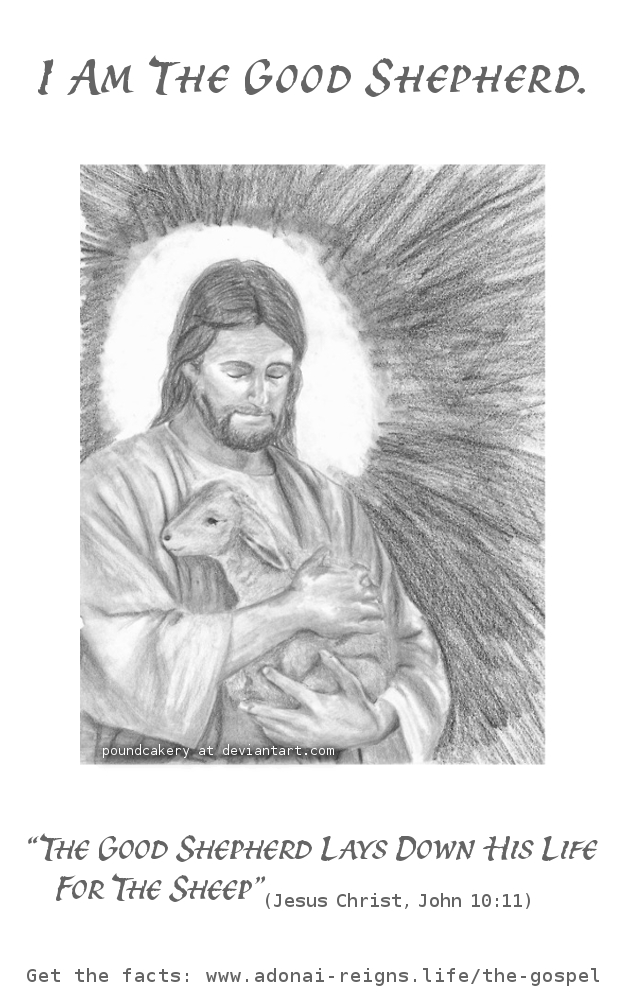
\includegraphics[width=126mm,height=192mm,keepaspectratio]{./leb/content/pictures/the_good_shepherd_by_poundcakery_d5hiu3j_deviantart.com.jpg}
%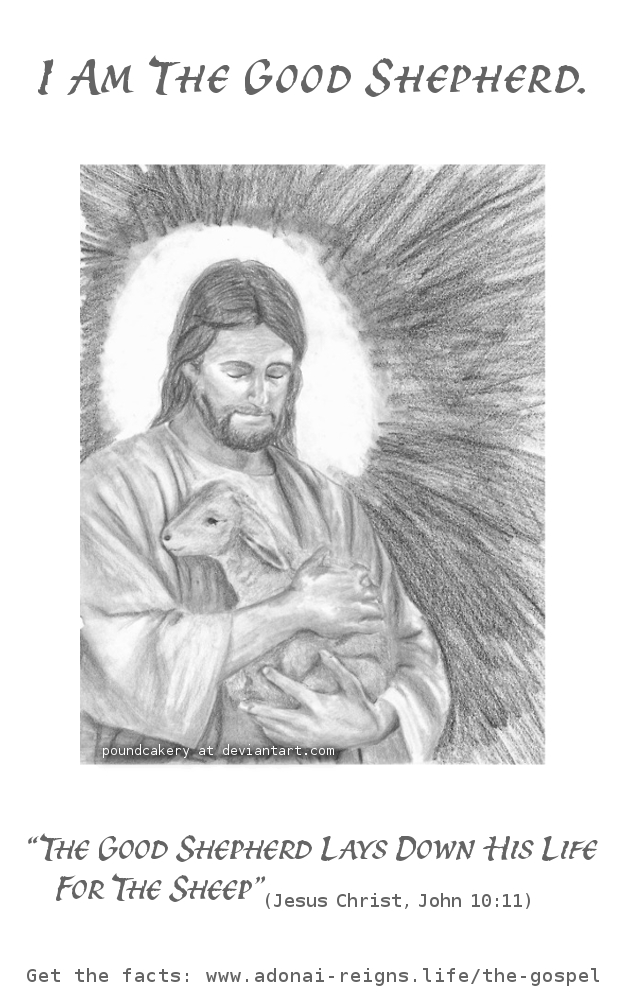
\includepdf{leb/content/pictures/the_good_shepherd_by_poundcakery_d5hiu3j_deviantart.com.jpg}
\end{center}
\end{titlingpage}








\begin{titlingpage}

\title{\Huge \headings{The Holy Bible}}
\date{}
\author{}


\setlrmarginsandblock{0.75in}{0.75in}{*}

\checkandfixthelayout 
\vspace*{\fill}
\begin{tikzpicture}[color=Gold,
    transform shape,
    every node/.style={inner sep=0pt}]
  \node[minimum size=\framesize,fill=Beige!10](vecbox){};
  \node[anchor=north west] at (vecbox.north west){%
    \pgfornament[width=0.2*\framesize]{131}};
  \node[anchor=north east] at (vecbox.north east){%
    \pgfornament[width=0.2*\framesize,symmetry=v]{131}};
  \node[anchor=south west] at (vecbox.south west){%
    \pgfornament[width=0.2*\framesize,symmetry=h]{131}};
  \node[anchor=south east] at (vecbox.south east){%
    \pgfornament[width=0.2*\framesize,symmetry=c]{131}};
  \node[anchor=north] at (vecbox.north){%
    \pgfornament[width=0.6*\framesize,symmetry=h]{85}};
  \node[anchor=south] at (vecbox.south){%
    \pgfornament[width=0.6*\framesize]{85}};
  \node[anchor=north,rotate=90] at (vecbox.west){%
    \pgfornament[width=0.6*\framesize,symmetry=h]{85}};
  \node[anchor=north,rotate=-90] at (vecbox.east){%
    \pgfornament[width=0.6*\framesize,symmetry=h]{85}};
  \node[inner sep=6pt, color=black] (text) at (vecbox.center){%
    \HUGE \textsc{\headings{The Holy Bible}}};
  \node[anchor=north, color=Goldenrod] (base) at (text.south){%
    \pgfornament[width=0.5*\framesize]{71}};
  \node[anchor=south, color=Goldenrod] at (text.north){%
    \pgfornament[width=0.5*\framesize,symmetry=h]{71}};
\end{tikzpicture}
\vspace*{\fill}
\end{titlingpage}




\onecolumn
\renewcommand{\contentsname}{\headings{Books of The Holy Bible}}


% toc font styles
\titlecontents{part}[3mm]{\normalsize\bfseries}{PART\space\thecontentslabel:\space\MakeUppercase}{}{\normalfont\dotfill\makebox[12mm][l]{\thecontentspage}}
\titlecontents{chapter}[3mm]{\vspace{-12pt}\normalsize}{}{}{\dotfill\makebox[12mm][l]{\thecontentspage}}


% some help from % https://tex.stackexchange.com/questions/389319/making-the-second-column-of-the-table-of-contents-clear-the-page-header
\makeatletter  
\singlespacing
\begingroup % start a TeX group
\color{colortoc}% or whatever color you wish to use
\chapter*{\contentsname
  \@mkboth{%
    \MakeUppercase\contentsname}{\MakeUppercase\contentsname}}
% If you want to turn off columns being forced to equal height, use the starred version \begin{multicols*}{2}.
\begin{multicols}{2}
\setlrmarginsandblock{0.8375in}{0.3125in}{*}
\checkandfixthelayout 
  \@starttoc{toc}
\end{multicols}
\endgroup   % end of TeX group
\makeatother


\twocolumn




% a blank page on the back of the page - lext page on a new right-sided page
\newpage
\thispagestyle{empty}
\mbox{}

\onecolumn
\vspace{8mm}

\customsection[Preface]{The Lexham English Bible\\\large Fourth Edition}

\vspace{12mm}

With approximately one hundred different English translations of the Bible already published, the reader may well wonder 
why yet another English version has been produced. Those actually engaged in the work of translating the Bible might 
answer that the quest for increased accuracy, the incorporation of new scholarly discoveries in the fields of semantics, 
lexicography, linguistics, new archaeological discoveries, and the continuing evolution of the English language all 
contribute to the need for producing new translations. But in the case of the Lexham English Bible (LEB), the answer to 
this question is much simpler; in fact, it is merely twofold.\par

First, the LEB achieves an unparalleled level of transparency with the original language text because the LEB had as 
its starting point the Lexham Hebrew-English Interlinear Bible and the Lexham Greek-English Interlinear New Testament. 
It was produced with the specific purpose of being used alongside the original language text of the Bible. Existing 
translations, however excellent they may be in terms of English style and idiom, are frequently so far removed from 
the original language texts of Scripture that straightforward comparison is difficult for the average user. Of course 
distance between the original language text and the English translation is not a criticism of any modern English 
translation. To a large extent this distance is the result of the philosophy of translation chosen for a particular 
English version, and it is almost always the result of an attempt to convey the meaning of the original in a clearer 
and more easily understandable way to the contemporary reader. However, there are many readers, particularly those 
who have studied some biblical Hebrew, Aramaic, or Greek, who desire a translation that facilitates straightforward 
and easy comparisons between the translation and the original language text. The ability to make such comparisons 
easily in software formats like Logos Bible Software makes the need for an English translation specifically designed 
for such comparison even more acute.\par

Second, the LEB is designed from the beginning to make extensive use of the most up-to-date lexical reference works 
available. For the Old Testament this is primarily The Hebrew and Aramaic Lexicon of the Old Testament (HALOT), and for 
New Testament this is primarily the third edition of Walter Bauer's A Greek-English Lexicon of the New Testament and 
Other Early Christian Literature (BDAG). Users can be assured that the LEB as a translation is based on the best scholarly 
research available. The Hebrew text on which the LEB Old Testament is based is that of \textbf{Biblia Hebraica Stuttgartensia}. 
The Greek text on which the LEB New Testament is based is that of The Greek New Testament: \textbf{SBL Edition (SBLGNT)}, a new 
edition produced by Michael W. Holmes in conjunction with the Society of Biblical Literature and Logos Bible Software. 
In its evaluation of textual variation, the SBLGNT uses modern text-critical methodology along with guidance from the 
most recently available articles, monographs, and technical commentaries to establish the text of the Greek New Testament.\par

Naturally, when these two factors are taken into consideration, it should not be surprising that the character of the LEB 
as a translation is fairly literal. This is a necessary by-product of the desire to have the English translation correspond 
transparently to the original language text. Nevertheless, a serious attempt has been made within these constraints to produce 
a clear and readable English translation instead of a woodenly literal one.\par

There are three areas in particular that need to be addressed to make a translation like the LEB more accessible to readers 
today, while at the same time maintaining easy comparison with the original language text. First, differences in word order 
have to be addressed. In this regard, the LEB follows standard English word order, not the word order of biblical Hebrew, 
Aramaic, or Koiné Greek. Anyone who needs to see the word order of the original languages can readily consult the Lexham 
Hebrew-English Interlinear Bible or the Lexham Greek-English Interlinear New Testament, which contain a sequence line which 
gives this information. Second, some expressions in biblical languages are idiomatic, so that a literal translation would 
be meaningless or would miscommunicate the true meaning. The LEB uses \lebnote{lower corner brackets} to indicate such expressions, 
with a literal rendering given in a note. Third, words which have no equivalent in the original language text must sometimes 
be supplied in the English translation. Because the LEB is designed to be used alongside the original language texts of 
Scripture, these supplied words are indicated with \textit{[italics]}. In some cases the need for such supplied words is obvious, 
but in other cases where it is less clear a note has been included.\par
Finally, the reader should remember that any Bible translation, to be useful to the person using it, must actually be read. 
We encourage every user of the LEB, whether reading it alongside the original languages text or not, to remember that once 
we understand the meaning of a biblical text we are responsible to apply it first in our own lives, and then to share it 
with those around us.\par

\textit{The Editors}

\textquote[Heb 4:12, LEB]{\textit{For the word of God is living and active and sharper than any double-edged sword, and piercing as far as the division 
of soul and spirit, both joints and marrow, and able to judge the reflections and thoughts of the heart.}}

\begin{multicols}{2}
\vspace{-\topsep}
\begin{itemize}
\setlength{\parskip}{0pt} \setlength{\itemsep}{0pt plus 1pt}
    \item W. Hall Harris III
    \item Elliot Ritzema
    \item Rick Brannan
    \item Douglas Mangum
    \item John Dunham
    \item Jeffrey A. Reimer
    \item Micah Wierenga
    \item Translators
    \item W. Hall Harris III
    \item Michael S. Heiser
    \item Jeremy Penner
    \item David M. Fouts
    \item Eugene E. Carpenter
    \item Gordon H. Johnston
    \item H. Daniel Zacharias
    \item William D. Barrick
    \item Michael A. Grisanti
    \item Chip McDaniel
    \item Israel Loken
    \item Ken M. Penner
    \item Dorian G. Coover-Cox
    \item Amy L. Pfeister
\end{itemize}

\vspace{-\topsep}

\end{multicols}

\subsection*{License}
You can give away the Lexham English Bible, but you can't sell it on its own. If the LEB comprises less than 25% of the 
content of a larger work, you can sell it as part of that work.
If you give away the LEB for use with a commercial product, or sell a work containing more than 1,000 verses from the LEB, 
you must annually report the number of units sold, distributed, and/or downloaded.
You must always attribute quotations of the LEB.
If you quote less than 100 verses of the LEB in a single work you can attribute it by simply adding (LEB) after the quotation. 
Longer quotations, or use of 100 or more verses in a single work, must be accompanied by the following statement:
Scripture quotations marked (LEB) are from the Lexham English Bible. Copyright 2012 Logos Bible Software. Lexham is a 
registered trademark of Logos Bible Software.
In electronic use, link "LEB" and "Lexham English Bible" to http://lexhamenglishbible.com, and "Logos Bible Software" 
to http://logos.com. If all quotations are unmarked and from the LEB, you may remove "marked (LEB) are" from the statement.
In support of non-English Bible translation, non-profit organizations may use 50% as the maximum portion the LEB may 
comprise of a work offered for sale. (This specifically allows the creation and commercial sale of diglot Bibles.)


\subsection*{Trademarks}
Lexham is a registered trademark of Logos Bible Software. You may use LEB or Lexham English Bible to refer to the 
Lexham English Bible, but may not use the Lexham trademark as any part of the name of a larger work quoting or containing it.

\vfill
\centering{%
\noindent\normalsize\textbf\textcopyright{\superscript} The Lexham English Bible, Fourth Edition, Copyright 2010, 2012\\
Logos Bible Software, 1313 Commercial St., Bellingham, WA 98225\\
\url{http://www.logos.com}{http://www.logos.com}
}
\clearpage
\twocolumn
\justify











\mainmatter


\setlrmarginsandblock{0.5625in}{0.3125in}{*}

% the book name, chapter and verse number at the top of the page
\setcolsepandrule{0.125in}{0pt}
\fancyhead[RO,LE]{\textbf{\headings{\Large \rightmark}}}
\fancyhfoffset[RO]{1pt}

\setlength\textwidth{5.125in}
\setlength\columnwidth{2.5in}
\setlength\columnsep{0.125in}
\checkandfixthelayout 


\part*{\headings{The Old Testament}}

% a blank page on the back of the page - next page on a new right-sided page
\clearpage
\newpage
\thispagestyle{empty}
\mbox{}
\endpage
\newpage



\endpage
\newpage


% Declare our footnote values for use with the fixfoot package
%\DeclareFixedFootnote{\lnAAA}{Or “And”}%
\DeclareFixedFootnote{\lnAAB}{Or “expanse”}%
\DeclareFixedFootnote{\lnAAH}{Or “the sky”}%
\DeclareFixedFootnote{\lnAAI}{“which its seed is in it”}%
\DeclareFixedFootnote{\lnAAJ}{Or “their”}%
\DeclareFixedFootnote{\lnAAN}{Or “light sources”}%
\DeclareFixedFootnote{\lnAAU}{Or “light source”}%
\DeclareFixedFootnote{\lnAAV}{“as the authority of”}%
\DeclareFixedFootnote{\lnABE}{“animals of the earth/land”}%
\DeclareFixedFootnote{\lnABI}{Or “as”}%
\DeclareFixedFootnote{\lnABR}{Or “the earth”}%
\DeclareFixedFootnote{\lnABS}{Or “family records”}%
\DeclareFixedFootnote{\lnABV}{Or “and”}%
\DeclareFixedFootnote{\lnABW}{“The man” indicates the noun is singular and occurs with the definite article}%
\DeclareFixedFootnote{\lnACE}{“as his opposite”}%
\DeclareFixedFootnote{\lnACX}{Or “said”}%
\DeclareFixedFootnote{\lnADE}{The noun lacks the definite article and is taken as a proper noun in this context}%
\DeclareFixedFootnote{\lnADQ}{“On the day”}%
\DeclareFixedFootnote{\lnADR}{Or “humankind”}%
\DeclareFixedFootnote{\lnAEG}{Or “its”}%
\DeclareFixedFootnote{\lnAEK}{“seven, seven”}%
\DeclareFixedFootnote{\lnAEO}{“two, two”}%
\DeclareFixedFootnote{\lnAEY}{Or “the”}%
\DeclareFixedFootnote{\lnAFK}{Or “sons”}%
\DeclareFixedFootnote{\lnAFM}{“in your going”}%
\DeclareFixedFootnote{\lnAGE}{In context, the enemy}%
\DeclareFixedFootnote{\lnAGI}{“brother”}%
\DeclareFixedFootnote{\lnAGK}{“was”}%
\DeclareFixedFootnote{\lnAGM}{Some nation hostile to Abram’s descendants (Egypt in later history)}%
\DeclareFixedFootnote{\lnAGP}{Or “fathers”}%
\DeclareFixedFootnote{\lnAGQ}{“cut”}%
\DeclareFixedFootnote{\lnAGT}{That is, Hagar}%
\DeclareFixedFootnote{\lnAGY}{“with very very”}%
\DeclareFixedFootnote{\lnAHA}{Or “between”}%
\DeclareFixedFootnote{\lnAHB}{“those born of house and acquisition of money from every son of a foreigner”}%
\DeclareFixedFootnote{\lnAHD}{Or “be”}%
\DeclareFixedFootnote{\lnAHI}{“a son of cattle”}%
\DeclareFixedFootnote{\lnAHK}{Adonai}%
\DeclareFixedFootnote{\lnAHL}{“at the time of life”}%
\DeclareFixedFootnote{\lnAHP}{“heavy”}%
\DeclareFixedFootnote{\lnAHR}{Or “Perhaps”}%
\DeclareFixedFootnote{\lnAHV}{Hebrew idiom for sexual intercourse (cp. Gen 4:1)}%
\DeclareFixedFootnote{\lnAHY}{“that we might preserve offspring from our father”}%
\DeclareFixedFootnote{\lnAIA}{“sons/children of Ammon”}%
\DeclareFixedFootnote{\lnAIB}{Or “voice”}%
\DeclareFixedFootnote{\lnAIF}{Or “that”}%
\DeclareFixedFootnote{\lnAIG}{Or “sons of Heth”}%
\DeclareFixedFootnote{\lnAIH}{“ownership of a grave”}%
\DeclareFixedFootnote{\lnAIK}{Or “give”}%
\DeclareFixedFootnote{\lnAIQ}{“went up”}%
\DeclareFixedFootnote{\lnAIV}{“to go after”}%
\DeclareFixedFootnote{\lnAIZ}{“went after”}%
\DeclareFixedFootnote{\lnAJD}{Or “upon the face of”}%
\DeclareFixedFootnote{\lnAJH}{“a son of sixty years”}%
\DeclareFixedFootnote{\lnAJJ}{“as the day”}%
\DeclareFixedFootnote{\lnAJL}{Or “called”}%
\DeclareFixedFootnote{\lnAJP}{That is, Esau}%
\DeclareFixedFootnote{\lnAJQ}{“are you this one?”}%
\DeclareFixedFootnote{\lnAJS}{Or “daughters of the Hittites”}%
\DeclareFixedFootnote{\lnAJV}{Or “it”}%
\DeclareFixedFootnote{\lnAJW}{“before the eyes of”}%
\DeclareFixedFootnote{\lnAJX}{That is, Jacob}%
\DeclareFixedFootnote{\lnAJZ}{“watch to yourself”}%
\DeclareFixedFootnote{\lnAKF}{Hebrew for “the heap of witness”}%
\DeclareFixedFootnote{\lnAKH}{Or “food, bread”}%
\DeclareFixedFootnote{\lnAKK}{That is, the man}%
\DeclareFixedFootnote{\lnAKM}{“sons/children of Israel”}%
\DeclareFixedFootnote{\lnAKP}{“There is to me abundance”}%
\DeclareFixedFootnote{\lnAKS}{Or “foot”}%
\DeclareFixedFootnote{\lnAKW}{“they added still to hate him”}%
\DeclareFixedFootnote{\lnAKY}{That is, Judah}%
\DeclareFixedFootnote{\lnAKZ}{“beautiful of appearance and healthy of flesh”}%
\DeclareFixedFootnote{\lnALA}{“Poor of appearance and thin of flesh”}%
\DeclareFixedFootnote{\lnALE}{That is, Pharaoh}%
\DeclareFixedFootnote{\lnALI}{Or “inner parts”}%
\DeclareFixedFootnote{\lnALK}{“a son of thirty years”}%
\DeclareFixedFootnote{\lnALU}{Or “son”}%
\DeclareFixedFootnote{\lnALX}{“house”}%
\DeclareFixedFootnote{\lnAMA}{“burdens” or “burdensome labor”}%
\DeclareFixedFootnote{\lnAMD}{“houses”}%
\DeclareFixedFootnote{\lnAMI}{Hebrew “Canaanite”}%
\DeclareFixedFootnote{\lnAMJ}{Hebrew “Hittite”}%
\DeclareFixedFootnote{\lnAMK}{Hebrew “Amorite”}%
\DeclareFixedFootnote{\lnAML}{Hebrew “Perizzite”}%
\DeclareFixedFootnote{\lnAMM}{Hebrew “Hivite”}%
\DeclareFixedFootnote{\lnANB}{“and he/it will be”}%
\DeclareFixedFootnote{\lnAND}{“look” or “behold”}%
\DeclareFixedFootnote{\lnANM}{“yesterday three days ago”}%
\DeclareFixedFootnote{\lnAOA}{“the house of their fathers”}%
\DeclareFixedFootnote{\lnAOB}{Or “generations”}%
\DeclareFixedFootnote{\lnAOC}{“seven and thirty and hundred of year”}%
\DeclareFixedFootnote{\lnAOF}{“fathers”}%
\DeclareFixedFootnote{\lnAOS}{“look”}%
\DeclareFixedFootnote{\lnAOZ}{“sea of reed”}%
\DeclareFixedFootnote{\lnAPE}{“a man for the mouth of his eating”}%
\DeclareFixedFootnote{\lnAPF}{“between the evenings”}%
\DeclareFixedFootnote{\lnAPG}{Or “summons,” “convocation”}%
\DeclareFixedFootnote{\lnAPI}{“and it will be”}%
\DeclareFixedFootnote{\lnAPJ}{“service” or “work”}%
\DeclareFixedFootnote{\lnAPW}{Hebrew “human”}%
\DeclareFixedFootnote{\lnAPX}{Hebrew “animal”}%
\DeclareFixedFootnote{\lnAQG}{Hebrew “he”}%
\DeclareFixedFootnote{\lnAQS}{Or “power”}%
\DeclareFixedFootnote{\lnAQW}{Hebrew “wonder”}%
\DeclareFixedFootnote{\lnAQX}{Hebrew “horse”}%
\DeclareFixedFootnote{\lnAQY}{Hebrew “chariot”}%
\DeclareFixedFootnote{\lnARF}{“at/in his hearing”}%
\DeclareFixedFootnote{\lnARR}{“men”}%
\DeclareFixedFootnote{\lnARS}{Plural}%
\DeclareFixedFootnote{\lnARW}{“and it would be”}%
\DeclareFixedFootnote{\lnARX}{“And it was”}%
\DeclareFixedFootnote{\lnASG}{Or “many” or “the many”}%
\DeclareFixedFootnote{\lnASW}{“from end from this”}%
\DeclareFixedFootnote{\lnATA}{“a woman to her sister”}%
\DeclareFixedFootnote{\lnATE}{“from this”}%
\DeclareFixedFootnote{\lnATG}{“from this and from this”}%
\DeclareFixedFootnote{\lnATH}{Or “boards” or “planks”}%
\DeclareFixedFootnote{\lnATI}{“standing”}%
\DeclareFixedFootnote{\lnATJ}{Or “board” or “plank”}%
\DeclareFixedFootnote{\lnATL}{“hands”}%
\DeclareFixedFootnote{\lnATU}{“one”}%
\DeclareFixedFootnote{\lnAUB}{Or “westward,” literally “seaward,” toward the Mediterranean Sea}%
\DeclareFixedFootnote{\lnAUP}{“holy place of the holiness”}%
\DeclareFixedFootnote{\lnAUR}{“from it”}%
\DeclareFixedFootnote{\lnAUS}{Or “side,” referring to the span on one side of the courtyard’s entry}%
\DeclareFixedFootnote{\lnAUZ}{Or “garments of holiness”}%
\DeclareFixedFootnote{\lnAVJ}{“lifted up”}%
\DeclareFixedFootnote{\lnAVM}{“sons of a year”}%
\DeclareFixedFootnote{\lnAVT}{“in the morning in the morning”}%
\DeclareFixedFootnote{\lnAVU}{“between the two evenings”}%
\DeclareFixedFootnote{\lnAVW}{“all of the going over to the being counted”}%
\DeclareFixedFootnote{\lnAVY}{“a son of twenty years”}%
\DeclareFixedFootnote{\lnAWC}{Or “recipe” or “formula”}%
\DeclareFixedFootnote{\lnAXK}{“by the hand of”}%
\DeclareFixedFootnote{\lnAXP}{“one to one”}%
\DeclareFixedFootnote{\lnAZW}{Or “vessels” or “utensils” or “contents”}%
\DeclareFixedFootnote{\lnBAC}{Or “herd”}%
\DeclareFixedFootnote{\lnBAD}{The Hebrew term refers collectively to both sheep and goats (small livestock animals)}%
\DeclareFixedFootnote{\lnBAF}{“to the face of”}%
\DeclareFixedFootnote{\lnBAG}{Or “And he”}%
\DeclareFixedFootnote{\lnBAN}{Or “entrails”}%
\DeclareFixedFootnote{\lnBAV}{Or “And the priest”}%
\DeclareFixedFootnote{\lnBAZ}{Or “a soul”}%
\DeclareFixedFootnote{\lnBBB}{“a holiness of holinesses”}%
\DeclareFixedFootnote{\lnBBC}{Hebrew “of”}%
\DeclareFixedFootnote{\lnBBD}{Hebrew “the”}%
\DeclareFixedFootnote{\lnBBH}{Or “And he shall present”}%
\DeclareFixedFootnote{\lnBBK}{Or “and the two kidneys”}%
\DeclareFixedFootnote{\lnBCC}{“sinned”}%
\DeclareFixedFootnote{\lnBCD}{“a bull, a son of cattle”}%
\DeclareFixedFootnote{\lnBCE}{Or “And he shall bring”}%
\DeclareFixedFootnote{\lnBCF}{“from”}%
\DeclareFixedFootnote{\lnBCS}{Or “from”}%
\DeclareFixedFootnote{\lnBCU}{Indicated by the context}%
\DeclareFixedFootnote{\lnBCV}{“as that”}%
\DeclareFixedFootnote{\lnBDB}{Or “And he shall place”}%
\DeclareFixedFootnote{\lnBDE}{Indicated by context}%
\DeclareFixedFootnote{\lnBDW}{Or “for”}%
\DeclareFixedFootnote{\lnBED}{“it is concealed from him”}%
\DeclareFixedFootnote{\lnBEE}{“for” or “to” (see HALOT 510)}%
\DeclareFixedFootnote{\lnBEM}{“for one of”}%
\DeclareFixedFootnote{\lnBER}{Hebrew “from”}%
\DeclareFixedFootnote{\lnBES}{“sons of dove” or “children of dove”}%
\DeclareFixedFootnote{\lnBFT}{“in”}%
\DeclareFixedFootnote{\lnBFU}{“in accordance with deception”}%
\DeclareFixedFootnote{\lnBGB}{“to the faces of”}%
\DeclareFixedFootnote{\lnBGG}{Antecedent for this 3fs suffix is “fire” (“altar” is ms)}%
\DeclareFixedFootnote{\lnBGQ}{Singular masculine}%
\DeclareFixedFootnote{\lnBHF}{“for him it shall be” or “it will become his”}%
\DeclareFixedFootnote{\lnBHK}{Implied by v. 12}%
\DeclareFixedFootnote{\lnBHP}{Or “soul”}%
\DeclareFixedFootnote{\lnBHQ}{Or “the soul”}%
\DeclareFixedFootnote{\lnBIQ}{Or “of”}%
\DeclareFixedFootnote{\lnBIW}{Or “he tied”}%
\DeclareFixedFootnote{\lnBIY}{Or “he put”}%
\DeclareFixedFootnote{\lnBJK}{Or “to”}%
\DeclareFixedFootnote{\lnBLF}{An adjective in masculine plural to modify both animals; see NET}%
\DeclareFixedFootnote{\lnBLI}{Singular}%
\DeclareFixedFootnote{\lnBLW}{“do” or “make”}%
\DeclareFixedFootnote{\lnBMS}{“from to the faces of”}%
\DeclareFixedFootnote{\lnBOM}{Implied by context}%
\DeclareFixedFootnote{\lnBOO}{“from their dead body”}%
\DeclareFixedFootnote{\lnBPD}{Or “daughter”}%
\DeclareFixedFootnote{\lnBPF}{“a son of his year”}%
\DeclareFixedFootnote{\lnBPN}{“man”}%
\DeclareFixedFootnote{\lnBPX}{The direct object is supplied from context in the English translation}%
\DeclareFixedFootnote{\lnBQH}{“living flesh”}%
\DeclareFixedFootnote{\lnBQO}{“white red”}%
\DeclareFixedFootnote{\lnBSI}{Perhaps better translated “mold” rather than “skin disease”}%
\DeclareFixedFootnote{\lnBSR}{“he”}%
\DeclareFixedFootnote{\lnBTH}{“wood of cedar”}%
\DeclareFixedFootnote{\lnBTL}{“the crimson thread of the worm”}%
\DeclareFixedFootnote{\lnBUN}{“his hand can produce”}%
\DeclareFixedFootnote{\lnBVK}{“after thus”}%
\DeclareFixedFootnote{\lnBVP}{“to from an outside place of the city”}%
\DeclareFixedFootnote{\lnBVT}{See HALOT 862 s.v. 3.b}%
\DeclareFixedFootnote{\lnBWB}{Implied by the context; or “plaster”}%
\DeclareFixedFootnote{\lnBWJ}{That is, the priest}%
\DeclareFixedFootnote{\lnBWZ}{“a man a man”}%
\DeclareFixedFootnote{\lnBXA}{Or “bathe”}%
\DeclareFixedFootnote{\lnBYR}{“from the interior/inside of”}%
\DeclareFixedFootnote{\lnBYY}{Hebrew “to”}%
\DeclareFixedFootnote{\lnBZN}{“a statute of eternity” or “a statute of long duration”}%
\DeclareFixedFootnote{\lnCAA}{“to”}%
\DeclareFixedFootnote{\lnCAH}{Or “Because”}%
\DeclareFixedFootnote{\lnCAI}{“Unto thus”}%
\DeclareFixedFootnote{\lnCBA}{“do”}%
\DeclareFixedFootnote{\lnCBD}{Or “keep”}%
\DeclareFixedFootnote{\lnCBG}{“approach”}%
\DeclareFixedFootnote{\lnCBH}{The verb לקח is used to speak of marrying (“taking a wife”)}%
\DeclareFixedFootnote{\lnCBS}{“to the faces of you”}%
\DeclareFixedFootnote{\lnCGS}{“the name of my holiness”}%
\DeclareFixedFootnote{\lnCHL}{“from your faces”}%
\DeclareFixedFootnote{\lnCHR}{“take”}%
\DeclareFixedFootnote{\lnCIY}{“for acceptance”}%
\DeclareFixedFootnote{\lnCIZ}{Or “among”}%
\DeclareFixedFootnote{\lnCJQ}{“all work of labor”}%
\DeclareFixedFootnote{\lnCJW}{“from the next day of”}%
\DeclareFixedFootnote{\lnCJX}{“a son of its year”}%
\DeclareFixedFootnote{\lnCJY}{Supplied by context}%
\DeclareFixedFootnote{\lnCKB}{“the exactly of this day”}%
\DeclareFixedFootnote{\lnCLN}{“from to alone”}%
\DeclareFixedFootnote{\lnCMP}{“gives”}%
\DeclareFixedFootnote{\lnCNB}{Singular throughout this verse}%
\DeclareFixedFootnote{\lnCNL}{Plural throughout this verse}%
\DeclareFixedFootnote{\lnCNS}{“a man his brother”}%
\DeclareFixedFootnote{\lnCOC}{“with confidence”}%
\DeclareFixedFootnote{\lnCOX}{Meaning derived from context; an alternative translation could be “shall not be released” (cf. NKJV, NRSV, ESV, NJPS) or “shall not revert” (NASB, NET)}%
\DeclareFixedFootnote{\lnCPM}{Or “brother”}%
\DeclareFixedFootnote{\lnCPV}{“to you”}%
\DeclareFixedFootnote{\lnCQN}{Or “children”}%
\DeclareFixedFootnote{\lnCQS}{Or “brothers”}%
\DeclareFixedFootnote{\lnCRJ}{“to your faces”}%
\DeclareFixedFootnote{\lnCRX}{Emphatic personal pronoun}%
\DeclareFixedFootnote{\lnCSU}{Or “and up to”}%
\DeclareFixedFootnote{\lnCSZ}{“a son of five years”}%
\DeclareFixedFootnote{\lnCTP}{“between good and between bad”}%
\DeclareFixedFootnote{\lnCUO}{Or “fathers’ ”}%
\DeclareFixedFootnote{\lnCVO}{Or “counted,” or “summoned,” or “enrolled”}%
\DeclareFixedFootnote{\lnCVU}{Or “count,” or “summon,” or “enroll”}%
\DeclareFixedFootnote{\lnCVX}{Other modern translations read “tabernacle of the covenant”}%
\DeclareFixedFootnote{\lnCWF}{“the ones counted of them,” or “the ones mustered of them”}%
\DeclareFixedFootnote{\lnCWG}{“the ones counted of him,” or “the ones mustered of him”}%
\DeclareFixedFootnote{\lnCWV}{“before the face of Adonai”}%
\DeclareFixedFootnote{\lnCXD}{“the son of a month”}%
\DeclareFixedFootnote{\lnCXF}{“mouth of Adonai”}%
\DeclareFixedFootnote{\lnCXI}{Hebrew “Kohathite”}%
\DeclareFixedFootnote{\lnCXO}{“the mouth of Adonai”}%
\DeclareFixedFootnote{\lnCYC}{“mouth”}%
\DeclareFixedFootnote{\lnCYH}{“a son of fifty years”}%
\DeclareFixedFootnote{\lnCYJ}{“the hide of a sea cow”}%
\DeclareFixedFootnote{\lnCYX}{Hebrew “Gershonite”}%
\DeclareFixedFootnote{\lnCZB}{“the mouth”}%
\DeclareFixedFootnote{\lnCZE}{“in the hand”}%
\DeclareFixedFootnote{\lnCZU}{Or “through Moses”}%
\DeclareFixedFootnote{\lnDAT}{Hebrew “his”}%
\DeclareFixedFootnote{\lnDAW}{“to an outside place of the camp”}%
\DeclareFixedFootnote{\lnDBF}{“before the face of”}%
\DeclareFixedFootnote{\lnDBH}{Or “waste away”}%
\DeclareFixedFootnote{\lnDBM}{That is, “the Nazirite”}%
\DeclareFixedFootnote{\lnDBS}{“the head of his separation”}%
\DeclareFixedFootnote{\lnDBV}{Hebrew “it”}%
\DeclareFixedFootnote{\lnDCB}{“according to the mouth of their work”}%
\DeclareFixedFootnote{\lnDCF}{“in the presence of”}%
\DeclareFixedFootnote{\lnDCG}{“the two of them”}%
\DeclareFixedFootnote{\lnDCH}{“the son of its year”}%
\DeclareFixedFootnote{\lnDCJ}{Hebrew “shekel”}%
\DeclareFixedFootnote{\lnDCR}{“one dish of ten gold”}%
\DeclareFixedFootnote{\lnDFM}{“in the presence of Adonai”}%
\DeclareFixedFootnote{\lnDFO}{“Aaron will wave”}%
\DeclareFixedFootnote{\lnDGP}{“by a life of a person”}%
\DeclareFixedFootnote{\lnDHC}{“it was there”}%
\DeclareFixedFootnote{\lnDIA}{“his nose became hot”}%
\DeclareFixedFootnote{\lnDIC}{Hebrew “its”}%
\DeclareFixedFootnote{\lnDID}{Hebrew “him/it”}%
\DeclareFixedFootnote{\lnDIG}{Hebrew “the graves of greediness”}%
\DeclareFixedFootnote{\lnDIK}{An arid region south of the Judean hills}%
\DeclareFixedFootnote{\lnDIM}{Or “wadi”}%
\DeclareFixedFootnote{\lnDIP}{Hebrew “day”}%
\DeclareFixedFootnote{\lnDJA}{Hebrew “him”}%
\DeclareFixedFootnote{\lnDJI}{“declaration of”}%
\DeclareFixedFootnote{\lnDJK}{Hebrew “year”}%
\DeclareFixedFootnote{\lnDJQ}{Hebrew “Amalekite”}%
\DeclareFixedFootnote{\lnDJW}{Hebrew “for your generations”}%
\DeclareFixedFootnote{\lnDKO}{Hebrew “We will not come up!”}%
\DeclareFixedFootnote{\lnDLA}{Or “the statute”}%
\DeclareFixedFootnote{\lnDLR}{“you will raise up”}%
\DeclareFixedFootnote{\lnDMG}{Hebrew “me”}%
\DeclareFixedFootnote{\lnDMO}{Hebrew “And it will happen”}%
\DeclareFixedFootnote{\lnDMU}{“sons of Ammon”}%
\DeclareFixedFootnote{\lnDMX}{Hebrew “her daughters;” other modern versions translate “its villages”}%
\DeclareFixedFootnote{\lnDNH}{That is, the Euphrates}%
\DeclareFixedFootnote{\lnDNI}{“the eye of the land”}%
\DeclareFixedFootnote{\lnDNS}{Hebrew “He”}%
\DeclareFixedFootnote{\lnDNX}{That is, Israel}%
\DeclareFixedFootnote{\lnDNZ}{Often translated “the Almighty”}%
\DeclareFixedFootnote{\lnADC}{“seed”}%
\DeclareFixedFootnote{\lnDOQ}{Or “the father’s house” or “the ancestor’s house”}%
\DeclareFixedFootnote{\lnDOX}{Hebrew “Reubenite”}%
\DeclareFixedFootnote{\lnDPA}{Hebrew “Zerahite”}%
\DeclareFixedFootnote{\lnDPY}{Hebrew “His”}%
\DeclareFixedFootnote{\lnDQG}{Or “meeting”}%
\DeclareFixedFootnote{\lnDQK}{“his word”}%
\DeclareFixedFootnote{\lnDQU}{“you will not do work of labor”}%
\DeclareFixedFootnote{\lnDRU}{“who has known the bed of a male”}%
\DeclareFixedFootnote{\lnDSD}{Hebrew “person”}%
\DeclareFixedFootnote{\lnDST}{“Adonai’s nose became hot”}%
\DeclareFixedFootnote{\lnDUH}{That is, the Dead Sea}%
\DeclareFixedFootnote{\lnDUI}{That is, the Mediterranean}%
\DeclareFixedFootnote{\lnDUO}{Hebrew “Gadite”}%
\DeclareFixedFootnote{\lnDWA}{“in the beyond of”}%
\DeclareFixedFootnote{\lnDWC}{Or “dwelling,” and in this context “reigning”}%
\DeclareFixedFootnote{\lnDWF}{Hebrew \textit{torah}}%
\DeclareFixedFootnote{\lnDWG}{“to say”}%
\DeclareFixedFootnote{\lnDWJ}{Or “peoples”}%
\DeclareFixedFootnote{\lnDWR}{“a word”}%
\DeclareFixedFootnote{\lnDWS}{A valley that is dry most of the year, but contains a stream during the rainy season}%
\DeclareFixedFootnote{\lnDXH}{Or “wilderness”}%
\DeclareFixedFootnote{\lnDXN}{“And it happened”}%
\DeclareFixedFootnote{\lnDXP}{“the day”}%
\DeclareFixedFootnote{\lnDXQ}{“the sons/children of Ammon”}%
\DeclareFixedFootnote{\lnDXW}{“to the face of you”}%
\DeclareFixedFootnote{\lnDXX}{“before us”}%
\DeclareFixedFootnote{\lnDYB}{Or “people”}%
\DeclareFixedFootnote{\lnDZA}{Hebrew “and”}%
\DeclareFixedFootnote{\lnDZL}{“at their going out from Egypt”}%
\DeclareFixedFootnote{\lnDZT}{“the day of the Sabbath”}%
\DeclareFixedFootnote{\lnDZU}{“gates”}%
\DeclareFixedFootnote{\lnDZX}{“all the days”}%
\DeclareFixedFootnote{\lnDZZ}{“spoke”}%
\DeclareFixedFootnote{\lnEAA}{Or “mind”}%
\DeclareFixedFootnote{\lnEAT}{“to their faces”}%
\DeclareFixedFootnote{\lnEAX}{“And it will happen”}%
\DeclareFixedFootnote{\lnEBV}{Hebrew “night”}%
\DeclareFixedFootnote{\lnECQ}{Hebrew “creature”}%
\DeclareFixedFootnote{\lnEDI}{“the face of”}%
\DeclareFixedFootnote{\lnEDR}{“from the face of you”}%
\DeclareFixedFootnote{\lnEEI}{“that your soul/inner self desires”}%
\DeclareFixedFootnote{\lnEEZ}{“in addition to” or “upon it”}%
\DeclareFixedFootnote{\lnEFE}{Hebrew “for you”}%
\DeclareFixedFootnote{\lnEFH}{Hebrew “for/to you” but with collective meaning}%
\DeclareFixedFootnote{\lnEFU}{Hebrew “firstfruit”}%
\DeclareFixedFootnote{\lnEGD}{“from yesterday and the day before”}%
\DeclareFixedFootnote{\lnEGS}{“a man other”}%
\DeclareFixedFootnote{\lnEHO}{“on”}%
\DeclareFixedFootnote{\lnEHV}{“to him”}%
\DeclareFixedFootnote{\lnEHX}{“until eternity”}%
\DeclareFixedFootnote{\lnEHY}{“because of the event when”}%
\DeclareFixedFootnote{\lnEIF}{Or “If”}%
\DeclareFixedFootnote{\lnEIR}{That is, what is left}%
\DeclareFixedFootnote{\lnEIV}{“for you”}%
\DeclareFixedFootnote{\lnEJC}{Or “father”}%
\DeclareFixedFootnote{\lnEJY}{Or “way”}%
\DeclareFixedFootnote{\lnENR}{Hebrew “it” but used poetically and with plural sense in context}%
\DeclareFixedFootnote{\lnENT}{Hebrew “head”}%
\DeclareFixedFootnote{\lnEOV}{“in all that you go”}%
\DeclareFixedFootnote{\lnEOY}{Hebrew “heart”}%
\DeclareFixedFootnote{\lnEPA}{“before the presence of the people”}%
\DeclareFixedFootnote{\lnEPD}{Or “world”}%
\DeclareFixedFootnote{\lnEPV}{“on the road”}%
\DeclareFixedFootnote{\lnEQB}{“this”}%
\DeclareFixedFootnote{\lnEQF}{Hebrew “thing” or “consecrated possession”}%
\DeclareFixedFootnote{\lnEQS}{Hebrew “trouble”; a valley in the Jericho region}%
\DeclareFixedFootnote{\lnEQV}{“all the people of war”}%
\DeclareFixedFootnote{\lnEQX}{“as that at the first occasion”}%
\DeclareFixedFootnote{\lnEQY}{Or “before their presence”}%
\DeclareFixedFootnote{\lnERB}{A dry region that runs south of the Sea of Galilee along the Jordan Valley}%
\DeclareFixedFootnote{\lnERD}{“the mouth of the sword”}%
\DeclareFixedFootnote{\lnERI}{Or “lowlands”; a geographical region on the western edge of the hills of Judea}%
\DeclareFixedFootnote{\lnERO}{“cut for us a covenant”}%
\DeclareFixedFootnote{\lnERR}{Or “men”}%
\DeclareFixedFootnote{\lnESL}{An arid region south of the Judaean hills}%
\DeclareFixedFootnote{\lnETA}{Or “white mountain”}%
\DeclareFixedFootnote{\lnETK}{Hebrew “Geshurite”}%
\DeclareFixedFootnote{\lnETL}{Hebrew “Maacathite”}%
\DeclareFixedFootnote{\lnEUV}{Hebrew “bank”}%
\DeclareFixedFootnote{\lnEVL}{Hebrew “goes out”}%
\DeclareFixedFootnote{\lnEVO}{Or “end”}%
\DeclareFixedFootnote{\lnEWF}{“the goings out of it were”}%
\DeclareFixedFootnote{\lnEXL}{Or “in the presence of”}%
\DeclareFixedFootnote{\lnEYK}{“came out”}%
\DeclareFixedFootnote{\lnFAR}{Hebrew “offering”}%
\DeclareFixedFootnote{\lnFAV}{Hebrew “sacrifice”}%
\DeclareFixedFootnote{\lnFCA}{Or “dwell”}%
\DeclareFixedFootnote{\lnFCQ}{Or “sons/children”}%
\DeclareFixedFootnote{\lnFDD}{Hebrew “inhabitant”}%
\DeclareFixedFootnote{\lnFDW}{Or “judges”}%
\DeclareFixedFootnote{\lnFEA}{Or “judge”}%
\DeclareFixedFootnote{\lnFFP}{Or “you”}%
\DeclareFixedFootnote{\lnFFU}{Hebrew “Midianite”}%
\DeclareFixedFootnote{\lnFGI}{An Asherah is a cultic pole set up next to an altar symbolizing the goddess Asherah}%
\DeclareFixedFootnote{\lnFGN}{“ears”}%
\DeclareFixedFootnote{\lnFGQ}{Or “divisions”}%
\DeclareFixedFootnote{\lnFGU}{Or “camp”}%
\DeclareFixedFootnote{\lnFGY}{Or “hand”}%
\DeclareFixedFootnote{\lnFHD}{Or “house”}%
\DeclareFixedFootnote{\lnFHE}{Or “honesty”}%
\DeclareFixedFootnote{\lnFHK}{Or “companies”}%
\DeclareFixedFootnote{\lnFHO}{Or “cellar”}%
\DeclareFixedFootnote{\lnFHR}{Or “evil”}%
\DeclareFixedFootnote{\lnFIM}{“to make war”}%
\DeclareFixedFootnote{\lnFJT}{“kid of goat”}%
\DeclareFixedFootnote{\lnFJX}{Hebrew “man”}%
\DeclareFixedFootnote{\lnFJZ}{Or “temple”}%
\DeclareFixedFootnote{\lnFKD}{Hebrew “piece”}%
\DeclareFixedFootnote{\lnFKI}{Or “alien”}%
\DeclareFixedFootnote{\lnFKY}{“and let your heart be good”}%
\DeclareFixedFootnote{\lnFLS}{“men drawing sword”}%
\DeclareFixedFootnote{\lnFMA}{Hebrew “my brother”}%
\DeclareFixedFootnote{\lnFMR}{Hebrew “place”}%
\DeclareFixedFootnote{\lnFMT}{“touching”}%
\DeclareFixedFootnote{\lnFNA}{“men of strength”}%
\DeclareFixedFootnote{\lnFNR}{“the life of Adonai”}%
\DeclareFixedFootnote{\lnFNX}{“the declaration of”}%
\DeclareFixedFootnote{\lnFOA}{“arm,” figurative of “strength” in the context of “descendants”}%
\DeclareFixedFootnote{\lnFOH}{“the”}%
\DeclareFixedFootnote{\lnFOJ}{Or “taken”}%
\DeclareFixedFootnote{\lnFOL}{“bowed down”}%
\DeclareFixedFootnote{\lnFOR}{The Masoretic Hebrew text (\textit{Kethib}) reads “boils”; the reading tradition (\textit{Qere}) has “tumors”}%
\DeclareFixedFootnote{\lnFOW}{Or perhaps “chest” or “bag”}%
\DeclareFixedFootnote{\lnFPF}{Or “to rule”}%
\DeclareFixedFootnote{\lnFPN}{“sons of wickedness”}%
\DeclareFixedFootnote{\lnFQC}{“the young man carrying his weapons”}%
\DeclareFixedFootnote{\lnFQD}{“from the beyond from this”}%
\DeclareFixedFootnote{\lnFQG}{“the one carrying his weapons”}%
\DeclareFixedFootnote{\lnFQM}{“and look”}%
\DeclareFixedFootnote{\lnFQQ}{Hebrew “And”}%
\DeclareFixedFootnote{\lnFQS}{“opposite one”}%
\DeclareFixedFootnote{\lnFQY}{“so that I can bow down to”}%
\DeclareFixedFootnote{\lnFQZ}{That is, Saul}%
\DeclareFixedFootnote{\lnFRG}{“was good in the eyes of”}%
\DeclareFixedFootnote{\lnFRT}{Or “boy”}%
\DeclareFixedFootnote{\lnFRU}{Or possibly “equipment” or “weapons”}%
\DeclareFixedFootnote{\lnFSA}{“from the side of the mountain from this”}%
\DeclareFixedFootnote{\lnFSM}{“and”}%
\DeclareFixedFootnote{\lnFSP}{“The life of Adonai”}%
\DeclareFixedFootnote{\lnFST}{Or “necromancers”}%
\DeclareFixedFootnote{\lnFSW}{“face”}%
\DeclareFixedFootnote{\lnFTC}{“but if”}%
\DeclareFixedFootnote{\lnFTF}{“Look”}%
\DeclareFixedFootnote{\lnFTG}{“the carrier of his weapons”}%
\DeclareFixedFootnote{\lnFTO}{Hebrew “pursued after”}%
\DeclareFixedFootnote{\lnFTT}{“from after”}%
\DeclareFixedFootnote{\lnFTY}{“more than”}%
\DeclareFixedFootnote{\lnFUL}{“arrayed”}%
\DeclareFixedFootnote{\lnFVD}{“every man”}%
\DeclareFixedFootnote{\lnFVI}{“at his feet”}%
\DeclareFixedFootnote{\lnFVN}{“going up and weeping”}%
\DeclareFixedFootnote{\lnFVP}{“son of ability”}%
\DeclareFixedFootnote{\lnFVR}{“so this and so this”}%
\DeclareFixedFootnote{\lnFVV}{“they will not set heart toward us”}%
\DeclareFixedFootnote{\lnFVX}{“And let it happen what”}%
\DeclareFixedFootnote{\lnFWC}{“as far as the many”}%
\DeclareFixedFootnote{\lnFWI}{“not turn my face”}%
\DeclareFixedFootnote{\lnFWL}{“where and where”}%
\DeclareFixedFootnote{\lnFWN}{“dying you will die”}%
\DeclareFixedFootnote{\lnFXU}{“on their face”}%
\DeclareFixedFootnote{\lnFZX}{“on the face of the Jordan”}%
\DeclareFixedFootnote{\lnGAG}{“What is for you here, Elijah”}%
\DeclareFixedFootnote{\lnGBA}{“returned and sent”}%
\DeclareFixedFootnote{\lnGBD}{“life of your soul”}%
\DeclareFixedFootnote{\lnGBE}{“from over your head”}%
\DeclareFixedFootnote{\lnGBK}{“here and here”}%
\DeclareFixedFootnote{\lnGBM}{“about that season as the time of life”}%
\DeclareFixedFootnote{\lnGBS}{“each to his friend”}%
\DeclareFixedFootnote{\lnGBV}{“from under the hand”}%
\DeclareFixedFootnote{\lnGBZ}{“What is for you and for peace”}%
\DeclareFixedFootnote{\lnGCE}{“the going out of the Sabbath”}%
\DeclareFixedFootnote{\lnGES}{Or “took”}%
\DeclareFixedFootnote{\lnGFA}{According to the reading tradition (\textit{Qere})}%
\DeclareFixedFootnote{\lnGFJ}{“from time to time”}%
\DeclareFixedFootnote{\lnGFK}{“in number”}%
\DeclareFixedFootnote{\lnGFS}{Or “name”}%
\DeclareFixedFootnote{\lnGGK}{Or “Beno”}%
\DeclareFixedFootnote{\lnGGN}{That is, under the direction}%
\DeclareFixedFootnote{\lnGGZ}{“for bowl and bowl”}%
\DeclareFixedFootnote{\lnGHK}{Or “Syria”}%
\DeclareFixedFootnote{\lnGHL}{This is the spelling in Hebrew, though many translations have “Hiram”}%
\DeclareFixedFootnote{\lnGHO}{“the house of the holy of the holies”}%
\DeclareFixedFootnote{\lnGID}{Or “made”}%
\DeclareFixedFootnote{\lnGIO}{“from this and from that”}%
\DeclareFixedFootnote{\lnGJB}{“in the evening, in the evening”}%
\DeclareFixedFootnote{\lnGKZ}{“coming the Sabbath”}%
\DeclareFixedFootnote{\lnGNJ}{“the house of your fathers”}%
\DeclareFixedFootnote{\lnGNK}{Or “writing”}%
\DeclareFixedFootnote{\lnGNN}{“sons of the people”}%
\DeclareFixedFootnote{\lnGTI}{“at his hand”}%
\DeclareFixedFootnote{\lnGTK}{“At their hand”}%
\DeclareFixedFootnote{\lnGTP}{“At his hand”}%
\DeclareFixedFootnote{\lnGYZ}{“its daughters”}%
\DeclareFixedFootnote{\lnGZE}{“their daughters”}%
\DeclareFixedFootnote{\lnGZV}{“tongue”}%
\DeclareFixedFootnote{\lnGZX}{“house of the women”}%
\DeclareFixedFootnote{\lnGZY}{“to the hand of”}%
\DeclareFixedFootnote{\lnGZZ}{Or “exiled”}%
\DeclareFixedFootnote{\lnHAA}{Hebrew “exile”}%
\DeclareFixedFootnote{\lnHAD}{“house of the king”}%
\DeclareFixedFootnote{\lnHAO}{Hebrew “cubit”}%
\DeclareFixedFootnote{\lnHAP}{Hebrew “word”}%
\DeclareFixedFootnote{\lnHAQ}{“how am I able”}%
\DeclareFixedFootnote{\lnHAV}{“send their hand to”}%
\DeclareFixedFootnote{\lnHAX}{“rested”}%
\DeclareFixedFootnote{\lnHBG}{Hebrew “the accuser,” or “the adversary”}%
\DeclareFixedFootnote{\lnHBN}{“set your heart”}%
\DeclareFixedFootnote{\lnHBQ}{“all that is his”}%
\DeclareFixedFootnote{\lnHBT}{“if not”}%
\DeclareFixedFootnote{\lnHBZ}{“faces of”}%
\DeclareFixedFootnote{\lnHCC}{“with the mouth of the sword”}%
\DeclareFixedFootnote{\lnHCO}{“said to”}%
\DeclareFixedFootnote{\lnHDR}{“answered”}%
\DeclareFixedFootnote{\lnHDX}{Most likely God}%
\DeclareFixedFootnote{\lnHIK}{“to his faces”}%
\DeclareFixedFootnote{\lnHKE}{“If not”}%
\DeclareFixedFootnote{\lnHKQ}{Hebrew “from above”}%
\DeclareFixedFootnote{\lnHMC}{“all of him”}%
\DeclareFixedFootnote{\lnHNE}{That is, the poor}%
\DeclareFixedFootnote{\lnHNG}{“from not”}%
\DeclareFixedFootnote{\lnHNK}{Or “soul,” or “inner self”}%
\DeclareFixedFootnote{\lnHNQ}{The probable antecedent is God}%
\DeclareFixedFootnote{\lnHOJ}{Or “concerning”}%
\DeclareFixedFootnote{\lnHOP}{“where this”}%
\DeclareFixedFootnote{\lnHPY}{“to the face of me”}%
\DeclareFixedFootnote{\lnHRG}{Or “Where exactly”}%
\DeclareFixedFootnote{\lnHRJ}{“not a man”}%
\DeclareFixedFootnote{\lnHSV}{“And it came to be for him,” or “And it was for him”}%
\DeclareFixedFootnote{\lnHTD}{Hebrew “lie”}%
\DeclareFixedFootnote{\lnHTM}{“soul”}%
\DeclareFixedFootnote{\lnHUH}{Or “victory”}%
\DeclareFixedFootnote{\lnHUQ}{“the king of the glory”}%
\DeclareFixedFootnote{\lnHUX}{“heart”}%
\DeclareFixedFootnote{\lnHVM}{Hebrew “mouth”}%
\DeclareFixedFootnote{\lnHWS}{“call”}%
\DeclareFixedFootnote{\lnHWW}{Or “captivity”}%
\DeclareFixedFootnote{\lnHXO}{Hebrew “in”}%
\DeclareFixedFootnote{\lnHYA}{A shortened form of “Adonai”}%
\DeclareFixedFootnote{\lnHZH}{Hebrew “bird”}%
\DeclareFixedFootnote{\lnIAE}{“To a generation and a generation”}%
\DeclareFixedFootnote{\lnIAH}{Hebrew “profane; treat as common”}%
\DeclareFixedFootnote{\lnIAJ}{Hebrew “be”}%
\DeclareFixedFootnote{\lnIBL}{Or “shows compassion to”}%
\DeclareFixedFootnote{\lnIBN}{Hebrew \textit{hallelujah}}%
\DeclareFixedFootnote{\lnIDF}{Or “promise”}%
\DeclareFixedFootnote{\lnIDG}{That is, “examine”}%
\DeclareFixedFootnote{\lnIDI}{Or “your promise”}%
\DeclareFixedFootnote{\lnIEG}{Hebrew “masters”}%
\DeclareFixedFootnote{\lnIEN}{Hebrew “sons”}%
\DeclareFixedFootnote{\lnIES}{Or “Greatly”}%
\DeclareFixedFootnote{\lnIEZ}{That is, the temple}%
\DeclareFixedFootnote{\lnIGK}{Or “fear, dread”}%
\DeclareFixedFootnote{\lnIGM}{Or “lord”}%
\DeclareFixedFootnote{\lnIGO}{Or “quarrels”}%
\DeclareFixedFootnote{\lnIGQ}{Or “wife”}%
\DeclareFixedFootnote{\lnIGU}{“at the place of”}%
\DeclareFixedFootnote{\lnIHP}{“the planners of”}%
\DeclareFixedFootnote{\lnIHY}{Or “life,” or “inner self”}%
\DeclareFixedFootnote{\lnIIG}{Or “him”}%
\DeclareFixedFootnote{\lnIIU}{Or “punishment”}%
\DeclareFixedFootnote{\lnIJD}{Or “land”}%
\DeclareFixedFootnote{\lnIJV}{“also the two of them”}%
\DeclareFixedFootnote{\lnIJY}{“parts of the inmost”}%
\DeclareFixedFootnote{\lnILT}{Hebrew “right”}%
\DeclareFixedFootnote{\lnILZ}{Hebrew “Qohelet”}%
\DeclareFixedFootnote{\lnIMB}{Or “not”}%
\DeclareFixedFootnote{\lnIME}{“the sons of the man”}%
\DeclareFixedFootnote{\lnIMH}{“in my heart”}%
\DeclareFixedFootnote{\lnIND}{“her”}%
\DeclareFixedFootnote{\lnINE}{“Behold!” Or “Look!”}%
\DeclareFixedFootnote{\lnINH}{“What is your beloved more than another beloved …?”}%
\DeclareFixedFootnote{\lnINK}{“she is one”}%
\DeclareFixedFootnote{\lnINN}{Or “Return, return …!”}%
\DeclareFixedFootnote{\lnINU}{“in his rising”}%
\DeclareFixedFootnote{\lnIOB}{Hebrew “brier”}%
\DeclareFixedFootnote{\lnIOC}{Hebrew “thornbush”}%
\DeclareFixedFootnote{\lnIOG}{Hebrew “noble”}%
\DeclareFixedFootnote{\lnIOM}{“unclean of lips”}%
\DeclareFixedFootnote{\lnIOQ}{The Hebrew is plural}%
\DeclareFixedFootnote{\lnIPF}{“in the way of Egypt”}%
\DeclareFixedFootnote{\lnIPH}{“dwell as an alien”}%
\DeclareFixedFootnote{\lnIPJ}{Hebrew “cloud”}%
\DeclareFixedFootnote{\lnIPK}{Hebrew “descendant”}%
\DeclareFixedFootnote{\lnIPV}{“Egypt”}%
\DeclareFixedFootnote{\lnIPY}{“engulf”}%
\DeclareFixedFootnote{\lnIQE}{“from the face of”}%
\DeclareFixedFootnote{\lnIQG}{“put”}%
\DeclareFixedFootnote{\lnIRC}{Hebrew “voice”}%
\DeclareFixedFootnote{\lnIRN}{“a valley of fat”}%
\DeclareFixedFootnote{\lnIRQ}{In this context, the Hebrew expressions \textit{tsaw-tsaw} and \textit{qaw-qaw} are likely meant to sound like baby talk, but they could mean “command upon command” and “rule upon rule”}%
\DeclareFixedFootnote{\lnISF}{“Call”}%
\DeclareFixedFootnote{\lnISG}{“know a document”}%
\DeclareFixedFootnote{\lnIUV}{Hebrew “plant”}%
\DeclareFixedFootnote{\lnIVS}{“said”}%
\DeclareFixedFootnote{\lnIVX}{“flesh”}%
\DeclareFixedFootnote{\lnIWI}{“the men of your strife”}%
\DeclareFixedFootnote{\lnIXI}{“caused to hear”}%
\DeclareFixedFootnote{\lnIXY}{Or “be startled”}%
\DeclareFixedFootnote{\lnIYF}{“one who forms”}%
\DeclareFixedFootnote{\lnIYI}{“then”}%
\DeclareFixedFootnote{\lnIYU}{“you shall not add they shall call to”}%
\DeclareFixedFootnote{\lnIZE}{“intestines”}%
\DeclareFixedFootnote{\lnJAU}{Or “stride”}%
\DeclareFixedFootnote{\lnJBZ}{“high”}%
\DeclareFixedFootnote{\lnJCB}{“from profaning”}%
\DeclareFixedFootnote{\lnJCI}{“crushed”}%
\DeclareFixedFootnote{\lnJDW}{“the spirit of his holiness”}%
\DeclareFixedFootnote{\lnJEW}{“a son of a hundred year”}%
\DeclareFixedFootnote{\lnJFQ}{“a declaration of”}%
\DeclareFixedFootnote{\lnJGA}{“To thus”}%
\DeclareFixedFootnote{\lnJGF}{“what for you”}%
\DeclareFixedFootnote{\lnJGR}{Or “unfaithful”}%
\DeclareFixedFootnote{\lnJGS}{Here the direct object is supplied from context in the English translation}%
\DeclareFixedFootnote{\lnJHS}{“until when”}%
\DeclareFixedFootnote{\lnJHW}{Or “ordinance”}%
\DeclareFixedFootnote{\lnJIV}{“the words of the deception”}%
\DeclareFixedFootnote{\lnJJA}{“my name over it”}%
\DeclareFixedFootnote{\lnJMG}{“at not yet”}%
\DeclareFixedFootnote{\lnJOK}{“I”}%
\DeclareFixedFootnote{\lnJRZ}{Or “oracle”}%
\DeclareFixedFootnote{\lnJTC}{Or “foreign”}%
\DeclareFixedFootnote{\lnJTK}{Or “nobles”}%
\DeclareFixedFootnote{\lnJTS}{“from there is not”}%
\DeclareFixedFootnote{\lnJVK}{Hebrew “fortune”}%
\DeclareFixedFootnote{\lnJYH}{Or “scroll”}%
\DeclareFixedFootnote{\lnKAJ}{“to the face of them”}%
\DeclareFixedFootnote{\lnKCG}{“a scroll of a scroll”}%
\DeclareFixedFootnote{\lnKCH}{Hebrew “disaster”}%
\DeclareFixedFootnote{\lnKDI}{Or “cistern”}%
\DeclareFixedFootnote{\lnKDV}{“a thing”}%
\DeclareFixedFootnote{\lnKDY}{“your life” or “your soul”}%
\DeclareFixedFootnote{\lnKEE}{Hebrew “guards”}%
\DeclareFixedFootnote{\lnKFQ}{The Hebrew verb is singular}%
\DeclareFixedFootnote{\lnKIV}{“not right”}%
\DeclareFixedFootnote{\lnKIZ}{Hebrew “exuberant shout”}%
\DeclareFixedFootnote{\lnKJD}{Hebrew “flutes”}%
\DeclareFixedFootnote{\lnKNY}{“river of Kebar”}%
\DeclareFixedFootnote{\lnKOB}{Or “middle”}%
\DeclareFixedFootnote{\lnKOE}{“they did not turn at their going”}%
\DeclareFixedFootnote{\lnKOF}{“of the four of them”}%
\DeclareFixedFootnote{\lnKOO}{“at their standing”}%
\DeclareFixedFootnote{\lnKOQ}{Or “like”}%
\DeclareFixedFootnote{\lnKOR}{Or “mortal,” or “son of humankind”}%
\DeclareFixedFootnote{\lnKPB}{“heavy/thick of tongue”}%
\DeclareFixedFootnote{\lnKPD}{“to correspond to”}%
\DeclareFixedFootnote{\lnKPM}{Or “soul,” or “self”}%
\DeclareFixedFootnote{\lnKPS}{“a house of rebellion”}%
\DeclareFixedFootnote{\lnKQA}{Hebrew “you”}%
\DeclareFixedFootnote{\lnKQZ}{“not any”}%
\DeclareFixedFootnote{\lnKRF}{“to the way of the north”}%
\DeclareFixedFootnote{\lnKRM}{“you will return, you will see”}%
\DeclareFixedFootnote{\lnKUP}{Or “souls”}%
\DeclareFixedFootnote{\lnKUW}{“they gave before their faces”}%
\DeclareFixedFootnote{\lnKUX}{Or “iniquity”}%
\DeclareFixedFootnote{\lnKVB}{“from behind me”}%
\DeclareFixedFootnote{\lnKVO}{“live I”}%
\DeclareFixedFootnote{\lnKVQ}{“they to alone them”}%
\DeclareFixedFootnote{\lnKWC}{Or “wood”}%
\DeclareFixedFootnote{\lnKWJ}{“on the day of being born you”}%
\DeclareFixedFootnote{\lnKXD}{Or “indeed”}%
\DeclareFixedFootnote{\lnKYT}{Or “devoured”}%
\DeclareFixedFootnote{\lnKZI}{“and I raised my hand”}%
\DeclareFixedFootnote{\lnLAU}{“I, I”}%
\DeclareFixedFootnote{\lnLBI}{“in you”}%
\DeclareFixedFootnote{\lnLCA}{“sons of Assyria”}%
\DeclareFixedFootnote{\lnLCF}{“sons of Babylon”}%
\DeclareFixedFootnote{\lnLCM}{“and remainder your”}%
\DeclareFixedFootnote{\lnLDR}{“they, they”}%
\DeclareFixedFootnote{\lnLEG}{Or “pit”}%
\DeclareFixedFootnote{\lnLEO}{“wise men”}%
\DeclareFixedFootnote{\lnLFK}{“the ones despising them”}%
\DeclareFixedFootnote{\lnLFN}{“two ten”}%
\DeclareFixedFootnote{\lnLGI}{That is, Thebes}%
\DeclareFixedFootnote{\lnLHV}{“the children of your people”}%
\DeclareFixedFootnote{\lnLKB}{Or “the rest of”}%
\DeclareFixedFootnote{\lnLKF}{“humans/humankind”}%
\DeclareFixedFootnote{\lnLKV}{“all around, all around”}%
\DeclareFixedFootnote{\lnLLL}{“to eternity” or “to unlimited ages”}%
\DeclareFixedFootnote{\lnLLQ}{Or “chief”}%
\DeclareFixedFootnote{\lnLLX}{Or “seize”; this word is chosen because of the alliteration in Hebrew}%
\DeclareFixedFootnote{\lnLMY}{That is, 10.5 feet}%
\DeclareFixedFootnote{\lnLMZ}{That is, about 10.5 feet}%
\DeclareFixedFootnote{\lnLNE}{“from the house”}%
\DeclareFixedFootnote{\lnLNK}{That is, 87.5 feet}%
\DeclareFixedFootnote{\lnLNP}{That is, 175 feet}%
\DeclareFixedFootnote{\lnLNT}{“to the way of the south”}%
\DeclareFixedFootnote{\lnLNX}{That is, 43.75 feet}%
\DeclareFixedFootnote{\lnLOA}{“the measurements the these”}%
\DeclareFixedFootnote{\lnLOK}{“from here and from here”}%
\DeclareFixedFootnote{\lnLOP}{That is, 21 inches}%
\DeclareFixedFootnote{\lnLOV}{That is, 35 feet}%
\DeclareFixedFootnote{\lnLPB}{That is, 7 feet}%
\DeclareFixedFootnote{\lnLPD}{“to above, to above”}%
\DeclareFixedFootnote{\lnLPI}{That is, 8.75 feet}%
\DeclareFixedFootnote{\lnLPL}{“was to”}%
\DeclareFixedFootnote{\lnLPY}{“from here”}%
\DeclareFixedFootnote{\lnLQR}{“holy objects of the holy objects”}%
\DeclareFixedFootnote{\lnLRB}{Or “corpses”}%
\DeclareFixedFootnote{\lnLRJ}{Or “trench”}%
\DeclareFixedFootnote{\lnLRP}{“four ten”}%
\DeclareFixedFootnote{\lnLRV}{“son of cattle,” or “son of the herd”}%
\DeclareFixedFootnote{\lnLSL}{“child of a foreign land”}%
\DeclareFixedFootnote{\lnLTG}{That is, 8.33 miles}%
\DeclareFixedFootnote{\lnLTJ}{“the contribution of the holiness”}%
\DeclareFixedFootnote{\lnLUP}{About 1,750 feet}%
\DeclareFixedFootnote{\lnLVD}{“the side of the east}%
\DeclareFixedFootnote{\lnLVE}{“the side of the sea/west”}%
\DeclareFixedFootnote{\lnLVF}{“the side of the east”}%
\DeclareFixedFootnote{\lnLVL}{“the side of the sea/west}%
\DeclareFixedFootnote{\lnLVW}{That is, 3.5 miles}%
\DeclareFixedFootnote{\lnLWB}{“to corresponding”}%
\DeclareFixedFootnote{\lnLWH}{That is, 1.5 miles}%
\DeclareFixedFootnote{\lnLWL}{That is, 150 yards}%
\DeclareFixedFootnote{\lnLWY}{“to in front of”}%
\DeclareFixedFootnote{\lnLXM}{“the wine of his drink”}%
\DeclareFixedFootnote{\lnLXV}{Or “soothsayer-priests”}%
\DeclareFixedFootnote{\lnLXW}{Or “enchanters”}%
\DeclareFixedFootnote{\lnLYA}{“Chaldeans”}%
\DeclareFixedFootnote{\lnLYE}{Or “interpretation”}%
\DeclareFixedFootnote{\lnLYK}{Aramaic “Jehud”}%
\DeclareFixedFootnote{\lnLYT}{“the nations and the languages”}%
\DeclareFixedFootnote{\lnLYU}{Aramaic “the gold”}%
\DeclareFixedFootnote{\lnLZK}{Aramaic “animal”}%
\DeclareFixedFootnote{\lnLZU}{“the humankind”}%
\DeclareFixedFootnote{\lnMAA}{“to over against”}%
\DeclareFixedFootnote{\lnMAB}{“father”}%
\DeclareFixedFootnote{\lnMBE}{“being corrupt”}%
\DeclareFixedFootnote{\lnMBG}{“pit of lions”}%
\DeclareFixedFootnote{\lnMBR}{“I was watching”}%
\DeclareFixedFootnote{\lnMBW}{“I Daniel”}%
\DeclareFixedFootnote{\lnMBX}{Or “saints”}%
\DeclareFixedFootnote{\lnMCS}{Or “messiah”}%
\DeclareFixedFootnote{\lnMCU}{Or “matter,” or “message”}%
\DeclareFixedFootnote{\lnMCX}{This is an emphatic use of the first person personal pronoun}%
\DeclareFixedFootnote{\lnMDD}{That is, Greece}%
\DeclareFixedFootnote{\lnMDQ}{Or “book”}%
\DeclareFixedFootnote{\lnMDT}{Or “river”}%
\DeclareFixedFootnote{\lnMDW}{“Call his name”}%
\DeclareFixedFootnote{\lnMDX}{Jezreel means “God sows”}%
\DeclareFixedFootnote{\lnMEA}{Lo-ruhamah means “Not pitied”}%
\DeclareFixedFootnote{\lnMEF}{Hebrew “festival”}%
\DeclareFixedFootnote{\lnMER}{Or “brides”}%
\DeclareFixedFootnote{\lnMEU}{Hebrew “her”}%
\DeclareFixedFootnote{\lnMFK}{“Sheol” is a Hebrew term for the place where the dead reside, i.e., the underworld}%
\DeclareFixedFootnote{\lnMFS}{“before the presence of it”}%
\DeclareFixedFootnote{\lnMGX}{“from to face of”}%
\DeclareFixedFootnote{\lnMGZ}{“going/growing and storming”}%
\DeclareFixedFootnote{\lnMHH}{Hebrew “Assyria”}%
\DeclareFixedFootnote{\lnMIG}{The Hebrew term is also the name of a Canaanite deity}%
\DeclareFixedFootnote{\lnMIM}{“a name”}%
\DeclareFixedFootnote{\lnMIO}{“through the hand of”}%
\DeclareFixedFootnote{\lnMIR}{“Set your heart on your ways”}%
\DeclareFixedFootnote{\lnMIW}{Or “be strong”}%
\DeclareFixedFootnote{\lnMJV}{“lifted up my eyes”}%
\DeclareFixedFootnote{\lnMKM}{Or “ephah,” a measure of grain}%
\DeclareFixedFootnote{\lnMKZ}{Or “wonderful”}%
\DeclareFixedFootnote{\lnMLU}{Hebrew “him” (or “it”), referring to the flock in v. 3}%
\DeclareFixedFootnote{\lnMMF}{Syriac reads “treasury,” followed by NAB, NRSV, TEV}%
\DeclareFixedFootnote{\lnMMI}{“the eye of his right”}%
\DeclareFixedFootnote{\lnMMS}{“clans, clans alone”}%
\DeclareFixedFootnote{\lnMNG}{“the mountain of the olive trees”}%
\DeclareFixedFootnote{\lnMOA}{Or “is there no wrong?”}%
\DeclareFixedFootnote{\lnMOG}{“You must keep watch on”}%
\DeclareFixedFootnote{\lnMOL}{Or “fear”}%
\DeclareFixedFootnote{\lnMPC}{Or “nations”; the same Greek word can be translated “nations” or “Gentiles” depending on the context}%
\DeclareFixedFootnote{\lnMPG}{“but if not”}%
\DeclareFixedFootnote{\lnMPH}{Traditionally “rust,” but more likely in this context along with “moth” the term refers to “eating” by other types of insects or vermin}%
\DeclareFixedFootnote{\lnMPK}{“the”; the Greek article is used here as a possessive pronoun}%
\DeclareFixedFootnote{\lnMQJ}{Or “every kind of”}%
\DeclareFixedFootnote{\lnMRR}{“fruit,” describing here the grain harvested from the healthy plants; in contemporary English this would more naturally be expressed by terms like “grain” or “crop”}%
\DeclareFixedFootnote{\lnMRT}{“because of what”}%
\DeclareFixedFootnote{\lnMWB}{Some manuscripts have “Have mercy on us, Lord”}%
\DeclareFixedFootnote{\lnMXT}{The phrase “by his oath” is not in the Greek text but is implied}%
\DeclareFixedFootnote{\lnMXZ}{Or “Gentiles”; the same Greek word can be translated “nations” or “Gentiles” depending on the context}%
\DeclareFixedFootnote{\lnMZR}{“surely I am not”; the negative construction in Greek anticipates a negative answer here, indicated in the translation by “am I”}%
\DeclareFixedFootnote{\lnNBB}{Although many manuscripts omit “Jesus” here, it is so hard to explain why a scribe would have added it that the reading is probably original}%
\DeclareFixedFootnote{\lnNBN}{“by name”}%
\DeclareFixedFootnote{\lnNCT}{“who were having badly”}%
\DeclareFixedFootnote{\lnNDN}{“for the age”}%
\DeclareFixedFootnote{\lnNKB}{Or “Messiah”}%
\DeclareFixedFootnote{\lnNRT}{“in the sight of you”}%
\DeclareFixedFootnote{\lnNVQ}{Or “council”}%
\DeclareFixedFootnote{\lnNYG}{This pronoun is neuter singular in Greek, but is collective}%
\DeclareFixedFootnote{\lnNYI}{“with one another”}%
\DeclareFixedFootnote{\lnNYX}{Some manuscripts explicitly state “me”}%
\DeclareFixedFootnote{\lnNZX}{“he has maturity”}%
\DeclareFixedFootnote{\lnOEE}{A reference to the Roman province of Asia (modern Asia Minor)}%
\DeclareFixedFootnote{\lnOIE}{“whom”}%
\DeclareFixedFootnote{\lnOJJ}{Or “with a certain Simon Berseus”; most modern English versions treat the word as Simon’s profession (“Simon the tanner”), but the word may actually be a surname (“Simon Berseus” or “Simon Tanner”)}%
\DeclareFixedFootnote{\lnOQB}{Or “headquarters”}%
\DeclareFixedFootnote{\lnOUC}{“in the open”}%
\DeclareFixedFootnote{\lnOUE}{Gen 15:6}%
\DeclareFixedFootnote{\lnOUG}{“in circumcision”}%
\DeclareFixedFootnote{\lnOUH}{“in uncircumcision”}%
\DeclareFixedFootnote{\lnOUU}{“has labored much”}%
\DeclareFixedFootnote{\lnOVF}{“for the sake of us”}%
\DeclareFixedFootnote{\lnOVL}{“questioning nothing”}%
\DeclareFixedFootnote{\lnOVQ}{Some manuscripts have “and to another”}%
\DeclareFixedFootnote{\lnOWE}{“on behalf of us”}%
\DeclareFixedFootnote{\lnOWH}{“according to the flesh”}%
\DeclareFixedFootnote{\lnOWM}{“to the things immeasurable”}%
\DeclareFixedFootnote{\lnOXB}{“the things concerning you”}%
\DeclareFixedFootnote{\lnOXL}{“to abound”}%
\DeclareFixedFootnote{\lnOXQ}{“man,” used here in a generic sense to refer to persons of either gender}%
\DeclareFixedFootnote{\lnOXW}{“if they will enter”}%
\DeclareFixedFootnote{\lnOXZ}{Ps 95:11}%
\DeclareFixedFootnote{\lnOYH}{“according to year”}%
\DeclareFixedFootnote{\lnOYM}{“a man,” but clearly in a generic sense here meaning “someone, a person”}%
\DeclareFixedFootnote{\lnOZD}{“for the ages of the ages”}%
\DeclareFixedFootnote{\lnPAS}{“from afar”}%


\biblebook{Genesis}
\begin{biblechapter}% Genesis 1
\verseWithHeading{The Creation}{בראשׁית In the beginning ברא created אלהים God את השׁמים the heaven ואת הארץ׃ and the earth.}%
\verse{והארץ And the earth היתה was תהו without form, ובהו and void; וחשׁך and darkness על upon פני the face תהום of the deep. ורוח And the Spirit אלהים of God מרחפת moved על upon פני the face המים׃ of the waters.}%
\verse{ויאמר said, אלהים And God יהי Let there be אור light: ויהי and there was אור׃ light.}%
\verse{וירא saw אלהים And God את האור the light, כי that טוב good: ויבדל divided אלהים and God בין divided האור the light ובין from החשׁך׃ the darkness.}%
\verse{ויקרא called אלהים And God לאור the light יום Day, ולחשׁך and the darkness קרא he called לילה Night. ויהי were ערב And the evening ויהי בקר and the morning יום day. אחד׃ the first}%
\verse{ויאמר said, אלהים And God יהי Let there be רקיע a firmament בתוך in the midst המים of the waters, ויהי and let מבדיל it divide בין it divide מים the waters למים׃ from the waters.}%
\verse{ויעשׂ made אלהים And God את הרקיע the firmament, ויבדל and divided בין and divided המים the waters אשׁר which מתחת under לרקיע the firmament ובין from המים the waters אשׁר which מעל above לרקיע the firmament: ויהי and it was כן׃ so.}%
\verse{ויקרא called אלהים And God לרקיע the firmament שׁמים Heaven. ויהי were ערב And the evening ויהי בקר and the morning יום day. שׁני׃ the second}%
\verse{ויאמר said, אלהים And God יקוו be gathered together המים Let the waters מתחת under השׁמים the heaven אל unto מקום place, אחד one ותראה appear: היבשׁה and let the dry ויהי and it was כן׃ so.}%
\verse{ויקרא called אלהים And God ליבשׁה the dry ארץ Earth; ולמקוה and the gathering together המים of the waters קרא called ימים he Seas: וירא saw אלהים and God כי that טוב׃ good.}%
\verse{ויאמר said, אלהים And God תדשׁא bring forth הארץ Let the earth דשׁא grass, עשׂב the herb מזריע yielding זרע seed, עץ tree פרי the fruit עשׂה yielding פרי fruit למינו after his kind, אשׁר whose זרעו seed בו על in itself, upon הארץ the earth: ויהי and it was כן׃ so.}%
\verse{ותוצא brought forth הארץ And the earth דשׁא grass, עשׂב herb מזריע yielding זרע seed למינהו after his kind, ועץ and the tree עשׂה yielding פרי fruit, אשׁר whose זרעו seed בו למינהו in itself, after his kind: וירא saw אלהים and God כי that טוב׃ good.}%
\verse{ויהי were ערב And the evening ויהי בקר and the morning יום day. שׁלישׁי׃ the third}%
\verse{ויאמר said, אלהים And God יהי Let there be מארת lights ברקיע in the firmament השׁמים of the heaven להבדיל to divide בין to divide היום the day ובין from הלילה the night; והיו and let them be לאתת for signs, ולמועדים and for seasons, ולימים and for days, ושׁנים׃ and years:}%
\verse{והיו And let them be למאורת ברקיע in the firmament השׁמים of the heaven להאיר to give light על upon הארץ the earth: ויהי and it was כן׃ so.}%
\verse{ויעשׂ made אלהים And God את שׁני two המארת lights; הגדלים great את המאור light הגדל the greater לממשׁלת to rule היום the day, ואת המאור light הקטן and the lesser לממשׁלת to rule הלילה the night: ואת הכוכבים׃ the stars}%
\verse{ויתן set אתם אלהים And God ברקיע them in the firmament השׁמים of the heaven להאיר to give light על upon הארץ׃ the earth,}%
\verse{ולמשׁל And to rule ביום over the day ובלילה and over the night, ולהבדיל and to divide בין and to divide האור the light ובין from החשׁך the darkness: וירא saw אלהים and God כי that טוב׃ good.}%
\verse{ויהי were ערב And the evening ויהי בקר and the morning יום day. רביעי׃ the fourth}%
\verse{ויאמר said, אלהים And God ישׁרצו bring forth abundantly המים Let the waters שׁרץ the moving creature נפשׁ that hath life, חיה that hath life, ועוף and fowl יעופף may fly על above הארץ the earth על in פני the open רקיע firmament השׁמים׃ of heaven.}%
\verse{ויברא created אלהים And God את התנינם whales, הגדלים great ואת כל and every נפשׁ creature החיה living הרמשׂת that moveth, אשׁר which שׁרצו brought forth abundantly, המים the waters למינהם after their kind, ואת כל and every עוף fowl כנף winged למינהו after his kind: וירא saw אלהים and God כי that טוב׃ good.}%
\verse{ויברך blessed אתם אלהים And God לאמר them, saying, פרו Be fruitful, ורבו and multiply, ומלאו and fill את המים the waters בימים in the seas, והעוף and let fowl ירב multiply בארץ׃ in the earth.}%
\verse{ויהי were ערב And the evening ויהי בקר and the morning יום day. חמישׁי׃ the fifth}%
\verse{ויאמר said, אלהים And God תוצא bring forth הארץ Let the earth נפשׁ creature חיה the living למינה after his kind, בהמה cattle, ורמשׂ and creeping thing, וחיתו and beast ארץ of the earth למינה after his kind: ויהי and it was כן׃ so.}%
\verse{ויעשׂ made אלהים And God את חית the beast הארץ of the earth למינה after his kind, ואת הבהמה and cattle למינה after their kind, ואת כל and every thing רמשׂ that creepeth האדמה upon the earth למינהו after his kind: וירא saw אלהים and God כי that טוב׃ good.}%
\verse{ויאמר said, אלהים And God נעשׂה Let us make אדם man בצלמנו in our image, כדמותנו after our likeness: וירדו and let them have dominion בדגת over the fish הים of the sea, ובעוף and over the fowl השׁמים of the air, ובבהמה and over the cattle, ובכל and over all הארץ the earth, ובכל and over every הרמשׂ creeping thing הרמשׂ that creepeth על upon הארץ׃ the earth.}%
\verse{ויברא created אלהים So God את האדם man בצלמו in his image, בצלם in the image אלהים of God ברא created אתו זכר he him; male ונקבה and female ברא created אתם׃}%
\verse{ויברך blessed אתם אלהים And God ויאמר said להם אלהים them, and God פרו unto them, Be fruitful, ורבו and multiply, ומלאו and replenish את הארץ the earth, וכבשׁה and subdue ורדו it: and have dominion בדגת over the fish הים of the sea, ובעוף and over the fowl השׁמים of the air, ובכל and over every חיה living thing הרמשׂת that moveth על upon הארץ׃ the earth.}%
\verse{ויאמר said, אלהים And God הנה Behold, נתתי I have given לכם את כל you every עשׂב herb זרע bearing זרע seed, אשׁר which על upon פני the face כל of all הארץ the earth, ואת כל and every העץ tree, אשׁר in the which בו פרי the fruit עץ of a tree זרע yielding זרע seed; לכם יהיה to you it shall be לאכלה׃ for meat.}%
\verse{ולכל And to every חית beast הארץ of the earth, ולכל and to every עוף fowl השׁמים of the air, ולכל and to every thing רומשׂ that creepeth על upon הארץ the earth, אשׁר wherein בו נפשׁ life, חיה life, את כל every ירק green עשׂב herb לאכלה for meat: ויהי and it was כן׃ so.}%
\verse{וירא saw אלהים And God את כל every thing אשׁר that עשׂה he had made, והנה and, behold, טוב good. מאד very ויהי were ערב And the evening ויהי בקר and the morning יום day. השׁשׁי׃ the sixth}%
\end{biblechapter}%
\begin{biblechapter}% Genesis 2
\verse{ויכלו were finished, השׁמים Thus the heavens והארץ and the earth וכל and all צבאם׃ the host}%
\verse{ויכל ended אלהים God ביום day השׁביעי And on the seventh מלאכתו his work אשׁר which עשׂה he had made; וישׁבת and he rested ביום day השׁביעי on the seventh מכל from all מלאכתו his work אשׁר which עשׂה׃ he had made.}%
\verse{ויברך blessed אלהים And God את יום day, השׁביעי the seventh ויקדשׁ and sanctified אתו כי it: because בו שׁבת that in it he had rested מכל from all מלאכתו his work אשׁר which ברא created אלהים God לעשׂות׃ and made.}%
\verseWithHeading{The Generations of Heaven and Earth}{אלה These תולדות the generations השׁמים of the heavens והארץ and of the earth בהבראם when they were created, ביום in the day עשׂות made יהוה that the LORD אלהים God ארץ the earth ושׁמים׃ and the heavens,}%
\verse{וכל And every שׂיח plant השׂדה of the field טרם before יהיה it was בארץ in the earth, וכל and every עשׂב herb השׂדה of the field טרם before יצמח it grew: כי for לא had not המטיר caused it to rain יהוה the LORD אלהים God על upon הארץ the earth, ואדם a man אין and not לעבד to till את האדמה׃ the ground.}%
\verse{ואד a mist יעלה But there went up מן from הארץ the earth, והשׁקה and watered את כל the whole פני face האדמה׃ of the ground.}%
\verse{וייצר formed יהוה And the LORD אלהים God את האדם man עפר the dust מן of האדמה the ground, ויפח and breathed באפיו into his nostrils נשׁמת the breath חיים of life; ויהי became האדם and man לנפשׁ soul. חיה׃ a living}%
\verse{ויטע planted יהוה And the LORD אלהים God גן a garden בעדן in Eden; מקדם eastward וישׂם he put שׁם and there את האדם the man אשׁר whom יצר׃ he had formed.}%
\verse{ויצמח to grow יהוה made the LORD אלהים God מן And out of האדמה the ground כל every עץ tree נחמד that is pleasant למראה to the sight, וטוב and good למאכל for food; ועץ the tree החיים of life בתוך also in the midst הגן of the garden, ועץ and the tree הדעת of knowledge טוב of good ורע׃ and evil.}%
\verse{ונהר And a river יצא went out מעדן להשׁקות to water את הגן the garden; ומשׁם and from thence יפרד it was parted, והיה and became לארבעה into four ראשׁים׃ heads.}%
\verse{שׁם The name האחד of the first פישׁון Pison: הוא that it הסבב which compasseth את כל the whole ארץ land החוילה of Havilah, אשׁר where שׁם where הזהב׃ gold;}%
\verse{וזהב And the gold הארץ land ההוא of that טוב good: שׁם there הבדלח bdellium ואבן stone. השׁהם׃ and the onyx}%
\verse{ושׁם And the name הנהר river השׁני of the second גיחון Gihon: הוא the same הסובב it that compasseth את כל the whole ארץ land כושׁ׃ of Ethiopia.}%
\verse{ושׁם And the name הנהר river השׁלישׁי of the third חדקל Hiddekel: הוא that it ההלך which goeth קדמת toward the east אשׁור of Assyria. והנהר river הרביעי And the fourth הוא פרת׃ Euphrates.}%
\verse{ויקח took יהוה And the LORD אלהים God את האדם the man, וינחהו בגן him into the garden עדן of Eden לעבדה to dress ולשׁמרה׃ it and to keep}%
\verse{ויצו commanded יהוה And the LORD אלהים God על commanded האדם the man, לאמר saying, מכל עץ tree הגן of the garden אכל thou mayest freely eat: תאכל׃ thou mayest freely eat:}%
\verse{ומעץ הדעת of the knowledge טוב of good ורע and evil, לא thou shalt not תאכל eat ממנו of כי it: for ביום in the day אכלך that thou eatest ממנו thereof מות thou shalt surely die. תמות׃ thou shalt surely die.}%
\verse{ויאמר said, יהוה And the LORD אלהים God לא not טוב good היות should be האדם that the man לבדו alone; אעשׂה I will make לו עזר him a help כנגדו׃ meet for him.}%
\verse{ויצר formed יהוה the LORD אלהים God מן And out of האדמה the ground כל every חית beast השׂדה of the field, ואת כל and every עוף fowl השׁמים of the air; ויבא and brought אל unto האדם לראות to see מה what יקרא he would call לו וכל them: and whatsoever אשׁר them: and whatsoever יקרא called לו האדם נפשׁ creature, חיה every living הוא that שׁמו׃ the name}%
\verse{ויקרא gave האדם שׁמות names לכל to all הבהמה cattle, ולעוף and to the fowl השׁמים of the air, ולכל and to every חית beast השׂדה of the field; ולאדם לא there was not מצא found עזר a help כנגדו׃ meet for him.}%
\verse{ויפל to fall יהוה And the LORD אלהים God תרדמה caused a deep sleep על upon האדם ויישׁן and he slept: ויקח and he took אחת one מצלעתיו of his ribs, ויסגר and closed up בשׂר the flesh תחתנה׃ instead}%
\verse{ויבן made יהוה the LORD אלהים God את הצלע And the rib, אשׁר which לקח had taken מן from האדם man, לאשׁה he a woman, ויבאה and brought אל her unto האדם׃ the man.}%
\verse{ויאמר said, האדם זאת This הפעם now עצם bone מעצמי of my bones, ובשׂר and flesh מבשׂרי of my flesh: לזאת she יקרא shall be called אשׁה Woman, כי because מאישׁ לקחה was taken זאת׃ she}%
\verse{על כןעזב leave אישׁ shall a man את אביו his father ואת אמו and his mother, ודבק and shall cleave באשׁתו unto his wife: והיו and they shall be לבשׂר flesh. אחד׃ one}%
\verse{ויהיו And they were שׁניהם both ערומים naked, האדם the man ואשׁתו and his wife, ולא and were not יתבשׁשׁו׃ ashamed.}%
\end{biblechapter}%
\begin{biblechapter}% Genesis 3
\verseWithHeading{The Fall}{והנחשׁ Now the serpent היה was ערום more subtle מכל than any חית beast השׂדה of the field אשׁר which עשׂה had made. יהוה the LORD אלהים God ויאמר And he said אל unto האשׁה the woman, אף כימר said, אלהים hath God לא Ye shall not תאכלו eat מכל of every עץ tree הגן׃ of the garden?}%
\verse{ותאמר said האשׁה And the woman אל unto הנחשׁ the serpent, מפרי of the fruit עץ of the trees הגן of the garden: נאכל׃ We may eat}%
\verse{ומפרי העץ of the tree אשׁר which בתוך in the midst הגן of the garden, אמר hath said, אלהים God לא Ye shall not תאכלו eat ממנו of ולא it, neither תגעו shall ye touch בו פן it, lest תמתון׃ ye die.}%
\verse{ויאמר said הנחשׁ And the serpent אל unto האשׁה the woman, לא Ye shall not מות surely die: תמתון׃ surely die:}%
\verse{כי For ידע doth know אלהים God כי that ביום in the day אכלכם ye eat ממנו thereof, ונפקחו shall be opened, עיניכם then your eyes והייתם and ye shall be כאלהים as gods, ידעי knowing טוב good ורע׃ and evil.}%
\verse{ותרא saw האשׁה And when the woman כי that טוב good העץ the tree למאכל for food, וכי and that תאוה pleasant הוא it לעינים to the eyes, ונחמד to be desired העץ and a tree להשׂכיל to make wise, ותקח she took מפריו of the fruit ותאכל thereof, and did eat, ותתן and gave גם also לאישׁה עמה with ויאכל׃ her; and he did eat.}%
\verse{ותפקחנה were opened, עיני And the eyes שׁניהם of them both וידעו and they knew כי that עירמם naked; הם they ויתפרו and they sewed עלה leaves תאנה fig ויעשׂו together, and made להם חגרת׃ themselves aprons.}%
\verse{וישׁמעו And they heard את קול the voice יהוה of the LORD אלהים God מתהלך walking בגן in the garden לרוח in the cool היום of the day: ויתחבא hid themselves האדם ואשׁתו and his wife מפני from the presence יהוה of the LORD אלהים God בתוך amongst עץ the trees הגן׃ of the garden.}%
\verse{ויקרא called יהוה And the LORD אלהים God אל unto האדם ויאמר and said לו איכה׃ unto him, Where}%
\verse{ויאמר And he said, את קלך thy voice שׁמעתי I heard בגן in the garden, ואירא and I was afraid, כי because עירם naked; אנכי I ואחבא׃ and I hid myself.}%
\verse{ויאמר And he said, מי Who הגיד told לך כי thee that עירם naked? אתה thou המן of העץ the tree, אשׁר whereof צויתיך I commanded לבלתי thee that thou shouldest not אכל Hast thou eaten ממנו whereof אכלת׃ eat?}%
\verse{ויאמר said, האדם And the man האשׁה The woman אשׁר whom נתתה thou gavest עמדי הוא me, she נתנה gave לי מן me of העץ the tree, ואכל׃ and I did eat.}%
\verse{ויאמר said יהוה And the LORD אלהים God לאשׁה unto the woman, מה What זאת this עשׂית thou hast done? ותאמר said, האשׁה And the woman הנחשׁ The serpent השׁיאני beguiled ואכל׃ me, and I did eat.}%
\verse{ויאמר said יהוה And the LORD אלהים God אל unto הנחשׁ the serpent, כי Because עשׂית thou hast done זאת this, ארור cursed אתה thou מכל above all הבהמה cattle, ומכל and above every חית beast השׂדה of the field; על upon גחנך thy belly תלך shalt thou go, ועפר and dust תאכל shalt thou eat כל all ימי the days חייך׃ of thy life:}%
\verse{ואיבה enmity אשׁית And I will put בינך between ובין and between האשׁה thee and the woman, ובין זרעך thy seed ובין זרעה and her seed; הוא it ישׁופך shall bruise ראשׁ thy head, ואתה and thou תשׁופנו shalt bruise עקב׃ his heel.}%
\verse{אל Unto האשׁה the woman אמר he said, הרבה I will greatly ארבה multiply עצבונך thy sorrow והרנך and thy conception; בעצב in sorrow תלדי thou shalt bring forth בנים children; ואל to אישׁך thy husband, תשׁוקתך and thy desire והוא and he ימשׁל׃ shall rule}%
\verse{ולאדם And unto Adam אמר he said, כי Because שׁמעת thou hast hearkened לקול unto the voice אשׁתך of thy wife, ותאכל and hast eaten מן of העץ the tree, אשׁר of which צויתיך I commanded לאמר thee, saying, לא Thou shalt not תאכל eat ממנו of ארורה it: cursed האדמה the ground בעבורך for thy sake; בעצבון in sorrow תאכלנה shalt thou eat כל it all ימי the days חייך׃ of thy life;}%
\verse{וקוץ Thorns ודרדר also and thistles תצמיח shall it bring forth לך ואכלת to thee; and thou shalt eat את עשׂב the herb השׂדה׃ of the field;}%
\verse{בזעת In the sweat אפיך of thy face תאכל shalt thou eat לחם bread, עד till שׁובך thou return אל unto האדמה the ground; כי for ממנה out of לקחת it wast thou taken: כי for עפר dust אתה thou ואל and unto עפר dust תשׁוב׃ shalt thou return.}%
\verse{ויקרא called האדם שׁם name אשׁתו his wife's חוה Eve; כי because הוא she היתה was אם the mother כל of all חי׃ living.}%
\verse{ויעשׂ make יהוה did the LORD אלהים God לאדם ולאשׁתו also and to his wife כתנות coats עור of skins, וילבשׁם׃ and clothed}%
\verse{ויאמר said, יהוה And the LORD אלהים God הן Behold, האדם the man היה is become כאחד as one ממנו of לדעת us, to know טוב good ורע and evil: ועתה and now, פן lest ישׁלח he put forth ידו his hand, ולקח and take גם also מעץ of the tree החיים of life, ואכל and eat, וחי and live לעלם׃ forever:}%
\verse{וישׁלחהו sent him forth יהוה Therefore the LORD אלהים God מגן from the garden עדן of Eden, לעבד to till את האדמה the ground אשׁר לקח he was taken. משׁם׃}%
\verse{ויגרשׁ So he drove out את האדם the man; וישׁכן and he placed מקדם at the east לגן of the garden עדן of Eden את הכרבים Cherubims, ואת להט and a flaming החרב sword המתהפכת which turned every way, לשׁמר to keep את דרך the way עץ of the tree החיים׃ of life.}%
\end{biblechapter}%
\begin{biblechapter}% Genesis 4
\verseWithHeading{Cain and Abel}{והאדם ידע knew את חוה Eve אשׁתו his wife; ותהר and she conceived, ותלד and bore את קין Cain, ותאמר and said, קניתי I have gotten אישׁ a man את from יהוה׃ the LORD.}%
\verse{ותסף And she again ללדת bore את אחיו his brother את הבל Abel. ויהי was הבל And Abel רעה a keeper צאן of sheep, וקין but Cain היה was עבד a tiller אדמה׃ of the ground.}%
\verse{ויהי it came to pass, מקץ ימים of time ויבא brought קין that Cain מפרי of the fruit האדמה of the ground מנחה an offering ליהוה׃ unto the LORD.}%
\verse{והבל And Abel, הביא brought גם also הוא he מבכרות of the firstlings צאנו of his flock ומחלבהן and of the fat וישׁע had respect יהוה thereof. And the LORD אל unto הבל Abel ואל and to מנחתו׃ his offering:}%
\verse{ואל But unto קין Cain ואל and to מנחתו his offering לא he had not respect. שׁעה he had not respect. ויחר wroth, לקין And Cain מאד was very ויפלו fell. פניו׃ and his countenance}%
\verse{ויאמר said יהוה And the LORD אל unto קין Cain, למה Why חרה art thou wroth? לך ולמה and why נפלו fallen? פניך׃ is thy countenance}%
\verse{הלוא shalt thou not אם If תיטיב thou doest well, שׂאת be accepted? ואם and if לא thou doest not תיטיב well, לפתח at the door. חטאת sin רבץ lieth ואליך And unto תשׁוקתו thee his desire, ואתה and thou תמשׁל׃ shalt rule}%
\verse{ויאמר talked קין And Cain אל with הבל Abel אחיו his brother: ויהי and it came to pass, בהיותם when they were בשׂדה in the field, ויקם rose up קין that Cain אל against הבל Abel אחיו his brother, ויהרגהו׃ and slew}%
\verse{ויאמר said יהוה And the LORD אל unto קין Cain, אי Where הבל Abel אחיך thy brother? ויאמר And he said, לא not: ידעתי I know השׁמר keeper? אחי my brother's אנכי׃ I}%
\verse{ויאמר And he said, מה What עשׂית hast thou done? קול the voice דמי blood אחיך of thy brother's צעקים crieth אלי unto מן me from האדמה׃ the ground.}%
\verse{ועתה And now ארור cursed אתה thou מן from האדמה the earth, אשׁר which פצתה hath opened את פיה her mouth לקחת to receive את דמי blood אחיך thy brother's מידך׃ from thy hand;}%
\verse{כי When תעבד thou tillest את האדמה the ground, לא it shall not תסף henceforth תת yield כחה unto thee her strength; לך נע a fugitive ונד and a vagabond תהיה shalt thou be בארץ׃ in the earth.}%
\verse{ויאמר said קין And Cain אל unto יהוה the LORD, גדול greater עוני My punishment מנשׂוא׃}%
\verse{הן Behold, גרשׁת אתייום this day מעל from פני the face האדמה of the earth; ומפניך and from thy face אסתר shall I be hid; והייתי and I shall be נע a fugitive ונד and a vagabond בארץ in the earth; והיה and it shall come to pass, כל every one מצאי that findeth יהרגני׃ me shall slay}%
\verse{ויאמר said לו יהוה And the LORD לכן unto him, Therefore כל whosoever הרג slayeth קין Cain, שׁבעתים on him sevenfold. יקם vengeance shall be taken וישׂם set יהוה And the LORD לקין upon Cain, אות a mark לבלתי lest הכות him should kill אתו כל any מצאו׃ finding}%
\verse{ויצא went out קין And Cain מלפני from the presence יהוה of the LORD, וישׁב and dwelt בארץ in the land נוד of Nod, קדמת on the east עדן׃ of Eden.}%
\verse{וידע knew קין And Cain את אשׁתו his wife; ותהר and she conceived, ותלד and bore את חנוך Enoch: ויהי and he built בנה and he built עיר a city, ויקרא and called שׁם the name העיר of the city, כשׁם after the name בנו of his son, חנוך׃ Enoch.}%
\verse{ויולד was born לחנוך And unto Enoch את עירד Irad: ועירד and Irad ילד begot את מחויאל Mehujael: ומחייאל and Mehujael ילד begot את מתושׁאל Methusael: ומתושׁאל and Methusael ילד begot את למך׃ Lamech.}%
\verse{ויקח took לו למך And Lamech שׁתי unto him two נשׁים wives: שׁם the name האחת of the one עדה Adah, ושׁם and the name השׁנית of the other צלה׃ Zillah.}%
\verse{ותלד bore עדה And Adah את יבל Jabal: הוא he היה was אבי the father ישׁב of such as dwell אהל in tents, ומקנה׃ and cattle.}%
\verse{ושׁם name אחיו And his brother's יובל Jubal: הוא he היה was אבי the father כל of all תפשׂ such as handle כנור the harp ועוגב׃ and organ.}%
\verse{וצלה And Zillah, גם also הוא she ילדה bore את תובל קין Tubal-cain, לטשׁ an instructor כל of every חרשׁ artificer נחשׁת in brass וברזל and iron: ואחות and the sister תובל קין of Tubal-cain נעמה׃ Naamah.}%
\verse{ויאמר said למך And Lamech לנשׁיו unto his wives, עדה Adah וצלה and Zillah, שׁמען Hear קולי my voice; נשׁי ye wives למך of Lamech, האזנה hearken אמרתי unto my speech: כי for אישׁ הרגתי I have slain לפצעי to my wounding, וילד and a young man לחברתי׃ to my hurt.}%
\verse{כי If שׁבעתים sevenfold, יקם shall be avenged קין Cain ולמך truly Lamech שׁבעים seventy ושׁבעה׃ and sevenfold.}%
\verse{וידע knew אדם And Adam עוד again; את אשׁתו his wife ותלד and she bore בן a son, ותקרא and called את שׁמו his name שׁת Seth: כי For שׁת hath appointed לי אלהים God, זרע seed אחר me another תחת instead of הבל Abel, כי הרגו slew. קין׃ whom Cain}%
\verse{ולשׁת And to Seth, גם also הוא to him ילד there was born בן a son; ויקרא and he called את שׁמו his name אנושׁ Enos: אז then הוחל began לקרא men to call בשׁם upon the name יהוה׃ of the LORD.}%
\end{biblechapter}%
\begin{biblechapter}% Genesis 5
\verseWithHeading{Adam’s Descendants to Noah}{זה This ספר the book תולדת of the generations אדם of Adam. ביום In the day ברא created אלהים that God אדם man, בדמות in the likeness אלהים of God עשׂה made אתו׃}%
\verse{זכר Male ונקבה and female בראם created ויברך he them; and blessed אתם ויקרא them, and called את שׁמם their name אדם ביום in the day הבראם׃ when they were created.}%
\verse{ויחי lived אדם And Adam שׁלשׁים and thirty ומאת a hundred שׁנה years, ויולד and begot בדמותו in his own likeness, כצלמו after his image; ויקרא and called את שׁמו his name שׁת׃ Seth:}%
\verse{ויהיו were ימי And the days אדם of Adam אחרי after הולידו he had begotten את שׁת Seth שׁמנה eight מאת hundred שׁנה years: ויולד and he begot בנים sons ובנות׃ and daughters:}%
\verse{ויהיו were כל And all ימי the days אדם Adam אשׁר that חי תשׁע nine מאות hundred שׁנה years: ושׁלשׁים and thirty שׁנה וימת׃ and he died.}%
\verse{ויחי lived שׁת And Seth חמשׁ and five שׁנים years, ומאת a hundred שׁנה ויולד and begot את אנושׁ׃ Enos:}%
\verse{ויחי lived שׁת And Seth אחרי after הולידו he begot את אנושׁ Enos שׁבע and seven שׁנים years, ושׁמנה eight מאות hundred שׁנה ויולד and begot בנים sons ובנות׃ and daughters:}%
\verse{ויהיו were כל And all ימי the days שׁת of Seth שׁתים and twelve עשׂרה and twelve שׁנה years: ותשׁע nine מאות hundred שׁנה וימת׃ and he died.}%
\verse{ויחי lived אנושׁ And Enos תשׁעים ninety שׁנה years, ויולד and begot את קינן׃ Cainan:}%
\verse{ויחי lived אנושׁ And Enos אחרי after הולידו he begot את קינן Cainan חמשׁ and fifteen עשׂרה and fifteen שׁנה years, ושׁמנה eight מאות hundred שׁנה ויולד and begot בנים sons ובנות׃ and daughters:}%
\verse{ויהיו were כל And all ימי the days אנושׁ of Enos חמשׁ and five שׁנים years: ותשׁע nine מאות hundred שׁנה וימת׃ and he died.}%
\verse{ויחי lived קינן And Cainan שׁבעים seventy שׁנה years, ויולד and begot את מהללאל׃ Mahalaleel:}%
\verse{ויחי lived קינן And Cainan אחרי after הולידו he begot את מהללאל Mahalaleel ארבעים and forty שׁנה years, ושׁמנה eight מאות hundred שׁנה ויולד and begot בנים sons ובנות׃ and daughters:}%
\verse{ויהיו were כל And all ימי the days קינן of Cainan עשׂר and ten שׁנים years: ותשׁע nine מאות hundred שׁנה וימת׃ and he died.}%
\verse{ויחי lived מהללאל And Mahalaleel חמשׁ and five שׁנים years, ושׁשׁים sixty שׁנה ויולד and begot את ירד׃ Jared:}%
\verse{ויחי lived מהללאל And Mahalaleel אחרי after הולידו he begot את ירד Jared שׁלשׁים and thirty שׁנה years, ושׁמנה eight מאות hundred שׁנה ויולד and begot בנים sons ובנות׃ and daughters:}%
\verse{ויהיו were כל And all ימי the days מהללאל of Mahalaleel חמשׁ and five ותשׁעים ninety שׁנה years: ושׁמנה eight מאות hundred שׁנה וימת׃ and he died.}%
\verse{ויחי lived ירד And Jared שׁתים and two ושׁשׁים sixty שׁנה years, ומאת a hundred שׁנה ויולד and he begot את חנוך׃ Enoch:}%
\verse{ויחי lived ירד And Jared אחרי after הולידו he begot את חנוך Enoch שׁמנה eight מאות hundred שׁנה years, ויולד and begot בנים sons ובנות׃ and daughters:}%
\verse{ויהיו were כל And all ימי the days ירד of Jared שׁתים and two ושׁשׁים sixty שׁנה years: ותשׁע nine מאות hundred שׁנה וימת׃ and he died.}%
\verse{ויחי lived חנוך And Enoch חמשׁ and five ושׁשׁים sixty שׁנה years, ויולד and begot את מתושׁלח׃ Methuselah:}%
\verse{ויתהלך walked חנוך And Enoch את with האלהים God אחרי after הולידו he begot את מתושׁלח Methuselah שׁלשׁ three מאות hundred שׁנה years, ויולד and begot בנים sons ובנות׃ and daughters:}%
\verse{ויהי were כל And all ימי the days חנוך of Enoch חמשׁ and five ושׁשׁים sixty שׁנה years: ושׁלשׁ three מאות hundred שׁנה׃}%
\verse{ויתהלך walked חנוך And Enoch את with האלהים God: ואיננו and he not; כי for לקח took אתו אלהים׃ God}%
\verse{ויחי lived מתושׁלח And Methuselah שׁבע and seven ושׁמנים eighty שׁנה years, ומאת a hundred שׁנה ויולד and begot את למך׃ Lamech:}%
\verse{ויחי lived מתושׁלח And Methuselah אחרי after הולידו he begot את למך Lamech שׁתים and two ושׁמונים eighty שׁנה years, ושׁבע seven מאות hundred שׁנה ויולד and begot בנים sons ובנות׃ and daughters:}%
\verse{ויהיו were כל And all ימי the days מתושׁלח of Methuselah תשׁע nine ושׁשׁים sixty שׁנה years: ותשׁע and nine מאות hundred שׁנה וימת׃ and he died.}%
\verse{ויחי lived למך And Lamech שׁתים and two ושׁמנים eighty שׁנה years, ומאת a hundred שׁנה ויולד and begot בן׃ a son:}%
\verse{ויקרא And he called את שׁמו his name נח Noah, לאמר saying, זה This ינחמנו shall comfort ממעשׂנו us concerning our work ומעצבון ידינו of our hands, מן us concerning our work האדמה the ground אשׁר which אררה hath cursed. יהוה׃ the LORD}%
\verse{ויחי lived למך And Lamech אחרי after הולידו he begot את נח Noah חמשׁ five ותשׁעים ninety שׁנה years, וחמשׁ and five מאת hundred שׁנה ויולד and begot בנים sons ובנות׃ and daughters:}%
\verse{ויהי were כל And all ימי the days למך of Lamech שׁבע seven ושׁבעים seventy שׁנה years: ושׁבע and seven מאות hundred שׁנה וימת׃ and he died.}%
\verse{ויהי was נח And Noah בן old: חמשׁ five מאות hundred שׁנה years ויולד begot נח and Noah את שׁם Shem, את חם Ham, ואת יפת׃ and Japheth.}%
\end{biblechapter}%
\begin{biblechapter}% Genesis 6
\verseWithHeading{Prelude to the Flood}{ויהי And it came to pass, כי when החל began האדם men לרב to multiply על on פני the face האדמה of the earth, ובנות and daughters ילדו׃ were born}%
\verse{ויראו saw בני That the sons האלהים of God את בנות the daughters האדם of men כי that טבת fair; הנה they ויקחו and they took להם נשׁים them wives מכל of all אשׁר which בחרו׃ they chose.}%
\verse{ויאמר said, יהוה And the LORD לא shall not ידון strive רוחי My spirit באדם with man, לעלם always בשׁגם also הוא for that he בשׂר flesh: והיו shall be ימיו yet his days מאה a hundred ועשׂרים and twenty שׁנה׃ years.}%
\verse{הנפלים giants היו There were בארץ in the earth בימים days; ההם in those וגם and also אחרי after כן that, אשׁר when יבאו came in בני the sons האלהים of God אל unto בנות the daughters האדם of men, וילדו and they bore להם המה to them, the same הגברים mighty men אשׁר which מעולם of old, אנשׁי men השׁם׃ of renown.}%
\verse{וירא saw יהוה And GOD כי that רבה great רעת the wickedness האדם of man בארץ in the earth, וכל and every יצר imagination מחשׁבת of the thoughts לבו of his heart רק only רע evil כל continually. היום׃ continually.}%
\verse{וינחם And it repented יהוה the LORD כי that עשׂה he had made את האדם man בארץ on the earth, ויתעצב and it grieved אל him at לבו׃ his heart.}%
\verse{ויאמר said, יהוה And the LORD אמחה I will destroy את האדם man אשׁר whom בראתי I have created מעל from פני the face האדמה of the earth; מאדם both man, עד and בהמה beast, עד and רמשׂ the creeping thing, ועד and עוף the fowls השׁמים of the air; כי for נחמתי it repenteth כי me that עשׂיתם׃ I have made}%
\verse{ונח But Noah מצא found חן grace בעיני in the eyes יהוה׃ of the LORD.}%
\verse{אלה These תולדת the generations נח of Noah: נח Noah אישׁ צדיק a just תמים perfect היה was בדרתיו in his generations, את with האלהים God. התהלך walked נח׃ Noah}%
\verse{ויולד begot נח And Noah שׁלשׁה three בנים sons, את שׁם Shem, את חם Ham, ואת יפת׃ and Japheth.}%
\verse{ותשׁחת also was corrupt הארץ The earth לפני before האלהים God, ותמלא was filled הארץ and the earth חמס׃ with violence.}%
\verse{וירא looked upon אלהים And God את הארץ the earth, והנה and, behold, נשׁחתה it was corrupt; כי for השׁחית had corrupted כל all בשׂר flesh את דרכו his way על upon הארץ׃ the earth.}%
\verse{ויאמר said אלהים And God לנח unto Noah, קץ The end כל of all בשׂר flesh בא is come לפני before כי me; for מלאה is filled הארץ the earth חמס with violence מפניהם through them; והנני משׁחיתם I will destroy את them with הארץ׃ the earth.}%
\verse{עשׂה Make לך תבת thee an ark עצי wood; גפר of gopher קנים rooms תעשׂה shalt thou make את התבה in the ark, וכפרת and shalt pitch אתה מבית it within ומחוץ and without בכפר׃ with pitch.}%
\verse{וזה And this אשׁר which תעשׂה thou shalt make אתה שׁלשׁ three מאות hundred אמה cubits, ארך it The length התבה of the ark חמשׁים of it fifty אמה cubits, רחבה the breadth ושׁלשׁים of it thirty אמה cubits. קומתה׃ and the height}%
\verse{צהר A window תעשׂה shalt thou make לתבה to the ark, ואל and in אמה a cubit תכלנה shalt thou finish מלמעלה it above; ופתח and the door התבה of the ark בצדה in the side תשׂים shalt thou set תחתים thereof; lower, שׁנים second, ושׁלשׁים and third תעשׂה׃ shalt thou make}%
\verse{ואני I, even I, הנני מביא do bring את המבול a flood מים of waters על upon הארץ the earth, לשׁחת to destroy כל all בשׂר flesh, אשׁר wherein בו רוח the breath חיים of life, מתחת from under השׁמים heaven; כל every thing אשׁר that בארץ in the earth יגוע׃ shall die.}%
\verse{והקמתי thee will I establish את בריתי my covenant; אתך But with ובאת and thou shalt come אל into התבה the ark, אתה thou, ובניך and thy sons, ואשׁתך and thy wife, ונשׁי wives בניך and thy sons' אתך׃ with}%
\verse{ומכל of all החי living thing מכל of every בשׂר flesh, שׁנים two מכל תביא shalt thou bring אל into התבה the ark, להחית to keep alive אתך with זכר male ונקבה and female. יהיו׃ thee; they shall be}%
\verse{מהעוף למינהו after their kind, ומן and of הבהמה cattle למינה after their kind, מכל of every רמשׂ creeping thing האדמה of the earth למינהו after his kind, שׁנים two מכל of every יבאו shall come אליך unto להחיות׃ thee, to keep alive.}%
\verse{ואתה thou קח And take לך מכל unto thee of all מאכל food אשׁר that יאכל is eaten, ואספת and thou shalt gather אליך to והיה thee; and it shall be לך ולהם לאכלה׃ for food}%
\verse{ויעשׂ Thus did נח Noah; ככל according to all אשׁר that צוה commanded אתו אלהים God כן him, so עשׂה׃ did}%
\end{biblechapter}%
\begin{biblechapter}% Genesis 7
\verse{ויאמר said יהוה And the LORD לנח unto Noah, בא Come אתה thou וכל and all ביתך thy house אל into התבה the ark; כי for אתך ראיתי thee have I seen צדיק righteous לפני before בדור generation. הזה׃ me in this}%
\verse{מכל הבהמה beast הטהורה clean תקח thou shalt take לך שׁבעה to thee by sevens, שׁבעה to thee by sevens, אישׁ the male ואשׁתו and his female: ומן and of הבהמה beasts אשׁר that לא not טהרה clean הוא שׁנים by two, אישׁ the male ואשׁתו׃ and his female.}%
\verse{גם also מעוף השׁמים of the air שׁבעה by sevens, שׁבעה by sevens, זכר the male ונקבה and the female; לחיות alive זרע to keep seed על upon פני the face כל of all הארץ׃ the earth.}%
\verse{כי For לימים days, עוד yet שׁבעה seven אנכי and I ממטיר will cause it to rain על upon הארץ the earth ארבעים forty יום days וארבעים and forty לילה nights; ומחיתי will I destroy את כל and every היקום living substance אשׁר that עשׂיתי I have made מעל from off פני the face האדמה׃ of the earth.}%
\verse{ויעשׂ did נח And Noah ככל according unto all אשׁר that צוהו commanded יהוה׃ the LORD}%
\verseWithHeading{The Flood}{ונח And Noah בן old שׁשׁ six מאות hundred שׁנה years והמבול when the flood היה was מים of waters על upon הארץ׃ the earth.}%
\verse{ויבא went in, נח And Noah ובניו and his sons, ואשׁתו and his wife, ונשׁי wives בניו and his sons' אתו with אל him, into התבה the ark, מפני because מי of the waters המבול׃ of the flood.}%
\verse{מן Of הבהמה beasts, הטהורה clean ומן and of הבהמה beasts אשׁר that איננה not טהרה clean, ומן and of העוף fowls, וכל and of every thing אשׁר that רמשׂ creepeth על upon האדמה׃ the earth,}%
\verse{שׁנים two שׁנים and two באו There went in אל unto נח Noah אל into התבה the ark, זכר the male ונקבה and the female, כאשׁר as צוה had commanded אלהים God את נח׃ Noah.}%
\verse{ויהי And it came to pass לשׁבעת after seven הימים days, ומי that the waters המבול of the flood היו were על upon הארץ׃ the earth.}%
\verse{בשׁנת year שׁשׁ In the six מאות hundredth שׁנה לחיי life, נח of Noah's בחדשׁ month, השׁני in the second בשׁבעה the seventeenth עשׂר the seventeenth יום day לחדשׁ of the month, ביום day הזה נבקעו broken up, כל were all מעינות the fountains תהום deep רבה of the great וארבת and the windows השׁמים of heaven נפתחו׃ were opened.}%
\verse{ויהי was הגשׁם And the rain על upon הארץ the earth ארבעים forty יום days וארבעים and forty לילה׃ nights.}%
\verse{בעצם היום day הזה בא entered נח Noah, ושׁם and Shem, וחם and Ham, ויפת and Japheth, בני the sons נח of Noah, ואשׁת wife, נח and Noah's ושׁלשׁת and the three נשׁי wives בניו of his sons אתם with אל them, into התבה׃ the ark;}%
\verse{המה They, וכל and every החיה beast למינה after his kind, וכל and all הבהמה the cattle למינה after their kind, וכל and every הרמשׂ creeping thing הרמשׂ that creepeth על upon הארץ the earth למינהו after his kind, וכל and every העוף fowl למינהו after his kind, כל every צפור bird כל of every כנף׃ sort.}%
\verse{ויבאו And they went in אל unto נח Noah אל into התבה the ark, שׁנים two שׁנים and two מכל of all הבשׂר flesh, אשׁר wherein בו רוח the breath חיים׃ of life.}%
\verse{והבאים And they that went in, זכר male ונקבה and female מכל of all בשׂר flesh, באו went in כאשׁר as צוה had commanded אתו אלהים God ויסגר shut him in. יהוה him: and the LORD בעדו׃ shut him in.}%
\verse{ויהי was המבול And the flood ארבעים forty יום days על upon הארץ the earth; וירבו increased, המים and the waters וישׂאו and bore up את התבה the ark, ותרם and it was lifted up מעל above הארץ׃ the earth.}%
\verse{ויגברו prevailed, המים And the waters וירבו and were increased מאד greatly על upon הארץ the earth; ותלך went התבה and the ark על upon פני the face המים׃ of the waters.}%
\verse{והמים And the waters גברו prevailed מאד exceedingly מאד exceedingly על upon הארץ the earth; ויכסו were covered. כל and all ההרים hills, הגבהים the high אשׁר that תחת under כל the whole השׁמים׃ heaven,}%
\verse{חמשׁ עשׂרהמה cubits מלמעלה upward גברו prevail; המים did the waters ויכסו were covered. ההרים׃ and the mountains}%
\verse{ויגוע died כל And all בשׂר flesh הרמשׂ that moved על upon הארץ the earth, בעוף both of fowl, ובבהמה and of cattle, ובחיה and of beast, ובכל and of every השׁרץ creeping thing השׁרץ that creepeth על upon הארץ the earth, וכל and every האדם׃ man:}%
\verse{כל All אשׁר that נשׁמת the breath רוח the breath חיים of life, באפיו in whose nostrils מכל of all אשׁר בחרבה in the dry מתו׃ died.}%
\verse{וימח was destroyed את כל And every היקום living substance אשׁר which על was upon פני the face האדמה of the ground, מאדם both man, עד and בהמה cattle, עד and רמשׂ the creeping things, ועד and עוף the fowl השׁמים of the heaven; וימחו and they were destroyed מן both man, הארץ the earth: וישׁאר remained אך only נח and Noah ואשׁר and they that אתו with בתבה׃ him in the ark.}%
\verse{ויגברו prevailed המים And the waters על upon הארץ the earth חמשׁים and fifty ומאת a hundred יום׃ days.}%
\end{biblechapter}%
\begin{biblechapter}% Genesis 8
\verseWithHeading{The Flood Subsides}{ויזכר remembered אלהים And God את נח Noah, ואת כל and every החיה living thing, ואת כל and all הבהמה the cattle אשׁר that אתו with בתבה him in the ark: ויעבר to pass אלהים and God רוח made a wind על over הארץ the earth, וישׁכו assuaged; המים׃ and the waters}%
\verse{ויסכרו were stopped, מעינת The fountains תהום also of the deep וארבת and the windows השׁמים of heaven ויכלא was restrained; הגשׁם and the rain מן from השׁמים׃ heaven}%
\verse{וישׁבו returned המים And the waters מעל from off הארץ the earth הלוך continually: ושׁוב continually: ויחסרו were abated. המים the waters מקצה and after the end חמשׁים and fifty ומאת of the hundred יום׃ days}%
\verse{ותנח rested התבה And the ark בחדשׁ month, השׁביעי in the seventh בשׁבעה on the seventeenth עשׂר on the seventeenth יום day לחדשׁ of the month, על upon הרי the mountains אררט׃ of Ararat.}%
\verse{והמים And the waters היו continually הלוך continually וחסור decreased עד until החדשׁ month: העשׂירי the tenth בעשׂירי in the tenth באחד on the first לחדשׁ of the month, נראו seen. ראשׁי were the tops ההרים׃ of the mountains}%
\verse{ויהי And it came to pass מקץ at the end ארבעים of forty יום days, ויפתח opened נח that Noah את חלון the window התבה of the ark אשׁר which עשׂה׃ he had made:}%
\verse{וישׁלח And he sent forth את הערב a raven, ויצא which went forth יצוא to and fro, ושׁוב to and fro, עד until יבשׁת were dried up המים the waters מעל from off הארץ׃ the earth.}%
\verse{וישׁלח Also he sent forth את היונה a dove מאתו from לראות him, to see הקלו were abated המים if the waters מעל from off פני the face האדמה׃ of the ground;}%
\verse{ולא no מצאה found היונה But the dove מנוח rest לכף for the sole רגלה of her foot, ותשׁב and she returned אליו unto אל him into התבה the ark, כי for מים the waters על on פני the face כל of the whole הארץ earth: וישׁלח then he put forth ידו his hand, ויקחה and took ויבא אתהליו unto אל him into התבה׃ the ark.}%
\verse{ויחל And he stayed עוד yet שׁבעת seven ימים days; אחרים other ויסף and again שׁלח he sent forth את היונה the dove מן out of התבה׃ the ark;}%
\verse{ותבא came in אליו to היונה And the dove לעת him in ערב the evening; והנה and, lo, עלה leaf זית an olive טרף plucked off: בפיה in her mouth וידע knew נח so Noah כי that קלו were abated המים the waters מעל from off הארץ׃ the earth.}%
\verse{וייחל And he stayed עוד yet שׁבעת seven ימים days; אחרים other וישׁלח and sent forth את היונה the dove; ולא not יספה again שׁוב which returned אליו unto עוד׃ him any more.}%
\verse{ויהי And it came to pass באחת and first ושׁשׁ in the six מאות hundredth שׁנה year, בראשׁון in the first באחד the first לחדשׁ of the month, חרבו were dried up המים the waters מעל from off הארץ the earth: ויסר removed נח and Noah את מכסה the covering התבה of the ark, וירא and looked, והנה and, behold, חרבו פני the face האדמה׃ of the ground}%
\verse{ובחדשׁ month, השׁני And in the second בשׁבעה on the seven ועשׂרים and twentieth יום day לחדשׁ of the month, יבשׁה dried. הארץ׃ was the earth}%
\verse{וידבר spoke אלהים And God אל unto נח Noah, לאמר׃ saying,}%
\verse{צא Go forth מן of התבה the ark, אתה thou, ואשׁתך and thy wife, ובניך and thy sons, ונשׁי wives בניך and thy sons' אתך׃ with}%
\verse{כל thee every החיה living thing אשׁר that אתך with מכל thee, of all בשׂר flesh, בעוף of fowl, ובבהמה and of cattle, ובכל and of every הרמשׂ creeping thing הרמשׂ that creepeth על upon הארץ the earth; הוצא Bring forth אתך with ושׁרצו that they may breed abundantly בארץ in the earth, ופרו and be fruitful, ורבו and multiply על upon הארץ׃ the earth.}%
\verse{ויצא went forth, נח And Noah ובניו and his sons, ואשׁתו and his wife, ונשׁי wives בניו and his sons' אתו׃ with}%
\verse{כל Every החיה beast, כל every הרמשׂ creeping thing, וכל and every העוף fowl, כל whatsoever רומשׂ creepeth על upon הארץ the earth, למשׁפחתיהם after their kinds, יצאו went forth מן out of התבה׃ the ark.}%
\verse{ויבן built נח And Noah מזבח an altar ליהוה unto the LORD; ויקח and took מכל of every הבהמה beast, הטהרה clean ומכל and of every העוף fowl, הטהור clean ויעל and offered עלת burnt offerings במזבח׃ on the altar.}%
\verse{וירח smelled יהוה And the LORD את ריח savor; הניחח a sweet ויאמר said יהוה and the LORD אל in לבו his heart, לא I will not אסף again לקלל curse עוד any more את האדמה the ground בעבור האדם of man's כי for יצר the imagination לב heart האדם רע evil מנעריו from his youth; ולא neither אסף will I again עוד any more להכות smite את כל every thing חי living, כאשׁר as עשׂיתי׃ I have done.}%
\verse{עד While כל remaineth, ימי remaineth, הארץ the earth זרע seedtime וקציר and harvest, וקר and cold וחם and heat, וקיץ and summer וחרף and winter, ויום and day ולילה and night לא shall not ישׁבתו׃ cease.}%
\end{biblechapter}%
\begin{biblechapter}% Genesis 9
\verseWithHeading{God’s Covenant with Noah and Humankind}{ויברך blessed אלהים And God את נח Noah ואת בניו and his sons, ויאמר and said להם פרו unto them, Be fruitful, ורבו and multiply, ומלאו and replenish את הארץ׃ the earth.}%
\verse{ומוראכם And the fear וחתכם of you and the dread יהיה of you shall be על upon כל every חית beast הארץ of the earth, ועל and upon כל every עוף fowl השׁמים of the air, בכל upon all אשׁר that תרמשׂ moveth האדמה the earth, ובכל and upon all דגי the fishes הים of the sea; בידכם into your hand נתנו׃ are they delivered.}%
\verse{כל Every רמשׂ moving thing אשׁר that הוא חי liveth לכם יהיה shall be לאכלה meat כירק for you; even as the green עשׂב herb נתתי have I given לכם את כל׃ you all things.}%
\verse{אך But בשׂר flesh בנפשׁו with the life דמו thereof, the blood לא thereof, shall ye not תאכלו׃ eat.}%
\verse{ואך And surely את דמכם your blood לנפשׁתיכם of your lives אדרשׁ will I require; מיד at the hand כל of every חיה beast אדרשׁנו will I require ומיד it, and at the hand האדם of man; מיד at the hand אישׁ of every man's אחיו brother אדרשׁ will I require את נפשׁ the life האדם׃ of man.}%
\verse{שׁפך Whoso sheddeth דם blood, האדם man's באדם by man דמו shall his blood ישׁפך be shed: כי for בצלם in the image אלהים of God עשׂה made את האדם׃ he man.}%
\verse{ואתם And you, פרו be ye fruitful, ורבו and multiply; שׁרצו bring forth abundantly בארץ in the earth, ורבו׃ and multiply}%
\verse{ויאמר spoke אלהים And God אל unto נח Noah, ואל and to בניו his sons אתו with לאמר׃ him, saying,}%
\verse{ואני And I, הנני מקים I establish את בריתי my covenant אתכם with ואת you, and with זרעכם your seed אחריכם׃ after}%
\verse{ואת And with כל every נפשׁ creature החיה living אשׁר that אתכם with בעוף you, of the fowl, בבהמה of the cattle, ובכל and of every חית beast הארץ of the earth אתכם with מכל you; from all יצאי that go out התבה of the ark, לכל to every חית beast הארץ׃ of the earth.}%
\verse{והקמתי And I will establish את בריתי my covenant אתכם with ולא you; neither יכרת be cut off כל shall all בשׂר flesh עוד any more ממי by the waters המבול of a flood; ולא neither יהיה be עוד shall there any more מבול a flood לשׁחת to destroy הארץ׃ the earth.}%
\verse{ויאמר said, אלהים And God זאת This אות the token הברית of the covenant אשׁר which אני I נתן make ביני between וביניכם וביןל me and you and every נפשׁ creature חיה living אשׁר that אתכם with לדרת generations: עולם׃ you, for perpetual}%
\verse{את קשׁתי my bow נתתי I do set בענן in the cloud, והיתה and it shall be לאות for a token ברית of a covenant ביני between ובין הארץ׃ me and the earth.}%
\verse{והיה And it shall come to pass, בענני when I bring ענן a cloud על over הארץ the earth, ונראתה shall be seen הקשׁת that the bow בענן׃ in the cloud:}%
\verse{וזכרתי And I will remember את בריתי my covenant, אשׁר which ביני between וביניכם וביןל me and you and every נפשׁ creature חיה living בכל of all בשׂר flesh; ולא shall no יהיה become עוד more המים and the waters למבול a flood לשׁחת to destroy כל all בשׂר׃ flesh.}%
\verse{והיתה shall be הקשׁת And the bow בענן in the cloud; וראיתיה and I will look upon לזכר it, that I may remember ברית covenant עולם the everlasting בין between אלהים God ובין כל and every נפשׁ creature חיה living בכל of all בשׂר flesh אשׁר that על upon הארץ׃ the earth.}%
\verse{ויאמר said אלהים And God אל unto נח Noah, זאת This אות the token הברית of the covenant, אשׁר which הקמתי I have established ביני between ובין כל me and all בשׂר flesh אשׁר that על upon הארץ׃ the earth.}%
\verseWithHeading{Noah’s Descendants}{ויהיו were בני And the sons נח of Noah, היצאים that went forth מן of התבה the ark, שׁם Shem, וחם and Ham, ויפת and Japheth: וחם and Ham הוא אבי the father כנען׃ of Canaan.}%
\verse{שׁלשׁה the three אלה These בני sons נח of Noah: ומאלה and of them נפצה overspread. כל was the whole הארץ׃ earth}%
\verse{ויחל began נח And Noah אישׁ האדמה an husbandman, ויטע and he planted כרם׃ a vineyard:}%
\verse{וישׁת And he drank מן of היין the wine, וישׁכר and was drunken; ויתגל and he was uncovered בתוך within אהלה׃ his tent.}%
\verse{וירא saw חם And Ham, אבי the father כנען of Canaan, את ערות the nakedness אביו of his father, ויגד and told לשׁני his two אחיו brethren בחוץ׃ without.}%
\verse{ויקח took שׁם And Shem ויפת and Japheth את השׂמלה a garment, וישׂימו and laid על upon שׁכם their shoulders, שׁניהם both וילכו and went אחרנית backward, ויכסו and covered את ערות the nakedness אביהם of their father; ופניהם and their faces אחרנית backward, וערות nakedness. אביהם their father's לא not ראו׃ and they saw}%
\verse{וייקץ awoke נח And Noah מיינו from his wine, וידע and knew את אשׁר what עשׂה had done לו בנו son הקטן׃ his younger}%
\verse{ויאמר And he said, ארור Cursed כנען Canaan; עבד a servant עבדים of servants יהיה shall he be לאחיו׃ unto his brethren.}%
\verse{ויאמר And he said, ברוך Blessed יהוה the LORD אלהי God שׁם of Shem; ויהי shall be כנען and Canaan עבד׃ his servant.}%
\verse{יפת shall enlarge אלהים God ליפת Japheth, וישׁכן and he shall dwell באהלי in the tents שׁם of Shem; ויהי shall be כנען and Canaan עבד׃ his servant.}%
\verse{ויחי lived נח And Noah אחר after המבול the flood שׁלשׁ three מאות hundred שׁנה years. וחמשׁים and fifty שׁנה׃}%
\verse{ויהי were כל And all ימי the days נח of Noah תשׁע nine מאות hundred שׁנה years: וחמשׁים and fifty שׁנה וימת׃ and he died.}%
\end{biblechapter}%
\begin{biblechapter}% Genesis 10
\verseWithHeading{The Descendants of the Sons of Noah}{ואלה Now these תולדת the generations בני of the sons נח of Noah, שׁם Shem, חם Ham, ויפת and Japheth: ויולדו born להם בנים and unto them were sons אחר after המבול׃ the flood.}%
\verse{בני The sons יפת of Japheth; גמר Gomer, ומגוג and Magog, ומדי and Madai, ויון and Javan, ותבל and Tubal, ומשׁך and Meshech, ותירס׃ and Tiras.}%
\verse{ובני And the sons גמר of Gomer; אשׁכנז Ashkenaz, וריפת and Riphath, ותגרמה׃ and Togarmah.}%
\verse{ובני And the sons יון of Javan; אלישׁה Elishah, ותרשׁישׁ and Tarshish, כתים Kittim, ודדנים׃ and Dodanim.}%
\verse{מאלה נפרדו divided איי הגוים of the Gentiles בארצתם in their lands; אישׁ every one ללשׁנו after his tongue, למשׁפחתם after their families, בגויהם׃ in their nations.}%
\verse{ובני And the sons חם of Ham; כושׁ Cush, ומצרים and Mizraim, ופוט and Phut, וכנען׃ and Canaan.}%
\verse{ובני And the sons כושׁ of Cush; סבא Seba, וחוילה and Havilah, וסבתה and Sabtah, ורעמה and Raamah, וסבתכא and Sabtecha: ובני and the sons רעמה of Raamah; שׁבא Sheba, ודדן׃ and Dedan.}%
\verse{וכושׁ And Cush ילד begot את נמרד Nimrod: הוא he החל began להיות to be גבר a mighty one בארץ׃ in the earth.}%
\verse{הוא He היה was גבר a mighty ציד hunter לפני before יהוה the LORD: על wherefore כן wherefore יאמר it is said, כנמרד Even as Nimrod גבור the mighty ציד hunter לפני before יהוה׃ the LORD.}%
\verse{ותהי was ראשׁית And the beginning ממלכתו of his kingdom בבל Babel, וארך and Erech, ואכד and Accad, וכלנה and Calneh, בארץ in the land שׁנער׃ of Shinar.}%
\verse{מן Out of הארץ land ההוא that יצא went forth אשׁור Asshur, ויבן and built את נינוה Nineveh, ואת רחבת Rehoboth, עיר and the city ואת כלח׃ and Calah,}%
\verse{ואת רסן And Resen בין between נינוה Nineveh ובין כלח and Calah: הוא the same העיר city. הגדלה׃ a great}%
\verse{ומצרים And Mizraim ילד begot את לודים Ludim, ואת ענמים and Anamim, ואת להבים and Lehabim, ואת נפתחים׃ and Naphtuhim,}%
\verse{ואת פתרסים And Pathrusim, ואת כסלחים and Casluhim, אשׁר יצאו came משׁם פלשׁתים Philistim,) ואת כפתרים׃ and Caphtorim.}%
\verse{וכנען And Canaan ילד begot את צידן Sidon בכרו his firstborn, ואת חת׃ and Heth,}%
\verse{ואת היבוסי And the Jebusite, ואת האמרי and the Amorite, ואת הגרגשׁי׃ and the Girgasite,}%
\verse{ואת החוי And the Hivite, ואת הערקי and the Arkite, ואת הסיני׃ and the Sinite,}%
\verse{ואת הארודי And the Arvadite, ואת הצמרי and the Zemarite, ואת החמתי and the Hamathite: ואחר and afterward נפצו spread abroad. משׁפחות were the families הכנעני׃ of the Canaanites}%
\verse{ויהי was גבול And the border הכנעני of the Canaanites מצידן באכה as thou comest גררה to Gerar, עד unto עזה Gaza; באכה as thou goest, סדמה unto Sodom, ועמרה and Gomorrah, ואדמה and Admah, וצבים and Zeboim, עד even unto לשׁע׃ Lasha.}%
\verse{אלה These בני the sons חם of Ham, למשׁפחתם after their families, ללשׁנתם after their tongues, בארצתם in their countries, בגויהם׃ in their nations.}%
\verse{ולשׁם Unto Shem ילד were born. גם even הוא to him אבי also the father כל of all בני the children עבר of Eber, אחי the brother יפת of Japheth הגדול׃ the elder,}%
\verse{בני The children שׁם of Shem; עילם Elam, ואשׁור and Asshur, וארפכשׁד and Arphaxad, ולוד and Lud, וארם׃ and Aram.}%
\verse{ובני And the children ארם of Aram; עוץ Uz, וחול and Hul, וגתר and Gether, ומשׁ׃ and Mash.}%
\verse{וארפכשׁד And Arphaxad ילד begot את שׁלח Salah; ושׁלח and Salah ילד begot את עבר׃ Eber.}%
\verse{ולעבר And unto Eber ילד were born שׁני two בנים sons: שׁם the name האחד of one פלג Peleg; כי for בימיו in his days נפלגה divided; הארץ was the earth ושׁם name אחיו and his brother's יקטן׃ Joktan.}%
\verse{ויקטן And Joktan ילד begot את אלמודד Almodad, ואת שׁלף and Sheleph, ואת חצרמות and Hazarmaveth, ואת ירח׃ and Jerah,}%
\verse{ואת הדורם And Hadoram, ואת אוזל and Uzal, ואת דקלה׃ and Diklah,}%
\verse{ואת עובל And Obal, ואת אבימאל and Abimael, ואת שׁבא׃ and Sheba,}%
\verse{ואת אופר And Ophir, ואת חוילה and Havilah, ואת יובב and Jobab: כל all אלה these בני the sons יקטן׃ of Joktan.}%
\verse{ויהי was מושׁבם And their dwelling ממשׁא באכה as thou goest ספרה unto Sephar הר a mount הקדם׃ of the east.}%
\verse{אלה These בני the sons שׁם of Shem, למשׁפחתם after their families, ללשׁנתם after their tongues, בארצתם in their lands, לגויהם׃ after their nations.}%
\verse{אלה These משׁפחת the families בני of the sons נח of Noah, לתולדתם after their generations, בגויהם in their nations: ומאלה and by these נפרדו divided הגוים were the nations בארץ in the earth אחר after המבול׃ the flood.}%
\end{biblechapter}%
\begin{biblechapter}% Genesis 11
\verseWithHeading{The Tower of Babel}{ויהי was כל And the whole הארץ earth שׂפה language, אחת of one ודברים speech. אחדים׃ and of one}%
\verse{ויהי And it came to pass, בנסעם as they journeyed מקדם from the east, וימצאו that they found בקעה a plain בארץ in the land שׁנער of Shinar; וישׁבו and they dwelt שׁם׃ there.}%
\verse{ויאמרו And they said אישׁ one אל to רעהו another, הבה Go to, נלבנה let us make לבנים brick, ונשׂרפה and burn לשׂרפה them throughly. ותהי And they had להם הלבנה brick לאבן for stone, והחמר and slime היה had להם לחמר׃ they for mortar.}%
\verse{ויאמרו And they said, הבה Go to, נבנה let us build לנו עיר us a city ומגדל and a tower, וראשׁו whose top בשׁמים unto heaven; ונעשׂה and let us make לנו שׁם us a name, פן lest נפוץ we be scattered abroad על upon פני the face כל of the whole הארץ׃ earth.}%
\verse{וירד came down יהוה And the LORD לראת to see את העיר the city ואת המגדל and the tower, אשׁר which בנו built. בני the children האדם׃ of men}%
\verse{ויאמר said, יהוה And the LORD הן Behold, עם the people אחד one, ושׂפה language; אחת one לכלם and they have all וזה and this החלם they begin לעשׂות to do: ועתה and now לא nothing יבצר will be restrained מהם כל nothing אשׁר them, which יזמו they have imagined לעשׂות׃ to do.}%
\verse{הבה Go to, נרדה let us go down, ונבלה confound שׁם and there שׂפתם their language, אשׁר that לא they may not ישׁמעו understand אישׁ שׂפת speech. רעהו׃ another's}%
\verse{ויפץ יהוה So the LORD אתם משׁם from thence על upon פני the face כל of all הארץ the earth: ויחדלו and they left off לבנת to build העיר׃ the city.}%
\verse{על upon כן קרא of it called שׁמה is the name בבל Babel; כי because שׁם did there בלל confound יהוה the LORD שׂפת the language כל of all הארץ the earth: ומשׁם and from thence הפיצם scatter them abroad יהוה did the LORD על פני the face כל of all הארץ׃ the earth.}%
\verseWithHeading{The Descendants of Shem}{אלה These תולדת the generations שׁם of Shem: שׁם Shem בן old, מאת a hundred שׁנה years ויולד and begot את ארפכשׁד Arphaxad שׁנתים two years אחר after המבול׃ the flood:}%
\verse{ויחי lived שׁם And Shem אחרי after הולידו he begot את ארפכשׁד Arphaxad חמשׁ five מאות hundred שׁנה years, ויולד and begot בנים sons ובנות׃ and daughters.}%
\verse{וארפכשׁד And Arphaxad חי חמשׁ five ושׁלשׁים and thirty שׁנה years, ויולד and begot את שׁלח׃ Salah:}%
\verse{ויחי lived ארפכשׁד And Arphaxad אחרי after הולידו he begot את שׁלח Salah שׁלשׁ and three שׁנים years, וארבע four מאות hundred שׁנה ויולד and begot בנים sons ובנות׃ and daughters.}%
\verse{ושׁלח And Salah חי שׁלשׁים thirty שׁנה years, ויולד and begot את עבר׃ Eber:}%
\verse{ויחי lived שׁלח And Salah אחרי after הולידו he begot את עבר Eber שׁלשׁ and three שׁנים years, וארבע four מאות hundred שׁנה ויולד and begot בנים sons ובנות׃ and daughters.}%
\verse{ויחי lived עבר And Eber ארבע four ושׁלשׁים and thirty שׁנה years, ויולד and begot את פלג׃ Peleg:}%
\verse{ויחי lived עבר And Eber אחרי after הולידו he begot את פלג Peleg שׁלשׁים and thirty שׁנה years, וארבע four מאות hundred שׁנה ויולד and begot בנים sons ובנות׃ and daughters.}%
\verse{ויחי lived פלג And Peleg שׁלשׁים thirty שׁנה years, ויולד and begot את רעו׃ Reu:}%
\verse{ויחי lived פלג And Peleg אחרי after הולידו he begot את רעו Reu תשׁע and nine שׁנים years, ומאתים two hundred שׁנה ויולד and begot בנים sons ובנות׃ and daughters.}%
\verse{ויחי lived רעו And Reu שׁתים two ושׁלשׁים and thirty שׁנה years, ויולד and begot את שׂרוג׃ Serug:}%
\verse{ויחי lived רעו And Reu אחרי after הולידו he begot את שׂרוג Serug שׁבע and seven שׁנים years, ומאתים two hundred שׁנה ויולד and begot בנים sons ובנות׃ and daughters.}%
\verse{ויחי lived שׂרוג And Serug שׁלשׁים thirty שׁנה years, ויולד and begot את נחור׃ Nahor:}%
\verse{ויחי lived שׂרוג And Serug אחרי after הולידו he begot את נחור Nahor מאתים two hundred שׁנה years, ויולד and begot בנים sons ובנות׃ and daughters.}%
\verse{ויחי lived נחור And Nahor תשׁע nine ועשׂרים and twenty שׁנה years, ויולד and begot את תרח׃ Terah:}%
\verse{ויחי lived נחור And Nahor אחרי after הולידו he begot את תרח Terah תשׁע and nineteen עשׂרה and nineteen שׁנה years, ומאת a hundred שׁנה ויולד and begot בנים sons ובנות׃ and daughters.}%
\verse{ויחי lived תרח And Terah שׁבעים seventy שׁנה years, ויולד and begot את אברם Abram, את נחור Nahor, ואת הרן׃ and Haran.}%
\verseWithHeading{The Descendants of Terah}{ואלה Now these תולדת the generations תרח of Terah: תרח Terah הוליד begot את אברם Abram, את נחור Nahor, ואת הרן and Haran; והרן and Haran הוליד begot את לוט׃ Lot.}%
\verse{וימת died הרן And Haran על before פני before תרח Terah אביו his father בארץ in the land מולדתו of his nativity, באור in Ur כשׂדים׃ of the Chaldees.}%
\verse{ויקח took אברם And Abram ונחור and Nahor להם נשׁים them wives: שׁם the name אשׁת wife אברם of Abram's שׂרי Sarai; ושׁם and the name אשׁת wife, נחור of Nahor's מלכה Milcah, בת the daughter הרן of Haran, אבי the father מלכה of Milcah, ואבי and the father יסכה׃ of Iscah.}%
\verse{ותהי was שׂרי But Sarai עקרה barren; אין she no לה ולד׃ child.}%
\verse{ויקח took תרח And Terah את אברם Abram בנו his son, ואת לוט and Lot בן the son הרן of Haran בן his son's בנו son, ואת שׂרי and Sarai כלתו his daughter-in-law, אשׁת wife; אברם Abram's בנו his son ויצאו and they went forth אתם with מאור כשׂדים of the Chaldees, ללכת to go ארצה into the land כנען of Canaan; ויבאו and they came עד unto חרן Haran, וישׁבו and dwelt שׁם׃ there.}%
\verse{ויהיו were ימי And the days תרח of Terah חמשׁ and five שׁנים years: ומאתים two hundred שׁנה וימת died תרח and Terah בחרן׃ in Haran.}%
\end{biblechapter}%
\begin{biblechapter}% Genesis 12
\verseWithHeading{The Call of Abram}{ויאמר had said יהוה Now the LORD אל unto אברם Abram, לך Get thee out לך מארצך of thy country, וממולדתך and from thy kindred, ומבית אביךל unto הארץ a land אשׁר that אראך׃ I will show}%
\verse{ואעשׂך And I will make לגוי nation, גדול of thee a great ואברכך and I will bless ואגדלה thee, and make thy name great; שׁמך thee, and make thy name great; והיה and thou shalt be ברכה׃ a blessing:}%
\verse{ואברכה And I will bless מברכיך them that bless ומקללך him that curseth אאר thee, and curse ונברכו be blessed. בך כל thee: and in thee shall all משׁפחת families האדמה׃ of the earth}%
\verseWithHeading{Abram’s Journey}{וילך departed, אברם So Abram כאשׁר as דבר had spoken אליו unto יהוה the LORD וילך went אתו with לוט him; and Lot ואברם him: and Abram בן old חמשׁ and five שׁנים years ושׁבעים seventy שׁנה בצאתו when he departed מחרן׃}%
\verse{ויקח took אברם And Abram את שׂרי Sarai אשׁתו his wife, ואת לוט and Lot בן son, אחיו his brother's ואת כל and all רכושׁם their substance אשׁר that רכשׁו they had gathered, ואת הנפשׁ and the souls אשׁר that עשׂו they had gotten בחרן in Haran; ויצאו and they went forth ללכת to go ארצה into the land כנען of Canaan; ויבאו they came. ארצה and into the land כנען׃ of Canaan}%
\verse{ויעבר passed through אברם And Abram בארץ the land עד unto מקום the place שׁכם of Sichem, עד unto אלון the plain מורה of Moreh. והכנעני And the Canaanite אז then בארץ׃ in the land.}%
\verse{וירא appeared יהוה And the LORD אל unto אברם Abram, ויאמר and said, לזרעך Unto thy seed אתן will I give את הארץ land: הזאת this ויבן built שׁם and there מזבח he an altar ליהוה unto the LORD, הנראה who appeared אליו׃ unto}%
\verse{ויעתק And he removed משׁם from thence ההרה unto a mountain מקדם on the east לבית אל of Bethel, ויט and pitched אהלה his tent, בית אל Bethel מים on the west, והעי and Hai מקדם on the east: ויבן he built שׁם and there מזבח an altar ליהוה unto the LORD, ויקרא and called בשׁם upon the name יהוה׃ of the LORD.}%
\verse{ויסע journeyed, אברם And Abram הלוך going on ונסוע still הנגבה׃ toward the south.}%
\verse{ויהי And there was רעב a famine בארץ in the land: וירד went down אברם and Abram מצרימה into Egypt לגור to sojourn שׁם there; כי for כבד grievous הרעב the famine בארץ׃ in the land.}%
\verse{ויהי And it came to pass, כאשׁר when הקריב he was come near לבוא to enter מצרימה into Egypt, ויאמר that he said אל unto שׂרי Sarai אשׁתו his wife, הנה Behold נא now, ידעתי I know כי that אשׁה woman יפת a fair מראה to look upon: את׃ thou}%
\verse{והיה Therefore it shall come to pass, כי when יראו shall see אתך המצרים the Egyptians ואמרו thee, that they shall say, אשׁתו his wife: זאת This והרגו and they will kill אתי ואתךחיו׃ me, but they will save thee alive.}%
\verse{אמרי Say, נא I pray thee, אחתי my sister: את thou למען that ייטב it may be well לי בעבורך with me for thy sake; וחיתה shall live נפשׁי and my soul בגללך׃ because of}%
\verse{ויהי And it came to pass, כבוא was come אברם that, when Abram מצרימה into Egypt, ויראו beheld המצרים the Egyptians את האשׁה the woman כי that יפה fair. הוא she מאד׃ very}%
\verse{ויראו saw אתה שׂרי The princes פרעה also of Pharaoh ויהללו her, and commended אתה אל her before פרעה Pharaoh: ותקח was taken האשׁה and the woman בית house. פרעה׃ into Pharaoh's}%
\verse{ולאברם היטיבעבורה for her sake: ויהי and he had לו צאן sheep, ובקר and oxen, וחמרים and he asses, ועבדים and menservants, ושׁפחת and maidservants, ואתנת and she asses, וגמלים׃ and camels.}%
\verse{וינגע plagued יהוה And the LORD את פרעה Pharaoh נגעים plagues גדלים with great ואת ביתו and his house על because of דבר because of שׂרי Sarai אשׁת wife. אברם׃ Abram's}%
\verse{ויקרא called פרעה And Pharaoh לאברם Abram, ויאמר and said, מה What זאת this עשׂית thou hast done לי למה unto me? why לא didst thou not הגדת tell לי כי me that אשׁתך thy wife? הוא׃ she}%
\verse{למה Why אמרת saidst אחתי my sister? הוא thou, She ואקח so I might have taken אתה לי לאשׁה her to me to wife: ועתה now therefore הנה behold אשׁתך thy wife, קח take ולך׃ and go thy way.}%
\verse{ויצו commanded עליו concerning פרעה And Pharaoh אנשׁים men וישׁלחו אתואת אשׁתו and his wife, ואת כל and all אשׁר׃ that}%
\end{biblechapter}%
\begin{biblechapter}% Genesis 13
\verseWithHeading{The Parting of Abram and Lot}{ויעל went up אברם And Abram ממצרים הוא he, ואשׁתו and his wife, וכל and all אשׁר that לו ולוט he had, and Lot עמו with הנגבה׃ him, into the south.}%
\verse{ואברם And Abram כבד מאד very במקנה in cattle, בכסף in silver, ובזהב׃ and in gold.}%
\verse{וילך And he went למסעיו on his journeys מנגב from the south ועד even to בית אל Bethel, עד unto המקום the place אשׁר where היה had been שׁם where אהלה his tent בתחלה at the beginning, בין between בית אל Bethel ובין העי׃ and Hai;}%
\verse{אל Unto מקום the place המזבח of the altar, אשׁר which עשׂה he had made שׁם there בראשׁנה at the first: ויקרא called שׁם and there אברם Abram בשׁם on the name יהוה׃ of the LORD.}%
\verse{וגם also, ללוט And Lot ההלך which went את with אברם Abram, היה had צאן flocks, ובקר and herds, ואהלים׃ and tents.}%
\verse{ולא was not נשׂא able to bear אתם הארץ And the land לשׁבת them, that they might dwell יחדו together: כי for היה was רכושׁם their substance רב great, ולא not יכלו so that they could לשׁבת dwell יחדו׃ together.}%
\verse{ויהי And there was ריב a strife בין between רעי מקנה cattle אברם of Abram's ובין רעיקנה cattle: לוט of Lot's והכנעני and the Canaanite והפרזי and the Perizzite אז then ישׁב dwelled בארץ׃ in the land.}%
\verse{ויאמר said אברם And Abram אל unto לוט Lot, אל no נא I pray thee, תהי Let there be מריבה strife, ביני between ובינך me and thee, and between ובין רעיבין רעיךי for אנשׁים אחים brethren. אנחנו׃ we}%
\verse{הלא not כל the whole הארץ land לפניך before הפרד thee? separate thyself, נא I pray thee, מעלי from אם me: if השׂמאל the left hand, ואימנה then I will go to the right; ואם or if הימין to the right hand, ואשׂמאילה׃ then I will go to the left.}%
\verse{וישׂא lifted up לוט And Lot את עיניו his eyes, וירא and beheld את כל all ככר the plain הירדן of Jordan, כי that כלה every where, משׁקה it well watered לפני before שׁחת destroyed יהוה the LORD את סדם Sodom ואת עמרה and Gomorrah, כגן as the garden יהוה of the LORD, כארץ like the land מצרים of Egypt, באכה as thou comest צער׃ unto Zoar.}%
\verse{ויבחר chose לו לוט Then Lot את כל him all ככר the plain הירדן of Jordan; ויסע journeyed לוט and Lot מקדם east: ויפרדו and they separated themselves אישׁ the one מעל from אחיו׃ the other.}%
\verse{אברם Abram ישׁב dwelled בארץ in the land כנען of Canaan, ולוט and Lot ישׁב dwelled בערי in the cities הככר of the plain, ויאהל and pitched tent עד toward סדם׃ Sodom.}%
\verse{ואנשׁי But the men סדם of Sodom רעים wicked וחטאים and sinners ליהוה before the LORD מאד׃ exceedingly.}%
\verse{ויהוה And the LORD אמר said אל unto אברם Abram, אחרי after that הפרד was separated לוט Lot מעמו from שׂא him, Lift up נא now עיניך thine eyes, וראה and look מן from המקום the place אשׁר where אתה thou שׁם where צפנה art northward, ונגבה and southward, וקדמה and eastward, וימה׃ and westward:}%
\verse{כי For את כל all הארץ the land אשׁר which אתה thou ראה seest, לך אתננה to thee will I give ולזרעך it, and to thy seed עד forever. עולם׃ forever.}%
\verse{ושׂמתי And I will make את זרעך thy seed כעפר as the dust הארץ of the earth: אשׁר so that אם if יוכל can אישׁ למנות number את עפר the dust הארץ of the earth, גם also זרעך shall thy seed ימנה׃ be numbered.}%
\verse{קום Arise, התהלך walk בארץ through the land לארכה in the length ולרחבה of it and in the breadth כי of it; for לך אתננה׃ I will give}%
\verse{ויאהל removed tent, אברם Then Abram ויבא and came וישׁב and dwelt באלני in the plain ממרא of Mamre, אשׁר which בחברון in Hebron, ויבן and built שׁם there מזבח an altar ליהוה׃ unto the LORD.}%
\end{biblechapter}%
\begin{biblechapter}% Genesis 14
\verseWithHeading{Abram Rescues Lot}{ויהי And it came to pass בימי in the days אמרפל of Amraphel מלך king שׁנער of Shinar, אריוך Arioch מלך king אלסר of Ellasar, כדרלעמר Chedorlaomer מלך king עילם of Elam, ותדעל and Tidal מלך king גוים׃ of nations;}%
\verse{עשׂו made מלחמה war את with ברע Bera מלך king סדם of Sodom, ואת and with ברשׁע Birsha מלך king עמרה of Gomorrah, שׁנאב Shinab מלך king אדמה of Admah, ושׁמאבר and Shemeber מלך king צביים of Zeboiim, ומלך and the king בלע of Bela, היא which צער׃ is Zoar.}%
\verse{כל All אלה these חברו were joined together אל in עמק the vale השׂדים of Siddim, הוא which ים sea. המלח׃ is the salt}%
\verse{שׁתים עשׂרה and in the thirteenth שׁנה years עבדו they served את כדרלעמר Chedorlaomer, ושׁלשׁ and in the thirteenth עשׂרה שׁנה year מרדו׃ they rebelled.}%
\verse{ובארבע עשׂרהׁנה year בא came כדרלעמר Chedorlaomer, והמלכים and the kings אשׁר that אתו with ויכו him, and smote את רפאים the Rephaims בעשׁתרת קרנים in Ashteroth Karnaim, ואת הזוזים and the Zuzims בהם in Ham, ואת האימים and the Emims בשׁוה קריתים׃ in Shaveh Kiriathaim,}%
\verse{ואת החרי And the Horites בהררם שׂעיר Seir, עד unto איל פארן El-paran, אשׁר which על by המדבר׃ the wilderness.}%
\verse{וישׁבו And they returned, ויבאו and came אל to עין משׁפט En-mishpat, הוא which קדשׁ Kadesh, ויכו and smote את כל all שׂדה the country העמלקי of the Amalekites, וגם and also את האמרי the Amorites, הישׁב that dwelt בחצצן תמר׃ in Hazezon-tamar.}%
\verse{ויצא And there went out מלך the king סדם of Sodom, ומלך and the king עמרה of Gomorrah, ומלך and the king אדמה of Admah, ומלך and the king צביים of Zeboiim, ומלך and the king בלע of Bela הוא (the same צער Zoar) ויערכו and they joined אתם with מלחמה battle בעמק them in the vale השׂדים׃ of Siddim;}%
\verse{את With כדרלעמר Chedorlaomer מלך the king עילם of Elam, ותדעל and with Tidal מלך king גוים of nations, ואמרפל and Amraphel מלך king שׁנער of Shinar, ואריוך and Arioch מלך king אלסר of Ellasar; ארבעה four מלכים kings את with החמשׁה׃ five.}%
\verse{ועמק And the vale השׂדים of Siddim בארת slime pits; בארת חמרינסו fled, מלך and the kings סדם of Sodom ועמרה and Gomorrah ויפלו and fell שׁמה there; והנשׁארים and they that remained הרה to the mountain. נסו׃ fled}%
\verse{ויקחו And they took את כל all רכשׁ the goods סדם of Sodom ועמרה and Gomorrah, ואת כל and all אכלם their victuals, וילכו׃ and went their way.}%
\verse{ויקחו And they took את לוט Lot, ואת רכשׁו and his goods, בן son, אחי brother's אברם Abram's וילכו and departed. והוא who ישׁב dwelt בסדם׃ in Sodom,}%
\verse{ויבא And there came הפליט one that had escaped, ויגד and told לאברם Abram העברי the Hebrew; והוא for he שׁכן dwelt באלני in the plain ממרא of Mamre האמרי the Amorite, אחי brother אשׁכל of Eshcol, ואחי and brother ענר of Aner: והם and these בעלי confederate ברית confederate אברם׃ with Abram.}%
\verse{וישׁמע heard אברם And when Abram כי that נשׁבה was taken captive, אחיו his brother וירק he armed את חניכיו his trained ילידי born ביתו in his own house, שׁמנה and eighteen, עשׂר and eighteen, ושׁלשׁ three מאות hundred וירדף and pursued עד unto דן׃ Dan.}%
\verse{ויחלק And he divided himself עליהם against לילה by night, הוא them, he ועבדיו and his servants, ויכם and smote וירדפם them, and pursued עד them unto חובה Hobah, אשׁר which משׂמאל on the left hand לדמשׂק׃ of Damascus.}%
\verse{וישׁב And he brought back את כל all הרכשׁ the goods, וגם and also את לוט Lot, אחיו his brother ורכשׁו and his goods, השׁיב brought again וגם also, את הנשׁים and the women ואת העם׃ and the people.}%
\verseWithHeading{Abram Meets Melchizedek}{ויצא went out מלך And the king סדם of Sodom לקראתו to meet אחרי him after שׁובו his return מהכות from the slaughter את כדר לעמר of Chedorlaomer, ואת המלכים and of the kings אשׁר that אתו with אל him, at עמק the valley שׁוה of Shaveh, הוא which עמק dale. המלך׃ the king's}%
\verse{ומלכי צדק And Melchizedek מלך king שׁלם of Salem הוציא brought forth לחם bread ויין and wine: והוא and he כהן the priest לאל God. עליון׃ of the most high}%
\verse{ויברכהו And he blessed ויאמר him, and said, ברוך Blessed אברם Abram לאל God, עליון of the most high קנה possessor שׁמים of heaven וארץ׃ and earth:}%
\verse{וברוך And blessed אל God, עליון be the most high אשׁר which מגן hath delivered צריך thine enemies בידך into thy hand. ויתן And he gave לו מעשׂר him tithes מכל׃ of all.}%
\verse{ויאמר said מלך And the king סדם of Sodom אל unto אברם Abram, תן Give לי הנפשׁ me the persons, והרכשׁ the goods קח׃ and take}%
\verse{ויאמר said אברם And Abram אל to מלך the king סדם of Sodom, הרמתי I have lifted up ידי mine hand אל unto יהוה the LORD, אל God, עליון the most high קנה the possessor שׁמים of heaven וארץ׃ and earth,}%
\verse{אם That I will not מחוט from a thread ועד even to שׂרוך a shoelatchet, נעל a shoelatchet, ואם and that I will not אקח take מכל any thing אשׁר that לך ולא thine, lest תאמר thou shouldest say, אני I העשׁרתי אתברם׃}%
\verse{בלעדי Save רק only אשׁר that which אכלו have eaten, הנערים the young men וחלק and the portion האנשׁים of the men אשׁר which הלכו went אתי with ענר me, Aner, אשׁכל Eshcol, וממרא and Mamre; הם let them יקחו take חלקם׃ their portion.}%
\end{biblechapter}%
\begin{biblechapter}% Genesis 15
\verseWithHeading{Adonai’s Covenant with Abram}{אחר After הדברים things האלה these היה came דבר the word יהוה of the LORD אל unto אברם Abram במחזה in a vision, לאמר saying, אל not, תירא Fear אברם Abram: אנכי I מגן thy shield, לך שׂכרך reward. הרבה great מאד׃ thy exceeding}%
\verse{ויאמר said, אברם And Abram אדני Lord יהוה GOD, מה what תתן wilt thou give לי ואנכי me, seeing I הולך go ערירי childless, ובן and the steward משׁק and the steward ביתי of my house הוא this דמשׂק of Damascus? אליעזר׃ Eliezer}%
\verse{ויאמר said, אברם And Abram הן Behold, לי לא no נתתה to me thou hast given זרע seed: והנה and, lo, בן one born ביתי in my house יורשׁ is mine heir. אתי׃}%
\verse{והנה And, behold, דבר the word יהוה of the LORD אליו unto לאמר him, saying, לא shall not יירשׁך be thine heir; זה This כי but אם but אשׁר he that יצא shall come forth ממעיך out of thine own bowels הוא יירשׁך׃ shall be thine heir.}%
\verse{ויוצא אתוחוצה abroad, ויאמר and said, הבט Look נא now השׁמימה toward heaven, וספר and tell הכוכבים the stars, אם if תוכל thou be able לספר to number אתם ויאמר them: and he said לו כה unto him, So יהיה be. זרעך׃ shall thy seed}%
\verse{והאמן And he believed ביהוה in the LORD; ויחשׁבה and he counted לו צדקה׃ it to him for righteousness.}%
\verse{ויאמר And he said אליו unto אני him, I יהוה the LORD אשׁר that הוצאתיך brought מאור כשׂדים of the Chaldees, לתת to give לך את הארץ land הזאת thee this לרשׁתה׃ to inherit}%
\verse{ויאמר And he said, אדני Lord יהוה במה whereby אדע shall I know כי that אירשׁנה׃ I shall inherit}%
\verse{ויאמר And he said אליו unto קחה him, Take לי עגלה me an heifer משׁלשׁת of three years old, ועז and a she goat משׁלשׁת of three years old, ואיל and a ram משׁלשׁ of three years old, ותר and a turtledove, וגוזל׃ and a young pigeon.}%
\verse{ויקח And he took לו את כל unto him all אלה these, ויבתר and divided אתם בתוך them in the midst, ויתן and laid אישׁ each בתרו piece לקראת one against רעהו another: ואת הצפר but the birds לא he not. בתר׃ divided}%
\verse{וירד came down העיט And when the fowls על upon הפגרים the carcasses, וישׁב אתםברם׃ Abram}%
\verse{ויהי השׁמשׁ And when the sun לבוא was going down, ותרדמה a deep sleep נפלה fell על upon אברם Abram; והנה and, lo, אימה a horror חשׁכה darkness גדלה of great נפלת fell עליו׃ upon}%
\verse{ויאמר And he said לאברם unto Abram, ידע תדעי that גר a stranger יהיה shall be זרעך thy seed בארץ in a land לא not להם ועבדום theirs, and shall serve וענו them; and they shall afflict אתם ארבע them four מאות hundred שׁנה׃ years;}%
\verse{וגם And also את הגוי that nation, אשׁר whom יעבדו they shall serve, דן judge: אנכי will I ואחרי and afterward כן and afterward יצאו shall they come out ברכשׁ substance. גדול׃ with great}%
\verse{ואתה And thou תבוא shalt go אל to אבתיך thy fathers בשׁלום in peace; תקבר thou shalt be buried בשׂיבה old age. טובה׃ in a good}%
\verse{ודור generation רביעי But in the fourth ישׁובו they shall come hither again: הנה they shall come hither again: כי for לא not שׁלם full. עון the iniquity האמרי of the Amorites עד yet הנה׃ yet}%
\verse{ויהי And it came to pass, השׁמשׁ that, when the sun באה went down, ועלטה dark, היה and it was והנה behold תנור furnace, עשׁן a smoking ולפיד lamp אשׁ and a burning אשׁר that עבר passed בין between הגזרים pieces. האלה׃ those}%
\verse{ביום day ההוא In the same כרת made יהוה the LORD את with אברם Abram, ברית a covenant לאמר saying, לזרעך Unto thy seed נתתי have I given את הארץ land, הזאת this מנהר from the river מצרים of Egypt עד unto הנהר river, הגדל the great נהר the river פרת׃ Euphrates:}%
\verse{את הקיני The Kenites, ואת הקנזי and the Kenizzites, ואת הקדמני׃ and the Kadmonites,}%
\verse{ואת החתי And the Hittites, ואת הפרזי and the Perizzites, ואת הרפאים׃ and the Rephaims,}%
\verse{ואת האמרי And the Amorites, ואת הכנעני and the Canaanites, ואת הגרגשׁי and the Girgashites, ואת היבוסי׃ and the Jebusites.}%
\end{biblechapter}%
\begin{biblechapter}% Genesis 16
\verseWithHeading{Sarai and Hagar}{ושׂרי Now Sarai אשׁת wife אברם Abram's לא bore him no children: ילדה bore him no children: לו ולה שׁפחה and she had an handmaid, מצרית an Egyptian, ושׁמה whose name הגר׃ Hagar.}%
\verse{ותאמר said שׂרי And Sarai אל unto אברם Abram, הנה Behold נא now, עצרני hath restrained יהוה the LORD מלדת me from bearing: בא go in נא I pray thee, אל unto שׁפחתי my maid; אולי it may be אבנה that I may obtain children ממנה me from bearing: וישׁמע hearkened אברם her. And Abram לקול to the voice שׂרי׃ of Sarai.}%
\verse{ותקח took שׂרי And Sarai אשׁת wife אברם Abram's את הגר Hagar המצרית the Egyptian, שׁפחתה her maid מקץ after עשׂר ten שׁנים years לשׁבת had dwelt אברם Abram בארץ in the land כנען of Canaan, ותתן and gave אתה לאברם Abram אישׁה לו לאשׁה׃ to be his wife.}%
\verse{ויבא And he went in אל unto הגר Hagar, ותהר and she conceived: ותרא and when she saw כי that הרתה she had conceived, ותקל was despised גברתה her mistress בעיניה׃ in her eyes.}%
\verse{ותאמר said שׂרי And Sarai אל unto אברם Abram, חמסי My wrong עליך upon אנכי thee: I נתתי have given שׁפחתי my maid בחיקך into thy bosom; ותרא and when she saw כי that הרתה she had conceived, ואקל I was despised בעיניה in her eyes: ישׁפט judge יהוה the LORD ביני between וביניך׃}%
\verse{ויאמר said אברם But Abram אל unto שׂרי Sarai, הנה Behold, שׁפחתך thy maid בידך in thy hand; עשׂי do לה הטוב to her as it pleaseth בעיניך to her as it pleaseth ותענה dealt hardly שׂרי thee. And when Sarai ותברח with her, she fled מפניה׃ from her face.}%
\verseWithHeading{Hagar and the Angel of Adonai}{וימצאה found מלאך And the angel יהוה of the LORD על her by עין a fountain המים of water במדבר in the wilderness, על by העין the fountain בדרך in the way שׁור׃ to Shur.}%
\verse{ויאמר And he said, הגר Hagar, שׁפחת maid, שׂרי Sarai's אי whence מזה באת camest ואנה thou? and whither תלכי wilt thou go? ותאמר And she said, מפני from the face שׂרי Sarai. גברתי of my mistress אנכי I ברחת׃ flee}%
\verse{ויאמר said לה מלאך And the angel יהוה of the LORD שׁובי unto her, Return אל to גברתך thy mistress, והתעני and submit thyself תחת under ידיה׃ her hands.}%
\verse{ויאמר said לה מלאך And the angel יהוה of the LORD הרבה ארבהת זרעךלא that it shall not יספר be numbered מרב׃ for multitude.}%
\verse{ויאמר said לה מלאך And the angel יהוה of the LORD הנך unto her, Behold, הרה thou with child, וילדת and shalt bear בן a son, וקראת and shalt call שׁמו his name ישׁמעאל Ishmael; כי because שׁמע hath heard יהוה the LORD אל hath heard עניך׃ thy affliction.}%
\verse{והוא And he יהיה will be פרא a wild אדם man; ידו his hand בכל against every man, ויד hand כל and every man's בו ועל in the presence פני in the presence כל of all אחיו his brethren. ישׁכן׃ against him; and he shall dwell}%
\verse{ותקרא And she called שׁם the name יהוה of the LORD הדבר that spoke אליה unto אתה her, Thou אל God ראי seest כי me: for אמרה she said, הגם Have I also הלם here ראיתי looked אחרי after ראי׃ him that seeth}%
\verse{על כןרא was called לבאר the well באר לחי ראי Beer-lahai-roi; הנה behold, בין between קדשׁ Kadesh ובין ברד׃ and Bered.}%
\verse{ותלד bore הגר And Hagar לאברם Abram בן a son: ויקרא called אברם and Abram שׁם name, בנו his son's אשׁר which ילדה bore, הגר Hagar ישׁמעאל׃ Ishmael.}%
\verse{ואברם And Abram בן old, שׁמנים fourscore שׁנה years ושׁשׁ and six שׁנים בלדת bore הגר when Hagar את ישׁמעאל Ishmael לאברם׃ to Abram.}%
\end{biblechapter}%
\begin{biblechapter}% Genesis 17
\verseWithHeading{Abram and Circumcision, the Sign of the Covenant}{ויהי was אברם And when Abram בן old תשׁעים ninety שׁנה years ותשׁע and nine, שׁנים וירא appeared יהוה the LORD אל to אברם Abram, ויאמר and said אליו unto אני him, I אל God; שׁדי the Almighty התהלך walk לפני before והיה me, and be תמים׃ thou perfect.}%
\verse{ואתנה And I will make בריתי my covenant ביני between ובינך וארבה me and thee, and will multiply אותך במאד thee exceedingly. מאד׃ thee exceedingly.}%
\verse{ויפל fell אברם And Abram על on פניו his face: וידבר talked אתו with אלהים and God לאמר׃ him, saying,}%
\verse{אני As for me, הנה behold, בריתי my covenant אתך with והיית thee, and thou shalt be לאב a father המון of many גוים׃ nations.}%
\verse{ולא Neither יקרא be called עוד any more את שׁמך shall thy name אברם Abram, והיה shall be שׁמך but thy name אברהם Abraham; כי for אב a father המון of many גוים nations נתתיך׃ have I made}%
\verse{והפרתי fruitful, אתך במאדאד ונתתיך and I will make לגוים nations ומלכים of thee, and kings ממך of יצאו׃ shall come out}%
\verse{והקמתי And I will establish את בריתי my covenant ביני between ובינך וביןרעך me and thee and thy seed אחריך after לדרתם thee in their generations לברית covenant, עולם for an everlasting להיות to be לך לאלהים a God ולזרעך unto thee, and to thy seed אחריך׃ after}%
\verse{ונתתי And I will give לך ולזרעך unto thee, and to thy seed אחריך after את ארץ thee, the land מגריך wherein thou art a stranger, את כל all ארץ the land כנען of Canaan, לאחזת possession; עולם for an everlasting והייתי and I will be להם לאלהים׃ their God.}%
\verse{ויאמר said אלהים And God אל unto אברהם Abraham, ואתה Thou את בריתי my covenant תשׁמר shalt keep אתה therefore, thou, וזרעך and thy seed אחריך after לדרתם׃ thee in their generations.}%
\verse{זאת This בריתי my covenant, אשׁר which תשׁמרו ye shall keep, ביני between וביניכם וביןרעך me and you and thy seed אחריך after המול among you shall be circumcised. לכם כל thee; Every זכר׃ man child}%
\verse{ונמלתם אתשׂר the flesh ערלתכם of your foreskin; והיה and it shall be לאות a token ברית of the covenant ביני between וביניכם׃}%
\verse{ובן old שׁמנת And he that is eight ימים days ימול shall be circumcised לכם כל among you, every זכר man child לדרתיכם in your generations, יליד he that is born בית in the house, ומקנת or bought כסף with money מכל of any בן stranger, נכר stranger, אשׁר which לא not מזרעך of thy seed. הוא׃}%
\verse{המול must needs be circumcised: ימול must needs be circumcised: יליד He that is born ביתך in thy house, ומקנת and he that is bought כספך with thy money, והיתה shall be בריתי and my covenant בבשׂרכם in your flesh לברית covenant. עולם׃ for an everlasting}%
\verse{וערל And the uncircumcised זכר man child אשׁר whose לא is not ימול circumcised, את בשׂר flesh ערלתו of his foreskin ונכרתה shall be cut off הנפשׁ soul ההוא that מעמיה from his people; את בריתי my covenant. הפר׃ he hath broken}%
\verse{ויאמר said אלהים And God אל unto אברהם Abraham, שׂרי As for Sarai אשׁתך thy wife, לא thou shalt not תקרא call את שׁמה her name שׂרי Sarai, כי but שׂרה Sarah שׁמה׃ her name}%
\verse{וברכתי And I will bless אתה וגם also נתתי her, and give ממנה of לך בן thee a son וברכתיה her: yea, I will bless והיתה her, and she shall be לגוים of nations; מלכי kings עמים of people ממנה of יהיו׃ shall be}%
\verse{ויפל fell אברהם Then Abraham על upon פניו his face, ויצחק and laughed, ויאמר and said בלבו in his heart, הלבן old? מאה unto him that is a hundred שׁנה years יולד Shall be born ואם שׂרה and shall Sarah, הבת old, תשׁעים that is ninety שׁנה years תלד׃ bear?}%
\verse{ויאמר said אברהם And Abraham אל unto האלהים God, לו O that ישׁמעאל Ishmael יחיה might live לפניך׃ before}%
\verse{ויאמר said, אלהים And God אבל indeed; שׂרה Sarah אשׁתך thy wife ילדת shall bear לך בן thee a son וקראת and thou shalt call את שׁמו his name יצחק Isaac: והקמתי and I will establish את בריתי my covenant אתו with לברית covenant, עולם him for an everlasting לזרעו with his seed אחריו׃ after}%
\verse{ולישׁמעאל And as for Ishmael, שׁמעתיך I have heard הנה thee: Behold, ברכתי I have blessed אתו והפריתיתו והרביתי and will multiply אתו במאד him exceedingly; מאד him exceedingly; שׁנים twelve עשׂר twelve נשׂיאם princes יוליד shall he beget, ונתתיו and I will make לגוי nation. גדול׃ him a great}%
\verse{ואת בריתי But my covenant אקים will I establish את with יצחק Isaac, אשׁר which תלד shall bear לך שׂרה Sarah למועד set time הזה unto thee at this בשׁנה year. האחרת׃ in the next}%
\verse{ויכל And he left off לדבר talking אתו with ויעל went up אלהים him, and God מעל from אברהם׃ Abraham.}%
\verse{ויקח took אברהם And Abraham את ישׁמעאל Ishmael בנו his son, ואת כל and all ילידי that were born ביתו in his house, ואת כל and all מקנת that were bought כספו with his money, כל every זכר male באנשׁי among the men בית house; אברהם of Abraham's וימל and circumcised את בשׂר the flesh ערלתם of their foreskin בעצם in the selfsame היום day, הזה in the selfsame כאשׁר as דבר had said אתו unto אלהים׃ God}%
\verse{ואברהם And Abraham בן old תשׁעים ninety ותשׁע and nine, שׁנה years בהמלו when he was circumcised בשׂר in the flesh ערלתו׃ of his foreskin.}%
\verse{וישׁמעאל And Ishmael בנו his son בן old, שׁלשׁ thirteen עשׂרה thirteen שׁנה years בהמלו when he was circumcised את בשׂר in the flesh ערלתו׃ of his foreskin.}%
\verse{בעצם היום day הזה נמול circumcised, אברהם was Abraham וישׁמעאל and Ishmael בנו׃ his son.}%
\verse{וכל And all אנשׁי the men ביתו of his house, יליד born בית in the house, ומקנת and bought כסף with money מאת בן the stranger, נכר the stranger, נמלו were circumcised אתו׃ of}%
\end{biblechapter}%
\begin{biblechapter}% Genesis 18
\verseWithHeading{Adonai Appears to Abraham as a Man}{וירא appeared אליו unto יהוה And the LORD באלני him in the plains ממרא of Mamre: והוא and he ישׁב sat פתח door האהל in the tent כחם in the heat היום׃ of the day;}%
\verse{וישׂא And he lifted up עיניו his eyes וירא and looked, והנה and, lo, שׁלשׁה three אנשׁים men נצבים stood עליו by וירא him: and when he saw וירץ he ran לקראתם to meet מפתח האהלישׁתחו and bowed himself ארצה׃ toward the ground,}%
\verse{ויאמר And said, אדני אם if נא now מצאתי I have found חן favor בעיניך in thy sight, אל pass not away, נא I pray thee, תעבר pass not away, מעל from עבדך׃ thy servant:}%
\verse{יקח be fetched, נא I pray you, מעט Let a little מים water, ורחצו and wash רגליכם your feet, והשׁענו and rest yourselves תחת under העץ׃ the tree:}%
\verse{ואקחה And I will fetch פת a morsel לחם of bread, וסעדו and comfort לבכם ye your hearts; אחר after that תעברו ye shall pass on: כי for על therefore כן therefore עברתם are ye come על to עבדכם your servant. ויאמרו And they said, כן So תעשׂה do, כאשׁר as דברת׃ thou hast said.}%
\verse{וימהר hastened אברהם And Abraham האהלה into the tent אל unto שׂרה Sarah, ויאמר and said, מהרי Make ready quickly שׁלשׁ three סאים measures קמח meal, סלת of fine לושׁי knead ועשׂי and make עגות׃ cakes upon the hearth.}%
\verse{ואל unto הבקר the herd, רץ ran אברהם And Abraham ויקח and fetched בן a calf בקר a calf רך tender וטוב and good, ויתן and gave אל unto הנער a young man; וימהר and he hasted לעשׂות to dress אתו׃}%
\verse{ויקח And he took חמאה butter, וחלב and milk, ובן and the calf הבקר and the calf אשׁר which עשׂה he had dressed, ויתן and set לפניהם before והוא them; and he עמד stood עליהם by תחת them under העץ the tree, ויאכלו׃ and they did eat.}%
\verse{ויאמרו And they said אליו unto איה him, Where שׂרה Sarah אשׁתך thy wife? ויאמר And he said, הנה Behold, באהל׃ in the tent.}%
\verse{ויאמר And he said, שׁוב אשׁובליך unto כעת thee according to the time חיה of life; והנה and, lo, בן shall have a son. לשׂרה Sarah אשׁתך thy wife ושׂרה And Sarah שׁמעת heard פתח door, האהל in the tent והוא which אחריו׃ behind}%
\verse{ואברהם Now Abraham ושׂרה and Sarah זקנים old באים well stricken בימים in age; חדל it ceased להיות to be לשׂרה with Sarah ארח after the manner כנשׁים׃ of women.}%
\verse{ותצחק laughed שׂרה Therefore Sarah בקרבה within לאמר herself, saying, אחרי After בלתי I am waxed old היתה shall I have לי עדנה pleasure, ואדני my lord זקן׃ being old}%
\verse{ויאמר said יהוה And the LORD אל unto אברהם Abraham, למה זהחקה laugh, שׂרה did Sarah לאמר saying, האף אמנםלד bear a child, ואני which זקנתי׃ am old?}%
\verse{היפלא too hard מיהוה דבר Is any thing למועד At the time appointed אשׁוב I will return אליך unto כעת thee, according to the time חיה of life, ולשׂרה and Sarah בן׃ shall have a son.}%
\verse{ותכחשׁ denied, שׂרה Then Sarah לאמר saying, לא not; צחקתי I laughed כי for יראה she was afraid. ויאמר And he said, לא Nay; כי but צחקת׃ thou didst laugh.}%
\verse{ויקמו rose up משׁם from thence, האנשׁים וישׁקפו and looked על toward פני toward סדם Sodom: ואברהם and Abraham הלך went עמם with לשׁלחם׃ them to bring them on the way.}%
\verse{ויהוה And the LORD אמר said, המכסה hide אני Shall I מאברהם אשׁר that thing which אני I עשׂה׃ do;}%
\verse{ואברהם Seeing that Abraham היו shall surely become יהיה shall surely become לגוי nation, גדול a great ועצום and mighty ונברכו shall be blessed בו כל and all גויי the nations הארץ׃ of the earth}%
\verse{כי For ידעתיו I know למען him, that אשׁר him, that יצוה he will command את בניו his children ואת ביתו and his household אחריו after ושׁמרו him, and they shall keep דרך the way יהוה of the LORD, לעשׂות to do צדקה justice ומשׁפט and judgment; למען that הביא may bring יהוה the LORD על upon אברהם Abraham את אשׁר that which דבר he hath spoken עליו׃ of}%
\verse{ויאמר said, יהוה And the LORD זעקת the cry סדם of Sodom ועמרה and Gomorrah כי Because רבה וחטאתם their sin כי and because כבדה grievous; מאד׃ is very}%
\verse{ארדה I will go down נא now, ואראה and see הכצעקתה according to the cry הבאה of it, which is come אלי unto עשׂו whether they have done כלה altogether ואם me; and if לא not, אדעה׃ I will know.}%
\verseWithHeading{Abraham Intercedes for Sodom}{ויפנו turned their faces משׁם from thence, האנשׁים And the men וילכו and went סדמה toward Sodom: ואברהם but Abraham עודנו yet עמד stood לפני before יהוה׃ the LORD.}%
\verse{ויגשׁ drew near, אברהם And Abraham ויאמר and said, האף Wilt thou also תספה destroy צדיק the righteous עם with רשׁע׃ the wicked?}%
\verse{אולי Peradventure ישׁ there be חמשׁים fifty צדיקם righteous בתוך within העיר the city: האף wilt thou also תספה destroy ולא and not תשׂא spare למקום the place למען for חמשׁים the fifty הצדיקם righteous אשׁר that בקרבה׃ therein?}%
\verse{חללה That be far לך מעשׂת from thee to do כדבר manner, הזה after this להמית to slay צדיק the righteous עם with רשׁע the wicked: והיה should be כצדיק and that the righteous כרשׁע as the wicked, חללה that be far לך השׁפט the Judge כל of all הארץ the earth לא from thee: Shall not יעשׂה do משׁפט׃ right?}%
\verse{ויאמר said, יהוה And the LORD אם If אמצא I find בסדם in Sodom חמשׁים fifty צדיקם righteous בתוך within העיר the city, ונשׂאתי then I will spare לכל all המקום the place בעבורם׃ for their sakes.}%
\verse{ויען answered אברהם And Abraham ויאמר and said, הנה Behold נא now, הואלתי I have taken upon לדבר me to speak אל unto אדני the Lord, ואנכי which עפר dust ואפר׃ and ashes:}%
\verse{אולי Peradventure יחסרון there shall lack חמשׁים of the fifty הצדיקם righteous: חמשׁה five התשׁחית wilt thou destroy בחמשׁה for five? את כל all העיר the city ויאמר And he said, לא I will not אשׁחית destroy אם If אמצא I find שׁם there ארבעים forty וחמשׁה׃ and five,}%
\verse{ויסף again, עוד him yet לדבר And he spoke אליו unto ויאמר and said, אולי Peradventure ימצאון found שׁם there. ארבעים there shall be forty ויאמר And he said, לא I will not אעשׂה do בעבור הארבעים׃}%
\verse{ויאמר And he said אל let not נא Oh יחר be angry, לאדני the Lord ואדברה and I will speak: אולי Peradventure ימצאון be found שׁם there. שׁלשׁים there shall thirty ויאמר And he said, לא I will not אעשׂה do אם if אמצא I find שׁם there. שׁלשׁים׃ thirty}%
\verse{ויאמר And he said, הנה Behold נא now, הואלתי I have taken upon לדבר me to speak אל unto אדני the Lord: אולי Peradventure ימצאון found שׁם there. עשׂרים there shall be twenty ויאמר And he said, לא I will not אשׁחית destroy בעבור העשׂרים׃}%
\verse{ויאמר And he said, אל let not נא Oh יחר be angry, לאדני the Lord ואדברה and I will speak אך yet הפעם but this once: אולי Peradventure ימצאון shall be found שׁם there. עשׂרה ten ויאמר And he said, לא I will not אשׁחית destroy בעבור העשׂרה׃}%
\verse{וילך went his way, יהוה And the LORD כאשׁר as soon as כלה he had left לדבר communing אל with אברהם Abraham: ואברהם and Abraham שׁב returned למקמו׃ unto his place.}%
\end{biblechapter}%
\begin{biblechapter}% Genesis 19
\verseWithHeading{The Rescue of Lot from Sodom}{ויבאו And there came שׁני two המלאכים angels סדמה to Sodom בערב at even; ולוט and Lot ישׁב sat בשׁער in the gate סדם of Sodom: וירא seeing לוט and Lot ויקם rose up לקראתם to meet וישׁתחו them; and he bowed himself אפים with his face ארצה׃ toward the ground;}%
\verse{ויאמר And he said, הנה Behold נא now, אדני my lords, סורו turn in, נא I pray you, אל into בית house, עבדכם your servant's ולינו and tarry all night, ורחצו and wash רגליכם your feet, והשׁכמתם and ye shall rise up early, והלכתם and go לדרככם on your ways. ויאמרו And they said, לא Nay; כי but ברחוב we will abide in the street all night. נלין׃ we will abide in the street all night.}%
\verse{ויפצר And he pressed בם מאד upon them greatly; ויסרו and they turned in אליו unto ויבאו him, and entered אל into ביתו his house; ויעשׂ and he made להם משׁתה them a feast, ומצות unleavened bread, אפה and did bake ויאכלו׃ and they did eat.}%
\verse{טרם But before ישׁכבו they lay down, ואנשׁי העיר of the city, אנשׁי סדם of Sodom, נסבו compassed על compassed הבית the house מנער and young, ועד זקן round, both old כל all העם the people מקצה׃}%
\verse{ויקראו And they called אל unto לוט Lot, ויאמרו and said לו איה unto him, Where האנשׁים the men אשׁר which באו came in אליך to הלילה thee this night? הוציאם bring them out אלינו unto ונדעה us, that we may know אתם׃}%
\verse{ויצא went out אלהם unto לוט And Lot הפתחה at the door והדלת the door סגר them, and shut אחריו׃ after}%
\verse{ויאמר And said, אל do not so wickedly. נא I pray you, אחי brethren, תרעו׃ do not so wickedly.}%
\verse{הנה Behold נא now, לי שׁתי I have two בנות daughters אשׁר which לא have not ידעו known אישׁ man; אוציאה נא let me, I pray you, אתהן אליכם unto ועשׂו you, and do להן כטוב ye to them as good בעיניכם in your eyes: רק only לאנשׁים men האל unto these אל nothing; תעשׂו do דבר nothing; כי for על therefore כן therefore באו came בצל they under the shadow קרתי׃ of my roof.}%
\verse{ויאמרו And they said, גשׁ Stand הלאה back. ויאמרו And they said האחד This one בא came in לגור to sojourn, וישׁפט and he will needs be a judge: שׁפוט and he will needs be a judge: עתה now נרע will we deal worse לך מהם ויפצרו with them. And they pressed באישׁ בלוט Lot, מאד sore ויגשׁו and came near לשׁבר to break הדלת׃ the door.}%
\verse{וישׁלחו put forth האנשׁים But the men את ידם their hand, ויביאו and pulled את לוט Lot אליהם to הביתה into the house ואת הדלת the door. סגרו׃ them, and shut to}%
\verse{ואת האנשׁים the men אשׁר that פתח at the door הבית of the house הכו And they smote בסנורים with blindness, מקטן both small ועד גדול and great: וילאו so that they wearied themselves למצא to find הפתח׃ the door.}%
\verse{ויאמרו said האנשׁים And the men אל unto לוט Lot, עד besides מי any לך פה Hast thou here חתן a son-in-law, ובניך and thy sons, ובנתיך and thy daughters? וכל and whatsoever אשׁר and whatsoever לך בעיר thou hast in the city, הוצא bring מן out of המקום׃ this place:}%
\verse{כי For משׁחתים will destroy אנחנו we את המקום place, הזה this כי because גדלה of them is waxen great צעקתם the cry את פני before the face יהוה of the LORD; וישׁלחנו hath sent יהוה and the LORD לשׁחתה׃ us to destroy}%
\verse{ויצא went out, לוט And Lot וידבר and spoke אל unto חתניו his sons-in-law, לקחי which married בנתיו his daughters, ויאמר and said, קומו Up, צאו get you out מן of המקום place; הזה this כי for משׁחית will destroy יהוה the LORD את העיר this city. ויהי But he seemed כמצחק as one that mocked בעיני unto חתניו׃ his sons-in-law.}%
\verse{וכמו And when השׁחר the morning עלה arose, ויאיצו hastened המלאכים then the angels בלוט Lot, לאמר saying, קום Arise, קח take את אשׁתך thy wife, ואת שׁתי and thy two בנתיך daughters, הנמצאת which are here; פן lest תספה thou be consumed בעון in the iniquity העיר׃ of the city.}%
\verse{ויתמהמה And while he lingered, ויחזיקו laid hold האנשׁים the men בידו upon his hand, וביד and upon the hand אשׁתו of his wife, וביד and upon the hand שׁתי of his two בנתיו daughters; בחמלת being merciful יהוה the LORD עליו unto ויצאהו him: and they brought him forth, וינחהו מחוץ him without לעיר׃ the city.}%
\verse{ויהי And it came to pass, כהוציאם אתםחוצה abroad, ויאמר that he said, המלט Escape על for נפשׁך thy life; אל not תביט look אחריך behind ואל thee, neither תעמד stay בכל thou in all הככר the plain; ההרה to the mountain, המלט escape פן lest תספה׃ thou be consumed.}%
\verse{ויאמר said לוט And Lot אלהם unto אל not נא them, Oh, אדני׃ so, my Lord:}%
\verse{הנה Behold נא now, מצא hath found עבדך thy servant חן grace בעיניך in thy sight, ותגדל and thou hast magnified חסדך thy mercy, אשׁר which עשׂית thou hast showed עמדי להחיות me in saving את נפשׁי my life; ואנכי and I לא cannot אוכל cannot להמלט escape ההרה to the mountain, פן lest תדבקני take הרעה some evil ומתי׃ me, and I die:}%
\verse{הנה Behold נא now, העיר city הזאת this קרבה near לנוס to flee שׁמה unto, והוא and it מצער a little one: אמלטה let me escape נא Oh, שׁמה thither, הלא not מצער a little one?) הוא (it ותחי shall live. נפשׁי׃ and my soul}%
\verse{ויאמר And he said אליו unto הנה him, See, נשׂאתי פניךם also, לדבר thing הזה thee concerning this לבלתי that I will not הפכי overthrow את העיר this city, אשׁר for the which דברת׃ thou hast spoken.}%
\verse{מהר Haste המלט thee, escape שׁמה thither; כי for לא אוכלעשׂות do דבר any thing עד till באך thou be come שׁמה thither. על כןרא was called שׁם the name העיר of the city צוער׃ Zoar.}%
\verseWithHeading{The Destruction of Sodom}{השׁמשׁ The sun יצא was risen על upon הארץ the earth ולוט when Lot בא entered צערה׃ into Zoar.}%
\verse{ויהוה Then the LORD המטיר rained על upon סדם Sodom ועל and upon עמרה Gomorrah גפרית brimstone ואשׁ and fire מאת יהוה the LORD מן from השׁמים׃ heaven;}%
\verse{ויהפך And he overthrew את הערים cities, האל those ואת כל and all הככר the plain, ואת כל and all ישׁבי the inhabitants הערים of the cities, וצמח and that which grew האדמה׃ upon the ground.}%
\verse{ותבט looked אשׁתו But his wife מאחריו back from behind ותהי him, and she became נציב a pillar מלח׃ of salt.}%
\verse{וישׁכם got up early אברהם And Abraham בבקר in the morning אל to המקום the place אשׁר where עמד he stood שׁם where את פני before יהוה׃ the LORD:}%
\verse{וישׁקף And he looked על toward פני toward סדם Sodom ועמרה and Gomorrah, ועל and toward כל all פני and toward ארץ the land הככר of the plain, וירא and beheld, והנה and, lo, עלה went up קיטר the smoke הארץ of the country כקיטר as the smoke הכבשׁן׃ of a furnace.}%
\verse{ויהי And it came to pass, בשׁחת destroyed אלהים when God את ערי the cities הככר of the plain, ויזכר remembered אלהים that God את אברהם Abraham, וישׁלח and sent את לוט Lot מתוך out of the midst ההפכה of the overthrow, בהפך when he overthrew את הערים the cities אשׁר in the which ישׁב dwelt. בהן in the which לוט׃ Lot}%
\verseWithHeading{Lot and His Daughters}{ויעל went up לוט And Lot מצוער in Zoar: וישׁב and dwelt בהר in the mountain, ושׁתי and his two בנתיו daughters עמו with כי him; for ירא he feared לשׁבת to dwell בצוער וישׁב and he dwelt במערה in a cave, הוא he ושׁתי and his two בנתיו׃ daughters.}%
\verse{ותאמר said הבכירה And the firstborn אל unto הצעירה the younger, אבינו Our father זקן old, ואישׁ a man אין and not בארץ in the earth לבוא to come in עלינו unto כדרך us after the manner כל of all הארץ׃ the earth:}%
\verse{לכה Come, נשׁקה drink את אבינו let us make our father יין wine, ונשׁכבה and we will lie עמו with ונחיה him, that we may preserve מאבינו of our father. זרע׃ seed}%
\verse{ותשׁקין drink את אביהן And they made their father יין wine בלילה night: הוא that ותבא went in, הבכירה and the firstborn ותשׁכב and lay את with אביה her father; ולא not ידע and he perceived בשׁכבה when she lay down, ובקומה׃ nor when she arose.}%
\verse{ויהי And it came to pass ממחרת on the morrow, ותאמר said הבכירה that the firstborn אל unto הצעירה the younger, הן Behold, שׁכבתי I lay אמשׁ last night את with אבי my father: נשׁקנו let us make him drink יין wine גם also; הלילה this night ובאי and go thou in, שׁכבי lie עמו with ונחיה him, that we may preserve מאבינו of our father. זרע׃ seed}%
\verse{ותשׁקין drink גם also: בלילה night ההוא that את אביהן And they made their father יין wine ותקם arose, הצעירה and the younger ותשׁכב and lay עמו with ולא not ידע him; and he perceived בשׁכבה when she lay down, ובקמה׃ nor when she arose.}%
\verse{ותהרין with child שׁתי Thus were both בנות the daughters לוט of Lot מאביהן׃ by their father.}%
\verse{ותלד bore הבכירה And the firstborn בן a son, ותקרא and called שׁמו his name מואב Moab: הוא the same אבי the father מואב of the Moabites עד unto היום׃ this day.}%
\verse{והצעירה And the younger, גם also הוא she ילדה bore בן a son, ותקרא and called שׁמו his name בן עמי Ben-ammi: הוא the same אבי the father בני of the children עמון of Ammon עד unto היום׃ this day.}%
\end{biblechapter}%
\begin{biblechapter}% Genesis 20
\verseWithHeading{Abraham and Abimelech}{ויסע journeyed משׁם from thence אברהם And Abraham ארצה country, הנגב toward the south וישׁב and dwelled בין between קדשׁ Kadesh ובין שׁור and Shur, ויגר and sojourned בגרר׃ in Gerar.}%
\verse{ויאמר said אברהם And Abraham אל of שׂרה Sarah אשׁתו his wife, אחתי my sister: הוא She וישׁלח sent, אבימלך and Abimelech מלך king גרר of Gerar ויקח and took את שׂרה׃ Sarah.}%
\verse{ויבא came אלהים But God אל to אבימלך Abimelech בחלום in a dream הלילה by night, ויאמר and said לו הנך to him, Behold, מת thou a dead man, על for האשׁה the woman אשׁר which לקחת thou hast taken; והוא for she בעלת wife. בעל׃ a man's}%
\verse{ואבימלך But Abimelech לא had not קרב come near אליה come near ויאמר her: and he said, אדני Lord, הגוי nation? גם also צדיק a righteous תהרג׃ wilt thou slay}%
\verse{הלא not הוא he אמר Said לי אחתי my sister? הוא unto me, She והיא and she, גם even הוא she herself אמרה said, אחי my brother: הוא He בתם in the integrity לבבי of my heart ובנקין and innocency כפי of my hands עשׂיתי have I done זאת׃ this.}%
\verse{ויאמר said אליו unto האלהים And God בחלם him in a dream, גם Yea, אנכי I ידעתי know כי that בתם in the integrity לבבך of thy heart; עשׂית thou didst זאת this ואחשׂך withheld גם also אנכי for I אותך מחטו thee from sinning לי על against me: therefore כן against me: therefore לא I thee not נתתיך suffered לנגע to touch אליה׃ to touch}%
\verse{ועתה Now השׁב therefore restore אשׁת wife; האישׁ the man כי for נביא a prophet, הוא he ויתפלל and he shall pray בעדך for וחיה thee, and thou shalt live: ואם and if אינך not, משׁיב thou restore דע know כי thou that מות thou shalt surely die, תמות thou shalt surely die, אתה thou, וכל and all אשׁר׃ that}%
\verse{וישׁכם rose early אבימלך Therefore Abimelech בבקר in the morning, ויקרא and called לכל all עבדיו his servants, וידבר and told את כל all הדברים things האלה these באזניהם in their ears: וייראו were sore afraid. האנשׁים and the men מאד׃ were sore afraid.}%
\verse{ויקרא called אבימלך Then Abimelech לאברהם Abraham, ויאמר and said לו מה unto him, What עשׂית hast thou done לנו ומה unto us? and what חטאתי have I offended לך כי thee, that הבאת thou hast brought עלי on ועל me and on ממלכתי my kingdom חטאה sin? גדלה a great מעשׂים deeds אשׁר me that לא ought not יעשׂו thou hast done עשׂית to be done. עמדי׃}%
\verse{ויאמר said אבימלך And Abimelech אל unto אברהם Abraham, מה What ראית sawest כי thou, that עשׂית thou hast done את הדבר thing? הזה׃ this}%
\verse{ויאמר said, אברהם And Abraham כי Because אמרתי I thought, רק Surely אין not יראת the fear אלהים of God במקום place; הזה in this והרגוני and they will slay על me for דבר sake. אשׁתי׃ my wife's}%
\verse{וגם And yet אמנה indeed אחתי my sister; בת the daughter אבי of my father, הוא she אך but לא not בת the daughter אמי of my mother; ותהי and she became לי לאשׁה׃ my wife.}%
\verse{ויהי And it came to pass, כאשׁר when התעו caused me to wander אתי אלהים God מבית אביאמר that I said לה זה unto her, This חסדך thy kindness אשׁר which תעשׂי thou shalt show עמדי אל me; at כל every המקום place אשׁר whither נבוא we shall come, שׁמה whither אמרי say לי אחי my brother. הוא׃ of me, He}%
\verse{ויקח took אבימלך And Abimelech צאן sheep, ובקר and oxen, ועבדים and menservants, ושׁפחת and womenservants, ויתן and gave לאברהם unto Abraham, וישׁב and restored לו את שׂרה him Sarah אשׁתו׃ his wife.}%
\verse{ויאמר said, אבימלך And Abimelech הנה Behold, ארצי my land לפניך before בטוב where it pleaseth בעיניך where it pleaseth שׁב׃ thee: dwell}%
\verse{ולשׂרה And unto Sarah אמר he said, הנה Behold, נתתי I have given אלף a thousand כסף of silver: לאחיך thy brother הנה behold, הוא he לך כסות to thee a covering עינים of the eyes, לכל unto all אשׁר that אתך with ואת thee, and with כל all ונכחת׃ thus she was reproved.}%
\verse{ויתפלל prayed אברהם So Abraham אל unto האלהים God: וירפא healed אלהים and God את אבימלך Abimelech, ואת אשׁתו and his wife, ואמהתיו and his maidservants; וילדו׃ and they bore}%
\verse{כי For עצר had fast closed up עצר יהוה the LORD בעד כל all רחם the wombs לבית of the house אבימלך of Abimelech, על because דבר because שׂרה of Sarah אשׁת wife. אברהם׃ Abraham's}%
\end{biblechapter}%
\begin{biblechapter}% Genesis 21
\verseWithHeading{The Birth of Isaac}{ויהוה And the LORD פקד visited את שׂרה Sarah כאשׁר as אמר he had said, ויעשׂ did יהוה and the LORD לשׂרה unto Sarah כאשׁר as דבר׃ he had spoken.}%
\verse{ותהר conceived, ותלד and bore שׂרה For Sarah לאברהם Abraham בן a son לזקניו in his old age, למועד at the set time אשׁר of which דבר had spoken אתו אלהים׃ God}%
\verse{ויקרא called אברהם And Abraham את שׁם the name בנו of his son הנולד that was born לו אשׁר unto him, whom ילדה bore לו שׂרה Sarah יצחק׃ to him, Isaac.}%
\verse{וימל circumcised אברהם And Abraham את יצחק Isaac בנו his son בן old, שׁמנת being eight ימים days כאשׁר as צוה had commanded אתו אלהים׃ God}%
\verse{ואברהם And Abraham בן old, מאת was a hundred שׁנה years בהולד was born לו את יצחק Isaac בנו׃ when his son}%
\verse{ותאמר said, שׂרה And Sarah צחק me to laugh, עשׂה hath made לי אלהים God כל all השׁמע that hear יצחק׃ will laugh}%
\verse{ותאמר And she said, מי Who מלל would have said לאברהם unto Abraham, היניקה should have given children suck? בנים should have given children suck? שׂרה that Sarah כי for ילדתי I have born בן a son לזקניו׃ in his old age.}%
\verseWithHeading{Hagar and Ishmael}{ויגדל grew, הילד And the child ויגמל and was weaned: ויעשׂ made אברהם and Abraham משׁתה feast גדול a great ביום the day הגמל was weaned. את יצחק׃ that Isaac}%
\verse{ותרא saw שׂרה And Sarah את בן the son הגר of Hagar המצרית the Egyptian, אשׁר which ילדה she had born לאברהם unto Abraham, מצחק׃ mocking.}%
\verse{ותאמר Wherefore she said לאברהם unto Abraham, גרשׁ Cast out האמה bondwoman הזאת this ואת בנה and her son: כי for לא shall not יירשׁ be heir בן the son האמה bondwoman הזאת of this עם with בני my son, עם with יצחק׃ Isaac.}%
\verse{וירע was very grievous הדבר And the thing מאד was very grievous בעיני sight אברהם in Abraham's על because אודת because בנו׃ of his son.}%
\verse{ויאמר said אלהים And God אל unto אברהם Abraham, אל Let it not ירע be grievous בעיניך in thy sight על because of הנער the lad, ועל and because of אמתך thy bondwoman; כל in all אשׁר that תאמר hath said אליך unto שׂרה Sarah שׁמע thee, hearken בקלה unto her voice; כי for ביצחק in Isaac יקרא be called. לך זרע׃ shall thy seed}%
\verse{וגם And also את בן of the son האמה of the bondwoman לגוי a nation, אשׂימנו will I make כי because זרעך thy seed. הוא׃ he}%
\verse{וישׁכם rose up early אברהם And Abraham בבקר in the morning, ויקח and took לחם bread, וחמת and a bottle מים of water, ויתן and gave אל unto הגר Hagar, שׂם putting על on שׁכמה her shoulder, ואת הילד and the child, וישׁלחה and sent her away: ותלך and she departed, ותתע and wandered במדבר in the wilderness באר שׁבע׃ of Beer-sheba.}%
\verse{ויכלו was spent המים And the water מן in החמת the bottle, ותשׁלך and she cast את הילד the child תחת under אחד one השׂיחם׃ of the shrubs.}%
\verse{ותלך And she went, ותשׁב and sat her down לה מנגד over against הרחק a good way off, כמטחוי as it were a bowshot: קשׁת as it were a bowshot: כי for אמרה she said, אל Let me not אראה see במות the death הילד of the child. ותשׁב And she sat מנגד over against ותשׂא and lifted up את קלה her voice, ותבך׃ and wept.}%
\verse{וישׁמע heard אלהים And God את קול the voice הנער of the lad; ויקרא called מלאך and the angel אלהים of God אל to הגר Hagar מן out of השׁמים heaven, ויאמר and said לה מה unto her, What לך הגר aileth thee, Hagar? אל not; תיראי fear כי for שׁמע hath heard אלהים God אל hath heard קול the voice הנער of the lad באשׁר where הוא he שׁם׃ where}%
\verse{קומי Arise, שׂאי lift up את הנער the lad, והחזיקי and hold את ידך thine hand; בו כי for לגוי nation. גדול him a great אשׂימנו׃ I will make}%
\verse{ויפקח opened אלהים And God את עיניה her eyes, ותרא and she saw באר a well מים of water; ותלך and she went, ותמלא and filled את החמת the bottle מים with water, ותשׁק drink. את הנער׃ and gave the lad}%
\verse{ויהי was אלהים And God את with הנער the lad; ויגדל and he grew, וישׁב and dwelt במדבר in the wilderness, ויהי and became רבה קשׁת׃}%
\verse{וישׁב And he dwelt במדבר in the wilderness פארן of Paran: ותקח took לו אמו and his mother אשׁה him a wife מארץ out of the land מצרים׃ of Egypt.}%
\verseWithHeading{The Covenant Between Abraham and Abimelech}{ויהי And it came to pass בעת time, ההוא at that ויאמר spoke אבימלך that Abimelech ופיכל and Phichol שׂר the chief captain צבאו of his host אל unto אברהם Abraham, לאמר saying, אלהים God עמך with בכל thee in all אשׁר that אתה thou עשׂה׃ doest:}%
\verse{ועתה Now השׁבעה therefore swear לי באלהים by God הנה unto me here אם תשׁקר that thou wilt not deal falsely לי ולניני with me, nor with my son, ולנכדי nor with my son's son: כחסד according to the kindness אשׁר that עשׂיתי I have done עמך unto תעשׂה thee, thou shalt do עמדי unto ועם me, and to הארץ the land אשׁר wherein גרתה׃ thou hast sojourned.}%
\verse{ויאמר said, אברהם And Abraham אנכי I אשׁבע׃ will swear.}%
\verse{והוכח reproved אברהם And Abraham את אבימלך Abimelech על because of אדות because of באר a well המים of water, אשׁר which גזלו had violently taken away. עבדי servants אבימלך׃ Abimelech's}%
\verse{ויאמר said, אבימלך And Abimelech לא not ידעתי I know מי who עשׂה hath done את הדבר thing: הזה this וגם yet אתה didst thou לא neither הגדת tell לי וגם אנכי I לא me, neither שׁמעתי heard בלתי but היום׃ today.}%
\verse{ויקח took אברהם And Abraham צאן sheep ובקר and oxen, ויתן and gave לאבימלך them unto Abimelech; ויכרתו of them made שׁניהם and both ברית׃ a covenant.}%
\verse{ויצב set אברהם And Abraham את שׁבע seven כבשׂת ewe lambs הצאן of the flock לבדהן׃ by themselves.}%
\verse{ויאמר said אבימלך And Abimelech אל unto אברהם Abraham, מה What הנה שׁבע seven כבשׂת ewe lambs האלה these אשׁר which הצבת thou hast set לבדנה׃ by themselves?}%
\verse{ויאמר And he said, כי For את שׁבע seven כבשׂת ewe lambs תקח shalt thou take מידי of my hand, בעבור that תהיה they may be לי לעדה a witness כי unto me, that חפרתי I have digged את הבאר well. הזאת׃}%
\verse{על כןרא he called למקום place ההוא that באר שׁבע Beer-sheba; כי because שׁם there נשׁבעו they swore שׁניהם׃ both}%
\verse{ויכרתו Thus they made ברית a covenant בבאר שׁבע at Beer-sheba: ויקם rose up, אבימלך then Abimelech ופיכל and Phichol שׂר the chief captain צבאו of his host, וישׁבו and they returned אל into ארץ the land פלשׁתים׃ of the Philistines.}%
\verse{ויטע And planted אשׁל a grove בבאר שׁבע in Beer-sheba, ויקרא and called שׁם there בשׁם on the name יהוה of the LORD, אל God. עולם׃ the everlasting}%
\verse{ויגר sojourned אברהם And Abraham בארץ land פלשׁתים in the Philistines' ימים days. רבים׃ many}%
\end{biblechapter}%
\begin{biblechapter}% Genesis 22
\verseWithHeading{God Tests Abraham}{ויהי And it came to pass אחר after הדברים things, האלה these והאלהים that God נסה did tempt את אברהם Abraham, ויאמר and said אליו unto אברהם him, Abraham: ויאמר and he said, הנני׃ Behold,}%
\verse{ויאמר And he said, קח Take נא now את בנך thy son, את יחידך thine only אשׁר whom אהבת thou lovest, את יצחק Isaac, ולך and get לך אל thee into ארץ the land המריה of Moriah; והעלהו and offer שׁם him there לעלה for a burnt offering על upon אחד one ההרים of the mountains אשׁר which אמר I will tell אליך׃ thee of.}%
\verse{וישׁכם rose up early אברהם And Abraham בבקר in the morning, ויחבשׁ and saddled את חמרו his ass, ויקח and took את שׁני two נעריו of his young men אתו with ואת יצחק him, and Isaac בנו his son, ויבקע and cleaved עצי the wood עלה for the burnt offering, ויקם and rose up, וילך and went אל unto המקום the place אשׁר of which אמר had told לו האלהים׃ God}%
\verse{ביום day השׁלישׁי Then on the third וישׂא lifted up אברהם Abraham את עיניו his eyes, וירא and saw את המקום the place מרחק׃ afar off.}%
\verse{ויאמר said אברהם And Abraham אל unto נעריו his young men, שׁבו Abide לכם פה ye here עם with החמור the ass; ואני and I והנער and the lad נלכה will go עד yonder כה yonder ונשׁתחוה and worship, ונשׁובה and come again אליכם׃ to}%
\verse{ויקח took אברהם And Abraham את עצי the wood העלה of the burnt offering, וישׂם and laid על upon יצחק Isaac בנו his son; ויקח and he took בידו in his hand, את האשׁ the fire ואת המאכלת and a knife; וילכו and they went שׁניהם both יחדו׃ of them together.}%
\verse{ויאמר spoke יצחק And Isaac אל unto אברהם Abraham אביו his father, ויאמר and said, אבי My father: ויאמר and he said, הנני Here בני I, my son. ויאמר And he said, הנה Behold האשׁ the fire והעצים and the wood: ואיה but where השׂה the lamb לעלה׃ for a burnt offering?}%
\verse{ויאמר said, אברהם And Abraham אלהים God יראה will provide לו השׂה himself a lamb לעלה for a burnt offering: בני My son, וילכו so they went שׁניהם both יחדו׃ of them together.}%
\verse{ויבאו And they came אל to המקום the place אשׁר which אמר had told לו האלהים God ויבן built שׁם there, אברהם him of; and Abraham את המזבח an altar ויערך אתעצים the wood. ויעקד and bound את יצחק Isaac בנו his son, וישׂם and laid אתו על him on המזבח the altar ממעל upon לעצים׃}%
\verse{וישׁלח stretched forth אברהם And Abraham את ידו his hand, ויקח and took את המאכלת the knife לשׁחט to slay את בנו׃ his son.}%
\verse{ויקרא called אליו unto מלאך And the angel יהוה of the LORD מן him out of השׁמים heaven, ויאמר and said, אברהם Abraham, אברהם Abraham: ויאמר and he said, הנני׃ Here}%
\verse{ויאמר And he said, אל not תשׁלח Lay ידך thine hand אל upon הנער the lad, ואל neither תעשׂ do לו מאומה thou any thing כי unto him: for עתה now ידעתי I know כי that ירא fearest אלהים God, אתה thou ולא seeing thou hast not חשׂכת withheld את בנך thy son, את יחידך thine only ממני׃ from}%
\verse{וישׂא lifted up אברהם And Abraham את עיניו his eyes, וירא and looked, והנה and behold איל a ram אחר behind נאחז caught בסבך in a thicket בקרניו by his horns: וילך went אברהם and Abraham ויקח and took את האיל the ram, ויעלהו and offered him up לעלה for a burnt offering תחת in the stead of בנו׃ his son.}%
\verse{ויקרא called אברהם And Abraham שׁם the name המקום place ההוא of that יהוה of the LORD יראה it shall be seen. אשׁר as יאמר it is said היום this day, בהר In the mount יהוה יראה׃}%
\verse{ויקרא called מלאך And the angel יהוה of the LORD אל unto אברהם Abraham שׁנית the second time, מן out of השׁמים׃ heaven}%
\verse{ויאמר And said, בי נשׁבעתי By myself have I sworn, נאם saith יהוה the LORD, כי for יען because אשׁר because עשׂית thou hast done את הדבר thing, הזה this ולא and hast not חשׂכת withheld את בנך thy son, את יחידך׃ thine only}%
\verse{כי That ברך in blessing אברכך I will bless והרבה thee, and in multiplying ארבה I will multiply את זרעך thy seed ככוכבי as the stars השׁמים of the heaven, וכחול and as the sand אשׁר which על upon שׂפת shore; הים the sea וירשׁ shall possess זרעך and thy seed את שׁער the gate איביו׃ of his enemies;}%
\verse{והתברכו be blessed; בזרעך And in thy seed כל shall all גויי the nations הארץ of the earth עקב because אשׁר because שׁמעת thou hast obeyed בקלי׃ my voice.}%
\verse{וישׁב returned אברהם So Abraham אל unto נעריו his young men, ויקמו and they rose up וילכו and went יחדו together אל to באר שׁבע Beer-sheba; וישׁב dwelt אברהם and Abraham בבאר שׁבע׃ at Beer-sheba.}%
\verse{ויהי And it came to pass אחרי after הדברים things, האלה these ויגד that it was told לאברהם Abraham, לאמר saying, הנה Behold, ילדה born מלכה Milcah, גם hath also הוא she בנים children לנחור Nahor; אחיך׃ unto thy brother}%
\verse{את עוץ Huz בכרו his firstborn, ואת בוז and Buz אחיו his brother, ואת קמואל and Kemuel אבי the father ארם׃ of Aram,}%
\verse{ואת כשׂד And Chesed, ואת חזו and Hazo, ואת פלדשׁ and Pildash, ואת ידלף and Jidlaph, ואת בתואל׃ and Bethuel.}%
\verse{ובתואל And Bethuel ילד begot את רבקה Rebekah: שׁמנה eight אלה these ילדה did bear מלכה Milcah לנחור to Nahor, אחי brother. אברהם׃ Abraham's}%
\verse{ופילגשׁו And his concubine, ושׁמה whose name ראומה Reumah, ותלד bore גם also הוא she את טבח Tebah, ואת גחם and Gaham, ואת תחשׁ and Thahash, ואת מעכה׃ and Maachah.}%
\end{biblechapter}%
\begin{biblechapter}% Genesis 23
\verseWithHeading{Sarah’s Death and Burial}{ויהיו was חיי old: שׂרה And Sarah מאה a hundred שׁנה years ועשׂרים and twenty שׁנה the years ושׁבע and seven שׁנים שׁנייי of the life שׂרה׃ of Sarah.}%
\verse{ותמת died שׂרה And Sarah בקרית ארבע in Kirjath-arba; הוא the same חברון Hebron בארץ in the land כנען of Canaan: ויבא came אברהם and Abraham לספד to mourn לשׂרה for Sarah, ולבכתה׃ and to weep}%
\verse{ויקם stood up אברהם And Abraham מעל פניתו his dead, וידבר and spoke אל unto בני the sons חת of Heth, לאמר׃ saying,}%
\verse{גר a stranger ותושׁב and a sojourner אנכי I עמכם with תנו you: give לי אחזת me a possession קבר of a burial place עמכם with ואקברה you, that I may bury מתי my dead מלפני׃ out of my sight.}%
\verse{ויענו answered בני And the children חת of Heth את אברהם Abraham, לאמר׃ saying}%
\verse{שׁמענו Hear אדני us, my lord: נשׂיא prince אלהים a mighty אתה thou בתוכנו among במבחר us: in the choice קברינו of our sepulchers קבר bury את מתך thy dead; אישׁ ממנו of את קברו thee his sepulcher, לא none יכלה us shall withhold ממך from מקבר but that thou mayest bury מתך׃ thy dead.}%
\verse{ויקם stood up, אברהם And Abraham וישׁתחו and bowed himself לעם to the people הארץ of the land, לבני to the children חת׃ of Heth.}%
\verse{וידבר And he communed אתם with לאמר them, saying, אם If ישׁ it be את נפשׁכם your mind לקבר that I should bury את מתי my dead מלפני out of my sight; שׁמעוני hear ופגעו me, and entreat לי בעפרון for me to Ephron בן the son צחר׃ of Zohar,}%
\verse{ויתן That he may give לי את מערת me the cave המכפלה of Machpelah, אשׁר which לו אשׁר he hath, which בקצה in the end שׂדהו of his field; בכסף for as much money מלא as it is worth יתננה he shall give לי בתוככם amongst לאחזת it me for a possession קבר׃ of a burial place}%
\verse{ועפרון And Ephron ישׁב dwelt בתוך among בני the children חת of Heth: ויען answered עפרון and Ephron החתי the Hittite את אברהם Abraham באזני in the audience בני of the children חת of Heth, לכל of all באי that went in שׁער at the gate עירו of his city, לאמר׃ saying,}%
\verse{לא Nay, אדני my lord, שׁמעני hear השׂדה me: the field נתתי give לך והמערה I thee, and the cave אשׁר that בו לך נתתיה therein, I give לעיני it thee; in the presence בני of the sons עמי of my people נתתיה give לך קבר I it thee: bury מתך׃ thy dead.}%
\verse{וישׁתחו bowed down himself אברהם And Abraham לפני before עם the people הארץ׃ of the land.}%
\verse{וידבר And he spoke אל unto עפרון Ephron באזני in the audience עם of the people הארץ of the land, לאמר saying, אך But אם if אתה thou לו I pray thee, שׁמעני hear נתתי me: I will give כסף thee money השׂדה for the field; קח take ממני of ואקברה me, and I will bury את מתי my dead שׁמה׃ there.}%
\verse{ויען answered עפרון And Ephron את אברהם Abraham, לאמר׃ saying}%
\verse{אדני My lord, שׁמעני hearken ארץ unto me: the land ארבע four מאת hundred שׁקל shekels כסף of silver; ביני between ובינך מה what הוא that ואת מתך therefore thy dead. קבר׃ me and thee? bury}%
\verse{וישׁמע hearkened אברהם And Abraham אל unto עפרון Ephron; וישׁקל weighed אברהם and Abraham לעפרן to Ephron את הכסף the silver, אשׁר which דבר he had named באזני in the audience בני of the sons חת of Heth, ארבע four מאות hundred שׁקל shekels כסף of silver, עבר current לסחר׃ with the merchant.}%
\verse{ויקם were made sure שׂדה And the field עפרון of Ephron, אשׁר which במכפלה in Machpelah, אשׁר which לפני before ממרא Mamre, השׂדה the field, והמערה and the cave אשׁר which בו וכל therein, and all העץ the trees אשׁר that בשׂדה in the field, אשׁר that בכל in all גבלו the borders סביב׃ round about,}%
\verse{לאברהם Unto Abraham למקנה for a possession לעיני in the presence בני of the children חת of Heth, בכל before all באי that went in שׁער at the gate עירו׃ of his city.}%
\verse{ואחרי And after כן this, קבר buried אברהם Abraham את שׂרה Sarah אשׁתו his wife אל in מערת the cave שׂדה of the field המכפלה of Machpelah על before פני before ממרא Mamre: הוא the same חברון Hebron בארץ in the land כנען׃ of Canaan.}%
\verse{ויקם therein, were made sure השׂדה And the field, והמערה and the cave אשׁר that בו לאברהם unto Abraham לאחזת for a possession קבר of a burial place מאת בני the sons חת׃ of Heth.}%
\end{biblechapter}%
\begin{biblechapter}% Genesis 24
\verseWithHeading{Isaac and Rebekah}{ואברהם And Abraham זקן was old, בא well stricken בימים in age: ויהוה and the LORD ברך had blessed את אברהם Abraham בכל׃ in all things.}%
\verse{ויאמר said אברהם And Abraham אל unto עבדו servant זקן his eldest ביתו of his house, המשׁל that ruled בכל over all אשׁר that לו שׂים he had, Put, נא I pray thee, ידך thy hand תחת under ירכי׃ my thigh:}%
\verse{ואשׁביעך And I will make thee swear ביהוה by the LORD, אלהי the God השׁמים of heaven, ואלהי and the God הארץ of the earth, אשׁר that לא thou shalt not תקח take אשׁה a wife לבני unto my son מבנות of the daughters הכנעני of the Canaanites, אשׁר whom אנכי I יושׁב dwell: בקרבו׃ among}%
\verse{כי But אל unto ארצי my country, ואל and to מולדתי my kindred, תלך thou shalt go ולקחת and take אשׁה a wife לבני unto my son ליצחק׃ Isaac.}%
\verse{ויאמר said אליו unto העבד And the servant אולי him, Peradventure לא will not תאבה be willing האשׁה the woman ללכת to follow אחרי to follow אל me unto הארץ land: הזאת this ההשׁב אשׁיבת בנך thy son אל again unto הארץ the land אשׁר from whence יצאת thou camest? משׁם׃}%
\verse{ויאמר said אליו unto אברהם And Abraham השׁמר him, Beware לך פן thou that תשׁיב thou bring את בני not my son שׁמה׃ thither}%
\verse{יהוה The LORD אלהי God השׁמים of heaven, אשׁר which לקחני took מבית אבימארץ and from the land מולדתי of my kindred, ואשׁר and which דבר spoke לי ואשׁר unto me, and that נשׁבע swore לי לאמר unto me, saying, לזרעך Unto thy seed אתן will I give את הארץ land; הזאת this הוא he ישׁלח shall send מלאכו his angel לפניך before ולקחת thee, and thou shalt take אשׁה a wife לבני unto my son משׁם׃ from thence.}%
\verse{ואם And if לא will not תאבה be willing האשׁה the woman ללכת to follow אחריך to follow ונקית thee, then thou shalt be clear משׁבעתי זאתק only את בני my son לא not תשׁב bring שׁמה׃ thither}%
\verse{וישׂם put העבד And the servant את ידו his hand תחת under ירך the thigh אברהם of Abraham אדניו his master, וישׁבע and swore לו על to him concerning הדבר matter. הזה׃ that}%
\verse{ויקח took העבד And the servant עשׂרה ten גמלים camels מגמלי of the camels אדניו of his master, וילך and departed; וכל for all טוב the goods אדניו of his master בידו in his hand: ויקם and he arose, וילך and went אל to ארם נהרים Mesopotamia, אל unto עיר the city נחור׃ of Nahor.}%
\verse{ויברך to kneel down הגמלים And he made his camels מחוץ without לעיר the city אל by באר a well המים of water לעת at the time ערב of the evening, לעת the time צאת that women go out השׁאבת׃ to draw}%
\verse{ויאמר And he said, יהוה O LORD אלהי God אדני of my master אברהם Abraham, הקרה send me good speed נא I pray thee, לפני send me good speed היום this day, ועשׂה and show חסד kindness עם unto אדני my master אברהם׃ Abraham.}%
\verse{הנה Behold, אנכי I נצב stand על by עין the well המים of water; ובנות and the daughters אנשׁי of the men העיר of the city יצאת come out לשׁאב to draw מים׃ water:}%
\verse{והיה And let it come to pass, הנער that the damsel אשׁר to whom אמר and she shall say, אליה הטי Let down נא I pray thee, כדך thy pitcher, ואשׁתה that I may drink; ואמרה שׁתה Drink, וגם also: גמליך and I will give thy camels אשׁקה drink אתה הכחת she thou hast appointed לעבדך for thy servant ליצחק Isaac; ובה אדע and thereby shall I know כי that עשׂית thou hast showed חסד kindness עם unto אדני׃ my master.}%
\verse{ויהי And it came to pass, הוא he טרם before כלה had done לדבר speaking, והנה that, behold, רבקה Rebekah יצאת came out, אשׁר who ילדה was born לבתואל to Bethuel, בן son מלכה of Milcah, אשׁת the wife נחור of Nahor, אחי brother, אברהם Abraham's וכדה with her pitcher על upon שׁכמה׃ her shoulder.}%
\verse{והנער And the damsel טבת fair מראה to look upon, מאד very בתולה a virgin, ואישׁ had any man לא neither ידעה known ותרד her: and she went down העינה to the well, ותמלא and filled כדה her pitcher, ותעל׃ and came up.}%
\verse{וירץ ran העבד And the servant לקראתה to meet ויאמר her, and said, הגמיאיני drink נא Let me, I pray thee, מעט a little מים water מכדך׃ of thy pitcher.}%
\verse{ותאמר And she said, שׁתה Drink, אדני my lord: ותמהר and she hasted, ותרד and let down כדה her pitcher על upon ידה her hand, ותשׁקהו׃ and gave him drink.}%
\verse{ותכל And when she had done להשׁקתו giving him drink, ותאמר she said, גם also, לגמליך for thy camels אשׁאב I will draw עד until אם until כלו they have done לשׁתת׃ drinking.}%
\verse{ותמהר And she hasted, ותער and emptied כדה her pitcher אל into השׁקת the trough, ותרץ and ran עוד again אל unto הבאר the well לשׁאב to draw ותשׁאב and drew לכל for all גמליו׃ his camels.}%
\verse{והאישׁ And the man משׁתאה wondering לה מחרישׁ at her held his peace, לדעת to know ההצליח prosperous יהוה whether the LORD דרכו had made his journey אם or לא׃ not.}%
\verse{ויהי And it came to pass, כאשׁר as כלו had done הגמלים the camels לשׁתות drinking, ויקח took האישׁ that the man נזם earring זהב a golden בקע of half a shekel משׁקלו weight, ושׁני and two צמידים bracelets על for ידיה her hands עשׂרה of ten זהב of gold; משׁקלם׃ weight}%
\verse{ויאמר And said, בת daughter מי Whose את thou? הגידי tell נא me, I pray thee: לי הישׁ is there בית house אביך thy father's מקום room לנו ללין׃ for us to lodge in?}%
\verse{ותאמר And she said אליו unto בת the daughter בתואל of Bethuel אנכי him, I בן the son מלכה of Milcah, אשׁר which ילדה she bore לנחור׃ unto Nahor.}%
\verse{ותאמר She said אליו moreover unto גם him, We have both תבן straw גם and מספוא provender רב enough, עמנו גם and מקום room ללון׃ to lodge in.}%
\verse{ויקד bowed down his head, האישׁ And the man וישׁתחו and worshiped ליהוה׃ the LORD.}%
\verse{ויאמר And he said, ברוך Blessed יהוה the LORD אלהי God אדני of my master אברהם Abraham, אשׁר who לא hath not עזב left destitute חסדו of his mercy ואמתו and his truth: מעם אדני my master אנכי I בדרך in the way, נחני led יהוה the LORD בית me to the house אחי brethren. אדני׃ of my master's}%
\verse{ותרץ ran, הנער And the damsel ותגד and told לבית house אמה her mother's כדברים things. האלה׃ these}%
\verse{ולרבקה And Rebekah אח had a brother, ושׁמו and his name לבן Laban: וירץ ran לבן and Laban אל unto האישׁ the man, החוצה out אל unto העין׃ the well.}%
\verse{ויהי And it came to pass, כראת when he saw את הנזם the earring ואת הצמדים and bracelets על upon ידי hands, אחתו his sister's וכשׁמעו and when he heard את דברי the words רבקה of Rebekah אחתו his sister, לאמר saying, כה Thus דבר spoke אלי unto האישׁ the man ויבא me; that he came אל unto האישׁ the man; והנה and, behold, עמד he stood על by הגמלים the camels על at העין׃ the well.}%
\verse{ויאמר And he said, בוא Come in, ברוך thou blessed יהוה of the LORD; למה wherefore תעמד standest בחוץ thou without? ואנכי for I פניתי have prepared הבית the house, ומקום and room לגמלים׃ for the camels.}%
\verse{ויבא came האישׁ And the man הביתה into the house: ויפתח and he ungirded הגמלים his camels, ויתן and gave תבן straw ומספוא and provender לגמלים for the camels, ומים and water לרחץ to wash רגליו his feet, ורגלי feet האנשׁים אשׁר that אתו׃ with}%
\verse{ויישׂם לפניו before לאכל him to eat: ויאמר but he said, לא I will not אכל eat, עד until אם until דברתי I have told דברי mine errand. ויאמר And he said, דבר׃ Speak on.}%
\verse{ויאמר And he said, עבד servant. אברהם Abraham's אנכי׃ I}%
\verse{ויהוה And the LORD ברך hath blessed את אדני my master מאד greatly; ויגדל and he is become great: ויתן and he hath given לו צאן him flocks, ובקר and herds, וכסף and silver, וזהב and gold, ועבדם and menservants, ושׁפחת and maidservants, וגמלים and camels, וחמרים׃ and asses.}%
\verse{ותלד bore שׂרה And Sarah אשׁת wife אדני my master's בן a son לאדני to my master אחרי when זקנתה she was old: ויתן and unto him hath he given לו את כל all אשׁר׃ that}%
\verse{וישׁבעני made me swear, אדני And my master לאמר saying, לא Thou shalt not תקח take אשׁה a wife לבני to my son מבנות of the daughters הכנעני of the Canaanites, אשׁר in whose אנכי I ישׁב dwell: בארצו׃ land}%
\verse{אם לאל unto בית house, אבי my father's תלך thou shalt go ואל and to משׁפחתי my kindred, ולקחת and take אשׁה a wife לבני׃ unto my son.}%
\verse{ואמר And I said אל unto אדני my master, אלי Peradventure לא will not תלך follow האשׁה the woman אחרי׃ follow}%
\verse{ויאמר And he said אלי unto יהוה me, The LORD, אשׁר whom התהלכתי I walk, לפניו before ישׁלח will send מלאכו his angel אתך with והצליח thee, and prosper דרכך thy way; ולקחת and thou shalt take אשׁה a wife לבני for my son ממשׁפחתי of my kindred, ומבית אבי׃}%
\verse{אז Then תנקה shalt thou be clear מאלתי from my oath, כי when תבוא thou comest אל to משׁפחתי my kindred; ואם and if לא not יתנו they give לך והיית thee thou shalt be נקי clear מאלתי׃ from my oath.}%
\verse{ואבא And I came היום this day אל unto העין the well, ואמר and said, יהוה O LORD אלהי God אדני of my master אברהם Abraham, אם if ישׁך thou do נא now מצליח prosper דרכי my way אשׁר which אנכי I הלך go: עליה׃ which}%
\verse{הנה Behold, אנכי I נצב stand על by עין the well המים of water; והיה and it shall come to pass, העלמה that when the virgin היצאת cometh forth לשׁאב to draw ואמרתי and I say אליה to השׁקיני to drink; נא her, Give me, I pray thee, מעט a little מים water מכדך׃ of thy pitcher}%
\verse{ואמרה And she say אלי to גם me, Both אתה thou, שׁתה drink וגם and I will also לגמליך for thy camels: אשׁאב draw הוא the same האשׁה the woman אשׁר whom הכיח hath appointed out יהוה the LORD לבן son. אדני׃ for my master's}%
\verse{אני I טרם And before אכלה had done לדבר speaking אל in לבי mine heart, והנה behold, רבקה Rebekah יצאת came forth וכדה with her pitcher על on שׁכמה her shoulder; ותרד and she went down העינה unto the well, ותשׁאב and drew ואמר and I said אליה unto השׁקיני her, Let me drink, נא׃ I pray thee.}%
\verse{ותמהר And she made haste, ותורד and let down כדה her pitcher מעליה from ותאמר her and said, שׁתה Drink, וגם also: גמליך and I will give thy camels אשׁקה drink ואשׁת so I drank, וגם also. הגמלים and she made the camels השׁקתה׃}%
\verse{ואשׁאל And I asked אתה ואמר her, and said, בת daughter מי Whose את thou? ותאמר And she said, בת The daughter בתואל of Bethuel, בן son, נחור Nahor's אשׁר whom ילדה bore לו מלכה Milcah ואשׂם unto him: and I put הנזם the earring על upon אפה her face, והצמידים and the bracelets על upon ידיה׃ her hands.}%
\verse{ואקד And I bowed down my head, ואשׁתחוה and worshiped ליהוה the LORD, ואברך and blessed את יהוה the LORD אלהי God אדני of my master אברהם Abraham, אשׁר which הנחני had led בדרך way אמת me in the right לקחת to take את בת daughter אחי brother's אדני my master's לבנו׃ unto his son.}%
\verse{ועתה And now אם if ישׁכם ye will עשׂים deal חסד kindly ואמת and truly את with אדני my master, הגידו tell לי ואם me: and if לא not, הגידו tell לי ואפנה me; that I may turn על to ימין the right hand, או or על to שׂמאל׃ the left.}%
\verse{ויען answered לבן Then Laban ובתואל and Bethuel ויאמרו and said, מיהוה יצא proceedeth הדבר The thing לא we cannot נוכל we cannot דבר speak אליך unto רע thee bad או or טוב׃ good.}%
\verse{הנה Behold, רבקה Rebekah לפניך before קח thee, take ולך and go, ותהי אשׁה wife, לבן son's אדניך thy master's כאשׁר as דבר hath spoken. יהוה׃ the LORD}%
\verse{ויהי And it came to pass, כאשׁר that, when שׁמע heard עבד servant אברהם Abraham's את דבריהם their words, וישׁתחו he worshiped ארצה to the earth. ליהוה׃ the LORD,}%
\verse{ויוצא brought forth העבד And the servant כלי jewels כסף of silver, וכלי and jewels זהב of gold, ובגדים and raiment, ויתן and gave לרבקה to Rebekah: ומגדנת precious things. נתן he gave לאחיה also to her brother ולאמה׃ and to her mother}%
\verse{ויאכלו And they did eat וישׁתו and drink, הוא he והאנשׁים and the men אשׁר that עמו with וילינו him, and tarried all night; ויקומו and they rose up בבקר in the morning, ויאמר and he said, שׁלחני Send me away לאדני׃ unto my master.}%
\verse{ויאמר said, אחיה And her brother ואמה and her mother תשׁב abide הנער Let the damsel אתנו with ימים us days, או at the least עשׂור ten; אחר after that תלך׃ she shall go.}%
\verse{ויאמר And he said אלהם unto אל me not, תאחרו them, Hinder אתי ויהוה seeing the LORD הצליח hath prospered דרכי my way; שׁלחוני send me away ואלכה that I may go לאדני׃ to my master.}%
\verse{ויאמרו And they said, נקרא We will call לנער the damsel, ונשׁאלה and inquire את פיה׃ at her mouth.}%
\verse{ויקראו And they called לרבקה >font color="#000000">Rebekah, ויאמרו and said אליה unto התלכי her, Wilt thou go עם with האישׁ man? הזה this ותאמר And she said, אלך׃ I will go.}%
\verse{וישׁלחו And they sent away את רבקה Rebekah אחתם their sister, ואת מנקתה and her nurse, ואת עבד servant, אברהם and Abraham's ואת אנשׁיו׃ and his men.}%
\verse{ויברכו And they blessed את רבקה Rebekah, ויאמרו and said לה אחתנו our sister, את unto her, Thou היי be לאלפי thou of thousands רבבה of millions, ויירשׁ possess זרעך and let thy seed את שׁער the gate שׂנאיו׃ of those which hate}%
\verse{ותקם arose, רבקה And Rebekah ונערתיה and her damsels, ותרכבנה and they rode על upon הגמלים the camels, ותלכנה and followed אחרי and followed האישׁ the man: ויקח took העבד and the servant את רבקה Rebekah, וילך׃ and went his way.}%
\verse{ויצחק And Isaac בא came מבוא from the way באר לחי ראי of the well Lahai-roi; והוא for he יושׁב dwelt בארץ country. הנגב׃ in the south}%
\verse{ויצא went out יצחק And Isaac לשׂוח to meditate בשׂדה in the field לפנות at the eventide: ערב at the eventide: וישׂא and he lifted up עיניו his eyes, וירא and saw, והנה and, behold, גמלים the camels באים׃ coming.}%
\verse{ותשׂא lifted up רבקה And Rebekah את עיניה her eyes, ותרא and when she saw את יצחק Isaac, ותפל she lighted מעל off הגמל׃ the camel.}%
\verse{ותאמר For she said אל unto העבד the servant, מי What האישׁ man הלזה this ההלך that walketh בשׂדה in the field לקראתנו to meet ויאמר said, העבד us? And the servant הוא It אדני my master: ותקח therefore she took הצעיף a veil, ותתכס׃ and covered herself.}%
\verse{ויספר told העבד And the servant ליצחק Isaac את כל all הדברים things אשׁר that עשׂה׃ he had done.}%
\verse{ויבאה brought יצחק And Isaac האהלה tent, שׂרה Sarah's אמו her into his mother ויקח and took את רבקה Rebekah, ותהי and she became לו לאשׁה his wife; ויאהבה and he loved וינחם was comforted יצחק her: and Isaac אחרי after אמו׃ his mother's}%
\end{biblechapter}%
\begin{biblechapter}% Genesis 25
\verseWithHeading{The Death and Descendants of Abraham}{ויסף Then again אברהם Abraham ויקח took אשׁה a wife, ושׁמה and her name קטורה׃ Keturah.}%
\verse{ותלד And she bore לו את זמרן him Zimran, ואת יקשׁן and Jokshan, ואת מדן and Medan, ואת מדין and Midian, ואת ישׁבק and Ishbak, ואת שׁוח׃ and Shuah.}%
\verse{ויקשׁן And Jokshan ילד begot את שׁבא Sheba, ואת דדן and Dedan. ובני And the sons דדן of Dedan היו were אשׁורם Asshurim, ולטושׁם and Letushim, ולאמים׃ and Leummim.}%
\verse{ובני And the sons מדין of Midian; עיפה Ephah, ועפר and Epher, וחנך and Hanoch, ואבידע and Abida, ואלדעה and Eldaah. כל All אלה these בני the children קטורה׃ of Keturah.}%
\verse{ויתן gave אברהם And Abraham את כל all אשׁר that לו ליצחק׃ he had unto Isaac.}%
\verse{ולבני But unto the sons הפילגשׁים of the concubines, אשׁר which לאברהם Abraham נתן gave אברהם had, Abraham מתנת gifts, וישׁלחם and sent them away מעל from יצחק Isaac בנו his son, בעודנו while he yet חי lived, קדמה eastward, אל unto ארץ country. קדם׃ the east}%
\verse{ואלה And these ימי the days שׁני of the years חיי life אברהם of Abraham's אשׁר which חי he lived, מאת a hundred שׁנה years. ושׁבעים שׁנהחמשׁ שׁנים׃}%
\verse{ויגוע gave up the ghost, וימת and died אברהם Then Abraham בשׂיבה old age, טובה in a good זקן an old man, ושׂבע and full ויאסף and was gathered אל to עמיו׃ his people.}%
\verse{ויקברו buried אתו יצחק Isaac וישׁמעאל and Ishmael בניו And his sons אל him in מערת the cave המכפלה of Machpelah, אל in שׂדה the field עפרן of Ephron בן the son צחר of Zohar החתי the Hittite, אשׁר which על before פני before ממרא׃ Mamre;}%
\verse{השׂדה The field אשׁר which קנה purchased אברהם Abraham מאת בני the sons חת of Heth: שׁמה there קבר buried, אברהם was Abraham ושׂרה and Sarah אשׁתו׃ his wife.}%
\verse{ויהי And it came to pass אחרי after מות the death אברהם of Abraham, ויברך blessed אלהים that God את יצחק Isaac; בנו his son וישׁב dwelt יצחק and Isaac עם by באר לחי ראי׃ the well Lahai-roi.}%
\verse{ואלה Now these תלדת the generations ישׁמעאל of Ishmael, בן son, אברהם Abraham's אשׁר whom ילדה bore הגר Hagar המצרית the Egyptian, שׁפחת handmaid, שׂרה Sarah's לאברהם׃ unto Abraham:}%
\verse{ואלה And these שׁמות the names בני of the sons ישׁמעאל of Ishmael, בשׁמתם by their names, לתולדתם according to their generations: בכר the firstborn ישׁמעאל of Ishmael, נבית Nebajoth; וקדר and Kedar, ואדבאל and Adbeel, ומבשׂם׃ and Mibsam,}%
\verse{ומשׁמע And Mishma, ודומה and Dumah, ומשׂא׃ and Massa,}%
\verse{חדד ותימא and Tema, יטור Jetur, נפישׁ Naphish, וקדמה׃ and Kedemah:}%
\verse{אלה These הם בני the sons ישׁמעאל of Ishmael, ואלה and these שׁמתם their names, בחצריהם by their towns, ובטירתם and by their castles; שׁנים twelve עשׂר twelve נשׂיאם princes לאמתם׃ according to their nations.}%
\verse{ואלה And these שׁני the years חיי of the life ישׁמעאל of Ishmael, מאת a hundred שׁנה years: ושׁלשׁים and thirty שׁנה ושׁבע and seven שׁנים ויגוע and he gave up the ghost וימת and died; ויאסף and was gathered אל unto עמיו׃ his people.}%
\verse{וישׁכנו And they dwelt מחוילה עד unto שׁור Shur, אשׁר that על before פני before מצרים Egypt, באכה as thou goest אשׁורה toward Assyria: על in פני the presence כל of all אחיו his brethren. נפל׃ he died}%
\verseWithHeading{Jacob and Esau}{ואלה And these תולדת the generations יצחק of Isaac, בן son: אברהם Abraham's אברהם Abraham הוליד begot את יצחק׃ Isaac:}%
\verse{ויהי was יצחק And Isaac בן old ארבעים forty שׁנה years בקחתו when he took את רבקה Rebekah בת the daughter בתואל of Bethuel הארמי the Syrian מפדן ארם אחות the sister לבן to Laban הארמי the Syrian. לו לאשׁה׃ to wife,}%
\verse{ויעתר entreated יצחק And Isaac ליהוה the LORD לנכח for אשׁתו his wife, כי because עקרה barren: הוא she ויעתר was entreated לו יהוה and the LORD ותהר conceived. רבקה of him, and Rebekah אשׁתו׃ his wife}%
\verse{ויתרצצו struggled together הבנים And the children בקרבה within ותאמר her; and she said, אם If כן so, למה why זה thus? אנכי I ותלך And she went לדרשׁ to inquire את יהוה׃ of the LORD.}%
\verse{ויאמר said יהוה And the LORD לה שׁני unto her, Two גיים nations בבטנך in thy womb, ושׁני and two לאמים manner of people ממעיך from thy bowels; יפרדו shall be separated ולאם and people מלאם than people; יאמץ shall be stronger ורב and the elder יעבד shall serve צעיר׃ the younger.}%
\verse{וימלאו were fulfilled, ימיה And when her days ללדת to be delivered והנה behold, תומם twins בבטנה׃ in her womb.}%
\verse{ויצא came out הראשׁון And the first אדמוני red, כלו all over כאדרת garment; שׂער like an hairy ויקראו and they called שׁמו his name עשׂו׃ Esau.}%
\verse{ואחרי כןצא came אחיו his brother וידו out, and his hand אחזת took hold בעקב heel; עשׂו on Esau's ויקרא was called שׁמו and his name יעקב Jacob: ויצחק and Isaac בן old שׁשׁים threescore שׁנה years בלדת when she bore אתם׃}%
\verse{ויגדלו grew: הנערים And the boys ויהי was עשׂו and Esau אישׁ a man ידע a cunning ציד hunter, אישׁ man, שׂדה of the field; ויעקב and Jacob אישׁ תם a plain ישׁב dwelling אהלים׃ in tents.}%
\verse{ויאהב loved יצחק And Isaac את עשׂו Esau, כי because ציד of venison: בפיו he did eat ורבקה but Rebekah אהבת loved את יעקב׃ Jacob.}%
\verse{ויזד sod יעקב And Jacob נזיד pottage: ויבא came עשׂו and Esau מן from השׂדה the field, והוא and he עיף׃ faint:}%
\verse{ויאמר said עשׂו And Esau אל to יעקב Jacob, הלעיטני Feed נא me, I pray thee, מן with האדם red האדם הזה that same כי for עיף faint: אנכי I על therefore כן therefore קרא called שׁמו was his name אדום׃ Edom.}%
\verse{ויאמר said, יעקב And Jacob מכרה Sell כיום me this day את בכרתך׃ thy birthright.}%
\verse{ויאמר said, עשׂו And Esau הנה Behold, אנכי I הולך at the point למות to die: ולמה and what profit זה shall this לי בכרה׃ birthright}%
\verse{ויאמר said, יעקב And Jacob השׁבעה Swear לי כיום to me this day; וישׁבע and he swore לו וימכר unto him: and he sold את בכרתו his birthright ליעקב׃ unto Jacob.}%
\verse{ויעקב Then Jacob נתן gave לעשׂו Esau לחם bread ונזיד and pottage עדשׁים of lentils; ויאכל and he did eat וישׁת and drink, ויקם and rose up, וילך and went his way: ויבז despised עשׂו thus Esau את הבכרה׃ birthright.}%
\end{biblechapter}%
\begin{biblechapter}% Genesis 26
\verseWithHeading{Isaac and Abimelech}{ויהי And there was רעב a famine בארץ in the land, מלבד beside הרעב famine הראשׁון the first אשׁר that היה was בימי in the days אברהם of Abraham. וילך went יצחק And Isaac אל unto אבימלך Abimelech מלך king פלשׁתים of the Philistines גררה׃ unto Gerar.}%
\verse{וירא appeared אליו unto יהוה And the LORD ויאמר him, and said, אל תרדצרימה into Egypt; שׁכן dwell בארץ in the land אשׁר which אמר I shall tell אליך׃ thee of:}%
\verse{גור Sojourn בארץ land, הזאת in this ואהיה and I will be עמך with ואברכך thee, and will bless כי thee; for לך ולזרעך unto thee, and unto thy seed, אתן I will give את כל all הארצת countries, האל these והקמתי and I will perform את השׁבעה the oath אשׁר which נשׁבעתי I swore לאברהם unto Abraham אביך׃ thy father;}%
\verse{והרביתי to multiply את זרעך And I will make thy seed ככוכבי as the stars השׁמים of heaven, ונתתי and will give לזרעך unto thy seed את כל all הארצת countries; האל these והתברכו be blessed; בזרעך and in thy seed כל shall all גויי the nations הארץ׃ of the earth}%
\verse{עקב Because אשׁר that שׁמע obeyed אברהם Abraham בקלי my voice, וישׁמר and kept משׁמרתי my charge, מצותי my commandments, חקותי my statutes, ותורתי׃ and my laws.}%
\verse{וישׁב dwelt יצחק And Isaac בגרר׃ in Gerar:}%
\verse{וישׁאלו asked אנשׁי And the men המקום of the place לאשׁתו of his wife; ויאמר and he said, אחתי my sister: הוא She כי for ירא he feared לאמר to say, אשׁתי my wife; פן lest, יהרגני should kill אנשׁי the men המקום of the place על me for רבקה Rebekah; כי because טובת fair מראה to look upon. הוא׃ she}%
\verse{ויהי And it came to pass, כי when ארכו a long לו שׁם he had been there הימים time, וישׁקף looked out אבימלך that Abimelech מלך king פלשׁתים of the Philistines בעד at החלון a window, וירא and saw, והנה and, behold, יצחק Isaac מצחק sporting את רבקה with Rebekah אשׁתו׃ his wife.}%
\verse{ויקרא called אבימלך And Abimelech ליצחק Isaac, ויאמר and said, אך of a surety הנה Behold, אשׁתך thy wife: הוא she ואיך and how אמרת saidst אחתי my sister? הוא thou, She ויאמר said אליו unto יצחק And Isaac כי him, Because אמרתי I said, פן Lest אמות I die עליה׃ for}%
\verse{ויאמר said, אבימלך And Abimelech מה What זאת this עשׂית thou hast done לנו כמעט might lightly שׁכב have lain אחד unto us? one העם of the people את with אשׁתך thy wife, והבאת and thou shouldest have brought עלינו upon אשׁם׃ guiltiness}%
\verse{ויצו charged אבימלך And Abimelech את כל all העם people, לאמר saying, הנגע He that toucheth באישׁ man הזה this ובאשׁתו or his wife מות shall surely be put to death. יומת׃ shall surely be put to death.}%
\verse{ויזרע sowed יצחק Then Isaac בארץ land, ההוא in that וימצא and received בשׁנה year ההוא in the same מאה a hundredfold: שׁערים a hundredfold: ויברכהו blessed יהוה׃ and the LORD}%
\verse{ויגדל waxed great, האישׁ And the man וילך and went הלוך forward, וגדל he became very great: עד until כי until גדל מאד׃ he became very great:}%
\verse{ויהי For he had לו מקנה possession צאן of flocks, ומקנה and possession בקר of herds, ועבדה of servants: רבה and great store ויקנאו envied אתו פלשׁתים׃ and the Philistines}%
\verse{וכל For all הבארת the wells אשׁר which חפרו had digged עבדי servants אביו his father's בימי in the days אברהם of Abraham אביו his father, סתמום had stopped פלשׁתים the Philistines וימלאום them, and filled עפר׃ them with earth.}%
\verse{ויאמר said אבימלך And Abimelech אל unto יצחק Isaac, לך Go מעמנו from כי us; for עצמת thou art much mightier ממנו from מאד׃ thou art much mightier}%
\verse{וילך departed משׁם thence, יצחק And Isaac ויחן and pitched his tent בנחל in the valley גרר of Gerar, וישׁב and dwelt שׁם׃ there.}%
\verse{וישׁב again יצחק And Isaac ויחפר digged את בארת the wells המים of water, אשׁר which חפרו they had digged בימי in the days אברהם of Abraham אביו his father; ויסתמום had stopped פלשׁתים for the Philistines אחרי them after מות the death אברהם of Abraham: ויקרא and he called להן שׁמות their names כשׁמת after the names אשׁר by which קרא had called להן אביו׃ his father}%
\verse{ויחפרו digged עבדי servants יצחק And Isaac's בנחל in the valley, וימצאו and found שׁם there באר a well מים water. חיים׃ of springing}%
\verse{ויריבו did strive רעי גרר of Gerar עם with רעי יצחק Isaac's לאמר saying, לנו המים The water ויקרא ours: and he called שׁם the name הבאר of the well עשׂק Esek; כי because התעשׂקו they strove עמו׃ with}%
\verse{ויחפרו And they digged באר well, אחרת another ויריבו and strove גם that also: עליה for ויקרא and he called שׁמה the name שׂטנה׃ of it Sitnah.}%
\verse{ויעתק And he removed משׁם from thence, ויחפר and digged באר well; אחרת another ולא not: רבו that they strove עליה and for ויקרא and he called שׁמה the name רחבות of it Rehoboth; ויאמר and he said, כי For עתה now הרחיב hath made room יהוה the LORD לנו ופרינו for us, and we shall be fruitful בארץ׃ in the land.}%
\verse{ויעל And he went up משׁם from thence באר שׁבע׃ to Beer-sheba.}%
\verse{וירא appeared אליו unto יהוה And the LORD בלילה night, ההוא him the same ויאמר and said, אנכי I אלהי the God אברהם of Abraham אביך thy father: אל not, תירא fear כי for אתך with אנכי I וברכתיך thee, and will bless והרביתי thee, and multiply את זרעך thy seed בעבור for אברהם Abraham's עבדי׃ my servant}%
\verse{ויבן And he built שׁם there, מזבח an altar ויקרא and called בשׁם upon the name יהוה of the LORD, ויט and pitched שׁם there: אהלו his tent ויכרו digged שׁם and there עבדי servants יצחק Isaac's באר׃ a well.}%
\verse{ואבימלך Then Abimelech הלך went אליו to מגרר ואחזת and Ahuzzath מרעהו one of his friends, ופיכל and Phichol שׂר the chief captain צבאו׃ of his army.}%
\verse{ויאמר said אלהם unto יצחק And Isaac מדוע them, Wherefore באתם come אלי ye to ואתם me, seeing ye שׂנאתם hate אתי ותשׁלחוני me, and have sent me away מאתכם׃}%
\verse{ויאמרו And they said, ראו ראינוי that היה was יהוה the LORD עמך with ונאמר thee: and we said, תהי Let there be נא now אלה an oath בינותינו between בינינו us, between ובינך ונכרתה us and thee, and let us make ברית a covenant עמך׃ with}%
\verse{אם That תעשׂה thou wilt do עמנו unto רעה us no hurt, כאשׁר as לא we have not נגענוך touched וכאשׁר thee, and as עשׂינו we have done עמך רק thee nothing but טוב good, ונשׁלחך and have sent thee away בשׁלום in peace: אתה thou עתה now ברוך the blessed יהוה׃ of the LORD.}%
\verse{ויעשׂ And he made להם משׁתה them a feast, ויאכלו and they did eat וישׁתו׃ and drink.}%
\verse{וישׁכימו And they rose up quickly בבקר in the morning, וישׁבעו and swore אישׁ one לאחיו to another: וישׁלחם sent them away, יצחק and Isaac וילכו and they departed מאתו בשׁלום׃ him in peace.}%
\verse{ויהי And it came to pass ביום day, ההוא the same ויבאו came, עבדי servants יצחק that Isaac's ויגדו and told לו על him concerning אדות him concerning הבאר the well אשׁר which חפרו they had digged, ויאמרו and said לו מצאנו unto him, We have found מים׃ water.}%
\verse{ויקרא And he called אתה שׁבעה it Shebah: על therefore כן therefore שׁם the name העיר of the city באר שׁבע Beer-sheba עד unto היום day. הזה׃ this}%
\verse{ויהי was עשׂו And Esau בן old ארבעים forty שׁנה years ויקח when he took אשׁה to wife את יהודית Judith בת the daughter בארי of Beeri החתי the Hittite, ואת בשׂמת and Bashemath בת the daughter אילן of Elon החתי׃ the Hittite:}%
\verse{ותהיין Which were מרת a grief רוח of mind ליצחק unto Isaac ולרבקה׃ and to Rebekah.}%
\end{biblechapter}%
\begin{biblechapter}% Genesis 27
\verseWithHeading{Jacob Steals Esau’s Blessing}{ויהי And it came to pass, כי that זקן was old, יצחק when Isaac ותכהין were dim, עיניו and his eyes מראת so that he could not see, ויקרא he called את עשׂו Esau בנו son, הגדל his eldest ויאמר and said אליו unto בני him, My son: ויאמר and he said אליו unto הנני׃ him, Behold,}%
\verse{ויאמר And he said, הנה Behold נא now, זקנתי I am old, לא not ידעתי I know יום the day מותי׃ of my death:}%
\verse{ועתה Now שׂא therefore take, נא I pray thee, כליך thy weapons, תליך thy quiver וקשׁתך and thy bow, וצא and go out השׂדה to the field, וצודה and take לי צידה׃}%
\verse{ועשׂה And make לי מטעמים me savory meat, כאשׁר such as אהבתי I love, והביאה and bring לי ואכלה to me, that I may eat; בעבור that תברכך may bless נפשׁי my soul בטרם thee before אמות׃ I die.}%
\verse{ורבקה And Rebekah שׁמעת heard בדבר spoke יצחק when Isaac אל to עשׂו Esau בנו his son. וילך went עשׂו And Esau השׂדה to the field לצוד to hunt ציד venison, להביא׃ to bring}%
\verse{ורבקה And Rebekah אמרה spoke אל unto יעקב Jacob בנה her son, לאמר saying, הנה Behold, שׁמעתי I heard את אביך thy father מדבר speak אל unto עשׂו Esau אחיך thy brother, לאמר׃ saying,}%
\verse{הביאה Bring לי ציד me venison, ועשׂה and make לי מטעמים me savory meat, ואכלה that I may eat, ואברככה and bless לפני thee before יהוה the LORD לפני before מותי׃ my death.}%
\verse{ועתה Now בני therefore, my son, שׁמע obey בקלי my voice לאשׁר according to that which אני I מצוה command אתך׃}%
\verse{לך Go נא now אל to הצאן the flock, וקח and fetch לי משׁם me from thence שׁני two גדיי kids עזים of the goats; טבים good ואעשׂה and I will make אתם מטעמים them savory meat לאביך for thy father, כאשׁר such as אהב׃ he loveth:}%
\verse{והבאת And thou shalt bring לאביך to thy father, ואכל that he may eat, בעבר and that אשׁר and that יברכך he may bless לפני thee before מותו׃ his death.}%
\verse{ויאמר said יעקב And Jacob אל to רבקה Rebekah אמו his mother, הן Behold, עשׂו Esau אחי my brother אישׁ man, שׂער a hairy ואנכי and I אישׁ man: חלק׃ a smooth}%
\verse{אולי peradventure ימשׁני will feel אבי My father והייתי me, and I shall seem בעיניו to him כמתעתע as a deceiver; והבאתי and I shall bring עלי upon קללה a curse ולא me, and not ברכה׃ a blessing.}%
\verse{ותאמר said לו אמו And his mother עלי unto him, Upon קללתך me thy curse, בני my son: אך only שׁמע obey בקלי my voice, ולך and go קח׃ fetch}%
\verse{וילך And he went, ויקח and fetched, ויבא and brought לאמו to his mother: ותעשׂ made אמו and his mother מטעמים savory meat, כאשׁר such as אהב loved. אביו׃ his father}%
\verse{ותקח took רבקה And Rebekah את בגדי raiment עשׂו Esau, בנה son הגדל of her eldest החמדת אשׁר which אתה with בבית her in the house, ותלבשׁ and put them upon את יעקב Jacob בנה son: הקטן׃ her younger}%
\verse{ואת ערת the skins גדיי of the kids העזים of the goats הלבישׁה And she put על upon ידיו his hands, ועל and upon חלקת the smooth צואריו׃ of his neck:}%
\verse{ותתן And she gave את המטעמים the savory meat ואת הלחם and the bread, אשׁר which עשׂתה she had prepared, ביד into the hand יעקב Jacob. בנה׃ of her son}%
\verse{ויבא And he came אל unto אביו his father, ויאמר and said, אבי My father: ויאמר and he said, הנני Here מי I; who אתה thou, בני׃ my son?}%
\verse{ויאמר said יעקב And Jacob אל unto אביו his father, אנכי I עשׂו Esau בכרך thy firstborn; עשׂיתי I have done כאשׁר according as דברת thou biddest אלי thou biddest קום me: arise, נא I pray thee, שׁבה sit ואכלה and eat מצידי of my venison, בעבור that תברכני may bless נפשׁך׃ thy soul}%
\verse{ויאמר said יצחק And Isaac אל unto בנו his son, מה How זה it מהרת so quickly, למצא that thou hast found בני my son? ויאמר And he said, כי Because הקרה brought יהוה the LORD אלהיך thy God לפני׃ to}%
\verse{ויאמר said יצחק And Isaac אל unto יעקב Jacob, גשׁה Come near, נא I pray thee, ואמשׁך that I may feel בני thee, my son, האתה whether thou זה my very בני son עשׂו Esau אם or לא׃ not.}%
\verse{ויגשׁ went near יעקב And Jacob אל unto יצחק Isaac אביו his father; וימשׁהו and he felt ויאמר him, and said, הקל The voice קול voice, יעקב Jacob's והידים but the hands ידי the hands עשׂו׃ of Esau.}%
\verse{ולא him not, הכירו And he discerned כי because היו were ידיו his hands כידי hands: עשׂו Esau's אחיו as his brother שׂערת hairy, ויברכהו׃ so he blessed}%
\verse{ויאמר And he said, אתה thou זה my very בני son עשׂו Esau? ויאמר And he said, אני׃ I}%
\verse{ויאמר And he said, הגשׁה Bring near לי ואכלה to me, and I will eat מציד venison, בני of my son's למען that תברכך may bless נפשׁי my soul ויגשׁ thee. And he brought near לו ויאכל to him, and he did eat: ויבא and he brought לו יין him wine, וישׁת׃ and he drank.}%
\verse{ויאמר said אליו unto יצחק Isaac אביו And his father גשׁה him, Come near נא now, ושׁקה and kiss לי בני׃ me, my son.}%
\verse{ויגשׁ And he came near, וישׁק and kissed לו וירח him: and he smelled את ריח the smell בגדיו of his raiment, ויברכהו and blessed ויאמר him, and said, ראה See, ריח the smell בני of my son כריח as the smell שׂדה of a field אשׁר which ברכו hath blessed: יהוה׃ the LORD}%
\verse{ויתן give לך האלהים Therefore God מטל thee of the dew השׁמים of heaven, ומשׁמני הארץ of the earth, ורב and plenty דגן of corn ותירשׁ׃ and wine:}%
\verse{יעבדוך serve עמים Let people וישׁתחו bow down לך לאמים thee, and nations הוה to thee: be גביר lord לאחיך over thy brethren, וישׁתחוו bow down לך בני sons אמך and let thy mother's ארריך to thee: cursed ארור every one that curseth ומברכיך thee, and blessed ברוך׃ he that blesseth}%
\verse{ויהי And it came to pass, כאשׁר as soon as כלה had made an end יצחק Isaac לברך of blessing את יעקב Jacob, ויהי was אך yet יצא scarce gone out יצא scarce gone out יעקב and Jacob מאת פני the presence יצחק of Isaac אביו his father, ועשׂו that Esau אחיו his brother בא came in מצידו׃ from his hunting.}%
\verse{ויעשׂ had made גם also הוא And he מטעמים savory meat, ויבא and brought לאביו it unto his father, ויאמר and said לאביו unto his father, יקם arise, אבי Let my father ויאכל and eat מציד venison, בנו of his son's בעבר that תברכני may bless נפשׁך׃ thy soul}%
\verse{ויאמר said לו יצחק And Isaac אביו his father מי unto him, Who אתה thou? ויאמר And he said, אני I בנך thy son, בכרך thy firstborn עשׂו׃ Esau.}%
\verse{ויחרד trembled יצחק And Isaac חרדה very exceedingly, גדלה עדאד ויאמר and said, מי Who? אפוא where הוא he הצד that hath taken ציד venison, ויבא and brought לי ואכל me, and I have eaten מכל of all בטרם before תבוא thou camest, ואברכהו and have blessed גם him? yea, ברוך blessed. יהיה׃ he shall be}%
\verse{כשׁמע heard עשׂו And when Esau את דברי the words אביו of his father, ויצעק he cried צעקה cry, גדלה with a great ומרה bitter עד and מאד exceeding ויאמר and said לאביו unto his father, ברכני Bless גם also, אני me, me אבי׃ O my father.}%
\verse{ויאמר And he said, בא came אחיך Thy brother במרמה with subtlety, ויקח and hath taken away ברכתך׃ thy blessing.}%
\verse{ויאמר And he said, הכי Is not he rightly קרא named שׁמו named יעקב Jacob? ויעקבני for he hath supplanted זה me these פעמים two times: את בכרתי my birthright; לקח he took away והנה and, behold, עתה now לקח he hath taken away ברכתי my blessing. ויאמר And he said, הלא Hast thou not אצלת reserved לי ברכה׃ a blessing}%
\verse{ויען answered יצחק And Isaac ויאמר and said לעשׂו unto Esau, הן Behold, גביר him thy lord, שׂמתיו I have made לך ואת כל and all אחיו his brethren נתתי have I given לו לעבדים to him for servants; ודגן and with corn ותירשׁ and wine סמכתיו have I sustained ולכה אפוא now מה him: and what אעשׂה shall I do בני׃ unto thee, my son?}%
\verse{ויאמר said עשׂו And Esau אל unto אביו his father, הברכה blessing, אחת Hast thou but one הוא לך אבי my father? ברכני bless גם also, אני me, me אבי O my father. וישׂא lifted up עשׂו And Esau קלו his voice, ויבך׃ and wept.}%
\verse{ויען answered יצחק And Isaac אביו his father ויאמר and said אליו unto הנה him, Behold, משׁמני הארץ of the earth, יהיה shall be מושׁבך thy dwelling ומטל and of the dew השׁמים of heaven מעל׃}%
\verse{ועל And by חרבך thy sword תחיה shalt thou live, ואת אחיך thy brother; תעבד and shalt serve והיה and it shall come to pass כאשׁר when תריד thou shalt have the dominion, ופרקת that thou shalt break עלו his yoke מעל from off צוארך׃ thy neck.}%
\verse{וישׂטם hated עשׂו And Esau את יעקב Jacob על because of הברכה the blessing אשׁר wherewith ברכו blessed אביו his father ויאמר said עשׂו him: and Esau בלבו in his heart, יקרבו are at hand; ימי The days אבל of mourning אבי for my father ואהרגה then will I slay את יעקב Jacob. אחי׃ my brother}%
\verse{ויגד were told לרבקה to Rebekah: את דברי And these words עשׂו of Esau בנה son הגדל her elder ותשׁלח and she sent ותקרא and called ליעקב Jacob בנה son, הקטן her younger ותאמר and said אליו unto הנה him, Behold, עשׂו Esau, אחיך thy brother מתנחם as touching thee, doth comfort himself, לך להרגך׃ to kill}%
\verse{ועתה Now בני therefore, my son, שׁמע obey בקלי my voice; וקום and arise, ברח flee לך אל thou to לבן Laban אחי my brother חרנה׃ to Haran;}%
\verse{וישׁבת And tarry עמו with ימים days, אחדים him a few עד until אשׁר until תשׁוב turn away; חמת fury אחיך׃ thy brother's}%
\verse{עד Until שׁוב turn away אף anger אחיך thy brother's ממך from ושׁכח thee, and he forget את אשׁר which עשׂית thou hast done לו ושׁלחתי to him: then I will send, ולקחתיך and fetch משׁם thee from thence: למה why אשׁכל should I be deprived גם also שׁניכם of you both יום day? אחד׃ in one}%
\verse{ותאמר said רבקה And Rebekah אל to יצחק Isaac, קצתי I am weary בחיי of my life מפני because בנות of the daughters חת of Heth: אם if לקח take יעקב Jacob אשׁה a wife מבנות of the daughters חת of Heth, כאלה such as these מבנות of the daughters הארץ of the land, למה what good לי חיים׃ shall my life}%
\end{biblechapter}%
\begin{biblechapter}% Genesis 28
\verseWithHeading{Jacob Flees to Haran}{ויקרא called יצחק And Isaac אל called יעקב Jacob, ויברך and blessed אתו ויצוהו him, and charged ויאמר him, and said לו לא unto him, Thou shalt not תקח take אשׁה a wife מבנות of the daughters כנען׃ of Canaan.}%
\verse{קום Arise, לך go פדנה ארם to Padan-aram, ביתה to the house בתואל of Bethuel אבי father; אמך thy mother's וקח and take לך משׁם from thence אשׁה thee a wife מבנות of the daughters לבן of Laban אחי brother. אמך׃ thy mother's}%
\verse{ואל And God שׁדי Almighty יברך bless אתך ויפרך thee, and make thee fruitful, וירבך and multiply והיית thee, that thou mayest be לקהל a multitude עמים׃ of people;}%
\verse{ויתן And give לך את ברכת thee the blessing אברהם of Abraham, לך ולזרעך to thee, and to thy seed אתך with לרשׁתך thee; that thou mayest inherit את ארץ the land מגריך wherein thou art a stranger, אשׁר which נתן gave אלהים God לאברהם׃ unto Abraham.}%
\verse{וישׁלח sent away יצחק And Isaac את יעקב Jacob: וילך and he went פדנה ארם to Padan-aram אל unto לבן Laban, בן son בתואל of Bethuel הארמי the Syrian, אחי the brother רבקה of Rebekah, אם mother. יעקב Jacob's ועשׂו׃ and Esau's}%
\verse{וירא saw עשׂו When Esau כי that ברך had blessed יצחק Isaac את יעקב Jacob, ושׁלח אתודנה ארם to Padan-aram, לקחת to take לו משׁם from thence; אשׁה him a wife בברכו and that as he blessed אתו ויצו him he gave him a charge, עליו him he gave him a charge, לאמר saying, לא Thou shalt not תקח take אשׁה a wife מבנות of the daughters כנען׃ of Canaan;}%
\verse{וישׁמע obeyed יעקב And that Jacob אל obeyed אביו his father ואל אמו and his mother, וילך and was gone פדנה ארם׃ to Padan-aram;}%
\verse{וירא seeing עשׂו And Esau כי that רעות pleased not בנות the daughters כנען of Canaan בעיני pleased not יצחק Isaac אביו׃ his father;}%
\verse{וילך Then went עשׂו Esau אל unto ישׁמעאל Ishmael, ויקח and took את מחלת which he had Mahalath בת the daughter ישׁמעאל of Ishmael בן son, אברהם Abraham's אחות the sister נביות of Nebajoth, על unto נשׁיו the wives לו לאשׁה׃ to be his wife.}%
\verseWithHeading{Jacob’s Dream}{ויצא went out יעקב And Jacob מבאר שׁבע וילך and went חרנה׃ toward Haran.}%
\verse{ויפגע And he lighted במקום upon a certain place, וילן and tarried there all night, שׁם and tarried there all night, כי because בא was set; השׁמשׁ the sun ויקח and he took מאבני of the stones המקום of that place, וישׂם and put מראשׁתיו his pillows, וישׁכב and lay down במקום place ההוא׃ in that}%
\verse{ויחלם And he dreamed, והנה and behold סלם a ladder מצב set up ארצה on the earth, וראשׁו and the top מגיע of it reached השׁמימה to heaven: והנה and behold מלאכי the angels אלהים of God עלים ascending וירדים׃ and descending}%
\verse{והנה And, behold, יהוה the LORD נצב stood עליו above ויאמר it, and said, אני I יהוה the LORD אלהי God אברהם of Abraham אביך thy father, ואלהי and the God יצחק of Isaac: הארץ the land אשׁר whereon אתה thou שׁכב liest, עליה whereon לך אתננה to thee will I give ולזרעך׃ it, and to thy seed;}%
\verse{והיה shall be זרעך And thy seed כעפר as the dust הארץ of the earth, ופרצת and thou shalt spread abroad ימה to the west, וקדמה and to the east, וצפנה and to the north, ונגבה and to the south: ונברכו be blessed. בך כל shall all משׁפחת the families האדמה of the earth ובזרעך׃ and in thee and in thy seed}%
\verse{והנה And, behold, אנכי I עמך with ושׁמרתיך thee, and will keep בכל thee in all אשׁר whither תלך thou goest, והשׁבתיך and will bring thee again אל into האדמה land; הזאת this כי for לא I will not אעזבך leave עד thee, until אשׁר which אם עשׂיתי I have done את אשׁרברתי׃ I have spoken}%
\verse{וייקץ awaked יעקב And Jacob משׁנתו out of his sleep, ויאמר and he said, אכן Surely ישׁ is יהוה the LORD במקום place; הזה in this ואנכי and I לא not. ידעתי׃ knew}%
\verse{ויירא And he was afraid, ויאמר and said, מה How נורא dreadful המקום place! הזה this אין none זה this כי other but אם other but בית the house אלהים of God, וזה and this שׁער the gate השׁמים׃ of heaven.}%
\verse{וישׁכם rose up early יעקב And Jacob בבקר in the morning, ויקח and took את האבן the stone אשׁר that שׂם he had put מראשׁתיו his pillows, וישׂם אתהצבה a pillar, ויצק and poured שׁמן oil על upon ראשׁה׃ the top}%
\verse{ויקרא And he called את שׁם the name המקום place ההוא of that בית אל Bethel: ואולם but לוז Luz שׁם the name העיר of that city לראשׁנה׃ at the first.}%
\verse{וידר vowed יעקב And Jacob נדר a vow, לאמר saying, אם If יהיה will be אלהים God עמדי ושׁמרני me, and will keep בדרך way הזה me in this אשׁר that אנכי I הולך go, ונתן and will give לי לחם me bread לאכל to eat, ובגד and raiment ללבשׁ׃ to put on,}%
\verse{ושׁבתי So that I come again בשׁלום in peace; אל to בית house אבי my father's והיה be יהוה then shall the LORD לי לאלהים׃ my God:}%
\verse{והאבן stone, הזאת And this אשׁר which שׂמתי I have set מצבה a pillar, יהיה shall be בית house: אלהים God's וכל and of all אשׁר that תתן thou shalt give לי עשׂר אעשׂרנו׃}%
\end{biblechapter}%
\begin{biblechapter}% Genesis 29
\verseWithHeading{Jacob Flees to Haran}{וישׂא went on his journey, יעקב Then Jacob רגליו went on his journey, וילך and came ארצה into the land בני of the people קדם׃ of the east.}%
\verse{וירא And he looked, והנה and behold באר a well בשׂדה in the field, והנה and, lo, שׁם there שׁלשׁה three עדרי flocks צאן of sheep רבצים lying עליה by כי it; for מן out of הבאר well ההוא that ישׁקו they watered העדרים the flocks: והאבן stone גדלה and a great על upon פי mouth. הבאר׃ the well's}%
\verse{ונאספו gathered: שׁמה And thither כל were all העדרים the flocks וגללו and they rolled את האבן the stone מעל from פי mouth, הבאר the well's והשׁקו and watered את הצאן the sheep, והשׁיבו and put את האבן the stone על again upon פי mouth הבאר the well's למקמה׃ in his place.}%
\verse{ויאמר said להם יעקב And Jacob אחי unto them, My brethren, מאין whence אתם ye? ויאמרו And they said, מחרן אנחנו׃}%
\verse{ויאמר And he said להם הידעתם unto them, Know את לבן ye Laban בן the son נחור of Nahor? ויאמרו And they said, ידענו׃ We know}%
\verse{ויאמר And he said להם השׁלום unto them, he well? לו ויאמרו And they said, שׁלום well: והנה and, behold, רחל Rachel בתו his daughter באה cometh עם with הצאן׃ the sheep.}%
\verse{ויאמר And he said, הן Lo, עוד yet היום day, גדול high לא neither עת time האסף should be gathered together: המקנה that the cattle השׁקו water הצאן ye the sheep, ולכו and go רעו׃ feed}%
\verse{ויאמרו And they said, לא נוכלד until אשׁר until יאספו be gathered together, כל all העדרים the flocks וגללו and they roll את האבן the stone מעל from פי mouth; הבאר the well's והשׁקינו then we water הצאן׃ the sheep.}%
\verse{עודנו And while he yet מדבר spoke עמם with ורחל them, Rachel באה came עם with הצאן sheep: אשׁר לאביה her father's כי for רעה kept הוא׃ she}%
\verse{ויהי And it came to pass, כאשׁר when ראה saw יעקב Jacob את רחל Rachel בת the daughter לבן of Laban אחי brother, אמו his mother's ואת צאן and the sheep לבן of Laban אחי brother, אמו his mother's ויגשׁ went near, יעקב that Jacob ויגל and rolled את האבן the stone מעל from פי mouth, הבאר the well's וישׁק and watered את צאן the flock לבן of Laban אחי brother. אמו׃ his mother's}%
\verse{וישׁק kissed יעקב And Jacob לרחל Rachel, וישׂא and lifted up את קלו his voice, ויבך׃ and wept.}%
\verse{ויגד told יעקב And Jacob לרחל Rachel כי that אחי brother, אביה her father's הוא he וכי and that בן son: רבקה Rebekah's הוא he ותרץ and she ran ותגד and told לאביה׃ her father.}%
\verse{ויהי And it came to pass, כשׁמע heard לבן when Laban את שׁמע the tidings יעקב of Jacob בן son, אחתו his sister's וירץ that he ran לקראתו to meet ויחבק him, and embraced לו וינשׁק him, and kissed לו ויביאהו him, and brought אל him to ביתו his house. ויספר And he told ללבן Laban את כל all הדברים things. האלה׃ these}%
\verse{ויאמר said לו לבן And Laban אך to him, Surely עצמי my bone ובשׂרי and my flesh. אתה thou וישׁב And he abode עמו with חדשׁ of a month. ימים׃ him the space}%
\verseWithHeading{Jacob’s Marriages}{ויאמר said לבן And Laban ליעקב unto Jacob, הכי Because אחי my brother, אתה thou ועבדתני shouldest thou therefore serve חנם me for naught? הגידה tell לי מה me, what משׂכרתך׃ thy wages}%
\verse{וללבן And Laban שׁתי had two בנות daughters: שׁם the name הגדלה of the elder לאה Leah, ושׁם and the name הקטנה of the younger רחל׃ Rachel.}%
\verse{ועיני eyed; לאה Leah רכות tender ורחל but Rachel היתה was יפת beautiful תאר beautiful ויפת and well מראה׃ favored.}%
\verse{ויאהב loved יעקב And Jacob את רחל Rachel; ויאמר and said, אעבדך I will serve שׁבע thee seven שׁנים years ברחל for Rachel בתך daughter. הקטנה׃ thy younger}%
\verse{ויאמר said, לבן And Laban טוב better תתי that I give אתה לך מתתיתה לאישׁחר her to another שׁבה abide עמדי׃}%
\verse{ויעבד served יעקב And Jacob ברחל for Rachel; שׁבע seven שׁנים years ויהיו and they seemed בעיניו and they seemed כימים days, אחדים unto him a few באהבתו אתה׃}%
\verse{ויאמר said יעקב And Jacob אל unto לבן Laban, הבה Give את אשׁתי my wife, כי for מלאו are fulfilled, ימי my days ואבואה that I may go in אליה׃ unto}%
\verse{ויאסף gathered together לבן And Laban את כל all אנשׁי המקום of the place, ויעשׂ and made משׁתה׃ a feast.}%
\verse{ויהי And it came to pass בערב in the evening, ויקח that he took את לאה Leah בתו his daughter, ויבא and brought אתה אליו her to ויבא him; and he went in אליה׃ unto}%
\verse{ויתן gave לבן And Laban לה את זלפה Zilpah שׁפחתו his maid ללאה Leah בתו unto his daughter שׁפחה׃ a handmaid.}%
\verse{ויהי And it came to pass, בבקר that in the morning, והנה behold, הוא it לאה Leah: ויאמר and he said אל to לבן Laban, מה What זאת this עשׂית thou hast done לי הלא unto me? did not ברחל thee for Rachel? עבדתי I serve עמך with ולמה wherefore רמיתני׃ then hast thou beguiled}%
\verse{ויאמר said, לבן And Laban לא It must not יעשׂה done כן be so במקומנו in our country, לתת to give הצעירה the younger לפני before הבכירה׃ the firstborn.}%
\verse{מלא Fulfill שׁבע week, זאת her ונתנה and we will give לך גם also את זאת thee this בעבדה for the service אשׁר which תעבד thou shalt serve עמדי עוד me yet שׁבע seven שׁנים years. אחרות׃ other}%
\verse{ויעשׂ did יעקב And Jacob כן so, וימלא and fulfilled שׁבע week: זאת her ויתן and he gave לו את רחל him Rachel בתו his daughter לו לאשׁה׃ to wife}%
\verse{ויתן gave לבן And Laban לרחל to Rachel בתו his daughter את בלהה Bilhah שׁפחתו his handmaid לה לשׁפחה׃ to be her maid.}%
\verse{ויבא And he went in גם also אל unto רחל Rachel, ויאהב and he loved גם also את רחל Rachel מלאה ויעבד and served עמו with עוד him yet שׁבע seven שׁנים years. אחרות׃ other}%
\verseWithHeading{Jacob’s Children}{וירא saw יהוה And when the LORD כי that שׂנואה hated, לאה Leah ויפתח he opened את רחמה her womb: ורחל but Rachel עקרה׃ barren.}%
\verse{ותהר conceived, לאה And Leah ותלד and bore בן a son, ותקרא and she called שׁמו his name ראובן Reuben: כי for אמרה she said, כי Surely ראה hath looked יהוה the LORD בעניי upon my affliction; כי therefore עתה now יאהבני will love אישׁי׃ my husband}%
\verse{ותהר And she conceived עוד again, ותלד and bore בן a son; ותאמר and said, כי Because שׁמע hath heard יהוה the LORD כי that שׂנואה hated, אנכי I ויתן he hath therefore given לי גם also: את זה me this ותקרא and she called שׁמו his name שׁמעון׃ Simeon.}%
\verse{ותהר And she conceived עוד again, ותלד and bore בן a son; ותאמר and said, עתה Now הפעם this time ילוה be joined אישׁי will my husband אלי unto כי me, because ילדתי I have born לו שׁלשׁה him three בנים sons: על therefore כן therefore קרא called שׁמו was his name לוי׃ Levi.}%
\verse{ותהר And she conceived עוד again, ותלד and bore בן a son: ותאמר and she said, הפעם Now אודה will I praise את יהוה the LORD: על therefore כן therefore קראה she called שׁמו his name יהודה Judah; ותעמד and left מלדת׃ bearing.}%
\end{biblechapter}%
\begin{biblechapter}% Genesis 30
\verseWithHeading{Jacob’s Children}{ותרא saw רחל And when Rachel כי that לא ילדהיעקב Jacob, ותקנא envied רחל Rachel באחתה her sister; ותאמר and said אל unto יעקב הבה Give לי בנים me children, ואם or אין else מתה die. אנכי׃ I}%
\verse{ויחר was kindled אף anger יעקב And Jacob's ברחל against Rachel: ויאמר and he said, התחת stead, אלהים in God's אנכי I אשׁר who מנע hath withheld ממך from פרי thee the fruit בטן׃ of the womb?}%
\verse{ותאמר And she said, הנה Behold אמתי my maid בלהה Bilhah, בא go in אליה unto ותלד her; and she shall bear על upon ברכי my knees, ואבנה have children גם may also אנכי that I ממנה׃ by}%
\verse{ותתן And she gave לו את בלהה him Bilhah שׁפחתה her handmaid לאשׁה to wife: ויבא went in אליה unto יעקב׃ and Jacob}%
\verse{ותהר conceived, בלהה And Bilhah ותלד and bore ליעקב Jacob בן׃ a son.}%
\verse{ותאמר said, רחל And Rachel דנני hath judged אלהים God וגם me, and hath also שׁמע heard בקלי my voice, ויתן and hath given לי בן me a son: על therefore כן therefore קראה called שׁמו she his name דן׃ Dan.}%
\verse{ותהר conceived עוד again, ותלד and bore בלהה And Bilhah שׁפחת maid רחל Rachel's בן son. שׁני a second ליעקב׃ Jacob}%
\verse{ותאמר said, רחל And Rachel נפתולי wrestlings אלהים With great נפתלתי have I wrestled עם with אחתי my sister, גם and יכלתי I have prevailed: ותקרא and she called שׁמו his name נפתלי׃ Naphtali.}%
\verse{ותרא saw לאה When Leah כי that עמדה she had left מלדת bearing, ותקח she took את זלפה Zilpah שׁפחתה her maid, ותתן and gave אתה ליעקב her Jacob לאשׁה׃ to wife.}%
\verse{ותלד bore זלפה And Zilpah שׁפחת maid לאה Leah's ליעקב Jacob בן׃ a son.}%
\verse{ותאמר said, לאה And Leah בגד ותקרא and she called את שׁמו his name גד׃ Gad.}%
\verse{ותלד bore זלפה And Zilpah שׁפחת maid לאה Leah's בן son. שׁני a second ליעקב׃ Jacob}%
\verse{ותאמר said, לאה And Leah באשׁרי Happy כי am I, for אשׁרוני will call me blessed: בנות the daughters ותקרא and she called את שׁמו his name אשׁר׃ Asher.}%
\verse{וילך went ראובן And Reuben בימי in the days קציר harvest, חטים of wheat וימצא and found דודאים mandrakes בשׂדה in the field, ויבא and brought אתם אל them unto לאה Leah. אמו his mother ותאמר said רחל Then Rachel אל to לאה Leah, תני Give נא me, I pray thee, לי מדודאי mandrakes. בנך׃ of thy son's}%
\verse{ותאמר And she said לה המעט unto her, a small matter קחתך that thou hast taken את אישׁילקחת and wouldest thou take away גם also? את דודאי mandrakes בני my son's ותאמר said, רחל And Rachel לכן Therefore ישׁכב he shall lie עמך with הלילה thee tonight תחת for דודאי mandrakes. בנך׃ thy son's}%
\verse{ויבא came יעקב And Jacob מן out of השׂדה the field בערב in the evening, ותצא went out לאה and Leah לקראתו to meet ותאמר him, and said, אלי unto תבוא Thou must come in כי me; for שׂכר שׂכרתיךדודאי mandrakes. בני thee with my son's וישׁכב And he lay עמה with בלילה night. הוא׃ her that}%
\verse{וישׁמע hearkened אלהים And God אל unto לאה Leah, ותהר and she conceived, ותלד and bore ליעקב Jacob בן son. חמישׁי׃ the fifth}%
\verse{ותאמר said, לאה And Leah נתן hath given אלהים God שׂכרי me my hire, אשׁר because נתתי I have given שׁפחתי my maiden לאישׁי to my husband: ותקרא and she called שׁמו his name ישׂשכר׃ Issachar.}%
\verse{ותהר conceived עוד again, לאה And Leah ותלד and bore בן son. שׁשׁי the sixth ליעקב׃ Jacob}%
\verse{ותאמר said, לאה And Leah זבדני hath endued אלהים God אתי זבד dowry; טוב me a good הפעם now יזבלני dwell with אישׁי will my husband כי me, because ילדתי I have born לו שׁשׁה him six בנים sons: ותקרא and she called את שׁמו his name זבלון׃ Zebulun.}%
\verse{ואחר And afterwards ילדה she bore בת a daughter, ותקרא and called את שׁמה her name דינה׃ Dinah.}%
\verse{ויזכר remembered אלהים And God את רחל Rachel, וישׁמע hearkened אליה to אלהים and God ויפתח her, and opened את רחמה׃ her womb.}%
\verse{ותהר And she conceived, ותלד and bore בן a son; ותאמר and said, אסף hath taken away אלהים God את חרפתי׃ my reproach:}%
\verse{ותקרא And she called את שׁמו his name יוסף Joseph; לאמר and said, יסף shall add יהוה The LORD לי בן son. אחר׃ to me another}%
\verseWithHeading{Jacob’s Prosperity}{ויהי And it came to pass, כאשׁר when ילדה had born רחל Rachel את יוסף Joseph, ויאמר said יעקב that Jacob אל unto לבן Laban, שׁלחני Send me away, ואלכה that I may go אל unto מקומי mine own place, ולארצי׃ and to my country.}%
\verse{תנה Give את נשׁי my wives ואת ילדי and my children, אשׁר for whom עבדתי I have served אתך בהן ואלכה thee, and let me go: כי for אתה thou ידעת knowest את עבדתי my service אשׁר which עבדתיך׃ I have done}%
\verse{ויאמר said אליו unto לבן And Laban אם if נא him, I pray thee, מצאתי I have found חן favor בעיניך in thine eyes, נחשׁתי I have learned by experience ויברכני hath blessed יהוה that the LORD בגללך׃ me for thy sake.}%
\verse{ויאמר And he said, נקבה שׂכרך me thy wages, עלי ואתנה׃ and I will give}%
\verse{ויאמר And he said אליו unto אתה him, Thou ידעת knowest את אשׁר how עבדתיך I have served ואת אשׁר thee, and how היה was מקנך thy cattle אתי׃ with}%
\verse{כי For מעט little אשׁר which היה thou hadst לך לפני before ויפרץ I and it is increased לרב unto a multitude; ויברך hath blessed יהוה and the LORD אתך לרגלי thee since my coming: ועתה and now מתי when אעשׂה provide גם also? אנכי shall I לביתי׃ for mine own house}%
\verse{ויאמר And he said, מה What אתן shall I give לך ויאמר said, יעקב thee? And Jacob לא Thou shalt not תתן give לי מאומה me any thing: אם if תעשׂה thou wilt do לי הדבר thing הזה this אשׁובה for me, I will again ארעה feed צאנך thy flock: אשׁמר׃ keep}%
\verse{אעבר I will pass through בכל all צאנך thy flock היום today, הסר removing משׁם from thence כל all שׂה cattle, נקד the speckled וטלוא and spotted וכל and all שׂה cattle חום the brown בכשׂבים among the sheep, וטלוא and the spotted ונקד and speckled בעזים among the goats: והיה and shall be שׂכרי׃ my hire.}%
\verse{וענתה answer בי צדקתי So shall my righteousness ביום for me in time מחר to come, כי when תבוא it shall come על for שׂכרי my hire לפניך before thy face: כל every one אשׁר that איננו not נקד speckled וטלוא and spotted בעזים among the goats, וחום and brown בכשׂבים among the sheep, גנוב shall be counted stolen הוא that אתי׃ with}%
\verse{ויאמר said, לבן And Laban הן Behold, לו I would יהי it might be כדברך׃ according to thy word.}%
\verse{ויסר And he removed ביום day ההוא that את התישׁים the he goats העקדים that were ringstreaked והטלאים and spotted, ואת כל and all העזים the she goats הנקדות that were speckled והטלאת and spotted, כל every one אשׁר that לבן had white בו וכל in it, and all חום the brown בכשׂבים among the sheep, ויתן and gave ביד into the hand בניו׃ of his sons.}%
\verse{וישׂם And he set דרך journey שׁלשׁת three ימים days' בינו between ובין יעקב himself and Jacob: ויעקב and Jacob רעה fed את צאן flocks. לבן of Laban's הנותרת׃ the rest}%
\verse{ויקח took לו יעקב And Jacob מקל him rods לבנה poplar, לח of green ולוז and of the hazel וערמון and chestnut tree; ויפצל and peeled בהן פצלות streaks לבנות white מחשׂף appear הלבן and made the white אשׁר which על in המקלות׃ the rods.}%
\verse{ויצג And he set את המקלות the rods אשׁר which פצל he had peeled ברהטים in the gutters בשׁקתות troughs המים in the watering אשׁר when תבאן came הצאן the flocks לשׁתות to drink, לנכח before הצאן the flocks ויחמנה that they should conceive בבאן when they came לשׁתות׃ to drink.}%
\verse{ויחמו conceived הצאן And the flocks אל before המקלות the rods, ותלדן and brought forth הצאן cattle עקדים ringstreaked, נקדים speckled, וטלאים׃ and spotted.}%
\verse{והכשׂבים the lambs, הפריד did separate יעקב And Jacob ויתן and set פני the faces הצאן of the flocks אל toward עקד the ringstreaked, וכל and all חום the brown בצאן in the flock לבן of Laban; וישׁת and he put לו עדרים his own flocks לבדו by themselves, ולא them not שׁתם and put על unto צאן cattle. לבן׃ Laban's}%
\verse{והיה And it came to pass, בכל whensoever יחם did conceive, הצאן cattle המקשׁרות the stronger ושׂם laid יעקב that Jacob את המקלות the rods לעיני before the eyes הצאן of the cattle ברהטים in the gutters, ליחמנה that they might conceive במקלות׃ among the rods.}%
\verse{ובהעטיף were feeble, הצאן But when the cattle לא not ישׂים he put והיה were העטפים in: so the feebler ללבן Laban's, והקשׁרים and the stronger ליעקב׃ Jacob's.}%
\verse{ויפרץ increased האישׁ And the man מאד exceedingly, מאד exceedingly, ויהי and had לו צאן cattle, רבות much ושׁפחות and maidservants, ועבדים and menservants, וגמלים and camels, וחמרים׃ and asses.}%
\end{biblechapter}%
\begin{biblechapter}% Genesis 31
\verseWithHeading{Jacob Flees from Laban}{וישׁמע And he heard את דברי the words בני sons, לבן of Laban's לאמר saying, לקח hath taken away יעקב Jacob את כל all אשׁר that לאבינו our father's; ומאשׁר and of which לאבינו our father's עשׂה hath he gotten את כל all הכבד glory. הזה׃ this}%
\verse{וירא beheld יעקב And Jacob את פני the countenance לבן of Laban, והנה and, behold, איננו it not עמו toward כתמול him as before. שׁלשׁום׃ him as before.}%
\verse{ויאמר said יהוה And the LORD אל unto יעקב Jacob, שׁוב Return אל unto ארץ the land אבותיך of thy fathers, ולמולדתך and to thy kindred; ואהיה and I will be עמך׃ with}%
\verse{וישׁלח sent יעקב And Jacob ויקרא and called לרחל Rachel וללאה and Leah השׂדה to the field אל unto צאנו׃ his flock,}%
\verse{ויאמר And said להן ראה see אנכי unto them, I את פני countenance, אביכן your father's כי that איננו it not אלי toward כתמל me as before; שׁלשׁם me as before; ואלהי but the God אבי of my father היה hath been עמדי׃}%
\verse{ואתנה And ye ידעתן know כי that בכל with all כחי my power עבדתי I have served את אביכן׃ your father.}%
\verse{ואביכן And your father התל hath deceived בי והחלף me, and changed את משׂכרתי my wages עשׂרת ten מנים times; ולא him not נתנו suffered אלהים but God להרע to hurt עמדי׃ to hurt}%
\verse{אם If כה thus, יאמר he said נקדים The speckled יהיה shall be שׂכרך thy wages; וילדו bore כל then all הצאן the cattle נקדים speckled: ואם and if כה thus, יאמר he said עקדים The ringstreaked יהיה shall be שׂכרך thy hire; וילדו then bore כל all הצאן the cattle עקדים׃ ringstreaked.}%
\verse{ויצל hath taken away אלהים Thus God את מקנה the cattle אביכם of your father, ויתן׃ and given}%
\verse{ויהי And it came to pass בעת at the time יחם conceived, הצאן that the cattle ואשׂא that I lifted up עיני mine eyes, וארא and saw בחלום in a dream, והנה and, behold, העתדים the rams העלים which leaped על upon הצאן the cattle עקדים ringstreaked, נקדים speckled, וברדים׃ and grizzled.}%
\verse{ויאמר spoke אלי unto מלאך And the angel האלהים of God בחלום me in a dream, יעקב Jacob: ואמר And I said, הנני׃ Here}%
\verse{ויאמר And he said, שׂא Lift up נא now עיניך thine eyes, וראה and see, כל all העתדים the rams העלים which leap על upon הצאן the cattle עקדים ringstreaked, נקדים speckled, וברדים and grizzled: כי for ראיתי I have seen את כל all אשׁר that לבן Laban עשׂה׃ doeth}%
\verse{אנכי I האל the God בית אל of Bethel, אשׁר where משׁחת thou anointedst שׁם where מצבה the pillar, אשׁר where נדרת thou vowedst לי שׁם where נדר a vow עתה unto me: now קום arise, צא get thee out מן from הארץ land, הזאת this ושׁוב and return אל unto ארץ the land מולדתך׃ of thy kindred.}%
\verse{ותען answered רחל And Rachel ולאה and Leah ותאמרנה and said לו העוד unto him, yet לנו חלק any portion ונחלה or inheritance בבית house? אבינו׃ for us in our father's}%
\verse{הלוא Are we not נכריות of him strangers? נחשׁבנו counted לו כי for מכרנו he hath sold ויאכל us, and hath quite devoured גם also אכול us, and hath quite devoured את כספנו׃ our money.}%
\verse{כי For כל all העשׁר the riches אשׁר which הציל hath taken אלהים God מאבינו from our father, לנו הוא that ולבנינו ours, and our children's: ועתה now כל then, whatsoever אשׁר then, whatsoever אמר hath said אלהים God אליך unto עשׂה׃ thee, do.}%
\verse{ויקם rose up, יעקב Then Jacob וישׂא and set את בניו his sons ואת נשׁיו and his wives על upon הגמלים׃ camels;}%
\verse{וינהג And he carried away את כל all מקנהו his cattle, ואת כל and all רכשׁו his goods אשׁר which רכשׁ he had gotten, מקנה the cattle קנינו of his getting, אשׁר which רכשׁ he had gotten בפדן ארם in Padan-aram, לבוא for to go אל to יצחק Isaac אביו his father ארצה in the land כנען׃ of Canaan.}%
\verse{ולבן And Laban הלך went לגזז to shear את צאנו his sheep: ותגנב had stolen רחל and Rachel את התרפים the images אשׁר that לאביה׃ her father's.}%
\verse{ויגנב stole away יעקב And Jacob את לב unawares לבן to Laban הארמי the Syrian, על in that בלי him not הגיד he told לו כי that ברח fled. הוא׃ he}%
\verse{ויברח fled הוא So he וכל with all אשׁר that לו ויקם he had; and he rose up, ויעבר and passed over את הנהר the river, וישׂם and set את פניו his face הר the mount הגלעד׃ Gilead.}%
\verse{ויגד And it was told ללבן Laban ביום day השׁלישׁי on the third כי that ברח was fled. יעקב׃ Jacob}%
\verse{ויקח And he took את אחיו his brethren עמו with וירדף him, and pursued אחריו after דרך journey; שׁבעת him seven ימים days' וידבק and they overtook אתו בהר him in the mount הגלעד׃ Gilead.}%
\verse{ויבא came אלהים And God אל to לבן Laban הארמי the Syrian בחלם in a dream הלילה by night, ויאמר and said לו השׁמר unto him, Take heed לך פן that תדבר thou speak עם not to יעקב Jacob מטוב either good עד or רע׃ bad.}%
\verse{וישׂג overtook לבן Then Laban את יעקב Jacob. ויעקב Now Jacob תקע had pitched את אהלו his tent בהר in the mount: ולבן and Laban תקע pitched את with אחיו his brethren בהר in the mount הגלעד׃ of Gilead.}%
\verse{ויאמר said לבן And Laban ליעקב to Jacob, מה What עשׂית hast thou done, ותגנב that thou hast stolen away את לבבי unawares ותנהג to me, and carried away את בנתי my daughters, כשׁביות as captives חרב׃ with the sword?}%
\verse{למה Wherefore נחבאת didst thou flee away לברח secretly, ותגנב and steal away אתי ולא from me; and didst not הגדת tell לי ואשׁלחך me, that I might have sent thee away בשׂמחה with mirth, ובשׁרים and with songs, בתף with tabret, ובכנור׃ and with harp?}%
\verse{ולא And hast not נטשׁתני suffered לנשׁק me to kiss לבני my sons ולבנתי and my daughters? עתה thou hast now הסכלת done foolishly עשׂו׃ in doing.}%
\verse{ישׁ It is לאל in the power ידי of my hand לעשׂות to do עמכם not to רע you hurt: ואלהי but the God אביכם of your father אמשׁ me last night, אמר spoke אלי unto לאמר saying, השׁמר Take thou heed לך מדבר that thou speak עם יעקב Jacob מטוב either good עד or רע׃ bad.}%
\verse{ועתה And now, הלך thou wouldest needs be gone, הלכת thou wouldest needs be gone, כי because נכסף thou sore longedst נכספתה thou sore longedst לבית house, אביך after thy father's למה wherefore גנבת hast thou stolen את אלהי׃ my gods?}%
\verse{ויען answered יעקב And Jacob ויאמר and said ללבן to Laban, כי Because יראתי I was afraid: כי for אמרתי I said, פן Peradventure תגזל thou wouldest take by force את בנותיך thy daughters מעמי׃ from}%
\verse{עם With אשׁר whomsoever תמצא thou findest את אלהיך thy gods, לא let him not יחיה live: נגד before אחינו our brethren הכר discern לך מה thou what עמדי וקח me, and take לך ולא not ידע knew יעקב to thee. For Jacob כי that רחל Rachel גנבתם׃ had stolen}%
\verse{ויבא went לבן And Laban באהל tent, יעקב into Jacob's ובאהל tent, לאה and into Leah's ובאהל tents; שׁתי and into the two האמהת maidservants' ולא not. מצא but he found ויצא Then went מאהל tent. לאה ויבא and entered באהל רחל׃ into Rachel's}%
\verse{ורחל Now Rachel לקחה had taken את התרפים the images, ותשׂמם and put בכר furniture, הגמל them in the camel's ותשׁב and sat עליהם upon וימשׁשׁ searched לבן them. And Laban את כל all האהל the tent, ולא not. מצא׃ but found}%
\verse{ותאמר And she said אל to אביה her father, אל Let it not יחר displease בעיני displease אדני my lord כי that לוא not אוכל לקום rise up מפניך before כי thee; for דרך the custom נשׁים of women לי ויחפשׂ upon me. And he searched, ולא מצא but found את התרפים׃ the images.}%
\verse{ויחר was wroth, ליעקב And Jacob וירב and chided בלבן with Laban: ויען answered יעקב and Jacob ויאמר and said ללבן to Laban, מה What פשׁעי my trespass? מה what חטאתי my sin, כי that דלקת thou hast so hotly pursued אחרי׃ after}%
\verse{כי Whereas משׁשׁת thou hast searched את כל all כלי my stuff, מה what מצאת hast thou found מכל of all כלי stuff? ביתך thy household שׂים set כה here נגד before אחי my brethren ואחיך and thy brethren, ויוכיחו that they may judge בין between שׁנינו׃ us both.}%
\verse{זה This עשׂרים twenty שׁנה years אנכי I עמך with רחליך thee; thy ewes ועזיך and thy she goats לא have not שׁכלו cast their young, ואילי and the rams צאנך of thy flock לא have I not אכלתי׃ eaten.}%
\verse{טרפה That which was torn לא not הבאתי I brought אליך unto אנכי thee; I אחטנה bore the loss מידי of it; of my hand תבקשׁנה didst thou require גנבתי it, stolen יום by day, וגנבתי or stolen לילה׃ by night.}%
\verse{הייתי I was; ביום in the day אכלני consumed חרב the drought וקרח me, and the frost בלילה by night; ותדד departed שׁנתי and my sleep מעיני׃ from mine eyes.}%
\verse{זה Thus לי עשׂרים have I been twenty שׁנה years בביתך in thy house; עבדתיך I served ארבע thee fourteen עשׂרה thee fourteen שׁנה years בשׁתי for thy two בנתיך daughters, ושׁשׁ and six שׁנים years בצאנך for thy cattle: ותחלף and thou hast changed את משׂכרתי my wages עשׂרת ten מנים׃ times.}%
\verse{לולי Except אלהי the God אבי of my father, אלהי the God אברהם of Abraham, ופחד and the fear יצחק of Isaac, היה had been לי כי with me, surely עתה now ריקם empty. שׁלחתני thou hadst sent me away את עניי mine affliction ואת יגיע and the labor כפי of my hands, ראה hath seen אלהים God ויוכח and rebuked אמשׁ׃ last night.}%
\verse{ויען answered לבן And Laban ויאמר and said אל unto יעקב Jacob, הבנות daughters בנתי my daughters, והבנים and children בני my children, והצאן and cattle צאני my cattle, וכל and all אשׁר that אתה thou ראה seest לי הוא ולבנתי my daughters, מה mine: and what אעשׂה can I do לאלה unto these היום this day או or לבניהן unto their children אשׁר which ילדו׃ they have born?}%
\verse{ועתה Now לכה therefore come נכרתה thou, let us make ברית a covenant, אני I ואתה and thou; והיה and let it be לעד for a witness ביני between ובינך׃}%
\verse{ויקח took יעקב And Jacob אבן a stone, וירימה and set it up מצבה׃ a pillar.}%
\verse{ויאמר said יעקב And Jacob לאחיו unto his brethren, לקטו Gather אבנים stones; ויקחו and they took אבנים stones, ויעשׂו and made גל an heap: ויאכלו and they did eat שׁם there על upon הגל׃ the heap.}%
\verse{ויקרא called לו לבן And Laban יגר שׂהדותא it Jegar-sahadutha: ויעקב but Jacob קרא called לו גלעד׃ it Galeed.}%
\verse{ויאמר said, לבן And Laban הגל heap הזה This עד a witness ביני between ובינך היום me and thee this day. על כןרא of it called שׁמו was the name גלעד׃ Galeed;}%
\verse{והמצפה And Mizpah; אשׁר for אמר he said, יצף watch יהוה The LORD ביני between ובינך כי me and thee, when נסתר we are absent אישׁ מרעהו׃ from another.}%
\verse{אם If תענה thou shalt afflict את בנתי my daughters, ואם or if תקח thou shalt take נשׁים wives על beside בנתי my daughters, אין no אישׁ man עמנו with ראה us; see, אלהים God עד witness ביני between ובינך׃}%
\verse{ויאמר said לבן And Laban ליעקב to Jacob, הנה Behold הגל heap, הזה this והנה and behold המצבה pillar, אשׁר which יריתי I have cast ביני between ובינך׃}%
\verse{עד witness, הגל heap הזה This ועדה witness, המצבה and pillar אם that אני I לא will not אעבר pass over אליך to את הגל heap הזה this ואם thee, and that אתה thou לא shalt not תעבר pass over אלי unto את הגל heap הזה this ואת המצבה pillar הזאת and this לרעה׃ me, for harm.}%
\verse{אלהי The God אברהם of Abraham, ואלהי and the God נחור of Nahor, ישׁפטו judge בינינו between אלהי the God אביהם of their father, וישׁבע swore יעקב us. And Jacob בפחד by the fear אביו of his father יצחק׃ Isaac.}%
\verse{ויזבח offered יעקב Then Jacob זבח sacrifice בהר upon the mount, ויקרא and called לאחיו his brethren לאכל to eat לחם bread: ויאכלו and they did eat לחם bread, וילינו and tarried all night בהר׃ in the mount.}%
\verse{וישׁכם rose up, לבן Laban בבקר And early in the morning וינשׁק and kissed לבניו his sons ולבנותיו and his daughters, ויברך and blessed אתהם וילך departed, וישׁב and returned לבן them: and Laban למקמו׃ unto his place.}%
\end{biblechapter}%
\begin{biblechapter}% Genesis 32
\verseWithHeading{Jacob Fears Esau}{ויעקב And Jacob הלך went לדרכו on his way, ויפגעו met בו מלאכי and the angels אלהים׃ of God}%
\verse{ויאמר them, he said, יעקב Jacob כאשׁר And when ראם saw מחנה host: אלהים God's זה This ויקרא and he called שׁם the name המקום place ההוא of that מחנים׃ Mahanaim.}%
\verse{וישׁלח sent יעקב And Jacob מלאכים messengers לפניו before אל him to עשׂו Esau אחיו his brother ארצה unto the land שׂעיר of Seir, שׂדה the country אדום׃ of Edom.}%
\verse{ויצו And he commanded אתם לאמר them, saying, כה Thus תאמרון shall ye speak לאדני unto my lord לעשׂו Esau; כה thus, אמר saith עבדך Thy servant יעקב Jacob עם with לבן Laban, גרתי I have sojourned ואחר and stayed there עד until עתה׃ now:}%
\verse{ויהי And I have לי שׁור oxen, וחמור and asses, צאן flocks, ועבד and menservants, ושׁפחה and womenservants: ואשׁלחה and I have sent להגיד to tell לאדני my lord, למצא that I may find חן grace בעיניך׃ in thy sight.}%
\verse{וישׁבו returned המלאכים And the messengers אל to יעקב Jacob, לאמר saying, באנו We came אל to אחיך thy brother אל עשׂו Esau, וגם and also הלך he cometh לקראתך to meet וארבע thee, and four מאות hundred אישׁ men עמו׃ with}%
\verse{ויירא was greatly afraid יעקב Then Jacob מאד was greatly afraid ויצר and distressed: לו ויחץ and he divided את העם the people אשׁר that אתו with ואת הצאן him, and the flocks, ואת הבקר and herds, והגמלים and the camels, לשׁני into two מחנות׃ bands;}%
\verse{ויאמר And said, אם If יבוא come עשׂו Esau אל to המחנה company, האחת the one והכהו and smite והיה המחנה it, then the other company הנשׁאר which is left לפליטה׃ shall escape.}%
\verse{ויאמר said, יעקב And Jacob אלהי O God אבי of my father אברהם Abraham, ואלהי and God אבי of my father יצחק Isaac, יהוה the LORD האמר which saidst אלי unto שׁוב me, Return לארצך unto thy country, ולמולדתך and to thy kindred, ואיטיבה and I will deal well עמך׃ with}%
\verse{קטנתי I am not worthy מכל of the least of all החסדים the mercies, ומכל and of all האמת the truth, אשׁר which עשׂית thou hast showed את עבדך unto thy servant; כי for במקלי with my staff עברתי I passed over את הירדן Jordan; הזה this ועתה and now הייתי I am become לשׁני two מחנות׃ bands.}%
\verse{הצילני Deliver נא me, I pray thee, מיד from the hand אחי of my brother, מיד from the hand עשׂו of Esau: כי for ירא אנכי I אתו פן him, lest יבוא he will come והכני and smite אם me, the mother על with בנים׃ the children.}%
\verse{ואתה And thou אמרת saidst, היטב איטיבמך ושׂמתי and make את זרעך thy seed כחול as the sand הים of the sea, אשׁר which לא cannot יספר be numbered מרב׃ for multitude.}%
\verse{וילן And he lodged שׁם there בלילה night; ההוא that same ויקח and took מן of הבא that which came בידו to his hand מנחה a present לעשׂו for Esau אחיו׃ his brother;}%
\verse{עזים she goats, מאתים Two hundred ותישׁים he goats, עשׂרים and twenty רחלים ewes, מאתים two hundred ואילים rams, עשׂרים׃ and twenty}%
\verse{גמלים camels מיניקות milch ובניהם with their colts, שׁלשׁים Thirty פרות kine, ארבעים forty ופרים bulls, עשׂרה and ten אתנת she asses, עשׂרים twenty ועירם foals. עשׂרה׃ and ten}%
\verse{ויתן And he delivered ביד into the hand עבדיו of his servants, עדר every drove עדר every drove לבדו by themselves; ויאמר and said אל unto עבדיו his servants, עברו Pass over לפני before ורוח a space תשׂימו me, and put בין between עדר drove ובין עדר׃ and drove.}%
\verse{ויצו And he commanded את הראשׁון the foremost, לאמר saying, כי When יפגשׁך meeteth עשׂו Esau אחי my brother ושׁאלך thee, and asketh לאמר thee, saying, למי Whose אתה thou? ואנה and whither תלך goest ולמי thou? and whose אלה these לפניך׃ before}%
\verse{ואמרת Then thou shalt say, לעבדך thy servant ליעקב Jacob's; מנחה a present הוא it שׁלוחה sent לאדני unto my lord לעשׂו Esau: והנה and, behold, גם also הוא he אחרינו׃ behind}%
\verse{ויצו commanded גם And so את השׁני he the second, גם and את השׁלישׁי the third, גם and את כל all ההלכים that followed אחרי that followed העדרים the droves, לאמר saying, כדבר manner הזה On this תדברון shall ye speak אל unto עשׂו Esau, במצאכם when ye find אתו׃}%
\verse{ואמרתם And say גם ye moreover, הנה Behold, עבדך thy servant יעקב Jacob אחרינו behind כי us. For אמר he said, אכפרה פניו before במנחה him with the present ההלכת that goeth לפני his face; ואחרי me, and afterward כן me, and afterward אראה I will see פניו he will accept אולי peradventure ישׂא he will accept פני׃}%
\verse{ותעבר So went המנחה the present על over before פניו over before והוא him: and himself לן lodged בלילה night ההוא that במחנה׃ in the company.}%
\verseWithHeading{Jacob Wrestles with God}{ויקם And he rose up בלילה night, הוא that ויקח and took את שׁתי his two נשׁיו wives, ואת שׁתי and his two שׁפחתיו womenservants, ואת אחד and his eleven עשׂר and his eleven ילדיו sons, ויעבר and passed over את מעבר the ford יבק׃ Jabbok.}%
\verse{ויקחם And he took ויעברם them, and sent them over את הנחל the brook, ויעבר and sent over את אשׁר׃ that}%
\verse{ויותר was left יעקב And Jacob לבדו alone; ויאבק and there wrestled אישׁ עמו with עד him until עלות the breaking השׁחר׃ of the day.}%
\verse{וירא And when he saw כי that לא not יכל he prevailed לו ויגע against him, he touched בכף the hollow ירכו of his thigh; ותקע was out of joint, כף and the hollow ירך thigh יעקב of Jacob's בהאבקו as he wrestled עמו׃ with}%
\verse{ויאמר And he said, שׁלחני Let me go, כי for עלה breaketh. השׁחר the day ויאמר And he said, לא I will not אשׁלחך let thee go, כי except אם except ברכתני׃ thou bless}%
\verse{ויאמר And he said אליו unto מה him, What שׁמך thy name? ויאמר And he said, יעקב׃ Jacob.}%
\verse{ויאמר And he said, לא no יעקב Jacob, יאמר shall be called עוד more שׁמך Thy name כי but אם but ישׂראל Israel: כי for שׂרית as a prince hast thou power עם with אלהים God ועם and with אנשׁים men, ותוכל׃ and hast prevailed.}%
\verse{וישׁאל asked יעקב And Jacob ויאמר and said, הגידה Tell נא I pray thee, שׁמך thy name. ויאמר And he said, למה Wherefore זה it תשׁאל thou dost ask לשׁמי after my name? ויברך And he blessed אתו שׁם׃ him there.}%
\verse{ויקרא called יעקב And Jacob שׁם the name המקום of the place פניאל Peniel: כי for ראיתי I have seen אלהים God פנים face אל to פנים face, ותנצל is preserved. נפשׁי׃ and my life}%
\verse{ויזרח rose לו השׁמשׁ the sun כאשׁר And as עבר he passed over את פנואל Penuel והוא upon him, and he צלע halted על upon ירכו׃ his thigh.}%
\verse{על upon כן לא not יאכלו eat בני the children ישׂראל of Israel את גיד the sinew הנשׁה which shrank, אשׁר which על כף the hollow הירך of the thigh, עד unto היום day: הזה this כי because נגע he touched בכף the hollow ירך thigh יעקב of Jacob's בגיד in the sinew הנשׁה׃ that shrank.}%
\end{biblechapter}%
\begin{biblechapter}% Genesis 33
\verseWithHeading{Jacob Meets Esau and Settles at Shechem}{וישׂא lifted up יעקב And Jacob עיניו his eyes, וירא and looked, והנה and, behold, עשׂו Esau בא came, ועמו and with ארבע him four מאות hundred אישׁ men. ויחץ And he divided את הילדים the children על unto לאה Leah, ועל and unto רחל Rachel, ועל and unto שׁתי the two השׁפחות׃ handmaids.}%
\verse{וישׂם And he put את השׁפחות the handmaids ואת ילדיהן and their children ראשׁנה foremost, ואת לאה and Leah וילדיה and her children אחרנים after, ואת רחל and Rachel ואת יוסף and Joseph אחרנים׃ hindmost.}%
\verse{והוא And he עבר passed over לפניהם before וישׁתחו them, and bowed himself ארצה to the ground שׁבע seven פעמים times, עד until גשׁתו he came near עד to אחיו׃ his brother.}%
\verse{וירץ ran עשׂו And Esau לקראתו to meet ויחבקהו him, and embraced ויפל him, and fell על on צוארו his neck, וישׁקהו and kissed ויבכו׃ him: and they wept.}%
\verse{וישׂא And he lifted up את עיניו his eyes, וירא and saw את הנשׁים the women ואת הילדים and the children; ויאמר and said, מי Who אלה those לך ויאמר with thee? And he said, הילדים The children אשׁר which חנן hath graciously given אלהים God את עבדך׃ thy servant.}%
\verse{ותגשׁן came near, השׁפחות Then the handmaidens הנה they וילדיהן and their children, ותשׁתחוין׃ and they bowed themselves.}%
\verse{ותגשׁ came near, גם also לאה And Leah וילדיה with her children וישׁתחוו and bowed themselves: ואחר and after נגשׁ יוסףרחל and Rachel, וישׁתחוו׃ and they bowed themselves.}%
\verse{ויאמר And he said, מי What לך כל thou by all המחנה drove הזה this אשׁר which פגשׁתי I met? ויאמר And he said, למצא to find חן grace בעיני in the sight אדני׃ of my lord.}%
\verse{ויאמר said, עשׂו And Esau ישׁ I have לי רב enough, אחי my brother; יהי keep לך אשׁר׃ that}%
\verse{ויאמר said, יעקב And Jacob אל Nay, נא I pray thee, אם if נא now מצאתי I have found חן grace בעיניך in thy sight, ולקחת then receive מנחתי my present מידי at my hand: כי for על therefore כן therefore ראיתי I have seen פניך thy face, כראת as though I had seen פני the face אלהים of God, ותרצני׃ and thou wast pleased}%
\verse{קח Take, נא I pray thee, את ברכתי my blessing אשׁר that הבאת is brought לך כי to thee; because חנני hath dealt graciously אלהים God וכי with me, and because ישׁ I have לי כל enough. ויפצר And he urged בו ויקח׃ him, and he took}%
\verse{ויאמר And he said, נסעה Let us take our journey, ונלכה and let us go, ואלכה and I will go לנגדך׃ before}%
\verse{ויאמר And he said אליו unto אדני him, My lord ידע knoweth כי that הילדים the children רכים tender, והצאן and the flocks והבקר and herds עלות with young עלי with ודפקום me: and if men should overdrive יום day, אחד them one ומתו will die. כל all הצאן׃ the flock}%
\verse{יעבר pass over נא I pray thee, אדני Let my lord, לפני before עבדו his servant: ואני and I אתנהלה will lead on לאטי softly, לרגל according as המלאכה the cattle אשׁר that לפני goeth before ולרגל be able to endure, הילדים me and the children עד until אשׁר until אבא I come אל unto אדני my lord שׂעירה׃ unto Seir.}%
\verse{ויאמר said, עשׂו And Esau אציגה leave נא Let me now עמך with מן thee of העם the folk אשׁר that אתי with ויאמר me. And he said, למה What זה needeth it? אמצא let me find חן grace בעיני in the sight אדני׃ of my lord.}%
\verse{וישׁב returned ביום day ההוא that עשׂו So Esau לדרכו on his way שׂעירה׃ unto Seir.}%
\verse{ויעקב And Jacob נסע journeyed סכתה to Succoth, ויבן and built לו בית him a house, ולמקנהו for his cattle: עשׂה and made סכת booths על therefore כן therefore קרא is called שׁם the name המקום of the place סכות׃ Succoth.}%
\verse{ויבא came יעקב And Jacob שׁלם to Shalem, עיר a city שׁכם of Shechem, אשׁר which בארץ in the land כנען of Canaan, בבאו when he came מפדן ארם ויחן and pitched his tent את פני before העיר׃ the city.}%
\verse{ויקן And he bought את חלקת a parcel השׂדה of a field, אשׁר where נטה he had spread שׁם where אהלו his tent, מיד at the hand בני of the children חמור of Hamor, אבי father, שׁכם Shechem's במאה for a hundred קשׂיטה׃ pieces of money.}%
\verse{ויצב And he erected שׁם there מזבח an altar, ויקרא and called לו אל אלהישׂראל׃}%
\end{biblechapter}%
\begin{biblechapter}% Genesis 34
\verseWithHeading{The Rape of Dinah and the Massacre at Shechem}{ותצא went out דינה And Dinah בת the daughter לאה of Leah, אשׁר which ילדה she bore ליעקב unto Jacob, לראות to see בבנות the daughters הארץ׃ of the land.}%
\verse{וירא saw אתה שׁכם And when Shechem בן the son חמור of Hamor החוי the Hivite, נשׂיא prince הארץ of the country, ויקח her, he took אתה וישׁכב her, and lay with אתה ויענה׃ her, and defiled}%
\verse{ותדבק cleaved נפשׁו And his soul בדינה unto Dinah בת the daughter יעקב of Jacob, ויאהב and he loved את הנער the damsel, וידבר and spoke על kindly לב kindly הנער׃ unto the damsel.}%
\verse{ויאמר spoke שׁכם And Shechem אל unto חמור Hamor, אביו his father לאמר saying, קח Get לי את הילדה damsel הזאת me this לאשׁה׃ to wife.}%
\verse{ויעקב And Jacob שׁמע heard כי that טמא he had defiled את דינה Dinah בתו his daughter: ובניו now his sons היו were את with מקנהו his cattle בשׂדה in the field: והחרשׁ held his peace יעקב and Jacob עד until באם׃ they were come.}%
\verse{ויצא went out חמור And Hamor אבי the father שׁכם אל unto יעקב Jacob לדבר to commune אתו׃ with}%
\verse{ובני And the sons יעקב of Jacob באו came מן out of השׂדה the field כשׁמעם when they heard ויתעצבו were grieved, האנשׁים and the men ויחר and they were very wroth, להם מאד and they were very wroth, כי because נבלה folly עשׂה he had wrought בישׂראל in Israel לשׁכב in lying with את בת daughter; יעקב Jacob's וכן which thing לא ought not יעשׂה׃ to be done.}%
\verse{וידבר communed חמור And Hamor אתם with לאמר them, saying, שׁכם Shechem בני of my son חשׁקה longeth נפשׁו The soul בבתכם for your daughter: תנו give נא I pray you אתה לו לאשׁה׃ her him to wife.}%
\verse{והתחתנו And make ye marriages אתנו with בנתיכם your daughters תתנו us, give לנו ואת בנתינו our daughters תקחו׃ unto us, and take}%
\verse{ואתנו with תשׁבו And ye shall dwell והארץ us: and the land תהיה shall be לפניכם before שׁבו you; dwell וסחרוה and trade והאחזו׃ ye therein, and get you possessions}%
\verse{ויאמר said שׁכם And Shechem אל unto אביה her father ואל and unto אחיה her brethren, אמצא Let me find חן grace בעיניכם in your eyes, ואשׁר and what תאמרו ye shall say אלי unto אתן׃ me I will give.}%
\verse{הרבו עליאד me never so much מהר dowry ומתן and gift, ואתנה and I will give כאשׁר according as תאמרו ye shall say אלי unto ותנו me: but give לי את הנער me the damsel לאשׁה׃ to wife.}%
\verse{ויענו answered בני And the sons יעקב of Jacob את שׁכם Shechem ואת חמור and Hamor אביו his father במרמה deceitfully, וידברו and said, אשׁר because טמא he had defiled את דינה Dinah אחתם׃ their sister:}%
\verse{ויאמרו And they said אליהם unto לא נוכלעשׂות do הדבר thing, הזה this לתת to give את אחתנו our sister לאישׁ אשׁר that לו ערלה is uncircumcised; כי for חרפה a reproach הוא׃ that}%
\verse{אך But בזאת in this נאות will we consent לכם אם unto you: If תהיו ye will be כמנו להמל of you be circumcised; לכם כל as we that every זכר׃ male}%
\verse{ונתנו Then will we give את בנתינו our daughters לכם ואת בנתיכם your daughters נקח unto you, and we will take לנו וישׁבנו to us, and we will dwell אתכם with והיינו you, and we will become לעם people. אחד׃ one}%
\verse{ואם But if לא ye will not תשׁמעו hearken אלינו unto להמול us, to be circumcised; ולקחנו then will we take את בתנו our daughter, והלכנו׃ and we will be gone.}%
\verse{וייטבו pleased דבריהם And their words בעיני pleased חמור Hamor, ובעיני שׁכם and Shechem בן son. חמור׃ Hamor's}%
\verse{ולא not אחר deferred הנער And the young man לעשׂות to do הדבר the thing, כי because חפץ he had delight בבת daughter: יעקב in Jacob's והוא and he נכבד more honorable מכל than all בית the house אביו׃ of his father.}%
\verse{ויבא came חמור And Hamor ושׁכם and Shechem בנו his son אל unto שׁער the gate עירם of their city, וידברו and communed אל with אנשׁי עירם of their city, לאמר׃ saying,}%
\verse{האנשׁים men האלה These שׁלמים peaceable הם אתנו with וישׁבו us; therefore let them dwell בארץ in the land, ויסחרו and trade אתה והארץ therein; for the land, הנה behold, רחבת large enough ידים large enough לפניהם for את בנתם their daughters נקח them; let us take לנו לנשׁים to us for wives, ואת בנתינו them our daughters. נתן׃ and let us give}%
\verse{אך Only בזאת herein יאתו consent לנו האנשׁים will the men לשׁבת unto us for to dwell אתנו with להיות us, to be לעם people, אחד one בהמול among us be circumcised, לנו כל if every זכר male כאשׁר as הם they נמלים׃ circumcised.}%
\verse{מקנהם their cattle וקנינם and their substance וכל and every בהמתם beast הלוא not לנו הם אך of theirs ours? only נאותה let us consent להם וישׁבו unto them, and they will dwell אתנו׃ with}%
\verse{וישׁמעו hearkened אל And unto חמור Hamor ואל and unto שׁכם Shechem בנו his son כל all יצאי that went out שׁער of the gate עירו of his city; וימלו was circumcised, כל and every זכר male כל all יצאי that went out שׁער of the gate עירו׃ of his city.}%
\verse{ויהי And it came to pass ביום day, השׁלישׁי on the third בהיותם when they were כאבים sore, ויקחו took שׁני that two בני of the sons יעקב of Jacob, שׁמעון Simeon ולוי and Levi, אחי brethren, דינה Dinah's אישׁ each man חרבו his sword, ויבאו and came על upon העיר the city בטח boldly, ויהרגו and slew כל all זכר׃ the males.}%
\verse{ואת חמור Hamor ואת שׁכם and Shechem בנו his son הרגו And they slew לפי with the edge חרב of the sword, ויקחו and took את דינה Dinah מבית house, שׁכם out of Shechem's ויצאו׃ and went out.}%
\verse{בני The sons יעקב of Jacob באו came על upon החללים the slain, ויבזו and spoiled העיר the city, אשׁר because טמאו they had defiled אחותם׃ their sister.}%
\verse{את צאנם their sheep, ואת בקרם and their oxen, ואת חמריהם and their asses, ואת אשׁר and that which בעיר in the city, ואת אשׁר and that which בשׂדה in the field, לקחו׃ They took}%
\verse{ואת כל And all חילם their wealth, ואת כל and all טפם their little ones, ואת נשׁיהם and their wives שׁבו took they captive, ויבזו and spoiled ואת כל even all אשׁר that בבית׃ in the house.}%
\verse{ויאמר said יעקב And Jacob אל to שׁמעון Simeon ואל לוי and Levi, עכרתם Ye have troubled אתי להבאישׁני me to make me to stink בישׁב among the inhabitants הארץ of the land, בכנעני among the Canaanites ובפרזי and the Perizzites: ואני and I מתי few מספר in number, ונאספו they shall gather themselves together עלי against והכוני me, and slay ונשׁמדתי me; and I shall be destroyed, אני I וביתי׃ and my house.}%
\verse{ויאמרו And they said, הכזונה as with an harlot? יעשׂה Should he deal with את אחותנו׃ our sister}%
\end{biblechapter}%
\begin{biblechapter}% Genesis 35
\verseWithHeading{Jacob Goes Back to Bethel}{ויאמר said אלהים And God אל unto יעקב Jacob, קום Arise, עלה go up בית אל to Bethel, ושׁב and dwell שׁם there: ועשׂה and make שׁם there מזבח an altar לאל unto God, הנראה that appeared אליך unto בברחך thee when thou fleddest מפני from the face עשׂו of Esau אחיך׃ thy brother.}%
\verse{ויאמר said יעקב Then Jacob אל unto ביתו his household, ואל and to כל all אשׁר that עמו with הסרו him, Put away את אלהי gods הנכר the strange אשׁר that בתככם among והטהרו you, and be clean, והחליפו and change שׂמלתיכם׃ your garments:}%
\verse{ונקומה And let us arise, ונעלה and go up בית אל to Bethel; ואעשׂה and I will make שׁם there מזבח an altar לאל unto God, הענה who answered אתי ביום me in the day צרתי of my distress, ויהי and was עמדי בדרך me in the way אשׁר which הלכתי׃ I went.}%
\verse{ויתנו And they gave אל unto יעקב Jacob את כל all אלהי gods הנכר the strange אשׁר which בידם in their hand, ואת הנזמים and earrings אשׁר which באזניהם in their ears; ויטמן hid אתם יעקב and Jacob תחת them under האלה the oak אשׁר which עם by שׁכם׃ Shechem.}%
\verse{ויסעו And they journeyed: ויהי was חתת and the terror אלהים of God על upon הערים the cities אשׁר that סביבותיהם round about ולא them, and they did not רדפו pursue אחרי after בני the sons יעקב׃ of Jacob.}%
\verse{ויבא came יעקב So Jacob לוזה to Luz, אשׁר which בארץ in the land כנען of Canaan, הוא that בית אל Bethel, הוא he וכל and all העם the people אשׁר that עמו׃ with}%
\verse{ויבן And he built שׁם there מזבח an altar, ויקרא and called למקום the place אל בית אלי because שׁם there נגלו appeared אליו unto האלהים God בברחו him, when he fled מפני from the face אחיו׃ of his brother.}%
\verse{ותמת died, דברה But Deborah מינקת nurse רבקה Rebekah's ותקבר and she was buried מתחת beneath לבית אל Bethel תחת under האלון an oak: ויקרא of it was called שׁמו and the name אלון בכות׃ Allon-bachuth.}%
\verse{וירא appeared אלהים And God אל unto יעקב Jacob עוד again, בבאו when he came מפדן ארם ויברך and blessed אתו׃}%
\verse{ויאמר said לו אלהים And God שׁמך unto him, Thy name יעקב Jacob: לא shall not יקרא be called שׁמך thy name עוד any more יעקב Jacob, כי but אם but ישׂראל Israel יהיה shall be שׁמך thy name: ויקרא and he called את שׁמו his name ישׂראל׃ Israel.}%
\verse{ויאמר said לו אלהים And God אני unto him, I אל God שׁדי Almighty: פרה be fruitful ורבה and multiply; גוי a nation וקהל and a company גוים of nations יהיה shall be ממך of ומלכים thee, and kings מחלציך of thy loins; יצאו׃ shall come out}%
\verse{ואת הארץ And the land אשׁר which נתתי I gave לאברהם Abraham וליצחק and Isaac, לך אתננה to thee I will give ולזרעך it, and to thy seed אחריך after אתן thee will I give את הארץ׃ the land.}%
\verse{ויעל went up מעליו from אלהים And God במקום him in the place אשׁר where דבר he talked אתו׃ with}%
\verse{ויצב set up יעקב And Jacob מצבה a pillar במקום in the place אשׁר where דבר he talked אתו with מצבת him, a pillar אבן of stone: ויסך and he poured עליה thereon, נסך a drink offering ויצק and he poured עליה thereon. שׁמן׃ oil}%
\verse{ויקרא called יעקב And Jacob את שׁם the name המקום of the place אשׁר where דבר spoke אתו with שׁם אלהים God בית אל׃ him, Bethel.}%
\verseWithHeading{The Death of Rachel}{ויסעו And they journeyed מבית אל ויהי and there was עוד but כברת a little way הארץ a little way לבוא to come אפרתה to Ephrath: ותלד travailed, רחל and Rachel ותקשׁ and she had hard בלדתה׃ labor.}%
\verse{ויהי And it came to pass, בהקשׁתה when she was in hard בלדתה labor, ותאמר said לה המילדת that the midwife אל not; תיראי unto her, Fear כי גם also. זה thou shalt have this לך בן׃ son}%
\verse{ויהי And it came to pass, בצאת was in departing, נפשׁה as her soul כי (for מתה she died) ותקרא that she called שׁמו his name בן אוני Ben-oni: ואביו but his father קרא called לו בנימין׃ him Benjamin.}%
\verse{ותמת died, רחל And Rachel ותקבר and was buried בדרך in the way אפרתה to Ephrath, הוא which בית לחם׃ Bethlehem.}%
\verse{ויצב set יעקב And Jacob מצבה a pillar על upon קברתה her grave: הוא that מצבת the pillar קברת grave רחל of Rachel's עד unto היום׃ this day.}%
\verse{ויסע journeyed, ישׂראל And Israel ויט and spread אהלה his tent מהלאה beyond למגדל עדר׃ of Edar.}%
\verse{ויהי And it came to pass, בשׁכן dwelt ישׂראל when Israel בארץ land, ההוא in that וילך went ראובן that Reuben וישׁכב and lay with את בלהה Bilhah פילגשׁ concubine: אביו his father's וישׁמע heard ישׂראל and Israel ויהיו were בני Now the sons יעקב of Jacob שׁנים twelve: עשׂר׃ twelve:}%
\verse{בני The sons לאה of Leah; בכור firstborn, יעקב Jacob's ראובן Reuben, ושׁמעון and Simeon, ולוי and Levi, ויהודה and Judah, וישׂשכר and Issachar, וזבלון׃ and Zebulun:}%
\verse{בני The sons רחל of Rachel; יוסף Joseph, ובנימן׃ and Benjamin:}%
\verse{ובני And the sons בלהה of Bilhah, שׁפחת handmaid; רחל Rachel's דן Dan, ונפתלי׃ and Naphtali:}%
\verse{ובני And the sons זלפה of Zilpah, שׁפחת handmaid; לאה Leah's גד Gad, ואשׁר and Asher: אלה these בני the sons יעקב of Jacob, אשׁר which ילד were born לו בפדן ארם׃ to him in Padan-aram.}%
\verseWithHeading{The Death of Isaac}{ויבא came יעקב And Jacob אל unto יצחק Isaac אביו his father ממרא unto Mamre, קרית הארבע unto the city of Arbah, הוא which חברון Hebron, אשׁר where גר sojourned. שׁם where אברהם Abraham ויצחק׃ and Isaac}%
\verse{ויהיו were ימי And the days יצחק of Isaac מאת a hundred שׁנה years. ושׁמנים and fourscore שׁנה׃}%
\verse{ויגוע gave up the ghost, יצחק And Isaac וימת and died, ויאסף and was gathered אל unto עמיו his people, זקן old ושׂבע and full ימים of days: ויקברו buried אתו עשׂו Esau ויעקב and Jacob בניו׃ and his sons}%
\end{biblechapter}%
\begin{biblechapter}% Genesis 36
\verseWithHeading{The Descendants of Esau}{ואלה Now these תלדות the generations עשׂו of Esau, הוא who אדום׃ Edom.}%
\verse{עשׂו Esau לקח took את נשׁיו his wives מבנות of the daughters כנען of Canaan; את עדה Adah בת the daughter אילון of Elon החתי the Hittite, ואת אהליבמה and Aholibamah בת the daughter ענה of Anah בת the daughter צבעון of Zibeon החוי׃ the Hivite;}%
\verse{ואת בשׂמת And Bashemath בת daughter, ישׁמעאל Ishmael's אחות sister נביות׃ of Nebajoth.}%
\verse{ותלד bore עדה And Adah לעשׂו to Esau את אליפז Eliphaz; ובשׂמת and Bashemath ילדה bore את רעואל׃ Reuel;}%
\verse{ואהליבמה And Aholibamah ילדה bore את יעישׁ Jeush, ואת יעלם and Jaalam, ואת קרח and Korah: אלה these בני the sons עשׂו of Esau, אשׁר which ילדו were born לו בארץ unto him in the land כנען׃ of Canaan.}%
\verse{ויקח took עשׂו And Esau את נשׁיו his wives, ואת בניו and his sons, ואת בנתיו and his daughters, ואת כל and all נפשׁות the persons ביתו of his house, ואת מקנהו and his cattle, ואת כל and all בהמתו his beasts, ואת כל and all קנינו his substance, אשׁר which רכשׁ he had got בארץ in the land כנען of Canaan; וילך and went אל into ארץ the country מפני from the face יעקב Jacob. אחיו׃ of his brother}%
\verse{כי For היה were רכושׁם their riches רב more than משׁבת that they might dwell יחדו together; ולא not יכלה could ארץ and the land מגוריהם wherein they were strangers לשׂאת bear אתם מפני them because מקניהם׃ of their cattle.}%
\verse{וישׁב Thus dwelt עשׂו Esau בהר in mount שׂעיר Seir: עשׂו Esau הוא אדום׃ Edom.}%
\verse{ואלה And these תלדות the generations עשׂו of Esau אבי the father אדום of the Edomites בהר in mount שׂעיר׃ Seir:}%
\verse{אלה These שׁמות the names בני sons; עשׂו of Esau's אליפז Eliphaz בן the son עדה of Adah אשׁת the wife עשׂו of Esau, רעואל Reuel בן the son בשׂמת of Bashemath אשׁת the wife עשׂו׃ of Esau.}%
\verse{ויהיו were בני And the sons אליפז of Eliphaz תימן Teman, אומר Omar, צפו Zepho, וגעתם and Gatam, וקנז׃ and Kenaz.}%
\verse{ותמנע And Timna היתה was פילגשׁ concubine לאליפז to Eliphaz בן son; עשׂו Esau's ותלד and she bore לאליפז to Eliphaz את עמלק Amalek: אלה these בני the sons עדה of Adah אשׁת wife. עשׂו׃ Esau's}%
\verse{ואלה And these בני the sons רעואל of Reuel; נחת Nahath, וזרח and Zerah, שׁמה Shammah, ומזה and Mizzah: אלה these היו were בני the sons בשׂמת of Bashemath אשׁת wife. עשׂו׃ Esau's}%
\verse{ואלה And these היו were בני the sons אהליבמה of Aholibamah, בת the daughter ענה of Anah בת the daughter צבעון of Zibeon, אשׁת wife: עשׂו Esau's ותלד and she bore לעשׂו to Esau את יעישׁ Jeush, ואת יעלם and Jaalam, ואת קרח׃ and Korah.}%
\verse{אלה These אלופי dukes בני of the sons עשׂו of Esau: בני the sons אליפז of Eliphaz בכור the firstborn עשׂו of Esau; אלוף duke תימן Teman, אלוף duke אומר Omar, אלוף duke צפו Zepho, אלוף duke קנז׃ Kenaz,}%
\verse{אלוף Duke קרח Korah, אלוף duke געתם Gatam, אלוף duke עמלק Amalek: אלה these אלופי the dukes אליפז of Eliphaz בארץ in the land אדום of Edom; אלה these בני the sons עדה׃ of Adah.}%
\verse{ואלה And these בני the sons רעואל of Reuel בן son; עשׂו Esau's אלוף duke נחת Nahath, אלוף duke זרח Zerah, אלוף duke שׁמה Shammah, אלוף duke מזה Mizzah: אלה these אלופי the dukes רעואל of Reuel בארץ in the land אדום of Edom; אלה these בני the sons בשׂמת of Bashemath אשׁת wife. עשׂו׃ Esau's}%
\verse{ואלה And these בני the sons אהליבמה of Aholibamah אשׁת wife; עשׂו Esau's אלוף duke יעושׁ Jeush, אלוף duke יעלם Jaalam, אלוף duke קרח Korah: אלה these אלופי the dukes אהליבמה of Aholibamah בת the daughter ענה of Anah, אשׁת wife. עשׂו׃ Esau's}%
\verse{אלה These בני the sons עשׂו of Esau, ואלה and these אלופיהם their dukes. הוא who אדום׃ Edom,}%
\verse{אלה These בני the sons שׂעיר of Seir החרי the Horite, ישׁבי who inhabited הארץ the land; לוטן Lotan, ושׁובל and Shobal, וצבעון and Zibeon, וענה׃ and Anah,}%
\verse{ודשׁון And Dishon, ואצר and Ezer, ודישׁן and Dishan: אלה these אלופי the dukes החרי of the Horites, בני the children שׂעיר of Seir בארץ in the land אדום׃ of Edom.}%
\verse{ויהיו were בני And the children לוטן of Lotan חרי Hori והימם and Hemam; ואחות sister לוטן and Lotan's תמנע׃ Timna.}%
\verse{ואלה these; בני And the children שׁובל of Shobal עלון Alvan, ומנחת and Manahath, ועיבל and Ebal, שׁפו Shepho, ואונם׃ and Onam.}%
\verse{ואלה And these בני the children צבעון of Zibeon; ואיה both Ajah, וענה and Anah: הוא this ענה Anah אשׁר that מצא found את הימם the mules במדבר in the wilderness, ברעתו as he fed את החמרים the asses לצבעון of Zibeon אביו׃ his father.}%
\verse{ואלה these; בני And the children ענה of Anah דשׁן Dishon, ואהליבמה and Aholibamah בת the daughter ענה׃ of Anah.}%
\verse{ואלה And these בני the children דישׁן חמדן Hemdan, ואשׁבן and Esh-ban, ויתרן and Ithran, וכרן׃ and Cheran.}%
\verse{אלה these; בני The children אצר of Ezer בלהן Bilhan, וזעון and Zaavan, ועקן׃ and Akan.}%
\verse{אלה these; בני The children דישׁן of Dishan עוץ Uz, וארן׃ and Aran.}%
\verse{אלה These אלופי the dukes החרי of the Horites; אלוף duke לוטן Lotan, אלוף duke שׁובל Shobal, אלוף duke צבעון Zibeon, אלוף duke ענה׃ Anah,}%
\verse{אלוף Duke דשׁן Dishon, אלוף duke אצר Ezer, אלוף duke דישׁן Dishan: אלה these אלופי the dukes החרי of Hori, לאלפיהם among their dukes בארץ in the land שׂעיר׃ of Seir.}%
\verseWithHeading{The Kings of Edom}{ואלה And these המלכים the kings אשׁר that מלכו reigned בארץ in the land אדום of Edom, לפני before מלך there reigned מלך any king לבני over the children ישׂראל׃ of Israel.}%
\verse{וימלך reigned באדום in Edom: בלע And Bela בן the son בעור of Beor ושׁם and the name עירו of his city דנהבה׃ Dinhabah.}%
\verse{וימת died, בלע And Bela וימלך reigned תחתיו in his stead. יובב and Jobab בן the son זרח of Zerah מבצרה׃}%
\verse{וימת died, יובב And Jobab וימלך reigned תחתיו in his stead. חשׁם and Husham מארץ of the land התימני׃ of Temani}%
\verse{וימת died, חשׁם And Husham וימלך reigned תחתיו in his stead: הדד and Hadad בן the son בדד of Bedad, המכה who smote את מדין Midian בשׂדה in the field מואב of Moab, ושׁם and the name עירו of his city עוית׃ Avith.}%
\verse{וימת died, הדד And Hadad וימלך reigned תחתיו in his stead. שׂמלה and Samlah ממשׂרקה׃}%
\verse{וימת died, שׂמלה And Samlah וימלך reigned תחתיו in his stead. שׁאול and Saul מרחבות הנהר׃ the river}%
\verse{וימת died, שׁאול And Saul וימלך reigned תחתיו in his stead. בעל חנן and Baalhanan בן the son עכבור׃ of Achbor}%
\verse{וימת died, בעל חנן And Baalhanan בן the son עכבור of Achbor וימלך reigned תחתיו in his stead: הדר and Hadar ושׁם and the name עירו of his city פעו Pau; ושׁם name אשׁתו and his wife's מהיטבאל Mehetabel, בת the daughter מטרד of Matred, בת the daughter מי זהב׃ of Mezahab.}%
\verse{ואלה And these שׁמות the names אלופי of the dukes עשׂו of Esau, למשׁפחתם according to their families, למקמתם after their places, בשׁמתם by their names; אלוף duke תמנע Timnah, אלוף duke עלוה Alvah, אלוף duke יתת׃ Jetheth,}%
\verse{אלוף Duke אהליבמה Aholibamah, אלוף duke אלה Elah, אלוף duke פינן׃ Pinon,}%
\verse{אלוף Duke קנז Kenaz, אלוף duke תימן Teman, אלוף duke מבצר׃ Mibzar,}%
\verse{אלוף Duke מגדיאל Magdiel, אלוף duke עירם Iram: אלה these אלופי the dukes אדום of Edom, למשׁבתם according to their habitations בארץ in the land אחזתם of their possession: הוא he עשׂו Esau אבי the father אדום׃ of the Edomites.}%
\end{biblechapter}%
\begin{biblechapter}% Genesis 37
\verseWithHeading{The Dreams of Joseph}{וישׁב dwelt יעקב And Jacob בארץ in the land מגורי was a stranger, אביו wherein his father בארץ in the land כנען׃ of Canaan.}%
\verse{אלה These תלדות the generations יעקב of Jacob. יוסף Joseph, בן old, שׁבע seventeen עשׂרה seventeen שׁנה years היה was רעה feeding את with אחיו his brethren; בצאן the flock והוא נער and the lad את with בני the sons בלהה of Bilhah, ואת and with בני the sons זלפה of Zilpah, נשׁי wives: אביו his father's ויבא brought יוסף and Joseph את דבתם report. רעה their evil אל unto אביהם׃ his father}%
\verse{וישׂראל Now Israel אהב loved את יוסף Joseph מכל more than all בניו his children, כי because בן the son זקנים of his old age: הוא he לו ועשׂה and he made לו כתנת him a coat פסים׃ of colors.}%
\verse{ויראו saw אחיו And when his brethren כי that אתו אהב loved אביהם their father מכל him more than all אחיו his brethren, וישׂנאו they hated אתו ולא not יכלו him, and could דברו speak לשׁלם׃ peaceably}%
\verse{ויחלם dreamed יוסף And Joseph חלום a dream, ויגד and he told לאחיו his brethren: ויוספו the more. עוד him yet שׂנא and they hated אתו׃}%
\verse{ויאמר And he said אליהם unto שׁמעו them, Hear, נא I pray you, החלום I have dreamed: הזה this אשׁר which חלמתי׃ dream}%
\verse{והנה For, behold, אנחנו we מאלמים binding אלמים sheaves בתוך in השׂדה the field, והנה and, lo, קמה arose, אלמתי my sheaf וגם and also נצבה stood upright; והנה and, behold, תסבינה stood round about, אלמתיכם your sheaves ותשׁתחוין and made obeisance לאלמתי׃ to my sheaf.}%
\verse{ויאמרו said לו אחיו And his brethren המלך תמלךלינו over אם us? or משׁול shalt thou indeed have dominion תמשׁל shalt thou indeed have dominion בנו ויוספו the more עוד him yet שׂנא over us? And they hated אתו על for חלמתיו his dreams, ועל and for דבריו׃ his words.}%
\verse{ויחלם And he dreamed עוד yet חלום dream, אחר another ויספר and told אתו לאחיו it his brethren, ויאמר and said, הנה Behold, חלמתי I have dreamed חלום a dream עוד more; והנה and, behold, השׁמשׁ the sun והירח and the moon ואחד and the eleven עשׂר and the eleven כוכבים stars משׁתחוים׃ made obeisance}%
\verse{ויספר And he told אל to אביו his father, ואל and to אחיו his brethren: ויגער rebuked בו אביו and his father ויאמר him, and said לו מה unto him, What החלום dream הזה this אשׁר that חלמת thou hast dreamed? הבוא indeed come נבוא indeed come אני Shall I ואמך and thy mother ואחיך and thy brethren להשׁתחות to bow down ourselves לך ארצה׃ to thee to the earth?}%
\verse{ויקנאו envied בו אחיו And his brethren ואביו him; but his father שׁמר observed את הדבר׃ the saying.}%
\verseWithHeading{Joseph Sold Into Slavery by his Brothers}{וילכו went אחיו And his brethren לרעות to feed את צאן flock אביהם their father's בשׁכם׃ in Shechem.}%
\verse{ויאמר said ישׂראל And Israel אל unto יוסף Joseph, הלוא Do not אחיך thy brethren רעים feed בשׁכם in Shechem? לכה come, ואשׁלחך and I will send אליהם thee unto ויאמר them. And he said לו הנני׃ to him, Here}%
\verse{ויאמר And he said לו לך to him, Go, נא I pray thee, ראה see את שׁלום whether it be well אחיך with thy brethren, ואת שׁלום and well הצאן with the flocks; והשׁבני and bring דבר me word וישׁלחהו again. So he sent מעמק him out of the vale חברון of Hebron, ויבא and he came שׁכמה׃ to Shechem.}%
\verse{וימצאהו found אישׁ והנה him, and, behold, תעה wandering בשׂדה in the field: וישׁאלהו asked האישׁ לאמר him, saying, מה What תבקשׁ׃ seekest}%
\verse{ויאמר And he said, את אחי my brethren: אנכי I מבקשׁ seek הגידה tell נא me, I pray thee, לי איפה where הם they רעים׃ feed}%
\verse{ויאמר said, האישׁ And the man נסעו They are departed מזה hence; כי for שׁמעתי I heard אמרים them say, נלכה Let us go דתינה to Dothan. וילך went יוסף And Joseph אחר after אחיו his brethren, וימצאם and found בדתן׃ them in Dothan.}%
\verse{ויראו And when they saw אתו מרחק him afar off, ובטרם even before יקרב he came near אליהם unto ויתנכלו them, they conspired אתו להמיתו׃ against him to slay}%
\verse{ויאמרו And they said אישׁ one אל to אחיו another, הנה Behold, בעל dreamer החלמות dreamer הלזה this בא׃ cometh.}%
\verse{ועתה now לכו Come ונהרגהו therefore, and let us slay ונשׁלכהו him, and cast באחד him into some הברות pit, ואמרנו and we will say, חיה beast רעה Some evil אכלתהו hath devoured ונראה him: and we shall see מה what יהיו will become חלמתיו׃ of his dreams.}%
\verse{וישׁמע heard ראובן And Reuben ויצלהו and he delivered מידם him out of their hands; ויאמר and said, לא Let us not נכנו kill נפשׁ׃}%
\verse{ויאמר said אלהם unto ראובן And Reuben אל תשׁפכו them, Shed דם blood, השׁליכו cast אתו אל him into הבור pit הזה this אשׁר that במדבר in the wilderness, ויד hand אל no תשׁלחו and lay בו למען upon him; that הציל he might rid אתו מידם him out of their hands, להשׁיבו to deliver אל him to אביו׃ his father}%
\verse{ויהי And it came to pass, כאשׁר when בא was come יוסף Joseph אל unto אחיו his brethren, ויפשׁיטו that they stripped את יוסף Joseph את כתנתו out of his coat, את כתנת coat הפסים of colors אשׁר that עליו׃ on}%
\verse{ויקחהו And they took וישׁלכו him, and cast אתו הברה him into a pit: והבור and the pit רק empty, אין no בו מים׃ water}%
\verse{וישׁבו And they sat down לאכל to eat לחם bread: וישׂאו and they lifted up עיניהם their eyes ויראו and looked, והנה and, behold, ארחת a company ישׁמעאלים of Ishmaelites באה came מגלעד וגמליהם with their camels נשׂאים bearing נכאת spicery וצרי and balm ולט and myrrh, הולכים going להוריד to carry down מצרימה׃ to Egypt.}%
\verse{ויאמר said יהודה And Judah אל unto אחיו his brethren, מה What בצע profit כי if נהרג we slay את אחינו our brother, וכסינו and conceal את דמו׃ his blood?}%
\verse{לכו Come, ונמכרנו and let us sell לישׁמעאלים him to the Ishmaelites, וידנו our hand אל and let not תהי be בו כי upon him; for אחינו our brother בשׂרנו our flesh. הוא he וישׁמעו were content. אחיו׃ And his brethren}%
\verse{ויעברו Then there passed by אנשׁים מדיניםחרים merchantmen; וימשׁכו and they drew ויעלו and lifted up את יוסף Joseph מן out of הבור the pit, וימכרו and sold את יוסף Joseph לישׁמעאלים to the Ishmaelites בעשׂרים for twenty כסף of silver: ויביאו and they brought את יוסף Joseph מצרימה׃ into Egypt.}%
\verse{וישׁב returned ראובן And Reuben אל unto הבור the pit; והנה and, behold, אין not יוסף Joseph בבור in the pit; ויקרע and he rent את בגדיו׃ his clothes.}%
\verse{וישׁב And he returned אל unto אחיו his brethren, ויאמר and said, הילד The child איננו not; ואני and I, אנה whither אני shall I בא׃ go?}%
\verse{ויקחו And they took את כתנת coat, יוסף Joseph's וישׁחטו and killed שׂעיר a kid עזים of the goats, ויטבלו and dipped את הכתנת the coat בדם׃ in the blood;}%
\verse{וישׁלחו And they sent את כתנת the coat הפסים of colors, ויביאו and they brought אל to אביהם their father; ויאמרו and said, זאת This מצאנו have we found: הכר know נא now הכתנת coat בנך thy son's הוא whether it אם or לא׃ no.}%
\verse{ויכירה And he knew ויאמר it, and said, כתנת coat; בני my son's חיה beast רעה an evil אכלתהו hath devoured טרף is without doubt rent in pieces. טרף is without doubt rent in pieces. יוסף׃ him; Joseph}%
\verse{ויקרע rent יעקב And Jacob שׂמלתיו his clothes, וישׂם and put שׂק sackcloth במתניו upon his loins, ויתאבל and mourned על for בנו his son ימים days. רבים׃ many}%
\verse{ויקמו rose up כל And all בניו his sons וכל and all בנתיו his daughters לנחמו to comfort וימאן him; but he refused להתנחם to be comforted; ויאמר and he said, כי For ארד I will go down אל unto בני my son אבל mourning. שׁאלה into the grave ויבך wept אתו אביו׃ Thus his father}%
\verse{והמדנים מכרו sold אתו אל him into מצרים Egypt לפוטיפר unto Potiphar, סריס an officer פרעה of Pharaoh's, שׂר captain הטבחים׃ of the guard.}%
\end{biblechapter}%
\begin{biblechapter}% Genesis 38
\verseWithHeading{Judah and Tamar}{ויהי And it came to pass בעת time, ההוא at that וירד went down יהודה that Judah מאת אחיו his brethren, ויט and turned in עד to אישׁ a certain עדלמי Adullamite, ושׁמו whose name חירה׃ Hirah.}%
\verse{וירא saw שׁם there יהודה And Judah בת a daughter אישׁ of a certain כנעני Canaanite, ושׁמו whose name שׁוע Shuah; ויקחה and he took ויבא her, and went in אליה׃ unto}%
\verse{ותהר And she conceived, ותלד and bore בן a son; ויקרא and he called את שׁמו his name ער׃ Er.}%
\verse{ותהר And she conceived עוד again, ותלד and bore בן a son; ותקרא and she called את שׁמו his name אונן׃ Onan.}%
\verse{ותסף conceived, עוד And she yet again ותלד and bore בן a son; ותקרא and called את שׁמו his name שׁלה Shelah: והיה and he was בכזיב at Chezib, בלדתה when she bore אתו׃}%
\verse{ויקח took יהודה And Judah אשׁה a wife לער for Er בכורו his firstborn, ושׁמה whose name תמר׃ Tamar.}%
\verse{ויהי was ער And Er, בכור firstborn, יהודה Judah's רע wicked בעיני in the sight יהוה of the LORD; וימתהו slew יהוה׃ and the LORD}%
\verse{ויאמר said יהודה And Judah לאונן unto Onan, בא Go in אל unto אשׁת wife, אחיך thy brother's ויבם and marry אתה והקם her, and raise up זרע seed לאחיך׃ to thy brother.}%
\verse{וידע knew אונן And Onan כי that לא should not לו יהיה be הזרע the seed והיה his; and it came to pass, אם when בא he went in אל unto אשׁת wife, אחיו his brother's ושׁחת that he spilled ארצה on the ground, לבלתי lest נתן that he should give זרע seed לאחיו׃ to his brother.}%
\verse{וירע displeased בעיני displeased יהוה the LORD: אשׁר And the thing which עשׂה he did וימת wherefore he slew גם him also. אתו׃}%
\verse{ויאמר Then said יהודה Judah לתמר to Tamar כלתו his daughter-in-law, שׁבי Remain אלמנה a widow בית house, אביך at thy father's עד till יגדל be grown: שׁלה Shelah בני my son כי for אמר he said, פן Lest peradventure ימות die גם also, הוא he כאחיו as his brethren ותלך went תמר And Tamar ותשׁב and dwelt בית house. אביה׃ in her father's}%
\verse{וירבו הימיםתמת died; בת the daughter שׁוע of Shuah אשׁת wife יהודה Judah's וינחם was comforted, יהודה and Judah ויעל and went up על unto גזזי his sheepshearers צאנו his sheepshearers הוא he וחירה Hirah רעהו and his friend העדלמי the Adullamite. תמנתה׃ to Timnath,}%
\verse{ויגד And it was told לתמר Tamar, לאמר saying, הנה Behold חמיך thy father-in-law עלה goeth up תמנתה to Timnath לגז to shear צאנו׃ his sheep.}%
\verse{ותסר And she put בגדי garments אלמנותה her widow's מעליה off from ותכס her, and covered בצעיף her with a veil, ותתעלף and wrapped herself, ותשׁב and sat בפתח place, עינים אשׁר which על by דרך the way תמנתה to Timnath; כי for ראתה she saw כי that גדל was grown, שׁלה Shelah והוא and she לא was not נתנה given לו לאשׁה׃ unto him to wife.}%
\verse{ויראה saw יהודה When Judah ויחשׁבה her, he thought לזונה her a harlot; כי because כסתה she had covered פניה׃ her face.}%
\verse{ויט And he turned אליה unto אל her by הדרך the way, ויאמר and said, הבה Go to, נא I pray thee, אבוא let me come in אליך unto כי thee; (for לא not ידע he knew כי that כלתו his daughter-in-law.) הוא she ותאמר And she said, מה What תתן wilt thou give לי כי me, that תבוא thou mayest come in אלי׃ unto}%
\verse{ויאמר And he said, אנכי I אשׁלח will send גדי a kid עזים a kid מן from הצאן the flock. ותאמר And she said, אם תתן Wilt thou give ערבון a pledge, עד till שׁלחך׃ thou send}%
\verse{ויאמר And he said, מה What הערבון pledge אשׁר that אתן shall I give לך ותאמר thee? And she said, חתמך Thy signet, ופתילך and thy bracelets, ומטך and thy staff אשׁר בידך in thine hand. ויתן And he gave לה ויבא her, and came in אליה unto ותהר׃ her, and she conceived}%
\verse{ותקם And she arose, ותלך and went away, ותסר and laid by צעיפה her veil מעליה from ותלבשׁ her, and put on בגדי the garments אלמנותה׃ of her widowhood.}%
\verse{וישׁלח sent יהודה And Judah את גדי the kid העזים the kid ביד by the hand רעהו of his friend העדלמי the Adullamite, לקחת to receive הערבון pledge מיד hand: האשׁה from the woman's ולא her not. מצאה׃ but he found}%
\verse{וישׁאל Then he asked את אנשׁי >> ont> מקמה of that place, לאמר saying, איה Where הקדשׁה the harlot, הוא that בעינים openly על by הדרך the way side? ויאמרו And they said, לא no היתה There was בזה in this קדשׁה׃ harlot}%
\verse{וישׁב And he returned אל to יהודה Judah, ויאמר and said, לא I cannot מצאתיה find וגם her; and also אנשׁי the men המקום of the place אמרו said, לא no היתה there was בזה in this קדשׁה׃ harlot}%
\verse{ויאמר said, יהודה And Judah תקח Let her take לה פן to her, lest נהיה we be לבוז shamed: הנה behold, שׁלחתי I sent הגדי kid, הזה this ואתה and thou לא hast not מצאתה׃ found}%
\verse{ויהי And it came to pass כמשׁלשׁ about three חדשׁים months ויגד after, that it was told ליהודה Judah, לאמר saying, זנתה hath played the harlot; תמר Tamar כלתך thy daughter-in-law וגם and also, הנה behold, הרה she with child לזנונים by whoredom. ויאמר said, יהודה And Judah הוציאוה Bring her forth, ותשׂרף׃ and let her be burnt.}%
\verse{הוא When she מוצאת brought forth, והיא she שׁלחה sent אל to חמיה her father-in-law, לאמר saying, לאישׁ אשׁר whose אלה these לו אנכי I הרה with child: ותאמר and she said, הכר Discern, נא I pray thee, למי whose החתמת the signet, והפתילים and bracelets, והמטה and staff. האלה׃ these,}%
\verse{ויכר acknowledged יהודה And Judah ויאמר and said, צדקה She hath been more righteous ממני than כי I; because על that כן that לא her not נתתיה I gave לשׁלה to Shelah בני my son. ולא no יסף her again עוד more. לדעתה׃ And he knew}%
\verse{ויהי And it came to pass בעת in the time לדתה of her travail, והנה that, behold, תאומים twins בבטנה׃ in her womb.}%
\verse{ויהי And it came to pass, בלדתה when she travailed, ויתן that put out יד hand: ותקח took המילדת and the midwife ותקשׁר and bound על upon ידו his hand שׁני a scarlet thread, לאמר saying, זה This יצא came out ראשׁנה׃ first.}%
\verse{ויהי And it came to pass, כמשׁיב as he drew back ידו his hand, והנה that, behold, יצא came out: אחיו his brother ותאמר and she said, מה How פרצת hast thou broken forth? עליך upon פרץ breach ויקרא was called שׁמו thee: therefore his name פרץ׃ Pharez.}%
\verse{ואחר And afterward יצא came out אחיו his brother, אשׁר that על upon ידו his hand: השׁני had the scarlet thread ויקרא was called שׁמו and his name זרח׃ Zarah.}%
\end{biblechapter}%
\begin{biblechapter}% Genesis 39
\verseWithHeading{Joseph in Potiphar’s House}{ויוסף And Joseph הורד was brought down מצרימה to Egypt; ויקנהו bought פוטיפר and Potiphar, סריס an officer פרעה of Pharaoh, שׂר captain הטבחים of the guard, אישׁ מצרייד him of the hands הישׁמעאלים of the Ishmaelites, אשׁר which הורדהו had brought him down שׁמה׃ thither.}%
\verse{ויהי was יהוה And the LORD את with יוסף Joseph, ויהי and he was אישׁ מצליח a prosperous ויהי and he was בבית in the house אדניו of his master המצרי׃ the Egyptian.}%
\verse{וירא saw אדניו And his master כי that יהוה the LORD אתו with וכל made all אשׁר that הוא he עשׂה did יהוה him, and that the LORD מצליח to prosper בידו׃ in his hand.}%
\verse{וימצא found יוסף And Joseph חן grace בעיניו in his sight, וישׁרת and he served אתו ויפקדהו him: and he made him overseer על over ביתו his house, וכל and all ישׁ he had לו נתן he put בידו׃ into his hand.}%
\verse{ויהי And it came to pass מאז from the time הפקיד אתוביתו in his house, ועל and over כל all אשׁר that ישׁ he had, לו ויברך blessed יהוה that the LORD את בית house המצרי the Egyptian's בגלל יוסףיהי was ברכת and the blessing יהוה of the LORD בכל upon all אשׁר that ישׁ he had לו בבית in the house, ובשׂדה׃ and in the field.}%
\verse{ויעזב And he left כל all אשׁר that לו ביד hand; יוסף he had in Joseph's ולא not ידע and he knew אתו he had, מאומה aught כי save אם save הלחם the bread אשׁר which הוא he אוכל did eat. ויהי was יוסף And Joseph יפה goodly תאר goodly ויפה and well מראה׃ favored.}%
\verse{ויהי And it came to pass אחר after הדברים things, האלה these ותשׂא cast אשׁת wife אדניו that his master's את עיניה her eyes אל upon יוסף Joseph; ותאמר and she said, שׁכבה Lie עמי׃ with}%
\verse{וימאן But he refused, ויאמר and said אל unto אשׁת wife, אדניו his master's הן Behold, אדני my master לא not ידע knoweth אתי with מה what בבית me in the house, וכל all אשׁר that ישׁ he hath לו נתן and he hath committed בידי׃ to my hand;}%
\verse{איננו none גדול greater בבית house הזה in this ממני than ולא I; neither חשׂך hath he kept back ממני from מאומה any thing כי me but אם me but אותך באשׁר thee, because את thou אשׁתו his wife: ואיך how אעשׂה then can I do הרעה wickedness, הגדלה great הזאת this וחטאתי and sin לאלהים׃ against God?}%
\verse{ויהי And it came to pass, כדברה as she spoke אל to יוסף Joseph יום day יום by day, ולא not שׁמע that he hearkened אליה unto לשׁכב her, to lie אצלה by להיות her, to be עמה׃ with}%
\verse{ויהי And it came to pass כהיום time, הזה about this ויבא that went הביתה into the house לעשׂות to do מלאכתו his business; ואין and none אישׁ and none מאנשׁי of the men הבית of the house שׁם there בבית׃ within.}%
\verse{ותתפשׂהו And she caught בבגדו him by his garment, לאמר saying, שׁכבה Lie עמי with ויעזב me: and he left בגדו his garment בידה in her hand, וינס and fled, ויצא and got החוצה׃ him out.}%
\verse{ויהי And it came to pass, כראותה when she saw כי that עזב he had left בגדו his garment בידה in her hand, וינס and was fled החוצה׃ forth,}%
\verse{ותקרא That she called לאנשׁי unto the men ביתה of her house, ותאמר and spoke להם לאמר unto them, saying, ראו See, הביא he hath brought in לנו אישׁ עבריצחק unto us to mock בנו בא us; he came in אלי unto לשׁכב me to lie עמי with ואקרא me, and I cried בקול voice: גדול׃ with a loud}%
\verse{ויהי And it came to pass, כשׁמעו when he heard כי that הרימתי I lifted up קולי my voice ואקרא and cried, ויעזב that he left בגדו his garment אצלי with וינס me, and fled, ויצא and got החוצה׃ him out.}%
\verse{ותנח בגדו his garment אצלה by עד her, until בוא came אדניו his lord אל came ביתו׃ home.}%
\verse{ותדבר And she spoke אליו unto כדברים words, האלה him according to these לאמר saying, בא thou hast brought אלי unto העבד servant, העברי The Hebrew אשׁר which הבאת unto us, came in לנו לצחק׃ me to mock}%
\verse{ויהי And it came to pass, כהרימי as I lifted up קולי my voice ואקרא and cried, ויעזב that he left בגדו his garment אצלי with וינס me, and fled החוצה׃ out.}%
\verse{ויהי And it came to pass, כשׁמע heard אדניו when his master את דברי the words אשׁתו of his wife, אשׁר which דברה she spoke אליו unto לאמר him, saying, כדברים manner האלה After this עשׂה did לי עבדך thy servant ויחר was kindled. אפו׃ to me; that his wrath}%
\verse{ויקח took אדני master יוסף And Joseph's אתו ויתנהו him, and put אל him into בית the prison, הסהר the prison, מקום a place אשׁר where אסורי bound: המלך the king's אסורים ויהי and he was שׁם there בבית in the prison. הסהר׃ in the prison.}%
\verse{ויהי was יהוה But the LORD את with יוסף Joseph, ויט and showed אליו and showed חסד him mercy, ויתן and gave חנו him favor בעיני in the sight שׂר of the keeper בית of the prison. הסהר׃ of the prison.}%
\verse{ויתן committed שׂר And the keeper בית of the prison הסהר of the prison ביד hand יוסף to Joseph's את כל all האסירם the prisoners אשׁר that בבית in the prison; הסהר in the prison; ואת כל and whatsoever אשׁר and whatsoever עשׂים they did שׁם there, הוא he היה was עשׂה׃ the doer}%
\verse{אין not שׂר The keeper בית of the prison הסהר of the prison ראה looked את כל to any thing מאומה to any thing בידו under his hand; באשׁר because יהוה the LORD אתו was with ואשׁר him, and which הוא he עשׂה did, יהוה the LORD מצליח׃ made to prosper.}%
\end{biblechapter}%
\begin{biblechapter}% Genesis 40
\verseWithHeading{Joseph Interprets Dreams in Prison}{ויהי And it came to pass אחר after הדברים things, האלה these חטאו had offended משׁקה the butler מלך of the king מצרים of Egypt והאפה and baker לאדניהם their lord למלך the king מצרים׃ of Egypt.}%
\verse{ויקצף was wroth פרעה And Pharaoh על against שׁני two סריסיו his officers, על against שׂר the chief המשׁקים of the butlers, ועל and against שׂר the chief האופים׃ of the bakers.}%
\verse{ויתן And he put אתם במשׁמר them in ward בית in the house שׂר of the captain הטבחים of the guard, אל into בית the prison, הסהר the prison, מקום the place אשׁר where יוסף Joseph אסור bound. שׁם׃ where}%
\verse{ויפקד charged שׂר And the captain הטבחים of the guard את יוסף Joseph אתם with וישׁרת them, and he served אתם ויהיו them: and they continued ימים a season במשׁמר׃ in ward.}%
\verse{ויחלמו And they dreamed חלום a dream שׁניהם both אישׁ חלמו his dream בלילה night, אחד in one אישׁ כפתרון according to the interpretation חלמו of his dream, המשׁקה the butler והאפה and the baker אשׁר which למלך of the king מצרים of Egypt, אשׁר אסורים bound בבית in the prison. הסהר׃ in the prison.}%
\verse{ויבא came in אליהם unto יוסף And Joseph בבקר them in the morning, וירא and looked upon אתם והנםעפים׃ they sad.}%
\verse{וישׁאל And he asked את סריסי officers פרעה Pharaoh's אשׁר that אתו with במשׁמר him in the ward בית house, אדניו of his lord's לאמר saying, מדוע Wherefore פניכם look רעים ye sadly היום׃ today?}%
\verse{ויאמרו And they said אליו unto חלום a dream, חלמנו him, We have dreamed ופתר interpreter אין and no אתו ויאמר said אלהם unto יוסף of it. And Joseph הלוא them, not לאלהים to God? פתרנים interpretations ספרו tell נא׃ me I pray you.}%
\verse{ויספר told שׂר And the chief המשׁקים butler את חלמו his dream ליוסף to Joseph, ויאמר and said לו בחלומי to him, In my dream, והנה behold, גפן a vine לפני׃ before}%
\verse{ובגפן And in the vine שׁלשׁה three שׂריגם branches: והוא her כפרחת and it as though it budded, עלתה shot forth; נצה blossoms הבשׁילו thereof brought forth אשׁכלתיה and the clusters ענבים׃ ripe grapes:}%
\verse{וכוס cup פרעה And Pharaoh's בידי in my hand: ואקח and I took את הענבים the grapes, ואשׂחט and pressed אתם אל them into כוס cup, פרעה Pharaoh's ואתן and I gave את הכוס the cup על into כף hand. פרעה׃ Pharaoh's}%
\verse{ויאמר said לו יוסף And Joseph זה unto him, This פתרנו the interpretation שׁלשׁת of it: The three השׂרגים branches שׁלשׁת three ימים days: הם׃}%
\verse{בעוד Yet שׁלשׁת within three ימים days ישׂא lift up פרעה shall Pharaoh את ראשׁך thine head, והשׁיבך and restore על thee unto כנך thy place: ונתת and thou shalt deliver כוס cup פרעה Pharaoh's בידו into his hand, כמשׁפט manner הראשׁון after the former אשׁר when היית thou wast משׁקהו׃ his butler.}%
\verse{כי אםכרתני think on אתך כאשׁר me when ייטב it shall be well לך ועשׂית with thee, and show נא I pray thee, עמדי חסד kindness, והזכרתני me, and make mention אל of me unto פרעה Pharaoh, והוצאתני and bring me out מן of הבית house: הזה׃ this}%
\verse{כי For גנב גנבתיארץ out of the land העברים of the Hebrews: וגם also פה and here לא nothing עשׂיתי have I done מאומה nothing כי that שׂמו they should put אתי בבור׃ me into the dungeon.}%
\verse{וירא saw שׂר When the chief האפים baker כי that טוב was good, פתר the interpretation ויאמר he said אל unto יוסף Joseph, אף also אני I בחלומי in my dream, והנה and, behold, שׁלשׁה three סלי baskets חרי white על on ראשׁי׃ my head:}%
\verse{ובסל basket העליון And in the uppermost מכל of all manner מאכל of bakedmeats פרעה for Pharaoh; מעשׂה אפההעוף and the birds אכל did eat אתם מן of all manner הסל the basket מעל upon ראשׁי׃ my head.}%
\verse{ויען answered יוסף And Joseph ויאמר and said, זה This פתרנו the interpretation שׁלשׁת thereof: The three הסלים baskets שׁלשׁת three ימים days: הם׃}%
\verse{בעוד Yet שׁלשׁת within three ימים days ישׂא lift up פרעה shall Pharaoh את ראשׁך thy head מעליך from off ותלה thee, and shall hang אותך על thee on עץ a tree; ואכל shall eat העוף and the birds את בשׂרך thy flesh מעליך׃ from off}%
\verse{ויהי And it came to pass ביום day, השׁלישׁי the third יום birthday, הלדת birthday, את פרעה Pharaoh's ויעשׂ that he made משׁתה a feast לכל unto all עבדיו his servants: וישׂא and he lifted up את ראשׁ the head שׂר of the chief המשׁקים butler ואת ראשׁׂר and of the chief האפים baker בתוך among עבדיו׃ his servants.}%
\verse{וישׁב And he restored את שׂר the chief המשׁקים butler על unto משׁקהו his butlership ויתן again; and he gave הכוס the cup על into כף hand: פרעה׃ Pharaoh's}%
\verse{ואת שׂר the chief האפים baker: תלה But he hanged כאשׁר as פתר had interpreted להם יוסף׃ Joseph}%
\verse{ולא Yet did not זכר remember שׂר the chief המשׁקים butler את יוסף Joseph, וישׁכחהו׃ but forgot}%
\end{biblechapter}%
\begin{biblechapter}% Genesis 41
\verseWithHeading{Joseph Interprets Pharaoh’s Dreams}{ויהי And it came to pass מקץ at the end שׁנתים of two full years, ימים of two full years, ופרעה that Pharaoh חלם dreamed: והנה and, behold, עמד he stood על by היאר׃ the river.}%
\verse{והנה And, behold, מן out of היאר the river עלת there came up שׁבע seven פרות kine יפות well מראה favored ובריאת and fatfleshed; בשׂר and fatfleshed; ותרעינה and they fed באחו׃ in a meadow.}%
\verse{והנה And, behold, שׁבע seven פרות kine אחרות other עלות came up אחריהן after מן them out of היאר the river, רעות ill מראה favored ודקות and leanfleshed; בשׂר and leanfleshed; ותעמדנה and stood אצל by הפרות the kine על upon שׂפת the brink היאר׃ of the river.}%
\verse{ותאכלנה did eat up הפרות kine רעות And the ill המראה favored ודקת and leanfleshed הבשׂר and leanfleshed את שׁבע the seven הפרות kine. יפת well המראה favored והבריאת and fat וייקץ awoke. פרעה׃ So Pharaoh}%
\verse{ויישׁן And he slept ויחלם and dreamed שׁנית the second time: והנה and, behold, שׁבע seven שׁבלים ears of corn עלות came up בקנה stalk, אחד upon one בריאות rank וטבות׃ and good.}%
\verse{והנה And, behold, שׁבע seven שׁבלים ears דקות thin ושׁדופת and blasted קדים with the east wind צמחות sprung up אחריהן׃ after}%
\verse{ותבלענה devoured השׁבלים ears הדקות And the seven thin את שׁבע the seven השׁבלים ears. הבריאות rank והמלאות and full וייקץ awoke, פרעה And Pharaoh והנה and, behold, חלום׃ a dream.}%
\verse{ויהי And it came to pass בבקר in the morning ותפעם was troubled; רוחו that his spirit וישׁלח and he sent ויקרא and called for את כל all חרטמי the magicians מצרים of Egypt, ואת כל and all חכמיה the wise men ויספר told פרעה thereof: and Pharaoh להם את חלמו them his dream; ואין but none פותר that could interpret אותם לפרעה׃ them unto Pharaoh.}%
\verse{וידבר Then spoke שׂר the chief המשׁקים butler את פרעה unto Pharaoh, לאמר saying, את חטאי my faults אני I מזכיר do remember היום׃ this day:}%
\verse{פרעה Pharaoh קצף was wroth על with עבדיו his servants, ויתן and put אתי במשׁמר me in ward בית house, שׂר in the captain הטבחים of the guard's אתי ואתׂר me and the chief האפים׃ baker:}%
\verse{ונחלמה And we dreamed חלום a dream בלילה night, אחד in one אני I והוא and he; אישׁ each man כפתרון according to the interpretation חלמו of his dream. חלמנו׃ we dreamed}%
\verse{ושׁם And there אתנו with נער us a young man, עברי a Hebrew, עבד servant לשׂר to the captain הטבחים of the guard; ונספר and we told לו ויפתר him, and he interpreted לנו את חלמתינו to us our dreams; אישׁ כחלמו according to his dream פתר׃ he did interpret.}%
\verse{ויהי And it came to pass, כאשׁר as פתר he interpreted לנו כן to us, so היה it was; אתי השׁיב me he restored על unto כני mine office, ואתו תלה׃ and him he hanged.}%
\verse{וישׁלח sent פרעה Then Pharaoh ויקרא and called את יוסף Joseph, ויריצהו and they brought him hastily מן out of הבור the dungeon: ויגלח and he shaved ויחלף and changed שׂמלתיו his raiment, ויבא and came in אל unto פרעה׃ Pharaoh.}%
\verse{ויאמר said פרעה And Pharaoh אל unto יוסף Joseph, חלום a dream, חלמתי I have dreamed ופתר that can interpret אין and none אתו ואני it: and I שׁמעתי have heard עליך of לאמר say תשׁמע thee, thou canst understand חלום a dream לפתר to interpret אתו׃}%
\verse{ויען answered יוסף And Joseph את פרעה Pharaoh, לאמר saying, בלעדי not in אלהים me: God יענה אתׁלום of peace. פרעה׃}%
\verse{וידבר said פרעה And Pharaoh אל unto יוסף Joseph, בחלמי In my dream, הנני עמד I stood על upon שׂפת the bank היאר׃ of the river:}%
\verse{והנה And, behold, מן out of היאר the river עלת there came up שׁבע seven פרות kine, בריאות fatfleshed בשׂר fatfleshed ויפת and well תאר favored; ותרעינה and they fed באחו׃ in a meadow:}%
\verse{והנה And, behold, שׁבע seven פרות kine אחרות other עלות came up אחריהן after דלות ורעות ill תאר favored מאד and very ורקות and leanfleshed, בשׂר and leanfleshed, לא as I never ראיתי saw כהנה such בכל in all ארץ the land מצרים of Egypt לרע׃ for badness:}%
\verse{ותאכלנה did eat up הפרות kine הרקות And the lean והרעות and the ill favored את שׁבע seven הפרות kine: הראשׁנות the first הבריאת׃ fat}%
\verse{ותבאנה they had eaten אל קרבנהלא it could not נודע be known כי that באו אלרבנה ומראיהן them; but they still ill favored, רע them; but they still ill favored, כאשׁר as בתחלה at the beginning. ואיקץ׃ So I awoke.}%
\verse{וארא And I saw בחלמי in my dream, והנה and, behold, שׁבע seven שׁבלים ears עלת came up בקנה stalk, אחד in one מלאת full וטבות׃ and good:}%
\verse{והנה And, behold, שׁבע seven שׁבלים ears, צנמות withered, דקות thin, שׁדפות blasted קדים with the east wind, צמחות sprung up אחריהם׃ after}%
\verse{ותבלען devoured השׁבלים ears הדקת And the thin את שׁבע the seven השׁבלים ears: הטבות good ואמר and I told אל unto החרטמים the magicians; ואין but none מגיד׃ that could declare}%
\verse{ויאמר said יוסף And Joseph אל unto פרעה Pharaoh, חלום The dream פרעה of Pharaoh אחד one: הוא אתשׁר what האלהים God עשׂה he about to do. הגיד hath showed לפרעה׃ Pharaoh}%
\verse{שׁבע The seven פרת kine הטבת good שׁבע seven שׁנים years; הנה ושׁבע and the seven השׁבלים ears הטבת good שׁבע seven שׁנים years: הנה חלום the dream אחד one. הוא׃}%
\verse{ושׁבע And the seven הפרות kine הרקות thin והרעת and ill favored העלת that came up אחריהן after שׁבע them seven שׁנים years; הנה ושׁבע and the seven השׁבלים ears הרקות empty שׁדפות blasted הקדים with the east wind יהיו shall be שׁבע seven שׁני years רעב׃ of famine.}%
\verse{הוא This הדבר the thing אשׁר which דברתי I have spoken אל unto פרעה Pharaoh: אשׁר What האלהים God עשׂה about to do הראה he showeth את פרעה׃ unto Pharaoh.}%
\verse{הנה Behold, שׁבע seven שׁנים years באות there come שׂבע plenty גדול of great בכל throughout all ארץ the land מצרים׃ of Egypt:}%
\verse{וקמו And there shall arise שׁבע them seven שׁני years רעב of famine; אחריהן after ונשׁכח shall be forgotten כל and all השׂבע the plenty בארץ in the land מצרים of Egypt; וכלה shall consume הרעב and the famine את הארץ׃ the land;}%
\verse{ולא shall not יודע be known השׂבע And the plenty בארץ in the land מפני by reason of הרעב famine ההוא that אחרי following; כן following; כי for כבד grievous. הוא it מאד׃ very}%
\verse{ועל And for השׁנות was doubled החלום that the dream אל unto פרעה Pharaoh פעמים twice; כי because נכון established הדבר the thing מעם by האלהים God, וממהר will shortly האלהים and God לעשׂתו׃ bring it to pass.}%
\verse{ועתה Now ירא look out פרעה therefore let Pharaoh אישׁ a man נבון discreet וחכם and wise, וישׁיתהו and set על him over ארץ the land מצרים׃ of Egypt.}%
\verse{יעשׂה do פרעה Let Pharaoh ויפקד and let him appoint פקדים officers על over הארץ the land, וחמשׁ and take up the fifth part את ארץ of the land מצרים of Egypt בשׁבע in the seven שׁני years. השׂבע׃ plenteous}%
\verse{ויקבצו And let them gather את כל all אכל the food השׁנים years הטבות good הבאת that come, האלה of those ויצברו and lay up בר corn תחת under יד the hand פרעה of Pharaoh, אכל food בערים in the cities. ושׁמרו׃ and let them keep}%
\verse{והיה shall be האכל And that food לפקדון for store לארץ to the land לשׁבע against the seven שׁני years הרעב of famine, אשׁר which תהיין shall be בארץ in the land מצרים of Egypt; ולא not תכרת perish הארץ that the land ברעב׃ through the famine.}%
\verseWithHeading{Joseph Rises to Power}{וייטב was good הדבר And the thing בעיני in the eyes פרעה of Pharaoh, ובעיני and in the eyes כל of all עבדיו׃ his servants.}%
\verse{ויאמר said פרעה And Pharaoh אל unto עבדיו his servants, הנמצא Can we find כזה as this אישׁ a man אשׁר in whom רוח the Spirit אלהים׃ of God}%
\verse{ויאמר said פרעה And Pharaoh אל unto יוסף Joseph, אחרי Forasmuch הודיע hath showed אלהים as God אותך אתל thee all זאת this, אין none נבון so discreet וחכם and wise כמוך׃ as thou}%
\verse{אתה Thou תהיה shalt be על over ביתי my house, ועל and according unto פיך thy word ישׁק be ruled: כל shall all עמי my people רק only הכסא in the throne אגדל will I be greater ממך׃ than}%
\verse{ויאמר said פרעה And Pharaoh אל unto יוסף Joseph, ראה See, נתתי I have set אתך על thee over כל all ארץ the land מצרים׃ of Egypt.}%
\verse{ויסר took off פרעה And Pharaoh את טבעתו his ring מעל from ידו his hand, ויתן and put אתה על it upon יד hand, יוסף Joseph's וילבשׁ and arrayed אתו בגדי him in vestures שׁשׁ of fine linen, וישׂם and put רבד chain הזהב a gold על about צוארו׃ his neck;}%
\verse{וירכב And he made him to ride אתו במרכבת chariot המשׁנה in the second אשׁר which לו ויקראו he had; and they cried לפניו before אברך him, Bow the knee: ונתון and he made אתו על him over כל all ארץ the land מצרים׃ of Egypt.}%
\verse{ויאמר said פרעה And Pharaoh אל unto יוסף Joseph, אני I פרעה Pharaoh, ובלעדיך and without לא thee shall no ירים lift up אישׁ man את ידו his hand ואת רגלו or foot בכל in all ארץ the land מצרים׃ of Egypt.}%
\verse{ויקרא called פרעה And Pharaoh שׁם name יוסף Joseph's צפנת פענח Zaphnath-paaneah; ויתן and he gave לו את אסנת Asenath בת the daughter פוטי פרע of Poti-pherah כהן priest אן of On. לאשׁה him to wife ויצא went out יוסף And Joseph על over ארץ the land מצרים׃ of Egypt.}%
\verse{ויוסף And Joseph בן old שׁלשׁים thirty שׁנה years בעמדו when he stood לפני before פרעה Pharaoh מלך king מצרים of Egypt. ויצא went out יוסף And Joseph מלפני from the presence פרעה of Pharaoh, ויעבר and went בכל throughout all ארץ the land מצרים׃ of Egypt.}%
\verse{ותעשׂ brought forth הארץ the earth בשׁבע And in the seven שׁני years השׂבע plenteous לקמצים׃ by handfuls.}%
\verse{ויקבץ And he gathered up את כל all אכל the food שׁבע of the seven שׁנים years, אשׁר which היו were בארץ in the land מצרים of Egypt, ויתן and laid up אכל the food בערים in the cities: אכל the food שׂדה of the field, העיר every city, אשׁר which סביבתיה round about נתן laid he up בתוכה׃ in the same.}%
\verse{ויצבר gathered יוסף And Joseph בר corn כחול as the sand הים of the sea, הרבה much, מאד very עד until כי for חדל he left לספר numbering; כי אין without מספר׃ number.}%
\verse{וליוסף And unto Joseph ילד were born שׁני two בנים sons בטרם before תבוא came, שׁנת the years הרעב of famine אשׁר which ילדה bore לו אסנת Asenath בת the daughter פוטי פרע of Poti-pherah כהן priest און׃ of On}%
\verse{ויקרא called יוסף And Joseph את שׁם the name הבכור of the firstborn מנשׁה Manasseh: כי For נשׁני hath made me forget אלהים God, את כל all עמלי my toil, ואת כל and all בית house. אבי׃ my father's}%
\verse{ואת שׁם And the name השׁני of the second קרא called אפרים he Ephraim: כי For הפרני hath caused me to be fruitful אלהים God בארץ in the land עניי׃ of my affliction.}%
\verse{ותכלינה were ended. שׁבע And the seven שׁני years השׂבע of plenteousness, אשׁר that היה was בארץ in the land מצרים׃ of Egypt,}%
\verse{ותחלינה began שׁבע And the seven שׁני years הרעב of dearth לבוא to come, כאשׁר according as אמר had said: יוסף Joseph ויהי was רעב and the dearth בכל in all הארצות lands; ובכל but in all ארץ the land מצרים of Egypt היה there was לחם׃ bread.}%
\verse{ותרעב was famished, כל And when all ארץ the land מצרים of Egypt ויצעק cried העם the people אל to פרעה Pharaoh ללחם for bread: ויאמר said פרעה and Pharaoh לכל unto all מצרים לכו Go אל unto יוסף Joseph; אשׁר what יאמר he saith לכם תעשׂו׃ to you, do.}%
\verse{והרעב And the famine היה was על over כל all פני the face הארץ of the earth: ויפתח opened יוסף And Joseph את כל all אשׁר the storehouses, בהם וישׁבר and sold למצרים ויחזק waxed sore הרעב and the famine בארץ in the land מצרים׃ unto the Egyptians;}%
\verse{וכל And all הארץ countries באו came מצרימה into Egypt לשׁבר for to buy אל to יוסף Joseph כי because חזק was sore הרעב that the famine בכל in all הארץ׃ lands.}%
\end{biblechapter}%
\begin{biblechapter}% Genesis 42
\verseWithHeading{Joseph’s Brothers Go to Egypt for Food}{וירא saw יעקב Now when Jacob כי that ישׁ there was שׁבר corn במצרים in Egypt, ויאמר said יעקב Jacob לבניו unto his sons, למה Why תתראו׃ do ye look one upon another?}%
\verse{ויאמר And he said, הנה Behold, שׁמעתי I have heard כי that ישׁ there is שׁבר corn במצרים in Egypt: רדו get you down שׁמה thither, ושׁברו and buy לנו משׁם for us from thence; ונחיה that we may live, ולא and not נמות׃ die.}%
\verse{וירדו went down אחי brethren יוסף And Joseph's עשׂרה ten לשׁבר to buy בר corn ממצרים׃}%
\verse{ואת בנימין But Benjamin, אחי brother, יוסף Joseph's לא not שׁלח sent יעקב Jacob את with אחיו his brethren; כי for אמר he said, פן Lest peradventure יקראנו befall אסון׃ mischief}%
\verse{ויבאו came בני And the sons ישׂראל of Israel לשׁבר to buy בתוך among הבאים those that came: כי for היה was הרעב the famine בארץ in the land כנען׃ of Canaan.}%
\verse{ויוסף And Joseph הוא he השׁליט the governor על over הארץ the land, הוא המשׁביר that sold לכל to all עם the people הארץ of the land: ויבאו came, אחי brethren יוסף and Joseph's וישׁתחוו and bowed down themselves לו אפים before him their faces ארצה׃ to the earth.}%
\verse{וירא saw יוסף And Joseph את אחיו his brethren, ויכרם and he knew ויתנכר them, but made himself strange אליהם unto וידבר them, and spoke אתם unto קשׁות roughly ויאמר them; and he said אלהם unto מאין באתם come ויאמרו ye? And they said, מארץ כנען of Canaan לשׁבר to buy אכל׃ food.}%
\verse{ויכר knew יוסף And Joseph את אחיו his brethren, והם but they לא not הכרהו׃ knew}%
\verse{ויזכר remembered יוסף And Joseph את החלמות the dreams אשׁר which חלם he dreamed להם ויאמר of them, and said אלהם unto מרגלים spies; אתם them, Ye לראות to see את ערות the nakedness הארץ of the land באתם׃ ye are come.}%
\verse{ויאמרו And they said אליו unto לא him, Nay, אדני my lord, ועבדיך are thy servants באו come. לשׁבר but to buy אכל׃ food}%
\verse{כלנו all בני sons; אישׁ man's אחד one נחנו We כנים true אנחנו we לא no היו are עבדיך thy servants מרגלים׃ spies.}%
\verse{ויאמר And he said אלהם unto לא them, Nay, כי but ערות the nakedness הארץ of the land באתם ye are come. לראות׃ to see}%
\verse{ויאמרו And they said, שׁנים twelve עשׂר twelve עבדיך Thy servants אחים brethren, אנחנו בני the sons אישׁ man אחד of one בארץ in the land כנען of Canaan; והנה and, behold, הקטן the youngest את with אבינו our father, היום this day והאחד and one איננו׃ not.}%
\verse{ויאמר said אלהם unto יוסף And Joseph הוא them, That אשׁר that דברתי I spoke אלכם unto לאמר you, saying, מרגלים spies: אתם׃ Ye}%
\verse{בזאת Hereby תבחנו ye shall be proved: חי By the life פרעה of Pharaoh אם except תצאו ye shall not go forth מזה hence, כי except אם בבוא come אחיכם brother הקטן your youngest הנה׃ hither.}%
\verse{שׁלחו Send מכם of אחד one ויקח you, and let him fetch את אחיכם your brother, ואתם and ye האסרו shall be kept in prison, ויבחנו may be proved, דבריכם that your words האמת whether truth אתכם in ואם you: or else לא you: or else חי by the life פרעה of Pharaoh כי surely מרגלים spies. אתם׃ ye}%
\verse{ויאסף אתםל into משׁמר ward שׁלשׁת three ימים׃ days.}%
\verse{ויאמר said אלהם unto יוסף And Joseph ביום day, השׁלישׁי them the third זאת This עשׂו do, וחיו and live; את האלהים God: אני I ירא׃}%
\verse{אם If כנים true אתם ye אחיכם of your brethren אחד let one יאסר be bound בבית in the house משׁמרכם of your prison: ואתם ye, לכו go הביאו carry שׁבר corn רעבון for the famine בתיכם׃ of your houses:}%
\verse{ואת אחיכם brother הקטן your youngest תביאו But bring אלי unto ויאמנו be verified, דבריכם me; so shall your words ולא and ye shall not תמותו die. ויעשׂו And they did כן׃ so.}%
\verse{ויאמרו And they said אישׁ one אל to אחיו another, אבל verily אשׁמים guilty אנחנו We על concerning אחינו our brother, אשׁר in that ראינו we saw צרת the anguish נפשׁו of his soul, בהתחננו when he besought אלינו when he besought ולא us, and we would not שׁמענו hear; על therefore כן therefore באה come אלינו upon הצרה distress הזאת׃ is this}%
\verse{ויען answered ראובן And Reuben אתם לאמר them, saying, הלוא I not אמרתי Spoke אליכם unto לאמר you, saying, אל Do not תחטאו sin בילד against the child; ולא and ye would not שׁמעתם hear? וגם also דמו his blood הנה therefore, behold, נדרשׁ׃ is required.}%
\verse{והם And they לא not ידעו knew כי that שׁמע understood יוסף Joseph כי for המליץ them by an interpreter. בינתם׃ he spoke unto}%
\verse{ויסב And he turned himself about מעליהם from ויבך them, and wept; וישׁב and returned אלהם to וידבר them again, and communed אלהם with ויקח them, and took מאתם אתׁמעון them Simeon, ויאסר and bound אתו לעיניהם׃ him before their eyes.}%
\verse{ויצו commanded יוסף Then Joseph וימלאו to fill את כליהם their sacks בר with corn, ולהשׁיב and to restore כספיהם money אישׁ every man's אל into שׂקו his sack, ולתת and to give להם צדה them provision לדרך for the way: ויעשׂ did להם כן׃ and thus}%
\verse{וישׂאו אתׁברם with the corn, על חמריהם their asses וילכו and departed משׁם׃ thence.}%
\verse{ויפתח of them opened האחד And as one את שׂקו his sack לתת to give מספוא provender לחמרו his ass במלון in the inn, וירא he espied את כספו his money; והנה for, behold, הוא it בפי mouth. אמתחתו׃ in his sack's}%
\verse{ויאמר And he said אל unto אחיו his brethren, הושׁב is restored; כספי My money וגם even הנה and, lo, באמתחתי in my sack: ויצא failed לבם and their heart ויחרדו and they were afraid, אישׁ one אל to אחיו another, לאמר saying מה What זאת this עשׂה hath done אלהים׃ God}%
\verse{ויבאו And they came אל unto יעקב Jacob אביהם their father ארצה unto the land כנען of Canaan, ויגידו and told לו את כל him all הקרת that befell אתם לאמר׃ unto them; saying,}%
\verse{דבר spoke האישׁ אדני the lord הארץ of the land, אתנו to קשׁות roughly ויתן us, and took אתנו כמרגלים us for spies את הארץ׃ of the country.}%
\verse{ונאמר And we said אליו unto כנים true אנחנו him, We לא no היינו we are מרגלים׃ spies:}%
\verse{שׁנים twelve עשׂר twelve אנחנו We אחים brethren, בני sons אבינו of our father; האחד one איננו not, והקטן and the youngest היום this day את with אבינו our father בארץ in the land כנען׃ of Canaan.}%
\verse{ויאמר said אלינו unto האישׁ And the man, אדני the lord הארץ of the country, בזאת us, Hereby אדע shall I know כי that כנים true אתם ye אחיכם of your brethren האחד one הניחו אתי with ואת רעבון the famine בתיכם of your households, קחו me, and take ולכו׃ and be gone:}%
\verse{והביאו And bring את אחיכם brother הקטן your youngest אלי unto ואדעה me: then shall I know כי that לא no מרגלים spies, אתם ye כי but כנים true אתם ye את אחיכם you your brother, אתן will I deliver לכם ואת הארץ in the land. תסחרו׃ and ye shall traffic}%
\verse{ויהי And it came to pass הם as they מריקים emptied שׂקיהם their sacks, והנה that, behold, אישׁ every man's צרור bundle כספו of money בשׂקו in his sack: ויראו saw את צררות the bundles כספיהם of money, המה and when they ואביהם and their father וייראו׃ they were afraid.}%
\verse{ויאמר said אלהם unto יעקב And Jacob אביהם their father אתי שׁכלתם them, Me have ye bereaved יוסף Joseph איננו not, ושׁמעון and Simeon איננו not, ואת בנימן Benjamin תקחו and ye will take עלי against היו these things are כלנה׃ all}%
\verse{ויאמר spoke ראובן And Reuben אל unto אביו his father, לאמר saying, את שׁני my two בני sons, תמית Slay אם if לא him not אביאנו I bring אליך to תנה thee: deliver אתו על him into ידי my hand, ואני and I אשׁיבנו will bring אליך׃ him to}%
\verse{ויאמר And he said, לא shall not ירד go down בני My son עמכם with כי you; for אחיו his brother מת is dead, והוא and he לבדו alone: נשׁאר is left וקראהו befall אסון if mischief בדרך him by the way אשׁר in the which תלכו ye go, בה והורדתם then shall ye bring down את שׂיבתי my gray hairs ביגון with sorrow שׁאולה׃ to the grave.}%
\end{biblechapter}%
\begin{biblechapter}% Genesis 43
\verseWithHeading{Joseph’s Brothers Return to Egypt}{והרעב And the famine כבד sore בארץ׃ in the land.}%
\verse{ויהי And it came to pass, כאשׁר when כלו they had eaten up לאכל they had eaten up את השׁבר the corn אשׁר which הביאו they had brought ממצרים ויאמר said אליהם unto אביהם their father שׁבו them, Go again, שׁברו buy לנו מעט us a little אכל׃ food.}%
\verse{ויאמר spoke אליו unto יהודה And Judah לאמר him, saying, העד did solemnly protest העד did solemnly protest בנו האישׁ The man לאמר unto us, saying, לא Ye shall not תראו see פני my face, בלתי except אחיכם your brother אתכם׃ with}%
\verse{אם If ישׁך thou wilt משׁלח send את אחינו our brother אתנו with נרדה us, we will go down ונשׁברה and buy לך אכל׃ thee food:}%
\verse{ואם But if אינך thou wilt not משׁלח send לא we will not נרד go down: כי for האישׁ the man אמר said אלינו unto לא us, Ye shall not תראו see פני my face, בלתי except אחיכם your brother אתכם׃ with}%
\verse{ויאמר said, ישׂראל And Israel למה Wherefore הרעתם dealt ye ill לי להגיד with me, to tell לאישׁ the man העוד whether ye had yet לכם אח׃ a brother?}%
\verse{ויאמרו And they said, שׁאול asked us straitly שׁאל asked us straitly האישׁ The man לנו ולמולדתנו of our state, and of our kindred, לאמר saying, העוד yet אביכם your father חי alive? הישׁ have לכם אח ye brother? ונגד and we told לו על him according to פי the tenor הדברים words: האלה of these הידוע could we certainly know נדע could we certainly know כי that יאמר he would say, הורידו אתחיכם׃}%
\verse{ויאמר said יהודה And Judah אל unto ישׂראל Israel אביו his father, שׁלחה Send הנער the lad אתי with ונקומה me, and we will arise ונלכה and go; ונחיה that we may live, ולא and not נמות die, גם both אנחנו we, גם and אתה thou, גם also טפנו׃ our little ones.}%
\verse{אנכי I אערבנו will be surety מידי for him; of my hand תבקשׁנו shalt thou require אם him: if לא him not הביאתיו I bring אליך unto והצגתיו thee, and set לפניך him before וחטאתי thee, then let me bear the blame לך כל forever: הימים׃ forever:}%
\verse{כי For לולא except התמהמהנו we had lingered, כי surely עתה now שׁבנו we had returned זה this פעמים׃ second time.}%
\verse{ויאמר said אלהם unto ישׂראל Israel אביהם And their father אם them, If כן so אפוא now, זאת this; עשׂו do קחו take מזמרת of the best fruits הארץ in the land בכליכם in your vessels, והורידו and carry down לאישׁ מנחה a present, מעט a little צרי balm, ומעט and a little דבשׁ honey, נכאת spices, ולט and myrrh, בטנים nuts, ושׁקדים׃ and almonds:}%
\verse{וכסף money משׁנה double קחו And take בידכם in your hand; ואת הכסף and the money המושׁב that was brought again בפי in the mouth אמתחתיכם of your sacks, תשׁיבו carry again בידכם in your hand; אולי peradventure משׁגה an oversight: הוא׃ it}%
\verse{ואת אחיכם also your brother, קחו Take וקומו and arise, שׁובו go again אל unto האישׁ׃ the man:}%
\verse{ואל And God שׁדי Almighty יתן give לכם רחמים you mercy לפני before האישׁ the man, ושׁלח that he may send away לכם את אחיכם brother, אחר your other ואת בנימין and Benjamin. ואני I כאשׁר If שׁכלתי be bereaved שׁכלתי׃ I am bereaved.}%
\verse{ויקחו took האנשׁים And the men את המנחה present, הזאת that ומשׁנה double כסף money לקחו and they took בידם in their hand, ואת בנימן and Benjamin; ויקמו and rose up, וירדו and went down מצרים to Egypt, ויעמדו and stood לפני before יוסף׃ Joseph.}%
\verse{וירא saw יוסף And when Joseph אתם with את בנימין Benjamin ויאמר them, he said לאשׁר to the ruler of על to the ruler of ביתו his house, הבא Bring את האנשׁיםביתה home, וטבח and slay, טבח and slay, והכן and make ready; כי for אתי with יאכלו shall dine האנשׁים בצהרים׃ me at noon.}%
\verse{ויעשׂ did האישׁ And the man כאשׁר as אמר bade; יוסף Joseph ויבא brought האישׁ and the man את האנשׁים the men ביתה house. יוסף׃ into Joseph's}%
\verse{וייראו were afraid, האנשׁים And the men כי because הובאו they were brought בית house; יוסף into Joseph's ויאמרו and they said, על against דבר הכסף the money השׁב that was returned באמתחתינו in our sacks בתחלה at the first time אנחנו are we מובאים brought in; להתגלל that he may seek occasion עלינו upon ולהתנפל us, and fall עלינו ולקחת us, and take אתנו לעבדים us for bondmen, ואת חמרינו׃ and our asses.}%
\verse{ויגשׁו And they came near אל to האישׁ the steward אשׁר עלית house, יוסף of Joseph's וידברו and they communed אליו with פתח him at the door הבית׃ of the house,}%
\verse{ויאמרו And said, בי O אדני sir, ירד we came indeed down ירדנו we came indeed down בתחלה at the first time לשׁבר to buy אכל׃ food:}%
\verse{ויהי And it came to pass, כי when באנו we came אל to המלון the inn, ונפתחה that we opened את אמתחתינו our sacks, והנה and, behold, כסף money אישׁ man's בפי in the mouth אמתחתו of his sack, כספנו our money במשׁקלו in full weight: ונשׁב אתוידנו׃ in our hand.}%
\verse{וכסף money אחר And other הורדנו have we brought down בידנו in our hands לשׁבר to buy אכל food: לא we cannot ידענו tell מי who שׂם put כספנו our money באמתחתינו׃ in our sacks.}%
\verse{ויאמר And he said, שׁלום Peace לכם אל not: תיראו to you, fear אלהיכם your God, ואלהי and the God אביכם of your father, נתן hath given לכם מטמון you treasure באמתחתיכם in your sacks: כספכם your money. בא I had אלי unto ויוצא אלהםת שׁמעון׃}%
\verse{ויבא brought האישׁ And the man את האנשׁים the men ביתה house, יוסף into Joseph's ויתן and gave מים water, וירחצו and they washed רגליהם their feet; ויתן and he gave מספוא provender. לחמריהם׃ their asses}%
\verse{ויכינו And they made ready את המנחה the present עד against בוא came יוסף Joseph בצהרים at noon: כי for שׁמעו they heard כי that שׁם there. יאכלו they should eat לחם׃ bread}%
\verse{ויבא came יוסף And when Joseph הביתה home, ויביאו they brought לו את המנחה him the present אשׁר which בידם in their hand הביתה into the house, וישׁתחוו and bowed themselves לו ארצה׃ to him to the earth.}%
\verse{וישׁאל And he asked להם לשׁלום them of welfare, ויאמר and said, השׁלום well, אביכם your father הזקן the old man אשׁר of whom אמרתם ye spoke? העודנו he yet חי׃ alive?}%
\verse{ויאמרו And they answered, שׁלום in good health, לעבדך Thy servant לאבינו our father עודנו he yet חי alive. ויקדו And they bowed down their heads, וישׁתחו׃ and made obeisance.}%
\verse{וישׂא And he lifted up עיניו his eyes, וירא and saw את בנימין Benjamin, אחיו his brother בן son, אמו his mother's ויאמר and said, הזה this אחיכם brother, הקטן your younger אשׁר of whom אמרתם ye spoke אלי unto ויאמר me? And he said, אלהים God יחנך be gracious בני׃ unto thee, my son.}%
\verse{וימהר made haste; יוסף And Joseph כי for נכמרו did yearn רחמיו his bowels אל upon אחיו his brother: ויבקשׁ and he sought לבכות to weep; ויבא and he entered into החדרה chamber, ויבך and wept שׁמה׃ there.}%
\verse{וירחץ And he washed פניו his face, ויצא and went out, ויתאפק and refrained himself, ויאמר and said, שׂימו Set on לחם׃ bread.}%
\verse{וישׂימו And they set on לו לבדו for him by himself, ולהם לבדם and for them by themselves, ולמצרים and for the Egyptians, האכלים which did eat אתו with לבדם him, by themselves: כי because לא not יוכלון might המצרים the Egyptians לאכל eat את העברים the Hebrews; לחם bread כי for תועבה an abomination הוא that למצרים׃}%
\verse{וישׁבו And they sat לפניו before הבכר him, the firstborn כבכרתו according to his birthright, והצעיר and the youngest כצערתו according to his youth: ויתמהו marveled האנשׁים and the men אישׁ one אל at רעהו׃ another.}%
\verse{וישׂא And he took משׂאת messes מאת פניו before אלהם unto ותרב was five times so much as משׂאת mess בנימן him: but Benjamin's ממשׂאת כלם any חמשׁ ידותישׁתו of theirs. And they drank, וישׁכרו and were merry עמו׃ with}%
\end{biblechapter}%
\begin{biblechapter}% Genesis 44
\verseWithHeading{Joseph Tests His Brothers}{ויצו And he commanded את אשׁר the steward על the steward ביתו of his house, לאמר saying, מלא Fill את אמתחת sacks האנשׁים the men's אכל food, כאשׁר as much as יוכלון they can שׂאת carry, ושׂים and put כסף money אישׁ every man's בפי mouth. אמתחתו׃ in his sack's}%
\verse{ואת גביעי my cup, גביע cup, הכסף the silver תשׂים And put בפי mouth אמתחת in the sack's הקטן of the youngest, ואת כסף money. שׁברו and his corn ויעשׂ And he did כדבר according to the word יוסף Joseph אשׁר that דבר׃ had spoken.}%
\verse{הבקר As soon as the morning אור והאנשׁיםׁלחו were sent away, המה they וחמריהם׃ and their asses.}%
\verse{הם when they יצאו were gone out of את העיר the city, לא not הרחיקו far off, ויוסף Joseph אמר said לאשׁר unto his steward, על ביתוום Up, רדף follow אחרי after האנשׁים the men; והשׂגתם and when thou dost overtake ואמרת them, say אלהם unto למה them, Wherefore שׁלמתם have ye rewarded רעה evil תחת for טובה׃ good?}%
\verse{הלוא not זה this אשׁר in which ישׁתה drinketh, אדני my lord בו והוא and whereby indeed he divineth? נחשׁ ינחשׁו הרעתם ye have done evil אשׁר in so עשׂיתם׃ doing.}%
\verse{וישׂגם And he overtook וידבר them, and he spoke אלהם unto את הדברים words. האלה׃ them these same}%
\verse{ויאמרו And they said אליו unto למה him, Wherefore ידבר saith אדני my lord כדברים words? האלה these חלילה God forbid לעבדיך that thy servants מעשׂות should do כדבר thing: הזה׃ according to this}%
\verse{הן Behold, כסף the money, אשׁר which מצאנו we found בפי mouths, אמתחתינו in our sacks' השׁיבנו we brought again אליך unto מארץ thee out of the land כנען of Canaan: ואיך how נגנב then should we steal מבית אדניךסף silver או or זהב׃ gold?}%
\verse{אשׁר whomsoever ימצא it be found, אתו With מעבדיך of thy servants ומת both let him die, וגם also אנחנו and we נהיה will be לאדני my lord's לעבדים׃ bondmen.}%
\verse{ויאמר And he said, גם also עתה Now כדבריכם according unto your words: כן also הוא it אשׁר whom ימצא it is found אתו he with יהיה shall be לי עבד my servant; ואתם and ye תהיו shall be נקים׃ blameless.}%
\verse{וימהרו Then they speedily ויורדו took down אישׁ every man את אמתחתו his sack ארצה to the ground, ויפתחו and opened אישׁ every man אמתחתו׃ his sack.}%
\verse{ויחפשׂ And he searched, בגדול at the eldest, החל began ובקטן at the youngest: כלה and left וימצא was found הגביע and the cup באמתחת sack. בנימן׃ in Benjamin's}%
\verse{ויקרעו Then they rent שׂמלתם their clothes, ויעמס and laded אישׁ every man על חמרו his ass, וישׁבו and returned העירה׃ to the city.}%
\verse{ויבא came יהודה And Judah ואחיו and his brethren ביתה house; יוסף to Joseph's והוא for he עודנו yet שׁם there: ויפלו and they fell לפניו before ארצה׃ him on the ground.}%
\verse{ויאמר said להם יוסף And Joseph מה unto them, What המעשׂה deed הזה this אשׁר that עשׂיתם ye have done? הלוא ye not ידעתם know כי that נחשׁ can certainly divine? ינחשׁ can certainly divine? אישׁ such a man אשׁר כמני׃ as I}%
\verse{ויאמר said, יהודה And Judah מה What נאמר shall we say לאדני unto my lord? מה what נדבר shall we speak? ומה or how נצטדק shall we clear ourselves? האלהים God מצא hath found out את עון the iniquity עבדיך of thy servants: הננו עבדים servants, לאדני we my lord's גם both אנחנו we, גם and also אשׁר with whom נמצא is found. הגביע the cup בידו׃ with whom}%
\verse{ויאמר And he said, חלילה God forbid לי מעשׂות זאת so: האישׁ the man אשׁר in whose נמצא is found, הגביע the cup בידו hand הוא he יהיה shall be לי עבד my servant; ואתם and as for you, עלו get you up לשׁלום in peace אל unto אביכם׃ your father.}%
\verse{ויגשׁ came near אליו unto him, יהודה Then Judah ויאמר and said, בי Oh אדני my lord, ידבר speak נא I pray thee, עבדך let thy servant, דבר a word באזני ears, אדני in my lord's ואל and let not יחר burn אפך thine anger בעבדך against thy servant: כי for כמוך thou even as כפרעה׃ Pharaoh.}%
\verse{אדני My lord שׁאל asked את עבדיו his servants, לאמר saying, הישׁ Have לכם אב ye a father, או or אח׃ a brother?}%
\verse{ונאמר And we said אל unto אדני my lord, ישׁ We have לנו אב a father, זקן an old man, וילד and a child זקנים of his old age, קטן a little one; ואחיו and his brother מת is dead, ויותר is left הוא and he לבדו alone לאמו of his mother, ואביו and his father אהבו׃ loveth}%
\verse{ותאמר And thou saidst אל unto עבדיך thy servants, הורדהו Bring him down אלי unto ואשׂימה me, that I may set עיני mine eyes עליו׃ upon}%
\verse{ונאמר And we said אל unto אדני my lord, לא cannot יוכל cannot הנער The lad לעזב leave את אביו his father: ועזב for he should leave את אביו his father, ומת׃ would die.}%
\verse{ותאמר And thou saidst אל unto עבדיך thy servants, אם לא no ירד come down אחיכם brother הקטן your youngest אתכם with לא תספון more. לראות you, ye shall see פני׃ my face}%
\verse{ויהי And it came to pass כי when עלינו we came up אל unto עבדך thy servant אבי my father, ונגד we told לו את דברי him the words אדני׃ of my lord.}%
\verse{ויאמר said, אבינו And our father שׁבו Go again, שׁברו buy לנו מעט us a little אכל׃ food.}%
\verse{ונאמר And we said, לא not נוכל we may לרדת go down: אם if ישׁ be אחינו brother הקטן our youngest אתנו with וירדנו us, then will we go down: כי for לא נוכלראות see פני face, האישׁ the man's ואחינו brother הקטן our youngest איננו except אתנו׃ with}%
\verse{ויאמר said עבדך And thy servant אבי my father אלינו unto אתם us, Ye ידעתם know כי that שׁנים me two ילדה bore לי אשׁתי׃ my wife}%
\verse{ויצא went out האחד And the one מאתי ואמר me, and I said, אך Surely טרף he is torn in pieces; טרף he is torn in pieces; ולא him not ראיתיו and I saw עד since: הנה׃ since:}%
\verse{ולקחתם And if ye take גם also את זה this מעם from פני me, וקרהו befall אסון and mischief והורדתם him, ye shall bring down את שׂיבתי my gray hairs ברעה with sorrow שׁאלה׃ to the grave.}%
\verse{ועתה Now כבאי therefore when I come אל to עבדך thy servant אבי my father, והנער and the lad איננו not אתנו with ונפשׁו us; seeing that his life קשׁורה is bound up בנפשׁו׃ in the lad's life;}%
\verse{והיה It shall come to pass, כראותו when he seeth כי that אין not הנער the lad ומת that he will die: והורידו shall bring down עבדיך and thy servants את שׂיבת the gray hairs עבדך of thy servant אבינו our father ביגון with sorrow שׁאלה׃ to the grave.}%
\verse{כי For עבדך thy servant ערב became surety את הנער for the lad מעם unto אבי my father, לאמר saying, אם If לא him not אביאנו I bring אליך unto וחטאתי thee, then I shall bear the blame לאבי to my father כל forever. הימים׃ forever.}%
\verse{ועתה Now ישׁב abide נא therefore, I pray thee, עבדך let thy servant תחת instead of הנער the lad עבד a bondman לאדני to my lord; והנער and let the lad יעל go up עם with אחיו׃ his brethren.}%
\verse{כי For איך how אעלה shall I go up אל to אבי my father, והנער and the lad איננו not אתי with פן me? lest peradventure אראה I see ברע the evil אשׁר that ימצא shall come on את אבי׃ my father.}%
\end{biblechapter}%
\begin{biblechapter}% Genesis 45
\verseWithHeading{Joseph Reveals His Identity}{ולא not יכל could יוסף Then Joseph להתאפק refrain himself לכל before all הנצבים them that stood עליו by ויקרא him; and he cried, הוציאו to go out כל Cause every אישׁ man מעלי from ולא no עמד me. And there stood אישׁ man אתו with בהתודע made himself known יוסף him, while Joseph אל unto אחיו׃ his brethren.}%
\verse{ויתן אתלו בבכיישׁמעו heard. מצרים וישׁמעית and the house פרעה׃ of Pharaoh}%
\verse{ויאמר said יוסף And Joseph אל unto אחיו his brethren, אני I יוסף Joseph; העוד yet אבי doth my father חי live? ולא not יכלו could אחיו And his brethren לענות answer אתו כי him; for נבהלו they were troubled מפניו׃ at his presence.}%
\verse{ויאמר said יוסף And Joseph אל unto אחיו his brethren, גשׁו Come near נא me, I pray you. אלי to ויגשׁו And they came near. ויאמר And he said, אני I יוסף Joseph אחיכם your brother, אשׁר whom מכרתם ye sold אתי מצרימה׃ into Egypt.}%
\verse{ועתה Now אל therefore be not תעצבו grieved, ואל nor יחר angry בעיניכם with yourselves, כי that מכרתם ye sold אתי הנה me hither: כי for למחיה you to preserve life. שׁלחני did send אלהים God לפניכם׃ me before}%
\verse{כי For זה these שׁנתים two years הרעב the famine בקרב in הארץ the land: ועוד and yet חמשׁ five שׁנים years, אשׁר in the which אין neither חרישׁ earing וקציר׃ nor harvest.}%
\verse{וישׁלחני sent אלהים And God לפניכם me before לשׂום you to preserve לכם שׁארית you a posterity בארץ in the earth, ולהחיות and to save your lives לכם לפליטה deliverance. גדלה׃ by a great}%
\verse{ועתה So now לא not אתם you שׁלחתם sent אתי הנה me hither, כי but האלהים God: וישׂימני and he hath made לאב me a father לפרעה to Pharaoh, ולאדון and lord לכל of all ביתו his house, ומשׁל and a ruler בכל throughout all ארץ the land מצרים׃ of Egypt.}%
\verse{מהרו Haste ועלו ye, and go up אל to אבי my father, ואמרתם and say אליו unto כה him, Thus אמר saith בנך thy son יוסף Joseph, שׂמני hath made אלהים God לאדון me lord לכל of all מצרים Egypt: רדה come down אלי unto אל not: תעמד׃ me, tarry}%
\verse{וישׁבת And thou shalt dwell בארץ in the land גשׁן of Goshen, והיית and thou shalt be קרוב near אלי unto אתה me, thou, ובניך and thy children, ובני and thy children's בניך children, וצאנך and thy flocks, ובקרך and thy herds, וכל and all אשׁר׃ that}%
\verse{וכלכלתי will I nourish אתך שׁם And there כי thee; for עוד yet חמשׁ five שׁנים years רעב of famine; פן lest תורשׁ thou hast, come to poverty. אתה thou, וביתך and thy household, וכל and all אשׁר׃ that}%
\verse{והנה And, behold, עיניכם your eyes ראות see, ועיני and the eyes אחי of my brother בנימין Benjamin, כי that פי my mouth המדבר that speaketh אליכם׃ unto}%
\verse{והגדתם And ye shall tell לאבי my father את כל of all כבודי my glory במצרים in Egypt, ואת כל and of all אשׁר that ראיתם ye have seen; ומהרתם and ye shall haste והורדתם and bring down את אבי my father הנה׃ hither.}%
\verse{ויפל And he fell על upon צוארי neck, בנימן Benjamin's אחיו his brother ויבך and wept; ובנימן and Benjamin בכה wept על upon צואריו׃ his neck.}%
\verse{וינשׁק Moreover he kissed לכל all אחיו his brethren, ויבך and wept עלהם upon ואחרי them: and after כן that דברו talked אחיו his brethren אתו׃ with}%
\verse{והקל And the fame נשׁמע thereof was heard בית house, פרעה in Pharaoh's לאמר saying, באו are come: אחי brethren יוסף Joseph's וייטב בעינירעה ובעיניבדיו׃ and his servants.}%
\verse{ויאמר said פרעה And Pharaoh אל unto יוסף Joseph, אמר Say אל unto אחיך thy brethren, זאת This עשׂו do טענו ye; lade את בעירכם your beasts, ולכו and go, באו get ארצה you unto the land כנען׃ of Canaan;}%
\verse{וקחו And take את אביכם your father ואת בתיכם and your households, ובאו and come אלי unto ואתנה me: and I will give לכם את טוב you the good ארץ of the land מצרים of Egypt, ואכלו and ye shall eat את חלב the fat הארץ׃ of the land.}%
\verse{ואתה Now thou צויתה art commanded, זאת this עשׂו do קחו ye; take לכם מארץ out of the land מצרים of Egypt עגלות you wagons לטפכם for your little ones, ולנשׁיכם and for your wives, ונשׂאתם and bring את אביכם your father, ובאתם׃ and come.}%
\verse{ועינכם אל not תחס עלליכם your stuff; כי for טוב the good כל of all ארץ the land מצרים of Egypt לכם הוא׃}%
\verse{ויעשׂו did כן so: בני And the children ישׂראל of Israel ויתן gave להם יוסף and Joseph עגלות them wagons, על according to פי the commandment פרעה of Pharaoh, ויתן and gave להם צדה them provision לדרך׃ for the way.}%
\verse{לכלם To all נתן of them he gave לאישׁ חלפות changes שׂמלת of raiment; ולבנימן but to Benjamin נתן he gave שׁלשׁ three מאות hundred כסף of silver, וחמשׁ and five חלפת changes שׂמלת׃ of raiment.}%
\verse{ולאביו And to his father שׁלח he sent כזאת after this עשׂרה ten חמרים asses נשׂאים laden מטוב with the good things מצרים of Egypt, ועשׂר and ten אתנת she asses נשׂאת laden בר with corn ולחם and bread ומזון and meat לאביו for his father לדרך׃ by the way.}%
\verse{וישׁלח So he sent את אחיו his brethren וילכו away, and they departed: ויאמר and he said אלהם unto אל תרגזודרך׃ by the way.}%
\verse{ויעלו And they went up ממצרים ויבאו and came ארץ into the land כנען of Canaan אל unto יעקב Jacob אביהם׃ their father,}%
\verse{ויגדו And told לו לאמר him, saying, עוד yet יוסף Joseph חי alive, וכי for הוא and he משׁל governor בכל over all ארץ the land מצרים of Egypt. ויפג fainted, לבו And Jacob's heart כי לא them not. האמין׃ he believed}%
\verse{וידברו he had said אליו unto את כל him all דברי the words יוסף of Joseph, אשׁר which דבר אלהםירא them: and when he saw את העגלות the wagons אשׁר which שׁלח had sent יוסף Joseph לשׂאת to carry אתו ותחי revived: רוח him, the spirit יעקב of Jacob אביהם׃ their father}%
\verse{ויאמר said, ישׂראל And Israel רב enough; עוד yet יוסף Joseph בני my son חי alive: אלכה I will go ואראנו and see בטרם him before אמות׃ I die.}%
\end{biblechapter}%
\begin{biblechapter}% Genesis 46
\verseWithHeading{Jacob and His Offspring Go to Egypt}{ויסע took his journey ישׂראל And Israel וכל with all אשׁר that לו ויבא he had, and came בארה שׁבע to Beer-sheba, ויזבח and offered זבחים sacrifices לאלהי unto the God אביו of his father יצחק׃ Isaac.}%
\verse{ויאמר spoke אלהים And God לישׂראל unto Israel במראת in the visions הלילה of the night, ויאמר and said, יעקב Jacob, יעקב Jacob. ויאמר And he said, הנני׃ Here}%
\verse{ויאמר And he said, אנכי I האל God, אלהי the God אביך of thy father: אל not תירא fear מרדה to go down מצרימה into Egypt; כי for לגוי nation: גדול of thee a great אשׂימך make שׁם׃ I will there}%
\verse{אנכי I ארד will go down עמך with מצרימה thee into Egypt; ואנכי and I אעלך surely bring thee up גם will also עלה surely bring thee up ויוסף and Joseph ישׁית shall put ידו his hand על upon עיניך׃ thine eyes.}%
\verse{ויקם rose up יעקב And Jacob מבאר שׁבע וישׂאו carried בני and the sons ישׂראל of Israel את יעקב Jacob אביהם their father, ואת טפם and their little ones, ואת נשׁיהם and their wives, בעגלות in the wagons אשׁר which שׁלח had sent פרעה Pharaoh לשׂאת to carry אתו׃}%
\verse{ויקחו And they took את מקניהם their cattle, ואת רכושׁם and their goods, אשׁר which רכשׁו they had gotten בארץ in the land כנען of Canaan, ויבאו and came מצרימה into Egypt, יעקב Jacob, וכל and all זרעו his seed אתו׃ with}%
\verse{בניו His sons, ובני and his sons' בניו sons אתו with בנתיו him, his daughters, ובנות daughters, בניו and his sons' וכל and all זרעו his seed הביא brought אתו he with מצרימה׃ him into Egypt.}%
\verse{ואלה And these שׁמות the names בני of the children ישׂראל of Israel, הבאים which came מצרימה into Egypt, יעקב Jacob ובניו and his sons: בכר firstborn. יעקב Jacob's ראובן׃ Reuben,}%
\verse{ובני And the sons ראובן of Reuben; חנוך Hanoch, ופלוא and Phallu, וחצרן and Hezron, וכרמי׃ and Carmi.}%
\verse{ובני And the sons שׁמעון of Simeon; ימואל Jemuel, וימין and Jamin, ואהד and Ohad, ויכין and Jachin, וצחר and Zohar, ושׁאול and Shaul בן the son הכנענית׃ of a Canaanitish woman.}%
\verse{ובני And the sons לוי of Levi; גרשׁון Gershon, קהת Kohath, ומררי׃ and Merari.}%
\verse{ובני And the sons יהודה of Judah; ער Er, ואונן and Onan, ושׁלה and Shelah, ופרץ and Pharez, וזרח and Zerah: וימת died ער but Er ואונן and Onan בארץ in the land כנען of Canaan. ויהיו were בני And the sons פרץ of Pharez חצרן Hezron וחמול׃ and Hamul.}%
\verse{ובני And the sons ישׂשכר of Issachar; תולע Tola, ופוה and Phuvah, ויוב and Job, ושׁמרן׃ and Shimron.}%
\verse{ובני And the sons זבלון of Zebulun; סרד Sered, ואלון and Elon, ויחלאל׃ and Jahleel.}%
\verse{אלה These בני the sons לאה of Leah, אשׁר which ילדה she bore ליעקב unto Jacob בפדן ארם in Padan-aram, ואת with דינה Dinah: בתו his daughter כל all נפשׁ the souls בניו of his sons ובנותיו and his daughters שׁלשׁים thirty ושׁלשׁ׃ and three.}%
\verse{ובני And the sons גד of Gad; צפיון Ziphion, וחגי and Haggi, שׁוני Shuni, ואצבן and Ezbon, ערי Eri, וארודי and Arodi, ואראלי׃ and Areli.}%
\verse{ובני And the sons אשׁר of Asher; ימנה Jimnah, וישׁוה and Ishuah, וישׁוי and Isui, ובריעה and Beriah, ושׂרח and Serah אחתם their sister: ובני and the sons בריעה of Beriah; חבר Heber, ומלכיאל׃ and Malchiel.}%
\verse{אלה These בני the sons זלפה of Zilpah, אשׁר whom נתן gave לבן Laban ללאה to Leah בתו his daughter, ותלד she bore את אלה and these ליעקב unto Jacob, שׁשׁ sixteen עשׂרה sixteen נפשׁ׃ souls.}%
\verse{בני The sons רחל of Rachel אשׁת wife; יעקב Jacob's יוסף Joseph, ובנימן׃ and Benjamin.}%
\verse{ויולד were born ליוסף And unto Joseph בארץ in the land מצרים of Egypt אשׁר which ילדה bore לו אסנת Asenath בת the daughter פוטי פרע of Poti-pherah כהן priest אן of On את מנשׁה Manasseh ואת אפרים׃ and Ephraim,}%
\verse{ובני And the sons בנימן of Benjamin בלע Belah, ובכר and Becher, ואשׁבל and Ashbel, גרא Gera, ונעמן and Naaman, אחי Ehi, וראשׁ and Rosh, מפים Muppim, וחפים and Huppim, וארד׃ and Ard.}%
\verse{אלה These בני the sons רחל of Rachel, אשׁר which ילד were born ליעקב to Jacob: כל all נפשׁ the souls ארבעה fourteen. עשׂר׃ fourteen.}%
\verse{ובני And the sons דן of Dan; חשׁים׃ Hushim.}%
\verse{ובני And the sons נפתלי of Naphtali; יחצאל Jahzeel, וגוני and Guni, ויצר and Jezer, ושׁלם׃ and Shillem.}%
\verse{אלה These בני the sons בלהה of Bilhah, אשׁר which נתן gave לבן Laban לרחל unto Rachel בתו his daughter, ותלד and she bore את אלה these ליעקב unto Jacob: כל all נפשׁ the souls שׁבעה׃ seven.}%
\verse{כל All הנפשׁ the souls הבאה that came ליעקב with Jacob מצרימה into Egypt, יצאי which came out ירכו of his loins, מלבד besides נשׁי wives, בני sons' יעקב Jacob's כל all נפשׁ the souls שׁשׁים threescore ושׁשׁ׃ and six;}%
\verse{ובני And the sons יוסף of Joseph, אשׁר which ילד were born לו במצרים him in Egypt, נפשׁ souls: שׁנים two כל all הנפשׁ the souls לבית of the house יעקב of Jacob, הבאה which came מצרימה into Egypt, שׁבעים׃ threescore and ten.}%
\verse{ואת יהודה Judah שׁלח And he sent לפניו before אל him unto יוסף Joseph, להורת to direct לפניו his face גשׁנה unto Goshen; ויבאו and they came ארצה into the land גשׁן׃ of Goshen.}%
\verse{ויאסר made ready יוסף And Joseph מרכבתו his chariot, ויעל and went up לקראת to meet ישׂראל Israel אביו his father, גשׁנה to Goshen, וירא and presented himself אליו unto ויפל him; and he fell על on צואריו his neck, ויבך and wept על on צואריו his neck עוד׃ a good while.}%
\verse{ויאמר said ישׂראל And Israel אל unto יוסף Joseph, אמותה let me die, הפעם Now אחרי since ראותי I have seen את פניך thy face, כי because עודך thou yet חי׃ alive.}%
\verse{ויאמר said יוסף And Joseph אל unto אחיו his brethren, ואל and unto בית house, אביו his father's אעלה I will go up, ואגידה and show לפרעה Pharaoh, ואמרה and say אליו unto אחי him, My brethren, ובית house, אבי and my father's אשׁר which בארץ in the land כנען of Canaan, באו are come אלי׃ unto}%
\verse{והאנשׁים רעי shepherds, צאן shepherds, כי for אנשׁי מקנה to feed cattle; היו hath been וצאנם their flocks, ובקרם and their herds, וכל and all אשׁר that להם הביאו׃ and they have brought}%
\verse{והיה And it shall come to pass, כי when יקרא shall call לכם פרעה Pharaoh ואמר you, and shall say, מה What מעשׂיכם׃ your occupation?}%
\verse{ואמרתם That ye shall say, אנשׁי מקנה about cattle היו hath been עבדיך Thy servants' מנעורינו from our youth ועד even until עתה now, גם both אנחנו we, גם also אבתינו our fathers: בעבור that תשׁבו ye may dwell בארץ in the land גשׁן of Goshen; כי for תועבת an abomination מצרים כל every רעה shepherd צאן׃ shepherd}%
\end{biblechapter}%
\begin{biblechapter}% Genesis 47
\verseWithHeading{Jacob Settles in Goshen}{ויבא came יוסף Then Joseph ויגד and told לפרעה Pharaoh, ויאמר and said, אבי My father ואחי and my brethren, וצאנם and their flocks, ובקרם and their herds, וכל and all אשׁר that להם באו they have, are come מארץ out of the land כנען of Canaan; והנם בארץ they in the land גשׁן׃ of Goshen.}%
\verse{ומקצה some אחיו of his brethren, לקח And he took חמשׁה five אנשׁים ויצגם and presented לפני them unto פרעה׃ Pharaoh.}%
\verse{ויאמר said פרעה And Pharaoh אל unto אחיו his brethren, מה What מעשׂיכם your occupation? ויאמרו And they said אל unto פרעה Pharaoh, רעה shepherds, צאן shepherds, עבדיך Thy servants גם both אנחנו we, גם also אבותינו׃ our fathers.}%
\verse{ויאמרו They said אל moreover unto פרעה Pharaoh, לגור For to sojourn בארץ in the land באנו are we come; כי for אין have no מרעה pasture לצאן for their flocks; אשׁר for לעבדיך thy servants כי for כבד sore הרעב the famine בארץ in the land כנען of Canaan: ועתה now ישׁבו dwell נא therefore, we pray thee, עבדיך let thy servants בארץ in the land גשׁן׃ of Goshen.}%
\verse{ויאמר spoke פרעה And Pharaoh אל unto יוסף Joseph, לאמר saying, אביך Thy father ואחיך and thy brethren באו are come אליך׃ unto}%
\verse{ארץ The land מצרים of Egypt לפניך before הוא במיטב thee; in the best הארץ of the land הושׁב to dwell; את אביך make thy father ואת אחיך and brethren ישׁבו let them dwell: בארץ in the land גשׁן of Goshen ואם and if ידעת thou knowest וישׁ בם אנשׁי men חיל of activity ושׂמתם among them, then make שׂרי them rulers מקנה cattle. על over my אשׁר׃ over my}%
\verse{ויבא brought in יוסף And Joseph את יעקב Jacob אביו his father, ויעמדהו and set לפני him before פרעה Pharaoh: ויברך blessed יעקב and Jacob את פרעה׃ Pharaoh.}%
\verse{ויאמר said פרעה And Pharaoh אל unto יעקב Jacob, כמה How ימי old שׁני חייך׃}%
\verse{ויאמר said יעקב And Jacob אל unto פרעה Pharaoh, ימי The days שׁני of the years מגורי of my pilgrimage שׁלשׁים and thirty ומאת a hundred שׁנה years: מעט few ורעים and evil היו been, ימי have the days שׁני of the years חיי of my life ולא and have not השׂיגו attained unto את ימי the days שׁני of the years חיי of the life אבתי of my fathers בימי in the days מגוריהם׃ of their pilgrimage.}%
\verse{ויברך blessed יעקב And Jacob את פרעה Pharaoh, ויצא and went out מלפני from before פרעה׃ Pharaoh.}%
\verse{ויושׁב placed יוסף And Joseph את אביו his father ואת אחיו and his brethren, ויתן להם אחזה them a possession בארץ in the land מצרים of Egypt, במיטב in the best הארץ of the land, בארץ in the land רעמסס of Rameses, כאשׁר as צוה had commanded. פרעה׃ Pharaoh}%
\verse{ויכלכל nourished יוסף And Joseph את אביו his father, ואת אחיו and his brethren, ואת כל and all בית household, אביו his father's לחם with bread, לפי according to הטף׃ families.}%
\verseWithHeading{The Famine in Egypt Continues}{ולחם bread אין And no בכל in all הארץ the land; כי for כבד sore, הרעב the famine מאד very ותלה fainted ארץ so that the land מצרים of Egypt וארץ and the land כנען of Canaan מפני by reason of הרעב׃ the famine.}%
\verse{וילקט gathered up יוסף And Joseph את כל all הכסף the money הנמצא that was found בארץ in the land מצרים of Egypt, ובארץ and in the land כנען of Canaan, בשׁבר for the corn אשׁר which הם they שׁברים bought: ויבא brought יוסף and Joseph את הכסף the money ביתה house. פרעה׃ into Pharaoh's}%
\verse{ויתם failed הכסף And when money מארץ in the land מצרים of Egypt, ומארץ and in the land כנען of Canaan, ויבאו came כל all מצרים אל unto יוסף Joseph, לאמר and said, הבה Give לנו לחם us bread: ולמה for why נמות should we die נגדך in thy presence? כי for אפס faileth. כסף׃ the money}%
\verse{ויאמר said, יוסף And Joseph הבו Give מקניכם your cattle; ואתנה and I will give לכם במקניכם you for your cattle, אם if אפס fail. כסף׃ money}%
\verse{ויביאו And they brought את מקניהם their cattle אל unto יוסף Joseph: ויתן gave להם יוסף and Joseph לחם them bread בסוסים for horses, ובמקנה and for the flocks, הצאן and for the flocks, ובמקנה and for the cattle הבקר of the herds, ובחמרים and for the asses: וינהלם and he fed בלחם them with bread בכל for all מקנהם their cattle בשׁנה year. ההוא׃ for that}%
\verse{ותתם was ended, השׁנה year ההוא When that ויבאו they came אליו unto בשׁנה year, השׁנית him the second ויאמרו and said לו לא unto him, We will not נכחד hide מאדני my lord, כי how that אם how that תם is spent; הכסף our money ומקנה our herds הבהמה of cattle; אל also hath אדני my lord לא there is not נשׁאר aught left לפני in the sight אדני of my lord, בלתי but אם but גויתנו our bodies, ואדמתנו׃ and our lands:}%
\verse{למה Wherefore נמות shall we die לעיניך before thine eyes, גם both אנחנו we גם and אדמתנו our land? קנה buy אתנו ואתדמתנו us and our land בלחם for bread, ונהיה will be אנחנו and we ואדמתנו and our land עבדים servants לפרעה unto Pharaoh: ותן and give זרע seed, ונחיה that we may live, ולא and not נמות die, והאדמה that the land לא be not desolate. תשׁם׃ be not desolate.}%
\verse{ויקן bought יוסף And Joseph את כל all אדמת the land מצרים of Egypt לפרעה for Pharaoh; כי for מכרו sold מצרים אישׁׂדהו his field, כי because חזק prevailed עלהם over הרעב the famine ותהי became הארץ them: so the land לפרעה׃ Pharaoh's.}%
\verse{ואת העם And as for the people, העביר he removed אתו לערים them to cities מקצה from end גבול of the borders מצרים of Egypt ועד even to קצהו׃ the end}%
\verse{רק Only אדמת the land הכהנים of the priests לא he not; קנה bought כי for חק had a portion לכהנים the priests מאת פרעה Pharaoh, ואכלו and did eat את חקם their portion אשׁר which נתן gave להם פרעה Pharaoh על them: wherefore כן them: wherefore לא not מכרו they sold את אדמתם׃ their lands.}%
\verse{ויאמר said יוסף Then Joseph אל unto העם the people, הן Behold, קניתי I have bought אתכם היום you this day ואת אדמתכם and your land לפרעה for Pharaoh: הא lo, לכם זרע seed וזרעתם for you, and ye shall sow את האדמה׃ the land.}%
\verse{והיה And it shall come to pass בתבואת in the increase, ונתתם that ye shall give חמישׁית the fifth לפרעה unto Pharaoh, וארבע and four הידת parts יהיה shall be לכם לזרע your own, for seed השׂדה of the field, ולאכלכם and for your food, ולאשׁר and for them בבתיכם of your households, ולאכל and for food לטפכם׃ for your little ones.}%
\verse{ויאמרו And they said, החיתנו Thou hast saved our lives: נמצא let us find חן grace בעיני in the sight אדני of my lord, והיינו and we will be עבדים servants. לפרעה׃ Pharaoh's}%
\verse{וישׂם made אתה יוסף And Joseph לחק it a law עד unto היום day, הזה this על over אדמת the land מצרים of Egypt לפרעה Pharaoh לחמשׁ should have the fifth רק except אדמת the land הכהנים of the priests לבדם only, לא not היתה became לפרעה׃ Pharaoh's.}%
\verse{וישׁב dwelt ישׂראל And Israel בארץ in the land מצרים of Egypt, בארץ in the country גשׁן of Goshen; ויאחזו and they had possessions בה ויפרו therein, and grew, וירבו and multiplied מאד׃ exceedingly.}%
\verse{ויחי lived יעקב And Jacob בארץ in the land מצרים of Egypt שׁבע seventeen עשׂרה seventeen שׁנה years: ויהי was ימי so the whole age יעקב of Jacob שׁני years. חייו שׁבע and seven שׁנים וארבעים forty ומאת a hundred שׁנה׃}%
\verse{ויקרבו drew nigh ימי And the time ישׂראל that Israel למות must die: ויקרא and he called לבנו his son ליוסף Joseph, ויאמר and said לו אם unto him, If נא now מצאתי I have found חן grace בעיניך in thy sight, שׂים put, נא I pray thee, ידך thy hand תחת under ירכי my thigh, ועשׂית and deal עמדי חסד kindly ואמת and truly אל me not, נא I pray thee, תקברני me; bury במצרים׃ in Egypt:}%
\verse{ושׁכבתי But I will lie עם with אבתי my fathers, ונשׂאתני and thou shalt carry ממצרים וקברתני and bury בקברתם me in their burial place. ויאמר And he said, אנכי I אעשׂה will do כדברך׃ as thou hast said.}%
\verse{ויאמר And he said, השׁבעה Swear לי וישׁבע unto me. And he swore לו וישׁתחו bowed himself ישׂראל unto him. And Israel על upon ראשׁ head. המטה׃ the bed's}%
\end{biblechapter}%
\begin{biblechapter}% Genesis 48
\verseWithHeading{Jacob Blesses Ephraim and Manasseh}{ויהי And it came to pass אחרי after הדברים things, האלה these ויאמר that told ליוסף Joseph, הנה Behold, אביך thy father חלה sick: ויקח and he took את שׁני him his two בניו sons, עמו with את מנשׁה Manasseh ואת אפרים׃ and Ephraim.}%
\verse{ויגד And told ליעקב Jacob, ויאמר and said, הנה Behold, בנך thy son יוסף Joseph בא cometh אליך unto ויתחזק strengthened himself, ישׂראל thee: and Israel וישׁב and sat על upon המטה׃ the bed.}%
\verse{ויאמר said יעקב And Jacob אל unto יוסף Joseph, אל God שׁדי Almighty נראה appeared אלי unto בלוז me at Luz בארץ in the land כנען of Canaan, ויברך and blessed אתי׃}%
\verse{ויאמר And said אלי unto הנני מפרך I will make thee fruitful, והרביתך and multiply ונתתיך thee, and I will make לקהל of thee a multitude עמים of people; ונתתי and will give את הארץ land הזאת this לזרעך to thy seed אחריך after אחזת possession. עולם׃ thee an everlasting}%
\verse{ועתה And now שׁני thy two בניך sons, הנולדים which were born לך בארץ unto thee in the land מצרים of Egypt עד before באי I came אליך unto מצרימה thee into Egypt, לי הם אפרים Ephraim ומנשׁה and Manasseh, כראובן mine; as Reuben ושׁמעון and Simeon, יהיו׃ they shall be}%
\verse{ומולדתך And thy issue, אשׁר which הולדת thou begettest אחריהם after לך יהיו them, shall be על after שׁם the name אחיהם of their brethren יקראו thine, shall be called בנחלתם׃ in their inheritance.}%
\verse{ואני And as for me, בבאי when I came מפדן מתה died עלי by רחל Rachel בארץ me in the land כנען of Canaan בדרך in the way, בעוד when yet כברת but a little ארץ way לבא to come אפרתה unto Ephrath: ואקברה and I buried שׁם her there בדרך in the way אפרת of Ephrath; הוא the same בית לחם׃ Bethlehem.}%
\verse{וירא beheld ישׂראל And Israel את בני sons, יוסף Joseph's ויאמר and said, מי Who אלה׃ these?}%
\verse{ויאמר said יוסף And Joseph אל unto אביו his father, בני my sons, הם They אשׁר whom נתן hath given לי אלהים God בזה me in this ויאמר And he said, קחם Bring נא them, I pray thee, אלי unto ואברכם׃ me, and I will bless}%
\verse{ועיני Now the eyes ישׂראל of Israel כבדו were dim מזקן for age, לא not יוכל he could לראות see. ויגשׁ אתםליו unto וישׁק him; and he kissed להם ויחבק׃ them, and embraced}%
\verse{ויאמר said ישׂראל And Israel אל unto יוסף Joseph, ראה to see פניך thy face: לא I had not פללתי thought והנה and, lo, הראה hath showed אתי אלהים God גם me also את זרעך׃ thy seed.}%
\verse{ויוצא יוסף And Joseph אתם מעם from between ברכיו his knees, וישׁתחו and he bowed himself לאפיו with his face ארצה׃ to the earth.}%
\verse{ויקח took יוסף And Joseph את שׁניהם them both, את אפרים Ephraim בימינו in his right hand משׂמאל left hand, ישׂראל toward Israel's ואת מנשׁה and Manasseh בשׂמאלו in his left hand מימין right hand, ישׂראל toward Israel's ויגשׁ and brought near אליו׃ unto}%
\verse{וישׁלח stretched out ישׂראל And Israel את ימינו his right hand, וישׁת and laid על upon ראשׁ head, אפרים Ephraim's והוא who הצעיר the younger, ואת שׂמאלו and his left hand על upon ראשׁ head, מנשׁה Manasseh's שׂכל אתדיו כי for מנשׁה Manasseh הבכור׃ the firstborn.}%
\verse{ויברך And he blessed את יוסף Joseph, ויאמר and said, האלהים God, אשׁר whom התהלכו did walk, אבתי my fathers לפניו before אברהם Abraham ויצחק and Isaac האלהים the God הרעה which fed אתי מעודי me all my life long עד unto היום day, הזה׃ this}%
\verse{המלאך The Angel הגאל which redeemed אתי מכל me from all רע evil, יברך bless את הנערים the lads; ויקרא be named בהם שׁמי and let my name ושׁם on them, and the name אבתי of my fathers אברהם Abraham ויצחק and Isaac; וידגו and let them grow לרב into a multitude בקרב in the midst הארץ׃ of the earth.}%
\verse{וירא saw יוסף And when Joseph כי that ישׁית laid אביו his father יד hand ימינו his right על upon ראשׁ the head אפרים of Ephraim, וירע it displeased בעיניו it displeased ויתמך him: and he held up יד hand, אביו his father's להסיר to remove אתה מעל it from ראשׁ head אפרים Ephraim's על unto ראשׁ head. מנשׁה׃ Manasseh's}%
\verse{ויאמר said יוסף And Joseph אל unto אביו his father, לא Not כן so, אבי my father: כי for זה this הבכר the firstborn; שׂים put ימינך thy right hand על upon ראשׁו׃ his head.}%
\verse{וימאן refused, אביו And his father ויאמר and said, ידעתי I know בני my son, ידעתי I know גם also הוא he יהיה shall become לעם a people, וגם also הוא and he יגדל shall be great: ואולם but truly אחיו brother הקטן his younger יגדל shall be greater ממנו than וזרעו he, and his seed יהיה shall become מלא a multitude הגוים׃ of nations.}%
\verse{ויברכם And he blessed ביום day, ההוא them that לאמור saying, בך יברך bless, ישׂראל In thee shall Israel לאמר saying, ישׂמך make אלהים God כאפרים thee as Ephraim וכמנשׁה and as Manasseh: וישׂם and he set את אפרים Ephraim לפני before מנשׁה׃ Manasseh.}%
\verse{ויאמר said ישׂראל And Israel אל unto יוסף Joseph, הנה Behold, אנכי I מת die: והיה shall be אלהים but God עמכם with והשׁיב אתכםל unto ארץ the land אבתיכם׃ of your fathers.}%
\verse{ואני Moreover I נתתי have given לך שׁכם portion אחד to thee one על above אחיך thy brethren, אשׁר which לקחתי I took מיד out of the hand האמרי of the Amorite בחרבי with my sword ובקשׁתי׃ and with my bow.}%
\end{biblechapter}%
\begin{biblechapter}% Genesis 49
\verseWithHeading{Jacob Blesses His Twelve Sons}{ויקרא called יעקב And Jacob אל unto בניו his sons, ויאמר and said, האספו Gather yourselves together, ואגידה that I may tell לכם את אשׁר you which יקרא shall befall אתכם באחרית you in the last הימים׃ days.}%
\verse{הקבצו Gather yourselves together, ושׁמעו and hear, בני ye sons יעקב of Jacob; ושׁמעו and hearken אל unto ישׂראל Israel אביכם׃ your father.}%
\verse{ראובן Reuben, בכרי my firstborn, אתה thou כחי my might, וראשׁית and the beginning אוני of my strength, יתר the excellency שׂאת of dignity, ויתר and the excellency עז׃ of power:}%
\verse{פחז Unstable כמים as water, אל thou shalt not תותר excel; כי because עלית thou wentest up משׁכבי bed; אביך to thy father's אז then חללת defiledst יצועי to my couch. עלה׃ thou he went up}%
\verse{שׁמעון Simeon ולוי and Levi אחים brethren; כלי instruments חמס of cruelty מכרתיהם׃ their habitations.}%
\verse{בסדם thou into their secret; אל not תבא come נפשׁי O my soul, בקהלם unto their assembly, אל be not תחד thou united: כבדי mine honor, כי for באפם in their anger הרגו they slew אישׁ a man, וברצנם and in their self-will עקרו they digged down שׁור׃}%
\verse{ארור Cursed אפם their anger, כי for עז fierce; ועברתם and their wrath, כי for קשׁתה it was cruel: אחלקם I will divide ביעקב them in Jacob, ואפיצם and scatter בישׂראל׃ them in Israel.}%
\verse{יהודה Judah, אתה thou יודוך shall praise: אחיך whom thy brethren ידך thy hand בערף in the neck איביך of thine enemies; ישׁתחוו shall bow down לך בני children אביך׃ thy father's}%
\verse{גור whelp: אריה a lion's יהודה Judah מטרף from the prey, בני my son, עלית thou art gone up: כרע he stooped down, רבץ he couched כאריה as a lion, וכלביא and as an old lion; מי who יקימנו׃ shall rouse him up?}%
\verse{לא shall not יסור depart שׁבט The scepter מיהודה ומחקק nor a lawgiver מבין from between רגליו his feet, עד until כי until יבא come; שׁילה Shiloh ולו יקהת and unto him the gathering עמים׃ of the people}%
\verse{אסרי Binding לגפן unto the vine, עירה his foal ולשׂרקה unto the choice vine; בני colt אתנו and his ass's כבס he washed ביין in wine, לבשׁו his garments ובדם in the blood ענבים of grapes: סותה׃ and his clothes}%
\verse{חכלילי red עינים His eyes מיין with wine, ולבן white שׁנים and his teeth מחלב׃ with milk.}%
\verse{זבולן Zebulun לחוף at the haven ימים of the sea; ישׁכן shall dwell והוא and he לחוף for a haven אנית of ships; וירכתו and his border על unto צידן׃ Zidon.}%
\verse{ישׂשכר Issachar חמר ass גרם a strong רבץ couching down בין between המשׁפתים׃ two burdens:}%
\verse{וירא And he saw מנחה rest כי that טוב good, ואת הארץ and the land כי that נעמה pleasant; ויט and bowed שׁכמו his shoulder לסבל to bear, ויהי and became למס unto tribute. עבד׃ a servant}%
\verse{דן Dan ידין shall judge עמו his people, כאחד as one שׁבטי of the tribes ישׂראל׃ of Israel.}%
\verse{יהי shall be דן Dan נחשׁ a serpent עלי by דרך the way, שׁפיפן an adder עלי in ארח the path, הנשׁך that biteth עקבי heels, סוס the horse ויפל shall fall רכבו so that his rider אחור׃ backward.}%
\verse{לישׁועתך for thy salvation, קויתי I have waited יהוה׃ O LORD.}%
\verse{גד Gad, גדוד a troop יגודנו shall overcome והוא him: but he יגד shall overcome עקב׃ at the last.}%
\verse{מאשׁר שׁמנה fat, לחמו his bread והוא and he יתן shall yield מעדני dainties. מלך׃ royal}%
\verse{נפתלי Naphtali אילה a hind שׁלחה let loose: הנתן he giveth אמרי words. שׁפר׃ goodly}%
\verse{בן bough, פרת a fruitful יוסף Joseph בן bough פרת a fruitful עלי by עין a well; בנות branches צעדה run עלי over שׁור׃ the wall:}%
\verse{וימררהו have sorely grieved ורבו him, and shot וישׂטמהו and hated בעלי חצים׃}%
\verse{ותשׁב abode באיתן in strength, קשׁתו But his bow ויפזו were made strong זרעי and the arms ידיו of his hands מידי by the hands אביר of the mighty יעקב of Jacob; משׁם רעה the shepherd, אבן the stone ישׂראל׃ of Israel:)}%
\verse{מאל אביך of thy father, ויעזרך who shall help ואת שׁדי thee; and by the Almighty, ויברכך who shall bless ברכת thee with blessings שׁמים of heaven מעל ברכת blessings תהום of the deep רבצת that lieth תחת under, ברכת blessings שׁדים of the breasts, ורחם׃ and of the womb:}%
\verse{ברכת The blessings אביך of thy father גברו have prevailed על above ברכת the blessings הורי of my progenitors עד unto תאות the utmost bound גבעת hills: עולם of the everlasting תהיין they shall be לראשׁ on the head יוסף of Joseph, ולקדקד and on the crown of the head נזיר of him that was separate from אחיו׃ his brethren.}%
\verse{בנימין Benjamin זאב a wolf: יטרף shall ravin בבקר in the morning יאכל he shall devour עד the prey, ולערב and at night יחלק he shall divide שׁלל׃ the spoil.}%
\verseWithHeading{The Death and Burial of Jacob}{כל All אלה these שׁבטי tribes ישׂראל of Israel: שׁנים the twelve עשׂר the twelve וזאת and this אשׁר that דבר spoke להם אביהם their father ויברך unto them, and blessed אותם אישׁשׁר them; every one כברכתו according to his blessing ברך he blessed אתם׃}%
\verse{ויצו And he charged אותם ויאמר them, and said אלהם unto אני them, I נאסף am to be gathered אל unto עמי my people: קברו bury אתי אל me with אבתי my fathers אל in המערה the cave אשׁר that בשׂדה in the field עפרון of Ephron החתי׃ the Hittite,}%
\verse{במערה In the cave אשׁר that בשׂדה in the field המכפלה of Machpelah, אשׁר which על before פני before ממרא Mamre, בארץ in the land כנען of Canaan, אשׁר which קנה bought אברהם Abraham את השׂדה the field מאת עפרן Ephron החתי the Hittite לאחזת for a possession קבר׃ of a burial place.}%
\verse{שׁמה There קברו they buried את אברהם Abraham ואת שׂרה and Sarah אשׁתו his wife; שׁמה there קברו they buried את יצחק Isaac ואת רבקה and Rebekah אשׁתו his wife; ושׁמה and there קברתי I buried את לאה׃ Leah.}%
\verse{מקנה The purchase השׂדה of the field והמערה and of the cave אשׁר that בו מאת בני the children חת׃ of Heth.}%
\verse{ויכל had made an end יעקב And when Jacob לצות of commanding את בניו his sons, ויאסף he gathered up רגליו his feet אל into המטה the bed, ויגוע and yielded up the ghost, ויאסף and was gathered אל unto עמיו׃ his people.}%
\end{biblechapter}%
\begin{biblechapter}% Genesis 50
\verseWithHeading{Jacob’s Funeral and Joseph’s Remaining Time in Egypt}{ויפל fell יוסף And Joseph על upon פני face, אביו his father's ויבך and wept עליו upon וישׁק׃ him, and kissed}%
\verse{ויצו commanded יוסף And Joseph את עבדיו his servants את הרפאים the physicians לחנט to embalm את אביו his father: ויחנטו embalmed הרפאים and the physicians את ישׂראל׃ Israel.}%
\verse{וימלאו were fulfilled לו ארבעים And forty יום days כי for him; for כן so ימלאו are fulfilled ימי the days החנטים of those which are embalmed: ויבכו mourned אתו מצריםׁבעים for him threescore and ten יום׃ days.}%
\verse{ויעברו were past, ימי And when the days בכיתו of his mourning וידבר spoke יוסף Joseph אל unto בית the house פרעה of Pharaoh, לאמר saying, אם If נא now מצאתי I have found חן grace בעיניכם in your eyes, דברו speak, נא I pray you, באזני in the ears פרעה of Pharaoh, לאמר׃ saying,}%
\verse{אבי My father השׁביעני made me swear, לאמר saying, הנה Lo, אנכי I מת die: בקברי in my grave אשׁר which כריתי I have digged לי בארץ for me in the land כנען of Canaan, שׁמה there תקברני shalt thou bury ועתה me. Now אעלה therefore let me go up, נא I pray thee, ואקברה and bury את אבי my father, ואשׁובה׃ and I will come again.}%
\verse{ויאמר said, פרעה And Pharaoh עלה Go up, וקבר and bury את אביך thy father, כאשׁר according as השׁביעך׃ he made thee swear.}%
\verse{ויעל went up יוסף And Joseph לקבר to bury את אביו his father: ויעלו him went up אתו and with כל all עבדי the servants פרעה of Pharaoh, זקני the elders ביתו of his house, וכל and all זקני the elders ארץ of the land מצרים׃ of Egypt,}%
\verse{וכל And all בית the house יוסף of Joseph, ואחיו and his brethren, ובית house: אביו and his father's רק only טפם their little ones, וצאנם and their flocks, ובקרם and their herds, עזבו they left בארץ in the land גשׁן׃ of Goshen.}%
\verse{ויעל And there went up עמו with גם him both רכב chariots גם and פרשׁים horsemen: ויהי and it was המחנה company. כבד great מאד׃ a very}%
\verse{ויבאו And they came עד to גרן the threshingfloor האטד of Atad, אשׁר which בעבר beyond הירדן Jordan, ויספדו they mourned שׁם and there מספד lamentation: גדול with a great וכבד sore מאד and very ויעשׂ and he made לאביו for his father אבל a mourning שׁבעת seven ימים׃ days.}%
\verse{וירא saw יושׁב And when the inhabitants הארץ of the land, הכנעני the Canaanites, את האבל the mourning בגרן in the floor האטד of Atad, ויאמרו they said, אבל mourning כבד a grievous זה This למצרים על wherefore כן wherefore קרא of it was called שׁמה the name אבל מצרים Abel-mizraim, אשׁר which בעבר beyond הירדן׃ Jordan.}%
\verse{ויעשׂו did בניו And his sons לו כן unto him according as כאשׁר unto him according as צום׃ he commanded}%
\verse{וישׂאו carried אתו בניו For his sons ארצה him into the land כנען of Canaan, ויקברו and buried אתו במערת him in the cave שׂדה of the field המכפלה of Machpelah, אשׁר which קנה bought אברהם Abraham את השׂדה the field לאחזת for a possession קבר of a burial place מאת עפרן Ephron החתי the Hittite, על before פני before ממרא׃ Mamre.}%
\verse{וישׁב returned יוסף And Joseph מצרימה into Egypt, הוא he, ואחיו and his brethren, וכל and all העלים that went up אתו with לקבר him to bury את אביו his father, אחרי after קברו אתביו׃ his father.}%
\verse{ויראו saw אחי brethren יוסף And when Joseph's כי that מת was dead, אביהם their father ויאמרו they said, לו will peradventure ישׂטמנו hate יוסף Joseph והשׁב us, and will certainly requite ישׁיב us, and will certainly requite לנו את כל us all הרעה the evil אשׁר which גמלנו we did אתו׃}%
\verse{ויצוו And they sent a messenger אל unto יוסף Joseph, לאמר saying, אביך Thy father צוה did command לפני before מותו he died, לאמר׃ saying,}%
\verse{כה So תאמרו shall ye say ליוסף unto Joseph, אנא I pray thee שׂא Forgive, נא now, פשׁע the trespass אחיך of thy brethren, וחטאתם and their sin; כי for רעה unto thee evil: גמלוך they did ועתה and now, שׂא forgive נא we pray thee, לפשׁע the trespass עבדי of the servants אלהי of the God אביך of thy father. ויבך wept יוסף And Joseph בדברם when they spoke אליו׃ unto}%
\verse{וילכו went גם also אחיו And his brethren ויפלו and fell down לפניו before his face; ויאמרו and they said, הננו Behold, לך לעבדים׃ we thy servants.}%
\verse{ויאמר said אלהם unto יוסף And Joseph אל not: תיראו them, Fear כי for התחת in the place אלהים of God? אני׃ I}%
\verse{ואתם But as for you, חשׁבתם ye thought עלי against רעה evil אלהים me; God חשׁבה meant לטבה it unto good, למען to עשׂה bring to pass, כיום day, הזה as this להחית to save much people alive. עם רב׃}%
\verse{ועתה Now אל ye not: תיראו therefore fear אנכי I אכלכל will nourish אתכם ואתפכם you, and your little ones. וינחם And he comforted אותם וידבר them, and spoke על kindly לבם׃ kindly}%
\verseWithHeading{The Death of Joseph}{וישׁב dwelt יוסף And Joseph במצרים in Egypt, הוא he, ובית house: אביו and his father's ויחי lived יוסף and Joseph מאה a hundred ועשׂר and ten שׁנים׃ years.}%
\verse{וירא saw יוסף And Joseph לאפרים Ephraim's בני children שׁלשׁים of the third גם also בני the children מכיר of Machir בן the son מנשׁה of Manasseh ילדו were brought up על upon ברכי knees. יוסף׃ Joseph's}%
\verse{ויאמר said יוסף And Joseph אל unto אחיו his brethren, אנכי I מת die: ואלהים and God פקד will surely visit יפקד will surely visit אתכם והעלה you, and bring אתכם מן you out of הארץ land הזאת this אל unto הארץ the land אשׁר which נשׁבע he swore לאברהם to Abraham, ליצחק to Isaac, וליעקב׃ and to Jacob.}%
\verse{וישׁבע took an oath יוסף And Joseph את בני of the children ישׂראל of Israel, לאמר saying, פקד will surely visit יפקד will surely visit אלהים God אתכם והעלתם you, and ye shall carry up את עצמתי my bones מזה׃ from hence.}%
\verse{וימת died, יוסף So Joseph בן old: מאה a hundred ועשׂר and ten שׁנים years ויחנטו and they embalmed אתו ויישׂם him, and he was put בארון in a coffin במצרים׃ in Egypt.}%
\end{biblechapter}%
\flushcolsend
\biblebook{Exodus}
\begin{biblechapter}% Exodus 1
\verseWithHeading{Israel and Oppression in Egypt}{ואלה Now these שׁמות the names בני of the children ישׂראל of Israel, הבאים which came מצרימה into Egypt; את with יעקב Jacob. אישׁ every man וביתו and his household באו׃ came}%
\verse{ראובן Reuben, שׁמעון Simeon, לוי Levi, ויהודה׃ and Judah,}%
\verse{ישׂשכר Issachar, זבולן Zebulun, ובנימן׃ and Benjamin,}%
\verse{דן Dan, ונפתלי and Naphtali, גד Gad, ואשׁר׃ and Asher.}%
\verse{ויהי were כל And all נפשׁ the souls יצאי that came out ירך of the loins יעקב of Jacob שׁבעים seventy נפשׁ souls: ויוסף for Joseph היה was במצרים׃ in Egypt}%
\verse{וימת died, יוסף And Joseph וכל and all אחיו his brethren, וכל and all הדור generation. ההוא׃ that}%
\verse{ובני And the children ישׂראל of Israel פרו were fruitful, וישׁרצו and increased abundantly, וירבו and multiplied, ויעצמו and waxed exceeding mighty; במאד מאדתמלא was filled הארץ and the land אתם׃ with}%
\verse{ויקם Now there arose up מלך king חדשׁ a new על over מצרים Egypt, אשׁר which לא not ידע knew את יוסף׃ Joseph.}%
\verse{ויאמר And he said אל unto עמו his people, הנה Behold, עם the people בני of the children ישׂראל of Israel רב more ועצום and mightier ממנו׃ than}%
\verse{הבה Come נתחכמה on, let us deal wisely לו פן with them; lest ירבה they multiply, והיה and it come to pass, כי that, when תקראנה there falleth out מלחמה any war, ונוסף join גם also הוא they על unto שׂנאינו our enemies, ונלחם and fight בנו ועלה against us, and get them up מן out of הארץ׃ the land.}%
\verse{וישׂימו Therefore they did set עליו over שׂרי them taskmasters מסים them taskmasters למען to ענתו afflict בסבלתם them with their burdens. ויבן And they built ערי cities, מסכנות treasure לפרעה for Pharaoh את פתם Pithom ואת רעמסס׃ and Rameses.}%
\verse{וכאשׁר But the more יענו they afflicted אתו כן them, the more ירבה they multiplied וכן and grew. יפרץ and grew. ויקצו And they were grieved מפני because בני of the children ישׂראל׃ of Israel.}%
\verse{ויעבדו to serve מצרים אתני made the children ישׂראל of Israel בפרך׃ with rigor:}%
\verse{וימררו bitter את חייהם And they made their lives בעבדה bondage, קשׁה with hard בחמר in mortar, ובלבנים and in brick, ובכל and in all manner עבדה of service בשׂדה in the field: את כל all עבדתם their service, אשׁר wherein עבדו they made them serve, בהם בפרך׃ with rigor.}%
\verse{ויאמר spoke מלך And the king מצרים of Egypt למילדת midwives, העברית to the Hebrew אשׁר of which שׁם the name האחת of the one שׁפרה Shiphrah, ושׁם and the name השׁנית of the other פועה׃ Puah:}%
\verse{ויאמר And he said, בילדכן When ye do the office of a midwife את העבריות to the Hebrew women, וראיתן and see על upon האבנים the stools; אם if בן a son, הוא it והמתן then ye shall kill אתו ואם him: but if בת a daughter, הוא it וחיה׃ then she shall live.}%
\verse{ותיראן feared המילדת But the midwives את האלהים God, ולא not עשׂו and did כאשׁר as דבר commanded אליהן commanded מלך the king מצרים of Egypt ותחיין them, but saved את הילדים׃ the men children}%
\verse{ויקרא called for מלך And the king מצרים of Egypt למילדת the midwives, ויאמר and said להן מדוע unto them, Why עשׂיתן have ye done הדבר thing, הזה this ותחיין and have saved את הילדים׃ the men children}%
\verse{ותאמרן said המילדת And the midwives אל unto פרעה Pharaoh, כי Because לא not כנשׁים women; המצרית as the Egyptian העברית the Hebrew women כי for חיות lively, הנה they בטרם ere תבוא come in אלהן unto המילדת and are delivered וילדו׃ the midwives}%
\verse{וייטב dealt well אלהים Therefore God למילדת with the midwives: וירב multiplied, העם and the people ויעצמו and waxed very mighty. מאד׃ and waxed very mighty.}%
\verse{ויהי And it came to pass, כי because יראו feared המילדת the midwives את האלהים God, ויעשׂ that he made להם בתים׃ them houses.}%
\verse{ויצו charged פרעה And Pharaoh לכל all עמו his people, לאמר saying, כל Every הבן son הילוד that is born היארה into the river, תשׁליכהו ye shall cast וכל and every הבת daughter תחיון׃ ye shall save alive.}%
\end{biblechapter}%
\begin{biblechapter}% Exodus 2
\verseWithHeading{The Birth and Early Life of Moses}{וילך And there went אישׁ a man מבית of the house לוי of Levi, ויקח and took את בת a daughter לוי׃ of Levi.}%
\verse{ותהר conceived, האשׁה And the woman ותלד and bore בן a son: ותרא and when she saw אתו כי him that טוב goodly הוא he ותצפנהו she hid שׁלשׁה him three ירחים׃ months.}%
\verse{ולא not יכלה And when she could עוד longer הצפינו hide ותקח him, she took לו תבת for him an ark גמא of bulrushes, ותחמרה and daubed בחמר it with slime ובזפת and with pitch, ותשׂם and put בה את הילד the child ותשׂם therein; and she laid בסוף in the flags על by שׂפת brink. היאר׃ the river's}%
\verse{ותתצב stood אחתו And his sister מרחק afar off, לדעה to know מה what יעשׂה׃ would be done}%
\verse{ותרד came down בת And the daughter פרעה of Pharaoh לרחץ to wash על at היאר the river; ונערתיה and her maidens הלכת walked along על by יד side; היאר the river's ותרא and when she saw את התבה the ark בתוך among הסוף the flags, ותשׁלח she sent את אמתה her maid ותקחה׃ to fetch}%
\verse{ותפתח And when she had opened ותראהו she saw את הילד the child: והנה and, behold, נער the babe בכה wept. ותחמל And she had compassion עליו on ותאמר him, and said, מילדי העבריםה׃ This}%
\verse{ותאמר Then said אחתו his sister אל to בת daughter, פרעה Pharaoh's האלך Shall I go וקראתי and call לך אשׁה to thee a nurse מינקת to thee a nurse מן of העברית the Hebrew women, ותינק that she may nurse לך את הילד׃ the child}%
\verse{ותאמר said לה בת daughter פרעה And Pharaoh's לכי to her, Go. ותלך went העלמה And the maid ותקרא and called את אם mother. הילד׃ the child's}%
\verse{ותאמר said לה בת daughter פרעה And Pharaoh's היליכי אתילד the child, הזה והינקהו and nurse לי ואני it for me, and I אתן will give את שׂכרך thy wages. ותקח took האשׁה And the woman הילד ותניקהו׃ and nursed}%
\verse{ויגדל grew, הילד And the child ותבאהו and she brought לבת daughter, פרעה him unto Pharaoh's ויהי and he became לה לבן her son. ותקרא And she called שׁמו his name משׁה Moses: ותאמר and she said, כי Because מן him out of המים the water. משׁיתהו׃ I drew}%
\verse{ויהי And it came to pass בימים days, ההם in those ויגדל was grown, משׁה when Moses ויצא that he went out אל unto אחיו his brethren, וירא and looked בסבלתם on their burdens: וירא and he spied אישׁ מצריכה smiting אישׁ עבריאחיו׃ one of his brethren.}%
\verse{ויפן And he looked כה this way וכה and that way, וירא and when he saw כי that אין no אישׁ man, ויך he slew את המצרי the Egyptian, ויטמנהו and hid בחול׃ him in the sand.}%
\verse{ויצא And when he went out ביום day, השׁני the second והנה behold, שׁני two אנשׁים men עברים of the Hebrews נצים strove together: ויאמר and he said לרשׁע to him that did the wrong, למה Wherefore תכה smitest רעך׃ thou thy fellow?}%
\verse{ויאמר And he said, מי Who שׂמך made לאישׁ שׂר thee a prince ושׁפט and a judge עלינו over הלהרגני to kill אתה thou אמר us? intendest כאשׁר me, as הרגת thou killedst את המצרי the Egyptian? ויירא feared, משׁה And Moses ויאמר and said, אכן Surely נודע is known. הדבר׃ this thing}%
\verse{וישׁמע heard פרעה Now when Pharaoh את הדבר thing, הזה this ויבקשׁ he sought להרג to slay את משׁה Moses. ויברח fled משׁה But Moses מפני from the face פרעה of Pharaoh, וישׁב and dwelt בארץ in the land מדין of Midian: וישׁב and he sat down על by הבאר׃ a well.}%
\verse{ולכהן Now the priest מדין of Midian שׁבע had seven בנות daughters: ותבאנה and they came ותדלנה and drew ותמלאנה and filled את הרהטים the troughs להשׁקות to water צאן flock. אביהן׃ their father's}%
\verse{ויבאו came הרעים And the shepherds ויגרשׁום and drove them away: ויקם stood up משׁה but Moses ויושׁען and helped וישׁק them, and watered את צאנם׃ their flock.}%
\verse{ותבאנה And when they came אל to רעואל Reuel אביהן their father, ויאמר he said, מדוע How מהרתן so soon בא ye are come היום׃ today?}%
\verse{ותאמרן And they said, אישׁ מצריצילנו delivered מיד us out of the hand הרעים of the shepherds, וגם and also דלה drew enough דלה drew enough לנו וישׁק for us, and watered את הצאן׃ the flock.}%
\verse{ויאמר And he said אל unto בנתיו his daughters, ואיו And where למה he? why זה it עזבתן ye have left את האישׁ the man? קראן call לו ויאכל him, that he may eat לחם׃ bread.}%
\verse{ויואל was content משׁה And Moses לשׁבת to dwell את with האישׁ the man: ויתן and he gave את צפרה Zipporah בתו his daughter. למשׁה׃ Moses}%
\verse{ותלד And she bore בן a son, ויקרא and he called את שׁמו his name גרשׁם כי for אמר he said, גר a stranger הייתי I have been בארץ land. נכריה׃ in a strange}%
\verse{ויהי And it came to pass בימים in process of time, הרבים ההםימת died: מלך that the king מצרים of Egypt ויאנחו sighed בני and the children ישׂראל of Israel מן by reason of העבדה the bondage, ויזעקו and they cried, ותעל came up שׁועתם and their cry אל unto האלהים God מן by reason of העבדה׃ the bondage.}%
\verse{וישׁמע heard אלהים And God את נאקתם their groaning, ויזכר remembered אלהים and God את בריתו his covenant את with אברהם Abraham, את with יצחק Isaac, ואת and with יעקב׃ Jacob.}%
\verse{וירא looked upon אלהים And God את בני the children ישׂראל of Israel, וידע had respect אלהים׃ and God}%
\end{biblechapter}%
\begin{biblechapter}% Exodus 3
\verseWithHeading{Adonai’s Plan to Rescue the Israelites}{ומשׁה Now Moses היה kept רעה kept את צאן the flock יתרו of Jethro חתנו his father-in-law, כהן the priest מדין of Midian: וינהג and he led את הצאן the flock אחר to the backside המדבר of the desert, ויבא and came אל to הר the mountain האלהים of God, חרבה׃ to Horeb.}%
\verse{וירא appeared מלאך And the angel יהוה of the LORD אליו unto בלבת him in a flame אשׁ of fire מתוך out of the midst הסנה of a bush: וירא and he looked, והנה and, behold, הסנה the bush בער burned באשׁ with fire, והסנה and the bush איננו not אכל׃ consumed.}%
\verse{ויאמר said, משׁה And Moses אסרה turn aside, נא I will now ואראה and see את המראה sight, הגדל great הזה this מדוע why לא is not יבער burnt. הסנה׃ the bush}%
\verse{וירא saw יהוה And when the LORD כי that סר he turned aside לראות to see, ויקרא called אליו unto אלהים God מתוך him out of the midst הסנה of the bush, ויאמר and said, משׁה Moses, משׁה Moses. ויאמר And he said, הנני׃ Here}%
\verse{ויאמר And he said, אל תקרבלם hither: שׁל put off נעליך thy shoes מעל from off רגליך thy feet, כי for המקום the place אשׁר whereon אתה thou עומד standest עליו whereon אדמת ground. קדשׁ holy הוא׃}%
\verse{ויאמר Moreover he said, אנכי I אלהי the God אביך of thy father, אלהי the God אברהם of Abraham, אלהי the God יצחק of Isaac, ואלהי and the God יעקב of Jacob. ויסתר hid משׁה And Moses פניו his face; כי for ירא he was afraid מהביט to look אל upon האלהים׃ God.}%
\verse{ויאמר said, יהוה And the LORD ראה ראיתית עני the affliction עמי of my people אשׁר which במצרים in Egypt, ואת צעקתם their cry שׁמעתי and have heard מפני by reason of נגשׂיו their taskmasters; כי for ידעתי I know את מכאביו׃ their sorrows;}%
\verse{וארד And I am come down להצילו to deliver מיד them out of the hand מצרים ולהעלתו and to bring them up מן them out of the hand הארץ land ההוא that אל unto ארץ land טובה a good ורחבה and a large, אל unto ארץ a land זבת flowing חלב with milk ודבשׁ and honey; אל unto מקום the place הכנעני of the Canaanites, והחתי and the Hittites, והאמרי and the Amorites, והפרזי and the Perizzites, והחוי and the Hivites, והיבוסי׃ and the Jebusites.}%
\verse{ועתה Now הנה therefore, behold, צעקת the cry בני of the children ישׂראל of Israel באה is come אלי unto וגם me: and I have also ראיתי seen את הלחץ the oppression אשׁר wherewith מצרים לחצים oppress אתם׃}%
\verse{ועתה now לכה Come ואשׁלחך therefore, and I will send אל thee unto פרעה Pharaoh, והוצא that thou mayest bring forth את עמי my people בני the children ישׂראל of Israel ממצרים׃}%
\verse{ויאמר said משׁה And Moses אל unto האלהים God, מי Who אנכי I, כי that אלך I should go אל unto פרעה Pharaoh, וכי and that אוציא I should bring forth את בני the children ישׂראל of Israel ממצרים׃}%
\verse{ויאמר And he said, כי Certainly אהיה I will be עמך with וזה thee; and this לך האות a token כי unto thee, that אנכי I שׁלחתיך have sent בהוציאך thee: When thou hast brought forth את העם the people ממצרים תעבדון ye shall serve את האלהים God על upon ההר mountain. הזה׃ this}%
\verse{ויאמר said משׁה And Moses אל unto האלהים God, הנה Behold, אנכי I בא come אל unto בני the children ישׂראל of Israel, ואמרתי and shall say להם אלהי unto them, The God אבותיכם of your fathers שׁלחני hath sent אליכם me unto ואמרו you; and they shall say לי מה to me, What שׁמו his name? מה what אמר shall I say אלהם׃ unto}%
\verse{ויאמר said אלהים And God אל unto משׁה Moses, אהיה I AM אשׁר THAT אהיה I AM: ויאמר and he said, כה Thus תאמר shalt thou say לבני unto the children ישׂראל of Israel, אהיה I AM שׁלחני hath sent אליכם׃ me unto}%
\verse{ויאמר said עוד moreover אלהים And God אל unto משׁה Moses, כה Thus תאמר shalt thou say אל unto בני the children ישׂראל of Israel, יהוה The LORD אלהי God אבתיכם of your fathers, אלהי the God אברהם of Abraham, אלהי the God יצחק of Isaac, ואלהי and the God יעקב of Jacob, שׁלחני hath sent אליכם me unto זה you: this שׁמי my name לעלם forever, וזה and this זכרי my memorial לדר unto all generations. דר׃ unto all generations.}%
\verse{לך Go, ואספת and gather את זקני the elders ישׂראל of Israel ואמרת together, and say אלהם unto יהוה them, The LORD אלהי God אבתיכם of your fathers, נראה appeared אלי unto אלהי the God אברהם of Abraham, יצחק of Isaac, ויעקב and of Jacob, לאמר me, saying, פקד פקדתיתכם ואתעשׂוי you, and that which is done לכם במצרים׃ to you in Egypt:}%
\verse{ואמר And I have said, אעלה אתכםעני out of the affliction מצרים of Egypt אל unto ארץ the land הכנעני of the Canaanites, והחתי and the Hittites, והאמרי and the Amorites, והפרזי and the Perizzites, והחוי and the Hivites, והיבוסי and the Jebusites, אל unto ארץ a land זבת flowing חלב with milk ודבשׁ׃ and honey.}%
\verse{ושׁמעו And they shall hearken לקלך to thy voice: ובאת and thou shalt come, אתה thou וזקני and the elders ישׂראל of Israel, אל unto מלך the king מצרים of Egypt, ואמרתם and ye shall say אליו unto יהוה him, The LORD אלהי God העבריים of the Hebrews נקרה hath met עלינו with ועתה us: and now נלכה let us go, נא we beseech thee, דרך journey שׁלשׁת three ימים days' במדבר into the wilderness, ונזבחה that we may sacrifice ליהוה to the LORD אלהינו׃ our God.}%
\verse{ואני And I ידעתי am sure כי that לא will not יתן let אתכם מלך the king מצרים of Egypt להלך you go, ולא no, ביד hand. חזקה׃ not by a mighty}%
\verse{ושׁלחתי And I will stretch out את ידי my hand, והכיתי and smite את מצריםכל with all נפלאתי my wonders אשׁר which אעשׂה I will do בקרבו in the midst ואחרי thereof: and after כן that ישׁלח he will let you go. אתכם׃}%
\verse{ונתתי And I will give את חן favor העם people הזה this בעיני in the sight מצרים והיה and it shall come to pass, כי that, when תלכון ye go, לא ye shall not תלכו go ריקם׃ empty:}%
\verse{ושׁאלה shall borrow אשׁה But every woman משׁכנתה of her neighbor, ומגרת and of her that sojourneth ביתה in her house, כלי jewels כסף of silver, וכלי and jewels זהב of gold, ושׂמלת and raiment: ושׂמתם and ye shall put על upon בניכם your sons, ועל and upon בנתיכם your daughters; ונצלתם and ye shall spoil את מצרים׃}%
\end{biblechapter}%
\begin{biblechapter}% Exodus 4
\verseWithHeading{Adonai Provides Signs and Help for Speaking}{ויען answered משׁה And Moses ויאמר and said, והן But, behold, לא they will not יאמינו believe לי ולא me, nor ישׁמעו hearken בקלי unto my voice: כי for יאמרו they will say, לא hath not נראה appeared אליך unto יהוה׃ The LORD}%
\verse{ויאמר said אליו unto יהוה And the LORD מזה בידך in thine hand? ויאמר And he said, מטה׃ A rod.}%
\verse{ויאמר And he said, השׁליכהו Cast ארצה it on the ground. וישׁלכהו And he cast ארצה it on the ground, ויהי and it became לנחשׁ a serpent; וינס fled משׁה and Moses מפניו׃ from before}%
\verse{ויאמר said יהוה And the LORD אל unto משׁה Moses, שׁלח Put forth ידך thine hand, ואחז and take בזנבו it by the tail. וישׁלח And he put forth ידו his hand, ויחזק and caught בו ויהי it, and it became למטה a rod בכפו׃ in his hand:}%
\verse{למען That יאמינו they may believe כי that נראה hath appeared אליך unto יהוה the LORD אלהי God אבתם of their fathers, אלהי the God אברהם of Abraham, אלהי the God יצחק of Isaac, ואלהי and the God יעקב׃ of Jacob,}%
\verse{ויאמר said יהוה And the LORD לו עוד furthermore הבא unto him, Put נא now ידך thine hand בחיקך into thy bosom. ויבא And he put ידו his hand בחיקו into his bosom: ויוצאה and when he took it out, והנה behold, ידו his hand מצרעת leprous כשׁלג׃ as snow.}%
\verse{ויאמר And he said, השׁב Put ידך thine hand אל into חיקך thy bosom וישׁב again. And he put ידו his hand אל into חיקו his bosom ויוצאה again; and plucked it out מחיקו of his bosom, והנה and, behold, שׁבה it was turned again כבשׂרו׃ as his flesh.}%
\verse{והיה And it shall come to pass, אם if לא they will not יאמינו believe לך ולא thee, neither ישׁמעו hearken לקל to the voice האת sign, הראשׁון of the first והאמינו that they will believe לקל the voice האת sign. האחרון׃ of the latter}%
\verse{והיה And it shall come to pass, אם if לא they will not יאמינו believe גם also לשׁני two האתות signs, האלה these ולא neither ישׁמעון hearken לקלך unto thy voice, ולקחת that thou shalt take ממימי of the water היאר of the river, ושׁפכת and pour היבשׁה upon the dry והיו shall become המים and the water אשׁר which תקח thou takest מן of the water היאר the river והיו לדם blood ביבשׁת׃ upon the dry}%
\verse{ויאמר said משׁה And Moses אל unto יהוה the LORD, בי O אדני my Lord, לא not אישׁ דברים eloquent, אנכי I גם neither מתמול גם nor משׁלשׁם גםאז since דברך thou hast spoken אל unto עבדך thy servant: כי but כבד slow פה of speech, וכבד and of a slow לשׁון tongue. אנכי׃ I}%
\verse{ויאמר said יהוה And the LORD אליו unto מי him, Who שׂם hath made פה mouth? לאדם man's או or מי who ישׂום maketh אלם the dumb, או or חרשׁ deaf, או or פקח the seeing, או or עור the blind? הלא have not אנכי I יהוה׃ the LORD?}%
\verse{ועתה Now לך therefore go, ואנכי and I אהיה will be עם with פיך thy mouth, והוריתיך and teach אשׁר thee what תדבר׃ thou shalt say.}%
\verse{ויאמר And he said, בי O אדני my Lord, שׁלח send, נא I pray thee, ביד by the hand תשׁלח׃ thou wilt send.}%
\verse{ויחר was kindled אף And the anger יהוה of the LORD במשׁה against Moses, ויאמר and he said, הלא not אהרן Aaron אחיך thy brother? הלוי the Levite ידעתי I know כי that דבר can speak well. ידבר can speak well. הוא he וגם And also, הנה behold, הוא he יצא cometh forth לקראתך to meet וראך thee: and when he seeth ושׂמח בלבו׃ in his heart.}%
\verse{ודברת And thou shalt speak אליו unto ושׂמת him, and put את הדברים words בפיו in his mouth: ואנכי and I אהיה will be עם with פיך thy mouth, ועם and with פיהו his mouth, והוריתי and will teach אתכם אתשׁר you what תעשׂון׃ ye shall do.}%
\verse{ודבר shall be thy spokesman הוא And he לך אל unto העם the people: והיה and he shall be, הוא he יהיה shall be לך לפה to thee instead of a mouth, ואתה and thou תהיה shalt be לו לאלהים׃ to him instead of God.}%
\verse{ואת המטה rod הזה this תקח And thou shalt take בידך in thine hand, אשׁר wherewith תעשׂה thou shalt do בו את האתת׃ signs.}%
\verseWithHeading{Moses Leaves Midian and Returns to Egypt}{וילך went משׁה And Moses וישׁב and returned אל to יתר Jethro חתנו his father-in-law, ויאמר and said לו אלכה unto him, Let me go, נא I pray thee, ואשׁובה and return אל unto אחי my brethren אשׁר which במצרים in Egypt, ואראה and see העודם whether they be yet חיים alive. ויאמר said יתרו And Jethro למשׁה to Moses, לך Go לשׁלום׃ in peace.}%
\verse{ויאמר said יהוה And the LORD אל unto משׁה Moses במדין in Midian, לך Go, שׁב return מצרים into Egypt: כי for מתו are dead כל all האנשׁים המבקשׁים which sought את נפשׁך׃ thy life.}%
\verse{ויקח took משׁה And Moses את אשׁתו his wife ואת בניו and his sons, וירכבם and set על them upon החמר an ass, וישׁב and he returned ארצה to the land מצרים of Egypt: ויקח took משׁה and Moses את מטה the rod האלהים of God בידו׃ in his hand.}%
\verse{ויאמר said יהוה And the LORD אל unto משׁה Moses, בלכתך When thou goest לשׁוב to return מצרימה into Egypt, ראה see כל all המפתים those wonders אשׁר which שׂמתי I have put בידך in thine hand: ועשׂיתם that thou do לפני before פרעה Pharaoh, ואני but I אחזק will harden את לבו his heart, ולא that he shall not ישׁלח go. את העם׃ let the people}%
\verse{ואמרת And thou shalt say אל unto פרעה Pharaoh, כה Thus אמר saith יהוה the LORD, בני my son, בכרי my firstborn: ישׂראל׃ Israel}%
\verse{ואמר And I say אליך unto שׁלח go, את בני thee, Let my son ויעבדני that he may serve ותמאן me: and if thou refuse לשׁלחו to let him go, הנה behold, אנכי I הרג will slay את בנך thy son, בכרך׃ thy firstborn.}%
\verse{ויהי And it came to pass בדרך by the way במלון in the inn, ויפגשׁהו met יהוה that the LORD ויבקשׁ him, and sought המיתו׃ to kill}%
\verse{ותקח took צפרה Then Zipporah צר a sharp stone, ותכרת and cut off את ערלת the foreskin בנה of her son, ותגע and cast לרגליו at his feet, ותאמר and said, כי Surely חתן husband דמים a bloody אתה׃ thou}%
\verse{וירף ממנוז then אמרה she said, חתן husband דמים A bloody למולת׃ because of the circumcision.}%
\verse{ויאמר said יהוה And the LORD אל to אהרן Aaron, לך Go לקראת to meet משׁה Moses. המדברה into the wilderness וילך And he went, ויפגשׁהו and met בהר him in the mount האלהים of God, וישׁק׃ and kissed}%
\verse{ויגד told משׁה And Moses לאהרן Aaron את כל all דברי the words יהוה of the LORD אשׁר who שׁלחו had sent ואת כל him, and all האתת the signs אשׁר which צוהו׃ he had commanded}%
\verse{וילך went משׁה And Moses ואהרן and Aaron ויאספו and gathered together את כל all זקני the elders בני of the children ישׂראל׃ of Israel:}%
\verse{וידבר spoke אהרן And Aaron את כל all הדברים the words אשׁר which דבר had spoken יהוה the LORD אל unto משׁה Moses, ויעשׂ and did האתת the signs לעיני in the sight העם׃ of the people.}%
\verse{ויאמן believed: העם And the people וישׁמעו and when they heard כי that פקד had visited יהוה the LORD את בני the children ישׂראל of Israel, וכי and that ראה he had looked upon את ענים their affliction, ויקדו then they bowed their heads וישׁתחוו׃ and worshiped.}%
\end{biblechapter}%
\begin{biblechapter}% Exodus 5
\verseWithHeading{Pharaoh Rejects Adonai’s Authority and Makes Israel’s Troubles Worse}{ואחר And afterward באו went in, משׁה Moses ואהרן and Aaron ויאמרו and told אל and told פרעה Pharaoh, כה Thus אמר saith יהוה the LORD אלהי God ישׂראל of Israel, שׁלח go, את עמי Let my people ויחגו that they may hold a feast לי במדבר׃ unto me in the wilderness.}%
\verse{ויאמר said, פרעה And Pharaoh מי Who יהוה the LORD, אשׁר that אשׁמע I should obey בקלו his voice לשׁלח go? את ישׂראל to let Israel לא not ידעתי I know את יהוה the LORD, וגם neither את ישׂראל will I let Israel לא neither אשׁלח׃ go.}%
\verse{ויאמרו And they said, אלהי The God העברים of the Hebrews נקרא hath met עלינו with נלכה us: let us go, נא we pray thee, דרך journey שׁלשׁת three ימים days' במדבר into the desert, ונזבחה and sacrifice ליהוה unto the LORD אלהינו our God; פן lest יפגענו he fall upon בדבר us with pestilence, או or בחרב׃ with the sword.}%
\verse{ויאמר said אלהם unto מלך And the king מצרים of Egypt למה them, Wherefore משׁה do ye, Moses ואהרן and Aaron, תפריעו let את העם the people ממעשׂיו from their works? לכו get לסבלתיכם׃ you unto your burdens.}%
\verse{ויאמר said, פרעה And Pharaoh הן Behold, רבים many, עתה now עם the people הארץ of the land והשׁבתם אתםסבלתם׃ from their burdens.}%
\verse{ויצו commanded פרעה And Pharaoh ביום day ההוא the same את הנגשׂים the taskmasters בעם of the people, ואת שׁטריו and their officers, לאמר׃ saying,}%
\verse{לא Ye shall no תאספון more לתת give תבן straw לעם the people ללבן to make הלבנים brick, כתמול as heretofore: שׁלשׁם as heretofore: הם let them ילכו go וקשׁשׁו and gather להם תבן׃ straw}%
\verse{ואת מתכנת And the tale הלבנים of the bricks, אשׁר which הם they עשׂים did make תמול heretofore, שׁלשׁם heretofore, תשׂימו ye shall lay עליהם upon לא them; ye shall not תגרעו diminish ממנו thereof: כי for נרפים idle; הם they על therefore כן therefore הם they צעקים cry, לאמר saying, נלכה Let us go נזבחה sacrifice לאלהינו׃ to our God.}%
\verse{תכבד העבדהל upon האנשׁים the men, ויעשׂו that they may labor בה ואל therein; and let them not ישׁעו regard בדברי words. שׁקר׃ vain}%
\verse{ויצאו went out, נגשׂי And the taskmasters העם of the people ושׁטריו and their officers, ויאמרו and they spoke אל to העם the people, לאמר saying, כה Thus אמר saith פרעה Pharaoh, אינני I will not נתן give לכם תבן׃ you straw.}%
\verse{אתם ye, לכו Go קחו get לכם תבן you straw מאשׁר where תמצאו ye can find כי it: yet אין not נגרע shall be diminished. מעבדתכם of your work דבר׃ aught}%
\verse{ויפץ were scattered abroad העם So the people בכל throughout all ארץ the land מצרים of Egypt לקשׁשׁ to gather קשׁ stubble לתבן׃ instead of straw.}%
\verse{והנגשׂים And the taskmasters אצים hasted לאמר saying, כלו Fulfill מעשׂיכם your works, דבר tasks, יום daily ביומו daily כאשׁר as when בהיות there was התבן׃ straw.}%
\verse{ויכו them, were beaten, שׁטרי And the officers בני of the children ישׂראל of Israel, אשׁר which שׂמו had set עלהם over נגשׂי taskmasters פרעה Pharaoh's לאמר demanded, מדוע Wherefore לא have ye not כליתם fulfilled חקכם your task ללבן in making brick כתמול yesterday שׁלשׁם as heretofore? גם both תמול as heretofore? גם and היום׃ today,}%
\verseWithHeading{The Foremen Complain to Pharaoh and Moses, and Moses Complains to Adonai}{ויבאו came שׁטרי Then the officers בני of the children ישׂראל of Israel ויצעקו and cried אל unto פרעה Pharaoh, לאמר saying, למה Wherefore תעשׂה dealest כה thou thus לעבדיך׃ with thy servants?}%
\verse{תבן straw אין There is no נתן given לעבדיך unto thy servants, ולבנים brick: אמרים and they say לנו עשׂו to us, Make והנה and, behold, עבדיך thy servants מכים beaten; וחטאת but the fault עמך׃ in thine own people.}%
\verse{ויאמר But he said, נרפים idle, אתם Ye נרפים idle: על therefore כן therefore אתם ye אמרים say, נלכה Let us go נזבחה do sacrifice ליהוה׃ to the LORD.}%
\verse{ועתה therefore now, לכו Go עבדו work; ותבן straw לא for there shall no ינתן be given לכם ותכן the tale לבנים of bricks. תתנו׃ you, yet shall ye deliver}%
\verse{ויראו did see שׁטרי And the officers בני of the children ישׂראל of Israel אתם ברע they in evil לאמר after it was said, לא Ye shall not תגרעו minish מלבניכם from your bricks דבר task. יום of your daily ביומו׃ of your daily}%
\verse{ויפגעו And they met את משׁה Moses ואת אהרן and Aaron, נצבים who stood לקראתם in the way, בצאתם as they came forth מאת פרעה׃ Pharaoh:}%
\verse{ויאמרו And they said אלהם unto ירא look יהוה them, The LORD עליכם upon וישׁפט you, and judge; אשׁר because הבאשׁתם to be abhorred את ריחנו ye have made our savor בעיני in the eyes פרעה of Pharaoh, ובעיני and in the eyes עבדיו of his servants, לתת to put חרב a sword בידם in their hand להרגנו׃ to slay}%
\verse{וישׁב returned משׁה And Moses אל unto יהוה the LORD, ויאמר and said, אדני Lord, למה wherefore הרעתה hast thou evil entreated לעם people? הזה this למה why זה it שׁלחתני׃ thou hast sent}%
\verse{ומאז באתי I came אל to פרעה Pharaoh לדבר to speak בשׁמך in thy name, הרע he hath done evil לעם people; הזה to this והצל hast thou delivered לא neither הצלת at all. את עמך׃ thy people}%
\end{biblechapter}%
\begin{biblechapter}% Exodus 6
\verseWithHeading{Adonai Discusses His Name and Israel’s Future}{ויאמר said יהוה Then the LORD אל unto משׁה Moses, עתה Now תראה shalt thou see אשׁר what אעשׂה I will do לפרעה to Pharaoh: כי for ביד hand חזקה with a strong ישׁלחם shall he let them go, וביד hand חזקה and with a strong יגרשׁם shall he drive them out מארצו׃ of his land.}%
\verse{וידבר spoke אלהים And God אל unto משׁה Moses, ויאמר and said אליו unto אני him, I יהוה׃ the LORD:}%
\verse{וארא And I appeared אל unto אברהם Abraham, אל unto יצחק Isaac, ואל and unto יעקב Jacob, באל by God שׁדי Almighty, ושׁמי but by my name יהוה JEHOVAH לא was I not נודעתי׃ known}%
\verse{וגם And I have also הקמתי established את בריתי my covenant אתם with לתת them, to give להם את ארץ them the land כנען of Canaan, את ארץ the land מגריהם of their pilgrimage, אשׁר wherein גרו׃ they were strangers.}%
\verse{וגם have also אני And I שׁמעתי heard את נאקת the groaning בני of the children ישׂראל of Israel, אשׁר מצרים the Egyptians מעבדים keep in bondage; אתם ואזכר and I have remembered את בריתי׃ my covenant.}%
\verse{לכן Wherefore אמר say לבני unto the children ישׂראל of Israel, אני I יהוה the LORD, והוצאתי אתכםתחת from under סבלת the burdens מצרים of the Egyptians, והצלתי and I will rid אתכם מעבדתם you out of their bondage, וגאלתי and I will redeem אתכם בזרוע arm, נטויה you with a stretched out ובשׁפטים judgments: גדלים׃ and with great}%
\verse{ולקחתי And I will take אתכם לי לעם you to me for a people, והייתי and I will be לכם לאלהים to you a God: וידעתם and ye shall know כי that אני I יהוה the LORD אלהיכם your God, המוציא אתכםתחת from under סבלות the burdens מצרים׃ of the Egyptians.}%
\verse{והבאתי אתכםל unto הארץ the land, אשׁר concerning the which נשׂאתי אתדי לתת to give אתה לאברהם it to Abraham, ליצחק to Isaac, וליעקב and to Jacob; ונתתי and I will give אתה לכם מורשׁה it you for a heritage: אני I יהוה׃ the LORD.}%
\verse{וידבר spoke משׁה And Moses כן so אל unto בני the children ישׂראל of Israel: ולא not שׁמעו but they hearkened אל unto משׁה Moses מקצר for anguish רוח of spirit, ומעבדה קשׁה׃}%
\verse{וידבר spoke יהוה And the LORD אל unto משׁה Moses, לאמר׃ saying,}%
\verse{בא Go in, דבר speak אל unto פרעה Pharaoh מלך king מצרים of Egypt, וישׁלח go את בני that he let the children ישׂראל of Israel מארצו׃ out of his land.}%
\verse{וידבר spoke משׁה And Moses לפני before יהוה the LORD, לאמר saying, הן Behold, בני the children ישׂראל of Israel לא have not שׁמעו hearkened אלי unto ואיך me; how ישׁמעני hear פרעה then shall Pharaoh ואני me, who ערל of uncircumcised שׂפתים׃ lips?}%
\verse{וידבר spoke יהוה And the LORD אל unto משׁה Moses ואל and unto אהרן Aaron, ויצום and gave them a charge אל unto בני the children ישׂראל of Israel, ואל and unto פרעה Pharaoh מלך king מצרים of Egypt, להוציא to bring את בני the children ישׂראל of Israel מארץ out of the land מצרים׃ of Egypt.}%
\verseWithHeading{The Genealogy of Moses and Aaron}{אלה These ראשׁי the heads בית houses: אבתם of their fathers' בני The sons ראובן of Reuben בכר the firstborn ישׂראל of Israel; חנוך Hanoch, ופלוא and Pallu, חצרן Hezron, וכרמי and Carmi: אלה these משׁפחת the families ראובן׃ of Reuben.}%
\verse{ובני And the sons שׁמעון of Simeon; ימואל Jemuel, וימין and Jamin, ואהד and Ohad, ויכין and Jachin, וצחר and Zohar, ושׁאול and Shaul בן the son הכנענית of a Canaanitish woman: אלה these משׁפחת the families שׁמעון׃ of Simeon.}%
\verse{ואלה And these שׁמות the names בני of the sons לוי of Levi לתלדתם according to their generations; גרשׁון Gershon, וקהת and Kohath, ומררי and Merari: ושׁני and the years חיי of the life לוי of Levi שׁבע and seven ושׁלשׁים thirty ומאת a hundred שׁנה׃ years.}%
\verse{בני The sons גרשׁון of Gershon; לבני Libni, ושׁמעי and Shimi, למשׁפחתם׃ according to their families.}%
\verse{ובני And the sons קהת of Kohath; עמרם Amram, ויצהר and Izhar, וחברון and Hebron, ועזיאל and Uzziel: ושׁני and the years חיי of the life קהת of Kohath שׁלשׁ and three ושׁלשׁים thirty ומאת a hundred שׁנה׃ years.}%
\verse{ובני And the sons מררי of Merari; מחלי Mahali ומושׁי and Mushi: אלה these משׁפחת the families הלוי of Levi לתלדתם׃ according to their generations.}%
\verse{ויקח took עמרם And Amram את יוכבד him Jochebed דדתו his father's sister לו לאשׁה to wife; ותלד and she bore לו את אהרן him Aaron ואת משׁה and Moses: ושׁני and the years חיי of the life עמרם of Amram שׁבע and seven ושׁלשׁים and thirty ומאת a hundred שׁנה׃ years.}%
\verse{ובני And the sons יצהר of Izhar; קרח Korah, ונפג and Nepheg, וזכרי׃ and Zichri.}%
\verse{ובני And the sons עזיאל of Uzziel; מישׁאל Mishael, ואלצפן and Elzaphan, וסתרי׃ and Zithri.}%
\verse{ויקח took אהרן And Aaron את אלישׁבע him Elisheba, בת daughter עמינדב of Amminadab, אחות sister נחשׁון of Naashon, לו לאשׁה to wife; ותלד and she bore לו את נדב him Nadab, ואת אביהוא and Abihu, את אלעזר Eleazar, ואת איתמר׃ and Ithamar.}%
\verse{ובני And the sons קרח of Korah; אסיר Assir, ואלקנה and Elkanah, ואביאסף and Abiasaph: אלה these משׁפחת the families הקרחי׃ of the Korhites.}%
\verse{ואלעזר And Eleazar בן son אהרן Aaron's לקח took לו מבנות him of the daughters פוטיאל of Putiel לו לאשׁה to wife; ותלד and she bore לו את פינחס him Phinehas: אלה these ראשׁי the heads אבות of the fathers הלוים of the Levites למשׁפחתם׃ according to their families.}%
\verse{הוא These אהרן that Aaron ומשׁה and Moses, אשׁר to whom אמר said, יהוה the LORD להם הוציאו Bring out את בני the children ישׂראל of Israel מארץ from the land מצרים of Egypt על according to צבאתם׃ their armies.}%
\verse{הם These המדברים they which spoke אל to פרעה Pharaoh מלך king מצרים of Egypt, להוציא to bring out את בני the children ישׂראל of Israel ממצרים הוא these that משׁה Moses ואהרן׃ and Aaron.}%
\verse{ויהי And it came to pass ביום on the day דבר spoke יהוה the LORD אל unto משׁה Moses בארץ in the land מצרים׃ of Egypt,}%
\verse{וידבר spoke יהוה That the LORD אל unto משׁה Moses, לאמר saying, אני I יהוה the LORD: דבר speak אל thou unto פרעה Pharaoh מלך king מצרים of Egypt את כל all אשׁר that אני I דבר say אליך׃ unto}%
\verse{ויאמר said משׁה And Moses לפני before יהוה the LORD, הן Behold, אני I ערל of uncircumcised שׂפתים lips, ואיך and how ישׁמע hearken אלי unto פרעה׃ shall Pharaoh}%
\end{biblechapter}%
\begin{biblechapter}% Exodus 7
\verseWithHeading{Adonai Reviews Plans for Bringing the Israelites out of Egypt}{ויאמר said יהוה And the LORD אל unto משׁה Moses, ראה See, נתתיך I have made אלהים thee a god לפרעה to Pharaoh: ואהרן and Aaron אחיך thy brother יהיה shall be נביאך׃ thy prophet.}%
\verse{אתה Thou תדבר shalt speak את כל all אשׁר that אצוך I command ואהרן thee: and Aaron אחיך thy brother ידבר shall speak אל unto פרעה Pharaoh, ושׁלח that he send את בני the children ישׂראל of Israel מארצו׃ out of his land.}%
\verse{ואני And I אקשׁה will harden את לב heart, פרעה Pharaoh's והרביתי and multiply את אתתי my signs ואת מופתי and my wonders בארץ in the land מצרים׃ of Egypt.}%
\verse{ולא shall not ישׁמע hearken אלכם unto פרעה But Pharaoh ונתתי you, that I may lay את ידי my hand במצרים upon Egypt, והוצאתי and bring forth את צבאתי mine armies, את עמי my people בני the children ישׂראל of Israel, מארץ out of the land מצרים of Egypt בשׁפטים judgments. גדלים׃ by great}%
\verse{וידעו shall know מצרים כי that אני I יהוה the LORD, בנטתי when I stretch forth את ידי mine hand על upon מצרים והוצאתי and bring out את בני the children ישׂראל of Israel מתוכם׃ from among}%
\verse{ויעשׂ did משׁה And Moses ואהרן and Aaron כאשׁר as צוה commanded יהוה the LORD אתם כן them, so עשׂו׃ did}%
\verse{ומשׁה And Moses בן old, שׁמנים fourscore שׁנה years ואהרן and Aaron בן old, שׁלשׁ and three ושׁמנים fourscore שׁנה years בדברם when they spoke אל unto פרעה׃ Pharaoh.}%
\verseWithHeading{Provision of a Wonder: Aaron’s Staff Becomes a Snake}{ויאמר spoke יהוה And the LORD אל unto משׁה Moses ואל and unto אהרן Aaron, לאמר׃ saying,}%
\verse{כי When ידבר shall speak אלכם unto פרעה Pharaoh לאמר you, saying, תנו Show לכם מופת a miracle ואמרת for you: then thou shalt say אל unto אהרן Aaron, קח Take את מטך thy rod, והשׁלך and cast לפני before פרעה Pharaoh, יהי it shall become לתנין׃ a serpent.}%
\verse{ויבא went in משׁה And Moses ואהרן and Aaron אל unto פרעה Pharaoh, ויעשׂו and they did כן so כאשׁר as צוה had commanded: יהוה the LORD וישׁלך cast down אהרן and Aaron את מטהו his rod לפני before פרעה Pharaoh, ולפני and before עבדיו his servants, ויהי and it became לתנין׃ a serpent.}%
\verse{ויקרא called גם also פרעה Then Pharaoh לחכמים the wise men ולמכשׁפים and the sorcerers: ויעשׂו did גם also הם they חרטמי now the magicians מצרים of Egypt, בלהטיהם with their enchantments. כן׃ in like manner}%
\verse{וישׁליכו For they cast down אישׁ every man מטהו his rod, ויהיו and they became לתנינם serpents: ויבלע swallowed up מטה rod אהרן but Aaron's את מטתם׃ their rods.}%
\verse{ויחזק And he hardened לב heart, פרעה Pharaoh's ולא not שׁמע that he hearkened אלהם unto כאשׁר them; as דבר had said. יהוה׃ the LORD}%
\verseWithHeading{Plague One: Blood}{ויאמר said יהוה And the LORD אל unto משׁה Moses, כבד hardened, לב heart פרעה Pharaoh's מאן he refuseth לשׁלח go. העם׃ to let the people}%
\verse{לך Get אל thee unto פרעה Pharaoh בבקר in the morning; הנה lo, יצא he goeth out המימה unto the water; ונצבת and thou shalt stand לקראתו against he come; על by שׂפת brink היאר the river's והמטה and the rod אשׁר which נהפך was turned לנחשׁ to a serpent תקח shalt thou take בידך׃ in thine hand.}%
\verse{ואמרת And thou shalt say אליו unto יהוה him, The LORD אלהי God העברים of the Hebrews שׁלחני hath sent אליך me unto לאמר thee, saying, שׁלח go, את עמי Let my people ויעבדני that they may serve במדבר me in the wilderness: והנה and, behold, לא thou wouldest not שׁמעת hear. עד hitherto כה׃ hitherto}%
\verse{כה Thus אמר saith יהוה the LORD, בזאת In this תדע thou shalt know כי that אני I יהוה the LORD: הנה behold, אנכי I מכה will smite במטה with the rod אשׁר that בידי in mine hand על upon המים the waters אשׁר which ביאר in the river, ונהפכו and they shall be turned לדם׃ to blood.}%
\verse{והדגה And the fish אשׁר that ביאר in the river תמות shall die, ובאשׁ shall stink; היאר and the river ונלאו shall loathe מצרים לשׁתות to drink מים of the water מן of היאר׃ the river.}%
\verse{ויאמר spoke יהוה And the LORD אל unto משׁה Moses, אמר Say אל unto אהרן Aaron, קח Take מטך thy rod, ונטה and stretch out ידך thine hand על upon מימי the waters מצרים of Egypt, על upon נהרתם their streams, על upon יאריהם their rivers, ועל and upon אגמיהם their ponds, ועל and upon כל all מקוה their pools מימיהם of water, ויהיו that they may become דם blood; והיה and there may be דם blood בכל throughout all ארץ the land מצרים of Egypt, ובעצים both in wood, ובאבנים׃ and in stone.}%
\verse{ויעשׂו did כן so, משׁה And Moses ואהרן and Aaron כאשׁר as צוה commanded; יהוה the LORD וירם and he lifted up במטה the rod, ויך and smote את המים the waters אשׁר that ביאר in the river, לעיני in the sight פרעה of Pharaoh, ולעיני and in the sight עבדיו of his servants; ויהפכו were turned כל and all המים the waters אשׁר that ביאר in the river לדם׃ to blood.}%
\verse{והדגה And the fish אשׁר that ביאר in the river מתה died; ויבאשׁ stank, היאר and the river ולא not יכלו could מצרים לשׁתות drink מים of the water מן of היאר the river; ויהי and there was הדם blood בכל throughout all ארץ the land מצרים׃ and the Egyptians}%
\verse{ויעשׂו did כן so חרטמי And the magicians מצרים of Egypt בלטיהם with their enchantments: ויחזק was hardened, לב heart פרעה and Pharaoh's ולא neither שׁמע did he hearken אלהם unto כאשׁר them; as דבר had said. יהוה׃ the LORD}%
\verse{ויפן turned פרעה And Pharaoh ויבא and went אל into ביתו his house, ולא neither שׁת did he set לבו his heart גם also. לזאת׃ to this}%
\verse{ויחפרו digged כל And all מצרים סביבת round about היאר the river מים for water לשׁתות to drink; כי for לא not יכלו they could לשׁתת drink ממימי of the water היאר׃ of the river.}%
\verse{וימלא were fulfilled, שׁבעת And seven ימים days אחרי after הכות had smitten יהוה that the LORD את היאר׃ the river.}%
\end{biblechapter}%
\begin{biblechapter}% Exodus 8
\verseWithHeading{Plague Two: Frogs}{ויאמר spoke יהוה And the LORD אל unto משׁה Moses, בא Go אל unto פרעה Pharaoh, ואמרת and say אליו unto כה him, Thus אמר saith יהוה the LORD, שׁלח go, את עמי Let my people ויעבדני׃ that they may serve}%
\verse{ואם And if מאן refuse אתה thou לשׁלח to let go, הנה behold, אנכי I נגף will smite את כל all גבולך thy borders בצפרדעים׃ with frogs:}%
\verse{ושׁרץ shall bring forth frogs abundantly, היאר And the river צפרדעים shall bring forth frogs abundantly, ועלו which shall go up ובאו and come בביתך into thine house, ובחדר and into thy bedchamber, משׁכבך and into thy bedchamber, ועל and upon מטתך thy bed, ובבית and into the house עבדיך of thy servants, ובעמך and upon thy people, ובתנוריך and into thine ovens, ובמשׁארותיך׃ and into thy kneading troughs:}%
\verse{ובכה ובעמך both on thee, and upon thy people, ובכל and upon all עבדיך thy servants. יעלו shall come up הצפרדעים׃ And the frogs}%
\verse{ויאמר spoke יהוה And the LORD אל unto משׁה Moses, אמר Say אל unto אהרן Aaron, נטה Stretch forth את ידך thine hand במטך with thy rod על over הנהרת the streams, על over היארים the rivers, ועל and over האגמים the ponds, והעל to come up את הצפרדעים and cause frogs על upon ארץ the land מצרים׃ of Egypt.}%
\verse{ויט stretched out אהרן And Aaron את ידו his hand על over מימי the waters מצרים of Egypt; ותעל came up, הצפרדע and the frogs ותכס and covered את ארץ the land מצרים׃ of Egypt.}%
\verse{ויעשׂו did כן so החרטמים And the magicians בלטיהם with their enchantments, ויעלו and brought up את הצפרדעים frogs על upon ארץ the land מצרים׃ of Egypt.}%
\verse{ויקרא called פרעה Then Pharaoh למשׁה for Moses ולאהרן and Aaron, ויאמר and said, העתירו אלהוה the LORD, ויסר that he may take away הצפרדעים the frogs ממני from ומעמי me, and from my people; ואשׁלחה go, את העם and I will let the people ויזבחו that they may do sacrifice ליהוה׃ unto the LORD.}%
\verse{ויאמר said משׁה And Moses לפרעה unto Pharaoh, התפאר Glory עלי over למתי me: when אעתיר shall I entreat לך ולעבדיך for thee, and for thy servants, ולעמך and for thy people, להכרית to destroy הצפרדעים the frogs ממך from ומבתיך רק only? ביאר in the river תשׁארנה׃ they may remain}%
\verse{ויאמר And he said, למחר Tomorrow. ויאמר And he said, כדברך according to thy word: למען that תדע thou mayest know כי that אין none כיהוה like unto the LORD אלהינו׃ our God.}%
\verse{וסרו shall depart הצפרדעים And the frogs ממך from ומבתיך thee and from thy houses, ומעבדיך and from thy servants, ומעמך and from thy people; רק only. ביאר in the river תשׁארנה׃ they shall remain}%
\verse{ויצא went out משׁה And Moses ואהרן and Aaron מעם from פרעה Pharaoh: ויצעק cried משׁה and Moses אל unto יהוה the LORD על because of דבר because of הצפרדעים the frogs אשׁר which שׂם he had brought לפרעה׃ against Pharaoh.}%
\verse{ויעשׂ did יהוה And the LORD כדבר according to the word משׁה of Moses; וימתו died הצפרדעים and the frogs מן out of הבתים the houses, מן out of החצרת the villages, ומן and out of השׂדת׃ the fields.}%
\verse{ויצברו אתםמרם upon heaps: חמרם upon heaps: ותבאשׁ stank. הארץ׃ and the land}%
\verse{וירא saw פרעה But when Pharaoh כי that היתה there was הרוחה respite, והכבד he hardened את לבו his heart, ולא not שׁמע and hearkened אלהם unto כאשׁר them; as דבר had said. יהוה׃ the LORD}%
\verseWithHeading{Plague Three: Gnats}{ויאמר said יהוה And the LORD אל unto משׁה Moses, אמר Say אל unto אהרן Aaron, נטה Stretch out את מטך thy rod, והך and smite את עפר the dust הארץ of the land, והיה that it may become לכנם lice בכל throughout all ארץ the land מצרים׃ of Egypt.}%
\verse{ויעשׂו And they did כן so; ויט stretched out אהרן for Aaron את ידו his hand במטהו with his rod, ויך and smote את עפר the dust הארץ of the earth, ותהי and it became הכנם lice באדם in man, ובבהמה and in beast; כל all עפר the dust הארץ of the land היה became כנים lice בכל throughout all ארץ the land מצרים׃ of Egypt.}%
\verse{ויעשׂו did כן so החרטמים And the magicians בלטיהם with their enchantments להוציא to bring forth את הכנים lice, ולא not: יכלו but they could ותהי so there were הכנם lice באדם upon man, ובבהמה׃ and upon beast.}%
\verse{ויאמרו said החרטמם Then the magicians אל unto פרעה Pharaoh, אצבע the finger אלהים of God: הוא This ויחזק was hardened, לב heart פרעה and Pharaoh's ולא not שׁמע and he hearkened אלהם unto כאשׁר them; as דבר had said. יהוה׃ the LORD}%
\verseWithHeading{Plague Four: Flies}{ויאמר said יהוה And the LORD אל unto משׁה Moses, השׁכם Rise up early בבקר in the morning, והתיצב and stand לפני before פרעה Pharaoh; הנה lo, יוצא he cometh forth המימה to the water; ואמרת and say אליו unto כה him, Thus אמר saith יהוה the LORD, שׁלח go, עמי Let my people ויעבדני׃ that they may serve}%
\verse{כי Else, אם if אינך thou wilt not משׁלח go, את עמי let my people הנני משׁליח I will send בך ובעבדיך upon thee, and upon thy servants, ובעמך and upon thy people, ובבתיך and into thy houses: את הערב swarms ומלאו shall be full בתי and the houses מצרים אתערב of swarms וגם and also האדמה the ground אשׁר whereon הם they עליה׃ whereon}%
\verse{והפליתי And I will sever ביום day ההוא in that את ארץ the land גשׁן of Goshen, אשׁר which עמי my people עמד dwell, עליה in לבלתי that no היות shall be שׁם there; ערב swarms למען to the end תדע thou mayest know כי that אני I יהוה the LORD בקרב in the midst הארץ׃ of the earth.}%
\verse{ושׂמתי And I will put פדת a division בין between עמי my people ובין עמך and thy people: למחר tomorrow יהיה be. האת sign הזה׃ shall this}%
\verse{ויעשׂ did יהוה And the LORD כן so; ויבא and there came ערב swarm כבד a grievous ביתה into the house פרעה of Pharaoh, ובית houses, עבדיו and his servants' ובכל and into all ארץ the land מצרים of Egypt: תשׁחת was corrupted הארץ the land מפני by reason of הערב׃ the swarm}%
\verse{ויקרא called פרעה And Pharaoh אל for משׁה Moses ולאהרן and for Aaron, ויאמר and said, לכו Go זבחו ye, sacrifice לאלהיכם to your God בארץ׃ in the land.}%
\verse{ויאמר said, משׁה And Moses לא It is not נכון meet לעשׂות to do; כן so כי for תועבת the abomination מצרים נזבח we shall sacrifice ליהוה to the LORD אלהינו our God: הן lo, נזבח shall we sacrifice את תועבת the abomination מצרים לעיניהם before their eyes, ולא and will they not יסקלנו׃ stone}%
\verse{דרך journey שׁלשׁת three ימים days' נלך We will go במדבר into the wilderness, וזבחנו and sacrifice ליהוה to the LORD אלהינו our God, כאשׁר as יאמר he shall command אלינו׃ he shall command}%
\verse{ויאמר said, פרעה And Pharaoh אנכי I אשׁלח will let you go, אתכם וזבחתם that ye may sacrifice ליהוה to the LORD אלהיכם your God במדבר in the wilderness; רק only הרחק very far away: לא ye shall not תרחיקו very far away: ללכת go העתירו entreat בעדי׃ for}%
\verse{ויאמר said, משׁה And Moses הנה Behold, אנכי I יוצא go out מעמך from והעתרתי אלהוה the LORD וסר may depart הערב that the swarms מפרעה Pharaoh מעבדיו from his servants, ומעמו and from his people, מחר tomorrow: רק but אל let not יסף any more פרעה התל deal deceitfully לבלתי in not שׁלח go את העם letting the people לזבח to sacrifice ליהוה׃ to the LORD.}%
\verse{ויצא went out משׁה And Moses מעם from פרעה Pharaoh, ויעתר and entreated אל and entreated יהוה׃ the LORD.}%
\verse{ויעשׂ did יהוה And the LORD כדבר according to the word משׁה of Moses; ויסר and he removed הערב the swarms מפרעה מעבדיו from his servants, ומעמו and from his people; לא not נשׁאר there remained אחד׃ one.}%
\verse{ויכבד hardened פרעה And Pharaoh את לבו his heart גם also, בפעם time הזאת at this ולא neither שׁלח go. את העם׃ would he let the people}%
\end{biblechapter}%
\begin{biblechapter}% Exodus 9
\verseWithHeading{Plague Five: Livestock Death}{ויאמר said יהוה Then the LORD אל unto משׁה Moses, בא Go in אל unto פרעה Pharaoh, ודברת and tell אליו and tell כה him, Thus אמר saith יהוה the LORD אלהי God העברים of the Hebrews, שׁלח go, את עמי Let my people ויעבדני׃ that they may serve}%
\verse{כי For אם if מאן refuse אתה thou לשׁלח to let go, ועודך them still, מחזיק׃ and wilt hold}%
\verse{הנה Behold, יד the hand יהוה of the LORD הויה is במקנך upon thy cattle אשׁר which בשׂדה in the field, בסוסים upon the horses, בחמרים upon the asses, בגמלים upon the camels, בבקר upon the oxen, ובצאן and upon the sheep: דבר murrain. כבד grievous מאד׃ a very}%
\verse{והפלה shall sever יהוה And the LORD בין between מקנה the cattle ישׂראל of Israel ובין מקנה and the cattle מצרים of Egypt: ולא and there shall nothing ימות die מכל of all לבני the children's ישׂראל of Israel. דבר׃ and there shall nothing}%
\verse{וישׂם appointed יהוה And the LORD מועד a set time, לאמר saying, מחר Tomorrow יעשׂה shall do יהוה the LORD הדבר thing הזה this בארץ׃ in the land.}%
\verse{ויעשׂ did יהוה And the LORD את הדבר thing הזה that ממחרת on the morrow, וימת died: כל and all מקנה the cattle מצרים וממקנה but of the cattle בני of the children ישׂראל of Israel לא not מת died אחד׃ one.}%
\verse{וישׁלח sent, פרעה And Pharaoh והנה and, behold, לא there was not מת dead. ממקנה of the cattle ישׂראל of the Israelites עד אחד one ויכבד was hardened, לב And the heart פרעה of Pharaoh ולא and he did not שׁלח go. את העם׃ let the people}%
\verseWithHeading{Plague Six: Painful Sores}{ויאמר said יהוה And the LORD אל unto משׁה Moses ואל and unto אהרן Aaron, קחו Take לכם מלא to you handfuls חפניכם to you handfuls פיח of ashes כבשׁן of the furnace, וזרקו sprinkle משׁה and let Moses השׁמימה it toward the heaven לעיני in the sight פרעה׃ of Pharaoh.}%
\verse{והיה And it shall become לאבק small dust על in כל all ארץ the land מצרים of Egypt, והיה and shall be על upon האדם man, ועל and upon הבהמה beast, לשׁחין a boil פרח breaking forth אבעבעת blains בכל throughout all ארץ the land מצרים׃ of Egypt.}%
\verse{ויקחו And they took את פיח ashes הכבשׁן of the furnace, ויעמדו and stood לפני before פרעה Pharaoh; ויזרק sprinkled אתו משׁה and Moses השׁמימה it up toward heaven; ויהי and it became שׁחין a boil אבעבעת blains פרח breaking forth באדם upon man, ובבהמה׃ and upon beast.}%
\verse{ולא not יכלו could החרטמים And the magicians לעמד stand לפני before משׁה Moses מפני because of השׁחין the boils; כי for היה was השׁחין the boil בחרטמם upon the magicians, ובכל and upon all מצרים׃}%
\verse{ויחזק hardened יהוה And the LORD את לב the heart פרעה of Pharaoh, ולא not שׁמע and he hearkened אלהם unto כאשׁר them; as דבר had spoken יהוה the LORD אל unto משׁה׃ Moses.}%
\verseWithHeading{Plague Seven: Hail}{ויאמר said יהוה And the LORD אל unto משׁה Moses, השׁכם Rise up early בבקר in the morning, והתיצב and stand לפני before פרעה Pharaoh, ואמרת and say אליו unto כה him, Thus אמר saith יהוה the LORD אלהי God העברים of the Hebrews, שׁלח go, את עמי Let my people ויעבדני׃ that they may serve}%
\verse{כי For בפעם time הזאת will at this אני I שׁלח send את כל all מגפתי my plagues אל upon לבך thine heart, ובעבדיך and upon thy servants, ובעמך and upon thy people; בעבור that תדע thou mayest know כי that אין none כמני like me בכל in all הארץ׃ the earth.}%
\verse{כי For עתה now שׁלחתי I will stretch out את ידי my hand, ואך that I may smite אותך ואתמך thee and thy people בדבר with pestilence; ותכחד and thou shalt be cut off מן from הארץ׃ the earth.}%
\verse{ואולם And in very deed בעבור for זאת this העמדתיך have I raised thee up, בעבור for הראתך to show את כחי thee my power; ולמען and that ספר may be declared שׁמי my name בכל throughout all הארץ׃ the earth.}%
\verse{עודך As yet מסתולל exaltest thou thyself בעמי against my people, לבלתי that thou wilt not שׁלחם׃ let them go?}%
\verse{הנני ממטיר I will cause it to rain כעת about this time מחר tomorrow ברד hail, כבד grievous מאד a very אשׁר such לא hath not היה been כמהו as במצרים in Egypt למן since היום since הוסדה the foundation ועד thereof even until עתה׃ now.}%
\verse{ועתה therefore now, שׁלח Send העז gather את מקנך thy cattle, ואת כל and all אשׁר that לך בשׂדה thou hast in the field; כל every האדם man והבהמה and beast אשׁר which ימצא shall be found בשׂדה in the field, ולא and shall not יאסף be brought הביתה home, וירד shall come down עלהם upon הברד the hail ומתו׃ them, and they shall die.}%
\verse{הירא He that feared את דבר the word יהוה of the LORD מעבדי among the servants פרעה of Pharaoh הניס flee את עבדיו made his servants ואת מקנהו and his cattle אל into הבתים׃ the houses:}%
\verse{ואשׁר And he that לא not שׂם regarded לבו regarded אל דבר the word יהוה of the LORD ויעזב left את עבדיו his servants ואת מקנהו and his cattle בשׂדה׃ in the field.}%
\verse{ויאמר said יהוה And the LORD אל unto משׁה Moses, נטה Stretch forth את ידך thine hand על toward השׁמים heaven, ויהי that there may be ברד hail בכל in all ארץ the land מצרים of Egypt, על upon האדם man, ועל and upon הבהמה beast, ועל and upon כל every עשׂב herb השׂדה of the field, בארץ throughout the land מצרים׃ of Egypt.}%
\verse{ויט stretched forth משׁה And Moses את מטהו his rod על toward השׁמים heaven: ויהוה and the LORD נתן sent קלת thunder וברד and hail, ותהלך ran along אשׁ and the fire ארצה upon the ground; וימטר rained יהוה and the LORD ברד hail על upon ארץ the land מצרים׃ of Egypt.}%
\verse{ויהי So there was ברד hail, ואשׁ and fire מתלקחת mingled בתוך with הברד the hail, כבד grievous, מאד very אשׁר such as לא none היה there was כמהו like it בכל in all ארץ the land מצרים of Egypt מאז since היתה it became לגוי׃ a nation.}%
\verse{ויך smote הברד And the hail בכל throughout all ארץ the land מצרים of Egypt את כל all אשׁר that בשׂדה in the field, מאדם both man ועד בהמה and beast; ואת כל every עשׂב herb השׂדה of the field, הכה smote הברד and the hail ואת כל every עץ tree השׂדה of the field. שׁבר׃ and broke}%
\verse{רק Only בארץ in the land גשׁן of Goshen, אשׁר where שׁם where בני the children ישׂראל of Israel לא there no היה was ברד׃ hail.}%
\verse{וישׁלח sent, פרעה And Pharaoh ויקרא and called למשׁה for Moses ולאהרן and Aaron, ויאמר and said אלהם unto חטאתי them, I have sinned הפעם this time: יהוה the LORD הצדיק righteous, ואני and I ועמי and my people הרשׁעים׃ wicked.}%
\verse{העתירו אלהוה the LORD ורב (for enough) מהית that there be no קלת thunderings אלהים mighty וברד and hail; ואשׁלחה and I will let you go, אתכם ולא no תספון longer. לעמד׃ and ye shall stay}%
\verse{ויאמר said אליו unto משׁה And Moses כצאתי him, As soon as I am gone out את העיר of the city, אפרשׂ I will spread abroad את כפי my hands אל unto יהוה the LORD; הקלות the thunder יחדלון shall cease, והברד hail; לא neither יהיה shall there be עוד any more למען that תדע thou mayest know כי how that ליהוה the LORD's. הארץ׃ the earth}%
\verse{ואתה But as for thee ועבדיך and thy servants, ידעתי I know כי that טרם ye will not yet תיראון fear מפני יהוה the LORD אלהים׃ God.}%
\verse{והפשׁתה And the flax והשׂערה and the barley נכתה was smitten: כי for השׂערה the barley אביב in the ear, והפשׁתה and the flax גבעל׃ bolled.}%
\verse{והחטה But the wheat והכסמת and the rye לא were not נכו smitten: כי for אפילת not grown up. הנה׃ they}%
\verse{ויצא went out משׁה And Moses מעם from פרעה Pharaoh, את העיר of the city ויפרשׂ and spread abroad כפיו his hands אל unto יהוה the LORD: ויחדלו ceased, הקלות and the thunders והברד and hail ומטר and the rain לא was not נתך poured ארצה׃ upon the earth.}%
\verse{וירא saw פרעה And when Pharaoh כי that חדל were ceased, המטר the rain והברד and the hail והקלת and the thunders ויסף yet more, לחטא he sinned ויכבד and hardened לבו his heart, הוא he ועבדיו׃ and his servants.}%
\verse{ויחזק was hardened, לב And the heart פרעה of Pharaoh ולא neither שׁלח go; את בני would he let the children ישׂראל of Israel כאשׁר as דבר had spoken יהוה the LORD ביד by משׁה׃ Moses.}%
\end{biblechapter}%
\begin{biblechapter}% Exodus 10
\verseWithHeading{Plague Eight: Locusts}{ויאמר said יהוה And the LORD אל unto משׁה Moses, בא Go in אל unto פרעה Pharaoh: כי for אני I הכבדתי have hardened את לבו his heart, ואת לב and the heart עבדיו of his servants, למען that שׁתי I might show אתתי my signs אלה these בקרבו׃ before}%
\verse{ולמען And that תספר thou mayest tell באזני in the ears בנך of thy son, ובן and of thy son's בנך son, את אשׁר what things התעללתי I have wrought במצרים in Egypt, ואת אתתי and my signs אשׁר which שׂמתי I have done בם וידעתם among them; that ye may know כי how that אני I יהוה׃ the LORD.}%
\verse{ויבא came in משׁה And Moses ואהרן and Aaron אל unto פרעה Pharaoh, ויאמרו and said אליו unto כה him, Thus אמר saith יהוה the LORD אלהי God העברים of the Hebrews, עד מתיאנת wilt thou refuse לענת to humble thyself מפני before שׁלח go, עמי me? let my people ויעבדני׃ that they may serve}%
\verse{כי Else, אם if מאן refuse אתה thou לשׁלח go, את עמי to let my people הנני מביא will I bring מחר tomorrow ארבה the locusts בגבלך׃ into thy coast:}%
\verse{וכסה And they shall cover את עין the face הארץ of the earth, ולא that one cannot יוכל be able לראת to see את הארץ the earth: ואכל and they shall eat את יתר the residue הפלטה of that which is escaped, הנשׁארת which remaineth לכם מן unto you from הברד the hail, ואכל and shall eat את כל every העץ tree הצמח which groweth לכם מן for you out of השׂדה׃ the field:}%
\verse{ומלאו And they shall fill בתיך thy houses, ובתי and the houses כל of all עבדיך thy servants, ובתי and the houses כל of all מצרים אשׁר which לא neither ראו have seen, אבתיך thy fathers, ואבות nor thy fathers' אבתיך fathers מיום since the day היותם that they were על upon האדמה the earth עד unto היום day. הזה this ויפן And he turned ויצא himself, and went out מעם from פרעה׃ Pharaoh.}%
\verse{ויאמרו said עבדי servants פרעה And Pharaoh's אליו unto עד מתיהיה be זה shall this man לנו למוקשׁ a snare שׁלח go, את האנשׁים unto us? let the men ויעבדו that they may serve את יהוה the LORD אלהיהם their God: הטרם thou not yet תדע knowest כי that אבדה is destroyed? מצרים׃ Egypt}%
\verse{ויושׁב were brought again את משׁה And Moses ואת אהרן and Aaron אל unto פרעה Pharaoh: ויאמר and he said אלהם unto לכו them, Go, עבדו serve את יהוה the LORD אלהיכם your God: מי who ומי who ההלכים׃ they that shall go?}%
\verse{ויאמר said, משׁה And Moses בנערינו with our young ובזקנינו and with our old, נלך We will go בבנינו with our sons ובבנותנו and with our daughters, בצאננו with our flocks ובבקרנו and with our herds נלך will we go; כי for חג we a feast יהוה׃ unto the LORD.}%
\verse{ויאמר And he said אלהם unto יהי be כן so יהוה them, Let the LORD עמכם with כאשׁר you, as אשׁלח I will let you go, אתכם ואתפכם and your little ones: ראו look כי for רעה evil נגד before פניכם׃ before}%
\verse{לא Not כן so: לכו go נא now הגברים ye men, ועבדו and serve את יהוה the LORD; כי for אתה אתם that ye מבקשׁים did desire. ויגרשׁ And they were driven out אתם מאתני presence. פרעה׃ Pharaoh's}%
\verse{ויאמר said יהוה And the LORD אל unto משׁה Moses, נטה Stretch out ידך thine hand על over ארץ the land מצרים of Egypt בארבה for the locusts, ויעל that they may come up על upon ארץ the land מצרים of Egypt, ויאכל and eat את כל every עשׂב herb הארץ of the land, את כל all אשׁר that השׁאיר hath left. הברד׃ the hail}%
\verse{ויט stretched forth משׁה And Moses את מטהו his rod על over ארץ the land מצרים of Egypt, ויהוה and the LORD נהג brought רוח wind קדים an east בארץ upon the land כל all היום day, ההוא that וכל and all הלילה night; הבקר morning, היה when it was ורוח wind הקדים the east נשׂא brought את הארבה׃ the locusts.}%
\verse{ויעל went up הארבה And the locusts על over כל all ארץ the land מצרים of Egypt, וינח and rested בכל in all גבול the coasts מצרים of Egypt: כבד grievous מאד very לפניו before לא no היה them there were כן such ארבה locusts כמהו ואחריו after לא as they, neither יהיה them shall be כן׃ such.}%
\verse{ויכס For they covered את עין the face כל of the whole הארץ earth, ותחשׁך was darkened; הארץ so that the land ויאכל and they did eat את כל every עשׂב herb הארץ of the land, ואת כל and all פרי the fruit העץ of the trees אשׁר which הותיר had left: הברד the hail ולא not נותר and there remained כל any ירק green thing בעץ in the trees, ובעשׂב or in the herbs השׂדה of the field, בכל through all ארץ the land מצרים׃ of Egypt.}%
\verse{וימהר in haste; פרעה Then Pharaoh לקרא called למשׁה for Moses ולאהרן and Aaron ויאמר and he said, חטאתי I have sinned ליהוה against the LORD אלהיכם׃ your God,}%
\verse{ועתה Now שׂא therefore forgive, נא I pray thee, חטאתי my sin אך only הפעם this once, והעתירו and entreat ליהוה the LORD אלהיכם your God, ויסר that he may take away מעלי from רק only. את המות death הזה׃ me this}%
\verse{ויצא And he went out מעם from פרעה Pharaoh, ויעתר and entreated אל and entreated יהוה׃ the LORD.}%
\verse{ויהפך turned יהוה And the LORD רוח wind, ים west חזק strong מאד a mighty וישׂא which took away את הארבה the locusts, ויתקעהו and cast ימה sea; סוף them into the Red לא not נשׁאר there remained ארבה locust אחד one בכל in all גבול the coasts מצרים׃ of Egypt.}%
\verse{ויחזק hardened יהוה But the LORD את לב heart, פרעה Pharaoh's ולא so that he would not שׁלח go. את בני let the children ישׂראל׃ of Israel}%
\verseWithHeading{Plague Nine: Darkness}{ויאמר said יהוה And the LORD אל unto משׁה Moses, נטה Stretch out ידך thine hand על toward השׁמים heaven, ויהי that there may be חשׁך darkness על over ארץ the land מצרים of Egypt, וימשׁ may be felt. חשׁך׃ even darkness}%
\verse{ויט stretched forth משׁה And Moses את ידו his hand על toward השׁמים heaven; ויהי and there was חשׁך darkness אפלה a thick בכל in all ארץ the land מצרים of Egypt שׁלשׁת three ימים׃ days:}%
\verse{לא not ראו They saw אישׁ one את אחיו another, ולא neither קמו rose אישׁ any מתחתיו from his place שׁלשׁת for three ימים days: ולכל but all בני the children ישׂראל of Israel היה had אור light במושׁבתם׃ in their dwellings.}%
\verse{ויקרא called פרעה And Pharaoh אל unto משׁה Moses, ויאמר and said, לכו Go עבדו ye, serve את יהוה the LORD; רק only צאנכם let your flocks ובקרכם and your herds יצג be stayed: גם also טפכם let your little ones ילך go עמכם׃ with}%
\verse{ויאמר said, משׁה And Moses גם also אתה Thou תתן must give בידנו us זבחים sacrifices ועלת and burnt offerings, ועשׂינו that we may sacrifice ליהוה unto the LORD אלהינו׃ our God.}%
\verse{וגם also מקננו Our cattle ילך shall go עמנו with לא us; there shall not תשׁאר be left behind; פרסה a hoof כי for ממנו thereof נקח must we take לעבד to serve את יהוה the LORD אלהינו our God; ואנחנו and we לא not נדע know מה with what נעבד we must serve את יהוה the LORD, עד until באנו we come שׁמה׃ thither.}%
\verse{ויחזק hardened יהוה But the LORD את לב heart, פרעה Pharaoh's ולא not אבה and he would לשׁלחם׃ let them go.}%
\verse{ויאמר said לו פרעה And Pharaoh לך unto him, Get מעלי thee from השׁמר me, take heed לך אל no תסף more; ראות to thyself, see פני my face כי for ביום in day ראתך thou seest פני my face תמות׃ thou shalt die.}%
\verse{ויאמר said, משׁה And Moses כן well, דברת Thou hast spoken לא no אסף again עוד more. ראות I will see פניך׃ thy face}%
\end{biblechapter}%
\begin{biblechapter}% Exodus 11
\verseWithHeading{Announcement of the Tenth Plague: Death of the Firstborn}{ויאמר said יהוה And the LORD אל unto משׁה Moses, עוד Yet נגע plague אחד one אביא will I bring על upon פרעה Pharaoh, ועל and upon מצרים Egypt; אחרי afterwards כן afterwards ישׁלח he will let you go אתכם מזה hence: כשׁלחו when he shall let go, כלה altogether. גרשׁ he shall surely thrust you out יגרשׁ אתכםזה׃ hence}%
\verse{דבר Speak נא now באזני in the ears העם of the people, וישׁאלו borrow אישׁ and let every man מאת רעהו his neighbor, ואשׁה and every woman מאת רעותה her neighbor, כלי jewels כסף of silver, וכלי and jewels זהב׃ of gold.}%
\verse{ויתן gave יהוה And the LORD את חן favor העם the people בעיני in the sight מצרים גם Moreover האישׁ the man משׁה Moses גדול great מאד very בארץ in the land מצרים of the Egyptians. בעיני in the sight עבדי servants, פרעה of Pharaoh's ובעיני and in the sight העם׃ of the people.}%
\verse{ויאמר said, משׁה And Moses כה Thus אמר saith יהוה the LORD, כחצת הלילהני will I יוצא go out בתוך into the midst מצרים׃ of Egypt:}%
\verse{ומת shall die, כל And all בכור the firstborn בארץ in the land מצרים of Egypt מבכור from the firstborn פרעה of Pharaoh הישׁב that sitteth על upon כסאו his throne, עד even unto בכור the firstborn השׁפחה of the maidservant אשׁר that אחר behind הרחים the mill; וכל and all בכור the firstborn בהמה׃ of beasts.}%
\verse{והיתה And there shall be צעקה cry גדלה a great בכל throughout all ארץ the land מצרים of Egypt, אשׁר such as כמהו like it, לא none נהיתה there was וכמהו לא nor תסף׃ any more.}%
\verse{ולכל But against any בני of the children ישׂראל of Israel לא shall not יחרץ move כלב a dog לשׁנו his tongue, למאישׁ against man ועד or בהמה beast: למען that תדעון ye may know אשׁר how that יפלה doth put a difference יהוה the LORD בין between מצרים the Egyptians ובין ישׂראל׃ and Israel.}%
\verse{וירדו shall come down כל And all עבדיך thy servants אלה these אלי unto והשׁתחוו me, and bow down themselves לי לאמר unto me, saying, צא I will go out. אתה וכל and all העם the people אשׁר that ברגליך follow ואחרי thee: and after כן that אצא And he went out ויצא מעם from פרעה Pharaoh בחרי in a great אף׃ anger.}%
\verse{ויאמר said יהוה And the LORD אל unto משׁה Moses, לא shall not ישׁמע hearken אליכם unto פרעה Pharaoh למען you; that רבות may be multiplied מופתי my wonders בארץ in the land מצרים׃ of Egypt.}%
\verse{ומשׁה And Moses ואהרן and Aaron עשׂו did את כל all המפתים wonders האלה these לפני before פרעה Pharaoh: ויחזק hardened יהוה and the LORD את לב heart, פרעה Pharaoh's ולא so that he would not שׁלח go את בני let the children ישׂראל of Israel מארצו׃ out of his land.}%
\end{biblechapter}%
\begin{biblechapter}% Exodus 12
\verseWithHeading{Instructions for the Feast of Passover}{ויאמר spoke יהוה And the LORD אל unto משׁה Moses ואל אהרן and Aaron בארץ in the land מצרים of Egypt, לאמר׃ saying,}%
\verse{החדשׁ month הזה This לכם ראשׁ unto you the beginning חדשׁים of months: ראשׁון the first הוא it לכם לחדשׁי month השׁנה׃ of the year}%
\verse{דברו Speak אל ye unto כל all עדת the congregation ישׂראל of Israel, לאמר saying, בעשׂר In the tenth לחדשׁ month הזה of this ויקחו they shall take להם אישׁ to them every man שׂה a lamb, לבית according to the house אבת of fathers, שׂה a lamb לבית׃ for a house:}%
\verse{ואם And if ימעט be too little הבית the household מהיות משׂה the lamb. ולקח take הוא let him ושׁכנו and his neighbor הקרב next אל unto ביתו his house במכסת according to the number נפשׁת of the souls; אישׁ every man לפי according to אכלו his eating תכסו shall make your count על for השׂה׃}%
\verse{שׂה Your lamb תמים without blemish, זכר a male בן of the first שׁנה year: יהיה shall be לכם מן from הכבשׂים the sheep, ומן or from העזים the goats: תקחו׃ ye shall take out}%
\verse{והיה לכם למשׁמרתד it up until ארבעה the fourteenth עשׂר the fourteenth יום day לחדשׁ month: הזה of the same ושׁחטו shall kill אתו כל and the whole קהל assembly עדת of the congregation ישׂראל of Israel בין it in הערבים׃ the evening.}%
\verse{ולקחו And they shall take מן of הדם the blood, ונתנו and strike על on שׁתי the two המזוזת side posts ועל and on המשׁקוף the upper door post על of הבתים the houses, אשׁר wherein יאכלו they shall eat אתו׃}%
\verse{ואכלו And they shall eat את הבשׂר the flesh בלילה night, הזה in that צלי roast אשׁ with fire, ומצות and unleavened bread; על with מררים bitter יאכלהו׃ they shall eat}%
\verse{אל not תאכלו Eat ממנו of נא it raw, ובשׁל nor sodden at all מבשׁל nor sodden at all במים with water, כי but אם but צלי roast אשׁ fire; ראשׁו his head על with כרעיו his legs, ועל and with קרבו׃ the purtenance}%
\verse{ולא And ye shall let nothing תותירו it remain ממנו of עד until בקר the morning; והנתר and that which remaineth ממנו of עד it until בקר the morning באשׁ with fire. תשׂרפו׃ ye shall burn}%
\verse{וככה And thus תאכלו shall ye eat אתו מתניכם it; your loins חגרים girded, נעליכם your shoes ברגליכם on your feet, ומקלכם and your staff בידכם in your hand; ואכלתם and ye shall eat אתו בחפזון it in haste: פסח passover. הוא it ליהוה׃ the LORD's}%
\verse{ועברתי For I will pass through בארץ the land מצרים of Egypt בלילה night, הזה this והכיתי and will smite כל all בכור the firstborn בארץ in the land מצרים of Egypt, מאדם both man ועד בהמה and beast; ובכל and against all אלהי the gods מצרים of Egypt אעשׂה I will execute שׁפטים judgment: אני I יהוה׃ the LORD.}%
\verse{והיה shall be הדם And the blood לכם לאת to you for a token על upon הבתים the houses אשׁר where אתם ye שׁם וראיתי and when I see את הדם the blood, ופסחתי I will pass עלכם over ולא shall not יהיה be בכם נגף you, and the plague למשׁחית upon you to destroy בהכתי when I smite בארץ the land מצרים׃ of Egypt.}%
\verse{והיה shall be היום day הזה And this לכם לזכרון unto you for a memorial; וחגתם and ye shall keep אתו חג it a feast ליהוה to the LORD לדרתיכם throughout your generations; חקת by an ordinance עולם forever. תחגהו׃ ye shall keep it a feast}%
\verse{שׁבעת Seven ימים days מצות unleavened bread; תאכלו shall ye eat אך even ביום day הראשׁון the first תשׁביתו ye shall put away שׂאר leaven מבתיכם out of your houses: כי for כל whosoever אכל eateth חמץ leavened bread ונכרתה shall be cut off הנפשׁ soul ההוא that מישׂראל מיום day, הראשׁן עד until יום השׁבעי׃ the seventh}%
\verse{וביום day הראשׁון And in the first מקרא convocation, קדשׁ a holy וביום day השׁביעי and in the seventh מקרא convocation קדשׁ a holy יהיה there shall be לכם כל manner מלאכה of work לא to you; no יעשׂה shall be done בהם אך in them, save אשׁר which יאכל must eat, לכל every נפשׁ man הוא that לבדו only יעשׂה׃ may be done}%
\verse{ושׁמרתם And ye shall observe את המצות unleavened bread; כי for בעצם selfsame היום day הזה in this הוצאתי אתבאותיכם מארץ of the land מצרים of Egypt: ושׁמרתם therefore shall ye observe את היום day הזה this לדרתיכם in your generations חקת by an ordinance עולם׃ forever.}%
\verse{בראשׁן In the first בארבעה on the fourteenth עשׂר , on the fourteenth יום day לחדשׁ of the month בערב at even, תאכלו ye shall eat מצת unleavened bread, עד until יום day האחד the one ועשׂרים and twentieth לחדשׁ of the month בערב׃ at even.}%
\verse{שׁבעת Seven ימים days שׂאר leaven לא shall there be no ימצא found בבתיכם in your houses: כי for כל whosoever אכל eateth מחמצת that which is leavened, ונכרתה shall be cut off הנפשׁ soul ההוא even that מעדת from the congregation ישׂראל of Israel, בגר whether he be a stranger, ובאזרח or born הארץ׃ in the land.}%
\verse{כל nothing מחמצת leavened; לא nothing תאכלו Ye shall eat בכל in all מושׁבתיכם your habitations תאכלו shall ye eat מצות׃ unleavened bread.}%
\verse{ויקרא called משׁה Then Moses לכל for all זקני the elders ישׂראל of Israel, ויאמר and said אלהם unto משׁכו them, Draw out וקחו and take לכם צאן you a lamb למשׁפחתיכם according to your families, ושׁחטו and kill הפסח׃ the passover.}%
\verse{ולקחתם And ye shall take אגדת a bunch אזוב of hyssop, וטבלתם and dip בדם in the blood אשׁר that בסף in the basin, והגעתם and strike אל and strike המשׁקוף the lintel ואל שׁתי and the two המזוזת side posts מן with הדם the blood אשׁר that בסף in the basin; ואתם of you לא and none תצאו shall go out אישׁ and none מפתח at the door ביתו of his house עד until בקר׃ the morning.}%
\verse{ועבר will pass through יהוה For the LORD לנגף to smite את מצריםראה and when he seeth את הדם the blood על upon המשׁקוף the lintel, ועל and on שׁתי the two המזוזת side posts, ופסח will pass יהוה the LORD על over הפתח the door, ולא and will not יתן suffer המשׁחית the destroyer לבא to come in אל unto בתיכם your houses לנגף׃ to smite}%
\verse{ושׁמרתם And ye shall observe את הדבר thing הזה this לחק for an ordinance לך ולבניך to thee and to thy sons עד forever. עולם׃ forever.}%
\verse{והיה And it shall come to pass, כי when תבאו ye be come אל to הארץ the land אשׁר which יתן will give יהוה the LORD לכם כאשׁר you, according as דבר he hath promised, ושׁמרתם that ye shall keep את העבדה service. הזאת׃ this}%
\verse{והיה And it shall come to pass, כי when יאמרו shall say אליכם unto בניכם your children מה you, What העבדה service? הזאת׃ mean ye by this}%
\verse{ואמרתם That ye shall say, זבח the sacrifice פסח passover, הוא It ליהוה of the LORD's אשׁר who פסח passed על over בתי the houses בני of the children ישׂראל of Israel במצרים in Egypt, בנגפו when he smote את מצריםאת בתינו our houses. הציל and delivered ויקד bowed the head העם And the people וישׁתחוו׃ and worshiped.}%
\verse{וילכו went away, ויעשׂו and did בני And the children ישׂראל of Israel כאשׁר as צוה had commanded יהוה the LORD את משׁה Moses ואהרן and Aaron, כן so עשׂו׃ did}%
\verseWithHeading{Death of Firstborn and Deliverance from Egypt}{ויהי And it came to pass, בחצי that at midnight הלילה that at midnight ויהוה the LORD הכה smote כל all בכור the firstborn בארץ in the land מצרים of Egypt, מבכר from the firstborn פרעה of Pharaoh הישׁב that sat על on כסאו his throne עד unto בכור the firstborn השׁבי of the captive אשׁר that בבית in the dungeon; הבור in the dungeon; וכל and all בכור the firstborn בהמה׃ of cattle.}%
\verse{ויקם rose up פרעה And Pharaoh לילה in the night, הוא he, וכל and all עבדיו his servants, וכל and all מצרים ותהי and there was צעקה cry גדלה a great במצרים the Egyptians; כי for אין not בית a house אשׁר where אין not שׁם where מת׃ one dead.}%
\verse{ויקרא And he called למשׁה for Moses ולאהרן and Aaron לילה by night, ויאמר and said, קומו Rise up, צאו get you forth מתוך from among עמי my people, גם both אתם ye גם and בני the children ישׂראל of Israel; ולכו and go, עבדו serve את יהוה the LORD, כדברכם׃ as ye have said.}%
\verse{גם Also צאנכם your flocks גם and בקרכם your herds, קחו take כאשׁר as דברתם ye have said, ולכו and be gone; וברכתם and bless גם me also. אתי׃}%
\verse{ותחזק were urgent מצרים על upon העם the people, למהר in haste; לשׁלחם that they might send them out מן of הארץ the land כי for אמרו they said, כלנו We all מתים׃ dead}%
\verse{וישׂא took העם And the people את בצקו their dough טרם before יחמץ it was leavened, משׁארתם their kneading troughs צררת being bound up בשׂמלתם in their clothes על upon שׁכמם׃ their shoulders.}%
\verse{ובני And the children ישׂראל of Israel עשׂו did כדבר according to the word משׁה of Moses; וישׁאלו and they borrowed ממצרים כלי jewels כסף of silver, וכלי and jewels זהב of gold, ושׂמלת׃ and raiment:}%
\verse{ויהוה And the LORD נתן gave את חן favor העם the people בעיני in the sight מצרים וישׁאלום so that they lent וינצלו unto them And they spoiled את מצרים׃}%
\verse{ויסעו journeyed בני And the children ישׂראל of Israel מרעמסס סכתה to Succoth, כשׁשׁ about six מאות hundred אלף thousand רגלי on foot הגברים men, לבד beside מטף׃ children.}%
\verse{וגם also ערב And a mixed רב multitude עלה went up אתם with וצאן them; and flocks, ובקר and herds, מקנה cattle. כבד much מאד׃ very}%
\verse{ויאפו And they baked את הבצק of the dough אשׁר which הוציאו they brought forth ממצרים עגת cakes מצות unleavened כי for לא it was not leavened; חמץ it was not leavened; כי because גרשׁו they were thrust out ממצרים ולא not יכלו and could להתמהמה tarry, וגם neither צדה for themselves any victual. לא neither עשׂו׃ had they prepared}%
\verse{ומושׁב Now the sojourning בני of the children ישׂראל of Israel, אשׁר who ישׁבו dwelt במצרים in Egypt, שׁלשׁים and thirty שׁנה years. וארבע four מאות hundred שׁנה׃}%
\verse{ויהי And it came to pass מקץ at the end שׁלשׁים and thirty שׁנה years, וארבע of the four מאות hundred שׁנה ויהי it came to pass, בעצם even the selfsame היום day הזה even the selfsame יצאו went out כל that all צבאות the hosts יהוה of the LORD מארץ from the land מצרים׃ of Egypt.}%
\verse{ליל a night שׁמרים to be much observed הוא It ליהוה unto the LORD להוציאם for bringing them out מארץ from the land מצרים of Egypt: הוא that הלילה night הזה this ליהוה of the LORD שׁמרים to be observed לכל of all בני the children ישׂראל of Israel לדרתם׃ in their generations.}%
\verse{ויאמר said יהוה And the LORD אל unto משׁה Moses ואהרן and Aaron, זאת This חקת the ordinance הפסח of the passover: כל בן stranger נכר stranger לא יאכל׃ eat}%
\verse{וכל But every עבד servant אישׁ man's מקנת that is bought כסף for money, ומלתה when thou hast circumcised אתו אז him, then יאכל׃ shall he eat}%
\verse{תושׁב A foreigner ושׂכיר and a hired servant לא shall not יאכל׃ eat}%
\verse{בבית house אחד In one יאכל shall it be eaten; לא thou shalt not תוציא carry forth מן aught of הבית the house; מן out of הבשׂר the flesh חוצה abroad ועצם a bone לא neither תשׁברו׃ shall ye break}%
\verse{כל All עדת the congregation ישׂראל of Israel יעשׂו shall keep אתו׃}%
\verse{וכי And when יגור shall sojourn אתך with גר a stranger ועשׂה thee, and will keep פסח the passover ליהוה to the LORD, המול be circumcised, לו כל let all זכר his males ואז and then יקרב let him come near לעשׂתו and keep והיה it; and he shall be כאזרח as one that is born in הארץ the land: וכל ערלא for no uncircumcised person יאכל׃ shall eat}%
\verse{תורה law אחת One יהיה shall be לאזרח to him that is homeborn, ולגר and unto the stranger הגר that sojourneth בתוככם׃ among}%
\verse{ויעשׂו Thus did כל all בני the children ישׂראל of Israel; כאשׁר as צוה commanded יהוה the LORD את משׁה Moses ואת אהרן and Aaron, כן so עשׂו׃ did}%
\verse{ויהי And it came to pass בעצם the selfsame היום day, הזה the selfsame הוציא did bring יהוה the LORD את בני the children ישׂראל of Israel מארץ out of the land מצרים of Egypt על by צבאתם׃ their armies.}%
\end{biblechapter}%
\begin{biblechapter}% Exodus 13
\verseWithHeading{Unleavened Bread and Dedication of Firstborn to Commemorate the Rescue from Egypt}{וידבר spoke יהוה And the LORD אל unto משׁה Moses, לאמר׃ saying,}%
\verse{קדשׁ Sanctify לי כל unto me all בכור the firstborn, פטר openeth כל whatsoever רחם the womb בבני among the children ישׂראל of Israel, באדם of man ובבהמה and of beast: לי הוא׃ it}%
\verse{ויאמר said משׁה And Moses אל unto העם the people, זכור Remember את היום day, הזה this אשׁר in which יצאתם ye came out ממצרים מבית out of the house עבדים of bondage; כי for בחזק by strength יד of hand הוציא יהוה the LORD אתכם מזה from this ולא there shall no יאכל be eaten. חמץ׃ leavened bread}%
\verse{היום This day אתם came ye out יצאים came ye out בחדשׁ in the month האביב׃ Abib.}%
\verse{והיה And it shall be כי when יביאך shall bring יהוה the LORD אל thee into ארץ the land הכנעני of the Canaanites, והחתי and the Hittites, והאמרי and the Amorites, והחוי and the Hivites, והיבוסי and the Jebusites, אשׁר which נשׁבע he swore לאבתיך unto thy fathers לתת to give לך ארץ thee, a land זבת flowing חלב with milk ודבשׁ and honey, ועבדת that thou shalt keep את העבדה service הזאת this בחדשׁ month. הזה׃ in this}%
\verse{שׁבעת Seven ימים days תאכל thou shalt eat מצת unleavened bread, וביום day השׁביעי and in the seventh חג a feast ליהוה׃ to the LORD.}%
\verse{מצות Unleavened bread יאכל shall be eaten את שׁבעת seven הימים days; ולא and there shall no יראה be seen לך חמץ leavened bread ולא with thee, neither יראה seen לך שׂאר shall there be leaven בכל with thee in all גבלך׃ thy quarters.}%
\verse{והגדת And thou shalt show לבנך thy son ביום day, ההוא in that לאמר saying, בעבור because זה of that עשׂה did יהוה the LORD לי בצאתי unto me when I came forth ממצרים׃}%
\verse{והיה And it shall be לך לאות for a sign על unto thee upon ידך thine hand, ולזכרון and for a memorial בין between עיניך thine eyes, למען that תהיה may be תורת law יהוה the LORD's בפיך in thy mouth: כי for ביד hand חזקה with a strong הוצאך brought thee out יהוה hath the LORD ממצרים׃}%
\verse{ושׁמרת Thou shalt therefore keep את החקה ordinance הזאת this למועדה in his season מימים from year ימימה׃ to year.}%
\verse{והיה And it shall be כי when יבאך shall bring יהוה the LORD אל thee into ארץ the land הכנעני of the Canaanites, כאשׁר as נשׁבע he swore לך ולאבתיך unto thee and to thy fathers, ונתנה׃ and shall give}%
\verse{והעברת That thou shalt set apart כל all פטר that openeth רחם the matrix, ליהוה unto the LORD וכל and every פטר firstling שׁגר that cometh בהמה of a beast אשׁר which יהיה thou hast; לך הזכרים the males ליהוה׃ the LORD's.}%
\verse{וכל And every פטר firstling חמר of an ass תפדה thou shalt redeem בשׂה with a lamb; ואם and if לא thou wilt not תפדה redeem וערפתו it, then thou shalt break his neck: וכל and all בכור the firstborn אדם of man בבניך among thy children תפדה׃ shalt thou redeem.}%
\verse{והיה And it shall be כי when ישׁאלך asketh בנך thy son מחר thee in time to come, לאמר saying, מה What זאת this? ואמרת that thou shalt say אליו unto בחזק him, By strength יד of hand הוציאנו brought us out יהוה the LORD ממצרים מבית from the house עבדים׃ of bondage:}%
\verse{ויהי And it came to pass, כי when הקשׁה would hardly פרעה Pharaoh לשׁלחנו let us go, ויהרג slew יהוה that the LORD כל all בכור the firstborn בארץ in the land מצרים of Egypt, מבכר both the firstborn אדם of man, ועד בכור and the firstborn בהמה of beast: על therefore כן therefore אני I זבח sacrifice ליהוה to the LORD כל all פטר that openeth רחם the matrix, הזכרים being males; וכל but all בכור the firstborn בני of my children אפדה׃ I redeem.}%
\verse{והיה And it shall be לאות for a token על upon ידכה thine hand, ולטוטפת and for frontlets בין between עיניך thine eyes: כי for בחזק by strength יד of hand הוציאנו brought us forth יהוה the LORD ממצרים׃}%
\verseWithHeading{Summary of Travel}{ויהי And it came to pass, בשׁלח go, פרעה when Pharaoh את העם had let the people ולא them not נחם led אלהים that God דרך the way ארץ of the land פלשׁתים of the Philistines, כי although קרוב near; הוא that כי for אמר said, אלהים God פן Lest peradventure ינחם repent העם the people בראתם when they see מלחמה war, ושׁבו and they return מצרימה׃ to Egypt:}%
\verse{ויסב אלהים But God את העםרך the way המדבר of the wilderness ים sea: סוף of the Red וחמשׁים harnessed עלו went up בני and the children ישׂראל of Israel מארץ out of the land מצרים׃ of Egypt.}%
\verse{ויקח took משׁה And Moses את עצמות the bones יוסף of Joseph עמו with כי him: for השׁבע he had straitly sworn השׁביע he had straitly sworn את בני the children ישׂראל of Israel, לאמר saying, פקד will surely visit יפקד will surely visit אלהים God אתכם והעליתםת עצמתיזה hence אתכם׃ with}%
\verse{ויסעו And they took their journey מסכת ויחנו and encamped באתם in Etham, בקצה in the edge המדבר׃ of the wilderness.}%
\verse{ויהוה And the LORD הלך went לפניהם before יומם them by day בעמוד in a pillar ענן of a cloud, לנחתם to lead הדרך them the way; ולילה and by night בעמוד in a pillar אשׁ of fire, להאיר to give them light; להם ללכת to go יומם by day ולילה׃ and night:}%
\verse{לא ימישׁמוד the pillar הענן of the cloud יומם by day, ועמוד nor the pillar האשׁ of fire לילה by night, לפני before העם׃ the people.}%
\end{biblechapter}%
\begin{biblechapter}% Exodus 14
\verseWithHeading{Adonai Rescues Israel at the Red Sea}{וידבר spoke יהוה And the LORD אל unto משׁה Moses, לאמר׃ saying,}%
\verse{דבר Speak אל unto בני the children ישׂראל of Israel, וישׁבו that they turn ויחנו and encamp לפני before פי החירת Pi-hahiroth, בין between מגדל Migdol ובין הים and the sea, לפני over against בעל צפן Baal-zephon: נכחו before תחנו it shall ye encamp על by הים׃ the sea.}%
\verse{ואמר will say פרעה For Pharaoh לבני of the children ישׂראל of Israel, נבכים entangled הם They בארץ in the land, סגר hath shut them in. עליהם hath shut them in. המדבר׃ the wilderness}%
\verse{וחזקתי And I will harden את לב heart, פרעה Pharaoh's ורדף that he shall follow אחריהם after ואכבדה them; and I will be honored בפרעה upon Pharaoh, ובכל and upon all חילו וידעו may know מצרים כי that אני I יהוה the LORD. ויעשׂו And they did כן׃ so.}%
\verse{ויגד And it was told למלך the king מצרים of Egypt כי that ברח fled: העם the people ויהפך was turned לבב and the heart פרעה of Pharaoh ועבדיו and of his servants אל against העם the people, ויאמרו and they said, מה Why זאת this, עשׂינו have we done כי that שׁלחנו go את ישׂראל we have let Israel מעבדנו׃ from serving}%
\verse{ויאסר And he made ready את רכבו his chariot, ואת עמו his people לקח and took עמו׃ with}%
\verse{ויקח And he took שׁשׁ six מאות hundred רכב chariots, בחור וכל and all רכב the chariots מצרים of Egypt, ושׁלשׁם and captains על over כלו׃ every one}%
\verse{ויחזק hardened יהוה And the LORD את לב the heart פרעה of Pharaoh מלך king מצרים of Egypt, וירדף and he pursued אחרי after בני the children ישׂראל of Israel: ובני and the children ישׂראל of Israel יצאים went out ביד hand. רמה׃ with a high}%
\verse{וירדפו pursued מצרים אחריהם after וישׂיגו and overtook אותם חנים them encamping על by הים the sea, כל them, all סוס the horses רכב chariots פרעה of Pharaoh, ופרשׁיו and his horsemen, וחילו and his army, על beside פי החירת Pi-hahiroth, לפני before בעל צפן׃ Baal-zephon.}%
\verse{ופרעה And when Pharaoh הקריב drew nigh, וישׂאו lifted up בני the children ישׂראל of Israel את עיניהם their eyes, והנה and, behold, מצרים נסע marched אחריהם after וייראו afraid: מאד them; and they were sore ויצעקו cried out בני and the children ישׂראל of Israel אל unto יהוה׃ the LORD.}%
\verse{ויאמרו And they said אל unto משׁה Moses, המבלי אין no קברים graves במצרים in Egypt, לקחתנו hast thou taken us away למות to die במדבר in the wilderness? מה wherefore זאת thus עשׂית hast thou dealt לנו להוציאנו with us, to carry us forth ממצרים׃}%
\verse{הלא not זה this הדבר the word אשׁר that דברנו we did tell אליך we did tell במצרים thee in Egypt, לאמר saying, חדל ממנו than that we should die ונעבדה that we may serve את מצריםי For טוב better לנו עבד for us to serve את מצריםמתנו than that we should die במדבר׃ in the wilderness.}%
\verse{ויאמר said משׁה And Moses אל unto העם the people, אל ye not, תיראו Fear התיצבו stand still, וראו and see את ישׁועת the salvation יהוה of the LORD, אשׁר which יעשׂה he will show לכם היום to you today: כי for אשׁר whom ראיתם ye have seen את מצריםיום today, לא no תספו more לראתם ye shall see עוד them again עד עולם׃ forever.}%
\verse{יהוה The LORD ילחם shall fight לכם ואתם for you, and ye תחרשׁון׃ shall hold your peace.}%
\verse{ויאמר said יהוה And the LORD אל unto משׁה Moses, מה Wherefore תצעק criest אלי thou unto דבר me? speak אל unto בני the children ישׂראל of Israel, ויסעו׃ that they go forward:}%
\verse{ואתה הרםת מטך thy rod, ונטה and stretch out את ידך thine hand על over הים the sea, ובקעהו and divide ויבאו shall go בני it: and the children ישׂראל of Israel בתוך through the midst הים of the sea. ביבשׁה׃ on dry}%
\verse{ואני And I, הנני מחזק I will harden את לב the hearts מצרים ויבאו and they shall follow אחריהם and they shall follow ואכבדה them: and I will get me honor בפרעה upon Pharaoh, ובכל and upon all חילו ברכבו upon his chariots, ובפרשׁיו׃ and upon his horsemen.}%
\verse{וידעו shall know מצרים כי that אני I יהוה the LORD, בהכבדי when I have gotten me honor בפרעה upon Pharaoh, ברכבו upon his chariots, ובפרשׁיו׃ and upon his horsemen.}%
\verse{ויסע removed מלאך And the angel האלהים of God, ההלך which went לפני before מחנה the camp ישׂראל of Israel, וילך and went מאחריהם behind ויסע went עמוד them; and the pillar הענן of the cloud מפניהם from before their face, ויעמד and stood מאחריהם׃ behind}%
\verse{ויבא And it came בין between מחנה the camp מצרים of the Egyptians ובין מחנה and the camp ישׂראל of Israel; ויהי and it was הענן a cloud והחשׁך and darkness ויאר but it gave light את הלילה by night ולא came not near קרב came not near זה so that the one אל זה the other כל all הלילה׃ the night.}%
\verse{ויט stretched out משׁה And Moses את ידו his hand על over הים the sea; ויולך to go יהוה and the LORD את הים caused the sea ברוח wind קדים east עזה by a strong כל all הלילה that night, וישׂם and made את הים the sea לחרבה dry ויבקעו were divided. המים׃ and the waters}%
\verse{ויבאו went בני And the children ישׂראל of Israel בתוך into the midst הים of the sea ביבשׁה upon the dry והמים and the waters להם חומה a wall מימינם unto them on their right hand, ומשׂמאלם׃ and on their left.}%
\verse{וירדפו pursued, מצרים ויבאו and went in אחריהם after כל all סוס horses, פרעה Pharaoh's רכבו his chariots, ופרשׁיו and his horsemen. אל them to תוך the midst הים׃ of the sea,}%
\verse{ויהי And it came to pass, באשׁמרת watch הבקר that in the morning וישׁקף looked יהוה the LORD אל unto מחנה the host מצרים בעמוד through the pillar אשׁ of fire וענן and of the cloud, ויהם and troubled את מחנה the host מצרים׃}%
\verse{ויסר And took off את אפן wheels, מרכבתיו their chariot וינהגהו that they drove בכבדת them heavily: ויאמר said, מצרים אנוסה Let us flee מפני from the face ישׂראל of Israel; כי for יהוה the LORD נלחם fighteth להם במצרים׃}%
\verse{ויאמר said יהוה And the LORD אל unto משׁה Moses, נטה Stretch out את ידך thine hand על over הים the sea, וישׁבו may come again המים that the waters על upon מצרים על upon רכבו their chariots, ועל and upon פרשׁיו׃ their horsemen.}%
\verse{ויט stretched forth משׁה And Moses את ידו his hand על over הים the sea, וישׁב returned הים and the sea לפנות appeared; בקר when the morning לאיתנו to his strength ומצרים נסים fled לקראתו against וינער overthrew יהוה it; and the LORD את מצריםתוך in the midst הים׃ of the sea.}%
\verse{וישׁבו returned, המים And the waters ויכסו and covered את הרכב the chariots, ואת הפרשׁים and the horsemen, לכל all חיל פרעה of Pharaoh הבאים that came אחריהם after בים into the sea לא not נשׁאר them; there remained בהם עד so much as אחד׃ one}%
\verse{ובני But the children ישׂראל of Israel הלכו walked ביבשׁה upon dry בתוך in the midst הים of the sea; והמים and the waters להם חמה a wall מימינם unto them on their right hand, ומשׂמאלם׃ and on their left.}%
\verse{ויושׁע saved יהוה Thus the LORD ביום day ההוא that את ישׂראל Israel מיד out of the hand מצרים וירא saw ישׂראל and Israel את מצריםת dead על upon שׂפת shore. הים׃ the sea}%
\verse{וירא saw ישׂראל And Israel את היד work הגדלה that great אשׁר which עשׂה did יהוה the LORD במצרים וייראו feared העם and the people את יהוה the LORD, ויאמינו and believed ביהוה the LORD, ובמשׁה Moses. עבדו׃ and his servant}%
\end{biblechapter}%
\begin{biblechapter}% Exodus 15
\verseWithHeading{Song of Victory at the Sea}{אז Then ישׁיר sang משׁה Moses ובני and the children ישׂראל of Israel את השׁירה song הזאת this ליהוה unto the LORD, ויאמרו and spoke, לאמר saying, אשׁירה I will sing ליהוה unto the LORD, כי for גאה he hath triumphed gloriously: גאה he hath triumphed gloriously: סוס the horse ורכבו and his rider רמה hath he thrown בים׃ into the sea.}%
\verse{עזי my strength וזמרת and song, יה The LORD ויהי and he is become לי לישׁועה my salvation: זה he אלי my God, ואנוהו and I will prepare him a habitation; אלהי God, אבי my father's וארממנהו׃ and I will exalt}%
\verse{יהוה The LORD אישׁ a man מלחמה of war: יהוה the LORD שׁמו׃ his name.}%
\verse{מרכבת chariots פרעה Pharaoh's וחילו ירה hath he cast בים into the sea: ומבחר his chosen שׁלשׁיו captains טבעו also are drowned בים sea. סוף׃ in the Red}%
\verse{תהמת The depths יכסימו have covered ירדו them: they sank במצולת into the bottom כמו as אבן׃ a stone.}%
\verse{ימינך Thy right hand, יהוה O LORD, נאדרי is become glorious בכח in power: ימינך thy right hand, יהוה O LORD, תרעץ hath dashed in pieces אויב׃ the enemy.}%
\verse{וברב And in the greatness גאונך of thine excellency תהרס thou hast overthrown קמיך them that rose up against תשׁלח thee: thou sentest forth חרנך thy wrath, יאכלמו consumed כקשׁ׃ them as stubble.}%
\verse{וברוח And with the blast אפיך of thy nostrils נערמו were gathered together, מים the waters נצבו stood upright כמו as נד a heap, נזלים the floods קפאו were congealed תהמת the depths בלב in the heart ים׃ of the sea.}%
\verse{אמר said, אויב The enemy ארדף I will pursue, אשׂיג I will overtake, אחלק I will divide שׁלל the spoil; תמלאמו shall be satisfied נפשׁי my lust אריק upon them; I will draw חרבי my sword, תורישׁמו shall destroy ידי׃ my hand}%
\verse{נשׁפת Thou didst blow ברוחך with thy wind, כסמו covered ים the sea צללו them: they sank כעופרת as lead במים waters. אדירים׃ in the mighty}%
\verse{מי Who כמכה like unto thee, באלם among the gods? יהוה O LORD, מי who כמכה like thee, נאדר glorious בקדשׁ in holiness, נורא fearful תהלת praises, עשׂה doing פלא׃ wonders?}%
\verse{נטית Thou stretchedst out ימינך thy right hand, תבלעמו swallowed ארץ׃ the earth}%
\verse{נחית hast led forth בחסדך Thou in thy mercy עם the people זו which גאלת thou hast redeemed: נהלת thou hast guided בעזך in thy strength אל unto נוה habitation. קדשׁך׃ thy holy}%
\verse{שׁמעו shall hear, עמים The people ירגזון be afraid: חיל sorrow אחז shall take hold ישׁבי on the inhabitants פלשׁת׃ of Philistia.}%
\verse{אז Then נבהלו shall be amazed; אלופי the dukes אדום of Edom אילי the mighty men מואב of Moab, יאחזמו shall take hold upon רעד trembling נמגו shall melt away. כל them; all ישׁבי the inhabitants כנען׃ of Canaan}%
\verse{תפל shall fall עליהם upon אימתה Fear ופחד and dread בגדל them; by the greatness זרועך of thine arm ידמו they shall be still כאבן as a stone; עד till יעבר pass over, עמך thy people יהוה O LORD, עד till יעבר pass over, עם the people זו which קנית׃ thou hast purchased.}%
\verse{תבאמו Thou shalt bring them in, ותטעמו and plant בהר them in the mountain נחלתך of thine inheritance, מכון the place, לשׁבתך for thee to dwell in, פעלת thou hast made יהוה O LORD, מקדשׁ the Sanctuary, אדני O Lord, כוננו have established. ידיך׃ thy hands}%
\verse{יהוה The LORD ימלך shall reign לעלם forever ועד׃ and ever.}%
\verse{כי For בא went in סוס the horse פרעה of Pharaoh ברכבו with his chariots ובפרשׁיו and with his horsemen בים into the sea, וישׁב brought again יהוה and the LORD עלהם upon את מי the waters הים of the sea ובני them; but the children ישׂראל of Israel הלכו went ביבשׁה on dry בתוך in the midst הים׃ of the sea.}%
\verse{ותקח took מרים And Miriam הנביאה the prophetess, אחות the sister אהרן of Aaron, את התף a timbrel בידה in her hand; ותצאן went out כל and all הנשׁים the women אחריה after בתפים her with timbrels ובמחלת׃ and with dances.}%
\verse{ותען answered להם מרים And Miriam שׁירו them, Sing ליהוה ye to the LORD, כי for גאה he hath triumphed gloriously; גאה he hath triumphed gloriously; סוס the horse ורכבו and his rider רמה hath he thrown בים׃ into the sea.}%
\verseWithHeading{Adonai Provides Water at Marah}{ויסע brought משׁה So Moses את ישׂראל Israel מים סוףיצאו and they went out אל into מדבר the wilderness שׁור of Shur; וילכו and they went שׁלשׁת three ימים days במדבר in the wilderness, ולא no מצאו and found מים׃ water.}%
\verse{ויבאו And when they came מרתה to Marah, ולא not יכלו they could לשׁתת drink מים of the waters ממרה Marah. כי for מרים bitter: הם they על therefore כן therefore קרא of it was called שׁמה the name מרה׃}%
\verse{וילנו murmured העם And the people על against משׁה Moses, לאמר saying, מה What נשׁתה׃ shall we drink?}%
\verse{ויצעק And he cried אל unto יהוה the LORD; ויורהו showed יהוה and the LORD עץ him a tree, וישׁלך when he had cast אל into המים the waters, וימתקו were made sweet: המים the waters שׁם there שׂם he made לו חק for them a statute ומשׁפט and an ordinance, ושׁם and there נסהו׃ he proved}%
\verse{ויאמר And said, אם If שׁמוע thou wilt diligently hearken תשׁמע thou wilt diligently hearken לקול to the voice יהוה of the LORD אלהיך thy God, והישׁר that which is right בעיניו in his sight, תעשׂה and wilt do והאזנת and wilt give ear למצותיו to his commandments, ושׁמרת and keep כל all חקיו his statutes, כל none המחלה of these diseases אשׁר thee, which שׂמתי I will put במצרים לא none אשׂים I have brought עליך upon כי for אני I יהוה the LORD רפאך׃ that healeth}%
\verse{ויבאו And they came אילמה to Elim, ושׁם where שׁתים twelve עשׂרה twelve עינת wells מים of water, ושׁבעים and threescore and ten תמרים palm trees: ויחנו and they encamped שׁם there על by המים׃ the waters.}%
\end{biblechapter}%
\begin{biblechapter}% Exodus 16
\verseWithHeading{Adonai Provides Food in the Desert}{ויסעו And they took their journey מאילם Elim ויבאו came כל and all עדת the congregation בני of the children ישׂראל of Israel אל unto מדבר the wilderness סין of Sin, אשׁר which בין between אילם וביןיני and Sinai, בחמשׁה עשׂר on the fifteenth יום day לחדשׁ month השׁני of the second לצאתם after their departing out מארץ of the land מצרים׃ of Egypt.}%
\verse{וילינו murmured כל And the whole עדת congregation בני of the children ישׂראל of Israel על against משׁה Moses ועל אהרן and Aaron במדבר׃ in the wilderness:}%
\verse{ויאמרו said אלהם unto בני And the children ישׂראל of Israel מי יתןותנו we had died ביד by the hand יהוה of the LORD בארץ in the land מצרים of Egypt, בשׁבתנו when we sat על by סיר pots, הבשׂר the flesh באכלנו when we did eat לחם bread לשׂבע to the full; כי for הוצאתם אתנול into המדבר wilderness, הזה this להמית to kill את כל whole הקהל assembly הזה this ברעב׃ with hunger.}%
\verse{ויאמר Then said יהוה the LORD אל unto משׁה Moses, הנני ממטיר I will rain לכם לחם bread מן from השׁמים heaven ויצא shall go out העם for you; and the people ולקטו and gather דבר a certain rate every day, יום ביומומען that אנסנו I may prove הילך them, whether they will walk בתורתי in my law, אם or לא׃ no.}%
\verse{והיה And it shall come to pass, ביום day השׁשׁי that on the sixth והכינו they shall prepare את אשׁר which יביאו they bring in; והיה and it shall be משׁנה twice על as much as אשׁר as much as ילקטו they gather יום daily. יום׃ daily.}%
\verse{ויאמר said משׁה And Moses ואהרן and Aaron אל unto כל all בני the children ישׂראל of Israel, ערב At even, וידעתם then ye shall know כי that יהוה the LORD הוציא אתכםארץ from the land מצרים׃ of Egypt:}%
\verse{ובקר And in the morning, וראיתם then ye shall see את כבוד the glory יהוה of the LORD; בשׁמעו for that he heareth את תלנתיכם your murmurings על against יהוה the LORD: ונחנו we, מה and what כי that תלונו ye murmur עלינו׃ against}%
\verse{ויאמר said, משׁה And Moses בתת shall give יהוה when the LORD לכם בערב you in the evening בשׂר flesh לאכל to eat, ולחם bread בבקר and in the morning לשׂבע to the full; בשׁמע heareth יהוה for that the LORD את תלנתיכם your murmurings אשׁר which אתם ye מלינם your murmurings עליו against ונחנו we? מה him: and what לא not עלינו against תלנתיכם כי us, but על against יהוה׃ the LORD.}%
\verse{ויאמר spoke משׁה And Moses אל unto אהרן Aaron, אמר Say אל unto כל all עדת the congregation בני of the children ישׂראל of Israel, קרבו Come near לפני before יהוה the LORD: כי for שׁמע he hath heard את תלנתיכם׃ your murmurings.}%
\verse{ויהי And it came to pass, כדבר spoke אהרן as Aaron אל unto כל the whole עדת congregation בני of the children ישׂראל of Israel, ויפנו that they looked אל toward המדבר the wilderness, והנה and, behold, כבוד the glory יהוה of the LORD נראה appeared בענן׃ in the cloud.}%
\verse{וידבר spoke יהוה And the LORD אל unto משׁה Moses, לאמר׃ saying,}%
\verse{שׁמעתי I have heard את תלונת the murmurings בני of the children ישׂראל of Israel: דבר speak אלהם unto לאמר them, saying, בין At הערבים even תאכלו ye shall eat בשׂר flesh, ובבקר and in the morning תשׂבעו ye shall be filled לחם with bread; וידעתם and ye shall know כי that אני I יהוה the LORD אלהיכם׃ your God.}%
\verse{ויהי And it came to pass, בערב that at even ותעל came up, השׂלו the quails ותכס and covered את המחנה the camp: ובבקר and in the morning היתה lay שׁכבת lay הטל the dew סביב round about למחנה׃ the host.}%
\verse{ותעל was gone up, שׁכבת that lay הטל And when the dew והנה behold, על upon פני the face המדבר of the wilderness דק a small מחספס round thing, דק small ככפר as the hoar frost על on הארץ׃ the ground.}%
\verse{ויראו saw בני And when the children ישׂראל of Israel ויאמרו they said אישׁ one אל to אחיו another, מן manna: הוא It כי for לא not ידעו they knew מה what הוא it ויאמר said משׁה And Moses אלהם unto הוא them, This הלחם the bread אשׁר which נתן hath given יהוה the LORD לכם לאכלה׃ you to eat.}%
\verse{זה This הדבר the thing אשׁר which צוה hath commanded, יהוה the LORD לקטו Gather ממנו of אישׁ it every man לפי according to אכלו his eating, עמר an omer לגלגלת for every man, מספר the number נפשׁתיכם of your persons; אישׁ ye every man לאשׁר for which באהלו in his tents. תקחו׃ take}%
\verse{ויעשׂו did כן so, בני And the children ישׂראל of Israel וילקטו and gathered, המרבה some more, והממעיט׃ some less.}%
\verse{וימדו And when they did mete בעמר with an omer, ולא had nothing over, העדיף had nothing over, המרבה he that gathered much והממעיט and he that gathered little לא had no החסיר lack; אישׁ every man לפי according to אכלו his eating. לקטו׃ they gathered}%
\verse{ויאמר said, משׁה And Moses אלהם אישׁ man אל Let no יותר leave ממנו of עד it till בקר׃ the morning.}%
\verse{ולא not שׁמעו Notwithstanding they hearkened אל unto משׁה Moses; ויותרו of them left אנשׁים ממנו of עד it until בקר the morning, וירם and it bred תולעים worms, ויבאשׁ and stank: ויקצף was wroth עלהם with משׁה׃ and Moses}%
\verse{וילקטו And they gathered אתו בבקר it every morning, בבקר it every morning, אישׁ every man כפי according to אכלו his eating: וחם waxed hot, השׁמשׁ and when the sun ונמס׃ it melted.}%
\verse{ויהי And it came to pass, ביום day השׁשׁי on the sixth לקטו they gathered לחם bread, משׁנה twice as much שׁני two העמר omers לאחד for one ויבאו came כל and all נשׂיאי the rulers העדה of the congregation ויגידו and told למשׁה׃ Moses.}%
\verse{ויאמר And he said אלהם unto הוא them, This אשׁר which דבר hath said, יהוה the LORD שׁבתון the rest שׁבת sabbath קדשׁ of the holy ליהוה unto the LORD: מחר Tomorrow את אשׁר which תאפו bake אפו ye will bake ואת אשׁר that תבשׁלו and seethe בשׁלו ye will seethe; ואת כל and that which העדף remaineth over הניחו לכם למשׁמרת for you to be kept עד until הבקר׃ the morning.}%
\verse{ויניחו אתוד till הבקר the morning, כאשׁר as צוה bade: משׁה Moses ולא and it did not הבאישׁ stink, ורמה there any worm לא neither היתה׃ was}%
\verse{ויאמר said, משׁה And Moses אכלהו Eat היום that today; כי for שׁבת a sabbath היום today ליהוה unto the LORD: היום today לא ye shall not תמצאהו find בשׂדה׃ it in the field.}%
\verse{שׁשׁת Six ימים days תלקטהו ye shall gather וביום day, השׁביעי it; but on the seventh שׁבת the sabbath, לא none. יהיה׃ in it there shall be}%
\verse{ויהי And it came to pass, ביום day השׁביעי on the seventh יצאו there went out מן of העם the people ללקט for to gather, ולא none. מצאו׃ and they found}%
\verse{ויאמר said יהוה And the LORD אל unto משׁה Moses, עד אנהאנתם refuse לשׁמר ye to keep מצותי my commandments ותורתי׃ and my laws?}%
\verse{ראו See, כי for יהוה that the LORD נתן hath given לכם השׁבת you the sabbath, על therefore כן therefore הוא he נתן giveth לכם ביום day השׁשׁי you on the sixth לחם the bread יומים of two days; שׁבו abide אישׁ ye every man תחתיו in his place, אל let no יצא go out אישׁ man ממקמו of his place ביום day. השׁביעי׃ on the seventh}%
\verse{וישׁבתו rested העם So the people ביום day. השׁבעי׃ on the seventh}%
\verse{ויקראו called בית And the house ישׂראל of Israel את שׁמו the name מן thereof Manna: והוא and it כזרע seed, גד like coriander לבן white; וטעמו and the taste כצפיחת of it like wafers בדבשׁ׃ with honey.}%
\verse{ויאמר said, משׁה And Moses זה This הדבר the thing אשׁר which צוה commandeth, יהוה the LORD מלא Fill העמר an omer ממנו of למשׁמרת it to be kept לדרתיכם for your generations; למען that יראו they may see את הלחם the bread אשׁר wherewith האכלתי I have fed אתכם במדבר you in the wilderness, בהוציאי אתכםארץ from the land מצרים׃ of Egypt.}%
\verse{ויאמר said משׁה And Moses אל unto אהרן Aaron, קח Take צנצנת pot, אחת a ותן and put שׁמה therein, מלא full העמר an omer מן of manna והנח אתופני before יהוה the LORD, למשׁמרת to be kept לדרתיכם׃ for your generations.}%
\verse{כאשׁר As צוה commanded יהוה the LORD אל commanded משׁה Moses, ויניחהו אהרן so Aaron לפני before העדת the Testimony, למשׁמרת׃ to be kept.}%
\verse{ובני And the children ישׂראל of Israel אכלו did eat את המן manna ארבעים forty שׁנה years, עד until באם they came אל to ארץ a land נושׁבת inhabited; את המן manna, אכלו they did eat עד until באם they came אל unto קצה the borders ארץ of the land כנען׃ of Canaan.}%
\verse{והעמר Now an omer עשׂרית the tenth האיפה of an ephah. הוא׃}%
\end{biblechapter}%
\begin{biblechapter}% Exodus 17
\verseWithHeading{Water from a Rock}{ויסעו journeyed כל And all עדת the congregation בני of the children ישׂראל of Israel ממדבר from the wilderness סין of Sin, למסעיהם after their journeys, על according to פי the commandment יהוה of the LORD, ויחנו and pitched ברפידים in Rephidim: ואין and no מים water לשׁתת to drink. העם׃ for the people}%
\verse{וירב did chide העם Wherefore the people עם with משׁה Moses, ויאמרו and said, תנו Give לנו מים us water ונשׁתה that we may drink. ויאמר said להם משׁה And Moses מה unto them, Why תריבון chide עמדי ye with מה me? wherefore תנסון do ye tempt את יהוה׃ the LORD?}%
\verse{ויצמא thirsted שׁם there העם And the people למים for water; וילן murmured העם and the people על against משׁה Moses, ויאמר and said, למה Wherefore זה this העליתנו thou hast brought us up ממצרים להמית to kill אתי ואתני us and our children ואת מקני and our cattle בצמא׃ with thirst?}%
\verse{ויצעק cried משׁה And Moses אל unto יהוה the LORD, לאמר saying, מה What אעשׂה shall I do לעם people? הזה unto this עוד ready מעט they be almost וסקלני׃ to stone}%
\verse{ויאמר said יהוה And the LORD אל unto משׁה Moses, עבר Go on לפני before העם the people, וקח and take אתך with מזקני thee of the elders ישׂראל of Israel; ומטך and thy rod, אשׁר wherewith הכית thou smotest בו את היאר the river, קח take בידך in thine hand, והלכת׃ and go.}%
\verse{הנני עמד I will stand לפניך before שׁם thee there על upon הצור the rock בחרב in Horeb; והכית and thou shalt smite בצור the rock, ויצאו and there shall come ממנו out of מים water ושׁתה may drink. העם it, that the people ויעשׂ did כן so משׁה And Moses לעיני in the sight זקני of the elders ישׂראל׃ of Israel.}%
\verse{ויקרא And he called שׁם the name המקום of the place מסה Massah, ומריבה and Meribah, על because of ריב the chiding בני of the children ישׂראל of Israel, ועל and because נסתם they tempted את יהוה the LORD, לאמר saying, הישׁ Is יהוה the LORD בקרבנו among אם us, or אין׃ not?}%
\verseWithHeading{Battle with the Amalekites}{ויבא Then came עמלק Amalek, וילחם and fought עם with ישׂראל Israel ברפידם׃ in Rephidim.}%
\verse{ויאמר said משׁה And Moses אל unto יהושׁע Joshua, בחר Choose us out לנו אנשׁים men, וצא and go out, הלחם fight בעמלק with Amalek: מחר tomorrow אנכי I נצב will stand על on ראשׁ the top הגבעה of the hill ומטה with the rod האלהים of God בידי׃ in mine hand.}%
\verse{ויעשׂ did יהושׁע So Joshua כאשׁר as אמר had said לו משׁה Moses להלחם to him, and fought בעמלק with Amalek: ומשׁה and Moses, אהרן Aaron, וחור and Hur עלו went up ראשׁ to the top הגבעה׃ of the hill.}%
\verse{והיה And it came to pass, כאשׁר when ירים held up משׁה Moses ידו his hand, וגבר prevailed: ישׂראל that Israel וכאשׁר and when יניח he let down ידו his hand, וגבר prevailed. עמלק׃ Amalek}%
\verse{וידי hands משׁה But Moses' כבדים heavy; ויקחו and they took אבן a stone, וישׂימו and put תחתיו under וישׁב him, and he sat עליה thereon; ואהרן and Aaron וחור and Hur תמכו stayed up בידיו his hands, מזה on the one side, אחד the one ומזה on the other side; אחד and the other ויהי were ידיו and his hands אמונה steady עד until בא the going down השׁמשׁ׃ of the sun.}%
\verse{ויחלשׁ discomfited יהושׁע And Joshua את עמלק Amalek ואת עמו and his people לפי with the edge חרב׃ of the sword.}%
\verse{ויאמר said יהוה And the LORD אל unto משׁה Moses, כתב Write זאת this זכרון a memorial בספר in a book, ושׂים and rehearse באזני in the ears יהושׁע of Joshua: כי for מחה אמחהת זכר the remembrance עמלק of Amalek מתחת from under השׁמים׃ heaven.}%
\verse{ויבן built משׁה And Moses מזבח an altar, ויקרא and called שׁמו the name יהוה נסי׃}%
\verse{ויאמר For he said, כי Because יד hath sworn על כסה the LORD מלחמה war ליהוה the LORD בעמלק with Amalek מדר from generation דר׃ to generation.}%
\end{biblechapter}%
\begin{biblechapter}% Exodus 18
\verseWithHeading{Jethro’s Visit to Moses at the Mountain of God}{וישׁמע heard יתרו When Jethro, כהן the priest מדין of Midian, חתן father-in-law, משׁה Moses' את כל of all אשׁר that עשׂה had done אלהים God למשׁה for Moses, ולישׂראל and for Israel עמו his people, כי that הוציא יהוה the LORD את ישׂראלמצרים׃}%
\verse{ויקח took יתרו Then Jethro, חתן father-in-law, משׁה Moses' את צפרה Zipporah, אשׁת wife, משׁה Moses' אחר after שׁלוחיה׃ he had sent her back,}%
\verse{ואת שׁני And her two בניה sons; אשׁר of which שׁם the name האחד of the one גרשׁם כי for אמר he said, גר an alien הייתי I have been בארץ land: נכריה׃ in a strange}%
\verse{ושׁם And the name האחד of the other אליעזר Eliezer; כי for אלהי the God אבי of my father, בעזרי mine help, ויצלני and delivered מחרב me from the sword פרעה׃ of Pharaoh:}%
\verse{ויבא came יתרו And Jethro, חתן father-in-law, משׁה Moses' ובניו with his sons ואשׁתו and his wife אל unto משׁה Moses אל into המדבר the wilderness, אשׁר where הוא he חנה encamped שׁם where הר at the mount האלהים׃ of God:}%
\verse{ויאמר And he said אל unto משׁה Moses, אני I חתנך thy father-in-law יתרו Jethro בא am come אליך unto ואשׁתך thee, and thy wife, ושׁני and her two בניה sons עמה׃ with}%
\verse{ויצא went out משׁה And Moses לקראת to meet חתנו his father-in-law, וישׁתחו and did obeisance, וישׁק and kissed לו וישׁאלו him; and they asked אישׁ each לרעהו other לשׁלום of welfare; ויבאו and they came האהלה׃ into the tent.}%
\verse{ויספר told משׁה And Moses לחתנו his father-in-law את כל all אשׁר that עשׂה had done יהוה the LORD לפרעה unto Pharaoh ולמצרים and to the Egyptians על for אודת sake, ישׂראל Israel's את כל all התלאה the travail אשׁר that מצאתם had come upon בדרך them by the way, ויצלם delivered יהוה׃ and the LORD}%
\verse{ויחד rejoiced יתרו And Jethro על for כל all הטובה the goodness אשׁר which עשׂה had done יהוה the LORD לישׂראל to Israel, אשׁר whom הצילו he had delivered מיד out of the hand מצרים׃}%
\verse{ויאמר said, יתרו And Jethro ברוך Blessed יהוה the LORD, אשׁר who הציל hath delivered אתכם מיד you out of the hand מצרים ומיד and out of the hand פרעה of Pharaoh, אשׁר who הציל hath delivered את העם the people מתחת from under יד the hand מצרים׃}%
\verse{עתה Now ידעתי I know כי that גדול greater יהוה the LORD מכל than all האלהים gods: כי for בדבר in the thing אשׁר wherein זדו they dealt proudly עליהם׃ above}%
\verse{ויקח took יתרו And Jethro, חתן father-in-law, משׁה Moses' עלה a burnt offering וזבחים and sacrifices לאלהים for God: ויבא came, אהרן and Aaron וכל and all זקני the elders ישׂראל of Israel, לאכל to eat לחם bread עם with חתן father-in-law משׁה Moses' לפני before האלהים׃ God.}%
\verse{ויהי And it came to pass ממחרת on the morrow, וישׁב sat משׁה that Moses לשׁפט to judge את העם the people: ויעמד stood העם and the people על by משׁה Moses מן on the morrow, הבקר the morning עד unto הערב׃ the evening.}%
\verse{וירא saw חתן father-in-law משׁה And when Moses' את כל all אשׁר that הוא he עשׂה did לעם to the people, ויאמר he said, מה What הדבר thing הזה this אשׁר that אתה thou עשׂה doest לעם to the people? מדוע why אתה thou יושׁב sittest לבדך וכל and all העם the people נצב stand עליך by מן thee from בקר morning עד unto ערב׃ even?}%
\verse{ויאמר said משׁה And Moses לחתנו unto his father-in-law, כי Because יבא come אלי unto העם the people לדרשׁ me to inquire אלהים׃ of God:}%
\verse{כי When יהיה they have להם דבר a matter, בא they come אלי unto ושׁפטתי me; and I judge בין between אישׁ one ובין רעהו and another, והודעתי and I do make known את חקי the statutes האלהים of God, ואת תורתיו׃ and his laws.}%
\verse{ויאמר said חתן father-in-law משׁה And Moses' אליו unto לא not טוב good. הדבר him, The thing אשׁר that אתה thou עשׂה׃ doest}%
\verse{נבל תבלם both אתה thou, גם and העם people הזה this אשׁר that עמך with כי thee: for כבד too heavy ממך for הדבר this thing לא thee; thou art not תוכל able עשׂהו to perform לבדך׃}%
\verse{עתה now שׁמע Hearken בקלי unto my voice, איעצך I will give thee counsel, ויהי shall be אלהים and God עמך with היה thee: Be אתה thou לעם for the people מול האלהים God: והבאת mayest bring אתה that thou את הדברים the causes אל unto האלהים׃}%
\verse{והזהרתה And thou shalt teach אתהם אתחקים them ordinances ואת התורת and laws, והודעת and shalt show להם את הדרך them the way ילכו wherein they must walk, בה ואת המעשׂהשׁר that יעשׂון׃ they must do.}%
\verse{ואתה Moreover thou תחזה shalt provide מכל out of all העם the people אנשׁי men, חיל able יראי such as fear אלהים God, אנשׁי men אמת of truth, שׂנאי hating בצע covetousness; ושׂמת and place עלהם over שׂרי them, rulers אלפים of thousands, שׂרי rulers מאות of hundreds, שׂרי rulers חמשׁים of fifties, ושׂרי and rulers עשׂרת׃ of tens:}%
\verse{ושׁפטו And let them judge את העם the people בכל at all עת seasons: והיה and it shall be, כל every הדבר matter הגדל great יביאו they shall bring אליך unto וכל thee, but every הדבר matter הקטן small ישׁפטו shall judge: הם they והקל so shall it be easier מעליך for ונשׂאו thyself, and they shall bear אתך׃ with}%
\verse{אם If את הדבר thing, הזה this תעשׂה thou shalt do וצוך command אלהים and God ויכלת thee then thou shalt be able עמד to endure, וגם shall also כל and all העם people הזה this על to מקמו their place יבא go בשׁלום׃ in peace.}%
\verse{וישׁמע hearkened משׁה So Moses לקול to the voice חתנו of his father-in-law, ויעשׂ and did כל all אשׁר that אמר׃ he had said.}%
\verse{ויבחר chose משׁה And Moses אנשׁי חיל able מכל out of all ישׂראל Israel, ויתן and made אתם ראשׁים them heads על over העם the people, שׂרי rulers אלפים of thousands, שׂרי rulers מאות of hundreds, שׂרי rulers חמשׁים of fifties, ושׂרי and rulers עשׂרת׃ of tens.}%
\verse{ושׁפטו And they judged את העם the people בכל at all עת seasons: את הדבר causes הקשׁה the hard יביאון they brought אל unto משׁה Moses, וכל but every הדבר matter הקטן small ישׁפוטו they judged הם׃ themselves.}%
\verse{וישׁלח depart; משׁה And Moses את חתנו let his father-in-law וילך and he went his way לו אל into ארצו׃ his own land.}%
\end{biblechapter}%
\begin{biblechapter}% Exodus 19
\verseWithHeading{Preparation for Receiving the Covenant at Mount Sinai}{בחדשׁ month, השׁלישׁי In the third לצאת were gone forth בני when the children ישׂראל of Israel מארץ out of the land מצרים of Egypt, ביום day הזה the same באו came מדבר they the wilderness סיני׃ of Sinai.}%
\verse{ויסעו For they were departed מרפידים ויבאו and were come מדבר the desert סיני of Sinai, ויחנו and had pitched במדבר in the wilderness; ויחן camped שׁם and there ישׂראל Israel נגד before ההר׃ the mount.}%
\verse{ומשׁה And Moses עלה went up אל unto האלהים God, ויקרא called אליו unto יהוה and the LORD מן him out of ההר the mountain, לאמר saying, כה Thus תאמר shalt thou say לבית to the house יעקב of Jacob, ותגיד and tell לבני the children ישׂראל׃ of Israel;}%
\verse{אתם Ye ראיתם have seen אשׁר what עשׂיתי I did למצרים ואשׂא and I bore אתכם על you on כנפי wings, נשׁרים eagles' ואבא and brought אתכם אלי׃ you unto}%
\verse{ועתה Now אם therefore, if שׁמוע ye will obey my voice indeed, תשׁמעו בקלישׁמרתם and keep את בריתי my covenant, והייתם then ye shall be לי סגלה a peculiar treasure מכל unto me above all העמים people: כי for לי כל all הארץ׃ the earth}%
\verse{ואתם And ye תהיו shall be לי ממלכת unto me a kingdom כהנים of priests, וגוי nation. קדושׁ and a holy אלה These הדברים the words אשׁר which תדבר thou shalt speak אל unto בני the children ישׂראל׃ of Israel.}%
\verse{ויבא came משׁה And Moses ויקרא and called לזקני for the elders העם of the people, וישׂם and laid לפניהם before their faces את כל all הדברים words האלה these אשׁר which צוהו commanded יהוה׃ the LORD}%
\verse{ויענו answered כל And all העם the people יחדו together, ויאמרו and said, כל All אשׁר that דבר hath spoken יהוה the LORD נעשׂה we will do. וישׁב returned משׁה And Moses את דברי the words העם of the people אל unto יהוה׃ the LORD.}%
\verse{ויאמר said יהוה And the LORD אל unto משׁה Moses, הנה Lo, אנכי I בא come אליך unto בעב thee in a thick הענן cloud, בעבור that ישׁמע may hear העם the people בדברי when I speak עמך with וגם בך יאמינו thee, and believe לעולם thee forever. ויגד told משׁה And Moses את דברי the words העם of the people אל unto יהוה׃ the LORD.}%
\verse{ויאמר said יהוה And the LORD אל unto משׁה Moses, לך Go אל unto העם the people, וקדשׁתם and sanctify היום them today ומחר and tomorrow, וכבסו and let them wash שׂמלתם׃ their clothes,}%
\verse{והיו And be נכנים ready ליום day: השׁלישׁי against the third כי for ביום day השׁלשׁי the third ירד will come down יהוה the LORD לעיני in the sight כל of all העם the people על upon הר mount סיני׃ Sinai.}%
\verse{והגבלת And thou shalt set bounds את העם unto the people סביב round about, לאמר saying, השׁמרו Take heed לכם עלות to yourselves, go up בהר into the mount, ונגע or touch בקצהו the border כל of it: whosoever הנגע toucheth בהר the mount מות shall be surely put to death: יומת׃ shall be surely put to death:}%
\verse{לא There shall not תגע touch בו יד a hand כי it, but סקול he shall surely be stoned, יסקל he shall surely be stoned, או or ירה shot through; יירה shot through; אם whether בהמה beast אם or אישׁ man, לא it shall not יחיה live: במשׁך soundeth long, היבל when the trumpet המה they יעלו shall come up בהר׃ to the mount.}%
\verse{וירד went down משׁה And Moses מן from ההר the mount אל unto העם the people, ויקדשׁ and sanctified את העם the people; ויכבסו and they washed שׂמלתם׃ their clothes.}%
\verse{ויאמר And he said אל unto העם the people, היו Be נכנים ready לשׁלשׁת against the third ימים day: אל not תגשׁו come אל at אשׁה׃ wives.}%
\verse{ויהי And it came to pass ביום day השׁלישׁי on the third בהית that there were הבקר in the morning, ויהי קלת thunders וברקים and lightnings, וענן cloud כבד and a thick על upon ההר the mount, וקל and the voice שׁפר of the trumpet חזק loud; מאד exceeding ויחרד trembled. כל so that all העם the people אשׁר that במחנה׃ in the camp}%
\verse{ויוצא brought forth משׁה And Moses את העם the people לקראת to meet האלהים with God; מן out of המחנה the camp ויתיצבו and they stood בתחתית at the nether part ההר׃ of the mount.}%
\verse{והר And mount סיני Sinai עשׁן on a smoke, כלו was altogether מפני אשׁררד descended עליו upon יהוה the LORD באשׁ it in fire: ויעל thereof ascended עשׁנו and the smoke כעשׁן as the smoke הכבשׁן of a furnace, ויחרד quaked כל and the whole ההר mount מאד׃ greatly.}%
\verse{ויהי And when קול the voice השׁפר of the trumpet הולך sounded long, וחזק מאד and waxed louder and louder, משׁה Moses ידבר spoke, והאלהים and God יעננו answered בקול׃ him by a voice.}%
\verse{וירד came down יהוה And the LORD על upon הר mount סיני Sinai, אל on ראשׁ the top ההר of the mount: ויקרא called יהוה and the LORD למשׁה Moses אל to ראשׁ the top ההר of the mount; ויעל went up. משׁה׃ and Moses}%
\verse{ויאמר said יהוה And the LORD אל unto משׁה Moses, רד Go down, העד charge בעם the people, פן lest יהרסו they break through אל unto יהוה the LORD לראות to gaze, ונפל them perish. ממנו of רב׃ and many}%
\verse{וגם also, הכהנים And let the priests הנגשׁים which come near אל to יהוה the LORD, יתקדשׁו sanctify themselves, פן lest יפרץ break forth בהם יהוה׃ the LORD}%
\verse{ויאמר said משׁה And Moses אל unto יהוה the LORD, לא cannot יוכל cannot העם The people לעלת come up אל to הר mount סיני Sinai: כי for אתה thou העדתה chargedst בנו לאמר us, saying, הגבל Set bounds את ההר about the mount, וקדשׁתו׃ and sanctify}%
\verse{ויאמר said אליו unto יהוה And the LORD לך him, Away, רד get thee down, ועלית and thou shalt come up, אתה thou, ואהרן and Aaron עמך with והכהנים the priests והעם and the people אל thee: but let not יהרסו break through לעלת to come up אל unto יהוה the LORD, פן lest יפרץ׃ he break forth}%
\verse{וירד went down משׁה So Moses אל unto העם the people, ויאמר and spoke אלהם׃ unto}%
\end{biblechapter}%
\begin{biblechapter}% Exodus 20
\verseWithHeading{Ten Commandments}{וידבר spoke אלהים And God את כל all הדברים words, האלה these לאמר׃ saying,}%
\verse{אנכי I יהוה the LORD אלהיך thy God, אשׁר which הוצאתיך have brought thee out מארץ of the land מצרים of Egypt, מבית out of the house עבדים׃ of bondage.}%
\verse{לא no יהיה Thou shalt have לך אלהים gods אחרים other על before פני׃ before}%
\verse{לא Thou shalt not תעשׂה make לך פסל unto thee any graven image, וכל or any תמונה likeness אשׁר that בשׁמים in heaven ממעל above, ואשׁר or that בארץ in the earth מתחת beneath, ואשׁר or that במים in the water מתחת under לארץ׃ the earth:}%
\verse{לא Thou shalt not תשׁתחוה bow down thyself להם ולא to them, nor תעבדם serve כי them: for אנכי I יהוה the LORD אלהיך thy God אל God, קנא a jealous פקד visiting עון the iniquity אבת of the fathers על upon בנים the children על unto שׁלשׁים the third ועל רבעים and fourth לשׂנאי׃ of them that hate}%
\verse{ועשׂה And showing חסד mercy לאלפים unto thousands לאהבי of them that love ולשׁמרי me, and keep מצותי׃ my commandments.}%
\verse{לא Thou shalt not תשׂא take את שׁם the name יהוה of the LORD אלהיך thy God לשׁוא in vain; כי for לא will not ינקה hold him guiltless יהוה the LORD את אשׁר that ישׂא taketh את שׁמו his name לשׁוא׃ in vain.}%
\verse{זכור Remember את יום day, השׁבת the sabbath לקדשׁו׃ to keep it holy.}%
\verse{שׁשׁת Six ימים days תעבד shalt thou labor, ועשׂית and do כל all מלאכתך׃ thy work:}%
\verse{ויום day השׁביעי But the seventh שׁבת the sabbath ליהוה of the LORD אלהיך thy God: לא thou shalt not תעשׂה do כל any מלאכה work, אתה thou, ובנך nor thy son, ובתך nor thy daughter, עבדך thy manservant, ואמתך nor thy maidservant, ובהמתך nor thy cattle, וגרך nor thy stranger אשׁר that בשׁעריך׃ within thy gates:}%
\verse{כי For שׁשׁת six ימים days עשׂה made יהוה the LORD את השׁמים heaven ואת הארץ and earth, את הים the sea, ואת כל and all אשׁר that בם וינח in them and rested ביום day: השׁביעי the seventh על wherefore כן wherefore ברך blessed יהוה the LORD את יום day, השׁבת the sabbath ויקדשׁהו׃ and hallowed}%
\verse{כבד Honor את אביך thy father ואת אמך and thy mother: למען that יארכון may be long ימיך thy days על upon האדמה the land אשׁר which יהוה the LORD אלהיך thy God נתן׃ giveth}%
\verse{לא Thou shalt not תרצח׃ kill.}%
\verse{לא Thou shalt not תנאף׃ commit adultery.}%
\verse{לא Thou shalt not תגנב׃ steal.}%
\verse{לא Thou shalt not תענה bear ברעך against thy neighbor. עד witness שׁקר׃ false}%
\verse{לא Thou shalt not תחמד covet בית house, רעך thy neighbor's לא thou shalt not תחמד covet אשׁת wife, רעך thy neighbor's ועבדו nor his manservant, ואמתו nor his maidservant, ושׁורו nor his ox, וחמרו nor his ass, וכל nor any thing אשׁר that לרעך׃ thy neighbor's.}%
\verse{וכל And all העם the people ראים saw את הקולת the thunderings, ואת הלפידם and the lightnings, ואת קול and the noise השׁפר of the trumpet, ואת ההר and the mountain עשׁן smoking: וירא saw העם and when the people וינעו they removed, ויעמדו and stood מרחק׃ afar off.}%
\verse{ויאמרו And they said אל unto משׁה Moses, דבר Speak אתה thou עמנו with ונשׁמעה us, and we will hear: ואל but let not ידבר speak עמנו with אלהים God פן us, lest נמות׃ we die.}%
\verse{ויאמר said משׁה And Moses אל unto העם the people, אל not: תיראו Fear כי for לבעבור to נסות prove אתכם בא is come האלהים God ובעבור you, and that תהיה may be יראתו his fear על before פניכם your faces, לבלתי not. תחטאו׃ that ye sin}%
\verse{ויעמד stood העם And the people מרחק afar off, ומשׁה and Moses נגשׁ drew near אל unto הערפל the thick darkness אשׁר where שׁם where האלהים׃ God}%
\verseWithHeading{Instructions for Building Altars}{ויאמר said יהוה And the LORD אל unto משׁה Moses, כה Thus תאמר thou shalt say אל unto בני the children ישׂראל of Israel, אתם Ye ראיתם have seen כי that מן you from השׁמים heaven. דברתי I have talked עמכם׃ with}%
\verse{לא Ye shall not תעשׂון make אתי with אלהי me gods כסף of silver, ואלהי unto you gods זהב of gold. לא neither תעשׂו׃ shall ye make}%
\verse{מזבח An altar אדמה of earth תעשׂה thou shalt make לי וזבחת unto me, and shalt sacrifice עליו thereon את עלתיך thy burnt offerings, ואת שׁלמיך and thy peace offerings, את צאנך thy sheep, ואת בקרך and thine oxen: בכל in all המקום places אשׁר where אזכיר I record את שׁמי my name אבוא I will come אליך unto וברכתיך׃ thee, and I will bless}%
\verse{ואם And if מזבח me an altar אבנים of stone, תעשׂה thou wilt make לי לא thou shalt not תבנה build אתהן גזית it of hewn stone: כי for חרבך thy tool הנפת if thou lift up עליה upon ותחללה׃ it, thou hast polluted}%
\verse{ולא Neither תעלה shalt thou go up במעלת by steps על unto מזבחי mine altar, אשׁר that לא be not תגלה discovered ערותך thy nakedness עליו׃ thereon.}%
\end{biblechapter}%
\begin{biblechapter}% Exodus 21
\verseWithHeading{Regulations Regarding Hebrew Slaves}{ואלה Now these המשׁפטים the judgments אשׁר which תשׂים thou shalt set לפניהם׃ before}%
\verse{כי If תקנה thou buy עבד servant, עברי a Hebrew שׁשׁ six שׁנים years יעבד he shall serve: ובשׁבעת and in the seventh יצא he shall go out לחפשׁי free חנם׃ for nothing.}%
\verse{אם If בגפו by himself, יבא he came in בגפו by himself: יצא he shall go out אם if בעל were married, אשׁה were married, הוא he ויצאה shall go out אשׁתו then his wife עמו׃ with}%
\verse{אם If אדניו his master יתן have given לו אשׁה him a wife, וילדה and she have born לו בנים him sons או or בנות daughters; האשׁה the wife וילדיה and her children תהיה shall be לאדניה her master's, והוא and he יצא shall go out בגפו׃ by himself.}%
\verse{ואם And if אמר shall plainly say, יאמר shall plainly say, העבד the servant אהבתי I love את אדני my master, את אשׁתי my wife, ואת בני and my children; לא I will not אצא go out חפשׁי׃ free:}%
\verse{והגישׁו shall bring אדניו Then his master אל him unto האלהים the judges; והגישׁו he shall also bring אל him to הדלת the door, או or אל unto המזוזה the door post; ורצע אדניו and his master את אזנומרצע with an awl; ועבדו and he shall serve לעלם׃ him forever.}%
\verse{וכי And if ימכר sell אישׁ a man את בתו his daughter לאמה to be a maidservant, לא she shall not תצא go out כצאת do. העבדים׃ as the menservants}%
\verse{אם If רעה she please not בעיני she please not אדניה her master, אשׁר who לא he shall have no יעדה והפדה her to himself, then shall he let her be redeemed: לעם nation נכרי her unto a strange לא ימשׁל power, למכרה to sell בבגדו׃ seeing he hath dealt deceitfully}%
\verse{ואם And if לבנו her unto his son, ייעדנה he have betrothed כמשׁפט with her after the manner הבנות of daughters. יעשׂה׃ he shall deal}%
\verse{אם If אחרת him another יקח he take לו שׁארה her food, כסותה her raiment, וענתה and her duty of marriage, לא shall he not יגרע׃ diminish.}%
\verse{ואם And if שׁלשׁ three אלה these לא not יעשׂה he do לה ויצאה unto her, then shall she go out חנם free אין without כסף׃ money.}%
\verseWithHeading{Regulations Regarding Murder, Manslaughter, and Various Injuries}{מכה He that smiteth אישׁ a man, ומת so that he die, מות shall be surely put to death. יומת׃ shall be surely put to death.}%
\verse{ואשׁר And if לא a man lie not in wait, צדה a man lie not in wait, והאלהים but God אנה deliver לידו into his hand; ושׂמתי then I will appoint לך מקום thee a place אשׁר whither ינוס he shall flee. שׁמה׃ whither}%
\verse{וכי But if יזד come presumptuously אישׁ a man על upon רעהו his neighbor, להרגו to slay בערמה him with guile; מעם him from מזבחי mine altar, תקחנו thou shalt take למות׃ that he may die.}%
\verse{ומכה And he that smiteth אביו his father, ואמו or his mother, מות shall be surely put to death. יומת׃ shall be surely put to death.}%
\verse{וגנב And he that stealeth אישׁ a man, ומכרו and selleth ונמצא him, or if he be found בידו in his hand, מות he shall surely be put to death. יומת׃ he shall surely be put to death.}%
\verse{ומקלל And he that curseth אביו his father, ואמו or his mother, מות shall surely be put to death. יומת׃ shall surely be put to death.}%
\verse{וכי And if יריבן strive together, אנשׁים men והכה smite אישׁ and one את רעהו another באבן with a stone, או or באגרף with fist, ולא not, ימות and he die ונפל but keepeth למשׁכב׃ bed:}%
\verse{אם If יקום he rise again, והתהלך and walk בחוץ abroad על upon משׁענתו his staff, ונקה be quit: המכה then shall he that smote רק only שׁבתו the loss of his time, יתן he shall pay ורפא and shall cause to be thoroughly healed. ירפא׃ and shall cause to be thoroughly healed.}%
\verse{וכי And if יכה smite אישׁ a man את עבדו his servant, או or את אמתו his maid, בשׁבט with a rod, ומת and he die תחת under ידו his hand; נקם he shall be surely punished. ינקם׃ he shall be surely punished.}%
\verse{אך Notwithstanding, אם if יום a day או or יומים two, יעמד he continue לא he shall not יקם be punished: כי for כספו his money. הוא׃ he}%
\verse{וכי If ינצו strive, אנשׁים ונגפו and hurt אשׁה a woman הרה with child, ויצאו depart ילדיה so that her fruit ולא and yet no יהיה follow: אסון mischief ענושׁ he shall be surely punished, יענשׁ he shall be surely punished, כאשׁר according as ישׁית will lay עליו upon בעל husband האשׁה the woman's ונתן him; and he shall pay בפללים׃ as the judges}%
\verse{ואם And if אסון mischief יהיה follow, ונתתה then thou shalt give נפשׁ life תחת for נפשׁ׃ life,}%
\verse{עין Eye תחת for עין eye, שׁן tooth תחת for שׁן tooth, יד hand תחת for יד hand, רגל foot תחת for רגל׃ foot,}%
\verse{כויה Burning תחת for כויה burning, פצע wound תחת for פצע wound, חבורה stripe תחת for חבורה׃ stripe.}%
\verse{וכי And if יכה smite אישׁ a man את עין the eye עבדו of his servant, או or את עין the eye אמתו of his maid, ושׁחתה that it perish; לחפשׁי free ישׁלחנו he shall let him go תחת עינו׃}%
\verse{ואם And if שׁן tooth, עבדו his manservant's או or שׁן tooth; אמתו his maidservant's יפיל he smite out לחפשׁי free ישׁלחנו he shall let him go תחת שׁנו׃}%
\verse{וכי If יגח gore שׁור an ox את אישׁ a man או or את אשׁה a woman, ומת that they die: סקול shall be surely stoned, יסקל shall be surely stoned, השׁור then the ox ולא shall not יאכל be eaten; את בשׂרו and his flesh ובעל but the owner השׁור of the ox נקי׃ quit.}%
\verse{ואם But if שׁור the ox נגח were wont to push with his horn הוא מתמלׁלשׁם והועד and it hath been testified בבעליו to his owner, ולא and he hath not ישׁמרנו kept him in, והמית but that he hath killed אישׁ a man או or אשׁה a woman; השׁור the ox יסקל shall be stoned, וגם also בעליו and his owner יומת׃ shall be put to death.}%
\verse{אם If כפר him a sum of money, יושׁת there be laid עליו on ונתן then he shall give פדין for the ransom נפשׁו of his life ככל whatsoever אשׁר whatsoever יושׁת is laid עליו׃ upon}%
\verse{או Whether בן a son, יגח he have gored או or בת a daughter, יגח have gored כמשׁפט judgment הזה according to this יעשׂה׃ shall it be done}%
\verse{אם If עבד a manservant יגח shall push השׁור the ox או or אמה a maidservant; כסף of silver, שׁלשׁים thirty שׁקלים shekels יתן he shall give לאדניו unto their master והשׁור and the ox יסקל׃ shall be stoned.}%
\verse{וכי And if יפתח shall open אישׁ a man בור a pit, או or כי if יכרה shall dig אישׁ a man בר a pit, ולא and not יכסנו cover ונפל fall שׁמה therein; שׁור it, and an ox או or חמור׃ an ass}%
\verse{בעל The owner הבור of the pit ישׁלם shall make good, כסף money ישׁיב give לבעליו unto the owner והמת of them; and the dead יהיה׃ shall be}%
\verse{וכי And if יגף hurt שׁור ox אישׁ one man's את שׁור ox, רעהו ומת that he die; ומכרו then they shall sell את השׁורחי the live וחצו and divide את כספו the money וגם also את המת of it; and the dead יחצון׃ they shall divide.}%
\verse{או Or נודע if it be known כי that שׁור the ox נגח hath used to push הוא מתמולׁלשׁם ולא hath not ישׁמרנו kept him in; בעליו and his owner שׁלם he shall surely pay ישׁלם he shall surely pay שׁור ox תחת for השׁור ox; והמת and the dead יהיה׃ shall be}%
\end{biblechapter}%
\begin{biblechapter}% Exodus 22
\verseWithHeading{Regulations Regarding Theft, Borrowing, and Accidental Damage or Loss}{כי If יגנב shall steal אישׁ a man שׁור an ox, או or שׂה a sheep, וטבחו and kill או it, or מכרו sell חמשׁה five בקר oxen ישׁלם it; he shall restore תחת for השׁור an ox, וארבע and four צאן sheep תחת for השׂה׃ a sheep.}%
\verse{אם If במחתרת breaking up, ימצא be found הגנב a thief והכה and be smitten ומת that he die, אין no לו דמים׃ blood}%
\verse{אם If זרחה be risen השׁמשׁ the sun עליו upon דמים him, blood לו שׁלם for him; he should make full restitution; ישׁלם for him; he should make full restitution; אם if אין he have nothing, לו ונמכר then he shall be sold בגנבתו׃ for his theft.}%
\verse{אם If המצא be certainly found תמצא be certainly found בידו in his hand הגנבה the theft משׁור whether it be ox, עד or חמור ass, עד or שׂה sheep; חיים alive, שׁנים double. ישׁלם׃ he shall restore}%
\verse{כי If יבער to be eaten, אישׁ a man שׂדה shall cause a field או or כרם vineyard ושׁלח and shall put in את בעירה his beast, ובער and shall feed בשׂדה field; אחר in another man's מיטב of the best שׂדהו of his own field, ומיטב and of the best כרמו of his own vineyard, ישׁלם׃ shall he make restitution.}%
\verse{כי If תצא break out, אשׁ fire ומצאה and catch קצים in thorns, ונאכל be consumed גדישׁ so that the stacks of corn, או or הקמה the standing corn, או or השׂדה the field, שׁלם shall surely make restitution. ישׁלם shall surely make restitution. המבער he that kindled את הבערה׃ the fire}%
\verse{כי If יתן shall deliver אישׁ a man אל unto רעהו his neighbor כסף money או or כלים stuff לשׁמר to keep, וגנב and it be stolen מבית האישׁם if ימצא be found, הגנב the thief ישׁלם let him pay שׁנים׃ double.}%
\verse{אם If לא be not ימצא found, הגנב the thief ונקרב shall be brought בעל then the master הבית of the house אל unto האלהים the judges, אם whether לא whether שׁלח he have put ידו his hand במלאכת goods. רעהו׃ unto his neighbor's}%
\verse{על For כל all דבר manner פשׁע of trespass, על for שׁור ox, על for חמור ass, על for שׂה sheep, על for שׂלמה raiment, על for כל any manner אבדה of lost thing, אשׁר which יאמר challengeth כי to be his, הוא זהד before האלהים the judges; יבא shall come דבר the cause שׁניהם of both parties אשׁר whom ירשׁיען shall condemn, אלהים the judges ישׁלם he shall pay שׁנים double לרעהו׃ unto his neighbor.}%
\verse{כי If יתן deliver אישׁ a man אל unto רעהו his neighbor חמור an ass, או or שׁור an ox, או or שׂה a sheep, וכל or any בהמה beast, לשׁמר to keep; ומת and it die, או or נשׁבר be hurt, או or נשׁבה driven away, אין no man ראה׃ seeing}%
\verse{שׁבעת shall an oath יהוה of the LORD תהיה be בין between שׁניהם them both, אם that לא he hath not שׁלח put ידו his hand במלאכת goods; רעהו unto his neighbor's ולקח of it shall accept בעליו and the owner ולא and he shall not ישׁלם׃ make good.}%
\verse{ואם And if גנב it be stolen יגנב it be stolen מעמו from ישׁלם him, he shall make restitution לבעליו׃ unto the owner}%
\verse{אם If טרף it be torn in pieces, יטרף it be torn in pieces, יבאהו let him bring עד it witness, הטרפה that which was torn. לא he shall not ישׁלם׃ make good}%
\verse{וכי And if ישׁאל borrow אישׁ a man מעם of רעהו his neighbor, ונשׁבר and it be hurt, או or מת die, בעליו the owner אין thereof not עמו with שׁלם it, he shall surely make good. ישׁלם׃ it, he shall surely make good.}%
\verse{אם if בעליו the owner עמו thereof with לא it, he shall not ישׁלם make good: אם if שׂכיר a hired הוא it בא it came בשׂכרו׃ for his hire.}%
\verseWithHeading{Regulations Regarding Various Offences}{וכי And if יפתה entice אישׁ a man בתולה a maid אשׁר that לא is not ארשׂה betrothed, ושׁכב and lie עמה with מהר her, he shall surely endow ימהרנה her, he shall surely endow לו לאשׁה׃ her to be his wife.}%
\verse{אם If מאן utterly refuse ימאן utterly refuse אביה her father לתתה to give לו כסף money ישׁקל her unto him, he shall pay כמהר according to the dowry הבתולת׃ of virgins.}%
\verse{מכשׁפה suffer a witch to live. לא Thou shalt not תחיה׃ suffer a witch to live.}%
\verse{כל Whosoever שׁכב lieth עם with בהמה a beast מות shall surely be put to death. יומת׃ shall surely be put to death.}%
\verse{זבח He that sacrificeth לאלהים unto god, יחרם he shall be utterly destroyed. בלתי save ליהוה unto the LORD לבדו׃ only,}%
\verseWithHeading{Regulations Regarding Foreigners and the Poor}{וגר a stranger, לא Thou shalt neither תונה vex ולא nor תלחצנו oppress כי him: for גרים strangers הייתם ye were בארץ in the land מצרים׃ of Egypt.}%
\verse{כל any אלמנה widow, ויתום or fatherless child. לא Ye shall not תענון׃ afflict}%
\verse{אם If ענה thou afflict them in any wise, תענה אתוי and אם צעק they cry at all יצעק they cry at all אלי unto שׁמע אשׁמעעקתו׃ their cry;}%
\verse{וחרה shall wax hot, אפי And my wrath והרגתי and I will kill אתכם בחרב you with the sword; והיו shall be נשׁיכם and your wives אלמנות widows, ובניכם and your children יתמים׃ fatherless.}%
\verse{אם If כסף money תלוה thou lend את עמי to my people את העני poor עמך by לא thee, thou shalt not תהיה be לו כנשׁה to him as a usurer, לא neither תשׂימון shalt thou lay עליו upon נשׁך׃ him usury.}%
\verse{אם If חבל תחבלׂלמת רעךד it unto him by that בא goeth down: השׁמשׁ the sun תשׁיבנו׃ thou shalt deliver}%
\verse{כי For הוא that כסותה his covering לבדה only, הוא it שׂמלתו his raiment לערו for his skin: במה wherein ישׁכב shall he sleep? והיה and it shall come to pass, כי when יצעק he crieth אלי unto ושׁמעתי me, that I will hear; כי for חנון gracious. אני׃ I}%
\verseWithHeading{Regulations Regarding Tribute and Holiness}{אלהים the gods, לא Thou shalt not תקלל revile ונשׂיא the ruler בעמך of thy people. לא nor תאר׃ curse}%
\verse{מלאתך the first of thy ripe fruits, ודמעך and of thy liquors: לא Thou shalt not תאחר delay בכור the firstborn בניך of thy sons תתן׃ shalt thou give}%
\verse{כן Likewise תעשׂה shalt thou do לשׁרך with thine oxen, לצאנך with thy sheep: שׁבעת seven ימים days יהיה it shall be עם with אמו his dam; ביום day השׁמיני on the eighth תתנו׃ thou shalt give}%
\verse{ואנשׁי men קדשׁ holy תהיון And ye shall be לי ובשׂר flesh בשׂדה in the field; טרפה torn of beasts לא unto me: neither תאכלו shall ye eat לכלב it to the dogs. תשׁלכון ye shall cast אתו׃}%
\end{biblechapter}%
\begin{biblechapter}% Exodus 23
\verseWithHeading{Regulations Regarding Justice}{לא Thou shalt not תשׂא raise שׁמע report: שׁוא a false אל not תשׁת put ידך thine hand עם with רשׁע the wicked להית to be עד witness. חמס׃ an unrighteous}%
\verse{לא Thou shalt not תהיה follow אחרי follow רבים a multitude לרעת to evil; ולא neither תענה shalt thou speak על in רב a cause לנטת to decline אחרי after רבים many להטת׃ to wrest}%
\verse{ודל a poor man לא Neither תהדר shalt thou countenance בריבו׃ in his cause.}%
\verse{כי If תפגע thou meet שׁור ox איבך thine enemy's או or חמרו his ass תעה going astray, השׁב thou shalt surely bring it back to him again. תשׁיבנו׃ thou shalt surely bring it back to him again.}%
\verse{כי If תראה thou see חמור the ass שׂנאך of him that hateth רבץ thee lying תחת under משׂאו his burden, וחדלת and wouldest forbear מעזב to help לו עזב him, thou shalt surely help תעזב him, thou shalt surely help עמו׃ with}%
\verse{לא Thou shalt not תטה wrest משׁפט the judgment אבינך of thy poor בריבו׃ in his cause.}%
\verse{מדבר שׁקררחק Keep thee far ונקי and the innocent וצדיק and righteous אל thou not: תהרג slay כי for לא I will not אצדיק justify רשׁע׃ the wicked.}%
\verse{ושׁחד gift: לא no תקח And thou shalt take כי for השׁחד the gift יעור blindeth פקחים the wise, ויסלף and perverteth דברי the words צדיקים׃ of the righteous.}%
\verse{וגר a stranger: לא Also thou shalt not תלחץ oppress ואתם for ye ידעתם know את נפשׁ the heart הגר of a stranger, כי seeing גרים strangers הייתם ye were בארץ in the land מצרים׃ of Egypt.}%
\verseWithHeading{Regulations Regarding Work and Festivals}{ושׁשׁ And six שׁנים years תזרע thou shalt sow את ארצך thy land, ואספת and shalt gather in את תבואתה׃ the fruits}%
\verse{והשׁביעת But the seventh תשׁמטנה thou shalt let it rest ונטשׁתה and lie still; ואכלו may eat: אביני that the poor עמך of thy people ויתרם and what they leave תאכל shall eat. חית the beasts השׂדה of the field כן In like manner תעשׂה thou shalt deal לכרמך with thy vineyard, לזיתך׃ with thy oliveyard.}%
\verse{שׁשׁת Six ימים days תעשׂה thou shalt do מעשׂיך thy work, וביום day השׁביעי and on the seventh תשׁבת thou shalt rest: למען that ינוח may rest, שׁורך thine ox וחמרך and thine ass וינפשׁ may be refreshed. בן and the son אמתך of thy handmaid, והגר׃ and the stranger,}%
\verse{ובכל And in all אשׁר that אמרתי I have said אליכם unto תשׁמרו you be circumspect: ושׁם of the name אלהים gods, אחרים of other לא and make no mention תזכירו and make no mention לא neither ישׁמע let it be heard על out of פיך׃ thy mouth.}%
\verse{שׁלשׁ Three רגלים times תחג thou shalt keep a feast לי בשׁנה׃ unto me in the year.}%
\verse{את חג the feast המצות of unleavened bread: תשׁמר Thou shalt keep שׁבעת seven ימים days, תאכל (thou shalt eat מצות unleavened bread כאשׁר as צויתך I commanded למועד thee, in the time appointed חדשׁ of the month האביב Abib; כי for בו יצאת in it thou camest out ממצרים ולא and none יראו shall appear פני before ריקם׃ me empty:)}%
\verse{וחג And the feast הקציר of harvest, בכורי the firstfruits מעשׂיך of thy labors, אשׁר which תזרע thou hast sown בשׂדה in the field: וחג and the feast האסף of ingathering, בצאת in the end השׁנה of the year, באספך when thou hast gathered in את מעשׂיך thy labors מן out of השׂדה׃ the field.}%
\verse{שׁלשׁ Three פעמים times בשׁנה in the year יראה shall appear כל all זכורך thy males אל before פני before האדן יהוה׃ GOD.}%
\verse{לא Thou shalt not תזבח offer על with חמץ leavened bread; דם the blood זבחי of my sacrifice ולא neither ילין remain חלב shall the fat חגי of my sacrifice עד until בקר׃ the morning.}%
\verse{ראשׁית The first בכורי of the firstfruits אדמתך of thy land תביא thou shalt bring בית into the house יהוה of the LORD אלהיך thy God. לא Thou shalt not תבשׁל seethe גדי a kid בחלב milk. אמו׃ in his mother's}%
\verseWithHeading{Reasons for Loyal Obedience}{הנה Behold, אנכי I שׁלח send מלאך an Angel לפניך before לשׁמרך thee, to keep בדרך thee in the way, ולהביאך and to bring אל thee into המקום the place אשׁר which הכנתי׃ I have prepared.}%
\verse{השׁמר Beware מפניו of ושׁמע him, and obey בקלו his voice, אל him not; תמר provoke בו כי for לא he will not ישׂא pardon לפשׁעכם your transgressions: כי for שׁמי my name בקרבו׃ in}%
\verse{כי But אם if שׁמוע thou shalt indeed obey תשׁמע thou shalt indeed obey בקלו his voice, ועשׂית and do כל all אשׁר that אדבר I speak; ואיבתי unto thine enemies, את איביך then I will be an enemy וצרתי and an adversary את צרריך׃ unto thine adversaries.}%
\verse{כי For ילך shall go מלאכי mine Angel לפניך before והביאך thee, and bring thee in אל unto האמרי the Amorites, והחתי and the Hittites, והפרזי and the Perizzites, והכנעני and the Canaanites, החוי the Hivites, והיבוסי and the Jebusites: והכחדתיו׃ and I will cut them off.}%
\verse{לא Thou shalt not תשׁתחוה bow down לאלהיהם to their gods, ולא nor תעבדם serve ולא them, nor תעשׂה do כמעשׂיהם after their works: כי but הרס thou shalt utterly overthrow תהרסם thou shalt utterly overthrow ושׁבר them, and quite break down תשׁבר them, and quite break down מצבתיהם׃ their images.}%
\verse{ועבדתם And ye shall serve את יהוה the LORD אלהיכם your God, וברך and he shall bless את לחמך thy bread, ואת מימיך and thy water; והסרתי מחלהקרבך׃ from the midst}%
\verse{לא There shall nothing תהיה cast their young, משׁכלה cast their young, ועקרה nor be barren, בארצך in thy land: את מספר the number ימיך of thy days אמלא׃ I will fulfill.}%
\verse{את אימתי my fear אשׁלח I will send לפניך before והמתי thee, and will destroy את כל all העם the people אשׁר to whom תבא thou shalt come, בהם ונתתי and I will make את כל all איביך thine enemies אליך unto ערף׃ turn their backs}%
\verse{ושׁלחתי And I will send את הצרעה hornets לפניך before וגרשׁה thee, which shall drive out את החוי the Hivite, את הכנעני the Canaanite, ואת החתי and the Hittite, מלפניך׃ from before}%
\verse{לא I will not אגרשׁנו drive them out מפניך from before בשׁנה year; אחת thee in one פן lest תהיה become הארץ the land שׁממה desolate, ורבה multiply עליך against חית and the beast השׂדה׃ of the field}%
\verse{מעט By little מעט and little אגרשׁנו I will drive them out מפניך from before עד thee, until אשׁר thee, until תפרה thou be increased, ונחלת and inherit את הארץ׃ the land.}%
\verse{ושׁתי And I will set את גבלך thy bounds מים the sea סוף ועד even unto ים פלשׁתים of the Philistines, וממדבר and from the desert עד unto הנהר the river: כי for אתן I will deliver בידכם into your hand; את ישׁבי the inhabitants הארץ of the land וגרשׁתמו and thou shalt drive them out מפניך׃ before}%
\verse{לא no תכרת Thou shalt make להם ולאלהיהם with them, nor with their gods. ברית׃ covenant}%
\verse{לא They shall not ישׁבו dwell בארצך in thy land, פן lest יחטיאו אתךי כי against me: for תעבד if thou serve את אלהיהם their gods, כי it will surely יהיה be לך למוקשׁ׃ a snare}%
\end{biblechapter}%
\begin{biblechapter}% Exodus 24
\verseWithHeading{Confirming the Covenant}{ואל unto משׁה Moses, אמר And he said עלה Come up אל unto יהוה the LORD, אתה thou, ואהרן and Aaron, נדב Nadab, ואביהוא and Abihu, ושׁבעים and seventy מזקני of the elders ישׂראל of Israel; והשׁתחויתם and worship מרחק׃ ye afar off.}%
\verse{ונגשׁ shall come near משׁה And Moses לבדו alone אל shall come near יהוה the LORD: והם but they לא shall not יגשׁו come nigh; והעם shall the people לא neither יעלו go up עמו׃ with}%
\verse{ויבא came משׁה And Moses ויספר and told לעם the people את כל all דברי the words יהוה of the LORD, ואת כל and all המשׁפטים the judgments: ויען answered כל and all העם the people קול voice, אחד with one ויאמרו and said, כל All הדברים the words אשׁר which דבר hath said יהוה the LORD נעשׂה׃ will we do.}%
\verse{ויכתב wrote משׁה And Moses את כל all דברי the words יהוה of the LORD, וישׁכם and rose up early בבקר in the morning, ויבן and built מזבח an altar תחת under ההר the hill, ושׁתים and twelve עשׂרה and twelve מצבה pillars, לשׁנים according to the twelve עשׂר according to the twelve שׁבטי tribes ישׂראל׃ of Israel.}%
\verse{וישׁלח And he sent את נערי young men בני of the children ישׂראל of Israel, ויעלו which offered עלת burnt offerings, ויזבחו and sacrificed זבחים offerings שׁלמים peace ליהוה unto the LORD. פרים׃ of oxen}%
\verse{ויקח took משׁה And Moses חצי half הדם of the blood, וישׂם and put באגנת in basins; וחצי and half הדם of the blood זרק he sprinkled על on המזבח׃ the altar.}%
\verse{ויקח And he took ספר the book הברית of the covenant, ויקרא and read באזני in the audience העם of the people: ויאמרו and they said, כל All אשׁר that דבר hath said יהוה the LORD נעשׂה will we do, ונשׁמע׃ and be obedient.}%
\verse{ויקח took משׁה And Moses את הדם the blood, ויזרק and sprinkled על on העם the people, ויאמר and said, הנה Behold דם the blood הברית of the covenant, אשׁר which כרת hath made יהוה the LORD עמכם with על you concerning כל all הדברים words. האלה׃ these}%
\verse{ויעל Then went up משׁה Moses, ואהרן and Aaron, נדב Nadab, ואביהוא and Abihu, ושׁבעים and seventy מזקני of the elders ישׂראל׃ of Israel:}%
\verse{ויראו And they saw את אלהי the God ישׂראל of Israel: ותחת and under רגליו his feet כמעשׂה work לבנת as it were a paved הספיר of a sapphire stone, וכעצם and as it were the body השׁמים of heaven לטהר׃ in clearness.}%
\verse{ואל And upon אצילי the nobles בני of the children ישׂראל of Israel לא not שׁלח he laid ידו his hand: ויחזו also they saw את האלהים God, ויאכלו and did eat וישׁתו׃ and drink.}%
\verseWithHeading{The Start of Forty Days and Nights on Mount Sinai}{ויאמר said יהוה And the LORD אל unto משׁה Moses, עלה Come up אלי to ההרה me into the mount, והיה and be שׁם there: ואתנה and I will give לך את לחת thee tables האבן of stone, והתורה and a law, והמצוה and commandments אשׁר which כתבתי I have written; להורתם׃ that thou mayest teach}%
\verse{ויקם rose up, משׁה And Moses ויהושׁע Joshua: משׁרתו and his minister ויעל went up משׁה and Moses אל into הר the mount האלהים׃ of God.}%
\verse{ואל unto הזקנים the elders, אמר And he said שׁבו Tarry לנו בזה ye here עד for us, until אשׁר for us, until נשׁוב we come again אליכם unto והנה you: and, behold, אהרן Aaron וחור and Hur עמכם with מי you: if any בעל man דברים have any matters יגשׁ to do, let him come אלהם׃ unto}%
\verse{ויעל went up משׁה And Moses אל into ההר the mount, ויכס covered הענן and a cloud את ההר׃ the mount.}%
\verse{וישׁכן abode כבוד And the glory יהוה of the LORD על upon הר mount סיני Sinai, ויכסהו covered הענן and the cloud שׁשׁת it six ימים days: ויקרא he called אל unto משׁה Moses ביום day השׁביעי and the seventh מתוך out of the midst הענן׃ of the cloud.}%
\verse{ומראה And the sight כבוד of the glory יהוה of the LORD כאשׁ fire אכלת like devouring בראשׁ on the top ההר of the mount לעיני in the eyes בני of the children ישׂראל׃ of Israel.}%
\verse{ויבא went משׁה And Moses בתוך into the midst הענן of the cloud, ויעל and got him up אל into ההר the mount: ויהי was משׁה and Moses בהר in the mount ארבעים forty יום days וארבעים and forty לילה׃ nights.}%
\end{biblechapter}%
\begin{biblechapter}% Exodus 25
\verseWithHeading{Instruction to Collect Materials}{וידבר spoke יהוה And the LORD אל unto משׁה Moses, לאמר׃ saying,}%
\verse{דבר Speak אל unto בני the children ישׂראל of Israel, ויקחו that they bring לי תרומה me an offering: מאת כל every אישׁ man אשׁר that ידבנו giveth it willingly לבו with his heart תקחו ye shall take את תרומתי׃ my offering.}%
\verse{וזאת And this התרומה the offering אשׁר which תקחו ye shall take מאתם זהב them; gold, וכסף and silver, ונחשׁת׃ and brass,}%
\verse{ותכלת And blue, וארגמן and purple, ותולעת and scarlet, שׁני and scarlet, ושׁשׁ and fine linen, ועזים׃ and goats'}%
\verse{וערת skins אילם And rams' מאדמים dyed red, וערת skins, תחשׁים and badgers' ועצי wood, שׁטים׃ and shittim}%
\verse{שׁמן Oil למאר for the light, בשׂמים spices לשׁמן oil, המשׁחה for anointing ולקטרת incense, הסמים׃ and for sweet}%
\verse{אבני stones, שׁהם Onyx ואבני and stones מלאים to be set לאפד in the ephod, ולחשׁן׃ and in the breastplate.}%
\verse{ועשׂו And let them make לי מקדשׁ me a sanctuary; ושׁכנתי that I may dwell בתוכם׃ among}%
\verse{ככל According to all אשׁר that אני I מראה show אותך אתבנית thee, the pattern המשׁכן of the tabernacle, ואת תבנית and the pattern כל of all כליו the instruments וכן thereof, even so תעשׂו׃ shall ye make}%
\verseWithHeading{Instructions for Making the Ark of the Covenant}{ועשׂו And they shall make ארון an ark עצי wood: שׁטים shittim אמתים two cubits וחצי and a half ארכו the length ואמה thereof, and a cubit וחצי and a half רחבו the breadth ואמה thereof, and a cubit וחצי and a half קמתו׃ the height}%
\verse{וצפית And thou shalt overlay אתו זהב gold, טהור it with pure מבית within ומחוץ and without תצפנו shalt thou overlay ועשׂית it, and shalt make עליו upon זר it a crown זהב of gold סביב׃ round about.}%
\verse{ויצקת And thou shalt cast לו ארבע four טבעת rings זהב of gold ונתתה for it, and put על in ארבע the four פעמתיו corners ושׁתי thereof; and two טבעת rings על in צלעו side האחת the one ושׁתי of it, and two טבעת rings על in צלעו side השׁנית׃ the other}%
\verse{ועשׂית And thou shalt make בדי staves עצי wood, שׁטים shittim וצפית and overlay אתם זהב׃ them with gold.}%
\verse{והבאת And thou shalt put את הבדים the staves בטבעת into the rings על by צלעת the sides הארן of the ark, לשׂאת may be borne את הארן׃ that the ark}%
\verse{בטבעת in the rings הארן of the ark: יהיו shall be הבדים The staves לא they shall not יסרו be taken ממנו׃ from}%
\verse{ונתת And thou shalt put אל into הארן the ark את העדת the testimony אשׁר which אתן אליך׃}%
\verse{ועשׂית And thou shalt make כפרת a mercy seat זהב gold: טהור pure אמתים two cubits וחצי and a half ארכה the length ואמה thereof, and a cubit וחצי and a half רחבה׃ the breadth}%
\verse{ועשׂית And thou shalt make שׁנים two כרבים cherubims זהב gold, מקשׁה beaten work תעשׂה shalt thou make אתם משׁני them, in the two קצות ends הכפרת׃ of the mercy seat.}%
\verse{ועשׂה And make כרוב cherub אחד one מקצה ends מזה וכרוב cherub אחד and the other מקצה מזהן on the one end, הכפרת the mercy seat תעשׂו shall ye make את הכרבים the cherubims על on שׁני the two קצותיו׃}%
\verse{והיו shall הכרבים And the cherubims פרשׂי stretch forth כנפים wings למעלה on high, סככים covering בכנפיהם with their wings, על covering הכפרת the mercy seat ופניהם and their faces אישׁ one אל to אחיו another; אל toward הכפרת the mercy seat יהיו be. פני shall the faces הכרבים׃ of the cherubims}%
\verse{ונתת And thou shalt put את הכפרת the mercy seat על upon הארן the ark; מלמעלה above ואל and in הארן the ark תתן thou shalt put את העדת the testimony אשׁר that אתן אליך׃}%
\verse{ונועדתי I will meet לך שׁם And there ודברתי with thee, and I will commune אתך מעל thee from above הכפרת the mercy seat, מבין from between שׁני the two הכרבים cherubims אשׁר which על upon ארון the ark העדת of the testimony, את כל of all אשׁר which אצוה אותךל unto בני the children ישׂראל׃ of Israel.}%
\verseWithHeading{Instructions for Making a Table and a Lampstand}{ועשׂית Thou shalt also make שׁלחן a table עצי wood: שׁטים shittim אמתים two cubits ארכו the length ואמה thereof, and a cubit רחבו the breadth ואמה thereof, and a cubit וחצי and a half קמתו׃ the height}%
\verse{וצפית And thou shalt overlay אתו זהב gold, טהור it with pure ועשׂית and make לו זר thereto a crown זהב of gold סביב׃ round about.}%
\verse{ועשׂית And thou shalt make לו מסגרת unto it a border טפח of a handbreadth סביב round about, ועשׂית and thou shalt make זר crown זהב a golden למסגרתו to the border סביב׃ thereof round about.}%
\verse{ועשׂית And thou shalt make לו ארבע for it four טבעת rings זהב of gold, ונתת and put את הטבעת the rings על in ארבע the four הפאת corners אשׁר that לארבע on the four רגליו׃ feet}%
\verse{לעמת Over against המסגרת the border תהיין be הטבעת shall the rings לבתים for places לבדים of the staves לשׂאת to bear את השׁלחן׃ the table.}%
\verse{ועשׂית And thou shalt make את הבדים the staves עצי wood, שׁטים shittim וצפית and overlay אתם זהב them with gold, ונשׂא may be borne בם את השׁלחן׃ that the table}%
\verse{ועשׂית And thou shalt make קערתיו the dishes וכפתיו thereof, and spoons וקשׂותיו thereof, and covers ומנקיתיו thereof, and bowls אשׁר withal: יסך thereof, to cover בהן withal: זהב gold טהור pure תעשׂה shalt thou make אתם׃}%
\verse{ונתת And thou shalt set על upon השׁלחן the table לחם shewbread פנים shewbread לפני before תמיד׃ me always.}%
\verse{ועשׂית And thou shalt make מנרת a candlestick זהב gold: טהור pure מקשׁה beaten work תיעשׂה be made: המנורה shall the candlestick ירכה his shaft, וקנה and his branches, גביעיה his bowls, כפתריה his knops, ופרחיה and his flowers, ממנה of יהיו׃ shall be}%
\verse{ושׁשׁה And six קנים branches יצאים shall come out מצדיה of the sides שׁלשׁה of it; three קני branches מנרה of the candlestick מצדה האחדשׁלשׁה and three קני branches מנרה of the candlestick מצדה השׁני׃}%
\verse{שׁלשׁה Three גבעים bowls משׁקדים made like unto almonds, בקנה branch; האחד in one כפתר a knop ופרח and a flower ושׁלשׁה and three גבעים bowls משׁקדים made like almonds בקנה branch, האחד in the other כפתר a knop ופרח and a flower: כן so לשׁשׁת in the six הקנים branches היצאים that come out מן of המנרה׃ the candlestick.}%
\verse{ובמנרה And in the candlestick ארבעה four גבעים bowls משׁקדים made like unto almonds, כפתריה their knops ופרחיה׃ and their flowers.}%
\verse{וכפתר And a knop תחת under שׁני two הקנים branches ממנה of וכפתר the same, and a knop תחת under שׁני two הקנים branches ממנה of וכפתר the same, and a knop תחת under שׁני two הקנים branches ממנה of לשׁשׁת the same, according to the six הקנים branches היצאים that proceed out מן of המנרה׃ the candlestick.}%
\verse{כפתריהם Their knops וקנתם and their branches ממנה of יהיו shall be כלה the same: all מקשׁה beaten work אחת it one זהב gold. טהור׃ pure}%
\verse{ועשׂית And thou shalt make את נרתיה lamps שׁבעה the seven והעלה thereof: and they shall light את נרתיה the lamps והאיר thereof, that they may give light על over against עבר פניה׃}%
\verse{ומלקחיה And the tongs ומחתתיה thereof, and the censers זהב gold. טהור׃ thereof, pure}%
\verse{ככר a talent זהב gold טהור of pure יעשׂה shall he make אתה את it, with כל all הכלים vessels. האלה׃ these}%
\verse{וראה And look ועשׂה that thou make בתבניתם after their pattern, אשׁר which אתה thee מראה was showed בהר׃ in the mount.}%
\end{biblechapter}%
\begin{biblechapter}% Exodus 26
\verseWithHeading{Instructions for Making the Tabernacle}{ואת המשׁכן the tabernacle תעשׂה Moreover thou shalt make עשׂר ten יריעת curtains שׁשׁ fine twined linen, משׁזר fine twined linen, ותכלת and blue, וארגמן and purple, ותלעת and scarlet: שׁני and scarlet: כרבים cherubims מעשׂה work חשׁב of cunning תעשׂה shalt thou make אתם׃}%
\verse{ארך The length היריעה curtain האחת of one שׁמנה eight ועשׂרים and twenty באמה cubits, ורחב and the breadth ארבע four באמה cubits: היריעה curtain האחת of one מדה measure. אחת shall have one לכל and every one היריעת׃ of the curtains}%
\verse{חמשׁ The five היריעת curtains תהיין shall be חברת coupled together אשׁה one אל to אחתה another; וחמשׁ and five יריעת curtains חברת coupled אשׁה one אל to אחתה׃ another.}%
\verse{ועשׂית And thou shalt make ללאת loops תכלת of blue על upon שׂפת the edge היריעה curtain האחת of the one מקצה from the selvage בחברת in the coupling; וכן and likewise תעשׂה shalt thou make בשׂפת edge היריעה of curtain, הקיצונה in the uttermost במחברת in the coupling השׁנית׃ of the second.}%
\verse{חמשׁים Fifty ללאת loops תעשׂה shalt thou make ביריעה curtain, האחת in the one וחמשׁים and fifty ללאת loops תעשׂה shalt thou make בקצה in the edge היריעה of the curtain אשׁר that במחברת in the coupling השׁנית of the second; מקבילת may take hold הללאת that the loops אשׁה one אל of אחתה׃ another.}%
\verse{ועשׂית And thou shalt make חמשׁים fifty קרסי tacks זהב of gold, וחברת and couple את היריעת the curtains אשׁה together אל אחתהקרסים with the tacks: והיה and it shall be המשׁכן tabernacle. אחד׃ one}%
\verse{ועשׂית And thou shalt make יריעת curtains עזים goats' לאהל to be a covering על upon המשׁכן the tabernacle: עשׁתי eleven עשׂרה eleven יריעת curtains תעשׂה shalt thou make. אתם׃}%
\verse{ארך The length היריעה curtain האחת of one שׁלשׁים thirty באמה cubits, ורחב and the breadth ארבע four באמה cubits: היריעה curtain האחת of one מדה measure. אחת of one לעשׁתי and the eleven עשׂרה and the eleven יריעת׃ curtains}%
\verse{וחברת And thou shalt couple את חמשׁ five היריעת curtains לבד by themselves, ואת שׁשׁ and six היריעת curtains לבד by themselves, וכפלת and shalt double את היריעה curtain השׁשׁית the sixth אל in the forefront מול פניאהל׃ of the tabernacle.}%
\verse{ועשׂית And thou shalt make חמשׁים fifty ללאת loops על on שׂפת the edge היריעה curtain האחת of the one הקיצנה outermost בחברת in the coupling, וחמשׁים and fifty ללאת loops על in שׂפת the edge היריעה of the curtain החברת which coupleth השׁנית׃ the second.}%
\verse{ועשׂית And thou shalt make קרסי tacks נחשׁת of brass, חמשׁים fifty והבאת and put את הקרסים the tacks בללאת into the loops, וחברת אתאהל והיה that it may be אחד׃ one.}%
\verse{וסרח And the remnant העדף that remaineth ביריעת of the curtains האהל of the tent, חצי the half היריעה curtain העדפת that remaineth, תסרח shall hang על over אחרי the backside המשׁכן׃ of the tabernacle.}%
\verse{והאמה And a cubit מזה on the one side, והאמה and a cubit מזה on the other side בעדף of that which remaineth בארך in the length יריעת of the curtains האהל of the tent, יהיה it shall סרוח hang על over צדי the sides המשׁכן of the tabernacle מזה on this side ומזה and on that side, לכסתו׃ to cover}%
\verse{ועשׂית And thou shalt make מכסה a covering לאהל for the tent ערת skins אילם rams' מאדמים dyed red, ומכסה and a covering ערת skins. תחשׁים badgers' מלמעלה׃ above}%
\verse{ועשׂית And thou shalt make את הקרשׁים boards למשׁכן for the tabernacle עצי wood שׁטים shittim עמדים׃ standing up.}%
\verse{עשׂר Ten אמות cubits ארך the length הקרשׁ of a board, ואמה and a cubit וחצי and a half האמה רחב the breadth הקרשׁ board. האחד׃ of one}%
\verse{שׁתי Two ידות tenons לקרשׁ board, האחד in one משׁלבת set in order אשׁה one אל against אחתה another: כן thus תעשׂה shalt thou make לכל for all קרשׁי the boards המשׁכן׃ of the tabernacle.}%
\verse{ועשׂית And thou shalt make את הקרשׁים the boards למשׁכן for the tabernacle, עשׂרים twenty קרשׁ boards לפאת side נגבה on the south תימנה׃ southward.}%
\verse{וארבעים forty אדני sockets כסף of silver תעשׂה And thou shalt make תחת under עשׂרים the twenty הקרשׁ boards; שׁני two אדנים sockets תחת under הקרשׁ board האחד one לשׁתי for his two ידתיו tenons, ושׁני and two אדנים sockets תחת under הקרשׁ board האחד another לשׁתי for his two ידתיו׃ tenons.}%
\verse{ולצלע side המשׁכן of the tabernacle השׁנית And for the second לפאת side צפון on the north עשׂרים twenty קרשׁ׃ boards:}%
\verse{וארבעים And their forty אדניהם sockets כסף silver; שׁני two אדנים sockets תחת under הקרשׁ board, האחד one ושׁני and two אדנים sockets תחת under הקרשׁ board. האחד׃ another}%
\verse{ולירכתי And for the sides המשׁכן of the tabernacle ימה westward תעשׂה thou shalt make שׁשׁה six קרשׁים׃ boards.}%
\verse{ושׁני And two קרשׁים boards תעשׂה shalt thou make למקצעת for the corners המשׁכן of the tabernacle בירכתים׃ in the two sides.}%
\verse{ויהיו And they shall be תאמם coupled together מלמטה beneath, ויחדו above יהיו and they shall be תמים על above ראשׁו the head אל of it unto הטבעת ring: האחת one כן thus יהיה shall it be לשׁניהם for them both; לשׁני for the two המקצעת corners. יהיו׃ they shall be}%
\verse{והיו And they shall be שׁמנה eight קרשׁים boards, ואדניהם and their sockets כסף silver, שׁשׁה sixteen עשׂר sixteen אדנים sockets; שׁני two אדנים sockets תחת under הקרשׁ board, האחד one ושׁני and two אדנים sockets תחת under הקרשׁ board. האחד׃ another}%
\verse{ועשׂית And thou shalt make בריחם bars עצי wood; שׁטים shittim חמשׁה five לקרשׁי for the boards צלע side המשׁכן of the tabernacle, האחד׃ of the one}%
\verse{וחמשׁה And five בריחם bars לקרשׁי for the boards צלע side המשׁכן of the tabernacle, השׁנית of the other וחמשׁה and five בריחם bars לקרשׁי for the boards צלע of the side המשׁכן of the tabernacle, לירכתים for the two sides ימה׃ westward.}%
\verse{והבריח bar התיכן And the middle בתוך in the midst הקרשׁים of the boards מברח shall reach מן from הקצה end אל to הקצה׃ end.}%
\verse{ואת הקרשׁים the boards תצפה And thou shalt overlay זהב with gold, ואת טבעתיהם their rings תעשׂה and make זהב gold בתים places לבריחם for the bars: וצפית and thou shalt overlay את הבריחם the bars זהב׃ with gold.}%
\verse{והקמת And thou shalt rear up את המשׁכן the tabernacle כמשׁפטו according to the fashion אשׁר thereof which הראית was showed בהר׃ thee in the mount.}%
\verse{ועשׂית And thou shalt make פרכת a veil תכלת blue, וארגמן and purple, ותולעת and scarlet, שׁני and scarlet, ושׁשׁ and fine twined linen משׁזר and fine twined linen מעשׂה work: חשׁב of cunning יעשׂה shall it be made: אתה כרבים׃ with cherubims}%
\verse{ונתתה And thou shalt hang אתה על it upon ארבעה four עמודי pillars שׁטים of shittim מצפים overlaid זהב with gold: וויהם their hooks זהב gold, על upon ארבעה the four אדני sockets כסף׃ of silver.}%
\verse{ונתתה And thou shalt hang up את הפרכת the veil תחת under הקרסים the tacks, והבאת that thou mayest bring in שׁמה thither מבית within לפרכת the veil את ארון the ark העדות of the testimony: והבדילה shall divide הפרכת and the veil לכם בין unto you between הקדשׁ the holy ובין קדשׁ and the most holy. הקדשׁים׃ and the most holy.}%
\verse{ונתת And thou shalt put את הכפרת the mercy seat על upon ארון the ark העדת of the testimony בקדשׁ in the most holy הקדשׁים׃ in the most holy}%
\verse{ושׂמת And thou shalt set את השׁלחן the table מחוץ without לפרכת the veil, ואת המנרה and the candlestick נכח over against השׁלחן the table על on צלע the side המשׁכן of the tabernacle תימנה toward the south: והשׁלחן the table תתן and thou shalt put על on צלע side. צפון׃ the north}%
\verse{ועשׂית And thou shalt make מסך a hanging לפתח for the door האהל of the tent, תכלת blue, וארגמן and purple, ותולעת and scarlet, שׁני and scarlet, ושׁשׁ and fine twined linen, משׁזר and fine twined linen, מעשׂה wrought with needlework. רקם׃ wrought with needlework.}%
\verse{ועשׂית And thou shalt make למסך for the hanging חמשׁה five עמודי pillars שׁטים shittim וצפית and overlay אתם זהב them with gold, וויהם their hooks זהב gold: ויצקת and thou shalt cast להם חמשׁה five אדני sockets נחשׁת׃ of brass}%
\end{biblechapter}%
\begin{biblechapter}% Exodus 27
\verseWithHeading{Instructions for Making the Bronze Altar}{ועשׂית And thou shalt make את המזבח an altar עצי wood, שׁטים shittim חמשׁ five אמות cubits ארך long, וחמשׁ and five אמות cubits רחב broad; רבוע foursquare: יהיה shall be המזבח the altar ושׁלשׁ thereof three אמות cubits. קמתו׃ and the height}%
\verse{ועשׂית And thou shalt make קרנתיו the horns על of it upon ארבע the four פנתיו corners ממנו of תהיין shall be קרנתיו thereof: his horns וצפית the same: and thou shalt overlay אתו נחשׁת׃ it with brass.}%
\verse{ועשׂית And thou shalt make סירתיו his pans לדשׁנו to receive his ashes, ויעיו and his shovels, ומזרקתיו and his basins, ומזלגתיו and his fleshhooks, ומחתתיו and his firepans: לכל all כליו the vessels תעשׂה thereof thou shalt make נחשׁת׃ brass.}%
\verse{ועשׂית And thou shalt make לו מכבר for it a grate מעשׂה of network רשׁת of network נחשׁת brass; ועשׂית shalt thou make על and upon הרשׁת the net ארבע four טבעת rings נחשׁת brazen על in ארבע the four קצותיו׃ corners}%
\verse{ונתתה And thou shalt put אתה תחת it under כרכב the compass המזבח of the altar מלמטה beneath, והיתה may be הרשׁת that the net עד even to חצי the midst המזבח׃ of the altar.}%
\verse{ועשׂית And thou shalt make בדים staves למזבח for the altar, בדי staves עצי wood, שׁטים shittim וצפית and overlay אתם נחשׁת׃ them with brass.}%
\verse{והובא shall be put את בדיו And the staves בטבעת into the rings, והיו shall be הבדים and the staves על upon שׁתי the two צלעת sides המזבח of the altar, בשׂאת to bear אתו׃}%
\verse{נבוב Hollow לחת with boards תעשׂה shalt thou make אתו כאשׁר it: as הראה it was showed אתך בהר thee in the mount, כן so יעשׂו׃ shall they make}%
\verseWithHeading{Instructions for Making the Courtyard}{ועשׂית And thou shalt make את חצר the court המשׁכן of the tabernacle: לפאת side נגב for the south תימנה southward קלעים hangings לחצר for the court שׁשׁ fine twined linen משׁזר fine twined linen מאה of a hundred באמה cubits ארך long לפאה side: האחת׃ for one}%
\verse{ועמדיו pillars עשׂרים And the twenty ואדניהם sockets עשׂרים thereof and their twenty נחשׁת brass; ווי the hooks העמדים of the pillars וחשׁקיהם and their fillets כסף׃ silver.}%
\verse{וכן And likewise לפאת side צפון for the north בארך in length קלעים hangings מאה of a hundred ארך long, ועמדו pillars עשׂרים and his twenty ואדניהם sockets עשׂרים and their twenty נחשׁת brass; ווי the hooks העמדים of the pillars וחשׁקיהם and their fillets כסף׃ silver.}%
\verse{ורחב And the breadth החצר of the court לפאת side ים on the west קלעים hangings חמשׁים of fifty אמה cubits: עמדיהם their pillars עשׂרה ten, ואדניהם and their sockets עשׂרה׃ ten.}%
\verse{ורחב And the breadth החצר of the court לפאת side קדמה on the east מזרחה eastward חמשׁים fifty אמה׃ cubits.}%
\verse{וחמשׁ fifteen עשׂרה fifteen אמה cubits: קלעים The hangings לכתף of one side עמדיהם their pillars שׁלשׁה three, ואדניהם and their sockets שׁלשׁה׃ three.}%
\verse{ולכתף side השׁנית And on the other חמשׁ fifteen עשׂרה fifteen קלעים hangings עמדיהם their pillars שׁלשׁה three, ואדניהם and their sockets שׁלשׁה׃ three.}%
\verse{ולשׁער And for the gate החצר of the court מסך a hanging עשׂרים of twenty אמה cubits, תכלת blue, וארגמן and purple, ותולעת and scarlet, שׁני and scarlet, ושׁשׁ and fine twined linen, משׁזר and fine twined linen, מעשׂה wrought with needlework: רקם wrought with needlework: עמדיהם their pillars ארבעה four, ואדניהם and their sockets ארבעה׃ four.}%
\verse{כל All עמודי the pillars החצר the court סביב round about מחשׁקים filleted כסף with silver; וויהם their hooks כסף silver, ואדניהם and their sockets נחשׁת׃ brass.}%
\verse{ארך The length החצר of the court מאה a hundred באמה cubits, ורחב and the breadth חמשׁים fifty every where, בחמשׁים fifty every where, וקמה and the height חמשׁ five אמות cubits שׁשׁ fine twined linen, משׁזר fine twined linen, ואדניהם and their sockets נחשׁת׃ brass.}%
\verse{לכל All כלי the vessels המשׁכן of the tabernacle בכל in all עבדתו the service וכל thereof, and all יתדתיו the pins וכל thereof, and all יתדת the pins החצר of the court, נחשׁת׃ brass.}%
\verseWithHeading{Instructions for Making Oil for the Lampstand}{ואתה And thou תצוה shalt command את בני the children ישׂראל of Israel, ויקחו that they bring אליך that they bring שׁמן oil זית olive זך thee pure כתית beaten למאור for the light, להעלת to burn נר to cause the lamp תמיד׃ always.}%
\verse{באהל In the tabernacle מועד of the congregation מחוץ without לפרכת the veil, אשׁר which על before העדת the testimony, יערך shall order אתו אהרן Aaron ובניו and his sons מערב it from evening עד to בקר morning לפני before יהוה the LORD: חקת a statute עולם forever לדרתם unto their generations מאת on the behalf בני of the children ישׂראל׃ of Israel.}%
\end{biblechapter}%
\begin{biblechapter}% Exodus 28
\verseWithHeading{Instructions for Making Garments for Priests}{ואתה thou הקרב And take אליך unto את אהרן thee Aaron אחיך thy brother, ואת בניו and his sons אתו with מתוך him, from among בני the children ישׂראל of Israel, לכהנו that he may minister unto me in the priest's office, לי אהרן Aaron, נדב Nadab ואביהוא and Abihu, אלעזר Eleazar ואיתמר and Ithamar, בני sons. אהרן׃ Aaron's}%
\verse{ועשׂית And thou shalt make בגדי garments קדשׁ holy לאהרן for Aaron אחיך thy brother לכבוד for glory ולתפארת׃ and for beauty.}%
\verse{ואתה And thou תדבר shalt speak אל unto כל all חכמי wise לב hearted, אשׁר whom מלאתיו I have filled with רוח the spirit חכמה of wisdom, ועשׂו that they may make את בגדי garments אהרן Aaron's לקדשׁו to consecrate לכהנו׃ him, that he may minister unto me in the priest's office.}%
\verse{ואלה And these הבגדים the garments אשׁר which יעשׂו they shall make; חשׁן a breastplate, ואפוד and an ephod, ומעיל and a robe, וכתנת coat, תשׁבץ and an embroidered מצנפת a miter, ואבנט and a girdle: ועשׂו and they shall make בגדי garments קדשׁ holy לאהרן for Aaron אחיך thy brother, ולבניו and his sons, לכהנו׃ that he may minister unto me in the priest's office.}%
\verse{והם And they יקחו shall take את הזהב gold, ואת התכלת and blue, ואת הארגמן and purple, ואת תולעת and scarlet, השׁני and scarlet, ואת השׁשׁ׃ and fine linen.}%
\verse{ועשׂו And they shall make את האפד the ephod זהב gold, תכלת blue, וארגמן and purple, תולעת scarlet, שׁני scarlet, ושׁשׁ and fine twined linen, משׁזר and fine twined linen, מעשׂה work. חשׁב׃ with cunning}%
\verse{שׁתי the two כתפת shoulder pieces חברת thereof joined יהיה It shall have לו אל at שׁני the two קצותיו edges וחבר׃ thereof; and it shall be joined together.}%
\verse{וחשׁב And the curious girdle אפדתו of the ephod, אשׁר which עליו upon כמעשׂהו the same, according to the work ממנו of יהיה it, shall be זהב thereof; gold, תכלת blue, וארגמן and purple, ותולעת and scarlet, שׁני and scarlet, ושׁשׁ and fine twined linen. משׁזר׃ and fine twined linen.}%
\verse{ולקחת And thou shalt take את שׁתי two אבני stones, שׁהם onyx ופתחת and grave עליהם on שׁמות them the names בני of the children ישׂראל׃ of Israel:}%
\verse{שׁשׁה Six משׁמתם of their names על on האבן stone, האחת one ואת שׁמות names השׁשׁה and six הנותרים of the rest על on האבן stone, השׁנית the other כתולדתם׃ according to their birth.}%
\verse{מעשׂה With the work חרשׁ of an engraver אבן in stone, פתוחי the engravings חתם of a signet, תפתח shalt thou engrave את שׁתי the two האבנים stones על with שׁמת the names בני of the children ישׂראל of Israel: מסבת them to be set משׁבצות in ouches זהב of gold. תעשׂה thou shalt make אתם׃}%
\verse{ושׂמת And thou shalt put את שׁתי the two האבנים stones על upon כתפת the shoulders האפד of the ephod אבני stones זכרן of memorial לבני unto the children ישׂראל of Israel: ונשׂא shall bear אהרן and Aaron את שׁמותם their names לפני before יהוה the LORD על upon שׁתי his two כתפיו shoulders לזכרן׃ for a memorial.}%
\verse{ועשׂית And thou shalt make משׁבצת ouches זהב׃ gold;}%
\verse{ושׁתי And two שׁרשׁרת chains זהב gold טהור pure מגבלת at the ends; תעשׂה shalt thou make אתם מעשׂה work עבת wreathen ונתתה them, and fasten את שׁרשׁרת chains העבתת the wreathen על to המשׁבצת׃ the ouches.}%
\verse{ועשׂית And thou shalt make חשׁן the breastplate משׁפט of judgment מעשׂה work; חשׁב with cunning כמעשׂה after the work אפד of the ephod תעשׂנו thou shalt make זהב it; gold, תכלת blue, וארגמן and purple, ותולעת and scarlet, שׁני and scarlet, ושׁשׁ and fine twined linen, משׁזר and fine twined linen, תעשׂה shalt thou make אתו׃}%
\verse{רבוע Foursquare יהיה it shall be כפול doubled; זרת a span ארכו the length וזרת thereof, and a span רחבו׃ the breadth}%
\verse{ומלאת And thou shalt set בו מלאת in it settings אבן of stones, ארבעה four טורים rows אבן of stones: טור row אדם a sardius, פטדה a topaz, וברקת and a carbuncle: הטור row. האחד׃ the first}%
\verse{והטור row השׁני And the second נפך an emerald, ספיר a sapphire, ויהלם׃ and a diamond.}%
\verse{והטור row השׁלישׁי And the third לשׁם a ligure, שׁבו an agate, ואחלמה׃ and an amethyst.}%
\verse{והטור row הרביעי And the fourth תרשׁישׁ a beryl, ושׁהם and an onyx, וישׁפה and a jasper: משׁבצים set זהב in gold יהיו they shall be במלואתם׃ in their enclosings.}%
\verse{והאבנים And the stones תהיין shall be על with שׁמת the names בני of the children ישׂראל of Israel, שׁתים twelve, עשׂרה twelve, על according to שׁמתם their names, פתוחי the engravings חותם of a signet; אישׁ every one על with שׁמו his name תהיין shall they be לשׁני according to the twelve עשׂר according to the twelve שׁבט׃ tribes.}%
\verse{ועשׂית And thou shalt make על upon החשׁן the breastplate שׁרשׁת chains גבלת at the ends מעשׂה work עבת wreathen זהב gold. טהור׃ pure}%
\verse{ועשׂית And thou shalt make על upon החשׁן the breastplate שׁתי two טבעות rings זהב of gold, ונתת and shalt put את שׁתי the two הטבעות rings על on שׁני the two קצות ends החשׁן׃ of the breastplate.}%
\verse{ונתתה And thou shalt put את שׁתי the two עבתת wreathen הזהב of gold על in שׁתי the two הטבעת rings אל on קצות the ends החשׁן׃ of the breastplate.}%
\verse{ואת שׁתי And two קצות ends שׁתי of the two העבתת wreathen תתן thou shalt fasten על in שׁתי the two המשׁבצות ouches, ונתתה and put על on כתפות the shoulder pieces האפד of the ephod אל before מול פניו׃}%
\verse{ועשׂית And thou shalt make שׁתי two טבעות rings זהב of gold, ושׂמת and thou shalt put אתם על them upon שׁני the two קצות ends החשׁן of the breastplate על in שׂפתו the border אשׁר thereof, which אל in עבר the side האפוד of the ephod ביתה׃ inward.}%
\verse{ועשׂית thou shalt make, שׁתי And two טבעות rings זהב of gold ונתתה and shalt put אתם על them on שׁתי the two כתפות sides האפוד of the ephod מלמטה underneath, ממול toward פניו the forepart לעמת thereof, over against מחברתו the coupling ממעל thereof, above לחשׁב the curious girdle האפוד׃ of the ephod.}%
\verse{וירכסו And they shall bind את החשׁן the breastplate מטבעתו by the rings אל thereof unto טבעת the rings האפוד of the ephod בפתיל with a lace תכלת of blue, להיות that may be על above חשׁב the curious girdle האפוד of the ephod, ולא be not יזח loosed החשׁן and that the breastplate מעל from האפוד׃ the ephod.}%
\verse{ונשׂא shall bear אהרן And Aaron את שׁמות the names בני of the children ישׂראל of Israel בחשׁן in the breastplate המשׁפט of judgment על upon לבו his heart, בבאו when he goeth in אל unto הקדשׁ the holy לזכרן for a memorial לפני before יהוה the LORD תמיד׃ continually.}%
\verse{ונתת And thou shalt put אל in חשׁן the breastplate המשׁפט of judgment את האוריםאת התמים and the Thummim; והיו and they shall be על upon לב heart, אהרן Aaron's בבאו when he goeth in לפני before יהוה the LORD: ונשׂא shall bear אהרן and Aaron את משׁפט the judgment בני of the children ישׂראל of Israel על upon לבו his heart לפני before יהוה the LORD תמיד׃ continually.}%
\verse{ועשׂית And thou shalt make את מעיל the robe האפוד of the ephod כליל all תכלת׃ blue.}%
\verse{והיה And there shall be פי a hole ראשׁו in the top בתוכו of it, in the midst שׂפה a binding יהיה thereof: it shall have לפיו the hole סביב round about מעשׂה work ארג of woven כפי of it, as it were the hole תחרא of a habergeon, יהיה that it be לו לא not יקרע׃ rent.}%
\verse{ועשׂית of it thou shalt make על And upon שׁוליו the hem רמני pomegranates תכלת blue, וארגמן and purple, ותולעת and scarlet, שׁני and scarlet, על round about שׁוליו the hem סביב round about ופעמני thereof; and bells זהב of gold בתוכם between סביב׃ them round about:}%
\verse{פעמן bell זהב A golden ורמון and a pomegranate, פעמן bell זהב a golden ורמון and a pomegranate, על upon שׁולי the hem המעיל of the robe סביב׃ round about.}%
\verse{והיה And it shall be על upon אהרן Aaron לשׁרת to minister: ונשׁמע shall be heard קולו and his sound בבאו when he goeth in אל unto הקדשׁ the holy לפני before יהוה the LORD, ובצאתו and when he cometh out, ולא not. ימות׃ that he die}%
\verse{ועשׂית And thou shalt make ציץ a plate זהב gold, טהור pure ופתחת and grave עליו upon פתוחי it, the engravings חתם of a signet, קדשׁ HOLINESS ליהוה׃ TO THE LORD.}%
\verse{ושׂמת And thou shalt put אתו על it on פתיל lace, תכלת a blue והיה that it may be על upon המצנפת the miter; אל upon מול the forefront פני the forefront המצנפת of the miter יהיה׃ it shall be.}%
\verse{והיה And it shall be על upon מצח forehead, אהרן Aaron's ונשׂא may bear אהרן that Aaron את עון the iniquity הקדשׁים of the holy things, אשׁר which יקדישׁו shall hallow בני the children ישׂראל of Israel לכל in all מתנת gifts; קדשׁיהם their holy והיה and it shall be על upon מצחו his forehead, תמיד always לרצון that they may be accepted להם לפני before יהוה׃ the LORD.}%
\verse{ושׁבצת And thou shalt embroider הכתנת the coat שׁשׁ of fine linen, ועשׂית and thou shalt make מצנפת the miter שׁשׁ fine linen, ואבנט the girdle תעשׂה and thou shalt make מעשׂה needlework. רקם׃ needlework.}%
\verse{ולבני sons אהרן And for Aaron's תעשׂה thou shalt make כתנת coats, ועשׂית and thou shalt make להם אבנטים for them girdles, ומגבעות and bonnets תעשׂה shalt thou make להם לכבוד for them, for glory ולתפארת׃ and for beauty.}%
\verse{והלבשׁת אתםת אהרן Aaron אחיך thy brother, ואת בניו and his sons אתו ומשׁחת him; and shalt anoint אתם ומלאתת ידםקדשׁת them, and sanctify אתם וכהנו׃ them, that they may minister unto me in the priest's office.}%
\verse{ועשׂה And thou shalt make להם מכנסי breeches בד them linen לכסות to cover בשׂר their nakedness; ערוה their nakedness; ממתנים from the loins ועד even unto ירכים the thighs יהיו׃ they shall reach:}%
\verse{והיו And they shall be על upon אהרן Aaron, ועל and upon בניו his sons, בבאם when they come in אל unto אהל the tabernacle מועד of the congregation, או or בגשׁתם when they come near אל unto המזבח the altar לשׁרת to minister בקדשׁ in the holy ולא not ישׂאו that they bear עון iniquity, ומתו and die: חקת a statute עולם forever לו ולזרעו unto him and his seed אחריו׃ after}%
\end{biblechapter}%
\begin{biblechapter}% Exodus 29
\verseWithHeading{Instructions for Consecrating Aaron and His Sons}{וזה And this הדבר the thing אשׁר that תעשׂה thou shalt do להם לקדשׁ unto them to hallow אתם לכהן them, to minister unto me in the priest's office: לי לקח Take פר bullock, אחד one בן young בקר young ואילם rams שׁנים and two תמימם׃ without blemish,}%
\verse{ולחם bread, מצות And unleavened וחלת and cakes מצת unleavened בלולת tempered בשׁמן with oil, ורקיקי and wafers מצות unleavened משׁחים anointed בשׁמן with oil: סלת flour חטים wheaten תעשׂה shalt thou make אתם׃}%
\verse{ונתת And thou shalt put אותם על them into סל basket, אחד one והקרבת and bring אתם בסל them in the basket, ואת הפר with the bullock ואת שׁני and the two האילם׃ rams.}%
\verse{ואת אהרן And Aaron ואת בניו and his sons תקריב thou shalt bring אל unto פתח the door אהל of the tabernacle מועד of the congregation, ורחצת and shalt wash אתם במים׃ them with water.}%
\verse{ולקחת And thou shalt take את הבגדים the garments, והלבשׁת and put upon את אהרן Aaron את הכתנת the coat, ואת מעיל and the robe האפד of the ephod, ואת האפד and the ephod, ואת החשׁן and the breastplate, ואפדת and gird לו בחשׁב him with the curious girdle האפד׃ of the ephod:}%
\verse{ושׂמת And thou shalt put המצנפת the miter על upon ראשׁו his head, ונתת and put את נזר crown הקדשׁ the holy על upon המצנפת׃ the miter.}%
\verse{ולקחת Then shalt thou take את שׁמן oil, המשׁחה the anointing ויצקת and pour על upon ראשׁו his head, ומשׁחת and anoint אתו׃}%
\verse{ואת בניו his sons, תקריב And thou shalt bring והלבשׁתם and put coats upon כתנת׃ and put coats upon}%
\verse{וחגרת And thou shalt gird אתם אבנט them with girdles, אהרן Aaron ובניו and his sons, וחבשׁת and put להם מגבעת the bonnets והיתה shall be להם כהנה on them: and the priest's office לחקת statute: עולם theirs for a perpetual ומלאת and thou shalt consecrate יד and thou shalt consecrate אהרן Aaron ויד בניו׃ and his sons.}%
\verse{והקרבת to be brought את הפר And thou shalt cause a bullock לפני before אהל the tabernacle מועד of the congregation: וסמך shall put אהרן and Aaron ובניו and his sons את ידיהם their hands על upon ראשׁ the head הפר׃ of the bullock.}%
\verse{ושׁחטת And thou shalt kill את הפר the bullock לפני before יהוה the LORD, פתח the door אהל of the tabernacle מועד׃ of the congregation.}%
\verse{ולקחת And thou shalt take מדם of the blood הפר of the bullock, ונתתה and put על upon קרנת the horns המזבח of the altar באצבעך with thy finger, ואת כל all הדם the blood תשׁפך and pour אל beside יסוד the bottom המזבח׃ of the altar.}%
\verse{ולקחת And thou shalt take את כל all החלב the fat המכסה that covereth את הקרב the inwards, ואת היתרת and the caul על above הכבד the liver, ואת שׁתי and the two הכלית kidneys, ואת החלב and the fat אשׁר that עליהן upon והקטרת them, and burn המזבחה׃ upon the altar.}%
\verse{ואת בשׂר But the flesh הפר of the bullock, ואת ערו and his skin, ואת פרשׁו and his dung, תשׂרף shalt thou burn באשׁ with fire מחוץ without למחנה the camp: חטאת a sin offering. הוא׃ it}%
\verse{ואת האיל ram; האחד one תקח Thou shalt also take וסמכו shall put אהרן and Aaron ובניו and his sons את ידיהם their hands על upon ראשׁ the head האיל׃ of the ram.}%
\verse{ושׁחטת And thou shalt slay את האיל the ram, ולקחת and thou shalt take את דמו his blood, וזרקת and sprinkle על upon המזבח the altar. סביב׃ round about}%
\verse{ואת האיל the ram תנתח And thou shalt cut לנתחיו in pieces, ורחצת and wash קרבו the inwards וכרעיו of him, and his legs, ונתת and put על unto נתחיו his pieces, ועל and unto ראשׁו׃ his head.}%
\verse{והקטרת And thou shalt burn את כל the whole האיל ram המזבחה upon the altar: עלה a burnt offering הוא it ליהוה unto the LORD: ריח savor, ניחוח it a sweet אשׁה an offering made by fire ליהוה unto the LORD. הוא׃}%
\verse{ולקחת And thou shalt take את האיל ram; השׁני the other וסמך shall put אהרן and Aaron ובניו and his sons את ידיהם their hands על upon ראשׁ the head האיל׃ of the ram.}%
\verse{ושׁחטת Then shalt thou kill את האיל the ram, ולקחת and take מדמו of his blood, ונתתה and put על upon תנוך the tip אזן of the right ear אהרן of Aaron, ועל and upon תנוך the tip אזן ear בניו of his sons, הימנית of the right ועל and upon בהן the thumb ידם hand, הימנית of their right ועל and upon בהן the great toe רגלם foot, הימנית of their right וזרקת and sprinkle את הדם the blood על upon המזבח the altar סביב׃ round about.}%
\verse{ולקחת And thou shalt take מן of הדם the blood אשׁר that על upon המזבח the altar, ומשׁמן המשׁחההזית and sprinkle על upon אהרן Aaron, ועל and upon בגדיו his garments, ועל and upon בניו his sons, ועל and upon בגדי the garments בניו of his sons אתו with וקדשׁ shall be hallowed, הוא him: and he ובגדיו and his garments, ובניו and his sons, ובגדי garments בניו and his sons' אתו׃ with}%
\verse{ולקחת Also thou shalt take מן of האיל the ram החלב the fat והאליה and the rump, ואת החלב and the fat המכסה that covereth את הקרב the inwards, ואת יתרת and the caul הכבד the liver, ואת שׁתי and the two הכלית kidneys, ואת החלב and the fat אשׁר that עליהן upon ואת שׁוק shoulder; הימין them, and the right כי for איל a ram מלאים of consecration: הוא׃ it}%
\verse{וככר loaf לחם of bread, אחת And one וחלת cake לחם bread, שׁמן of oiled אחת and one ורקיק wafer אחד and one מסל out of the basket המצות of the unleavened bread אשׁר that לפני before יהוה׃ the LORD:}%
\verse{ושׂמת And thou shalt put הכל all על in כפי the hands אהרן of Aaron, ועל and in כפי the hands בניו of his sons; והנפת and shalt wave אתם תנופה them a wave offering לפני before יהוה׃ the LORD.}%
\verse{ולקחת And thou shalt receive אתם מידם them of their hands, והקטרת and burn המזבחה upon the altar על for העלה a burnt offering, לריח savor ניחוח for a sweet לפני before יהוה the LORD: אשׁה an offering made by fire הוא it ליהוה׃ unto the LORD.}%
\verse{ולקחת And thou shalt take את החזה the breast מאיל of the ram המלאים consecration, אשׁר לאהרן of Aaron's והנפת and wave אתו תנופה it a wave offering לפני before יהוה the LORD: והיה and it shall be לך למנה׃ thy part.}%
\verse{וקדשׁת And thou shalt sanctify את חזה the breast התנופה of the wave offering, ואת שׁוק and the shoulder התרומה of the heave offering, אשׁר which הונף is waved, ואשׁר and which הורם is heaved up, מאיל of the ram המלאים of the consecration, מאשׁר of which לאהרן for Aaron, ומאשׁר and of which לבניו׃ is for his sons:}%
\verse{והיה And it shall be לאהרן Aaron's ולבניו and his sons' לחק by a statute עולם forever מאת בני the children ישׂראל of Israel: כי for תרומה a heave offering: הוא it ותרומה a heave offering יהיה and it shall be מאת בני the children ישׂראל of Israel מזבחי of the sacrifice שׁלמיהם of their peace offerings, תרומתם their heave offering ליהוה׃ unto the LORD.}%
\verse{ובגדי garments הקדשׁ And the holy אשׁר לאהרן of Aaron יהיו shall be לבניו his sons' אחריו after למשׁחה בהם ולמלאם את ידם׃}%
\verse{שׁבעת seven ימים days, ילבשׁם shall put them on הכהן that is priest תחתיו in his stead מבניו אשׁר when יבא he cometh אל into אהל the tabernacle מועד of the congregation לשׁרת to minister בקדשׁ׃ in the holy}%
\verse{ואת איל the ram המלאים of the consecration, תקח And thou shalt take ובשׁלת and seethe את בשׂרו his flesh במקם place. קדשׁ׃ in the holy}%
\verse{ואכל shall eat אהרן And Aaron ובניו and his sons את בשׂר the flesh האיל of the ram, ואת הלחם and the bread אשׁר that בסל in the basket, פתח the door אהל of the tabernacle מועד׃ of the congregation.}%
\verse{ואכלו And they shall eat אתם אשׁר those things wherewith כפר the atonement was made, בהם למלא אתדם לקדשׁ to sanctify אתם וזר them: but a stranger לא shall not יאכל eat כי because קדשׁ holy. הם׃ they}%
\verse{ואם And if יותר remain מבשׂר aught of the flesh המלאים of the consecrations, ומן aught of the flesh הלחם the bread, עד unto הבקר the morning, ושׂרפת then thou shalt burn את הנותר the remainder באשׁ with fire: לא it shall not יאכל be eaten, כי because קדשׁ holy. הוא׃ it}%
\verse{ועשׂית shalt thou do לאהרן unto Aaron, ולבניו and to his sons, ככה And thus ככל according to all אשׁר which צויתי I have commanded אתכה שׁבעת thee: seven ימים days תמלא shalt thou consecrate ידם׃ shalt thou consecrate}%
\verseWithHeading{Instructions for Regular Offerings at the Tabernacle}{ופר a bullock חטאת a sin offering תעשׂה And thou shalt offer ליום every day על for הכפרים when thou hast made an atonement וחטאת and thou shalt cleanse על and thou shalt cleanse המזבח the altar, בכפרך עליו for ומשׁחת it, and thou shalt anoint אתו לקדשׁו׃ it, to sanctify}%
\verse{שׁבעת Seven ימים days תכפר thou shalt make an atonement על for המזבח the altar, וקדשׁת and sanctify אתו והיה it; and it shall be המזבח an altar קדשׁ most holy: קדשׁים most holy: כל whatsoever הנגע toucheth במזבח the altar יקדשׁ׃ shall be holy.}%
\verse{וזה Now this אשׁר which תעשׂה thou shalt offer על upon המזבח the altar; כבשׂים lambs בני of the first שׁנה year שׁנים two ליום day by day תמיד׃ continually.}%
\verse{את הכבשׂ lamb האחד The one תעשׂה thou shalt offer בבקר in the morning; ואת הכבשׂ lamb השׁני and the other תעשׂה thou shalt offer בין at הערבים׃ even:}%
\verse{ועשׂרן a tenth deal סלת of flour בלול mingled בשׁמן oil; כתית of beaten רבע with the fourth part ההין of a hin ונסך a drink offering. רביעת ההין of a hin יין of wine לכבשׂ lamb האחד׃ And with the one}%
\verse{ואת הכבשׂ lamb השׁני And the other תעשׂה thou shalt offer בין at הערבים even, כמנחת thereto according to the meat offering הבקר of the morning, וכנסכה and according to the drink offering תעשׂה and shalt do לה לריח savor, ניחח thereof, for a sweet אשׁה an offering made by fire ליהוה׃ unto the LORD.}%
\verse{עלת burnt offering תמיד a continual לדרתיכם throughout your generations פתח the door אהל of the tabernacle מועד of the congregation לפני before יהוה the LORD: אשׁר where אועד I will meet לכם שׁמה where לדבר you, to speak אליך unto שׁם׃ there}%
\verse{ונעדתי I will meet שׁמה And there לבני with the children ישׂראל of Israel, ונקדשׁ and shall be sanctified בכבדי׃ by my glory.}%
\verse{וקדשׁתי And I will sanctify את אהל the tabernacle מועד of the congregation, ואת המזבח and the altar: ואת אהרן also both Aaron ואת בניו and his sons, אקדשׁ I will sanctify לכהן׃ to minister to me in the priest's office.}%
\verse{ושׁכנתי And I will dwell בתוך among בני the children ישׂראל of Israel, והייתי and will be להם לאלהים׃ their God.}%
\verse{וידעו And they shall know כי that אני I יהוה the LORD אלהיהם their God, אשׁר that הוצאתי אתםארץ out of the land מצרים of Egypt, לשׁכני that I may dwell בתוכם among אני them: I יהוה the LORD אלהיהם׃ their God.}%
\end{biblechapter}%
\begin{biblechapter}% Exodus 30
\verseWithHeading{Instructions for Making the Incense Altar}{ועשׂית And thou shalt make מזבח an altar מקטר to burn קטרת incense עצי wood שׁטים upon: shittim תעשׂה shalt thou make אתו׃}%
\verse{אמה A cubit ארכו the length ואמה thereof, and a cubit רחבו the breadth רבוע thereof; foursquare יהיה shall it be: ואמתים and two cubits קמתו the height ממנו thereof of קרנתיו׃ thereof: the horns}%
\verse{וצפית And thou shalt overlay אתו זהב gold, טהור it with pure את גגו the top ואת קירתיו thereof, and the sides סביב thereof round about, ואת קרנתיו and the horns ועשׂית thereof; and thou shalt make לו זר unto it a crown זהב of gold סביב׃ round about.}%
\verse{ושׁתי And two טבעת rings זהב golden תעשׂה shalt thou make לו מתחת to it under לזרו the crown על of it, by שׁתי the two צלעתיו corners תעשׂה of it shalt thou make על thereof, upon שׁני the two צדיו sides והיה and they shall be לבתים for places לבדים for the staves לשׂאת to bear אתו בהמה׃ it withal.}%
\verse{ועשׂית And thou shalt make את הבדים the staves עצי wood, שׁטים shittim וצפית and overlay אתם זהב׃ them with gold.}%
\verse{ונתתה And thou shalt put אתו לפני it before הפרכת the veil אשׁר that על by ארן the ark העדת of the testimony, לפני before הכפרת the mercy seat אשׁר that על over העדת the testimony, אשׁר where אועד I will meet לך שׁמה׃ where}%
\verse{והקטיר shall burn עליו thereon אהרן And Aaron קטרת incense סמים sweet בבקר every morning: בבקר every morning: בהיטיבו when he dresseth את הנרת the lamps, יקטירנה׃ he shall burn incense}%
\verse{ובהעלת lighteth אהרן And when Aaron את הנרת the lamps בין at הערבים even, יקטירנה he shall burn incense קטרת incense תמיד upon it, a perpetual לפני before יהוה the LORD לדרתיכם׃ throughout your generations.}%
\verse{לא no תעלו Ye shall offer עליו thereon, קטרת incense זרה strange ועלה nor burnt sacrifice, ומנחה nor meat offering; ונסך drink offering לא neither תסכו shall ye pour עליו׃ thereon.}%
\verse{וכפר shall make an atonement אהרן And Aaron על upon קרנתיו the horns אחת of it once בשׁנה in a year מדם with the blood חטאת of the sin offering הכפרים of atonements: אחת once בשׁנה in the year יכפר shall he make atonement עליו upon לדרתיכם it throughout your generations: קדשׁ most holy קדשׁים most holy הוא it ליהוה׃ unto the LORD.}%
\verseWithHeading{Instructions for Numbering the People}{וידבר spoke יהוה And the LORD אל unto משׁה Moses, לאמר׃ saying,}%
\verse{כי When תשׂא thou takest את ראשׁ the sum בני of the children ישׂראל of Israel לפקדיהם after their number, ונתנו then shall they give אישׁ every man כפר a ransom נפשׁו for his soul ליהוה unto the LORD, בפקד when thou numberest אתם ולא no יהיה them; that there be בהם נגף plague בפקד among them, when numberest אתם׃}%
\verse{זה This יתנו they shall give, כל every one העבר that passeth על among הפקדים them that are numbered, מחצית half השׁקל a shekel בשׁקל after the shekel הקדשׁ of the sanctuary: עשׂרים twenty גרה gerahs:) השׁקל (a shekel מחצית a half השׁקל shekel תרומה the offering ליהוה׃ of the LORD.}%
\verse{כל Every one העבר that passeth על among הפקדים them that are numbered, מבן old עשׂרים from twenty שׁנה years ומעלה and above, יתן shall give תרומת an offering יהוה׃ unto the LORD.}%
\verse{העשׁיר The rich לא shall not ירבה give more, והדל and the poor לא shall not ימעיט give less ממחצית than half השׁקל a shekel, לתת when give את תרומת an offering יהוה unto the LORD, לכפר to make an atonement על for נפשׁתיכם׃ your souls.}%
\verse{ולקחת And thou shalt take את כסף money הכפרים to make an atonement מאת בני the children ישׂראל of Israel, ונתת and shalt appoint אתו על it for עבדת the service אהל of the tabernacle מועד of the congregation; והיה that it may be לבני unto the children ישׂראל of Israel לזכרון a memorial לפני before יהוה the LORD, לכפר על for נפשׁתיכם׃ your souls.}%
\verseWithHeading{Instructions for Making the Basin}{וידבר spoke יהוה And the LORD אל unto משׁה Moses, לאמר׃ saying,}%
\verse{ועשׂית Thou shalt also make כיור a laver נחשׁת brass, וכנו and his foot נחשׁת brass, לרחצה to wash ונתת and thou shalt put אתו בין it between אהל the tabernacle מועד of the congregation ובין המזבח and the altar, ונתת and thou shalt put שׁמה therein. מים׃ water}%
\verse{ורחצו shall wash אהרן For Aaron ובניו and his sons ממנו thereat: את ידיהם their hands ואת רגליהם׃ and their feet}%
\verse{בבאם When they go אל into אהל the tabernacle מועד of the congregation, ירחצו they shall wash מים with water, ולא not; ימתו that they die או or בגשׁתם when they come near אל to המזבח the altar לשׁרת to minister, להקטיר to burn אשׁה offering made by fire ליהוה׃ unto the LORD:}%
\verse{ורחצו So they shall wash ידיהם their hands ורגליהם and their feet, ולא not: ימתו that they die והיתה and it shall be להם חק a statute עולם forever לו ולזרעו to them, to him and to his seed לדרתם׃ throughout their generations.}%
\verseWithHeading{Instructions for Making Anointing Oil and Incense}{וידבר spoke יהוה Moreover the LORD אל unto משׁה Moses, לאמר׃ saying,}%
\verse{ואתה thou קח Take לך בשׂמים spices, ראשׁ also unto thee principal מר myrrh דרור of pure חמשׁ five מאות hundred וקנמן cinnamon בשׂם and of sweet מחציתו half so much, חמשׁים and fifty ומאתים two hundred וקנה calamus בשׂם and of sweet חמשׁים and fifty ומאתים׃ two hundred}%
\verse{וקדה And of cassia חמשׁ five מאות hundred בשׁקל after the shekel הקדשׁ of the sanctuary, ושׁמן and of oil זית olive הין׃ a hin:}%
\verse{ועשׂית And thou shalt make אתו שׁמן it an oil משׁחת ointment, קדשׁ of holy רקח an ointment מרקחת compound מעשׂה after the art רקח of the apothecary: שׁמן oil. משׁחת anointing קדשׁ a holy יהיה׃ it shall be}%
\verse{ומשׁחת And thou shalt anoint בו את אהל the tabernacle מועד of the congregation ואת ארון therewith, and the ark העדת׃ of the testimony,}%
\verse{ואת השׁלחן And the table ואת כל and all כליו his vessels, ואת המנרה and the candlestick ואת כליה and his vessels, ואת מזבח and the altar הקטרת׃ of incense,}%
\verse{ואת מזבח And the altar העלה of burnt offering ואת כל with all כליו his vessels, ואת הכיר and the laver ואת כנו׃ and his foot.}%
\verse{וקדשׁת And thou shalt sanctify אתם והיו them, that they may be קדשׁ most holy: קדשׁים most holy: כל whatsoever הנגע toucheth בהם יקדשׁ׃ them shall be holy.}%
\verse{ואת אהרן Aaron ואת בניו and his sons, תמשׁח And thou shalt anoint וקדשׁת and consecrate אתם לכהן׃ them, that may minister unto me in the priest's office.}%
\verse{ואל unto בני the children ישׂראל of Israel, תדבר And thou shalt speak לאמר saying, שׁמן oil משׁחת anointing קדשׁ a holy יהיה shall be זה This לי לדרתיכם׃ unto me throughout your generations.}%
\verse{על Upon בשׂר flesh אדם man's לא shall it not ייסך be poured, ובמתכנתו after the composition לא neither תעשׂו shall ye make כמהו like it, קדשׁ holy, הוא of it: it קדשׁ holy יהיה׃ it shall be}%
\verse{אישׁ אשׁר or whosoever ירקח compoundeth כמהו like it, ואשׁר יתן putteth ממנו of על it upon זר a stranger, ונכרת shall even be cut off מעמיו׃ from his people.}%
\verse{ויאמר said יהוה And the LORD אל unto משׁה Moses, קח Take לך סמים unto thee sweet spices, נטף stacte, ושׁחלת and onycha, וחלבנה and galbanum; סמים sweet spices ולבנה frankincense: זכה with pure בד of each בבד a like יהיה׃ shall there be}%
\verse{ועשׂית And thou shalt make אתה קטרת it a perfume, רקח a confection מעשׂה after the art רוקח of the apothecary, ממלח tempered together, טהור pure קדשׁ׃ holy:}%
\verse{ושׁחקת And thou shalt beat ממנה of הדק it very small, ונתתה and put ממנה of לפני it before העדת the testimony באהל in the tabernacle מועד of the congregation, אשׁר where אועד I will meet לך שׁמה where קדשׁ unto you most holy. קדשׁים unto you most holy. תהיה׃ with thee: it shall be}%
\verse{והקטרת And the perfume אשׁר which תעשׂה thou shalt make, במתכנתה to yourselves according to the composition לא ye shall not תעשׂו make לכם קדשׁ unto thee holy תהיה thereof: it shall be לך ליהוה׃ for the LORD.}%
\verse{אישׁ אשׁרעשׂה shall make כמוה like unto that, להריח to smell בה ונכרת thereto, shall even be cut off מעמיו׃ from his people.}%
\end{biblechapter}%
\begin{biblechapter}% Exodus 31
\verseWithHeading{Provision of Skilled People}{וידבר spoke יהוה And the LORD אל unto משׁה Moses, לאמר׃ saying,}%
\verse{ראה See, קראתי I have called בשׁם by name בצלאל Bezaleel בן the son אורי of Uri, בן the son חור of Hur, למטה of the tribe יהודה׃ of Judah:}%
\verse{ואמלא And I have filled אתו רוח him with the spirit אלהים of God, בחכמה in wisdom, ובתבונה and in understanding, ובדעת and in knowledge, ובכל and in all manner מלאכה׃ of workmanship,}%
\verse{לחשׁב To devise מחשׁבת cunning works, לעשׂות to work בזהב in gold, ובכסף and in silver, ובנחשׁת׃ and in brass,}%
\verse{ובחרשׁת And in cutting אבן of stones, למלאת to set ובחרשׁת and in carving עץ of timber, לעשׂות to work בכל in all manner מלאכה׃ of workmanship.}%
\verse{ואני And I, הנה behold, נתתי I have given אתו with את אהליאב him Aholiab, בן the son אחיסמך of Ahisamach, למטה of the tribe דן of Dan: ובלב and in the hearts כל of all חכם that are wise לב hearted נתתי I have put חכמה wisdom, ועשׂו that they may make את כל all אשׁר that צויתך׃ I have commanded}%
\verse{את אהל The tabernacle מועד of the congregation, ואת הארן and the ark לעדת of the testimony, ואת הכפרת and the mercy seat אשׁר that עליו thereupon, ואת כל and all כלי the furniture האהל׃ of the tabernacle,}%
\verse{ואת השׁלחן And the table ואת כליו and his furniture, ואת המנרה candlestick הטהרה and the pure ואת כל with all כליה his furniture, ואת מזבח and the altar הקטרת׃ of incense,}%
\verse{ואת מזבח And the altar העלה of burnt offering ואת כל with all כליו his furniture, ואת הכיור and the laver ואת כנו׃ and his foot,}%
\verse{ואת בגדי And the cloths השׂרד of service, ואת בגדי garments הקדשׁ and the holy לאהרן for Aaron הכהן the priest, ואת בגדי and the garments בניו of his sons, לכהן׃ to minister in the priest's office,}%
\verse{ואת שׁמן oil, המשׁחה And the anointing ואת קטרת incense הסמים and sweet לקדשׁ for the holy ככל according to all אשׁר that צויתך I have commanded יעשׂו׃ thee shall they do.}%
\verseWithHeading{Provision of Rest from Work}{ויאמר spoke יהוה And the LORD אל unto משׁה Moses, לאמר׃ saying,}%
\verse{ואתה thou דבר Speak אל also unto בני the children ישׂראל of Israel, לאמר saying, אך Verily את שׁבתתי my sabbaths תשׁמרו ye shall keep: כי for אות a sign הוא it ביני between וביניכם לדרתיכם me and you throughout your generations; לדעת that may know כי that אני I יהוה the LORD מקדשׁכם׃ that doth sanctify}%
\verse{ושׁמרתם Ye shall keep את השׁבת the sabbath כי therefore; for קדשׁ holy הוא it לכם מחלליה unto you: every one that defileth מות it shall surely be put to death: יומת it shall surely be put to death: כי for כל whosoever העשׂה doeth בה מלאכה work ונכרתה shall be cut off הנפשׁ soul ההוא therein, that מקרב from among עמיה׃ his people.}%
\verse{שׁשׁת Six ימים days יעשׂה be done; מלאכה may work וביום day, השׁביעי but in the seventh שׁבת the sabbath שׁבתון of rest, קדשׁ holy ליהוה to the LORD: כל whosoever העשׂה doeth מלאכה work ביום השׁבת in the sabbath מות he shall surely be put to death. יומת׃ he shall surely be put to death.}%
\verse{ושׁמרו shall keep בני Wherefore the children ישׂראל of Israel את השׁבת the sabbath, לעשׂות to observe את השׁבת the sabbath לדרתם throughout their generations, ברית covenant. עולם׃ a perpetual}%
\verse{ביני between ובין בני me and the children ישׂראל of Israel אות a sign הוא It לעלם forever: כי for שׁשׁת six ימים days עשׂה made יהוה the LORD את השׁמים heaven ואת הארץ and earth, וביום day השׁביעי and on the seventh שׁבת he rested, וינפשׁ׃ and was refreshed.}%
\verse{ויתן And he gave אל unto משׁה Moses, ככלתו when he had made an end לדבר of communing אתו with בהר him upon mount סיני Sinai, שׁני two לחת tables העדת of testimony, לחת tables אבן of stone, כתבים written באצבע with the finger אלהים׃ of God.}%
\end{biblechapter}%
\begin{biblechapter}% Exodus 32
\verseWithHeading{The Golden Calf}{וירא saw העם And when the people כי that בשׁשׁ delayed משׁה Moses לרדת to come down מן out of ההר the mount, ויקהל gathered themselves together העם the people על unto אהרן Aaron, ויאמרו and said אליו unto קום him, Up, עשׂה make לנו אלהים us gods, אשׁר which ילכו shall go לפנינו before כי us; for זה this משׁה Moses, האישׁ the man אשׁר that העלנו brought us up מארץ out of the land מצרים of Egypt, לא not ידענו we know מה what היה׃ is become}%
\verse{ויאמר said אלהם unto אהרן And Aaron פרקו them, Break off נזמי earrings, הזהב the golden אשׁר which באזני in the ears נשׁיכם of your wives, בניכם of your sons, ובנתיכם and of your daughters, והביאו and bring אלי׃ unto}%
\verse{ויתפרקו broke off כל And all העם the people את נזמי earrings הזהב the golden אשׁר which באזניהם in their ears, ויביאו and brought אל unto אהרן׃ Aaron.}%
\verse{ויקח And he received מידם at their hand, ויצר אתוחרט it with a graving tool, ויעשׂהו after he had made עגל calf: מסכה it a molten ויאמרו and they said, אלה These אלהיך thy gods, ישׂראל O Israel, אשׁר which העלוך brought thee up מארץ out of the land מצרים׃ of Egypt.}%
\verse{וירא saw אהרן And when Aaron ויבן he built מזבח an altar לפניו before ויקרא made proclamation, אהרן it; and Aaron ויאמר and said, חג a feast ליהוה to the LORD. מחר׃ Tomorrow}%
\verse{וישׁכימו And they rose up early ממחרת on the morrow, ויעלו and offered עלת burnt offerings, ויגשׁו and brought שׁלמים peace offerings; וישׁב sat down העם and the people לאכל to eat ושׁתו and to drink, ויקמו and rose up לצחק׃ to play.}%
\verse{וידבר said יהוה And the LORD אל unto משׁה Moses, לך Go, רד get thee down; כי for שׁחת have corrupted עמך thy people, אשׁר which העלית thou broughtest מארץ out of the land מצרים׃ of Egypt,}%
\verse{סרו They have turned aside מהר quickly מן out of הדרך the way אשׁר which צויתם I commanded עשׂו them: they have made להם עגל calf, מסכה them a molten וישׁתחוו and have worshiped לו ויזבחו it, and have sacrificed לו ויאמרו thereunto, and said, אלה These אלהיך thy gods, ישׂראל O Israel, אשׁר which העלוך have brought thee up מארץ out of the land מצרים׃ of Egypt.}%
\verse{ויאמר said יהוה And the LORD אל unto משׁה Moses, ראיתי I have seen את העם people, הזה this והנה and, behold, עם people: קשׁה a stiffnecked ערף a stiffnecked הוא׃ it}%
\verse{ועתה Now הניחה לי ויחר may wax hot אפי that my wrath בהם ואכלם against them, and that I may consume ואעשׂה them: and I will make אותך לגוי nation. גדול׃ of thee a great}%
\verse{ויחל besought משׁה And Moses את פניהוה the LORD אלהיו his God, ויאמר and said, למה why יהוה LORD, יחרה wax hot אפך doth thy wrath בעמך against thy people, אשׁר which הוצאת thou hast brought forth מארץ out of the land מצרים of Egypt בכח power, גדול with great וביד hand? חזקה׃ and with a mighty}%
\verse{למה Wherefore יאמרו speak, מצרים לאמר and say, ברעה For mischief הוציאם did he bring them out, להרג to slay אתם בהרים them in the mountains, ולכלתם and to consume מעל them from פני the face האדמה of the earth? שׁוב Turn מחרון אפךהנחם and repent על of הרעה this evil לעמך׃ against thy people.}%
\verse{זכר Remember לאברהם Abraham, ליצחק Isaac, ולישׂראל and Israel, עבדיך thy servants, אשׁר to whom נשׁבעת thou sworest להם בך ותדבר by thine own self, and saidst אלהם unto ארבה them, I will multiply את זרעכם your seed ככוכבי as the stars השׁמים of heaven, וכל and all הארץ land הזאת this אשׁר that אמרתי I have spoken אתן of will I give לזרעכם unto your seed, ונחלו and they shall inherit לעלם׃ forever.}%
\verse{וינחם repented יהוה And the LORD על of הרעה the evil אשׁר which דבר he thought לעשׂות to do לעמו׃ unto his people.}%
\verse{ויפן turned, וירד and went down משׁה And Moses מן from ההר the mount, ושׁני and the two לחת tables העדת of the testimony בידו in his hand: לחת the tables כתבים written משׁני on both עבריהם their sides; מזה on the one side ומזה and on the other הם they כתבים׃ written.}%
\verse{והלחת And the tables מעשׂה the work אלהים of God, המה והמכתב and the writing מכתב the writing אלהים of God, הוא חרות graven על upon הלחת׃ the tables.}%
\verse{וישׁמע heard יהושׁע And when Joshua את קול the noise העם of the people ברעה as they shouted, ויאמר he said אל unto משׁה Moses, קול a noise מלחמה of war במחנה׃ in the camp.}%
\verse{ויאמר And he said, אין not קול the voice ענות of shout גבורה for mastery, ואין neither קול the voice ענות of cry חלושׁה for being overcome: קול the noise ענות אנכי do I שׁמע׃ hear.}%
\verse{ויהי And it came to pass, כאשׁר as soon as קרב he came nigh אל unto המחנה the camp, וירא that he saw את העגל the calf, ומחלת and the dancing: ויחר waxed hot, אף anger משׁה and Moses' וישׁלך and he cast מידו out of his hands, את הלחת the tables וישׁבר and broke אתם תחת them beneath ההר׃ the mount.}%
\verse{ויקח And he took את העגל the calf אשׁר which עשׂו they had made, וישׂרף and burnt באשׁ in the fire, ויטחן and ground עד to אשׁר powder, דק powder, ויזר and strewed על upon פני upon המים the water, וישׁק drink את בני and made the children ישׂראל׃ of Israel}%
\verse{ויאמר said משׁה And Moses אל unto אהרן Aaron, מה What עשׂה did לך העם people הזה this כי unto thee, that הבאת thou hast brought עליו upon חטאה a sin גדלה׃ so great}%
\verse{ויאמר said, אהרן And Aaron אל Let not יחר wax hot: אף the anger אדני of my lord אתה thou ידעת knowest את העם the people, כי that ברע on mischief. הוא׃ they}%
\verse{ויאמרו For they said לי עשׂה unto me, Make לנו אלהים us gods, אשׁר which ילכו shall go לפנינו before כי us: for זה this משׁה Moses, האישׁ the man אשׁר that העלנו brought us up מארץ out of the land מצרים of Egypt, לא not ידענו we know מה what היה׃ is become}%
\verse{ואמר And I said להם למי unto them, Whosoever זהב hath any gold, התפרקו let them break off. ויתנו So they gave לי ואשׁלכהו me: then I cast באשׁ it into the fire, ויצא and there came out העגל calf. הזה׃ this}%
\verse{וירא saw משׁה And when Moses את העם the people כי that פרע naked; הוא כי (for פרעה had made them naked אהרן Aaron לשׁמצה unto shame בקמיהם׃ among their enemies:)}%
\verse{ויעמד stood משׁה Then Moses בשׁער in the gate המחנה of the camp, ויאמר and said, מי Who ליהוה on the LORD's אלי side? unto ויאספו gathered themselves together אליו unto כל me. And all בני the sons לוי׃ of Levi}%
\verse{ויאמר And he said להם כה unto them, Thus אמר saith יהוה the LORD אלהי God ישׂראל of Israel, שׂימו Put אישׁ every man חרבו his sword על by ירכו his side, עברו go in ושׁובו and out משׁער from gate לשׁער to gate במחנה throughout the camp, והרגו and slay אישׁ every man את אחיו his brother, ואישׁ and every man את רעהו his companion, ואישׁ and every man את קרבו׃ his neighbor.}%
\verse{ויעשׂו did בני And the children לוי of Levi כדבר according to the word משׁה of Moses: ויפל and there fell מן of העם the people ביום day ההוא that כשׁלשׁת about three אלפי thousand אישׁ׃ men.}%
\verse{ויאמר had said, משׁה For Moses מלאו ידכםיום yourselves today ליהוה to the LORD, כי even אישׁ every man בבנו upon his son, ובאחיו and upon his brother; ולתת that he may bestow עליכם upon היום this day. ברכה׃ you a blessing}%
\verse{ויהי And it came to pass ממחרת on the morrow, ויאמר said משׁה that Moses אל unto העם the people, אתם Ye חטאתם have sinned חטאה sin: גדלה a great ועתה and now אעלה I will go up אל unto יהוה the LORD; אולי peradventure אכפרה I shall make an atonement בעד for חטאתכם׃ your sin.}%
\verse{וישׁב returned משׁה And Moses אל unto יהוה the LORD, ויאמר and said, אנא Oh, חטא have sinned העם people הזה this חטאה sin, גדלה a great ויעשׂו and have made להם אלהי them gods זהב׃ of gold.}%
\verse{ועתה Yet now, אם if תשׂא thou wilt forgive חטאתם their sin; ואם and if אין not, מחני blot נא me, I pray thee, מספרך out of thy book אשׁר which כתבת׃ thou hast written.}%
\verse{ויאמר said יהוה And the LORD אל unto משׁה Moses, מי אשׁרטא hath sinned לי אמחנו against me, him will I blot out מספרי׃ of my book.}%
\verse{ועתה Therefore now לך go, נחה lead את העם the people אל unto אשׁר of which דברתי I have spoken לך הנה unto thee: behold, מלאכי mine Angel ילך shall go לפניך before וביום thee: nevertheless in the day פקדי when I visit ופקדתי I will visit עלהם upon חטאתם׃ their sin}%
\verse{ויגף plagued יהוה And the LORD את העם the people, על because אשׁר because עשׂו they made את העגל the calf, אשׁר which עשׂה made. אהרן׃ Aaron}%
\end{biblechapter}%
\begin{biblechapter}% Exodus 33
\verseWithHeading{Command to Resume Travel}{וידבר said יהוה And the LORD אל unto משׁה Moses, לך Depart, עלה go up מזה hence, אתה thou והעם and the people אשׁר which העלית thou hast brought up מארץ out of the land מצרים of Egypt, אל unto הארץ the land אשׁר which נשׁבעתי I swore לאברהם unto Abraham, ליצחק to Isaac, וליעקב and to Jacob, לאמר saying, לזרעך Unto thy seed אתננה׃ will I give}%
\verse{ושׁלחתי And I will send לפניך before מלאך an angel וגרשׁתי thee; and I will drive out את הכנעני the Canaanite, האמרי the Amorite, והחתי and the Hittite, והפרזי and the Perizzite, החוי the Hivite, והיבוסי׃ and the Jebusite:}%
\verse{אל Unto ארץ a land זבת flowing חלב with milk ודבשׁ and honey: כי for לא I will not אעלה go up בקרבך in the midst כי of thee; for עם people: קשׁה a stiffnecked ערף a stiffnecked אתה thou פן lest אכלך I consume בדרך׃ thee in the way.}%
\verse{וישׁמע heard העם And when the people את הדבר tidings, הרע evil הזה these ויתאבלו they mourned: ולא and no שׁתו did put אישׁ man עדיו him his ornaments. עליו׃ on}%
\verse{ויאמר had said יהוה For the LORD אל unto משׁה Moses, אמר Say אל unto בני the children ישׂראל of Israel, אתם Ye עם people: קשׁה a stiffnecked ערף a stiffnecked רגע moment, אחד of thee in a אעלה I will come up בקרבך into the midst וכליתיך and consume ועתה thee: therefore now הורד put off עדיך thy ornaments מעליך from ואדעה thee, that I may know מה what אעשׂה׃ to do}%
\verse{ויתנצלו stripped themselves בני And the children ישׂראל of Israel את עדים of their ornaments מהר by the mount חורב׃ Horeb.}%
\verseWithHeading{The Tent outside the Camp}{ומשׁה And Moses יקח took את האהל the tabernacle, ונטה and pitched לו מחוץ it without למחנה the camp, הרחק afar off מן it without המחנה the camp, וקרא and called לו אהל it the Tabernacle מועד of the congregation. והיה And it came to pass, כל every one מבקשׁ which sought יהוה the LORD יצא went out אל unto אהל the tabernacle מועד of the congregation, אשׁר which מחוץ without למחנה׃ the camp.}%
\verse{והיה And it came to pass, כצאת went out משׁה when Moses אל unto האהל the tabernacle, יקומו rose up, כל all העם the people ונצבו and stood אישׁ every man פתח door, אהלו his tent והביטו and looked אחרי after משׁה Moses, עד until באו he was gone האהלה׃ into the tabernacle.}%
\verse{והיה And it came to pass, כבא entered into משׁה as Moses האהלה the tabernacle, ירד descended, עמוד pillar הענן the cloudy ועמד and stood פתח the door האהל of the tabernacle, ודבר and talked עם with משׁה׃ Moses.}%
\verse{וראה saw כל And all העם the people את עמוד pillar הענן the cloudy עמד stand פתח door: האהל the tabernacle וקם rose up כל and all העם the people והשׁתחוו and worshiped, אישׁ every man פתח door. אהלו׃ his tent}%
\verse{ודבר spoke יהוה And the LORD אל unto משׁה Moses פנים face אל to פנים face, כאשׁר as ידבר speaketh אישׁ a man אל unto רעהו his friend. ושׁב And he turned again אל into המחנה the camp: ומשׁרתו but his servant יהושׁע Joshua, בן the son נון of Nun, נער a young man, לא not ימישׁ departed מתוך out of האהל׃ the tabernacle.}%
\verseWithHeading{Presence and Glory}{ויאמר said משׁה And Moses אל unto יהוה the LORD, ראה See, אתה thou אמר sayest אלי unto העל me, Bring up את העם people: הזה this ואתה and thou לא hast not הודעתני let me know את אשׁר whom תשׁלח thou wilt send עמי with ואתה me. Yet thou אמרת hast said, ידעתיך I know בשׁם thee by name, וגם and thou hast also מצאת found חן grace בעיני׃ in my sight.}%
\verse{ועתה Now אם if נא therefore, I pray thee, מצאתי I have found חן grace בעיניך in thy sight, הודעני show נא me now את דרכך thy way, ואדעך I may know למען that אמצא thee, that I may find חן grace בעיניך in thy sight: וראה and consider כי that עמך thy people. הגוי nation הזה׃ this}%
\verse{ויאמר And he said, פני My presence ילכו shall go והנחתי׃ and I will give thee rest.}%
\verse{ויאמר And he said אליו unto אם him, If אין not פניך thy presence הלכים go אל , carry us not up תעלנו carry us not up מזה׃ hence.}%
\verse{ובמה For wherein יודע shall it be known אפוא here כי that מצאתי have found חן grace בעיניך in thy sight? אני I ועמך and thy people הלוא not בלכתך in that thou goest עמנו with ונפלינו us? so shall we be separated, אני I ועמך and thy people, מכל from all העם the people אשׁר that על upon פני the face האדמה׃ of the earth.}%
\verse{ויאמר said יהוה And the LORD אל unto משׁה Moses, גם also את הדבר thing הזה this אשׁר that דברת thou hast spoken: אעשׂה I will do כי for מצאת thou hast found חן grace בעיני in my sight, ואדעך and I know בשׁם׃ thee by name.}%
\verse{ויאמר And he said, הראני show נא I beseech thee, את כבדך׃ me thy glory.}%
\verse{ויאמר And he said, אני I אעביר pass כל will make all טובי my goodness על before פניך before וקראתי thee, and I will proclaim בשׁם the name יהוה of the LORD לפניך before וחנתי thee; and will be gracious את אשׁר to whom אחן I will be gracious, ורחמתי and will show mercy את אשׁר on whom ארחם׃ I will show mercy.}%
\verse{ויאמר And he said, לא not תוכל Thou canst לראת see את פני my face: כי for לא there shall no יראני see האדם man וחי׃ me, and live.}%
\verse{ויאמר said, יהוה And the LORD הנה Behold, מקום a place אתי ונצבת me, and thou shalt stand על upon הצור׃ a rock:}%
\verse{והיה And it shall come to pass, בעבר passeth by, כבדי while my glory ושׂמתיך that I will put בנקרת thee in a cleft הצור of the rock, ושׂכתי and will cover כפי thee with my hand עליך and will cover עד while עברי׃ I pass by:}%
\verse{והסרתי And I will take away את כפי mine hand, וראית and thou shalt see את אחרי my back parts: ופני but my face לא shall not יראו׃ be seen.}%
\end{biblechapter}%
\begin{biblechapter}% Exodus 34
\verseWithHeading{Adonai’s Description of Himself}{ויאמר said יהוה And the LORD אל unto משׁה Moses, פסל Hew לך שׁני thee two לחת tables אבנים of stone כראשׁנים like unto the first: וכתבתי and I will write על upon הלחת tables את הדברים the words אשׁר that היו were על in הלחת tables, הראשׁנים the first אשׁר which שׁברת׃ thou didst break.}%
\verse{והיה And be נכון ready לבקר in the morning, ועלית and come up בבקר in the morning אל unto הר mount סיני Sinai, ונצבת and present thyself לי שׁם there על to me in ראשׁ the top ההר׃ of the mount.}%
\verse{ואישׁ man לא And no יעלה shall come up עמך with וגם thee, neither אישׁ let any man אל thee, neither ירא be seen בכל throughout all ההר the mount; גם neither הצאן let the flocks והבקר nor herds אל neither ירעו feed אל before מול before ההר mount. ההוא׃ that}%
\verse{ויפסל And he hewed שׁני two לחת tables אבנים of stone כראשׁנים like unto the first; וישׁכם rose up early משׁה and Moses בבקר in the morning, ויעל and went up אל unto הר mount סיני Sinai, כאשׁר as צוה had commanded יהוה the LORD אתו ויקח him, and took בידו in his hand שׁני the two לחת tables אבנים׃ of stone.}%
\verse{וירד descended יהוה And the LORD בענן in the cloud, ויתיצב and stood עמו with שׁם him there, ויקרא and proclaimed בשׁם the name יהוה׃ of the LORD.}%
\verse{ויעבר passed by יהוה And the LORD על before פניו before ויקרא him, and proclaimed, יהוה The LORD, יהוה The LORD אל God, רחום merciful וחנון and gracious, ארך longsuffering, אפים longsuffering, ורב and abundant חסד in goodness ואמת׃ and truth,}%
\verse{נצר Keeping חסד mercy לאלפים for thousands, נשׂא forgiving עון iniquity ופשׁע and transgression וחטאה and sin, ונקה לא and that will by no means clear ינקה פקד visiting עון the iniquity אבות of the fathers על upon בנים the children, ועל and upon בני the children's בנים children, על unto שׁלשׁים the third ועל and to רבעים׃ the fourth}%
\verse{וימהר made haste, משׁה And Moses ויקד and bowed his head ארצה toward the earth, וישׁתחו׃ and worshiped.}%
\verse{ויאמר And he said, אם If נא now מצאתי I have found חן grace בעיניך in thy sight, אדני O Lord, ילך go נא I pray thee, אדני let my Lord, בקרבנו among כי us; for עם people; קשׁה a stiffnecked ערף a stiffnecked הוא it וסלחת and pardon לעוננו our iniquity ולחטאתנו and our sin, ונחלתנו׃ and take us for thine inheritance.}%
\verseWithHeading{Covenant Stipulations}{ויאמר And he said, הנה Behold, אנכי I כרת make ברית a covenant: נגד before כל all עמך thy people אעשׂה I will do נפלאת marvels, אשׁר such as לא have not נבראו been done בכל in all הארץ the earth, ובכל nor in any הגוים nation: וראה shall see כל and all העם the people אשׁר which אתה thou בקרבו among את מעשׂה the work יהוה of the LORD: כי for נורא a terrible thing הוא it אשׁר that אני I עשׂה will do עמך׃ with}%
\verse{שׁמר Observe לך את אשׁר thou that which אנכי I מצוך command היום thee this day: הנני גרשׁ I drive out מפניך before את האמרי thee the Amorite, והכנעני and the Canaanite, והחתי and the Hittite, והפרזי and the Perizzite, והחוי and the Hivite, והיבוסי׃ and the Jebusite.}%
\verse{השׁמר Take heed לך פן to thyself, lest תכרת thou make ברית a covenant ליושׁב with the inhabitants הארץ of the land אשׁר whither אתה thou בא goest, עליה whither פן lest יהיה it be למוקשׁ for a snare בקרבך׃ in the midst}%
\verse{כי But את מזבחתם their altars, תתצון ye shall destroy ואת מצבתם their images, תשׁברון break ואת אשׁריו their groves: תכרתון׃ and cut down}%
\verse{כי For לא no תשׁתחוה thou shalt worship לאל god: אחר other כי for יהוה the LORD, קנא Jealous, שׁמו whose name אל God: קנא a jealous הוא׃}%
\verse{פן Lest תכרת thou make ברית a covenant ליושׁב with the inhabitants הארץ of the land, וזנו and they go a whoring אחרי after אלהיהם their gods, וזבחו and do sacrifice לאלהיהם unto their gods, וקרא and call לך ואכלת thee, and thou eat מזבחו׃ of his sacrifice;}%
\verse{ולקחת And thou take מבנתיו of their daughters לבניך unto thy sons, וזנו go a whoring בנתיו and their daughters אחרי after אלהיהן their gods, והזנו go a whoring את בניך and make thy sons אחרי after אלהיהן׃ their gods.}%
\verse{אלהי gods. מסכה molten לא thee no תעשׂה׃ Thou shalt make}%
\verse{את חג The feast המצות of unleavened bread תשׁמר shalt thou keep. שׁבעת Seven ימים days תאכל thou shalt eat מצות unleavened bread, אשׁר as צויתך I commanded למועד thee, in the time חדשׁ of the month האביב Abib: כי for בחדשׁ in the month האביב Abib יצאת thou camest out ממצרים׃}%
\verse{כל All פטר that openeth רחם the matrix לי וכל mine; and every מקנך among thy cattle, תזכר פטר firstling שׁור ox ושׂה׃ or sheep,}%
\verse{ופטר But the firstling חמור of an ass תפדה thou shalt redeem בשׂה with a lamb: ואם and if לא not, תפדה thou redeem וערפתו then shalt thou break his neck. כל All בכור the firstborn בניך of thy sons תפדה thou shalt redeem. ולא And none יראו shall appear פני before ריקם׃ me empty.}%
\verse{שׁשׁת Six ימים days תעבד thou shalt work, וביום day השׁביעי but on the seventh תשׁבת thou shalt rest: בחרישׁ in earing time ובקציר and in harvest תשׁבת׃ thou shalt rest.}%
\verse{וחג the feast שׁבעת of weeks, תעשׂה And thou shalt observe לך בכורי of the firstfruits קציר harvest, חטים of wheat וחג and the feast האסיף of ingathering תקופת end. השׁנה׃ at the year's}%
\verse{שׁלשׁ פעמיםשׁנה in the year יראה appear כל shall all זכורך your men children את פני before האדן יהוה GOD, אלהי the God ישׂראל׃ of Israel.}%
\verse{כי For אורישׁ I will cast out גוים the nations מפניך before והרחבתי thee, and enlarge את גבלך thy borders: ולא neither יחמד desire אישׁ shall any man את ארצך thy land, בעלתך when thou shalt go up לראות to appear את פני before יהוה the LORD אלהיך thy God שׁלשׁ thrice פעמים thrice בשׁנה׃ in the year.}%
\verse{לא Thou shalt not תשׁחט offer על with חמץ leaven; דם the blood זבחי of my sacrifice ולא neither ילין be left לבקר unto the morning. זבח shall the sacrifice חג of the feast הפסח׃ of the passover}%
\verse{ראשׁית The first בכורי of the firstfruits אדמתך of thy land תביא thou shalt bring בית unto the house יהוה of the LORD אלהיך thy God. לא Thou shalt not תבשׁל seethe גדי a kid בחלב milk. אמו׃ in his mother's}%
\verse{ויאמר said יהוה And the LORD אל unto משׁה Moses, כתב Write לך את הדברים words: האלה thou these כי for על after פי the tenor הדברים words האלה of these כרתי I have made אתך with ברית a covenant ואת thee and with ישׂראל׃ Israel.}%
\verseWithHeading{The Shining Face of Moses}{ויהי And he was שׁם there עם with יהוה the LORD ארבעים forty יום days וארבעים and forty לילה nights; לחם bread, לא he did neither אכל eat ומים water. לא nor שׁתה drink ויכתב And he wrote על upon הלחת the tables את דברי the words הברית of the covenant, עשׂרת the ten הדברים׃ commandments.}%
\verse{ויהי And it came to pass, ברדת came down משׁה when Moses מהר from mount סיני Sinai ושׁני with the two לחת tables העדת of testimony ביד hand, משׁה in Moses' ברדתו when he came down מן from mount ההר the mount, ומשׁה that Moses לא not ידע knew כי that קרן shone עור the skin פניו of his face בדברו while he talked אתו׃ with}%
\verse{וירא saw אהרן And when Aaron וכל and all בני the children ישׂראל of Israel את משׁה Moses, והנה behold, קרן shone; עור the skin פניו of his face וייראו and they were afraid מגשׁת אליו׃}%
\verse{ויקרא called אלהם unto משׁה And Moses וישׁבו returned אליו unto אהרן them; and Aaron וכל and all הנשׂאים the rulers בעדה of the congregation וידבר talked משׁה him: and Moses אלהם׃ with}%
\verse{ואחרי כןגשׁו came nigh: כל all בני the children ישׂראל of Israel ויצום and he gave them in commandment את כל all אשׁר that דבר had spoken יהוה the LORD אתו with בהר him in mount סיני׃ Sinai.}%
\verse{ויכל had done משׁה And Moses מדבר speaking אתם with ויתן them, he put על on פניו his face. מסוה׃ a veil}%
\verse{ובבא went in משׁה But when Moses לפני before יהוה the LORD לדבר to speak אתו with יסיר אתמסוה עד until צאתו he came out. ויצא And he came out, ודבר and spoke אל unto בני the children ישׂראל of Israel את אשׁר which יצוה׃ he was commanded.}%
\verse{וראו saw בני And the children ישׂראל of Israel את פני the face משׁה of Moses, כי that קרן shone: עור the skin פני face משׁה of Moses' והשׁיב put משׁה and Moses את המסוה the veil על upon פניו his face עד again, until באו he went in לדבר to speak אתו׃ with}%
\end{biblechapter}%
\begin{biblechapter}% Exodus 35
\verseWithHeading{Preparation of Materials and People for Building}{ויקהל gathered משׁה And Moses את כל all עדת the congregation בני of the children ישׂראל of Israel ויאמר together, and said אלהם unto אלה them, These הדברים the words אשׁר which צוה hath commanded, יהוה the LORD לעשׂת that should do אתם׃}%
\verse{שׁשׁת Six ימים days תעשׂה be done, מלאכה shall work וביום day השׁביעי but on the seventh יהיה there shall be לכם קדשׁ to you a holy שׁבת day, a sabbath שׁבתון of rest ליהוה to the LORD: כל whosoever העשׂה doeth בו מלאכה work יומת׃ therein shall be put to death.}%
\verse{לא no תבערו Ye shall kindle אשׁ fire בכל throughout משׁבתיכם your habitations ביום day. השׁבת׃ upon the sabbath}%
\verse{ויאמר spoke משׁה And Moses אל unto כל all עדת the congregation בני of the children ישׂראל of Israel, לאמר saying, זה This הדבר the thing אשׁר which צוה commanded, יהוה the LORD לאמר׃ saying,}%
\verse{קחו Take מאתכם תרומה you an offering ליהוה unto the LORD: כל whosoever נדיב of a willing לבו heart, יביאה let him bring את תרומת it, an offering יהוה of the LORD; זהב gold, וכסף and silver, ונחשׁת׃ and brass,}%
\verse{ותכלת And blue, וארגמן and purple, ותולעת and scarlet, שׁני and scarlet, ושׁשׁ and fine linen, ועזים׃ and goats'}%
\verse{וערת skins אילם And rams' מאדמים dyed red, וערת skins, תחשׁים and badgers' ועצי wood, שׂטים׃ and shittim}%
\verse{ושׁמן And oil למאור for the light, ובשׂמים and spices לשׁמן oil, המשׁחה for anointing ולקטרת incense, הסמים׃ and for the sweet}%
\verse{ואבני stones, שׁהם And onyx ואבני and stones מלאים to be set לאפוד for the ephod, ולחשׁן׃ and for the breastplate.}%
\verse{וכל And every חכם wise לב hearted בכם יבאו among you shall come, ויעשׂו and make את כל all אשׁר that צוה hath commanded; יהוה׃ the LORD}%
\verse{את המשׁכן The tabernacle, את אהלו his tent, ואת מכסהו and his covering, את קרסיו his tacks, ואת קרשׁיו and his boards, את בריחו his bars, את עמדיו his pillars, ואת אדניו׃ and his sockets,}%
\verse{את הארן The ark, ואת בדיו and the staves את הכפרת thereof, the mercy seat, ואת פרכת and the veil המסך׃ of the covering,}%
\verse{את השׁלחן The table, ואת בדיו and his staves, ואת כל and all כליו his vessels, ואת לחם and the shewbread, הפנים׃ and the shewbread,}%
\verse{ואת מנרת The candlestick המאור also for the light, ואת כליה and his furniture, ואת נרתיה and his lamps, ואת שׁמן with the oil המאור׃ for the light,}%
\verse{ואת מזבח altar, הקטרת And the incense ואת בדיו and his staves, ואת שׁמן oil, המשׁחה and the anointing ואת קטרת incense, הסמים and the sweet ואת מסך and the hanging הפתח for the door לפתח at the entering in המשׁכן׃ of the tabernacle,}%
\verse{את מזבח The altar העלה of burnt offering, ואת מכבר grate, הנחשׁת brazen אשׁר with his לו את בדיו his staves, ואת כל and all כליו his vessels, את הכיר the laver ואת כנו׃ and his foot,}%
\verse{את קלעי The hangings החצר of the court, את עמדיו his pillars, ואת אדניה and their sockets, ואת מסך and the hanging שׁער for the door החצר׃ of the court,}%
\verse{את יתדת The pins המשׁכן of the tabernacle, ואת יתדת and the pins החצר of the court, ואת מיתריהם׃ and their cords,}%
\verse{את בגדי The cloths השׂרד of service, לשׁרת to do service בקדשׁ in the holy את בגדי garments הקדשׁ the holy לאהרן for Aaron הכהן the priest, ואת בגדי and the garments בניו of his sons, לכהן׃ to minister in the priest's office.}%
\verse{ויצאו departed כל And all עדת the congregation בני of the children ישׂראל of Israel מלפני from the presence משׁה׃ of Moses.}%
\verse{ויבאו And they came, כל every אישׁ one אשׁר whose נשׂאו stirred him up, לבו heart וכל and every one אשׁר נדבה made willing, רוחו his spirit אתו הביאו they brought את תרומת offering יהוה the LORD's למלאכת to the work אהל of the tabernacle מועד of the congregation, ולכל and for all עבדתו his service, ולבגדי garments. הקדשׁ׃ and for the holy}%
\verse{ויבאו And they came, האנשׁים עלנשׁים and women, כל as many as נדיב were willing לב hearted, הביאו brought חח bracelets, ונזם and earrings, וטבעת and rings, וכומז and tablets, כל all כלי jewels זהב of gold: וכל and every אישׁ both men אשׁר that הניף offered תנופת an offering זהב of gold ליהוה׃ unto the LORD.}%
\verse{וכל And every אישׁ man, אשׁר whom נמצא was found אתו with תכלת blue, וארגמן and purple, ותולעת and scarlet, שׁני and scarlet, ושׁשׁ and fine linen, ועזים and goats' וערת skins אילם of rams, מאדמים and red וערת skins, תחשׁים and badgers' הביאו׃ brought}%
\verse{כל Every one מרים that did offer תרומת an offering כסף of silver ונחשׁת and brass הביאו brought את תרומת offering: יהוה the LORD's וכל and every man, אשׁר whom נמצא was found אתו with עצי wood שׁטים shittim לכל for any מלאכת work העבדה of the service, הביאו׃ brought}%
\verse{וכל And all אשׁה the women חכמת that were wise לב hearted בידיה with their hands, טוו did spin ויביאו and brought מטוה that which they had spun, את התכלת of blue, ואת הארגמן and of purple, את תולעת of scarlet, השׁני of scarlet, ואת השׁשׁ׃ and of fine linen.}%
\verse{וכל And all הנשׁים the women אשׁר whose נשׂא לבן heart אתנה בחכמה in wisdom טוו spun את העזים׃ goats'}%
\verse{והנשׂאם And the rulers הביאו brought את אבני stones, השׁהם onyx ואת אבני and stones המלאים to be set, לאפוד for the ephod, ולחשׁן׃ and for the breastplate;}%
\verse{ואת הבשׂם And spice, ואת השׁמן and oil למאור for the light, ולשׁמן oil, המשׁחה and for the anointing ולקטרת incense. הסמים׃ and for the sweet}%
\verse{כל every אישׁ man ואשׁה and woman, אשׁר whose נדב לבם heart אתם להביא brought לכל for all manner המלאכה of work, אשׁר which צוה had commanded יהוה unto the LORD, לעשׂות to be made ביד by the hand משׁה of Moses. הביאו to bring בני The children ישׂראל of Israel נדבה a willing offering ליהוה׃ the LORD}%
\verse{ויאמר said משׁה And Moses אל unto בני the children ישׂראל of Israel, ראו See, קרא hath called יהוה the LORD בשׁם by name בצלאל Bezaleel בן the son אורי of Uri, בן the son חור of Hur, למטה of the tribe יהודה׃ of Judah;}%
\verse{וימלא And he hath filled אתו רוח him with the spirit אלהים of God, בחכמה in wisdom, בתבונה in understanding, ובדעת and in knowledge, ובכל and in all manner מלאכה׃ of workmanship;}%
\verse{ולחשׁב And to devise מחשׁבת curious works, לעשׂת to work בזהב in gold, ובכסף and in silver, ובנחשׁת׃ and in brass,}%
\verse{ובחרשׁת And in the cutting אבן of stones, למלאת to set ובחרשׁת and in carving עץ of wood, לעשׂות to make בכל any manner מלאכת work. מחשׁבת׃ of cunning}%
\verse{ולהורת that he may teach, נתן And he hath put בלבו in his heart הוא he, ואהליאב and Aholiab, בן the son אחיסמך of Ahisamach, למטה of the tribe דן׃ of Dan.}%
\verse{מלא Them hath he filled אתם חכמת with wisdom לב of heart, לעשׂות to work כל all manner מלאכת of work, חרשׁ of the engraver, וחשׁב and of the cunning workman, ורקם and of the embroiderer, בתכלת in blue, ובארגמן and in purple, בתולעת in scarlet, השׁני in scarlet, ובשׁשׁ and in fine linen, וארג and of the weaver, עשׂי of them that do כל any מלאכה work, וחשׁבי and of those that devise מחשׁבת׃ cunning work.}%
\end{biblechapter}%
\begin{biblechapter}% Exodus 36
\verse{ועשׂה Then wrought בצלאל Bezaleel ואהליאב and Aholiab, וכל and every אישׁ man, חכם wise לב hearted אשׁר in whom נתן put יהוה the LORD חכמה wisdom ותבונה and understanding בהמה in whom לדעת to know לעשׂת how to work את כל all manner מלאכת of work עבדת for the service הקדשׁ of the sanctuary, לכל according to all אשׁר that צוה had commanded. יהוה׃ the LORD}%
\verseWithHeading{Making the Tabernacle}{ויקרא called משׁה And Moses אל called בצלאל Bezaleel ואל unto אהליאב and Aholiab, ואל כל and every אישׁ man, חכם wise לב hearted אשׁר in whose נתן had put יהוה the LORD חכמה wisdom, בלבו heart כל every one אשׁר whose נשׂאו stirred him up לבו heart לקרבה to come אל המלאכה the work לעשׂת to do אתה׃}%
\verse{ויקחו And they received מלפני of משׁה Moses את כל all התרומה the offering, אשׁר which הביאו had brought בני the children ישׂראל of Israel למלאכת for the work עבדת of the service הקדשׁ of the sanctuary, לעשׂת to make אתה והם it And they הביאו brought אליו unto עוד yet נדבה him free offerings בבקר every morning. בבקר׃ every morning.}%
\verse{ויבאו came כל And all החכמים the wise men, העשׂים that wrought את כל all מלאכת the work הקדשׁ of the sanctuary, אישׁ every man אישׁ every man ממלאכתו from his work אשׁר which המה they עשׂים׃ made;}%
\verse{ויאמרו And they spoke אל unto משׁה Moses, לאמר saying, מרבים much more העם The people להביא bring מדי than enough העבדה for the service למלאכה of the work, אשׁר צוה commanded יהוה the LORD לעשׂת to make. אתה׃}%
\verse{ויצו gave commandment, משׁה And Moses ויעבירו and they caused it to be proclaimed קול and they caused it to be proclaimed במחנה throughout the camp, לאמר saying, אישׁ man ואשׁה nor woman אל Let neither יעשׂו make עוד any more מלאכה work לתרומת for the offering הקדשׁ of the sanctuary. ויכלא were restrained העם So the people מהביא׃ from bringing.}%
\verse{והמלאכה For the stuff היתה they had דים was sufficient לכל for all המלאכה the work לעשׂות to make אתה והותר׃ it, and too much.}%
\verse{ויעשׂו man among them that wrought כל And every חכם wise לב hearted בעשׂי made המלאכה the work את המשׁכן of the tabernacle עשׂר ten יריעת curtains שׁשׁ fine twined linen, משׁזר fine twined linen, ותכלת and blue, וארגמן and purple, ותולעת and scarlet: שׁני and scarlet: כרבים cherubims מעשׂה work חשׁב of cunning עשׂה made אתם׃}%
\verse{ארך The length היריעה curtain האחת of one שׁמנה and eight ועשׂרים twenty באמה cubits, ורחב and the breadth ארבע four באמה cubits: היריעה curtain האחת of one מדה size. אחת of one לכל all היריעת׃ the curtains}%
\verse{ויחבר And he coupled את חמשׁ the five היריעת curtains אחת one אל unto אחת וחמשׁ and five יריעת curtains חבר he coupled אחת another: אל unto אחת׃}%
\verse{ויעשׂ And he made ללאת loops תכלת of blue על on שׂפת the edge היריעה curtain האחת of one מקצה from the selvage במחברת in the coupling: כן likewise עשׂה he made בשׂפת side היריעה of curtain, הקיצונה in the uttermost במחברת in the coupling השׁנית׃ of the second.}%
\verse{חמשׁים Fifty ללאת loops עשׂה made ביריעה curtain, האחת he in one וחמשׁים and fifty ללאת loops עשׂה made בקצה he in the edge היריעה of the curtain אשׁר which במחברת in the coupling השׁנית of the second: מקבילת held הללאת the loops אחת one אל to אחת׃ another.}%
\verse{ויעשׂ And he made חמשׁים fifty קרסי tacks זהב of gold, ויחבר and coupled את היריעת the curtains אחת one אל unto אחת another בקרסים with the tacks: ויהי so it became המשׁכן tabernacle. אחד׃ one}%
\verse{ויעשׂ And he made יריעת curtains עזים goats' לאהל for the tent על over המשׁכן the tabernacle: עשׁתי eleven עשׂרה eleven יריעת curtains עשׂה he made אתם׃}%
\verse{ארך The length היריעה curtain האחת of one שׁלשׁים thirty באמה cubits, וארבע and four אמות cubits רחב the breadth היריעה curtain: האחת of one מדה size. אחת of one לעשׁתי the eleven עשׂרה the eleven יריעת׃ curtains}%
\verse{ויחבר And he coupled את חמשׁ five היריעת curtains לבד by themselves, ואת שׁשׁ and six היריעת curtains לבד׃ by themselves.}%
\verse{ויעשׂ And he made ללאת loops חמשׁים fifty על upon שׂפת edge היריעה of the curtain הקיצנה the uttermost במחברת in the coupling, וחמשׁים and fifty ללאת loops עשׂה made על he upon שׂפת the edge היריעה of the curtain החברת which coupleth השׁנית׃ the second.}%
\verse{ויעשׂ And he made קרסי tacks נחשׁת brass חמשׁים fifty לחבר אתאהל להית that it might be אחד׃ one.}%
\verse{ויעשׂ And he made מכסה a covering לאהל for the tent ערת skins אילם rams' מאדמים dyed red, ומכסה and a covering ערת skins תחשׁים badgers' מלמעלה׃ above}%
\verse{ויעשׂ And he made את הקרשׁים boards למשׁכן for the tabernacle עצי wood, שׁטים shittim עמדים׃ standing up.}%
\verse{עשׂר ten אמת cubits, ארך The length הקרשׁ of a board ואמה one cubit וחצי and a half. האמה רחב and the breadth הקרשׁ board האחד׃ of a}%
\verse{שׁתי had two ידת tenons, לקרשׁ board האחד One משׁלבת equally distant אחת one אל from אחת another: כן thus עשׂה did he make לכל for all קרשׁי the boards המשׁכן׃ of the tabernacle.}%
\verse{ויעשׂ And he made את הקרשׁים boards למשׁכן for the tabernacle; עשׂרים twenty קרשׁים boards לפאת side נגב for the south תימנה׃ southward:}%
\verse{וארבעים And forty אדני sockets כסף of silver עשׂה he made תחת under עשׂרים the twenty הקרשׁים boards; שׁני two אדנים sockets תחת under הקרשׁ board האחד one לשׁתי for his two ידתיו tenons, ושׁני and two אדנים sockets תחת under הקרשׁ board האחד another לשׁתי for his two ידתיו׃ tenons.}%
\verse{ולצלע side המשׁכן of the tabernacle, השׁנית And for the other לפאת corner, צפון toward the north עשׂה he made עשׂרים twenty קרשׁים׃ boards,}%
\verse{וארבעים And their forty אדניהם sockets כסף of silver; שׁני two אדנים sockets תחת under הקרשׁ board, האחד one ושׁני and two אדנים sockets תחת under הקרשׁ board. האחד׃ another}%
\verse{ולירכתי And for the sides המשׁכן of the tabernacle ימה westward עשׂה he made שׁשׁה six קרשׁים׃ boards.}%
\verse{ושׁני And two קרשׁים boards עשׂה made למקצעת he for the corners המשׁכן of the tabernacle בירכתים׃ in the two sides.}%
\verse{והיו And they were תואמם coupled מלמטה beneath, ויחדו together יהיו and coupled תמים and coupled אל at ראשׁו the head אל thereof, to הטבעת ring: האחת one כן thus עשׂה he did לשׁניהם to both לשׁני of them in both המקצעת׃ the corners.}%
\verse{והיו And there were שׁמנה eight קרשׁים boards; ואדניהם and their sockets כסף of silver, שׁשׁה sixteen עשׂר sixteen אדנים sockets שׁני two אדנים sockets. שׁני אדניםחת under הקרשׁ board האחד׃ every}%
\verse{ויעשׂ And he made בריחי bars עצי wood; שׁטים of shittim חמשׁה five לקרשׁי for the boards צלע side המשׁכן of the tabernacle, האחת׃ of the one}%
\verse{וחמשׁה And five בריחם bars לקרשׁי for the boards צלע side המשׁכן of the tabernacle, השׁנית of the other וחמשׁה and five בריחם bars לקרשׁי for the boards המשׁכן of the tabernacle לירכתים for the sides ימה׃ westward.}%
\verse{ויעשׂ And he made את הבריח bar התיכן the middle לברח to shoot בתוך through הקרשׁים the boards מן from הקצה the one end אל to הקצה׃ the other.}%
\verse{ואת הקרשׁים the boards צפה And he overlaid זהב with gold, ואת טבעתם their rings עשׂה and made זהב gold בתים places לבריחם for the bars, ויצף and overlaid את הבריחם the bars זהב׃ with gold.}%
\verse{ויעשׂ And he made את הפרכת a veil תכלת blue, וארגמן and purple, ותולעת and scarlet, שׁני and scarlet, ושׁשׁ and fine twined linen: משׁזר and fine twined linen: מעשׂה work. חשׁב he it of cunning עשׂה made אתה כרבים׃ cherubims}%
\verse{ויעשׂ And he made לה ארבעה thereunto four עמודי pillars שׁטים shittim ויצפם and overlaid זהב them with gold: וויהם their hooks זהב gold; ויצק and he cast להם ארבעה for them four אדני sockets כסף׃ of silver.}%
\verse{ויעשׂ And he made מסך a hanging לפתח door האהל for the tabernacle תכלת blue, וארגמן and purple, ותולעת and scarlet, שׁני and scarlet, ושׁשׁ and fine twined linen, משׁזר and fine twined linen, מעשׂה of needlework; רקם׃ of needlework;}%
\verse{ואת עמודיו pillars חמשׁה And the five ואת וויהם of it with their hooks: וצפה and he overlaid ראשׁיהם their chapiters וחשׁקיהם and their fillets זהב with gold: ואדניהם sockets חמשׁה but their five נחשׁת׃ brass.}%
\end{biblechapter}%
\begin{biblechapter}% Exodus 37
\verseWithHeading{Making the Ark of the Covenant}{ויעשׂ made בצלאל And Bezaleel את הארן the ark עצי wood: שׁטים shittim אמתים two cubits וחצי and a half ארכו the length ואמה of it, and a cubit וחצי and a half רחבו the breadth ואמה of it, and a cubit וחצי and a half קמתו׃ the height}%
\verse{ויצפהו And he overlaid זהב gold טהור it with pure מבית within ומחוץ and without, ויעשׂ and made לו זר a crown זהב of gold סביב׃ to it round about.}%
\verse{ויצק And he cast לו ארבע for it four טבעת rings זהב of gold, על by ארבע the four פעמתיו corners ושׁתי of it; even two טבעת rings על upon צלעו side האחת the one ושׁתי of it, and two טבעת rings על upon צלעו side השׁנית׃ the other}%
\verse{ויעשׂ And he made בדי staves עצי wood, שׁטים shittim ויצף and overlaid אתם זהב׃ them with gold.}%
\verse{ויבא And he put את הבדים the staves בטבעת into the rings על by צלעת the sides הארן of the ark, לשׂאת to bear את הארן׃ the ark.}%
\verse{ויעשׂ And he made כפרת the mercy seat זהב gold: טהור pure אמתים two cubits וחצי and a half ארכה the length ואמה thereof, and one cubit וחצי and a half רחבה׃ the breadth}%
\verse{ויעשׂ And he made שׁני two כרבים cherubims זהב gold, מקשׁה beaten out of one piece עשׂה made אתם משׁני he them, on the two קצות ends הכפרת׃ of the mercy seat;}%
\verse{כרוב cherub אחד One מקצה on the end מזה on this side, וכרוב cherub אחד and another מקצה on the end מזה on that side: מן on the end הכפרת the mercy seat עשׂה made את הכרבים he the cherubims משׁני on the two קצוותו׃}%
\verse{ויהיו were הכרבים And the cherubims פרשׂי spread out כנפים wings למעלה on high, סככים covered בכנפיהם with their wings על over הכפרת the mercy seat, ופניהם with their faces אישׁ one אל to אחיו another; אל to הכפרת the mercy seatward היו פני the faces הכרבים׃ of the cherubims.}%
\verseWithHeading{Making the Table and the Lampstand}{ויעשׂ And he made את השׁלחן the table עצי wood: שׁטים shittim אמתים two cubits ארכו the length ואמה thereof, and a cubit רחבו the breadth ואמה thereof, and a cubit וחצי and a half קמתו׃ the height}%
\verse{ויצף And he overlaid אתו זהב gold, טהור it with pure ויעשׂ and made לו זר thereunto a crown זהב of gold סביב׃ round about.}%
\verse{ויעשׂ Also he made לו מסגרת thereunto a border טפח of a handbreadth סביב round about; ויעשׂ and made זר a crown זהב of gold למסגרתו for the border סביב׃ thereof round about.}%
\verse{ויצק And he cast לו ארבע for it four טבעת rings זהב of gold, ויתן and put את הטבעת the rings על upon ארבע the four הפאת corners אשׁר that לארבע in the four רגליו׃ feet}%
\verse{לעמת Over against המסגרת the border היו were הטבעת the rings, בתים the places לבדים for the staves לשׂאת to bear את השׁלחן׃ the table.}%
\verse{ויעשׂ And he made את הבדים the staves עצי wood, שׁטים shittim ויצף and overlaid אתם זהב them with gold, לשׂאת to bear את השׁלחן׃ the table.}%
\verse{ויעשׂ And he made את הכלים the vessels אשׁר which על upon השׁלחן the table, את קערתיו his dishes, ואת כפתיו and his spoons, ואת מנקיתיו and his bowls, ואת הקשׂות and his covers אשׁר יסך to cover בהן withal, זהב gold. טהור׃ pure}%
\verse{ויעשׂ And he made את המנרה the candlestick זהב gold: טהור pure מקשׁה beaten work עשׂה made את המנרה he the candlestick; ירכה his shaft, וקנה and his branch, גביעיה his bowls, כפתריה his knops, ופרחיה and his flowers, ממנה of היו׃ were}%
\verse{ושׁשׁה And six קנים branches יצאים going out מצדיה of the sides שׁלשׁה thereof; three קני branches מנרה of the candlestick מצדה האחדשׁלשׁה thereof, and three קני branches מנרה of the candlestick מצדה השׁני׃}%
\verse{שׁלשׁה Three גבעים bowls משׁקדים made after the fashion of almonds בקנה branch, האחד in one כפתר a knop ופרח and a flower; ושׁלשׁה and three גבעים bowls משׁקדים made like almonds בקנה branch, אחד in another כפתר a knop ופרח and a flower: כן so לשׁשׁת throughout the six הקנים branches היצאים going out מן of המנרה׃ the candlestick.}%
\verse{ובמנרה And in the candlestick ארבעה four גבעים bowls משׁקדים made like almonds, כפתריה his knops, ופרחיה׃ and his flowers:}%
\verse{וכפתר And a knop תחת under שׁני two הקנים branches ממנה of וכפתר the same, and a knop תחת under שׁני two הקנים branches ממנה of וכפתר the same, and a knop תחת under שׁני two הקנים branches ממנה of לשׁשׁת the same, according to the six הקנים branches היצאים going out ממנה׃ of}%
\verse{כפתריהם Their knops וקנתם and their branches ממנה of היו were כלה the same: all מקשׁה beaten work אחת of it one זהב gold. טהור׃ pure}%
\verse{ויעשׂ And he made את נרתיה lamps, שׁבעה his seven ומלקחיה and his snuffers, ומחתתיה and his censers, זהב gold. טהור׃ pure}%
\verse{ככר a talent זהב gold טהור of pure עשׂה made אתה ואתל he it, and all כליה׃ the vessels}%
\verseWithHeading{Making the Incense Altar and Anointing Oil}{ויעשׂ And he made את מזבח altar הקטרת the incense עצי wood: שׁטים >>ont color="#000000">shittim אמה of it a cubit, ארכו the length ואמה of it a cubit; רחבו and the breadth רבוע foursquare; ואמתים and two cubits קמתו the height ממנו of היו thereof were קרנתיו׃ of it; the horns}%
\verse{ויצף And he overlaid אתו זהב gold, טהור it with pure את גגו the top ואת קירתיו of it, and the sides סביב thereof round about, ואת קרנתיו and the horns ויעשׂ of it: also he made לו זר unto it a crown זהב of gold סביב׃ round about.}%
\verse{ושׁתי two טבעת rings זהב of gold עשׂה And he made לו מתחת for it under לזרו the crown על thereof, by שׁתי the two צלעתיו corners על of it, upon שׁני the two צדיו sides לבתים thereof, to be places לבדים for the staves לשׂאת to bear אתו׃}%
\verse{ויעשׂ And he made את הבדים the staves עצי wood, שׁטים shittim ויצף and overlaid אתם זהב׃ them with gold.}%
\verse{ויעשׂ And he made את שׁמן oil, המשׁחה anointing קדשׁ the holy ואת קטרת incense הסמים of sweet spices, טהור and the pure מעשׂה according to the work רקח׃ of the apothecary.}%
\end{biblechapter}%
\begin{biblechapter}% Exodus 38
\verseWithHeading{Making the Bronze Altar and the Basin}{ויעשׂ And he made את מזבח the altar העלה of burnt offering עצי wood: שׁטים shittim חמשׁ five אמות cubits ארכו the length וחמשׁ thereof, and five אמות cubits רחבו the breadth רבוע thereof; foursquare; ושׁלשׁ and three אמות cubits קמתו׃ the height}%
\verse{ויעשׂ And he made קרנתיו the horns על thereof on ארבע the four פנתיו corners ממנו of היו thereof were קרנתיו of it; the horns ויצף the same: and he overlaid אתו נחשׁת׃ it with brass.}%
\verse{ויעשׂ And he made את כל all כלי the vessels המזבח of the altar, את הסירת the pots, ואת היעים and the shovels, ואת המזרקת and the basins, את המזלגת the fleshhooks, ואת המחתת and the firepans: כל all כליו the vessels עשׂה thereof made נחשׁת׃ he brass.}%
\verse{ויעשׂ And he made למזבח for the altar מכבר grate מעשׂה of network רשׁת of network נחשׁת a brazen תחת under כרכבו the compass מלמטה thereof beneath עד unto חציו׃ the midst}%
\verse{ויצק And he cast ארבע four טבעת rings בארבע for the four הקצות ends למכבר of the grate הנחשׁת of brass, בתים places לבדים׃ for the staves.}%
\verse{ויעשׂ And he made את הבדים the staves עצי wood, שׁטים shittim ויצף and overlaid אתם נחשׁת׃ them with brass.}%
\verse{ויבא And he put את הבדים the staves בטבעת into the rings על on צלעת the sides המזבח of the altar, לשׂאת to bear אתו בהם נבוב the altar hollow לחת with boards. עשׂה it withal; he made אתו׃}%
\verse{ויעשׂ And he made את הכיור the laver נחשׁת brass, ואת כנו and the foot נחשׁת of it brass, במראת of the looking glasses הצבאת of assembling, אשׁר which צבאו assembled פתח the door אהל of the tabernacle מועד׃ of the congregation.}%
\verseWithHeading{Making the Courtyard}{ויעשׂ And he made את החצר the court: לפאת side נגב on the south תימנה southward קלעי the hangings החצר of the court שׁשׁ fine twined linen, משׁזר fine twined linen, מאה a hundred באמה׃ cubits:}%
\verse{עמודיהם Their pillars עשׂרים twenty, ואדניהם sockets עשׂרים twenty; נחשׁת and their brazen ווי the hooks העמודים of the pillars וחשׁקיהם and their fillets כסף׃ silver.}%
\verse{ולפאת side צפון And for the north מאה a hundred באמה cubits, עמודיהם their pillars עשׂרים twenty, ואדניהם and their sockets עשׂרים twenty; נחשׁת of brass ווי the hooks העמודים of the pillars וחשׁקיהם and their fillets כסף׃ silver.}%
\verse{ולפאת side ים And for the west קלעים hangings חמשׁים of fifty באמה cubits, עמודיהם their pillars עשׂרה ten, ואדניהם and their sockets עשׂרה ten; ווי the hooks העמדים of the pillars וחשׁוקיהם and their fillets כסף׃ silver.}%
\verse{ולפאת side קדמה And for the east מזרחה eastward חמשׁים fifty אמה׃ cubits.}%
\verse{קלעים The hangings חמשׁ fifteen עשׂרה fifteen אמה cubits; אל of הכתף the one side עמודיהם their pillars שׁלשׁה three, ואדניהם and their sockets שׁלשׁה׃ three.}%
\verse{ולכתף side השׁנית And for the other מזה on this hand ומזה לשׁער gate, החצר of the court קלעים hangings חמשׁ of fifteen עשׂרה of fifteen אמה cubits; עמדיהם their pillars שׁלשׁה three, ואדניהם and their sockets שׁלשׁה׃ three.}%
\verse{כל All קלעי the hangings החצר of the court סביב round about שׁשׁ of fine twined linen. משׁזר׃ of fine twined linen.}%
\verse{והאדנים And the sockets לעמדים for the pillars נחשׁת brass; ווי the hooks העמודים of the pillars וחשׁוקיהם and their fillets כסף silver; וצפוי and the overlaying ראשׁיהם of their chapiters כסף silver; והם מחשׁקים filleted כסף with silver. כל and all עמדי the pillars החצר׃ of the court}%
\verse{ומסך And the hanging שׁער for the gate החצר of the court מעשׂה needlework, רקם needlework, תכלת blue, וארגמן and purple, ותולעת and scarlet, שׁני and scarlet, ושׁשׁ and fine twined linen: משׁזר and fine twined linen: ועשׂרים and twenty אמה cubits ארך the length, וקומה and the height ברחב in the breadth חמשׁ five אמות cubits, לעמת answerable to קלעי the hangings החצר׃ of the court.}%
\verse{ועמדיהם And their pillars ארבעה four, ואדניהם and their sockets ארבעה four; נחשׁת brass וויהם their hooks כסף silver, וצפוי and the overlaying ראשׁיהם of their chapiters וחשׁקיהם and their fillets כסף׃ silver.}%
\verse{וכל And all היתדת the pins למשׁכן of the tabernacle, ולחצר and of the court סביב round about, נחשׁת׃ brass.}%
\verseWithHeading{Amounts of Gold, Silver, and Bronze Used}{אלה This פקודי is the sum המשׁכן of the tabernacle, משׁכן of the tabernacle העדת of testimony, אשׁר as פקד it was counted, על according פי to the commandment משׁה of Moses, עבדת the service הלוים of the Levites, ביד by the hand איתמר of Ithamar, בן son אהרן to Aaron הכהן׃ the priest.}%
\verse{ובצלאל And Bezaleel בן the son אורי of Uri, בן the son חור of Hur, למטה of the tribe יהודה of Judah, עשׂה made את כל all אשׁר that צוה commanded יהוה the LORD את משׁה׃ Moses.}%
\verse{ואתו And with אהליאב him Aholiab, בן son אחיסמך of Ahisamach, למטה of the tribe דן of Dan, חרשׁ an engraver, וחשׁב and a cunning workman, ורקם and an embroiderer בתכלת in blue, ובארגמן and in purple, ובתולעת and in scarlet, השׁני and in scarlet, ובשׁשׁ׃ and fine linen.}%
\verse{כל All הזהב the gold העשׂוי that was occupied למלאכה for the work בכל in all מלאכת the work הקדשׁ of the holy ויהי was זהב even the gold התנופה of the offering, תשׁע and nine ועשׂרים twenty ככר talents, ושׁבע and seven מאות hundred ושׁלשׁים and thirty שׁקל shekels, בשׁקל after the shekel הקדשׁ׃ of the sanctuary.}%
\verse{וכסף And the silver פקודי of them that were numbered העדה of the congregation מאת a hundred ככר talents, ואלף and a thousand ושׁבע seven מאות hundred וחמשׁה and threescore and fifteen ושׁבעים and threescore and fifteen שׁקל shekels, בשׁקל after the shekel הקדשׁ׃ of the sanctuary:}%
\verse{בקע A bekah לגלגלת for every man, מחצית half השׁקל a shekel, בשׁקל after the shekel הקדשׁ of the sanctuary, לכל for every one העבר that went על to הפקדים be numbered, מבן עשׂריםׁנה ומעלה and upward, לשׁשׁ for six מאות hundred אלף thousand ושׁלשׁת and three אלפים thousand וחמשׁ and five מאות hundred וחמשׁים׃ and fifty}%
\verse{ויהי were מאת And of the hundred ככר talents הכסף of silver לצקת cast את אדני the sockets הקדשׁ of the sanctuary, ואת אדני and the sockets הפרכת of the veil; מאת a hundred אדנים sockets למאת of the hundred הככר talents, ככר a talent לאדן׃ for a socket.}%
\verse{ואת האלף And of the thousand ושׁבע seven המאות hundred וחמשׁה and five ושׁבעים seventy עשׂה shekels he made ווים hooks לעמודים for the pillars, וצפה and overlaid ראשׁיהם their chapiters, וחשׁק and filleted אתם׃}%
\verse{ונחשׁת And the brass התנופה of the offering שׁבעים seventy ככר talents, ואלפים and two thousand וארבע and four מאות hundred שׁקל׃ shekels.}%
\verse{ויעשׂ And therewith he made בה את אדני the sockets פתח to the door אהל of the tabernacle מועד of the congregation, ואת מזבח altar, הנחשׁת and the brazen ואת מכבר grate הנחשׁת and the brazen אשׁר לו ואתל for it, and all כלי the vessels המזבח׃ of the altar,}%
\verse{ואת אדני And the sockets החצר of the court סביב round about, ואת אדני and the sockets שׁער gate, החצר of the court ואת כל and all יתדת the pins המשׁכן of the tabernacle, ואת כל and all יתדת the pins החצר of the court סביב׃ round about.}%
\end{biblechapter}%
\begin{biblechapter}% Exodus 39
\verseWithHeading{Making Garments for Priests}{ומן And of התכלת the blue, והארגמן and purple, ותולעת and scarlet, השׁני and scarlet, עשׂו they made בגדי cloths שׂרד of service, לשׁרת to do service בקדשׁ in the holy ויעשׂו and made את בגדי garments הקדשׁ the holy אשׁר as לאהרן for Aaron; כאשׁר צוה commanded יהוה the LORD את משׁה׃ Moses.}%
\verse{ויעשׂ And he made את האפד the ephod זהב gold, תכלת blue, וארגמן and purple, ותולעת and scarlet, שׁני and scarlet, ושׁשׁ and fine twined linen. משׁזר׃ and fine twined linen.}%
\verse{וירקעו And they did beat את פחי into thin plates, הזהב the gold וקצץ and cut פתילם wires, לעשׂות to work בתוך in התכלת the blue, ובתוך and in הארגמן the purple, ובתוך and in תולעת the scarlet, השׁני the scarlet, ובתוך and in השׁשׁ the fine linen, מעשׂה work. חשׁב׃ cunning}%
\verse{כתפת shoulder pieces עשׂו They made לו חברת for it, to couple together: על by שׁני the two קצוותו חבר׃ was it coupled together.}%
\verse{וחשׁב And the curious girdle אפדתו of his ephod, אשׁר that עליו upon ממנו it, of הוא the same, כמעשׂהו according to the work זהב thereof; gold, תכלת blue, וארגמן and purple, ותולעת and scarlet, שׁני and scarlet, ושׁשׁ and fine twined linen; משׁזר and fine twined linen; כאשׁר as צוה commanded יהוה the LORD את משׁה׃ Moses.}%
\verse{ויעשׂו And they wrought את אבני stones השׁהם onyx מסבת enclosed in משׁבצת ouches זהב of gold, מפתחת graven, פתוחי חותם as signets על with שׁמות the names בני of the children ישׂראל׃ of Israel.}%
\verse{וישׂם And he put אתם על them on כתפת the shoulders האפד of the ephod, אבני stones זכרון for a memorial לבני to the children ישׂראל of Israel; כאשׁר as צוה commanded יהוה the LORD את משׁה׃ Moses.}%
\verse{ויעשׂ And he made את החשׁן the breastplate מעשׂה work, חשׁב cunning כמעשׂה like the work אפד of the ephod; זהב gold, תכלת blue, וארגמן and purple, ותולעת and scarlet, שׁני and scarlet, ושׁשׁ and fine twined linen. משׁזר׃ and fine twined linen.}%
\verse{רבוע foursquare; היה It was כפול double: עשׂו they made את החשׁן the breastplate זרת a span ארכו the length וזרת thereof, and a span רחבו the breadth כפול׃ thereof, doubled.}%
\verse{וימלאו And they set בו ארבעה in it four טורי rows אבן of stones: טור row אדם a sardius, פטדה a topaz, וברקת and a carbuncle: הטור row. האחד׃ this the first}%
\verse{והטור row, השׁני And the second נפך an emerald, ספיר a sapphire, ויהלם׃ and a diamond.}%
\verse{והטור row, השׁלישׁי And the third לשׁם a ligure, שׁבו an agate, ואחלמה׃ and an amethyst.}%
\verse{והטור row, הרביעי And the fourth תרשׁישׁ a beryl, שׁהם an onyx, וישׁפה and a jasper: מוסבת enclosed משׁבצת in ouches זהב of gold במלאתם׃ in their enclosings.}%
\verse{והאבנים And the stones על according to שׁמת the names בני of the children ישׂראל of Israel, הנה שׁתים twelve, עשׂרה twelve, על according to שׁמתם their names, פתוחי the engravings חתם of a signet, אישׁ every one על with שׁמו his name, לשׁנים according to the twelve עשׂר according to the twelve שׁבט׃ tribes.}%
\verse{ויעשׂו And they made על upon החשׁן the breastplate שׁרשׁרת chains גבלת at the ends, מעשׂה work עבת wreathen זהב gold. טהור׃ pure}%
\verse{ויעשׂו And they made שׁתי two משׁבצת ouches זהב gold, ושׁתי and two טבעת rings; זהב gold ויתנו and put את שׁתי the two הטבעת rings על in שׁני the two קצות ends החשׁן׃ of the breastplate.}%
\verse{ויתנו And they put שׁתי the two העבתת wreathen chains הזהב of gold על in שׁתי the two הטבעת rings על on קצות the ends החשׁן׃ of the breastplate.}%
\verse{ואת שׁתי And the two קצות ends שׁתי of the two העבתת wreathen chains נתנו they fastened על in שׁתי the two המשׁבצת ouches, ויתנם and put על them on כתפת the shoulder pieces האפד of the ephod, אל before מול פניו׃}%
\verse{ויעשׂו And they made שׁתי two טבעת rings זהב of gold, וישׂימו and put על on שׁני the two קצות ends החשׁן of the breastplate, על upon שׂפתו the border אשׁר of it, which אל on עבר the side האפד of the ephod ביתה׃ inward.}%
\verse{ויעשׂו And they made שׁתי two טבעת rings, זהב golden ויתנם and put על them on שׁתי the two כתפת sides האפד of the ephod מלמטה underneath, ממול toward פניו the forepart לעמת of it, over against מחברתו the coupling ממעל thereof, above לחשׁב the curious girdle האפד׃ of the ephod.}%
\verse{וירכסו And they did bind את החשׁן the breastplate מטבעתיו by his rings אל unto טבעת the rings האפד of the ephod בפתיל with a lace תכלת of blue, להית that it might be על above חשׁב the curious girdle האפד of the ephod, ולא might not יזח be loosed החשׁן and that the breastplate מעל from האפד the ephod; כאשׁר as צוה commanded יהוה the LORD את משׁה׃ Moses.}%
\verse{ויעשׂ And he made את מעיל the robe האפד of the ephod מעשׂה work, ארג woven כליל all תכלת׃ blue.}%
\verse{ופי And a hole המעיל of the robe, בתוכו in the midst כפי as the hole תחרא of a habergeon, שׂפה a band לפיו the hole, סביב round about לא that it should not יקרע׃ rend.}%
\verse{ויעשׂו And they made על upon שׁולי the hems המעיל of the robe רמוני pomegranates תכלת blue, וארגמן and purple, ותולעת and scarlet, שׁני and scarlet, משׁזר׃ twined}%
\verse{ויעשׂו And they made פעמני bells זהב gold, טהור pure ויתנו and put את הפעמנים the bells בתוך between הרמנים the pomegranates על upon שׁולי the hem המעיל of the robe, סביב round about בתוך between הרמנים׃ the pomegranates;}%
\verse{פעמן A bell ורמן and a pomegranate, פעמן a bell ורמן and a pomegranate, על round about שׁולי the hem המעיל of the robe סביב round about לשׁרת to minister כאשׁר צוה commanded יהוה the LORD את משׁה׃ Moses.}%
\verse{ויעשׂו And they made את הכתנת coats שׁשׁ fine linen מעשׂה work ארג woven לאהרן for Aaron, ולבניו׃ and for his sons,}%
\verse{ואת המצנפת And a miter שׁשׁ fine linen, ואת פארי and goodly המגבעת bonnets שׁשׁ fine linen, ואת מכנסי breeches הבד and linen שׁשׁ fine twined linen, משׁזר׃ fine twined linen,}%
\verse{ואת האבנט And a girdle שׁשׁ fine twined linen, משׁזר fine twined linen, ותכלת and blue, וארגמן and purple, ותולעת and scarlet, שׁני and scarlet, מעשׂה needlework; רקם needlework; כאשׁר as צוה commanded יהוה the LORD את משׁה׃ Moses.}%
\verse{ויעשׂו And they made את ציץ the plate נזר crown הקדשׁ of the holy זהב gold, טהור pure ויכתבו and wrote עליו upon מכתב it a writing, פתוחי the engravings חותם of a signet, קדשׁ HOLINESS ליהוה׃ TO THE LORD.}%
\verse{ויתנו And they tied עליו unto פתיל it a lace תכלת of blue, לתת to fasten על upon המצנפת the miter; מלמעלה on high כאשׁר as צוה commanded יהוה the LORD את משׁה׃ Moses.}%
\verseWithHeading{Preparations Complete}{ותכל finished: כל Thus was all עבדת the work משׁכן of the tabernacle אהל of the tent מועד of the congregation ויעשׂו did בני and the children ישׂראל of Israel ככל according to all אשׁר that צוה commanded יהוה the LORD את משׁה Moses, כן so עשׂו׃ did}%
\verse{ויביאו And they brought את המשׁכן the tabernacle אל unto משׁה Moses, את האהל the tent, ואת כל and all כליו his furniture, קרסיו his tacks, קרשׁיו his boards, בריחו his bars, ועמדיו and his pillars, ואדניו׃ and his sockets,}%
\verse{ואת מכסה And the covering עורת skins האילם of rams' המאדמים dyed red, ואת מכסה and the covering ערת skins, התחשׁים of badgers' ואת פרכת and the veil המסך׃ of the covering,}%
\verse{את ארון The ark העדת of the testimony, ואת בדיו and the staves ואת הכפרת׃ thereof, and the mercy seat,}%
\verse{את השׁלחן The table, את כל all כליו the vessels ואת לחם thereof, and the shewbread, הפנים׃ thereof, and the shewbread,}%
\verse{את המנרה candlestick, הטהרה The pure את נרתיה the lamps נרת thereof, the lamps המערכה to be set in order, ואת כל and all כליה the vessels ואת שׁמן thereof, and the oil המאור׃ for light,}%
\verse{ואת מזבח altar, הזהב And the golden ואת שׁמן oil, המשׁחה and the anointing ואת קטרת incense, הסמים and the sweet ואת מסך and the hanging פתח door, האהל׃ for the tabernacle}%
\verse{את מזבח altar, הנחשׁת The brazen ואת מכבר grate הנחשׁת of brass, אשׁר and his לו את בדיו his staves, ואת כל and all כליו his vessels, את הכיר the laver ואת כנו׃ and his foot,}%
\verse{את קלעי The hangings החצר of the court, את עמדיה his pillars, ואת אדניה and his sockets, ואת המסך and the hanging לשׁער gate, החצר for the court את מיתריו his cords, ויתדתיה and his pins, ואת כל and all כלי the vessels עבדת of the service המשׁכן of the tabernacle, לאהל for the tent מועד׃ of the congregation,}%
\verse{את בגדי The cloths השׂרד of service לשׁרת to do service בקדשׁ in the holy את בגדי garments הקדשׁ and the holy לאהרן for Aaron הכהן the priest, ואת בגדי garments, בניו and his sons' לכהן׃ to minister in the priest's office.}%
\verse{ככל According to all אשׁר that צוה commanded יהוה the LORD את משׁה Moses, כן so עשׂו made בני the children ישׂראל of Israel את כל all העבדה׃ the work.}%
\verse{וירא did look upon משׁה And Moses את כל all המלאכה the work, והנה and, behold, עשׂו they had done אתה כאשׁר it as צוה had commanded, יהוה the LORD כן even so עשׂו had they done ויברך blessed אתם משׁה׃ it: and Moses}%
\end{biblechapter}%
\begin{biblechapter}% Exodus 40
\verseWithHeading{Completion of the Tabernacle}{וידבר spoke יהוה And the LORD אל unto משׁה Moses, לאמר׃ saying,}%
\verse{ביום החדשׁ month הראשׁון of the first באחד לחדשׁקים shalt thou set up את משׁכן the tabernacle אהל of the tent מועד׃ of the congregation.}%
\verse{ושׂמת And thou shalt put שׁם therein את ארון the ark העדות of the testimony, וסכת and cover על and cover הארן the ark את with הפרכת׃ the veil.}%
\verse{והבאת And thou shalt bring in את השׁלחן the table, וערכת and set in order את ערכו the things that are to be set in order והבאת upon it; and thou shalt bring in את המנרה the candlestick, והעלית and light את נרתיה׃ the lamps}%
\verse{ונתתה And thou shalt set את מזבח the altar הזהב of gold לקטרת for the incense לפני before ארון the ark העדת of the testimony, ושׂמת and put את מסך the hanging הפתח of the door למשׁכן׃ to the tabernacle.}%
\verse{ונתתה And thou shalt set את מזבח the altar העלה of the burnt offering לפני before פתח the door משׁכן of the tabernacle אהל of the tent מועד׃ of the congregation.}%
\verse{ונתת And thou shalt set את הכיר the laver בין between אהל the tent מועד of the congregation ובין המזבח and the altar, ונתת and shalt put שׁם therein. מים׃ water}%
\verse{ושׂמת And thou shalt set up את החצר the court סביב round about, ונתת and hang up את מסך the hanging שׁער gate. החצר׃ at the court}%
\verse{ולקחת And thou shalt take את שׁמן oil, המשׁחה the anointing ומשׁחת and anoint את המשׁכן the tabernacle, ואת כל and all אשׁר that בו וקדשׁת therein, and shalt hallow אתו ואתל it, and all כליו the vessels והיה thereof: and it shall be קדשׁ׃ holy.}%
\verse{ומשׁחת And thou shalt anoint את מזבח the altar העלה of the burnt offering, ואת כל and all כליו his vessels, וקדשׁת and sanctify את המזבח the altar: והיה and it shall be המזבח an altar קדשׁ most holy. קדשׁים׃ most holy.}%
\verse{ומשׁחת And thou shalt anoint את הכיר the laver ואת כנו and his foot, וקדשׁת and sanctify אתו׃}%
\verse{והקרבת And thou shalt bring את אהרן Aaron ואת בניו and his sons אל unto פתח the door אהל of the tabernacle מועד of the congregation, ורחצת and wash אתם במים׃ them with water.}%
\verse{והלבשׁת And thou shalt put upon את אהרן Aaron את בגדי garments, הקדשׁ the holy ומשׁחת and anoint אתו וקדשׁת him, and sanctify אתו וכהן׃ him; that he may minister unto me in the priest's office.}%
\verse{ואת בניו his sons, תקריב And thou shalt bring והלבשׁת and clothe אתם כתנת׃ them with coats:}%
\verse{ומשׁחת And thou shalt anoint אתם כאשׁר them, as משׁחת thou didst anoint את אביהם their father, וכהנו that they may minister unto me in the priest's office: לי והיתה shall surely be להית shall surely be להם משׁחתם לכהנת priesthood עולם an everlasting לדרתם׃ throughout their generations.}%
\verse{ויעשׂ Thus did משׁה Moses: ככל according to all אשׁר that צוה commanded יהוה the LORD אתו כן him, so עשׂה׃ did}%
\verse{ויהי And it came to pass בחדשׁ month הראשׁון in the first בשׁנה year, השׁנית in the second באחד on the first לחדשׁ of the month, הוקם was reared up. המשׁכן׃ the tabernacle}%
\verse{ויקם reared up משׁה And Moses את המשׁכן the tabernacle, ויתן and fastened את אדניו his sockets, וישׂם and set up את קרשׁיו the boards ויתן thereof, and put in את בריחיו the bars ויקם thereof, and reared up את עמודיו׃ his pillars.}%
\verse{ויפרשׂ And he spread abroad את האהל the tent על over המשׁכן the tabernacle, וישׂם and put את מכסה the covering האהל of the tent עליו upon מלמעלה above כאשׁר it; as צוה commanded יהוה the LORD את משׁה׃ Moses.}%
\verse{ויקח And he took ויתן and put את העדת the testimony אל into הארן the ark, וישׂם and set את הבדים the staves על on הארן the ark, ויתן and put את הכפרת the mercy seat על upon הארן the ark: מלמעלה׃ above}%
\verse{ויבא And he brought את הארן the ark אל into המשׁכן the tabernacle, וישׂם and set up את פרכת the veil המסך of the covering, ויסך and covered על and covered ארון the ark העדות of the testimony; כאשׁר as צוה commanded יהוה the LORD את משׁה׃ Moses.}%
\verse{ויתן And he put את השׁלחן the table באהל in the tent מועד of the congregation, על upon ירך the side המשׁכן of the tabernacle צפנה northward, מחוץ without לפרכת׃ the veil.}%
\verse{ויערך And he set עליו upon ערך in order לחם the bread לפני it before יהוה the LORD; כאשׁר as צוה had commanded יהוה the LORD את משׁה׃ Moses.}%
\verse{וישׂם And he put את המנרה the candlestick באהל in the tent מועד of the congregation, נכח over against השׁלחן the table, על on ירך the side המשׁכן of the tabernacle נגבה׃ southward.}%
\verse{ויעל And he lighted הנרת the lamps לפני before יהוה the LORD; כאשׁר as צוה commanded יהוה the LORD את משׁה׃ Moses.}%
\verse{וישׂם And he put את מזבח altar הזהב the golden באהל in the tent מועד of the congregation לפני before הפרכת׃ the veil:}%
\verse{ויקטר And he burnt עליו thereon; קטרת incense סמים sweet כאשׁר as צוה commanded יהוה the LORD את משׁה׃ Moses.}%
\verse{וישׂם And he set up את מסך the hanging הפתח the door למשׁכן׃ of the tabernacle.}%
\verse{ואת מזבח the altar העלה of burnt offering שׂם And he put פתח the door משׁכן of the tabernacle אהל of the tent מועד of the congregation, ויעל and offered עליו upon את העלה it the burnt offering ואת המנחה and the meat offering; כאשׁר as צוה commanded יהוה the LORD את משׁה׃ Moses.}%
\verse{וישׂם And he set את הכיר the laver בין between אהל the tent מועד of the congregation ובין המזבח and the altar, ויתן and put שׁמה there, מים water לרחצה׃ to wash}%
\verse{ורחצו washed ממנו thereat: משׁה And Moses ואהרן and Aaron ובניו and his sons את ידיהם their hands ואת רגליהם׃ and their feet}%
\verse{בבאם When they went אל into אהל the tent מועד of the congregation, ובקרבתם and when they came near אל unto המזבח the altar, ירחצו they washed; כאשׁר as צוה commanded יהוה the LORD את משׁה׃ Moses.}%
\verse{ויקם And he reared up את החצר the court סביב round about למשׁכן the tabernacle ולמזבח and the altar, ויתן and set up את מסך the hanging שׁער gate. החצר of the court ויכל finished משׁה So Moses את המלאכה׃ the work.}%
\verse{ויכס covered הענן Then a cloud את אהל the tent מועד of the congregation, וכבוד and the glory יהוה of the LORD מלא filled את המשׁכן׃ the tabernacle.}%
\verse{ולא was not יכל able משׁה And Moses לבוא to enter אל into אהל the tent מועד of the congregation, כי because שׁכן abode עליו thereon, הענן the cloud וכבוד and the glory יהוה of the LORD מלא filled את המשׁכן׃ the tabernacle.}%
\verse{ובהעלות was taken up הענן And when the cloud מעל from over המשׁכן the tabernacle, יסעו went onward בני the children ישׂראל of Israel בכל in all מסעיהם׃ their journeys:}%
\verse{ואם But if לא were not יעלה taken up, הענן the cloud ולא not יסעו then they journeyed עד till יום the day העלתו׃ that it was taken up.}%
\verse{כי For ענן the cloud יהוה of the LORD על upon המשׁכן the tabernacle יומם by day, ואשׁ and fire תהיה was לילה on it by night, בו לעיני in the sight כל of all בית the house ישׂראל of Israel, בכל throughout all מסעיהם׃ their journeys.}%
\end{biblechapter}%
\flushcolsend
\biblebook{Leviticus}
\begin{biblechapter}% Leviticus 1
\verseWithHeading{Laws for Burnt Offerings}{ויקרא called אל unto משׁה Moses, וידבר and spoke יהוה And the LORD אליו unto מאהל him out of the tabernacle מועד of the congregation, לאמר׃ saying,}%
\verse{דבר Speak אל unto בני the children ישׂראל of Israel, ואמרת and say אלהם unto אדם any man כי them, If יקריב you bring מכם of קרבן an offering ליהוה unto the LORD, מן of הבהמה the cattle, מן of הבקר the herd, ומן and of הצאן the flock. תקריבו ye shall bring את קרבנכם׃ your offering}%
\verse{אם If עלה a burnt sacrifice קרבנו his offering מן of הבקר the herd, זכר a male תמים without blemish: יקריבנו let him offer אל at פתח the door אהל of the tabernacle מועד of the congregation יקריב he shall offer אתו לרצנו it of his own voluntary will לפני before יהוה׃ the LORD.}%
\verse{וסמך And he shall put ידו his hand על upon ראשׁ the head העלה of the burnt offering; ונרצה and it shall be accepted לו לכפר for him to make atonement עליו׃ for}%
\verse{ושׁחט And he shall kill את בן the bullock הבקר the bullock לפני before יהוה the LORD: והקריבו shall bring בני sons, אהרן Aaron's הכהנים and the priests, את הדם the blood, וזרקו and sprinkle את הדם the blood על upon המזבח the altar סביב round about אשׁר that פתח the door אהל of the tabernacle מועד׃ of the congregation.}%
\verse{והפשׁיט And he shall flay את העלה the burnt offering, ונתח and cut אתה לנתחיה׃ it into his pieces.}%
\verse{ונתנו shall put בני And the sons אהרן of Aaron הכהן the priest אשׁ fire על upon המזבח the altar, וערכו and lay the wood in order עצים and lay the wood in order על upon האשׁ׃ the fire:}%
\verse{וערכו shall lay בני sons, אהרן Aaron's הכהנים And the priests, את הנתחים the parts, את הראשׁ the head, ואת הפדר and the fat, על in order upon העצים the wood אשׁר that על on האשׁ the fire אשׁר which על upon המזבח׃ the altar:}%
\verse{וקרבו But his inwards וכרעיו and his legs ירחץ shall he wash במים in water: והקטיר shall burn הכהן and the priest את הכל all המזבחה on the altar, עלה a burnt sacrifice, אשׁה an offering made by fire, ריח savor ניחוח of a sweet ליהוה׃ unto the LORD.}%
\verse{ואם And if מן of הצאן the flocks, קרבנו his offering מן of הכשׂבים the sheep, או or מן of העזים the goats, לעלה for a burnt sacrifice; זכר it a male תמים without blemish. יקריבנו׃ he shall bring}%
\verse{ושׁחט And he shall kill אתו על it on ירך the side המזבח of the altar צפנה northward לפני before יהוה וזרקו shall sprinkle בני sons, אהרן Aaron's הכהנים and the priests, את דמו his blood על upon המזבח the altar. סביב׃ round about}%
\verse{ונתח And he shall cut אתו לנתחיו it into his pieces, ואת with ראשׁו his head ואת פדרו and his fat: וערך הכהן and the priest אתם על on העצים the wood אשׁר that על on האשׁ the fire אשׁר which על upon המזבח׃ the altar:}%
\verse{והקרב the inwards והכרעים and the legs ירחץ But he shall wash במים with water: והקריב shall bring הכהן and the priest את הכל all, והקטיר and burn המזבחה upon the altar: עלה a burnt sacrifice, הוא it אשׁה an offering made by fire, ריח savor ניחח of a sweet ליהוה׃ unto the LORD.}%
\verse{ואם And if מן of העוף fowls, עלה the burnt sacrifice קרבנו for his offering ליהוה to the LORD והקריב then he shall bring מן of התרים turtledoves, או or מן of בני young היונה pigeons. את קרבנו׃ his offering}%
\verse{והקריבו shall bring הכהן And the priest אל it unto המזבח the altar, ומלק and wring off את ראשׁו his head, והקטיר and burn המזבחה on the altar; ונמצה thereof shall be wrung out דמו and the blood על at קיר the side המזבח׃ of the altar:}%
\verse{והסיר And he shall pluck away את מראתו his crop בנצתה with his feathers, והשׁליך and cast אתה אצל it beside המזבח the altar קדמה on the east part, אל by מקום the place הדשׁן׃ of the ashes:}%
\verse{ושׁסע And he shall cleave אתו בכנפיו it with the wings לא thereof, shall not יבדיל divide asunder: והקטיר shall burn אתו הכהן and the priest המזבחה it upon the altar, על upon העצים the wood אשׁר that על upon האשׁ the fire: עלה a burnt sacrifice, הוא it אשׁה an offering made by fire, ריח savor ניחח of a sweet ליהוה׃ unto the LORD.}%
\end{biblechapter}%
\begin{biblechapter}% Leviticus 2
\verseWithHeading{Laws for Grain Offerings}{ונפשׁ any כי And when תקריב will offer קרבן offering מנחה a meat ליהוה unto the LORD, סלת fine flour; יהיה shall be קרבנו his offering ויצק and he shall pour עליה upon שׁמן oil ונתן it, and put עליה thereon: לבנה׃ frankincense}%
\verse{והביאה And he shall bring אל it to בני sons אהרן Aaron's הכהנים the priests: וקמץ and he shall take משׁם therefrom מלא his handful קמצו his handful מסלתה of the flour ומשׁמנה thereof, and of the oil על thereof, with כל all לבנתה the frankincense והקטיר shall burn הכהן thereof; and the priest את אזכרתה the memorial המזבחה of it upon the altar, אשׁה an offering made by fire, ריח savor ניחח of a sweet ליהוה׃ unto the LORD:}%
\verse{והנותרת And the remnant מן of המנחה the meat offering לאהרן Aaron's ולבניו and his sons': קדשׁ a thing most holy קדשׁים a thing most holy מאשׁי יהוה׃}%
\verse{וכי And if תקרב thou bring קרבן an oblation מנחה of a meat offering מאפה baked תנור in the oven, סלת of fine flour חלות cakes מצת unleavened בלולת mingled בשׁמן with oil, ורקיקי wafers מצות or unleavened משׁחים anointed בשׁמן׃ with oil.}%
\verse{ואם And if מנחה a meat offering על in המחבת a pan, קרבנך thy oblation סלת fine flour בלולה mingled בשׁמן with oil. מצה unleavened, תהיה׃ it shall be}%
\verse{פתות Thou shalt part אתה פתים it in pieces, ויצקת and pour עליה thereon: שׁמן oil מנחה a meat offering. הוא׃ it}%
\verse{ואם And if מנחת a meat offering מרחשׁת in the frying pan, קרבנך thy oblation סלת fine flour בשׁמן with oil. תעשׂה׃ it shall be made}%
\verse{והבאת And thou shalt bring את המנחה the meat offering אשׁר that יעשׂה is made מאלה of these things ליהוה unto the LORD: והקריבה and when it is presented אל unto הכהן the priest, והגישׁה he shall bring אל it unto המזבח׃ the altar.}%
\verse{והרים shall take הכהן And the priest מן from המנחה the meat offering את אזכרתה a memorial והקטיר thereof, and shall burn המזבחה upon the altar: אשׁה an offering made by fire, ריח savor ניחח of a sweet ליהוה׃ unto the LORD.}%
\verse{והנותרת And that which is left מן of המנחה the meat offering לאהרן Aaron's ולבניו and his sons': קדשׁ a thing most holy קדשׁים a thing most holy מאשׁי יהוה׃}%
\verse{כל no המנחה meat offering, אשׁר which תקריבו ye shall bring ליהוה unto the LORD, לא no תעשׂה shall be made חמץ with leaven: כי for כל nor any שׂאר leaven, וכל דבשׁ honey, לא תקטירו ye shall burn ממנו אשׁהיהוה׃}%
\verse{קרבן As for the oblation ראשׁית of the firstfruits, תקריבו ye shall offer אתם ליהוה them unto the LORD: ואל on המזבח the altar לא but they shall not יעלו be burnt לריח savor. ניחח׃ for a sweet}%
\verse{וכל And every קרבן oblation מנחתך of thy meat offering במלח with salt; תמלח shalt thou season ולא neither תשׁבית to be lacking מלח shalt thou suffer the salt ברית of the covenant אלהיך of thy God מעל from מנחתך thy meat offering: על with כל all קרבנך thine offerings תקריב thou shalt offer מלח׃ salt.}%
\verse{ואם And if תקריב thou offer מנחת a meat offering בכורים of thy firstfruits ליהוה unto the LORD, אביב green ears of corn קלוי dried באשׁ by the fire, גרשׂ corn beaten כרמל out of full ears. תקריב thou shalt offer את מנחת for the meat offering בכוריך׃ of thy firstfruits}%
\verse{ונתת And thou shalt put עליה upon שׁמן oil ושׂמת it, and lay עליה thereon: לבנה frankincense מנחה a meat offering. הוא׃ it}%
\verse{והקטיר shall burn הכהן And the priest את אזכרתה the memorial מגרשׂה of it, of the beaten corn ומשׁמנה thereof, and of the oil על thereof, with כל all לבנתה the frankincense אשׁה thereof: an offering made by fire ליהוה׃ unto the LORD.}%
\end{biblechapter}%
\begin{biblechapter}% Leviticus 3
\verseWithHeading{Laws for Fellowship Offerings}{ואם And if זבח a sacrifice שׁלמים of peace offering, קרבנו his oblation אם if מן of הבקר the herd; הוא he מקריב offer אם whether זכר a male אם or נקבה female, תמים it without blemish יקריבנו he shall offer לפני before יהוה׃ the LORD.}%
\verse{וסמך And he shall lay ידו his hand על upon ראשׁ the head קרבנו of his offering, ושׁחטו and kill פתח it the door אהל of the tabernacle מועד of the congregation: וזרקו shall sprinkle בני sons אהרן and Aaron's הכהנים the priests את הדם the blood על upon המזבח the altar סביב׃ round about.}%
\verse{והקריב And he shall offer מזבח of the sacrifice השׁלמים of the peace offering אשׁה an offering made by fire ליהוה unto the LORD; את החלב the fat המכסה that covereth את הקרב the inwards, ואת כל and all החלב the fat אשׁר that על upon הקרב׃ the inwards,}%
\verse{ואת שׁתי And the two הכלית kidneys, ואת החלב and the fat אשׁר that עלהן on אשׁר them, which על by הכסלים the flanks, ואת היתרת and the caul על above הכבד the liver, על with הכליות the kidneys, יסירנה׃ it shall he take away.}%
\verse{והקטירו shall burn אתו בני sons אהרן And Aaron's המזבחה it on the altar על upon העלה the burnt sacrifice, אשׁר which על upon העצים the wood אשׁר that על on האשׁ the fire: אשׁה an offering made by fire, ריח savor ניחח of a sweet ליהוה׃ unto the LORD.}%
\verse{ואם And if מן of הצאן the flock; קרבנו his offering לזבח for a sacrifice שׁלמים of peace offering ליהוה זכר male או or נקבה female, תמים it without blemish. יקריבנו׃ he shall offer}%
\verse{אם If כשׂב a lamb הוא he מקריב offer את קרבנו for his offering, והקריב then shall he offer אתו לפני it before יהוה׃ the LORD.}%
\verse{וסמך And he shall lay את ידו his hand על upon ראשׁ the head קרבנו of his offering, ושׁחט and kill אתו לפני it before אהל the tabernacle מועד of the congregation: וזרקו shall sprinkle בני sons אהרן and Aaron's את דמו the blood על upon המזבח the altar. סביב׃ thereof round about}%
\verse{והקריב And he shall offer מזבח of the sacrifice השׁלמים of the peace offering אשׁה an offering made by fire ליהוה unto the LORD; חלבו the fat האליה rump, תמימה thereof, the whole לעמת hard by העצה the backbone; יסירנה it shall he take off ואת החלב and the fat המכסה that covereth את הקרב the inwards, ואת כל and all החלב the fat אשׁר that על upon הקרב׃ the inwards,}%
\verse{ואת שׁתי And the two הכלית kidneys, ואת החלב and the fat אשׁר that עלהן upon אשׁר them, which על by הכסלים the flanks, ואת היתרת and the caul על above הכבד the liver, על with הכלית the kidneys, יסירנה׃ it shall he take away.}%
\verse{והקטירו shall burn הכהן And the priest המזבחה it upon the altar: לחם the food אשׁה of the offering made by fire ליהוה׃ unto the LORD.}%
\verse{ואם And if עז a goat, קרבנו his offering והקריבו then he shall offer לפני it before יהוה׃ the LORD.}%
\verse{וסמך And he shall lay את ידו his hand על upon ראשׁו the head ושׁחט of it, and kill אתו לפני it before אהל the tabernacle מועד of the congregation: וזרקו shall sprinkle בני and the sons אהרן of Aaron את דמו the blood על thereof upon המזבח the altar סביב׃ round about.}%
\verse{והקריב And he shall offer ממנו thereof קרבנו his offering, אשׁה an offering made by fire ליהוה unto the LORD; את החלב the fat המכסה that covereth את הקרב the inwards, ואת כל and all החלב the fat אשׁר that על upon הקרב׃ the inwards,}%
\verse{ואת שׁתי And the two הכלית kidneys, ואת החלב and the fat אשׁר that עלהן upon אשׁר them, which על by הכסלים the flanks, ואת היתרת and the caul על above הכבד the liver, על with הכלית the kidneys, יסירנה׃ it shall he take away.}%
\verse{והקטירם shall burn הכהן And the priest המזבחה them upon the altar: לחם the food אשׁה of the offering made by fire לריח savor: ניחח for a sweet כל all חלב the fat ליהוה׃ the LORD's.}%
\verse{חקת statute עולם a perpetual לדרתיכם for your generations בכל throughout all מושׁבתיכם your dwellings, כל neither חלב fat וכל דם nor blood. לא neither תאכלו׃ that ye eat}%
\end{biblechapter}%
\begin{biblechapter}% Leviticus 4
\verseWithHeading{Laws for Sin Offerings}{וידבר spoke יהוה And the LORD אל unto משׁה Moses, לאמר׃ saying,}%
\verse{דבר Speak אל unto בני the children ישׂראל of Israel, לאמר saying, נפשׁ a soul כי If תחטא shall sin בשׁגגה through ignorance מכל against any מצות of the commandments יהוה of the LORD אשׁר which לא ought not תעשׂינה to be done, ועשׂה and shall do מאחת against any מהנה׃ of them:}%
\verse{אם If הכהן the priest המשׁיח that is anointed יחטא do sin לאשׁמת according to the sin העם of the people; והקריב then let him bring על for חטאתו his sin, אשׁר which חטא he hath sinned, פר bullock בן a young בקר a young תמים without blemish ליהוה unto the LORD לחטאת׃ for a sin offering.}%
\verse{והביא And he shall bring את הפר the bullock אל unto פתח the door אהל of the tabernacle מועד of the congregation לפני before יהוה the LORD; וסמך and shall lay את ידו his hand על upon ראשׁ head, הפר the bullock's ושׁחט and kill את הפר the bullock לפני before יהוה׃ the LORD.}%
\verse{ולקח shall take הכהן And the priest המשׁיח that is anointed מדם הפרהביא and bring אתו אל it to אהל the tabernacle מועד׃ of the congregation:}%
\verse{וטבל shall dip הכהן And the priest את אצבעו his finger בדם in the blood, והזה and sprinkle מן of הדם the blood שׁבע seven פעמים times לפני before יהוה the LORD, את פני before פרכת the veil הקדשׁ׃ of the sanctuary.}%
\verse{ונתן shall put הכהן And the priest מן of הדם the blood על upon קרנות the horns מזבח of the altar קטרת incense הסמים of sweet לפני before יהוה the LORD, אשׁר which באהל in the tabernacle מועד of the congregation; ואת כל all דם the blood הפר of the bullock ישׁפך and shall pour אל at יסוד the bottom מזבח of the altar העלה of the burnt offering, אשׁר which פתח the door אהל of the tabernacle מועד׃ of the congregation.}%
\verse{ואת כל it all חלב the fat פר of the bullock החטאת for the sin offering; ירים And he shall take off ממנו from את החלב the fat המכסה that covereth על that covereth הקרב the inwards, ואת כל and all החלב the fat אשׁר that על upon הקרב׃ the inwards,}%
\verse{ואת שׁתי And the two הכלית kidneys, ואת החלב and the fat אשׁר that עליהן upon אשׁר them, which על by הכסלים the flanks, ואת היתרת and the caul על above הכבד the liver, על with הכליות the kidneys, יסירנה׃ it shall he take away,}%
\verse{כאשׁר As יורם it was taken off משׁור from the bullock זבח of the sacrifice השׁלמים of peace offerings: והקטירם shall burn הכהן and the priest על them upon מזבח the altar העלה׃ of the burnt offering.}%
\verse{ואת עור And the skin הפר of the bullock, ואת כל and all בשׂרו his flesh, על with ראשׁו his head, ועל and with כרעיו his legs, וקרבו and his inwards, ופרשׁו׃ and his dung,}%
\verse{והוציא shall he carry forth את כל Even the whole הפר bullock אל without מחוץ למחנה the camp אל unto מקום place, טהור a clean אל שׁפך are poured out, הדשׁן where the ashes ושׂרף and burn אתו על him on עצים the wood באשׁ with fire: על where שׁפך are poured out הדשׁן the ashes ישׂרף׃ shall he be burnt.}%
\verse{ואם And if כל the whole עדת congregation ישׂראל of Israel ישׁגו sin through ignorance, ונעלם be hid דבר and the thing מעיני from the eyes הקהל of the assembly, ועשׂו and they have done אחת any of מכל מצות the commandments יהוה of the LORD אשׁר which לא should not תעשׂינה be done, ואשׁמו׃ and are guilty;}%
\verse{ונודעה it, is known, החטאת When the sin, אשׁר which חטאו they have sinned עליה against והקריבו shall offer הקהל then the congregation פר bullock בן a young בקר a young לחטאת for the sin, והביאו and bring אתו לפני him before אהל the tabernacle מועד׃ of the congregation.}%
\verse{וסמכו shall lay זקני And the elders העדה of the congregation את ידיהם their hands על upon ראשׁ the head הפר of the bullock לפני before יהוה the LORD: ושׁחט shall be killed את הפר and the bullock לפני before יהוה׃ the LORD.}%
\verse{והביא shall bring הכהן And the priest המשׁיח that is anointed מדם הפרל to אהל the tabernacle מועד׃ of the congregation:}%
\verse{וטבל shall dip הכהן And the priest אצבעו his finger מן of הדם the blood, והזה and sprinkle שׁבע seven פעמים times לפני before יהוה the LORD, את פני before הפרכת׃ the veil.}%
\verse{ומן of הדם the blood יתן And he shall put על upon קרנת the horns המזבח of the altar אשׁר which לפני before יהוה the LORD, אשׁר that באהל in the tabernacle מועד of the congregation, ואת כל all הדם the blood ישׁפך and shall pour out אל at יסוד the bottom מזבח of the altar העלה of the burnt offering, אשׁר which פתח the door אהל of the tabernacle מועד׃ of the congregation.}%
\verse{ואת כל all חלבו his fat ירים And he shall take ממנו from והקטיר him, and burn המזבחה׃ upon the altar.}%
\verse{ועשׂה And he shall do לפר with the bullock כאשׁר as עשׂה he did לפר with the bullock החטאת for a sin offering, כן so יעשׂה shall he do לו וכפר shall make an atonement עלהם for הכהן with this: and the priest ונסלח them, and it shall be forgiven להם׃}%
\verse{והוציא And he shall carry forth את הפר the bullock אל without מחוץ למחנה the camp, ושׂרף and burn אתו כאשׁר him as שׂרף he burned את הפר bullock: הראשׁון the first חטאת a sin offering הקהל for the congregation. הוא׃ it}%
\verse{אשׁר When נשׂיא a ruler יחטא hath sinned, ועשׂה and done אחת any of מכל מצות the commandments יהוה of the LORD אלהיו his God אשׁר which לא should not תעשׂינה be done, בשׁגגה through ignorance ואשׁם׃ and is guilty;}%
\verse{או Or הודע come to his knowledge; אליו come to his knowledge; חטאתו if his sin, אשׁר wherein חטא he hath sinned, בה והביא he shall bring את קרבנו his offering, שׂעיר a kid עזים of the goats, זכר a male תמים׃ without blemish:}%
\verse{וסמך And he shall lay ידו his hand על upon ראשׁ the head השׂעיר of the goat, ושׁחט and kill אתו במקום it in the place אשׁר where ישׁחט they kill את העלה the burnt offering לפני before יהוה the LORD: חטאת a sin offering. הוא׃ it}%
\verse{ולקח shall take הכהן And the priest מדם the blood החטאת of the sin offering באצבעו with his finger, ונתן and put על upon קרנת the horns מזבח of the altar העלה of burnt offering, ואת דמו his blood ישׁפך and shall pour out אל at יסוד the bottom מזבח of the altar העלה׃ of burnt offering.}%
\verse{ואת כל all חלבו his fat יקטיר And he shall burn המזבחה upon the altar, כחלב as the fat זבח of the sacrifice השׁלמים of peace offerings: וכפר shall make an atonement עליו for הכהן and the priest מחטאתו him as concerning his sin, ונסלח׃ and it shall be forgiven}%
\verse{ואם And if נפשׁ one אחת any תחטא sin בשׁגגה through ignorance, מעם הארץעשׂתה while he doeth אחת any ממצות of the commandments יהוה of the LORD אשׁר which לא ought not תעשׂינה to be done, ואשׁם׃ and be guilty;}%
\verse{או Or הודע come to his knowledge: אליו come to his knowledge: חטאתו if his sin, אשׁר which חטא he hath sinned, והביא then he shall bring קרבנו his offering, שׂעירת a kid עזים of the goats, תמימה without blemish, נקבה a female על for חטאתו his sin אשׁר which חטא׃ he hath sinned.}%
\verse{וסמך And he shall lay את ידו his hand על upon ראשׁ the head החטאת of the sin offering, ושׁחט and slay את החטאת the sin offering במקום in the place העלה׃ of the burnt offering.}%
\verse{ולקח shall take הכהן And the priest מדמה of the blood באצבעו thereof with his finger, ונתן and put על upon קרנת the horns מזבח of the altar העלה of burnt offering, ואת כל all דמה the blood ישׁפך and shall pour out אל thereof at יסוד the bottom המזבח׃ of the altar.}%
\verse{ואת כל all חלבה the fat יסיר And he shall take away כאשׁר thereof, as הוסר is taken away חלב the fat מעל off זבח the sacrifice השׁלמים of peace offerings; והקטיר shall burn הכהן and the priest המזבחה upon the altar לריח savor ניחח for a sweet ליהוה unto the LORD; וכפר shall make an atonement עליו for הכהן and the priest ונסלח׃ him, and it shall be forgiven}%
\verse{ואם And if כבשׂ a lamb יביא he bring קרבנו offering, לחטאת for a sin נקבה it a female תמימה without blemish. יביאנה׃ he shall bring}%
\verse{וסמך And he shall lay את ידו his hand על upon ראשׁ the head החטאת of the sin offering, ושׁחט and slay אתה לחטאת it for a sin offering במקום in the place אשׁר where ישׁחט they kill את העלה׃ the burnt offering.}%
\verse{ולקח shall take הכהן And the priest מדם of the blood החטאת of the sin offering באצבעו with his finger, ונתן and put על upon קרנת the horns מזבח of the altar העלה of burnt offering, ואת כל all דמה the blood ישׁפך and shall pour out אל thereof at יסוד the bottom המזבח׃ of the altar:}%
\verse{ואת כל all חלבה the fat יסיר And he shall take away כאשׁר thereof, as יוסר is taken away חלב the fat הכשׂב of the lamb מזבח from the sacrifice השׁלמים of the peace offerings; והקטיר shall burn הכהן and the priest אתם המזבחה them upon the altar, על according to אשׁי the offerings made by fire יהוה unto the LORD: וכפר shall make an atonement עליו for הכהן and the priest על חטאתו his sin אשׁר that חטא he hath committed, ונסלח׃ and it shall be forgiven}%
\end{biblechapter}%
\begin{biblechapter}% Leviticus 5
\verseWithHeading{More Laws Regarding Sin Offerings}{ונפשׁ a soul כי And if תחטא sin, ושׁמעה and hear קול the voice אלה of swearing, והוא עד and a witness, או whether ראה he hath seen או or ידע known אם if לוא he do not יגיד utter ונשׂא then he shall bear עונו׃ his iniquity.}%
\verse{או Or נפשׁ if a soul אשׁר תגע touch בכל any דבר thing, טמא unclean או whether בנבלת a carcass חיה beast, טמאה of an unclean או or בנבלת a carcass בהמה cattle, טמאה of unclean או or בנבלת the carcass שׁרץ creeping things, טמא of unclean ונעלם and it be hidden ממנו from והוא him; he טמא also shall be unclean, ואשׁם׃ and guilty.}%
\verse{או Or כי if יגע he touch בטמאת the uncleanness אדם of man, לכל whatsoever טמאתו uncleanness אשׁר that יטמא a man shall be defiled בה ונעלם withal, and it be hid ממנו from והוא him; when he ידע knoweth ואשׁם׃ then he shall be guilty.}%
\verse{או Or נפשׁ a soul כי if תשׁבע swear, לבטא pronouncing בשׂפתים with lips להרע to do evil, או or להיטיב to do good, לכל whatsoever אשׁר whatsoever יבטא shall pronounce האדם that a man בשׁבעה with an oath, ונעלם and it be hid ממנו from והוא him; when he ידע knoweth ואשׁם then he shall be guilty לאחת in one מאלה׃ of these.}%
\verse{והיה And it shall be, כי when יאשׁם he shall be guilty לאחת in one מאלה of these והתודה that he shall confess אשׁר that חטא he hath sinned עליה׃ in}%
\verse{והביא And he shall bring את אשׁמו his trespass offering ליהוה unto the LORD על for חטאתו his sin אשׁר which חטא he hath sinned, נקבה a female מן from הצאן the flock, כשׂבה a lamb או or שׂעירת a kid עזים of the goats, לחטאת for a sin offering; וכפר shall make an atonement עליו for הכהן and the priest מחטאתו׃ him concerning his sin.}%
\verse{ואם And if לא he be not תגיע able to bring ידו דיׂה a lamb, והביא then he shall bring את אשׁמו for his trespass, אשׁר which חטא he hath committed, שׁתי two תרים turtledoves, או or שׁני two בני young יונה pigeons, ליהוה unto the LORD; אחד one לחטאת for a sin offering, ואחד and the other לעלה׃ for a burnt offering.}%
\verse{והביא And he shall bring אתם אל them unto הכהן the priest, והקריב who shall offer את אשׁר which לחטאת for the sin offering ראשׁונה first, ומלק and wring off את ראשׁו his head ממול from ערפו his neck, ולא but shall not יבדיל׃ divide asunder:}%
\verse{והזה And he shall sprinkle מדם of the blood החטאת of the sin offering על upon קיר the side המזבח of the altar; והנשׁאר and the rest בדם of the blood ימצה shall be wrung out אל at יסוד the bottom המזבח of the altar: חטאת a sin offering. הוא׃ it}%
\verse{ואת השׁני the second יעשׂה And he shall offer עלה a burnt offering, כמשׁפט according to the manner: וכפר shall make an atonement עליו for הכהן and the priest מחטאתו him for his sin אשׁר which חטא he hath sinned, ונסלח׃ and it shall be forgiven}%
\verse{ואם But if לא he be not תשׂיג able to bring ידו able to bring לשׁתי two תרים turtledoves, או or לשׁני two בני young יונה pigeons, והביא shall bring את קרבנו for his offering אשׁר then he that חטא sinned עשׂירת the tenth part האפה of an ephah סלת of fine flour לחטאת for a sin offering; לא no ישׂים he shall put עליה upon שׁמן oil ולא it, neither יתן shall he put עליה thereon: לבנה frankincense כי for חטאת a sin offering. הוא׃ it}%
\verse{והביאה Then shall he bring אל it to הכהן the priest, וקמץ shall take הכהן and the priest ממנה of מלוא his handful קמצו his handful את אזכרתה it, a memorial והקטיר thereof, and burn המזבחה on the altar, על according to אשׁי the offerings made by fire יהוה unto the LORD: חטאת a sin offering. הוא׃ it}%
\verse{וכפר shall make an atonement עליו for הכהן And the priest על him as touching חטאתו his sin אשׁר that חטא he hath sinned מאחת in one מאלה of these, ונסלח and it shall be forgiven לו והיתה him: and shall be לכהן the priest's, כמנחה׃ as a meat offering.}%
\verseWithHeading{Laws for Guilt Offerings}{וידבר spoke יהוה And the LORD אל unto משׁה Moses, לאמר׃ saying,}%
\verse{נפשׁ a soul כי If תמעל commit מעל a trespass, וחטאה and sin בשׁגגה through ignorance, מקדשׁי the holy things יהוה of the LORD; והביא then he shall bring את אשׁמו for his trespass ליהוה unto the LORD איל a ram תמים without blemish מן in הצאן the flocks, בערכך with thy estimation כסף of silver, שׁקלים by shekels בשׁקל after the shekel הקדשׁ of the sanctuary, לאשׁם׃ for a trespass offering:}%
\verse{ואת אשׁר for the harm that he hath done חטא for the harm that he hath done מן in הקדשׁ the holy thing, ישׁלם And he shall make amends ואת חמישׁתו the fifth part יוסף and shall add עליו thereto, ונתן and give אתו לכהן it unto the priest: והכהן and the priest יכפר shall make an atonement עליו for באיל him with the ram האשׁם of the trespass offering, ונסלח׃ and it shall be forgiven}%
\verse{ואם And if נפשׁ a soul כי תחטא sin, ועשׂתה and commit אחת any מכל of these things מצות by the commandments יהוה אשׁר which לא are forbidden תעשׂינה to be done ולא not, ידע though he knew ואשׁם yet is he guilty, ונשׂא and shall bear עונו׃ his iniquity.}%
\verse{והביא And he shall bring איל a ram תמים without blemish מן out of הצאן the flock, בערכך with thy estimation, לאשׁם for a trespass offering, אל unto הכהן the priest: וכפר shall make an atonement עליו for הכהן and the priest על him concerning שׁגגתו his ignorance אשׁר wherein שׁגג he erred והוא לא not, ידע and knew ונסלח׃ and it shall be forgiven}%
\verse{אשׁם a trespass offering: הוא It אשׁם he hath certainly trespassed אשׁם he hath certainly trespassed ליהוה׃ against the LORD.}%
\end{biblechapter}%
\begin{biblechapter}% Leviticus 6
\verseWithHeading{Additional Laws for Burnt Offerings}{וידבר spoke יהוה And the LORD אל unto משׁה Moses, לאמר׃ saying,}%
\verse{נפשׁ a soul כי If תחטא sin, ומעלה and commit מעל a trespass ביהוה against the LORD, וכחשׁ and lie בעמיתו unto his neighbor בפקדון in that which was delivered him to keep, או or בתשׂומת in fellowship, יד in fellowship, או or בגזל in a thing taken away by violence, או or עשׁק hath deceived את עמיתו׃ his neighbor;}%
\verse{או Or מצא have found אבדה that which was lost, וכחשׁ and lieth בה ונשׁבע concerning it, and sweareth על falsely; שׁקר falsely; על in אחת any מכל of all אשׁר these that יעשׂה doeth, האדם a man לחטא sinning בהנה׃ therein:}%
\verse{והיה Then it shall be, כי because יחטא he hath sinned, ואשׁם and is guilty, והשׁיב that he shall restore את הגזלה he took violently away, אשׁר which גזל או or את העשׁק the thing אשׁר which עשׁק he hath deceitfully gotten, או or את הפקדון that אשׁר which הפקד אתוו or את האבדה the lost thing אשׁר which מצא׃ he found,}%
\verse{או Or מכל all that אשׁר about which ישׁבע he hath sworn עליו he hath sworn לשׁקר falsely; ושׁלם he shall even restore אתו בראשׁו it in the principal, וחמשׁתיו the fifth part יסף and shall add עליו more thereto, לאשׁר it unto him to whom הוא it לו יתננו give ביום אשׁמתו׃ of his trespass offering.}%
\verse{ואת אשׁמו his trespass offering יביא And he shall bring ליהוה unto the LORD, איל a ram תמים without blemish מן out of הצאן the flock, בערכך with thy estimation, לאשׁם for a trespass offering, אל unto הכהן׃ the priest:}%
\verse{וכפר shall make an atonement עליו for הכהן And the priest לפני him before יהוה the LORD: ונסלח and it shall be forgiven לו על him for אחת any thing מכל of all אשׁר that יעשׂה he hath done לאשׁמה׃ in trespassing}%
\verse{וידבר spoke יהוה And the LORD אל unto משׁה Moses, לאמר׃ saying,}%
\verse{צו Command את אהרן Aaron ואת בניו and his sons, לאמר saying, זאת This תורת the law העלה of the burnt offering: הוא It העלה the burnt offering, על because of מוקדה the burning על upon המזבח the altar כל all הלילה night עד unto הבקר the morning, ואשׁ and the fire המזבח of the altar תוקד׃ shall be burning}%
\verse{ולבשׁ shall put on הכהן And the priest מדו garment, בד his linen ומכנסי breeches בד and his linen ילבשׁ shall he put על upon בשׂרו his flesh, והרים and take up את הדשׁן the ashes אשׁר which תאכל hath consumed האשׁ the fire את with העלה the burnt offering על on המזבח the altar, ושׂמו and he shall put אצל them beside המזבח׃ the altar.}%
\verse{ופשׁט And he shall put off את בגדיו his garments, ולבשׁ and put on בגדים garments, אחרים other והוציא and carry forth את הדשׁן the ashes אל without מחוץ למחנה the camp אל unto מקום place. טהור׃ a clean}%
\verse{והאשׁ And the fire על upon המזבח the altar תוקד shall be burning בו לא in it; it shall not תכבה be put out: ובער shall burn עליה on הכהן and the priest עצים wood בבקר it every morning, בבקר it every morning, וערך and lay עליה in order upon העלה the burnt offering והקטיר it; and he shall burn עליה thereon חלבי the fat השׁלמים׃ of the peace offerings.}%
\verse{אשׁ The fire תמיד shall ever תוקד be burning על upon המזבח the altar; לא it shall never תכבה׃ go out.}%
\verseWithHeading{Additional Laws for Grain Offerings}{וזאת And this תורת the law המנחה of the meat offering: הקרב shall offer אתה בני the sons אהרן of Aaron לפני it before יהוה the LORD, אל before פני before המזבח׃ the altar.}%
\verse{והרים And he shall take ממנו of בקמצו it his handful, מסלת of the flour המנחה of the meat offering, ומשׁמנה and of the oil ואת כל thereof, and all הלבנה the frankincense אשׁר which על upon המנחה the meat offering, והקטיר and shall burn המזבח upon the altar ריח savor, ניחח a sweet אזכרתה the memorial ליהוה׃ of it, unto the LORD.}%
\verse{והנותרת And the remainder ממנה thereof יאכלו eat: אהרן shall Aaron ובניו and his sons מצות with unleavened bread תאכל shall it be eaten במקום place; קדשׁ in the holy בחצר in the court אהל of the tabernacle מועד of the congregation יאכלוה׃ they shall eat}%
\verse{לא It shall not תאפה be baked חמץ with leaven. חלקם it their portion נתתי I have given אתה מאשׁי of my offerings made by fire; קדשׁ most holy, קדשׁים most holy, הוא it כחטאת as the sin offering, וכאשׁם׃ and as the trespass offering.}%
\verse{כל All זכר the males בבני among the children אהרן of Aaron יאכלנה shall eat חק of it. a statute עולם forever לדרתיכם in your generations מאשׁי יהוהל every one אשׁר that יגע toucheth בהם יקדשׁ׃ them shall be holy.}%
\verse{וידבר spoke יהוה אל unto משׁה Moses, לאמר׃ saying,}%
\verse{זה This קרבן the offering אהרן of Aaron ובניו and of his sons, אשׁר which יקריבו they shall offer ליהוה unto the LORD ביום in the day המשׁח when he is anointed; אתו עשׂירת the tenth part האפה of an ephah סלת of fine flour מנחה for a meat offering תמיד perpetual, מחציתה half בבקר of it in the morning, ומחציתה and half בערב׃ thereof at night.}%
\verse{על In מחבת a pan בשׁמן with oil; תעשׂה it shall be made מרבכת baked, תביאנה thou shalt bring it in: תפיני the baked מנחת of the meat offering פתים pieces תקריב shalt thou offer ריח savor ניחח a sweet ליהוה׃ unto the LORD.}%
\verse{והכהן And the priest המשׁיח that is anointed תחתיו in his stead מבניו of his sons יעשׂה shall offer אתה חק it: a statute עולם forever ליהוה unto the LORD; כליל it shall be wholly תקטר׃ burnt.}%
\verse{וכל For every מנחת meat offering כהן for the priest כליל wholly תהיה shall be לא burnt: it shall not תאכל׃ be eaten.}%
\verseWithHeading{Additional Laws for Sin Offerings}{וידבר spoke יהוה And the LORD אל unto משׁה Moses, לאמר׃ saying,}%
\verse{דבר Speak אל unto אהרן Aaron ואל and to בניו his sons, לאמר saying, זאת This תורת the law החטאת of the sin offering: במקום In the place אשׁר where תשׁחט is killed העלה the burnt offering תשׁחט be killed החטאת shall the sin offering לפני before יהוה the LORD: קדשׁ most holy. קדשׁים most holy. הוא׃ it}%
\verse{הכהן The priest המחטא אתהאכלנה shall eat במקום place קדשׁ it: in the holy תאכל shall it be eaten, בחצר in the court אהל of the tabernacle מועד׃ of the congregation.}%
\verse{כל אשׁר and when יגע shall touch בבשׂרה the flesh יקדשׁ thereof shall be holy: ואשׁר that whereon יזה there is sprinkled מדמה of the blood על thereof upon הבגד any garment, אשׁר יזה it was sprinkled עליה that whereon תכבס thou shalt wash במקום place. קדשׁ׃ in the holy}%
\verse{וכלי vessel חרשׂ But the earthen אשׁר wherein תבשׁל it is sodden בו ישׁבר shall be broken: ואם and if בכלי pot, נחשׁת in a brazen בשׁלה it be sodden ומרק it shall be both scoured, ושׁטף and rinsed במים׃ in water.}%
\verse{כל All זכר the males בכהנים among the priests יאכל shall eat אתה קדשׁ most holy. קדשׁים most holy. הוא׃ thereof: it}%
\verse{וכל חטאת sin offering, אשׁר whereof יובא is brought מדמה of the blood אל into אהל the tabernacle מועד of the congregation לכפר to reconcile בקדשׁ in the holy לא תאכל shall be eaten: באשׁ in the fire. תשׂרף׃ it shall be burnt}%
\end{biblechapter}%
\begin{biblechapter}% Leviticus 7
\verseWithHeading{Additional Laws for Guilt Offerings}{וזאת Likewise this תורת the law האשׁם of the trespass offering: קדשׁ most holy. קדשׁים most holy. הוא׃ it}%
\verse{במקום In the place אשׁר where ישׁחטו they kill את העלה the burnt offering ישׁחטו shall they kill את האשׁם the trespass offering: ואת דמו and the blood יזרק thereof shall he sprinkle על upon המזבח the altar. סביב׃ round about}%
\verse{ואת כל it all חלבו the fat יקריב And he shall offer ממנו of את האליה thereof; the rump, ואת החלב and the fat המכסה that covereth את הקרב׃ the inwards,}%
\verse{ואת שׁתי And the two הכלית kidneys, ואת החלב and the fat אשׁר that עליהן on אשׁר them, which על by הכסלים the flanks, ואת היתרת and the caul על above הכבד the liver, על with הכלית the kidneys, יסירנה׃ it shall he take away:}%
\verse{והקטיר shall burn אתם הכהן And the priest המזבחה them upon the altar אשׁה an offering made by fire ליהוה unto the LORD: אשׁם a trespass offering. הוא׃ it}%
\verse{כל Every זכר male בכהנים among the priests יאכלנו shall eat במקום place: קדושׁ in the holy יאכל thereof: it shall be eaten קדשׁ most holy. קדשׁים most holy. הוא׃ it}%
\verse{כחטאת As the sin offering כאשׁם so the trespass offering: תורה law אחת one להם הכהן for them: the priest אשׁר that יכפר maketh atonement בו לו יהיה׃ therewith shall have}%
\verseWithHeading{Portions for the Priests}{והכהן And the priest המקריב that offereth את עלת burnt offering, אישׁ any man's עור to himself the skin העלה of the burnt offering אשׁר which הקריב he hath offered. לכהן the priest לו יהיה׃ shall have}%
\verse{וכל And all מנחה the meat offering אשׁר that תאפה is baked בתנור in the oven, וכל and all נעשׂה that is dressed במרחשׁת the pan, ועל and in מחבת in the frying pan, לכהן the priest's המקריב that offereth אתה לו תהיה׃ shall be}%
\verse{וכל And every מנחה meat offering, בלולה mingled בשׁמן with oil, וחרבה and dry, לכל shall all בני the sons אהרן of Aaron תהיה have, אישׁ one כאחיו׃ as another.}%
\verseWithHeading{Additional Laws for Fellowship Offerings}{וזאת And this תורת the law זבח of the sacrifice השׁלמים of peace offerings, אשׁר which יקריב he shall offer ליהוה׃ unto the LORD.}%
\verse{אם If על it for תודה a thanksgiving, יקריבנו he offer והקריב then he shall offer על with זבח the sacrifice התודה of thanksgiving חלות cakes מצות unleavened בלולת mingled בשׁמן with oil, ורקיקי wafers מצות and unleavened משׁחים anointed בשׁמן with oil, וסלת of fine flour, מרבכת fried. חלת and cakes בלולת mingled בשׁמן׃ with oil,}%
\verse{על Besides חלת the cakes, לחם bread חמץ leavened יקריב he shall offer קרבנו his offering על with זבח the sacrifice תודת of thanksgiving שׁלמיו׃ of his peace offerings.}%
\verse{והקריב it he shall offer ממנו And of אחד one מכל out of the whole קרבן oblation תרומה a heave offering ליהוה unto the LORD, לכהן the priest's הזרק that sprinkleth את דם the blood השׁלמים of the peace offerings. לו יהיה׃ it shall be}%
\verse{ובשׂר And the flesh זבח of the sacrifice תודת for thanksgiving שׁלמיו of his peace offerings ביום the same day קרבנו that it is offered; יאכל shall be eaten לא he shall not יניח ממנו any of עד it until בקר׃ the morning.}%
\verse{ואם But if נדר a vow, או or נדבה a voluntary offering, זבח the sacrifice קרבנו of his offering ביום the same day הקריבו that he offereth את זבחו his sacrifice: יאכל it shall be eaten וממחרת and on the morrow והנותר also the remainder ממנו and on the morrow יאכל׃ it shall be eaten:}%
\verse{והנותר But the remainder מבשׂר of the flesh הזבח of the sacrifice ביום day השׁלישׁי on the third באשׁ with fire. ישׂרף׃ shall be burnt}%
\verse{ואם And if האכל יאכל be eaten at all מבשׂר of the flesh זבח of the sacrifice שׁלמיו of his peace offerings ביום day, השׁלישׁי on the third לא it shall not ירצה be accepted, המקריב unto him that offereth אתו לא neither יחשׁב shall it be imputed לו פגול an abomination, יהיה it: it shall be והנפשׁ and the soul האכלת be eaten at all ממנו of the flesh עונה his iniquity. תשׂא׃ it shall bear}%
\verse{והבשׂר And the flesh אשׁר that יגע toucheth בכל any טמא unclean לא shall not יאכל be eaten; באשׁ with fire: ישׂרף it shall be burnt והבשׂר and as for the flesh, כל all טהור that be clean יאכל shall eat בשׂר׃ thereof.}%
\verse{והנפשׁ But the soul אשׁר that תאכל eateth בשׂר the flesh מזבח of the sacrifice השׁלמים of peace offerings, אשׁר that ליהוה unto the LORD, וטמאתו having his uncleanness עליו upon ונכרתה shall be cut off הנפשׁ soul ההוא him, even that מעמיה׃ from his people.}%
\verse{ונפשׁ Moreover the soul כי that תגע shall touch בכל any טמא unclean בטמאת the uncleanness אדם of man, או or בבהמה beast, טמאה unclean או or בכל any שׁקץ abominable טמא unclean ואכל and eat מבשׂר of the flesh זבח of the sacrifice השׁלמים of peace offerings, אשׁר which ליהוה unto the LORD, ונכרתה shall be cut off הנפשׁ soul ההוא even that מעמיה׃ from his people.}%
\verseWithHeading{Instructions for the People}{וידבר spoke יהוה אל unto משׁה Moses, לאמר׃ saying,}%
\verse{דבר Speak אל unto בני the children ישׂראל of Israel, לאמר saying, כל no manner חלב of fat, שׁור of ox, וכשׂב or of sheep, ועז or of goat. לא no manner תאכלו׃ Ye shall eat}%
\verse{וחלב And the fat נבלה of the beast that dieth of itself, וחלב and the fat טרפה of that which is torn with beasts, יעשׂה may be used לכל in any מלאכה other use: ואכל לא but ye shall in no wise eat תאכלהו׃}%
\verse{כי For כל whosoever אכל eateth חלב the fat מן of הבהמה the beast, אשׁר of which יקריב men offer ממנה of which אשׁה an offering made by fire ליהוה unto the LORD, ונכרתה shall be cut off הנפשׁ even the soul האכלת that eateth מעמיה׃ from his people.}%
\verse{וכל no manner דם of blood, לא no manner תאכלו Moreover ye shall eat בכל in any מושׁבתיכם of your dwellings. לעוף of fowl ולבהמה׃ or of beast,}%
\verse{כל Whatsoever נפשׁ soul אשׁר that תאכל eateth כל any manner דם of blood, ונכרתה shall be cut off הנפשׁ soul ההוא even that מעמיה׃ from his people.}%
\verseWithHeading{Portions of Fellowship Offerings for Priests}{וידבר spoke יהוה And the LORD אל unto משׁה Moses, לאמר׃ saying,}%
\verse{דבר Speak אל unto בני the children ישׂראל of Israel, לאמר saying, המקריב He that offereth את זבח the sacrifice שׁלמיו of his peace offerings ליהוה unto the LORD יביא shall bring את קרבנו his oblation ליהוה unto the LORD מזבח of the sacrifice שׁלמיו׃ of his peace offerings.}%
\verse{ידיו His own hands תביאינה shall bring את אשׁיהוה the LORD. את החלב the fat על with החזה the breast, יביאנו it shall he bring, את החזה that the breast להניף אתונופה a wave offering לפני before יהוה׃}%
\verse{והקטיר shall burn הכהן And the priest את החלב the fat המזבחה upon the altar: והיה shall be החזה but the breast לאהרן Aaron's ולבניו׃ and his sons'.}%
\verse{ואת שׁוק shoulder הימין And the right תתנו shall ye give תרומה a heave offering לכהן unto the priest מזבחי of the sacrifices שׁלמיכם׃ of your peace offerings.}%
\verse{המקריב that offereth את דם the blood השׁלמים of the peace offerings, ואת החלב and the fat, מבני אהרן of Aaron, לו תהיה shall have שׁוק shoulder הימין the right למנה׃}%
\verse{כי For את חזה breast התנופה the wave ואת שׁוק shoulder התרומה and the heave לקחתי have I taken מאת בני the children ישׂראל of Israel מזבחי from off the sacrifices שׁלמיהם of their peace offerings, ואתן and have given אתם לאהרן them unto Aaron הכהן the priest ולבניו and unto his sons לחק by a statute עולם forever מאת בני the children ישׂראל׃ of Israel.}%
\verse{זאת This משׁחת of the anointing אהרן of Aaron, ומשׁחת and of the anointing בניו of his sons, מאשׁי יהוהיום in the day הקריב he presented אתם לכהןיהוה׃}%
\verse{אשׁר Which צוה commanded יהוה the LORD לתת to be given להם ביום in the day משׁחו that he anointed אתם מאתני the children ישׂראל of Israel, חקת them, a statute עולם forever לדרתם׃ throughout their generations.}%
\verseWithHeading{Concluding Summary Concerning the Offerings}{זאת This התורה the law לעלה of the burnt offering, למנחה of the meat offering, ולחטאת and of the sin offering, ולאשׁם and of the trespass offering, ולמלואים and of the consecrations, ולזבח and of the sacrifice השׁלמים׃ of the peace offerings;}%
\verse{אשׁר Which צוה commanded יהוה the LORD את משׁה Moses בהר in mount סיני Sinai, ביום in the day צותו that he commanded את בני the children ישׂראל of Israel להקריב to offer את קרבניהם their oblations ליהוה unto the LORD, במדבר in the wilderness סיני׃ of Sinai.}%
\end{biblechapter}%
\begin{biblechapter}% Leviticus 8
\verseWithHeading{Installing the Priests}{וידבר spoke יהוה And the LORD אל unto משׁה Moses, לאמר׃ saying,}%
\verse{קח Take את אהרן Aaron ואת בניו and his sons אתו with ואת הבגדים him, and the garments, ואת שׁמן oil, המשׁחה and the anointing ואת פר and a bullock החטאת for the sin offering, ואת שׁני and two האילים rams, ואת סל and a basket המצות׃ of unleavened bread;}%
\verse{ואת כל thou all העדה the congregation הקהל And gather אל together unto פתח the door אהל of the tabernacle מועד׃ of the congregation.}%
\verse{ויעשׂ did משׁה And Moses כאשׁר as צוה commanded יהוה the LORD אתו ותקהל was gathered together העדה him; and the assembly אל unto פתח the door אהל of the tabernacle מועד׃ of the congregation.}%
\verse{ויאמר said משׁה And Moses אל unto העדה the congregation, זה This הדבר the thing אשׁר which צוה commanded יהוה the LORD לעשׂות׃ to be done.}%
\verse{ויקרב brought משׁה And Moses את אהרן Aaron ואת בניו and his sons, וירחץ and washed אתם במים׃ them with water.}%
\verse{ויתן And he put עליו upon את הכתנת him the coat, ויחגר and girded אתו באבנט him with the girdle, וילבשׁ and clothed אתו את him with המעיל the robe, ויתן and put עליו upon את האפד the ephod ויחגר him, and he girded אתו בחשׁב him with the curious girdle האפד of the ephod, ויאפד and bound}%
\verse{וישׂם And he put עליו upon את החשׁן the breastplate ויתן him: also he put אל in החשׁן the breastplate את האורים the Urim ואת התמים׃ and the Thummim.}%
\verse{וישׂם And he put את המצנפת the miter על upon ראשׁו his head; וישׂם did he put על also upon המצנפת the miter, אל upon מול his forefront, פניו his forefront, את ציץ plate, הזהב the golden נזר crown; הקדשׁ the holy כאשׁר as צוה commanded יהוה the LORD את משׁה׃ Moses.}%
\verse{ויקח took משׁה And Moses את שׁמן oil, המשׁחה the anointing וימשׁח and anointed את המשׁכן the tabernacle ואת כל and all אשׁר that בו ויקדשׁ therein, and sanctified אתם׃}%
\verse{ויז And he sprinkled ממנו thereof על upon המזבח the altar שׁבע seven פעמים times, וימשׁח and anointed את המזבח the altar ואת כל and all כליו his vessels, ואת הכיר both the laver ואת כנו and his foot, לקדשׁם׃ to sanctify}%
\verse{ויצק And he poured משׁמן המשׁחהל upon ראשׁ head, אהרן Aaron's וימשׁח and anointed אתו לקדשׁו׃ him, to sanctify}%
\verse{ויקרב brought משׁה And Moses את בני sons, אהרן Aaron's וילבשׁם and put coats upon כתנת and put coats upon ויחגר them, and girded אתם אבנט them with girdles, ויחבשׁ and put להם מגבעות bonnets כאשׁר upon them; as צוה commanded יהוה the LORD את משׁה׃ Moses.}%
\verseWithHeading{The Offerings for Consecration}{ויגשׁ And he brought את פר the bullock החטאת for the sin offering: ויסמך laid אהרן and Aaron ובניו and his sons את ידיהם their hands על upon ראשׁ the head פר of the bullock החטאת׃ for the sin offering.}%
\verse{וישׁחט And he slew ויקח took משׁה and Moses את הדם the blood, ויתן and put על upon קרנות the horns המזבח of the altar סביב round about באצבעו with his finger, ויחטא and purified את המזבח the altar, ואת הדם the blood יצק and poured אל at יסוד the bottom המזבח of the altar, ויקדשׁהו and sanctified לכפר it, to make reconciliation עליו׃ upon}%
\verse{ויקח And he took את כל all החלב the fat אשׁר that על upon הקרב the inwards, ואת יתרת and the caul הכבד the liver, ואת שׁתי and the two הכלית kidneys, ואת חלבהן and their fat, ויקטר burned משׁה and Moses המזבחה׃ upon the altar.}%
\verse{ואת הפר But the bullock, ואת ערו and his hide, ואת בשׂרו his flesh, ואת פרשׁו and his dung, שׂרף he burnt באשׁ with fire מחוץ without למחנה the camp; כאשׁר as צוה commanded יהוה the LORD את משׁה׃ Moses.}%
\verse{ויקרב And he brought את איל the ram העלה for the burnt offering: ויסמכו laid אהרן and Aaron ובניו and his sons את ידיהם their hands על upon ראשׁ the head האיל׃ of the ram.}%
\verse{וישׁחט And he killed ויזרק sprinkled משׁה and Moses את הדם the blood על upon המזבח the altar סביב׃ round about.}%
\verse{ואת האיל the ram נתח And he cut לנתחיו into pieces; ויקטר burnt משׁה and Moses את הראשׁ the head, ואת הנתחים and the pieces, ואת הפדר׃ and the fat.}%
\verse{ואת הקרב the inwards ואת הכרעים and the legs רחץ And he washed במים in water; ויקטר burnt משׁה and Moses את כל the whole האיל ram המזבחה upon the altar: עלה a burnt sacrifice הוא it לריח savor, ניחח for a sweet אשׁה an offering made by fire הוא ליהוהאשׁר as צוה commanded יהוה אתשׁה׃ Moses.}%
\verse{ויקרב And he brought את האיל ram, השׁני the other איל the ram המלאים of consecration: ויסמכו laid אהרן and Aaron ובניו and his sons את ידיהם their hands על upon ראשׁ the head האיל׃ of the ram.}%
\verse{וישׁחט And he slew ויקח took משׁה and Moses מדמו of the blood ויתן of it, and put על upon תנוך the tip אזן ear, אהרן of Aaron's הימנית right ועל and upon בהן the thumb ידו hand, הימנית of his right ועל and upon בהן the great toe רגלו foot. הימנית׃ of his right}%
\verse{ויקרב And he brought את בני sons, אהרן Aaron's ויתן put משׁה and Moses מן of הדם the blood על upon תנוך the tip אזנם ear, הימנית of their right ועל and upon בהן the thumbs ידם hands, הימנית of their right ועל and upon בהן the great toes רגלם feet: הימנית of their right ויזרק sprinkled משׁה and Moses את הדם the blood על upon המזבח the altar סביב׃ round about.}%
\verse{ויקח And he took את החלב the fat, ואת האליה and the rump, ואת כל and all החלב the fat אשׁר that על upon הקרב the inwards, ואת יתרת and the caul הכבד the liver, ואת שׁתי and the two הכלית kidneys, ואת חלבהן and their fat, ואת שׁוק shoulder: הימין׃ and the right}%
\verse{ומסל המצות of unleavened bread, אשׁר that לפני before יהוה the LORD, לקח he took חלת cake, מצה unleavened אחת one וחלת cake לחם bread, שׁמן of oiled אחת and a ורקיק wafer, אחד and one וישׂם and put על on החלבים the fat, ועל and upon שׁוק shoulder: הימין׃ the right}%
\verse{ויתן And he put את הכל all על upon כפי hands, אהרן Aaron's ועל and upon כפי hands, בניו his sons' וינף and waved אתם תנופה them a wave offering לפני before יהוה׃ the LORD.}%
\verse{ויקח took משׁה And Moses אתם מעל them from off כפיהם their hands, ויקטר and burnt המזבחה on the altar על upon העלה the burnt offering: מלאים consecrations הם they לריח savor: ניחח for a sweet אשׁה an offering made by fire הוא it ליהוה׃ unto the LORD.}%
\verse{ויקח took משׁה And Moses את החזה the breast, ויניפהו and waved תנופה it a wave offering לפני before יהוה the LORD: מאיל of the ram המלאים of consecration למשׁה Moses' היה it was למנה כאשׁר as צוה commanded יהוה the LORD את משׁה׃ Moses.}%
\verseWithHeading{Anointing the Priests and Their Garments}{ויקח took משׁה And Moses משׁמן המשׁחהמן of the anointing oil, הדם the blood אשׁר which על upon המזבח the altar, ויז and sprinkled על upon אהרן Aaron, על upon בגדיו his garments, ועל and upon בניו his sons, ועל and upon בגדי garments בניו his sons' אתו with ויקדשׁ him; and sanctified את אהרן Aaron, את בגדיו his garments, ואת בניו and his sons, ואת בגדי garments בניו and his sons' אתו׃ with}%
\verse{ויאמר said משׁה And Moses אל unto אהרן Aaron ואל and to בניו his sons, בשׁלו Boil את הבשׂר the flesh פתח the door אהל of the tabernacle מועד of the congregation: ושׁם and there תאכלו eat אתו ואתלחם it with the bread אשׁר that בסל in the basket המלאים of consecrations, כאשׁר as צויתי I commanded, לאמר saying, אהרן Aaron ובניו and his sons יאכלהו׃ shall eat}%
\verse{והנותר And that which remaineth בבשׂר of the flesh ובלחם and of the bread באשׁ with fire. תשׂרפו׃ shall ye burn}%
\verse{ומפתח of the door אהל of the tabernacle מועד of the congregation לא And ye shall not תצאו go out שׁבעת seven ימים days, עד until יום the days מלאת be at an end: ימי days מלאיכם of your consecration כי for שׁבעת seven ימים ימלאת ידכם׃}%
\verse{כאשׁר As עשׂה he hath done ביום day, הזה this צוה hath commanded יהוה the LORD לעשׂת to do, לכפר to make an atonement עליכם׃ for}%
\verse{ופתח the door אהל of the tabernacle מועד of the congregation תשׁבו Therefore shall ye abide יומם day ולילה and night שׁבעת seven ימים days, ושׁמרתם and keep את משׁמרת the charge יהוה of the LORD, ולא not: תמותו that ye die כי for כן so צויתי׃ I am commanded.}%
\verse{ויעשׂ did אהרן So Aaron ובניו and his sons את כל all הדברים things אשׁר which צוה commanded יהוה the LORD ביד by the hand משׁה׃ of Moses.}%
\end{biblechapter}%
\begin{biblechapter}% Leviticus 9
\verseWithHeading{Worship at the Tent of Assembly}{ויהי And it came to pass ביום day, השׁמיני on the eighth קרא called משׁה Moses לאהרן Aaron ולבניו and his sons, ולזקני and the elders ישׂראל׃ of Israel;}%
\verse{ויאמר And he said אל unto אהרן Aaron, קח Take לך עגל calf בן thee a young בקר thee a young לחטאת for a sin offering, ואיל and a ram לעלה for a burnt offering, תמימם without blemish, והקרב and offer לפני before יהוה׃ the LORD.}%
\verse{ואל And unto בני the children ישׂראל of Israel תדבר thou shalt speak, לאמר saying, קחו Take שׂעיר ye a kid עזים of the goats לחטאת for a sin offering; ועגל and a calf וכבשׂ and a lamb, בני of the first שׁנה year, תמימם without blemish, לעלה׃ for a burnt offering;}%
\verse{ושׁור Also a bullock ואיל and a ram לשׁלמים for peace offerings, לזבח to sacrifice לפני before יהוה the LORD; ומנחה and a meat offering בלולה mingled בשׁמן with oil: כי for היום today יהוה the LORD נראה will appear אליכם׃ unto}%
\verse{ויקחו And they brought את אשׁר which צוה commanded משׁה Moses אל before פני before אהל the tabernacle מועד of the congregation: ויקרבו drew near כל and all העדה the congregation ויעמדו and stood לפני before יהוה׃ the LORD.}%
\verse{ויאמר said, משׁה And Moses זה This הדבר the thing אשׁר which צוה commanded יהוה the LORD תעשׂו that ye should do: וירא shall appear אליכם unto כבוד and the glory יהוה׃ of the LORD}%
\verse{ויאמר said משׁה And Moses אל unto אהרן Aaron, קרב Go אל unto המזבח the altar, ועשׂה and offer את חטאתך thy sin offering, ואת עלתך and thy burnt offering, וכפר and make an atonement בעדך for ובעד thyself, and for העם the people: ועשׂה and offer את קרבן the offering העם of the people, וכפר and make an atonement בעדם for כאשׁר them; as צוה commanded. יהוה׃ the LORD}%
\verse{ויקרב therefore went אהרן Aaron אל unto המזבח the altar, וישׁחט and slew את עגל the calf החטאת of the sin offering, אשׁר׃ which}%
\verse{ויקרבו brought בני And the sons אהרן of Aaron את הדם the blood אליו unto ויטבל him: and he dipped אצבעו his finger בדם in the blood, ויתן and put על upon קרנות the horns המזבח of the altar, ואת הדם the blood יצק and poured out אל at יסוד the bottom המזבח׃ of the altar:}%
\verse{ואת החלב But the fat, ואת הכלית and the kidneys, ואת היתרת and the caul מן above הכבד the liver מן of החטאת the sin offering, הקטיר he burnt המזבחה upon the altar; כאשׁר as צוה commanded יהוה the LORD את משׁה׃ Moses.}%
\verse{ואת הבשׂר And the flesh ואת העור and the hide שׂרף he burnt באשׁ with fire מחוץ without למחנה׃ the camp.}%
\verse{וישׁחט And he slew את העלה the burnt offering; וימצאו presented בני sons אהרן and Aaron's אליו unto את הדם him the blood, ויזרקהו which he sprinkled על upon המזבח the altar. סביב׃ round about}%
\verse{ואת העלה the burnt offering המציאו And they presented אליו unto לנתחיה him, with the pieces ואת הראשׁ thereof, and the head: ויקטר and he burnt על upon המזבח׃ the altar.}%
\verse{וירחץ And he did wash את הקרב the inwards ואת הכרעים and the legs, ויקטר and burnt על upon העלה the burnt offering המזבחה׃ on the altar.}%
\verse{ויקרב And he brought את קרבן offering, העם the people's ויקח and took את שׂעיר the goat, החטאת the sin offering אשׁר which לעם for the people, וישׁחטהו and slew ויחטאהו it, and offered it for sin, כראשׁון׃ as the first.}%
\verse{ויקרב And he brought את העלה the burnt offering, ויעשׂה and offered כמשׁפט׃ it according to the manner.}%
\verse{ויקרב And he brought את המנחה the meat offering, וימלא and took a handful כפו and took a handful ממנה thereof, ויקטר and burnt על upon המזבח the altar, מלבד beside עלת the burnt sacrifice הבקר׃ of the morning.}%
\verse{וישׁחט He slew את השׁור also the bullock ואת האיל and the ram זבח a sacrifice השׁלמים of peace offerings, אשׁר which לעם for the people: וימצאו presented בני sons אהרן and Aaron's את הדם him the blood, אליו unto ויזרקהו which he sprinkled על upon המזבח the altar סביב׃ round about,}%
\verse{ואת החלבים And the fat מן of השׁור the bullock ומן and of האיל the ram, האליה the rump, והמכסה and that which covereth והכלית and the kidneys, ויתרת and the caul הכבד׃ the liver:}%
\verse{וישׂימו And they put את החלבים the fat על upon החזות the breasts, ויקטר and he burnt החלבים the fat המזבחה׃ upon the altar:}%
\verse{ואת החזות And the breasts ואת שׁוק shoulder הימין and the right הניף waved אהרן Aaron תנופה a wave offering לפני before יהוה כאשׁר as צוה commanded. משׁה׃ Moses}%
\verse{וישׂא lifted up אהרן And Aaron את ידו his hand אל toward העם the people, ויברכם and blessed וירד them, and came down מעשׂת from offering החטאת of the sin offering, והעלה and the burnt offering, והשׁלמים׃ and peace offerings.}%
\verse{ויבא went משׁה And Moses ואהרן and Aaron אל into אהל the tabernacle מועד of the congregation, ויצאו and came out, ויברכו and blessed את העם the people: וירא appeared כבוד and the glory יהוה of the LORD אל unto כל all העם׃ the people.}%
\verse{ותצא אשׁלפני from before יהוה the LORD, ותאכל and consumed על upon המזבח the altar את העלה the burnt offering ואת החלבים and the fat: וירא saw, כל when all העם the people וירנו they shouted, ויפלו and fell על on פניהם׃ their faces.}%
\end{biblechapter}%
\begin{biblechapter}% Leviticus 10
\verseWithHeading{The Deaths of Nadab and Abihu}{ויקחו took בני the sons אהרן of Aaron, נדב And Nadab ואביהוא and Abihu, אישׁ either מחתתו of them his censer, ויתנו and put בהן therein, אשׁ fire וישׂימו and put עליה thereon, קטרת incense ויקריבו and offered לפני before יהוה the LORD, אשׁ fire זרה strange אשׁר which לא them not. צוה he commanded אתם׃}%
\verse{ותצא And there went out אשׁ fire מלפני from יהוה the LORD, ותאכל and devoured אותם וימתו them, and they died לפני before יהוה׃ the LORD.}%
\verse{ויאמר said משׁה Then Moses אל unto אהרן Aaron, הוא This אשׁר that דבר spoke, יהוה the LORD לאמר saying, בקרבי in them that come nigh אקדשׁ I will be sanctified ועל me, and before פני me, and before כל all העם the people אכבד I will be glorified. וידם held his peace. אהרן׃ And Aaron}%
\verse{ויקרא called משׁה And Moses אל called מישׁאל Mishael ואל unto אלצפן and Elzaphan, בני the sons עזיאל of Uzziel דד the uncle אהרן of Aaron, ויאמר and said אלהם out of קרבו them, Come near, שׂאו carry את אחיכם your brethren מאת פני before הקדשׁ the sanctuary אל מחוץמחנה׃ the camp.}%
\verse{ויקרבו So they went near, וישׂאם and carried בכתנתם them in their coats אל out of מחוץ למחנה the camp; כאשׁר as דבר had said. משׁה׃ Moses}%
\verse{ויאמר said משׁה And Moses אל unto אהרן Aaron, ולאלעזר and unto Eleazar ולאיתמר and unto Ithamar, בניו his sons, ראשׁיכם your heads, אל not תפרעו Uncover ובגדיכם your clothes; לא neither תפרמו rend ולא lest תמתו ye die, ועל upon כל all העדה the people: יקצף and lest wrath come ואחיכם but let your brethren, כל the whole בית house ישׂראל of Israel, יבכו bewail את השׂרפה the burning אשׁר which שׂרף hath kindled. יהוה׃ the LORD}%
\verse{ומפתח from the door אהל of the tabernacle מועד of the congregation, לא And ye shall not תצאו go out פן lest תמתו ye die: כי for שׁמן oil משׁחת the anointing יהוה of the LORD עליכם upon ויעשׂו you. And they did כדבר according to the word משׁה׃ of Moses.}%
\verseWithHeading{Lasting Statutes}{וידבר spoke יהוה אל unto אהרן Aaron, לאמר׃ saying,}%
\verse{יין wine ושׁכר nor strong drink, אל Do not תשׁת drink אתה thou, ובניך nor thy sons אתך with בבאכם thee, when ye go אל into אהל the tabernacle מועד of the congregation, ולא lest תמתו ye die: חקת a statute עולם forever לדרתיכם׃ throughout your generations:}%
\verse{ולהבדיל And that ye may put difference בין between הקדשׁ holy ובין and between החל and unholy, ובין הטמא unclean ובין הטהור׃ and clean;}%
\verse{ולהורת And that ye may teach את בני the children ישׂראל of Israel את כל all החקים the statutes אשׁר which דבר hath spoken יהוה the LORD אליהם unto ביד them by the hand משׁה׃ of Moses.}%
\verse{וידבר spoke משׁה And Moses אל unto אהרן Aaron, ואל and unto אלעזר Eleazar ואל and unto איתמר Ithamar, בניו his sons הנותרים that were left, קחו Take את המנחה the meat offering הנותרת that remaineth מאשׁי יהוהאכלוה and eat מצות it without leaven אצל beside המזבח the altar: כי for קדשׁ most holy: קדשׁים most holy: הוא׃ it}%
\verse{ואכלתם And ye shall eat אתה במקום place, קדושׁ it in the holy כי because חקך it thy due, וחק due, בניך and thy sons' הוא מאשׁיהוה כי for כן so צויתי׃ I am commanded.}%
\verse{ואת חזה breast התנופה And the wave ואת שׁוק shoulder התרומה and heave תאכלו shall ye eat במקום place; טהור in a clean אתה thou, ובניך and thy sons, ובנתיך and thy daughters אתך with כי thee: for חקך thy due, וחק due, בניך and thy sons' נתנו are given מזבחי out of the sacrifices שׁלמי of peace offerings בני of the children ישׂראל׃ of Israel.}%
\verse{שׁוק shoulder התרומה The heave וחזה breast התנופה and the wave על with אשׁי the offerings made by fire החלבים of the fat, יביאו shall they bring להניף to wave תנופה a wave offering לפני before יהוה the LORD; והיה and it shall be לך ולבניך thine, and thy sons' אתך with לחק thee, by a statute עולם forever; כאשׁר as צוה hath commanded. יהוה׃ the LORD}%
\verseWithHeading{The Problem of the Uneaten Sin Offering}{ואת שׂעיר the goat החטאת of the sin offering, דרשׁ diligently sought דרשׁ diligently sought משׁה And Moses והנה and, behold, שׂרף it was burnt: ויקצף and he was angry על with אלעזר Eleazar ועל איתמר and Ithamar, בני the sons אהרן of Aaron הנותרם left לאמר׃ saying,}%
\verse{מדוע Wherefore לא have ye not אכלתם eaten את החטאת the sin offering במקום place, הקדשׁ in the holy כי seeing קדשׁ most holy, קדשׁים most holy, הוא it ואתה נתן and hath given לכם לשׂאת it you to bear את עון the iniquity העדה of the congregation, לכפר to make atonement עליהם for לפני them before יהוה׃ the LORD?}%
\verse{הן Behold, לא of it was not הובא brought in את דמה the blood אל within הקדשׁ the holy פנימה within אכול ye should indeed have eaten תאכלו : ye should indeed have eaten אתה בקדשׁ it in the holy כאשׁר as צויתי׃ I commanded.}%
\verse{וידבר said אהרן And Aaron אל unto משׁה Moses, הן Behold, היום this day הקריבו have they offered את חטאתם their sin offering ואת עלתם and their burnt offering לפני before יהוה the LORD; ותקראנה have befallen אתי כאלה and such things ואכלתי me: and I had eaten חטאת the sin offering היום today, הייטב should it have been accepted בעיני in the sight יהוה׃ of the LORD?}%
\verse{וישׁמע heard משׁה And when Moses וייטב he was content. בעיניו׃ , he was content.}%
\end{biblechapter}%
\begin{biblechapter}% Leviticus 11
\verseWithHeading{Clean and Unclean Animals}{וידבר spoke יהוה And the LORD אל unto משׁה Moses ואל and to אהרן Aaron, לאמר saying אלהם׃ unto}%
\verse{דברו Speak אל unto בני the children ישׂראל of Israel, לאמר saying, זאת These החיה the beasts אשׁר which תאכלו ye shall eat מכל among all הבהמה the beasts אשׁר that על on הארץ׃ the earth.}%
\verse{כל Whatsoever מפרסת parteth פרסה the hoof, ושׁסעת שׁסערסת מעלת cheweth גרה the cud, בבהמה among the beasts, אתה תאכלו׃ that shall ye eat.}%
\verse{אך Nevertheless את זה these לא shall ye not תאכלו eat ממעלי of them that chew הגרה the cud, וממפרסי or of them that divide הפרסה the hoof: את הגמל the camel, כי because מעלה cheweth גרה the cud, הוא he ופרסה the hoof; איננו not מפריס but divideth טמא unclean הוא׃ he}%
\verse{ואת השׁפן And the coney, כי because מעלה cheweth גרה the cud, הוא he ופרסה the hoof; לא not יפריס but divideth טמא unclean הוא׃ he}%
\verse{ואת הארנבת And the hare, כי because מעלת cheweth גרה the cud, הוא he ופרסה the hoof; לא not הפריסה but divideth טמאה unclean הוא׃ he}%
\verse{ואת החזיר And the swine, כי though מפריס divide פרסה the hoof, הוא he ושׁסע שׁסערסה והוא yet he גרה the cud; לא not יגר cheweth טמא unclean הוא׃ he}%
\verse{מבשׂרם לא shall ye not תאכלו eat, ובנבלתם and their carcass לא shall ye not תגעו touch; טמאים unclean הם׃ they}%
\verse{את זה These תאכלו shall ye eat מכל of all אשׁר that במים in the waters: כל whatsoever אשׁר whatsoever לו סנפיר hath fins וקשׂקשׂת and scales במים in the waters, בימים in the seas, ובנחלים and in the rivers, אתם תאכלו׃ them shall ye eat.}%
\verse{וכל And all אשׁר that אין have not לו סנפיר fins וקשׂקשׂת and scales בימים in the seas, ובנחלים and in the rivers, מכל of all שׁרץ that move המים in the waters, ומכל and of any נפשׁ thing החיה living אשׁר which במים in the waters, שׁקץ an abomination הם׃ they}%
\verse{ושׁקץ even an abomination יהיו They shall be לכם מבשׂרם of their flesh, לא unto you; ye shall not תאכלו eat ואת נבלתםשׁקצו׃}%
\verse{כל אשׁרין hath no לו סנפיר fins וקשׂקשׂת nor scales במים in the waters, שׁקץ an abomination הוא׃ that}%
\verse{ואת אלה And these תשׁקצו ye shall have in abomination מן among העוף the fowls; לא they shall not יאכלו be eaten, שׁקץ an abomination: הם they את הנשׁר the eagle, ואת הפרס and the ossifrage, ואת העזניה׃ and the osprey,}%
\verse{ואת הדאה And the vulture, ואת האיה and the kite למינה׃ after his kind;}%
\verse{את כל Every ערב raven למינו׃ after his kind;}%
\verse{ואת בתיענה ואתתחמס and the night hawk, ואת השׁחף and the cuckoo, ואת הנץ and the hawk למינהו׃ after his kind,}%
\verse{ואת הכוס And the little owl, ואת השׁלך and the cormorant, ואת הינשׁוף׃ and the great owl,}%
\verse{ואת התנשׁמת And the swan, ואת הקאת and the pelican, ואת הרחם׃ and the gier-eagle,}%
\verse{ואת החסידה And the stork, האנפה the heron למינה after her kind, ואת הדוכיפת and the lapwing, ואת העטלף׃ and the bat.}%
\verse{כל All שׁרץ that creep, העוף fowls ההלך going על upon ארבע four, שׁקץ an abomination הוא׃}%
\verse{אך Yet את זה these תאכלו may ye eat מכל of every שׁרץ creeping thing העוף flying ההלך that goeth על upon ארבע four, אשׁר which לא כרעים have legs ממעל above לרגליו their feet, לנתר to leap בהן withal על upon הארץ׃ the earth;}%
\verse{את אלה these מהם תאכלו them ye may eat; את הארבה the locust למינו after his kind, ואת הסלעם and the bald locust למינהו after his kind, ואת החרגל and the beetle למינהו after his kind, ואת החגב and the grasshopper למינהו׃ after his kind.}%
\verse{וכל But all שׁרץ creeping things, העוף flying אשׁר which לו ארבע have four רגלים feet, שׁקץ an abomination הוא׃}%
\verse{ולאלה And for these תטמאו ye shall be unclean: כל whosoever הנגע toucheth בנבלתם the carcass יטמא of them shall be unclean עד until הערב׃ the even.}%
\verse{וכל And whosoever הנשׂא beareth מנבלתם of the carcass יכבס of them shall wash בגדיו his clothes, וטמא and be unclean עד until הערב׃ the even.}%
\verse{לכל of every הבהמה beast אשׁר which הוא מפרסת divideth פרסה the hoof, ושׁסע איננה and not שׁסעת וגרה the cud, איננה nor מעלה cheweth טמאים unclean הם לכם כל unto you: every one הנגע that toucheth בהם יטמא׃ them shall be unclean.}%
\verse{וכל And whatsoever הולך goeth על upon כפיו his paws, בכל among all manner החיה of beasts ההלכת that go על on ארבע four, טמאים unclean הם those לכם כל unto you: whoso הנגע toucheth בנבלתם their carcass יטמא shall be unclean עד until הערב׃ the even.}%
\verse{והנשׂא And he that beareth את נבלתם the carcass יכבס of them shall wash בגדיו his clothes, וטמא and be unclean עד until הערב the even: טמאים unclean המה׃ they}%
\verse{וזה These לכם הטמא also unclean בשׁרץ unto you among the creeping things השׁרץ that creep על upon הארץ the earth; החלד the weasel, והעכבר and the mouse, והצב and the tortoise למינהו׃ after his kind,}%
\verse{והאנקה And the ferret, והכח and the chameleon, והלטאה and the lizard, והחמט and the snail, והתנשׁמת׃ and the mole.}%
\verse{אלה These הטמאים unclean לכם בכל to you among all השׁרץ that creep: כל whosoever הנגע doth touch בהם במתם them, when they be dead, יטמא shall be unclean עד until הערב׃ the even.}%
\verse{וכל whatsoever אשׁר whatsoever יפל doth fall, עליו And upon מהם במתם them, when they are dead, יטמא it shall be unclean; מכל whether any כלי vessel עץ of wood, או or בגד raiment, או or עור skin, או or שׂק sack, כל whatsoever כלי vessel אשׁר wherein יעשׂה is done, מלאכה work בהם במים into water, יובא it must be put וטמא and it shall be unclean עד until הערב the even; וטהר׃ so it shall be cleansed.}%
\verse{וכל And every כלי vessel, חרשׂ earthen אשׁר whereinto יפל them falleth, מהם אלוכו in כל whatsoever אשׁר whatsoever בתוכו יטמא it shall be unclean; ואתו תשׁברו׃ and ye shall break}%
\verse{מכל and all האכל meat אשׁר which יאכל may be eaten, אשׁר which יבוא cometh עליו on מים water יטמא shall be unclean: וכל in every משׁקה drink אשׁר that ישׁתה may be drunk בכל כלי vessel יטמא׃ shall be unclean.}%
\verse{וכל And every אשׁר whereupon יפל falleth מנבלתם of their carcass עליו whereupon יטמא shall be unclean; תנור oven, וכירים or ranges for pots, יתץ they shall be broken down: טמאים unclean, הם they וטמאים unclean יהיו׃ and shall be}%
\verse{אך Nevertheless מעין a fountain ובור or pit, מקוה plenty מים of water, יהיה shall be טהור clean: ונגע but that which toucheth בנבלתם their carcass יטמא׃ shall be unclean.}%
\verse{וכי And if יפל fall מנבלתם their carcass על upon כל any זרע seed זרוע sowing אשׁר which יזרע is to be sown, טהור clean. הוא׃ it}%
\verse{וכי But if יתן be put מים water על upon זרע the seed, ונפל fall מנבלתם and of their carcass עליו thereon, טמא unclean הוא׃ it}%
\verse{וכי And if ימות die; מן of הבהמה any beast, אשׁר which היא לכם לאכלה ye may eat, הנגע he that toucheth בנבלתה the carcass יטמא thereof shall be unclean עד until הערב׃ the even.}%
\verse{והאכל And he that eateth מנבלתה of the carcass יכבס of it shall wash בגדיו his clothes, וטמא and be unclean עד until הערב the even: והנשׂא he also that beareth את נבלתה the carcass יכבס of it shall wash בגדיו his clothes, וטמא and be unclean עד until הערב׃ the even.}%
\verse{וכל And every השׁרץ creeping thing השׁרץ that creepeth על upon הארץ the earth שׁקץ an abomination; הוא לא it shall not יאכל׃ be eaten.}%
\verse{כל Whatsoever הולך goeth על upon גחון the belly, וכל and whatsoever הולך goeth על upon ארבע four, עד כל or whatsoever מרבה hath more רגלים feet לכל among all השׁרץ creeping things השׁרץ that creep על upon הארץ the earth, לא them ye shall not תאכלום eat; כי for שׁקץ an abomination. הם׃ they}%
\verse{אל Ye shall not תשׁקצו אתפשׁתיכם בכל with any השׁרץ creeping thing השׁרץ that creepeth, ולא neither תטמאו shall ye make yourselves unclean בהם ונטמתם׃}%
\verse{כי For אני I יהוה the LORD אלהיכם your God: והתקדשׁתם ye shall therefore sanctify yourselves, והייתם and ye shall be קדשׁים holy; כי for קדושׁ holy: אני I ולא neither תטמאו shall ye defile את נפשׁתיכם yourselves בכל with any manner השׁרץ of creeping thing הרמשׂ that creepeth על upon הארץ׃ the earth.}%
\verse{כי For אני I יהוה the LORD המעלה אתכםארץ out of the land מצרים of Egypt, להית to be לכם לאלהים your God: והייתם ye shall therefore be קדשׁים holy, כי for קדושׁ holy. אני׃ I}%
\verse{זאת This תורת the law הבהמה of the beasts, והעוף and of the fowl, וכל and of every נפשׁ creature החיה living הרמשׂת that moveth במים in the waters, ולכל and of every נפשׁ creature השׁרצת that creepeth על upon הארץ׃ the earth:}%
\verse{להבדיל To make a difference בין between הטמא the unclean ובין and between הטהר and the clean, ובין החיה the beast הנאכלת that may be eaten ובין החיה and the beast אשׁר that לא may not תאכל׃ be eaten.}%
\end{biblechapter}%
\begin{biblechapter}% Leviticus 12
\verseWithHeading{Purification After Childbirth}{וידבר spoke יהוה And the LORD אל unto משׁה Moses, לאמר׃ saying,}%
\verse{דבר Speak אל unto בני the children ישׂראל of Israel, לאמר saying, אשׁה a woman כי If תזריע have conceived seed, וילדה and borne זכר a man child: וטמאה then she shall be unclean שׁבעת seven ימים days; כימי according to the days נדת of the separation דותה for her infirmity תטמא׃ shall she be unclean.}%
\verse{וביום day השׁמיני And in the eighth ימול shall be circumcised. בשׂר the flesh ערלתו׃ of his foreskin}%
\verse{ושׁלשׁים and thirty יום days; ושׁלשׁת three ימים the days תשׁב And she shall then continue בדמי in the blood טהרה of her purifying בכל no קדשׁ hallowed thing, לא no תגע she shall touch ואל into המקדשׁ the sanctuary, לא nor תבא come עד until מלאת be fulfilled. ימי טהרה׃}%
\verse{ואם But if נקבה a maid child, תלד she bear וטמאה then she shall be unclean שׁבעים two weeks, כנדתה as in her separation: ושׁשׁים threescore יום days. ושׁשׁת and six ימים תשׁב and she shall continue על in דמי the blood טהרה׃ of her purifying}%
\verse{ובמלאת are fulfilled, ימי And when the days טהרה לבן for a son, או or לבת for a daughter, תביא she shall bring כבשׂ a lamb בן of the first שׁנתו year לעלה for a burnt offering, ובן and a young יונה pigeon, או or תר a turtledove, לחטאת for a sin offering, אל unto פתח the door אהל of the tabernacle מועד of the congregation, אל unto הכהן׃ the priest:}%
\verse{והקריבו Who shall offer לפני it before יהוה וכפר and make an atonement עליה for וטהרה her; and she shall be cleansed ממקר from the issue דמיה of her blood. זאת This תורת the law הילדת for her that hath born לזכר a male או or לנקבה׃ a female.}%
\verse{ואם And if לא she be not תמצא able to bring ידה דיׂה a lamb, ולקחה then she shall bring שׁתי two תרים turtles, או or שׁני two בני young יונה pigeons; אחד the one לעלה for the burnt offering, ואחד and the other לחטאת for a sin offering: וכפר shall make an atonement עליה for הכהן and the priest וטהרה׃ her, and she shall be clean.}%
\end{biblechapter}%
\begin{biblechapter}% Leviticus 13
\verseWithHeading{Regulations About Defiling Skin Diseases}{וידבר spoke יהוה אל unto משׁה Moses ואל אהרן and Aaron, לאמר׃ saying,}%
\verse{אדם a man כי When יהיה shall have בעור in the skin בשׂרו of his flesh שׂאת a rising, או or ספחת a scab, או or בהרת bright spot, והיה and it be בעור in the skin בשׂרו of his flesh לנגע the plague צרעת of leprosy; והובא then he shall be brought אל unto אהרן Aaron הכהן the priest, או אל unto אחד one מבניו of his sons הכהנים׃ the priests:}%
\verse{וראה shall look on הכהן And the priest את הנגע the plague בעור in the skin הבשׂר of the flesh: ושׂער and the hair בנגע in the plague הפך is turned לבן white, ומראה in sight הנגע and the plague עמק deeper מעור than the skin בשׂרו of his flesh, נגע a plague צרעת of leprosy: הוא it וראהו shall look on הכהן and the priest וטמא אתו׃}%
\verse{ואם If בהרת the bright spot לבנה white הוא בעור in the skin בשׂרו of his flesh, ועמק deeper אין not מראה and in sight מן than העור the skin, ושׂערה and the hair לא thereof be not הפך turned לבן white; והסגיר shall shut up הכהן then the priest את הנגע the plague שׁבעת seven ימים׃ days:}%
\verse{וראהו shall look on הכהן And the priest ביום day: השׁביעי him the seventh והנה and, behold, הנגע the plague עמד be at a stay, בעיניו in his sight לא not פשׂה spread הנגע the plague בעור in the skin; והסגירו shall shut him up הכהן then the priest שׁבעת seven ימים days שׁנית׃ more:}%
\verse{וראה shall look on הכהן And the priest אתו ביום day: השׁביעי the seventh שׁנית him again והנה and, behold, כהה somewhat dark, הנגע the plague ולא not פשׂה spread הנגע the plague בעור in the skin, וטהרו shall pronounce him clean: הכהן the priest מספחת a scab: הוא it וכבס and he shall wash בגדיו his clothes, וטהר׃ and be clean.}%
\verse{ואם But if פשׂה spread much abroad תפשׂה spread much abroad המספחת the scab בעור in the skin, אחרי after that הראתו he hath been seen אל of הכהן the priest לטהרתו for his cleansing, ונראה he shall be seen שׁנית again: אל of הכהן׃ the priest}%
\verse{וראה see הכהן And the priest והנה that, behold, פשׂתה spreadeth המספחת the scab בעור in the skin, וטמאו shall pronounce him unclean: הכהן then the priest צרעת a leprosy. הוא׃ it}%
\verse{נגע the plague צרעת of leprosy כי When תהיה is באדם in a man, והובא then he shall be brought אל unto הכהן׃ the priest;}%
\verse{וראה shall see הכהן And the priest והנה and, behold, שׂאת the rising לבנה white בעור in the skin, והיא and it הפכה have turned שׂער the hair לבן white, ומחית and quick בשׂר flesh חי raw בשׂאת׃ in the rising;}%
\verse{צרעת leprosy נושׁנת an old הוא It בעור in the skin בשׂרו of his flesh, וטמאו shall pronounce him unclean, הכהן and the priest לא and shall not יסגרנו shut him up: כי for טמא unclean. הוא׃ he}%
\verse{ואם And if פרוח break out abroad תפרח break out abroad הצרעת a leprosy בעור in the skin, וכסתה cover הצרעת and the leprosy את כל all עור the skin הנגע of the plague מראשׁו from his head ועד even to רגליו his foot, לכל wheresoever מראה looketh; עיני looketh; הכהן׃ the priest}%
\verse{וראה shall consider: הכהן Then the priest והנה and, behold, כסתה have covered הצרעת the leprosy את כל all בשׂרו his flesh, וטהר he shall pronounce clean את הנגע the plague: כלו it is all הפך turned לבן white: טהור clean. הוא׃ he}%
\verse{וביום But when הראות appeareth בו בשׂר flesh חי raw יטמא׃ in him, he shall be unclean.}%
\verse{וראה shall see הכהן And the priest את הבשׂר flesh, החי the raw וטמאו and pronounce him to be unclean: הבשׂר flesh החי the raw טמא unclean: הוא it צרעת a leprosy. הוא׃}%
\verse{או Or כי if ישׁוב turn again, הבשׂר flesh החי the raw ונהפך and be changed ללבן unto white, ובא he shall come אל unto הכהן׃ the priest;}%
\verse{וראהו shall see הכהן And the priest והנה him: and, behold, נהפך be turned הנגע the plague ללבן into white; וטהר shall pronounce clean הכהן then the priest את הנגע the plague: טהור clean. הוא׃ he}%
\verse{ובשׂר The flesh כי thereof, was יהיה thereof, was בו בערו also, in which, in the skin שׁחין a boil, ונרפא׃ and is healed,}%
\verse{והיה there be במקום And in the place השׁחין of the boil שׂאת rising, לבנה a white או or בהרת a bright spot, לבנה white, אדמדמת and somewhat reddish, ונראה and it be showed אל to הכהן׃ the priest;}%
\verse{וראה seeth הכהן And if, when the priest והנה it, behold, מראה it in sight שׁפל lower מן than העור the skin, ושׂערה and the hair הפך thereof be turned לבן white; וטמאו shall pronounce him unclean: הכהן the priest נגע a plague צרעת of leprosy הוא it בשׁחין of the boil. פרחה׃ broken out}%
\verse{ואם But if יראנה look on הכהן the priest והנה it, and, behold, אין no בה שׂער hairs לבן white ושׁפלה lower איננה therein, and it not מן than העור the skin, והיא כהה but somewhat dark; והסגירו shall shut him up הכהן then the priest שׁבעת seven ימים׃ days:}%
\verse{ואם And if פשׂה it spread much abroad תפשׂה it spread much abroad בעור in the skin, וטמא הכהן then the priest אתו נגע a plague. הוא׃ it}%
\verse{ואם But if תחתיה in his place, תעמד stay הבהרת the bright spot לא not, פשׂתה spread צרבת a burning השׁחין boil; הוא it וטהרו shall pronounce him clean. הכהן׃ and the priest}%
\verse{או Or בשׂר flesh, כי if יהיה there be בערו in the skin מכות burning, אשׁ whereof a hot והיתה have מחית and the quick המכוה that burneth בהרת bright spot, לבנה a white אדמדמת somewhat reddish, או or לבנה׃ white;}%
\verse{וראה shall look upon אתה הכהן Then the priest והנה it: and, behold, נהפך be turned שׂער the hair לבן white, בבהרת in the bright spot ומראה and it sight עמק deeper מן than העור the skin; צרעת a leprosy הוא it במכוה of the burning: פרחה broken out וטמא אתוכהן wherefore the priest נגע the plague צרעת of leprosy. הוא׃ it}%
\verse{ואם But if יראנה look on הכהן the priest והנה it, and, behold, אין no בבהרת in the bright spot, שׂער hair לבן white ושׁפלה lower איננה and it no מן than העור the skin, והוא כהה but somewhat dark; והסגירו shall shut him up הכהן then the priest שׁבעת seven ימים׃ days:}%
\verse{וראהו shall look upon הכהן And the priest ביום day: השׁביעי him the seventh אם if פשׂה it be spread much abroad תפשׂה it be spread much abroad בעור in the skin, וטמא הכהן then the priest אתו נגע the plague צרעת of leprosy. הוא׃ it}%
\verse{ואם And if תחתיה in his place, תעמד stay הבהרת the bright spot לא not פשׂתה spread בעור in the skin, והוא but it כהה somewhat dark; שׂאת a rising המכוה of the burning, הוא it וטהרו shall pronounce him clean: הכהן and the priest כי for צרבת an inflammation המכוה of the burning. הוא׃ it}%
\verse{ואישׁ a man או or אשׁה woman כי If יהיה have בו נגע a plague בראשׁ upon the head או or בזקן׃ the beard;}%
\verse{וראה shall see הכהן Then the priest את הנגע the plague: והנה and, behold, מראהו if it in sight עמק deeper מן than העור the skin; ובו שׂער hair; צהב in it a yellow דק thin וטמא אתוכהן then the priest נתק a dry scurf, הוא it צרעת a leprosy הראשׁ upon the head או or הזקן beard. הוא׃}%
\verse{וכי And if יראה look on הכהן the priest את נגע the plague הנתק of the scurf, והנה and, behold, אין it not מראהו in sight עמק deeper מן than העור the skin, ושׂער hair שׁחר black אין and no בו והסגיר shall shut up הכהן in it; then the priest את נגע the plague הנתק of the scurf שׁבעת seven ימים׃ days:}%
\verse{וראה shall look on הכהן the priest את הנגע the plague: ביום day השׁביעי And in the seventh והנה and, behold, לא not, פשׂה spread הנתק the scurf ולא in it no היה and there be בו שׂער hair, צהב yellow ומראה in sight הנתק and the scurf אין not עמק deeper מן than העור׃ the skin;}%
\verse{והתגלח He shall be shaven, ואת הנתק but the scurf לא shall he not יגלח shave; והסגיר shall shut up הכהן and the priest את הנתק the scurf שׁבעת seven ימים days שׁנית׃ more:}%
\verse{וראה shall look on הכהן the priest את הנתק the scurf: ביום day השׁביעי And in the seventh והנה and, behold, לא be not פשׂה spread הנתק the scurf בעור in the skin, ומראהו in sight איננו nor עמק deeper מן than העור the skin; וטהר and be clean. אתו הכהן then the priest וכבס and he shall wash בגדיו his clothes, וטהר׃}%
\verse{ואם But if פשׂה spread much יפשׂה spread much הנתק the scurf בעור in the skin אחרי after טהרתו׃ his cleansing;}%
\verse{וראהו shall look on הכהן Then the priest והנה him: and, behold, פשׂה be spread הנתק if the scurf בעור in the skin, לא shall not יבקר seek הכהן the priest לשׂער hair; הצהב for yellow טמא unclean. הוא׃ he}%
\verse{ואם But if בעיניו be in his sight עמד at a stay, הנתק the scurf ושׂער hair שׁחר and there is black צמח grown up בו נרפא is healed, הנתק therein; the scurf טהור clean: הוא he וטהרו shall pronounce him clean. הכהן׃ and the priest}%
\verse{ואישׁ a man או also or אשׁה a woman כי If יהיה have בעור in the skin בשׂרם of their flesh בהרת bright spots, בהרת bright spots; לבנת׃ white}%
\verse{וראה shall look: הכהן Then the priest והנה and, behold, בעור in the skin בשׂרם of their flesh בהרת the bright spots כהות darkish לבנת white; בהק a freckled spot הוא it פרח groweth בעור in the skin; טהור clean. הוא׃ he}%
\verse{ואישׁ And the man כי whose ימרט hair is fallen off ראשׁו his head, קרח bald; הוא he טהור clean. הוא׃ he}%
\verse{ואם מפאת from the part פניו toward his face, ימרט And he that hath his hair fallen off ראשׁו of his head גבח forehead bald: הוא he טהור clean. הוא׃ he}%
\verse{וכי And if יהיה there be בקרחת in the bald head, או or בגבחת bald forehead, נגע sore; לבן a white אדמדם reddish צרעת a leprosy פרחת sprung up הוא it בקרחתו in his bald head, או or בגבחתו׃ his bald forehead.}%
\verse{וראה shall look upon אתו הכהן Then the priest והנה it: and, behold, שׂאת the rising הנגע of the sore לבנה white אדמדמת reddish בקרחתו in his bald head, או or בגבחתו in his bald forehead, כמראה appeareth צרעת as the leprosy עור in the skin בשׂר׃ of the flesh;}%
\verse{אישׁ man, צרוע is a leprous הוא He טמא unclean: הוא he טמא shall pronounce him utterly unclean; יטמאנו shall pronounce him utterly unclean; הכהן the priest בראשׁו in his head. נגעו׃ his plague}%
\verse{והצרוע And the leper אשׁר in whom בו הנגע the plague בגדיו his clothes יהיו shall be פרמים rent, וראשׁו and his head יהיה פרוע bare, ועל upon שׂפם his upper lip, יעטה and he shall put a covering וטמא Unclean, טמא unclean. יקרא׃ and shall cry,}%
\verse{כל All ימי the days אשׁר wherein הנגע the plague בו יטמא in him he shall be defiled; טמא unclean: הוא he בדד ישׁב he shall dwell מחוץ without למחנה the camp מושׁבו׃ his habitation}%
\verseWithHeading{Regulations About Contaminated Fabrics}{והבגד The garment כי also that יהיה is בו נגע the plague צרעת of leprosy בבגד garment, צמר in, a woolen או or בבגד garment; פשׁתים׃ a linen}%
\verse{או Whether בשׁתי in the warp, או or בערב woof; לפשׁתים of linen, ולצמר or of woolen; או whether בעור in a skin, או or בכל in any מלאכת thing made עור׃ of skin;}%
\verse{והיה be הנגע And if the plague ירקרק greenish או or אדמדם reddish בבגד in the garment, או or בעור in the skin, או either בשׁתי in the warp, או or בערב in the woof, או or בכל in any כלי thing עור of skin; נגע a plague צרעת of leprosy, הוא it והראה and shall be showed את הכהן׃ unto the priest:}%
\verse{וראה shall look upon הכהן And the priest את הנגע the plague, והסגיר and shut up את הנגע the plague שׁבעת seven ימים׃ days:}%
\verse{וראה And he shall look on את הנגע the plague ביום day: השׁביעי on the seventh כי if פשׂה be spread הנגע the plague בבגד in the garment, או either בשׁתי in the warp, או or בערב in the woof, או or בעור in a skin, לכל in any אשׁר that יעשׂה is made העור of skin; למלאכה work צרעת leprosy; ממארת a fretting הנגע the plague טמא unclean. הוא׃ it}%
\verse{ושׂרף He shall therefore burn את הבגד that garment, או whether את השׁתי warp או or את הערב woof, בצמר in woolen או or בפשׁתים in linen, או or את כל any כלי thing העור of skin, אשׁר wherein יהיה is: בו הנגע the plague כי for צרעת leprosy; ממארת a fretting הוא it באשׁ in the fire. תשׂרף׃ it shall be burnt}%
\verse{ואם And if יראה shall look, הכהן the priest והנה and, behold, לא be not פשׂה spread הנגע the plague בבגד in the garment, או either בשׁתי in the warp, או or בערב in the woof, או or בכל in any כלי thing עור׃ of skin;}%
\verse{וצוה shall command הכהן Then the priest וכבסו that they wash את אשׁר wherein בו הנגע the plague והסגירו and he shall shut it up שׁבעת seven ימים days שׁנית׃ more:}%
\verse{וראה shall look on הכהן And the priest אחרי after that הכבס it is washed: את הנגע the plague, והנה and, behold, לא have not הפך changed הנגע the plague את עינו his color, והנגע and the plague לא be not פשׂה spread; טמא unclean; הוא it באשׁ it in the fire; תשׂרפנו thou shalt burn פחתת fret inward, הוא it בקרחתו it bare within או or בגבחתו׃ without.}%
\verse{ואם And if ראה look, הכהן the priest והנה and, behold, כהה somewhat dark הנגע the plague אחרי after הכבס the washing אתו וקרע of it; then he shall rend אתו מן it out of הבגד the garment, או or מן out of העור the skin, או or מן out of השׁתי the warp, או or מן out of הערב׃ the woof:}%
\verse{ואם And if תראה it appear עוד still בבגד in the garment, או either בשׁתי in the warp, או or בערב in the woof, או or בכל in any כלי thing עור of skin; פרחת a spreading הוא it באשׁ with fire. תשׂרפנו thou shalt burn את אשׁר that wherein בו הנגע׃ the plague}%
\verse{והבגד And the garment, או either השׁתי warp, או or הערב woof, או or כל whatsoever כלי thing העור of skin אשׁר which תכבס thou shalt wash, וסר be departed מהם הנגע if the plague וכבס them, then it shall be washed שׁנית the second time, וטהר׃ and shall be clean.}%
\verse{זאת This תורת the law נגע of the plague צרעת of leprosy בגד in a garment הצמר of woolen או or הפשׁתים linen, או either השׁתי in the warp, או or הערב woof, או or כל any כלי thing עור of skins, לטהרו to pronounce it clean, או or לטמאו׃ to pronounce it unclean.}%
\end{biblechapter}%
\begin{biblechapter}% Leviticus 14
\verseWithHeading{Instructions for Cleansing Infectious Skin Diseases}{וידבר spoke יהוה And the LORD אל unto משׁה Moses, לאמר׃ saying,}%
\verse{זאת This תהיה shall be תורת the law המצרע of the leper ביום in the day טהרתו of his cleansing: והובא He shall be brought אל unto הכהן׃ the priest:}%
\verse{ויצא shall go forth הכהן And the priest אל out of מחוץ למחנה the camp; וראה shall look, הכהן and the priest והנה and, behold, נרפא be healed נגע the plague הצרעת of leprosy מן in הצרוע׃ the leper;}%
\verse{וצוה command הכהן Then shall the priest ולקח to take למטהר for him that is to be cleansed שׁתי two צפרים birds חיות alive טהרות clean, ועץ wood, ארז and cedar ושׁני and scarlet, תולעת and scarlet, ואזב׃ and hyssop:}%
\verse{וצוה shall command הכהן And the priest ושׁחט be killed את הצפור of the birds האחת that one אל in כלי vessel חרשׂ an earthen על over מים water: חיים׃ running}%
\verse{את הצפר bird, החיה As for the living יקח he shall take אתה ואתץ wood, הארז it, and the cedar ואת שׁני and the scarlet, התולעת and the scarlet, ואת האזב and the hyssop, וטבל and shall dip אותם ואתצפר bird החיה them and the living בדם in the blood הצפר of the bird השׁחטה killed על over המים water: החיים׃ the running}%
\verse{והזה And he shall sprinkle על upon המטהר him that is to be cleansed מן from הצרעת the leprosy שׁבע seven פעמים times, וטהרו and shall pronounce him clean, ושׁלח loose את הצפר bird החיה and shall let the living על into פני the open השׂדה׃ field.}%
\verse{וכבס shall wash המטהר And he that is to be cleansed את בגדיו his clothes, וגלח and shave off את כל all שׂערו his hair, ורחץ and wash במים himself in water, וטהר that he may be clean: ואחר and after that יבוא he shall come אל into המחנה the camp, וישׁב and shall tarry מחוץ abroad לאהלו out of his tent שׁבעת seven ימים׃ days.}%
\verse{והיה But it shall be ביום day, השׁביעי on the seventh יגלח he shall shave off: את כל even all שׂערו his hair את ראשׁו his head ואת זקנו and his beard ואת גבת and his eyebrows, עיניו and his eyebrows, ואת כלׂערו יגלחכבס and he shall wash את בגדיו his clothes, ורחץ also he shall wash את בשׂרו his flesh במים in water, וטהר׃ and he shall be clean.}%
\verse{וביום day השׁמיני And on the eighth יקח he shall take שׁני two כבשׂים he lambs תמימם without blemish, וכבשׂה ewe lamb אחת and one בת of the first שׁנתה year תמימה without blemish, ושׁלשׁה and three עשׂרנים tenth deals סלת of fine flour מנחה a meat offering, בלולה mingled בשׁמן with oil, ולג log אחד and one שׁמן׃ of oil.}%
\verse{והעמיד shall present הכהן And the priest המטהר that maketh clean את האישׁ the man המטהר that is to be made clean, ואתם לפני and those things, before יהוה פתח the door אהל of the tabernacle מועד׃ of the congregation:}%
\verse{ולקח shall take הכהן And the priest את הכבשׂ he lamb, האחד one והקריב and offer אתו לאשׁם him for a trespass offering, ואת לג and the log השׁמן of oil, והניף and wave אתם תנופה them a wave offering לפני before יהוה׃ the LORD:}%
\verse{ושׁחט And he shall slay את הכבשׂ the lamb במקום in the place אשׁר where ישׁחט he shall kill את החטאת the sin offering ואת העלה and the burnt offering, במקום place: הקדשׁ in the holy כי for כחטאת as the sin offering האשׁם the trespass offering: הוא it לכהן the priest's, קדשׁ most holy: קדשׁים most holy: הוא׃}%
\verse{ולקח shall take הכהן And the priest מדם of the blood האשׁם of the trespass offering, ונתן shall put הכהן and the priest על upon תנוך the tip אזן ear המטהר of him that is to be cleansed, הימנית of the right ועל and upon בהן the thumb ידו hand, הימנית of his right ועל and upon בהן the great toe רגלו foot: הימנית׃ of his right}%
\verse{ולקח shall take הכהן And the priest מלג of the log השׁמן of oil, ויצק and pour על into כף the palm הכהן of his own השׂמאלית׃ left hand:}%
\verse{וטבל shall dip הכהן And the priest את אצבעו finger הימנית his right מן in השׁמן the oil אשׁר that על in כפו hand, השׂמאלית his left והזה and shall sprinkle מן of השׁמן the oil באצבעו with his finger שׁבע seven פעמים times לפני before יהוה׃ the LORD:}%
\verse{ומיתר השׁמן of the oil אשׁר that על in כפו his hand יתן put הכהן shall the priest על upon תנוך the tip אזן ear המטהר of him that is to be cleansed, הימנית of the right ועל and upon בהן the thumb ידו hand, הימנית of his right ועל and upon בהן the great toe רגלו foot, הימנית of his right על upon דם the blood האשׁם׃ of the trespass offering:}%
\verse{והנותר And the remnant בשׁמן of the oil אשׁר that על in כף hand הכהן the priest's יתן he shall pour על upon ראשׁ the head המטהר of him that is to be cleansed: וכפר shall make an atonement עליו for הכהן and the priest לפני him before יהוה׃ the LORD.}%
\verse{ועשׂה shall offer הכהן And the priest את החטאת the sin offering, וכפר and make an atonement על for המטהר him that is to be cleansed מטמאתו from his uncleanness; ואחר and afterward ישׁחט he shall kill את העלה׃ the burnt offering:}%
\verse{והעלה shall offer הכהן And the priest את העלה the burnt offering ואת המנחה and the meat offering המזבחה upon the altar: וכפר shall make an atonement עליו for הכהן and the priest וטהר׃ him, and he shall be clean.}%
\verse{ואם And if דל poor, הוא he ואין and cannot get so much; ידו משׂגתלקח then he shall take כבשׂ lamb אחד one אשׁם a trespass offering לתנופה to be waved, לכפר to make an atonement עליו for ועשׂרון tenth deal סלת of fine flour אחד him, and one בלול mingled בשׁמן with oil למנחה for a meat offering, ולג and a log שׁמן׃ of oil;}%
\verse{ושׁתי And two תרים turtledoves, או or שׁני two בני young יונה pigeons, אשׁר such as תשׂיג he is able to get; ידו he is able to get; והיה shall be אחד and the one חטאת a sin offering, והאחד and the other עלה׃ a burnt offering.}%
\verse{והביא And he shall bring אתם ביום day השׁמיני them on the eighth לטהרתו for his cleansing אל unto הכהן the priest, אל unto פתח the door אהל of the tabernacle מועד of the congregation, לפני before יהוה׃ the LORD.}%
\verse{ולקח shall take הכהן And the priest את כבשׂ the lamb האשׁם of the trespass offering, ואת לג and the log השׁמן of oil, והניף shall wave אתם הכהן and the priest תנופה them a wave offering לפני before יהוה׃ the LORD:}%
\verse{ושׁחט And he shall kill את כבשׂ the lamb האשׁם of the trespass offering, ולקח shall take הכהן and the priest מדם of the blood האשׁם of the trespass offering, ונתן and put על upon תנוך the tip אזן ear המטהר of him that is to be cleansed, הימנית of the right ועל and upon בהן the thumb ידו hand, הימנית of his right ועל and upon בהן the great toe רגלו foot: הימנית׃ of his right}%
\verse{ומן of השׁמן the oil יצק shall pour הכהן And the priest על into כף the palm הכהן of his own השׂמאלית׃ left hand:}%
\verse{והזה shall sprinkle הכהן And the priest באצבעו finger הימנית with his right מן of השׁמן the oil אשׁר that על in כפו hand השׂמאלית his left שׁבע seven פעמים times לפני before יהוה׃ the LORD:}%
\verse{ונתן shall put הכהן And the priest מן of השׁמן the oil אשׁר that על in כפו his hand על upon תנוך the tip אזן ear המטהר of him that is to be cleansed, הימנית of the right ועל and upon בהן the thumb ידו hand, הימנית of his right ועל and upon בהן the great toe רגלו foot, הימנית of his right על upon מקום the place דם of the blood האשׁם׃ of the trespass offering:}%
\verse{והנותר And the rest מן of השׁמן the oil אשׁר that על in כף hand הכהן the priest's יתן he shall put על upon ראשׁ the head המטהר of him that is to be cleansed, לכפר to make an atonement עליו for לפני him before יהוה׃ the LORD.}%
\verse{ועשׂה And he shall offer את האחד the one מן of התרים the turtledoves, או or מן of בני the young היונה pigeons, מאשׁר such as תשׂיג he can get; ידו׃ he can get;}%
\verse{את אשׁר such as תשׂיג he is able to get, ידו he is able to get, את האחד the one חטאת a sin offering, ואת האחד and the other עלה a burnt offering, על with המנחה the meat offering: וכפר shall make an atonement הכהן and the priest על for המטהר him that is to be cleansed לפני before יהוה׃ the LORD.}%
\verse{זאת This תורת the law אשׁר in whom בו נגע the plague צרעת of leprosy, אשׁר whose לא is not תשׂיג able to get ידו hand בטהרתו׃ to his cleansing.}%
\verseWithHeading{Instructions for Cleansing Houses}{וידבר spoke יהוה And the LORD אל unto משׁה Moses ואל and unto אהרן Aaron, לאמר׃ saying,}%
\verse{כי When תבאו ye be come אל into ארץ the land כנען of Canaan, אשׁר which אני I נתן give לכם לאחזה to you for a possession, ונתתי and I put נגע the plague צרעת of leprosy בבית in a house ארץ of the land אחזתכם׃ of your possession;}%
\verse{ובא shall come אשׁר And he that owneth לו הבית the house והגיד and tell לכהן the priest, לאמר saying, כנגע to me as it were a plague נראה It seemeth לי בבית׃ in the house:}%
\verse{וצוה shall command הכהן Then the priest ופנו that they empty את הבית the house, בטרם before יבא go הכהן the priest לראות to see את הנגע the plague, ולא be not יטמא made unclean: כל that all אשׁר that בבית in the house ואחר and afterward כן and afterward יבא shall go in הכהן the priest לראות to see את הבית׃ the house:}%
\verse{וראה And he shall look on את הנגע the plague, והנה and, behold, הנגע the plague בקירת in the walls הבית of the house שׁקערורת with hollow streaks, ירקרקת greenish או or אדמדמת reddish, ומראיהן which in sight שׁפל lower מן than הקיר׃ the wall;}%
\verse{ויצא shall go out הכהן Then the priest מן of הבית the house אל to פתח the door הבית of the house, והסגיר and shut up את הבית the house שׁבעת seven ימים׃ days:}%
\verse{ושׁב shall come again הכהן And the priest ביום day, השׁביעי the seventh וראה and shall look: והנה and, behold, פשׂה be spread הנגע the plague בקירת in the walls הבית׃ of the house;}%
\verse{וצוה shall command הכהן Then the priest וחלצו that they take away את האבנים the stones אשׁר in which בהן הנגע the plague והשׁליכו and they shall cast אתהן אל them into מחוץ לעיר the city: אל מקום place טמא׃ an unclean}%
\verse{ואת הבית And he shall cause the house יקצע to be scraped מבית within סביב round about, ושׁפכו and they shall pour out את העפר the dust אשׁר that הקצו they scrape off אל without מחוץ לעיר the city אל into מקום place: טמא׃ an unclean}%
\verse{ולקחו And they shall take אבנים stones, אחרות other והביאו and put אל in תחת the place האבנים of those stones; ועפר mortar, אחר other יקח and he shall take וטח and shall plaster את הבית׃ the house.}%
\verse{ואם And if ישׁוב come again, הנגע the plague ופרח and break out בבית in the house, אחר after that חלץ he hath taken away את האבנים the stones, ואחרי and after הקצות he hath scraped את הבית the house, ואחרי and after הטוח׃ it is plastered;}%
\verse{ובא shall come הכהן Then the priest וראה and look, והנה and, behold, פשׂה be spread הנגע the plague בבית in the house, צרעת leprosy ממארת a fretting הוא it בבית in the house: טמא unclean. הוא׃ it}%
\verse{ונתץ And he shall break down את הבית the house, את אבניו the stones ואת עציו of it, and the timber ואת כל thereof, and all עפר the mortar הבית of the house; והוציא and he shall carry forth אל out of מחוץ לעיר the city אל into מקום place. טמא׃ an unclean}%
\verse{והבא Moreover he that goeth אל into הבית the house כל all ימי the while הסגיר that it is shut up אתו יטמא shall be unclean עד until הערב׃ the even.}%
\verse{והשׁכב And he that lieth בבית in the house יכבס shall wash את בגדיו his clothes; והאכל and he that eateth בבית in the house יכבס shall wash את בגדיו׃ his clothes.}%
\verse{ואם And if בא shall come in, יבא shall come in, הכהן the priest וראה and look והנה and, behold, לא hath not פשׂה spread הנגע the plague בבית in the house, אחרי after הטח was plastered: את הבית the house וטהר הכהן then the priest את הביתי because נרפא is healed. הנגע׃ the plague}%
\verse{ולקח And he shall take לחטא to cleanse את הבית the house שׁתי two צפרים birds, ועץ wood, ארז and cedar ושׁני and scarlet, תולעת and scarlet, ואזב׃ and hyssop:}%
\verse{ושׁחט And he shall kill את הצפר of the birds האחת the one אל in כלי vessel חרשׂ an earthen על over מים water: חיים׃ running}%
\verse{ולקח And he shall take את עץ wood, הארז the cedar ואת האזב and the hyssop, ואת שׁני and the scarlet, התולעת and the scarlet, ואת הצפר bird, החיה and the living וטבל and dip אתם בדם them in the blood הצפר bird, השׁחוטה of the slain ובמים water, החיים and in the running והזה and sprinkle אל and sprinkle הבית the house שׁבע seven פעמים׃ times:}%
\verse{וחטא And he shall cleanse את הבית the house בדם with the blood הצפור of the bird, ובמים water, החיים and with the running ובצפר bird, החיה and with the living ובעץ wood, הארז and with the cedar ובאזב and with the hyssop, ובשׁני and with the scarlet: התולעת׃ and with the scarlet:}%
\verse{ושׁלח But he shall let go את הצפר bird החיה the living אל out of מחוץ לעיר the city אל into פני the open השׂדה fields, וכפר and make an atonement על for הבית the house: וטהר׃ and it shall be clean.}%
\verse{זאת This התורה the law לכל for all manner נגע of plague הצרעת of leprosy, ולנתק׃ and scurf,}%
\verse{ולצרעת And for the leprosy הבגד of a garment, ולבית׃ and of a house,}%
\verse{ולשׂאת And for a rising, ולספחת and for a scab, ולבהרת׃ and for a bright spot:}%
\verse{להורת To teach ביום when הטמא unclean, וביום and when הטהר clean: זאת this תורת the law הצרעת׃ of leprosy.}%
\end{biblechapter}%
\begin{biblechapter}% Leviticus 15
\verseWithHeading{Instructions About Bodily Discharges}{וידבר spoke יהוה And the LORD אל unto משׁה Moses ואל and to אהרן Aaron, לאמר׃ saying,}%
\verse{דברו Speak אל unto בני the children ישׂראל of Israel, ואמרתם and say אלהם unto אישׁ any man אישׁ any man כי them, When יהיה hath זב a running issue מבשׂרו out of his flesh, זובו his issue טמא unclean. הוא׃ he}%
\verse{וזאת And this תהיה shall be טמאתו his uncleanness בזובו in his issue: רר run בשׂרו whether his flesh את with זובו his issue, או or החתים be stopped בשׂרו his flesh מזובו from his issue, טמאתו his uncleanness. הוא׃ it}%
\verse{כל Every המשׁכב bed, אשׁר whereon ישׁכב he lieth עליו whereon הזב that hath the issue, יטמא is unclean: וכל and every הכלי thing, אשׁר whereon ישׁב he sitteth, עליו whereon יטמא׃ shall be unclean.}%
\verse{ואישׁ אשׁרגע toucheth במשׁכבו his bed יכבס shall wash בגדיו his clothes, ורחץ and bathe במים in water, וטמא and be unclean עד until הערב׃ the even.}%
\verse{והישׁב And he that sitteth על on הכלי thing אשׁר whereon ישׁב he sat עליו whereon הזב that hath the issue יכבס shall wash בגדיו his clothes, ורחץ and bathe במים in water, וטמא and be unclean עד until הערב׃ the even.}%
\verse{והנגע And he that toucheth בבשׂר the flesh הזב of him that hath the issue יכבס shall wash בגדיו his clothes, ורחץ and bathe במים in water, וטמא and be unclean עד until הערב׃ the even.}%
\verse{וכי And if ירק spit הזב he that hath the issue בטהור upon him that is clean; וכבס then he shall wash בגדיו his clothes, ורחץ and bathe במים in water, וטמא and be unclean עד until הערב׃ the even.}%
\verse{וכל המרכבשׁר ירכב he rideth עליו upon הזב that hath the issue יטמא׃ shall be unclean.}%
\verse{וכל And whosoever הנגע toucheth בכל any thing אשׁר that יהיה was תחתיו under יטמא him shall be unclean עד until הערב the even: והנושׂא and he that beareth אותם יכבס those things shall wash בגדיו his clothes, ורחץ and bathe במים in water, וטמא and be unclean עד until הערב׃ the even.}%
\verse{וכל אשׁרגע he toucheth בו הזב that hath the issue, וידיו his hands לא and hath not שׁטף rinsed במים in water, וכבס he shall wash בגדיו his clothes, ורחץ and bathe במים in water, וטמא and be unclean עד until הערב׃ the even.}%
\verse{וכלי And the vessel חרשׂ of earth, אשׁר that יגע he toucheth בו הזב which hath the issue, ישׁבר shall be broken: וכל and every כלי vessel עץ of wood ישׁטף shall be rinsed במים׃ in water.}%
\verse{וכי And when יטהר is cleansed הזב he that hath an issue מזובו of his issue; וספר then he shall number לו שׁבעת to himself seven ימים days לטהרתו for his cleansing, וכבס and wash בגדיו his clothes, ורחץ and bathe בשׂרו his flesh במים water, חיים in running וטהר׃ and shall be clean.}%
\verse{וביום day השׁמיני And on the eighth יקח he shall take לו שׁתי to him two תרים turtledoves, או or שׁני two בני young יונה pigeons, ובא and come לפני before יהוה the LORD אל unto פתח the door אהל of the tabernacle מועד of the congregation, ונתנם and give אל them unto הכהן׃ the priest:}%
\verse{ועשׂה shall offer אתם הכהן And the priest אחד them, the one חטאת a sin offering, והאחד and the other עלה a burnt offering; וכפר shall make an atonement עליו for הכהן and the priest לפני him before יהוה the LORD מזובו׃ for his issue.}%
\verse{ואישׁ any man's כי And if תצא go out ממנו from שׁכבת of copulation זרע seed ורחץ him, then he shall wash במים in water, את כל all בשׂרו his flesh וטמא and be unclean עד until הערב׃ the even.}%
\verse{וכל And every בגד garment, וכל and every עור skin, אשׁר whereon יהיה is עליו whereon שׁכבת of copulation, זרע the seed וכבס shall be washed במים with water, וטמא and be unclean עד until הערב׃ the even.}%
\verse{ואשׁה The woman אשׁר ישׁכב shall lie אישׁ man אתה שׁכבת of copulation, זרע seed ורחצו they shall bathe במים in water, וטמאו and be unclean עד until הערב׃ the even.}%
\verse{ואשׁה a woman כי And if תהיה have זבה her issue דם blood, יהיה be זבה an issue, בבשׂרה in her flesh שׁבעת seven ימים days: תהיה she shall be בנדתה put apart וכל and whosoever הנגע toucheth בה יטמא her shall be unclean עד until הערב׃ the even.}%
\verse{וכל And every thing אשׁר that תשׁכב she lieth עליו upon בנדתה in her separation יטמא shall be unclean: וכל every thing אשׁר also that תשׁב she sitteth עליו upon יטמא׃ shall be unclean.}%
\verse{וכל And whosoever הנגע toucheth במשׁכבה her bed יכבס shall wash בגדיו his clothes, ורחץ and bathe במים in water, וטמא and be unclean עד until הערב׃ the even.}%
\verse{וכל And whosoever הנגע toucheth בכל any כלי thing אשׁר that תשׁב she sat עליו upon יכבס shall wash בגדיו his clothes, ורחץ and bathe במים in water, וטמא and be unclean עד until הערב׃ the even.}%
\verse{ואם And if על on המשׁכב bed, הוא it או or על on הכלי any thing אשׁר whereon הוא she ישׁבת sitteth, עליו whereon בנגעו when he toucheth בו יטמא it, he shall be unclean עד until הערב׃ the even.}%
\verse{ואם And if שׁכב lie with her at all, ישׁכב he lieth אישׁ any man אתה ותהי be נדתה and her flowers עליו upon וטמא him, he shall be unclean שׁבעת seven ימים days; וכל and all המשׁכב the bed אשׁר whereon ישׁכב עליו whereon יטמא׃ shall be unclean.}%
\verse{ואשׁה a woman כי And if יזוב have an issue זוב have an issue דמה of her blood ימים days רבים many בלא out of עת the time נדתה of her separation, או or כי if תזוב it run על beyond נדתה the time of her separation; כל all ימי the days זוב of the issue טמאתה of her uncleanness כימי as the days נדתה of her separation: תהיה shall be טמאה unclean. הוא׃ she}%
\verse{כל Every המשׁכב bed אשׁר whereon תשׁכב she lieth עליו whereon כל all ימי the days זובה of her issue כמשׁכב unto her as the bed נדתה of her separation: יהיה shall be לה וכל and whatsoever הכלי and whatsoever אשׁר upon תשׁב she sitteth עליו upon טמא unclean, יהיה shall be כטמאת as the uncleanness נדתה׃ of her separation.}%
\verse{וכל And whosoever הנוגע toucheth בם יטמא those things shall be unclean, וכבס and shall wash בגדיו his clothes, ורחץ and bathe במים in water, וטמא and be unclean עד until הערב׃ the even.}%
\verse{ואם But if טהרה she be cleansed מזובה of her issue, וספרה then she shall number לה שׁבעת to herself seven ימים days, ואחר and after that תטהר׃ she shall be clean.}%
\verse{וביום day השׁמיני And on the eighth תקח she shall take לה שׁתי unto her two תרים turtles, או or שׁני two בני young יונה pigeons, והביאה and bring אותם אל them unto הכהן the priest, אל to פתח the door אהל of the tabernacle מועד׃ of the congregation.}%
\verse{ועשׂה shall offer הכהן And the priest את האחד the one חטאת a sin offering, ואת האחד and the other עלה a burnt offering; וכפר shall make an atonement עליה for הכהן and the priest לפני her before יהוה מזוב for the issue טמאתה׃ of her uncleanness.}%
\verse{והזרתם Thus shall ye separate את בני the children ישׂראל of Israel מטמאתם from their uncleanness; ולא not ימתו that they die בטמאתם in their uncleanness, בטמאם when they defile את משׁכני my tabernacle אשׁר that בתוכם׃ among}%
\verse{זאת This תורת the law הזב of him that hath an issue, ואשׁר and whose תצא goeth ממנו from שׁכבת seed זרע seed לטמאה׃ him, and is defiled}%
\verse{והדוה And of her that is sick בנדתה of her flowers, והזב אתובו לזכר of the man, ולנקבה and of the woman, ולאישׁ and of him אשׁר that ישׁכב lieth עם with טמאה׃ her that is unclean.}%
\end{biblechapter}%
\begin{biblechapter}% Leviticus 16
\verseWithHeading{The Day of Atonement}{וידבר spoke יהוה And the LORD אל unto משׁה Moses אחרי after מות the death שׁני of the two בני sons אהרן of Aaron, בקרבתם when they offered לפני before יהוה the LORD, וימתו׃ and died;}%
\verse{ויאמר said יהוה And the LORD אל unto משׁה Moses, דבר Speak אל unto אהרן Aaron אחיך thy brother, ואל not יבא that he come בכל at all עת times אל into הקדשׁ the holy מבית within לפרכת the veil אל before פני before הכפרת the mercy seat, אשׁר which על upon הארן the ark; ולא not: ימות that he die כי for בענן in the cloud אראה I will appear על upon הכפרת׃ the mercy seat.}%
\verse{בזאת Thus יבא come אהרן shall Aaron אל into הקדשׁ the holy בפר bullock בן with a young בקר : with a young לחטאת for a sin offering, ואיל and a ram לעלה׃ for a burnt offering.}%
\verse{כתנת coat, בד linen קדשׁ the holy ילבשׁ He shall put on ומכנסי breeches בד the linen יהיו and he shall have על upon בשׂרו his flesh, ובאבנט girdle, בד with a linen יחגר and shall be girded ובמצנפת miter בד and with the linen יצנף shall he be attired: בגדי garments; קדשׁ holy הם these ורחץ therefore shall he wash במים in water, את בשׂרו his flesh ולבשׁם׃ and put them on.}%
\verse{ומאת עדת the congregation בני of the children ישׂראל of Israel יקח And he shall take שׁני two שׂעירי kids עזים of the goats לחטאת for a sin offering, ואיל ram אחד and one לעלה׃ for a burnt offering.}%
\verse{והקריב shall offer אהרן And Aaron את פר his bullock החטאת of the sin offering, אשׁר which לו וכפר for himself, and make an atonement בעדו for ובעד himself, and for ביתו׃ his house.}%
\verse{ולקח And he shall take את שׁני the two השׂעירם goats, והעמיד and present אתם לפני them before יהוה the LORD פתח the door אהל of the tabernacle מועד׃ of the congregation.}%
\verse{ונתן shall cast אהרן And Aaron על upon שׁני the two השׂעירם goats; גרלות lots גורל lot אחד one ליהוה for the LORD, וגורל lot אחד and the other לעזאזל׃ for the scapegoat.}%
\verse{והקריב shall bring אהרן And Aaron את השׂעיר the goat אשׁר which עלה fell, עליו upon הגורל lot ליהוה the LORD's ועשׂהו and offer חטאת׃ him a sin offering.}%
\verse{והשׂעיר But the goat, אשׁר which עלה fell עליו on הגורל the lot לעזאזל to be the scapegoat, יעמד shall be presented חי alive לפני before יהוה the LORD, לכפר to make an atonement עליו with לשׁלח אתועזאזל for a scapegoat המדברה׃ into the wilderness.}%
\verse{והקריב shall bring אהרן And Aaron את פר the bullock החטאת of the sin offering, אשׁר which לו וכפר for himself, and shall make an atonement בעדו for ובעד himself, and for ביתו his house, ושׁחט and shall kill את פר the bullock החטאת of the sin offering אשׁר׃ which}%
\verse{ולקח And he shall take מלא full המחתה a censer גחלי of burning coals אשׁ of fire מעל from off המזבח the altar מלפני before יהוה the LORD, ומלא full חפניו and his hands קטרת incense סמים of sweet דקה beaten small, והביא and bring מבית within לפרכת׃ the veil:}%
\verse{ונתן And he shall put את הקטרת the incense על upon האשׁ the fire לפני before יהוה the LORD, וכסה may cover ענן that the cloud הקטרת of the incense את הכפרת the mercy seat אשׁר that על upon העדות the testimony, ולא not: ימות׃ that he die}%
\verse{ולקח And he shall take מדם of the blood הפר of the bullock, והזה and sprinkle באצבעו with his finger על upon פני upon הכפרת the mercy seat קדמה eastward; ולפני and before הכפרת the mercy seat יזה shall he sprinkle שׁבע seven פעמים times. מן of the blood הדם the blood באצבעו׃ with his finger}%
\verse{ושׁחט Then shall he kill את שׂעיר the goat החטאת of the sin offering, אשׁר that לעם for the people, והביא and bring את דמו his blood אל within מבית לפרכת the veil, ועשׂה and do את with דמו that blood כאשׁר as עשׂה he did לדם with the blood הפר of the bullock, והזה and sprinkle אתו על it upon הכפרת the mercy seat, ולפני and before הכפרת׃ the mercy seat:}%
\verse{וכפר And he shall make an atonement על for הקדשׁ the holy מטמאת , because of the uncleanness בני of the children ישׂראל of Israel, ומפשׁעיהם and because of their transgressions לכל in all חטאתם their sins: וכן and so יעשׂה shall he do לאהל for the tabernacle מועד of the congregation, השׁכן that remaineth אתם among בתוך them in the midst טמאתם׃ of their uncleanness.}%
\verse{וכל no אדם man לא no יהיה And there shall be באהל in the tabernacle מועד of the congregation בבאו when he goeth in לכפר to make an atonement בקדשׁ in the holy עד until צאתו he come out, וכפר and have made an atonement בעדו for ובעד himself, and for ביתו his household, ובעד and for כל all קהל the congregation ישׂראל׃ of Israel.}%
\verse{ויצא And he shall go out אל unto המזבח the altar אשׁר that לפני before יהוה וכפר and make an atonement עליו for ולקח it; and shall take מדם of the blood הפר of the bullock, ומדם and of the blood השׂעיר of the goat, ונתן and put על upon קרנות the horns המזבח of the altar סביב׃ round about.}%
\verse{והזה And he shall sprinkle עליו upon מן of הדם the blood באצבעו it with his finger שׁבע seven פעמים times, וטהרו and cleanse וקדשׁו it, and hallow מטמאת it from the uncleanness בני of the children ישׂראל׃ of Israel.}%
\verse{וכלה And when he hath made an end מכפר of reconciling את הקדשׁ the holy ואת אהל and the tabernacle מועד of the congregation, ואת המזבח and the altar, והקריב he shall bring את השׂעיר goat: החי׃ the live}%
\verse{וסמך shall lay אהרן And Aaron את שׁתי both ידו his hands על upon ראשׁ the head השׂעיר goat, החי of the live והתודה and confess עליו over את כל him all עונת the iniquities בני of the children ישׂראל of Israel, ואת כל and all פשׁעיהם their transgressions לכל in all חטאתם their sins, ונתן putting אתם על them upon ראשׁ the head השׂעיר of the goat, ושׁלח and shall send away ביד by the hand אישׁ man עתי of a fit המדברה׃ into the wilderness:}%
\verse{ונשׂא shall bear השׂעיר And the goat עליו upon את כל him all עונתם their iniquities אל unto ארץ a land גזרה not inhabited: ושׁלח and he shall let go את השׂעיר the goat במדבר׃ in the wilderness.}%
\verse{ובא shall come אהרן And Aaron אל into אהל the tabernacle מועד of the congregation, ופשׁט and shall put off את בגדי garments, הבד the linen אשׁר which לבשׁ he put on בבאו when he went אל into הקדשׁ the holy והניחם שׁם׃ them there:}%
\verse{ורחץ And he shall wash את בשׂרו his flesh במים with water במקום place, קדושׁ in the holy ולבשׁ and put on את בגדיו his garments, ויצא and come forth, ועשׂה and offer את עלתו his burnt offering, ואת עלת and the burnt offering העם of the people, וכפר and make an atonement בעדו for ובעד himself, and for העם׃ the people.}%
\verse{ואת חלב And the fat החטאת of the sin offering יקטיר shall he burn המזבחה׃ upon the altar.}%
\verse{והמשׁלח And he that let go את השׂעיר the goat לעזאזל for the scapegoat יכבס shall wash בגדיו his clothes, ורחץ and bathe את בשׂרו his flesh במים in water, ואחרי and afterward כן and afterward יבוא come אל into המחנה׃ the camp.}%
\verse{ואת פר And the bullock החטאת the sin offering, ואת שׂעיר and the goat החטאת the sin offering, אשׁר whose הובא was brought in את דמם blood לכפר to make atonement בקדשׁ in the holy יוציא shall carry forth אל without מחוץ למחנה the camp; ושׂרפו and they shall burn באשׁ in the fire את ערתם their skins, ואת בשׂרם and their flesh, ואת פרשׁם׃ and their dung.}%
\verse{והשׂרף And he that burneth אתם יכבס them shall wash בגדיו his clothes, ורחץ and bathe את בשׂרו his flesh במים in water, ואחרי and afterward כן and afterward יבוא he shall come אל into המחנה׃ the camp.}%
\verse{והיתה And shall be לכם לחקת a statute עולם forever בחדשׁ month, השׁביעי unto you: in the seventh בעשׂור on the tenth לחדשׁ of the month, תענו ye shall afflict את נפשׁתיכם your souls, וכל at all, מלאכה work לא no תעשׂו and do האזרח one of your own country, והגר or a stranger הגר that sojourneth בתוככם׃ among}%
\verse{כי For ביום day הזה on that יכפר shall make an atonement עליכם for לטהר you, to cleanse אתכם מכל from all חטאתיכם your sins לפני before יהוה the LORD. תטהרו׃ you, ye may be clean}%
\verse{שׁבת a sabbath שׁבתון of rest היא It לכם ועניתם unto you, and ye shall afflict את נפשׁתיכם your souls, חקת by a statute עולם׃ forever.}%
\verse{וכפר shall make the atonement, הכהן And the priest, אשׁר whom ימשׁח he shall anoint, אתו ואשׁר and whom ימלא אתדו לכהן to minister in the priest's office תחת אביולבשׁ and shall put on את בגדי clothes, הבד the linen בגדי garments: הקדשׁ׃ the holy}%
\verse{וכפר And he shall make an atonement את מקדשׁ sanctuary, הקדשׁ for the holy ואת אהל for the tabernacle מועד of the congregation, ואת המזבח and for the altar, יכפר and he shall make an atonement ועל for הכהנים the priests, ועל and for כל all עם the people הקהל of the congregation. יכפר׃ and he shall make an atonement}%
\verse{והיתה shall be זאת And this לכם לחקת statute עולם an everlasting לכפר unto you, to make an atonement על for בני the children ישׂראל of Israel מכל for all חטאתם their sins אחת once בשׁנה a year. ויעשׂ And he did כאשׁר as צוה commanded יהוה the LORD את משׁה׃ Moses.}%
\end{biblechapter}%
\begin{biblechapter}% Leviticus 17
\verseWithHeading{The Place of Sacrifice}{וידבר spoke יהוה And the LORD אל unto משׁה Moses, לאמר׃ saying,}%
\verse{דבר Speak אל unto אהרן Aaron, ואל and unto בניו his sons, ואל and unto כל all בני the children ישׂראל of Israel, ואמרת and say אליהם unto זה them; This הדבר the thing אשׁר which צוה hath commanded, יהוה the LORD לאמר׃ saying,}%
\verse{אישׁ אישׁבית of the house ישׂראל of Israel, אשׁר that ישׁחט killeth שׁור an ox, או or כשׂב lamb, או or עז goat, במחנה in the camp, או or אשׁר that ישׁחט killeth מחוץ out of למחנה׃ the camp,}%
\verse{ואל unto פתח the door אהל of the tabernacle מועד of the congregation, לא it not הביאו And bringeth להקריב to offer קרבן an offering ליהוה unto the LORD לפני before משׁכן the tabernacle יהוה of the LORD; דם blood יחשׁב shall be imputed לאישׁ man; ההוא unto that דם blood; שׁפך he hath shed ונכרת shall be cut off האישׁ man ההוא and that מקרב from among עמו׃ his people:}%
\verse{למען To the end אשׁר that יביאו may bring בני the children ישׂראל of Israel את זבחיהם their sacrifices, אשׁר which הם they זבחים offer על in פני the open השׂדה field, והביאם even that they may bring ליהוה them unto the LORD, אל unto פתח the door אהל of the tabernacle מועד of the congregation, אל unto הכהן the priest, וזבחו and offer זבחי offerings שׁלמים them peace ליהוה unto the LORD. אותם׃}%
\verse{וזרק shall sprinkle הכהן And the priest את הדם the blood על upon מזבח the altar יהוה of the LORD פתח the door אהל of the tabernacle מועד of the congregation, והקטיר and burn החלב the fat לריח savor ניחח for a sweet ליהוה׃ unto the LORD.}%
\verse{ולא And they shall no יזבחו offer עוד more את זבחיהם their sacrifices לשׂעירם unto devils, אשׁר whom הם they זנים have gone a whoring. אחריהם after חקת a statute עולם forever תהיה shall be זאת This להם לדרתם׃ unto them throughout their generations.}%
\verseWithHeading{Instructions Against Eating Blood}{ואלהם unto תאמר And thou shalt say אישׁ אישׁבית of the house ישׂראל of Israel, ומן of the house הגר the strangers אשׁר which יגור sojourn בתוכם among אשׁר you, that יעלה offereth עלה a burnt offering או or זבח׃ sacrifice,}%
\verse{ואל unto פתח the door אהל of the tabernacle מועד of the congregation, לא it not יביאנו And bringeth לעשׂות to offer אתו ליהוה it unto the LORD; ונכרת shall be cut off האישׁ man ההוא even that מעמיו׃ from among his people.}%
\verse{ואישׁ אישׁבית of the house ישׂראל of Israel, ומן of the house הגר the strangers הגר that sojourn בתוכם among אשׁר you, that יאכל eateth כל any manner דם of blood; ונתתי I will even set פני my face בנפשׁ against that soul האכלת that eateth את הדם blood, והכרתי אתהקרב from among עמה׃ his people.}%
\verse{כי For נפשׁ the life הבשׂר of the flesh בדם in the blood: הוא it ואני and I נתתיו have given לכם על it to you upon המזבח the altar לכפר to make an atonement על for נפשׁתיכם your souls: כי for הדם the blood הוא בנפשׁ for the soul. יכפר׃ maketh an atonement}%
\verse{על כןמרתי I said לבני unto the children ישׂראל of Israel, כל נפשׁ soul מכם of לא neither תאכל you shall eat דם blood, והגר shall any stranger הגר that sojourneth בתוככם among לא יאכל you eat דם׃ blood.}%
\verse{ואישׁ אישׁבני of the children ישׂראל of Israel, ומן of the children הגר the strangers הגר that sojourn בתוכם among אשׁר you, which יצוד hunteth ציד and catcheth חיה any beast או or עוף fowl אשׁר that יאכל may be eaten; ושׁפך he shall even pour out את דמו the blood וכסהו thereof, and cover בעפר׃ it with dust.}%
\verse{כי For נפשׁ the life כל of all בשׂר flesh; דמו the blood בנפשׁו of it for the life הוא ואמר thereof: therefore I said לבני unto the children ישׂראל of Israel, דם the blood כל of no manner בשׂר of flesh: לא of no manner תאכלו Ye shall eat כי for נפשׁ the life כל of all בשׂר flesh דמו the blood הוא כל thereof: whosoever אכליו eateth יכרת׃ it shall be cut off.}%
\verse{וכל And every נפשׁ soul אשׁר that תאכל eateth נבלה that which died וטרפה or that which was torn באזרח one of your own country, ובגר or a stranger, וכבס he shall both wash בגדיו his clothes, ורחץ and bathe במים in water, וטמא and be unclean עד until הערב the even: וטהר׃ then shall he be clean.}%
\verse{ואם But if לא not, יכבס he wash ובשׂרו his flesh; לא nor ירחץ bathe ונשׂא then he shall bear עונו׃ his iniquity.}%
\end{biblechapter}%
\begin{biblechapter}% Leviticus 18
\verseWithHeading{Unlawful Sexual Relations}{וידבר spoke יהוה And the LORD אל unto משׁה Moses, לאמר׃ saying,}%
\verse{דבר Speak אל unto בני the children ישׂראל of Israel, ואמרת and say אלהם unto אני them, I יהוה am the LORD אלהיכם׃ your God.}%
\verse{כמעשׂה After the doings ארץ of the land מצרים of Egypt, אשׁר wherein ישׁבתם ye dwelt, בה לא shall ye not תעשׂו do: וכמעשׂה and after the doings ארץ of the land כנען of Canaan, אשׁר whither אני I מביא bring אתכם שׁמה whither לא you, shall ye not תעשׂו do: ובחקתיהם in their ordinances. לא neither תלכו׃ shall ye walk}%
\verse{את משׁפטי my judgments, תעשׂו Ye shall do ואת חקתי mine ordinances, תשׁמרו and keep ללכת to walk בהם אני therein: I יהוה the LORD אלהיכם׃ your God.}%
\verse{ושׁמרתם Ye shall therefore keep את חקתי my statutes, ואת משׁפטי and my judgments: אשׁר which יעשׂה do, אתם האדם if a man וחי he shall live בהם אני in them: I יהוה׃ the LORD.}%
\verse{אישׁ אישׁל to כל any שׁאר that is near בשׂרו of kin לא תקרבו of you shall approach לגלות to him, to uncover ערוה nakedness: אני I יהוה׃}%
\verse{ערות The nakedness אביך of thy father, וערות or the nakedness אמך of thy mother, לא shalt thou not תגלה uncover: אמך thy mother; הוא she לא thou shalt not תגלה uncover ערותה׃ her nakedness.}%
\verse{ערות The nakedness אשׁת wife אביך of thy father's לא shalt thou not תגלה uncover: ערות nakedness. אביך thy father's הוא׃ it}%
\verse{ערות The nakedness אחותך of thy sister, בת the daughter אביך of thy father, או or בת daughter אמך of thy mother, מולדת born בית at home, או or מולדת born חוץ abroad, לא thou shalt not תגלה uncover. ערותן׃ their nakedness}%
\verse{ערות The nakedness בת daughter, בנך of thy son's או or בת of thy daughter's בתך daughter, לא thou shalt not תגלה uncover: ערותן their nakedness כי for ערותך thine own nakedness. הנה׃ theirs}%
\verse{ערות The nakedness בת daughter, אשׁת wife's אביך of thy father's מולדת begotten אביך of thy father, אחותך thy sister, הוא she לא thou shalt not תגלה uncover ערותה׃ her nakedness.}%
\verse{ערות the nakedness אחות sister: אביך of thy father's לא Thou shalt not תגלה uncover שׁאר near kinswoman. אביך thy father's הוא׃ she}%
\verse{ערות the nakedness אחות sister: אמך of thy mother's לא Thou shalt not תגלה uncover כי for שׁאר near kinswoman. אמך thy mother's הוא׃ she}%
\verse{ערות the nakedness אחי brother, אביך of thy father's לא Thou shalt not תגלה uncover אל to אשׁתו his wife: לא thou shalt not תקרב approach דדתך thine aunt. הוא׃ she}%
\verse{ערות the nakedness כלתך of thy daughter-in-law: לא Thou shalt not תגלה uncover אשׁת wife; בנך thy son's הוא she לא thou shalt not תגלה uncover ערותה׃ her nakedness.}%
\verse{ערות the nakedness אשׁת wife: אחיך of thy brother's לא Thou shalt not תגלה uncover ערות nakedness. אחיך thy brother's הוא׃ it}%
\verse{ערות the nakedness אשׁה of a woman ובתה and her daughter, לא Thou shalt not תגלה uncover את בת daughter, בנה her son's ואת בת or her daughter's בתה daughter, לא neither תקח shalt thou take לגלות to uncover ערותה her nakedness; שׁארה her near kinswomen: הנה they זמה wickedness. הוא׃ it}%
\verse{ואשׁה a wife אל to אחתה her sister, לא Neither תקח shalt thou take לצרר to vex לגלות to uncover ערותה her nakedness, עליה beside בחייה׃ the other in her life}%
\verse{ואל unto אשׁה a woman בנדת as long as she is put apart טמאתה for her uncleanness. לא Also thou shalt not תקרב approach לגלות to uncover ערותה׃ her nakedness,}%
\verse{ואל with אשׁת wife, עמיתך thy neighbor's לא Moreover thou shalt not תתן lie carnally שׁכבתך לזרעטמאה׃ to defile}%
\verse{ומזרעך any of thy seed לא And thou shalt not תתן let להעביר pass through למלך to Molech, ולא neither תחלל shalt thou profane את שׁם the name אלהיך of thy God: אני I יהוה׃ the LORD.}%
\verse{ואת with זכר mankind, לא Thou shalt not תשׁכב lie משׁכבי as with אשׁה womankind: תועבה abomination. הוא׃ it}%
\verse{ובכל with any בהמה beast לא Neither תתן shalt thou lie שׁכבתך shalt thou lie לטמאה to defile בה ואשׁה shall any woman לא thyself therewith: neither תעמד stand לפני before בהמה a beast לרבעה to lie down תבל confusion. הוא׃ thereto: it}%
\verse{אל תטמאו are defiled בכל in any אלה of these things: כי for בכל in all אלה these נטמאו הגוים the nations אשׁר which אני I משׁלח cast out מפניכם׃ before}%
\verse{ותטמא is defiled: הארץ And the land ואפקד therefore I do visit עונה the iniquity עליה thereof upon ותקא itself vomiteth out הארץ it, and the land את ישׁביה׃ her inhabitants.}%
\verse{ושׁמרתם shall therefore keep אתם Ye את חקתי my statutes ואת משׁפטי and my judgments, ולא and shall not תעשׂו commit מכל התועבת abominations; האלה האזרח any of your own nation, והגר nor any stranger הגר that sojourneth בתוככם׃ among}%
\verse{כי (For את כל all התועבת abominations האל these עשׂו done, אנשׁי have the men הארץ of the land אשׁר which לפניכם before ותטמא is defiled;) הארץ׃ you, and the land}%
\verse{ולא תקיא spew not you out הארץ That the land אתכם בטמאכם also, when ye defile אתה כאשׁר it, as קאה it spewed out את הגוי the nations אשׁר that לפניכם׃ before}%
\verse{כי For כל whosoever אשׁר whosoever יעשׂה shall commit מכל any התועבת abominations, האלה of these ונכרתו shall be cut off הנפשׁות even the souls העשׂת that commit מקרב from among עמם׃ their people.}%
\verse{ושׁמרתם Therefore shall ye keep את משׁמרתי mine ordinance, לבלתי that commit not עשׂות that commit not מחקות התועבתשׁר which נעשׂו were committed לפניכם before ולא you, and that ye defile not yourselves תטמאו you, and that ye defile not yourselves בהם אני therein: I יהוה the LORD אלהיכם׃ your God.}%
\end{biblechapter}%
\begin{biblechapter}% Leviticus 19
\verseWithHeading{Adonai Is Holy}{וידבר spoke יהוה And the LORD אל unto משׁה Moses, לאמר׃ saying,}%
\verse{דבר Speak אל unto כל all עדת the congregation בני of the children ישׂראל of Israel, ואמרת and say אלהם unto קדשׁים holy: תהיו them, Ye shall be כי for קדושׁ holy. אני I יהוה the LORD אלהיכם׃ your God}%
\verse{אישׁ every man אמו his mother, ואביו and his father, תיראו Ye shall fear ואת שׁבתתי my sabbaths: תשׁמרו and keep אני I יהוה the LORD אלהיכם׃ your God.}%
\verse{אל ye not תפנו Turn אל unto האלילם idols, ואלהי gods: מסכה to yourselves molten לא nor תעשׂו make לכם אני I יהוה the LORD אלהיכם׃ your God.}%
\verse{וכי And if תזבחו ye offer זבח a sacrifice שׁלמים of peace offerings ליהוה unto the LORD, לרצנכם it at your own will. תזבחהו׃ ye shall offer}%
\verse{ביום the same day זבחכם ye offer יאכל It shall be eaten וממחרת it, and on the morrow: והנותר and if aught remain עד until יום day, השׁלישׁי the third באשׁ in the fire. ישׂרף׃ it shall be burnt}%
\verse{ואם And if האכל יאכל it be eaten at all ביום day, השׁלישׁי on the third פגול abominable; הוא it לא it shall not ירצה׃ be accepted.}%
\verse{ואכליו Therefore that eateth עונו his iniquity, ישׂא it shall bear כי because את קדשׁ the hallowed thing יהוה of the LORD: חלל he hath profaned ונכרתה shall be cut off הנפשׁ soul ההוא and that מעמיה׃ from among his people.}%
\verseWithHeading{Love Your Neighbor as Yourself}{ובקצרכם And when ye reap את קציר the harvest ארצכם of your land, לא thou shalt not תכלה wholly reap פאת the corners שׂדך of thy field, לקצר ולקט the gleanings קצירך of thy harvest. לא neither תלקט׃ shalt thou gather}%
\verse{וכרמך thy vineyard, לא And thou shalt not תעולל glean ופרט grape כרמך of thy vineyard; לא neither תלקט shalt thou gather לעני them for the poor ולגר and stranger: תעזב thou shalt leave אתם אני I יהוה אלהיכם׃ your God.}%
\verse{לא Ye shall not תגנבו steal, ולא neither תכחשׁו deal falsely, ולא neither תשׁקרו lie אישׁ one בעמיתו׃ to another.}%
\verse{ולא And ye shall not תשׁבעו swear בשׁמי by my name לשׁקר falsely, וחללת neither shalt thou profane את שׁם the name אלהיך of thy God: אני I יהוה׃ the LORD.}%
\verse{לא Thou shalt not תעשׁק defraud את רעך thy neighbor, ולא neither תגזל rob לא shall not תלין abide with thee all night פעלת the wages שׂכיר of him that is hired אתך abide with thee all night עד until בקר׃ the morning.}%
\verse{לא Thou shalt not תקלל curse חרשׁ the deaf, ולפני before עור the blind, לא nor תתן put מכשׁל a stumblingblock ויראת מאלהיךני I יהוה׃ the LORD.}%
\verse{לא no תעשׂו Ye shall do עול unrighteousness במשׁפט in judgment: לא thou shalt not תשׂא respect פני the person דל of the poor, ולא nor תהדר honor פני the person גדול of the mighty: בצדק in righteousness תשׁפט shalt thou judge עמיתך׃ thy neighbor.}%
\verse{לא Thou shalt not תלך go up and down רכיל a talebearer בעמיך among thy people: לא neither תעמד shalt thou stand על against דם the blood רעך of thy neighbor: אני I יהוה׃ the LORD.}%
\verse{לא Thou shalt not תשׂנא hate את אחיך thy brother בלבבך in thine heart: הוכח thou shalt in any wise rebuke תוכיח thou shalt in any wise rebuke את עמיתך thy neighbor, ולא and not תשׂא suffer עליו upon חטא׃ sin}%
\verse{לא Thou shalt not תקם avenge, ולא nor תטר bear any grudge את בני against the children עמך of thy people, ואהבת but thou shalt love לרעך thy neighbor כמוך as thyself: אני I יהוה׃ the LORD.}%
\verseWithHeading{You Shall Keep My Statutes}{את חקתי my statutes. תשׁמרו Ye shall keep בהמתך let thy cattle לא Thou shalt not תרביע engender כלאים with a diverse kind: שׂדך thy field לא thou shalt not תזרע sow כלאים with mingled seed: ובגד shall a garment כלאים mingled שׁעטנז of linen and woolen לא neither יעלה come עליך׃ upon}%
\verse{ואישׁ to a husband, כי because ישׁכב lieth את with אשׁה a woman, שׁכבת carnally זרע carnally והוא that שׁפחה a bondmaid, נחרפת betrothed לאישׁ והפדה at all redeemed, לא and not נפדתה at all redeemed, או nor חפשׁה freedom לא nor נתן given לה בקרת scourged; תהיה her; she shall be לא they shall not יומתו be put to death, כי לא she was not free. חפשׁה׃ she was not free.}%
\verse{והביא And he shall bring את אשׁמו his trespass offering ליהוה unto the LORD, אל unto פתח the door אהל of the tabernacle מועד of the congregation, איל a ram אשׁם׃ for a trespass offering.}%
\verse{וכפר shall make an atonement עליו for הכהן And the priest באיל him with the ram האשׁם of the trespass offering לפני before יהוה the LORD על for חטאתו his sin אשׁר which חטא he hath done: ונסלח shall be forgiven לו מחטאתו and the sin אשׁר which חטא׃ he hath done}%
\verse{וכי And when תבאו ye shall come אל into הארץ the land, ונטעתם and shall have planted כל all manner עץ of trees מאכל for food, וערלתם then ye shall count ערלתו אתריו the fruit שׁלשׁ three שׁנים years יהיה shall it be לכם ערלים thereof as uncircumcised: לא unto you: it shall not יאכל׃ be eaten}%
\verse{ובשׁנה year הרביעת But in the fourth יהיה thereof shall be כל all פריו the fruit קדשׁ holy הלולים to praise ליהוה׃ the LORD}%
\verse{ובשׁנה year החמישׁת And in the fifth תאכלו shall ye eat את פריו of the fruit להוסיף thereof, that it may yield לכם תבואתו unto you the increase אני thereof: I יהוה the LORD אלהיכם׃ your God.}%
\verse{לא Ye shall not תאכלו eat על with הדם the blood: לא neither תנחשׁו observe times. ולא nor תעוננו׃ shall ye use enchantment,}%
\verse{לא Ye shall not תקפו round פאת the corners ראשׁכם of your heads, ולא neither תשׁחית shalt thou mar את פאת the corners זקנך׃ of thy beard.}%
\verse{ושׂרט any cuttings לנפשׁ for the dead, לא Ye shall not תתנו make בבשׂרכם in your flesh וכתבת any marks קעקע any marks לא nor תתנו print בכם אני upon you: I יהוה׃ the LORD.}%
\verse{אל Do not תחלל prostitute את בתך thy daughter, להזנותה to cause her to be a whore; ולא lest תזנה fall to whoredom, הארץ the land ומלאה become full הארץ and the land זמה׃ of wickedness.}%
\verse{את שׁבתתי my sabbaths, תשׁמרו Ye shall keep ומקדשׁי my sanctuary: תיראו and reverence אני I יהוה׃ the LORD.}%
\verse{אל not תפנו Regard אל after האבת them that have familiar spirits, ואל הידענים wizards, אל neither תבקשׁו seek לטמאה to be defiled בהם אני by them: I יהוה the LORD אלהיכם׃ your God.}%
\verse{מפני before שׂיבה the hoary head, תקום Thou shalt rise up והדרת and honor פני the face זקן of the old man, ויראת מאלהיךני I יהוה׃ the LORD.}%
\verse{וכי And if יגור sojourn אתך with גר a stranger בארצכם thee in your land, לא ye shall not תונו vex אתו׃}%
\verse{כאזרח unto you as one born among מכם unto you as one born among יהיה you shall be לכם הגר the stranger הגר that dwelleth אתכם with ואהבת you, and thou shalt love לו כמוך him as thyself; כי for גרים strangers הייתם ye were בארץ in the land מצרים of Egypt: אני I יהוה the LORD אלהיכם׃ your God.}%
\verse{לא no תעשׂו Ye shall do עול unrighteousness במשׁפט in judgment, במדה in meteyard, במשׁקל in weight, ובמשׂורה׃ or in measure.}%
\verse{מאזני balances, צדק Just אבני weights, צדק just איפת ephah, צדק a just והין hin, צדק and a just יהיה shall ye have: לכם אני I יהוה the LORD אלהיכם your God, אשׁר which הוצאתי אתכםארץ of the land מצרים׃ of Egypt.}%
\verse{ושׁמרתם Therefore shall ye observe את כל all חקתי my statutes, ואת כל and all משׁפטי my judgments, ועשׂיתם and do אתם אני them: I יהוה׃ the LORD.}%
\end{biblechapter}%
\begin{biblechapter}% Leviticus 20
\verseWithHeading{Molech Worship and Spiritism}{וידבר spoke יהוה And the LORD אל unto משׁה Moses, לאמר׃ saying,}%
\verse{ואל to בני the children ישׂראל of Israel, תאמר Again, thou shalt say אישׁ אישׁבני of the children ישׂראל of Israel, ומן of the children הגר the strangers הגר that sojourn בישׂראל in Israel, אשׁר that יתן giveth מזרעו of his seed למלך unto Molech; מות he shall surely be put to death: יומת he shall surely be put to death: עם the people הארץ of the land ירגמהו shall stone באבן׃ him with stones.}%
\verse{ואני And I אתן will set את פני my face באישׁ man, ההוא against that והכרתי אתוקרב from among עמו his people; כי because מזרעו of his seed נתן he hath given למלך unto Molech, למען to טמא defile את מקדשׁי my sanctuary, ולחלל and to profane את שׁם name. קדשׁי׃ my holy}%
\verse{ואם And if העלם do any ways hide יעלימו do any ways hide עם the people הארץ of the land את עיניהם their eyes מן from the man, האישׁ ההואתתו when he giveth מזרעו of his seed למלך unto Molech, לבלתי him not: המית and kill אתו׃}%
\verse{ושׂמתי will set אני Then I את פני my face באישׁ man, ההוא against that ובמשׁפחתו and against his family, והכרתי אתואת כל and all הזנים that go a whoring אחריו after לזנות him, to commit whoredom אחרי with המלך Molech, מקרב from among עמם׃ their people.}%
\verse{והנפשׁ And the soul אשׁר that תפנה turneth אל after האבת such as have familiar spirits, ואל and after הידענים wizards, לזנת to go a whoring אחריהם after ונתתי them, I will even set את פני my face בנפשׁ soul, ההוא against that והכרתי אתוקרב from among עמו׃ his people.}%
\verse{והתקדשׁתם Sanctify yourselves והייתם therefore, and be קדשׁים ye holy: כי for אני I יהוה אלהיכם׃ your God.}%
\verse{ושׁמרתם And ye shall keep את חקתי my statutes, ועשׂיתם and do אתם אני them: I יהוה the LORD מקדשׁכם׃ which sanctify}%
\verseWithHeading{Family and Sexual Offenses}{כי For אישׁ every one אישׁ every one אשׁר that יקלל curseth את אביו his father ואת אמו or his mother מות shall be surely put to death: יומת shall be surely put to death: אביו his father ואמו or his mother; קלל he hath cursed דמיו׃ his blood}%
\verse{ואישׁ And the man אשׁר that ינאף committeth adultery את with אשׁת wife, אישׁ man's אשׁר that ינאף committeth adultery את with אשׁת wife, רעהו his neighbor's מות shall surely be put to death. יומת shall surely be put to death. הנאף the adulterer והנאפת׃ and the adulteress}%
\verse{ואישׁ And the man אשׁר that ישׁכב lieth את with אשׁת wife אביו his father's ערות nakedness: אביו his father's גלה hath uncovered מות of them shall surely be put to death; יומתו of them shall surely be put to death; שׁניהם both דמיהם׃ their blood}%
\verse{ואישׁ a man אשׁר And if ישׁכב lie את with כלתו his daughter-in-law, מות of them shall surely be put to death: יומתו of them shall surely be put to death: שׁניהם both תבל confusion; עשׂו they have wrought דמיהם׃ their blood}%
\verse{ואישׁ a man אשׁר If ישׁכב also lie את with זכר mankind, משׁכבי as he lieth אשׁה with a woman, תועבה an abomination: עשׂו of them have committed שׁניהם both מות they shall surely be put to death; יומתו they shall surely be put to death; דמיהם׃ their blood}%
\verse{ואישׁ a man אשׁר And if יקח take את אשׁה a wife ואת אמה and her mother, זמה wickedness: הוא it באשׁ with fire, ישׂרפו they shall be burnt אתו ואתהןלא no תהיה both he and they; that there be זמה wickedness בתוככם׃ among}%
\verse{ואישׁ a man אשׁר And if יתן lie שׁכבתו lie בבהמה with a beast, מות he shall surely be put to death: יומת he shall surely be put to death: ואת הבהמה the beast. תהרגו׃ and ye shall slay}%
\verse{ואשׁה a woman אשׁר And if תקרב approach אל unto כל any בהמה beast, לרבעה and lie down אתה והרגת thereto, thou shalt kill את האשׁה the woman, ואת הבהמה and the beast: מות they shall surely be put to death; יומתו they shall surely be put to death; דמיהם׃ their blood}%
\verse{ואישׁ a man אשׁר And if יקח shall take את אחתו his sister, בת daughter, אביו his father's או or בת daughter, אמו his mother's וראה and see את ערותה her nakedness, והיא and she תראה see את ערותו his nakedness; חסד a wicked thing; הוא it ונכרתו and they shall be cut off לעיני in the sight בני of their people: עמם of their people: ערות nakedness; אחתו his sister's גלה he hath uncovered עונו his iniquity. ישׂא׃ he shall bear}%
\verse{ואישׁ a man אשׁר And if ישׁכב shall lie את with אשׁה a woman דוה having her sickness, וגלה and shall uncover את ערותה her nakedness; את מקרה her fountain, הערה he hath discovered והוא and she גלתה hath uncovered את מקור the fountain דמיה of her blood: ונכרתו of them shall be cut off שׁניהם and both מקרב from among עמם׃ their people.}%
\verse{וערות the nakedness אחות sister, אמך of thy mother's ואחות sister: אביך nor of thy father's לא And thou shalt not תגלה uncover כי for את שׁארו his near kin: הערה he uncovereth עונם their iniquity. ישׂאו׃ they shall bear}%
\verse{ואישׁ a man אשׁר And if ישׁכב shall lie את with דדתו his uncle's wife, ערות nakedness: דדו his uncle's גלה he hath uncovered חטאם their sin; ישׂאו they shall bear ערירים childless. ימתו׃ they shall die}%
\verse{ואישׁ a man אשׁר And if יקח shall take את אשׁת wife, אחיו his brother's נדה an unclean thing: הוא it ערות nakedness; אחיו his brother's גלה he hath uncovered ערירים childless. יהיו׃ they shall be}%
\verseWithHeading{You Shall Be Holy}{ושׁמרתם Ye shall therefore keep את כל all חקתי my statutes, ואת כל and all משׁפטי my judgments, ועשׂיתם and do אתם ולאקיא אתכםארץ them: that the land, אשׁר whither אני I מביא bring אתכם שׁמה whither לשׁבת׃ you to dwell}%
\verse{ולא And ye shall not תלכו walk בחקת in the manners הגוי of the nation, אשׁר which אני I משׁלח cast out מפניכם before כי you: for את כל all אלה these things, עשׂו they committed ואקץ׃ and therefore I abhorred}%
\verse{ואמר But I have said לכם אתם unto you, Ye תירשׁו shall inherit את אדמתם their land, ואני and I אתננה will give לכם לרשׁת it unto you to possess אתה ארץ it, a land זבת that floweth חלב with milk ודבשׁ and honey: אני I יהוה the LORD אלהיכם your God, אשׁר which הבדלתי have separated אתכם מן you from העמים׃ people.}%
\verse{והבדלתם Ye shall therefore put difference בין between הבהמה beasts הטהרה clean לטמאה and unclean, ובין and between העוף fowls הטמא unclean לטהר and clean: ולא and ye shall not תשׁקצו אתפשׁתיכם בבהמה by beast, ובעוף or by fowl, ובכל or by any manner אשׁר of living thing that creepeth תרמשׂ of living thing that creepeth האדמה on the ground, אשׁר which הבדלתי I have separated לכם לטמא׃ from you as unclean.}%
\verse{והייתם And ye shall be לי קדשׁים holy כי unto me: for קדושׁ holy, אני I יהוה the LORD ואבדל and have severed אתכם מן you from העמים people, להיות׃ that ye should be}%
\verse{ואישׁ A man או also or אשׁה woman כי that יהיה hath בהם אוב a familiar spirit, או or ידעני that is a wizard, מות shall surely be put to death: יומתו shall surely be put to death: באבן them with stones: ירגמו they shall stone אתם דמיהם׃ their blood}%
\end{biblechapter}%
\begin{biblechapter}% Leviticus 21
\verseWithHeading{Regulations Concerning Priests}{ויאמר said יהוה And the LORD אל unto משׁה Moses, אמר Speak אל unto הכהנים the priests בני the sons אהרן of Aaron, ואמרת and say אלהם unto לנפשׁ for the dead לא them, There shall none יטמא be defiled בעמיו׃ among his people:}%
\verse{כי אםשׁארו for his kin, הקרב that is near אליו unto לאמו him, for his mother, ולאביו and for his father, ולבנו and for his son, ולבתו and for his daughter, ולאחיו׃ and for his brother,}%
\verse{ולאחתו And for his sister הבתולה a virgin, הקרובה that is nigh אליו unto אשׁר him, which לא no היתה hath had לאישׁ husband; לה יטמא׃ for her may he be defiled.}%
\verse{לא he shall not יטמא defile himself, בעל a chief man בעמיו among his people, להחלו׃ to profane himself.}%
\verse{לא They shall not יקרחה make קרחה baldness בראשׁם upon their head, ופאת the corner זקנם of their beard, לא neither יגלחו shall they shave off ובבשׂרם in their flesh. לא nor ישׂרטו make שׂרטת׃ any cuttings}%
\verse{קדשׁים holy יהיו They shall be לאלהיהם unto their God, ולא and not יחללו profane שׁם the name אלהיהם of their God: כי for את אשׁיהוה לחם the bread אלהיהם of their God, הם they מקריבם do offer: והיו therefore they shall be קדשׁ׃ holy.}%
\verse{אשׁה a wife זנה a whore, וחללה or profane; לא They shall not יקחו take ואשׁה a woman גרושׁה put away מאישׁה from her husband: לא neither יקחו shall they take כי for קדשׁ holy הוא he לאלהיו׃ unto his God.}%
\verse{וקדשׁתו Thou shalt sanctify כי him therefore; for את לחם the bread אלהיך of thy God: הוא he מקריב offereth קדשׁ holy יהיה he shall be לך כי unto thee: for קדושׁ you, holy. אני I יהוה the LORD, מקדשׁכם׃ which sanctify}%
\verse{ובת And the daughter אישׁ of any כהן priest, כי if תחל she profane herself לזנות by playing the whore, את אביה her father: היא she מחללת profaneth באשׁ with fire. תשׂרף׃ she shall be burnt}%
\verse{והכהן priest הגדול And the high מאחיו among his brethren, אשׁר whose יוצק was poured, על upon ראשׁו head שׁמן oil המשׁחה the anointing ומלא אתדו ללבשׁ to put on את הבגדים the garments, את ראשׁו his head, לא shall not יפרע uncover ובגדיו his clothes; לא nor יפרם׃ rend}%
\verse{ועל to כל any נפשׁת body, מת dead לא Neither יבא shall he go in לאביו for his father, ולאמו or for his mother; לא nor יטמא׃ defile himself}%
\verse{ומן of המקדשׁ the sanctuary, לא Neither יצא shall he go out ולא nor יחלל profane את מקדשׁ the sanctuary אלהיו of his God; כי for נזר the crown שׁמן oil משׁחת of the anointing אלהיו of his God עליו upon אני him: I יהוה׃ the LORD.}%
\verse{והוא And he אשׁה a wife בבתוליה in her virginity. יקח׃ shall take}%
\verse{אלמנה A widow, וגרושׁה or a divorced woman, וחללה or profane, זנה a harlot, את אלה these לא shall he not יקח take: כי but אם but בתולה a virgin מעמיו of his own people יקח he shall take אשׁה׃ to wife.}%
\verse{ולא Neither יחלל shall he profane זרעו his seed בעמיו among his people: כי for אני I יהוה מקדשׁו׃ do sanctify}%
\verse{וידבר spoke יהוה And the LORD אל unto משׁה Moses, לאמר׃ saying,}%
\verse{דבר Speak אל unto אהרן Aaron, לאמר saying, אישׁ מזרעך of thy seed לדרתם in their generations אשׁר יהיה that hath בו מום blemish, לא let him not יקרב approach להקריב to offer לחם the bread אלהיו׃ of his God.}%
\verse{כי For כל whatsoever אישׁ man אשׁר that בו מום hath a blemish, לא he shall not יקרב approach: אישׁ man, עור a blind או or פסח a lame, או or חרם he that hath a flat nose, או or שׂרוע׃ any thing superfluous,}%
\verse{או Or אישׁ a man אשׁר that יהיה is בו שׁבר רגלו or שׁבר יד׃}%
\verse{או Or גבן crookbacked, או or דק a dwarf, או or תבלל that hath a blemish בעינו in his eye, או or גרב be scurvy, או or ילפת scabbed, או or מרוח broken; אשׁך׃ hath his stones}%
\verse{כל אישׁ man אשׁר that בו מום hath a blemish מזרע of the seed אהרן of Aaron הכהן the priest לא he shall not יגשׁ shall come nigh להקריב to offer את אשׁיהוה מום he hath a blemish; בו את לחם the bread אלהיו of his God. לא יגשׁ come nigh להקריב׃ to offer}%
\verse{לחם the bread אלהיו of his God, מקדשׁי the holy. הקדשׁים ומן of the most holy, הקדשׁים יאכל׃ He shall eat}%
\verse{אך Only אל unto הפרכת the veil, לא he shall not יבא go in ואל unto המזבח the altar, לא nor יגשׁ come nigh כי because מום he hath a blemish; בו ולא not יחלל that he profane את מקדשׁי my sanctuaries: כי for אני I יהוה the LORD מקדשׁם׃ do sanctify}%
\verse{וידבר told משׁה And Moses אל unto אהרן Aaron, ואל and to בניו his sons, ואל and unto כל all בני the children ישׂראל׃ of Israel.}%
\end{biblechapter}%
\begin{biblechapter}% Leviticus 22
\verseWithHeading{Priests and Their Food}{וידבר spoke יהוה And the LORD אל unto משׁה Moses, לאמר׃ saying,}%
\verse{דבר Speak אל unto אהרן Aaron ואל and to בניו his sons, וינזרו that they separate themselves מקדשׁי from the holy things בני of the children ישׂראל of Israel, ולא not יחללו and that they profane את שׁם name קדשׁי my holy אשׁר which הם they מקדשׁים hallow לי אני unto me: I יהוה׃ the LORD.}%
\verse{אמר Say אלהם unto לדרתיכם among your generations, כל of all אישׁ אשׁר that יקרב goeth מכל זרעכם your seed אל unto הקדשׁים the holy things, אשׁר which יקדישׁו hallow בני the children ישׂראל of Israel ליהוה unto the LORD, וטמאתו having his uncleanness עליו upon ונכרתה shall be cut off הנפשׁ soul ההוא him, that מלפני from my presence: אני I יהוה׃ the LORD.}%
\verse{אישׁ a man אישׁ מזרע of the seed אהרן of Aaron והוא צרוע a leper, או or זב hath a running issue; בקדשׁים of the holy things, לא he shall not יאכל eat עד until אשׁר until יטהר he be clean. והנגע And whoso toucheth בכל any thing טמא unclean נפשׁ the dead, או or אישׁ אשׁר whose תצא goeth ממנו of the seed שׁכבת seed זרע׃ seed}%
\verse{או Or אישׁ whosoever אשׁר whosoever יגע toucheth בכל any שׁרץ creeping thing, אשׁר whereby יטמא he may be made unclean, לו או or באדם a man אשׁר of whom יטמא he may take uncleanness, לו לכל whatsoever טמאתו׃ uncleanness}%
\verse{נפשׁ The soul אשׁר which תגע hath touched בו וטמאה any such shall be unclean עד until הערב even, ולא and shall not יאכל eat מן of הקדשׁים the holy things, כי unless אם unless רחץ he wash בשׂרו his flesh במים׃ with water.}%
\verse{ובא is down, השׁמשׁ And when the sun וטהר he shall be clean, ואחר and shall afterward יאכל eat מן of הקדשׁים the holy things; כי because לחמו his food. הוא׃ it}%
\verse{נבלה That which dieth of itself, וטרפה or is torn לא he shall not יאכל eat לטמאה to defile בה אני himself therewith: I יהוה׃ the LORD.}%
\verse{ושׁמרו They shall therefore keep את משׁמרתי mine ordinance, ולא lest ישׂאו they bear עליו for חטא sin ומתו it, and die בו כי therefore, if יחללהו they profane אני it: I יהוה the LORD מקדשׁם׃ do sanctify}%
\verse{וכל זר stranger לא shall not יאכל eat קדשׁ the holy thing: תושׁב a sojourner כהן of the priest, ושׂכיר or a hired servant, לא יאכל eat קדשׁ׃ the holy thing.}%
\verse{וכהן the priest כי But if יקנה buy נפשׁ soul קנין with his money, כספו with his money, הוא he יאכל shall eat בו ויליד of it, and he that is born ביתו in his house: הם they יאכלו shall eat בלחמו׃ of his meat.}%
\verse{ובת daughter כהן the priest's כי If תהיה also be לאישׁ unto a stranger, זר unto a stranger, הוא she בתרומת of an offering הקדשׁים of the holy things. לא may not תאכל׃ eat}%
\verse{ובת daughter כהן the priest's כי But if תהיה be אלמנה a widow, וגרושׁה or divorced, וזרע child, אין and have no לה ושׁבה and is returned אל unto בית house, אביה her father's כנעוריה as in her youth, מלחם אביהאכל she shall eat וכל but there shall no זר stranger לא but there shall no יאכל׃ eat}%
\verse{ואישׁ a man כי And if יאכל eat קדשׁ the holy thing בשׁגגה unwittingly, ויסף then he shall put חמשׁיתו the fifth עליו thereof unto ונתן it, and shall give לכהן unto the priest את הקדשׁ׃ with the holy thing.}%
\verse{ולא And they shall not יחללו profane את קדשׁי the holy things בני of the children ישׂראל of Israel, את אשׁר which ירימו they offer ליהוה׃ unto the LORD;}%
\verse{והשׂיאו Or suffer them to bear אותם עון the iniquity אשׁמה of trespass, באכלם when they eat את קדשׁיהם their holy things: כי for אני I יהוה the LORD מקדשׁם׃ do sanctify}%
\verseWithHeading{Acceptable Offerings}{וידבר spoke יהוה And the LORD אל unto משׁה Moses, לאמר׃ saying,}%
\verse{דבר Speak אל unto אהרן Aaron, ואל and to בניו his sons, ואל and unto כל all בני the children ישׂראל of Israel, ואמרת and say אלהם unto אישׁ אישׁבית of the house ישׂראל of Israel, ומן of the house הגר the strangers בישׂראל in Israel, אשׁר that יקריב will offer קרבנו his oblation לכל for all נדריהם his vows, ולכל and for all נדבותם his freewill offerings, אשׁר which יקריבו they will offer ליהוה unto the LORD לעלה׃ for a burnt offering;}%
\verse{לרצנכם at your own will תמים without blemish, זכר a male בבקר of the beefs, בכשׂבים of the sheep, ובעזים׃ or of the goats.}%
\verse{כל אשׁרו מום hath a blemish, לא shall ye not תקריבו offer: כי for לא it shall not לרצון acceptable יהיה׃ be}%
\verse{ואישׁ כיקריב offereth זבח a sacrifice שׁלמים of peace offerings ליהוה לפלא to accomplish נדר vow, או or לנדבה a freewill offering בבקר in beefs או or בצאן sheep, תמים perfect יהיה it shall be לרצון to be accepted; כל no מום blemish לא no יהיה׃ there shall be}%
\verse{עורת Blind, או or שׁבור broken, או or חרוץ maimed, או or יבלת having a wen, או or גרב scurvy, או or ילפת scabbed, לא ye shall not תקריבו offer אלה these ליהוה unto the LORD, ואשׁה an offering by fire לא nor תתנו make מהם על them upon המזבח the altar ליהוה׃ unto the LORD.}%
\verse{ושׁור Either a bullock ושׂה or a lamb שׂרוע that hath any thing superfluous וקלוט or lacking in his parts, נדבה a freewill offering; תעשׂה that mayest thou offer אתו ולנדר but for a vow לא it shall not ירצה׃ be accepted.}%
\verse{ומעוך that which is bruised, וכתות or crushed, ונתוק or broken, וכרות or cut; לא Ye shall not תקריבו offer ליהוה unto the LORD ובארצכם in your land. לא neither תעשׂו׃ shall ye make}%
\verse{ומיד בןכר לא Neither תקריבו shall ye offer את לחם the bread אלהיכם of your God מכל of any אלה of these; כי because משׁחתם their corruption בהם מום in them, blemishes בם לא in them: they shall not ירצו׃ be accepted}%
\verse{וידבר spoke יהוה And the LORD אל unto משׁה Moses, לאמר׃ saying,}%
\verse{שׁור a bullock, או or כשׂב a sheep, או or עז a goat, כי When יולד is brought forth, והיה then it shall be שׁבעת seven ימים days תחת under אמו the dam; ומיום השׁמיניהלאה and thenceforth ירצה it shall be accepted לקרבן for an offering אשׁה made by fire ליהוה׃ unto the LORD.}%
\verse{ושׁור And cow או or שׂה ewe, אתו ואתנו it and her young לא ye shall not תשׁחטו kill ביום day. אחד׃ both in one}%
\verse{וכי And when תזבחו ye will offer זבח a sacrifice תודה of thanksgiving ליהוה unto the LORD, לרצנכם at your own will. תזבחו׃ offer}%
\verse{ביום day ההוא On the same יאכל it shall be eaten up; לא none תותירו ye shall leave ממנו of עד it until בקר the morrow: אני I יהוה׃ the LORD.}%
\verse{ושׁמרתם Therefore shall ye keep מצותי my commandments, ועשׂיתם and do אתם אני them: I יהוה׃ the LORD.}%
\verse{ולא Neither תחללו shall ye profane את שׁם name; קדשׁי my holy ונקדשׁתי but I will be hallowed בתוך among בני the children ישׂראל of Israel: אני I יהוה the LORD מקדשׁכם׃ which hallow}%
\verse{המוציא אתכםארץ of the land מצרים of Egypt, להיות to be לכם לאלהים your God: אני I יהוה׃ the LORD.}%
\end{biblechapter}%
\begin{biblechapter}% Leviticus 23
\verseWithHeading{Adonai’s Feasts}{וידבר spoke יהוה And the LORD אל unto משׁה Moses, לאמר׃ saying,}%
\verse{דבר Speak אל unto בני the children ישׂראל of Israel, ואמרת and say אלהם unto מועדי them, the feasts יהוה of the LORD, אשׁר תקראו ye shall proclaim אתם מקראי convocations, קדשׁ holy אלה these הם מועדי׃ my feasts.}%
\verseWithHeading{Adonai’s Sabbath}{שׁשׁת Six ימים days תעשׂה be done: מלאכה shall work וביום day השׁביעי but the seventh שׁבת the sabbath שׁבתון of rest, מקרא convocation; קדשׁ a holy כל no מלאכה work לא no תעשׂו ye shall do שׁבת the sabbath הוא it ליהוה of the LORD בכל in all מושׁבתיכם׃ your dwellings.}%
\verseWithHeading{The Passover}{אלה These מועדי the feasts יהוה of the LORD, מקראי convocations, קדשׁ holy אשׁר which תקראו ye shall proclaim אתם במועדם׃ in their seasons.}%
\verse{בחדשׁ month הראשׁון of the first בארבעה עשׂרחדשׁ בין at הערבים even פסח passover. ליהוה׃}%
\verse{ובחמשׁה עשׂרום day לחדשׁ month הזה of the same חג the feast המצות of unleavened bread ליהוה unto the LORD: שׁבעת seven ימים days מצות unleavened bread. תאכלו׃ ye must eat}%
\verse{ביום day הראשׁון In the first מקרא convocation: קדשׁ a holy יהיה ye shall have לכם כל no מלאכת work עבדה servile לא no תעשׂו׃ ye shall do}%
\verse{והקרבתם But ye shall offer אשׁה an offering made by fire ליהוה unto the LORD שׁבעת seven ימים days: ביום day השׁביעי in the seventh מקרא convocation: קדשׁ a holy כל no מלאכת work עבדה servile לא no תעשׂו׃ ye shall do}%
\verseWithHeading{The Feast of Firstfruits}{וידבר spoke יהוה And the LORD אל unto משׁה Moses, לאמר׃ saying,}%
\verse{דבר Speak אל unto בני the children ישׂראל of Israel, ואמרת and say אלהם unto כי them, When תבאו ye be come אל into הארץ the land אשׁר which אני I נתן give לכם וקצרתם unto you, and shall reap את קצירה the harvest והבאתם thereof, then ye shall bring את עמר a sheaf ראשׁית of the firstfruits קצירכם of your harvest אל unto הכהן׃ the priest:}%
\verse{והניף And he shall wave את העמר the sheaf לפני before יהוה the LORD, לרצנכם to be accepted ממחרת for you: on the morrow השׁבת after the sabbath יניפנו shall wave הכהן׃ the priest}%
\verse{ועשׂיתם And ye shall offer ביום that day הניפכם when ye wave את העמר the sheaf כבשׂ a he lamb תמים without blemish בן of the first שׁנתו year לעלה for a burnt offering ליהוה׃ unto the LORD.}%
\verse{ומנחתו And the meat offering שׁני thereof two עשׂרנים tenth deals סלת of fine flour בלולה mingled בשׁמן with oil, אשׁה an offering made by fire ליהוה unto the LORD ריח savor: ניחח a sweet ונסכה and the drink offering יין thereof of wine, רביעת the fourth ההין׃ of a hin.}%
\verse{ולחם bread, וקלי nor parched corn, וכרמל nor green ears, לא neither תאכלו And ye shall eat עד until עצם the selfsame היום day הזה the selfsame עד that הביאכם ye have brought את קרבן an offering אלהיכם unto your God: חקת a statute עולם forever לדרתיכם throughout your generations בכל in all משׁבתיכם׃ your dwellings.}%
\verseWithHeading{The Feast of Weeks}{וספרתם And ye shall count לכם ממחרת unto you from the morrow השׁבת after the sabbath, מיום from the day הביאכם that ye brought את עמר the sheaf התנופה of the wave offering; שׁבע seven שׁבתות sabbaths תמימת complete: תהיינה׃ shall be}%
\verse{עד Even unto ממחרת the morrow השׁבת sabbath השׁביעת after the seventh תספרו shall ye number חמשׁים fifty יום days; והקרבתם and ye shall offer מנחה meat offering חדשׁה a new ליהוה׃ unto the LORD.}%
\verse{ממושׁבתיכם out of your habitations תביאו Ye shall bring לחם loaves תנופה wave שׁתים two שׁני of two עשׂרנים tenth deals: סלת of fine flour; תהיינה they shall be חמץ with leaven; תאפינה they shall be baked בכורים the firstfruits ליהוה׃ unto the LORD.}%
\verse{והקרבתם And ye shall offer על with הלחם the bread שׁבעת seven כבשׂים lambs תמימם without blemish בני of the first שׁנה year, ופר bullock, בן young בקר young אחד and one ואילם rams: שׁנים and two יהיו they shall be עלה a burnt offering ליהוה unto the LORD, ומנחתם with their meat offering, ונסכיהם and their drink offerings, אשׁה an offering made by fire, ריח savor ניחח of sweet ליהוה׃ unto the LORD.}%
\verse{ועשׂיתם Then ye shall sacrifice שׂעיר kid עזים of the goats אחד one לחטאת for a sin offering, ושׁני and two כבשׂים lambs בני of the first שׁנה year לזבח for a sacrifice שׁלמים׃ of peace offerings.}%
\verse{והניף shall wave הכהן And the priest אתם על them with לחם the bread הבכרים of the firstfruits תנופה a wave offering לפני before יהוה the LORD, על with שׁני the two כבשׂים lambs: קדשׁ holy יהיו they shall be ליהוה to the LORD לכהן׃ for the priest.}%
\verse{וקראתם And ye shall proclaim בעצם on the selfsame היום day, הזה on the selfsame מקרא convocation קדשׁ a holy יהיה it may be לכם כל no מלאכת work עבדה servile לא no תעשׂו unto you: ye shall do חקת a statute עולם forever בכל in all מושׁבתיכם your dwellings לדרתיכם׃ throughout your generations.}%
\verse{ובקצרכם And when ye reap את קציר the harvest ארצכם of your land, לא thou shalt not תכלה make clean riddance פאת of the corners שׂדך of thy field בקצרך when thou reapest, ולקט any gleaning קצירך of thy harvest: לא neither תלקט shalt thou gather לעני them unto the poor, ולגר and to the stranger: תעזב thou shalt leave אתם אני I יהוה the LORD אלהיכם׃ your God.}%
\verseWithHeading{The Feast of Trumpets}{וידבר spoke יהוה And the LORD אל unto משׁה Moses, לאמר׃ saying,}%
\verse{דבר Speak אל unto בני the children ישׂראל of Israel, לאמר saying, בחדשׁ month, השׁביעי In the seventh באחד in the first לחדשׁ of the month, יהיה shall ye have לכם שׁבתון a sabbath, זכרון a memorial תרועה of blowing of trumpets, מקרא convocation. קדשׁ׃ a holy}%
\verse{כל no מלאכת work עבדה servile לא no תעשׂו Ye shall do והקרבתם but ye shall offer אשׁה an offering made by fire ליהוה׃ unto the LORD.}%
\verseWithHeading{The Day of Atonement}{וידבר spoke יהוה And the LORD אל unto משׁה Moses, לאמר׃ saying,}%
\verse{אך Also בעשׂור on the tenth לחדשׁ month השׁביעי seventh הזה of this יום a day הכפרים of atonement: הוא מקרא convocation קדשׁ a holy יהיה it shall be לכם ועניתם unto you; and ye shall afflict את נפשׁתיכם your souls, והקרבתם and offer אשׁה an offering made by fire ליהוה׃ unto the LORD.}%
\verse{וכל no מלאכה work לא no תעשׂו And ye shall do בעצם same היום day: הזה in that כי for יום a day כפרים of atonement, הוא it לכפר to make an atonement עליכם for לפני you before יהוה the LORD אלהיכם׃ your God.}%
\verse{כי For כל whatsoever הנפשׁ soul אשׁר that לא shall not תענה be afflicted בעצם same היום day, הזה in that ונכרתה he shall be cut off מעמיה׃ from among his people.}%
\verse{וכל And whatsoever הנפשׁ soul אשׁר that תעשׂה doeth כל any מלאכה work בעצם same היום day, הזה in that והאבדתי will I destroy את הנפשׁ soul ההוא the same מקרב from among עמה׃ his people.}%
\verse{כל manner מלאכה of work: לא no תעשׂו Ye shall do חקת a statute עולם forever לדרתיכם throughout your generations בכל in all משׁבתיכם׃ your dwellings.}%
\verse{שׁבת unto you a sabbath שׁבתון of rest, הוא It לכם ועניתם and ye shall afflict את נפשׁתיכם your souls: בתשׁעה in the ninth לחדשׁ of the month בערב at even, מערב from even עד unto ערב even, תשׁבתו shall ye celebrate שׁבתכם׃ your sabbath.}%
\verseWithHeading{The Feast of Booths}{וידבר spoke יהוה And the LORD אל unto משׁה Moses, לאמר׃ saying,}%
\verse{דבר Speak אל unto בני the children ישׂראל of Israel, לאמר saying, בחמשׁה עשׂרום day לחדשׁ month השׁביעי seventh הזה of this חג the feast הסכות of tabernacles שׁבעת seven ימים days ליהוה׃ unto the LORD.}%
\verse{ביום day הראשׁון On the first מקרא convocation: קדשׁ a holy כל no מלאכת work עבדה servile לא no תעשׂו׃ ye shall do}%
\verse{שׁבעת Seven ימים days תקריבו ye shall offer אשׁה an offering made by fire ליהוה unto the LORD: ביום day השׁמיני on the eighth מקרא convocation קדשׁ a holy יהיה shall be לכם והקרבתם unto you; and ye shall offer אשׁה an offering made by fire ליהוה unto the LORD: עצרת a solemn assembly; הוא it כל no מלאכת work עבדה servile לא no תעשׂו׃ ye shall do}%
\verseWithHeading{Summary}{אלה These מועדי the feasts יהוה of the LORD, אשׁר תקראו ye shall proclaim אתם מקראי convocations, קדשׁ holy להקריב to offer אשׁה an offering made by fire ליהוה unto the LORD, עלה a burnt offering, ומנחה and a meat offering, זבח a sacrifice, ונסכים and drink offerings, דבר every thing יום upon his day: ביומו׃ upon his day:}%
\verse{מלבד and beside שׁבתת the sabbaths יהוה of the LORD, ומלבד and beside מתנותיכם your gifts, ומלבד and beside כל all נדריכם your vows, ומלבד כל all נדבתיכם your freewill offerings, אשׁר which תתנו ye give ליהוה׃ unto the LORD.}%
\verse{אך Also בחמשׁה in the fifteenth עשׂר in the fifteenth יום day לחדשׁ month, השׁביעי of the seventh באספכם when ye have gathered in את תבואת the fruit הארץ of the land, תחגו ye shall keep את חג a feast יהוה unto the LORD שׁבעת seven ימים days: ביום day הראשׁון on the first שׁבתון a sabbath, וביום day השׁמיני and on the eighth שׁבתון׃ a sabbath.}%
\verse{ולקחתם And ye shall take לכם ביום day הראשׁון you on the first פרי the boughs עץ trees, הדר of goodly כפת branches תמרים of palm trees, וענף and the boughs עץ trees, עבת of thick וערבי and willows נחל of the brook; ושׂמחתם and ye shall rejoice לפני before יהוה the LORD אלהיכם your God שׁבעת seven ימים׃ days.}%
\verse{וחגתם And ye shall keep אתו חג it a feast ליהוה unto the LORD שׁבעת seven ימים days בשׁנה in the year. חקת a statute עולם forever לדרתיכם in your generations: בחדשׁ month. השׁביעי it in the seventh תחגו ye shall celebrate אתו׃}%
\verse{בסכת in booths תשׁבו Ye shall dwell שׁבעת seven ימים days; כל all האזרח born בישׂראל that are Israelites ישׁבו shall dwell בסכת׃ in booths:}%
\verse{למען That ידעו may know דרתיכם your generations כי that בסכות in booths, הושׁבתי to dwell את בני I made the children ישׂראל of Israel בהוציאי אותםארץ of the land מצרים of Egypt: אני I יהוה the LORD אלהיכם׃ your God.}%
\verse{וידבר declared משׁה And Moses את מעדי the feasts יהוה of the LORD. אל unto בני the children ישׂראל׃ of Israel}%
\end{biblechapter}%
\begin{biblechapter}% Leviticus 24
\verseWithHeading{The Sanctuary’s Lamp and Bread}{וידבר spoke יהוה And the LORD אל unto משׁה Moses, לאמר׃ saying,}%
\verse{צו Command את בני the children ישׂראל of Israel, ויקחו that they bring אליך unto שׁמן oil זית olive זך thee pure כתית beaten למאור for the light, להעלת to burn נר to cause the lamps תמיד׃ continually.}%
\verse{מחוץ לפרכת the veil העדת of the testimony, באהל in the tabernacle מועד of the congregation, יערך order אתו אהרן shall Aaron מערב it from the evening עד unto בקר the morning לפני before יהוה the LORD תמיד continually: חקת a statute עולם forever לדרתיכם׃ in your generations.}%
\verse{על upon המנרה candlestick הטהרה the pure יערך He shall order את הנרות the lamps לפני before יהוה the LORD תמיד׃ continually.}%
\verse{ולקחת And thou shalt take סלת fine flour, ואפית and bake אתה שׁתים twelve עשׂרה twelve חלות cakes שׁני thereof: two עשׂרנים tenth deals יהיה shall be החלה cake. האחת׃ in one}%
\verse{ושׂמת And thou shalt set אותם שׁתים them in two מערכות rows, שׁשׁ six המערכת on a row, על upon השׁלחן table הטהר the pure לפני before יהוה׃ the LORD.}%
\verse{ונתת And thou shalt put על upon המערכת row, לבנה frankincense זכה pure והיתה that it may be ללחם on the bread לאזכרה for a memorial, אשׁה an offering made by fire ליהוה׃ unto the LORD.}%
\verse{ביום השׁבתיום השׁבתערכנו he shall set it in order לפני before יהוה the LORD תמיד continually, מאת בני the children ישׂראל of Israel ברית covenant. עולם׃ by an everlasting}%
\verse{והיתה And it shall be לאהרן Aaron's ולבניו and his sons'; ואכלהו and they shall eat במקום place: קדשׁ it in the holy כי for קדשׁ most holy קדשׁים most holy הוא it לו מאשׁי יהוהק statute. עולם׃ by a perpetual}%
\verseWithHeading{Punishment for Blasphemy}{ויצא went out בן And the son אשׁה woman, ישׂראלית of an Israelitish והוא whose בן father אישׁ father מצרי an Egyptian, בתוך among בני the children ישׂראל of Israel: וינצו strove together במחנה in the camp; בן and this son הישׂראלית of the Israelitish ואישׁ and a man הישׂראלי׃ of Israel}%
\verse{ויקב blasphemed בן son האשׁה woman's הישׂראלית And the Israelitish את השׁם the name ויקלל and cursed. ויביאו And they brought אתו אל him unto משׁה Moses: ושׁם name אמו (and his mother's שׁלמית Shelomith, בת the daughter דברי of Dibri, למטה of the tribe דן׃ of Dan:)}%
\verse{ויניחהו במשׁמר him in ward, לפרשׁ might be showed להם על that פי the mind יהוה׃}%
\verse{וידבר spoke יהוה And the LORD אל unto משׁה Moses, לאמר׃ saying,}%
\verse{הוצא Bring forth את המקלל him that hath cursed אל without מחוץ למחנה the camp; וסמכו lay כל and let all השׁמעים that heard את ידיהם their hands על upon ראשׁו his head, ורגמו stone אתו כל and let all העדה׃ the congregation}%
\verse{ואל unto בני the children ישׂראל of Israel, תדבר And thou shalt speak לאמר saying, אישׁ אישׁי יקלל curseth אלהיו his God ונשׂא shall bear חטאו׃ his sin.}%
\verse{ונקב And he that blasphemeth שׁם the name יהוה of the LORD, מות he shall surely be put to death, יומת he shall surely be put to death, רגום shall certainly stone ירגמו shall certainly stone בו כל all העדה the congregation כגר him: as well the stranger, כאזרח as he that is born in the land, בנקבו when he blasphemeth שׁם the name יומת׃ shall be put to death.}%
\verse{ואישׁ And he כי that יכה killeth כל any נפשׁ man אדם man מות shall surely be put to death. יומת׃ shall surely be put to death.}%
\verse{ומכה And he that killeth נפשׁ a beast בהמה a beast ישׁלמנה shall make it good; נפשׁ beast תחת for נפשׁ׃ beast.}%
\verse{ואישׁ a man כי And if יתן cause מום a blemish בעמיתו in his neighbor; כאשׁר as עשׂה he hath done, כן so יעשׂה׃ shall it be done}%
\verse{שׁבר Breach תחת for שׁבר breach, עין eye תחת for עין eye, שׁן tooth תחת for שׁן tooth: כאשׁר as יתן he hath caused מום a blemish באדם in a man, כן so ינתן׃ shall it be done}%
\verse{ומכה And he that killeth בהמה a beast, ישׁלמנה he shall restore ומכה it: and he that killeth אדם a man, יומת׃ he shall be put to death.}%
\verse{משׁפט manner of law, אחד one יהיה Ye shall have לכם כגר for the stranger, כאזרח as for one of your own country: יהיה as well כי for אני I יהוה the LORD אלהיכם׃ your God.}%
\verse{וידבר spoke משׁה And Moses אל to בני the children ישׂראל of Israel, ויוציאו that they should bring forth את המקלל him that had cursed אל out of מחוץ למחנה the camp, וירגמו and stone אתו אבן him with stones. ובני And the children ישׂראל of Israel עשׂו did כאשׁר as צוה commanded יהוה the LORD את משׁה׃ Moses.}%
\end{biblechapter}%
\begin{biblechapter}% Leviticus 25
\verseWithHeading{The Sabbath Year}{וידבר spoke יהוה And the LORD אל unto משׁה Moses בהר in mount סיני Sinai, לאמר׃ saying,}%
\verse{דבר Speak אל unto בני the children ישׂראל of Israel, ואמרת and say אלהם unto כי them, When תבאו ye come אל into הארץ the land אשׁר which אני I נתן give לכם ושׁבתה keep הארץ you, then shall the land שׁבת a sabbath ליהוה׃ unto the LORD.}%
\verse{שׁשׁ Six שׁנים years תזרע thou shalt sow שׂדך thy field, ושׁשׁ and six שׁנים years תזמר thou shalt prune כרמך thy vineyard, ואספת and gather in את תבואתה׃ the fruit}%
\verse{ובשׁנה year השׁביעת But in the seventh שׁבת a sabbath שׁבתון of rest יהיה shall be לארץ unto the land, שׁבת a sabbath ליהוה for the LORD: שׂדך thy field, לא thou shalt neither תזרע sow וכרמך thy vineyard. לא nor תזמר׃ prune}%
\verse{את ספיח That which groweth of its own accord קצירך of thy harvest לא thou shalt not תקצור reap, ואת ענבי the grapes נזירך of thy vine undressed: לא neither תבצר gather שׁנת a year שׁבתון of rest יהיה it is לארץ׃ unto the land.}%
\verse{והיתה shall be שׁבת And the sabbath הארץ of the land לכם לאכלה meat לך ולעבדך for you; for thee, and for thy servant, ולאמתך and for thy maid, ולשׂכירך and for thy hired servant, ולתושׁבך and for thy stranger הגרים that sojourneth עמך׃ with}%
\verse{ולבהמתך And for thy cattle, ולחיה and for the beast אשׁר that בארצך in thy land, תהיה thereof be כל shall all תבואתה the increase לאכל׃ meat.}%
\verseWithHeading{The Year of Jubilee}{וספרת And thou shalt number לך שׁבע seven שׁבתת sabbaths שׁנים of years שׁבע unto thee, seven שׁנים years; שׁבע seven פעמים times והיו shall be לך ימי and the space שׁבע of the seven שׁבתת sabbaths השׁנים of years תשׁע and nine וארבעים unto thee forty שׁנה׃ years.}%
\verse{והעברת to sound שׁופר Then shalt thou cause the trumpet תרועה of the jubilee בחדשׁ month, השׁבעי of the seventh בעשׂור on the tenth לחדשׁ ביום in the day הכפרים of atonement תעבירו sound שׁופר shall ye make the trumpet בכל throughout all ארצכם׃ your land.}%
\verse{וקדשׁתם And ye shall hallow את שׁנת year, החמשׁים the fiftieth שׁנה וקראתם and proclaim דרור liberty בארץ throughout the land לכל unto all ישׁביה the inhabitants יובל a jubilee הוא thereof: it תהיה shall be לכם ושׁבתם unto you; and ye shall return אישׁ every man אל unto אחזתו his possession, ואישׁ every man אל unto משׁפחתו his family. תשׁבו׃ and ye shall return}%
\verse{יובל A jubilee הוא shall that שׁנת year החמשׁים fiftieth שׁנה תהיה be לכם לא unto you: ye shall not תזרעו sow, ולא neither תקצרו reap את ספיחיה that which groweth of itself ולא in it, nor תבצרו gather את נזריה׃ in it of thy vine undressed.}%
\verse{כי For יובל the jubilee; הוא it קדשׁ holy תהיה it shall be לכם מן thereof out of השׂדה the field. תאכלו unto you: ye shall eat את תבואתה׃ the increase}%
\verse{בשׁנת In the year היובל jubilee הזאת of this תשׁבו ye shall return אישׁ every man אל unto אחזתו׃ his possession.}%
\verse{וכי And if תמכרו thou sell ממכר aught לעמיתך unto thy neighbor, או or קנה buyest מיד עמיתךל ye shall not תונו oppress אישׁ one את אחיו׃ another:}%
\verse{במספר According to the number שׁנים of years אחר after היובל the jubilee תקנה thou shalt buy מאת עמיתך thy neighbor, במספר according unto the number שׁני of years תבואת of the fruits ימכר׃ he shall sell}%
\verse{לפי According to רב the multitude השׁנים of years תרבה thou shalt increase מקנתו the price ולפי thereof, and according to מעט the fewness השׁנים of years תמעיט thou shalt diminish מקנתו the price כי of it: for מספר to the number תבואת of the fruits הוא doth he מכר׃ sell}%
\verse{ולא Ye shall not תונו therefore oppress אישׁ one את עמיתו another; ויראת מאלהיך your God. כי for אני I יהוה the LORD אלהיכם׃}%
\verse{ועשׂיתם Wherefore ye shall do את חקתי my statutes, ואת משׁפטי my judgments, תשׁמרו and keep ועשׂיתם and do אתם וישׁבתם them; and ye shall dwell על in הארץ the land לבטח׃ in safety.}%
\verse{ונתנה shall yield הארץ And the land פריה her fruit, ואכלתם and ye shall eat לשׂבע your fill, וישׁבתם and dwell לבטח in safety. עליה׃ therein}%
\verse{וכי And if תאמרו ye shall say, מה What נאכל shall we eat בשׁנה year? השׁביעת the seventh הן behold, לא we shall not נזרע sow, ולא nor נאסף gather in את תבואתנו׃ our increase:}%
\verse{וצויתי Then I will command את ברכתי my blessing לכם בשׁנה year, השׁשׁית upon you in the sixth ועשׂת and it shall bring forth את התבואה fruit לשׁלשׁ for three השׁנים׃ years.}%
\verse{וזרעתם And ye shall sow את השׁנה year, השׁמינת the eighth ואכלתם and eat מן of התבואה fruit ישׁן old עד until השׁנה year; התשׁיעת the ninth עד until בוא come in תבואתה her fruits תאכלו ye shall eat ישׁן׃ the old}%
\verse{והארץ The land לא shall not תמכר be sold לצמתת forever: כי for לי הארץ the land כי mine; for גרים strangers ותושׁבים and sojourners אתם ye עמדי׃}%
\verse{ובכל And in all ארץ the land אחזתכם of your possession גאלה a redemption תתנו ye shall grant לארץ׃ for the land.}%
\verse{כי If ימוך be waxen poor, אחיך thy brother ומכר and hath sold away מאחזתו of his possession, ובא come גאלו to redeem הקרב and if any of his kin אליו and if any of his kin וגאל it, then shall he redeem את ממכר that which his brother sold. אחיו׃ that which his brother sold.}%
\verse{ואישׁ the man כי And if לא none to redeem יהיה have לו גאל none to redeem והשׂיגה it, and himself ידו it, and himself ומצא be able כדי be able גאלתו׃ to redeem}%
\verse{וחשׁב Then let him count את שׁני the years ממכרו of the sale והשׁיב thereof, and restore את העדף the surplus לאישׁ unto the man אשׁר to whom מכר he sold לו ושׁב it; that he may return לאחזתו׃ unto his possession.}%
\verse{ואם But if לא be not able מצאה ידו he די השׁיב to restore לו והיה shall remain ממכרו to him, then that which is sold ביד in the hand הקנה of him that hath bought אתו עד it until שׁנת the year היובל of jubilee: ויצא it shall go out, ביבל and in the jubilee ושׁב and he shall return לאחזתו׃ unto his possession.}%
\verse{ואישׁ a man כי And if ימכר sell בית house מושׁב a dwelling עיר city, חומה in a walled והיתה then he may redeem גאלתו then he may redeem עד it within תם שׁנת year ממכרו after it is sold; ימים a full year תהיה may he redeem גאלתו׃ may he redeem}%
\verse{ואם And if לא it be not יגאל redeemed עד within מלאת the space לו שׁנה year, תמימה of a full וקם shall be established הבית then the house אשׁר that בעיר city אשׁר in the walled לא it shall not חמה in the walled לצמיתת forever לקנה to him that bought אתו לדרתיו it throughout his generations: לא יצא go out ביבל׃ in the jubilee.}%
\verse{ובתי But the houses החצרים of the villages אשׁר which אין have no להם חמה wall סביב round about על as שׂדה the fields הארץ of the country: יחשׁב them shall be counted גאלה redeemed, תהיה they may be לו וביבל in the jubilee. יצא׃ and they shall go out}%
\verse{וערי Notwithstanding the cities הלוים of the Levites, בתי the houses ערי of the cities אחזתם of their possession, גאלת redeem עולם at any time. תהיה redeem ללוים׃ may the Levites}%
\verse{ואשׁר And if a man יגאל purchase מן of הלוים the Levites, ויצא shall go out ממכר that was sold, בית then the house ועיר and the city אחזתו of his possession, ביבל in jubilee: כי for בתי the houses ערי of the cities הלוים of the Levites הוא אחזתם their possession בתוך among בני the children ישׂראל׃ of Israel.}%
\verse{ושׂדה But the field מגרשׁ of the suburbs עריהם of their cities לא may not ימכר be sold; כי for אחזת possession. עולם their perpetual הוא׃ it}%
\verse{וכי And if ימוך be waxen poor, אחיך thy brother ומטה and fallen in decay ידו and fallen in decay עמך with והחזקת thee; then thou shalt relieve בו גר him: a stranger, ותושׁב or a sojourner; וחי that he may live עמך׃ with}%
\verse{אל thou no תקח Take מאתו נשׁך usury ותרבית ויראתאלהיך וחי may live אחיך that thy brother עמך׃ with}%
\verse{את כספך him thy money לא Thou shalt not תתן give לו בנשׁך upon usury, ובמרבית for increase. לא nor תתן lend אכלך׃ him thy victuals}%
\verse{אני I יהוה the LORD אלהיכם your God, אשׁר which הוצאתי אתכםארץ out of the land מצרים of Egypt, לתת to give לכם את ארץ you the land כנען of Canaan, להיות to be לכם לאלהים׃ your God.}%
\verse{וכי And if ימוך thee be waxen poor, אחיך thy brother עמך by ונמכר and be sold לך לא unto thee; thou shalt not תעבד compel him to serve בו עבדת as a bondservant: עבד׃ as a bondservant:}%
\verse{כשׂכיר as a hired servant, כתושׁב as a sojourner, יהיה he shall be עמך with עד thee unto שׁנת the year היבל of jubilee: יעבד thee, shall serve עמך׃ thee, shall serve}%
\verse{ויצא And shall he depart מעמך from הוא thee, he ובניו and his children עמו with ושׁב him, and shall return אל unto משׁפחתו his own family, ואל and unto אחזת the possession אבתיו of his fathers ישׁוב׃ shall he return.}%
\verse{כי For עבדי my servants, הם they אשׁר which הוצאתי I brought forth אתם מארץ out of the land מצרים of Egypt: לא they shall not ימכרו be sold ממכרת as bondmen. עבד׃ as bondmen.}%
\verse{לא Thou shalt not תרדה rule בו בפרך over him with rigor; ויראת מאלהיך׃}%
\verse{ועבדך Both thy bondmen, ואמתך and thy bondmaids, אשׁר which יהיו thou shalt have, לך מאת הגוים the heathen אשׁר that סביבתיכם are round about מהם תקנו them shall ye buy עבד bondmen ואמה׃ and bondmaids.}%
\verse{וגם Moreover מבני of the children התושׁבים of the strangers הגרים that do sojourn עמכם among מהם תקנו them shall ye buy, וממשׁפחתם and of their families אשׁר that עמכם with אשׁר you, which הולידו they begot בארצכם in your land: והיו and they shall be לכם לאחזה׃ your possession.}%
\verse{והתנחלתם אתםבניכם for your children אחריכם after לרשׁת you, to inherit אחזה a possession; לעלם forever: בהם תעבדו they shall be your bondmen ובאחיכם but over your brethren בני the children ישׂראל of Israel, אישׁ one באחיו over another לא ye shall not תרדה rule בו בפרך׃ with rigor.}%
\verse{וכי And if תשׂיג wax rich יד a sojourner גר a sojourner ותושׁב or stranger עמך by ומך him wax poor, אחיך thee, and thy brother עמו by ונמכר and sell himself לגר unto the stranger תושׁב sojourner עמך by או thee, or לעקר to the stock משׁפחת family: גר׃ of the stranger's}%
\verse{אחרי After that נמכר he is sold גאלה redeemed again; תהיה he may be לו אחד one מאחיו of his brethren יגאלנו׃ may redeem}%
\verse{או Either דדו his uncle, או or בן son, דדו his uncle's יגאלנו may redeem או him, or משׁאר that is nigh בשׂרו of kin ממשׁפחתו unto him of his family יגאלנו may redeem או him; or השׂיגה if he be able, ידו if he be able, ונגאל׃ he may redeem himself.}%
\verse{וחשׁב And he shall reckon עם with קנהו him that bought משׁנת him from the year המכרו that he was sold לו עד to him unto שׁנת the year היבל of jubilee: והיה shall be כסף and the price ממכרו of his sale במספר according unto the number שׁנים of years, כימי according to the time שׂכיר of a hired servant יהיה shall it be עמו׃ with}%
\verse{אם If עוד yet רבות many בשׁנים years לפיהן according unto ישׁיב them he shall give again גאלתו the price of his redemption מכסף out of the money מקנתו׃ that he was bought}%
\verse{ואם And if מעט but few נשׁאר there remain בשׁנים years עד unto שׁנת the year היבל of jubilee, וחשׁב then he shall count לו כפי with him, according unto שׁניו his years ישׁיב shall he give him again את גאלתו׃ the price of his redemption.}%
\verse{כשׂכיר hired servant שׁנה בשׁנההיה shall he be עמו with לא him: shall not ירדנו rule with rigor over בפרך rule with rigor over לעיניך׃ him in thy sight.}%
\verse{ואם And if לא he be not יגאל redeemed באלה in these ויצא then he shall go out בשׁנת in the year היבל of jubilee, הוא he, ובניו and his children עמו׃ with}%
\verse{כי For לי בני unto me the children ישׂראל of Israel עבדים servants; עבדי my servants הם they אשׁר הוצאתי I brought forth אותם מארץ out of the land מצרים of Egypt: אני I יהוה the LORD אלהיכם׃ your God.}%
\end{biblechapter}%
\begin{biblechapter}% Leviticus 26
\verseWithHeading{Blessings for Obedience}{לא you no תעשׂו Ye shall make לכם אלילם idols ופסל nor graven image, ומצבה a standing image, לא neither תקימו rear you up לכם ואבן of stone משׂכית image לא neither תתנו shall ye set up בארצכם in your land, להשׁתחות to bow down עליה unto כי it: for אני I יהוה the LORD אלהיכם׃ your God.}%
\verse{את שׁבתתי my sabbaths, תשׁמרו Ye shall keep ומקדשׁי my sanctuary: תיראו and reverence אני I יהוה׃ the LORD.}%
\verse{אם If בחקתי in my statutes, תלכו ye walk ואת מצותי my commandments, תשׁמרו and keep ועשׂיתם and do אתם׃}%
\verse{ונתתי Then I will give גשׁמיכם you rain בעתם in due season, ונתנה shall yield הארץ and the land יבולה her increase, ועץ and the trees השׂדה of the field יתן shall yield פריו׃ their fruit.}%
\verse{והשׂיג shall reach לכם דישׁ And your threshing את בציר unto the vintage, ובציר and the vintage ישׂיג shall reach את זרע unto the sowing time: ואכלתם and ye shall eat לחמכם your bread לשׂבע to the full, וישׁבתם and dwell לבטח safely. בארצכם׃ in your land}%
\verse{ונתתי And I will give שׁלום peace בארץ in the land, ושׁכבתם and ye shall lie down, ואין and none מחריד shall make afraid: והשׁבתי and I will rid חיה beasts רעה evil מן out of הארץ the land, וחרב shall the sword לא neither תעבר go בארצכם׃ through your land.}%
\verse{ורדפתם And ye shall chase את איביכם your enemies, ונפלו and they shall fall לפניכם before לחרב׃ you by the sword.}%
\verse{ורדפו you shall chase מכם of חמשׁה And five מאה a hundred, ומאה and a hundred מכם of רבבה you shall put ten thousand to flight: ירדפו you shall put ten thousand to flight: ונפלו shall fall איביכם and your enemies לפניכם before לחרב׃ you by the sword.}%
\verse{ופניתי For I will have respect אליכם unto והפריתי אתכםהרביתי and multiply אתכם והקימתי you, and establish את בריתי my covenant אתכם׃ with}%
\verse{ואכלתם And ye shall eat ישׁן old store, נושׁן old store, וישׁן מפני because חדשׁ of the new. תוציאו׃ and bring forth}%
\verse{ונתתי And I will set משׁכני my tabernacle בתוככם among ולא shall not תגעל abhor נפשׁי you: and my soul אתכם׃}%
\verse{והתהלכתי And I will walk בתוככם among והייתי you, and will be לכם לאלהים your God, ואתם and ye תהיו shall be לי לעם׃ my people.}%
\verse{אני I יהוה the LORD אלהיכם your God, אשׁר which הוצאתי אתכםארץ out of the land מצרים of Egypt, מהית that ye should not be להם עבדים their bondmen; ואשׁבר and I have broken מטת the bands עלכם of your yoke, ואולך אתכםוממיות׃ upright.}%
\verseWithHeading{Punishment for Disobedience}{ואם But if לא ye will not תשׁמעו hearken לי ולא unto me, and will not תעשׂו do את כל all המצות commandments; האלה׃ these}%
\verse{ואם And if בחקתי my statutes, תמאסו ye shall despise ואם or if את משׁפטי my judgments, תגעל abhor נפשׁכם your soul לבלתי so that ye will not עשׂות do את כל all מצותי my commandments, להפרכם that ye break את בריתי׃ my covenant:}%
\verse{אף also אני I אעשׂה will do זאת this לכם והפקדתי unto you; I will even appoint עליכם over בהלה you terror, את השׁחפת consumption, ואת הקדחת and the burning ague, מכלות that shall consume עינים the eyes, ומדיבת and cause sorrow נפשׁ of heart: וזרעתם and ye shall sow לריק in vain, זרעכם your seed ואכלהו shall eat איביכם׃ for your enemies}%
\verse{ונתתי And I will set פני my face בכם ונגפתם against you, and ye shall be slain לפני before איביכם your enemies: ורדו you shall reign בכם שׂנאיכם they that hate ונסתם over you; and ye shall flee ואין when none רדף pursueth אתכם׃}%
\verse{ואם And if עד yet for אלה all this לא ye will not תשׁמעו hearken לי ויספתי more ליסרה unto me, then I will punish אתכם שׁבע you seven times על for חטאתיכם׃ your sins.}%
\verse{ושׁברתי And I will break את גאון the pride עזכם of your power; ונתתי and I will make את שׁמיכם your heaven כברזל as iron, ואת ארצכם and your earth כנחשׁה׃ as brass:}%
\verse{ותם shall be spent לריק in vain: כחכם And your strength ולא shall not תתן yield ארצכם for your land את יבולה her increase, ועץ shall the trees הארץ of the land לא neither יתן yield פריו׃ their fruits.}%
\verse{ואם And if תלכו ye walk עמי unto קרי contrary ולא not תאבו me, and will לשׁמע hearken לי ויספתי עליכם upon מכה plagues שׁבע כחטאתיכם׃ you according to your sins.}%
\verse{והשׁלחתי I will also send בכם את חית beasts השׂדה wild ושׁכלה אתכםהכריתה and destroy את בהמתכם your cattle, והמעיטה אתכםנשׁמו shall be desolate. דרכיכם׃ and your ways}%
\verse{ואם And if באלה by me by these things, לא ye will not תוסרו be reformed לי והלכתם but will walk עמי unto קרי׃ contrary}%
\verse{והלכתי walk אף also אני Then will I עמכם unto בקרי contrary והכיתי you, and will punish אתכם גם you yet אני שׁבע seven times על for חטאתיכם׃ your sins.}%
\verse{והבאתי And I will bring עליכם upon חרב a sword נקמת you, that shall avenge נקם the quarrel ברית of covenant: ונאספתם and when ye are gathered together אל within עריכם your cities, ושׁלחתי I will send דבר the pestilence בתוככם among ונתתם you; and ye shall be delivered ביד into the hand אויב׃ of the enemy.}%
\verse{בשׁברי when I have broken לכם מטה the staff לחם of your bread, ואפו shall bake עשׂר ten נשׁים women לחמכם your bread בתנור oven, אחד in one והשׁיבו and they shall deliver your bread again לחמכם and they shall deliver your bread again במשׁקל by weight: ואכלתם and ye shall eat, ולא and not תשׂבעו׃ be satisfied.}%
\verse{ואם And if בזאת for all this לא ye will not תשׁמעו hearken לי והלכתם unto me, but walk עמי unto בקרי׃ contrary}%
\verse{והלכתי Then I will walk עמכם unto בחמת you also in fury; קרי contrary ויסרתי will chastise אתכם אף and I, even אני I, שׁבע you seven times על for חטאתיכם׃ your sins.}%
\verse{ואכלתם And ye shall eat בשׂר the flesh בניכם of your sons, ובשׂר and the flesh בנתיכם of your daughters תאכלו׃ shall ye eat.}%
\verse{והשׁמדתי And I will destroy את במתיכם your high places, והכרתי and cut down את חמניכם your images, ונתתי and cast את פגריכם your carcasses על upon פגרי the carcasses גלוליכם of your idols, וגעלה shall abhor נפשׁי and my soul אתכם׃}%
\verse{ונתתי And I will make את עריכם your cities חרבה waste, והשׁמותי אתקדשׁיכם ולא and I will not אריח smell בריח the savor ניחחכם׃ of your sweet odors.}%
\verse{והשׁמתי therein shall be astonished אני And I את הארץשׁממו עליה at איביכם and your enemies הישׁבים׃ which dwell}%
\verse{ואתכם אזרה And I will scatter בגוים you among the heathen, והריקתי and will draw out אחריכם after חרב a sword והיתה shall be ארצכם you: and your land שׁממה desolate, ועריכם and your cities יהיו חרבה׃ waste.}%
\verse{אז Then תרצה enjoy הארץ shall the land את שׁבתתיה her sabbaths, כל as long as ימי as long as השׁמה it lieth desolate, ואתם and ye בארץ land; איביכם in your enemies' אז then תשׁבת rest, הארץ shall the land והרצת and enjoy את שׁבתתיה׃ her sabbaths.}%
\verse{כל ימישׁמה it lieth desolate תשׁבת it shall rest; את אשׁר because לא it did not שׁבתה rest בשׁבתתיכם in your sabbaths, בשׁבתכם when ye dwelt עליה׃ upon}%
\verse{והנשׁארים And upon them that are left בכם והבאתי of you I will send מרך a faintness בלבבם into their hearts בארצת in the lands איביהם of their enemies; ורדף shall chase אתם קול and the sound עלה leaf נדף of a shaken ונסו them; and they shall flee, מנסת as fleeing חרב from a sword; ונפלו and they shall fall ואין when none רדף׃ pursueth.}%
\verse{וכשׁלו And they shall fall אישׁ one באחיו upon another, כמפני as it were before חרב a sword, ורדף pursueth: אין when none ולא no תהיה and ye shall have לכם תקומה power to stand לפני before איביכם׃ your enemies.}%
\verse{ואבדתם And ye shall perish בגוים among the heathen, ואכלה אתכםרץ and the land איביכם׃ of your enemies}%
\verse{והנשׁארים And they that are left בכם ימקו of you shall pine away בעונם in their iniquity בארצת lands; איביכם in your enemies' ואף and also בעונת in the iniquities אבתם of their fathers אתם with ימקו׃ shall they pine away}%
\verse{והתודו If they shall confess את עונם their iniquity, ואת עון and the iniquity אבתם of their fathers, במעלם with their trespass אשׁר which מעלו בי ואף also אשׁר against me, and that הלכו they have walked עמי unto בקרי׃ contrary}%
\verse{אף also אני And I אלך have walked עמם unto בקרי contrary והבאתי them, and have brought אתם בארץ them into the land איביהם of their enemies; או if אז then יכנע be humbled, לבבם hearts הערל their uncircumcised ואז and they then ירצו accept את עונם׃ of the punishment of their iniquity:}%
\verse{וזכרתי Then will I remember את בריתי my covenant יעקוב with Jacob, ואף and also את בריתי my covenant יצחק with Isaac, ואף and also את בריתי my covenant אברהם with Abraham אזכר will I remember; והארץ the land. אזכר׃ and I will remember}%
\verse{והארץ The land תעזב also shall be left מהם them: and they ותרץ them, and shall enjoy את שׁבתתיה her sabbaths, בהשׁמה while she lieth desolate מהם והםרצו shall accept את עונם of the punishment of their iniquity: יען because, וביען even because במשׁפטי my judgments, מאסו they despised ואת חקתי my statutes. געלה abhorred נפשׁם׃ and because their soul}%
\verse{ואף And yet גם for all that, זאת for all that, בהיותם when they be בארץ in the land איביהם of their enemies, לא I will not מאסתים cast them away, ולא neither געלתים will I abhor לכלתם them, to destroy them utterly, להפר and to break בריתי my covenant אתם with כי them: for אני I יהוה the LORD אלהיהם׃ their God.}%
\verse{וזכרתי But I will for their sakes remember להם ברית the covenant ראשׁנים of their ancestors, אשׁר הוצאתי I brought forth אתם מארץ out of the land מצרים of Egypt לעיני in the sight הגוים of the heathen, להיות that I might be להם לאלהים their God: אני I יהוה׃ the LORD.}%
\verse{אלה These החקים the statutes והמשׁפטים and judgments והתורת and laws, אשׁר which נתן made יהוה the LORD בינו between ובין בני him and the children ישׂראל of Israel בהר in mount סיני Sinai ביד by the hand משׁה׃ of Moses.}%
\end{biblechapter}%
\begin{biblechapter}% Leviticus 27
\verseWithHeading{Instructions About Vows}{וידבר spoke יהוה And the LORD אל unto משׁה Moses, לאמר׃ saying,}%
\verse{דבר Speak אל unto בני the children ישׂראל of Israel, ואמרת and say אלהם unto אישׁ a man כי them, When יפלא shall make a singular נדר vow, בערכך by thy estimation. נפשׁת the persons ליהוה׃ for the LORD}%
\verse{והיה shall be ערכך And thy estimation הזכר of the male מבן old, עשׂרים שׁנה years ועד even unto בן שׁשׁים sixty שׁנה והיה shall be ערכך even thy estimation חמשׁים fifty שׁקל shekels כסף of silver, בשׁקל after the shekel הקדשׁ׃ of the sanctuary.}%
\verse{ואם And if נקבה a female, הוא it והיה shall be ערכך then thy estimation שׁלשׁים thirty שׁקל׃ shekels.}%
\verse{ואם And if מבן old, חמשׁ שׁנים years ועד even unto בן עשׂרים twenty שׁנה והיה shall be ערכך then thy estimation הזכר of the male עשׂרים twenty שׁקלים shekels, ולנקבה and for the female עשׂרת ten שׁקלים׃ shekels.}%
\verse{ואם And if מבן old, חדשׁ ועד even unto בן חמשׁ five שׁנים years והיה shall be ערכך then thy estimation הזכר of the male חמשׁה five שׁקלים shekels כסף of silver, ולנקבה and for the female ערכך thy estimation שׁלשׁת three שׁקלים shekels כסף׃ of silver.}%
\verse{ואם And if מבן שׁשׁיםׁנה ומעלה and above; אם if זכר a male, והיה shall be ערכך then thy estimation חמשׁה fifteen עשׂר fifteen שׁקל shekels, ולנקבה and for the female עשׂרה ten שׁקלים׃ shekels.}%
\verse{ואם But if מך be poorer הוא he מערכך than thy estimation, והעמידו then he shall present himself לפני before הכהן the priest, והעריך shall value אתו הכהן and the priest על him; according to פי אשׁרשׂיג his ability יד his ability הנדר that vowed יעריכנו value הכהן׃ shall the priest}%
\verse{ואם And if בהמה a beast, אשׁר whereof יקריבו men bring ממנה whereof קרבן an offering ליהוה unto the LORD, כל all אשׁר that יתן giveth ממנו of ליהוה such unto the LORD יהיה shall be קדשׁ׃ holy.}%
\verse{לא He shall not יחליפנו alter ולא it, nor ימיר change אתו טוב it, a good ברע for a bad, או or רע a bad בטוב for a good: ואם and if המר he shall at all change ימיר he shall at all change בהמה beast בבהמה for beast, והיה thereof shall be הוא then it ותמורתו and the exchange יהיה קדשׁ׃ holy.}%
\verse{ואם And if כל any בהמה beast, טמאה unclean אשׁר of which לא they do not יקריבו offer ממנה of which קרבן a sacrifice ליהוה unto the LORD, והעמיד then he shall present את הבהמה the beast לפני before הכהן׃ the priest:}%
\verse{והעריך shall value הכהן And the priest אתה בין it, whether טוב it be good ובין רע or bad: כערכך as thou valuest הכהן it, the priest, כן so יהיה׃ shall it be.}%
\verse{ואם But if גאל he will at all redeem יגאלנה he will at all redeem ויסף it, then he shall add חמישׁתו a fifth על thereof unto ערכך׃ thy estimation.}%
\verse{ואישׁ a man כי And when יקדשׁ shall sanctify את ביתו his house קדשׁ holy ליהוה unto the LORD, והעריכו shall estimate הכהן then the priest בין it, whether טוב it be good ובין רע or bad: כאשׁר as יעריך shall estimate אתו הכהן the priest כן it, so יקום׃ shall it stand.}%
\verse{ואם And if המקדישׁ he that sanctified יגאל it will redeem את ביתו his house, ויסף then he shall add חמישׁית the fifth כסף of the money ערכך of thy estimation עליו unto והיה׃ it, and it shall be}%
\verse{ואם And if משׂדה of a field אחזתו of his possession, יקדישׁ shall sanctify אישׁ a man ליהוה unto the LORD והיה shall be ערכך then thy estimation לפי according to זרעו the seed זרע seed חמר thereof: a homer שׂערים of barley בחמשׁים at fifty שׁקל shekels כסף׃ of silver.}%
\verse{אם If משׁנת from the year היבל of jubilee, יקדישׁ he sanctify שׂדהו his field כערכך according to thy estimation יקום׃ it shall stand.}%
\verse{ואם But if אחר after היבל the jubilee, יקדישׁ he sanctify שׂדהו his field וחשׁב shall reckon לו הכהן then the priest את הכסף unto him the money על according to פי according to השׁנים the years הנותרת that remain, עד even unto שׁנת the year היבל of the jubilee, ונגרע and it shall be abated מערכך׃ from thy estimation.}%
\verse{ואם And if גאל will in any wise redeem יגאל will in any wise redeem את השׂדה the field המקדישׁ he that sanctified אתו ויסף it, then he shall add חמשׁית the fifth כסף of the money ערכך of thy estimation עליו unto וקם׃ it, and it shall be assured}%
\verse{ואם And if לא he will not יגאל redeem את השׂדה the field, ואם or if מכר he have sold את השׂדה the field לאישׁ man, אחר to another לא it shall not יגאל be redeemed עוד׃ any more.}%
\verse{והיה shall be השׂדה But the field, בצאתו when it goeth out ביבל in the jubilee, קדשׁ holy ליהוה unto the LORD, כשׂדה as a field החרם devoted; לכהן the priest's. תהיה thereof shall be אחזתו׃ the possession}%
\verse{ואם And if את שׂדה a field מקנתו which he hath bought, אשׁר which לא not משׂדה of the fields אחזתו of his possession; יקדישׁ sanctify ליהוה׃ unto the LORD}%
\verse{וחשׁב shall reckon לו הכהן Then the priest את מכסת unto him the worth הערכך of thy estimation, עד unto שׁנת the year היבל of the jubilee: ונתן and he shall give את הערכך thine estimation ביום day, ההוא in that קדשׁ a holy thing ליהוה׃ unto the LORD.}%
\verse{בשׁנת In the year היובל of the jubilee ישׁוב shall return השׂדה the field לאשׁר unto him קנהו it was bought, מאתו לאשׁר to him to whom לו אחזת the possession הארץ׃ of the land}%
\verse{וכל And all ערכך thy estimations יהיה shall be בשׁקל according to the shekel הקדשׁ of the sanctuary: עשׂרים twenty גרה gerahs יהיה shall be השׁקל׃ the shekel.}%
\verse{אך Only בכור the firstling אשׁר which יבכר firstling, ליהוה should be the LORD's בבהמה of the beasts, לא no יקדישׁ shall sanctify אישׁ man אתו אם it; whether שׁור ox, אם or שׂה sheep: ליהוה the LORD's. הוא׃ it}%
\verse{ואם And if בבהמה beast, הטמאה of an unclean ופדה then he shall redeem בערכך according to thine estimation, ויסף and shall add חמשׁתו a fifth עליו of it thereto: ואם or if לא it be not יגאל redeemed, ונמכר then it shall be sold בערכך׃ according to thy estimation.}%
\verse{אך Notwithstanding כל no חרם devoted thing, אשׁר that יחרם shall devote אישׁ a man ליהוה מכל of all אשׁר that לו מאדם he hath, of man ובהמה and beast, ומשׂדה and of the field אחזתו of his possession, לא no ימכר shall be sold ולא יגאל or redeemed: כל every חרם devoted thing קדשׁ most holy קדשׁים most holy הוא ליהוה׃}%
\verse{כל חרם devoted, אשׁר which יחרם shall be devoted מן of האדם men, לא יפדה shall be redeemed; מות shall surely be put to death. יומת׃ shall surely be put to death.}%
\verse{וכל And all מעשׂר the tithe הארץ of the land, מזרע of the seed הארץ of the land, מפרי of the fruit העץ of the tree, ליהוה the LORD's: הוא קדשׁ holy ליהוה׃ unto the LORD.}%
\verse{ואם And if גאל will at all redeem יגאל will at all redeem אישׁ a man ממעשׂרו of his tithes, חמשׁיתו the fifth יסף he shall add עליו׃ thereto}%
\verse{וכל And concerning מעשׂר the tithe בקר of the herd, וצאן or of the flock, כל of whatsoever אשׁר of whatsoever יעבר passeth תחת under השׁבט the rod, העשׂירי the tenth יהיה shall be קדשׁ holy ליהוה׃ unto the LORD.}%
\verse{לא He shall not יבקר search בין whether טוב it be good לרע or bad, ולא neither ימירנו shall he change ואם it: and if המר he change it at all, ימירנו he change it at all, והיה thereof shall be הוא then both it ותמורתו and the change יהיה קדשׁ holy; לא it shall not יגאל׃ be redeemed.}%
\verse{אלה These המצות the commandments, אשׁר which צוה commanded יהוה the LORD את משׁה Moses אל for בני the children ישׂראל of Israel בהר in mount סיני׃ Sinai.}%
\end{biblechapter}%
\flushcolsend
\biblebook{Numbers}
\begin{biblechapter}% Numbers 1
\verseWithHeading{God Commands Moses to Take a Census}{וידבר spoke יהוה And the LORD אל unto משׁה Moses במדבר in the wilderness סיני of Sinai, באהל in the tabernacle מועד of the congregation, באחד on the first לחדשׁ month, השׁני of the second בשׁנה year השׁנית in the second לצאתם after they were come out מארץ of the land מצרים of Egypt, לאמר׃ saying,}%
\verse{שׂאו Take את ראשׁ ye the sum כל of all עדת the congregation בני of the children ישׂראל of Israel, למשׁפחתם after their families, לבית by the house אבתם of their fathers, במספר with the number שׁמות of names, כל every זכר male לגלגלתם׃ by their polls;}%
\verse{מבן old עשׂרים From twenty שׁנה years ומעלה and upward, כל all יצא that are able to go forth צבא to war בישׂראל in Israel: תפקדו shall number אתם לצבאתם them by their armies. אתה thou ואהרן׃ and Aaron}%
\verse{ואתכם And with יהיו you there shall be אישׁ a man אישׁ of every למטה tribe; אישׁ every one ראשׁ head לבית of the house אבתיו of his fathers. הוא׃}%
\verse{ואלה And these שׁמות the names האנשׁים of the men אשׁר that יעמדו shall stand אתכם with לראובן you: of Reuben; אליצור Elizur בן the son שׁדיאור׃ of Shedeur.}%
\verse{לשׁמעון Of Simeon; שׁלמיאל Shelumiel בן the son צורישׁדי׃ of Zurishaddai.}%
\verse{ליהודה Of Judah; נחשׁון Nahshon בן the son עמינדב׃ of Amminadab.}%
\verse{לישׂשכר Of Issachar; נתנאל Nethaneel בן the son צוער׃ of Zuar.}%
\verse{לזבולן Of Zebulun; אליאב Eliab בן the son חלן׃ of Helon.}%
\verse{לבני Of the children יוסף of Joseph: לאפרים of Ephraim; אלישׁמע Elishama בן the son עמיהוד of Ammihud: למנשׁה of Manasseh; גמליאל Gamaliel בן the son פדהצור׃ of Pedahzur.}%
\verse{לבנימן Of Benjamin; אבידן Abidan בן the son גדעני׃ of Gideoni.}%
\verse{לדן Of Dan; אחיעזר Ahiezer בן the son עמישׁדי׃ of Ammishaddai.}%
\verse{לאשׁר Of Asher; פגעיאל Pagiel בן the son עכרן׃ of Ocran.}%
\verse{לגד Of Gad; אליסף Eliasaph בן the son דעואל׃ of Deuel.}%
\verse{לנפתלי Of Naphtali; אחירע Ahira בן the son עינן׃ of Enan.}%
\verse{אלה These קריאי העדה of the congregation, נשׂיאי princes מטות of the tribes אבותם of their fathers, ראשׁי heads אלפי of thousands ישׂראל in Israel. הם׃}%
\verse{ויקח took משׁה And Moses ואהרן and Aaron את האנשׁיםאלה these אשׁר which נקבו are expressed בשׁמות׃ by names:}%
\verse{ואת כל all העדה the congregation הקהילו And they assembled באחד together on the first לחדשׁ month, השׁני of the second ויתילדו and they declared their pedigrees על after משׁפחתם their families, לבית by the house אבתם of their fathers, במספר according to the number שׁמות of the names, מבן old עשׂרים from twenty שׁנה years ומעלה and upward, לגלגלתם׃ by their polls.}%
\verse{כאשׁר As צוה commanded יהוה the LORD את משׁה Moses, ויפקדם so he numbered במדבר them in the wilderness סיני׃ of Sinai.}%
\verse{ויהיו בני And the children ראובן of Reuben, בכר eldest son, ישׂראל Israel's תולדתם by their generations, למשׁפחתם after their families, לבית by the house אבתם of their fathers, במספר according to the number שׁמות of the names, לגלגלתם by their polls, כל every זכר male מבן old עשׂרים from twenty שׁנה years ומעלה and upward, כל all יצא that were able to go forth צבא׃ to war;}%
\verse{פקדיהם Those that were numbered למטה of them, of the tribe ראובן of Reuben, שׁשׁה and six וארבעים forty אלף thousand וחמשׁ and five מאות׃ hundred.}%
\verse{לבני Of the children שׁמעון of Simeon, תולדתם by their generations, למשׁפחתם after their families, לבית by the house אבתם of their fathers, פקדיו those that were numbered במספר of them, according to the number שׁמות of the names, לגלגלתם by their polls, כל every זכר male מבן old עשׂרים from twenty שׁנה years ומעלה and upward, כל all יצא that were able to go forth צבא׃ to war;}%
\verse{פקדיהם Those that were numbered למטה of them, of the tribe שׁמעון of Simeon, תשׁעה and nine וחמשׁים fifty אלף thousand ושׁלשׁ and three מאות׃ hundred.}%
\verse{לבני Of the children גד of Gad, תולדתם by their generations, למשׁפחתם after their families, לבית by the house אבתם of their fathers, במספר according to the number שׁמות of the names, מבן old עשׂרים from twenty שׁנה years ומעלה and upward, כל all יצא that were able to go forth צבא׃ to war;}%
\verse{פקדיהם Those that were numbered למטה of them, of the tribe גד of Gad, חמשׁה and five וארבעים forty אלף thousand ושׁשׁ six מאות hundred וחמשׁים׃ and fifty.}%
\verse{לבני Of the children יהודה of Judah, תולדתם by their generations, למשׁפחתם after their families, לבית by the house אבתם of their fathers, במספר according to the number שׁמת of the names, מבן old עשׂרים from twenty שׁנה years ומעלה and upward, כל all יצא that were able to go forth צבא׃ to war;}%
\verse{פקדיהם Those that were numbered למטה of them, of the tribe יהודה of Judah, ארבעה threescore and fourteen ושׁבעים threescore and fourteen אלף thousand ושׁשׁ and six מאות׃ hundred.}%
\verse{לבני Of the children ישׂשכר of Issachar, תולדתם by their generations, למשׁפחתם after their families, לבית by the house אבתם of their fathers, במספר according to the number שׁמת of the names, מבן old עשׂרים from twenty שׁנה years ומעלה and upward, כל all יצא that were able to go forth צבא׃ to war;}%
\verse{פקדיהם Those that were numbered למטה of them, of the tribe ישׂשכר of Issachar, ארבעה and four וחמשׁים fifty אלף thousand וארבע and four מאות׃ hundred.}%
\verse{לבני Of the children זבולן of Zebulun, תולדתם by their generations, למשׁפחתם after their families, לבית by the house אבתם of their fathers, במספר according to the number שׁמת of the names, מבן old עשׂרים from twenty שׁנה years ומעלה and upward, כל all יצא that were able to go forth צבא׃ to war;}%
\verse{פקדיהם Those that were numbered למטה of them, of the tribe זבולן of Zebulun, שׁבעה and seven וחמשׁים fifty אלף thousand וארבע and four מאות׃ hundred.}%
\verse{לבני Of the children יוסף of Joseph, לבני of the children אפרים of Ephraim, תולדתם by their generations, למשׁפחתם after their families, לבית by the house אבתם of their fathers, במספר according to the number שׁמת of the names, מבן old עשׂרים from twenty שׁנה years ומעלה and upward, כל all יצא that were able to go forth צבא׃ to war;}%
\verse{פקדיהם Those that were numbered למטה of them, of the tribe אפרים of Ephraim, ארבעים forty אלף thousand וחמשׁ and five מאות׃ hundred.}%
\verse{לבני Of the children מנשׁה of Manasseh, תולדתם by their generations, למשׁפחתם after their families, לבית by the house אבתם of their fathers, במספר according to the number שׁמות of the names, מבן old עשׂרים from twenty שׁנה years ומעלה and upward, כל all יצא that were able to go forth צבא׃ to war;}%
\verse{פקדיהם Those that were numbered למטה of them, of the tribe מנשׁה of Manasseh, שׁנים and two ושׁלשׁים thirty אלף thousand ומאתים׃ and two hundred.}%
\verse{לבני Of the children בנימן of Benjamin, תולדתם by their generations, למשׁפחתם after their families, לבית by the house אבתם of their fathers, במספר according to the number שׁמת of the names, מבן old עשׂרים from twenty שׁנה years ומעלה and upward, כל all יצא that were able to go forth צבא׃ to war;}%
\verse{פקדיהם Those that were numbered למטה of them, of the tribe בנימן of Benjamin, חמשׁה and five ושׁלשׁים thirty אלף thousand וארבע and four מאות׃ hundred.}%
\verse{לבני Of the children דן of Dan, תולדתם by their generations, למשׁפחתם after their families, לבית by the house אבתם of their fathers, במספר according to the number שׁמת of the names, מבן old עשׂרים from twenty שׁנה years ומעלה and upward, כל all יצא that were able to go forth צבא׃ to war;}%
\verse{פקדיהם Those that were numbered למטה of them, of the tribe דן of Dan, שׁנים and two ושׁשׁים threescore אלף thousand ושׁבע and seven מאות׃ hundred.}%
\verse{לבני Of the children אשׁר of Asher, תולדתם by their generations, למשׁפחתם after their families, לבית by the house אבתם of their fathers, במספר according to the number שׁמת of the names, מבן old עשׂרים from twenty שׁנה years ומעלה and upward, כל all יצא that were able to go forth צבא׃ to war;}%
\verse{פקדיהם Those that were numbered למטה of them, of the tribe אשׁר of Asher, אחד and one וארבעים forty אלף thousand וחמשׁ and five מאות׃ hundred.}%
\verse{בני Of the children נפתלי of Naphtali, תולדתם throughout their generations, למשׁפחתם after their families, לבית by the house אבתם of their fathers, במספר according to the number שׁמת of the names, מבן old עשׂרים from twenty שׁנה years ומעלה and upward, כל all יצא that were able to go forth צבא׃ to war;}%
\verse{פקדיהם Those that were numbered למטה of them, of the tribe נפתלי of Naphtali, שׁלשׁה and three וחמשׁים fifty אלף thousand וארבע and four מאות׃ hundred.}%
\verse{אלה These הפקדים those that were numbered, אשׁר which פקד numbered, משׁה Moses ואהרן and Aaron ונשׂיאי and the princes ישׂראל of Israel, שׁנים twelve עשׂר twelve אישׁ men: אישׁ אחד one לבית for the house אבתיו of his fathers. היו׃ was}%
\verse{ויהיו So were כל all פקודי those that were numbered בני of the children ישׂראל of Israel, לבית by the house אבתם of their fathers, מבן old עשׂרים from twenty שׁנה years ומעלה and upward, כל all יצא that were able to go forth צבא to war בישׂראל׃ in Israel;}%
\verse{ויהיו were כל Even all הפקדים they that were numbered שׁשׁ six מאות hundred אלף thousand ושׁלשׁת and three אלפים thousand וחמשׁ and five מאות hundred וחמשׁים׃ and fifty.}%
\verse{והלוים But the Levites למטה after the tribe אבתם of their fathers לא were not התפקדו numbered בתוכם׃ among}%
\verse{וידבר had spoken יהוה For the LORD אל unto משׁה Moses, לאמר׃ saying,}%
\verse{אך Only את מטה the tribe לוי לא thou shalt not תפקד number ואת ראשׁם the sum לא neither תשׂא take בתוך of them among בני the children ישׂראל׃ of Israel:}%
\verse{ואתה But thou הפקד shalt appoint את הלוים the Levites על over משׁכן the tabernacle העדת of testimony, ועל and over כל all כליו the vessels ועל thereof, and over כל all things אשׁר that לו המה to it: they ישׂאו shall bear את המשׁכן the tabernacle, ואת כל and all כליו the vessels והם thereof; and they ישׁרתהו shall minister וסביב round about למשׁכן the tabernacle. יחנו׃ unto it, and shall encamp}%
\verse{ובנסע setteth forward, המשׁכן And when the tabernacle יורידו אתולוים the Levites ובחנת is to be pitched, המשׁכן and when the tabernacle יקימו אתולוים the Levites והזר and the stranger הקרב יומת׃ shall be put to death.}%
\verse{וחנו shall pitch their tents, בני And the children ישׂראל of Israel אישׁ every man על by מחנהו his own camp, ואישׁ and every man על by דגלו his own standard, לצבאתם׃ throughout their hosts.}%
\verse{והלוים But the Levites יחנו shall pitch סביב round about למשׁכן the tabernacle העדת of testimony, ולא no יהיה that there be קצף wrath על upon עדת the congregation בני of the children ישׂראל of Israel: ושׁמרו shall keep הלוים and the Levites את משׁמרת the charge משׁכן of the tabernacle העדות׃ of testimony.}%
\verse{ויעשׂו did בני And the children ישׂראל of Israel ככל according to all אשׁר that צוה commanded יהוה the LORD את משׁה Moses, כן so עשׂו׃ did}%
\end{biblechapter}%
\begin{biblechapter}% Numbers 2
\verseWithHeading{The Arrangement of the Camps}{וידבר spoke יהוה And the LORD אל unto משׁה Moses ואל and unto אהרן Aaron, לאמר׃ saying,}%
\verse{אישׁ Every man על by דגלו his own standard, באתת with the ensign לבית house: אבתם of their father's יחנו shall pitch בני of the children ישׂראל of Israel מנגד far off סביב about לאהל the tabernacle מועד of the congregation יחנו׃ shall they pitch.}%
\verse{והחנים pitch קדמה And on the east side מזרחה toward the rising of the sun דגל shall they of the standard מחנה of the camp יהודה of Judah לצבאתם throughout their armies: ונשׂיא captain לבני the son יהודה of Judah. נחשׁון and Nahshon בן of the children עמינדב׃ of Amminadab}%
\verse{וצבאו And his host, ופקדיהם and those that were numbered ארבעה of them, threescore and fourteen ושׁבעים of them, threescore and fourteen אלף thousand ושׁשׁ and six מאות׃ hundred.}%
\verse{והחנים And those that do pitch עליו next unto מטה him the tribe ישׂשכר of Issachar: ונשׂיא captain לבני the son ישׂשכר of Issachar. נתנאל and Nethaneel בן of the children צוער׃ of Zuar}%
\verse{וצבאו And his host, ופקדיו and those that were numbered ארבעה and four וחמשׁים thereof, fifty אלף thousand וארבע and four מאות׃ hundred.}%
\verse{מטה the tribe זבולן of Zebulun: ונשׂיא captain לבני the son זבולן of Zebulun. אליאב and Eliab בן of the children חלן׃ of Helon}%
\verse{וצבאו And his host, ופקדיו and those that were numbered שׁבעה and seven וחמשׁים thereof, fifty אלף thousand וארבע and four מאות׃ hundred.}%
\verse{כל All הפקדים that were numbered למחנה in the camp יהודה of Judah מאת a hundred אלף thousand ושׁמנים and fourscore אלף thousand ושׁשׁת and six אלפים thousand וארבע and four מאות hundred, לצבאתם throughout their armies. ראשׁנה These shall first יסעו׃ set forth.}%
\verse{דגל the standard מחנה of the camp ראובן of Reuben תימנה On the south side לצבאתם according to their armies: ונשׂיא and the captain לבני of the children ראובן of Reuben אליצור Elizur בן the son שׁדיאור׃ of Shedeur.}%
\verse{וצבאו And his host, ופקדיו and those that were numbered שׁשׁה and six וארבעים thereof, forty אלף thousand וחמשׁ and five מאות׃ hundred.}%
\verse{והחונם And those which pitch עליו by מטה him the tribe שׁמעון of Simeon: ונשׂיא and the captain לבני of the children שׁמעון of Simeon שׁלמיאל Shelumiel בן the son צורי שׁדי׃ of Zurishaddai.}%
\verse{וצבאו And his host, ופקדיהם and those that were numbered תשׁעה and nine וחמשׁים of them, fifty אלף thousand ושׁלשׁ and three מאות׃ hundred.}%
\verse{ומטה Then the tribe גד of Gad: ונשׂיא and the captain לבני of the sons גד of Gad אליסף Eliasaph בן the son רעואל׃ of Reuel.}%
\verse{וצבאו And his host, ופקדיהם and those that were numbered חמשׁה and five וארבעים of them, forty אלף thousand ושׁשׁ and six מאות hundred וחמשׁים׃ and fifty.}%
\verse{כל All הפקדים that were numbered למחנה in the camp ראובן of Reuben מאת a hundred אלף thousand ואחד and one וחמשׁים and fifty אלף thousand וארבע and four מאות hundred וחמשׁים and fifty, לצבאתם throughout their armies. ושׁנים in the second יסעו׃ And they shall set forth}%
\verse{ונסע shall set forward אהל Then the tabernacle מועד of the congregation מחנה with the camp הלוים of the Levites בתוך in the midst המחנת of the camp: כאשׁר as יחנו they encamp, כן so יסעו shall they set forward, אישׁ every man על in ידו his place לדגליהם׃ by their standards.}%
\verse{דגל the standard מחנה of the camp אפרים of Ephraim לצבאתם according to their armies: ימה On the west side ונשׂיא and the captain לבני of the sons אפרים of Ephraim אלישׁמע Elishama בן the son עמיהוד׃ of Ammihud.}%
\verse{וצבאו And his host, ופקדיהם and those that were numbered ארבעים of them, forty אלף thousand וחמשׁ and five מאות׃ hundred.}%
\verse{ועליו And by מטה him the tribe מנשׁה of Manasseh: ונשׂיא and the captain לבני of the children מנשׁה of Manasseh גמליאל Gamaliel בן the son פדהצור׃ of Pedahzur.}%
\verse{וצבאו And his host, ופקדיהם and those that were numbered שׁנים and two ושׁלשׁים of them, thirty אלף thousand ומאתים׃ and two hundred.}%
\verse{ומטה Then the tribe בנימן of Benjamin: ונשׂיא and the captain לבני of the sons בנימן of Benjamin אבידן Abidan בן the son גדעני׃ of Gideoni.}%
\verse{וצבאו And his host, ופקדיהם and those that were numbered חמשׁה and five ושׁלשׁים of them, thirty אלף thousand וארבע and four מאות׃ hundred.}%
\verse{כל All הפקדים that were numbered למחנה of the camp אפרים of Ephraim מאת a hundred אלף thousand ושׁמנת and eight אלפים thousand ומאה and a hundred, לצבאתם throughout their armies. ושׁלשׁים in the third יסעו׃ And they shall go forward}%
\verse{דגל The standard מחנה of the camp דן of Dan צפנה on the north side לצבאתם by their armies: ונשׂיא and the captain לבני of the children דן of Dan אחיעזר Ahiezer בן the son עמישׁדי׃ of Ammishaddai.}%
\verse{וצבאו And his host, ופקדיהם and those that were numbered שׁנים and two ושׁשׁים of them, threescore אלף thousand ושׁבע and seven מאות׃ hundred.}%
\verse{והחנים And those that encamp עליו by מטה him the tribe אשׁר of Asher: ונשׂיא and the captain לבני of the children אשׁר of Asher פגעיאל Pagiel בן the son עכרן׃ of Ocran.}%
\verse{וצבאו And his host, ופקדיהם and those that were numbered אחד and one וארבעים of them, forty אלף thousand וחמשׁ and five מאות׃ hundred.}%
\verse{ומטה Then the tribe נפתלי of Naphtali: ונשׂיא and the captain לבני of the children נפתלי of Naphtali אחירע Ahira בן the son עינן׃ of Enan.}%
\verse{וצבאו And his host, ופקדיהם and those that were numbered שׁלשׁה and three וחמשׁים of them, fifty אלף thousand וארבע and four מאות׃ hundred.}%
\verse{כל All הפקדים they that were numbered למחנה in the camp דן of Dan מאת a hundred אלף thousand ושׁבעה and seven וחמשׁים and fifty אלף thousand ושׁשׁ and six מאות hundred. לאחרנה hindmost יסעו They shall go לדגליהם׃ with their standards.}%
\verse{אלה These פקודי those which were numbered בני of the children ישׂראל of Israel לבית by the house אבתם of their fathers: כל all פקודי those that were numbered המחנת of the camps לצבאתם throughout their hosts שׁשׁ six מאות hundred אלף thousand ושׁלשׁת and three אלפים thousand וחמשׁ and five מאות hundred וחמשׁים׃ and fifty.}%
\verse{והלוים But the Levites לא were not התפקדו numbered בתוך among בני the children ישׂראל of Israel; כאשׁר as צוה commanded יהוה אתשׁה׃ Moses.}%
\verse{ויעשׂו did בני And the children ישׂראל of Israel ככל according to all אשׁר that צוה commanded יהוה the LORD את משׁה Moses: כן so חנו they pitched לדגליהם by their standards, וכן and so נסעו they set forward, אישׁ every one למשׁפחתיו after their families, על according to בית the house אבתיו׃ of their fathers.}%
\end{biblechapter}%
\begin{biblechapter}% Numbers 3
\verseWithHeading{Aaron’s Sons}{ואלה These תולדת also the generations אהרן of Aaron ומשׁה and Moses ביום in the day דבר spoke יהוה the LORD את with משׁה Moses בהר in mount סיני׃ Sinai.}%
\verse{ואלה And these שׁמות the names בני of the sons אהרן of Aaron; הבכר the firstborn, נדב Nadab ואביהוא and Abihu, אלעזר Eleazar, ואיתמר׃ and Ithamar.}%
\verse{אלה These שׁמות the names בני of the sons אהרן of Aaron, הכהנים the priests המשׁחים which were anointed, אשׁר whom מלא he consecrated ידם he consecrated לכהן׃ to minister in the priest's office.}%
\verse{וימת died נדב And Nadab ואביהוא and Abihu לפני before יהוה the LORD, בהקרבם when they offered אשׁ fire זרה strange לפני before יהוה the LORD, במדבר in the wilderness סיני of Sinai, ובנים children: לא no היו and they had להם ויכהן ministered in the priest's office אלעזר and Eleazar ואיתמר and Ithamar על in פני the sight אהרן of Aaron אביהם׃ their father.}%
\verse{וידבר spoke יהוה And the LORD אל unto משׁה Moses, לאמר׃ saying,}%
\verse{הקרב אתטה לויהעמדת and present אתו לפני them before אהרן Aaron הכהן the priest, ושׁרתו that they may minister אתו׃}%
\verse{ושׁמרו And they shall keep את משׁמרתו his charge, ואת משׁמרת and the charge כל of the whole העדה congregation לפני before אהל the tabernacle מועד of the congregation, לעבד to do את עבדת the service המשׁכן׃ of the tabernacle.}%
\verse{ושׁמרו And they shall keep את כל all כלי the instruments אהל of the tabernacle מועד of the congregation, ואת משׁמרת and the charge בני of the children ישׂראל of Israel, לעבד to do את עבדת the service המשׁכן׃ of the tabernacle.}%
\verse{ונתתה And thou shalt give את הלוים the Levites לאהרן unto Aaron ולבניו and to his sons: נתונם wholly given נתונם wholly given המה they לו מאת unto him out of בני the children ישׂראל׃ of Israel.}%
\verse{ואת אהרן Aaron ואת בניו and his sons, תפקד And thou shalt appoint ושׁמרו and they shall wait on את כהנתם their priest's office: והזר and the stranger הקרב יומת׃ shall be put to death.}%
\verse{וידבר spoke יהוה אל unto משׁה Moses, לאמר׃ saying,}%
\verse{ואני And I, הנה behold, לקחתי I have taken את הלוים the Levites מתוך from among בני the children ישׂראל of Israel תחת instead of כל all בכור the firstborn פטר that openeth רחם the matrix מבני among the children ישׂראל of Israel: והיו shall be לי הלוים׃ therefore the Levites}%
\verse{כי Because לי כל all בכור the firstborn ביום mine; on the day הכתי that I smote כל all בכור the firstborn בארץ in the land מצרים of Egypt הקדשׁתי I hallowed לי כל unto me all בכור the firstborn בישׂראל in Israel, מאדם both man עד and בהמה beast: לי יהיו mine shall they be: אני I יהוה׃ the LORD.}%
\verse{וידבר spoke יהוה And the LORD אל unto משׁה Moses במדבר in the wilderness סיני of Sinai, לאמר׃ saying,}%
\verse{פקד Number את בני the children לוי לבית after the house אבתם of their fathers, למשׁפחתם by their families: כל every זכר male מבן old חדשׁ from a month ומעלה and upward תפקדם׃ shalt thou number}%
\verse{ויפקד numbered אתם משׁה And Moses על them according to פי the word יהוה of the LORD, כאשׁר as צוה׃ he was commanded.}%
\verse{ויהיו were אלה And these בני the sons לוי בשׁמתם by their names; גרשׁון Gershon, וקהת and Kohath, ומררי׃ and Merari.}%
\verse{ואלה And these שׁמות the names בני of the sons גרשׁון of Gershon למשׁפחתם by their families; לבני Libni, ושׁמעי׃ and Shimei.}%
\verse{ובני And the sons קהת of Kohath למשׁפחתם by their families; עמרם Amram, ויצהר and Izehar, חברון Hebron, ועזיאל׃ and Uzziel.}%
\verse{ובני And the sons מררי of Merari למשׁפחתם by their families; מחלי Mahli, ומושׁי and Mushi. אלה These הם משׁפחת the families הלוי of the Levites לבית according to the house אבתם׃ of their fathers.}%
\verse{לגרשׁון Of Gershon משׁפחת the family הלבני of the Libnites, ומשׁפחת and the family השׁמעי of the Shimites: אלה these הם משׁפחת the families הגרשׁני׃ of the Gershonites.}%
\verse{פקדיהם Those that were numbered במספר of them, according to the number כל of all זכר the males, מבן old חדשׁ from a month ומעלה and upward, פקדיהם those that were numbered שׁבעת of them seven אלפים thousand וחמשׁ and five מאות׃ hundred.}%
\verse{משׁפחת The families הגרשׁני of the Gershonites אחרי behind המשׁכן the tabernacle יחנו shall pitch ימה׃ westward.}%
\verse{ונשׂיא And the chief בית of the house אב of the father לגרשׁני of the Gershonites אליסף Eliasaph בן the son לאל׃ of Lael.}%
\verse{ומשׁמרת And the charge בני of the sons גרשׁון באהל in the tabernacle מועד of the congregation המשׁכן the tabernacle, והאהל and the tent, מכסהו the covering ומסך thereof, and the hanging פתח for the door אהל of the tabernacle מועד׃ of the congregation,}%
\verse{וקלעי And the hangings החצר of the court, ואת מסך and the curtain פתח for the door החצר of the court, אשׁר which על by המשׁכן the tabernacle, ועל and by המזבח the altar סביב round about, ואת מיתריו and the cords לכל of it for all עבדתו׃ the service}%
\verse{ולקהת And of Kohath משׁפחת the family העמרמי of the Amramites, ומשׁפחת and the family היצהרי of the Izeharites, ומשׁפחת and the family החברני of the Hebronites, ומשׁפחת and the family העזיאלי of the Uzzielites: אלה these הם משׁפחת the families הקהתי׃ of the Kohathites.}%
\verse{במספר In the number כל of all זכר the males, מבן old חדשׁ from a month ומעלה and upward, שׁמנת eight אלפים thousand ושׁשׁ and six מאות hundred, שׁמרי keeping משׁמרת the charge הקדשׁ׃ of the sanctuary.}%
\verse{משׁפחת The families בני of the sons קהת of Kohath יחנו shall pitch על on ירך the side המשׁכן of the tabernacle תימנה׃ southward.}%
\verse{ונשׂיא And the chief בית of the house אב of the father למשׁפחת of the families הקהתי of the Kohathites אליצפן Elizaphan בן the son עזיאל׃ of Uzziel.}%
\verse{ומשׁמרתם And their charge הארן the ark, והשׁלחן and the table, והמנרה and the candlestick, והמזבחת and the altars, וכלי and the vessels הקדשׁ of the sanctuary אשׁר wherewith ישׁרתו they minister, בהם והמסך and the hanging, וכל and all עבדתו׃ the service}%
\verse{ונשׂיא chief נשׂיאי over the chief הלוי of the Levites, אלעזר And Eleazar בן the son אהרן of Aaron הכהן the priest פקדת the oversight שׁמרי of them that keep משׁמרת the charge הקדשׁ׃ of the sanctuary.}%
\verse{למררי Of Merari משׁפחת the family המחלי of the Mahlites, ומשׁפחת and the family המושׁי of the Mushites: אלה these הם משׁפחת the families מררי׃ of Merari.}%
\verse{ופקדיהם And those that were numbered במספר of them, according to the number כל of all זכר the males, מבן old חדשׁ from a month ומעלה and upward, שׁשׁת six אלפים thousand ומאתים׃ and two hundred.}%
\verse{ונשׂיא And the chief בית of the house אב of the father למשׁפחת of the families מררי of Merari צוריאל Zuriel בן the son אביחיל of Abihail: על on ירך the side המשׁכן of the tabernacle יחנו shall pitch צפנה׃ northward.}%
\verse{ופקדת And the custody משׁמרת and charge בני of the sons מררי of Merari קרשׁי the boards המשׁכן of the tabernacle, ובריחיו and the bars ועמדיו thereof, and the pillars ואדניו thereof, and the sockets וכל thereof, and all כליו the vessels וכל thereof, and all עבדתו׃ that serveth}%
\verse{ועמדי And the pillars החצר of the court סביב round about, ואדניהם and their sockets, ויתדתם and their pins, ומיתריהם׃ and their cords.}%
\verse{והחנים But those that encamp לפני before המשׁכן the tabernacle קדמה toward the east, לפני before אהל the tabernacle מועד of the congregation מזרחה eastward, משׁה Moses, ואהרן and Aaron ובניו and his sons, שׁמרים keeping משׁמרת the charge המקדשׁ of the sanctuary למשׁמרת for the charge בני of the children ישׂראל of Israel; והזר and the stranger הקרב יומת׃ shall be put to death.}%
\verse{כל All פקודי that were numbered הלוים of the Levites, אשׁר which פקד numbered משׁה Moses ואהרן and Aaron על at פי the commandment יהוה of the LORD, למשׁפחתם throughout their families, כל all זכר the males מבן old חדשׁ from a month ומעלה and upward, שׁנים and two ועשׂרים twenty אלף׃ thousand.}%
\verse{ויאמר said יהוה And the LORD אל unto משׁה Moses, פקד Number כל all בכר the firstborn זכר of the males לבני of the children ישׂראל of Israel מבן old חדשׁ from a month ומעלה and upward, ושׂא and take את מספר the number שׁמתם׃ of their names.}%
\verse{ולקחת And thou shalt take את הלוים the Levites לי אני for me (I יהוה the LORD) תחת instead of כל all בכר the firstborn בבני among the children ישׂראל of Israel; ואת בהמת and the cattle הלוים of the Levites תחת instead of כל all בכור the firstlings בבהמת among the cattle בני of the children ישׂראל׃ of Israel.}%
\verse{ויפקד numbered, משׁה And Moses כאשׁר as צוה commanded יהוה the LORD אתו אתל him, all בכור the firstborn בבני among the children ישׂראל׃ of Israel.}%
\verse{ויהי of them, were כל And all בכור the firstborn זכר males במספר by the number שׁמת of names, מבן old חדשׁ from a month ומעלה and upward, לפקדיהם of those that were numbered שׁנים and two ועשׂרים twenty אלף thousand שׁלשׁה and threescore and thirteen. ושׁבעים and threescore and thirteen. ומאתים׃ two hundred}%
\verse{וידבר spoke יהוה And the LORD אל unto משׁה Moses, לאמר׃ saying,}%
\verse{קח Take את הלוים the Levites תחת instead of כל all בכור the firstborn בבני among the children ישׂראל of Israel, ואת בהמת and the cattle הלוים of the Levites תחת instead of בהמתם their cattle; והיו shall be לי הלוים and the Levites אני mine: I יהוה׃ the LORD.}%
\verse{ואת פדויישׁלשׁה and threescore and thirteen והשׁבעים and threescore and thirteen והמאתים of the two hundred העדפים which are more על than הלוים the Levites; מבכור of the firstborn בני of the children ישׂראל׃ of Israel,}%
\verse{ולקחת Thou shalt even take חמשׁת >>ont color="#000000">five shekels apiece חמשׁת שׁקלים after the shekel לגלגלת by the poll, בשׁקל (the shekel הקדשׁ of the sanctuary תקח shalt thou take עשׂרים twenty גרה gerahs:) השׁקל׃}%
\verse{ונתתה And thou shalt give הכסף the money, לאהרן unto Aaron ולבניו and to his sons. פדויי העדפים׃ wherewith the odd number}%
\verse{ויקח took משׁה And Moses את כסף money הפדיום the redemption מאת העדפים them that were over על and above פדויי הלוים׃ by the Levites:}%
\verse{מאת בכור the firstborn בני of the children ישׂראל of Israel לקח took את הכסף he the money; חמשׁה and five ושׁשׁים and threescore ושׁלשׁ three מאות hundred ואלף a thousand בשׁקל after the shekel הקדשׁ׃ of the sanctuary:}%
\verse{ויתן gave משׁה And Moses את כסף the money הפדים לאהרן unto Aaron ולבניו and to his sons, על according to פי the word יהוה of the LORD, כאשׁר as צוה commanded יהוה the LORD את משׁה׃ Moses.}%
\end{biblechapter}%
\begin{biblechapter}% Numbers 4
\verseWithHeading{The Census of the Kohathites}{וידבר spoke יהוה And the LORD אל unto משׁה Moses ואל and unto אהרן Aaron, לאמר׃ saying,}%
\verse{נשׂא Take את ראשׁ the sum בני of the sons קהת of Kohath מתוך from among בני the sons לוי למשׁפחתם after their families, לבית by the house אבתם׃ of their fathers,}%
\verse{מבן old שׁלשׁים From thirty שׁנה years ומעלה and upward ועד even until בן old, חמשׁים fifty שׁנה years כל all בא that enter לצבא into the host, לעשׂות to do מלאכה the work באהל in the tabernacle מועד׃ of the congregation.}%
\verse{זאת This עבדת the service בני of the sons קהת of Kohath באהל in the tabernacle מועד of the congregation, קדשׁ the most holy things: הקדשׁים׃ the most holy things:}%
\verse{ובא shall come, אהרן Aaron ובניו and his sons, בנסע setteth forward, המחנה And when the camp והורדו and they shall take down את פרכת veil, המסך the covering וכסו and cover בה את ארן the ark העדת׃ of testimony}%
\verse{ונתנו And shall put עליו thereon כסוי the covering עור skins, תחשׁ of badgers' ופרשׂו and shall spread בגד a cloth כליל wholly תכלת of blue, מלמעלה over ושׂמו and shall put בדיו׃ in the staves}%
\verse{ועל And upon שׁלחן the table הפנים of shewbread יפרשׂו they shall spread בגד a cloth תכלת of blue, ונתנו and put עליו thereon את הקערת the dishes, ואת הכפת and the spoons, ואת המנקית and the bowls, ואת קשׂות and covers הנסך to cover ולחם bread התמיד withal: and the continual עליו thereon: יהיה׃ shall be}%
\verse{ופרשׂו And they shall spread עליהם upon בגד them a cloth תולעת of scarlet, שׁני of scarlet, וכסו and cover אתו במכסה the same with a covering עור skins, תחשׁ of badgers' ושׂמו and shall put in את בדיו׃ the staves}%
\verse{ולקחו And they shall take בגד a cloth תכלת of blue, וכסו and cover את מנרת the candlestick המאור of the light, ואת נרתיה and his lamps, ואת מלקחיה and his tongs, ואת מחתתיה and his censers, ואת כל and all כלי vessels שׁמנה the oil אשׁר thereof, wherewith ישׁרתו they minister}%
\verse{ונתנו And they shall put אתה ואתל it and all כליה the vessels אל thereof within מכסה a covering עור skins, תחשׁ of badgers' ונתנו and shall put על upon המוט׃ a bar.}%
\verse{ועל And upon מזבח altar הזהב the golden יפרשׂו they shall spread בגד a cloth תכלת of blue, וכסו and cover אתו במכסה it with a covering עור skins, תחשׁ of badgers' ושׂמו אתדיו׃ to the staves}%
\verse{ולקחו And they shall take את כל all כלי the instruments השׁרת of ministry, אשׁר wherewith ישׁרתו they minister בם בקדשׁ in the sanctuary, ונתנו and put אל in בגד a cloth תכלת of blue, וכסו and cover אותם במכסה them with a covering עור skins, תחשׁ of badgers' ונתנו and shall put על on המוט׃ a bar:}%
\verse{ודשׁנו And they shall take away the ashes את המזבח from the altar, ופרשׂו and spread עליו thereon: בגד cloth ארגמן׃ a purple}%
\verse{ונתנו And they shall put עליו upon את כל it all כליו the vessels אשׁר thereof, wherewith ישׁרתו they minister עליו about בהם את המחתת it, the censers, את המזלגת the fleshhooks, ואת היעים and the shovels, ואת המזרקת and the basins, כל all כלי the vessels המזבח of the altar; ופרשׂו and they shall spread עליו upon כסוי it a covering עור skins, תחשׁ of badgers' ושׂמו and put בדיו׃ to the staves}%
\verse{וכלה have made an end אהרן And when Aaron ובניו and his sons לכסת of covering את הקדשׁ the sanctuary, ואת כל and all כלי the vessels הקדשׁ of the sanctuary, בנסע is to set forward; המחנה as the camp ואחרי after כן that, יבאו shall come בני the sons קהת of Kohath לשׂאת to bear ולא but they shall not יגעו touch אל touch הקדשׁ holy thing, ומתו lest they die. אלה These משׂא the burden בני of the sons קהת of Kohath באהל in the tabernacle מועד׃ of the congregation.}%
\verse{ופקדת And to the office אלעזר of Eleazar בן the son אהרן of Aaron הכהן the priest שׁמן the oil המאור for the light, וקטרת incense, הסמים and the sweet ומנחת meat offering, התמיד and the daily ושׁמן oil, המשׁחה and the anointing פקדת the oversight כל of all המשׁכן the tabernacle, וכל and of all אשׁר that בו בקדשׁ therein in the sanctuary, ובכליו׃ and in the vessels}%
\verse{וידבר spoke יהוה אל unto משׁה Moses ואל and unto אהרן Aaron, לאמר׃ saying,}%
\verse{אל תכריתות שׁבט the tribe משׁפחת of the families הקהתי of the Kohathites מתוך from among הלוים׃ the Levites:}%
\verse{וזאת But thus עשׂו do להם וחיו unto them, that they may live, ולא and not ימתו die, בגשׁתם when they approach את קדשׁ unto the most holy things: הקדשׁים unto the most holy things: אהרן Aaron ובניו and his sons יבאו shall go in, ושׂמו and appoint אותם אישׁ them every one אישׁ them every one על to עבדתו his service ואל and to משׂאו׃ his burden:}%
\verse{ולא But they shall not יבאו go in לראות to see כבלע are covered, את הקדשׁ when the holy things ומתו׃ lest they die.}%
\verse{וידבר spoke יהוה And the LORD אל unto משׁה Moses, לאמר׃ saying,}%
\verse{נשׂא Take את ראשׁ the sum בני of the sons גרשׁון of Gershon, גם also הם לבית throughout the houses אבתם of their fathers, למשׁפחתם׃ by their families;}%
\verse{מבן old שׁלשׁים From thirty שׁנה years ומעלה and upward עד until בן old חמשׁים fifty שׁנה years תפקד shalt thou number אותם כל them; all הבא that enter in לצבא to perform צבא לעבד to do עבדה the service, באהל in the tabernacle מועד׃ of the congregation.}%
\verse{זאת This עבדת the service משׁפחת of the families הגרשׁני of the Gershonites, לעבד to serve, ולמשׂא׃ and for burdens:}%
\verse{ונשׂאו And they shall bear את יריעת the curtains המשׁכן of the tabernacle, ואת אהל and the tabernacle מועד of the congregation, מכסהו his covering, ומכסה and the covering התחשׁ of the badgers' skins אשׁר that עליו upon מלמעלה above ואת מסך it, and the hanging פתח for the door אהל of the tabernacle מועד׃ of the congregation,}%
\verse{ואת קלעי And the hangings החצר of the court, ואת מסך and the hanging פתח for the door שׁער of the gate החצר of the court, אשׁר which על by המשׁכן the tabernacle ועל and by המזבח the altar סביב round about, ואת מיתריהם and their cords, ואת כל and all כלי the instruments עבדתם of their service, ואת כל and all אשׁר that יעשׂה is made להם ועבדו׃ for them: so shall they serve.}%
\verse{על At פי the appointment אהרן of Aaron ובניו and his sons תהיה shall be כל all עבדת the service בני of the sons הגרשׁני of the Gershonites, לכל in all משׂאם their burdens, ולכל and in all עבדתם their service: ופקדתם and ye shall appoint עלהם unto במשׁמרת them in charge את כל all משׂאם׃ their burdens.}%
\verse{זאת This עבדת the service משׁפחת of the families בני of the sons הגרשׁני of Gershon באהל in the tabernacle מועד of the congregation: ומשׁמרתם and their charge ביד under the hand איתמר of Ithamar בן the son אהרן of Aaron הכהן׃ the priest.}%
\verse{בני As for the sons מררי of Merari, למשׁפחתם them after their families, לבית by the house אבתם of their fathers; תפקד thou shalt number אתם׃}%
\verse{מבן old שׁלשׁים From thirty שׁנה years ומעלה and upward ועד even unto בן old חמשׁים fifty שׁנה years תפקדם shalt thou number כל them, every one הבא that entereth לצבא into the service, לעבד to do את עבדת the work אהל of the tabernacle מועד׃ of the congregation.}%
\verse{וזאת And this משׁמרת the charge משׂאם of their burden, לכל according to all עבדתם their service באהל in the tabernacle מועד of the congregation; קרשׁי the boards המשׁכן of the tabernacle, ובריחיו and the bars ועמודיו thereof, and the pillars ואדניו׃ thereof, and sockets}%
\verse{ועמודי And the pillars החצר of the court סביב round about, ואדניהם and their sockets, ויתדתם and their pins, ומיתריהם and their cords, לכל with all כליהם their instruments, ולכל and with all עבדתם their service: ובשׁמת and by name תפקדו ye shall reckon את כלי the instruments משׁמרת of the charge משׂאם׃ of their burden.}%
\verse{זאת This עבדת the service משׁפחת of the families בני of the sons מררי of Merari, לכל according to all עבדתם their service, באהל in the tabernacle מועד of the congregation, ביד under the hand איתמר of Ithamar בן the son אהרן of Aaron הכהן׃ the priest.}%
\verse{ויפקד numbered משׁה And Moses ואהרן and Aaron ונשׂיאי and the chief העדה of the congregation את בני the sons הקהתי of the Kohathites למשׁפחתם after their families, ולבית and after the house אבתם׃ of their fathers,}%
\verse{מבן old שׁלשׁים From thirty שׁנה years ומעלה and upward ועד even unto בן old, חמשׁים fifty שׁנה years כל every one הבא that entereth לצבא into the service, לעבדה for the work באהל in the tabernacle מועד׃ of the congregation:}%
\verse{ויהיו were פקדיהם And those that were numbered למשׁפחתם of them by their families אלפים two thousand שׁבע seven מאות hundred וחמשׁים׃ and fifty.}%
\verse{אלה These פקודי they that were numbered משׁפחת of the families הקהתי of the Kohathites, כל all העבד that might do service באהל in the tabernacle מועד of the congregation, אשׁר which פקד did number משׁה Moses ואהרן and Aaron על according to פי the commandment יהוה of the LORD ביד by the hand משׁה׃ of Moses.}%
\verse{ופקודי And those that were numbered בני of the sons גרשׁון of Gershon, למשׁפחותם throughout their families, ולבית and by the house אבתם׃ of their fathers,}%
\verse{מבן old שׁלשׁים From thirty שׁנה years ומעלה and upward ועד even unto בן old, חמשׁים fifty שׁנה years כל every one הבא that entereth לצבא into the service, לעבדה for the work באהל in the tabernacle מועד׃ of the congregation,}%
\verse{ויהיו were פקדיהם Even those that were numbered למשׁפחתם of them, throughout their families, לבית by the house אבתם of their fathers, אלפים two thousand ושׁשׁ and six מאות hundred ושׁלשׁים׃ and thirty.}%
\verse{אלה These פקודי they that were numbered משׁפחת of the families בני of the sons גרשׁון of Gershon, כל of all העבד that might do service באהל in the tabernacle מועד of the congregation, אשׁר whom פקד did number משׁה Moses ואהרן and Aaron על according to פי the commandment יהוה׃ of the LORD.}%
\verse{ופקודי And those that were numbered משׁפחת of the families בני of the sons מררי of Merari, למשׁפחתם throughout their families, לבית by the house אבתם׃ of their fathers,}%
\verse{מבן old שׁלשׁים From thirty שׁנה years ומעלה and upward ועד even unto בן old, חמשׁים fifty שׁנה years כל every one הבא that entereth לצבא into the service, לעבדה for the work באהל in the tabernacle מועד׃ of the congregation,}%
\verse{ויהיו were פקדיהם Even those that were numbered למשׁפחתם of them after their families, שׁלשׁת three אלפים thousand ומאתים׃ and two hundred.}%
\verse{אלה These פקודי those that were numbered משׁפחת of the families בני of the sons מררי of Merari, אשׁר whom פקד numbered משׁה Moses ואהרן and Aaron על according to פי the word יהוה of the LORD ביד by the hand משׁה׃ of Moses.}%
\verse{כל All הפקדים those that were numbered אשׁר whom פקד numbered, משׁה Moses ואהרן and Aaron ונשׂיאי and the chief ישׂראל of Israel את הלוים of the Levites, למשׁפחתם after their families, ולבית and after the house אבתם׃ of their fathers,}%
\verse{מבן old שׁלשׁים From thirty שׁנה years ומעלה and upward ועד even unto בן old, חמשׁים fifty שׁנה years כל every one הבא that came לעבד to do עבדת the service עבדה of the ministry, ועבדת and the service משׂא of the burden באהל in the tabernacle מועד׃ of the congregation,}%
\verse{ויהיו of them, were פקדיהם Even those that were numbered שׁמנת eight אלפים thousand וחמשׁ and five מאות hundred ושׁמנים׃ and fourscore.}%
\verse{על According to פי the commandment יהוה of the LORD פקד they were numbered אותם ביד by the hand משׁה of Moses, אישׁ every one אישׁ every one על according to עבדתו his service, ועל and according to משׂאו his burden: ופקדיו thus were they numbered אשׁר of him, as צוה commanded יהוה the LORD את משׁה׃ Moses.}%
\end{biblechapter}%
\begin{biblechapter}% Numbers 5
\verseWithHeading{Rules Concerning Those Unclean}{וידבר spoke יהוה And the LORD אל unto משׁה Moses, לאמר׃ saying,}%
\verse{צו Command את בני the children ישׂראל of Israel, וישׁלחו that they put out מן of המחנה the camp כל every צרוע leper, וכל and every one זב that hath an issue, וכל and whosoever טמא is defiled לנפשׁ׃ by the dead:}%
\verse{מזכר עד and נקבה female תשׁלחו shall ye put out, אל without מחוץ למחנה the camp תשׁלחום shall ye put ולא not יטמאו them; that they defile את מחניהם their camps, אשׁר whereof אני I שׁכן dwell. בתוכם׃ in the midst}%
\verse{ויעשׂו did כן so, בני And the children ישׂראל of Israel וישׁלחו אותםל without מחוץ למחנה the camp: כאשׁר as דבר spoke יהוה the LORD אל unto משׁה Moses, כן so עשׂו did בני the children ישׂראל׃ of Israel.}%
\verseWithHeading{Rules of Restitution}{וידבר spoke יהוה And the LORD אל unto משׁה Moses, לאמר׃ saying,}%
\verse{דבר Speak אל unto בני the children ישׂראל of Israel, אישׁ a man או or אשׁה woman כי When יעשׂו shall commit מכל any חטאת sin האדם that men למעל commit, to do מעל a trespass ביהוה against the LORD, ואשׁמה be guilty; הנפשׁ person ההוא׃ and that}%
\verse{והתודו Then they shall confess את חטאתם their sin אשׁר which עשׂו they have done: והשׁיב and he shall recompense את אשׁמו his trespass בראשׁו with the principal וחמישׁתו it the fifth יסף thereof, and add עליו unto ונתן thereof, and give לאשׁר unto against whom אשׁם׃ he hath trespassed.}%
\verse{ואם But if אין have no לאישׁ the man גאל kinsman להשׁיב to recompense האשׁם the trespass אליו unto, האשׁם let the trespass המושׁב be recompensed ליהוה unto the LORD, לכהן to the priest; מלבד beside איל the ram הכפרים of the atonement, אשׁר whereby יכפר an atonement shall be made בו עליו׃ for}%
\verse{וכל And every תרומה offering לכל of all קדשׁי the holy things בני of the children ישׂראל of Israel, אשׁר which יקריבו they bring לכהן unto the priest, לו יהיה׃ shall be}%
\verse{ואישׁ And every man's את קדשׁיו hallowed things לו יהיו shall be אישׁ any man אשׁר his: whatsoever יתן giveth לכהן the priest, לו יהיה׃ it shall be}%
\verseWithHeading{Rules Concerning an Unfaithful Wife}{וידבר spoke יהוה And the LORD אל unto משׁה Moses, לאמר׃ saying,}%
\verse{דבר Speak אל unto בני the children ישׂראל of Israel, ואמרת and say אלהם unto אישׁ אישׁי them, If תשׂטה go aside, אשׁתו wife ומעלה and commit בו מעל׃ a trespass}%
\verse{ושׁכב lie אישׁ And a man אתה with שׁכבת her carnally, זרע her carnally, ונעלם and it be hid מעיני from the eyes אישׁה of her husband, ונסתרה and be kept close, והיא and she נטמאה be defiled, ועד witness אין and no בה והוא she לא against her, neither נתפשׂה׃ be taken}%
\verse{ועבר come עליו upon רוח And the spirit קנאה of jealousy וקנא him, and he be jealous את אשׁתו of his wife, והוא and she נטמאה be defiled: או or עבר come עליו upon רוח if the spirit קנאה of jealousy וקנא him, and he be jealous את אשׁתו of his wife, והיא and she לא be not נטמאה׃ defiled:}%
\verse{והביא bring האישׁ Then shall the man את אשׁתו his wife אל unto הכהן the priest, והביא and he shall bring את קרבנה her offering עליה for עשׂירת her, the tenth האיפה of an ephah קמח meal; שׂערים of barley לא no יצק he shall pour עליו upon שׁמן oil ולא it, nor יתן put עליו thereon; לבנה frankincense כי for מנחת an offering קנאת of jealousy, הוא it מנחת an offering זכרון of memorial, מזכרת bringing iniquity to remembrance. עון׃ bringing iniquity to remembrance.}%
\verse{והקריב אתהכהן And the priest והעמדה and set לפני her before יהוה׃}%
\verse{ולקח shall take הכהן And the priest מים water קדשׁים holy בכלי vessel; חרשׂ in an earthen ומן and of העפר the dust אשׁר that יהיה is בקרקע in the floor המשׁכן of the tabernacle יקח shall take, הכהן the priest ונתן and put אל into המים׃ the water:}%
\verse{והעמיד shall set הכהן And the priest את האשׁה the woman לפני before יהוה the LORD, ופרע and uncover את ראשׁ head, האשׁה the woman's ונתן and put על in כפיה her hands, את מנחת the offering הזכרון of memorial מנחת offering: קנאת the jealousy הוא which וביד in his hand הכהן and the priest יהיו shall have מי water המרים the bitter המאררים׃ that causeth the curse:}%
\verse{והשׁביע אתהכהן And the priest ואמר and say אל unto האשׁה the woman, אם If לא no שׁכב have lain אישׁ man אתך with ואם thee, and if לא thou hast not שׂטית gone aside טמאה to uncleanness תחת instead of אישׁך thy husband, הנקי be thou free ממי water המרים bitter המאררים that causeth the curse: האלה׃ from this}%
\verse{ואת thou כי But if שׂטית hast gone aside תחת instead of אישׁך thy husband, וכי and if נטמאת thou be defiled, ויתן אישׁ and some man בך את שׁכבתובלעדי with thee beside אישׁך׃ thine husband:}%
\verse{והשׁביע shall charge הכהן Then the priest את האשׁה the woman בשׁבעת with an oath האלה of cursing, ואמר shall say הכהן and the priest לאשׁה unto the woman, יתן make יהוה The LORD אותך לאלה thee a curse ולשׁבעה and an oath בתוך among עמך thy people, בתת doth make יהוה when the LORD את ירכך thy thigh נפלת to rot, ואת בטנך and thy belly צבה׃}%
\verse{ובאו shall go המים water המאררים that causeth the curse האלה And this במעיך into thy bowels, לצבות to swell, בטן to make belly ולנפל to rot: ירך and thigh ואמרה shall say, האשׁה And the woman אמן Amen, אמן׃ amen.}%
\verse{וכתב shall write את האלת curses האלה these הכהן And the priest בספר in a book, ומחה and he shall blot out אל with מי water: המרים׃ the bitter}%
\verse{והשׁקה to drink את האשׁה And he shall cause the woman את מי water המרים the bitter המאררים that causeth the curse: ובאו shall enter בה המים and the water המאררים that causeth the curse למרים׃ into her, bitter.}%
\verse{ולקח shall take הכהן Then the priest מיד hand, האשׁה out of the woman's את מנחת offering הקנאת the jealousy והניף and shall wave את המנחה the offering לפני before יהוה the LORD, והקריב and offer אתה אל it upon המזבח׃ the altar:}%
\verse{וקמץ shall take a handful הכהן And the priest מן of המנחה the offering, את אזכרתה the memorial והקטיר thereof, and burn המזבחה upon the altar, ואחר and afterward ישׁקה to drink את האשׁה shall cause the woman את המים׃ the water.}%
\verse{והשׁקה And when he hath made her to drink את המים the water, והיתה then it shall come to pass, אם if נטמאה she be defiled, ותמעל and have done מעל trespass באישׁה against her husband, ובאו shall enter בה המים that the water המאררים that causeth the curse למרים into her, bitter, וצבתה shall swell, בטנה and her belly ונפלה shall rot: ירכה and her thigh והיתה shall be האשׁה and the woman לאלה a curse בקרב among עמה׃ her people.}%
\verse{ואם And if לא be not נטמאה defiled, האשׁה the woman וטהרה but be clean; הוא ונקתה then she shall be free, ונזרעה and shall conceive זרע׃ seed.}%
\verse{זאת This תורת the law הקנאת of jealousies, אשׁר when תשׂטה goeth aside אשׁה a wife תחת instead of אישׁה her husband, ונטמאה׃ and is defiled;}%
\verse{או Or אישׁ אשׁר when תעבר cometh עליו upon רוח the spirit קנאה of jealousy וקנא him, and he be jealous את אשׁתו over his wife, והעמיד and shall set את האשׁה the woman לפני before יהוה the LORD, ועשׂה shall execute לה הכהן and the priest את כל upon her all התורה law. הזאת׃ this}%
\verse{ונקה be guiltless האישׁ Then shall the man מעון from iniquity, והאשׁה woman ההוא and this תשׂא shall bear את עונה׃ her iniquity.}%
\end{biblechapter}%
\begin{biblechapter}% Numbers 6
\verseWithHeading{Rules Concerning Nazirites}{וידבר spoke יהוה And the LORD אל unto משׁה Moses, לאמר׃ saying,}%
\verse{דבר Speak אל unto בני the children ישׂראל of Israel, ואמרת and say אלהם unto אישׁ either man או or אשׁה woman כי them, When יפלא shall separate לנדר to vow נדר a vow נזיר of a Nazarite, להזיר to separate ליהוה׃}%
\verse{מיין from wine ושׁכר and strong drink, יזיר He shall separate חמץ vinegar יין of wine, וחמץ or vinegar שׁכר of strong drink, לא no ישׁתה and shall drink וכל any משׁרת liquor ענבים of grapes, לא neither ישׁתה shall he drink וענבים grapes, לחים moist ויבשׁים or dried. לא nor יאכל׃ eat}%
\verse{כל All ימי the days נזרו of his separation מכל אשׁר that יעשׂה is made מגפן tree, היין of the vine מחרצנים from the kernels ועד even to זג the husk. לא nothing יאכל׃ shall he eat}%
\verse{כל All ימי the days נדר of the vow נזרו of his separation תער razor לא there shall no יעבר come על upon ראשׁו his head: עד until מלאת be fulfilled, הימם the days אשׁר in the which יזיר he separateth ליהוה unto the LORD, קדשׁ holy, יהיה he shall be גדל grow. פרע shall let the locks שׂער of the hair ראשׁו׃ of his head}%
\verse{כל All ימי the days הזירו that he separateth ליהוה unto the LORD על at נפשׁ body. מת dead לא no יבא׃ he shall come}%
\verse{לאביו for his father, ולאמו or for his mother, לאחיו for his brother, ולאחתו or for his sister, לא He shall not יטמא make himself unclean להם במתם כי because נזר the consecration אלהיו of his God על upon ראשׁו׃ his head.}%
\verse{כל All ימי the days נזרו of his separation קדשׁ holy הוא he ליהוה׃ unto the LORD.}%
\verse{וכי And if ימות any man מת die עליו by בפתע very פתאם suddenly וטמא him, and he hath defiled ראשׁ the head נזרו of his consecration; וגלח then he shall shave ראשׁו his head ביום in the day טהרתו of his cleansing, ביום day השׁביעי on the seventh יגלחנו׃ shall he shave}%
\verse{וביום day השׁמיני And on the eighth יבא he shall bring שׁתי two תרים turtles, או or שׁני two בני young יונה pigeons, אל to הכהן the priest, אל to פתח the door אהל of the tabernacle מועד׃ of the congregation:}%
\verse{ועשׂה shall offer הכהן And the priest אחד the one לחטאת for a sin offering, ואחד and the other לעלה for a burnt offering, וכפר and make an atonement עליו for מאשׁר him, for that חטא he sinned על by הנפשׁ the dead, וקדשׁ and shall hallow את ראשׁו his head ביום day. ההוא׃ that same}%
\verse{והזיר And he shall consecrate ליהוה unto the LORD את ימי the days נזרו of his separation, והביא and shall bring כבשׂ a lamb בן of the first שׁנתו year לאשׁם for a trespass offering: והימים but the days הראשׁנים that were before יפלו shall be lost, כי because טמא was defiled. נזרו׃ his separation}%
\verse{וזאת And this תורת the law הנזיר of the Nazarite, ביום when מלאת are fulfilled: ימי the days נזרו of his separation יביא he shall be brought אתו אל unto פתח the door אהל of the tabernacle מועד׃ of the congregation:}%
\verse{והקריב And he shall offer את קרבנו his offering ליהוה unto the LORD, כבשׂ he lamb בן of the first שׁנתו year תמים without blemish אחד one לעלה for a burnt offering, וכבשׂה ewe lamb אחת and one בת of the first שׁנתה year תמימה without blemish לחטאת for a sin offering, ואיל ram אחד and one תמים without blemish לשׁלמים׃ for peace offerings,}%
\verse{וסל And a basket מצות of unleavened bread, סלת of fine flour חלת cakes בלולת mingled בשׁמן with oil, ורקיקי and wafers מצות of unleavened bread משׁחים anointed בשׁמן with oil, ומנחתם and their meat offering, ונסכיהם׃ and their drink offerings.}%
\verse{והקריב shall bring הכהן And the priest לפני before יהוה the LORD, ועשׂה and shall offer את חטאתו his sin offering, ואת עלתו׃ and his burnt offering:}%
\verse{ואת האיל the ram יעשׂה And he shall offer זבח a sacrifice שׁלמים of peace offerings ליהוה unto the LORD, על with סל the basket המצות of unleavened bread: ועשׂה shall offer הכהן the priest את מנחתו also his meat offering, ואת נסכו׃ and his drink offering.}%
\verse{וגלח shall shave הנזיר And the Nazarite פתח the door אהל of the tabernacle מועד of the congregation, את ראשׁ the head נזרו of his separation ולקח and shall take את שׂער the hair ראשׁ of the head נזרו of his separation, ונתן and put על in האשׁ the fire אשׁר which תחת under זבח the sacrifice השׁלמים׃ of the peace offerings.}%
\verse{ולקח shall take הכהן And the priest את הזרע shoulder בשׁלה the sodden מן of האיל the ram, וחלת cake מצה unleavened אחת and one מן out of הסל the basket, ורקיק wafer, מצה unleavened אחד and one ונתן and shall put על upon כפי the hands הנזיר of the Nazarite, אחר after התגלחו is shaven: את נזרו׃ his separation}%
\verse{והניף shall wave אותם הכהן And the priest תנופה them a wave offering לפני before יהוה the LORD: קדשׁ holy הוא this לכהן for the priest, על with חזה breast התנופה the wave ועל שׁוק shoulder: התרומה and heave ואחר and after that ישׁתה may drink הנזיר the Nazarite יין׃ wine.}%
\verse{זאת This תורת the law הנזיר of the Nazarite אשׁר who ידר hath vowed, קרבנו his offering ליהוה unto the LORD על for נזרו his separation, מלבד beside אשׁר that תשׂיג shall get: ידו his hand כפי according to נדרו the vow אשׁר which ידר he vowed, כן so יעשׂה he must do על after תורת the law נזרו׃ of his separation.}%
\verseWithHeading{The Priestly Blessing}{וידבר spoke יהוה And the LORD אל unto משׁה Moses, לאמר׃ saying,}%
\verse{דבר Speak אל unto אהרן Aaron ואל and unto בניו his sons, לאמר saying, כה On this wise תברכו ye shall bless את בני the children ישׂראל of Israel, אמור׃ saying}%
\verse{יברכך bless יהוה The LORD וישׁמרך׃ thee, and keep}%
\verse{יאר shine יהוה The LORD פניו make his face אליך upon ויחנך׃ thee, and be gracious}%
\verse{ישׂא lift up יהוה The LORD פניו his countenance אליך upon וישׂם thee, and give לך שׁלום׃ thee peace.}%
\verse{ושׂמו And they shall put את שׁמי my name על upon בני the children ישׂראל of Israel; ואני and I אברכם׃ will bless}%
\end{biblechapter}%
\begin{biblechapter}% Numbers 7
\verseWithHeading{The Leaders Make Offerings}{ויהי And it came to pass ביום on the day כלות had fully משׁה that Moses להקים set up את המשׁכן the tabernacle, וימשׁח and had anointed אתו ויקדשׁ it, and sanctified אתו ואתל it, and all כליו the instruments ואת המזבח thereof, both the altar ואת כל and all כליו the vessels וימשׁחם thereof, and had anointed ויקדשׁ them, and sanctified אתם׃}%
\verse{ויקריבו offered: נשׂיאי That the princes ישׂראל of Israel, ראשׁי heads בית of the house אבתם of their fathers, הם who נשׂיאי the princes המטת of the tribes, הם them העמדים and were over על that were numbered, הפקדים׃ that were numbered,}%
\verse{ויביאו And they brought את קרבנם their offering לפני before יהוה the LORD, שׁשׁ six עגלת wagons, צב covered ושׁני and twelve עשׂר and twelve בקר oxen; עגלה a wagon על for שׁני two הנשׂאים of the princes, ושׁור an ox: לאחד and for each one ויקריבו and they brought אותם לפני them before המשׁכן׃ the tabernacle.}%
\verse{ויאמר spoke יהוה And the LORD אל unto משׁה Moses, לאמר׃ saying,}%
\verse{קח Take מאתם והיו them, that they may be לעבד to do את עבדת the service אהל of the tabernacle מועד of the congregation; ונתתה and thou shalt give אותם אל them unto הלוים the Levites, אישׁ to every man כפי according to עבדתו׃ his service.}%
\verse{ויקח took משׁה And Moses את העגלת the wagons ואת הבקר and the oxen, ויתן and gave אותם אל them unto הלוים׃ the Levites.}%
\verse{את שׁתי Two העגלות wagons ואת ארבעת and four הבקר oxen נתן he gave לבני unto the sons גרשׁון of Gershon, כפי according to עבדתם׃ their service:}%
\verse{ואת ארבע And four העגלת wagons ואת שׁמנת and eight הבקר oxen נתן he gave לבני unto the sons מררי of Merari, כפי according unto עבדתם their service, ביד under the hand איתמר of Ithamar בן the son אהרן of Aaron הכהן׃ the priest.}%
\verse{ולבני But unto the sons קהת of Kohath לא none: נתן he gave כי because עבדת the service הקדשׁ of the sanctuary עלהם belonging unto בכתף upon their shoulders. ישׂאו׃ them they should bear}%
\verse{ויקריבו offered הנשׂאים And the princes את חנכת for dedicating המזבח of the altar ביום in the day המשׁח that it was anointed, אתו ויקריבו offered הנשׂיאם even the princes את קרבנם their offering לפני before המזבח׃ the altar.}%
\verse{ויאמר said יהוה אל unto משׁה Moses, נשׂיא prince אחד each ליום on his day, נשׂיא אחדיום יקריבו They shall offer את קרבנם their offering, לחנכת for the dedicating המזבח׃ of the altar.}%
\verse{ויהי was המקריב And he that offered ביום day הראשׁון the first את קרבנו his offering נחשׁון Nahshon בן the son עמינדב of Amminadab, למטה of the tribe יהודה׃ of Judah:}%
\verse{וקרבנו And his offering קערת charger, כסף silver אחת one שׁלשׁים and thirty ומאה thereof a hundred משׁקלה the weight מזרק bowl אחד one כסף silver שׁבעים of seventy שׁקל shekels, בשׁקל after the shekel הקדשׁ of the sanctuary; שׁניהם both מלאים of them full סלת of fine flour בלולה mingled בשׁמן with oil למנחה׃ for a meat offering:}%
\verse{כף spoon אחת One עשׂרה of ten זהב of gold, מלאה full קטרת׃ of incense:}%
\verse{פר bullock, אחד One בן young בקר young איל ram, אחד one כבשׂ lamb אחד one בן of the first שׁנתו year, לעלה׃ for a burnt offering:}%
\verse{שׂעיר kid עזים of the goats אחד One לחטאת׃ for a sin offering:}%
\verse{ולזבח And for a sacrifice השׁלמים of peace offerings, בקר oxen, שׁנים two אילם rams, חמשׁה five עתודים he goats, חמשׁה five כבשׂים lambs בני of the first שׁנה year: חמשׁה five זה this קרבן the offering נחשׁון of Nahshon בן the son עמינדב׃ of Amminadab.}%
\verse{ביום day השׁני On the second הקריב did offer: נתנאל Nethaneel בן the son צוער of Zuar, נשׂיא prince ישׂשכר׃ of Issachar,}%
\verse{הקרב He offered את קרבנו his offering קערת charger, כסף silver אחת one שׁלשׁים and thirty ומאה whereof a hundred משׁקלה the weight מזרק bowl אחד one כסף silver שׁבעים of seventy שׁקל shekels, בשׁקל after the shekel הקדשׁ of the sanctuary; שׁניהם both מלאים of them full סלת of fine flour בלולה mingled בשׁמן with oil למנחה׃ for a meat offering:}%
\verse{כף spoon אחת One עשׂרה of ten זהב of gold מלאה full קטרת׃ of incense:}%
\verse{פר bullock, אחד One בן young בקר young איל ram, אחד one כבשׂ lamb אחד one בן of the first שׁנתו year, לעלה׃ for a burnt offering:}%
\verse{שׂעיר kid עזים of the goats אחד One לחטאת׃ for a sin offering:}%
\verse{ולזבח And for a sacrifice השׁלמים of peace offerings, בקר oxen, שׁנים two אילם rams, חמשׁה five עתדים he goats, חמשׁה five כבשׂים lambs בני of the first שׁנה year: חמשׁה five זה this קרבן the offering נתנאל of Nethaneel בן the son צוער׃ of Zuar.}%
\verse{ביום day השׁלישׁי On the third נשׂיא prince לבני the son זבולן of Zebulun, אליאב Eliab בן of the children חלן׃ of Helon,}%
\verse{קרבנו His offering קערת charger, כסף silver אחת one שׁלשׁים and thirty ומאה whereof a hundred משׁקלה the weight מזרק bowl אחד one כסף silver שׁבעים of seventy שׁקל shekels, בשׁקל after the shekel הקדשׁ of the sanctuary; שׁניהם both מלאים of them full סלת of fine flour בלולה mingled בשׁמן with oil למנחה׃ for a meat offering:}%
\verse{כף spoon אחת One עשׂרה of ten זהב golden מלאה full קטרת׃ of incense:}%
\verse{פר bullock, אחד One בן young בקר young איל ram, אחד one כבשׂ lamb אחד one בן of the first שׁנתו year, לעלה׃ for a burnt offering:}%
\verse{שׂעיר kid עזים of the goats אחד One לחטאת׃ for a sin offering:}%
\verse{ולזבח And for a sacrifice השׁלמים of peace offerings, בקר oxen, שׁנים two אילם rams, חמשׁה five עתדים he goats, חמשׁה five כבשׂים lambs בני of the first שׁנה year: חמשׁה five זה this קרבן the offering אליאב of Eliab בן the son חלן׃ of Helon.}%
\verse{ביום day הרביעי On the fourth נשׂיא prince לבני the son ראובן of Reuben, אליצור Elizur בן of the children שׁדיאור׃ of Shedeur,}%
\verse{קרבנו His offering קערת charger כסף silver אחת one שׁלשׁים and thirty ומאה of a hundred משׁקלה of the weight מזרק bowl אחד one כסף silver שׁבעים of seventy שׁקל shekels, בשׁקל after the shekel הקדשׁ of the sanctuary; שׁניהם both מלאים of them full סלת of fine flour בלולה mingled בשׁמן with oil למנחה׃ for a meat offering:}%
\verse{כף spoon אחת One עשׂרה of ten זהב golden מלאה full קטרת׃ of incense:}%
\verse{פר bullock, אחד One בן young בקר young איל ram, אחד one כבשׂ lamb אחד one בן of the first שׁנתו year, לעלה׃ for a burnt offering:}%
\verse{שׂעיר kid עזים of the goats אחד One לחטאת׃ for a sin offering:}%
\verse{ולזבח And for a sacrifice השׁלמים of peace offerings, בקר oxen, שׁנים two אילם rams, חמשׁה five עתדים he goats, חמשׁה five כבשׂים lambs בני of the first שׁנה year: חמשׁה five זה this קרבן the offering אליצור of Elizur בן the son שׁדיאור׃ of Shedeur.}%
\verse{ביום day החמישׁי On the fifth נשׂיא prince לבני the son שׁמעון of Simeon, שׁלמיאל Shelumiel בן of the children צורישׁדי׃ of Zurishaddai,}%
\verse{קרבנו His offering קערת charger, כסף silver אחת one שׁלשׁים and thirty ומאה whereof a hundred משׁקלה the weight מזרק bowl אחד one כסף silver שׁבעים of seventy שׁקל shekels, בשׁקל after the shekel הקדשׁ of the sanctuary; שׁניהם both מלאים of them full סלת of fine flour בלולה mingled בשׁמן with oil למנחה׃ for a meat offering:}%
\verse{כף spoon אחת One עשׂרה of ten זהב golden מלאה full קטרת׃ of incense:}%
\verse{פר bullock, אחד One בן young בקר young איל ram, אחד one כבשׂ lamb אחד one בן of the first שׁנתו year, לעלה׃ for a burnt offering:}%
\verse{שׂעיר kid עזים of the goats אחד One לחטאת׃ for a sin offering:}%
\verse{ולזבח And for a sacrifice השׁלמים of peace offerings, בקר oxen, שׁנים two אילם rams, חמשׁה five עתדים he goats, חמשׁה five כבשׂים lambs בני of the first שׁנה year: חמשׁה five זה this קרבן the offering שׁלמיאל of Shelumiel בן the son צורישׁדי׃ of Zurishaddai.}%
\verse{ביום day השׁשׁי On the sixth נשׂיא prince לבני the son גד of Gad, אליסף Eliasaph בן of the children דעואל׃ of Deuel,}%
\verse{קרבנו His offering קערת charger כסף silver אחת one שׁלשׁים and thirty ומאה of a hundred משׁקלה of the weight מזרק bowl אחד a כסף silver שׁבעים of seventy שׁקל shekels, בשׁקל after the shekel הקדשׁ of the sanctuary; שׁניהם both מלאים of them full סלת of fine flour בלולה mingled בשׁמן with oil למנחה׃ for a meat offering:}%
\verse{כף spoon אחת One עשׂרה of ten זהב golden מלאה full קטרת׃ of incense:}%
\verse{פר bullock, אחד One בן young בקר young איל ram, אחד one כבשׂ lamb אחד one בן of the first שׁנתו year, לעלה׃ for a burnt offering:}%
\verse{שׂעיר kid עזים of the goats אחד One לחטאת׃ for a sin offering:}%
\verse{ולזבח And for a sacrifice השׁלמים of peace offerings, בקר oxen, שׁנים two אילם rams, חמשׁה five עתדים he goats, חמשׁה five כבשׂים lambs בני of the first שׁנה year: חמשׁה five זה this קרבן the offering אליסף of Eliasaph בן the son דעואל׃ of Deuel.}%
\verse{ביום day השׁביעי On the seventh נשׂיא prince לבני the son אפרים of Ephraim, אלישׁמע Elishama בן of the children עמיהוד׃ of Ammihud,}%
\verse{קרבנו His offering קערת charger, כסף silver אחת one שׁלשׁים and thirty ומאה whereof a hundred משׁקלה the weight מזרק bowl אחד one כסף silver שׁבעים of seventy שׁקל shekels, בשׁקל after the shekel הקדשׁ of the sanctuary; שׁניהם both מלאים of them full סלת of fine flour בלולה mingled בשׁמן with oil למנחה׃ for a meat offering:}%
\verse{כף spoon אחת One עשׂרה of ten זהב golden מלאה full קטרת׃ of incense:}%
\verse{פר bullock, אחד One בן young בקר young איל ram, אחד one כבשׂ lamb אחד one בן of the first שׁנתו year, לעלה׃ for a burnt offering:}%
\verse{שׂעיר kid עזים of the goats אחד One לחטאת׃ for a sin offering:}%
\verse{ולזבח And for a sacrifice השׁלמים of peace offerings, בקר oxen, שׁנים two אילם rams, חמשׁה five עתדים he goats, חמשׁה five כבשׂים lambs בני of the first שׁנה year: חמשׁה five זה this קרבן the offering אלישׁמע of Elishama בן the son עמיהוד׃ of Ammihud.}%
\verse{ביום day השׁמיני On the eighth נשׂיא prince לבני the son מנשׁה of Manasseh: גמליאל Gamaliel בן of the children פדה צור׃ of Pedahzur,}%
\verse{קרבנו His offering קערת charger כסף silver אחת one שׁלשׁים and thirty ומאה of a hundred משׁקלה of the weight מזרק bowl אחד one כסף silver שׁבעים of seventy שׁקל shekels, בשׁקל after the shekel הקדשׁ of the sanctuary; שׁניהם both מלאים of them full סלת of fine flour בלולה mingled בשׁמן with oil למנחה׃ for a meat offering:}%
\verse{כף spoon אחת One עשׂרה of ten זהב golden מלאה full קטרת׃ of incense:}%
\verse{פר bullock, אחד One בן young בקר young איל ram, אחד one כבשׂ lamb אחד one בן of the first שׁנתו year, לעלה׃ for a burnt offering:}%
\verse{שׂעיר kid עזים of the goats אחד One לחטאת׃ for a sin offering:}%
\verse{ולזבח And for a sacrifice השׁלמים of peace offerings, בקר oxen, שׁנים two אילם rams, חמשׁה five עתדים he goats, חמשׁה five כבשׂים lambs בני of the first שׁנה year: חמשׁה five זה this קרבן the offering גמליאל of Gamaliel בן the son פדהצור ׃ of Pedahzur.}%
\verse{ביום day התשׁיעי On the ninth נשׂיא prince לבני the son בנימן of Benjamin, אבידן Abidan בן of the children גדעני׃ of Gideoni,}%
\verse{קרבנו His offering קערת charger, כסף silver אחת one שׁלשׁים and thirty ומאה whereof a hundred משׁקלה the weight מזרק bowl אחד one כסף silver שׁבעים of seventy שׁקל shekels, בשׁקל after the shekel הקדשׁ of the sanctuary; שׁניהם both מלאים of them full סלת of fine flour בלולה mingled בשׁמן with oil למנחה׃ for a meat offering:}%
\verse{כף spoon אחת One עשׂרה of ten זהב golden מלאה full קטרת׃ of incense:}%
\verse{פר bullock, אחד One בן young בקר young איל ram, אחד one כבשׂ lamb אחד one בן of the first שׁנתו year, לעלה׃ for a burnt offering:}%
\verse{שׂעיר kid עזים of the goats אחד One לחטאת׃ for a sin offering:}%
\verse{ולזבח And for a sacrifice השׁלמים of peace offerings, בקר oxen, שׁנים two אילם rams, חמשׁה five עתדים he goats, חמשׁה five כבשׂים lambs בני of the first שׁנה year: חמשׁה five זה this קרבן the offering אבידן of Abidan בן the son גדעני׃ of Gideoni.}%
\verse{ביום day העשׂירי On the tenth נשׂיא prince לבני the son דן of Dan, אחיעזר Ahiezer בן of the children עמישׁדי׃ of Ammishaddai,}%
\verse{קרבנו His offering קערת charger, כסף silver אחת one שׁלשׁים and thirty ומאה whereof a hundred משׁקלה the weight מזרק bowl אחד one כסף silver שׁבעים of seventy שׁקל shekels, בשׁקל after the shekel הקדשׁ of the sanctuary; שׁניהם both מלאים of them full סלת of fine flour בלולה mingled בשׁמן with oil למנחה׃ for a meat offering:}%
\verse{כף spoon אחת One עשׂרה of ten זהב golden מלאה full קטרת׃ of incense:}%
\verse{פר bullock, אחד One בן young בקר young איל ram, אחד one כבשׂ lamb אחד one בן of the first שׁנתו year, לעלה׃ for a burnt offering:}%
\verse{שׂעיר kid עזים of the goats אחד One לחטאת׃ for a sin offering:}%
\verse{ולזבח And for a sacrifice השׁלמים of peace offerings, בקר oxen, שׁנים two אילם rams, חמשׁה five עתדים he goats, חמשׁה five כבשׂים lambs בני of the first שׁנה year: חמשׁה five זה this קרבן the offering אחיעזר of Ahiezer בן the son עמישׁדי׃ of Ammishaddai.}%
\verse{ביום day עשׁתי עשׂרום נשׂיא prince לבני the son אשׁר of Asher, פגעיאל Pagiel בן of the children עכרן׃ of Ocran,}%
\verse{קרבנו His offering קערת charger, כסף silver אחת one שׁלשׁים and thirty ומאה whereof a hundred משׁקלה the weight מזרק bowl אחד one כסף silver שׁבעים of seventy שׁקל shekels, בשׁקל after the shekel הקדשׁ of the sanctuary; שׁניהם both מלאים of them full סלת of fine flour בלולה mingled בשׁמן with oil למנחה׃ for a meat offering:}%
\verse{כף spoon אחת One עשׂרה of ten זהב golden מלאה full קטרת׃ of incense:}%
\verse{פר bullock, אחד One בן young בקר young איל ram, אחד one כבשׂ lamb אחד one בן of the first שׁנתו year, לעלה׃ for a burnt offering:}%
\verse{שׂעיר kid עזים of the goats אחד One לחטאת׃ for a sin offering:}%
\verse{ולזבח And for a sacrifice השׁלמים of peace offerings, בקר oxen, שׁנים two אילם rams, חמשׁה five עתדים he goats, חמשׁה five כבשׂים lambs בני of the first שׁנה year: חמשׁה five זה this קרבן the offering פגעיאל of Pagiel בן the son עכרן׃ of Ocran.}%
\verse{ביום day שׁנים עשׂרום נשׂיא prince לבני the son נפתלי of Naphtali, אחירע Ahira בן of the children עינן׃ of Enan,}%
\verse{קרבנו His offering קערת charger, כסף silver אחת one שׁלשׁים and thirty ומאה whereof a hundred משׁקלה the weight מזרק bowl אחד one כסף silver שׁבעים of seventy שׁקל shekels, בשׁקל after the shekel הקדשׁ of the sanctuary; שׁניהם both מלאים of them full סלת of fine flour בלולה mingled בשׁמן with oil למנחה׃ for a meat offering:}%
\verse{כף spoon אחת One עשׂרה of ten זהב golden מלאה full קטרת׃ of incense:}%
\verse{פר bullock, אחד One בן young בקר young איל ram, אחד one כבשׂ lamb אחד one בן of the first שׁנתו year, לעלה׃ for a burnt offering:}%
\verse{שׂעיר kid עזים of the goats אחד One לחטאת׃ for a sin offering:}%
\verse{ולזבח And for a sacrifice השׁלמים of peace offerings, בקר oxen, שׁנים two אילם rams, חמשׁה five עתדים he goats, חמשׁה five כבשׂים lambs בני of the first שׁנה year: חמשׁה five זה this קרבן the offering אחירע of Ahira בן the son עינן׃ of Enan.}%
\verse{זאת This חנכת the dedication המזבח of the altar, ביום in the day המשׁח when it was anointed, אתו מאתשׂיאי the princes ישׂראל of Israel: קערת chargers כסף of silver, שׁתים twelve עשׂרה twelve מזרקי bowls, כסף silver שׁנים twelve עשׂר twelve כפות spoons זהב of gold: שׁתים twelve עשׂרה׃ twelve}%
\verse{שׁלשׁים and thirty ומאה a hundred הקערה charger האחת Each כסף of silver ושׁבעים seventy: המזרק bowl האחד each כל all כסף the silver הכלים vessels אלפים two thousand וארבע and four מאות hundred בשׁקל after the shekel הקדשׁ׃ of the sanctuary:}%
\verse{כפות spoons זהב The golden שׁתים twelve, עשׂרה twelve, מלאת full קטרת of incense, עשׂרה ten apiece, עשׂרה הכף of the spoons בשׁקל after the shekel הקדשׁ of the sanctuary: כל all זהב the gold הכפות עשׂרים and twenty ומאה׃ a hundred}%
\verse{כל All הבקר the oxen לעלה for the burnt offering שׁנים twelve עשׂר twelve פרים bullocks, אילם the rams שׁנים twelve, עשׂר twelve, כבשׂים the lambs בני of the first שׁנה year שׁנים twelve, עשׂר twelve, ומנחתם with their meat offering: ושׂעירי and the kids עזים of the goats שׁנים twelve. עשׂר twelve. לחטאת׃ for sin offering}%
\verse{וכל And all בקר the oxen זבח for the sacrifice השׁלמים of the peace offerings עשׂרים twenty וארבעה and four פרים bullocks, אילם the rams שׁשׁים sixty, עתדים the he goats שׁשׁים sixty, כבשׂים the lambs בני of the first שׁנה year שׁשׁים sixty. זאת This חנכת the dedication המזבח of the altar, אחרי after that המשׁח it was anointed. אתו׃}%
\verse{ובבא was gone משׁה And when Moses אל into אהל the tabernacle מועד of the congregation לדבר to speak אתו with וישׁמע him, then he heard את הקול the voice מדבר of one speaking אליו unto מעל him from off הכפרת the mercy seat אשׁר that על upon ארן the ark העדת of testimony, מבין from between שׁני the two הכרבים cherubims: וידבר and he spoke אליו׃ unto}%
\end{biblechapter}%
\begin{biblechapter}% Numbers 8
\verseWithHeading{The Seven Lamps}{וידבר spoke יהוה And the LORD אל unto משׁה Moses, לאמר׃ saying,}%
\verse{דבר Speak אל unto אהרן Aaron, ואמרת and say אליו unto בהעלתך him, When thou lightest את הנרת the lamps, אל over against מול פנימנורה the candlestick. יאירו shall give light שׁבעת the seven הנרות׃ lamps}%
\verse{ויעשׂ did כן so; אהרן And Aaron אל thereof over against מול פנימנורה the candlestick, העלה he lighted נרתיה the lamps כאשׁר as צוה commanded יהוה the LORD את משׁה׃ Moses.}%
\verse{וזה And this מעשׂה work המנרה of the candlestick מקשׁה beaten זהב gold, עד unto ירכה the shaft עד thereof, unto פרחה the flowers מקשׁה thereof, beaten work: הוא כמראה according unto the pattern אשׁר which הראה had showed יהוה the LORD את משׁה Moses, כן so עשׂה he made את המנרה׃ the candlestick.}%
\verseWithHeading{Moses Consecrates the Levites}{וידבר spoke יהוה And the LORD אל unto משׁה Moses, לאמר׃ saying,}%
\verse{קח Take את הלוים the Levites מתוך from among בני the children ישׂראל of Israel, וטהרת and cleanse אתם׃}%
\verse{וכה And thus תעשׂה shalt thou do להם לטהרם unto them, to cleanse הזה them: Sprinkle עליהם upon מי water חטאת of purifying והעבירו them, and let them shave תער עלל all בשׂרם their flesh, וכבסו and let them wash בגדיהם their clothes, והטהרו׃ and make themselves clean.}%
\verse{ולקחו Then let them take פר bullock בן a young בקר a young ומנחתו with his meat offering, סלת fine flour בלולה mingled בשׁמן with oil, ופר bullock שׁני and another בן young בקר young תקח shalt thou take לחטאת׃ for a sin offering.}%
\verse{והקרבת And thou shalt bring את הלוים the Levites לפני before אהל the tabernacle מועד of the congregation: והקהלת and thou shalt gather את כל the whole עדת assembly בני of the children ישׂראל׃ of Israel}%
\verse{והקרבת And thou shalt bring את הלוים the Levites לפני before יהוה וסמכו shall put בני and the children ישׂראל of Israel את ידיהם their hands על upon הלוים׃ the Levites:}%
\verse{והניף shall offer אהרן And Aaron את הלוים the Levites תנופה an offering לפני before יהוה the LORD מאת בני the children ישׂראל of Israel, והיו that they may execute לעבד that they may execute את עבדת the service יהוה׃ of the LORD.}%
\verse{והלוים And the Levites יסמכו shall lay את ידיהם their hands על upon ראשׁ the heads הפרים of the bullocks: ועשׂה and thou shalt offer את האחד the one חטאת a sin offering, ואת האחד and the other עלה a burnt offering, ליהוה unto the LORD, לכפר to make an atonement על for הלוים׃ the Levites.}%
\verse{והעמדת And thou shalt set את הלוים the Levites לפני before אהרן Aaron, ולפני and before בניו his sons, והנפת and offer אתם תנופה them an offering ליהוה׃ unto the LORD.}%
\verse{והבדלת Thus shalt thou separate את הלוים the Levites מתוך from among בני the children ישׂראל of Israel: והיו shall be לי הלוים׃ and the Levites}%
\verse{ואחרי And after כן that יבאו go in הלוים shall the Levites לעבד to do the service את אהל of the tabernacle מועד of the congregation: וטהרת and thou shalt cleanse אתם והנפת them, and offer אתם תנופה׃ them an offering.}%
\verse{כי For נתנים wholly given נתנים wholly given המה they לי מתוך unto me from among בני the children ישׂראל of Israel; תחת instead of פטרת such as open כל every רחם womb, בכור the firstborn כל of all מבני the children ישׂראל of Israel, לקחתי have I taken אתם׃}%
\verse{כי For לי כל all בכור the firstborn בבני of the children ישׂראל of Israel באדם mine, man ובבהמה and beast: ביום on the day הכתי that I smote כל every בכור firstborn בארץ in the land מצרים of Egypt הקדשׁתי I sanctified אתם׃}%
\verse{ואקח And I have taken את הלוים the Levites תחת for כל all בכור the firstborn בבני of the children ישׂראל׃ of Israel.}%
\verse{ואתנה And I have given את הלוים the Levites נתנים a gift לאהרן to Aaron ולבניו and to his sons מתוך from among בני the children ישׂראל of Israel, לעבד to do את עבדת the service בני of the children ישׂראל of Israel באהל in the tabernacle מועד of the congregation, ולכפר and to make an atonement על for בני the children ישׂראל of Israel: ולא no יהיה that there be בבני among the children ישׂראל of Israel, נגף plague בגשׁת come nigh בני when the children ישׂראל of Israel אל unto הקדשׁ׃ the sanctuary.}%
\verse{ויעשׂ did משׁה And Moses, ואהרן and Aaron, וכל and all עדת the congregation בני of the children ישׂראל of Israel, ללוים to the Levites ככל according unto all אשׁר that צוה commanded יהוה the LORD את משׁה Moses ללוים concerning the Levites, כן so עשׂו did להם בני the children ישׂראל׃ of Israel}%
\verse{ויתחטאו were purified, הלוים And the Levites ויכבסו and they washed בגדיהם their clothes; וינף offered אהרן and Aaron אתם תנופה them an offering לפני before יהוה the LORD; ויכפר made an atonement עליהם for אהרן and Aaron לטהרם׃ them to cleanse}%
\verse{ואחרי And after כן that באו הלוים the Levites, לעבד to do את עבדתם their service באהל in the tabernacle מועד of the congregation לפני before אהרן Aaron, ולפני and before בניו his sons: כאשׁר as צוה had commanded יהוה the LORD את משׁה Moses על concerning הלוים כן so עשׂו׃ did}%
\verse{וידבר spoke יהוה And the LORD אל unto משׁה Moses, לאמר׃ saying,}%
\verse{זאת This אשׁר that ללוים unto the Levites: מבן old חמשׁ and five ועשׂרים from twenty שׁנה years ומעלה and upward יבוא they shall go in לצבא צבאעבדת the service אהל of the tabernacle מועד׃ of the congregation:}%
\verse{ומבן חמשׁים of fifty שׁנה years ישׁוב they shall cease waiting upon מצבא העבדה the service ולא no יעבד and shall serve עוד׃ more:}%
\verse{ושׁרת But shall minister את with אחיו their brethren באהל in the tabernacle מועד of the congregation, לשׁמר to keep משׁמרת the charge, ועבדה service. לא no יעבד and shall do ככה Thus תעשׂה shalt thou do ללוים unto the Levites במשׁמרתם׃ touching their charge.}%
\end{biblechapter}%
\begin{biblechapter}% Numbers 9
\verseWithHeading{The Passover}{וידבר spoke יהוה And the LORD אל unto משׁה Moses במדבר in the wilderness סיני of Sinai, בשׁנה year השׁנית of the second לצאתם after they were come out מארץ of the land מצרים of Egypt, בחדשׁ month הראשׁון in the first לאמר׃ saying,}%
\verse{ויעשׂו also keep בני Let the children ישׂראל of Israel את הפסח the passover במועדו׃ at his appointed season.}%
\verse{בארבעה עשׂרום day בחדשׁ month, הזה of this בין at הערבים even, תעשׂו ye shall keep אתו במעדו it in his appointed season: ככל according to all חקתיו the rites וככל of it, and according to all משׁפטיו the ceremonies תעשׂו thereof, shall ye keep אתו׃}%
\verse{וידבר spoke משׁה And Moses אל unto בני the children ישׂראל of Israel, לעשׂת that they should keep הפסח׃ the passover.}%
\verse{ויעשׂו And they kept את הפסח the passover בראשׁון of the first בארבעה on the fourteenth עשׂר on the fourteenth יום day לחדשׁ month בין at הערבים even במדבר in the wilderness סיני of Sinai: ככל according to all אשׁר that צוה commanded יהוה the LORD את משׁה Moses, כן so עשׂו did בני the children ישׂראל׃ of Israel.}%
\verse{ויהי And there were אנשׁים אשׁר who היו were טמאים defiled לנפשׁ by the dead body אדם of a man, ולא not יכלו that they could לעשׂת keep הפסח the passover ביום day: ההוא on that ויקרבו and they came לפני before משׁה Moses ולפני and before אהרן Aaron ביום day: ההוא׃ on that}%
\verse{ויאמרו said האנשׁים men ההמה And those אליו unto אנחנו him, We טמאים defiled לנפשׁ by the dead body אדם of a man: למה wherefore נגרע are we kept back, לבלתי that we may not הקריב offer את קרבן an offering יהוה of the LORD במעדו in his appointed season בתוך among בני the children ישׂראל׃ of Israel?}%
\verse{ויאמר said אלהם unto משׁה And Moses עמדו them, Stand still, ואשׁמעה and I will hear מה what יצוה will command יהוה׃ the LORD}%
\verse{וידבר spoke יהוה And the LORD אל unto משׁה Moses, לאמר׃ saying,}%
\verse{דבר Speak אל unto בני the children ישׂראל of Israel, לאמר saying, אישׁ any man אישׁ any man כי If יהיה shall be טמא unclean לנפשׁ by reason of a dead body, או of you or בדרך in a journey רחקה afar off, לכם או or לדרתיכם of your posterity ועשׂה yet he shall keep פסח the passover ליהוה׃ unto the LORD.}%
\verse{בחדשׁ month השׁני of the second בארבעה עשׂרום day בין at הערבים even יעשׂו they shall keep אתו על it with מצות unleavened bread ומררים and bitter יאכלהו׃ it, eat}%
\verse{לא none ישׁאירו They shall leave ממנו of עד it unto בקר the morning, ועצם any bone לא nor ישׁברו break בו ככל of it: according to all חקת the ordinances הפסח of the passover יעשׂו they shall keep אתו׃}%
\verse{והאישׁ But the man אשׁר that הוא even the same טהור clean, ובדרך in a journey, לא not היה and is וחדל and forbeareth לעשׂות to keep הפסח the passover, ונכרתה shall be cut off הנפשׁ soul ההוא that מעמיה from among his people: כי because קרבן the offering יהוה of the LORD לא not הקריב he brought במעדו in his appointed season, חטאו his sin. ישׂא shall bear האישׁ man ההוא׃}%
\verse{וכי And if יגור shall sojourn אתכם among גר a stranger ועשׂה you, and will keep פסח the passover ליהוה unto the LORD; כחקת according to the ordinance הפסח of the passover, וכמשׁפטו and according to the manner כן thereof, so יעשׂה shall he do: חקה ordinance, אחת one יהיה ye shall have לכם ולגר both for the stranger, ולאזרח and for him that was born הארץ׃ in the land.}%
\verseWithHeading{The Cloud and the Fire}{וביום And on the day הקים was reared up את המשׁכן that the tabernacle כסה covered הענן the cloud את המשׁכן the tabernacle, לאהל the tent העדת of the testimony: ובערב and at even יהיה there was על upon המשׁכן the tabernacle כמראה as it were the appearance אשׁ of fire, עד until בקר׃ the morning.}%
\verse{כן So יהיה it was תמיד always: הענן the cloud יכסנו covered ומראה it and the appearance אשׁ of fire לילה׃ by night.}%
\verse{ולפי And when העלות was taken up הענן the cloud מעל from האהל the tabernacle, ואחרי then after כן that יסעו journeyed: בני the children ישׂראל of Israel ובמקום and in the place אשׁר where ישׁכן abode, שׁם there הענן the cloud שׁם יחנו pitched their tents. בני the children ישׂראל׃ of Israel}%
\verse{על At פי the commandment יהוה of the LORD יסעו journeyed, בני the children ישׂראל of Israel ועל and at פי the commandment יהוה of the LORD יחנו they pitched: כל as long as ימי אשׁרשׁכן abode הענן the cloud על upon המשׁכן the tabernacle יחנו׃ they rested in their tents.}%
\verse{ובהאריך tarried long הענן And when the cloud על upon המשׁכן the tabernacle ימים days, רבים many ושׁמרו kept בני then the children ישׂראל of Israel את משׁמרת the charge יהוה of the LORD, ולא not. יסעו׃ and journeyed}%
\verse{וישׁ And it was, אשׁר when יהיה was הענן the cloud ימים days מספר a few על upon המשׁכן the tabernacle; על according to פי the commandment יהוה of the LORD יחנו they abode in their tents, ועל and according to פי the commandment יהוה of the LORD יסעו׃ they journeyed.}%
\verse{וישׁ And it was, אשׁר when יהיה abode הענן the cloud מערב from even עד unto בקר the morning, ונעלה was taken up הענן and the cloud בבקר in the morning, ונסעו then they journeyed: או whether יומם by day ולילה or by night ונעלה was taken up, הענן that the cloud ונסעו׃ they journeyed.}%
\verse{או Or ימים two days, או or חדשׁ a month, או or ימים a year, בהאריך tarried הענן that the cloud על upon המשׁכן the tabernacle, לשׁכן remaining עליו thereon, יחנו abode in their tents, בני the children ישׂראל of Israel ולא not: יסעו and journeyed ובהעלתו but when it was taken up, יסעו׃ they journeyed.}%
\verse{על At פי the commandment יהוה of the LORD יחנו they rested in the tents, ועל and at פי the commandment יהוה of the LORD יסעו they journeyed: את משׁמרת the charge יהוה of the LORD, שׁמרו they kept על at פי the commandment יהוה of the LORD ביד by the hand משׁה׃ of Moses.}%
\end{biblechapter}%
\begin{biblechapter}% Numbers 10
\verseWithHeading{The Silver Trumpets}{וידבר spoke יהוה And the LORD אל unto משׁה Moses, לאמר׃ saying,}%
\verse{עשׂה Make לך שׁתי thee two חצוצרת trumpets כסף of silver; מקשׁה of a whole piece תעשׂה shalt thou make אתם והיו them: that thou mayest use לך למקרא them for the calling העדה of the assembly, ולמסע and for the journeying את המחנות׃ of the camps.}%
\verse{ותקעו And when they shall blow בהן ונועדו shall assemble themselves אליך to כל with them, all העדה the assembly אל thee at פתח the door אהל of the tabernacle מועד׃ of the congregation.}%
\verse{ואם And if באחת with one יתקעו they blow ונועדו shall gather themselves אליך unto הנשׂיאים then the princes, ראשׁי heads אלפי of the thousands ישׂראל׃ of Israel,}%
\verse{ותקעתם When ye blow תרועה an alarm, ונסעו shall go forward. המחנות then the camps החנים that lie קדמה׃ on the east parts}%
\verse{ותקעתם When ye blow תרועה an alarm שׁנית the second time, ונסעו shall take their journey: המחנות then the camps החנים that lie תימנה on the south side תרועה an alarm יתקעו they shall blow למסעיהם׃ for their journeys.}%
\verse{ובהקהיל is to be gathered together, את הקהל But when the congregation תתקעו ye shall blow, ולא but ye shall not תריעו׃ sound an alarm.}%
\verse{ובני And the sons אהרן of Aaron, הכהנים the priests, יתקעו shall blow בחצצרות with the trumpets; והיו and they shall be לכם לחקת to you for an ordinance עולם forever לדרתיכם׃ throughout your generations.}%
\verse{וכי And if תבאו ye go מלחמה to war בארצכם in your land על against הצר the enemy הצרר that oppresseth אתכם והרעתם you, then ye shall blow an alarm בחצצרת with the trumpets; ונזכרתם and ye shall be remembered לפני before יהוה the LORD אלהיכם your God, ונושׁעתם and ye shall be saved מאיביכם׃ from your enemies.}%
\verse{וביום Also in the day שׂמחתכם of your gladness, ובמועדיכם and in your solemn days, ובראשׁי and in the beginnings חדשׁכם of your months, ותקעתם ye shall blow בחצצרת with the trumpets על over עלתיכם your burnt offerings, ועל and over זבחי the sacrifices שׁלמיכם of your peace offerings; והיו that they may be לכם לזכרון to you for a memorial לפני before אלהיכם your God: אני I יהוה the LORD אלהיכם׃ your God.}%
\verseWithHeading{The Israelites Depart from Sinai}{ויהי And it came to pass בשׁנה year, השׁנית of the second בחדשׁ month, השׁני in the second בעשׂרים on the twentieth בחדשׁ נעלה was taken up הענן that the cloud מעל from off משׁכן the tabernacle העדת׃ of the testimony.}%
\verse{ויסעו took בני And the children ישׂראל of Israel למסעיהם their journeys ממדבר out of the wilderness סיני of Sinai; וישׁכן rested הענן and the cloud במדבר in the wilderness פארן׃ of Paran.}%
\verse{ויסעו took their journey בראשׁנה And they first על according to פי the commandment יהוה of the LORD ביד by the hand משׁה׃ of Moses.}%
\verse{ויסע went דגל the standard מחנה of the camp בני of the children יהודה of Judah בראשׁנה In the first לצבאתם according to their armies: ועל and over צבאו his host נחשׁון Nahshon בן the son עמינדב׃ of Amminadab.}%
\verse{ועל And over צבא the host מטה of the tribe בני of the children ישׂשכר of Issachar נתנאל Nethaneel בן the son צוער׃ of Zuar.}%
\verse{ועל And over צבא the host מטה of the tribe בני of the children זבולן of Zebulun אליאב Eliab בן the son חלן׃ of Helon.}%
\verse{והורד was taken down; המשׁכן And the tabernacle ונסעו set forward, בני and the sons גרשׁון of Gershon ובני and the sons מררי of Merari נשׂאי bearing המשׁכן׃ the tabernacle.}%
\verse{ונסע set forward דגל And the standard מחנה of the camp ראובן of Reuben לצבאתם according to their armies: ועל and over צבאו his host אליצור Elizur בן the son שׁדיאור׃ of Shedeur.}%
\verse{ועל And over צבא the host מטה of the tribe בני of the children שׁמעון of Simeon שׁלמיאל Shelumiel בן the son צורי שׁדי׃ of Zurishaddai.}%
\verse{ועל And over צבא the host מטה of the tribe בני of the children גד of Gad אליסף Eliasaph בן the son דעואל׃ of Deuel.}%
\verse{ונסעו set forward, הקהתים And the Kohathites נשׂאי bearing המקדשׁ the sanctuary: והקימו and did set up את המשׁכן the tabernacle עד against באם׃ they came.}%
\verse{ונסע set forward דגל And the standard מחנה of the camp בני of the children אפרים of Ephraim לצבאתם according to their armies: ועל and over צבאו his host אלישׁמע Elishama בן the son עמיהוד׃ of Ammihud.}%
\verse{ועל And over צבא the host מטה of the tribe בני of the children מנשׁה of Manasseh גמליאל Gamaliel בן the son פדהצור׃ of Pedahzur.}%
\verse{ועל And over צבא the host מטה of the tribe בני of the children בנימן of Benjamin אבידן Abidan בן the son גדעוני׃ of Gideoni.}%
\verse{ונסע set forward, דגל And the standard מחנה of the camp בני of the children דן of Dan מאסף the rearward לכל of all המחנת the camps לצבאתם throughout their hosts: ועל and over צבאו his host אחיעזר Ahiezer בן the son עמישׁדי׃ of Ammishaddai.}%
\verse{ועל And over צבא the host מטה of the tribe בני of the children אשׁר of Asher פגעיאל Pagiel בן the son עכרן׃ of Ocran.}%
\verse{ועל And over צבא the host מטה of the tribe בני of the children נפתלי of Naphtali אחירע Ahira בן the son עינן׃ of Enan.}%
\verse{אלה Thus מסעי the journeyings בני of the children ישׂראל of Israel לצבאתם according to their armies, ויסעו׃ when they set forward.}%
\verse{ויאמר said משׁה And Moses לחבב unto Hobab, בן the son רעואל of Raguel המדיני the Midianite, חתן father-in-law, משׁה Moses' נסעים are journeying אנחנו We אל unto המקום the place אשׁר of which אמר said, יהוה the LORD אתו אתן I will give לכם לכה it you: come אתנו thou with והטבנו us, and we will do thee good: לך כי for יהוה the LORD דבר hath spoken טוב good על concerning ישׂראל׃ Israel.}%
\verse{ויאמר And he said אליו unto לא him, I will not אלך go; כי but אם I אל to ארצי mine own land, ואל and to מולדתי my kindred. אלך׃ will depart}%
\verse{ויאמר And he said, אל us not, נא I pray thee; תעזב Leave אתנו כי forasmuch על כןדעת as thou knowest חנתנו how we are to encamp במדבר in the wilderness, והיית and thou mayest be לנו לעינים׃ to us instead of eyes.}%
\verse{והיה And it shall be, כי if תלך thou go עמנו with והיה us, yea, it shall be, הטוב goodness ההוא אשׁר that what ייטיב shall do יהוה the LORD עמנו unto והטבנו׃ us, the same will we do}%
\verse{ויסעו And they departed מהר from the mount יהוה of the LORD דרך journey: שׁלשׁת three ימים days' וארון and the ark ברית of the covenant יהוה of the LORD נסע went לפניהם before דרך journey, שׁלשׁת them in the three ימים days' לתור to search out להם מנוחה׃ a resting place}%
\verse{וענן And the cloud יהוה of the LORD עליהם upon יומם them by day, בנסעם when they went מן out of המחנה׃ the camp.}%
\verse{ויהי And it came to pass, בנסע set forward, הארן when the ark ויאמר said, משׁה that Moses קומה Rise up, יהוה LORD, ויפצו be scattered; איביך and let thine enemies וינסו thee flee משׂנאיך and let them that hate מפניך׃ before}%
\verse{ובנחה And when it rested, יאמר he said, שׁובה Return, יהוה O LORD, רבבות unto the many אלפי thousands ישׂראל׃ of Israel.}%
\end{biblechapter}%
\begin{biblechapter}% Numbers 11
\verseWithHeading{The Israelites Complain}{ויהי העם And the people כמתאננים complained, רע it displeased באזני it displeased יהוה the LORD: וישׁמע heard יהוה and the LORD ויחר was kindled; אפו and his anger ותבער burnt בם אשׁ and the fire יהוה of the LORD ותאכל among them, and consumed בקצה in the uttermost parts המחנה׃ of the camp.}%
\verse{ויצעק cried העם And the people אל unto משׁה Moses; ויתפלל prayed משׁה and when Moses אל unto יהוה the LORD, ותשׁקע was quenched. האשׁ׃ the fire}%
\verse{ויקרא And he called שׁם the name המקום of the place ההוא תבערה Taberah: כי because בערה burnt בם אשׁ the fire יהוה׃ of the LORD}%
\verse{והאספסף And the mixed multitude אשׁר that בקרבו among התאוו them fell a lusting: תאוה them fell a lusting: וישׁבו again, ויבכו wept גם also בני and the children ישׂראל of Israel ויאמרו and said, מי Who יאכלנו to eat? בשׂר׃ shall give us flesh}%
\verse{זכרנו We remember את הדגה the fish, אשׁר which נאכל we did eat במצרים in Egypt חנם freely; את הקשׁאים the cucumbers, ואת האבטחים and the melons, ואת החציר and the leeks, ואת הבצלים and the onions, ואת השׁומים׃ and the garlic:}%
\verse{ועתה But now נפשׁנו our soul יבשׁה dried away: אין nothing כל at all, בלתי beside אל beside המן this manna, עינינו׃ our eyes.}%
\verse{והמן And the manna כזרע seed, גד as coriander הוא ועינו and the color כעין thereof as the color הבדלח׃ of bedellium.}%
\verse{שׁטו went about, העם the people ולקטו and gathered וטחנו and ground ברחים in mills, או or דכו beat במדכה in a mortar, ובשׁלו and baked בפרור in pans, ועשׂו and made אתו עגות cakes והיה of it was טעמו of it: and the taste כטעם as the taste לשׁד of fresh השׁמן׃ oil.}%
\verse{וברדת fell הטל And when the dew על upon המחנה the camp לילה in the night, ירד fell המן the manna עליו׃ upon}%
\verse{וישׁמע heard משׁה Then Moses את העם the people בכה weep למשׁפחתיו throughout their families, אישׁ every man לפתח in the door אהלו of his tent: ויחר was kindled אף and the anger יהוה מאד greatly; ובעיני also was displeased. משׁה Moses רע׃ also was displeased.}%
\verse{ויאמר said משׁה And Moses אל unto יהוה the LORD, למה Wherefore הרעת hast thou afflicted לעבדך thy servant? ולמה and wherefore לא have I not מצתי found חן favor בעיניך in thy sight, לשׂום that thou layest את משׂא the burden כל of all העם people הזה this עלי׃ upon}%
\verse{האנכי Have I הריתי אתל all העם people? הזה this אם אנכי have I ילדתיהו begotten כי them, that תאמר thou shouldest say אלי unto שׂאהו me, Carry בחיקך them in thy bosom, כאשׁר as ישׂא beareth האמן a nursing father את הינק the sucking child, על unto האדמה the land אשׁר which נשׁבעת thou sworest לאבתיו׃ unto their fathers?}%
\verse{מאין לי בשׂר should I have flesh לתת to give לכל unto all העם people? הזה this כי for יבכו they weep עלי unto לאמר me, saying, תנה Give לנו בשׂר us flesh, ונאכלה׃ that we may eat.}%
\verse{לא am not able אוכל am not able אנכי I לבדי alone, לשׂאת to bear את כל all העם people הזה this כי because כבד too heavy ממני׃ for}%
\verse{ואם And if ככה thus את thou עשׂה deal לי הרגני with me, kill נא me, I pray thee, הרג out of hand, אם if מצאתי I have found חן favor בעיניך in thy sight; ואל and let me not אראה see ברעתי׃ my wretchedness.}%
\verse{ויאמר said יהוה And the LORD אל unto משׁה Moses, אספה Gather לי שׁבעים unto me seventy אישׁ men מזקני of the elders ישׂראל of Israel, אשׁר whom ידעת thou knowest כי הםקני to be the elders העם of the people, ושׁטריו and officers ולקחת over them; and bring אתם אל them unto אהל the tabernacle מועד of the congregation, והתיצבו that they may stand שׁם there עמך׃ with}%
\verse{וירדתי And I will come down ודברתי and talk עמך with שׁם thee there: ואצלתי and I will take מן of הרוח the spirit אשׁר which עליך upon ושׂמתי thee, and will put עליהם upon ונשׂאו them; and they shall bear אתך with במשׂא the burden העם of the people ולא not תשׂא bear אתה thee, that thou לבדך׃ thyself alone.}%
\verse{ואל thou unto העם the people, תאמר And say התקדשׁו Sanctify yourselves למחר against tomorrow, ואכלתם and ye shall eat בשׂר flesh: כי for בכיתם ye have wept באזני in the ears יהוה of the LORD, לאמר saying, מי Who יאכלנו to eat? בשׂר shall give us flesh כי for טוב well לנו במצרים with us in Egypt: ונתן will give יהוה therefore the LORD לכם בשׂר you flesh, ואכלתם׃ and ye shall eat.}%
\verse{לא Ye shall not יום day, אחד one תאכלון eat ולא nor יומים two days, ולא nor חמשׁה five ימים days, ולא neither עשׂרה ten ימים days, ולא nor עשׂרים twenty יום׃ days;}%
\verse{עד even חדשׁ month, ימים a whole עד until אשׁר until יצא it come out מאפכם at your nostrils, והיה and it be לכם לזרא loathsome יען unto you: because כי that מאסתם ye have despised את יהוה the LORD אשׁר which בקרבכם among ותבכו you, and have wept לפניו before לאמר him, saying, למה זהצאנו came we forth ממצרים׃}%
\verse{ויאמר said, משׁה And Moses שׁשׁ six מאות hundred אלף thousand רגלי footmen; העם The people, אשׁר whom אנכי I בקרבו among ואתה and thou אמרת hast said, בשׂר them flesh, אתן I will give להם ואכלו that they may eat חדשׁ month. ימים׃ a whole}%
\verse{הצאן Shall the flocks ובקר and the herds ישׁחט be slain להם ומצא for them, to suffice להם אם them? or את כל shall all דגי the fish הים of the sea יאסף be gathered together להם ומצא׃ for them, to suffice}%
\verse{ויאמר said יהוה And the LORD אל unto משׁה Moses, היד hand יהוה Is the LORD's תקצר waxed short? עתה now תראה thou shalt see היקרך shall come to pass דברי whether my word אם unto thee or לא׃ not.}%
\verse{ויצא went out, משׁה And Moses וידבר and told אל and told העם the people את דברי the words יהוה of the LORD, ויאסף and gathered שׁבעים the seventy אישׁ מזקני of the elders העם of the people, ויעמד and set אתם סביבת them round about האהל׃ the tabernacle.}%
\verse{וירד came down יהוה And the LORD בענן in a cloud, וידבר and spoke אליו unto ויאצל him, and took מן of הרוח the spirit אשׁר that עליו upon ויתן him, and gave על unto שׁבעים the seventy אישׁ elders: הזקנים elders: ויהי and it came to pass, כנוח rested עליהם upon הרוח when the spirit ויתנבאו them, they prophesied, ולא and did not יספו׃ cease.}%
\verse{וישׁארו But there remained שׁני two אנשׁים men במחנה in the camp, שׁם the name האחד of the one אלדד Eldad, ושׁם and the name השׁני of the other מידד Medad: ותנח rested עלהם upon הרוח and the spirit והמה them; and they בכתבים of them that were written, ולא but went not out יצאו but went not out האהלה unto the tabernacle: ויתנבאו and they prophesied במחנה׃ in the camp.}%
\verse{וירץ And there ran הנער a young man, ויגד and told למשׁה Moses, ויאמר and said, אלדד Eldad ומידד and Medad מתנבאים do prophesy במחנה׃ in the camp.}%
\verse{ויען answered יהושׁע And Joshua בן the son נון of Nun, משׁרת the servant משׁה of Moses, מבחריו of his young men, ויאמר and said, אדני My lord משׁה Moses, כלאם׃ forbid}%
\verse{ויאמר said לו משׁה And Moses המקנא unto him, Enviest אתה thou לי ומי יתן would put כל that all עם people יהוה the LORD's נביאים were prophets, כי that יתן יהוה the LORD את רוחו his spirit עליהם׃ upon}%
\verse{ויאסף got משׁה And Moses אל him into המחנה the camp, הוא he וזקני and the elders ישׂראל׃ of Israel.}%
\verseWithHeading{The Quail}{ורוח a wind נסע And there went forth מאת יהוה the LORD, ויגז and brought שׂלוים quails מן from הים the sea, ויטשׁ and let fall על by המחנה the camp, כדרך journey יום as it were a day's כה on this side, וכדרך journey יום and as it were a day's כה on the other side, סביבות round about המחנה the camp, וכאמתים and as it were two cubits על upon פני the face הארץ׃ of the earth.}%
\verse{ויקם stood up העם And the people כל all היום day, ההוא that וכל and all הלילה night, וכל and all יום day, המחרת the next ויאספו and they gathered את השׂלו the quails: הממעיט he that gathered least אסף gathered עשׂרה ten חמרים homers: וישׁטחו and they spread all abroad להם שׁטוח and they spread all abroad סביבות for themselves round about המחנה׃ the camp.}%
\verse{הבשׂר And while the flesh עודנו yet בין between שׁניהם their teeth, טרם ere יכרת it was chewed, ואף the wrath יהוה of the LORD חרה was kindled בעם against the people, ויך smote יהוה and the LORD בעם the people מכה plague. רבה great מאד׃ with a very}%
\verse{ויקרא And he called את שׁם the name המקום place ההוא of that קברות התאוה Kibroth-hattaavah: כי because שׁם there קברו they buried את העם the people המתאוים׃ that lusted.}%
\verse{מקברות התאוה נסעו journeyed העם the people חצרות unto Hazeroth; ויהיו and abode בחצרות׃ at Hazeroth.}%
\end{biblechapter}%
\begin{biblechapter}% Numbers 12
\verseWithHeading{Aaron and Miriam Murmur Against Moses}{ותדבר spoke מרים And Miriam ואהרן and Aaron במשׁה against Moses על because אדות because האשׁה woman הכשׁית אשׁר whom לקח he had married: כי for אשׁה woman. כשׁית לקח׃ he had married}%
\verse{ויאמרו And they said, הרק only אך indeed במשׁה by Moses? דבר spoken יהוה Hath the LORD הלא hath he not גם also בנו דבר spoken וישׁמע heard יהוה׃ by us? And the LORD}%
\verse{והאישׁ (Now the man משׁה Moses ענו meek, מאד very מכל above all האדם the men אשׁר which על upon פני the face האדמה׃ of the earth.)}%
\verse{ויאמר spoke יהוה And the LORD פתאם suddenly אל unto משׁה Moses, ואל and unto אהרן Aaron, ואל and unto מרים Miriam, צאו Come out שׁלשׁתכם ye three אל unto אהל the tabernacle מועד of the congregation. ויצאו came out. שׁלשׁתם׃ And they three}%
\verse{וירד came down יהוה And the LORD בעמוד in the pillar ענן of the cloud, ויעמד and stood פתח the door האהל of the tabernacle, ויקרא and called אהרן Aaron ומרים and Miriam: ויצאו came forth. שׁניהם׃ and they both}%
\verse{ויאמר And he said, שׁמעו Hear נא now דברי my words: אם If יהיה there be נביאכם a prophet יהוה among you, the LORD במראה him in a vision, אליו unto אתודע will make myself known בחלום unto him in a dream. אדבר׃ will speak}%
\verse{לא not כן so, עבדי My servant משׁה Moses בכל in all ביתי mine house. נאמן faithful הוא׃ who}%
\verse{פה mouth אל to פה mouth, אדבר With him will I speak בו ומראה even apparently, ולא and not בחידת in dark speeches; ותמנת and the similitude יהוה of the LORD יביט shall he behold: ומדוע wherefore לא then were ye not afraid יראתם then were ye not afraid לדבר to speak בעבדי against my servant במשׁה׃ Moses?}%
\verse{ויחר was kindled אף And the anger יהוה בם וילך׃ against them; and he departed.}%
\verse{והענן And the cloud סר departed מעל from off האהל the tabernacle; והנה and, behold, מרים Miriam מצרעת leprous, כשׁלג as snow: ויפן looked אהרן and Aaron אל upon מרים Miriam, והנה and, behold, מצרעת׃ leprous.}%
\verse{ויאמר said אהרן And Aaron אל unto משׁה Moses, בי Alas, אדני my lord, אל not נא I beseech thee, תשׁת lay עלינו upon חטאת the sin אשׁר us, wherein נואלנו we have done foolishly, ואשׁר and wherein חטאנו׃ we have sinned.}%
\verse{אל her not נא Let תהי be כמת as one dead, אשׁר of whom בצאתו when he cometh out מרחם womb. אמו of his mother's ויאכל consumed חצי is half בשׂרו׃ the flesh}%
\verse{ויצעק cried משׁה And Moses אל unto יהוה the LORD, לאמר saying, אל O God, נא her now, רפא Heal נא׃ I beseech thee.}%
\verse{ויאמר said יהוה And the LORD אל unto משׁה Moses, ואביה If her father ירק had but spit ירק had but spit בפניה in her face, הלא should she not תכלם be ashamed שׁבעת seven ימים days? תסגר let her be shut out שׁבעת seven ימים days, מחוץ from למחנה the camp ואחר and after that תאסף׃ let her be received in}%
\verse{ותסגר was shut out מרים And Miriam מחוץ from למחנה the camp שׁבעת seven ימים days: והעם and the people לא not נסע journeyed עד till האסף was brought in מרים׃ Miriam}%
\verse{ואחר And afterward נסעו removed העם the people מחצרות ויחנו and pitched במדבר in the wilderness פארן׃ of Paran.}%
\end{biblechapter}%
\begin{biblechapter}% Numbers 13
\verseWithHeading{Spies Sent to Spy Out the Land of Canaan}{וידבר spoke יהוה And the LORD אל unto משׁה Moses, לאמר׃ saying,}%
\verse{שׁלח Send לך אנשׁים ויתרו that they may search את ארץ the land כנען of Canaan, אשׁר which אני I נתן give לבני unto the children ישׂראל of Israel: אישׁ thou men, אחד a אישׁ man, אחד למטה of every tribe אבתיו of their fathers תשׁלחו shall ye send כל every one נשׂיא׃ a ruler}%
\verse{וישׁלח sent אתם משׁה And Moses ממדבר them from the wilderness פארן of Paran: על by פי the commandment יהוה of the LORD כלם all אנשׁים men ראשׁי heads בני of the children ישׂראל of Israel. המה׃ those}%
\verse{ואלה And these שׁמותם their names: למטה of the tribe ראובן of Reuben, שׁמוע Shammua בן the son זכור׃ of Zaccur.}%
\verse{למטה Of the tribe שׁמעון of Simeon, שׁפט Shaphat בן the son חורי׃ of Hori.}%
\verse{למטה Of the tribe יהודה of Judah, כלב Caleb בן the son יפנה׃ of Jephunneh.}%
\verse{למטה Of the tribe ישׂשכר of Issachar, יגאל Igal בן the son יוסף׃ of Joseph.}%
\verse{למטה Of the tribe אפרים of Ephraim, הושׁע Oshea בן the son נון׃ of Nun.}%
\verse{למטה Of the tribe בנימן of Benjamin, פלטי Palti בן the son רפוא׃ of Raphu.}%
\verse{למטה Of the tribe זבולן of Zebulun, גדיאל Gaddiel בן the son סודי׃ of Sodi.}%
\verse{למטה Of the tribe יוסף of Joseph, למטה of the tribe מנשׁה of Manasseh, גדי Gaddi בן the son סוסי׃ of Susi.}%
\verse{למטה Of the tribe דן of Dan, עמיאל Ammiel בן the son גמלי׃ of Gemalli.}%
\verse{למטה Of the tribe אשׁר of Asher, סתור Sethur בן the son מיכאל׃ of Michael.}%
\verse{למטה Of the tribe נפתלי of Naphtali, נחבי Nahbi בן the son ופסי׃ of Vophsi.}%
\verse{למטה Of the tribe גד of Gad, גאואל Geuel בן the son מכי׃ of Machi.}%
\verse{אלה These שׁמות the names האנשׁים of the men אשׁר which שׁלח sent משׁה Moses לתור to spy out את הארץ the land. ויקרא called משׁה And Moses להושׁע Oshea בן the son נון of Nun יהושׁע׃ Joshua.}%
\verse{וישׁלח sent אתם משׁה And Moses לתור them to spy out את ארץ the land כנען of Canaan, ויאמר and said אלהם unto עלו them, Get you up זה this בנגב southward, ועליתם and go up את ההר׃ the mountain:}%
\verse{וראיתם And see את הארץ the land, מה what הוא it ואת העם and the people הישׁב that dwelleth עליה therein, החזק strong הוא whether they הרפה or weak, המעט few הוא אם or רב׃ many;}%
\verse{ומה And what הארץ the land אשׁר that הוא they ישׁב dwell בה הטובה good הוא in whether it אם or רעה bad; ומה and what הערים cities אשׁר that הוא they יושׁב dwell בהנה in, הבמחנים whether in tents, אם or במבצרים׃ in strongholds;}%
\verse{ומה And what הארץ the land השׁמנה fat הוא whether it אם or רזה lean, הישׁ whether there be בה עץ wood אם therein, or אין not. והתחזקתם And be ye of good courage, ולקחתם and bring מפרי of the fruit הארץ of the land. והימים Now the time ימי the time בכורי of the firstripe ענבים׃ grapes.}%
\verse{ויעלו So they went up, ויתרו and searched את הארץ the land ממדבר from the wilderness צן of Zin עד unto רחב Rehob, לבא as men come חמת׃ to Hamath.}%
\verse{ויעלו And they ascended בנגב by the south, ויבא and came עד unto חברון Hebron; ושׁם where אחימן Ahiman, שׁשׁי Sheshai, ותלמי and Talmai, ילידי the children הענק of Anak, וחברון (Now Hebron שׁבע seven שׁנים years נבנתה was built לפני before צען Zoan מצרים׃ in Egypt.)}%
\verse{ויבאו And they came עד unto נחל the brook אשׁכל of Eshcol, ויכרתו and cut down משׁם from thence זמורה a branch ואשׁכול cluster ענבים of grapes, אחד with one וישׂאהו and they bore במוט upon a staff; בשׁנים it between two ומן from thence הרמנים the pomegranates, ומן and of התאנים׃ the figs.}%
\verse{למקום The place ההוא קרא was called נחל the brook אשׁכול Eshcol, על because אדות because האשׁכול of the cluster of grapes אשׁר which כרתו cut down משׁם from thence. בני the children ישׂראל׃ of Israel}%
\verseWithHeading{The Spies Return}{וישׁבו And they returned מתור from searching הארץ of the land מקץ after ארבעים forty יום׃ days.}%
\verse{וילכו And they went ויבאו and came אל to משׁה Moses, ואל and to אהרן Aaron, ואל and to כל all עדת the congregation בני of the children ישׂראל of Israel, אל unto מדבר the wilderness פארן of Paran, קדשׁה to Kadesh; וישׁיבו and brought back אתם דבר word ואת כל unto them, and unto all העדה the congregation, ויראום and showed את פרי them the fruit הארץ׃ of the land.}%
\verse{ויספרו And they told לו ויאמרו him, and said, באנו We came אל unto הארץ the land אשׁר whither שׁלחתנו thou sentest וגם us, and surely זבת floweth חלב with milk ודבשׁ and honey; הוא it וזה and this פריה׃ the fruit}%
\verse{אפס כיז strong העם the people הישׁב that dwell בארץ in the land, והערים and the cities בצרות walled, גדלת great: מאד very וגם and moreover ילדי the children הענק of Anak ראינו we saw שׁם׃ there.}%
\verse{עמלק יושׁב dwell בארץ in the land הנגב of the south: והחתי and the Hittites, והיבוסי and the Jebusites, והאמרי and the Amorites, יושׁב dwell בהר in the mountains: והכנעני and the Canaanites יושׁב dwell על by הים the sea, ועל and by יד the coast הירדן׃ of Jordan.}%
\verse{ויהס stilled כלב And Caleb את העם the people אל before משׁה Moses, ויאמר and said, עלה נעלהירשׁנו and possess אתה כי it; for יכול we are well able נוכל׃ to overcome}%
\verse{והאנשׁים But the men אשׁר that עלו went up עמו with אמרו him said, לא נוכלעלות to go up אל against העם the people; כי for חזק stronger הוא they ממנו׃ than}%
\verse{ויציאו And they brought up דבת an evil report הארץ of the land אשׁר which תרו they had searched אתה אל unto בני the children ישׂראל of Israel, לאמר saying, הארץ The land, אשׁר through which עברנו we have gone בה לתור to search אתה ארץ it, a land אכלת eateth up יושׁביה the inhabitants הוא that וכל thereof; and all העם the people אשׁר that ראינו we saw בתוכה in אנשׁי it men מדות׃ of a great stature.}%
\verse{ושׁם And there ראינו we saw את הנפילים the giants, בני the sons ענק of Anak, מן of הנפלים the giants: ונהי and we were בעינינו in our own sight כחגבים as grasshoppers, וכן and so היינו we were בעיניהם׃ in their sight.}%
\end{biblechapter}%
\begin{biblechapter}% Numbers 14
\verseWithHeading{The People Complain}{ותשׂא lifted up כל And all העדה the congregation ויתנו and cried; את קולם their voice, ויבכו wept העם and the people בלילה night. ההוא׃ that}%
\verse{וילנו murmured על against משׁה Moses ועל and against אהרן Aaron: כל And all בני the children ישׂראל of Israel ויאמרו said אלהם unto כל and the whole העדה congregation לו them, Would God that מתנו we had died בארץ in the land מצרים of Egypt! או or במדבר wilderness! הזה in this לו would God מתנו׃ we had died}%
\verse{ולמה And wherefore יהוה hath the LORD מביא brought אתנו אל us unto הארץ land, הזאת this לנפל to fall בחרב by the sword, נשׁינו that our wives וטפנו and our children יהיו should be לבז a prey? הלוא were it not טוב better לנו שׁוב for us to return מצרימה׃ into Egypt?}%
\verse{ויאמרו And they said אישׁ one אל to אחיו another, נתנה Let us make ראשׁ a captain, ונשׁובה and let us return מצרימה׃ into Egypt.}%
\verse{ויפל fell משׁה Then Moses ואהרן and Aaron על on פניהם their faces לפני before כל all קהל the assembly עדת of the congregation בני of the children ישׂראל׃ of Israel.}%
\verse{ויהושׁע And Joshua בן the son נון of Nun, וכלב and Caleb בן the son יפנה of Jephunneh, מן of התרים them that searched את הארץ the land, קרעו rent בגדיהם׃ their clothes:}%
\verse{ויאמרו And they spoke אל unto כל all עדת the company בני of the children ישׂראל of Israel, לאמר saying, הארץ The land, אשׁר which עברנו we passed through בה לתור to search אתה טובה good הארץ land. מאד it, an exceeding מאד׃ it, an exceeding}%
\verse{אם If חפץ delight בנו יהוה the LORD והביא in us, then he will bring אתנו אל us into הארץ land, הזאת this ונתנה and give לנו ארץ it us; a land אשׁר which הוא זבת floweth חלב with milk ודבשׁ׃ and honey.}%
\verse{אך Only ביהוה ye against the LORD, אל not תמרדו rebel ואתם ye אל neither תיראו fear את עם the people הארץ of the land; כי for לחמנו bread הם they סר is departed צלם for us: their defense מעליהם from ויהוה them, and the LORD אתנו with אל them not. תיראם׃ us: fear}%
\verse{ויאמרו bade כל But all העדה the congregation לרגום stone אתם באבנים them with stones. וכבוד And the glory יהוה of the LORD נראה appeared באהל in the tabernacle מועד of the congregation אל before כל all בני the children ישׂראל׃ of Israel.}%
\verse{ויאמר said יהוה And the LORD אל unto משׁה Moses, עד me? and how long אנה ינאצני provoke העם people הזה will this ועד אנהא will it be ere יאמינו they believe בי בכל me, for all האתות the signs אשׁר which עשׂיתי I have showed בקרבו׃ among}%
\verse{אכנו I will smite בדבר them with the pestilence, ואורשׁנו and disinherit ואעשׂה them, and will make אתך לגוי nation גדול of thee a greater ועצום and mightier ממנו׃ than}%
\verse{ויאמר said משׁה And Moses אל unto יהוה the LORD, ושׁמעו shall hear מצרים כי (for העלית thou broughtest up בכחך in thy might את העם people הזה this מקרבו׃ from among}%
\verse{ואמרו And they will tell אל to יושׁב the inhabitants הארץ land: הזאת of this שׁמעו they have heard כי that אתה thou יהוה LORD בקרב among העם people, הזה this אשׁר that עין face בעין to face, נראה art seen אתה thou יהוה LORD ועננך and thy cloud עמד standeth עלהם over ובעמד in a pillar ענן of a cloud, אתה them, and thou הלך goest לפניהם before יומם them, by day time ובעמוד and in a pillar אשׁ of fire לילה׃ by night.}%
\verse{והמתה Now thou shalt kill את העם people הזה this כאישׁ man, אחד as one ואמרו of thee will speak, הגוים then the nations אשׁר which שׁמעו have heard את שׁמעך the fame לאמר׃ saying,}%
\verse{מבלתי יכלת was not able יהוה the LORD להביא to bring את העם people הזה this אל into הארץ the land אשׁר which נשׁבע he swore להם וישׁחטם unto them therefore he hath slain במדבר׃ them in the wilderness.}%
\verse{ועתה And now, יגדל be great, נא I beseech thee, כח let the power אדני of my Lord כאשׁר according as דברת thou hast spoken, לאמר׃ saying,}%
\verse{יהוה The LORD ארך longsuffering, אפים longsuffering, ורב and of great חסד mercy, נשׂא forgiving עון iniquity ופשׁע and transgression, ונקה and by no means clearing לא ינקהקד visiting עון the iniquity אבות of the fathers על upon בנים the children על unto שׁלשׁים the third ועל רבעים׃ and fourth}%
\verse{סלח Pardon, נא I beseech thee, לעון the iniquity העם people הזה of this כגדל according unto the greatness חסדך of thy mercy, וכאשׁר and as נשׂאתה thou hast forgiven לעם people, הזה this ממצרים ועד even until הנה׃ now.}%
\verse{ויאמר said, יהוה And the LORD סלחתי I have pardoned כדברך׃ according to thy word:}%
\verse{ואולם But truly חי live, אני I וימלא shall be filled כבוד with the glory יהוה of the LORD. את כל all הארץ׃ the earth}%
\verse{כי Because כל all האנשׁים הראים which have seen את כבדי my glory, ואת אתתי and my miracles, אשׁר which עשׂיתי I did במצרים in Egypt ובמדבר and in the wilderness, וינסו and have tempted אתי זה me now these עשׂר ten פעמים times, ולא and have not שׁמעו hearkened בקולי׃ to my voice;}%
\verse{אם Surely יראו they shall not see את הארץ the land אשׁר which נשׁבעתי I swore לאבתם unto their fathers, וכל shall any מנאצי of them that provoked לא neither יראוה׃ me see}%
\verse{ועבדי But my servant כלב Caleb, עקב because היתה he had רוח spirit אחרת another עמו with וימלא him, and hath followed me fully, אחרי him, and hath followed me fully, והביאתיו him will I bring אל into הארץ the land אשׁר whereinto בא he went; שׁמה whereinto וזרעו and his seed יורשׁנה׃ shall possess}%
\verse{והעמלקי (Now the Amalekites והכנעני and the Canaanites יושׁב dwelt בעמק in the valley.) מחר Tomorrow פנו turn וסעו you, and get לכם המדבר you into the wilderness דרך by the way ים sea. סוף׃ of the Red}%
\verse{וידבר spoke יהוה And the LORD אל unto משׁה Moses ואל and unto אהרן Aaron לאמר׃ saying,}%
\verse{עד מתיעדה congregation, הרעה evil הזאת this אשׁר which המה they מלינים murmur עלי against את תלנות the murmurings בני of the children ישׂראל of Israel, אשׁר which המה מלינים murmur עלי against שׁמעתי׃ me? I have heard}%
\verse{אמר Say אלהם unto חי live, אני them, I נאם saith יהוה the LORD, אם לאאשׁר as דברתם ye have spoken באזני in mine ears, כן so אעשׂה׃ will I do}%
\verse{במדבר wilderness; הזה in this יפלו shall fall פגריכם Your carcasses וכל and all פקדיכם that were numbered לכל of you, according to your whole מספרכם number, מבן old עשׂרים from twenty שׁנה years ומעלה and upward, אשׁר which הלינתם have murmured עלי׃ against}%
\verse{אם Doubtless אתם ye תבאו shall not come אל into הארץ the land, אשׁר which נשׂאתי אתדי לשׁכן to make you dwell אתכם בה כי therein, save אם therein, save כלב Caleb בן the son יפנה of Jephunneh, ויהושׁע and Joshua בן the son נון׃ of Nun.}%
\verse{וטפכם But your little ones, אשׁר which אמרתם ye said לבז a prey, יהיה should be והביאתי them will I bring in, אתם וידעו and they shall know את הארץ the land אשׁר which מאסתם׃ ye have despised.}%
\verse{ופגריכם your carcasses, אתם But you, יפלו they shall fall במדבר wilderness. הזה׃ in this}%
\verse{ובניכם And your children יהיו shall wander רעים shall wander במדבר in the wilderness ארבעים forty שׁנה years, ונשׂאו and bear את זנותיכם your whoredoms, עד until תם be wasted פגריכם your carcasses במדבר׃ in the wilderness.}%
\verse{במספר After the number הימים of the days אשׁר in which תרתם ye searched את הארץ the land, ארבעים forty יום days, יום each day for a year, לשׁנה years, יום לשׁנהשׂאו shall ye bear את עונתיכם your iniquities, ארבעים forty שׁנה וידעתם and ye shall know את תנואתי׃ my breach of promise.}%
\verse{אני I יהוה the LORD דברתי have said, אם לאאת it אעשׂה do לכל unto all העדה congregation, הרעה evil הזאת this הנועדים that are gathered together עלי against במדבר wilderness הזה me: in this יתמו they shall be consumed, ושׁם and there ימתו׃ they shall die.}%
\verse{והאנשׁים And the men, אשׁר which שׁלח sent משׁה Moses לתור to search את הארץ the land, וישׁבו who returned, וילונו to murmur עליו against את כל and made all העדה the congregation להוציא him, by bringing up דבה a slander על upon הארץ׃ the land,}%
\verse{וימתו died האנשׁים מוצאי that did bring up דבת report הארץ upon the land, רעה the evil במגפה by the plague לפני before יהוה׃}%
\verse{ויהושׁע But Joshua בן the son נון of Nun, וכלב and Caleb בן the son יפנה of Jephunneh, חיו lived מן of האנשׁים the men ההם ההלכים that went לתור to search את הארץ׃ the land,}%
\verse{וידבר told משׁה And Moses את הדברים sayings האלה these אל unto כל all בני the children ישׂראל of Israel: ויתאבלו mourned העם and the people מאד׃ greatly.}%
\verse{וישׁכמו And they rose up early בבקר in the morning, ויעלו and got them up אל into ראשׁ the top ההר of the mountain, לאמר saying, הננו ועלינו we and will go up אל unto המקום the place אשׁר which אמר hath promised: יהוה the LORD כי for חטאנו׃ we have sinned.}%
\verse{ויאמר said, משׁה And Moses למה Wherefore זה now אתם do ye עברים transgress את פי the commandment יהוה of the LORD? והוא but it לא shall not תצלח׃ prosper.}%
\verse{אל תעלוי for אין not יהוה the LORD בקרבכם among ולא you; that ye be not תנגפו smitten לפני before איביכם׃ your enemies.}%
\verse{כי For העמלקי the Amalekites והכנעני and the Canaanites שׁם there לפניכם before ונפלתם you, and ye shall fall בחרב by the sword: כי because על כןׁבתם ye are turned away מאחרי from יהוה the LORD, ולא will not יהיה be יהוה therefore the LORD עמכם׃ with}%
\verse{ויעפלו But they presumed לעלות to go up אל unto ראשׁ top: ההר the hill וארון nevertheless the ark ברית of the covenant יהוה of the LORD, ומשׁה and Moses, לא not משׁו departed מקרב out of המחנה׃ the camp.}%
\verse{וירד came down, העמלקי Then the Amalekites והכנעני and the Canaanites הישׁב which dwelt בהר hill, ההוא in that ויכום and smote ויכתום them, and discomfited עד them, unto החרמה׃ Hormah.}%
\end{biblechapter}%
\begin{biblechapter}% Numbers 15
\verseWithHeading{Various Sacrifices and Offerings}{וידבר spoke יהוה And the LORD אל unto משׁה Moses, לאמר׃ saying,}%
\verse{דבר Speak אל unto בני the children ישׂראל of Israel, ואמרת and say אלהם unto כי them, When תבאו ye be come אל into ארץ the land מושׁבתיכם of your habitations, אשׁר which אני I נתן׃ give}%
\verse{ועשׂיתם And will make אשׁה an offering by fire ליהוה unto the LORD, עלה a burnt offering, או or זבח a sacrifice לפלא in performing נדר a vow, או or בנדבה in a freewill offering, או or במעדיכם in your solemn feasts, לעשׂות to make ריח savor ניחח a sweet ליהוה unto the LORD, מן of הבקר the herd, או or מן of הצאן׃ the flock:}%
\verse{והקריב Then shall he that offereth המקריב bring קרבנו his offering ליהוה unto the LORD מנחה a meat offering סלת of flour עשׂרון of a tenth deal בלול mingled ברבעית with the fourth ההין of a hin שׁמן׃ of oil.}%
\verse{ויין of wine לנסך for a drink offering רביעית And the fourth ההין of a hin תעשׂה shalt thou prepare על with העלה the burnt offering או or לזבח sacrifice, לכבשׂ lamb. האחד׃ for one}%
\verse{או Or לאיל for a ram, תעשׂה thou shalt prepare מנחה a meat offering סלת of flour שׁני two עשׂרנים tenth deals בלולה mingled בשׁמן of oil. שׁלשׁית with the third ההין׃ of a hin}%
\verse{ויין of wine, לנסך And for a drink offering שׁלשׁית the third ההין of a hin תקריב thou shalt offer ריח savor ניחח a sweet ליהוה׃ unto the LORD.}%
\verse{וכי And when תעשׂה thou preparest בן a bullock בקר a bullock עלה a burnt offering, או or זבח a sacrifice לפלא in performing נדר a vow, או or שׁלמים peace offerings ליהוה׃ unto the LORD:}%
\verse{והקריב Then shall he bring על with בן a bullock הבקר a bullock מנחה a meat offering סלת of flour שׁלשׁה of three עשׂרנים tenth deals בלול mingled בשׁמן of oil. חצי with half ההין׃ a hin}%
\verse{ויין of wine, תקריב And thou shalt bring לנסך for a drink offering חצי half ההין a hin אשׁה an offering made by fire, ריח savor ניחח of a sweet ליהוה׃ unto the LORD.}%
\verse{ככה Thus יעשׂה shall it be done לשׁור bullock, האחד for one או or לאיל ram, האחד for one או or לשׂה for a lamb, בכבשׂים for a lamb, או or בעזים׃ a kid.}%
\verse{כמספר According to the number אשׁר that תעשׂו ye shall prepare, ככה so תעשׂו shall ye do לאחד to every one כמספרם׃ according to their number.}%
\verse{כל All האזרח that are born of the country יעשׂה shall do ככה after this manner, את אלה these things להקריב in offering אשׁה an offering made by fire, ריח savor ניחח of a sweet ליהוה׃ unto the LORD.}%
\verse{וכי And if יגור sojourn אתכם with גר a stranger או you, or אשׁר whosoever בתוככם among לדרתיכם you in your generations, ועשׂה and will offer אשׁה an offering made by fire, ריח savor ניחח of a sweet ליהוה unto the LORD; כאשׁר as תעשׂו ye do, כן so יעשׂה׃ he shall do.}%
\verse{הקהל for you of the congregation, חקה ordinance אחת One לכם ולגר and also for the stranger הגר that sojourneth חקת an ordinance עולם forever לדרתיכם in your generations: ככם כגר as ye so shall the stranger יהיה be לפני before יהוה׃ the LORD.}%
\verse{תורה law אחת One ומשׁפט manner אחד and one יהיה shall be לכם ולגר for you, and for the stranger הגר that sojourneth אתכם׃ with}%
\verse{וידבר spoke יהוה And the LORD אל unto משׁה Moses, לאמר׃ saying,}%
\verse{דבר Speak אל unto בני the children ישׂראל of Israel, ואמרת and say אלהם unto בבאכם them, When ye come אל into הארץ the land אשׁר whither אני I מביא bring אתכם שׁמה׃ whither}%
\verse{והיה Then it shall be, באכלכם that, when ye eat מלחם of the bread הארץ of the land, תרימו ye shall offer up תרומה a heave offering ליהוה׃ unto the LORD.}%
\verse{ראשׁית of the first ערסתכם of your dough חלה a cake תרימו Ye shall offer up תרומה a heave offering: כתרומת as the heave offering גרן of the threshingfloor, כן so תרימו shall ye heave אתה׃}%
\verse{מראשׁית ערסתיכם of your dough תתנו ye shall give ליהוה unto the LORD תרומה a heave offering לדרתיכם׃ in your generations.}%
\verse{וכי And if תשׁגו ye have erred, ולא and not תעשׂו observed את כל all המצות commandments, האלה these אשׁר which דבר hath spoken יהוה the LORD אל unto משׁה׃ Moses,}%
\verse{את כל all אשׁר that צוה hath commanded יהוה the LORD אליכם hath commanded ביד you by the hand משׁה of Moses, מן from היום the day אשׁר that צוה commanded יהוה the LORD והלאה and henceforward לדרתיכם׃ among your generations;}%
\verse{והיה Then it shall be, אם if מעיני without the knowledge העדה of the congregation, נעשׂתה be committed לשׁגגה by ignorance ועשׂו shall offer כל that all העדה the congregation פר bullock בן young בקר young אחד one לעלה for a burnt offering, לריח savor ניחח for a sweet ליהוה unto the LORD, ומנחתו with his meat offering, ונסכו and his drink offering, כמשׁפט according to the manner, ושׂעיר kid עזים of the goats אחד and one לחטת׃ for a sin offering.}%
\verse{וכפר shall make an atonement הכהן And the priest על for כל all עדת the congregation בני of the children ישׂראל of Israel, ונסלח and it shall be forgiven להם כי them; for שׁגגה ignorance: הוא it והם and they הביאו shall bring את קרבנם their offering, אשׁה a sacrifice made by fire ליהוה unto the LORD, וחטאתם and their sin offering לפני before יהוה the LORD, על for שׁגגתם׃ their ignorance:}%
\verse{ונסלח And it shall be forgiven לכל all עדת the congregation בני of the children ישׂראל of Israel, ולגר and the stranger הגר that sojourneth בתוכם among כי them; seeing לכל all העם the people בשׁגגה׃ in ignorance.}%
\verse{ואם And if נפשׁ soul אחת any תחטא sin בשׁגגה through ignorance, והקריבה then he shall bring עז a she goat בת of the first שׁנתה year לחטאת׃ for a sin offering.}%
\verse{וכפר shall make an atonement הכהן And the priest על for הנפשׁ the soul השׁגגת by ignorance בחטאה when he sinneth בשׁגגה that sinneth ignorantly, לפני before יהוה the LORD, לכפר to make an atonement עליו for ונסלח׃ him; and it shall be forgiven}%
\verse{האזרח him that is born בבני among the children ישׂראל of Israel, ולגר and for the stranger הגר that sojourneth בתוכם among תורה law אחת one יהיה Ye shall have לכם לעשׂה for him that sinneth בשׁגגה׃ through ignorance,}%
\verse{והנפשׁ But the soul אשׁר that תעשׂה doeth ביד presumptuously, רמה מן born in the land, האזרח born in the land, ומן from among הגר or a stranger, את יהוה the LORD; הוא the same מגדף reproacheth ונכרתה shall be cut off הנפשׁ soul ההוא and that מקרב from among עמה׃ his people.}%
\verse{כי Because דבר the word יהוה of the LORD, בזה he hath despised ואת מצותו his commandment, הפר and hath broken הכרת shall utterly be cut off; תכרת shall utterly be cut off; הנפשׁ soul ההוא that עונה׃ his iniquity}%
\verseWithHeading{Violation of the Sabbath}{ויהיו were בני And while the children ישׂראל of Israel במדבר in the wilderness, וימצאו they found אישׁ a man מקשׁשׁ that gathered עצים sticks ביום day. השׁבת׃ upon the sabbath}%
\verse{ויקריבו brought אתו המצאים And they that found אתו מקשׁשׁ him gathering עצים sticks אל him unto משׁה Moses ואל and unto אהרן and Aaron, ואל כל all העדה׃ the congregation.}%
\verse{ויניחו אתומשׁמר him in ward, כי because לא it was not פרשׁ declared מה what יעשׂה׃ should be done}%
\verse{ויאמר said יהוה אל unto משׁה Moses, מות shall be surely put to death: יומת shall be surely put to death: האישׁ The man רגום shall stone אתו באבנים him with stones כל all העדה the congregation מחוץ without למחנה׃ the camp.}%
\verse{ויציאו brought אתו כל And all העדה the congregation אל him without מחוץ למחנה the camp, וירגמו and stoned אתו באבנים him with stones, וימת and he died; כאשׁר as צוה commanded יהוה the LORD את משׁה׃ Moses.}%
\verseWithHeading{Garment Fringes}{ויאמר spoke יהוה And the LORD אל unto משׁה Moses, לאמר׃ saying,}%
\verse{דבר Speak אל unto בני the children ישׂראל of Israel, ואמרת and bid אלהם and bid ועשׂו them that they make להם ציצת them fringes על in כנפי the borders בגדיהם of their garments לדרתם throughout their generations, ונתנו and that they put על upon ציצת the fringe הכנף of the borders פתיל a ribbon תכלת׃ of blue:}%
\verse{והיה And it shall be לכם לציצת unto you for a fringe, וראיתם that ye may look upon אתו וזכרתם it, and remember את כל all מצות the commandments יהוה of the LORD, ועשׂיתם and do אתם ולא not תתורו them; and that ye seek אחרי after לבבכם your own heart ואחרי after עיניכם and your own eyes, אשׁר which אתם ye זנים use to go a whoring: אחריהם׃}%
\verse{למען That תזכרו ye may remember, ועשׂיתם and do את כל all מצותי my commandments, והייתם and be קדשׁים holy לאלהיכם׃ unto your God.}%
\verse{אני I יהוה the LORD אלהיכם your God, אשׁר which הוצאתי אתכםארץ of the land מצרים of Egypt, להיות to be לכם לאלהים your God: אני I יהוה the LORD אלהיכם׃ your God.}%
\end{biblechapter}%
\begin{biblechapter}% Numbers 16
\verseWithHeading{Korah, Dathan, and Abiram Rebel}{ויקח took קרח Now Korah, בן the son יצהר of Izhar, בן the son קהת of Kohath, בן the son לוי of Levi, ודתן and Dathan ואבירם and Abiram, בני the sons אליאב of Eliab, ואון and On, בן the son פלת of Peleth, בני sons ראובן׃ of Reuben,}%
\verse{ויקמו And they rose up לפני before משׁה Moses, ואנשׁים מבני of the children ישׂראל of Israel, חמשׁים and fifty ומאתים two hundred נשׂיאי princes עדה of the assembly, קראי famous מועד in the congregation, אנשׁי שׁם׃ of renown:}%
\verse{ויקהלו And they gathered themselves together על against משׁה Moses ועל and against אהרן Aaron, ויאמרו and said אלהם unto רב them, too much לכם כי upon you, seeing כל all העדה the congregation כלם every one קדשׁים holy, ובתוכם among יהוה of them, and the LORD ומדוע them: wherefore תתנשׂאו then lift ye up yourselves על above קהל the congregation יהוה׃ of the LORD?}%
\verse{וישׁמע heard משׁה And when Moses ויפל he fell על upon פניו׃ his face:}%
\verse{וידבר And he spoke אל unto קרח Korah ואל and unto כל all עדתו his company, לאמר saying, בקר Even tomorrow וידע will show יהוה the LORD את אשׁר who לו ואת הקדושׁ his, and holy; והקריב and will cause to come near אליו unto ואת אשׁר him: even whom יבחר he hath chosen בו יקריב will he cause to come near אליו׃ unto}%
\verse{זאת This עשׂו do; קחו Take לכם מחתות you censers, קרח Korah, וכל and all עדתו׃ his company;}%
\verse{ותנו And put בהן אשׁ fire ושׂימו therein, and put עליהן in קטרת incense לפני them before יהוה the LORD מחר tomorrow: והיה and it shall be האישׁ the man אשׁר whom יבחר doth choose, יהוה the LORD הוא he הקדושׁ holy: רב too much לכם בני upon you, ye sons לוי׃ of Levi.}%
\verse{ויאמר said משׁה And Moses אל unto קרח Korah, שׁמעו Hear, נא I pray you, בני ye sons לוי׃ of Levi:}%
\verse{המעט a small thing מכם unto כי you, that הבדיל hath separated אלהי the God ישׂראל of Israel אתכם מעדת you from the congregation ישׂראל of Israel, להקריב אתכםליו to לעבד himself to do את עבדת the service משׁכן of the tabernacle יהוה of the LORD, ולעמד and to stand לפני before העדה the congregation לשׁרתם׃ to minister}%
\verse{ויקרב אתךאת כל and all אחיך thy brethren בני the sons לוי of Levi אתך with ובקשׁתם thee: and seek גם also? כהנה׃ ye the priesthood}%
\verse{לכן For which cause אתה thou וכל and all עדתך thy company הנעדים gathered together על against יהוה the LORD: ואהרן Aaron, מה and what הוא כי that תלונו ye murmur עליו׃ against}%
\verse{וישׁלח sent משׁה And Moses לקרא to call לדתן Dathan ולאבירם and Abiram, בני the sons אליאב of Eliab: ויאמרו which said, לא We will not נעלה׃ come up:}%
\verse{המעט a small thing כי that העליתנו thou hast brought us up מארץ out of a land זבת that floweth חלב with milk ודבשׁ and honey, להמיתנו to kill במדבר us in the wilderness, כי except תשׂתרר thou make thyself altogether a prince עלינו over גם השׂתרר׃}%
\verse{אף Moreover לא thou hast not אל us into ארץ a land זבת that floweth חלב with milk ודבשׁ and honey, הביאתנו brought ותתן or given לנו נחלת us inheritance שׂדה of fields וכרם and vineyards: העיני the eyes האנשׁים men? ההם of these תנקר wilt thou put out לא we will not נעלה׃ come up.}%
\verse{ויחר was very wroth, למשׁה And Moses מאד was very wroth, ויאמר and said אל unto יהוה the LORD, אל not תפן אלנחתם thou their offering: לא I have not חמור ass אחד one מהם נשׂאתי taken ולא them, neither הרעתי have I hurt את אחד one מהם׃}%
\verse{ויאמר said משׁה And Moses אל unto קרח Korah, אתה thou וכל and all עדתך thy company היו Be לפני before יהוה the LORD, אתה thou, והם and they, ואהרן and Aaron, מחר׃ tomorrow:}%
\verse{וקחו And take אישׁ every man מחתתו his censer, ונתתם and put עליהם in קטרת incense והקרבתם them, and bring לפני ye before יהוה the LORD אישׁ every man מחתתו his censer, חמשׁים and fifty ומאתים two hundred מחתת censers; ואתה thou ואהרן also, and Aaron, אישׁ each מחתתו׃ his censer.}%
\verse{ויקחו And they took אישׁ every man מחתתו his censer, ויתנו and put עליהם אשׁ fire וישׂימו them, and laid עליהם קטרת incense ויעמדו and stood פתח in the door אהל of the tabernacle מועד of the congregation ומשׁה with Moses ואהרן׃ and Aaron.}%
\verse{ויקהל gathered עליהם against קרח And Korah את כל all העדה the congregation אל them unto פתח the door אהל of the tabernacle מועד of the congregation: וירא appeared כבוד and the glory יהוה of the LORD אל unto כל all העדה׃ the congregation.}%
\verse{וידבר spoke יהוה And the LORD אל unto משׁה Moses ואל and unto אהרן Aaron, לאמר׃ saying,}%
\verse{הבדלו Separate yourselves מתוך from among העדה congregation, הזאת this ואכלה that I may consume אתם כרגע׃ them in a moment.}%
\verse{ויפלו And they fell על upon פניהם their faces, ויאמרו and said, אל O God, אלהי the God הרוחת of the spirits לכל of all בשׂר flesh, האישׁ man אחד shall one יחטא sin, ועל with כל all העדה the congregation? תקצף׃ and wilt thou be wroth}%
\verse{וידבר spoke יהוה And the LORD אל unto משׁה Moses, לאמר׃ saying,}%
\verse{דבר Speak אל unto העדה the congregation, לאמר saying, העלו Get you up מסביב from about למשׁכן the tabernacle קרח of Korah, דתן Dathan, ואבירם׃ and Abiram.}%
\verse{ויקם rose up משׁה And Moses וילך and went אל unto דתן Dathan ואבירם and Abiram; וילכו followed אחריו followed זקני and the elders ישׂראל׃ of Israel}%
\verse{וידבר And he spoke אל unto העדה the congregation, לאמר saying, סורו Depart, נא I pray you, מעל from אהלי the tents האנשׁים men, הרשׁעים wicked האלה of these ואל nothing תגעו and touch בכל nothing אשׁר להם פן of theirs, lest תספו ye be consumed בכל in all חטאתם׃ their sins.}%
\verse{ויעלו So they got up מעל from משׁכן the tabernacle קרח of Korah, דתן Dathan, ואבירם and Abiram, מסביב on every side: ודתן and Dathan ואבירם and Abiram יצאו came out, נצבים and stood פתח in the door אהליהם of their tents, ונשׁיהם and their wives, ובניהם and their sons, וטפם׃ and their little children.}%
\verse{ויאמר said, משׁה And Moses בזאת Hereby תדעון ye shall know כי that יהוה the LORD שׁלחני hath sent לעשׂות me to do את כל all המעשׂים works; האלה these כי for לא not מלבי׃ of mine own mind.}%
\verse{אם If כמות the common death כל of all האדם men, ימתון men die אלה these ופקדת the visitation כל of all האדם men; יפקד or if they be visited עליהם after לא hath not יהוה the LORD שׁלחני׃ sent}%
\verse{ואם But if בריאה a new thing, יברא make יהוה the LORD ופצתה open האדמה and the earth את פיה her mouth, ובלעה אתםאת כל with all אשׁר that להם וירדו unto them, and they go down חיים quick שׁאלה into the pit; וידעתם then ye shall understand כי that נאצו have provoked האנשׁים men האלה these את יהוה׃ the LORD.}%
\verse{ויהי And it came to pass, ככלתו as he had made an end לדבר of speaking את כל all הדברים words, האלה these ותבקע cleaved asunder האדמה that the ground אשׁר that תחתיהם׃ under}%
\verse{ותפתח opened הארץ And the earth את פיה her mouth, ותבלע אתםאת בתיהם and their houses, ואת כל and all האדם the men אשׁר that לקרח unto Korah, ואת כל and all הרכושׁ׃ goods.}%
\verse{וירדו to them, went down הם They, וכל and all אשׁר that להם חיים alive שׁאלה into the pit, ותכס closed עליהם upon הארץ and the earth ויאבדו them: and they perished מתוך from among הקהל׃ the congregation.}%
\verse{וכל And all ישׂראל Israel אשׁר that סביבתיהם round about נסו them fled לקלם at the cry כי of them: for אמרו they said, פן Lest תבלענו swallow us up הארץ׃ the earth}%
\verse{ואשׁ a fire יצאה And there came out מאת יהוה the LORD, ותאכל and consumed את החמשׁים and fifty ומאתים the two hundred אישׁ men מקריבי that offered הקטרת׃ incense.}%
\verse{וידבר spoke יהוה And the LORD אל unto משׁה Moses, לאמר׃ saying,}%
\verse{אמר Speak אל unto אלעזר Eleazar בן the son אהרן of Aaron הכהן the priest, וירם that he take up את המחתת the censers מבין out of השׂרפה the burning, ואת האשׁ thou the fire זרה and scatter הלאה yonder; כי for קדשׁו׃ they are hallowed.}%
\verse{את מחתות The censers החטאים sinners האלה of these בנפשׁתם against their own souls, ועשׂו אתםקעי them broad פחים plates צפוי a covering למזבח of the altar: כי for הקריבם they offered לפני them before יהוה the LORD, ויקדשׁו therefore they are hallowed: ויהיו and they shall be לאות a sign לבני unto the children ישׂראל׃ of Israel.}%
\verse{ויקח took אלעזר And Eleazar הכהן the priest את מחתות censers, הנחשׁת the brazen אשׁר wherewith הקריבו had offered; השׂרפים they that were burnt וירקעום and they were made broad צפוי a covering למזבח׃ of the altar:}%
\verse{זכרון a memorial לבני unto the children ישׂראל of Israel, למען that אשׁר that לא no יקרב come near אישׁ stranger, זר stranger, אשׁר as לא not מזרע of the seed אהרן of Aaron, הוא which להקטיר to offer קטרת incense לפני before יהוה the LORD; ולא not יהיה that he be כקרח as Korah, וכעדתו and as his company: כאשׁר דבר said יהוה the LORD ביד to him by the hand משׁה׃ of Moses.}%
\verseWithHeading{The Israelites Grumble}{וילנו murmured כל all עדת the congregation בני of the children ישׂראל of Israel ממחרת על against משׁה Moses ועל and against אהרן Aaron, לאמר saying, אתם Ye המתם have killed את עם the people יהוה׃ of the LORD.}%
\verse{ויהי And it came to pass, בהקהל was gathered העדה when the congregation על against משׁה Moses ועל and against אהרן Aaron, ויפנו that they looked אל toward אהל the tabernacle מועד of the congregation: והנה and, behold, כסהו covered הענן the cloud וירא appeared. כבוד it, and the glory יהוה׃ of the LORD}%
\verse{ויבא came משׁה And Moses ואהרן and Aaron אל before פני before אהל the tabernacle מועד׃ of the congregation.}%
\verse{וידבר spoke יהוה And the LORD אל unto משׁה Moses, לאמר׃ saying,}%
\verse{הרמו Get you up מתוך from among העדה congregation, הזאת this ואכלה that I may consume אתם כרגע them as in a moment. ויפלו And they fell על upon פניהם׃ their faces.}%
\verse{ויאמר said משׁה And Moses אל unto אהרן Aaron, קח Take את המחתה a censer, ותן and put עליה therein אשׁ fire מעל from off המזבח the altar, ושׂים and put on קטרת incense, והולך and go מהרה quickly אל unto העדה the congregation, וכפר and make an atonement עליהם for כי them: for יצא gone out הקצף there is wrath מלפני from יהוה the LORD; החל is begun. הנגף׃ the plague}%
\verse{ויקח took אהרן And Aaron כאשׁר as דבר commanded, משׁה Moses וירץ and ran אל into תוך the midst הקהל of the congregation; והנה and, behold, החל was begun הנגף the plague בעם among the people: ויתן and he put on את הקטרת incense, ויכפר and made an atonement על for העם׃ the people.}%
\verse{ויעמד And he stood בין between המתים the dead ובין החיים and the living; ותעצר was stayed. המגפה׃ and the plague}%
\verse{ויהיו were המתים Now they that died במגפה in the plague ארבעה fourteen עשׂר fourteen אלף thousand ושׁבע and seven מאות hundred, מלבד beside המתים them that died על about דבר the matter קרח׃ of Korah.}%
\verse{וישׁב returned אהרן And Aaron אל unto משׁה Moses אל unto פתח the door אהל of the tabernacle מועד of the congregation: והמגפה and the plague נעצרה׃ was stayed.}%
\end{biblechapter}%
\begin{biblechapter}% Numbers 17
\verseWithHeading{Aaron’s Staff Is Chosen}{וידבר spoke יהוה And the LORD אל unto משׁה Moses, לאמר׃ saying,}%
\verse{דבר Speak אל unto בני the children ישׂראל of Israel, וקח and take מאתם מטה every one of them a rod מטה rods: לבית according to the house אב of fathers, מאת כל all נשׂיאהם their princes לבית according to the house אבתם of their fathers שׁנים twelve עשׂר twelve מטות his rod. אישׁ thou every man's את שׁמו name תכתב write על upon מטהו׃}%
\verse{ואת שׁם name אהרן Aaron's תכתב And thou shalt write על upon מטה the rod לוי of Levi: כי for מטה rod אחד one לראשׁ for the head בית of the house אבותם׃ of their fathers.}%
\verse{והנחתם באהל in the tabernacle מועד of the congregation לפני before העדות the testimony, אשׁר where אועד I will meet לכם שׁמה׃ where}%
\verse{והיה And it shall come to pass, האישׁ the man's אשׁר whom אבחר I shall choose, בו מטהו rod, יפרח shall blossom: והשׁכתי and I will make to cease מעלי from את תלנות me the murmurings בני of the children ישׂראל of Israel, אשׁר whereby הם they מלינם murmur עליכם׃ against}%
\verse{וידבר spoke משׁה And Moses אל unto בני the children ישׂראל of Israel, ויתנו gave אליו gave כל and every one נשׂיאיהם of their princes מטה him a rod לנשׂיא apiece, אחד one, מטה rods: לנשׂיא for each prince אחד לבית houses, אבתם according to their fathers' שׁנים twelve עשׂר twelve מטות and the rod ומטה their rods. אהרן of Aaron בתוך among מטותם׃}%
\verse{וינח משׁה And Moses את המטת the rods לפני before יהוה the LORD באהל in the tabernacle העדת׃ of witness.}%
\verse{ויהי And it came to pass, ממחרת that on the morrow ויבא went משׁה Moses אל into אהל the tabernacle העדות of witness; והנה and, behold, פרח was budded, מטה the rod אהרן of Aaron לבית for the house לוי of Levi ויצא and brought forth פרח buds, ויצץ and bloomed ציץ blossoms, ויגמל and yielded שׁקדים׃ almonds.}%
\verse{ויצא brought out משׁה And Moses את כל all המטת the rods מלפני from before יהוה אל unto כל all בני the children ישׂראל of Israel: ויראו and they looked, ויקחו and took אישׁ every man מטהו׃ his rod.}%
\verse{ויאמר said יהוה And the LORD אל unto משׁה Moses, השׁב Bring את מטה rod אהרן Aaron's לפני again before העדות the testimony, למשׁמרת to be kept לאות for a token לבני against the rebels; מרי against the rebels; ותכל and thou shalt quite take away תלונתם their murmurings מעלי from ולא not. ימתו׃ me, that they die}%
\verse{ויעשׂ did משׁה And Moses כאשׁר as צוה commanded יהוה the LORD אתו כן him, so עשׂה׃ did}%
\verse{ויאמרו spoke בני And the children ישׂראל of Israel אל unto משׁה Moses, לאמר saying, הן Behold, גוענו we die, אבדנו we perish, כלנו we all אבדנו׃ perish.}%
\verse{כל Whosoever הקרב cometh any thing near הקרב cometh any thing near אל unto משׁכן the tabernacle יהוה of the LORD ימות shall die: האם תמנו shall we be consumed לגוע׃ with dying?}%
\end{biblechapter}%
\begin{biblechapter}% Numbers 18
\verseWithHeading{The Duties of the Priests and Levities}{ויאמר said יהוה And the LORD אל unto אהרן Aaron, אתה Thou ובניך and thy sons ובית house אביך and thy father's אתך with תשׂאו thee shall bear את עון the iniquity המקדשׁ of the sanctuary: ואתה and thou ובניך and thy sons אתך with תשׂאו thee shall bear את עון the iniquity כהנתכם׃ of your priesthood.}%
\verse{וגם also את אחיך And thy brethren מטה of the tribe לוי of Levi, שׁבט the tribe אביך of thy father, הקרב bring אתך thou with וילוו thee, that they may be joined עליך unto וישׁרתוך thee, and minister ואתה unto thee: but thou ובניך and thy sons אתך with לפני thee before אהל the tabernacle העדת׃ of witness.}%
\verse{ושׁמרו And they shall keep משׁמרתך thy charge, ומשׁמרת and the charge כל of all האהל the tabernacle: אך only אל come nigh כלי the vessels הקדשׁ of the sanctuary ואל המזבח and the altar, לא they shall not יקרבו come nigh ולא that neither ימתו die. גם that neither הם they, גם also, אתם׃ nor ye}%
\verse{ונלוו And they shall be joined עליך unto ושׁמרו thee, and keep את משׁמרת the charge אהל of the tabernacle מועד of the congregation, לכל for all עבדת the service האהל of the tabernacle: וזר and a stranger לא shall not יקרב come nigh אליכם׃ unto}%
\verse{ושׁמרתם And ye shall keep את משׁמרת the charge הקדשׁ of the sanctuary, ואת משׁמרת and the charge המזבח of the altar: ולא no יהיה that there be עוד any more קצף wrath על upon בני the children ישׂראל׃ of Israel.}%
\verse{ואני And I, הנה behold, לקחתי I have taken את אחיכם your brethren הלוים the Levites מתוך from among בני the children ישׂראל of Israel: לכם מתנה a gift נתנים to you given ליהוה for the LORD, לעבד to do את עבדת the service אהל of the tabernacle מועד׃ of the congregation.}%
\verse{ואתה Therefore thou ובניך and thy sons אתך with תשׁמרו thee shall keep את כהנתכם your priest's office לכל for every דבר thing המזבח of the altar, ולמבית and within לפרכת the veil; ועבדתם and ye shall serve: עבדת as a service מתנה of gift: אתן I have given את כהנתכם your priest's office והזר and the stranger הקרב יומת׃ shall be put to death.}%
\verseWithHeading{Portions for the Priests}{וידבר spoke יהוה And the LORD אל unto אהרן Aaron, ואני I הנה Behold, נתתי also have given לך את משׁמרת thee the charge תרומתי of mine heave offerings לכל of all קדשׁי בני of the children ישׂראל of Israel; לך נתתים unto thee have I given למשׁחה them by reason of the anointing, ולבניך and to thy sons, לחק by an ordinance עולם׃ forever.}%
\verse{זה This יהיה shall be לך מקדשׁ unto me, most holy הקדשׁים unto me, most holy מן thine of the most holy things, האשׁ the fire: כל every קרבנם oblation לכל of theirs, every מנחתם meat offering ולכל of theirs, and every חטאתם sin offering ולכל of theirs, and every אשׁמם trespass offering אשׁר of theirs, which ישׁיבו they shall render לי קדשׁ קדשׁיםך הוא ולבניך׃ for thee and for thy sons.}%
\verse{בקדשׁ holy הקדשׁים תאכלנו shalt thou eat כל it; every זכר male יאכל shall eat אתו קדשׁהיה׃ it: it shall be}%
\verse{וזה And this לך תרומת thine; the heave offering מתנם of their gift, לכל with all תנופת the wave offerings בני of the children ישׂראל of Israel: לך נתתים I have given ולבניך them unto thee, and to thy sons ולבנתיך and to thy daughters אתך with לחק thee, by a statute עולם forever: כל every one טהור that is clean בביתך in thy house יאכל shall eat אתו׃}%
\verse{כל All חלב the best יצהר of the oil, וכל and all חלב the best תירושׁ of the wine, ודגן and of the wheat, ראשׁיתם the firstfruits אשׁר of them which יתנו they shall offer ליהוה unto the LORD, לך נתתים׃ them have I given}%
\verse{בכורי is first ripe כל thine; every one אשׁר which בארצם in the land, אשׁר יביאו they shall bring ליהוה unto the LORD, לך יהיה shall be כל טהור that is clean בביתך in thine house יאכלנו׃ shall eat}%
\verse{כל Every thing חרם devoted בישׂראל in Israel לך יהיה׃ shall be}%
\verse{כל Every thing פטר that openeth רחם the matrix לכל in all בשׂר flesh, אשׁר which יקריבו they bring ליהוה unto the LORD, באדם of men ובבהמה or beasts, יהיה shall be לך אך thine: nevertheless פדה shalt thou surely redeem, תפדה shalt thou surely redeem, את בכור the firstborn האדם of man ואת בכור and the firstling הבהמה beasts הטמאה of unclean תפדה׃ shalt thou redeem.}%
\verse{ופדויו And those that are to be redeemed מבן old חדשׁ from a month תפדה shalt thou redeem, בערכך according to thine estimation, כסף for the money חמשׁת of five שׁקלים shekels, בשׁקל after the shekel הקדשׁ of the sanctuary, עשׂרים twenty גרה gerahs. הוא׃ which}%
\verse{אך But בכור the firstling שׁור of a cow, או or בכור the firstling כשׂב of a sheep, או or בכור the firstling עז of a goat, לא thou shalt not תפדה redeem; קדשׁ holy: הם they את דמם their blood תזרק thou shalt sprinkle על upon המזבח the altar, ואת חלבם their fat תקטיר and shalt burn אשׁה an offering made by fire, לריח savor ניחח for a sweet ליהוה׃ unto the LORD.}%
\verse{ובשׂרם And the flesh יהיה of them shall be לך כחזה breast התנופה thine, as the wave וכשׁוק shoulder הימין and as the right לך יהיה׃ are}%
\verse{כל All תרומת the heave offerings הקדשׁים of the holy things, אשׁר which ירימו offer בני the children ישׂראל of Israel ליהוה unto the LORD, נתתי have I given לך ולבניך thee, and thy sons ולבנתיך and thy daughters אתך with לחק thee, by a statute עולם forever: ברית a covenant מלח of salt עולם forever הוא it לפני before יהוה the LORD לך ולזרעך unto thee and to thy seed אתך׃ with}%
\verse{ויאמר spoke יהוה And the LORD אל unto אהרן Aaron, בארצם in their land, לא neither תנחל וחלק any part לא יהיה shalt thou have לך בתוכם among אני them: I חלקך thy part ונחלתך and thine inheritance בתוך among בני the children ישׂראל׃ of Israel.}%
\verse{ולבני the children לוי of Levi הנה And, behold, נתתי I have given כל all מעשׂר the tenth בישׂראל in Israel לנחלה for an inheritance, חלף for עבדתם their service אשׁר which הם they עבדים serve, את עבדת the service אהל of the tabernacle מועד׃ of the congregation.}%
\verse{ולא Neither יקרבו come nigh עוד henceforth בני must the children ישׂראל of Israel אל come nigh אהל the tabernacle מועד of the congregation, לשׂאת lest they bear חטא sin, למות׃ and die.}%
\verse{ועבד shall do הלוי But the Levites הוא אתבדת the service אהל of the tabernacle מועד of the congregation, והם and they ישׂאו shall bear עונם their iniquity: חקת a statute עולם forever לדרתיכם throughout your generations, ובתוך that among בני the children ישׂראל of Israel לא no ינחלו they have נחלה׃ inheritance.}%
\verse{כי But את מעשׂר the tithes בני of the children ישׂראל of Israel, אשׁר which ירימו they offer ליהוה unto the LORD, תרומה a heave offering נתתי I have given ללוים to the Levites לנחלה to inherit: על therefore כן therefore אמרתי I have said להם בתוך unto them, Among בני the children ישׂראל of Israel לא no ינחלו they shall have נחלה׃ inheritance.}%
\verse{וידבר spoke יהוה And the LORD אל unto משׁה Moses, לאמר׃ saying,}%
\verse{ואל unto הלוים the Levites, תדבר Thus speak ואמרת and say אלהם unto כי them, When תקחו ye take מאת בני the children ישׂראל of Israel את המעשׂר the tithes אשׁר which נתתי I have given לכם מאתם בנחלתכם them for your inheritance, והרמתם then ye shall offer up ממנו of תרומת a heave offering יהוה it for the LORD, מעשׂר a tenth מן you from המעשׂר׃ the tithe.}%
\verse{ונחשׁב shall be reckoned לכם תרומתכם And your heave offering כדגן unto you, as though the corn מן of הגרן the threshingfloor, וכמלאה and as the fullness מן of היקב׃ the winepress.}%
\verse{כן Thus תרימו shall offer גם also אתם ye תרומת a heave offering יהוה unto the LORD מכל of all מעשׂרתיכם your tithes, אשׁר which תקחו ye receive מאת בני the children ישׂראל of Israel; ונתתם and ye shall give ממנו of all את תרומת heave offering יהוה the LORD's לאהרן to Aaron הכהן׃ the priest.}%
\verse{מכל every מתנתיכם your gifts תרימו ye shall offer את כל of all תרומת heave offering יהוה of the LORD, מכל חלבו the best את מקדשׁו thereof, the hallowed part ממנו׃ of all}%
\verse{ואמרת Therefore thou shalt say אלהם unto בהרימכם them, When ye have heaved את חלבו the best ממנו thereof from ונחשׁב it, then it shall be counted ללוים unto the Levites כתבואת as the increase גרן of the threshingfloor, וכתבואת and as the increase יקב׃ of the winepress.}%
\verse{ואכלתם And ye shall eat אתו בכל it in every מקום place, אתם ye וביתכם and your households: כי for שׂכר your reward הוא it לכם חלף for עבדתכם your service באהל in the tabernacle מועד׃ of the congregation.}%
\verse{ולא no תשׂאו And ye shall bear עליו by reason of חטא sin בהרימכם it, when ye have heaved את חלבו from it the best ממנו of ואת קדשׁיני of the children ישׂראל of Israel, לא it: neither תחללו shall ye pollute ולא lest תמותו׃ ye die.}%
\end{biblechapter}%
\begin{biblechapter}% Numbers 19
\verseWithHeading{Ashes of the Red Heifer}{וידבר spoke יהוה And the LORD אל unto משׁה Moses ואל and unto אהרן Aaron, לאמר׃ saying,}%
\verse{זאת This חקת the ordinance התורה of the law אשׁר which צוה hath commanded, יהוה the LORD לאמר saying, דבר Speak אל unto בני the children ישׂראל of Israel, ויקחו that they bring אליך that they bring פרה heifer אדמה thee a red תמימה without spot, אשׁר wherein אין no בה מום blemish, אשׁר which לא never עלה came עליה upon על׃ yoke:}%
\verse{ונתתם And ye shall give אתה אל her unto אלעזר Eleazar הכהן the priest, והוציא אתהל without מחוץ למחנה the camp, ושׁחט and shall slay אתה לפניו׃ her before}%
\verse{ולקח shall take אלעזר And Eleazar הכהן the priest מדמה of her blood באצבעו with his finger, והזה and sprinkle אל directly נכח directly פני before אהל the tabernacle מועד of the congregation מדמה of her blood שׁבע seven פעמים׃ times:}%
\verse{ושׂרף And shall burn את הפרה the heifer לעיניו in his sight; את ערה her skin, ואת בשׂרה and her flesh, ואת דמה and her blood, על with פרשׁה her dung, ישׂרף׃ shall he burn:}%
\verse{ולקח shall take הכהן And the priest עץ wood, ארז cedar ואזוב and hyssop, ושׁני and scarlet, תולעת and scarlet, והשׁליך and cast אל into תוך the midst שׂרפת of the burning הפרה׃ of the heifer.}%
\verse{וכבס shall wash בגדיו his clothes, הכהן Then the priest ורחץ and he shall bathe בשׂרו his flesh במים in water, ואחר and afterward יבא he shall come אל into המחנה the camp, וטמא shall be unclean הכהן and the priest עד until הערב׃ the even.}%
\verse{והשׂרף And he that burneth אתה יכבס her shall wash בגדיו his clothes במים in water, ורחץ and bathe בשׂרו his flesh במים in water, וטמא and shall be unclean עד until הערב׃ the even.}%
\verse{ואסף shall gather up אישׁ And a man טהור clean את אפר the ashes הפרה of the heifer, והניח מחוץ without למחנה the camp במקום place, טהור in a clean והיתה and it shall be לעדת for the congregation בני of the children ישׂראל of Israel למשׁמרת kept למי for a water נדה of separation: חטאת a purification for sin. הוא׃ it}%
\verse{וכבס shall wash האסף And he that gathereth את אפר the ashes הפרה of the heifer את בגדיו his clothes, וטמא and be unclean עד until הערב the even: והיתה and it shall be לבני unto the children ישׂראל of Israel, ולגר and unto the stranger הגר that sojourneth בתוכם among לחקת them, for a statute עולם׃ forever.}%
\verse{הנגע He that toucheth במת the dead לכל of any נפשׁ body אדם man וטמא shall be unclean שׁבעת seven ימים׃ days.}%
\verse{הוא He יתחטא shall purify himself בו ביום day, השׁלישׁי with it on the third וביום day השׁביעי and on the seventh יטהר he shall be clean: ואם but if לא he purify not himself יתחטא he purify not himself ביום day, השׁלישׁי the third וביום day השׁביעי then the seventh לא he shall not יטהר׃ be clean.}%
\verse{כל Whosoever הנגע toucheth במת the dead בנפשׁ body האדם of any man אשׁר that ימות is dead, ולא and purifieth not himself, יתחטא and purifieth not himself, את משׁכן the tabernacle יהוה טמא defileth ונכרתה shall be cut off הנפשׁ soul ההוא and that מישׂראל כי because מי the water נדה of separation לא was not זרק sprinkled עליו upon טמא unclean; יהיה him, he shall be עוד yet טמאתו׃ his uncleanness}%
\verse{זאת This התורה the law, אדם a man כי when ימות dieth באהל in a tent: כל all הבא that come אל into האהל the tent, וכל and all אשׁר that באהל in the tent, יטמא shall be unclean שׁבעת seven ימים׃ days.}%
\verse{וכל And every כלי vessel, פתוח open אשׁר which אין hath no צמיד covering פתיל bound עליו upon טמא unclean. הוא׃ it,}%
\verse{וכל אשׁרגע toucheth על in פני the open השׂדה fields, בחלל one that is slain חרב with a sword או or במת a dead body, או or בעצם a bone אדם of a man, או or בקבר a grave, יטמא shall be unclean שׁבעת seven ימים׃ days.}%
\verse{ולקחו they shall take לטמא And for an unclean מעפר of the ashes שׂרפת of the burnt heifer החטאת of purification for sin, ונתן shall be put עליו thereto מים water חיים and running אל in כלי׃ a vessel:}%
\verse{ולקח shall take אזוב hyssop, וטבל and dip במים in the water, אישׁ person טהור And a clean והזה and sprinkle על upon האהל the tent, ועל and upon כל all הכלים the vessels, ועל and upon הנפשׁות the persons אשׁר that היו were שׁם there, ועל and upon הנגע him that touched בעצם a bone, או or בחלל one slain, או or במת one dead, או or בקבר׃ a grave:}%
\verse{והזה shall sprinkle הטהר And the clean על upon הטמא the unclean ביום day, השׁלישׁי on the third וביום day: השׁביעי and on the seventh וחטאו he shall purify ביום day השׁביעי and on the seventh וכבס himself, and wash בגדיו his clothes, ורחץ and bathe במים himself in water, וטהר and shall be clean בערב׃ at even.}%
\verse{ואישׁ But the man אשׁר that יטמא shall be unclean, ולא and shall not יתחטא purify himself, ונכרתה shall be cut off הנפשׁ soul ההוא that מתוך from among הקהל the congregation, כי because את מקדשׁ the sanctuary יהוה of the LORD: טמא he hath defiled מי the water נדה of separation לא hath not זרק been sprinkled עליו upon טמא unclean. הוא׃ him; he}%
\verse{והיתה And it shall be להם לחקת statute עולם a perpetual ומזה unto them, that he that sprinkleth מי the water הנדה of separation יכבס shall wash בגדיו his clothes; והנגע and he that toucheth במי the water הנדה of separation יטמא shall be unclean עד until הערב׃ even.}%
\verse{וכל אשׁרגע toucheth בו הטמא the unclean יטמא shall be unclean; והנפשׁ and the soul הנגעת that toucheth תטמא shall be unclean עד until הערב׃ even.}%
\end{biblechapter}%
\begin{biblechapter}% Numbers 20
\verseWithHeading{Miriam Dies}{ויבאו Then came בני the children ישׂראל of Israel, כל the whole העדה congregation, מדבר into the desert צן of Zin בחדשׁ month: הראשׁון in the first וישׁב abode העם and the people בקדשׁ in Kadesh; ותמת died שׁם there, מרים and Miriam ותקבר and was buried שׁם׃ there.}%
\verse{ולא no היה And there was מים water לעדה for the congregation: ויקהלו and they gathered themselves together על against משׁה Moses ועל and against אהרן׃ Aaron.}%
\verse{וירב chided העם And the people עם with משׁה Moses, ויאמרו and spoke, לאמר saying, ולו Would God גוענו that we had died בגוע died אחינו when our brethren לפני before יהוה׃ the LORD!}%
\verse{ולמה And why הבאתם have ye brought up את קהל the congregation יהוה of the Lord אל into המדבר wilderness, הזה this למות should die שׁם there? אנחנו that we ובעירנו׃ and our cattle}%
\verse{ולמה And wherefore העליתנו have ye made us to come up ממצרים להביאתנו אל unto המקום place? הרע evil הזה this לא it no מקום place זרע of seed, ותאנה or of figs, וגפן or of vines, ורמון or of pomegranates; ומים there any water אין neither לשׁתות׃ to drink.}%
\verse{ויבא went משׁה And Moses ואהרן and Aaron מפני from the presence הקהל of the assembly אל unto פתח the door אהל of the tabernacle מועד of the congregation, ויפלו and they fell על upon פניהם their faces: וירא appeared כבוד and the glory יהוה of the LORD אליהם׃ unto}%
\verse{וידבר spoke יהוה And the LORD אל unto משׁה Moses, לאמר׃ saying,}%
\verse{קח Take את המטה the rod, והקהל אתעדה so thou shalt give the congregation אתה thou, ואהרן and Aaron אחיך thy brother, ודברתם and speak אל ye unto הסלע the rock לעיניהם before their eyes; ונתן and it shall give forth מימיו his water, והוצאת and thou shalt bring forth להם מים to them water מן out of הסלע the rock: והשׁקית drink. את העדהאת בעירם׃ and their beasts}%
\verse{ויקח took משׁה And Moses את המטה the rod מלפני from before יהוה the LORD, כאשׁר as צוהו׃ he commanded}%
\verse{ויקהלו משׁה And Moses ואהרן and Aaron את הקהלל before פני before הסלע the rock, ויאמר and he said להם שׁמעו unto them, Hear נא now, המרים ye rebels; המן out of הסלע rock? הזה this נוציא must we fetch לכם מים׃ you water}%
\verse{וירם lifted up משׁה And Moses את ידו his hand, ויך he smote את הסלע the rock במטהו and with his rod פעמים twice: ויצאו came out מים and the water רבים abundantly, ותשׁת drank, העדה and the congregation ובעירם׃ and their beasts}%
\verse{ויאמר spoke יהוה And the LORD אל unto משׁה Moses ואל into אהרן and Aaron, יען Because לא me not, האמנתם ye believed בי להקדישׁני to sanctify לעיני me in the eyes בני of the children ישׂראל of Israel, לכן therefore לא ye shall not תביאו bring את הקהל congregation הזה this אל הארץ the land אשׁר which נתתי׃ I have given}%
\verse{המה This מי the water מריבה of Meribah; אשׁר because רבו strove בני the children ישׂראל of Israel את with יהוה ויקדשׁ׃ and he was sanctified}%
\verse{וישׁלח sent משׁה And Moses מלאכים messengers מקדשׁ אל unto מלך the king אדום of Edom, כה Thus אמר saith אחיך thy brother ישׂראל Israel, אתה Thou ידעת knowest את כל all התלאה the travail אשׁר that מצאתנו׃ hath befallen}%
\verse{וירדו went down אבתינו How our fathers מצרימה into Egypt, ונשׁב and we have dwelt במצרים in Egypt ימים time; רבים a long וירעו vexed לנו מצרים ולאבתינו׃ us, and our fathers:}%
\verse{ונצעק And when we cried אל unto יהוה the LORD, וישׁמע he heard קלנו our voice, וישׁלח and sent מלאך an angel, ויצאנו and hath brought us forth ממצרים והנה and, behold, אנחנו we בקדשׁ in Kadesh, עיר a city קצה in the uttermost גבולך׃ of thy border:}%
\verse{נעברה Let us pass, נא I pray thee, בארצך through thy country: לא we will not נעבר pass through בשׂדה the fields, ובכרם or through the vineyards, ולא neither נשׁתה will we drink מי the water באר of the wells: דרך way, המלך by the king's נלך we will go לא we will not נטה turn ימין to the right hand ושׂמאול nor to the left, עד until אשׁר until נעבר we have passed גבלך׃ thy borders.}%
\verse{ויאמר said אליו unto אדום And Edom לא him, Thou shalt not תעבר pass בי פן by me, lest בחרב thee with the sword. אצא I come out לקראתך׃ against}%
\verse{ויאמרו said אליו unto בני And the children ישׂראל of Israel במסלה by the high way: נעלה him, We will go ואם and if מימיך of thy water, נשׁתה drink אני I ומקני and my cattle ונתתי מכרםק for it: I will only, אין without דבר any thing ברגלי on my feet. אעברה׃ go through}%
\verse{ויאמר And he said, לא Thou shalt not תעבר go through. ויצא came out אדום And Edom לקראתו against בעם people, כבד him with much וביד hand. חזקה׃ and with a strong}%
\verse{וימאן refused אדום Thus Edom נתן to give את ישׂראל Israel עבר passage בגבלו through his border: ויט turned away ישׂראל wherefore Israel מעליו׃ from}%
\verseWithHeading{Aaron Dies}{ויסעו journeyed מקדשׁ ויבאו and came בני And the children ישׂראל of Israel, כל the whole העדה congregation, הר Hor. ההר׃ unto mount}%
\verse{ויאמר spoke יהוה And the LORD אל unto משׁה Moses ואל אהרן and Aaron בהר Hor, ההר in mount על by גבול the coast ארץ of the land אדום of Edom, לאמר׃ saying,}%
\verse{יאסף shall be gathered אהרן Aaron אל unto עמיו his people: כי for לא he shall not יבא enter אל into הארץ the land אשׁר which נתתי I have given לבני unto the children ישׂראל of Israel, על because אשׁר because מריתם ye rebelled against את פי my word למי at the water מריבה׃ of Meribah.}%
\verse{קח Take את אהרן Aaron ואת אלעזר and Eleazar בנו his son, והעל אתםר Hor: ההר׃ unto mount}%
\verse{והפשׁט And strip את אהרן Aaron את בגדיו of his garments, והלבשׁתם and put them upon את אלעזר Eleazar בנו his son: ואהרן and Aaron יאסף shall be gathered ומת and shall die שׁם׃ there.}%
\verse{ויעשׂ did משׁה And Moses כאשׁר as צוה commanded: יהוה the LORD ויעלו and they went up אל into הר Hor ההר mount לעיני in the sight כל of all העדה׃ the congregation.}%
\verse{ויפשׁט stripped משׁה And Moses את אהרן Aaron את בגדיו of his garments, וילבשׁ אתםת אלעזר Eleazar בנו his son; וימת died אהרן and Aaron שׁם there בראשׁ in the top ההר of the mount: וירד came down משׁה and Moses ואלעזר and Eleazar מן from ההר׃ the mount.}%
\verse{ויראו saw כל And when all העדה the congregation כי that גוע was dead, אהרן Aaron ויבכו they mourned את אהרן for Aaron שׁלשׁים thirty יום days, כל all בית the house ישׂראל׃ of Israel.}%
\end{biblechapter}%
\begin{biblechapter}% Numbers 21
\verseWithHeading{Arad Captured}{וישׁמע heard tell הכנעני the Canaanite, מלך And king ערד Arad ישׁב which dwelt הנגב in the south, כי that בא came ישׂראל Israel דרך by the way האתרים of the spies; וילחם then he fought בישׂראל against Israel, וישׁב and took ממנו of שׁבי׃ them prisoners.}%
\verse{וידר vowed ישׂראל And Israel נדר a vow ליהוה unto the LORD, ויאמר and said, אם If נתן thou wilt indeed deliver תתן thou wilt indeed deliver את העם people הזה this בידי into my hand, והחרמתי then I will utterly destroy את עריהם׃ their cities.}%
\verse{וישׁמע hearkened יהוה And the LORD בקול to the voice ישׂראל of Israel, ויתן and delivered up את הכנעני the Canaanites; ויחרם and they utterly destroyed אתהם ואתריהם them and their cities: ויקרא and he called שׁם the name המקום of the place חרמה׃ Hormah.}%
\verse{ויסעו And they journeyed מהר ההר from mount דרך by the way ים sea, סוף of the Red לסבב to compass את ארץ the land אדום of Edom: ותקצר was much discouraged נפשׁ and the soul העם of the people בדרך׃ because of the way.}%
\verse{וידבר spoke העם And the people באלהים against God, ובמשׁה and against Moses, למה Wherefore העליתנו have ye brought us up ממצרים למות to die במדבר in the wilderness? כי for אין no לחם bread, ואין neither מים water; ונפשׁנו and our soul קצה loatheth בלחם bread. הקלקל׃ this light}%
\verseWithHeading{The Bronze Serpent}{וישׁלח sent יהוה And the LORD בעם among the people, את הנחשׁים serpents השׂרפים fiery וינשׁכו and they bit את העם the people; וימת died. עם people רב and much מישׂראל׃}%
\verse{ויבא came העם Therefore the people אל to משׁה Moses, ויאמרו and said, חטאנו We have sinned, כי for דברנו we have spoken ביהוה against the LORD, ובך התפלל and against thee; pray אל unto יהוה the LORD, ויסר that he take away מעלינו from את הנחשׁ the serpents ויתפלל prayed משׁה us. And Moses בעד for העם׃ the people.}%
\verse{ויאמר said יהוה And the LORD אל unto משׁה Moses, עשׂה Make לך שׂרף thee a fiery serpent, ושׂים and set אתו על it upon נס a pole: והיה and it shall come to pass, כל that every one הנשׁוך that is bitten, וראה when he looketh upon אתו וחי׃ it, shall live.}%
\verse{ויעשׂ made משׁה And Moses נחשׁ a serpent נחשׁת of brass, וישׂמהו and put על it upon הנס a pole, והיה and it came to pass, אם that if נשׁך had bitten הנחשׁ a serpent את אישׁ any man, והביט when he beheld אל when he beheld נחשׁ the serpent הנחשׁת of brass, וחי׃ he lived.}%
\verse{ויסעו set forward, בני And the children ישׂראל of Israel ויחנו and pitched באבת׃ in Oboth.}%
\verse{ויסעו And they journeyed מאבת ויחנו and pitched בעיי העברים at Ije-abarim, במדבר in the wilderness אשׁר which על before פני before מואב Moab, ממזרח השׁמשׁ׃}%
\verse{משׁם נסעו they removed, ויחנו and pitched בנחל in the valley זרד׃ of Zared.}%
\verse{משׁם נסעו they removed, ויחנו and pitched מעבר on the other side ארנון of Arnon, אשׁר which במדבר in the wilderness היצא that cometh out מגבל of the coasts האמרי of the Amorites: כי for ארנון Arnon גבול the border מואב of Moab, בין between מואב Moab ובין האמרי׃ and the Amorites.}%
\verse{על כןאמר it is said בספר in the book מלחמת of the wars יהוה of the LORD, את והב What he did בסופה in the Red sea, ואת הנחלים and in the brooks ארנון׃ of Arnon,}%
\verse{ואשׁד And at the stream הנחלים of the brooks אשׁר that נטה goeth down לשׁבת ער of Ar, ונשׁען and lieth לגבול upon the border מואב׃ of Moab.}%
\verse{ומשׁם בארה to Beer: הוא that הבאר the well אשׁר whereof אמר spoke יהוה the LORD למשׁה unto Moses, אסף אתעם ואתנה and I will give להם מים׃ them water.}%
\verse{אז Then ישׁיר sang ישׂראל Israel את השׁירה song, הזאת this עלי Spring up, באר O well; ענו׃ sing}%
\verse{באר the well, חפרוה digged שׂרים The princes כרוה digged נדיבי the nobles העם of the people במחקק it, by the lawgiver, במשׁענתם with their staves. וממדבר מתנה׃ to Mattanah:}%
\verse{וממתנה נחליאל to Nahaliel: ומנחליאל במות׃ to Bamoth:}%
\verse{ומבמות הגיא the valley, אשׁר that בשׂדה in the country מואב of Moab, ראשׁ to the top הפסגה of Pisgah, ונשׁקפה which looketh על toward פני toward הישׁימן׃ Jeshimon.}%
\verseWithHeading{Sihon and Og Defeated}{וישׁלח sent ישׂראל And Israel מלאכים messengers אל unto סיחן Sihon מלך king האמרי of the Amorites, לאמר׃ saying,}%
\verse{אעברה Let me pass בארצך through thy land: לא we will not נטה turn בשׂדה into the fields, ובכרם or into the vineyards; לא we will not נשׁתה drink מי the waters באר of the well: בדרך way, המלך by the king's נלך we will go along עד until אשׁר until נעבר we be past גבלך׃ thy borders.}%
\verse{ולא would not נתן suffer סיחן And Sihon את ישׂראל Israel עבר to pass בגבלו through his border: ויאסף סיחן but Sihon את כלמו ויצא and went out לקראת against ישׂראל Israel המדברה into the wilderness: ויבא and he came יהצה to Jahaz, וילחם and fought בישׂראל׃ against Israel.}%
\verse{ויכהו smote ישׂראל And Israel לפי him with the edge חרב of the sword, ויירשׁ and possessed את ארצו his land מארנן עד unto יבק Jabbok, עד even unto בני the children עמון of Ammon: כי for עז strong. גבול the border בני of the children עמון׃ of Ammon}%
\verse{ויקח took ישׂראל And Israel את כל all הערים cities: האלה these וישׁב dwelt ישׂראל and Israel בכל in all ערי the cities האמרי of the Amorites, בחשׁבון in Heshbon, ובכל and in all בנתיה׃ the villages}%
\verse{כי For חשׁבון Heshbon עיר the city סיחן of Sihon מלך the king האמרי of the Amorites, הוא who והוא נלחם had fought במלך king מואב of Moab, הראשׁון against the former ויקח and taken את כל all ארצו his land מידו out of his hand, עד even unto ארנן׃ Arnon.}%
\verse{על כןאמרו say, המשׁלים they that speak in proverbs באו Come חשׁבון into Heshbon, תבנה be built ותכונן and prepared: עיר let the city סיחון׃ of Sihon}%
\verse{כי For אשׁ there is a fire יצאה gone out מחשׁבון להבה a flame מקרית from the city סיחן of Sihon: אכלה it hath consumed ער Ar מואב of Moab, בעלי the lords במות of the high places ארנן׃ of Arnon.}%
\verse{אוי Woe לך מואב to thee, Moab! אבדת thou art undone, עם O people כמושׁ of Chemosh: נתן he hath given בניו his sons פליטם that escaped, ובנתיו and his daughters, בשׁבית into captivity למלך king אמרי of the Amorites. סיחון׃ unto Sihon}%
\verse{ונירם We have shot אבד is perished חשׁבון at them; Heshbon עד even unto דיבן Dibon, ונשׁים and we have laid them waste עד even unto נפח Nophah, אשׁר which עד unto מידבא׃ Medeba.}%
\verse{וישׁב dwelt ישׂראל Thus Israel בארץ in the land האמרי׃ of the Amorites.}%
\verse{וישׁלח sent משׁה And Moses לרגל to spy out את יעזר Jaazer, וילכדו and they took בנתיה the villages ויירשׁ thereof, and drove out את האמרי the Amorites אשׁר that שׁם׃ there.}%
\verse{ויפנו And they turned ויעלו and went up דרך by the way הבשׁן of Bashan: ויצא went out עוג and Og מלך the king הבשׁן of Bashan לקראתם against הוא them, he, וכל and all עמו his people, למלחמה to the battle אדרעי׃ at Edrei.}%
\verse{ויאמר said יהוה And the LORD אל unto משׁה Moses, אל him not: תירא Fear אתו כי for בידך him into thy hand, נתתי I have delivered אתו ואתל and all עמו his people, ואת ארצו and his land; ועשׂית and thou shalt do לו כאשׁר to him as עשׂית thou didst לסיחן unto Sihon מלך king האמרי of the Amorites, אשׁר which יושׁב dwelt בחשׁבון׃ at Heshbon.}%
\verse{ויכו So they smote אתו ואתניו him, and his sons, ואת כל and all עמו his people, עד until בלתי there was none השׁאיר left לו שׂריד him alive: ויירשׁו and they possessed את ארצו׃ his land.}%
\end{biblechapter}%
\begin{biblechapter}% Numbers 22
\verseWithHeading{Balak and Balaam}{ויסעו set forward, בני And the children ישׂראל of Israel ויחנו and pitched בערבות in the plains מואב of Moab מעבר on this side לירדן Jordan ירחו׃ Jericho.}%
\verse{וירא saw בלק And Balak בן the son צפור of Zippor את כל all אשׁר that עשׂה had done ישׂראל Israel לאמרי׃ to the Amorites.}%
\verse{ויגר was sore afraid מואב And Moab מפני of העם the people, מאד was sore afraid כי because רב many: הוא they ויקץ was distressed מואב and Moab מפני because בני of the children ישׂראל׃ of Israel.}%
\verse{ויאמר said מואב And Moab אל unto זקני the elders מדין of Midian, עתה Now ילחכו lick up הקהל shall this company את כל all סביבתינו round about כלחך licketh up השׁור us, as the ox את ירק the grass השׂדה of the field. ובלק And Balak בן the son צפור of Zippor מלך king למואב of the Moabites בעת time. ההוא׃ at that}%
\verse{וישׁלח He sent מלאכים messengers אל therefore unto בלעם Balaam בן the son בעור of Beor פתורה to Pethor, אשׁר which על by הנהר the river ארץ of the land בני of the children עמו of his people, לקרא to call לו לאמר him, saying, הנה Behold, עם there is a people יצא come out ממצרים הנה behold, כסה they cover את עין the face הארץ of the earth, והוא and they ישׁב abide ממלי׃ over against}%
\verse{ועתה now לכה Come נא therefore, I pray thee, ארה curse לי את העם people; הזה me this כי for עצום too mighty for הוא they ממני too mighty for אולי me: peradventure אוכל I shall prevail, נכה we may smite בו ואגרשׁנו them, and I may drive them out מן of הארץ the land: כי for ידעתי I know את אשׁר that he whom תברך thou blessest מברך blessed, ואשׁר and he whom תאר thou cursest יואר׃ is cursed.}%
\verse{וילכו departed זקני And the elders מואב of Moab וזקני and the elders מדין of Midian וקסמים with the rewards of divination בידם in their hand; ויבאו and they came אל unto בלעם Balaam, וידברו and spoke אליו unto דברי him the words בלק׃ of Balak.}%
\verse{ויאמר And he said אליהם unto לינו them, Lodge פה here הלילה this night, והשׁבתי and I will bring אתכם דבר you word כאשׁר again, as ידבר shall speak יהוה the LORD אלי unto וישׁבו abode שׂרי me: and the princes מואב of Moab עם with בלעם׃ Balaam.}%
\verse{ויבא came אלהים And God אל unto בלעם Balaam, ויאמר and said, מי What האנשׁים האלה these עמך׃ with}%
\verse{ויאמר said בלעם And Balaam אל unto האלהים God, בלק Balak בן the son צפר of Zippor, מלך king מואב of Moab, שׁלח hath sent אלי׃ unto}%
\verse{הנה Behold, העם a people היצא come out ממצרים ויכס which covereth את עין the face הארץ of the earth: עתה now, לכה come קבה curse לי אתו אולי me them; peradventure אוכל I shall be able להלחם to overcome בו וגרשׁתיו׃ them, and drive them out.}%
\verse{ויאמר said אלהים And God אל unto בלעם Balaam, לא Thou shalt not תלך go עמהם with לא them; thou shalt not תאר curse את העם the people: כי for ברוך blessed. הוא׃ they}%
\verse{ויקם rose up בלעם And Balaam בבקר in the morning, ויאמר and said אל unto שׂרי the princes בלק of Balak, לכו Get אל you into ארצכם your land: כי for מאן refuseth יהוה the LORD לתתי to give me leave להלך to go עמכם׃ with}%
\verse{ויקומו rose up, שׂרי And the princes מואב of Moab ויבאו and they went אל unto בלק Balak, ויאמרו and said, מאן refuseth בלעם Balaam הלך to come עמנו׃ with}%
\verse{ויסף again עוד yet בלק And Balak שׁלח sent שׂרים princes, רבים more, ונכבדים and more honorable מאלה׃ than they.}%
\verse{ויבאו And they came אל to בלעם Balaam, ויאמרו and said לו כה to him, Thus אמר saith בלק Balak בן the son צפור of Zippor, אל Let nothing, נא I pray thee, תמנע hinder מהלך thee from coming אלי׃ unto}%
\verse{כי For כבד אכבדךאד וכל whatsoever אשׁר whatsoever תאמר thou sayest אלי unto אעשׂה and I will do ולכה me: come נא therefore, I pray thee, קבה curse לי את העם people. הזה׃ me this}%
\verse{ויען answered בלעם And Balaam ויאמר and said אל unto עבדי the servants בלק of Balak, אם If יתן would give לי בלק Balak מלא full ביתו me his house כסף of silver וזהב and gold, לא אוכלעבר go beyond את פי the word יהוה of the LORD אלהי my God, לעשׂות to do קטנה less או or גדולה׃ more.}%
\verse{ועתה Now שׁבו tarry נא therefore, I pray you, בזה here גם also אתם ye הלילה this night, ואדעה that I may know מה what יסף me more. יהוה the LORD דבר will say עמי׃ unto}%
\verse{ויבא came אלהים And God אל unto בלעם Balaam לילה at night, ויאמר and said לו אם unto him, If לקרא to call לך באו come האנשׁים the men קום thee, rise up, לך go אתם with ואך them; but yet את הדבר the word אשׁר which אדבר I shall say אליך unto אתו תעשׂה׃ thee, that shalt thou do.}%
\verse{ויקם rose up בלעם And Balaam בבקר in the morning, ויחבשׁ and saddled את אתנו his ass, וילך and went עם with שׂרי the princes מואב׃ of Moab.}%
\verseWithHeading{Balaam and the Angel}{ויחר was kindled אף anger אלהים And God's כי because הולך went: הוא he ויתיצב stood מלאך and the angel יהוה of the LORD בדרך in the way לשׂטן for an adversary לו והוא against him. Now he רכב was riding על upon אתנו his ass, ושׁני and his two נעריו servants עמו׃ with}%
\verse{ותרא saw האתון And the ass את מלאך the angel יהוה of the LORD נצב standing בדרך in the way, וחרבו and his sword שׁלופה drawn בידו in his hand: ותט turned aside האתון and the ass מן out of הדרך the way, ותלך and went בשׂדה into the field: ויך smote בלעם and Balaam את האתון the ass, להטתה to turn הדרך׃ her into the way.}%
\verse{ויעמד stood מלאך But the angel יהוה of the LORD במשׁעול in a path הכרמים of the vineyards, גדר a wall מזה on this side, וגדר and a wall מזה׃ on that side.}%
\verse{ותרא saw האתון And when the ass את מלאך the angel יהוה of the LORD, ותלחץ she thrust herself אל unto הקיר the wall, ותלחץ and crushed את רגל foot בלעם Balaam's אל against הקיר the wall: ויסף her again. להכתה׃ and he smote}%
\verse{ויוסף further, מלאך And the angel יהוה of the LORD עבור went ויעמד and stood במקום place, צר in a narrow אשׁר where אין no דרך way לנטות to turn ימין either to the right hand ושׂמאול׃ or to the left.}%
\verse{ותרא saw האתון And when the ass את מלאך the angel יהוה of the LORD, ותרבץ she fell down תחת under בלעם Balaam: ויחר was kindled, אף anger בלעם and Balaam's ויך and he smote את האתון the ass במקל׃ with a staff.}%
\verse{ויפתח opened יהוה And the LORD את פי the mouth האתון of the ass, ותאמר and she said לבלעם unto Balaam, מה What עשׂיתי have I done לך כי unto thee, that הכיתני thou hast smitten זה me these שׁלשׁ three רגלים׃ times?}%
\verse{ויאמר said בלעם And Balaam לאתון unto the ass, כי Because התעללת thou hast mocked בי לו me: I would ישׁ there were חרב a sword בידי in mine hand, כי for עתה now הרגתיך׃ would I kill}%
\verse{ותאמר said האתון And the ass אל unto בלעם Balaam, הלוא not אנכי I אתנך thine ass, אשׁר which רכבת thou hast ridden עלי upon מעודך ever since עד thine unto היום day? הזה this ההסכן הסכנתיעשׂות to do לך כה so ויאמר unto thee? And he said, לא׃ Nay.}%
\verse{ויגל opened יהוה Then the LORD את עיני the eyes בלעם of Balaam, וירא and he saw את מלאך the angel יהוה of the LORD נצב standing בדרך in the way, וחרבו and his sword שׁלפה drawn בידו in his hand: ויקד and he bowed down his head, וישׁתחו and fell flat לאפיו׃ on his face.}%
\verse{ויאמר said אליו unto מלאך And the angel יהוה of the LORD על מהכית hast thou smitten את אתנך thine ass זה these שׁלושׁ three רגלים times? הנה behold, אנכי I יצאתי went out לשׂטן to withstand כי thee, because ירט is perverse הדרך way לנגדי׃ before}%
\verse{ותראני saw האתון And the ass ותט me, and turned לפני from זה me these שׁלשׁ three רגלים times: אולי unless נטתה she had turned מפני from כי me, surely עתה now גם also אתכה הרגתי I had slain ואותה החייתי׃}%
\verse{ויאמר said בלעם And Balaam אל unto מלאך the angel יהוה of the LORD, חטאתי I have sinned; כי for לא not ידעתי I knew כי that אתה thou נצב stoodest לקראתי against בדרך in the way ועתה me: now אם therefore, if רע בעיניך it displease אשׁובה׃ thee, I will get me back again.}%
\verse{ויאמר said מלאך And the angel יהוה of the LORD אל unto בלעם Balaam, לך Go עם with האנשׁים the men: ואפס but only את הדבר the word אשׁר that אדבר I shall speak אליך unto אתו תדבר thee, that thou shalt speak. וילך went בלעם So Balaam עם with שׂרי the princes בלק׃ of Balak.}%
\verse{וישׁמע heard בלק And when Balak כי that בא was come, בלעם Balaam ויצא he went out לקראתו to meet אל him unto עיר a city מואב of Moab, אשׁר which על in גבול the border ארנן of Arnon, אשׁר which בקצה in the utmost הגבול׃ coast.}%
\verse{ויאמר said בלק And Balak אל unto בלעם Balaam, הלא Did I not שׁלח earnestly send שׁלחתי earnestly send אליך unto לקרא thee to call לך למה thee? wherefore לא thou not הלכת camest אלי unto האמנם indeed לא אוכלבדך׃ to promote thee to honor?}%
\verse{ויאמר said בלעם And Balaam אל unto בלק Balak, הנה Lo, באתי I am come אליך unto עתה thee: have I now היכל אוכל any power at all דבר to say מאומה any thing? הדבר the word אשׁר that ישׂים putteth אלהים God בפי in my mouth, אתו אדבר׃ that shall I speak.}%
\verse{וילך went בלעם And Balaam עם with בלק Balak, ויבאו and they came קרית חצות׃ unto Kirjath-huzoth.}%
\verse{ויזבח offered בלק And Balak בקר oxen וצאן and sheep, וישׁלח and sent לבלעם to Balaam, ולשׂרים and to the princes אשׁר that אתו׃ with}%
\verse{ויהי And it came to pass בבקר on the morrow, ויקח took בלק that Balak את בלעם Balaam, ויעלהו and brought him up במות בעל וירא he might see משׁם that thence קצה the utmost העם׃ of the people.}%
\end{biblechapter}%
\begin{biblechapter}% Numbers 23
\verseWithHeading{Balaam’s Oracles}{ויאמר said בלעם And Balaam אל unto בלק Balak, בנה Build לי בזה me here שׁבעה seven מזבחת altars, והכן and prepare לי בזה me here שׁבעה seven פרים oxen ושׁבעה and seven אילים׃ rams.}%
\verse{ויעשׂ did בלק And Balak כאשׁר as דבר had spoken; בלעם Balaam ויעל offered בלק and Balak ובלעם and Balaam פר a bullock ואיל and a ram. במזבח׃ on altar}%
\verse{ויאמר said בלעם And Balaam לבלק unto Balak, התיצב Stand על by עלתך thy burnt offering, ואלכה and I will go: אולי peradventure יקרה will come יהוה the LORD לקראתי to meet ודבר me: and whatsoever מה me: and whatsoever יראני he showeth והגדתי me I will tell לך וילך thee. And he went שׁפי׃ to a high place.}%
\verse{ויקר met אלהים And God אל met בלעם Balaam: ויאמר and he said אליו unto את שׁבעת seven המזבחת altars, ערכתי him, I have prepared ואעל and I have offered פר a bullock ואיל and a ram. במזבח׃ upon altar}%
\verse{וישׂם put יהוה And the LORD דבר a word בפי mouth, בלעם in Balaam's ויאמר and said, שׁוב Return אל unto בלק Balak, וכה and thus תדבר׃ thou shalt speak.}%
\verse{וישׁב And he returned אליו unto והנה him, and, lo, נצב he stood על by עלתו his burnt sacrifice, הוא he, וכל and all שׂרי the princes מואב׃ of Moab.}%
\verse{וישׂא And he took up משׁלו his parable, ויאמר and said, מן me from ארם Aram, ינחני hath brought בלק Balak מלך the king מואב of Moab מהררי out of the mountains קדם of the east, לכה Come, ארה curse לי יעקב me Jacob, ולכה and come, זעמה defy ישׂראל׃ Israel.}%
\verse{מה How אקב לא hath not קבה shall I curse, אל whom God ומה or how אזעם shall I defy, לא hath not זעם defied? יהוה׃ the LORD}%
\verse{כי For מראשׁ from the top צרים of the rocks אראנו I see ומגבעות him, and from the hills אשׁורנו I behold הן him: lo, עם the people לבדד alone, ישׁכן shall dwell ובגוים among the nations. לא and shall not יתחשׁב׃ be reckoned}%
\verse{מי Who מנה can count עפר the dust יעקב of Jacob, ומספר and the number את רבע of the fourth ישׂראל of Israel? תמת die נפשׁי Let me מות the death ישׁרים of the righteous, ותהי be אחריתי and let my last end כמהו׃ like his!}%
\verse{ויאמר said בלק And Balak אל unto בלעם Balaam, מה What עשׂית hast thou done לי לקב thee to curse איבי mine enemies, לקחתיך unto me? I took והנה and, behold, ברכת thou hast blessed altogether. ברך׃ thou hast blessed altogether.}%
\verse{ויען And he answered ויאמר and said, הלא Must I not את אשׁר that which ישׂים hath put יהוה the LORD בפי in my mouth? אתו אשׁמר take heed לדבר׃ to speak}%
\verse{ויאמר said אליו unto בלק And Balak לך him, Come, נא אתי with אל me unto מקום place, אחר another אשׁר from whence תראנו thou mayest see משׁם me them from thence. אפס but קצהו the utmost part תראה them: thou shalt see וכלו them all: לא of them, and shalt not תראה see וקבנו and curse לי משׁם׃}%
\verse{ויקחהו And he brought שׂדה him into the field צפים of Zophim, אל to ראשׁ the top הפסגה of Pisgah, ויבן and built שׁבעה seven מזבחת altars, ויעל and offered פר a bullock ואיל and a ram במזבח׃ on altar.}%
\verse{ויאמר And he said אל unto בלק Balak, התיצב Stand כה here על by עלתך thy burnt offering, ואנכי while I אקרה meet כה׃ yonder.}%
\verse{ויקר met יהוה And the LORD אל met בלעם Balaam, וישׂם and put דבר a word בפיו in his mouth, ויאמר and said, שׁוב Go again אל unto בלק Balak, וכה thus. תדבר׃ and say}%
\verse{ויבא And when he came אליו to והנו him, behold, נצב he stood על by עלתו his burnt offering, ושׂרי and the princes מואב of Moab אתו with ויאמר said לו בלק him. And Balak מה unto him, What דבר spoken? יהוה׃ hath the LORD}%
\verse{וישׂא And he took up משׁלו his parable, ויאמר and said, קום Rise up, בלק Balak, ושׁמע and hear; האזינה hearken עדי unto בנו me, thou son צפר׃ of Zippor:}%
\verse{לא not אישׁ a man, אל God ויכזב that he should lie; ובן neither the son אדם of man, ויתנחם that he should repent: ההוא hath he אמר said, ולא and shall he not יעשׂה do ודבר or hath he spoken, ולא and shall he not יקימנה׃ make it good?}%
\verse{הנה Behold, ברך to bless: לקחתי I have received וברך and he hath blessed; ולא and I cannot אשׁיבנה׃ reverse}%
\verse{לא He hath not הביט beheld און iniquity ביעקב in Jacob, ולא neither ראה hath he seen עמל perverseness בישׂראל in Israel: יהוה the LORD אלהיו his God עמו with ותרועת him, and the shout מלך׃ of a king}%
\verse{אל God מוציאם brought them out ממצרים כתועפת he hath as it were the strength ראם׃ of a unicorn.}%
\verse{כי Surely לא no נחשׁ enchantment ביעקב against Jacob, ולא neither קסם any divination בישׂראל against Israel: כעת according to this time יאמר it shall be said ליעקב of Jacob ולישׂראל and of Israel, מה What פעל wrought! אל׃ hath God}%
\verse{הן Behold, עם the people כלביא as a great lion, יקום shall rise up וכארי as a young lion: יתנשׂא and lift up himself לא he shall not ישׁכב lie down עד until יאכל he eat טרף the prey, ודם the blood חללים of the slain. ישׁתה׃ and drink}%
\verse{ויאמר said בלק And Balak אל unto בלעם Balaam, גם nor קב curse them at all, לא nor תקבנו גםרך bless them at all. לא תברכנו׃ bless them at all.}%
\verse{ויען answered בלעם But Balaam ויאמר and said אל unto בלק Balak, הלא not דברתי speaketh, אליך לאמר I thee, saying, כל All אשׁר that ידבר יהוה the LORD אתו אעשׂה׃ that I must do?}%
\verse{ויאמר said בלק And Balak אל unto בלעם Balaam, לכה Come, נא I pray thee, אקחך I will bring אל thee unto מקום place; אחר another אולי peradventure יישׁר בעיני it will please האלהים God וקבתו that thou mayest curse לי משׁם׃ me them from thence.}%
\verse{ויקח brought בלק And Balak את בלעם Balaam ראשׁ unto the top הפעור of Peor, הנשׁקף that looketh על toward פני toward הישׁימן׃ Jeshimon.}%
\verse{ויאמר said בלעם And Balaam אל unto בלק Balak, בנה Build לי בזה me here שׁבעה seven מזבחת altars, והכן and prepare לי בזה me here שׁבעה seven פרים bullocks ושׁבעה and seven אילם׃ rams.}%
\verse{ויעשׂ did בלק And Balak כאשׁר as אמר had said, בלעם Balaam ויעל and offered פר a bullock ואיל and a ram במזבח׃ on altar.}%
\end{biblechapter}%
\begin{biblechapter}% Numbers 24
\verseWithHeading{Balaam Continues to Utter Oracles}{וירא saw בלעם And when Balaam כי that טוב it pleased בעיני it pleased יהוה the LORD לברך to bless את ישׂראל Israel, ולא not, הלך he went כפעם as at other times, בפעם as at other times, לקראת to seek נחשׁים for enchantments, וישׁת but he set אל toward המדבר the wilderness. פניו׃ his face}%
\verse{וישׂא lifted up בלעם And Balaam את עיניו his eyes, וירא and he saw את ישׂראל Israel שׁכן abiding לשׁבטיו according to their tribes; ותהי came עליו upon רוח and the spirit אלהים׃ of God}%
\verse{וישׂא And he took up משׁלו his parable, ויאמר and said, נאם hath said, בלעם Balaam בנו the son בער of Beor ונאם hath said: הגבר and the man שׁתם are open העין׃ whose eyes}%
\verse{נאם He hath said, שׁמע which heard אמרי the words אל of God, אשׁר which מחזה the vision שׁדי of the Almighty, יחזה saw נפל falling וגלוי open: עינים׃ but having his eyes}%
\verse{מה How טבו goodly אהליך are thy tents, יעקב O Jacob, משׁכנתיך thy tabernacles, ישׂראל׃ O Israel!}%
\verse{כנחלים As the valleys נטיו are they spread forth, כגנת as gardens עלי by נהר the river's כאהלים side, as the trees of lign aloes נטע hath planted, יהוה which the LORD כארזים as cedar trees עלי beside מים׃ the waters.}%
\verse{יזל He shall pour מים the water מדליו out of his buckets, וזרעו and his seed במים waters, רבים in many וירם shall be higher מאגג מלכו and his king ותנשׂא shall be exalted. מלכתו׃ and his kingdom}%
\verse{אל God מוציאו brought him forth ממצרים כתועפת he hath as it were the strength ראם of a unicorn: לו יאכל he shall eat up גוים the nations צריו his enemies, ועצמתיהם their bones, יגרם and shall break וחציו with his arrows. ימחץ׃ and pierce through}%
\verse{כרע He couched, שׁכב he lay down כארי as a lion, וכלביא and as a great lion: מי who יקימנו shall stir him up? מברכיך Blessed ברוך he that blesseth וארריך thee, and cursed ארור׃ he that curseth}%
\verse{ויחר was kindled אף anger בלק And Balak's אל against בלעם Balaam, ויספק אתפיו ויאמר said בלק and Balak אל unto בלעם Balaam, לקב thee to curse איבי mine enemies, קראתיך I called והנה and, behold, ברכת thou hast altogether blessed ברך thou hast altogether blessed זה these שׁלשׁ three פעמים׃ times.}%
\verse{ועתה Therefore now ברח flee לך אל thou to מקומך thy place: אמרתי I thought כבד to promote thee unto great honor; אכבדך to promote thee unto great honor; והנה but, lo, מנעך hath kept thee back יהוה the LORD מכבוד׃ from honor.}%
\verse{ויאמר said בלעם And Balaam אל unto בלק Balak, הלא I not גם also אל to מלאכיך thy messengers אשׁר which שׁלחת thou sentest אלי unto דברתי Spoke לאמר׃ me, saying,}%
\verse{אם If יתן would give לי בלק Balak מלא full ביתו me his house כסף of silver וזהב and gold, לא אוכלעבר go beyond את פי the commandment יהוה of the LORD, לעשׂות to do טובה good או or רעה bad מלבי of mine own mind; אשׁר what ידבר saith, יהוה the LORD אתו אדבר׃ that will I speak?}%
\verse{ועתה And now, הנני הולך I go לעמי unto my people: לכה come איעצך I will advertise אשׁר thee what יעשׂה shall do העם people הזה this לעמך to thy people באחרית in the latter הימים׃ days.}%
\verse{וישׂא And he took up משׁלו his parable, ויאמר and said, נאם hath said, בלעם Balaam בנו the son בער of Beor ונאם hath said: הגבר and the man שׁתם are open העין׃ whose eyes}%
\verse{נאם He hath said, שׁמע which heard אמרי the words אל of God, וידע and knew דעת the knowledge עליון of the most High, מחזה the vision שׁדי of the Almighty, יחזה saw נפל falling וגלוי open: עינים׃ but having his eyes}%
\verse{אראנו I shall see ולא him, but not עתה now: אשׁורנו I shall behold ולא him, but not קרוב nigh: דרך there shall come כוכב a Star מיעקב וקם shall rise שׁבט and a Scepter מישׂראל ומחץ and shall smite פאתי the corners מואב of Moab, וקרקר כל all בני the children שׁת׃}%
\verse{והיה shall be אדום And Edom ירשׁה a possession, והיה also shall be ירשׁה a possession שׂעיר Seir איביו for his enemies; וישׂראל and Israel עשׂה shall do חיל׃ valiantly.}%
\verse{וירד shall come he that shall have dominion, מיעקב והאביד and shall destroy שׂריד him that remaineth מעיר׃ of the city.}%
\verse{וירא And when he looked on את עמלק Amalek, וישׂא he took up משׁלו his parable, ויאמר and said, ראשׁית the first גוים of the nations; עמלק Amalek ואחריתו but his latter end עדי forever. אבד׃ that he perish}%
\verse{וירא And he looked on את הקיני the Kenites, וישׂא and took up משׁלו his parable, ויאמר and said, איתן Strong מושׁבך is thy dwelling place, ושׂים and thou puttest בסלע in a rock. קנך׃ thy nest}%
\verse{כי אםהיה shall be לבער wasted, קין the Kenite עד until מה until אשׁור Asshur תשׁבך׃ shall carry thee away captive.}%
\verse{וישׂא And he took up משׁלו his parable, ויאמר and said, אוי Alas, מי who יחיה shall live משׂמו doeth אל׃ when God}%
\verse{וצים And ships מיד from the coast כתים of Chittim, וענו and shall afflict אשׁור Asshur, וענו and shall afflict עבר Eber, וגם also הוא and he עדי forever. אבד׃ shall perish}%
\verse{ויקם rose up, בלעם And Balaam וילך and went וישׁב and returned למקמו to his place: וגם also בלק and Balak הלך went לדרכו׃ his way.}%
\end{biblechapter}%
\begin{biblechapter}% Numbers 25
\verseWithHeading{The Plague of Israel}{וישׁב abode ישׂראל And Israel בשׁטים in Shittim, ויחל began העם and the people לזנות to commit whoredom אל with בנות the daughters מואב׃ of Moab.}%
\verse{ותקראן And they called לעם the people לזבחי unto the sacrifices אלהיהן of their gods: ויאכל did eat, העם and the people וישׁתחוו and bowed down לאלהיהן׃ to their gods.}%
\verse{ויצמד joined himself ישׂראל And Israel לבעל פעור unto Baal-peor: ויחר was kindled אף and the anger יהוה of the LORD בישׂראל׃ against Israel.}%
\verse{ויאמר said יהוה And the LORD אל unto משׁה Moses, קח Take את כל all ראשׁי the heads העם of the people, והוקע אותםיהוה before the LORD נגד against השׁמשׁ the sun, וישׁב may be turned away חרון that the fierce אף anger יהוה of the LORD מישׂראל׃}%
\verse{ויאמר said משׁה And Moses אל unto שׁפטי the judges ישׂראל of Israel, הרגו Slay אישׁ his men אנשׁיו הנצמדים that were joined לבעל פעור׃ unto Baal-peor.}%
\verse{והנה And, behold, אישׁ one מבני of the children ישׂראל of Israel בא came ויקרב and brought אל unto אחיו his brethren את המדינית a Midianitish woman לעיני in the sight משׁה of Moses, ולעיני and in the sight כל of all עדת the congregation בני of the children ישׂראל of Israel, והמה who בכים weeping פתח the door אהל of the tabernacle מועד׃ of the congregation.}%
\verse{וירא saw פינחס And when Phinehas, בן the son אלעזר of Eleazar, בן the son אהרן of Aaron הכהן the priest, ויקם he rose up מתוך from among העדה the congregation, ויקח and took רמח a javelin בידו׃ in his hand;}%
\verse{ויבא And he went אחר after אישׁ the man ישׂראל of Israel אל into הקבה the tent, וידקר and thrust את שׁניהם both את אישׁ of them through, the man ישׂראל of Israel, ואת האשׁה and the woman אל through קבתה her belly. ותעצר was stayed המגפה So the plague מעל from בני the children ישׂראל׃ of Israel.}%
\verse{ויהיו were המתים And those that died במגפה in the plague ארבעה and four ועשׂרים twenty אלף׃ thousand.}%
\verse{וידבר spoke יהוה And the LORD אל unto משׁה Moses, לאמר׃ saying,}%
\verse{פינחס Phinehas, בן the son אלעזר of Eleazar, בן the son אהרן of Aaron הכהן the priest, השׁיב אתמתי מעל from בני the children ישׂראל of Israel, בקנאו for my sake את קנאתי in my jealousy. בתוכם among ולא not כליתי them, that I consumed את בני the children ישׂראל of Israel בקנאתי׃}%
\verse{לכן Wherefore אמר say, הנני נתן I give לו את בריתי unto him my covenant שׁלום׃ of peace:}%
\verse{והיתה And he shall have לו ולזרעו it, and his seed אחריו after ברית him, the covenant כהנת priesthood; עולם of an everlasting תחת because אשׁר because קנא he was zealous לאלהיו for his God, ויכפר and made an atonement על for בני the children ישׂראל׃ of Israel.}%
\verse{ושׁם Now the name אישׁ ישׂראלמכה that was slain אשׁר that הכה was slain את with המדינית the Midianitish woman, זמרי Zimri, בן the son סלוא of Salu, נשׂיא a prince בית house אב of a chief לשׁמעני׃ among the Simeonites.}%
\verse{ושׁם And the name האשׁה woman המכה that was slain המדינית of the Midianitish כזבי Cozbi, בת the daughter צור of Zur; ראשׁ head אמות over a people, בית house אב of a chief במדין in Midian. הוא׃ he}%
\verse{וידבר spoke יהוה And the LORD אל unto משׁה Moses, לאמר׃ saying,}%
\verse{צרור Vex את המדינים the Midianites, והכיתם and smite אותם׃}%
\verse{כי For צררים vex הם they לכם בנכליהם you with their wiles, אשׁר wherewith נכלו they have beguiled לכם על you in דבר the matter פעור of Peor, ועל and in דבר the matter כזבי of Cozbi, בת the daughter נשׂיא of a prince מדין of Midian, אחתם their sister, המכה which was slain ביום in the day המגפה of the plague על דברעור ׃ ויהי אחרימגפה}%
\end{biblechapter}%
\begin{biblechapter}% Numbers 26
\verseWithHeading{A New Census}{ויאמר spoke יהוה that the Lord אל unto משׁה Moses ואל and unto אלעזר Eleazar בן the son אהרן of Aaron הכהן the priest, לאמר׃ saying,}%
\verse{שׂאו Take את ראשׁ the sum כל of all עדת the congregation בני of the children ישׂראל of Israel, מבן old עשׂרים from twenty שׁנה years ומעלה and upward, לבית house, אבתם throughout their fathers' כל all יצא that are able to go צבא to war בישׂראל׃ in Israel.}%
\verse{וידבר spoke משׁה And Moses ואלעזר and Eleazar הכהן the priest אתם with בערבת them in the plains מואב of Moab על by ירדן Jordan ירחו Jericho, לאמר׃ saying,}%
\verse{מבן old עשׂרים from twenty שׁנה years ומעלה and upward; כאשׁר as צוה commanded יהוה the LORD את משׁה Moses ובני and the children ישׂראל of Israel, היצאים which went forth מארץ out of the land מצרים׃ of Egypt.}%
\verse{ראובן Reuben, בכור the eldest son ישׂראל of Israel: בני the children ראובן of Reuben; חנוך Hanoch, משׁפחת the family החנכי of the Hanochites: לפלוא of Pallu, משׁפחת the family הפלאי׃ of the Palluites:}%
\verse{לחצרן Of Hezron, משׁפחת the family החצרוני of the Hezronites: לכרמי of Carmi, משׁפחת the family הכרמי׃ of the Carmites.}%
\verse{אלה These משׁפחת the families הראובני of the Reubenites: ויהיו of them were פקדיהם and they that were numbered שׁלשׁה and three וארבעים forty אלף thousand ושׁבע and seven מאות hundred ושׁלשׁים׃ and thirty.}%
\verse{ובני And the sons פלוא of Pallu; אליאב׃ Eliab.}%
\verse{ובני And the sons אליאב of Eliab; נמואל Nemuel, ודתן and Dathan, ואבירם and Abiram. הוא This דתן Dathan ואבירם and Abiram, קרואי famous העדה in the congregation, אשׁר who הצו strove על against משׁה Moses ועל and against אהרן Aaron בעדת in the company קרח of Korah, בהצתם when they strove על against יהוה׃ the LORD:}%
\verse{ותפתח opened הארץ And the earth את פיה her mouth, ותבלע אתםאת with קרח Korah, במות העדה when that company באכל devoured האשׁ what time the fire את חמשׁים and fifty ומאתים two hundred אישׁ men: ויהיו and they became לנס׃ a sign.}%
\verse{ובני Notwithstanding the children קרח of Korah לא not. מתו׃ died}%
\verse{בני The sons שׁמעון of Simeon למשׁפחתם after their families: לנמואל of Nemuel, משׁפחת the family הנמואלי of the Nemuelites: לימין of Jamin, משׁפחת the family הימיני of the Jaminites: ליכין of Jachin, משׁפחת the family היכיני׃ of the Jachinites:}%
\verse{לזרח Of Zerah, משׁפחת the family הזרחי of the Zarhites: לשׁאול of Shaul, משׁפחת the family השׁאולי׃ of the Shaulites.}%
\verse{אלה These משׁפחת the families השׁמעני of the Simeonites, שׁנים and two ועשׂרים twenty אלף thousand ומאתים׃ and two hundred.}%
\verse{בני The children גד of Gad למשׁפחתם after their families: לצפון of Zephon, משׁפחת the family הצפוני לחגי of Haggi, משׁפחת the family החגי of the Haggites: לשׁוני of Shuni, משׁפחת the family השׁוני׃ of the Shunites:}%
\verse{לאזני Of Ozni, משׁפחת the family האזני of the Oznites: לערי of Eri, משׁפחת the family הערי׃ of the Erites:}%
\verse{לארוד Of Arod, משׁפחת the family הארודי of the Arodites: לאראלי of Areli, משׁפחת the family האראלי׃ of the Arelites.}%
\verse{אלה These משׁפחת the families בני of the children גד of Gad לפקדיהם according to those that were numbered ארבעים of them, forty אלף thousand וחמשׁ and five מאות׃ hundred.}%
\verse{בני The sons יהודה of Judah ער Er ואונן and Onan: וימת died ער and Er ואונן and Onan בארץ in the land כנען׃ of Canaan.}%
\verse{ויהיו were; בני And the sons יהודה of Judah למשׁפחתם after their families לשׁלה of Shelah, משׁפחת the family השׁלני of the Shelanites: לפרץ of Pharez, משׁפחת the family הפרצי of the Pharzites: לזרח of Zerah, משׁפחת the family הזרחי׃ of the Zarhites.}%
\verse{ויהיו were; בני And the sons פרץ of Pharez לחצרן of Hezron, משׁפחת the family החצרני of the Hezronites: לחמול of Hamul, משׁפחת the family החמולי׃ of the Hamulites.}%
\verse{אלה These משׁפחת the families יהודה of Judah לפקדיהם according to those that were numbered שׁשׁה of them, threescore and sixteen ושׁבעים of them, threescore and sixteen אלף thousand וחמשׁ and five מאות׃ hundred.}%
\verse{בני the sons ישׂשכר of Issachar למשׁפחתם after their families: תולע Tola, משׁפחת the family התולעי of the Tolaites: לפוה of Pua, משׁפחת the family הפוני׃ of the Punites:}%
\verse{לישׁוב Of Jashub, משׁפחת the family הישׁבי of the Jashubites: לשׁמרן of Shimron, משׁפחת the family השׁמרני׃ of the Shimronites.}%
\verse{אלה These משׁפחת the families ישׂשכר of Issachar לפקדיהם according to those that were numbered ארבעה and four ושׁשׁים of them, threescore אלף thousand ושׁלשׁ and three מאות׃ hundred.}%
\verse{בני the sons זבולן of Zebulun למשׁפחתם after their families: לסרד of Sered, משׁפחת the family הסרדי of the Sardites: לאלון of Elon, משׁפחת the family האלני of the Elonites: ליחלאל of Jahleel, משׁפחת the family היחלאלי׃ of the Jahleelites.}%
\verse{אלה These משׁפחת the families הזבולני of the Zebulunites לפקדיהם according to those that were numbered שׁשׁים of them, threescore אלף thousand וחמשׁ and five מאות׃ hundred.}%
\verse{בני The sons יוסף of Joseph למשׁפחתם after their families מנשׁה Manasseh ואפרים׃ and Ephraim.}%
\verse{בני Of the sons מנשׁה of Manasseh: למכיר of Machir, משׁפחת the family המכירי of the Machirites: ומכיר and Machir הוליד begot את גלעד Gilead: לגלעד of Gilead משׁפחת the family הגלעדי׃ of the Gileadites.}%
\verse{אלה These בני the sons גלעד of Gilead: איעזר Jeezer, משׁפחת the family האיעזרי of the Jeezerites: לחלק of Helek, משׁפחת the family החלקי׃ of the Helekites:}%
\verse{ואשׂריאל And Asriel, משׁפחת the family האשׂראלי of the Asrielites: ושׁכם and Shechem, משׁפחת the family השׁכמי׃ of the Shechemites:}%
\verse{ושׁמידע And Shemida, משׁפחת the family השׁמידעי of the Shemidaites: וחפר and Hepher, משׁפחת the family החפרי׃ of the Hepherites.}%
\verse{וצלפחד And Zelophehad בן the son חפר of Hepher לא no היו had לו בנים sons, כי but אם but בנות daughters: ושׁם and the names בנות of the daughters צלפחד of Zelophehad מחלה Mahlah, ונעה and Noah, חגלה Hoglah, מלכה Milcah, ותרצה׃ and Tirzah.}%
\verse{אלה These משׁפחת the families מנשׁה of Manasseh, ופקדיהם and those that were numbered שׁנים and two וחמשׁים of them, fifty אלף thousand ושׁבע and seven מאות׃ hundred.}%
\verse{אלה These בני the sons אפרים of Ephraim למשׁפחתם after their families: לשׁותלח of Shuthelah, משׁפחת the family השׁתלחי of the Shuthalhites: לבכר of Becher, משׁפחת the family הבכרי of the Bachrites: לתחן of Tahan, משׁפחת the family התחני׃ of the Tahanites.}%
\verse{ואלה And these בני the sons שׁותלח of Shuthelah: לערן of Eran, משׁפחת the family הערני׃ of the Eranites.}%
\verse{אלה These משׁפחת the families בני of the sons אפרים of Ephraim לפקדיהם according to those that were numbered שׁנים and two ושׁלשׁים of them, thirty אלף thousand וחמשׁ and five מאות hundred. אלה These בני the sons יוסף of Joseph למשׁפחתם׃ after their families.}%
\verse{בני The sons בנימן of Benjamin למשׁפחתם after their families: לבלע of Bela, משׁפחת the family הבלעי of the Belaites: לאשׁבל of Ashbel, משׁפחת the family האשׁבלי of the Ashbelites: לאחירם of Ahiram, משׁפחת the family האחירמי׃ of the Ahiramites:}%
\verse{לשׁפופם Of Shupham, משׁפחת the family השׁופמי of the Shuphamites: לחופם of Hupham, משׁפחת the family החופמי׃ of the Huphamites.}%
\verse{ויהיו were בני And the sons בלע of Bela ארד Ard ונעמן and Naaman: משׁפחת the family הארדי of the Ardites: לנעמן of Naaman, משׁפחת the family הנעמי׃ of the Naamites.}%
\verse{אלה These בני the sons בנימן of Benjamin למשׁפחתם after their families: ופקדיהם and they that were numbered חמשׁה and five וארבעים of them forty אלף thousand ושׁשׁ and six מאות׃ hundred.}%
\verse{אלה These בני the sons דן of Dan למשׁפחתם after their families: לשׁוחם of Shuham, משׁפחת the family השׁוחמי of the Shuhamites. אלה These משׁפחת the families דן of Dan למשׁפחתם׃ after their families.}%
\verse{כל All משׁפחת the families השׁוחמי of the Shuhamites, לפקדיהם according to those that were numbered ארבעה and four ושׁשׁים of them, threescore אלף thousand וארבע and four מאות׃ hundred.}%
\verse{בני the children אשׁר of Asher למשׁפחתם after their families: לימנה of Jimna, משׁפחת the family הימנה of the Jimnites: לישׁוי of Jesui, משׁפחת the family הישׁוי of the Jesuites: לבריעה of Beriah, משׁפחת the family הבריעי׃ of the Beriites.}%
\verse{לבני Of the sons בריעה of Beriah: לחבר of Heber, משׁפחת the family החברי of the Heberites: למלכיאל of Malchiel, משׁפחת the family המלכיאלי׃ of the Malchielites.}%
\verse{ושׁם And the name בת of the daughter אשׁר of Asher שׂרח׃ Sarah.}%
\verse{אלה These משׁפחת the families בני of the sons אשׁר of Asher לפקדיהם according to those that were numbered שׁלשׁה and three וחמשׁים of them; fifty אלף thousand וארבע and four מאות׃ hundred.}%
\verse{בני the sons נפתלי of Naphtali למשׁפחתם after their families: ליחצאל of Jahzeel, משׁפחת the family היחצאלי of the Jahzeelites: לגוני of Guni, משׁפחת the family הגוני׃ of the Gunites:}%
\verse{ליצר Of Jezer, משׁפחת the family היצרי of the Jezerites: לשׁלם of Shillem, משׁפחת the family השׁלמי׃ of the Shillemites.}%
\verse{אלה These משׁפחת the families נפתלי of Naphtali למשׁפחתם according to their families: ופקדיהם and they that were numbered חמשׁה and five וארבעים of them forty אלף thousand וארבע and four מאות׃ hundred.}%
\verse{אלה These פקודי the numbered בני of the children ישׂראל of Israel, שׁשׁ six מאות hundred אלף thousand ואלף and a thousand שׁבע seven מאות hundred ושׁלשׁים׃ and thirty.}%
\verse{וידבר spoke יהוה And the LORD אל unto משׁה Moses, לאמר׃ saying,}%
\verse{לאלה Unto these תחלק shall be divided הארץ the land בנחלה for an inheritance במספר according to the number שׁמות׃ of names.}%
\verse{לרב To many תרבה thou shalt give the more נחלתו inheritance, ולמעט and to few תמעיט thou shalt give the less נחלתו inheritance: אישׁ to every one לפי according to פקדיו those that were numbered יתן be given נחלתו׃ shall his inheritance}%
\verse{אך Notwithstanding בגורל by lot: יחלק shall be divided את הארץ the land לשׁמות according to the names מטות of the tribes אבתם of their fathers ינחלו׃ they shall inherit.}%
\verse{על פיגורל the lot תחלק thereof be divided נחלתו shall the possession בין between רב many למעט׃ and few.}%
\verse{ואלה And these פקודי they that were numbered הלוי of the Levites למשׁפחתם after their families: לגרשׁון of Gershon, משׁפחת the family הגרשׁני of the Gershonites: לקהת of Kohath, משׁפחת the family הקהתי of the Kohathites: למררי of Merari, משׁפחת the family המררי׃ of the Merarites.}%
\verse{אלה These משׁפחת the families לוי of the Levites: משׁפחת the family הלבני משׁפחת the family החברני of the Hebronites, משׁפחת the family המחלי of the Mahlites, משׁפחת the family המושׁי of the Mushites, משׁפחת the family הקרחי of the Korathites. וקהת And Kohath הולד begot את עמרם׃ Amram.}%
\verse{ושׁם And the name אשׁת wife עמרם of Amram's יוכבד Jochebed, בת the daughter לוי of Levi, אשׁר whom ילדה bore אתה ללוי to Levi במצרים in Egypt: ותלד and she bore לעמרם unto Amram את אהרן Aaron ואת משׁה and Moses, ואת מרים and Miriam אחתם׃ their sister.}%
\verse{ויולד was born לאהרן And unto Aaron את נדב Nadab, ואת אביהוא and Abihu, את אלעזר Eleazar, ואת איתמר׃ and Ithamar.}%
\verse{וימת died, נדב And Nadab ואביהוא and Abihu בהקריבם when they offered אשׁ fire זרה strange לפני before יהוה׃ the LORD.}%
\verse{ויהיו of them were פקדיהם And those that were numbered שׁלשׁה and three ועשׂרים twenty אלף thousand, כל all זכר males מבן old חדשׁ from a month ומעלה and upward: כי for לא they were not התפקדו numbered בתוך among בני the children ישׂראל of Israel, כי because לא there was no נתן given להם נחלה inheritance בתוך them among בני the children ישׂראל׃ of Israel.}%
\verse{אלה These פקודי they that were numbered משׁה by Moses ואלעזר and Eleazar הכהן the priest, אשׁר who פקדו numbered את בני the children ישׂראל of Israel בערבת in the plains מואב of Moab על by ירדן Jordan ירחו׃ Jericho.}%
\verse{ובאלה But among these לא not היה there was אישׁ a man מפקודי numbered, משׁה of them whom Moses ואהרן and Aaron הכהן the priest אשׁר when פקדו they numbered את בני the children ישׂראל of Israel במדבר in the wilderness סיני׃ of Sinai.}%
\verse{כי For אמר had said יהוה the LORD להם מות ימתומדבר in the wilderness. ולא And there was not נותר left מהם אישׁ a man כי them, save אם them, save כלב Caleb בן the son יפנה of Jephunneh, ויהושׁע and Joshua בן the son נון׃ of Nun.}%
\end{biblechapter}%
\begin{biblechapter}% Numbers 27
\verseWithHeading{Laws of Inheritance}{ותקרבנה Then came בנות the daughters צלפחד of Zelophehad, בן the son חפר of Hepher, בן the son גלעד of Gilead, בן the son מכיר of Machir, בן the son מנשׁה of Manasseh, למשׁפחת of the families מנשׁה of Manasseh בן the son יוסף of Joseph: ואלה and these שׁמות the names בנתיו of his daughters; מחלה Mahlah, נעה Noah, וחגלה and Hoglah, ומלכה and Milcah, ותרצה׃ and Tirzah.}%
\verse{ותעמדנה And they stood לפני before משׁה Moses, ולפני and before אלעזר Eleazar הכהן the priest, ולפני and before הנשׂיאם the princes וכל and all העדה the congregation, פתח the door אהל of the tabernacle מועד of the congregation, לאמר׃ saying,}%
\verse{אבינו Our father מת died במדבר in the wilderness, והוא and he לא not היה was בתוך in העדה the company הנועדים of them that gathered themselves together על against יהוה the LORD בעדת in the company קרח of Korah; כי but בחטאו in his own sin, מת died ובנים sons. לא no היו׃ and had}%
\verse{למה Why יגרע be done away שׁם should the name אבינו of our father מתוך from among משׁפחתו his family, כי because אין he hath no לו בן son? תנה Give לנו אחזה unto us a possession בתוך among אחי the brethren אבינו׃ of our father.}%
\verse{ויקרב brought משׁה And Moses את משׁפטן their cause לפני before יהוה׃ the LORD.}%
\verse{ויאמר spoke יהוה And the LORD אל unto משׁה Moses, לאמר׃ saying,}%
\verse{כן right: בנות The daughters צלפחד of Zelophehad דברת speak נתן thou shalt surely give תתן thou shalt surely give להם אחזת them a possession נחלה of an inheritance בתוך among אחי brethren; אביהם their father's והעברת to pass את נחלת and thou shalt cause the inheritance אביהן׃ of their father}%
\verse{ואל unto בני the children ישׂראל of Israel, תדבר And thou shalt speak לאמר saying, אישׁ a man כי If ימות die, ובן son, אין and have no לו והעברתם to pass את נחלתו then ye shall cause his inheritance לבתו׃ unto his daughter.}%
\verse{ואם And if אין he have no לו בת daughter, ונתתם then ye shall give את נחלתו his inheritance לאחיו׃ unto his brethren.}%
\verse{ואם And if אין he have no לו אחים brethren, ונתתם then ye shall give את נחלתו his inheritance לאחי brethren. אביו׃ unto his father's}%
\verse{ואם And if אין have no אחים brethren, לאביו his father ונתתם then ye shall give את נחלתו his inheritance לשׁארו unto his kinsman הקרב that is next אליו to ממשׁפחתו him of his family, וירשׁ and he shall possess אתה והיתה it: and it shall be לבני unto the children ישׂראל of Israel לחקת a statute משׁפט of judgment, כאשׁר as צוה commanded יהוה אתשׁה׃ Moses.}%
\verse{ויאמר said יהוה And the LORD אל unto משׁה Moses, עלה Get thee up אל into הר mount העברים Abarim, הזה this וראה and see את הארץ the land אשׁר which נתתי I have given לבני unto the children ישׂראל׃ of Israel.}%
\verse{וראיתה And when thou hast seen אתה ונאספת shalt be gathered אל unto עמיך thy people, גם also אתה it, thou כאשׁר as נאסף was gathered. אהרן Aaron אחיך׃ thy brother}%
\verse{כאשׁר For מריתם ye rebelled against פי my commandment במדבר in the desert צן of Zin, במריבת in the strife העדה of the congregation, להקדישׁני to sanctify במים me at the water לעיניהם before their eyes: הם that מי the water מריבת of Meribah קדשׁ in Kadesh מדבר in the wilderness צן׃ of Zin.}%
\verseWithHeading{Joshua Succeeds Moses}{וידבר spoke משׁה And Moses אל unto יהוה the LORD, לאמר׃ saying,}%
\verse{יפקד set יהוה Let the LORD, אלהי the God הרוחת of the spirits לכל of all בשׂר flesh, אישׁ a man על over העדה׃ the congregation,}%
\verse{אשׁר Which יצא may go out לפניהם before ואשׁר them, and which יבא may go in לפניהם before ואשׁר them, and which יוציאם may lead them out, ואשׁר and which יביאם may bring them in; ולא not תהיה be עדת that the congregation יהוה of the LORD כצאן as sheep אשׁר which אין have no להם רעה׃ shepherd.}%
\verse{ויאמר said יהוה And the LORD אל unto משׁה Moses, קח Take לך את יהושׁע thee Joshua בן the son נון of Nun, אישׁ a man אשׁר in whom רוח the spirit, בו וסמכת and lay את ידך thine hand עליו׃ upon}%
\verse{והעמדת And set אתו לפני him before אלעזר Eleazar הכהן the priest, ולפני and before כל all העדה the congregation; וצויתה אתועיניהם׃ in their sight.}%
\verse{ונתתה And thou shalt put מהודך of thine honor עליו upon למען him, that ישׁמעו may be obedient. כל all עדת the congregation בני of the children ישׂראל׃ of Israel}%
\verse{ולפני before אלעזר Eleazar הכהן the priest, יעמד And he shall stand ושׁאל who shall ask לו במשׁפט for him after the judgment האורים of Urim לפני before יהוה the LORD: על at פיו his word יצאו shall they go out, ועל and at פיו his word יבאו they shall come in, הוא he, וכל and all בני the children ישׂראל of Israel אתו with וכל him, even all העדה׃ the congregation.}%
\verse{ויעשׂ did משׁה And Moses כאשׁר as צוה commanded יהוה the LORD אתו ויקח him: and he took את יהושׁע Joshua, ויעמדהו and set לפני him before אלעזר Eleazar הכהן the priest, ולפני and before כל all העדה׃ the congregation:}%
\verse{ויסמך And he laid את ידיו his hands עליו upon ויצוהו him, and gave him a charge, כאשׁר as דבר commanded יהוה the LORD ביד by the hand משׁה׃ of Moses.}%
\end{biblechapter}%
\begin{biblechapter}% Numbers 28
\verseWithHeading{Daily Sacrifice}{וידבר spoke יהוה And the LORD אל unto משׁה Moses, לאמר׃ saying,}%
\verse{צו Command את בני the children ישׂראל of Israel, ואמרת and say אלהם unto את קרבני them, My offering, לחמי my bread לאשׁי for my sacrifices made by fire, ריח savor ניחחי a sweet תשׁמרו unto me, shall ye observe להקריב to offer לי במועדו׃ unto me in their due season.}%
\verse{ואמרת And thou shalt say להם זה unto them, This האשׁה the offering made by fire אשׁר which תקריבו ye shall offer ליהוה unto the LORD; כבשׂים lambs בני of the first שׁנה year תמימם without spot שׁנים two ליום day by day, עלה burnt offering. תמיד׃ a continual}%
\verse{את הכבשׂ lamb אחד The one תעשׂה shalt thou offer בבקר in the morning, ואת הכבשׂ lamb השׁני and the other תעשׂה shalt thou offer בין at הערבים׃ even;}%
\verse{ועשׂירית And a tenth האיפה of an ephah סלת of flour למנחה for a meat offering, בלולה mingled בשׁמן oil. כתית of beaten רביעת with the fourth ההין׃ of a hin}%
\verse{עלת burnt offering, תמיד a continual העשׂיה which was ordained בהר in mount סיני Sinai לריח savor, ניחח for a sweet אשׁה a sacrifice made by fire ליהוה׃ unto the LORD.}%
\verse{ונסכו And the drink offering רביעת thereof the fourth ההין of a hin לכבשׂ lamb: האחד for the one בקדשׁ in the holy הסך to be poured נסך a drink offering. שׁכר shalt thou cause the strong wine ליהוה׃ unto the LORD}%
\verse{ואת הכבשׂ lamb השׁני And the other תעשׂה shalt thou offer בין at הערבים even: כמנחת as the meat offering הבקר of the morning, וכנסכו and as the drink offering תעשׂה thereof, thou shalt offer אשׁה a sacrifice made by fire, ריח savor ניחח of a sweet ליהוה׃ unto the LORD.}%
\verse{וביום day השׁבת And on the sabbath שׁני two כבשׂים lambs בני of the first שׁנה year תמימם without spot, ושׁני and two עשׂרנים tenth deals סלת of flour מנחה a meat offering, בלולה mingled בשׁמן with oil, ונסכו׃ and the drink offering}%
\verse{עלת the burnt offering שׁבת of every sabbath, בשׁבתו of every sabbath, על beside עלת burnt offering, התמיד the continual ונסכה׃ and his drink offering.}%
\verse{ובראשׁי And in the beginnings חדשׁיכם of your months תקריבו ye shall offer עלה a burnt offering ליהוה פרים bullocks, בני young בקר young שׁנים two ואיל ram, אחד and one כבשׂים lambs בני of the first שׁנה year שׁבעה seven תמימם׃ without spot;}%
\verse{ושׁלשׁה And three עשׂרנים tenth deals סלת of flour מנחה a meat offering, בלולה mingled בשׁמן with oil, לפר bullock; האחד for one ושׁני and two עשׂרנים tenth deals סלת of flour מנחה a meat offering, בלולה mingled בשׁמן with oil, לאיל ram; האחד׃ for one}%
\verse{ועשׂרן עשׂרוןלת of flour מנחה a meat offering בלולה mingled בשׁמן with oil לכבשׂ lamb; האחד unto one עלה a burnt offering ריח savor, ניחח of a sweet אשׁה a sacrifice made by fire ליהוה׃ unto the LORD.}%
\verse{ונסכיהם And their drink offerings חצי half ההין a hin יהיה shall be לפר unto a bullock, ושׁלישׁת and the third ההין of a hin לאיל unto a ram, ורביעת and a fourth ההין of a hin לכבשׂ unto a lamb: יין of wine זאת this עלת the burnt offering חדשׁ of every month בחדשׁו of every month לחדשׁי throughout the months השׁנה׃ of the year.}%
\verse{ושׂעיר kid עזים of the goats אחד And one לחטאת for a sin offering ליהוה unto the LORD על beside עלת burnt offering, התמיד the continual יעשׂה shall be offered, ונסכו׃ and his drink offering.}%
\verse{ובחדשׁ month הראשׁון of the first בארבעה עשׂרום day לחדשׁ פסח the passover ליהוה׃ of the LORD.}%
\verse{ובחמשׁה עשׂרום day לחדשׁ month הזה of this חג the feast: שׁבעת seven ימים days מצות shall unleavened bread יאכל׃ be eaten.}%
\verse{ביום day הראשׁון In the first מקרא convocation; קדשׁ a holy כל no manner מלאכת work עבדה of servile לא no manner תעשׂו׃ ye shall do}%
\verse{והקרבתם But ye shall offer אשׁה a sacrifice made by fire עלה a burnt offering ליהוה unto the LORD; פרים bullocks, בני young בקר young שׁנים two ואיל ram, אחד and one ושׁבעה and seven כבשׂים lambs בני of the first שׁנה year: תמימם unto you without blemish: יהיו׃ they shall be}%
\verse{ומנחתם And their meat offering סלת flour בלולה mingled בשׁמן with oil: שׁלשׁה three עשׂרנים tenth deals לפר for a bullock, ושׁני and two עשׂרנים tenth deals לאיל for a ram; תעשׂו׃ shall ye offer}%
\verse{עשׂרון עשׂרוןעשׂה shalt thou offer לכבשׂ lamb, האחד for every לשׁבעת throughout the seven הכבשׂים׃ lambs:}%
\verse{ושׂעיר goat חטאת a sin offering, אחד And one לכפר to make an atonement עליכם׃ for}%
\verse{מלבד beside עלת the burnt offering הבקר in the morning, אשׁר which לעלת burnt offering. התמיד for a continual תעשׂו Ye shall offer את אלה׃ these}%
\verse{כאלה After this manner תעשׂו ye shall offer ליום daily, שׁבעת throughout the seven ימים days, לחם the meat אשׁה of the sacrifice made by fire, ריח savor ניחח of a sweet ליהוה unto the LORD: על beside עולת burnt offering, התמיד the continual יעשׂה it shall be offered ונסכו׃ and his drink offering.}%
\verse{וביום day השׁביעי And on the seventh מקרא convocation; קדשׁ a holy יהיה ye shall have לכם כל no מלאכת work. עבדה servile לא no תעשׂו׃ ye shall do}%
\verseWithHeading{Offerings for the Festival of Weeks}{וביום Also in the day הבכורים of the firstfruits, בהקריבכם when ye bring מנחה meat offering חדשׁה a new ליהוה unto the LORD, בשׁבעתיכם after your weeks מקרא convocation; קדשׁ a holy יהיה ye shall have לכם כל no מלאכת work: עבדה servile לא no תעשׂו׃ ye shall do}%
\verse{והקרבתם But ye shall offer עולה the burnt offering לריח savor ניחח for a sweet ליהוה unto the LORD; פרים bullocks, בני young בקר young שׁנים two איל ram, אחד one שׁבעה seven כבשׂים lambs בני of the first שׁנה׃ year;}%
\verse{ומנחתם And their meat offering סלת of flour בלולה mingled בשׁמן with oil, שׁלשׁה three עשׂרנים tenth deals לפר bullock, האחד unto one שׁני two עשׂרנים tenth deals לאיל ram, האחד׃ unto one}%
\verse{עשׂרון עשׂרוןכבשׂ lamb, האחד unto one לשׁבעת throughout the seven הכבשׂים׃ lambs;}%
\verse{שׂעיר kid עזים of the goats, אחד one לכפר to make an atonement עליכם׃ for}%
\verse{מלבד beside עלת burnt offering, התמיד the continual ומנחתו and his meat offering, תעשׂו Ye shall offer תמימם unto you without blemish) יהיו (they shall be לכם ונסכיהם׃ and their drink offerings.}%
\end{biblechapter}%
\begin{biblechapter}% Numbers 29
\verseWithHeading{Offers for the Seventh Month}{ובחדשׁ month, השׁביעי And in the seventh באחד on the first לחדשׁ of the month, מקרא convocation; קדשׁ a holy יהיה ye shall have לכם כל no מלאכת work: עבדה servile לא no תעשׂו ye shall do יום a day תרועה of blowing the trumpets יהיה׃ it is}%
\verse{ועשׂיתם And ye shall offer עלה a burnt offering לריח savor ניחח for a sweet ליהוה unto the LORD; פר bullock, בן young בקר young אחד one איל ram, אחד one כבשׂים lambs בני of the first שׁנה year שׁבעה seven תמימם׃ without blemish:}%
\verse{ומנחתם And their meat offering סלת flour בלולה mingled בשׁמן with oil, שׁלשׁה three עשׂרנים tenth deals לפר for a bullock, שׁני two עשׂרנים tenth deals לאיל׃ for a ram,}%
\verse{ועשׂרון tenth deal אחד And one לכבשׂ lamb, האחד for one לשׁבעת throughout the seven הכבשׂים׃ lambs:}%
\verse{ושׂעיר kid עזים of the goats אחד And one חטאת a sin offering, לכפר to make an atonement עליכם׃ for}%
\verse{מלבד עלת the burnt offering החדשׁ of the month, ומנחתה and his meat offering, ועלת burnt offering, התמיד and the daily ומנחתה and his meat offering, ונסכיהם and their drink offerings, כמשׁפטם according unto their manner, לריח savor, ניחח for a sweet אשׁה a sacrifice made by fire ליהוה׃ unto the LORD.}%
\verseWithHeading{Offerings for the Day of Atonement}{ובעשׂור on the tenth לחדשׁ month השׁביעי seventh הזה of this מקרא convocation; קדשׁ a holy יהיה And ye shall have לכם ועניתם and ye shall afflict את נפשׁתיכם your souls: כל any מלאכה work לא ye shall not תעשׂו׃ do}%
\verse{והקרבתם But ye shall offer עלה a burnt offering ליהוה unto the LORD ריח savor; ניחח a sweet פר bullock, בן young בקר young אחד one איל ram, אחד one כבשׂים lambs בני of the first שׁנה year; שׁבעה seven תמימם unto you without blemish: יהיו׃ they shall be}%
\verse{ומנחתם And their meat offering סלת flour בלולה mingled בשׁמן with oil, שׁלשׁה three עשׂרנים tenth deals לפר to a bullock, שׁני two עשׂרנים tenth deals לאיל ram, האחד׃ to one}%
\verse{עשׂרון עשׂרוןכבשׂ lamb, האחד for one לשׁבעת throughout the seven הכבשׂים׃ lambs:}%
\verse{שׂעיר kid עזים of the goats אחד One חטאת a sin offering; מלבד beside חטאת the sin offering הכפרים of atonement, ועלת burnt offering, התמיד and the continual ומנחתה and the meat offering ונסכיהם׃ of it, and their drink offerings.}%
\verse{ובחמשׁה עשׂרום day לחדשׁ month השׁביעי of the seventh מקרא convocation; קדשׁ a holy יהיה ye shall have לכם כל no מלאכת work, עבדה servile לא no תעשׂו ye shall do וחגתם and ye shall keep חג a feast ליהוה שׁבעת seven ימים׃ days:}%
\verse{והקרבתם And ye shall offer עלה a burnt offering, אשׁה a sacrifice made by fire, ריח savor ניחח of a sweet ליהוה unto the LORD; פרים bullocks, בני young בקר young שׁלשׁה thirteen עשׂר thirteen אילם rams, שׁנים two כבשׂים lambs בני of the first שׁנה year; ארבעה fourteen עשׂר fourteen תמימם without blemish: יהיו׃ they shall be}%
\verse{ומנחתם And their meat offering סלת flour בלולה mingled בשׁמן with oil, שׁלשׁה three עשׂרנים tenth deals לפר bullock האחד unto every לשׁלשׁה of the thirteen עשׂר of the thirteen פרים bullocks, שׁני two עשׂרנים tenth deals לאיל ram האחד to each לשׁני of the two האילם׃ rams,}%
\verse{ועשׂרון עשׂרוןכבשׂ lamb האחד to each לארבעה of the fourteen עשׂר of the fourteen כבשׂים׃ lambs:}%
\verse{ושׂעיר kid עזים of the goats אחד And one חטאת a sin offering; מלבד beside עלת burnt offering, התמיד the continual מנחתה his meat offering, ונסכה׃ and his drink offering.}%
\verse{וביום day השׁני And on the second פרים bullocks, בני young בקר young שׁנים twelve עשׂר twelve אילם rams, שׁנים two כבשׂים lambs בני of the first שׁנה year ארבעה fourteen עשׂר fourteen תמימם׃ without spot:}%
\verse{ומנחתם And their meat offering ונסכיהם and their drink offerings לפרים for the bullocks, לאילם for the rams, ולכבשׂים and for the lambs, במספרם according to their number, כמשׁפט׃ after the manner:}%
\verse{ושׂעיר kid עזים of the goats אחד And one חטאת a sin offering; מלבד beside עלת burnt offering, התמיד the continual ומנחתה and the meat offering ונסכיהם׃ thereof, and their drink offerings.}%
\verse{וביום day השׁלישׁי And on the third פרים bullocks, עשׁתי eleven עשׂר eleven אילם rams, שׁנים two כבשׂים lambs בני of the first שׁנה year ארבעה fourteen עשׂר fourteen תמימם׃ without blemish;}%
\verse{ומנחתם And their meat offering ונסכיהם and their drink offerings לפרים for the bullocks, לאילם for the rams, ולכבשׂים and for the lambs, במספרם according to their number, כמשׁפט׃ after the manner:}%
\verse{ושׂעיר goat חטאת a sin offering; אחד And one מלבד beside עלת burnt offering, התמיד the continual ומנחתה and his meat offering, ונסכה׃ and his drink offering.}%
\verse{וביום day הרביעי And on the fourth פרים bullocks, עשׂרה ten אילם rams, שׁנים two כבשׂים lambs בני of the first שׁנה year ארבעה fourteen עשׂר fourteen תמימם׃ without blemish:}%
\verse{מנחתם Their meat offering ונסכיהם and their drink offerings לפרים for the bullocks, לאילם for the rams, ולכבשׂים and for the lambs, במספרם according to their number, כמשׁפט׃ after the manner:}%
\verse{ושׂעיר kid עזים of the goats אחד And one חטאת a sin offering; מלבד beside עלת burnt offering, התמיד the continual מנחתה his meat offering, ונסכה׃ and his drink offering.}%
\verse{וביום day החמישׁי And on the fifth פרים bullocks, תשׁעה nine אילם rams, שׁנים two כבשׂים lambs בני of the first שׁנה year ארבעה fourteen עשׂר fourteen תמימם׃ without spot:}%
\verse{ומנחתם And their meat offering ונסכיהם and their drink offerings לפרים for the bullocks, לאילם for the rams, ולכבשׂים and for the lambs, במספרם according to their number, כמשׁפט׃ after the manner:}%
\verse{ושׂעיר goat חטאת a sin offering; אחד And one מלבד beside עלת burnt offering, התמיד the continual ומנחתה and his meat offering, ונסכה׃ and his drink offering.}%
\verse{וביום day השׁשׁי And on the sixth פרים bullocks, שׁמנה eight אילם rams, שׁנים two כבשׂים lambs בני of the first שׁנה year ארבעה fourteen עשׂר fourteen תמימם׃ without blemish:}%
\verse{ומנחתם And their meat offering ונסכיהם and their drink offerings לפרים for the bullocks, לאילם for the rams, ולכבשׂים and for the lambs, במספרם according to their number, כמשׁפט׃ after the manner:}%
\verse{ושׂעיר goat חטאת a sin offering; אחד And one מלבד beside עלת burnt offering, התמיד the continual מנחתה his meat offering, ונסכיה׃ and his drink offering.}%
\verse{וביום day השׁביעי And on the seventh פרים bullocks, שׁבעה seven אילם rams, שׁנים two כבשׂים lambs בני of the first שׁנה year ארבעה fourteen עשׂר fourteen תמימם׃ without blemish:}%
\verse{ומנחתם And their meat offering ונסכהם and their drink offerings לפרים for the bullocks, לאילם for the rams, ולכבשׂים and for the lambs, במספרם according to their number, כמשׁפטם׃ after the manner:}%
\verse{ושׂעיר goat חטאת a sin offering; אחד And one מלבד beside עלת burnt offering, התמיד the continual מנחתה his meat offering, ונסכה׃ and his drink offering.}%
\verse{ביום day השׁמיני On the eighth עצרת a solemn assembly: תהיה ye shall have לכם כל no מלאכת work עבדה servile לא no תעשׂו׃ ye shall do}%
\verse{והקרבתם But ye shall offer עלה a burnt offering, אשׁה a sacrifice made by fire, ריח savor ניחח of a sweet ליהוה unto the LORD: פר bullock, אחד one איל ram, אחד one כבשׂים lambs בני of the first שׁנה year שׁבעה seven תמימם׃ without blemish:}%
\verse{מנחתם Their meat offering ונסכיהם and their drink offerings לפר for the bullock, לאיל for the ram, ולכבשׂים and for the lambs, במספרם according to their number, כמשׁפט׃ after the manner:}%
\verse{ושׂעיר goat חטאת a sin offering; אחד And one מלבד beside עלת burnt offering, התמיד the continual ומנחתה and his meat offering, ונסכה׃ and his drink offering.}%
\verse{אלה These תעשׂו ye shall do ליהוה unto the LORD במועדיכם in your set feasts, לבד beside מנדריכם your vows, ונדבתיכם and your freewill offerings, לעלתיכם for your burnt offerings, ולמנחתיכם and for your meat offerings, ולנסכיכם and for your drink offerings, ולשׁלמיכם׃ and for your peace offerings.}%
\verse{ויאמר told משׁה And Moses אל told בני the children ישׂראל of Israel ככל according to all אשׁר that צוה commanded יהוה the LORD את משׁה׃ Moses.}%
\end{biblechapter}%
\begin{biblechapter}% Numbers 30
\verseWithHeading{Laws for Vows}{וידבר spoke משׁה And Moses אל unto ראשׁי the heads המטות of the tribes לבני concerning the children ישׂראל of Israel, לאמר saying, זה This הדבר the thing אשׁר which צוה hath commanded. יהוה׃ the LORD}%
\verse{אישׁ a man כי If ידר vow נדר a vow ליהוה או or השׁבע swear שׁבעה an oath לאסר to bind אסר with a bond; על to bind נפשׁו his soul לא he shall not יחל break דברו his word, ככל according to all היצא that proceedeth out מפיו of his mouth. יעשׂה׃ he shall do}%
\verse{ואשׁה a woman כי If תדר also vow נדר a vow ליהוה unto the LORD, ואסרה and bind אסר herself by a bond, בבית house אביה in her father's בנעריה׃ in her youth;}%
\verse{ושׁמע hear אביה And her father את נדרה her vow, ואסרה and her bond אשׁר wherewith אסרה she hath bound על she hath bound נפשׁה her soul, והחרישׁ shall hold his peace לה אביה and her father וקמו shall stand, כל at her: then all נדריה her vows וכל and every אסר bond אשׁר wherewith אסרה she hath bound על she hath bound נפשׁה her soul יקום׃ shall stand.}%
\verse{ואם But if הניא disallow אביה her father אתה ביום her in the day שׁמעו that he heareth; כל any נדריה of her vows, ואסריה or of her bonds אשׁר wherewith אסרה she hath bound על she hath bound נפשׁה her soul, לא not יקום shall stand: ויהוה and the LORD יסלח shall forgive לה כי her, because הניא disallowed אביה her father אתה׃}%
\verse{ואם And if היו she had at all תהיה she had at all לאישׁ a husband, ונדריה when she vowed, עליה when she vowed, או or מבטא uttered שׂפתיה aught out of her lips, אשׁר wherewith אסרה she bound על she bound נפשׁה׃ her soul;}%
\verse{ושׁמע heard אישׁה And her husband ביום at her in the day שׁמעו that he heard והחרישׁ and held his peace לה וקמו shall stand, נדריה then her vows ואסרה and her bonds אשׁר wherewith אסרה she bound על she bound נפשׁה her soul יקמו׃ shall stand.}%
\verse{ואם But if ביום her on the day שׁמע that he heard אישׁה her husband יניא disallowed אותה והפר of none effect: את נדרה then he shall make her vow אשׁר which she vowed, עליה which she vowed, ואת מבטא and that which she uttered שׂפתיה with her lips, אשׁר wherewith אסרה she bound על she bound נפשׁה her soul, ויהוה and the LORD יסלח׃ shall forgive}%
\verse{ונדר vow אלמנה of a widow, וגרושׁה and of her that is divorced, כל But every אשׁר wherewith אסרה they have bound על they have bound נפשׁה their souls, יקום shall stand עליה׃ against}%
\verse{ואם And if בית house, אישׁה in her husband's נדרה she vowed או or אסרה bound אסר by a bond על bound נפשׁה her soul בשׁבעה׃ with an oath;}%
\verse{ושׁמע heard אישׁה And her husband והחרשׁ and held his peace לה לא her not: הניא at her, disallowed אתה וקמו shall stand, כל then all נדריה her vows וכל and every אסר bond אשׁר wherewith אסרה she bound על she bound נפשׁה her soul יקום׃ shall stand.}%
\verse{ואם But if הפר hath utterly made them void יפר hath made them void; אתם אישׁה her husband ביום on the day שׁמעו he heard כל whatsoever מוצא proceeded out שׂפתיה of her lips לנדריה concerning her vows, ולאסר or concerning the bond נפשׁה of her soul, לא shall not יקום stand: אישׁה her husband הפרם ויהוה and the LORD יסלח׃ shall forgive}%
\verse{כל Every נדר vow, וכל and every שׁבעת oath אסר binding לענת to afflict נפשׁ the soul, אישׁה her husband יקימנו may establish ואישׁה it, or her husband יפרנו׃ may make it void.}%
\verse{ואם But if החרשׁ altogether hold his peace יחרישׁ altogether hold his peace לה אישׁה her husband מיום at her from day אל to יום day; והקים then he establisheth את כל all נדריה her vows, או or את כל all אסריה her bonds, אשׁר which עליה upon הקים her: he confirmeth אתם כי them, because החרשׁ he held his peace לה ביום at her in the day שׁמעו׃ that he heard}%
\verse{ואם But if הפר he shall any ways make them void יפר אתםחרי after that שׁמעו he hath heard ונשׂא then he shall bear את עונה׃ her iniquity.}%
\verse{אלה These החקים the statutes, אשׁר which צוה commanded יהוה the LORD את משׁה Moses, בין between אישׁ a man לאשׁתו and his wife, בין between אב the father לבתו and his daughter, בנעריה in her youth בית house. אביה׃ in her father's}%
\end{biblechapter}%
\begin{biblechapter}% Numbers 31
\verseWithHeading{War Against the Midianites}{וידבר spoke יהוה And the LORD אל unto משׁה Moses, לאמר׃ saying,}%
\verse{נקם נקמתני the children ישׂראל of Israel מאת המדינים the Midianites: אחר afterward תאסף shalt thou be gathered אל unto עמיך׃ thy people.}%
\verse{וידבר spoke משׁה And Moses אל unto העם the people, לאמר saying, החלצו Arm מאתכם אנשׁים some לצבא unto the war, ויהיו and let them go על against מדין the Midianites, לתת and avenge נקמת and avenge יהוה the LORD במדין׃ of Midian.}%
\verse{אלף למטה the tribes אלף למטהכל throughout all מטות ישׂראל of Israel, תשׁלחו shall ye send לצבא׃ to the war.}%
\verse{וימסרו So there were delivered מאלפי out of the thousands ישׂראל of Israel, אלף a thousand למטה of tribe, שׁנים twelve עשׂר twelve אלף thousand חלוצי armed צבא׃ for war.}%
\verse{וישׁלח sent אתם משׁה And Moses אלף a thousand למטה of tribe לצבא them to the war, אתם ואתינחס them, and Phinehas בן the son אלעזר of Eleazar הכהן the priest, לצבא to the war, וכלי instruments, הקדשׁ with the holy וחצצרות and the trumpets התרועה to blow בידו׃ in his hand.}%
\verse{ויצבאו And they warred על against מדין the Midianites, כאשׁר as צוה commanded יהוה the LORD את משׁה Moses; ויהרגו and they slew כל all זכר׃ the males.}%
\verse{ואת מלכי the kings מדין of Midian, הרגו And they slew על beside חלליהם the rest of them that were slain; את אוי Evi, ואת רקם and Rekem, ואת צור and Zur, ואת חור and Hur, ואת רבע and Reba, חמשׁת five מלכי kings מדין of Midian: ואת בלעם Balaam בן also the son בעור of Beor הרגו they slew בחרב׃ with the sword.}%
\verse{וישׁבו captives, בני And the children ישׂראל of Israel את נשׁי took the women מדין of Midian ואת טפם and their little ones, ואת כל of all בהמתם their cattle, ואת כל and all מקנהם their flocks, ואת כל and all חילם their goods. בזזו׃ and took the spoil}%
\verse{ואת כל all עריהם their cities במושׁבתם wherein they dwelt, ואת כל and all טירתם their goodly castles, שׂרפו And they burnt באשׁ׃ with fire.}%
\verse{ויקחו And they took את כל all השׁלל the spoil, ואת כל and all המלקוח the prey, באדם of men ובבהמה׃ and of beasts.}%
\verse{ויבאו And they brought אל unto משׁה Moses, ואל and unto אלעזר and Eleazar הכהן the priest, ואל unto עדת the congregation בני of the children ישׂראל of Israel, את השׁבי the captives, ואת המלקוח and the prey, ואת השׁלל and the spoil, אל at המחנה the camp אל ערבת the plains מואב of Moab, אשׁר which על by ירדן Jordan ירחו׃ Jericho.}%
\verse{ויצאו went forth משׁה And Moses, ואלעזר and Eleazar הכהן the priest, וכל and all נשׂיאי the princes העדה of the congregation, לקראתם to meet אל them without מחוץ למחנה׃ the camp.}%
\verse{ויקצף was wroth משׁה And Moses על with פקודי the officers החיל of the host, שׂרי the captains האלפים over thousands, ושׂרי and captains המאות over hundreds, הבאים which came מצבא המלחמה׃}%
\verse{ויאמר said אליהם unto משׁה And Moses החייתם כלקבה׃}%
\verse{הן Behold, הנה these היו caused לבני the children ישׂראל of Israel, בדבר through the counsel בלעם of Balaam, למסר to commit מעל trespass ביהוה against the LORD על in דבר the matter פעור of Peor, ותהי and there was המגפה a plague בעדת among the congregation יהוה׃ of the LORD.}%
\verse{ועתה Now הרגו therefore kill כל every זכר male בטף among the little ones, וכל every אשׁה woman ידעת that hath known אישׁ man למשׁכב by lying זכר with him. הרגו׃ and kill}%
\verse{וכל But all הטף children, בנשׁים the women אשׁר that לא have not ידעו known משׁכב by lying זכר a man החיו׃ with him, keep alive}%
\verse{ואתם And do ye חנו abide מחוץ without למחנה the camp שׁבעת seven ימים days: כל whosoever הרג hath killed נפשׁ any person, וכל and whosoever נגע hath touched בחלל any slain, תתחטאו purify ביום day, השׁלישׁי on the third וביום day. השׁביעי and on the seventh אתם yourselves ושׁביכם׃ and your captives}%
\verse{וכל all בגד raiment, וכל and all כלי that is made עור of skins, וכל and all מעשׂה work עזים of goats' וכל and all כלי things עץ made of wood. תתחטאו׃ And purify}%
\verse{ויאמר said אלעזר And Eleazar הכהן the priest אל unto אנשׁי הצבא of war הבאים which went למלחמה to the battle, זאת This חקת the ordinance התורה of the law אשׁר which צוה commanded יהוה אתשׁה׃ Moses;}%
\verse{אך Only את הזהב the gold, ואת הכסף and the silver, את הנחשׁת the brass, את הברזל the iron, את הבדיל the tin, ואת העפרת׃ and the lead,}%
\verse{כל Every דבר thing אשׁר that יבא may abide באשׁ the fire, תעבירו ye shall make go באשׁ through the fire, וטהר and it shall be clean: אך nevertheless במי with the water נדה of separation: יתחטא it shall be purified וכל and all אשׁר that לא not יבא abideth באשׁ the fire תעבירו ye shall make go במים׃ through the water.}%
\verse{וכבסתם And ye shall wash בגדיכם your clothes ביום day, השׁביעי on the seventh וטהרתם and ye shall be clean, ואחר and afterward תבאו ye shall come אל into המחנה׃ the camp.}%
\verseWithHeading{Division of the War-Booty}{ויאמר spoke יהוה And the LORD אל unto משׁה Moses, לאמר׃ saying,}%
\verse{שׂא Take את ראשׁ the sum מלקוח of the prey השׁבי that was taken, באדם of man ובבהמה and of beast, אתה thou, ואלעזר and Eleazar הכהן the priest, וראשׁי and the chief אבות fathers העדה׃ of the congregation:}%
\verse{וחצית And divide את המלקוח the prey בין into two parts; between תפשׂי them that took המלחמה the war היצאים upon them, who went out לצבא to battle, ובין and between כל all העדה׃ the congregation:}%
\verse{והרמת And levy מכס a tribute ליהוה unto the LORD מאת אנשׁי the men המלחמה of war היצאים which went out לצבא to battle: אחד one נפשׁ soul מחמשׁ of five המאות hundred, מן of האדם the persons, ומן of five הבקר the beefs, ומן of החמרים the asses, ומן and of הצאן׃ the sheep:}%
\verse{ממחציתם of their half, תקחו Take ונתתה and give לאלעזר it unto Eleazar הכהן the priest, תרומת a heave offering יהוה׃ of the LORD.}%
\verse{וממחצת half, בני And of the children ישׂראל of Israel's תקח thou shalt take אחד one אחז portion מן half, החמשׁים fifty, מן of האדם the persons, מן of הבקר the beefs, מן of החמרים the asses, ומן of הצאן the flocks, מכל of all manner הבהמה of beasts, ונתתה and give אתם ללוים them unto the Levites, שׁמרי which keep משׁמרת the charge משׁכן of the tabernacle יהוה׃ of the LORD.}%
\verse{ויעשׂ did משׁה And Moses ואלעזר and Eleazar הכהן the priest כאשׁר as צוה commanded יהוה the LORD את משׁה׃ Moses.}%
\verse{ויהי was המלקוח And the booty, יתר the rest הבז of the prey אשׁר which בזזו had caught, עם the men הצבא of war צאן sheep, שׁשׁ six מאות hundred אלף thousand ושׁבעים and seventy אלף thousand וחמשׁת and five אלפים׃ thousand}%
\verse{ובקר beefs, שׁנים ושׁבעיםלף׃ thousand}%
\verse{וחמרים asses, אחד and one ושׁשׁים And threescore אלף׃ thousand}%
\verse{ונפשׁ persons אדם persons מן of הנשׁים women אשׁר that לא had not ידעו known משׁכב man by lying with זכר him. כל in all, נפשׁ in all, שׁנים and two ושׁלשׁים And thirty אלף׃ thousand}%
\verse{ותהי was המחצה And the half, חלק the portion היצאים of them that went out בצבא to war, מספר in number הצאן sheep: שׁלשׁ three מאות hundred אלף thousand ושׁלשׁים and thirty אלף thousand ושׁבעת and seven אלפים וחמשׁ and five מאות׃ hundred}%
\verse{ויהי was המכס tribute ליהוה And the LORD's מן of הצאן the sheep שׁשׁ six מאות hundred חמשׁ and threescore and fifteen. ושׁבעים׃ and threescore and fifteen.}%
\verse{והבקר And the beefs שׁשׁה and six ושׁלשׁים thirty אלף thousand; ומכסם tribute ליהוה of which the LORD's שׁנים threescore and twelve. ושׁבעים׃ threescore and twelve.}%
\verse{וחמרים And the asses שׁלשׁים thirty אלף thousand וחמשׁ and five מאות hundred; ומכסם tribute ליהוה of which the LORD's אחד and one. ושׁשׁים׃ threescore}%
\verse{ונפשׁ persons. אדם שׁשׁה sixteen עשׂר sixteen אלף thousand; ומכסם tribute ליהוה of which the LORD's שׁנים and two ושׁלשׁים thirty נפשׁ׃}%
\verse{ויתן gave משׁה And Moses את מכס the tribute, תרומת heave offering, יהוה the LORD's לאלעזר unto Eleazar הכהן the priest, כאשׁר as צוה commanded יהוה the LORD את משׁה׃ Moses.}%
\verse{וממחצית half, בני And of the children ישׂראל of Israel's אשׁר which חצה divided משׁה Moses מן half, האנשׁים the men הצבאים׃ that warred,}%
\verse{ותהי was מחצת (Now the half העדה the congregation מן הצאן sheep, שׁלשׁ three מאות hundred אלף thousand ושׁלשׁים and thirty אלף thousand שׁבעת seven אלפים thousand וחמשׁ and five מאות׃ hundred}%
\verse{ובקר beefs, שׁשׁה and six ושׁלשׁים And thirty אלף׃ thousand}%
\verse{וחמרים asses שׁלשׁים And thirty אלף thousand וחמשׁ and five מאות׃ hundred,}%
\verse{ונפשׁ אדםׁשׁה עשׂרלף׃ thousand}%
\verse{ויקח took משׁה Moses ממחצת half, בני Even of the children ישׂראל of Israel's את האחז portion אחד one מן half, החמשׁים fifty, מן of האדם man ומן of הבהמה beast, ויתן and gave אתם ללוים them unto the Levites, שׁמרי which kept משׁמרת the charge משׁכן of the tabernacle יהוה of the LORD; כאשׁר as צוה commanded יהוה the LORD את משׁה׃ Moses.}%
\verse{ויקרבו came near אל unto משׁה Moses: הפקדים And the officers אשׁר which לאלפי over thousands הצבא of the host, שׂרי the captains האלפים of thousands, ושׂרי and captains המאות׃ of hundreds,}%
\verse{ויאמרו And they said אל unto משׁה Moses, עבדיך Thy servants נשׂאו have taken את ראשׁ the sum אנשׁי of the men המלחמה of war אשׁר which בידנו under our charge, ולא not נפקד and there lacketh ממנו of אישׁ׃ one man}%
\verse{ונקרב We have therefore brought את קרבן an oblation יהוה for the LORD, אישׁ every man אשׁר what מצא hath gotten, כלי of jewels זהב of gold, אצעדה chains, וצמיד and bracelets, טבעת rings, עגיל earrings, וכומז and tablets, לכפר to make an atonement על for נפשׁתינו our souls לפני before יהוה׃ the LORD.}%
\verse{ויקח took משׁה And Moses ואלעזר and Eleazar הכהן the priest את הזהב the gold מאתם כל them, all כלי jewels. מעשׂה׃ wrought}%
\verse{ויהי was כל And all זהב the gold התרומה of the offering אשׁר that הרימו they offered up ליהוה to the LORD, שׁשׁה sixteen עשׂר sixteen אלף of thousands, שׁבע seven מאות of hundreds, וחמשׁים and fifty שׁקל shekels. מאת שׂרי the captains האלפים thousand ומאת שׂרי the captains המאות׃ hundred}%
\verse{אנשׁי (the men הצבא of war בזזו had taken spoil, אישׁ׃ every man}%
\verse{ויקח took משׁה And Moses ואלעזר and Eleazar הכהן the priest את הזהב the gold מאת שׂרי the captains האלפים of thousands והמאות and of hundreds, ויבאו and brought אתו אל it into אהל the tabernacle מועד of the congregation, זכרון a memorial לבני for the children ישׂראל of Israel לפני before יהוה׃ the LORD.}%
\end{biblechapter}%
\begin{biblechapter}% Numbers 32
\verseWithHeading{Gad and Reuben Inherit Gilead}{ומקנה of cattle: רב multitude היה had לבני Now the children ראובן of Reuben ולבני and the children גד of Gad עצום great מאד a very ויראו and when they saw את ארץ the land יעזר of Jazer, ואת ארץ and the land גלעד of Gilead, והנה that, behold, המקום the place מקום a place מקנה׃ for cattle;}%
\verse{ויבאו came בני The children גד of Gad ובני and the children ראובן of Reuben ויאמרו and spoke אל unto משׁה Moses, ואל and to אלעזר Eleazar הכהן the priest, ואל and unto נשׂיאי the princes העדה of the congregation, לאמר׃ saying,}%
\verse{עטרות Ataroth, ודיבן and Dibon, ויעזר and Jazer, ונמרה and Nimrah, וחשׁבון and Heshbon, ואלעלה and Elealeh, ושׂבם and Shebam, ונבו and Nebo, ובען׃ and Beon,}%
\verse{הארץ the country אשׁר which הכה smote יהוה the LORD לפני before עדת the congregation ישׂראל of Israel, ארץ a land מקנה for cattle, הוא ולעבדיך and thy servants מקנה׃ have cattle:}%
\verse{ויאמרו Wherefore, said אם they, if מצאנו we have found חן grace בעיניך in thy sight, יתן be given את הארץ land הזאת let this לעבדיך unto thy servants לאחזה for a possession, אל bring us not over תעברנו bring us not over את הירדן׃ Jordan.}%
\verse{ויאמר said משׁה And Moses לבני unto the children גד of Gad ולבני and to the children ראובן of Reuben, האחיכם Shall your brethren יבאו go למלחמה to war, ואתם and shall ye תשׁבו sit פה׃ here?}%
\verse{ולמה And wherefore תנואון discourage את לב ye the heart בני of the children ישׂראל of Israel מעבר from going over אל into הארץ the land אשׁר which נתן hath given להם יהוה׃ the LORD}%
\verse{כה Thus עשׂו did אבתיכם your fathers, בשׁלחי when I sent אתם מקדשׁ ברנעראות to see את הארץ׃ the land.}%
\verse{ויעלו For when they went up עד unto נחל the valley אשׁכול of Eshcol, ויראו and saw את הארץ the land, ויניאו they discouraged את לב the heart בני of the children ישׂראל of Israel, לבלתי that they should not בא go אל into הארץ the land אשׁר which נתן had given להם יהוה׃ the LORD}%
\verse{ויחר was kindled אף anger יהוה And the LORD's ביום time, ההוא the same וישׁבע and he swore, לאמר׃ saying,}%
\verse{אם Surely יראו shall see האנשׁים none of the men העלים that came up ממצרים מבן old עשׂרים from twenty שׁנה years ומעלה and upward, את האדמה the land אשׁר which נשׁבעתי I swore לאברהם unto Abraham, ליצחק unto Isaac, וליעקב and unto Jacob; כי because לא they have not מלאו wholly אחרי׃ followed}%
\verse{בלתי Save כלב Caleb בן the son יפנה of Jephunneh הקנזי the Kenezite, ויהושׁע and Joshua בן the son נון of Nun: כי for מלאו they have wholly אחרי followed יהוה׃ the LORD.}%
\verse{ויחר was kindled אף anger יהוה And the LORD's בישׂראל against Israel, וינעם and he made them wander במדבר in the wilderness ארבעים forty שׁנה years, עד until תם was consumed. כל all הדור the generation, העשׂה that had done הרע evil בעיני in the sight יהוה׃ of the LORD,}%
\verse{והנה And, behold, קמתם ye are risen up תחת אבתיכםרבות an increase אנשׁים חטאים of sinful לספות to augment עוד yet על to augment חרון the fierce אף anger יהוה אל toward ישׂראל׃ Israel.}%
\verse{כי For תשׁובן if ye turn away מאחריו from after ויסף again עוד him, he will yet להניחו במדבר them in the wilderness; ושׁחתם and ye shall destroy לכל all העם people. הזה׃ this}%
\verse{ויגשׁו And they came near אליו unto ויאמרו him, and said, גדרת צאן sheepfolds נבנה We will build למקננו for our cattle, פה here וערים and cities לטפנו׃ for our little ones:}%
\verse{ואנחנו But we נחלץ ourselves will go ready armed חשׁים ourselves will go ready armed לפני before בני the children ישׂראל of Israel, עד until אשׁר אםביאנם we have brought אל them unto מקומם their place: וישׁב shall dwell טפנו and our little ones בערי cities המבצר in the fenced מפני because ישׁבי of the inhabitants הארץ׃ of the land.}%
\verse{לא We will not נשׁוב return אל unto בתינו our houses, עד until התנחל have inherited בני the children ישׂראל of Israel אישׁ every man נחלתו׃ his inheritance.}%
\verse{כי For לא we will not ננחל inherit אתם with מעבר them on yonder side לירדן Jordan, והלאה or forward; כי because באה is fallen נחלתנו our inheritance אלינו to מעבר us on this side הירדן Jordan מזרחה׃ eastward.}%
\verse{ויאמר said אליהם unto משׁה And Moses אם them, If תעשׂון ye will do את הדבר thing, הזה this אם if תחלצו ye will go armed לפני before יהוה the LORD למלחמה׃ to war,}%
\verse{ועבר And will go לכם כל all חלוץ of you armed את הירדן over Jordan לפני before יהוה the LORD, עד until הורישׁו he hath driven out את איביו his enemies מפניו׃ from before}%
\verse{ונכבשׁה be subdued הארץ And the land לפני before יהוה the LORD: ואחר then afterward תשׁבו ye shall return, והייתם and be נקים guiltless מיהוה the LORD. ומישׂראל והיתה shall be הארץ land הזאת and this לכם לאחזה your possession לפני before יהוה׃}%
\verse{ואם But if לא ye will not תעשׂון do כן so, הנה behold, חטאתם ye have sinned ליהוה against the LORD: ודעו and be sure חטאתכם your sin אשׁר תמצאתכם׃}%
\verse{בנו Build לכם ערים you cities לטפכם for your little ones, וגדרת and folds לצנאכם for your sheep; והיצא that which hath proceeded out מפיכם of your mouth. תעשׂו׃ and do}%
\verse{ויאמר spoke בני And the children גד of Gad ובני and the children ראובן of Reuben אל unto משׁה Moses, לאמר saying, עבדיך Thy servants יעשׂו will do כאשׁר as אדני my lord מצוה׃ commandeth.}%
\verse{טפנו Our little ones, נשׁינו our wives, מקננו our flocks, וכל and all בהמתנו our cattle, יהיו shall be שׁם there בערי in the cities הגלעד׃ of Gilead:}%
\verse{ועבדיך But thy servants יעברו will pass over, כל every man חלוץ armed צבא for war, לפני before יהוה the LORD למלחמה to battle, כאשׁר as אדני my lord דבר׃ saith.}%
\verse{ויצו commanded להם משׁה So concerning them Moses את אלעזר Eleazar הכהן the priest, ואת יהושׁע and Joshua בן the son נון of Nun, ואת ראשׁי and the chief אבות fathers המטות of the tribes לבני of the children ישׂראל׃ of Israel:}%
\verse{ויאמר said משׁה And Moses אלהם unto אם them, If יעברו will pass with you over בני the children גד of Gad ובני and the children ראובן of Reuben אתכם will pass with you over את הירדן Jordan, כל every man חלוץ armed למלחמה to battle, לפני before יהוה the LORD, ונכבשׁה shall be subdued הארץ and the land לפניכם before ונתתם you; then ye shall give להם את ארץ them the land הגלעד of Gilead לאחזה׃ for a possession:}%
\verse{ואם But if לא they will not יעברו pass over חלוצים you armed, אתכם with ונאחזו they shall have possessions בתככם among בארץ you in the land כנען׃ of Canaan.}%
\verse{ויענו answered, בני And the children גד of Gad ובני and the children ראובן of Reuben לאמר saying, את אשׁר As דבר hath said יהוה the LORD אל unto עבדיך thy servants, כן so נעשׂה׃ will we do.}%
\verse{נחנו We נעבר will pass over חלוצים armed לפני before יהוה the LORD ארץ into the land כנען of Canaan, ואתנו אחזת that the possession נחלתנו of our inheritance מעבר on this side לירדן׃ Jordan}%
\verse{ויתן gave להם משׁה And Moses לבני unto them, to the children גד of Gad, ולבני and to the children ראובן of Reuben, ולחצי and unto half שׁבט the tribe מנשׁה of Manasseh בן the son יוסף of Joseph, את ממלכת the kingdom סיחן of Sihon מלך king האמרי of the Amorites, ואת ממלכת and the kingdom עוג of Og מלך king הבשׁן of Bashan, הארץ the land, לעריה with the cities בגבלת thereof in the coasts, ערי the cities הארץ of the country סביב׃ round about.}%
\verse{ויבנו built בני And the children גד of Gad את דיבן Dibon, ואת עטרת and Ataroth, ואת ערער׃ and Aroer,}%
\verse{ואת עטרת שׁופן Shophan, ואת יעזר and Jaazer, ויגבהה׃ and Jogbehah,}%
\verse{ואת בית נמרה And Beth-nimrah, ואת בית הרן and Beth-haran, ערי cities: מבצר fenced וגדרת and folds צאן׃ for sheep.}%
\verse{ובני And the children ראובן of Reuben בנו built את חשׁבון Heshbon, ואת אלעלא and Elealeh, ואת קריתים׃ and Kirjathaim,}%
\verse{ואת נבו And Nebo, ואת בעל מעון and Baal-meon, מוסבת being changed), שׁם (their names ואת שׂבמה andShibmah: ויקראו and gave other names בשׁמת אתׁמות הערים unto the cities אשׁר which בנו׃ they built.}%
\verse{וילכו went בני And the children מכיר of Machir בן the son מנשׁה of Manasseh גלעדה to Gilead, וילכדה and took ויורשׁ it, and dispossessed את האמרי the Amorite אשׁר׃ which}%
\verse{ויתן gave משׁה And Moses את הגלעד Gilead למכיר unto Machir בן the son מנשׁה of Manasseh; וישׁב׃ and he dwelt}%
\verse{ויאיר And Jair בן the son מנשׁה of Manasseh הלך went וילכד and took את חותיהם the small towns ויקרא thereof, and called אתהן חות יאיר׃ them Havoth-jair.}%
\verse{ונבח And Nobah הלך went וילכד and took את קנת Kenath, ואת בנתיה and the villages ויקרא thereof, and called לה נבח it Nobah, בשׁמו׃ after his own name.}%
\end{biblechapter}%
\begin{biblechapter}% Numbers 33
\verseWithHeading{The Travels Are Recounted}{אלה These מסעי the journeys בני of the children ישׂראל of Israel, אשׁר which יצאו went forth מארץ out of the land מצרים of Egypt לצבאתם with their armies ביד under the hand משׁה of Moses ואהרן׃ and Aaron.}%
\verse{ויכתב wrote משׁה And Moses את מוצאיהם their goings out למסעיהם according to their journeys על by פי the commandment יהוה of the LORD: ואלה and these מסעיהם their journeys למוצאיהם׃ according to their goings out.}%
\verse{ויסעו And they departed מרעמסס בחדשׁ month, הראשׁון in the first בחמשׁה on the fifteenth עשׂר on the fifteenth יום day לחדשׁ month; הראשׁון of the first ממחרת on the morrow הפסח after the passover יצאו went out בני the children ישׂראל of Israel ביד hand רמה with a high לעיני in the sight כל of all מצרים׃}%
\verse{ומצרים מקברים buried את אשׁר which הכה had smitten יהוה the LORD בהם כל all בכור firstborn, ובאלהיהם among them: upon their gods עשׂה executed יהוה also the LORD שׁפטים׃ judgments.}%
\verse{ויסעו removed בני And the children ישׂראל of Israel מרעמסס ויחנו and pitched בסכת׃ in Succoth.}%
\verse{ויסעו And they departed מסכת ויחנו and pitched באתם in Etham, אשׁר which בקצה in the edge המדבר׃ of the wilderness.}%
\verse{ויסעו And they removed מאתם וישׁב and turned again על unto פי החירת Pi-hahiroth, אשׁר which על before פני before בעל צפון Baal-zephon: ויחנו and they pitched לפני before מגדל׃ Migdol.}%
\verse{ויסעו And they departed מפני from before החירת Pi-hahiroth, ויעברו and passed through בתוך the midst הים of the sea המדברה into the wilderness, וילכו and went דרך journey שׁלשׁת three ימים days' במדבר in the wilderness אתם of Etham, ויחנו and pitched במרה׃ in Marah.}%
\verse{ויסעו And they removed ממרה ויבאו and came אילמה unto Elim: ובאילם and in Elim שׁתים twelve עשׂרה twelve עינת fountains מים of water, ושׁבעים and threescore and ten תמרים palm trees; ויחנו and they pitched שׁם׃ there.}%
\verse{ויסעו And they removed מאילם ויחנו and encamped על by ים sea. סוף׃ the Red}%
\verse{ויסעו And they removed מים sea, סוף from the Red ויחנו and encamped במדבר in the wilderness סין׃ of Sin.}%
\verse{ויסעו And they took their journey ממדבר out of the wilderness סין of Sin, ויחנו and encamped בדפקה׃ in Dophkah.}%
\verse{ויסעו And they departed מדפקה ויחנו and encamped באלושׁ׃ in Alush.}%
\verse{ויסעו And they removed מאלושׁ ויחנו and encamped ברפידם at Rephidim, ולא no היה was שׁם where מים water לעם for the people לשׁתות׃ to drink.}%
\verse{ויסעו And they departed מרפידם ויחנו and pitched במדבר in the wilderness סיני׃ of Sinai.}%
\verse{ויסעו And they removed ממדבר from the desert סיני of Sinai, ויחנו and pitched בקברת התאוה׃ at Kibroth-hattaavah.}%
\verse{ויסעו And they departed מקברת התאוה ויחנו and encamped בחצרת׃ at Hazeroth.}%
\verse{ויסעו And they departed מחצרת ויחנו and pitched ברתמה׃ in Rithmah.}%
\verse{ויסעו And they departed מרתמה ויחנו and pitched ברמן פרץ׃ at Rimmon-parez.}%
\verse{ויסעו And they departed מרמן פרץ ויחנו and pitched בלבנה׃ in Libnah.}%
\verse{ויסעו And they removed מלבנה ויחנו and pitched ברסה׃ at Rissah.}%
\verse{ויסעו And they journeyed מרסה ויחנו and pitched בקהלתה׃ in Kehelathah.}%
\verse{ויסעו And they went מקהלתה ויחנו and pitched בהר in mount שׁפר׃ Shapher.}%
\verse{ויסעו And they removed מהר from mount שׁפר Shapher, ויחנו and encamped בחרדה׃ in Haradah.}%
\verse{ויסעו And they removed מחרדה ויחנו and pitched במקהלת׃ in Makheloth.}%
\verse{ויסעו And they removed ממקהלת ויחנו and encamped בתחת׃ at Tahath.}%
\verse{ויסעו And they departed מתחת ויחנו and pitched בתרח׃ at Tarah.}%
\verse{ויסעו And they removed מתרח ויחנו and pitched במתקה׃ in Mithcah.}%
\verse{ויסעו And they went ממתקה ויחנו and pitched בחשׁמנה׃ in Hashmonah.}%
\verse{ויסעו And they departed מחשׁמנה ויחנו and encamped במסרות׃ at Moseroth.}%
\verse{ויסעו And they departed ממסרות ויחנו and pitched בבני יעקן׃ in Bene-jaakan.}%
\verse{ויסעו And they removed מבני יעקן ויחנו and encamped בחר הגדגד׃ at Horhagidgad.}%
\verse{ויסעו And they went מחר הגדגד ויחנו and pitched ביטבתה׃ in Jotbathah.}%
\verse{ויסעו And they removed מיטבתה ויחנו and encamped בעברנה׃ at Ebronah.}%
\verse{ויסעו And they departed מעברנה ויחנו and encamped בעצין גבר׃ at Ezion-gaber.}%
\verse{ויסעו And they removed מעצין גבר ויחנו and pitched במדבר in the wilderness צן of Zin, הוא which קדשׁ׃ Kadesh.}%
\verse{ויסעו And they removed מקדשׁ ויחנו and pitched בהר Hor, ההר in mount בקצה in the edge ארץ of the land אדום׃ of Edom.}%
\verse{ויעל went up אהרן And Aaron הכהן the priest אל into הר Hor ההר mount על at פי the commandment יהוה of the LORD, וימת and died שׁם there, בשׁנת year הארבעים in the fortieth לצאת were come out בני after the children ישׂראל of Israel מארץ of the land מצרים of Egypt, בחדשׁ month. החמישׁי of the fifth באחד in the first לחדשׁ׃}%
\verse{ואהרן And Aaron בן old שׁלשׁ and three ועשׂרים and twenty ומאת a hundred שׁנה years במתו when he died בהר Hor. ההר׃ in mount}%
\verse{וישׁמע heard הכנעני the Canaanite, מלך And king ערד Arad והוא which ישׁב dwelt בנגב in the south בארץ in the land כנען of Canaan, בבא of the coming בני of the children ישׂראל׃ of Israel.}%
\verse{ויסעו And they departed מהר ההר from mount ויחנו and pitched בצלמנה׃ in Zalmonah.}%
\verse{ויסעו And they departed מצלמנה ויחנו and pitched בפונן׃ in Punon.}%
\verse{ויסעו And they departed מפונן ויחנו and pitched באבת׃ in Oboth.}%
\verse{ויסעו And they departed מאבת ויחנו and pitched בעיי העברים in Ije-abarim, בגבול in the border מואב׃ of Moab.}%
\verse{ויסעו And they departed מעיים ויחנו and pitched בדיבן in Dibon-gad. גד׃}%
\verse{ויסעו And they removed מדיבן גדיחנו and encamped בעלמן דבלתימה׃ in Almon-diblathaim.}%
\verse{ויסעו And they removed מעלמן דבלתימה ויחנו and pitched בהרי in the mountains העברים of Abarim, לפני before נבו׃ Nebo.}%
\verse{ויסעו And they departed מהרי from the mountains העברים of Abarim, ויחנו and pitched בערבת in the plains מואב of Moab על by ירדן Jordan ירחו׃ Jericho.}%
\verse{ויחנו And they pitched על by הירדן Jordan, מבית הישׁמת עד unto אבל השׁטים Abel-shittim בערבת in the plains מואב׃ of Moab.}%
\verse{וידבר spoke יהוה And the LORD אל unto משׁה Moses בערבת in the plains מואב of Moab על by ירדן Jordan ירחו Jericho, לאמר׃ saying,}%
\verse{דבר Speak אל unto בני the children ישׂראל of Israel, ואמרת and say אלהם unto כי them, When אתם ye עברים are passed over את הירדן Jordan אל into ארץ the land כנען׃ of Canaan;}%
\verse{והורשׁתם Then ye shall drive out את כל all ישׁבי the inhabitants הארץ of the land מפניכם from before ואבדתם you, and destroy את כל all משׂכיתם their pictures, ואת כל all צלמי images מסכתם their molten תאבדו and destroy ואת כל all במותם their high places: תשׁמידו׃ and quite pluck down}%
\verse{והורשׁתם And ye shall dispossess את הארץ of the land, וישׁבתם and dwell בה כי therein: for לכם נתתי I have given את הארץ you the land לרשׁת to possess אתה׃}%
\verse{והתנחלתם And ye shall divide את הארץ the land בגורל by lot למשׁפחתיכם for an inheritance among your families: לרב to the more תרבו ye shall give the more את נחלתו inheritance, ולמעט and to the fewer תמעיט ye shall give the less את נחלתו inheritance: אל in the place where אשׁר יצא falleth; לו שׁמה הגורל his lot לו יהיה every man's shall be למטות according to the tribes אבתיכם of your fathers תתנחלו׃ ye shall inherit.}%
\verse{ואם But if לא ye will not תורישׁו drive out את ישׁבי the inhabitants הארץ of the land מפניכם from before והיה you; then it shall come to pass, אשׁר that those which תותירו ye let remain מהם לשׂכים them pricks בעיניכם in your eyes, ולצנינם בצדיכם in your sides, וצררו and shall vex אתכם על you in הארץ the land אשׁר wherein אתם ye ישׁבים׃ dwell.}%
\verse{והיה Moreover it shall come to pass, כאשׁר unto you, as דמיתי I thought לעשׂות I shall do להם אעשׂה׃ to do}%
\end{biblechapter}%
\begin{biblechapter}% Numbers 34
\verseWithHeading{The Land of Canaan Is Divided}{וידבר spoke יהוה And the LORD אל unto משׁה Moses, לאמר׃ saying,}%
\verse{צו Command את בני the children ישׂראל of Israel, ואמרת and say אלהם unto כי them, When אתם ye באים come אל into הארץ the land כנען of Canaan; זאת (this הארץ the land אשׁר that תפל shall fall לכם בנחלה unto you for an inheritance, ארץ the land כנען of Canaan לגבלתיה׃ with the coasts}%
\verse{והיה shall be לכם פאת quarter נגב Then your south ממדבר from the wilderness צן of Zin על along by ידי the coast אדום of Edom, והיה shall be לכם גבול border נגב and your south מקצה the outermost coast ים sea המלח of the salt קדמה׃ eastward:}%
\verse{ונסב shall turn לכם הגבול And your border מנגב from the south למעלה עקרבים ועבר and pass on צנה to Zin: והיה thereof shall be תוצאתיו and the going forth מנגב from the south לקדשׁ ברנע to Kadesh-barnea, ויצא and shall go on חצר אדר to Hazar-addar, ועבר and pass on עצמנה׃ to Azmon:}%
\verse{ונסב shall fetch a compass הגבול And the border מעצמון נחלה unto the river מצרים of Egypt, והיו of it shall be תוצאתיו and the goings out הימה׃ at the sea.}%
\verse{וגבול border, ים And the western והיה ye shall even have לכם הים sea הגדול the great וגבול for a border: זה this יהיה shall be לכם גבול border. ים׃ your west}%
\verse{וזה And this יהיה shall be לכם גבול border: צפון your north מן from הים sea הגדל the great תתאו ye shall point out לכם הר Hor: ההר׃ for you mount}%
\verse{מהר ההר From mount תתאו ye shall point out לבא unto the entrance חמת of Hamath; והיו shall be תוצאת and the goings forth הגבל of the border צדדה׃ to Zedad:}%
\verse{ויצא shall go on הגבל And the border זפרנה to Ziphron, והיו of it shall be תוצאתיו and the goings out חצר עינן at Hazar-enan: זה this יהיה shall be לכם גבול border. צפון׃ your north}%
\verse{והתאויתם And ye shall point out לכם לגבול border קדמה your east מחצר עינן שׁפמה׃ to Shepham:}%
\verse{וירד shall go down הגבל And the coast משׁפם הרבלה to Riblah, מקדם on the east side לעין of Ain; וירד shall descend, הגבל and the border ומחה and shall reach על unto כתף the side ים of the sea כנרת of Chinnereth קדמה׃ eastward:}%
\verse{וירד shall go down הגבול And the border הירדנה to Jordan, והיו of it shall be תוצאתיו and the goings out ים sea: המלח at the salt זאת this תהיה shall be לכם הארץ your land לגבלתיה with the coasts סביב׃ thereof round about.}%
\verse{ויצו commanded משׁה And Moses את בני the children ישׂראל of Israel, לאמר saying, זאת This הארץ the land אשׁר which תתנחלו ye shall inherit אתה בגורל by lot, אשׁר which צוה commanded יהוה the LORD לתת to give לתשׁעת unto the nine המטות tribes, וחצי and to the half המטה׃ tribe:}%
\verse{כי For לקחו have received מטה the tribe בני of the children הראובני of Reuben לבית according to the house אבתם of their fathers, ומטה and the tribe בני of the children הגדי of Gad לבית according to the house אבתם of their fathers, וחצי and half מטה the tribe מנשׁה of Manasseh לקחו have received נחלתם׃ their inheritance:}%
\verse{שׁני The two המטות tribes וחצי and the half המטה tribe לקחו have received נחלתם their inheritance מעבר on this side לירדן Jordan ירחו Jericho קדמה eastward, מזרחה׃ toward the sunrising.}%
\verse{וידבר spoke יהוה And the LORD אל unto משׁה Moses, לאמר׃ saying,}%
\verse{אלה These שׁמות the names האנשׁים of the men אשׁר which ינחלו shall divide לכם את הארץ the land אלעזר unto you: Eleazar הכהן the priest, ויהושׁע and Joshua בן the son נון׃ of Nun.}%
\verse{ונשׂיא אחד one prince נשׂיא אחדמטה of every tribe, תקחו And ye shall take לנחל אתארץ׃}%
\verse{ואלה these: שׁמות And the names האנשׁים למטה Of the tribe יהודה of Judah, כלב Caleb בן the son יפנה׃ of Jephunneh.}%
\verse{ולמטה And of the tribe בני of the children שׁמעון of Simeon, שׁמואל Shemuel בן the son עמיהוד׃ of Ammihud.}%
\verse{למטה Of the tribe בנימן of Benjamin, אלידד Elidad בן the son כסלון׃ of Chislon.}%
\verse{ולמטה of the tribe בני of the children דן of Dan, נשׂיא And the prince בקי Bukki בן the son יגלי׃ of Jogli.}%
\verse{לבני of the children יוסף of Joseph, למטה for the tribe בני of the children מנשׁה of Manasseh, נשׂיא The prince חניאל Hanniel בן the son אפד׃ of Ephod.}%
\verse{ולמטה of the tribe בני of the children אפרים of Ephraim, נשׂיא And the prince קמואל Kemuel בן the son שׁפטן׃ of Shiphtan.}%
\verse{ולמטה of the tribe בני of the children זבולן of Zebulun, נשׂיא And the prince אליצפן Elizaphan בן the son פרנך׃ of Parnach.}%
\verse{ולמטה of the tribe בני of the children ישׂשכר of Issachar, נשׂיא And the prince פלטיאל Paltiel בן the son עזן׃ of Azzan.}%
\verse{ולמטה of the tribe בני of the children אשׁר of Asher, נשׂיא And the prince אחיהוד Ahihud בן the son שׁלמי׃ of Shelomi.}%
\verse{ולמטה of the tribe בני of the children נפתלי of Naphtali, נשׂיא And the prince פדהאל Pedahel בן the son עמיהוד׃ of Ammihud.}%
\verse{אלה These אשׁר whom צוה commanded יהוה the LORD לנחל to divide the inheritance את בני unto the children ישׂראל of Israel בארץ in the land כנען׃ of Canaan.}%
\end{biblechapter}%
\begin{biblechapter}% Numbers 35
\verseWithHeading{Cities for the Levites}{וידבר spoke יהוה And the LORD אל unto משׁה Moses בערבת in the plains מואב of Moab על by ירדן Jordan ירחו Jericho, לאמר׃ saying,}%
\verse{צו Command את בני the children ישׂראל of Israel, ונתנו that they give ללוים unto the Levites מנחלת of the inheritance אחזתם of their possession ערים cities לשׁבת to dwell in; ומגרשׁ suburbs לערים for the cities סביבתיהם round about תתנו and ye shall give ללוים׃ unto the Levites}%
\verse{והיו shall they have הערים And the cities להם לשׁבת to dwell in; ומגרשׁיהם and the suburbs יהיו of them shall be לבהמתם for their cattle, ולרכשׁם and for their goods, ולכל and for all חיתם׃ their beasts.}%
\verse{ומגרשׁי And the suburbs הערים of the cities, אשׁר which תתנו ye shall give ללוים unto the Levites, מקיר from the wall העיר of the city וחוצה and outward אלף a thousand אמה cubits סביב׃ round about.}%
\verse{ומדתם And ye shall measure מחוץ from without לעיר the city את פאת side קדמה on the east אלפים two thousand באמה cubits, ואת פאת side נגב and on the south אלפים two thousand באמה cubits, ואת פאת side ים and on the west אלפים two thousand באמה cubits, ואת פאת side צפון and on the north אלפים two thousand באמה cubits; והעיר and the city בתוך in the midst: זה this יהיה shall be להם מגרשׁי to them the suburbs הערים׃ of the cities.}%
\verse{ואת הערים the cities אשׁר which תתנו ye shall give ללוים unto the Levites את שׁשׁ six ערי cities המקלט for refuge, אשׁר which תתנו ye shall appoint לנס that he may flee שׁמה thither: הרצח for the manslayer, ועליהם and to תתנו them ye shall add ארבעים forty ושׁתים and two עיר׃ cities.}%
\verse{כל all הערים the cities אשׁר which תתנו ye shall give ללוים to the Levites ארבעים forty ושׁמנה and eight עיר cities: אתהן ואתגרשׁיהן׃ their suburbs.}%
\verse{והערים And the cities אשׁר which תתנו ye shall give מאחזת of the possession בני of the children ישׂראל of Israel: מאת הרב many תרבו ye shall give many; ומאת המעט few תמעיטו ye shall give few: אישׁ every one כפי according to נחלתו his inheritance אשׁר which ינחלו he inheriteth. יתן shall give מעריו of his cities ללוים׃ unto the Levites}%
\verseWithHeading{Cities of Refuge}{וידבר spoke יהוה אל unto משׁה Moses, לאמר׃ saying,}%
\verse{דבר Speak אל unto בני the children ישׂראל of Israel, ואמרת and say אלהם unto כי them, When אתם ye עברים be come over את הירדן Jordan ארצה into the land כנען׃ of Canaan;}%
\verse{והקריתם Then ye shall appoint לכם ערים you cities ערי cities מקלט of refuge תהיינה to be לכם ונס may flee שׁמה thither, רצח for you; that the slayer מכה which killeth נפשׁ any person בשׁגגה׃ at unawares.}%
\verse{והיו And they shall be לכם הערים unto you cities למקלט for refuge מגאל from the avenger; ולא not, ימות die הרצח that the manslayer עד until עמדו he stand לפני before העדה the congregation למשׁפט׃ in judgment.}%
\verse{והערים And of these cities אשׁר which תתנו ye shall give שׁשׁ six ערי cities מקלט for refuge. תהיינה׃ shall ye have}%
\verse{את שׁלשׁ three הערים cities תתנו Ye shall give מעבר on this side לירדן Jordan, ואת שׁלשׁ and three הערים cities תתנו shall ye give בארץ in the land כנען of Canaan, ערי cities מקלט of refuge. תהיינה׃ shall be}%
\verse{לבני for the children ישׂראל of Israel, ולגר and for the stranger, ולתושׁב and for the sojourner בתוכם among תהיינה shall be שׁשׁ six הערים cities האלה These למקלט a refuge, לנוס may flee שׁמה thither. כל them: that every one מכה that killeth נפשׁ any person בשׁגגה׃ unawares}%
\verse{ואם And if בכלי him with an instrument ברזל of iron, הכהו he smite וימת so that he die, רצח a murderer: הוא he מות shall surely be put to death. יומת shall surely be put to death. הרצח׃ the murderer}%
\verse{ואם And if באבן a stone, יד him with throwing אשׁר wherewith ימות he may die, בה הכהו he smite וימת and he die, רצח a murderer: הוא he מות shall surely be put to death. יומת shall surely be put to death. הרצח׃ the murderer}%
\verse{או Or בכלי weapon עץ of wood, יד him with a hand אשׁר wherewith ימות he may die, בו הכהו he smite וימת and he die, רצח a murderer: הוא he מות shall surely be put to death. יומת shall surely be put to death. הרצח׃ the murderer}%
\verse{גאל The revenger הדם of blood הוא himself ימית shall slay את הרצח the murderer: בפגעו when he meeteth בו הוא him, he ימתנו׃ shall slay}%
\verse{ואם But if בשׂנאה him of hatred, יהדפנו he thrust או or השׁליך hurl עליו at בצדיה him by laying of wait, וימת׃ that he die;}%
\verse{או Or באיבה in enmity הכהו smite בידו him with his hand, וימת that he die: מות shall surely be put to death; יומת shall surely be put to death; המכה he that smote רצח a murderer: הוא he גאל the revenger הדם of blood ימית shall slay את הרצח the murderer, בפגעו׃ when he meeteth}%
\verse{ואם But if בפתע him suddenly בלא without איבה enmity, הדפו he thrust או or השׁליך have cast עליו upon כל him any thing כלי him any thing בלא without צדיה׃ laying of wait,}%
\verse{או Or בכל with any אבן stone, אשׁר wherewith ימות a man may die, בה בלא not, ראות seeing ויפל and cast עליו upon וימת him, that he die, והוא לא and not אויב his enemy, לו ולא neither מבקשׁ sought רעתו׃ his harm:}%
\verse{ושׁפטו shall judge העדה Then the congregation בין between המכה the slayer ובין גאל and the revenger הדם of blood על according to המשׁפטים judgments: האלה׃ these}%
\verse{והצילו shall deliver העדה And the congregation את הרצח the slayer מיד out of the hand גאל of the revenger הדם of blood, והשׁיבו shall restore אתו העדה and the congregation אל him to עיר the city מקלטו of his refuge, אשׁר whither נס he was fled: שׁמה whither וישׁב and he shall abide בה עד in it unto מות the death הכהן priest, הגדל of the high אשׁר which משׁח was anointed אתו בשׁמן oil. הקדשׁ׃ with the holy}%
\verse{ואם But if יצא shall at any time come without יצא shall at any time come without הרצח the slayer את גבול the border עיר of the city מקלטו of his refuge, אשׁר whither ינוס he was fled; שׁמה׃ whither}%
\verse{ומצא find אתו גאל And the revenger הדם of blood מחוץ him without לגבול the borders עיר of the city מקלטו of his refuge, ורצח kill גאל and the revenger הדם of blood את הרצח the slayer; אין he shall not לו דם׃ be guilty of blood:}%
\verse{כי Because בעיר in the city מקלטו of his refuge ישׁב he should have remained עד until מות the death הכהן priest: הגדל of the high ואחרי but after מות the death הכהן priest הגדל of the high ישׁוב shall return הרצח the slayer אל into ארץ the land אחזתו׃ of his possession.}%
\verse{והיו shall be אלה So these לכם לחקת for a statute משׁפט of judgment לדרתיכם unto you throughout your generations בכל in all מושׁבתיכם׃ your dwellings.}%
\verse{כל Whoso מכה killeth נפשׁ any person, לפי by the mouth עדים of witnesses: ירצח the murderer את הרצח shall be put to death ועד witness אחד but one לא shall not יענה testify בנפשׁ against any person למות׃ to die.}%
\verse{ולא no תקחו Moreover ye shall take כפר satisfaction לנפשׁ for the life רצח of a murderer, אשׁר which הוא רשׁע guilty למות of death: כי but מות he shall be surely put to death. יומת׃ he shall be surely put to death.}%
\verse{ולא no תקחו And ye shall take כפר satisfaction לנוס for him that is fled אל to עיר the city מקלטו of his refuge, לשׁוב that he should come again לשׁבת to dwell בארץ in the land, עד until מות the death הכהן׃ of the priest.}%
\verse{ולא So ye shall not תחניפו pollute את הארץ the land אשׁר wherein אתם ye בה כי for הדם blood הוא it יחניף defileth את הארץ the land: ולארץ and the land לא cannot יכפר be cleansed לדם of the blood אשׁר that שׁפך is shed בה כי therein, but אם therein, but בדם by the blood שׁפכו׃ of him that shed}%
\verse{ולא not תטמא Defile את הארץ therefore the land אשׁר which אתם ye ישׁבים shall inhabit, בה אשׁר wherein אני I שׁכן dwell: בתוכה wherein כי for אני I יהוה the LORD שׁכן dwell בתוך among בני the children ישׂראל׃ of Israel.}%
\end{biblechapter}%
\begin{biblechapter}% Numbers 36
\verseWithHeading{Inheritance Through Marriage}{ויקרבו came near, ראשׁי And the chief האבות fathers למשׁפחת of the families בני of the children גלעד of Gilead, בן the son מכיר of Machir, בן the son מנשׁה of Manasseh, ממשׁפחת of the families בני of the sons יוסף of Joseph, וידברו and spoke לפני before משׁה Moses, ולפני and before הנשׂאים the princes, ראשׁי the chief אבות fathers לבני of the children ישׂראל׃ of Israel:}%
\verse{ויאמרו And they said, את אדני my lord צוה commanded יהוה The LORD לתת to give את הארץ the land בנחלה for an inheritance בגורל by lot לבני to the children ישׂראל of Israel: ואדני and my lord צוה was commanded ביהוה by the LORD לתת to give את נחלת the inheritance צלפחד of Zelophehad אחינו our brother לבנתיו׃ unto his daughters.}%
\verse{והיו they are received: לאחד to any מבני of the sons שׁבטי of the tribes בני of the children ישׂראל of Israel, לנשׁים ונגרעה be taken נחלתן then shall their inheritance מנחלת from the inheritance אבתינו of our fathers, ונוסף and shall be put על to נחלת the inheritance המטה of the tribe אשׁר whereunto תהיינה להם ומגרל from the lot נחלתנו of our inheritance. יגרע׃ so shall it be taken}%
\verse{ואם And when יהיה shall be, היבל the jubilee לבני of the children ישׂראל of Israel ונוספה be put נחלתן then shall their inheritance על unto נחלת the inheritance המטה of the tribe אשׁר whereunto תהיינה they are received: להם ומנחלת so shall their inheritance מטה of the tribe אבתינו of our fathers. יגרע be taken away נחלתן׃ from the inheritance}%
\verse{ויצו commanded משׁה And Moses את בני the children ישׂראל of Israel על according to פי the word יהוה of the LORD, לאמר saying, כן well. מטה The tribe בני of the sons יוסף of Joseph דברים׃ hath said}%
\verse{זה This הדבר the thing אשׁר which צוה doth command יהוה the LORD לבנות concerning the daughters צלפחד of Zelophehad, לאמר saying, לטוב to whom they think best; בעיניהם to whom they think best; תהיינה shall they marry. לנשׁים shall they marry. אך only למשׁפחת to the family מטה of the tribe אביהם of their father תהיינה לנשׁים׃}%
\verse{ולא So shall not תסב remove נחלה the inheritance לבני of the children ישׂראל of Israel ממטה from tribe אל to מטה tribe: כי for אישׁ every one בנחלת himself to the inheritance מטה of the tribe אבתיו of his fathers. ידבקו shall keep בני of the children ישׂראל׃ of Israel}%
\verse{וכל And every בת daughter, ירשׁת that possesseth נחלה an inheritance ממטות in any tribe בני of the children ישׂראל of Israel, לאחד unto one ממשׁפחת of the family מטה of the tribe אביה of her father, תהיה shall be לאשׁה wife למען that יירשׁו may enjoy בני the children ישׂראל of Israel אישׁ every man נחלת the inheritance אבתיו׃ of his fathers.}%
\verse{ולא Neither תסב remove נחלה shall the inheritance ממטה from tribe למטה tribe; אחר to another כי but אישׁ every one בנחלתו himself to his own inheritance. ידבקו shall keep מטות of the tribes בני of the children ישׂראל׃ of Israel}%
\verse{כאשׁר Even as צוה commanded יהוה אתשׁה Moses, כן so עשׂו did בנות the daughters צלפחד׃ of Zelophehad:}%
\verse{ותהיינה were married מחלה For Mahlah, תרצה Tirzah, וחגלה and Hoglah, ומלכה and Milcah, ונעה and Noah, בנות the daughters צלפחד of Zelophehad, לבני sons: דדיהן unto their father's brothers' לנשׁים׃ were married}%
\verse{ממשׁפחת into the families בני of the sons מנשׁה of Manasseh בן the son יוסף of Joseph, היו remained לנשׁים ותהיחלתן and their inheritance על in מטה the tribe משׁפחת of the family אביהן׃ of their father.}%
\verse{אלה These המצות the commandments והמשׁפטים and the judgments, אשׁר which צוה commanded יהוה the LORD ביד by the hand משׁה of Moses אל unto בני the children ישׂראל of Israel בערבת in the plains מואב of Moab על by ירדן Jordan ירחו׃ Jericho.}%
\end{biblechapter}%
\flushcolsend
\biblebook{Deuteronomy}
\begin{biblechapter}% Deuteronomy 1
\verseWithHeading{Preamble}{אלה These הדברים the words אשׁר which דבר spoke משׁה Moses אל unto כל all ישׂראל Israel בעבר on this side הירדן Jordan במדבר in the wilderness, בערבה in the plain מול over against סוף the Red בין between פארן Paran, ובין תפל and Tophel, ולבן and Laban, וחצרת and Hazeroth, ודי זהב׃ and Dizahab.}%
\verse{אחד עשׂרום days מחרב דרך by the way הר of mount שׂעיר Seir עד unto קדשׁ ברנע׃ Kadesh-barnea.)}%
\verse{ויהי And it came to pass בארבעים in the fortieth שׁנה year, בעשׁתי in the eleventh עשׂר in the eleventh חדשׁ month, באחד on the first לחדשׁ of the month, דבר spoke משׁה Moses אל unto בני the children ישׂראל of Israel, ככל according unto all אשׁר that צוה יהוה the LORD אתו אלהם׃ unto}%
\verse{אחרי After הכתו he had slain את סיחן Sihon מלך the king האמרי of the Amorites, אשׁר which יושׁב dwelt בחשׁבון in Heshbon, ואת עוג and Og מלך the king הבשׁן of Bashan, אשׁר which יושׁב dwelt בעשׁתרת at Astaroth באדרעי׃ in Edrei:}%
\verse{בעבר On this side הירדן Jordan, בארץ in the land מואב of Moab, הואיל began משׁה Moses באר to declare את התורה law, הזאת this לאמר׃ saying,}%
\verseWithHeading{Historical Prologue}{יהוה The LORD אלהינו our God דבר spoke אלינו unto בחרב us in Horeb, לאמר saying, רב long enough לכם שׁבת Ye have dwelt בהר mount: הזה׃ in this}%
\verse{פנו Turn וסעו you, and take your journey, לכם ובאו and go הר to the mount האמרי of the Amorites, ואל and unto כל all שׁכניו nigh בערבה thereunto, in the plain, בהר in the hills, ובשׁפלה and in the vale, ובנגב and in the south, ובחוף side, הים and by the sea ארץ to the land הכנעני of the Canaanites, והלבנון and unto Lebanon, עד unto הנהר river, הגדל the great נהר the river פרת׃ Euphrates.}%
\verse{ראה Behold, נתתי I have set לפניכם before את הארץ the land באו you: go in ורשׁו and possess את הארץ the land אשׁר which נשׁבע swore יהוה the LORD לאבתיכם unto your fathers, לאברהם Abraham, ליצחק Isaac, וליעקב and Jacob, לתת to give להם ולזרעם unto them and to their seed אחריהם׃ after}%
\verse{ואמר And I spoke אלכם unto בעת time, ההוא you at that לאמר saying, לא אוכלבדי you myself alone: שׂאת to bear אתכם׃}%
\verse{יהוה The LORD אלהיכם your God הרבה hath multiplied אתכם והנכם you, and, behold, היום ye this day ככוכבי as the stars השׁמים of heaven לרב׃ for multitude.}%
\verse{יהוה (The LORD אלהי God אבותכם of your fathers יסף so many more עליכם ככם אלף make you a thousand פעמים times ויברך as ye and bless אתכם כאשׁר you, as דבר׃ he hath promised}%
\verse{איכה How אשׂא bear לבדי can I myself alone טרחכם your encumbrance, ומשׂאכם and your burden, וריבכם׃ and your strife?}%
\verse{הבו Take לכם אנשׁים חכמים you wise ונבנים and understanding, וידעים and known לשׁבטיכם among your tribes, ואשׂימם and I will make בראשׁיכם׃ them rulers}%
\verse{ותענו And ye answered אתי ותאמרו me, and said, טוב good הדבר The thing אשׁר which דברת thou hast spoken לעשׂות׃ to do.}%
\verse{ואקח So I took את ראשׁי the chief שׁבטיכם of your tribes, אנשׁים men, חכמים wise וידעים and known, ואתן and made אותם ראשׁים them heads עליכם over שׂרי you, captains אלפים over thousands, ושׂרי and captains מאות over hundreds, ושׂרי and captains חמשׁים over fifties, ושׂרי and captains עשׂרת over tens, ושׁטרים and officers לשׁבטיכם׃ among your tribes.}%
\verse{ואצוה And I charged את שׁפטיכם your judges בעת time, ההוא at that לאמר saying, שׁמע Hear בין between אחיכם your brethren, ושׁפטתם and judge צדק righteously בין between אישׁ man ובין אחיו and his brother, ובין גרו׃ and the stranger}%
\verse{לא Ye shall not תכירו respect פנים persons במשׁפט in judgment; כקטן the small כגדל as well as the great; תשׁמעון ye shall hear לא ye shall not תגורו be afraid מפני of the face אישׁ of man; כי for המשׁפט the judgment לאלהים God's: הוא והדבר and the cause אשׁר that יקשׁה is too hard מכם of the face תקרבון you, bring אלי unto ושׁמעתיו׃ me, and I will hear}%
\verse{ואצוה And I commanded אתכם בעת time ההוא you at that את כל all הדברים the things אשׁר which תעשׂון׃ ye should do.}%
\verse{ונסע And when we departed מחרב ונלך we went through את כל all המדבר wilderness, הגדול great והנורא and terrible ההוא that אשׁר which ראיתם ye saw דרך by the way הר of the mountain האמרי of the Amorites, כאשׁר as צוה commanded יהוה the LORD אלהינו our God אתנו ונבא us; and we came עד to קדשׁ ברנע׃ Kadesh-barnea.}%
\verse{ואמר And I said אלכם unto באתם you, Ye are come עד unto הר the mountain האמרי of the Amorites, אשׁר which יהוה the LORD אלהינו our God נתן׃ doth give}%
\verse{ראה Behold, נתן hath set יהוה the LORD אלהיך thy God לפניך before את הארץ the land עלה thee: go up רשׁ possess כאשׁר as דבר hath said יהוה the LORD אלהי God אבתיך of thy fathers לך אל not, תירא unto thee; fear ואל neither תחת׃ be discouraged.}%
\verse{ותקרבון And ye came near אלי unto כלכם me every one ותאמרו of you, and said, נשׁלחה We will send אנשׁים men לפנינו before ויחפרו us, and they shall search us out לנו את הארץ the land, וישׁבו and bring אתנו דבר us word את הדרך way אשׁר again by what נעלה we must go up, בה ואת הערים cities אשׁר what נבא we shall come. אליהן׃ andinto}%
\verse{וייטב pleased me well: בעיני pleased me well: הדבר And the saying ואקח and I took מכם of שׁנים twelve עשׂר twelve אנשׁים אישׁ men אחד you, one לשׁבט׃ of a tribe:}%
\verse{ויפנו And they turned ויעלו and went up ההרה into the mountain, ויבאו and came עד unto נחל the valley אשׁכל of Eshcol, וירגלו אתה׃}%
\verse{ויקחו And they took בידם in their hands, מפרי of the fruit הארץ of the land ויורדו and brought down אלינו unto וישׁבו us, and brought אתנו דבר us word ויאמרו again, and said, טובה a good הארץ land אשׁר which יהוה the LORD אלהינו our God נתן׃ doth give}%
\verse{ולא not אביתם Notwithstanding ye would לעלת go up, ותמרו but rebelled against את פי the commandment יהוה of the LORD אלהיכם׃ your God:}%
\verse{ותרגנו And ye murmured באהליכם in your tents, ותאמרו and said, בשׂנאת יהוה Because the LORD אתנו הוציאנו us, he hath brought us forth מארץ out of the land מצרים of Egypt, לתת to deliver אתנו ביד us into the hand האמרי of the Amorites, להשׁמידנו׃ to destroy}%
\verse{אנה Whither אנחנו shall we עלים go up? אחינו our brethren המסו have discouraged את לבבנו our heart, לאמר saying, עם The people גדול greater ורם and taller ממנו than ערים we; the cities גדלת great ובצורת and walled בשׁמים up to heaven; וגם and moreover בני the sons ענקים of the Anakims ראינו we have seen שׁם׃ there.}%
\verse{ואמר Then I said אלכם unto לא not, תערצון you, Dread ולא neither תיראון be afraid מהם׃}%
\verse{יהוה The LORD אלהיכם your God ההלך which goeth לפניכם before הוא you, he ילחם shall fight לכם ככל for you, according to all אשׁר that עשׂה he did אתכם for במצרים you in Egypt לעיניכם׃ before your eyes;}%
\verse{ובמדבר And in the wilderness, אשׁר where ראית thou hast seen אשׁר how that נשׂאך bore יהוה the LORD אלהיך thy God כאשׁר thee, as ישׂא doth bear אישׁ a man את בנו his son, בכל in all הדרך the way אשׁר that הלכתם ye went, עד until באכם ye came עד into המקום place. הזה׃ this}%
\verse{ובדבר thing הזה Yet in this אינכם ye did not מאמינם believe ביהוה the LORD אלהיכם׃ your God,}%
\verse{ההלך Who went לפניכם before בדרך in the way לתור you, to search you out לכם מקום a place לחנתכם to pitch your tents באשׁ in fire לילה by night, לראתכם to show בדרך way אשׁר you by what תלכו ye should go, בה ובענן and in a cloud יומם׃ by day.}%
\verse{וישׁמע heard יהוה And the LORD את קול the voice דבריכם of your words, ויקצף and was wroth, וישׁבע and swore, לאמר׃ saying,}%
\verse{אם Surely יראה see אישׁ there shall not one באנשׁים men האלה of these הדור generation הרע evil הזה of this את הארץ land, הטובה that good אשׁר which נשׁבעתי I swore לתת to give לאבתיכם׃ unto your fathers,}%
\verse{זולתי Save כלב Caleb בן the son יפנה of Jephunneh; הוא he יראנה shall see ולו אתן it, and to him will I give את הארץ the land אשׁר that דרך he hath trodden בה ולבניו upon, and to his children, יען because אשׁר because מלא he hath wholly אחרי followed יהוה׃ the LORD.}%
\verse{גם Also בי התאנף was angry יהוה the LORD בגללכם with me for your sakes, לאמר saying, גם also אתה Thou לא shalt not תבא go in שׁם׃ thither.}%
\verse{יהושׁע Joshua בן the son נון of Nun, העמד which standeth לפניך before הוא thee, he יבא shall go in שׁמה thither: אתו חזק encourage כי him: for הוא he ינחלנה to inherit את ישׂראל׃ shall cause Israel}%
\verse{וטפכם Moreover your little ones, אשׁר which אמרתם ye said לבז a prey, יהיה should be ובניכם and your children, אשׁר which לא had no knowledge ידעו had no knowledge היום in that day טוב between good ורע and evil, המה they יבאו shall go in שׁמה thither, ולהם אתננה and unto them will I give והם it, and they יירשׁוה׃ shall possess}%
\verse{ואתם But you, פנו turn לכם וסעו you, and take your journey המדברה into the wilderness דרך by the way ים sea. סוף׃ of the Red}%
\verse{ותענו Then ye answered ותאמרו and said אלי unto חטאנו me, We have sinned ליהוה against the LORD, אנחנו we נעלה will go up ונלחמנו and fight, ככל according to all אשׁר that צונו commanded יהוה the LORD אלהינו our God ותחגרו us. And when ye had girded on אישׁ every man את כלי his weapons מלחמתו of war, ותהינו ye were ready לעלת to go up ההרה׃ into the hill.}%
\verse{ויאמר said יהוה And the LORD אלי unto אמר me, Say להם לא neither תעלו ולא you; lest תלחמו fight; כי for אינני I not בקרבכם among ולא תנגפו ye be smitten לפני before איביכם׃ your enemies.}%
\verse{ואדבר So I spoke אליכם unto ולא you; and ye would not שׁמעתם hear, ותמרו but rebelled against את פי the commandment יהוה of the LORD, ותזדו and went presumptuously up ותעלו and went presumptuously up ההרה׃ into the hill.}%
\verse{ויצא came out האמרי And the Amorites, הישׁב which dwelt בהר mountain, ההוא in that לקראתכם against וירדפו you, and chased אתכם כאשׁר you, as תעשׂינה do, הדברים bees ויכתו and destroyed אתכם בשׂעיר you in Seir, עד unto חרמה׃ Hormah.}%
\verse{ותשׁבו And ye returned ותבכו and wept לפני before יהוה the LORD; ולא would not שׁמע hearken יהוה but the LORD בקלכם to your voice, ולא nor האזין give ear אליכם׃ unto}%
\verse{ותשׁבו So ye abode בקדשׁ in Kadesh ימים days, רבים many כימים according unto the days אשׁר that ישׁבתם׃ ye abode}%
\end{biblechapter}%
\begin{biblechapter}% Deuteronomy 2
\verse{ונפן Then we turned, ונסע and took our journey המדברה into the wilderness דרך by the way ים sea, סוף of the Red כאשׁר as דבר spoke יהוה the LORD אלי unto ונסב me: and we compassed את הר mount שׂעיר Seir ימים days. רבים׃ many}%
\verse{ויאמר spoke יהוה And the LORD אלי unto לאמר׃ me, saying,}%
\verse{רב long enough: לכם סב Ye have compassed את ההר mountain הזה this פנו turn לכם צפנה׃ you northward.}%
\verse{ואת העם thou the people, צו And command לאמר saying, אתם Ye עברים to pass through בגבול the coast אחיכם of your brethren בני the children עשׂו of Esau, הישׁבים which dwell בשׂעיר in Seir; וייראו and they shall be afraid מכם of ונשׁמרתם you: take ye good heed unto yourselves therefore: מאד׃ you: take ye good heed unto yourselves therefore:}%
\verse{אל not תתגרו Meddle בם כי with them; for לא I will not אתן give לכם מארצם you of their land, עד no, not so much מדרך as a foot breadth; כף רגלי because ירשׁה a possession. לעשׂו unto Esau נתתי I have given את הר mount שׂעיר׃ Seir}%
\verse{אכל meat תשׁברו Ye shall buy מאתם בכסף them for money, ואכלתם that ye may eat; וגם and ye shall also מים water תכרו buy מאתם בכסף them for money, ושׁתיתם׃ that ye may drink.}%
\verse{כי For יהוה the LORD אלהיך thy God ברכך hath blessed בכל thee in all מעשׂה the works ידך of thy hand: ידע he knoweth לכתך thy walking through את המדבר wilderness: הגדל great הזה this זה these ארבעים forty שׁנה years יהוה the LORD אלהיך thy God עמך with לא nothing. חסרת thee; thou hast lacked דבר׃ nothing.}%
\verse{ונעבר And when we passed by מאת from אחינו our brethren בני the children עשׂו of Esau, הישׁבים which dwelt בשׂעיר in Seir, מדרך through the way הערבה of the plain מאילת ומעצין גברנפן we turned ונעבר and passed דרך by the way מדבר of the wilderness מואב׃ of Moab.}%
\verse{ויאמר said יהוה And the LORD אלי unto אל not תצר me, Distress את מואב the Moabites, ואל neither תתגר contend בם מלחמה with them in battle: כי for לא I will not אתן give לך מארצו thee of their land ירשׁה a possession; כי because לבני unto the children לוט of Lot נתתי I have given את ער Ar ירשׁה׃ a possession.}%
\verse{האמים The Emims לפנים therein in times past, ישׁבו dwelt בה עם a people גדול great, ורב and many, ורם and tall, כענקים׃ as the Anakims;}%
\verse{רפאים giants, יחשׁבו were accounted אף also הם Which כענקים as the Anakims; והמאבים but the Moabites יקראו call להם אמים׃ them Emims.}%
\verse{ובשׂעיר in Seir ישׁבו also dwelt החרים The Horims לפנים formerly; ובני but the children עשׂו of Esau יירשׁום succeeded וישׁמידום them, when they had destroyed מפניהם them from before וישׁבו them, and dwelt תחתם in their stead; כאשׁר as עשׂה did ישׂראל Israel לארץ unto the land ירשׁתו of his possession, אשׁר which נתן gave יהוה׃ the LORD}%
\verse{עתה Now קמו rise up, ועברו and get you over לכם את נחל the brook זרד Zered. ונעבר And we went over את נחל the brook זרד׃ Zered.}%
\verse{והימים And the space אשׁר in which הלכנו we came מקדשׁ ברנע עד until אשׁר until עברנו we were come over את נחל the brook זרד Zered, שׁלשׁים thirty ושׁמנה and eight שׁנה years; עד until תם were wasted כל all הדור the generation אנשׁי of the men המלחמה of war מקרב out from among המחנה the host, כאשׁר as נשׁבע swore יהוה׃ the LORD}%
\verse{וגם For indeed יד the hand יהוה of the LORD היתה was בם להמם against them, to destroy מקרב them from among המחנה the host, עד until תמם׃ they were consumed.}%
\verse{ויהי So it came to pass, כאשׁר when תמו were consumed כל all אנשׁי המלחמה of war למות and dead מקרב from among העם׃ the people,}%
\verse{וידבר spoke יהוה That the LORD אלי unto לאמר׃ me, saying,}%
\verse{אתה Thou עבר art to pass over היום this day: את גבול the coast מואב of Moab, את ער׃ through Ar}%
\verse{וקרבת And thou comest nigh מול over against בני the children עמון of Ammon, אל them not, תצרם distress ואל nor תתגר meddle בם כי with them: for לא I will not אתן give מארץ thee of the land בני of the children עמון of Ammon לך ירשׁה possession; כי because לבני it unto the children לוט of Lot נתתיה I have given ירשׁה׃ a possession.}%
\verse{ארץ a land רפאים of giants: תחשׁב was accounted אף also הוא ( That רפאים giants ישׁבו dwelt בה לפנים therein in old time; והעמנים and the Ammonites יקראו call להם}%
\verse{עם A people גדול great, ורב and many, ורם and tall, כענקים as the Anakims; וישׁמידם destroyed יהוה but the LORD מפניהם them before ויירשׁם them; and they succeeded וישׁבו them, and dwelt תחתם׃ in their stead:}%
\verse{כאשׁר As עשׂה he did לבני to the children עשׂו of Esau, הישׁבים which dwelt בשׂעיר in Seir, אשׁר when השׁמיד he destroyed את החרי the Horims מפניהם from before ויירשׁם them; and they succeeded וישׁבו them, and dwelt תחתם in their stead עד even unto היום day: הזה׃ this}%
\verse{והעוים And the Avims הישׁבים which dwelt בחצרים in Hazerim, עד unto עזה Azzah, כפתרים the Caphtorims, היצאים which came forth מכפתר השׁמידם destroyed וישׁבו them, and dwelt תחתם׃ in their stead.)}%
\verse{קומו Rise ye up, סעו take your journey, ועברו and pass over את נחל the river ארנן Arnon: ראה behold, נתתי I have given בידך into thine hand את סיחן Sihon מלך king חשׁבון of Heshbon, האמרי the Amorite, ואת ארצו and his land: החל begin רשׁ to possess והתגר and contend בו מלחמה׃ with him in battle.}%
\verse{היום day הזה This אחל will I begin תת to put פחדך the dread ויראתך of thee and the fear על of thee upon פני because העמים the nations תחת under כל the whole השׁמים heaven, אשׁר who ישׁמעון shall hear שׁמעך report ורגזו of thee, and shall tremble, וחלו and be in anguish מפניך׃}%
\verse{ואשׁלח And I sent מלאכים messengers ממדבר out of the wilderness קדמות of Kedemoth אל unto סיחון Sihon מלך king חשׁבון of Heshbon דברי with words שׁלום of peace, לאמר׃ saying,}%
\verse{אעברה Let me pass בארצך through thy land: בדרך along by the highway, בדרך along by the highway, אלך I will go לא I will neither אסור turn ימין unto the right hand ושׂמאול׃ nor to the left.}%
\verse{אכל me meat בכסף for money, תשׁברני Thou shalt sell ואכלתי that I may eat; ומים me water בכסף for money, תתן and give לי ושׁתיתי that I may drink: רק only אעברה I will pass through ברגלי׃ on my feet;}%
\verse{כאשׁר (As עשׂו did לי בני the children עשׂו of Esau הישׁבים which dwell בשׂעיר in Seir, והמואבים and the Moabites הישׁבים which dwell בער in Ar, עד אשׁר which אעבר I shall pass over את הירדן Jordan אל into הארץ the land אשׁר יהוה the LORD אלהינו our God נתן׃ giveth}%
\verse{ולא not אבה would סיחן But Sihon מלך king חשׁבון of Heshbon העברנו let us pass בו כי by him: for הקשׁה hardened יהוה the LORD אלהיך thy God את רוחו his spirit, ואמץ אתבבו למען that תתו he might deliver בידך him into thy hand, כיום day. הזה׃ as this}%
\verse{ויאמר said יהוה And the LORD אלי unto ראה me, Behold, החלתי I have begun תת to give לפניך before את סיחן Sihon ואת ארצו and his land החל thee: begin רשׁ to possess, לרשׁת that thou mayest inherit את ארצו׃ his land.}%
\verse{ויצא came out סיחן Then Sihon לקראתנו against הוא us, he וכל and all עמו his people, למלחמה to fight יהצה׃ at Jahaz.}%
\verse{ויתנהו delivered יהוה And the LORD אלהינו our God לפנינו him before ונך us; and we smote אתו ואתנו him, and his sons, ואת כל and all עמו׃ his people.}%
\verse{ונלכד And we took את כל all עריו his cities בעת time, ההוא at that ונחרם and utterly destroyed את כל of every עיר city, מתם the men, והנשׁים and the women, והטף and the little ones, לא none השׁארנו we left שׂריד׃ to remain:}%
\verse{רק Only הבהמה the cattle בזזנו we took for a prey לנו ושׁלל unto ourselves, and the spoil הערים of the cities אשׁר which לכדנו׃ we took.}%
\verse{מערער Aroer, אשׁר which על by שׂפת the brink נחל of the river ארנן of Arnon, והעיר and the city אשׁר that בנחל by the river, ועד even unto הגלעד Gilead, לא not היתה there was קריה one city אשׁר שׂגבה too strong ממנו From את הכל all נתן delivered יהוה us: the LORD אלהינו our God לפנינו׃ unto}%
\verse{רק Only אל unto ארץ the land בני of the children עמון of Ammon לא not, קרבת thou camest כל unto any יד place נחל of the river יבק Jabbok, וערי nor unto the cities ההר in the mountains, וכל nor unto whatsoever אשׁר צוה forbade יהוה the LORD אלהינו׃ our God}%
\end{biblechapter}%
\begin{biblechapter}% Deuteronomy 3
\verse{ונפן Then we turned, ונעל and went up דרך the way הבשׁן to Bashan: ויצא came out עוג and Og מלך the king הבשׁן of Bashan לקראתנו against הוא us, he וכל and all עמו his people, למלחמה to battle אדרעי׃ at Edrei.}%
\verse{ויאמר said יהוה And the LORD אלי unto אל him not: תירא me, Fear אתו כי for בידך into thy hand; נתתי I will deliver אתו ואתל him, and all עמו his people, ואת ארצו and his land, ועשׂית and thou shalt do לו כאשׁר unto him as עשׂית thou didst לסיחן unto Sihon מלך king האמרי of the Amorites, אשׁר which יושׁב dwelt בחשׁבון׃ at Heshbon.}%
\verse{ויתן delivered יהוה So the LORD אלהינו our God בידנו into our hands גם also, את עוג Og מלך the king הבשׁן of Bashan, ואת כל and all עמו his people: ונכהו and we smote עד him until בלתי none השׁאיר was left לו שׂריד׃ to him remaining.}%
\verse{ונלכד And we took את כל all עריו his cities בעת time, ההוא at that לא not היתה there was קריה a city אשׁר which לא not לקחנו we took מאתם שׁשׁים them, threescore עיר cities, כל all חבל the region ארגב of Argob, ממלכת the kingdom עוג of Og בבשׁן׃ in Bashan.}%
\verse{כל All אלה these ערים cities בצרת fenced חומה walls, גבהה with high דלתים gates, ובריח and bars; לבד beside מערי towns הפרזי unwalled הרבה many. מאד׃ a great}%
\verse{ונחרם And we utterly destroyed אותם כאשׁר them, as עשׂינו we did לסיחן unto Sihon מלך king חשׁבון of Heshbon, החרם utterly destroying כל of every עיר city. מתם the men, הנשׁים women, והטף׃ and children,}%
\verse{וכל But all הבהמה the cattle, ושׁלל and the spoil הערים of the cities, בזונו׃ we took for a prey}%
\verse{ונקח And we took בעת time ההוא at that את הארץ the land מיד out of the hand שׁני of the two מלכי kings האמרי of the Amorites אשׁר that בעבר on this side הירדן Jordan, מנחל from the river ארנן of Arnon עד unto הר mount חרמון׃ Hermon;}%
\verse{צידנים the Sidonians יקראו call לחרמון (Hermon שׂרין Sirion; והאמרי and the Amorites יקראו call לו שׂניר׃ it Shenir;)}%
\verse{כל All ערי the cities המישׁר of the plain, וכל and all הגלעד Gilead, וכל and all הבשׁן Bashan, עד unto סלכה Salchah ואדרעי and Edrei, ערי cities ממלכת of the kingdom עוג of Og בבשׁן׃ in Bashan.}%
\verse{כי For רק only עוג Og מלך king הבשׁן of Bashan נשׁאר remained מיתר of the remnant הרפאים of giants; הנה behold, ערשׂו his bedstead ערשׂ a bedstead ברזל of iron; הלה not הוא it ברבת in Rabbath בני of the children עמון of Ammon? תשׁע nine אמות cubits ארכה the length וארבע thereof, and four אמות cubits רחבה the breadth באמת of it, after the cubit אישׁ׃ of a man.}%
\verse{ואת הארץ land, הזאת And this ירשׁנו we possessed בעת time, ההוא at that מערער אשׁר which על by נחל the river ארנן Arnon, וחצי and half הר mount הגלעד Gilead, ועריו and the cities נתתי thereof, gave לראובני I unto the Reubenites ולגדי׃ and to the Gadites.}%
\verse{ויתר And the rest הגלעד of Gilead, וכל and all הבשׁן Bashan, ממלכת the kingdom עוג of Og, נתתי gave לחצי I unto the half שׁבט tribe המנשׁה of Manasseh; כל all חבל the region הארגב of Argob, לכל with all הבשׁן Bashan, ההוא which יקרא was called ארץ the land רפאים׃ of giants.}%
\verse{יאיר Jair בן the son מנשׁה of Manasseh לקח took את כל all חבל the country ארגב of Argob עד unto גבול the coasts הגשׁורי of Geshuri והמעכתי and Maachathi; ויקרא and called אתם על them after שׁמו his own name, את הבשׁןות יאיר עד unto היום day. הזה׃ this}%
\verse{ולמכיר unto Machir. נתתי And I gave את הגלעד׃ Gilead}%
\verse{ולראובני And unto the Reubenites ולגדי and unto the Gadites נתתי I gave מן from הגלעד Gilead ועד even unto נחל the river ארנן Arnon תוך half הנחל the valley, וגבל and the border ועד even unto יבק Jabbok, הנחל the river גבול the border בני of the children עמון׃ of Ammon;}%
\verse{והערבה The plain והירדן also, and Jordan, וגבל and the coast מכנרת ועד even unto ים the sea הערבה of the plain, ים sea, המלח the salt תחת under אשׁדת הפסגהזרחה׃ eastward.}%
\verse{ואצו And I commanded אתכם בעת time, ההוא you at that לאמר saying, יהוה The LORD אלהיכם your God נתן hath given לכם את הארץ land הזאת you this לרשׁתה to possess חלוצים armed תעברו it: ye shall pass over לפני before אחיכם your brethren בני the children ישׂראל of Israel, כל all בני meet for the war. חיל׃}%
\verse{רק But נשׁיכם your wives, וטפכם and your little ones, ומקנכם and your cattle, ידעתי (I know כי that מקנה cattle,) רב ye have much לכם ישׁבו shall abide בעריכם in your cities אשׁר which נתתי׃ I have given}%
\verse{עד אשׁר which יניח have given rest יהוה the LORD לאחיכם unto your brethren, ככם וירשׁו possess גם also הם as well as unto you, and they את הארץ the land אשׁר which יהוה the LORD אלהיכם your God נתן hath given להם בעבר them beyond הירדן Jordan: ושׁבתם and shall ye return אישׁ every man לירשׁתו unto his possession, אשׁר נתתי׃ I have given}%
\verse{ואת יהושׁוע Joshua צויתי And I commanded בעת time, ההוא at that לאמר saying, עיניך Thine eyes הראת have seen את כל all אשׁר that עשׂה hath done יהוה the LORD אלהיכם your God לשׁני two המלכים kings: האלה unto these כן so יעשׂה do יהוה shall the LORD לכל unto all הממלכות the kingdoms אשׁר whither אתה thou עבר passest. שׁמה׃ whither}%
\verse{לא Ye shall not תיראום fear כי them: for יהוה the LORD אלהיכם your God הוא he הנלחם׃ shall fight}%
\verse{ואתחנן אלהוה the LORD בעת time, ההוא at that לאמר׃ saying,}%
\verse{אדני O Lord יהוה GOD, אתה thou החלות hast begun להראות to show את עבדך thy servant את גדלך thy greatness, ואת ידך hand: החזקה and thy mighty אשׁר for מי what אל God בשׁמים in heaven ובארץ or in earth, אשׁר that יעשׂה can do כמעשׂיך according to thy works, וכגבורתך׃ and according to thy might?}%
\verse{אעברה let me go over, נא I pray thee, ואראה and see את הארץ land הטובה the good אשׁר that בעבר beyond הירדן Jordan, ההר mountain, הטוב goodly הזה that והלבנן׃ and Lebanon.}%
\verse{ויתעבר was wroth יהוה But the LORD בי למענכם with me for your sakes, ולא and would not שׁמע hear אלי hear ויאמר said יהוה me: and the LORD אלי unto רב me, Let it suffice לך אל no תוסף more דבר thee; speak אלי unto עוד more בדבר matter. הזה׃ me of this}%
\verse{עלה Get thee up ראשׁ into the top הפסגה of Pisgah, ושׂא and lift up עיניך thine eyes ימה westward, וצפנה and northward, ותימנה and southward, ומזרחה and eastward, וראה and behold בעיניך with thine eyes: כי for לא thou shalt not תעבר go over את הירדן Jordan. הזה׃ this}%
\verse{וצו But charge את יהושׁע Joshua, וחזקהו and encourage ואמצהו him, and strengthen כי him: for הוא he יעבר shall go over לפני before העם people, הזה this והוא and he ינחיל shall cause them to inherit אותם אתארץ the land אשׁר which תראה׃ thou shalt see.}%
\verse{ונשׁב So we abode בגיא in the valley מול over against בית פעור׃ Beth-peor.}%
\end{biblechapter}%
\begin{biblechapter}% Deuteronomy 4
\verseWithHeading{Introduction to the Stipulations}{ועתה Now ישׂראל O Israel, שׁמע therefore hearken, אל unto החקים the statutes ואל and unto המשׁפטים the judgments, אשׁר which אנכי I מלמד teach אתכם לעשׂות you, for to do למען that תחיו ye may live, ובאתם and go in וירשׁתם and possess את הארץ the land אשׁר which יהוה the LORD אלהי God אבתיכם of your fathers נתן׃ giveth}%
\verse{לא Ye shall not תספו add על unto הדבר the word אשׁר which אנכי I מצוה command אתכם ולא you, neither תגרעו shall ye diminish ממנו from לשׁמר it, that ye may keep את מצות the commandments יהוה of the LORD אלהיכם your God אשׁר which אנכי I מצוה command אתכם׃}%
\verse{עיניכם Your eyes הראות have seen את אשׁר what עשׂה did יהוה בבעל פעור because of Baal-peor: כי for כל all האישׁ the men אשׁר that הלך followed אחרי followed בעל פעור Baal-peor, השׁמידו hath destroyed יהוה אלהיך thy God מקרבך׃ them from among}%
\verse{ואתם But ye הדבקים that did cleave ביהוה unto the LORD אלהיכם your God חיים alive כלכם every one היום׃ of you this day.}%
\verse{ראה Behold, למדתי I have taught אתכם חקים you statutes ומשׁפטים and judgments, כאשׁר even as צוני commanded יהוה the LORD אלהי my God לעשׂות me, that ye should do כן so בקרב in הארץ the land אשׁר whither אתם ye באים go שׁמה whither לרשׁתה׃ to possess}%
\verse{ושׁמרתם Keep ועשׂיתם therefore and do כי for הוא this חכמתכם your wisdom ובינתכם and your understanding לעיני in the sight העמים of the nations, אשׁר which ישׁמעון shall hear את כל all החקים statutes, האלה these ואמרו and say, רק Surely עם people. חכם a wise ונבון and understanding הגוי nation הגדול great הזה׃ this}%
\verse{כי For מי what גוי nation גדול great, אשׁר who לו אלהים God קרבים nigh אליו unto כיהוה them, as the LORD אלהינו our God בכל in all קראנו we call אליו׃ upon}%
\verse{ומי And what גוי nation גדול great, אשׁר that לו חקים hath statutes ומשׁפטים and judgments צדיקם righteous ככל as all התורה law, הזאת this אשׁר which אנכי I נתן set לפניכם before היום׃ you this day?}%
\verse{רק Only השׁמר take heed לך ושׁמר to thyself, and keep נפשׁך thy soul מאד diligently, פן lest תשׁכח thou forget את הדברים the things אשׁר which ראו have seen, עיניך thine eyes ופן and lest יסורו they depart מלבבך from thy heart כל all ימי the days חייך of thy life: והודעתם but teach לבניך them thy sons, ולבני and thy sons' בניך׃ sons;}%
\verse{יום the day אשׁר that עמדת thou stoodest לפני before יהוה the LORD אלהיך thy God בחרב in Horeb, באמר said יהוה when the LORD אלי unto הקהל לי אתעם ואשׁמעם and I will make them hear את דברי my words, אשׁר that ילמדון they may learn ליראה to fear אתי כל me all הימים the days אשׁר that הם they חיים shall live על upon האדמה the earth, ואת בניהם their children. ילמדון׃ and they may teach}%
\verse{ותקרבון And ye came near ותעמדון and stood תחת under ההר the mountain; וההר and the mountain בער burned באשׁ with fire עד unto לב the midst השׁמים of heaven, חשׁך ענן clouds, וערפל׃ with darkness,}%
\verse{וידבר spoke יהוה And the LORD אליכם unto מתוך you out of the midst האשׁ of the fire: קול the voice דברים of the words, אתם ye שׁמעים heard ותמונה similitude; אינכם no ראים but saw זולתי only קול׃ a voice.}%
\verse{ויגד And he declared לכם את בריתו unto you his covenant, אשׁר which צוה he commanded אתכם לעשׂות you to perform, עשׂרת ten הדברים commandments; ויכתבם and he wrote על them upon שׁני two לחות tables אבנים׃ of stone.}%
\verse{ואתי צוה commanded יהוה And the LORD בעת time ההוא me at that ללמד to teach אתכם חקים you statutes ומשׁפטים and judgments, לעשׂתכם that ye might do אתם בארץ them in the land אשׁר whither אתם ye עברים go over שׁמה whither לרשׁתה׃ to possess}%
\verse{ונשׁמרתם מאדנפשׁתיכם unto yourselves; כי for לא no ראיתם ye saw כל manner תמונה of similitude ביום on the day דבר spoke יהוה the LORD אליכם unto בחרב you in Horeb מתוך out of the midst האשׁ׃ of the fire:}%
\verse{פן Lest תשׁחתון ye corrupt ועשׂיתם and make לכם פסל you a graven image, תמונת the similitude כל of any סמל figure, תבנית the likeness זכר of male או or נקבה׃ female,}%
\verse{תבנית The likeness כל of any בהמה beast אשׁר that בארץ on the earth, תבנית the likeness כל of any צפור fowl כנף winged אשׁר that תעוף flieth בשׁמים׃ in the air,}%
\verse{תבנית The likeness כל of any thing רמשׂ that creepeth באדמה on the ground, תבנית the likeness כל of any דגה fish אשׁר that במים in the waters מתחת beneath לארץ׃ the earth:}%
\verse{ופן And lest תשׂא thou lift up עיניך thine eyes השׁמימה unto heaven, וראית and when thou seest את השׁמשׁ the sun, ואת הירח and the moon, ואת הכוכבים and the stars, כל all צבא the host השׁמים of heaven, ונדחת shouldest be driven והשׁתחוית to worship להם ועבדתם them, and serve אשׁר them, which חלק יהוה the LORD אלהיך thy God אתם לכל unto all העמים nations תחת under כל the whole השׁמים׃ heaven.}%
\verse{ואתכם לקח hath taken יהוה But the LORD ויוצא אתכםכור furnace, הברזל out of the iron ממצרים להיות to be לו לעם unto him a people נחלה of inheritance, כיום day. הזה׃ as this}%
\verse{ויהוה Furthermore the LORD התאנף was angry בי על with me for your sakes, דבריכם with me for your sakes, וישׁבע and swore לבלתי that I should not עברי go over את הירדן Jordan, ולבלתי and that I should not בא go in אל unto הארץ land, הטובה that good אשׁר which יהוה the LORD אלהיך thy God נתן giveth לך נחלה׃ thee an inheritance:}%
\verse{כי But אנכי I מת must die בארץ land, הזאת in this אינני I must not עבר go over את הירדן Jordan: ואתם but ye עברים shall go over, וירשׁתם and possess את הארץ land. הטובה good הזאת׃ that}%
\verse{השׁמרו Take heed לכם פן unto yourselves, lest תשׁכחו ye forget את ברית the covenant יהוה of the LORD אלהיכם your God, אשׁר which כרת he made עמכם with ועשׂיתם you, and make לכם פסל you a graven image, תמונת the likeness כל of any אשׁר which צוך hath forbidden יהוה the LORD אלהיך׃ thy God}%
\verse{כי For יהוה the LORD אלהיך thy God אשׁ fire, אכלה a consuming הוא אל God. קנא׃ a jealous}%
\verse{כי When תוליד thou shalt beget בנים children, ובני and children's בנים children, ונושׁנתם and ye shall have remained long בארץ in the land, והשׁחתם and shall corrupt ועשׂיתם and make פסל a graven image, תמונת the likeness כל of any ועשׂיתם and shall do הרע evil בעיני in the sight יהוה of the LORD אלהיך thy God, להכעיסו׃ to provoke him to anger:}%
\verse{העידתי I call בכם היום against you this day, את השׁמים heaven ואת הארץ and earth כי that אבד utterly perish תאבדון utterly perish מהר ye shall soon מעל from off הארץ the land אשׁר whereunto אתם ye עברים go over את הירדן Jordan שׁמה whereunto לרשׁתה to possess לא it; ye shall not תאריכן prolong ימים days עליה upon כי it, but השׁמד shall utterly be destroyed. תשׁמדון׃ shall utterly be destroyed.}%
\verse{והפיץ shall scatter יהוה And the LORD אתכם בעמים you among the nations, ונשׁארתם and ye shall be left מתי few מספר in number בגוים among the heathen, אשׁר whither ינהג shall lead יהוה the LORD אתכם שׁמה׃ whither}%
\verse{ועבדתם ye shall serve שׁם And there אלהים gods, מעשׂה the work ידי hands, אדם of men's עץ wood ואבן and stone, אשׁר which לא neither יראון see, ולא nor ישׁמעון hear, ולא nor יאכלון eat, ולא nor יריחן׃ smell.}%
\verse{ובקשׁתם thou shalt seek משׁם אתהוה the LORD אלהיך thy God, ומצאת thou shalt find כי if תדרשׁנו thou seek בכל him with all לבבך thy heart ובכל and with all נפשׁך׃ thy soul.}%
\verse{בצר When thou art in tribulation, לך ומצאוך are come כל and all הדברים things האלה these באחרית upon thee, in the latter הימים days, ושׁבת if thou turn עד to יהוה the LORD אלהיך thy God, ושׁמעת and shalt be obedient בקלו׃ unto his voice;}%
\verse{כי (For אל God;) רחום a merciful יהוה the LORD אלהיך thy God לא he will not ירפך forsake ולא thee, neither ישׁחיתך destroy ולא thee, nor ישׁכח forget את ברית the covenant אבתיך of thy fathers אשׁר which נשׁבע׃ he swore}%
\verse{כי For שׁאל ask נא now לימים of the days ראשׁנים that are past, אשׁר which היו were לפניך before למן thee, since היום the day אשׁר that ברא created אלהים God אדם man על upon הארץ the earth, ולמקצה and from the one side השׁמים of heaven ועד unto קצה השׁמיםנהיה whether there hath been כדבר thing הגדול great הזה as this או or הנשׁמע hath been heard כמהו׃ like it?}%
\verse{השׁמע hear עם Did people קול the voice אלהים of God מדבר speaking מתוך out of the midst האשׁ of the fire, כאשׁר as שׁמעת hast heard, אתה thou ויחי׃ and live?}%
\verse{או Or הנסה attempted אלהים hath God לבוא to go לקחת take לו גוי him a nation מקרב from the midst גוי of nation, במסת by temptations, באתת by signs, ובמופתים and by wonders, ובמלחמה and by war, וביד hand, חזקה and by a mighty ובזרוע arm, נטויה and by a stretched out ובמוראים terrors, גדלים and by great ככל according to all אשׁר that עשׂה did לכם יהוה the LORD אלהיכם your God במצרים for you in Egypt לעיניך׃ before your eyes?}%
\verse{אתה Unto thee הראת it was showed, לדעת that thou mightest know כי that יהוה the LORD הוא he האלהים God; אין none עוד else מלבדו׃ beside}%
\verse{מן Out of השׁמים heaven השׁמיעך he made thee to hear את קלו his voice, ליסרך that he might instruct ועל thee: and upon הארץ earth הראך he showed את אשׁו fire; הגדולה thee his great ודבריו his words שׁמעת and thou heardest מתוך out of the midst האשׁ׃ of the fire.}%
\verse{ותחת כיהב he loved את אבתיך thy fathers, ויבחר therefore he chose בזרעו their seed אחריו after ויוצאך them, and brought thee out בפניו in his sight בכחו power הגדל with his mighty ממצרים׃}%
\verse{להורישׁ To drive out גוים nations גדלים thee greater ועצמים and mightier ממך from before מפניך from before להביאך thou to bring thee in, לתת to give לך את ארצם thee their land נחלה an inheritance, כיום day. הזה׃ as this}%
\verse{וידעת Know היום therefore this day, והשׁבת and consider אל in לבבך thine heart, כי that יהוה the LORD הוא he האלהים God בשׁמים in heaven ממעל above, ועל and upon הארץ the earth מתחת beneath: אין none עוד׃ else.}%
\verse{ושׁמרת Thou shalt keep את חקיו therefore his statutes, ואת מצותיו and his commandments, אשׁר which אנכי I מצוך command היום thee this day, אשׁר that ייטב it may go well לך ולבניך with thee, and with thy children אחריך after ולמען thee, and that תאריך thou mayest prolong ימים days על upon האדמה the earth, אשׁר which יהוה the LORD אלהיך thy God נתן giveth לך כל thee, forever. הימים׃ thee, forever.}%
\verse{אז Then יבדיל severed משׁה Moses שׁלשׁ three ערים cities בעבר on this side הירדן Jordan מזרחה toward the sunrising; שׁמשׁ׃ toward the sunrising;}%
\verse{לנס might flee שׁמה thither, רוצח That the slayer אשׁר which ירצח should kill את רעהו his neighbor בבלי unawares, דעת unawares, והוא לא him not שׂנא and hated לו מתמל שׁלשׁםנס and that fleeing אל unto אחת one מן in times past; הערים cities האל these וחי׃ he might live:}%
\verse{את בצר Bezer במדבר in the wilderness, בארץ country, המישׁר in the plain לראובני of the Reubenites; ואת ראמת and Ramoth בגלעד in Gilead, לגדי of the Gadites; ואת גולן and Golan בבשׁן in Bashan, למנשׁי׃ of the Manassites.}%
\verse{וזאת And this התורה the law אשׁר which שׂם set משׁה Moses לפני before בני the children ישׂראל׃ of Israel:}%
\verse{אלה These העדת the testimonies, והחקים and the statutes, והמשׁפטים and the judgments, אשׁר which דבר spoke משׁה Moses אל unto בני the children ישׂראל of Israel, בצאתם after they came forth ממצרים׃}%
\verse{בעבר On this side הירדן Jordan, בגיא in the valley מול over against בית פעור Beth-peor, בארץ in the land סיחן of Sihon מלך king האמרי of the Amorites, אשׁר who יושׁב dwelt בחשׁבון at Heshbon, אשׁר whom הכה smote, משׁה Moses ובני and the children ישׂראל of Israel בצאתם after they were come forth ממצרים׃}%
\verse{ויירשׁו And they possessed את ארצו his land, ואת ארץ and the land עוג of Og מלך king הבשׁן of Bashan, שׁני two מלכי kings האמרי of the Amorites, אשׁר which בעבר on this side הירדן Jordan מזרח toward the sunrising; שׁמשׁ׃ toward the sunrising;}%
\verse{מערער אשׁר which על by שׂפת the bank נחל of the river ארנן Arnon, ועד even unto הר mount שׂיאן Zion, הוא which חרמון׃ Hermon,}%
\verse{וכל And all הערבה the plain עבר on this side הירדן Jordan מזרחה eastward, ועד even unto ים the sea הערבה of the plain, תחת under אשׁדת the springs הפסגה׃ of Pisgah.}%
\end{biblechapter}%
\begin{biblechapter}% Deuteronomy 5
\verseWithHeading{Basic Stipulations}{ויקרא called משׁה And Moses אל called כל all ישׂראל Israel, ויאמר and said אלהם unto שׁמע them, Hear, ישׂראל O Israel, את החקים the statutes ואת המשׁפטים and judgments אשׁר which אנכי I דבר speak באזניכם in your ears היום this day, ולמדתם that ye may learn אתם ושׁמרתם them, and keep, לעשׂתם׃ and do}%
\verse{יהוה The LORD אלהינו our God כרת made עמנו with ברית a covenant בחרב׃ us in Horeb.}%
\verse{לא not את with אבתינו our fathers, כרת made יהוה The LORD את הברית covenant הזאת this כי but אתנו with אנחנו us, us, אלה who פה of us here היום this day. כלנו all חיים׃ alive}%
\verse{פנים you face to face בפנים you face to face דבר talked יהוה The LORD עמכם with בהר in the mount מתוך out of the midst האשׁ׃ of the fire,}%
\verse{אנכי (I עמד stood בין between יהוה the LORD וביניכם בעת time, ההוא and you at that להגיד to show לכם את דבר you the word יהוה of the LORD: כי for יראתם ye were afraid מפני by reason of האשׁ the fire, ולא and went not up עליתם and went not up בהר into the mount;) לאמר׃ saying,}%
\verse{אנכי I יהוה the LORD אלהיך thy God, אשׁר which הוצאתיך brought מארץ thee out of the land מצרים of Egypt, מבית from the house עבדים׃ of bondage.}%
\verse{לא none יהיה Thou shalt have לך אלהים gods אחרים other על before פני׃ before}%
\verse{לא Thou shalt not תעשׂה make לך פסל thee graven image, כל any תמונה likeness אשׁר that בשׁמים in heaven ממעל above, ואשׁר or that בארץ in the earth מתחת beneath, ואשׁר or that במים in the waters מתחת beneath לארץ׃ the earth:}%
\verse{לא Thou shalt not תשׁתחוה bow down thyself להם ולא unto them, nor תעבדם serve כי them: for אנכי I יהוה the LORD אלהיך thy God אל God, קנא a jealous פקד visiting עון the iniquity אבות of the fathers על upon בנים the children ועל unto שׁלשׁים the third ועל רבעים and fourth לשׂנאי׃ of them that hate}%
\verse{ועשׂה And showing חסד mercy לאלפים unto thousands לאהבי of them that love ולשׁמרי me and keep מצותו׃ my commandments.}%
\verse{לא Thou shalt not תשׂא take את שׁם the name יהוה of the LORD אלהיך thy God לשׁוא in vain: כי for לא will not ינקה hold guiltless יהוה the LORD את אשׁר that ישׂא taketh את שׁמו his name לשׁוא׃ in vain.}%
\verse{שׁמור Keep את יום day השׁבת the sabbath לקדשׁו to sanctify כאשׁר it, as צוך hath commanded יהוה the LORD אלהיך׃ thy God}%
\verse{שׁשׁת Six ימים days תעבד thou shalt labor, ועשׂית and do כל all מלאכתך׃ thy work:}%
\verse{ויום day השׁביעי But the seventh שׁבת the sabbath ליהוה of the LORD אלהיך thy God: לא thou shalt not תעשׂה do כל any מלאכה work, אתה thou, ובנך nor thy son, ובתך nor thy daughter, ועבדך nor thy manservant, ואמתך nor thy maidservant, ושׁורך nor thine ox, וחמרך nor thine ass, וכל nor any בהמתך of thy cattle, וגרך nor thy stranger אשׁר that בשׁעריך within thy gates; למען that ינוח may rest עבדך thy manservant ואמתך and thy maidservant כמוך׃}%
\verse{וזכרת And remember כי that עבד a servant היית thou wast בארץ in the land מצרים of Egypt, ויצאך brought thee out יהוה and the LORD אלהיך thy God משׁם thence ביד hand חזקה through a mighty ובזרע arm: נטויה and by a stretched out על therefore כן therefore צוך commanded יהוה the LORD אלהיך thy God לעשׂות thee to keep את יום day. השׁבת׃ the sabbath}%
\verse{כבד Honor את אביך thy father ואת אמך and thy mother, כאשׁר as צוך hath commanded יהוה the LORD אלהיך thy God למען and that יאריכן may be prolonged, ימיך thy days ולמען ייטב it may go well לך על with thee, in האדמה the land אשׁר which יהוה the LORD אלהיך thy God נתן׃ giveth}%
\verse{לא Thou shalt not תרצח׃ kill.}%
\verse{ולא Neither תנאף׃ shalt thou commit adultery.}%
\verse{ולא Neither תגנב׃ shalt thou steal.}%
\verse{ולא Neither תענה shalt thou bear ברעך against thy neighbor. עד witness שׁוא׃ false}%
\verse{ולא Neither תחמד shalt thou desire אשׁת wife, רעך thy neighbor's ולא neither תתאוה shalt thou covet בית house, רעך thy neighbor's שׂדהו his field, ועבדו or his manservant, ואמתו or his maidservant, שׁורו his ox, וחמרו or his ass, וכל or any אשׁר that לרעך׃ thy neighbor's.}%
\verse{את הדברים words האלה These דבר spoke יהוה the LORD אל unto כל all קהלכם your assembly בהר in the mount מתוך out of the midst האשׁ of the fire, הענן of the cloud, והערפל and of the thick darkness, קול voice: גדול with a great ולא and he added no more. יסף and he added no more. ויכתבם And he wrote על them in שׁני two לחת tables אבנים of stone, ויתנם and delivered אלי׃ them unto}%
\verse{ויהי And it came to pass, כשׁמעכם when ye heard את הקול the voice מתוך out of the midst החשׁך of the darkness, וההר (for the mountain בער did burn באשׁ with fire,) ותקרבון that ye came near אלי unto כל me, all ראשׁי the heads שׁבטיכם of your tribes, וזקניכם׃ and your elders;}%
\verse{ותאמרו And ye said, הן Behold, הראנו hath showed יהוה the LORD אלהינו our God את כבדו us his glory ואת גדלו and his greatness, ואת קלו his voice שׁמענו and we have heard מתוך out of the midst האשׁ of the fire: היום day הזה this ראינו we have seen כי that ידבר doth talk אלהים God את with האדם man, וחי׃ and he liveth.}%
\verse{ועתה Now למה therefore why נמות should we die? כי for תאכלנו will consume האשׁ fire הגדלה great הזאת this אם us: if יספים any more, אנחנו we לשׁמע hear את קול the voice יהוה of the LORD אלהינו our God עוד any more, ומתנו׃ then we shall die.}%
\verse{כי For מי who כל all בשׂר flesh, אשׁר that שׁמע hath heard קול the voice אלהים God חיים of the living מדבר speaking מתוך out of the midst האשׁ of the fire, כמנו as we ויחי׃ and lived?}%
\verse{קרב אתה thou ושׁמע and hear את כל all אשׁר that יאמר shall say: יהוה the LORD אלהינו our God ואת תדבר and speak אלינו unto את כל us all אשׁר that ידבר shall speak יהוה the LORD אלהינו our God אליך unto ושׁמענו thee; and we will hear ועשׂינו׃ and do}%
\verse{וישׁמע heard יהוה And the LORD את קול the voice דבריכם of your words, בדברכם when ye spoke אלי unto ויאמר said יהוה me; and the LORD אלי unto שׁמעתי me, I have heard את קול the voice דברי of the words העם people, הזה of this אשׁר which דברו they have spoken אליך unto היטיבו thee: they have well said כל all אשׁר that דברו׃ they have spoken.}%
\verse{מי יתןהיה there were לבבם a heart זה such להם ליראה in them, that they would fear אתי ולשׁמר me, and keep את כל all מצותי my commandments כל always, הימים always, למען that ייטב it might be well להם ולבניהם with them, and with their children לעלם׃ forever!}%
\verse{לך Go אמר say להם שׁובו to them, Get לכם לאהליכם׃ you into your tents}%
\verse{ואתה But as for thee, פה thou here עמד stand עמדי by ואדברה me, and I will speak אליך unto את כל thee all המצוה the commandments, והחקים and the statutes, והמשׁפטים and the judgments, אשׁר which תלמדם thou shalt teach ועשׂו them, that they may do בארץ in the land אשׁר which אנכי I נתן give להם לרשׁתה׃ them to possess}%
\verse{ושׁמרתם Ye shall observe לעשׂות to do כאשׁר therefore as צוה hath commanded יהוה the LORD אלהיכם your God אתכם לא you: ye shall not תסרו turn aside ימין to the right hand ושׂמאל׃ or to the left.}%
\verse{בכל in all הדרך the ways אשׁר which צוה hath commanded יהוה the LORD אלהיכם your God אתכם תלכו Ye shall walk למען you, that תחיון ye may live, וטוב and well לכם והארכתם with you, and ye may prolong ימים days בארץ in the land אשׁר which תירשׁון׃ ye shall possess.}%
\end{biblechapter}%
\begin{biblechapter}% Deuteronomy 6
\verseWithHeading{Detailed Stipulations}{וזאת Now these המצוה the commandments, החקים the statutes, והמשׁפטים and the judgments, אשׁר which צוה commanded יהוה the LORD אלהיכם your God ללמד to teach אתכם לעשׂות you, that ye might do בארץ in the land אשׁר whither אתם ye עברים go שׁמה whither לרשׁתה׃ to possess}%
\verse{למען That תירא thou mightest fear את יהוה the LORD אלהיך thy God, לשׁמר to keep את כל all חקתיו his statutes ומצותיו and his commandments, אשׁר which אנכי I מצוך command אתה thee, thou, ובנך and thy son, ובן and thy son's בנך son, כל all ימי the days חייך of thy life; ולמען and that יארכן may be prolonged. ימיך׃ thy days}%
\verse{ושׁמעת Hear ישׂראל therefore, O Israel, ושׁמרת and observe לעשׂות to do אשׁר that ייטב it may be well לך ואשׁר with thee, and that תרבון ye may increase מאד mightily, כאשׁר as דבר hath promised יהוה the LORD אלהי God אבתיך of thy fathers לך ארץ thee, in the land זבת that floweth חלב with milk ודבשׁ׃ and honey.}%
\verse{שׁמע Hear, ישׂראל O Israel: יהוה The LORD אלהינו our God יהוה LORD: אחד׃ one}%
\verse{ואהבת And thou shalt love את יהוה the LORD אלהיך thy God בכל with all לבבך thine heart, ובכל and with all נפשׁך thy soul, ובכל and with all מאדך׃ thy might.}%
\verse{והיו shall be הדברים words, האלה And these אשׁר which אנכי I מצוך command היום thee this day, על in לבבך׃ thine heart:}%
\verse{ושׁננתם And thou shalt teach them diligently לבניך unto thy children, ודברת and shalt talk בם בשׁבתך of them when thou sittest בביתך in thine house, ובלכתך and when thou walkest בדרך by the way, ובשׁכבך and when thou liest down, ובקומך׃ and when thou risest up.}%
\verse{וקשׁרתם And thou shalt bind לאות them for a sign על upon ידך thine hand, והיו and they shall be לטטפת as frontlets בין between עיניך׃ thine eyes.}%
\verse{וכתבתם And thou shalt write על them upon מזזות the posts ביתך of thy house, ובשׁעריך׃ and on thy gates.}%
\verse{והיה And it shall be, כי when יביאך shall have brought יהוה the LORD אלהיך thy God אל thee into הארץ the land אשׁר which נשׁבע he swore לאבתיך unto thy fathers, לאברהם to Abraham, ליצחק to Isaac, וליעקב and to Jacob, לתת to give לך ערים cities, גדלת thee great וטבת and goodly אשׁר which לא not, בנית׃ thou buildedst}%
\verse{ובתים And houses מלאים full כל of all טוב good אשׁר which לא not, מלאת thou filledst וברת and wells חצובים digged, אשׁר which לא not, חצבת thou diggedst כרמים vineyards וזיתים and olive trees, אשׁר which לא not; נטעת thou plantedst ואכלת when thou shalt have eaten ושׂבעת׃ and be full;}%
\verse{השׁמר beware לך פן lest תשׁכח thou forget את יהוה the LORD, אשׁר which הוציאך brought thee forth מארץ out of the land מצרים of Egypt, מבית from the house עבדים׃ of bondage.}%
\verse{את יהוה the LORD אלהיך thy God, תירא Thou shalt fear ואתו תעבד and serve ובשׁמו by his name. תשׁבע׃ him, and shalt swear}%
\verse{לא Ye shall not תלכון go אחרי after אלהים gods, אחרים other מאלהי of the gods העמים of the people אשׁר which סביבותיכם׃ round about}%
\verse{כי (For אל God קנא a jealous יהוה the LORD אלהיך thy God בקרבך among פן you) lest יחרה be kindled אף the anger יהוה of the LORD אלהיך thy God בך והשׁמידך against thee, and destroy מעל thee from off פני the face האדמה׃ of the earth.}%
\verse{לא Ye shall not תנסו tempt את יהוה the LORD אלהיכם your God, כאשׁר as נסיתם ye tempted במסה׃ in Massah.}%
\verse{שׁמור תשׁמרוןת מצות the commandments יהוה of the LORD אלהיכם your God, ועדתיו and his testimonies, וחקיו and his statutes, אשׁר which צוך׃ he hath commanded}%
\verse{ועשׂית And thou shalt do הישׁר right והטוב and good בעיני in the sight יהוה of the LORD: למען that ייטב it may be well לך ובאת with thee, and that thou mayest go in וירשׁת and possess את הארץ land הטבה the good אשׁר which נשׁבע swore יהוה the LORD לאבתיך׃ unto thy fathers,}%
\verse{להדף To cast out את כל all איביך thine enemies מפניך from before כאשׁר thee, as דבר hath spoken. יהוה׃ the LORD}%
\verse{כי when ישׁאלך asketh בנך thy son מחר thee in time to come, לאמר saying, מה What העדת the testimonies, והחקים and the statutes, והמשׁפטים and the judgments, אשׁר which צוה hath commanded יהוה the LORD אלהינו our God אתכם׃}%
\verse{ואמרת Then thou shalt say לבנך unto thy son, עבדים bondmen היינו We were לפרעה Pharaoh's במצרים in Egypt; ויציאנו brought us out יהוה and the LORD ממצרים ביד hand: חזקה׃ with a mighty}%
\verse{ויתן showed יהוה And the LORD אותת signs ומפתים and wonders, גדלים great ורעים and sore, במצרים upon Egypt, בפרעה upon Pharaoh, ובכל and upon all ביתו his household, לעינינו׃ before our eyes:}%
\verse{ואותנו הוציאשׁם from thence, למען that הביא אתנותת to give לנו את הארץ us the land אשׁר which נשׁבע he swore לאבתינו׃ unto our fathers.}%
\verse{ויצונו commanded יהוה And the LORD לעשׂות us to do את כל all החקים statutes, האלה these ליראה to fear את יהוה the LORD אלהינו our God, לטוב for our good לנו כל always, הימים always, לחיתנו that he might preserve us alive, כהיום day. הזה׃ as at this}%
\verse{וצדקה our righteousness, תהיה And it shall be לנו כי if נשׁמר we observe לעשׂות to do את כל all המצוה commandments הזאת these לפני before יהוה the LORD אלהינו our God, כאשׁר as צונו׃ he hath commanded}%
\end{biblechapter}%
\begin{biblechapter}% Deuteronomy 7
\verse{כי When יביאך shall bring יהוה the LORD אלהיך thy God אל thee into הארץ the land אשׁר whither אתה thou בא goest שׁמה whither לרשׁתה to possess ונשׁל it, and hath cast out גוים nations רבים many מפניך before החתי thee, the Hittites, והגרגשׁי and the Girgashites, והאמרי and the Amorites, והכנעני and the Canaanites, והפרזי and the Perizzites, והחוי and the Hivites, והיבוסי and the Jebusites, שׁבעה seven גוים nations רבים greater ועצומים and mightier ממך׃ before}%
\verse{ונתנם shall deliver יהוה And when the LORD אלהיך thy God לפניך them before והכיתם thee; thou shalt smite החרם them, utterly destroy תחרים them, utterly destroy אתם לא no תכרת them; thou shalt make להם ברית covenant ולא with them, nor תחנם׃ show mercy}%
\verse{ולא Neither תתחתן shalt thou make marriages בם בתך with them; thy daughter לא thou shalt not תתן give לבנו unto his son, ובתו his daughter לא nor תקח shalt thou take לבנך׃ unto thy son.}%
\verse{כי For יסיר they will turn away את בנך thy son מאחרי from following ועבדו me, that they may serve אלהים gods: אחרים other וחרה be kindled אף so will the anger יהוה of the LORD בכם והשׁמידך against you, and destroy מהר׃ thee suddenly.}%
\verse{כי אםה thus תעשׂו shall ye deal להם מזבחתיהם their altars, תתצו with them; ye shall destroy ומצבתם their images, תשׁברו and break down ואשׁירהם their groves, תגדעון and cut down ופסיליהם their graven images תשׂרפון and burn באשׁ׃ with fire.}%
\verse{כי For עם people קדושׁ a holy אתה thou ליהוה unto the LORD אלהיך thy God: בך בחר hath chosen יהוה the LORD אלהיך thy God להיות thee to be לו לעם people סגלה a special מכל unto himself, above all העמים people אשׁר that על upon פני the face האדמה׃ of the earth.}%
\verse{לא did not מרבכם you, because ye were more in number מכל than any העמים people; חשׁק set his love יהוה The LORD בכם ויבחר upon you, nor choose בכם כי for אתם ye המעט the fewest מכל of all העמים׃ people:}%
\verse{כי But מאהבת loved יהוה because the LORD אתכם ומשׁמרו you, and because he would keep את השׁבעה the oath אשׁר which נשׁבע he had sworn לאבתיכם unto your fathers, הוציא יהוה hath the LORD אתכם ביד hand, חזקה with a mighty ויפדך and redeemed מבית you out of the house עבדים of bondmen, מיד from the hand פרעה of Pharaoh מלך king מצרים׃ of Egypt.}%
\verse{וידעת Know כי therefore that יהוה the LORD אלהיך thy God, הוא he האלהים God, האל God, הנאמן the faithful שׁמר which keepeth הברית covenant והחסד and mercy לאהביו with them that love ולשׁמרי him and keep מצותו his commandments לאלף to a thousand דור׃ generations;}%
\verse{ומשׁלם And repayeth לשׂנאיו them that hate אל him to פניו their face, להאבידו to destroy לא them: he will not יאחר be slack לשׂנאו to him that hateth אל him to פניו his face. ישׁלם׃ him, he will repay}%
\verse{ושׁמרת Thou shalt therefore keep את המצוה the commandments, ואת החקים and the statutes, ואת המשׁפטים and the judgments, אשׁר which אנכי I מצוך command היום thee this day, לעשׂותם׃ to do}%
\verse{והיה Wherefore it shall come to pass, עקב if תשׁמעון ye hearken את המשׁפטים judgments, האלה to these ושׁמרתם and keep, ועשׂיתם and do אתם ושׁמר shall keep יהוה them, that the LORD אלהיך thy God לך את הברית unto thee the covenant ואת החסד and the mercy אשׁר which נשׁבע he swore לאבתיך׃ unto thy fathers:}%
\verse{ואהבך And he will love וברכך thee, and bless והרבך thee, and multiply וברך thee: he will also bless פרי the fruit בטנך of thy womb, ופרי and the fruit אדמתך of thy land, דגנך thy corn, ותירשׁך and thy wine, ויצהרך and thine oil, שׁגר the increase אלפיך of thy kine, ועשׁתרת and the flocks צאנך of thy sheep, על in האדמה the land אשׁר which נשׁבע he swore לאבתיך unto thy fathers לתת׃ to give}%
\verse{ברוך blessed תהיה Thou shalt be מכל above all העמים people: לא there shall not יהיה be בך עקר male ועקרה or female barren ובבהמתך׃ among you, or among your cattle.}%
\verse{והסיר will take away יהוה And the LORD ממך from כל thee all חלי sickness, וכל none מדוי diseases מצרים of Egypt, הרעים of the evil אשׁר which ידעת thou knowest, לא none ישׂימם and will put בך ונתנם upon thee; but will lay בכל them upon all שׂנאיך׃}%
\verse{ואכלת And thou shalt consume את כל all העמים the people אשׁר which יהוה the LORD אלהיך thy God נתן shall deliver לך לא shall have no pity תחוס shall have no pity עינך thee; thine eye עליהם upon ולא them: neither תעבד shalt thou serve את אלהיהם their gods; כי for מוקשׁ a snare הוא׃ that}%
\verse{כי If תאמר thou shalt say בלבבך in thine heart, רבים more הגוים nations האלה These ממני than איכה I; how אוכל can להורישׁם׃ I dispossess}%
\verse{לא Thou shalt not תירא be afraid מהם זכר them: shalt well remember תזכר them: shalt well remember את אשׁר what עשׂה did יהוה the LORD אלהיך thy God לפרעה unto Pharaoh, ולכל and unto all מצרים׃ Egypt;}%
\verse{המסת temptations הגדלת The great אשׁר which ראו saw, עיניך thine eyes והאתת and the signs, והמפתים and the wonders, והיד hand, החזקה and the mighty והזרע arm, הנטויה and the stretched out אשׁר whereby הוצאך brought thee out: יהוה the LORD אלהיך thy God כן so יעשׂה do יהוה shall the LORD אלהיך thy God לכל unto all העמים the people אשׁר of whom אתה thou ירא מפניהם׃}%
\verse{וגם Moreover את הצרעה the hornet ישׁלח will send יהוה the LORD אלהיך thy God בם עד among them, until אבד thee, be destroyed. הנשׁארים they that are left, והנסתרים and hide themselves מפניך׃ from}%
\verse{לא Thou shalt not תערץ be frightened מפניהם at כי them: for יהוה the LORD אלהיך thy God בקרבך among אל God גדול you, a mighty ונורא׃ and terrible.}%
\verse{ונשׁל will put out יהוה And the LORD אלהיך thy God את הגוים nations האל those מפניך before מעט thee by little מעט and little: לא not תוכל thou mayest כלתם consume מהר them at once, פן lest תרבה increase עליך upon חית the beasts השׂדה׃ of the field}%
\verse{ונתנם shall deliver יהוה But the LORD אלהיך thy God לפניך them unto והמם מהומה destruction, גדלה them with a mighty עד until השׁמדם׃ they be destroyed.}%
\verse{ונתן And he shall deliver מלכיהם their kings בידך into thine hand, והאבדת and thou shalt destroy את שׁמם their name מתחת from under השׁמים heaven: לא there shall no יתיצב be able to stand אישׁ man בפניך before עד thee, until השׁמדך thou have destroyed אתם׃}%
\verse{פסילי The graven images אלהיהם of their gods תשׂרפון shall ye burn באשׁ with fire: לא thou shalt not תחמד desire כסף the silver וזהב or gold עליהם on ולקחת them, nor take לך פן unto thee, lest תוקשׁ thou be snared בו כי therein: for תועבת an abomination יהוה to the LORD אלהיך thy God. הוא׃ it}%
\verse{ולא Neither תביא shalt thou bring תועבה an abomination אל into ביתך thine house, והיית lest thou be חרם a cursed thing כמהו like it: שׁקץ thou shalt utterly detest תשׁקצנו thou shalt utterly detest ותעב it, and thou shalt utterly abhor תתעבנו it, and thou shalt utterly abhor כי it; for חרם a cursed thing. הוא׃ it}%
\end{biblechapter}%
\begin{biblechapter}% Deuteronomy 8
\verse{כל All המצוה the commandments אשׁר which אנכי I מצוך command היום thee this day תשׁמרון shall ye observe לעשׂות to do, למען that תחיון ye may live, ורביתם and multiply, ובאתם and go in וירשׁתם and possess את הארץ the land אשׁר which נשׁבע swore יהוה the LORD לאבתיכם׃ unto your fathers.}%
\verse{וזכרת And thou shalt remember את כל all הדרך the way אשׁר which הוליכך led יהוה the LORD אלהיך thy God זה thee these ארבעים forty שׁנה years במדבר in the wilderness, למען to ענתך humble לנסתך thee, to prove לדעת thee, to know את אשׁר what בלבבך in thine heart, התשׁמר whether thou wouldest keep מצותו his commandments, אם or לא׃ not.}%
\verse{ויענך And he humbled וירעבך thee, and suffered thee to hunger, ויאכלך and fed את המן manna, אשׁר which לא not, ידעת thou knewest ולא neither ידעון know; אבתיך did thy fathers למען that הודיעך he might make thee know כי that לא doth not על by הלחם bread לבדו only, יחיה live האדם man כי but על by כל every מוצא that proceedeth out פי of the mouth יהוה of the LORD יחיה live. האדם׃ doth man}%
\verse{שׂמלתך Thy raiment לא waxed not old בלתה waxed not old מעליך upon ורגלך did thy foot לא thee, neither בצקה swell, זה these ארבעים forty שׁנה׃ years.}%
\verse{וידעת Thou shalt also consider עם in לבבך thine heart, כי that, כאשׁר as ייסר chasteneth אישׁ a man את בנו his son, יהוה the LORD אלהיך thy God מיסרך׃ chasteneth}%
\verse{ושׁמרת Therefore thou shalt keep את מצות the commandments יהוה אלהיך thy God, ללכת to walk בדרכיו in his ways, וליראה and to fear אתו׃}%
\verse{כי For יהוה the LORD אלהיך thy God מביאך bringeth אל thee into ארץ land, טובה a good ארץ a land נחלי of brooks מים of water, עינת of fountains ותהמת and depths יצאים that spring out בבקעה of valleys ובהר׃ and hills;}%
\verse{ארץ A land חטה of wheat, ושׂערה and barley, וגפן and vines, ותאנה and fig trees, ורמון and pomegranates; ארץ a land זית olive, שׁמן of oil ודבשׁ׃ and honey;}%
\verse{ארץ A land אשׁר wherein לא without במסכנת scarceness, תאכל thou shalt eat בה לחם bread לא thou shalt not תחסר lack כל any בה ארץ in it; a land אשׁר whose אבניה stones ברזל iron, ומהרריה and out of whose hills תחצב thou mayest dig נחשׁת׃ brass.}%
\verse{ואכלת When thou hast eaten ושׂבעת and art full, וברכת then thou shalt bless את יהוה the LORD אלהיך thy God על for הארץ land הטבה the good אשׁר which נתן׃ he hath given}%
\verse{השׁמר Beware לך פן that thou forget not תשׁכח that thou forget not את יהוה the LORD אלהיך thy God, לבלתי in not שׁמר keeping מצותיו his commandments, ומשׁפטיו and his judgments, וחקתיו and his statutes, אשׁר which אנכי I מצוך command היום׃ thee this day:}%
\verse{פן Lest תאכל thou hast eaten ושׂבעת and art full, ובתים houses, טבים goodly תבנה and hast built וישׁבת׃ and dwelt}%
\verse{ובקרך And thy herds וצאנך and thy flocks ירבין multiply, וכסף and thy silver וזהב and thy gold ירבה is multiplied, לך וכל and all אשׁר that לך ירבה׃ thou hast is multiplied;}%
\verse{ורם be lifted up, לבבך Then thine heart ושׁכחת and thou forget את יהוה the LORD אלהיך thy God, המוציאך which brought thee forth מארץ out of the land מצרים of Egypt, מבית from the house עבדים׃ of bondage;}%
\verse{המוליכך Who led במדבר wilderness, הגדל thee through that great והנורא and terrible נחשׁ serpents, שׂרף fiery ועקרב and scorpions, וצמאון and drought, אשׁר where אין no מים water; המוציא who brought thee forth לך מים water מצור out of the rock החלמישׁ׃ of flint;}%
\verse{המאכלך Who fed מן with manna, במדבר thee in the wilderness אשׁר which לא not, ידעון knew אבתיך thy fathers למען that ענתך he might humble ולמען thee, and that נסתך he might prove להיטבך thee, to do thee good באחריתך׃ at thy latter end;}%
\verse{ואמרת And thou say בלבבך in thine heart, כחי My power ועצם and the might ידי of hand עשׂה hath gotten לי את החיל wealth. הזה׃ me this}%
\verse{וזכרת But thou shalt remember את יהוה the LORD אלהיך thy God: כי for הוא he הנתן that giveth לך כח thee power לעשׂות to get חיל wealth, למען that הקים he may establish את בריתו his covenant אשׁר which נשׁבע he swore לאבתיך unto thy fathers, כיום day. הזה׃ as this}%
\verse{והיה And it shall be, אם if שׁכח thou do at all forget תשׁכח thou do at all forget את יהוה the LORD אלהיך thy God, והלכת and walk אחרי after אלהים gods, אחרים other ועבדתם and serve והשׁתחוית them, and worship להם העדתי them, I testify בכם היום against you this day כי that אבד ye shall surely perish. תאבדון׃ ye shall surely perish.}%
\verse{כגוים As the nations אשׁר which יהוה the LORD מאביד destroyeth מפניכם before your face, כן so תאבדון shall ye perish; עקב because לא ye would not תשׁמעון be obedient בקול unto the voice יהוה of the LORD אלהיכם׃ your God.}%
\end{biblechapter}%
\begin{biblechapter}% Deuteronomy 9
\verse{שׁמע Hear, ישׂראל O Israel: אתה Thou עבר to pass over היום this day, את הירדן Jordan לבא to go in לרשׁת to possess גוים nations גדלים greater ועצמים and mightier ממך than ערים thyself, cities גדלת great ובצרת and fenced up בשׁמים׃ to heaven,}%
\verse{עם A people גדול great ורם and tall, בני the children ענקים of the Anakims, אשׁר whom אתה thou ידעת knowest, ואתה and thou שׁמעת hast heard מי Who יתיצב can stand לפני before בני the children ענק׃ of Anak!}%
\verse{וידעת Understand היום therefore this day, כי that יהוה the LORD אלהיך thy God הוא he העבר which goeth over לפניך before אשׁ fire אכלה thee; a consuming הוא he ישׁמידם shall destroy והוא them, and he יכניעם shall bring them down לפניך before thy face: והורשׁתם so shalt thou drive them out, והאבדתם and destroy מהר them quickly, כאשׁר as דבר hath said יהוה׃ the LORD}%
\verse{אל not תאמר Speak בלבבך thou in thine heart, בהדף יהוה after that the LORD אלהיך thy God אתם מלפניך from before לאמר thee, saying, בצדקתי For my righteousness הביאני hath brought me in יהוה the LORD לרשׁת to possess את הארץ land: הזאת this וברשׁעת doth drive them out הגוים nations האלה of these יהוה the LORD מורישׁם but for the wickedness מפניך׃ from before}%
\verse{לא Not בצדקתך for thy righteousness, ובישׁר or for the uprightness לבבך of thine heart, אתה dost thou בא go לרשׁת to possess את ארצם their land: כי but ברשׁעת doth drive them out הגוים nations האלה of these יהוה the LORD אלהיך thy God מורישׁם for the wickedness מפניך from before ולמען thee, and that הקים he may perform את הדבר the word אשׁר which נשׁבע swore יהוה the LORD לאבתיך unto thy fathers, לאברהם Abraham, ליצחק Isaac, וליעקב׃ and Jacob.}%
\verse{וידעת Understand כי therefore, that לא thee not בצדקתך it for thy righteousness; יהוה the LORD אלהיך thy God נתן giveth לך את הארץ land הטובה good הזאת this לרשׁתה to possess כי for עם people. קשׁה a stiffnecked ערף a stiffnecked אתה׃ thou}%
\verse{זכר Remember, אל not, תשׁכח forget את אשׁר how הקצפת thou provokedst את יהוה the LORD אלהיך thy God במדבר to wrath in the wilderness: למן from היום the day אשׁר that יצאת thou didst depart מארץ out of the land מצרים of Egypt, עד until באכם ye came עד unto המקום place, הזה this ממרים rebellious הייתם ye have been עם against יהוה׃ the LORD.}%
\verse{ובחרב Also in Horeb הקצפתם ye provoked את יהוה the LORD ויתאנף was angry יהוה to wrath, so that the LORD בכם להשׁמיד with you to have destroyed אתכם׃}%
\verse{בעלתי When I was gone up ההרה into the mount לקחת to receive לוחת the tables האבנים of stone, לוחת the tables הברית of the covenant אשׁר which כרת made יהוה the LORD עמכם with ואשׁב you, then I abode בהר in the mount ארבעים forty יום days וארבעים and forty לילה nights, לחם bread לא I neither אכלתי did eat ומים water: לא nor שׁתיתי׃ drink}%
\verse{ויתן delivered יהוה And the LORD אלי unto את שׁני me two לוחת tables האבנים of stone כתבים written באצבע with the finger אלהים of God; ועליהם and on ככל them according to all הדברים the words, אשׁר which דבר spoke יהוה the LORD עמכם with בהר you in the mount מתוך out of the midst האשׁ of the fire ביום in the day הקהל׃ of the assembly.}%
\verse{ויהי And it came to pass מקץ at the end ארבעים of forty יום days וארבעים and forty לילה nights, נתן gave יהוה the LORD אלי gave את שׁני me the two לחת tables האבנים of stone, לחות the tables הברית׃ of the covenant.}%
\verse{ויאמר said יהוה And the LORD אלי unto קום me, Arise, רד get thee down מהר quickly מזה from hence; כי for שׁחת have corrupted עמך thy people אשׁר which הוצאת thou hast brought forth ממצרים סרו turned aside מהר they are quickly מן from hence; הדרך the way אשׁר which צויתם I commanded עשׂו them; they have made להם מסכה׃ them a molten image.}%
\verse{ויאמר spoke יהוה Furthermore the LORD אלי unto לאמר me, saying, ראיתי I have seen את העם people, הזה this והנה and, behold, עם people: קשׁה a stiffnecked ערף a stiffnecked הוא׃ it}%
\verse{הרף ממני from under ואשׁמידם that I may destroy ואמחה them, and blot out את שׁמם their name מתחת from under השׁמים heaven: ואעשׂה and I will make אותך לגוי of thee a nation עצום mightier ורב and greater ממנו׃ than}%
\verse{ואפן So I turned וארד and came down מן from ההר the mount, וההר and the mount בער burned באשׁ with fire: ושׁני and the two לוחת tables הברית of the covenant על in שׁתי my two ידי׃ hands.}%
\verse{וארא And I looked, והנה and, behold, חטאתם ye had sinned ליהוה against the LORD אלהיכם your God, עשׂיתם had made לכם עגל calf: מסכה you a molten סרתם ye had turned aside מהר quickly מן out of הדרך the way אשׁר which צוה had commanded יהוה the LORD אתכם׃}%
\verse{ואתפשׂ And I took בשׁני the two הלחת tables, ואשׁלכם and cast מעל them out of שׁתי my two ידי hands, ואשׁברם and broke לעיניכם׃ them before your eyes.}%
\verse{ואתנפל And I fell down לפני before יהוה the LORD, כראשׁנה as at the first, ארבעים forty יום days וארבעים and forty לילה nights: לחם bread, לא I did neither אכלתי eat ומים water, לא nor שׁתיתי drink על because of כל all חטאתכם your sins אשׁר which חטאתם ye sinned, לעשׂות in doing הרע wickedly בעיני in the sight יהוה of the LORD, להכעיסו׃ to provoke him to anger.}%
\verse{כי For יגרתי I was afraid מפני of האף the anger והחמה and hot displeasure, אשׁר wherewith קצף was wroth יהוה the LORD עליכם against להשׁמיד you to destroy אתכם וישׁמע hearkened יהוה you. But the LORD אלי unto גם also. בפעם time ההוא׃ me at that}%
\verse{ובאהרן with Aaron התאנף was very angry יהוה And the LORD מאד was very angry להשׁמידו to have destroyed ואתפלל him: and I prayed גם also בעד for אהרן Aaron בעת time. ההוא׃ the same}%
\verse{ואת חטאתכם your sin, אשׁר which עשׂיתם ye had made, את העגל the calf לקחתי And I took ואשׂרף and burnt אתו באשׁ it with fire, ואכת and stamped אתו טחון it, ground היטב very small, עד until אשׁר it דק לעפר as dust: ואשׁלך and I cast את עפרו the dust אל thereof into הנחל the brook הירד that descended מן out of ההר׃ the mount.}%
\verse{ובתבערה And at Taberah, ובמסה and at Massah, ובקברת התאוה and at Kibroth-hattaavah, מקצפים ye provoked הייתם אתהוה׃ the LORD}%
\verse{ובשׁלח sent יהוה Likewise when the LORD אתכם מקדשׁ ברנעאמר saying, עלו Go up ורשׁו and possess את הארץ the land אשׁר which נתתי I have given לכם ותמרו you; then ye rebelled against את פי the commandment יהוה of the LORD אלהיכם your God, ולא him not, האמנתם and ye believed לו ולא nor שׁמעתם hearkened בקלו׃ to his voice.}%
\verse{ממרים rebellious הייתם Ye have been עם against יהוה the LORD מיום from the day דעתי that I knew אתכם׃}%
\verse{ואתנפל Thus I fell down לפני before יהוה the LORD את ארבעים forty היום days ואת ארבעים and forty הלילה nights, אשׁר as התנפלתי I fell down כי because אמר had said יהוה the LORD להשׁמיד he would destroy אתכם׃}%
\verse{ואתפלל I prayed אל therefore unto יהוה the LORD, ואמר and said, אדני O Lord יהוה אל not תשׁחת destroy עמך thy people ונחלתך and thine inheritance, אשׁר which פדית thou hast redeemed בגדלך through thy greatness, אשׁר which הוצאת thou hast brought forth ממצרים ביד hand. חזקה׃ with a mighty}%
\verse{זכר Remember לעבדיך thy servants, לאברהם Abraham, ליצחק Isaac, וליעקב and Jacob; אל not תפן look אל unto קשׁי the stubbornness העם people, הזה of this ואל nor to רשׁעו their wickedness, ואל nor to חטאתו׃ their sin:}%
\verse{פן Lest יאמרו say, הארץ the land אשׁר whence הוצאתנו thou broughtest us out משׁם מבליכלת יהוה Because the LORD להביאם to bring אל them into הארץ the land אשׁר which דבר he promised להם ומשׂנאתו them, and because he hated אותם הוציאם them, he hath brought them out להמתם to slay במדבר׃ them in the wilderness.}%
\verse{והם Yet they עמך thy people ונחלתך and thine inheritance, אשׁר which הוצאת thou broughtest out בכחך power הגדל by thy mighty ובזרעך arm. הנטויה׃ and by thy stretched out}%
\end{biblechapter}%
\begin{biblechapter}% Deuteronomy 10
\verse{בעת time ההוא At that אמר said יהוה the LORD אלי unto פסל me, Hew לך שׁני thee two לוחת tables אבנים of stone כראשׁנים like unto the first, ועלה and come up אלי unto ההרה me into the mount, ועשׂית and make לך ארון thee an ark עץ׃ of wood.}%
\verse{ואכתב And I will write על on הלחת the tables את הדברים the words אשׁר that היו were על in הלחת tables הראשׁנים the first אשׁר which שׁברת thou didst break, ושׂמתם and thou shalt put בארון׃ them in the ark.}%
\verse{ואעשׂ And I made ארון an ark עצי wood, שׁטים shittim ואפסל and hewed שׁני two לחת tables אבנים of stone כראשׁנים like unto the first, ואעל and went up ההרה into the mount, ושׁני having the two הלחת tables בידי׃ in mine hand.}%
\verse{ויכתב And he wrote על on הלחת the tables, כמכתב writing, הראשׁון according to the first את עשׂרת the ten הדברים commandments, אשׁר which דבר spoke יהוה the LORD אליכם unto בהר you in the mount מתוך out of the midst האשׁ of the fire ביום in the day הקהל of the assembly: ויתנם gave יהוה and the LORD אלי׃ them unto}%
\verse{ואפן And I turned myself וארד and came down מן from ההר the mount, ואשׂם and put את הלחת the tables בארון in the ark אשׁר which עשׂיתי I had made; ויהיו they be, שׁם and there כאשׁר as צוני commanded יהוה׃ the LORD}%
\verse{ובני And the children ישׂראל of Israel נסעו took their journey מבארת בני יעקן מוסרה to Mosera: שׁם there מת died, אהרן Aaron ויקבר he was buried; שׁם and there ויכהן ministered in the priest's office אלעזר and Eleazar בנו of the children תחתיו׃ in his stead.}%
\verse{משׁם נסעו they journeyed הגדגדה unto Gudgodah; ומן and from הגדגדה Gudgodah יטבתה to Jotbath, ארץ a land נחלי of rivers מים׃ of waters.}%
\verse{בעת time ההוא At that הבדיל separated יהוה the LORD את שׁבט the tribe הלוי of Levi, לשׂאת to bear את ארון the ark ברית of the covenant יהוה of the LORD, לעמד to stand לפני before יהוה the LORD לשׁרתו to minister ולברך unto him, and to bless בשׁמו in his name, עד unto היום day. הזה׃ this}%
\verse{על כןא no היה hath ללוי חלק part ונחלה nor inheritance עם with אחיו his brethren; יהוה the LORD הוא נחלתו his inheritance, כאשׁר according דבר promised יהוה as the LORD אלהיך׃ thy God}%
\verse{ואנכי And I עמדתי stayed בהר in the mount, כימים time, הראשׁנים according to the first ארבעים forty יום days וארבעים and forty לילה nights; וישׁמע hearkened יהוה and the LORD אלי unto גם also, בפעם time ההוא me at that לא not אבה would יהוה the LORD השׁחיתך׃ destroy}%
\verse{ויאמר said יהוה And the LORD אלי unto קום me, Arise, לך take למסע journey לפני before העם the people, ויבאו that they may go in ויירשׁו and possess את הארץ the land, אשׁר which נשׁבעתי I swore לאבתם unto their fathers לתת׃ to give}%
\verse{ועתה And now, ישׂראל Israel, מה what יהוה אלהיך thy God שׁאל require מעמך of כי thee, but אם thee, but ליראה to fear את יהוהלהיך thy God, ללכת to walk בכל in all דרכיו his ways, ולאהבה and to love אתו ולעבד him, and to serve את יהוהלהיך thy God בכל with all לבבך thy heart ובכל and with all נפשׁך׃ thy soul,}%
\verse{לשׁמר To keep את מצות the commandments יהוה of the LORD, ואת חקתיו and his statutes, אשׁר which אנכי I מצוך command היום thee this day לטוב׃ for thy good?}%
\verse{הן Behold, ליהוה the LORD's אלהיך thy God, השׁמים the heaven ושׁמי and the heaven השׁמים of heavens הארץ the earth וכל with all אשׁר׃ that}%
\verse{רק Only באבתיך in thy fathers חשׁק had a delight יהוה the LORD לאהבה to love אותם ויבחר them, and he chose בזרעם their seed אחריהם after בכם מכל them, you above all העמים people, כיום day. הזה׃ as this}%
\verse{ומלתם Circumcise את ערלת therefore the foreskin לבבכם of your heart, וערפכם stiffnecked. לא and be no תקשׁו stiffnecked. עוד׃ more}%
\verse{כי For יהוה the LORD אלהיכם your God הוא אלהי God האלהים of gods, ואדני האדנים and Lord האל God, הגדל a great הגבר a mighty, והנורא and a terrible, אשׁר which לא not ישׂא regardeth פנים persons, ולא nor יקח taketh שׁחד׃ reward:}%
\verse{עשׂה He doth execute משׁפט the judgment יתום of the fatherless ואלמנה and widow, ואהב and loveth גר the stranger, לתת in giving לו לחם him food ושׂמלה׃ and raiment.}%
\verse{ואהבתם Love את הגר ye therefore the stranger: כי for גרים strangers הייתם ye were בארץ in the land מצרים׃ of Egypt.}%
\verse{את יהוה the LORD אלהיך thy God; תירא Thou shalt fear אתו תעבד him shalt thou serve, ובו תדבק and to him shalt thou cleave, ובשׁמו by his name. תשׁבע׃ and swear}%
\verse{הוא He תהלתך thy praise, והוא and he אלהיך thy God, אשׁר that עשׂה hath done אתך אתגדלת great ואת הנוראת and terrible things, האלה thee these אשׁר which ראו have seen. עיניך׃ thine eyes}%
\verse{בשׁבעים with threescore and ten נפשׁ persons; ירדו went down אבתיך Thy fathers מצרימה into Egypt ועתה and now שׂמך hath made יהוה the LORD אלהיך thy God ככוכבי thee as the stars השׁמים of heaven לרב׃ for multitude.}%
\end{biblechapter}%
\begin{biblechapter}% Deuteronomy 11
\verse{ואהבת Therefore thou shalt love את יהוה the LORD אלהיך thy God, ושׁמרת and keep משׁמרתו his charge, וחקתיו and his statutes, ומשׁפטיו and his judgments, ומצותיו and his commandments, כל always. הימים׃ always.}%
\verse{וידעתם And know היום ye this day: כי for לא not את with בניכם your children אשׁר which לא have not ידעו known, ואשׁר and which לא have not ראו seen את מוסר the chastisement יהוה of the LORD אלהיכם your God, את גדלו his greatness, את ידו hand, החזקה his mighty וזרעו arm, הנטויה׃ and his stretched out}%
\verse{ואת אתתיו And his miracles, ואת מעשׂיו and his acts, אשׁר which עשׂה he did בתוך in the midst מצרים of Egypt לפרעה unto Pharaoh מלך the king מצרים of Egypt, ולכל and unto all ארצו׃ his land;}%
\verse{ואשׁר And what עשׂה he did לחיל unto the army מצרים of Egypt, לסוסיו unto their horses, ולרכבו and to their chariots; אשׁר how הציף to overflow את מי he made the water ים sea סוף of the Red על פניהםרדפם them as they pursued אחריכם after ויאבדם hath destroyed יהוה you, and the LORD עד them unto היום day; הזה׃ this}%
\verse{ואשׁר And what עשׂה he did לכם במדבר unto you in the wilderness, עד until באכם ye came עד into המקום place; הזה׃ this}%
\verse{ואשׁר And what עשׂה he did לדתן unto Dathan ולאבירם and Abiram, בני the sons אליאב of Eliab, בן the son ראובן of Reuben: אשׁר how פצתה opened הארץ the earth את פיה her mouth, ותבלעם and swallowed them up, ואת בתיהם and their households, ואת אהליהם and their tents, ואת כל and all היקום the substance אשׁר that ברגליהם in their possession, בקרב in the midst כל of all ישׂראל׃ Israel:}%
\verse{כי But עיניכם your eyes הראת have seen את כל all מעשׂה acts יהוה of the LORD הגדל the great אשׁר which עשׂה׃ he did.}%
\verse{ושׁמרתם Therefore shall ye keep את כל all המצוה the commandments אשׁר which אנכי I מצוך command היום you this day, למען that תחזקו ye may be strong, ובאתם and go in וירשׁתם and possess את הארץ the land, אשׁר whither אתם ye עברים go שׁמה whither לרשׁתה׃ to possess}%
\verse{ולמען And that תאריכו ye may prolong ימים days על in האדמה the land, אשׁר which נשׁבע swore יהוה the LORD לאבתיכם unto your fathers לתת to give להם ולזרעם unto them and to their seed, ארץ a land זבת that floweth חלב with milk ודבשׁ׃ and honey.}%
\verse{כי For הארץ the land, אשׁר whither אתה thou בא goest in שׁמה whither לרשׁתה to possess לא it, not כארץ as the land מצרים of Egypt, הוא אשׁר from whence יצאתם ye came out, משׁם אשׁר where תזרע thou sowedst את זרעך thy seed, והשׁקית and wateredst ברגלך with thy foot, כגן as a garden הירק׃ of herbs:}%
\verse{והארץ But the land, אשׁר whither אתם ye עברים שׁמה whither לרשׁתה to possess ארץ it, a land הרים of hills ובקעת and valleys, למטר of the rain השׁמים of heaven: תשׁתה drinketh מים׃ water}%
\verse{ארץ A land אשׁר which יהוה the LORD אלהיך thy God דרשׁ careth אתה תמיד always עיני for the eyes יהוה of the LORD אלהיך thy God בה מרשׁית upon it, from the beginning השׁנה of the year ועד even unto אחרית the end שׁנה׃ of the year.}%
\verse{והיה And it shall come to pass, אם if שׁמע ye shall hearken diligently תשׁמעו ye shall hearken diligently אל unto מצותי my commandments אשׁר which אנכי I מצוה command אתכם היום you this day, לאהבה to love את יהוה the LORD אלהיכם your God, ולעבדו and to serve בכל him with all לבבכם your heart ובכל and with all נפשׁכם׃ your soul,}%
\verse{ונתתי That I will give מטר the rain ארצכם of your land בעתו in his due season, יורה the first rain ומלקושׁ and the latter rain, ואספת that thou mayest gather in דגנך thy corn, ותירשׁך and thy wine, ויצהרך׃ and thine oil.}%
\verse{ונתתי And I will send עשׂב grass בשׂדך in thy fields לבהמתך for thy cattle, ואכלת that thou mayest eat ושׂבעת׃ and be full.}%
\verse{השׁמרו Take heed לכם פן to yourselves, that יפתה be not deceived, לבבכם your heart וסרתם and ye turn aside, ועבדתם and serve אלהים gods, אחרים other והשׁתחויתם׃ and worship}%
\verse{וחרה be kindled אף wrath יהוה And the LORD's בכם ועצר against you, and he shut up את השׁמים the heaven, ולא no יהיה that there be מטר rain, והאדמה and that the land לא not תתן yield את יבולה her fruit; ואבדתם and ye perish מהרה quickly מעל from off הארץ land הטבה the good אשׁר which יהוה the LORD נתן׃ giveth}%
\verse{ושׂמתם Therefore shall ye lay up את דברי my words אלה these על in לבבכם your heart ועל and in נפשׁכם your soul, וקשׁרתם and bind אתם לאות them for a sign על upon ידכם your hand, והיו that they may be לטוטפת as frontlets בין between עיניכם׃ your eyes.}%
\verse{ולמדתם And ye shall teach אתם אתניכם them your children, לדבר speaking בם בשׁבתך of them when thou sittest בביתך in thine house, ובלכתך and when thou walkest בדרך by the way, ובשׁכבך when thou liest down, ובקומך׃ and when thou risest up.}%
\verse{וכתבתם And thou shalt write על them upon מזוזות the door posts ביתך of thine house, ובשׁעריך׃ and upon thy gates:}%
\verse{למען That ירבו may be multiplied, ימיכם your days וימי and the days בניכם of your children, על in האדמה the land אשׁר which נשׁבע swore יהוה the LORD לאבתיכם unto your fathers לתת to give להם כימי them, as the days השׁמים of heaven על upon הארץ׃ the earth.}%
\verse{כי For אם if שׁמר ye shall diligently keep תשׁמרון ye shall diligently keep את כל all המצוה commandments הזאת these אשׁר which אנכי I מצוה command אתכם לעשׂתה you, to do לאהבה them, to love את יהוה the LORD אלהיכם your God, ללכת to walk בכל in all דרכיו his ways, ולדבקה׃ and to cleave}%
\verse{והורישׁ drive out יהוה Then will the LORD את כל all הגוים nations האלה these מלפניכם from before וירשׁתם you, and ye shall possess גוים nations גדלים greater ועצמים and mightier מכם׃ from before}%
\verse{כל Every המקום place אשׁר whereon תדרך shall tread כף the soles רגלכם of your feet בו לכם יהיה shall be מן yours: from המדבר the wilderness והלבנון and Lebanon, מן from הנהר the river, נהר the river פרת Euphrates, ועד even unto הים sea האחרון the uttermost יהיה be. גבלכם׃ shall your coast}%
\verse{לא There shall no יתיצב be able to stand אישׁ man בפניכם before פחדכם the fear ומוראכם of you and the dread יתן shall lay יהוה you: the LORD אלהיכם your God על of you upon פני of you upon כל all הארץ the land אשׁר that תדרכו ye shall tread בה כאשׁר upon, as דבר׃ he hath said}%
\verse{ראה Behold, אנכי I נתן set לפניכם before היום you this day ברכה a blessing וקללה׃ and a curse;}%
\verse{את הברכה A blessing, אשׁר if תשׁמעו ye obey אל ye obey מצות the commandments יהוה of the LORD אלהיכם your God, אשׁר which אנכי I מצוה command אתכם היום׃ you this day:}%
\verse{והקללה And a curse, אם if לא ye will not תשׁמעו obey אל obey מצות the commandments יהוה of the LORD אלהיכם your God, וסרתם but turn aside מן out of הדרך the way אשׁר which אנכי I מצוה command אתכם היום you this day, ללכת to go אחרי after אלהים gods, אחרים other אשׁר which לא ye have not ידעתם׃ known.}%
\verse{והיה And it shall come to pass, כי when יביאך hath brought thee in יהוה the LORD אלהיך thy God אל unto הארץ the land אשׁר whither אתה thou בא goest שׁמה whither לרשׁתה to possess ונתתה it, that thou shalt put את הברכה the blessing על upon הר mount גרזים Gerizim, ואת הקללה and the curse על upon הר mount עיבל׃ Ebal.}%
\verse{הלא not המה they בעבר on the other side הירדן Jordan, אחרי by דרך the way מבוא goeth down, השׁמשׁ where the sun בארץ in the land הכנעני of the Canaanites, הישׁב which dwell בערבה in the champaign מול over against הגלגל Gilgal, אצל beside אלוני the plains מרה׃ of Moreh?}%
\verse{כי For אתם ye עברים shall pass over את הירדן Jordan לבא to go in לרשׁת to possess את הארץ the land אשׁר which יהוה the LORD אלהיכם your God נתן giveth לכם וירשׁתם you, and ye shall possess אתה וישׁבתם׃ it, and dwell}%
\verse{ושׁמרתם And ye shall observe לעשׂות to do את כל all החקים the statutes ואת המשׁפטים and judgments אשׁר which אנכי I נתן set לפניכם before היום׃ you this day.}%
\end{biblechapter}%
\begin{biblechapter}% Deuteronomy 12
\verseWithHeading{Detailed Stipulations: Purity and Unity}{אלה These החקים the statutes והמשׁפטים and judgments, אשׁר which תשׁמרון ye shall observe לעשׂות to do בארץ in the land, אשׁר which נתן giveth יהוה the LORD אלהי God אבתיך of thy fathers לך לרשׁתה thee to possess כל it, all הימים the days אשׁר that אתם ye חיים live על upon האדמה׃ the earth.}%
\verse{אבד תאבדוןת כל all המקמות the places, אשׁר wherein עבדו served שׁם wherein הגוים the nations אשׁר אתם ye ירשׁים shall possess אתם אתלהיהם their gods, על upon ההרים mountains, הרמים the high ועל and upon הגבעות the hills, ותחת and under כל every עץ tree: רענן׃ green}%
\verse{ונתצתם And ye shall overthrow את מזבחתם their altars, ושׁברתם and break את מצבתם their pillars, ואשׁריהם their groves תשׂרפון and burn באשׁ with fire; ופסילי the graven images אלהיהם of their gods, תגדעון and ye shall hew down ואבדתם and destroy את שׁמם the names מן of them out of המקום place. ההוא׃ that}%
\verse{לא Ye shall not תעשׂון do כן so ליהוה unto the LORD אלהיכם׃ your God.}%
\verse{כי אםל unto המקום the place אשׁר which יבחר shall choose יהוה the LORD אלהיכם your God מכל out of all שׁבטיכם your tribes לשׂום to put את שׁמו his name שׁם there, לשׁכנו unto his habitation תדרשׁו shall ye seek, ובאת thou shalt come: שׁמה׃ and thither}%
\verse{והבאתם ye shall bring שׁמה And thither עלתיכם your burnt offerings, וזבחיכם and your sacrifices, ואת מעשׂרתיכם and your tithes, ואת תרומת and heave offerings ידכם of your hand, ונדריכם and your vows, ונדבתיכם and your freewill offerings, ובכרת and the firstlings בקרכם of your herds וצאנכם׃ and of your flocks:}%
\verse{ואכלתם ye shall eat שׁם And there לפני before יהוה the LORD אלהיכם your God, ושׂמחתם and ye shall rejoice בכל in all משׁלח that ye put ידכם your hand אתם unto, ye ובתיכם and your households, אשׁר wherein ברכך hath blessed יהוה the LORD אלהיך׃ thy God}%
\verse{לא Ye shall not תעשׂון do ככל after all אשׁר that אנחנו we עשׂים do פה here היום this day, אישׁ every man כל whatsoever הישׁר right בעיניו׃ in his own eyes.}%
\verse{כי For לא ye are not באתם come עד as yet עתה as yet אל to המנוחה the rest ואל and to הנחלה the inheritance, אשׁר which יהוה אלהיך your God נתן׃ giveth}%
\verse{ועברתם But ye go over את הירדן Jordan, וישׁבתם and dwell בארץ in the land אשׁר which יהוה the LORD אלהיכם your God מנחיל אתכםהניח and he giveth you rest לכם מכל from all איביכם your enemies מסביב round about, וישׁבתם so that ye dwell בטח׃ in safety;}%
\verse{והיה Then there shall be המקום a place אשׁר which יבחר shall choose יהוה the LORD אלהיכם your God בו לשׁכן to dwell שׁמו to cause his name שׁם there; שׁמה thither תביאו shall ye bring את כל all אשׁר that אנכי I מצוה command אתכם עולתיכם you; your burnt offerings, וזבחיכם and your sacrifices, מעשׂרתיכם your tithes, ותרמת and the heave offering ידכם of your hand, וכל and all מבחר your choice נדריכם vows אשׁר which תדרו ye vow ליהוה׃ unto the LORD:}%
\verse{ושׂמחתם And ye shall rejoice לפני before יהוה the LORD אלהיכם your God, אתם ye, ובניכם and your sons, ובנתיכם and your daughters, ועבדיכם and your menservants, ואמהתיכם and your maidservants, והלוי and the Levite אשׁר that בשׁעריכם within your gates; כי forasmuch אין as he hath no לו חלק part ונחלה nor inheritance אתכם׃ with}%
\verse{השׁמר Take heed לך פן to thyself that תעלה thou offer עלתיך not thy burnt offerings בכל in every מקום place אשׁר that תראה׃ thou seest:}%
\verse{כי אםמקום in the place אשׁר which יבחר shall choose יהוה the LORD באחד in one שׁבטיך of thy tribes, שׁם there תעלה thou shalt offer עלתיך thy burnt offerings, ושׁם and there תעשׂה thou shalt do כל all אשׁר that אנכי I מצוך׃ command}%
\verse{רק Notwithstanding בכל in all אות lusteth after, נפשׁך thy soul תזבח thou mayest kill ואכלת and eat בשׂר flesh כברכת according to the blessing יהוה of the LORD אלהיך thy God אשׁר which נתן he hath given לך בכל whatsoever שׁעריך thy gates, הטמא thee: the unclean והטהור and the clean יאכלנו may eat כצבי thereof, as of the roebuck, וכאיל׃ and as of the hart.}%
\verse{רק Only הדם the blood; לא ye shall not תאכלו eat על it upon הארץ the earth תשׁפכנו ye shall pour כמים׃ as water.}%
\verse{לא not תוכל Thou mayest לאכל eat בשׁעריך within thy gates מעשׂר the tithe דגנך of thy corn, ותירשׁך or of thy wine, ויצהרך or of thy oil, ובכרת or the firstlings בקרך of thy herds וצאנך or of thy flock, וכל nor any נדריך of thy vows אשׁר which תדר thou vowest, ונדבתיך nor thy freewill offerings, ותרומת or heave offering ידך׃ of thine hand:}%
\verse{כי אםפני them before יהוה the LORD אלהיך thy God תאכלנו thou must eat במקום in the place אשׁר which יבחר shall choose, יהוה the LORD אלהיך thy God בו אתה thou, ובנך and thy son, ובתך and thy daughter, ועבדך and thy manservant, ואמתך and thy maidservant, והלוי and the Levite אשׁר that בשׁעריך within thy gates: ושׂמחת and thou shalt rejoice לפני before יהוה the LORD אלהיך thy God בכל in all משׁלח that thou puttest ידך׃ thine hands}%
\verse{השׁמר Take heed לך פן to thyself that thou forsake not תעזב to thyself that thou forsake not את הלוי the Levite כל as long as thou livest ימיך as long as thou livest על upon אדמתך׃ the earth.}%
\verse{כי When ירחיב shall enlarge יהוה the LORD אלהיך thy God את גבלך thy border, כאשׁר as דבר he hath promised לך ואמרת thee, and thou shalt say, אכלה I will eat בשׂר flesh, כי because תאוה longeth נפשׁך thy soul לאכל to eat בשׂר flesh; בכל whatsoever אות lusteth after. נפשׁך thy soul תאכל thou mayest eat בשׂר׃ flesh,}%
\verse{כי If ירחק be too far ממך from המקום the place אשׁר which יבחר hath chosen יהוה the LORD אלהיך thy God לשׂום to put שׁמו his name שׁם there וזבחת thee, then thou shalt kill מבקרך of thy herd ומצאנך and of thy flock, אשׁר which נתן hath given יהוה the LORD לך כאשׁר thee as צויתך I have commanded ואכלת thee, and thou shalt eat בשׁעריך in thy gates בכל whatsoever אות lusteth after. נפשׁך׃ thy soul}%
\verse{אך Even כאשׁר as יאכל is eaten, את הצבי the roebuck ואת האיל and the hart כן so תאכלנו thou shalt eat הטמא them: the unclean והטהור and the clean יחדו them alike. יאכלנו׃ shall eat}%
\verse{רק Only חזק be sure לבלתי not אכל that thou eat הדם the blood: כי for הדם the blood הוא הנפשׁ the life; ולא and thou mayest not תאכל eat הנפשׁ the life עם with הבשׂר׃ the flesh.}%
\verse{לא Thou shalt not תאכלנו eat על it upon הארץ the earth תשׁפכנו it; thou shalt pour כמים׃ as water.}%
\verse{לא Thou shalt not תאכלנו eat למען it; that ייטב it may go well לך ולבניך with thee, and with thy children אחריך after כי thee, when תעשׂה thou shalt do הישׁר right בעיני in the sight יהוה׃ of the LORD.}%
\verse{רק Only קדשׁיך thy holy things אשׁר which יהיו thou hast, לך ונדריך and thy vows, תשׂא thou shalt take, ובאת and go אל unto המקום the place אשׁר which יבחר shall choose: יהוה׃ the LORD}%
\verse{ועשׂית And thou shalt offer עלתיך thy burnt offerings, הבשׂר the flesh והדם and the blood, על upon מזבח the altar יהוה of the LORD אלהיך thy God: ודם and the blood זבחיך of thy sacrifices ישׁפך shall be poured out על upon מזבח the altar יהוה of the LORD אלהיך thy God, והבשׂר the flesh. תאכל׃ and thou shalt eat}%
\verse{שׁמר Observe ושׁמעת and hear את כל all הדברים words האלה these אשׁר which אנכי I מצוך command למען thee, that ייטב it may go well לך ולבניך with thee, and with thy children אחריך after עד thee forever, עולם thee forever, כי when תעשׂה thou doest הטוב good והישׁר and right בעיני in the sight יהוה of the LORD אלהיך׃ thy God.}%
\verse{כי When יכרית shall cut off יהוה the LORD אלהיך thy God את הגוים the nations אשׁר thee, whither אתה thou בא goest שׁמה thee, whither לרשׁת to possess אותם מפניך from before וירשׁת them, and thou succeedest אתם וישׁבת them, and dwellest בארצם׃ in their land;}%
\verse{השׁמר Take heed לך פן to thyself that תנקשׁ thou be not snared אחריהם by following אחרי them, after that השׁמדם they be destroyed מפניך from before ופן thee; and that תדרשׁ thou inquire לאלהיהם not after their gods, לאמר saying, איכה How יעבדו serve הגוים nations האלה did these את אלהיהם their gods? ואעשׂה do כן even so גם likewise. אני׃ will I}%
\verse{לא Thou shalt not תעשׂה do כן so ליהוה unto the LORD אלהיך thy God: כי for כל every תועבת abomination יהוה to the LORD, אשׁר which שׂנא he hateth, עשׂו have they done לאלהיהם unto their gods; כי for גם even את בניהם their sons ואת בנתיהם and their daughters ישׂרפו they have burnt באשׁ in the fire לאלהיהם׃ to their gods.}%
\verse{את כלדבר אשׁרנכי I מצוה command אתכם אתושׁמרו you, observe לעשׂות to do לא it: thou shalt not תסף add עליו thereto, ולא nor תגרע diminish ממנו׃ from}%
\end{biblechapter}%
\begin{biblechapter}% Deuteronomy 13
\verse{כי If יקום there arise בקרבך among נביא you a prophet, או or חלם a dreamer חלום of dreams, ונתן and giveth אליך and giveth אות thee a sign או or מופת׃ a wonder,}%
\verse{ובא come to pass, האות And the sign והמופת or the wonder אשׁר whereof דבר he spoke אליך unto לאמר thee, saying, נלכה Let us go אחרי after אלהים gods, אחרים other אשׁר which לא thou hast not ידעתם known, ונעבדם׃ and let us serve}%
\verse{לא Thou shalt not תשׁמע hearken אל unto דברי the words הנביא prophet, ההוא of that או or אל חולם dreamer החלום of dreams: ההוא that כי for מנסה proveth יהוה the LORD אלהיכם your God אתכם לדעת you, to know הישׁכם whether אהבים ye love את יהוה the LORD אלהיכם your God בכל with all לבבכם your heart ובכל and with all נפשׁכם׃ your soul.}%
\verse{אחרי after יהוה אלהיכם your God, תלכו Ye shall walk ואתו תיראו and fear ואת מצותיו his commandments, תשׁמרו him, and keep ובקלו his voice, תשׁמעו and obey ואתו תעבדו and ye shall serve ובו תדבקון׃ him, and cleave}%
\verse{והנביא prophet, ההוא And that או or חלם dreamer החלום of dreams, ההוא that יומת shall be put to death; כי because דבר he hath spoken סרה to turn away על from יהוה the LORD אלהיכם your God, המוציא אתכםארץ of the land מצרים of Egypt, והפדך and redeemed מבית you out of the house עבדים of bondage, להדיחך to thrust מן of the land הדרך the way אשׁר which צוך commanded יהוה the LORD אלהיך thy God ללכת thee to walk בה ובערת הרעקרבך׃ from the midst}%
\verse{כי If יסיתך entice אחיך thy brother, בן thy son, אמך of thy mother, או or בנך או or בתך thy daughter, או or אשׁת the wife חיקך of thy bosom, או or רעך thy friend, אשׁר which כנפשׁך as thine own soul, בסתר thee secretly, לאמר saying, נלכה Let us go ונעבדה and serve אלהים gods, אחרים other אשׁר which לא thou hast not ידעת known, אתה thou, ואבתיך׃ nor thy fathers;}%
\verse{מאלהי , of the gods העמים of the people אשׁר which סביבתיכם round about הקרבים you, nigh אליך unto או thee, or הרחקים far off ממך of the gods מקצה thee, from the end הארץ of the earth ועד even unto קצה the end הארץ׃ of the earth;}%
\verse{לא Thou shalt not תאבה consent לו ולא unto him, nor תשׁמע hearken אליו unto ולא him; neither תחוס pity עינך shall thine eye עליו pity ולא him, neither תחמל shalt thou spare, ולא neither תכסה shalt thou conceal עליו׃ shalt thou conceal}%
\verse{כי But הרג thou shalt surely kill תהרגנו thou shalt surely kill ידך him; thine hand תהיה shall be בו בראשׁונה first להמיתו upon him to put him to death, ויד the hand כל of all העם the people. באחרנה׃ and afterwards}%
\verse{וסקלתו And thou shalt stone באבנים him with stones, ומת that he die; כי because בקשׁ he hath sought להדיחך to thrust thee away מעל from יהוה the LORD אלהיך thy God, המוציאך which brought thee out מארץ of the land מצרים of Egypt, מבית from the house עבדים׃ of bondage.}%
\verse{וכל And all ישׂראל Israel ישׁמעו shall hear, ויראון and fear, ולא no יוספו more לעשׂות and shall do כדבר any הרע such wickedness הזה as this בקרבך׃ is among}%
\verse{כי If תשׁמע thou shalt hear באחת in one עריך of thy cities, אשׁר which יהוה the LORD אלהיך thy God נתן hath given לך לשׁבת thee to dwell שׁם there, לאמר׃ saying,}%
\verse{יצאו are gone out אנשׁים men, בני the children בליעל of Belial, מקרבך from among וידיחו you, and have withdrawn את ישׁבי the inhabitants עירם of their city, לאמר saying, נלכה Let us go ונעבדה and serve אלהים gods, אחרים other אשׁר which לא ye have not ידעתם׃ known;}%
\verse{ודרשׁת Then shalt thou inquire, וחקרת and make search, ושׁאלת and ask היטב diligently; והנה and, behold, אמת truth, נכון certain, הדבר the thing נעשׂתה is wrought התועבה abomination הזאת such בקרבך׃ among}%
\verse{הכה תכהת ישׁבי the inhabitants העיר city ההוא of that לפי with the edge חרב of the sword, החרם אתהאת כל and all אשׁר that בה ואת בהמתה therein, and the cattle לפי thereof, with the edge חרב׃ of the sword.}%
\verse{ואת כל all שׁללה the spoil תקבץ And thou shalt gather אל of it into תוך the midst רחבה of the street ושׂרפת thereof, and shalt burn באשׁ with fire את העיר the city, ואת כל and all שׁללה the spoil כליל thereof every whit, ליהוה for the LORD אלהיך thy God: והיתה and it shall be תל a heap עולם forever; לא it shall not תבנה be built עוד׃ again.}%
\verse{ולא naught ידבק And there shall cleave בידך to thine hand: מאומה naught מן of החרם the cursed thing למען that ישׁוב may turn יהוה the LORD מחרון from the fierceness אפו of his anger, ונתן and show לך רחמים thee mercy, ורחמך and have compassion והרבך upon thee, and multiply כאשׁר thee, as נשׁבע he hath sworn לאבתיך׃ unto thy fathers;}%
\verse{כי When תשׁמע thou shalt hearken בקול to the voice יהוה of the LORD אלהיך thy God, לשׁמר to keep את כל all מצותיו his commandments אשׁר which אנכי I מצוך command היום thee this day, לעשׂות to do הישׁר right בעיני in the eyes יהוה of the LORD אלהיך׃ thy God.}%
\end{biblechapter}%
\begin{biblechapter}% Deuteronomy 14
\verse{בנים the children אתם Ye ליהוה of the LORD אלהיכם your God: לא ye shall not תתגדדו cut yourselves, ולא nor תשׂימו make קרחה any baldness בין between עיניכם your eyes למת׃ for the dead.}%
\verse{כי For עם people קדושׁ a holy אתה thou ליהוה unto the LORD אלהיך thy God, ובך בחר hath chosen יהוה and the LORD להיות thee to be לו לעם people סגלה a peculiar מכל unto himself, above all העמים the nations אשׁר that על upon פני upon האדמה׃ the earth.}%
\verse{לא Thou shalt not תאכל eat כל any תועבה׃ abominable thing.}%
\verse{זאת These הבהמה the beasts אשׁר which תאכלו ye shall eat: שׁור the ox, שׂה the sheep, כשׂבים the sheep, ושׂה and the goat, עזים׃ and the goat,}%
\verse{איל The hart, וצבי and the roebuck, ויחמור and the fallow deer, ואקו and the wild goat, ודישׁן and the pygarg, ותאו and the wild ox, וזמר׃ and the chamois.}%
\verse{וכל And every בהמה beast מפרסת that parteth פרסה the hoof, ושׁסעת and cleaveth שׁסע the cleft שׁתי into two פרסות claws, מעלת cheweth גרה the cud בבהמה among the beasts, אתה תאכלו׃ that ye shall eat.}%
\verse{אך Nevertheless את זה these לא ye shall not תאכלו eat ממעלי of them that chew הגרה the cud, וממפריסי or of them that divide הפרסה hoof; השׁסועה the cloven את הגמל the camel, ואת הארנבת and the hare, ואת השׁפן and the coney: כי for מעלה chew גרה the cud, המה they ופרסה the hoof; לא not הפריסו but divide טמאים unclean הם׃ they}%
\verse{ואת החזיר And the swine, כי because מפריס divideth פרסה the hoof, הוא it ולא yet cheweth not גרה the cud, טמא unclean הוא it לכם מבשׂרם of their flesh, לא unto you: ye shall not תאכלו eat ובנבלתם their dead carcass. לא nor תגעו׃ touch}%
\verse{את זה These תאכלו ye shall eat מכל of all אשׁר that במים in the waters: כל all אשׁר that לו סנפיר have fins וקשׂקשׂת and scales תאכלו׃ shall ye eat:}%
\verse{וכל אשׁרין hath not לו סנפיר fins וקשׂקשׂת and scales לא ye may not תאכלו eat; טמא unclean הוא׃ it}%
\verse{כל all צפור birds טהרה clean תאכלו׃ ye shall eat.}%
\verse{וזה But these אשׁר of which לא ye shall not תאכלו eat: מהם הנשׁר the eagle, והפרס and the ossifrage, והעזניה׃ and the osprey,}%
\verse{והראה And the glede, ואת האיה and the kite, והדיה and the vulture למינה׃ after his kind,}%
\verse{ואת כל And every ערב raven למינו׃ after his kind,}%
\verse{ואת בתיענה ואתתחמס and the night hawk, ואת השׁחף and the cuckoo, ואת הנץ and the hawk למינהו׃ after his kind,}%
\verse{את הכוס The little owl, ואת הינשׁוף and the great owl, והתנשׁמת׃ and the swan,}%
\verse{והקאת And the pelican, ואת הרחמה and the gier-eagle, ואת השׁלך׃ and the cormorant,}%
\verse{והחסידה And the stork, והאנפה and the heron למינה after her kind, והדוכיפת and the lapwing, והעטלף׃ and the bat.}%
\verse{וכל And every שׁרץ creeping thing העוף that flieth טמא unclean הוא לכם לא unto you: they shall not יאכלו׃ be eaten.}%
\verse{כל all עוף fowls טהור clean תאכלו׃ ye may eat.}%
\verse{לא Ye shall not תאכלו eat כל any נבלה thing that dieth of itself: לגר it unto the stranger אשׁר that בשׁעריך in thy gates, תתננה thou shalt give ואכלה that he may eat או it; or מכר thou mayest sell לנכרי it unto an alien: כי for עם people קדושׁ a holy אתה thou ליהוה unto the LORD אלהיך thy God. לא Thou shalt not תבשׁל seethe גדי a kid בחלב milk. אמו׃ in his mother's}%
\verse{עשׂר תעשׂרת כל all תבואת the increase זרעך of thy seed, היצא bringeth forth השׂדה that the field שׁנה year שׁנה׃ by year.}%
\verse{ואכלת And thou shalt eat לפני before יהוה אלהיך thy God, במקום in the place אשׁר which יבחר he shall choose לשׁכן to place שׁמו his name שׁם there, מעשׂר the tithe דגנך of thy corn, תירשׁך of thy wine, ויצהרך and of thine oil, ובכרת and the firstlings בקרך of thy herds וצאנך and of thy flocks; למען that תלמד thou mayest learn ליראה to fear את יהוהלהיך thy God כל always. הימים׃ always.}%
\verse{וכי And if ירבה be too long ממך for הדרך the way כי thee, so that לא thou art not able תוכל thou art not able שׂאתו to carry כי it; if ירחק be too far ממך from המקום the place אשׁר thee, which יבחר shall choose יהוה the LORD אלהיך thy God לשׂום to set שׁמו his name שׁם there, כי when יברכך hath blessed יהוה the LORD אלהיך׃ thy God}%
\verse{ונתתה Then shalt thou turn בכסף into money, וצרת הכסף the money בידך in thine hand, והלכת and shalt go אל unto המקום the place אשׁר which יבחר shall choose: יהוה the LORD אלהיך׃ thy God}%
\verse{ונתתה And thou shalt bestow הכסף that money בכל for whatsoever אשׁר for whatsoever תאוה lusteth after, נפשׁך thy soul בבקר for oxen, ובצאן or for sheep, וביין or for wine, ובשׁכר or for strong drink, ובכל or for whatsoever אשׁר or for whatsoever תשׁאלך desireth: נפשׁך thy soul ואכלת and thou shalt eat שׁם there לפני before יהוה the LORD אלהיך thy God, ושׂמחת and thou shalt rejoice, אתה thou, וביתך׃ and thine household,}%
\verse{והלוי And the Levite אשׁר that בשׁעריך within thy gates; לא thou shalt not תעזבנו forsake כי him; for אין he hath no לו חלק part ונחלה nor inheritance עמך׃ with}%
\verse{מקצה שׁלשׁ of three שׁנים years תוציא thou shalt bring forth את כל all מעשׂר the tithe תבואתך of thine increase בשׁנה year, ההוא the same והנחת בשׁעריך׃ within thy gates:}%
\verse{ובא shall come, הלוי And the Levite, כי (because אין he hath no לו חלק part ונחלה nor inheritance עמך with והגר thee,) and the stranger, והיתום and the fatherless, והאלמנה and the widow, אשׁר which בשׁעריך within thy gates, ואכלו and shall eat ושׂבעו and be satisfied; למען that יברכך may bless יהוה the LORD אלהיך thy God בכל thee in all מעשׂה the work ידך of thine hand אשׁר which תעשׂה׃ thou doest.}%
\end{biblechapter}%
\begin{biblechapter}% Deuteronomy 15
\verse{מקץ שׁבע of seven שׁנים years תעשׂה thou shalt make שׁמטה׃ a release.}%
\verse{וזה And this דבר the manner השׁמטה of the release: שׁמוט shall release כל Every בעל creditor משׁה ידושׁר that ישׁה lendeth ברעהו unto his neighbor לא he shall not יגשׂ exact את רעהו of his neighbor, ואת אחיו or of his brother; כי because קרא it is called שׁמטה release. ליהוה׃ the LORD's}%
\verse{את הנכרי Of a foreigner תגשׂ thou mayest exact ואשׁר but which יהיה is לך את thine with אחיך thy brother תשׁמט shall release; ידך׃ thine hand}%
\verse{אפס Save כי when לא no יהיה there shall be בך אביון poor כי among you; for ברך shall greatly bless יברכך shall greatly bless יהוה the LORD בארץ thee in the land אשׁר which יהוה the LORD אלהיך thy God נתן giveth לך נחלה thee an inheritance לרשׁתה׃ to possess}%
\verse{רק Only אם if שׁמוע thou carefully hearken תשׁמע thou carefully hearken בקול unto the voice יהוה of the LORD אלהיך thy God, לשׁמר to observe לעשׂות to do את כל all המצוה commandments הזאת these אשׁר which אנכי I מצוך command היום׃ thee this day.}%
\verse{כי For יהוה the LORD אלהיך thy God ברכך blesseth כאשׁר thee, as דבר he promised לך והעבטת thee: and thou shalt lend גוים nations, רבים unto many ואתה but thou לא shalt not תעבט borrow; ומשׁלת and thou shalt reign בגוים nations, רבים over many ובך לא but they shall not ימשׁלו׃ reign}%
\verse{כי If יהיה there be בך אביון among you a poor man מאחד of one אחיך of thy brethren באחד within any שׁעריך of thy gates בארצך in thy land אשׁר which יהוה the LORD אלהיך thy God נתן giveth לך לא thee, thou shalt not תאמץ harden את לבבך thine heart, ולא nor תקפץ shut את ידך thine hand מאחיך brother: האביון׃ from thy poor}%
\verse{כי But פתח thou shalt open תפתח wide את ידך thine hand לו והעבט unto him, and shalt surely lend תעביטנו unto him, and shalt surely lend די him sufficient מחסרו for his need, אשׁר which יחסר׃ he wanteth.}%
\verse{השׁמר Beware לך פן that יהיה there be דבר not a thought עם in לבבך heart, בליעל thy wicked לאמר saying, קרבה is at hand; שׁנת year, השׁבע The seventh שׁנת the year השׁמטה of release, ורעה be evil עינך and thine eye באחיך brother, האביון against thy poor ולא him naught; תתן and thou givest לו וקרא and he cry עליך against אל unto יהוה the LORD והיה thee, and it be בך חטא׃ sin}%
\verse{נתון when thou givest תתן לו ולא shall not ירע be grieved לבבך him, and thine heart בתתך לו כי unto him: because that בגלל for הדבר thing הזה this יברכך shall bless יהוה אלהיך thy God בכל thee in all מעשׂך thy works, ובכל and in all משׁלח that thou puttest ידך׃ thine hand}%
\verse{כי For לא shall never יחדל cease אביון the poor מקרב out of הארץ the land: על therefore כן therefore אנכי I מצוך command לאמר thee, saying, פתח Thou shalt open תפתח wide את ידך thine hand לאחיך unto thy brother, לעניך to thy poor, ולאבינך and to thy needy, בארצך׃ in thy land.}%
\verse{כי if ימכר be sold לך אחיך thy brother, העברי a Hebrew man, או or העבריה a Hebrew woman, ועבדך unto thee, and serve שׁשׁ thee six שׁנים years; ובשׁנה year השׁביעת then in the seventh תשׁלחנו thou shalt let him go חפשׁי free מעמך׃ from}%
\verse{וכי And when תשׁלחנו thou sendest him out חפשׁי free מעמך from לא thee, thou shalt not תשׁלחנו let him go away ריקם׃ empty:}%
\verse{העניק תעניקו מצאנך out of thy flock, ומגרנך and out of thy floor, ומיקבך and out of thy winepress: אשׁר wherewith ברכך hath blessed יהוה the LORD אלהיך thy God תתן׃ thee thou shalt give}%
\verse{וזכרת And thou shalt remember כי that עבד a bondman היית thou wast בארץ in the land מצרים of Egypt, ויפדך redeemed יהוה and the LORD אלהיך thy God על thee: therefore כן thee: therefore אנכי I מצוך command את הדבר thing הזה thee this היום׃ today.}%
\verse{והיה And it shall be, כי if יאמר he say אליך unto לא thee, I will not אצא go away מעמך from כי thee; because אהבך he loveth ואת ביתך thee and thine house, כי because טוב לו עמך׃ with}%
\verse{ולקחת Then thou shalt take את המרצע an awl, ונתתה and thrust באזנו through his ear ובדלת unto the door, והיה and he shall be לך עבד thy servant עולם forever. ואף And also לאמתך unto thy maidservant תעשׂה thou shalt do כן׃ likewise.}%
\verse{לא It shall not יקשׁה seem hard unto thee, בעינך seem hard unto thee, בשׁלחך אתופשׁי free מעמך from כי thee; for משׁנה a double שׂכר he hath been worth שׂכיר hired servant עבדך in serving שׁשׁ thee six שׁנים years: וברכך shall bless יהוה and the LORD אלהיך thy God בכל thee in all אשׁר that תעשׂה׃ thou doest.}%
\verse{כל All הבכור the firstling אשׁר that יולד come בבקרך of thy herd ובצאנך and of thy flock הזכר males תקדישׁ thou shalt sanctify ליהוה unto the LORD אלהיך thy God: לא thou shalt do no תעבד work בבכר with the firstling שׁורך of thy bullock, ולא nor תגז shear בכור the firstling צאנך׃ of thy sheep.}%
\verse{לפני before יהוה the LORD אלהיך thy God תאכלנו Thou shalt eat שׁנה year בשׁנה by year במקום in the place אשׁר which יבחר shall choose, יהוה the LORD אתה thou וביתך׃ and thy household.}%
\verse{וכי And if יהיה there be בו מום blemish פסח therein, lame, או or עור blind, כל any מום blemish, רע ill לא thou shalt not תזבחנו sacrifice ליהוה it unto the LORD אלהיך׃ thy God.}%
\verse{בשׁעריך it within thy gates: תאכלנו Thou shalt eat הטמא the unclean והטהור and the clean יחדו alike, כצבי as the roebuck, וכאיל׃ and as the hart.}%
\verse{רק Only את דמו the blood לא thou shalt not תאכל eat על it upon הארץ the ground תשׁפכנו thereof; thou shalt pour כמים׃ as water.}%
\end{biblechapter}%
\begin{biblechapter}% Deuteronomy 16
\verse{שׁמור Observe את חדשׁ the month האביב of Abib, ועשׂית and keep פסח the passover ליהוה unto the LORD אלהיך thy God: כי for בחדשׁ in the month האביב of Abib הוציאך brought thee forth יהוה the LORD אלהיך thy God ממצרים לילה׃ by night.}%
\verse{וזבחת Thou shalt therefore sacrifice פסח the passover ליהוה unto the LORD אלהיך thy God, צאן of the flock ובקר and the herd, במקום in the place אשׁר which יבחר shall choose יהוה the LORD לשׁכן to place שׁמו his name שׁם׃ there.}%
\verse{לא no תאכל Thou shalt eat עליו with חמץ leavened bread שׁבעת it; seven ימים days תאכל shalt thou eat עליו therewith, מצות unleavened bread לחם the bread עני of affliction; כי for בחפזון in haste: יצאת thou camest forth מארץ out of the land מצרים of Egypt למען that תזכר thou mayest remember את יום the day צאתך when thou camest forth מארץ out of the land מצרים of Egypt כל all ימי the days חייך׃ of thy life.}%
\verse{ולא And there shall be no יראה seen לך שׂאר leavened bread בכל with thee in all גבלך thy coast שׁבעת seven ימים days; ולא neither ילין remain all night מן shall there of הבשׂר the flesh, אשׁר which תזבח thou sacrificedst בערב at even, ביום day הראשׁון the first לבקר׃ until the morning.}%
\verse{לא not תוכל Thou mayest לזבח sacrifice את הפסח the passover באחד within any שׁעריך of thy gates, אשׁר which יהוה the LORD אלהיך thy God נתן׃ giveth}%
\verse{כי אםל at המקום the place אשׁר which יבחר shall choose יהוה the LORD אלהיך thy God לשׁכן to place שׁמו his name שׁם in, there תזבח thou shalt sacrifice את הפסח the passover בערב at even, כבוא at the going down השׁמשׁ of the sun, מועד at the season צאתך that thou camest forth ממצרים׃}%
\verse{ובשׁלת And thou shalt roast ואכלת and eat במקום in the place אשׁר which יבחר shall choose: יהוה the LORD אלהיך thy God בו ופנית and thou shalt turn בבקר in the morning, והלכת and go לאהליך׃ unto thy tents.}%
\verse{שׁשׁת Six ימים days תאכל thou shalt eat מצות unleavened bread: וביום day השׁביעי and on the seventh עצרת a solemn assembly ליהוה to the LORD אלהיך thy God: לא no תעשׂה thou shalt do מלאכה׃ work}%
\verse{שׁבעה Seven שׁבעת weeks תספר shalt thou number לך מהחל unto thee: begin חרמשׁ the sickle בקמה to the corn. תחל from thou beginnest לספר to number שׁבעה the seven שׁבעות׃ weeks}%
\verse{ועשׂית And thou shalt keep חג the feast שׁבעות of weeks ליהוה unto the LORD אלהיך thy God מסת with a tribute נדבת of a freewill offering ידך of thine hand, אשׁר which תתן thou shalt give כאשׁר according as יברכך hath blessed יהוה the LORD אלהיך׃ thy God}%
\verse{ושׂמחת And thou shalt rejoice לפני before יהוה the LORD אלהיך thy God, אתה thou, ובנך and thy son, ובתך and thy daughter, ועבדך and thy manservant, ואמתך and thy maidservant, והלוי and the Levite אשׁר that בשׁעריך within thy gates, והגר and the stranger, והיתום and the fatherless, והאלמנה and the widow, אשׁר that בקרבך among במקום you, in the place אשׁר which יבחר hath chosen יהוה the LORD אלהיך thy God לשׁכן to place שׁמו his name שׁם׃ there.}%
\verse{וזכרת And thou shalt remember כי that עבד a bondman היית thou wast במצרים in Egypt: ושׁמרת and thou shalt observe ועשׂית and do את החקים statutes. האלה׃ these}%
\verse{חג the feast הסכת of tabernacles תעשׂה Thou shalt observe לך שׁבעת seven ימים days, באספך after that thou hast gathered מגרנך in thy corn ומיקבך׃ and thy wine:}%
\verse{ושׂמחת And thou shalt rejoice בחגך in thy feast, אתה thou, ובנך and thy son, ובתך and thy daughter, ועבדך and thy manservant, ואמתך and thy maidservant, והלוי and the Levite, והגר the stranger, והיתום and the fatherless, והאלמנה and the widow, אשׁר that בשׁעריך׃ within thy gates.}%
\verse{שׁבעת Seven ימים days תחג shalt thou keep a solemn feast ליהוה unto the LORD אלהיך thy God במקום in the place אשׁר which יבחר shall choose: יהוה the LORD כי because יברכך shall bless יהוה the LORD אלהיך thy God בכל thee in all תבואתך thine increase, ובכל and in all מעשׂה the works ידיך of thine hands, והיית therefore thou shalt אך surely שׂמח׃ rejoice.}%
\verse{שׁלושׁ Three פעמים times בשׁנה in a year יראה appear כל shall all זכורך thy males את פני before יהוה the LORD אלהיך thy God במקום in the place אשׁר which יבחר he shall choose; בחג in the feast המצות of unleavened bread, ובחג and in the feast השׁבעות of weeks, ובחג and in the feast הסכות of tabernacles: ולא and they shall not יראה appear את פני before יהוה the LORD ריקם׃ empty:}%
\verse{אישׁ Every man כמתנת as he is able, ידו as he is able, כברכת according to the blessing יהוה of the LORD אלהיך thy God אשׁר which נתן׃ he hath given}%
\verse{שׁפטים Judges ושׁטרים and officers תתן shalt thou make לך בכל thee in all שׁעריך thy gates, אשׁר which יהוה the LORD אלהיך thy God נתן giveth לך לשׁבטיך thee, throughout thy tribes: ושׁפטו and they shall judge את העם the people משׁפט judgment. צדק׃ with just}%
\verse{לא Thou shalt not תטה wrest משׁפט judgment; לא thou shalt not תכיר respect פנים persons, ולא neither תקח take שׁחד a gift: כי for השׁחד a gift יעור doth blind עיני the eyes חכמים of the wise, ויסלף and pervert דברי the words צדיקם׃ of the righteous.}%
\verse{צדק צדקרדף shalt thou follow, למען that תחיה thou mayest live, וירשׁת and inherit את הארץ the land אשׁר which יהוה the LORD אלהיך thy God נתן׃ giveth}%
\verse{לא Thou shalt not תטע plant לך אשׁרה thee a grove כל of any עץ trees אצל near מזבח unto the altar יהוה of the LORD אלהיך thy God, אשׁר which תעשׂה׃ thou shalt make}%
\verse{ולא Neither תקים shalt thou set thee up לך מצבה image; אשׁר which שׂנא hateth. יהוה the LORD אלהיך׃ thy God}%
\end{biblechapter}%
\begin{biblechapter}% Deuteronomy 17
\verse{לא Thou shalt not תזבח sacrifice ליהוה unto the LORD אלהיך thy God שׁור bullock, ושׂה or sheep, אשׁר wherein יהיה is בו מום blemish, כל any דבר evilfavoredness: רע evilfavoredness: כי for תועבת an abomination יהוה unto the LORD אלהיך thy God. הוא׃ that}%
\verse{כי If ימצא there be found בקרבך among באחד you, within any שׁעריך of thy gates אשׁר which יהוה the LORD אלהיך thy God נתן giveth לך אישׁ thee, man או or אשׁה woman, אשׁר that יעשׂה hath wrought את הרע wickedness בעיני in the sight יהוה of the LORD אלהיך thy God, לעבר in transgressing בריתו׃ his covenant,}%
\verse{וילך And hath gone ויעבד and served אלהים gods, אחרים other וישׁתחו and worshiped להם ולשׁמשׁ them, either the sun, או or לירח moon, או or לכל any צבא of the host השׁמים of heaven, אשׁר which לא I have not צויתי׃ commanded;}%
\verse{והגד And it be told לך ושׁמעת thee, and thou hast heard ודרשׁת and inquired היטב diligently, והנה and, behold, אמת true, נכון certain, הדבר the thing נעשׂתה is wrought התועבה abomination הזאת such בישׂראל׃ in Israel:}%
\verse{והוצאת Then shalt thou bring forth את האישׁ man ההוא that או or את האשׁה woman, ההוא that אשׁר which עשׂו have committed את הדבר thing, הרע wicked הזה that אל unto שׁעריך thy gates, את האישׁ that man או or את האשׁה that woman, וסקלתם and shalt stone באבנים them with stones, ומתו׃ till they die.}%
\verse{על At פי the mouth שׁנים of two עדים witnesses, או or שׁלשׁה three עדים witnesses, יומת shall he that is worthy of death המת be put to death; לא he shall not יומת be put to death. על at פי the mouth עד witness אחד׃ of one}%
\verse{יד The hands העדים of the witnesses תהיה shall be בו בראשׁנה first להמיתו upon him to put him to death, ויד the hands כל of all העם the people. באחרנה and afterward ובערת הרעקרבך׃ from among}%
\verse{כי If יפלא there arise a matter too hard ממך for דבר there arise a matter too hard למשׁפט thee in judgment, בין between דם blood לדם and blood, בין between דין plea לדין and plea, ובין and between נגע stroke לנגע and stroke, דברי matters ריבת of controversy בשׁעריך within thy gates: וקמת ועלית and get thee up אל into המקום the place אשׁר which יבחר shall choose; יהוה the LORD אלהיך׃ thy God}%
\verse{ובאת And thou shalt come אל unto הכהנים the priests הלוים the Levites, ואל and unto השׁפט the judge אשׁר that יהיה shall be בימים days, ההם in those ודרשׁת and inquire; והגידו and they shall show לך את דבר thee the sentence המשׁפט׃ of judgment:}%
\verse{ועשׂית And thou shalt do על according to פי according to הדבר the sentence, אשׁר which יגידו shall show לך מן they of המקום place ההוא that אשׁר which יבחר shall choose יהוה the LORD ושׁמרת thee; and thou shalt observe לעשׂות to do ככל according to all אשׁר that יורוך׃ they inform}%
\verse{על According to פי the sentence התורה of the law אשׁר which יורוך they shall teach ועל thee, and according to המשׁפט the judgment אשׁר which יאמרו they shall tell לך תעשׂה thee, thou shalt do: לא thou shalt not תסור decline מן from הדבר the sentence אשׁר which יגידו they shall show לך ימין thee, the right hand, ושׂמאל׃ nor the left.}%
\verse{והאישׁ And the man אשׁר that יעשׂה will do בזדון presumptuously, לבלתי and will not שׁמע hearken אל unto הכהן the priest העמד that standeth לשׁרת to minister שׁם there את יהוהלהיך thy God, או or אל unto השׁפט the judge, ומת shall die: האישׁ man ההוא even that ובערת and thou shalt put away הרע the evil מישׂראל׃}%
\verse{וכל And all העם the people ישׁמעו shall hear, ויראו and fear, ולא and do no יזידון presumptuously. עוד׃ more}%
\verse{כי When תבא thou art come אל unto הארץ the land אשׁר which יהוה the LORD אלהיך thy God נתן giveth לך וירשׁתה thee, and shalt possess וישׁבתה it, and shalt dwell בה ואמרת therein, and shalt say, אשׂימה I will set עלי over מלך a king ככל me, like as all הגוים the nations אשׁר that סביבתי׃ about}%
\verse{שׂום shalt thou set תשׂים עליך over מלך king אשׁר thee, whom יבחר shall choose: יהוה the LORD אלהיך thy God בו מקרב from among אחיך thy brethren תשׂים עליך over מלך king לא not תוכל thee: thou mayest לתת set עליך over אישׁ a stranger נכרי a stranger אשׁר thee, which לא not אחיך thy brother. הוא׃}%
\verse{רק But לא he shall not ירבה multiply לו סוסים horses ולא to himself, nor ישׁיב to return את העם cause the people מצרימה to Egypt, למען to the end that הרבות he should multiply סוס horses: ויהוה forasmuch as the LORD אמר hath said לכם לא no תספון unto you, Ye shall henceforth לשׁוב return בדרך way. הזה that עוד׃ more}%
\verse{ולא Neither ירבה shall he multiply לו נשׁים wives ולא turn not away: יסור turn not away: לבבו to himself, that his heart וכסף to himself silver וזהב and gold. לא neither ירבה multiply לו מאד׃ shall he greatly}%
\verse{והיה And it shall be, כשׁבתו when he sitteth על upon כסא the throne ממלכתו of his kingdom, וכתב that he shall write לו את משׁנה him a copy התורה law הזאת of this על in ספר a book מלפני out of before הכהנים the priests הלוים׃ the Levites:}%
\verse{והיתה And it shall be עמו with וקרא him, and he shall read בו כל therein all ימי the days חייו of his life: למען that ילמד he may learn ליראה to fear את יהוה the LORD אלהיו his God, לשׁמר to keep את כל all דברי the words התורה law הזאת of this ואת החקים statutes, האלה and these לעשׂתם׃ to do}%
\verse{לבלתי be not רום lifted up לבבו That his heart מאחיו above his brethren, ולבלתי and that he turn not aside סור and that he turn not aside מן above his brethren, המצוה the commandment, ימין the right hand, ושׂמאול or the left: למען to the end that יאריך he may prolong ימים days על in ממלכתו his kingdom, הוא he, ובניו and his children, בקרב in the midst ישׂראל׃ of Israel.}%
\end{biblechapter}%
\begin{biblechapter}% Deuteronomy 18
\verse{לא no יהיה shall have לכהנים The priests הלוים the Levites, כל all שׁבט the tribe לוי of Levi, חלק part ונחלה nor inheritance עם with ישׂראל Israel: אשׁי יהוהנחלתו and his inheritance. יאכלון׃ they shall eat}%
\verse{ונחלה inheritance לא no יהיה Therefore shall they have לו בקרב among אחיו their brethren: יהוה the LORD הוא נחלתו their inheritance, כאשׁר as דבר׃ he hath said}%
\verse{וזה And this יהיה shall be משׁפט due הכהנים the priest's מאת העם the people, מאת זבחי them that offer הזבח a sacrifice, אם whether שׁור ox אם or שׂה sheep; ונתן and they shall give לכהן unto the priest הזרע the shoulder, והלחיים and the two cheeks, והקבה׃ and the maw.}%
\verse{ראשׁית The firstfruit דגנך of thy corn, תירשׁך of thy wine, ויצהרך and of thine oil, וראשׁית and the first גז of the fleece צאנך of thy sheep, תתן׃ shalt thou give}%
\verse{כי For בו בחר hath chosen יהוה the LORD אלהיך thy God מכל him out of all שׁבטיך thy tribes, לעמד to stand לשׁרת to minister בשׁם in the name יהוה of the LORD, הוא him ובניו and his sons כל forever. הימים׃ forever.}%
\verse{וכי And if יבא come הלוי a Levite מאחד from any שׁעריך of thy gates מכל out of all ישׂראל Israel, אשׁר where הוא he גר sojourned, שׁם where ובא and come בכל with all אות the desire נפשׁו of his mind אל unto המקום the place אשׁר which יבחר shall choose; יהוה׃ the LORD}%
\verse{ושׁרת Then he shall minister בשׁם in the name יהוה of the LORD אלהיו his God, ככל as all אחיו his brethren הלוים the Levites העמדים which stand שׁם there לפני before יהוה׃ the LORD.}%
\verse{חלק כחלקאכלו to eat, לבד beside ממכריו that which cometh of the sale על of האבות׃ his patrimony.}%
\verse{כי When אתה thou בא art come אל into הארץ the land אשׁר which יהוה the LORD אלהיך thy God נתן giveth לך לא thee, thou shalt not תלמד learn לעשׂות to do כתועבת after the abominations הגוים nations. ההם׃ of those}%
\verse{לא There shall not ימצא be found בך מעביר to pass through בנו among you that maketh his son ובתו or his daughter באשׁ the fire, קסם divination, קסמים that useth מעונן an observer of times, ומנחשׁ or an enchanter, ומכשׁף׃ or a witch,}%
\verse{וחבר חברשׁאל or a consulter אוב with familiar spirits, וידעני or a wizard, ודרשׁ or a necromancer. אל המתים׃}%
\verse{כי For תועבת an abomination יהוה unto the LORD: כל all עשׂה that do אלה these things ובגלל and because התועבת abominations האלה of these יהוה the LORD אלהיך thy God מורישׁ אותםפניך׃ from before}%
\verse{תמים perfect תהיה Thou shalt be עם with יהוה the LORD אלהיך׃ thy God.}%
\verse{כי For הגוים nations, האלה these אשׁר which אתה thou יורשׁ אותםל unto מעננים observers of times, ואל and unto קסמים diviners: ישׁמעו hearkened ואתה but as for thee, לא hath not כן thee so נתן suffered לך יהוה the LORD אלהיך׃ thy God}%
\verse{נביא unto thee a Prophet מקרבך from the midst מאחיך of thee, of thy brethren, כמני like unto me; יקים will raise up לך יהוה The LORD אלהיך thy God אליו unto תשׁמעון׃ him ye shall hearken;}%
\verse{ככל According to all אשׁר that שׁאלת thou desiredst מעם of יהוה the LORD אלהיך thy God בחרב in Horeb ביום in the day הקהל of the assembly, לאמר saying, לא Let me not אסף again לשׁמע hear את קול the voice יהוה of the LORD אלהי my God, ואת האשׁ fire הגדלה great הזאת this לא neither אראה let me see עוד any more, ולא not. אמות׃ that I die}%
\verse{ויאמר said יהוה And the LORD אלי unto היטיבו me, They have well אשׁר which דברו׃ they have spoken.}%
\verse{נביא a Prophet אקים I will raise them up להם מקרב from among אחיהם their brethren, כמוך like unto thee, ונתתי and will put דברי my words בפיו in his mouth; ודבר and he shall speak אליהם unto את כל them all אשׁר that אצונו׃ I shall command}%
\verse{והיה And it shall come to pass, האישׁ whosoever אשׁר whosoever לא will not ישׁמע hearken אל unto דברי my words אשׁר which ידבר he shall speak בשׁמי in my name, אנכי I אדרשׁ will require מעמו׃ of}%
\verse{אך But הנביא the prophet, אשׁר which יזיד shall presume לדבר to speak דבר a word בשׁמי in my name, את אשׁר which לא I have not צויתיו commanded לדבר him to speak, ואשׁר or that ידבר shall speak בשׁם in the name אלהים gods, אחרים of other ומת shall die. הנביא prophet ההוא׃ even that}%
\verse{וכי And if תאמר thou say בלבבך in thine heart, איכה How נדע shall we know את הדבר the word אשׁר which לא hath not דברו spoken? יהוה׃ the LORD}%
\verse{אשׁר When ידבר speaketh הנביא a prophet בשׁם in the name יהוה of the LORD, ולא not, יהיה follow הדבר if the thing ולא nor יבא come to pass, הוא that הדבר the thing אשׁר which לא hath not דברו spoken, יהוה the LORD בזדון it presumptuously: דברו hath spoken הנביא the prophet לא thou shalt not תגור be afraid ממנו׃ of}%
\end{biblechapter}%
\begin{biblechapter}% Deuteronomy 19
\verse{כי When יכרית hath cut off יהוה the LORD אלהיך thy God את הגוים the nations, אשׁר whose יהוה the LORD אלהיך thy God נתן giveth לך את ארצם land וירשׁתם thee, and thou succeedest וישׁבת them, and dwellest בעריהם in their cities, ובבתיהם׃ and in their houses;}%
\verse{שׁלושׁ three ערים cities תבדיל Thou shalt separate לך בתוך for thee in the midst ארצך of thy land, אשׁר which יהוה the LORD אלהיך thy God נתן giveth לך לרשׁתה׃ thee to possess}%
\verse{תכין Thou shalt prepare לך הדרך thee a way, ושׁלשׁת and divide את גבול the coasts ארצך of thy land, אשׁר which ינחילך giveth thee to inherit, יהוה the LORD אלהיך thy God והיה may לנוס flee שׁמה thither. כל into three parts, that every רצח׃ slayer}%
\verse{וזה And this דבר the case הרצח of the slayer, אשׁר which ינוס shall flee שׁמה thither, וחי that he may live: אשׁר Whoso יכה killeth את רעהו his neighbor בבלי דעתהוא whom he לא not שׂנא hated לו מתמל שׁלשׁם׃ in time}%
\verse{ואשׁר As when a man יבא goeth את with רעהו his neighbor ביער into the wood לחטב to hew עצים wood, ונדחה fetcheth a stroke ידו and his hand בגרזן with the axe לכרת to cut down העץ the tree, ונשׁל slippeth הברזל and the head מן from העץ the helve, ומצא and lighteth upon את רעהו his neighbor, ומת that he die; הוא he ינוס shall flee אל unto אחת one הערים cities, האלה of those וחי׃ and live:}%
\verse{פן Lest ירדף pursue גאל the avenger הדם of the blood אחרי pursue הרצח the slayer, כי while יחם is hot, לבבו his heart והשׂיגו and overtake כי him, because ירבה is long, הדרך the way והכהו and slay נפשׁ him; ולו אין whereas he not משׁפט worthy of death, מות worthy of death, כי inasmuch as לא him not שׂנא hated הוא he לו מתמול past. שׁלשׁום׃ in time}%
\verse{על כןנכי I מצוך command לאמר thee, saying, שׁלשׁ three ערים cities תבדיל׃ Thou shalt separate}%
\verse{ואם And if ירחיב enlarge יהוה the LORD אלהיך thy God את גבלך thy coast, כאשׁר as נשׁבע he hath sworn לאבתיך unto thy fathers, ונתן and give לך את כל thee all הארץ the land אשׁר which דבר he promised לתת to give לאבתיך׃ unto thy fathers;}%
\verse{כי If תשׁמר thou shalt keep את כל all המצוה commandments הזאת these לעשׂתה to do אשׁר them, which אנכי I מצוך command היום thee this day, לאהבה to love את יהוהלהיך thy God, וללכת and to walk בדרכיו in his ways; כל ever הימים ever ויספת then shalt thou add לך עוד more שׁלשׁ three ערים cities על for thee, beside השׁלשׁ three: האלה׃ these}%
\verse{ולא be not ישׁפך shed דם blood נקי That innocent בקרב in ארצך thy land, אשׁר which יהוה the LORD אלהיך thy God נתן giveth לך נחלה thee an inheritance, והיה be עליך upon דמים׃ and blood}%
\verse{וכי But if יהיה hate אישׁ any man שׂנא hate לרעהו his neighbor, וארב and lie in wait לו וקם for him, and rise up עליו against והכהו him, and smite נפשׁ him mortally ומת that he die, ונס and fleeth אל into אחת one הערים cities: האל׃ of these}%
\verse{ושׁלחו shall send זקני Then the elders עירו of his city ולקחו and fetch אתו משׁם him thence, ונתנו and deliver אתו ביד him into the hand גאל of the avenger הדם of blood, ומת׃ that he may die.}%
\verse{לא shall not תחוס pity עינך Thine eye עליו pity ובערת him, but thou shalt put away דם blood הנקי innocent מישׂראל וטוב׃}%
\verse{לא Thou shalt not תסיג remove גבול landmark, רעך thy neighbor's אשׁר which גבלו have set ראשׁנים they of old time בנחלתך in thine inheritance, אשׁר which תנחל thou shalt inherit בארץ in the land אשׁר that יהוה the LORD אלהיך thy God נתן giveth לך לרשׁתה׃ thee to possess}%
\verse{לא shall not יקום rise up עד witness אחד One באישׁ against a man לכל for any עון iniquity, ולכל or for any חטאת sin, בכל in any חטא sin אשׁר that יחטא he sinneth: על at פי the mouth שׁני of two עדים witnesses, או or על at פי the mouth שׁלשׁה of three עדים witnesses, יקום be established. דבר׃ shall the matter}%
\verse{כי If יקום rise up עד witness חמס a false באישׁ against any man לענות to testify בו סרה׃ against him wrong;}%
\verse{ועמדו shall stand שׁני Then both האנשׁים the men, אשׁר between whom להם in those הריב the controversy לפני before יהוה the LORD, לפני before הכהנים the priests והשׁפטים and the judges, אשׁר which יהיו shall be בימים days; ההם׃}%
\verse{ודרשׁו shall make diligent inquisition: השׁפטים And the judges היטב shall make diligent inquisition: והנה and, behold, עד the witness שׁקר a false העד witness, שׁקר falsely ענה hath testified באחיו׃ against his brother;}%
\verse{ועשׂיתם Then shall ye do לו כאשׁר unto him, as זמם he had thought לעשׂות to have done לאחיו unto his brother: ובערת so shalt thou put the evil away הרע so shalt thou put the evil away מקרבך׃ from among}%
\verse{והנשׁארים And those which remain ישׁמעו shall hear, ויראו and fear, ולא no יספו and shall henceforth לעשׂות commit עוד more כדבר any הרע evil הזה such בקרבך׃ among}%
\verse{ולא shall not תחוס pity; עינך And thine eye נפשׁ life בנפשׁ for life, עין eye בעין for eye, שׁן tooth בשׁן for tooth, יד hand ביד for hand, רגל foot ברגל׃ for foot.}%
\end{biblechapter}%
\begin{biblechapter}% Deuteronomy 20
\verse{כי When תצא thou goest out למלחמה to battle על against איבך thine enemies, וראית and seest סוס horses, ורכב and chariots, עם a people רב more ממך than לא thou, be not afraid תירא thou, be not afraid מהם כי them: for יהוה the LORD אלהיך thy God עמך with המעלך thee, which brought thee up מארץ out of the land מצרים׃ of Egypt.}%
\verse{והיה And it shall be, כקרבכם when ye are come nigh אל unto המלחמה the battle, ונגשׁ shall approach הכהן that the priest ודבר and speak אל unto העם׃ the people,}%
\verse{ואמר And shall say אלהם unto שׁמע them, Hear, ישׂראל O Israel, אתם ye קרבים approach היום this day למלחמה unto battle על against איביכם your enemies: אל let not ירך faint, לבבכם your hearts אל not, תיראו fear ואל and do not תחפזו tremble, ואל neither תערצו be ye terrified מפניהם׃ because of}%
\verse{כי For יהוה the LORD אלהיכם your God ההלך he that goeth עמכם with להלחם you, to fight לכם עם for you against איביכם your enemies, להושׁיע to save אתכם׃}%
\verse{ודברו shall speak השׁטרים And the officers אל unto העם the people, לאמר saying, מי What האישׁ man אשׁר that בנה hath built בית house, חדשׁ a new ולא and hath not חנכו dedicated ילך it? let him go וישׁב and return לביתו to his house, פן lest ימות he die במלחמה in the battle, ואישׁ man אחר and another יחנכנו׃ dedicate}%
\verse{ומי And what האישׁ man אשׁר that נטע hath planted כרם a vineyard, ולא and hath not חללו eaten ילך of it? let him go וישׁב and return לביתו unto his house, פן lest ימות he die במלחמה in the battle, ואישׁ man אחר and another יחללנו׃ eat}%
\verse{ומי And what האישׁ man אשׁר that ארשׂ hath betrothed אשׁה a wife, ולא and hath not לקחה taken ילך her? let him go וישׁב and return לביתו unto his house, פן lest ימות he die במלחמה in the battle, ואישׁ man אחר and another יקחנה׃ take}%
\verse{ויספו further השׁטרים And the officers לדבר shall speak אל unto העם the people, ואמרו and they shall say, מי What האישׁ man הירא fearful ורך and fainthearted? הלבב and fainthearted? ילך let him go וישׁב and return לביתו unto his house, ולא lest ימס faint את לבב heart אחיו his brethren's כלבבו׃ as well as his heart.}%
\verse{והיה And it shall be, ככלת have made an end השׁטרים when the officers לדבר of speaking אל unto העם the people, ופקדו that they shall make שׂרי captains צבאות of the armies בראשׁ to lead העם׃ the people.}%
\verse{כי When תקרב thou comest nigh אל unto עיר a city להלחם to fight עליה against וקראת it, then proclaim אליה unto לשׁלום׃ peace}%
\verse{והיה And it shall be, אם if שׁלום of peace, תענך it make thee answer ופתחה and open לך והיה unto thee, then it shall be, כל all העם the people הנמצא found בה יהיו therein shall be לך למס tributaries ועבדוך׃ unto thee, and they shall serve}%
\verse{ואם And if לא it will make no peace תשׁלים it will make no peace עמך with ועשׂתה thee, but will make עמך against מלחמה war וצרת thee, then thou shalt besiege עליה׃ thee, then thou shalt besiege}%
\verse{ונתנה hath delivered יהוה And when the LORD אלהיך thy God בידך it into thine hands, והכית thou shalt smite את כל every זכורה male לפי thereof with the edge חרב׃ of the sword:}%
\verse{רק But הנשׁים the women, והטף and the little ones, והבהמה and the cattle, וכל and all אשׁר that יהיה is בעיר in the city, כל all שׁללה the spoil תבז thereof, shalt thou take לך ואכלת unto thyself; and thou shalt eat את שׁלל the spoil איביך of thine enemies, אשׁר which נתן hath given יהוה the LORD אלהיך׃ thy God}%
\verse{כן Thus תעשׂה shalt thou do לכל unto all הערים the cities הרחקת far off ממך from מאד very אשׁר thee, which לא not מערי of the cities הגוים nations. האלה of these הנה׃}%
\verse{רק But מערי of the cities העמים people, האלה of these אשׁר which יהוה the LORD אלהיך thy God נתן doth give לך נחלה thee an inheritance, לא nothing תחיה thou shalt save alive כל nothing נשׁמה׃ that breatheth:}%
\verse{כי But החרם thou shalt utterly destroy תחרימם thou shalt utterly destroy החתי them; the Hittites, והאמרי and the Amorites, הכנעני the Canaanites, והפרזי and the Perizzites, החוי the Hivites, והיבוסי and the Jebusites; כאשׁר as צוך hath commanded יהוה the LORD אלהיך׃ thy God}%
\verse{למען אשׁר which לא you not ילמדו they teach אתכם לעשׂות to do ככל after all תועבתם their abominations, אשׁר עשׂו they have done לאלהיהם unto their gods; וחטאתם so should ye sin ליהוה against the LORD אלהיכם׃ your God.}%
\verse{כי When תצור thou shalt besiege אל thou shalt besiege עיר a city ימים time, רבים a long להלחם in making war עליה against לתפשׂה it to take לא it, thou shalt not תשׁחית destroy את עצה the trees לנדח thereof by forcing עליו against גרזן an axe כי them: for ממנו of תאכל thou mayest eat ואתו לא them, and thou shalt not תכרת כי (for האדם man's עץ the tree השׂדה of the field לבא מפניךמצור׃ in the siege:}%
\verse{רק Only עץ the trees אשׁר which תדע thou knowest כי that לא not עץ trees מאכל for meat, הוא they אתו תשׁחית thou shalt destroy וכרת and cut them down; ובנית and thou shalt build מצור bulwarks על against העיר the city אשׁר that הוא that עשׂה maketh עמך with מלחמה war עד thee, until רדתה׃ it be subdued.}%
\end{biblechapter}%
\begin{biblechapter}% Deuteronomy 21
\verse{כי If ימצא be found חלל slain באדמה in the land אשׁר which יהוה the LORD אלהיך thy God נתן giveth לך לרשׁתה thee to possess נפל it, lying בשׂדה in the field, לא it be not נודע known מי who הכהו׃ hath slain}%
\verse{ויצאו shall come forth, זקניך Then thy elders ושׁפטיך and thy judges ומדדו and they shall measure אל unto הערים the cities אשׁר which סביבת round about החלל׃ him that is slain:}%
\verse{והיה And it shall be, העיר the city הקרבה next אל unto החלל the slain man, ולקחו shall take זקני even the elders העיר city ההוא of that עגלת a heifer, בקר a heifer, אשׁר which לא hath not עבד been wrought בה אשׁר with, which לא hath not משׁכה drawn בעל׃ in the yoke;}%
\verse{והורדו shall bring down זקני And the elders העיר city ההוא of that את העגלה the heifer אל unto נחל valley, איתן a rough אשׁר which לא is neither יעבד eared בו ולא nor יזרע sown, וערפו שׁם there את העגלה the heifer's בנחל׃ in the valley:}%
\verse{ונגשׁו shall come near; הכהנים And the priests בני the sons לוי of Levi כי for בם בחר hath chosen יהוה them the LORD אלהיך thy God לשׁרתו to minister ולברך unto him, and to bless בשׁם in the name יהוה of the LORD; ועל and by פיהם their word יהיה be כל shall every ריב controversy וכל and every נגע׃ stroke}%
\verse{וכל And all זקני the elders העיר city, ההוא of that הקרבים next אל unto החלל the slain ירחצו shall wash את ידיהם their hands על over העגלה the heifer הערופה that is beheaded בנחל׃ in the valley:}%
\verse{וענו And they shall answer ואמרו and say, ידינו Our hands לא have not שׁפכה shed את הדם blood, הזה this ועינינו have our eyes לא neither ראו׃ seen}%
\verse{כפר Be merciful, לעמך unto thy people ישׂראל Israel, אשׁר whom פדית thou hast redeemed, יהוה O LORD, ואל not תתן and lay דם blood נקי innocent בקרב charge. עמך unto thy people ישׂראל of Israel's ונכפר shall be forgiven להם הדם׃ And the blood}%
\verse{ואתה So shalt thou תבער put away הדם blood הנקי the innocent מקרבך from among כי you, when תעשׂה thou shalt do הישׁר right בעיני in the sight יהוה׃ of the LORD.}%
\verse{כי When תצא thou goest forth למלחמה to war על against איביך thine enemies, ונתנו hath delivered יהוה and the LORD אלהיך thy God בידך them into thine hands, ושׁבית and thou hast taken שׁביו׃}%
\verse{וראית And seest בשׁביה among the captives אשׁת woman, יפת תאר a beautiful וחשׁקת and hast a desire בה ולקחת unto her, that thou wouldest have לך לאשׁה׃ her to thy wife;}%
\verse{והבאתה Then thou shalt bring אל תוך her home ביתך to thine house; וגלחה and she shall shave את ראשׁה her head, ועשׂתה and pare את צפרניה׃ her nails;}%
\verse{והסירה And she shall put את שׂמלת the raiment שׁביה מעליה from off וישׁבה her, and shall remain בביתך in thine house, ובכתה and bewail את אביה her father ואת אמה and her mother ירח month: ימים a full ואחר and after כן that תבוא thou shalt go in אליה unto ובעלתה her, and be her husband, והיתה and she shall be לך לאשׁה׃ thy wife.}%
\verse{והיה And it shall be, אם if לא thou have no delight חפצת thou have no delight בה ושׁלחתה in her, then thou shalt let her go לנפשׁה whither she will; ומכר sell her at all לא but thou shalt not תמכרנה sell her at all בכסף for money, לא thou shalt not תתעמר make merchandise בה תחת of her, because אשׁר of her, because עניתה׃ thou hast humbled}%
\verse{כי If תהיין have לאישׁ a man שׁתי two נשׁים wives, האחת one אהובה beloved, והאחת and another שׂנואה hated, וילדו and they have born לו בנים him children, האהובה the beloved והשׂנואה and the hated; והיה be הבן son הבכר and the firstborn לשׂניאה׃ hers that was hated:}%
\verse{והיה Then it shall be, ביום when הנחילו to inherit את בניו he maketh his sons את אשׁר which יהיה he hath, לו לא not יוכל he may לבכר the firstborn: את בן the son האהובה of the beloved על before פני before בן the son השׂנואה of the hated, הבכר׃}%
\verse{כי But את הבכר the firstborn, בן the son השׂנואה of the hated יכיר he shall acknowledge לתת by giving לו פי portion שׁנים him a double בכל of all אשׁר that ימצא he hath: לו כי for הוא he ראשׁית the beginning אנו of his strength; לו משׁפט the right הבכרה׃ of the firstborn}%
\verse{כי If יהיה have לאישׁ a man בן son, סורר a stubborn ומורה and rebellious איננו which will not שׁמע obey בקול the voice אביו of his father, ובקול or the voice אמו of his mother, ויסרו and when they have chastened אתו ולא him, will not ישׁמע hearken אליהם׃ unto}%
\verse{ותפשׂו lay hold בו אביו Then shall his father ואמו and his mother והוציאו אתול unto זקני the elders עירו of his city, ואל and unto שׁער the gate מקמו׃ of his place;}%
\verse{ואמרו And they shall say אל unto זקני the elders עירו of his city, בננו our son זה This סורר stubborn ומרה and rebellious, איננו he will not שׁמע obey בקלנו our voice; זולל a glutton, וסבא׃}%
\verse{ורגמהו shall stone כל And all אנשׁי the men עירו of his city באבנים him with stones, ומת that he die: ובערת so shalt thou put evil away הרע so shalt thou put evil away מקרבך from among וכל you; and all ישׂראל Israel ישׁמעו shall hear, ויראו׃ and fear.}%
\verse{וכי And if יהיה have committed באישׁ a man חטא a sin משׁפט worthy מות of death, והומת and he be to be put to death, ותלית and thou hang אתו על him on עץ׃ a tree:}%
\verse{לא shall not תלין remain all night נבלתו His body על upon העץ the tree, כי but קבור thou shalt in any wise bury תקברנו thou shalt in any wise bury ביום day; ההוא him that כי (for קללת accursed אלהים of God;) תלוי he that is hanged ולא be not תטמא defiled, את אדמתך that thy land אשׁר which יהוה the LORD אלהיך thy God נתן giveth לך נחלה׃ thee an inheritance.}%
\end{biblechapter}%
\begin{biblechapter}% Deuteronomy 22
\verse{לא Thou shalt not תראה see את שׁור ox אחיך thy brother's או or את שׂיו his sheep נדחים go astray, והתעלמת and hide thyself מהם השׁב them: thou shalt in any case bring them again תשׁיבם them: thou shalt in any case bring them again לאחיך׃ unto thy brother.}%
\verse{ואם And if לא not קרוב nigh אחיך thy brother אליך unto ולא him not, ידעתו thee, or if thou know ואספתו then thou shalt bring אל it unto תוך it unto ביתך thine own house, והיה and it shall be עמך with עד thee until דרשׁ seek after אחיך thy brother אתו והשׁבתו׃ it, and thou shalt restore}%
\verse{וכן In like manner תעשׂה shalt thou do לחמרו with his ass; וכן and so תעשׂה shalt thou do לשׂמלתו with his raiment; וכן likewise: תעשׂה shalt thou do לכל and with all אבדת lost thing אחיך of thy brother's, אשׁר which תאבד he hath lost, ממנו ומצאתה and thou hast found, לא not תוכל thou mayest להתעלם׃ hide thyself.}%
\verse{לא Thou shalt not תראה see את חמור ass אחיך thy brother's או or שׁורו his ox נפלים fall down בדרך by the way, והתעלמת and hide thyself מהם הקם them: thou shalt surely help him to lift up again. תקים עמו׃}%
\verse{לא shall not יהיה wear כלי that which pertaineth גבר unto a man, על אשׁה The woman ולא neither ילבשׁ put on גבר shall a man שׂמלת garment: אשׁה a woman's כי for תועבת abomination יהוה אלהיך thy God. כל all עשׂה that do אלה׃ so}%
\verse{כי If יקרא chance to be קן nest צפור a bird's לפניך before בדרך thee in the way בכל in any עץ tree, או or על on הארץ the ground, אפרחים young ones, או or ביצים eggs, והאם and the dam רבצת sitting על upon האפרחים the young, או or על upon הביצים the eggs, לא thou shalt not תקח take האם the dam על with הבנים׃ the young:}%
\verse{שׁלח thou shalt in any wise תשׁלח go, את האם let the dam ואת הבנים the young תקח and take לך למען to thee; that ייטב it may be well לך והארכת with thee, and thou mayest prolong ימים׃ days.}%
\verse{כי When תבנה thou buildest בית house, חדשׁ a new ועשׂית then thou shalt make מעקה a battlement לגגך for thy roof, ולא not תשׂים that thou bring דמים blood בביתך upon thine house, כי if יפל any man הנפל fall ממנו׃ from}%
\verse{לא Thou shalt not תזרע sow כרמך thy vineyard כלאים with divers seeds: פן lest תקדשׁ be defiled. המלאה the fruit הזרע of thy seed אשׁר which תזרע thou hast sown, ותבואת and the fruit הכרם׃ of thy vineyard,}%
\verse{לא Thou shalt not תחרשׁ plow בשׁור with an ox ובחמר and an ass יחדו׃ together.}%
\verse{לא Thou shalt not תלבשׁ wear שׁעטנז a garment of divers sorts, צמר of woolen ופשׁתים and linen יחדו׃ together.}%
\verse{גדלים thee fringes תעשׂה Thou shalt make לך על upon ארבע the four כנפות quarters כסותך of thy vesture, אשׁר wherewith תכסה׃ thou coverest}%
\verse{כי If יקח take אישׁ any man אשׁה a wife, ובא and go in אליה unto ושׂנאה׃ her, and hate}%
\verse{ושׂם And give לה עלילת occasions דברים of speech והוצא against her, and bring up עליה upon שׁם name רע an evil ואמר her, and say, את האשׁה woman, הזאת this לקחתי I took ואקרב and when I came אליה to ולא her not מצאתי her, I found לה בתולים׃ a maid:}%
\verse{ולקח take אבי Then shall the father הנער of the damsel, ואמה and her mother, והוציאו and bring forth את בתולי virginity הנער the damsel's אל unto זקני the elders העיר of the city השׁערה׃ in the gate:}%
\verse{ואמר shall say אבי father הנער And the damsel's אל unto הזקנים the elders, את בתי my daughter נתתי I gave לאישׁ man הזה unto this לאשׁה to wife, וישׂנאה׃ and he hateth}%
\verse{והנה And, lo, הוא he שׂם hath given עלילת occasions דברים of speech לאמר saying, לא not מצאתי I found לבתך thy daughter בתולים a maid; ואלה and yet these בתולי virginity. בתי my daughter's ופרשׂו And they shall spread השׂמלה the cloth לפני before זקני the elders העיר׃ of the city.}%
\verse{ולקחו shall take זקני And the elders העיר city ההוא of that את האישׁ that man ויסרו and chastise אתו׃}%
\verse{וענשׁו And they shall amerce אתו מאה him in a hundred כסף of silver, ונתנו and give לאבי unto the father הנערה of the damsel, כי because הוציא he hath brought up שׁם name רע an evil על upon בתולת a virgin ישׂראל of Israel: ולו תהיה and she shall be לאשׁה his wife; לא not יוכל he may לשׁלחה put her away כל all ימיו׃ his days.}%
\verse{ואם But if אמת true, היה be הדבר thing הזה this לא be not נמצאו found בתולים virginity לנער׃ for the damsel:}%
\verse{והוציאו Then they shall bring out את הנער the damsel אל to פתח the door בית house, אביה of her father's וסקלוה shall stone אנשׁי and the men עירה of her city באבנים her with stones ומתה that she die: כי because עשׂתה she hath wrought נבלה folly בישׂראל in Israel, לזנות to play the whore בית house: אביה in her father's ובערת so shalt thou put evil away הרע so shalt thou put evil away מקרבך׃ from among}%
\verse{כי If ימצא be found אישׁ a man שׁכב lying עם with אשׁה a woman בעלת married בעל to a husband, ומתו of them die, גם then they shall both שׁניהם then they shall both האישׁ the man השׁכב that lay עם with האשׁה the woman, והאשׁה and the woman: ובערת so shalt thou put away הרע evil מישׂראל׃}%
\verse{כי If יהיה be נער a damsel בתולה a virgin מארשׂה betrothed לאישׁ unto a husband, ומצאה find אישׁ and a man בעיר her in the city, ושׁכב and lie עמה׃ with}%
\verse{והוצאתם אתׁניהם אל unto שׁער the gate העיר city, ההוא of that וסקלתם and ye shall stone אתם באבנים them with stones ומתו that they die; את הנער the damsel, על because דבר אשׁרא not, צעקה she cried בעיר in the city; ואת האישׁ and the man, על because דבר אשׁרנה he hath humbled את אשׁת wife: רעהו his neighbor's ובערת so thou shalt put away הרע evil מקרבך׃ from among}%
\verse{ואם But if בשׂדה in the field, ימצא find האישׁ a man את הנער damsel המארשׂה a betrothed והחזיק force בה האישׁ and the man ושׁכב her, and lie עמה with ומת her shall die: האישׁ her: then the man אשׁר that שׁכב lay עמה with לבדו׃ only}%
\verse{ולנער But unto the damsel לא nothing; תעשׂה thou shalt do דבר nothing; אין no לנער in the damsel חטא sin מות of death: כי for כאשׁר as יקום riseth אישׁ when a man על against רעהו his neighbor, ורצחו and slayeth נפשׁ and slayeth כן him, even so הדבר matter: הזה׃ this}%
\verse{כי For בשׂדה her in the field, מצאה he found צעקה cried, הנער damsel המארשׂה the betrothed ואין and none מושׁיע׃ to save}%
\verse{כי If ימצא find אישׁ a man נער a damsel בתולה a virgin, אשׁר which לא is not ארשׂה betrothed, ותפשׂה and lay hold ושׁכב on her, and lie עמה with ונמצאו׃ her, and they be found;}%
\verse{ונתן her shall give האישׁ Then the man השׁכב that lay עמה with לאבי father הנער unto the damsel's חמשׁים fifty כסף of silver, ולו תהיה and she shall be לאשׁה his wife; תחת because אשׁר because ענה he hath humbled לא not יוכל her, he may שׁלחה put her away כל all ימיו׃ his days.}%
\verse{לא shall not יקח take אישׁ A man את אשׁת wife, אביו his father's ולא nor יגלה discover כנף skirt. אביו׃ his father's}%
\end{biblechapter}%
\begin{biblechapter}% Deuteronomy 23
\verse{לא shall not יבא enter פצוע דכה וכרות cut off, שׁפכה or hath his privy member בקהל into the congregation יהוה׃ of the LORD.}%
\verse{לא shall not יבא enter ממזר A bastard בקהל into the congregation יהוה of the LORD; גם even דור generation עשׂירי to his tenth לא shall he not יבא enter לו בקהל into the congregation יהוה׃ of the LORD.}%
\verse{לא shall not יבא enter עמוני An Ammonite ומואבי or Moabite בקהל into the congregation יהוה of the LORD; גם even דור generation עשׂירי to their tenth לא shall they not יבא enter להם בקהל into the congregation יהוה of the LORD עד forever: עולם׃ forever:}%
\verse{על against דבר אשׁר they לא you not קדמו met אתכם בלחם with bread ובמים and with water בדרך in the way, בצאתכם when ye came forth ממצרים ואשׁר and because שׂכר they hired עליך אתלעם thee Balaam בן the son בעור of Beor מפתור ארם נהרים of Mesopotamia, לקללך׃ to curse}%
\verse{ולא not אבה would יהוה Nevertheless the LORD אלהיך thy God לשׁמע hearken אל unto בלעם Balaam; ויהפך turned יהוה but the LORD אלהיך thy God לך את הקללה the curse לברכה into a blessing כי unto thee, because אהבך loved יהוה the LORD אלהיך׃ thy God}%
\verse{לא Thou shalt not תדרשׁ seek שׁלמם their peace וטבתם nor their prosperity כל all ימיך thy days לעולם׃ forever.}%
\verse{לא Thou shalt not תתעב abhor אדמי an Edomite; כי for אחיך thy brother: הוא he לא thou shalt not תתעב abhor מצרי an Egyptian; כי because גר a stranger היית thou wast בארצו׃ in his land.}%
\verse{בנים The children אשׁר that יולדו are begotten להם דור generation. שׁלישׁי in their third יבא of them shall enter להם בקהל into the congregation יהוה׃ of the LORD}%
\verse{כי When תצא goeth forth מחנה the host על against איביך thine enemies, ונשׁמרת then keep thee מכל from every דבר thing. רע׃ wicked}%
\verse{כי If יהיה there be בך אישׁ among you any man, אשׁר that לא not יהיה is טהור clean מקרה by reason of uncleanness that chanceth לילה him by night, ויצא then shall he go abroad אל out of מחוץ למחנה the camp, לא he shall not יבא come אל within תוך within המחנה׃ the camp:}%
\verse{והיה But it shall be, לפנות cometh on, ערב when evening ירחץ he shall wash במים with water: וכבא is down, השׁמשׁ and when the sun יבא he shall come אל into תוך into המחנה׃ the camp}%
\verse{ויד a place תהיה Thou shalt have לך מחוץ also without למחנה the camp, ויצאת thou shalt go forth שׁמה whither חוץ׃ abroad:}%
\verse{ויתד a paddle תהיה And thou shalt have לך על upon אזנך thy weapon; והיה and it shall be, בשׁבתך when thou wilt ease חוץ thyself abroad, וחפרתה thou shalt dig בה ושׁבת therewith, and shalt turn back וכסית and cover את צאתך׃ that which cometh}%
\verse{כי For יהוה the LORD אלהיך thy God מתהלך walketh בקרב in the midst מחנך of thy camp, להצילך to deliver ולתת thee, and to give up איביך thine enemies לפניך before והיה be מחניך thee; therefore shall thy camp קדושׁ holy: ולא no יראה that he see בך ערות unclean דבר thing ושׁב in thee, and turn away מאחריך׃ from}%
\verse{לא Thou shalt not תסגיר deliver עבד the servant אל unto אדניו his master אשׁר which ינצל is escaped אליך unto מעם from אדניו׃ his master}%
\verse{עמך with ישׁב He shall dwell בקרבך thee, among במקום you, in that place אשׁר which יבחר he shall choose באחד in one שׁעריך of thy gates, בטוב where it liketh him best: לו לא thou shalt not תוננו׃ oppress}%
\verse{לא no תהיה There shall be קדשׁה whore מבנות of the daughters ישׂראל of Israel, ולא nor יהיה קדשׁ a sodomite מבני of the sons ישׂראל׃ of Israel.}%
\verse{לא Thou shalt not תביא bring אתנן the hire זונה of a whore, ומחיר or the price כלב of a dog, בית into the house יהוה of the LORD אלהיך thy God לכל for any נדר vow: כי for תועבת these abomination יהוה unto the LORD אלהיך thy God. גם even שׁניהם׃ both}%
\verse{לא Thou shalt not תשׁיך lend upon usury לאחיך to thy brother; נשׁך usury כסף of money, נשׁך usury אכל of victuals, נשׁך usury כל of any דבר thing אשׁר that ישׁך׃ is lent upon usury:}%
\verse{לנכרי Unto a stranger תשׁיך thou mayest lend upon usury; ולאחיך but unto thy brother לא thou shalt not תשׁיך lend upon usury: למען that יברכך may bless יהוה the LORD אלהיך thy God בכל thee in all משׁלח that thou settest ידך thine hand על to in הארץ the land אשׁר whither אתה thou בא goest שׁמה whither לרשׁתה׃ to possess}%
\verse{כי When תדר thou shalt vow נדר a vow ליהוה unto the LORD אלהיך thy God, לא thou shalt not תאחר slack לשׁלמו to pay כי it: for דרשׁ will surely require ידרשׁנו will surely require יהוה the LORD אלהיך thy God מעמך it of והיה thee; and it would be בך חטא׃ sin}%
\verse{וכי But if תחדל thou shalt forbear לנדר to vow, לא no יהיה it shall be בך חטא׃ sin}%
\verse{מוצא That which is gone out שׂפתיך of thy lips תשׁמר thou shalt keep ועשׂית and perform; כאשׁר according as נדרת thou hast vowed ליהוה unto the LORD אלהיך thy God, נדבה a freewill offering, אשׁר which דברת thou hast promised בפיך׃ with thy mouth.}%
\verse{כי When תבא thou comest בכרם vineyard, רעך into thy neighbor's ואכלת then thou mayest eat ענבים grapes כנפשׁך at thine own pleasure; שׂבעך thy fill ואל in כליך thy vessel. לא but thou shalt not תתן׃ put}%
\verse{כי When תבא thou comest בקמת into the standing corn רעך of thy neighbor, וקטפת then thou mayest pluck מלילת the ears בידך with thine hand; וחרמשׁ a sickle לא but thou shalt not תניף move על unto קמת standing corn. רעך׃ thy neighbor's}%
\end{biblechapter}%
\begin{biblechapter}% Deuteronomy 24
\verse{כי When יקח hath taken אישׁ a man אשׁה a wife, ובעלה and married והיה her, and it come to pass אם that לא no תמצא she find חן favor בעיניו in his eyes, כי because מצא he hath found בה ערות uncleanness דבר some וכתב in her: then let him write לה ספר her a bill כריתת of divorcement, ונתן and give בידה in her hand, ושׁלחה and send מביתו׃ her out of his house.}%
\verse{ויצאה And when she is departed מביתו out of his house, והלכה she may go והיתה and be לאישׁ man's אחר׃ another}%
\verse{ושׂנאה hate האישׁ husband האחרון And the latter וכתב her, and write לה ספר her a bill כריתת of divorcement, ונתן and giveth בידה in her hand, ושׁלחה and sendeth מביתו her out of his house; או or כי if ימות die, האישׁ husband האחרון the latter אשׁר which לקחה took לו לאשׁה׃ her his wife;}%
\verse{לא not יוכל may בעלה husband, הראשׁון Her former אשׁר which שׁלחה sent her away, לשׁוב her again לקחתה take להיות to be לו לאשׁה his wife, אחרי after that אשׁר after that הטמאה she is defiled; כי for תועבה abomination הוא that לפני before יהוה the LORD: ולא and thou shalt not תחטיא to sin, את הארץ cause the land אשׁר which יהוה the LORD אלהיך thy God נתן giveth לך נחלה׃ thee an inheritance.}%
\verse{כי When יקח hath taken אישׁ a man אשׁה wife, חדשׁה a new לא he shall not יצא go out בצבא to war, ולא neither יעבר shall he be charged עליו with לכל any דבר business: נקי free יהיה he shall be לביתו at home שׁנה year, אחת one ושׂמח and shall cheer up את אשׁתו his wife אשׁר which לקח׃ he hath taken.}%
\verse{לא No יחבל man shall take רחים the nether ורכב or the upper כי for נפשׁ life הוא he חבל׃ to pledge:}%
\verse{כי If ימצא be found אישׁ a man גנב stealing נפשׁ any מאחיו of his brethren מבני of the children ישׂראל of Israel, והתעמר and maketh merchandise בו ומכרו of him, or selleth ומת shall die; הגנב thief ההוא him; then that ובערת and thou shalt put evil away הרע and thou shalt put evil away מקרבך׃ from among}%
\verse{השׁמר Take heed בנגע in the plague הצרעת of leprosy, לשׁמר that thou observe מאד diligently, ולעשׂות and do ככל according to all אשׁר that יורו shall teach אתכם הכהנים the priests הלוים the Levites כאשׁר you: as צויתם I commanded תשׁמרו them, ye shall observe לעשׂות׃ to do.}%
\verse{זכור Remember את אשׁר what עשׂה did יהוה אלהיך thy God למרים unto Miriam בדרך by the way, בצאתכם after that ye were come forth ממצרים׃}%
\verse{כי When תשׁה thou dost lend ברעך thy brother משׁאת thing, מאומה any לא thou shalt not תבא go אל into ביתו his house לעבט to fetch עבטו׃ his pledge.}%
\verse{בחוץ abroad, תעמד Thou shalt stand והאישׁ and the man אשׁר to whom אתה thou נשׁה dost lend בו יוציא shall bring out אליך unto את העבוט the pledge החוצה׃ abroad}%
\verse{ואם And if אישׁ the man עני poor, הוא לא thou shalt not תשׁכב sleep בעבטו׃ with his pledge:}%
\verse{השׁב תשׁיבו את העבוט him the pledge כבוא goeth down, השׁמשׁ again when the sun ושׁכב that he may sleep בשׂלמתו in his own raiment, וברכך and bless ולך תהיה thee: and it shall be צדקה righteousness לפני unto thee before יהוה the LORD אלהיך׃ thy God.}%
\verse{לא Thou shalt not תעשׁק oppress שׂכיר a hired servant עני poor ואביון and needy, מאחיך of thy brethren, או or מגרך of thy strangers אשׁר that בארצך in thy land בשׁעריך׃ within thy gates:}%
\verse{ביומו At his day תתן thou shalt give שׂכרו his hire, ולא neither תבוא go down עליו upon השׁמשׁ shall the sun כי it; for עני poor, הוא he ואליו against הוא נשׂא and setteth את נפשׁו his heart ולא it: lest יקרא he cry עליך אל upon יהוה the LORD, והיה and it be בך חטא׃ sin}%
\verse{לא shall not יומתו be put to death אבות The fathers על for בנים the children, ובנים shall the children לא neither יומתו be put to death על for אבות the fathers: אישׁ every man בחטאו for his own sin. יומתו׃ shall be put to death}%
\verse{לא Thou shalt not תטה pervert משׁפט the judgment גר of the stranger, יתום of the fatherless; ולא nor תחבל take בגד raiment אלמנה׃ a widow's}%
\verse{וזכרת But thou shalt remember כי that עבד a bondman היית thou wast במצרים in Egypt, ויפדך redeemed יהוה and the LORD אלהיך thy God משׁם thee thence: על therefore כן therefore אנכי I מצוך command לעשׂות thee to do את הדבר thing. הזה׃ this}%
\verse{כי When תקצר thou cuttest down קצירך thine harvest בשׂדך in thy field, ושׁכחת and hast forgot עמר a sheaf בשׂדה in the field, לא thou shalt not תשׁוב go again לקחתו to fetch לגר for the stranger, ליתום for the fatherless, ולאלמנה and for the widow: יהיה it: it shall be למען that יברכך may bless יהוה the LORD אלהיך thy God בכל thee in all מעשׂה the work ידיך׃ of thine hands.}%
\verse{כי When תחבט thou beatest זיתך thine olive tree, לא thou shalt not תפאר go over the boughs אחריך again: לגר for the stranger, ליתום for the fatherless, ולאלמנה and for the widow. יהיה׃ it shall be}%
\verse{כי When תבצר thou gatherest the grapes כרמך of thy vineyard, לא thou shalt not תעולל glean אחריך afterward: לגר for the stranger, ליתום for the fatherless, ולאלמנה and for the widow. יהיה׃ it shall be}%
\verse{וזכרת And thou shalt remember כי that עבד a bondman היית thou wast בארץ in the land מצרים of Egypt: על therefore כן therefore אנכי I מצוך command לעשׂות thee to do את הדבר thing. הזה׃ this}%
\end{biblechapter}%
\begin{biblechapter}% Deuteronomy 25
\verse{כי If יהיה there be ריב a controversy בין between אנשׁים ונגשׁו and they come אל unto המשׁפט judgment, ושׁפטום that may judge והצדיקו them; then they shall justify את הצדיק the righteous, והרשׁיעו and condemn את הרשׁע׃ the wicked.}%
\verse{והיה And it shall be, אם if בן man worthy to be beaten, הכות man worthy to be beaten, הרשׁע the wicked והפילו shall cause him to lie down, השׁפט that the judge והכהו and to be beaten לפניו before his face, כדי according to רשׁעתו his fault, במספר׃ by a certain number.}%
\verse{ארבעים Forty יכנו stripes he may give לא him, not יסיף exceed: פן lest, יסיף he should exceed, להכתו and beat על him above אלה these מכה stripes, רבה with many ונקלה should seem vile אחיך then thy brother לעיניך׃ unto}%
\verse{לא Thou shalt not תחסם muzzle שׁור the ox בדישׁו׃ when he treadeth out}%
\verse{כי If ישׁבו dwell אחים brethren יחדו together, ומת them die, אחד and one מהם ובן child, אין and have no לו לא shall not תהיה marry אשׁת the wife המת of the dead החוצה without לאישׁ unto a stranger: זר unto a stranger: יבמה her husband's brother יבא shall go in עליה unto ולקחה her, and take לו לאשׁה her to him to wife, ויבמה׃ and perform the duty of a husband's brother}%
\verse{והיה And it shall be, הבכור the firstborn אשׁר which תלד she beareth יקום shall succeed על in שׁם the name אחיו of his brother המת dead, ולא be not ימחה put out שׁמו that his name מישׂראל׃}%
\verse{ואם And if לא not יחפץ like האישׁ the man לקחת to take את יבמתו his brother's wife, ועלתה go up יבמתו then let his brother's wife השׁערה to the gate אל unto הזקנים the elders, ואמרה and say, מאן refuseth יבמי My husband's brother להקים to raise up לאחיו unto his brother שׁם a name בישׂראל in Israel, לא not אבה he will יבמי׃ perform the duty of my husband's brother.}%
\verse{וקראו shall call לו זקני Then the elders עירו of his city ודברו him, and speak אליו unto ועמד him: and he stand ואמר and say, לא not חפצתי I like לקחתה׃ to take}%
\verse{ונגשׁה come יבמתו Then shall his brother's wife אליו unto לעיני him in the presence הזקנים of the elders, וחלצה and loose נעלו his shoe מעל from off רגלו his foot, וירקה and spit בפניו in his face, וענתה and shall answer ואמרה and say, ככה So יעשׂה shall it be done לאישׁ unto that man אשׁר that לא will not יבנה build up את בית house. אחיו׃ his brother's}%
\verse{ונקרא shall be called שׁמו And his name בישׂראל in Israel, בית The house חלוץ loosed. הנעל׃ of him that hath his shoe}%
\verse{כי When ינצו strive אנשׁים men יחדו together אישׁ one ואחיו with another, וקרבה draweth near אשׁת and the wife האחד of the one להציל for to deliver את אישׁה her husband מיד out of the hand מכהו of him that smiteth ושׁלחה him, and putteth forth ידה her hand, והחזיקה and taketh במבשׁיו׃ him by the secrets:}%
\verse{וקצתה Then thou shalt cut off את כפה her hand, לא shall not תחוס pity עינך׃ thine eye}%
\verse{לא Thou shalt not יהיה have לך בכיסך in thy bag אבן divers weights, ואבן divers weights, גדולה a great וקטנה׃ and a small.}%
\verse{לא Thou shalt not יהיה have לך בביתך in thine house איפה divers measures, ואיפה divers measures, גדולה a great וקטנה׃ and a small.}%
\verse{אבן weight, שׁלמה a perfect וצדק and just יהיה thou shalt have לך איפה measure שׁלמה a perfect וצדק and just יהיה shalt thou have: לך למען that יאריכו may be lengthened ימיך thy days על in האדמה the land אשׁר which יהוה the LORD אלהיך thy God נתן׃ giveth}%
\verse{כי For תועבת an abomination יהוה unto the LORD אלהיך thy God. כל all עשׂה that do אלה such things, כל all עשׂה that do עול׃ unrighteously,}%
\verse{זכור Remember את אשׁר what עשׂה did לך עמלק Amalek בדרך unto thee by the way, בצאתכם when ye were come forth ממצרים׃}%
\verse{אשׁר How קרך he met בדרך thee by the way, ויזנב and smote the hindmost בך כל of thee, all הנחשׁלים feeble אחריך behind ואתה thee, when thou עיף faint ויגע and weary; ולא not ירא אלהים׃ God.}%
\verse{והיה Therefore it shall be, בהניח hath given thee rest יהוה when the LORD אלהיך thy God לך מכל from all איביך thine enemies מסביב round about, בארץ in the land אשׁר which יהוה the LORD אלהיך thy God נתן giveth לך נחלה thee an inheritance לרשׁתה to possess תמחה it, thou shalt blot out את זכר the remembrance עמלק of Amalek מתחת from under השׁמים heaven; לא thou shalt not תשׁכח׃ forget}%
\end{biblechapter}%
\begin{biblechapter}% Deuteronomy 26
\verse{והיה And it shall be, כי when תבוא thou come in אל unto הארץ the land אשׁר which יהוה the LORD אלהיך thy God נתן giveth לך נחלה thee an inheritance, וירשׁתה and possessest וישׁבת׃ it, and dwellest}%
\verse{ולקחת That thou shalt take מראשׁית of the first כל of all פרי the fruit האדמה of the earth, אשׁר which תביא thou shalt bring מארצך of thy land אשׁר that יהוה the LORD אלהיך thy God נתן giveth לך ושׂמת thee, and shalt put בטנא in a basket, והלכת and shalt go אל unto המקום the place אשׁר which יבחר shall choose יהוה the LORD אלהיך thy God לשׁכן to place שׁמו his name שׁם׃ there.}%
\verse{ובאת And thou shalt go אל unto הכהן the priest אשׁר that יהיה shall be בימים days, ההם in those ואמרת and say אליו unto הגדתי him, I profess היום this day ליהוה unto the LORD אלהיך thy God, כי that באתי I am come אל unto הארץ the country אשׁר which נשׁבע swore יהוה the LORD לאבתינו unto our fathers לתת׃ for to give}%
\verse{ולקח shall take הכהן And the priest הטנא the basket מידך out of thine hand, והניחו לפני before מזבח the altar יהוה of the LORD אלהיך׃ thy God.}%
\verse{וענית And thou shalt speak ואמרת and say לפני before יהוה the LORD אלהיך thy God, ארמי A Syrian אבד ready to perish אבי my father, וירד and he went down מצרימה into Egypt, ויגר and sojourned שׁם there במתי מעט with a few, ויהי and became שׁם there לגוי a nation, גדול great, עצום mighty, ורב׃ and populous:}%
\verse{וירעו evil entreated אתנו המצרים And the Egyptians ויענונו us, and afflicted ויתנו us, and laid עלינו upon עבדה bondage: קשׁה׃ us hard}%
\verse{ונצעק And when we cried אל unto יהוה the LORD אלהי God אבתינו of our fathers, וישׁמע heard יהוה the LORD את קלנו our voice, וירא and looked on את ענינו our affliction, ואת עמלנו and our labor, ואת לחצנו׃ and our oppression:}%
\verse{ויוצאנו brought us forth יהוה And the LORD ממצרים ביד hand, חזקה with a mighty ובזרע arm, נטויה and with an outstretched ובמרא terribleness, גדל and with great ובאתות and with signs, ובמפתים׃ and with wonders:}%
\verse{ויבאנו And he hath brought אל us into המקום place, הזה this ויתן and hath given לנו את הארץ land, הזאת us this ארץ a land זבת that floweth חלב with milk ודבשׁ׃ and honey.}%
\verse{ועתה And now, הנה behold, הבאתי I have brought את ראשׁית the firstfruits פרי the firstfruits האדמה of the land, אשׁר which נתתה hast given לי יהוה thou, O LORD, והנחתו לפני it before יהוה the LORD אלהיך thy God, והשׁתחוית and worship לפני before יהוה the LORD אלהיך׃ thy God:}%
\verse{ושׂמחת בכל in every הטוב good אשׁר which נתן hath given לך יהוה the LORD אלהיך thy God ולביתך unto thee, and unto thine house, אתה thou, והלוי and the Levite, והגר and the stranger אשׁר that בקרבך׃ among}%
\verse{כי When תכלה thou hast made an end לעשׂר of tithing את כל all מעשׂר the tithes תבואתך of thine increase בשׁנה year, השׁלישׁת the third שׁנת the year המעשׂר of tithing, ונתתה and hast given ללוי unto the Levite, לגר the stranger, ליתום the fatherless, ולאלמנה and the widow, ואכלו that they may eat בשׁעריך within thy gates, ושׂבעו׃ and be filled;}%
\verse{ואמרת Then thou shalt say לפני before יהוה the LORD אלהיך thy God, בערתי I have brought away הקדשׁ the hallowed things מן out of הבית house, וגם and also נתתיו have given ללוי them unto the Levite, ולגר and unto the stranger, ליתום to the fatherless, ולאלמנה and to the widow, ככל according to all מצותך thy commandments אשׁר which צויתני thou hast commanded לא me: I have not עברתי transgressed ממצותיך thy commandments, ולא neither שׁכחתי׃ have I forgotten}%
\verse{לא I have not אכלתי eaten באני in my mourning, ממנו thereof ולא neither בערתי have I taken away ממנו thereof בטמא for unclean ולא nor נתתי given ממנו thereof למת for the dead: שׁמעתי I have hearkened בקול to the voice יהוה of the LORD אלהי my God, עשׂיתי have done ככל according to all אשׁר that צויתני׃ thou hast commanded}%
\verse{השׁקיפה Look down ממעון habitation, קדשׁך from thy holy מן habitation, השׁמים heaven, וברך and bless את עמך thy people את ישׂראל Israel, ואת האדמה and the land אשׁר which נתתה thou hast given לנו כאשׁר us, as נשׁבעת thou sworest לאבתינו unto our fathers, ארץ a land זבת that floweth חלב with milk ודבשׁ׃ and honey.}%
\verse{היום day הזה This יהוה the LORD אלהיך thy God מצוך hath commanded לעשׂות thee to do את החקים statutes האלה these ואת המשׁפטים and judgments: ושׁמרת thou shalt therefore keep ועשׂית and do אותם בכל them with all לבבך thine heart, ובכל and with all נפשׁך׃ thy soul.}%
\verse{את יהוה the LORD האמרת Thou hast avouched היום this day להיות to be לך לאלהים thy God, וללכת and to walk בדרכיו in his ways, ולשׁמר and to keep חקיו his statutes, ומצותיו and his commandments, ומשׁפטיו and his judgments, ולשׁמע and to hearken בקלו׃ unto his voice:}%
\verse{ויהוה And the LORD האמירך hath avouched היום thee this day להיות to be לו לעם people, סגלה his peculiar כאשׁר as דבר he hath promised לך ולשׁמר thee, and that shouldest keep כל all מצותיו׃ his commandments;}%
\verse{ולתתך And to make עליון thee high על above כל all הגוים nations אשׁר which עשׂה he hath made, לתהלה in praise, ולשׁם and in name, ולתפארת and in honor; ולהיתך and that thou mayest be עם people קדשׁ a holy ליהוה unto the LORD אלהיך thy God, כאשׁר as דבר׃ he hath spoken.}%
\end{biblechapter}%
\begin{biblechapter}% Deuteronomy 27
\verseWithHeading{Ceremonies}{ויצו commanded משׁה And Moses וזקני with the elders ישׂראל of Israel את העם the people, לאמר saying, שׁמר Keep את כל all המצוה the commandments אשׁר which אנכי I מצוה command אתכם היום׃ you this day.}%
\verse{והיה And it shall be ביום on the day אשׁר when תעברו ye shall pass over את הירדן Jordan אל unto הארץ the land אשׁר which יהוה the LORD אלהיך thy God נתן giveth לך והקמת thee, that thou shalt set thee up לך אבנים stones, גדלות great ושׂדת and plaster אתם בשׂיד׃}%
\verse{וכתבת And thou shalt write עליהן upon את כל them all דברי the words התורה law, הזאת of this בעברך when thou art passed over, למען that אשׁר that תבא thou mayest go in אל unto הארץ the land אשׁר which יהוה the LORD אלהיך thy God נתן giveth לך ארץ thee, a land זבת that floweth חלב with milk ודבשׁ and honey; כאשׁר as דבר hath promised יהוה the LORD אלהי God אבתיך׃ of thy fathers}%
\verse{והיה Therefore it shall be בעברכם when ye be gone over את הירדן Jordan, תקימו ye shall set up את האבנים stones, האלה these אשׁר which אנכי I מצוה command אתכם היום you this day, בהר in mount עיבל Ebal, ושׂדת and thou shalt plaster אותם בשׂיד׃}%
\verse{ובנית shalt thou build שׁם And there מזבח an altar ליהוה unto the LORD אלהיך thy God, מזבח an altar אבנים of stones: לא thou shalt not תניף lift up עליהם upon ברזל׃ iron}%
\verse{אבנים stones: שׁלמות of whole תבנה Thou shalt build את מזבח the altar יהוה of the LORD אלהיך thy God והעלית and thou shalt offer עליו thereon עולת burnt offerings ליהוה unto the LORD אלהיך׃ thy God:}%
\verse{וזבחת And thou shalt offer שׁלמים peace offerings, ואכלת and shalt eat שׁם there, ושׂמחת and rejoice לפני before יהוה the LORD אלהיך׃ thy God.}%
\verse{וכתבת And thou shalt write על upon האבנים the stones את כל all דברי the words התורה law הזאת of this באר very plainly. היטב׃ very plainly.}%
\verse{וידבר spoke משׁה And Moses והכהנים and the priests הלוים the Levites אל unto כל all ישׂראל Israel, לאמר saying, הסכת Take heed, ושׁמע and hearken, ישׂראל O Israel; היום day הזה this נהיית thou art become לעם the people ליהוה of the LORD אלהיך׃ thy God.}%
\verse{ושׁמעת Thou shalt therefore obey בקול the voice יהוה אלהיך thy God, ועשׂית and do את מצותו his commandments ואת חקיו and his statutes, אשׁר which אנכי I מצוך command היום׃ thee this day.}%
\verseWithHeading{Blessings and Curses}{ויצו charged משׁה And Moses את העם the people ביום day, ההוא the same לאמר׃ saying,}%
\verse{אלה These יעמדו shall stand לברך to bless את העם the people, על upon הר mount גרזים Gerizim בעברכם when ye are come over את הירדן Jordan; שׁמעון Simeon, ולוי and Levi, ויהודה and Judah, וישׂשכר and Issachar, ויוסף and Joseph, ובנימן׃ and Benjamin:}%
\verse{ואלה And these יעמדו shall stand על to הקללה curse; בהר upon mount עיבל Ebal ראובן Reuben, גד Gad, ואשׁר and Asher, וזבולן and Zebulun, דן Dan, ונפתלי׃ and Naphtali.}%
\verse{וענו shall speak, הלוים And the Levites ואמרו and say אל unto כל all אישׁ the men ישׂראל of Israel קול voice, רם׃ with a loud}%
\verse{ארור Cursed האישׁ the man אשׁר that יעשׂה maketh פסל graven ומסכה or molten image, תועבת an abomination יהוה unto the LORD, מעשׂה the work ידי of the hands חרשׁ of the craftsman, ושׂם and putteth בסתר in secret וענו shall answer כל And all העם the people ואמרו and say, אמן׃ Amen.}%
\verse{ארור Cursed מקלה he that setteth light אביו by his father ואמו or his mother. ואמר shall say, כל And all העם the people אמן׃ Amen.}%
\verse{ארור Cursed מסיג he that removeth גבול landmark. רעהו his neighbor's ואמר shall say, כל And all העם the people אמן׃ Amen.}%
\verse{ארור Cursed משׁגה to wander עור he that maketh the blind בדרך out of the way. ואמר shall say, כל And all העם the people אמן׃ Amen.}%
\verse{ארור Cursed מטה he that perverteth משׁפט the judgment גר of the stranger, יתום fatherless, ואלמנה and widow. ואמר shall say, כל And all העם the people אמן׃ Amen.}%
\verse{ארור Cursed שׁכב he that lieth עם with אשׁת wife; אביו his father's כי because גלה he uncovereth כנף skirt. אביו his father's ואמר shall say, כל And all העם the people אמן׃ Amen.}%
\verse{ארור Cursed שׁכב he that lieth עם with כל any manner בהמה of beast. ואמר shall say, כל And all העם the people אמן׃ Amen.}%
\verse{ארור Cursed שׁכב he that lieth עם with אחתו his sister, בת the daughter אביו of his father, או or בת the daughter אמו of his mother. ואמר shall say, כל And all העם the people אמן׃ Amen.}%
\verse{ארור Cursed שׁכב he that lieth עם with חתנתו his mother-in-law. ואמר shall say, כל And all העם the people אמן׃ Amen.}%
\verse{ארור Cursed מכה he that smiteth רעהו his neighbor בסתר secretly. ואמר shall say, כל And all העם the people אמן׃ Amen.}%
\verse{ארור Cursed לקח he that taketh שׁחד reward להכות to slay נפשׁ person. דם נקי an innocent ואמר shall say, כל And all העם the people אמן׃ Amen.}%
\verse{ארור Cursed אשׁר he that לא not יקים confirmeth את דברי the words התורה law הזאת of this לעשׂות to do אותם ואמר shall say, כל them. And all העם the people אמן׃ Amen.}%
\end{biblechapter}%
\begin{biblechapter}% Deuteronomy 28
\verse{והיה And it shall come to pass, אם if שׁמוע thou shalt hearken diligently תשׁמע thou shalt hearken diligently בקול unto the voice יהוה of the LORD אלהיך thy God, לשׁמר to observe לעשׂות to do את כל all מצותיו his commandments אשׁר which אנכי I מצוך command היום thee this day, ונתנך will set יהוה that the LORD אלהיך thy God עליון thee on high על above כל all גויי nations הארץ׃ of the earth:}%
\verse{ובאו shall come עליך on כל And all הברכות blessings האלה these והשׂיגך thee, and overtake כי thee, if תשׁמע thou shalt hearken בקול unto the voice יהוה of the LORD אלהיך׃ thy God.}%
\verse{ברוך Blessed אתה thou בעיר in the city, וברוך and blessed אתה thou בשׂדה׃ in the field.}%
\verse{ברוך Blessed פרי the fruit בטנך of thy body, ופרי and the fruit אדמתך of thy ground, ופרי and the fruit בהמתך of thy cattle, שׁגר the increase אלפיך of thy kine, ועשׁתרות and the flocks צאנך׃ of thy sheep.}%
\verse{ברוך Blessed טנאך thy basket ומשׁארתך׃ and thy store.}%
\verse{ברוך Blessed אתה thou בבאך when thou comest in, וברוך and blessed אתה thou בצאתך׃ when thou goest out.}%
\verse{יתן shall cause יהוה The LORD את איביך thine enemies הקמים that rise up עליך against נגפים thee to be smitten לפניך before thy face: בדרך way, אחד thee one יצאו they shall come out אליך against ובשׁבעה thee seven דרכים ways. ינוסו and flee לפניך׃ before}%
\verse{יצו shall command יהוה The LORD אתך upon את הברכה the blessing באסמיך thee in thy storehouses, ובכל and in all משׁלח that thou settest ידך thine hand וברכך unto; and he shall bless בארץ thee in the land אשׁר which יהוה the LORD אלהיך thy God נתן׃ giveth}%
\verse{יקימך shall establish יהוה The LORD לו לעם people קדושׁ thee a holy כאשׁר unto himself, as נשׁבע he hath sworn לך כי unto thee, if תשׁמר thou shalt keep את מצות the commandments יהוה of the LORD אלהיך thy God, והלכת and walk בדרכיו׃ in his ways.}%
\verse{וראו shall see כל And all עמי people הארץ of the earth כי that שׁם the name יהוה of the LORD; נקרא thou art called עליך by ויראו and they shall be afraid ממך׃ of}%
\verse{והותרך shall make thee plenteous יהוה And the LORD לטובה in goods, בפרי in the fruit בטנך of thy body, ובפרי and in the fruit בהמתך of thy cattle, ובפרי and in the fruit אדמתך of thy ground, על in האדמה the land אשׁר which נשׁבע swore יהוה the LORD לאבתיך unto thy fathers לתת׃ to give}%
\verse{יפתח shall open יהוה The LORD לך את אוצרו treasure, הטוב unto thee his good את השׁמים the heaven לתת to give מטר the rain ארצך unto thy land בעתו in his season, ולברך and to bless את כל all מעשׂה the work ידך of thine hand: והלוית and thou shalt lend גוים nations, רבים unto many ואתה and thou לא shalt not תלוה׃ borrow.}%
\verse{ונתנך shall make יהוה And the LORD לראשׁ thee the head, ולא and not לזנב the tail; והיית and thou shalt be רק only, למעלה above ולא and thou shalt not תהיה be למטה beneath; כי if תשׁמע that thou hearken אל unto מצות the commandments יהוה of the LORD אלהיך thy God, אשׁר which אנכי I מצוך command היום thee this day, לשׁמר to observe ולעשׂות׃ and to do}%
\verse{ולא And thou shalt not תסור go aside מכל from any הדברים of the words אשׁר which אנכי I מצוה command אתכם היום thee this day, ימין the right hand, ושׂמאול or the left, ללכת to go אחרי after אלהים gods אחרים other לעבדם׃ to serve}%
\verse{והיה But it shall come to pass, אם if לא thou wilt not תשׁמע hearken בקול unto the voice יהוה of the LORD אלהיך thy God, לשׁמר to observe לעשׂות to do את כל all מצותיו his commandments וחקתיו and his statutes אשׁר which אנכי I מצוך command היום thee this day; ובאו shall come עליך upon כל that all הקללות curses האלה these והשׂיגוך׃ thee, and overtake}%
\verse{ארור Cursed אתה thou בעיר in the city, וארור and cursed אתה thou בשׂדה׃ in the field.}%
\verse{ארור Cursed טנאך thy basket ומשׁארתך׃ and thy store.}%
\verse{ארור Cursed פרי the fruit בטנך of thy body, ופרי and the fruit אדמתך of thy land, שׁגר the increase אלפיך of thy kine, ועשׁתרת and the flocks צאנך׃ of thy sheep.}%
\verse{ארור Cursed אתה thou בבאך when thou comest in, וארור and cursed אתה thou בצאתך׃ when thou goest out.}%
\verse{ישׁלח shall send יהוה The LORD בך את המארה upon thee cursing, את המהומה vexation, ואת המגערת and rebuke, בכל in all משׁלח that thou settest ידך thine hand אשׁר unto for תעשׂה to do, עד until השׁמדך thou be destroyed, ועד and until אבדך thou perish מהר quickly; מפני because רע of the wickedness מעלליך of thy doings, אשׁר whereby עזבתני׃ thou hast forsaken}%
\verse{ידבק cleave יהוה The LORD בך את הדבר shall make the pestilence עד unto thee, until כלתו he have consumed אתך מעל thee from off האדמה the land, אשׁר whither אתה thou בא goest שׁמה whither לרשׁתה׃ to possess}%
\verse{יככה shall smite יהוה The LORD בשׁחפת thee with a consumption, ובקדחת and with a fever, ובדלקת and with an inflammation, ובחרחר and with an extreme burning, ובחרב and with the sword, ובשׁדפון and with blasting, ובירקון and with mildew; ורדפוך and they shall pursue עד thee until אבדך׃ thou perish.}%
\verse{והיו shall be שׁמיך And thy heaven אשׁר that על over ראשׁך thy head נחשׁת brass, והארץ and the earth אשׁר that תחתיך is under ברזל׃ thee iron.}%
\verse{יתן shall make יהוה The LORD את מטר the rain ארצך of thy land אבק powder ועפר and dust: מן from השׁמים heaven ירד shall it come down עליך upon עד thee, until השׁמדך׃ thou be destroyed.}%
\verse{יתנך shall cause יהוה The LORD נגף thee to be smitten לפני before איביך thine enemies: בדרך way אחד one תצא thou shalt go out אליו against ובשׁבעה seven דרכים ways תנוס them, and flee לפניו before והיית them: and shalt be לזעוה removed לכל into all ממלכות the kingdoms הארץ׃ of the earth.}%
\verse{והיתה shall be נבלתך And thy carcass למאכל meat לכל unto all עוף fowls השׁמים of the air, ולבהמת and unto the beasts הארץ of the earth, ואין and no man מחריד׃ shall frighten away.}%
\verse{יככה will smite יהוה The LORD בשׁחין thee with the botch מצרים of Egypt, ובעפלים ובגרב and with the scab, ובחרס and with the itch, אשׁר whereof לא not תוכל thou canst להרפא׃ be healed.}%
\verse{יככה shall smite יהוה The LORD בשׁגעון thee with madness, ובעורון and blindness, ובתמהון and astonishment לבב׃ of heart:}%
\verse{והיית And thou shalt ממשׁשׁ grope בצהרים at noonday, כאשׁר as ימשׁשׁ gropeth העור the blind באפלה in darkness, ולא and thou shalt not תצליח prosper את דרכיך in thy ways: והיית and thou shalt be אך only עשׁוק oppressed וגזול and spoiled כל evermore, הימים evermore, ואין and no man מושׁיע׃ shall save}%
\verse{אשׁה a wife, תארשׂ Thou shalt betroth ואישׁ man אחר and another ישׁגלנה בית a house, תבנה her: thou shalt build ולא and thou shalt not תשׁב dwell בו כרם a vineyard, תטע therein: thou shalt plant ולא and shalt not תחללנו׃ gather the grapes}%
\verse{שׁורך Thine ox טבוח slain לעיניך before thine eyes, ולא and thou shalt not תאכל eat ממנו thereof: חמרך thine ass גזול violently taken away מלפניך from before thy face, ולא and shall not ישׁוב be restored לך צאנך to thee: thy sheep נתנות given לאיביך unto thine enemies, ואין and thou shalt have none לך מושׁיע׃ to rescue}%
\verse{בניך Thy sons ובנתיך and thy daughters נתנים given לעם people, אחר unto another ועיניך and thine eyes ראות shall look, וכלות and fail אליהם for כל them all היום the day ואין long: and no לאל might ידך׃ in thine hand.}%
\verse{פרי The fruit אדמתך of thy land, וכל and all יגיעך thy labors, יאכל eat up; עם shall a nation אשׁר which לא not ידעת thou knowest והיית and thou shalt be רק only עשׁוק oppressed ורצוץ and crushed כל always: הימים׃ always:}%
\verse{והיית So that thou shalt be משׁגע mad ממראה for the sight עיניך of thine eyes אשׁר which תראה׃ thou shalt see.}%
\verse{יככה shall smite יהוה The LORD בשׁחין botch רע with a sore על thee in הברכים the knees, ועל and in השׁקים the legs, אשׁר that לא cannot תוכל cannot להרפא be healed, מכף from the sole רגלך of thy foot ועד unto קדקדך׃ the top of thy head.}%
\verse{יולך shall bring יהוה The LORD אתך ואתלכך thee, and thy king אשׁר which תקים thou shalt set עליך over אל thee, unto גוי a nation אשׁר which לא neither ידעת have known; אתה thou ואבתיך nor thy fathers ועבדת shalt thou serve שׁם and there אלהים gods, אחרים other עץ wood ואבן׃ and stone.}%
\verse{והיית And thou shalt become לשׁמה an astonishment, למשׁל a proverb, ולשׁנינה and a byword, בכל among all העמים nations אשׁר whither ינהגך shall lead יהוה the LORD שׁמה׃ whither}%
\verse{זרע רבוציא השׂדה into the field, ומעט and shalt gather little in; תאסף and shalt gather little in; כי for יחסלנו shall consume הארבה׃ the locust}%
\verse{כרמים vineyards, תטע Thou shalt plant ועבדת and dress ויין the wine, לא but shalt neither תשׁתה drink ולא nor תאגר gather כי for תאכלנו shall eat התלעת׃ the worms}%
\verse{זיתים olive trees יהיו Thou shalt have לך בכל throughout all גבולך thy coasts, ושׁמן with the oil; לא but thou shalt not תסוך anoint כי for ישׁל shall cast זיתך׃ thine olive}%
\verse{בנים sons ובנות and daughters, תוליד Thou shalt beget ולא but thou shalt not יהיו enjoy לך כי them; for ילכו they shall go בשׁבי׃ into captivity.}%
\verse{כל All עצך thy trees ופרי and fruit אדמתך of thy land יירשׁ consume. הצלצל׃ shall the locust}%
\verse{הגר The stranger אשׁר that בקרבך within יעלה thee shall get up עליך above מעלה thee very high; מעלה thee very high; ואתה and thou תרד shalt come down מטה very low. מטה׃ very low.}%
\verse{הוא He ילוך shall lend ואתה to thee, and thou לא shalt not תלונו lend הוא to him: he יהיה shall be לראשׁ the head, ואתה and thou תהיה shalt be לזנב׃ the tail.}%
\verse{ובאו shall come עליך upon כל Moreover all הקללות curses האלה these ורדפוך thee, and shall pursue והשׂיגוך thee, and overtake עד thee, till השׁמדך thou be destroyed; כי because לא not שׁמעת thou hearkenedst בקול unto the voice יהוה of the LORD אלהיך thy God, לשׁמר to keep מצותיו his commandments וחקתיו and his statutes אשׁר which צוך׃ he commanded}%
\verse{והיו And they shall be בך לאות upon thee for a sign ולמופת and for a wonder, ובזרעך and upon thy seed עד forever. עולם׃ forever.}%
\verse{תחת אשׁרא not עבדת thou servedst את יהוה the LORD אלהיך thy God בשׂמחה with joyfulness, ובטוב and with gladness לבב of heart, מרב for the abundance כל׃ of all}%
\verse{ועבדת Therefore shalt thou serve את איביך thine enemies אשׁר which ישׁלחנו shall send יהוה the LORD בך ברעב against thee, in hunger, ובצמא and in thirst, ובעירם and in nakedness, ובחסר and in want כל of all ונתן and he shall put על a yoke ברזל of iron על upon צוארך thy neck, עד until השׁמידו he have destroyed אתך׃}%
\verse{ישׂא shall bring יהוה The LORD עליך against גוי a nation מרחק thee from far, מקצה from the end הארץ of the earth, כאשׁר as ידאה flieth; הנשׁר the eagle גוי a nation אשׁר whose לא thou shalt not תשׁמע understand; לשׁנו׃ tongue}%
\verse{גוי A nation עז of fierce פנים countenance, אשׁר which לא shall not ישׂא regard פנים the person לזקן of the old, ונער to the young: לא nor יחן׃ show favor}%
\verse{ואכל And he shall eat פרי the fruit בהמתך of thy cattle, ופרי and the fruit אדמתך of thy land, עד until השׁמדך thou be destroyed: אשׁר which לא shall not ישׁאיר leave לך דגן thee corn, תירושׁ wine, ויצהר or oil, שׁגר the increase אלפיך of thy kine, ועשׁתרת or flocks צאנך of thy sheep, עד until האבידו he have destroyed אתך׃}%
\verse{והצר And he shall besiege לך בכל thee in all שׁעריך thy gates, עד until רדת come down, חמתיך walls הגבהת thy high והבצרות and fenced אשׁר wherein אתה thou בטח trustedst, בהן בכל throughout all ארצך thy land: והצר and he shall besiege לך בכל thee in all שׁעריך thy gates בכל throughout all ארצך thy land, אשׁר which נתן hath given יהוה the LORD אלהיך׃ thy God}%
\verse{ואכלת And thou shalt eat פרי the fruit בטנך of thine own body, בשׂר the flesh בניך of thy sons ובנתיך and of thy daughters, אשׁר which נתן hath given לך יהוה the LORD אלהיך thy God במצור thee, in the siege, ובמצוק and in the straitness, אשׁר wherewith יציק shall distress לך איבך׃ thine enemies}%
\verse{האישׁ the man הרך tender בך והענג delicate, מאד among you, and very תרע shall be evil עינו his eye באחיו toward his brother, ובאשׁת and toward the wife חיקו of his bosom, וביתר and toward the remnant בניו of his children אשׁר which יותיר׃ he shall leave:}%
\verse{מתת לאחד to any מהם מבשׂר them of the flesh בניו of his children אשׁר whom יאכל he shall eat: מבלי because השׁאיר left לו כל he hath nothing במצור him in the siege, ובמצוק and in the straitness, אשׁר wherewith יציק shall distress לך איבך thine enemies בכל thee in all שׁעריך׃ thy gates.}%
\verse{הרכה The tender בך והענגה and delicate woman אשׁר among you, which לא would not נסתה adventure כף the sole רגלה of her foot הצג to set על upon הארץ the ground מהתענג for delicateness ומרך and tenderness, תרע shall be evil עינה her eye באישׁ toward the husband חיקה of her bosom, ובבנה and toward her son, ובבתה׃ and toward her daughter,}%
\verse{ובשׁליתה And toward her young one היוצת that cometh out מבין from between רגליה her feet, ובבניה and toward her children אשׁר which תלד she shall bear: כי for תאכלם she shall eat בחסר them for want כל of all בסתר secretly במצור in the siege ובמצוק and straitness, אשׁר wherewith יציק shall distress לך איבך thine enemy בשׁעריך׃ thee in thy gates.}%
\verse{אם If לא thou wilt not תשׁמר observe לעשׂות to do את כל all דברי the words התורה law הזאת of this הכתבים that are written בספר book, הזה in this ליראה that thou mayest fear את השׁם name, הנכבד glorious והנורא and fearful הזה this את יהוה THE LORD אלהיך׃ THY GOD;}%
\verse{והפלא wonderful, יהוה Then the LORD את מכתך will make thy plagues ואת מכות and the plagues זרעך of thy seed, מכות plagues, גדלת great ונאמנות and of long continuance, וחלים sicknesses, רעים and sore ונאמנים׃ and of long continuance.}%
\verse{והשׁיב Moreover he will bring בך את כל upon thee all מדוה the diseases מצרים of Egypt, אשׁר which יגרת thou wast afraid מפניהם of; ודבקו׃ and they shall cleave}%
\verse{גם Also כל every חלי sickness, וכל and every מכה plague, אשׁר which לא not כתוב written בספר in the book התורה law, הזאת of this יעלם bring יהוה them will the LORD עליך upon עד thee, until השׁמדך׃ thou be destroyed.}%
\verse{ונשׁארתם And ye shall be left במתי in number, מעט few תחת whereas אשׁר whereas הייתם ye were ככוכבי as the stars השׁמים of heaven לרב for multitude; כי because לא thou wouldest not שׁמעת obey בקול the voice יהוה of the LORD אלהיך׃ thy God.}%
\verse{והיה And it shall come to pass, כאשׁר as שׂשׂ rejoiced יהוה the LORD עליכם over להיטיב אתכםלהרבות and to multiply אתכם כן you; so ישׂישׂ will rejoice יהוה the LORD עליכם over להאביד you to destroy אתכם ולהשׁמידתכם ונסחתם and ye shall be plucked מעל from off האדמה the land אשׁר whither אתה thou בא goest שׁמה whither לרשׁתה׃ to possess}%
\verse{והפיצך shall scatter יהוה And the LORD בכל thee among all העמים people, מקצה from the one end הארץ of the earth ועד even unto קצה הארץעבדת thou shalt serve שׁם and there אלהים gods, אחרים other אשׁר which לא neither ידעת have known, אתה thou ואבתיך nor thy fathers עץ wood ואבן׃ and stone.}%
\verse{ובגוים nations ההם And among these לא shalt thou find no ease, תרגיע shalt thou find no ease, ולא neither יהיה have מנוח rest: לכף shall the sole רגלך of thy foot ונתן shall give יהוה but the LORD לך שׁם thee there לב heart, רגז a trembling וכליון and failing עינים of eyes, ודאבון and sorrow נפשׁ׃ of mind:}%
\verse{והיו shall hang חייך And thy life תלאים in doubt לך מנגד before ופחדת thee; and thou shalt fear לילה and night, ויומם day ולא and shalt have none assurance תאמין and shalt have none assurance בחייך׃ of thy life:}%
\verse{בבקר In the morning תאמר thou shalt say, מי יתןרב it were even! ובערב and at even תאמר thou shalt say, מי יתןקר it were morning! מפחד for the fear לבבך of thine heart אשׁר wherewith תפחד thou shalt fear, וממראה and for the sight עיניך of thine eyes אשׁר which תראה׃ thou shalt see.}%
\verse{והשׁיבך shall bring יהוה And the LORD מצרים thee into Egypt באניות again with ships, בדרך by the way אשׁר whereof אמרתי I spoke לך לא it no תסיף more עוד again: לראתה unto thee, Thou shalt see והתמכרתם ye shall be sold שׁם and there לאיביך unto your enemies לעבדים for bondmen ולשׁפחות and bondwomen, ואין and no man קנה׃ shall buy}%
\end{biblechapter}%
\begin{biblechapter}% Deuteronomy 29
\verseWithHeading{Covenant Renewal, Oaths, Restoration, Charges to the Nation}{אלה These דברי the words הברית of the covenant, אשׁר which צוה commanded יהוה the LORD את משׁה Moses לכרת to make את with בני the children ישׂראל of Israel בארץ in the land מואב of Moab, מלבד beside הברית the covenant אשׁר which כרת he made אתם with בחרב׃ them in Horeb.}%
\verse{ויקרא called משׁה And Moses אל unto כל all ישׂראל Israel, ויאמר and said אלהם unto אתם them, Ye ראיתם have seen את כל all אשׁר that עשׂה did יהוה the LORD לעיניכם before your eyes בארץ in the land מצרים of Egypt לפרעה unto Pharaoh, ולכל and unto all עבדיו his servants, ולכל and unto all ארצו׃ his land;}%
\verse{המסות temptations הגדלת The great אשׁר which ראו have seen, עיניך thine eyes האתת the signs, והמפתים miracles: הגדלים great ההם׃ and those}%
\verse{ולא hath not נתן given יהוה Yet the LORD לכם לב you a heart לדעת to perceive, ועינים and eyes לראות to see, ואזנים and ears לשׁמע to hear, עד unto היום day. הזה׃ this}%
\verse{ואולך And I have led אתכם ארבעים you forty שׁנה years במדבר in the wilderness: לא are not בלו waxen old שׂלמתיכם your clothes מעליכם upon ונעלך you, and thy shoe לא is not בלתה waxen old מעל upon רגלך׃ thy foot.}%
\verse{לחם bread, לא Ye have not אכלתם eaten ויין wine ושׁכר or strong drink: לא neither שׁתיתם have ye drunk למען that תדעו ye might know כי that אני I יהוה the LORD אלהיכם׃ your God.}%
\verse{ותבאו And when ye came אל unto המקום place, הזה this ויצא came out סיחן Sihon מלך the king חשׁבון of Heshbon, ועוג and Og מלך the king הבשׁן of Bashan, לקראתנו against למלחמה us unto battle, ונכם׃ and we smote}%
\verse{ונקח And we took את ארצם their land, ונתנה and gave לנחלה it for an inheritance לראובני unto the Reubenites, ולגדי and to the Gadites, ולחצי and to the half שׁבט tribe המנשׁי׃ of Manasseh.}%
\verse{ושׁמרתם Keep את דברי therefore the words הברית covenant, הזאת of this ועשׂיתם and do אתם למען them, that תשׂכילו ye may prosper את כל in all אשׁר that תעשׂון׃ ye do.}%
\verse{אתם Ye נצבים stand היום this day כלכם all לפני of you before יהוה the LORD אלהיכם your God; ראשׁיכם your captains שׁבטיכם of your tribes, זקניכם your elders, ושׁטריכם and your officers, כל all אישׁ the men ישׂראל׃ of Israel,}%
\verse{טפכם Your little ones, נשׁיכם your wives, וגרך and thy stranger אשׁר that בקרב in מחניך thy camp, מחטב from the hewer עציך of thy wood עד unto שׁאב the drawer מימיך׃ of thy water:}%
\verse{לעברך That thou shouldest enter בברית into covenant יהוה with the LORD אלהיך thy God, ובאלתו and into his oath, אשׁר which יהוה the LORD אלהיך thy God כרת maketh עמך with היום׃ thee this day:}%
\verse{למען That הקים he may establish אתך היום thee today לו לעם for a people והוא unto himself, and he יהיה may be לך לאלהים unto thee a God, כאשׁר as דבר he hath said לך וכאשׁר unto thee, and as נשׁבע he hath sworn לאבתיך unto thy fathers, לאברהם to Abraham, ליצחק to Isaac, וליעקב׃ and to Jacob.}%
\verse{ולא Neither אתכם with לבדכם you only אנכי do I כרת make את הברית covenant הזאת this ואת האלה oath; הזאת׃ and this}%
\verse{כי But את with אשׁר that ישׁנו פה here עמנו with עמד standeth היום us this day לפני before יהוה the LORD אלהינו our God, ואת and also with אשׁר that איננו not פה here עמנו with היום׃ us this day:}%
\verse{כי (For אתם ye ידעתם know את אשׁר how ישׁבנו we have dwelt בארץ in the land מצרים of Egypt; ואת אשׁר and how עברנו we came בקרב through הגוים the nations אשׁר which עברתם׃ ye passed by;}%
\verse{ותראו And ye have seen את שׁקוציהם their abominations, ואת גלליהם and their idols, עץ wood ואבן and stone, כסף silver וזהב and gold, אשׁר which עמהם׃ among}%
\verse{פן Lest ישׁ there should be בכם אישׁ among you man, או or אשׁה woman, או or משׁפחה family, או or שׁבט tribe, אשׁר whose לבבו heart פנה turneth away היום this day מעם from יהוה the LORD אלהינו our God, ללכת to go לעבד serve את אלהי the gods הגוים nations; ההם of these פן lest ישׁ there should be בכם שׁרשׁ among you a root פרה that beareth ראשׁ gall ולענה׃ and wormwood;}%
\verse{והיה And it come to pass, בשׁמעו when he heareth את דברי the words האלה curse, הזאת of this והתברך that he bless himself בלבבו in his heart, לאמר saying, שׁלום peace, יהיה I shall have לי כי though בשׁררות in the imagination לבי of mine heart, אלך I walk למען to ספות add הרוה drunkenness את הצמאה׃ thirst:}%
\verse{לא not יאבה will יהוה The LORD סלח spare לו כי him, but אז then יעשׁן shall smoke אף the anger יהוה of the LORD וקנאתו and his jealousy באישׁ man, ההוא against that ורבצה shall lie בו כל and all האלה the curses הכתובה that are written בספר book הזה in this ומחה shall blot out יהוה upon him, and the LORD את שׁמו his name מתחת from under השׁמים׃ heaven.}%
\verse{והבדילו shall separate יהוה And the LORD לרעה him unto evil מכל out of all שׁבטי the tribes ישׂראל of Israel, ככל according to all אלות the curses הברית of the covenant הכתובה that are written בספר book התורה of the law: הזה׃ in this}%
\verse{ואמר shall say, הדור So that the generation האחרון to come בניכם of your children אשׁר that יקומו shall rise up מאחריכם after והנכרי you, and the stranger אשׁר that יבא shall come מארץ land, רחוקה from a far וראו when they see את מכות the plagues הארץ land, ההוא of that ואת תחלאיה and the sicknesses אשׁר which חלה hath laid יהוה׃ the LORD}%
\verse{גפרית thereof brimstone, ומלח and salt, שׂרפה burning, כל the whole ארצה land לא it is not תזרע sown, ולא nor תצמח beareth, ולא nor יעלה groweth בה כל any עשׂב grass כמהפכת therein, like the overthrow סדם of Sodom, ועמרה and Gomorrah, אדמה Admah, וצביים and Zeboim, אשׁר which הפך overthrew יהוה the LORD באפו in his anger, ובחמתו׃ and in his wrath:}%
\verse{ואמרו shall say, כל Even all הגוים nations על מה what עשׂה done יהוה hath the LORD ככה thus לארץ land? הזאת unto this מה חרי the heat האף anger? הגדול great הזה׃ of this}%
\verse{ואמרו Then men shall say, על אשׁר which עזבו they have forsaken את ברית the covenant יהוה of the LORD אלהי God אבתם of their fathers, אשׁר כרת he made עמם with בהוציאו אתםארץ out of the land מצרים׃ of Egypt:}%
\verse{וילכו For they went ויעבדו and served אלהים gods, אחרים other וישׁתחוו and worshiped להם אלהים them, gods אשׁר whom לא not, ידעום they knew ולא and he had not חלק׃ given}%
\verse{ויחר was kindled אף And the anger יהוה of the LORD בארץ land, ההוא against this להביא to bring עליה upon את כל it all הקללה the curses הכתובה that are written בספר book: הזה׃ in this}%
\verse{ויתשׁם rooted them out יהוה And the LORD מעל of אדמתם their land באף in anger, ובחמה and in wrath, ובקצף indignation, גדול and in great וישׁלכם and cast אל them into ארץ land, אחרת another כיום day. הזה׃ as this}%
\verse{הנסתרת The secret ליהוה unto the LORD אלהינו our God: והנגלת but those revealed לנו ולבנינו unto us and to our children עד forever, עולם forever, לעשׂות that may do את כל all דברי the words התורה law. הזאת׃ of this}%
\end{biblechapter}%
\begin{biblechapter}% Deuteronomy 30
\verse{והיה And it shall come to pass, כי when יבאו are come עליך upon כל all הדברים things האלה these הברכה thee, the blessing והקללה and the curse, אשׁר which נתתי I have set לפניך before והשׁבת thee, and thou shalt call אל to לבבך mind בכל among all הגוים the nations, אשׁר whither הדיחך hath driven יהוה the LORD אלהיך thy God שׁמה׃ whither}%
\verse{ושׁבת And shalt return עד unto יהוה the LORD אלהיך thy God, ושׁמעת and shalt obey בקלו his voice ככל according to all אשׁר that אנכי I מצוך command היום thee this day, אתה thou ובניך and thy children, בכל with all לבבך thine heart, ובכל and with all נפשׁך׃ thy soul;}%
\verse{ושׁב will turn יהוה That then the LORD אלהיך thy God את שׁבותך thy captivity, ורחמך and have compassion ושׁב upon thee, and will return וקבצך and gather מכל thee from all העמים the nations, אשׁר whither הפיצך hath scattered יהוה the LORD אלהיך thy God שׁמה׃ whither}%
\verse{אם If יהיה of thine be נדחך driven out בקצה unto the outermost השׁמים of heaven, משׁם from thence יקבצך gather יהוה will the LORD אלהיך thy God ומשׁם thee, and from thence יקחך׃ will he fetch}%
\verse{והביאך will bring יהוה And the LORD אלהיך thy God אל thee into הארץ the land אשׁר which ירשׁו possessed, אבתיך thy fathers וירשׁתה and thou shalt possess והיטבך it; and he will do thee good, והרבך and multiply מאבתיך׃ thee above thy fathers.}%
\verse{ומל will circumcise יהוה And the LORD אלהיך thy God את לבבך thine heart, ואת לבב and the heart זרעך of thy seed, לאהבה to love את יהוה the LORD אלהיך thy God בכל with all לבבך thine heart, ובכל and with all נפשׁך thy soul, למען that חייך׃ thou mayest live.}%
\verse{ונתן will put יהוה And the LORD אלהיך thy God את כל all האלות curses האלה these על upon איביך thine enemies, ועל and on שׂנאיך them that hate אשׁר thee, which רדפוך׃ persecuted}%
\verse{ואתה And thou תשׁוב shalt return ושׁמעת and obey בקול the voice יהוה of the LORD, ועשׂית and do את כל all מצותיו his commandments אשׁר which אנכי I מצוך command היום׃ thee this day.}%
\verse{והותירך will make thee plenteous יהוה And the LORD אלהיך thy God בכל in every מעשׂה work ידך of thine hand, בפרי in the fruit בטנך of thy body, ובפרי and in the fruit בהמתך of thy cattle, ובפרי and in the fruit אדמתך of thy land, לטבה for good: כי for ישׁוב will again יהוה the LORD לשׂושׂ rejoice עליך over לטוב thee for good, כאשׁר as שׂשׂ he rejoiced על over אבתיך׃ thy fathers:}%
\verse{כי If תשׁמע thou shalt hearken בקול unto the voice יהוה of the LORD אלהיך thy God, לשׁמר to keep מצותיו his commandments וחקתיו and his statutes הכתובה which are written בספר book התורה of the law, הזה in this כי if תשׁוב thou turn אל unto יהוה the LORD אלהיך thy God בכל with all לבבך thine heart, ובכל and with all נפשׁך׃ thy soul.}%
\verse{כי For המצוה commandment הזאת this אשׁר which אנכי I מצוך command היום thee this day, לא not נפלאת hidden הוא it ממך from ולא thee, neither רחקה far off. הוא׃ it}%
\verse{לא not בשׁמים in heaven, הוא It לאמר that thou shouldest say, מי Who יעלה shall go up לנו השׁמימה for us to heaven, ויקחה and bring לנו וישׁמענו it unto us, that we may hear אתה ונעשׂנה׃ it, and do}%
\verse{ולא Neither מעבר beyond לים the sea, הוא it לאמר that thou shouldest say, מי Who יעבר shall go לנו אל over עבר over הים the sea ויקחה for us, and bring לנו וישׁמענו it unto us, that we may hear אתה ונעשׂנה׃ it, and do}%
\verse{כי But קרוב nigh אליך unto הדבר the word מאד very בפיך thee, in thy mouth, ובלבבך and in thy heart, לעשׂתו׃ that thou mayest do}%
\verse{ראה See, נתתי I have set לפניך before היום thee this day את החיים life ואת הטוב and good, ואת המות and death ואת הרע׃ and evil;}%
\verse{אשׁר In that אנכי I מצוך command היום thee this day לאהבה to love את יהוה the LORD אלהיך thy God, ללכת to walk בדרכיו in his ways, ולשׁמר and to keep מצותיו his commandments וחקתיו and his statutes ומשׁפטיו and his judgments, וחיית that thou mayest live ורבית and multiply: וברכך shall bless יהוה and the LORD אלהיך thy God בארץ thee in the land אשׁר whither אתה thou בא goest שׁמה whither לרשׁתה׃ to possess}%
\verse{ואם But if יפנה turn away, לבבך thine heart ולא so that thou wilt not תשׁמע hear, ונדחת but shalt be drawn away, והשׁתחוית and worship לאלהים gods, אחרים other ועבדתם׃ and serve}%
\verse{הגדתי I denounce לכם היום unto you this day, כי that אבד ye shall surely perish, תאבדון ye shall surely perish, לא ye shall not תאריכן prolong ימים days על upon האדמה the land, אשׁר whither אתה thou עבר passest over את הירדן Jordan לבוא to go שׁמה whither לרשׁתה׃ to possess}%
\verse{העדתי I call בכם היום to record this day את השׁמים heaven ואת הארץ and earth החיים you life והמות and death, נתתי against you, I have set לפניך before הברכה blessing והקללה and cursing: ובחרת therefore choose בחיים life, למען that תחיה may live: אתה both thou וזרעך׃ and thy seed}%
\verse{לאהבה That thou mayest love את יהוה the LORD אלהיך thy God, לשׁמע that thou mayest obey בקלו his voice, ולדבקה and that thou mayest cleave בו כי unto him: for הוא he חייך thy life, וארך and the length ימיך of thy days: לשׁבת that thou mayest dwell על in האדמה the land אשׁר which נשׁבע swore יהוה the LORD לאבתיך unto thy fathers, לאברהם to Abraham, ליצחק to Isaac, וליעקב and to Jacob, לתת to give להם׃}%
\end{biblechapter}%
\begin{biblechapter}% Deuteronomy 31
\verseWithHeading{Succession, Deposition, and Recitation of Text}{וילך went משׁה And Moses וידבר and spoke את הדברים words האלה these אל unto כל all ישׂראל׃ Israel.}%
\verse{ויאמר And he said אלהם unto בן old מאה a hundred ועשׂרים and twenty שׁנה years אנכי them, I היום this day; לא no אוכל I can עוד more לצאת go out ולבוא and come in: ויהוה also the LORD אמר hath said אלי unto לא me, Thou shalt not תעבר go over את הירדן Jordan. הזה׃ this}%
\verse{יהוה The LORD אלהיך thy God, הוא he עבר will go over לפניך before הוא thee, he ישׁמיד will destroy את הגוים nations האלה these מלפניך from before וירשׁתם thee, and thou shalt possess יהושׁע them: Joshua, הוא he עבר shall go over לפניך before כאשׁר thee, as דבר hath said. יהוה׃ the LORD}%
\verse{ועשׂה shall do יהוה And the LORD להם כאשׁר unto them as עשׂה he did לסיחון to Sihon ולעוג and to Og, מלכי kings האמרי of the Amorites, ולארצם and unto the land אשׁר השׁמיד he destroyed. אתם׃}%
\verse{ונתנם shall give them up יהוה And the LORD לפניכם before your face, ועשׂיתם that ye may do להם ככל unto them according unto all המצוה the commandments אשׁר which צויתי I have commanded אתכם׃}%
\verse{חזקו Be strong ואמצו and of a good courage, אל not, תיראו fear ואל nor תערצו be afraid מפניהם of כי them: for יהוה the LORD אלהיך thy God, הוא he ההלך that doth go עמך with לא thee; he will not ירפך fail ולא thee, nor יעזבך׃ forsake}%
\verse{ויקרא called משׁה And Moses ליהושׁע unto Joshua, ויאמר and said אליו unto לעיני him in the sight כל of all ישׂראל Israel, חזק Be strong ואמץ and of a good courage: כי for אתה thou תבוא must go את with העם people הזה this אל unto הארץ the land אשׁר which נשׁבע hath sworn יהוה the LORD לאבתם unto their fathers לתת to give להם ואתה them; and thou תנחילנה shalt cause them to inherit אותם׃}%
\verse{ויהוה And the LORD, הוא he ההלך that doth go לפניך before הוא thee; he יהיה will be עמך with thee, לא he will not ירפך fail ולא thee, neither יעזבך forsake לא not, תירא thee: fear ולא neither תחת׃ be dismayed.}%
\verse{ויכתב wrote משׁה And Moses את התורה law, הזאת this ויתנה and delivered אל it unto הכהנים the priests בני the sons לוי of Levi, הנשׂאים which bore את ארון the ark ברית of the covenant יהוה of the LORD, ואל and unto כל all זקני the elders ישׂראל׃ of Israel.}%
\verse{ויצו commanded משׁה And Moses אותם לאמר them, saying, מקץ שׁבע of seven שׁנים years, במעד in the solemnity שׁנת of the year השׁמטה of release, בחג in the feast הסכות׃ of tabernacles,}%
\verse{בבוא is come כל When all ישׂראל Israel לראות to appear את פני before יהוה the LORD אלהיך thy God במקום in the place אשׁר which יבחר he shall choose, תקרא thou shalt read את התורה law הזאת this נגד before כל all ישׂראל Israel באזניהם׃ in their hearing.}%
\verse{הקהל אתעם האנשׁים men, והנשׁים and women, והטף and children, וגרך and thy stranger אשׁר that בשׁעריך within thy gates, למען that ישׁמעו they may hear, ולמען and that ילמדו they may learn, ויראו and fear את יהוה the LORD אלהיכם your God, ושׁמרו and observe לעשׂות to do את כל all דברי the words התורה law: הזאת׃ of this}%
\verse{ובניהם And their children, אשׁר which לא have not ידעו known ישׁמעו may hear, ולמדו and learn ליראה to fear את יהוה the LORD אלהיכם your God, כל as long as הימים אשׁר whither אתם ye חיים live על in האדמה the land אשׁר אתם ye עברים go over את הירדן Jordan שׁמה whither לרשׁתה׃ to possess}%
\verse{ויאמר said יהוה And the LORD אל unto משׁה Moses, הן Behold, קרבו approach ימיך thy days למות that thou must die: קרא call את יהושׁע Joshua, והתיצבו and present yourselves באהל in the tabernacle מועד of the congregation, ואצונו that I may give him a charge. וילך went, משׁה And Moses ויהושׁע and Joshua ויתיצבו and presented themselves באהל in the tabernacle מועד׃ of the congregation.}%
\verse{וירא appeared יהוה And the LORD באהל in the tabernacle בעמוד in a pillar ענן of a cloud: ויעמד stood עמוד and the pillar הענן of the cloud על over פתח the door האהל׃ of the tabernacle.}%
\verse{ויאמר said יהוה And the LORD אל unto משׁה Moses, הנך Behold, שׁכב thou shalt sleep עם with אבתיך thy fathers; וקם will rise up, העם people הזה and this וזנה and go a whoring אחרי after אלהי the gods נכר of the strangers הארץ of the land, אשׁר whither הוא they בא go שׁמה whither בקרבו among ועזבני them, and will forsake והפר me, and break את בריתי my covenant אשׁר which כרתי I have made אתו׃ with}%
\verse{וחרה shall be kindled אפי Then my anger בו ביום day, ההוא against them in that ועזבתים and I will forsake והסתרתי them, and I will hide פני my face מהם והיה them, and they shall be לאכל devoured, ומצאהו shall befall רעות evils רבות and many וצרות and troubles ואמר them; so that they will say ביום day, ההוא in that הלא Are not על us, because כי us, because אין not אלהי our God בקרבי among מצאוני come upon הרעות evils האלה׃ these}%
\verse{ואנכי And I הסתר אסתיר will surely hide פני my face ביום day ההוא in that על for כל all הרעה the evils אשׁר which עשׂה they shall have wrought, כי in that פנה they are turned אל unto אלהים gods. אחרים׃ other}%
\verse{ועתה Now כתבו therefore write לכם את השׁירה song הזאת ye this ולמדה for you, and teach את בני it the children ישׂראל of Israel: שׂימה put בפיהם it in their mouths, למען that תהיה may be לי השׁירה song הזאת this לעד a witness בבני for me against the children ישׂראל׃ of Israel.}%
\verse{כי For אביאנו when I shall have brought אל them into האדמה the land אשׁר which נשׁבעתי I swore לאבתיו unto their fathers, זבת that floweth חלב with milk ודבשׁ and honey; ואכל and they shall have eaten ושׂבע and filled themselves, ודשׁן and waxen fat; ופנה then will they turn אל unto אלהים gods, אחרים other ועבדום and serve ונאצוני them, and provoke והפר me, and break את בריתי׃ my covenant.}%
\verse{והיה And it shall come to pass, כי when תמצאן are befallen אתו רעות evils רבות many וצרות and troubles וענתה shall testify השׁירה song הזאת them, that this לפניו against לעד them as a witness; כי for לא it shall not תשׁכח be forgotten מפי out of the mouths זרעו of their seed: כי for ידעתי I know את יצרו their imagination אשׁר which הוא they עשׂה go about, היום even now, בטרם before אביאנו I have brought אל them into הארץ the land אשׁר which נשׁבעתי׃ I swore.}%
\verse{ויכתב therefore wrote משׁה Moses את השׁירה song הזאת this ביום day, ההוא the same וילמדה and taught את בני it the children ישׂראל׃ of Israel.}%
\verse{ויצו And he gave את יהושׁע Joshua בן the son נון of Nun ויאמר a charge, and said, חזק Be strong ואמץ and of a good courage: כי for אתה thou תביא shalt bring את בני the children ישׂראל of Israel אל into הארץ the land אשׁר which נשׁבעתי I swore להם ואנכי unto them: and I אהיה will be עמך׃ with}%
\verse{ויהי And it came to pass, ככלות had made an end משׁה when Moses לכתב of writing את דברי the words התורה law הזאת of this על in ספר a book, עד until תמם׃ they were finished,}%
\verse{ויצו commanded משׁה That Moses את הלוים the Levites, נשׂאי which bore ארון the ark ברית of the covenant יהוה of the LORD, לאמר׃ saying,}%
\verse{לקח Take את ספר book התורה of the law, הזה this ושׂמתם and put אתו מצד it in the side ארון of the ark ברית of the covenant יהוה of the LORD אלהיכם your God, והיה that it may be שׁם there בך לעד׃ for a witness}%
\verse{כי For אנכי I ידעתי know את מריך thy rebellion, ואת ערפך neck: הקשׁה and thy stiff הן behold, בעודני while I am yet חי alive עמכם with היום you this day, ממרים rebellious היתם ye have been עם against יהוה the LORD; ואף much more כי and how אחרי after מותי׃ my death?}%
\verse{הקהילו Gather אלי unto את כל me all זקני the elders שׁבטיכם of your tribes, ושׁטריכם and your officers, ואדברה that I may speak באזניהם in their ears, את הדברים words האלה these ואעידה and call בם את השׁמים heaven ואת הארץ׃ and earth}%
\verse{כי For ידעתי I know אחרי that after מותי my death כי because השׁחת ye will utterly corrupt תשׁחתון ye will utterly corrupt וסרתם and turn aside מן from הדרך the way אשׁר which צויתי I have commanded אתכם וקראת will befall אתכם הרעה you; and evil באחרית you in the latter הימים days; כי תעשׂו ye will do את הרע evil בעיני in the sight יהוה of the LORD, להכעיסו to provoke him to anger במעשׂה through the work ידיכם׃ of your hands.}%
\verse{וידבר spoke משׁה And Moses באזני in the ears כל of all קהל the congregation ישׂראל of Israel את דברי the words השׁירה song, הזאת of this עד until תמם׃ they were ended.}%
\end{biblechapter}%
\begin{biblechapter}% Deuteronomy 32
\verseWithHeading{The Song of Moses}{האזינו Give ear, השׁמים O ye heavens, ואדברה and I will speak; ותשׁמע and hear, הארץ O earth, אמרי the words פי׃ of my mouth.}%
\verse{יערף shall drop כמטר as the rain, לקחי My doctrine תזל shall distill כטל as the dew, אמרתי my speech כשׂעירם as the small rain עלי upon דשׁא the tender herb, וכרביבים and as the showers עלי upon עשׂב׃ the grass:}%
\verse{כי Because שׁם the name יהוה of the LORD: אקרא I will publish הבו ascribe גדל ye greatness לאלהינו׃ unto our God.}%
\verse{הצור the Rock, תמים perfect: פעלו his work כי for כל all דרכיו his ways משׁפט judgment: אל a God אמונה of truth ואין and without עול iniquity, צדיק just וישׁר and right הוא׃ he.}%
\verse{שׁחת They have corrupted לו לא not בניו of his children: מומם themselves, their spot דור generation. עקשׁ a perverse ופתלתל׃ and crooked}%
\verse{ה the LORD, ליהוה תגמלו requite זאת Do ye thus עם people נבל O foolish ולא and unwise? חכם and unwise? הלוא not הוא he אביך thy father קנך hath bought הוא thee? hath he עשׂך not made ויכננך׃ thee, and established}%
\verse{זכר Remember ימות the days עולם of old, בינו consider שׁנות the years דר of many generations: ודר of many generations: שׁאל ask אביך thy father, ויגדך and he will show זקניך thee; thy elders, ויאמרו׃ and they will tell}%
\verse{בהנחל divided עליון When the most High גוים to the nations בהפרידו their inheritance, when he separated בני the sons אדם of Adam, יצב he set גבלת the bounds עמים of the people למספר according to the number בני of the children ישׂראל׃ of Israel.}%
\verse{כי For חלק portion יהוה the LORD's עמו his people; יעקב Jacob חבל the lot נחלתו׃ of his inheritance.}%
\verse{ימצאהו He found בארץ land, מדבר him in a desert ובתהו and in the waste ילל howling ישׁמן wilderness; יסבבנהו he led him about, יבוננהו he instructed יצרנהו him, he kept כאישׁון him as the apple עינו׃ of his eye.}%
\verse{כנשׁר As an eagle יעיר stirreth up קנו her nest, על over גוזליו her young, ירחף fluttereth יפרשׂ spreadeth abroad כנפיו her wings, יקחהו taketh ישׂאהו them, beareth על them on אברתו׃ her wings:}%
\verse{יהוה the LORD בדד alone ינחנו did lead ואין him, and no עמו with אל god נכר׃ strange}%
\verse{ירכבהו He made him ride על on במותי the high places ארץ of the earth, ויאכל that he might eat תנובת the increase שׂדי of the fields; וינקהו and he made him to suck דבשׁ honey מסלע out of the rock, ושׁמן and oil מחלמישׁ out of the flinty צור׃ rock;}%
\verse{חמאת Butter בקר of kine, וחלב and milk צאן of sheep, עם with חלב fat כרים of lambs, ואילים and rams בני of the breed בשׁן of Bashan, ועתודים and goats, עם with חלב the fat כליות of kidneys חטה of wheat; ודם blood ענב of the grape. תשׁתה and thou didst drink חמר׃ the pure}%
\verse{וישׁמן waxed fat, ישׁרון But Jeshurun ויבעט and kicked: שׁמנת thou art waxen fat, עבית thou art grown thick, כשׂית thou art covered ויטשׁ then he forsook אלוה God עשׂהו made וינבל him, and lightly esteemed צור the Rock ישׁעתו׃ of his salvation.}%
\verse{יקנאהו They provoked him to jealousy בזרים with strange בתועבת with abominations יכעיסהו׃ provoked they him to anger.}%
\verse{יזבחו They sacrificed לשׁדים unto devils, לא not אלה to God; אלהים to gods לא not, ידעום whom they knew חדשׁים to new מקרב newly up, באו came לא not. שׂערום feared אבתיכם׃ whom your fathers}%
\verse{צור Of the Rock ילדך begot תשׁי thee thou art unmindful, ותשׁכח and hast forgotten אל God מחללך׃ that formed}%
\verse{וירא saw יהוה And when the LORD וינאץ he abhorred מכעס , because of the provoking בניו of his sons, ובנתיו׃ and of his daughters.}%
\verse{ויאמר And he said, אסתירה I will hide פני my face מהם they אראה them, I will see מה what אחריתם their end כי for דור generation, תהפכת a very froward המה בנים children לא in whom no אמן׃ faith.}%
\verse{הם They קנאוני have moved me to jealousy בלא with not אל God; כעסוני they have provoked me to anger בהבליהם with their vanities: ואני and I אקניאם will move them to jealousy בלא with not עם a people; בגוי nation. נבל with a foolish אכעיסם׃ I will provoke them to anger}%
\verse{כי For אשׁ a fire קדחה is kindled באפי in mine anger, ותיקד and shall burn עד unto שׁאול hell, תחתית the lowest ותאכל and shall consume ארץ the earth ויבלה with her increase, ותלהט and set on fire מוסדי the foundations הרים׃ of the mountains.}%
\verse{אספה I will heap עלימו upon רעות mischiefs חצי mine arrows אכלה׃ them; I will spend}%
\verse{מזי burnt רעב with hunger, ולחמי and devoured רשׁף with burning heat, וקטב destruction: מרירי and with bitter ושׁן the teeth בהמת of beasts אשׁלח I will also send בם עם upon them, with חמת the poison זחלי of serpents עפר׃ of the dust.}%
\verse{מחוץ without, תשׁכל shall destroy חרב The sword ומחדרים within, אימה and terror גם both בחור the young man גם and בתולה the virgin, יונק the suckling עם with אישׁ the man שׂיבה׃ of gray hairs.}%
\verse{אמרתי I said, אפאיהם I would scatter them into corners, אשׁביתה of them to cease מאנושׁ זכרם׃ I would make the remembrance}%
\verse{לולי Were it not that כעס the wrath אויב of the enemy, אגור I feared פן lest ינכרו should behave themselves strangely, צרימו their adversaries פן lest יאמרו they should say, ידנו Our hand רמה high, ולא hath not יהוה and the LORD פעל done כל all זאת׃ this.}%
\verse{כי For גוי a nation אבד void עצות of counsel, המה they ואין neither בהם תבונה׃ understanding}%
\verse{לו O that חכמו they were wise, ישׂכילו they understood זאת this, יבינו they would consider לאחריתם׃ their latter end!}%
\verse{איכה How ירדף chase אחד should one אלף a thousand, ושׁנים and two יניסו put רבבה ten thousand אם except לא כיורם their Rock מכרם had sold ויהוה them, and the LORD הסגירם׃ had shut them up?}%
\verse{כי For לא not כצורנו their rock צורם as our Rock, ואיבינו even our enemies פלילים׃ themselves judges.}%
\verse{כי For מגפן their vine סדם of Sodom, גפנם of the vine ומשׁדמת and of the fields עמרה of Gomorrah: ענבמו their grapes ענבי grapes רושׁ of gall, אשׁכלת their clusters מררת׃ bitter:}%
\verse{חמת the poison תנינם of dragons, יינם Their wine וראשׁ venom פתנים of asps. אכזר׃ and the cruel}%
\verse{הלא not הוא this כמס laid up in store עמדי with חתום me sealed up באוצרתי׃ among my treasures?}%
\verse{לי נקם To me vengeance, ושׁלם and recompense; לעת in time: תמוט shall slide רגלם their foot כי for קרוב at hand, יום the day אידם of their calamity וחשׁ upon them make haste. עתדת׃ and the things that shall come}%
\verse{כי For ידין shall judge יהוה the LORD עמו his people, ועל for עבדיו his servants, יתנחם and repent himself כי when יראה he seeth כי that אזלת is gone, יד power ואפס and none עצור shut up, ועזוב׃ or left.}%
\verse{ואמר And he shall say, אי Where אלהימו their gods, צור rock חסיו׃ in whom they trusted,}%
\verse{אשׁר Which חלב the fat זבחימו of their sacrifices, יאכלו did eat ישׁתו drank יין the wine נסיכם of their drink offerings? יקומו let them rise up ויעזרכם and help יהי you, be עליכם you, be סתרה׃ your protection.}%
\verse{ראו See עתה now כי that אני I, אני I, הוא he, ואין and no אלהים god עמדי with אני me: I אמית kill, ואחיה and I make alive; מחצתי I wound, ואני and I ארפא heal: ואין neither מידי out of my hand. מציל׃ that can deliver}%
\verse{כי For אשׂא I lift up אל to שׁמים heaven, ידי my hand ואמרתי and say, חי live אנכי I לעלם׃ forever.}%
\verse{אם If שׁנותי I whet ברק my glittering חרבי sword, ותאחז take hold במשׁפט on judgment; ידי and mine hand אשׁיב I will render נקם vengeance לצרי to mine enemies, ולמשׂנאי them that hate אשׁלם׃ and will reward}%
\verse{אשׁכיר drunk חצי I will make mine arrows מדם with blood, וחרבי and my sword תאכל shall devour בשׂר flesh; מדם with the blood חלל of the slain ושׁביה and of the captives, מראשׁ from the beginning פרעות of revenges אויב׃ upon the enemy.}%
\verse{הרנינו Rejoice, גוים O ye nations, עמו his people: כי for דם the blood עבדיו of his servants, יקום he will avenge ונקם vengeance ישׁיב and will render לצריו to his adversaries, וכפר and will be merciful אדמתו unto his land, עמו׃ to his people.}%
\verse{ויבא came משׁה And Moses וידבר and spoke את כל all דברי the words השׁירה song הזאת of this באזני in the ears העם of the people, הוא he, והושׁע and Hoshea בן the son נון׃ of Nun.}%
\verse{ויכל made an end משׁה And Moses לדבר of speaking את כל all הדברים words האלה these אל to כל all ישׂראל׃ Israel:}%
\verse{ויאמר And he said אלהם unto שׂימו them, Set לבבכם your hearts לכל unto all הדברים the words אשׁר which אנכי I מעיד testify בכם היום among you this day, אשׁר which תצום ye shall command את בניכם your children לשׁמר to observe לעשׂות to do, את כל all דברי the words התורה law. הזאת׃ of this}%
\verse{כי For לא not דבר thing רק a vain הוא it מכם for כי you; because הוא it חייכם your life: ובדבר thing הזה and through this תאריכו ye shall prolong ימים days על in האדמה the land, אשׁר whither אתם ye עברים go over את הירדן Jordan שׁמה whither לרשׁתה׃ to possess}%
\verseWithHeading{Instructions Concerning Moses’ Death}{וידבר spoke יהוה And the LORD אל unto משׁה Moses בעצם selfsame היום day, הזה that לאמר׃ saying,}%
\verse{עלה Get thee up אל into הר mountain העברים Abarim, הזה this הר mount נבו Nebo, אשׁר which בארץ in the land מואב of Moab, אשׁר that על over פני against ירחו Jericho; וראה and behold את ארץ the land כנען of Canaan, אשׁר which אני I נתן give לבני unto the children ישׂראל of Israel לאחזה׃ for a possession:}%
\verse{ומת And die בהר in the mount אשׁר whither אתה thou עלה goest up, שׁמה whither והאסף and be gathered אל unto עמיך thy people; כאשׁר as מת died אהרן Aaron אחיך thy brother בהר Hor, ההר in mount ויאסף and was gathered אל unto עמיו׃ his people:}%
\verse{על because אשׁר because מעלתם ye trespassed בי בתוך against me among בני the children ישׂראל of Israel במי at the waters מריבת קדשׁדבר in the wilderness צן of Zin; על אשׁרא me not קדשׁתם ye sanctified אותי בתוך in the midst בני of the children ישׂראל׃ of Israel.}%
\verse{כי Yet מנגד before תראה thou shalt see את הארץ the land ושׁמה thither לא but thou shalt not תבוא go אל unto הארץ the land אשׁר which אני I נתן give לבני the children ישׂראל׃ of Israel.}%
\end{biblechapter}%
\begin{biblechapter}% Deuteronomy 33
\verseWithHeading{Blessings of Moses on Israel}{וזאת And this הברכה the blessing, אשׁר wherewith ברך blessed משׁה Moses אישׁ the man האלהים of God את בני the children ישׂראל of Israel לפני before מותו׃ his death.}%
\verse{ויאמר And he said, יהוה The LORD מסיני בא came וזרח and rose up משׂעיר למו הופיע unto them; he shined forth מהר from mount פארן Paran, ואתה and he came מרבבת with ten thousands קדשׁ of saints: מימינו from his right hand אשׁדת׃}%
\verse{אף Yea, חבב he loved עמים the people; כל all קדשׁיו his saints בידך in thy hand: והם and they תכו sat down לרגלך at thy feet; ישׂא shall receive מדברתיך׃ of thy words.}%
\verse{תורה us a law, צוה commanded לנו משׁה Moses מורשׁה the inheritance קהלת of the congregation יעקב׃ of Jacob.}%
\verse{ויהי And he was בישׁרון in Jeshurun, מלך king בהתאסף were gathered ראשׁי when the heads עם of the people יחד together. שׁבטי the tribes ישׂראל׃ of Israel}%
\verse{יחי live, ראובן Let Reuben ואל and not ימת die; ויהי be מתיו and let his men מספר׃ few.}%
\verse{וזאת And this ליהודה of Judah: ויאמר and he said, שׁמע Hear, יהוה LORD, קול the voice יהודה of Judah, ואל him unto עמו his people: תביאנו and bring ידיו let his hands רב be sufficient לו ועזר thou a help מצריו from his enemies. תהיה׃ for him; and be}%
\verse{וללוי And of Levi אמר he said, תמיך thy Thummim ואוריך and thy Urim לאישׁ one, חסידך with thy holy אשׁר whom נסיתו thou didst prove במסה at Massah, תריבהו whom thou didst strive על at מי the waters מריבה׃ of Meribah;}%
\verse{האמר Who said לאביו unto his father ולאמו and to his mother, לא I have not ראיתיו seen ואת אחיו his brethren, לא him; neither הכיר did he acknowledge ואת בנו his own children: לא nor ידע knew כי for שׁמרו they have observed אמרתך thy word, ובריתך thy covenant. ינצרו׃ and kept}%
\verse{יורו They shall teach משׁפטיך thy judgments, ליעקב Jacob ותורתך thy law: לישׂראל and Israel ישׂימו they shall put קטורה incense באפך before וכליל thee, and whole burnt sacrifice על upon מזבחך׃ thine altar.}%
\verse{ברך Bless, יהוה חילו his substance, ופעל the work ידיו of his hands: תרצה and accept מחץ smite through מתנים the loins קמיו of them that rise against ומשׂנאיו him, and of them that hate מן him, that יקומון׃ they rise not again.}%
\verse{לבנימן of Benjamin אמר he said, ידיד The beloved יהוה of the LORD ישׁכן shall dwell לבטח in safety עליו by חפף him; shall cover עליו him; shall cover כל him all היום the day ובין between כתפיו his shoulders. שׁכן׃ long, and he shall dwell}%
\verse{וליוסף And of Joseph אמר he said, מברכת Blessed יהוה of the LORD ארצו his land, ממגד for the precious things שׁמים of heaven, מטל for the dew, ומתהום and for the deep רבצת that coucheth תחת׃ beneath,}%
\verse{וממגד and for the precious things תבואת fruits שׁמשׁ by the sun, וממגד גרשׁ put forth ירחים׃ by the moon,}%
\verse{ומראשׁ הררי mountains, קדם of the ancient וממגד and for the precious things גבעות hills, עולם׃ of the lasting}%
\verse{וממגד ארץ of the earth ומלאה and fullness ורצון thereof, and the good will שׁכני of him that dwelt סנה in the bush: תבואתה let come לראשׁ upon the head יוסף of Joseph, ולקדקד and upon the top of the head נזיר of him separated אחיו׃ from his brethren.}%
\verse{בכור the firstling שׁורו of his bullock, הדר His glory לו וקרני and his horns ראם of unicorns: קרניו the horns בהם עמים the people ינגח with them he shall push יחדו together אפסי to the ends ארץ of the earth: והם and they רבבות the ten thousands אפרים of Ephraim, והם and they אלפי the thousands מנשׁה׃ of Manasseh.}%
\verse{ולזבולן And of Zebulun אמר he said, שׂמח Rejoice, זבולן Zebulun, בצאתך in thy going out; וישׂשכר and, Issachar, באהליך׃ in thy tents.}%
\verse{עמים the people הר unto the mountain; יקראו They shall call שׁם there יזבחו they shall offer זבחי sacrifices צדק of righteousness: כי for שׁפע the abundance ימים of the seas, יינקו they shall suck ושׂפני and treasures טמוני hid חול׃ in the sand.}%
\verse{ולגד And of Gad אמר he said, ברוך Blessed מרחיב he that enlargeth גד Gad: כלביא as a lion, שׁכן he dwelleth וטרף and teareth זרוע the arm אף with קדקד׃ the crown of the head.}%
\verse{וירא And he provided ראשׁית the first part לו כי for himself, because שׁם there, חלקת a portion מחקק of the lawgiver, ספון seated; ויתא and he came ראשׁי with the heads עם of the people, צדקת the justice יהוה of the LORD, עשׂה he executed ומשׁפטיו and his judgments עם with ישׂראל׃ Israel.}%
\verse{ולדן And of Dan אמר he said, דן Dan גור whelp: אריה a lion's יזנק he shall leap מן from הבשׁן׃ Bashan.}%
\verse{ולנפתלי And of Naphtali אמר he said, נפתלי O Naphtali, שׂבע satisfied רצון with favor, ומלא and full ברכת with the blessing יהוה of the LORD: ים thou the west ודרום and the south. ירשׁה׃ possess}%
\verse{ולאשׁר And of Asher אמר he said, ברוך blessed מבנים with children; אשׁר Asher יהי let him be רצוי acceptable אחיו to his brethren, וטבל and let him dip בשׁמן in oil. רגלו׃ his foot}%
\verse{ברזל iron ונחשׁת and brass; מנעלך Thy shoes וכימיך and as thy days, דבאך׃ thy strength}%
\verse{אין none כאל like unto the God ישׁרון of Jeshurun, רכב rideth upon שׁמים the heaven בעזרך in thy help, ובגאותו and in his excellency שׁחקים׃ on the sky.}%
\verse{מענה refuge, אלהי God קדם The eternal ומתחת and underneath זרעת arms: עולם the everlasting ויגרשׁ and he shall thrust out מפניך from before אויב the enemy ויאמר thee; and shall say, השׁמד׃ Destroy}%
\verse{וישׁכן then shall dwell ישׂראל Israel בטח in safety בדד alone: עין the fountain יעקב of Jacob אל upon ארץ a land דגן of corn ותירושׁ and wine; אף also שׁמיו his heavens יערפו shall drop down טל׃ dew.}%
\verse{אשׁריך Happy ישׂראל thou, O Israel: מי who כמוך like unto thee, עם O people נושׁע saved ביהוה by the LORD, מגן the shield עזרך of thy help, ואשׁר and who חרב the sword גאותך of thy excellency! ויכחשׁו shall be found liars איביך and thine enemies לך ואתה unto thee; and thou על upon במותימו their high places. תדרך׃ shalt tread}%
\end{biblechapter}%
\begin{biblechapter}% Deuteronomy 34
\verseWithHeading{The Death of Moses and the Commissioning of Joshua}{ויעל went up משׁה And Moses מערבת from the plains מואב of Moab אל unto הר the mountain נבו of Nebo, ראשׁ to the top הפסגה of Pisgah, אשׁר that על over פני against ירחו Jericho. ויראהו showed יהוה And the LORD את כל him all הארץ the land את הגלעד of Gilead, עד unto דן׃ Dan,}%
\verse{ואת כל And all נפתלי Naphtali, ואת ארץ and the land אפרים of Ephraim, ומנשׁה and Manasseh, ואת כל and all ארץ the land יהודה of Judah, עד unto הים sea, האחרון׃ the utmost}%
\verse{ואת הנגב And the south, ואת הככר and the plain בקעת of the valley ירחו of Jericho, עיר the city התמרים of palm trees, עד unto צער׃ Zoar.}%
\verse{ויאמר said יהוה And the LORD אליו unto זאת him, This הארץ the land אשׁר which נשׁבעתי I swore לאברהם unto Abraham, ליצחק unto Isaac, וליעקב and unto Jacob, לאמר saying, לזרעך it unto thy seed: אתננה I will give הראיתיך I have caused thee to see בעיניך with thine eyes, ושׁמה thither. לא but thou shalt not תעבר׃ go over}%
\verse{וימת died שׁם there משׁה So Moses עבד the servant יהוה of the LORD בארץ in the land מואב of Moab, על according to פי the word יהוה׃ of the LORD.}%
\verse{ויקבר And he buried אתו בגי him in a valley בארץ in the land מואב of Moab, מול over against בית פעור Beth-peor: ולא but no ידע knoweth אישׁ man את קברתו of his sepulcher עד unto היום day. הזה׃ this}%
\verse{ומשׁה And Moses בן old מאה a hundred ועשׂרים and twenty שׁנה years במתו when he died: לא was not dim, כהתה was not dim, עינו his eye ולא nor נס abated. לחה׃ his natural force}%
\verse{ויבכו wept בני And the children ישׂראל of Israel את משׁה for Moses בערבת in the plains מואב of Moab שׁלשׁים thirty יום days: ויתמו were ended. ימי so the days בכי of weeping אבל mourning משׁה׃ for Moses}%
\verse{ויהושׁע And Joshua בן the son נון of Nun מלא was full רוח of the spirit חכמה of wisdom; כי for סמך had laid משׁה Moses את ידיו his hands עליו upon וישׁמעו hearkened אליו unto בני him: and the children ישׂראל of Israel ויעשׂו him, and did כאשׁר as צוה commanded יהוה the LORD את משׁה׃ Moses.}%
\verse{ולא not קם And there arose נביא a prophet עוד since בישׂראל in Israel כמשׁה like unto Moses, אשׁר whom ידעו knew יהוה פנים face אל to פנים׃ face,}%
\verse{לכל In all האתת the signs והמופתים and the wonders, אשׁר which שׁלחו sent יהוה the LORD לעשׂות him to do בארץ in the land מצרים of Egypt לפרעה to Pharaoh, ולכל and to all עבדיו his servants, ולכל and to all ארצו׃ his land,}%
\verse{ולכל And in all היד hand, החזקה that mighty ולכל and in all המורא terror הגדול the great אשׁר which עשׂה showed משׁה Moses לעיני in the sight כל of all ישׂראל׃ Israel.}%
\end{biblechapter}%
\flushcolsend
\biblebook{Joshua}
\begin{biblechapter}% Joshua 1
\verseWithHeading{Joshua Addresses the Israelites}{ויהי it came to pass, אחרי Now after מות the death משׁה of Moses עבד the servant יהוה of the LORD ויאמר spoke יהוה that the LORD אל unto יהושׁע Joshua בן the son נון of Nun, משׁרת minister, משׁה Moses' לאמר׃ saying,}%
\verse{משׁה Moses עבדי my servant מת is dead; ועתה now קום therefore arise, עבר go over את הירדן Jordan, הזה this אתה thou, וכל and all העם people, הזה this אל unto הארץ the land אשׁר which אנכי I נתן do give להם לבני to them, to the children ישׂראל׃ of Israel.}%
\verse{כל Every מקום place אשׁר that תדרך shall tread כף the sole רגלכם of your foot בו לכם נתתיו upon, that have I given כאשׁר unto you, as דברתי I said אל unto משׁה׃ Moses.}%
\verse{מהמדבר והלבנון Lebanon הזה and this ועד even unto הנהר river, הגדול the great נהר the river פרת Euphrates, כל all ארץ the land החתים of the Hittites, ועד and unto הים sea הגדול the great מבוא toward the going down השׁמשׁ of the sun, יהיה shall be גבולכם׃ your coast.}%
\verse{לא There shall not יתיצב be able to stand אישׁ any man לפניך before כל thee all ימי the days חייך of thy life: כאשׁר as הייתי I was עם with משׁה Moses, אהיה I will be עמך with לא thee: I will not ארפך fail ולא thee, nor אעזבך׃ forsake}%
\verse{חזק Be strong ואמץ and of a good courage: כי for אתה shalt thou תנחיל divide for an inheritance את העם people הזה unto this את הארץ the land, אשׁר which נשׁבעתי I swore לאבותם unto their fathers לתת׃ to give}%
\verse{רק Only חזק be thou strong ואמץ courageous, מאד and very לשׁמר that thou mayest observe לעשׂות to do ככל according to all התורה the law, אשׁר which צוך commanded משׁה Moses עבדי my servant אל not תסור thee: turn ממנו from ימין it the right hand ושׂמאול or the left, למען that תשׂכיל thou mayest prosper בכל whithersoever אשׁר whithersoever תלך׃ thou goest.}%
\verse{לא shall not ימושׁ depart ספר book התורה of the law הזה This מפיך out of thy mouth; והגית but thou shalt meditate בו יומם therein day ולילה and night, למען that תשׁמר thou mayest observe לעשׂות to do ככל according to all הכתוב that is written בו כי therein: for אז then תצליח thou shalt make את דרכך thy way ואז and then תשׂכיל׃ thou shalt have good success.}%
\verse{הלוא Have not צויתיך I commanded חזק thee? Be strong ואמץ and of a good courage; אל be not afraid, תערץ be not afraid, ואל neither תחת be thou dismayed: כי for עמך with יהוה the LORD אלהיך thy God בכל thee whithersoever אשׁר thee whithersoever תלך׃ thou goest.}%
\verse{ויצו commanded יהושׁע Then Joshua את שׁטרי the officers העם of the people, לאמר׃ saying,}%
\verse{עברו Pass בקרב through המחנה the host, וצוו and command את העם the people, לאמר saying, הכינו Prepare לכם צידה you victuals; כי for בעוד within שׁלשׁת three ימים days אתם ye עברים shall pass over את הירדן Jordan, הזה this לבוא to go in לרשׁת to possess את הארץ the land, אשׁר which יהוה the LORD אלהיכם your God נתן giveth לכם לרשׁתה׃ you to possess}%
\verse{ולראובני And to the Reubenites, ולגדי and to the Gadites, ולחצי and to half שׁבט the tribe המנשׁה of Manasseh, אמר spoke יהושׁע Joshua, לאמר׃ saying,}%
\verse{זכור Remember את הדבר the word אשׁר which צוה commanded אתכם משׁה Moses עבד the servant יהוה of the LORD לאמר you, saying, יהוה The LORD אלהיכם your God מניח hath given you rest, לכם ונתן and hath given לכם את הארץ land. הזאת׃ you this}%
\verse{נשׁיכם Your wives, טפכם your little ones, ומקניכם and your cattle, ישׁבו shall remain בארץ in the land אשׁר which נתן gave לכם משׁה Moses בעבר you on this side הירדן Jordan; ואתם but ye תעברו shall pass חמשׁים armed, לפני before אחיכם your brethren כל all גבורי the mighty men החיל of valor, ועזרתם and help אותם׃}%
\verse{עד אשׁר which יניח have given יהוה the LORD לאחיכם your brethren ככם וירשׁו have possessed גם also המה as you, and they את הארץ the land אשׁר it, which יהוה the LORD אלהיכם your God נתן giveth להם ושׁבתם them: then ye shall return לארץ unto the land ירשׁתכם of your possession, וירשׁתם and enjoy אותה אשׁרתן gave לכם משׁה Moses עבד servant יהוה the LORD's בעבר you on this side הירדן Jordan מזרח toward the sunrising. השׁמשׁ׃ toward the sunrising.}%
\verse{ויענו And they answered את יהושׁע Joshua, לאמר saying, כל All אשׁר that צויתנו thou commandest נעשׂה us we will do, ואל and whithersoever כל אשׁרשׁלחנו thou sendest נלך׃ us, we will go.}%
\verse{ככל in all אשׁר things, שׁמענו According as we hearkened אל unto משׁה Moses כן so נשׁמע will we hearken אליך unto רק thee: only יהיה be יהוה the LORD אלהיך thy God עמך with כאשׁר thee, as היה he was עם with משׁה׃ Moses.}%
\verse{כל in all אישׁ אשׁר that ימרה that doth rebel against את פיך thy commandment, ולא and will not ישׁמע hearken unto את דבריך thy words לכל אשׁרצונו thou commandest יומת him, he shall be put to death: רק only חזק be strong ואמץ׃ and of a good courage.}%
\end{biblechapter}%
\begin{biblechapter}% Joshua 2
\verseWithHeading{Spies View the Land}{וישׁלח sent יהושׁע And Joshua בן the son נון of Nun מן out of השׁטים Shittim שׁנים two אנשׁים men מרגלים to spy חרשׁ secretly, לאמר saying, לכו Go ראו view את הארץ the land, ואת יריחו even Jericho. וילכו And they went, ויבאו and came into בית house, אשׁה זונהשׁמה named רחב Rahab, וישׁכבו and lodged שׁמה׃ there.}%
\verse{ויאמר And it was told למלך the king יריחו of Jericho, לאמר saying, הנה Behold, אנשׁים באו there came הנה in hither הלילה tonight מבני of the children ישׂראל of Israel לחפר to search out את הארץ׃ the country.}%
\verse{וישׁלח sent מלך And the king יריחו of Jericho אל unto רחב Rahab, לאמר saying, הוציאי Bring forth האנשׁים the men הבאים that are come אליך to אשׁר thee, which באו are entered לביתך into thine house: כי for לחפר to search out את כל all הארץ the country. באו׃ they be come}%
\verse{ותקח took האשׁה And the woman את שׁני the two האנשׁים men, ותצפנו and hid ותאמר them, and said כן thus, באו There came אלי unto האנשׁים men ולא not ידעתי me, but I knew מאין whence המה׃ they}%
\verse{ויהי And it came to pass השׁער of the gate, לסגור of shutting בחשׁך when it was dark, והאנשׁים that the men יצאו went out: לא not: ידעתי I know אנה whither הלכו went האנשׁים the men רדפו pursue מהר them quickly; אחריהם after כי for תשׂיגום׃ ye shall overtake}%
\verse{והיא But she העלתם had brought them up הגגה to the roof ותטמנם of the house, and hid בפשׁתי of flax, העץ them with the stalks הערכות which she had laid in order לה על upon הגג׃ the roof.}%
\verse{והאנשׁים And the men רדפו pursued אחריהם after דרך them the way הירדן to Jordan על unto המעברות the fords: והשׁער the gate. סגרו they shut אחרי and as soon as כאשׁר and as soon as יצאו them were gone out, הרדפים they which pursued אחריהם׃ after}%
\verse{והמה they טרם And before ישׁכבון were laid down, והיא she עלתה came up עליהם unto על them upon הגג׃ the roof;}%
\verse{ותאמר And she said אל unto האנשׁים the men, ידעתי I know כי that נתן hath given יהוה the LORD לכם את הארץ you the land, וכי and that נפלה is fallen אימתכם your terror עלינו upon וכי us, and that נמגו faint כל all ישׁבי the inhabitants הארץ of the land מפניכם׃ because of}%
\verse{כי For שׁמענו we have heard את אשׁר how הובישׁ dried up יהוה the LORD את מי the water ים sea סוף of the Red מפניכם for בצאתכם you, when ye came out ממצרים ואשׁר and what עשׂיתם ye did לשׁני unto the two מלכי kings האמרי of the Amorites, אשׁר that בעבר on the other side הירדן Jordan, לסיחן Sihon ולעוג and Og, אשׁר whom החרמתם אותם׃}%
\verse{ונשׁמע And as soon as we had heard וימס did melt, לבבנו our hearts ולא neither קמה did there remain עוד any more רוח courage באישׁ in any man מפניכם because of כי you: for יהוה the LORD אלהיכם your God, הוא he אלהים God בשׁמים in heaven ממעל above, ועל and in הארץ earth מתחת׃ beneath.}%
\verse{ועתה Now השׁבעו you, swear נא therefore, I pray לי ביהוה unto me by the LORD, כי since עשׂיתי show עמכם unto חסד kindness ועשׂיתם גם will also אתם that ye עם בית house, אבי my father's חסד ונתתם and give לי אות token: אמת׃ me a true}%
\verse{והחיתם And ye will save alive את אבי my father, ואת אמי and my mother, ואת אחי and my brethren, ואת אחותי and my sisters, ואת כל and all אשׁר that להם והצלתם they have, and deliver את נפשׁתינו our lives ממות׃ from death.}%
\verse{ויאמרו answered לה האנשׁים And the men נפשׁנו her, Our life תחתיכם for למות אם yours, if לא not תגידו ye utter את דברנו our business. זה this והיה And it shall be, בתת hath given יהוה when the LORD לנו את הארץ us the land, ועשׂינו that we will deal עמך with חסד kindly ואמת׃ and truly}%
\verse{ותורדם Then she let them down בחבל by a cord בעד through החלון the window: כי for ביתה her house בקיר wall, החומה upon the town ובחומה upon the wall. היא and she יושׁבת׃ dwelt}%
\verse{ותאמר And she said להם ההרה you to the mountain, לכו unto them, Get פן lest יפגעו meet בכם הרדפים the pursuers ונחבתם you; and hide yourselves שׁמה there שׁלשׁת three ימים days, עד until שׁוב be returned: הרדפים the pursuers ואחר and afterward תלכו may ye go לדרככם׃ your way.}%
\verse{ויאמרו said אליה unto האנשׁים And the men נקים blameless אנחנו her, We משׁבעתך הזהשׁר which השׁבעתנו׃ thou hast made us swear.}%
\verse{הנה Behold, אנחנו we באים come בארץ into the land, את תקות line חוט thread השׁני of scarlet הזה this תקשׁרי thou shalt bind בחלון in the window אשׁר which הורדתנו thou didst let us down בו ואת אביך thy father, ואת אמך and thy mother, ואת אחיך and thy brethren, ואת כל and all בית household, אביך thy father's תאספי by: and thou shalt bring אליך unto הביתה׃ home}%
\verse{והיה And it shall be, כל whosoever אשׁר whosoever יצא shall go out מדלתי of the doors ביתך of thy house החוצה into the street, דמו his blood בראשׁו upon his head, ואנחנו and we נקים guiltless: וכל and whosoever אשׁר and whosoever יהיה shall be אתך with בבית thee in the house, דמו his blood בראשׁנו on our head, אם if יד hand תהיה׃ be}%
\verse{ואם And if תגידי thou utter את דברנו our business, זה this והיינו then we will be נקים quit משׁבעתך of thine oath אשׁר which השׁבעתנו׃ thou hast made us to swear.}%
\verse{ותאמר And she said, כדבריכם According unto your words, כן so הוא it. ותשׁלחם And she sent them away, וילכו and they departed: ותקשׁר and she bound את תקות line השׁני the scarlet בחלון׃ in the window.}%
\verse{וילכו And they went, ויבאו and came ההרה unto the mountain, וישׁבו and abode שׁם there שׁלשׁת three ימים days, עד until שׁבו were returned: הרדפים the pursuers ויבקשׁו sought הרדפים and the pursuers בכל throughout all הדרך the way, ולא not. מצאו׃ but found}%
\verse{וישׁבו returned, שׁני So the two האנשׁים men וירדו and descended מההר from the mountain, ויעברו and passed over, ויבאו and came אל to יהושׁע Joshua בן the son נון of Nun, ויספרו and told לו את כל him all המצאות that befell אותם׃}%
\verse{ויאמרו And they said אל unto יהושׁע Joshua, כי Truly נתן hath delivered יהוה the LORD בידנו into our hands את כל all הארץ the land; וגם for even נמגו do faint כל all ישׁבי the inhabitants הארץ of the country מפנינו׃ because of}%
\end{biblechapter}%
\begin{biblechapter}% Joshua 3
\verseWithHeading{The Israelites Cross the Jordan}{וישׁכם rose early יהושׁע And Joshua בבקר in the morning; ויסעו and they removed מהשׁטים ויבאו and came עד to הירדן Jordan, הוא he וכל and all בני the children ישׂראל of Israel, וילנו and lodged שׁם there טרם before יעברו׃ they passed over.}%
\verse{ויהי And it came to pass מקצה after שׁלשׁת three ימים days, ויעברו went השׁטרים that the officers בקרב through המחנה׃ the host;}%
\verse{ויצוו And they commanded את העם the people, לאמר saying, כראותכם When ye see את ארון the ark ברית of the covenant יהוה of the LORD אלהיכם your God, והכהנים and the priests הלוים the Levites נשׂאים bearing אתו ואתם it, then ye תסעו shall remove ממקומכם from your place, והלכתם and go אחריו׃ after}%
\verse{אך Yet רחוק a space יהיה there shall be ביניכם between ובינו כאלפים you and it, about two thousand אמה cubits במדה by measure: אל come not near תקרבו come not near אליו unto למען it, that אשׁר it, that תדעו ye may know את הדרך the way אשׁר by which תלכו ye must go: בה כי for לא ye have not עברתם passed בדרך way מתמול שׁלשׁום׃}%
\verse{ויאמר said יהושׁע And Joshua אל unto העם the people, התקדשׁו Sanctify yourselves: כי for מחר tomorrow יעשׂה will do יהוה the LORD בקרבכם among נפלאות׃ wonders}%
\verse{ויאמר spoke יהושׁע And Joshua אל unto הכהנים the priests, לאמר saying, שׂאו Take up את ארון the ark הברית of the covenant, ועברו and pass over לפני before העם the people. וישׂאו And they took up את ארון the ark הברית of the covenant, וילכו and went לפני before העם׃ the people.}%
\verse{ויאמר said יהוה And the LORD אל unto יהושׁע Joshua, היום day הזה This אחל will I begin גדלך to magnify בעיני thee in the sight כל of all ישׂראל Israel, אשׁר that ידעון they may know כי that, כאשׁר as הייתי I was עם with משׁה Moses, אהיה I will be עמך׃ with}%
\verse{ואתה And thou תצוה shalt command את הכהנים the priests נשׂאי that bear ארון the ark הברית of the covenant, לאמר saying, כבאכם When ye are come עד to קצה the brink מי of the water הירדן of Jordan, בירדן in Jordan. תעמדו׃ ye shall stand still}%
\verse{ויאמר said יהושׁע And Joshua אל unto בני the children ישׂראל of Israel, גשׁו Come הנה hither, ושׁמעו and hear את דברי the words יהוה of the LORD אלהיכם׃ your God.}%
\verse{ויאמר said, יהושׁע And Joshua בזאת Hereby תדעון ye shall know כי that אל God חי the living בקרבכם among והורשׁ you, and he will without fail drive out יורישׁ you, and he will without fail drive out מפניכם from before את הכנעני you the Canaanites, ואת החתי and the Hittites, ואת החוי and the Hivites, ואת הפרזי and the Perizzites, ואת הגרגשׁי and the Girgashites, והאמרי and the Amorites, והיבוסי׃ and the Jebusites.}%
\verse{הנה Behold, ארון the ark הברית of the covenant אדון כל of all הארץ the earth עבר passeth over לפניכם before בירדן׃ you into Jordan.}%
\verse{ועתה Now קחו therefore take לכם שׁני you twelve עשׂר you twelve אישׁ men משׁבטי out of the tribes ישׂראל of Israel, אישׁ out of every tribe a man. אחד אישׁחד לשׁבט׃}%
\verse{והיה And it shall come to pass, כנוח shall rest כפות as soon as the soles רגלי of the feet הכהנים of the priests נשׂאי that bear ארון the ark יהוה of the LORD, אדון כל of all הארץ the earth, במי in the waters הירדן of Jordan, מי the waters הירדן of Jordan יכרתון shall be cut off המים the waters הירדים that come down מלמעלה from above; ויעמדו and they shall stand נד heap. אחד׃ upon a}%
\verse{ויהי And it came to pass, בנסע removed העם when the people מאהליהם from their tents, לעבר to pass over את הירדן Jordan, והכהנים and the priests נשׂאי bearing הארון the ark הברית of the covenant לפני before העם׃ the people;}%
\verse{וכבוא were come נשׂאי And as they that bore הארון the ark עד unto הירדן Jordan, ורגלי and the feet הכהנים of the priests נשׂאי that bore הארון the ark נטבלו were dipped בקצה in the brim המים of the water, והירדן (for Jordan מלא overfloweth על overfloweth כל all גדותיו his banks כל all ימי the time קציר׃ of harvest,)}%
\verse{ויעמדו stood המים That the waters הירדים which came down מלמעלה from above קמו rose up נד heap אחד upon a הרחק far מאד very באדם העיר from the city אשׁר that מצד beside צרתן Zaretan: והירדים and those that came down על toward ים the sea הערבה of the plain, ים sea, המלח the salt תמו failed, נכרתו were cut off: והעם and the people עברו passed over נגד right against יריחו׃ Jericho.}%
\verse{ויעמדו stood הכהנים And the priests נשׂאי that bore הארון the ark ברית of the covenant יהוה of the LORD בחרבה on dry ground בתוך in the midst הירדן of Jordan, הכן firm וכל and all ישׂראל the Israelites עברים passed over בחרבה on dry ground, עד until אשׁר until תמו clean כל all הגוי the people לעבר were passed את הירדן׃ Jordan.}%
\end{biblechapter}%
\begin{biblechapter}% Joshua 4
\verseWithHeading{The Israelites Make a Memorial}{ויהי And it came to pass, כאשׁר when תמו were clean כל all הגוי the people לעבור passed over את הירדן Jordan, ויאמר spoke יהוה that the LORD אל unto יהושׁע Joshua, לאמר׃ saying,}%
\verse{קחו Take לכם מן out of העם the people, שׁנים you twelve עשׂר you twelve אנשׁים אישׁ men אחד אישׁ out of every tribe a man, אחד משׁבט׃}%
\verse{וצוו And command אותם לאמר ye them, saying, שׂאו Take לכם מזה you hence מתוך out of the midst הירדן of Jordan, ממצב out of the place רגלי feet הכהנים where the priests' הכין stood firm, שׁתים twelve עשׂרה twelve אבנים stones, והעברתם אותםמכם with והנחתם אותםמלון them in the lodging place, אשׁר where תלינו ye shall lodge בו הלילה׃ this night.}%
\verse{ויקרא called יהושׁע Then Joshua אל called שׁנים the twelve העשׂר the twelve אישׁ men, אשׁר whom הכין he had prepared מבני of the children ישׂראל of Israel, אישׁ out of every tribe a man: אחד אישׁחד משׁבט׃}%
\verse{ויאמר said להם יהושׁע And Joshua עברו unto them, Pass over לפני before ארון the ark יהוה of the LORD אלהיכם your God אל into תוך the midst הירדן of Jordan, והרימו and take ye up לכם אישׁ every man אבן stone אחת of you a על upon שׁכמו his shoulder, למספר according unto the number שׁבטי of the tribes בני of the children ישׂראל׃ of Israel:}%
\verse{למען That תהיה may be זאת this אות a sign בקרבכם among כי you, when ישׁאלון ask בניכם your children מחר in time to come, לאמר saying, מה What האבנים stones? האלה׃ ye by these}%
\verse{ואמרתם Then ye shall answer להם אשׁר them, That נכרתו were cut off מימי the waters הירדן of Jordan מפני before ארון the ark ברית of the covenant יהוה of the LORD; בעברו when it passed over בירדן Jordan, נכרתו were cut off: מי the waters הירדן of Jordan והיו shall be האבנים stones האלה and these לזכרון for a memorial לבני unto the children ישׂראל of Israel עד forever. עולם׃ forever.}%
\verse{ויעשׂו did כן so בני And the children ישׂראל of Israel כאשׁר as צוה commanded, יהושׁע Joshua וישׂאו and took up שׁתי twelve עשׂרה twelve אבנים stones מתוך out of the midst הירדן of Jordan, כאשׁר as דבר spoke יהוה the LORD אל unto יהושׁע Joshua, למספר according to the number שׁבטי of the tribes בני of the children ישׂראל of Israel, ויעברום and carried them over עמם with אל them unto המלון the place where they lodged, וינחום שׁם׃ there.}%
\verse{ושׁתים twelve עשׂרה twelve אבנים stones הקים set up יהושׁע And Joshua בתוך in the midst הירדן of Jordan, תחת in the place מצב stood: רגלי where the feet הכהנים of the priests נשׂאי which bore ארון the ark הברית of the covenant ויהיו and they are שׁם there עד unto היום day. הזה׃ this}%
\verse{והכהנים For the priests נשׂאי which bore הארון the ark עמדים stood בתוך in the midst הירדן of Jordan, עד until תם was finished כל every thing הדבר every thing אשׁר that צוה commanded יהוה the LORD את יהושׁע Joshua לדבר to speak אל unto העם the people, ככל according to all אשׁר that צוה commanded משׁה Moses את יהושׁע Joshua: וימהרו hasted העם and the people ויעברו׃ and passed over.}%
\verse{ויהי And it came to pass, כאשׁר when תם were clean כל all העם the people לעבור passed over, ויעבר passed over, ארון that the ark יהוה of the LORD והכהנים and the priests, לפני in the presence העם׃ of the people.}%
\verse{ויעברו passed over בני And the children ראובן of Reuben, ובני and the children גד of Gad, וחצי and half שׁבט the tribe המנשׁה of Manasseh, חמשׁים armed לפני before בני the children ישׂראל of Israel, כאשׁר as דבר spoke אליהם unto משׁה׃ Moses}%
\verse{כארבעים About forty אלף thousand חלוצי prepared הצבא for war עברו passed over לפני before יהוה the LORD למלחמה unto battle, אל to ערבות the plains יריחו׃ of Jericho.}%
\verse{ביום day ההוא On that גדל magnified יהוה the LORD את יהושׁע Joshua בעיני in the sight כל of all ישׂראל Israel; ויראו and they feared אתו כאשׁר him, as יראו they feared את משׁה Moses, כל all ימי the days חייו׃ of his life.}%
\verse{ויאמר spoke יהוה And the LORD אל unto יהושׁע Joshua, לאמר׃ saying,}%
\verse{צוה Command את הכהנים the priests נשׂאי that bear ארון the ark העדות of the testimony, ויעלו that they come up מן out of הירדן׃ Jordan.}%
\verse{ויצו therefore commanded יהושׁע Joshua את הכהנים the priests, לאמר saying, עלו Come ye up מן out of הירדן׃ Jordan.}%
\verse{ויהי And it came to pass, בעלות were come up הכהנים when the priests נשׂאי that bore ארון the ark ברית of the covenant יהוה of the LORD מתוך out of the midst הירדן of Jordan, נתקו were lifted up כפות the soles רגלי feet הכהנים of the priests' אל unto החרבה the dry land, וישׁבו returned מי that the waters הירדן of Jordan למקומם unto their place, וילכו and flowed כתמול as שׁלשׁום before. על over כל all גדותיו׃ his banks,}%
\verse{והעם And the people עלו came up מן out of הירדן Jordan בעשׂור on the tenth לחדשׁ month, הראשׁון of the first ויחנו and encamped בגלגל in Gilgal, בקצה border מזרח in the east יריחו׃ of Jericho.}%
\verse{ואת שׁתים twelve עשׂרה twelve האבנים stones, האלה And those אשׁר which לקחו they took מן out of הירדן Jordan, הקים pitch יהושׁע did Joshua בגלגל׃ in Gilgal.}%
\verse{ויאמר And he spoke אל unto בני the children ישׂראל of Israel, לאמר saying, אשׁר When ישׁאלון shall ask בניכם your children מחר in time to come, את אבותם their fathers לאמר saying, מה What האבנים stones? האלה׃ these}%
\verse{והודעתם know, את בניכם Then ye shall let your children לאמר saying, ביבשׁה on dry land. עבר came over ישׂראל Israel את הירדן Jordan הזה׃ this}%
\verse{אשׁר For הובישׁ dried up יהוה the LORD אלהיכם your God את מי the waters הירדן of Jordan מפניכם from before עד you, until עברכם ye were passed over, כאשׁר as עשׂה did יהוה the LORD אלהיכם your God לים sea, סוף to the Red אשׁר which הובישׁ he dried up מפנינו from before עד us, until עברנו׃ we were gone over:}%
\verse{למען That דעת כל all עמי the people הארץ of the earth את יד the hand יהוה of the LORD, כי that חזקה mighty: היא it למען that יראתם ye might fear את יהוה the LORD אלהיכם your God כל forever. הימים׃ forever.}%
\end{biblechapter}%
\begin{biblechapter}% Joshua 5
\verseWithHeading{The Israelites Are Circumcised}{ויהי And it came to pass, כשׁמע heard כל when all מלכי the kings האמרי of the Amorites, אשׁר which בעבר on the side הירדן of Jordan ימה westward, וכל and all מלכי the kings הכנעני of the Canaanites, אשׁר which על by הים the sea, את אשׁר that הובישׁ had dried up יהוה the LORD את מי the waters הירדן of Jordan מפני from before בני the children ישׂראל of Israel, עד until עברנו we were passed over, וימס melted, לבבם that their heart ולא neither היה was בם עוד in them any more, רוח there spirit מפני because בני of the children ישׂראל׃ of Israel.}%
\verse{בעת time ההיא At that אמר said יהוה the LORD אל unto יהושׁע Joshua, עשׂה Make לך חרבות knives, צרים ושׁוב again מל and circumcise את בני the children ישׂראל of Israel שׁנית׃ the second}%
\verse{ויעשׂ made לו יהושׁע And Joshua חרבות knives, צרים וימל and circumcised את בני the children ישׂראל of Israel אל at גבעת the hill הערלות׃ of the foreskins.}%
\verse{וזה And this הדבר the cause אשׁר why מל did circumcise: יהושׁע Joshua כל All העם the people היצא that came out ממצרים הזכרים males, כל all אנשׁי המלחמה of war, מתו died במדבר in the wilderness בדרך by the way, בצאתם after they came out ממצרים׃}%
\verse{כי Now מלים circumcised: היו were כל all העם the people היצאים that came out וכל but all העם the people הילדים born במדבר in the wilderness בדרך by the way בצאתם as they came forth ממצרים לא they had not מלו׃ circumcised.}%
\verse{כי For ארבעים forty שׁנה years הלכו walked בני the children ישׂראל of Israel במדבר in the wilderness, עד till תם were consumed, כל all הגוי the people אנשׁי men המלחמה of war, היצאים which came out ממצרים אשׁר because לא not שׁמעו they obeyed בקול the voice יהוה of the LORD: אשׁר unto whom נשׁבע swore יהוה the LORD להם לבלתי that he would not הראותם show את הארץ them the land, אשׁר which נשׁבע swore יהוה the LORD לאבותם unto their fathers לתת that he would give לנו ארץ us, a land זבת that floweth חלב with milk ודבשׁ׃ and honey.}%
\verse{ואת בניהם And their children, הקים he raised up תחתם in their stead, אתם מל circumcised: יהושׁע them Joshua כי for ערלים uncircumcised, היו they were כי because לא they had not מלו circumcised אותם בדרך׃ them by the way.}%
\verseWithHeading{The Israelites Celebrate Passover in Canaan}{ויהי And it came to pass, כאשׁר when תמו they had done כל all הגוי the people, להמול circumcising וישׁבו that they abode תחתם in their places במחנה in the camp, עד till חיותם׃ they were whole.}%
\verse{ויאמר said יהוה And the LORD אל unto יהושׁע Joshua, היום This day גלותי have I rolled away את חרפת the reproach מצרים of Egypt מעליכם from off ויקרא is called שׁם you. Wherefore the name המקום of the place ההוא גלגל Gilgal עד unto היום day. הזה׃ this}%
\verse{ויחנו encamped בני And the children ישׂראל of Israel בגלגל in Gilgal, ויעשׂו and kept את הפסח the passover בארבעה on the fourteenth עשׂר on the fourteenth יום day לחדשׁ of the month בערב at even בערבות in the plains יריחו׃ of Jericho.}%
\verse{ויאכלו And they did eat מעבור of the old corn הארץ of the land ממחרת on the morrow after הפסח the passover, מצות unleavened cakes, וקלוי and parched בעצם in the selfsame היום day. הזה׃ in the selfsame}%
\verse{וישׁבת ceased המן And the manna ממחרת on the morrow באכלם after they had eaten מעבור of the old corn הארץ of the land; ולא neither היה had עוד any more; לבני the children ישׂראל of Israel מן manna ויאכלו but they did eat מתבואת of the fruit ארץ of the land כנען of Canaan בשׁנה year. ההיא׃ that}%
\verseWithHeading{The Commander of Adonai’s Army Appears Before Joshua}{ויהי And it came to pass, בהיות was יהושׁע when Joshua ביריחו by Jericho, וישׂא that he lifted up עיניו his eyes וירא and looked, והנה and, behold, אישׁ a man עמד there stood לנגדו over against וחרבו him with his sword שׁלופה drawn בידו in his hand: וילך went יהושׁע and Joshua אליו unto him, ויאמר and said לו הלנו אתה unto him, thou אם for us, or לצרינו׃ for our adversaries?}%
\verse{ויאמר And he said, לא Nay; כי but אני am I שׂר captain צבא of the host יהוה of the LORD עתה now באתי come. ויפל fell יהושׁע And Joshua אל on פניו his face ארצה to the earth, וישׁתחו and did worship, ויאמר and said לו מה unto him, What אדני מדבר saith אל unto עבדו׃ his servant?}%
\verse{ויאמר said שׂר And the captain צבא host יהוה of the LORD's אל unto יהושׁע Joshua, שׁל Loose נעלך thy shoe מעל from off רגלך thy foot; כי for המקום the place אשׁר whereon אתה thou עמד standest עליו whereon קדשׁ holy. הוא ויעשׂ did יהושׁע And Joshua כן׃ so.}%
\end{biblechapter}%
\begin{biblechapter}% Joshua 6
\verseWithHeading{The Battle of Jericho}{ויריחו Now Jericho סגרת was straitly shut up ומסגרת was straitly shut up מפני because בני of the children ישׂראל of Israel: אין none יוצא went out, ואין and none בא׃ came in.}%
\verse{ויאמר said יהוה And the LORD אל unto יהושׁע Joshua, ראה See, נתתי I have given בידך into thine hand את יריחו Jericho, ואת מלכה and the king גבורי thereof, the mighty החיל׃ men of valor.}%
\verse{וסבתם And ye shall compass את העיר the city, כל all אנשׁי men המלחמה of war, הקיף go round about את העיר the city פעם once. אחת once. כה Thus תעשׂה shalt thou do שׁשׁת six ימים׃ days.}%
\verse{ושׁבעה And seven כהנים priests ישׂאו shall bear שׁבעה seven שׁופרות trumpets היובלים of rams' horns: לפני before הארון the ark וביום day השׁביעי and the seventh תסבו ye shall compass את העיר the city שׁבע seven פעמים times, והכהנים and the priests יתקעו shall blow בשׁופרות׃ with the trumpets.}%
\verse{והיה And it shall come to pass, במשׁך that when they make a long blast בקרן horn, היובל with the ram's בשׁמעכם when ye hear את קול the sound השׁופר of the trumpet, יריעו shall shout כל all העם the people תרועה shout; גדולה with a great ונפלה shall fall down חומת and the wall העיר of the city תחתיה flat, ועלו shall ascend up העם and the people אישׁ every man נגדו׃ straight before}%
\verse{ויקרא called יהושׁע And Joshua בן the son נון of Nun אל called הכהנים the priests, ויאמר and said אלהם unto שׂאו them, Take up את ארון the ark הברית of the covenant, ושׁבעה seven כהנים priests ישׂאו and let שׁבעה seven שׁופרות trumpets יובלים of rams' horns לפני before ארון the ark יהוה׃ of the LORD.}%
\verse{ויאמרו And he said אל unto העם the people, עברו Pass on, וסבו and compass את העיר the city, והחלוץ and let him that is armed יעבר pass on לפני before ארון the ark יהוה׃ of the LORD.}%
\verse{ויהי And it came to pass, כאמר had spoken יהושׁע when Joshua אל unto העם the people, ושׁבעה that the seven הכהנים priests נשׂאים bearing שׁבעה the seven שׁופרות trumpets היובלים of rams' horns לפני before יהוה the LORD, עברו passed on ותקעו and blew בשׁופרות with the trumpets: וארון and the ark ברית of the covenant יהוה of the LORD הלך followed אחריהם׃ followed}%
\verse{והחלוץ And the armed men הלך went לפני before הכהנים the priests תקעו that blew השׁופרות with the trumpets, והמאסף and the rearward הלך came אחרי after הארון the ark, הלוך going on, ותקוע and blowing בשׁופרות׃ with the trumpets.}%
\verse{ואת העם the people, צוה had commanded יהושׁע And Joshua לאמר saying, לא Ye shall not תריעו shout, ולא nor תשׁמיעו make any noise את קולכם your voice, ולא neither יצא proceed out מפיכם of your mouth, דבר shall word עד until יום the day אמרי I bid אליכם הריעו you shout; והריעתם׃ then shall ye shout.}%
\verse{ויסב compassed ארון So the ark יהוה of the LORD את העיר the city, הקף going about פעם once: אחת once: ויבאו and they came המחנה into the camp, וילינו and lodged במחנה׃ in the camp.}%
\verse{וישׁכם rose early יהושׁע And Joshua בבקר in the morning, וישׂאו took up הכהנים and the priests את ארון the ark יהוה׃ of the LORD.}%
\verse{ושׁבעה And seven הכהנים priests נשׂאים bearing שׁבעה seven שׁופרות trumpets היבלים of rams' horns לפני before ארון the ark יהוה of the LORD הלכים went on continually, הלוך went on continually, ותקעו and blew בשׁופרות with the trumpets: והחלוץ and the armed men הלך went לפניהם before והמאסף them; but the rearward הלך came אחרי after ארון the ark יהוה of the LORD, הולך going on, ותקוע and blowing בשׁופרות׃ with the trumpets.}%
\verse{ויסבו they compassed את העיר the city ביום day השׁני And the second פעם once, אחת once, וישׁבו and returned המחנה into the camp: כה so עשׂו they did שׁשׁת six ימים׃ days.}%
\verse{ויהי And it came to pass ביום day, השׁביעי on the seventh וישׁכמו that they rose early כעלות of the day, השׁחר ויסבו and compassed את העיר the city כמשׁפט manner הזה after the same שׁבע seven פעמים times: רק only ביום day ההוא סבבו they compassed את העיר the city שׁבע seven פעמים׃ times.}%
\verse{ויהי And it came to pass בפעם time, השׁביעית at the seventh תקעו blew הכהנים when the priests בשׁופרות with the trumpets, ויאמר said יהושׁע Joshua אל unto העם the people, הריעו Shout; כי for נתן hath given יהוה the LORD לכם את העיר׃ you the city.}%
\verse{והיתה shall be העיר And the city חרם accursed, היא it, וכל and all אשׁר that בה ליהוה therein, to the LORD: רק only רחב Rahab הזונה the harlot תחיה shall live, היא she וכל and all אשׁר that אתה with בבית her in the house, כי because החבאתה she hid את המלאכים the messengers אשׁר that שׁלחנו׃ we sent.}%
\verse{ורק אתם And ye, שׁמרו keep מן from החרם the accursed thing, פן lest תחרימו ye make accursed, ולקחתם when ye take מן of החרם the accursed thing, ושׂמתם and make את מחנה the camp ישׂראל of Israel לחרם a curse, ועכרתם and trouble אותו׃}%
\verse{וכל But all כסף the silver, וזהב and gold, וכלי and vessels נחשׁת of brass וברזל and iron, קדשׁ consecrated הוא ליהוה unto the LORD: אוצר into the treasury יהוה of the LORD. יבוא׃ they shall come}%
\verse{וירע shouted העם So the people ויתקעו when blew בשׁפרות with the trumpets: ויהי and it came to pass, כשׁמע heard העם when the people את קול the sound השׁופר of the trumpet, ויריעו shouted העם and the people תרועה shout, גדולה with a great ותפל fell down החומה that the wall תחתיה flat, ויעל went up העם so that the people העירה into the city, אישׁ every man נגדו straight before וילכדו him, and they took את העיר׃ the city.}%
\verse{ויחרימו And they utterly destroyed את כל all אשׁר that בעיר in the city, מאישׁ both man ועד אשׁה and woman, מנער young ועד זקן and old, ועד שׁור and ox, ושׂה and sheep, וחמור and ass, לפי with the edge חרב׃ of the sword.}%
\verse{ולשׁנים unto the two האנשׁים המרגלים that had spied out את הארץ the country, אמר had said יהושׁע But Joshua באו Go into בית house, האשׁה the woman, הזונה והוציאו and bring out משׁם thence את האשׁהאת כל and all אשׁר that לה כאשׁר she hath, as נשׁבעתם׃ ye swore}%
\verse{ויבאו went in, הנערים And the young men המרגלים that were spies ויציאו and brought out את רחב Rahab, ואת אביה and her father, ואת אמה and her mother, ואת אחיה and her brethren, ואת כל and all אשׁר that לה ואת כל all משׁפחותיה her kindred, הוציאו she had; and they brought out ויניחום מחוץ them without למחנה the camp ישׂראל׃ of Israel.}%
\verse{והעיר the city שׂרפו And they burnt באשׁ with fire, וכל and all אשׁר that בה רק therein: only הכסף the silver, והזהב and the gold, וכלי and the vessels הנחשׁת of brass והברזל and of iron, נתנו they put אוצר into the treasury בית of the house יהוה׃ of the LORD.}%
\verse{ואת רחב Rahab הזונה the harlot ואת בית household, אביה alive, and her father's ואת כל and all אשׁר that לה החיה saved יהושׁע And Joshua ותשׁב she had; and she dwelleth בקרב in ישׂראל Israel עד unto היום day; הזה this כי because החביאה she hid את המלאכים the messengers, אשׁר which שׁלח sent יהושׁע Joshua לרגל to spy out את יריחו׃ Jericho.}%
\verse{וישׁבע adjured יהושׁע And Joshua בעת time, ההיא at that לאמר saying, ארור Cursed האישׁ the man לפני before יהוה the LORD, אשׁר that יקום riseth up ובנה and buildeth את העיר city הזאת this את יריחו Jericho: בבכרו thereof in his firstborn, ייסדנה he shall lay the foundation ובצעירו and in his youngest יציב shall he set up דלתיה׃ the gates}%
\verse{ויהי was יהוה So the LORD את with יהושׁע Joshua; ויהי was שׁמעו and his fame בכל throughout all הארץ׃ the country.}%
\end{biblechapter}%
\begin{biblechapter}% Joshua 7
\verseWithHeading{The Sin of Achan}{וימעלו committed בני But the children ישׂראל of Israel מעל a trespass בחרם in the accursed thing: ויקח took עכן for Achan, בן the son כרמי of Carmi, בן the son זבדי of Zabdi, בן the son זרח of Zerah, למטה of the tribe יהודה of Judah, מן of החרם the accursed thing: ויחר was kindled אף and the anger יהוה of the LORD בבני against the children ישׂראל׃ of Israel.}%
\verse{וישׁלח sent יהושׁע And Joshua אנשׁים men מיריחו העי to Ai, אשׁר which עם beside בית און Beth-aven, מקדם on the east side לבית אל of Bethel, ויאמר and spoke אליהם unto לאמר them, saying, עלו Go up ורגלו and view את הארץ the country. ויעלו went up האנשׁים And the men וירגלו and viewed את העי׃ Ai.}%
\verse{וישׁבו And they returned אל to יהושׁע Joshua, ויאמרו and said אליו unto אל him, Let not יעל go up; כל all העם the people כאלפים but let about two אישׁ men או or כשׁלשׁת three אלפים thousand אישׁ יעלו go up ויכו and smite את העי Ai; אל make not תיגע to labor שׁמה thither; את כל all העם the people כי for מעט few. המה׃ they}%
\verse{ויעלו So there went up מן of העם the people שׁמה thither כשׁלשׁת about three אלפים thousand אישׁ men: וינסו and they fled לפני before אנשׁי the men העי׃ of Ai.}%
\verse{ויכו smote מהם אנשׁיעי of Ai כשׁלשׁים them about thirty ושׁשׁה and six אישׁ And the men וירדפום for they chased לפני them before השׁער the gate עד unto השׁברים Shebarim, ויכום and smote במורד them in the going down: וימס melted, לבב wherefore the hearts העם of the people ויהי and became למים׃ as water.}%
\verse{ויקרע rent יהושׁע And Joshua שׂמלתיו his clothes, ויפל and fell על upon פניו his face ארצה to the earth לפני before ארון the ark יהוה of the LORD עד until הערב the eventide, הוא he וזקני and the elders ישׂראל of Israel, ויעלו and put עפר dust על upon ראשׁם׃ their heads.}%
\verse{ויאמר said, יהושׁע And Joshua אהה Alas, אדני O Lord יהוה GOD, למה wherefore העברת hast thou at all brought העביר hast thou at all brought את העם people הזה this את הירדן Jordan, לתת to deliver אתנו ביד us into the hand האמרי of the Amorites, להאבידנו to destroy ולו us? would to God הואלנו we had been content, ונשׁב and dwelt בעבר on the other side הירדן׃ Jordan!}%
\verse{בי O אדני Lord, מה what אמר shall I say, אחרי when אשׁר when הפך turneth ישׂראל Israel ערף their backs לפני before איביו׃ their enemies!}%
\verse{וישׁמעו shall hear הכנעני For the Canaanites וכל and all ישׁבי the inhabitants הארץ of the land ונסבו and shall environ us round, עלינו , and shall environ us round, והכריתו and cut off את שׁמנו our name מן from הארץ the earth: ומה and what תעשׂה wilt thou do לשׁמך name? הגדול׃ unto thy great}%
\verse{ויאמר said יהוה And the LORD אל unto יהושׁע Joshua, קם Get thee up; לך למה wherefore זה thus אתה thou נפל liest על upon פניך׃ thy face?}%
\verse{חטא hath sinned, ישׂראל Israel וגם and they have also עברו transgressed את בריתי my covenant אשׁר which צויתי I commanded אותם וגם them: for they have even לקחו taken מן of החרם the accursed thing, וגם and have also גנבו stolen, וגם also, כחשׁו and dissembled וגם even שׂמו and they have put בכליהם׃ among their own stuff.}%
\verse{ולא not יכלו could בני Therefore the children ישׂראל of Israel לקום stand לפני before איביהם their enemies, ערף backs יפנו turned לפני before איביהם their enemies, כי because היו they were לחרם accursed: לא neither אוסיף you any more, להיות will I be עמכם with אם except לא except תשׁמידו ye destroy החרם the accursed מקרבכם׃ from among}%
\verse{קם Up, קדשׁ sanctify את העם the people, ואמרת and say, התקדשׁו Sanctify yourselves למחר against tomorrow: כי for כה thus אמר saith יהוה the Lord אלהי God ישׂראל of Israel. חרם an accursed thing בקרבך in the midst ישׂראל of thee, O Israel: לא not תוכל thou canst לקום stand לפני before איביך thine enemies, עד until הסירכם ye take away החרם the accursed thing מקרבכם׃ from among}%
\verse{ונקרבתם therefore ye shall be brought בבקר In the morning לשׁבטיכם according to your tribes: והיה and it shall be, השׁבט the tribe אשׁר which ילכדנו taketh יהוה the LORD יקרב shall come למשׁפחות according to the families והמשׁפחה and the family אשׁר which ילכדנה shall take יהוה the LORD תקרב shall come לבתים by households; והבית and the household אשׁר which ילכדנו shall take יהוה the LORD יקרב shall come לגברים׃ man by man.}%
\verse{והיה And it shall be, הנלכד he that is taken בחרם with the accursed thing ישׂרף shall be burnt באשׁ with fire, אתו ואתל he and all אשׁר that לו כי he hath: because עבר he hath transgressed את ברית the covenant יהוה of the LORD, וכי and because עשׂה he hath wrought נבלה folly בישׂראל׃ in Israel.}%
\verse{וישׁכם rose up early יהושׁע So Joshua בבקר in the morning, ויקרב and brought את ישׂראל Israel לשׁבטיו by their tribes; וילכד was taken: שׁבט and the tribe יהודה׃ of Judah}%
\verse{ויקרב And he brought את משׁפחת the family יהודה of Judah; וילכד and he took את משׁפחת the family הזרחי of the Zarhites: ויקרב and he brought את משׁפחת the family הזרחי of the Zarhites לגברים man by man; וילכד was taken: זבדי׃ and Zabdi}%
\verse{ויקרב And he brought את ביתו his household לגברים man by man; וילכד was taken. עכן and Achan, בן the son כרמי of Carmi, בן the son זבדי of Zabdi, בן the son זרח of Zerah, למטה of the tribe יהודה׃ of Judah,}%
\verse{ויאמר said יהושׁע And Joshua אל unto עכן Achan, בני My son, שׂים give, נא I pray thee, כבוד glory ליהוה to the LORD אלהי God ישׂראל of Israel, ותן and make לו תודה confession והגד unto him; and tell נא me now לי מה what עשׂית thou hast done; אל not תכחד hide ממני׃ from}%
\verse{ויען answered עכן And Achan את יהושׁע Joshua, ויאמר and said, אמנה Indeed אנכי I חטאתי have sinned ליהוה against the LORD אלהי God ישׂראל of Israel, וכזאת and thus וכזאת and thus עשׂיתי׃ have I done:}%
\verse{ואראה When I saw בשׁלל among the spoils אדרת garment, שׁנער Babylonish אחת a טובה goodly ומאתים and two hundred שׁקלים shekels כסף of silver, ולשׁון wedge זהב of gold אחד and a חמשׁים of fifty שׁקלים shekels משׁקלו weight, ואחמדם then I coveted ואקחם them, and took והנם them; and, behold, טמונים they hid בארץ in the earth בתוך in the midst האהלי of my tent, והכסף and the silver תחתיה׃ under}%
\verse{וישׁלח sent יהושׁע So Joshua מלאכים messengers, וירצו and they ran האהלה unto the tent; והנה and, behold, טמונה hid באהלו in his tent, והכסף and the silver תחתיה׃ under}%
\verse{ויקחום And they took מתוך them out of the midst האהל of the tent, ויבאום and brought אל them unto יהושׁע Joshua, ואל and unto כל all בני the children ישׂראל of Israel, ויצקם and laid them out לפני before יהוה׃ the LORD.}%
\verse{ויקח him, took יהושׁע And Joshua, את עכן Achan בן the son זרח of Zerah, ואת הכסף and the silver, ואת האדרת and the garment, ואת לשׁון and the wedge הזהב of gold, ואת בניו and his sons, ואת בנתיו and his daughters, ואת שׁורו and his oxen, ואת חמרו and his asses, ואת צאנו and his sheep, ואת אהלו and his tent, ואת כל and all אשׁר that לו וכל and all ישׂראל Israel עמו with ויעלו he had: and they brought אתם עמק them unto the valley עכור׃ of Achor.}%
\verse{ויאמר said, יהושׁע And Joshua מה Why עכרתנו hast thou troubled יעכרך shall trouble יהוה us? the LORD ביום day. הזה thee this וירגמו after they had stoned אתו כל And all ישׂראל Israel אבן him with stones, וישׂרפו and burned אתם באשׁ them with fire, ויסקלו stoned אתם באבנים׃ them with stones.}%
\verse{ויקימו And they raised עליו over גל heap אבנים of stones גדול him a great עד unto היום day. הזה this וישׁב turned יהוה So the LORD מחרון from the fierceness אפו of his anger. על כןרא was called, שׁם the name המקום place ההוא of that עמק The valley עכור of Achor, עד unto היום day. הזה׃ this}%
\end{biblechapter}%
\begin{biblechapter}% Joshua 8
\verseWithHeading{Ai Is Destroyed}{ויאמר said יהוה And the LORD אל unto יהושׁע Joshua, אל not, תירא Fear ואל neither תחת be thou dismayed: קח take עמך with את כל all עם the people המלחמה of war וקום thee, and arise, עלה go up העי to Ai: ראה see, נתתי I have given בידך into thy hand את מלך the king העי of Ai, ואת עמו and his people, ואת עירו and his city, ואת ארצו׃ and his land:}%
\verse{ועשׂית And thou shalt do לעי to Ai ולמלכה and her king כאשׁר as עשׂית thou didst ליריחו unto Jericho ולמלכה and her king: רק only שׁללה the spoil ובהמתה thereof, and the cattle תבזו thereof, shall ye take for a prey לכם שׂים unto yourselves: lay לך ארב thee an ambush לעיר for the city מאחריה׃ behind}%
\verse{ויקם arose, יהושׁע So Joshua וכל and all עם the people המלחמה of war, לעלות to go up העי against Ai: ויבחר chose out יהושׁע and Joshua שׁלשׁים thirty אלף thousand אישׁ men גבורי mighty החיל of valor, וישׁלחם and sent them away לילה׃ by night.}%
\verse{ויצו And he commanded אתם לאמר them, saying, ראו Behold, אתם ye ארבים shall lie in wait לעיר against the city, מאחרי behind העיר the city: אל not תרחיקו go מן behind העיר the city, מאד very והייתם but be כלכם ye all נכנים׃ ready:}%
\verse{ואני And I, וכל and all העם the people אשׁר that אתי with נקרב me, will approach אל unto העיר the city: והיה and it shall come to pass, כי when יצאו they come out לקראתנו against כאשׁר us, as בראשׁנה at the first, ונסנו that we will flee לפניהם׃ before}%
\verse{ויצאו (For they will come out אחרינו after עד us) till התיקנו we have drawn אותם מן them from העיר the city; כי for יאמרו they will say, נסים They flee לפנינו before כאשׁר us, as בראשׁנה at the first: ונסנו therefore we will flee לפניהם׃ before}%
\verse{ואתם Then ye תקמו shall rise up מהאורב from the ambush, והורשׁתם and seize upon את העיר the city: ונתנה will deliver יהוה for the LORD אלהיכם your God בידכם׃ it into your hand.}%
\verse{והיה And it shall be, כתפשׂכם when ye have taken את העיר the city, תציתו ye shall set את העיר the city באשׁ on fire: כדבר according to the commandment יהוה of the LORD תעשׂו shall ye do. ראו See, צויתי I have commanded אתכם׃}%
\verse{וישׁלחם therefore sent them forth: יהושׁע Joshua וילכו and they went אל to המארב lie in ambush, וישׁבו and abode בין between בית אל Bethel ובין העי and Ai, מים on the west side לעי of Ai: וילן lodged יהושׁע but Joshua בלילה night ההוא that בתוך among העם׃ the people.}%
\verse{וישׁכם rose up early יהושׁע And Joshua בבקר in the morning, ויפקד and numbered את העם the people, ויעל and went up, הוא he וזקני and the elders ישׂראל of Israel, לפני before העם the people העי׃ to Ai.}%
\verse{וכל And all העם the people, המלחמה of war אשׁר that אתו with עלו him, went up, ויגשׁו and drew nigh, ויבאו and came נגד before העיר the city, ויחנו and pitched מצפון on the north side לעי of Ai: והגי now a valley בינו between ובין העי׃ them and Ai.}%
\verse{ויקח And he took כחמשׁת about five אלפים thousand אישׁ men, וישׂם and set אותם ארב them to lie in ambush בין between בית אל Bethel ובין העי and Ai, מים on the west side לעיר׃ of the city.}%
\verse{וישׂימו And when they had set העם the people, את כל all המחנה the host אשׁר that מצפון on the north לעיר of the city, ואת עקבו and their liers in wait מים on the west לעיר of the city, וילך went יהושׁע Joshua בלילה night ההוא that בתוך into the midst העמק׃ of the valley.}%
\verse{ויהי And it came to pass, כראות saw מלך when the king העי of Ai וימהרו that they hasted וישׁכימו and rose up early, ויצאו went out אנשׁי העיר of the city לקראת against ישׂראל Israel למלחמה to battle, הוא he וכל and all עמו his people, למועד at a time appointed, לפני before הערבה the plain; והוא but he לא not ידע knew כי that ארב liers in ambush לו מאחרי against him behind העיר׃ the city.}%
\verse{וינגעו made as if they were beaten יהושׁע And Joshua וכל and all ישׂראל Israel לפניהם before וינסו them, and fled דרך by the way המדבר׃ of the wilderness.}%
\verse{ויזעקו were called together כל And all העם the people אשׁר that בעיר the city. לרדף to pursue אחריהם after וירדפו them: and they pursued אחרי after יהושׁע Joshua, וינתקו and were drawn away מן from העיר׃}%
\verse{ולא And there was not נשׁאר left אישׁ a man בעי in Ai ובית אל or Bethel, אשׁר that לא went not out יצאו went not out אחרי after ישׂראל Israel: ויעזבו and they left את העיר the city פתוחה open, וירדפו and pursued אחרי after ישׂראל׃ Israel.}%
\verse{ויאמר said יהוה And the LORD אל unto יהושׁע Joshua, נטה Stretch out בכידון the spear אשׁר that בידך in thy hand אל toward העי Ai; כי for בידך it into thine hand. אתננה I will give ויט stretched out יהושׁע And Joshua בכידון the spear אשׁר that בידו in his hand אל toward העיר׃ the city.}%
\verse{והאורב And the ambush קם arose מהרה quickly ממקומו out of their place, וירוצו and they ran כנטות as soon as he had stretched out ידו his hand: ויבאו and they entered העיר into the city, וילכדוה and took וימהרו it, and hasted ויציתו and set את העיר the city באשׁ׃ on fire.}%
\verse{ויפנו looked אנשׁי And when the men העי of Ai אחריהם behind ויראו them, they saw, והנה and, behold, עלה ascended up עשׁן the smoke העיר of the city השׁמימה to heaven, ולא no היה and they had בהם ידים power לנוס to flee הנה this way והנה or that way: והעם and the people הנס that fled המדבר to the wilderness נהפך turned back אל upon הרודף׃ the pursuers.}%
\verse{ויהושׁע And when Joshua וכל and all ישׂראל Israel ראו saw כי that לכד had taken הארב the ambush את העיר the city, וכי and that עלה ascended, עשׁן the smoke העיר of the city וישׁבו then they turned again, ויכו and slew את אנשׁיעי׃ of Ai.}%
\verse{ואלה And the other יצאו issued out מן of העיר the city לקראתם against ויהיו them; so they were לישׂראל of Israel, בתוך in the midst אלה some מזה on this side, ואלה and some מזה on that side: ויכו and they smote אותם עד them, so בלתי that they let none השׁאיר of them remain לו שׂריד ופליט׃ or escape.}%
\verse{ואת מלך And the king העי of Ai תפשׂו they took חי alive, ויקרבו and brought אתו אל him to יהושׁע׃ Joshua.}%
\verse{ויהי And it came to pass, ככלות had made an end ישׂראל when Israel להרג of slaying את כל all ישׁבי the inhabitants העי of Ai בשׂדה in the field, במדבר in the wilderness אשׁר wherein רדפום they chased בו ויפלו fallen כלם them, and when they were all לפי on the edge חרב of the sword, עד until תמם they were consumed, וישׁבו returned כל that all ישׂראל the Israelites העי unto Ai, ויכו and smote אתה לפי it with the edge חרב׃ of the sword.}%
\verse{ויהי And it was, כל all הנפלים that fell ביום day, ההוא that מאישׁ both of men ועד אשׁה and women, שׁנים twelve עשׂר twelve אלף thousand, כל all אנשׁי the men העי׃ of Ai.}%
\verse{ויהושׁע For Joshua לא not השׁיב drew ידו his hand אשׁר back, wherewith נטה he stretched out בכידון the spear, עד until אשׁר until החרים he had utterly destroyed את כל all ישׁבי the inhabitants העי׃ of Ai.}%
\verse{רק Only הבהמה the cattle ושׁלל and the spoil העיר city ההיא of that בזזו took for a prey להם ישׂראל Israel כדבר unto themselves, according unto the word יהוה of the LORD אשׁר which צוה he commanded את יהושׁע׃ Joshua.}%
\verse{וישׂרף burnt יהושׁע And Joshua את העי Ai, וישׂימה and made תל it a heap עולם forever, שׁממה a desolation עד unto היום day. הזה׃ this}%
\verse{ואת מלך And the king העי of Ai תלה he hanged על on העץ a tree עד until עת eventide: הערב eventide: וכבוא was down, השׁמשׁ and as soon as the sun צוה commanded יהושׁע Joshua וירידו אתבלתו מן from העץ the tree, וישׁליכו and cast אותה אל it at פתח the entering שׁער of the gate העיר of the city, ויקימו and raise עליו thereon גל heap אבנים of stones, גדול a great עד unto היום day. הזה׃ this}%
\verseWithHeading{Israel Renews the Covenant}{אז Then יבנה built יהושׁע Joshua מזבח an altar ליהוה unto the LORD אלהי God ישׂראל of Israel בהר in mount עיבל׃ Ebal,}%
\verse{כאשׁר As צוה commanded משׁה Moses עבד the servant יהוה of the Lord את בני the children ישׂראל of Israel, ככתוב as it is written בספר in the book תורת of the law משׁה of Moses, מזבח an altar אבנים stones, שׁלמות of whole אשׁר which לא no הניף man hath lifted up עליהן over ברזל iron: ויעלו and they offered עליו thereon עלות burnt offerings ליהוה unto the LORD, ויזבחו and sacrificed שׁלמים׃ peace offerings.}%
\verse{ויכתב And he wrote שׁם there על upon האבנים the stones את משׁנה a copy תורת of the law משׁה of Moses, אשׁר which כתב he wrote לפני in the presence בני of the children ישׂראל׃ of Israel.}%
\verse{וכל And all ישׂראל Israel, וזקניו and their elders, ושׁטרים and officers, ושׁפטיו and their judges, עמדים stood מזה on this side ומזה and on that side לארון the ark נגד before הכהנים the priests הלוים the Levites, נשׂאי which bore ארון the ark ברית of the covenant יהוה of the LORD, כגר as well the stranger, כאזרח as he that was born among them; חציו half אל of them over מול against הר mount גרזים Gerizim, והחציו and half אל of them over מול against הר mount עיבל Ebal; כאשׁר as צוה had commanded משׁה Moses עבד the servant יהוה of the Lord לברך that they should bless את העם the people ישׂראל of Israel. בראשׁנה׃ before,}%
\verse{ואחרי כןרא he read את כל all דברי the words התורה of the law, הברכה the blessings והקללה and cursings, ככל according to all הכתוב that is written בספר in the book התורה׃ of the law.}%
\verse{לא not היה There was דבר a word מכל of all אשׁר that צוה commanded, משׁה Moses אשׁר which לא not קרא read יהושׁע Joshua נגד before כל all קהל the congregation ישׂראל of Israel, והנשׁים with the women, והטף and the little והגר ones, and the strangers ההלך that were conversant בקרבם׃ among}%
\end{biblechapter}%
\begin{biblechapter}% Joshua 9
\verseWithHeading{The Gibeonites Act with Cunning}{ויהי And it came to pass, כשׁמע heard כל when all המלכים the kings אשׁר which בעבר on this side הירדן Jordan, בהר in the hills, ובשׁפלה and in the valleys, ובכל and in all חוף the coasts הים sea הגדול of the great אל over מול against הלבנון Lebanon, החתי the Hittite, והאמרי and the Amorite, הכנעני the Canaanite, הפרזי the Perizzite, החוי the Hivite, והיבוסי׃ and the Jebusite,}%
\verse{ויתקבצו That they gathered themselves יחדו together, להלחם to fight עם with יהושׁע Joshua ועם and with ישׂראל Israel, פה accord. אחד׃ with one}%
\verse{וישׁבי And when the inhabitants גבעון of Gibeon שׁמעו heard את אשׁר what עשׂה had done יהושׁע Joshua ליריחו unto Jericho ולעי׃ and to Ai,}%
\verse{ויעשׂו did work גם המה They בערמה wilily, וילכו and went ויצטירו and made as if they had been ambassadors, ויקחו and took שׂקים sacks בלים old לחמוריהם upon their asses, ונאדות bottles, יין and wine בלים old, ומבקעים and rent, ומצררים׃ and bound up;}%
\verse{ונעלות shoes בלות And old ומטלאות and clouted ברגליהם upon their feet, ושׂלמות garments בלות and old עליהם upon וכל them; and all לחם the bread צידם יבשׁ was dry היה נקדים׃ moldy.}%
\verse{וילכו And they went אל to יהושׁע Joshua אל unto המחנה the camp הגלגל at Gilgal, ויאמרו and said אליו unto ואל him, and to אישׁ the men ישׂראל of Israel, מארץ רחוקהאנו We be come ועתה now כרתו therefore make לנו ברית׃ ye a league}%
\verse{ויאמרו said אישׁ And the men ישׂראל of Israel אל unto החוי the Hivites, אולי Peradventure בקרבי among אתה ye יושׁב dwell ואיך us; and how אכרות shall we make לך ברית׃ a league}%
\verse{ויאמרו And they said אל unto יהושׁע Joshua, עבדיך thy servants. אנחנו We ויאמר said אלהם unto יהושׁע And Joshua מי them, Who אתם ye? ומאין and from whence תבאו׃ come}%
\verse{ויאמרו And they said אליו unto מארץ רחוקהאד באו are come עבדיך thy servants לשׁם because of the name יהוה of the LORD אלהיך thy God: כי for שׁמענו we have heard שׁמעו the fame ואת כל of him, and all אשׁר that עשׂה he did במצרים׃ in Egypt,}%
\verse{ואת כל And all אשׁר that עשׂה he did לשׁני to the two מלכי kings האמרי of the Amorites, אשׁר that בעבר beyond הירדן Jordan, לסיחון to Sihon מלך king חשׁבון of Heshbon, ולעוג and to Og מלך king הבשׁן of Bashan, אשׁר which בעשׁתרות׃ at Ashtaroth.}%
\verse{ויאמרו spoke אלינו to זקינינו Wherefore our elders וכל and all ישׁבי the inhabitants ארצנו of our country לאמר us, saying, קחו Take בידכם with you צידה victuals לדרך for the journey, ולכו and go לקראתם to meet ואמרתם them, and say אליהם unto עבדיכם your servants: אנחנו them, We ועתה therefore now כרתו make לנו ברית׃ ye a league}%
\verse{זה This לחמנו our bread חם we took hot הצטידנו our provision אתו מבתינו out of our houses ביום on the day צאתנו we came forth ללכת to go אליכם unto ועתה you; but now, הנה behold, יבשׁ it is dry, והיה and it is נקדים׃ moldy:}%
\verse{ואלה And these נאדות bottles היין of wine, אשׁר which מלאנו we filled, חדשׁים new; והנה and, behold, התבקעו they be rent: ואלה and these שׂלמותינו our garments ונעלינו and our shoes בלו are become old מרב long הדרך journey. מאד׃ by reason of the very}%
\verse{ויקחו took האנשׁים מצידם of their victuals, ואת פי at the mouth יהוה of the LORD. לא not שׁאלו׃ and asked}%
\verse{ויעשׂ made להם יהושׁע And Joshua שׁלום peace ויכרת להם ברית a league לחיותם with them, to let them live: וישׁבעו swore להם נשׂיאי and the princes העדה׃ of the congregation}%
\verse{ויהי And it came to pass מקצה at the end שׁלשׁת of three ימים days אחרי after אשׁר after כרתו they had made להם ברית a league וישׁמעו with them, that they heard כי that קרבים neighbors, הם they אליו their ובקרבו among הם and they ישׁבים׃ dwelt}%
\verse{ויסעו journeyed, בני And the children ישׂראל of Israel ויבאו and came אל unto עריהם their cities ביום day. השׁלישׁי on the third ועריהם Now their cities גבעון Gibeon, והכפירה and Chephirah, ובארות and Beeroth, וקרית יערים׃ and Kirjath-jearim.}%
\verse{ולא them not, הכום smote בני And the children ישׂראל of Israel כי because נשׁבעו had sworn להם נשׂיאי the princes העדה of the congregation ביהוה unto them by the LORD אלהי God ישׂראל of Israel. וילנו murmured כל And all העדה the congregation על against הנשׂיאים׃ the princes.}%
\verse{ויאמרו said כל But all הנשׂיאים the princes אל unto כל all העדה the congregation, אנחנו We נשׁבענו have sworn להם ביהוה unto them by the LORD אלהי God ישׂראל of Israel: ועתה now לא not נוכל therefore we may לנגע׃ touch}%
\verse{זאת This נעשׂה we will do להם והחיה אותםלא lest יהיה be עלינו upon קצף wrath על us, because of השׁבועה the oath אשׁר which נשׁבענו׃ we swore}%
\verse{ויאמרו said אליהם unto הנשׂיאים And the princes יחיו them, Let them live; ויהיו but let them be חטבי hewers עצים of wood ושׁאבי and drawers מים of water לכל unto all העדה the congregation; כאשׁר as דברו had promised להם הנשׂיאים׃ the princes}%
\verse{ויקרא called להם יהושׁע And Joshua וידבר for them, and he spoke אליהם unto לאמר them, saying, למה Wherefore רמיתם have ye beguiled אתנו לאמר us, saying, רחוקים far אנחנו We מכם from מאד very ואתם you; when ye בקרבנו among ישׁבים׃ dwell}%
\verse{ועתה Now ארורים cursed, אתם therefore ye ולא and there shall none יכרת you be freed מכם of עבד from being bondmen, וחטבי and hewers עצים of wood ושׁאבי and drawers מים of water לבית for the house אלהי׃ of my God.}%
\verse{ויענו And they answered את יהושׁע Joshua, ויאמרו and said, כי Because הגד it was certainly told הגד it was certainly told לעבדיך thy servants, את אשׁר how that צוה commanded יהוה the LORD אלהיך thy God את משׁה Moses עבדו his servant לתת to give לכם את כל you all הארץ the land, ולהשׁמיד and to destroy את כל all ישׁבי the inhabitants הארץ of the land מפניכם from before ונירא afraid מאד you, therefore we were sore לנפשׁתינו of our lives מפניכם because of ונעשׂה you, and have done את הדבר thing. הזה׃ this}%
\verse{ועתה And now, הננו בידך we in thine hand: כטוב as it seemeth good וכישׁר and right בעיניך unto thee לעשׂות to do לנו עשׂה׃ unto us, do.}%
\verse{ויעשׂ did להם כן And so ויצל he unto them, and delivered אותם מיד them out of the hand בני of the children ישׂראל of Israel, ולא them not. הרגום׃ that they slew}%
\verse{ויתנם made יהושׁע And Joshua ביום day ההוא them that חטבי hewers עצים of wood ושׁאבי and drawers מים of water לעדה for the congregation, ולמזבח and for the altar יהוה of the LORD, עד even unto היום day, הזה this אל in המקום the place אשׁר which יבחר׃ he should choose.}%
\end{biblechapter}%
\begin{biblechapter}% Joshua 10
\verseWithHeading{The Sun Stands Still at Gibeon}{ויהי Now it came to pass, כשׁמע had heard אדני צדק when Adoni-zedek מלך king ירושׁלם of Jerusalem כי how לכד had taken יהושׁע Joshua את העי Ai, ויחרימה and had utterly destroyed כאשׁר it; as עשׂה he had done ליריחו to Jericho ולמלכה and her king, כן so עשׂה he had done לעי to Ai ולמלכה and her king; וכי and how השׁלימו had made peace ישׁבי the inhabitants גבעון of Gibeon את with ישׂראל Israel, ויהיו and were בקרבם׃ among}%
\verse{וייראו That they feared מאד greatly, כי because עיר city, גדולה a great גבעון Gibeon כאחת as one ערי cities, הממלכה of the royal וכי and because היא it גדולה greater מן than העי Ai, וכל and all אנשׁיה the men גברים׃ thereof mighty.}%
\verse{וישׁלח sent אדני צדק Wherefore Adoni-zedek מלך king ירושׁלם of Jerusalem אל unto הוהם Hoham מלך king חברון of Hebron, ואל and unto פראם Piram מלך king ירמות of Jarmuth, ואל and unto יפיע Japhia מלך king לכישׁ of Lachish, ואל and unto דביר Debir מלך king עגלון of Eglon, לאמר׃ saying,}%
\verse{עלו Come up אלי unto ועזרני me, and help ונכה me, that we may smite את גבעון Gibeon: כי for השׁלימה it hath made peace את with יהושׁע Joshua ואת and with בני the children ישׂראל׃ of Israel.}%
\verse{ויאספו gathered themselves together, ויעלו and went up, חמשׁת Therefore the five מלכי kings האמרי of the Amorites, מלך the king ירושׁלם of Jerusalem, מלך the king חברון of Hebron, מלך the king ירמות of Jarmuth, מלך the king לכישׁ of Lachish, מלך the king עגלון of Eglon, הם they וכל and all מחניהם their hosts, ויחנו and encamped על before גבעון Gibeon, וילחמו and made war עליה׃ against}%
\verse{וישׁלחו sent אנשׁי And the men גבעון of Gibeon אל unto יהושׁע Joshua אל to המחנה the camp הגלגלה to Gilgal, לאמר saying, אל not תרף Slack ידיך thy hand מעבדיך from thy servants; עלה come up אלינו to מהרה us quickly, והושׁיעה and save לנו ועזרנו us, and help כי us: for נקבצו are gathered together אלינו against כל all מלכי the kings האמרי of the Amorites ישׁבי that dwell ההר׃ in the mountains}%
\verse{ויעל ascended יהושׁע So Joshua מן from הגלגל Gilgal, הוא he, וכל and all עם the people המלחמה of war עמו with וכל him, and all גבורי the mighty men החיל׃ of valor.}%
\verse{ויאמר said יהוה And the LORD אל unto יהושׁע Joshua, אל them not: תירא Fear מהם כי for בידך them into thine hand; נתתים I have delivered לא there shall not יעמד them stand אישׁ a man מהם בפניך׃ before}%
\verse{ויבא therefore came אליהם unto יהושׁע Joshua פתאם them suddenly, כל all הלילה night. עלה went up מן from הגלגל׃ Gilgal}%
\verse{ויהמם discomfited יהוה And the LORD לפני them before ישׂראל Israel, ויכם and slew מכה slaughter גדולה them with a great בגבעון at Gibeon, וירדפם and chased דרך them along the way מעלה בית חורן to Beth-horon, ויכם and smote עד them to עזקה Azekah, ועד and unto מקדה׃ Makkedah.}%
\verse{ויהי And it came to pass, בנסם as they fled מפני from before ישׂראל Israel, הם במורד were in the going down בית חורן to Beth-horon, ויהוה that the LORD השׁליך cast down עליהם upon אבנים stones גדלות great מן from before השׁמים heaven עד them unto עזקה Azekah, וימתו and they died: רבים more אשׁר which מתו died באבני with hailstones הברד with hailstones מאשׁר than whom הרגו slew בני the children ישׂראל of Israel בחרב׃ with the sword.}%
\verse{אז Then ידבר spoke יהושׁע Joshua ליהוה to the LORD ביום in the day תת delivered up יהוה when the LORD את האמרי the Amorites לפני before בני the children ישׂראל of Israel, ויאמר and he said לעיני in the sight ישׂראל of Israel, שׁמשׁ Sun, בגבעון upon Gibeon; דום stand thou still וירח and thou, Moon, בעמק in the valley אילון׃ of Ajalon.}%
\verse{וידם stood still, השׁמשׁ And the sun וירח and the moon עמד stayed, עד until יקם had avenged גוי the people איביו themselves upon their enemies. הלא not היא this כתובה written על in ספר the book הישׁר of Jasher? ויעמד stood השׁמשׁ So the sun בחצי still in the midst השׁמים of heaven, ולא not אץ and hasted לבוא to go down כיום day. תמים׃ about a whole}%
\verse{ולא no היה And there was כיום day ההוא like that לפניו before ואחריו it or after לשׁמע hearkened יהוה it, that the LORD בקול unto the voice אישׁ of a man: כי for יהוה the LORD נלחם fought לישׂראל׃ for Israel.}%
\verse{וישׁב returned, יהושׁע And Joshua וכל and all ישׂראל Israel עמו with אל him, unto המחנה the camp הגלגלה׃ to Gilgal.}%
\verseWithHeading{The Kings of the Amorites Are Killed}{וינסו fled, חמשׁת five המלכים kings האלה But these ויחבאו and hid themselves במערה in a cave במקדה׃ at Makkedah.}%
\verse{ויגד And it was told ליהושׁע Joshua, לאמר saying, נמצאו are found חמשׁת The five המלכים kings נחבאים hid במערה in a cave במקדה׃ at Makkedah.}%
\verse{ויאמר said, יהושׁע And Joshua גלו Roll אבנים stones גדלות great אל upon פי the mouth המערה of the cave, והפקידו and set עליה by אנשׁים לשׁמרם׃ it for to keep}%
\verse{ואתם ye אל not, תעמדו And stay רדפו pursue אחרי after איביכם your enemies, וזנבתם and smite the hindmost אותם אל them not תתנום of them; suffer לבוא to enter אל into עריהם their cities: כי for נתנם hath delivered יהוה the LORD אלהיכם your God בידכם׃ them into your hand.}%
\verse{ויהי And it came to pass, ככלות had made an end יהושׁע when Joshua ובני and the children ישׂראל of Israel להכותם of slaying מכה slaughter, גדולה great מאד them with a very עד till תמם they were consumed, והשׂרידים that the rest שׂרדו remained מהם ויבאו them entered אל into ערי cities. המבצר׃ fenced}%
\verse{וישׁבו returned כל And all העם the people אל to המחנה the camp אל to יהושׁע Joshua מקדה at Makkedah בשׁלום in peace: לא none חרץ moved לבני of the children ישׂראל of Israel. לאישׁ against any את לשׁנו׃ his tongue}%
\verse{ויאמר Then said יהושׁע Joshua, פתחו Open את פי the mouth המערה of the cave, והוציאו and bring out אלי unto את חמשׁת five המלכים kings האלה those מן me out of המערה׃ the cave.}%
\verse{ויעשׂו And they did כן so, ויציאו and brought forth אליו unto את חמשׁת five המלכים kings האלה those מן him out of המערה the cave, את מלך the king ירושׁלם of Jerusalem, את מלך the king חברון of Hebron, את מלך the king ירמות of Jarmuth, את מלך the king לכישׁ of Lachish, את מלך the king עגלון׃ of Eglon.}%
\verse{ויהי And it came to pass, כהוציאם when they brought out את המלכים kings האלה those אל unto יהושׁע Joshua, ויקרא called יהושׁע that Joshua אל for כל all אישׁ the men ישׂראל of Israel, ויאמר and said אל unto קציני the captains אנשׁי המלחמה of war ההלכוא which went אתו with קרבו him, Come near, שׂימו put את רגליכם your feet על upon צוארי the necks המלכים kings. האלה of these ויקרבו And they came near, וישׂימו and put את רגליהם their feet על upon צואריהם׃ the necks}%
\verse{ויאמר said אליהם unto יהושׁע And Joshua אל not, תיראו them, Fear ואל nor תחתו be dismayed, חזקו be strong ואמצו and of good courage: כי for ככה thus יעשׂה do יהוה shall the LORD לכל to all איביכם your enemies אשׁר אתם ye נלחמים fight. אותם׃}%
\verse{ויכם smote יהושׁע Joshua אחרי כןימיתם them, and slew ויתלם them, and hanged על them on חמשׁה five עצים trees: ויהיו and they were תלוים hanging על upon העצים the trees עד until הערב׃ the evening.}%
\verse{ויהי And it came to pass לעת at the time בוא of the going down השׁמשׁ of the sun, צוה commanded, יהושׁע Joshua וירידום and they took them down מעל in העצים וישׁלכם and cast אל them into המערה the cave אשׁר wherein נחבאו they had been hid, שׁם wherein וישׂמו and laid אבנים stones גדלות great על פי mouth, המערה the cave's עד until עצם very היום day. הזה׃ this}%
\verse{ואת מקדה Makkedah, לכד took יהושׁע Joshua ביום day ההוא And that ויכה and smote לפי it with the edge חרב of the sword, ואת מלכה and the king החרם thereof he utterly destroyed אותם ואתל them, and all הנפשׁ the souls אשׁר that בה לא none השׁאיר therein; he let שׂריד remain: ויעשׂ and he did למלך to the king מקדה of Makkedah כאשׁר as עשׂה he did למלך unto the king יריחו׃ of Jericho.}%
\verseWithHeading{Joshua’s Conquest of the South}{ויעבר passed יהושׁע Then Joshua וכל and all ישׂראל Israel עמו with ממקדה לבנה him, unto Libnah, וילחם and fought עם against לבנה׃ Libnah:}%
\verse{ויתן delivered יהוה And the LORD גם it also, אותה ביד thereof, into the hand ישׂראל of Israel; ואת מלכה and the king ויכה and he smote לפי it with the edge חרב of the sword, ואת כל and all הנפשׁ the souls אשׁר that בה לא none השׁאיר therein; he let בה שׂריד remain ויעשׂ in it; but did למלכה unto the king כאשׁר thereof as עשׂה he did למלך unto the king יריחו׃ of Jericho.}%
\verse{ויעבר passed יהושׁע And Joshua וכל and all ישׂראל Israel עמו with מלבנה לכישׁה him, unto Lachish, ויחן and encamped עליה against וילחם׃ it, and fought}%
\verse{ויתן delivered יהוה And the LORD את לכישׁ Lachish ביד into the hand ישׂראל of Israel, וילכדה which took ביום day, השׁני it on the second ויכה and smote לפי it with the edge חרב of the sword, ואת כל and all הנפשׁ the souls אשׁר that בה ככל therein, according to all אשׁר that עשׂה he had done ללבנה׃ to Libnah.}%
\verse{אז Then עלה came up הרם Horam מלך king גזר of Gezer לעזר to help את לכישׁ Lachish; ויכהו smote יהושׁע and Joshua ואת עמו him and his people, עד until בלתי him none השׁאיר he had left לו שׂריד׃ remaining.}%
\verse{ויעבר passed יהושׁע Joshua וכל and all ישׂראל Israel עמו with מלכישׁ עגלנה unto Eglon, ויחנו him; and they encamped עליה against וילחמו it, and fought עליה׃ against}%
\verse{וילכדוה And they took ביום day, ההוא it on that ויכוה and smote לפי it with the edge חרב of the sword, ואת כל and all הנפשׁ the souls אשׁר that בה ביום day, ההוא that החרים therein he utterly destroyed ככל according to all אשׁר that עשׂה he had done ללכישׁ׃ to Lachish.}%
\verse{ויעל went up יהושׁע And Joshua וכל and all ישׂראל Israel עמו with מעגלונה חברונה him, unto Hebron; וילחמו and they fought עליה׃ against}%
\verse{וילכדוה And they took ויכוה it, and smote לפי it with the edge חרב of the sword, ואת מלכה and the king ואת כל thereof, and all עריה the cities ואת כל thereof, and all הנפשׁ the souls אשׁר that בה לא none השׁאיר therein; he left שׂריד remaining, ככל according to all אשׁר that עשׂה he had done לעגלון to Eglon; ויחרם but destroyed אותה ואתל it utterly, and all הנפשׁ the souls אשׁר׃ that}%
\verse{וישׁב returned, יהושׁע And Joshua וכל and all ישׂראל Israel עמו with דברה him, to Debir; וילחם and fought עליה׃ against}%
\verse{וילכדה And he took ואת מלכה it, and the king ואת כל thereof, and all עריה the cities ויכום thereof; and they smote לפי them with the edge חרב of the sword, ויחרימו and utterly destroyed את כל all נפשׁ the souls אשׁר that בה לא none השׁאיר therein; he left שׂריד remaining: כאשׁר as עשׂה he had done לחברון to Hebron, כן so עשׂה he did לדברה to Debir, ולמלכה and to the king וכאשׁר thereof; as עשׂה he had done ללבנה also to Libnah, ולמלכה׃ and to her king.}%
\verse{ויכה smote יהושׁע So Joshua את כל all הארץ the country ההר of the hills, והנגב and of the south, והשׁפלה and of the vale, והאשׁדות and of the springs, ואת כל and all מלכיהם their kings: לא none השׁאיר he left שׂריד remaining, ואת כל all הנשׁמה that breathed, החרים but utterly destroyed כאשׁר as צוה commanded. יהוה the LORD אלהי God ישׂראל׃ of Israel}%
\verse{ויכם smote יהושׁע And Joshua מקדשׁ ברנע ועד even unto עזה Gaza, ואת כל and all ארץ the country גשׁן of Goshen, ועד even unto גבעון׃ Gibeon.}%
\verse{ואת כל And all המלכים kings האלה these ואת ארצם and their land לכד take יהושׁע did Joshua פעם time, אחת at one כי because יהוה the LORD אלהי God ישׂראל of Israel נלחם fought לישׂראל׃ for Israel.}%
\verse{וישׁב returned, יהושׁע And Joshua וכל and all ישׂראל Israel עמו with אל him, unto המחנה the camp הגלגלה׃ to Gilgal.}%
\end{biblechapter}%
\begin{biblechapter}% Joshua 11
\verseWithHeading{Joshua’s Conquest of the North}{ויהי And it came to pass, כשׁמע had heard יבין when Jabin מלך king חצור of Hazor וישׁלח that he sent אל to יובב Jobab מלך king מדון of Madon, ואל and to מלך the king שׁמרון of Shimron, ואל and to מלך the king אכשׁף׃ of Achshaph,}%
\verse{ואל And to המלכים the kings אשׁר that מצפון on the north בהר of the mountains, ובערבה and of the plains נגב south כנרות of Chinneroth, ובשׁפלה and in the valley, ובנפות and in the borders דור of Dor מים׃ on the west,}%
\verse{הכנעני the Canaanite ממזרח on the east ומים and on the west, והאמרי and the Amorite, והחתי and the Hittite, והפרזי and the Perizzite, והיבוסי and the Jebusite בהר in the mountains, והחוי and the Hivite תחת under חרמון Hermon בארץ in the land המצפה׃ of Mizpeh.}%
\verse{ויצאו And they went out, הם they וכל and all מחניהם their hosts עמם with עם people, רב them, much כחול even as the sand אשׁר that על upon שׂפת shore הים the sea לרב in multitude, וסוס with horses ורכב and chariots רב many. מאד׃ very}%
\verse{ויועדו were met together, כל And when all המלכים kings האלה these ויבאו they came ויחנו and pitched יחדו together אל at מי the waters מרום of Merom, להלחם to fight עם against ישׂראל׃ Israel.}%
\verse{ויאמר said יהוה And the LORD אל unto יהושׁע Joshua, אל Be not תירא afraid מפניהם because of כי them: for מחר tomorrow כעת time הזאת about this אנכי will I נתן deliver them up את כלם all חללים slain לפני before ישׂראל Israel: את סוסיהם their horses, תעקר thou shalt hamstring ואת מרכבתיהם their chariots תשׂרף and burn באשׁ׃ with fire.}%
\verse{ויבא came, יהושׁע So Joshua וכל and all עם the people המלחמה of war עמו with עליהם him, against על them by מי the waters מרום of Merom פתאם suddenly; ויפלו׃ and they fell}%
\verse{ויתנם delivered יהוה And the LORD ביד them into the hand ישׂראל of Israel, ויכום who smote וירדפום them, and chased עד them unto צידון Zidon, רבה great ועד and unto משׂרפות מים Misrephoth-maim, ועד and unto בקעת the valley מצפה of Mizpeh מזרחה eastward; ויכם and they smote עד them, until בלתי them none השׁאיר they left להם שׂריד׃ remaining.}%
\verse{ויעשׂ did להם יהושׁע And Joshua כאשׁר unto them as אמר bade לו יהוה the LORD את סוסיהם their horses, עקר him: he hamstrung ואת מרכבתיהם their chariots שׂרף and burnt באשׁ׃ with fire.}%
\verse{וישׁב turned back, יהושׁע And Joshua בעת time ההיא at that וילכד and took את חצור Hazor, ואת מלכה the king הכה and smote בחרב thereof with the sword: כי for חצור Hazor לפנים formerly היא ראשׁ was the head כל of all הממלכות kingdoms. האלה׃ those}%
\verse{ויכו And they smote את כל all הנפשׁ the souls אשׁר that בה לפי therein with the edge חרב of the sword, החרם utterly destroying לא there was not נותר left כל any נשׁמה to breathe: ואת חצור Hazor שׂרף and he burnt באשׁ׃ with fire.}%
\verse{ואת כל And all ערי the cities המלכים kings, האלה of those ואת כל and all מלכיהם the kings לכד take, יהושׁע of them, did Joshua ויכם and smote לפי them with the edge חרב of the sword, החרים he utterly destroyed אותם כאשׁר them, as צוה commanded. משׁה Moses עבד the servant יהוה׃ of the LORD}%
\verse{רק But כל הערים the cities העמדות that stood still על in תלם their strength, לא none שׂרפם burned ישׂראל Israel זולתי of them, save את חצור Hazor לבדה only; שׂרף burn. יהושׁע׃ did Joshua}%
\verse{וכל And all שׁלל the spoil הערים cities, האלה of these והבהמה and the cattle, בזזו took for a prey להם בני the children ישׂראל of Israel רק unto themselves; but את כל every האדם man הכו they smote לפי with the edge חרב of the sword, עד until השׁמדם they had destroyed אותם לא them, neither השׁאירו left כל they any נשׁמה׃}%
\verse{כאשׁר As צוה commanded יהוה the LORD את משׁה Moses עבדו his servant, כן so צוה command משׁה did Moses את יהושׁע Joshua, וכן and so עשׂה did יהושׁע Joshua; לא he left nothing undone הסיר דברכל of all אשׁר that צוה commanded יהוה the LORD את משׁה׃ Moses.}%
\verseWithHeading{A Review of Joshua’s Conquests}{ויקח took יהושׁע So Joshua את כל all הארץ land, הזאת that ההר the hills, ואת כל and all הנגב the south country, ואת כל and all ארץ the land הגשׁן of Goshen, ואת השׁפלה and the valley, ואת הערבה and the plain, ואת הר and the mountain ישׂראל of Israel, ושׁפלתה׃ and the valley}%
\verse{מן from ההר the mount החלק Halak, העולה that goeth up שׂעיר to Seir, ועד even unto בעל גד Baal-gad בבקעת in the valley הלבנון of Lebanon תחת under הר mount חרמון Hermon: ואת כל and all מלכיהם their kings לכד he took, ויכם and smote וימיתם׃ them, and slew}%
\verse{ימים time רבים a long עשׂה made יהושׁע Joshua את with כל all המלכים kings. האלה those מלחמה׃ war}%
\verse{לא not היתה There was עיר a city אשׁר that השׁלימה made peace אל with בני the children ישׂראל of Israel, בלתי save החוי the Hivites ישׁבי the inhabitants גבעון of Gibeon: את הכל all לקחו they took במלחמה׃ in battle.}%
\verse{כי For מאת יהוה the LORD היתה it was לחזק to harden את לבם their hearts, לקראת that they should come against המלחמה in battle, את ישׂראל Israel למען that החרימם he might destroy לבלתי no היות them utterly, that they might have להם תחנה favor, כי but למען that השׁמידם he might destroy כאשׁר them, as צוה commanded יהוה the LORD את משׁה׃ Moses.}%
\verse{ויבא came יהושׁע Joshua, בעת time ההיא And at that ויכרת and cut off את הענקים the Anakims מן from ההר the mountains, מן from חברון Hebron, מן from דבר Debir, מן from ענב Anab, ומכל and from all הר the mountains יהודה of Judah, ומכל and from all הר the mountains ישׂראל of Israel: עם them utterly with עריהם their cities. החרימם destroyed יהושׁע׃ Joshua}%
\verse{לא There was none נותר left ענקים of the Anakims בארץ in the land בני of the children ישׂראל of Israel: רק only בעזה in Gaza, בגת in Gath, ובאשׁדוד and in Ashdod, נשׁארו׃ there remained.}%
\verse{ויקח took יהושׁע So Joshua את כל the whole הארץ land, ככל according to all אשׁר that דבר said יהוה the LORD אל unto משׁה Moses; ויתנה gave יהושׁע and Joshua לנחלה it for an inheritance לישׂראל unto Israel כמחלקתם according to their divisions לשׁבטיהם by their tribes. והארץ And the land שׁקטה rested ממלחמה׃ from war.}%
\end{biblechapter}%
\begin{biblechapter}% Joshua 12
\verseWithHeading{The Kings Conquered by Joshua}{ואלה Now these מלכי the kings הארץ of the land, אשׁר which הכו smote, בני the children ישׂראל of Israel וירשׁו and possessed את ארצם their land בעבר on the other side הירדן Jordan מזרחה toward the rising השׁמשׁ of the sun, מנחל from the river ארנון Arnon עד unto הר mount חרמון Hermon, וכל and all הערבה the plain מזרחה׃ on the east:}%
\verse{סיחון Sihon מלך king האמרי of the Amorites, היושׁב who dwelt בחשׁבון in Heshbon, משׁל ruled מערוער אשׁר which על upon שׂפת the bank נחל of the river ארנון Arnon, ותוך and from the middle הנחל of the river, וחצי and from half הגלעד Gilead, ועד even unto יבק Jabbok, הנחל the river גבול the border בני of the children עמון׃ of Ammon;}%
\verse{והערבה And from the plain עד to ים the sea כנרות of Chinneroth מזרחה on the east, ועד and unto ים the sea הערבה of the plain, ים sea המלח the salt מזרחה on the east, דרך the way בית הישׁמות to Beth-jeshimoth; ומתימן and from the south, תחת under אשׁדות הפסגה׃}%
\verse{וגבול And the coast עוג of Og מלך king הבשׁן of Bashan, מיתר of the remnant הרפאים of the giants, היושׁב that dwelt בעשׁתרות at Ashtaroth ובאדרעי׃ and at Edrei,}%
\verse{ומשׁל And reigned בהר in mount חרמון Hermon, ובסלכה and in Salcah, ובכל and in all הבשׁן Bashan, עד unto גבול the border הגשׁורי of the Geshurites והמעכתי and the Maachathites, וחצי and half הגלעד Gilead, גבול the border סיחון of Sihon מלך king חשׁבון׃ of Heshbon.}%
\verse{משׁה Them did Moses עבד the servant יהוה ובני and the children ישׂראל of Israel הכום smite: ויתנה gave משׁה and Moses עבד the servant יהוה ירשׁה it a possession לראובני unto the Reubenites, ולגדי and the Gadites, ולחצי and the half שׁבט tribe המנשׁה׃ of Manasseh.}%
\verseWithHeading{The Kings Conquered by Moses}{ואלה And these מלכי the kings הארץ of the country אשׁר which הכה smote יהושׁע Joshua ובני and the children ישׂראל of Israel בעבר on this side הירדן Jordan ימה on the west, מבעל גד בבקעת in the valley הלבנון of Lebanon ועד even unto ההר the mount החלק Halak, העלה that goeth up שׂעירה to Seir; ויתנה gave יהושׁע which Joshua לשׁבטי unto the tribes ישׂראל of Israel ירשׁה a possession כמחלקתם׃ according to their divisions;}%
\verse{בהר In the mountains, ובשׁפלה and in the valleys, ובערבה and in the plains, ובאשׁדות and in the springs, ובמדבר and in the wilderness, ובנגב and in the south החתי country; the Hittites, האמרי the Amorites, והכנעני and the Canaanites, הפרזי the Perizzites, החוי the Hivites, והיבוסי׃ and the Jebusites:}%
\verse{מלך The king יריחו of Jericho, אחד one; מלך the king העי of Ai, אשׁר which מצד beside בית אל Bethel, אחד׃ one;}%
\verse{מלך The king ירושׁלם of Jerusalem, אחד one; מלך the king חברון of Hebron, אחד׃ one;}%
\verse{מלך The king ירמות of Jarmuth, אחד one; מלך the king לכישׁ of Lachish, אחד׃ one;}%
\verse{מלך The king עגלון of Eglon, אחד one; מלך the king גזר of Gezer, אחד׃ one;}%
\verse{מלך The king דבר of Debir, אחד one; מלך the king גדר of Geder, אחד׃ one;}%
\verse{מלך The king חרמה of Hormah, אחד one; מלך the king ערד of Arad, אחד׃ one;}%
\verse{מלך The king לבנה of Libnah, אחד one; מלך the king עדלם of Adullam, אחד׃ one;}%
\verse{מלך The king מקדה of Makkedah, אחד one; מלך the king בית אל of Bethel, אחד׃ one;}%
\verse{מלך The king תפוח of Tappuah, אחד one; מלך the king חפר of Hepher, אחד׃ one;}%
\verse{מלך The king אפק of Aphek, אחד one; מלך the king לשׁרון of Lasharon, אחד׃ one;}%
\verse{מלך The king מדון of Madon, אחד one; מלך the king חצור of Hazor, אחד׃ one;}%
\verse{מלך The king שׁמרון מראון of Shimron-meron, אחד one; מלך the king אכשׁף of Achshaph, אחד׃ one;}%
\verse{מלך The king תענך of Taanach, אחד one; מלך the king מגדו of Megiddo, אחד׃ one;}%
\verse{מלך The king קדשׁ of Kedesh, אחד one; מלך the king יקנעם of Jokneam לכרמל of Carmel, אחד׃ one;}%
\verse{מלך The king דור of Dor לנפת in the coast דור of Dor, אחד one; מלך the king גוים of the nations לגלגל of Gilgal, אחד׃ one;}%
\verse{מלך The king תרצה of Tirzah, אחד one: כל all מלכים the kings שׁלשׁים thirty ואחד׃ and one.}%
\end{biblechapter}%
\begin{biblechapter}% Joshua 13
\verseWithHeading{Land Still Remains to be Conquered}{ויהושׁע Now Joshua זקן was old בא stricken בימים in years; ויאמר said יהוה and the LORD אליו unto אתה him, Thou זקנתה art old באת stricken בימים in years, והארץ land נשׁארה and there remaineth הרבה much מאד yet very לרשׁתה׃ to be possessed.}%
\verse{זאת This הארץ the land הנשׁארת that yet remaineth: כל all גלילות the borders הפלשׁתים of the Philistines, וכל and all הגשׁורי׃ Geshuri,}%
\verse{מן From השׁיחור Sihor, אשׁר which על before פני before מצרים Egypt, ועד even unto גבול the borders עקרון of Ekron צפונה northward, לכנעני to the Canaanite: תחשׁב is counted חמשׁת five סרני lords פלשׁתים of the Philistines; העזתי the Gazathites, והאשׁדודי and the Ashdothites, האשׁקלוני the Eshkalonites, הגתי the Gittites, והעקרוני and the Ekronites; והעוים׃ also the Avites:}%
\verse{מתימן כל all ארץ the land הכנעני of the Canaanites, ומערה and Mearah אשׁר that לצידנים beside the Sidonians, עד unto אפקה Aphek, עד to גבול the borders האמרי׃ of the Amorites:}%
\verse{והארץ And the land הגבלי of the Giblites, וכל and all הלבנון Lebanon, מזרח toward the sunrising, השׁמשׁ toward the sunrising, מבעל גד תחת under הר mount חרמון Hermon עד unto לבוא the entering חמת׃ into Hamath.}%
\verse{כל All ישׁבי the inhabitants ההר of the hill country מן from הלבנון Lebanon עד unto משׂרפת מים Misrephoth-maim, כל all צידנים the Sidonians, אנכי them will I אורישׁם drive out מפני from before בני the children ישׂראל of Israel: רק only הפלה divide thou it by lot לישׂראל unto the Israelites בנחלה for an inheritance, כאשׁר as צויתיך׃ I have commanded}%
\verse{ועתה Now חלק therefore divide את הארץ land הזאת this בנחלה for an inheritance לתשׁעת unto the nine השׁבטים tribes, וחצי and the half השׁבט tribe המנשׁה׃ of Manasseh,}%
\verse{עמו With הראובני whom the Reubenites והגדי and the Gadites לקחו have received נחלתם their inheritance, אשׁר which נתן gave להם משׁה Moses בעבר them, beyond הירדן Jordan מזרחה eastward, כאשׁר as נתן gave להם משׁה Moses עבד the servant יהוה׃ of the LORD}%
\verse{מערוער אשׁר that על upon שׂפת the bank נחל of the river ארנון Arnon, והעיר and the city אשׁר that בתוך in the midst הנחל of the river, וכל and all המישׁר the plain מידבא of Medeba עד unto דיבון׃ Dibon;}%
\verse{וכל And all ערי the cities סיחון of Sihon מלך king האמרי of the Amorites, אשׁר which מלך reigned בחשׁבון in Heshbon, עד unto גבול the border בני of the children עמון׃ of Ammon;}%
\verse{והגלעד And Gilead, וגבול and the border הגשׁורי of the Geshurites והמעכתי and Maachathites, וכל and all הר mount חרמון Hermon, וכל and all הבשׁן Bashan עד unto סלכה׃ Salcah;}%
\verse{כל All ממלכות the kingdom עוג of Og בבשׁן in Bashan, אשׁר which מלך reigned בעשׁתרות in Ashtaroth ובאדרעי and in Edrei, הוא who נשׁאר remained מיתר of the remnant הרפאים of the giants: ויכם smite, משׁה for these did Moses וירשׁם׃ and cast them out.}%
\verse{ולא not הורישׁו expelled בני Nevertheless the children ישׂראל of Israel את הגשׁורי the Geshurites, ואת המעכתי nor the Maachathites: וישׁב dwell גשׁור but the Geshurites ומעכת and the Maachathites בקרב among ישׂראל the Israelites עד until היום day. הזה׃ this}%
\verse{רק Only לשׁבט unto the tribe הלוי of Levi לא none נתן he gave נחלה inheritance; אשׁי יהוהלהי ישׂראלוא נחלתו their inheritance, כאשׁר as דבר׃ he said}%
\verseWithHeading{Reuben’s Inheritance}{ויתן gave משׁה And Moses למטה unto the tribe בני of the children ראובן of Reuben למשׁפחתם׃ according to their families.}%
\verse{ויהי was להם הגבול And their coast מערוער אשׁר that על on שׂפת the bank נחל of the river ארנון Arnon, והעיר and the city אשׁר that בתוך in the midst הנחל of the river, וכל and all המישׁר the plain על by מידבא׃ Medeba;}%
\verse{חשׁבון Heshbon, וכל and all עריה her cities אשׁר that במישׁר in the plain; דיבון Dibon, ובמות בעל and Bamoth-baal, ובית בעל מעון׃ and Beth-baal-meon,}%
\verse{ויהצה And Jahazah, וקדמת and Kedemoth, ומפעת׃ and Mephaath,}%
\verse{וקריתים And Kirjathaim, ושׂבמה and Sibmah, וצרת השׁחר and Zareth-shahar בהר in the mount העמק׃ of the valley,}%
\verse{ובית פעור And Beth-peor, ואשׁדות הפסגהבית הישׁמות׃ and Beth-jeshimoth,}%
\verse{וכל And all ערי the cities המישׁר of the plain, וכל and all ממלכות the kingdom סיחון of Sihon מלך king האמרי of the Amorites, אשׁר which מלך reigned בחשׁבון in Heshbon, אשׁר whom הכה smote משׁה Moses אתו ואתשׂיאי the princes מדין of Midian, את אוי Evi, ואת רקם and Rekem, ואת צור and Zur, ואת חור and Hur, ואת רבע and Reba, נסיכי dukes סיחון of Sihon, ישׁבי dwelling הארץ׃ in the country.}%
\verse{ואת בלעם Balaam בן also the son בעור of Beor, הקוסם the soothsayer, הרגו slay בני did the children ישׂראל of Israel בחרב with the sword אל among חלליהם׃ them that were slain}%
\verse{ויהי was גבול And the border בני of the children ראובן of Reuben הירדן Jordan, וגבול and the border זאת This נחלת the inheritance בני of the children ראובן of Reuben למשׁפחתם after their families, הערים the cities וחצריהן׃ and the villages}%
\verseWithHeading{Gad’s Inheritance}{ויתן gave משׁה And Moses למטה unto the tribe גד of Gad, לבני unto the children גד of Gad למשׁפחתם׃ according to their families.}%
\verse{ויהי was להם הגבול And their coast יעזר Jazer, וכל and all ערי the cities הגלעד of Gilead, וחצי and half ארץ the land בני of the children עמון of Ammon, עד unto ערוער Aroer אשׁר that על before פני before רבה׃ Rabbah;}%
\verse{ומחשׁבון עד unto רמת המצפה Ramath-mizpeh, ובטנים and Betonim; וממחנים עד unto גבול the border לדבר׃ of Debir;}%
\verse{ובעמק And in the valley, בית הרם Beth-aram, ובית נמרה and Beth-nimrah, וסכות and Succoth, וצפון and Zaphon, יתר the rest ממלכות of the kingdom סיחון of Sihon מלך king חשׁבון of Heshbon, הירדן Jordan וגבל and border, עד unto קצה the edge ים of the sea כנרת of Chinnereth עבר on the other side הירדן Jordan מזרחה׃ eastward.}%
\verse{זאת This נחלת the inheritance בני of the children גד of Gad למשׁפחתם after their families, הערים the cities, וחצריהם׃ and their villages.}%
\verseWithHeading{The Half-Tribe of Manasseh’s Inheritance}{ויתן gave משׁה And Moses לחצי unto the half שׁבט tribe מנשׁה of Manasseh: ויהי and was לחצי of the half מטה tribe בני of the children מנשׁה of Manasseh למשׁפחותם׃ by their families.}%
\verse{ויהי was גבולם And their coast ממחנים כל all הבשׁן Bashan, כל all ממלכות the kingdom עוג of Og מלך king הבשׁן of Bashan, וכל and all חות the towns יאיר of Jair, אשׁר which בבשׁן in Bashan, שׁשׁים threescore עיר׃ cities:}%
\verse{וחצי And half הגלעד Gilead, ועשׁתרות and Ashtaroth, ואדרעי and Edrei, ערי cities ממלכות of the kingdom עוג of Og בבשׁן in Bashan, לבני unto the children מכיר of Machir בן the son מנשׁה of Manasseh, לחצי to the one half בני of the children מכיר of Machir למשׁפחותם׃ by their families.}%
\verse{אלה These אשׁר which נחל did distribute for inheritance משׁה Moses בערבות in the plains מואב of Moab, מעבר on the other side לירדן Jordan, יריחו by Jericho, מזרחה׃ eastward.}%
\verse{ולשׁבט But unto the tribe הלוי of Levi לא not נתן gave משׁה Moses נחלה inheritance: יהוה the LORD אלהי God ישׂראל of Israel הוא נחלתם their inheritance, כאשׁר as דבר׃ he said}%
\end{biblechapter}%
\begin{biblechapter}% Joshua 14
\verseWithHeading{The Land Allotted West of the Jordan}{ואלה And these אשׁר which נחלו inherited בני the children ישׂראל of Israel בארץ in the land כנען of Canaan, אשׁר which נחלו distributed for inheritance אותם אלעזר Eleazar הכהן the priest, ויהושׁע and Joshua בן the son נון of Nun, וראשׁי and the heads אבות of the fathers המטות of the tribes לבני of the children ישׂראל׃ of Israel,}%
\verse{בגורל By lot נחלתם their inheritance, כאשׁר as צוה commanded יהוה the LORD ביד by the hand משׁה of Moses, לתשׁעת for the nine המטות tribes, וחצי and the half המטה׃ tribe.}%
\verse{כי For נתן had given משׁה Moses נחלת the inheritance שׁני of two המטות tribes וחצי and a half המטה tribe מעבר on the other side לירדן Jordan: וללוים but unto the Levites לא none נתן he gave נחלה inheritance בתוכם׃ among}%
\verse{כי For היו were בני the children יוסף of Joseph שׁני two מטות tribes, מנשׁה Manasseh ואפרים and Ephraim: ולא no נתנו therefore they gave חלק part ללוים unto the Levites בארץ in the land, כי save אם save ערים cities לשׁבת to dwell ומגרשׁיהם with their suburbs למקניהם for their cattle ולקנינם׃ and for their substance.}%
\verse{כאשׁר As צוה commanded יהוה the LORD את משׁה Moses, כן so עשׂו did, בני the children ישׂראל of Israel ויחלקו and they divided את הארץ׃ the land.}%
\verseWithHeading{Caleb Receives Hebron}{ויגשׁו came בני Then the children יהודה of Judah אל unto יהושׁע Joshua בגלגל in Gilgal: ויאמר said אליו unto כלב and Caleb בן the son יפנה of Jephunneh הקנזי the Kenezite אתה him, Thou ידעת knowest את הדבר the thing אשׁר that דבר said יהוה אל unto משׁה Moses אישׁ the man האלהים of God על concerning אדותי concerning ועל אדותיךקדשׁ ברנע׃ me and thee in Kadesh-barnea.}%
\verse{בן old ארבעים Forty שׁנה years אנכי I בשׁלח sent משׁה when Moses עבד the servant יהוה of the LORD אתי מקדשׁ ברנערגל to espy out את הארץ the land; ואשׁב and I brought אתו דבר him word כאשׁר again as עם in לבבי׃ mine heart.}%
\verse{ואחי Nevertheless my brethren אשׁר that עלו went up עמי with המסיו melt: את לב me made the heart העם of the people ואנכי but I מלאתי wholly אחרי followed יהוה the LORD אלהי׃ my God.}%
\verse{וישׁבע swore משׁה And Moses ביום day, ההוא on that לאמר saying, אם לאארץ the land אשׁר whereon דרכה have trodden רגלך thy feet בה לך תהיה shall be לנחלה thine inheritance, ולבניך and thy children's עד forever, עולם forever, כי because מלאת thou hast wholly אחרי followed יהוה the LORD אלהי׃ my God.}%
\verse{ועתה And now, הנה behold, החיה יהוה the LORD אותי כאשׁר as דבר he said, זה these ארבעים forty וחמשׁ and five שׁנה years, מאז even since דבר spoke יהוה the LORD את הדבר word הזה this אל unto משׁה Moses, אשׁר while הלך wandered ישׂראל Israel במדבר in the wilderness: ועתה and now, הנה lo, אנכי I היום this day בן old. חמשׁ and five ושׁמונים fourscore שׁנה׃ years}%
\verse{עודני As yet היום this day חזק I strong כאשׁר as ביום in the day שׁלח sent אותי משׁה that Moses ככחי me: as my strength אז then, וככחי even so my strength עתה now, למלחמה for war, ולצאת both to go out, ולבוא׃ and to come in.}%
\verse{ועתה Now תנה therefore give לי את ההר mountain, הזה me this אשׁר whereof דבר spoke יהוה the LORD ביום day; ההוא in that כי for אתה thou שׁמעת heardest ביום day ההוא in that כי how ענקים the Anakims שׁם there, וערים and the cities גדלות great בצרות fenced: אולי if יהוה so be the LORD אותי with והורשׁתים me, then I shall be able to drive them out, כאשׁר as דבר said. יהוה׃ the LORD}%
\verse{ויברכהו blessed יהושׁע And Joshua ויתן him, and gave את חברון Hebron לכלב unto Caleb בן the son יפנה of Jephunneh לנחלה׃ for an inheritance.}%
\verse{על therefore כן therefore היתה became חברון Hebron לכלב of Caleb בן the son יפנה of Jephunneh הקנזי the Kenezite לנחלה the inheritance עד unto היום day, הזה this יען because אשׁר that מלא he wholly אחרי followed יהוה the LORD אלהי God ישׂראל׃ of Israel.}%
\verse{ושׁם And the name חברון of Hebron לפנים before קרית ארבע Kirjath-arba; האדם man הגדול a great בענקים among the Anakims. הוא והארץ And the land שׁקטה had rest ממלחמה׃ from war.}%
\end{biblechapter}%
\begin{biblechapter}% Joshua 15
\verseWithHeading{The Allotment of Judah}{ויהי then was הגורל the lot למטה of the tribe בני of the children יהודה of Judah למשׁפחתם by their families; אל to גבול the border אדום of Edom מדבר the wilderness צן of Zin נגבה southward מקצה the uttermost part תימן׃ of the south coast.}%
\verse{ויהי was להם גבול border נגב And their south מקצה from the shore ים sea, המלח of the salt מן from the shore הלשׁן the bay הפנה that looketh נגבה׃ southward:}%
\verse{ויצא And it went out אל to מנגב the south side למעלה עקרבים to Maaleh-acrabbim, ועבר and passed along צנה to Zin, ועלה and ascended up מנגב on the south side לקדשׁ ברנע unto Kadesh-barnea, ועבר and passed along חצרון to Hezron, ועלה and went up אדרה to Adar, ונסב and fetched a compass הקרקעה׃ to Karkaa:}%
\verse{ועבר it passed toward עצמונה Azmon, ויצא and went out נחל unto the river מצרים of Egypt; והיה were תצאות and the goings out הגבול of that coast ימה at the sea: זה this יהיה shall be לכם גבול coast. נגב׃ your south}%
\verse{וגבול border קדמה And the east ים sea, המלח the salt עד unto קצה the end הירדן of Jordan. וגבול And border לפאת quarter צפונה in the north מלשׁון from the bay הים of the sea מקצה at the uttermost part הירדן׃ of Jordan:}%
\verse{ועלה went up הגבול And the border בית חגלה to Beth-hogla, ועבר and passed along מצפון by the north לבית הערבה of Beth-arabah; ועלה went up הגבול and the border אבן to the stone בהן of Bohan בן the son ראובן׃ of Reuben:}%
\verse{ועלה went up הגבול And the border דברה toward Debir מעמק from the valley עכור of Achor, וצפונה and so northward, פנה looking אל toward הגלגל Gilgal, אשׁר that נכח before למעלה the going up אדמים to Adummim, אשׁר which מנגב on the south side לנחל of the river: ועבר passed הגבול and the border אל toward מי the waters עין שׁמשׁ of En-shemesh, והיו thereof were תצאתיו and the goings out אל at עין רגל׃ En-rogel:}%
\verse{ועלה went up הגבול And the border גי by the valley בן of the son הנם of Hinnom אל unto כתף side היבוסי of the Jebusite; מנגב the south היא the same ירושׁלם Jerusalem: ועלה went up הגבול and the border אל to ראשׁ the top ההר of the mountain אשׁר that על before פני גי the valley הנם of Hinnom ימה westward, אשׁר which בקצה at the end עמק of the valley רפאים of the giants צפנה׃ northward:}%
\verse{ותאר was drawn הגבול And the border מראשׁ from the top ההר of the hill אל unto מעין the fountain מי of the water נפתוח of Nephtoah, ויצא and went out אל to ערי the cities הר of mount עפרון Ephron; ותאר was drawn הגבול and the border בעלה to Baalah, היא which קרית יערים׃ Kirjath-jearim:}%
\verse{ונסב compassed הגבול And the border מבעלה ימה westward אל unto הר mount שׂעיר Seir, ועבר and passed along אל unto כתף the side הר of mount יערים Jearim, מצפונה on the north side, היא which כסלון Chesalon, וירד and went down בית שׁמשׁ to Beth-shemesh, ועבר and passed on תמנה׃ to Timnah:}%
\verse{ויצא went out הגבול And the border אל unto כתף the side עקרון of Ekron צפונה northward: ותאר was drawn הגבול and the border שׁכרונה to Shicron, ועבר and passed along הר to mount הבעלה Baalah, ויצא and went out יבנאל unto Jabneel; והיו תצאות and the goings out הגבול of the border ימה׃ at the sea.}%
\verse{וגבול border ים And the west הימה sea, הגדול to the great וגבול and the coast זה This גבול the coast בני of the children יהודה of Judah סביב round about למשׁפחתם׃ according to their families.}%
\verse{ולכלב And unto Caleb בן the son יפנה of Jephunneh נתן he gave חלק a part בתוך among בני the children יהודה of Judah, אל according פי to the commandment יהוה of the LORD ליהושׁע to Joshua, את קרית ארבעבי the father הענק of Anak, היא which חברון׃ Hebron.}%
\verse{וירשׁ drove משׁם thence כלב And Caleb את שׁלושׁה the three בני sons הענק of Anak, את שׁשׁי Sheshai, ואת אחימן and Ahiman, ואת תלמי and Talmai, ילידי the children הענק׃ of Anak.}%
\verse{ויעל And he went up משׁם thence אל to ישׁבי the inhabitants דבר of Debir: ושׁם and the name דבר of Debir לפנים before קרית ספר׃ Kirjath-sepher.}%
\verse{ויאמר said, כלב And Caleb אשׁר He that יכה smiteth את קרית ספר Kirjath-sepher, ולכדה and taketh ונתתי it, to him will I give לו את עכסה Achsah בתי my daughter לאשׁה׃ to wife.}%
\verse{וילכדה took עתניאל And Othniel בן the son קנז of Kenaz, אחי the brother כלב of Caleb, ויתן it: and he gave לו את עכסה him Achsah בתו his daughter לאשׁה׃ to wife.}%
\verse{ויהי And it came to pass, בבואה as she came ותסיתהו that she moved לשׁאול him to ask מאת אביה her father שׂדה a field: ותצנח and she lighted מעל off החמור ass; ויאמר said לה כלב and Caleb מה׃ unto her, What}%
\verse{ותאמר Who answered, תנה Give לי ברכה me a blessing; כי for ארץ land; הנגב me a south נתתני thou hast given ונתתה give לי גלת me also springs מים of water. ויתן And he gave לה את גלת springs, עליות her the upper ואת גלת springs. תחתיות׃ and the nether}%
\verseWithHeading{The Cities of Judah}{זאת This נחלת the inheritance מטה of the tribe בני of the children יהודה of Judah למשׁפחתם׃ according to their families.}%
\verse{ויהיו were הערים cities מקצה למטה of the tribe בני of the children יהודה of Judah אל toward גבול the coast אדום of Edom בנגבה southward קבצאל Kabzeel, ועדר and Eder, ויגור׃ and Jagur,}%
\verse{וקינה And Kinah, ודימונה and Dimonah, ועדעדה׃ and Adadah,}%
\verse{וקדשׁ And Kedesh, וחצור and Hazor, ויתנן׃ and Ithnan,}%
\verse{זיף Ziph, וטלם and Telem, ובעלות׃ and Bealoth,}%
\verse{וחצור חדתה Hadattah, וקריות and Kerioth, חצרון Hezron, היא which חצור׃ And Hazor,}%
\verse{אמם Amam, ושׁמע and Shema, ומולדה׃ and Moladah,}%
\verse{וחצר גדה And Hazar-gaddah, וחשׁמון and Heshmon, ובית פלט׃ and Beth-palet,}%
\verse{וחצר שׁועל And Hazarshual, ובאר שׁבע and Beer-sheba, ובזיותיה׃ and Bizjothjah,}%
\verse{בעלה Baalah, ועיים and Iim, ועצם׃ and Azem,}%
\verse{ואלתולד And Eltolad, וכסיל and Chesil, וחרמה׃ and Hormah,}%
\verse{וצקלג And Ziklag, ומדמנה and Madmannah, וסנסנה׃ and Sansannah,}%
\verse{ולבאות And Lebaoth, ושׁלחים and Shilhim, ועין and Ain, ורמון and Rimmon: כל all ערים the cities עשׂרים twenty ותשׁע and nine, וחצריהן׃ with their villages:}%
\verse{בשׁפלה in the valley, אשׁתאול Eshtaol, וצרעה and Zoreah, ואשׁנה׃ and Ashnah,}%
\verse{וזנוח And Zanoah, ועין גנים and En-gannim, תפוח Tappuah, והעינם׃ and Enam,}%
\verse{ירמות Jarmuth, ועדלם and Adullam, שׂוכה Socoh, ועזקה׃ and Azekah,}%
\verse{ושׁערים And Sharaim, ועדיתים and Adithaim, והגדרה and Gederah, וגדרתים and Gederothaim; ערים cities ארבע fourteen עשׂרה fourteen וחצריהן׃ with their villages:}%
\verse{צנן Zenan, וחדשׁה and Hadashah, ומגדל גד׃ and Migdal-gad,}%
\verse{ודלען And Dilean, והמצפה and Mizpeh, ויקתאל׃ and Joktheel,}%
\verse{לכישׁ Lachish, ובצקת and Bozkath, ועגלון׃ and Eglon,}%
\verse{וכבון And Cabbon, ולחמס and Lahmam, וכתלישׁ׃ and Kithlish,}%
\verse{וגדרות And Gederoth, בית דגון Beth-dagon, ונעמה and Naamah, ומקדה and Makkedah; ערים cities שׁשׁ sixteen עשׂרה sixteen וחצריהן׃ with their villages:}%
\verse{לבנה Libnah, ועתר and Ether, ועשׁן׃ and Ashan,}%
\verse{ויפתח And Jiphtah, ואשׁנה and Ashnah, ונציב׃ and Nezib,}%
\verse{וקעילה And Keilah, ואכזיב and Achzib, ומראשׁה and Mareshah; ערים cities תשׁע nine וחצריהן׃ with their villages:}%
\verse{עקרון Ekron, ובנתיה with her towns וחצריה׃ and her villages:}%
\verse{מעקרון וימה even unto the sea, כל all אשׁר that על near יד near אשׁדוד Ashdod, וחצריהן׃ with their villages:}%
\verse{אשׁדוד Ashdod בנותיה with her towns וחצריה and her villages, עזה Gaza בנותיה with her towns וחצריה and her villages, עד unto נחל the river מצרים of Egypt, והים sea, הגבול and the border וגבול׃}%
\verse{ובהר And in the mountains, שׁמיר Shamir, ויתיר and Jattir, ושׂוכה׃ and Socoh,}%
\verse{ודנה And Dannah, וקרית סנה and Kirjath-sannah, היא which דבר׃ Debir,}%
\verse{וענב And Anab, ואשׁתמה and Eshtemoh, וענים׃ and Anim,}%
\verse{וגשׁן And Goshen, וחלן and Holon, וגלה and Giloh; ערים cities אחת eleven עשׂרה eleven וחצריהן׃ with their villages:}%
\verse{ארב Arab, ורומה and Dumah, ואשׁען׃ and Eshean,}%
\verse{וינים And Janum, ובית תפוח and Beth-tappuah, ואפקה׃ and Aphekah,}%
\verse{וחמטה And Humtah, וקרית ארבע and Kirjath-arba, היא which חברון Hebron, וציער and Zior; ערים cities תשׁע nine וחצריהן׃ with their villages:}%
\verse{מעון Maon, כרמל Carmel, וזיף and Ziph, ויוטה׃ and Juttah,}%
\verse{ויזרעאל And Jezreel, ויקדעם and Jokdeam, וזנוח׃ and Zanoah,}%
\verse{הקין Cain, גבעה Gibeah, ותמנה and Timnah; ערים cities עשׂר ten וחצריהן׃ with their villages:}%
\verse{חלחול Halhul, בית צור Beth-zur, וגדור׃ and Gedor,}%
\verse{ומערת And Maarath, ובית ענות and Beth-anoth, ואלתקן and Eltekon; ערים cities שׁשׁ six וחצריהן׃ with their villages:}%
\verse{קרית בעל Kirjath-baal, היא which קרית יערים Kirjath-jearim, והרבה and Rabbah; ערים cities שׁתים two וחצריהן׃ with their villages:}%
\verse{במדבר In the wilderness, בית הערבה Beth-arabah, מדין Middin, וסככה׃ and Secacah,}%
\verse{והנבשׁן And Nibshan, ועיר המלח of Salt, ועין גדי and En-gedi; ערים and the city שׁשׁ six וחצריהן׃ with their villages.}%
\verse{ואת היבוסי As for the Jebusites יושׁבי the inhabitants ירושׁלם of Jerusalem, לא not יוכלו could בני the children יהודה of Judah להורישׁם drive them out: וישׁב dwell היבוסי but the Jebusites את בני the children יהודה of Judah בירושׁלם at Jerusalem עד unto היום day. הזה׃ this}%
\end{biblechapter}%
\begin{biblechapter}% Joshua 16
\verseWithHeading{The Allotment of Ephraim and Manasseh}{ויצא fell הגורל And the lot לבני of the children יוסף of Joseph מירדן יריחו by Jericho, למי unto the water יריחו of Jericho מזרחה on the east, המדבר to the wilderness עלה that goeth up מיריחו בהר throughout mount בית אל׃ Bethel,}%
\verse{ויצא And goeth out מבית אל לוזה to Luz, ועבר and passeth along אל unto גבול the borders הארכי of Archi עטרות׃ to Ataroth,}%
\verse{וירד And goeth down ימה westward אל to גבול the coast היפלטי of Japhleti, עד unto גבול the coast בית חורן of Beth-horon תחתון the nether, ועד and to גזר Gezer: והיו thereof are תצאתו and the goings out ימה׃ at the sea.}%
\verse{וינחלו took their inheritance. בני So the children יוסף of Joseph, מנשׁה Manasseh ואפרים׃ and Ephraim,}%
\verse{ויהי was גבול And the border בני of the children אפרים of Ephraim למשׁפחתם according to their families ויהי side was גבול even the border נחלתם of their inheritance מזרחה on the east עטרות אדר Ataroth-addar, עד unto בית חורן Beth-horon עליון׃ the upper;}%
\verse{ויצא went out הגבול And the border הימה toward the sea המכמתת to Michmethah מצפון on the north side; ונסב went about הגבול and the border מזרחה eastward תאנת שׁלה unto Taanath-shiloh, ועבר and passed by אותו ממזרח it on the east ינוחה׃ to Janohah;}%
\verse{וירד And it went down מינוחה עטרות to Ataroth, ונערתה and to Naarath, ופגע and came ביריחו to Jericho, ויצא and went out הירדן׃ at Jordan.}%
\verse{מתפוח ילך went out הגבול The border ימה westward נחל unto the river קנה Kanah; והיו thereof were תצאתיו and the goings out הימה at the sea. זאת This נחלת the inheritance מטה of the tribe בני of the children אפרים of Ephraim למשׁפחתם׃ by their families.}%
\verse{והערים cities המבדלות And the separate לבני for the children אפרים of Ephraim בתוך among נחלת the inheritance בני of the children מנשׁה of Manasseh, כל all הערים the cities וחצריהן׃ with their villages.}%
\verse{ולא הורישׁות הכנעני the Canaanites היושׁב that dwelt בגזר in Gezer: וישׁב dwell הכנעני but the Canaanites בקרב among אפרים the Ephraimites עד unto היום day, הזה this ויהי למס under tribute. עבד׃ and serve}%
\end{biblechapter}%
\begin{biblechapter}% Joshua 17
\verseWithHeading{The Allotment of the Other Half-Tribe of Manasseh}{ויהי There was הגורל also a lot למטה for the tribe מנשׁה of Manasseh; כי for הוא he בכור the firstborn יוסף of Joseph; למכיר for Machir בכור the firstborn מנשׁה of Manasseh, אבי the father הגלעד of Gilead: כי because הוא he היה was אישׁ a man מלחמה of war, ויהי therefore he had לו הגלעד Gilead והבשׁן׃ and Bashan.}%
\verse{ויהי There was לבני of the children מנשׁה of Manasseh הנותרים also for the rest למשׁפחתם by their families; לבני for the children אביעזר of Abiezer, ולבני and for the children חלק of Helek, ולבני and for the children אשׂריאל of Asriel, ולבני and for the children שׁכם of Shechem, ולבני and for the children חפר of Hepher, ולבני and for the children שׁמידע of Shemida: אלה these בני children מנשׁה of Manasseh בן the son יוסף of Joseph הזכרים the male למשׁפחתם׃ by their families.}%
\verse{ולצלפחד But Zelophehad, בן the son חפר of Hepher, בן the son גלעד of Gilead, בן the son מכיר of Machir, בן the son מנשׁה of Manasseh, לא no היו had לו בנים sons, כי but אם but בנות daughters: ואלה and these שׁמות the names בנתיו of his daughters, מחלה Mahlah, ונעה and Noah, חגלה Hoglah, מלכה Milcah, ותרצה׃ and Tirzah.}%
\verse{ותקרבנה And they came near לפני before אלעזר Eleazar הכהן the priest, ולפני and before יהושׁע Joshua בן the son נון of Nun, ולפני and before הנשׂיאים the princes, לאמר saying, יהוה צוה commanded את משׁה Moses לתת to give לנו נחלה us an inheritance בתוך among אחינו our brethren. ויתן he gave להם אל Therefore according פי to the commandment יהוה נחלה them an inheritance בתוך among אחי the brethren אביהן׃ of their father.}%
\verse{ויפלו And there fell חבלי portions מנשׁה to Manasseh, עשׂרה ten לבד beside מארץ the land הגלעד of Gilead והבשׁן and Bashan, אשׁר which מעבר on the other side לירדן׃ Jordan;}%
\verse{כי Because בנות the daughters מנשׁה of Manasseh נחלו had an inheritance נחלה had an inheritance בתוך among בניו his sons: וארץ the land הגלעד of Gilead. היתה had לבני sons מנשׁה of Manasseh's הנותרים׃ and the rest}%
\verse{ויהי was גבול And the coast מנשׁה of Manasseh מאשׁר המכמתת to Michmethah, אשׁר that על before פני before שׁכם Shechem; והלך went along הגבול and the border אל on הימין the right hand אל unto ישׁבי the inhabitants עין תפוח׃ of En-tappuah.}%
\verse{למנשׁה Manasseh היתה had ארץ the land תפוח of Tappuah: ותפוח but Tappuah אל on גבול the border מנשׁה of Manasseh לבני to the children אפרים׃ of Ephraim;}%
\verse{וירד descended הגבול And the coast נחל unto the river קנה Kanah, נגבה southward לנחל of the river: ערים cities האלה these לאפרים of Ephraim בתוך among ערי the cities מנשׁה of Manasseh: וגבול the coast מנשׁה of Manasseh מצפון also on the north side לנחל of the river, ויהי of it were תצאתיו and the outgoings הימה׃ at the sea:}%
\verse{נגבה Southward לאפרים Ephraim's, וצפונה and northward למנשׁה Manasseh's, ויהי is הים and the sea גבולו his border; ובאשׁר in Asher יפגעון and they met together מצפון on the north, ובישׂשכר and in Issachar ממזרח׃ on the east.}%
\verse{ויהי had למנשׁה And Manasseh בישׂשכר in Issachar ובאשׁר and in Asher בית שׁאן Beth-shean ובנותיה and her towns, ויבלעם and Ibleam ובנותיה and her towns, ואת ישׁבי and the inhabitants דאר of Dor ובנותיה and her towns, וישׁבי and the inhabitants עין דר of Endor ובנתיה and her towns, וישׁבי and the inhabitants תענך of Taanach ובנתיה and her towns, וישׁבי and the inhabitants מגדו of Megiddo ובנותיה and her towns, שׁלשׁת three הנפת׃ countries.}%
\verse{ולא not יכלו could בני Yet the children מנשׁה of Manasseh להורישׁ drive out את הערים cities; האלה those ויואל would הכנעני but the Canaanites לשׁבת dwell בארץ land. הזאת׃}%
\verse{ויהי Yet it came to pass, כי when חזקו were waxen strong, בני the children ישׂראל of Israel ויתנו that they put את הכנעני the Canaanites למס to tribute; והורשׁ utterly drive them out. לא but did not הורישׁו׃ utterly drive them out.}%
\verseWithHeading{The Tribes of Joseph Object}{וידברו spoke בני And the children יוסף of Joseph את unto יהושׁע Joshua, לאמר saying, מדוע Why נתתה hast thou given לי נחלה to inherit, גורל lot אחד me one וחבל portion אחד and one ואני seeing I עם people, רב a great עד forasmuch אשׁר me hitherto? עד כהרכני hath blessed יהוה׃ as the LORD}%
\verse{ויאמר answered אליהם answered יהושׁע And Joshua אם them, If עם people, רב a great אתה thou עלה get thee up לך היערה to the wood ובראת and cut down לך שׁם for thyself there בארץ in the land הפרזי of the Perizzites והרפאים and of the giants, כי if אץ be too narrow לך הר mount אפרים׃ Ephraim}%
\verse{ויאמרו said, בני And the children יוסף of Joseph לא is not ימצא enough לנו ההר The hill ורכב have chariots ברזל of iron, בכל for us: and all הכנעני the Canaanites הישׁב that dwell בארץ in the land העמק of the valley לאשׁר who בבית שׁאן of Beth-shean ובנותיה and her towns, ולאשׁר and who בעמק of the valley יזרעאל׃ of Jezreel.}%
\verse{ויאמר spoke יהושׁע And Joshua אל unto בית the house יוסף of Joseph, לאפרים to Ephraim ולמנשׁה and to Manasseh, לאמר saying, עם people, רב a great אתה Thou וכח power: גדול and hast great לך לא thou shalt not יהיה have לך גורל lot אחד׃ one}%
\verse{כי But הר the mountain יהיה shall be לך כי thine; for יער a wood, הוא it ובראתו and thou shalt cut it down: והיה לך תצאתיו and the outgoings כי thine: for תורישׁ thou shalt drive out את הכנעני the Canaanites, כי though רכב chariots, ברזל they have iron לו כי though חזק strong. הוא׃ of it shall be}%
\end{biblechapter}%
\begin{biblechapter}% Joshua 18
\verseWithHeading{The Last of the Land Is Divided}{ויקהלו assembled together כל And the whole עדת congregation בני of the children ישׂראל of Israel שׁלה at Shiloh, וישׁכינו and set up שׁם there. את אהל the tabernacle מועד of the congregation והארץ And the land נכבשׁה was subdued לפניהם׃ before}%
\verse{ויותרו And there remained בבני among the children ישׂראל of Israel אשׁר which לא had not חלקו yet received את נחלתם their inheritance. שׁבעה seven שׁבטים׃ tribes,}%
\verse{ויאמר said יהושׁע And Joshua אל unto בני the children ישׂראל of Israel, עד אנהתם ye מתרפים slack לבוא to go לרשׁת to possess את הארץ the land, אשׁר which נתן hath given לכם יהוה the LORD אלהי God אבותיכם׃ of your fathers}%
\verse{הבו Give לכם שׁלשׁה out from among you three אנשׁים men לשׁבט for tribe: ואשׁלחם and I will send ויקמו them, and they shall rise, ויתהלכו and go בארץ through the land, ויכתבו and describe אותה לפי it according נחלתם to the inheritance ויבאו of them; and they shall come אלי׃ to}%
\verse{והתחלקו And they shall divide אתה לשׁבעה it into seven חלקים parts: יהודה Judah יעמד shall abide על in גבולו their coast מנגב on the south, ובית and the house יוסף of Joseph יעמדו shall abide על in גבולם their coasts מצפון׃ on the north.}%
\verse{ואתם Ye תכתבו shall therefore describe את הארץ the land שׁבעה seven חלקים parts, והבאתם and bring אלי to הנה hither ויריתי me, that I may cast לכם גורל lots פה for you here לפני before יהוה the LORD אלהינו׃ our God.}%
\verse{כי But אין have no חלק part ללוים the Levites בקרבכם among כי you; for כהנת the priesthood יהוה of the LORD נחלתו their inheritance: וגד and Gad, וראובן and Reuben, וחצי and half שׁבט the tribe המנשׁה of Manasseh, לקחו have received נחלתם their inheritance מעבר beyond לירדן Jordan מזרחה on the east, אשׁר which נתן gave להם משׁה Moses עבד the servant יהוה׃ of the LORD}%
\verse{ויקמו arose, האנשׁים וילכו and went away: ויצו charged יהושׁע and Joshua את ההלכים them that went לכתב to describe את הארץ the land, לאמר saying, לכו Go והתהלכו and walk בארץ through the land, וכתבו and describe אותה ושׁובו it, and come again אלי to ופה me, that I may here אשׁליך cast לכם גורל lots לפני for you before יהוה the LORD בשׁלה׃ in Shiloh.}%
\verse{וילכו went האנשׁים ויעברו and passed through בארץ the land, ויכתבוה and described לערים it by cities לשׁבעה into seven חלקים parts על in ספר a book, ויבאו and came אל to יהושׁע Joshua אל to המחנה the host שׁלה׃ at Shiloh.}%
\verse{וישׁלך cast להם יהושׁע And Joshua גורל lots בשׁלה for them in Shiloh לפני before יהוה the LORD: ויחלק divided שׁם and there יהושׁע Joshua את הארץ the land לבני unto the children ישׂראל of Israel כמחלקתם׃ according to their divisions.}%
\verseWithHeading{The Allotment of Benjamin}{ויעל came up גורל And the lot מטה of the tribe בני of the children בנימן of Benjamin למשׁפחתם according to their families: ויצא came forth גבול and the coast גורלם of their lot בין between בני the children יהודה of Judah ובין בני and the children יוסף׃ of Joseph.}%
\verse{ויהי was להם הגבול And their border לפאת side צפונה on the north מן from הירדן Jordan; ועלה went up הגבול and the border אל to כתף the side יריחו of Jericho מצפון on the north side, ועלה and went up בהר through the mountains ימה westward; והיה thereof were תצאתיו and the goings out מדברה at the wilderness בית און׃ of Beth-aven.}%
\verse{ועבר went over משׁם from thence הגבול And the border לוזה toward Luz, אל to כתף the side לוזה of Luz, נגבה southward; היא which בית אל Bethel, וירד descended הגבול and the border עטרות אדר to Ataroth-adar, על near ההר the hill אשׁר that מנגב on the south side לבית חרון Beth-horon. תחתון׃ of the nether}%
\verse{ותאר was drawn הגבול And the border ונסב and compassed לפאת the corner ים of the sea נגבה southward, מן from ההר the hill אשׁר that על פני before בית חרון Beth-horon נגבה southward; והיה thereof were תצאתיו and the goings out אל at קרית בעל Kirjath-baal, היא which קרית יערים Kirjath-jearim, עיר a city בני of the children יהודה of Judah: זאת this פאת quarter. ים׃ the west}%
\verse{ופאת quarter נגבה And the south מקצה from the end קרית יערים of Kirjath-jearim, ויצא went out הגבול and the border ימה on the west, ויצא and went out אל to מעין the well מי of waters נפתוח׃ of Nephtoah.}%
\verse{וירד came down הגבול And the border אל to קצה the end ההר of the mountain אשׁר that על before פני before גי the valley בן of the son הנם of Hinnom, אשׁר which בעמק in the valley רפאים of the giants צפונה on the north, וירד and descended גי to the valley הנם of Hinnom, אל to כתף the side היבוסי of Jebusi נגבה on the south, וירד and descended עין רגל׃ to En-rogel,}%
\verse{ותאר And was drawn מצפון from the north, ויצא and went forth עין שׁמשׁ to En-shemesh, ויצא and went forth אל toward גלילות Geliloth, אשׁר which נכח over against מעלה the going up אדמים of Adummim, וירד and descended אבן to the stone בהן of Bohan בן the son ראובן׃ of Reuben,}%
\verse{ועבר And passed אל along toward כתף the side מול over against הערבה Arabah צפונה northward, וירד and went down הערבתה׃ unto Arabah:}%
\verse{ועבר passed along הגבול And the border אל to כתף the side בית חגלה of Beth-hoglah צפונה northward: והיה were תצאותיו and the outgoings הגבול of the border אל at לשׁון bay ים sea המלח of the salt צפונה the north אל at קצה end הירדן of Jordan: נגבה the south זה this גבול coast. נגב׃ the south}%
\verse{והירדן And Jordan יגבל was the border אתו לפאת side. קדמה of it on the east זאת This נחלת the inheritance בני of the children בנימן of Benjamin, לגבולתיה by the coasts סביב thereof round about, למשׁפחתם׃ according to their families.}%
\verse{והיו were הערים Now the cities למטה of the tribe בני of the children בנימן of Benjamin למשׁפחותיהם according to their families יריחו Jericho, ובית חגלה and Beth-hoglah, ועמק and the valley קציץ׃ of Keziz,}%
\verse{ובית הערבה And Beth-arabah, וצמרים and Zemaraim, ובית אל׃ and Bethel,}%
\verse{והעוים And Avim, והפרה and Parah, ועפרה׃ and Ophrah,}%
\verse{וכפר העמני And Chephar-haammonai, והעפני and Ophni, וגבע and Gaba; ערים cities שׁתים twelve עשׂרה twelve וחצריהן׃ with their villages:}%
\verse{גבעון Gibeon, והרמה and Ramah, ובארות׃ and Beeroth,}%
\verse{והמצפה And Mizpeh, והכפירה and Chephirah, והמצה׃ and Mozah,}%
\verse{ורקם And Rekem, וירפאל and Irpeel, ותראלה׃ and Taralah,}%
\verse{וצלע And Zelah, האלף Eleph, והיבוסי and Jebusi, היא which ירושׁלם Jerusalem, גבעת Gibeath, קרית Kirjath; ערים cities ארבע fourteen עשׂרה fourteen וחצריהן with their villages. זאת This נחלת the inheritance בני of the children בנימן of Benjamin למשׁפחתם׃ according to their families.}%
\end{biblechapter}%
\begin{biblechapter}% Joshua 19
\verseWithHeading{The Allotment of Simeon}{ויצא came forth הגורל lot השׁני And the second לשׁמעון to Simeon, למטה for the tribe בני of the children שׁמעון of Simeon למשׁפחותם according to their families: ויהי was נחלתם and their inheritance בתוך within נחלת the inheritance בני of the children יהודה׃ of Judah.}%
\verse{ויהי And they had להם בנחלתם in their inheritance באר שׁבע Beer-sheba, ושׁבע or Sheba, ומולדה׃ and Moladah,}%
\verse{וחצר שׁועל And Hazarshual, ובלה and Balah, ועצם׃ and Azem,}%
\verse{ואלתולד And Eltolad, ובתול and Bethul, וחרמה׃ and Hormah,}%
\verse{וצקלג And Ziklag, ובית המרכבות and Beth-marcaboth, וחצר סוסה׃ and Hazar-susah,}%
\verse{ובית לבאות And Beth-lebaoth, ושׁרוחן and Sharuhen; ערים cities שׁלשׁ thirteen עשׂרה thirteen וחצריהן׃ and their villages:}%
\verse{עין Ain, רמון Remmon, ועתר and Ether, ועשׁן and Ashan; ערים cities ארבע four וחצריהן׃ and their villages:}%
\verse{וכל And all החצרים the villages אשׁר that סביבות round about הערים cities האלה these עד to בעלת באר Baalath-beer, ראמת נגב of the south. זאת This נחלת the inheritance מטה of the tribe בני of the children שׁמעון of Simeon למשׁפחתם׃ according to their families.}%
\verse{מחבל בני of the children יהודה of Judah נחלת the inheritance בני of the children שׁמעון of Simeon: כי for היה was חלק the part בני of the children יהודה of Judah רב too much מהם וינחלו the inheritance בני therefore the children שׁמעון of Simeon בתוך within נחלתם׃}%
\verseWithHeading{The Allotment of Zebulun}{ויעל came up הגורל lot השׁלישׁי And the third לבני for the children זבולן of Zebulun למשׁפחתם according to their families: ויהי was גבול and the border נחלתם of their inheritance עד unto שׂריד׃ Sarid:}%
\verse{ועלה went up גבולם And their border לימה toward the sea, ומרעלה and Maralah, ופגע and reached בדבשׁת to Dabbasheth, ופגע and reached אל to הנחל the river אשׁר that על before פני before יקנעם׃ Jokneam;}%
\verse{ושׁב And turned משׂריד קדמה eastward מזרח toward the sunrising השׁמשׁ toward the sunrising על unto גבול the border כסלת תבר of Chisloth-tabor, ויצא and then goeth out אל to הדברת Daberath, ועלה and goeth up יפיע׃ to Japhia,}%
\verse{ומשׁם עבר passeth on along קדמה on the east מזרחה גתה חפר to Gittah-hepher, עתה קצין to Ittah-kazin, ויצא and goeth out רמון to Remmon-methoar המתאר הנעה׃ to Neah;}%
\verse{ונסב compasseth אתו הגבול And the border מצפון it on the north side חנתן to Hannathon: והיו thereof are תצאתיו and the outgoings גי in the valley יפתח אל׃ of Jipthah-el:}%
\verse{וקטת And Kattath, ונהלל and Nahallal, ושׁמרון and Shimron, וידאלה and Idalah, ובית לחם and Bethlehem: ערים cities שׁתים twelve עשׂרה twelve וחצריהן׃ with their villages.}%
\verse{זאת This נחלת the inheritance בני of the children זבולן of Zebulun למשׁפחותם according to their families, הערים cities האלה these וחצריהן׃ with their villages.}%
\verseWithHeading{The Allotment of Issachar}{לישׂשכר to Issachar, יצא came out הגורל lot הרביעי the fourth לבני for the children ישׂשכר of Issachar למשׁפחותם׃ according to their families.}%
\verse{ויהי was גבולם And their border יזרעאלה toward Jezreel, והכסולת and Chesulloth, ושׁונם׃ and Shunem,}%
\verse{וחפרים And Hapharaim, ושׁיאן and Shion, ואנחרת׃ and Anaharath,}%
\verse{והרבית And Rabbith, וקשׁיון and Kishion, ואבץ׃ and Abez,}%
\verse{ורמת And Remeth, ועין גנים and En-gannim, ועין חדה and En-haddah, ובית פצץ׃ and Beth-pazzez;}%
\verse{ופגע reacheth הגבול And the coast בתבור to Tabor, ושׁחצומה and Shahazimah, ובית שׁמשׁ and Beth-shemesh; והיו were תצאות and the outgoings גבולם of their border הירדן at Jordan: ערים cities שׁשׁ sixteen עשׂרה sixteen וחצריהן׃ with their villages.}%
\verse{זאת This נחלת the inheritance מטה of the tribe בני of the children ישׂשכר of Issachar למשׁפחתם according to their families, הערים the cities וחצריהן׃ and their villages.}%
\verseWithHeading{The Allotment of Asher}{ויצא came out הגורל lot החמישׁי And the fifth למטה for the tribe בני of the children אשׁר of Asher למשׁפחותם׃ according to their families.}%
\verse{ויהי was גבולם And their border חלקת Helkath, וחלי and Hali, ובטן and Beten, ואכשׁף׃ and Achshaph,}%
\verse{ואלמלך And Alammelech, ועמעד and Amad, ומשׁאל and Misheal; ופגע and reacheth בכרמל to Carmel הימה westward, ובשׁיחור לבנת׃ and to Shihor-libnath;}%
\verse{ושׁב And turneth מזרח toward the sunrising השׁמשׁ toward the sunrising בית דגן to Beth-dagon, ופגע and reacheth בזבלון to Zebulun, ובגי and to the valley יפתח אל of Jipthah-el צפונה toward the north side בית העמק of Beth-emek, ונעיאל and Neiel, ויצא and goeth out אל to כבול Cabul משׂמאל׃ on the left hand,}%
\verse{ועברן And Hebron, ורחב and Rehob, וחמון and Hammon, וקנה and Kanah, עד unto צידון Zidon; רבה׃ great}%
\verse{ושׁב turneth הגבול And the coast הרמה to Ramah, ועד and to עיר city מבצר the strong צר Tyre; ושׁב turneth הגבול and the coast חסה to Hosah; ויהיו thereof are תצאתיו and the outgoings הימה at the sea מחבל from the coast אכזיבה׃ to Achzib:}%
\verse{ועמה Ummah ואפק also, and Aphek, ורחב and Rehob: ערים cities עשׂרים twenty ושׁתים and two וחצריהן׃ with their villages.}%
\verse{זאת This נחלת the inheritance מטה of the tribe בני of the children אשׁר of Asher למשׁפחתם according to their families, הערים cities האלה these וחצריהן׃ with their villages.}%
\verseWithHeading{The Allotment of Naphtali}{לבני to the children נפתלי of Naphtali, יצא came out הגורל lot השׁשׁי The sixth לבני for the children נפתלי of Naphtali למשׁפחתם׃ according to their families.}%
\verse{ויהי was גבולם And their coast מחלף מאלוןצעננים to Zaanannim, ואדמי and Adami, הנקב Nekeb, ויבנאל and Jabneel, עד unto לקום Lakum; ויהי thereof were תצאתיו and the outgoings הירדן׃ at Jordan:}%
\verse{ושׁב turneth הגבול And the coast ימה westward אזנות תבור to Aznoth-tabor, ויצא and goeth out משׁם from thence חוקקה to Hukkok, ופגע and reacheth בזבלון to Zebulun מנגב on the south side, ובאשׁר to Asher פגע and reacheth מים on the west side, וביהודה and to Judah הירדן upon Jordan מזרח toward the sunrising. השׁמשׁ׃ toward the sunrising.}%
\verse{וערי cities מבצר And the fenced הצדים Ziddim, צר Zer, וחמת and Hammath, רקת Rakkath, וכנרת׃ and Chinnereth,}%
\verse{ואדמה And Adamah, והרמה and Ramah, וחצור׃ and Hazor,}%
\verse{וקדשׁ And Kedesh, ואדרעי and Edrei, ועין חצור׃ and En-hazor,}%
\verse{ויראון And Iron, ומגדל אל and Migdal-el, חרם Horem, ובית ענת and Beth-anath, ובית שׁמשׁ and Beth-shemesh; ערים cities תשׁע nineteen עשׂרה nineteen וחצריהן׃ with their villages.}%
\verse{זאת This נחלת the inheritance מטה of the tribe בני of the children נפתלי of Naphtali למשׁפחתם according to their families, הערים the cities וחצריהן׃ and their villages.}%
\verseWithHeading{The Allotment of Dan}{למטה for the tribe בני of the children דן of Dan למשׁפחתם according to their families. יצא came out הגורל lot השׁביעי׃ the seventh}%
\verse{ויהי was גבול And the coast נחלתם of their inheritance צרעה Zorah, ואשׁתאול and Eshtaol, ועיר שׁמשׁ׃ and Ir-shemesh,}%
\verse{ושׁעלבין And Shaalabbin, ואילון and Ajalon, ויתלה׃ and Jethlah,}%
\verse{ואילון And Elon, ותמנתה and Thimnathah, ועקרון׃ and Ekron,}%
\verse{ואלתקה And Eltekeh, וגבתון and Gibbethon, ובעלת׃ and Baalath,}%
\verse{ויהד And Jehud, ובני ברק and Bene-berak, וגת רמון׃ and Gath-rimmon,}%
\verse{ומי הירקון And Me-jarkon, והרקון and Rakkon, עם with הגבול the border מול before יפו׃ Japho.}%
\verse{ויצא went out גבול And the coast בני of the children דן of Dan מהם ויעלו went up בני therefore the children דן of Dan וילחמו to fight עם against לשׁם Leshem, וילכדו and took אותה ויכו it, and smote אותה לפי it with the edge חרב of the sword, וירשׁו and possessed אותה וישׁבו it, and dwelt בה ויקראו therein, and called ללשׁם Leshem, דן Dan, כשׁם after the name דן of Dan אביהם׃ their father.}%
\verse{זאת This נחלת the inheritance מטה of the tribe בני of the children דן of Dan למשׁפחתם according to their families, הערים cities האלה these וחצריהן׃ with their villages.}%
\verseWithHeading{The Allotment Is Completed}{ויכלו When they had made an end לנחל אתארץ לגבולתיה by their coasts, ויתנו gave בני the children ישׂראל of Israel נחלה an inheritance ליהושׁע to Joshua בן the son נון of Nun בתוכם׃ among}%
\verse{על According פי to the word יהוה of the LORD נתנו they gave לו את העיר him the city אשׁר which שׁאל he asked, את תמנת סרח Timnathserah בהר in mount אפרים Ephraim: ויבנה and he built את העיר the city, וישׁב׃ and dwelt}%
\verse{אלה These הנחלת the inheritances, אשׁר which נחלו divided for an inheritance אלעזר Eleazar הכהן the priest, ויהושׁע and Joshua בן the son נון of Nun, וראשׁי and the heads האבות of the fathers למטות of the tribes בני of the children ישׂראל of Israel, בגורל by lot בשׁלה in Shiloh לפני before יהוה the LORD, פתח at the door אהל of the tabernacle מועד of the congregation. ויכלו So they made an end מחלק of dividing את הארץ׃ the country.}%
\end{biblechapter}%
\begin{biblechapter}% Joshua 20
\verseWithHeading{Cities of Refuge Are Established}{וידבר also spoke יהוה אל unto יהושׁע Joshua, לאמר׃ saying,}%
\verse{דבר Speak אל to בני the children ישׂראל of Israel, לאמר saying, תנו Appoint לכם את ערי out for you cities המקלט of refuge, אשׁר whereof דברתי I spoke אליכם unto ביד you by the hand משׁה׃ of Moses:}%
\verse{לנוס may flee שׁמה thither: רוצח That the slayer מכה that killeth נפשׁ person בשׁגגה unawares בבלי unwittingly דעת unwittingly והיו and they shall be לכם למקלט your refuge מגאל from the avenger הדם׃ of blood.}%
\verse{ונס And when he that doth flee אל unto אחת one מהערים cities האלה of those ועמד shall stand פתח at the entering שׁער of the gate העיר of the city, ודבר and shall declare באזני in the ears זקני of the elders העיר city, ההיא of that את דבריו his cause ואספו they shall take אתו העירה him into the city אליהם unto them, and give ונתנו unto them, and give לו מקום him a place, וישׁב that he may dwell עמם׃ among}%
\verse{וכי And if ירדף pursue גאל the avenger הדם of blood אחריו after ולא him, then they shall not יסגרו deliver את הרצח the slayer בידו up into his hand; כי because בבלי unwittingly, דעת unwittingly, הכה he smote את רעהו his neighbor ולא him not שׂנא and hated הוא לו מתמול formerly. שׁלשׁום׃ formerly.}%
\verse{וישׁב And he shall dwell בעיר city, ההיא in that עד until עמדו he stand לפני before העדה the congregation למשׁפט for judgment, עד until מות the death הכהן priest הגדול of the high אשׁר that יהיה shall be בימים days: ההם in those אז then ישׁוב return, הרוצח shall the slayer ובא and come אל unto עירו his own city, ואל and unto ביתו his own house, אל unto העיר the city אשׁר from whence נס he fled. משׁם׃}%
\verse{ויקדשׁו And they appointed את קדשׁ Kedesh בגליל in Galilee בהר in mount נפתלי Naphtali, ואת שׁכם and Shechem בהר in mount אפרים Ephraim, ואת קרית ארבע and Kirjath-arba, היא which חברון Hebron, בהר in the mountain יהודה׃ of Judah.}%
\verse{ומעבר לירדן Jordan יריחו by Jericho מזרחה eastward, נתנו they assigned את בצר Bezer במדבר in the wilderness במישׁר upon the plain ממטה out of the tribe ראובן of Reuben, ואת ראמת and Ramoth בגלעד in Gilead ממטה out of the tribe גד of Gad, ואת גלון and Golan בבשׁן in Bashan ממטה out of the tribe מנשׁה׃ of Manasseh.}%
\verse{אלה These היו were ערי the cities המועדה appointed לכל for all בני the children ישׂראל of Israel, ולגר and for the stranger הגר that sojourneth בתוכם among לנוס might flee שׁמה thither, כל them, that whosoever מכה killeth נפשׁ person בשׁגגה at unawares ולא and not ימות die ביד by the hand גאל of the avenger הדם of blood, עד until עמדו he stood לפני before העדה׃ the congregation.}%
\end{biblechapter}%
\begin{biblechapter}% Joshua 21
\verseWithHeading{The Allotment of the Levites}{ויגשׁו Then came near ראשׁי the heads אבות of the fathers הלוים of the Levites אל unto אלעזר Eleazar הכהן the priest, ואל and unto יהושׁע Joshua בן the son נון of Nun, ואל and unto ראשׁי the heads אבות of the fathers המטות of the tribes לבני of the children ישׂראל׃ of Israel;}%
\verse{וידברו And they spoke אליהם unto בשׁלה them at Shiloh בארץ in the land כנען of Canaan, לאמר saying, יהוה The LORD צוה commanded ביד by the hand משׁה of Moses לתת to give לנו ערים us cities לשׁבת to dwell ומגרשׁיהן in, with the suburbs לבהמתנו׃ thereof for our cattle.}%
\verse{ויתנו gave בני And the children ישׂראל of Israel ללוים unto the Levites מנחלתם out of their inheritance, אל at פי the commandment יהוה of the LORD, את הערים cities האלה these ואת מגרשׁיהן׃ and their suburbs.}%
\verse{ויצא came out הגורל And the lot למשׁפחת for the families הקהתי of the Kohathites: ויהי had לבני and the children אהרן of Aaron הכהן the priest, מן of הלוים the Levites, ממטה out of the tribe יהודה of Judah, וממטה and out of the tribe השׁמעני of Simeon, וממטה and out of the tribe בנימן of Benjamin, בגורל by lot ערים cities. שׁלשׁ thirteen עשׂרה׃ thirteen}%
\verse{ולבני of the children קהת of Kohath הנותרים And the rest ממשׁפחת out of the families מטה of the tribe אפרים of Ephraim, וממטה and out of the tribe דן of Dan, ומחצי and out of the half מטה tribe מנשׁה of Manasseh, בגורל by lot ערים cities. עשׂר׃ ten}%
\verse{ולבני And the children גרשׁון of Gershon ממשׁפחות out of the families מטה of the tribe ישׂשכר of Issachar, וממטה and out of the tribe אשׁר of Asher, וממטה and out of the tribe נפתלי of Naphtali, ומחצי and out of the half מטה tribe מנשׁה of Manasseh בבשׁן in Bashan, בגורל by lot ערים cities. שׁלשׁ thirteen עשׂרה׃ thirteen}%
\verse{לבני The children מררי of Merari למשׁפחתם by their families ממטה out of the tribe ראובן of Reuben, וממטה and out of the tribe גד of Gad, וממטה and out of the tribe זבולן of Zebulun, ערים cities. שׁתים twelve עשׂרה׃ twelve}%
\verse{ויתנו gave בני And the children ישׂראל of Israel ללוים unto the Levites את הערים cities האלה these ואת מגרשׁיהן their suburbs, כאשׁר as צוה commanded יהוה the LORD ביד by the hand משׁה of Moses. בגורל׃ by lot}%
\verse{ויתנו And they gave ממטה out of the tribe בני of the children יהודה of Judah, וממטה and out of the tribe בני of the children שׁמעון of Simeon, את הערים cities האלה these אשׁר which יקרא are mentioned אתהן בשׁם׃ by name,}%
\verse{ויהי had: לבני Which the children אהרן of Aaron, ממשׁפחות of the families הקהתי of the Kohathites, מבני of the children לוי of Levi, כי for להם היה theirs was הגורל lot. ריאשׁנה׃ the first}%
\verse{ויתנו And they gave להם אתרית ארבע אבי the father הענוק of Anak, היא which חברון Hebron, בהר in the hill יהודה of Judah, ואת with מגרשׁה the suburbs סביבתיה׃ thereof round about}%
\verse{ואת שׂדה But the fields העיר of the city, ואת חצריה and the villages נתנו thereof, gave לכלב they to Caleb בן the son יפנה of Jephunneh באחזתו׃ for his possession.}%
\verse{ולבני to the children אהרן of Aaron הכהן the priest נתנו Thus they gave את עיר a city מקלט of refuge הרצח for the slayer; את חברון Hebron ואת מגרשׁה her suburbs, ואת לבנה and Libnah ואת מגרשׁה׃ her suburbs,}%
\verse{ואת יתר And Jattir ואת מגרשׁה her suburbs, ואת אשׁתמע and Eshtemoa ואת מגרשׁה׃ her suburbs,}%
\verse{ואת חלן And Holon ואת מגרשׁה her suburbs, ואת דבר and Debir ואת מגרשׁה׃ her suburbs,}%
\verse{ואת עין And Ain ואת מגרשׁה her suburbs, ואת יטה and Juttah ואת מגרשׁה her suburbs, את בית שׁמשׁ Beth-shemesh ואת מגרשׁה her suburbs; ערים cities תשׁע nine מאת שׁני two השׁבטים tribes. האלה׃ those}%
\verse{וממטה בנימן of Benjamin, את גבעון Gibeon ואת מגרשׁה her suburbs, את גבע Geba ואת מגרשׁה׃ her suburbs,}%
\verse{את ענתות Anathoth ואת מגרשׁה her suburbs, ואת עלמון and Almon ואת מגרשׁה her suburbs; ערים cities. ארבע׃ four}%
\verse{כל All ערי the cities בני of the children אהרן of Aaron, הכהנים the priests, שׁלשׁ thirteen עשׂרה thirteen ערים cities ומגרשׁיהן׃ with their suburbs.}%
\verse{ולמשׁפחות And the families בני of the children קהת of Kohath, הלוים the Levites הנותרים which remained מבני of the children קהת of Kohath, ויהי even they had ערי the cities גורלם of their lot ממטה out of the tribe אפרים׃ of Ephraim.}%
\verse{ויתנו For they gave להם את עיר a city מקלט of refuge הרצח for the slayer; את שׁכם them Shechem ואת מגרשׁה her suburbs בהר in mount אפרים Ephraim, ואת גזר and Gezer ואת מגרשׁה׃ her suburbs,}%
\verse{ואת קבצים And Kibzaim ואת מגרשׁה her suburbs, ואת בית חורן and Beth-horon ואת מגרשׁה her suburbs; ערים cities. ארבע׃ four}%
\verse{וממטה דן of Dan, את אלתקא Eltekeh ואת מגרשׁה her suburbs, את גבתון Gibbethon ואת מגרשׁה׃ her suburbs,}%
\verse{את אילון Aijalon ואת מגרשׁה her suburbs, את גת רמון Gath-rimmon ואת מגרשׁה her suburbs; ערים cities. ארבע׃ four}%
\verse{וממחצית מטה tribe מנשׁה of Manasseh, את תענך Tanach ואת מגרשׁה her suburbs, ואת גת רמון and Gath-rimmon ואת מגרשׁה her suburbs; ערים cities. שׁתים׃ two}%
\verse{כל All ערים the cities עשׂר ten ומגרשׁיהן with their suburbs למשׁפחות for the families בני of the children קהת of Kohath הנותרים׃ that remained.}%
\verse{ולבני And unto the children גרשׁון of Gershon, ממשׁפחת of the families הלוים of the Levites, מחצי out of the half מטה tribe מנשׁה of Manasseh את עיר a city מקלט of refuge הרצח for the slayer; את גלון Golan בבשׁן in Bashan ואת מגרשׁה her suburbs, ואת בעשׁתרה and Beesh-terah ואת מגרשׁה her suburbs; ערים cities. שׁתים׃ two}%
\verse{וממטה ישׂשכר of Issachar, את קשׁיון Kishon ואת מגרשׁה her suburbs, את דברת Daberath ואת מגרשׁה׃ her suburbs,}%
\verse{את ירמות Jarmuth ואת מגרשׁה her suburbs, את עין גנים En-gannim ואת מגרשׁה her suburbs; ערים cities. ארבע׃ four}%
\verse{וממטה אשׁר of Asher, את משׁאל Mishal ואת מגרשׁה her suburbs, את עבדון Abdon ואת מגרשׁה׃ her suburbs,}%
\verse{את חלקת Helkath ואת מגרשׁה her suburbs, ואת רחב and Rehob ואת מגרשׁה her suburbs; ערים cities. ארבע׃ four}%
\verse{וממטה נפתלי of Naphtali, את עיר a city מקלט of refuge הרצח for the slayer; את קדשׁ Kedesh בגליל in Galilee ואת מגרשׁה her suburbs, ואת חמת דאר and Hammoth-dor ואת מגרשׁה her suburbs, ואת קרתן and Kartan ואת מגרשׁה with her suburbs; ערים cities. שׁלשׁ׃ three}%
\verse{כל All ערי the cities הגרשׁני of the Gershonites למשׁפחתם according to their families שׁלשׁ thirteen עשׂרה thirteen עיר cities ומגרשׁיהן׃ with their suburbs.}%
\verse{ולמשׁפחות And unto the families בני of the children מררי of Merari, הלוים of the Levites, הנותרים the rest מאת מטה the tribe זבולן of Zebulun, את יקנעם Jokneam ואת מגרשׁה her suburbs, את קרתה and Kartah ואת מגרשׁה׃ her suburbs,}%
\verse{את דמנה Dimnah ואת מגרשׁה her suburbs, את נהלל Nahalal ואת מגרשׁה her suburbs; ערים cities. ארבע׃ four}%
\verse{וממטה ראובן of Reuben, את בצר Bezer ואת מגרשׁה her suburbs, ואת יהצה and Jahazah ואת מגרשׁה׃ her suburbs,}%
\verse{את קדמות Kedemoth ואת מגרשׁה her suburbs, ואת מיפעת and Mephaath ואת מגרשׁה her suburbs; ערים cities. ארבע׃ four}%
\verse{וממטה גד of Gad, את עיר a city מקלט of refuge הרצח for the slayer; את רמתגלעד in Gilead ואת מגרשׁה her suburbs, ואת מחנים and Mahanaim ואת מגרשׁה׃ her suburbs,}%
\verse{את חשׁבון Heshbon ואת מגרשׁה her suburbs, את יעזר Jazer ואת מגרשׁה her suburbs; כל in all. ערים cities ארבע׃ four}%
\verse{כל So all הערים the cities לבני for the children מררי of Merari למשׁפחתם by their families, הנותרים which were remaining ממשׁפחות of the families הלוים of the Levites, ויהי were גורלם their lot ערים cities. שׁתים twelve עשׂרה׃ twelve}%
\verse{כל All ערי the cities הלוים of the Levites בתוך within אחזת the possession בני of the children ישׂראל of Israel ערים cities ארבעים forty ושׁמנה and eight ומגרשׁיהן׃ with their suburbs.}%
\verse{תהיינה were הערים cities האלה These עיר every one עיר every one ומגרשׁיה with their suburbs סביבתיה round about כן them: thus לכל all הערים cities. האלה׃ these}%
\verse{ויתן gave יהוה And the LORD לישׂראל unto Israel את כל all הארץ the land אשׁר which נשׁבע he swore לתת to give לאבותם unto their fathers; וירשׁוה and they possessed וישׁבו׃ it, and dwelt}%
\verse{וינח gave them rest יהוה And the LORD להם מסביב round about, ככל according to all אשׁר that נשׁבע he swore לאבותם unto their fathers: ולא not עמד and there stood אישׁ a man בפניהם before מכל of all איביהם their enemies את כל all איביהם their enemies נתן delivered יהוה them; the LORD בידם׃ into their hand.}%
\verse{לא not נפל There failed דבר aught מכל of any הדבר thing הטוב good אשׁר which דבר had spoken יהוה the LORD אל unto בית the house ישׂראל of Israel; הכל all בא׃ came to pass.}%
\end{biblechapter}%
\begin{biblechapter}% Joshua 22
\verseWithHeading{The Eastern Tribes Return}{אז Then יקרא called יהושׁע Joshua לראובני the Reubenites, ולגדי and the Gadites, ולחצי and the half מטה tribe מנשׁה׃ of Manasseh,}%
\verse{ויאמר And said אליהם unto אתם them, Ye שׁמרתם have kept את כל all אשׁר that צוה commanded אתכם משׁה Moses עבד the servant יהוה of the LORD ותשׁמעו you, and have obeyed בקולי my voice לכל in all אשׁר that צויתי I commanded אתכם׃}%
\verse{לא Ye have not עזבתם left את אחיכם your brethren זה these ימים days רבים many עד unto היום day, הזה this ושׁמרתם but have kept את משׁמרת the charge מצות of the commandment יהוה of the LORD אלהיכם׃ your God.}%
\verse{ועתה And now הניח hath given rest יהוה the LORD אלהיכם your God לאחיכם unto your brethren, כאשׁר as דבר he promised להם ועתה them: therefore now פנו return ולכו ye, and get לכם לאהליכם you unto your tents, אל unto ארץ the land אחזתכם of your possession, אשׁר which נתן gave לכם משׁה Moses עבד the servant יהוה of the LORD בעבר you on the other side הירדן׃ Jordan.}%
\verse{רק But שׁמרו heed מאד take diligent לעשׂות to do את המצוה the commandment ואת התורה and the law, אשׁר which צוה charged אתכם משׁה Moses עבד the servant יהוה of the LORD לאהבה you, to love את יהוה the LORD אלהיכם your God, וללכת and to walk בכל in all דרכיו his ways, ולשׁמר and to keep מצותיו his commandments, ולדבקה and to cleave בו ולעבדו unto him, and to serve בכל him with all לבבכם your heart ובכל and with all נפשׁכם׃ your soul.}%
\verse{ויברכם blessed יהושׁע So Joshua וישׁלחם them, and sent them away: וילכו and they went אל unto אהליהם׃ their tents.}%
\verse{ולחצי Now to the half שׁבט of the tribe המנשׁה of Manasseh נתן had given משׁה Moses בבשׁן in Bashan: ולחציו but unto the half נתן thereof gave יהושׁע Joshua עם among אחיהם their brethren מעבר on this side הירדן Jordan ימה westward. וגם also כי And when שׁלחם sent them away יהושׁע Joshua אל unto אהליהם their tents, ויברכם׃ then he blessed}%
\verse{ויאמר And he spoke אליהם unto לאמר them, saying, בנכסים riches רבים with much שׁובו Return אל unto אהליכם your tents, ובמקנה cattle, רב much מאד and with very בכסף with silver, ובזהב and with gold, ובנחשׁת and with brass, ובברזל and with iron, ובשׂלמות raiment: הרבה much מאד and with very חלקו divide שׁלל the spoil איביכם of your enemies עם with אחיכם׃ your brethren.}%
\verse{וישׁבו returned, וילכו and departed בני And the children ראובן of Reuben ובני and the children גד of Gad וחצי and the half שׁבט tribe המנשׁה of Manasseh מאת בני the children ישׂראל of Israel משׁלה אשׁר which בארץ in the land כנען of Canaan, ללכת to go אל unto ארץ the country הגלעד of Gilead, אל to ארץ the land אחזתם of their possession, אשׁר whereof נאחזו they were possessed, בה על according פי to the word יהוה of the LORD ביד by the hand משׁה׃ of Moses.}%
\verse{ויבאו And when they came אל unto גלילות the borders הירדן of Jordan, אשׁר that בארץ in the land כנען of Canaan, ויבנו built בני the children ראובן of Reuben ובני and the children גד of Gad וחצי and the half שׁבט tribe המנשׁה of Manasseh שׁם there מזבח an altar על by הירדן Jordan, מזבח altar גדול a great למראה׃ to see}%
\verse{וישׁמעו heard בני And the children ישׂראל of Israel לאמר say, הנה Behold, בנו have built בני the children ראובן of Reuben ובני and the children גד of Gad וחצי and the half שׁבט tribe המנשׁה of Manasseh את המזבח an altar אל over against מול over against ארץ the land כנען of Canaan, אל in גלילות the borders הירדן of Jordan, אל at עבר בני of the children ישׂראל׃ of Israel.}%
\verse{וישׁמעו heard בני And when the children ישׂראל of Israel ויקהלו gathered themselves together כל the whole עדת congregation בני of the children ישׂראל of Israel שׁלה at Shiloh, לעלות to go עליהם against לצבא׃ up to war}%
\verse{וישׁלחו sent בני And the children ישׂראל of Israel אל unto בני the children ראובן of Reuben, ואל and to בני the children גד of Gad, ואל and to חצי the half שׁבט tribe מנשׁה of Manasseh, אל into ארץ the land הגלעד of Gilead, את פינחס Phinehas בן the son אלעזר of Eleazar הכהן׃ the priest,}%
\verse{ועשׂרה him ten נשׂאים princes, עמו And with נשׂיא of each chief אחד נשׂיאחד לבית house אב a prince לכל throughout all מטות the tribes ישׂראל of Israel; ואישׁ and each one ראשׁ a head בית of the house אבותם of their fathers המה לאלפי among the thousands ישׂראל׃ of Israel.}%
\verse{ויבאו And they came אל unto בני the children ראובן of Reuben, ואל and to בני the children גד of Gad, ואל and to חצי the half שׁבט tribe מנשׁה of Manasseh, אל unto ארץ the land הגלעד of Gilead, וידברו and they spoke אתם with לאמר׃ them, saying,}%
\verse{כה Thus אמרו saith כל the whole עדת congregation יהוה of the LORD, מה What המעל ye have committed הזה this אשׁר that מעלתם באלהי against the God ישׂראל of Israel, לשׁוב to turn away היום this day מאחרי from following יהוה the LORD, בבנותכם in that ye have built לכם מזבח you an altar, למרדכם that ye might rebel היום this day ביהוה׃ against the LORD?}%
\verse{המעט too little לנו את עון the iniquity פעור of Peor אשׁר which לא we are not הטהרנו cleansed ממנו for us, from עד until היום day, הזה this ויהי although there was הנגף a plague בעדת in the congregation יהוה׃ of the LORD,}%
\verse{ואתם But that ye תשׁבו must turn away היום this day מאחרי from following יהוה the LORD? והיה and it will be, אתם ye תמרדו rebel היום today ביהוה against the LORD, ומחר that tomorrow אל with כל the whole עדת congregation ישׂראל of Israel. יקצף׃ he will be wroth}%
\verse{ואך Notwithstanding, אם if טמאה unclean, ארץ the land אחזתכם of your possession עברו pass ye over לכם אל unto ארץ the land אחזת of the possession יהוה of the LORD, אשׁר wherein שׁכן dwelleth, שׁם dwelleth, משׁכן tabernacle יהוה the LORD's והאחזו and take possession בתוכנו among וביהוה against the LORD, אל not תמרדו us: but rebel ואתנו אל nor תמרדו rebel בבנתכם against us, in building לכם מזבח you an altar מבלעדי beside מזבח the altar יהוה of the LORD אלהינו׃ our God.}%
\verse{הלוא Did not עכן Achan בן the son זרח of Zerah מעל commit מעל a trespass בחרם in the accursed thing, ועל on כל all עדת the congregation ישׂראל of Israel? היה fell קצף and wrath והוא and that אישׁ man אחד alone לא not גוע perished בעונו׃ in his iniquity.}%
\verse{ויענו answered, בני Then the children ראובן of Reuben ובני and the children גד of Gad וחצי and the half שׁבט tribe המנשׁה of Manasseh וידברו and said את ראשׁי unto the heads אלפי of the thousands ישׂראל׃ of Israel,}%
\verse{אל God אלהים of gods, יהוה The LORD אל God אלהים of gods, יהוה the LORD הוא he ידע knoweth, וישׂראל and Israel הוא he ידע shall know; אם if במרד in rebellion, ואם or if במעל in transgression ביהוה against the LORD, אל us not תושׁיענו (save היום day,) הזה׃ this}%
\verse{לבנות That we have built לנו מזבח us an altar לשׁוב to turn מאחרי from following יהוה the LORD, ואם or if להעלות to offer עליו thereon עולה burnt offering ומנחה or meat offering, ואם or if לעשׂות to offer עליו thereon, זבחי offerings שׁלמים peace יהוה let the LORD הוא himself יבקשׁ׃ require}%
\verse{ואם And if לא we have not מדאגה for fear מדבר of thing, עשׂינו done את זאת it לאמר saying, מחר In time to come יאמרו might speak בניכם your children לבנינו unto our children, לאמר saying, מה What לכם וליהוה have ye to do with the LORD אלהי God ישׂראל׃ of Israel?}%
\verse{וגבול a border נתן hath made יהוה For the LORD ביננו between וביניכם בני us and you, ye children ראובן of Reuben ובני and children גד of Gad; את הירדן Jordan אין ye have no לכם חלק part ביהוה in the LORD: והשׁביתו cease בניכם so shall your children את בנינו make our children לבלתי ירא from fearing את יהוה׃ the LORD.}%
\verse{ונאמר Therefore we said, נעשׂה prepare נא Let us now לנו לבנות to build את המזבח us an altar, לא not לעולה for burnt ולא offering, nor לזבח׃ for sacrifice:}%
\verse{כי But עד a witness הוא it בינינו between וביניכם וביןרותינו us, and you, and our generations אחרינו after לעבד us, that we might do את עבדת the service יהוה of the LORD לפניו before בעלותינו him with our burnt offerings, ובזבחינו and with our sacrifices, ובשׁלמינו and with our peace offerings; ולא may not יאמרו say בניכם that your children מחר in time to come, לבנינו to our children אין Ye have no לכם חלק part ביהוה׃ in the LORD.}%
\verse{ונאמר Therefore said והיה we, that it shall be, כי when יאמרו they should say אלינו to ואל us or to דרתינו our generations מחר in time to come, ואמרנו that we may say ראו Behold את תבנית the pattern מזבח of the altar יהוה of the LORD, אשׁר which עשׂו made, אבותינו our fathers לא not לעולה for burnt offerings, ולא nor לזבח for sacrifices; כי but עד a witness הוא it בינינו between וביניכם׃}%
\verse{חלילה God forbid לנו ממנו that we למרד should rebel ביהוה against the LORD, ולשׁוב and turn היום this day מאחרי from following יהוה the LORD, לבנות to build מזבח an altar לעלה for burnt offerings, למנחה for meat offerings, ולזבח or for sacrifices, מלבד beside מזבח the altar יהוה of the LORD אלהינו our God אשׁר that לפני before משׁכנו׃ his tabernacle.}%
\verse{וישׁמע him, heard פינחס And when Phinehas הכהן the priest, ונשׂיאי and the princes העדה of the congregation וראשׁי and heads אלפי of the thousands ישׂראל of Israel אשׁר which אתו with את הדברים the words אשׁר that דברו spoke, בני the children ראובן of Reuben ובני and the children גד of Gad ובני and the children מנשׁה of Manasseh וייטב it pleased בעיניהם׃ it pleased}%
\verse{ויאמר said פינחס And Phinehas בן the son אלעזר of Eleazar הכהן the priest אל unto בני the children ראובן of Reuben, ואל and to בני the children גד of Gad, ואל and to בני the children מנשׁה of Manasseh, היום This day ידענו we perceive כי that בתוכנו among יהוה the LORD אשׁר us, because לא ye have not מעלתם committed ביהוה against the LORD: המעל trespass הזה this אז now הצלתם ye have delivered את בני the children ישׂראל of Israel מיד out of the hand יהוה׃ of the LORD.}%
\verse{וישׁב returned פינחס And Phinehas בן the son אלעזר of Eleazar הכהן the priest, והנשׂיאים and the princes, מאת בני the children ראובן of Reuben, ומאת בני the children גד of Gad, מארץ out of the land הגלעד of Gilead, אל unto ארץ the land כנען of Canaan, אל to בני the children ישׂראל of Israel, וישׁבו אותם from דבר׃}%
\verse{וייטב pleased הדבר And the thing בעיני pleased בני the children ישׂראל of Israel; ויברכו blessed אלהים God, בני and the children ישׂראל of Israel ולא and did not אמרו intend לעלות to go up עליהם against לצבא them in battle, לשׁחת to destroy את הארץ the land אשׁר wherein בני the children ראובן of Reuben ובני גד and Gad ישׁבים׃ dwelt.}%
\verse{ויקראו called בני And the children ראובן of Reuben ובני and the children גד of Gad למזבח the altar כי for עד a witness הוא it בינתינו between כי us that יהוה the LORD האלהים׃ God.}%
\end{biblechapter}%
\begin{biblechapter}% Joshua 23
\verseWithHeading{Joshua’s Farewell Address}{ויהי And it came to pass מימים time רבים a long אחרי after אשׁר that הניח had given rest יהוה the LORD לישׂראל unto Israel מכל from all איביהם their enemies מסביב round about, ויהושׁע that Joshua זקן בא stricken בימים׃ in age.}%
\verse{ויקרא called יהושׁע And Joshua לכל for all ישׂראל Israel, לזקניו for their elders, ולראשׁיו and for their heads, ולשׁפטיו and for their judges, ולשׁטריו and for their officers, ויאמר and said אלהם unto אני them, I זקנתי am old באתי stricken בימים׃ in age:}%
\verse{ואתם And ye ראיתם have seen את כל all אשׁר that עשׂה hath done יהוה the LORD אלהיכם your God לכל unto all הגוים nations האלה these מפניכם because כי of you; for יהוה the LORD אלהיכם your God הוא he הנלחם׃ that hath fought}%
\verse{ראו Behold, הפלתי I have divided unto you by lot לכם את הגוים nations הנשׁארים that remain, האלה these בנחלה to be an inheritance לשׁבטיכם for your tribes, מן from הירדן Jordan, וכל with all הגוים the nations אשׁר that הכרתי I have cut off, והים sea הגדול even unto the great מבוא westward. השׁמשׁ׃ westward.}%
\verse{ויהוה And the LORD אלהיכם your God, הוא he יהדפם shall expel מפניכם them from before והורישׁ you, and drive אתם מלפניכם them from out of your sight; וירשׁתם and ye shall possess את ארצם their land, כאשׁר as דבר hath promised יהוה the LORD אלהיכם׃ your God}%
\verse{וחזקתם courageous מאד Be ye therefore very לשׁמר to keep ולעשׂות and to do את כל all הכתוב that is written בספר in the book תורת of the law משׁה of Moses, לבלתי not סור that ye turn ממנו therefrom ימין the right hand ושׂמאול׃ or the left;}%
\verse{לבלתי not בוא That ye come בגוים nations, האלה among these הנשׁארים that remain האלה these אתכם ובשׁם of the name אלהיהם of their gods, לא among you; neither תזכירו make mention ולא nor תשׁביעו cause to swear ולא neither תעבדום serve ולא them, nor תשׁתחוו׃ bow yourselves}%
\verse{כי אםיהוה unto the LORD אלהיכם your God, תדבקו cleave כאשׁר as עשׂיתם ye have done עד unto היום day. הזה׃ this}%
\verse{ויורשׁ hath driven out יהוה For the LORD מפניכם from before גוים nations גדלים you great ועצומים and strong: ואתם but you, לא no עמד hath been able to stand אישׁ man בפניכם before עד you unto היום day. הזה׃ this}%
\verse{אישׁ man אחד One מכם of ירדף you shall chase אלף a thousand: כי for יהוה the LORD אלהיכם your God, הוא he הנלחם that fighteth לכם כאשׁר for you, as דבר׃ he hath promised}%
\verse{ונשׁמרתם heed מאד Take good לנפשׁתיכם therefore unto yourselves, לאהבה that ye love את יהוה the LORD אלהיכם׃ your God.}%
\verse{כי Else אם if שׁוב ye do in any wise go back, תשׁובו ye do in any wise go back, ודבקתם and cleave ביתר unto the remnant הגוים nations, האלה of these הנשׁארים that remain האלה these אתכם among והתחתנתם you, and shall make marriages בהם ובאתם with them, and go in בהם והם׃ unto them, and they}%
\verse{ידוע תדעוי that לא will no יוסיף more יהוה the LORD אלהיכם your God להורישׁ drive out את הגוים nations האלה these מלפניכם from before והיו you; but they shall be לכם לפח snares ולמוקשׁ and traps ולשׁטט unto you, and scourges בצדיכם in your sides, ולצננים בעיניכם in your eyes, עד until אבדכם ye perish מעל from off האדמה land הטובה good הזאת this אשׁר which נתן hath given לכם יהוה the LORD אלהיכם׃ your God}%
\verse{והנה And, behold, אנכי I הולך going היום this day בדרך the way כל of all הארץ the earth: וידעתם and ye know בכל in all לבבכם your hearts ובכל and in all נפשׁכם your souls, כי that לא not נפל hath failed דבר thing אחד one מכל of all הדברים things הטובים the good אשׁר which דבר spoke יהוה the LORD אלהיכם your God עליכם concerning הכל you; all באו are come to pass לכם לא unto you, not נפל hath failed ממנו of all דבר thing אחד׃ one}%
\verse{והיה Therefore it shall come to pass, כאשׁר as בא are come עליכם upon כל all הדבר things הטוב good אשׁר you, which דבר promised יהוה the LORD אלהיכם your God אליכם promised כן you; so יביא bring יהוה shall the LORD עליכם upon את כל you all הדבר things, הרע evil עד until השׁמידו he have destroyed אותכם מעל you from off האדמה land הטובה good הזאת this אשׁר which נתן hath given לכם יהוה the LORD אלהיכם׃ your God}%
\verse{בעברכם When ye have transgressed את ברית the covenant יהוה of the LORD אלהיכם your God, אשׁר which צוה he commanded אתכם והלכתם you, and have gone ועבדתם and served אלהים gods, אחרים other והשׁתחויתם and bowed yourselves להם וחרה be kindled אף to them; then shall the anger יהוה of the LORD בכם ואבדתם against you, and ye shall perish מהרה quickly מעל from off הארץ land הטובה the good אשׁר which נתן׃ he hath given}%
\end{biblechapter}%
\begin{biblechapter}% Joshua 24
\verseWithHeading{Joshua Recounts Their History}{ויאסף gathered יהושׁע And Joshua את כל all שׁבטי the tribes ישׂראל of Israel שׁכמה to Shechem, ויקרא and called לזקני for the elders ישׂראל of Israel, ולראשׁיו and for their heads, ולשׁפטיו and for their judges, ולשׁטריו and for their officers; ויתיצבו and they presented themselves לפני before האלהים׃ God.}%
\verse{ויאמר said יהושׁע And Joshua אל unto כל all העם the people, כה Thus אמר saith יהוה the LORD אלהי God ישׂראל of Israel, בעבר on the other side הנהר of the flood ישׁבו dwelt אבותיכם Your fathers מעולם in old time, תרח Terah, אבי the father אברהם of Abraham, ואבי and the father נחור of Nachor: ויעבדו and they served אלהים gods. אחרים׃ other}%
\verse{ואקח And I took את אביכם your father את אברהם Abraham מעבר from the other side הנהר of the flood, ואולך and led אותו בכל him throughout all ארץ the land כנען of Canaan, וארב and multiplied את זרעו his seed, ואתן and gave לו את יצחק׃ him Isaac.}%
\verse{ואתן And I gave ליצחק unto Isaac את יעקב Jacob ואת עשׂו and Esau: ואתן and I gave לעשׂו unto Esau את הר mount שׂעיר Seir, לרשׁת to possess אותו ויעקב it; but Jacob ובניו and his children ירדו went down מצרים׃ into Egypt.}%
\verse{ואשׁלח I sent את משׁה Moses ואת אהרן also and Aaron, ואגף and I plagued את מצרים Egypt, כאשׁר according to that which עשׂיתי I did בקרבו among ואחר them: and afterward הוצאתי אתכם׃}%
\verse{ואוציא אתבותיכם your fathers ממצרים and the Egyptians ותבאו and ye came הימה unto the sea; וירדפו pursued מצרים אחרי after אבותיכם ברכב with chariots ובפרשׁים and horsemen ים sea. סוף׃ unto the Red}%
\verse{ויצעקו And when they cried אל unto יהוה the LORD, וישׂם he put מאפל darkness ביניכם between ובין המצרים you and the Egyptians, ויבא and brought עליו upon את הים the sea ויכסהו them, and covered ותראינה have seen עיניכם them; and your eyes את אשׁר what עשׂיתי I have done במצרים in Egypt: ותשׁבו and ye dwelt במדבר in the wilderness ימים season. רבים׃ a long}%
\verse{ואבאה And I brought אתכם אל you into ארץ the land האמרי of the Amorites, היושׁב which dwelt בעבר on the other side הירדן Jordan; וילחמו and they fought אתכם with ואתן you: and I gave אותם בידכם them into your hand, ותירשׁו that ye might possess את ארצם their land; ואשׁמידם and I destroyed מפניכם׃ them from before}%
\verse{ויקם arose בלק Then Balak בן the son צפור of Zippor, מלך king מואב of Moab, וילחם and warred בישׂראל against Israel, וישׁלח and sent ויקרא and called לבלעם Balaam בן the son בעור of Beor לקלל to curse אתכם׃}%
\verse{ולא not אביתי But I would לשׁמע hearken לבלעם unto Balaam; ויברך therefore he blessed ברוך therefore he blessed אתכם ואצל you still: so I delivered אתכם מידו׃ you out of his hand.}%
\verse{ותעברו And ye went over את הירדן Jordan, ותבאו and came אל unto יריחו Jericho: וילחמו fought בכם בעלי and the men יריחו of Jericho האמרי against you, the Amorites, והפרזי and the Perizzites, והכנעני and the Canaanites, והחתי and the Hittites, והגרגשׁי and the Girgashites, החוי the Hivites, והיבוסי and the Jebusites; ואתן and I delivered אותם בידכם׃ them into your hand.}%
\verse{ואשׁלח And I sent לפניכם before את הצרעה the hornet ותגרשׁ אותםפניכם from before שׁני you, the two מלכי kings האמרי of the Amorites; לא not בחרבך with thy sword, ולא nor בקשׁתך׃ with thy bow.}%
\verse{ואתן And I have given לכם ארץ you a land אשׁר for which לא ye did not יגעת labor, בה וערים and cities אשׁר which לא not, בניתם ye built ותשׁבו and ye dwell בהם כרמים in them; of the vineyards וזיתים and oliveyards אשׁר which לא not נטעתם ye planted אתם do ye אכלים׃ eat.}%
\verseWithHeading{The Israelites Promise to Serve Adonai}{ועתה Now therefore יראו fear את יהוה the LORD, ועבדו and serve אתו בתמים him in sincerity ובאמת and in truth: והסירו and put away את אלהים the gods אשׁר which עבדו served אבותיכם your fathers בעבר on the other side הנהר of the flood, ובמצרים and in Egypt; ועבדו and serve את יהוה׃ ye the LORD.}%
\verse{ואם And if רע בעיניכם unto you לעבד to serve את יהוה the LORD, בחרו choose לכם היום you this day את מי whom תעבדון ye will serve; אם whether את אלהים the gods אשׁר which עבדו served אבותיכם your fathers אשׁר that בעבר on the other side הנהר of the flood, ואם or את אלהי the gods האמרי of the Amorites, אשׁר אתם ye ישׁבים dwell: בארצם in whose land ואנכי but as for me וביתי and my house, נעבד we will serve את יהוה׃ the LORD.}%
\verse{ויען answered העם And the people ויאמר and said, חלילה God forbid לנו מעזב that we should forsake את יהוה the LORD, לעבד to serve אלהים gods; אחרים׃ other}%
\verse{כי For יהוה the LORD אלהינו our God, הוא he המעלה that brought אתנו ואתבותינו us up and our fathers מארץ out of the land מצרים of Egypt, מבית from the house עבדים of bondage, ואשׁר and which עשׂה did לעינינו in our sight, את האתות signs הגדלות great האלה those וישׁמרנו and preserved בכל us in all הדרך the way אשׁר wherein הלכנו we went, בה ובכל and among all העמים the people אשׁר עברנו whom we passed: בקרבם׃ through}%
\verse{ויגרשׁ drove out יהוה And the LORD את כל us all העמים the people, ואת האמרי even the Amorites ישׁב which dwelt הארץ in the land: מפנינו from before גם also אנחנו will we נעבד serve את יהוה the LORD; כי for הוא he אלהינו׃ our God.}%
\verse{ויאמר said יהושׁע And Joshua אל unto העם the people, לא he will not תוכלו לעבד serve את יהוה the LORD: כי for אלהים God; קדשׁים a holy הוא he אל God; קנוא a jealous הוא he לא ישׂא forgive לפשׁעכם your transgressions ולחטאותיכם׃ nor your sins.}%
\verse{כי If תעזבו ye forsake את יהוה the LORD, ועבדתם and serve אלהי gods, נכר strange ושׁב then he will turn והרע and do you hurt, לכם וכלה and consume אתכם אחרי you, after אשׁר that היטיב׃ he hath done you good.}%
\verse{ויאמר said העם And the people אל unto יהושׁע Joshua, לא Nay; כי but את יהוה the LORD. נעבד׃ we will serve}%
\verse{ויאמר said יהושׁע And Joshua אל unto העם the people, עדים witnesses אתם Ye בכם כי against yourselves that אתם ye בחרתם have chosen לכם את יהוה you the LORD, לעבד to serve אותו ויאמרו him. And they said, עדים׃ witnesses.}%
\verse{ועתה Now הסירו therefore put away, את אלהי gods הנכר the strange אשׁר which בקרבכם among והטו you, and incline את לבבכם your heart אל unto יהוה the LORD אלהי God ישׂראל׃ of Israel.}%
\verse{ויאמרו said העם And the people אל unto יהושׁע Joshua, את יהוה The LORD אלהינו our God נעבד will we serve, ובקולו and his voice נשׁמע׃ will we obey.}%
\verse{ויכרת made יהושׁע So Joshua ברית a covenant לעם with the people ביום day, ההוא that וישׂם and set לו חק them a statute ומשׁפט and an ordinance בשׁכם׃ in Shechem.}%
\verse{ויכתב wrote יהושׁע And Joshua את הדברים words האלה these בספר in the book תורת of the law אלהים of God, ויקח and took אבן stone, גדולה a great ויקימה and set it up שׁם there תחת under האלה an oak, אשׁר that במקדשׁ by the sanctuary יהוה׃ of the LORD.}%
\verse{ויאמר said יהושׁע And Joshua אל unto כל all העם the people, הנה Behold, האבן stone הזאת this תהיה shall be בנו לעדה a witness כי unto us; for היא it שׁמעה hath heard את כל all אמרי the words יהוה of the LORD אשׁר which דבר he spoke עמנו unto והיתה us: it shall be בכם לעדה therefore a witness פן unto you, lest תכחשׁון ye deny באלהיכם׃ your God.}%
\verse{וישׁלח depart, יהושׁע So Joshua את העם let the people אישׁ every man לנחלתו׃ unto his inheritance.}%
\verse{ויהי And it came to pass אחרי after הדברים things, האלה these וימת died, יהושׁע that Joshua בן the son נון of Nun, עבד the servant יהוה of the LORD, בן מאה a hundred ועשׂר and ten שׁנים׃ years old.}%
\verse{ויקברו And they buried אתו בגבול him in the border נחלתו of his inheritance בתמנת סרח in Timnathserah, אשׁר which בהר in mount אפרים Ephraim, מצפון on the north side להר of the hill געשׁ׃ of Gaash.}%
\verse{ויעבד served ישׂראל And Israel את יהוה the LORD כל all ימי the days יהושׁע of Joshua, וכל and all ימי the days הזקנים of the elders אשׁר that האריכו overlived ימים אחריהושׁע Joshua, ואשׁר and which ידעו had known את כל all מעשׂה the works יהוה of the LORD, אשׁר that עשׂה he had done לישׂראל׃ for Israel.}%
\verse{ואת עצמות And the bones יוסף of Joseph, אשׁר which העלו brought up בני the children ישׂראל of Israel ממצרים קברו buried בשׁכם they in Shechem, בחלקת in a parcel השׂדה of ground אשׁר which קנה bought יעקב Jacob מאת בני the sons חמור of Hamor אבי the father שׁכם במאה for a hundred קשׂיטה pieces of silver: ויהיו and it became לבני of the children יוסף of Joseph. לנחלה׃ the inheritance}%
\verse{ואלעזר And Eleazar בן the son אהרן of Aaron מת died; ויקברו and they buried אתו בגבעת him in a hill פינחס Phinehas בנו his son, אשׁר which נתן was given לו בהר him in mount אפרים׃ Ephraim.}%
\end{biblechapter}%
\flushcolsend
\biblebook{Judges}
\begin{biblechapter}% Judges 1
\verseWithHeading{Israel Continues Its Conquest}{ויהי it came to pass, אחרי Now after מות the death יהושׁע of Joshua וישׁאלו asked בני that the children ישׂראל of Israel ביהוה the LORD, לאמר saying, מי Who יעלה shall go up לנו אל for us against הכנעני the Canaanites בתחלה first, להלחם׃ to fight}%
\verse{ויאמר said, יהוה And the LORD יהודה Judah יעלה shall go up: הנה behold, נתתי I have delivered את הארץ the land בידו׃ into his hand.}%
\verse{ויאמר said יהודה And Judah לשׁמעון unto Simeon אחיו his brother, עלה Come up אתי with בגורלי me into my lot, ונלחמה that we may fight בכנעני against the Canaanites; והלכתי will go גם likewise אני and I אתך with בגורלך thee into thy lot. וילך went אתו with שׁמעון׃ So Simeon}%
\verse{ויעל went up; יהודה And Judah ויתן delivered יהוה and the LORD את הכנעני the Canaanites והפרזי and the Perizzites בידם into their hand: ויכום and they slew בבזק of them in Bezek עשׂרת ten אלפים thousand אישׁ׃ men.}%
\verse{וימצאו And they found את אדני בזק Adoni-bezek בבזק in Bezek: וילחמו and they fought בו ויכו against him, and they slew את הכנעני the Canaanites ואת הפרזי׃ and the Perizzites.}%
\verse{וינס fled; אדני בזק But Adoni-bezek וירדפו and they pursued אחריו after ויאחזו him, and caught אתו ויקצצו him, and cut off את בהנות his thumbs ידיו his thumbs ורגליו׃ and his great toes.}%
\verse{ויאמר said, אדני בזק And Adoni-bezek שׁבעים Threescore and ten מלכים kings, בהנות having their thumbs ידיהם having their thumbs ורגליהם and their great toes מקצצים cut off, היו מלקטים gathered תחת under שׁלחני my table: כאשׁר as עשׂיתי I have done, כן so שׁלם hath requited לי אלהים God ויביאהו me. And they brought ירושׁלם him to Jerusalem, וימת he died. שׁם׃ and there}%
\verse{וילחמו had fought בני Now the children יהודה of Judah בירושׁלם against Jerusalem, וילכדו and had taken אותה ויכוה it, and smitten לפי it with the edge חרב of the sword, ואת העיר the city שׁלחו and set באשׁ׃ on fire.}%
\verse{ואחר And afterward ירדו went down בני the children יהודה of Judah להלחם to fight בכנעני against the Canaanites, יושׁב that dwelt ההר in the mountain, והנגב and in the south, והשׁפלה׃ and in the valley.}%
\verse{וילך went יהודה And Judah אל הכנעני the Canaanites היושׁב that dwelt בחברון in Hebron: ושׁם (now the name חברון of Hebron לפנים before קרית ארבע Kirjath-arba:) ויכו and they slew את שׁשׁי Sheshai, ואת אחימן and Ahiman, ואת תלמי׃ and Talmai.}%
\verse{וילך he went משׁם אל against יושׁבי the inhabitants דביר of Debir: ושׁם and the name דביר of Debir לפנים before קרית ספר׃ Kirjath-sepher:}%
\verse{ויאמר said, כלב And Caleb אשׁר He that יכה smiteth את קרית ספר Kirjath-sepher, ולכדה and taketh ונתתי it, to him will I give לו את עכסהתי my daughter לאשׁה׃ to wife.}%
\verse{וילכדה took עתניאל And Othniel בן the son קנז of Kenaz, אחי brother, כלב Caleb's הקטן younger ממנו ויתן it: and he gave לו את עכסהתו his daughter לאשׁה׃ to wife.}%
\verse{ויהי And it came to pass, בבואה when she came ותסיתהו that she moved לשׁאול him to ask מאת אביה her father השׂדה a field: ותצנח and she lighted מעל from off החמור ass; ויאמר said לה כלב and Caleb מה׃ unto her, What}%
\verse{ותאמר And she said לו הבה unto him, Give לי ברכה me a blessing: כי for ארץ land; הנגב me a south נתתני thou hast given ונתתה give לי גלת me also springs מים of water. ויתן gave לה כלב And Caleb את גלת springs עלית her the upper ואת גלת springs. תחתית׃ and the nether}%
\verse{ובני And the children קיני of the Kenite, חתן father-in-law, משׁה Moses' עלו went up מעיר out of the city התמרים of palm trees את with בני the children יהודה of Judah מדבר into the wilderness יהודה of Judah, אשׁר which בנגב in the south ערד of Arad; וילך and they went וישׁב and dwelt את among העם׃ the people.}%
\verse{וילך went יהודה And Judah את with שׁמעון Simeon אחיו his brother, ויכו and they slew את הכנעני the Canaanites יושׁב that inhabited צפת Zephath, ויחרימו and utterly destroyed אותה ויקרא was called את שׁם it. And the name העיר of the city חרמה׃ Hormah.}%
\verse{וילכד took יהודה Also Judah את עזה Gaza ואת גבולה withthe coast ואת אשׁקלון thereof, and Askelon ואת גבולה with the coast ואת עקרון thereof, and Ekron ואת גבולה׃ with the coast}%
\verse{ויהי was יהוה And the LORD את with יהודה Judah; וירשׁ and he drove out את ההר the mountain; כי but לא could not להורישׁ drive out את ישׁבי the inhabitants העמק of the valley, כי because רכב they had chariots ברזל׃ of iron.}%
\verse{ויתנו And they gave לכלב unto Caleb, את חברון Hebron כאשׁר as דבר said: משׁה Moses ויורשׁ and he expelled משׁם thence את שׁלשׁה the three בני sons הענק׃ of Anak.}%
\verse{ואת היבוסי the Jebusites ישׁב that inhabited ירושׁלם Jerusalem; לא did not הורישׁו drive out בני And the children בנימן of Benjamin וישׁב dwell היבוסי but the Jebusites את with בני the children בנימן of Benjamin בירושׁלם in Jerusalem עד unto היום day. הזה׃ this}%
\verse{ויעלו went up בית And the house יוסף of Joseph, גם also הם they בית אל against Bethel: ויהוה and the LORD עמם׃ with}%
\verse{ויתירו sent to descry בית And the house יוסף of Joseph בבית אל Bethel. ושׁם (Now the name העיר of the city לפנים before לוז׃ Luz.)}%
\verse{ויראו saw השׁמרים And the spies אישׁ a man יוצא come forth מן out of העיר the city, ויאמרו and they said לו הראנו unto him, Show נא us, we pray thee, את מבוא the entrance העיר into the city, ועשׂינו and we will show עמך and we will show חסד׃ thee mercy.}%
\verse{ויראם And when he showed את מבוא them the entrance העיר into the city, ויכו they smote את העיר the city לפי with the edge חרב of the sword; ואת האישׁ the man ואת כל and all משׁפחתו his family. שׁלחו׃ but they let go}%
\verse{וילך went האישׁ And the man ארץ into the land החתים of the Hittites, ויבן and built עיר a city, ויקרא and called שׁמה the name לוז thereof Luz: הוא which שׁמה the name עד thereof unto היום day. הזה׃ this}%
\verse{ולא Neither הורישׁ drive out מנשׁה did Manasseh את בית שׁאן Beth-shean ואת בנותיה and her towns, ואת תענך nor Taanach ואת בנתיה and her towns, ואת ישׁב nor the inhabitants דור of Dor ואת בנותיה and her towns, ואת יושׁבי nor the inhabitants יבלעם of Ibleam ואת בנתיה and her towns, ואת יושׁבי nor the inhabitants מגדו of Megiddo ואת בנותיה and her towns: ויואל would הכנעני but the Canaanites לשׁבת dwell בארץ land. הזאת׃ in that}%
\verse{ויהי And it came to pass, כי when חזק was strong, ישׂראל Israel וישׂם that they put את הכנעני the Canaanites למס to tribute, והורישׁ utterly drive them out. לא and did not הורישׁו׃ utterly drive them out.}%
\verse{ואפרים did Ephraim לא Neither הורישׁ drive out את הכנעני the Canaanites היושׁב that dwelt בגזר in Gezer; וישׁב dwelt הכנעני but the Canaanites בקרבו among בגזר׃ in Gezer}%
\verse{זבולן did Zebulun לא Neither הורישׁ drive out את יושׁבי the inhabitants קטרון of Kitron, ואת יושׁבי nor the inhabitants נהלל of Nahalol; וישׁב dwelt הכנעני but the Canaanites בקרבו among ויהיו them, and became למס׃ tributaries.}%
\verse{אשׁר did Asher לא Neither הורישׁ drive out את ישׁבי the inhabitants עכו of Accho, ואת יושׁבי nor the inhabitants צידון of Zidon, ואת אחלב nor of Ahlab, ואת אכזיב nor of Achzib, ואת חלבה nor of Helbah, ואת אפיק nor of Aphik, ואת רחב׃ nor of Rehob:}%
\verse{וישׁב dwelt האשׁרי But the Asherites בקרב among הכנעני the Canaanites, ישׁבי the inhabitants הארץ of the land: כי for לא they did not הורישׁו׃ drive them out.}%
\verse{נפתלי did Naphtali לא Neither הורישׁ drive out את ישׁבי the inhabitants בית שׁמשׁ of Beth-shemesh, ואת ישׁבי nor the inhabitants בית ענת of Beth-anath; וישׁב but he dwelt בקרב among הכנעני the Canaanites, ישׁבי the inhabitants הארץ of the land: וישׁבי nevertheless the inhabitants בית שׁמשׁ of Beth-shemesh ובית ענת and of Beth-anath היו became להם למס׃ tributaries}%
\verse{וילחצו forced האמרי And the Amorites את בני the children דן of Dan ההרה into the mountain: כי for לא they would not נתנו suffer לרדת them to come down לעמק׃ to the valley:}%
\verse{ויואל would האמרי But the Amorites לשׁבת dwell בהר in mount חרס Heres באילון in Aijalon, ובשׁעלבים and in Shaalbim: ותכבד prevailed, יד yet the hand בית of the house יוסף of Joseph ויהיו so that they became למס׃ tributaries.}%
\verse{וגבול And the coast האמרי of the Amorites ממעלה עקרבים מהסלע from the rock, ומעלה׃ and upward.}%
\end{biblechapter}%
\begin{biblechapter}% Judges 2
\verseWithHeading{Israel Disobeys Adonai}{ויעל came up מלאך And an angel יהוה of the LORD מן from הגלגל Gilgal אל to הבכים Bochim, ויאמר and said, אעלה אתכםמצרים ואביא and have brought אתכם אל you unto הארץ the land אשׁר which נשׁבעתי I swore לאבתיכם unto your fathers; ואמר and I said, לא אפר break בריתי my covenant אתכם with לעולם׃}%
\verse{ואתם And ye לא no תכרתו shall make ברית league ליושׁבי with the inhabitants הארץ land; הזאת of this מזבחותיהם their altars: תתצון ye shall throw down ולא but ye have not שׁמעתם obeyed בקלי my voice: מה why זאת this? עשׂיתם׃ have ye done}%
\verse{וגם Wherefore I also אמרתי said, לא I will not אגרשׁ אותםפניכם from before והיו you; but they shall be לכם לצדים in your sides, ואלהיהם and their gods יהיו shall be לכם למוקשׁ׃ a snare}%
\verse{ויהי And it came to pass, כדבר spoke מלאך when the angel יהוה of the LORD את הדברים words האלה these אל unto כל all בני the children ישׂראל of Israel, וישׂאו lifted up העם that the people את קולם their voice, ויבכו׃ and wept.}%
\verse{ויקראו And they called שׁם the name המקום place ההוא of that בכים Bochim: ויזבחו and they sacrificed שׁם there ליהוה׃ unto the LORD.}%
\verseWithHeading{Joshua Dies}{וישׁלח go, יהושׁע And when Joshua את העם had let the people וילכו went בני the children ישׂראל of Israel אישׁ every man לנחלתו unto his inheritance לרשׁת to possess את הארץ׃ the land.}%
\verse{ויעבדו served העם And the people את יהוה the LORD כל all ימי the days יהושׁע of Joshua, וכל and all ימי the days הזקנים of the elders אשׁר that האריכו outlived ימים אחריהושׁוע Joshua, אשׁר who ראו had seen את כל all מעשׂה works יהוה of the LORD, הגדול the great אשׁר that עשׂה he did לישׂראל׃ for Israel.}%
\verse{וימת died, יהושׁע And Joshua בן the son נון of Nun, עבד the servant יהוה of the LORD, בן old. מאה a hundred ועשׂר and ten שׁנים׃ years}%
\verse{ויקברו And they buried אותו בגבול him in the border נחלתו of his inheritance בתמנת חרס in Timnath-heres, בהר in the mount אפרים of Ephraim, מצפון on the north side להר of the hill געשׁ׃ Gaash.}%
\verse{וגם And also כל all הדור generation ההוא that נאספו were gathered אל unto אבותיו their fathers: ויקם and there arose דור generation אחר another אחריהם after אשׁר them, which לא not ידעו knew את יהוה the LORD, וגם nor yet את המעשׂה the works אשׁר which עשׂה he had done לישׂראל׃ for Israel.}%
\verseWithHeading{Israel Worships the Baals}{ויעשׂו did בני And the children ישׂראל of Israel את הרע evil בעיני in the sight יהוה of the LORD, ויעבדו and served את הבעלים׃ Baalim:}%
\verse{ויעזבו And they forsook את יהוה the LORD אלהי God אבותם of their fathers, המוציא אותםארץ of the land מצרים of Egypt, וילכו and followed אחרי and followed אלהים gods, אחרים other מאלהי of the gods העמים of the people אשׁר that סביבותיהם round about וישׁתחוו them, and bowed themselves להם ויכעסו unto them, and provoked את יהוה׃ the LORD}%
\verse{ויעזבו And they forsook את יהוה the LORD, ויעבדו and served לבעל Baal ולעשׁתרות׃ and Ashtaroth.}%
\verse{ויחר was hot אף And the anger יהוה of the LORD בישׂראל against Israel, ויתנם and he delivered ביד them into the hands שׁסים of spoilers וישׁסו that spoiled אותם וימכרם them, and he sold ביד them into the hands אויביהם of their enemies מסביב round about, ולא not יכלו so that they could עוד any longer לעמד stand לפני before אויביהם׃ their enemies.}%
\verse{בכל אשׁר as יצאו they went out, יד the hand יהוה of the LORD היתה was בם לרעה against them for evil, כאשׁר and as דבר had said, יהוה the LORD וכאשׁר נשׁבע had sworn יהוה the LORD להם ויצר distressed. להם מאד׃ unto them: and they were greatly}%
\verse{ויקם raised up יהוה Nevertheless the LORD שׁפטים judges, ויושׁיעום which delivered מיד them out of the hand שׁסיהם׃ of those that spoiled}%
\verse{וגם And yet אל unto שׁפטיהם their judges, לא they would not שׁמעו hearken כי but זנו they went a whoring אחרי after אלהים gods, אחרים other וישׁתחוו and bowed themselves להם סרו unto them: they turned מהר quickly מן out of הדרך the way אשׁר which הלכו walked אבותם their fathers לשׁמע in, obeying מצות the commandments יהוה of the LORD; לא not עשׂו they did כן׃ so.}%
\verse{וכי And when הקים raised them up יהוה the LORD להם שׁפטים judges, והיה was יהוה then the LORD עם with השׁפט the judge, והושׁיעם and delivered מיד them out of the hand איביהם of their enemies כל all ימי the days השׁופט of the judge: כי for ינחם it repented יהוה the LORD מנאקתם because of their groanings מפני by reason of them לחציהם that oppressed ודחקיהם׃ them and vexed}%
\verse{והיה And it came to pass, במות was dead, השׁופט when the judge ישׁבו they returned, והשׁחיתו and corrupted מאבותם more than their fathers, ללכת in following אחרי in following אלהים gods אחרים other לעבדם to serve ולהשׁתחות them, and to bow down להם לא not הפילו unto them; they ceased ממעלליהם from their own doings, ומדרכם הקשׁה׃}%
\verse{ויחר was hot אף And the anger יהוה of the LORD בישׂראל against Israel; ויאמר and he said, יען Because אשׁר that עברו hath transgressed הגוי people הזה this את בריתי my covenant אשׁר which צויתי I commanded את אבותם their fathers, ולא and have not שׁמעו hearkened לקולי׃ unto my voice;}%
\verse{גם also אני I לא will not אוסיף henceforth להורישׁ drive out אישׁ any מפניהם from before מן from before הגוים the nations אשׁר which עזב left יהושׁע Joshua וימת׃ when he died:}%
\verse{למען That נסות through them I may prove בם את ישׂראל Israel, השׁמרים will keep הם whether they את דרך the way יהוה of the LORD ללכת to walk בם כאשׁר therein, as שׁמרו did keep אבותם their fathers אם or לא׃ not.}%
\verse{וינח יהוה Therefore the LORD את הגוים nations, האלה those לבלתי without הורישׁם driving them out מהר hastily; ולא neither נתנם delivered ביד he them into the hand יהושׁע׃ of Joshua.}%
\end{biblechapter}%
\begin{biblechapter}% Judges 3
\verseWithHeading{Some Nations Remain in the Land}{ואלה Now these הגוים the nations אשׁר which הניח יהוה the LORD לנסות to prove בם את ישׂראל Israel את כל by them, as many אשׁר by them, as many לא as had not ידעו known את כל all מלחמות the wars כנען׃ of Canaan;}%
\verse{רק Only למען that דעת דרות the generations בני of the children ישׂראל of Israel ללמדם to teach מלחמה them war, רק at the least אשׁר such as לפנים before לא nothing ידעום׃ might know,}%
\verse{חמשׁת five סרני lords פלשׁתים of the Philistines, וכל and all הכנעני the Canaanites, והצידני and the Sidonians, והחוי and the Hivites ישׁב that dwelt הר in mount הלבנון Lebanon, מהר from mount בעל חרמון Baal-hermon עד unto לבוא the entering in חמת׃ of Hamath.}%
\verse{ויהיו And they were לנסות to prove בם את ישׂראל Israel לדעת by them, to know הישׁמעו whether they would hearken את מצות unto the commandments יהוה of the LORD, אשׁר which צוה he commanded את אבותם their fathers ביד by the hand משׁה׃ of Moses.}%
\verse{ובני And the children ישׂראל of Israel ישׁבו dwelt בקרב among הכנעני the Canaanites, החתי Hittites, והאמרי and Amorites, והפרזי and Perizzites, והחוי and Hivites, והיבוסי׃ and Jebusites:}%
\verse{ויקחו And they took את בנותיהם their daughters להם לנשׁים to be their wives, ואת בנותיהם their daughters נתנו and gave לבניהם to their sons, ויעבדו and served את אלהיהם׃ their gods.}%
\verseWithHeading{Othniel}{ויעשׂו did בני And the children ישׂראל of Israel את הרע evil בעיני in the sight יהוה of the LORD, וישׁכחו and forgot את יהוה the LORD אלהיהם their God, ויעבדו and served את הבעלים Baalim ואת האשׁרות׃ and the groves.}%
\verse{ויחר was hot אף Therefore the anger יהוה of the LORD בישׂראל against Israel, וימכרם and he sold ביד them into the hand כושׁן רשׁעתים of Cushan-rishathaim מלך king ארם נהרים of Mesopotamia: ויעבדו served בני and the children ישׂראל of Israel את כושׁן רשׁעתים Cushan-rishathaim שׁמנה eight שׁנים׃ years.}%
\verse{ויזעקו cried בני And when the children ישׂראל of Israel אל unto יהוה the LORD, ויקם raised up יהוה the LORD מושׁיע a deliverer לבני to the children ישׂראל of Israel, ויושׁיעם who delivered את עתניאל them, Othniel בן the son קנז of Kenaz, אחי brother. כלב Caleb's הקטן younger ממנו׃}%
\verse{ותהי came עליו upon רוח And the Spirit יהוה of the LORD וישׁפט him, and he judged את ישׂראל Israel, ויצא and went out למלחמה to war: ויתן delivered יהוה and the LORD בידו into his hand; את כושׁן רשׁעתים Cushan-rishathaim מלך king ארם ותעז prevailed ידו and his hand על against כושׁן רשׁעתים׃ Cushan-rishathaim.}%
\verse{ותשׁקט had rest הארץ And the land ארבעים forty שׁנה years. וימת died. עתניאל And Othniel בן the son קנז׃ of Kenaz}%
\verseWithHeading{Ehud}{ויספו again בני And the children ישׂראל of Israel לעשׂות did הרע evil בעיני in the sight יהוה of the LORD: ויחזק strengthened יהוה and the LORD את עגלון Eglon מלך the king מואב of Moab על against ישׂראל Israel, על because כי because עשׂו they had done את הרע evil בעיני in the sight יהוה׃ of the LORD.}%
\verse{ויאסף And he gathered אליו unto את בני him the children עמון of Ammon ועמלק and Amalek, וילך and went ויך and smote את ישׂראל Israel, ויירשׁו and possessed את עיר the city התמרים׃ of palm trees.}%
\verse{ויעבדו served בני So the children ישׂראל of Israel את עגלון Eglon מלך the king מואב of Moab שׁמונה eighteen עשׂרה eighteen שׁנה׃ years.}%
\verse{ויזעקו cried בני But when the children ישׂראל of Israel אל unto יהוה the LORD, ויקם raised them up יהוה the LORD להם מושׁיע a deliverer, את אהודן the son גרא of Gera, בן הימיני אישׁ a man אטר יד and by him ימינו וישׁלחו sent בני the children ישׂראל of Israel בידו מנחה a present לעגלון unto Eglon מלך the king מואב׃ of Moab.}%
\verse{ויעשׂ made לו אהוד חרב him a dagger ולה שׁני which had two פיות edges, גמד of a cubit ארכה length; ויחגר and he did gird אותה מתחת it under למדיו his raiment על upon ירך thigh. ימינו׃ his right}%
\verse{ויקרב And he brought את המנחה the present לעגלון unto Eglon מלך king מואב of Moab: ועגלון and Eglon אישׁ man. בריא fat מאד׃ a very}%
\verse{ויהי כאשׁר And when כלה he had made an end להקריב to offer את המנחה the present, וישׁלח he sent away את העם the people נשׂאי that bore המנחה׃ the present.}%
\verse{והוא But he שׁב himself turned again מן from הפסילים the quarries אשׁר that את by הגלגל Gilgal, ויאמר and said, דבר errand סתר I have a secret לי אליך המלך unto thee, O king: ויאמר who said, הס Keep silence. ויצאו by him went out מעליו from כל And all העמדים that stood עליו׃}%
\verse{ואהוד בא came אליו unto והוא him; and he ישׁב was sitting בעלית parlor, המקרה in a summer אשׁר which לו לבדו he had for himself alone. ויאמר said, אהוד דבר I have a message אלהים from God לי אליך unto ויקם thee. And he arose מעל out of הכסא׃ seat.}%
\verse{וישׁלח put forth אהוד אתד hand, שׂמאלו his left ויקח and took את החרב the dagger מעל from ירך thigh, ימינו his right ויתקעה and thrust בבטנו׃ it into his belly:}%
\verse{ויבא went in גם also הנצב And the haft אחר after הלהב the blade; ויסגר closed החלב and the fat בעד upon הלהב the blade, כי so that לא he could not שׁלף draw החרב the dagger מבטנו out of his belly; ויצא came out. הפרשׁדנה׃ and the dirt}%
\verse{ויצא went forth אהוד המסדרונה through the porch, ויסגר and shut דלתות the doors העליה of the parlor בעדו ונעל׃ and locked}%
\verse{והוא When he יצא was gone out, ועבדיו his servants באו came; ויראו and when they saw והנה that, behold, דלתות the doors העליה of the parlor נעלות locked, ויאמרו they said, אך Surely מסיך covereth הוא he את רגליו his feet בחדר chamber. המקרה׃ in his summer}%
\verse{ויחילו And they tarried עד till בושׁ they were ashamed: והנה and, behold, איננו not פתח he opened דלתות the doors העליה of the parlor; ויקחו therefore they took את המפתח a key, ויפתחו and opened והנה and, behold, אדניהם their lord נפל fallen down ארצה on the earth. מת׃ dead}%
\verse{ואהוד נמלט escaped עד while התמהמהם they tarried, והוא עבר and passed beyond את הפסילים the quarries, וימלט and escaped השׂעירתה׃ unto Seirath.}%
\verse{ויהי And it came to pass, בבואו when he was come, ויתקע that he blew בשׁופר a trumpet בהר in the mountain אפרים of Ephraim, וירדו went down עמו with בני and the children ישׂראל of Israel מן him from ההר the mount, והוא and he לפניהם׃ before}%
\verse{ויאמר And he said אלהם unto רדפו them, Follow אחרי after כי me: for נתן hath delivered יהוה the LORD את איביכם your enemies את מואב the Moabites בידכם into your hand. וירדו And they went down אחריו after וילכדו him, and took את מעברות the fords הירדן of Jordan למואב toward Moab, ולא not נתנו and suffered אישׁ a man לעבר׃ to pass over.}%
\verse{ויכו And they slew את מואב of Moab בעת time ההיא at that כעשׂרת about ten אלפים thousand אישׁ men, כל all שׁמן lusty, וכל and all אישׁ men חיל of valor; ולא not נמלט and there escaped אישׁ׃ a man.}%
\verse{ותכנע was subdued מואב So Moab ביום day ההוא that תחת under יד the hand ישׂראל of Israel. ותשׁקט had rest הארץ And the land שׁמונים fourscore שׁנה׃ years.}%
\verseWithHeading{Shamgar}{ואחריו And after היה him was שׁמגר Shamgar בן the son ענת of Anath, ויך which slew את פלשׁתים of the Philistines שׁשׁ six מאות hundred אישׁ men במלמד goad: הבקר with an ox וישׁע delivered גם also הוא and he את ישׂראל׃ Israel.}%
\end{biblechapter}%
\begin{biblechapter}% Judges 4
\verseWithHeading{Deborah and Barak}{ויספו again בני And the children ישׂראל of Israel לעשׂות did הרע evil בעיני in the sight יהוה of the LORD, ואהוד מת׃ was dead.}%
\verse{וימכרם sold יהוה And the LORD ביד them into the hand יבין of Jabin מלך king כנען of Canaan, אשׁר that מלך reigned בחצור in Hazor; ושׂר the captain צבאו of whose host סיסרא Sisera, והוא which יושׁב dwelt בחרשׁת in Harosheth of the Gentiles. הגוים׃}%
\verse{ויצעקו cried בני And the children ישׂראל of Israel אל unto יהוה the LORD: כי for תשׁע he had nine מאות hundred רכב chariots ברזל of iron; לו והוא he לחץ oppressed את בני the children ישׂראל of Israel. בחזקה עשׂרים and twenty שׁנה׃ years}%
\verse{ודבורה And Deborah, אשׁה a prophetess, נביאה a prophetess, אשׁת the wife לפידות of Lapidoth, היא she שׁפטה judged את ישׂראל Israel בעת time. ההיא׃ at that}%
\verse{והיא And she יושׁבת dwelt תחת under תמר the palm tree דבורה of Deborah בין between הרמה Ramah ובין בית אל and Bethel בהר in mount אפרים Ephraim: ויעלו came up אליה to בני and the children ישׂראל of Israel למשׁפט׃ her for judgment.}%
\verse{ותשׁלח And she sent ותקרא and called לברק Barak בן the son אבינעם of Abinoam מקדשׁ נפתלי of Naphtali ותאמר and said אליו unto הלא him, Hath not צוה commanded, יהוה the LORD אלהי God ישׂראל of Israel לך Go ומשׁכת and draw בהר toward mount תבור Tabor, ולקחת and take עמך with עשׂרת thee ten אלפים thousand אישׁ men מבני of the children נפתלי ומבני and of the children זבלון׃ of Zebulun?}%
\verse{ומשׁכתי And I will draw אליך unto אל thee to נחל the river קישׁון Kishon את סיסרא Sisera, שׂר the captain צבא army, יבין of Jabin's ואת רכבו with his chariots ואת המונו and his multitude; ונתתיהו and I will deliver בידך׃ him into thine hand.}%
\verse{ויאמר said אליה unto ברק And Barak אם her, If תלכי thou wilt go עמי with והלכתי me, then I will go: ואם but if לא thou wilt not תלכי go עמי with לא me, I will not אלך׃ go.}%
\verse{ותאמר And she said, הלך takest אלך and went עמך with אפס כי for לא thee: notwithstanding תהיה be תפארתך for thine honor; על הדרך the journey אשׁר that אתה thou הולך כייד into the hand אשׁה of a woman. ימכר shall sell יהוה the LORD את סיסרא Sisera ותקם arose, דבורה And Deborah ותלך עם with ברק Barak קדשׁה׃ to Kedesh.}%
\verse{ויזעק called ברק And Barak את זבולן Zebulun ואת נפתלי and Naphtali קדשׁה to Kedesh; ויעל and he went up ברגליו at his feet: עשׂרת with ten אלפי thousand אישׁ men ותעל went up עמו with דבורה׃ and Deborah}%
\verse{וחבר Now Heber הקיני נפרד had severed himself מקין מבני of the children חבב of Hobab חתן the father-in-law משׁה of Moses, ויט and pitched אהלו his tent עד unto אלון the plain בצענים of Zaanaim, אשׁר which את by קדשׁ׃ Kedesh.}%
\verse{ויגדו And they showed לסיסרא Sisera כי that עלה was gone up ברק Barak בן the son אבינעם of Abinoam הר to mount תבור׃ Tabor.}%
\verse{ויזעק gathered together סיסרא And Sisera את כל all רכבו his chariots, תשׁע nine מאות hundred רכב chariots ברזל of iron, ואת כל and all העם the people אשׁר that אתו with מחרשׁת הגויםל unto נחל the river קישׁון׃ of Kishon.}%
\verse{ותאמר said דברה And Deborah אל unto ברק Barak, קום Up; כי for זה this היום the day אשׁר in which נתן hath delivered יהוה the LORD את סיסרא Sisera בידך into thine hand: הלא is not יהוה the LORD יצא gone out לפניך before וירד went down ברק thee? So Barak מהר from mount תבור Tabor, ועשׂרת and ten אלפים thousand אישׁ men אחריו׃ after}%
\verse{ויהם discomfited יהוה And the LORD את סיסרא Sisera, ואת כל and all הרכב chariots, ואת כל and all המחנה host, לפי with the edge חרב of the sword לפני before ברק Barak; וירד lighted down סיסרא so that Sisera מעל off המרכבה chariot, וינס and fled away ברגליו׃ on his feet.}%
\verse{וברק But Barak רדף pursued אחרי after הרכב the chariots, ואחרי and after המחנה the host, עד unto חרשׁת Harosheth of the Gentiles: הגוים ויפל fell כל and all מחנה the host סיסרא of Sisera לפי upon the edge חרב of the sword; לא there was not נשׁאר left. עד אחד׃ a man}%
\verse{וסיסרא Howbeit Sisera נס fled away ברגליו on his feet אל to אהל the tent יעל of Jael אשׁת the wife חבר of Heber הקיני the Kenite: כי for שׁלום peace בין between יבין Jabin מלך the king חצור of Hazor ובין בית and the house חבר of Heber הקיני׃ the Kenite.}%
\verse{ותצא went out יעל And Jael לקראת to meet סיסרא Sisera, ותאמר and said אליו unto סורה him, Turn in, אדני my lord, סורה turn in אלי to אל not. תירא me; fear ויסר And when he had turned in אליה unto האהלה her into the tent, ותכסהו she covered בשׂמיכה׃ him with a mantle.}%
\verse{ויאמר And he said אליה unto השׁקיני to drink; נא her, Give me, I pray thee, מעט a little מים water כי for צמאתי I am thirsty. ותפתח And she opened את נאוד a bottle החלב of milk, ותשׁקהו and gave him drink, ותכסהו׃ and covered}%
\verse{ויאמר Again he said אליה unto עמד her, Stand פתח in the door האהל of the tent, והיה and it shall be, אם when אישׁ any man יבוא doth come ושׁאלך and inquire ואמר of thee, and say, הישׁ Is פה here? אישׁ there any man ואמרת that thou shalt say, אין׃ No.}%
\verse{ותקח took יעל Then Jael אשׁת wife חבר Heber's את יתד a nail האהל of the tent, ותשׂם and took את המקבת a hammer בידה in her hand, ותבוא and went אליו unto בלאט ותתקע him, and smote את היתד the nail ברקתו ותצנח and fastened בארץ it into the ground: והוא for he נרדם was fast asleep ויעף and weary. וימת׃ So he died.}%
\verse{והנה And, behold, ברק as Barak רדף pursued את סיסרא Sisera, ותצא came out יעל Jael לקראתו to meet ותאמר him, and said לו לך unto him, Come, ואראך and I will show את האישׁ thee the man אשׁר whom אתה thou מבקשׁ seekest. ויבא And when he came אליה into והנה her behold, סיסרא Sisera נפל lay מת dead, והיתד and the nail ברקתו׃}%
\verse{ויכנע subdued אלהים So God ביום day ההוא on that את יבין Jabin מלך the king כנען of Canaan לפני before בני the children ישׂראל׃ of Israel.}%
\verse{ותלך prospered, יד And the hand בני of the children ישׂראל of Israel הלוך and prevailed וקשׁה and prevailed על against יבין Jabin מלך the king כנען of Canaan, עד until אשׁר until הכריתו they had destroyed את יבין Jabin מלך king כנען׃ of Canaan.}%
\end{biblechapter}%
\begin{biblechapter}% Judges 5
\verseWithHeading{The Song of Deborah and Barak}{ותשׁר Then sang דבורה Deborah וברק and Barak בן the son אבינעם of Abinoam ביום day, ההוא on that לאמר׃ saying,}%
\verse{בפרע for the avenging פרעות for the avenging בישׂראל of Israel, בהתנדב willingly offered themselves. עם when the people ברכו Praise יהוה׃ ye the LORD}%
\verse{שׁמעו Hear, מלכים O ye kings; האזינו give ear, רזנים O ye princes; אנכי I, ליהוה unto the LORD; אנכי I, אשׁירה will sing אזמר I will sing ליהוה to the LORD אלהי God ישׂראל׃ of Israel.}%
\verse{יהוה LORD, בצאתך when thou wentest out משׂעיר בצעדך when thou marchedst משׂדה out of the field אדום of Edom, ארץ the earth רעשׁה trembled, גם and שׁמים the heavens נטפו dropped, גם also עבים the clouds נטפו dropped מים׃ water.}%
\verse{הרים The mountains נזלו melted מפני from before יהוה the LORD, זה that סיני Sinai מפני from before יהוה the LORD אלהי God ישׂראל׃ of Israel.}%
\verse{בימי In the days שׁמגר of Shamgar בן the son ענת of Anath, בימי in the days יעל of Jael, חדלו were unoccupied, ארחות the highways והלכי and the travelers נתיבות and the travelers ילכו walked ארחות through byways. עקלקלות׃ through byways.}%
\verse{חדלו ceased, פרזון the villages בישׂראל in Israel, חדלו they ceased עד until that שׁקמתי arose, דבורה that I Deborah שׁקמתי that I arose אם a mother בישׂראל׃ in Israel.}%
\verse{יבחר They chose אלהים gods; חדשׁים new אז then לחם war שׁערים in the gates: מגן was there a shield אם יראה seen ורמח or spear בארבעים among forty אלף thousand בישׂראל׃ in Israel?}%
\verse{לבי My heart לחוקקי toward the governors ישׂראל of Israel, המתנדבים that offered themselves willingly בעם among the people. ברכו Bless יהוה׃ ye the LORD.}%
\verse{רכבי ye that ride אתנות asses, צחרות on white ישׁבי ye that sit על in מדין judgment, והלכי and walk על by דרך the way. שׂיחו׃ Speak,}%
\verse{מקול מחצצים of archers בין in משׁאבים the places of drawing water, שׁם there יתנו shall they rehearse צדקות the righteous acts יהוה of the LORD, צדקת the righteous acts פרזנו of his villages בישׂראל in Israel: אז then ירדו go down לשׁערים to the gates. עם shall the people יהוה׃ of the LORD}%
\verse{עורי Awake, עורי awake, דבורה Deborah: עורי awake, עורי awake, דברי utter שׁיר a song: קום arise, ברק Barak, ושׁבה and lead thy captivity captive, שׁביך and lead thy captivity captive, בן thou son אבינעם׃ of Abinoam.}%
\verse{אז Then ירד have dominion שׂריד he made him that remaineth לאדירים over the nobles עם among the people: יהוה the LORD ירד made me have dominion לי בגבורים׃ over the mighty.}%
\verse{מני Out of אפרים Ephraim שׁרשׁם a root בעמלק of them against Amalek; אחריך after בנימין thee, Benjamin, בעממיך among thy people; מני out of מכיר Machir ירדו came down מחקקים governors, ומזבולן משׁכים they that handle בשׁבט the pen ספר׃ of the writer.}%
\verse{ושׂרי And the princes בישׂשכר of Issachar עם with דברה Deborah; וישׂשכר even Issachar, כן and also ברק Barak: בעמק into the valley. שׁלח he was sent ברגליו on foot בפלגות For the divisions ראובן of Reuben גדלים great חקקי thoughts לב׃ of heart.}%
\verse{למה Why ישׁבת abodest בין thou among המשׁפתים the sheepfolds, לשׁמע to hear שׁרקות the bleatings עדרים of the flocks? לפלגות For the divisions ראובן of Reuben גדולים great חקרי searchings לב׃ of heart.}%
\verse{גלעד Gilead בעבר beyond הירדן Jordan: שׁכן abode ודן did Dan למה and why יגור remain אניות in ships? אשׁר Asher ישׁב continued לחוף shore, ימים on the sea ועל in מפרציו his breaches. ישׁכון׃ and abode}%
\verse{זבלון Zebulun עם a people חרף jeopardized נפשׁו their lives למות unto the death ונפתלי and Naphtali על in מרומי the high places שׂדה׃ of the field.}%
\verse{באו came מלכים The kings נלחמו fought, אז then נלחמו fought מלכי the kings כנען of Canaan בתענך in Taanach על by מי the waters מגדו of Megiddo; בצע כסף of money. לא no לקחו׃ they took}%
\verse{מן from שׁמים heaven; נלחמו They fought הכוכבים the stars ממסלותם in their courses נלחמו fought עם against סיסרא׃ Sisera.}%
\verse{נחל The river קישׁון of Kishon גרפם swept them away, נחל river, קדומים that ancient נחל the river קישׁון Kishon. תדרכי thou hast trodden down נפשׁי O my soul, עז׃ strength.}%
\verse{אז Then הלמו broken עקבי hooves סוס were the horses' מדהרות by the means of the prancings, דהרות the prancings אביריו׃ of their mighty ones.}%
\verse{אורו Curse מרוז ye Meroz, אמר said מלאך the angel יהוה of the LORD, ארו curse ye bitterly ארור curse ye bitterly ישׁביה the inhabitants כי thereof; because לא not באו they came לעזרת to the help יהוה of the LORD, לעזרת to the help יהוה of the LORD בגבורים׃ against the mighty.}%
\verse{תברך Blessed מנשׁים above women יעל shall Jael אשׁת the wife חבר of Heber הקיני the Kenite מנשׁים shall she be above women באהל in the tent. תברך׃ be, blessed}%
\verse{מים water, שׁאל He asked חלב milk; נתנה she gave בספל dish. אדירים in a lordly הקריבה she brought forth חמאה׃ butter}%
\verse{ידה her hand ליתד to the nail, תשׁלחנה She put וימינה and her right hand להלמות hammer; עמלים to the workmen's והלמה and with the hammer she smote סיסרא Sisera, מחקה she smote off ראשׁו his head, ומחצה when she had pierced וחלפה and stricken through רקתו׃}%
\verse{בין At רגליה her feet כרע he bowed, נפל he fell, שׁכב he lay down: בין at רגליה her feet כרע he bowed, נפל he fell: באשׁר where כרע he bowed, שׁם there נפל he fell down שׁדוד׃ dead.}%
\verse{בעד at החלון a window, נשׁקפה looked out ותיבב and cried אם The mother סיסרא of Sisera בעד through האשׁנב the lattice, מדוע Why בשׁשׁ is רכבו his chariot לבוא in coming? מדוע why אחרו tarry פעמי the wheels מרכבותיו׃ of his chariots?}%
\verse{חכמות Her wise שׂרותיה ladies תענינה answered אף her, yea, היא she תשׁיב returned אמריה׃}%
\verse{הלא Have they not ימצאו sped? יחלקו have they divided שׁלל the prey; רחם a damsel two; רחמתים לראשׁ to every גבר man שׁלל a prey צבעים of divers colors, לסיסרא to Sisera שׁלל a prey צבעים of divers colors רקמה of needlework, צבע of divers colors רקמתים of needlework לצוארי on both sides, for the necks שׁלל׃ of the spoil?}%
\verse{כן So יאבדו perish, כל let all אויביך thine enemies יהוה O LORD: ואהביו but them that love כצאת when he goeth forth השׁמשׁ him as the sun בגברתו in his might. ותשׁקט had rest הארץ And the land ארבעים forty שׁנה׃ years.}%
\end{biblechapter}%
\begin{biblechapter}% Judges 6
\verseWithHeading{The Midianites Oppresses Israel}{ויעשׂו did בני And the children ישׂראל of Israel הרע evil בעיני in the sight יהוה of the LORD: ויתנם delivered יהוה and the LORD ביד them into the hand מדין of Midian שׁבע seven שׁנים׃ years.}%
\verse{ותעז prevailed יד And the hand מדין of Midian על against ישׂראל Israel: מפני because מדין of the Midianites עשׂו made להם בני the children ישׂראל of Israel את המנהרות them the dens אשׁר which בהרים in the mountains, ואת המערות and caves, ואת המצדות׃ and strongholds.}%
\verse{והיה And it was, אם when זרע had sown, ישׂראל Israel ועלה came up, מדין that the Midianites ועמלק ובני and the children קדם of the east, ועלו even they came up עליו׃ against}%
\verse{ויחנו And they encamped עליהם against וישׁחיתו them, and destroyed את יבול the increase הארץ of the earth, עד till בואך thou come עזה unto Gaza, ולא no ישׁאירו and left מחיה sustenance בישׂראל for Israel, ושׂה neither sheep, ושׁור nor ox, וחמור׃ nor ass.}%
\verse{כי For הם they ומקניהם with their cattle יעלו came up ואהליהם and their tents, יבאו and they came כדי ארבה grasshoppers לרב for multitude; ולהם ולגמליהם and their camels אין were without מספר number: ויבאו and they entered בארץ into the land לשׁחתה׃ to destroy}%
\verse{וידל impoverished ישׂראל And Israel מאד was greatly מפני because מדין of the Midianites; ויזעקו cried בני and the children ישׂראל of Israel אל unto יהוה׃ the LORD.}%
\verse{ויהי And it came to pass, כי when זעקו cried בני the children ישׂראל of Israel אל unto יהוה the LORD על because of אדות because of מדין׃ the Midianites,}%
\verse{וישׁלח sent יהוה That the LORD אישׁ נביא a prophet אל unto בני the children ישׂראל of Israel, ויאמר which said להם כה unto them, Thus אמר saith יהוה the LORD אלהי God ישׂראל of Israel, אנכי I העליתי אתכםמצרים ואציאתכם מבית out of the house עבדים׃ of bondage;}%
\verse{ואצל And I delivered אתכם מיד you out of the hand מצרים ומיד and out of the hand כל of all לחציכם that oppressed ואגרשׁ אותםפניכם from before ואתנה you, and gave לכם את ארצם׃ you their land;}%
\verse{ואמרה And I said לכם אני unto you, I יהוה the LORD אלהיכם your God; לא not תיראו fear את אלהי the gods האמרי of the Amorites, אשׁר in whose אתם ye יושׁבים dwell: בארצם land ולא but ye have not שׁמעתם obeyed בקולי׃ my voice.}%
\verseWithHeading{The Angel of Adonai Calls Gideon}{ויבא And there came מלאך an angel יהוה of the LORD, וישׁב and sat תחת under האלה an oak אשׁר which בעפרה in Ophrah, אשׁר that ליואשׁ unto Joash אבי העזרי the Abi-ezrite: וגדעון Gideon בנו and his son חבט threshed חטים wheat בגת by the winepress, להניס to hide מפני from מדין׃ the Midianites.}%
\verse{וירא appeared אליו unto מלאך And the angel יהוה of the LORD ויאמר him, and said אליו unto יהוה him, The LORD עמך with גבור thee, thou mighty man החיל׃ of valor.}%
\verse{ויאמר said אליו unto גדעון And Gideon בי him, Oh אדני my Lord, וישׁ be יהוה if the LORD עמנו with ולמה us, why מצאתנו befallen כל then is all זאת this ואיה us? and where כל all נפלאתיו his miracles אשׁר which ספרו told לנו אבותינו our fathers לאמר us of, saying, הלא Did not ממצרים העלנו bring us up יהוה the LORD ועתה but now נטשׁנו hath forsaken יהוה the LORD ויתננו us, and delivered בכף us into the hands מדין׃ of the Midianites.}%
\verse{ויפן looked אליו upon יהוה And the LORD ויאמר him, and said, לך Go in בכחך thy might, זה this והושׁעת and thou shalt save את ישׂראל Israel מכף from the hand מדין of the Midianites: הלא have not שׁלחתיך׃ I sent}%
\verse{ויאמר And he said אליו unto בי him, Oh אדני my Lord, במה wherewith אושׁיע shall I save את ישׂראל Israel? הנה behold, אלפי my family הדל poor במנשׁה in Manasseh, ואנכי and I הצעיר the least בבית house. אבי׃ in my father's}%
\verse{ויאמר said אליו unto יהוה And the LORD כי him, Surely אהיה I will be עמך with והכית thee, and thou shalt smite את מדין the Midianites כאישׁ man. אחד׃ as one}%
\verse{ויאמר And he said אליו unto אם him, If נא now מצאתי I have found חן grace בעיניך in thy sight, ועשׂית then show לי אות me a sign שׁאתה that thou מדבר talkest עמי׃ with}%
\verse{אל not נא I pray thee, תמשׁ Depart מזה hence, עד until באי I come אליך unto והצאתי thee, and bring forth את מנחתי my present, והנחתי לפניך before ויאמר thee. And he said, אנכי I אשׁב will tarry עד until שׁובך׃ thou come again.}%
\verse{וגדעון And Gideon בא went in, ויעשׂ and made ready גדי a kid, עזים a kid, ואיפת of an ephah קמח of flour: מצות and unleavened cakes הבשׂר the flesh שׂם he put בסל in a basket, והמרק the broth שׂם and he put בפרור in a pot, ויוצא and brought out אליו unto אל him under תחת him under האלה the oak, ויגשׁ׃ and presented}%
\verse{ויאמר said אליו unto מלאך And the angel האלהים of God קח him, Take את הבשׂר the flesh ואת המצות and the unleavened cakes, והנח אל upon הסלע rock, הלז this ואת המרק the broth. שׁפוך and pour out ויעשׂ And he did כן׃ so.}%
\verse{וישׁלח put forth מלאך Then the angel יהוה of the LORD את קצה the end המשׁענת of the staff אשׁר that בידו in his hand, ויגע and touched בבשׂר the flesh ובמצות and the unleavened cakes; ותעל and there rose up האשׁ fire מן out of הצור the rock, ותאכל and consumed את הבשׂר the flesh ואת המצות and the unleavened cakes. ומלאך Then the angel יהוה of the LORD הלך departed מעיניו׃ out of his sight.}%
\verse{וירא perceived גדעון And when Gideon כי that מלאך an angel יהוה of the LORD, הוא he ויאמר said, גדעון Gideon אהה Alas, אדני O Lord יהוה GOD! כי for על because כן because ראיתי I have seen מלאך an angel יהוה of the LORD פנים face אל to פנים׃ face.}%
\verse{ויאמר said לו יהוה And the LORD שׁלום unto him, Peace לך אל not: תירא unto thee; fear לא thou shalt not תמות׃ die.}%
\verse{ויבן built שׁם there גדעון Then Gideon מזבח an altar ליהוה unto the LORD, ויקרא and called לו יהוה שׁלוםד unto היום day הזה this עודנו it yet בעפרת in Ophrah אבי העזרי׃ of the Abi-ezrites.}%
\verse{ויהי And it came to pass בלילה night, ההוא the same ויאמר said לו יהוה that the LORD קח unto him, Take את פר young bullock, השׁור young bullock, אשׁר that לאביך thy father's ופר bullock השׁני even the second שׁבע of seven שׁנים years והרסת old, and throw down את מזבח the altar הבעל of Baal אשׁר that לאביך thy father ואת האשׁרה the grove אשׁר עליו by תכרת׃ hath, and cut down}%
\verse{ובנית And build מזבח an altar ליהוה unto the LORD אלהיך thy God על upon ראשׁ the top המעוז rock, הזה of this במערכה in the ordered place, ולקחת and take את הפר bullock, השׁני the second והעלית and offer עולה a burnt sacrifice בעצי with the wood האשׁרה of the grove אשׁר which תכרת׃ thou shalt cut down.}%
\verse{ויקח took גדעון Then Gideon עשׂרה ten אנשׁים men מעבדיו of his servants, ויעשׂ and did כאשׁר as דבר had said אליו unto יהוה the LORD ויהי him: and it was, כאשׁר because ירא he feared את בית household, אביו his father's ואת אנשׁי and the men העיר of the city, מעשׂות that he could not do יומם by day, ויעשׂ that he did לילה׃ by night.}%
\verseWithHeading{Gideon Destroys the Altar of Baal}{וישׁכימו arose early אנשׁי And when the men העיר of the city בבקר in the morning, והנה behold, נתץ was cast down, מזבח the altar הבעל of Baal והאשׁרה and the grove אשׁר that עליו by כרתה was cut down ואת הפר bullock השׁני it, and the second העלה was offered על upon המזבח the altar הבנוי׃ built.}%
\verse{ויאמרו And they said אישׁ one אל to רעהו another, מי Who עשׂה hath done הדבר thing? הזה this וידרשׁו And when they inquired ויבקשׁו and asked, ויאמרו they said, גדעון Gideon בן the son יואשׁ of Joash עשׂה hath done הדבר thing. הזה׃ this}%
\verse{ויאמרו said אנשׁי Then the men העיר of the city אל unto יואשׁ Joash, הוצא Bring out את בנך thy son, וימת that he may die: כי because נתץ he hath cast down את מזבח the altar הבעל of Baal, וכי and because כרת he hath cut down האשׁרה the grove אשׁר that עליו׃ by}%
\verse{ויאמר said יואשׁ And Joash לכל unto all אשׁר that עמדו stood עליו against האתם him, Will ye תריבון plead לבעל for Baal? אם if אתם will ye תושׁיעון save אותו אשׁר him? he that יריב will plead לו יומת for him, let him be put to death עד whilst הבקר morning: אם אלהים a god, הוא he ירב let him plead לו כי for himself, because נתץ hath cast down את מזבחו׃ his altar.}%
\verse{ויקרא he called לו ביום day ההוא Therefore on that ירבעל him Jerubbaal, לאמר saying, ירב plead בו הבעל Let Baal כי against him, because נתץ he hath thrown down את מזבחו׃ his altar.}%
\verse{וכל Then all מדין the Midianites ועמלק ובני and the children קדם of the east נאספו were gathered יחדו together, ויעברו and went over, ויחנו and pitched בעמק in the valley יזרעאל׃ of Jezreel.}%
\verse{ורוח But the Spirit יהוה of the LORD לבשׁה came upon את גדעון Gideon, ויתקע and he blew בשׁופר a trumpet; ויזעק was gathered אביעזר and Abi-ezer אחריו׃ after}%
\verse{ומלאכים messengers שׁלח And he sent בכל throughout all מנשׁה Manasseh; ויזעק was gathered גם also הוא who אחריו after ומלאכים messengers שׁלח him: and he sent באשׁר unto Asher, ובזבלון and unto Zebulun, ובנפתלי and unto Naphtali; ויעלו and they came up לקראתם׃ to meet}%
\verseWithHeading{Gideon Tests Adonai With the Fleece}{ויאמר said גדעון And Gideon אל unto האלהים God, אם If ישׁך מושׁיע thouwilt save בידי by mine hand, את ישׂראל Israel כאשׁר as דברת׃ thou hast said,}%
\verse{הנה Behold, אנכי I מציג will put את גזת a fleece הצמר of wool בגרן in the floor; אם if טל the dew יהיה be על on הגזה the fleece לבדה only, ועל upon כל all הארץ the earth חרב and dry וידעתי then shall I know כי that תושׁיע thou wilt save בידי by mine hand, את ישׂראל Israel כאשׁר as דברת׃ thou hast said.}%
\verse{ויהי And it was כן so: וישׁכם for he rose up early ממחרת on the morrow, ויזר and thrust את הגזה the fleece וימץ and wrung טל the dew מן on the morrow, הגזה the fleece, מלוא הספל a bowl מים׃ of water.}%
\verse{ויאמר said גדעון And Gideon אל unto האלהים God, אל Let not יחר be hot אפך thine anger בי ואדברה against me and I will speak אך but הפעם this once: אנסה let me prove, נא I pray thee, רק but הפעם this once בגזה with the fleece; יהי be נא let it now חרב dry אל upon הגזה the fleece, לבדה only ועל and upon כל all הארץ the ground יהיה let there be טל׃ dew.}%
\verse{ויעשׂ did אלהים And God כן so בלילה night: ההוא that ויהי for it was חרב dry אל upon הגזה the fleece לבדה only, ועל on כל all הארץ the ground. היה and there was טל׃ dew}%
\end{biblechapter}%
\begin{biblechapter}% Judges 7
\verseWithHeading{Gideon’s Three Hundred Men}{וישׁכם him, rose up early, ירבעל Then Jerubbaal, הוא who גדעון Gideon, וכל and all העם the people אשׁר that אתו with ויחנו and pitched על beside עין חרד the well ומחנה so that the host מדין of the Midianites היה were לו מצפון on the north side מגבעת of them, by the hill המורה of Moreh, בעמק׃ in the valley.}%
\verse{ויאמר said יהוה And the LORD אל unto גדעון Gideon, רב thee too many העם The people אשׁר that אתך with מתתי for me to give את מדין the Midianites בידם into their hands, פן lest יתפאר vaunt themselves עלי against ישׂראל Israel לאמר me, saying, ידי Mine own hand הושׁיעה׃ hath saved}%
\verse{ועתה קרא proclaim נא therefore go to, באזני in the ears העם of the people, לאמר saying, מי Whosoever ירא fearful וחרד and afraid, ישׁב let him return ויצפר and depart early מהר from mount הגלעד Gilead. וישׁב And there returned מן from mount העם the people עשׂרים twenty ושׁנים and two אלף thousand; ועשׂרת ten אלפים thousand. נשׁארו׃ and there remained}%
\verse{ויאמר said יהוה And the LORD אל unto גדעון Gideon, עוד yet העם The people רב many; הורד אותםל unto המים the water, ואצרפנו and I will try לך שׁם them for thee there: והיה and it shall be, אשׁר of whom אמר I say אליך unto זה thee, This ילך shall go אתך with הוא thee, the same ילך shall go אתך with וכל thee; and of whomsoever אשׁר thee; and of whomsoever אמר I say אליך unto זה thee, This לא shall not ילך go עמך with הוא thee, the same לא shall not ילך׃ go.}%
\verse{ויורד So he brought down את העם the people אל unto המים the water: ויאמר said יהוה and the LORD אל unto גדעון Gideon, כל Every one אשׁר that ילק lappeth בלשׁונו with his tongue, מן of המים the water כאשׁר as ילק lappeth, הכלב a dog תציג him shalt thou set אותו לבד by himself; וכל likewise every one אשׁר that יכרע boweth down על upon ברכיו his knees לשׁתות׃ to drink.}%
\verse{ויהי were מספר And the number המלקקים of them that lapped, בידם their hand אל to פיהם their mouth, שׁלשׁ three מאות hundred אישׁ men: וכל but all יתר the rest העם of the people כרעו bowed down על upon ברכיהם their knees לשׁתות to drink מים׃ water.}%
\verse{ויאמר said יהוה And the LORD אל unto גדעון Gideon, בשׁלשׁ By the three מאות hundred האישׁ men המלקקים that lapped אושׁיע will I save אתכם ונתתי you, and deliver את מדין the Midianites בידך into thine hand: וכל and let all העם the people ילכו go אישׁ every man למקמו׃ unto his place.}%
\verse{ויקחו took את צדה victuals העם So the people בידם in their hand, ואת שׁופרתיהם and their trumpets: ואת כל all אישׁ every man ישׂראל Israel שׁלח and he sent אישׁ men: לאהליו unto his tent, ובשׁלשׁ those three מאות hundred האישׁ החזיק and retained ומחנה and the host מדין of Midian היה was לו מתחת beneath בעמק׃ him in the valley.}%
\verse{ויהי And it came to pass בלילה night, ההוא the same ויאמר said אליו unto יהוה that the LORD קום him, Arise, רד get thee down במחנה unto the host; כי for נתתיו I have delivered בידך׃ it into thine hand.}%
\verse{ואם But if ירא אתה thou לרדת to go down, רד go אתה thou ופרה with Phurah נערך thy servant אל to המחנה׃ the host:}%
\verse{ושׁמעת And thou shalt hear מה what ידברו they say; ואחר and afterward תחזקנה be strengthened ידיך shall thine hands וירדת to go down במחנה unto the host. וירד Then went he down הוא ופרה with Phurah נערו his servant אל unto קצה the outside החמשׁים of the armed men אשׁר that במחנה׃ in the host.}%
\verse{ומדין And the Midianites ועמלק וכל and all בני the children קדם of the east נפלים lay בעמק along in the valley כארבה like grasshoppers לרב for multitude; ולגמליהם and their camels אין without מספר number, כחול as the sand שׁעל by שׂפת side הים the sea לרב׃ for multitude.}%
\verse{ויבא was come, גדעון And when Gideon והנה behold, אישׁ a man מספר that told לרעהו unto his fellow, חלום a dream ויאמר and said, הנה Behold, חלום a dream, חלמתי I dreamed והנה and, lo, צלול a cake לחם bread שׂערים of barley מתהפך tumbled במחנה into the host מדין of Midian, ויבא and came עד unto האהל a tent, ויכהו and smote ויפל it that it fell, ויהפכהו and overturned למעלה and overturned ונפל lay along. האהל׃ it, that the tent}%
\verse{ויען answered רעהו And his fellow ויאמר and said, אין nothing else זאת This בלתי save אם save חרב the sword גדעון of Gideon בן the son יואשׁ of Joash, אישׁ a man ישׂראל of Israel: נתן delivered האלהים hath God בידו into his hand את מדין Midian, ואת כל and all המחנה׃ the host.}%
\verse{ויהי And it was כשׁמע heard גדעון when Gideon את מספר the telling החלום of the dream, ואת שׁברו and the interpretation וישׁתחו thereof, that he worshiped, וישׁב and returned אל into מחנה the host ישׂראל of Israel, ויאמר and said, קומו Arise; כי for נתן hath delivered יהוה the LORD בידכם into your hand את מחנה the host מדין׃ of Midian.}%
\verse{ויחץ And he divided את שׁלשׁ the three מאות hundred האישׁ men שׁלשׁה three ראשׁים companies, ויתן and he put שׁופרות a trumpet ביד hand, כלם in every man's וכדים pitchers, רקים with empty ולפדים and lamps בתוך within הכדים׃ the pitchers.}%
\verse{ויאמר And he said אליהם unto ממני on תראו them, Look וכן likewise: תעשׂו me, and do והנה and, behold, אנכי when I בא come בקצה to the outside המחנה of the camp, והיה it shall be כאשׁר as אעשׂה I do, כן so תעשׂון׃ shall ye do.}%
\verse{ותקעתי When I blow בשׁופר with a trumpet, אנכי I וכל and all אשׁר that אתי with ותקעתם me, then blow בשׁופרות the trumpets גם also אתם ye סביבות on every side כל of all המחנה the camp, ואמרתם and say, ליהוה of the LORD, ולגדעון׃ and of Gideon.}%
\verse{ויבא him, came גדעון So Gideon, ומאה and the hundred אישׁ men אשׁר that אתו with בקצה unto the outside המחנה of the camp ראשׁ in the beginning האשׁמרת watch; התיכונה of the middle אך and they had but הקם newly set הקימו newly set את השׁמרים the watch: ויתקעו and they blew בשׁופרות the trumpets, ונפוץ and broke הכדים the pitchers אשׁר that בידם׃ in their hands.}%
\verse{ויתקעו blew שׁלשׁת And the three הראשׁים companies בשׁופרות the trumpets, וישׁברו and broke הכדים the pitchers, ויחזיקו and held ביד hands, שׂמאולם in their left בלפדים the lamps וביד hands ימינם in their right השׁופרות and the trumpets לתקוע to blow ויקראו and they cried, חרב The sword ליהוה of the LORD, ולגדעון׃ and of Gideon.}%
\verse{ויעמדו And they stood אישׁ every man תחתיו in his place סביב round about למחנה the camp: וירץ ran, כל and all המחנה the host ויריעו and cried, ויניסו׃ and fled.}%
\verse{ויתקעו blew שׁלשׁ And the three מאות hundred השׁופרות the trumpets, וישׂם set יהוה and the LORD את חרב sword אישׁ every man's ברעהו against his fellow, ובכל even throughout all המחנה the host: וינס fled המחנה and the host עד to בית השׁטה Beth-shittah צררתה in Zererath, עד to שׂפת the border אבל מחולה of Abel-meholah, על unto טבת׃ Tabbath.}%
\verse{ויצעק gathered themselves together אישׁ And the men ישׂראל of Israel מנפתלי ומן and out of אשׁר Asher, ומן and out of כל all מנשׁה Manasseh, וירדפו and pursued אחרי after מדין׃ the Midianites.}%
\verse{ומלאכים messengers שׁלח sent גדעון And Gideon בכל throughout all הר mount אפרים Ephraim, לאמר saying, רדו Come down לקראת against מדין the Midianites, ולכדו and take להם את המים before them the waters עד unto בית ברה Beth-barah ואת הירדן and Jordan. ויצעק gathered themselves together, כל Then all אישׁ the men אפרים of Ephraim וילכדו and took את המים the waters עד unto בית ברה Beth-barah ואת הירדן׃ and Jordan.}%
\verse{וילכדו And they took שׁני two שׂרי princes מדין of the Midianites, את ערב Oreb ואת זאב and Zeeb; ויהרגו and they slew את עורב Oreb בצור upon the rock עורב Oreb, ואת זאב and Zeeb הרגו they slew ביקב at the winepress זאב of Zeeb, וירדפו and pursued אל and pursued מדין Midian, וראשׁ the heads ערב of Oreb וזאב and Zeeb הביאו and brought אל to גדעון Gideon מעבר on the other side לירדן׃ Jordan.}%
\end{biblechapter}%
\begin{biblechapter}% Judges 8
\verseWithHeading{Gideon Pursues Zebah and Zalmunna}{ויאמרו said אליו unto אישׁ And the men אפרים of Ephraim מה him, Why הדבר הזה us thus, עשׂית hast thou served לנו לבלתי us not, קראות that thou calledst לנו כי when הלכת thou wentest להלחם to fight במדין with the Midianites? ויריבון And they did chide אתו with בחזקה׃ him sharply.}%
\verse{ויאמר And he said אליהם unto מה them, What עשׂיתי have I done עתה now ככם הלוא in comparison of you? not טוב better עללות the gleaning of the grapes אפרים of Ephraim מבציר than the vintage אביעזר׃ of Abi-ezer?}%
\verse{בידכם into your hands נתן hath delivered אלהים God את שׂרי the princes מדין of Midian, את ערב Oreb ואת זאב and Zeeb: ומה and what יכלתי was I able עשׂות to do ככם אז in comparison of you? Then רפתה was abated רוחם their anger מעליו toward בדברו him, when he had said הדבר הזה׃ that.}%
\verse{ויבא came גדעון And Gideon הירדנה to Jordan, עבר passed over, הוא he, ושׁלשׁ and the three מאות hundred האישׁ men אשׁר that אתו with עיפים him, faint, ורדפים׃ yet pursuing}%
\verse{ויאמר And he said לאנשׁי סכות of Succoth, תנו Give, נא I pray you, ככרות loaves לחם of bread לעם unto the people אשׁר that ברגלי follow כי me; for עיפים faint, הם they ואנכי and I רדף am pursuing אחרי after זבח Zebah וצלמנע and Zalmunna, מלכי kings מדין׃ of Midian.}%
\verse{ויאמר said, שׂרי And the princes סכות of Succoth הכף the hands זבח of Zebah וצלמנע and Zalmunna עתה now בידך in thine hand, כי that נתן we should give לצבאך unto thine army? לחם׃ bread}%
\verse{ויאמר said, גדעון And Gideon לכן Therefore בתת hath delivered יהוה when the LORD את זבח Zebah ואת צלמנע and Zalmunna בידי into mine hand, ודשׁתי then I will tear את בשׂרכם your flesh את with קוצי the thorns המדבר of the wilderness ואת and with הברקנים׃ briers.}%
\verse{ויעל And he went up משׁם thence פנואל to Penuel, וידבר and spoke אליהם unto כזאת them likewise: ויענו answered אותו אנשׁי and the men פנואל of Penuel כאשׁר him as ענו had answered אנשׁי the men סכות׃ of Succoth}%
\verse{ויאמר And he spoke גם also לאנשׁי unto the men פנואל of Penuel, לאמר saying, בשׁובי When I come again בשׁלום in peace, אתץ I will break down את המגדל tower. הזה׃ this}%
\verse{וזבח Now Zebah וצלמנע and Zalmunna בקרקר in Karkor, ומחניהם and their hosts עמם with כחמשׁת them, about fifteen עשׂר them, about fifteen אלף thousand כל all הנותרים that were left מכל of all מחנה the hosts בני of the children קדם of the east: והנפלים for there fell מאה a hundred ועשׂרים and twenty אלף thousand אישׁ men שׁלף that drew חרב׃ sword.}%
\verse{ויעל went up גדעון And Gideon דרך by the way השׁכוני of them that dwelt באהלים in tents מקדם on the east לנבח of Nobah ויגבהה and Jogbehah, ויך and smote את המחנה the host: והמחנה for the host היה was בטח׃ secure.}%
\verse{וינוסו fled, זבח And when Zebah וצלמנע and Zalmunna וירדף he pursued אחריהם after וילכד them, and took את שׁני the two מלכי kings מדין of Midian, את זבח Zebah ואת צלמנע and Zalmunna, וכל all המחנה the host. החריד׃ and discomfited}%
\verse{וישׁב returned גדעון And Gideon בן the son יואשׁ of Joash מן from המלחמה battle מלמעלה before החרס׃ the sun}%
\verse{וילכד And caught נער a young man מאנשׁי סכות of Succoth, וישׁאלהו and inquired ויכתב of him: and he described אליו unto את שׂרי him the princes סכות of Succoth, ואת זקניה and the elders שׁבעים thereof, threescore and seventeen ושׁבעה thereof, threescore and seventeen אישׁ׃ of the men}%
\verse{ויבא And he came אל unto אנשׁי the men סכות of Succoth, ויאמר and said, הנה Behold זבח Zebah וצלמנע and Zalmunna, אשׁר with whom חרפתם ye did upbraid אותי לאמר me, saying, הכף the hands זבח of Zebah וצלמנע and Zalmunna עתה now בידך in thine hand, כי that נתן we should give לאנשׁיך unto thy men היעפים לחם׃ bread}%
\verse{ויקח And he took את זקני the elders העיר of the city, ואת קוצי and thorns המדבר of the wilderness ואת הברקנים and briers, וידע and with them he taught בהם את אנשׁי the men סכות׃ of Succoth.}%
\verse{ואת מגדל the tower פנואל of Penuel, נתץ And he beat down ויהרג and slew את אנשׁי the men העיר׃ of the city.}%
\verse{ויאמר Then said אל he unto זבח Zebah ואל צלמנע and Zalmunna, איפה What manner האנשׁים of men אשׁר whom הרגתם ye slew בתבור at Tabor? ויאמרו And they answered, כמוך As thou כמוהם אחד so they; each one כתאר resembled בני the children המלך׃ of a king.}%
\verse{ויאמר And he said, אחי my brethren, בני the sons אמי of my mother: הם They חי liveth, יהוה the LORD לו if החיתם אותםא I would not הרגתי slay אתכם׃}%
\verse{ויאמר And he said ליתר unto Jether בכורו his firstborn, קום Up, הרג slay אותם ולא not שׁלף drew הנער them. But the youth חרבו his sword: כי for ירא he feared, כי because עודנו he yet נער׃ a youth.}%
\verse{ויאמר said, זבח Then Zebah וצלמנע and Zalmunna קום Rise אתה thou, ופגע and fall בנו כי upon us: for כאישׁ as the man גבורתו his strength. ויקם arose, גדעון And Gideon ויהרג and slew את זבח Zebah ואת צלמנע and Zalmunna, ויקח and took away את השׂהרנים the ornaments אשׁר that בצוארי necks. גמליהם׃ on their camels'}%
\verse{ויאמרו said אישׁ Then the men ישׂראל of Israel אל unto גדעון Gideon, משׁל Rule בנו גם thou over us, both אתה thou, גם and בנך thy son, גם also: בן and thy son's בנך son כי for הושׁעתנו thou hast delivered מיד us from the hand מדין׃ of Midian.}%
\verse{ויאמר said אלהם unto גדעון And Gideon לא will not אמשׁל rule אני them, I בכם ולא over you, neither ימשׁל rule בני shall my son בכם יהוה over you: the LORD ימשׁל׃ shall rule}%
\verse{ויאמר said אלהם unto גדעון And Gideon אשׁאלה them, I would desire מכם of שׁאלה a request ותנו you, that ye would give לי אישׁ me every man נזם the earrings שׁללו of his prey. כי (For נזמי earrings, זהב they had golden להם כי because ישׁמעאלים Ishmaelites.) הם׃ they}%
\verse{ויאמרו And they answered, נתון נתןיפרשׂו And they spread את השׂמלה a garment, וישׁליכו and did cast שׁמה therein אישׁ every man נזם the earrings שׁללו׃ of his prey.}%
\verse{ויהי was משׁקל And the weight נזמי earrings הזהב of the golden אשׁר that שׁאל he requested אלף a thousand ושׁבע and seven מאות hundred זהב of gold; לבד beside מן beside השׂהרנים ornaments, והנטפות and collars, ובגדי raiment הארגמן and purple שׁעל that on מלכי the kings מדין of Midian, ולבד and beside מן and beside הענקות the chains אשׁר that בצוארי necks. גמליהם׃ about their camels'}%
\verse{ויעשׂ made אותו גדעון And Gideon לאפוד an ephod ויצג thereof, and put אותו בעירו it in his city, בעפרה in Ophrah: ויזנו went thither a whoring כל and all ישׂראל Israel אחריו after שׁם went thither a whoring ויהי it: which thing became לגדעון unto Gideon, ולביתו and to his house. למוקשׁ׃ a snare}%
\verse{ויכנע subdued מדין Thus was Midian לפני before בני the children ישׂראל of Israel, ולא no יספו more. לשׂאת so that they lifted up ראשׁם their heads ותשׁקט was in quietness הארץ And the country ארבעים forty שׁנה years בימי in the days גדעון׃ of Gideon.}%
\verseWithHeading{The Death of Gideon}{וילך went ירבעל And Jerubbaal בן the son יואשׁ of Joash וישׁב and dwelt בביתו׃ in his own house.}%
\verse{ולגדעון And Gideon היו had שׁבעים threescore and ten בנים sons יצאי begotten: ירכו of his body כי for נשׁים wives. רבות many היו׃ he had}%
\verse{ופילגשׁו And his concubine אשׁר that בשׁכם in Shechem, ילדה bore לו גם also היא she בן him a son, וישׂם he called את שׁמו whose name אבימלך׃ Abimelech.}%
\verse{וימת died גדעון And Gideon בן the son יואשׁ of Joash בשׂיבה old age, טובה in a good ויקבר and was buried בקבר in the sepulcher יואשׁ of Joash אביו his father, בעפרה in Ophrah אבי העזרי׃ of the Abi-ezrites.}%
\verse{ויהי And it came to pass, כאשׁר as soon as מת was dead, גדעון Gideon וישׁובו turned again, בני that the children ישׂראל of Israel ויזנו and went a whoring אחרי after הבעלים Baalim, וישׂימו and made להם בעל ברית Baal-berith לאלהים׃ their god.}%
\verse{ולא not זכרו remembered בני And the children ישׂראל of Israel את יהוה the LORD אלהיהם their God, המציל who had delivered אותם מיד them out of the hands כל of all איביהם their enemies מסביב׃ on every side:}%
\verse{ולא Neither עשׂו showed חסד they kindness עם to בית the house ירבעל of Jerubbaal, גדעון Gideon, ככל according to all הטובה the goodness אשׁר which עשׂה he had showed עם unto ישׂראל׃ Israel.}%
\end{biblechapter}%
\begin{biblechapter}% Judges 9
\verseWithHeading{Abimelech Attempts to Become King}{וילך went אבימלך And Abimelech בן the son ירבעל of Jerubbaal שׁכמה to Shechem אל unto אחי brethren, אמו his mother's וידבר and communed אליהם with ואל them, and with כל all משׁפחת the family בית of the house אבי father, אמו of his mother's לאמר׃ saying,}%
\verse{דברו Speak, נא I pray you, באזני in the ears כל of all בעלי the men שׁכם of Shechem, מה Whether טוב better לכם המשׁל reign בכם שׁבעים threescore and ten אישׁ persons, כל for you, either that all בני the sons ירבעל of Jerubbaal, אם over you, or משׁל reign בכם אישׁ אחד that one וזכרתם over you? remember כי also that עצמכם your bone ובשׂרכם and your flesh. אני׃ I}%
\verse{וידברו spoke אחי brethren אמו And his mother's עליו of באזני him in the ears כל of all בעלי the men שׁכם of Shechem את כל all הדברים words: האלה these ויט inclined to follow לבם and their hearts אחרי inclined to follow אבימלך Abimelech; כי for אמרו they said, אחינו our brother. הוא׃ He}%
\verse{ויתנו And they gave לו שׁבעים him threescore and ten כסף of silver מבית out of the house בעל ברית of Baal-berith, וישׂכר hired בהם אבימלך wherewith Abimelech אנשׁים ריקים vain ופחזים and light וילכו which followed אחריו׃ which followed}%
\verse{ויבא And he went בית house אביו unto his father's עפרתה at Ophrah, ויהרג and slew את אחיו his brethren בני the sons ירבעל of Jerubbaal, שׁבעים threescore and ten אישׁ persons, על upon אבן stone: אחת one ויותר was left; יותם notwithstanding yet Jotham בן son ירבעל of Jerubbaal הקטן the youngest כי for נחבא׃ he hid himself.}%
\verse{ויאספו gathered together, כל And all בעלי the men שׁכם of Shechem וכל and all בית מלואילכו and went, וימליכו and made את אבימלך Abimelech למלך king, עם by אלון the plain מצב of the pillar אשׁר that בשׁכם׃ in Shechem.}%
\verse{ויגדו And when they told ליותם to Jotham, וילך he went ויעמד and stood בראשׁ in the top הר of mount גרזים Gerizim, וישׂא and lifted up קולו his voice, ויקרא and cried, ויאמר and said להם שׁמעו unto them, Hearken אלי unto בעלי me, ye men שׁכם of Shechem, וישׁמע may hearken אליכם unto אלהים׃ that God}%
\verse{הלוך went forth הלכו went forth העצים The trees למשׁח to anoint עליהם over מלך a king ויאמרו them; and they said לזית unto the olive tree, מלוכה Reign עלינו׃ thou over}%
\verse{ויאמר said להם הזית But the olive tree החדלתי unto them, Should I leave את דשׁני my fatness, אשׁר wherewith בי יכבדו by me they honor אלהים God ואנשׁים and man, והלכתי and go לנוע to be promoted על over העצים׃ the trees?}%
\verse{ויאמרו said העצים And the trees לתאנה to the fig tree, לכי Come את thou, מלכי reign עלינו׃ over}%
\verse{ותאמר said להם התאנה But the fig tree החדלתי unto them, Should I forsake את מתקי my sweetness, ואת תנובתי fruit, הטובה and my good והלכתי and go לנוע to be promoted על over העצים׃ the trees?}%
\verse{ויאמרו Then said העצים the trees לגפן unto the vine, לכי Come את thou, מלוכי reign עלינו׃ over}%
\verse{ותאמר said להם הגפן And the vine החדלתי unto them, Should I leave את תירושׁי my wine, המשׂמח which cheereth אלהים God ואנשׁים and man, והלכתי and go לנוע to be promoted על over העצים׃ the trees?}%
\verse{ויאמרו Then said כל all העצים the trees אל unto האטד the bramble, לך Come אתה thou, מלך reign עלינו׃ over}%
\verse{ויאמר said האטד And the bramble אל unto העצים the trees, אם If באמת in truth אתם ye משׁחים anoint אתי למלך me king עליכם over באו you, come חסו put your trust בצלי in my shadow: ואם and if אין not, תצא come out אשׁ let fire מן of האטד the bramble, ותאכל and devour את ארזי the cedars הלבנון׃ of Lebanon.}%
\verse{ועתה Now אם therefore, if באמת truly ובתמים and sincerely, עשׂיתם ye have done ותמליכו אתבימלך ואם and if טובה עשׂיתם ye have dealt עם with ירבעל Jerubbaal ועם ביתו and his house, ואם כגמול unto him according to the deserving ידיו of his hands; עשׂיתם׃ and have done}%
\verse{אשׁר (For נלחם fought אבי my father עליכם for וישׁלך you, and adventured את נפשׁו his life מנגד far, ויצל and delivered אתכם מיד you out of the hand מדין׃ of Midian:}%
\verse{ואתם And ye קמתם are risen up על against בית house אבי my father's היום this day, ותהרגו and have slain את בניו his sons, שׁבעים threescore and ten אישׁ persons, על upon אבן stone, אחת one ותמליכו king את אבימלך and have made Abimelech, בן the son אמתו of his maidservant, על over בעלי the men שׁכם of Shechem, כי because אחיכם your brother;) הוא׃ he}%
\verse{ואם If באמת truly ובתמים and sincerely עשׂיתם ye then have dealt עם with ירבעל Jerubbaal ועם and with ביתו his house היום day, הזה this שׂמחו rejoice באבימלך ye in Abimelech, וישׂמח rejoice גם also הוא׃ and let him}%
\verse{ואם But if אין not, תצא come out אשׁ let fire מאבימלך Abimelech. ותאכל and devour את בעלי the men שׁכם of Shechem, ואת בית and the house מלוא of Millo; ותצא come out אשׁ and let fire מבעלי from the men שׁכם of Shechem, ומבית and from the house מלוא of Millo, ותאכל and devour את אבימלך׃}%
\verse{וינס ran away, יותם And Jotham ויברח and fled, וילך and went בארה to Beer, וישׁב and dwelt שׁם there, מפני for fear אבימלך of Abimelech אחיו׃ his brother.}%
\verseWithHeading{The Downfall of Shechem and Abimelech}{וישׂר had reigned אבימלך When Abimelech על over ישׂראל Israel, שׁלשׁ three שׁנים׃ years}%
\verse{וישׁלח sent אלהים Then God רוח spirit רעה an evil בין between אבימלך Abimelech ובין בעלי and the men שׁכם of Shechem; ויבגדו dealt treacherously בעלי and the men שׁכם of Shechem באבימלך׃ with Abimelech:}%
\verse{לבוא might come, חמס That the cruelty שׁבעים to the threescore and ten בני sons ירבעל of Jerubbaal ודמם and their blood לשׂום be laid על upon אבימלך Abimelech אחיהם their brother, אשׁר which הרג slew אותם ועל them; and upon בעלי the men שׁכם of Shechem, אשׁר which חזקו אתדיו להרג him in the killing את אחיו׃ of his brethren.}%
\verse{וישׂימו set לו בעלי And the men שׁכם of Shechem מארבים liers in wait על for him in ראשׁי the top ההרים of the mountains, ויגזלו and they robbed את כל all אשׁר that יעבר came along עליהם by בדרך that way ויגד them: and it was told לאבימלך׃ Abimelech.}%
\verse{ויבא came געל And Gaal בן the son עבד of Ebed ואחיו with his brethren, ויעברו and went over בשׁכם to Shechem: ויבטחו put their confidence בו בעלי and the men שׁכם׃ of Shechem}%
\verse{ויצאו And they went out השׂדה into the fields, ויבצרו and gathered את כרמיהם their vineyards, וידרכו and trod ויעשׂו and made הלולים merry, ויבאו and went into בית the house אלהיהם of their god, ויאכלו and did eat וישׁתו and drink, ויקללו and cursed את אבימלך׃ Abimelech.}%
\verse{ויאמר said, געל And Gaal בן the son עבד of Ebed מי Who אבימלך Abimelech, ומי and who שׁכם Shechem, כי that נעבדנו we should serve הלא him? not בן the son ירבעל of Jerubbaal? וזבל and Zebul פקידו his officer? עבדו serve את אנשׁי the men חמור of Hamor אבי the father שׁכם ומדוע for why נעבדנו serve אנחנו׃ should we}%
\verse{ומי יתןת העם people הזה this בידי were under my hand! ואסירה then would I remove את אבימלך Abimelech. ויאמר And he said לאבימלך to Abimelech, רבה Increase צבאך thine army, וצאה׃ and come out.}%
\verse{וישׁמע heard זבל And when Zebul שׂר the ruler העיר of the city את דברי the words געל of Gaal בן the son עבד of Ebed, ויחר was kindled. אפו׃ his anger}%
\verse{וישׁלח And he sent מלאכים messengers אל unto אבימלך Abimelech בתרמה privily, לאמר saying, הנה Behold, געל Gaal בן the son עבד of Ebed ואחיו and his brethren באים be come שׁכמה to Shechem; והנם and, behold, צרים they fortify את העיר the city עליך׃ against}%
\verse{ועתה Now קום therefore up לילה by night, אתה thou והעם and the people אשׁר that אתך with וארב thee, and lie in wait בשׂדה׃ in the field:}%
\verse{והיה And it shall be, בבקר in the morning, כזרח is up, השׁמשׁ as soon as the sun תשׁכים thou shalt rise early, ופשׁטת and set על upon העיר the city: והנה and, behold, הוא he והעם and the people אשׁר that אתו with יצאים him come out אליך against ועשׂית thee, then mayest thou do לו כאשׁר to them as תמצא thou shalt find ידך׃ occasion.}%
\verse{ויקם rose up, אבימלך And Abimelech וכל and all העם the people אשׁר that עמו with לילה him, by night, ויארבו and they laid wait על against שׁכם Shechem ארבעה in four ראשׁים׃ companies.}%
\verse{ויצא went out, געל And Gaal בן the son עבד of Ebed ויעמד and stood פתח in the entering שׁער of the gate העיר of the city: ויקם rose up, אבימלך and Abimelech והעם and the people אשׁר that אתו with מן him, from המארב׃ lying in wait.}%
\verse{וירא saw געל And when Gaal את העם the people, ויאמר he said אל to זבל Zebul, הנה Behold, עם there come people down יורד there come people down מראשׁי from the top ההרים of the mountains. ויאמר said אליו unto זבל And Zebul את צל the shadow ההרים of the mountains אתה him, Thou ראה seest כאנשׁים׃ as men.}%
\verse{ויסף again עוד געל And Gaal לדבר spoke ויאמר and said, הנה See עם there come people down יורדים there come people down מעם by טבור the middle הארץ of the land, וראשׁ company אחד and another בא come מדרך אלון the plain מעוננים׃ of Meonenim.}%
\verse{ויאמר Then said אליו unto זבל Zebul איה him, Where אפוא now פיך thy mouth, אשׁר wherewith תאמר thou saidst, מי Who אבימלך Abimelech, כי that נעבדנו we should serve הלא him? not זה this העם the people אשׁר that מאסתה thou hast despised? בו צא go out, נא I pray עתה now, והלחם׃ and fight}%
\verse{ויצא went out געל And Gaal לפני before בעלי the men שׁכם of Shechem, וילחם and fought באבימלך׃ with Abimelech.}%
\verse{וירדפהו chased אבימלך And Abimelech וינס him, and he fled מפניו before ויפלו were overthrown חללים wounded, רבים him, and many עד unto פתח the entering השׁער׃ of the gate.}%
\verse{וישׁב dwelt אבימלך And Abimelech בארומה at Arumah: ויגרשׁ thrust out זבל and Zebul את געל Gaal ואת אחיו and his brethren, משׁבת that they should not dwell בשׁכם׃ in Shechem.}%
\verse{ויהי And it came to pass ממחרת on the morrow, ויצא went out העם that the people השׂדה into the field; ויגדו and they told לאבימלך׃ Abimelech.}%
\verse{ויקח And he took את העם the people, ויחצם and divided לשׁלשׁה them into three ראשׁים companies, ויארב and laid wait בשׂדה in the field, וירא and looked, והנה and, behold, העם the people יצא come forth מן out of העיר the city; ויקם and he rose up עליהם against ויכם׃ them, and smote}%
\verse{ואבימלך And Abimelech, והראשׁים and the company אשׁר that עמו with פשׁטו him, rushed forward, ויעמדו and stood פתח in the entering שׁער of the gate העיר of the city: ושׁני and the two הראשׁים companies פשׁטו ran על upon כל all אשׁר that בשׂדה in the fields, ויכום׃ and slew}%
\verse{ואבימלך And Abimelech נלחם fought בעיר against the city כל all היום day; ההוא that וילכד and he took את העיר the city, ואת העם the people אשׁר that בה הרג and slew ויתץ therein, and beat down את העיר the city, ויזרעה and sowed מלח׃ it with salt.}%
\verse{וישׁמעו heard כל And when all בעלי the men מגדל of the tower שׁכם of Shechem ויבאו they entered אל into צריח a hold בית of the house אל of the god ברית׃ Berith.}%
\verse{ויגד And it was told לאבימלך Abimelech, כי that התקבצו were gathered together. כל all בעלי the men מגדל of the tower שׁכם׃ of Shechem}%
\verse{ויעל got him up אבימלך And Abimelech הר to mount צלמון Zalmon, הוא he וכל and all העם the people אשׁר that אתו with ויקח took אבימלך him; and Abimelech את הקרדמות an axe בידו in his hand, ויכרת and cut down שׂוכת a bough עצים from the trees, וישׂאה and took וישׂם it, and laid על on שׁכמו his shoulder, ויאמר and said אל unto העם the people אשׁר that עמו with מה him, What ראיתם ye have seen עשׂיתי me do, מהרו make haste, עשׂו do כמוני׃ as I}%
\verse{ויכרתו cut down גם likewise כל And all העם the people אישׁ every man שׂוכה his bough, וילכו and followed אחרי and followed אבימלך Abimelech, וישׂימו and put על to הצריח the hold, ויציתו and set עליהם upon את הצריח the hold באשׁ on fire וימתו died גם also, כל them; so that all אנשׁי the men מגדל of the tower שׁכם of Shechem כאלף about a thousand אישׁ men ואשׁה׃ and women.}%
\verse{וילך Then went אבימלך Abimelech אל to תבץ Thebez, ויחן and encamped בתבץ against Thebez, וילכדה׃ and took}%
\verse{ומגדל tower עז a strong היה But there was בתוך within העיר the city, וינסו fled שׁמה and thither כל all האנשׁים והנשׁים and women, וכל and all בעלי they העיר of the city, ויסגרו and shut בעדם to ויעלו them, and got them up על to גג the top המגדל׃ of the tower.}%
\verse{ויבא came אבימלך And Abimelech עד unto המגדל the tower, וילחם and fought בו ויגשׁ against it, and went hard עד unto פתח the door המגדל of the tower לשׂרפו to burn באשׁ׃ it with fire.}%
\verse{ותשׁלך cast אשׁה woman אחת And a certain פלח a piece רכב of a millstone על upon ראשׁ head, אבימלך Abimelech's ותרץ and all to broke את גלגלתו׃ his skull.}%
\verse{ויקרא Then he called מהרה hastily אל unto הנער the young man נשׂא his armorbearer, כליו his armorbearer, ויאמר and said לו שׁלף unto him, Draw חרבך thy sword, ומותתני and slay פן me, that יאמרו men say לי אשׁה not of me, A woman הרגתהו slew וידקרהו thrust him through, נערו him. And his young man וימת׃ and he died.}%
\verse{ויראו saw אישׁ And when the men ישׂראל of Israel כי that מת was dead, אבימלך Abimelech וילכו they departed אישׁ every man למקמו׃ unto his place.}%
\verse{וישׁב rendered אלהים Thus God את רעת the wickedness אבימלך of Abimelech, אשׁר which עשׂה he did לאביו unto his father, להרג in slaying את שׁבעים his seventy אחיו׃ brethren:}%
\verse{ואת כל And all רעת the evil אנשׁי of the men שׁכם of Shechem השׁיב render אלהים did God בראשׁם upon their heads: ותבא them came אליהם and upon קללת the curse יותם of Jotham בן the son ירבעל׃ of Jerubbaal.}%
\end{biblechapter}%
\begin{biblechapter}% Judges 10
\verseWithHeading{The Philistines and Ammonites Afflict the Israelites}{ויקם there arose אחרי And after אבימלך Abimelech להושׁיע to defend את ישׂראל Israel תולע Tola בן the son פואה of Puah, בן the son דודו of Dodo, אישׁ a man ישׂשכר of Issachar; והוא and he ישׁב dwelt בשׁמיר in Shamir בהר in mount אפרים׃ Ephraim.}%
\verse{וישׁפט And he judged את ישׂראל Israel עשׂרים twenty ושׁלשׁ and three שׁנה years, וימת and died, ויקבר and was buried בשׁמיר׃ in Shamir.}%
\verse{ויקם him arose אחריו And after יאיר Jair, הגלעדי a Gileadite, וישׁפט and judged את ישׂראל Israel עשׂרים twenty ושׁתים and two שׁנה׃ years.}%
\verse{ויהי And he had לו שׁלשׁים thirty בנים sons רכבים that rode על on שׁלשׁים thirty עירים ass colts, ושׁלשׁים and they had thirty עירים להםהם יקראו which are called חות יאיר Havoth-jair עד unto היום day, הזה this אשׁר which בארץ in the land הגלעד׃ of Gilead.}%
\verse{וימת died, יאיר And Jair ויקבר and was buried בקמון׃ in Camon.}%
\verse{ויספו again בני And the children ישׂראל of Israel לעשׂות did הרע evil בעיני in the sight יהוה of the LORD, ויעבדו and served את הבעלים Baalim, ואת העשׁתרות and Ashtaroth, ואת אלהי and the gods ארם of Syria, ואת אלהי and the gods צידון of Zidon, ואת אלהי and the gods מואב of Moab, ואת אלהי and the gods בני of the children עמון of Ammon, ואת אלהי and the gods פלשׁתים of the Philistines, ויעזבו and forsook את יהוה the LORD, ולא not עבדוהו׃ and served}%
\verse{ויחר was hot אף And the anger יהוה of the LORD בישׂראל against Israel, וימכרם and he sold ביד them into the hands פלשׁתים of the Philistines, וביד and into the hands בני of the children עמון׃ of Ammon.}%
\verse{וירעצו they vexed וירצצו and oppressed את בני the children ישׂראל of Israel: בשׁנה year ההיא And that שׁמנה eighteen עשׂרה eighteen שׁנה years, את כל all בני the children ישׂראל of Israel אשׁר that בעבר on the other side הירדן Jordan בארץ in the land האמרי of the Amorites, אשׁר which בגלעד׃ in Gilead.}%
\verse{ויעברו passed over בני Moreover the children עמון of Ammon את הירדן Jordan להלחם to fight גם also ביהודה against Judah, ובבנימין and against Benjamin, ובבית and against the house אפרים of Ephraim; ותצר distressed. לישׂראל so that Israel מאד׃ was sore}%
\verse{ויזעקו cried בני And the children ישׂראל of Israel אל unto יהוה the LORD, לאמר saying, חטאנו We have sinned לך וכי against thee, both because עזבנו we have forsaken את אלהינו our God, ונעבד and also served את הבעלים׃ Baalim.}%
\verse{ויאמר said יהוה And the LORD אל בני the children ישׂראל of Israel, הלא not ממצרים ומן and from האמרי the Amorites, ומן from בני the children עמון of Ammon, ומן and from פלשׁתים׃ the Philistines?}%
\verse{וצידונים The Zidonians ועמלק also, and the Amalekites, ומעון and the Maonites, לחצו did oppress אתכם ותצעקו you; and ye cried אלי to ואושׁיעה me, and I delivered אתכם מידם׃ you out of their hand.}%
\verse{ואתם Yet ye עזבתם have forsaken אותי ותעבדו me, and served אלהים gods: אחרים other לכן wherefore לא you no אוסיף more. להושׁיע I will deliver אתכם׃}%
\verse{לכו Go וזעקו and cry אל unto האלהים the gods אשׁר which בחרתם ye have chosen; בם המה let them יושׁיעו deliver לכם בעת you in the time צרתכם׃ of your tribulation.}%
\verse{ויאמרו said בני And the children ישׂראל of Israel אל unto יהוה the LORD, חטאנו We have sinned: עשׂה do אתה thou לנו ככל unto us whatsoever הטוב seemeth good בעיניך unto אך us only, הצילנו thee; deliver נא we pray thee, היום day. הזה׃ this}%
\verse{ויסירו And they put away את אלהי gods הנכר the strange מקרבם from among ויעבדו them, and served את יהוה the LORD: ותקצר was grieved נפשׁו and his soul בעמל for the misery ישׂראל׃ of Israel.}%
\verse{ויצעקו were gathered together, בני Then the children עמון of Ammon ויחנו and encamped בגלעד in Gilead. ויאספו assembled themselves together, בני And the children ישׂראל of Israel ויחנו and encamped במצפה׃ in Mizpeh.}%
\verse{ויאמרו said העם And the people שׂרי princes גלעד of Gilead אישׁ one אל to רעהו another, מי What האישׁ man אשׁר that יחל will begin להלחם to fight בבני against the children עמון of Ammon? יהיה he shall be לראשׁ head לכל over all ישׁבי the inhabitants גלעד׃ of Gilead.}%
\end{biblechapter}%
\begin{biblechapter}% Judges 11
\verseWithHeading{Jephthah}{ויפתח Now Jephthah הגלעדי the Gileadite היה was גבור a mighty man חיל of valor, והוא and he בן the son אשׁה of a harlot: זונה of a harlot: ויולד begot גלעד and Gilead את יפתח׃ Jephthah.}%
\verse{ותלד bore אשׁת wife גלעד And Gilead's לו בנים him sons; ויגדלו grew up, בני sons האשׁה and his wife's ויגרשׁו and they thrust out את יפתח Jephthah, ויאמרו and said לו לא unto him, Thou shalt not תנחל inherit בבית house; אבינו in our father's כי for בן the son אשׁה woman. אחרת of a strange אתה׃ thou}%
\verse{ויברח fled יפתח Then Jephthah מפני from אחיו his brethren, וישׁב and dwelt בארץ in the land טוב of Tob: ויתלקטו and there were gathered אל to יפתח Jephthah, אנשׁים ריקים vain ויצאו and went out עמו׃ with}%
\verse{ויהי And it came to pass מימים in process of time, וילחמו made war בני that the children עמון of Ammon עם against ישׂראל׃ Israel.}%
\verse{ויהי And it was כאשׁר so, that when נלחמו made war בני the children עמון of Ammon עם against ישׂראל Israel, וילכו went זקני the elders גלעד of Gilead לקחת to fetch את יפתח Jephthah מארץ out of the land טוב׃ of Tob:}%
\verse{ויאמרו And they said ליפתח unto Jephthah, לכה Come, והייתה and be לנו לקצין our captain, ונלחמה that we may fight בבני with the children עמון׃ of Ammon.}%
\verse{ויאמר said יפתח And Jephthah לזקני unto the elders גלעד of Gilead, הלא Did not אתם ye שׂנאתם hate אותי ותגרשׁוני me, and expel מבית house? אבי me out of my father's ומדוע and why באתם are ye come אלי unto עתה me now כאשׁר when צר׃ ye are in distress?}%
\verse{ויאמרו said זקני And the elders גלעד of Gilead אל unto יפתח Jephthah, לכן Therefore עתה thee now, שׁבנו we turn again אליך to והלכת that thou mayest go עמנו with ונלחמת us, and fight בבני against the children עמון of Ammon, והיית and be לנו לראשׁ our head לכל over all ישׁבי the inhabitants גלעד׃ of Gilead.}%
\verse{ויאמר said יפתח And Jephthah אל unto זקני the elders גלעד of Gilead, אם If משׁיבים אתם ye אותי להלחם to fight בבני against the children עמון of Ammon, ונתן deliver יהוה and the LORD אותם לפני them before אנכי me, shall I אהיה be לכם לראשׁ׃ your head?}%
\verse{ויאמרו said זקני And the elders גלעד of Gilead אל unto יפתח Jephthah, יהוה The LORD יהיה be שׁמע witness בינותינו between אם us, if לא not כדברך according to thy words. כן so נעשׂה׃ we do}%
\verse{וילך went יפתח Then Jephthah עם with זקני the elders גלעד of Gilead, וישׂימו made העם and the people אותו עליהם over לראשׁ him head ולקצין and captain וידבר uttered יפתח them: and Jephthah את כל all דבריו his words לפני before יהוה the LORD במצפה׃ in Mizpeh.}%
\verse{וישׁלח sent יפתח And Jephthah מלאכים messengers אל unto מלך the king בני of the children עמון of Ammon, לאמר saying, מה What לי ולך כי hast thou to do with me, that באת thou art come אלי against להלחם me to fight בארצי׃ in my land?}%
\verse{ויאמר answered מלך And the king בני of the children עמון of Ammon אל unto מלאכי the messengers יפתח of Jephthah, כי Because לקח took away ישׂראל Israel את ארצי my land, בעלותו when they came up ממצרים מארנוןעד even unto היבק Jabbok, ועד and unto הירדן Jordan: ועתה now השׁיבה אתהןשׁלום׃ peaceably.}%
\verse{ויוסף again עוד again יפתח And Jephthah וישׁלח sent מלאכים messengers אל unto מלך the king בני of the children עמון׃ of Ammon:}%
\verse{ויאמר And said לו כה unto him, Thus אמר saith יפתח Jephthah, לא took not away לקח took not away ישׂראל Israel את ארץ the land מואב of Moab, ואת ארץ nor the land בני of the children עמון׃ of Ammon:}%
\verse{כי But בעלותם came up ממצרים וילך and walked ישׂראל when Israel במדבר through the wilderness עד unto ים sea, סוף the Red ויבא and came קדשׁה׃ to Kadesh;}%
\verse{וישׁלח sent ישׂראל Then Israel מלאכים messengers אל unto מלך the king אדום of Edom, לאמר saying, אעברה pass נא Let me, I pray thee, בארצך through thy land: ולא would not שׁמע hearken מלך but the king אדום of Edom וגם And in like manner אל unto מלך the king מואב of Moab: שׁלח they sent ולא not אבה but he would וישׁב abode ישׂראל and Israel בקדשׁ׃ in Kadesh.}%
\verse{וילך Then they went along במדבר through the wilderness, ויסב and compassed את ארץ the land אדום of Edom, ואת ארץ and the land מואב of Moab, ויבא and came ממזרח שׁמשׁארץ of the land מואב of Moab, ויחנון and pitched בעבר on the other side ארנון of Arnon, ולא not באו but came בגבול within the border מואב of Moab: כי for ארנון Arnon גבול the border מואב׃ of Moab.}%
\verse{וישׁלח sent ישׂראל And Israel מלאכים messengers אל unto סיחון Sihon מלך king האמרי of the Amorites, מלך the king חשׁבון of Heshbon; ויאמר said לו ישׂראל and Israel נעברה unto him, Let us pass, נא we pray thee, בארצך through thy land עד into מקומי׃ my place.}%
\verse{ולא not האמין trusted סיחון But Sihon את ישׂראל Israel עבר to pass בגבלו through his coast: ויאסף סיחון but Sihon את כלמו ויחנו and pitched ביהצה in Jahaz, וילחם and fought עם against ישׂראל׃ Israel.}%
\verse{ויתן delivered יהוה And the LORD אלהי God ישׂראל of Israel את סיחון Sihon ואת כל and all עמו his people ביד into the hand ישׂראל of Israel, ויכום and they smote ויירשׁ possessed ישׂראל them: so Israel את כל all ארץ the land האמרי of the Amorites, יושׁב the inhabitants הארץ country. ההיא׃ of that}%
\verse{ויירשׁו And they possessed את כל all גבול the coasts האמרי of the Amorites, מארנון ועד even unto היבק Jabbok, ומן and from המדבר the wilderness ועד even unto הירדן׃ Jordan.}%
\verse{ועתה So now יהוה the LORD אלהי God ישׂראל of Israel הורישׁ hath dispossessed את האמרי the Amorites מפני from before עמו his people ישׂראל Israel, ואתה and shouldest thou תירשׁנו׃ possess}%
\verse{הלא Wilt not את אשׁר that which יורישׁך thou possess כמושׁ Chemosh אלהיך thy god אותו תירשׁ giveth thee to possess? ואת כלשׁר הורישׁ shall drive out יהוה the LORD אלהינו our God מפנינו from before אותו נירשׁ׃ us, them will we possess.}%
\verse{ועתה And now הטוב any thing better טוב any thing better אתה thou מבלק בן the son צפור of Zippor, מלך king מואב of Moab? הרוב did he ever strive רב did he ever strive עם against ישׂראל Israel, אם or נלחם did he ever fight נלחם׃ did he ever fight}%
\verse{בשׁבת dwelt ישׂראל While Israel בחשׁבון in Heshbon ובבנותיה and her towns, ובערעור and in Aroer ובבנותיה and her towns, ובכל and in all הערים the cities אשׁר that על along by ידי the coasts ארנון of Arnon, שׁלשׁ three מאות hundred שׁנה years? ומדוע why לא therefore did ye not הצלתם recover בעת time? ההיא׃ within that}%
\verse{ואנכי Wherefore I לא have not חטאתי sinned לך ואתה against thee, but thou עשׂה doest אתי רעה me wrong להלחם to war בי ישׁפט the Judge יהוה against me: the LORD השׁפט be judge היום this day בין between בני the children ישׂראל of Israel ובין בני and the children עמון׃ of Ammon.}%
\verse{ולא not שׁמע hearkened מלך Howbeit the king בני of the children עמון of Ammon אל unto דברי the words יפתח of Jephthah אשׁר which שׁלח he sent אליו׃ he sent}%
\verseWithHeading{Jephthah Makes a Vow}{ותהי came על upon יפתח Jephthah, רוח Then the Spirit יהוה of the LORD ויעבר and he passed over את הגלעד Gilead, ואת מנשׁה and Manasseh, ויעבר and passed over את מצפה Mizpeh גלעד of Gilead, וממצפה גלעד of Gilead עבר he passed over בני the children עמון׃ of Ammon.}%
\verse{וידר vowed יפתח And Jephthah נדר a vow ליהוה unto the LORD, ויאמר and said, אם If נתון thou shalt without fail deliver תתן thou shalt without fail deliver את בני the children עמון of Ammon בידי׃ into mine hands,}%
\verse{והיה Then it shall be, היוצא cometh forth אשׁר that whatsoever יצא מדלתי of the doors ביתי of my house לקראתי to meet בשׁובי me, when I return בשׁלום in peace מבני from the children עמון of Ammon, והיה shall surely be ליהוה the LORD's, והעליתהו and I will offer it up עולה׃ for a burnt offering.}%
\verse{ויעבר passed over יפתח So Jephthah אל unto בני the children עמון of Ammon להלחם to fight בם ויתנם delivered יהוה against them; and the LORD בידו׃ them into his hands.}%
\verse{ויכם And he smote מערוער ועד even till בואך thou come מנית to Minnith, עשׂרים twenty עיר cities, ועד and unto אבל the plain כרמים of the vineyards, מכה slaughter. גדולה great מאד with a very ויכנעו were subdued בני Thus the children עמון of Ammon מפני before בני the children ישׂראל׃ of Israel.}%
\verse{ויבא came יפתח And Jephthah המצפה to Mizpeh אל unto ביתו his house, והנה and, behold, בתו his daughter יצאת came out לקראתו to meet בתפים him with timbrels ובמחלות and with dances: ורק היא and she יחידה only child; אין her he had neither לו ממנו beside בן son או nor בת׃ daughter.}%
\verse{ויהי And it came to pass, כראותו when he saw אותה ויקרע her, that he rent את בגדיו his clothes, ויאמר and said, אהה Alas, בתי my daughter! הכרע thou hast brought me very low, הכרעתני thou hast brought me very low, ואת and thou היית art בעכרי one of them that trouble ואנכי me: for I פציתי have opened פי my mouth אל unto יהוה the LORD, ולא אוכלשׁוב׃ go back.}%
\verse{ותאמר And she said אליו unto אבי him, My father, פציתה thou hast opened את פיך thy mouth אל unto יהוה the LORD, עשׂה do לי כאשׁר to me according to that which יצא hath proceeded out מפיך of thy mouth; אחרי forasmuch אשׁר forasmuch עשׂה hath taken לך יהוה as the LORD נקמות vengeance מאיביך for thee of thine enemies, מבני of the children עמון׃ of Ammon.}%
\verse{ותאמר And she said אל unto אביה her father, יעשׂה be done לי הדבר thing הזה Let this הרפה for me: let me alone ממני for me: let me alone שׁנים two חדשׁים months, ואלכה that I may go up וירדתי and down על upon ההרים the mountains, ואבכה and bewail על and bewail בתולי my virginity, אנכי I ורעיתי׃}%
\verse{ויאמר And he said, לכי Go. וישׁלח אותהׁני two חדשׁים months: ותלך went היא and she ורעותיה with her companions, ותבך and bewailed על and bewailed בתוליה her virginity על upon ההרים׃ the mountains.}%
\verse{ויהי And it came to pass מקץ at the end שׁנים of two חדשׁים months, ותשׁב that she returned אל unto אביה her father, ויעשׂ who did לה את נדרו with her to his vow אשׁר which נדר he had vowed: והיא and she לא no ידעה knew אישׁ man. ותהי And it was חק a custom בישׂראל׃ in Israel,}%
\verse{מימים days ימימה תלכנה went בנות the daughters ישׂראל of Israel לתנות to lament לבת the daughter יפתח of Jephthah הגלעדי the Gileadite ארבעת four ימים בשׁנה׃ in a year.}%
\end{biblechapter}%
\begin{biblechapter}% Judges 12
\verseWithHeading{Tribal Conflict Between Gilead and Ephraim}{ויצעק gathered themselves together, אישׁ And the men אפרים of Ephraim ויעבר and went צפונה northward, ויאמרו and said ליפתח unto Jephthah, מדוע Wherefore עברת passedst thou over להלחם to fight בבני against the children עמון of Ammon, ולנו לא and didst not קראת call ללכת us to go עמך with ביתך thine house נשׂרף thee? we will burn עליך upon באשׁ׃ thee with fire.}%
\verse{ויאמר said יפתח And Jephthah אליהם unto אישׁ at great strife ריב הייתי were אני them, I ועמי and my people ובני with the children עמון of Ammon; מאד ואזעק and when I called אתכם ולא me not הושׁעתם you, ye delivered אותי מידם׃ out of their hands.}%
\verse{ואראה And when I saw כי that אינך not, מושׁיע ye delivered ואשׂימה I put נפשׁי my life בכפי in my hands, ואעברה and passed over אל against בני the children עמון >> r="#000000">of Ammon, ויתנם delivered יהוה and the LORD בידי them into my hand: ולמה wherefore עליתם then are ye come up אלי unto היום day, הזה me this להלחם׃ to fight}%
\verse{ויקבץ gathered together יפתח Then Jephthah את כל all אנשׁי the men גלעד of Gilead, וילחם and fought את with אפרים Ephraim: ויכו smote אנשׁי and the men גלעד of Gilead את אפרים Ephraim, כי because אמרו they said, פליטי fugitives אפרים of Ephraim אתם Ye גלעד Gileadites בתוך among אפרים the Ephraimites, בתוך among מנשׁה׃ the Manassites.}%
\verse{וילכד took גלעד And the Gileadites את מעברות the passages הירדן of Jordan לאפרים before the Ephraimites: והיה and it was כי that when יאמרו said, פליטי which were escaped אפרים those Ephraimites אעברה Let me go over; ויאמרו said לו אנשׁי גלעד of Gilead האפרתי an Ephraimite? אתה unto him, thou ויאמר If he said, לא׃ Nay;}%
\verse{ויאמרו Then said לו אמר they unto him, Say נא now שׁבלת Shibboleth: ויאמר and he said סבלת Sibboleth: ולא for he could not יכין frame לדבר to pronounce כן right. ויאחזו Then they took אותו וישׁחטוהו him, and slew אל him at מעברות the passages הירדן of Jordan: ויפל and there fell בעת time ההיא at that מאפרים ארבעים forty ושׁנים and two אלף׃ thousand.}%
\verse{וישׁפט judged יפתח And Jephthah את ישׂראל Israel שׁשׁ six שׁנים years. וימת Then died יפתח Jephthah הגלעדי the Gileadite, ויקבר and was buried בערי in the cities גלעד׃ of Gilead.}%
\verseWithHeading{Ibzan, Elon, and Abdon}{וישׁפט judged אחריו And after את ישׂראל Israel. אבצן him Ibzan מבית לחם׃}%
\verse{ויהי And he had לו שׁלשׁים thirty בנים sons, ושׁלשׁים and thirty בנות daughters, שׁלח he sent החוצה abroad, ושׁלשׁים thirty בנות daughters הביא and took in לבניו for his sons. מן from החוץ abroad וישׁפט And he judged את ישׂראל Israel שׁבע seven שׁנים׃ years.}%
\verse{וימת Then died אבצן Ibzan, ויקבר and was buried בבית לחם׃ at Bethlehem.}%
\verse{וישׁפט judged אחריו And after את ישׂראל Israel; אילון him Elon, הזבולני a Zebulonite, וישׁפט and he judged את ישׂראל Israel עשׂר ten שׁנים׃ years.}%
\verse{וימת died, אלון הזבולני the Zebulonite ויקבר and was buried באילון in Aijalon בארץ in the country זבולן׃}%
\verse{וישׁפט judged אחריו And after את ישׂראל Israel. עבדון him Abdon בן the son הלל of Hillel, הפרעתוני׃ a Pirathonite,}%
\verse{ויהי And he had לו ארבעים forty בנים sons ושׁלשׁים and thirty בני nephews, בנים nephews, רכבים that rode על on שׁבעים threescore and ten עירם ass colts: וישׁפט and he judged את ישׂראל Israel שׁמנה eight שׁנים׃ years.}%
\verse{וימת died, עבדון And Abdon בן the son הלל of Hillel הפרעתוני the Pirathonite ויקבר and was buried בפרעתון in Pirathon בארץ in the land אפרים of Ephraim, בהר in the mount העמלקי׃ of the Amalekites.}%
\end{biblechapter}%
\begin{biblechapter}% Judges 13
\verseWithHeading{Samson’s Parents}{ויספו again בני And the children ישׂראל of Israel לעשׂות did הרע evil בעיני in the sight יהוה of the LORD; ויתנם delivered יהוה and the LORD ביד them into the hand פלשׁתים of the Philistines ארבעים forty שׁנה׃ years.}%
\verse{ויהי And there was אישׁ man אחד a certain מצרעה ממשׁפחת of the family הדני of the Danites, ושׁמו whose name מנוח Manoah; ואשׁתו and his wife עקרה barren, ולא not. ילדה׃ and bore}%
\verse{וירא appeared מלאך And the angel יהוה of the LORD אל unto האשׁה the woman, ויאמר and said אליה unto הנה her, Behold נא now, את thou עקרה barren, ולא not: ילדת and bearest והרית but thou shalt conceive, וילדת and bear בן׃ a son.}%
\verse{ועתה Now השׁמרי therefore beware, נא I pray thee, ואל not תשׁתי and drink יין wine ושׁכר nor strong drink, ואל not תאכלי and eat כל any טמא׃ unclean}%
\verse{כי For, הנך lo, הרה thou shalt conceive, וילדת and bear בן a son; ומורה razor לא and no יעלה shall come על on ראשׁו his head: כי for נזיר a Nazarite אלהים unto God יהיה shall be הנער the child מן from הבטן the womb: והוא and he יחל shall begin להושׁיע to deliver את ישׂראל Israel מיד out of the hand פלשׁתים׃ of the Philistines.}%
\verse{ותבא came האשׁה Then the woman ותאמר and told לאישׁה her husband, לאמר saying, אישׁ A man האלהים of God בא came אלי unto ומראהו me, and his countenance כמראה like the countenance מלאך of an angel האלהים of God, נורא terrible: מאד very ולא him not שׁאלתיהו but I asked אי whence מזה הוא he ואת שׁמו he me his name: לא neither הגיד׃ told}%
\verse{ויאמר But he said לי הנך unto me, Behold, הרה thou shalt conceive, וילדת and bear בן a son; ועתה and now אל no תשׁתי drink יין wine ושׁכר nor strong drink, ואל neither תאכלי eat כל any טמאה unclean כי for נזיר a Nazarite אלהים to God יהיה shall be הנער the child מן from הבטן the womb עד to יום the day מותו׃ of his death.}%
\verse{ויעתר entreated מנוח Then Manoah אל entreated יהוה the LORD, ויאמר and said, בי O אדוני my Lord, אישׁ let the man האלהים of God אשׁר which שׁלחת thou didst send יבוא come נא עוד again אלינו unto ויורנו us, and teach מה us what נעשׂה we shall do לנער unto the child היולד׃ that shall be born.}%
\verse{וישׁמע hearkened האלהים And God בקול to the voice מנוח of Manoah; ויבא came מלאך and the angel האלהים of God עוד again אל unto האשׁה the woman והיא as she יושׁבת sat בשׂדה in the field: ומנוח but Manoah אישׁה her husband אין not עמה׃ with}%
\verse{ותמהר made haste, האשׁה her husband, ותרץ and ran, ותגד and showed לאישׁה And the woman ותאמר and said אליו unto הנה him, Behold, נראה hath appeared אלי unto האישׁ the man אשׁר me, that בא came ביום me the day. אלי׃ unto}%
\verse{ויקם arose, וילך and went מנוח And Manoah אחרי after אשׁתו his wife, ויבא and came אל to האישׁ the man, ויאמר and said לו האתה unto him, thou האישׁ the man אשׁר that דברת spakest אל unto האשׁה the woman? ויאמר And he said, אני׃ I}%
\verse{ויאמר said, מנוח And Manoah עתה Now יבא come to pass. דבריך let thy words מה How יהיה shall we order משׁפט shall we order הנער the child, ומעשׂהו׃ and shall we do}%
\verse{ויאמר said מלאך And the angel יהוה אל unto מנוח Manoah, מכל אשׁר that אמרתי I said אל unto האשׁה the woman תשׁמר׃ let her beware.}%
\verse{מכל of any אשׁר that יצא cometh מגפן of the vine, היין wine לא She may not תאכל eat ויין ושׁכר or strong drink, אל neither תשׁת let her drink וכל any טמאה unclean אל nor תאכל eat כל all אשׁר that צויתיה I commanded תשׁמר׃ her let her observe.}%
\verse{ויאמר said מנוח And Manoah אל unto מלאך the angel יהוה of the LORD, נעצרה let us detain נא I pray thee, אותך ונעשׂה thee, until we shall have made ready לפניך for גדי a kid עזים׃ a kid}%
\verse{ויאמר said מלאך And the angel יהוה of the LORD אל unto מנוח Manoah, אם Though תעצרני thou detain לא me, I will not אכל eat בלחמך of thy bread: ואם and if תעשׂה thou wilt offer עלה a burnt offering, ליהוה it unto the LORD. תעלנה thou must offer כי For לא not ידע knew מנוח Manoah כי that מלאך an angel יהוה of the LORD. הוא׃ he}%
\verse{ויאמר said מנוח And Manoah אל unto מלאך the angel יהוה of the LORD, מי What שׁמך thy name, כי that when יבא come to pass דבריך thy sayings וכבדנוך׃ we may do thee honor?}%
\verse{ויאמר said לו מלאך And the angel יהוה of the LORD למה unto him, Why זה thou thus תשׁאל askest לשׁמי after my name, והוא seeing it פלאי׃ secret?}%
\verse{ויקח took מנוח So Manoah את גדי a kid העזים a kid ואת המנחה a meat offering, ויעל and offered על upon הצור a rock ליהוה unto the LORD: ומפלא wondrously; לעשׂות and did ומנוח and Manoah ואשׁתו and his wife ראים׃ looked on.}%
\verse{ויהי For it came to pass, בעלות went up הלהב when the flame מעל from off המזבח the altar, השׁמימה toward heaven ויעל ascended מלאך that the angel יהוה of the LORD בלהב in the flame המזבח of the altar. ומנוח And Manoah ואשׁתו and his wife ראים looked on ויפלו and fell על on פניהם their faces ארצה׃ to the ground.}%
\verse{ולא did no יסף more עוד מלאך But the angel יהוה of the LORD להראה appear אל to מנוח Manoah ואל and to אשׁתו his wife. אז Then ידע knew מנוח Manoah כי that מלאך an angel יהוה of the LORD. הוא׃ he}%
\verse{ויאמר said מנוח And Manoah אל unto אשׁתו his wife, מות נמותי because אלהים God. ראינו׃ we have seen}%
\verse{ותאמר said לו אשׁתו But his wife לו unto him, If חפץ were pleased יהוה the LORD להמיתנו to kill לא us, he would not לקח have received מידנו at our hands, עלה a burnt offering ומנחה and a meat offering ולא neither הראנו would he have showed את כל us all אלה these וכעת would as at this time לא nor השׁמיענו have told כזאת׃ us as these.}%
\verse{ותלד bore האשׁה And the woman בן a son, ותקרא and called את שׁמו his name שׁמשׁון Samson: ויגדל grew, הנער and the child ויברכהו blessed יהוה׃ and the LORD}%
\verse{ותחל began רוח And the Spirit יהוה of the LORD לפעמו to move במחנה him at times in the camp דן of Dan בין between צרעה Zorah ובין אשׁתאל׃ and Eshtaol.}%
\end{biblechapter}%
\begin{biblechapter}% Judges 14
\verseWithHeading{Samson Marries}{וירד went down שׁמשׁון And Samson תמנתה to Timnath, וירא and saw אשׁה a woman בתמנתה in Timnath מבנות of the daughters פלשׁתים׃ of the Philistines.}%
\verse{ויעל And he came up, ויגד and told לאביו his father ולאמו and his mother, ויאמר and said, אשׁה a woman ראיתי I have seen בתמנתה in Timnath מבנות of the daughters פלשׁתים of the Philistines: ועתה now קחו therefore get אותה לי לאשׁה׃ her for me to wife.}%
\verse{ויאמר said לו אביו Then his father ואמו and his mother האין unto him, never בבנות among the daughters אחיך of thy brethren, ובכל or among all עמי my people, אשׁה a woman כי that אתה thou הולך goest לקחת to take אשׁה a wife מפלשׁתים הערלים of the uncircumcised ויאמר said שׁמשׁון And Samson אל unto אביו his father, אותה קח Get לי כי her for me; for היא she ישׁרה pleaseth me well. בעיני׃ pleaseth me well.}%
\verse{ואביו But his father ואמו and his mother לא not ידעו knew כי that מיהוה היא it כי that תאנה an occasion הוא he מבקשׁ sought מפלשׁתים the Philistines ובעת time ההיא for at that פלשׁתים משׁלים had dominion בישׂראל׃ over Israel.}%
\verse{וירד שׁמשׁוןאביו and his father ואמו and his mother, תמנתה to Timnath, ויבאו and came עד to כרמי the vineyards תמנתה of Timnath: והנה and, behold, כפיר a young אריות lion שׁאג roared לקראתו׃ against}%
\verse{ותצלח came mightily עליו upon רוח And the Spirit יהוה of the LORD וישׁסעהו him, and he rent כשׁסע him as he would have rent הגדי a kid, ומאומה and nothing אין and nothing בידו in his hand: ולא not הגיד but he told לאביו his father ולאמו or his mother את אשׁר what עשׂה׃ he had done.}%
\verse{וירד And he went down, וידבר and talked לאשׁה with the woman; ותישׁר בעיניׁמשׁון׃}%
\verse{וישׁב he returned מימים לקחתה to take ויסר her, and he turned aside לראות to see את מפלת the carcass האריה of the lion: והנה and, behold, עדת a swarm דבורים of bees בגוית in the carcass האריה of the lion. ודבשׁ׃ and honey}%
\verse{וירדהו And he took אל thereof in כפיו his hands, וילך and went on הלוך and went on ואכל eating, וילך and came אל to אביו his father ואל אמו and mother, ויתן and he gave להם ויאכלו them, and they did eat: ולא not הגיד but he told להם כי them that מגוית out of the carcass האריה of the lion. רדה he had taken הדבשׁ׃ the honey}%
\verse{וירד went down אביהו So his father אל unto האשׁה the woman: ויעשׂ made שׁם there שׁמשׁון and Samson משׁתה a feast; כי for כן so יעשׂו to do. הבחורים׃ used the young men}%
\verse{ויהי And it came to pass, כראותם when they saw אותו ויקחו him, that they brought שׁלשׁים thirty מרעים companions ויהיו to be אתו׃ with}%
\verse{ויאמר said להם שׁמשׁון And Samson אחודה put forth נא unto them, I will now לכם חידה a riddle אם unto you: if הגד ye can certainly declare תגידו ye can certainly declare אותה לי שׁבעת it me within the seven ימי days המשׁתה of the feast, ומצאתם and find out, ונתתי then I will give לכם שׁלשׁים you thirty סדינים sheets ושׁלשׁים and thirty חלפת change בגדים׃ of garments:}%
\verse{ואם But if לא ye cannot תוכלו ye cannot להגיד declare לי ונתתם give אתם me, then shall ye לי שׁלשׁים me thirty סדינים sheets ושׁלשׁים and thirty חליפות change בגדים of garments. ויאמרו And they said לו חודה unto him, Put forth חידתך thy riddle, ונשׁמענה׃ that we may hear}%
\verse{ויאמר And he said להם מהאכל יצא came forth מאכל meat, ומעז and out of the strong יצא came forth מתוק sweetness. ולא not יכלו And they could להגיד expound החידה the riddle. שׁלשׁת in three ימים׃ days}%
\verse{ויהי And it came to pass ביום day, השׁביעי on the seventh ויאמרו that they said לאשׁת wife, שׁמשׁון unto Samson's פתי Entice את אישׁך thy husband, ויגד that he may declare לנו את החידה unto us the riddle, פן lest נשׂרף we burn אותך ואתית house אביך thee and thy father's באשׁ with fire: הלירשׁנו us to take that we have? קראתם have ye called לנו הלא׃ not}%
\verse{ותבך wept אשׁת wife שׁמשׁון And Samson's עליו before ותאמר him, and said, רק Thou dost but שׂנאתני hate ולא me not: אהבתני me, and lovest החידה a riddle חדת thou hast put forth לבני unto the children עמי of my people, ולי לא and hast not הגדתה told ויאמר me. And he said לה הנה unto her, Behold, לאבי my father ולאמי nor my mother, לא I have not הגדתי told ולך אגיד׃ and shall I tell}%
\verse{ותבך And she wept עליו before שׁבעת him the seven הימים days, אשׁר while היה lasted: להם המשׁתה their feast ויהי and it came to pass ביום day, השׁביעי on the seventh ויגד that he told לה כי her, because הציקתהו she lay sore ותגד upon him: and she told החידה the riddle לבני to the children עמה׃ of her people.}%
\verse{ויאמרו said לו אנשׁי And the men העיר of the city ביום day השׁביעי unto him on the seventh בטרם before יבא went down, החרסה the sun מה What מתוק sweeter מדבשׁ than honey? ומה and what עז stronger מארי than a lion? ויאמר And he said להם לולא unto them, If חרשׁתם ye had not plowed בעגלתי with my heifer, לא ye had not מצאתם found out חידתי׃ my riddle.}%
\verse{ותצלח came עליו upon רוח And the Spirit יהוה of the LORD וירד him, and he went down אשׁקלון to Ashkelon, ויך and slew מהם שׁלשׁים thirty אישׁ men ויקח them, and took את חליצותם their spoil, ויתן and gave החליפות change of garments למגידי unto them which expounded החידה the riddle. ויחר was kindled, אפו And his anger ויעל and he went up בית house. אביהו׃ to his father's}%
\verse{ותהי was אשׁת wife שׁמשׁון But Samson's למרעהו to his companion, אשׁר whom רעה׃ he had used as his friend.}%
\end{biblechapter}%
\begin{biblechapter}% Judges 15
\verseWithHeading{Samson Defeats the Philistines}{ויהי But it came to pass מימים within a while בימי after, in the time קציר harvest, חטים of wheat ויפקד visited שׁמשׁון that Samson את אשׁתו his wife בגדי with a kid; עזים with a kid; ויאמר and he said, אבאה I will go in אל to אשׁתי my wife החדרה into the chamber. ולא would not נתנו suffer אביה But her father לבוא׃ him to go in.}%
\verse{ויאמר said, אביה And her father אמר אמרתיי that שׂנא thou hadst utterly hated שׂנאתה thou hadst utterly hated ואתננה her; therefore I gave למרעך her to thy companion: הלא not אחתה sister הקטנה her younger טובה fairer ממנה than תהי she? take נא her, I pray thee, לך תחתיה׃ instead}%
\verse{ויאמר said להם שׁמשׁון And Samson נקיתי shall I be more blameless הפעם concerning them, Now מפלשׁתים כי though עשׂה do אני I עמם do רעה׃ them a displeasure.}%
\verse{וילך went שׁמשׁון And Samson וילכד and caught שׁלשׁ three מאות hundred שׁועלים foxes, ויקח and took לפדים firebrands, ויפן and turned זנב tail אל to זנב tail, וישׂם and put לפיד firebrand אחד a בין between שׁני two הזנבות tails. בתוך׃ in the midst}%
\verse{ויבער And when he had set אשׁ on fire, בלפידים the brands וישׁלח he let go בקמות into the standing corn פלשׁתים of the Philistines, ויבער and burnt up מגדישׁ both the shocks, ועד and also קמה the standing corn, ועד with כרם the vineyards זית׃ olives.}%
\verse{ויאמרו said, פלשׁתים Then the Philistines מי Who עשׂה hath done זאת this? ויאמרו And they answered, שׁמשׁון Samson, חתן the son-in-law התמני of the Timnite, כי because לקח he had taken את אשׁתו his wife, ויתנה and given למרעהו her to his companion. ויעלו came up, פלשׁתים And the Philistines וישׂרפו and burnt אותה ואתביה her and her father באשׁ׃ with fire.}%
\verse{ויאמר said להם שׁמשׁון And Samson אם unto them, Though תעשׂון ye have done כזאת this, כי yet אם yet נקמתי will I be avenged בכם ואחר of you, and after that אחדל׃ I will cease.}%
\verse{ויך And he smote אותם שׁוק them hip על and ירך thigh מכה slaughter: גדולה with a great וירד and he went down וישׁב and dwelt בסעיף in the top סלע of the rock עיטם׃ Etam.}%
\verse{ויעלו went up, פלשׁתים Then the Philistines ויחנו and pitched ביהודה in Judah, וינטשׁו and spread themselves בלחי׃ in Lehi.}%
\verse{ויאמרו said, אישׁ And the men יהודה of Judah למה Why עליתם are ye come up עלינו against ויאמרו us? And they answered, לאסור To bind את שׁמשׁון Samson עלינו are we come up, לעשׂות to do לו כאשׁר to him as עשׂה׃ he hath done}%
\verse{וירדו went שׁלשׁת Then three אלפים thousand אישׁ men מיהודה אל to סעיף the top סלע of the rock עיטם Etam, ויאמרו and said לשׁמשׁון to Samson, הלא thou not ידעת Knowest כי that משׁלים rulers בנו פלשׁתים the Philistines ומה over us? what זאת this עשׂית thou hast done לנו ויאמר unto us? And he said להם כאשׁר unto them, As עשׂו they did לי כן unto me, so עשׂיתי׃ have I done}%
\verse{ויאמרו And they said לו לאסרך to bind ירדנו unto him, We are come down לתתך thee, that we may deliver ביד thee into the hand פלשׁתים of the Philistines. ויאמר said להם שׁמשׁון And Samson השׁבעו unto them, Swear לי פן unto me, that תפגעון ye will not fall בי אתם׃ upon me yourselves.}%
\verse{ויאמרו And they spoke לו לאמר unto him, saying, לא No; כי but אסר we will bind thee fast, נאסרך we will bind thee fast, ונתנוך and deliver בידם thee into their hand: והמת but surely we will not kill לא נמיתךיאסרהו thee. And they bound בשׁנים him with two עבתים cords, חדשׁים new ויעלוהו and brought him up מן from הסלע׃ the rock.}%
\verse{הוא when he בא came עד unto לחי Lehi, ופלשׁתים the Philistines הריעו shouted לקראתו against ותצלח came mightily עליו upon רוח him: and the Spirit יהוה of the LORD ותהיינה became העבתים him, and the cords אשׁר that על upon זרועותיו his arms כפשׁתים as flax אשׁר that בערו was burnt באשׁ with fire, וימסו loosed אסוריו and his bands מעל from off ידיו׃ his hands.}%
\verse{וימצא And he found לחי jawbone חמור of an ass, טריה a new וישׁלח and put forth ידו his hand, ויקחה and took ויך it, and slew בה אלף a thousand אישׁ׃ men}%
\verse{ויאמר said, שׁמשׁון And Samson בלחי With the jawbone החמור of an ass, חמור חמרתיםלחי with the jaw החמור of an ass הכיתי have I slain אלף a thousand אישׁ׃ men.}%
\verse{ויהי And it came to pass, ככלתו when he had made an end לדבר of speaking, וישׁלך that he cast away הלחי the jawbone מידו out of his hand, ויקרא and called למקום place ההוא that רמת לחי׃ Ramath-lehi.}%
\verse{ויצמא מאדיקרא and called אל on יהוה the LORD, ויאמר and said, אתה Thou נתת hast given ביד into the hand עבדך of thy servant: את התשׁועה deliverance הגדלה great הזאת this ועתה and now אמות shall I die בצמא for thirst, ונפלתי and fall ביד into the hand הערלים׃ of the uncircumcised?}%
\verse{ויבקע cleaved אלהים But God את המכתשׁ a hollow place אשׁר that בלחי in the jaw, ויצאו and there came ממנו therefrom; מים water וישׁת and when he had drunk, ותשׁב came again, רוחו his spirit ויחי and he revived: על wherefore כן wherefore קרא he called שׁמה the name עין הקורא thereof En-hakkore, אשׁר which בלחי in Lehi עד unto היום day. הזה׃ this}%
\verse{וישׁפט And he judged את ישׂראל Israel בימי in the days פלשׁתים of the Philistines עשׂרים twenty שׁנה׃ years.}%
\end{biblechapter}%
\begin{biblechapter}% Judges 16
\verseWithHeading{Samson and Delilah}{וילך Then went שׁמשׁון Samson עזתה to Gaza, וירא and saw שׁם there אשׁה a harlot, זונה a harlot, ויבא and went in אליה׃ unto}%
\verse{לעזתים the Gazites, לאמר saying, בא is come שׁמשׁון Samson הנה hither. ויסבו And they compassed ויארבו in, and laid wait לו כל for him all הלילה night בשׁער in the gate העיר of the city, ויתחרשׁו and were quiet כל all הלילה the night, לאמר saying, עד when אור it is day, הבקר In the morning, והרגנהו׃ we shall kill}%
\verse{וישׁכב lay שׁמשׁון And Samson עד till חצי midnight, הלילה midnight, ויקם and arose בחצי at midnight, הלילה at midnight, ויאחז and took בדלתות the doors שׁער of the gate העיר of the city, ובשׁתי and the two המזוזות posts, ויסעם and went away עם with them, bar and all, הבריח with them, bar and all, וישׂם and put על upon כתפיו his shoulders, ויעלם and carried them up אל to ראשׁ the top ההר of a hill אשׁר that על before פני before חברון׃ Hebron.}%
\verse{ויהי And it came to pass אחרי afterward, כן afterward, ויאהב that he loved אשׁה a woman בנחל in the valley שׂרק of Sorek, ושׁמה whose name דלילה׃ Delilah.}%
\verse{ויעלו came up אליה unto סרני And the lords פלשׁתים of the Philistines ויאמרו her, and said לה פתי unto her, Entice אותו וראי him, and see במה wherein כחו strength גדול his great ובמה and by what נוכל we may prevail לו ואסרנהו against him, that we may bind לענתו him to afflict ואנחנו him: and we נתן will give לך אישׁ thee every one אלף of us eleven hundred ומאה of us eleven hundred כסף׃ of silver.}%
\verse{ותאמר said דלילה And Delilah אל to שׁמשׁון Samson, הגידה Tell נא me, I pray thee, לי במה wherein כחך strength גדול thy great ובמה and wherewith תאסר thou mightest be bound לענותך׃ to afflict}%
\verse{ויאמר said אליה unto שׁמשׁון And Samson אם her, If יאסרני they bind בשׁבעה me with seven יתרים withes לחים green אשׁר that לא were never חרבו dried, וחליתי then shall I be weak, והייתי and be כאחד as another האדם׃ man.}%
\verse{ויעלו brought up לה סרני Then the lords פלשׁתים of the Philistines שׁבעה to her seven יתרים withes לחים green אשׁר which לא had not חרבו been dried, ותאסרהו׃ and she bound}%
\verse{והארב Now men lying in wait, ישׁב abiding לה בחדר with her in the chamber. ותאמר And she said אליו unto פלשׁתים him, The Philistines עליך upon שׁמשׁון thee, Samson. וינתק And he broke את היתרים the withes, כאשׁר as ינתק is broken פתיל a thread הנערת of tow בהריחו when it toucheth אשׁ the fire. ולא was not נודע known. כחו׃ So his strength}%
\verse{ותאמר said דלילה And Delilah אל unto שׁמשׁון Samson, הנה Behold, התלת thou hast mocked בי ותדבר me, and told אלי me, and told כזבים עתה now הגידה tell נא me, I pray thee, לי במה wherewith תאסר׃ thou mightest be bound.}%
\verse{ויאמר And he said אליה unto אם her, If אסור they bind me fast יאסרוני they bind me fast בעבתים ropes חדשׁים with new אשׁר that לא never נעשׂה were occupied, בהם מלאכה were occupied, וחליתי then shall I be weak, והייתי and be כאחד as another האדם׃ man.}%
\verse{ותקח therefore took דלילה Delilah עבתים ropes, חדשׁים new ותאסרהו and bound בהם ותאמר him therewith, and said אליו unto פלשׁתים him, The Philistines עליך upon שׁמשׁון thee, Samson. והארב And liers in wait ישׁב abiding בחדר in the chamber. וינתקם And he broke מעל them from off זרעתיו his arms כחוט׃ like a thread.}%
\verse{ותאמר said דלילה And Delilah אל unto שׁמשׁון Samson, עד הנהתלת thou hast mocked בי ותדבר me, and told אלי me, and told כזבים me lies: הגידה tell לי במה me wherewith תאסר thou mightest be bound. ויאמר And he said אליה unto אם her, If תארגי thou weavest את שׁבע the seven מחלפות locks ראשׁי of my head עם with המסכת׃ the web.}%
\verse{ותתקע And she fastened ביתד with the pin, ותאמר and said אליו unto פלשׁתים him, The Philistines עליך upon שׁמשׁון thee, Samson. וייקץ And he awaked משׁנתו out of his sleep, ויסע and went away את היתד with the pin הארג of the beam, ואת המסכת׃ and with the web.}%
\verse{ותאמר And she said אליו unto איך him, How תאמר canst thou say, אהבתיך I love ולבך thee, when thine heart אין not אתי with זה שׁלשׁ me these three פעמים times, התלת me? thou hast mocked בי ולא and hast not הגדת told לי במה me wherein כחך strength גדול׃ thy great}%
\verse{ויהי And it came to pass, כי when הציקה she pressed לו בדבריה with her words, כל him daily הימים him daily ותאלצהו and urged ותקצר was vexed נפשׁו him, that his soul למות׃ unto death;}%
\verse{ויגד That he told לה את כל her all לבו his heart, ויאמר and said לה מורה a razor לא unto her, There hath not עלה come על upon ראשׁי mine head; כי for נזיר a Nazarite אלהים unto God אני I מבטן womb: אמי from my mother's אם if גלחתי I be shaven, וסר will go ממני womb: כחי then my strength וחליתי me, and I shall become weak, והייתי and be ככל like any האדם׃ man.}%
\verse{ותרא saw דלילה And when Delilah כי that הגיד he had told לה את כל her all לבו his heart, ותשׁלח she sent ותקרא and called לסרני for the lords פלשׁתים of the Philistines, לאמר saying, עלו Come up הפעם this once, כי for הגיד he hath showed לה את כל me all לבו his heart. ועלו came up אליה unto סרני Then the lords פלשׁתים of the Philistines ויעלו her, and brought הכסף money בידם׃ in their hand.}%
\verse{ותישׁנהו And she made him sleep על upon ברכיה her knees; ותקרא and she called לאישׁ for a man, ותגלח and she caused him to shave off את שׁבע the seven מחלפות locks ראשׁו of his head; ותחל and she began לענותו to afflict ויסר went כחו him, and his strength מעליו׃ from}%
\verse{ותאמר And she said, פלשׁתים The Philistines עליך upon שׁמשׁון thee, Samson. ויקץ And he awoke משׁנתו out of his sleep, ויאמר and said, אצא I will go out כפעם as at other times before, בפעם as at other times before, ואנער and shake myself. והוא And he לא not ידע knew כי that יהוה the LORD סר was departed מעליו׃ from}%
\verse{ויאחזוהו took פלשׁתים But the Philistines וינקרו him, and put out את עיניו his eyes, ויורידו אותוזתה to Gaza, ויאסרוהו and bound בנחשׁתים him with fetters of brass; ויהי and he did טוחן grind בבית house. האסירים׃ in the prison}%
\verse{ויחל began שׂער Howbeit the hair ראשׁו of his head לצמח to grow again כאשׁר after גלח׃ he was shaven.}%
\verse{וסרני Then the lords פלשׁתים of the Philistines נאספו gathered them together לזבח for to offer זבח sacrifice גדול a great לדגון unto Dagon אלהיהם their god, ולשׂמחה and to rejoice: ויאמרו for they said, נתן hath delivered אלהינו Our god בידנו into our hand. את שׁמשׁון Samson אויבינו׃ our enemy}%
\verse{ויראו saw אתו העם And when the people ויהללו him, they praised את אלהיהם their god: כי for אמרו they said, נתן hath delivered אלהינו Our god בידנו into our hands את אויבנו our enemy, ואת מחריב and the destroyer ארצנו of our country, ואשׁר which הרבה אתללינו׃}%
\verse{ויהי And it came to pass, כי when טוב were merry, לבם their hearts ויאמרו that they said, קראו Call לשׁמשׁון for Samson, וישׂחק that he may make us sport. לנו ויקראו And they called לשׁמשׁון for Samson מבית האסיריםיצחק and he made them sport: לפניהם and he made them sport: ויעמידו and they set אותו בין him between העמודים׃ the pillars.}%
\verse{ויאמר said שׁמשׁון And Samson אל unto הנער the lad המחזיק that held בידו him by the hand, הניחה אותיהימשׁני אתעמדים the pillars אשׁר whereupon הבית the house נכון standeth, עליהם whereupon ואשׁען that I may lean עליהם׃ upon}%
\verse{והבית Now the house מלא was full האנשׁים והנשׁים and women; ושׁמה there; כל and all סרני the lords פלשׁתים of the Philistines ועל and upon הגג the roof כשׁלשׁת about three אלפים thousand אישׁ of men ואשׁה and women, הראים that beheld בשׂחוק made sport. שׁמשׁון׃ while Samson}%
\verseWithHeading{Samson’s Revenge}{ויקרא called שׁמשׁון And Samson אל unto יהוה GOD, ויאמר and said, אדני O Lord יהוה the LORD, זכרני remember נא me, I pray thee, וחזקני and strengthen נא me, I pray thee, אך only הפעם once, הזה this האלהים O God, ואנקמה נקםחת משׁתי for my two עיני eyes. מפלשׁתים׃}%
\verse{וילפת took hold שׁמשׁון And Samson את שׁני of the two עמודי pillars התוך middle אשׁר which הבית the house נכון stood, עליהם upon ויסמך which it was borne up, עליהם and on אחד of the one בימינו with his right hand, ואחד and of the other בשׂמאלו׃ with his left.}%
\verse{ויאמר said, שׁמשׁון And Samson תמות die נפשׁי Let me עם with פלשׁתים the Philistines. ויט And he bowed בכח himself with might; ויפל fell הבית and the house על upon הסרנים the lords, ועל and upon כל all העם the people אשׁר that בו ויהיו were המתים therein. So the dead אשׁר which המית he slew במותו at his death רבים more מאשׁר than which המית he slew בחייו׃ in his life.}%
\verse{וירדו came down, אחיו Then his brethren וכל and all בית the house אביהו of his father וישׂאו and took אתו ויעלו him, and brought up, ויקברו and buried אותו בין him between צרעה Zorah ובין אשׁתאל and Eshtaol בקבר in the burial place מנוח of Manoah אביו his father. והוא And he שׁפט judged את ישׂראל Israel עשׂרים twenty שׁנה׃ years.}%
\end{biblechapter}%
\begin{biblechapter}% Judges 17
\verseWithHeading{Micah’s Idolatry}{ויהי And there was אישׁ a man מהר of mount אפרים Ephraim, ושׁמו whose name מיכיהו׃}%
\verse{ויאמר And he said לאמו unto his mother, אלף ומאהכסף of silver אשׁר that לקח were taken לך ואתי from thee, about which thou אלית cursedst, וגם of also אמרת and spakest באזני in mine ears, הנה behold, הכסף the silver אתי with אני me; I לקחתיו took ותאמר said, אמו it. And his mother ברוך Blessed בני my son. ליהוה׃ of the LORD,}%
\verse{וישׁב And when he had restored את אלף the eleven hundred ומאה the eleven hundred הכסף of silver לאמו to his mother, ותאמר said, אמו his mother הקדשׁ הקדשׁתית הכסף the silver ליהוה unto the LORD מידי from my hand לבני for my son, לעשׂות to make פסל a graven image ומסכה and a molten image: ועתה now אשׁיבנו׃ therefore I will restore}%
\verse{וישׁב Yet he restored את הכסף the money לאמו unto his mother; ותקח took אמו and his mother מאתים two hundred כסף of silver, ותתנהו and gave לצורף them to the founder, ויעשׂהו who made פסל thereof a graven image ומסכה and a molten image: ויהי and they were בבית in the house מיכיהו׃}%
\verse{והאישׁ And the man מיכה Micah לו בית had a house אלהים of gods, ויעשׂ and made אפוד an ephod, ותרפים and teraphim, וימלא אתד אחד one מבניו of his sons, ויהי who became לו לכהן׃ his priest.}%
\verse{בימים days ההם In those אין no מלך king בישׂראל in Israel, אישׁ every man הישׁר right בעיניו in his own eyes. יעשׂה׃ did}%
\verse{ויהי And there was נער a young man מבית לחם יהודה of Judah, ממשׁפחת of the family יהודה והוא who לוי a Levite, והוא and he גר sojourned שׁם׃ there.}%
\verse{וילך departed האישׁ And the man מהעיר out of the city מבית לחם יהודהגור to sojourn באשׁר where ימצא he could find ויבא and he came הר to mount אפרים Ephraim עד to בית the house מיכה of Micah, לעשׂות as he journeyed. דרכו׃ as he journeyed.}%
\verse{ויאמר said לו מיכה And Micah מאין תבוא comest ויאמר thou? And he said אליו unto לוי a Levite אנכי him, I מבית לחם יהודהאנכי and I הלך go לגור to sojourn באשׁר where אמצא׃ I may find}%
\verse{ויאמר said לו מיכה And Micah שׁבה unto him, Dwell עמדי with והיה me, and be לי לאב unto me a father ולכהן and a priest, ואנכי and I אתן will give לך עשׂרת thee ten כסף of silver לימים by the year, וערך and a suit בגדים of apparel, ומחיתך and thy victuals. וילך went in. הלוי׃ So the Levite}%
\verse{ויואל was content הלוי And the Levite לשׁבת to dwell את with האישׁ the man; ויהי was הנער and the young man לו כאחד unto him as one מבניו׃ of his sons.}%
\verse{וימלא מיכה And Micah את ידלוי the Levite; ויהי became לו הנער and the young man לכהן his priest, ויהי and was בבית in the house מיכה׃ of Micah.}%
\verse{ויאמר Then said מיכה Micah, עתה Now ידעתי know כי I that ייטיב will do me good, יהוה the LORD לי כי seeing היה I have לי הלוי a Levite לכהן׃ to priest.}%
\end{biblechapter}%
\begin{biblechapter}% Judges 18
\verseWithHeading{The Tribe of Dan Seeks Territory}{בימים days ההם In those אין no מלך king בישׂראל in Israel: ובימים days ההם and in those שׁבט the tribe הדני of the Danites מבקשׁ sought לו נחלה them an inheritance לשׁבת to dwell כי in; for לא had not נפלה fallen לו עד unto היום day ההוא that בתוך unto them among שׁבטי the tribes ישׂראל of Israel. בנחלה׃ inheritance}%
\verse{וישׁלחו sent בני And the children דן of Dan ממשׁפחתם of their family חמשׁה five אנשׁים men מקצותם from their coasts, אנשׁים men בני חיל of valor, מצרעה ומאשׁתאלרגל to spy out את הארץ the land, ולחקרה and to search ויאמרו it; and they said אלהם unto לכו them, Go, חקרו search את הארץ the land: ויבאו who when they came הר to mount אפרים Ephraim, עד to בית the house מיכה of Micah, וילינו they lodged שׁם׃ there.}%
\verse{המה When they עם by בית the house מיכה of Micah, והמה they הכירו knew את קול the voice הנער of the young man הלוי the Levite: ויסורו and they turned in שׁם thither, ויאמרו and said לו מי unto him, Who הביאך brought הלם thee hither? ומה and what אתה thou עשׂה makest בזה in this ומה and what לך פה׃ hast thou here?}%
\verse{ויאמר And he said אלהם unto כזה them, Thus וכזה עשׂה dealeth לי מיכה Micah וישׂכרני with me, and hath hired ואהי me, and I am לו לכהן׃ his priest.}%
\verse{ויאמרו And they said לו שׁאל unto him, Ask counsel, נא we pray thee, באלהים of God, ונדעה that we may know התצליח shall be prosperous. דרכנו whether our way אשׁר which אנחנו we הלכים go עליה׃}%
\verse{ויאמר said להם הכהן And the priest לכו unto them, Go לשׁלום in peace: נכח before יהוה the LORD דרככם your way אשׁר wherein תלכו׃ ye go.}%
\verse{וילכו departed, חמשׁת Then the five האנשׁים men ויבאו and came לישׁה to Laish, ויראו and saw את העם the people אשׁר that בקרבה therein, יושׁבת how they dwelt לבטח careless, כמשׁפט after the manner צדנים of the Zidonians, שׁקט quiet ובטח and secure; ואין and no מכלים that might put to shame דבר in thing; בארץ in the land, יורשׁ magistrate עצר magistrate ורחקים far המה and they מצדנים ודבר business אין and had no להם עם with אדם׃ man.}%
\verse{ויבאו And they came אל unto אחיהם their brethren צרעה to Zorah ואשׁתאל and Eshtaol: ויאמרו said להם אחיהם and their brethren מה unto them, What אתם׃ ye?}%
\verse{ויאמרו And they said, קומה Arise, ונעלה that we may go up עליהם against כי them: for ראינו we have seen את הארץ the land, והנה and, behold, טובה good: מאד it very ואתם and ye מחשׁים still? אל be not slothful תעצלו be not slothful ללכת to go, לבא to enter לרשׁת to possess את הארץ׃ the land.}%
\verse{כבאכם When ye go, תבאו ye shall come אל unto עם a people בטח secure, והארץ land: רחבת and to a large ידים it into your hands; כי for נתנה hath given אלהים God בידכם מקום a place אשׁר where אין no שׁם מחסור want כל of any דבר thing אשׁר that בארץ׃ in the earth.}%
\verse{ויסעו And there went משׁם from thence ממשׁפחת of the family הדני of the Danites, מצרעה ומאשׁתאלׁשׁ six מאות hundred אישׁ men חגור appointed כלי with weapons מלחמה׃ of war.}%
\verse{ויעלו And they went up, ויחנו and pitched בקרית יערים in Kirjath-jearim, ביהודה in Judah: על wherefore כן wherefore קראו they called למקום place ההוא that מחנה דן Mahaneh-dan עד unto היום day: הזה this הנה behold, אחרי behind קרית יערים׃ Kirjath-jearim.}%
\verse{ויעברו And they passed משׁם thence הר unto mount אפרים Ephraim, ויבאו and came עד unto בית the house מיכה׃ of Micah.}%
\verse{ויענו Then answered חמשׁת the five האנשׁים ההלכים that went לרגל to spy out את הארץ the country לישׁ of Laish, ויאמרו and said אל unto אחיהם their brethren, הידעתם Do ye know כי that ישׁ there is בבתים houses האלה in these אפוד an ephod, ותרפים and teraphim, ופסל and a graven image, ומסכה and a molten image? ועתה now דעו therefore consider מה what תעשׂו׃ ye have to do.}%
\verse{ויסורו And they turned שׁמה thitherward, ויבאו and came אל to בית the house הנער of the young man הלוי the Levite, בית unto the house מיכה of Micah, וישׁאלו and saluted לו לשׁלום׃ and saluted}%
\verse{ושׁשׁ And the six מאות hundred אישׁ men חגורים appointed כלי with their weapons מלחמתם of war, נצבים stood פתח by the entering השׁער of the gate. אשׁר which מבני of the children דן׃ of Dan,}%
\verse{ויעלו that went חמשׁת And the five האנשׁים men ההלכים לרגל to spy out את הארץ the land באו came in שׁמה thither, לקחו took את הפסלאת האפוד and the ephod, ואת התרפים and the teraphim, ואת המסכה and the molten image: והכהן and the priest נצב stood פתח in the entering השׁער of the gate ושׁשׁ with the six מאות hundred האישׁ men החגור appointed כלי with weapons המלחמה׃ of war.}%
\verse{ואלה And these באו went בית house, מיכה into Micah's ויקחו and fetched את פסל the carved image, האפוד the ephod, ואת התרפים and the teraphim, ואת המסכה and the molten image. ויאמר Then said אליהם unto הכהן the priest מה them, What אתם ye? עשׂים׃ do}%
\verse{ויאמרו And they said לו החרשׁ unto him, Hold thy peace, שׂים lay ידך thine hand על upon פיך thy mouth, ולך and go עמנו with והיה us, and be לנו לאב to us a father ולכהן and a priest: הטוב better היותך for thee to be כהן a priest לבית unto the house אישׁ man, אחד of one או or היותך that thou be כהן a priest לשׁבט unto a tribe ולמשׁפחה and a family בישׂראל׃ in Israel?}%
\verse{וייטב was glad, לב heart הכהן And the priest's ויקח and he took את האפוד the ephod, ואת התרפים and the teraphim, ואת הפסל and the graven image, ויבא and went בקרב in the midst העם׃ of the people.}%
\verse{ויפנו So they turned וילכו and departed, וישׂימו and put את הטף the little ones ואת המקנה and the cattle ואת הכבודה and the carriage לפניהם׃ before}%
\verse{המה when they הרחיקו were a good way מבית from the house מיכה of Micah, והאנשׁים אשׁר that בבתים in the houses אשׁר עם near בית house מיכה to Micah's נזעקו were gathered together, וידביקו and overtook את בני the children דן׃ of Dan.}%
\verse{ויקראו And they cried אל unto בני the children דן of Dan. ויסבו And they turned פניהם their faces, ויאמרו and said למיכה unto Micah, מה What לך כי aileth thee, that נזעקת׃ thou comest with such a company?}%
\verse{ויאמר And he said, את אלהי my gods אשׁר which עשׂיתי I made, לקחתם Ye have taken away ואת הכהן and the priest, ותלכו and ye are gone away: ומה and what לי עוד have I more? ומה and what זה this תאמרו ye say אלי unto מה׃ me, What}%
\verse{ויאמרו said אליו unto בני And the children דן of Dan אל him, Let not תשׁמע be heard קולך thy voice עמנו among פן us, lest יפגעו run בכם אנשׁים fellows מרי angry נפשׁ angry ואספתה upon thee, and thou lose נפשׁך thy life, ונפשׁ with the lives ביתך׃ of thy household.}%
\verse{וילכו went בני And the children דן of Dan לדרכם their way: וירא saw מיכה and when Micah כי that חזקים too strong המה they ממנו for ויפן him, he turned וישׁב and went back אל unto ביתו׃ his house.}%
\verse{והמה And they לקחו took את אשׁר which עשׂה had made, מיכה Micah ואת הכהן and the priest אשׁר which היה he had, לו ויבאו and came על unto לישׁ Laish, על unto עם a people שׁקט at quiet ובטח and secure: ויכו and they smote אותם לפי them with the edge חרב of the sword, ואת העיר the city שׂרפו and burnt באשׁ׃ with fire.}%
\verse{ואין And no מציל deliverer, כי because רחוקה far היא it מצידון ודבר business אין and they had no להם עם with אדם man; והיא and it בעמק was in the valley אשׁר that לבית רחוב by Beth-rehob. ויבנו And they built את העיר a city, וישׁבו׃ and dwelt}%
\verse{ויקראו And they called שׁם the name העיר of the city דן Dan, בשׁם after the name דן of Dan אביהם their father, אשׁר who יולד was born לישׂראל unto Israel: ואולם howbeit לישׁ Laish שׁם the name העיר of the city לראשׁנה׃ at the first.}%
\verse{ויקימו set up להם בני And the children דן of Dan את הפסל the graven image: ויהונתן בן the son גרשׁם בן the son מנשׁה of Manasseh, הוא he ובניו and his sons היו were כהנים priests לשׁבט to the tribe הדני of Dan עד until יום the day גלות of the captivity הארץ׃ of the land.}%
\verse{וישׂימו And they set them up להם את פסל graven image, מיכה Micah's אשׁר which עשׂה he made, כל all ימי the time היות was בית that the house האלהים of God בשׁלה׃ in Shiloh.}%
\end{biblechapter}%
\begin{biblechapter}% Judges 19
\verseWithHeading{The Concubine and the Levite}{ויהי And it came to pass בימים days, ההם in those ומלך king אין when no בישׂראל in Israel, ויהי that there was אישׁ a certain לוי Levite גר sojourning בירכתי on the side הר of mount אפרים Ephraim, ויקח who took לו אשׁה to him a concubine פילגשׁ to him a concubine מבית לחם יהודה׃}%
\verse{ותזנה played the whore עליו against פילגשׁו And his concubine ותלך him, and went away מאתו אל him unto בית house אביה her father's אל to בית לחם יהודהתהי and was שׁם there ימים whole ארבעה four חדשׁים׃ months.}%
\verse{ויקם arose, אישׁה And her husband וילך and went אחריה after לדבר her, to speak על friendly לבה friendly להשׁיבו unto her, to bring her again, ונערו having his servant עמו with וצמד him, and a couple חמרים of asses: ותביאהו and she brought בית house: אביה him into her father's ויראהו saw אבי and when the father הנערה of the damsel וישׂמח him, he rejoiced לקראתו׃ to meet}%
\verse{ויחזק retained בו חתנו And his father-in-law, אבי father, הנערה the damsel's וישׁב him; and he abode אתו with שׁלשׁת him three ימים days: ויאכלו so they did eat וישׁתו and drink, וילינו and lodged שׁם׃ there.}%
\verse{ויהי And it came to pass ביום day, הרביעי on the fourth וישׁכימו when they arose early בבקר in the morning, ויקם that he rose up ללכת to depart: ויאמר said אבי father הנערה and the damsel's אל unto חתנו his son-in-law, סעד Comfort לבך thine heart פת with a morsel לחם of bread, ואחר and afterward תלכו׃ go your way.}%
\verse{וישׁבו And they sat down, ויאכלו and did eat שׁניהם both יחדו of them together: וישׁתו and drink ויאמר had said אבי father הנערה for the damsel's אל unto האישׁ the man, הואל Be content, נא I pray thee, ולין and tarry all night, ויטב be merry. לבך׃ and let thine heart}%
\verse{ויקם rose up האישׁ And when the man ללכת to depart, ויפצר urged בו חתנו his father-in-law וישׁב again. וילן him: therefore he lodged שׁם׃ there}%
\verse{וישׁכם And he arose early בבקר in the morning ביום day החמישׁי on the fifth ללכת to depart: ויאמר said, אבי father הנערה and the damsel's סעד Comfort נא I pray thee. לבבך thine heart, והתמהמהו And they tarried עד until נטות afternoon, היום afternoon, ויאכלו and they did eat שׁניהם׃ both}%
\verse{ויקם rose up האישׁ And when the man ללכת to depart, הוא he, ופילגשׁו and his concubine, ונערו and his servant, ויאמר said לו חתנו his father-in-law, אבי father, הנערה the damsel's הנה unto him, Behold, נא now רפה draweth היום the day לערב toward evening, לינו tarry all night: נא I pray you הנה behold, חנות groweth to an end, היום the day לין lodge פה here, וייטב may be merry; לבבך that thine heart והשׁכמתם get you early מחר and tomorrow לדרככם on your way, והלכת that thou mayest go לאהלך׃ home.}%
\verse{ולא not אבה would האישׁ But the man ללון tarry that night, ויקם but he rose up וילך and departed, ויבא and came עד over against נכח over against יבוס Jebus, היא which ירושׁלם Jerusalem; ועמו and with צמד him two חמורים asses חבושׁים saddled, ופילגשׁו his concubine עמו׃ also with}%
\verse{הם when they עם by יבוס Jebus, והיום the day רד spent; מאד was far ויאמר said הנער and the servant אל unto אדניו his master, לכה Come, נא I pray thee, ונסורה and let us turn in אל into עיר city היבוסי of the Jebusites, הזאת this ונלין׃ and lodge}%
\verse{ויאמר said אליו unto אדניו And his master לא him, We will not נסור turn aside אל hither into עיר the city נכרי of a stranger, אשׁר that לא not מבני of the children ישׂראל of Israel; הנה ועברנו we will pass over עד to גבעה׃ Gibeah.}%
\verse{ויאמר And he said לנערו unto his servant, לך Come, ונקרבה and let us draw near באחד to one המקמות of these places ולנו to lodge all night, בגבעה in Gibeah, או or ברמה׃ in Ramah.}%
\verse{ויעברו And they passed on וילכו and went their way; ותבא went down להם השׁמשׁ and the sun אצל upon them by הגבעה Gibeah, אשׁר which לבנימן׃ to Benjamin.}%
\verse{ויסרו And they turned aside שׁם thither, לבוא to go in ללון to lodge בגבעה in Gibeah: ויבא and when he went in, וישׁב he sat him down ברחוב in a street העיר of the city: ואין for no אישׁ man מאסף that took אותם הביתה them into his house ללון׃ to lodging.}%
\verse{והנה And, behold, אישׁ man זקן an old בא there came מן from מעשׂהו his work מן out of השׂדה the field בערב at even, והאישׁ but the men מהר also of mount אפרים Ephraim; והוא and he גר sojourned בגבעה in Gibeah: ואנשׁי המקום of the place בני ימיני׃ Benjamites.}%
\verse{וישׂא And when he had lifted up עיניו his eyes, וירא he saw את האישׁ man הארח a wayfaring ברחב in the street העיר of the city: ויאמר said, האישׁ man הזקן and the old אנה תלך goest ומאין thou? and whence תבוא׃ comest}%
\verse{ויאמר And he said אליו unto עברים passing אנחנו him, We מבית לחם יהודהד toward ירכתי the side הר of mount אפרים Ephraim; משׁם from thence אנכי I: ואלך and I went עד to בית לחם יהודהאת בית to the house יהוה of the LORD; אני but I הלך going ואין and there no אישׁ man מאסף that receiveth אותי הביתה׃ me to house.}%
\verse{וגם both תבן straw גם and מספוא provender ישׁ Yet there is לחמורינו for our asses; וגם also לחם bread ויין and wine ישׁ and there is לי ולאמתך for me, and for thy handmaid, ולנער and for the young man עם with עבדיך thy servants: אין no מחסור want כל of any דבר׃ thing.}%
\verse{ויאמר said, האישׁ man הזקן And the old שׁלום Peace לך רק with thee; howsoever כל all מחסורך thy wants עלי upon רק me; only ברחוב in the street. אל not תלן׃ lodge}%
\verse{ויביאהו So he brought לביתו him into his house, ויבול and gave provender לחמורים unto the asses: וירחצו and they washed רגליהם their feet, ויאכלו and did eat וישׁתו׃ and drink.}%
\verse{המה as they מיטיבים אתבם והנה behold, אנשׁי the men העיר of the city, אנשׁי certain בני sons בליעל of Belial, נסבו אתבית of the house, מתדפקים beat על at הדלת the door, ויאמרו and spoke אל to האישׁ the man בעל the master הבית thine house, הזקן the old man, לאמר saying, הוצא Bring forth את האישׁשׁר that בא came אל into ביתך ונדענו׃ that we may know}%
\verse{ויצא went out אליהם unto האישׁ And the man, בעל the master הבית of the house, ויאמר them, and said אלהם unto אל them, Nay, אחי my brethren, אל do not wickedly; תרעו do not wickedly; נא I pray you, אחרי seeing that אשׁר seeing that בא is come האישׁ man הזה this אל into ביתי mine house, אל not תעשׂו do את הנבלה folly. הזאת׃ this}%
\verse{הנה Behold, בתי my daughter הבתולה a maiden, ופילגשׁהו and his concubine; אוציאה them I will bring out נא now, אותם וענו and humble אותם ועשׂו ye them, and do להם הטוב good בעיניכם with them what seemeth ולאישׁ man הזה unto you: but unto this לא not תעשׂו do דבר a thing. הנבלה vile הזאת׃ so}%
\verse{ולא not אבו would האנשׁים לשׁמע hearken לו ויחזק took האישׁ But the men בפילגשׁו his concubine, ויצא and brought her forth אליהם unto החוץ and brought her forth וידעו them; and they knew אותה ויתעללו her, and abused בה כל her all הלילה the night עד until הבקר the morning: וישׁלחוה they let her go. בעלות began to spring, השׁחר׃ and when the day}%
\verse{ותבא Then came האשׁה the woman לפנות in the dawning הבקר of the day, ותפל and fell down פתח at the door בית house האישׁ of the man's אשׁר where אדוניה her lord שׁם where עד till האור׃ it was light.}%
\verse{ויקם rose up אדניה And her lord בבקר in the morning, ויפתח and opened דלתות the doors הבית of the house, ויצא and went out ללכת to go לדרכו his way: והנה and, behold, האשׁה the woman פילגשׁו his concubine נפלת was fallen down פתח the door הבית of the house, וידיה and her hands על upon הסף׃ the threshold.}%
\verse{ויאמר And he said אליה unto קומי her, Up, ונלכה and let us be going. ואין But none ענה answered. ויקחה Then the man took על her upon החמור an ass, ויקם rose up, האישׁ and the man וילך and got למקמו׃ him unto his place.}%
\verse{ויבא And when he was come אל into ביתו his house, ויקח he took את המאכלת a knife, ויחזק and laid hold בפילגשׁו on his concubine, וינתחה and divided לעצמיה her, with her bones, לשׁנים into twelve עשׂר into twelve נתחים pieces, וישׁלחה and sent בכל her into all גבול the coasts ישׂראל׃ of Israel.}%
\verse{והיה And it was כל so, that all הראה that saw ואמר it said, לא There was no נהיתה deed done ולא nor נראתה seen כזאת such למיום from the day עלות came up בני that the children ישׂראל of Israel מארץ out of the land מצרים of Egypt עד unto היום day: הזה this שׂימו consider לכם עליה of עצו it, take advice, ודברו׃ and speak}%
\end{biblechapter}%
\begin{biblechapter}% Judges 20
\verseWithHeading{The Punishment of Benjamin}{ויצאו went out, כל Then all בני the children ישׂראל of Israel ותקהל was gathered together העדה and the congregation כאישׁ man, אחד as one למדן ועד even to באר שׁבע Beer-sheba, וארץ with the land הגלעד of Gilead, אל unto יהוה the LORD המצפה׃ in Mizpeh.}%
\verse{ויתיצבו presented themselves פנות And the chief כל of all העם the people, כל of all שׁבטי the tribes ישׂראל of Israel, בקהל in the assembly עם of the people האלהים of God, ארבע four מאות hundred אלף thousand אישׁ footmen רגלי footmen שׁלף that drew חרב׃ sword.}%
\verse{וישׁמעו heard בני (Now the children בנימן of Benjamin כי that עלו were gone up בני the children ישׂראל of Israel המצפה to Mizpeh.) ויאמרו Then said בני the children ישׂראל of Israel, דברו Tell איכה how נהיתה was הרעה wickedness? הזאת׃ this}%
\verse{ויען answered האישׁ the husband הלוי אישׁאשׁה of the woman הנרצחה that was slain, ויאמר and said, הגבעתה into Gibeah אשׁר that לבנימן to Benjamin, באתי I came אני I ופילגשׁי and my concubine, ללון׃ to lodge.}%
\verse{ויקמו rose עלי against בעלי And the men הגבעה of Gibeah ויסבו עלי upon את הביתילה me by night, אותי דמו thought להרג to have slain ואת פילגשׁי me: and my concubine ענו have they forced, ותמת׃ that she is dead.}%
\verse{ואחז And I took בפילגשׁי my concubine, ואנתחה and cut her in pieces, ואשׁלחה and sent בכל her throughout all שׂדה the country נחלת of the inheritance ישׂראל of Israel: כי for עשׂו they have committed זמה lewdness ונבלה and folly בישׂראל׃ in Israel.}%
\verse{הנה Behold, כלכם ye all בני children ישׂראל of Israel; הבו give לכם דבר your advice ועצה and counsel. הלם׃ here}%
\verse{ויקם arose כל And all העם the people כאישׁ man, אחד as one לאמר saying, לא We will not נלך go אישׁ any לאהלו to his tent, ולא neither נסור turn אישׁ will we any לביתו׃ into his house.}%
\verse{ועתה But now זה this הדבר the thing אשׁר which נעשׂה we will do לגבעה to Gibeah; עליה against בגורל׃ by lot}%
\verse{ולקחנו And we will take עשׂרה ten אנשׁים men למאה of a hundred לכל throughout all שׁבטי the tribes ישׂראל of Israel, ומאה and a hundred לאלף of a thousand, ואלף and a thousand לרבבה out of ten thousand, לקחת to fetch צדה victual לעם for the people, לעשׂות that they may do, לבואם when they come לגבע to Gibeah בנימן of Benjamin, ככל according to all הנבלה the folly אשׁר that עשׂה they have wrought בישׂראל׃ in Israel.}%
\verse{ויאסף were gathered כל So all אישׁ the men ישׂראל of Israel אל against העיר the city, כאישׁ man. אחד as one חברים׃ knit together}%
\verse{וישׁלחו sent שׁבטי And the tribes ישׂראל of Israel אנשׁים בכל through all שׁבטי the tribe בנימן of Benjamin, לאמר saying, מה What הרעה wickedness הזאת this אשׁר that נהיתה׃ is done}%
\verse{ועתה Now תנו therefore deliver את האנשׁים the men, בני the children בליעל of Belial, אשׁר which בגבעה in Gibeah, ונמיתם that we may put them to death, ונבערה and put away רעה evil מישׂראל of Israel: ולא not אבו would בנימן of Benjamin לשׁמע hearken בקול to the voice אחיהם of their brethren בני But the children ישׂראל׃}%
\verse{ויאספו gathered themselves together בני But the children בנימן of Benjamin מן out of הערים the cities הגבעתה unto Gibeah, לצאת to go out למלחמה to battle עם against בני the children ישׂראל׃ of Israel.}%
\verse{ויתפקדו were numbered בני And the children בנימן of Benjamin ביום time ההוא at that מהערים out of the cities עשׂרים twenty ושׁשׁה and six אלף thousand אישׁ men שׁלף that drew חרב sword, לבד beside מישׁבי the inhabitants הגבעה of Gibeah, התפקדו which were numbered שׁבע seven מאות hundred אישׁ men. בחור׃ chosen}%
\verse{מכל every one העם people הזה this שׁבע seven מאות hundred אישׁ men בחור אטרד ימינול זה every one קלע could sling באבן stones אל at השׂערה a hair ולא and not יחטא׃ miss.}%
\verse{ואישׁ And the men ישׂראל of Israel, התפקדו were numbered לבד beside מבנימן ארבע four מאות hundred אלף thousand אישׁ men שׁלף that drew חרב sword: כל all זה these אישׁ men מלחמה׃ of war.}%
\verse{ויקמו arose, ויעלו and went up בית אל to the house of God, וישׁאלו and asked counsel באלהים of God, ויאמרו and said, בני And the children ישׂראל of Israel מי Which יעלה of us shall go up לנו בתחלה first למלחמה to the battle עם against בני the children בנימן of Benjamin? ויאמר said, יהוה And the LORD יהודה Judah בתחלה׃ first.}%
\verse{ויקומו rose up בני And the children ישׂראל of Israel בבקר in the morning, ויחנו and encamped על against הגבעה׃ Gibeah.}%
\verse{ויצא went out אישׁ And the men ישׂראל of Israel למלחמה to battle עם against בנימן Benjamin; ויערכו put themselves in array אתם אישׁ and the men ישׂראל of Israel מלחמה to fight אל them at הגבעה׃ Gibeah.}%
\verse{ויצאו came forth בני And the children בנימן of Benjamin מן out of הגבעה Gibeah, וישׁחיתו and destroyed down בישׂראל of the Israelites ביום day ההוא that שׁנים and two ועשׂרים twenty אלף thousand אישׁ men. ארצה׃ to the ground}%
\verse{ויתחזק encouraged themselves, העם And the people אישׁ the men ישׂראל of Israel ויספו again לערך and set מלחמה their battle במקום in the place אשׁר where ערכו in array שׁם where ביום day. הראשׁון׃ the first}%
\verse{ויעלו went up בני (And the children ישׂראל of Israel ויבכו and wept לפני before יהוה the LORD עד until הערב even, וישׁאלו and asked counsel ביהוה of the LORD, לאמר saying, האוסיף again לגשׁת Shall I go up למלחמה to battle עם against בני the children בנימן of Benjamin אחי my brother? ויאמר said, יהוה And the LORD עלו Go up אליו׃ against}%
\verse{ויקרבו came near בני And the children ישׂראל of Israel אל against בני the children בנימן of Benjamin ביום day. השׁני׃ the second}%
\verse{ויצא went forth בנימן And Benjamin לקראתם against מן them out of הגבעה Gibeah ביום day, השׁני the second וישׁחיתו and destroyed בבני of the children ישׂראל of Israel עוד again שׁמנת eighteen עשׂר eighteen אלף thousand אישׁ men; ארצה down to the ground כל all אלה these שׁלפי drew חרב׃ the sword.}%
\verse{ויעלו went up, כל Then all בני the children ישׂראל of Israel, וכל and all העם the people, ויבאו and came בית אל unto the house of God, ויבכו and wept, וישׁבו and sat שׁם there לפני before יהוה the LORD, ויצומו and fasted ביום day ההוא that עד until הערב even, ויעלו and offered עלות burnt offerings ושׁלמים and peace offerings לפני before יהוה׃ the LORD.}%
\verse{וישׁאלו inquired בני And the children ישׂראל of Israel ביהוה of the LORD, ושׁם there ארון (for the ark ברית of the covenant האלהים of God בימים days, ההם׃ in those}%
\verse{ופינחס And Phinehas, בן the son אלעזר of Eleazar, בן the son אהרן of Aaron, עמד stood לפניו before בימים days,) ההם it in those לאמר saying, האוסף again עוד Shall I yet לצאת go out למלחמה to battle עם against בני the children בנימן of Benjamin אחי my brother, אם or אחדל shall I cease? ויאמר said, יהוה And the LORD עלו Go up; כי for מחר tomorrow אתננו I will deliver בידך׃ them into thine hand.}%
\verse{וישׂם set ישׂראל And Israel ארבים liers in wait אל round about הגבעה Gibeah. סביב׃ round about}%
\verse{ויעלו went up בני And the children ישׂראל of Israel אל against בני the children בנימן of Benjamin ביום day, השׁלישׁי on the third ויערכו and put themselves in array אל against הגבעה Gibeah, כפעם as at other times. בפעם׃ as at other times.}%
\verse{ויצאו went out בני And the children בנימן of Benjamin לקראת against העם the people, הנתקו were drawn away מן from העיר the city; ויחלו and they began להכות to smite מהעם of the people, חללים kill, כפעם as at other times, בפעם as at other times, במסלות in the highways, אשׁר of which אחת one עלה goeth up בית אל to the house of God, ואחת and the other גבעתה to Gibeah בשׂדה in the field, כשׁלשׁים about thirty אישׁ men בישׂראל׃ of Israel.}%
\verse{ויאמרו said, בני And the children בנימן of Benjamin נגפים smitten down הם They לפנינו before כבראשׁנה us, as at the first. ובני But the children ישׂראל of Israel אמרו said, ננוסה Let us flee, ונתקנהו and draw מן them from העיר the city אל unto המסלות׃ the highways.}%
\verse{וכל And all אישׁ the men ישׂראל of Israel קמו rose up ממקומו out of their place, ויערכו and put themselves in array בבעל תמר at Baal-tamar: וארב and the liers in wait ישׂראל of Israel מגיח came forth ממקמו out of their places, ממערה out of the meadows גבע׃}%
\verse{ויבאו And there came מנגד against לגבעה Gibeah עשׂרת ten אלפים thousand אישׁ men בחור מכל out of all ישׂראל Israel, והמלחמה and the battle כבדה was sore: והם but they לא not ידעו knew כי that נגעת near עליהם הרעה׃ evil}%
\verse{ויגף smote יהוה And the LORD את בנימן Benjamin לפני before ישׂראל Israel: וישׁחיתו destroyed בני and the children ישׂראל of Israel בבנימן of the Benjamites ביום day ההוא that עשׂרים twenty וחמשׁה and five אלף thousand ומאה and a hundred אישׁ men: כל all אלה these שׁלף drew חרב׃ the sword.}%
\verse{ויראו saw בני So the children בנימן of Benjamin כי that נגפו they were smitten: ויתנו gave אישׁ for the men ישׂראל of Israel מקום place לבנימן to the Benjamites, כי because בטחו they trusted אל unto הארב the liers in wait אשׁר which שׂמו they had set אל beside הגבעה׃ Gibeah.}%
\verse{והארב And the liers in wait החישׁו hasted, ויפשׁטו and rushed אל upon הגבעה Gibeah; וימשׁך drew along, הארב and the liers in wait ויך and smote את כל all העיר the city לפי with the edge חרב׃ of the sword.}%
\verse{והמועד an appointed sign היה Now there was לאישׁ between the men ישׂראל of Israel עם הארב and the liers in wait, הרב that they should make a great להעלותם rise up משׂאת flame העשׁן with smoke מן out of העיר׃ the city.}%
\verse{ויהפך retired אישׁ And when the men ישׂראל of Israel במלחמה in the battle, ובנימן Benjamin החל began להכות to smite חללים kill באישׁ of the men ישׂראל of Israel כשׁלשׁים about thirty אישׁ persons: כי for אמרו they said, אך Surely נגוף are smitten down נגף are smitten down הוא they לפנינו before כמלחמה battle. הראשׁנה׃ us, as the first}%
\verse{והמשׂאת But when the flame החלה began לעלות to arise up מן out of העיר the city עמוד with a pillar עשׁן of smoke, ויפן looked בנימן the Benjamites אחריו behind והנה them, and, behold, עלה ascended up כליל the flame העיר of the city השׁמימה׃ to heaven.}%
\verse{ואישׁ And when the men ישׂראל of Israel הפך turned again, ויבהל were amazed: אישׁ the men בנימן of Benjamin כי for ראה they saw כי that נגעה was come עליו upon הרעה׃ evil}%
\verse{ויפנו Therefore they turned לפני before אישׁ the men ישׂראל of Israel אל unto דרך the way המדבר of the wilderness; והמלחמה but the battle הדביקתהו overtook ואשׁר them; and them which מהערים out of the cities משׁחיתים they destroyed אותו בתוכו׃ in the midst}%
\verse{כתרו אתנימן הרדיפהו chased מנוחה with ease הדריכהו them, trod them down עד over against נכח over against הגבעה Gibeah ממזרח שׁמשׁ׃}%
\verse{ויפלו And there fell מבנימן שׁמנה eighteen עשׂר eighteen אלף thousand אישׁ men; את כל all אלה these אנשׁי men חיל׃ of valor.}%
\verse{ויפנו And they turned וינסו and fled המדברה toward the wilderness אל unto סלע the rock הרמון of Rimmon: ויעללהו and they gleaned במסלות of them in the highways חמשׁת five אלפים thousand אישׁ men; וידביקו and pursued hard אחריו after עד them unto גדעם Gidom, ויכו and slew ממנו of אלפים two thousand אישׁ׃ men}%
\verse{ויהי were כל So that all הנפלים which fell מבנימן עשׂרים twenty וחמשׁה and five אלף thousand אישׁ men שׁלף that drew חרב the sword; ביום day ההוא that את כל all אלה these אנשׁי men חיל׃ of valor.}%
\verse{ויפנו turned וינסו and fled המדברה to the wilderness אל unto סלע the rock הרמון Rimmon, שׁשׁ But six מאות hundred אישׁ men וישׁבו and abode בסלע in the rock רמון Rimmon ארבעה four חדשׁים׃ months.}%
\verse{ואישׁ And the men ישׂראל of Israel שׁבו turned again אל upon בני the children בנימן of Benjamin, ויכום and smote לפי them with the edge חרב of the sword, מעיר of city, מתם as well the men עד as בהמה the beast, עד כל and all הנמצא that came to hand: גם also כל all הערים the cities הנמצאות that they came to. שׁלחו they set באשׁ׃ on fire}%
\end{biblechapter}%
\begin{biblechapter}% Judges 21
\verseWithHeading{A Decision Is Made About the Tribe of Benjamin}{ואישׁ Now the men ישׂראל of Israel נשׁבע had sworn במצפה in Mizpeh, לאמר saying, אישׁ any ממנו of לא There shall not יתן us give בתו his daughter לבנימן unto Benjamin לאשׁה׃ to wife.}%
\verse{ויבא came העם And the people בית אל to the house of God, וישׁבו and abode שׁם there עד till הערב even לפני before האלהים God, וישׂאו and lifted up קולם their voices, ויבכו and wept בכי sore; גדול׃ sore;}%
\verse{ויאמרו And said, למה why יהוה O LORD אלהי God ישׂראל of Israel, היתה come to pass זאת is this בישׂראל in Israel, להפקד lacking היום that there should be today מישׂראל שׁבט tribe אחד׃ one}%
\verse{ויהי And it came to pass ממחרת on the morrow, וישׁכימו rose early, העם that the people ויבנו and built שׁם there מזבח an altar, ויעלו and offered עלות burnt offerings ושׁלמים׃ and peace offerings.}%
\verse{ויאמרו said, בני And the children ישׂראל of Israel מי Who אשׁר that לא came not up עלה came not up בקהל with the congregation מכל among all שׁבטי the tribes ישׂראל of Israel אל unto יהוה the LORD? כי For השׁבועה oath הגדולה a great היתה they had made לאשׁר concerning לא him that came not up עלה him that came not up אל to יהוה the LORD המצפה to Mizpeh, לאמר saying, מות יומת׃}%
\verse{וינחמו repented בני And the children ישׂראל of Israel אל them for בנימן Benjamin אחיו their brother, ויאמרו and said, נגדע cut off היום this day. שׁבט tribe אחד There is one מישׂראל׃}%
\verse{מה How נעשׂה shall we do להם לנותרים for them that remain, לנשׁים for wives ואנחנו seeing we נשׁבענו have sworn ביהוה by the LORD לבלתי that we will not תת give להם מבנותינו them of our daughters לנשׁים׃ to wives?}%
\verse{ויאמרו And they said, מי What אחד one משׁבטי of the tribes ישׂראל of Israel אשׁר that לא came not up עלה came not up אל to יהוה the LORD? המצפה to Mizpeh והנה And, behold, לא none בא there came אישׁ none אל to המחנה the camp מיבישׁ גלעדל to הקהל׃ the assembly.}%
\verse{ויתפקד were numbered, העם For the people והנה and, behold, אין none שׁם there. אישׁ none מיושׁבי of the inhabitants יבשׁ גלעד׃}%
\verse{וישׁלחו sent שׁם hither העדה And the congregation שׁנים twelve עשׂר twelve אלף thousand אישׁ men מבני החיליצוו and commanded אותם לאמר them, saying, לכו Go והכיתם and smite את יושׁבי the inhabitants יבשׁ גלעדפי with the edge חרב of the sword, והנשׁים with the women והטף׃ and the children.}%
\verse{וזה And this הדבר the thing אשׁר that תעשׂו ye shall do, כל every זכר male, וכל and every אשׁה woman ידעת that hath lain משׁכב that hath lain זכר by man. תחרימו׃ Ye shall utterly destroy}%
\verse{וימצאו And they found מיושׁבי among the inhabitants יבישׁ גלעדרבע four מאות hundred נערה young בתולה virgins, אשׁר that לא no ידעה had known אישׁ man למשׁכב by lying זכר with any male: ויביאו and they brought אותם אל them unto המחנה the camp שׁלה to Shiloh, אשׁר which בארץ in the land כנען׃ of Canaan.}%
\verse{וישׁלחו sent כל And the whole העדה congregation וידברו to speak אל to בני the children בנימן of Benjamin אשׁר that בסלע in the rock רמון Rimmon, ויקראו and to call להם שׁלום׃ peaceably}%
\verse{וישׁב came again בנימן And Benjamin בעת time; ההיא at that ויתנו and they gave להם הנשׁים them wives אשׁר which חיו they had saved alive מנשׁי of the women יבשׁ גלעדלא them not. מצאו they sufficed להם כן׃ and yet so}%
\verse{והעם And the people נחם repented them לבנימן for Benjamin, כי because עשׂה had made יהוה that the LORD פרץ a breach בשׁבטי in the tribes ישׂראל׃ of Israel.}%
\verse{ויאמרו said, זקני Then the elders העדה of the congregation מה How נעשׂה shall we do לנותרים for them that remain, לנשׁים for wives כי seeing נשׁמדה are destroyed מבנימן אשׁה׃ the women}%
\verse{ויאמרו And they said, ירשׁת an inheritance פליטה for them that be escaped לבנימן of Benjamin, ולא be not ימחה destroyed שׁבט that a tribe מישׂראל׃}%
\verse{ואנחנו Howbeit we לא not נוכל may לתת give להם נשׁים them wives מבנותינו of our daughters: כי for נשׁבעו have sworn, בני the children ישׂראל of Israel לאמר saying, ארור Cursed נתן he that giveth אשׁה a wife לבנימן׃ to Benjamin.}%
\verse{ויאמרו Then they said, הנה Behold, חג a feast יהוה of the LORD בשׁלו in Shiloh מימים ימימהשׁר which מצפונה on the north side לבית אל מזרחה on the east side השׁמשׁ on the east side למסלה of the highway העלה that goeth up מבית אל שׁכמה to Shechem, ומנגב and on the south ללבונה׃ of Lebonah.}%
\verse{ויצו Therefore they commanded את בני the children בנימן of Benjamin, לאמר saying, לכו Go וארבתם and lie in wait בכרמים׃ in the vineyards;}%
\verse{וראיתם And see, והנה and, behold, אם if יצאו come out בנות the daughters שׁילו of Shiloh לחול to dance במחלות in dances, ויצאתם then come ye out מן of הכרמים the vineyards, וחטפתם and catch לכם אישׁ you every man אשׁתו his wife מבנות of the daughters שׁילו of Shiloh, והלכתם and go ארץ to the land בנימן׃ of Benjamin.}%
\verse{והיה And it shall be, כי when יבאו come אבותם their fathers או or אחיהם their brethren לרוב us to complain, אלינו unto ואמרנו that we will say אליהם unto חנונו them, Be favorable אותם כי unto them for our sakes: because לא not לקחנו we reserved אישׁ to each man אשׁתו his wife במלחמה in the war: כי for לא did not אתם ye נתתם give להם כעת unto them at this time, תאשׁמו׃ ye should be guilty.}%
\verse{ויעשׂו did כן so, בני And the children בנימן of Benjamin וישׂאו and took נשׁים wives, למספרם according to their number, מן of המחללות them that danced, אשׁר whom גזלו they caught: וילכו and they went וישׁובו and returned אל unto נחלתם their inheritance, ויבנו and repaired את הערים the cities, וישׁבו׃ and dwelt}%
\verse{ויתהלכו departed משׁם thence בני And the children ישׂראל of Israel בעת time, ההיא at that אישׁ every man לשׁבטו to his tribe ולמשׁפחתו and to his family, ויצאו and they went out משׁם from thence אישׁ every man לנחלתו׃ to his inheritance.}%
\verse{בימים days ההם In those אין no מלך king בישׂראל in Israel: אישׁ every man הישׁר right בעיניו in his own eyes. יעשׂה׃ did}%
\end{biblechapter}%
\flushcolsend
\biblebook{Ruth}
\begin{biblechapter}% Ruth 1
\verseWithHeading{Elimelech Takes His Family to Live in Moab}{ויהי Now it came to pass בימי in the days שׁפט when the judges השׁפטים ruled, ויהי that there was רעב a famine בארץ in the land. וילך went אישׁ And a certain man מבית לחם יהודהגור to sojourn בשׂדי in the country מואב of Moab, הוא he, ואשׁתו and his wife, ושׁני and his two בניו׃ sons.}%
\verse{ושׁם And the name האישׁ of the man אלימלך Elimelech, ושׁם and the name אשׁתו of his wife נעמי Naomi, ושׁם and the name שׁני of his two בניו sons מחלון Mahlon וכליון and Chilion, אפרתים Ephrathites מבית לחם יהודהיבאו And they came שׂדי into the country מואב of Moab, ויהיו and continued שׁם׃ there.}%
\verse{וימת died; אלימלך And Elimelech אישׁ husband נעמי Naomi's ותשׁאר was left, היא and she ושׁני and her two בניה׃ sons.}%
\verse{וישׂאו And they took להם נשׁים them wives מאביות of the women of Moab; שׁם the name האחת of the one ערפה Orpah, ושׁם and the name השׁנית of the other רות Ruth: וישׁבו and they dwelled שׁם there כעשׂר about ten שׁנים׃ years.}%
\verse{וימותו died גם also שׁניהם both מחלון And Mahlon וכליון and Chilion ותשׁאר was left האשׁה of them; and the woman משׁני ילדיהמאישׁה׃ and her husband.}%
\verseWithHeading{Naomi Returns with Ruth}{ותקם arose היא Then she וכלתיה with her daughters-in-law, ותשׁב that she might return משׂדי from the country מואב of Moab: כי for שׁמעה she had heard בשׂדה in the country מואב of Moab כי how that פקד had visited יהוה אתמו his people לתת in giving להם לחם׃ them bread.}%
\verse{ותצא Wherefore she went forth מן out of המקום the place אשׁר where היתה she was, שׁמה where ושׁתי and her two כלתיה daughters-in-law עמה with her; ותלכנה and they went בדרך on the way לשׁוב to return אל unto ארץ the land יהודה׃ of Judah.}%
\verse{ותאמר said נעמי And Naomi לשׁתי unto her two כלתיה daughters-in-law, לכנה Go, שׁבנה return אשׁה each לבית house: אמה to her mother's יעשׂה deal יהוה the LORD עמכם with חסד kindly כאשׁר you, as עשׂיתם ye have dealt עם with המתים the dead, ועמדי׃ and with}%
\verse{יתן grant יהוה The LORD לכם ומצאן you that ye may find מנוחה rest, אשׁה each בית in the house אישׁה of her husband. ותשׁק Then she kissed להן ותשׂאנה them; and they lifted up קולן their voice, ותבכינה׃ and wept.}%
\verse{ותאמרנה And they said לה כי unto her, Surely אתך with נשׁוב we will return לעמך׃ thee unto thy people.}%
\verse{ותאמר said, נעמי >font color="#000000">And Naomi שׁבנה Turn again, בנתי my daughters: למה why תלכנה will ye go עמי with העוד me? there yet לי בנים sons במעי in my womb, והיו that they may be לכם לאנשׁים׃ your husbands?}%
\verse{שׁבנה Turn again, בנתי my daughters, לכן go כי for זקנתי I am too old מהיות to have לאישׁ a husband. כי If אמרתי I should say, ישׁ I have לי תקוה hope, גם also הייתי I should have הלילה tonight, לאישׁ a husband וגם and should also ילדתי bear בנים׃ sons;}%
\verse{הלהן תשׂברנה Would ye tarry עד till אשׁר till יגדלו they were grown? הלהן תעגנה would ye stay לבלתי היות from having לאישׁ husbands? אל nay, בנתי my daughters; כי for מר it grieveth לי מאד me much מכם for כי your sakes that יצאה is gone out בי יד the hand יהוה׃ of the LORD}%
\verse{ותשׂנה And they lifted up קולן their voice, ותבכינה and wept עוד again: ותשׁק kissed ערפה and Orpah לחמותה her mother-in-law; ורות but Ruth דבקה׃ cleaved}%
\verse{ותאמר And she said, הנה Behold, שׁבה is gone back יבמתך thy sister-in-law אל unto עמה her people, ואל and unto אלהיה her gods: שׁובי return אחרי thou after יבמתך׃ thy sister-in-law.}%
\verse{ותאמר said, רות And Ruth אל me not תפגעי Entreat בי לעזבך to leave לשׁוב thee, to return מאחריך from following after כי thee: for אל whither אשׁר whither תלכי thou goest, אלך I will go; ובאשׁר and where תליני thou lodgest, אלין I will lodge: עמך thy people עמי my people, ואלהיך and thy God אלהי׃ my God:}%
\verse{באשׁר Where תמותי thou diest, אמות will I die, ושׁם and there אקבר will I be buried: כה so יעשׂה do יהוה the LORD לי וכה also, יסיף to me, and more כי but המות death יפריד part ביני thee ובינך׃ and me.}%
\verse{ותרא When she saw כי that מתאמצת was steadfastly minded היא she ללכת to go אתה with ותחדל her, then she left לדבר speaking אליה׃ unto}%
\verse{ותלכנה went שׁתיהם So they two עד until באנה they came בית לחם to Bethlehem. ויהי And it came to pass, כבאנה when they were come בית לחם to Bethlehem, ותהם was moved כל that all העיר the city עליהן about ותאמרנה them, and they said, הזאת this נעמי׃ Naomi?}%
\verse{ותאמר And she said אליהן unto אל me not תקראנה them, Call לי נעמי Naomi, קראן call לי מרא me Mara: כי for המר hath dealt very bitterly שׁדי the Almighty לי מאד׃ hath dealt very bitterly}%
\verse{אני I מלאה הלכתי went out וריקם empty: השׁיבני hath brought me home again יהוה and the LORD למה why תקראנה call לי נעמי ye me Naomi, ויהוה seeing the LORD ענה hath testified בי ושׁדי against me, and the Almighty הרע׃ hath afflicted}%
\verse{ותשׁב returned, נעמי So Naomi ורות and Ruth המואביה the Moabitess, כלתה her daughter-in-law, עמה with her, השׁבה which returned משׂדי out of the country מואב of Moab: והמה and they באו came בית לחם to Bethlehem בתחלת in the beginning קציר harvest. שׂערים׃ of barley}%
\end{biblechapter}%
\begin{biblechapter}% Ruth 2
\verseWithHeading{Ruth Meets Boaz}{ולנעמי And Naomi מידע לאישׁה of her husband's, אישׁ man גבור a mighty חיל of wealth, ממשׁפחת of the family אלימלך of Elimelech; ושׁמו and his name בעז׃ Boaz.}%
\verse{ותאמר said רות And Ruth המואביה the Moabitess אל unto נעמי Naomi, אלכה go נא Let me now השׂדה to the field, ואלקטה and glean בשׁבלים ears of corn אחר after אשׁר after אמצא I shall find חן grace. בעיניו in whose sight ותאמר And she said לה לכי unto her, Go, בתי׃ my daughter.}%
\verse{ותלך And she went, ותבוא and came, ותלקט and gleaned בשׂדה in the field אחרי after הקצרים the reapers: ויקר was to light מקרה and her hap חלקת on a part השׂדה of the field לבעז unto Boaz, אשׁר who ממשׁפחת of the kindred אלימלך׃ of Elimelech.}%
\verse{והנה And, behold, בעז Boaz בא came מבית לחם ויאמר and said לקוצרים unto the reapers, יהוה The LORD עמכם with ויאמרו you. And they answered לו יברכך bless יהוה׃ him, The LORD}%
\verse{ויאמר Then said בעז Boaz לנערו unto his servant הנצב that was set על over הקוצרים the reapers, למי Whose הנערה damsel הזאת׃ this?}%
\verse{ויען answered הנער And the servant הנצב that was set על over הקוצרים the reapers ויאמר and said, נערה damsel מואביה the Moabitish היא It השׁבה that came back עם with נעמי Naomi משׂדה out of the country מואב׃ of Moab:}%
\verse{ותאמר And she said, אלקטה you, let me glean נא I pray ואספתי and gather בעמרים among the sheaves: אחרי after הקוצרים the reapers ותבוא so she came, ותעמוד and hath continued מאז even from הבקר the morning ועד until עתה now, זה that שׁבתה she tarried הבית in the house. מעט׃ a little}%
\verse{ויאמר Then said בעז Boaz אל unto רות Ruth, הלוא thou not, שׁמעת Hearest בתי my daughter? אל not תלכי Go ללקט to glean בשׂדה field, אחר in another וגם neither לא neither תעבורי go מזה from hence, וכה but תדבקין abide עם here fast by נערתי׃ my maidens:}%
\verse{עיניך thine eyes בשׂדה on the field אשׁר that יקצרון they do reap, והלכת and go אחריהן thou after הלוא them: have I not צויתי charged את הנערים the young men לבלתי that they shall not נגעך touch וצמת thee? and when thou art athirst, והלכת go אל unto הכלים the vessels, ושׁתית and drink מאשׁר of which ישׁאבון have drawn. הנערים׃ the young men}%
\verse{ותפל Then she fell על on פניה her face, ותשׁתחו and bowed herself ארצה to the ground, ותאמר and said אליו unto מדוע him, Why מצאתי have I found חן grace בעיניך in thine eyes, להכירני that thou shouldest take knowledge ואנכי of me, seeing I נכריה׃ a stranger?}%
\verse{ויען answered בעז And Boaz ויאמר and said לה הגד unto her, It hath fully הגד been showed לי כל me, all אשׁר that עשׂית thou hast done את חמותך unto thy mother-in-law אחרי since מות the death אישׁך of thine husband: ותעזבי and thou hast left אביך thy father ואמך and thy mother, וארץ and the land מולדתך of thy nativity, ותלכי and art come אל unto עם a people אשׁר which לא not ידעת thou knewest תמול heretofore. שׁלשׁום׃ heretofore.}%
\verse{ישׁלם recompense יהוה The LORD פעלך thy work, ותהי be given משׂכרתך reward שׁלמה and a full מעם thee of יהוה the LORD אלהי God ישׂראל of Israel, אשׁר whose באת thou art come לחסות to trust. תחת under כנפיו׃ wings}%
\verse{ותאמר Then she said, אמצא Let me find חן favor בעיניך in thy sight, אדני my lord; כי for נחמתני that thou hast comforted וכי me, and for that דברת thou hast spoken על friendly לב friendly שׁפחתך unto thine handmaid, ואנכי though I לא not אהיה be כאחת like unto one שׁפחתיך׃ of thine handmaidens.}%
\verse{ויאמר said לה בעז And Boaz לעת האכלשׁי come הלם thou hither, ואכלת and eat מן of הלחם the bread, וטבלת and dip פתך thy morsel בחמץ in the vinegar. ותשׁב And she sat מצד beside הקוצרים the reapers: ויצבט and he reached לה קלי her parched ותאכל and she did eat, ותשׂבע and was sufficed, ותתר׃ and left.}%
\verse{ותקם And when she was risen up ללקט to glean, ויצו commanded בעז Boaz את נעריו his young men, לאמר saying, גם even בין among העמרים the sheaves, תלקט Let her glean ולא her not: תכלימוה׃ and reproach}%
\verse{וגם also שׁל And let fall תשׁלו of purpose לה מן of הצבתים the handfuls ועזבתם for her, and leave ולקטה that she may glean ולא her not. תגערו׃ and rebuke}%
\verse{ותלקט So she gleaned בשׂדה in the field עד until הערב even, ותחבט and beat out את אשׁר that לקטה she had gleaned: ויהי and it was כאיפה about an ephah שׂערים׃ of barley.}%
\verse{ותשׂא And she took up, ותבוא and went העיר into the city: ותרא saw חמותה and her mother-in-law את אשׁר what לקטה she had gleaned: ותוצא and she brought forth, ותתן and gave לה את אשׁר to her that הותרה she had reserved משׂבעה׃ after she was sufficed.}%
\verse{ותאמר said לה חמותה And her mother-in-law איפה unto her, Where לקטת hast thou gleaned היום today? ואנה עשׂית wroughtest יהי be מכירך he that did take knowledge ברוך thou? blessed ותגד of thee. And she showed לחמותה her mother-in-law את אשׁר whom עשׂתה she had wrought, עמו with ותאמר and said, שׁם name האישׁ The man's אשׁר whom עשׂיתי I wrought עמו with היום today בעז׃ Boaz.}%
\verse{ותאמר said נעמי And Naomi לכלתה unto her daughter-in-law, ברוך Blessed הוא he ליהוה of the LORD, אשׁר who לא hath not עזב left off חסדו his kindness את to החיים the living ואת and to המתים the dead. ותאמר said לה נעמי And Naomi קרוב near of kin לנו האישׁ unto her, The man מגאלנו of our next kinsmen. הוא׃ unto us, one}%
\verse{ותאמר said, רות And Ruth המואביה the Moabitess גם me also, כי אמר He said אלי unto עם by הנערים young men, אשׁר my לי תדבקין Thou shalt keep fast עד until אם until כלו they have ended את כל all הקציר harvest. אשׁר׃ my}%
\verse{ותאמר said נעמי And Naomi אל unto רות Ruth כלתה her daughter-in-law, טוב good, בתי my daughter, כי that תצאי thou go out עם with נערותיו his maidens, ולא thee not יפגעו that they meet בך בשׂדה field. אחר׃ in any other}%
\verse{ותדבק So she kept fast בנערות by the maidens בעז of Boaz ללקט to glean עד unto כלות the end קציר harvest השׂערים of barley וקציר harvest; החטים and of wheat ותשׁב and dwelt את with חמותה׃ her mother-in-law.}%
\end{biblechapter}%
\begin{biblechapter}% Ruth 3
\verseWithHeading{Ruth Meets Boaz at the Threshing Floor}{ותאמר said לה נעמי Then Naomi חמותה her mother-in-law בתי unto her, My daughter, הלא shall I not אבקשׁ seek לך מנוח rest אשׁר for thee, that ייטב׃ it may be well}%
\verse{ועתה And now הלא not בעז Boaz מדעתנו of our kindred, אשׁר whose היית thou wast? את with נערותיו maidens הנה Behold, הוא he זרה winnoweth את גרן in the threshingfloor. השׂערים barley הלילה׃ tonight}%
\verse{ורחצת Wash וסכת thyself therefore, and anoint ושׂמת thee, and put שׂמלתך thy raiment עליך upon וירדתי thee, and get thee down הגרן to the floor: אל make not thyself known תודעי make not thyself known לאישׁ unto the man, עד until כלתו he shall have done לאכל eating ולשׁתות׃ and drinking.}%
\verse{ויהי And it shall be, בשׁכבו when he lieth down, וידעת that thou shalt mark את המקום the place אשׁר where ישׁכב he shall lie, שׁם where ובאת and thou shalt go in, וגלית and uncover מרגלתיו his feet, ושׁכבתי and lay thee down; והוא and he יגיד will tell לך את אשׁר thee what תעשׂין׃ thou shalt do.}%
\verse{ותאמר And she said אליה unto כל her, All אשׁר that תאמרי thou sayest אעשׂה׃ me I will do.}%
\verse{ותרד And she went down הגרן unto the floor, ותעשׂ and did ככל according to all אשׁר that צותה bade חמותה׃ her mother-in-law}%
\verse{ויאכל had eaten בעז And when Boaz וישׁת and drunk, וייטב was merry, לבו and his heart ויבא he went לשׁכב to lie down בקצה at the end הערמה of the heap of corn: ותבא and she came בלט softly, ותגל and uncovered מרגלתיו his feet, ותשׁכב׃ and laid her down.}%
\verse{ויהי And it came to pass בחצי at midnight, הלילה at midnight, ויחרד was afraid, האישׁ that the man וילפת and turned himself: והנה and, behold, אשׁה a woman שׁכבת lay מרגלתיו׃ at his feet.}%
\verse{ויאמר And he said, מי Who את thou? ותאמר And she answered, אנכי I רות Ruth אמתך thine handmaid: ופרשׂת spread כנפך therefore thy skirt על over אמתך thine handmaid; כי for גאל a near kinsman. אתה׃ thou}%
\verse{ויאמר And he said, ברוכה Blessed את thou ליהוה בתי my daughter: היטבת thou hast showed more חסדך kindness האחרון in the latter end מן than הראשׁון at the beginning, לבלתי not לכת inasmuch as thou followedst אחרי inasmuch as thou followedst הבחורים young men, אם whether דל poor ואם or עשׁיר׃ rich.}%
\verse{ועתה And now, בתי my daughter, אל not; תיראי fear כל to thee all אשׁר that תאמרי thou requirest: אעשׂה I will do לך כי for יודע doth know כל all שׁער the city עמי of my people כי that אשׁת woman. חיל thou a virtuous את׃}%
\verse{ועתה כי that אמנם it is true כי אם that גאל near kinsman: אנכי I וגם howbeit ישׁ there is גאל a kinsman קרוב nearer ממני׃ than}%
\verse{ליני Tarry הלילה this night, והיה and it shall be בבקר in the morning, אם if יגאלך he will perform unto thee the part of a kinsman, טוב well; יגאל let him do the kinsman's part: ואם but if לא not יחפץ he will לגאלך do the part of a kinsman וגאלתיך do the part of a kinsman אנכי to thee, then will I חי liveth: יהוה to thee, the LORD שׁכבי lie down עד until הבקר׃ the morning.}%
\verse{ותשׁכב And she lay מרגלתו at his feet עד until הבקר the morning: ותקם and she rose up בטרום before יכיר could know אישׁ one את רעהו another. ויאמר And he said, אל Let it not יודע be known כי that באה came האשׁה a woman הגרן׃ into the floor.}%
\verse{ויאמר Also he said, הבי Bring המטפחת the veil אשׁר that עליך upon ואחזי thee, and hold בה ותאחז it. And when she held בה וימד it, he measured שׁשׁ six שׂערים of barley, וישׁת and laid עליה on ויבא her: and she went into העיר׃ the city.}%
\verse{ותבוא And when she came אל to חמותה her mother-in-law, ותאמר she said, מי Who את thou, בתי my daughter? ותגד And she told לה את כל her all אשׁר that עשׂה had done לה האישׁ׃ the man}%
\verse{ותאמר And she said, שׁשׁ six השׂערים of barley האלה These נתן gave לי כי he me; for אמר he said אל to תבואי me, Go ריקם empty אל not חמותך׃ thy mother-in-law.}%
\verse{ותאמר Then said שׁבי she, Sit still, בתי my daughter, עד until אשׁר until תדעין thou know איך how יפל will fall: דבר the matter כי for לא will not ישׁקט be in rest, האישׁ the man כי until אם until כלה he have finished הדבר the thing היום׃ this day.}%
\end{biblechapter}%
\begin{biblechapter}% Ruth 4
\verseWithHeading{Boaz Redeems Ruth}{ובעז of whom Boaz עלה השׁער to the gate, וישׁב and sat him down שׁם there: והנה and, behold, הגאל the kinsman עבר came by; אשׁר unto whom דבר spoke בעז ויאמר he said, סורה turn aside, שׁבה sit down פה here. פלני Ho, such אלמני a one! ויסר And he turned aside, וישׁב׃ and sat down.}%
\verse{ויקח And he took עשׂרה ten אנשׁים מזקני of the elders העיר of the city, ויאמר and said, שׁבו Sit ye down פה here. וישׁבו׃ And they sat down.}%
\verse{ויאמר And he said לגאל unto the kinsman, חלקת a parcel השׂדה out of the country אשׁר which לאחינו our brother לאלימלך Elimelech's: מכרה selleth נעמי Naomi, השׁבה that is come again משׂדה of land, מואב׃ of Moab,}%
\verse{ואני And I אמרתי thought אגלה to advertise אזנך to advertise לאמר thee, saying, קנה Buy נגד before הישׁבים the inhabitants, ונגד and before זקני the elders עמי of my people. אם If תגאל thou wilt redeem גאל redeem ואם but if לא thou wilt not יגאל redeem הגידה tell לי ואדע me, that I may know: כי for אין none זולתך beside לגאול to redeem ואנכי thee; and I אחריך after ויאמר thee. And he said, אנכי I אגאל׃ will redeem}%
\verse{ויאמר Then said בעז Boaz, ביום What day קנותך thou buyest השׂדה the field מיד of the hand נעמי of Naomi, ומאת also of רות Ruth המואביה the Moabitess, אשׁת the wife המת of the dead, קניתי thou must buy להקים to raise up שׁם the name המת of the dead על upon נחלתו׃ his inheritance.}%
\verse{ויאמר said, הגאל And the kinsman לא אוכלגאול redeem לי redeem פן for myself, lest אשׁחית I mar את נחלתי mine own inheritance: גאל redeem לך אתה thou את גאלתי my right כי to thyself; for לא אוכלגאל׃}%
\verse{וזאת Now this לפנים in former time בישׂראל in Israel על concerning הגאולה redeeming ועל and concerning התמורה changing, לקים for to confirm כל all דבר things; שׁלף plucked off אישׁ a man נעלו his shoe, ונתן and gave לרעהו to his neighbor: וזאת and this התעודה a testimony בישׂראל׃ in Israel.}%
\verse{ויאמר said הגאל Therefore the kinsman לבעז unto Boaz, קנה Buy לך וישׁלף for thee. So he drew off נעלו׃ his shoe.}%
\verse{ויאמר said בעז And Boaz לזקנים unto the elders, וכל and all העם the people, עדים witnesses אתם Ye היום this day, כי that קניתי I have bought את כל all אשׁר that לאלימלך Elimelech's, ואת כל and all אשׁר that לכליון Chilion's ומחלון and Mahlon's, מיד of the hand נעמי׃ of Naomi.}%
\verse{וגם Moreover את רות Ruth המאביה the Moabitess, אשׁת the wife מחלון of Mahlon, קניתי have I purchased לי לאשׁה to be my wife, להקים to raise up שׁם the name המת of the dead על upon נחלתו his inheritance, ולא be not יכרת cut off שׁם that the name המת of the dead מעם from among אחיו his brethren, ומשׁער and from the gate מקומו of his place: עדים witnesses אתם ye היום׃ this day.}%
\verse{ויאמרו said, כל And all העם the people אשׁר that בשׁער in the gate, והזקנים and the elders, עדים witnesses. יתן make יהוה The LORD את האשׁה the woman הבאה that is come אל into ביתך thine house כרחל like Rachel וכלאה and like Leah, אשׁר which בנו did build שׁתיהם two את בית the house ישׂראל of Israel: ועשׂה and do חיל thou worthily באפרתה in Ephratah, וקרא and be famous שׁם and be famous בבית לחם׃ in Bethlehem:}%
\verse{ויהי be ביתך And let thy house כבית like the house פרץ of Pharez, אשׁר whom ילדה bore תמר Tamar ליהודה unto Judah, מן of הזרע the seed אשׁר which יתן shall give יהוה the LORD לך מן thee of הנערה young woman. הזאת׃ this}%
\verseWithHeading{The Lineage of King David}{ויקח took בעז So Boaz את רות Ruth, ותהי and she was לו לאשׁה his wife: ויבא and when he went אליה in unto ויתן gave יהוה her, the LORD לה הריון her conception, ותלד and she bore בן׃ a son.}%
\verse{ותאמרנה said הנשׁים And the women אל unto נעמי Naomi, ברוך Blessed יהוה the LORD, אשׁר which לא hath not השׁבית left לך גאל without a kinsman, היום thee this day ויקרא may be famous שׁמו that his name בישׂראל׃ in Israel.}%
\verse{והיה And he shall be לך למשׁיב unto thee a restorer נפשׁ of life, ולכלכל and a nourisher את שׂיבתך of thine old age: כי for כלתך thy daughter-in-law, אשׁר which אהבתך loveth ילדתו hath born אשׁר thee, which היא טובה is better לך משׁבעה to thee than seven בנים׃ sons,}%
\verse{ותקח took נעמי And Naomi את הילד the child, ותשׁתהו and laid בחיקה it in her bosom, ותהי and became לו לאמנת׃ nurse}%
\verse{ותקראנה gave לו השׁכנות And the women her neighbors שׁם it a name, לאמר saying, ילד born בן There is a son לנעמי to Naomi; ותקראנה and they called שׁמו his name עובד Obed: הוא he אבי the father ישׁי of Jesse, אבי the father דוד׃ of David.}%
\verse{ואלה Now these תולדות the generations פרץ of Pharez: פרץ Pharez הוליד begot את חצרון׃ Hezron,}%
\verse{וחצרון And Hezron הוליד begot את רם Ram, ורם and Ram הוליד begot את עמינדב׃ Amminadab,}%
\verse{ועמינדב And Amminadab הוליד begot את נחשׁון Nahshon, ונחשׁון and Nahshon הוליד begot את שׂלמה׃ Salmon,}%
\verse{ושׂלמון And Salmon הוליד begot את בעז Boaz, ובעז and Boaz הוליד begot את עובד׃ Obed,}%
\verse{ועבד And Obed הוליד begot את ישׁי Jesse, וישׁי and Jesse הוליד begot את דוד׃ David.}%
\end{biblechapter}%
\flushcolsend
\biblebook{1 Samuel}
\begin{biblechapter}% 1 Samuel 1
\verseWithHeading{The Family of Elkanah}{ויהי Now there was אישׁ man אחד a certain מן of הרמתים צופים Ramathaim-zophim, מהר of mount אפרים Ephraim, ושׁמו and his name אלקנה Elkanah, בן the son ירחם of Jeroham, בן the son אליהוא of Elihu, בן the son תחו of Tohu, בן the son צוף of Zuph, אפרתי׃ an Ephrathite.}%
\verse{ולו שׁתי And he had two נשׁים wives; שׁם the name אחת of the one חנה Hannah, ושׁם and the name השׁנית of the other פננה Peninnah: ויהי had לפננה and Peninnah ילדים children, ולחנה but Hannah אין had no ילדים׃ children.}%
\verse{ועלה went up האישׁ man ההוא And this מעירו out of his city מימים ימימההשׁתחות to worship ולזבח and to sacrifice ליהוה unto the LORD צבאות of hosts בשׁלה in Shiloh. ושׁם there. שׁני And the two בני sons עלי of Eli, חפני Hophni ופנחס and Phinehas, כהנים the priests ליהוה׃ of the LORD,}%
\verse{ויהי was היום And when the time ויזבח offered, אלקנה that Elkanah ונתן he gave לפננה to Peninnah אשׁתו his wife, ולכל and to all בניה her sons ובנותיה and her daughters, מנות׃ portions:}%
\verse{ולחנה But unto Hannah יתן he gave מנה portion; אחת a אפים worthy כי for את חנה Hannah: אהב he loved ויהוה but the LORD סגר had shut up רחמה׃ her womb.}%
\verse{וכעסתה provoked צרתה And her adversary גם also כעס her sore, בעבור for to הרעמה make her fret, כי because סגר had shut up יהוה the LORD בעד had shut up רחמה׃ her womb.}%
\verse{וכן so יעשׂה And he did שׁנה year בשׁנה by year, מדי when עלתה she went up בבית to the house יהוה of the LORD, כן so תכעסנה she provoked ותבכה her; therefore she wept, ולא and did not תאכל׃ eat.}%
\verse{ויאמר Then said לה אלקנה Elkanah אישׁה her husband חנה to her, Hannah, למה why תבכי weepest ולמה thou? and why לא thou not? תאכלי eatest ולמה and why ירע לבבך is thy heart הלוא not אנכי I טוב better לך מעשׂרה to thee than ten בנים׃ sons?}%
\verse{ותקם rose up חנה So Hannah אחרי after אכלה they had eaten בשׁלה in Shiloh, ואחרי and after שׁתה they had drunk. ועלי Now Eli הכהן the priest ישׁב sat על upon הכסא a seat על by מזוזת a post היכל of the temple יהוה׃ of the LORD.}%
\verse{והיא And she מרת in bitterness נפשׁ of soul, ותתפלל and prayed על unto יהוה the LORD, ובכה and wept sore. תבכה׃ and wept sore.}%
\verse{ותדר And she vowed נדר a vow, ותאמר and said, יהוה O LORD צבאות of hosts, אם if ראה thou wilt indeed look תראה thou wilt indeed look בעני on the affliction אמתך of thine handmaid, וזכרתני and remember ולא me, and not תשׁכח forget את אמתך thine handmaid, ונתתה but wilt give לאמתך unto thine handmaid זרע child, אנשׁים a man ונתתיו then I will give ליהוה him unto the LORD כל all ימי the days חייו of his life, ומורה razor לא and there shall no יעלה come על upon ראשׁו׃ his head.}%
\verse{והיה And it came to pass, כי as הרבתה she continued להתפלל praying לפני before יהוה the LORD, ועלי that Eli שׁמר marked את פיה׃ her mouth.}%
\verse{וחנה Now Hannah, היא she מדברת spoke על in לבה her heart; רק only שׂפתיה her lips נעות moved, וקולה but her voice לא was not ישׁמע heard: ויחשׁבה thought עלי therefore Eli לשׁכרה׃ she had been drunken.}%
\verse{ויאמר said אליה unto עלי And Eli עד her, How מתי long תשׁתכרין wilt thou be drunken? הסירי put away את יינך thy wine מעליך׃ from}%
\verse{ותען answered חנה And Hannah ותאמר and said, לא No, אדני my lord, אשׁה I a woman קשׁת of a sorrowful רוח spirit: אנכי I ויין wine ושׁכר nor strong drink, לא neither שׁתיתי have drunk ואשׁפך but have poured out את נפשׁי my soul לפני before יהוה׃ the LORD.}%
\verse{אל not תתן Count את אמתך thine handmaid לפני for בת בליעלי for מרב out of the abundance שׂיחי of my complaint וכעסי and grief דברתי have I spoken עד hitherto. הנה׃}%
\verse{ויען answered עלי Then Eli ויאמר and said, לכי Go לשׁלום in peace: ואלהי and the God ישׂראל of Israel יתן grant את שׁלתך thy petition אשׁר that שׁאלת thou hast asked מעמו׃ of}%
\verse{ותאמר And she said, תמצא find שׁפחתך Let thine handmaid חן grace בעיניך in thy sight. ותלך went האשׁה So the woman לדרכה her way, ותאכל and did eat, ופניה and her countenance לא no היו was לה עוד׃ more}%
\verseWithHeading{The Birth of Samuel}{וישׁכמו בבקרישׁתחוו and worshiped לפני before יהוה the LORD, וישׁבו and returned, ויבאו and came אל to ביתם their house הרמתה to Ramah: וידע knew אלקנה and Elkanah את חנה Hannah אשׁתו his wife; ויזכרה remembered יהוה׃ and the LORD}%
\verse{ויהי Wherefore it came to pass, לתקפות was come הימים when the time ותהר had conceived, חנה about after Hannah ותלד that she bore בן a son, ותקרא and called את שׁמו his name שׁמואל Samuel, כי Because מיהוה שׁאלתיו׃ I have asked}%
\verse{ויעל went up האישׁ And the man אלקנה Elkanah, וכל and all ביתו his house, לזבח to offer ליהוה unto the LORD את זבח sacrifice, הימים the yearly ואת נדרו׃ and his vow.}%
\verse{וחנה But Hannah לא went not up; עלתה went not up; כי for אמרה she said לאישׁה unto her husband, עד until יגמל be weaned, הנער the child והבאתיו and I will bring ונראה him, that he may appear את פני before יהוה the LORD, וישׁב abide שׁם and there עד forever. עולם׃ forever.}%
\verse{ויאמר said לה אלקנה And Elkanah אישׁה her husband עשׂי unto her, Do הטוב thee good; בעיניך what seemeth שׁבי tarry עד until גמלך thou have weaned אתו אך him; only יקם establish יהוה the LORD את דברו his word. ותשׁב abode, האשׁה So the woman ותינק אתנה עד until גמלה she weaned אתו׃}%
\verse{ותעלהו him, she took him up עמה with כאשׁר And when גמלתו she had weaned בפרים bullocks, שׁלשׁה her, with three ואיפה ephah אחת and one קמח of flour, ונבל and a bottle יין of wine, ותבאהו and brought בית him unto the house יהוה of the LORD שׁלו in Shiloh: והנער and the child נער׃ young.}%
\verse{וישׁחטו And they slew את הפר a bullock, ויביאו and brought את הנער the child אל to עלי׃ Eli.}%
\verse{ותאמר And she said, בי Oh אדני my lord, חי liveth, נפשׁך thy soul אדני my lord, אני I האשׁה the woman הנצבת that stood עמכה by בזה thee here, להתפלל praying אל unto יהוה׃ the LORD.}%
\verse{אל For הנער child הזה this התפללתי I prayed; ויתן hath given יהוה and the LORD לי את שׁאלתי me my petition אשׁר which שׁאלתי I asked מעמו׃ of}%
\verse{וגם Therefore also אנכי I השׁאלתהו have lent ליהוה him to the LORD; כל as long הימים he liveth אשׁר as היה shall be הוא he שׁאול lent ליהוה to the LORD. וישׁתחו And he worshiped שׁם there. ליהוה׃ the LORD}%
\end{biblechapter}%
\begin{biblechapter}% 1 Samuel 2
\verse{ותתפלל prayed, חנה And Hannah ותאמר and said, עלץ rejoiceth לבי My heart ביהוה in the LORD, רמה is exalted קרני mine horn ביהוה in the LORD: רחב is enlarged פי my mouth על over אויבי mine enemies; כי because שׂמחתי I rejoice בישׁועתך׃ in thy salvation.}%
\verse{אין none קדושׁ holy כיהוה as the LORD: כי for אין none בלתך beside ואין thee: neither צור any rock כאלהינו׃ like our God.}%
\verse{אל no תרבו more תדברו Talk גבהה so exceeding proudly; גבהה so exceeding proudly; יצא come out עתק let arrogance מפיכם of your mouth: כי for אל a God דעות of knowledge, יהוה the LORD ולא נתכנו are weighed. עללות׃ and by him actions}%
\verse{קשׁת The bows גברים of the mighty men חתים broken, ונכשׁלים and they that stumbled אזרו are girded חיל׃ with strength.}%
\verse{שׂבעים full בלחם for bread; נשׂכרו have hired out themselves ורעבים and hungry חדלו ceased: עד so that עקרה the barren ילדה hath born שׁבעה seven; ורבת and she that hath many בנים children אמללה׃ is waxed feeble.}%
\verse{יהוה The LORD ממית killeth, ומחיה and maketh alive: מוריד he bringeth down שׁאול to the grave, ויעל׃ and bringeth up.}%
\verse{יהוה The LORD מורישׁ maketh poor, ומעשׁיר and maketh rich: משׁפיל he bringeth low, אף and מרומם׃ lifteth up.}%
\verse{מקים He raiseth up מעפר out of the dust, דל the poor מאשׁפת from the dunghill, ירים lifteth up אביון the beggar להושׁיב to set עם among נדיבים princes, וכסא the throne כבוד of glory: ינחלם and to make them inherit כי for ליהוה the LORD's, מצקי the pillars ארץ of the earth וישׁת and he hath set עליהם upon תבל׃ the world}%
\verse{רגלי the feet חסידו of his saints, ישׁמר He will keep ורשׁעים and the wicked בחשׁך in darkness; ידמו shall be silent כי for לא shall no בכח by strength יגבר prevail. אישׁ׃ man}%
\verse{יהוה of the LORD יחתו מריבו The adversaries עלו upon בשׁמים out of heaven ירעם shall he thunder יהוה them: the LORD ידין shall judge אפסי the ends ארץ of the earth; ויתן and he shall give עז strength למלכו unto his king, וירם and exalt קרן the horn משׁיחו׃ of his anointed.}%
\verse{וילך went אלקנה And Elkanah הרמתה to Ramah על to ביתו his house. והנער And the child היה did משׁרת minister את יהוה unto the LORD את פני before עלי Eli הכהן׃ the priest.}%
\verseWithHeading{The Family of Eli the Priest}{ובני Now the sons עלי of Eli בני sons בליעל of Belial; לא not ידעו they knew את יהוה׃ the LORD.}%
\verse{ומשׁפט custom הכהנים And the priests' את with העם the people כל when any אישׁ man זבח offered זבח sacrifice, ובא came, נער servant הכהן the priest's כבשׁל was in seething, הבשׂר while the flesh והמזלג with a fleshhook שׁלשׁ of three השׁנים teeth בידו׃ in his hand;}%
\verse{והכה And he struck בכיור into the pan, או or בדוד kettle, או or בקלחת caldron, או or בפרור pot; כל all אשׁר that יעלה brought up המזלג the fleshhook יקח took הכהן the priest בו ככה for himself. So יעשׂו they did לכל unto all ישׂראל the Israelites הבאים that came שׁם thither. בשׁלה׃ in Shiloh}%
\verse{גם Also בטרם before יקטרון they burnt את החלב the fat, ובא came, נער servant הכהן the priest's ואמר and said לאישׁ to the man הזבח that sacrificed, תנה Give בשׂר flesh לצלות to roast לכהן for the priest; ולא for he will not יקח have ממך of בשׂר sodden flesh מבשׁל sodden flesh כי thee, but אם thee, but חי׃ raw.}%
\verse{ויאמר said אליו unto האישׁ And any man קטר יקטירוןיום presently, החלב the fat וקח and take לך כאשׁר as תאוה נפשׁך thy soul ואמר then he would answer לו כי him, but עתה now: תתן thou shalt give ואם and if לא not, לקחתי I will take בחזקה׃ by force.}%
\verse{ותהי was חטאת Wherefore the sin הנערים of the young men גדולה great מאד very את פני before יהוה the LORD: כי for נאצו abhorred האנשׁים אתנחת the offering יהוה׃ of the LORD.}%
\verseWithHeading{Samuel’s Life in the Tabernacle}{ושׁמואל But Samuel משׁרת ministered את פני before יהוה the LORD, נער a child, חגור girded אפוד ephod. בד׃ with a linen}%
\verse{ומעיל coat, קטן him a little תעשׂה made לו אמו Moreover his mother והעלתה and brought לו מימים the yearly ימימה בעלותה when she came up את with אישׁה her husband לזבח to offer את זבח sacrifice. הימים׃}%
\verse{וברך blessed עלי And Eli את אלקנה Elkanah ואת אשׁתו and his wife, ואמר and said, ישׂם give יהוה The LORD לך זרע thee seed מן of האשׁה woman הזאת this תחת for השׁאלה the loan אשׁר which שׁאל is lent ליהוה to the LORD. והלכו And they went למקמו׃ unto their own home.}%
\verse{כי And פקד visited יהוה the LORD את חנה Hannah, ותהר so that she conceived, ותלד and bore שׁלשׁה three בנים sons ושׁתי and two בנות daughters. ויגדל grew הנער And the child שׁמואל Samuel עם before יהוה׃ the LORD.}%
\verseWithHeading{Eli Rebukes His Evil Sons}{ועלי Now Eli זקן old, מאד was very ושׁמע and heard את כל all אשׁר that יעשׂון did בניו his sons לכל unto all ישׂראל Israel; ואת אשׁר and how ישׁכבון they lay את with הנשׁים the women הצבאות that assembled פתח the door אהל of the tabernacle מועד׃ of the congregation.}%
\verse{ויאמר And he said להם למה unto them, Why תעשׂון do כדברים things? האלה ye such אשׁר for אנכי I שׁמע hear את דבריכם dealings רעים of your evil מאת כל all העם people. אלה׃ this}%
\verse{אל Nay, בני my sons; כי for לוא no טובה good השׁמעה report אשׁר that אנכי I שׁמע hear: מעברים to transgress. עם people יהוה׃ ye make the LORD's}%
\verse{אם If יחטא sin אישׁ one man לאישׁ against another, ופללו shall judge אלהים the judge ואם him: but if ליהוה against the LORD, יחטא sin אישׁ a man מי who יתפלל shall entreat לו ולא for him? Notwithstanding ישׁמעו they hearkened לקול not unto the voice אביהם of their father, כי because חפץ would יהוה the LORD להמיתם׃ slay}%
\verse{והנער And the child שׁמואל Samuel הלך grew וגדל on, וטוב and was in favor גם both עם with יהוה the LORD, וגם and also עם with אנשׁים׃ men.}%
\verseWithHeading{Adonai Rebukes Eli}{ויבא And there came אישׁ a man אלהים of God אל unto עלי Eli, ויאמר and said אליו unto כה him, Thus אמר saith יהוה the LORD, הנגלה נגליתיל unto בית the house אביך of thy father, בהיותם when they were במצרים in Egypt לבית house? פרעה׃ in Pharaoh's}%
\verse{ובחר And did I choose אתו מכל him out of all שׁבטי the tribes ישׂראל of Israel לי לכהן my priest, לעלות to offer על upon מזבחי mine altar, להקטיר to burn קטרת incense, לשׂאת to wear אפוד an ephod לפני before ואתנה me? and did I give לבית unto the house אביך of thy father את כל all אשׁי the offerings made by fire בני of the children ישׂראל׃ of Israel?}%
\verse{למה Wherefore תבעטו kick בזבחי ye at my sacrifice ובמנחתי and at mine offering, אשׁר which צויתי I have commanded מעון habitation; ותכבד and honorest את בניך thy sons ממני above להבריאכם me, to make yourselves fat מראשׁית with the chiefest כל of all מנחת the offerings ישׂראל of Israel לעמי׃ my people?}%
\verse{לכן Wherefore נאם saith, יהוה the LORD אלהי God ישׂראל of Israel אמור I said אמרתי indeed ביתך thy house, ובית and the house אביך of thy father, יתהלכו should walk לפני before עד me forever: עולם me forever: ועתה but now נאם saith, יהוה the LORD חלילה Be it far לי כי from me; for מכבדי them that honor אכבד me I will honor, ובזי and they that despise יקלו׃ me shall be lightly esteemed.}%
\verse{הנה Behold, ימים the days באים come, וגדעתי that I will cut off את זרעך thine arm, ואת זרע and the arm בית house, אביך of thy father's מהיות that there shall not be זקן an old man בביתך׃ in thine house.}%
\verse{והבטת And thou shalt see צר an enemy מעון habitation, בכל in all אשׁר which ייטיב shall give את ישׂראל Israel: ולא and there shall not יהיה be זקן an old man בביתך in thine house כל forever. הימים׃ forever.}%
\verse{ואישׁ And the man לא of thine, I shall not אכרית cut off לך מעם from מזבחי mine altar, לכלות to consume את עיניך thine eyes, ולאדיב and to grieve את נפשׁך thine heart: וכל and all מרבית the increase ביתך of thine house ימותו shall die אנשׁים׃ in the flower of their age.}%
\verse{וזה And this לך האות a sign אשׁר unto thee, that יבא shall come אל upon שׁני thy two בניך sons, אל on חפני Hophni ופינחס and Phinehas; ביום day אחד in one ימותו they shall die שׁניהם׃ both}%
\verse{והקימתי And I will raise me up לי כהן priest, נאמן a faithful כאשׁר according to which בלבבי in mine heart ובנפשׁי and in my mind: יעשׂה shall do ובניתי and I will build לו בית house; נאמן him a sure והתהלך and he shall walk לפני before משׁיחי mine anointed כל forever. הימים׃ forever.}%
\verse{והיה And it shall come to pass, כל every one הנותר that is left בביתך in thine house יבוא shall come להשׁתחות crouch לו לאגורת to him for a piece כסף of silver וככר and a morsel לחם of bread, ואמר and shall say, ספחני Put נא me, I pray thee, אל into אחת one הכהנות of the priests' offices, לאכל that I may eat פת a piece לחם׃ of bread.}%
\end{biblechapter}%
\begin{biblechapter}% 1 Samuel 3
\verseWithHeading{Samuel’s First Encounter with Adonai}{והנער And the child שׁמואל Samuel משׁרת ministered את יהוה unto the LORD לפני before עלי Eli. ודבר And the word יהוה of the LORD היה was יקר precious בימים days; ההם in those אין no חזון vision. נפרץ׃ open}%
\verse{ויהי And it came to pass ביום at that time, ההוא when ועלי Eli שׁכב laid down במקמו in his place, ועינו and his eyes החלו began כהות to wax dim, לא not יוכל he could לראות׃ see;}%
\verse{ונר the lamp אלהים of God טרם And ere יכבה went out ושׁמואל and Samuel שׁכב was laid down בהיכל in the temple יהוה of the LORD, אשׁר where שׁם where ארון the ark אלהים׃ of God}%
\verse{ויקרא called יהוה That the LORD אל called שׁמואל Samuel: ויאמר and he answered, הנני׃}%
\verse{וירץ And he ran אל unto עלי Eli, ויאמר and said, הנני כי I; for קראת thou calledst לי ויאמר me. And he said, לא not; קראתי I called שׁוב again. שׁכב lie down וילך And he went וישׁכב׃ and lay down.}%
\verse{ויסף again, יהוה And the LORD קרא called עוד yet שׁמואל Samuel. ויקם arose שׁמואל And Samuel וילך and went אל to עלי Eli, ויאמר and said, הנני כי I; for קראת thou didst call לי ויאמר me. And he answered, לא not, קראתי I called בני my son; שׁוב again. שׁכב׃ lie down}%
\verse{ושׁמואל Now Samuel טרם did not yet ידע know את יהוה the LORD, וטרם yet יגלה revealed אליו unto דבר neither was the word יהוה׃ of the LORD}%
\verse{ויסף again יהוה And the LORD קרא called שׁמואל Samuel בשׁלשׁית the third ויקם time. And he arose וילך and went אל to עלי Eli, ויאמר and said, הנני כי I; for קראת thou didst call לי ויבן perceived עלי me. And Eli כי that יהוה the LORD קרא had called לנער׃ the child.}%
\verse{ויאמר said עלי Therefore Eli לשׁמואל unto Samuel, לך Go, שׁכב lie down: והיה and it shall be, אם if יקרא he call אליך he call ואמרת thee, that thou shalt say, דבר Speak, יהוה LORD; כי for שׁמע heareth. עבדך thy servant וילך went שׁמואל So Samuel וישׁכב and lay down במקומו׃ in his place.}%
\verse{ויבא came, יהוה And the LORD ויתיצב and stood, ויקרא and called כפעם as at other times, בפעם as at other times, שׁמואל Samuel, שׁמואל Samuel. ויאמר answered, שׁמואל Then Samuel דבר Speak; כי for שׁמע heareth. עבדך׃ thy servant}%
\verse{ויאמר said יהוה And the LORD אל to שׁמואל Samuel, הנה Behold, אנכי I עשׂה will do דבר a thing בישׂראל in Israel, אשׁר at which כל of every one שׁמעו that heareth תצלינה it shall tingle. שׁתי both אזניו׃ the ears}%
\verse{ביום day ההוא In that אקים I will perform אל against עלי Eli את כל all אשׁר which דברתי I have spoken אל concerning ביתו his house: החל when I begin, וכלה׃ I will also make an end.}%
\verse{והגדתי For I have told לו כי him that שׁפט will judge אני I את ביתו his house עד forever עולם forever בעון for the iniquity אשׁר which ידע he knoweth; כי because מקללים made themselves vile, להם בניו his sons ולא them not. כהה׃ and he restrained}%
\verse{ולכן And therefore נשׁבעתי I have sworn לבית unto the house עלי of Eli, אם shall not יתכפר be purged עון that the iniquity בית house עלי of Eli's בזבח with sacrifice ובמנחה nor offering עד forever. עולם׃ forever.}%
\verse{וישׁכב lay שׁמואל And Samuel עד until הבקר the morning, ויפתח and opened את דלתות the doors בית of the house יהוה of the LORD. ושׁמואל And Samuel ירא feared מהגיד אתמראה the vision. אל עלי׃ Eli}%
\verse{ויקרא called עלי Then Eli את שׁמואל Samuel, ויאמר and said, שׁמואל Samuel, בני my son. ויאמר And he answered, הנני׃}%
\verse{ויאמר And he said, מה What הדבר the thing אשׁר that דבר hath said אליך unto אל not נא thee? I pray thee תכחד hide ממני from כה so יעשׂה do לך אלהים me: God וכה also, יוסיף to thee, and more אם if תכחד thou hide ממני from דבר thing מכל me of all הדבר the things אשׁר that דבר he said אליך׃ unto}%
\verse{ויגד told לו שׁמואל And Samuel את כל him every הדברים whit, ולא nothing כחד and hid ממנו from ויאמר him. And he said, יהוה the LORD: הוא It הטוב him good. בעינו what seemeth יעשׂה׃ let him do}%
\verse{ויגדל grew, שׁמואל And Samuel ויהוה and the LORD היה was עמו with ולא him, and did let none הפיל fall מכל דבריו of his words ארצה׃ to the ground.}%
\verse{וידע knew כל And all ישׂראל Israel מדן ועד even to באר שׁבע Beer-sheba כי that נאמן established שׁמואל Samuel לנביא a prophet ליהוה׃ of the LORD.}%
\verse{ויסף again יהוה And the LORD להראה appeared בשׁלה in Shiloh: כי for נגלה revealed himself יהוה the LORD אל to שׁמואל Samuel בשׁלו in Shiloh בדבר by the word יהוה׃ of the LORD.}%
\end{biblechapter}%
\begin{biblechapter}% 1 Samuel 4
\verseWithHeading{The Battle of Aphek}{ויהי came דבר And the word שׁמואל of Samuel לכל to all ישׂראל Israel. ויצא went out ישׂראל Now Israel לקראת פלשׁתים the Philistines למלחמה to battle, ויחנו and pitched על beside האבן העזר Ebenezer: ופלשׁתים and the Philistines חנו pitched באפק׃ in Aphek.}%
\verse{ויערכו put themselves in array פלשׁתים And the Philistines לקראת ישׂראל Israel: ותטשׁ and when they joined המלחמה battle, וינגף was smitten ישׂראל Israel לפני before פלשׁתים the Philistines: ויכו and they slew במערכה of the army בשׂדה in the field כארבעת about four אלפים thousand אישׁ׃ men.}%
\verse{ויבא were come העם And when the people אל into המחנה the camp, ויאמרו said, זקני the elders ישׂראל of Israel למה Wherefore נגפנו smitten יהוה hath the LORD היום us today לפני before פלשׁתים the Philistines? נקחה Let us fetch אלינו unto משׁלה אתרון the ark ברית of the covenant יהוה of the LORD ויבא us, that, when it cometh בקרבנו among וישׁענו us, it may save מכף us out of the hand איבינו׃ of our enemies.}%
\verse{וישׁלח sent העם So the people שׁלה to Shiloh, וישׂאו that they might bring משׁם from thence את ארון the ark ברית of the covenant יהוה צבאות of hosts, ישׁב which dwelleth הכרבים the cherubims: ושׁם there שׁני and the two בני sons עלי of Eli, עם with ארון the ark ברית of the covenant האלהים of God. חפני Hophni ופינחס׃ and Phinehas,}%
\verse{ויהי כבוא came ארון And when the ark ברית of the covenant יהוה of the LORD אל into המחנה the camp, וירעו shouted כל all ישׂראל Israel תרועה shout, גדולה with a great ותהם rang הארץ׃ so that the earth}%
\verse{וישׁמעו heard פלשׁתים And when the Philistines את קול the noise התרועה of the shout, ויאמרו they said, מה What קול the noise התרועה shout הגדולה great הזאת of this במחנה in the camp העברים of the Hebrews? וידעו And they understood כי that ארון the ark יהוה of the LORD בא was come אל into המחנה׃ the camp.}%
\verse{ויראו were afraid, הפלשׁתים And the Philistines כי for אמרו they said, בא is come אלהים God אל into המחנה the camp. ויאמרו And they said, אוי Woe לנו כי unto us! for לא there hath not היתה been כזאת such a thing אתמול heretofore. שׁלשׁם׃ heretofore.}%
\verse{אוי Woe לנו מי unto us! who יצילנו shall deliver מיד us out of the hand האלהים Gods? האדירים mighty האלה of these אלה these הם האלהים the Gods המכים that smote את מצרים the Egyptians בכל with all מכה the plagues במדבר׃ in the wilderness.}%
\verse{התחזקו Be strong, והיו and quit לאנשׁים yourselves like men, פלשׁתים O ye Philistines, פן תעבדו that ye be not servants לעברים unto the Hebrews, כאשׁר as עבדו they have been לכם והייתם to you: quit לאנשׁים yourselves like men, ונלחמתם׃ and fight.}%
\verse{וילחמו fought, פלשׁתים And the Philistines וינגף was smitten, ישׂראל and Israel וינסו and they fled אישׁ every man לאהליו into his tent: ותהי and there was המכה slaughter; גדולה great מאד a very ויפל for there fell מישׂראל שׁלשׁים thirty אלף thousand רגלי׃ footmen.}%
\verse{וארון And the ark אלהים of God נלקח was taken; ושׁני and the two בני sons עלי of Eli, מתו were slain. חפני Hophni ופינחס׃ and Phinehas,}%
\verse{וירץ And there ran אישׁ a man בנימן of Benjamin מהמערכה out of the army, ויבא and came שׁלה to Shiloh ביום day ההוא the same ומדיו with his clothes קרעים rent, ואדמה and with earth על upon ראשׁו׃ his head.}%
\verse{ויבוא And when he came, והנה lo, עלי Eli ישׁב sat על upon הכסא a seat יך דרך by the wayside מצפה watching: כי for היה לבו his heart חרד trembled על for ארון the ark האלהים of God. והאישׁ And when the man בא came להגיד and told בעיר into the city, ותזעק cried out. כל all העיר׃ the city}%
\verse{וישׁמע heard עלי And when Eli את קול the noise הצעקה of the crying, ויאמר he said, מה What קול the noise ההמון tumult? הזה of this והאישׁ And the man מהר in hastily, ויבא came ויגד and told לעלי׃ Eli.}%
\verse{ועלי Now Eli בן old; תשׁעים ושׁמנה and eight שׁנה years ועיניו and his eyes קמה were dim, ולא not יכול that he could לראות׃ see.}%
\verse{ויאמר said האישׁ And the man אל unto עלי Eli, אנכי I הבא he that came מן out of המערכה the army, ואני and I מן out of המערכה the army. נסתי fled היום today ויאמר And he said, מה What היה is הדבר there done, בני׃ my son?}%
\verse{ויען answered המבשׂר And the messenger ויאמר and said, נס is fled ישׂראל Israel לפני before פלשׁתים the Philistines, וגם also מגפה slaughter גדולה a great היתה and there hath been בעם among the people, וגם also, שׁני and thy two בניך sons מתו are dead, חפני Hophni ופינחס and Phinehas, וארון and the ark האלהים of God נלקחה׃ is taken.}%
\verse{ויהי And it came to pass, כהזכירו when he made mention את ארון of the ark האלהים of God, ויפל that he fell מעל from off הכסא the seat אחרנית backward בעד by יד the side השׁער of the gate, ותשׁבר broke, מפרקתו and his neck וימת and he died: כי for זקן he was an old האישׁ man, וכבד and heavy. והוא And he שׁפט had judged את ישׂראל Israel ארבעים forty שׁנה׃ years.}%
\verse{וכלתו And his daughter-in-law, אשׁת wife, פינחס Phinehas' הרה was with child, ללת to be delivered: ותשׁמע and when she heard את השׁמעה the tidings אל הלקח was taken, ארון that the ark האלהים of God ומת were dead, חמיה and that her father-in-law ואישׁה and her husband ותכרע she bowed herself ותלד and travailed; כי for נהפכו came עליה upon צריה׃ her pains}%
\verse{וכעת And about the time מותה of her death ותדברנה by her said הנצבות the women that stood עליה unto אל not; תיראי her, Fear כי for בן a son. ילדת thou hast born ולא not, ענתה But she answered ולא neither שׁתה did she regard לבה׃ did she regard}%
\verse{ותקרא And she named לנער the child אי כבוד Ichabod, לאמר saying, גלה is departed כבוד The glory מישׂראל אל because הלקח was taken, ארון the ark האלהים of God ואל and because חמיה of her father-in-law ואישׁה׃ and her husband.}%
\verse{ותאמר And she said, גלה is departed כבוד The glory מישׂראל כי for נלקח is taken. ארון the ark האלהים׃ of God}%
\end{biblechapter}%
\begin{biblechapter}% 1 Samuel 5
\verseWithHeading{The Ark of the Covenant among the Philistines}{ופלשׁתים And the Philistines לקחו took את ארון the ark האלהים of God, ויבאהו and brought מאבן העזר אשׁדודה׃ unto Ashdod.}%
\verse{ויקחו took פלשׁתים When the Philistines את ארון the ark האלהים of God, ויביאו they brought אתו בית it into the house דגון of Dagon, ויציגו and set אתו אצל it by דגון׃ Dagon.}%
\verse{וישׁכמו arose early אשׁדודים ממחרת on the morrow, והנה behold, דגון Dagon נפל fallen לפניו upon his face ארצה to the earth לפני before ארון the ark יהוה of the LORD. ויקחו And they took את דגון Dagon, וישׁבו and set אתו למקומו׃ him in his place}%
\verse{וישׁכמו And when they arose early בבקר morning, ממחרת on the morrow והנה behold, דגון Dagon נפל fallen לפניו upon his face ארצה to the ground לפני before ארון the ark יהוה of the LORD; וראשׁ and the head דגון of Dagon ושׁתי and both כפות the palms ידיו of his hands כרתות cut off אל upon המפתן the threshold; רק only דגון Dagon נשׁאר was left עליו׃ to}%
\verse{על on כן לא neither ידרכו tread כהני the priests דגון of Dagon, וכל nor any הבאים that come בית house, דגון into Dagon's על מפתן the threshold דגון of Dagon באשׁדוד in Ashdod עד unto היום day. הזה׃ this}%
\verse{ותכבד was heavy יד But the hand יהוה of the LORD אל upon האשׁדודים וישׁמם and he destroyed ויך them, and smote אתם בעפלים them with emerods, את אשׁדוד them of Ashdod, ואת גבוליה׃ and the coasts}%
\verse{ויראו saw אנשׁי אשׁדוד of Ashdod כי that כן so, ואמרו they said, לא shall not ישׁב abide ארון The ark אלהי of the God ישׂראל of Israel עמנו with כי us: for קשׁתה is sore ידו his hand עלינו upon ועל us, and upon דגון Dagon אלהינו׃ our god.}%
\verse{וישׁלחו They sent ויאספו therefore and gathered את כל all סרני the lords פלשׁתים of the Philistines אליהם unto ויאמרו them, and said, מה What נעשׂה shall we do לארון with the ark אלהי of the God ישׂראל of Israel? ויאמרו And they answered, גת unto Gath. יסב be carried about ארון Let the ark אלהי of the God ישׂראל of Israel ויסבו And they carried את ארון the ark אלהי of the God ישׂראל׃ of Israel}%
\verse{ויהי And it was אחרי that, after הסבו אתותהי was יד the hand יהוה of the LORD בעיר against the city מהומה destruction: גדולה great מאד with a very ויך and he smote את אנשׁי the men העיר of the city, מקטן both small ועד גדול and great, וישׂתרו in their secret parts. להם עפלים׃ and they had emerods}%
\verse{וישׁלחו Therefore they sent את ארון the ark האלהים of God עקרון to Ekron. ויהי And it came to pass, כבוא came ארון as the ark האלהים of God עקרון to Ekron, ויזעקו cried out, העקרנים that the Ekronites לאמר saying, הסבו They have brought about אלי to את ארון the ark אלהי of the God ישׂראל of Israel להמיתני us, to slay ואת עמי׃ us and our people.}%
\verse{וישׁלחו So they sent ויאספו and gathered together את כל all סרני the lords פלשׁתים of the Philistines, ויאמרו and said, שׁלחו Send away את ארון the ark אלהי of the God ישׂראל of Israel, וישׁב and let it go again למקמו to his own place, ולא us not, ימית that it slay אתי ואתמי and our people: כי for היתה there was מהומת destruction מות a deadly בכל throughout all העיר the city; כבדה heavy מאד was very יד the hand האלהים of God שׁם׃ there.}%
\verse{והאנשׁים And the men אשׁר that לא not מתו died הכו were smitten בעפלים with the emerods: ותעל went up שׁועת and the cry העיר of the city השׁמים׃ to heaven.}%
\end{biblechapter}%
\begin{biblechapter}% 1 Samuel 6
\verseWithHeading{The Return of the Ark of Covenant}{ויהי was ארון And the ark יהוה of the LORD בשׂדה in the country פלשׁתים of the Philistines שׁבעה seven חדשׁים׃ months.}%
\verse{ויקראו called פלשׁתים And the Philistines לכהנים for the priests ולקסמים and the diviners, לאמר saying, מה What נעשׂה shall we do לארון to the ark יהוה of the LORD? הודענו tell במה us wherewith נשׁלחנו we shall send למקומו׃ it to his place.}%
\verse{ויאמרו And they said, אם If משׁלחים ye send away את ארון the ark אלהי of the God ישׂראל of Israel, אל it not תשׁלחו send אתו ריקם empty; כי but השׁב in any wise return תשׁיבו in any wise return לו אשׁם him a trespass offering: אז then תרפאו ye shall be healed, ונודע and it shall be known לכם למה to you why לא is not תסור removed ידו his hand מכם׃ from}%
\verse{ויאמרו Then said מה they, What האשׁם the trespass offering אשׁר which נשׁיב we shall return לו ויאמרו to him? They answered, מספר the number סרני of the lords פלשׁתים of the Philistines: חמשׁה Five עפלי emerods, זהב golden וחמשׁה and five עכברי mice, זהב golden כי for מגפה plague אחת one לכלם on you all, ולסרניכם׃ and on your lords.}%
\verse{ועשׂיתם Wherefore ye shall make צלמי images עפליכם of your emerods, וצלמי and images עכבריכם of your mice המשׁחיתם that mar את הארץ the land; ונתתם and ye shall give לאלהי unto the God ישׂראל of Israel: כבוד glory אולי peradventure יקל he will lighten את ידו his hand מעליכם from off ומעל you, and from off אלהיכם your gods, ומעל and from off ארצכם׃ your land.}%
\verse{ולמה Wherefore תכבדו then do ye harden את לבבכם your hearts, כאשׁר as כבדו hardened מצרים ופרעה and Pharaoh את לבם their hearts? הלוא among them, did they not כאשׁר when התעלל he had wrought wonderfully בהם וישׁלחום let the people go, וילכו׃ and they departed?}%
\verse{ועתה Now קחו and take ועשׂו therefore make עגלה cart, חדשׁה new אחת a ושׁתי two פרות kine, עלות milch אשׁר which לא no עלה there hath come עליהם on על yoke, ואסרתם and tie את הפרות the kine בעגלה to the cart, והשׁיבתם and bring בניהם their calves מאחריהם from הביתה׃ home}%
\verse{ולקחתם And take את ארון the ark יהוה of the LORD, ונתתם and lay אתו אל it upon העגלה the cart; ואת כלי the jewels הזהב of gold, אשׁר which השׁבתם ye return לו אשׁם him a trespass offering, תשׂימו and put בארגז in a coffer מצדו by the side ושׁלחתם אתוהלך׃ that it may go.}%
\verse{וראיתם And see, אם if דרך by the way גבולו of his own coast יעלה it goeth up בית שׁמשׁ to Beth-shemesh, הוא he עשׂה hath done לנו את הרעה evil: הגדולה great הזאת us this ואם but if לא not, וידענו then we shall know כי that לא not ידו his hand נגעה smote בנו מקרה a chance הוא us: it היה׃ happened}%
\verse{ויעשׂו did האנשׁים And the men כן so; ויקחו and took שׁתי two פרות kine, עלות milch ויאסרום and tied בעגלה them to the cart, ואת בניהם their calves כלו and shut up בבית׃ at home:}%
\verse{וישׂמו And they laid את ארון the ark יהוה of the LORD אל upon העגלה the cart, ואת הארגז and the coffer ואת עכברי the mice הזהב of gold ואת צלמי and the images טחריהם׃ of their emerods.}%
\verse{וישׁרנה took the straight הפרות And the kine בדרך way על to דרך the way בית שׁמשׁ of Beth-shemesh, במסלה highway, אחת the הלכו went along הלך as they went, וגעו lowing ולא and turned not aside סרו and turned not aside ימין the right hand ושׂמאול or the left; וסרני and the lords פלשׁתים of the Philistines הלכים went אחריהם after עד them unto גבול the border בית שׁמשׁ׃ of Beth-shemesh.}%
\verse{ובית שׁמשׁ And Beth-shemesh קצרים reaping קציר harvest חטים their wheat בעמק in the valley: וישׂאו and they lifted up את עיניהם their eyes, ויראו and saw את הארון the ark, וישׂמחו and rejoiced לראות׃ to see}%
\verse{והעגלה And the cart באה came אל into שׂדה the field יהושׁע of Joshua, בית השׁמשׁי a Beth-shemite, ותעמד and stood שׁם there, ושׁם where אבן stone: גדולה a great ויבקעו and they cleaved את עצי the wood העגלה of the cart, ואת הפרות the kine העלו and offered עלה a burnt offering ליהוה׃ unto the LORD.}%
\verse{והלוים And the Levites הורידו took down את ארון the ark יהוה of the LORD, ואת הארגז and the coffer אשׁר that אתו with אשׁר it, wherein בו כלי the jewels זהב of gold וישׂמו and put אל on האבן stone: הגדולה the great ואנשׁי and the men בית שׁמשׁ of Beth-shemesh העלו offered עלות burnt offerings ויזבחו and sacrificed זבחים sacrifices ביום day ההוא the same ליהוה׃ unto the LORD.}%
\verse{וחמשׁה And when the five סרני lords פלשׁתים of the Philistines ראו had seen וישׁבו they returned עקרון to Ekron ביום day. ההוא׃ the same}%
\verse{ואלה And these טחרי emerods הזהב the golden אשׁר which השׁיבו returned פלשׁתים the Philistines אשׁם a trespass offering ליהוה unto the LORD; לאשׁדוד for Ashdod אחד one, לעזה for Gaza אחד one, לאשׁקלון for Askelon אחד one, לגת for Gath אחד one, לעקרון for Ekron אחד׃ one;}%
\verse{ועכברי mice, הזהב And the golden מספר the number כל of all ערי the cities פלשׁתים of the Philistines לחמשׁת to the five הסרנים lords, מעיר מבצרעד and of כפר villages, הפרזי country ועד even unto אבל Abel, הגדולה the great אשׁר whereon הניחו עליה whereon את ארון the ark יהוה of the LORD: עד unto היום day הזה this בשׂדה in the field יהושׁע of Joshua, בית השׁמשׁי׃ the Beth-shemite.}%
\verse{ויך And he smote באנשׁי בית שׁמשׁ of Beth-shemesh, כי because ראו they had looked בארון into the ark יהוה of the LORD, ויך even he smote בעם of the people שׁבעים and threescore and ten אישׁ the men חמשׁים fifty אלף thousand אישׁ men: ויתאבלו lamented, העם and the people כי because הכה had smitten יהוה the LORD בעם of the people מכה slaughter. גדולה׃ with a great}%
\verse{ויאמרו said, אנשׁי And the men בית שׁמשׁ of Beth-shemesh מי Who יוכל is able לעמד to stand לפני before יהוה LORD האלהים God? הקדושׁ holy הזה this ואל and to מי whom יעלה shall he go up מעלינו׃ from}%
\verse{וישׁלחו And they sent מלאכים messengers אל to יושׁבי the inhabitants קרית יערים of Kirjath-jearim, לאמר saying, השׁבו have brought again פלשׁתים The Philistines את ארון the ark יהוה of the LORD; רדו come ye down, העלו אתוליכם׃ to}%
\end{biblechapter}%
\begin{biblechapter}% 1 Samuel 7
\verseWithHeading{Revival and Victory at Mizpah}{ויבאו came, אנשׁי And the men קרית יערים of Kirjath-jearim ויעלו and fetched up את ארון the ark יהוה of the LORD, ויבאו and brought אתו אל it into בית the house אבינדב of Abinadab בגבעה in the hill, ואת אלעזר Eleazar בנו his son קדשׁו and sanctified לשׁמר to keep את ארון the ark יהוה׃ of the LORD.}%
\verse{ויהי And it came to pass, מיום while שׁבת abode הארון the ark בקרית יערים in Kirjath-jearim, וירבו was long; הימים that the time ויהיו for it was עשׂרים twenty שׁנה years: וינהו lamented כל and all בית the house ישׂראל of Israel אחרי after יהוה׃ the LORD.}%
\verse{ויאמר spoke שׁמואל And Samuel אל unto כל all בית the house ישׂראל of Israel, לאמר saying, אם If בכל with all לבבכם your hearts, אתם ye שׁבים do return אל unto יהוה the LORD הסירו put away את אלהי gods הנכר the strange מתוככם from among והעשׁתרות and Ashtaroth והכינו you, and prepare לבבכם your hearts אל unto יהוה the LORD, ועבדהו and serve לבדו him only: ויצל and he will deliver אתכם מיד you out of the hand פלשׁתים׃ of the Philistines.}%
\verse{ויסירו did put away בני Then the children ישׂראל of Israel את הבעלים Baalim ואת העשׁתרת and Ashtaroth, ויעבדו and served את יהוה the LORD לבדו׃ only.}%
\verse{ויאמר said, שׁמואל And Samuel קבצו Gather את כל all ישׂראל Israel המצפתה to Mizpeh, ואתפלל and I will pray בעדכם for אל you unto יהוה׃ the LORD.}%
\verse{ויקבצו And they gathered together המצפתה to Mizpeh, וישׁאבו and drew מים water, וישׁפכו and poured out לפני before יהוה the LORD, ויצומו and fasted ביום day, ההוא on that ויאמרו and said שׁם there, חטאנו We have sinned ליהוה against the LORD. וישׁפט judged שׁמואל And Samuel את בני the children ישׂראל of Israel במצפה׃ in Mizpeh.}%
\verse{וישׁמעו heard פלשׁתים And when the Philistines כי that התקבצו were gathered together בני the children ישׂראל of Israel המצפתה to Mizpeh, ויעלו went up סרני the lords פלשׁתים of the Philistines אל against ישׂראל Israel. וישׁמעו heard בני And when the children ישׂראל of Israel ויראו they were afraid מפני of פלשׁתים׃ the Philistines.}%
\verse{ויאמרו said בני And the children ישׂראל of Israel אל to שׁמואל Samuel, אל not תחרשׁ Cease ממנו to cry מזעק to cry אל unto יהוה the LORD אלהינו our God וישׁענו us, that he will save מיד us out of the hand פלשׁתים׃ of the Philistines.}%
\verse{ויקח took שׁמואל And Samuel טלה lamb, חלב sucking אחד a ויעלה and offered עולה a burnt offering כליל wholly ליהוה unto the LORD: ויזעק cried שׁמואל and Samuel אל unto יהוה the LORD בעד for ישׂראל Israel; ויענהו heard יהוה׃ and the LORD}%
\verse{ויהי was שׁמואל And as Samuel מעלה offering up העולה the burnt offering, ופלשׁתים the Philistines נגשׁו drew near למלחמה to battle בישׂראל against Israel: וירעם thundered יהוה but the LORD בקול thunder גדול with a great ביום day ההוא on that על upon פלשׁתים the Philistines, ויהמם and discomfited וינגפו them; and they were smitten לפני before ישׂראל׃ Israel.}%
\verse{ויצאו went out אנשׁי ישׂראל of Israel מן of המצפה Mizpeh, וירדפו and pursued את פלשׁתים the Philistines, ויכום and smote עד them, until מתחת under לבית כר׃ Beth-car.}%
\verse{ויקח took שׁמואל Then Samuel אבן stone, אחת a וישׂם and set בין between המצפה Mizpeh ובין השׁן and Shen, ויקרא and called את שׁמה the name אבן העזר of it Ebenezer, ויאמר saying, עד הנהזרנו helped יהוה׃ hath the LORD}%
\verse{ויכנעו were subdued, הפלשׁתים So the Philistines ולא no יספו more עוד more לבוא and they came בגבול into the coast ישׂראל of Israel: ותהי was יד and the hand יהוה of the LORD בפלשׁתים against the Philistines כל all ימי the days שׁמואל׃ of Samuel.}%
\verse{ותשׁבנה were restored הערים And the cities אשׁר which לקחו had taken פלשׁתים the Philistines מאת ישׂראל Israel לישׂראל to Israel, מעקרון ועד even unto גת Gath; ואת גבולן and the coasts הציל deliver ישׂראל thereof did Israel מיד out of the hands פלשׁתים of the Philistines. ויהי And there was שׁלום peace בין between ישׂראל Israel ובין האמרי׃ and the Amorites.}%
\verseWithHeading{The Circuit Ministry of Samuel}{וישׁפט judged שׁמואל And Samuel את ישׂראל Israel כל all ימי the days חייו׃ of his life.}%
\verse{והלך And he went מדי from שׁנה year בשׁנה to year וסבב in circuit בית אל to Bethel, והגלגל and Gilgal, והמצפה and Mizpeh, ושׁפט and judged את ישׂראל Israel את כל all המקומות places. האלה׃ those}%
\verse{ותשׁבתו And his return הרמתה to Ramah; כי for שׁם there ביתו his house; ושׁם and there שׁפט he judged את ישׂראל Israel; ויבן he built שׁם and there מזבח an altar ליהוה׃ unto the LORD.}%
\end{biblechapter}%
\begin{biblechapter}% 1 Samuel 8
\verseWithHeading{Israel’s Demand for a King}{ויהי And it came to pass, כאשׁר when זקן was old, שׁמואל Samuel וישׂם that he made את בניו his sons שׁפטים judges לישׂראל׃ over Israel.}%
\verse{ויהי was שׁם Now the name בנו הבכור of his firstborn יואל Joel; ושׁם and the name משׁנהו of his second, אביה Abiah: שׁפטים judges בבאר שׁבע׃ in Beer-sheba.}%
\verse{ולא not הלכו walked בניו And his sons בדרכו in his ways, ויטו but turned aside אחרי after הבצע lucre, ויקחו and took שׁחד bribes, ויטו and perverted משׁפט׃ judgment.}%
\verse{ויתקבצו gathered themselves together, כל Then all זקני the elders ישׂראל of Israel ויבאו and came אל to שׁמואל Samuel הרמתה׃ unto Ramah,}%
\verse{ויאמרו And said אליו unto הנה him, Behold, אתה thou זקנת art old, ובניך and thy sons לא not הלכו walk בדרכיך in thy ways: עתה now שׂימה make לנו מלך us a king לשׁפטנו to judge ככל us like all הגוים׃ the nations.}%
\verse{וירע הדבר But the thing בעיני displeased שׁמואל Samuel, כאשׁר when אמרו they said, תנה Give לנו מלך us a king לשׁפטנו to judge ויתפלל prayed שׁמואל us. And Samuel אל unto יהוה׃ the LORD.}%
\verse{ויאמר said יהוה And the LORD אל unto שׁמואל Samuel, שׁמע Hearken בקול unto the voice העם of the people לכל in all אשׁר that יאמרו they say אליך unto כי thee: for לא they have not אתך מאסו rejected כי thee, but אתי מאסו they have rejected ממלך עליהם׃ over}%
\verse{ככל According to all המעשׂים the works אשׁר which עשׂו they have done מיום since the day העלתי אתםמצרים ועד even unto היום day, הזה this ויעזבני wherewith they have forsaken ויעבדו me, and served אלהים gods, אחרים other כן so המה they עשׂים do גם׃ also}%
\verse{ועתה Now שׁמע therefore hearken בקולם unto their voice: אך howbeit כי yet העד protest solemnly תעיד protest solemnly בהם והגדת unto them, and show להם משׁפט them the manner המלך of the king אשׁר that ימלך shall reign עליהם׃ over}%
\verse{ויאמר told שׁמואל And Samuel את כל all דברי the words יהוה of the LORD אל unto העם the people השׁאלים that asked מאתו מלך׃ him a king.}%
\verse{ויאמר And he said, זה This יהיה will be משׁפט the manner המלך of the king אשׁר that ימלך shall reign עליכם over את בניכם your sons, יקח you: He will take ושׂם and appoint לו במרכבתו for himself, for his chariots, ובפרשׁיו and his horsemen; ורצו and shall run לפני before מרכבתו׃ his chariots.}%
\verse{ולשׂום And he will appoint לו שׂרי him captains אלפים over thousands, ושׂרי and captains חמשׁים over fifties; ולחרשׁ and to ear חרישׁו his ground, ולקצר and to reap קצירו his harvest, ולעשׂות and to make כלי his instruments מלחמתו of war, וכלי and instruments רכבו׃ of his chariots.}%
\verse{ואת בנותיכם your daughters יקח And he will take לרקחות confectionaries, ולטבחות and cooks, ולאפות׃ and bakers.}%
\verse{ואת שׂדותיכם your fields, ואת כרמיכם and your vineyards, וזיתיכם and your oliveyards, הטובים the best יקח And he will take ונתן and give לעבדיו׃ to his servants.}%
\verse{וזרעיכם of your seed, וכרמיכם and of your vineyards, יעשׂר And he will take the tenth ונתן and give לסריסיו to his officers, ולעבדיו׃ and to his servants.}%
\verse{ואת עבדיכם your menservants, ואת שׁפחותיכם and your maidservants, ואת בחוריכם young men, הטובים and your goodliest ואת חמוריכם and your asses, יקח And he will take ועשׂה and put למלאכתו׃ to his work.}%
\verse{צאנכם of your sheep: יעשׂר He will take the tenth ואתם and ye תהיו shall be לו לעבדים׃ his servants.}%
\verse{וזעקתם And ye shall cry out ביום day ההוא in that מלפני because מלככם of your king אשׁר which בחרתם ye shall have chosen לכם ולא will not יענה hear יהוה you; and the LORD אתכם ביום day. ההוא׃ you in that}%
\verse{וימאנו refused העם Nevertheless the people לשׁמע to obey בקול the voice שׁמואל of Samuel; ויאמרו and they said, לא Nay; כי but אם but מלך a king יהיה we will have עלינו׃ over}%
\verse{והיינו may be גם also אנחנו That we ככל like all הגוים the nations; ושׁפטנו may judge מלכנו and that our king ויצא us, and go out לפנינו before ונלחם us, and fight את מלחמתנו׃ our battles.}%
\verse{וישׁמע heard שׁמואל And Samuel את כל all דברי the words העם of the people, וידברם and he rehearsed באזני them in the ears יהוה׃ of the LORD.}%
\verse{ויאמר said יהוה And the LORD אל to שׁמואל Samuel, שׁמע Hearken בקולם unto their voice, והמלכת and make them a king. להם מלך and make them a king. ויאמר said שׁמואל And Samuel אל unto אנשׁי the men ישׂראל of Israel, לכו Go אישׁ ye every man לעירו׃ unto his city.}%
\end{biblechapter}%
\begin{biblechapter}% 1 Samuel 9
\verseWithHeading{Saul, the Requested King, Introduced}{ויהי Now there was אישׁ a man מבן ימין ושׁמו whose name קישׁ Kish, בן the son אביאל of Abiel, בן the son צרור of Zeror, בן the son בכורת of Bechorath, בן the son אפיח of Aphiah, בן אישׁמיני גבור a mighty man חיל׃ of power.}%
\verse{ולו היה And he had בן a son, ושׁמו whose name שׁאול Saul, בחור a choice young man, וטוב and a goodly: ואין and not אישׁ person מבני among the children ישׂראל of Israel טוב a goodlier ממנו among the children משׁכמו he: from his shoulders ומעלה and upward גבה higher מכל than any העם׃ of the people.}%
\verse{ותאבדנה were lost. האתנות And the asses לקישׁ of Kish אבי father שׁאול Saul's ויאמר said קישׁ And Kish אל to שׁאול Saul בנו his son, קח Take נא now אתך with את אחד one מהנערים of the servants וקום thee, and arise, לך go בקשׁ seek את האתנת׃ the asses.}%
\verse{ויעבר And he passed through בהר mount אפרים Ephraim, ויעבר and passed through בארץ the land שׁלשׁה of Shalisha, ולא not: מצאו but they found ויעברו then they passed through בארץ the land שׁעלים of Shalim, ואין and not: ויעבר and he passed through בארץ the land ימיני ולא not. מצאו׃ but they found}%
\verse{המה when they באו were come בארץ to the land צוף of Zuph, ושׁאול Saul אמר said לנערו to his servant אשׁר that עמו with לכה him, Come, ונשׁובה and let us return; פן lest יחדל leave אבי my father מן for האתנות the asses, ודאג׃ and take thought}%
\verse{ויאמר And he said לו הנה unto him, Behold נא now, אישׁ a man אלהים of God, בעיר city הזאת in this והאישׁ man; נכבד and an honorable כל all אשׁר that ידבר he saith בוא cometh surely to pass: יבוא cometh surely to pass: עתה נלכה let us go שׁם thither; אולי peradventure יגיד he can show לנו את דרכנו us our way אשׁר that הלכנו we should go. עליה׃ that}%
\verse{ויאמר Then said שׁאול Saul לנערו to his servant, והנה But, behold, נלך we go, ומה what נביא shall we bring לאישׁ the man? כי for הלחם the bread אזל is spent מכלינו in our vessels, ותשׁורה a present אין and not להביא to bring לאישׁ to the man האלהים of God: מה what אתנו׃}%
\verse{ויסף again, הנער And the servant לענות answered את שׁאול Saul ויאמר and said, הנה Behold, נמצא I have here בידי at hand רבע the fourth part שׁקל of a shekel כסף of silver: ונתתי will I give לאישׁ to the man האלהים of God, והגיד to tell לנו את דרכנו׃ us our way.}%
\verse{לפנים (Formerly בישׂראל in Israel, כה thus אמר he spoke, האישׁ when a man בלכתו went לדרושׁ to inquire אלהים of God, לכו Come, ונלכה and let us go עד to הראה כי for לנביא a Prophet היום now יקרא called לפנים was formerly הראה׃}%
\verse{ויאמר Then said שׁאול Saul לנערו to his servant, טוב Well דברך said; לכה come, נלכה let us go. וילכו So they went אל unto העיר the city אשׁר where שׁם where אישׁ the man האלהים׃ of God}%
\verse{המה as they עלים went up במעלה the hill העיר to the city, והמה they מצאו found נערות young maidens יצאות going out לשׁאב to draw מים water, ויאמרו and said להן הישׁ unto them, Is בזה here? הראה׃}%
\verse{ותענינה And they answered אותם ותאמרנה them, and said, ישׁ He is; הנה behold, לפניך before מהר you: make haste עתה now, כי for היום today בא he came לעיר to the city; כי for זבח a sacrifice היום today לעם of the people בבמה׃ in the high place:}%
\verse{כבאכם As soon as ye be come העיר into the city, כן ye shall straightway תמצאון find אתו בטרם him, before יעלה he go up הבמתה to the high place לאכל to eat: כי for לא will not יאכל eat העם the people עד until באו he come, כי because הוא he יברך doth bless הזבח the sacrifice; אחרי afterwards כן afterwards יאכלו they eat הקראים that be bidden. ועתה Now עלו therefore get you up; כי for אתו כהיום about this time תמצאון ye shall find אתו׃}%
\verse{ויעלו And they went up העיר into the city: המה when they באים were come בתוך into העיר the city, והנה behold, שׁמואל Samuel יצא came out לקראתם לעלות them, for to go up הבמה׃ to the high place.}%
\verse{ויהוה Now the LORD גלה had told את אזן his ear שׁמואל Samuel יום day אחד a לפני before בוא came, שׁאול Saul לאמר׃ saying,}%
\verse{כעת about this time מחר Tomorrow אשׁלח I will send אליך unto me. אישׁ thee a man מארץ out of the land בנימן of Benjamin, ומשׁחתו and thou shalt anoint לנגיד him captain על over עמי my people ישׂראל Israel, והושׁיע that he may save את עמי my people מיד out of the hand פלשׁתים of the Philistines: כי for ראיתי I have looked upon את עמי my people, כי because באה is come צעקתו their cry אלי׃}%
\verse{ושׁמואל And when Samuel ראה saw את שׁאול Saul, ויהוה the LORD ענהו said הנה unto him, Behold האישׁ the man אשׁר whom אמרתי I spoke אליך to זה thee of! this same יעצר shall reign בעמי׃ over my people.}%
\verse{ויגשׁ drew near שׁאול Then Saul את שׁמואל to Samuel בתוך in השׁער the gate, ויאמר and said, הגידה Tell נא me, I pray thee, לי אי where זה where בית house הראה׃}%
\verse{ויען answered שׁמואל And Samuel את שׁאול Saul, ויאמר and said, אנכי I הראה עלה go up לפני before הבמה me unto the high place; ואכלתם for ye shall eat עמי with היום me today, ושׁלחתיך I will let thee go, בבקר and tomorrow וכל thee all אשׁר that בלבבך in thine heart. אגיד׃ and will tell}%
\verse{ולאתנות And as for thine asses האבדות that were lost לך היום days שׁלשׁת three הימים ago, אל not תשׂם set את לבך thy mind להם כי on them; for נמצאו they are found. ולמי And on whom כל all חמדת the desire ישׂראל of Israel? הלוא not לך ולכל on thee, and on all בית house? אביך׃ thy father's}%
\verse{ויען answered שׁאול And Saul ויאמר and said, הלוא not בן ימיני a Benjamite, אנכי I מקטני of the smallest שׁבטי of the tribes ישׂראל of Israel? ומשׁפחתי and my family הצערה the least מכל of all משׁפחות the families שׁבטי of the tribe בנימן of Benjamin? ולמה wherefore דברת then speakest אלי to כדבר thou so הזה׃ thou so}%
\verse{ויקח took שׁמואל And Samuel את שׁאול Saul ואת נערו and his servant, ויביאם and brought לשׁכתה them into the parlor, ויתן and made them sit להם מקום place בראשׁ in the chiefest הקרואים among them that were bidden, והמה which כשׁלשׁים about thirty אישׁ׃ persons.}%
\verse{ויאמר said שׁמואל And Samuel לטבח unto the cook, תנה Bring את המנה the portion אשׁר which נתתי I gave לך אשׁר thee, of which אמרתי I said אליך unto שׂים thee, Set אתה עמך׃ it by}%
\verse{וירם took up הטבח And the cook את השׁוק the shoulder, והעליה and which upon וישׂם it, and set לפני before שׁאול Saul. ויאמר And said, הנה Behold הנשׁאר that which is left! שׂים set לפניך before אכל thee, eat: כי for למועד unto this time שׁמור hath it been kept לך לאמר for thee since I said, העם the people. קראתי I have invited ויאכל did eat שׁאול So Saul עם with שׁמואל Samuel ביום day. ההוא׃ that}%
\verse{וירדו And when they were come down מהבמה from the high place העיר into the city, וידבר communed עם with שׁאול Saul על upon הגג׃ the top of the house.}%
\verse{וישׁכמו And they arose early: ויהי and it came to pass כעלות about the spring השׁחר of the day, ויקרא called שׁמואל that Samuel אל called שׁאול Saul הגג to the top of the house, לאמר saying, קומה Up, ואשׁלחך that I may send thee away. ויקם arose, שׁאול And Saul ויצאו and they went out שׁניהם both הוא of them, he ושׁמואל and Samuel, החוצה׃ abroad.}%
\verse{המה as they יורדים were going down בקצה to the end העיר of the city, ושׁמואל Samuel אמר said אל to שׁאול Saul, אמר Bid לנער the servant ויעבר pass on לפנינו before ויעבר us, (and he passed on,) ואתה but stand thou still עמד but stand thou still כיום a while, ואשׁמיעך that I may show את דבר thee the word אלהים׃ of God.}%
\end{biblechapter}%
\begin{biblechapter}% 1 Samuel 10
\verseWithHeading{Saul Is Anointed as King}{ויקח took שׁמואל Then Samuel את פך a vial השׁמן of oil, ויצק and poured על upon ראשׁו his head, וישׁקהו and kissed ויאמר him, and said, הלוא not כי because משׁחך hath anointed יהוה the LORD על over נחלתו his inheritance? לנגיד׃ thee captain}%
\verse{בלכתך When thou art departed היום me today, מעמדי ומצאת then thou shalt find שׁני two אנשׁים men עם from קברת sepulcher רחל Rachel's בגבול in the border בנימן of Benjamin בצלצח at Zelzah; ואמרו and they will say אליך unto נמצאו are found: האתנות thee, The asses אשׁר which הלכת thou wentest לבקשׁ to seek והנה and, lo, נטשׁ hath left אביך thy father את דברי the care האתנות of the asses, ודאג and sorroweth לכם לאמר for you, saying, מה What אעשׂה shall I do לבני׃ for my son?}%
\verse{וחלפת Then shalt thou go on משׁם from thence, והלאה forward ובאת and thou shalt come עד to אלון the plain תבור of Tabor, ומצאוך shall meet שׁם and there שׁלשׁה thee three אנשׁים עלים going up אל to האלהים God בית אל to Bethel, אחד one נשׂא carrying שׁלשׁה three גדיים kids, ואחד and another נשׂא carrying שׁלשׁת three ככרות loaves לחם of bread, ואחד and another נשׂא carrying נבל a bottle יין׃ of wine:}%
\verse{ושׁאלו לך לשׁלוםנתנו thee, and give לך שׁתי thee two לחם of bread; ולקחת which thou shalt receive מידם׃ of their hands.}%
\verse{אחר כןבוא thou shalt come גבעת to the hill האלהים of God, אשׁר where שׁם where נצבי the garrison פלשׁתים of the Philistines: ויהי and it shall come to pass, כבאך when thou art come שׁם thither העיר to the city, ופגעת that thou shalt meet חבל a company נביאים of prophets ירדים coming down מהבמה from the high place ולפניהם before נבל with a psaltery, ותף and a tabret, וחליל and a pipe, וכנור and a harp, והמה them; and they מתנבאים׃ shall prophesy:}%
\verse{וצלחה will come עליך upon רוח And the Spirit יהוה of the LORD והתנבית thee, and thou shalt prophesy עמם with them, ונהפכת and shalt be turned לאישׁ man. אחר׃ into another}%
\verse{והיה And let it be, כי when תבאינה are come האתות signs האלה these לך עשׂה unto thee, thou do לך אשׁר as occasion serve תמצא ידךי thee; for האלהים God עמך׃ with}%
\verse{וירדת And thou shalt go down לפני before הגלגל me to Gilgal; והנה and, behold, אנכי I ירד will come down אליך unto להעלות thee, to offer עלות burnt offerings, לזבח to sacrifice זבחי sacrifices שׁלמים of peace offerings: שׁבעת seven ימים days תוחל shalt thou tarry, עד till בואי I come אליך to והודעתי thee, and show לך את אשׁר thee what תעשׂה׃ thou shalt do.}%
\verse{והיה And it was כהפנתו that when he had turned שׁכמו his back ללכת to go מעם from שׁמואל Samuel, ויהפך gave לו אלהים God לב heart: אחר him another ויבאו came to pass כל and all האתות signs האלה those ביום day. ההוא׃ that}%
\verse{ויבאו And when they came שׁם thither הגבעתה to the hill, והנה behold, חבל a company נבאים of prophets לקראתו ותצלח came עליו upon רוח him; and the Spirit אלהים of God ויתנבא him, and he prophesied בתוכם׃ among}%
\verse{ויהי And it came to pass, כל when all יודעו that knew מאתמול שׁלשׁוםיראו saw והנה that, behold, עם among נבאים the prophets, נבא he prophesied ויאמר said העם then the people אישׁ one אל to רעהו another, מה What זה this היה is come לבן unto the son קישׁ of Kish? הגם also שׁאול Saul בנביאים׃ among the prophets?}%
\verse{ויען answered אישׁ And one משׁם of the same place ויאמר and said, ומי But who אביהם their father? על כןיתה it became למשׁל a proverb, הגם also שׁאול Saul בנבאים׃ among the prophets?}%
\verse{ויכל And when he had made an end מהתנבות of prophesying, ויבא he came הבמה׃ to the high place.}%
\verse{ויאמר said דוד uncle שׁאול And Saul's אליו unto ואל him and to נערו his servant, אן Whither הלכתם went ויאמר ye? And he said, לבקשׁ To seek את האתנות the asses: ונראה and when we saw כי that אין no where, ונבוא we came אל to שׁמואל׃ Samuel.}%
\verse{ויאמר said, דוד uncle שׁאול And Saul's הגידה Tell נא me, I pray thee, לי מה what אמר said לכם שׁמואל׃ Samuel}%
\verse{ויאמר said שׁאול And Saul אל unto דודו his uncle, הגד he told הגיד לנו כי that נמצאו were found. האתנות the asses ואת דבר But of the matter המלוכה of the kingdom, לא him not. הגיד לו אשׁר whereof אמר spoke, שׁמואל׃ Samuel}%
\verse{ויצעק שׁמואל And Samuel את העםל unto יהוה the LORD המצפה׃ to Mizpeh;}%
\verse{ויאמר And said אל unto בני the children ישׂראל of Israel, כה Thus אמר saith יהוה the LORD אלהי God ישׂראל of Israel, אנכי I העליתי brought up את ישׂראל Israel ממצרים of the Egyptians, ואציל and delivered אתכם מיד you out of the hand מצרים ומיד and out of the hand כל of all הממלכות kingdoms, הלחצים of them that oppressed אתכם׃}%
\verse{ואתם And ye היום have this day מאסתם rejected את אלהיכם your God, אשׁר who הוא himself מושׁיע saved לכם מכל you out of all רעותיכם your adversities וצרתיכם and your tribulations; ותאמרו and ye have said לו כי unto him, but מלך a king תשׂים set עלינו over ועתה us. Now התיצבו therefore present yourselves לפני before יהוה the LORD לשׁבטיכם by your tribes, ולאלפיכם׃ and by your thousands.}%
\verse{ויקרב to come near, שׁמואל And when Samuel את כל had caused all שׁבטי the tribes ישׂראל of Israel וילכד was taken. שׁבט the tribe בנימן׃ of Benjamin}%
\verse{ויקרב to come near את שׁבט When he had caused the tribe בנימן of Benjamin למשׁפחתו by their families, ותלכד was taken, משׁפחת the family המטרי of Matri וילכד was taken: שׁאול and Saul בן the son קישׁ of Kish ויבקשׁהו and when they sought ולא him, he could not נמצא׃ be found.}%
\verse{וישׁאלו Therefore they inquired עוד further, ביהוה of the LORD הבא come עוד should yet הלם thither. אישׁ if the man ויאמר answered, יהוה And the LORD הנה Behold, הוא he נחבא hath hid himself אל among הכלים׃ the stuff.}%
\verse{וירצו And they ran ויקחהו and fetched משׁם him thence: ויתיצב and when he stood בתוך among העם the people, ויגבה he was higher מכל than any העם of the people משׁכמו from his shoulders ומעלה׃ and upward.}%
\verse{ויאמר said שׁמואל And Samuel אל to כל all העם the people, הראיתם See אשׁר ye him whom בחר hath chosen, בו יהוה the LORD כי that אין none כמהו like him בכל among all העם the people? וירעו shouted, כל And all העם the people ויאמרו and said, יחי God save המלך׃ the king.}%
\verse{וידבר told שׁמואל Then Samuel אל told העם the people את משׁפט the manner המלכה of the kingdom, ויכתב and wrote בספר in a book, וינח לפני before יהוה the LORD. וישׁלח sent שׁמואל And Samuel את כל all העם the people אישׁ away, every man לביתו׃ to his house.}%
\verse{וגם also שׁאול And Saul הלך went לביתו home גבעתה to Gibeah; וילכו and there went עמו with החיל him a band of men, אשׁר whose נגע had touched. אלהים God בלבם׃ hearts}%
\verse{ובני But the children בליעל of Belial אמרו said, מה How ישׁענו man save זה shall this ויבזהו us? And they despised ולא him no הביאו him, and brought לו מנחה presents. ויהי כמחרישׁ׃ But he held his peace.}%
\end{biblechapter}%
\begin{biblechapter}% 1 Samuel 11
\verseWithHeading{Saul Defeats the Ammonites}{ויעל came up, נחשׁ Then Nahash העמוני the Ammonite ויחן and encamped על against יבשׁ of Jabesh גלעד ויאמרו said כל and all אנשׁי the men יבישׁ אל unto נחשׁ Nahash, כרת Make לנו ברית a covenant ונעבדך׃ with us, and we will serve}%
\verse{ויאמר answered אליהם answered נחשׁ And Nahash העמוני the Ammonite בזאת them, On this אכרת will I make לכם בנקור with you, that I may thrust out לכם כל all עין eyes, ימין your right ושׂמתיה and lay חרפה it a reproach על upon כל all ישׂראל׃ Israel.}%
\verse{ויאמרו said אליו unto זקני And the elders יבישׁ of Jabesh הרף respite, לנו שׁבעת him, Give us seven ימים days' ונשׁלחה that we may send מלאכים messengers בכל unto all גבול the coasts ישׂראל of Israel: ואם and then, if אין no man מושׁיע to save אתנו ויצאנו us, we will come out אליך׃ to}%
\verse{ויבאו Then came המלאכים the messengers גבעת to Gibeah שׁאול of Saul, וידברו and told הדברים the tidings באזני in the ears העם of the people: וישׂאו lifted up כל and all העם the people את קולם their voices, ויבכו׃ and wept.}%
\verse{והנה And, behold, שׁאול Saul בא came אחרי after הבקר the herd מן out of השׂדה the field; ויאמר said, שׁאול and Saul מה What לעם the people כי that יבכו they weep? ויספרו And they told לו את דברי him the tidings אנשׁי יבישׁ׃ of Jabesh.}%
\verse{ותצלח came רוח And the Spirit אלהים of God על upon שׁאול Saul בשׁמעו when he heard את הדברים tidings, האלה those ויחר was kindled אפו and his anger מאד׃ greatly.}%
\verse{ויקח And he took צמד a yoke בקר of oxen, וינתחהו and hewed them in pieces, וישׁלח and sent בכל throughout all גבול the coasts ישׂראל of Israel ביד by the hands המלאכים of messengers, לאמר saying, אשׁר Whosoever איננו cometh not forth יצא cometh not forth אחרי after שׁאול Saul ואחר and after שׁמואל Samuel, כה so יעשׂה shall it be done לבקרו unto his oxen. ויפל fell פחד And the fear יהוה of the LORD על on העם the people, ויצאו and they came out כאישׁ consent. אחד׃ with one}%
\verse{ויפקדם And when he numbered בבזק them in Bezek, ויהיו were בני the children ישׂראל of Israel שׁלשׁ three מאות hundred אלף thousand, ואישׁ and the men יהודה of Judah שׁלשׁים thirty אלף׃ thousand.}%
\verse{ויאמרו And they said למלאכים unto the messengers הבאים that came, כה Thus תאמרון shall ye say לאישׁ unto the men יבישׁ of Jabesh; גלעד מחר Tomorrow, תהיה ye shall have לכם תשׁועה help. בחם be hot, השׁמשׁ by the sun ויבאו came המלאכים And the messengers ויגידו and showed לאנשׁי to the men יבישׁ וישׂמחו׃ and they were glad.}%
\verse{ויאמרו said, אנשׁי יבישׁ of Jabesh מחר Tomorrow נצא we will come out אליכם unto ועשׂיתם you, and ye shall do לנו ככל with us all הטוב good בעיניכם׃ that seemeth}%
\verse{ויהי And it was ממחרת on the morrow, וישׂם put שׁאול that Saul את העם the people שׁלשׁה in three ראשׁים companies; ויבאו and they came בתוך into the midst המחנה of the host באשׁמרת watch, הבקר in the morning ויכו and slew את עמון the Ammonites עד until חם the heat היום of the day: ויהי and it came to pass, הנשׁארים that they which remained ויפצו were scattered, ולא of them were not נשׁארו left בם שׁנים so that two יחד׃ together.}%
\verse{ויאמר said העם And the people אל unto שׁמואל Samuel, מי Who האמר he that said, שׁאול Shall Saul ימלך reign עלינו over תנו us? bring האנשׁים the men, ונמיתם׃ that we may put them to death.}%
\verse{ויאמר said, שׁאול And Saul לא There shall not יומת be put to death אישׁ a man ביום day: הזה this כי for היום today עשׂה hath wrought יהוה the LORD תשׁועה salvation בישׂראל׃ in Israel.}%
\verse{ויאמר Then said שׁמואל Samuel אל to העם the people, לכו Come, ונלכה and let us go הגלגל to Gilgal, ונחדשׁ and renew שׁם there. המלוכה׃ the kingdom}%
\verse{וילכו went כל And all העם the people הגלגל to Gilgal; וימלכו שׁם and there את שׁאול Saul לפני before יהוה the LORD בגלגל in Gilgal; ויזבחו they sacrificed שׁם and there זבחים sacrifices שׁלמים of peace offerings לפני before יהוה the LORD; וישׂמח rejoiced שׁם and there שׁאול וכל and all אנשׁי the men ישׂראל of Israel עד מאד׃ greatly.}%
\end{biblechapter}%
\begin{biblechapter}% 1 Samuel 12
\verseWithHeading{Samuel’s Charge to Israel}{ויאמר said שׁמואל And Samuel אל unto כל all ישׂראל Israel, הנה Behold, שׁמעתי I have hearkened בקלכם unto your voice לכל in all אשׁר that אמרתם ye said לי ואמליך unto me, and have made a king עליכם over מלך׃ unto me, and have made a king}%
\verse{ועתה And now, הנה behold, המלך the king מתהלך walketh לפניכם before ואני you: and I זקנתי am old ושׂבתי and grayheaded; ובני my sons הנם and, behold, אתכם with ואני you: and I התהלכתי have walked לפניכם before מנערי you from my childhood עד unto היום day. הזה׃ this}%
\verse{הנני ענו here I witness בי נגד against me before יהוה the LORD, ונגד and before משׁיחו his anointed: את שׁור ox מי whose לקחתי have I taken? וחמור ass מי or whose לקחתי have I taken? ואת מי or whom עשׁקתי have I defrauded? את מי whom רצותי have I oppressed? ומיד מיקחתי have I received כפר bribe ואעלים to blind עיני mine eyes בו ואשׁיב׃ therewith? and I will restore}%
\verse{ויאמרו And they said, לא Thou hast not עשׁקתנו defrauded ולא us, nor רצותנו oppressed ולא us, neither לקחת hast thou taken מיד אישׁאומה׃ aught}%
\verse{ויאמר And he said אליהם unto עד witness יהוה them, The LORD בכם ועד witness משׁיחו against you, and his anointed היום day, הזה this כי that לא ye have not מצאתם found בידי in my hand. מאומה aught ויאמר And they answered, עד׃ witness.}%
\verse{ויאמר said שׁמואל And Samuel אל unto העם the people, יהוה the LORD אשׁר that עשׂה advanced את משׁה Moses ואת אהרן and Aaron, ואשׁר and that העלה brought את אבתיכם your fathers מארץ up out of the land מצרים׃ of Egypt.}%
\verse{ועתה Now התיצבו therefore stand still, ואשׁפטה that I may reason אתכם with לפני you before יהוה אתל of all צדקות the righteous acts יהוה אשׁר which עשׂה he did אתכם to ואת you and to אבותיכם׃ your fathers.}%
\verse{כאשׁר When בא was come יעקב Jacob מצרים into Egypt, ויזעקו cried אבותיכם and your fathers אל unto יהוה the LORD, וישׁלח sent יהוה then the LORD את משׁה Moses ואת אהרן and Aaron, ויוציאו which brought forth את אבתיכם your fathers ממצרים וישׁבום and made them dwell במקום place. הזה׃ in this}%
\verse{וישׁכחו And when they forgot את יהוה the LORD אלהיהם their God, וימכר he sold אתם ביד them into the hand סיסרא of Sisera, שׂר captain צבא of the host חצור of Hazor, וביד and into the hand פלשׁתים of the Philistines, וביד and into the hand מלך of the king מואב of Moab, וילחמו׃ and they fought}%
\verse{ויזעקו And they cried אל unto יהוה the LORD, ויאמר and said, חטאנו We have sinned, כי because עזבנו we have forsaken את יהוה the LORD, ונעבד and have served את הבעלים Baalim ואת העשׁתרות and Ashtaroth: ועתה but now הצילנו deliver מיד us out of the hand איבינו of our enemies, ונעבדך׃ and we will serve}%
\verse{וישׁלח sent יהוה And the LORD את ירבעל Jerubbaal, ואת בדן and Bedan, ואת יפתח and Jephthah, ואת שׁמואל and Samuel, ויצל and delivered אתכם מיד you out of the hand איביכם of your enemies מסביב on every side, ותשׁבו and ye dwelled בטח׃ safe.}%
\verse{ותראו And when ye saw כי that נחשׁ Nahash מלך the king בני of the children עמון of Ammon בא came עליכם against ותאמרו you, ye said לי לא unto me, Nay; כי but מלך a king ימלך shall reign עלינו over ויהוה us: when the LORD אלהיכם your God מלככם׃ your king.}%
\verse{ועתה Now הנה therefore behold המלך the king אשׁר whom בחרתם ye have chosen, אשׁר whom שׁאלתם ye have desired! והנה and, behold, נתן hath set יהוה the LORD עליכם over מלך׃ a king}%
\verse{אם If תיראו ye will fear את יהוה the LORD, ועבדתם and serve אתו ושׁמעתם him, and obey בקלו his voice, ולא and not תמרו rebel against את פי the commandment יהוה of the LORD, והיתם you continue גם then shall both אתם ye וגם and also המלך the king אשׁר that מלך reigneth עליכם over אחר following יהוה the LORD אלהיכם׃ your God:}%
\verse{ואם But if לא ye will not תשׁמעו obey בקול the voice יהוה of the LORD, ומריתם but rebel against את פי the commandment יהוה of the LORD, והיתה be יד then shall the hand יהוה of the LORD בכם ובאבתיכם׃ against you, as against your fathers.}%
\verse{גם therefore עתה Now התיצבו stand וראו and see את הדבר thing, הגדול great הזה this אשׁר which יהוה the LORD עשׂה will do לעיניכם׃ before your eyes.}%
\verse{הלוא not קציר harvest חטים wheat היום today? אקרא I will call אל unto יהוה the LORD, ויתן and he shall send קלות thunder ומטר and rain; ודעו that ye may perceive וראו and see כי that רעתכם your wickedness רבה great, אשׁר which עשׂיתם ye have done בעיני in the sight יהוה of the LORD, לשׁאול in asking לכם מלך׃ you a king.}%
\verse{ויקרא called שׁמואל So Samuel אל unto יהוה the LORD; ויתן sent יהוה and the LORD קלת thunder ומטר and rain ביום day: ההוא that ויירא feared כל and all העם the people מאד greatly את יהוה the LORD ואת שׁמואל׃ and Samuel.}%
\verse{ויאמרו said כל And all העם the people אל unto שׁמואל Samuel, התפלל Pray בעד for עבדיך thy servants אל unto יהוה the LORD אלהיך thy God, ואל not: נמות that we die כי for יספנו we have added על unto כל all חטאתינו our sins רעה evil, לשׁאל to ask לנו מלך׃ us a king.}%
\verse{ויאמר said שׁמואל And Samuel אל unto העם the people, אל not: תיראו Fear אתם ye עשׂיתם have done את כל all הרעה wickedness: הזאת this אך yet אל turn not aside תסורו turn not aside מאחרי from following יהוה the LORD, ועבדתם but serve את יהוה the LORD בכל with all לבבכם׃ your heart;}%
\verse{ולא cannot תסורו כי for אחרי after התהו vain אשׁר which לא nor יועילו profit ולא יצילו deliver; כי for תהו vain. המה׃ they}%
\verse{כי For לא will not יטשׁ forsake יהוה the LORD את עמו his people בעבור sake: שׁמו name's הגדול for his great כי because הואיל it hath pleased יהוה the LORD לעשׂות to make אתכם לו לעם׃ you his people.}%
\verse{גם Moreover אנכי as for me, חלילה God forbid לי מחטא ליהוה against the LORD מחדל in ceasing להתפלל to pray בעדכם for והוריתי you: but I will teach אתכם בדרך way: הטובה you the good והישׁרה׃ and the right}%
\verse{אך Only יראו fear את יהוה the LORD, ועבדתם and serve אתו באמת him in truth בכל with all לבבכם your heart: כי for ראו consider את אשׁר how הגדל great he hath done עמכם׃ for}%
\verse{ואם But if הרע ye shall still do wickedly, תרעו ye shall still do wickedly, גם both אתם ye גם and מלככם your king. תספו׃ ye shall be consumed,}%
\end{biblechapter}%
\begin{biblechapter}% 1 Samuel 13
\verseWithHeading{Saul Rules over Israel}{בן one שׁנה year; שׁאול Saul במלכו reigned ושׁתי two שׁנים years מלך and when he had reigned על over ישׂראל׃ Israel,}%
\verse{ויבחר chose לו שׁאול Saul שׁלשׁת him three אלפים thousand מישׂראל ויהיו were עם with שׁאול Saul אלפים two thousand במכמשׂ in Michmash ובהר and in mount בית אל Bethel, ואלף and a thousand היו were עם with יונתן בגבעת in Gibeah בנימין of Benjamin: ויתר and the rest העם of the people שׁלח he sent אישׁ every man לאהליו׃ to his tent.}%
\verse{ויך smote יונתן אתציב the garrison פלשׁתים of the Philistines אשׁר that בגבע in Geba, וישׁמעו heard פלשׁתים and the Philistines ושׁאול And Saul תקע blew בשׁופר the trumpet בכל throughout all הארץ the land, לאמר saying, ישׁמעו hear. העברים׃ Let the Hebrews}%
\verse{וכל And all ישׂראל Israel שׁמעו heard לאמר say הכה had smitten שׁאול Saul את נציב a garrison פלשׁתים of the Philistines, וגם also נבאשׁ was had in abomination ישׂראל and Israel בפלשׁתים with the Philistines. ויצעקו were called together העם And the people אחרי after שׁאול Saul הגלגל׃ to Gilgal.}%
\verseWithHeading{Saul’s Blunder}{ופלשׁתים And the Philistines נאספו gathered themselves together להלחם to fight עם with ישׂראל Israel, שׁלשׁים thirty אלף thousand רכב chariots, ושׁשׁת and six אלפים thousand פרשׁים horsemen, ועם and people כחול as the sand אשׁר which על on שׂפת shore הים the sea לרב in multitude: ויעלו and they came up, ויחנו and pitched במכמשׂ in Michmash, קדמת eastward בית און׃ from Beth-aven.}%
\verse{ואישׁ When the men ישׂראל of Israel ראו saw כי that צר לו כי (for נגשׂ were distressed,) העם the people ויתחבאו did hide themselves העם then the people במערות in caves, ובחוחים ובסלעים and in rocks, ובצרחים and in high places, ובברות׃ and in pits.}%
\verse{ועברים And the Hebrews עברו went over את הירדן Jordan ארץ to the land גד of Gad וגלעד and Gilead. ושׁאול As for Saul, עודנו he yet בגלגל in Gilgal, וכל and all העם the people חרדו him trembling. אחריו׃ followed}%
\verse{וייחל And he tarried שׁבעת seven ימים days, למועד according to the set time אשׁר that שׁמואל Samuel ולא not בא came שׁמואל but Samuel הגלגל to Gilgal; ויפץ were scattered העם and the people מעליו׃ from}%
\verse{ויאמר said, שׁאול And Saul הגשׁו Bring hither אלי to העלה a burnt offering והשׁלמים me, and peace offerings. ויעל And he offered העלה׃ the burnt offering.}%
\verse{ויהי And it came to pass, ככלתו that as soon as he had made an end להעלות of offering העלה the burnt offering, והנה behold, שׁמואל Samuel בא came; ויצא went out שׁאול and Saul לקראתו לברכו׃ him, that he might salute}%
\verse{ויאמר said, שׁמואל And Samuel מה What עשׂית hast thou done? ויאמר said, שׁאול And Saul כי Because ראיתי I saw כי that נפץ were scattered העם the people מעלי from ואתה me, and thou לא not באת camest למועד appointed, הימים within the days ופלשׁתים and the Philistines נאספים gathered themselves together מכמשׂ׃ at Michmash;}%
\verse{ואמר Therefore said עתה now ירדו will come down פלשׁתים I, The Philistines אלי upon הגלגל me to Gilgal, ופני unto יהוה the LORD: לא and I have not חליתי made supplication ואתאפק I forced myself ואעלה therefore, and offered העלה׃ a burnt offering.}%
\verse{ויאמר said שׁמואל And Samuel אל to שׁאול Saul, נסכלת Thou hast done foolishly: לא thou hast not שׁמרת kept את מצות the commandment יהוה of the LORD אלהיך thy God, אשׁר which צוך he commanded כי thee: for עתה now הכין have established יהוה would the LORD את ממלכתך thy kingdom אל upon ישׂראל Israel עד forever. עולם׃ forever.}%
\verse{ועתה But now ממלכתך thy kingdom לא shall not תקום continue: בקשׁ hath sought יהוה לו אישׁ him a man כלבבו after his own heart, ויצוהו hath commanded יהוה לנגיד him captain על over עמו his people, כי because לא thou hast not שׁמרת kept את אשׁר which צוך commanded יהוה׃}%
\verse{ויקם arose, שׁמואל And Samuel ויעל and got him up מן from הגלגל Gilgal גבעת unto Gibeah בנימן of Benjamin. ויפקד numbered שׁאול And Saul את העם the people הנמצאים present עמו with כשׁשׁ him, about six מאות hundred אישׁ׃ men.}%
\verse{ושׁאול And Saul, ויונתן בנו his son, והעם and the people הנמצא present עמם with ישׁבים them, abode בגבע in Gibeah בנימן of Benjamin: ופלשׁתים but the Philistines חנו encamped במכמשׂ׃ in Michmash.}%
\verse{ויצא came out המשׁחית And the spoilers ממחנה of the camp פלשׁתים of the Philistines שׁלשׁה in three ראשׁים companies: הראשׁ company אחד one יפנה turned אל unto דרך the way עפרה Ophrah, אל unto ארץ the land שׁועל׃ of Shual:}%
\verse{והראשׁ company אחד And another יפנה turned דרך the way בית חרון Beth-horon: והראשׁ company אחד and another יפנה turned דרך the way הגבול of the border הנשׁקף that looketh על to גי the valley הצבעים of Zeboim המדברה׃ toward the wilderness.}%
\verse{וחרשׁ blacksmith לא Now there was no ימצא found בכל throughout all ארץ the land ישׂראל of Israel: כי for אמר said, פלשׁתים the Philistines פן Lest יעשׂו make העברים the Hebrews חרב swords או or חנית׃ spears:}%
\verse{וירדו went down כל But all ישׂראל the Israelites הפלשׁתים to the Philistines, ללטושׁ to sharpen אישׁ every man את מחרשׁתו his share, ואת אתו and his colter, ואת קרדמו and his axe, ואת מחרשׁתו׃ and his mattock.}%
\verse{והיתה Yet they had הפצירה a file פים a file למחרשׁת for the mattocks, ולאתים and for the colters, ולשׁלשׁ and for the forks, קלשׁון and for the forks, ולהקרדמים and for the axes, ולהציב and to sharpen הדרבן׃ the goads.}%
\verse{והיה So it came to pass ביום in the day מלחמת of battle, ולא that there was neither נמצא found חרב sword וחנית nor spear ביד in the hand כל of any העם of the people אשׁר that את with שׁאול Saul ואת יונתןתמצא was there found. לשׁאול but with Saul וליונתן בנו׃ his son}%
\verse{ויצא went out מצב And the garrison פלשׁתים of the Philistines אל to מעבר the passage מכמשׂ׃ of Michmash.}%
\end{biblechapter}%
\begin{biblechapter}% 1 Samuel 14
\verseWithHeading{Jonathan Leads the Counterattack}{ויהי Now it came to pass היום upon a day, ויאמר said יונתן בן the son שׁאול of Saul אל unto הנער the young man נשׂא that bore כליו his armor, לכה Come, ונעברה and let us go over אל to מצב garrison, פלשׁתים the Philistines' אשׁר that מעבר הלזלאביו his father. לא not הגיד׃ But he told}%
\verse{ושׁאול And Saul יושׁב tarried בקצה in the uttermost part הגבעה of Gibeah תחת under הרמון a pomegranate tree אשׁר which במגרון in Migron: והעם and the people אשׁר that עמו with כשׁשׁ him about six מאות hundred אישׁ׃ men;}%
\verse{ואחיה And Ahiah, בן the son אחטוב of Ahitub, אחי brother, איכבוד Ichabod's בן the son פינחס of Phinehas, בן the son עלי of Eli, כהן priest יהוה the LORD's בשׁלו in Shiloh, נשׂא wearing אפוד an ephod. והעם And the people לא not ידע knew כי that הלך was gone. יונתן׃}%
\verse{ובין And between המעברות the passages, אשׁר by which בקשׁ sought יונתן לעבר to go over על unto מצב garrison, פלשׁתים the Philistines' שׁן a sharp הסלע rock מהעבר side, מזה on the one ושׁן and a sharp הסלע rock מהעבר side: מזה on the other ושׁם and the name האחד of the one בוצץ Bozez, ושׁם and the name האחד of the other סנה׃ Seneh.}%
\verse{השׁן The forefront האחד of the one מצוק situated מצפון northward מול over against מכמשׂ Michmash, והאחד and the other מנגב southward מול over against גבע׃ Gibeah.}%
\verse{ויאמר said יהונתן And Jonathan אל to הנער the young man נשׂא that bore כליו his armor, לכה Come, ונעברה and let us go over אל unto מצב the garrison הערלים uncircumcised: האלה of these אולי it may be that יעשׂה will work יהוה the LORD לנו כי for us: for אין no ליהוה to the LORD מעצור restraint להושׁיע to save ברב by many או or במעט׃ by few.}%
\verse{ויאמר said לו נשׂא כליושׂה unto him, Do כל all אשׁר that בלבבך in thine heart: נטה turn לך הנני עמך I with כלבבך׃ thee according to thy heart.}%
\verse{ויאמר Then said יהונתן Jonathan, הנה Behold, אנחנו we עברים will pass over אל unto האנשׁים ונגלינו and we will discover ourselves אליהם׃ unto}%
\verse{אם If כה thus יאמרו they say אלינו unto דמו us, Tarry עד until הגיענו we come אליכם to ועמדנו you; then we will stand still תחתינו in our place, ולא and will not נעלה go up אליהם׃ unto}%
\verse{ואם But if כה thus, יאמרו they say עלו Come up עלינו unto ועלינו us; then we will go up: כי for נתנם hath delivered יהוה the LORD בידנו them into our hand: וזה and this לנו האות׃ a sign}%
\verse{ויגלו of them discovered themselves שׁניהם And both אל unto מצב the garrison פלשׁתים of the Philistines: ויאמרו said, פלשׁתים and the Philistines הנה Behold, עברים the Hebrews יצאים come forth מן out of החרים the holes אשׁר where התחבאו they had hid themselves. שׁם׃ where}%
\verse{ויענו answered אנשׁי And the men המצבה of the garrison את יונתןאת נשׂא and his armorbearer, כליו and his armorbearer, ויאמרו and said, עלו Come up אלינו to ונודיעה us, and we will show אתכם דבר you a thing. ויאמר said יונתן אל unto נשׂא his armorbearer, כליו his armorbearer, עלה Come up אחרי after כי me: for נתנם hath delivered יהוה the LORD ביד them into the hand ישׂראל׃ of Israel.}%
\verse{ויעל climbed up יונתן על upon ידיו his hands ועל and upon רגליו his feet, ונשׂא and his armorbearer כליו and his armorbearer אחריו after ויפלו him: and they fell לפני before יונתן ונשׂא and his armorbearer כליו and his armorbearer ממותת slew אחריו׃ after}%
\verse{ותהי was המכה slaughter, הראשׁנה And that first אשׁר which הכה made, יונתן ונשׂא and his armorbearer כליו and his armorbearer כעשׂרים about twenty אישׁ men, כבחצי within as it were a half מענה acre צמד a yoke שׂדה׃ of land,}%
\verse{ותהי And there was חרדה trembling במחנה in the host, בשׂדה in the field, ובכל and among all העם the people: המצב the garrison, והמשׁחית and the spoilers, חרדו trembled, גם also המה they ותרגז quaked: הארץ and the earth ותהי so it was לחרדת trembling. אלהים׃ a very great}%
\verse{ויראו looked; הצפים And the watchmen לשׁאול of Saul בגבעת in Gibeah בנימן of Benjamin והנה and, behold, ההמון the multitude נמוג melted away, וילך and they went והלם׃ on beating down}%
\verse{ויאמר Then said שׁאול Saul לעם unto the people אשׁר that אתו with פקדו him, Number נא now, וראו and see מי who הלך is gone מעמנו from ויפקדו us. And when they had numbered, והנה behold, אין not יונתן ונשׂא and his armorbearer כליו׃ and his armorbearer}%
\verse{ויאמר said שׁאול And Saul לאחיה unto Ahiah, הגישׁה Bring hither ארון the ark האלהים of God. כי For היה was ארון the ark האלהים of God ביום time ההוא at that ובני with the children ישׂראל׃ of Israel.}%
\verse{ויהי And it came to pass, עד while דבר talked שׁאול Saul אל unto הכהן the priest, וההמון that the noise אשׁר that במחנה in the host פלשׁתים of the Philistines וילך went on הלוך and increased: ורב and increased: ויאמר said שׁאול and Saul אל unto הכהן the priest, אסף Withdraw ידך׃ thine hand.}%
\verse{ויזעק him assembled themselves, שׁאול And Saul וכל and all העם the people אשׁר that אתו with ויבאו and they came עד to המלחמה the battle: והנה and, behold, היתה was חרב sword אישׁ every man's ברעהו against his fellow, מהומה discomfiture. גדולה great מאד׃ a very}%
\verse{והעברים Moreover the Hebrews היו were לפלשׁתים with the Philistines כאתמול before שׁלשׁום that time, אשׁר which עלו went up עמם with במחנה them into the camp סביב round about, וגם also המה even they להיות to be עם with ישׂראל the Israelites אשׁר that עם with שׁאול Saul ויונתן׃}%
\verse{וכל Likewise all אישׁ the men ישׂראל of Israel המתחבאים which had hid themselves בהר in mount אפרים Ephraim, שׁמעו they heard כי that נסו fled, פלשׁתים the Philistines וידבקו followed hard גם also המה even they אחריהם after במלחמה׃ them in the battle.}%
\verse{ויושׁע saved יהוה So the LORD ביום day: ההוא that את ישׂראל Israel והמלחמה and the battle עברה passed over את בית און׃ unto Beth-aven.}%
\verseWithHeading{Saul’s Oath Leads to Trouble}{ואישׁ And the men ישׂראל of Israel נגשׂ were distressed ביום day: ההוא that ויאל had adjured שׁאול for Saul את העם the people, לאמר saying, ארור Cursed האישׁ the man אשׁר that יאכל eateth לחם food עד until הערב evening, ונקמתי that I may be avenged מאיבי on mine enemies. ולא טעם tasted כל העם of the people לחם׃ food.}%
\verse{וכל And all הארץ the land באו came ביער to a wood; ויהי and there was דבשׁ honey על upon פני upon השׂדה׃ the ground.}%
\verse{ויבא were come העם And when the people אל into היער the wood, והנה behold, הלך dropped; דבשׁ the honey ואין but no משׂיג man put ידו his hand אל to פיו his mouth: כי for ירא feared העם the people את השׁבעה׃ the oath.}%
\verse{ויונתן לא not שׁמע heard בהשׁביע אביו when his father את העםישׁלח wherefore he put forth את קצה the end המטה of the rod אשׁר that בידו in his hand, ויטבל and dipped אותה ביערת itin a honeycomb, הדבשׁ itin a honeycomb, וישׁב and put ידו his hand אל to פיו his mouth; ותראנה עיניו׃ and his eyes}%
\verse{ויען Then answered אישׁ one מהעם of the people, ויאמר and said, השׁבע straitly charged the people with an oath, השׁביע אביך Thy father את העם And the people לאמר saying, ארור Cursed האישׁ the man אשׁר that יאכל eateth לחם food היום this day. ויעף העם׃}%
\verse{ויאמר Then said יונתן עכר hath troubled אבי My father את הארץ the land: ראו see, נא I pray you, כי how ארו have been enlightened, עיני mine eyes כי because טעמתי I tasted מעט a little דבשׁ honey. הזה׃ of this}%
\verse{אף כי if haply לוא if haply אכל had eaten freely אכל had eaten freely היום today העם the people משׁלל of the spoil איביו of their enemies אשׁר which מצא they found? כי for עתה been now לא had there not רבתה a much greater מכה slaughter בפלשׁתים׃ among the Philistines?}%
\verse{ויכו And they smote ביום day ההוא that בפלשׁתים the Philistines ממכמשׂ אילנה to Aijalon: ויעף העם and the people מאד׃ were very}%
\verse{ויעשׂ flew העם And the people אל upon שׁלל the spoil, ויקחו and took צאן sheep, ובקר and oxen, ובני and calves, בקר and calves, וישׁחטו and slew ארצה on the ground: ויאכל did eat העם and the people על with הדם׃ the blood.}%
\verse{ויגידו Then they told לשׁאול Saul, לאמר saying, הנה Behold, העם the people חטאים sin ליהוה against the LORD, לאכל in that they eat על with הדם the blood. ויאמר And he said, בגדתם Ye have transgressed: גלו roll אלי unto היום me this day. אבן stone גדולה׃ a great}%
\verse{ויאמר said, שׁאול And Saul פצו Disperse yourselves בעם among the people, ואמרתם and say להם הגישׁו brought אלי with אישׁ every man שׁורו his ox, ואישׁ and every man שׂיהו his sheep, ושׁחטתם and slay בזה here, ואכלתם and eat; ולא not תחטאו and sin ליהוה against the LORD לאכל in eating אל הדם the blood. ויגשׁו כל And all העם the people אישׁ every man שׁורו his ox בידו with הלילה him that night, וישׁחטו and slew שׁם׃ there.}%
\verseWithHeading{Jonathan Rescued from His Father Saul}{ויבן built שׁאול And Saul מזבח an altar ליהוה unto the LORD: אתו החל the same was the first לבנות that he built מזבח altar ליהוה׃ unto the LORD.}%
\verse{ויאמר said, שׁאול And Saul נרדה Let us go down אחרי after פלשׁתים the Philistines לילה by night, ונבזה and spoil בהם עד them until אור light, הבקר the morning ולא and let us not נשׁאר leave בהם אישׁ a man ויאמרו of them. And they said, כל whatsoever הטוב good בעיניך seemeth עשׂה Do ויאמר unto thee. Then said הכהן the priest, נקרבה Let us draw near הלם hither אל unto האלהים׃ God.}%
\verse{וישׁאל asked counsel שׁאול And Saul באלהים of God, הארד Shall I go down אחרי after פלשׁתים the Philistines? התתנם wilt thou deliver ביד them into the hand ישׂראל of Israel? ולא him not ענהו But he answered ביום day. ההוא׃ that}%
\verse{ויאמר said, שׁאול And Saul גשׁו Draw ye near הלם hither, כל all פנות the chief העם of the people: ודעו and know וראו and see במה wherein היתה hath been החטאת this sin הזאת this היום׃ day.}%
\verse{כי For, חי liveth, יהוה the LORD המושׁיע which saveth את ישׂראל Israel, כי though אם though ישׁנו it be ביונתן בני my son, כי מות he shall surely die. ימות he shall surely die. ואין But not a man ענהו answered מכל among all העם׃ the people}%
\verse{ויאמר Then said אל he unto כל all ישׂראל Israel, אתם ye תהיו Be לעבר side, אחד on one ואני and I ויונתן בני my son נהיה will be לעבר side. אחד on the other ויאמרו said העם And the people אל unto שׁאול Saul, הטוב good בעיניך what seemeth עשׂה׃ Do}%
\verse{ויאמר said שׁאול Therefore Saul אל unto יהוה the LORD אלהי God ישׂראל of Israel, הבה Give תמים a perfect וילכד were taken: יונתן ושׁאול And Saul והעם but the people יצאו׃ escaped.}%
\verse{ויאמר said, שׁאול And Saul הפילו Cast ביני between ובין יונתןני my son. וילכד was taken. יונתן׃}%
\verse{ויאמר said שׁאול Then Saul אל to יונתן הגידה Tell לי מה me what עשׂיתה thou hast done. ויגד told לו יונתן ויאמר him, and said, טעם טעמתיקצה with the end המטה of the rod אשׁר that בידי in mine hand, מעט a little דבשׁ honey הנני אמות׃ I must die.}%
\verse{ויאמר answered, שׁאול And Saul כה so יעשׂה do אלהים God וכה also: יוסף and more כי for מות thou shalt surely die, תמות thou shalt surely die, יונתן׃}%
\verse{ויאמר said העם And the people אל unto שׁאול Saul, היונתן ימות die, אשׁר who עשׂה hath wrought הישׁועה salvation הגדולה great הזאת this בישׂראל in Israel? חלילה God forbid: חי liveth, יהוה the LORD אם there shall not יפל fall משׂערת one hair ראשׁו of his head ארצה to the ground; כי for עם with אלהים God עשׂה he hath wrought היום day. הזה this ויפדו rescued העם So the people את יונתןלא not. מת׃ that he died}%
\verse{ויעל went up שׁאול Then Saul מאחרי from following פלשׁתים the Philistines: ופלשׁתים and the Philistines הלכו went למקומם׃ to their own place.}%
\verse{ושׁאול So Saul לכד took המלוכה the kingdom על over ישׂראל Israel, וילחם and fought סביב on every side, בכל against all איביו his enemies במואב against Moab, ובבני and against the children עמון of Ammon, ובאדום and against Edom, ובמלכי and against the kings צובה of Zobah, ובפלשׁתים and against the Philistines: ובכל and whithersoever אשׁר and whithersoever יפנה he turned ירשׁיע׃ himself, he vexed}%
\verse{ויעשׂ And he gathered חיל a host, ויך and smote את עמלק the Amalekites, ויצל and delivered את ישׂראל Israel מיד out of the hands שׁסהו׃ of them that spoiled}%
\verse{ויהיו were בני Now the sons שׁאול of Saul יונתן וישׁוי and Ishui, ומלכי שׁוע and Melchi-shua: ושׁם and the names שׁתי of his two בנתיו daughters שׁם the name הבכירה of the firstborn מרב Merab, ושׁם and the name הקטנה of the younger מיכל׃ Michal:}%
\verse{ושׁם And the name אשׁת wife שׁאול of Saul's אחינעם Ahinoam, בת the daughter אחימעץ of Ahimaaz: ושׁם and the name שׂר of the captain צבאו of his host אבינר Abner, בן the son נר of Ner, דוד uncle. שׁאול׃ Saul's}%
\verse{וקישׁ And Kish אבי the father שׁאול of Saul; ונר and Ner אבי the father אבנר of Abner בן the son אביאל׃ of Abiel.}%
\verse{ותהי And there was המלחמה war חזקה sore על against פלשׁתים the Philistines כל all ימי the days שׁאול of Saul: וראה saw שׁאול and when Saul כל any אישׁ man, גבור strong וכל or any בן man, חיל valiant ויאספהו he took אליו׃ him unto}%
\end{biblechapter}%
\begin{biblechapter}% 1 Samuel 15
\verseWithHeading{Israel Defeats the Amalekites}{ויאמר also said שׁמואל Samuel אל unto שׁאול Saul, אתי שׁלח sent יהוה The LORD למשׁחך me to anoint למלך thee king על over עמו his people, על over ישׂראל Israel: ועתה now שׁמע therefore hearken לקול thou unto the voice דברי of the words יהוה׃ of the LORD.}%
\verse{כה Thus אמר saith יהוה the LORD צבאות of hosts, פקדתי I remember את אשׁר which עשׂה did עמלק Amalek לישׂראל to Israel, אשׁר how שׂם he laid לו בדרך for him in the way, בעלתו when he came up ממצרים׃}%
\verse{עתה Now לך go והכיתה and smite את עמלק Amalek, והחרמתם and utterly destroy את כל all אשׁר that לו ולא them not; תחמל they have, and spare עליו they have, and spare והמתה but slay מאישׁ both man עד and אשׁה woman, מעלל ועדונק and suckling, משׁור ועדׂה and sheep, מגמל ועדמור׃ and ass.}%
\verse{וישׁמע שׁאול And Saul את העםיפקדם and numbered בטלאים them in Telaim, מאתים two hundred אלף thousand רגלי footmen, ועשׂרת and ten אלפים thousand את אישׁ men יהודה׃ of Judah.}%
\verse{ויבא came שׁאול And Saul עד to עיר a city עמלק of Amalek, וירב בנחל׃ in the valley.}%
\verse{ויאמר said שׁאול And Saul אל unto הקיני the Kenites, לכו Go, סרו depart, רדו get you down מתוך from among עמלקי the Amalekites. פן lest אספך I destroy עמו you with ואתה them: for ye עשׂיתה showed חסד kindness עם to כל all בני the children ישׂראל of Israel, בעלותם when they came up ממצרים ויסר departed קיני So the Kenites מתוך from among עמלק׃ the Amalekites,}%
\verse{ויך smote שׁאול And Saul את עמלק the Amalekites מחוילה בואך thou comest שׁור to Shur, אשׁר that על over פני against מצרים׃ Egypt.}%
\verse{ויתפשׂ And he took את אגג Agag מלך the king עמלק of the Amalekites חי alive, ואת כל all העם the people החרים and utterly destroyed לפי with the edge חרב׃ of the sword.}%
\verse{ויחמל spared שׁאול But Saul והעם and the people על spared אגג Agag, ועל מיטב and the best הצאן of the sheep, והבקר and of the oxen, והמשׁנים and of the fatlings, ועל הכרים and the lambs, ועל כל and all הטוב good, ולא not אבו and would החרימם utterly destroy וכל them: but every המלאכה thing נמבזה ונמס and refuse, אתה החרימו׃ that they destroyed utterly.}%
\verseWithHeading{Samuel Announces the Downfall of Saul}{ויהי Then came דבר the word יהוה of the LORD אל unto שׁמואל Samuel, לאמר׃ saying,}%
\verse{נחמתי It repenteth me כי that המלכתי I have set up את שׁאול Saul למלך king: כי for שׁב he is turned back מאחרי from following ואת דברי my commandments. לא me, and hath not הקים performed ויחר And it grieved לשׁמואל Samuel; ויזעק and he cried אל unto יהוה the LORD כל all הלילה׃ night.}%
\verse{וישׁכם rose early שׁמואל And when Samuel לקראת שׁאול Saul בבקר in the morning, ויגד it was told לשׁמואל Samuel, לאמר saying, בא came שׁאול Saul הכרמלה to Carmel, והנה and, behold, מציב he set him up לו יד a place, ויסב and is gone about, ויעבר and passed on, וירד and gone down הגלגל׃ to Gilgal.}%
\verse{ויבא came שׁמואל And Samuel אל to שׁאול Saul: ויאמר said לו שׁאול and Saul ברוך unto him, Blessed אתה thou ליהוה of the LORD: הקימתי I have performed את דבר the commandment יהוה׃ of the LORD.}%
\verse{ויאמר said, שׁמואל And Samuel ומה What קול bleating הצאן of the sheep הזה then this באזני in mine ears, וקול and the lowing הבקר of the oxen אשׁר which אנכי I שׁמע׃ hear?}%
\verse{ויאמר said, שׁאול And Saul מעמלקי הביאום They have brought אשׁר for חמל spared העם the people על spared מיטב the best הצאן of the sheep והבקר and of the oxen, למען to sacrifice זבח to sacrifice ליהוה unto the LORD אלהיך thy God; ואת היותר and the rest החרמנו׃ we have utterly destroyed.}%
\verse{ויאמר said שׁמואל Then Samuel אל unto שׁאול Saul, הרף Stay, ואגידה and I will tell לך את אשׁר thee what דבר hath said יהוה the LORD אלי to הלילה me this night. ויאמרו And he said לו דבר׃ unto him, Say on.}%
\verse{ויאמר said, שׁמואל And Samuel הלוא not אם When קטן little אתה thou בעיניך in thine own sight, ראשׁ the head שׁבטי of the tribes ישׂראל of Israel, אתה thou וימשׁחך anointed יהוה and the LORD למלך thee king על over ישׂראל׃ Israel?}%
\verse{וישׁלחך sent יהוה And the LORD בדרך thee on a journey, ויאמר and said, לך Go והחרמתה and utterly destroy את החטאים the sinners את עמלק the Amalekites, ונלחמת and fight בו עד against them until כלותם they be consumed. אתם׃}%
\verse{ולמה Wherefore לא then didst thou not שׁמעת obey בקול the voice יהוה of the LORD, ותעט but didst fly אל upon השׁלל the spoil, ותעשׂ and didst הרע evil בעיני in the sight יהוה׃ of the LORD?}%
\verse{ויאמר said שׁאול And Saul אל unto שׁמואל Samuel, אשׁר Yea, שׁמעתי I have obeyed בקול the voice יהוה of the LORD, ואלך and have gone בדרך the way אשׁר which שׁלחני sent יהוה the LORD ואביא me, and have brought את אגג Agag מלך the king עמלק of Amalek, ואת עמלק the Amalekites. החרמתי׃ and have utterly destroyed}%
\verse{ויקח took העם But the people מהשׁלל of the spoil, צאן sheep ובקר and oxen, ראשׁית the chief החרם of the things which should have been utterly destroyed, לזבח to sacrifice ליהוה unto the LORD אלהיך thy God בגלגל׃ in Gilgal.}%
\verse{ויאמר said, שׁמואל And Samuel החפץ delight ליהוה Hath the LORD בעלות in burnt offerings וזבחים and sacrifices, כשׁמע as in obeying בקול the voice יהוה of the LORD? הנה Behold, שׁמע to obey מזבח than sacrifice, טוב better להקשׁיב to hearken מחלב than the fat אילים׃ of rams.}%
\verse{כי For חטאת the sin קסם of witchcraft, מרי rebellion ואון iniquity ותרפים and idolatry. הפצר and stubbornness יען Because מאסת thou hast rejected את דבר the word יהוה of the LORD, וימאסך he hath also rejected ממלך׃ thee from king.}%
\verse{ויאמר said שׁאול And Saul אל unto שׁמואל Samuel, חטאתי I have sinned: כי for עברתי I have transgressed את פי the commandment יהוה of the LORD, ואת דבריך and thy words: כי because יראתי I feared את העם the people, ואשׁמע and obeyed בקולם׃ their voice.}%
\verse{ועתה Now שׂא pardon נא therefore, I pray thee, את חטאתי my sin, ושׁוב and turn again עמי with ואשׁתחוה me, that I may worship ליהוה׃ the LORD.}%
\verse{ויאמר said שׁמואל And Samuel אל unto שׁאול Saul, לא I will not אשׁוב return עמך with כי thee: for מאסתה thou hast rejected את דבר the word יהוה of the LORD, וימאסך hath rejected יהוה and the LORD מהיות thee from being מלך king על over ישׂראל׃ Israel.}%
\verse{ויסב turned about שׁמואל And as Samuel ללכת to go away, ויחזק he laid hold בכנף upon the skirt מעילו of his mantle, ויקרע׃ and it rent.}%
\verse{ויאמר said אליו unto שׁמואל And Samuel קרע hath rent יהוה him, The LORD את ממלכות the kingdom ישׂראל of Israel מעליך from היום thee this day, ונתנה and hath given לרעך it to a neighbor הטוב of thine, better ממך׃ from}%
\verse{וגם And also נצח the Strength ישׂראל of Israel לא will not ישׁקר lie ולא nor ינחם repent: כי for לא he not אדם a man, הוא that he להנחם׃ should repent.}%
\verse{ויאמר Then he said, חטאתי I have sinned: עתה me now, כבדני honor נא I pray thee, נגד before זקני the elders עמי of my people, ונגד and before ישׂראל Israel, ושׁוב and turn again עמי with והשׁתחויתי me, that I may worship ליהוה the LORD אלהיך׃ thy God.}%
\verse{וישׁב turned again שׁמואל So Samuel אחרי after שׁאול Saul; וישׁתחו worshiped שׁאול and Saul ליהוה׃ the LORD.}%
\verse{ויאמר Then said שׁמואל Samuel, הגישׁו Bring ye hither אלי to את אגג me Agag מלך the king עמלק of the Amalekites. וילך came אליו unto אגג And Agag מעדנת him delicately. ויאמר said, אגג And Agag אכן Surely סר is past. מר the bitterness המות׃ of death}%
\verse{ויאמר said, שׁמואל And Samuel כאשׁר As שׁכלה childless, נשׁים hath made women חרבך thy sword כן so תשׁכל be childless מנשׁים among women. אמך shall thy mother וישׁסף שׁמואל And Samuel את אגגפני before יהוה the LORD בגלגל׃ in Gilgal.}%
\verse{וילך went שׁמואל Then Samuel הרמתה to Ramah; ושׁאול and Saul עלה went up אל to ביתו his house גבעת to Gibeah שׁאול׃ of Saul.}%
\verse{ולא came no יסף more שׁמואל And Samuel לראות to see את שׁאול Saul עד until יום the day מותו of his death: כי nevertheless התאבל mourned שׁמואל Samuel אל for שׁאול Saul: ויהוה and the LORD נחם repented כי that המליך אתׁאול על over ישׂראל׃ Israel.}%
\end{biblechapter}%
\begin{biblechapter}% 1 Samuel 16
\verseWithHeading{David Is Anointed}{ויאמר said יהוה And the LORD אל unto שׁמואל Samuel, עד מתיתה wilt thou מתאבל mourn אל for שׁאול Saul, ואני seeing I מאסתיו have rejected ממלך him from reigning על over ישׂראל Israel? מלא fill קרנך thine horn שׁמן with oil, ולך and go, אשׁלחך I will send אל thee to ישׁי Jesse בית הלחמי the Bethlehemite: כי for ראיתי I have provided בבניו among his sons. לי מלך׃ me a king}%
\verse{ויאמר said, שׁמואל And Samuel איך How אלך can I go? ושׁמע hear שׁאול if Saul והרגני he will kill ויאמר said, יהוה me. And the LORD עגלת a heifer בקר a heifer תקח Take בידך with ואמרת thee, and say, לזבח to sacrifice ליהוה to the LORD. באתי׃ I am come}%
\verse{וקראת And call לישׁי Jesse בזבח to the sacrifice, ואנכי and I אודיעך will show את אשׁר thee what תעשׂה thou shalt do: ומשׁחת and thou shalt anoint לי את אשׁר unto me whom אמר I name אליך׃ unto}%
\verse{ויעשׂ did שׁמואל And Samuel את אשׁר that which דבר spoke, יהוה the LORD ויבא and came בית לחם to Bethlehem. ויחרדו trembled זקני And the elders העיר of the town לקראתו at his coming, ויאמר and said, שׁלם thou peaceably? בואך׃ Comest}%
\verse{ויאמר And he said, שׁלום Peaceably: לזבח to sacrifice ליהוה unto the LORD: באתי I am come התקדשׁו sanctify yourselves, ובאתם and come אתי with בזבח me to the sacrifice. ויקדשׁ And he sanctified את ישׁי Jesse ואת בניו and his sons, ויקרא and called להם לזבח׃ them to the sacrifice.}%
\verse{ויהי And it came to pass, בבואם when they were come, וירא that he looked on את אליאב Eliab, ויאמר and said, אך Surely נגד before יהוה the LORD's משׁיחו׃ anointed}%
\verse{ויאמר said יהוה But the LORD אל unto שׁמואל Samuel, אל not תבט Look אל on מראהו his countenance, ואל or on גבה the height קומתו of his stature; כי because מאסתיהו I have refused כי him: for לא not אשׁר as יראה seeth; האדם man כי for האדם man יראה looketh לעינים on the outward appearance, ויהוה but the LORD יראה looketh ללבב׃ on the heart.}%
\verse{ויקרא called ישׁי Then Jesse אל called אבינדב Abinadab, ויעברהו and made him pass לפני before שׁמואל Samuel. ויאמר And he said, גם בזה this. לא בחר chosen יהוה׃ hath the LORD}%
\verse{ויעבר to pass by. ישׁי Then Jesse שׁמה made Shammah ויאמר And he said, גם בזה this. לא בחר chosen יהוה׃ hath the LORD}%
\verse{ויעבר to pass ישׁי Again, Jesse שׁבעת made seven בניו of his sons לפני before שׁמואל Samuel. ויאמר said שׁמואל And Samuel אל unto ישׁי Jesse, לא hath not בחר chosen יהוה The LORD באלה׃ these.}%
\verse{ויאמר said שׁמואל And Samuel אל unto ישׁי Jesse, התמו Are here all הנערים children? ויאמר And he said, עוד yet שׁאר There remaineth הקטן the youngest, והנה and, behold, רעה he keepeth בצאן the sheep. ויאמר said שׁמואל And Samuel אל unto ישׁי Jesse, שׁלחה Send וקחנו and fetch כי him: for לא we will not נסב sit down עד till באו he come פה׃ hither.}%
\verse{וישׁלח And he sent, ויביאהו and brought והוא him in. Now he אדמוני ruddy, עם withal יפה of a beautiful עינים countenance, וטוב and goodly ראי to look to. ויאמר said, יהוה And the LORD קום Arise, משׁחהו anoint כי him: for זה this הוא׃ he.}%
\verse{ויקח took שׁמואל Then Samuel את קרן the horn השׁמן of oil, וימשׁח and anointed אתו בקרב him in the midst אחיו of his brethren: ותצלח came רוח and the Spirit יהוה of the LORD אל upon דוד David מהיום ההואמעלה forward. ויקם rose up, שׁמואל So Samuel וילך and went הרמתה׃ to Ramah.}%
\verseWithHeading{Saul in Torment}{ורוח But the Spirit יהוה of the LORD סרה departed מעם from שׁאול Saul, ובעתתו troubled רוח spirit רעה and an evil מאת יהוה׃ the LORD}%
\verse{ויאמרו said עבדי servants שׁאול And Saul's אליו unto הנה him, Behold נא now, רוח spirit אלהים from God רעה an evil מבעתך׃ troubleth}%
\verse{יאמר command נא now אדננו Let our lord עבדיך thy servants, לפניך before יבקשׁו thee, to seek out אישׁ a man, ידע a cunning מנגן player בכנור on a harp: והיה and it shall come to pass, בהיות when עליך is upon רוח spirit אלהים from God רעה the evil ונגן thee, that he shall play בידו with his hand, וטוב׃ and thou shalt be well.}%
\verse{ויאמר said שׁאול And Saul אל unto עבדיו his servants, ראו Provide נא me now לי אישׁ a man מיטיב well, לנגן that can play והביאותם and bring אלי׃ to}%
\verse{ויען Then answered אחד one מהנערים of the servants, ויאמר and said, הנה Behold, ראיתי I have seen בן a son לישׁי of Jesse בית הלחמי the Bethlehemite, ידע cunning נגן in playing, וגבור and a mighty חיל valiant man, ואישׁ and a man מלחמה of war, ונבון and prudent דבר in matters, ואישׁ person, תאר and a comely ויהוה and the LORD עמו׃ with}%
\verse{וישׁלח sent שׁאול Wherefore Saul מלאכים messengers אל unto ישׁי Jesse, ויאמר and said, שׁלחה Send אלי אתוד me David בנך thy son, אשׁר which בצאן׃ with the sheep.}%
\verse{ויקח took ישׁי And Jesse חמור an ass לחם with bread, ונאד and a bottle יין of wine, וגדי kid, עזים kid, אחד and a וישׁלח and sent ביד by דוד David בנו his son אל unto שׁאול׃ Saul.}%
\verse{ויבא came דוד And David אל to שׁאול Saul, ויעמד and stood לפניו before ויאהבהו him: and he loved מאד him greatly; ויהי and he became לו נשׂא his armorbearer. כלים׃ his armorbearer.}%
\verse{וישׁלח sent שׁאול And Saul אל to ישׁי Jesse, לאמר saying, יעמד stand נא I pray thee, דוד Let David, לפני before כי me; for מצא he hath found חן favor בעיני׃ in my sight.}%
\verse{והיה And it came to pass, בהיות when רוח the spirit אלהים from God אל was upon שׁאול Saul, ולקח took דוד that David את הכנור a harp, ונגן and played בידו with his hand: ורוח was refreshed, לשׁאול so Saul וטוב and was well, לו וסרה departed מעליו from רוח spirit הרעה׃ and the evil}%
\end{biblechapter}%
\begin{biblechapter}% 1 Samuel 17
\verseWithHeading{The Philistine Champion Taunts Israel}{ויאספו gathered together פלשׁתים Now the Philistines את מחניהם their armies למלחמה to battle, ויאספו and were gathered together שׂכה at Shochoh, אשׁר which ליהודה to Judah, ויחנו and pitched בין between שׂוכה Shochoh ובין עזקה and Azekah, באפס דמים׃ in Ephes-dammim.}%
\verse{ושׁאול And Saul ואישׁ and the men ישׂראל of Israel נאספו were gathered together, ויחנו and pitched בעמק by the valley האלה of Elah, ויערכו in array מלחמה and set the battle לקראת פלשׁתים׃ the Philistines.}%
\verse{ופלשׁתים And the Philistines עמדים stood אל on ההר a mountain מזה on the one side, וישׂראל and Israel עמדים stood אל on ההר a mountain מזה on the other side: והגיא and a valley ביניהם׃ between}%
\verse{ויצא And there went out אישׁ a champion הבנים a champion ממחנות out of the camp פלשׁתים of the Philistines, גלית Goliath, שׁמו named מגת גבהו whose height שׁשׁ six אמות cubits וזרת׃ and a span.}%
\verse{וכובע And a helmet נחשׁת of brass על upon ראשׁו his head, ושׁריון with a coat קשׂקשׂים of mail; הוא and he לבושׁ armed ומשׁקל and the weight השׁריון of the coat חמשׁת five אלפים thousand שׁקלים shekels נחשׁת׃ of brass.}%
\verse{ומצחת And greaves נחשׁת of brass על upon רגליו his legs, וכידון and a target נחשׁת of brass בין between כתפיו׃ his shoulders.}%
\verse{וחץ And the staff חניתו of his spear כמנור beam; ארגים like a weaver's ולהבת head חניתו and his spear's שׁשׁ six מאות hundred שׁקלים shekels ברזל of iron: ונשׂא and one bearing הצנה a shield הלך went לפניו׃ before}%
\verse{ויעמד And he stood ויקרא and cried אל unto מערכת the armies ישׂראל of Israel, ויאמר and said להם למה unto them, Why תצאו are ye come out לערך in array? מלחמה to set battle הלוא not אנכי I הפלשׁתי a Philistine, ואתם and ye עבדים servants לשׁאול to Saul? ברו choose לכם אישׁ you a man וירד for you, and let him come down אלי׃ to}%
\verse{אם If יוכל he be able להלחם to fight אתי with והכני me, and to kill והיינו me, then will we be לכם לעבדים your servants: ואם but if אני I אוכל prevail לו והכיתיו against him, and kill והייתם him, then shall ye be לנו לעבדים our servants, ועבדתם and serve אתנו׃}%
\verse{ויאמר said, הפלשׁתי And the Philistine אני I חרפתי defy את מערכות the armies ישׂראל of Israel היום day; הזה this תנו give לי אישׁ me a man, ונלחמה that we may fight יחד׃ together.}%
\verse{וישׁמע heard שׁאול When Saul וכל and all ישׂראל Israel את דברי words הפלשׁתי of the Philistine, האלה those ויחתו they were dismayed, ויראו afraid. מאד׃ and greatly}%
\verseWithHeading{David Enters the Scene of Battle}{ודוד Now David בן the son אישׁ and the man אפרתי הזה of that מבית לחם יהודהשׁמו whose name ישׁי Jesse; ולו שׁמנה and he had eight בנים sons: והאישׁ among men בימי man in the days שׁאול of Saul. זקן an old בא went באנשׁים׃}%
\verse{וילכו went שׁלשׁת And the three בני sons ישׁי of Jesse הגדלים eldest הלכו followed אחרי followed שׁאול Saul למלחמה to the battle: ושׁם and the names שׁלשׁת of his three בניו sons אשׁר that הלכו went במלחמה to the battle אליאב Eliab הבכור the firstborn, ומשׁנהו and next אבינדב unto him Abinadab, והשׁלשׁי and the third שׁמה׃ Shammah.}%
\verse{ודוד And David הוא הקטן the youngest: ושׁלשׁה and the three הגדלים eldest הלכו followed אחרי followed שׁאול׃ Saul.}%
\verse{ודוד But David הלך went ושׁב and returned מעל from שׁאול Saul לרעות to feed את צאן sheep אביו his father's בית לחם׃ at Bethlehem.}%
\verse{ויגשׁ drew near הפלשׁתי And the Philistine השׁכם morning והערב and evening, ויתיצב and presented himself ארבעים forty יום׃ days.}%
\verse{ויאמר said ישׁי And Jesse לדוד unto David בנו his son, קח Take נא now לאחיך for thy brethren איפת an ephah הקליא parched הזה of this ועשׂרה ten לחם loaves, הזה and these והרץ and run המחנה to the camp לאחיך׃ to thy brethren;}%
\verse{ואת עשׂרת ten חרצי cheeses החלב cheeses האלה these תביא And carry לשׂר unto the captain האלף of thousand, ואת אחיך thy brethren תפקד and look how לשׁלום fare, ואת ערבתם their pledge. תקח׃ and take}%
\verse{ושׁאול Now Saul, והמה and they, וכל and all אישׁ ישׂראל of Israel, בעמק in the valley האלה of Elah, נלחמים fighting עם with פלשׁתים׃ the Philistines.}%
\verse{וישׁכם rose up early דוד And David בבקר in the morning, ויטשׁ and left את הצאן the sheep על with שׁמר a keeper, וישׂא and took, וילך and went, כאשׁר as צוהו had commanded ישׁי Jesse ויבא him; and he came המעגלה to the trench, והחיל as the host היצא was going forth אל to המערכה the fight, והרעו and shouted במלחמה׃ for the battle.}%
\verse{ותערך had put the battle in array, ישׂראל For Israel ופלשׁתים and the Philistines מערכה army לקראת מערכה׃ army.}%
\verse{ויטשׁ left דוד And David את הכלים his carriage מעליו in על יד the hand שׁומר of the keeper הכלים of the carriage, וירץ and ran המערכה into the army, ויבא and came וישׁאל and saluted לאחיו his brethren. לשׁלום׃ and saluted}%
\verse{והוא And as he מדבר talked עמם with והנה them, behold, אישׁ the champion, הבנים the champion, עולה there came up גלית Goliath הפלשׁתי the Philistine שׁמו by name, מגת ממערות out of the armies פלשׁתים of the Philistines, וידבר and spoke כדברים words: האלה according to the same וישׁמע heard דוד׃ and David}%
\verse{וכל And all אישׁ the men ישׂראל of Israel, בראותם when they saw את האישׁ the man, וינסו fled מפניו from וייראו afraid. מאד׃ him, and were sore}%
\verse{ויאמר said, אישׁ And the men ישׂראל of Israel הראיתם Have ye seen האישׁ man העלה that is come up? הזה this כי surely לחרף to defy את ישׂראל Israel עלה is he come up: והיה and it shall be, האישׁ the man אשׁר who יכנו killeth יעשׁרנו will enrich המלך him, the king עשׁר riches, גדול him with great ואת בתו him his daughter, יתן and will give לו ואת בית house אביו his father's יעשׂה and make חפשׁי free בישׂראל׃ in Israel.}%
\verse{ויאמר spoke דוד And David אל to האנשׁים העמדים that stood עמו by לאמר him, saying, מה What יעשׂה shall be done לאישׁ the men אשׁר that יכה killeth את הפלשׁתי Philistine, הלז this והסיר and taketh away חרפה the reproach מעל from ישׂראל Israel? כי for מי who הפלשׁתי Philistine, הערל uncircumcised הזה this כי that חרף he should defy מערכות the armies אלהים God? חיים׃ of the living}%
\verse{ויאמר answered לו העם And the people כדבר manner, הזה him after this לאמר saying, כה So יעשׂה shall it be done לאישׁ to the man אשׁר that יכנו׃ killeth}%
\verse{וישׁמע heard אליאב And Eliab אחיו brother הגדול his eldest בדברו when he spoke אל unto האנשׁים the men; ויחר was kindled אף anger אליאב and Eliab's בדוד against David, ויאמר and he said, למה Why זה ירדת camest thou down ועל hither? and with מי whom נטשׁת hast thou left מעט few הצאן sheep ההנה those במדבר in the wilderness? אני I ידעתי know את זדנך thy pride, ואת רע and the naughtiness לבבך of thine heart; כי for למען that ראות thou mightest see המלחמה the battle. ירדת׃ thou art come down}%
\verse{ויאמר said, דוד And David מה What עשׂיתי done? עתה have I now הלוא not דבר a cause? הוא׃}%
\verse{ויסב And he turned מאצלו from אל him toward another, מול אחריאמר and spoke כדבר manner: הזה after the same וישׁבהו him again העם and the people דבר answered כדבר manner. הראשׁון׃ after the former}%
\verseWithHeading{David Appears before Saul}{וישׁמעו were heard הדברים And when the words אשׁר which דבר spoke, דוד David ויגדו they rehearsed לפני before שׁאול Saul: ויקחהו׃ and he sent}%
\verse{ויאמר said דוד And David אל to שׁאול Saul, אל Let no יפל fail לב heart אדם man's עליו because עבדך of him; thy servant ילך will go ונלחם and fight עם with הפלשׁתי Philistine. הזה׃ this}%
\verse{ויאמר said שׁאול And Saul אל to דוד David, לא Thou art not תוכל able ללכת to go אל against הפלשׁתי Philistine הזה this להלחם to fight עמו with כי him: for נער a youth, אתה thou והוא and he אישׁ a man מלחמה of war מנעריו׃ from his youth.}%
\verse{ויאמר said דוד And David אל unto שׁאול Saul, רעה kept היה kept עבדך Thy servant לאביו his father's בצאן sheep, ובא and there came הארי a lion, ואת הדוב and a bear, ונשׂא and took שׂה a lamb מהעדר׃ out of the flock:}%
\verse{ויצאתי And I went out אחריו after והכתיו him, and smote והצלתי him, and delivered מפיו out of his mouth: ויקם and when he arose עלי against והחזקתי me, I caught בזקנו by his beard, והכתיו and smote והמיתיו׃ him, and slew}%
\verse{גם both את הארי the lion גם and הדוב the bear: הכה slew עבדך Thy servant והיה shall be הפלשׁתי Philistine הערל uncircumcised הזה and this כאחד as one מהם כי them, seeing חרף he hath defied מערכת the armies אלהים God. חיים׃ of the living}%
\verse{ויאמר said דוד David יהוה moreover, The LORD אשׁר that הצלני delivered מיד me out of the paw הארי of the lion, ומיד and out of the paw הדב of the bear, הוא he יצילני will deliver מיד me out of the hand הפלשׁתי Philistine. הזה of this ויאמר said שׁאול And Saul אל unto דוד David, לך Go, ויהוה and the LORD יהיה be עמך׃ with}%
\verse{וילבשׁ armed שׁאול And Saul את דוד David מדיו with his armor, ונתן and he put קובע a helmet נחשׁת of brass על upon ראשׁו his head; וילבשׁ also he armed אתו שׁריון׃ him with a coat of mail.}%
\verse{ויחגר girded דוד And David את חרבו his sword מעל upon למדיו his armor, ויאל and he attempted ללכת to go; כי for לא he had not נסה proved ויאמר said דוד And David אל unto שׁאול Saul, לא I have not אוכל ללכת go באלה with these; כי for לא נסיתי proved ויסרם put דוד And David מעליו׃ them off}%
\verse{ויקח And he took מקלו his staff בידו in his hand, ויבחר and chose לו חמשׁה him five חלקי smooth אבנים stones מן out of הנחל the brook, וישׂם and put אתם בכלי bag הרעים them in a shepherd's אשׁר which לו ובילקוט he had, even in a scrip; וקלעו and his sling בידו in his hand: ויגשׁ and he drew near אל to הפלשׁתי׃ the Philistine.}%
\verse{וילך came הפלשׁתי And the Philistine הלך on וקרב and drew near אל unto דוד David; והאישׁ and the man נשׂא that bore הצנה the shield לפניו׃ before}%
\verse{ויבט looked about, הפלשׁתי And when the Philistine ויראה and saw את דוד David, ויבזהו he disdained כי him: for היה he was נער a youth, ואדמני and ruddy, עם and of יפה a fair מראה׃ countenance.}%
\verse{ויאמר said הפלשׁתי And the Philistine אל unto דוד David, הכלב a dog, אנכי I כי that אתה thou בא comest אלי to במקלות me with staves? ויקלל cursed הפלשׁתי And the Philistine את דוד David באלהיו׃ by his gods.}%
\verse{ויאמר said הפלשׁתי And the Philistine אל to דוד David, לכה Come אלי to ואתנה me, and I will give את בשׂרך thy flesh לעוף unto the fowls השׁמים of the air, ולבהמת and to the beasts השׂדה׃ of the field.}%
\verse{ויאמר Then said דוד David אל to הפלשׁתי the Philistine, אתה Thou בא comest אלי to בחרב me with a sword, ובחנית and with a spear, ובכידון and with a shield: ואנכי but I בא come אליך to בשׁם thee in the name יהוה of the LORD צבאות of hosts, אלהי the God מערכות of the armies ישׂראל of Israel, אשׁר whom חרפת׃ thou hast defied.}%
\verse{היום day הזה This יסגרך deliver יהוה will the LORD בידי thee into mine hand; והכיתך and I will smite והסרתי thee, and take את ראשׁך thine head מעליך from ונתתי thee; and I will give פגר the carcasses מחנה of the host פלשׁתים of the Philistines היום day הזה this לעוף unto the fowls השׁמים of the air, ולחית and to the wild beasts הארץ of the earth; וידעו may know כל that all הארץ the earth כי that ישׁ there is אלהים a God לישׂראל׃ in Israel.}%
\verse{וידעו shall know כל And all הקהל assembly הזה this כי that לא not בחרב with sword ובחנית and spear: יהושׁיע saveth יהוה the LORD כי for ליהוה the LORD's, המלחמה the battle ונתן and he will give אתכם בידנו׃ you into our hands.}%
\verseWithHeading{David Defeats Goliath}{והיה And it came to pass, כי when קם arose, הפלשׁתי the Philistine וילך and came ויקרב and drew nigh לקראת דוד David, וימהר hasted, דוד that David וירץ and ran המערכה toward the army לקראת הפלשׁתי׃ the Philistine.}%
\verse{וישׁלח put דוד And David את ידו his hand אל in הכלי his bag, ויקח and took משׁם thence אבן a stone, ויקלע and slung ויך and smote את הפלשׁתי the Philistine אל in מצחו his forehead, ותטבע sunk האבן that the stone במצחו into his forehead; ויפל and he fell על upon פניו his face ארצה׃ to the earth.}%
\verse{ויחזק prevailed דוד So David מן over הפלשׁתי the Philistine בקלע with a sling ובאבן and with a stone, ויך and smote את הפלשׁתי the Philistine, וימיתהו and slew וחרב sword אין him; but no ביד in the hand דוד׃ of David.}%
\verse{וירץ ran, דוד Therefore David ויעמד and stood אל upon הפלשׁתי the Philistine, ויקח and took את חרבו his sword, וישׁלפה and drew מתערה it out of the sheath וימתתהו thereof, and slew ויכרת him, and cut off בה את ראשׁו his head ויראו saw הפלשׁתים therewith. And when the Philistines כי מת was dead, גבורם their champion וינסו׃ they fled.}%
\verse{ויקמו arose, אנשׁי And the men ישׂראל of Israel ויהודה and of Judah וירעו and shouted, וירדפו and pursued את הפלשׁתים the Philistines, עד until בואך thou come גיא to the valley, ועד and to שׁערי the gates עקרון of Ekron. ויפלו fell down חללי And the wounded פלשׁתים of the Philistines בדרך by the way שׁערים to Shaaraim, ועד even unto גת Gath, ועד and unto עקרון׃ Ekron.}%
\verse{וישׁבו returned בני And the children ישׂראל of Israel מדלק from chasing אחרי after פלשׁתים the Philistines, וישׁסו and they spoiled את מחניהם׃ their tents.}%
\verse{ויקח took דוד And David את ראשׁ the head הפלשׁתי of the Philistine, ויבאהו and brought ירושׁלם it to Jerusalem; ואת כליו his armor שׂם but he put באהלו׃ in his tent.}%
\verse{וכראות saw שׁאול And when Saul את דוד David יצא go forth לקראת הפלשׁתי the Philistine, אמר he said אל unto אבנר Abner, שׂר the captain הצבא of the host, בן son מי whose זה this הנער youth? אבנר Abner, ויאמר said, אבנר And Abner חי liveth, נפשׁך thy soul המלך O king, אם I cannot ידעתי׃ tell.}%
\verse{ויאמר said, המלך And the king שׁאל Inquire אתה thou בן son מי whose זה העלם׃ the stripling}%
\verse{וכשׁוב returned דוד And as David מהכות from the slaughter את הפלשׁתי of the Philistine, ויקח took אתו אבנר Abner ויבאהו him, and brought לפני him before שׁאול Saul וראשׁ with the head הפלשׁתי of the Philistine בידו׃ in his hand.}%
\verse{ויאמר said אליו to שׁאול And Saul בן son מי him, Whose אתה thou, הנער young man? ויאמר answered, דוד And David בן I the son עבדך of thy servant ישׁי Jesse בית הלחמי׃ the Bethlehemite.}%
\end{biblechapter}%
\begin{biblechapter}% 1 Samuel 18
\verseWithHeading{The Friendship of David and Jonathan}{ויהי And it came to pass, ככלתו when he had made an end לדבר of speaking אל unto שׁאול Saul, ונפשׁ that the soul יהונתן of Jonathan נקשׁרה was knit בנפשׁ with the soul דוד of David, ויאהבו loved יהונתן and Jonathan כנפשׁו׃ him as his own soul.}%
\verse{ויקחהו took שׁאול And Saul ביום day, ההוא him that ולא him go no more home נתנו and would let לשׁוב him go no more home בית house. אביו׃ to his father's}%
\verse{ויכרת made יהונתן Then Jonathan ודוד and David ברית a covenant, באהבתו אתונפשׁו׃ him as his own soul.}%
\verse{ויתפשׁט stripped himself יהונתן And Jonathan את המעיל of the robe אשׁר that עליו upon ויתנהו him, and gave לדוד it to David, ומדיו and his garments, ועד and to חרבו his sword, ועד and to קשׁתו his bow, ועד חגרו׃ his girdle.}%
\verseWithHeading{David’s Successes Arouse Saul’s Suspicions}{ויצא went out דוד And David בכל whithersoever אשׁר whithersoever ישׁלחנו sent שׁאול Saul ישׂכיל him, behaved himself wisely: וישׂמהו set שׁאול and Saul על him over אנשׁי המלחמה of war, וייטב and he was accepted בעיני in the sight כל of all העם the people, וגם and also בעיני in the sight עבדי servants. שׁאול׃ of Saul's}%
\verse{ויהי And it came to pass בבואם as they came, בשׁוב was returned דוד when David מהכות from the slaughter את הפלשׁתי of the Philistine, ותצאנה came out הנשׁים that the women מכל of all ערי cities ישׂראל of Israel, לשׁור singing והמחלות and dancing, לקראת שׁאול Saul, המלך king בתפים with tabrets, בשׂמחה with joy, ובשׁלשׁים׃ and with instruments of music.}%
\verse{ותענינה answered הנשׁים And the women המשׂחקות as they played, ותאמרן and said, הכה hath slain שׁאול Saul באלפו his thousands, ודוד and David ברבבתיו׃ his ten thousands.}%
\verse{ויחר wroth, לשׁאול And Saul מאד was very וירע בעיניו displeased הדבר saying הזה and the ויאמר him; and he said, נתנו They have ascribed לדוד unto David רבבות ten thousands, ולי נתנו and to me they have ascribed האלפים thousands: ועוד and can he have more לו אך but המלוכה׃ the kingdom?}%
\verse{ויהי שׁאול And Saul עון אתוד David מהיום ההואהלאה׃ and forward.}%
\verse{ויהי And it came to pass ממחרת on the morrow, ותצלח came רוח spirit אלהים from God רעה that the evil אל upon שׁאול Saul, ויתנבא and he prophesied בתוך in the midst הבית of the house: ודוד and David מנגן played בידו with his hand, כיום as at other times: ביום as at other times: והחנית and a javelin ביד hand. שׁאול׃ in Saul's}%
\verse{ויטל cast שׁאול And Saul את החנית the javelin; ויאמר for he said, אכה I will smite בדוד David ובקיר even to the wall ויסב avoided דוד And David מפניו out of his presence פעמים׃ twice.}%
\verse{וירא was afraid שׁאול And Saul מלפני of דוד David, כי because היה was יהוה the LORD עמו with ומעם from שׁאול Saul. סר׃ him, and was departed}%
\verse{ויסרהו removed שׁאול Therefore Saul מעמו him from וישׂמהו him, and made לו שׂר him his captain אלף over a thousand; ויצא and he went out ויבא and came in לפני before העם׃ the people.}%
\verse{ויהי דוד And David לכל in all דרכו his ways; משׂכיל behaved himself wisely ויהוה and the LORD עמו׃ with}%
\verse{וירא saw שׁאול Wherefore when Saul אשׁר that הוא he משׂכיל behaved himself very wisely, מאד behaved himself very wisely, ויגר he was afraid מפניו׃ of}%
\verse{וכל But all ישׂראל Israel ויהודה and Judah אהב loved את דוד David, כי because הוא he יוצא went out ובא and came in לפניהם׃ before}%
\verseWithHeading{David Marries Saul’s Daughter Michal}{ויאמר said שׁאול And Saul אל to דוד David, הנה Behold בתי daughter הגדולה my elder מרב Merab, אתה אתן her will I give לך לאשׁה thee to wife: אך only היה be לי לבן thou valiant חיל thou valiant והלחם for me, and fight מלחמות battles. יהוה the LORD's ושׁאול For Saul אמר said, אל Let not תהי be ידי mine hand בו ותהי be בו יד upon him, but let the hand פלשׁתים׃ of the Philistines}%
\verse{ויאמר said דוד And David אל unto שׁאול Saul, מי Who אנכי I? ומי and what חיי my life, משׁפחת family אבי my father's בישׂראל in Israel, כי that אהיה I should be חתן son-in-law למלך׃ to the king?}%
\verse{ויהי But it came to pass בעת at the time תת should have been given את מרב when Merab בת daughter שׁאול Saul's לדוד to David, והיא that she נתנה was given לעדריאל unto Adriel המחלתי the Meholathite לאשׁה׃ to wife.}%
\verse{ותאהב loved מיכל And Michal בת daughter שׁאול Saul's את דוד David: ויגדו and they told לשׁאול Saul, וישׁר pleased הדבר and the thing בעיניו׃ pleased}%
\verse{ויאמר said, שׁאול And Saul אתננה I will give לו ותהי him her, that she may be לו למוקשׁ a snare ותהי may be בו יד to him, and that the hand פלשׁתים of the Philistines ויאמר said שׁאול against him. Wherefore Saul אל to דוד David, בשׁתים in the twain. תתחתן בי היום׃ Thou shalt this day}%
\verse{ויצו commanded שׁאול And Saul את עבדו his servants, דברו Commune אל with דוד David בלט secretly, לאמר and say, הנה Behold, חפץ hath delight בך המלך the king וכל in thee, and all עבדיו his servants אהבוך love ועתה thee: now התחתן במלך׃ therefore be the king's}%
\verse{וידברו spoke עבדי servants שׁאול And Saul's באזני in the ears דוד of David. את הדברים words האלה those ויאמר said, דוד And David הנקלה it to you light בעיניכם Seemeth התחתן במלך to be a king's ואנכי seeing that I אישׁ man, רשׁ a poor ונקלה׃ and lightly esteemed?}%
\verse{ויגדו told עבדי And the servants שׁאול of Saul לו לאמר him, saying, כדברים manner האלה On this דבר spoke דוד׃ David.}%
\verse{ויאמר said, שׁאול And Saul כה Thus תאמרו shall ye say לדוד to David, אין not חפץ desireth למלך The king במהר any dowry, כי but במאה a hundred ערלות foreskins פלשׁתים of the Philistines, להנקם to be avenged באיבי enemies. המלך of the king's ושׁאול But Saul חשׁב thought להפיל fall את דוד to make David ביד by the hand פלשׁתים׃ of the Philistines.}%
\verse{ויגדו told עבדיו And when his servants לדוד David את הדברים words, האלה these וישׁר it pleased הדבר בעיניוד David להתחתן במלך well to be the king's ולא were not מלאו expired. הימים׃ and the days}%
\verse{ויקם arose דוד Wherefore David וילך and went, הוא he ואנשׁיו and his men, ויך and slew בפלשׁתים of the Philistines מאתים two hundred אישׁ men; ויבא brought דוד and David את ערלתיהם their foreskins, וימלאום and they gave them in full tale למלך to the king, להתחתן במלך that he might be the king's ויתן gave לו שׁאול And Saul את מיכל him Michal בתו his daughter לאשׁה׃ to wife.}%
\verse{וירא saw שׁאול And Saul וידע and knew כי that יהוה the LORD עם with דוד David, ומיכל and Michal בת daughter שׁאול Saul's אהבתהו׃ loved}%
\verse{ויאסף the more שׁאול And Saul לרא afraid מפני of דוד David; עוד was yet ויהי became שׁאול and Saul איב enemy את דוד David's כל continually. הימים׃ continually.}%
\verse{ויצאו went forth: שׂרי Then the princes פלשׁתים of the Philistines ויהי and it came to pass, מדי צאתם they went forth, שׂכל behaved himself more wisely דוד David מכל than all עבדי the servants שׁאול of Saul; וייקר set by. שׁמו so that his name מאד׃ was much}%
\end{biblechapter}%
\begin{biblechapter}% 1 Samuel 19
\verseWithHeading{Jonathan Intercedes for David}{וידבר spoke שׁאול And Saul אל to יונתן בנו his son, ואל and to כל all עבדיו his servants, להמית that they should kill את דוד David. ויהונתן בןׁאול חפץדוד מאד׃}%
\verse{ויגד told יהונתן But Jonathan לדוד in David: לאמר saying, מבקשׁ seeketh שׁאול Saul's אבי my father להמיתך to kill ועתה thee: now השׁמר take heed to thyself נא therefore, I pray thee, בבקר until the morning, וישׁבת and abide בסתר in a secret ונחבאת׃ and hide thyself:}%
\verse{ואני And I אצא will go out ועמדתי and stand ליד beside אבי my father בשׂדה in the field אשׁר where אתה thou שׁם where ואני and I אדבר will commune בך אל with אבי my father וראיתי I see, מה of thee; and what והגדתי׃ that I will tell}%
\verse{וידבר spoke יהונתן And Jonathan בדוד of David טוב good אל unto שׁאול Saul אביו his father, ויאמר and said אליו unto אל him, Let not יחטא sin המלך the king בעבדו against his servant, בדוד against David; כי because לוא he hath not חטא sinned לך וכי against thee, and because מעשׂיו his works טוב good: לך מאד׃ to thee-ward very}%
\verse{וישׂם For he did put את נפשׁו his life בכפו in his hand, ויך and slew את הפלשׁתי the Philistine, ויעשׂ wrought יהוה and the LORD תשׁועה salvation גדולה a great לכל for all ישׂראל Israel: ראית thou sawest ותשׂמח and didst rejoice: ולמה wherefore תחטא then wilt thou sin בדם blood, נקי against innocent להמית to slay את דוד David חנם׃ without a cause?}%
\verse{וישׁמע hearkened שׁאול And Saul בקול unto the voice יהונתן of Jonathan: וישׁבע swore, שׁאול and Saul חי liveth, יהוה the LORD אם he shall not יומת׃ be slain.}%
\verse{ויקרא called יהונתן And Jonathan לדוד David, ויגד showed לו יהונתן and Jonathan את כל him all הדברים things. האלה those ויבא brought יהונתן And Jonathan את דוד David אל to שׁאול Saul, ויהי and he was לפניו in his presence, כאתמול as in times past. שׁלשׁום׃ as in times past.}%
\verseWithHeading{David Has to Flee Again}{ותוסף again: המלחמה war להיות And there was ויצא went out, דוד and David וילחם and fought בפלשׁתים with the Philistines, ויך and slew בהם מכה slaughter; גדולה them with a great וינסו and they fled מפניו׃ from}%
\verse{ותהי was רוח spirit יהוה from the LORD רעה And the evil אל upon שׁאול Saul, והוא as he בביתו in his house יושׁב sat וחניתו with his javelin בידו in his hand: ודוד and David מנגן played ביד׃ with hand.}%
\verse{ויבקשׁ sought שׁאול And Saul להכות to smite בחנית with the javelin; בדוד David ובקיר even to the wall ויפטר but he slipped away מפני שׁאוליך and he smote את החנית the javelin בקיר into the wall: ודוד and David נס fled, וימלט and escaped בלילה night. הוא׃ that}%
\verse{וישׁלח also sent שׁאול Saul מלאכים messengers אל unto בית house, דוד David's לשׁמרו to watch ולהמיתו him, and to slay בבקר him in the morning: ותגד told לדוד David's מיכל and Michal אשׁתו wife לאמר him, saying, אם If אינך not ממלט thou save את נפשׁך thy life הלילה tonight, מחר tomorrow אתה thou מומת׃ shalt be slain.}%
\verse{ותרד מיכל So Michal את דודעד through החלון a window: וילך and he went, ויברח and fled, וימלט׃ and escaped.}%
\verse{ותקח took מיכל And Michal את התרפים an image, ותשׂם and laid אל in המטה the bed, ואת כביר a pillow העזים of goats' שׂמה and put מראשׁתיו for his bolster, ותכס and covered בבגד׃ with a cloth.}%
\verse{וישׁלח sent שׁאול And when Saul מלאכים messengers לקחת to take את דוד David, ותאמר she said, חלה sick. הוא׃ He}%
\verse{וישׁלח sent שׁאול And Saul את המלאכים the messengers לראות to see את דוד David, לאמר saying, העלו אתומטה me in the bed, אלי to להמתו׃ that I may slay}%
\verse{ויבאו were come in, המלאכים And when the messengers והנה behold, התרפים an image אל in המטה the bed, וכביר with a pillow העזים of goats' מראשׁתיו׃ for his bolster.}%
\verse{ויאמר said שׁאול And Saul אל unto מיכל Michal, למה Why ככה me so, רמיתני hast thou deceived ותשׁלחי and sent away את איבי mine enemy, וימלט that he is escaped? ותאמר answered מיכל And Michal אל answered שׁאול Saul, הוא He אמר said אלי unto שׁלחני me, Let me go; למה why אמיתך׃ should I kill}%
\verse{ודוד So David ברח fled, וימלט and escaped, ויבא and came אל to שׁמואל Samuel הרמתה to Ramah, ויגד and told לו את כל him all אשׁר that עשׂה had done לו שׁאול Saul וילך went הוא to him. And he ושׁמואל and Samuel וישׁבו and dwelt בנוית׃ in Naioth.}%
\verse{ויגד And it was told לשׁאול Saul, לאמר saying, הנה Behold, דוד David בנוית at Naioth ברמה׃ in Ramah.}%
\verse{וישׁלח sent שׁאול And Saul מלאכים messengers לקחת to take את דוד David: וירא and when they saw את להקת the company הנביאים of the prophets נבאים prophesying, ושׁמואל and Samuel עמד standing נצב appointed עליהם over ותהי was על upon מלאכי the messengers שׁאול of Saul, רוח them, the Spirit אלהים of God ויתנבאו prophesied. גם also המה׃ and they}%
\verse{ויגדו And when it was told לשׁאול Saul, וישׁלח he sent מלאכים messengers, אחרים other ויתנבאו prophesied גם likewise. המה and they ויסף again שׁאול And Saul וישׁלח sent מלאכים messengers שׁלשׁים the third ויתנבאו prophesied גם also. המה׃ time, and they}%
\verse{וילך Then went גם also הוא he הרמתה to Ramah, ויבא and came עד to בור well הגדול a great אשׁר that בשׂכו in Sechu: וישׁאל and he asked ויאמר and said, איפה Where שׁמואל Samuel ודוד and David? ויאמר And said, הנה Behold, בנוית at Naioth ברמה׃ in Ramah.}%
\verse{וילך And he went שׁם thither אל to נוית Naioth ברמה in Ramah: ותהי was עליו upon גם also, הוא him רוח and the Spirit אלהים of God וילך and he went on, הלוך and he went on, ויתנבא and prophesied, עד until באו he came בנוית to Naioth ברמה׃ in Ramah.}%
\verse{ויפשׁט stripped off גם also, הוא And he בגדיו his clothes ויתנבא and prophesied גם in like manner, הוא that לפני before שׁמואל Samuel ויפל and lay down ערם naked כל all היום day ההוא וכל and all הלילה that night. על כןאמרו they say, הגם also שׁאול Saul בנביאם׃ among the prophets?}%
\end{biblechapter}%
\begin{biblechapter}% 1 Samuel 20
\verseWithHeading{Jonathan Supports David over Saul}{ויברח fled דוד And David מנוות ברמה in Ramah, ויבא and came ויאמר and said לפני before יהונתן Jonathan, מה What עשׂיתי have I done? מה what עוני mine iniquity? ומה and what חטאתי my sin לפני before אביך thy father, כי that מבקשׁ he seeketh את נפשׁי׃ my life?}%
\verse{ויאמר And he said לו חלילה unto him, God forbid; לא thou shalt not תמות die: הנה behold, לו עשׁה will do אבי my father דבר nothing גדול either great או or דבר thing קטן small, ולא nothing יגלה but that he will show את אזני it me: ומדוע and why יסתיר hide אבי should my father ממני from את הדברזה this אין not זאת׃ me? it}%
\verse{וישׁבע swore עוד moreover, דוד And David ויאמר and said, ידע certainly knoweth ידע certainly knoweth אביך Thy father כי that מצאתי I have found חן grace בעיניך in thine eyes; ויאמר and he saith, אל Let not ידע know זאת this, יהונתן Jonathan פן lest יעצב he be grieved: ואולם but truly חי liveth, יהוה the LORD וחי liveth, נפשׁך and thy soul כי כפשׂע but a step ביני between ובין המות׃ me and death.}%
\verse{ויאמר Then said יהונתן Jonathan אל unto דוד David, מה Whatsoever תאמר desireth, נפשׁך thy soul ואעשׂה׃ I will even do}%
\verse{ויאמר said דוד And David אל unto יהונתן Jonathan, הנה Behold, חדשׁ the new moon, מחר tomorrow ואנכי and I ישׁב should not fail to sit אשׁב should not fail to sit עם with המלך the king לאכול at meat: ושׁלחתני but let me go, ונסתרתי that I may hide myself בשׂדה in the field עד unto הערב at even. השׁלשׁית׃ the third}%
\verse{אם If פקד at all miss יפקדני at all miss אביך thy father ואמרת me, then say, נשׁאל earnestly asked נשׁאל earnestly asked ממני of דוד David לרוץ me that he might run בית לחם to Bethlehem עירו his city: כי for זבח sacrifice הימים a yearly שׁם there לכל for all המשׁפחה׃ the family.}%
\verse{אם If כה thus, יאמר he say טוב well; שׁלום shall have peace: לעבדך thy servant ואם but if חרה he be very wroth, יחרה he be very wroth, לו דע be sure כי that כלתה is determined הרעה evil מעמו׃ by}%
\verse{ועשׂית Therefore thou shalt deal חסד kindly על with עבדך thy servant; כי for בברית into a covenant יהוה of the LORD הבאת thou hast brought את עבדך thy servant עמך with ואם thee: notwithstanding, if ישׁ there be בי עון in me iniquity, המיתני slay אתה me thyself; ועד for אביך me to thy father? למה why זה תביאני׃ shouldest thou bring}%
\verse{ויאמר said, יהונתן And Jonathan חלילה Far be it לך כי from thee: for אם if ידע אדעי that כלתה were determined הרעה evil מעם by אבי my father לבוא to come עליך upon ולא thee, then would not אתה אגיד׃ I tell}%
\verse{ויאמר Then said דוד David אל to יהונתן Jonathan, מי Who יגיד shall tell לי או me? or מה what יענך answer אביך thy father קשׁה׃ thee roughly?}%
\verse{ויאמר said יהונתן And Jonathan אל unto דוד David, לכה Come, ונצא and let us go out השׂדה into the field. ויצאו And they went out שׁניהם both השׂדה׃ of them into the field.}%
\verse{ויאמר said יהונתן And Jonathan אל unto דוד David, יהוה O LORD אלהי God ישׂראל of Israel, כי when אחקר I have sounded את אבי my father כעת any time, מחר about tomorrow השׁלשׁית the third והנה and, behold, טוב good אל toward דוד David, ולא not אז and I then אשׁלח send אליך unto וגליתי אתזנך׃}%
\verse{כה so יעשׂה do יהוה The LORD ליהונתן to Jonathan: וכה and much יסיף more כי but if ייטב it please אל it please אבי my father את הרעה thee evil, עליך וגליתית אזנךשׁלחתיך and send thee away, והלכת that thou mayest go לשׁלום in peace: ויהי be יהוה and the LORD עמך with כאשׁר thee, as היה he hath been עם with אבי׃ my father.}%
\verse{ולא And thou shalt not אם only while עודני yet חי I live ולא not: תעשׂה show עמדי חסד me the kindness יהוה of the LORD, ולא אמות׃ that I die}%
\verse{ולא But thou shalt not תכרת cut off את חסדך thy kindness מעם from ביתי my house עד forever: עולם forever: ולא no, not בהכרת hath cut off יהוה when the LORD את איבי the enemies דוד of David אישׁ every one מעל פניאדמה׃ of the earth.}%
\verse{ויכרת made יהונתן So Jonathan עם with בית the house דוד of David, ובקשׁ even require יהוה Let the LORD מיד at the hand איבי enemies. דוד׃ of David's}%
\verse{ויוסף again, יהונתן And Jonathan להשׁביע to swear את דוד caused David באהבתו because he loved אתו כי him: for אהבת him as he loved נפשׁו his own soul. אהבו׃ he loved}%
\verse{ויאמר said לו יהונתן Then Jonathan מחר to David, Tomorrow חדשׁ the new moon: ונפקדת and thou shalt be missed, כי because יפקד will be empty. מושׁבך׃ thy seat}%
\verse{ושׁלשׁת And thou hast stayed three days, תרד thou shalt go down מאד quickly, ובאת and come אל to המקום the place אשׁר where נסתרת thou didst hide thyself שׁם when ביום when המעשׂה the business וישׁבת was and shalt remain אצל by האבן the stone האזל׃ Ezel.}%
\verse{ואני And I שׁלשׁת three החצים צדה on the side אורה will shoot לשׁלח as though I shot לי למטרה׃ at a mark.}%
\verse{והנה And, behold, אשׁלח I will send את הנער a lad, לך Go, מצא find out את החציםם If אמר אמרנער unto the lad, הנה Behold, החצים ממך on this side והנה on this side קחנו of thee, take ובאה them; then come כי thou: for שׁלום peace לך ואין to thee, and no דבר hurt; חי liveth. יהוה׃ the LORD}%
\verse{ואם But if כה thus אמר I say לעלם unto the young man, הנה Behold, החצים ממך beyond והלאה beyond לך thee; go thy way: כי for שׁלחך hath sent thee away. יהוה׃ the LORD}%
\verse{והדבר And the matter אשׁר which דברנו have spoken אני and I ואתה thou הנה of, behold, יהוה the LORD ביני between ובינך עד thee and me forever. עולם׃ thee and me forever.}%
\verse{ויסתר hid himself דוד So David בשׂדה in the field: ויהי was come, החדשׁ and when the new moon וישׁב sat him down המלך the king על הלחםאכול׃ to eat}%
\verse{וישׁב sat המלך And the king על upon מושׁבו his seat, כפעם as at other times, בפעם as at other times, אל upon מושׁב a seat הקיר by the wall: ויקם arose, יהונתן and Jonathan וישׁב sat אבנר and Abner מצד side, שׁאול by Saul's ויפקד was empty. מקום place דוד׃ and David's}%
\verse{ולא not דבר spoke שׁאול Nevertheless Saul מאומה any thing ביום day: ההוא that כי for אמר he thought, מקרה Something hath befallen הוא him, he בלתי not טהור clean; הוא כי surely לא he not טהור׃ clean.}%
\verse{ויהי And it came to pass ממחרת on the morrow, החדשׁ of the month, השׁני the second ויפקד was empty: מקום place דוד that David's ויאמר said שׁאול and Saul אל unto יהונתן Jonathan בנו his son, מדוע Wherefore לא not בא cometh בן the son ישׁי of Jesse גם neither תמול yesterday, גם nor היום today? אל to הלחם׃ meat,}%
\verse{ויען answered יהונתן And Jonathan את שׁאול Saul, נשׁאל earnestly asked נשׁאל earnestly asked דוד David מעמדי עד me to בית לחם׃ Bethlehem:}%
\verse{ויאמר And he said, שׁלחני Let me go, נא I pray thee; כי for זבח hath a sacrifice משׁפחה our family לנו בעיר in the city; והוא he צוה hath commanded לי אחי and my brother, ועתה me and now, אם if מצאתי I have found חן favor בעיניך in thine eyes, אמלטה let me get away, נא I pray thee, ואראה and see את אחי my brethren. על כןא not בא he cometh אל unto שׁלחן table. המלך׃ the king's}%
\verse{ויחר was kindled אף anger שׁאול Then Saul's ביהונתן against Jonathan, ויאמר and he said לו בן unto him, Thou son נעות of the perverse המרדות rebellious הלוא do not ידעתי I know כי that בחר hast chosen אתה thou לבן the son ישׁי of Jesse לבשׁתך to thine own confusion, ולבשׁת and unto the confusion ערות nakedness? אמך׃ of thy mother's}%
\verse{כי For כל as long הימים as long אשׁר as בן the son ישׁי of Jesse חי liveth על upon האדמה the ground, לא shalt not תכון be established, אתה thou ומלכותך nor thy kingdom. ועתה Wherefore now שׁלח send וקח and fetch אתו אלי him unto כי me, for בן shall surely die. מות shall surely die. הוא׃ he}%
\verse{ויען answered יהונתן And Jonathan את שׁאול Saul אביו his father, ויאמר and said אליו unto למה him, Wherefore יומת shall he be slain? מה what עשׂה׃ hath he done?}%
\verse{ויטל cast שׁאול And Saul את החנית a javelin עליו at להכתו him to smite וידע knew יהונתן him: whereby Jonathan כי that כלה היא it מעם of אביו his father להמית to slay את דוד׃ David.}%
\verse{ויקם arose יהונתן So Jonathan מעם from השׁלחן the table בחרי in fierce אף anger, ולא no אכל and did eat ביום day החדשׁ of the month: השׁני the second לחם meat כי for נעצב he was grieved אל for דוד David, כי because הכלמו had done him shame. אביו׃ his father}%
\verse{ויהי And it came to pass בבקר in the morning, ויצא went out יהונתן that Jonathan השׂדה into the field למועד at the time appointed דוד with David, ונער lad קטן and a little עמו׃ with}%
\verse{ויאמר And he said לנערו unto his lad, רץ Run, מצא find out נא now את החצים an arrow אשׁר which אנכי I מורה shoot. הנער as the lad רץ ran, והוא he ירה shot החצי להעברו׃ beyond}%
\verse{ויבא was come הנער And when the lad עד to מקום the place החצי of the arrow אשׁר which ירה had shot, יהונתן Jonathan ויקרא cried יהונתן Jonathan אחרי after הנער the lad, ויאמר and said, הלוא not החצי the arrow ממך beyond והלאה׃ beyond}%
\verse{ויקרא cried יהונתן And Jonathan אחרי after הנער the lad, מהרה haste, חושׁה Make speed, אל not. תעמד stay וילקט gathered up נער lad יהונתן And Jonathan's את החצי the arrows, ויבא and came אל to אדניו׃ his master.}%
\verse{והנער But the lad לא not ידע knew מאומה any thing: אך only יהונתן Jonathan ודוד and David ידעו knew את הדבר׃ the matter.}%
\verse{ויתן gave יהונתן And Jonathan את כליו his artillery אל unto הנער lad, אשׁר his לו ויאמר and said לו לך unto him, Go, הביא carry העיר׃ to the city.}%
\verse{הנער as soon as the lad בא was gone, ודוד David קם arose מאצל out of toward הנגב the south, ויפל and fell לאפיו on his face ארצה to the ground, וישׁתחו and bowed himself שׁלשׁ three פעמים times: וישׁקו and they kissed אישׁ one את רעהו another, ויבכו and wept אישׁ one את רעהו another, עד until דוד David הגדיל׃ exceeded.}%
\verse{ויאמר said יהונתן And Jonathan לדוד to David, לך Go לשׁלום in peace, אשׁר forasmuch as נשׁבענו we have sworn שׁנינו both אנחנו of us בשׁם in the name יהוה of the LORD, לאמר saying, יהוה The LORD יהיה be ביני between ובינך me and thee, and between ובין זרעי my seed ובין זרעך and thy seed עד forever. עולם׃ forever. ויקם And he arose וילך and departed: ויהונתן and Jonathan בא went העיר׃ into the city.}%
\end{biblechapter}%
\begin{biblechapter}% 1 Samuel 21
\verseWithHeading{David Encounters the Priests of Nob}{ויבא Then came דוד David נבה to Nob אל to אחימלך Ahimelech הכהן the priest: ויחרד was afraid אחימלך and Ahimelech לקראת דוד of David, ויאמר and said לו מדוע unto him, Why אתה thou לבדך alone, ואישׁ man אין and no אתך׃ with}%
\verse{ויאמר said דוד And David לאחימלך unto Ahimelech הכהן the priest, המלך The king צוני hath commanded דבר me a business, ויאמר and hath said אלי unto אישׁ man אל me, Let no ידע know מאומה any thing את הדבר of the business אשׁר whereabout אנכי I שׁלחך send ואשׁר thee, and what צויתך I have commanded ואת הנערים servants יודעתי thee: and I have appointed אל to מקום a place. פלני such אלמוני׃ and such}%
\verse{ועתה Now מה therefore what ישׁ is תחת under ידך thine hand? חמשׁה five לחם bread תנה give בידי in mine hand, או or הנמצא׃ what there is present.}%
\verse{ויען answered הכהן And the priest את דוד David, ויאמר and said, אין no לחם bread חל common אל under תחת under ידי mine hand, כי but אם but לחם bread; קדשׁ hallowed ישׁ there is אם if נשׁמרו have kept themselves הנערים the young men אך at least מאשׁה׃ from women.}%
\verse{ויען answered דוד And David את הכהן the priest, ויאמר and said לו כי though אם אשׁה a truth women עצרה kept לנו כתמול days, שׁלשׁם from us about these three בצאתי since I came out, ויהיו כלי and the vessels הנערים of the young men קדשׁ are holy, והוא דרך and in a manner חל common, ואף yea, כי היום this day יקדשׁ it were sanctified בכלי׃ in the vessel.}%
\verse{ויתן gave לו הכהן So the priest קדשׁ him hallowed כי for לא no היה there was שׁם there לחם bread כי but אם but לחם the shewbread, הפנים the shewbread, המוסרים that was taken מלפני from before יהוה the LORD, לשׂום to put לחם bread חם hot ביום in the day הלקחו׃ when it was taken away.}%
\verse{ושׁם there אישׁ Now a certain man מעבדי of the servants שׁאול of Saul ביום day, ההוא that נעצר detained לפני before יהוה ושׁמו and his name דאג Doeg, האדמי an Edomite, אביר the chiefest הרעים אשׁר that לשׁאול׃ to Saul.}%
\verse{ויאמר said דוד And David לאחימלך unto Ahimelech, ואין not ישׁ And is there פה here תחת under ידך thine hand חנית spear או or חרב sword? כי for גם nor חרבי my sword וגם כלי my weapons לא לקחתי brought בידי with כי me, because היה required דבר business המלך the king's נחוץ׃ haste.}%
\verse{ויאמר said, הכהן And the priest חרב The sword גלית of Goliath הפלשׁתי the Philistine, אשׁר whom הכית thou slewest בעמק in the valley האלה of Elah, הנה behold, היא it לוטה wrapped בשׂמלה in a cloth אחרי behind האפוד the ephod: אם if אתה תקח thou wilt take לך קח כי for אין no אחרת other זולתה save בזה that here. ויאמר said, דוד And David אין none כמוה תננה׃ like that; give}%
\verseWithHeading{David Flees to Achish in Gath}{ויקם arose, דוד And David ויברח and fled ביום day ההוא that מפני for fear of שׁאול Saul, ויבא and went אל to אכישׁ Achish מלך the king גת׃ of Gath.}%
\verse{ויאמרו said עבדי And the servants אכישׁ of Achish אליו unto הלוא him, not זה this דוד David מלך the king הארץ of the land? הלוא did they not לזה of him יענו sing one to another במחלות in dances, לאמר saying, הכה hath slain שׁאול Saul באלפו his thousands, ודוד and David ברבבתו׃ his ten thousands?}%
\verse{וישׂם laid up דוד And David את הדברים words האלה these בלבבו in his heart, וירא afraid מאד and was sore מפני of אכישׁ Achish מלך the king גת׃ of Gath.}%
\verse{וישׁנו And he changed את טעמו his behavior בעיניהם before ויתהלל them, and feigned himself mad בידם in their hands, ויתו and scrabbled על on דלתות the doors השׁער of the gate, ויורד fall down רירו and let his spittle אל upon זקנו׃ his beard.}%
\verse{ויאמר Then said אכישׁ Achish אל unto עבדיו his servants, הנה Lo, תראו ye see אישׁ the man משׁתגע is mad: למה wherefore תביאו have ye brought אתו אלי׃ him to}%
\verse{חסר need משׁגעים of mad men, אני Have I כי that הבאתם ye have brought את זה this להשׁתגע to play the mad man עלי in my presence? הזה shall this יבוא come אל into ביתי׃ my house?}%
\end{biblechapter}%
\begin{biblechapter}% 1 Samuel 22
\verseWithHeading{Saul Takes Revenge on the Priests Who Helped David}{וילך therefore departed דוד David משׁם thence, וימלט and escaped אל to מערת the cave עדלם Adullam: וישׁמעו heard אחיו and when his brethren וכל and all בית house אביו his father's וירדו they went down אליו to שׁמה׃ thither}%
\verse{ויתקבצו gathered themselves אליו unto כל And every אישׁ one מצוק in distress, וכל and every אישׁ one אשׁר that לו נשׁא in debt, וכל and every אישׁ one מר discontented, נפשׁ discontented, ויהי him; and he became עליהם over לשׂר a captain ויהיו them: and there were עמו with כארבע him about four מאות hundred אישׁ׃ men.}%
\verse{וילך went דוד And David משׁם thence מצפה to Mizpeh מואב of Moab: ויאמר and he said אל unto מלך the king מואב of Moab, יצא come forth, נא I pray thee, אבי Let my father ואמי and my mother, אתכם with עד you, till אשׁר you, till אדע I know מה what יעשׂה will do לי אלהים׃ God}%
\verse{וינחם And he brought את פני them before מלך the king מואב of Moab: וישׁבו and they dwelt עמו with כל him all ימי the while היות was דוד that David במצודה׃ in the hold.}%
\verse{ויאמר said גד Gad הנביא And the prophet אל unto דוד David, לא not תשׁב Abide במצודה in the hold; לך depart, ובאת and get לך ארץ thee into the land יהודה of Judah. וילך departed, דוד Then David ויבא and came יער into the forest חרת׃ of Hareth.}%
\verse{וישׁמע heard שׁאול When Saul כי that נודע was discovered, דוד David ואנשׁים אשׁר that אתו with ושׁאול him, (now Saul יושׁב abode בגבעה in Gibeah תחת under האשׁל a tree ברמה וחניתו having his spear בידו in his hand, וכל and all עבדיו his servants נצבים standing עליו׃ about}%
\verse{ויאמר said שׁאול Then Saul לעבדיו unto his servants הנצבים that stood עליו about שׁמעו him, Hear נא now, בני will the son ימיני גםכלכם every one יתן give בן ישׁי of Jesse שׂדות of you fields וכרמים and vineyards, לכלכם you all ישׂים make שׂרי captains אלפים of thousands, ושׂרי and captains מאות׃ of hundreds;}%
\verse{כי That קשׁרתם of you have conspired כלכם all עלי against ואין me, and none גלה אתזני בכרת hath made a league בני me that my son עם with בן the son ישׁי of Jesse, ואין and none חלה you that is sorry מכם of עלי for וגלה אתזני כי me that הקים hath stirred up בני my son את עבדי my servant עלי against לארב me, to lie in wait, כיום day? הזה׃ as at this}%
\verse{ויען Then answered דאג Doeg האדמי the Edomite, והוא which נצב was set על over עבדי the servants שׁאול of Saul, ויאמר and said, ראיתי I saw את בן the son ישׁי of Jesse בא coming נבה to Nob, אל to אחימלך Ahimelech בן the son אחטוב׃ of Ahitub.}%
\verse{וישׁאל And he inquired לו ביהוה of the LORD וצידה him victuals, נתן for him, and gave לו ואת חרב him the sword גלית of Goliath הפלשׁתי the Philistine. נתן׃ and gave}%
\verse{וישׁלח sent המלך Then the king לקרא to call את אחימלך Ahimelech בן the son אחיטוב of Ahitub, הכהן the priest, ואת כל and all בית house, אביו his father's הכהנים the priests אשׁר that בנב in Nob: ויבאו and they came כלם all אל of them to המלך׃ the king.}%
\verse{ויאמר said, שׁאול And Saul שׁמע Hear נא now, בן thou son אחיטוב of Ahitub. ויאמר And he answered, הנני אדני׃ I my lord.}%
\verse{ויאמר said אלו unto שׁאול And Saul למה him, Why קשׁרתם have ye conspired עלי against אתה me, thou ובן and the son ישׁי of Jesse, בתתך in that thou hast given לו לחם him bread, וחרב and a sword, ושׁאול and hast inquired לו באלהים of God לקום for him, that he should rise אלי against לארב me, to lie in wait, כיום day? הזה׃ as at this}%
\verse{ויען answered אחימלך Then Ahimelech את המלך the king, ויאמר and said, ומי And who בכל among all עבדיך thy servants כדוד as David, נאמן faithful וחתן son-in-law, המלך which is the king's וסר and goeth אל at משׁמעתך thy bidding, ונכבד and is honorable בביתך׃ in thine house?}%
\verse{היום Did I then החלתי begin לשׁאול to inquire לו באלהים of God חלילה for him? be it far לי אל from me: let not ישׂם impute המלך the king בעבדו unto his servant, דבר thing בכל to all בית the house אבי of my father: כי for לא nothing ידע knew עבדך thy servant בכל of all זאת this, דבר קטן less או or גדול׃ more.}%
\verse{ויאמר said, המלך And the king מות תמותחימלך Ahimelech, אתה thou, וכל and all בית house. אביך׃ thy father's}%
\verse{ויאמר said המלך And the king לרצים unto the footmen הנצבים that stood עליו about סבו him, Turn, והמיתו and slay כהני the priests יהוה of the LORD; כי because גם also ידם their hand עם with דוד David, וכי and because ידעו they knew כי when ברח fled, הוא he ולא and did not גלו show את אזנו it to me. ולא not אבו would עבדי But the servants המלך of the king לשׁלח put forth את ידם their hand לפגע to fall בכהני upon the priests יהוה׃ of the LORD.}%
\verse{ויאמר said המלך And the king לדויג to Doeg, סב Turn אתה thou, ופגע and fall בכהנים upon the priests. ויסב turned, דויג And Doeg האדמי the Edomite ויפגע fell הוא and he בכהנים upon the priests, וימת and slew ביום day ההוא on that שׁמנים fourscore וחמשׁה and five אישׁ persons נשׂא that did wear אפוד ephod. בד׃ a linen}%
\verse{ואת נב And Nob, עיר the city הכהנים of the priests, הכה smote לפי he with the edge חרב of the sword, מאישׁ both men ועד אשׁה and women, מעולל children ועד יונק and sucklings, ושׁור and oxen, וחמור and asses, ושׂה and sheep, לפי with the edge חרב׃ of the sword.}%
\verse{וימלט escaped, בן of the sons אחד And one לאחימלך of Ahimelech בן the son אחטוב of Ahitub, ושׁמו named אביתר Abiathar, ויברח and fled אחרי after דוד׃ David.}%
\verse{ויגד showed אביתר And Abiathar לדוד David כי that הרג had slain שׁאול Saul את כהני priests. יהוה׃ the LORD's}%
\verse{ויאמר said דוד And David לאביתר unto Abiathar, ידעתי I knew ביום day, ההוא that כי when שׁם there, דויג Doeg האדמי the Edomite כי that הגד he would surely tell יגיד he would surely tell לשׁאול Saul: אנכי I סבתי have occasioned בכל of all נפשׁ the persons בית house. אביך׃ of thy father's}%
\verse{שׁבה Abide אתי thou with אל not: תירא me, fear כי for אשׁר he that יבקשׁ seeketh את נפשׁי my life יבקשׁ seeketh את נפשׁך thy life: כי but משׁמרת in safeguard. אתה me thou עמדי׃}%
\end{biblechapter}%
\begin{biblechapter}% 1 Samuel 23
\verseWithHeading{David Defeats the Philistines at Keilah}{ויגדו Then they told לדוד David, לאמר saying, הנה Behold, פלשׁתים the Philistines נלחמים fight בקעילה against Keilah, והמה and they שׁסים rob את הגרנות׃ the threshingfloors.}%
\verse{וישׁאל inquired דוד Therefore David ביהוה of the LORD, לאמר saying, האלך Shall I go והכיתי and smite בפלשׁתים Philistines? האלה these ויאמר said יהוה And the LORD אל unto דוד David, לך Go, והכית and smite בפלשׁתים the Philistines, והושׁעת and save את קעילה׃ Keilah.}%
\verse{ויאמרו said אנשׁי men דוד And David's אליו unto הנה him, Behold, אנחנו we פה here ביהודה in Judah: יראים be afraid ואף how much כי more then if נלך we come קעלה to Keilah אל against מערכות the armies פלשׁתים׃ of the Philistines?}%
\verse{ויוסף again. עוד yet דוד Then David לשׁאל inquired ביהוה of the LORD ויענהו answered יהוה And the LORD ויאמר him and said, קום Arise, רד go down קעילה to Keilah; כי for אני I נתן will deliver את פלשׁתים the Philistines בידך׃ into thine hand.}%
\verse{וילך went דוד So David ואנשׁו and his men קעילה to Keilah, וילחם and fought בפלשׁתים with the Philistines, וינהג and brought away את מקניהם their cattle, ויך and smote בהם מכה slaughter. גדולה them with a great וישׁע saved דוד So David את ישׁבי the inhabitants קעילה׃ of Keilah.}%
\verseWithHeading{David Flees from Saul at Keilah}{ויהי And it came to pass, בברח fled אביתר when Abiathar בן the son אחימלך of Ahimelech אל to דוד David קעילה to Keilah, אפוד an ephod ירד he came down בידו׃ in his hand.}%
\verse{ויגד And it was told לשׁאול Saul כי that בא was come דוד David קעילה to Keilah. ויאמר said, שׁאול And Saul נכר hath delivered אתו אלהים God בידי him into mine hand; כי for נסגר he is shut in, לבוא by entering בעיר into a town דלתים that hath gates ובריח׃ and bars.}%
\verse{וישׁמע called שׁאול And Saul את כל all העם the people למלחמה together to war, לרדת to go down קעילה to Keilah, לצור to besiege אל to besiege דוד David ואל אנשׁיו׃ and his men.}%
\verse{וידע knew דוד And David כי that עליו against שׁאול Saul מחרישׁ secretly practiced הרעה mischief ויאמר him; and he said אל to אביתר Abiathar הכהן the priest, הגישׁה Bring hither האפוד׃ the ephod.}%
\verse{ויאמר Then said דוד David, יהוה O LORD אלהי God ישׂראל of Israel, שׁמע hath certainly heard שׁמע hath certainly heard עבדך thy servant כי that מבקשׁ seeketh שׁאול Saul לבוא to come אל to קעילה Keilah, לשׁחת to destroy לעיר the city בעבורי׃ for my sake.}%
\verse{היסגרני deliver me up בעלי Will the men קעילה of Keilah בידו into his hand? הירד come down, שׁאול will Saul כאשׁר as שׁמע hath heard? עבדך thy servant יהוה O LORD אלהי God ישׂראל of Israel, הגד tell נא I beseech thee, לעבדך thy servant. ויאמר said, יהוה And the LORD ירד׃ He will come down.}%
\verse{ויאמר Then said דוד David, היסגרו deliver בעלי Will the men קעילה of Keilah אתי ואתנשׁי me and my men ביד into the hand שׁאול of Saul? ויאמר said, יהוה And the LORD יסגירו׃ They will deliver up.}%
\verse{ויקם arose דוד Then David ואנשׁיו and his men, כשׁשׁ about six מאות אישׁיצאו and departed מקעלה ויתהלכו and went באשׁר whithersoever יתהלכו they could go. ולשׁאול Saul הגד And it was told כי that נמלט was escaped דוד David מקעילה ויחדל and he forbore לצאת׃ to go forth.}%
\verseWithHeading{David Eludes Saul’s Pursuit}{וישׁב abode דוד And David במדבר in the wilderness במצדות in strongholds, וישׁב and remained בהר in a mountain במדבר in the wilderness זיף of Ziph. ויבקשׁהו sought שׁאול And Saul כל him every הימים day, ולא him not נתנו delivered אלהים but God בידו׃ into his hand.}%
\verse{וירא saw דוד And David כי that יצא was come out שׁאול Saul לבקשׁ to seek את נפשׁו his life: ודוד and David במדבר in the wilderness זיף of Ziph בחרשׁה׃ in a wood.}%
\verse{ויקם arose, יהונתן And Jonathan בן son שׁאול Saul's וילך and went אל to דוד David חרשׁה into the wood, ויחזק and strengthened את ידו his hand באלהים׃ in God.}%
\verse{ויאמר And he said אליו unto אל not: תירא him, Fear כי for לא shall not תמצאך find יד the hand שׁאול of Saul אבי my father ואתה thee; and thou תמלך shalt be king על over ישׂראל Israel, ואנכי and I אהיה shall be לך למשׁנה next וגם also שׁאול Saul אבי my father ידע knoweth. כן׃ unto thee; and that}%
\verse{ויכרתו made שׁניהם And they two ברית a covenant לפני before יהוה the LORD: וישׁב abode דוד and David בחרשׁה in the wood, ויהונתן and Jonathan הלך went לביתו׃ to his house.}%
\verse{ויעלו Then came up זפים the Ziphites אל to שׁאול Saul הגבעתה to Gibeah, לאמר saying, הלוא Doth not דוד David מסתתר hide himself עמנו with במצדות us in strongholds בחרשׁה in the wood, בגבעת in the hill החכילה of Hachilah, אשׁר which מימין on the south הישׁימון׃ of Jeshimon?}%
\verse{ועתה Now לכל according to all אות the desire נפשׁך of thy soul המלך therefore, O king, לרדת come down רד to come down; ולנו הסגירו and our part to deliver ביד hand. המלך׃ him into the king's}%
\verse{ויאמר said, שׁאול And Saul ברוכים Blessed אתם ye ליהוה of the LORD; כי for חמלתם ye have compassion עלי׃ on}%
\verse{לכו Go, נא I pray you, הכינו prepare עוד yet, ודעו and know וראו and see את מקומו his place אשׁר where תהיה is, רגלו his haunt מי who ראהו hath seen שׁם him there: כי for אמר it is told אלי it is told ערום dealeth very subtlely. יערם הוא׃ me he}%
\verse{וראו See ודעו therefore, and take knowledge מכל of all המחבאים the lurking places אשׁר where יתחבא he hideth himself, שׁם ושׁבתם and come ye again אלי to אל me with נכון the certainty, והלכתי and I will go אתכם with והיה you: and it shall come to pass, אם if ישׁנו he be בארץ in the land, וחפשׂתי אתוכל throughout all אלפי the thousands יהודה׃ of Judah.}%
\verse{ויקומו And they arose, וילכו and went זיפה to Ziph לפני before שׁאול Saul: ודוד but David ואנשׁיו and his men במדבר in the wilderness מעון of Maon, בערבה in the plain אל on ימין the south הישׁימון׃ of Jeshimon.}%
\verse{וילך went שׁאול Saul ואנשׁיו also and his men לבקשׁ to seek ויגדו And they told לדוד David: וירד wherefore he came down הסלע into a rock, וישׁב and abode במדבר in the wilderness מעון of Maon. וישׁמע heard שׁאול And when Saul וירדף he pursued אחרי after דוד David מדבר in the wilderness מעון׃ of Maon.}%
\verse{וילך went שׁאול And Saul מצד ההר of the mountain, מזה ודוד and David ואנשׁיו and his men מצד ההר of the mountain: מזה ויהי made haste דוד and David נחפז made haste ללכת to get away מפני for fear of שׁאול Saul; ושׁאול for Saul ואנשׁיו and his men עטרים compassed אל compassed דוד David ואל אנשׁיו and his men לתפשׂם׃ round about to take}%
\verse{ומלאך a messenger בא But there came אל unto שׁאול Saul, לאמר saying, מהרה Haste ולכה thee, and come; כי for פשׁטו have invaded פלשׁתים the Philistines על have invaded הארץ׃ the land.}%
\verse{וישׁב returned שׁאול Wherefore Saul מרדף from pursuing אחרי after דוד David, וילך and went לקראת פלשׁתים the Philistines: על therefore כן therefore קראו they called למקום place ההוא that סלע המחלקות׃}%
\verse{ויעל went up דוד And David משׁם from thence, וישׁב and dwelt במצדות in strongholds עין גדי׃ at En-gedi.}%
\end{biblechapter}%
\begin{biblechapter}% 1 Samuel 24
\verseWithHeading{David Spares Saul in the Cave at En Gedi}{ויהי And it came to pass, כאשׁר when שׁב was returned שׁאול Saul מאחרי from following פלשׁתים the Philistines, ויגדו that it was told לו לאמר him, saying, הנה Behold, דוד David במדבר in the wilderness עין גדי׃ of En-gedi.}%
\verse{ויקח took שׁאול Then Saul שׁלשׁת three אלפים thousand אישׁ men בחור מכל out of all ישׂראל Israel, וילך and went לבקשׁ to seek את דוד David ואנשׁיו and his men על פני upon צורי the rocks היעלים׃ of the wild goats.}%
\verse{ויבא And he came אל to גדרות the sheepcotes הצאן the sheepcotes על by הדרך the way, ושׁם where מערה a cave; ויבא went in שׁאול and Saul להסך to cover את רגליו his feet: ודוד and David ואנשׁיו and his men בירכתי in the sides המערה of the cave. ישׁבים׃ remained}%
\verse{ויאמרו said אנשׁי And the men דוד of David אליו unto הנה him, Behold היום the day אשׁר of which אמר said יהוה the LORD אליך unto הנה thee, Behold, אנכי I נתן will deliver את איביך thine enemy בידך into thine hand, ועשׂית that thou mayest do לו כאשׁר to him as יטב it shall seem good בעיניך it shall seem good ויקם arose, דוד unto thee. Then David ויכרת and cut off את כנף the skirt המעיל robe אשׁר לשׁאול of Saul's בלט׃ privily.}%
\verse{ויהי And it came to pass אחרי afterward, כן afterward, ויך smote לב heart דוד that David's אתו על him, because אשׁר him, because כרת he had cut off את כנף skirt. אשׁר לשׁאול׃ Saul's}%
\verse{ויאמר And he said לאנשׁיו חלילה forbid לי מיהוה אם that אעשׂה I should do את הדבר thing הזה this לאדני unto my master, למשׁיח anointed, יהוה לשׁלח to stretch forth ידי mine hand בו כי against him, seeing משׁיח the anointed יהוה הוא׃ he}%
\verse{וישׁסע stayed דוד So David את אנשׁיו his servants בדברים with these words, ולא them not נתנם and suffered לקום to rise אל against שׁאול Saul. ושׁאול But Saul קם rose up מהמערה out of the cave, וילך and went בדרך׃ on way.}%
\verse{ויקם also arose דוד David אחרי afterward, כן afterward, ויצא and went out מן of המערה the cave, ויקרא and cried אחרי after שׁאול Saul, לאמר saying, אדני My lord המלך the king. ויבט looked שׁאול And when Saul אחריו behind ויקד stooped דוד him, David אפים with his face ארצה to the earth, וישׁתחו׃ and bowed himself.}%
\verse{ויאמר said דוד And David לשׁאול to Saul, למה Wherefore תשׁמע hearest את דברי words, אדם thou men's לאמר saying, הנה Behold, דוד David מבקשׁ seeketh רעתך׃ thy hurt?}%
\verse{הנה Behold, היום day הזה this ראו have seen עיניך thine eyes את אשׁר how נתנך had delivered יהוה that the LORD היום thee today בידי into mine hand במערה in the cave: ואמר and bade להרגך kill ותחס thee: but spared עליך thee: but spared ואמר thee; and I said, לא I will not אשׁלח put forth ידי mine hand באדני against my lord; כי for משׁיח anointed. יהוה the LORD's הוא׃ he}%
\verse{ואבי Moreover, my father, ראה see, גם yea, ראה see את כנף the skirt מעילך of thy robe בידי in my hand: כי for בכרתי in that I cut off את כנף the skirt מעילך of thy robe, ולא thee not, הרגתיך and killed דע know וראה thou and see כי that אין neither בידי in mine hand, רעה evil ופשׁע nor transgression ולא and I have not חטאתי sinned לך ואתה against thee; yet thou צדה huntest את נפשׁי my soul לקחתה׃ to take}%
\verse{ישׁפט judge יהוה The LORD ביני between ובינך ונקמני avenge יהוה me and thee, and the LORD ממך me of וידי thee: but mine hand לא shall not תהיה׃ be}%
\verse{כאשׁר As יאמר saith משׁל the proverb הקדמני of the ancients, מרשׁעים יצא proceedeth רשׁע Wickedness וידי but mine hand לא shall not תהיה׃ be}%
\verse{אחרי After מי whom יצא come out? מלך is the king ישׂראל of Israel אחרי after מי whom אתה dost thou רדף pursue? אחרי after כלב dog, מת a dead אחרי after פרעשׁ flea. אחד׃ a}%
\verse{והיה therefore be יהוה The LORD לדין judge, ושׁפט and judge ביני between ובינך וירא me and thee, and see, וירב and plead את ריבי my cause, וישׁפטני and deliver מידך׃ me out of thine hand.}%
\verse{ויהי And it came to pass, ככלות had made an end דוד when David לדבר of speaking את הדברים words האלה these אל unto שׁאול Saul, ויאמר said, שׁאול that Saul הקלך thy voice, זה this בני my son דוד David? וישׂא lifted up שׁאול And Saul קלו his voice, ויבך׃ and wept.}%
\verse{ויאמר And he said אל to דוד David, צדיק more righteous אתה Thou ממני than כי I: for אתה thou גמלתני hast rewarded הטובה me good, ואני whereas I גמלתיך have rewarded הרעה׃ thee evil.}%
\verse{ואת And thou הגדת hast showed היום this day את אשׁר how that עשׂיתה thou hast dealt אתי with טובה well את אשׁר me: forasmuch as when סגרני had delivered יהוה the LORD בידך me into thine hand, ולא me not. הרגתני׃ thou killedst}%
\verse{וכי For if ימצא find אישׁ a man את איבו his enemy, ושׁלחו will he let him go בדרך away? טובה well ויהוה wherefore the LORD ישׁלמך reward טובה thee good תחת for היום day. הזה unto me this אשׁר that עשׂיתה׃ thou hast done}%
\verse{ועתה And now, הנה behold, ידעתי I know well כי that מלך thou shalt surely be king, תמלוך thou shalt surely be king, וקמה shall be established בידך in thine hand. ממלכת and that the kingdom ישׂראל׃ of Israel}%
\verse{ועתה now השׁבעה Swear לי ביהוה therefore unto me by the LORD, אם that תכרית thou wilt not cut off את זרעי my seed אחרי after ואם me, and that תשׁמיד thou wilt not destroy את שׁמי my name מבית אבי׃}%
\verse{וישׁבע swore דוד And David לשׁאול unto Saul. וילך went שׁאול And Saul אל went ביתו home; ודוד but David ואנשׁיו and his men עלו got them up על unto המצודה׃ the hold.}%
\end{biblechapter}%
\begin{biblechapter}% 1 Samuel 25
\verseWithHeading{Samuel’s Death}{וימת died; שׁמואל And Samuel ויקבצו were gathered together, כל and all ישׂראל the Israelites ויספדו and lamented לו ויקברהו him, and buried בביתו him in his house ברמה at Ramah. ויקם arose, דוד And David וירד and went down אל to מדבר the wilderness פארן׃ of Paran.}%
\verseWithHeading{David and Abigail}{ואישׁ And a man במעון in Maon, ומעשׂהו whose possessions בכרמל in Carmel; והאישׁ and the man גדול great, מאד very ולו צאן sheep, שׁלשׁת and he had three אלפים thousand ואלף and a thousand עזים goats: ויהי and he was בגזז shearing את צאנו his sheep בכרמל׃ in Carmel.}%
\verse{ושׁם Now the name האישׁ of the man נבל Nabal; ושׁם and the name אשׁתו of his wife אבגיל Abigail: והאשׁה and a woman טובת of good שׂכל understanding, ויפת and of a beautiful תאר countenance: והאישׁ but the man קשׁה churlish ורע and evil מעללים in his doings; והוא and he כלבו׃}%
\verse{וישׁמע heard דוד And David במדבר in the wilderness כי that גזז did shear נבל Nabal את צאנו׃ his sheep.}%
\verse{וישׁלח sent out דוד And David עשׂרה ten נערים young men, ויאמר said דוד and David לנערים unto the young men, עלו Get you up כרמלה to Carmel, ובאתם and go אל to נבל Nabal, ושׁאלתם and greet לו בשׁמי him in my name: לשׁלום׃ and greet}%
\verse{ואמרתם shall ye say כה And thus לחי to him that liveth ואתה both to thee, שׁלום Peace וביתך to thine house, שׁלום and peace וכל unto all אשׁר that לך שׁלום׃ and peace}%
\verse{ועתה And now שׁמעתי I have heard כי that גזזים thou hast shearers: לך עתה now הרעים thy shepherds אשׁר which לך היו were עמנו with לא them not, הכלמנום us, we hurt ולא neither נפקד missing להם מאומה was there aught כל unto them, all ימי the while היותם they were בכרמל׃ in Carmel.}%
\verse{שׁאל Ask את נעריך thy young men, ויגידו and they will show לך וימצאו find הנערים thee. Wherefore let the young men חן favor בעיניך in thine eyes: כי for על in יום day: טוב a good בנו we come תנה give, נא I pray thee, את אשׁר whatsoever תמצא cometh ידך to thine hand לעבדיך unto thy servants, ולבנך and to thy son לדוד׃ David.}%
\verse{ויבאו came, נערי young men דוד And when David's וידברו they spoke אל to נבל Nabal ככל according to all הדברים words האלה those בשׁם in the name דוד of David, וינוחו׃ and ceased.}%
\verse{ויען answered נבל And Nabal את עבדי servants, דוד David's ויאמר and said, מי Who דוד David? ומי and who בן the son ישׁי of Jesse? היום now a days רבו עבדים servants המתפרצים that break away אישׁ every man מפני from אדניו׃ his master.}%
\verse{ולקחתי Shall I then take את לחמי my bread, ואת מימי and my water, ואת טבחתי and my flesh אשׁר that טבחתי I have killed לגזזי for my shearers, ונתתי and give לאנשׁים unto men, אשׁר whom לא not ידעתי I know אי whence מזה המה׃ they}%
\verse{ויהפכו turned נערי young men דוד So David's לדרכם their way, וישׁבו and went again, ויבאו and came ויגדו and told לו ככל him all הדברים sayings. האלה׃ those}%
\verse{ויאמר said דוד And David לאנשׁיו unto his men, חגרו Gird ye on אישׁ every man את חרבו his sword. ויחגרו And they girded on אישׁ every man את חרבו his sword; ויחגר girded on גם also דוד and David את חרבו his sword: ויעלו and there went up אחרי after דוד David כארבע about four מאות hundred אישׁ men; ומאתים and two hundred ישׁבו abode על by הכלים׃ the stuff.}%
\verse{ולאביגיל Abigail, אשׁת wife, נבל Nabal's הגיד told נער of the young men אחד מהנעריםאמר saying, הנה Behold, שׁלח sent דוד David מלאכים messengers מהמדבר out of the wilderness לברך to salute את אדנינו our master; ויעט׃ and he railed}%
\verse{והאנשׁים טבים good לנו מאד very ולא unto us, and we were not הכלמנו hurt, ולא neither פקדנו missed מאומה we any thing, כל as long as ימי as long as התהלכנו we were conversant אתם with בהיותנו them, when we were בשׂדה׃ in the fields:}%
\verse{חומה a wall היו They were עלינו unto גם us both לילה by night גם and יומם day, כל all ימי the while היותנו we were עמם with רעים them keeping הצאן׃ the sheep.}%
\verse{ועתה Now דעי therefore know וראי and consider מה what תעשׂי thou wilt do; כי for כלתה is determined הרעה evil אל against אדנינו our master, ועל and against כל all ביתו his household: והוא for he בן a son בליעל of Belial, מדבר that cannot speak אליו׃ to}%
\verse{ותמהר made haste, אבוגיל Then Abigail ותקח and took מאתים two hundred לחם loaves, ושׁנים and two נבלי bottles יין of wine, וחמשׁ and five צאן sheep עשׂוות ready dressed, וחמשׁ and five סאים measures קלי of parched ומאה and a hundred צמקים clusters of raisins, ומאתים and two hundred דבלים cakes of figs, ותשׂם and laid על on החמרים׃ asses.}%
\verse{ותאמר And she said לנעריה unto her servants, עברו Go on לפני before הנני me; behold, אחריכם after באה I come ולאישׁה her husband נבל Nabal. לא not הגידה׃ you. But she told}%
\verse{והיה And it was היא she רכבת rode על on החמור the ass, וירדת that she came down בסתר by the covert ההר of the hill, והנה and, behold, דוד David ואנשׁיו and his men ירדים came down לקראתה ותפגשׁ her; and she met אתם׃}%
\verse{ודוד Now David אמר had said, אך Surely לשׁקר in vain שׁמרתי have I kept את כל all אשׁר that לזה this במדבר hath in the wilderness, ולא so that nothing נפקד was missed מכל of all אשׁר that לו מאומה so that nothing וישׁב unto him: and he hath requited לי רעה me evil תחת for טובה׃ good.}%
\verse{כה So יעשׂה do אלהים God לאיבי unto the enemies דוד of David, וכה also יסיף and more אם if אשׁאיר I leave מכל of all אשׁר that לו עד to him by הבקר the morning light משׁתין any that pisseth בקיר׃ against the wall.}%
\verse{ותרא saw אביגיל And when Abigail את דוד David, ותמהר she hasted, ותרד and lighted מעל off החמור the ass, ותפל and fell לאפי before דוד David על on פניה her face, ותשׁתחו and bowed herself ארץ׃ to the ground,}%
\verse{ותפל And fell על at רגליו his feet, ותאמר and said, בי אני Upon me, אדני my lord, העון me iniquity ותדבר speak נא I pray thee, אמתך and let thine handmaid, באזניך in thine audience, ושׁמע and hear את דברי the words אמתך׃ of thine handmaid.}%
\verse{אל Let not נא I pray thee, ישׂים אדני my lord, את לבול אישׁ man הבליעל of Belial, הזה this על נבל Nabal: כי for כשׁמו as his name כן so הוא he; נבל Nabal שׁמו his name, ונבלה and folly עמו with ואני him: but I אמתך thine handmaid לא not ראיתי saw את נערי the young men אדני of my lord, אשׁר whom שׁלחת׃ thou didst send.}%
\verse{ועתה Now אדני therefore, my lord, חי liveth, יהוה the LORD וחי liveth, נפשׁך and thy soul אשׁר seeing מנעך hath withheld יהוה the LORD מבוא thee from coming בדמים to blood, והושׁע and from avenging ידך thyself with thine own hand, לך ועתה now יהיו be כנבל as Nabal. איביך let thine enemies, והמבקשׁים and they that seek אל to אדני my lord, רעה׃ evil}%
\verse{ועתה And now הברכה blessing הזאת this אשׁר which הביא hath brought שׁפחתך thine handmaid לאדני unto my lord, ונתנה let it even be given לנערים unto the young men המתהלכים that follow ברגלי that follow אדני׃ my lord.}%
\verse{שׂא forgive נא I pray thee, לפשׁע the trespass אמתך of thine handmaid: כי for עשׂה will certainly make יעשׂה will certainly make יהוה the LORD לאדני my lord בית house; נאמן a sure כי because מלחמות the battles יהוה of the LORD, אדני my lord נלחם fighteth ורעה and evil לא hath not תמצא been found בך מימיך׃ in thee thy days.}%
\verse{ויקם is risen אדם Yet a man לרדפך to pursue ולבקשׁ thee, and to seek את נפשׁך thy soul: והיתה shall be נפשׁ but the soul אדני of my lord צרורה bound בצרור in the bundle החיים of life את with יהוה the LORD אלהיך thy God; ואת נפשׁ and the souls איביך of thine enemies, יקלענה them shall he sling out, בתוך of the middle כף הקלע׃ of a sling.}%
\verse{והיה And it shall come to pass, כי when יעשׂה shall have done יהוה the LORD לאדני to my lord ככל according to all אשׁר that דבר he hath spoken את הטובה the good עליך concerning וצוך thee, and shall have appointed לנגיד thee ruler על over ישׂראל׃ Israel;}%
\verse{ולא no תהיה shall be זאת That this לך לפוקה grief ולמכשׁול unto thee, nor offense לב of heart לאדני unto my lord, ולשׁפך either that thou hast shed דם blood חנם causeless, ולהושׁיע hath avenged אדני or that my lord לו והיטב shall have dealt well יהוה himself: but when the LORD לאדני with my lord, וזכרת then remember את אמתך׃ thine handmaid.}%
\verse{ויאמר said דוד And David לאביגל to Abigail, ברוך Blessed יהוה the LORD אלהי God ישׂראל of Israel, אשׁר which שׁלחך sent היום day הזה thee this לקראתי׃}%
\verse{וברוך And blessed טעמך thy advice, וברוכה and blessed את thou, אשׁר which כלתני hast kept היום day הזה me this מבוא from coming בדמים to blood, והשׁע and from avenging ידי׃ myself with mine own hand.}%
\verse{ואולם For in very deed, חי liveth, יהוה the LORD אלהי God ישׂראל of Israel אשׁר which מנעני hath kept me back מהרע from hurting אתך כי thee, except לולי thee, except מהרת thou hadst hasted ותבאתי and come לקראתי כי me, surely אם there had not נותר been left לנבל unto Nabal עד by אור light הבקר the morning משׁתין any that pisseth בקיר׃ against the wall.}%
\verse{ויקח received דוד So David מידה of her hand את אשׁר which הביאה she had brought לו ולה אמר him, and said עלי unto her, Go up לשׁלום in peace לביתך to thine house; ראי see, שׁמעתי I have hearkened בקולך to thy voice, ואשׂא and have accepted פניך׃ thy person.}%
\verse{ותבא came אביגיל And Abigail אל to נבל Nabal; והנה and, behold, לו משׁתה he held a feast בביתו in his house, כמשׁתה like the feast המלך of a king; ולב heart נבל and Nabal's טוב merry עליו within והוא him, for he שׁכר drunken: עד very מאד very ולא him nothing, הגידה wherefore she told לו דבר him nothing, קטן less וגדול or more, עד until אור light. הבקר׃ the morning}%
\verse{ויהי But it came to pass בבקר in the morning, בצאת was gone out היין when the wine מנבל ותגד had told לו אשׁתו and his wife את הדברים things, האלה him these וימת died לבו that his heart בקרבו within והוא him, and he היה became לאבן׃ a stone.}%
\verse{ויהי And it came to pass כעשׂרת about ten הימים days ויגף smote יהוה that the LORD את נבל Nabal, וימת׃ that he died.}%
\verse{וישׁמע heard דוד And when David כי that מת was dead, נבל Nabal ויאמר he said, ברוך Blessed יהוה the LORD, אשׁר that רב hath pleaded את ריב the cause חרפתי of my reproach מיד from the hand נבל of Nabal, ואת עבדו his servant חשׂך and hath kept מרעה from evil: ואת רעת the wickedness נבל of Nabal השׁיב hath returned יהוה for the LORD בראשׁו upon his own head. וישׁלח sent דוד And David וידבר and communed באביגיל with Abigail, לקחתה to take לו לאשׁה׃ her to him to wife.}%
\verse{ויבאו were come עבדי And when the servants דוד of David אל to אביגיל Abigail הכרמלה to Carmel, וידברו they spoke אליה unto לאמר her, saying, דוד David שׁלחנו sent אליך us unto לקחתך thee, to take לו לאשׁה׃ thee to him to wife.}%
\verse{ותקם And she arose, ותשׁתחו and bowed herself אפים on face ארצה to the earth, ותאמר and said, הנה Behold, אמתך thine handmaid לשׁפחה a servant לרחץ to wash רגלי the feet עבדי of the servants אדני׃ of my lord.}%
\verse{ותמהר hasted, ותקם and arose, אביגיל And Abigail ותרכב and rode על upon החמור an ass, וחמשׁ with five נערתיה damsels ההלכות of hers that went לרגלה after ותלך her; and she went אחרי after מלאכי the messengers דוד of David, ותהי and became לו לאשׁה׃ his wife.}%
\verse{ואת אחינעם Ahinoam לקח also took דוד David מיזרעאל ותהיין and they were גם also שׁתיהן both לו לנשׁים׃ of them his wives.}%
\verse{ושׁאול But Saul נתן had given את מיכל Michal בתו his daughter, אשׁת wife, דוד David's לפלטי to Phalti בן the son לישׁ of Laish, אשׁר which מגלים׃}%
\end{biblechapter}%
\begin{biblechapter}% 1 Samuel 26
\verseWithHeading{David Again Spares Saul}{ויבאו came הזפים And the Ziphites אל unto שׁאול Saul הגבעתה to Gibeah, לאמר saying, הלוא Doth not דוד David מסתתר hide himself בגבעת in the hill החכילה of Hachilah, על before פני before הישׁימן׃ Jeshimon?}%
\verse{ויקם arose, שׁאול Then Saul וירד and went down אל to מדבר the wilderness זיף of Ziph, ואתו with שׁלשׁת having three אלפים thousand אישׁ men בחורי ישׂראל of Israel לבקשׁ him, to seek את דוד David במדבר in the wilderness זיף׃ of Ziph.}%
\verse{ויחן pitched שׁאול And Saul בגבעת in the hill החכילה of Hachilah, אשׁר which על before פני before הישׁימן Jeshimon, על by הדרך the way. ודוד But David ישׁב abode במדבר in the wilderness, וירא and he saw כי that בא came שׁאול Saul אחריו after המדברה׃ him into the wilderness.}%
\verse{וישׁלח therefore sent out דוד David מרגלים spies, וידע and understood כי that בא was come in שׁאול Saul אל was come in נכון׃ very deed.}%
\verse{ויקם arose, דוד And David ויבא and came אל to המקום the place אשׁר where חנה had pitched: שׁם where שׁאול Saul וירא beheld דוד and David את המקום the place אשׁר where שׁכב lay, שׁם where שׁאול Saul ואבנר and Abner בן the son נר of Ner, שׂר the captain צבאו of his host: ושׁאול and Saul שׁכב lay במעגל in the trench, והעם and the people חנים pitched סביבתו׃ round about}%
\verse{ויען Then answered דוד David ויאמר and said אל to אחימלך Ahimelech החתי the Hittite, ואל and to אבישׁי Abishai בן the son צרויה of Zeruiah, אחי brother יואב to Joab, לאמר saying, מי Who ירד will go down אתי with אל me to שׁאול Saul אל to המחנה the camp? ויאמר said, אבישׁי And Abishai אני I ארד will go down עמך׃ with}%
\verse{ויבא came דוד So David ואבישׁי and Abishai אל to העם the people לילה by night: והנה and, behold, שׁאול Saul שׁכב lay ישׁן sleeping במעגל within the trench, וחניתו and his spear מעוכה stuck בארץ in the ground מראשׁתו at his bolster: ואבנר but Abner והעם and the people שׁכבים lay סביבתו׃ round about}%
\verse{ויאמר Then said אבישׁי Abishai אל to דוד David, סגר hath delivered אלהים God היום this day: את אויבך thine enemy בידך into thine hand ועתה now אכנו therefore let me smite נא him, I pray thee, בחנית with the spear ובארץ even to the earth פעם at once, אחת at once, ולא and I will not אשׁנה׃ him the second time.}%
\verse{ויאמר said דוד And David אל to אבישׁי Abishai, אל him not: תשׁחיתהו Destroy כי for מי who שׁלח can stretch forth ידו his hand במשׁיח anointed, יהוה against the LORD's ונקה׃ and be guiltless?}%
\verse{ויאמר said דוד David חי liveth, יהוה the LORD כי furthermore, אם furthermore, יהוה the LORD יגפנו shall smite או him; or יומו his day יבוא shall come ומת to die; או or במלחמה into battle, ירד he shall descend ונספה׃ and perish.}%
\verse{חלילה forbid לי מיהוה against the LORD's משׁלח ידי mine hand במשׁיח anointed: יהוה ועתה thou now קח take נא but, I pray thee, את החנית the spear אשׁר that מראשׁתו at his bolster, ואת צפחת and the cruse המים of water, ונלכה׃ and let us go.}%
\verse{ויקח took דוד So David את החנית the spear ואת צפחת and the cruse המים of water מראשׁתי שׁאול from Saul's וילכו and they got them away, להם ואין and no ראה man saw ואין nor יודע knew ואין neither מקיץ awaked: כי for כלם they all ישׁנים כי because תרדמת a deep sleep יהוה from the LORD נפלה was fallen עליהם׃ upon}%
\verse{ויעבר went over דוד Then David העבר to the other side, ויעמד and stood על on ראשׁ the top ההר of a hill מרחק afar off; רב a great המקום space ביניהם׃ between}%
\verse{ויקרא cried דוד And David אל to העם the people, ואל and to אבנר Abner בן the son נר of Ner, לאמר saying, הלוא thou not, תענה Answerest אבנר Abner? ויען answered אבנר Then Abner ויאמר and said, מי Who אתה thou קראת criest אל to המלך׃ the king?}%
\verse{ויאמר said דוד And David אל to אבנר Abner, הלוא not אישׁ a man? אתה thou ומי and who כמוך like to thee בישׂראל in Israel? ולמה wherefore לא then hast thou not שׁמרת kept אל kept אדניך thy lord המלך the king? כי for בא there came אחד one העם of the people להשׁחית in to destroy את המלך the king אדניך׃ thy lord.}%
\verse{לא not טוב good הדבר thing הזה This אשׁר that עשׂית thou hast done. חי liveth, יהוה the LORD כי בני worthy מות to die, אתם ye אשׁר because לא ye have not שׁמרתם kept על kept אדניכם your master, על משׁיח anointed. יהוה the LORD's ועתה And now ראה see אי where חנית spear המלך the king's ואת צפחת and the cruse המים of water אשׁר that מראשׁתו׃ at his bolster.}%
\verse{ויכר knew שׁאול And Saul את קול voice, דוד David's ויאמר and said, הקולך thy voice, זה this בני my son דוד David? ויאמר said, דוד And David קולי my voice, אדני my lord, המלך׃ O king.}%
\verse{ויאמר And he said, למה Wherefore זה thus אדני doth my lord רדף pursue אחרי after עבדו his servant? כי for מה what עשׂיתי have I done? ומה or what בידי in mine hand? רעה׃ evil}%
\verse{ועתה Now ישׁמע hear נא therefore, I pray thee, אדני let my lord המלך the king את דברי the words עבדו of his servant. אם If יהוה the LORD הסיתך have stirred thee up בי ירח against me, let him accept מנחה an offering: ואם but if בני the children האדם of men, ארורים cursed הם they לפני before יהוה the LORD; כי for גרשׁוני they have driven me out היום this day מהסתפח from abiding בנחלת in the inheritance יהוה of the LORD, לאמר saying, לך Go, עבד serve אלהים gods. אחרים׃ other}%
\verse{ועתה Now אל therefore, let not יפל fall דמי my blood ארצה to the earth מנגד before פני the face יהוה of the LORD: כי for יצא is come out מלך the king ישׂראל of Israel לבקשׁ to seek את פרעשׁ a flea, אחד one כאשׁר as when ירדף doth hunt הקרא a partridge בהרים׃ in the mountains.}%
\verse{ויאמר Then said שׁאול Saul, חטאתי I have sinned: שׁוב return, בני my son דוד David: כי for לא I will no ארע do thee harm, לך עוד more תחת because אשׁר because יקרה was precious נפשׁי my soul בעיניך in thine eyes היום day: הזה this הנה behold, הסכלתי I have played the fool, ואשׁגה and have erred הרבה exceedingly. מאד׃ exceedingly.}%
\verse{ויען answered דוד And David ויאמר and said, הנה Behold החנית spear! המלך the king's ויעבר come over אחד and let one מהנערים of the young men ויקחה׃ and fetch}%
\verse{ויהוה The LORD ישׁיב render לאישׁ to every man את צדקתו his righteousness ואת אמנתו and his faithfulness: אשׁר for נתנך delivered יהוה the LORD היום today, ביד thee into hand ולא not אביתי but I would לשׁלח stretch forth ידי mine hand במשׁיח anointed. יהוה׃ against the LORD's}%
\verse{והנה And, behold, כאשׁר as גדלה was much set נפשׁך thy life היום day הזה by this בעיני in mine eyes, כן so תגדל be much set נפשׁי let my life בעיני by in the eyes יהוה of the LORD, ויצלני and let him deliver מכל me out of all צרה׃ tribulation.}%
\verse{ויאמר said שׁאול Then Saul אל to דוד David, ברוך Blessed אתה thou, בני my son דוד David: גם thou shalt both עשׂה do great תעשׂה do great וגם and also יכל shalt still prevail. תוכל shalt still prevail. וילך went דוד So David לדרכו on his way, ושׁאול and Saul שׁב returned למקומו׃ to his place.}%
\end{biblechapter}%
\begin{biblechapter}% 1 Samuel 27
\verseWithHeading{David Returns to Achish}{ויאמר said דוד And David אל in לבו his heart, עתה I shall now אספה perish יום day אחד one ביד by the hand שׁאול of Saul: אין nothing לי טוב better כי for me than המלט so shall I escape אמלט אל into ארץ the land פלשׁתים of the Philistines; ונואשׁ shall despair ממני of שׁאול and Saul לבקשׁני me, to seek עוד me any more בכל in any גבול coast ישׂראל of Israel: ונמלטתי מידו׃ out of his hand.}%
\verse{ויקם arose, דוד And David ויעבר passed over הוא and he ושׁשׁ with the six מאות hundred אישׁ men אשׁר that עמו with אל him unto אכישׁ Achish, בן the son מעוך of Maoch, מלך king גת׃ of Gath.}%
\verse{וישׁב dwelt דוד And David עם with אכישׁ Achish בגת at Gath, הוא he ואנשׁיו and his men, אישׁ every man וביתו with his household, דוד David ושׁתי with his two נשׁיו wives, אחינעם Ahinoam היזרעאלית the Jezreelitess, ואביגיל and Abigail אשׁת wife. נבל Nabal's הכרמלית׃}%
\verse{ויגד And it was told לשׁאול Saul כי that ברח was fled דוד David גת to Gath: ולא no יוסף again עוד more לבקשׁו׃ and he sought}%
\verse{ויאמר said דוד And David אל unto אכישׁ Achish, אם If נא I have now מצאתי found חן grace בעיניך in thine eyes, יתנו let them give לי מקום me a place באחת in some ערי town השׂדה in the country, ואשׁבה that I may dwell שׁם there: ולמה for why ישׁב dwell עבדך should thy servant בעיר city הממלכה in the royal עמך׃ with}%
\verse{ויתן gave לו אכישׁ Then Achish ביום day: ההוא that את צקלג him Ziklag לכן wherefore היתה pertaineth צקלג Ziklag למלכי unto the kings יהודה of Judah עד unto היום day. הזה׃ this}%
\verse{ויהי was מספר a full הימים And the time אשׁר that ישׁב dwelt דוד David בשׂדה in the country פלשׁתים of the Philistines ימים year וארבעה and four חדשׁים׃ months.}%
\verse{ויעל went up, דוד And David ואנשׁיו ויפשׁטו and invaded אל and invaded הגשׁורי the Geshurites, והגרזי and the Gezrites, והעמלקי and the Amalekites: כי for הנה those ישׁבות the inhabitants הארץ of the land, אשׁר of old מעולם בואך as thou goest שׁורה to Shur, ועד even unto ארץ the land מצרים׃ of Egypt.}%
\verse{והכה smote דוד And David את הארץ the land, ולא neither יחיה and left אישׁ man ואשׁה nor woman ולקח alive, and took away צאן the sheep, ובקר and the oxen, וחמרים and the asses, וגמלים and the camels, ובגדים and the apparel, וישׁב and returned, ויבא and came אל to אכישׁ׃ Achish.}%
\verse{ויאמר said, אכישׁ And Achish אל Whither פשׁטתם have ye made a road היום today? ויאמר said, דוד And David על Against נגב the south יהודה of Judah, ועל and against נגב the south הירחמאלי of the Jerahmeelites, ואל and against נגב the south הקיני׃ of the Kenites.}%
\verse{ואישׁ man ואשׁה nor woman לא neither יחיה saved דוד And David להביא alive, to bring גת to Gath, לאמר saying, פן Lest יגדו they should tell עלינו on לאמר us, saying, כה So עשׂה did דוד David, וכה and so משׁפטו his manner כל all הימים the while אשׁר ישׁב he dwelleth בשׂדה in the country פלשׁתים׃ of the Philistines.}%
\verse{ויאמן believed אכישׁ And Achish בדוד David, לאמר saying, הבאשׁ utterly to abhor הבאישׁ utterly to abhor בעמו He hath made his people בישׂראל Israel והיה him; therefore he shall be לי לעבד my servant עולם׃ forever.}%
\end{biblechapter}%
\begin{biblechapter}% 1 Samuel 28
\verse{ויהי And it came to pass בימים days, ההם in those ויקבצו gathered together פלשׁתים that the Philistines את מחניהם their armies לצבא for warfare, להלחם to fight בישׂראל with Israel. ויאמר said אכישׁ And Achish אל unto דוד David, ידע תדעי that אתי with תצא thou shalt go out במחנה me to battle, אתה thou ואנשׁיך׃ and thy men.}%
\verse{ויאמר said דוד And David אל to אכישׁ Achish, לכן Surely אתה thou תדע shalt know את אשׁר what יעשׂה can do. עבדך thy servant ויאמר said אכישׁ And Achish אל to דוד David, לכן Therefore שׁמר thee keeper לראשׁי of mine head אשׂימך will I make כל forever. הימים׃ forever.}%
\verseWithHeading{Saul Inquires of the Medium at Endor}{ושׁמואל Now Samuel מת was dead, ויספדו had lamented לו כל and all ישׂראל Israel ויקברהו him, and buried ברמה him in Ramah, ובעירו even in his own city. ושׁאול And Saul הסיר had put away האבות those that had familiar spirits, ואת הידענים and the wizards, מהארץ׃ out of the land.}%
\verse{ויקבצו gathered themselves together, פלשׁתים And the Philistines ויבאו and came ויחנו and pitched בשׁונם in Shunem: ויקבץ שׁאול and Saul את כלשׂראל ויחנו and they pitched בגלבע׃ in Gilboa.}%
\verse{וירא saw שׁאול And when Saul את מחנה the host פלשׁתים of the Philistines, וירא he was afraid, ויחרד trembled. לבו and his heart מאד׃ greatly}%
\verse{וישׁאל inquired שׁאול And when Saul ביהוה of the LORD, ולא him not, ענהו answered יהוה the LORD גם neither בחלמות by dreams, גם nor באורים by Urim, גם nor בנביאם׃ by prophets.}%
\verse{ויאמר Then said שׁאול Saul לעבדיו unto his servants, בקשׁו Seek לי אשׁת me a woman בעלת that hath אוב a familiar spirit, ואלכה that I may go אליה to ואדרשׁה her, and inquire בה ויאמרו said עבדיו of her. And his servants אליו to הנה him, Behold, אשׁת a woman בעלת that hath אוב a familiar spirit בעין דור׃ at Endor.}%
\verse{ויתחפשׂ disguised himself, שׁאול And Saul וילבשׁ and put on בגדים raiment, אחרים other וילך went, הוא and he ושׁני and two אנשׁים עמו with ויבאו him, and they came אל to האשׁה the woman לילה by night: ויאמר and he said, קסומי divine נא לי באוב unto me by the familiar spirit, והעלי and bring לי את אשׁר me up, whom אמר I shall name אליך׃ unto}%
\verse{ותאמר said האשׁה And the woman אליו unto הנה him, Behold, אתה thou ידעת knowest את אשׁר what עשׂה hath done, שׁאול Saul אשׁר how הכרית he hath cut off את האבות those that have familiar spirits, ואת הידעני and the wizards, מן out of הארץ the land: ולמה wherefore אתה then layest thou מתנקשׁ a snare בנפשׁי for my life, להמיתני׃ to cause me to die?}%
\verse{וישׁבע swore לה שׁאול And Saul ביהוה to her by the LORD, לאמר saying, חי liveth, יהוה the LORD אם there shall no יקרך happen עון punishment בדבר thing. הזה׃ to thee for this}%
\verse{ותאמר Then said האשׁה the woman, את מיעלה shall I bring up לך ויאמר unto thee? And he said, את שׁמואל Samuel. העלי׃ Bring me up}%
\verse{ותרא saw האשׁה And when the woman את שׁמואל Samuel, ותזעק she cried בקול voice: גדול with a loud ותאמר spoke האשׁה and the woman אל to שׁאול Saul, לאמר saying, למה Why רמיתני hast thou deceived ואתה me? for thou שׁאול׃ Saul.}%
\verse{ויאמר said לה המלך And the king אל unto her, Be not תיראי afraid: כי for מה what ראית sawest ותאמר said האשׁה thou? And the woman אל unto שׁאול Saul, אלהים gods ראיתי I saw עלים ascending מן out of הארץ׃ the earth.}%
\verse{ויאמר And he said לה מה unto her, What תארו form ותאמר he of? And she said, אישׁ man זקן An old עלה cometh up; והוא and he עטה covered מעיל with a mantle. וידע perceived שׁאול And Saul כי that שׁמואל it Samuel, הוא and he ויקד stooped אפים with face ארצה to the ground, וישׁתחו׃ and bowed himself.}%
\verse{ויאמר said שׁמואל And Samuel אל to שׁאול Saul, למה Why הרגזתני hast thou disquieted להעלות אתייאמר answered, שׁאול And Saul צר distressed; לי מאד I am sore ופלשׁתים for the Philistines נלחמים make war בי ואלהים against me, and God סר is departed מעלי from ולא me no ענני me, and answereth עוד more, גם neither ביד by הנביאם prophets, גם nor בחלמות by dreams: ואקראה therefore I have called לך להודיעני thee, that thou mayest make known מה unto me what אעשׂה׃ I shall do.}%
\verse{ויאמר Then said שׁמואל Samuel, ולמה Wherefore תשׁאלני then dost thou ask ויהוה of me, seeing the LORD סר is departed מעליך from ויהי thee, and is become ערך׃ thine enemy?}%
\verse{ויעשׂ hath done יהוה And the LORD לו כאשׁר to him, as דבר he spoke בידי by ויקרע hath rent יהוה me: for the LORD את הממלכה the kingdom מידך out of thine hand, ויתנה and given לרעך it to thy neighbor, לדוד׃ to David:}%
\verse{כאשׁר Because לא not שׁמעת thou obeyedst בקול the voice יהוה of the LORD, ולא nor עשׂית executedst חרון his fierce אפו wrath בעמלק upon Amalek, על therefore כן therefore הדבר thing הזה this עשׂה done לך יהוה hath the LORD היום day. הזה׃ unto thee this}%
\verse{ויתן will also deliver יהוה the LORD גם Moreover את ישׂראל Israel עמך with ביד thee into the hand פלשׁתים of the Philistines: ומחר and tomorrow אתה thou ובניך and thy sons עמי with גם also את מחנה the host ישׂראל of Israel יתן shall deliver יהוה me: the LORD ביד into the hand פלשׁתים׃ of the Philistines.}%
\verse{וימהר straightway שׁאול Then Saul ויפל fell מלא all along קומתו all along ארצה on the earth, וירא afraid, מאד and was sore מדברי because of the words שׁמואל of Samuel: גם and כח strength לא no היה there was בו כי in him; for לא no אכל he had eaten לחם bread כל all היום the day, וכל nor all הלילה׃ the night.}%
\verse{ותבוא came האשׁה And the woman אל unto שׁאול Saul, ותרא and saw כי that נבהל troubled, מאד he was sore ותאמר and said אליו unto הנה him, Behold, שׁמעה hath obeyed שׁפחתך thine handmaid בקולך thy voice, ואשׂים and I have put נפשׁי my life בכפי in my hand, ואשׁמע and have hearkened את דבריך unto thy words אשׁר which דברת thou spokest אלי׃ unto}%
\verse{ועתה Now שׁמע hearken נא therefore, I pray thee, גם also אתה thou בקול unto the voice שׁפחתך of thine handmaid, ואשׂמה and let me set לפניך before פת a morsel לחם of bread ואכול thee; and eat, ויהי that thou mayest have בך כח strength, כי when תלך thou goest בדרך׃ on thy way.}%
\verse{וימאן But he refused, ויאמר and said, לא I will not אכל eat. ויפרצו compelled בו עבדיו But his servants, וגם together with האשׁה the woman, וישׁמע him; and he hearkened לקלם unto their voice. ויקם So he arose מהארץ from the earth, וישׁב and sat אל upon המטה׃ the bed.}%
\verse{ולאשׁה And the woman עגל calf מרבק had a fat בבית in the house; ותמהר and she hasted, ותזבחהו and killed ותקח it, and took קמח flour, ותלשׁ and kneaded ותפהו and did bake מצות׃ unleavened bread}%
\verse{ותגשׁ And she brought לפני before שׁאול Saul, ולפני and before עבדיו his servants; ויאכלו and they did eat. ויקמו Then they rose up, וילכו and went away בלילה night. ההוא׃ that}%
\end{biblechapter}%
\begin{biblechapter}% 1 Samuel 29
\verseWithHeading{David Leaves the Service of Achish}{ויקבצו gathered together פלשׁתים Now the Philistines את כל all מחניהם their armies אפקה to Aphek: וישׂראל and the Israelites חנים pitched בעין by a fountain אשׁר which ביזרעאל׃ in Jezreel.}%
\verse{וסרני And the lords פלשׁתים of the Philistines עברים passed on למאות by hundreds, ולאלפים and by thousands: ודוד but David ואנשׁיו and his men עברים passed on באחרנה in the rearward עם with אכישׁ׃ Achish.}%
\verse{ויאמרו Then said שׂרי the princes פלשׁתים of the Philistines, מה What העברים Hebrews האלה these ויאמר said אכישׁ And Achish אל unto שׂרי the princes פלשׁתים of the Philistines, הלוא not זה this דוד David, עבד the servant שׁאול of Saul מלך the king ישׂראל of Israel, אשׁר which היה hath been אתי with זה me these ימים days, או or זה these שׁנים years, ולא no מצאתי and I have found בו מאומה fault מיום in him since נפלו he fell עד unto היום day? הזה׃ this}%
\verse{ויקצפו were wroth עליו שׂרי And the princes פלשׁתים of the Philistines ויאמרו said לו שׂרי him; and the princes פלשׁתים of the Philistines השׁב that he may go again את האישׁ men? וישׁב אל to מקומו his place אשׁר which הפקדתו thou hast appointed שׁם which ולא him, and let him not ירד go down עמנו with במלחמה us to battle, ולא lest יהיה he be לנו לשׂטן an adversary במלחמה in the battle ובמה to us: for wherewith יתרצה should he reconcile זה himself אל unto אדניו his master? הלוא not בראשׁי with the heads האנשׁים ההם׃ of these}%
\verse{הלוא not זה this דוד David, אשׁר of whom יענו they sang לו במחלות one to another in dances, לאמר saying, הכה slew שׁאול Saul באלפיו his thousands, ודוד and David ברבבתו׃ his ten thousands?}%
\verse{ויקרא called אכישׁ Then Achish אל called דוד David, ויאמר and said אליו unto חי liveth, יהוה him, Surely, the LORD כי for ישׁר hast been upright, אתה thou וטוב good בעיני in my sight: צאתך and thy going out ובאך and thy coming in אתי with במחנה me in the host כי לא I have not מצאתי found בך רעה evil מיום in thee since the day באך of thy coming אלי unto עד me unto היום day: הזה this ובעיני nevertheless the lords הסרנים nevertheless the lords לא not. טוב favor אתה׃ thee}%
\verse{ועתה Wherefore now שׁוב return, ולך and go בשׁלום in peace, ולא not תעשׂה that thou displease רע בעינירני the lords פלשׁתים׃ of the Philistines.}%
\verse{ויאמר said דוד And David אל unto אכישׁ Achish, כי But מה what עשׂיתי have I done? ומה and what מצאת hast thou found בעבדך in thy servant מיום so long אשׁר as הייתי I have been לפניך with עד thee unto היום day, הזה this כי that לא I may not אבוא ונלחמתי fight באיבי against the enemies אדני of my lord המלך׃ the king?}%
\verse{ויען answered אכישׁ And Achish ויאמר and said אל to דוד David, ידעתי I know כי that טוב good אתה thou בעיני in my sight, כמלאך as an angel אלהים of God: אך notwithstanding שׂרי the princes פלשׁתים of the Philistines אמרו have said, לא He shall not יעלה go up עמנו with במלחמה׃ us to the battle.}%
\verse{ועתה Wherefore now השׁכם rise up early בבקר in the morning ועבדי servants אדניך with thy master's אשׁר that באו are come אתך with והשׁכמתם thee: and as soon as ye be up early בבקר in the morning, ואור לכם ולכו׃ depart.}%
\verse{וישׁכם rose up early דוד So David הוא ואנשׁיולכת to depart בבקר in the morning, לשׁוב to return אל into ארץ the land פלשׁתים of the Philistines. ופלשׁתים And the Philistines עלו went up יזרעאל׃ to Jezreel.}%
\end{biblechapter}%
\begin{biblechapter}% 1 Samuel 30
\verseWithHeading{David Recovers His Loved Ones}{ויהי And it came to pass, בבא were come דוד when David ואנשׁיו and his men צקלג to Ziklag ביום day, השׁלישׁי on the third ועמלקי that the Amalekites פשׁטו had invaded אל had invaded נגב the south, ואל צקלג and Ziklag, ויכו and smitten את צקלג Ziklag, וישׂרפו and burned אתה באשׁ׃ it with fire;}%
\verse{וישׁבו אתנשׁים אשׁר that בה מקטן or small, ועד either גדול great לא not המיתו therein: they slew אישׁ any, וינהגו but carried away, וילכו and went לדרכם׃ on their way.}%
\verse{ויבא came דוד So David ואנשׁיו and his men אל to העיר the city, והנה and, behold, שׂרופה burned באשׁ with fire; ונשׁיהם and their wives, ובניהם and their sons, ובנתיהם and their daughters, נשׁבו׃ were taken captives.}%
\verse{וישׂא him lifted up דוד Then David והעם and the people אשׁר that אתו with את קולם their voice ויבכו and wept, עד until אשׁר until אין they had no more בהם כח power לבכות׃ to weep.}%
\verse{ושׁתי two נשׁי wives דוד And David's נשׁבו were taken captives, אחינעם Ahinoam היזרעלית the Jezreelitess, ואביגיל and Abigail אשׁת the wife נבל of Nabal הכרמלי׃ the Carmelite.}%
\verse{ותצר distressed; לדוד And David מאד was greatly כי for אמרו spoke העם the people לסקלו of stoning כי him, because מרה נפשׁ the soul כל of all העם the people אישׁ every man על for בנו his sons ועל and for בנתיו his daughters: ויתחזק encouraged himself דוד but David ביהוה in the LORD אלהיו׃ his God.}%
\verse{ויאמר said דוד And David אל to אביתר Abiathar הכהן the priest, בן son, אחימלך Ahimelech's הגישׁה bring me hither נא I pray thee, לי האפד the ephod. ויגשׁ brought אביתר And Abiathar את האפד thither the ephod אל to דוד׃ David.}%
\verse{וישׁאל inquired דוד And David ביהוה at the LORD, לאמר saying, ארדף Shall I pursue אחרי after הגדוד troop? הזה this האשׂגנו shall I overtake ויאמר them? And he answered לו רדף him, Pursue: כי for השׂג thou shalt surely overtake תשׂיג thou shalt surely overtake והצל and without fail recover תציל׃ , and without fail recover}%
\verse{וילך went, דוד So David הוא he ושׁשׁ and the six מאות hundred אישׁ men אשׁר that אתו with ויבאו him, and came עד to נחל the brook הבשׂור Besor, והנותרים where those that were left behind עמדו׃ stayed.}%
\verse{וירדף pursued, דוד But David הוא he וארבע and four מאות hundred אישׁ men: ויעמדו abode behind, מאתים אישׁשׁר which פגרו were so faint מעבר that they could not go over את נחל the brook הבשׂור׃ Besor.}%
\verse{וימצאו And they found אישׁ מצרישׂדה in the field, ויקחו and brought אתו אל him to דוד David, ויתנו and gave לו לחם him bread, ויאכל and he did eat; וישׁקהו and they made him drink מים׃ water;}%
\verse{ויתנו And they gave לו פלח him a piece דבלה of a cake of figs, ושׁני and two צמקים clusters of raisins: ויאכל and when he had eaten, ותשׁב came again רוחו his spirit אליו to כי him: for לא no אכל he had eaten לחם bread, ולא nor שׁתה drunk מים water, שׁלשׁה three ימים days ושׁלשׁה and three לילות׃ nights.}%
\verse{ויאמר said לו דוד And David למי unto him, To whom אתה thou? ואי and whence מזה אתה thou? ויאמר And he said, נער a young man מצרי of Egypt, אנכי I עבד servant לאישׁ עמלקייעזבני left אדני and my master כי me, because חליתי ago I fell sick. היום days שׁלשׁה׃ three}%
\verse{אנחנו We פשׁטנו made an invasion נגב the south הכרתי of the Cherethites, ועל and upon אשׁר which ליהודה to Judah, ועל and upon נגב the south כלב of Caleb; ואת צקלג Ziklag שׂרפנו and we burned באשׁ׃ with fire.}%
\verse{ויאמר said אליו to דוד And David התורדני him, Canst thou bring me down אל to הגדוד company? הזה this ויאמר And he said, השׁבעה Swear לי באלהים unto me by God, אם that thou wilt neither תמיתני kill ואם me, nor תסגרני deliver ביד me into the hands אדני of my master, ואורדך and I will bring thee down אל to הגדוד company. הזה׃ this}%
\verse{וירדהו And when he had brought him down, והנה behold, נטשׁים spread abroad על upon פני upon כל all הארץ the earth, אכלים eating ושׁתים and drinking, וחגגים and dancing, בכל because of all השׁלל spoil הגדול the great אשׁר that לקחו they had taken מארץ out of the land פלשׁתים of the Philistines, ומארץ and out of the land יהודה׃ of Judah.}%
\verse{ויכם smote דוד And David מהנשׁף them from the twilight ועד even unto הערב the evening למחרתם of the next day: ולא not נמלט and there escaped מהם אישׁ a man כי of them, save אם of them, save ארבע four מאות hundred אישׁ men, נער young אשׁר which רכבו rode על upon הגמלים camels, וינסו׃ and fled.}%
\verse{ויצל recovered דוד And David את כל all אשׁר that לקחו had carried away: עמלק the Amalekites ואת שׁתי his two נשׁיו wives. הציל rescued דוד׃ and David}%
\verse{ולא And there was nothing נעדר lacking להם מן to them, neither הקטן small ועד nor הגדול great, ועד neither בנים sons ובנות nor daughters, ומשׁלל neither spoil, ועד nor כל any אשׁר that לקחו they had taken להם הכל all. השׁיב recovered דוד׃ to them: David}%
\verse{ויקח took דוד And David את כל all הצאן the flocks והבקר and the herds, נהגו they drove לפני before המקנה cattle, ההוא those ויאמרו and said, זה This שׁלל spoil. דוד׃ David's}%
\verse{ויבא came דוד And David אל to מאתים the two hundred האנשׁים men, אשׁר which פגרו were so faint מלכת that they could not follow אחרי that they could not follow דוד David, וישׁיבם whom they had made also to abide בנחל at the brook הבשׂור Besor: ויצאו and they went forth לקראת דוד David, ולקראת העם the people אשׁר that אתו with ויגשׁ came near דוד him: and when David את העם to the people, וישׁאל he saluted להם לשׁלום׃ he saluted}%
\verse{ויען Then answered כל all אישׁ men רע the wicked ובליעל and of Belial, מהאנשׁים of those אשׁר that הלכו went עם with דוד David, ויאמרו and said, יען אשׁר that לא not הלכו they went עמי with לא us, we will not נתן give להם מהשׁלל them of the spoil אשׁר הצלנו we have recovered, כי save אם save אישׁ to every man את אשׁתו his wife ואת בניו and his children, וינהגו that they may lead away, וילכו׃ and depart.}%
\verse{ויאמר Then said דוד David, לא Ye shall not תעשׂו do כן so, אחי my brethren, את with אשׁר that which נתן hath given יהוה the LORD לנו וישׁמר us, who hath preserved אתנו ויתן us, and delivered את הגדוד the company הבא that came עלינו against בידנו׃ us into our hand.}%
\verse{ומי For who ישׁמע will hearken לכם לדבר matter? הזה unto you in this כי but כחלק as his part הירד that goeth down במלחמה to the battle, וכחלק so his part הישׁב that tarrieth על by הכלים the stuff: יחדו alike. יחלקו׃ they shall part}%
\verse{ויהי And it was מהיום day. ההוא ומעלה forward, וישׂמה that he made לחק it a statute ולמשׁפט and an ordinance לישׂראל for Israel עד unto היום הזה׃ this}%
\verse{ויבא came דוד And when David אל to צקלג Ziklag, וישׁלח he sent מהשׁלל of the spoil לזקני unto the elders יהודה of Judah, לרעהו to his friends, לאמר saying, הנה Behold לכם ברכה a present משׁלל for you of the spoil איבי of the enemies יהוה׃ of the LORD;}%
\verse{לאשׁר To which בבית אל in Bethel, ולאשׁר and to which ברמות נגב Ramoth, ולאשׁר and to which ביתר׃ in Jattir,}%
\verse{ולאשׁר And to which בערער in Aroer, ולאשׁר and to which בשׂפמות in Siphmoth, ולאשׁר and to which באשׁתמע׃ in Eshtemoa,}%
\verse{ולאשׁר And to which ברכל in Rachal, ולאשׁר and to which בערי in the cities הירחמאלי of the Jerahmeelites, ולאשׁר and to which בערי in the cities הקיני׃ of the Kenites,}%
\verse{ולאשׁר And to which בחרמה in Hormah, ולאשׁר and to which בבור עשׁן in Chor-ashan, ולאשׁר and to which בעתך׃ in Athach,}%
\verse{ולאשׁר And to which בחברון in Hebron, ולכל and to all המקמות the places אשׁר where התהלך were wont to haunt. שׁם where דוד David הוא himself ואנשׁיו׃ and his men}%
\end{biblechapter}%
\begin{biblechapter}% 1 Samuel 31
\verseWithHeading{Saul and Jonathan Die on Mount Gilboa}{ופלשׁתים Now the Philistines נלחמים fought בישׂראל against Israel: וינסו fled אנשׁי and the men ישׂראל of Israel מפני from before פלשׁתים the Philistines, ויפלו and fell down חללים slain בהר in mount הגלבע׃ Gilboa.}%
\verse{וידבקו followed hard upon פלשׁתים And the Philistines את שׁאול Saul ואת בניו and upon his sons; ויכו slew פלשׁתים and the Philistines את יהונתן Jonathan, ואת אבינדב and Abinadab, ואת מלכי שׁוע and Malchi-shua, בני sons. שׁאול׃ Saul's}%
\verse{ותכבד went sore המלחמה And the battle אל against שׁאול Saul, וימצאהו hit המורים and the archers אנשׁים בקשׁתיחל wounded מאד him; and he was sore מהמורים׃ of the archers.}%
\verse{ויאמר Then said שׁאול Saul לנשׂא unto his armorbearer, כליו unto his armorbearer, שׁלף Draw חרבך thy sword, ודקרני and thrust me through בה פן therewith; lest יבואו come הערלים uncircumcised האלה these ודקרני and thrust me through, והתעללו and abuse בי ולא not; אבה would נשׂא כליוי for ירא afraid. מאד he was sore ויקח took שׁאול Therefore Saul את החרב a sword, ויפל and fell עליה׃ upon}%
\verse{וירא saw נשׂא כליוי that מת was dead, שׁאול Saul ויפל fell גם likewise הוא he על upon חרבו his sword, וימת and died עמו׃ with}%
\verse{וימת died, שׁאול So Saul ושׁלשׁת and his three בניו sons, ונשׂא and his armorbearer, כליו and his armorbearer, גם and כל all אנשׁיו his men, ביום day ההוא that same יחדו׃ together.}%
\verse{ויראו saw אנשׁי And when the men ישׂראל of Israel אשׁר that בעבר on the other side העמק of the valley, ואשׁר and that בעבר on the other side הירדן Jordan, כי that נסו fled, אנשׁי the men ישׂראל of Israel וכי and that מתו were dead, שׁאול Saul ובניו and his sons ויעזבו they forsook את הערים the cities, וינסו and fled; ויבאו came פלשׁתים and the Philistines וישׁבו׃ and dwelt}%
\verse{ויהי And it came to pass ממחרת on the morrow, ויבאו came פלשׁתים when the Philistines לפשׁט to strip את החללים the slain, וימצאו that they found את שׁאול Saul ואת שׁלשׁת and his three בניו sons נפלים fallen בהר in mount הגלבע׃ Gilboa.}%
\verse{ויכרתו And they cut off את ראשׁו his head, ויפשׁיטו and stripped off את כליו his armor, וישׁלחו and sent בארץ into the land פלשׁתים of the Philistines סביב round about, לבשׂר to publish בית the house עצביהם of their idols, ואת העם׃ the people.}%
\verse{וישׂמו And they put את כליו his armor בית in the house עשׁתרות of Ashtaroth: ואת גויתו his body תקעו and they fastened בחומת to the wall בית שׁן׃ of Beth-shan.}%
\verse{וישׁמעו heard אליו heard ישׁבי And when the inhabitants יבישׁ גלעדת אשׁר of that which עשׂו had done פלשׁתים the Philistines לשׁאול׃ to Saul;}%
\verse{ויקומו arose, כל All אישׁ men חיל the valiant וילכו and went כל all הלילה night, ויקחו and took את גוית the body שׁאול of Saul ואת גוית and the bodies בניו of his sons מחומת from the wall בית שׁן of Beth-shan, ויבאו and came יבשׁה to Jabesh, וישׂרפו and burnt אתם שׁם׃ them there.}%
\verse{ויקחו And they took את עצמתיהם their bones, ויקברו and buried תחת under האשׁל a tree ביבשׁה at Jabesh, ויצמו and fasted שׁבעת seven ימים׃ days.}%
\end{biblechapter}%
\flushcolsend
\biblebook{2 Samuel}
\begin{biblechapter}% 2 Samuel 1
\verseWithHeading{The Report of Saul’s Death by the Amalekite}{ויהי Now it came to pass אחרי after מות שׁאול of Saul, ודוד when David שׁב was returned מהכות from the slaughter את העמלק of the Amalekites, וישׁב had abode דוד and David בצקלג in Ziklag; ימים days שׁנים׃ two}%
\verse{ויהי It came even to pass ביום day, השׁלישׁי on the third והנה that, behold, אישׁ a man בא came מן out of המחנה the camp מעם from שׁאול Saul ובגדיו with his clothes קרעים rent, ואדמה and earth על upon ראשׁו his head: ויהי and it was, בבאו when he came אל to דוד David, ויפל that he fell ארצה to the earth, וישׁתחו׃ and did obeisance.}%
\verse{ויאמר said לו דוד And David אי מזהבוא comest ויאמר thou? And he said אליו unto ממחנה ישׂראל of Israel נמלטתי׃ am I escaped.}%
\verse{ויאמר said אליו unto דוד And David מה him, How היה went הדבר the matter? הגד tell נא I pray thee, לי ויאמר me. And he answered, אשׁר That נס are fled העם the people מן from המלחמה the battle, וגם also הרבה and many נפל are fallen מן of העם the people וימתו and dead; וגם also. שׁאול and Saul ויהונתן and Jonathan בנו his son מתו׃ are dead}%
\verse{ויאמר said דוד And David אל unto הנער the young man המגיד that told לו איך him, How ידעת knowest כי thou that מת be dead? שׁאול Saul ויהונתן and Jonathan בנו׃ his son}%
\verse{ויאמר him said, הנער And the young man המגיד that told לו נקרא by chance נקריתי As I happened בהר upon mount הגלבע Gilboa, והנה behold, שׁאול Saul נשׁען leaned על upon חניתו his spear; והנה and, lo, הרכב the chariots ובעלי and horsemen הפרשׁים and horsemen הדבקהו׃ followed hard}%
\verse{ויפן And when he looked אחריו behind ויראני him, he saw ויקרא me, and called אלי unto ואמר me. And I answered, הנני׃}%
\verse{ויאמר And he said לי מי unto me, Who אתה thou? ויאמר And I answered אליו him, עמלקי an Amalekite. אנכי׃ I}%
\verse{ויאמר He said אלי unto עמד me again, Stand, נא I pray thee, עלי upon ומתתני me, and slay כי me: for אחזני is come השׁבץ anguish כי upon me, because כל whole עוד yet נפשׁי׃ my life}%
\verse{ואעמד So I stood עליו upon ואמתתהו him, and slew כי him, because ידעתי I was sure כי that לא he could not יחיה live אחרי after that נפלו he was fallen: ואקח and I took הנזר the crown אשׁר that על upon ראשׁו his head, ואצעדה and the bracelet אשׁר that על on זרעו his arm, ואביאם and have brought אל unto אדני my lord. הנה׃ them hither}%
\verse{ויחזק took hold דוד Then David בבגדו on his clothes, ויקרעם and rent וגם them; and likewise כל all האנשׁים the men אשׁר that אתו׃ with}%
\verse{ויספדו And they mourned, ויבכו and wept, ויצמו and fasted עד until הערב even, על for שׁאול Saul, ועל and for יהונתן Jonathan בנו his son, ועל and for עם the people יהוה ועל and for בית the house ישׂראל of Israel; כי because נפלו they were fallen בחרב׃ by the sword.}%
\verse{ויאמר said דוד And David אל unto הנער the young man המגיד that told לו אי מזהתה thou? ויאמר And he answered, בן the son אישׁ of a stranger, גר of a stranger, עמלקי an Amalekite. אנכי׃ I}%
\verse{ויאמר said אליו unto דוד And David איך him, How לא wast thou not יראת afraid לשׁלח to stretch forth ידך thine hand לשׁחת to destroy את משׁיח anointed? יהוה׃ the LORD's}%
\verse{ויקרא called דוד And David לאחד one מהנערים of the young men, ויאמר and said, גשׁ Go near, פגע fall בו ויכהו upon him. And he smote וימת׃ him that he died.}%
\verse{ויאמר said אליו unto דוד And David דמיך him, Thy blood על upon ראשׁך thy head; כי for פיך thy mouth ענה hath testified בך לאמר against thee, saying, אנכי I מתתי have slain את משׁיח anointed. יהוה׃ the LORD's}%
\verseWithHeading{David Laments Jonathan with the “Song of the Bow”}{ויקנן lamented דוד And David את with הקינה lamentation הזאת this על over שׁאול Saul ועל and over יהונתן Jonathan בנו׃ his son:}%
\verse{ויאמר (Also he bade ללמד them teach בני the children יהודה of Judah קשׁת the bow: הנה behold, כתובה written על in ספר the book הישׁר׃ of Jasher.)}%
\verse{הצבי The beauty ישׂראל of Israel על upon במותיך thy high places: חלל is slain איך how נפלו fallen! גבורים׃ are the mighty}%
\verse{אל not תגידו Tell בגת in Gath, אל not תבשׂרו publish בחוצת in the streets אשׁקלון of Askelon; פן lest תשׂמחנה rejoice, בנות the daughters פלשׁתים of the Philistines פן lest תעלזנה triumph. בנות the daughters הערלים׃ of the uncircumcised}%
\verse{הרי Ye mountains בגלבע of Gilboa, אל no טל dew, ואל neither מטר rain, עליכם upon ושׂדי you, nor fields תרומת of offerings: כי for שׁם there נגעל is vilely cast away, מגן the shield גבורים of the mighty מגן the shield שׁאול of Saul, בלי not משׁיח בשׁמן׃ with oil.}%
\verse{מדם חללים of the slain, מחלב from the fat גבורים of the mighty, קשׁת the bow יהונתן of Jonathan לא not נשׂוג turned אחור back, וחרב and the sword שׁאול of Saul לא not תשׁוב returned ריקם׃ empty.}%
\verse{שׁאול Saul ויהונתן and Jonathan הנאהבים lovely והנעימם and pleasant בחייהם in their lives, ובמותם and in their death לא they were not נפרדו divided: מנשׁרים than eagles, קלו they were swifter מאריות than lions. גברו׃ they were stronger}%
\verse{בנות Ye daughters ישׂראל of Israel, אל over שׁאול Saul, בכינה weep המלבשׁכם who clothed שׁני you in scarlet, עם with עדנים delights, המעלה who put on עדי ornaments זהב of gold על upon לבושׁכן׃ your apparel.}%
\verse{איך How נפלו fallen גברים are the mighty בתוך in the midst המלחמה of the battle! יהונתן O Jonathan, על in במותיך thine high places. חלל׃ slain}%
\verse{צר I am distressed לי עליך for אחי thee, my brother יהונתן Jonathan: נעמת pleasant לי מאד very נפלאתה to me was wonderful, אהבתך hast thou been unto me: thy love לי מאהבת passing the love נשׁים׃ of women.}%
\verse{איך How נפלו fallen, גבורים are the mighty ויאבדו perished! כלי and the weapons מלחמה׃ of war}%
\end{biblechapter}%
\begin{biblechapter}% 2 Samuel 2
\verseWithHeading{David Moves to Hebron}{ויהי And it came to pass אחרי after כן this, וישׁאל inquired דוד that David ביהוה of the LORD, לאמר saying, האעלה Shall I go up באחת into any ערי of the cities יהודה of Judah? ויאמר said יהוה And the LORD אליו unto עלה him, Go up. ויאמר said, דוד And David אנה Whither אעלה shall I go up? ויאמר And he said, חברנה׃ Unto Hebron.}%
\verse{ויעל went up שׁם thither, דוד So David וגם also, שׁתי and his two נשׁיו wives אחינעם Ahinoam היזרעלית the Jezreelitess, ואביגיל and Abigail אשׁת wife נבל Nabal's הכרמלי׃ the Carmelite.}%
\verse{ואנשׁיו And his men אשׁר that עמו with העלה bring up, דוד him did David אישׁ every man וביתו with his household: וישׁבו and they dwelt בערי in the cities חברון׃ of Hebron.}%
\verseWithHeading{David Anointed King over Judah at Hebron}{ויבאו came, אנשׁי And the men יהודה of Judah וימשׁחו they anointed שׁם and there את דוד David למלך king על over בית the house יהודה of Judah. ויגדו And they told לדוד David, לאמר saying, אנשׁי the men יבישׁ גלעדשׁר that קברו buried את שׁאול׃ Saul.}%
\verse{וישׁלח sent דוד And David מלאכים messengers אל unto אנשׁי the men יבישׁ גלעדיאמר and said אליהם unto ברכים them, Blessed אתם ye ליהוה of the LORD, אשׁר that עשׂיתם ye have showed החסד kindness הזה this עם unto אדניכם your lord, עם unto שׁאול Saul, ותקברו and have buried אתו׃}%
\verse{ועתה And now יעשׂ show יהוה the LORD עמכם unto חסד kindness ואמת and truth וגם also אנכי you: and I אעשׂה will requite אתכם הטובה kindness, הזאת you this אשׁר because עשׂיתם ye have done הדבר thing. הזה׃ this}%
\verse{ועתה Therefore now תחזקנה be strengthened, ידיכם let your hands והיו and be לבני ye valiant: חיל ye valiant: כי for מת is dead, אדניכם your master שׁאול Saul וגם and also אתי משׁחו have anointed בית the house יהודה of Judah למלך me king עליהם׃ over}%
\verseWithHeading{Ish-Bosheth over Israel}{ואבנר But Abner בן the son נר of Ner, שׂר captain צבא host, אשׁר לשׁאול of Saul's לקח took את אישׁ בשׁת Ish-bosheth בן the son שׁאול of Saul, ויעברהו and brought him over מחנים׃ to Mahanaim;}%
\verse{וימלכהו And made him king אל over הגלעד Gilead, ואל and over האשׁורי ואל and over יזרעאל Jezreel, ועל and over אפרים Ephraim, ועל and over בנימן Benjamin, ועל and over ישׂראל Israel. כלה׃ all}%
\verse{בן son ארבעים forty שׁנה years אישׁ בשׁת Ish-bosheth בן old שׁאול Saul's במלכו when he began to reign על over ישׂראל Israel, ושׁתים two שׁנים years. מלך and reigned אך But בית the house יהודה of Judah היו followed אחרי followed דוד׃ David.}%
\verse{ויהי was מספר הימיםשׁר that היה was דוד David מלך king בחברון in Hebron על over בית the house יהודה of Judah שׁבע seven שׁנים years ושׁשׁה and six חדשׁים׃ months.}%
\verseWithHeading{War between Judah and Israel}{ויצא went out אבנר And Abner בן the son נר of Ner, ועבדי and the servants אישׁ בשׁת of Ish-bosheth בן the son שׁאול of Saul, ממחנים גבעונה׃ to Gibeon.}%
\verse{ויואב And Joab בן the son צרויה of Zeruiah, ועבדי and the servants דוד of David, יצאו went out, ויפגשׁום and met על by ברכת the pool גבעון of Gibeon: יחדו together וישׁבו and they sat down, אלה the one על of הברכה the pool, מזה on the one side ואלה and the other על of הברכה the pool. מזה׃ on the other side}%
\verse{ויאמר said אבנר And Abner אל to יואב Joab, יקומו arise, נא now הנערים Let the young men וישׂחקו and play לפנינו before ויאמר said, יואב us. And Joab יקמו׃ Let them arise.}%
\verse{ויקמו Then there arose ויעברו and went over במספר by number שׁנים twelve עשׂר twelve לבנימן of Benjamin, ולאישׁ בשׁת which to Ish-bosheth בן the son שׁאול of Saul, ושׁנים and twelve עשׂר and twelve מעבדי of the servants דוד׃ of David.}%
\verse{ויחזקו And they caught אישׁ every one בראשׁ by the head, רעהו his fellow וחרבו and his sword בצד side; רעהו in his fellow's ויפלו so they fell down יחדו together: ויקרא was called למקום place ההוא wherefore that חלקת הצרים Helkath-hazzurim, אשׁר which בגבעון׃ in Gibeon.}%
\verse{ותהי And there was המלחמה battle קשׁה sore עד a very מאד a very ביום day; ההוא that וינגף was beaten, אבנר and Abner ואנשׁי and the men ישׂראל of Israel, לפני before עבדי the servants דוד׃ of David.}%
\verse{ויהיו were שׁם And there שׁלשׁה three בני sons צרויה of Zeruiah יואב there, Joab, ואבישׁי and Abishai, ועשׂהאל and Asahel: ועשׂהאל and Asahel קל light ברגליו of foot כאחד as a הצבים roe. אשׁר wild בשׂדה׃ wild}%
\verse{וירדף pursued עשׂהאל And Asahel אחרי after אבנר Abner; ולא not נטה he turned ללכת and in going על to הימין the right ועל hand nor to השׂמאול the left מאחרי from following אבנר׃ Abner.}%
\verse{ויפן looked אבנר Then Abner אחריו behind ויאמר him, and said, האתה thou זה עשׂהאל Asahel? ויאמר And he answered, אנכי׃ I}%
\verse{ויאמר said לו אבנר And Abner נטה to him, Turn thee aside לך על to ימינך thy right או hand or על to שׂמאלך thy left, ואחז and lay thee hold לך אחד on one מהנערים of the young men, וקח and take לך את חלצתו thee his armor. ולא not אבה would עשׂהאל But Asahel לסור turn aside מאחריו׃ from following}%
\verse{ויסף again עוד אבנר And Abner לאמר said אל to עשׂהאל Asahel, סור Turn thee aside לך מאחרי from following למה me: wherefore אככה should I smite ארצה thee to the ground? ואיך how אשׂא then should I hold up פני my face אל to יואב Joab אחיך׃ thy brother?}%
\verse{וימאן Howbeit he refused לסור to turn aside: ויכהו smote אבנר wherefore Abner באחרי with the hinder end of החנית the spear אל him under החמשׁ the fifth ותצא came out החנית that the spear מאחריו behind ויפל him; and he fell down שׁם there, וימת and died תחתו in the same place: ויהי and it came to pass, כל as many הבא as came אל to המקום the place אשׁר where נפל fell down שׁם עשׂהאל Asahel וימת and died ויעמדו׃ stood still.}%
\verse{וירדפו pursued יואב Joab ואבישׁי also and Abishai אחרי after אבנר Abner: והשׁמשׁ and the sun באה went down והמה when they באו were come עד to גבעת the hill אמה of Ammah, אשׁר that על before פני before גיח Giah דרך by the way מדבר of the wilderness גבעון׃ of Gibeon.}%
\verse{ויתקבצו gathered themselves together בני And the children בנימן of Benjamin אחרי after אבנר Abner, ויהיו and became לאגדה troop, אחת one ויעמדו and stood על on ראשׁ the top גבעה hill. אחת׃ of a}%
\verse{ויקרא called אבנר Then Abner אל to יואב Joab, ויאמר and said, הלנצח forever? תאכל devour חרב Shall the sword הלוא thou not ידעתה knowest כי that מרה bitterness תהיה it will be באחרונה in the latter end? ועד how long מתי לא shall it be then, ere תאמר thou bid לעם the people לשׁוב return מאחרי from following אחיהם׃ their brethren?}%
\verse{ויאמר said, יואב And Joab חי liveth, האלהים God כי unless לולא unless דברת thou hadst spoken, כי surely אז then מהבקר in the morning נעלה had gone up העם the people אישׁ every one מאחרי from following אחיו׃ his brother.}%
\verse{ויתקע blew יואב So Joab בשׁופר a trumpet, ויעמדו stood כל and all העם the people ולא no ירדפו still, and pursued עוד more, אחרי after ישׂראל Israel ולא neither יספו they any more. עוד להלחם׃ fought}%
\verse{ואבנר And Abner ואנשׁיו הלכו walked בערבה through the plain, כל all הלילה night ההוא that ויעברו and passed over את הירדן Jordan, וילכו and went through כל all הבתרון Bithron, ויבאו and they came מחנים׃ to Mahanaim.}%
\verse{ויואב And Joab שׁב returned מאחרי from following אבנר Abner: ויקבץ אתל העםיפקדו there lacked מעבדי דודשׁעה nineteen עשׂר nineteen אישׁ men ועשׂהאל׃ and Asahel.}%
\verse{ועבדי But the servants דוד of David הכו had smitten מבנימן ובאנשׁי men, אבנר and of Abner's שׁלשׁ three מאות hundred ושׁשׁים and threescore אישׁ men מתו׃ died.}%
\verse{וישׂאו And they took up את עשׂהאל Asahel, ויקברהו and buried בקבר him in the sepulcher אביו of his father, אשׁר which בית לחם Bethlehem. וילכו went כל all הלילה night, יואב And Joab ואנשׁיו and his men ויאר at break of day. להם בחברון׃ and they came to Hebron}%
\end{biblechapter}%
\begin{biblechapter}% 2 Samuel 3
\verseWithHeading{The House of David Grows Stronger}{ותהי Now there was המלחמה war ארכה long בין between בית the house שׁאול of Saul ובין בית and the house דוד of David: ודוד but David הלך waxed stronger and stronger, וחזק waxed stronger and stronger, ובית and the house שׁאול of Saul הלכים waxed ודלים׃ weaker and weaker.}%
\verse{וילדו born לדוד And unto David בנים were sons בחברון in Hebron: ויהי was בכורו and his firstborn אמנון Amnon, לאחינעם of Ahinoam היזרעאלת׃ the Jezreelitess;}%
\verse{ומשׁנהו And his second, כלאב Chileab, לאביגל of Abigail אשׁת the wife נבל of Nabal הכרמלי the Carmelite; והשׁלשׁי and the third, אבשׁלום Absalom בן the son מעכה of Maacah בת the daughter תלמי of Talmai מלך king גשׁור׃ of Geshur;}%
\verse{והרביעי And the fourth, אדניה Adonijah בן the son חגית of Haggith; והחמישׁי and the fifth, שׁפטיה Shephatiah בן the son אביטל׃ of Abital;}%
\verse{והשׁשׁי And the sixth, יתרעם Ithream, לעגלה by Eglah אשׁת wife. דוד David's אלה These ילדו were born לדוד to David בחברון׃ in Hebron.}%
\verse{ויהי And it came to pass, בהיות while there was המלחמה war בין between בית the house שׁאול of Saul ובין בית and the house דוד of David, ואבנר that Abner היה מתחזק made himself strong בבית for the house שׁאול׃ of Saul.}%
\verse{ולשׁאול And Saul פלגשׁ had a concubine, ושׁמה whose name רצפה Rizpah, בת the daughter איה of Aiah: ויאמר and said אל to אבנר Abner, מדוע Wherefore באתה hast thou gone אל in unto פילגשׁ concubine? אבי׃ my father's}%
\verse{ויחר wroth לאבנר Then was Abner מאד very על for דברי the words אישׁ בשׁת of Ish-bosheth, ויאמר and said, הראשׁ head, כלב a dog's אנכי I אשׁר which ליהודה against Judah היום this day אעשׂה do show חסד kindness עם unto בית the house שׁאול of Saul אביך thy father, אל to אחיו his brethren, ואל and to מרעהו his friends, ולא and have not המציתך delivered ביד thee into the hand דוד of David, ותפקד that thou chargest עלי that thou chargest עון with a fault האשׁה concerning this woman? היום׃ me today}%
\verse{כה So יעשׂה do אלהים God לאבנר to Abner, וכה also, יסיף and more לו כי except, כאשׁר as נשׁבע hath sworn יהוה the LORD לדוד to David, כי even כן so אעשׂה׃ I do}%
\verse{להעביר To translate הממלכה the kingdom מבית from the house שׁאול of Saul, ולהקים and to set up את כסא the throne דוד of David על over ישׂראל Israel ועל and over יהודה Judah, מדן ועד even to באר שׁבע׃ Beer-sheba.}%
\verse{ולא not יכל And he could עוד again, להשׁיב answer את אבנר Abner דבר a word מיראתו because he feared אתו׃}%
\verseWithHeading{Abner Pledges Support for David}{וישׁלח sent אבנר And Abner מלאכים messengers אל to דוד David תחתו on his behalf, לאמר saying, למי Whose ארץ the land? לאמר saying כרתה Make בריתך thy league אתי with והנה me, and, behold, ידי my hand עמך with להסב thee, to bring about אליך unto את כל all ישׂראל׃ Israel}%
\verse{ויאמר And he said, טוב Well; אני I אכרת will make אתך with ברית a league אך thee: but דבר thing אחד one אנכי I שׁאל require מאתך of לאמר thee, that is, לא Thou shalt not תראה see את פני my face, כי except אם except לפני thou first הביאך bring את מיכל Michal בת daughter, שׁאול Saul's בבאך when thou comest לראות to see את פני׃ my face.}%
\verse{וישׁלח sent דוד And David מלאכים messengers אל to אישׁ בשׁת Ish-bosheth בן son, שׁאול Saul's לאמר saying, תנה Deliver את אשׁתי my wife את מיכל Michal, אשׁר which ארשׂתי I espoused לי במאה to me for a hundred ערלות foreskins פלשׁתים׃ of the Philistines.}%
\verse{וישׁלח sent, אישׁ בשׁת And Ish-bosheth ויקחה and took מעם her from אישׁ husband, מעם from פלטיאל Phaltiel בן the son לושׁ׃ of Laish.}%
\verse{וילך went אתה with אישׁה And her husband הלוך her along ובכה weeping אחריה behind עד her to בחרים Bahurim. ויאמר Then said אליו unto אבנר Abner לך him, Go, שׁוב return. וישׁב׃ And he returned.}%
\verse{ודבר communication אבנר And Abner היה had עם with זקני the elders ישׂראל of Israel, לאמר saying, גם in times תמול in times גם past שׁלשׁם past הייתם מבקשׁיםת דוד for David למלך king עליכם׃ over}%
\verse{ועתה Now עשׂו then do כי for יהוה the LORD אמר hath spoken אל of דוד David, לאמר saying, ביד By the hand דוד David עבדי of my servant הושׁיע I will save את עמי my people ישׂראל Israel מיד out of the hand פלשׁתים of the Philistines, ומיד and out of the hand כל of all איביהם׃ their enemies.}%
\verse{וידבר spoke גם also אבנר And Abner באזני in the ears בנימין of Benjamin: וילך went גם also אבנר and Abner לדבר to speak באזני in the ears דוד of David בחברון in Hebron את כל all אשׁר that טוב seemed good בעיני seemed good ישׂראל to Israel, ובעיני and that seemed good כל to the whole בית house בנימן׃ of Benjamin.}%
\verse{ויבא came אבנר So Abner אל to דוד David חברון to Hebron, ואתו with עשׂרים and twenty אנשׁים men ויעשׂ made דוד him. And David לאבנר Abner ולאנשׁים and the men אשׁר that אתו with משׁתה׃ him a feast.}%
\verse{ויאמר said אבנר And Abner אל unto דוד David, אקומה I will arise ואלכה and go, ואקבצה and will gather אל unto אדני my lord המלך the king, את כל all ישׂראל Israel ויכרתו that they may make אתך with ברית a league ומלכת thee, and that thou mayest reign בכל over all אשׁר that תאוה desireth. נפשׁך thine heart וישׁלח sent דוד And David את אבנר Abner וילך away; and he went בשׁלום׃ in peace.}%
\verse{והנה And, behold, עבדי the servants דוד of David ויואב and Joab בא came מהגדוד from a troop, ושׁלל spoil רב in a great עמם with הביאו and brought ואבנר them: but Abner איננו not עם with דוד David בחברון in Hebron; כי for שׁלחו he had sent him away, וילך and he was gone בשׁלום׃ in peace.}%
\verse{ויואב When Joab וכל and all הצבא the host אשׁר that אתו with באו him were come, ויגדו they told ליואב Joab, לאמר saying, בא came אבנר Abner בן the son נר of Ner אל to המלך the king, וישׁלחהו and he hath sent him away, וילך and he is gone בשׁלום׃ in peace.}%
\verseWithHeading{Joab Assassinates Abner}{ויבא came יואב Then Joab אל to המלך the king, ויאמר and said, מה What עשׂיתה hast thou done? הנה behold, בא came אבנר Abner אליך unto למה thee; why זה שׁלחתו it thou hast sent him away, וילך and he is quite gone? הלוך׃}%
\verse{ידעת Thou knowest את אבנר Abner בן the son נר of Ner, כי that לפתתך to deceive בא he came ולדעת thee, and to know את מוצאך thy going out ואת מבואךלדעת and to know את כל all אשׁר that אתה thou עשׂה׃ doest.}%
\verse{ויצא was come out יואב And when Joab מעם from דוד David, וישׁלח he sent מלאכים messengers אחרי after אבנר Abner, וישׁבו אתובור from the well הסרה of Sirah: ודוד but David לא not. ידע׃ knew}%
\verse{וישׁב was returned אבנר And when Abner חברון to Hebron, ויטהו took him aside יואב Joab אל in תוך in השׁער the gate לדבר to speak אתו with בשׁלי him quietly, ויכהו and smote שׁם him there החמשׁ under the fifth וימת that he died, בדם for the blood עשׂה אל of Asahel אחיו׃ his brother.}%
\verse{וישׁמע heard דוד when David מאחרי כןיאמר he said, נקי guiltless אנכי I וממלכתי and my kingdom מעם before יהוה the LORD עד עולם forever מדמי from the blood אבנר of Abner בן the son נר׃ of Ner:}%
\verse{יחלו Let it rest על on ראשׁ the head יואב of Joab, ואל and on כל all בית house; אביו his father's ואל and let there not יכרת fail מבית from the house יואב of Joab זב one that hath an issue, ומצרע or that is a leper, ומחזיק or that leaneth בפלך on a staff, ונפל or that falleth בחרב on the sword, וחסר or that lacketh לחם׃ bread.}%
\verse{ויואב So Joab ואבישׁי and Abishai אחיו his brother הרגו slew לאבנר Abner, על because אשׁר because המית he had slain את עשׂהאל Asahel אחיהם their brother בגבעון at Gibeon במלחמה׃ in the battle.}%
\verse{ויאמר said דוד And David אל to יואב Joab, ואל and to כל all העם the people אשׁר that אתו with קרעו him, Rend בגדיכם your clothes, וחגרו and gird שׂקים you with sackcloth, וספדו and mourn לפני before אבנר Abner. והמלך And king דוד David הלך אחרי followed המטה׃ the bier.}%
\verse{ויקברו And they buried את אבנר Abner בחברון in Hebron: וישׂא lifted up המלך and the king את קולו his voice, ויבך and wept אל at קבר the grave אבנר of Abner; ויבכו wept. כל and all העם׃ the people}%
\verse{ויקנן lamented המלך And the king אל over אבנר Abner, ויאמר and said, הכמות dieth? נבל as a fool ימות Died אבנר׃ Abner}%
\verse{ידך Thy hands לא not אסרות bound, ורגליך thy feet לא nor לנחשׁתים into fetters: הגשׁו put כנפול falleth לפני before בני as a man עולה wicked נפלת fellest ויספו again כל thou. And all העם the people לבכות wept עליו׃ over}%
\verse{ויבא came כל And when all העם the people להברות to eat את דוד to cause David לחם meat בעוד while it was yet היום day, וישׁבע swore, דוד David לאמר saying, כה So יעשׂה do לי אלהים God וכה also, יסיף to me, and more כי if אם if לפני till בוא be down. השׁמשׁ the sun אטעם I taste לחם bread, או or כל aught else, מאומה׃ aught else,}%
\verse{וכל And all העם the people הכירו took notice וייטב and it pleased them: בעיניהם , and it pleased them: ככל as whatsoever אשׁר as whatsoever עשׂה did המלך the king בעיני pleased כל all העם the people. טוב׃}%
\verse{וידעו understood כל For all העם the people וכל and all ישׂראל Israel ביום day ההוא that כי that לא not היתה it was מהמלך of the king להמית to slay את אבנר Abner בן the son נר׃ of Ner.}%
\verse{ויאמר said המלך And the king אל unto עבדיו his servants, הלוא ye not תדעו Know כי that שׂר there is a prince וגדול and a great man נפל fallen היום day הזה this בישׂראל׃ in Israel?}%
\verse{ואנכי And I היום this day רך weak, ומשׁוח though anointed מלך king; והאנשׁים men האלה and these בני the sons צרויה of Zeruiah קשׁים too hard ממני for ישׁלם shall reward יהוה me: the LORD לעשׂה the doer הרעה of evil כרעתו׃ according to his wickedness.}%
\end{biblechapter}%
\begin{biblechapter}% 2 Samuel 4
\verseWithHeading{Ish-Bosheth is Assassinated}{וישׁמע heard בן son שׁאול And when Saul's כי that מת was dead אבנר Abner בחברון in Hebron, וירפו were feeble, ידיו his hands וכל and all ישׂראל the Israelites נבהלו׃ were troubled.}%
\verse{ושׁני two אנשׁים men שׂרי captains גדודים of bands: היו had בן son שׁאול And Saul's שׁם the name האחד of the one בענה Baanah, ושׁם and the name השׁני of the other רכב Rechab, בני the sons רמון of Rimmon הבארתי a Beerothite, מבני of the children בנימן of Benjamin: כי (for גם also בארות Beeroth תחשׁב was reckoned על to בנימן׃ Benjamin:}%
\verse{ויברחו fled הבארתים And the Beerothites גתימה to Gittaim, ויהיו and were שׁם there גרים sojourners עד until היום day.) הזה׃ this}%
\verse{וליהונתן And Jonathan, בן son, שׁאול Saul's בן had a son נכה lame רגלים of feet. בן old חמשׁ five שׁנים years היה He was בבא came שׁמעת when the tidings שׁאול of Saul ויהונתן and Jonathan מיזרעאל ותשׂאהו took him up, אמנתו and his nurse ותנס and fled: ויהי and it came to pass, בחפזה as she made haste לנוס to flee, ויפל that he fell, ויפסח and became lame. ושׁמו And his name מפיבשׁת׃ Mephibosheth.}%
\verse{וילכו went, בני And the sons רמון of Rimmon הבארתי the Beerothite, רכב Rechab ובענה ויבאו and came כחם about the heat היום of the day אל to בית the house אישׁ בשׁת of Ish-bosheth, והוא who שׁכב lay את משׁכב on a bed הצהרים׃ at noon.}%
\verse{והנה באו And they came עד into תוך the midst הבית of the house, לקחי they would have fetched חטים wheat; ויכהו and they smote אל him under החמשׁ the fifth ורכב and Rechab ובענה and Baanah אחיו his brother נמלטו׃ escaped.}%
\verse{ויבאו For when they came הבית into the house, והוא he שׁכב lay על on מטתו his bed בחדר in his bedchamber, משׁכבו in his bedchamber, ויכהו and they smote וימתהו him, and slew ויסירו אתאשׁו his head, ויקחו him, and took את ראשׁוילכו and got them away דרך through הערבה the plain כל all הלילה׃ night.}%
\verse{ויבאו And they brought את ראשׁ the head אישׁ בשׁת of Ish-bosheth אל unto דוד David חברון to Hebron, ויאמרו and said אל to המלך the king, הנה Behold ראשׁ the head אישׁ בשׁת of Ish-bosheth בן the son שׁאול of Saul איבך thine enemy, אשׁר which בקשׁ sought את נפשׁך thy life; ויתן hath avenged יהוה and the LORD לאדני my lord המלך the king נקמות hath avenged היום day הזה this משׁאול ומזרעו׃ and of his seed.}%
\verse{ויען answered דוד And David את רכב Rechab ואת בענה and Baanah אחיו his brother, בני the sons רמון of Rimmon הבארתי the Beerothite, ויאמר and said להם חי liveth, יהוה unto them, the LORD אשׁר who פדה hath redeemed את נפשׁי my soul מכל out of all צרה׃ adversity,}%
\verse{כי When המגיד one told לי לאמר me, saying, הנה Behold, מת is dead, שׁאול Saul והוא היה to have כמבשׂר brought good tidings, בעיניו thinking ואחזה I took hold בו ואהרגהו of him, and slew בצקלג him in Ziklag, אשׁר who לתתי that I would have given לו בשׂרה׃ him a reward for his tidings:}%
\verse{אף How much more, כי when אנשׁים men רשׁעים wicked הרגו have slain את אישׁ person צדיק a righteous בביתו in his own house על upon משׁכבו his bed? ועתה therefore now הלוא shall I not אבקשׁ require את דמו his blood מידכם of your hand, ובערתי אתכםן of your hand, הארץ׃ the earth?}%
\verse{ויצו commanded דוד And David את הנערים his young men, ויהרגום and they slew ויקצצו them, and cut off את ידיהם their hands ואת רגליהם and their feet, ויתלו and hanged up על over הברכה the pool בחברון in Hebron. ואת ראשׁ the head אישׁ בשׁת of Ish-bosheth, לקחו But they took ויקברו and buried בקבר in the sepulcher אבנר of Abner בחברון׃ in Hebron.}%
\end{biblechapter}%
\begin{biblechapter}% 2 Samuel 5
\verseWithHeading{David Anointed as King over All of Israel}{ויבאו Then came כל all שׁבטי the tribes ישׂראל of Israel אל to דוד David חברונה unto Hebron, ויאמרו and spoke, לאמר saying, הננו עצמך thy bone ובשׂרך and thy flesh. אנחנו׃ we}%
\verse{גם Also אתמול in time past, גם שׁלשׁום in time past, בהיות was שׁאול when Saul מלך king עלינו over אתה us, thou הייתה wast מוציא he that leddest out והמבי and broughtest את ישׂראל in Israel: ויאמר said יהוה and the LORD לך אתה to thee Thou תרעה shalt feed את עמי my people את ישׂראל Israel, ואתה and thou תהיה shalt be לנגיד a captain על over ישׂראל׃ Israel.}%
\verse{ויבאו came כל So all זקני the elders ישׂראל of Israel אל to המלך the king חברונה to Hebron; ויכרת made להם המלך and king דוד David ברית a league בחברון with them in Hebron לפני before יהוה the LORD: וימשׁחו and they anointed את דוד David למלך king על over ישׂראל׃ Israel.}%
\verse{בן old שׁלשׁים thirty שׁנה years דוד David במלכו when he began to reign, ארבעים forty שׁנה years. מלך׃ he reigned}%
\verse{בחברון In Hebron מלך he reigned על over יהודה Judah שׁבע seven שׁנים years ושׁשׁה and six חדשׁים months: ובירושׁלם and in Jerusalem מלך he reigned שׁלשׁים thirty ושׁלשׁ and three שׁנה years על over כל all ישׂראל Israel ויהודה׃ and Judah.}%
\verseWithHeading{The Capture and Growth of Jerusalem}{וילך went המלך And the king ואנשׁיו and his men ירושׁלם to Jerusalem אל unto היבסי the Jebusites, יושׁב the inhabitants הארץ of the land: ויאמר which spoke לדוד unto David, לאמר saying, לא thou shalt not תבוא come in הנה hither: כי אםסירך thou take away העורים the blind והפסחים לאמר thinking, לא cannot יבוא come in דוד David הנה׃ hither.}%
\verse{וילכד took דוד Nevertheless David את מצדת the stronghold ציון of Zion: היא the same עיר the city דוד׃ of David.}%
\verse{ויאמר said דוד And David ביום day, ההוא on that כל Whosoever מכה and smiteth יבסי the Jebusites, ויגע getteth up בצנור to the gutter, ואת הפסחים and the lame ואת העורים and the blind, שׂנאו hated נפשׁ soul, דוד of David's על כןאמרו they said, עור The blind ופסח and the lame לא shall not יבוא come אל into הבית׃ the house.}%
\verse{וישׁב dwelt דוד So David במצדה in the fort, ויקרא and called לה עיר it the city דוד of David. ויבן built דוד And David סביב round about מן from המלוא Millo וביתה׃ and inward.}%
\verse{וילך went on, דוד And David הלוך went on, וגדול and grew great, ויהוה and the LORD אלהי God צבאות of hosts עמו׃ with}%
\verse{וישׁלח sent חירם And Hiram מלך king צר of Tyre מלאכים messengers אל to דוד David, ועצי trees, ארזים and cedar וחרשׁי and carpenters, עץ and carpenters, וחרשׁי and masons: אבן קיריבנו and they built בית a house. לדוד׃ David}%
\verse{וידע perceived דוד And David כי that הכינו had established יהוה the LORD למלך him king על over ישׂראל Israel, וכי and that נשׂא he had exalted ממלכתו his kingdom בעבור sake. עמו for his people ישׂראל׃ Israel's}%
\verse{ויקח took דוד And David עוד more פלגשׁים concubines ונשׁים and wives מירושׁלם אחרי after באו he was come מחברון ויולדו born עוד and there were yet לדוד to David. בנים sons ובנות׃ and daughters}%
\verse{ואלה And these שׁמות the names הילדים of those that were born לו בירושׁלם unto him in Jerusalem; שׁמוע Shammua, ושׁובב and Shobab, ונתן and Nathan, ושׁלמה׃ and Solomon,}%
\verse{ויבחר Ibhar ואלישׁוע also, and Elishua, ונפג and Nepheg, ויפיע׃ and Japhia,}%
\verse{ואלישׁמע And Elishama, ואלידע and Eliada, ואליפלט׃ and Eliphalet.}%
\verseWithHeading{War with the Philistines}{וישׁמעו heard פלשׁתים But when the Philistines כי that משׁחו they had anointed את דוד David למלך king על over ישׂראל Israel, ויעלו came up כל all פלשׁתים the Philistines לבקשׁ to seek את דוד David; וישׁמע heard דוד and David וירד and went down אל to המצודה׃ the hold.}%
\verse{ופלשׁתים The Philistines באו also came וינטשׁו and spread themselves בעמק in the valley רפאים׃ of Rephaim.}%
\verse{וישׁאל inquired דוד And David ביהוה of the LORD, לאמר saying, האעלה Shall I go up אל to פלשׁתים the Philistines? התתנם wilt thou deliver בידי them into mine hand? ויאמר said יהוה And the LORD אל unto דוד David, עלה Go up: כי for נתן אתןת הפלשׁתים the Philistines בידך׃ into thine hand.}%
\verse{ויבא came דוד And David בבעל פרצים to Baal-perazim, ויכם smote שׁם them there, דוד and David ויאמר and said, פרץ hath broken forth upon יהוה The LORD את איבי mine enemies לפני before כפרץ me, as the breach מים of waters. על כןרא he called שׁם the name המקום place ההוא of that בעל פרצים׃ Baal-perazim.}%
\verse{ויעזבו they left שׁם And there את עצביהם their images, וישׂאם burned דוד and David ואנשׁיו׃}%
\verse{ויספו again, עוד yet פלשׁתים And the Philistines לעלות came up וינטשׁו and spread themselves בעמק in the valley רפאים׃ of Rephaim.}%
\verse{וישׁאל inquired דוד And when David ביהוה of the LORD, ויאמר he said, לא Thou shalt not תעלה go up; הסב fetch a compass אל fetch a compass אחריהם behind ובאת them, and come להם ממול upon them over against בכאים׃ the mulberry trees.}%
\verse{ויהי And let it be, בשׁמעך when thou hearest את קול the sound צעדה of a going בראשׁי in the tops הבכאים of the mulberry trees, אז that then תחרץ thou shalt bestir כי thyself: for אז then יצא go out יהוה shall the LORD לפניך before להכות thee, to smite במחנה the host פלשׁתים׃ of the Philistines.}%
\verse{ויעשׂ did דוד And David כן so, כאשׁר as צוהו had commanded יהוה the LORD ויך him; and smote את פלשׁתים the Philistines מגבע עדאך until thou come גזר׃ to Gazer.}%
\end{biblechapter}%
\begin{biblechapter}% 2 Samuel 6
\verseWithHeading{David Brings the Ark of Adonai to Jerusalem}{ויסף עוד Again, דוד David את כל all בחור בישׂראל of Israel, שׁלשׁים thirty אלף׃ thousand.}%
\verse{ויקם arose, וילך and went דוד And David וכל with all העם the people אשׁר that אתו with מבעלי יהודה להעלות to bring up משׁם from thence את ארון the ark האלהים of God, אשׁר whose נקרא is called שׁם name שׁם by the name יהוה of the LORD צבאות of hosts ישׁב that dwelleth הכרבים the cherubims. עליו׃ that dwelleth}%
\verse{וירכבו And they set את ארון the ark האלהים of God אל upon עגלה cart, חדשׁה a new וישׂאהו and brought מבית it out of the house אבינדב of Abinadab אשׁר that בגבעה ועזא and Uzzah ואחיו and Ahio, בני the sons אבינדב of Abinadab, נהגים drove את העגלה cart. חדשׁה׃ the new}%
\verse{וישׂאהו And they brought מבית it out of the house אבינדב of Abinadab אשׁר which בגבעה עם accompanying ארון the ark האלהים of God: ואחיו and Ahio הלך went לפני before הארון׃ the ark.}%
\verse{ודוד And David וכל and all בית the house ישׂראל of Israel משׂחקים played לפני before יהוה the LORD בכל on all עצי wood, ברושׁים manner of fir ובכנרות even on harps, ובנבלים and on psalteries, ובתפים and on timbrels, ובמנענעים and on cornets, ובצלצלים׃ and on cymbals.}%
\verse{ויבאו And when they came עד to גרן threshingfloor, נכון Nachon's וישׁלח put forth עזא Uzzah אל to ארון the ark האלהים of God, ויאחז and took hold בו כי of it; for שׁמטו shook הבקר׃ the oxen}%
\verse{ויחר was kindled אף And the anger יהוה of the LORD בעזה against Uzzah; ויכהו smote שׁם him there האלהים and God על for השׁל error; וימת he died שׁם and there עם by ארון the ark האלהים׃ of God.}%
\verse{ויחר was displeased, לדוד And David על because אשׁר because פרץ had made יהוה the LORD פרץ a breach בעזה upon Uzzah: ויקרא and he called the name למקום place ההוא of the פרץ עזה Perez-uzzah עד to היום day. הזה׃ this}%
\verse{וירא was afraid דוד And David את יהוה of the LORD ביום day, ההוא that ויאמר and said, איך How יבוא come אלי to ארון shall the ark יהוה׃ of the LORD}%
\verse{ולא not אבה would דוד So David להסיר remove אליו unto את ארון the ark יהוה of the LORD על him into עיר the city דוד of David: ויטהו carried it aside דוד but David בית into the house עבד אדום of Obed-edom הגתי׃ the Gittite.}%
\verse{וישׁב continued ארון And the ark יהוה of the LORD בית in the house עבד אדם of Obed-edom הגתי the Gittite שׁלשׁה three חדשׁים months: ויברך blessed יהוה and the LORD את עבד אדם Obed-edom, ואת כל and all ביתו׃ his household.}%
\verse{ויגד And it was told למלך king דוד David, לאמר saying, ברך hath blessed יהוה The LORD את בית the house עבד אדם of Obed-edom, ואת כל and all אשׁר that לו בעבור unto him, because ארון of the ark האלהים of God. וילך went דוד So David ויעל and brought up את ארון the ark האלהים of God מבית from the house עבד אדם of Obed-edom עיר into the city דוד of David בשׂמחה׃ with gladness.}%
\verse{ויהי And it was כי that when צעדו had gone נשׂאי they that bore ארון the ark יהוה of the LORD שׁשׁה six צעדים paces, ויזבח he sacrificed שׁור oxen ומריא׃ and fatlings.}%
\verse{ודוד And David מכרכר danced בכל with all עז might; לפני before יהוה the LORD ודוד and David חגור girded אפוד ephod. בד׃ with a linen}%
\verse{ודוד So David וכל and all בית the house ישׂראל of Israel מעלים brought up את ארון the ark יהוה of the LORD בתרועה with shouting, ובקול and with the sound שׁופר׃ of the trumpet.}%
\verse{והיה And as ארון the ark יהוה of the LORD בא came עיר into the city דוד of David, ומיכל Michal בת daughter שׁאול Saul's נשׁקפה looked בעד through החלון a window, ותרא and saw את המלך king דוד David מפזז leaping ומכרכר and dancing לפני before יהוה the LORD; ותבז and she despised לו בלבה׃ him in her heart.}%
\verse{ויבאו And they brought in את ארון the ark יהוה of the LORD, ויצגו and set אתו במקומו it in his place, בתוך in the midst האהל of the tabernacle אשׁר that נטה had pitched לו דוד David ויעל offered דוד for it: and David עלות burnt offerings לפני before יהוה the LORD. ושׁלמים׃ and peace offerings}%
\verse{ויכל had made an end דוד And as soon as David מהעלות of offering העולה burnt offerings והשׁלמים and peace offerings, ויברך he blessed את העם the people בשׁם in the name יהוה of the LORD צבאות׃ of hosts.}%
\verse{ויחלק And he dealt לכל among all העם the people, לכל among the whole המון multitude ישׂראל of Israel, למאישׁ as men, ועד as well to אשׁה the women לאישׁ to every one חלת cake לחם of bread, אחת a ואשׁפר good piece אחד and a ואשׁישׁה flagon אחת and a וילך departed כל So all העם the people אישׁ every one לביתו׃ to his house.}%
\verse{וישׁב returned דוד Then David לברך to bless את ביתו his household. ותצא came out מיכל And Michal בת the daughter שׁאול of Saul לקראת to meet דוד David, ותאמר and said, מה How נכבד glorious היום today, מלך was the king ישׂראל of Israel אשׁר who נגלה uncovered himself היום today לעיני in the eyes אמהות of the handmaids עבדיו of his servants, כהגלות נגלותחד as one הרקים׃ of the vain fellows}%
\verse{ויאמר said דוד And David אל unto מיכל Michal, לפני before יהוה the LORD, אשׁר which בחר chose בי מאביך me before thy father, ומכל and before all ביתו his house, לצות to appoint אתי נגיד me ruler על over עם the people יהוה of the LORD, על over ישׂראל Israel: ושׂחקתי therefore will I play לפני before יהוה׃ the LORD.}%
\verse{ונקלתי be more vile עוד And I will yet מזאת than thus, והייתי and will be שׁפל base בעיני in mine own sight: ועם and of האמהות the maidservants אשׁר which אמרת thou hast spoken עמם אכבדה׃ of, of them shall I be had in honor.}%
\verse{ולמיכל Therefore Michal בת the daughter שׁאול of Saul לא no היה had לה ילד child עד unto יום the day מותה׃ of her death.}%
\end{biblechapter}%
\begin{biblechapter}% 2 Samuel 7
\verseWithHeading{Adonai Makes a Covenant with David}{ויהי And it came to pass, כי when ישׁב sat המלך the king בביתו in his house, ויהוה and the LORD הניח had given him rest לו מסביב round about מכל from all איביו׃ his enemies;}%
\verse{ויאמר said המלך That the king אל unto נתן Nathan הנביא the prophet, ראה See נא now, אנכי I יושׁב dwell בבית in a house ארזים of cedar, וארון but the ark האלהים of God ישׁב dwelleth בתוך within היריעה׃ curtains.}%
\verse{ויאמר said נתן And Nathan אל to המלך the king, כל all אשׁר that בלבבך in thine heart; לך Go, עשׂה do כי for יהוה the LORD עמך׃ with}%
\verse{ויהי And it came to pass בלילה night, ההוא that ויהי came דבר that the word יהוה of the LORD אל unto נתן Nathan, לאמר׃ saying,}%
\verse{לך Go ואמרת and tell אל and tell עבדי my servant אל דוד David, כה Thus אמר saith יהוה the LORD, האתה Shalt thou תבנה build לי בית me a house לשׁבתי׃ for me to dwell}%
\verse{כי Whereas לא I have not ישׁבתי dwelt בבית in house למיום since the time העלתי that I brought up את בני the children ישׂראל of Israel ממצרים ועד even to היום day, הזה this ואהיה but have מתהלך walked באהל in a tent ובמשׁכן׃ and in a tabernacle.}%
\verse{בכל In all אשׁר wherein התהלכתי I have walked בכל with all בני the children ישׂראל of Israel הדבר I a word דברתי spoke את with אחד any שׁבטי of the tribes ישׂראל of Israel, אשׁר whom צויתי I commanded לרעות to feed את עמי my people את ישׂראל Israel, לאמר saying, למה Why לא ye not בניתם build לי בית me a house ארזים׃ of cedar?}%
\verse{ועתה Now כה therefore תאמר so shalt thou say לעבדי unto my servant לדוד David, כה Thus אמר saith יהוה the LORD צבאות of hosts, אני I לקחתיך took מן thee from הנוה the sheepcote, מאחר from following הצאן the sheep, להיות to be נגיד ruler על over עמי my people, על over ישׂראל׃ Israel:}%
\verse{ואהיה And I was עמך with בכל thee whithersoever אשׁר thee whithersoever הלכת thou wentest, ואכרתה and have cut off את כל all איביך thine enemies מפניך out of thy sight, ועשׂתי and have made לך שׁם name, גדול thee a great כשׁם like unto the name הגדלים of the great אשׁר that בארץ׃ in the earth.}%
\verse{ושׂמתי Moreover I will appoint מקום a place לעמי for my people לישׂראל Israel, ונטעתיו and will plant ושׁכן them, that they may dwell תחתיו in a place ולא no ירגז of their own, and move עוד more; ולא neither יסיפו them any more, בני shall the children עולה of wickedness לענותו afflict כאשׁר as בראשׁונה׃ formerly,}%
\verse{ולמן And as since היום the time אשׁר that צויתי I commanded שׁפטים judges על over עמי my people ישׂראל Israel, והניחתי and have caused thee to rest לך מכל from all איביך thine enemies. והגיד telleth לך יהוה Also the LORD כי thee that בית thee a house. יעשׂה he will make לך יהוה׃}%
\verse{כי And when ימלאו be fulfilled, ימיך thy days ושׁכבת and thou shalt sleep את with אבתיך thy fathers, והקימתי I will set up את זרעך thy seed אחריך after אשׁר thee, which יצא shall proceed ממעיך out of thy bowels, והכינתי and I will establish את ממלכתו׃ his kingdom.}%
\verse{הוא He יבנה shall build בית a house לשׁמי for my name, וכננתי and I will establish את כסא the throne ממלכתו of his kingdom עד forever. עולם׃ forever.}%
\verse{אני I אהיה will be לו לאב his father, והוא and he יהיה shall be לי לבן my son. אשׁר If בהעותו he commit iniquity, והכחתיו I will chasten בשׁבט him with the rod אנשׁים of men, ובנגעי and with the stripes בני of the children אדם׃ of men:}%
\verse{וחסדי But my mercy לא shall not יסור depart away ממנו from כאשׁר him, as הסרתי I took מעם from שׁאול Saul, אשׁר whom הסרתי I put away מלפניך׃ before}%
\verse{ונאמן shall be established ביתך And thine house וממלכתך and thy kingdom עד forever עולם forever לפניך before כסאך thee: thy throne יהיה shall be נכון established עד forever. עולם׃ forever.}%
\verseWithHeading{David Responds to Adonai’s Covenant}{ככל According to all הדברים words, האלה these וככל and according to all החזיון vision, הזה this כן so דבר speak נתן did Nathan אל unto דוד׃ David.}%
\verse{ויבא Then went המלך king דוד David וישׁב in, and sat לפני before יהוה ויאמר and he said, מי Who אנכי I, אדני O Lord יהוה the LORD, ומי and what ביתי my house, כי that הביאתני thou hast brought עד me hitherto? הלם׃ me hitherto?}%
\verse{ותקטן a small עוד was yet זאת And this בעיניך thing in thy sight, אדני O Lord יהוה ותדבר but thou hast spoken גם also אל of בית house עבדך thy servant's למרחוק for a great while to come. וזאת And this תורת the manner האדם of man, אדני O Lord יהוה׃}%
\verse{ומה And what יוסיף say דוד can David עוד more לדבר say אליך unto ואתה thee? for thou, ידעת knowest את עבדך thy servant. אדני Lord יהוה׃ GOD,}%
\verse{בעבור דברךכלבך and according to thine own heart, עשׂית hast thou done את כל all הגדולה great things, הזאת these להודיע know את עבדך׃ to make thy servant}%
\verse{על כןדלת thou art great, אדני God: יהוה כי for אין none כמוך like thee, ואין neither אלהים God זולתך beside בכל thee, according to all אשׁר that שׁמענו we have heard באזנינו׃ with our ears.}%
\verse{ומי And what כעמך like thy people, כישׂראל like Israel, גוי nation אחד one בארץ in the earth אשׁר whom הלכו went אלהים God לפדות to redeem לו לעם for a people ולשׂום to himself, and to make לו שׁם him a name, ולעשׂות and to do לכם הגדולה for you great ונראות things and terrible, לארצך for thy land, מפני before עמך thy people, אשׁר which פדית thou redeemedst לך ממצרים גוים the nations ואלהיו׃ and their gods?}%
\verse{ותכונן For thou hast confirmed לך את עמך to thyself thy people ישׂראל Israel לך לעם a people עד unto thee forever: עולם unto thee forever: ואתה and thou, יהוה LORD, היית art become להם לאלהים׃ their God.}%
\verse{ועתה And now, יהוה O LORD אלהים God, הדבר the word אשׁר that דברת thou hast spoken על concerning עבדך thy servant, ועל and concerning ביתו his house, הקם establish עד forever, עולם , forever, ועשׂה and do כאשׁר as דברת׃ thou hast said.}%
\verse{ויגדל be magnified שׁמך And let thy name עד forever, עולם forever, לאמר saying, יהוה The LORD צבאות of hosts אלהים the God על over ישׂראל Israel: ובית and let the house עבדך of thy servant דוד David יהיה be נכון established לפניך׃ before}%
\verse{כי For אתה thou, יהוה O LORD צבאות of hosts, אלהי God ישׂראל of Israel, גליתה hast revealed את אזן hast revealed עבדך to thy servant, לאמר saying, בית thee a house: אבנה I will build לך על therefore כן therefore מצא found עבדך hath thy servant את לבו in his heart להתפלל to pray אליך unto את התפלה prayer הזאת׃ this}%
\verse{ועתה And now, אדני O Lord יהוה GOD, אתה thou הוא that האלהים God, ודבריך and thy words יהיו be אמת true, ותדבר and thou hast promised אל unto עבדך thy servant: את הטובה goodness הזאת׃ this}%
\verse{ועתה Therefore now הואל let it please וברך thee to bless את בית the house עבדך of thy servant, להיות that it may continue לעולם forever לפניך before כי thee: for אתה thou, אדני O Lord יהוה GOD, דברת hast spoken ומברכתך : and with thy blessing יברך be blessed בית let the house עבדך of thy servant לעולם׃ forever.}%
\end{biblechapter}%
\begin{biblechapter}% 2 Samuel 8
\verseWithHeading{David’s Military Victories Continue}{ויהי it came to pass, אחרי And after כן this ויך smote דוד that David את פלשׁתים the Philistines, ויכניעם and subdued ויקח took דוד them: and David את מתג האמה Metheg-ammah מיד out of the hand פלשׁתים׃ of the Philistines.}%
\verse{ויך And he smote את מואב Moab, וימדדם and measured בחבל them with a line, השׁכב אותםרצה to the ground; וימדד measured שׁני even with two חבלים lines להמית he to put to death, ומלא and with one full החבל line להחיות to keep alive. ותהי became מואב And the Moabites לדוד David's לעבדים servants, נשׂאי brought מנחה׃ gifts.}%
\verse{ויך smote דוד David את הדדעזר also Hadadezer, בן the son רחב of Rehob, מלך king צובה of Zobah, בלכתו as he went להשׁיב to recover ידו his border בנהר־׃ at the river}%
\verse{וילכד took דוד And David ממנו from אלף him a thousand ושׁבע and seven מאות hundred פרשׁים horsemen, ועשׂרים and twenty אלף thousand אישׁ footmen: רגלי footmen: ויעקר hamstrung דוד and David את כל all הרכב the chariot ויותר but reserved ממנו of מאה them a hundred רכב׃ chariots.}%
\verse{ותבא came ארם And when the Syrians דמשׂק of Damascus לעזר to succor להדדעזר Hadadezer מלך king צובה of Zobah, ויך slew דוד David בארם of the Syrians עשׂרים and twenty ושׁנים two אלף thousand אישׁ׃ men.}%
\verse{וישׂם put דוד Then David נצבים garrisons בארם in Syria דמשׂק of Damascus: ותהי became ארם and the Syrians לדוד to David, לעבדים servants נושׂאי brought מנחה gifts. וישׁע preserved יהוה And the LORD את דוד David בכל whithersoever אשׁר whithersoever הלך׃ he went.}%
\verse{ויקח took דוד And David את שׁלטי the shields הזהב of gold אשׁר that היו were אל on עבדי the servants הדדעזר of Hadadezer, ויביאם and brought ירושׁלם׃ them to Jerusalem.}%
\verse{ומבטח ומברתירי cities הדדעזר of Hadadezer, לקח took המלך king דוד David נחשׁת brass. הרבה much מאד׃ exceeding}%
\verse{וישׁמע heard תעי When Toi מלך king חמת of Hamath כי that הכה had smitten דוד David את כל all חיל הדדעזר׃ of Hadadezer,}%
\verse{וישׁלח sent תעי Then Toi את יורם Joram בנו his son אל unto המלך king דוד David, לשׁאל to salute לו לשׁלום to salute ולברכו him, and to bless על him, because אשׁר him, because נלחם he had fought בהדדעזר against Hadadezer, ויכהו and smitten כי him: for אישׁ מלחמות wars תעי with Toi. היה had הדדעזר Hadadezer ובידו with היו And brought כלי him vessels כסף of silver, וכלי and vessels זהב of gold, וכלי and vessels נחשׁת׃ of brass:}%
\verse{גם Which also אתם הקדישׁ did dedicate המלך king דוד David ליהוה unto the LORD, עם with הכסף the silver והזהב and gold אשׁר that הקדישׁ he had dedicated מכל of all הגוים nations אשׁר which כבשׁ׃ he subdued;}%
\verse{מארם וממואבמבני and of the children עמון of Ammon, ומפלשׁתים ומעמלקמשׁלל and of the spoil הדדעזר of Hadadezer, בן son רחב of Rehob, מלך king צובה׃ of Zobah.}%
\verse{ויעשׂ got דוד And David שׁם a name בשׁבו when he returned מהכותו from smiting את ארם of the Syrians בגיא in the valley מלח of salt, שׁמונה eighteen עשׂר eighteen אלף׃ thousand}%
\verse{וישׂם And he put באדום in Edom; נצבים garrisons בכל throughout all אדום Edom שׂם put נצבים he garrisons, ויהי became כל and all אדום they of Edom עבדים servants. לדוד David's ויושׁע preserved יהוה And the LORD את דוד David בכל whithersoever אשׁר whithersoever הלך׃ he went.}%
\verse{וימלך reigned דוד And David על over כל all ישׂראל Israel; ויהי דוד and David עשׂה executed משׁפט judgment וצדקה and justice לכל unto all עמו׃ his people.}%
\verse{ויואב And Joab בן the son צרויה of Zeruiah על over הצבא the host; ויהושׁפט and Jehoshaphat בן the son אחילוד of Ahilud מזכיר׃ recorder;}%
\verse{וצדוק And Zadok בן the son אחיטוב of Ahitub, ואחימלך and Ahimelech בן the son אביתר of Abiathar, כהנים the priests; ושׂריה and Seraiah סופר׃ the scribe;}%
\verse{ובניהו And Benaiah בן the son יהוידע of Jehoiada והכרתי both the Cherethites והפלתי and the Pelethites; ובני sons דוד and David's כהנים chief rulers. היו׃ were}%
\end{biblechapter}%
\begin{biblechapter}% 2 Samuel 9
\verseWithHeading{David Cares for Mephibosheth}{ויאמר said, דוד And David הכי ישׁ Is there עוד yet אשׁר any נותר that is left לבית of the house שׁאול of Saul, ואעשׂה עמוסד him kindness בעבור sake? יהונתן׃}%
\verse{ולבית And of the house שׁאול of Saul עבד a servant ושׁמו whose name ציבא Ziba. ויקראו And when they had called לו אל him unto דוד David, ויאמר said המלך the king אליו unto האתה him, thou ציבא Ziba? ויאמר And he said, עבדך׃ Thy servant}%
\verse{ויאמר said, המלך And the king האפס there not עוד yet אישׁ any לבית of the house שׁאול of Saul, ואעשׂה that I may show עמו unto חסד the kindness אלהים of God ויאמר said ציבא him? And Ziba אל unto המלך the king, עוד hath yet בן a son, ליהונתן Jonathan נכה lame רגלים׃ on feet.}%
\verse{ויאמר said לו המלך And the king איפה unto him, Where הוא he? ויאמר said ציבא And Ziba אל unto המלך the king, הנה Behold, הוא he בית in the house מכיר of Machir, בן the son עמיאל of Ammiel, בלו דבר׃ in Lo-debar.}%
\verse{וישׁלח sent, המלך Then king דוד David ויקחהו and fetched מבית him out of the house מכיר of Machir, בן the son עמיאל of Ammiel, מלו דבר׃}%
\verse{ויבא was come מפיבשׁת Now when Mephibosheth, בן the son יהונתן of Jonathan, בן the son שׁאול of Saul, אל unto דוד David, ויפל he fell על on פניו his face, וישׁתחו and did reverence. ויאמר said, דוד And David מפיבשׁת Mephibosheth. ויאמר And he answered, הנה Behold עבדך׃ thy servant!}%
\verse{ויאמר said לו דוד And David אל not: תירא unto him, Fear כי for עשׂה אעשׂהמך חסד thee kindness בעבור sake, יהונתן for Jonathan אביך thy father's והשׁבתי and will restore לך את כל thee all שׂדה the land שׁאול of Saul אביך thy father; ואתה and thou תאכל shalt eat לחם bread על at שׁלחני my table תמיד׃ continually.}%
\verse{וישׁתחו And he bowed himself, ויאמר and said, מה What עבדך thy servant, כי that פנית thou shouldest look אל upon הכלב dog המת a dead אשׁר such כמוני׃ as I}%
\verse{ויקרא called המלך Then the king אל to ציבא Ziba, נער servant, שׁאול Saul's ויאמר and said אליו unto כל all אשׁר that היה pertained לשׁאול to Saul ולכל and to all ביתו his house. נתתי him, I have given לבן son אדניך׃ unto thy master's}%
\verse{ועבדת shall till לו את האדמה the land אתה Thou ובניך therefore, and thy sons, ועבדיך and thy servants, והבאת for him, and thou shalt bring והיה may have לבן son אדניך in that thy master's לחם food ואכלו to eat: ומפיבשׁת but Mephibosheth בן son אדניך thy master's יאכל shall eat תמיד always לחם bread על at שׁלחני my table. ולציבא Now Ziba חמשׁה had fifteen עשׂר had fifteen בנים sons ועשׂרים and twenty עבדים׃ servants.}%
\verse{ויאמר Then said ציבא Ziba אל unto המלך the king, ככל According to all אשׁר that יצוה hath commanded אדני my lord המלך the king את עבדו his servant, כן so יעשׂה do. עבדך shall thy servant ומפיבשׁת As for Mephibosheth, אכל he shall eat על at שׁלחני my table, כאחד as one מבני המלך׃}%
\verse{ולמפיבשׁת And Mephibosheth בן son, קטן had a young ושׁמו whose name מיכא Micha. וכל And all מושׁב that dwelt בית in the house ציבא of Ziba עבדים servants למפיבשׁת׃ unto Mephibosheth.}%
\verse{ומפיבשׁת So Mephibosheth ישׁב dwelt בירושׁלם in Jerusalem: כי for על at שׁלחן table; המלך the king's תמיד continually הוא he אכל did eat והוא פסח and was lame שׁתי on both רגליו׃ his feet.}%
\end{biblechapter}%
\begin{biblechapter}% 2 Samuel 10
\verseWithHeading{The Ammonites Refuse David’s Loyal Love}{ויהי And it came to pass אחרי after כן this, וימת died, מלך that the king בני of the children עמון of Ammon וימלך reigned חנון and Hanun בנו his son תחתיו׃ in his stead.}%
\verse{ויאמר Then said דוד David, אעשׂה I will show חסד kindness עם unto חנון Hanun בן the son נחשׁ of Nahash, כאשׁר as עשׂה showed אביו his father עמדי חסד kindness וישׁלח sent דוד me. And David לנחמו to comfort ביד him by the hand עבדיו of his servants אל for אביו his father. ויבאו came עבדי servants דוד And David's ארץ into the land בני of the children עמון׃ of Ammon.}%
\verse{ויאמרו said שׂרי And the princes בני of the children עמון of Ammon אל unto חנון Hanun אדניהם their lord, המכבד doth honor דוד thou that David את אביך thy father, בעיניך Thinkest כי that שׁלח he hath sent לך מנחמים comforters הלוא unto thee? hath not בעבור thee, to חקור search את העיר the city, ולרגלה and to spy it out, ולהפכה and to overthrow שׁלח sent דוד David את עבדיו his servants אליך׃ unto}%
\verse{ויקח took חנון Wherefore Hanun את עבדי servants, דוד David's ויגלח and shaved off את חצי the one half זקנם of their beards, ויכרת and cut off את מדויהם their garments בחצי in the middle, עד to שׁתותיהם their buttocks, וישׁלחם׃ and sent them away.}%
\verse{ויגדו When they told לדוד unto David, וישׁלח he sent לקראתם to meet כי them, because היו were האנשׁים נכלמים ashamed: מאד greatly ויאמר said, המלך and the king שׁבו Tarry בירחו at Jericho עד until יצמח be grown, זקנכם your beards ושׁבתם׃ and return.}%
\verseWithHeading{Israel Fights Ammon and Aram}{ויראו saw בני And when the children עמון of Ammon כי that נבאשׁו they stank בדוד before David, וישׁלחו sent בני the children עמון of Ammon וישׂכרו and hired את ארם the Syrians בית רחוב of Beth-rehob, ואת ארם and the Syrians צובא of Zoba, עשׂרים twenty אלף thousand רגלי footmen, ואת מלך and of king מעכה Maacah אלף a thousand אישׁ men, ואישׁ men. טוב שׁנים twelve עשׂר twelve אלף אישׁ׃ thousand}%
\verse{וישׁמע heard דוד And when David וישׁלח of he sent את יואב Joab, ואת כל and all הצבא the host הגברים׃ of the mighty men.}%
\verse{ויצאו came out, בני And the children עמון of Ammon ויערכו in array מלחמה and put the battle פתח at the entering השׁער in of the gate: וארם and the Syrians צובא of Zoba, ורחוב and of Rehob, ואישׁ טובמעכה and Maacah, לבדם by themselves בשׂדה׃ in the field.}%
\verse{וירא saw יואב When Joab כי that היתה was אליו against פני the front המלחמה of the battle מפנים him before ומאחור and behind, ויבחר he chose מכל of all בחורי בישׂראל of Israel, ויערך and put in array לקראת against ארם׃ the Syrians:}%
\verse{ואת יתר And the rest העם of the people נתן he delivered ביד into the hand אבשׁי of Abishai אחיו his brother, ויערך that he might put in array לקראת against בני the children עמון׃ of Ammon.}%
\verse{ויאמר And he said, אם If תחזק be too strong ארם the Syrians ממני for והיתה me, then thou shalt לי לישׁועה and help ואם me: but if בני the children עמון of Ammon יחזקו be too strong ממך for והלכתי thee, then I will come להושׁיע׃}%
\verse{חזק Be of good courage, ונתחזק and let us play the men בעד for עמנו our people, ובעד and for ערי the cities אלהינו of our God: ויהוה and the LORD יעשׂה do הטוב him good. בעיניו׃ that which seemeth}%
\verse{ויגשׁ drew nigh, יואב And Joab והעם and the people אשׁר that עמו with למלחמה him, unto the battle בארם against the Syrians: וינסו and they fled מפניו׃ before}%
\verse{ובני And when the children עמון of Ammon ראו saw כי that נס were fled, ארם the Syrians וינסו then fled מפני they also before אבישׁי Abishai, ויבאו and entered העיר into the city. וישׁב returned יואב So Joab מעל from בני the children עמון of Ammon, ויבא and came ירושׁלם׃ to Jerusalem.}%
\verseWithHeading{The Arameans Regroup for Attack}{וירא saw ארם And when the Syrians כי that נגף they were smitten לפני before ישׂראל Israel, ויאספו they gathered themselves יחד׃ together.}%
\verse{וישׁלח sent, הדדעזר ויצא and brought out את ארם the Syrians אשׁר that מעבר beyond הנהר the river: ויבאו and they came חילם to Helam; ושׁובך and Shobach שׂר the captain צבא of the host הדדעזר לפניהם׃ before}%
\verse{ויגד And when it was told לדוד David, ויאסף אתל ישׂראליעבר and passed over את הירדן Jordan, ויבא and came חלאמה to Helam. ויערכו set themselves in array ארם And the Syrians לקראת against דוד David, וילחמו and fought עמו׃ with}%
\verse{וינס fled ארם And the Syrians מפני before ישׂראל Israel; ויהרג slew דוד and David מארם שׁבע seven מאות hundred רכב chariots וארבעים and forty אלף thousand פרשׁים horsemen, ואת שׁובך Shobach שׂר the captain צבאו of their host, הכה and smote וימת who died שׁם׃ there.}%
\verse{ויראו saw כל And when all המלכים the kings עבדי servants הדדעזר כי that נגפו they were smitten לפני before ישׂראל Israel, וישׁלמו they made peace את with ישׂראל Israel, ויעבדום and served ויראו feared ארם them. So the Syrians להושׁיע to help עוד any more. את בני the children עמון׃ of Ammon}%
\end{biblechapter}%
\begin{biblechapter}% 2 Samuel 11
\verseWithHeading{David Commits Adultery with Bathsheba}{ויהי And it came to pass, לתשׁובת was expired, השׁנה after the year לעת at the time צאת go forth המלאכים when kings וישׁלח sent דוד that David את יואב Joab, ואת עבדיו and his servants עמו with ואת כל him, and all ישׂראל Israel; וישׁחתו and they destroyed את בני the children עמון of Ammon, ויצרו and besieged על and besieged רבה Rabbah. ודוד But David יושׁב tarried בירושׁלם׃ still at Jerusalem.}%
\verse{ויהי And it came to pass לעת in an eveningtide, הערב in an eveningtide, ויקם arose דוד that David מעל from off משׁכבו his bed, ויתהלך and walked על upon גג the roof בית house: המלך of the king's וירא he saw אשׁה a woman רחצת washing מעל and from הגג the roof והאשׁה herself; and the woman טובת beautiful מראה to look מאד׃ very}%
\verse{וישׁלח sent דוד And David וידרשׁ and inquired לאשׁה after the woman. ויאמר And said, הלוא not זאת this בת־שׁבע Bath-sheba, בת the daughter אליעם of Eliam, אשׁת the wife אוריה of Uriah החתי׃ the Hittite?}%
\verse{וישׁלח sent דוד And David מלאכים messengers, ויקחה and took ותבוא her; and she came אליו in unto וישׁכב him, and he lay עמה with her; והיא for she מתקדשׁת was purified מטמאתה from her uncleanness: ותשׁב and she returned אל unto ביתה׃ her house.}%
\verse{ותהר conceived, האשׁה And the woman ותשׁלח and sent ותגד and told לדוד David, ותאמר and said, הרה with child. אנכי׃ I}%
\verse{וישׁלח sent דוד And David אל to יואב Joab, שׁלח sent אלי to את אוריה me Uriah החתי the Hittite. וישׁלח יואב And Joab את אוריה Uriah אל דוד׃ David.}%
\verse{ויבא was come אוריה And when Uriah אליו unto וישׁאל demanded דוד him, David לשׁלום did, יואב how Joab ולשׁלום did, העם and how the people ולשׁלום prospered. המלחמה׃ and how the war}%
\verse{ויאמר said דוד And David לאוריה to Uriah, רד Go down לביתך to thy house, ורחץ and wash רגליך thy feet. ויצא departed אוריה And Uriah מבית המלך from the king. ותצא and there followed אחריו and there followed משׂאת him a mess המלך׃}%
\verse{וישׁכב slept אוריה But Uriah פתח at the door בית house המלך of the king's את with כל all עבדי the servants אדניו of his lord, ולא not ירד and went אל down to ביתו׃ his house.}%
\verse{ויגדו And when they had told לדוד David, לאמר saying, לא went not down ירד went not down אוריה Uriah אל unto ביתו his house, ויאמר said דוד David אל unto אוריה Uriah, הלוא not מדרך from journey? אתה thou בא Camest מדוע why לא didst thou not ירדת go down אל unto ביתך׃ thine house?}%
\verse{ויאמר said אוריה And Uriah אל unto דוד David, הארון The ark, וישׂראל and Israel, ויהודה and Judah, ישׁבים abide בסכות in tents; ואדני and my lord יואב Joab, ועבדי and the servants אדני of my lord, על in פני the open השׂדה fields; חנים are encamped ואני shall I אבוא then go אל into ביתי mine house, לאכל to eat ולשׁתות and to drink, ולשׁכב and to lie עם with אשׁתי my wife? חיך thou livest, וחי liveth, נפשׁך and thy soul אם אעשׂה I will not do את הדבר thing. הזה׃ this}%
\verse{ויאמר said דוד And David אל to אוריה Uriah, שׁב Tarry בזה here גם also, היום today ומחר and tomorrow אשׁלחך I will let thee depart. וישׁב abode אוריה So Uriah בירושׁלם in Jerusalem ביום day, ההוא that וממחרת׃ and the morrow.}%
\verse{ויקרא had called לו דוד And when David ויאכל him, he did eat לפניו before וישׁת and drink וישׁכרהו him; and he made him drunk: ויצא he went out בערב and at even לשׁכב to lie במשׁכבו on his bed עם with עבדי the servants אדניו of his lord, ואל down to ביתו his house. לא not ירד׃ but went}%
\verse{ויהי And it came to pass בבקר in the morning, ויכתב wrote דוד that David ספר a letter אל to יואב Joab, וישׁלח and sent ביד by the hand אוריה׃ of Uriah.}%
\verse{ויכתב And he wrote בספר in the letter, לאמר saying, הבו Set את אוריה ye Uriah אל in מול the forefront פני the forefront המלחמה battle, החזקה of the hottest ושׁבתם and retire מאחריו ye from ונכה him, that he may be smitten, ומת׃ and die.}%
\verse{ויהי And it came to pass, בשׁמור observed יואב when Joab אל observed העיר the city, ויתן that he assigned את אוריה Uriah אל unto המקום a place אשׁר where ידע he knew כי that אנשׁי men חיל valiant שׁם׃ where}%
\verse{ויצאו went out, אנשׁי העיר of the city וילחמו and fought את with יואב Joab: ויפל and there fell מן of העם the people מעבדי of the servants דוד of David; וימת died גם also. אוריה and Uriah החתי׃ the Hittite}%
\verse{וישׁלח sent יואב Then Joab ויגד and told לדוד David את כל all דברי the things המלחמה׃ concerning the war;}%
\verse{ויצו And charged את המלאך the messenger, לאמר saying, ככלותך When thou hast made an end את כלברי the matters המלחמה of the war לדבר of telling אל unto המלך׃ the king,}%
\verse{והיה so be אם And if תעלה arise, חמת wrath המלך that the king's ואמר and he say לך מדוע unto thee, Wherefore נגשׁתם approached אל ye so nigh unto העיר the city להלחם when ye did fight? הלוא ye not ידעתם knew את אשׁר that ירו they would shoot מעל from החומה׃ the wall?}%
\verse{מי Who הכה smote את אבימלך Abimelech בן the son ירבשׁת of Jerubbesheth? הלוא did not אשׁה a woman השׁליכה cast עליו upon פלח a piece רכב of a millstone מעל him from החומה the wall, וימת that he died בתבץ in Thebez? למה why נגשׁתם went ye nigh אל went ye nigh החומה the wall? ואמרת then say גם also. עבדך thou, Thy servant אוריה Uriah החתי the Hittite מת׃ is dead}%
\verse{וילך went, המלאך So the messenger ויבא and came ויגד and showed לדוד David את כל all אשׁר that שׁלחו had sent יואב׃ Joab}%
\verse{ויאמר said המלאך And the messenger אל unto דוד David, כי Surely גברו prevailed עלינו against האנשׁים the men ויצאו us, and came out אלינו unto השׂדה us into the field, ונהיה and we were עליהם upon עד them even unto פתח the entering השׁער׃ of the gate.}%
\verse{ויראו המוראיםל upon עבדך thy servants; מעל from off החומה the wall וימותו be dead, מעבדי and thy servant המלך וגם also. עבדך אוריה Uriah החתי the Hittite מת׃ is dead}%
\verse{ויאמר said דוד Then David אל unto המלאך the messenger, כה Thus תאמר shalt thou say אל unto יואב Joab, אל Let not ירע בעיניך displease את הדבר thing הזה this כי thee, for כזה as well as another: וכזה one תאכל devoureth החרב the sword החזק more strong מלחמתך make thy battle אל against העיר the city, והרסה and overthrow וחזקהו׃ it: and encourage}%
\verse{ותשׁמע heard אשׁת And when the wife אוריה of Uriah כי that מת was dead, אוריה Uriah אישׁה her husband ותספד she mourned על for בעלה׃ her husband.}%
\verse{ויעבר was past, האבל And when the mourning וישׁלח sent דוד David ויאספה and fetched אל her to ביתו his house, ותהי and she became לו לאשׁה his wife, ותלד and bore לו בן him a son. וירע הדבר But the thing אשׁר that עשׂה had done דוד David בעיני displeased יהוה׃ the LORD.}%
\end{biblechapter}%
\begin{biblechapter}% 2 Samuel 12
\verseWithHeading{Nathan Reproves David}{וישׁלח sent יהוה And the LORD את נתן Nathan אל unto דוד David. ויבא And he came אליו unto ויאמר him, and said לו שׁני two אנשׁים היו unto him, There were בעיר city; אחת in one אחד the one עשׁיר rich, ואחד and the other ראשׁ׃ poor.}%
\verse{לעשׁיר The rich היה had צאן flocks ובקר and herds: הרבה many מאד׃ exceeding}%
\verse{ולרשׁ But the poor אין had nothing, כל had nothing, כי save אם save כבשׂה ewe lamb, אחת one קטנה little אשׁר which קנה bought ויחיה and nourished up: ותגדל and it grew up עמו with ועם him, and with בניו his children; יחדו together מפתו of his own meat, תאכל it did eat ומכסו of his own cup, תשׁתה and drank ובחיקו in his bosom, תשׁכב and lay ותהי he had לו כבת׃ unto him as a daughter.}%
\verse{ויבא And there came הלך a traveler לאישׁ man, העשׁיר unto the rich ויחמל and he spared לקחת to take מצאנו of his own flock ומבקרו and of his own herd, לעשׂות to dress לארח for the wayfaring man הבא that was come לו ויקח unto him; but took את כבשׂת lamb, האישׁ man's הראשׁ the poor ויעשׂה and dressed לאישׁ it for the man הבא that was come אליו׃ to}%
\verse{ויחר kindled אף anger דוד And David's באישׁ against the man; מאד was greatly ויאמר and he said אל to נתן Nathan, חי liveth, יהוה the LORD כי shall surely die: בן מותאישׁ the man העשׂה that hath done זאת׃ this}%
\verse{ואת הכבשׂה the lamb ישׁלם And he shall restore ארבעתים fourfold, עקב because אשׁר because עשׂה he did את הדבר thing, הזה this ועל and because אשׁר and because לא he had no חמל׃ pity.}%
\verse{ויאמר said נתן And Nathan אל to דוד David, אתה Thou האישׁ the man. כה Thus אמר saith יהוה the LORD אלהי God ישׂראל of Israel, אנכי I משׁחתיך anointed למלך thee king על over ישׂראל Israel, ואנכי and I הצלתיך delivered מיד thee out of the hand שׁאול׃ of Saul;}%
\verse{ואתנה And I gave לך את בית house, אדניך thee thy master's ואת נשׁי wives אדניך and thy master's בחיקך into thy bosom, ואתנה and gave לך את בית thee the house ישׂראל of Israel ויהודה and of Judah; ואם and if מעט too little, ואספה I would moreover have given לך כהנה unto thee such וכהנה׃ and such}%
\verse{מדוע Wherefore בזית hast thou despised את דבר the commandment יהוה of the LORD, לעשׂות to do הרע evil בעינו in his sight? את אוריה Uriah החתי the Hittite הכית thou hast killed בחרב with the sword, ואת אשׁתו his wife לקחת and hast taken לך לאשׁה thy wife, ואתו הרגת and hast slain בחרב him with the sword בני of the children עמון׃ of Ammon.}%
\verse{ועתה Now לא shall never תסור depart חרב therefore the sword מביתך from thine house; עד עולםקב because כי because בזתני thou hast despised ותקח me, and hast taken את אשׁת the wife אוריה of Uriah החתי the Hittite להיות to be לך לאשׁה׃ thy wife.}%
\verse{כה Thus אמר saith יהוה the LORD, הנני מקים I will raise up עליך against רעה evil מביתך thee out of thine own house, ולקחתי and I will take את נשׁיך thy wives לעיניך before thine eyes, ונתתי and give לרעיך unto thy neighbor, ושׁכב and he shall lie עם with נשׁיך thy wives לעיני in the sight השׁמשׁ sun. הזאת׃ of this}%
\verse{כי For אתה thou עשׂית didst בסתר secretly: ואני but I אעשׂה will do את הדבר thing הזה this נגד before כל all ישׂראל Israel, ונגד and before השׁמשׁ׃ the sun.}%
\verseWithHeading{David Repents, But the Child Dies}{ויאמר said דוד And David אל unto נתן Nathan, חטאתי I have sinned ליהוה against the LORD. ויאמר said נתן And Nathan אל unto דוד David, גם also יהוה The LORD העביר hath put away חטאתך thy sin; לא thou shalt not תמות׃ die.}%
\verse{אפס Howbeit, כי because נאץ thou hast given great occasion נאצת to blaspheme, את איבי to the enemies יהוה of the LORD בדבר deed הזה by this גם also הבן the child הילוד born לך מות unto thee shall surely die. ימות׃ unto thee shall surely die.}%
\verse{וילך departed נתן And Nathan אל unto ביתו his house. ויגף struck יהוה And the LORD את הילד the child אשׁר that ילדה bore אשׁת wife אוריה Uriah's לדוד unto David, ויאנשׁ׃ and it was very sick.}%
\verse{ויבקשׁ therefore besought דוד David את האלהים God בעד for הנער the child; ויצם fasted, דוד and David צום fasted, ובא and went ולן night ושׁכב in, and lay ארצה׃ upon the earth.}%
\verse{ויקמו arose, זקני And the elders ביתו of his house עליו to להקימו him, to raise him up מן from הארץ the earth: ולא not, אבה but he would ולא neither ברא אתם with לחם׃ bread}%
\verse{ויהי And it came to pass ביום day, השׁביעי on the seventh וימת died. הילד that the child ויראו feared עבדי And the servants דוד of David להגיד to tell לו כי him that מת was dead: הילד the child כי for אמרו they said, הנה Behold, בהיות was הילד while the child חי yet alive, דברנו we spoke אליו unto ולא him, and he would not שׁמע hearken בקולנו unto our voice: ואיך how נאמר himself, if we tell אליו himself, if we tell מת is dead? הילד him that the child ועשׂה will he then vex רעה׃ will he then vex}%
\verse{וירא saw דוד But when David כי that עבדיו his servants מתלחשׁים whispered, ויבן perceived דוד David כי that מת was dead: הילד the child ויאמר said דוד therefore David אל unto עבדיו his servants, המת dead? הילד Is the child ויאמרו And they said, מת׃ He is dead.}%
\verse{ויקם arose דוד Then David מהארץ from the earth, וירחץ and washed, ויסך and anointed ויחלף and changed שׂמלתו his apparel, ויבא and came בית into the house יהוה of the LORD, וישׁתחו and worshiped: ויבא then he came אל to ביתו his own house; וישׁאל and when he required, וישׂימו they set לו לחם bread ויאכל׃ before him, and he did eat.}%
\verse{ויאמרו Then said עבדיו his servants אליו unto מה him, What הדבר thing הזה this אשׁר that עשׂיתה thou hast done? בעבור while הילד for the child, חי alive; צמת thou didst fast ותבך and weep וכאשׁר but when מת was dead, הילד the child קמת thou didst rise ותאכל and eat לחם׃ bread.}%
\verse{ויאמר And he said, בעוד was yet הילד While the child חי alive, צמתי I fasted ואבכה and wept: כי for אמרתי I said, מי Who יודע can tell יחנני will be gracious יהוה GOD וחי may live? הילד׃ to me, that the child}%
\verse{ועתה But now מת he is dead, למה wherefore זה wherefore אני should I צם fast? האוכל can להשׁיבו I bring him back עוד again? אני I הלך shall go אליו to והוא him, but he לא shall not ישׁוב return אלי׃ to}%
\verse{וינחם comforted דוד And David את בת־שׁבע Bath-sheba אשׁתו his wife, ויבא and went אליה in unto וישׁכב her, and lay עמה with ותלד her: and she bore בן a son, ויקרא and he called את שׁמו his name שׁלמה Solomon: ויהוה and the LORD אהבו׃ loved}%
\verse{וישׁלח And he sent ביד by the hand נתן of Nathan הנביא the prophet; ויקרא and he called את שׁמו his name ידידיה Jedidiah, בעבור because יהוה׃ of the LORD.}%
\verseWithHeading{Battle with the Ammonites}{וילחם fought יואב And Joab ברבת against Rabbah בני of the children עמון of Ammon, וילכד and took את עיר city. המלוכה׃ the royal}%
\verse{וישׁלח sent יואב And Joab מלאכים messengers אל to דוד David, ויאמר and said, נלחמתי I have fought ברבה against Rabbah, גם and לכדתי have taken את עיר the city המים׃ of waters.}%
\verse{ועתה Now אסף therefore gather את יתר the rest העם of the people וחנה together, and encamp על against העיר the city, ולכדה and take פן it: lest אלכד take אני I את העיר the city, ונקרא and it be called שׁמי my name. עליה׃ after}%
\verse{ויאסף gathered דוד And David את כל all העם the people וילך together, and went רבתה to Rabbah, וילחם and fought בה וילכדה׃ against it, and took}%
\verse{ויקח And he took את עטרת crown מלכם their king's מעל from off ראשׁו his head, ומשׁקלה the weight ככר whereof a talent זהב of gold ואבן stones: יקרה with the precious ותהי and it was על on ראשׁ head. דוד David's ושׁלל the spoil העיר of the city הוציא And he brought forth הרבה abundance. מאד׃ in great}%
\verse{ואת העם the people אשׁר that בה הוציא And he brought forth וישׂם therein, and put במגרה under saws, ובחרצי and under harrows הברזל of iron, ובמגזרת and under axes הברזל of iron, והעביר אותםמלכן the brickkiln: וכן and thus יעשׂה did לכל he unto all ערי the cities בני of the children עמון of Ammon. וישׁב returned דוד So David וכל and all העם the people ירושׁלם׃ unto Jerusalem.}%
\end{biblechapter}%
\begin{biblechapter}% 2 Samuel 13
\verseWithHeading{Amnon Assaults His Sister Tamar}{ויהי And it came to pass אחרי after כן this, ולאבשׁלום that Absalom בן the son דוד of David אחות sister, יפה had a fair ושׁמה whose name תמר Tamar; ויאהבה loved אמנון and Amnon בן the son דוד׃ of David}%
\verse{ויצר לאמנון And Amnon להתחלות that he fell sick בעבור for תמר Tamar; אחתו his sister כי for בתולה a virgin; היא she ויפלא it hard בעיני thought אמנון and Amnon לעשׂות for him to do לה מאומה׃ any thing}%
\verse{ולאמנון But Amnon רע had a friend, ושׁמו whose name יונדב Jonadab, בן the son שׁמעה of Shimeah אחי brother: דוד David's ויונדב and Jonadab אישׁ man. חכם subtle מאד׃ a very}%
\verse{ויאמר And he said לו מדוע unto him, Why אתה thou, ככה lean דל lean בן son, המלך the king's בבקר from day בבקר to day? הלוא wilt thou not תגיד tell לי ויאמר said לו אמנון me? And Amnon את תמר Tamar, אחות sister. אבשׁלם Absalom's אחי my brother אני unto him, I אהב׃ love}%
\verse{ויאמר said לו יהונדב שׁכב unto him, Lay thee down על on משׁכבך thy bed, והתחל and make thyself sick: ובא cometh אביך and when thy father לראותך to see ואמרת thee, say אליו unto תבא come, נא him, I pray thee, תמר Tamar אחותי let my sister ותברני and give לחם me meat, ועשׂתה and dress לעיני in my sight, את הבריה the meat למען that אשׁר that אראה I may see ואכלתי and eat מידה׃ at her hand.}%
\verse{וישׁכב lay down, אמנון So Amnon ויתחל and made himself sick: ויבא was come המלך and when the king לראתו to see ויאמר said אמנון him, Amnon אל unto המלך the king, תבוא come, נא I pray thee, תמר let Tamar אחתי my sister ותלבב and make לעיני in my sight, שׁתי me a couple לבבות of cakes ואברה that I may eat מידה׃ at her hand.}%
\verse{וישׁלח sent דוד Then David אל to תמר Tamar, הביתה home לאמר saying, לכי Go נא now בית house, אמנון Amnon's אחיך to thy brother ועשׂי and dress לו הבריה׃ him meat.}%
\verse{ותלך went תמר So Tamar בית house; אמנון Amnon's אחיה to her brother והוא and he שׁכב was laid down. ותקח And she took את הבצק flour, ותלושׁ and kneaded ותלבב and made cakes לעיניו in his sight, ותבשׁל and did bake את הלבבות׃ the cakes.}%
\verse{ותקח And she took את המשׂרת a pan, ותצק and poured out לפניו before וימאן him; but he refused לאכול to eat. ויאמר said, אמנון And Amnon הוציאו Have out כל all אישׁ men מעלי from ויצאו me. And they went out כל every אישׁ man מעליו׃ from}%
\verse{ויאמר said אמנון And Amnon אל unto תמר Tamar, הביאי Bring הבריה the meat החדר into the chamber, ואברה that I may eat מידך of thine hand. ותקח took תמר And Tamar את הלבבות the cakes אשׁר which עשׂתה she had made, ותבא and brought לאמנון to Amnon אחיה her brother. החדרה׃ into the chamber}%
\verse{ותגשׁ And when she had brought אליו unto לאכל him to eat, ויחזק he took hold בה ויאמר of her, and said לה בואי unto her, Come שׁכבי lie עמי with אחותי׃ me, my sister.}%
\verse{ותאמר And she answered לו אל him, Nay, אחי my brother, אל do not תענני force כי me; for לא no יעשׂה ought to be done כן such thing בישׂראל in Israel: אל not תעשׂה do את הנבלה folly. הזאת׃ thou this}%
\verse{ואני And I, אנה whither אוליך to go? את חרפתי shall I cause my shame ואתה and as for thee, תהיה thou shalt be כאחד as one הנבלים of the fools בישׂראל in Israel. ועתה Now דבר speak נא therefore, I pray thee, אל unto המלך the king; כי for לא he will not ימנעני withhold ממך׃ me from}%
\verse{ולא not אבה Howbeit he would לשׁמע hearken בקולה unto her voice: ויחזק but, being stronger ממנה ויענה than she, forced וישׁכב her, and lay with אתה׃}%
\verse{וישׂנאה hated אמנון Then Amnon שׂנאה her exceedingly; גדולה her greater מאד כי so that גדולה השׂנאה the hatred אשׁר wherewith שׂנאה he hated מאהבה than the love אשׁר wherewith אהבה he had loved ויאמר said לה אמנון her. And Amnon קומי unto her, Arise, לכי׃ be gone.}%
\verse{ותאמר And she said לו אל unto him, no אודת cause: הרעה evil הגדולה greater הזאת this מאחרת than the other אשׁר that עשׂית thou didst עמי unto לשׁלחני in sending me away ולא not אבה me. But he would לשׁמע׃ hearken}%
\verse{ויקרא Then he called את נערו his servant משׁרתו that ministered ויאמר unto him, and said, שׁלחו Put נא now את זאת this מעלי החוצהנעל and bolt הדלת the door אחריה׃ after}%
\verse{ועליה upon כתנת And a garment פסים of divers colors כי her: for כן with such תלבשׁן appareled. בנות daughters המלך were the king's הבתולת virgins מעילים robes ויצא brought אותה משׁרתו Then his servant החוץ her out, ונעל and bolted הדלת the door אחריה׃ after}%
\verse{ותקח put תמר And Tamar אפר ashes על on ראשׁה her head, וכתנת her garment הפסים of divers colors אשׁר that עליה on קרעה and rent ותשׂם her, and laid ידה her hand על on ראשׁה her head, ותלך and went on הלוך and went on וזעקה׃ crying.}%
\verse{ויאמר said אליה unto אבשׁלום And Absalom אחיה her brother האמינון her, Hath Amnon אחיך thy brother היה been עמך with ועתה now אחותי thy peace, my sister: החרישׁי thee? but hold אחיך thy brother; הוא he אל not תשׁיתי אתבך לדבר thing. הזה this ותשׁב remained תמר So Tamar ושׁממה בית house. אבשׁלום Absalom's אחיה׃ in her brother}%
\verseWithHeading{Absalom Kills Amnon}{והמלך But when king דוד David שׁמע heard את כל of all הדברים things, האלה these ויחר wroth. לו מאד׃ he was very}%
\verse{ולא neither דבר spoke אבשׁלום And Absalom עם unto אמנון his brother Amnon למרע bad: ועד nor טוב good כי for שׂנא hated אבשׁלום Absalom את אמנון Amnon, על because דבר אשׁרנה he had forced את תמר Tamar. אחתו׃ his sister}%
\verse{ויהי And it came to pass לשׁנתים after two full years, ימים after two full years, ויהיו had גזזים sheepshearers לאבשׁלום that Absalom בבעל חצור in Baal-hazor, אשׁר which עם beside אפרים Ephraim: ויקרא invited אבשׁלום and Absalom לכל all בני sons. המלך׃ the king's}%
\verse{ויבא came אבשׁלום And Absalom אל to המלך the king, ויאמר and said, הנה Behold נא now, גזזים hath sheepshearers; לעבדך thy servant ילך go נא I beseech thee, המלך let the king, ועבדיו and his servants עם with עבדך׃ thy servant.}%
\verse{ויאמר said המלך And the king אל to אבשׁלום Absalom, אל Nay, בני my son, אל let us not נא now נלך go, כלנו all ולא lest נכבד we be chargeable עליך unto ויפרץ thee. And he pressed בו ולא not אבה him: howbeit he would ללכת go, ויברכהו׃ but blessed}%
\verse{ויאמר Then said אבשׁלום Absalom, ולא If not, ילך go נא I pray thee, אתנו with אמנון Amnon אחי let my brother ויאמר said לו המלך us. And the king למה unto him, Why ילך should he go עמך׃ with}%
\verse{ויפרץ pressed בו אבשׁלום But Absalom וישׁלח go אתו with את אמנון him, that he let Amnon ואת כל and all בני sons המלך׃ the king's}%
\verse{ויצו had commanded אבשׁלום Now Absalom את נעריו his servants, לאמר saying, ראו Mark נא ye now כטוב לב heart אמנון when Amnon's ביין with wine, ואמרתי and when I say אליכם unto הכו you, Smite את אמנון Amnon; והמתם then kill אתו אל not: תיראו him, fear הלוא have not כי אנכי I צויתי commanded אתכם חזקו you? be courageous, והיו and be לבני valiant. חיל׃ valiant.}%
\verse{ויעשׂו did נערי And the servants אבשׁלום of Absalom לאמנון unto Amnon כאשׁר as צוה had commanded. אבשׁלום Absalom ויקמו arose, כל Then all בני sons המלך the king's וירכבו got him up אישׁ and every man על upon פרדו his mule, וינסו׃ and fled.}%
\verse{ויהי And it came to pass, המה while they בדרך were in the way, והשׁמעה that tidings באה came אל to דוד David, לאמר saying, הכה hath slain אבשׁלום Absalom את כל all בני sons, המלך the king's ולא and there is not נותר them left. מהם אחד׃ one}%
\verse{ויקם arose, המלך Then the king ויקרע and tore את בגדיו his garments, וישׁכב and lay ארצה on the earth; וכל and all עבדיו his servants נצבים stood by קרעי rent. בגדים׃ with their clothes}%
\verse{ויען answered יונדב And Jonadab, בן the son שׁמעה of Shimeah אחי brother, דוד David's ויאמר and said, אל Let not יאמר suppose אדני my lord את כל all הנערים the young men בני sons; המלך the king's המיתו they have slain כי for אמנון Amnon לבדו only מת is dead: כי for על by פי the appointment אבשׁלום of Absalom היתה this hath been שׂומה determined מיום from the day ענתו that he forced את תמר Tamar. אחתו׃ his sister}%
\verse{ועתה Now אל therefore let not ישׂם take אדני my lord המלך the king אל to לבו his heart, דבר the thing לאמר to think כל that all בני sons המלך the king's מתו are dead: כי for אם for אמנון Amnon לבדו only מת׃ is dead.}%
\verseWithHeading{Absalom Flees}{ויברח fled. אבשׁלום But Absalom וישׂא lifted up הנער And the young man הצפה that kept the watch את עינו his eyes, וירא and looked, והנה and, behold, עם people רב much הלכים there came מדרך by the way אחריו behind מצד ההר׃}%
\verse{ויאמר said יונדב And Jonadab אל unto המלך the king, הנה Behold, בני sons המלך the king's באו come: כדבר said, עבדך as thy servant כן so היה׃ it is.}%
\verse{ויהי And it came to pass, ככלתו as soon as he had made an end לדבר of speaking, והנה that, behold, בני sons המלך the king's באו came, וישׂאו and lifted up קולם their voice ויבכו and wept: וגם also המלך and the king וכל and all עבדיו his servants בכו wept בכי גדול sore. מאד׃ very}%
\verse{ואבשׁלום But Absalom ברח fled, וילך and went אל to תלמי Talmai, בן the son עמיחור מלך king גשׁור of Geshur. ויתאבל And mourned על for בנו his son כל every הימים׃ day.}%
\verse{ואבשׁלום So Absalom ברח fled, וילך and went גשׁור to Geshur, ויהי and was שׁם there שׁלשׁ three שׁנים׃ years.}%
\verse{ותכל longed דוד David המלך And king לצאת to go forth אל unto אבשׁלום Absalom: כי for נחם he was comforted על concerning אמנון Amnon, כי seeing מת׃ he was dead.}%
\end{biblechapter}%
\begin{biblechapter}% 2 Samuel 14
\verseWithHeading{Joab Plots to Reconcile David with Absalom}{וידע perceived יואב Now Joab בן the son צריה of Zeruiah כי that לב heart המלך the king's על toward אבשׁלום׃ Absalom.}%
\verse{וישׁלח sent יואב And Joab תקועה to Tekoah, ויקח and fetched משׁם thence אשׁה woman, חכמה a wise ויאמר and said אליה unto התאבלי feign thyself to be a mourner, נא her, I pray thee, ולבשׁי and put on נא now בגדי apparel, אבל mourning ואל not תסוכי and anoint שׁמן thyself with oil, והיית but be כאשׁה as a woman זה that ימים time רבים had a long מתאבלת mourned על for מת׃ the dead:}%
\verse{ובאת And come אל to המלך the king, ודברת and speak אליו on כדבר manner הזה this וישׂם put יואב him. So Joab את הדברים the words בפיה׃ in her mouth.}%
\verse{ותאמר spoke האשׁה And when the woman התקעית of Tekoah אל to המלך the king, ותפל she fell על on אפיה her face ארצה to the ground, ותשׁתחו and did obeisance, ותאמר and said, הושׁעה Help, המלך׃ O king.}%
\verse{ויאמר said לה המלך And the king מה unto her, What לך ותאמר aileth thee? And she answered, אבל indeed אשׁה woman, אלמנה a widow אני I וימת is dead. אישׁי׃ and mine husband}%
\verse{ולשׁפחתך And thy handmaid שׁני had two בנים sons, וינצו strove together שׁניהם and they two בשׂדה in the field, ואין and none מציל to part ביניהם to part ויכו smote האחד them, but the one את האחד the other, וימת and slew אתו׃}%
\verse{והנה And, behold, קמה is risen כל the whole המשׁפחה family על against שׁפחתך thine handmaid, ויאמרו and they said, תני Deliver את מכה him that smote אחיו his brother, ונמתהו that we may kill בנפשׁ him, for the life אחיו of his brother אשׁר whom הרג he slew; ונשׁמידה and we will destroy גם also: את היורשׁ the heir וכבו and so they shall quench את גחלתי my coal אשׁר which נשׁארה is left, לבלתי and shall not שׂום לאישׁיׁם name ושׁארית nor remainder על upon פני upon האדמה׃ the earth.}%
\verse{ויאמר said המלך And the king אל unto האשׁה the woman, לכי Go לביתך to thine house, ואני and I אצוה will give charge עליך׃ concerning}%
\verse{ותאמר said האשׁה And the woman התקועית of Tekoah אל unto המלך the king, עלי on אדני My lord, המלך O king, העון the iniquity ועל me, and on בית house: אבי my father's והמלך and the king וכסאו and his throne נקי׃ guiltless.}%
\verse{ויאמר said, המלך And the king המדבר Whosoever saith אליך unto והבאתו thee, bring אלי him to ולא me, and he shall not יסיף thee any עוד more. לגעת׃ touch}%
\verse{ותאמר Then said יזכר remember נא she, I pray thee, המלך let the king את יהוה the LORD אלהיך thy God, מהרבית any more, גאל suffer the revengers הדם of blood לשׁחת to destroy ולא that thou wouldest not ישׁמידו lest they destroy את בני my son. ויאמר And he said, חי liveth, יהוה the LORD אם there shall not יפל fall משׂערת one hair בנך of thy son ארצה׃ to the earth.}%
\verse{ותאמר said, האשׁה Then the woman תדבר speak נא I pray thee, שׁפחתך Let thine handmaid, אל unto אדני my lord המלך the king. דבר word ויאמר And he said, דברי׃ Say on.}%
\verse{ותאמר said, האשׁה And the woman ולמה Wherefore חשׁבתה then hast thou thought כזאת such על a thing against עם the people אלהים of God? ומדבר doth speak המלך for the king הדבר thing הזה this כאשׁם as one which is faulty, לבלתי doth not השׁיב fetch home again המלך in that the king את נדחו׃ his banished.}%
\verse{כי For מות we must needs die, נמות we must needs die, וכמים and as water הנגרים spilt ארצה on the ground, אשׁר which לא cannot יאספו be gathered up ולא again; neither ישׂא respect אלהים doth God נפשׁ person: וחשׁב yet doth he devise מחשׁבות means, לבלתי ידח that his banished ממנו from נדח׃ be not expelled}%
\verse{ועתה Now אשׁר therefore that באתי I am come לדבר to speak אל unto המלך the king, אדני my lord את הדבר thing הזה of this כי because יראני have made me afraid: העם the people ותאמר said, שׁפחתך and thy handmaid אדברה speak נא I will now אל unto המלך the king; אולי it may be יעשׂה will perform המלך that the king את דבר the request אמתו׃ of his handmaid.}%
\verse{כי For ישׁמע will hear, המלך the king להציל to deliver את אמתו his handmaid מכף out of the hand האישׁ of the man להשׁמיד destroy אתי ואתני me and my son יחד together מנחלת out of the inheritance אלהים׃ of God.}%
\verse{ותאמר said, שׁפחתך Then thine handmaid יהיה be נא shall now דבר The word אדני of my lord המלך the king למנוחה comfortable: כי for כמלאך as an angel האלהים of God, כן so אדני my lord המלך the king לשׁמע to discern הטוב good והרע and bad: ויהוה therefore the LORD אלהיך thy God יהי will be עמך׃ with}%
\verse{ויען answered המלך Then the king ויאמר and said אל unto האשׁה the woman, אל not נא me, I pray thee, תכחדי Hide ממני from דבר the thing אשׁר that אנכי I שׁאל shall ask אתך ותאמר said, האשׁה thee. And the woman ידבר speak. נא now אדני Let my lord המלך׃ the king}%
\verse{ויאמר said, המלך And the king היד the hand יואב of Joab אתך with בכל thee in all זאת this? ותען answered האשׁה And the woman ותאמר and said, חי liveth, נפשׁך thy soul אדני my lord המלך the king, אם none can turn אשׁ none can turn להמין to the right ולהשׂמיל hand or to the left מכל from aught אשׁר that דבר hath spoken: אדני my lord המלך the king כי for עבדך thy servant יואב Joab, הוא he צוני bade והוא me, and he שׂם put בפי in the mouth שׁפחתך of thine handmaid: את כל all הדברים words האלה׃ these}%
\verse{לבעבור To סבב fetch about את פני this form הדבר of speech עשׂה done עבדך hath thy servant יואב Joab את הדבר thing: הזה this ואדני and my lord חכם wise, כחכמת according to the wisdom מלאך of an angel האלהים of God, לדעת to know את כל all אשׁר that בארץ׃ in the earth.}%
\verse{ויאמר said המלך And the king אל unto יואב Joab, הנה Behold נא now, עשׂיתי I have done את הדבר thing: הזה this ולך go השׁב therefore, bring את הנער the young man את אבשׁלום׃ Absalom}%
\verse{ויפל fell יואב And Joab אל on פניו his face, ארצה to the ground וישׁתחו and bowed himself, ויברך and thanked את המלך the king: ויאמר said, יואב and Joab היום Today ידע knoweth עבדך thy servant כי that מצאתי I have found חן grace בעיניך in thy sight, אדני my lord, המלך O king, אשׁר in that עשׂה hath fulfilled המלך the king את דבר the request עבדו׃ of his servant.}%
\verseWithHeading{Absalom Returns to Jerusalem}{ויקם arose יואב So Joab וילך and went גשׁורה to Geshur, ויבא and brought את אבשׁלום Absalom ירושׁלם׃ to Jerusalem.}%
\verse{ויאמר said, המלך And the king יסב Let him turn אל to ביתו his own house, ופני my face. לא and let him not יראה see ויסב returned אבשׁלום So Absalom אל to ביתו his own house, ופני face. המלך the king's לא not ראה׃ and saw}%
\verse{וכאבשׁלום as Absalom לא none היה there was אישׁ none יפה for his beauty: בכל But in all ישׂראל Israel להלל praised מאד to be so much מכף from the sole רגלו of his foot ועד even to קדקדו the crown of his head לא no היה there was בו מום׃ blemish}%
\verse{ובגלחו And when he polled את ראשׁו his head, והיה (for it was מקץ ימיםימים אשׁר that יגלח he polled כי because כבד was heavy עליו on וגלחו him, therefore he polled ושׁקל it:) he weighed את שׂער the hair ראשׁו of his head מאתים at two hundred שׁקלים shekels באבן weight. המלך׃ after the king's}%
\verse{ויולדו there were born לאבשׁלום And unto Absalom שׁלושׁה three בנים sons, ובת daughter, אחת and one ושׁמה whose name תמר Tamar: היא she היתה was אשׁה a woman יפת of a fair מראה׃ countenance.}%
\verse{וישׁב dwelt אבשׁלום So Absalom בירושׁלם in Jerusalem, שׁנתים two full years ימים two full years ופני face. המלך the king's לא not ראה׃ and saw}%
\verse{וישׁלח sent אבשׁלום Therefore Absalom אל for יואב Joab, לשׁלח to have sent אתו אל him to המלך the king; ולא not אבה but he would לבוא come אליו to וישׁלח him: and when he sent עוד again שׁנית the second time, ולא not אבה he would לבוא׃ come.}%
\verse{ויאמר Therefore he said אל unto עבדיו his servants, ראו See, חלקת field יואב Joab's אל is near ידי mine, ולו שׁם there; שׂערים and he hath barley לכו go והוצתיה and set באשׁ it on fire. ויצתו set עבדי servants אבשׁלום And Absalom's את החלקה the field באשׁ׃ on fire.}%
\verse{ויקם arose, יואב Then Joab ויבא and came אל to אבשׁלום Absalom הביתה unto house, ויאמר and said אליו unto למה him, Wherefore הציתו set עבדך have thy servants את החלקה my field אשׁר לי באשׁ׃ on fire?}%
\verse{ויאמר answered אבשׁלום And Absalom אל answered יואב Joab, הנה Behold, שׁלחתי I sent אליך unto לאמר thee, saying, בא Come הנה hither, ואשׁלחה that I may send אתך אל thee to המלך the king, לאמר to say, למה Wherefore באתי come מגשׁור טוב good לי עד still: אני am I שׁם for me there ועתה now אראה therefore let me see פני face; המלך the king's ואם and if ישׁ there be בי עון iniquity והמתני׃ in me, let him kill}%
\verse{ויבא came יואב So Joab אל to המלך the king, ויגד and told לו ויקרא him: and when he had called אל for אבשׁלום Absalom, ויבא he came אל to המלך the king, וישׁתחו and bowed לו על himself on אפיו his face ארצה to the ground לפני before המלך the king: וישׁק kissed המלך and the king לאבשׁלום׃ Absalom.}%
\end{biblechapter}%
\begin{biblechapter}% 2 Samuel 15
\verseWithHeading{Absalom Leads a Rebellion}{ויהי And it came to pass מאחרי after כן this, ויעשׂ prepared לו אבשׁלום that Absalom מרכבה him chariots וססים and horses, וחמשׁים and fifty אישׁ men רצים to run לפניו׃ before}%
\verse{והשׁכים rose up early, אבשׁלום And Absalom ועמד and stood על beside יד beside דרך the way השׁער of the gate: ויהי and it was כל that when any האישׁ man אשׁר that יהיה had לו ריב a controversy לבוא came אל to המלך the king למשׁפט for judgment, ויקרא called אבשׁלום then Absalom אליו unto ויאמר him, and said, אי what מזה עיר city אתה thou? ויאמר And he said, מאחד of one שׁבטי of the tribes ישׂראל of Israel. עבדך׃ Thy servant}%
\verse{ויאמר said אליו unto אבשׁלום And Absalom ראה him, See, דברך thy matters טובים good ונכחים and right; ושׁמע to hear אין but no לך מאת המלך׃ man of the king}%
\verse{ויאמר said אבשׁלום Absalom מי moreover, Oh that ישׂמני I were made שׁפט judge בארץ in the land, ועלי unto יבוא might come כל that every אישׁ man אשׁר which יהיה hath לו ריב any suit ומשׁפט or cause והצדקתיו׃ me, and I would do him justice!}%
\verse{והיה And it was בקרב came nigh אישׁ that when any man להשׁתחות to do him obeisance, לו ושׁלח he put forth את ידו his hand, והחזיק and took לו ונשׁק׃ him, and kissed}%
\verse{ויעשׂ did אבשׁלום Absalom כדבר manner הזה And on this לכל to all ישׂראל Israel אשׁר that יבאו came למשׁפט for judgment: אל to המלך the king ויגנב stole אבשׁלום so Absalom את לב the hearts אנשׁי of the men ישׂראל׃ of Israel.}%
\verse{ויהי And it came to pass מקץ after ארבעים forty שׁנה years, ויאמר said אבשׁלום that Absalom אל unto המלך the king, אלכה let me go נא I pray thee, ואשׁלם and pay את נדרי my vow, אשׁר which נדרתי I have vowed ליהוה unto the LORD, בחברון׃ in Hebron.}%
\verse{כי For נדר a vow נדר vowed עבדך thy servant בשׁבתי while I abode בגשׁור at Geshur בארם in Syria, לאמר saying, אם If ישׁיב shall bring me again ישׁיבני יהוה the LORD ירושׁלם indeed to Jerusalem, ועבדתי then I will serve את יהוה׃ the LORD.}%
\verse{ויאמר said לו המלך And the king לך unto him, Go בשׁלום in peace. ויקם So he arose, וילך and went חברונה׃ to Hebron.}%
\verse{וישׁלח sent אבשׁלום But Absalom מרגלים spies בכל throughout all שׁבטי the tribes ישׂראל of Israel, לאמר saying, כשׁמעכם As soon as ye hear את קול the sound השׁפר of the trumpet, ואמרתם then ye shall say, מלך reigneth אבשׁלום Absalom בחברון׃ in Hebron.}%
\verse{ואת And with אבשׁלום Absalom הלכו went מאתים two hundred אישׁ men מירושׁלם קראים called; והלכים and they went לתמם in their simplicity, ולא not ידעו and they knew כל any דבר׃ thing.}%
\verse{וישׁלח sent אבשׁלום And Absalom את אחיתפל for Ahithophel הגילני the Gilonite, יועץ counselor, דוד David's מעירו from his city, מגלה בזבחו while he offered את הזבחים sacrifices. ויהי was הקשׁר And the conspiracy אמץ strong; והעם for the people הולך continually ורב increased את with אבשׁלום׃ Absalom.}%
\verseWithHeading{David Flees from Jerusalem}{ויבא And there came המגיד a messenger אל to דוד David, לאמר saying, היה are לב The hearts אישׁ of the men ישׂראל of Israel אחרי after אבשׁלום׃ Absalom.}%
\verse{ויאמר said דוד And David לכל unto all עבדיו his servants אשׁר that אתו with בירושׁלם him at Jerusalem, קומו Arise, ונברחה כי for לא not תהיה we shall לנו פליטה escape מפני אבשׁלום Absalom: מהרו make speed ללכת to depart, פן lest ימהר us suddenly, והשׂגנו he overtake והדיח and bring עלינו upon את הרעה evil והכה us, and smite העיר the city לפי with the edge חרב׃ of the sword.}%
\verse{ויאמרו said עבדי servants המלך And the king's אל unto המלך the king, ככל whatsoever אשׁר whatsoever יבחר shall appoint. אדני my lord המלך the king הנה Behold, עבדיך׃ thy servants}%
\verse{ויצא went forth, המלך And the king וכל and all ביתו his household ברגליו after ויעזב left המלך him. And the king את עשׂר ten נשׁים women, פלגשׁים concubines, לשׁמר to keep הבית׃ the house.}%
\verse{ויצא went forth, המלך And the king וכל and all העם the people ברגליו after ויעמדו him, and tarried בית המרחק׃}%
\verse{וכל And all עבדיו his servants עברים passed on על beside ידו beside וכל him; and all הכרתי the Cherethites, וכל and all הפלתי the Pelethites, וכל and all הגתים the Gittites, שׁשׁ six מאות hundred אישׁ men אשׁר which באו came ברגלו after מגת עברים passed on על before פני before המלך׃ the king.}%
\verse{ויאמר Then said המלך the king אל to אתי Ittai הגתי the Gittite, למה Wherefore תלך goest גם also אתה thou אתנו with שׁוב us? return ושׁב and abide עם with המלך the king: כי for נכרי a stranger, אתה thou וגם and also גלה an exile. אתה למקומך׃ to thy place,}%
\verse{תמול yesterday, בואך Whereas thou camest והיום should I this day אנועך and down עמנו with ללכת make thee go up ואני us? seeing I הולך go על whither אשׁר whither אני I הולך may, שׁוב return והשׁב thou, and take back את אחיך thy brethren: עמך with חסד mercy ואמת׃ and truth}%
\verse{ויען answered אתי And Ittai את המלך the king, ויאמר and said, חי liveth, יהוה the LORD וחי liveth, אדני and my lord המלך the king כי surely אם surely במקום place אשׁר in what יהיה shall be, שׁם there אדני my lord המלך the king אם whether למות in death אם or לחיים life, כי even שׁם יהיה be. עבדך׃ also will thy servant}%
\verse{ויאמר said דוד And David אל to אתי Ittai, לך Go ועבר and pass over. ויעבר passed over, אתי And Ittai הגתי the Gittite וכל and all אנשׁיו his men, וכל and all הטף the little ones אשׁר that אתו׃ with}%
\verse{וכל And all הארץ the country בוכים wept קול voice, גדול with a loud וכל and all העם the people עברים passed over: והמלך the king עבר also himself passed over בנחל the brook קדרון Kidron, וכל and all העם the people עברים passed over, על toward פני toward דרך the way את המדבר׃ of the wilderness.}%
\verseWithHeading{The Priests Offer Sacrifices for David}{והנה And lo גם also, צדוק Zadok וכל and all הלוים the Levites אתו with נשׂאים him, bearing את ארון the ark ברית of the covenant האלהים of God: ויצקו and they set down את ארון the ark האלהים of God; ויעל went up, אביתר and Abiathar עד until תם had done כל all העם the people לעבור passing מן out of העיר׃ the city.}%
\verse{ויאמר said המלך And the king לצדוק unto Zadok, השׁב Carry back את ארון the ark האלהים of God העיר into the city: אם if אמצא I shall find חן favor בעיני in the eyes יהוה of the LORD, והשׁבני he will bring me again, והראני and show אתו ואתוהו׃ me it, and his habitation:}%
\verse{ואם But if כה he thus יאמר say, לא I have no חפצתי delight בך הנני יעשׂה I, let him do לי כאשׁר to me as טוב good בעיניו׃ seemeth}%
\verse{ויאמר said המלך The king אל also unto צדוק Zadok הכהן the priest, הרואה a seer? אתה thou שׁבה return העיר into the city בשׁלום in peace, ואחימעץ you, Ahimaaz בנך sons ויהונתן and Jonathan בן thy son, אביתר of Abiathar. שׁני and your two בניכם the son אתכם׃ with}%
\verse{ראו See, אנכי I מתמהמה will tarry בעברות המדבר of the wilderness, עד until בוא there come דבר word מעמכם from להגיד׃ you to certify}%
\verse{וישׁב carried צדוק Zadok ואביתר therefore and Abiathar את ארון the ark האלהים of God ירושׁלם again to Jerusalem: וישׁבו and they tarried שׁם׃ there.}%
\verseWithHeading{Hushai Offers to Serve King David}{ודוד And David עלה went up במעלה by the ascent הזיתים of Olivet, עלה as he went up, ובוכה and wept וראשׁ and had his head לו חפוי covered, והוא and he הלך went יחף barefoot: וכל and all העם the people אשׁר that אתו with חפו him covered אישׁ every man ראשׁו his head, ועלו and they went up, עלה as they went up. ובכה׃ weeping}%
\verse{ודוד David, הגיד And told לאמר saying, אחיתפל Ahithophel בקשׁרים among the conspirators עם with אבשׁלום Absalom. ויאמר said, דוד And David סכל into foolishness. נא I pray thee, את עצת turn the counsel אחיתפל of Ahithophel יהוה׃ O LORD,}%
\verse{ויהי And it came to pass, דוד that David בא was come עד to הראשׁ the top אשׁר where ישׁתחוה he worshiped שׁם לאלהים God, והנה behold, לקראתו came to meet חושׁי Hushai הארכי the Archite קרוע rent, כתנתו him with his coat ואדמה and earth על upon ראשׁו׃ his head:}%
\verse{ויאמר said, לו דוד Unto whom David אם If עברת thou passest on אתי with והית me, then thou shalt be עלי unto למשׂא׃ a burden}%
\verse{ואם But if העיר to the city, תשׁוב thou return ואמרת and say לאבשׁלום unto Absalom, עבדך thy servant, אני I המלך O king; אהיה will be עבד servant אביך thy father's ואני I מאז hitherto, ועתה now ואני so I עבדך also thy servant: והפרתה then mayest thou for me defeat לי את עצת the counsel אחיתפל׃ of Ahithophel.}%
\verse{והלוא And not עמך with שׁם there צדוק thee Zadok ואביתר and Abiathar הכהנים the priests? והיה therefore it shall be, כל what הדבר thing אשׁר soever תשׁמע thou shalt hear מבית המלךגיד thou shalt tell לצדוק to Zadok ולאביתר and Abiathar הכהנים׃ the priests.}%
\verse{הנה Behold, שׁם there עמם with שׁני them their two בניהם sons, אחימעץ Ahimaaz לצדוק Zadok's ויהונתן and Jonathan לאביתר Abiathar's ושׁלחתם them ye shall send בידם and by אלי unto כל me every דבר thing אשׁר that תשׁמעו׃ ye can hear.}%
\verse{ויבא came חושׁי So Hushai רעה friend דוד David's העיר into the city, ואבשׁלם and Absalom יבא came ירושׁלם׃ into Jerusalem.}%
\end{biblechapter}%
\begin{biblechapter}% 2 Samuel 16
\verseWithHeading{Ziba Brings Provisions}{ודוד And when David עבר past מעט was a little מהראשׁ the top והנה behold, ציבא Ziba נער the servant מפי בשׁת of Mephibosheth לקראתו וצמד him, with a couple חמרים of asses חבשׁים saddled, ועליהם and upon מאתים them two hundred לחם of bread, ומאה and a hundred צמוקים bunches of raisins, ומאה and a hundred קיץ of summer fruits, ונבל and a bottle יין׃ of wine.}%
\verse{ויאמר said המלך And the king אל unto ציבא Ziba, מה What אלה meanest thou by these? לך ויאמר said, ציבא And Ziba החמורים The asses לבית household המלך for the king's לרכב to ride on; ולהלחם and the bread והקיץ and summer fruit לאכול to eat; הנערים for the young men והיין and the wine, לשׁתות may drink. היעף that such as be faint במדבר׃ in the wilderness}%
\verse{ויאמר said, המלך And the king ואיה And where בן son? אדניך thy master's ויאמר said ציבא And Ziba אל unto המלך the king, הנה Behold, יושׁב he abideth בירושׁלם at Jerusalem: כי for אמר he said, היום Today ישׁיבו restore לי בית shall the house ישׂראל of Israel את ממלכות me the kingdom אבי׃ of my father.}%
\verse{ויאמר Then said המלך the king לצבא to Ziba, הנה Behold, לך כל thine all אשׁר that למפי בשׁת unto Mephibosheth. ויאמר said, ציבא And Ziba השׁתחויתי I humbly beseech אמצא thee I may find חן grace בעיניך in thy sight, אדני my lord, המלך׃ O king.}%
\verseWithHeading{Shimei Curses David}{ובא came המלך And when king דוד David עד to בחורים Bahurim, והנה behold, משׁם thence אישׁ a man יוצא came out ממשׁפחת of the family בית of the house שׁאול of Saul, ושׁמו whose name שׁמעי Shimei, בן the son גרא of Gera: יצא he came forth, יצוא still as he came. ומקלל׃ and cursed}%
\verse{ויסקל And he cast באבנים stones את דוד at David, ואת כל and at all עבדי the servants המלך of king דוד David: וכל and all העם the people וכל and all הגברים the mighty men מימינו on his right hand ומשׂמאלו׃ and on his left.}%
\verse{וכה And thus אמר said שׁמעי Shimei בקללו when he cursed, צא Come out, צא come out, אישׁ man, הדמים thou bloody ואישׁ and thou man הבליעל׃ of Belial:}%
\verse{השׁיב hath returned עליך upon יהוה The LORD כל thee all דמי the blood בית of the house שׁאול of Saul, אשׁר in whose מלכת thou hast reigned; תחתו stead ויתן hath delivered יהוה and the LORD את המלוכה the kingdom ביד into the hand אבשׁלום of Absalom בנך thy son: והנך ברעתך thou in thy mischief, כי because אישׁ man. דמים a bloody אתה׃ thou}%
\verse{ויאמר Then said אבישׁי Abishai בן the son צרויה of Zeruiah אל unto המלך the king, למה Why יקלל curse הכלב dog המת dead הזה should this את אדני my lord המלך the king? אעברה let me go over, נא I pray thee, ואסירה and take off את ראשׁו׃ his head.}%
\verse{ויאמר said, המלך And the king מה What לי ולכם בני have I to do with you, ye sons צריה of Zeruiah? כי because יקלל let him curse, וכי יהוה the LORD אמר hath said לו קלל unto him, Curse את דוד David. ומי Who יאמר shall then say, מדוע Wherefore עשׂיתה hast thou done כן׃ so?}%
\verse{ויאמר said דוד And David אל to אבישׁי Abishai, ואל and to כל all עבדיו his servants, הנה Behold, בני my son, אשׁר which יצא came forth ממעי of my bowels, מבקשׁ seeketh את נפשׁי my life: ואף how much more כי how much more עתה now בן הימיני Benjamite הנחו לו ויקלל and let him curse; כי for אמר hath bidden לו יהוה׃ the LORD}%
\verse{אולי It may be יראה will look יהוה that the LORD בעוני והשׁיב will requite יהוה and that the LORD לי טובה me good תחת for קללתו his cursing היום day. הזה׃ this}%
\verse{וילך went דוד And as David ואנשׁיו and his men בדרך by the way, ושׁמעי Shimei הלך went along בצלע side ההר on the hill's לעמתו over against הלוך as he went, ויקלל him, and cursed ויסקל and threw באבנים stones לעמתו at ועפר him, and cast בעפר׃ dust.}%
\verse{ויבא him, came המלך And the king, וכל and all העם the people אשׁר that אתו with עיפים weary, וינפשׁ and refreshed themselves שׁם׃ there.}%
\verseWithHeading{Hushai Comes to Absalom}{ואבשׁלום And Absalom, וכל and all העם the people אישׁ the men ישׂראל of Israel, באו came ירושׁלם to Jerusalem, ואחיתפל and Ahithophel אתו׃ with}%
\verse{ויהי And it came to pass, כאשׁר when בא was come חושׁי Hushai הארכי the Archite, רעה friend, דוד David's אל unto אבשׁלום Absalom, ויאמר said חושׁי that Hushai אל unto אבשׁלום Absalom, יחי God save המלך the king, יחי God save המלך׃ the king.}%
\verse{ויאמר said אבשׁלום And Absalom אל to חושׁי Hushai, זה this חסדך thy kindness את with רעך to thy friend? למה why לא thou not הלכת wentest את רעך׃ thy friend?}%
\verse{ויאמר said חושׁי And Hushai אל unto אבשׁלם Absalom, לא Nay; כי but אשׁר whom בחר choose, יהוה the LORD, והעם people, הזה and this וכל and all אישׁ the men ישׂראל of Israel, לא אהיה his will I be, ואתו and with אשׁב׃ him will I abide.}%
\verse{והשׁנית And again, למי whom אני should I אעבד serve? הלוא not לפני in the presence בנו of his son? כאשׁר as עבדתי I have served לפני presence, אביך in thy father's כן so אהיה will I be לפניך׃ in thy presence.}%
\verse{ויאמר Then said אבשׁלום Absalom אל to אחיתפל Ahithophel, הבו Give לכם עצה counsel מה among you what נעשׂה׃ we shall do.}%
\verse{ויאמר said אחיתפל And Ahithophel אל unto אבשׁלם Absalom, בוא Go אל in unto פלגשׁי concubines, אביך thy father's אשׁר which הניח לשׁמור to keep הבית the house; ושׁמע shall hear כל and all ישׂראל Israel כי that נבאשׁת thou art abhorred את of אביך thy father: וחזקו thee be strong. ידי then shall the hands כל of all אשׁר that אתך׃ with}%
\verse{ויטו So they spread לאבשׁלום Absalom האהל a tent על upon הגג the top ויבא went אבשׁלום of the house; and Absalom אל in unto פלגשׁי concubines אביו his father's לעיני in the sight כל of all ישׂראל׃ Israel.}%
\verse{ועצת And the counsel אחיתפל of Ahithophel, אשׁר which יעץ he counseled בימים days, ההם in those כאשׁר as ישׁאל had inquired בדבר at the oracle האלהים of God: כן so כל all עצת the counsel אחיתפל of Ahithophel גם both לדוד with David גם and לאבשׁלם׃ with Absalom.}%
\end{biblechapter}%
\begin{biblechapter}% 2 Samuel 17
\verseWithHeading{Hushai Frustrates the Counsel of Ahithophel}{ויאמר said אחיתפל Moreover Ahithophel אל unto אבשׁלם Absalom, אבחרה choose out נא Let me now שׁנים twelve עשׂר twelve אלף thousand אישׁ men, ואקומה and I will arise וארדפה and pursue אחרי after דוד David הלילה׃ this night:}%
\verse{ואבוא And I will come עליו upon והוא him while he יגע weary ורפה and weak ידים handed, והחרדתי אתונס him shall flee; כל and all העם the people אשׁר that אתו with והכיתי and I will smite את המלך the king לבדו׃ only:}%
\verse{ואשׁיבה And I will bring back כל all העם the people אליך unto כשׁוב returned: הכל as if all האישׁ thee: the man אשׁר whom אתה thou מבקשׁ seekest כל all העם the people יהיה shall be שׁלום׃ in peace.}%
\verse{ויישׁר pleased הדבר And the saying בעיני well, אבשׁלם Absalom ובעיני כל and all זקני the elders ישׂראל׃ of Israel.}%
\verse{ויאמר Then said אבשׁלום Absalom, קרא Call נא now גם also, לחושׁי Hushai הארכי the Archite ונשׁמעה and let us hear מה what בפיו saith. גם likewise הוא׃ he}%
\verse{ויבא was come חושׁי And when Hushai אל to אבשׁלום Absalom, ויאמר spoke אבשׁלום Absalom אליו unto לאמר him, saying, כדבר manner: הזה after this דבר hath spoken אחיתפל Ahithophel הנעשׂה shall we do את דברו his saying? אם if אין not; אתה thou. דבר׃ speak}%
\verse{ויאמר said חושׁי And Hushai אל unto אבשׁלום Absalom, לא not טובה good העצה The counsel אשׁר that יעץ hath given אחיתפל Ahithophel בפעם time. הזאת׃ at this}%
\verse{ויאמר For, said חושׁי Hushai, אתה thou ידעת knowest את אביך thy father ואת אנשׁיו and his men, כי that גברים mighty men, המה they ומרי chafed נפשׁ in their minds, המה and they כדב as a bear שׁכול robbed of her whelps בשׂדה in the field: ואביך and thy father אישׁ a man מלחמה of war, ולא and will not ילין lodge את with העם׃ the people.}%
\verse{הנה Behold, עתה now הוא he נחבא is hid באחת in some הפחתים pit, או or באחד in some המקומת place: והיה and it will come to pass, כנפל when some of them be overthrown בהם בתחלה at the first, ושׁמע that whosoever heareth השׁמע that whosoever heareth ואמר it will say, היתה There is מגפה a slaughter בעם among the people אשׁר that אחרי follow אבשׁלם׃ Absalom.}%
\verse{והוא And he גם also בן valiant, חיל valiant, אשׁר whose לבו heart כלב as the heart האריה of a lion, המס shall utterly melt: ימס shall utterly melt: כי for ידע knoweth כל all ישׂראל Israel כי that גבור a mighty man, אביך thy father ובני men. חיל him valiant אשׁר and which אתו׃ with}%
\verse{כי Therefore יעצתי I counsel האסף be generally יאסף gathered עליך unto כל that all ישׂראל Israel מדן ועד even to באר שׁבע Beer-sheba, כחול as the sand אשׁר that על by הים the sea לרב for multitude; ופניך in thine own person. הלכים and that thou go בקרב׃ to battle}%
\verse{ובאנו So shall we come אליו upon באחת him in some המקומת place אשׁר where נמצא he shall be found, שׁם where ונחנו and we will light עליו upon כאשׁר him as יפל falleth הטל the dew על on האדמה the ground: ולא him there shall not נותר be left בו ובכל and of him and of all האנשׁים אשׁר that אתו with גם so much אחד׃ as one.}%
\verse{ואם Moreover, if אל into עיר a city, יאסף he be gotten והשׂיאו bring כל then shall all ישׂראל Israel אל to העיר city, ההיא that חבלים ropes וסחבנו and we will draw אתו עד it into הנחל the river, עד until אשׁר until לא there be not נמצא found שׁם there. גם one small צרור׃ stone}%
\verse{ויאמר said, אבשׁלום And Absalom וכל and all אישׁ the men ישׂראל of Israel טובה better עצת The counsel חושׁי of Hushai הארכי the Archite מעצת than the counsel אחיתפל of Ahithophel. ויהוה For the LORD צוה had appointed להפר to defeat את עצת counsel אחיתפל of Ahithophel, הטובה the good לבעבור to the intent הביא might bring יהוה that the LORD אל upon אבשׁלום Absalom. את הרעה׃ evil}%
\verseWithHeading{Hushai Sends Word to David}{ויאמר Then said חושׁי Hushai אל unto צדוק Zadok ואל and to אביתר Abiathar הכהנים the priests, כזאת Thus וכזאת and thus יעץ counsel אחיתפל did Ahithophel את אבשׁלם Absalom ואת זקני and the elders ישׂראל of Israel; וכזאת and thus וכזאת and thus יעצתי counseled. אני׃ have I}%
\verse{ועתה Now שׁלחו therefore send מהרה quickly, והגידו and tell לדוד David, לאמר saying, אל not תלן Lodge הלילה this night בערבות in the plains המדבר of the wilderness, וגם but עבור speedily תעבור pass over; פן lest יבלע be swallowed up, למלך the king ולכל and all העם the people אשׁר that אתו׃ with}%
\verse{ויהונתן Now Jonathan ואחימעץ and Ahimaaz עמדים stayed בעין רגל by En-rogel; והלכה went השׁפחה and a wench והגידה and told להם והם them; and they ילכו went והגידו and told למלך king דוד David. כי for לא not יוכלו they might להראות be seen לבוא to come העירה׃ into the city:}%
\verse{וירא saw אתם נער Nevertheless a lad ויגד them, and told לאבשׁלם Absalom: וילכו but they went שׁניהם both מהרה of them away quickly, ויבאו and came אל to בית house אישׁ a man's בבחורים in Bahurim, ולו באר which had a well בחצרו in his court; וירדו they went down. שׁם׃ whither}%
\verse{ותקח took האשׁה And the woman ותפרשׂ and spread את המסך a covering על over פני mouth, הבאר the well's ותשׁטח and spread עליו thereon; הרפות ground corn ולא was not נודע known. דבר׃ and the thing}%
\verse{ויבאו came עבדי servants אבשׁלום And when Absalom's אל to האשׁה the woman הביתה to the house, ויאמרו they said, איה Where אחימעץ Ahimaaz ויהונתן and Jonathan? ותאמר said להם האשׁה And the woman עברו unto them, They be gone over מיכל the brook המים of water. ויבקשׁו And when they had sought ולא and could not מצאו find וישׁבו they returned ירושׁלם׃ to Jerusalem.}%
\verse{ויהי And it came to pass, אחרי after לכתם they were departed, ויעלו that they came up מהבאר out of the well, וילכו and went ויגדו and told למלך king דוד David, ויאמרו and said אל unto דוד David, קומו Arise, ועברו and pass quickly over מהרה and pass quickly over את המים the water: כי for ככה thus יעץ counseled עליכם against אחיתפל׃ hath Ahithophel}%
\verse{ויקם arose, דוד Then David וכל and all העם the people אשׁר that אתו with ויעברו him, and they passed over את הירדן Jordan: עד by אור light הבקר the morning עד אחד one לא not נעדר there lacked אשׁר of them that לא was not עבר gone over את הירדן׃ Jordan.}%
\verse{ואחיתפל And when Ahithophel ראה saw כי that לא was not נעשׂתה followed, עצתו his counsel ויחבשׁ he saddled את החמור ass, ויקם and arose, וילך and got אל him home to ביתו his house, אל to עירו his city, ויצו and put אל and put ביתו his household ויחנק in order, and hanged himself, וימת and died, ויקבר and was buried בקבר in the sepulcher אביו׃ of his father.}%
\verse{ודוד Then David בא came מחנימה to Mahanaim. ואבשׁלם And Absalom עבר passed over את הירדן Jordan, הוא he וכל and all אישׁ the men ישׂראל of Israel עמו׃ with}%
\verse{ואת עמשׂא Amasa שׂם made אבשׁלם And Absalom תחת instead יואב of Joab: על captain הצבא of the host ועמשׂא which Amasa בן son, אישׁ a man's ושׁמו whose name יתרא Ithra הישׂראלי an Israelite, אשׁר that בא went אל in to אביגל Abigail בת the daughter נחשׁ of Nahash, אחות sister צרויה to Zeruiah אם mother. יואב׃ Joab's}%
\verse{ויחן pitched ישׂראל So Israel ואבשׁלם and Absalom ארץ in the land הגלעד׃ of Gilead.}%
\verse{ויהי And it came to pass, כבוא was come דוד when David מחנימה to Mahanaim, ושׁבי that Shobi בן the son נחשׁ of Nahash מרבת בני of the children עמון of Ammon, ומכיר and Machir בן the son עמיאל of Ammiel מלא דבר וברזלי and Barzillai הגלעדי the Gileadite מרגלים׃}%
\verse{משׁכב beds, וספות and basins, וכלי vessels, יוצר and earthen וחטים and wheat, ושׂערים and barley, וקמח and flour, וקלי and parched ופול and beans, ועדשׁים and lentils, וקלי׃ and parched}%
\verse{ודבשׁ And honey, וחמאה and butter, וצאן and sheep, ושׁפות and cheese בקר of kine, הגישׁו לדוד for David, ולעם and for the people אשׁר that אתו with לאכול him, to eat: כי for אמרו they said, העם The people רעב hungry, ועיף and weary, וצמא and thirsty, במדבר׃ in the wilderness.}%
\end{biblechapter}%
\begin{biblechapter}% 2 Samuel 18
\verseWithHeading{Absalom Dies in Battle}{ויפקד numbered דוד And David את העם the people אשׁר that אתו with וישׂם him, and set עליהם over שׂרי captains אלפים of thousands ושׂרי and captains מאות׃ of hundreds}%
\verse{וישׁלח sent forth דוד And David את העם of the people השׁלשׁית a third part ביד under the hand יואב of Joab, והשׁלשׁית and a third part ביד under the hand אבישׁי of Abishai בן the son צרויה of Zeruiah, אחי brother, יואב Joab's והשׁלשׁת and a third part ביד under the hand אתי of Ittai הגתי the Gittite. ויאמר said המלך And the king אל unto העם the people, יצא אצאם also. אני you myself עמכם׃ with}%
\verse{ויאמר answered, העם But the people לא Thou shalt not תצא go forth: כי for אם if נס we flee away, ננוס we flee away, לא they will not ישׂימו care אלינו for לב care ואם if ימתו of us die, חצינו half לא us; neither ישׂימו will they care אלינו for לב will they care כי us: but עתה now כמנו worth עשׂרה ten אלפים thousand ועתה of us: therefore now טוב better כי that תהיה לנו מעיר us out of the city. לעזיר׃ thou succor}%
\verse{ויאמר said אליהם unto המלך And the king אשׁר them, What ייטב you best בעיניכם seemeth אעשׂה I will do. ויעמד stood המלך And the king אל by יד side, השׁער the gate וכל and all העם the people יצאו למאות by hundreds ולאלפים׃ and by thousands.}%
\verse{ויצו commanded המלך And the king את יואב Joab ואת אבישׁי and Abishai ואת אתי and Ittai, לאמר saying, לאט gently לי לנער for my sake with the young man, לאבשׁלום with Absalom. וכל And all העם the people שׁמעו heard בצות charge המלך when the king את כל gave all השׂרים the captains על concerning דבר concerning אבשׁלום׃ Absalom.}%
\verse{ויצא went out העם So the people השׂדה into the field לקראת against ישׂראל Israel: ותהי was המלחמה and the battle ביער in the wood אפרים׃ of Ephraim;}%
\verse{וינגפו were slain שׁם Where עם the people ישׂראל of Israel לפני before עבדי the servants דוד of David, ותהי and there was שׁם there המגפה slaughter גדולה a great ביום day ההוא that עשׂרים of twenty אלף׃ thousand}%
\verse{ותהי was שׁם there המלחמה For the battle נפצית scattered על over פני the face כל of all הארץ the country: וירב more היער and the wood לאכל devoured בעם people מאשׁר אכלה devoured. החרב than the sword ביום day ההוא׃ that}%
\verse{ויקרא met אבשׁלום And Absalom לפני עבדי the servants דוד of David. ואבשׁלום And Absalom רכב rode על upon הפרד a mule, ויבא went הפרד and the mule תחת under שׂובך the thick boughs האלה oak, הגדולה of a great ויחזק caught hold ראשׁו and his head באלה of the oak, ויתן and he was taken up בין between השׁמים the heaven ובין הארץ and the earth; והפרד and the mule אשׁר that תחתיו under עבר׃ him went away.}%
\verse{וירא saw אישׁ man אחד And a certain ויגד and told ליואב Joab, ויאמר and said, הנה Behold, ראיתי I saw את אבשׁלם Absalom תלוי hanged באלה׃ in an oak.}%
\verse{ויאמר said יואב And Joab לאישׁ unto the man המגיד that told לו והנה him, And, behold, ראית thou sawest ומדוע and why לא didst thou not הכיתו smite שׁם him there ארצה to the ground? ועלי לתת and I would have given לך עשׂרה thee ten כסף of silver, וחגרה girdle. אחת׃ and a}%
\verse{ויאמר said האישׁ And the man אל unto יואב Joab, ולא Though אנכי I שׁקל should receive על in כפי mine hand, אלף a thousand כסף of silver לא would I not אשׁלח put forth ידי mine hand אל against בן son: המלך the king's כי for באזנינו in our hearing צוה charged המלך the king אתך ואתבישׁי thee and Abishai ואת אתי and Ittai, לאמר saying, שׁמרו מינער the young man באבשׁלום׃ Absalom.}%
\verse{או Otherwise עשׂיתי I should have wrought בנפשׁו against mine own life: שׁקר falsehood וכל דברא for there is no matter יכחד hid מן from המלך the king, ואתה and thou thyself תתיצב wouldest have set thyself מנגד׃ against}%
\verse{ויאמר Then said יואב Joab, לא I may not כן thus אחילה tarry לפניך with ויקח thee. And he took שׁלשׁה three שׁבטים darts בכפו in his hand, ויתקעם and thrust בלב them through the heart אבשׁלום of Absalom, עודנו while חי he yet alive בלב in the midst האלה׃ of the oak.}%
\verse{ויסבו compassed about עשׂרה And ten נערים young men נשׂאי that bore כלי armor יואב Joab's ויכו and smote את אבשׁלום Absalom, וימיתהו׃ and slew}%
\verse{ויתקע blew יואב And Joab בשׁפר the trumpet, וישׁב returned העם and the people מרדף from pursuing אחרי after ישׂראל Israel: כי for חשׂך held back יואב Joab את העם׃ the people.}%
\verse{ויקחו And they took את אבשׁלום Absalom, וישׁליכו and cast אתו ביער in the wood, אל him into הפחת pit הגדול a great ויצבו and laid עליו upon גל heap אבנים of stones גדול great מאד a very וכל him: and all ישׂראל Israel נסו fled אישׁ every one לאהלו׃ to his tent.}%
\verse{ואבשׁלם Now Absalom לקח had taken ויצב and reared up לו בחיו in his lifetime את מצבת for himself a pillar, אשׁר which בעמק dale: המלך in the king's כי for אמר he said, אין I have no לי בן son בעבור to הזכיר keep my name in remembrance: שׁמי keep my name in remembrance: ויקרא and he called למצבת the pillar על after שׁמו his own name: ויקרא and it is called לה יד place. אבשׁלם Absalom's עד unto היום day, הזה׃ this}%
\verse{ואחימעץ Ahimaaz בן the son צדוק of Zadok, אמר Then said ארוצה run, נא Let me now ואבשׂרה and bear את המלך the king כי tidings, how that שׁפטו hath avenged יהוה the LORD מיד איביו׃ him of his enemies.}%
\verse{ויאמר said לו יואב And Joab לא shalt not אישׁ bear tidings בשׂרה bear tidings אתה unto him, Thou היום day, הזה this ובשׂרת but thou shalt bear tidings ביום day: אחר another והיום day הזה but this לא thou shalt bear no tidings, תבשׂר thou shalt bear no tidings, כי because על because בן son המלך the king's מת׃ is dead.}%
\verse{ויאמר Then said יואב Joab לכושׁי to Cushi, לך Go הגד tell למלך the king אשׁר what ראיתה thou hast seen. וישׁתחו bowed himself כושׁי And Cushi ליואב unto Joab, וירץ׃ and ran.}%
\verse{ויסף again עוד yet אחימעץ Ahimaaz בן the son צדוק of Zadok ויאמר Then said אל to יואב Joab, ויהי מהרצה run נא pray גם thee, also אני let me, I אחרי after הכושׁי Cushi. ויאמר said, יואב And Joab למה זהתה wilt thou רץ run, בני my son, ולכה אין seeing that thou hast no בשׂורה tidings מצאת׃ ready?}%
\verse{ויהי מהרוץ let me run. ויאמר And he said לו רוץ unto him, Run. וירץ ran אחימעץ Then Ahimaaz דרך by the way הככר of the plain, ויעבר and overran את הכושׁי׃ Cushi.}%
\verse{ודוד And David יושׁב sat בין between שׁני the two השׁערים gates: וילך went up הצפה and the watchman אל to גג the roof השׁער over the gate אל unto החומה the wall, וישׂא and lifted up את עיניו his eyes, וירא and looked, והנה and behold אישׁ a man רץ running לבדו׃ alone.}%
\verse{ויקרא cried, הצפה And the watchman ויגד and told למלך the king. ויאמר said, המלך And the king אם If לבדו he alone, בשׂורה tidings בפיו in his mouth. וילך And he came הלוך apace, וקרב׃ and drew near.}%
\verse{וירא saw הצפה And the watchman אישׁ man אחר another רץ running: ויקרא called הצפה and the watchman אל unto השׁער the porter, ויאמר and said, הנה Behold אישׁ man רץ running לבדו alone. ויאמר said, המלך And the king גם also זה He מבשׂר׃ bringeth tidings.}%
\verse{ויאמר said, הצפה And the watchman אני Me ראה thinketh את מרוצת the running הראשׁון of the foremost כמרצת is like the running אחימעץ of Ahimaaz בן the son צדוק of Zadok. ויאמר said, המלך And the king אישׁ man, טוב a good זה He ואל בשׂורה tidings. טובה with good יבוא׃ and cometh}%
\verse{ויקרא called, אחימעץ And Ahimaaz ויאמר and said אל unto המלך the king, שׁלום All is well. וישׁתחו למלך before the king, לאפיו upon his face ארצה to the earth ויאמר and said, ברוך Blessed יהוה the LORD אלהיך thy God, אשׁר which סגר hath delivered up את האנשׁים the men אשׁר that נשׂאו lifted up את ידם their hand באדני against my lord המלך׃ the king.}%
\verse{ויאמר said, המלך And the king שׁלום safe? לנער Is the young man לאבשׁלום Absalom ויאמר answered, אחימעץ And Ahimaaz ראיתי I saw ההמון tumult, הגדול a great לשׁלח sent את עבד servant, המלך the king's יואב When Joab ואת עבדך and thy servant, ולא not ידעתי but I knew מה׃ what}%
\verse{ויאמר said המלך And the king סב Turn aside, התיצב stand כה here. ויסב And he turned aside, ויעמד׃ and stood still.}%
\verse{והנה And, behold, הכושׁי Cushi בא came; ויאמר said, הכושׁי and Cushi יתבשׂר Tidings, אדני my lord המלך the king: כי for שׁפטך hath avenged יהוה the LORD היום thee this day מיד of כל all הקמים them that rose up עליך׃ against}%
\verse{ויאמר said המלך And the king אל unto הכושׁי Cushi, השׁלום safe? לנער Is the young man לאבשׁלום Absalom ויאמר answered, הכושׁי And Cushi יהיו be כנער as young man איבי The enemies אדני of my lord המלך the king, וכל and all אשׁר that קמו rise עליך against לרעה׃ thee to do hurt,}%
\verse{וירגז was much moved, המלך And the king ויעל and went up על to עלית the chamber השׁער over the gate, ויבך and wept: וכה thus אמר he said, בלכתו and as he went, בני O my son אבשׁלום Absalom, בני my son, בני my son אבשׁלום Absalom! מי יתןותי had died אני I תחתיך for אבשׁלום thee, O Absalom, בני my son, בני׃ my son!}%
\end{biblechapter}%
\begin{biblechapter}% 2 Samuel 19
\verseWithHeading{King David Weeps for Absalom}{ויגד And it was told ליואב Joab, הנה Behold, המלך the king בכה weepeth ויתאבל and mourneth על for אבשׁלם׃ Absalom.}%
\verse{ותהי that התשׁעה And the victory ביום day ההוא that לאבל was into mourning לכל unto all העם the people: כי for שׁמע heard העם the people ביום day ההוא לאמר say נעצב was grieved המלך how the king על for בנו׃ his son.}%
\verse{ויתגנב them by stealth העם And the people ביום day ההוא that לבוא got העיר into the city, כאשׁר as יתגנב steal away העם people הנכלמים being ashamed בנוסם when they flee במלחמה׃ in battle.}%
\verse{והמלך But the king לאט covered את פניו his face, ויזעק cried המלך and the king קול voice, גדול with a loud בני O my son אבשׁלום Absalom, אבשׁלום O Absalom, בני my son, בני׃ my son!}%
\verse{ויבא came יואב And Joab אל to המלך the king, הבית into the house ויאמר and said, הבשׁת Thou hast shamed היום this day את פני the faces כל of all עבדיך thy servants, הממלטים have saved את נפשׁך thy life, היום which this day ואת נפשׁ and the lives בניך of thy sons ובנתיך and of thy daughters, ונפשׁ and the lives נשׁיך of thy wives, ונפשׁ and the lives פלגשׁיך׃ of thy concubines;}%
\verse{לאהבה In that thou lovest את שׂנאיך thine enemies, ולשׂנא and hatest את אהביך thy friends. כי For הגדת thou hast declared היום this day, כי that אין thou regardest neither לך שׂרים princes ועבדים nor servants: כי for ידעתי I perceive, היום this day כי that לא if אבשׁלום Absalom חי had lived, וכלנו and all היום this day, מתים we had died כי אז then ישׁר it had pleased thee well. בעיניך׃ it had pleased thee well.}%
\verse{ועתה Now קום therefore arise, צא go forth, ודבר and speak על comfortably לב comfortably עבדיך unto thy servants: כי for ביהוה by the LORD, נשׁבעתי I swear כי if אינך thou go not forth, יוצא thou go not forth, אם there will not ילין tarry אישׁ one אתך with הלילה thee this night: ורעה the evil לך זאת and that מכל unto thee than all הרעה אשׁר that באה befell עליך befell מנעריך thee from thy youth עד until עתה׃ now.}%
\verse{ויקם arose, המלך Then the king וישׁב and sat בשׁער in the gate. ולכל unto all העם the people, הגידו And they told לאמר saying, הנה Behold, המלך the king יושׁב doth sit בשׁער in the gate. ויבא came כל And all העם the people לפני before המלך the king: וישׂראל for Israel נס had fled אישׁ every man לאהליו׃ to his tent.}%
\verseWithHeading{David Returns from Exile}{ויהי were כל And all העם the people נדון at strife בכל throughout all שׁבטי the tribes ישׂראל of Israel, לאמר saying, המלך The king הצילנו saved מכף us out of the hand איבינו of our enemies, והוא and he מלטנו delivered מכף us out of the hand פלשׁתים of the Philistines; ועתה and now ברח he is fled מן us out of the hand הארץ the land מעל for אבשׁלום׃ Absalom.}%
\verse{ואבשׁלום And Absalom, אשׁר whom משׁחנו we anointed עלינו over מת us, is dead במלחמה in battle. ועתה Now למה therefore why אתם ye מחרשׁים speak להשׁיב not a word of bringing את המלך׃ the king}%
\verse{והמלך And king דוד David שׁלח sent אל to צדוק Zadok ואל and to אביתר Abiathar הכהנים the priests, לאמר saying, דברו Speak אל unto זקני the elders יהודה of Judah, לאמר saying, למה Why תהיו are אחרנים ye the last להשׁיב to bring את המלך the king אל back to ביתו his house? ודבר seeing the speech כל of all ישׂראל Israel בא is come אל to המלך the king, אל to ביתו׃ his house.}%
\verse{אחי my brethren, אתם Ye עצמי my bones ובשׂרי and my flesh: אתם ye ולמה wherefore תהיו then are אחרנים ye the last להשׁיב to bring back את המלך׃ the king?}%
\verse{ולעמשׂא ye to Amasa, תמרו And say הלוא not עצמי of my bone, ובשׂרי and of my flesh? אתה thou כה so יעשׂה do לי אלהים God וכה also, יוסיף to me, and more אם if לא not שׂר captain צבא of the host תהיה thou be לפני before כל me continually הימים me continually תחת in the room יואב׃ of Joab.}%
\verse{ויט And he bowed את לבב the heart כל of all אישׁ the men יהודה of Judah, כאישׁ man; אחד even as one וישׁלחו so that they sent אל unto המלך the king, שׁוב Return אתה thou, וכל and all עבדיך׃ thy servants.}%
\verse{וישׁב returned, המלך So the king ויבא and came עד to הירדן Jordan. ויהודה And Judah בא came הגלגלה to Gilgal, ללכת to go לקראת to meet המלך the king, להעביר אתמלך אתירדן׃ Jordan.}%
\verse{וימהר hasted שׁמעי And Shimei בן the son גרא of Gera, בן הימיני a Benjamite, אשׁר which מבחורים וירד and came down עם with אישׁ the men יהודה of Judah לקראת to meet המלך king דוד׃ David.}%
\verse{ואלף And a thousand אישׁ men עמו with מבנימן וציבא him, and Ziba נער the servant בית of the house שׁאול of Saul, וחמשׁת and his fifteen עשׂר and his fifteen בניו sons ועשׂרים and his twenty עבדיו servants אתו with וצלחו him; and they went over הירדן Jordan לפני before המלך׃ the king.}%
\verse{ועברה And there went over העברה a ferry boat לעביר to carry over את בית household, המלך the king's ולעשׂות and to do הטוב good. בעינו what he thought ושׁמעי And Shimei בן the son גרא of Gera נפל fell down לפני before המלך the king, בעברו as he was come over בירדן׃ Jordan;}%
\verse{ויאמר And said אל unto המלך the king, אל Let not יחשׁב impute לי אדני my lord עון iniquity ואל unto me, neither תזכר do thou remember את אשׁר that which העוה did perversely עבדך thy servant ביום the day אשׁר that יצא went out אדני my lord המלך the king מירושׁלם לשׂום should take המלך that the king אל it to לבו׃ his heart.}%
\verse{כי For ידע doth know עבדך thy servant כי that אני I חטאתי have sinned: והנה therefore, behold, באתי I am come היום this day ראשׁון the first לכל of all בית the house יוסף of Joseph לרדת to go down לקראת to meet אדני my lord המלך׃ the king.}%
\verse{ויען answered אבישׁי But Abishai בן the son צרויה of Zeruiah ויאמר and said, התחת for זאת this, לא Shall not יומת be put to death שׁמעי Shimei כי because קלל he cursed את משׁיח anointed? יהוה׃ the LORD's}%
\verse{ויאמר said, דוד And David מה What לי ולכם בני have I to do with you, ye sons צרויה of Zeruiah, כי that תהיו be לי היום ye should this day לשׂטן adversaries היום this day יומת be put to death אישׁ unto me? shall there any man בישׂראל in Israel? כי for הלוא do not ידעתי I know כי that היום this day אני I מלך king על over ישׂראל׃ Israel?}%
\verse{ויאמר said המלך Therefore the king אל unto שׁמעי Shimei, לא Thou shalt not תמות die. וישׁבע swore לו המלך׃ And the king}%
\verse{ומפבשׁת And Mephibosheth בן the son שׁאול of Saul ירד came down לקראת to meet המלך the king, ולא and had neither עשׂה dressed רגליו his feet, ולא nor עשׂה trimmed שׂפמו his beard, ואת בגדיו his clothes, לא nor כבס washed למן from היום the day לכת departed המלך the king עד until היום the day אשׁר בא he came בשׁלום׃ in peace.}%
\verse{ויהי And it came to pass, כי when בא he was come ירושׁלם to Jerusalem לקראת to meet המלך the king, ויאמר said לו המלך that the king למה unto him, Wherefore לא not הלכת wentest עמי thou with מפיבשׁת׃ me, Mephibosheth?}%
\verse{ויאמר And he answered, אדני My lord, המלך O king, עבדי my servant רמני deceived כי me: for אמר said, עבדך thy servant אחבשׁה I will saddle לי החמור me an ass, וארכב that I may ride עליה thereon, ואלך and go את to המלך the king; כי because פסח lame. עבדך׃ thy servant}%
\verse{וירגל And he hath slandered בעבדך thy servant אל unto אדני my lord המלך the king; ואדני but my lord המלך the king כמלאך as an angel האלהים of God: ועשׂה do הטוב therefore good בעיניך׃ in thine eyes.}%
\verse{כי For לא היה were כל all בית house אבי my father's כי but אם but אנשׁי men מות dead לאדני my lord המלך the king: ותשׁת yet didst thou set את עבדך thy servant באכלי among them that did eat שׁלחנך at thine own table. ומה What ישׁ therefore have לי עוד any more צדקה right ולזעק to cry עוד אל unto המלך׃ the king?}%
\verse{ויאמר said לו המלך And the king למה unto him, Why תדבר speakest עוד thou any more דבריך of thy matters? אמרתי I have said, אתה Thou וציבא and Ziba תחלקו divide את השׂדה׃ the land.}%
\verse{ויאמר said מפיבשׁת And Mephibosheth אל unto המלך the king, גם Yea, את הכל all, יקח let him take אחרי forasmuch אשׁר forasmuch בא is come again אדני as my lord המלך the king בשׁלום in peace אל unto ביתו׃ his own house.}%
\verse{וברזלי And Barzillai הגלעדי the Gileadite ירד came down מרגלים ויעבר and went over את with המלך the king, הירדן Jordan לשׁלחו to conduct him over את בירדן׃ Jordan.}%
\verse{וברזלי Now Barzillai זקן aged מאד was a very בן old: שׁמנים man, fourscore שׁנה years והוא and he כלכל of sustenance את המלך had provided the king בשׁיבתו while he lay במחנים at Mahanaim; כי for אישׁ man. גדול great הוא he מאד׃ a very}%
\verse{ויאמר said המלך And the king אל unto ברזלי Barzillai, אתה thou עבר Come אתי over with וכלכלתי me, and I will feed אתך עמדיירושׁלם׃ me in Jerusalem.}%
\verse{ויאמר said ברזלי And Barzillai אל unto המלך the king, כמה How ימי long שׁני חיי have I to live, כי that אעלה I should go up את with המלך the king ירושׁלם׃ unto Jerusalem?}%
\verse{בן old: שׁמנים fourscore שׁנה years אנכי I היום this day האדע can I discern בין between טוב good לרע and evil? אם can יטעם taste עבדך thy servant את אשׁר what אכל I eat ואת אשׁר or what אשׁתה I drink? אם can אשׁמע I hear עוד any more בקול the voice שׁרים of singing men ושׁרות and singing women? ולמה wherefore יהיה be עבדך then should thy servant עוד yet למשׂא a burden אל unto אדני my lord המלך׃ the king?}%
\verse{כמעט will go a little way over יעבר will go a little way over עבדך Thy servant את הירדן Jordan את with המלך the king: ולמה and why יגמלני recompense המלך should the king הגמולה a reward? הזאת׃ it me with such}%
\verse{ישׁב turn back again, נא I pray thee, עבדך Let thy servant, ואמת that I may die בעירי in mine own city, עם by קבר the grave אבי of my father ואמי and of my mother. והנה But behold עבדך thy servant כמהם Chimham; יעבר let him go over עם with אדני my lord המלך the king; ועשׂה and do לו את אשׁר to him what טוב good בעיניך׃ shall seem}%
\verse{ויאמר answered, המלך And the king אתי with יעבר shall go over כמהם Chimham ואני me, and I אעשׂה will do לו את הטוב good בעיניך to him that which shall seem וכל unto thee: and whatsoever אשׁר unto thee: and whatsoever תבחר thou shalt require עלי of אעשׂה׃ me, will I do}%
\verse{ויעבר went over כל And all העם the people את הירדן Jordan. והמלך And when the king עבר was come over, וישׁק kissed המלך the king לברזלי Barzillai, ויברכהו and blessed וישׁב him; and he returned למקמו׃ unto his own place.}%
\verse{ויעבר went on המלך Then the king הגלגלה to Gilgal, וכמהן and Chimham עבר went on עמו with וכל him: and all עם the people יהודה of Judah ויעברו conducted את המלך the king, וגם and also חצי half עם the people ישׂראל׃ of Israel.}%
\verse{והנה And, behold, כל all אישׁ the men ישׂראל of Israel באים came אל to המלך the king, ויאמרו and said אל unto המלך the king, מדוע Why גנבוך stolen thee away, אחינו have our brethren אישׁ the men יהודה of Judah ויעברו and have brought את המלך the king, ואת ביתו and his household, את הירדן him, over Jordan? וכל and all אנשׁי men דוד David's עמו׃ with}%
\verse{ויען answered כל And all אישׁ the men יהודה of Judah על answered אישׁ the men ישׂראל of Israel, כי Because קרוב near of kin המלך the king אלי to ולמה us: wherefore זה us: wherefore חרה then be ye angry לך על for הדבר matter? הזה this האכול have we eaten at all אכלנו have we eaten at all מן of המלך the king's אם or נשׂאת hath he given us any gift? נשׂא׃ hath he given us any gift?}%
\verse{ויען answered אישׁ And the men ישׂראל of Israel את אישׁ the men יהודה of Judah, ויאמר and said, עשׂר We have ten ידות parts לי במלך in the king, וגם have also בדוד more in David אני and we ממך than ומדוע ye: why הקלתני then did ye despise ולא should not היה be דברי us, that our advice ראשׁון first לי להשׁיב had in bringing back את מלכי our king? ויקשׁ were fiercer דבר And the words אישׁ of the men יהודה of Judah מדבר than the words אישׁ of the men ישׂראל׃ of Israel.}%
\end{biblechapter}%
\begin{biblechapter}% 2 Samuel 20
\verseWithHeading{Sheba Leads a Revolt}{ושׁם And there נקרא happened אישׁ to be there a man בליעל of Belial, ושׁמו whose name שׁבע Sheba, בן the son בכרי of Bichri, אישׁ every man ימיני ויתקע and he blew בשׁפר a trumpet, ויאמר and said, אין We have no לנו חלק part בדוד in David, ולא neither נחלה have we inheritance לנו בבן in the son ישׁי of Jesse: אישׁ לאהליו to his tents, ישׂראל׃ O Israel.}%
\verse{ויעל went up כל So every אישׁ man ישׂראל of Israel מאחרי from after דוד David, אחרי followed שׁבע Sheba בן the son בכרי of Bichri: ואישׁ but the men יהודה of Judah דבקו cleaved במלכם unto their king, מן from after הירדן Jordan ועד even to ירושׁלם׃ Jerusalem.}%
\verse{ויבא came דוד And David אל to ביתו his house ירושׁלם at Jerusalem; ויקח took המלך and the king את עשׂר the ten נשׁים women פלגשׁים concubines, אשׁר whom הניח לשׁמר to keep הבית the house, ויתנם and put בית them in ward, משׁמרת them in ward, ויכלכלם and fed ואליהם in unto לא not בא them, but went ותהיינה them. So they were צררות shut up עד unto יום the day מתן אלמנות in widowhood. חיות׃ living}%
\verseWithHeading{Joab Assassinates Amasa}{ויאמר Then said המלך the king אל to עמשׂא Amasa, הזעק Assemble לי את אישׁ me the men יהודה of Judah שׁלשׁת within three ימים days, ואתה and be thou פה here עמד׃ present.}%
\verse{וילך went עמשׂא So Amasa להזעיק to assemble את יהודה Judah: וייחר מן than המועד the set time אשׁר which יעדו׃ he had appointed}%
\verse{ויאמר said דוד And David אל to אבישׁי Abishai, עתה Now ירע do us more harm לנו שׁבע shall Sheba בן the son בכרי of Bichri מן than אבשׁלום Absalom: אתה thou קח take את עבדי servants, אדניך thy lord's ורדף and pursue אחריו after פן him, lest מצא he get לו ערים cities, בצרות him fenced והציל and escape עיננו׃ and escape}%
\verse{ויצאו And there went out אחריו after אנשׁי men, יואב him Joab's והכרתי and the Cherethites, והפלתי and the Pelethites, וכל and all הגברים the mighty men: ויצאו and they went out מירושׁלם לרדף to pursue אחרי after שׁבע Sheba בן the son בכרי׃ of Bichri.}%
\verse{הם When they עם at האבן stone הגדולה the great אשׁר which בגבעון in Gibeon, ועמשׂא Amasa בא went לפניהם before ויואב them. And Joab's חגור was girded מדו garment לבשׁו that he had put on ועלו unto חגור חרב a sword מצמדת fastened על him, and upon מתניו his loins בתערה in the sheath והוא thereof; and as he יצא went forth ותפל׃ it fell out.}%
\verse{ויאמר said יואב And Joab לעמשׂא to Amasa, השׁלום in health, אתה thou אחי my brother? ותחז took יד hand ימין with the right יואב And Joab בזקן by the beard עמשׂא Amasa לנשׁק׃ to kiss}%
\verse{ועמשׂא But Amasa לא took no נשׁמר heed בחרב to the sword אשׁר that ביד hand: יואב in Joab's ויכהו so he smote בה אל him therewith in החמשׁ the fifth וישׁפך and shed out מעיו his bowels ארצה to the ground, ולא him not שׁנה and struck לו וימת again; and he died. ויואב So Joab ואבישׁי and Abishai אחיו his brother רדף pursued אחרי after שׁבע Sheba בן the son בכרי׃ of Bichri.}%
\verse{ואישׁ And one עמד עליו by מנערי יואב Joab, ויאמר him, and said, מי He אשׁר that חפץ favoreth ביואב Joab. ומי and he אשׁר that לדוד for David, אחרי after יואב׃}%
\verse{ועמשׂא And Amasa מתגלל wallowed בדם in blood בתוך in the midst המסלה of the highway. וירא saw האישׁ And when the man כי that עמד stood still, כל all העם the people ויסב he removed את עמשׂא Amasa מן out of המסלה the highway השׂדה into the field, וישׁלך and cast עליו upon בגד a cloth כאשׁר him, when ראה he saw כל that every הבא one that came עליו by ועמד׃ him stood still.}%
\verse{כאשׁר When הגה he was removed מן out of המסלה the highway, עבר went on כל all אישׁ the people אחרי after יואב Joab, לרדף to pursue אחרי after שׁבע Sheba בן the son בכרי׃ of Bichri.}%
\verseWithHeading{Wisdom from a Woman under Siege}{ויעבר And he went through בכל all שׁבטי the tribes ישׂראל of Israel אבלה unto Abel, ובית מעכה and to Beth-maachah, וכל and all הברים the Berites: ויקלהו and they were gathered together, ויבאו and went אף also אחריו׃ after}%
\verse{ויבאו And they came ויצרו and besieged עליו and besieged באבלה בית המעכהישׁפכו and they cast up סללה a bank אל against העיר the city, ותעמד and it stood בחל in the trench: וכל and all העם the people אשׁר that את with יואב Joab משׁחיתם battered להפיל to throw it down. החומה׃ the wall,}%
\verse{ותקרא Then cried אשׁה woman חכמה a wise מן out of העיר the city, שׁמעו Hear, שׁמעו hear; אמרו say, נא I pray you, אל unto יואב Joab, קרב Come near עד hither, הנה hither, ואדברה that I may speak אליך׃ with}%
\verse{ויקרב And when he was come near אליה unto ותאמר said, האשׁה her, the woman האתה thou יואב Joab? ויאמר And he answered, אני I ותאמר Then she said לו שׁמע unto him Hear דברי the words אמתך of thine handmaid. ויאמר And he answered, שׁמע do hear. אנכי׃ I}%
\verse{ותאמר Then she spoke, לאמר saying, דבר They were wont ידברו to speak בראשׁנה in old time, לאמר saying, שׁאל ישׁאלואבל at Abel: וכן and so התמו׃ they ended}%
\verse{אנכי I שׁלמי peaceable אמוני faithful ישׂראל in Israel: אתה thou מבקשׁ seekest להמית to destroy עיר a city ואם and a mother בישׂראל in Israel: למה why תבלע wilt thou swallow up נחלת the inheritance יהוה׃ of the LORD?}%
\verse{ויען answered יואב And Joab ויאמר and said, חלילה Far be it, חלילה far be it לי אם from me, that אבלע I should swallow up ואם or אשׁחית׃ destroy.}%
\verse{לא not כן so: הדבר The matter כי but אישׁ a man מהר of mount אפרים Ephraim, שׁבע Sheba בן the son בכרי of Bichri שׁמו by name, נשׂא hath lifted up ידו his hand במלך against the king, בדוד against David: תנו deliver אתו לבדו him only, ואלכה and I will depart מעל from העיר the city. ותאמר said האשׁה And the woman אל unto יואב Joab, הנה Behold, ראשׁו his head משׁלך shall be thrown אליך to בעד thee over החומה׃ the wall.}%
\verse{ותבוא went האשׁה Then the woman אל unto כל all העם the people בחכמתה in her wisdom. ויכרתו And they cut off את ראשׁ the head שׁבע of Sheba בן the son בכרי of Bichri, וישׁלכו and cast out אל to יואב Joab. ויתקע And he blew בשׁופר a trumpet, ויפצו and they retired מעל from העיר the city, אישׁ every man לאהליו to his tent. ויואב And Joab שׁב returned ירושׁלם to Jerusalem אל unto המלך׃ the king.}%
\verse{ויואב Now Joab אל over כל all הצבא the host ישׂראל of Israel: ובניה and Benaiah בן the son יהוידע of Jehoiada על over הכרי ועל and over הפלתי׃ the Pelethites:}%
\verse{ואדרם And Adoram על over המס the tribute: ויהושׁפט and Jehoshaphat בן the son אחילוד of Ahilud המזכיר׃ recorder:}%
\verse{ושׁיא And Sheva ספר scribe: וצדוק and Zadok ואביתר and Abiathar כהנים׃ the priests:}%
\verse{וגם also עירא And Ira היארי the Jairite היה was כהן a chief ruler לדוד׃ about David.}%
\end{biblechapter}%
\begin{biblechapter}% 2 Samuel 21
\verseWithHeading{The Famine Brings Justice}{ויהי Then there was רעב a famine בימי in the days דוד of David שׁלשׁ three שׁנים years, שׁנה year אחרי after שׁנה year; ויבקשׁ inquired דוד and David את פני inquired יהוה of the LORD. ויאמר answered, יהוה And the LORD אל for שׁאול Saul, ואל and for בית house, הדמים bloody על because אשׁר because המית he slew את הגבענים׃ the Gibeonites.}%
\verse{ויקרא called המלך And the king לגבענים the Gibeonites, ויאמר and said אליהם unto והגבענים them; (now the Gibeonites לא not מבני of the children ישׂראל of Israel, המה כי but אם but מיתר of the remnant האמרי of the Amorites; ובני and the children ישׂראל of Israel נשׁבעו had sworn להם ויבקשׁ sought שׁאול unto them: and Saul להכתם to slay בקנאתו them in his zeal לבני to the children ישׂראל of Israel ויהודה׃ and Judah.)}%
\verse{ויאמר said דוד Wherefore David אל unto הגבענים the Gibeonites, מה What אעשׂה shall I do לכם ובמה for you? and wherewith אכפר shall I make the atonement, וברכו that ye may bless את נחלת the inheritance יהוה׃ of the LORD?}%
\verse{ויאמרו said לו הגבענים And the Gibeonites אין unto him, We will have no לי כסף silver וזהב nor gold עם of שׁאול Saul, ועם nor of ביתו his house; ואין neither לנו אישׁ any man להמית for us shalt thou kill בישׂראל in Israel. ויאמר And he said, מה What אתם ye אמרים shall say, אעשׂה׃ will I do}%
\verse{ויאמרו אלמלך the king, האישׁ The man אשׁר that כלנו consumed ואשׁר us, and that דמה devised לנו נשׁמדנו against us we should be destroyed מהתיצב from remaining בכל in any גבל of the coasts ישׂראל׃ of Israel,}%
\verse{ינתן be delivered לנו שׁבעה Let seven אנשׁים men מבניו of his sons והוקענום unto us, and we will hang ליהוה them up unto the LORD בגבעת in Gibeah שׁאול of Saul, בחיר did choose. יהוה the LORD ויאמר said, המלך And the king אני I אתן׃ will give}%
\verse{ויחמל spared המלך But the king על spared מפיבשׁת Mephibosheth, בן the son יהונתן of Jonathan בן the son שׁאול of Saul, על because שׁבעת oath יהוה of the LORD's אשׁר that בינתם between בין them, between דוד David ובין יהונתן and Jonathan בן the son שׁאול׃ of Saul.}%
\verse{ויקח took המלך But the king את שׁני the two בני sons רצפה of Rizpah בת the daughter איה of Aiah, אשׁר whom ילדה she bore לשׁאול unto Saul, את ארמני Armoni ואת מפבשׁת and Mephibosheth; ואת חמשׁת and the five בני sons מיכל of Michal בת the daughter שׁאול of Saul, אשׁר whom ילדה she brought up לעדריאל for Adriel בן the son ברזלי of Barzillai המחלתי׃ the Meholathite:}%
\verse{ויתנם And he delivered ביד them into the hands הגבענים of the Gibeonites, ויקיעם and they hanged בהר them in the hill לפני before יהוה the LORD: ויפלו and they fell שׁבעתים seven יחד together, והם המתו and were put to death בימי in the days קציר of harvest, בראשׁנים in the first תחלת in the beginning קציר harvest. שׂערים׃ of barley}%
\verse{ותקח took רצפה And Rizpah בת the daughter איה of Aiah את השׂק sackcloth, ותטהו and spread לה אל it for her upon הצור the rock, מתחלת from the beginning קציר of harvest עד until נתך dropped מים water עליהם upon מן from the beginning השׁמים heaven, ולא neither נתנה and suffered עוף the birds השׁמים of the air לנוח to rest עליהם on יומם them by day, ואת חית nor the beasts השׂדה of the field לילה׃ by night.}%
\verse{ויגד And it was told לדוד David את אשׁר what עשׂתה had done. רצפה Rizpah בת the daughter איה of Aiah, פלגשׁ the concubine שׁאול׃ of Saul,}%
\verse{וילך went דוד And David ויקח and took את עצמות the bones שׁאול of Saul ואת עצמות and the bones יהונתן of Jonathan בנו his son מאת בעלי the men יבישׁ גלעדשׁר which גנבו had stolen אתם מרחב them from the street בית שׁן of Beth-shan, אשׁר where תלום שׁם where הפלשׁתים the Philistines ביום them, when הכות had slain פלשׁתים the Philistines את שׁאול Saul בגלבע׃ in Gilboa:}%
\verse{ויעל And he brought up משׁם from thence את עצמות the bones שׁאול of Saul ואת עצמות and the bones יהונתן of Jonathan בנו his son; ויאספו and they gathered את עצמות the bones המוקעים׃ of them that were hanged.}%
\verse{ויקברו buried את עצמות And the bones שׁאול of Saul ויהונתן and Jonathan בנו his son בארץ they in the country בנימן of Benjamin בצלע in Zelah, בקבר in the sepulcher קישׁ of Kish אביו his father: ויעשׂו and they performed כל all אשׁר that צוה commanded. המלך the king ויעתר was entreated אלהים God לארץ for the land. אחרי כן׃}%
\verseWithHeading{Battles with the Philistines Recounted}{ותהי had עוד מלחמה yet war לפלשׁתים Moreover the Philistines את again with ישׂראל Israel; וירד went down, דוד and David ועבדיו and his servants עמו with וילחמו him, and fought against את פלשׁתים the Philistines: ויעף waxed faint. דוד׃ and David}%
\verse{וישׁבו בנב And Ishbibenob, אשׁר which בילידי of the sons הרפה ומשׁקל the weight קינו of whose spear שׁלשׁ three מאות hundred משׁקל in weight, נחשׁת of brass והוא he חגור being girded חדשׁה with a new ויאמר thought להכות to have slain את דוד׃ David.}%
\verse{ויעזר succored לו אבישׁי But Abishai בן the son צרויה of Zeruiah ויך him, and smote את הפלשׁתי the Philistine, וימיתהו and killed אז him. Then נשׁבעו swore אנשׁי the men דוד of David לו לאמר unto him, saying, לא no תצא Thou shalt go עוד more אתנו למלחמה out with us to battle, ולא not תכבה that thou quench את נר the light ישׂראל׃ of Israel.}%
\verse{ויהי And it came to pass אחרי after כן this, ותהי that there was עוד again המלחמה a battle בגוב at Gob: עם with פלשׁתים the Philistines אז then הכה slew סבכי Sibbechai החשׁתי the Hushathite את סף Saph, אשׁר which בילדי of the sons הרפה׃}%
\verse{ותהי And there was עוד again המלחמה a battle בגוב in Gob עם with פלשׁתים the Philistines, ויך slew אלחנן where Elhanan בן the son יערי ארגים of Jaare-oregim, בית הלחמי a Bethlehemite, את גלית Goliath הגתי the Gittite, ועץ the staff חניתו of whose spear כמנור beam. ארגים׃ like a weaver's}%
\verse{ותהי And there was עוד yet מלחמה a battle בגת in Gath, ויהי where was אישׁ a man מדין ואצבעת fingers, ידיו that had on every hand ואצבעות toes, רגליו and on every foot שׁשׁ six ושׁשׁ six עשׂרים and twenty וארבע four מספר in number; וגם also הוא and he ילד was born להרפה׃}%
\verse{ויחרף And when he defied את ישׂראל Israel, ויכהו slew יהונתן Jonathan בן the son שׁמעי אחי the brother דוד׃ of David}%
\verse{את ארבעת four אלה These ילדו were born להרפה בגת in Gath, ויפלו and fell ביד by the hand דוד of David, וביד and by the hand עבדיו׃ of his servants.}%
\end{biblechapter}%
\begin{biblechapter}% 2 Samuel 22
\verseWithHeading{The Victory Song of David}{וידבר spoke דוד And David ליהוה unto the LORD את דברי the words השׁירה song הזאת of this ביום in the day הציל had delivered יהוה the LORD אתו מכף him out of the hand כל of all איביו his enemies, ומכף and out of the hand שׁאול׃ of Saul:}%
\verse{ויאמר And he said, יהוה The LORD סלעי my rock, ומצדתי and my fortress, ומפלטי׃ and my deliverer;}%
\verse{אלהי The God צורי of my rock; אחסה in him will I trust: בו מגני my shield, וקרן and the horn ישׁעי of my salvation, משׂגבי my high tower, ומנוסי and my refuge, משׁעי my savior; מחמס me from violence. תשׁעני׃ thou savest}%
\verse{מהלל worthy to be praised: אקרא I will call on יהוה the LORD, ומאיבי from mine enemies. אושׁע׃ so shall I be saved}%
\verse{כי When אפפני compassed משׁברי the waves מות of death נחלי me, the floods בליעל of ungodly יבעתני׃ men made me afraid;}%
\verse{חבלי The sorrows שׁאול of hell סבני compassed me about; קדמני prevented מקשׁי the snares מות׃ of death}%
\verse{בצר In my distress לי אקרא I called upon יהוה the LORD, ואל to אלהי my God: אקרא and cried וישׁמע and he did hear מהיכלו out of his temple, קולי my voice ושׁועתי and my cry באזניו׃ into his ears.}%
\verse{ותגעשׁ shook ותרעשׁ and trembled; הארץ Then the earth מוסדות the foundations השׁמים of heaven ירגזו moved ויתגעשׁו and shook, כי because חרה׃ he was wroth.}%
\verse{עלה There went up עשׁן a smoke באפו out of his nostrils, ואשׁ and fire מפיו out of his mouth תאכל devoured: גחלים coals בערו were kindled ממנו׃ out of his mouth}%
\verse{ויט He bowed שׁמים the heavens וירד also, and came down; וערפל and darkness תחת under רגליו׃ his feet.}%
\verse{וירכב And he rode על upon כרוב a cherub, ויעף and did fly: וירא and he was seen על upon כנפי the wings רוח׃ of the wind.}%
\verse{וישׁת And he made חשׁך darkness סביבתיו round about סכות pavilions חשׁרת him, dark מים waters, עבי thick clouds שׁחקים׃ of the skies.}%
\verse{מנגה נגדו before בערו kindled. גחלי him were coals אשׁ׃ of fire}%
\verse{ירעם thundered מן from שׁמים heaven, יהוה ועליון and the most High יתן uttered קולו׃ his voice.}%
\verse{וישׁלח And he sent out חצים arrows, ויפיצם and scattered ברק them; lightning, ויהמם׃ and discomfited}%
\verse{ויראו appeared, אפקי And the channels ים of the sea יגלו were discovered, מסדות the foundations תבל of the world בגערת at the rebuking יהוה of the LORD, מנשׁמת at the blast רוח of the breath אפו׃ of his nostrils.}%
\verse{ישׁלח He sent ממרום from above, יקחני he took ימשׁני me; he drew ממים רבים׃}%
\verse{יצילני He delivered מאיבי עזשׂנאי from them that hated כי me: for אמצו they were too strong ממני׃ me from my strong enemy,}%
\verse{יקדמני They prevented ביום me in the day אידי of my calamity: ויהי was יהוה but the LORD משׁען׃ my stay.}%
\verse{ויצא He brought me forth למרחב אתיחלצני he delivered כי me, because חפץ׃ he delighted}%
\verse{יגמלני rewarded יהוה The LORD כצדקתי me according to my righteousness: כבר according to the cleanness ידי of my hands ישׁיב׃ hath he recompensed}%
\verse{כי For שׁמרתי I have kept דרכי the ways יהוה of the LORD, ולא and have not רשׁעתי wickedly מאלהי׃}%
\verse{כי For כל all משׁפטו his judgments לנגדי before וחקתיו me: and his statutes, לא I did not אסור depart ממנה׃ from}%
\verse{ואהיה I was תמים also upright לו ואשׁתמרה before him and have kept myself מעוני׃ from mine iniquity.}%
\verse{וישׁב hath recompensed יהוה Therefore the LORD לי כצדקתי me according to my righteousness; כברי according to my cleanness לנגד in עיניו׃ his eye sight.}%
\verse{עם With חסיד the merciful תתחסד thou wilt show thyself merciful, עם with גבור man תמים the upright תתמם׃ thou wilt show thyself upright.}%
\verse{עם With נבר thou wilt show thyself pure; תתבר ועם and with עקשׁ the froward תתפל׃ thou wilt show thyself unsavory.}%
\verse{ואת עם people עני And the afflicted תושׁיע thou wilt save: ועיניך but thine eyes על upon רמים the haughty, תשׁפיל׃ thou mayest bring down.}%
\verse{כי For אתה thou נירי my lamp, יהוה O LORD: ויהוה and the LORD יגיה will lighten חשׁכי׃ my darkness.}%
\verse{כי For בכה ארוץ by thee I have run גדוד through a troop: באלהי by my God אדלג have I leaped שׁור׃ over a wall.}%
\verse{האל God, תמים perfect; דרכו his way אמרת the word יהוה of the LORD צרופה tried: מגן a buckler הוא he לכל to all החסים׃ them that trust}%
\verse{כי For מי who אל God, מבלעדי save יהוה the LORD? ומי and who צור a rock, מבלעדי save אלהינו׃ our God?}%
\verse{האל God מעוזי my strength חיל power: ויתר and he maketh תמים perfect. דרכו׃ my way}%
\verse{משׁוה He maketh רגליו my feet כאילות like hinds' ועל me upon במותי my high places. יעמדני׃ and setteth}%
\verse{מלמד He teacheth ידי my hands למלחמה to war; ונחת is broken קשׁת so that a bow נחושׁה of steel זרעתי׃ by mine arms.}%
\verse{ותתן Thou hast also given לי מגן me the shield ישׁעך of thy salvation: וענתך תרבני׃ hath made me great.}%
\verse{תרחיב Thou hast enlarged צעדי my steps תחתני under ולא did not מעדו slip. קרסלי׃ me; so that my feet}%
\verse{ארדפה I have pursued איבי mine enemies, ואשׁמידם and destroyed ולא them; and turned not again אשׁוב them; and turned not again עד until כלותם׃ I had consumed}%
\verse{ואכלם ואמחצם them, and wounded ולא them, that they could not יקומון arise: ויפלו yea, they are fallen תחת under רגלי׃ my feet.}%
\verse{ותזרני For thou hast girded חיל me with strength למלחמה to battle: תכריע against me hast thou subdued קמי them that rose up תחתני׃ under}%
\verse{ואיבי of mine enemies, תתה Thou hast also given לי ערף me the necks משׂנאי them that hate ואצמיתם׃ that I might destroy}%
\verse{ישׁעו They looked, ואין but none משׁיע to save; אל unto יהוה the LORD, ולא them not. ענם׃ but he answered}%
\verse{ואשׁחקם Then did I beat כעפר them as small as the dust ארץ of the earth, כטיט them as the mire חוצות of the street, אדקם I did stamp ארקעם׃ did spread them abroad.}%
\verse{ותפלטני Thou also hast delivered מריבי me from the strivings עמי of my people, תשׁמרני thou hast kept לראשׁ me head גוים of the heathen: עם a people לא not ידעתי I knew יעבדני׃ shall serve}%
\verse{בני נכרתכחשׁו shall submit themselves לי לשׁמוע unto me: as soon as they hear, אזן unto me: as soon as they hear, ישׁמעו׃ they shall be obedient}%
\verse{בני נכרבלו shall fade away, ויחגרו and they shall be afraid ממסגרותם׃ out of their close places.}%
\verse{חי liveth; יהוה The LORD וברוך and blessed צורי my rock; וירם and exalted אלהי be the God צור of the rock ישׁעי׃ of my salvation.}%
\verse{האל It God הנתן that avengeth נקמת that avengeth לי ומוריד עמים the people תחתני׃ under}%
\verse{ומוציאי And that bringeth me forth מאיבי from mine enemies: ומקמי above them that rose up תרוממני thou also hast lifted me up on high מאישׁ חמסיםצילני׃ against me: thou hast delivered}%
\verse{על כןודך I will give thanks יהוה unto thee, O LORD, בגוים among the heathen, ולשׁמך unto thy name. אזמר׃ and I will sing praises}%
\verse{מגדיל ישׁועות of salvation מלכו for his king: ועשׂה and showeth חסד mercy למשׁיחו to his anointed, לדוד unto David, ולזרעו and to his seed עד forevermore. עולם׃ forevermore.}%
\end{biblechapter}%
\begin{biblechapter}% 2 Samuel 23
\verseWithHeading{David Extols Adonai}{ואלה Now these דברי words דוד of David האחרנים the last נאם said, דוד בן the son ישׁי of Jesse ונאם הגבר and the man הקם raised up על on high, משׁיח the anointed אלהי of the God יעקב of Jacob, ונעים and the sweet זמרות psalmist ישׂראל׃ of Israel,}%
\verse{רוח The Spirit יהוה of the LORD דבר spoke בי ומלתו by me, and his word על in לשׁוני׃ my tongue.}%
\verse{אמר said, אלהי The God ישׂראל of Israel לי דבר spoke צור the Rock ישׂראל of Israel מושׁל to me, He that ruleth over באדם men צדיק just, מושׁל ruling יראת in the fear אלהים׃ of God.}%
\verse{וכאור And as the light בקר of the morning, יזרח riseth, שׁמשׁ the sun בקר a morning לא without עבות clouds; מנגה by clear shining ממטר after rain. דשׁא the tender grass מארץ׃ out of the earth}%
\verse{כי Although לא not כן so ביתי my house עם with אל God; כי yet ברית covenant, עולם with me an everlasting שׂם he hath made לי ערוכה ordered בכל in all ושׁמרה and sure: כי for כל all ישׁעי my salvation, וכל and all חפץ desire, כי although לא he make not יצמיח׃ to grow.}%
\verse{ובליעל But of Belial כקוץ of them as thorns מנד thrust away, כלהם all כי because לא they cannot ביד with hands: יקחו׃ be taken}%
\verse{ואישׁ But the man יגע shall touch בהם ימלא them must be fenced ברזל with iron ועץ and the staff חנית of a spear; ובאשׁ with fire שׂרוף and they shall be utterly burned ישׂרפו and they shall be utterly burned בשׁבת׃ in the place.}%
\verseWithHeading{David’s Faithful Soldiers}{אלה These שׁמות the names הגברים of the mighty men אשׁר whom לדוד David ישׁב that sat בשׁבת in the seat, תחכמני had: The Tachmonite ראשׁ chief השׁלשׁי among the captains; הוא the same עדינו Adino העצנו the Eznite: על against שׁמנה eight מאות hundred, חלל whom he slew בפעם time. אחד׃ at one}%
\verse{ואחרו And after אלעזר him Eleazar בן the son דדי of Dodo בן אחחישׁלשׁה of the three גברים mighty men עם with דוד David, בחרפם when they defied בפלשׁתים the Philistines נאספו gathered together שׁם were there למלחמה to battle, ויעלו were gone away: אישׁ and the men ישׂראל׃ of Israel}%
\verse{הוא He קם arose, ויך and smote בפלשׁתים the Philistines עד until כי until יגעה was weary, ידו his hand ותדבק cleaved ידו and his hand אל unto החרב the sword: ויעשׂ wrought יהוה and the LORD תשׁועה victory גדולה a great ביום day; ההוא that והעם and the people ישׁבו returned אחריו after אך him only לפשׁט׃ to spoil.}%
\verse{ואחריו And after שׁמא בן the son אגא of Agee הררי the Hararite. ויאספו were gathered together פלשׁתים And the Philistines לחיה into a troop, ותהי was שׁם where חלקת a piece השׂדה of ground מלאה עדשׁים of lentils: והעם and the people נס fled מפני from פלשׁתים׃ the Philistines.}%
\verse{ויתיצב But he stood בתוך in the midst החלקה of the ground, ויצילה and defended ויך it, and slew את פלשׁתים the Philistines: ויעשׂ wrought יהוה and the LORD תשׁועה victory. גדולה׃ a great}%
\verse{וירדו went down, שׁלשׁים of the thirty מהשׁלשׁים ראשׁ chief ויבאו and came אל to קציר the harvest time אל in דוד David אל unto מערת the cave עדלם of Adullam: וחית and the troop פלשׁתים of the Philistines חנה pitched בעמק in the valley רפאים׃ of Rephaim.}%
\verse{ודוד And David אז then במצודה in a hold, ומצב and the garrison פלשׁתים of the Philistines אז then בית לחם׃ Bethlehem.}%
\verse{ויתאוה longed, דוד And David ויאמר and said, מי Oh that one ישׁקני would give me drink מים of the water מבאר בית לחם of Bethlehem, אשׁר which בשׁער׃ by the gate!}%
\verse{ויבקעו broke through שׁלשׁת And the three הגברים mighty men במחנה the host פלשׁתים of the Philistines, וישׁאבו and drew מים water מבאר בית לחם of Bethlehem, אשׁר that בשׁער by the gate, וישׂאו and took ויבאו and brought אל to דוד David: ולא not אבה nevertheless he would לשׁתותם drink ויסך אתםיהוה׃ unto the LORD.}%
\verse{ויאמר And he said, חלילה Be it far לי יהוה from me, O LORD, מעשׂתי things did זאת this: הדם the blood האנשׁים ההלכים that went בנפשׁותם in jeopardy of their lives? ולא not אבה therefore he would לשׁתותם drink אלה it. These עשׂו שׁלשׁת these three הגברים׃ mighty men.}%
\verse{ואבישׁי And Abishai, אחי the brother יואב of Joab, בן the son צרויה of Zeruiah, הוא And he ראשׁ was chief השׁלשׁי among three. והוא עורר lifted up את חניתו his spear על against שׁלשׁ three מאות hundred, חלל slew ולו שׁם and had the name בשׁלשׁה׃ among three.}%
\verse{מן most השׁלשׁה of three? הכי Was he not נכבד honorable ויהי therefore he was להם לשׂר their captain: ועד unto השׁלשׁה the three. לא not בא׃ howbeit he attained}%
\verse{ובניהו And Benaiah בן the son יהוידע of Jehoiada, בן the son אישׁ man, חי רב who had done many acts, פעלים who had done many acts, מקבצאל הוא he הכה slew את שׁני two אראל lionlike men מואב of Moab: והוא he ירד went down והכה also and slew את האריה a lion בתוך in the midst הבאר of a pit ביום in time השׁלג׃ of snow:}%
\verse{והוא And he הכה slew את אישׁ man: מצרי and the Egyptian אשׁר מראה a goodly וביד in his hand; המצרי חנית had a spear וירד but he went down אליו to בשׁבט him with a staff, ויגזל and plucked את החנית the spear מיד המצרייהרגהו בחניתו׃ him with his own spear.}%
\verse{אלה These עשׂה did בניהו Benaiah בן the son יהוידע of Jehoiada, ולו שׁם and had the name בשׁלשׁה among three הגברים׃ mighty men.}%
\verse{מן than השׁלשׁים the thirty, נכבד He was more honorable ואל to השׁלשׁה the three. לא not בא but he attained וישׂמהו set דוד And David אל him over משׁמעתו׃ his guard.}%
\verseWithHeading{The Mighty Men of David}{עשׂה אל Asahel אחי the brother יואב of Joab בשׁלשׁים one of the thirty; אלחנן Elhanan בן the son דדו of Dodo בית לחם׃ of Bethlehem,}%
\verse{שׁמה Shammah החרדי the Harodite, אליקא Elika החרדי׃ the Harodite,}%
\verse{חלץ Helez הפלטי the Paltite, עירא Ira בן the son עקשׁ of Ikkesh התקועי׃ the Tekoite,}%
\verse{אביעזר Abiezer הענתתי the Anethothite, מבני Mebunnai החשׁתי׃ the Hushathite,}%
\verse{צלמון Zalmon האחחי the Ahohite, מהרי Maharai הנטפתי׃ the Netophathite,}%
\verse{חלב Heleb בן the son בענה of Baanah, הנטפתי a Netophathite, אתי Ittai בן the son ריבי of Ribai מגבעת בני of the children בנימן׃ of Benjamin,}%
\verse{בניהו Benaiah פרעתני the Pirathonite, הדי Hiddai מנחלי of the brooks געשׁ׃ of Gaash,}%
\verse{אבי עלבון Abi-albon הערבתי the Arbathite, עזמות Azmaveth הברחמי׃ the Barhumite,}%
\verse{אליחבא Eliahba השׁעלבני the Shaalbonite, בני of the sons ישׁן of Jashen, יהונתן׃ Jonathan,}%
\verse{שׁמה Shammah ההררי the Hararite, אחיאם Ahiam בן the son שׁרר of Sharar האררי׃ the Hararite,}%
\verse{אליפלט Eliphelet בן the son אחסבי of Ahasbai, בן the son המעכתי of the Maachathite, אליעם Eliam בן the son אחיתפל of Ahithophel הגלני׃ the Gilonite,}%
\verse{חצרו Hezrai הכרמלי the Carmelite, פערי Paarai הארבי׃ the Arbite,}%
\verse{יגאל Igal בן the son נתן of Nathan מצבה בני Bani הגדי׃ the Gadite,}%
\verse{צלק Zelek העמני the Ammonite, נחרי Naharai הבארתי the Beerothite, נשׂאי armorbearer כלי armorbearer יואב to Joab בן the son צריה׃ of Zeruiah,}%
\verse{עירא Ira היתרי an Ithrite, גרב Gareb היתרי׃ an Ithrite,}%
\verse{אוריה Uriah החתי the Hittite: כל in all. שׁלשׁים thirty ושׁבעה׃ and seven}%
\end{biblechapter}%
\begin{biblechapter}% 2 Samuel 24
\verseWithHeading{David and the Census of the People}{ויסף And again אף the anger יהוה of the LORD לחרות was kindled בישׂראל against Israel, ויסת and he moved את דוד David בהם לאמר against them to say, לך Go, מנה number את ישׂראל Israel ואת יהודה׃ and Judah.}%
\verse{ויאמר said המלך For the king אל to יואב Joab שׂר the captain החיל of the host, אשׁר which אתו with שׁוט him, Go נא now בכל through all שׁבטי the tribes ישׂראל of Israel, מדן ועד even to באר שׁבע Beer-sheba, ופקדו and number את העם ye the people, וידעתי that I may know את מספר the number העם׃ of the people.}%
\verse{ויאמר said יואב And Joab אל unto המלך the king, ויוסף add יהוה Now the LORD אלהיך thy God אל unto העם the people, כהם how many soever they be וכהם how many soever they be מאה a hundredfold, פעמים a hundredfold, ועיני and that the eyes אדני of my lord המלך the king ראות may see ואדני doth my lord המלך the king למה but why חפץ delight בדבר thing? הזה׃ in this}%
\verse{ויחזק prevailed דבר word המלך Notwithstanding the king's אל against יואב Joab, ועל and against שׂרי the captains החיל of the host. ויצא went out יואב And Joab ושׂרי and the captains החיל of the host לפני from the presence המלך of the king, לפקד to number את העם the people את ישׂראל׃ of Israel.}%
\verse{ויעברו And they passed over את הירדן Jordan, ויחנו and pitched בערוער in Aroer, ימין on the right side העיר of the city אשׁר that בתוך in the midst הנחל of the river הגד of Gad, ואל and toward יעזר׃ Jazer:}%
\verse{ויבאו Then they came הגלעדה to Gilead, ואל and to ארץ the land תחתים חדשׁי of Tahtim-hodshi; ויבאו and they came דנה יען to Dan-jaan, וסביב and about אל to צידון׃ Zidon,}%
\verse{ויבאו And came מבצר to the stronghold צר of Tyre, וכל and to all ערי the cities החוי of the Hivites, והכנעני and of the Canaanites: ויצאו and they went out אל נגב the south יהודה Judah, באר שׁבע׃ to Beer-sheba.}%
\verse{וישׁטו So when they had gone בכל through all הארץ the land, ויבאו they came מקצה at the end תשׁעה of nine חדשׁים months ועשׂרים and twenty יום days. ירושׁלם׃ to Jerusalem}%
\verse{ויתן gave up יואב And Joab את מספר the sum מפקד of the number העם of the people אל unto המלך the king: ותהי and there were ישׂראל in Israel שׁמנה eight מאות hundred אלף thousand אישׁ men חיל valiant שׁלף that drew חרב the sword; ואישׁ and the men יהודה of Judah חמשׁ five מאות hundred אלף thousand אישׁ׃ men.}%
\verse{ויך smote לב heart דוד And David's אתו אחרי him after כן that ספר he had numbered את העם the people. ויאמר said דוד And David אל unto יהוה the LORD, חטאתי I have sinned מאד greatly אשׁר in that עשׂיתי I have done: ועתה and now, יהוה O LORD, העבר take away נא I beseech thee, את עון the iniquity עבדך of thy servant; כי for נסכלתי foolishly. מאד׃ I have done very}%
\verse{ויקם was up דוד For when David בבקר in the morning, ודבר the word יהוה of the LORD היה came אל unto גד Gad, הנביא the prophet חזה seer, דוד David's לאמר׃ saying,}%
\verse{הלוך Go ודברת saith אל unto דוד David, כה Thus אמר and say יהוה the LORD, שׁלשׁ thee three אנכי I נוטל offer עליך offer בחר choose לך אחת thee one מהם ואעשׂה׃ them, that I may}%
\verse{ויבא came גד So Gad אל to דוד David, ויגד and told לו ויאמר him, and said לו התבוא come לך שׁבע unto him, Shall seven שׁנים years רעב of famine בארצך unto thee in thy land? אם or שׁלשׁה three חדשׁים months נסך wilt thou flee לפני before צריך thine enemies, והוא while they רדפך pursue ואם thee? or היות that there be שׁלשׁת three ימים days' דבר pestilence בארצך in thy land? עתה now דע advise, וראה and see מה what אשׁיב I shall return שׁלחי to him that sent דבר׃ answer}%
\verse{ויאמר said דוד And David אל unto גד Gad, צר strait: לי מאד I am in a great נפלה let us fall נא now ביד into the hand יהוה of the LORD; כי for רבים great: רחמו his mercies וביד into the hand אדם of man. אל and let me not אפלה׃ fall}%
\verse{ויתן sent יהוה So the LORD דבר a pestilence בישׂראל upon Israel מהבקר from the morning ועד even to עת the time מועד appointed: וימת and there died מן of העם the people מדן ועד even to באר שׁבע Beer-sheba שׁבעים seventy אלף thousand אישׁ׃ men.}%
\verse{וישׁלח stretched out ידו his hand המלאך And when the angel ירושׁלם upon Jerusalem לשׁחתה to destroy וינחם repented him יהוה it, the LORD אל of הרעה the evil, ויאמר and said למלאך to the angel המשׁחית that destroyed בעם the people, רב It is enough: עתה now הרף stay ידך thine hand. ומלאך And the angel יהוה of the LORD היה was עם by גרן the threshingplace האורנה of Araunah היבסי׃ the Jebusite.}%
\verse{ויאמר spoke דוד And David אל unto יהוה the LORD בראתו when he saw את המלאך the angel המכה that smote בעם the people, ויאמר and said, הנה Lo, אנכי I חטאתי have sinned, ואנכי and I העויתי have done wickedly: ואלה but these הצאן sheep, מה what עשׂו have they done? תהי be נא I pray thee, ידך let thine hand, בי ובבית house. אבי׃ against me, and against my father's}%
\verse{ויבא came גד And Gad אל to דוד David, ביום day ההוא that ויאמר and said לו עלה unto him, Go up, הקם rear ליהוה unto the LORD מזבח an altar בגרן in the threshingfloor ארניה of Araunah היבסי׃ the Jebusite.}%
\verse{ויעל went up דוד And David, כדבר according to the saying גד of Gad, כאשׁר as צוה commanded. יהוה׃ the LORD}%
\verse{וישׁקף looked, ארונה And Araunah וירא and saw את המלך the king ואת עבדיו and his servants עברים coming on עליו toward ויצא went out, ארונה him: and Araunah וישׁתחו and bowed himself למלך before the king אפיו on his face ארצה׃ upon the ground.}%
\verse{ויאמר said, ארונה And Araunah מדוע Wherefore בא come אדני is my lord המלך the king אל to עבדו his servant? ויאמר said, דוד And David לקנות To buy מעמך of את הגרן the threshingfloor לבנות thee, to build מזבח an altar ליהוה unto the LORD, ותעצר may be stayed המגפה that the plague מעל from העם׃ the people.}%
\verse{ויאמר said ארונה And Araunah אל unto דוד David, יקח take ויעל and offer up אדני Let my lord המלך the king הטוב what good בעינו unto him: ראה behold, הבקר oxen לעלה for burnt sacrifice, והמרגים and threshing instruments וכלי and instruments הבקר of the oxen לעצים׃ for wood.}%
\verse{הכל All נתן give ארונה these did Araunah, המלך a king, למלך the king. ויאמר said ארונה And Araunah אל unto המלך unto the king, יהוה The LORD אלהיך thy God ירצך׃ accept}%
\verse{ויאמר said המלך And the king אל unto ארונה Araunah, לא Nay; כי but קנו bought אקנה מאותךמחיר thee at a price: ולא neither אעלה will I offer ליהוה unto the LORD אלהי my God עלות burnt offerings חנם doth cost me nothing. ויקן דוד So David את הגרן the threshingfloor ואת הבקר and the oxen בכסף of silver. שׁקלים shekels חמשׁים׃ for fifty}%
\verse{ויבן built שׁם there דוד And David מזבח an altar ליהוה unto the LORD, ויעל and offered עלות burnt offerings ושׁלמים and peace offerings. ויעתר was entreated יהוה So the LORD לארץ for the land, ותעצר was stayed המגפה and the plague מעל from ישׂראל׃ Israel.}%
\end{biblechapter}%
\flushcolsend
\biblebook{1 Kings}
\begin{biblechapter}% 1 Kings 1
\verseWithHeading{David’s Last Days}{והמלך Now king דוד David זקן was old בא stricken בימים in years; ויכסהו and they covered בבגדים him with clothes, ולא but he got no heat. יחם׃ but he got no heat.}%
\verse{ויאמרו said לו עבדיו Wherefore his servants יבקשׁו unto him, Let there be sought לאדני for my lord המלך the king נערה a young בתולה virgin: ועמדה and let her stand לפני before המלך the king, ותהי לו סכנת and let her cherish ושׁכבה him, and let her lie בחיקך in thy bosom, וחם may get heat. לאדני that my lord המלך׃ the king}%
\verse{ויבקשׁו So they sought נערה damsel יפה for a fair בכל throughout all גבול the coasts ישׂראל of Israel, וימצאו and found את אבישׁג Abishag השׁונמית a Shunammite, ויבאו and brought אתה למלך׃ her to the king.}%
\verse{והנערה And the damsel יפה fair, עד very מאד very ותהי למלך the king, סכנת and cherished ותשׁרתהו and ministered והמלך to him: but the king לא her not. ידעה׃ knew}%
\verseWithHeading{Adonijah Seeks David’s Throne}{ואדניה Then Adonijah בן the son חגית of Haggith מתנשׂא לאמר saying, אני I אמלך will be king: ויעשׂ and he prepared לו רכב him chariots ופרשׁים and horsemen, וחמשׁים and fifty אישׁ men רצים to run לפניו׃ before}%
\verse{ולא had not עצבו displeased אביו And his father מימיו him at any time לאמר in saying, מדוע Why ככה so? עשׂית hast thou done וגם also הוא and he טוב goodly תאר goodly מאד very ואתו ילדה and bore אחרי him after אבשׁלום׃ Absalom.}%
\verse{ויהיו דבריו And he conferred עם with יואב Joab בן the son צרויה of Zeruiah, ועם and with אביתר Abiathar הכהן the priest: ויעזרו helped אחרי and they following אדניה׃ Adonijah}%
\verse{וצדוק But Zadok הכהן the priest, ובניהו and Benaiah בן the son יהוידע of Jehoiada, ונתן and Nathan הנביא the prophet, ושׁמעי and Shimei, ורעי and Rei, והגבורים and the mighty men אשׁר which לדוד to David, לא not היו were עם with אדניהו׃ Adonijah.}%
\verse{ויזבח slew אדניהו And Adonijah צאן sheep ובקר and oxen ומריא and fat cattle עם by אבן the stone הזחלת of Zoheleth, אשׁר which אצל by עין רגל En-rogel, ויקרא and called את כל all אחיו his brethren בני sons, המלך the king's ולכל and all אנשׁי the men יהודה of Judah עבדי servants: המלך׃ the king's}%
\verse{ואת נתן But Nathan הנביא the prophet, ובניהו and Benaiah, ואת הגבורים and the mighty men, ואת שׁלמה and Solomon אחיו his brother, לא not. קרא׃ he called}%
\verseWithHeading{Solomon’s Intercessors}{ויאמר spoke נתן Wherefore Nathan אל unto בת־שׁבע Bath-sheba אם the mother שׁלמה of Solomon, לאמר saying, הלוא Hast thou not שׁמעת heard כי that מלך doth reign, אדניהו Adonijah בן the son חגית of Haggith ואדנינו our lord דוד and David לא not? ידע׃ knoweth}%
\verse{ועתה Now לכי therefore come, איעצך give נא let me, I pray thee, עצה thee counsel, ומלטי that thou mayest save את נפשׁך thine own life, ואת נפשׁ and the life בנך of thy son שׁלמה׃ Solomon.}%
\verse{לכי Go ובאי and get thee in אל unto המלך king דוד David, ואמרת and say אליו unto הלא him, Didst not אתה thou, אדני my lord, המלך O king, נשׁבעת swear לאמתך unto thine handmaid, לאמר saying, כי Assuredly שׁלמה Solomon בנך thy son ימלך shall reign אחרי after והוא me, and he ישׁב shall sit על upon כסאי my throne? ומדוע why מלך reign? אדניהו׃ then doth Adonijah}%
\verse{הנה Behold, עודך while thou yet מדברת talkest שׁם there עם with המלך the king, ואני I אבוא also will come in אחריך after ומלאתי thee, and confirm את דבריך׃ thy words.}%
\verse{ותבא went in בת־שׁבע And Bath-sheba אל unto המלך the king החדרה into the chamber: והמלך and the king זקן old; מאד was very ואבישׁג and Abishag השׁונמית the Shunammite משׁרת ministered unto את המלך׃ the king.}%
\verse{ותקד bowed, בת־שׁבע And Bath-sheba ותשׁתחו and did obeisance למלך unto the king. ויאמר said, המלך And the king מה׃ What}%
\verse{ותאמר And she said לו אדני unto him, My lord, אתה thou נשׁבעת swarest ביהוה by the LORD אלהיך thy God לאמתך unto thine handmaid, כי Assuredly שׁלמה Solomon בנך thy son ימלך shall reign אחרי after והוא me, and he ישׁב shall sit על upon כסאי׃ my throne.}%
\verse{ועתה And now, הנה behold, אדניה Adonijah מלך reigneth; ועתה and now, אדני my lord המלך the king, לא not: ידעת׃ thou knowest}%
\verse{ויזבח And he hath slain שׁור oxen ומריא and fat cattle וצאן and sheep לרב in abundance, ויקרא and hath called לכל all בני the sons המלך of the king, ולאביתר and Abiathar הכהן the priest, וליאב and Joab שׂר the captain הצבא of the host: ולשׁלמה but Solomon עבדך thy servant לא hath he not קרא׃ called.}%
\verse{ואתה And thou, אדני my lord, המלך O king, עיני the eyes כל of all ישׂראל Israel עליך upon להגיד thee, that thou shouldest tell להם מי them who ישׁב shall sit על on כסא the throne אדני of my lord המלך the king אחריו׃ after}%
\verse{והיה Otherwise it shall come to pass, כשׁכב shall sleep אדני when my lord המלך the king עם with אבתיו his fathers, והייתי shall be counted אני that I ובני and my son שׁלמה Solomon חטאים׃ offenders.}%
\verse{והנה And, lo, עודנה while she yet מדברת talked עם with המלך the king, ונתן Nathan הנביא the prophet בא׃ also came in.}%
\verse{ויגידו And they told למלך the king, לאמר saying, הנה Behold נתן Nathan הנביא the prophet. ויבא And when he was come in לפני before המלך the king, וישׁתחו he bowed himself למלך before the king על with אפיו his face ארצה׃ to the ground.}%
\verse{ויאמר said, נתן And Nathan אדני My lord, המלך O king, אתה hast thou אמרת said, אדניהו Adonijah ימלך shall reign אחרי after והוא me, and he ישׁב shall sit על upon כסאי׃ my throne?}%
\verse{כי For ירד he is gone down היום this day, ויזבח and hath slain שׁור oxen ומריא and fat cattle וצאן and sheep לרב in abundance, ויקרא and hath called לכל all בני sons, המלך the king's ולשׂרי and the captains הצבא of the host, ולאביתר and Abiathar הכהן the priest; והנם and, behold, אכלים they eat ושׁתים and drink לפניו before ויאמרו him, and say, יחי God save המלך king אדניהו׃ Adonijah.}%
\verse{ולי אני But me, me עבדך thy servant, ולצדק and Zadok הכהן the priest, ולבניהו and Benaiah בן the son יהוידע of Jehoiada, ולשׁלמה Solomon, עבדך and thy servant לא hath he not קרא׃ called.}%
\verse{אם מאתדני my lord המלך the king, נהיה done הדבר thing הזה Is this ולא and thou hast not הודעת showed unto את עבדיך thy servant, מי who ישׁב should sit על on כסא the throne אדני of my lord המלך the king אחריו׃ after}%
\verse{ויען answered המלך Then king דוד David ויאמר and said, קראו Call לי לבת־שׁבע me Bath-sheba. ותבא And she came into לפני presence, המלך the king's ותעמד and stood לפני before המלך׃ the king.}%
\verse{וישׁבע swore, המלך And the king ויאמר and said, חי liveth, יהוה the LORD אשׁר that פדה hath redeemed את נפשׁי my soul מכל out of all צרה׃ distress,}%
\verse{כי Even כאשׁר as נשׁבעתי I swore לך ביהוה unto thee by the LORD אלהי God ישׂראל of Israel, לאמר saying, כי Assuredly שׁלמה Solomon בנך thy son ימלך shall reign אחרי after והוא me, and he ישׁב shall sit על upon כסאי my throne תחתי in my stead; כי even כן so אעשׂה will I certainly do היום day. הזה׃ this}%
\verse{ותקד bowed בת־שׁבע Then Bath-sheba אפים with face ארץ to the earth, ותשׁתחו and did reverence למלך to the king, ותאמר and said, יחי live אדני Let my lord המלך king דוד David לעלם׃ forever.}%
\verseWithHeading{Solomon Is Crowned King}{ויאמר said, המלך And king דוד David קראו Call לי לצדוק me Zadok הכהן the priest, ולנתן and Nathan הנביא the prophet, ולבניהו and Benaiah בן the son יהוידע of Jehoiada. ויבאו And they came לפני before המלך׃ the king.}%
\verse{ויאמר also said המלך The king להם קחו unto them, Take עמכם with את עבדי you the servants אדניכם of your lord, והרכבתם to ride את שׁלמה and cause Solomon בני my son על upon הפרדה mine own mule, אשׁר לי והורדתםתו אל to גחון׃ Gihon:}%
\verse{ומשׁח anoint אתו שׁם him there צדוק And let Zadok הכהן the priest ונתן and Nathan הנביא the prophet למלך king על over ישׂראל Israel: ותקעתם and blow בשׁופר ye with the trumpet, ואמרתם and say, יחי God save המלך king שׁלמה׃ Solomon.}%
\verse{ועליתם Then ye shall come up אחריו after ובא him, that he may come וישׁב and sit על upon כסאי my throne; והוא for he ימלך shall be king תחתי in my stead: ואתו צויתי and I have appointed להיות him to be נגיד ruler על over ישׂראל Israel ועל and over יהודה׃ Judah.}%
\verse{ויען answered בניהו And Benaiah בן the son יהוידע of Jehoiada את המלך the king, ויאמר and said, אמן Amen: כן so יאמר say יהוה the LORD אלהי God אדני of my lord המלך׃ the king}%
\verse{כאשׁר As היה hath been יהוה the LORD עם with אדני my lord המלך the king, כן even so יהי be עם he with שׁלמה Solomon, ויגדל אתסאו than the throne מכסא אדני of my lord המלך king דוד׃ David.}%
\verse{וירד went down, צדוק So Zadok הכהן the priest, ונתן and Nathan הנביא the prophet, ובניהו and Benaiah בן the son יהוידע of Jehoiada, והכרתי והפלתי and the Pelethites, וירכבו to ride את שׁלמה and caused Solomon על upon פרדת mule, המלך king דוד David's וילכו and brought אתו על him to גחון׃ Gihon.}%
\verse{ויקח took צדוק And Zadok הכהן the priest את קרן a horn השׁמן of oil מן out of האהל the tabernacle, וימשׁח and anointed את שׁלמה Solomon. ויתקעו And they blew בשׁופר the trumpet; ויאמרו said, כל and all העם the people יחי God save המלך king שׁלמה׃ Solomon.}%
\verse{ויעלו came up כל And all העם the people אחריו after והעם him, and the people מחללים piped בחללים with pipes, ושׂמחים and rejoiced שׂמחה joy, גדולה with great ותבקע rent הארץ so that the earth בקולם׃ with the sound}%
\verseWithHeading{Adonijah’s Response to the Coronation of Solomon}{וישׁמע him heard אדניהו And Adonijah וכל and all הקראים the guests אשׁר that אתו with והם as they כלו had made an end לאכל of eating. וישׁמע heard יואב And when Joab את קול the sound השׁופר of the trumpet, ויאמר he said, מדוע Wherefore קול noise הקריה of the city הומה׃ being in an uproar?}%
\verse{עודנו And while he yet מדבר spoke, והנה behold, יונתן Jonathan בן the son אביתר of Abiathar הכהן the priest בא came: ויאמר said אדניהו and Adonijah בא unto him, Come in; כי for אישׁ man, חיל a valiant אתה thou וטוב and bringest good tidings. תבשׂר׃ and bringest good tidings.}%
\verse{ויען answered יונתן And Jonathan ויאמר and said לאדניהו to Adonijah, אבל Verily אדנינו our lord המלך king דוד David המליך אתׁלמה׃}%
\verse{וישׁלח hath sent אתו with המלך And the king את צדוק him Zadok הכהן the priest, ואת נתן and Nathan הנביא the prophet, ובניהו and Benaiah בן the son יהוידע of Jehoiada, והכרתי and the Cherethites, והפלתי and the Pelethites, וירכבו אתול upon פרדת mule: המלך׃ the king's}%
\verse{וימשׁחו have anointed אתו צדוק And Zadok הכהן the priest ונתן and Nathan הנביא the prophet למלך him king בגחון in Gihon: ויעלו and they are come up משׁם from thence שׂמחים rejoicing, ותהם rang הקריה so that the city הוא again. This הקול the noise אשׁר that שׁמעתם׃ ye have heard.}%
\verse{וגם And also ישׁב sitteth שׁלמה Solomon על on כסא the throne המלוכה׃ of the kingdom.}%
\verse{וגם And moreover באו came עבדי servants המלך the king's לברך to bless את אדנינו our lord המלך king דוד David, לאמר saying, ייטב better אלהיך God את שׁם make the name שׁלמה of Solomon משׁמך than thy name, ויגדל greater את כסאו and make his throne מכסאך than thy throne. וישׁתחו bowed himself המלך And the king על upon המשׁכב׃ the bed.}%
\verse{וגם And also ככה thus אמר said המלך the king, ברוך Blessed יהוה the LORD אלהי God ישׂראל of Israel, אשׁר which נתן hath given היום this day, ישׁב to sit על on כסאי my throne ועיני mine eyes ראות׃ even seeing}%
\verse{ויחרדו were afraid, ויקמו and rose up, כל And all הקראים the guests אשׁר that לאדניהו with Adonijah וילכו and went אישׁ every man לדרכו׃ his way.}%
\verse{ואדניהו And Adonijah ירא feared מפני because שׁלמה of Solomon, ויקם and arose, וילך and went, ויחזק and caught hold בקרנות on the horns המזבח׃ of the altar.}%
\verse{ויגד And it was told לשׁלמה Solomon, לאמר saying, הנה Behold, אדניהו Adonijah ירא feareth את המלך king שׁלמה Solomon: והנה for, lo, אחז he hath caught hold בקרנות on the horns המזבח of the altar, לאמר saying, ישׁבע swear לי כיום unto me today המלך Let king שׁלמה Solomon אם that he will not ימית slay את עבדו his servant בחרב׃ with the sword.}%
\verse{ויאמר said, שׁלמה And Solomon אם If יהיה he will show לבן man, חיל himself a worthy לא there shall not יפל him fall משׂערתו ארצה to the earth: ואם but if רעה wickedness תמצא shall be found בו ומת׃ in him, he shall die.}%
\verse{וישׁלח sent, המלך So king שׁלמה Solomon וירדהו and they brought him down מעל from המזבח the altar. ויבא And he came וישׁתחו and bowed himself למלך to king שׁלמה Solomon: ויאמר said לו שׁלמה and Solomon לך unto him, Go לביתך׃ to thine house.}%
\end{biblechapter}%
\begin{biblechapter}% 1 Kings 2
\verseWithHeading{David’s Instructions for Solomon}{ויקרבו drew nigh ימי Now the days דוד of David למות that he should die; ויצו and he charged את שׁלמה Solomon בנו his son, לאמר׃ saying,}%
\verse{אנכי I הלך go בדרך the way כל of all הארץ the earth: וחזקת be thou strong והיית therefore, and show לאישׁ׃ thyself a man;}%
\verse{ושׁמרת And keep את משׁמרת the charge יהוה of the LORD אלהיך thy God, ללכת to walk בדרכיו in his ways, לשׁמר to keep חקתיו his statutes, מצותיו and his commandments, ומשׁפטיו and his judgments, ועדותיו and his testimonies, ככתוב as it is written בתורת in the law משׁה of Moses, למען that תשׂכיל thou mayest prosper את כל in all אשׁר that תעשׂה thou doest, ואת כל and whithersoever אשׁר תפנה thou turnest שׁם׃}%
\verse{למען That יקים may continue יהוה the LORD את דברו his word אשׁר which דבר he spoke עלי concerning לאמר me, saying, אם If ישׁמרו take heed בניך thy children את דרכם to their way, ללכת to walk לפני before באמת me in truth בכל with all לבבם their heart ובכל and with all נפשׁם their soul, לאמר thee (said לא there shall not יכרת fail לך אישׁ he) a man מעל on כסא the throne ישׂראל׃ of Israel.}%
\verse{וגם Moreover אתה thou ידעת knowest את אשׁר also what עשׂה did לי יואב Joab בן the son צרויה of Zeruiah אשׁר to me, what עשׂה he did לשׁני to the two שׂרי captains צבאות of the hosts ישׂראל of Israel, לאבנר unto Abner בן the son נר of Ner, ולעמשׂא and unto Amasa בן the son יתר of Jether, ויהרגם whom he slew, וישׂם and shed דמי the blood מלחמה of war בשׁלם in peace, ויתן and put דמי the blood מלחמה of war בחגרתו upon his girdle אשׁר that במתניו about his loins, ובנעלו and in his shoes אשׁר that ברגליו׃ on his feet.}%
\verse{ועשׂית Do כחכמתך therefore according to thy wisdom, ולא and let not תורד go down שׂיבתו his hoar head בשׁלם in peace. שׁאל׃ to the grave}%
\verse{ולבני unto the sons ברזלי of Barzillai הגלעדי the Gileadite, תעשׂה But show חסד kindness והיו and let them be באכלי of those that eat שׁלחנך at thy table: כי for כן so קרבו they came אלי to בברחי me when I fled מפני because אבשׁלום of Absalom אחיך׃ thy brother.}%
\verse{והנה And, behold, עמך with שׁמעי thee Shimei בן the son גרא of Gera, בן הימיני a Benjamite מבחרים והוא which קללני cursed קללה curse נמרצת me with a grievous ביום in the day לכתי when I went מחנים to Mahanaim: והוא but he ירד came down לקראתי to meet הירדן me at Jordan, ואשׁבע and I swore לו ביהוה to him by the LORD, לאמר saying, אם I will not אמיתך put thee to death בחרב׃ with the sword.}%
\verse{ועתה Now אל therefore hold him not guiltless: תנקהו therefore hold him not guiltless: כי for אישׁ man, חכם a wise אתה thou וידעת and knowest את אשׁר what תעשׂה thou oughtest to do לו והורדת bring thou down את שׂיבתו unto him; but his hoar head בדם with blood. שׁאול׃ to the grave}%
\verse{וישׁכב slept דוד So David עם with אבתיו his fathers, ויקבר and was buried בעיר in the city דוד׃ of David.}%
\verse{והימים And the days אשׁר that מלך reigned דוד David על over ישׂראל Israel ארבעים forty שׁנה years: בחברון he in Hebron, מלך reigned שׁבע seven שׁנים years ובירושׁלם he in Jerusalem. מלך reigned שׁלשׁים and thirty ושׁלשׁ and three שׁנים׃ years}%
\verse{ושׁלמה Solomon ישׁב Then sat על upon כסא the throne דוד of David אביו his father; ותכן was established מלכתו מאד׃ greatly.}%
\verseWithHeading{Adonijah’s Persistence}{ויבא came אדניהו And Adonijah בן the son חגית of Haggith אל to בת־שׁבע Bath-sheba אם the mother שׁלמה of Solomon. ותאמר And she said, השׁלום thou peaceably? באך Comest ויאמר And he said, שׁלום׃ Peaceably.}%
\verse{ויאמר He said דבר moreover, I have somewhat to say לי אליך unto ותאמר thee. And she said, דבר׃ Say on.}%
\verse{ויאמר And he said, את Thou ידעת knowest כי that לי היתה was המלוכה the kingdom ועלי on שׂמו set כל mine, and all ישׂראל Israel פניהם their faces למלך me, that I should reign: ותסב is turned about, המלוכה howbeit the kingdom ותהי and is become לאחי my brother's: כי for מיהוה היתה׃ it was}%
\verse{ועתה And now שׁאלה petition אחת one אנכי I שׁאל ask מאתך אל me not. תשׁבי אתני ותאמר And she said אליו unto דבר׃ him, Say on.}%
\verse{ויאמר And he said, אמרי Speak, נא I pray thee, לשׁלמה unto Solomon המלך the king, כי (for לא he will not ישׁיב אתניך ויתן that he give לי את אבישׁג me Abishag השׁונמית the Shunammite לאשׁה׃ to wife.}%
\verse{ותאמר said, בת־שׁבע And Bath-sheba טוב Well; אנכי I אדבר will speak עליך for אל thee unto המלך׃ the king.}%
\verseWithHeading{Solomon’s Responses to Adonijah, Joab, and Shimei}{ותבא therefore went בת־שׁבע Bath-sheba אל unto המלך king שׁלמה Solomon, לדבר to speak לו על unto him for אדניהו Adonijah. ויקם rose up המלך And the king לקראתה וישׁתחו her, and bowed himself לה וישׁב unto her, and sat down על on כסאו his throne, וישׂם to be set כסא and caused a seat לאם mother; המלך for the king's ותשׁב and she sat לימינו׃ on his right hand.}%
\verse{ותאמר Then she said, שׁאלה petition אחת one קטנה small אנכי I שׁאלת desire מאתך אל thee; say me not nay. תשׁב אתני ויאמר said לה המלך And the king שׁאלי unto her, Ask on, אמי my mother: כי for לא I will not אשׁיב אתניך׃}%
\verse{ותאמר And she said, יתן be given את אבישׁג Let Abishag השׁנמית the Shunammite לאדניהו to Adonijah אחיך thy brother לאשׁה׃ to wife.}%
\verse{ויען answered המלך And king שׁלמה Solomon ויאמר and said לאמו unto his mother, ולמה And why את dost thou שׁאלת ask את אבישׁג Abishag השׁנמית the Shunammite לאדניהו for Adonijah? ושׁאלי ask לו את המלוכה for him the kingdom כי also; for הוא he אחי brother; הגדול elder ממני mine ולו ולאביתר even for him, and for Abiathar הכהן the priest, וליואב and for Joab בן the son צרויה׃ of Zeruiah.}%
\verse{וישׁבע swore המלך Then king שׁלמה Solomon ביהוה by the LORD, לאמר saying, כה so יעשׂה do לי אלהים God וכה also, יוסיף to me, and more כי if בנפשׁו against his own life. דבר have not spoken אדניהו Adonijah את הדבר word הזה׃ this}%
\verse{ועתה Now חי liveth, יהוה therefore, the LORD אשׁר which הכינני hath established ויושׁיביני me, and set על me on כסא the throne דוד of David אבי my father, ואשׁר and who עשׂה hath made לי בית me a house, כאשׁר as דבר he promised, כי היום this day. יומת shall be put to death אדניהו׃ Adonijah}%
\verse{וישׁלח sent המלך And king שׁלמה Solomon ביד by the hand בניהו of Benaiah בן the son יהוידע of Jehoiada; ויפגע and he fell בו וימת׃ upon him that he died.}%
\verse{ולאביתר And unto Abiathar הכהן the priest אמר said המלך the king, ענתת thee to Anathoth, לך Get על unto שׂדיך thine own fields; כי for אישׁ worthy מות of death: אתה thou וביום time הזה at this לא but I will not אמיתך put thee to death, כי because נשׂאת thou didst bear את ארון the ark אדני of the Lord יהוה לפני before דוד David אבי my father, וכי and because התענית thou hast been afflicted בכל in all אשׁר wherein התענה was afflicted. אבי׃ my father}%
\verse{ויגרשׁ thrust out שׁלמה So Solomon את אביתר Abiathar מהיות from being כהן priest ליהוה unto the LORD; למלא that he might fulfill את דבר the word יהוה of the LORD, אשׁר which דבר he spoke על concerning בית the house עלי of Eli בשׁלה׃ in Shiloh.}%
\verse{והשׁמעה Then tidings באה came עד to יואב Joab: כי for יואב Joab נטה had turned אחרי after אדניה Adonijah, ואחרי after אבשׁלום Absalom. לא not נטה though he turned וינס fled יואב And Joab אל unto אהל the tabernacle יהוה of the LORD, ויחזק and caught hold בקרנות on the horns המזבח׃ of the altar.}%
\verse{ויגד And it was told למלך king שׁלמה Solomon כי that נס was fled יואב Joab אל unto אהל the tabernacle יהוה of the LORD; והנה and, behold, אצל by המזבח the altar. וישׁלח sent שׁלמה Then Solomon את בניהו Benaiah בן the son יהוידע of Jehoiada, לאמר saying, לך Go, פגע׃ fall}%
\verse{ויבא came בניהו And Benaiah אל to אהל the tabernacle יהוה of the LORD, ויאמר and said אליו unto כה him, Thus אמר saith המלך the king, צא Come forth. ויאמר And he said, לא Nay; כי but פה here. אמות I will die וישׁב brought בניהו And Benaiah את המלך the king דבר word לאמר again, saying, כה Thus דבר said יואב Joab, וכה and thus ענני׃ he answered}%
\verse{ויאמר said לו המלך And the king עשׂה unto him, Do כאשׁר as דבר he hath said, ופגע and fall בו וקברתו upon him, and bury והסירת him; that thou mayest take away דמי blood, חנם the innocent אשׁר which שׁפך shed, יואב Joab מעלי from ומעל me, and from בית the house אבי׃ of my father.}%
\verse{והשׁיב shall return יהוה And the LORD את דמו his blood על upon ראשׁו his own head, אשׁר who פגע fell בשׁני upon two אנשׁים men צדקים more righteous וטבים and better ממנו than ויהרגם he, and slew בחרב them with the sword, ואבי my father דוד David לא not ידע knowing את אבנר Abner בן the son נר of Ner, שׂר captain צבא of the host ישׂראל of Israel, ואת עמשׂא and Amasa בן the son יתר of Jether, שׂר captain צבא of the host יהודה׃ of Judah.}%
\verse{ושׁבו shall therefore return דמיהם Their blood בראשׁ upon the head יואב of Joab, ובראשׁ and upon the head זרעו of his seed לעלם forever: ולדוד but upon David, ולזרעו and upon his seed, ולביתו and upon his house, ולכסאו and upon his throne, יהיה shall there be שׁלום peace עד forever עולם forever מעם from יהוה׃ the LORD.}%
\verse{ויעל went up, בניהו So Benaiah בן the son יהוידע of Jehoiada ויפגע and fell בו וימתהו upon him, and slew ויקבר him: and he was buried בביתו in his own house במדבר׃ in the wilderness.}%
\verse{ויתן put המלך And the king את בניהו Benaiah בן the son יהוידע of Jehoiada תחתיו in his room על over הצבא the host: ואת צדוק and Zadok הכהן the priest נתן put המלך did the king תחת in the room אביתר׃ of Abiathar.}%
\verse{וישׁלח sent המלך And the king ויקרא and called לשׁמעי for Shimei, ויאמר and said לו בנה unto him, Build לך בית thee a house בירושׁלם in Jerusalem, וישׁבת and dwell שׁם there, ולא and go not forth תצא and go not forth משׁם thence אנה any ואנה׃ whither.}%
\verse{והיה For it shall be, ביום on the day צאתך thou goest out, ועברת and passest over את נחל the brook קדרון Kidron, ידע thou shalt know תדע for certain כי that מות thou shalt surely die: תמות thou shalt surely die: דמך thy blood יהיה shall be בראשׁך׃ upon thine own head.}%
\verse{ויאמר said שׁמעי And Shimei למלך unto the king, טוב good: הדבר The saying כאשׁר as דבר hath said, אדני my lord המלך the king כן so יעשׂה do. עבדך will thy servant וישׁב dwelt שׁמעי And Shimei בירושׁלם in Jerusalem ימים days. רבים׃ many}%
\verse{ויהי And it came to pass מקץ at the end שׁלשׁ of three שׁנים years, ויברחו ran away שׁני that two עבדים of the servants לשׁמעי of Shimei אל unto אכישׁ Achish בן son מעכה of Maachah מלך king גת of Gath. ויגידו And they told לשׁמעי Shimei, לאמר saying, הנה Behold, עבדיך thy servants בגת׃ in Gath.}%
\verse{ויקם arose, שׁמעי And Shimei ויחבשׁ and saddled את חמרו his ass, וילך and went גתה to Gath אל to אכישׁ Achish לבקשׁ to seek את עבדיו his servants: וילך went, שׁמעי and Shimei ויבא and brought את עבדיו his servants מגת׃}%
\verse{ויגד And it was told לשׁלמה Solomon כי that הלך had gone שׁמעי Shimei מירושׁלם גת to Gath, וישׁב׃ and was come again.}%
\verse{וישׁלח sent המלך And the king ויקרא and called לשׁמעי for Shimei, ויאמר and said אליו unto הלוא him, Did I not השׁבעתיך make thee to swear ביהוה by the LORD, ואעד and protested בך לאמר unto thee, saying, ביום on the day צאתך thou goest out, והלכת and walkest abroad אנה any ואנה whither, ידע תדעי that מות thou shalt surely die? תמות thou shalt surely die? ותאמר and thou saidst אלי unto טוב good. הדבר me, The word שׁמעתי׃ I have heard}%
\verse{ומדוע Why לא then hast thou not שׁמרת kept את שׁבעת the oath יהוה of the LORD, ואת המצוה and the commandment אשׁר that צויתי I have charged עליך׃ thee}%
\verse{ויאמר said המלך The king אל moreover to שׁמעי Shimei, אתה Thou ידעת knowest את כל all הרעה the wickedness אשׁר which ידע is privy to, לבבך thine heart אשׁר that עשׂית thou didst לדוד to David אבי my father: והשׁיב shall return יהוה therefore the LORD את רעתך thy wickedness בראשׁך׃ upon thine own head;}%
\verse{והמלך And king שׁלמה Solomon ברוך blessed, וכסא and the throne דוד of David יהיה shall be נכון established לפני before יהוה the LORD עד forever. עולם׃ forever.}%
\verse{ויצו commanded המלך So the king את בניהו Benaiah בן the son יהוידע of Jehoiada; ויצא which went out, ויפגע and fell בו וימת upon him, that he died. והממלכה And the kingdom נכונה was established ביד in the hand שׁלמה׃ of Solomon.}%
\end{biblechapter}%
\begin{biblechapter}% 1 Kings 3
\verseWithHeading{Solomon’s Walk with Adonai}{ויתחתן made affinity שׁלמה And Solomon את with פרעה Pharaoh מלך king מצרים of Egypt, ויקח and took את בת daughter, פרעה Pharaoh's ויביאה and brought אל her into עיר the city דוד of David, עד until כלתו he had made an end לבנות of building את ביתו his own house, ואת בית and the house יהוה of the LORD, ואת חומת and the wall ירושׁלם of Jerusalem סביב׃ round about.}%
\verse{רק Only העם the people מזבחים sacrificed בבמות in high places, כי because לא there was no נבנה built בית house לשׁם unto the name יהוה of the LORD, עד until הימים days. ההם׃ those}%
\verse{ויאהב loved שׁלמה And Solomon את יהוה the LORD, ללכת walking בחקות in the statutes דוד of David אביו his father: רק only בבמות in high places. הוא he מזבח sacrificed ומקטיר׃ and burnt incense}%
\verse{וילך went המלך And the king גבענה to Gibeon לזבח to sacrifice שׁם there; כי for היא that הבמה high place: הגדולה the great אלף a thousand עלות burnt offerings יעלה offer שׁלמה did Solomon על upon המזבח altar. ההוא׃ that}%
\verseWithHeading{Solomon’s Request for Wisdom}{בגבעון In Gibeon נראה appeared יהוה the LORD אל to שׁלמה Solomon בחלום in a dream הלילה by night: ויאמר said, אלהים and God שׁאל Ask מה what אתן׃ I shall give}%
\verse{ויאמר said, שׁלמה And Solomon אתה Thou עשׂית hast showed עם unto עבדך thy servant דוד David אבי my father חסד mercy, גדול great כאשׁר according as הלך he walked לפניך before באמת thee in truth, ובצדקה and in righteousness, ובישׁרת and in uprightness לבב of heart עמך with ותשׁמר thee; and thou hast kept לו את החסד kindness, הגדול great הזה for him this ותתן that thou hast given לו בן him a son ישׁב to sit על on כסאו his throne, כיום day. הזה׃ as this}%
\verse{ועתה And now, יהוה O LORD אלהי my God, אתה thou המלכת king את עבדך hast made thy servant תחת instead דוד of David אבי my father: ואנכי and I נער child: קטן a little לא not אדע I know צאת to go out ובא׃ or come in.}%
\verse{ועבדך And thy servant בתוך in the midst עמך of thy people אשׁר which בחרת thou hast chosen, עם people, רב a great אשׁר that לא cannot ימנה be numbered ולא nor יספר counted מרב׃ for multitude.}%
\verse{ונתת Give לעבדך therefore thy servant לב heart שׁמע an understanding לשׁפט to judge את עמך thy people, להבין that I may discern בין between טוב good לרע and bad: כי for מי who יוכל is able לשׁפט to judge את עמך a people? הכבד thy so great הזה׃ this}%
\verse{וייטב pleased הדבר And the speech בעיני pleased אדני the Lord, כי that שׁאל had asked שׁלמה Solomon את הדבר thing. הזה׃ this}%
\verse{ויאמר said אלהים And God אליו unto יען אשׁרׁאלת thou hast asked את הדבר thing, הזה this ולא and hast not שׁאלת asked לך ימים life; רבים for thyself long ולא neither שׁאלת hast asked לך עשׁר riches ולא for thyself, nor שׁאלת hast asked נפשׁ the life איביך of thine enemies; ושׁאלת but hast asked לך הבין for thyself understanding לשׁמע to discern משׁפט׃ judgment;}%
\verse{הנה Behold, עשׂיתי I have done כדבריך according to thy words: הנה lo, נתתי I have given לך לב heart; חכם thee a wise ונבון and an understanding אשׁר so that כמוך like thee לא none היה there was לפניך before ואחריך after לא thee, neither יקום thee shall any arise כמוך׃ like unto thee.}%
\verse{וגם And I have also אשׁר thee that which לא thou hast not שׁאלת asked, נתתי given לך גם both עשׁר riches, גם and כבוד honor: אשׁר so that לא there shall not היה be כמוך like unto thee אישׁ any במלכים among the kings כל all ימיך׃ thy days.}%
\verse{ואם And if תלך thou wilt walk בדרכי in my ways, לשׁמר to keep חקי my statutes ומצותי and my commandments, כאשׁר as הלך did walk, דויד David אביך thy father והארכתי then I will lengthen את ימיך׃ thy days.}%
\verse{ויקץ awoke; שׁלמה And Solomon והנה and, behold, חלום a dream. ויבוא And he came ירושׁלם to Jerusalem, ויעמד and stood לפני before ארון the ark ברית of the covenant אדני of the LORD, ויעל and offered up עלות burnt offerings, ויעשׂ and offered שׁלמים peace offerings, ויעשׂ and made משׁתה a feast לכל to all עבדיו׃ his servants.}%
\verseWithHeading{Solomon’s Wisdom Tested: The Two Prostitutes}{אז Then תבאנה came שׁתים there two נשׁים women, זנות אל unto המלך the king, ותעמדנה and stood לפניו׃ before}%
\verse{ותאמר said, האשׁה woman האחת And the one בי O אדני my lord, אני I והאשׁה woman הזאת and this ישׁבת dwell בבית house; אחד in one ואלד and I was delivered of a child עמה with בבית׃ her in the house.}%
\verse{ויהי And it came to pass ביום day השׁלישׁי the third ללדתי after that I was delivered, ותלד was delivered גם also: האשׁה woman הזאת that this ואנחנו and we יחדו together; אין no זר stranger אתנו with בבית us in the house, זולתי save שׁתים two אנחנו we בבית׃ in the house.}%
\verse{וימת died בן child האשׁה woman's הזאת And this לילה in the night; אשׁר because שׁכבה she overlaid עליו׃ she overlaid}%
\verse{ותקם And she arose בתוך at midnight, הלילה at midnight, ותקח and took את בני my son מאצלי from beside ואמתך me, while thine handmaid ישׁנה slept, ותשׁכיבהו and laid בחיקה it in her bosom, ואת בנה child המת her dead השׁכיבה and laid בחיקי׃ in my bosom.}%
\verse{ואקם And when I rose בבקר in the morning להיניק אתני my son, והנה behold, מת it was dead: ואתבונן אליובקר it in the morning, והנה behold, לא not היה it was בני אשׁר which ילדתי׃ I did bear.}%
\verse{ותאמר said, האשׁה woman האחרת And the other לא Nay; כי but בני my son, החי the living ובנך thy son. המת and the dead וזאת And this אמרת said, לא No; כי but בנך thy son, המת the dead ובני my son. החי and the living ותדברנה Thus they spoke לפני before המלך׃ the king.}%
\verse{ויאמר Then said המלך the king, זאת The one אמרת saith, זה This בני my son החי that liveth, ובנך and thy son המת the dead: וזאת and the other אמרת saith, לא Nay; כי but בנך thy son המת the dead, ובני and my son החי׃ the living.}%
\verse{ויאמר said, המלך And the king קחו Bring לי חרב me a sword. ויבאו And they brought החרב a sword לפני before המלך׃ the king.}%
\verse{ויאמר said, המלך And the king גזרו Divide את הילד child החי the living לשׁנים in two, ותנו and give את החצי half לאחת to the one, ואת החצי and half לאחת׃ to the other.}%
\verse{ותאמר Then spoke האשׁה the woman אשׁר whose בנה child החי the living אל unto המלך the king, כי for נכמרו yearned רחמיה her bowels על upon בנה her son, ותאמר and she said, בי O אדני my lord, תנו give לה את הילוד child, החי her the living והמת wise slay אל and in no תמיתהו wise slay וזאת it. But the other אמרת said, גם neither לי גם mine nor לך לא neither יהיה Let it be גזרו׃ thine, divide}%
\verse{ויען answered המלך Then the king ויאמר and said, תנו Give לה את הילוד child, החי her the living והמת wise slay לא and in no תמיתהו wise slay היא it: she אמו׃ the mother}%
\verse{וישׁמעו heard כל And all ישׂראל Israel את המשׁפט of the judgment אשׁר which שׁפט had judged; המלך the king ויראו and they feared מפני המלך the king: כי for ראו they saw כי that חכמת the wisdom אלהים of God בקרבו in him, לעשׂות to do משׁפט׃ judgment.}%
\end{biblechapter}%
\begin{biblechapter}% 1 Kings 4
\verseWithHeading{Solomon’s Wisdom: Political Administration}{ויהי was המלך So king שׁלמה Solomon מלך king על over כל all ישׂראל׃ Israel.}%
\verse{ואלה And these השׂרים the princes אשׁר which לו עזריהו he had; Azariah בן the son צדוק of Zadok הכהן׃ the priest,}%
\verse{אליחרף Elihoreph ואחיה and Ahiah, בני the sons שׁישׁא of Shisha, ספרים scribes; יהושׁפט Jehoshaphat בן the son אחילוד of Ahilud, המזכיר׃ the recorder.}%
\verse{ובניהו And Benaiah בן the son יהוידע of Jehoiada על over הצבא the host: וצדוק and Zadok ואביתר and Abiathar כהנים׃ the priests:}%
\verse{ועזריהו And Azariah בן the son נתן of Nathan על over הנצבים the officers: וזבוד and Zabud בן the son נתן of Nathan כהן principal officer, רעה friend: המלך׃ the king's}%
\verse{ואחישׁר And Ahishar על over הבית the household: ואדנירם and Adoniram בן the son עבדא of Abda על over המס׃ the tribute.}%
\verse{ולשׁלמה And Solomon שׁנים had twelve עשׂר had twelve נצבים officers על over כל all ישׂראל Israel, וכלכלו which provided victuals את המלך for the king ואת ביתו and his household: חדשׁ his month בשׁנה in a year יהיה עלחד each man לכלכל׃ made provision.}%
\verse{ואלה And these שׁמותם their names: בן חור The son of Hur, בהר in mount אפרים׃ Ephraim:}%
\verse{בן דקר The son of Dekar, במקץ in Makaz, ובשׁעלבים and in Shaalbim, ובית שׁמשׁ and Beth-shemesh, ואילון בית חנן׃ and Elon-beth-hanan:}%
\verse{בן חסד The son of Hesed, בארבות in Aruboth; לו שׂכה to him Sochoh, וכל and all ארץ the land חפר׃ of Hepher:}%
\verse{בן אבינדב The son of Abinadab, כל in all נפת the region דאר of Dor; טפת which had Taphath בת the daughter שׁלמה of Solomon היתה לו לאשׁה׃ to wife:}%
\verse{בענא Baana בן the son אחילוד of Ahilud; תענך Taanach ומגדו and Megiddo, וכל and all בית שׁאן Beth-shean, אשׁר which אצל by צרתנה Zartanah מתחת beneath ליזרעאל Jezreel, מבית שׁאן עד to אבל מחולה Abel-meholah, עד unto מעבר beyond ליקמעם׃ Jokneam:}%
\verse{בן גבר The son of Geber, ברמת in Ramoth-gilead; גלעד in Gilead; לו חות to him the towns יאיר of Jair בן the son מנשׁה of Manasseh, אשׁר which בגלעד לו חבל to him the region ארגב of Argob, אשׁר which בבשׁן in Bashan, שׁשׁים threescore ערים cities גדלות great חומה with walls ובריח bars: נחשׁת׃ and brazen}%
\verse{אחינדב Ahinadab בן the son עדא of Iddo מחנימה׃ Mahanaim:}%
\verse{אחימעץ Ahimaaz בנפתלי in Naphtali; גם also הוא he לקח took את בשׂמת Basmath בת the daughter שׁלמה of Solomon לאשׁה׃ to wife:}%
\verse{בענא Baanah בן the son חושׁי of Hushai באשׁר in Asher ובעלות׃ and in Aloth:}%
\verse{יהושׁפט Jehoshaphat בן the son פרוח of Paruah, בישׂשכר׃ in Issachar:}%
\verse{שׁמעי Shimei בן the son אלא of Elah, בבנימן׃ in Benjamin:}%
\verse{גבר Geber בן the son ארי of Uri בארץ in the country גלעד of Gilead, ארץ the country סיחון of Sihon מלך king האמרי of the Amorites, ועג and of Og מלך king הבשׁן of Bashan; ונציב officer אחד and the only אשׁר which בארץ׃ in the land.}%
\verse{יהודה Judah וישׂראל and Israel רבים many, כחול as the sand אשׁר which על by הים the sea לרב in multitude, אכלים eating ושׁתים and drinking, ושׂמחים׃ and making merry.}%
\verseWithHeading{Solomon’s Wisdom: Prosperity}{ושׁלמה And Solomon היה מושׁל reigned בכל over all הממלכות kingdoms מן from הנהר the river ארץ unto the land פלשׁתים of the Philistines, ועד and unto גבול the border מצרים of Egypt: מגשׁים they brought מנחה presents, ועבדים and served את שׁלמה Solomon כל all ימי the days חייו׃ of his life.}%
\verse{ויהי was לחם provision שׁלמה And Solomon's ליום day אחד for one שׁלשׁים thirty כר measures סלת of fine flour, ושׁשׁים and threescore כר measures קמח׃ of meal,}%
\verse{עשׂרה Ten בקר oxen, בראים fat ועשׂרים and twenty בקר oxen רעי out of the pastures, ומאה and a hundred צאן sheep, לבד beside מאיל harts, וצבי and roebucks, ויחמור and fallow deer, וברברים fowl. אבוסים׃ and fatted}%
\verse{כי For הוא he רדה had dominion בכל over all עבר on this side הנהר the river, מתפסח ועד even to עזה Azzah, בכל over all מלכי the kings עבר on this side הנהר the river: ושׁלום peace היה and he had לו מכל on all עבריו sides מסביב׃ round about}%
\verse{וישׁב dwelt יהודה And Judah וישׂראל and Israel לבטח safely, אישׁ every man תחת under גפנו his vine ותחת and under תאנתו his fig tree, מדן ועד even to באר שׁבע Beer-sheba, כל all ימי the days שׁלמה׃ of Solomon.}%
\verse{ויהי had לשׁלמה And Solomon ארבעים forty אלף thousand ארות stalls סוסים of horses למרכבו for his chariots, ושׁנים and twelve עשׂר and twelve אלף thousand פרשׁים׃ horsemen.}%
\verse{וכלכלו provided victual הנצבים officers האלה And those את המלך for king שׁלמה Solomon, ואת כל and for all הקרב that came אל unto שׁלחן table, המלך king שׁלמה Solomon's אישׁ every man חדשׁו in his month: לא nothing. יעדרו they lacked דבר׃ nothing.}%
\verse{והשׂערים Barley והתבן also and straw לסוסים for the horses ולרכשׁ and dromedaries יבאו brought אל they unto המקום the place אשׁר where יהיה were, שׁם where אישׁ every man כמשׁפטו׃ according to his charge.}%
\verseWithHeading{Solomon’s Wisdom: Literature, Zoology, Biology, Dendrology}{ויתן gave אלהים And God חכמה wisdom לשׁלמה Solomon ותבונה and understanding הרבה much, מאד exceeding ורחב and largeness לב of heart, כחול even as the sand אשׁר that על on שׂפת shore. הים׃ the sea}%
\verse{ותרב excelled the wisdom חכמת wisdom שׁלמה And Solomon's מחכמת the wisdom כל of all בני the children קדם of the east country, ומכל and all חכמת מצרים׃ of Egypt.}%
\verse{ויחכם For he was wiser מכל than all האדם men; מאיתן האזרחי the Ezrahite, והימן and Heman, וכלכל and Chalcol, ודרדע and Darda, בני the sons מחול of Mahol: ויהי was שׁמו and his fame בכל in all הגוים nations סביב׃ round about.}%
\verse{וידבר And he spoke שׁלשׁת three אלפים thousand משׁל proverbs: ויהי were שׁירו and his songs חמשׁה and five. ואלף׃ a thousand}%
\verse{וידבר And he spoke על of העצים trees, מן from הארז the cedar tree אשׁר that בלבנון in Lebanon ועד even unto האזוב the hyssop אשׁר that יצא springeth out בקיר of the wall: וידבר he spoke על also of הבהמה beasts, ועל and of העוף fowl, ועל and of הרמשׂ creeping things, ועל and of הדגים׃ fishes.}%
\verse{ויבאו And there came מכל of all העמים people לשׁמע to hear את חכמת the wisdom שׁלמה of Solomon, מאת כל all מלכי kings הארץ of the earth, אשׁר which שׁמעו had heard of את חכמתו׃ his wisdom.}%
\end{biblechapter}%
\begin{biblechapter}% 1 Kings 5
\verseWithHeading{Solomon’s Wisdom: Architecture}{וישׁלח sent חירם And Hiram מלך king צור of Tyre את עבדיו his servants אל unto שׁלמה Solomon; כי for שׁמע he had heard כי that אתו משׁחו they had anointed למלך him king תחת in the room אביהו of his father: כי for אהב a lover היה was חירם Hiram לדוד of David. כל ever הימים׃ ever}%
\verse{וישׁלח sent שׁלמה And Solomon אל to חירם Hiram, לאמר׃ saying,}%
\verse{אתה Thou ידעת knowest את דוד David אבי my father כי how that לא not יכל could לבנות build בית a house לשׁם unto the name יהוה of the LORD אלהיו his God מפני for המלחמה the wars אשׁר which סבבהו were about him on every side, עד until תת put יהוה the LORD אתם תחת them under כפות the soles רגלו׃ of his feet.}%
\verse{ועתה But now הניח hath given me rest יהוה the LORD אלהי my God לי מסביב on every side, אין neither שׂטן adversary ואין nor פגע occurrent. רע׃ evil}%
\verse{והנני אמר I purpose לבנות to build בית a house לשׁם unto the name יהוה of the LORD אלהי my God, כאשׁר as דבר spoke יהוה the LORD אל unto דוד David אבי my father, לאמר saying, בנך Thy son, אשׁר whom אתן I will set תחתיך in thy room, על upon כסאך thy throne הוא he יבנה shall build הבית a house לשׁמי׃ unto my name.}%
\verse{ועתה Now צוה therefore command ויכרתו thou that they hew לי ארזים me cedar trees מן out of הלבנון Lebanon; ועבדי and my servants יהיו shall be עם with עבדיך thy servants: ושׂכר hire עבדיך for thy servants אתן and unto thee will I give לך ככל according to all אשׁר that תאמר thou shalt appoint: כי for אתה thou ידעת knowest כי that אין not בנו אישׁ among us any ידע that can skill לכרת to hew עצים timber כצדנים׃ like unto the Sidonians.}%
\verse{ויהי And it came to pass, כשׁמע heard חירם when Hiram את דברי the words שׁלמה of Solomon, וישׂמח that he rejoiced מאד greatly, ויאמר and said, ברוך Blessed יהוה the LORD היום this day, אשׁר which נתן hath given לדוד unto David בן son חכם a wise על over העם people. הרב great הזה׃ this}%
\verse{וישׁלח sent חירם And Hiram אל to שׁלמה Solomon, לאמר saying, שׁמעתי I have considered את אשׁר the things which שׁלחת thou sentest אלי to אני me for: I אעשׂה will do את כל all חפצך thy desire בעצי concerning timber ארזים of cedar, ובעצי and concerning timber ברושׁים׃ of fir.}%
\verse{עבדי My servants ירדו shall bring down מן from הלבנון Lebanon ימה unto the sea: ואני and I אשׂימם will convey דברות in floats בים them by sea עד unto המקום the place אשׁר that תשׁלח thou shalt appoint אלי thou shalt appoint ונפצתים me, and will cause them to be discharged שׁם there, ואתה and thou תשׂא shalt receive ואתה and thou תעשׂה shalt accomplish את חפצי my desire, לתת in giving לחם food ביתי׃ for my household.}%
\verse{ויהי חירום So Hiram נתן gave לשׁלמה Solomon עצי trees ארזים cedar ועצי trees ברושׁים and fir כל all חפצו׃ his desire.}%
\verse{ושׁלמה And Solomon נתן gave לחירם Hiram עשׂרים twenty אלף thousand כר measures חטים of wheat מכלת food לביתו to his household, ועשׂרים and twenty כר measures שׁמן oil: כתית of pure כה thus יתן gave שׁלמה Solomon לחירם to Hiram שׁנה year בשׁנה׃ by year.}%
\verse{ויהוה And the LORD נתן gave חכמה wisdom, לשׁלמה Solomon כאשׁר as דבר he promised לו ויהי him: and there was שׁלם peace בין between חירם Hiram ובין שׁלמה and Solomon; ויכרתו made a league together. ברית made a league together. שׁניהם׃ and they two}%
\verse{ויעל raised המלך And king שׁלמה Solomon מס a levy מכל out of all ישׂראל Israel; ויהי was המס and the levy שׁלשׁים thirty אלף thousand אישׁ׃ men.}%
\verse{וישׁלחם And he sent לבנונה them to Lebanon, עשׂרת ten אלפים thousand בחדשׁ a month חליפות by courses: חדשׁ a month יהיו they were בלבנון in Lebanon, שׁנים two חדשׁים months בביתו at home: ואדנירם and Adoniram על over המס׃ the levy.}%
\verse{ויהי had לשׁלמה And Solomon שׁבעים threescore and ten אלף thousand נשׂא that bore סבל burdens, ושׁמנים and fourscore אלף thousand חצב hewers בהר׃ in the mountains;}%
\verse{לבד משׂרינצבים officers לשׁלמה of Solomon's אשׁר which על over המלאכה the work, שׁלשׁת three אלפים thousand ושׁלשׁ and three מאות hundred, הרדים which ruled בעם over the people העשׂים that wrought במלאכה׃ in the work.}%
\verse{ויצו commanded, המלך And the king ויסעו and they brought אבנים stones, גדלות great אבנים stones, יקרות costly ליסד to lay the foundation הבית of the house. אבני stones, גזית׃ hewed}%
\verse{ויפסלו did hew בני builders שׁלמה And Solomon's ובני builders חירום and Hiram's והגבלים and the stonesquarers: ויכינו so they prepared העצים timber והאבנים and stones לבנות to build הבית׃ the house.}%
\end{biblechapter}%
\begin{biblechapter}% 1 Kings 6
\verseWithHeading{Solomon Builds the Temple for Adonai}{ויהי And it came to pass בשׁמונים and eightieth שׁנה year וארבע in the four מאות hundred שׁנה year לצאת were come out בני after the children ישׂראל of Israel מארץ of the land מצרים of Egypt, בשׁנה הרביעית in the fourth בחדשׁ in the month זו Zif, הוא which החדשׁ month, השׁני the second למלך reign שׁלמה of Solomon's על over ישׂראל Israel, ויבן that he began to build הבית the house ליהוה׃ of the LORD.}%
\verse{והבית And the house אשׁר which בנה built המלך king שׁלמה Solomon ליהוה for the LORD, שׁשׁים thereof threescore אמה cubits, ארכו the length ועשׂרים thereof twenty רחבו and the breadth ושׁלשׁים thereof thirty אמה cubits. קומתו׃ and the height}%
\verse{והאולם And the porch על before פני before היכל the temple הבית of the house, עשׂרים twenty אמה cubits ארכו the length על thereof, according פני thereof, according רחב to the breadth הבית of the house; עשׂר ten באמה cubits רחבו the breadth על thereof before פני thereof before הבית׃ the house.}%
\verse{ויעשׂ he made לבית And for the house חלוני windows שׁקפים lights. אטמים׃ of narrow}%
\verse{ויבן he built על And against קיר the wall הבית of the house יצוע chambers סביב round about, את קירות the walls הבית of the house סביב round about, להיכל of the temple ולדביר and of the oracle: ויעשׂ and he made צלעות chambers סביב׃ round about:}%
\verse{היצוע chamber התחתנה The nethermost חמשׁ five באמה cubits רחבה broad, והתיכנה and the middle שׁשׁ six באמה cubits רחבה broad, והשׁלישׁית and the third שׁבע seven באמה cubits רחבה broad: כי for מגרעות narrowed rests נתן he made לבית of the house סביב round about, חוצה without לבלתי that should not אחז be fastened בקירות in the walls הבית׃ of the house.}%
\verse{והבית And the house, בהבנתו when it was in building, אבן of stone שׁלמה made ready מסע before it was brought נבנה was built ומקבות והגרזן nor axe כל any כלי tool ברזל of iron לא thither: so that there was neither נשׁמע heard בבית in the house, בהבנתו׃ while it was in building.}%
\verse{פתח The door הצלע chamber התיכנה for the middle אל in כתף side הבית of the house: הימנית the right ובלולים with winding stairs יעלו and they went up על into התיכנה the middle ומן and out of התיכנה the middle אל into השׁלשׁים׃ the third.}%
\verse{ויבן So he built את הבית the house, ויכלהו and finished ויספן it; and covered את הבית the house גבים with beams ושׂדרת and boards בארזים׃}%
\verse{ויבן And he built את היצוע chambers על against כל all הבית the house, חמשׁ five אמות cubits קומתו high: ויאחז and they rested on את הבית the house בעצי timber ארזים׃ of cedar.}%
\verse{ויהי came דבר And the word יהוה אל to שׁלמה Solomon, לאמר׃ saying,}%
\verse{הבית house הזה this אשׁר which אתה thou בנה art in building, אם if תלך thou wilt walk בחקתי in my statutes, ואת משׁפטי my judgments, תעשׂה and execute ושׁמרת and keep את כל all מצותי my commandments ללכת to walk בהם והקמתי in them; then will I perform את דברי my word אתך with thee, אשׁר which דברתי I spoke אל unto דוד David אביך׃ thy father:}%
\verse{ושׁכנתי And I will dwell בתוך among בני the children ישׂראל of Israel, ולא and will not אעזב forsake את עמי my people ישׂראל׃ Israel.}%
\verse{ויבן built שׁלמה So Solomon את הבית the house, ויכלהו׃ and finished}%
\verse{ויבן And he built את קירות the walls הבית of the house מביתה within בצלעות with boards ארזים of cedar, מקרקע both the floor הבית of the house, עד קירות and the walls הספן of the ceiling: צפה he covered עץ with wood, מבית on the inside ויצף and covered את קרקע the floor הבית of the house בצלעות with planks ברושׁים׃ of fir.}%
\verse{ויבן And he built את עשׂרים twenty אמה cubits מירכותי on the sides הבית of the house, בצלעות with boards ארזים of cedar: מן on the sides הקרקע the floor עד הקירות and the walls ויבן he even built לו מבית for it within, לדביר for the oracle, לקדשׁ for the most holy הקדשׁים׃ for the most holy}%
\verse{וארבעים forty באמה cubits היה it, was הבית And the house, הוא that ההיכל the temple לפני׃}%
\verse{וארז And the cedar אל of הבית the house פנימה within מקלעת carved פקעים with knops ופטורי and open צצים flowers: הכל all ארז cedar; אין there was no אבן stone נראה׃ seen.}%
\verse{ודביר And the oracle בתוך in the house הבית in the house מפנימה within, הכין he prepared לתתן to set שׁם there את ארון the ark ברית of the covenant יהוה׃ of the LORD.}%
\verse{ולפני in the forepart הדביר And the oracle עשׂרים twenty אמה cubits ארך in length, ועשׂרים and twenty אמה cubits רחב in breadth, ועשׂרים and twenty אמה cubits קומתו in the height ויצפהו thereof: and he overlaid זהב gold; סגור it with pure ויצף and covered מזבח the altar ארז׃ cedar.}%
\verse{ויצף overlaid שׁלמה So Solomon את הבית the house מפנימה within זהב gold: סגור with pure ויעבר and he made a partition ברתיקות זהב of gold לפני before הדביר the oracle; ויצפהו and he overlaid זהב׃ it with gold.}%
\verse{ואת כל And the whole הבית house צפה he overlaid זהב with gold, עד until תם he had finished כל all הבית the house: וכל also the whole המזבח altar אשׁר that לדביר by the oracle צפה he overlaid זהב׃ with gold.}%
\verse{ויעשׂ he made בדביר And within the oracle שׁני two כרובים cherubims עצי tree, שׁמן olive עשׂר ten אמות cubits קומתו׃ high.}%
\verse{וחמשׁ And five אמות cubits כנף wing הכרוב of the cherub, האחת the one וחמשׁ and five אמות cubits כנף wing הכרוב of the cherub: השׁנית the other עשׂר ten אמות cubits. מקצות from the uttermost part כנפיו of the one wing ועד unto קצות the uttermost part כנפיו׃ of the other}%
\verse{ועשׂר ten באמה cubits: הכרוב cherub השׁני And the other מדה measure אחת of one וקצב size. אחד and one לשׁני both הכרבים׃ the cherubims}%
\verse{קומת The height הכרוב cherub האחד of the one עשׂר ten באמה cubits, וכן and so הכרוב cherub. השׁני׃ of the other}%
\verse{ויתן And he set את הכרובים the cherubims בתוך within הבית house: הפנימי the inner ויפרשׂו and they stretched forth את כנפי the wings הכרבים of the cherubims, ותגע touched כנף so that the wing האחד of the one בקיר the wall, וכנף and the wing הכרוב cherub השׁני of the other נגעת touched בקיר wall; השׁני the other וכנפיהם and their wings אל another תוך the midst הבית of the house. נגעת touched כנף one אל in כנף׃ another}%
\verse{ויצף And he overlaid את הכרובים the cherubims זהב׃ with gold.}%
\verse{ואת כל all קירות the walls הבית of the house מסב round about קלע And he carved פתוחי with carved מקלעות figures כרובים of cherubims ותמרת and palm trees ופטורי and open צצים flowers, מלפנים within ולחיצון׃ and without.}%
\verse{ואת קרקע And the floor הבית of the house צפה he overlaid זהב with gold, לפנימה within ולחיצון׃ and without.}%
\verse{ואת פתח And for the entering הדביר of the oracle עשׂה he made דלתות doors עצי tree: שׁמן olive האיל the lintel מזוזות side posts חמשׁית׃ a fifth part}%
\verse{ושׁתי The two דלתות doors עצי tree; שׁמן also olive וקלע and he carved עליהם upon מקלעות them carvings כרובים of cherubims ותמרות and palm trees ופטורי and open צצים flowers, וצפה and overlaid זהב with gold, וירד and spread על upon הכרובים the cherubims, ועל and upon התמרות the palm trees. את הזהב׃ gold}%
\verse{וכן So עשׂה also made לפתח he for the door ההיכל of the temple מזוזות posts עצי tree, שׁמן olive מאת רבעית׃}%
\verse{ושׁתי And the two דלתות doors עצי tree: ברושׁים fir שׁני the two צלעים leaves הדלת door האחת of the one גלילים folding, ושׁני and the two קלעים leaves הדלת door השׁנית of the other גלילים׃ folding.}%
\verse{וקלע And he carved כרובים cherubims ותמרות and palm trees ופטרי and open צצים flowers: וצפה and covered זהב with gold מישׁר fitted על upon המחקה׃ the carved work.}%
\verse{ויבן And he built את החצר court הפנימית the inner שׁלשׁה with three טורי rows גזית of hewed stone, וטור and a row כרתת beams. ארזים׃ of cedar}%
\verse{בשׁנה year הרביעית In the fourth יסד was the foundation בית of the house יהוה of the LORD בירח laid, in the month זו׃ Zif:}%
\verse{ובשׁנה year, האחת עשׂרהירח in the month בול Bul, הוא which החדשׁ month, השׁמיני the eighth כלה finished הבית was the house לכל throughout all דבריו the parts ולכל thereof, and according to all משׁפטו the fashion ויבנהו in building שׁבע of it. So was he seven שׁנים׃ years}%
\end{biblechapter}%
\begin{biblechapter}% 1 Kings 7
\verseWithHeading{Solomon Continues to Build}{ואת ביתו his own house בנה was building שׁלמה But Solomon שׁלשׁ thirteen עשׂרה thirteen שׁנה years, ויכל and he finished את כל all ביתו׃ his house.}%
\verse{ויבן He built את בית also the house יער of the forest הלבנון of Lebanon; מאה thereof a hundred אמה cubits, ארכו the length וחמשׁים thereof fifty אמה cubits, רחבו and the breadth ושׁלשׁים thereof thirty אמה cubits, קומתו and the height על upon ארבעה four טורי rows עמודי pillars, ארזים of cedar וכרתות beams ארזים with cedar על upon העמודים׃ the pillars.}%
\verse{וספן And covered בארז with cedar ממעל above על upon הצלעת the beams, אשׁר that על on העמודים pillars, ארבעים forty וחמשׁה five חמשׁה fifteen עשׂר fifteen הטור׃ a row.}%
\verse{ושׁקפים And windows שׁלשׁה three טורים rows, ומחזה and light אל against מחזה light שׁלשׁ three פעמים׃ ranks.}%
\verse{וכל And all הפתחים the doors והמזוזות and posts רבעים square, שׁקף with the windows: ומול מחזה and light אל against מחזה light שׁלשׁ three פעמים׃ ranks.}%
\verse{ואת אולם a porch העמודים of pillars; עשׂה And he made חמשׁים thereof fifty אמה cubits, ארכו the length ושׁלשׁים thereof thirty אמה cubits: רחבו and the breadth ואולם and the porch על before פניהם before ועמדים them: and the pillars ועב and the thick beam על before פניהם׃ before}%
\verse{ואולם a porch הכסא for the throne אשׁר where ישׁפט he might judge, שׁם where אלם the porch המשׁפט of judgment: עשׂה Then he made וספון and covered בארז with cedar מהקרקע from one side of the floor עד to הקרקע׃ the other.}%
\verse{וביתו And his house אשׁר where ישׁב he dwelt שׁם where חצר court האחרת another מבית within לאולם the porch, כמעשׂה work. הזה of the like היה was ובית also a house יעשׂה made לבת daughter, פרעה for Pharaoh's אשׁר whom לקח he had taken שׁלמה Solomon כאולם porch. הזה׃ like unto this}%
\verse{כל All אלה these אבנים stones, יקרת costly כמדת according to the measures גזית of hewed stones, מגררות sawed במגרה with saws, מבית within ומחוץ and without, וממסד even from the foundation עד unto הטפחות ומחוץ and on the outside עד toward החצר court. הגדולה׃ the great}%
\verse{ומיסד And the foundation אבנים stones, יקרות costly אבנים stones, גדלות even great אבני stones עשׂר of ten אמות cubits, ואבני and stones שׁמנה of eight אמות׃ cubits.}%
\verse{ומלמעלה אבנים stones, יקרות costly כמדות after the measures גזית of hewed stones, וארז׃ and cedars.}%
\verse{וחצר court הגדולה And the great סביב round about שׁלשׁה with three טורים rows גזית of hewed stones, וטור and a row כרתת beams, ארזים of cedar ולחצר court בית of the house יהוה of the LORD, הפנימית both for the inner ולאלם and for the porch הבית׃ of the house.}%
\verse{וישׁלח sent המלך And king שׁלמה Solomon ויקח and fetched את חירם Hiram מצר׃}%
\verse{בן son אשׁה אלמנה a widow's הוא He ממטה of the tribe נפתלי of Naphtali, ואביו and his father אישׁ a man צרי of Tyre, חרשׁ נחשׁת in brass: וימלא and he was filled את החכמה wisdom, ואת התבונה and understanding, ואת הדעת and cunning לעשׂות to work כל all מלאכה works בנחשׁת in brass. ויבוא And he came אל to המלך king שׁלמה Solomon, ויעשׂ and wrought את כל all מלאכתו׃ his work.}%
\verse{ויצר For he cast את שׁני two העמודים pillars נחשׁת of brass, שׁמנה of eighteen עשׂרה of eighteen אמה cubits קומת high העמוד apiece: האחד apiece: וחוט and a line שׁתים of twelve עשׂרה of twelve אמה cubits יסב אתעמוד השׁני׃}%
\verse{ושׁתי two כתרת chapiters עשׂה And he made לתת to set על upon ראשׁי the tops העמודים of the pillars: מצק molten נחשׁת brass, חמשׁ five אמות cubits, קומת the height הכתרת chapiter האחת of the one וחמשׁ five אמות cubits: קומת and the height הכתרת chapiter השׁנית׃ of the other}%
\verse{שׂבכים nets מעשׂה work, שׂבכה of checker גדלים and wreaths מעשׂה work, שׁרשׁרות of chain לכתרת for the chapiters אשׁר which על upon ראשׁ the top העמודים of the pillars; שׁבעה seven לכתרת chapiter, האחת for the one ושׁבעה and seven לכתרת chapiter. השׁנית׃ for the other}%
\verse{ויעשׂ And he made את העמודים the pillars, ושׁני and two טורים rows סביב round about על upon השׂבכה network, האחת the one לכסות to cover את הכתרת the chapiters אשׁר that על upon ראשׁ the top, הרמנים with pomegranates: וכן and so עשׂה did לכתרת chapiter. השׁנית׃ he for the other}%
\verse{וכתרת And the chapiters אשׁר that על upon ראשׁ the top העמודים of the pillars מעשׂה work שׁושׁן of lily באולם in the porch, ארבע four אמות׃ cubits.}%
\verse{וכתרת And the chapiters על upon שׁני the two העמודים pillars גם also ממעל above, מלעמת over against הבטן the belly אשׁר which לעבר by שׂבכה the network: והרמונים and the pomegranates מאתים two hundred טרים in rows סביב round about על upon הכתרת chapiter. השׁנית׃ the other}%
\verse{ויקם And he set up את העמדים the pillars לאלם in the porch ההיכל of the temple: ויקם and he set up את העמוד pillar, הימני the right ויקרא and called את שׁמו the name יכין thereof Jachin: ויקם and he set up את העמוד pillar, השׂמאלי the left ויקרא and called את שׁמו the name בעז׃ thereof Boaz.}%
\verse{ועל And upon ראשׁ the top העמודים of the pillars מעשׂה work: שׁושׁן lily ותתם finished. מלאכת so was the work העמודים׃ of the pillars}%
\verse{ויעשׂ And he made את הים sea, מוצק עשׂר ten באמה cubits משׂפתו from the one brim עד to שׂפתו עגל round סביב all about, וחמשׁ five באמה cubits: קומתו and his height וקוה שׁלשׁים of thirty באמה cubits יסב did compass אתו סביב׃ it round about.}%
\verse{ופקעים knops מתחת לשׂפתו the brim סביב of it round about סבבים compassing אתו עשׂר it, ten באמה in a cubit, מקפים compassing את הים the sea סביב round about: שׁני in two טורים rows, הפקעים the knops יצקים cast ביצקתו׃ when it was cast.}%
\verse{עמד It stood על upon שׁני twelve עשׂר twelve בקר oxen, שׁלשׁה three פנים looking צפונה toward the north, ושׁלשׁה and three פנים looking ימה toward the west, ושׁלשׁה and three פנים looking נגבה toward the south, ושׁלשׁה and three פנים looking מזרחה toward the east: והים and the sea עליהם upon מלמעלה above וכל them, and all אחריהם their hinder parts ביתה׃ inward.}%
\verse{ועביו thick, טפח And it a handbreadth ושׂפתו and the brim כמעשׂה thereof was wrought שׂפת like the brim כוס of a cup, פרח with flowers שׁושׁן of lilies: אלפים two thousand בת baths. יכיל׃ it contained}%
\verse{ויעשׂ And he made את המכנות bases עשׂר ten נחשׁת of brass; ארבע four באמה cubits ארך the length המכונה base, האחת of one וארבע and four באמה cubits רחבה the breadth ושׁלשׁ thereof, and three באמה cubits קומתה׃ the height}%
\verse{וזה on this מעשׂה And the work המכונה of the bases מסגרת they had borders, להם ומסגרת and the borders בין between השׁלבים׃ the ledges:}%
\verse{ועל And on המסגרות the borders אשׁר that בין between השׁלבים the ledges אריות lions, בקר oxen, וכרובים and cherubims: ועל and upon השׁלבים the ledges כן a base ממעל above: ומתחת and beneath לאריות the lions ולבקר and oxen ליות certain additions מעשׂה work. מורד׃ made of thin}%
\verse{וארבעה had four אופני wheels, נחשׁת brazen למכונה base האחת And every וסרני and plates נחשׁת of brass: וארבעה and the four פעמתיו corners כתפת thereof had undersetters: להם מתחת under לכיר the laver הכתפת undersetters יצקות מעבר at the side אישׁ of every ליות׃ addition.}%
\verse{ופיהו And the mouth מבית of it within לכתרת the chapiter ומעלה and above באמה a cubit: ופיה but the mouth עגל thereof round מעשׂה the work כן of the base, אמה a cubit וחצי and a half: האמה and a half: וגם and also על upon פיה the mouth מקלעות of it gravings ומסגרתיהם with their borders, מרבעות foursquare, לא not עגלות׃ round.}%
\verse{וארבעת four האופנים wheels; למתחת למסגרות the borders וידות and the axletrees האופנים of the wheels במכונה to the base: וקומת and the height האופן wheel האחד of a אמה a cubit וחצי and half האמה׃ a cubit.}%
\verse{ומעשׂה And the work האופנים of the wheels כמעשׂה like the work אופן wheel: המרכבה of a chariot ידותם their axletrees, וגביהם and their naves, וחשׁקיהם and their felloes, וחשׁריהם and their spokes, הכל all מוצק׃ molten.}%
\verse{וארבע And four כתפות undersetters אל to ארבע the four פנות corners המכנה base: האחת of one מן of המכנה the very base כתפיה׃ the undersetters}%
\verse{ובראשׁ And in the top המכונה of the base חצי of half האמה a cubit קומה high: עגל a round סביב compass ועל and on ראשׁ the top המכנה of the base ידתיה the ledges ומסגרתיה thereof and the borders ממנה׃ thereof of}%
\verse{ויפתח thereof, he graved על For on הלחת the plates ידתיה of the ledges ועל thereof, and on ומסגרתיה the borders כרובים cherubims, אריות lions, ותמרת and palm trees, כמער according to the proportion אישׁ of every one, וליות and additions סביב׃ round about.}%
\verse{כזאת After this עשׂה he made את עשׂר the ten המכנות bases: מוצק casting, אחד of them had one מדה measure, אחת one קצב size. אחד one לכלהנה׃ all}%
\verse{ויעשׂ Then made עשׂרה he ten כירות lavers נחשׁת of brass: ארבעים forty בת baths: יכיל contained הכיור laver האחד one ארבע was four באמה cubits: הכיור laver האחד every כיור laver. אחד every one על upon המכונה bases האחת one לעשׂר of the ten המכנות׃}%
\verse{ויתן And he put את המכנות bases חמשׁ five על on כתף side הבית of the house, מימין the right וחמשׁ and five על on כתף side הבית of the house: משׂמאלו the left ואת הים the sea נתן and he set מכתף side הבית of the house הימנית on the right קדמה eastward ממול over against נגב׃ the south.}%
\verse{ויעשׂ made חירום And Hiram את הכירות the lavers, ואת היעים and the shovels, ואת המזרקות and the basins. ויכל made an end חירם So Hiram לעשׂות of doing את כל all המלאכה the work אשׁר that עשׂה he made למלך king שׁלמה Solomon בית for the house יהוה׃ of the LORD:}%
\verse{עמדים pillars, שׁנים The two וגלת and the bowls הכתרת of the chapiters אשׁר that על on ראשׁ the top העמדים pillars; שׁתים of the two והשׂבכות networks, שׁתים and the two לכסות to cover את שׁתי the two גלת bowls הכתרת of the chapiters אשׁר which על upon ראשׁ the top העמודים׃ of the pillars;}%
\verse{ואת הרמנים pomegranates ארבע And four מאות hundred לשׁתי for the two השׂבכות networks, שׁני two טורים rows רמנים of pomegranates לשׂבכה network, האחת for one לכסות to cover את שׁתי the two גלת bowls הכתרת of the chapiters אשׁר that על upon פני upon העמודים׃ the pillars;}%
\verse{ואת המכנות bases, עשׂר And the ten ואת הכירת lavers עשׂרה and ten על on המכנות׃ the bases;}%
\verse{ואת הים sea, האחד And one ואת הבקר oxen שׁנים and twelve עשׂר and twelve תחת under הים׃ the sea;}%
\verse{ואת הסירות And the pots, ואת היעים and the shovels, ואת המזרקות and the basins: ואת כל and all הכלים vessels, האהל these אשׁר which עשׂה made חירם Hiram למלך to king שׁלמה Solomon בית for the house יהוה of the LORD, נחשׁת brass. ממרט׃ bright}%
\verse{בככר In the plain הירדן of Jordan יצקם cast המלך did the king במעבה them, in the clay האדמה ground בין between סכות Succoth ובין צרתן׃ and Zarthan.}%
\verse{וינח שׁלמה And Solomon את כל all הכלים the vessels מרב many: מאד because they were exceeding מאד , because they were exceeding לא neither נחקר found out. משׁקל was the weight הנחשׁת׃ of the brass}%
\verse{ויעשׂ made שׁלמה And Solomon את כל all הכלים the vessels אשׁר that בית unto the house יהוה of the LORD: את מזבח the altar הזהב of gold, ואת השׁלחן and the table אשׁר whereupon עליו whereupon לחם the shewbread הפנים the shewbread זהב׃ of gold,}%
\verse{ואת המנרות And the candlesticks חמשׁ five מימין on the right וחמשׁ and five משׂמאול on the left, לפני before הדביר the oracle, זהב gold, סגור of pure והפרח with the flowers, והנרת and the lamps, והמלקחים and the tongs זהב׃ gold,}%
\verse{והספות And the bowls, והמזמרות and the snuffers, והמזרקות and the basins, והכפות and the spoons, והמחתות and the censers זהב gold; סגור pure והפתות and the hinges לדלתות for the doors הבית house, הפנימי of the inner לקדשׁ the most הקדשׁים holy לדלתי for the doors הבית of the house, להיכל of the temple. זהב׃ gold,}%
\verse{ותשׁלם So was ended כל all המלאכה the work אשׁר that עשׂה made המלך king שׁלמה Solomon בית for the house יהוה of the LORD. ויבא brought in שׁלמה And Solomon את קדשׁי had dedicated; דוד the things which David אביו his father את הכסף the silver, ואת הזהב and the gold, ואת הכלים and the vessels, נתן did he put באצרות among the treasures בית of the house יהוה׃ of the LORD.}%
\end{biblechapter}%
\begin{biblechapter}% 1 Kings 8
\verseWithHeading{The Dedication of the Temple}{אז Then יקהל assembled שׁלמה Solomon את זקני the elders ישׂראל of Israel, את כל and all ראשׁי the heads המטות of the tribes, נשׂיאי the chief האבות of the fathers לבני of the children ישׂראל of Israel, אל unto המלך king שׁלמה Solomon ירושׁלם in Jerusalem, להעלות that they might bring up את ארון the ark ברית of the covenant יהוה of the LORD מעיר out of the city דוד of David, היא which ציון׃ Zion.}%
\verse{ויקהלו assembled themselves אל unto המלך king שׁלמה Solomon כל And all אישׁ the men ישׂראל of Israel בירח in the month האתנים Ethanim, בחג at the feast הוא which החדשׁ month. השׁביעי׃ the seventh}%
\verse{ויבאו came, כל And all זקני the elders ישׂראל of Israel וישׂאו took up הכהנים and the priests את הארון׃ the ark.}%
\verse{ויעלו And they brought up את ארון the ark יהוה of the LORD, ואת אהל and the tabernacle מועד of the congregation, ואת כל and all כלי vessels הקדשׁ the holy אשׁר that באהל in the tabernacle, ויעלו bring up. אתם הכהנים even those did the priests והלוים׃ and the Levites}%
\verse{והמלך And king שׁלמה Solomon, וכל and all עדת the congregation ישׂראל of Israel, הנועדים that were assembled עליו unto אתו him, with לפני him before הארון the ark, מזבחים sacrificing צאן sheep ובקר and oxen, אשׁר that לא could not יספרו be told ולא nor ימנו numbered מרב׃ for multitude.}%
\verse{ויבאו brought in הכהנים And the priests את ארון the ark ברית of the covenant יהוה of the LORD אל unto מקומו his place, אל into דביר the oracle הבית of the house, אל to קדשׁ the most הקדשׁים holy אל under תחת under כנפי the wings הכרובים׃ of the cherubims.}%
\verse{כי For הכרובים the cherubims פרשׂים spread forth כנפים two wings אל over מקום the place הארון of the ark, ויסכו covered הכרבים and the cherubims על covered הארון the ark ועל בדיו and the staves מלמעלה׃ thereof above.}%
\verse{ויארכו And they drew out הבדים the staves, ויראו were seen ראשׁי that the ends הבדים of the staves מן out הקדשׁ in the holy על before פני before הדביר the oracle, ולא and they were not יראו seen החוצה without: ויהיו they are שׁם and there עד unto היום day. הזה׃ this}%
\verse{אין nothing בארון in the ark רק save שׁני the two לחות tables האבנים of stone, אשׁר which הנח שׁם there משׁה Moses בחרב at Horeb, אשׁר when כרת made יהוה the LORD עם with בני the children ישׂראל of Israel, בצאתם when they came out מארץ of the land מצרים׃ of Egypt.}%
\verse{ויהי And it came to pass, בצאת were come out הכהנים when the priests מן of הקדשׁ the holy והענן that the cloud מלא filled את בית the house יהוה׃ of the LORD,}%
\verse{ולא not יכלו could הכהנים So that the priests לעמד stand לשׁרת to minister מפני because הענן of the cloud: כי for מלא had filled כבוד the glory יהוה of the LORD את בית the house יהוה׃ of the LORD.}%
\verseWithHeading{Solomon’s Proclamation to the Assembly of Israel}{אז Then אמר spoke שׁלמה Solomon, יהוה The LORD אמר said לשׁכן that he would dwell בערפל׃ in the thick darkness.}%
\verse{בנה בניתיית thee a house זבל to dwell in, לך מכון a settled place לשׁבתך for thee to abide in עולמים׃ forever.}%
\verse{ויסב turned המלך And the king את פניו his face ויברך about, and blessed את כל all קהל the congregation ישׂראל of Israel: וכל (and all קהל the congregation ישׂראל of Israel עמד׃ stood;)}%
\verse{ויאמר And he said, ברוך Blessed יהוה the LORD אלהי God ישׂראל of Israel, אשׁר which דבר spoke בפיו with his mouth את unto דוד David אבי my father, ובידו and hath with his hand מלא fulfilled לאמר׃ saying,}%
\verse{מן Since היום the day אשׁר that הוצאתי I brought forth את עמי my people את ישׂראל Israel ממצרים לא no בחרתי I chose בעיר city מכל out of all שׁבטי the tribes ישׂראל of Israel לבנות to build בית a house, להיות might be שׁמי that my name שׁם therein; ואבחר but I chose בדוד David להיות to be על over עמי my people ישׂראל׃ Israel.}%
\verse{ויהי And it was עם in לבב the heart דוד of David אבי my father לבנות to build בית a house לשׁם for the name יהוה of the LORD אלהי God ישׂראל׃ of Israel.}%
\verse{ויאמר said יהוה And the LORD אל unto דוד David אבי my father, יען אשׁריה it was עם in לבבך thine heart לבנות to build בית a house לשׁמי unto my name, הטיבת thou didst well כי that היה it was עם in לבבך׃ thine heart.}%
\verse{רק Nevertheless אתה thou לא shalt not תבנה build הבית the house; כי but אם but בנך thy son היצא that shall come forth מחלציך out of thy loins, הוא he יבנה shall build הבית the house לשׁמי׃ unto my name.}%
\verse{ויקם hath performed יהוה And the LORD את דברו his word אשׁר that דבר he spoke, ואקם and I am risen up תחת in the room דוד of David אבי my father, ואשׁב and sit על on כסא the throne ישׂראל of Israel, כאשׁר as דבר promised, יהוה the LORD ואבנה and have built הבית a house לשׁם for the name יהוה of the LORD אלהי God ישׂראל׃ of Israel.}%
\verse{ואשׂם And I have set שׁם there מקום a place לארון for the ark, אשׁר wherein שׁם wherein ברית the covenant יהוה of the LORD, אשׁר which כרת he made עם with אבתינו our fathers, בהוציאו אתםארץ of the land מצרים׃ of Egypt.}%
\verseWithHeading{Solomon’s Prayer to Adonai}{ויעמד stood שׁלמה And Solomon לפני before מזבח the altar יהוה of the LORD נגד in the presence כל of all קהל the congregation ישׂראל of Israel, ויפרשׂ and spread forth כפיו his hands השׁמים׃ toward heaven:}%
\verse{ויאמר And he said, יהוה LORD אלהי God ישׂראל of Israel, אין no כמוך like thee, אלהים God בשׁמים in heaven ממעל above, ועל or on הארץ earth מתחת beneath, שׁמר who keepest הברית covenant והחסד and mercy לעבדיך with thy servants ההלכים that walk לפניך before בכל thee with all לבם׃ their heart:}%
\verse{אשׁר Who שׁמרת hast kept לעבדך with thy servant דוד David אבי my father את אשׁר that דברת thou promisedst לו ותדבר him: thou spakest בפיך also with thy mouth, ובידך with thine hand, מלאת and hast fulfilled כיום day. הזה׃ as this}%
\verse{ועתה Therefore now, יהוה אלהי God ישׂראל of Israel, שׁמר keep לעבדך with thy servant דוד David אבי my father את אשׁר that דברת thou promisedst לו לאמר him, saying, לא There shall not יכרת fail לך אישׁ thee a man מלפני in my sight ישׁב to sit על on כסא the throne ישׂראל of Israel; רק so אם that ישׁמרו take heed to בניך thy children את דרכם their way, ללכת that they walk לפני before כאשׁר me as הלכת thou hast walked לפני׃ before}%
\verse{ועתה And now, אלהי O God ישׂראל of Israel, יאמן be verified, נא I pray thee, דבריך let thy word, אשׁר which דברת thou spakest לעבדך unto thy servant דוד David אבי׃ my father.}%
\verse{כי But האמנם indeed ישׁב dwell אלהים will God על on הארץ the earth? הנה behold, השׁמים the heaven ושׁמי and heaven השׁמים of heavens לא cannot יכלכלוך contain אף thee; how much less כי thee; how much less הבית house הזה this אשׁר that בניתי׃ I have built?}%
\verse{ופנית Yet have thou respect אל unto תפלת the prayer עבדך of thy servant, ואל and to תחנתו his supplication, יהוה O LORD אלהי my God, לשׁמע to hearken אל unto הרנה the cry ואל and to התפלה the prayer, אשׁר which עבדך thy servant מתפלל prayeth לפניך before היום׃ thee today:}%
\verse{להיות may be עינך That thine eyes פתחות open אל toward הבית house הזה this לילה night ויום and day, אל toward המקום the place אשׁר of which אמרת thou hast said, יהיה shall be שׁמי My name שׁם there: לשׁמע that thou mayest hearken אל unto התפלה the prayer אשׁר which יתפלל shall make עבדך thy servant אל toward המקום place. הזה׃ this}%
\verse{ושׁמעת And hearken אל thou to תחנת the supplication עבדך of thy servant, ועמך and of thy people ישׂראל Israel, אשׁר when יתפללו they shall pray אל toward המקום place: הזה this ואתה thou תשׁמע and hear אל in מקום place: שׁבתך thy dwelling אל השׁמים heaven ושׁמעת and when thou hearest, וסלחת׃ forgive.}%
\verse{את אשׁר If יחטא trespass אישׁ any man לרעהו against his neighbor, ונשׁא בו אלה and an oath להאלתו upon him to cause him to swear, ובא come אלה לפני before מזבחך thine altar בבית house: הזה׃ in this}%
\verse{ואתה thou תשׁמע Then hear השׁמים in heaven, ועשׂית and do, ושׁפטת and judge את עבדיך thy servants, להרשׁיע condemning רשׁע the wicked, לתת to bring דרכו his way בראשׁו upon his head; ולהצדיק and justifying צדיק the righteous, לתת to give לו כצדקתו׃ him according to his righteousness.}%
\verse{בהנגף be smitten down עמך When thy people ישׂראל Israel לפני before אויב the enemy, אשׁר because יחטאו they have sinned לך ושׁבו against thee, and shall turn again אליך to והודו thee, and confess את שׁמך thy name, והתפללו and pray, והתחננו and make supplication אליך unto בבית house: הזה׃ thee in this}%
\verse{ואתה thou תשׁמע Then hear השׁמים in heaven, וסלחת and forgive לחטאת the sin עמך of thy people ישׂראל Israel, והשׁבתם and bring them again אל unto האדמה the land אשׁר which נתת thou gavest לאבותם׃ unto their fathers.}%
\verse{בהעצר is shut up, שׁמים When heaven ולא no יהיה and there is מטר rain, כי because יחטאו they have sinned לך והתפללו against thee; if they pray אל toward המקום place, הזה this והודו and confess את שׁמך thy name, ומחטאתם from their sin, ישׁובון and turn כי when תענם׃ thou afflictest}%
\verse{ואתה thou תשׁמע Then hear השׁמים in heaven, וסלחת and forgive לחטאת the sin עבדיך of thy servants, ועמך and of thy people ישׂראל Israel, כי that תורם thou teach את הדרך way הטובה good אשׁר them the ילכו wherein they should walk, בה ונתתה and give מטר rain על upon ארצך thy land, אשׁר which נתתה thou hast given לעמך to thy people לנחלה׃ for an inheritance.}%
\verse{רעב famine, כי If יהיה there be בארץ in the land דבר pestilence, כי if יהיה there be שׁדפון blasting, ירקון mildew, ארבה locust, חסיל caterpillar; כי if יהיה there be כי if יצר besiege לו איבו their enemy בארץ them in the land שׁעריו of their cities; כל whatsoever נגע plague, כל whatsoever מחלה׃ sickness}%
\verse{כל What תפלה prayer כל soever תחנה and supplication אשׁר soever תהיה be לכל by any האדם man, לכל by all עמך thy people ישׂראל Israel, אשׁר which ידעון shall know אישׁ every man נגע the plague לבבו of his own heart, ופרשׂ and spread forth כפיו his hands אל toward הבית house: הזה׃ this}%
\verse{ואתה thou תשׁמע Then hear השׁמים in heaven מכון place, שׁבתך thy dwelling וסלחת and forgive, ועשׂית and do, ונתת and give לאישׁ to every man ככל according to דרכיו his ways, אשׁר whose תדע thou knowest; את לבבו heart כי (for אתה thou, ידעת knowest לבדך thou only, את לבב the hearts כל of all בני the children האדם׃ of men;)}%
\verse{למען That יראוך they may fear כל thee all הימים the days אשׁר that הם they חיים live על in פני in האדמה the land אשׁר which נתתה thou gavest לאבתינו׃ unto our fathers.}%
\verse{וגם Moreover אל concerning הנכרי a stranger, אשׁר that לא not מעמך of thy people ישׂראל Israel, הוא ובא but cometh מארץ רחוקהמען שׁמך׃}%
\verse{כי (For ישׁמעון they shall hear of את שׁמך name, הגדול thy great ואת ידך hand, החזקה and of thy strong וזרעך arm;) הנטויה and of thy stretched out ובא when he shall come והתפלל and pray אל toward הבית house; הזה׃ this}%
\verse{אתה thou תשׁמע Hear השׁמים in heaven מכון place, שׁבתך thy dwelling ועשׂית and do ככל according to all אשׁר that יקרא calleth אליך to הנכרי the stranger למען thee for: that ידעון may know כל all עמי people הארץ of the earth את שׁמך thy name, ליראה to fear אתך כעמך thee, as thy people ישׂראל Israel; ולדעת and that they may know כי that שׁמך thy name. נקרא is called על by הבית house, הזה this אשׁר which בניתי׃ I have built,}%
\verse{כי If יצא go out עמך thy people למלחמה to battle על against איבו their enemy, בדרך whithersoever אשׁר whithersoever תשׁלחם thou shalt send והתפללו them, and shall pray אל unto יהוה the LORD דרך toward העיר the city אשׁר which בחרת thou hast chosen, בה והבית and the house אשׁר that בנתי I have built לשׁמך׃ for thy name:}%
\verse{ושׁמעת Then hear השׁמים thou in heaven את תפלתם their prayer ואת תחנתם and their supplication, ועשׂית and maintain משׁפטם׃ their cause.}%
\verse{כי If יחטאו they sin לך כי against thee, (for אין no אדם man אשׁר that לא not,) יחטא sinneth ואנפת and thou be angry בם ונתתם with them, and deliver לפני them to אויב the enemy, ושׁבום so that they carry them away שׁביהם captives אל unto ארץ the land האויב of the enemy, רחוקה far או or קרובה׃ near;}%
\verse{והשׁיבו and repent, אל unto לבם בארץ in the land אשׁר whither נשׁבו they were carried captives, שׁם whither ושׁבו והתחננו and make supplication אליך בארץ thee in the land שׁביהם of them that carried them captives, לאמר saying, חטאנו We have sinned, והעוינו and have done perversely, רשׁענו׃ we have committed wickedness;}%
\verse{ושׁבו And return אליך unto בכל thee with all לבבם their heart, ובכל and with all נפשׁם their soul, בארץ in the land איביהם of their enemies, אשׁר which שׁבו אתםהתפללו and pray אליך unto דרך thee toward ארצם their land, אשׁר which נתתה thou gavest לאבותם unto their fathers, העיר the city אשׁר which בחרת thou hast chosen, והבית and the house אשׁר which בנית I have built לשׁמך׃ for thy name:}%
\verse{ושׁמעת Then hear השׁמים in heaven מכון place, שׁבתך thy dwelling את תפלתם thou their prayer ואת תחנתם and their supplication ועשׂית and maintain משׁפטם׃ their cause,}%
\verse{וסלחת And forgive לעמך thy people אשׁר that חטאו have sinned לך ולכל against thee, and all פשׁעיהם their transgressions אשׁר wherein פשׁעו they have transgressed בך ונתתם against thee, and give לרחמים them compassion לפני before שׁביהם them who carried them captive, ורחמום׃ that they may have compassion on}%
\verse{כי For עמך thy people, ונחלתך and thine inheritance, הם they אשׁר which הוצאת thou broughtest forth ממצרים מתוך from the midst כור of the furnace הברזל׃ of iron:}%
\verse{להיות may be עיניך That thine eyes פתחות open אל unto תחנת the supplication עבדך of thy servant, ואל and unto תחנת the supplication עמך of thy people ישׂראל Israel, לשׁמע to hearken אליהם unto בכל them in all קראם that they call אליך׃ for unto}%
\verse{כי For אתה thou הבדלתם didst separate לך לנחלה thine inheritance, מכל them from among all עמי the people הארץ of the earth, כאשׁר as דברת thou spakest ביד by the hand משׁה of Moses עבדך thy servant, בהוציאך when thou broughtest את אבתינו our fathers ממצרים אדני O Lord יהוה׃ GOD.}%
\verseWithHeading{Solomon Charges the People Israel}{ויהי And it was ככלות had made an end שׁלמה that when Solomon להתפלל of praying אל unto יהוה the LORD, את כל all התפלה prayer והתחנה and supplication הזאת this קם he arose מלפני from before מזבח the altar יהוה of the LORD, מכרע from kneeling על on ברכיו his knees וכפיו with his hands פרשׂות spread up השׁמים׃ to heaven.}%
\verse{ויעמד And he stood, ויברך and blessed את כל all קהל the congregation ישׂראל of Israel קול voice, גדול with a loud לאמר׃ saying,}%
\verse{ברוך Blessed יהוה the LORD, אשׁר that נתן hath given מנוחה rest לעמו unto his people ישׂראל Israel, ככל according to all אשׁר that דבר he promised: לא there hath not נפל failed דבר word אחד one מכל of all דברו promise, הטוב his good אשׁר which דבר he promised ביד by the hand משׁה of Moses עבדו׃ his servant.}%
\verse{יהי be יהוה The LORD אלהינו our God עמנו with כאשׁר us, as היה he was עם with אבתינו our fathers: אל let him not יעזבנו leave ואל us, nor יטשׁנו׃ forsake}%
\verse{להטות That he may incline לבבנו our hearts אליו unto ללכת him, to walk בכל in all דרכיו his ways, ולשׁמר and to keep מצותיו his commandments, וחקיו and his statutes, ומשׁפטיו and his judgments, אשׁר which צוה he commanded את אבתינו׃ our fathers.}%
\verse{ויהיו be דברי my words, אלה And let these אשׁר wherewith התחננתי I have made supplication לפני before יהוה the LORD, קרבים אל unto יהוה the LORD אלהינו our God יומם day ולילה and night, לעשׂות that he maintain משׁפט the cause עבדו of his servant, ומשׁפט and the cause עמו of his people ישׂראל Israel דבר as the matter יום at all times, ביומו׃ shall require:}%
\verse{למען That דעת may know כל all עמי the people הארץ of the earth כי that יהוה the LORD הוא האלהים God, אין none עוד׃ else.}%
\verse{והיה therefore be לבבכם Let your heart שׁלם perfect עם with יהוה the LORD אלהינו our God, ללכת to walk בחקיו in his statutes, ולשׁמר and to keep מצותיו his commandments, כיום day. הזה׃ as at this}%
\verseWithHeading{The Great Confirming Sacrifice}{והמלך And the king, וכל and all ישׂראל Israel עמו with זבחים him, offered זבח sacrifice לפני before יהוה׃ the LORD.}%
\verse{ויזבח offered שׁלמה And Solomon את זבח a sacrifice השׁלמים of peace offerings, אשׁר which זבח he offered ליהוה unto the LORD, בקר oxen, עשׂרים and twenty ושׁנים two אלף thousand וצאן sheep. מאה and a hundred ועשׂרים and twenty אלף thousand ויחנכו dedicated את בית the house יהוה of the LORD. המלך So the king וכל and all בני the children ישׂראל׃ of Israel}%
\verse{ביום day ההוא The same קדשׁ hallow המלך did the king את תוך the middle החצר of the court אשׁר that לפני before בית the house יהוה of the LORD: כי for עשׂה he offered שׁם there את העלה burnt offerings, ואת המנחה and meat offerings, ואת חלבי and the fat השׁלמים of the peace offerings: כי because מזבח altar הנחשׁת the brazen אשׁר that לפני before יהוה the LORD קטן too little מהכיל to receive את העלה the burnt offerings, ואת המנחה and meat offerings, ואת חלבי and the fat השׁלמים׃ of the peace offerings.}%
\verse{ויעשׂ held שׁלמה Solomon בעת time ההיא And at that את החג a feast, וכל and all ישׂראל Israel עמו with קהל congregation, גדול him, a great מלבוא from the entering in חמת of Hamath עד unto נחל the river מצרים of Egypt, לפני before יהוה the LORD אלהינו our God, שׁבעת seven ימים days ושׁבעת and seven ימים days, ארבעה fourteen עשׂר fourteen יום׃ days.}%
\verse{ביום day השׁמיני On the eighth שׁלח he sent את העם the people ויברכו away: and they blessed את המלך the king, וילכו and went לאהליהם unto their tents שׂמחים joyful וטובי and glad לב of heart על for כל all הטובה the goodness אשׁר that עשׂה had done יהוה the LORD לדוד for David עבדו his servant, ולישׂראל and for Israel עמו׃ his people.}%
\end{biblechapter}%
\begin{biblechapter}% 1 Kings 9
\verseWithHeading{Adonai’s Challenge to Solomon}{ויהי And it came to pass, ככלות had finished שׁלמה when Solomon לבנות the building את בית of the house יהוה of the LORD, ואת בית house, המלך and the king's ואת כל and all חשׁק desire שׁלמה Solomon's אשׁר which חפץ he was pleased לעשׂות׃ to do,}%
\verse{וירא appeared יהוה That the LORD אל to שׁלמה Solomon שׁנית the second time, כאשׁר as נראה he had appeared אליו unto בגבעון׃ him at Gibeon.}%
\verse{ויאמר said יהוה And the LORD אליו unto שׁמעתי him, I have heard את תפלתך thy prayer ואת תחנתך and thy supplication, אשׁר that התחננתה לפני before הקדשׁתי me: I have hallowed את הבית house, הזה this אשׁר which בנתה thou hast built, לשׂום to put שׁמי my name שׁם there עד forever; עולם forever; והיו shall be עיני and mine eyes ולבי and mine heart שׁם there כל perpetually. הימים׃ perpetually.}%
\verse{ואתה thou אם And if תלך wilt walk לפני before כאשׁר me, as הלך walked, דוד David אביך thy father בתם in integrity לבב of heart, ובישׁר and in uprightness, לעשׂות to do ככל according to all אשׁר that צויתיך I have commanded חקי my statutes ומשׁפטי and my judgments: תשׁמר׃ thee, wilt keep}%
\verse{והקמתי Then I will establish את כסא the throne ממלכתך of thy kingdom על upon ישׂראל Israel לעלם forever, כאשׁר as דברתי I promised על to דוד David אביך thy father, לאמר saying, לא There shall not יכרת fail לך אישׁ thee a man מעל upon כסא the throne ישׂראל׃ of Israel.}%
\verse{אם if שׁוב ye shall at all turn תשׁבון ye shall at all turn אתם me, ye ובניכם or your children, מאחרי from following ולא and will not תשׁמרו keep מצותי my commandments חקתי my statutes אשׁר which נתתי I have set לפניכם before והלכתם you, but go ועבדתם and serve אלהים gods, אחרים other והשׁתחויתם׃ and worship}%
\verse{והכרתי Then will I cut off את ישׂראל Israel מעל out of פני my sight; האדמה the land אשׁר which נתתי I have given להם ואת הבית them; and this house, אשׁר which הקדשׁתי I have hallowed לשׁמי for my name, אשׁלח will I cast מעל פניהיה shall be ישׂראל and Israel למשׁל a proverb ולשׁנינה and a byword בכל among all העמים׃ people:}%
\verse{והבית house, הזה And at this יהיה is עליון high, כל every one עבר that passeth עליו by ישׁם it shall be astonished, ושׁרק and shall hiss; ואמרו and they shall say, על מה Why עשׂה done יהוה hath the LORD ככה thus לארץ land, הזאת unto this ולבית house? הזה׃ and to this}%
\verse{ואמרו And they shall answer, על them: therefore אשׁר who עזבו they forsook את יהוה the LORD אלהיהם their God, אשׁר הוציא brought forth את אבתם their fathers מארץ out of the land מצרים of Egypt, ויחזקו and have taken hold באלהים gods, אחרים upon other וישׁתחו and have worshiped להם ויעבדם them, and served על upon כן them: therefore הביא brought יהוה hath the LORD עליהם אתל them all הרעה evil. הזאת׃ this}%
\verseWithHeading{Solomon and Hiram Complete Their Agreement}{ויהי And it came to pass מקצה at the end עשׂרים of twenty שׁנה years, אשׁר when בנה had built שׁלמה Solomon את שׁני the two הבתים houses, את בית the house יהוה of the LORD, ואת בית house, המלך׃ and the king's}%
\verse{חירם (Hiram מלך the king צר of Tyre נשׂא had furnished את שׁלמה Solomon בעצי trees ארזים with cedar ובעצי trees, ברושׁים and fir ובזהב and with gold, לכל according to all חפצו his desire,) אז that then יתן gave המלך king שׁלמה Solomon לחירם Hiram עשׂרים twenty עיר cities בארץ in the land הגליל׃ of Galilee.}%
\verse{ויצא came out חירם And Hiram מצר לראות to see את הערים the cities אשׁר which נתן had given לו שׁלמה Solomon ולא him not. ישׁרו him; and they pleased בעיניו׃ him; and they pleased}%
\verse{ויאמר And he said, מה What הערים cities האלה these אשׁר which נתתה thou hast given לי אחי me, my brother? ויקרא And he called להם ארץ them the land כבול of Cabul עד unto היום day. הזה׃ this}%
\verse{וישׁלח sent חירם And Hiram למלך to the king מאה sixscore ועשׂרים sixscore ככר talents זהב׃ of gold.}%
\verseWithHeading{Solomon’s Accomplishments}{וזה And this דבר the reason המס of the levy אשׁר which העלה raised; המלך king שׁלמה Solomon לבנות for to build את בית the house יהוה of the LORD, ואת ביתו and his own house, ואת המלוא and Millo, ואת חומת and the wall ירושׁלם of Jerusalem, ואת חצר and Hazor, ואת מגדו and Megiddo, ואת גזר׃ and Gezer.}%
\verse{פרעה Pharaoh מלך king מצרים of Egypt עלה had gone up, וילכד and taken את גזר Gezer, וישׂרפה and burnt באשׁ it with fire, ואת הכנעני the Canaanites הישׁב that dwelt בעיר in the city, הרג and slain ויתנה and given שׁלחים it a present לבתו unto his daughter, אשׁת wife. שׁלמה׃ Solomon's}%
\verse{ויבן built שׁלמה And Solomon את גזר Gezer, ואת בית חרן and Beth-horon תחתון׃ the nether,}%
\verse{ואת בעלת And Baalath, ואת תמר and Tadmor במדבר in the wilderness, בארץ׃ in the land,}%
\verse{ואת כל And all ערי the cities המסכנות of store אשׁר that היו had, לשׁלמה Solomon ואת ערי and cities הרכב for his chariots, ואת ערי and cities הפרשׁים for his horsemen, ואת חשׁקׁלמה Solomon אשׁר and that which חשׁק desired לבנות to build בירושׁלם in Jerusalem, ובלבנון and in Lebanon, ובכל and in all ארץ the land ממשׁלתו׃ of his dominion.}%
\verse{כל all העם the people הנותר left מן of האמרי the Amorites, החתי Hittites, הפרזי Perizzites, החוי Hivites, והיבוסי and Jebusites, אשׁר which לא not מבני of the children ישׂראל of Israel, המה׃}%
\verse{בניהם Their children אשׁר that נתרו were left אחריהם after בארץ them in the land, אשׁר whom לא also were not יכלו able בני the children ישׂראל of Israel להחרימם utterly to destroy, ויעלם levy שׁלמה upon those did Solomon למס a tribute of bondservice עבד a tribute of bondservice עד unto היום day. הזה׃ this}%
\verse{ומבני ישׂראל of Israel לא no נתן make שׁלמה did Solomon עבד bondmen: כי but הם they אנשׁי men המלחמה of war, ועבדיו and his servants, ושׂריו and his princes, ושׁלשׁיו and his captains, ושׂרי and rulers רכבו of his chariots, ופרשׁיו׃ and his horsemen.}%
\verse{אלה These שׂרי the chief הנצבים of the officers אשׁר that על over המלאכה work, לשׁלמה Solomon's חמשׁים and fifty, וחמשׁ five מאות hundred הרדים which bare rule בעם over the people העשׂים that wrought במלאכה׃ in the work.}%
\verse{אך But בת daughter פרעה Pharaoh's עלתה came up מעיר out of the city דוד of David אל unto ביתה her house אשׁר which בנה had built לה אז for her: then בנה did he build את המלוא׃ Millo.}%
\verse{והעלה offer שׁלמה did Solomon שׁלשׁ And three פעמים times בשׁנה in a year עלות burnt offerings ושׁלמים and peace offerings על upon המזבח the altar אשׁר which בנה he built ליהוה unto the LORD, והקטיר and he burnt incense אתו upon אשׁר the altar that לפני before יהוה the LORD. ושׁלם So he finished את הבית׃ the house.}%
\verse{ואני a navy of ships עשׂה made המלך And king שׁלמה Solomon בעציון גבר in Ezion-geber, אשׁר which את beside אלות Eloth, על on שׂפת the shore ים sea, סוף of the Red בארץ in the land אדום׃ of Edom.}%
\verse{וישׁלח sent חירם And Hiram באני in the navy את עבדיו his servants, אנשׁי אניות shipmen ידעי that had knowledge הים of the sea, עם with עבדי the servants שׁלמה׃ of Solomon.}%
\verse{ויבאו And they came אופירה to Ophir, ויקחו and fetched משׁם from thence זהב gold, ארבע four מאות hundred ועשׂרים and twenty ככר talents, ויבאו and brought אל to המלך king שׁלמה׃ Solomon.}%
\end{biblechapter}%
\begin{biblechapter}% 1 Kings 10
\verseWithHeading{The Visit of the Queen of Sheba}{ומלכת And when the queen שׁבא of Sheba שׁמעת heard את שׁמע of the fame שׁלמה of Solomon לשׁם concerning the name יהוה of the LORD, ותבא she came לנסתו to prove בחידות׃ him with hard questions.}%
\verse{ותבא And she came ירושׁלמה to Jerusalem בחיל train, כבד great מאד with a very גמלים with camels נשׂאים that bore בשׂמים spices, וזהב gold, רב much מאד and very ואבן stones: יקרה and precious ותבא and when she was come אל to שׁלמה Solomon, ותדבר she communed אליו with את כל him of all אשׁר that היה was עם in לבבה׃ her heart.}%
\verse{ויגד told לה שׁלמה And Solomon את כל her all דבריה her questions: לא not היה there was דבר thing נעלם hid מן from המלך the king, אשׁר which לא her not. הגיד׃ he told}%
\verse{ותרא had seen מלכת And when the queen שׁבא of Sheba את כל all חכמת wisdom, שׁלמה Solomon's והבית and the house אשׁר that בנה׃ he had built,}%
\verse{ומאכל And the meat שׁלחנו of his table, ומושׁב and the sitting עבדיו of his servants, ומעמד and the attendance משׁרתו of his ministers, ומלבשׁיהם and their apparel, ומשׁקיו and his cupbearers, ועלתו and his ascent אשׁר by which יעלה he went up בית unto the house יהוה of the LORD; ולא no היה there was בה עוד more רוח׃ spirit}%
\verse{ותאמר And she said אל to המלך the king, אמת a true היה It was הדבר report אשׁר that שׁמעתי I heard בארצי in mine own land על of דבריך thy acts ועל and of חכמתך׃ thy wisdom.}%
\verse{ולא not האמנתי Howbeit I believed לדברים the words, עד until אשׁר until באתי I came, ותראינה had seen עיני and mine eyes והנה and, behold, לא was not הגד told לי החצי the half הוספת exceedeth חכמה me: thy wisdom וטוב and prosperity אל exceedeth השׁמועה the fame אשׁר which שׁמעתי׃ I heard.}%
\verse{אשׁרי Happy אנשׁיך thy men, אשׁרי happy עבדיך thy servants, אלה these העמדים which stand לפניך before תמיד continually השׁמעים thee, that hear את חכמתך׃ thy wisdom.}%
\verse{יהי be יהוה the LORD אלהיך thy God, ברוך Blessed אשׁר which חפץ delighted בך לתתך in thee, to set על thee on כסא the throne ישׂראל of Israel: באהבת יהוה because the LORD את ישׂראל Israel לעלם forever, וישׂימך therefore made למלך he thee king, לעשׂות to do משׁפט judgment וצדקה׃ and justice.}%
\verse{ותתן And she gave למלך the king מאה a hundred ועשׂרים and twenty ככר talents זהב of gold, ובשׂמים and of spices הרבה great store, מאד very ואבן stones: יקרה and precious לא no בא there came כבשׂם of spices ההוא such עוד more לרב abundance אשׁר as these which נתנה gave מלכת the queen שׁבא of Sheba למלך to king שׁלמה׃ Solomon.}%
\verse{וגם also אני And the navy חירם of Hiram, אשׁר that נשׂא brought זהב gold מאופיר הביא brought in מאפיר עצי trees, אלמגים of almug הרבה plenty מאד great ואבן stones. יקרה׃ and precious}%
\verse{ויעשׂ made המלך And the king את עצי trees האלמגים of the almug מסעד pillars לבית for the house יהוה ולבית house, המלך and for the king's וכנרות harps ונבלים also and psalteries לשׁרים for singers: לא no בא there came כן such עצי trees, אלמגים almug ולא nor נראה were seen עד unto היום day. הזה׃ this}%
\verse{והמלך And king שׁלמה Solomon נתן gave למלכת unto the queen שׁבא of Sheba את כל all חפצה her desire, אשׁר whatsoever שׁאלה she asked, מלבד beside אשׁר which נתן gave לה כיד her of his royal bounty. המלך her of his royal bounty. שׁלמה Solomon ותפן So she turned ותלך and went לארצה to her own country, היא she ועבדיה׃ and her servants.}%
\verse{ויהי was משׁקל Now the weight הזהב of gold אשׁר that בא came לשׁלמה to Solomon בשׁנה year אחת in one שׁשׁ six מאות hundred שׁשׁים threescore ושׁשׁ and six ככר talents זהב׃ of gold,}%
\verse{לבד Beside מאנשׁי התריםמסחר and of the traffic הרכלים of the spice merchants, וכל and of all מלכי the kings הערב ופחות and of the governors הארץ׃ of the country.}%
\verse{ויעשׂ made המלך And king שׁלמה Solomon מאתים two hundred צנה targets זהב gold: שׁחוט beaten שׁשׁ six מאות hundred זהב of gold יעלה went על to הצנה target. האחת׃ one}%
\verse{ושׁלשׁ And three מאות hundred מגנים shields זהב gold; שׁחוט beaten שׁלשׁת three מנים pound זהב of gold יעלה went על to המגן shield: האחת one ויתנם put המלך and the king בית them in the house יער of the forest הלבנון׃ of Lebanon.}%
\verse{ויעשׂ made המלך Moreover the king כסא throne שׁן of ivory, גדול a great ויצפהו and overlaid זהב gold. מופז׃ it with the best}%
\verse{שׁשׁ had six מעלות steps, לכסה The throne וראשׁ and the top עגל round לכסה of the throne מאחריו behind: וידת and stays מזה ומזהל on מקום the place השׁבת of the seat, ושׁנים and two אריות lions עמדים stood אצל beside הידות׃ the stays.}%
\verse{ושׁנים עשׂרריים lions עמדים stood שׁם there על on שׁשׁ upon the six המעלות steps: מזה the one side ומזה and on the other לא there was not נעשׂה made כן the like לכל in any ממלכות׃ kingdom.}%
\verse{וכל And all כלי vessels משׁקה drinking המלך king שׁלמה Solomon's זהב gold, וכל and all כלי the vessels בית of the house יער of the forest הלבנון of Lebanon זהב gold; סגור pure אין none כסף silver: לא it was nothing נחשׁב accounted בימי of in the days שׁלמה of Solomon. למאומה׃ it was nothing}%
\verse{כי For אני a navy תרשׁישׁ of Tharshish למלך the king בים had at sea עם with אני the navy חירם of Hiram: אחת once לשׁלשׁ in three שׁנים years תבוא came אני the navy תרשׁישׁ of Tharshish, נשׂאת bringing זהב gold, וכסף and silver, שׁנהבים ivory, וקפים and apes, ותכיים׃ and peacocks.}%
\verse{ויגדל exceeded all המלך So king שׁלמה Solomon מכל מלכי the kings הארץ of the earth לעשׁר for riches ולחכמה׃ and for wisdom.}%
\verse{וכל And all הארץ the earth מבקשׁים sought את פני to שׁלמה Solomon, לשׁמע to hear את חכמתו his wisdom, אשׁר which נתן had put אלהים God בלבו׃ in his heart.}%
\verse{והמה And they מבאים brought אישׁ every man מנחתו his present, כלי vessels כסף of silver, וכלי and vessels זהב of gold, ושׂלמות and garments, ונשׁק and armor, ובשׂמים and spices, סוסים horses, ופרדים and mules, דבר a rate שׁנה year בשׁנה׃ by year.}%
\verse{ויאסף gathered together שׁלמה And Solomon רכב chariots ופרשׁים and horsemen: ויהי and he had לו אלף a thousand וארבע and four מאות hundred רכב chariots, ושׁנים and twelve עשׂר and twelve אלף thousand פרשׁים horsemen, וינחם whom he bestowed בערי in the cities הרכב for chariots, ועם and with המלך the king בירושׁלם׃ at Jerusalem.}%
\verse{ויתן made המלך And the king את הכסף silver בירושׁלם in Jerusalem כאבנים as stones, ואת הארזים and cedars נתן made כשׁקמים he as the sycamore trees אשׁר that בשׁפלה in the vale, לרב׃ for abundance.}%
\verse{ומוצא brought הסוסים had horses אשׁר לשׁלמה And Solomon ממצרים ומקוה and linen yarn: סחרי merchants המלך the king's יקחו received מקוה the linen yarn במחיר׃ at a price.}%
\verse{ותעלה came up ותצא and went out מרכבה And a chariot ממצרים בשׁשׁ for six מאות hundred כסף of silver, וסוס and a horse בחמשׁים and fifty: ומאה for a hundred וכן and so לכל for all מלכי the kings החתים of the Hittites, ולמלכי and for the kings ארם of Syria, בידם by their means. יצאו׃ did they bring out}%
\end{biblechapter}%
\begin{biblechapter}% 1 Kings 11
\verseWithHeading{Solomon’s Foreign Wives}{והמלך But king שׁלמה Solomon אהב loved נשׁים women, נכריות strange רבות many ואת בת the daughter פרעה of Pharaoh, מואביות women of the Moabites, עמניות Ammonites, אדמית Edomites, צדנית Zidonians, חתית׃ Hittites;}%
\verse{מן Of הגוים the nations אשׁר which אמר said יהוה אל unto בני the children ישׂראל of Israel, לא Ye shall not תבאו go in בהם והם shall they לא to them, neither יבאו come in בכם אכן unto you: surely יטו they will turn away את לבבכם your heart אחרי after אלהיהם their gods: בהם דבק cleaved שׁלמה Solomon לאהבה׃}%
\verse{ויהי And he had לו נשׁים wives, שׂרות princesses, שׁבע seven מאות hundred ופלגשׁים concubines: שׁלשׁ and three מאות hundred ויטו turned away נשׁיו and his wives את לבו׃ his heart.}%
\verseWithHeading{Solomon’s Apostasy}{ויהי For it came to pass, לעת when זקנת was old, שׁלמה Solomon נשׁיו his wives הטו turned away את לבבו his heart אחרי after אלהים gods: אחרים other ולא not היה was לבבו and his heart שׁלם perfect עם with יהוה the LORD אלהיו his God, כלבב as the heart דויד of David אביו׃ his father.}%
\verse{וילך went שׁלמה For Solomon אחרי after עשׁתרת Ashtoreth אלהי the goddess צדנים of the Zidonians, ואחרי and after מלכם Milcom שׁקץ the abomination עמנים׃ of the Ammonites.}%
\verse{ויעשׂ did שׁלמה And Solomon הרע evil בעיני in the sight יהוה of the LORD, ולא and went not fully מלא and went not fully אחרי after יהוה the LORD, כדוד as David אביו׃ his father.}%
\verse{אז Then יבנה build שׁלמה did Solomon במה a high place לכמושׁ for Chemosh, שׁקץ the abomination מואב of Moab, בהר in the hill אשׁר that על before פני before ירושׁלם Jerusalem, ולמלך and for Molech, שׁקץ the abomination בני of the children עמון׃ of Ammon.}%
\verse{וכן And likewise עשׂה did לכל he for all נשׁיו wives, הנכריות his strange מקטירות which burnt incense ומזבחות and sacrificed לאלהיהן׃ unto their gods.}%
\verseWithHeading{Adonai’s Judgment on Solomon}{ויתאנף was angry יהוה And the LORD בשׁלמה with Solomon, כי because נטה was turned לבבו his heart מעם from יהוה the LORD אלהי God ישׂראל of Israel, הנראה which had appeared אליו unto פעמים׃ him twice,}%
\verse{וצוה commanded. אליו על him concerning הדבר thing, הזה this לבלתי that he should not לכת go אחרי after אלהים gods: אחרים other ולא not שׁמר but he kept את אשׁר that which צוה יהוה׃ the LORD}%
\verse{ויאמר said יהוה Wherefore the LORD לשׁלמה unto Solomon, יען Forasmuch אשׁר as היתה is זאת this עמך done of ולא thee, and thou hast not שׁמרת kept בריתי my covenant וחקתי and my statutes, אשׁר which צויתי עליך from קרע אקרעת הממלכה the kingdom מעליך ונתתיה thee, and will give לעבדך׃ it to thy servant.}%
\verse{אך Notwithstanding בימיך in thy days לא I will not אעשׂנה do למען דודביך מיד it out of the hand בנך of thy son. אקרענה׃ I will rend}%
\verse{רק Howbeit את כל all הממלכה the kingdom; לא I will not אקרע rend away שׁבט tribe אחד one אתן will give לבנך to thy son למען דודבדי ולמעןרושׁלם אשׁר which בחרתי׃ I have chosen.}%
\verse{ויקם stirred up יהוה And the LORD שׂטן an adversary לשׁלמה unto Solomon, את הדד Hadad האדמי the Edomite: מזרע המלךוא he באדום׃ in Edom.}%
\verse{ויהי For it came to pass, בהיות was דוד when David את אדום in Edom, בעלות was gone up יואב and Joab שׂר the captain הצבא of the host לקבר to bury את החללים the slain, ויך after he had smitten כל every זכר male באדום׃ in Edom;}%
\verse{כי (For שׁשׁת six חדשׁים months ישׁב remain שׁם there יואב did Joab וכל with all ישׂראל Israel, עד until הכרית he had cut off כל every זכר male באדום׃ in Edom:)}%
\verse{ויברח fled, אדד Hadad הוא he ואנשׁים and certain אדמיים מעבדיביו אתו with לבוא him, to go מצרים into Egypt; והדד נער child. קטן׃ yet a little}%
\verse{ויקמו And they arose ממדין ויבאו and came פארן to Paran: ויקחו and they took אנשׁים עמם with מפארן ויבאו and they came מצרים to Egypt, אל unto פרעה Pharaoh מלך king מצרים of Egypt; ויתן which gave לו בית him a house, ולחם him victuals, אמר and appointed לו וארץ him land. נתן׃ and gave}%
\verse{וימצא found הדד And Hadad חן favor בעיני in the sight פרעה of Pharaoh, מאד great ויתן so that he gave לו אשׁה him to wife את אחות the sister אשׁתו of his own wife, אחות the sister תחפניס of Tahpenes הגבירה׃ the queen.}%
\verse{ותלד bore לו אחות And the sister תחפניס of Tahpenes את גנבת him Genubath בנו his son, ותגמלהו weaned תחפנס whom Tahpenes בתוך in בית house: פרעה Pharaoh's ויהי was גנבת and Genubath בית household פרעה in Pharaoh's בתוך among בני the sons פרעה׃ of Pharaoh.}%
\verse{והדד And when Hadad שׁמע heard במצרים in Egypt כי that שׁכב slept דוד David עם with אבתיו his fathers, וכי and that מת was dead, יואב Joab שׂר the captain הצבא of the host ויאמר said הדד Hadad אל to פרעה Pharaoh, שׁלחני Let me depart, ואלך that I may go אל to ארצי׃ mine own country.}%
\verse{ויאמר said לו פרעה Then Pharaoh כי unto him, But מה what אתה hast thou חסר lacked עמי with והנך מבקשׁ thou seekest ללכת to go אל to ארצך thine own country? ויאמר And he answered, לא Nothing: כי howbeit שׁלח let me go in any wise. תשׁלחני׃ let me go in any wise.}%
\verse{ויקם stirred him up אלהים And God לו שׂטן adversary, את רזון Rezon בן the son אלידע of Eliadah, אשׁר which ברח fled מאת הדדעזר Hadadezer מלך king צובה of Zobah: אדניו׃ his lord}%
\verse{ויקבץ And he gathered עליו unto אנשׁים men ויהי him, and became שׂר captain גדוד over a band, בהרג slew דוד when David אתם וילכו them and they went דמשׂק to Damascus, וישׁבו and dwelt בה וימלכו therein, and reigned בדמשׂק׃ in Damascus.}%
\verse{ויהי And he was שׂטן an adversary לישׂראל to Israel כל all ימי the days שׁלמה of Solomon, ואת beside הרעה the mischief אשׁר that הדד Hadad ויקץ and he abhorred בישׂראל Israel, וימלך and reigned על over ארם׃ Syria.}%
\verseWithHeading{Adonai Raises Up Jeroboam}{וירבעם And Jeroboam בן the son נבט of Nebat, אפרתי an Ephrathite מן of הצרדה Zereda, ושׁם name אמו whose mother's צרועה Zeruah, אשׁה woman, אלמנה a widow עבד servant, לשׁלמה Solomon's וירם even he lifted up יד hand במלך׃ against the king.}%
\verse{וזה And this הדבר the cause אשׁר that הרים he lifted up יד hand במלך against the king: שׁלמה Solomon בנה built את המלוא Millo, סגר repaired את פרץ the breaches עיר of the city דוד of David אביו׃ his father.}%
\verse{והאישׁ And the man ירבעם Jeroboam גבור a mighty חיל man of valor: וירא seeing שׁלמה and Solomon את הנער the young man כי that עשׂה was industrious, מלאכה was industrious, הוא he ויפקד אתוכל over all סבל the charge בית of the house יוסף׃ of Joseph.}%
\verse{ויהי And it came to pass בעת time ההיא at that וירבעם when Jeroboam יצא went out מירושׁלם וימצא found אתו אחיה Ahijah השׁילני the Shilonite הנביא that the prophet בדרך him in the way; והוא and he מתכסה had clad himself בשׂלמה garment; חדשׁה with a new ושׁניהם and they two לבדם alone בשׂדה׃ in the field:}%
\verse{ויתפשׂ caught אחיה And Ahijah בשׂלמה garment החדשׁה the new אשׁר that עליו on ויקרעה him, and rent שׁנים it twelve עשׂר it twelve קרעים׃ pieces:}%
\verse{ויאמר And he said לירבעם to Jeroboam, קח Take לך עשׂרה thee ten קרעים pieces: כי for כה thus אמר saith יהוה the LORD, אלהי the God ישׂראל of Israel, הנני קרע I will rend את הממלכה the kingdom מיד out of the hand שׁלמה of Solomon, ונתתי and will give לך את עשׂרה ten השׁבטים׃ tribes}%
\verse{והשׁבט tribe האחד one יהיה (But he shall have לו למען עבדיוד ולמעןרושׁלם העיר the city אשׁר which בחרתי I have chosen בה מכל out of all שׁבטי the tribes ישׂראל׃ of Israel:)}%
\verse{יען Because אשׁר that עזבוני they have forsaken וישׁתחוו me, and have worshiped לעשׁתרת Ashtoreth אלהי the goddess צדנין לכמושׁ Chemosh אלהי the god מואב of the Moabites, ולמלכם and Milcom אלהי the god בני of the children עמון of Ammon, ולא and have not הלכו walked בדרכי in my ways, לעשׂות to do הישׁר right בעיני in mine eyes, וחקתי and my statutes ומשׁפטי and my judgments, כדוד as David אביו׃ his father.}%
\verse{ולא Howbeit I will not אקח take את כל the whole הממלכה kingdom מידו out of his hand: כי but נשׂיא him prince אשׁתנו I will make כל all ימי the days חייו of his life למען דודבדי אשׁר because בחרתי I chose, אתו אשׁרׁמר he kept מצותי my commandments וחקתי׃ and my statutes:}%
\verse{ולקחתי But I will take המלוכה the kingdom מיד בנונתתיה and will give לך את עשׂרת it unto thee, ten השׁבטים׃ tribes.}%
\verse{ולבנו And unto his son אתן will I give שׁבט tribe, אחד one למען that היות may have ניר a light לדויד David עבדי my servant כל always הימים always לפני before בירושׁלם me in Jerusalem, העיר the city אשׁר which בחרתי I have chosen לי לשׂום me to put שׁמי my name שׁם׃ there.}%
\verse{ואתך אקח And I will take ומלכת thee, and thou shalt reign בכל according to all אשׁר that תאוה desireth, נפשׁך thy soul והיית and shalt be מלך king על over ישׂראל׃ Israel.}%
\verse{והיה And it shall be, אם if תשׁמע thou wilt hearken unto את כל all אשׁר that אצוך I command והלכת thee, and wilt walk בדרכי in my ways, ועשׂית and do הישׁר right בעיני in my sight, לשׁמור to keep חקותי my statutes ומצותי and my commandments, כאשׁר as עשׂה did; דוד David עבדי my servant והייתי that I will be עמך with ובניתי thee, and build לך בית house, נאמן thee a sure כאשׁר as בניתי I built לדוד for David, ונתתי and will give לך את ישׂראל׃ Israel}%
\verse{ואענה afflict את זרע the seed דוד of David, למען And I will for זאת this אך but לא not כל forever. הימים׃ forever.}%
\verse{ויבקשׁ sought שׁלמה Solomon להמית therefore to kill את ירבעם Jeroboam. ויקם arose, ירבעם And Jeroboam ויברח and fled מצרים into Egypt, אל unto שׁישׁק Shishak מלך king מצרים of Egypt, ויהי and was במצרים in Egypt עד until מות the death שׁלמה׃ of Solomon.}%
\verse{ויתר And the rest דברי of the acts שׁלמה of Solomon, וכל and all אשׁר that עשׂה he did, וחכמתו and his wisdom, הלוא not הם they כתבים written על in ספר the book דברי of the acts שׁלמה׃ of Solomon?}%
\verse{והימים And the time אשׁר that מלך reigned שׁלמה Solomon בירושׁלם in Jerusalem על over כל all ישׂראל Israel ארבעים forty שׁנה׃ years.}%
\verse{וישׁכב slept שׁלמה And Solomon עם with אבתיו his fathers, ויקבר and was buried בעיר in the city דוד of David אביו his father: וימלך reigned רחבעם and Rehoboam בנו his son תחתיו׃ in his stead.}%
\end{biblechapter}%
\begin{biblechapter}% 1 Kings 12
\verseWithHeading{Israel’s Appeal to Rehoboam}{וילך went רחבעם And Rehoboam שׁכם to Shechem: כי for שׁכם to Shechem בא were come כל all ישׂראל Israel להמליך אתו׃}%
\verse{ויהי And it came to pass, כשׁמע heard ירבעם when Jeroboam בן the son נבט of Nebat, והוא who עודנו was yet במצרים in Egypt, אשׁר (for ברח he was fled מפני from the presence המלך of king שׁלמה Solomon, וישׁב dwelt ירבעם and Jeroboam במצרים׃ in Egypt;)}%
\verse{וישׁלחו That they sent ויקראו and called לו ויבאו came, ירבעם him. And Jeroboam וכל and all קהל the congregation ישׂראל of Israel וידברו and spoke אל unto רחבעם Rehoboam, לאמר׃ saying,}%
\verse{אביך Thy father הקשׁה grievous: את עלנו made our yoke ואתה therefore make thou עתה now הקל us, lighter, מעבדת service אביך of thy father, הקשׁה the grievous ומעלו yoke הכבד and his heavy אשׁר which נתן he put עלינו upon ונעבדך׃ and we will serve}%
\verse{ויאמר And he said אליהם unto לכו them, Depart עד yet שׁלשׁה three ימים days, ושׁובו then come again אלי to וילכו departed. העם׃ me. And the people}%
\verseWithHeading{Rehoboam Seeks Counsel to Respond}{ויועץ consulted המלך And king רחבעם Rehoboam את with הזקנים the old men, אשׁר that היו while עמדים stood את פני before שׁלמה Solomon אביו his father בהיתו חי he yet lived, לאמר and said, איך How אתם do ye נועצים advise להשׁיב אתעם people? הזה this דבר׃}%
\verse{וידבר And they spoke אליו unto לאמר him, saying, אם If היום this day, תהיה thou wilt be עבד a servant לעם people הזה unto this ועבדתם and wilt serve ועניתם them, and answer ודברת them, and speak אליהם to דברים words טובים good והיו them, then they will be לך עבדים thy servants כל forever. הימים׃ forever.}%
\verse{ויעזב But he forsook את עצת the counsel הזקנים of the old men, אשׁר which יעצהו they had given ויועץ him, and consulted את הילדים the young men אשׁר that גדלו were grown up אתו with אשׁר him, which העמדים stood לפניו׃ before}%
\verse{ויאמר And he said אליהם unto מה them, What אתם give ye נועצים counsel ונשׁיב that we may answer דבר that we may answer את העם people, הזה this אשׁר who דברו have spoken אלי to לאמר me, saying, הקל us lighter? מן העל Make the yoke אשׁר which נתן did put אביך thy father עלינו׃ upon}%
\verse{וידברו him spoke אליו unto הילדים And the young men אשׁר that גדלו were grown up אתו with לאמר him, saying, כה Thus תאמר shalt thou speak לעם people הזה unto this אשׁר that דברו spoke אליך unto לאמר thee, saying, אביך Thy father הכביד heavy, את עלנו made our yoke ואתה but make thou הקל lighter מעלינו unto כה us; thus תדבר shalt thou say אליהם unto קטני them, My little עבה shall be thicker ממתני loins. אבי׃ than my father's}%
\verse{ועתה And now אבי whereas my father העמיס did lade עליכם did lade על yoke, כבד you with a heavy ואני I אוסיף will add על to עלכם your yoke: אבי my father יסר hath chastised אתכם בשׁוטים you with whips, ואני but I איסר will chastise אתכם בעקרבים׃ you with scorpions.}%
\verseWithHeading{Rehoboam Responds Unwisely with Disastrous Results}{ויבו came ירבעם So Jeroboam וכל and all העם the people אל to רחבעם Rehoboam ביום day, השׁלישׁי the third כאשׁר as דבר had appointed, המלך the king לאמר saying, שׁובו Come אלי to ביום day. השׁלישׁי׃ me again the third}%
\verse{ויען answered המלך And the king את העם the people קשׁה roughly, ויעזב and forsook את עצת counsel הזקנים the old men's אשׁר that יעצהו׃ they gave}%
\verse{וידבר And spoke אליהם to כעצת them after the counsel הילדים of the young men, לאמר saying, אבי My father הכביד heavy, את עלכם made your yoke ואני and I אסיף will add על to עלכם your yoke: אבי my father יסר chastised אתכם בשׁוטים you with whips, ואני but I איסר will chastise אתכם בעקרבים׃ you with scorpions.}%
\verse{ולא not שׁמע hearkened המלך Wherefore the king אל unto העם the people; כי for היתה was סבה the cause מעם from יהוה the LORD, למען that הקים he might perform את דברו his saying, אשׁר which דבר spoke יהוה the LORD ביד by אחיה Ahijah השׁילני the Shilonite אל unto ירבעם Jeroboam בן the son נבט׃ of Nebat.}%
\verse{וירא saw כל So when all ישׂראל Israel כי that לא not שׁמע hearkened המלך the king אליהם unto וישׁבו answered העם them, the people את המלך the king, דבר answered לאמר saying, מה What לנו חלק portion בדוד have we in David? ולא neither נחלה inheritance בבן in the son ישׁי of Jesse: לאהליך to your tents, ישׂראל O Israel: עתה now ראה see ביתך to thine own house, דוד David. וילך departed ישׂראל So Israel לאהליו׃ unto their tents.}%
\verse{ובני But the children ישׂראל of Israel הישׁבים which dwelt בערי in the cities יהודה of Judah, וימלך reigned עליהם over רחבעם׃ Rehoboam}%
\verse{וישׁלח sent המלך Then king רחבעם Rehoboam את אדרם Adoram, אשׁר who על over המס the tribute; וירגמו stoned כל and all ישׂראל Israel בו אבן him with stones, וימת that he died. והמלך Therefore king רחבעם Rehoboam התאמץ made speed לעלות to get him up במרכבה to his chariot, לנוס to flee ירושׁלם׃ to Jerusalem.}%
\verse{ויפשׁעו rebelled ישׂראל So Israel בבית against the house דוד of David עד unto היום day. הזה׃ this}%
\verseWithHeading{Civil War Averted}{ויהי And it came to pass, כשׁמע heard כל when all ישׂראל Israel כי that שׁב was come again, ירבעם Jeroboam וישׁלחו that they sent ויקראו and called אתו אל him unto העדה the congregation, וימליכו אתול over כל all ישׂראל Israel: לא none היה there was אחרי that followed בית the house דוד of David, זולתי but שׁבט the tribe יהודה of Judah לבדו׃ only.}%
\verse{ויבאו was come רחבעם And when Rehoboam ירושׁלם to Jerusalem, ויקהל he assembled את כל all בית the house יהודה of Judah, ואת שׁבט the tribe בנימן of Benjamin, מאה a hundred ושׁמנים and fourscore אלף thousand בחור עשׂה men, which were warriors, מלחמה men, which were warriors, להלחם to fight עם against בית the house ישׂראל of Israel, להשׁיב to bring את המלוכה the kingdom לרחבעם again to Rehoboam בן the son שׁלמה׃ of Solomon.}%
\verse{ויהי came דבר But the word האלהים of God אל unto שׁמעיה Shemaiah אישׁ the man האלהים of God, לאמר׃ saying,}%
\verse{אמר Speak אל unto רחבעם Rehoboam, בן the son שׁלמה of Solomon, מלך king יהודה of Judah, ואל and unto כל all בית the house יהודה of Judah ובנימין and Benjamin, ויתר and to the remnant העם of the people, לאמר׃ saying,}%
\verse{כה Thus אמר saith יהוה לא Ye shall not תעלו go up, ולא nor תלחמון fight עם against אחיכם your brethren בני the children ישׂראל of Israel: שׁובו return אישׁ every man לביתו to his house; כי for מאתי נהיה is הדבר thing הזה this וישׁמעו me. They hearkened את דבר therefore to the word יהוה וישׁבו and returned ללכת to depart, כדבר according to the word יהוה׃}%
\verseWithHeading{Jeroboam Becomes King over Israel}{ויבן built ירבעם Then Jeroboam את שׁכם Shechem בהר in mount אפרים Ephraim, וישׁב and dwelt בה ויצא therein; and went out משׁם from thence, ויבן and built את פנואל׃ Penuel.}%
\verse{ויאמר said ירבעם And Jeroboam בלבו in his heart, עתה Now תשׁוב return הממלכה shall the kingdom לבית to the house דוד׃ of David:}%
\verse{אם If יעלה go up העם people הזה this לעשׂות to do זבחים sacrifice בבית in the house יהוה of the LORD בירושׁלם at Jerusalem, ושׁב turn again לב then shall the heart העם people הזה of this אל unto אדניהם their lord, אל unto רחבעם Rehoboam מלך king יהודה of Judah, והרגני and they shall kill ושׁבו me, and go again אל to רחבעם Rehoboam מלך king יהודה׃ of Judah.}%
\verse{ויועץ took counsel, המלך Whereupon the king ויעשׂ and made שׁני two עגלי calves זהב gold, ויאמר and said אלהם unto רב them, It is too much לכם מעלות for you to go up ירושׁלם to Jerusalem: הנה behold אלהיך thy gods, ישׂראל O Israel, אשׁר which העלוך brought מארץ thee up out of the land מצרים׃ of Egypt.}%
\verse{וישׂם And he set את האחד the one בבית אל in Bethel, ואת האחד and the other נתן put בדן׃ he in Dan.}%
\verse{ויהי became הדבר thing הזה And this לחטאת a sin: וילכו went העם for the people לפני before האחד the one, עד unto דן׃ Dan.}%
\verse{ויעשׂ And he made את בית a house במות of high places, ויעשׂ and made כהנים priests מקצות of the lowest העם of the people, אשׁר which לא not היו were מבני of the sons לוי׃ of Levi.}%
\verse{ויעשׂ ordained ירבעם And Jeroboam חג a feast בחדשׁ month, השׁמיני in the eighth בחמשׁה on the fifteenth עשׂר on the fifteenth יום day לחדשׁ of the month, כחג like unto the feast אשׁר that ביהודה in Judah, ויעל and he offered על upon המזבח the altar. כן So עשׂה did בבית אל he in Bethel, לזבח sacrificing לעגלים unto the calves אשׁר that עשׂה he had made: והעמיד and he placed בבית אל in Bethel את כהני the priests הבמות of the high places אשׁר which עשׂה׃ he had made.}%
\verse{ויעל So he offered על upon המזבח the altar אשׁר which עשׂה he had made בבית אל in Bethel בחמשׁה the fifteenth עשׂר the fifteenth יום day בחדשׁ month, השׁמיני of the eighth בחדשׁ in the month אשׁר which בדא he had devised מלבד ויעשׂ and ordained חג a feast לבני unto the children ישׂראל of Israel: ויעל and he offered על upon המזבח the altar, להקטיר׃ and burnt incense.}%
\end{biblechapter}%
\begin{biblechapter}% 1 Kings 13
\verseWithHeading{A Man of God Proclaims Judgment against the False Altar}{והנה And, behold, אישׁ a man אלהים of God בא there came מיהודה בדבר by the word יהוה of the LORD אל unto בית אל Bethel: וירבעם and Jeroboam עמד stood על by המזבח the altar להקטיר׃ to burn incense.}%
\verse{ויקרא And he cried על against המזבח the altar בדבר in the word יהוה of the LORD, ויאמר and said, מזבח O altar, מזבח altar, כה thus אמר saith יהוה the LORD; הנה Behold, בן a child נולד shall be born לבית unto the house דוד of David, יאשׁיהו Josiah שׁמו by name; וזבח thee shall he offer עליך and upon את כהני the priests הבמות of the high places המקטרים that burn incense עליך upon ועצמות bones אדם thee, and men's ישׂרפו shall be burnt עליך׃ upon}%
\verse{ונתן And he gave ביום day, ההוא the same מופת a sign לאמר saying, זה This המופת the sign אשׁר which דבר hath spoken; יהוה the LORD הנה Behold, המזבח the altar נקרע shall be rent, ונשׁפך it shall be poured out. הדשׁן and the ashes אשׁר that עליו׃ upon}%
\verse{ויהי And it came to pass, כשׁמע heard המלך when king את דבר the saying אישׁ of the man האלהים of God, אשׁר which קרא had cried על against המזבח the altar בבית אל in Bethel, וישׁלח that he put forth ירבעם Jeroboam את ידו his hand מעל from המזבח the altar, לאמר saying, תפשׂהו Lay hold ותיבשׁ him, dried up, ידו on him. And his hand, אשׁר which שׁלח he put forth עליו against ולא not יכל so that he could להשׁיבה pull it in again אליו׃ to}%
\verse{והמזבח The altar נקרע also was rent, וישׁפך poured out הדשׁן and the ashes מן from המזבח the altar, כמופת according to the sign אשׁר which נתן had given אישׁ the man האלהים of God בדבר by the word יהוה׃ of the LORD.}%
\verse{ויען answered המלך And the king ויאמר and said אל unto אישׁ the man האלהים of God, חל Entreat נא now את פני the face יהוה of the LORD אלהיך thy God, והתפלל and pray בעדי for ותשׁב may be restored me again. ידי me, that my hand אלי may be restored me again. ויחל besought אישׁ And the man האלהים of God את פניהוה ותשׁב was restored him again, יד hand המלך and the king's אליו was restored him again, ותהי and became כבראשׁנה׃ as before.}%
\verse{וידבר said המלך And the king אל unto אישׁ the man האלהים of God, באה Come אתי with הביתה home וסעדה me, and refresh ואתנה thyself, and I will give לך מתת׃ thee a reward.}%
\verse{ויאמר said אישׁ And the man האלהים of God אל unto המלך the king, אם If תתן thou wilt give לי את חצי me half ביתך thine house, לא I will not אבא go in עמך with ולא thee, neither אכל will I eat לחם bread ולא nor אשׁתה drink מים water במקום place: הזה׃ in this}%
\verse{כי For כן so צוה was it charged אתי בדבר me by the word יהוה לאמר saying, לא no תאכל Eat לחם bread, ולא nor תשׁתה drink מים water, ולא nor תשׁוב turn again בדרך by the same way אשׁר that הלכת׃ thou camest.}%
\verse{וילך So he went בדרך way, אחר another ולא not שׁב and returned בדרך by the way אשׁר that בא he came בה אל to בית אל׃ Bethel.}%
\verseWithHeading{The Man of God Disobeys}{ונביא prophet אחד an old זקן an old ישׁב Now there dwelt בבית אל in Bethel; ויבוא came בנו and his sons ויספר and told לו את כל him all המעשׂה the works אשׁר that עשׂה had done אישׁ the man האלהים of God היום that day בבית אל in Bethel: את הדברים the words אשׁר which דבר he had spoken אל unto המלך the king, ויספרום them they told לאביהם׃ also to their father.}%
\verse{וידבר said אלהם unto אביהם And their father אי זהדרך way הלך went ויראו had seen בניו he? For his sons את הדרך way אשׁר what הלך went, אישׁ the man האלהים of God אשׁר which בא came מיהודה׃}%
\verse{ויאמר And he said אל unto בניו his sons, חבשׁו Saddle לי החמור me the ass. ויחבשׁו So they saddled לו החמור him the ass: וירכב and he rode עליו׃ thereon,}%
\verse{וילך And went אחרי after אישׁ the man האלהים of God, וימצאהו and found ישׁב him sitting תחת under האלה an oak: ויאמר and he said אליו unto האתה him, thou אישׁ the man האלהים of God אשׁר that באת camest מיהודה Judah? ויאמר And he said, אני׃ I}%
\verse{ויאמר Then he said אליו unto לך him, Come אתי with הביתה home ואכל me, and eat לחם׃ bread.}%
\verse{ויאמר And he said, לא not אוכל I may לשׁוב return אתך with ולבוא thee, nor go in אתך with ולא thee: neither אכל will I eat לחם bread ולא nor אשׁתה drink אתך with מים water במקום place: הזה׃ thee in this}%
\verse{כי For דבר it was said אלי to בדבר me by the word יהוה לא no תאכל Thou shalt eat לחם bread ולא nor תשׁתה drink שׁם there, מים water לא nor תשׁוב turn again ללכת to go בדרך by the way אשׁר that הלכת׃ thou camest.}%
\verse{ויאמר He said לו גם also אני unto him, I נביא a prophet כמוך ומלאך as thou and an angel דבר spoke אלי unto בדבר me by the word יהוה of the LORD, לאמר saying, השׁבהו Bring him back אתך with אל thee into ביתך thine house, ויאכל that he may eat לחם bread וישׁת and drink מים water. כחשׁ׃ he lied}%
\verse{וישׁב So he went back אתו with ויאכל him, and did eat לחם bread בביתו in his house, וישׁת and drank מים׃ water.}%
\verse{ויהי And it came to pass, הם as they ישׁבים sat אל at השׁלחן the table, ויהי came דבר that the word יהוה of the LORD אל unto הנביא the prophet אשׁר that השׁיבו׃ brought him back:}%
\verse{ויקרא And he cried אל unto אישׁ the man האלהים of God אשׁר that בא came מיהודה Judah, לאמר saying, כה Thus אמר saith יהוה the LORD, יען כירית as thou hast disobeyed פי the mouth יהוה of the LORD, ולא and hast not שׁמרת kept את המצוה the commandment אשׁר which צוך commanded יהוה the LORD אלהיך׃ thy God}%
\verse{ותשׁב But camest back, ותאכל and hast eaten לחם bread ותשׁת and drunk מים water במקום in the place, אשׁר of the which דבר did say אליך to אל no תאכל thee, Eat לחם bread, ואל no תשׁת and drink מים water; לא shall not תבוא come נבלתך thy carcass אל unto קבר the sepulcher אבתיך׃ of thy fathers.}%
\verseWithHeading{The Disobedient Man of God Dies}{ויהי And it came to pass, אחרי after אכלו he had eaten לחם bread, ואחרי and after שׁתותו he had drunk, ויחבשׁ that he saddled לו החמור for him the ass, לנביא for the prophet אשׁר whom השׁיבו׃ he had brought back.}%
\verse{וילך And when he was gone, וימצאהו met אריה a lion בדרך him by the way, וימיתהו and slew ותהי was נבלתו him: and his carcass משׁלכת cast בדרך in the way, והחמור and the ass עמד stood אצלה by והאריה it, the lion עמד also stood אצל by הנבלה׃ the carcass.}%
\verse{והנה And, behold, אנשׁים men עברים passed by, ויראו and saw את הנבלה the carcass משׁלכת cast בדרך in the way, ואת האריה and the lion עמד standing אצל by הנבלה the carcass: ויבאו and they came וידברו and told בעיר in the city אשׁר where הנביא prophet הזקן the old ישׁב׃ dwelt.}%
\verse{וישׁמע heard הנביא And when the prophet אשׁר that השׁיבו brought him back מן from הדרך the way ויאמר he said, אישׁ the man האלהים of God, הוא It אשׁר who מרה was disobedient את פי unto the word יהוה of the LORD: ויתנהו hath delivered יהוה therefore the LORD לאריה him unto the lion, וישׁברהו which hath torn וימתהו him, and slain כדבר him, according to the word יהוה of the LORD, אשׁר which דבר׃ he spoke}%
\verse{וידבר And he spoke אל to בניו his sons, לאמר saying, חבשׁו Saddle לי את החמור me the ass. ויחבשׁו׃ And they saddled}%
\verse{וילך And he went וימצא and found את נבלתו his carcass משׁלכת cast בדרך in the way, וחמור and the ass והאריה and the lion עמדים standing אצל by הנבלה the carcass: לא had not אכל eaten האריה the lion את הנבלה the carcass, ולא nor שׁבר torn את החמור׃ the ass.}%
\verse{וישׂא took up הנביא And the prophet את נבלת the carcass אישׁ of the man האלהים of God, וינחהו אל it upon החמור the ass, וישׁיבהו and brought it back: ויבא came אל to עיר the city, הנביא prophet הזקן and the old לספד to mourn ולקברו׃ and to bury}%
\verse{וינח אתבלתו his carcass בקברו in his own grave; ויספדו and they mourned עליו over הוי him, Alas, אחי׃ my brother!}%
\verse{ויהי And it came to pass, אחרי after קברו he had buried אתו ויאמר him, that he spoke אל to בניו his sons, לאמר saying, במותי When I am dead, וקברתם then bury אתי בקבר me in the sepulcher אשׁר wherein אישׁ the man האלהים of God קבור buried; בו אצל beside עצמתיו my bones הניחו אתצמתי׃ his bones:}%
\verse{כי For היה shall surely come to pass. יהיה shall surely come to pass. הדבר the saying אשׁר which קרא he cried בדבר by the word יהוה of the LORD על against המזבח the altar אשׁר which בבית אל in Bethel, ועל and against כל all בתי the houses הבמות of the high places אשׁר בערי in the cities שׁמרון׃ of Samaria,}%
\verseWithHeading{Jeroboam Continues in His Sin}{אחר After הדבר thing הזה this לא not שׁב returned ירבעם Jeroboam מדרכו הרעהישׁב again ויעשׂ but made מקצות of the lowest העם of the people כהני priests במות of the high places: החפץ whosoever would, ימלא אתדו ויהי him, and he became כהני of the priests במות׃ of the high places.}%
\verse{ויהי became בדבר thing הזה And this לחטאת sin בית unto the house ירבעם of Jeroboam, ולהכחיד even to cut off, ולהשׁמיד and to destroy מעל from off פני the face האדמה׃ of the earth.}%
\end{biblechapter}%
\begin{biblechapter}% 1 Kings 14
\verseWithHeading{Judgment for Jeroboam Continues}{בעת time ההיא At that חלה fell sick. אביה Abijah בן the son ירבעם׃ of Jeroboam}%
\verse{ויאמר said ירבעם And Jeroboam לאשׁתו to his wife, קומי Arise, נא I pray thee, והשׁתנית and disguise thyself, ולא be not ידעו known כי that אתי thou אשׁת to be the wife ירבעם of Jeroboam; והלכת and get שׁלה thee to Shiloh: הנה behold, שׁם there אחיה Ahijah הנביא the prophet, הוא which דבר told עלי told למלך me that king על over העם people. הזה׃ this}%
\verse{ולקחת And take בידך with עשׂרה thee ten לחם loaves, ונקדים and cracknels, ובקבק and a cruse דבשׁ of honey, ובאת and go אליו to הוא him: he יגיד shall tell לך מה thee what יהיה shall become לנער׃ of the child.}%
\verse{ותעשׂ did כן so, אשׁת wife ירבעם And Jeroboam's ותקם and arose, ותלך and went שׁלה to Shiloh, ותבא and came בית to the house אחיה of Ahijah. ואחיהו But Ahijah לא not יכל could לראות see; כי for קמו were set עיניו his eyes משׂיבו׃ by reason of his age.}%
\verse{ויהוה And the LORD אמר said אל unto אחיהו Ahijah, הנה Behold, אשׁת the wife ירבעם of Jeroboam באה cometh לדרשׁ to ask דבר a thing מעמך of אל thee for בנה her son; כי for חלה sick: הוא he כזה thus וכזה and thus תדבר shalt thou say אליה unto ויהי her: for it shall be, כבאה when she cometh in, והיא that she מתנכרה׃ shall feign herself another woman.}%
\verse{ויהי And it was כשׁמע heard אחיהו when Ahijah את קול the sound רגליה of her feet, באה as she came in בפתח at the door, ויאמר that he said, באי Come in, אשׁת thou wife ירבעם of Jeroboam; למה why זה why את feignest thou thyself another? מתנכרה feignest thou thyself another? ואנכי for I שׁלוח sent אליך to קשׁה׃ thee heavy}%
\verse{לכי Go, אמרי tell לירבעם Jeroboam, כה Thus אמר saith יהוה the LORD אלהי God ישׂראל of Israel, יען אשׁררימתיך as I exalted מתוך thee from among העם the people, ואתנך and made נגיד thee prince על over עמי my people ישׂראל׃ Israel,}%
\verse{ואקרע And rent את הממלכה the kingdom מבית away from the house דוד of David, ואתנה and gave לך ולא it thee: and thou hast not היית been כעבדי as my servant דוד David, אשׁר who שׁמר kept מצותי my commandments, ואשׁר and who הלך followed אחרי followed בכל me with all לבבו his heart, לעשׂות to do רק only הישׁר right בעיני׃ in mine eyes;}%
\verse{ותרע evil לעשׂות But hast done מכל above all אשׁר that היו were לפניך before ותלך thee: for thou hast gone ותעשׂה and made לך אלהים gods, אחרים thee other ומסכות and molten images, להכעיסני to provoke me to anger, ואתי השׁלכת and hast cast אחרי me behind גוך׃ thy back:}%
\verse{לכן Therefore הנני מביא I will bring רעה evil אל upon בית the house ירבעם of Jeroboam, והכרתי and will cut off לירבעם from Jeroboam משׁתין him that pisseth בקיר against the wall, עצור him that is shut up ועזוב and left בישׂראל in Israel, ובערתי and will take away אחרי the remnant בית of the house ירבעם of Jeroboam, כאשׁר as יבער a man taketh away הגלל dung, עד till תמו׃ it be all gone.}%
\verse{המת Him that dieth לירבעם of Jeroboam בעיר in the city יאכלו eat; הכלבים shall the dogs והמת and him that dieth בשׂדה in the field יאכלו eat: עוף shall the fowls השׁמים of the air כי for יהוה the LORD דבר׃ hath spoken}%
\verse{ואת thou קומי Arise לכי therefore, get לביתך thee to thine own house: בבאה enter רגליך when thy feet העירה into the city, ומת shall die. הילד׃ the child}%
\verse{וספדו shall mourn לו כל And all ישׂראל Israel וקברו for him, and bury אתו כי him: for זה him: for לבדו he only יבא shall come לירבעם of Jeroboam אל to קבר the grave, יען because נמצא in him there is found בו דבר thing טוב good אל toward יהוה the LORD אלהי God ישׂראל of Israel בבית in the house ירבעם׃ of Jeroboam.}%
\verse{והקים shall raise him up יהוה Moreover the LORD לו מלך a king על over ישׂראל Israel, אשׁר who יכרית shall cut off את בית the house ירבעם of Jeroboam זה that היום day: ומה but what? גם even עתה׃ now.}%
\verse{והכה shall smite יהוה For the LORD את ישׂראל Israel, כאשׁר as ינוד is shaken הקנה a reed במים in the water, ונתשׁ and he shall root up את ישׂראל Israel מעל out of האדמה land, הטובה good הזאת this אשׁר which נתן he gave לאבותיהם to their fathers, וזרם and shall scatter מעבר them beyond לנהר the river, יען because אשׁר because עשׂו they have made את אשׁריהם their groves, מכעיסים אתהוה׃}%
\verse{ויתן אתשׂראל בגלל because חטאות of the sins ירבעם of Jeroboam, אשׁר who חטא did sin, ואשׁר and who החטיא אתשׂראל׃}%
\verse{ותקם arose, אשׁת wife ירבעם And Jeroboam's ותלך and departed, ותבא and came תרצתה to Tirzah: היא when she באה came בסף to the threshold הבית of the door, והנער the child מת׃ died;}%
\verse{ויקברו And they buried אתו ויספדו mourned לו כל him; and all ישׂראל Israel כדבר for him, according to the word יהוה of the LORD, אשׁר which דבר he spoke ביד by the hand עבדו of his servant אחיהו Ahijah הנביא׃ the prophet.}%
\verse{ויתר And the rest דברי of the acts ירבעם of Jeroboam, אשׁר how נלחם he warred, ואשׁר and how מלך he reigned, הנם behold, כתובים they written על in ספר the book דברי of the chronicles הימים of the chronicles למלכי of the kings ישׂראל׃ of Israel.}%
\verse{והימים And the days אשׁר which מלך reigned ירבעם Jeroboam עשׂרים and twenty ושׁתים two שׁנה years: וישׁכב and he slept עם with אבתיו his fathers, וימלך reigned נדב and Nadab בנו his son תחתיו׃ in his stead.}%
\verseWithHeading{Rehoboam Reigns in Judah}{ורחבעם And Rehoboam בן the son שׁלמה of Solomon מלך reigned ביהודה in Judah. בן old ארבעים forty ואחת and one שׁנה years רחבעם Rehoboam במלכו when he began to reign, ושׁבע seventeen עשׂרה seventeen שׁנה years מלך and he reigned בירושׁלם in Jerusalem, העיר the city אשׁר which בחר did choose יהוה the LORD לשׂום to put את שׁמו his name שׁם there. מכל out of all שׁבטי the tribes ישׂראל of Israel, ושׁם name אמו And his mother's נעמה Naamah העמנית׃}%
\verse{ויעשׂ did יהודה And Judah הרע evil בעיני in the sight יהוה of the LORD, ויקנאו אתוכל above all אשׁר which עשׂו had done. אבתם their fathers בחטאתם with their sins אשׁר that חטאו׃ they had committed,}%
\verse{ויבנו built גם also המה For they להם במות them high places, ומצבות and images, ואשׁרים and groves, על on כל every גבעה hill, גבהה high ותחת and under כל every עץ tree. רענן׃ green}%
\verse{וגם also קדשׁ sodomites היה And there were בארץ in the land: עשׂו they did ככל according to all התועבת the abominations הגוים of the nations אשׁר which הורישׁ cast out יהוה the LORD מפני before בני the children ישׂראל׃ of Israel.}%
\verseWithHeading{Pharaoh Shishak of Egypt Raids Jerusalem}{ויהי And it came to pass בשׁנה year החמישׁית in the fifth למלך of king רחבעם Rehoboam, עלה came up שׁושׁק Shishak מלך king מצרים of Egypt על against ירושׁלם׃ Jerusalem:}%
\verse{ויקח And he took away את אצרות the treasures בית of the house יהוה of the LORD, ואת אוצרות and the treasures בית house; המלך of the king's ואת הכל all: לקח he even took away ויקח and he took away את כל all מגני the shields הזהב of gold אשׁר which עשׂה had made. שׁלמה׃ Solomon}%
\verse{ויעשׂ made המלך And king רחבעם Rehoboam תחתם in their stead מגני shields, נחשׁת brazen והפקיד and committed על unto יד the hands שׂרי of the chief הרצים of the guard, השׁמרים which kept פתח the door בית house. המלך׃ of the king's}%
\verse{ויהי And it was מדי , when בא went המלך the king בית into the house יהוה of the LORD, ישׂאום bore הרצים that the guard והשׁיבום them, and brought them back אל into תא chamber. הרצים׃ the guard}%
\verse{ויתר Now the rest דברי of the acts רחבעם of Rehoboam, וכל and all אשׁר that עשׂה he did, הלא not המה they כתובים written על in ספר the book דברי of the chronicles הימים of the chronicles למלכי of the kings יהודה׃ of Judah?}%
\verse{ומלחמה war היתה And there was בין between רחבעם Rehoboam ובין ירבעם and Jeroboam כל all הימים׃ days.}%
\verse{וישׁכב slept רחבעם And Rehoboam עם with אבתיו his fathers, ויקבר and was buried עם with אבתיו his fathers בעיר in the city דוד of David. ושׁם name אמו And his mother's נעמה Naamah העמנית וימלך reigned אבים And Abijam בנו his son תחתיו׃ in his stead.}%
\end{biblechapter}%
\begin{biblechapter}% 1 Kings 15
\verseWithHeading{The Reign of Abijam in Judah}{ובשׁנת year שׁמנה עשׂרהמלך of king ירבעם Jeroboam בן the son נבט of Nebat מלך reigned אבים Abijam על over יהודה׃ Judah.}%
\verse{שׁלשׁ Three שׁנים years מלך reigned בירושׁלם he in Jerusalem. ושׁם name אמו And his mother's מעכה Maachah, בת the daughter אבישׁלום׃ of Abishalom.}%
\verse{וילך And he walked בכל in all חטאות the sins אביו of his father, אשׁר which עשׂה he had done לפניו before ולא not היה was לבבו him: and his heart שׁלם perfect עם with יהוה the LORD אלהיו his God, כלבב as the heart דוד of David אביו׃ his father.}%
\verse{כי Nevertheless למען דודתן give יהוה did the LORD אלהיו his God לו ניר him a lamp בירושׁלם in Jerusalem, להקים to set up את בנו his son אחריו after ולהעמיד him, and to establish את ירושׁלם׃ Jerusalem:}%
\verse{אשׁר Because עשׂה did דוד David את הישׁר right בעיני in the eyes יהוה of the LORD, ולא and turned not aside סר and turned not aside מכל from any אשׁר that צוהו he commanded כל him all ימי the days חייו of his life, רק save only בדבר in the matter אוריה of Uriah החתי׃ the Hittite.}%
\verse{ומלחמה war היתה And there was בין between רחבעם Rehoboam ובין ירבעם and Jeroboam כל all ימי the days חייו׃ of his life.}%
\verse{ויתר Now the rest דברי of the acts אבים of Abijam, וכל and all אשׁר that עשׂה he did, הלוא not הם they כתובים written על in ספר the book דברי of the chronicles הימים of the chronicles למלכי of the kings יהודה of Judah? ומלחמה war היתה And there was בין between אבים Abijam ובין ירבעם׃ and Jeroboam.}%
\verse{וישׁכב slept אבים And Abijam עם with אבתיו his fathers; ויקברו and they buried אתו בעיר him in the city דוד of David: וימלך reigned אסא and Asa בנו his son תחתיו׃ in his stead.}%
\verseWithHeading{The Reign of Asa in Judah}{ובשׁנת year עשׂרים And in the twentieth לירבעם of Jeroboam מלך king ישׂראל of Israel מלך reigned אסא Asa מלך reigned יהודה׃ over Judah.}%
\verse{וארבעים And forty ואחת and one שׁנה years מלך reigned בירושׁלם he in Jerusalem. ושׁם name אמו And his mother's מעכה Maachah, בת the daughter אבישׁלום׃ of Abishalom.}%
\verse{ויעשׂ did אסא And Asa הישׁר right בעיני in the eyes יהוה of the LORD, כדוד as David אביו׃ his father.}%
\verse{ויעבר And he took away הקדשׁים the sodomites מן out of הארץ the land, ויסר and removed את כל all הגללים the idols אשׁר that עשׂו had made. אבתיו׃ his fathers}%
\verse{וגם And also את מעכה Maachah אמו his mother, ויסרה even her he removed מגבירה from queen, אשׁר because עשׂתה she had made מפלצת an idol לאשׁרה in a grove; ויכרת destroyed אסא and Asa את מפלצתה her idol, וישׂרף and burnt בנחל by the brook קדרון׃ Kidron.}%
\verse{והבמות But the high places לא were not סרו removed: רק nevertheless לבב heart אסא Asa's היה was שׁלם perfect עם with יהוה כל all ימיו׃ his days.}%
\verse{ויבא And he brought in את קדשׁי had dedicated, אביו the things which his father וקדשׁו and the things which himself had dedicated, בית into the house יהוה of the LORD, כסף silver, וזהב and gold, וכלים׃ and vessels.}%
\verse{ומלחמה war היתה And there was בין between אסא Asa ובין בעשׁא and Baasha מלך king ישׂראל of Israel כל all ימיהם׃ their days.}%
\verse{ויעל went up בעשׁא And Baasha מלך king ישׂראל of Israel על against יהודה Judah, ויבן and built את הרמה Ramah, לבלתי that he might not תת suffer יצא any to go out ובא or come in לאסא to Asa מלך king יהודה׃ of Judah.}%
\verse{ויקח took אסא Then Asa את כל all הכסף the silver והזהב and the gold הנותרים left באוצרות in the treasures בית of the house יהוה of the LORD, ואת אוצרות and the treasures בית house, מלך of the king's ויתנם and delivered ביד them into the hand עבדיו of his servants: וישׁלחם sent המלך and king אסא Asa אל them to בן הדד Ben-hadad, בן the son טברמן of Tabrimon, בן the son חזיון of Hezion, מלך king ארם of Syria, הישׁב that dwelt בדמשׂק at Damascus, לאמר׃ saying,}%
\verse{ברית a league ביני between ובינך me and thee, between בין אבי my father ובין אביך and thy father: הנה behold, שׁלחתי I have sent לך שׁחד unto thee a present כסף of silver וזהב and gold; לך come הפרה and break את בריתך thy league את with בעשׁא Baasha מלך king ישׂראל of Israel, ויעלה that he may depart מעלי׃ from}%
\verse{וישׁמע hearkened בן הדד So Ben-hadad אל unto המלך king אסא Asa, וישׁלח and sent את שׂרי the captains החילים of the hosts אשׁר which לו על he had against ערי the cities ישׂראל of Israel, ויך and smote את עיון Ijon, ואת דן and Dan, ואת אבל בית מעכה and Abel-beth-maachah, ואת כל and all כנרות Cinneroth, על with כל all ארץ the land נפתלי׃ of Naphtali.}%
\verse{ויהי And it came to pass, כשׁמע heard בעשׁא when Baasha ויחדל that he left off מבנות building את הרמה of Ramah, וישׁב and dwelt בתרצה׃ in Tirzah.}%
\verse{והמלך Then king אסא Asa השׁמיע made a proclamation את כל throughout all יהודה Judah; אין none נקי exempted: וישׂאו and they took away את אבני the stones הרמה of Ramah, ואת עציה and the timber אשׁר thereof, wherewith בנה had built; בעשׁא Baasha ויבן built בם המלך and king אסא Asa את גבע with them Geba בנימן of Benjamin, ואת המצפה׃ and Mizpah.}%
\verse{ויתר The rest כל of all דברי the acts אסא of Asa, וכל and all גבורתו his might, וכל and all אשׁר that עשׂה he did, והערים and the cities אשׁר which בנה he built, הלא not המה they כתובים written על in ספר the book דברי of the chronicles הימים of the chronicles למלכי of the kings יהודה of Judah? רק Nevertheless לעת in the time זקנתו of his old age חלה he was diseased את רגליו׃ in his feet.}%
\verse{וישׁכב slept אסא And Asa עם with אבתיו his fathers, ויקבר and was buried עם with אבתיו his fathers בעיר in the city דוד of David אביו his father: וימלך reigned יהושׁפט and Jehoshaphat בנו his son תחתיו׃ in his stead.}%
\verseWithHeading{The Reign of Nadab in Israel}{ונדב And Nadab בן the son ירבעם of Jeroboam מלך began to reign על over ישׂראל Israel בשׁנת year שׁתים in the second לאסא of Asa מלך king יהודה of Judah, וימלך and reigned על over ישׂראל Israel שׁנתים׃ two years.}%
\verse{ויעשׂ And he did הרע evil בעיני in the sight יהוה of the LORD, וילך and walked בדרך in the way אביו of his father, ובחטאתו and in his sin אשׁר wherewith החטיא אתשׂראל׃}%
\verse{ויקשׁר conspired עליו against בעשׁא And Baasha בן the son אחיה of Ahijah, לבית of the house ישׂשכר of Issachar, ויכהו smote בעשׁא him; and Baasha בגבתון him at Gibbethon, אשׁר which לפלשׁתים to the Philistines; ונדב for Nadab וכל and all ישׂראל Israel צרים laid siege על to גבתון׃ Gibbethon.}%
\verse{וימתהו slay בעשׁא did Baasha בשׁנת year שׁלשׁ Even in the third לאסא of Asa מלך king יהודה of Judah וימלך him, and reigned תחתיו׃ in his stead.}%
\verse{ויהי And it came to pass, כמלכו when he reigned, הכה he smote את כל all בית the house ירבעם of Jeroboam; לא not השׁאיר he left כל any נשׁמה that breathed, לירבעם to Jeroboam עד until השׁמדו he had destroyed כדבר him, according unto the saying יהוה of the LORD, אשׁר which דבר he spoke ביד by עבדו his servant אחיה Ahijah השׁילני׃ the Shilonite:}%
\verse{על Because חטאות of the sins ירבעם of Jeroboam אשׁר which חטא he sinned, ואשׁר and which החטיא אתשׂראל of Israel בכעסו by his provocation אשׁר wherewith הכעיס he provoked את יהוה the LORD אלהי God ישׂראל׃}%
\verse{ויתר Now the rest דברי of the acts נדב of Nadab, וכל and all אשׁר that עשׂה he did, הלא not הם they כתובים written על in ספר the book דברי of the chronicles הימים of the chronicles למלכי of the kings ישׂראל׃ of Israel?}%
\verseWithHeading{The Reign of Baasha in Israel}{ומלחמה war היתה And there was בין between אסא Asa ובין בעשׁא and Baasha מלך king ישׂראל of Israel כל all ימיהם׃ their days.}%
\verse{בשׁנת year שׁלשׁ In the third לאסא of Asa מלך king יהודה of Judah מלך to reign בעשׁא began Baasha בן the son אחיה of Ahijah על over כל all ישׂראל Israel בתרצה in Tirzah, עשׂרים twenty וארבע and four שׁנה׃ years.}%
\verse{ויעשׂ And he did הרע evil בעיני in the sight יהוה of the LORD, וילך and walked בדרך in the way ירבעם of Jeroboam, ובחטאתו and in his sin אשׁר wherewith החטיא אתשׂראל׃}%
\end{biblechapter}%
\begin{biblechapter}% 1 Kings 16
\verse{ויהי came דבר Then the word יהוה of the LORD אל to יהוא Jehu בן the son חנני of Hanani על against בעשׁא Baasha, לאמר׃ saying,}%
\verse{יען אשׁררימתיך as I exalted מן thee out of העפר the dust, ואתנך and made נגיד thee prince על over עמי my people ישׂראל Israel; ותלך and thou hast walked בדרך in the way ירבעם of Jeroboam, ותחטא to sin, את עמי and hast made my people ישׂראל Israel להכעיסני to provoke me to anger בחטאתם׃ with their sins;}%
\verse{הנני מבעיר I will take away אחרי the posterity בעשׁא of Baasha, ואחרי and the posterity ביתו of his house; ונתתי and will make את ביתך thy house כבית like the house ירבעם of Jeroboam בן the son נבט׃ of Nebat.}%
\verse{המת Him that dieth לבעשׁא of Baasha בעיר in the city יאכלו eat; הכלבים shall the dogs והמת and him that dieth לו בשׂדה of his in the fields יאכלו eat. עוף shall the fowls השׁמים׃ of the air}%
\verse{ויתר Now the rest דברי of the acts בעשׁא of Baasha, ואשׁר and what עשׂה he did, וגבורתו and his might, הלא not הם they כתובים written על in ספר the book דברי of the chronicles הימים of the chronicles למלכי of the kings ישׂראל׃ of Israel?}%
\verse{וישׁכב slept בעשׁא So Baasha עם with אבתיו his fathers, ויקבר and was buried בתרצה in Tirzah: וימלך reigned אלה and Elah בנו his son תחתיו׃ in his stead.}%
\verse{וגם And also ביד by the hand יהוא Jehu בן the son חנני of Hanani הנביא of the prophet דבר the word יהוה of the LORD היה came אל against בעשׁא Baasha, ואל and against ביתו his house, ועל even for כל all הרעה the evil אשׁר that עשׂה he did בעיני in the sight יהוה of the LORD, להכעיסו in provoking him to anger במעשׂה with the work ידיו of his hands, להיות in being כבית like the house ירבעם of Jeroboam; ועל and because אשׁר and because הכה he killed אתו׃}%
\verseWithHeading{The Reign of Elah in Israel}{בשׁנת year עשׂרים In the twenty ושׁשׁ and sixth שׁנה two years. לאסא of Asa מלך king יהודה of Judah מלך to reign אלה began Elah בן the son בעשׁא of Baasha על over ישׂראל Israel בתרצה in Tirzah, שׁנתים׃}%
\verse{ויקשׁר conspired עליו against עבדו And his servant זמרי Zimri, שׂר captain מחצית of half הרכב chariots, והוא him, as he בתרצה was in Tirzah, שׁתה drinking שׁכור himself drunk בית in the house ארצא of Arza אשׁר על steward הבית of house בתרצה׃ in Tirzah.}%
\verse{ויבא went in זמרי And Zimri ויכהו and smote וימיתהו him, and killed בשׁנת year עשׂרים him, in the twenty ושׁבע and seventh לאסא of Asa מלך king יהודה of Judah, וימלך and reigned תחתיו׃ in his stead.}%
\verse{ויהי And it came to pass, במלכו when he began to reign, כשׁבתו as soon as he sat על on כסאו his throne, הכה he slew את כל all בית the house בעשׁא of Baasha: לא him not השׁאיר he left לו משׁתין one that pisseth בקיר against a wall, וגאליו neither of his kinsfolk, ורעהו׃ nor of his friends.}%
\verse{וישׁמד destroy זמרי Thus did Zimri את כל all בית the house בעשׁא of Baasha, כדבר according to the word יהוה אשׁר which דבר he spoke אל against בעשׁא Baasha ביד by יהוא Jehu הנביא׃ the prophet,}%
\verse{אל For כל all חטאות the sins בעשׁא of Baasha, וחטאות and the sins אלה of Elah בנו his son, אשׁר by which חטאו they sinned, ואשׁר and by which החטיאו אתשׂראל of Israel להכעיס in provoking את יהוה the LORD אלהי God ישׂראל בהבליהם׃ to anger with their vanities.}%
\verse{ויתר Now the rest דברי of the acts אלה of Elah, וכל and all אשׁר that עשׂה he did, הלוא not הם they כתובים written על in ספר the book דברי of the chronicles הימים of the chronicles למלכי of the kings ישׂראל׃ of Israel?}%
\verseWithHeading{The Very Brief Reign of Zimri in Israel}{בשׁנת year עשׂרים In the twenty ושׁבע and seventh שׁנה לאסא of Asa מלך king יהודה of Judah מלך reign זמרי did Zimri שׁבעת seven ימים days בתרצה in Tirzah. והעם And the people חנים encamped על against גבתון Gibbethon, אשׁר which לפלשׁתים׃ to the Philistines.}%
\verse{וישׁמע heard העם And the people החנים encamped לאמר say, קשׁר hath conspired, זמרי Zimri וגם and hath also הכה slain את המלך the king: וימלכו king כל wherefore all ישׂראל Israel את עמרי made Omri, שׂר the captain צבא of the host, על over ישׂראל Israel ביום day ההוא that במחנה׃ in the camp.}%
\verse{ויעלה went up עמרי And Omri וכל and all ישׂראל Israel עמו with מגבתון Gibbethon, ויצרו him, and they besieged על him, and they besieged תרצה׃ Tirzah.}%
\verse{ויהי And it came to pass, כראות saw זמרי when Zimri כי that נלכדה was taken, העיר the city ויבא that he went אל into ארמון the palace בית house, המלך of the king's וישׂרף and burnt עליו over את בית house מלך the king's באשׁ him with fire, וימת׃ and died,}%
\verse{על For חטאתו his sins אשׁר which חטא he sinned לעשׂות in doing הרע evil בעיני in the sight יהוה of the LORD, ללכת in walking בדרך in the way ירבעם of Jeroboam, ובחטאתו and in his sin אשׁר which עשׂה he did, להחטיא אתשׂראל׃}%
\verse{ויתר Now the rest דברי of the acts זמרי of Zimri, וקשׁרו and his treason אשׁר that קשׁר he wrought, הלא not הם they כתובים written על in ספר the book דברי of the chronicles הימים of the chronicles למלכי of the kings ישׂראל׃ of Israel?}%
\verseWithHeading{The Reign of Omri in Israel}{אז Then יחלק divided העם were the people ישׂראל of Israel לחצי into two parts: חצי half העם of the people היה followed אחרי followed תבני Tibni בן the son גינת of Ginath, להמליכו to make him king; והחצי and half אחרי followed עמרי׃ Omri.}%
\verse{ויחזק prevailed against העם But the people אשׁר that אחרי followed עמרי Omri את העם the people אשׁר that אחרי followed תבני Tibni בן the son גינת of Ginath: וימת died, תבני so Tibni וימלך reigned. עמרי׃ and Omri}%
\verse{בשׁנת year שׁלשׁים In the thirty ואחת and first שׁנה years: לאסא of Asa מלך king יהודה of Judah מלך to reign עמרי began Omri על over ישׂראל Israel, שׁתים twelve עשׂרה twelve שׁנה years בתרצה he in Tirzah. מלך reigned שׁשׁ six שׁנים׃}%
\verse{ויקן And he bought את ההר the hill שׁמרון Samaria מאת שׁמר Shemer בככרים for two talents כסף of silver, ויבן and built on את ההר the hill, ויקרא and called את שׁם the name העיר of the city אשׁר which בנה he built, על after שׁם the name שׁמר of Shemer, אדני owner ההר of the hill, שׁמרון׃ Samaria.}%
\verse{ויעשׂה wrought עמרי But Omri הרע evil בעיני in the eyes יהוה of the LORD, וירע and did worse מכל than all אשׁר that לפניו׃ before}%
\verse{וילך For he walked בכל in all דרך the way ירבעם of Jeroboam בן the son נבט of Nebat, ובחטאתיו and in his sin אשׁר wherewith החטיא אתשׂראל of Israel להכעיס to provoke את יהוה the LORD אלהי God ישׂראל בהבליהם׃ to anger with their vanities.}%
\verse{ויתר Now the rest דברי of the acts עמרי of Omri אשׁר which עשׂה he did, וגבורתו and his might אשׁר that עשׂה he showed, הלא not הם they כתובים written על in ספר the book דברי of the chronicles הימים of the chronicles למלכי of the kings ישׂראל׃ of Israel?}%
\verse{וישׁכב slept עמרי So Omri עם with אבתיו his fathers, ויקבר and was buried בשׁמרון in Samaria: וימלך reigned אחאב and Ahab בנו his son תחתיו׃ in his stead.}%
\verseWithHeading{The Reign of Ahab in Israel}{ואחאב began Ahab בן the son עמרי of Omri מלך to reign על over ישׂראל Israel: בשׁנת year שׁלשׁים And in the thirty ושׁמנה and eighth שׁנה years. לאסא of Asa מלך king יהודה of Judah וימלך reigned אחאב and Ahab בן the son עמרי of Omri על over ישׂראל Israel בשׁמרון in Samaria עשׂרים twenty ושׁתים and two שׁנה׃}%
\verse{ויעשׂ did אחאב And Ahab בן the son עמרי of Omri הרע evil בעיני in the sight יהוה of the LORD מכל above all אשׁר that לפניו׃ before}%
\verse{ויהי And it came to pass, הנקל as if it had been a light thing לכתו for him to walk בחטאות in the sins ירבעם of Jeroboam בן the son נבט of Nebat, ויקח that he took אשׁה to wife את איזבל Jezebel בת the daughter אתבעל of Ethbaal מלך king צידנים of the Zidonians, וילך and went ויעבד and served את הבעל Baal, וישׁתחו׃ and worshiped}%
\verse{ויקם And he reared up מזבח an altar לבעל for Baal בית in the house הבעל of Baal, אשׁר which בנה he had built בשׁמרון׃ in Samaria.}%
\verse{ויעשׂ made אחאב And Ahab את האשׁרה a grove; ויוסף more אחאב and Ahab לעשׂות did להכעיס to provoke את יהוה the LORD אלהי God ישׂראל of Israel מכל to anger than all מלכי the kings ישׂראל of Israel אשׁר that היו were לפניו׃ before}%
\verse{בימיו In his days בנה build חיאל did Hiel בית האלי the Bethelite את יריחה Jericho: באבירם thereof in Abiram בכרו his firstborn, יסדה he laid the foundation ובשׂגיב Segub, צעירו thereof in his youngest הציב and set up דלתיה the gates כדבר according to the word יהוה of the LORD, אשׁר which דבר he spoke ביד by יהושׁע Joshua בן the son נון׃ of Nun.}%
\end{biblechapter}%
\begin{biblechapter}% 1 Kings 17
\verseWithHeading{The Prophet Elijah Arises}{ויאמר said אליהו And Elijah התשׁבי the Tishbite, מתשׁבי of the inhabitants גלעד of Gilead, אל unto אחאב Ahab, חי liveth, יהוה the LORD אלהי God ישׂראל of Israel אשׁר whom עמדתי I stand, לפניו before אם there shall not יהיה be השׁנים years, האלה these טל dew ומטר nor rain כי but אם but לפי according דברי׃ to my word.}%
\verse{ויהי came דבר And the word יהוה of the LORD אליו unto לאמר׃ him, saying,}%
\verse{לך Get מזה thee hence, ופנית and turn לך קדמה thee eastward, ונסתרת and hide thyself בנחל by the brook כרית Cherith, אשׁר that על before פני before הירדן׃ Jordan.}%
\verse{והיה And it shall be, מהנחל of the brook; תשׁתה thou shalt drink ואת הערבים the ravens צויתי and I have commanded לכלכלך to feed שׁם׃ thee there.}%
\verse{וילך So he went ויעשׂ and did כדבר according unto the word יהוה of the LORD: וילך for he went וישׁב and dwelt בנחל by the brook כרית Cherith, אשׁר that על before פני before הירדן׃ Jordan.}%
\verse{והערבים And the ravens מביאים brought לו לחם him bread ובשׂר and flesh בבקר in the morning, ולחם and bread ובשׂר and flesh בערב in the evening; ומן of הנחל the brook. ישׁתה׃ and he drank}%
\verse{ויהי And it came to pass מקץ after ימים a while, וייבשׁ dried up, הנחל that the brook כי because לא no היה there had been גשׁם rain בארץ׃ in the land.}%
\verse{ויהי came דבר And the word יהוה of the LORD אליו unto לאמר׃ him, saying,}%
\verse{קום Arise, לך get צרפתה thee to Zarephath, אשׁר which לצידון to Zidon, וישׁבת and dwell שׁם there: הנה behold, צויתי I have commanded שׁם there אשׁה woman אלמנה a widow לכלכלך׃ to sustain}%
\verse{ויקם So he arose וילך and went צרפתה to Zarephath. ויבא And when he came אל to פתח the gate העיר of the city, והנה behold, שׁם there אשׁה woman אלמנה the widow מקשׁשׁת gathering עצים of sticks: ויקרא and he called אליה to ויאמר her, and said, קחי Fetch נא me, I pray thee, לי מעט a little מים water בכלי in a vessel, ואשׁתה׃ that I may drink.}%
\verse{ותלך And as she was going לקחת to fetch ויקרא he called אליה to ויאמר her, and said, לקחי Bring נא me, I pray thee, לי פת a morsel לחם of bread בידך׃ in thine hand.}%
\verse{ותאמר And she said, חי liveth, יהוה the LORD אלהיך thy God אם not ישׁ I have לי מעוג a cake, כי but אם but מלא a handful כף a handful קמח of meal בכד in a barrel, ומעט and a little שׁמן oil בצפחת in a cruse: והנני מקשׁשׁת I gathering שׁנים two עצים sticks, ובאתי that I may go in ועשׂיתיהו and dress לי ולבני it for me and my son, ואכלנהו that we may eat ומתנו׃ it, and die.}%
\verse{ויאמר said אליה unto אליהו And Elijah אל not; תיראי her, Fear באי go עשׂי do כדברך as thou hast said: אך but עשׂי make לי משׁם me thereof עגה cake קטנה a little בראשׁנה first, והוצאת and bring לי ולך ולבנך for thee and for thy son. תעשׂי make באחרנה׃ unto me, and after}%
\verse{כי For כה thus אמר saith יהוה the LORD אלהי God ישׂראל of Israel, כד The barrel הקמח of meal לא shall not תכלה waste, וצפחת shall the cruse השׁמן of oil לא neither תחסר fail, עד until יום the day תתן sendeth יהוה גשׁם rain על upon פני upon האדמה׃ the earth.}%
\verse{ותלך And she went ותעשׂה and did כדבר according to the saying אליהו of Elijah: ותאכל did eat הוא and she, והיא and he, וביתה and her house, ימים׃ days.}%
\verse{כד the barrel הקמח of meal לא not, כלתה wasted וצפחת did the cruse השׁמן of oil לא neither חסר כדבר according to the word יהוה of the LORD, אשׁר which דבר he spoke ביד by אליהו׃ Elijah.}%
\verse{ויהי And it came to pass אחר after הדברים things, האלה these חלה fell sick; בן the son האשׁה of the woman, בעלת the mistress הבית of the house, ויהי was חליו and his sickness חזק sore, מאד so עד that אשׁר that לא there was no נותרה left בו נשׁמה׃ breath}%
\verse{ותאמר And she said אל unto אליהו Elijah, מה What לי ולך אישׁ have I to do with thee, O thou man האלהים of God? באת art thou come אלי unto להזכיר to remembrance, את עוני me to call my sin ולהמית and to slay את בני׃ my son?}%
\verse{ויאמר And he said אליה unto תני her, Give לי את בנך me thy son. ויקחהו And he took מחיקה him out of her bosom, ויעלהו and carried him up אל into העליה a loft, אשׁר where הוא he ישׁב abode, שׁם where וישׁכבהו and laid על him upon מטתו׃ his own bed.}%
\verse{ויקרא And he cried אל unto יהוה ויאמר and said, יהוה אלהי my God, הגם hast thou also על upon האלמנה the widow אשׁר whom אני I מתגורר sojourn, עמה with הרעות brought evil להמית by slaying את בנה׃ her son?}%
\verse{ויתמדד And he stretched himself על upon הילד the child שׁלשׁ three פעמים times, ויקרא and cried אל unto יהוה the LORD, ויאמר and said, יהוה O LORD אלהי my God, תשׁב come into him again. נא I pray thee, נפשׁ soul הילד child's הזה let this על קרבו׃}%
\verse{וישׁמע heard יהוה And the LORD בקול the voice אליהו of Elijah; ותשׁב came into him again, נפשׁ and the soul הילד of the child על קרבויחי׃ and he revived.}%
\verse{ויקח took אליהו And Elijah את הילד the child, וירדהו and brought him down מן out of העליה the chamber הביתה into the house, ויתנהו and delivered לאמו him unto his mother: ויאמר said, אליהו and Elijah ראי See, חי liveth. בנך׃ thy son}%
\verse{ותאמר said האשׁה And the woman אל to אליהו Elijah, עתה Now זה by this ידעתי I know כי that אישׁ a man אלהים of God, אתה thou ודבר that the word יהוה of the LORD בפיך in thy mouth אמת׃ truth.}%
\end{biblechapter}%
\begin{biblechapter}% 1 Kings 18
\verseWithHeading{War between Elijah and the Prophets of Baal}{ויהי And it came to pass ימים days, רבים many ודבר that the word יהוה of the LORD היה came אל to אליהו Elijah בשׁנה year, השׁלישׁית in the third לאמר saying, לך Go, הראה show thyself אל unto אחאב Ahab; ואתנה and I will send מטר rain על upon פני upon האדמה׃ the earth.}%
\verse{וילך went אליהו And Elijah להראות to show himself אל unto אחאב Ahab. והרעב famine חזק And a sore בשׁמרון׃ in Samaria.}%
\verse{ויקרא called אחאב And Ahab אל called עבדיהו Obadiah, אשׁר which על the governor הבית of house. ועבדיהו (Now Obadiah היה feared ירא אתהוה the LORD מאד׃ greatly:}%
\verse{ויהי For it was בהכרית cut off איזבל when Jezebel את נביאי the prophets יהוה of the LORD, ויקח took עבדיהו that Obadiah מאה a hundred נבאים prophets, ויחביאם and hid חמשׁים them by fifty אישׁ them by fifty במערה in a cave, וכלכלם and fed לחם them with bread ומים׃ and water.)}%
\verse{ויאמר said אחאב And Ahab אל unto עבדיהו Obadiah, לך Go בארץ into the land, אל unto כל all מעיני fountains המים of water, ואל and unto כל all הנחלים brooks: אולי peradventure נמצא we may find חציר grass ונחיה to save the horses and mules alive, סוס ופרדלוא not נכרית that we lose מהבהמה׃ all the beasts.}%
\verse{ויחלקו So they divided להם אתארץ the land לעבר between them to pass בה אחאב throughout it: Ahab הלך went בדרך way אחד one לבדו by himself, ועבדיהו and Obadiah הלך went בדרך way אחד another לבדו׃ by himself.}%
\verse{ויהי was עבדיהו And as Obadiah בדרך in the way, והנה behold, אליהו Elijah לקראתו ויכרהו him: and he knew ויפל him, and fell על on פניו his face, ויאמר and said, האתה thou זה that אדני my lord אליהו׃ Elijah?}%
\verse{ויאמר And he answered לו אני him, I לך go, אמר tell לאדניך thy lord, הנה Behold, אליהו׃ Elijah}%
\verse{ויאמר And he said, מה What חטאתי have I sinned, כי that אתה thou נתן wouldest deliver את עבדך thy servant ביד into the hand אחאב of Ahab, להמיתני׃ to slay}%
\verse{חי liveth, יהוה the LORD אלהיך thy God אם no ישׁ there is גוי nation וממלכה or kingdom, אשׁר whither לא hath not שׁלח sent אדני my lord שׁם whither לבקשׁך to seek ואמרו thee: and when they said, אין not והשׁביע he took an oath את הממלכה of the kingdom ואת הגוי and nation, כי that לא thee not. ימצאכה׃ they found}%
\verse{ועתה And now אתה thou אמר sayest, לך Go, אמר tell לאדניך thy lord, הנה Behold, אליהו׃ Elijah}%
\verse{והיה And it shall come to pass, אני I אלך am gone מאתך ורוח thee, that the Spirit יהוה of the LORD ישׂאך shall carry על thee whither אשׁר thee whither לא not; אדע I know ובאתי and when I come להגיד and tell לאחאב Ahab, ולא and he cannot ימצאך find והרגני thee, he shall slay ועבדך me: but I thy servant ירא fear את יהוה the LORD מנערי׃ from my youth.}%
\verse{הלא Was it not הגד told לאדני my lord את אשׁר what עשׂיתי I did בהרג slew איזבל when Jezebel את נביאי the prophets יהוה of the LORD, ואחבא how I hid מנביאי יהוהאה a hundred אישׁ men חמשׁים by fifty חמשׁים אישׁמערה in a cave, ואכלכלם and fed לחם them with bread ומים׃ and water?}%
\verse{ועתה And now אתה thou אמר sayest, לך Go, אמר tell לאדניך thy lord, הנה Behold, אליהו Elijah והרגני׃ and he shall slay}%
\verse{ויאמר said, אליהו And Elijah חי liveth, יהוה the LORD צבאות of hosts אשׁר whom עמדתי I stand, לפניו before כי I will surely היום him today. אראה show myself אליו׃ unto}%
\verse{וילך went עבדיהו So Obadiah לקראת אחאב Ahab, ויגד and told לו וילך went אחאב him: and Ahab לקראת אליהו׃ Elijah.}%
\verse{ויהי And it came to pass, כראות saw אחאב when Ahab את אליהו Elijah, ויאמר said אחאב that Ahab אליו unto האתה him, thou זה he that עכר troubleth ישׂראל׃ Israel?}%
\verse{ויאמר And he answered, לא I have not עכרתי troubled את ישׂראל Israel; כי but אם but אתה thou, ובית house, אביך and thy father's בעזבכם in that ye have forsaken את מצות the commandments יהוה of the LORD, ותלך and thou hast followed אחרי and thou hast followed הבעלים׃ Baalim.}%
\verse{ועתה Now שׁלח therefore send, קבץ gather אלי to את כל me all ישׂראל Israel אל unto הר mount הכרמל Carmel, ואת נביאי and the prophets הבעל of Baal ארבע four מאות hundred וחמשׁים and fifty, ונביאי and the prophets האשׁרה of the groves ארבע four מאות hundred, אכלי which eat שׁלחן table. איזבל׃ at Jezebel's}%
\verse{וישׁלח sent אחאב So Ahab בכל unto all בני the children ישׂראל of Israel, ויקבץ אתנביאים אל unto הר mount הכרמל׃ Carmel.}%
\verse{ויגשׁ came אליהו And Elijah אל unto כל all העם the people, ויאמר and said, עד מתיתם ye פסחים halt על between שׁתי two הסעפים opinions? אם if יהוה the LORD האלהים God, לכו follow אחריו follow ואם him: but if הבעל Baal, לכו follow אחריו follow ולא him not ענו answered העם him. And the people אתו דבר׃ a word.}%
\verse{ויאמר Then said אליהו Elijah אל unto העם the people, אני I, נותרתי remain נביא a prophet ליהוה of the LORD; לבדי I only, ונביאי prophets הבעל but Baal's ארבע four מאות hundred וחמשׁים and fifty אישׁ׃ men.}%
\verse{ויתנו Let them therefore give לנו שׁנים us two פרים bullocks; ויבחרו and let them choose להם הפר bullock האחד one וינתחהו for themselves, and cut it in pieces, וישׂימו and lay על on העצים wood, ואשׁ fire לא no ישׂימו and put ואני and I אעשׂה will dress את הפר bullock, האחד the other ונתתי and lay על on העצים wood, ואשׁ fire לא no אשׂים׃ and put}%
\verse{וקראתם And call בשׁם ye on the name אלהיכם of your gods, ואני and I אקרא will call בשׁם on the name יהוה of the LORD: והיה be האלהים and the God אשׁר that יענה answereth באשׁ by fire, הוא let him האלהים God. ויען answered כל And all העם the people ויאמרו and said, טוב It is well הדבר׃ spoken.}%
\verse{ויאמר said אליהו And Elijah לנביאי unto the prophets הבעל of Baal, בחרו Choose לכם הפר bullock האחד you one ועשׂו for yourselves, and dress ראשׁנה first; כי for אתם ye הרבים many; וקראו and call בשׁם on the name אלהיכם of your gods, ואשׁ fire לא no תשׂימו׃ but put}%
\verse{ויקחו And they took את הפר the bullock אשׁר which נתן was given להם ויעשׂו them, and they dressed ויקראו and called בשׁם on the name הבעל of Baal מהבקר from morning ועד even until הצהרים noon, לאמר saying, הבעל O Baal, עננו hear ואין us. But no קול voice, ואין nor ענה any that answered. ויפסחו And they leaped על upon המזבח the altar אשׁר which עשׂה׃ was made.}%
\verse{ויהי And it came to pass בצהרים at noon, ויהתל mocked בהם אליהו that Elijah ויאמר them, and said, קראו Cry בקול aloud: גדול aloud: כי for אלהים a god; הוא he כי either שׂיח he is talking, וכי or שׂיג he is pursuing, לו וכי or דרך he is in a journey, לו אולי peradventure ישׁן sleepeth, הוא he ויקץ׃ and must be awaked.}%
\verse{ויקראו And they cried בקול aloud, גדול aloud, ויתגדדו and cut themselves כמשׁפטם after their manner בחרבות with knives וברמחים and lancets, עד till שׁפך gushed out דם the blood עליהם׃ upon}%
\verse{ויהי And it came to pass, כעבר was past, הצהרים when midday ויתנבאו and they prophesied עד until לעלות the of the offering המנחה of the sacrifice, ואין that neither קול voice, ואין nor ענה any to answer, ואין nor קשׁב׃ any that regarded.}%
\verse{ויאמר said אליהו And Elijah לכל unto all העם the people, גשׁו Come near אלי unto ויגשׁו came near כל me. And all העם the people אליו unto וירפא him. And he repaired את מזבח the altar יהוה of the LORD ההרוס׃ broken down.}%
\verse{ויקח took אליהו And Elijah שׁתים twelve עשׂרה twelve אבנים stones, כמספר according to the number שׁבטי of the tribes בני of the sons יעקב of Jacob, אשׁר whom היה came, דבר the word יהוה of the LORD אליו unto לאמר saying, ישׂראל Israel יהיה shall be שׁמך׃ thy name:}%
\verse{ויבנה he built את And with האבנים the stones מזבח an altar בשׁם in the name יהוה of the LORD: ויעשׂ and he made תעלה a trench כבית as great as would contain סאתים two measures זרע of seed. סביב about למזבח׃ the altar,}%
\verse{ויערך And he put את העצים the wood וינתח in order, and cut את הפר the bullock וישׂם in pieces, and laid על on העצים׃ the wood,}%
\verse{ויאמר And he said, מלאו ארבעהדים מיםיצקו עלעלה ועלעצים ויאמר And he said, שׁנו Do the second time. וישׁנו And they did the second time. ויאמר שׁלשׁו Do the third time. וישׁלשׁו And they did the third time.}%
\verse{וילכו ran המים And the water סביב round about למזבח the altar; וגם also את התעלה the trench מלא and he filled מים׃ with water.}%
\verse{ויהי And it came to pass בעלות at the offering המנחה of the sacrifice, ויגשׁ came near, אליהו that Elijah הנביא the prophet ויאמר and said, יהוה LORD אלהי God אברהם of Abraham, יצחק Isaac, וישׂראל and of Israel, היום this day יודע let it be known כי that אתה thou אלהים God בישׂראל in Israel, ואני and I עבדך thy servant, ובדבריך things עשׂיתי and I have done את כל all הדברים at thy word. האלה׃ these}%
\verse{ענני Hear יהוה me, O LORD, ענני hear וידעו may know העם people הזה me, that this כי that אתה thou יהוה the LORD האלהים God, ואתה and thou הסבת hast turned את לבם their heart אחרנית׃ back again.}%
\verse{ותפל fell, אשׁ Then the fire יהוה of the LORD ותאכל and consumed את העלה the burnt sacrifice, ואת העצים and the wood, ואת האבנים and the stones, ואת העפר and the dust, ואת המים the water אשׁר that בתעלה in the trench. לחכה׃ and licked up}%
\verse{וירא saw כל And when all העם the people ויפלו they fell על on פניהם their faces: ויאמרו and they said, יהוה The LORD, הוא he האלהים the God; יהוה the LORD, הוא he האלהים׃ the God.}%
\verse{ויאמר said אליהו And Elijah להם תפשׂו unto them, Take את נביאי the prophets הבעל of Baal; אישׁ one אל let not ימלט escape. מהם ויתפשׂום And they took ויורדם brought them down אליהו them: and Elijah אל to נחל the brook קישׁון Kishon, וישׁחטם and slew שׁם׃ them there.}%
\verse{ויאמר said אליהו And Elijah לאחאב unto Ahab, עלה Get thee up, אכל eat ושׁתה and drink; כי for קול a sound המון of abundance הגשׁם׃ of rain.}%
\verse{ויעלה went up אחאב So Ahab לאכל to eat ולשׁתות and to drink. ואליהו And Elijah עלה went up אל to ראשׁ the top הכרמל of Carmel; ויגהר and he cast himself down ארצה upon the earth, וישׂם and put פניו his face בין between ברכו׃ his knees,}%
\verse{ויאמר And said אל to נערו his servant, עלה Go up נא now, הבט look דרך toward ים the sea. ויעל And he went up, ויבט and looked, ויאמר and said, אין nothing. מאומה nothing. ויאמר And he said, שׁב Go again שׁבע seven פעמים׃ times.}%
\verse{ויהי And it came to pass בשׁבעית at the seventh time, ויאמר that he said, הנה Behold, עב cloud קטנה a little ככף hand. אישׁ like a man's עלה there ariseth מים out of the sea, ויאמר And he said, עלה Go up, אמר say אל unto אחאב Ahab, אסר Prepare ורד and get thee down, ולא thee not. יעצרכה stop הגשׁם׃ that the rain}%
\verse{ויהי And it came to pass עד in the meanwhile, כה ועדה והשׁמים that the heaven התקדרו was black עבים with clouds ורוח and wind, ויהי and there was גשׁם rain. גדול a great וירכב rode, אחאב And Ahab וילך and went יזרעאלה׃ to Jezreel.}%
\verse{ויד And the hand יהוה of the LORD היתה was אל on אליהו Elijah; וישׁנס and he girded up מתניו his loins, וירץ and ran לפני before אחאב Ahab עד to באכה the entrance יזרעאלה׃ of Jezreel.}%
\end{biblechapter}%
\begin{biblechapter}% 1 Kings 19
\verseWithHeading{Elijah Flees to Horeb}{ויגד told אחאב And Ahab לאיזבל Jezebel את כל all אשׁר that עשׂה had done, אליהו Elijah ואת כל and withal אשׁר how הרג he had slain את כל all הנביאים the prophets בחרב׃ with the sword.}%
\verse{ותשׁלח sent איזבל Then Jezebel מלאך a messenger אל unto אליהו Elijah, לאמר saying, כה So יעשׂון do אלהים let the gods וכה also, יוספון and more כי if כעת about this time. מחר them by tomorrow אשׂים I make את נפשׁך not thy life כנפשׁ as the life אחד of one מהם׃}%
\verse{וירא And when he saw ויקם he arose, וילך and went אל for נפשׁו his life, ויבא and came באר שׁבע to Beer-sheba, אשׁר which ליהודה to Judah, וינח אתערו his servant שׁם׃ there.}%
\verse{והוא But he himself הלך went במדבר into the wilderness, דרך journey יום a day's ויבא and came וישׁב and sat down תחת under רתם juniper tree: אחת a וישׁאל and he requested את נפשׁו for himself למות that he might die; ויאמר and said, רב It is enough; עתה now, יהוה O LORD, קח take away נפשׁי my life; כי for לא not טוב better אנכי I מאבתי׃ than my fathers.}%
\verse{וישׁכב And as he lay ויישׁן and slept תחת under רתם juniper tree, אחד a והנה behold, זה then מלאך an angel נגע touched בו ויאמר him, and said לו קום unto him, Arise אכול׃ eat.}%
\verse{ויבט And he looked, והנה and, behold, מראשׁתיו at his head. עגת a cake רצפים baked on the coals, וצפחת and a cruse מים of water ויאכל And he did eat וישׁת and drink, וישׁב again. וישׁכב׃ and laid him down}%
\verse{וישׁב came again מלאך And the angel יהוה of the LORD שׁנית the second time, ויגע and touched בו ויאמר him, and said, קום Arise אכל eat; כי because רב too great ממך for הדרך׃ the journey}%
\verse{ויקם And he arose, ויאכל and did eat וישׁתה and drink, וילך and went בכח in the strength האכילה meat ההיא of that ארבעים forty יום days וארבעים and forty לילה nights עד unto הר the mount האלהים of God. חרב׃ Horeb}%
\verseWithHeading{Elijah Encounters Adonai at Horeb}{ויבא And he came שׁם thither אל unto המערה a cave, וילן and lodged שׁם there; והנה and, behold, דבר the word יהוה of the LORD אליו to ויאמר him, and he said לו מה unto him, What לך פה doest thou here, אליהו׃ Elijah?}%
\verse{ויאמר And he said, קנא קנאתייהוה אלהי God צבאות of hosts: כי for עזבו have forsaken בריתך thy covenant, בני the children ישׂראל of Israel את מזבחתיך thine altars, הרסו thrown down ואת נביאיך thy prophets הרגו and slain בחרב with the sword; ואותר am left; אני and I, לבדי I only, ויבקשׁו and they seek את נפשׁי my life, לקחתה׃ to take it away.}%
\verse{ויאמר And he said, צא Go forth, ועמדת and stand בהר upon the mount לפני before יהוה the LORD. והנה And, behold, יהוה the LORD עבר passed by, ורוח wind גדולה and a great וחזק and strong מפרק rent הרים the mountains, ומשׁבר and broke in pieces סלעים the rocks לפני before יהוה the LORD; לא not ברוח in the wind: יהוה the LORD ואחר and after הרוח the wind רעשׁ an earthquake; לא not ברעשׁ in the earthquake: יהוה׃ the LORD}%
\verse{ואחר And after הרעשׁ the earthquake אשׁ a fire; לא not באשׁ in the fire: יהוה the LORD ואחר and after האשׁ the fire קול voice. דממה a still דקה׃ small}%
\verse{ויהי And it was כשׁמע heard אליהו when Elijah וילט that he wrapped פניו his face באדרתו in his mantle, ויצא and went out, ויעמד and stood פתח in the entering in המערה of the cave. והנה And, behold, אליו unto קול a voice ויאמר him, and said, מה What לך פה doest thou here, אליהו׃ Elijah?}%
\verse{ויאמר And he said, קנא קנאתייהוה for the LORD אלהי God צבאות of hosts: כי because עזבו have forsaken בריתך thy covenant, בני the children ישׂראל of Israel את מזבחתיך thine altars, הרסו thrown down ואת נביאיך thy prophets הרגו and slain בחרב with the sword; ואותר am left; אני and I, לבדי I only, ויבקשׁו and they seek את נפשׁי my life, לקחתה׃ to take it away.}%
\verse{ויאמר said יהוה And the LORD אליו unto לך him, Go, שׁוב return לדרכך on thy way מדברה to the wilderness דמשׂק of Damascus: ובאת and when thou comest, ומשׁחת anoint את חזאל Hazael למלך king על over ארם׃ Syria:}%
\verse{ואת יהוא And Jehu בן the son נמשׁי of Nimshi תמשׁח shalt thou anoint למלך king על over ישׂראל Israel: ואת אלישׁע and Elisha בן the son שׁפט of Shaphat מאבל מחולה תמשׁח shalt thou anoint לנביא prophet תחתיך׃ in thy room.}%
\verse{והיה And it shall come to pass, הנמלט him that escapeth מחרב the sword חזאל of Hazael ימית slay: יהוא shall Jehu והנמלט and him that escapeth מחרב from the sword יהוא of Jehu ימית slay. אלישׁע׃ shall Elisha}%
\verse{והשׁארתי Yet I have left בישׂראל in Israel, שׁבעת seven אלפים thousand כל all הברכים the knees אשׁר which לא have not כרעו bowed לבעל unto Baal, וכל and every הפה mouth אשׁר which לא hath not נשׁק׃ kissed}%
\verse{וילך So he departed משׁם thence, וימצא and found את אלישׁע Elisha בן the son שׁפט of Shaphat, והוא who חרשׁ plowing שׁנים twelve עשׂר twelve צמדים yoke לפניו before והוא him, and he בשׁנים with the twelfth: העשׂר with the twelfth: ויעבר passed אליהו and Elijah אליו by וישׁלך him, and cast אדרתו his mantle אליו׃ upon}%
\verse{ויעזב And he left את הבקר the oxen, וירץ and ran אחרי after אליהו Elijah, ויאמר and said, אשׁקה kiss נא Let me, I pray thee, לאבי my father ולאמי and my mother, ואלכה unto him, Go אחריך ויאמר thee. And he said לו לך שׁוב back again: כי for מה what עשׂיתי׃ have I done}%
\verse{וישׁב And he returned back מאחריו from ויקח him, and took את צמד a yoke הבקר of oxen, ויזבחהו and slew ובכלי with the instruments הבקר of the oxen, בשׁלם them, and boiled הבשׂר their flesh ויתן and gave לעם unto the people, ויאכלו and they did eat. ויקם Then he arose, וילך and went אחרי after אליהו Elijah, וישׁרתהו׃ and ministered}%
\end{biblechapter}%
\begin{biblechapter}% 1 Kings 20
\verseWithHeading{Syrian-Israeli Conflicts: Ben-Hadad vs. Ahab of Israel}{ובן הדד And Ben-hadad מלך the king ארם of Syria קבץ אתל חילושׁלשׁים and thirty ושׁנים and two מלך kings אתו with וסוס him, and horses, ורכב and chariots: ויעל and he went up ויצר and besieged על and besieged שׁמרון Samaria, וילחם׃ and warred}%
\verse{וישׁלח And he sent מלאכים messengers אל to אחאב Ahab מלך king ישׂראל of Israel העירה׃ into the city,}%
\verse{ויאמר לו כהמר בן־הדדספך Thy silver וזהבך and thy gold לי־הוא ונשׁיך mine; thy wives ובניך also and thy children, הטובים the goodliest, לי־הם׃}%
\verse{ויען answered מלך And the king ישׂראל of Israel ויאמר and said, כדברך according to thy saying, אדני My lord, המלך O king, לך אני I וכל thine, and all אשׁר׃ that}%
\verse{וישׁבו came again, המלאכים And the messengers ויאמרו and said, כה Thus אמר speaketh בן הדד Ben-hadad, לאמר saying, כי Although שׁלחתי I have sent אליך unto לאמר thee, saying, כספך me thy silver, וזהבך and thy gold, ונשׁיך and thy wives, ובניך and thy children; לי תתן׃ Thou shalt deliver}%
\verse{כי Yet אם about כעת this time, מחר thee tomorrow אשׁלח I will send את עבדי my servants אליך unto וחפשׂו and they shall search את ביתך thine house, ואת בתי and the houses עבדיך of thy servants; והיה and it shall be, כל whatsoever מחמד is pleasant עיניך in thine eyes, ישׂימו they shall put בידם in their hand, ולקחו׃ and take away.}%
\verse{ויקרא called מלך Then the king ישׂראל of Israel לכל all זקני the elders הארץ of the land, ויאמר and said, דעו Mark, נא I pray you, וראו and see כי how רעה mischief: זה this מבקשׁ seeketh כי for שׁלח he sent אלי unto לנשׁי me for my wives, ולבני and for my children, ולכספי and for my silver, ולזהבי and for my gold; ולא him not. מנעתי ממנו׃}%
\verse{ויאמרו said אליו unto כל And all הזקנים the elders וכל and all העם the people אל not תשׁמע him, Hearken ולוא nor תאבה׃ consent.}%
\verse{ויאמר Wherefore he said למלאכי unto the messengers בן הדד of Ben-hadad, אמרו Tell לאדני my lord המלך the king, כל All אשׁר that שׁלחת thou didst send אל for to עבדך thy servant בראשׁנה at the first אעשׂה I will do: והדבר thing הזה but this לא not אוכל I may לעשׂות do. וילכו departed, המלאכים And the messengers וישׁבהו and brought דבר׃ him word}%
\verse{וישׁלח sent אליו unto בן הדד And Ben-hadad ויאמר him, and said, כה so יעשׂון do לי אלהים The gods וכה also, יוספו unto me, and more אם if ישׂפק shall suffice עפר the dust שׁמרון of Samaria לשׁעלים for handfuls לכל for all העם the people אשׁר that ברגלי׃ follow}%
\verse{ויען answered מלך And the king ישׂראל of Israel ויאמר and said, דברו Tell אל Let not יתהלל on boast himself חגר him that girdeth כמפתח׃ as he that putteth it off.}%
\verse{ויהי And it came to pass, כשׁמע when heard את הדבר message, הזה this והוא as he שׁתה drinking, הוא he והמלכים and the kings בסכות in the pavilions, ויאמר that he said אל unto עבדיו his servants, שׂימו Set וישׂימו And they set על against העיר׃ the city.}%
\verse{והנה And, behold, נביא prophet אחד a נגשׁ there came אל unto אחאב Ahab מלך king ישׂראל of Israel, ויאמר saying, כה Thus אמר saith יהוה the LORD, הראית Hast thou seen את כל all ההמון multitude? הגדול great הזה this הנני נתנו I will deliver בידך it into thine hand היום this day; וידעת and thou shalt know כי that אני I יהוה׃ the LORD.}%
\verse{ויאמר said, אחאב And Ahab במי By whom? ויאמר And he said, כה Thus אמר saith יהוה the LORD, בנערי by the young men שׂרי of the princes המדינות of the provinces. ויאמר Then he said, מי Who יאסר shall order המלחמה the battle? ויאמר And he answered, אתה׃ Thou.}%
\verse{ויפקד Then he numbered את נערי the young men שׂרי of the princes המדינות of the provinces, ויהיו and they were מאתים two hundred שׁנים two: ושׁלשׁים and thirty ואחריהם and after פקד them he numbered את כל all העם the people, כל all בני the children ישׂראל of Israel, שׁבעת seven אלפים׃ thousand.}%
\verse{ויצאו And they went out בצהרים at noon. ובן הדד But Ben-hadad שׁתה drinking שׁכור himself drunk בסכות in the pavilions, הוא he והמלכים and the kings, שׁלשׁים the thirty ושׁנים and two מלך kings עזר that helped אתו׃}%
\verse{ויצאו went out נערי And the young men שׂרי of the princes המדינות of the provinces בראשׁנה first; וישׁלח sent out, בן הדד and Ben-hadad ויגידו and they told לו לאמר him, saying, אנשׁים יצאו come out משׁמרון׃}%
\verse{ויאמר And he said, אם Whether לשׁלום for peace, יצאו they be come out תפשׂום take חיים them alive; ואם or whether למלחמה for war, יצאו they be come out חיים them alive. תפשׂום׃ take}%
\verse{ואלה So these יצאו came out מן of העיר the city, נערי young men שׂרי of the princes המדינות of the provinces והחיל and the army אשׁר which אחריהם׃ followed}%
\verse{ויכו And they slew אישׁ every one אישׁו his man: וינסו fled; ארם and the Syrians וירדפם pursued ישׂראל and Israel וימלט escaped בן הדד them: and Ben-hadad מלך the king ארם of Syria על on סוס a horse ופרשׁים׃ with the horsemen.}%
\verse{ויצא went out, מלך And the king ישׂראל of Israel ויך and smote את הסוס the horses ואת הרכב and chariots, והכה and slew בארם the Syrians מכה slaughter. גדולה׃ with a great}%
\verse{ויגשׁ came הנביא And the prophet אל to מלך the king ישׂראל of Israel, ויאמר and said לו לך unto him, Go, התחזק strengthen thyself, ודע and mark, וראה and see את אשׁר what תעשׂה thou doest: כי for לתשׁובת at the return השׁנה of the year מלך the king ארם of Syria עלה will come up עליך׃ against}%
\verse{ועבדי And the servants מלך of the king ארם of Syria אמרו said אליו unto אלהי him, Their gods הרים of the hills; אלהיהם gods על therefore כן therefore חזקו they were stronger ממנו than ואולם we; but נלחם let us fight אתם against במישׁור them in the plain, אם and surely, לא we shall be stronger נחזק we shall be stronger מהם׃}%
\verse{ואת הדבר thing, הזה this עשׂה And do הסר המלכיםישׁ every man ממקמו out of his place, ושׂים and put פחות captains תחתיהם׃ in their rooms:}%
\verse{ואתה תמנהך חיל thee an army, כחיל like the army הנפל that thou hast lost, מאותך וסוס horse כסוס for horse, ורכב and chariot כרכב for chariot: ונלחמה and we will fight against אותם במישׁור them in the plain, אם surely לא surely נחזק we shall be stronger מהם וישׁמע they. And he hearkened לקלם unto their voice, ויעשׂ and did כן׃ so.}%
\verse{ויהי And it came to pass לתשׁובת at the return השׁנה of the year, ויפקד numbered בן הדד that Ben-hadad את ארם the Syrians, ויעל and went up אפקה to Aphek, למלחמה to fight עם against ישׂראל׃ Israel.}%
\verse{ובני And the children ישׂראל of Israel התפקדו were numbered, וכלכלו and were all present, וילכו and went לקראתם ויחנו pitched בני them: and the children ישׂראל of Israel נגדם before כשׁני them like two חשׂפי little flocks עזים of kids; וארם but the Syrians מלאו filled את הארץ׃ the country.}%
\verse{ויגשׁ And there came אישׁ a man האלהים of God, ויאמר and spoke אל unto מלך the king ישׂראל of Israel, ויאמר and said, כה Thus אמר saith יהוה the LORD, יען אשׁרמרו have said, ארם the Syrians אלהי God הרים of the hills, יהוה The LORD ולא not אלהי God עמקים of the valleys, הוא but he ונתתי therefore will I deliver את כל all ההמון multitude הגדול great הזה this בידך into thine hand, וידעתם and ye shall know כי that אני I יהוה׃ the LORD.}%
\verse{ויחנו And they pitched אלה one נכח over against אלה the other שׁבעת seven ימים days. ויהי And it was, ביום day השׁביעי that in the seventh ותקרב was joined: המלחמה the battle ויכו slew בני and the children ישׂראל of Israel את ארם of the Syrians מאה a hundred אלף thousand רגלי footmen ביום day. אחד׃ in one}%
\verse{וינסו fled הנותרים But the rest אפקה to Aphek, אל into העיר the city; ותפל fell החומה and a wall על upon עשׂרים twenty ושׁבעה and seven אלף thousand אישׁ of the men הנותרים left. ובן הדד And Ben-hadad נס fled, ויבא and came אל into העיר the city, חדר into an inner chamber. בחדר׃ into an inner chamber.}%
\verse{ויאמרו said אליו unto עבדיו And his servants הנה him, Behold נא now, שׁמענו we have heard כי that מלכי the kings בית of the house ישׂראל of Israel כי מלכי kings: חסד merciful הם נשׂימה put נא let us, I pray thee, שׂקים sackcloth במתנינו on our loins, וחבלים and ropes בראשׁנו upon our heads, ונצא and go out אל to מלך the king ישׂראל of Israel: אולי peradventure יחיה he will save את נפשׁך׃ thy life.}%
\verse{ויחגרו So they girded שׂקים sackcloth במתניהם on their loins, וחבלים and ropes בראשׁיהם on their heads, ויבאו and came אל to מלך the king ישׂראל of Israel, ויאמרו and said, עבדך Thy servant בן הדד Ben-hadad אמר saith, תחי live. נא I pray thee, נפשׁי let me ויאמר And he said, העודנו he yet חי alive? אחי my brother. הוא׃ he}%
\verse{והאנשׁים Now the men ינחשׁו did diligently observe וימהרו him, and did hastily ויחלטו catch הממנו whether from ויאמרו and they said, אחיך Thy brother בן הדד Ben-hadad. ויאמר Then he said, באו Go קחהו ye, bring ויצא came forth אליו to בן הדד him. Then Ben-hadad ויעלהו him; and he caused him to come up על into המרכבה׃ the chariot.}%
\verse{ויאמר And said אליו unto הערים him, The cities, אשׁר which לקח took אבי my father מאת אביך thy father, אשׁיב I will restore; וחוצות streets תשׂים and thou shalt make לך בדמשׂק for thee in Damascus, כאשׁר as שׂם made אבי my father בשׁמרון in Samaria. ואני Then I בברית with this covenant. אשׁלחך will send thee away ויכרת So he made לו ברית a covenant וישׁלחהו׃ with him, and sent him away.}%
\verse{ואישׁ man אחד And a certain מבני of the sons הנביאים of the prophets אמר said אל unto רעהו his neighbor בדבר in the word יהוה of the LORD, הכיני Smite נא me, I pray thee. וימאן refused האישׁ And the man להכתו׃ to smite}%
\verse{ויאמר Then said לו יען אשׁרא thou hast not שׁמעת obeyed בקול the voice יהוה of the LORD, הנך הולך as soon as thou art departed מאתי והכך shall slay האריה me, a lion וילך thee. And as soon as he was departed מאצלו from וימצאהו found האריה him, a lion ויכהו׃ him, and slew}%
\verse{וימצא Then he found אישׁ man, אחר another ויאמר and said, הכיני Smite נא me, I pray thee. ויכהו smote האישׁ And the man הכה him, so that in smiting ופצע׃ he wounded}%
\verse{וילך departed, הנביא So the prophet ויעמד and waited למלך for the king על by הדרך the way, ויתחפשׂ and disguised himself באפר with ashes על upon עיניו׃ his face.}%
\verse{ויהי And as המלך the king עבר passed by, והוא he צעק cried אל unto המלך the king: ויאמר and he said, עבדך Thy servant יצא went out בקרב into the midst המלחמה of the battle; והנה and, behold, אישׁ a man סר turned aside, ויבא and brought אלי unto אישׁ a man ויאמר me, and said, שׁמר Keep את האישׁ man: הזה this אם if הפקד by any means he be missing, יפקד by any means he be missing, והיתה be נפשׁך then shall thy life תחת for נפשׁו his life, או or ככר a talent כסף of silver. תשׁקול׃ else thou shalt pay}%
\verse{ויהי was עבדך And as thy servant עשׂה busy הנה here והנה and there, והוא he איננו was gone. ויאמר said אליו unto מלך And the king ישׂראל of Israel כן him, So משׁפטך thy judgment אתה thyself חרצת׃ hast decided}%
\verse{וימהר And he hasted, ויסר and took את האפר the ashes מעל away from עיניו his face; ויכר discerned אתו מלך and the king ישׂראל of Israel כי him that מהנבאים of the prophets. הוא׃ he}%
\verse{ויאמר And he said אליו unto כה him, Thus אמר saith יהוה the LORD, יען Because שׁלחת thou hast let go את אישׁ a man חרמי whom I appointed to utter destruction, מיד out of hand והיתה shall go נפשׁך therefore thy life תחת for נפשׁו his life, ועמך and thy people תחת for עמו׃ his people.}%
\verse{וילך went מלך And the king ישׂראל of Israel על to ביתו his house סר heavy וזעף and displeased, ויבא and came שׁמרונה׃ to Samaria.}%
\end{biblechapter}%
\begin{biblechapter}% 1 Kings 21
\verseWithHeading{The Vineyard of Naboth the Jezreelite}{ויהי And it came to pass אחר after הדברים things, האלה these כרם a vineyard, היה had לנבות Naboth היזרעאלי the Jezreelite אשׁר which ביזרעאל in Jezreel, אצל hard היכל by the palace אחאב of Ahab מלך king שׁמרון׃ of Samaria.}%
\verse{וידבר spoke אחאב And Ahab אל unto נבות Naboth, לאמר saying, תנה Give לי את כרמך me thy vineyard, ויהי that I may have לי לגן it for a garden ירק of herbs, כי because הוא it קרוב near unto אצל near unto ביתי my house: ואתנה and I will give לך תחתיו thee for כרם vineyard טוב it a better ממנו than אם it; if טוב בעיניך it seem good to thee, אתנה I will give לך כסף in money. מחיר thee the worth זה׃ of it}%
\verse{ויאמר said נבות And Naboth אל to אחאב Ahab, חלילה forbid לי מיהוה מתתית נחלת the inheritance אבתי׃ of my fathers}%
\verse{ויבא came אחאב And Ahab אל into ביתו his house סר heavy וזעף and displeased על because הדבר of the word אשׁר which דבר had spoken אליו to נבות Naboth היזרעאלי the Jezreelite ויאמר him: for he had said, לא I will not אתן give לך את נחלת thee the inheritance אבותי of my fathers. וישׁכב And he laid him down על upon מטתו his bed, ויסב and turned away את פניו his face, ולא no אכל and would eat לחם׃ bread.}%
\verse{ותבא came אליו to איזבל But Jezebel אשׁתו his wife ותדבר him, and said אליו unto מה זהוחך is thy spirit סרה so sad, ואינך no אכל that thou eatest לחם׃ bread?}%
\verse{וידבר And he said אליה unto כי her, Because אדבר I spoke אל unto נבות Naboth היזרעאלי the Jezreelite, ואמר and said לו תנה unto him, Give לי את כרמך me thy vineyard בכסף for money; או or אם else, if חפץ אתה thee, אתנה I will give לך כרם thee vineyard תחתיו for ויאמר it: and he answered, לא I will not אתן give לך את כרמי׃ thee my vineyard.}%
\verse{ותאמר said אליו unto איזבל And Jezebel אשׁתו his wife אתה him, Dost thou עתה now תעשׂה govern מלוכה the kingdom על govern ישׂראל of Israel? קום arise, אכל eat לחם bread, ויטב be merry: לבך and let thine heart אני I אתן will give לך את כרם thee the vineyard נבות of Naboth היזרעאלי׃ the Jezreelite.}%
\verse{ותכתב So she wrote ספרים letters בשׁם name, אחאב in Ahab's ותחתם with his seal, בחתמו and sealed ותשׁלח and sent הספרים the letters אל unto הזקנים the elders ואל and to החרים the nobles אשׁר that בעירו in his city, הישׁבים dwelling את with נבות׃ Naboth.}%
\verse{ותכתב And she wrote בספרים in the letters, לאמר saying, קראו Proclaim צום a fast, והושׁיבו and set את נבות Naboth בראשׁ on high העם׃ among the people:}%
\verse{והושׁיבו And set שׁנים two אנשׁים בני sons בליעל of Belial, נגדו before ויעדהו him, to bear witness against לאמר him, saying, ברכת Thou didst blaspheme אלהים God ומלך and the king. והוציאהו And carry him out, וסקלהו and stone וימת׃ him, that he may die.}%
\verse{ויעשׂו did אנשׁי And the men עירו of his city, הזקנים the elders והחרים and the nobles אשׁר who הישׁבים were the inhabitants בעירו in his city, כאשׁר as שׁלחה had sent אליהם unto איזבל Jezebel כאשׁר them, as כתוב it written בספרים in the letters אשׁר which שׁלחה she had sent אליהם׃ unto}%
\verse{קראו They proclaimed צום a fast, והשׁיבו and set את נבות Naboth בראשׁ on high העם׃ among the people.}%
\verse{ויבאו And there came in שׁני two האנשׁים men, בני children בליעל of Belial, וישׁבו and sat נגדו before ויעדהו witnessed against אנשׁי him: and the men הבליעל of Belial את נבות him, against Naboth, נגד in the presence העם of the people, לאמר saying, ברך did blaspheme נבות Naboth אלהים God ומלך and the king. ויצאהו Then they carried him forth מחוץ out of לעיר the city, ויסקלהו and stoned באבנים him with stones, וימת׃ that he died.}%
\verse{וישׁלחו Then they sent אל to איזבל Jezebel, לאמר saying, סקל is stoned, נבות Naboth וימת׃ and is dead.}%
\verse{ויהי And it came to pass, כשׁמע heard איזבל when Jezebel כי that סקל was stoned, נבות Naboth וימת and was dead, ותאמר said איזבל that Jezebel אל to אחאב Ahab, קום Arise, רשׁ take possession את כרם of the vineyard נבות of Naboth היזרעאלי the Jezreelite, אשׁר which מאן he refused לתת to give לך בכסף thee for money: כי for אין is not נבות Naboth חי alive, כי but מת׃ dead.}%
\verse{ויהי And it came to pass, כשׁמע heard אחאב when Ahab כי that מת was dead, נבות Naboth ויקם rose up אחאב that Ahab לרדת to go down אל to כרם the vineyard נבות of Naboth היזרעאלי the Jezreelite, לרשׁתו׃ to take possession}%
\verseWithHeading{Elijah Responds to Ahab}{ויהי came דבר And the word יהוה of the LORD אל to אליהו Elijah התשׁבי the Tishbite, לאמר׃ saying,}%
\verse{קום Arise, רד go down לקראת אחאב Ahab מלך king ישׂראל of Israel, אשׁר which בשׁמרון in Samaria: הנה behold, בכרם in the vineyard נבות of Naboth, אשׁר whither ירד he is gone down שׁם whither לרשׁתו׃ to possess}%
\verse{ודברת And thou shalt speak אליו unto לאמר him, saying, כה Thus אמר saith יהוה the LORD, הרצחת Hast thou killed, וגם and also ירשׁת taken possession? ודברת And thou shalt speak אליו unto לאמר him, saying, כה Thus אמר saith יהוה the LORD, במקום In the place אשׁר where לקקו licked הכלבים dogs את דם the blood נבות of Naboth ילקו lick הכלבים shall dogs את דמך thy blood, גם even אתה׃ thine.}%
\verse{ויאמר said אחאב And Ahab אל to אליהו Elijah, המצאתני Hast thou found איבי me, O mine enemy? ויאמר And he answered, מצאתי I have found יען because התמכרך thou hast sold לעשׂות thyself to work הרע evil בעיני in the sight יהוה׃ of the LORD.}%
\verse{הנני מבי I will bring אליך upon רעה evil ובערתי thee, and will take away אחריך thy posterity, והכרתי and will cut off לאחאב from Ahab משׁתין him that pisseth בקיר against the wall, ועצור and him that is shut up ועזוב and left בישׂראל׃ in Israel,}%
\verse{ונתתי And will make את ביתך thine house כבית like the house ירבעם of Jeroboam בן the son נבט of Nebat, וכבית and like the house בעשׁא of Baasha בן the son אחיה of Ahijah, אל for הכעס the provocation אשׁר wherewith הכעסת thou hast provoked to anger, ותחטא אתשׂראל׃}%
\verse{וגם also לאיזבל And of Jezebel דבר spoke יהוה the LORD, לאמר saying, הכלבים The dogs יאכלו shall eat את איזבל Jezebel בחל יזרעאל׃ of Jezreel.}%
\verse{המת Him that dieth לאחאב of Ahab בעיר in the city יאכלו shall eat; הכלבים the dogs והמת and him that dieth בשׂדה in the field יאכלו eat. עוף shall the fowls השׁמים׃ of the air}%
\verse{רק But לא none היה there was כאחאב like unto Ahab, אשׁר which התמכר did sell himself לעשׂות to work הרע wickedness בעיני in the sight יהוה of the LORD, אשׁר הסתה stirred up. אתו איזבל Jezebel אשׁתו׃ his wife}%
\verse{ויתעב abominably מאד And he did very ללכת in following אחרי in following הגללים idols, ככל according to all אשׁר as עשׂו did האמרי the Amorites, אשׁר whom הורישׁ cast out יהוה the LORD מפני before בני the children ישׂראל׃ of Israel.}%
\verse{ויהי And it came to pass, כשׁמע heard אחאב when Ahab את הדברים words, האלה those ויקרע that he rent בגדיו his clothes, וישׂם and put שׂק sackcloth על upon בשׂרו his flesh, ויצום and fasted, וישׁכב and lay בשׂק in sackcloth, ויהלך and went אט׃ softly.}%
\verse{ויהי came דבר And the word יהוה of the LORD אל to אליהו Elijah התשׁבי the Tishbite, לאמר׃ saying,}%
\verse{הראית Seest כי thou how נכנע humbleth himself אחאב Ahab מלפני before יען me? because כי me? because נכנע he humbleth himself מפני before לא me, I will not אבי bring הרעה the evil בימיו in his days: בימי days בנו in his son's אביא will I bring הרעה the evil על upon ביתו׃ his house.}%
\end{biblechapter}%
\begin{biblechapter}% 1 Kings 22
\verseWithHeading{Jehoshaphat of Judah Allies with Ahab of Israel}{וישׁבו And they continued שׁלשׁ three שׁנים years אין without מלחמה war בין between ארם Syria ובין ישׂראל׃ and Israel.}%
\verse{ויהי And it came to pass בשׁנה year, השׁלישׁית in the third וירד came down יהושׁפט that Jehoshaphat מלך the king יהודה of Judah אל to מלך the king ישׂראל׃ of Israel.}%
\verse{ויאמר said מלך And the king ישׂראל of Israel אל unto עבדיו his servants, הידעתם Know כי ye that לנו רמת Ramoth in Gilead גלעד ואנחנו ours, and we מחשׁים still, מקחת take אתה מיד it not out of the hand מלך of the king ארם׃ of Syria?}%
\verse{ויאמר And he said אל unto יהושׁפט Jehoshaphat, התלך Wilt thou go אתי with למלחמה me to battle רמת to Ramoth-gilead? גלעד ויאמר said יהושׁפט And Jehoshaphat אל to מלך the king ישׂראל of Israel, כמוני כמוךעמי I as thou my people כעמך as thy people, כסוסי my horses כסוסיך׃ as thy horses.}%
\verse{ויאמר said יהושׁפט And Jehoshaphat אל unto מלך the king ישׂראל of Israel, דרשׁ Inquire, נא I pray thee, כיום today. את דבר at the word יהוה׃ of the LORD}%
\verse{ויקבץ מלך Then the king ישׂראל of Israel את הנביאיםארבע about four מאות hundred אישׁ men, ויאמר and said אלהם unto האלך them, Shall I go על against רמת Ramoth-gilead גלעד למלחמה to battle, אם or אחדל shall I forbear? ויאמרו And they said, עלה Go up; ויתן shall deliver אדני for the Lord ביד into the hand המלך׃ of the king.}%
\verse{ויאמר said, יהושׁפט And Jehoshaphat האין not פה here נביא a prophet ליהוה of the LORD עוד besides, ונדרשׁה that we might inquire מאותו׃}%
\verse{ויאמר said מלך And the king ישׂראל of Israel אל unto יהושׁפט Jehoshaphat, עוד yet אישׁ man, אחד one לדרשׁ whom we may inquire את יהוה of the LORD: מאתו ואני but I שׂנאתיו hate כי him; for לא he doth not יתנבא prophesy עלי concerning טוב good כי me, but אם me, but רע evil. מיכיהו Micaiah בן the son ימלה of Imlah, ויאמר said, יהושׁפט And Jehoshaphat אל Let not יאמר say המלך the king כן׃ so.}%
\verse{ויקרא called מלך Then the king ישׂראל of Israel אל called סריס officer, אחד an ויאמר and said, מהרה Hasten מיכיהו Micaiah בן the son ימלה׃ of Imlah.}%
\verse{ומלך And the king ישׂראל of Israel ויהושׁפט and Jehoshaphat מלך the king יהודה of Judah ישׁבים sat אישׁ each על on כסאו his throne, מלבשׁים having put on בגדים their robes, בגרן in a void place פתח in the entrance שׁער of the gate שׁמרון of Samaria; וכל and all הנביאים the prophets מתנבאים prophesied לפניהם׃ before}%
\verse{ויעשׂ made לו צדקיה And Zedekiah בן the son כנענה of Chenaanah קרני him horns ברזל of iron: ויאמר and he said, כה Thus אמר saith יהוה the LORD, באלה With these תנגח shalt thou push את ארם the Syrians, עד until כלתם׃ thou have consumed}%
\verse{וכל And all הנבאים the prophets נבאים prophesied כן so, לאמר saying, עלה Go up רמת to Ramoth-gilead, גלעד והצלח and prosper: ונתן shall deliver יהוה for the LORD ביד hand. המלך׃ into the king's}%
\verse{והמלאך And the messenger אשׁר that הלך was gone לקרא to call מיכיהו Micaiah דבר spoke אליו unto לאמר him, saying, הנה Behold נא now, דברי the words הנביאים of the prophets פה mouth: אחד with one טוב good אל unto המלך the king יהי be נא I pray thee, דבריך let thy word, כדבר like the word אחד of one מהם ודברת and speak טוב׃ good.}%
\verse{ויאמר said, מיכיהו And Micaiah חי liveth, יהוה the LORD כי אתשׁר what יאמר saith יהוה the LORD אלי unto אתו אדבר׃ me, that will I speak.}%
\verse{ויבוא So he came אל to המלך the king. ויאמר said המלך And the king אליו unto מיכיהו him, Micaiah, הנלך shall we go אל against רמת Ramoth-gilead גלעד למלחמה to battle, אם or נחדל shall we forbear? ויאמר אליולה him, Go, והצלח and prosper: ונתן shall deliver יהוה for the LORD ביד into the hand המלך׃ of the king.}%
\verse{ויאמר said אליו unto המלך And the king עד him, How כמה many פעמים times אני shall I משׁבעך adjure אשׁר thee that לא me nothing תדבר thou tell אלי thou tell רק but אמת true בשׁם in the name יהוה׃ of the LORD?}%
\verse{ויאמר And he said, ראיתי I saw את כל all ישׂראל Israel נפצים scattered אל upon ההרים the hills, כצאן as sheep אשׁר that אין have not להם רעה a shepherd: ויאמר said, יהוה and the LORD לא have no אדנים master: לאלה These ישׁובו let them return אישׁ every man לביתו to his house בשׁלום׃ in peace.}%
\verse{ויאמר said מלך And the king ישׂראל of Israel אל unto יהושׁפט Jehoshaphat, הלוא Did I not אמרתי tell אליך tell לוא no יתנבא thee that he would prophesy עלי concerning טוב good כי me, but אם me, but רע׃ evil?}%
\verse{ויאמר And he said, לכן thou therefore שׁמע Hear דבר the word יהוה of the LORD: ראיתי I saw את יהוה the LORD ישׁב sitting על on כסאו his throne, וכל and all צבא the host השׁמים of heaven עמד standing עליו by מימינו him on his right hand ומשׂמאלו׃ and on his left.}%
\verse{ויאמר said, יהוה And the LORD מי Who יפתה shall persuade את אחאב Ahab, ויעל that he may go up ויפל and fall ברמת at Ramoth-gilead? גלעד ויאמר said זה And one בכה on this manner, וזה and another אמר said בכה׃ on that manner.}%
\verse{ויצא And there came forth הרוח a spirit, ויעמד and stood לפני before יהוה the LORD, ויאמר and said, אני I אפתנו will persuade ויאמר יהוהליו במה׃}%
\verse{ויאמר said אצא I will go forth, והייתי and I will be רוח spirit שׁקר a lying בפי in the mouth כל of all נביאיו his prophets. ויאמר And he said, תפתה Thou shalt persuade וגם also: תוכל and prevail צא go forth, ועשׂה and do כן׃ so.}%
\verse{ועתה Now הנה therefore, behold, נתן hath put יהוה the LORD רוח spirit שׁקר a lying בפי in the mouth כל of all נביאיך thy prophets, אלה these ויהוה and the LORD דבר hath spoken עליך concerning רעה׃ evil}%
\verse{ויגשׁ went near, צדקיהו But Zedekiah בן the son כנענה of Chenaanah ויכה and smote את מיכיהו Micaiah על on הלחי the cheek, ויאמר and said, אי Which זה way עבר went רוח the Spirit יהוה of the LORD מאתי לדבר me to speak אותך׃ from}%
\verse{ויאמר said, מיכיהו And Micaiah הנך ראה thou shalt see ביום day, ההוא in that אשׁר when תבא thou shalt go into חדר an inner בחדר chamber להחבה׃ to hide thyself.}%
\verse{ויאמר said, מלך And the king ישׂראל of Israel קח Take את מיכיהו Micaiah, והשׁיבהו and carry him back אל unto אמן Amon שׂר the governor העיר of the city, ואל and to יואשׁ Joash בן son; המלך׃ the king's}%
\verse{ואמרת And say, כה Thus אמר saith המלך the king, שׂימו Put את זה this בית in the prison, הכלא in the prison, והאכילהו and feed לחם him with bread לחץ of affliction ומים and with water לחץ of affliction, עד until באי I come בשׁלום׃ in peace.}%
\verse{ויאמר said, מיכיהו And Micaiah אם If שׁוב thou return at all תשׁוב thou return at all בשׁלום in peace, לא hath not דבר spoken יהוה the LORD בי ויאמר by me. And he said, שׁמעו Hearken, עמים O people, כלם׃ every}%
\verse{ויעל went up מלך So the king ישׂראל of Israel ויהושׁפט and Jehoshaphat מלך the king יהודה of Judah רמת to Ramoth-gilead. גלעד׃}%
\verse{ויאמר said מלך And the king ישׂראל of Israel אל unto יהושׁפט Jehoshaphat, התחפשׂ I will disguise myself, ובא and enter במלחמה into the battle; ואתה thou לבשׁ but put בגדיך on thy robes. ויתחפשׂ disguised himself, מלך And the king ישׂראל of Israel ויבוא and went במלחמה׃ into the battle.}%
\verse{ומלך But the king ארם of Syria צוה commanded את שׂרי captains that had rule over הרכב chariots, אשׁר his לו שׁלשׁים thirty ושׁנים and two לאמר saying, לא neither תלחמו Fight את with קטן small ואת גדול nor great, כי save אם save את with מלך the king ישׂראל of Israel. לבדו׃ only}%
\verse{ויהי And it came to pass, כראות saw שׂרי when the captains הרכב of the chariots את יהושׁפט Jehoshaphat, והמה that they אמרו said, אך Surely מלך the king ישׂראל of Israel. הוא it ויסרו And they turned aside עליו against להלחם to fight ויזעק cried out. יהושׁפט׃ him: and Jehoshaphat}%
\verse{ויהי And it came to pass, כראות perceived שׂרי when the captains הרכב of the chariots כי that לא not מלך the king ישׂראל of Israel, הוא it וישׁובו that they turned back מאחריו׃ from pursuing}%
\verse{ואישׁ And a man משׁך drew בקשׁת a bow לתמו at a venture, ויכה and smote את מלך the king ישׂראל of Israel בין between הדבקים the joints ובין השׁרין of the harness: ויאמר wherefore he said לרכבו unto the driver of his chariot, הפך Turn ידך thine hand, והוציאני and carry me out מן of המחנה the host; כי for החליתי׃ I am wounded.}%
\verse{ותעלה increased המלחמה And the battle ביום day: ההוא that והמלך and the king היה was מעמד stayed up במרכבה in his chariot נכח against ארם the Syrians, וימת and died בערב at even: ויצק ran out דם and the blood המכה of the wound אל into חיק the midst הרכב׃ of the chariot.}%
\verse{ויעבר And there went הרנה a proclamation במחנה throughout the host כבא about the going down השׁמשׁ of the sun, לאמר saying, אישׁ Every man אל to עירו his city, ואישׁ and every man אל to ארצו׃ his own country.}%
\verse{וימת died, המלך So the king ויבוא and was brought שׁמרון to Samaria; ויקברו and they buried את המלך the king בשׁמרון׃ in Samaria.}%
\verse{וישׁטף And washed את הרכב the chariot על in ברכת the pool שׁמרון of Samaria; וילקו licked up הכלבים and the dogs את דמו his blood; והזנות his armor; רחצו and they washed כדבר according unto the word יהוה of the LORD אשׁר which דבר׃ he spoke.}%
\verse{ויתר Now the rest דברי of the acts אחאב of Ahab, וכל and all אשׁר that עשׂה he did, ובית house השׁן and the ivory אשׁר which בנה he made, וכל and all הערים the cities אשׁר that בנה he built, הלוא not הם they כתובים written על in ספר the book דברי of the chronicles הימים of the chronicles למלכי of the kings ישׂראל׃ of Israel?}%
\verse{וישׁכב slept אחאב So Ahab עם with אבתיו his fathers; וימלך reigned אחזיהו and Ahaziah בנו his son תחתיו׃ in his stead.}%
\verseWithHeading{King Jehoshaphat of Judah}{ויהושׁפט And Jehoshaphat בן the son אסא of Asa מלך began to reign על over יהודה Judah בשׁנת year ארבע in the fourth לאחאב of Ahab מלך king ישׂראל׃ of Israel.}%
\verse{יהושׁפט Jehoshaphat בן old שׁלשׁים thirty וחמשׁ and five שׁנה years במלכו when he began to reign; ועשׂרים twenty וחמשׁ and five שׁנה years מלך and he reigned בירושׁלם in Jerusalem. ושׁם name אמו And his mother's עזובה Azubah בת the daughter שׁלחי׃ of Shilhi.}%
\verse{וילך And he walked בכל in all דרך the ways אסא of Asa אביו his father; לא he turned not aside סר he turned not aside ממנו from לעשׂות it, doing הישׁר right בעיני in the eyes יהוה׃ of the LORD: אך nevertheless הבמות the high places לא were not סרו taken away; עוד yet העם the people מזבחים offered ומקטרים and burnt incense בבמות in the high places.}%
\verse{וישׁלם made peace יהושׁפט And Jehoshaphat עם with מלך the king ישׂראל׃ of Israel.}%
\verse{ויתר Now the rest דברי of the acts יהושׁפט of Jehoshaphat, וגבורתו and his might אשׁר that עשׂה he showed, ואשׁר and how נלחם he warred, הלא not הם they כתובים written על in ספר the book דברי of the chronicles הימים of the chronicles למלכי of the kings יהודה׃ of Judah?}%
\verse{ויתר And the remnant הקדשׁ of the sodomites, אשׁר which נשׁאר remained בימי in the days אסא Asa, אביו of his father בער he took מן out of הארץ׃ the land.}%
\verse{ומלך king אין then no באדום in Edom: נצב a deputy מלך׃ king.}%
\verse{יהושׁפט Jehoshaphat עשׂר אניות ships תרשׁישׁ of Tharshish ללכת to go אופירה to Ophir לזהב for gold: ולא not; הלך but they went כי for נשׁברה were broken אניות the ships בעציון גבר׃ at Ezion-geber.}%
\verse{אז Then אמר said אחזיהו Ahaziah בן the son אחאב of Ahab אל unto יהושׁפט Jehoshaphat, ילכו go עבדי Let my servants עם with עבדיך thy servants באניות in the ships. ולא not. אבה would יהושׁפט׃ But Jehoshaphat}%
\verse{וישׁכב slept יהושׁפט And Jehoshaphat עם with אבתיו his fathers, ויקבר and was buried עם with אבתיו his fathers בעיר in the city דוד of David אביו his father: וימלך reigned יהורם and Jehoram בנו his son תחתיו׃ in his stead.}%
\verseWithHeading{King Ahaziah of Israel}{אחזיהו Ahaziah בן the son אחאב of Ahab מלך began to reign על over ישׂראל Israel בשׁמרון in Samaria בשׁנת year שׁבע the seventeenth עשׂרה the seventeenth ליהושׁפט of Jehoshaphat מלך king יהודה of Judah, וימלך and reigned על over ישׂראל Israel. שׁנתים׃ two years}%
\verse{ויעשׂ And he did הרע evil בעיני in the sight יהוה of the LORD, וילך and walked בדרך in the way אביו of his father, ובדרך and in the way אמו of his mother, ובדרך and in the way ירבעם of Jeroboam בן the son נבט of Nebat, אשׁר who החטיא אתשׂראל׃}%
\verse{ויעבד For he served את הבעל Baal, וישׁתחוה and worshiped לו ויכעס him, and provoked to anger את יהוה the LORD אלהי God ישׂראל of Israel, ככל according to all אשׁר that עשׂה had done. אביו׃ his father}%
\end{biblechapter}%
\flushcolsend
\biblebook{2 Kings}
\begin{biblechapter}% 2 Kings 1
\verseWithHeading{Elijah and the Messengers of Ahaziah}{ויפשׁע rebelled מואב Then Moab בישׂראל against Israel אחרי after מות the death אחאב׃ of Ahab.}%
\verse{ויפל fell down אחזיה And Ahaziah בעד through השׂבכה a lattice בעליתו in his upper chamber אשׁר that בשׁמרון in Samaria, ויחל and was sick: וישׁלח and he sent מלאכים messengers, ויאמר and said אלהם unto לכו them, Go, דרשׁו inquire בבעל זבוב of Baal-zebub אלהי the god עקרון of Ekron אם whether אחיה I shall recover מחלי זה׃}%
\verse{ומלאך But the angel יהוה of the LORD דבר said אל to אליה Elijah התשׁבי the Tishbite, קום Arise, עלה go up לקראת to meet מלאכי the messengers מלך of the king שׁמרון of Samaria, ודבר and say אלהם unto המבלי them, not because אין not אלהים a God בישׂראל in Israel, אתם ye הלכים go לדרשׁ to inquire בבעל זבוב of Baal-zebub אלהי the god עקרון׃ of Ekron?}%
\verse{ולכן Now therefore כה thus אמר saith יהוה the LORD, המטה that bed אשׁר on which עלית thou art gone up, שׁם on which לא Thou shalt not תרד come down ממנה from כי but מות shalt surely die. תמות shalt surely die. וילך departed. אליה׃ And Elijah}%
\verse{וישׁובו turned back המלאכים And when the messengers אליו unto ויאמר him, he said אליהם unto מה them, Why זה are ye now שׁבתם׃ turned back?}%
\verse{ויאמרו And they said אליו unto אישׁ a man עלה him, There came לקראתנו to meet ויאמר us, and said אלינו unto לכו us, Go, שׁובו turn again אל unto המלך the king אשׁר that שׁלח sent אתכם ודברתם you, and say אליו unto כה him, Thus אמר saith יהוה the LORD, המבלי not because אין not אלהים a God בישׂראל in Israel, אתה thou שׁלח sendest לדרשׁ to inquire בבעל זבוב of Baal-zebub אלהי the god עקרון of Ekron? לכן therefore המטה that bed אשׁר on which עלית up שׁם on which לא thou shalt not תרד come down ממנה not because כי but מות shalt surely die. תמות׃ shalt surely die.}%
\verse{וידבר And he said אלהם unto מה them, What משׁפט manner האישׁ of man אשׁר which עלה came up לקראתכם to meet וידבר you, and told אליכם you, and told את הדברים words? האלה׃ you these}%
\verse{ויאמרו And he said, אליו אישׁ him, a hairy man, בעל שׂעראזור with a girdle עור of leather אזור and girt במתניו about his loins. ויאמר אליה Elijah התשׁבי the Tishbite. הוא׃ It}%
\verse{וישׁלח Then the king sent אליו unto שׂר him a captain חמשׁים of fifty וחמשׁיו with his fifty. ויעל And he went up אליו to והנה him: and, behold, ישׁב he sat על on ראשׁ the top ההר of a hill. וידבר And he spoke אליו unto אישׁ him, Thou man האלהים of God, המלך the king דבר hath said, רדה׃ Come down.}%
\verse{ויענה answered אליהו And Elijah וידבר and said אל to שׂר the captain החמשׁים of fifty, ואם If אישׁ a man אלהים of God, אני I תרד come down אשׁ then let fire מן from השׁמים heaven, ותאכל and consume אתך ואתמשׁיך thee and thy fifty. ותרד And there came down אשׁ fire מן from השׁמים heaven, ותאכל and consumed אתו ואתמשׁיו׃ him and his fifty.}%
\verse{וישׁב Again וישׁלח also he sent אליו unto שׂר captain חמשׁים of fifty אחר him another וחמשׁיו with his fifty. ויען And he answered וידבר and said אליו unto אישׁ him, O man האלהים of God, כה thus אמר said, המלך hath the king מהרה quickly. רדה׃ Come down}%
\verse{ויען answered אליה And Elijah וידבר and said אליהם unto אם them, If אישׁ a man האלהים of God, אני I תרד come down אשׁ let fire מן from השׁמים heaven, ותאכל and consume אתך ואתמשׁיך thee and thy fifty. ותרד came down אשׁ And the fire אלהים of God מן from השׁמים heaven, ותאכל and consumed אתו ואתמשׁיו׃ him and his fifty.}%
\verse{וישׁב again וישׁלח And he sent שׂר a captain חמשׁים fifty שׁלשׁים of the third וחמשׁיו with his fifty. ויעל went up, ויבא and came שׂר captain החמשׁים of fifty השׁלישׁי And the third ויכרע and fell על on ברכיו his knees לנגד before אליהו Elijah, ויתחנן and besought אליו and besought וידבר him, and said אליו unto אישׁ him, O man האלהים of God, תיקר be precious נא I pray thee, נפשׁי let my life, ונפשׁ and the life עבדיך thy servants, אלה of these חמשׁים fifty בעיניך׃ in thy sight.}%
\verse{הנה Behold, ירדה there came fire down אשׁ there came fire down מן from השׁמים heaven, ותאכל and burnt up את שׁני the two שׂרי captains החמשׁים fifties הראשׁנים of the former ואת חמשׁיהם with their fifties: ועתה now תיקר be precious נפשׁי therefore let my life בעיניך׃ in thy sight.}%
\verse{וידבר said מלאך And the angel יהוה אל unto אליהו Elijah, רד Go down אותו with אל him: be not afraid תירא him: be not afraid מפניו of ויקם him. And he arose, וירד and went down אותו with אל him unto המלך׃ the king.}%
\verse{וידבר And he said אליו unto כה him, Thus אמר saith יהוה the LORD, יען אשׁר on which שׁלחת thou hast sent מלאכים messengers לדרשׁ to inquire בבעל זבוב of Baal-zebub אלהי the god עקרון of Ekron, המבלי not because אין no אלהים God בישׂראל in Israel לדרשׁ to inquire בדברו of his word? לכן therefore המטה that bed אשׁר עלית thou art gone up, שׁם on which לא thou shalt not תרד come down ממנה not because כי but מות shalt surely die. תמות׃ shalt surely die.}%
\verseWithHeading{Epitaph for Ahaziah}{וימת So he died כדבר according to the word יהוה of the LORD אשׁר which דבר had spoken. אליהו Elijah וימלך reigned יהורם And Jehoram תחתיו in his stead בשׁנת year שׁתים in the second ליהורם of Jehoram בן the son יהושׁפט of Jehoshaphat מלך King יהודה of Judah: כי because לא no היה he had לו בן׃ son.}%
\verse{ויתר Now the rest דברי of the acts אחזיהו of Ahaziah אשׁר which עשׂה he did הלוא not המה they כתובים written על in ספר the book דברי of the chronicles הימים of the chronicles למלכי of the kings ישׂראל׃ of Israel?}%
\end{biblechapter}%
\begin{biblechapter}% 2 Kings 2
\verseWithHeading{Elijah Taken Away from Elisha}{ויהי And it came to pass, בהעלות would take up יהוה when the LORD את אליהו Elijah בסערה by a whirlwind, השׁמים into heaven וילך went אליהו that Elijah ואלישׁע with Elisha מן from הגלגל׃ Gilgal.}%
\verse{ויאמר said אליהו And Elijah אל unto אלישׁע Elisha, שׁב Tarry נא I pray thee; פה here, כי for יהוה the LORD שׁלחני hath sent עד me to בית אל Bethel. ויאמר said אלישׁע And Elisha חי liveth, יהוה the LORD וחי liveth, נפשׁך and thy soul אם I will not אעזבך leave וירדו thee. So they went down בית אל׃ to Bethel.}%
\verse{ויצאו came forth בני And the sons הנביאים of the prophets אשׁר that בית אל at Bethel אל to אלישׁע Elisha, ויאמרו and said אליו unto הידעת him, Knowest כי thou that היום today? יהוה the LORD לקח will take away את אדניך thy master מעל from ראשׁך thy head ויאמר And he said, גם Yea, אני I ידעתי know החשׁו׃ hold ye your peace.}%
\verse{ויאמר said לו אליהו And Elijah אלישׁע unto him, Elisha, שׁב tarry נא I pray thee; פה here, כי for יהוה the LORD שׁלחני hath sent יריחו me to Jericho. ויאמר And he said, חי liveth, יהוה the LORD וחי liveth, נפשׁך and thy soul אם I will not אעזבך leave ויבאו thee. So they came יריחו׃ to Jericho.}%
\verse{ויגשׁו came בני And the sons הנביאים of the prophets אשׁר that ביריחו at Jericho אל to אלישׁע Elisha, ויאמרו and said אליו unto הידעת him, Knowest כי thou that היום today? יהוה the LORD לקח will take away את אדניך thy master מעל from ראשׁך thy head ויאמר And he answered, גם Yea, אני I ידעתי know החשׁו׃ hold ye your peace.}%
\verse{ויאמר said לו אליהו And Elijah שׁב unto him, Tarry, נא I pray thee, פה here; כי for יהוה the LORD שׁלחני hath sent הירדנה me to Jordan. ויאמר And he said, חי liveth, יהוה the LORD וחי liveth, נפשׁך and thy soul אם I will not אעזבך leave וילכו went on. שׁניהם׃ thee. And they two}%
\verse{וחמשׁים And fifty אישׁ מבני of the sons הנביאים of the prophets הלכו went, ויעמדו and stood מנגד to view מרחוק afar off: ושׁניהם and they two עמדו stood על by הירדן׃ Jordan.}%
\verse{ויקח took אליהו And Elijah את אדרתו his mantle, ויגלם and wrapped together, ויכה and smote את המים the waters, ויחצו and they were divided הנה hither והנה and thither, ויעברו went over שׁניהם so that they two בחרבה׃ on dry ground.}%
\verse{ויהי And it came to pass, כעברם when they were gone over, ואליהו that Elijah אמר said אל unto אלישׁע Elisha, שׁאל Ask מה what אעשׂה I shall do לך בטרם for thee, before אלקח I be taken away מעמך from ויאמר said, אלישׁע thee. And Elisha ויהי be נא I pray thee, פי portion שׁנים let a double ברוחך of thy spirit אלי׃ upon}%
\verse{ויאמר And he said, הקשׁית a hard thing: לשׁאול Thou hast asked אם if תראה thou see אתי לקח me taken מאתך יהי thee, it shall be לך כן so ואם unto thee; but if אין not, לא it shall not יהיה׃ be}%
\verse{ויהי And it came to pass, המה as they הלכים still went on, הלוך ודבר and talked, והנה that, behold, רכב a chariot אשׁ of fire, וסוסי and horses אשׁ of fire, ויפרדו and parted בין asunder; שׁניהם them both ויעל went up אליהו and Elijah בסערה by a whirlwind השׁמים׃ into heaven.}%
\verse{ואלישׁע And Elisha ראה saw והוא and he מצעק cried, אבי My father, אבי my father, רכב the chariot ישׂראל of Israel, ופרשׁיו and the horsemen ולא him no ראהו thereof. And he saw עוד more: ויחזק and he took hold בבגדיו of his own clothes, ויקרעם and rent לשׁנים them in two קרעים׃ pieces.}%
\verse{וירם He took up את אדרת also the mantle אליהו of Elijah אשׁר that נפלה fell מעליו from וישׁב him, and went back, ויעמד and stood על by שׂפת the bank הירדן׃ of Jordan;}%
\verse{ויקח And he took את אדרת the mantle אליהו of Elijah אשׁר that נפלה fell מעליו from ויכה him, and smote את המים the waters, ויאמר and said, איה Where יהוה the LORD אלהי God אליהו of Elijah? אף also הוא and when he ויכה had smitten את המים the waters, ויחצו they parted הנה hither והנה and thither: ויעבר went over. אלישׁע׃ and Elisha}%
\verseWithHeading{Elisha Begins His Ministry}{ויראהו saw בני And when the sons הנביאים of the prophets אשׁר which ביריחו at Jericho מנגד to view ויאמרו him, they said, נחה doth rest רוח The spirit אליהו of Elijah על on אלישׁע Elisha. ויבאו And they came לקראתו to meet וישׁתחוו him, and bowed themselves לו ארצה׃ to the ground}%
\verse{ויאמרו And they said אליו unto הנה him, Behold נא now, ישׁ there be את with עבדיך thy servants חמשׁים fifty אנשׁים men; בני strong חיל strong ילכו let them go, נא we pray thee, ויבקשׁו and seek את אדניך thy master: פן lest peradventure נשׂאו hath taken him up, רוח the Spirit יהוה of the LORD וישׁלכהו and cast באחד him upon some ההרים mountain, או or באחת into some הגיאות valley. ויאמר And he said, לא Ye shall not תשׁלחו׃ send.}%
\verse{ויפצרו And when they urged בו עד him till בשׁ he was ashamed, ויאמר he said, שׁלחו Send. וישׁלחו They sent חמשׁים therefore fifty אישׁ men; ויבקשׁו and they sought שׁלשׁה three ימים days, ולא him not. מצאהו׃ but found}%
\verse{וישׁבו And when they came again אליו to והוא him, (for he ישׁב tarried ביריחו at Jericho,) ויאמר he said אלהם unto הלוא them, Did I not אמרתי say אליכם unto אל not? תלכו׃ you, Go}%
\verse{ויאמרו said אנשׁי And the men העיר of the city אל unto אלישׁע Elisha, הנה Behold, נא I pray thee, מושׁב the situation העיר of this city טוב pleasant, כאשׁר as אדני my lord ראה seeth: והמים but the water רעים naught, והארץ and the ground משׁכלת׃ barren.}%
\verse{ויאמר And he said, קחו Bring לי צלחית cruse, חדשׁה me a new ושׂימו and put שׁם therein. מלח salt ויקחו And they brought אליו׃ to}%
\verse{ויצא And he went forth אל unto מוצא the spring המים of the waters, וישׁלך and cast שׁם in there, מלח the salt ויאמר and said, כה Thus אמר saith יהוה the LORD, רפאתי I have healed למים waters; האלה these לא there shall not יהיה be משׁם from thence עוד any more מות death ומשׁכלת׃ or barren}%
\verse{וירפו were healed המים So the waters עד unto היום day, הזה this כדבר according to the saying אלישׁע of Elisha אשׁר which דבר׃ he spoke.}%
\verse{ויעל And he went up משׁם from thence בית אל unto Bethel: והוא and as he עלה was going up בדרך by the way, ונערים children קטנים little יצאו there came forth מן from thence העיר the city, ויתקלסו and mocked בו ויאמרו him, and said לו עלה unto him, Go up, קרח thou bald head; עלה go up, קרח׃ thou bald head.}%
\verse{ויפן And he turned אחריו back, ויראם and looked ויקללם on them, and cursed בשׁם them in the name יהוה of the LORD. ותצאנה And there came forth שׁתים two דבים she bears מן out of היער the wood, ותבקענה and tore מהם ארבעים forty ושׁני and two ילדים׃ children}%
\verse{וילך And he went משׁם from thence אל to הר mount הכרמל Carmel, ומשׁם and from thence שׁב he returned שׁמרון׃ to Samaria.}%
\end{biblechapter}%
\begin{biblechapter}% 2 Kings 3
\verseWithHeading{Joram Meets Moab in Battle}{ויהורם Now Jehoram בן the son אחאב of Ahab מלך began to reign על over ישׂראל Israel בשׁמרון in Samaria בשׁנת year שׁמנה the eighteenth עשׂרה the eighteenth ליהושׁפט of Jehoshaphat מלך king יהודה of Judah, וימלך and reigned שׁתים twelve עשׂרה twelve שׁנה׃ years.}%
\verse{ויעשׂה And he wrought הרע evil בעיני in the sight יהוה of the LORD; רק but לא not כאביו like his father, וכאמו and like his mother: ויסר for he put away את מצבת the image הבעל of Baal אשׁר that עשׂה had made. אביו׃ his father}%
\verse{רק Nevertheless בחטאות unto the sins ירבעם of Jeroboam בן the son נבט of Nebat, אשׁר which החטיא to sin; את ישׂראל made Israel דבק he cleaved לא not סר he departed ממנה׃ therefrom.}%
\verse{ומישׁע And Mesha מלך king מואב of Moab היה was נקד a sheepmaster, והשׁיב and rendered למלך unto the king ישׂראל of Israel מאה a hundred אלף thousand כרים lambs, ומאה and a hundred אלף thousand אילים rams, צמר׃ with the wool.}%
\verse{ויהי But it came to pass, כמות was dead, אחאב when Ahab ויפשׁע rebelled מלך that the king מואב of Moab במלך against the king ישׂראל׃ of Israel.}%
\verse{ויצא went out המלך And king יהורם Jehoram ביום time, ההוא the same משׁמרון ויפקד and numbered את כל all ישׂראל׃ Israel.}%
\verse{וילך And he went וישׁלח and sent אל to יהושׁפט Jehoshaphat מלך the king יהודה of Judah, לאמר saying, מלך The king מואב of Moab פשׁע hath rebelled בי התלך against me: wilt thou go אתי with אל me against מואב Moab למלחמה to battle? ויאמר And he said, אעלה I will go up: כמוני כמוךעמי I as thou my people כעמך as thy people, כסוסי my horses כסוסיך׃ as thy horses.}%
\verse{ויאמר And he said, אי זהדרך way נעלה shall we go up? ויאמר And he answered, דרך The way מדבר through the wilderness אדום׃ of Edom.}%
\verse{וילך went, מלך So the king ישׂראל of Israel ומלך and the king יהודה of Judah, ומלך and the king אדום of Edom: ויסבו and they fetched a compass דרך journey: שׁבעת of seven ימים days' ולא no היה and there was מים water למחנה for the host, ולבהמה and for the cattle אשׁר that ברגליהם׃ followed}%
\verse{ויאמר said, מלך And the king ישׂראל of Israel אהה Alas! כי that קרא hath called יהוה לשׁלשׁת three המלכים kings האלה these לתת together, to deliver אותם ביד them into the hand מואב׃ of Moab!}%
\verse{ויאמר said, יהושׁפט But Jehoshaphat האין not פה here נביא a prophet ליהוה of the LORD, ונדרשׁה that we may inquire את יהוה of the LORD מאותו by ויען answered אחד him? And one מעבדי מלך of the king ישׂראל ויאמר and said, פה Here אלישׁע Elisha בן the son שׁפט of Shaphat, אשׁר which יצק poured מים water על on ידי the hands אליהו׃ of Elijah.}%
\verse{ויאמר said, יהושׁפט And Jehoshaphat ישׁ is אותו with דבר The word יהוה of the LORD וירדו went down אליו to מלך him. So the king ישׂראל of Israel ויהושׁפט and Jehoshaphat ומלך and the king אדום׃ of Edom}%
\verse{ויאמר said אלישׁע And Elisha אל unto מלך the king ישׂראל of Israel, מה What לי ולך לך have I to do with thee? get אל thee to נביאי the prophets אביך of thy father, ואל and to נביאי the prophets אמך of thy mother. ויאמר said לו מלך And the king ישׂראל of Israel אל unto him, Nay: כי for קרא hath called יהוה the LORD לשׁלשׁת three המלכים kings האלה these לתת together, to deliver אותם ביד them into the hand מואב׃ of Moab.}%
\verse{ויאמר said, אלישׁע And Elisha חי liveth, יהוה the LORD צבאות of hosts אשׁר whom עמדתי I stand, לפניו before כי surely, לולי were it not פני the presence יהושׁפט of Jehoshaphat מלך the king יהודה of Judah, אני that I נשׂא regard אם thee, nor אביט I would not look אליך toward ואם אראך׃ see}%
\verse{ועתה But now קחו bring לי מנגן me a minstrel. והיה And it came to pass, כנגן when the minstrel המנגן played, ותהי came עליו upon יד that the hand יהוה׃ of the LORD}%
\verse{ויאמר And he said, כה Thus אמר saith יהוה the LORD, עשׂה Make הנחל valley הזה this גבים full of ditches. גבים׃ full of ditches.}%
\verse{כי For כה thus אמר saith יהוה the LORD, לא Ye shall not תראו see רוח wind, ולא neither תראו shall ye see גשׁם rain; והנחל valley ההוא yet that ימלא shall be filled מים with water, ושׁתיתם that ye may drink, אתם both ye, ומקניכם and your cattle, ובהמתכם׃ and your beasts.}%
\verse{ונקל is a light thing זאת And this בעיני in the sight יהוה of the LORD: ונתן he will deliver את מואב the Moabites בידכם׃ also into your hand.}%
\verse{והכיתם And ye shall smite כל every עיר city, מבצר fenced וכל and every עיר city, מבחור choice וכל every עץ tree, טוב good תפילו and shall fell וכל all מעיני wells מים of water, תסתמו and stop וכל every החלקה piece of land הטובה good תכאבו and mar באבנים׃ with stones.}%
\verse{ויהי And it came to pass בבקר in the morning, כעלות was offered, המנחה when the meat offering והנה that, behold, מים water באים there came מדרך by the way אדום of Edom, ותמלא was filled הארץ and the country את with המים׃ water.}%
\verse{וכל And when all מואב the Moabites שׁמעו heard כי that עלו were come up המלכים the kings להלחם to fight בם ויצעקו against them, they gathered all מכל חגר that were able to put on חגרה armor, ומעלה and upward, ויעמדו and stood על in הגבול׃ the border.}%
\verse{וישׁכימו And they rose up early בבקר in the morning, והשׁמשׁ and the sun זרחה shone על upon המים the water, ויראו saw מואב and the Moabites מנגד on the other side את המים the water אדמים red כדם׃ as blood:}%
\verse{ויאמרו And they said, דם blood: זה This החרב are surely slain, נחרבו are surely slain, המלכים the kings ויכו and they have smitten אישׁ one את רעהו another: ועתה now לשׁלל to the spoil. מואב׃ therefore, Moab,}%
\verse{ויבאו And when they came אל to מחנה the camp ישׂראל of Israel, ויקמו rose up ישׂראל the Israelites ויכו and smote את מואב the Moabites, וינסו so that they fled מפניהם before ויבו בה them: but they went והכות forward smiting את מואב׃ the Moabites,}%
\verse{והערים the cities, יהרסו And they beat down וכל and on every חלקה piece טובה good ישׁליכו of land cast אישׁ every man אבנו his stone, ומלאוה and filled וכל all מעין the wells מים of water, יסתמו it; and they stopped וכל all עץ trees: טוב the good יפילו and felled עד only השׁאיר left אבניה they the stones בקיר חרשׂת in Kir-haraseth ויסבו went about הקלעים thereof; howbeit the slingers ויכוה׃ and smote}%
\verse{וירא saw מלך And when the king מואב of Moab כי that חזק was too sore ממנו for המלחמה the battle ויקח him, he took אותו with שׁבע him seven מאות hundred אישׁ men שׁלף that drew חרב swords, להבקיע to break through אל unto מלך the king אדום of Edom: ולא not. יכלו׃ but they could}%
\verse{ויקח Then he took את בנו son הבכור his eldest אשׁר that ימלך should have reigned תחתיו in his stead, ויעלהו and offered עלה him a burnt offering על upon החמה the wall. ויהי And there was קצף indignation גדול great על against ישׂראל Israel: ויסעו and they departed מעליו from וישׁבו him, and returned לארץ׃ to land.}%
\end{biblechapter}%
\begin{biblechapter}% 2 Kings 4
\verseWithHeading{Elisha Answers a Widow’s Request}{ואשׁה woman אחת a certain מנשׁי of the wives בני of the sons הנביאים of the prophets צעקה Now there cried אל unto אלישׁע Elisha, לאמר saying, עבדך Thy servant אישׁי my husband מת is dead; ואתה and thou ידעת knowest כי that עבדך thy servant היה did ירא fear את יהוה the LORD: והנשׁה and the creditor בא is come לקחת to take את שׁני unto him my two ילדי sons לו לעבדים׃ to be bondmen.}%
\verse{ויאמר said אליה unto אלישׁע And Elisha מה her, What אעשׂה shall I do לך הגידי for thee? tell לי מה me, what ישׁ hast לכי בבית thou in the house? ותאמר And she said, אין hath not לשׁפחתך Thine handmaid כל any thing בבית in the house, כי save אם save אסוך a pot שׁמן׃ of oil.}%
\verse{ויאמר Then he said, לכי Go, שׁאלי borrow לך כלים thee vessels מן abroad החוץ abroad מאת כל all שׁכנכי thy neighbors, כלים vessels; רקים empty אל borrow not a few. תמעיטי׃ borrow not a few.}%
\verse{ובאת And when thou art come in, וסגרת thou shalt shut הדלת the door בעדך upon ובעד thee and upon בניך thy sons, ויצקת and shalt pour out על into כל all הכלים vessels, האלה those והמלא that which is full. תסיעי׃ and thou shalt set aside}%
\verse{ותלך So she went מאתו ותסגר him, and shut הדלת the door בעדה upon ובעד her and upon בניה her sons, הם who מגשׁים brought אליה to והיא her; and she מיצקת׃ poured out.}%
\verse{ויהי And it came to pass, כמלאת were full, הכלים when the vessels ותאמר that she said אל unto בנה her son, הגישׁה אלי unto עוד me yet כלי a vessel. ויאמר And he said אליה אין her, not עוד more. כלי a vessel ויעמד stayed. השׁמן׃ And the oil}%
\verse{ותבא Then she came ותגד and told לאישׁ the man האלהים of God. ויאמר And he said, לכי Go, מכרי sell את השׁמן the oil, ושׁלמי and pay את נשׁיכי thy debt, ואת thou בניכי and thy children תחיי and live בנותר׃ of the rest.}%
\verseWithHeading{Elisha at Shunem}{ויהי And it fell היום on a day, ויעבר passed אלישׁע that Elisha אל to שׁונם Shunem, ושׁם where אשׁה woman; גדולה a great ותחזק and she constrained בו לאכל him to eat לחם bread. ויהי And it was, מדי as oft עברו as he passed by, יסר he turned in שׁמה thither לאכל to eat לחם׃ bread.}%
\verse{ותאמר And she said אל unto אישׁה her husband, הנה Behold נא now, ידעתי I perceive כי that אישׁ man אלהים of God, קדושׁ a holy הוא this עבר which passeth by עלינו which passeth by תמיד׃ us continually.}%
\verse{נעשׂה Let us make נא I pray thee, עלית chamber, קיר on the wall; קטנה a little ונשׂים and let us set לו שׁם for him there מטה a bed, ושׁלחן and a table, וכסא and a stool, ומנורה and a candlestick: והיה and it shall be, בבאו when he cometh אלינו to יסור us, that he shall turn in שׁמה׃ thither.}%
\verse{ויהי And it fell היום on a day, ויבא that he came שׁמה thither, ויסר and he turned אל into העליה the chamber, וישׁכב and lay שׁמה׃ there.}%
\verse{ויאמר And he said אל to גחזי Gehazi נערו his servant, קרא Call לשׁונמית Shunammite. הזאת this ויקרא And when he had called לה ותעמד her, she stood לפניו׃ before}%
\verse{ויאמר And he said לו אמר unto him, Say נא now אליה unto הנה her, Behold, חרדת thou hast been careful אלינו for את us with כל all החרדה care; הזאת this מה what לעשׂות to be done לך הישׁ for thee? wouldest לדבר thou be spoken לך אל for to המלך the king, או or אל to שׂר the captain הצבא of the host? ותאמר And she answered, בתוך among עמי mine own people. אנכי I ישׁבת׃ dwell}%
\verse{ויאמר And he said, ומה What לעשׂות then to be done לה ויאמר answered, גיחזי for her? And Gehazi אבל Verily בן child, אין she hath no לה ואישׁה and her husband זקן׃ is old.}%
\verse{ויאמר And he said, קרא Call לה ויקרא her. And when he had called לה ותעמד her, she stood בפתח׃ in the door.}%
\verse{ויאמר And he said, למועד season, הזה About this כעת according to the time חיה of life, אתי thou חבקת shalt embrace בן a son. ותאמר And she said, אל Nay, אדני my lord, אישׁ man האלהים of God, אל do not lie תכזב do not lie בשׁפחתך׃ unto thine handmaid.}%
\verse{ותהר conceived, האשׁה And the woman ותלד and bore בן a son למועד season הזה at that כעת her, according to the time חיה of life. אשׁר that דבר had said אליה unto אלישׁע׃ Elisha}%
\verseWithHeading{Elisha Restores the Shunammite’s Son}{ויגדל was grown, הילד And when the child ויהי it fell היום on a day, ויצא that he went out אל to אביו his father אל to הקצרים׃ the reapers.}%
\verse{ויאמר And he said אל unto אביו his father, ראשׁי My head, ראשׁי my head. ויאמר And he said אל to הנער a lad, שׂאהו Carry אל him to אמו׃ his mother.}%
\verse{וישׂאהו And when he had taken ויביאהו him, and brought אל him to אמו his mother, וישׁב he sat על on ברכיה her knees עד till הצהרים noon, וימת׃ and died.}%
\verse{ותעל And she went up, ותשׁכבהו and laid על him on מטת the bed אישׁ of the man האלהים of God, ותסגר and shut בעדו upon ותצא׃ him, and went out.}%
\verse{ותקרא And she called אל unto אישׁה her husband, ותאמר and said, שׁלחה Send נא me, I pray thee, לי אחד one מן of הנערים the young men, ואחת and one האתנות of the asses, וארוצה that I may run עד to אישׁ the man האלהים of God, ואשׁובה׃ and come again.}%
\verse{ויאמר And he said, מדוע Wherefore אתי wilt thou הלכתי go אליו to היום him today? לא neither חדשׁ new moon, ולא nor שׁבת sabbath. ותאמר And she said, שׁלום׃ well.}%
\verse{ותחבשׁ Then she saddled האתון an ass, ותאמר and said אל to נערה her servant, נהג Drive, ולך and go forward; אל not תעצר slack לי לרכב riding כי for me, except אם for me, except אמרתי׃ I bid}%
\verse{ותלך So she went ותבוא and came אל unto אישׁ the man האלהים of God אל to הר mount הכרמל Carmel. ויהי And it came to pass, כראות saw אישׁ when the man האלהים of God אתה מנגד her afar off, ויאמר that he said אל to גיחזי Gehazi נערו his servant, הנה Behold, השׁונמית Shunammite: הלז׃ that}%
\verse{עתה now, רוץ Run נא I pray thee, לקראתה ואמר her, and say לה השׁלום unto her, well לך השׁלום with thee? well לאישׁך with thy husband? השׁלום well לילד with the child? ותאמר And she answered, שׁלום׃ well.}%
\verse{ותבא And when she came אל to אישׁ the man האלהים of God אל to ההר the hill, ותחזק she caught ברגליו him by the feet: ויגשׁ came near גיחזי but Gehazi להדפה to thrust her away. ויאמר said, אישׁ And the man האלהים of God הרפה Let her alone; לה כי for נפשׁה her soul מרה vexed לה ויהוה העלים hath hid ממני from ולא me, and hath not הגיד׃ told}%
\verse{ותאמר Then she said, השׁאלתי Did I desire בן a son מאת אדני my lord? הלא did I not אמרתי say, לא Do not תשׁלה deceive אתי׃}%
\verse{ויאמר Then he said לגיחזי to Gehazi, חגר Gird up מתניך thy loins, וקח and take משׁענתי my staff בידך in thine hand, ולך and go thy way: כי if תמצא thou meet אישׁ any man, לא him not; תברכנו salute וכי and if יברכך salute אישׁ any לא him not תעננו thee, answer ושׂמת again: and lay משׁענתי my staff על upon פני the face הנער׃ of the child.}%
\verse{ותאמר said, אם And the mother הנער of the child חי liveth, יהוה the LORD וחי liveth, נפשׁך and thy soul אם I will not אעזבך leave ויקם thee. And he arose, וילך and followed אחריה׃ and followed}%
\verse{וגחזי And Gehazi עבר passed on לפניהם before וישׂם them, and laid את המשׁענת the staff על upon פני the face הנער of the child; ואין but neither קול voice, ואין nor קשׁב hearing. וישׁב Wherefore he went again לקראתו ויגד him, and told לו לאמר him, saying, לא is not הקיץ awaked. הנער׃ The child}%
\verse{ויבא was come אלישׁע And when Elisha הביתה into the house, והנה behold, הנער the child מת was dead, משׁכב laid על upon מטתו׃ his bed.}%
\verse{ויבא He went in ויסגר therefore, and shut הדלת the door בעד upon שׁניהם them twain, ויתפלל and prayed אל unto יהוה׃ the LORD.}%
\verse{ויעל And he went up, וישׁכב and lay על upon הילד the child, וישׂם and put פיו his mouth על upon פיו his mouth, ועיניו and his eyes על upon עיניו his eyes, וכפיו and his hands על upon כפו his hands: ויגהר and he stretched עליו himself upon ויחם waxed warm. בשׂר the child; and the flesh הילד׃ of the child}%
\verse{וישׁב Then he returned, וילך and walked בבית in the house אחת to and fro; הנה ואחתנה ויעל and went up, ויגהר and stretched עליו himself upon ויזורר sneezed הנער him: and the child עד sneezed שׁבע seven פעמים times, ויפקח opened הנער and the child את עיניו׃ his eyes.}%
\verse{ויקרא So he called אל in unto גיחזי Gehazi, ויאמר and said, קרא אלשׁנמית Shunammite. הזאת this ויקראה ותבוא her. And when she was come אליו ויאמר him, he said, שׂאי Take up בנך׃ thy son.}%
\verse{ותבא Then she went in, ותפל and fell על at רגליו his feet, ותשׁתחו and bowed herself ארצה to the ground, ותשׂא and took up את בנה her son, ותצא׃ and went out.}%
\verseWithHeading{Elisha Secures the Food}{ואלישׁע And Elisha שׁב came again הגלגלה to Gilgal: והרעב and a dearth בארץ in the land; ובני and the sons הנביאים of the prophets ישׁבים sitting לפניו before ויאמר him: and he said לנערו unto his servant, שׁפת Set on הסיר pot, הגדולה the great ובשׁל and seethe נזיד pottage לבני for the sons הנביאים׃ of the prophets.}%
\verse{ויצא went out אחד And one אל into השׂדה the field ללקט to gather ארת herbs, וימצא and found גפן vine, שׂדה a wild וילקט and gathered ממנו thereof פקעת gourds שׂדה wild מלא full, בגדו his lap ויבא and came ויפלח and shred אל into סיר the pot הנזיד of pottage: כי for לא not. ידעו׃ they knew}%
\verse{ויצקו So they poured out לאנשׁים for the men לאכול to eat. ויהי And it came to pass, כאכלם as they were eating מהנזיד of the pottage, והמה that they צעקו cried out, ויאמרו and said, מות death בסיר in the pot. אישׁ O man האלהים of God, ולא not יכלו And they could לאכל׃ eat}%
\verse{ויאמר But he said, וקחו Then bring קמח meal. וישׁלך And he cast אל into הסיר the pot; ויאמר and he said, צק Pour out לעם for the people, ויאכלו that they may eat. ולא no היה And there was דבר harm רע harm בסיר׃ in the pot.}%
\verse{ואישׁ a man בא And there came מבעל שׁלשׁה ויבא and brought לאישׁ the man האלהים of God לחם bread בכורים of the firstfruits, עשׂרים twenty לחם loaves שׂערים of barley, וכרמל and full ears of corn בצקלנו in the husk ויאמר thereof. And he said, תן Give לעם unto the people, ויאכלו׃ that they may eat.}%
\verse{ויאמר said, משׁרתו And his servitor מה What, אתן should I set זה this לפני before מאה a hundred אישׁ men? ויאמר He said תן again, Give לעם the people, ויאכלו that they may eat: כי for כה thus אמר saith יהוה the LORD, אכל They shall eat, והותר׃ and shall leave}%
\verse{ויתן So he set לפניהם before ויאכלו them, and they did eat, ויותרו and left כדבר according to the word יהוה׃ of the LORD.}%
\end{biblechapter}%
\begin{biblechapter}% 2 Kings 5
\verseWithHeading{The Healing of Naaman the Syrian}{ונעמן Now Naaman, שׂר captain צבא of the host מלך of the king ארם of Syria, היה was אישׁ man גדול a great לפני with אדניו his master, ונשׂא and honorable, פנים and honorable, כי because בו נתן had given יהוה by him the LORD תשׁועה deliverance לארם unto Syria: והאישׁ man היה he was גבור also a mighty חיל in valor, מצרע׃ a leper.}%
\verse{וארם And the Syrians יצאו had gone out גדודים by companies, וישׁבו and had brought away captive מארץ out of the land ישׂראל of Israel נערה maid; קטנה a little ותהי and she waited לפני and she waited אשׁת wife. נעמן׃ on Naaman's}%
\verse{ותאמר And she said אל unto גברתה her mistress, אחלי Would God אדני my lord לפני with הנביא the prophet אשׁר that בשׁמרון in Samaria! אז for יאסף he would recover אתו מצרעתו׃ him of his leprosy.}%
\verse{ויבא And went in, ויגד and told לאדניו his lord, לאמר saying, כזאת Thus וכזאת and thus דברה said הנערה the maid אשׁר that מארץ of the land ישׂראל׃ of Israel.}%
\verse{ויאמר said, מלך And the king ארם of Syria לך Go to, בא go, ואשׁלחה and I will send ספר a letter אל unto מלך the king ישׂראל of Israel. וילך And he departed, ויקח and took בידו with עשׂר him ten ככרי talents כסף of silver, ושׁשׁת and six אלפים thousand זהב of gold, ועשׂר and ten חליפות changes בגדים׃ of raiment.}%
\verse{ויבא And he brought הספר the letter אל to מלך the king ישׂראל of Israel, לאמר saying, ועתה Now כבוא is come הספר letter הזה when this אליך unto הנה thee, behold, שׁלחתי I have sent אליך to את נעמן Naaman עבדי my servant ואספתו thee, that thou mayest recover מצרעתו׃ him of his leprosy.}%
\verse{ויהי And it came to pass, כקרא had read מלך when the king ישׂראל of Israel את הספר the letter, ויקרע that he rent בגדיו his clothes, ויאמר and said, האלהים God, אני I להמית to kill ולהחיות and to make alive, כי that זה this שׁלח man doth send אלי unto לאסף me to recover אישׁ a man מצרעתו of his leprosy? כי wherefore אך wherefore דעו consider, נא I pray you, וראו and see כי how מתאנה seeketh a quarrel הוא׃ he}%
\verse{ויהי And it was כשׁמע had heard אלישׁע when Elisha אישׁ the man האלהים of God כי that קרע had rent מלך the king ישׂראל of Israel את בגדיו his clothes, וישׁלח that he sent אל to המלך the king, לאמר saying, למה Wherefore קרעת hast thou rent בגדיך thy clothes? יבא let him come נא now אלי to וידע me, and he shall know כי that ישׁ there is נביא a prophet בישׂראל׃ in Israel.}%
\verse{ויבא came נעמן So Naaman בסוסו with his horses וברכבו and with his chariot, ויעמד and stood פתח at the door הבית of the house לאלישׁע׃ of Elisha.}%
\verse{וישׁלח sent אליו unto אלישׁע And Elisha מלאך a messenger לאמר him, saying, הלוך Go ורחצת and wash שׁבע seven פעמים times, בירדן in Jordan וישׁב shall come again בשׂרך and thy flesh לך וטהר׃ to thee, and thou shalt be clean.}%
\verse{ויקצף was wroth, נעמן But Naaman וילך and went away, ויאמר and said, הנה Behold, אמרתי I thought, אלי to יצא יצואעמד me, and stand, וקרא and call בשׁם on the name יהוה of the LORD אלהיו his God, והניף and strike ידו his hand אל over המקום the place, ואסף and recover המצרע׃ the leper.}%
\verse{הלא not טוב better אבנה Abana ופרפר and Pharpar, נהרות rivers דמשׂק of Damascus, מכל than all מימי the waters ישׂראל of Israel? הלא may I not ארחץ wash בהם וטהרתי in them, and be clean? ויפן So he turned וילך and went away בחמה׃ in a rage.}%
\verse{ויגשׁו came near, עבדיו And his servants וידברו and spoke אליו unto ויאמרו him, and said, אבי My father, דבר thing, גדול thee great הנביא the prophet דבר had bid אליך had bid הלוא wouldest thou not תעשׂה have done ואף how much rather כי then, when אמר he saith אליך to רחץ thee, Wash, וטהר׃ and be clean?}%
\verse{וירד Then went he down, ויטבל and dipped בירדן in Jordan, שׁבע himself seven פעמים times כדבר according to the saying אישׁ of the man האלהים of God: וישׁב came again בשׂרו and his flesh כבשׂר like unto the flesh נער child, קטן of a little ויטהר׃ and he was clean.}%
\verseWithHeading{Elisha’s Greedy Servant Gehazi}{וישׁב And he returned אל to אישׁ the man האלהים of God, הוא he וכל and all מחנהו his company, ויבא and came, ויעמד and stood לפניו before ויאמר him: and he said, הנה Behold, נא now ידעתי I know כי that אין no אלהים God בכל in all הארץ the earth, כי but אם but בישׂראל in Israel: ועתה now קח take נא therefore, I pray thee, ברכה a blessing מאת עבדך׃ thy servant.}%
\verse{ויאמר But he said, חי liveth, יהוה the LORD אשׁר whom עמדתי I stand, לפניו before אם אקח I will receive ויפצר none. And he urged בו לקחת him to take וימאן׃ but he refused.}%
\verse{ויאמר said, נעמן And Naaman ולא Shall there not יתן be given נא then, I pray thee, לעבדך to thy servant משׂא burden צמד פרדיםדמה of earth? כי for לוא neither יעשׂה offer עוד will henceforth עבדך thy servant עלה burnt offering וזבח nor sacrifice לאלהים gods, אחרים unto other כי but אם but ליהוה׃ unto the LORD.}%
\verse{לדבר thing הזה In this יסלח pardon יהוה the LORD לעבדך thy servant, בבוא goeth אדני when my master בית into the house רמון of Rimmon להשׁתחות to worship שׁמה there, והוא and he נשׁען leaneth על on ידי my hand, והשׁתחויתי and I bow myself בית in the house רמן of Rimmon: בהשׁתחויתי when I bow down myself בית in the house רמן of Rimmon, יסלח pardon נא יהוה the LORD לעבדך thy servant בדבר thing. הזה׃ in this}%
\verse{ויאמר And he said לו לך unto him, Go לשׁלום in peace. וילך So he departed מאתו כברת him a little way. ארץ׃ him a little way.}%
\verse{ויאמר said, גיחזי But Gehazi, נער the servant אלישׁע of Elisha אישׁ the man האלהים of God, הנה Behold, חשׂך hath spared אדני my master את נעמן Naaman הארמי Syrian, הזה this מקחת in not receiving מידו at his hands את אשׁר that which הביא he brought: חי liveth, יהוה the LORD כי but, אם but, רצתי I will run אחריו after ולקחתי him, and take מאתו מאומה׃ somewhat}%
\verse{וירדף followed גיחזי So Gehazi אחרי after נעמן Naaman. ויראה saw נעמן And when Naaman רץ running אחריו after ויפל him, he lighted down מעל from המרכבה the chariot לקראתו ויאמר him, and said, השׁלום׃ all well?}%
\verse{ויאמר And he said, שׁלום All well. אדני My master שׁלחני hath sent לאמר me, saying, הנה Behold, עתה even now זה even now באו there be come אלי to שׁני two נערים young men מהר me from mount אפרים Ephraim מבני of the sons הנביאים of the prophets: תנה give נא them, I pray thee, להם ככר a talent כסף of silver, ושׁתי and two חלפות changes בגדים׃ of garments.}%
\verse{ויאמר said, נעמן And Naaman הואל Be content, קח take ככרים two talents. ויפרץ And he urged בו ויצר ככרים two talents כסף of silver בשׁני in two חרטים bags, ושׁתי with two חלפות changes בגדים of garments, ויתן and laid אל upon שׁני two נעריו of his servants; וישׂאו and they bore לפניו׃ before}%
\verse{ויבא And when he came אל to העפל the tower, ויקח he took מידם from their hand, ויפקד and bestowed בבית in the house: וישׁלח go, את האנשׁיםילכו׃ and they departed.}%
\verse{והוא But he בא went in, ויעמד and stood אל before אדניו his master. ויאמר said אליו unto אלישׁע And Elisha מאן whither. גחזי Gehazi? ויאמר And he said, לא no הלך went עבדך Thy servant אנה whither. ואנה׃}%
\verse{ויאמר And he said אליו unto לא not לבי mine heart הלך him, Went כאשׁר when הפך turned again אישׁ the man מעל from מרכבתו his chariot לקראתך העת thee? a time לקחת to receive את הכסף money, ולקחת and to receive בגדים garments, וזיתים and oliveyards, וכרמים and vineyards, וצאן and sheep, ובקר and oxen, ועבדים and menservants, ושׁפחות׃ and maidservants?}%
\verse{וצרעת The leprosy נעמן therefore of Naaman תדבק shall cleave בך ובזרעך unto thee, and unto thy seed לעולם forever. ויצא And he went out מלפניו from his presence מצרע a leper כשׁלג׃ as snow.}%
\end{biblechapter}%
\begin{biblechapter}% 2 Kings 6
\verseWithHeading{Elisha Recovers a Lost Axe Head}{ויאמרו said בני And the sons הנביאים of the prophets אל unto אלישׁע Elisha, הנה Behold נא now, המקום the place אשׁר where אנחנו we ישׁבים dwell שׁם where לפניך with צר thee is too strait ממנו׃ for}%
\verse{נלכה Let us go, נא we pray thee, עד unto הירדן Jordan, ונקחה and take משׁם thence אישׁ every man קורה beam, אחת a ונעשׂה and let us make לנו שׁם there, מקום us a place לשׁבת we may dwell. שׁם where ויאמר And he answered, לכו׃ Go}%
\verse{ויאמר said, האחד And one הואל Be content, נא I pray thee, ולך and go את with עבדיך thy servants. ויאמר And he answered, אני I אלך׃ will go.}%
\verse{וילך So he went אתם with ויבאו them. And when they came הירדנה to Jordan, ויגזרו they cut down העצים׃ wood.}%
\verse{ויהי was האחד But as one מפיל felling הקורה a beam, ואת הברזל the axe head נפל fell אל into המים the water: ויצעק and he cried, ויאמר and said, אהה Alas, אדני master! והוא for it שׁאול׃ was borrowed.}%
\verse{ויאמר said, אישׁ And the man האלהים of God אנה Where נפל fell ויראהו it? And he showed את המקום him the place. ויקצב And he cut down עץ a stick, וישׁלך and cast שׁמה in thither; ויצף did swim. הברזל׃ and the iron}%
\verse{ויאמר Therefore said הרם he, Take up לך וישׁלח to thee. And he put out ידו his hand, ויקחהו׃ and took}%
\verseWithHeading{Arameans Plot to Take Elisha}{ומלך Then the king ארם of Syria היה נלחם warred בישׂראל against Israel, ויועץ and took counsel אל with עבדיו his servants, לאמר saying, אל In מקום a place פלני such and such אלמני such and such תחנתי׃ my camp.}%
\verse{וישׁלח sent אישׁ And the man האלהים of God אל unto מלך the king ישׂראל of Israel, לאמר saying, השׁמר Beware מעבר that thou pass not המקום a place; הזה such כי for שׁם thither ארם the Syrians נחתים׃}%
\verse{וישׁלח sent מלך And the king ישׂראל of Israel אל to המקום the place אשׁר which אמר told לו אישׁ the man האלהים of God והזהירה him and warned ונשׁמר him of, and saved himself שׁם there, לא not אחת once ולא nor שׁתים׃ twice.}%
\verse{ויסער was sore troubled לב Therefore the heart מלך of the king ארם of Syria על for הדבר thing; הזה this ויקרא and he called אל and he called עבדיו his servants, ויאמר and said אליהם unto הלוא them, Will ye not תגידו show לי מי me which משׁלנו אל us for מלך the king ישׂראל׃ of Israel?}%
\verse{ויאמר said, אחד And one מעבדיו of his servants לוא None, אדני my lord, המלך O king: כי but אלישׁע Elisha, הנביא the prophet אשׁר that בישׂראל in Israel, יגיד telleth למלך the king ישׂראל of Israel את הדברים the words אשׁר that תדבר thou speakest בחדר in thy bedchamber. משׁכבך׃ in thy bedchamber.}%
\verse{ויאמר And he said, לכו Go וראו and spy איכה where הוא he ואשׁלח that I may send ואקחהו and fetch ויגד him. And it was told לו לאמר him, saying, הנה Behold, בדתן׃ in Dothan.}%
\verse{וישׁלח Therefore sent שׁמה he thither סוסים horses, ורכב and chariots, וחיל host: כבד and a great ויבאו and they came לילה by night, ויקפו and compassed על and compassed העיר׃ the city}%
\verse{וישׁכם early, משׁרת And when the servant אישׁ of the man האלהים of God לקום was risen ויצא and gone forth, והנה behold, חיל a host סובב compassed את העיר the city וסוס both with horses ורכב and chariots. ויאמר said נערו And his servant אליו unto אהה him, Alas, אדני my master! איכה how נעשׂה׃ shall we do?}%
\verse{ויאמר And he answered, אל not: תירא Fear כי for רבים us more אשׁר they that אתנו with מאשׁר than they that אותם׃ with}%
\verse{ויתפלל prayed, אלישׁע And Elisha ויאמר and said, יהוה LORD, פקח open נא I pray thee, את עיניו his eyes, ויראה that he may see. ויפקח opened יהוה And the LORD את עיני the eyes הנער of the young man; וירא and he saw: והנה and, behold, ההר the mountain מלא full סוסים of horses ורכב and chariots אשׁ of fire סביבת round about אלישׁע׃ Elisha.}%
\verse{וירדו And when they came down אליו to ויתפלל prayed אלישׁע him, Elisha אל unto יהוה the LORD, ויאמר and said, הך Smite נא I pray thee, את הגוי people, הזה this בסנורים with blindness. ויכם And he smote בסנורים them with blindness כדבר according to the word אלישׁע׃ of Elisha.}%
\verse{ויאמר said אלהם unto אלישׁע And Elisha לא not זה them, This הדרך the way, ולא neither זה this העיר the city: לכו follow אחרי follow ואוליכה me, and I will bring אתכם אל you to האישׁ the man אשׁר whom תבקשׁון ye seek. וילך But he led אותם שׁמרונה׃ them to Samaria.}%
\verse{ויהי And it came to pass, כבאם when they were come שׁמרון into Samaria, ויאמר said, אלישׁע that Elisha יהוה LORD, פקח open את עיני the eyes אלה of these ויראו that they may see. ויפקח opened יהוה And the LORD את עיניהם their eyes, ויראו and they saw; והנה and, behold, בתוך in the midst שׁמרון׃ of Samaria.}%
\verse{ויאמר said מלך And the king ישׂראל of Israel אל unto אלישׁע Elisha, כראתו when he saw אותם האכה shall I smite אכה shall I smite אבי׃ them, My father,}%
\verse{ויאמר And he answered, לא Thou shalt not תכה smite האשׁר those whom שׁבית thou hast taken captive בחרבך with thy sword ובקשׁתך and with thy bow? אתה wouldest thou מכה smite שׂים set לחם bread ומים and water לפניהם before ויאכלו them, that they may eat וישׁתו and drink, וילכו and go אל to אדניהם׃ their master.}%
\verse{ויכרה And he prepared להם כרה provision גדולה great ויאכלו for them: and when they had eaten וישׁתו and drunk, וישׁלחם he sent them away, וילכו and they went אל to אדניהם their master. ולא no יספו more עוד more גדודי So the bands ארם of Syria לבוא came בארץ into the land ישׂראל׃ of Israel.}%
\verseWithHeading{Besieged Samaria Resorts to Cannibalism}{ויהי And it came to pass אחרי after כן this, ויקבץ gathered בן הדד that Ben-hadad מלך king ארם of Syria את כל all מחנהו his host, ויעל and went up, ויצר and besieged על and besieged שׁמרון׃ Samaria.}%
\verse{ויהי And there was רעב famine גדול a great בשׁמרון in Samaria: והנה and, behold, צרים they besieged עליה they besieged עד it, until היות was ראשׁ head חמור an ass's בשׁמנים for fourscore כסף of silver, ורבע and the fourth part הקב of a cab חרייונים בחמשׁה for five כסף׃ of silver.}%
\verse{ויהי was מלך And as the king ישׂראל of Israel עבר passing by על upon החמה the wall, ואשׁה a woman צעקה there cried אליו unto לאמר him, saying, הושׁיעה Help, אדני my lord, המלך׃ O king.}%
\verse{ויאמר And he said, אל do not יושׁעך help יהוה If the LORD מאין thee, whence אושׁיעך shall I help המן thee, whence הגרן the barnfloor, או or מן thee? out of היקב׃ the winepress?}%
\verse{ויאמר said לה המלך And the king מה unto her, What לך ותאמר aileth thee? And she answered, האשׁה woman הזאת This אמרה said אלי unto תני me, Give את בנך thy son, ונאכלנו that we may eat היום him today, ואת בני my son נאכל and we will eat מחר׃ tomorrow.}%
\verse{ונבשׁל So we boiled את בני my son, ונאכלהו and did eat ואמר him: and I said אליה unto ביום day, האחר her on the next תני Give את בנך thy son, ונאכלנו that we may eat ותחבא him: and she hath hid את בנה׃ her son.}%
\verse{ויהי And it came to pass, כשׁמע heard המלך when the king את דברי the words האשׁה of the woman, ויקרע that he rent את בגדיו his clothes; והוא and he עבר passed by על upon החמה the wall, וירא looked, העם and the people והנה and, behold, השׂק sackcloth על upon בשׂרו his flesh. מבית׃ within}%
\verse{ויאמר Then he said, כה so יעשׂה do לי אלהים God וכה also יוסף and more אם to me, if יעמד shall stand ראשׁ the head אלישׁע of Elisha בן the son שׁפט of Shaphat עליו on היום׃ him this day.}%
\verse{ואלישׁע But Elisha ישׁב sat בביתו in his house, והזקנים and the elders ישׁבים sat אתו with וישׁלח him; and sent אישׁ a man מלפניו from before בטרם him: but ere יבא came המלאך the messenger אליו to והוא him, he אמר said אל to הזקנים the elders, הראיתם See כי ye how שׁלח hath sent בן son המרצח of a murderer הזה this להסיר to take away את ראשׁי mine head? ראו look, כבא cometh, המלאך when the messenger סגרו shut הדלת the door, ולחצתם אתודלת at the door: הלוא not קול the sound רגלי feet אדניו of his master's אחריו׃ behind}%
\verse{עודנו And while he yet מדבר talked עמם with והנה them, behold, המלאך the messenger ירד came down אליו unto ויאמר him: and he said, הנה Behold, זאת this הרעה evil מאת יהוה the LORD; מה what אוחיל should I wait ליהוה for the LORD עוד׃ any longer?}%
\end{biblechapter}%
\begin{biblechapter}% 2 Kings 7
\verseWithHeading{Elisha Prophesies Hope for Relief}{ויאמר said, אלישׁע Then Elisha שׁמעו Hear דבר ye the word יהוה of the LORD; כה Thus אמר saith יהוה the LORD, כעת about this time מחר Tomorrow סאה a measure סלת of fine flour בשׁקל for a shekel, וסאתים and two measures שׂערים of barley בשׁקל for a shekel, בשׁער in the gate שׁמרון׃ of Samaria.}%
\verse{ויען answered השׁלישׁ Then a lord אשׁר whose למלך the king נשׁען leaned על on ידו hand את אישׁ the man האלהים of God, ויאמר and said, הנה Behold, יהוה the LORD עשׂה would make ארבות windows בשׁמים in heaven, היהיה be? הדבר thing הזה might this ויאמר And he said, הנכה ראה thou shalt see בעיניך with thine eyes, ומשׁם thereof. לא but shalt not תאכל׃ eat}%
\verseWithHeading{Four Lepers Report the Departure of the Arameans}{וארבעה four אנשׁים men היו And there were מצרעים leprous פתח at the entering in השׁער of the gate: ויאמרו and they said אישׁ one אל to רעהו another, מה Why אנחנו we ישׁבים sit פה here עד until מתנו׃ we die?}%
\verse{אם If אמרנו we say, נבוא We will enter העיר into the city, והרעב then the famine בעיר in the city, ומתנו and we shall die שׁם there: ואם and if ישׁבנו we sit פה still here, ומתנו we die ועתה also. Now לכו therefore come, ונפלה and let us fall אל unto מחנה the host ארם of the Syrians: אם if יחינו they save us alive, נחיה we shall live; ואם and if ימיתנו they kill ומתנו׃ us, we shall but die.}%
\verse{ויקומו And they rose up בנשׁף in the twilight, לבוא to go אל unto מחנה the camp ארם of the Syrians: ויבאו and when they were come עד to קצה the uttermost part מחנה of the camp ארם of Syria, והנה behold, אין no שׁם there. אישׁ׃ man}%
\verse{ואדני For the Lord השׁמיע to hear את מחנה had made the host ארם of the Syrians קול a noise רכב of chariots, קול and a noise סוס of horses, קול the noise חיל host: גדול of a great ויאמרו and they said אישׁ one אל to אחיו another, הנה Lo, שׂכר hath hired עלינו against מלך the king ישׂראל of Israel את מלכי us the kings החתים of the Hittites, ואת מלכי and the kings מצרים of the Egyptians, לבוא to come עלינו׃ upon}%
\verse{ויקומו Wherefore they arose וינוסו and fled בנשׁף in the twilight, ויעזבו and left את אהליהם their tents, ואת סוסיהם and their horses, ואת חמריהם and their asses, המחנה even the camp כאשׁר as היא it וינסו and fled אל for נפשׁם׃ their life.}%
\verse{ויבאו came המצרעים lepers האלה And when these עד to קצה the uttermost part המחנה of the camp, ויבאו they went אל into אהל tent, אחד one ויאכלו and did eat וישׁתו and drink, וישׂאו and carried משׁם thence כסף silver, וזהב and gold, ובגדים and raiment, וילכו and went ויטמנו and hid וישׁבו and came again, ויבאו and entered אל into אהל tent, אחר another וישׂאו and carried משׁם thence וילכו and went ויטמנו׃ and hid}%
\verse{ויאמרו Then they said אישׁ one אל to רעהו another, לא not כן well: אנחנו We עשׂים do היום day הזה this יום a day בשׂרה of good tidings, הוא ואנחנו and we מחשׁים hold our peace: וחכינו if we tarry עד till אור light, הבקר the morning ומצאנו will come upon עוון some mischief ועתה us: now לכו therefore come, ונבאה that we may go ונגידה and tell בית household. המלך׃ the king's}%
\verse{ויבאו So they came ויקראו and called אל unto שׁער the porter העיר of the city: ויגידו and they told להם they לאמר them, saying, באנו We came אל to מחנה the camp ארם of the Syrians, והנה and, behold, אין no שׁם there, אישׁ man וקול neither voice אדם of man, כי but אם but הסוס horses אסור tied, והחמור and asses אסור tied, ואהלים and the tents כאשׁר as המה׃}%
\verse{ויקרא And he called השׁערים the porters; ויגידו and they told בית house המלך to the king's פנימה׃ within.}%
\verse{ויקם arose המלך And the king לילה in the night, ויאמר and said אל unto עבדיו his servants, אגידה show נא I will now לכם את אשׁר you what עשׂו have done לנו ארם the Syrians ידעו to us. They know כי that רעבים hungry; אנחנו we ויצאו therefore are they gone out מן of המחנה the camp להחבה to hide themselves בהשׂדה in the field, לאמר saying, כי When יצאו they come out מן of העיר the city, ונתפשׂם we shall catch חיים them alive, ואל into העיר the city. נבא׃ and get}%
\verse{ויען answered אחד And one מעבדיו of his servants ויאמר and said, ויקחו Let take, נא I pray thee, חמשׁה five מן of his servants הסוסים the horses הנשׁארים that remain, אשׁר which נשׁארו are left בה הנם in the city, (behold, ככל they as all ההמון the multitude ישׂראל of Israel אשׁר that נשׁארו are left בה הנם ככל they even as all המון the multitude ישׂראל of the Israelites אשׁר that תמו are consumed:) ונשׁלחה and let us send ונראה׃ and see.}%
\verse{ויקחו They took שׁני therefore two רכב chariot סוסים horses; וישׁלח sent המלך and the king אחרי after מחנה the host ארם of the Syrians, לאמר saying, לכו Go וראו׃ and see.}%
\verse{וילכו And they went אחריהם after עד them unto הירדן Jordan: והנה and, lo, כל all הדרך the way מלאה full בגדים of garments וכלים and vessels, אשׁר which השׁליכו had cast away ארם the Syrians בהחפזם in their haste. וישׁבו returned, המלאכים And the messengers ויגדו and told למלך׃ the king.}%
\verseWithHeading{Prophecy Fulfilled}{ויצא went out, העם And the people ויבזו and spoiled את מחנה the tents ארם of the Syrians. ויהי was סאה So a measure סלת of fine flour בשׁקל for a shekel, וסאתים and two measures שׂערים of barley בשׁקל for a shekel, כדבר according to the word יהוה׃ of the LORD.}%
\verse{והמלך And the king הפקיד appointed את השׁלישׁ the lord אשׁר whose נשׁען he leaned על on ידו hand על to have the charge of השׁער the gate: וירמסהו trod upon העם and the people בשׁער him in the gate, וימת and he died, כאשׁר as דבר had said, אישׁ the man האלהים of God אשׁר who דבר spoke ברדת came down המלך when the king אליו׃ to}%
\verse{ויהי And it came to pass כדבר had spoken אישׁ as the man האלהים of God אל to המלך the king, לאמר saying, סאתים Two measures שׂערים of barley בשׁקל for a shekel, וסאה and a measure סלת of fine flour בשׁקל for a shekel, יהיה shall be כעת about this time מחר tomorrow בשׁער in the gate שׁמרון׃ of Samaria:}%
\verse{ויען answered השׁלישׁ And that lord את אישׁ the man האלהים of God, ויאמר and said, והנה Now, behold, יהוה the LORD עשׂה should make ארבות windows בשׁמים in heaven, היהיה be? כדבר a thing הזה might such ויאמר And he said, הנך ראה thou shalt see בעיניך it with thine eyes, ומשׁם thereof. לא but shalt not תאכל׃ eat}%
\verse{ויהי it fell out לו כן And so וירמסו trod upon אתו העם unto him: for the people בשׁער him in the gate, וימת׃ and he died.}%
\end{biblechapter}%
\begin{biblechapter}% 2 Kings 8
\verseWithHeading{Joram Restores the Shunammite’s Land}{ואלישׁע Elisha דבר Then spoke אל unto האשׁה the woman, אשׁר whose החיה he had restored to life, את בנה son לאמר saying, קומי Arise, ולכי and go אתי thou וביתך and thine household, וגורי and sojourn באשׁר wheresoever תגורי thou canst sojourn: כי for קרא hath called יהוה the LORD לרעב for a famine; וגם and it shall also בא come אל upon הארץ the land שׁבע seven שׁנים׃ years.}%
\verse{ותקם arose, האשׁה And the woman ותעשׂ and did כדבר after the saying אישׁ of the man האלהים of God: ותלך went היא and she וביתה with her household, ותגר and sojourned בארץ in the land פלשׁתים of the Philistines שׁבע seven שׁנים׃ years.}%
\verse{ויהי And it came to pass מקצה end, שׁבע at the seven שׁנים years' ותשׁב returned האשׁה that the woman מארץ out of the land פלשׁתים of the Philistines: ותצא and she went forth לצעק to cry אל unto המלך the king אל for ביתה her house ואל and for שׂדה׃ her land.}%
\verse{והמלך And the king מדבר talked אל with גחזי Gehazi נער the servant אישׁ of the man האלהים of God, לאמר saying, ספרה Tell נא me, I pray thee, לי את כל all הגדלות the great things אשׁר that עשׂה hath done. אלישׁע׃ Elisha}%
\verse{ויהי And it came to pass, הוא as he מספר was telling למלך the king את אשׁר how החיה he had restored to life, את המתהנה that, behold, האשׁה the woman, אשׁר whose החיה restored to life. את בנה son צעקת cried אל to המלך the king על for ביתה her house ועל and for שׂדה her land. ויאמר said, גחזי And Gehazi אדני My lord, המלך O king, זאת this האשׁה the woman, וזה and this בנה her son, אשׁר whom החיה אלישׁע׃ Elisha}%
\verse{וישׁאל asked המלך And when the king לאשׁה the woman, ותספר she told לו ויתן appointed לה המלך him. So the king סריס officer, אחד unto her a certain לאמר saying, השׁיב Restore את כל all אשׁר that לה ואת כל hers, and all תבואת the fruits השׂדה of the field מיום since the day עזבה that she left את הארץ the land, ועד even until עתה׃ now.}%
\verse{ויבא came אלישׁע And Elisha דמשׂק to Damascus; ובן הדד and Ben-hadad מלך the king ארם of Syria חלה was sick; ויגד and it was told לו לאמר him, saying, בא is come אישׁ The man האלהים of God עד hither. הנה׃ hither.}%
\verse{ויאמר said המלך And the king אל unto חזהאל Hazael, קח Take בידך in thine hand, מנחה a present ולך and go, לקראת אישׁ the man האלהים of God, ודרשׁת and inquire את by יהוה מאותואמר him, saying, האחיה Shall I recover מחלי זה׃}%
\verse{וילך went חזאל So Hazael לקראתו ויקח him, and took מנחה a present בידו with וכל him, even of every טוב good thing דמשׂק of Damascus, משׂא burden, ארבעים forty גמל camels' ויבא and came ויעמד and stood לפניו before ויאמר him, and said, בנך Thy son בן הדד Ben-hadad מלך king ארם of Syria שׁלחני hath sent אליך me to לאמר thee, saying, האחיה Shall I recover מחלי זה׃}%
\verse{ויאמר said אליו unto אלישׁע And Elisha לך him, Go, אמר say לא חיהחיה והראני hath showed יהוה howbeit the LORD כי me that מות he shall surely die. ימות׃ he shall surely die.}%
\verse{ויעמד And he settled את פניו his countenance וישׂם steadfastly, עד until בשׁ he was ashamed: ויבך wept. אישׁ and the man האלהים׃ of God}%
\verse{ויאמר said, חזאל And Hazael מדוע Why אדני my lord? בכה weepeth ויאמר And he answered, כי Because ידעתי I know את אשׁר that תעשׂה thou wilt do לבני unto the children ישׂראל of Israel: רעה the evil מבצריהם their strongholds תשׁלח wilt thou set באשׁ on fire, ובחריהם and their young men בחרב with the sword, תהרג wilt thou slay ועלליהם their children, תרטשׁ and wilt dash והרתיהם their women with child. תבקע׃ and rip up}%
\verse{ויאמר said, חזהאל And Hazael כי But מה what, עבדך thy servant הכלב a dog, כי that יעשׂה he should do הדבר thing? הגדול great הזה this ויאמר answered, אלישׁע And Elisha הראני hath showed יהוה The LORD אתך מלך me that thou king על over ארם׃ Syria.}%
\verse{וילך So he departed מאת אלישׁע Elisha, ויבא and came אל to אדניו his master; ויאמר who said לו מה to him, What אמר said לך אלישׁע Elisha ויאמר to thee? And he answered, אמר He told לי חיה me thou shouldest surely recover. תחיה׃ me thou shouldest surely recover.}%
\verse{ויהי And it came to pass ממחרת on the morrow, ויקח that he took המכבר a thick cloth, ויטבל and dipped במים in water, ויפרשׂ and spread על on פניו his face, וימת so that he died: וימלך reigned חזהאל and Hazael תחתיו׃ in his stead.}%
\verseWithHeading{Joram Reigns in Judah}{ובשׁנת year חמשׁ And in the fifth ליורם of Joram בן the son אחאב of Ahab מלך king ישׂראל of Israel, ויהושׁפט Jehoshaphat מלך then king יהודה of Judah, מלך began to reign. יהורם Jehoram בן the son יהושׁפט of Jehoshaphat מלך king יהודה׃ of Judah}%
\verse{בן old שׁלשׁים Thirty ושׁתים and two שׁנה years היה was במלכו he when he began to reign; ושׁמנה eight שׁנה years מלך and he reigned בירושׁלם׃ in Jerusalem.}%
\verse{וילך And he walked בדרך in the way מלכי of the kings ישׂראל of Israel, כאשׁר as עשׂו did בית the house אחאב of Ahab: כי for בת the daughter אחאב of Ahab היתה was לו לאשׁה his wife: ויעשׂ and he did הרע evil בעיני in the sight יהוה׃ of the LORD.}%
\verse{ולא not אבה would יהוה Yet the LORD להשׁחית destroy את יהודה Judah למען sake, דוד for David עבדו his servant's כאשׁר as אמר he promised לו לתת him to give לו ניר a light, לבניו to his children. כל him always הימים׃ him always}%
\verse{בימיו In his days פשׁע revolted אדום Edom מתחת from under יד the hand יהודה of Judah, וימלכו and made עליהם over מלך׃ a king}%
\verse{ויעבר went over יורם So Joram צעירה to Zair, וכל and all הרכב the chariots עמו with ויהי הוא him: and he קם rose לילה by night, ויכה and smote את אדום the Edomites הסביב which compassed him about, אליו which compassed him about, ואת שׂרי and the captains הרכב of the chariots: וינס fled העם and the people לאהליו׃ into their tents.}%
\verse{ויפשׁע revolted אדום Yet Edom מתחת from under יד the hand יהודה of Judah עד unto היום day. הזה this אז Then תפשׁע revolted לבנה Libnah בעת time. ההיא׃ at the same}%
\verse{ויתר And the rest דברי of the acts יורם of Joram, וכל and all אשׁר that עשׂה he did, הלוא not הם they כתובים written על in ספר the book דברי of the chronicles הימים of the chronicles למלכי of the kings יהודה׃ of Judah?}%
\verse{וישׁכב slept יורם And Joram עם with אבתיו his fathers, ויקבר and was buried עם with אבתיו his fathers בעיר in the city דוד of David: וימלך reigned אחזיהו and Ahaziah בנו his son תחתיו׃ in his stead.}%
\verseWithHeading{Ahaziah Succeeds Joram in Judah}{בשׁנת year שׁתים עשׂרהׁנה ליורם of Joram בן the son אחאב of Ahab מלך king ישׂראל of Israel מלך begin to reign. אחזיהו did Ahaziah בן the son יהורם of Jehoram מלך king יהודה׃ of Judah}%
\verse{בן old עשׂרים and twenty ושׁתים Two שׁנה years אחזיהו Ahaziah במלכו when he began to reign; ושׁנה year אחת one מלך and he reigned בירושׁלם in Jerusalem. ושׁם name אמו And his mother's עתליהו Athaliah, בת the daughter עמרי of Omri מלך king ישׂראל׃ of Israel.}%
\verse{וילך And he walked בדרך in the way בית of the house אחאב of Ahab, ויעשׂ and did הרע evil בעיני in the sight יהוה of the LORD, כבית as the house אחאב of Ahab: כי for חתן the son-in-law בית of the house אחאב of Ahab. הוא׃ he}%
\verse{וילך And he went את with יורם Joram בן the son אחאב of Ahab למלחמה to the war עם against חזהאל Hazael מלך king ארם of Syria ברמת in Ramoth-gilead; גלעד ויכו wounded ארמים and the Syrians את יורם׃ Joram.}%
\verse{וישׁב went back יורם Joram המלך And king להתרפא to be healed ביזרעאל in Jezreel מן of המכים the wounds אשׁר which יכהו had given ארמים the Syrians ברמה him at Ramah, בהלחמו when he fought את against חזהאל Hazael מלך king ארם of Syria. ואחזיהו And Ahaziah בן the son יהורם of Jehoram מלך king יהודה of Judah ירד went down לראות to see את יורם Joram בן the son אחאב of Ahab ביזרעאל in Jezreel, כי because חלה was sick. הוא׃ he}%
\end{biblechapter}%
\begin{biblechapter}% 2 Kings 9
\verseWithHeading{Jehu Anointed Prophetically to Rule in Place of Joram of Israel}{ואלישׁע And Elisha הנביא the prophet קרא called לאחד one מבני of the children הנביאים of the prophets, ויאמר and said לו חגר unto him, Gird up מתניך thy loins, וקח and take פך box השׁמן of oil הזה this בידך in thine hand, ולך and go רמת to Ramoth-gilead: גלעד׃}%
\verse{ובאת And when thou comest שׁמה thither, וראה look out שׁם there יהוא Jehu בן the son יהושׁפט of Jehoshaphat בן the son נמשׁי of Nimshi, ובאת and go in, והקמתו and make him arise up מתוך from among אחיו his brethren, והביאת and carry אתו חדר him to an inner בחדר׃ chamber;}%
\verse{ולקחת Then take פך the box השׁמן of oil, ויצקת and pour על on ראשׁו his head, ואמרת and say, כה Thus אמר saith יהוה the LORD, משׁחתיך I have anointed למלך thee king אל over ישׂראל Israel. ופתחת Then open הדלת the door, ונסתה and flee, ולא not. תחכה׃ and tarry}%
\verse{וילך went הנער So the young man, הנער the young man הנביא the prophet, רמת to Ramoth-gilead. גלעד׃}%
\verse{ויבא And when he came, והנה behold, שׂרי the captains החיל of the host ישׁבים sitting; ויאמר and he said, דבר I have an errand לי אליך to השׂר thee, O captain. ויאמר said, יהוא And Jehu אל Unto מי which מכלנו of all ויאמר us? And he said, אליך To השׂר׃ thee, O captain.}%
\verse{ויקם And he arose, ויבא and went הביתה into the house; ויצק and he poured השׁמן the oil אל on ראשׁו his head, ויאמר and said לו כה unto him, Thus אמר saith יהוה the LORD אלהי God ישׂראל of Israel, משׁחתיך I have anointed למלך thee king אל over עם the people יהוה of the LORD, אל over ישׂראל׃ Israel.}%
\verse{והכיתה And thou shalt smite את בית the house אחאב of Ahab אדניך thy master, ונקמתי that I may avenge דמי the blood עבדי of my servants הנביאים the prophets, ודמי and the blood כל of all עבדי the servants יהוה of the LORD, מיד at the hand איזבל׃ of Jezebel.}%
\verse{ואבד shall perish: כל For the whole בית house אחאב of Ahab והכרתי and I will cut off לאחאב from Ahab משׁתין him that pisseth בקיר against the wall, ועצור and him that is shut up ועזוב and left בישׂראל׃ in Israel:}%
\verse{ונתתי And I will make את בית the house אחאב of Ahab כבית like the house ירבעם of Jeroboam בן the son נבט of Nebat, וכבית and like the house בעשׁא of Baasha בן the son אחיה׃ of Ahijah:}%
\verse{ואת איזבל Jezebel יאכלו shall eat הכלבים And the dogs בחלק in the portion יזרעאל of Jezreel, ואין and none קבר to bury ויפתח And he opened הדלת the door, וינס׃ and fled.}%
\verseWithHeading{Jehu Assassinates Joram}{ויהוא Then Jehu יצא came forth אל to עבדי the servants אדניו of his lord: ויאמר and said לו השׁלום unto him, all well? מדוע wherefore בא came המשׁגע mad הזה this אליך to ויאמר thee? And he said אליהם unto אתם them, Ye ידעתם know את האישׁ the man, ואת שׂיחו׃ and his communication.}%
\verse{ויאמרו And they said, שׁקר false; הגד tell נא us now. לנו ויאמר And he said, כזאת Thus וכזאת and thus אמר spoke אלי he to לאמר me, saying, כה Thus אמר saith יהוה the LORD, משׁחתיך I have anointed למלך thee king אל over ישׂראל׃ Israel.}%
\verse{וימהרו Then they hasted, ויקחו and took אישׁ every man בגדו his garment, וישׂימו and put תחתיו under אל him on גרם the top המעלות of the stairs, ויתקעו and blew בשׁופר with trumpets, ויאמרו saying, מלך is king. יהוא׃ Jehu}%
\verse{ויתקשׁר conspired יהוא So Jehu בן the son יהושׁפט of Jehoshaphat בן the son נמשׁי of Nimshi אל against יורם Joram. ויורם (Now Joram היה had שׁמר kept ברמת Ramoth-gilead, גלעד הוא he וכל and all ישׂראל Israel, מפני because חזאל of Hazael מלך king ארם׃ of Syria.}%
\verse{וישׁב was returned יהורם Joram המלך But king להתרפא to be healed ביזרעאל in Jezreel מן of המכים the wounds אשׁר which יכהו had given ארמים the Syrians בהלחמו him, when he fought את with חזאל Hazael מלך king ארם of Syria.) ויאמר said, יהוא And Jehu אם If ישׁ it be נפשׁכם your minds, אל let none יצא go forth פליט escape מן out of העיר the city ללכת to go לגיד to tell ביזרעאל׃ in Jezreel.}%
\verse{וירכב rode in a chariot, יהוא So Jehu וילך and went יזרעאלה to Jezreel; כי for יורם Joram שׁכב lay שׁמה there. ואחזיה And Ahaziah מלך king יהודה of Judah ירד was come down לראות to see את יורם׃ Joram.}%
\verse{והצפה a watchman עמד And there stood על on המגדל the tower ביזרעאל in Jezreel, וירא and he spied את שׁפעת the company יהוא of Jehu בבאו as he came, ויאמר and said, שׁפעת a company. אני I ראה see ויאמר said, יהורם And Joram קח Take רכב a horseman, ושׁלח and send לקראתם ויאמר them, and let him say, השׁלום׃ peace?}%
\verse{וילך So there went רכב one on horseback הסוס one on horseback לקראתו ויאמר him, and said, כה Thus אמר saith המלך the king, השׁלום peace? ויאמר said, יהוא And Jehu מה What לך ולשׁלום hast thou to do with peace? סב turn אל thee behind אחרי thee behind ויגד told, הצפה me. And the watchman לאמר saying, בא came המלאך The messenger עד to הם them, ולא but he cometh not again. שׁב׃ but he cometh not again.}%
\verse{וישׁלח Then he sent out רכב on horseback, סוס on horseback, שׁני a second ויבא which came אלהם to ויאמר them, and said, כה Thus אמר saith המלך the king, שׁלום peace? ויאמר answered, יהוא And Jehu מה What לך ולשׁלום hast thou to do with peace? סב turn אל thee behind אחרי׃ thee behind}%
\verse{ויגד told, הצפה And the watchman לאמר saying, בא He came עד even אליהם unto ולא them, and cometh not again: שׁב them, and cometh not again: והמנהג and the driving כמנהג like the driving יהוא of Jehu בן the son נמשׁי of Nimshi; כי for בשׁגעון furiously. ינהג׃ he driveth}%
\verse{ויאמר said, יהורם And Joram אסר Make ready. ויאסר was made ready. רכבו And his chariot ויצא went out, יהורם And Joram מלך king ישׂראל of Israel ואחזיהו and Ahaziah מלך king יהודה of Judah אישׁ each ברכבו in his chariot, ויצאו and they went out לקראת יהוא Jehu, וימצאהו and met בחלקת him in the portion נבות of Naboth היזרעאלי׃ the Jezreelite.}%
\verse{ויהי And it came to pass, כראות saw יהורם when Joram את יהוא Jehu, ויאמר that he said, השׁלום peace, יהוא Jehu? ויאמר And he answered, מה What השׁלום peace, עד so long as זנוני the whoredoms איזבל Jezebel אמך of thy mother וכשׁפיה and her witchcrafts הרבים׃ many?}%
\verse{ויהפך turned יהורם And Joram ידיו his hands, וינס and fled, ויאמר and said אל to אחזיהו Ahaziah, מרמה treachery, אחזיה׃ O Ahaziah.}%
\verse{ויהוא And Jehu מלא with his full ידו strength, בקשׁת drew a bow ויך and smote את יהורם Jehoram בין between זרעיו his arms, ויצא went out החצי and the arrow מלבו at his heart, ויכרע and he sunk down ברכבו׃ in his chariot.}%
\verse{ויאמר Then said אל to בדקר Bidkar שׁלשׁה his captain, שׂא Take up, השׁלכהו cast בחלקת him in the portion שׂדה of the field נבות of Naboth היזרעאלי the Jezreelite: כי for זכר remember אני how that, when I ואתה and thou את רכבים rode צמדים together אחרי after אחאב Ahab אביו his father, ויהוה נשׂא laid עליו upon את המשׂא burden הזה׃ this}%
\verse{אם לאת דמי the blood נבות of Naboth, ואת דמי and the blood בניו of his sons, ראיתי I have seen אמשׁ yesterday נאם saith יהוה the LORD; ושׁלמתי and I will requite לך בחלקה plat, הזאת thee in this נאם saith יהוה the LORD. ועתה Now שׂא therefore take השׁלכהו cast בחלקה him into the plat כדבר according to the word יהוה׃ of the LORD.}%
\verseWithHeading{Jehu Orders the Assassination of Ahaziah}{ואחזיה But when Ahaziah מלך the king יהודה of Judah ראה saw וינס he fled דרך by the way בית house. הגן of the garden וירדף followed אחריו after יהוא And Jehu ויאמר him, and said, גם him also אתו הכהו Smite אל in המרכבה the chariot. במעלה at the going up גור to Gur, אשׁר which את יבלעם Ibleam. וינס And he fled מגדו to Megiddo, וימת and died שׁם׃ there.}%
\verse{וירכבו אתובדיו And his servants ירושׁלמה to Jerusalem, ויקברו and buried אתו בקברתו him in his sepulcher עם with אבתיו his fathers בעיר in the city דוד׃ of David.}%
\verse{ובשׁנת year אחת עשׂרה שׁנה ליורם of Joram בן the son אחאב of Ahab מלך to reign אחזיה began Ahaziah על over יהודה׃ Judah.}%
\verseWithHeading{Jezebel Loses Her High Position}{ויבוא was come יהוא And when Jehu יזרעאלה to Jezreel, ואיזבל Jezebel שׁמעה heard ותשׂם and she painted בפוך ; and she painted עיניה her face, ותיטב and tired את ראשׁה her head, ותשׁקף and looked out בעד at החלון׃ a window.}%
\verse{ויהוא And as Jehu בא entered in בשׁער at the gate, ותאמר she said, השׁלום peace, זמרי Zimri הרג who slew אדניו׃ his master?}%
\verse{וישׂא And he lifted up פניו his face אל to החלון the window, ויאמר and said, מי Who אתי on my side? מי who? וישׁקיפו And there looked out אליו to שׁנים him two שׁלשׁה three סריסים׃ eunuchs.}%
\verse{ויאמר And he said, שׁמטהו Throw her down. וישׁמטוה So they threw her down: ויז was sprinkled מדמה and of her blood אל on הקיר the wall, ואל and on הסוסים the horses: וירמסנה׃ and he trod her under foot.}%
\verse{ויבא And when he was come in, ויאכל he did eat וישׁת and drink, ויאמר and said, פקדו Go, see נא now את הארורה cursed הזאת this וקברוה and bury כי her: for בת daughter. מלך a king's היא׃ she}%
\verse{וילכו And they went לקברה to bury ולא no more מצאו her: but they found בה כי of her than אם of her than הגלגלת the skull, והרגלים and the feet, וכפות and the palms הידים׃ of hands.}%
\verse{וישׁבו Wherefore they came again, ויגידו and told לו ויאמר him. And he said, דבר the word יהוה of the LORD, הוא This אשׁר which דבר he spoke ביד by עבדו his servant אליהו Elijah התשׁבי the Tishbite, לאמר saying, בחלק In the portion יזרעאל of Jezreel יאכלו eat הכלבים shall dogs את בשׂר the flesh איזבל׃ of Jezebel:}%
\verse{והית shall be נבלת And the carcass איזבל of Jezebel כדמן as dung על upon פני the face השׂדה of the field בחלק in the portion יזרעאל of Jezreel; אשׁר that לא they shall not יאמרו say, זאת This איזבל׃ Jezebel.}%
\end{biblechapter}%
\begin{biblechapter}% 2 Kings 10
\verseWithHeading{Jehu Continues Purging the House of Ahab}{ולאחאב And Ahab שׁבעים had seventy בנים sons בשׁמרון in Samaria. ויכתב wrote יהוא And Jehu ספרים letters, וישׁלח and sent שׁמרון to Samaria, אל unto שׂרי the rulers יזרעאל of Jezreel, הזקנים to the elders, ואל and to האמנים them that brought up אחאב Ahab's לאמר׃ saying,}%
\verse{ועתה Now כבא cometh הספר letter הזה as soon as this אליכם to ואתכם with בני sons אדניכם you, seeing your master's ואתכם you, and with הרכב you chariots והסוסים and horses, ועיר city מבצר a fenced והנשׁק׃ also, and armor;}%
\verse{וראיתם Look even out הטוב the best והישׁר and meetest מבני אדניכם your master's ושׂמתם and set על on כסא throne, אביו his father's והלחמו and fight על for בית house. אדניכם׃}%
\verse{ויראו afraid, מאד מאדיאמרו and said, הנה Behold, שׁני two המלכים kings לא not עמדו stood לפניו before ואיך him: how נעמד stand? אנחנו׃ then shall we}%
\verse{וישׁלח sent אשׁר And he that על over הבית the house, ואשׁר and he that על over העיר the city, והזקנים the elders והאמנים also, and the bringers up אל to יהוא Jehu, לאמר saying, עבדיך thy servants, אנחנו We וכל all אשׁר that תאמר thou shalt bid אלינו thou shalt bid נעשׂה and will do לא us; we will not נמליך make any king: אישׁ make any king: הטוב thou good בעיניך in thine eyes. עשׂה׃ do}%
\verse{ויכתב Then he wrote אליהם to ספר a letter שׁנית the second time לאמר them, saying, אם If לי אתם ye ולקלי unto my voice, אתם mine, and ye שׁמעים will hearken קחו take את ראשׁי ye the heads אנשׁי of the men בני sons, אדניכם your master's ובאו and come אלי to כעת this time. מחר by tomorrow יזרעאלה me to Jezreel ובני sons, המלך Now the king's שׁבעים seventy אישׁ persons, את with גדלי the great men העיר of the city, מגדלים אותם׃}%
\verse{ויהי And it came to pass, כבא came הספר when the letter אליהם to ויקחו them, that they took את בני sons, המלך the king's וישׁחטו and slew שׁבעים seventy אישׁ persons, וישׂימו and put את ראשׁיהם their heads בדודים in baskets, וישׁלחו and sent אליו and sent יזרעאלה׃ him to Jezreel.}%
\verse{ויבא And there came המלאך a messenger, ויגד and told לו לאמר him, saying, הביאו They have brought ראשׁי the heads בני sons. המלך of the king's ויאמר And he said, שׂימו Lay אתם שׁני ye them in two צברים heaps פתח at the entering in השׁער of the gate עד until הבקר׃ the morning.}%
\verse{ויהי And it came to pass בבקר in the morning, ויצא that he went out, ויעמד and stood, ויאמר and said אל to כל all העם the people, צדקים righteous: אתם Ye הנה behold, אני I קשׁרתי conspired על against אדני my master, ואהרגהו and slew ומי him: but who הכה slew את כל all אלה׃ these?}%
\verse{דעו Know אפוא now כי that לא nothing יפל there shall fall מדבר of the word יהוה of the LORD, ארצה unto the earth אשׁר which דבר spoke יהוה the LORD על concerning בית the house אחאב of Ahab: ויהוה for the LORD עשׂה hath done את אשׁר which דבר he spoke ביד by עבדו his servant אליהו׃ Elijah.}%
\verse{ויך slew יהוא So Jehu את כל all הנשׁארים that remained לבית of the house אחאב of Ahab ביזרעאל in Jezreel, וכל and all גדליו his great men, ומידעיו and his kinsfolk, וכהניו and his priests, עד until בלתי him none השׁאיר he left לו שׂריד׃ remaining.}%
\verse{ויקם And he arose ויבא and departed, וילך and came שׁמרון to Samaria. הוא as he בית עקדרעים בדרך׃ in the way,}%
\verse{ויהוא Jehu מצא met את אחי with the brethren אחזיהו of Ahaziah מלך king יהודה of Judah, ויאמר and said, מי Who אתם ye? ויאמרו And they answered, אחי the brethren אחזיהו of Ahaziah; אנחנו We ונרד and we go down לשׁלום to salute בני the children המלך of the king ובני and the children הגבירה׃ of the queen.}%
\verse{ויאמר And he said, תפשׂום Take חיים them alive. ויתפשׂום And they took חיים them alive, וישׁחטום and slew אל them at בור the pit בית עקד of the shearing house, ארבעים and forty ושׁנים two אישׁ men; ולא neither השׁאיר left אישׁ he any מהם׃}%
\verse{וילך And when he was departed משׁם thence, וימצא he lighted on את יהונדב Jehonadab בן the son רכב of Rechab לקראתו ויברכהו him: and he saluted ויאמר him, and said אליו to הישׁ him, Is את לבבך thine heart ישׁר right, כאשׁר as לבבי my heart עם with לבבך thy heart? ויאמר answered, יהונדב And Jehonadab ישׁ It is. וישׁ If it be, תנה give את ידך thine hand. ויתן And he gave ידו his hand; ויעלהו and he took him up אליו to אל him into המרכבה׃ the chariot.}%
\verse{ויאמר And he said, לכה Come אתי with וראה me, and see בקנאתי my zeal ליהוה for the LORD. וירכבו So they made him ride אתו ברכבו׃ in his chariot.}%
\verse{ויבא And when he came שׁמרון to Samaria, ויך he slew את כל all הנשׁארים that remained לאחאב unto Ahab בשׁמרון in Samaria, עד till השׁמידו he had destroyed כדבר him, according to the saying יהוה of the LORD, אשׁר which דבר he spoke אל to אליהו׃ Elijah.}%
\verseWithHeading{Jehu Purges the Baal Worshipers}{ויקבץ gathered יהוא And Jehu את כל all העם the people ויאמר together, and said אלהם unto אחאב them, Ahab עבד served את הבעל Baal מעט a little; יהוא Jehu יעבדנו shall serve הרבה׃ him much.}%
\verse{ועתה Now כל me all נביאי the prophets הבעל of Baal, כל all עבדיו his servants, וכל and all כהניו his priests; קראו therefore call אלי unto אישׁ let none אל let none יפקד be wanting: כי for זבח sacrifice גדול I have a great לי לבעל to Baal; כל whosoever אשׁר whosoever יפקד shall be wanting, לא he shall not יחיה live. ויהוא But Jehu עשׂה did בעקבה in subtlety, למען to the intent האביד that he might destroy את עבדי the worshipers הבעל׃ of Baal.}%
\verse{ויאמר said, יהוא And Jehu קדשׁו Proclaim עצרה a solemn assembly לבעל for Baal. ויקראו׃ And they proclaimed}%
\verse{וישׁלח sent יהוא And Jehu בכל through all ישׂראל Israel: ויבאו came, כל and all עבדי the worshipers הבעל of Baal ולא so that there was not נשׁאר left אישׁ a man אשׁר that לא not. בא came ויבאו And they came בית into the house הבעל of Baal; וימלא was full בית and the house הבעל of Baal פה from one end לפה׃ to another.}%
\verse{ויאמר And he said לאשׁר unto him that על over המלתחה the vestry, הוצא Bring forth לבושׁ vestments לכל for all עבדי the worshipers הבעל of Baal. ויצא And he brought them forth להם המלבושׁ׃ vestments.}%
\verse{ויבא went, יהוא And Jehu ויהונדב and Jehonadab בן the son רכב of Rechab, בית into the house הבעל of Baal, ויאמר and said לעבדי unto the worshipers הבעל of Baal, חפשׂו Search, וראו and look פן that ישׁ there be פה here עמכם with מעבדי you none of the servants יהוה of the LORD, כי but אם but עבדי the worshipers הבעל of Baal לבדם׃ only.}%
\verse{ויבאו And when they went in לעשׂות to offer זבחים sacrifices ועלות and burnt offerings, ויהוא Jehu שׂם appointed לו בחוץ without, שׁמנים fourscore אישׁ men ויאמר and said, האישׁ any אשׁר whom ימלט escape, מן of האנשׁים the men אשׁר אני I מביא have brought על into ידיכם your hands נפשׁו his life תחת for נפשׁו׃ the life}%
\verse{ויהי And it came to pass, ככלתו as soon as he had made an end לעשׂות of offering העלה the burnt offering, ויאמר said יהוא that Jehu לרצים to the guard ולשׁלשׁים and to the captains, באו Go in, הכום slay אישׁ them; let none אל them; let none יצא come forth. ויכום And they smote לפי them with the edge חרב of the sword; וישׁלכו cast out, הרצים and the guard והשׁלשׁים and the captains וילכו and went עד to עיר the city בית of the house הבעל׃ of Baal.}%
\verse{ויצאו And they brought forth את מצבות the images בית out of the house הבעל of Baal, וישׂרפוה׃ and burned}%
\verse{ויתצו And they broke down את מצבת the image הבעל of Baal, ויתצו and broke down את בית the house הבעל of Baal, וישׂמהו and made למחראות it a draught house עד unto היום׃ this day.}%
\verse{וישׁמד destroyed יהוא Thus Jehu את הבעל Baal מישׂראל׃}%
\verse{רק Howbeit חטאי the sins ירבעם of Jeroboam בן the son נבט of Nebat, אשׁר who החטיא to sin, את ישׂראל made Israel לא not סר departed יהוא Jehu מאחריהם from after עגלי calves הזהב them, the golden אשׁר that בית אל in Bethel, ואשׁר and that בדן׃ in Dan.}%
\verse{ויאמר said יהוה And the LORD אל unto יהוא Jehu, יען אשׁר that הטיבת thou hast done well לעשׂות in executing הישׁר right בעיני in mine eyes, ככל according to all אשׁר בלבבי in mine heart, עשׂית hast done לבית unto the house אחאב of Ahab בני thy children רבעים of the fourth ישׁבו shall sit לך על on כסא the throne ישׂראל׃ of Israel.}%
\verse{ויהוא But Jehu לא took no heed שׁמר took no heed ללכת to walk בתורת in the law יהוה of the LORD אלהי God ישׂראל of Israel בכל with all לבבו his heart: לא not סר for he departed מעל from חטאות the sins ירבעם of Jeroboam, אשׁר which החטיא to sin. את ישׂראל׃ made Israel}%
\verse{בימים days ההם In those החל began יהוה the LORD לקצות בישׂראל of Israel; ויכם smote חזאל and Hazael בכל them in all גבול the coasts ישׂראל׃}%
\verse{מן From הירדן Jordan מזרח eastward, השׁמשׁ eastward, את כל all ארץ the land הגלעד of Gilead, הגדי the Gadites, והראובני and the Reubenites, והמנשׁי and the Manassites, מערער אשׁר which על by נחל the river ארנן Arnon, והגלעד even Gilead והבשׁן׃ and Bashan.}%
\verse{ויתר Now the rest דברי of the acts יהוא of Jehu, וכל and all אשׁר that עשׂה he did, וכל and all גבורתו his might, הלוא not הם they כתובים written על in ספר the book דברי of the chronicles הימים of the chronicles למלכי of the kings ישׂראל׃ of Israel?}%
\verse{וישׁכב slept יהוא And Jehu עם with אבתיו his fathers: ויקברו and they buried אתו בשׁמרון him in Samaria. וימלך reigned יהואחז And Jehoahaz בנו his son תחתיו׃ in his stead.}%
\verse{והימים And the time אשׁר that מלך reigned יהוא Jehu על over ישׂראל Israel עשׂרים twenty ושׁמנה and eight שׁנה years. בשׁמרון׃ in Samaria}%
\end{biblechapter}%
\begin{biblechapter}% 2 Kings 11
\verseWithHeading{Athaliah Usurps the Throne in Judah}{ועתליה And when Athaliah אם the mother אחזיהו of Ahaziah וראתה saw כי that מת was dead, בנה her son ותקם she arose ותאבד and destroyed את כל all זרע the seed הממלכה׃ royal.}%
\verse{ותקח took יהושׁבע But Jehosheba, בת the daughter המלך of king יורם Joram, אחות sister אחזיהו of Ahaziah, את יואשׁ Joash בן the son אחזיה of Ahaziah, ותגנב and stole אתו מתוך him from among בני sons המלך the king's הממותתים slain; אתו ואתינקתו him, him and his nurse, בחדר in the bedchamber המטות in the bedchamber ויסתרו and they hid אתו מפני from עתליהו Athaliah, ולא so that he was not הומת׃ slain.}%
\verse{ויהי And he was אתה with her בית in the house יהוה of the LORD מתחבא hid שׁשׁ six שׁנים years. ועתליה And Athaliah מלכת did reign על over הארץ׃ the land.}%
\verse{ובשׁנה year השׁביעית And the seventh שׁלח sent יהוידע Jehoiada ויקח and fetched את שׂרי the rulers המאיות over hundreds, לכרי with the captains ולרצים and the guard, ויבא and brought אתם אליו them to בית him into the house יהוה of the LORD, ויכרת and made להם ברית a covenant וישׁבע with them, and took an oath אתם בבית of them in the house יהוה of the LORD, וירא and showed אתם אתן son. המלך׃ them the king's}%
\verse{ויצום And he commanded לאמר them, saying, זה This הדבר the thing אשׁר that תעשׂון ye shall do; השׁלשׁית A third part מכם of באי you that enter השׁבת in on the sabbath ושׁמרי shall even be keepers משׁמרת of the watch בית house; המלך׃ of the king's}%
\verse{והשׁלשׁית And a third part בשׁער at the gate סור of Sur; והשׁלשׁית and a third part בשׁער at the gate אחר behind הרצים the guard: ושׁמרתם so shall ye keep את משׁמרת the watch הבית of the house, מסח׃ that it be not broken down.}%
\verse{ושׁתי And two הידות parts בכם כל of all יצאי you that go forth השׁבת on the sabbath, ושׁמרו even they shall keep את משׁמרת the watch בית of the house יהוה of the LORD אל about המלך׃ the king.}%
\verse{והקפתם עלמלך the king סביב round about, אישׁ every man וכליו with his weapons בידו in his hand: והבא and he that cometh אל within השׂדרות the ranges, יומת let him be slain: והיו and be את ye with המלך the king בצאתו as he goeth out ובבאו׃ and as he cometh in.}%
\verse{ויעשׂו did שׂרי And the captains המאיות over the hundreds ככל according to all אשׁר that צוה commanded: יהוידע Jehoiada הכהן the priest ויקחו and they took אישׁ every man את אנשׁיו his men באי that were to come in השׁבת on the sabbath, עם with יצאי them that should go out השׁבת on the sabbath, ויבאו and came אל to יהוידע Jehoiada הכהן׃ the priest.}%
\verse{ויתן give הכהן did the priest לשׂרי And to the captains המאיות over hundreds את החנית spears ואת השׁלטים and shields, אשׁר that למלך king דוד David's אשׁר בבית in the temple יהוה׃ of the LORD.}%
\verse{ויעמדו stood, הרצים And the guard אישׁ every man וכליו with his weapons בידו in his hand, מכתף corner הבית of the temple הימנית עד to כתף הבית of the temple, השׂמאלית the left למזבח by the altar ולבית and the temple. על round about המלך the king, סביב׃ round about}%
\verse{ויוצא And he brought forth את בן son, המלך the king's ויתן and put עליו upon את הנזר the crown ואת העדות him, and the testimony; וימלכו אתוימשׁחהו and anointed ויכו him; and they clapped כף their hands, ויאמרו and said, יחי God save המלך׃ the king.}%
\verse{ותשׁמע heard עתליה And when Athaliah את קול the noise הרצין of the guard העם of the people, ותבא she came אל to העם the people בית into the temple יהוה׃ of the LORD.}%
\verse{ותרא And when she looked, והנה behold, המלך the king עמד stood על by העמוד a pillar, כמשׁפט as the manner והשׂרים and the princes והחצצרות and the trumpeters אל by המלך the king, וכל and all עם the people הארץ of the land שׂמח rejoiced, ותקע and blew בחצצרות with trumpets: ותקרע rent עתליה and Athaliah את בגדיה her clothes, ותקרא and cried, קשׁר Treason, קשׁר׃ Treason.}%
\verse{ויצו commanded יהוידע But Jehoiada הכהן the priest את שׂרי the captains המיאות of the hundreds, פקדי the officers החיל of the host, ויאמר and said אליהם unto הוציאו אתהל without מבית in the house לשׂדרת the ranges: והבא and him that followeth אחריה and him that followeth המת her kill בחרב with the sword. כי For אמר had said, הכהן the priest אל Let her not תומת be slain בית יהוה׃ of the LORD.}%
\verse{וישׂמו And they laid לה ידים hands ותבוא on her; and she went דרך by the way מבוא came הסוסים by the which the horses בית house: המלך into the king's ותומת was she slain. שׁם׃ and there}%
\verse{ויכרת made יהוידע And Jehoiada את הברית a covenant בין between יהוה the LORD ובין between המלך and the king ובין העם and the people, להיות that they should be לעם people; ליהוה the LORD's ובין המלך the king ובין העם׃ also and the people.}%
\verse{ויבאו went כל And all עם the people הארץ of the land בית into the house הבעל of Baal, ויתצהו and broke it down; את מזבחתו his altars ואת צלמיו and his images שׁברו broke they in pieces היטב thoroughly, ואת מתן Mattan כהן the priest הבעל of Baal הרגו and slew לפני before המזבחות the altars. וישׂם appointed הכהן And the priest פקדות officers על over בית the house יהוה׃ of the LORD.}%
\verse{ויקח And he took את שׂרי the rulers המאות over hundreds, ואת הכרי and the captains, ואת הרצים and the guard, ואת כל and all עם the people הארץ of the land; וירידו and they brought down את המלך the king מבית from the house יהוה of the LORD, ויבואו and came דרך by the way שׁער of the gate הרצים of the guard בית house. המלך to the king's וישׁב And he sat על on כסא the throne המלכים׃ of the kings.}%
\verse{וישׂמח rejoiced, כל And all עם the people הארץ of the land והעיר and the city שׁקטה was in quiet: ואת עתליהו Athaliah המיתו and they slew בחרב with the sword בית house. מלך׃ the king's}%
\verse{בן old שׁבע Seven שׁנים years יהואשׁ Jehoash במלכו׃ when he began to reign.}%
\end{biblechapter}%
\begin{biblechapter}% 2 Kings 12
\verseWithHeading{Jehoash/Joash Reigns in Judah}{בשׁנת year שׁבע In the seventh ליהוא of Jehu מלך began to reign; יהואשׁ Jehoash וארבעים and forty שׁנה years מלך reigned בירושׁלם he in Jerusalem. ושׁם name אמו And his mother's צביה Zibiah מבאר שׁבע׃}%
\verse{ויעשׂ did יהואשׁ And Jehoash הישׁר right בעיני in the sight יהוה of the LORD כל all ימיו his days אשׁר wherein הורהו instructed יהוידע Jehoiada הכהן׃ the priest}%
\verse{רק But הבמות the high places לא were not סרו taken away: עוד still העם the people מזבחים sacrificed ומקטרים and burnt incense בבמות׃ in the high places.}%
\verseWithHeading{Temple Repairs Planned}{ויאמר said יהואשׁ And Jehoash אל to הכהנים the priests, כל All כסף the money הקדשׁים of the dedicated things אשׁר that יובא is brought בית into the house יהוה of the LORD, כסף the money עובר of every one that passeth אישׁ any man's כסף the money נפשׁות that every man ערכו is set at, כל all כסף the money אשׁר that יעלה cometh על into לב heart אישׁ להביא to bring בית into the house יהוה׃ of the LORD,}%
\verse{יקחו take להם הכהנים Let the priests אישׁ to them, every man מאת מכרו his acquaintance: והם and let them יחזקו repair את בדק the breaches הבית of the house, לכל wheresoever אשׁר ימצא shall be found. שׁם בדק׃ any breach}%
\verse{ויהי But it was בשׁנת year עשׂרים and twentieth ושׁלשׁ in the three שׁנה למלך of king יהואשׁ Jehoash לא had not חזקו repaired הכהנים the priests את בדק the breaches הבית׃ of the house.}%
\verse{ויקרא called המלך Then king יהואשׁ Jehoash ליהוידע for Jehoiada הכהן the priest, ולכהנים and the priests, ויאמר and said אלהם unto מדוע them, Why אינכם ye not מחזקים repair את בדק the breaches הבית of the house? ועתה now אל no תקחו therefore receive כסף money מאת מכריכם your acquaintance, כי but לבדק it for the breaches הבית of the house. תתנהו׃ deliver}%
\verse{ויאתו consented הכהנים And the priests לבלתי no קחת to receive כסף money מאת העם the people, ולבלתי neither חזק to repair את בדק the breaches הבית׃ of the house.}%
\verse{ויקח took יהוידע But Jehoiada הכהן the priest ארון chest, אחד a ויקב and bored חר a hole בדלתו in the lid ויתן of it, and set אתו אצל it beside המזבח the altar, בימין on the right side בבוא cometh אישׁ as one בית into the house יהוה of the LORD: ונתנו put שׁמה therein הכהנים and the priests שׁמרי that kept הסף the door את כל all הכסף the money המובא brought בית into the house יהוה׃ of the LORD.}%
\verse{ויהי And it was כראותם when they saw כי that רב much הכסף money בארון in the chest, ויעל came up, ספר scribe המלך that the king's והכהן priest הגדול and the high ויצרו and they put up in bags, וימנו and told את הכסף the money הנמצא that was found בית in the house יהוה׃ of the LORD.}%
\verse{ונתנו And they gave את הכסף the money, המתכן being told, על into יד the hands עשׂי of them that did המלאכה the work, הפקדים that had the oversight בית of the house יהוה of the LORD: ויוציאהו and they laid it out לחרשׁי to the carpenters העץ to the carpenters ולבנים and builders, העשׂים that wrought בית upon the house יהוה׃ of the LORD,}%
\verse{ולגדרים And to masons, ולחצבי and hewers האבן of stone, ולקנות and to buy עצים timber ואבני stone מחצב and hewed לחזק to repair את בדק the breaches בית of the house יהוה of the LORD, ולכל and for all אשׁר that יצא was laid out על for הבית the house לחזקה׃ to repair}%
\verse{אך Howbeit לא there were not יעשׂה made בית for the house יהוה of the LORD ספות bowls כסף of silver, מזמרות snuffers, מזרקות basins, חצצרות trumpets, כל any כלי vessels זהב of gold, וכלי or vessels כסף of silver, מן of הכסף the money המובא brought בית into the house יהוה׃ of the LORD:}%
\verse{כי But לעשׂי that to the workmen, המלאכה that to the workmen, יתנהו they gave וחזקו and repaired בו את בית therewith the house יהוה׃ of the LORD.}%
\verse{ולא not יחשׁבו Moreover they reckoned את with האנשׁים אשׁר whose יתנו they delivered את הכסף the money על into ידם hand לתת to be bestowed לעשׂי on workmen: המלאכה on workmen: כי for באמנה faithfully. הם they עשׂים׃ dealt}%
\verse{כסף money אשׁם The trespass וכסף money חטאות לא was not יובא brought בית into the house יהוה of the LORD: לכהנים the priests. יהיו׃ it was}%
\verseWithHeading{Hazael Threatens Judah}{אז Then יעלה went up, חזאל Hazael מלך king ארם of Syria וילחם and fought על against גת Gath, וילכדה and took וישׂם set חזאל it: and Hazael פניו his face לעלות to go up על to ירושׁלם׃ Jerusalem.}%
\verse{ויקח took יהואשׁ And Jehoash מלך king יהודה of Judah את כל all הקדשׁים the hallowed things אשׁר that הקדישׁו had dedicated, יהושׁפט Jehoshaphat, ויהורם and Jehoram, ואחזיהו and Ahaziah, אבתיו his fathers, מלכי kings יהודה of Judah, ואת קדשׁיו and his own hallowed things, ואת כל and all הזהב the gold הנמצא found באצרות in the treasures בית of the house יהוה of the LORD, ובית house, המלך and in the king's וישׁלח and sent לחזאל to Hazael מלך king ארם of Syria: ויעל and he went away מעל from ירושׁלם׃ Jerusalem.}%
\verse{ויתר And the rest דברי of the acts יואשׁ of Joash, וכל and all אשׁר >> or="#000000">that עשׂה he did, הלוא not הם they כתובים written על in ספר the book דברי of the chronicles הימים of the chronicles למלכי of the kings יהודה׃ of Judah?}%
\verse{ויקמו arose, עבדיו And his servants ויקשׁרו and made קשׁר a conspiracy, ויכו and slew את יואשׁ Joash בית in the house מלא of Millo, היורד which goeth down סלא׃ to Silla.}%
\verse{ויוזבד בן the son שׁמעת of Shimeath, ויהוזבד and Jehozabad בן the son שׁמר of Shomer, עבדיו his servants, הכהו smote וימת him, and he died; ויקברו and they buried אתו עם him with אבתיו his fathers בעיר in the city דוד of David: וימלך reigned אמציה and Amaziah בנו his son תחתיו׃ in his stead.}%
\end{biblechapter}%
\begin{biblechapter}% 2 Kings 13
\verseWithHeading{Jehoahaz and Jehoash in Israel}{בשׁנת year עשׂרים and twentieth ושׁלשׁ In the three שׁנה years. ליואשׁ of Joash בן the son אחזיהו of Ahaziah מלך king יהודה of Judah מלך began to reign יהואחז Jehoahaz בן the son יהוא of Jehu על over ישׂראל Israel בשׁמרון in Samaria, שׁבע seventeen עשׂרה seventeen שׁנה׃}%
\verse{ויעשׂ And he did הרע evil בעיני in the sight יהוה of the LORD, וילך and followed אחר and followed חטאת the sins ירבעם of Jeroboam בן the son נבט of Nebat, אשׁר which החטיא to sin; את ישׂראל made Israel לא not סר he departed ממנה׃ therefrom.}%
\verse{ויחר was kindled אף And the anger יהוה of the LORD בישׂראל against Israel, ויתנם and he delivered ביד them into the hand חזאל of Hazael מלך king ארם of Syria, וביד and into the hand בן הדד of Ben-hadad בן the son חזאל of Hazael, כל all הימים׃ days.}%
\verse{ויחל besought יהואחז And Jehoahaz את פניהוה and the LORD וישׁמע hearkened אליו unto יהוה כי him: for ראה he saw את לחץ the oppression ישׂראל of Israel, כי because לחץ oppressed אתם מלך the king ארם׃ of Syria}%
\verse{ויתן gave יהוה (And the LORD לישׂראל Israel מושׁיע a savior, ויצאו so that they went out מתחת from under יד the hand ארם of the Syrians: וישׁבו dwelt בני and the children ישׂראל of Israel באהליהם in their tents, כתמול as formerly. שׁלשׁום׃ as formerly.}%
\verse{אך Nevertheless לא not סרו they departed מחטאות from the sins בית of the house ירבעם of Jeroboam, אשׁר who החטי sin, את ישׂראל made Israel בה הלך walked וגם also האשׁרה the grove עמדה therein: and there remained בשׁמרון׃ in Samaria.)}%
\verse{כי but לא השׁאיר did he leave ליהואחז to Jehoahaz עם of the people כי for אם but חמשׁים fifty פרשׁים horsemen, ועשׂרה and ten רכב chariots, ועשׂרת and ten אלפים thousand רגלי footmen; כי אבדם had destroyed מלך the king ארם of Syria וישׂמם them, and had made כעפר them like the dust לדשׁ׃ by threshing.}%
\verse{ויתר Now the rest דברי of the acts יהואחז of Jehoahaz, וכל and all אשׁר that עשׂה he did, וגבורתו and his might, הלוא not הם they כתובים written על in ספר the book דברי of the chronicles הימים of the chronicles למלכי of the kings ישׂראל׃ of Israel?}%
\verse{וישׁכב slept יהואחז And Jehoahaz עם with אבתיו his fathers; ויקברהו and they buried בשׁמרון him in Samaria: וימלך reigned יואשׁ and Joash בנו his son תחתיו׃ in his stead.}%
\verse{בשׁנת year שׁלשׁים In the thirty ושׁבע and seventh שׁנה years. ליואשׁ of Joash מלך king יהודה of Judah מלך to reign יהואשׁ began Jehoash בן the son יהואחז of Jehoahaz על over ישׂראל Israel בשׁמרון in Samaria, שׁשׁ sixteen עשׂרה sixteen שׁנה׃}%
\verse{ויעשׂה And he did הרע evil בעיני in the sight יהוה of the LORD; לא not סר he departed מכל from all חטאות the sins ירבעם of Jeroboam בן the son נבט of Nebat, אשׁר who החטיא sin: את ישׂראל made Israel בה הלך׃ he walked}%
\verse{ויתר And the rest דברי of the acts יואשׁ of Joash, וכל and all אשׁר that עשׂה he did, וגבורתו and his might אשׁר wherewith נלחם he fought עם against אמציה Amaziah מלך king יהודה of Judah, הלוא not הם they כתובים written על in ספר the book דברי of the chronicles הימים of the chronicles למלכי of the kings ישׂראל׃ of Israel?}%
\verse{וישׁכב slept יואשׁ And Joash עם with אבתיו his fathers; וירבעם and Jeroboam ישׁב sat על upon כסאו his throne: ויקבר was buried יואשׁ and Joash בשׁמרון in Samaria עם with מלכי the kings ישׂראל׃ of Israel.}%
\verseWithHeading{Elisha Passes Away}{ואלישׁע Now Elisha חלה was fallen sick את of חליו his sickness אשׁר whereof ימות he died. בו וירד came down אליו unto יואשׁ And Joash מלך the king ישׂראל of Israel ויבך him, and wept על over פניו his face, ויאמר and said, אבי O my father, אבי my father, רכב the chariot ישׂראל of Israel, ופרשׁיו׃ and the horsemen}%
\verse{ויאמר said לו אלישׁע And Elisha קח unto him, Take קשׁת bow וחצים and arrows. ויקח And he took אליו unto קשׁת him bow וחצים׃ and arrows.}%
\verse{ויאמר And he said למלך to the king ישׂראל of Israel, הרכב Put ידך thine hand על upon הקשׁת the bow. וירכב And he put ידו his hand וישׂם put אלישׁע and Elisha ידיו his hands על upon ידי hands. המלך׃ the king's}%
\verse{ויאמר And he said, פתח Open החלון the window קדמה eastward. ויפתח And he opened ויאמר said, אלישׁע Then Elisha ירה Shoot. ויור And he shot. ויאמר And he said, חץ The arrow תשׁועה deliverance, ליהוה of the LORD's וחץ and the arrow תשׁועה of deliverance בארם from Syria: והכית for thou shalt smite את ארם the Syrians באפק in Aphek, עד till כלה׃ thou have consumed}%
\verse{ויאמר And he said, קח Take החצים ויקח And he took ויאמר And he said למלך unto the king ישׂראל of Israel, הך Smite ארצה upon the ground. ויך And he smote שׁלשׁ thrice, פעמים thrice, ויעמד׃ and stayed.}%
\verse{ויקצף was wroth עליו with אישׁ And the man האלהים of God ויאמר him, and said, להכות Thou shouldest have smitten חמשׁ five או or שׁשׁ six פעמים times; אז then הכית hadst thou smitten את ארם Syria עד till כלה thou hadst consumed ועתה whereas now שׁלשׁ thrice. פעמים thrice. תכה thou shalt smite את ארם׃ Syria}%
\verse{וימת died, אלישׁע And Elisha ויקברהו and they buried וגדודי him. And the bands מואב of the Moabites יבאו invaded בארץ the land בא at the coming in שׁנה׃ of the year.}%
\verse{ויהי And it came to pass, הם as they קברים were burying אישׁ a man, והנה that, behold, ראו they spied את הגדוד a band וישׁליכו and they cast את האישׁ the man בקבר into the sepulcher אלישׁע of Elisha: וילך was let down, ויגע and touched האישׁ and when the man בעצמות the bones אלישׁע of Elisha, ויחי he revived, ויקם and stood up על on רגליו׃ his feet.}%
\verse{וחזאל But Hazael מלך king ארם of Syria לחץ oppressed את ישׂראל Israel כל all ימי the days יהואחז׃ of Jehoahaz.}%
\verse{ויחן was gracious יהוה And the LORD אתם with וירחמם unto them, and had compassion on ויפן them, and had respect אליהם unto למען them, because בריתו of his covenant את אברהם Abraham, יצחק Isaac, ויעקב and Jacob, ולא not אבה and would השׁחיתם destroy ולא them, neither השׁליכם cast מעל he them from פניו his presence עד as עתה׃ yet.}%
\verse{וימת died; חזאל So Hazael מלך king ארם of Syria וימלך reigned בן הדד and Ben-hadad בנו his son תחתיו׃ in his stead.}%
\verse{וישׁב again יהואשׁ And Jehoash בן the son יהואחז of Jehoahaz ויקח took את הערים the cities, מיד out of the hand בן הדד of Ben-hadad בן the son חזאל of Hazael אשׁר which לקח he had taken מיד out of the hand יהואחז of Jehoahaz אביו his father במלחמה by war. שׁלשׁ Three פעמים times הכהו beat יואשׁ did Joash וישׁב him, and recovered את ערי the cities ישׂראל׃ of Israel.}%
\end{biblechapter}%
\begin{biblechapter}% 2 Kings 14
\verseWithHeading{Amaziah Reigns in Judah; Jeroboam II in Israel}{בשׁנת year שׁתים In the second ליואשׁ of Joash בן son יואחז מלך king ישׂראל of Israel מלך reigned אמציהו Amaziah בן the son יואשׁ of Joash מלך king יהודה׃ of Judah.}%
\verse{בן old עשׂרים twenty וחמשׁ and five שׁנה years היה He was במלכו when he began to reign, ועשׂרים twenty ותשׁע and nine שׁנה years מלך and reigned בירושׁלם in Jerusalem. ושׁם name אמו And his mother's יהועדין Jehoaddan מן of ירושׁלם׃ Jerusalem.}%
\verse{ויעשׂ And he did הישׁר right בעיני in the sight יהוה of the LORD, רק yet לא not כדוד like David אביו his father: ככל according to all things אשׁר as עשׂה he did יואשׁ Joash אביו his father עשׂה׃ did.}%
\verse{רק Howbeit הבמות the high places לא were not סרו taken away: עוד as yet העם the people מזבחים did sacrifice ומקטרים and burnt incense בבמות׃ on the high places.}%
\verse{ויהי And it came to pass, כאשׁר as soon as חזקה was confirmed הממלכה the kingdom בידו in his hand, ויך that he slew את עבדיו his servants המכים which had slain את המלך the king אביו׃ his father.}%
\verse{ואת בני But the children המכים of the murderers לא not: המית he slew ככתוב according unto that which is written בספר in the book תורת of the law משׁה of Moses, אשׁר wherein צוה commanded, יהוה the LORD לאמר saying, לא shall not יומתו be put to death אבות The fathers על for בנים the children, ובנים the children לא nor יומתו be put to death על for אבות the fathers; כי but אם but אישׁ every man בחטאו for his own sin. ימות׃ shall be put to death}%
\verse{הוא He הכה slew את אדום of Edom בגיא in the valley המלח of salt עשׂרת ten אלפים thousand, ותפשׂ and took את הסלע Selah במלחמה by war, ויקרא and called את שׁמה the name יקתאל of it Joktheel עד unto היום day. הזה׃ this}%
\verse{אז Then שׁלח sent אמציה Amaziah מלאכים messengers אל to יהואשׁ Jehoash, בן the son יהואחז of Jehoahaz בן son יהוא of Jehu, מלך king ישׂראל of Israel, לאמר saying, לכה Come, נתראה let us look one another פנים׃ in the face.}%
\verse{וישׁלח sent יהואשׁ And Jehoash מלך the king ישׂראל of Israel אל to אמציהו Amaziah מלך king יהודה of Judah, לאמר saying, החוח The thistle אשׁר that בלבנון in Lebanon שׁלח sent אל to הארז the cedar אשׁר that בלבנון in Lebanon, לאמר saying, תנה Give את בתך thy daughter לבני to my son לאשׁה to wife: ותעבר and there passed by חית beast השׂדה a wild אשׁר that בלבנון in Lebanon, ותרמס and trod down את החוח׃ the thistle.}%
\verse{הכה הכיתת אדום Edom, ונשׂאך hath lifted thee up: לבך and thine heart הכבד glory ושׁב and tarry בביתך at home: ולמה for why תתגרה shouldest thou meddle ברעה to hurt, ונפלתה that thou shouldest fall, אתה thou, ויהודה and Judah עמך׃ with}%
\verse{ולא would not שׁמע hear. אמציהו But Amaziah ויעל went up; יהואשׁ Therefore Jehoash מלך king ישׂראל of Israel ויתראו looked one another פנים in the face הוא and he ואמציהו and Amaziah מלך king יהודה of Judah בבית שׁמשׁ at Beth-shemesh, אשׁר which ליהודה׃ to Judah.}%
\verse{וינגף was put to the worse יהודה And Judah לפני before ישׂראל Israel; וינסו and they fled אישׁ every man לאהלו׃ to their tents.}%
\verse{ואת אמציהו Amaziah מלך king יהודה of Judah, בן the son יהואשׁ And Jehoash בן the son אחזיהו of Ahaziah, תפשׂ took יהואשׁ of Jehoash מלך king ישׂראל of Israel בבית שׁמשׁ at Beth-shemesh, ויבאו and came ירושׁלם to Jerusalem, ויפרץ and broke down בחומת the wall ירושׁלם of Jerusalem בשׁער from the gate אפרים of Ephraim עד unto שׁער gate, הפנה the corner ארבע four מאות hundred אמה׃ cubits.}%
\verse{ולקח And he took את כל all הזהב the gold והכסף and silver, ואת כל and all הכלים the vessels הנמצאים that were found בית in the house יהוה ובאצרות and in the treasures בית house, המלך of the king's ואת בני and hostages, התערבות and hostages, וישׁב and returned שׁמרונה׃ to Samaria.}%
\verse{ויתר Now the rest דברי of the acts יהואשׁ of Jehoash אשׁר which עשׂה he did, וגבורתו and his might, ואשׁר and how נלחם he fought עם with אמציהו Amaziah מלך king יהודה of Judah, הלא not הם they כתובים written על in ספר the book דברי of the chronicles הימים of the chronicles למלכי of the kings ישׂראל׃ of Israel?}%
\verse{וישׁכב slept יהואשׁ And Jehoash עם with אבתיו his fathers, ויקבר and was buried בשׁמרון in Samaria עם with מלכי the kings ישׂראל of Israel; וימלך reigned ירבעם and Jeroboam בנו his son תחתיו׃ in his stead.}%
\verseWithHeading{Azariah Succeeds Amaziah in Jerusalem; Zechariah Succeeds Jeroboam II in Samaria}{ויחי lived אמציהו And Amaziah בן the son יואשׁ of Joash מלך king יהודה of Judah אחרי after מות the death יהואשׁ of Jehoash בן son יהואחז of Jehoahaz מלך king ישׂראל of Israel חמשׁ fifteen עשׂרה fifteen שׁנה׃ years.}%
\verse{ויתר And the rest דברי of the acts אמציהו of Amaziah, הלא not הם they כתובים written על in ספר the book דברי of the chronicles הימים of the chronicles למלכי of the kings יהודה׃ of Judah?}%
\verse{ויקשׁרו Now they made עליו against קשׁר a conspiracy בירושׁלם him in Jerusalem: וינס and he fled לכישׁה to Lachish; וישׁלחו but they sent אחריו after לכישׁה him to Lachish, וימתהו and slew שׁם׃ him there.}%
\verse{וישׂאו And they brought אתו על him on הסוסים horses: ויקבר and he was buried בירושׁלם at Jerusalem עם with אבתיו his fathers בעיר in the city דוד׃ of David.}%
\verse{ויקחו took כל And all עם the people יהודה of Judah את עזריה Azariah, והוא which בן old, שׁשׁ sixteen עשׂרה sixteen שׁנה years וימלכו אתוחת instead of אביו his father אמציהו׃ Amaziah.}%
\verse{הוא He בנה built את אילת Elath, וישׁבה and restored ליהודה it to Judah, אחרי after that שׁכב slept המלך the king עם with אבתיו׃ his fathers.}%
\verse{בשׁנת year חמשׁ עשׂרהׁנה years. לאמציהו of Amaziah בן the son יואשׁ of Joash מלך king יהודה of Judah מלך began to reign ירבעם Jeroboam בן the son יואשׁ of Joash מלך king ישׂראל of Israel בשׁמרון in Samaria, ארבעים forty ואחת and one שׁנה׃}%
\verse{ויעשׂ And he did הרע evil בעיני in the sight יהוה of the LORD: לא not סר he departed מכל from all חטאות the sins ירבעם of Jeroboam בן the son נבט of Nebat, אשׁר who החטיא to sin. את ישׂראל׃ made Israel}%
\verse{הוא He השׁיב restored את גבול the coast ישׂראל of Israel מלבוא from the entering חמת of Hamath עד unto ים the sea הערבה of the plain, כדבר according to the word יהוה of the LORD אלהי God ישׂראל of Israel, אשׁר which דבר he spoke ביד by the hand עבדו of his servant יונה Jonah, בן the son אמתי of Amittai, הנביא the prophet, אשׁר which מגת החפר׃}%
\verse{כי For ראה saw יהוה the LORD את עני the affliction ישׂראל of Israel, מרה bitter: מאד very ואפס for not any עצור shut up, ואפס nor any עזוב left, ואין nor עזר any helper לישׂראל׃ for Israel.}%
\verse{ולא not דבר said יהוה And the LORD למחות that he would blot out את שׁם the name ישׂראל of Israel מתחת from under השׁמים heaven: ויושׁיעם but he saved ביד them by the hand ירבעם of Jeroboam בן the son יואשׁ׃ of Joash.}%
\verse{ויתר Now the rest דברי of the acts ירבעם of Jeroboam, וכל and all אשׁר that עשׂה he did, וגבורתו and his might, אשׁר how נלחם he warred, ואשׁר and how השׁיב he recovered את דמשׂק Damascus, ואת חמת and Hamath, ליהודה to Judah, בישׂראל for Israel, הלא not הם are they כתובים written על in ספר the book דברי of the chronicles הימים of the chronicles למלכי of the kings ישׂראל׃ of Israel?}%
\verse{וישׁכב slept ירבעם And Jeroboam עם with אבתיו his fathers, עם with מלכי the kings ישׂראל of Israel; וימלך reigned זכריה and Zachariah בנו his son תחתיו׃ in his stead.}%
\end{biblechapter}%
\begin{biblechapter}% 2 Kings 15
\verseWithHeading{The Acts of Azariah (Uzziah) in Judah}{בשׁנת year עשׂרים In the twenty ושׁבע and seventh שׁנה לירבעם of Jeroboam מלך king ישׂראל of Israel מלך to reign. עזריה began Azariah בן son אמציה of Amaziah מלך king יהודה׃ of Judah}%
\verse{בן old שׁשׁ עשׂרהׁנה years היה was במלכו he when he began to reign, וחמשׁים and fifty ושׁתים two שׁנה years מלך and he reigned בירושׁלם in Jerusalem. ושׁם name אמו And his mother's יכליהו Jecholiah מירושׁלם׃}%
\verse{ויעשׂ And he did הישׁר right בעיני in the sight יהוה of the LORD, ככל according to all אשׁר that עשׂה had done; אמציהו Amaziah אביו׃ his father}%
\verse{רק Save הבמות that the high places לא were not סרו removed: עוד still העם the people מזבחים sacrificed ומקטרים and burnt incense בבמות׃ on the high places.}%
\verse{וינגע smote יהוה And the LORD את המלך the king, ויהי so that he was מצרע a leper עד unto יום the day מתו of his death, וישׁב and dwelt בבית house. החפשׁית in a several ויותם And Jotham בן son המלך the king's על over הבית the house, שׁפט judging את עם the people הארץ׃ of the land.}%
\verse{ויתר And the rest דברי of the acts עזריהו of Azariah, וכל and all אשׁר that עשׂה he did, הלא not הם they כתובים written על in ספר the book דברי of the chronicles הימים of the chronicles למלכי of the kings יהודה׃ of Judah?}%
\verse{וישׁכב slept עזריה So Azariah עם with אבתיו his fathers; ויקברו and they buried אתו עם him with אבתיו his fathers בעיר in the city דוד of David: וימלך reigned יותם and Jotham בנו his son תחתיו׃ in his stead.}%
\verseWithHeading{Zechariah in Israel}{בשׁנת year שׁלשׁים In the thirty ושׁמנה and eighth שׁנה לעזריהו of Azariah מלך king יהודה of Judah מלך reign זכריהו did Zachariah בן the son ירבעם of Jeroboam על over ישׂראל Israel בשׁמרון in Samaria שׁשׁה six חדשׁים׃ months.}%
\verse{ויעשׂ And he did הרע evil בעיני in the sight יהוה of the LORD, כאשׁר as עשׂו had done: אבתיו his fathers לא not סר he departed מחטאות from the sins ירבעם of Jeroboam בן the son נבט of Nebat, אשׁר who החטיא to sin. את ישׂראל׃ made Israel}%
\verse{ויקשׁר conspired עליו against שׁלם And Shallum בן the son יבשׁ of Jabesh ויכהו him, and smote קבל עם the people, וימיתהו and slew וימלך him, and reigned תחתיו׃ in his stead.}%
\verse{ויתר And the rest דברי of the acts זכריה of Zachariah, הנם behold, כתובים they written על in ספר the book דברי of the chronicles הימים of the chronicles למלכי of the kings ישׂראל׃ of Israel.}%
\verse{הוא This דבר the word יהוה of the LORD אשׁר which דבר he spoke אל unto יהוא Jehu, לאמר saying, בני Thy sons רביעים unto the fourth ישׁבו shall sit לך על on כסא the throne ישׂראל of Israel ויהי it came to pass. כן׃ And so}%
\verseWithHeading{Shallum Reigns only a Month in Israel}{שׁלום Shallum בן the son יבישׁ of Jabesh מלך began to reign בשׁנת year שׁלשׁים and thirtieth ותשׁע in the nine שׁנה לעזיה of Uzziah מלך king יהודה of Judah; וימלך and he reigned ירח month ימים a full בשׁמרון׃ in Samaria.}%
\verse{ויעל went up מנחם For Menahem בן the son גדי of Gadi מתרצה ויבא and came שׁמרון to Samaria, ויך and smote את שׁלום Shallum בן the son יבישׁ of Jabesh בשׁמרון in Samaria, וימיתהו and slew וימלך him, and reigned תחתיו׃ in his stead.}%
\verse{ויתר And the rest דברי of the acts שׁלום of Shallum, וקשׁרו and his conspiracy אשׁר which קשׁר he made, הנם behold, כתבים they written על in ספר the book דברי of the chronicles הימים of the chronicles למלכי of the kings ישׂראל׃ of Israel.}%
\verse{אז Then יכה smote מנחם Menahem את תפסח Tiphsah, ואת כל and all אשׁר that בה ואת גבוליה therein, and the coasts מתרצה כי because לא not פתח they opened ויך therefore he smote את כל all ההרותיה the women therein that were with child בקע׃ he ripped up.}%
\verseWithHeading{Menahem Reigns in Israel}{בשׁנת year שׁלשׁים and thirtieth ותשׁע In the nine שׁנה years לעזריה of Azariah מלך king יהודה of Judah מלך to reign מנחם began Menahem בן the son גדי of Gadi על over ישׂראל Israel, עשׂר ten שׁנים בשׁמרון׃ in Samaria.}%
\verse{ויעשׂ And he did הרע evil בעיני in the sight יהוה of the LORD: לא not סר he departed מעל from חטאות the sins ירבעם of Jeroboam בן the son נבט of Nebat, אשׁר who החטיא to sin. את ישׂראל made Israel כל all ימיו׃ his days}%
\verse{בא came פול Pul מלך the king אשׁור of Assyria על against הארץ the land: ויתן gave מנחם and Menahem לפול Pul אלף a thousand ככר talents כסף of silver, להיות might be ידיו that his hand אתו with להחזיק him to confirm הממלכה the kingdom בידו׃ in his hand.}%
\verse{ויצא exacted מנחם And Menahem את הכסף the money על of ישׂראל Israel, על of כל all גבורי the mighty men החיל of wealth, לתת to give למלך to the king אשׁור of Assyria. חמשׁים fifty שׁקלים shekels כסף of silver, לאישׁ man אחד of each וישׁב turned back, מלך So the king אשׁור of Assyria ולא not עמד and stayed שׁם there בארץ׃ in the land.}%
\verse{ויתר And the rest דברי of the acts מנחם of Menahem, וכל and all אשׁר that עשׂה he did, הלוא not הם they כתובים written על in ספר the book דברי of the chronicles הימים of the chronicles למלכי of the kings ישׂראל׃ of Israel?}%
\verse{וישׁכב slept מנחם And Menahem עם with אבתיו his fathers; וימלך reigned פקחיה and Pekahiah בנו his son תחתיו׃ in his stead.}%
\verseWithHeading{Pekahiah Reigns in Israel}{בשׁנת year חמשׁים In the fiftieth שׁנה two years. לעזריה of Azariah מלך king יהודה of Judah מלך began to reign פקחיה Pekahiah בן the son מנחם of Menahem על over ישׂראל Israel בשׁמרון in Samaria, שׁנתים׃}%
\verse{ויעשׂ And he did הרע evil בעיני in the sight יהוה of the LORD: לא not סר he departed מחטאות from the sins ירבעם of Jeroboam בן the son נבט of Nebat, אשׁר who החטיא to sin. את ישׂראל׃ made Israel}%
\verse{ויקשׁר of his, conspired עליו against פקח But Pekah בן the son רמליהו of Remaliah, שׁלישׁו a captain ויכהו him, and smote בשׁמרון him in Samaria, בארמון in the palace בית house, מלך of the king's את with ארגב Argob ואת האריה Arieh, ועמו and with חמשׁים him fifty אישׁ men מבני גלעדיםימיתהו and he killed וימלך him, and reigned תחתיו׃ in his room.}%
\verse{ויתר And the rest דברי of the acts פקחיה of Pekahiah, וכל and all אשׁר that עשׂה he did, הנם behold, כתובים they written על in ספר the book דברי of the chronicles הימים of the chronicles למלכי of the kings ישׂראל׃ of Israel.}%
\verseWithHeading{Pekah Reigns in Israel}{בשׁנת year חמשׁים and fiftieth ושׁתים In the two שׁנה years. לעזריה of Azariah מלך king יהודה of Judah מלך began to reign פקח Pekah בן the son רמליהו of Remaliah על over ישׂראל Israel בשׁמרון in Samaria, עשׂרים twenty שׁנה׃}%
\verse{ויעשׂ And he did הרע evil בעיני in the sight יהוה of the LORD: לא not סר he departed מן from חטאות the sins ירבעם of Jeroboam בן the son נבט of Nebat, אשׁר who החטיא to sin. את ישׂראל׃ made Israel}%
\verse{בימי In the days פקח of Pekah מלך king ישׂראל of Israel בא came תגלת פלאסר Tiglathpileser מלך king אשׁור of Assyria, ויקח and took את עיון Ijon, ואת אבל בית מעכה and Abel-beth-maachah, ואת ינוח and Janoah, ואת קדשׁ and Kedesh, ואת חצור and Hazor, ואת הגלעד and Gilead, ואת הגלילה and Galilee, כל all ארץ the land נפתלי of Naphtali, ויגלם and carried them captive אשׁורה׃ to Assyria.}%
\verse{ויקשׁר made קשׁר a conspiracy הושׁע And Hoshea בן the son אלה of Elah על against פקח Pekah בן the son רמליהו of Remaliah, ויכהו and smote וימיתהו him, and slew וימלך him, and reigned תחתיו in his stead, בשׁנת year עשׂרים in the twentieth ליותם of Jotham בן the son עזיה׃ of Uzziah.}%
\verse{ויתר And the rest דברי of the acts פקח of Pekah, וכל and all אשׁר that עשׂה he did, הנם behold, כתובים they written על in ספר the book דברי of the chronicles הימים of the chronicles למלכי of the kings ישׂראל׃ of Israel.}%
\verseWithHeading{Jotham Reigns in Judah}{בשׁנת year שׁתים In the second לפקח of Pekah בן the son רמליהו of Remaliah מלך king ישׂראל of Israel מלך to reign. יותם began Jotham בן the son עזיהו of Uzziah מלך king יהודה׃ of Judah}%
\verse{בן old עשׂרים and twenty וחמשׁ Five שׁנה years היה was במלכו he when he began to reign, ושׁשׁ sixteen עשׂרה sixteen שׁנה years מלך and he reigned בירושׁלם in Jerusalem. ושׁם name אמו And his mother's ירושׁא Jerusha, בת the daughter צדוק׃ of Zadok.}%
\verse{ויעשׂ And he did הישׁר right בעיני in the sight יהוה of the LORD: ככל according to all אשׁר that עשׂה he did עזיהו Uzziah אביו his father עשׂה׃ had done.}%
\verse{רק Howbeit הבמות the high places לא were not סרו removed: עוד still העם the people מזבחים sacrificed ומקטרים and burned incense בבמות in the high places. הוא He בנה built את שׁער gate בית of the house יהוה of the LORD. העליון׃ the higher}%
\verse{ויתר Now the rest דברי of the acts יותם of Jotham, אשׁר and all that עשׂה he did, הלא not הם they כתובים written על in ספר the book דברי of the chronicles הימים of the chronicles למלכי of the kings יהודה׃ of Judah?}%
\verse{בימים days ההם In those החל began יהוה the LORD להשׁליח to send ביהודה against Judah רצין Rezin מלך the king ארם of Syria, ואת פקח and Pekah בן the son רמליהו׃ of Remaliah.}%
\verse{וישׁכב slept יותם And Jotham עם with אבתיו his fathers, ויקבר and was buried עם with אבתיו his fathers בעיר in the city דוד of David אביו his father: וימלך reigned אחז and Ahaz בנו his son תחתיו׃ in his stead.}%
\end{biblechapter}%
\begin{biblechapter}% 2 Kings 16
\verseWithHeading{Ahaz Reigns in Judah and Seeks Help against the Assyrians}{בשׁנת year שׁבע עשׂרהׁנה לפקח of Pekah בן the son רמליהו of Remaliah מלך began to reign. אחז Ahaz בן the son יותם of Jotham מלך king יהודה׃ of Judah}%
\verse{בן old עשׂרים Twenty שׁנה years אחז Ahaz במלכו when he began to reign, ושׁשׁ sixteen עשׂרה sixteen שׁנה years מלך and reigned בירושׁלם in Jerusalem, ולא not עשׂה and did הישׁר right בעיני in the sight יהוה of the LORD אלהיו his God, כדוד like David אביו׃ his father.}%
\verse{וילך But he walked בדרך in the way מלכי of the kings ישׂראל of Israel, וגם yea, את בנו and made his son העביר to pass through באשׁ the fire, כתעבות according to the abominations הגוים of the heathen, אשׁר הורישׁ cast out יהוה the LORD אתם מפני from before בני the children ישׂראל׃ of Israel.}%
\verse{ויזבח And he sacrificed ויקטר and burnt incense בבמות in the high places, ועל and on הגבעות the hills, ותחת and under כל every עץ tree. רענן׃ green}%
\verse{אז Then יעלה came up רצין Rezin מלך king ארם of Syria ופקח and Pekah בן son רמליהו of Remaliah מלך king ישׂראל of Israel ירושׁלם to Jerusalem למלחמה to war: ויצרו and they besieged על and they besieged אחז Ahaz, ולא not יכלו but could להלחם׃ overcome}%
\verse{בעת time ההיא At that השׁיב recovered רצין Rezin מלך king ארם of Syria את אילת Elath לארם to Syria, וינשׁל and drove את היהודים the Jews מאילות to Elath, וארמים and the Syrians באו came אילת וישׁבו and dwelt שׁם there עד unto היום day. הזה׃ this}%
\verse{וישׁלח sent אחז So Ahaz מלאכים messengers אל to תגלת פלסר Tiglathpileser מלך king אשׁור of Assyria, לאמר saying, עבדך thy servant ובנך and thy son: אני I עלה come up, והושׁעני and save מכף me out of the hand מלך of the king ארם of Syria, ומכף and out of the hand מלך of the king ישׂראל of Israel, הקומים which rise up עלי׃ against}%
\verse{ויקח took אחז And Ahaz את הכסף the silver ואת הזהב and gold הנמצא that was found בית in the house יהוה ובאצרות and in the treasures בית house, המלך of the king's וישׁלח and sent למלך to the king אשׁור of Assyria. שׁחד׃ a present}%
\verse{וישׁמע hearkened אליו unto מלך And the king אשׁור of Assyria ויעל went up מלך him: for the king אשׁור of Assyria אל against דמשׂק Damascus, ויתפשׂה and took ויגלה it, and carried it captive קירה to Kir, ואת רצין Rezin. המית׃ and slew}%
\verseWithHeading{Damascus Falls to the Assyrians}{וילך went המלך And king אחז Ahaz לקראת תגלת פלאסר Tiglathpileser מלך king אשׁור of Assyria, דומשׂק to Damascus וירא and saw את המזבח an altar אשׁר that בדמשׂק at Damascus: וישׁלח sent המלך and king אחז Ahaz אל to אוריה Urijah הכהן the priest את דמות the fashion המזבח of the altar, ואת תבניתו and the pattern לכל of it, according to all מעשׂהו׃ the workmanship}%
\verse{ויבן built אוריה And Urijah הכהן the priest את המזבח an altar ככל according to all אשׁר that שׁלח had sent המלך king אחז Ahaz מדמשׂק כן so עשׂה made אוריה Urijah הכהן the priest עד against בוא came המלך king אחז Ahaz מדמשׂק׃}%
\verse{ויבא was come המלך And when the king מדמשׂק וירא saw המלך the king את המזבח the altar: ויקרב approached המלך and the king על to המזבח the altar, ויעל and offered עליו׃ thereon.}%
\verse{ויקטר And he burnt את עלתו his burnt offering ואת מנחתו and his meat offering, ויסך and poured את נסכו his drink offering, ויזרק and sprinkled את דם the blood השׁלמים peace offerings, אשׁר of his לו על upon המזבח׃ the altar.}%
\verse{ואת המזבח altar, הנחשׁת also the brazen אשׁר which לפני before יהוה the LORD, ויקרב And he brought מאת פני the forefront הבית of the house, מבין from between המזבח the altar ומבין בית and the house יהוה of the LORD, ויתן and put אתו על it on ירך side המזבח of the altar. צפונה׃ the north}%
\verse{ויצוהו commanded המלך And king אחז Ahaz את אוריה Urijah הכהן the priest, לאמר saying, על Upon המזבח altar הגדול the great הקטר burn את עלת burnt offering, הבקר the morning ואת מנחת meat offering, הערב and the evening ואת עלת burnt sacrifice, המלך and the king's ואת מנחתו and his meat offering, ואת עלת with the burnt offering כל of all עם the people הארץ of the land, ומנחתם and their meat offering, ונסכיהם and their drink offerings; וכל it all דם the blood עלה of the burnt offering, וכל and all דם the blood זבח of the sacrifice: עליו upon תזרק and sprinkle ומזבח altar הנחשׁת and the brazen יהיה shall be לי לבקר׃ for me to inquire}%
\verse{ויעשׂ Thus did אוריה Urijah הכהן the priest, ככל according to all אשׁר that צוה commanded. המלך king אחז׃ Ahaz}%
\verse{ויקצץ cut off המלך And king אחז Ahaz את המסגרות the borders המכנות of the bases, ויסר and removed מעליהם from off ואת הכיראת הים the sea הורד them; and took down מעל from off הבקר oxen הנחשׁת the brazen אשׁר that תחתיה ויתן it, and put אתו על it upon מרצפת a pavement אבנים׃ of stones.}%
\verse{ואת מיסך And the covert השׁבת for the sabbath אשׁר that בנו they had built בבית in the house, ואת מבוא entry המלך and the king's החיצונה without, הסב turned בית he from the house יהוה of the LORD מפני for מלך the king אשׁור׃ of Assyria.}%
\verse{ויתר Now the rest דברי of the acts אחז of Ahaz אשׁר which עשׂה he did, הלא not הם they כתובים written על in ספר the book דברי of the chronicles הימים of the chronicles למלכי of the kings יהודה׃ of Judah?}%
\verse{וישׁכב slept אחז And Ahaz עם with אבתיו his fathers, ויקבר and was buried עם with אבתיו his fathers בעיר in the city דוד of David: וימלך reigned חזקיהו and Hezekiah בנו his son תחתיו׃ in his stead.}%
\end{biblechapter}%
\begin{biblechapter}% 2 Kings 17
\verseWithHeading{Hoshea Reigns in Israel}{בשׁנת year שׁתים עשׂרהאחז of Ahaz מלך king יהודה of Judah מלך to reign הושׁע began Hoshea בן the son אלה of Elah בשׁמרון in Samaria על over ישׂראל Israel תשׁע nine שׁנים׃ years.}%
\verse{ויעשׂ And he did הרע evil בעיני in the sight יהוה of the LORD, רק but לא not כמלכי as the kings ישׂראל of Israel אשׁר that היו were לפניו׃ before}%
\verse{עליו Against עלה him came up שׁלמנאסר Shalmaneser מלך king אשׁור of Assyria; ויהי became לו הושׁע and Hoshea עבד his servant, וישׁב and gave לו מנחה׃ him presents.}%
\verse{וימצא found מלך And the king אשׁור of Assyria בהושׁע in Hoshea: קשׁר conspiracy אשׁר שׁלח for he had sent מלאכים messengers אל to סוא So מלך king מצרים of Egypt, ולא no העלה and brought מנחה present למלך to the king אשׁור of Assyria, כשׁנה as year בשׁנה by year: ויעצרהו shut him up, מלך therefore the king אשׁור of Assyria ויאסרהו and bound בית him in prison. כלא׃ him in prison.}%
\verse{ויעל came up מלך Then the king אשׁור of Assyria בכל throughout all הארץ the land, ויעל and went up שׁמרון to Samaria, ויצר and besieged עליה and besieged שׁלשׁ it three שׁנים׃ years.}%
\verseWithHeading{Israel Deported to Assyria and the Reasons It Fell}{בשׁנת year התשׁיעית In the ninth להושׁע of Hoshea לכד took מלך the king אשׁור of Assyria את שׁמרון Samaria, ויגל אתשׂראל אשׁורה into Assyria, וישׁב and placed אתם בחלח them in Halah ובחבור and in Habor נהר the river גוזן of Gozan, וערי and in the cities מדי׃ of the Medes.}%
\verse{ויהי For it was, כי that חטאו had sinned בני the children ישׂראל of Israel ליהוה against the LORD אלהיהם their God, המעלה אתםארץ out of the land מצרים of Egypt, מתחת from under יד the hand פרעה of Pharaoh מלך king מצרים of Egypt, וייראו and had feared אלהים gods, אחרים׃ other}%
\verse{וילכו And walked בחקות in the statutes הגוים of the heathen, אשׁר whom הורישׁ cast out יהוה the LORD מפני from before בני the children ישׂראל of Israel, ומלכי and of the kings ישׂראל of Israel, אשׁר which עשׂו׃ they had made.}%
\verse{ויחפאו did secretly בני And the children ישׂראל of Israel דברים things אשׁר that לא not כן right על against יהוה the LORD אלהיהם their God, ויבנו and they built להם במות them high places בכל in all עריהם their cities, ממגדל from the tower נוצרים of the watchmen עד to עיר city. מבצר׃ the fenced}%
\verse{ויצבו And they set them up להם מצבות images ואשׁרים and groves על in כל every גבעה hill, גבהה high ותחת and under כל every עץ tree: רענן׃ green}%
\verse{ויקטרו they burnt incense שׁם And there בכל in all במות the high places, כגוים as the heathen אשׁר whom הגלה carried away יהוה the LORD מפניהם before ויעשׂו them; and wrought דברים things רעים wicked להכעיס to provoke את יהוה׃ the LORD}%
\verse{ויעבדו For they served הגללים idols, אשׁר whereof אמר had said יהוה the LORD להם לא unto them, Ye shall not תעשׂו do את הדבר thing. הזה׃ this}%
\verse{ויעד testified יהוה Yet the LORD בישׂראל against Israel, וביהודה and against Judah, ביד by כל all נביאו the prophets, כל all חזה the seers, לאמר saying, שׁבו Turn מדרכיכם הרעיםשׁמרו and keep מצותי my commandments חקותי my statutes, ככל according to all התורה the law אשׁר which צויתי I commanded את אבתיכם your fathers, ואשׁר and which שׁלחתי I sent אליכם to ביד you by עבדי my servants הנביאים׃ the prophets.}%
\verse{ולא Notwithstanding they would not שׁמעו hear, ויקשׁו but hardened את ערפם their necks, כערף like to the neck אבותם of their fathers, אשׁר that לא did not האמינו believe ביהוה in the LORD אלהיהם׃ their God.}%
\verse{וימאסו And they rejected את חקיו his statutes, ואת בריתו and his covenant אשׁר that כרת he made את with אבותם their fathers, ואת עדותיו and his testimonies אשׁר which העיד he testified בם וילכו against them; and they followed אחרי against them; and they followed ההבל vanity, ויהבלו and became vain, ואחרי and went after הגוים the heathen אשׁר that סביבתם round about אשׁר them, whom צוה had charged יהוה the LORD אתם לבלתי them, that they should not עשׂות׃ do}%
\verse{ויעזבו And they left את כל all מצות the commandments יהוה of the LORD אלהיהם their God, ויעשׂו and made להם מסכה them molten images, שׁנים two עגלים calves, ויעשׂו and made אשׁירה a grove, וישׁתחוו and worshiped לכל all צבא the host השׁמים of heaven, ויעבדו and served את הבעל׃ Baal.}%
\verse{ויעבירו to pass through את בניהם And they caused their sons ואת בנותיהם and their daughters באשׁ the fire, ויקסמו and used קסמים divination וינחשׁו and enchantments, ויתמכרו and sold themselves לעשׂות to do הרע evil בעיני in the sight יהוה of the LORD, להכעיסו׃ to provoke him to anger.}%
\verse{ויתאנף was very angry יהוה Therefore the LORD מאד was very angry בישׂראל with Israel, ויסרם and removed מעל them out of פניו his sight: לא there was none נשׁאר left רק but שׁבט the tribe יהודה of Judah לבדו׃ only.}%
\verse{גם Also יהודה Judah לא not שׁמר kept את מצות the commandments יהוה of the LORD אלהיהם their God, וילכו but walked בחקות in the statutes ישׂראל of Israel אשׁר which עשׂו׃ they made.}%
\verse{וימאס rejected יהוה And the LORD בכל all זרע the seed ישׂראל of Israel, ויענם and afflicted ויתנם them, and delivered ביד them into the hand שׁסים of spoilers, עד until אשׁר until השׁליכם he had cast them out מפניו׃ of his sight.}%
\verse{כי For קרע he rent ישׂראל Israel מעל from בית the house דוד of David; וימליכו king: את ירבעם and they made Jeroboam בן the son נבט of Nebat וידא ירבעם and Jeroboam את ישׂראל Israel מאחרי from following יהוה the LORD, והחטיאם and made them sin חטאה sin. גדולה׃ a great}%
\verse{וילכו walked בני For the children ישׂראל of Israel בכל in all חטאות the sins ירבעם of Jeroboam אשׁר which עשׂה he did; לא not סרו they departed ממנה׃ from}%
\verse{עד unto אשׁר as הסיר removed יהוה the LORD את ישׂראל Israel מעל out of פניו his sight, כאשׁר דבר he had said ביד by כל all עבדיו his servants הנביאים the prophets. ויגל carried away ישׂראל So was Israel מעל out of אדמתו their own land אשׁורה to Assyria עד היום day. הזה׃ this}%
\verseWithHeading{Israel Repopulated with Foreign Captives}{ויבא brought מלך And the king אשׁור of Assyria מבבל ומכותהמעוא ומחמתספרוים and from Sepharvaim, וישׁב and placed בערי in the cities שׁמרון of Samaria תחת instead בני of the children ישׂראל of Israel: וירשׁו and they possessed את שׁמרון Samaria, וישׁבו and dwelt בעריה׃ in the cities}%
\verse{ויהי And it was בתחלת at the beginning שׁבתם of their dwelling שׁם there, לא not יראו they feared את יהוה the LORD: וישׁלח sent יהוה therefore the LORD בהם את האריות lions ויהיו הרגים׃ among them, which slew}%
\verse{ויאמרו Wherefore they spoke למלך to the king אשׁור of Assyria, לאמר saying, הגוים The nations אשׁר which הגלית thou hast removed, ותושׁב and placed בערי in the cities שׁמרון of Samaria, לא not ידעו know את משׁפט the manner אלהי of the God הארץ of the land: וישׁלח therefore he hath sent בם את האריות lions והנם among them, and, behold, ממיתים they slay אותם כאשׁר them, because אינם not ידעים they know את משׁפט the manner אלהי of the God הארץ׃ of the land.}%
\verse{ויצו commanded, מלך Then the king אשׁור of Assyria לאמר saying, הליכו Carry שׁמה thither אחד one מהכהנים of the priests אשׁר whom הגליתם ye brought משׁם from thence; וילכו and let them go וישׁבו and dwell שׁם there, וירם and let him teach את משׁפט them the manner אלהי of the God הארץ׃ of the land.}%
\verse{ויבא came אחד Then one מהכהנים of the priests אשׁר whom הגלו they had carried away משׁמרון וישׁב and dwelt בבית אל in Bethel, ויהי מורה and taught אתם איך them how ייראו they should fear את יהוה׃ the LORD.}%
\verse{ויהיו עשׂים made גוי every nation גוי every nation אלהיו gods ויניחו בבית in the houses הבמות of the high places אשׁר which עשׂו had made, השׁמרנים the Samaritans גוי גויעריהם in their cities אשׁר wherein הם they ישׁבים dwelt. שׁם׃ wherein}%
\verse{ואנשׁי And the men בבל of Babylon עשׂו made את סכות בנות Succothbenoth, ואנשׁי and the men כות of Cuth עשׂו made את נרגל Nergal, ואנשׁי and the men חמת of Hamath עשׂו made את אשׁימא׃ Ashima,}%
\verse{והעוים עשׂו made נבחז Nibhaz ואת תרתק and Tartak, והספרוים שׂרפים burnt את בניהם their children באשׁ in fire לאדרמלך to Adrammelech וענמלך and Anammelech, אלה ספרים׃ and the Sepharvites}%
\verse{ויהיו יראיםת יהוהיעשׂו and made להם מקצותם unto themselves of the lowest כהני of them priests במות of the high places, ויהיו עשׂים which sacrificed להם בבית for them in the houses הבמות׃ of the high places.}%
\verse{את יהוה the LORD, היו and served יראים ואתלהיהם their own gods, היו עבדים and served כמשׁפט after the manner הגוים of the nations אשׁר הגלו they carried away אתם משׁם׃ from thence.}%
\verse{עד Unto היום day הזה this הם they עשׂים do כמשׁפטים manners: הראשׁנים after the former אינם not יראים they fear את יהוה the LORD, ואינם neither עשׂים do כחקתם they after their statutes, וכמשׁפטם or after their ordinances, וכתורה or after the law וכמצוה and commandment אשׁר which צוה commanded יהוה the LORD את בני the children יעקב of Jacob, אשׁר whom שׂם he named שׁמו he named ישׂראל׃ Israel;}%
\verse{ויכרת had made יהוה whom the LORD אתם With ברית a covenant, ויצום and charged לאמר them, saying, לא Ye shall not תיראו fear אלהים gods, אחרים other ולא nor תשׁתחוו bow yourselves להם ולא to them, nor תעבדום serve ולא them, nor תזבחו׃ sacrifice}%
\verse{כי אםת יהוה the LORD, אשׁר who העלה אתכםארץ out of the land מצרים of Egypt בכח power גדול with great ובזרוע arm, נטויה and a stretched out אתו תיראו him shall ye fear, ולו תשׁתחוו and him shall ye worship, ולו תזבחו׃ and to him shall ye do sacrifice.}%
\verse{ואת החקים And the statutes, ואת המשׁפטים and the ordinances, והתורה and the law, והמצוה and the commandment, אשׁר which כתב he wrote לכם תשׁמרון for you, ye shall observe לעשׂות to do כל forevermore; הימים forevermore; ולא and ye shall not תיראו fear אלהים gods. אחרים׃ other}%
\verse{והברית And the covenant אשׁר that כרתי I have made אתכם with לא you ye shall not תשׁכחו forget; ולא neither תיראו shall ye fear אלהים gods. אחרים׃ other}%
\verse{כי אםת יהוה the LORD אלהיכם your God תיראו ye shall fear; והוא and he יציל shall deliver אתכם מיד you out of the hand כל of all איביכם׃ your enemies.}%
\verse{ולא Howbeit they did not שׁמעו hearken, כי but אם but כמשׁפטם manner. הראשׁון after their former הם they עשׂים׃ did}%
\verse{ויהיו feared הגוים nations האלה So these יראים feared את יהוה the LORD, ואת פסיליהם their graven images, היו עבדים and served גם both בניהם their children, ובני and their children's בניהם children: כאשׁר as עשׂו did אבתם their fathers, הם they עשׂים so do עד unto היום day. הזה׃ this}%
\end{biblechapter}%
\begin{biblechapter}% 2 Kings 18
\verseWithHeading{Hezekiah Reigns in Judah}{ויהי Now it came to pass בשׁנת year שׁלשׁ in the third להושׁע of Hoshea בן son אלה of Elah מלך king ישׂראל of Israel, מלך began to reign. חזקיה Hezekiah בן the son אחז of Ahaz מלך king יהודה׃ of Judah}%
\verse{בן old עשׂרים Twenty וחמשׁ and five שׁנה years היה was במלכו he when he began to reign; ועשׂרים twenty ותשׁע and nine שׁנה years מלך and he reigned בירושׁלם in Jerusalem. ושׁם name אמו His mother's אבי also Abi, בת the daughter זכריה׃ of Zachariah.}%
\verse{ויעשׂ And he did הישׁר right בעיני in the sight יהוה of the LORD, ככל according to all אשׁר that עשׂה did. דוד David אביו׃ his father}%
\verse{הוא He הסיר removed את הבמות the high places, ושׁבר and broke את המצבת the images, וכרת and cut down את האשׁרה the groves, וכתת and broke in pieces נחשׁ serpent הנחשׁת the brazen אשׁר that עשׂה had made: משׁה Moses כי for עד unto הימים days ההמה those היו did בני the children ישׂראל of Israel מקטרים burn incense לו ויקרא to it: and he called לו נחשׁתן׃ it Nehushtan.}%
\verse{ביהוה in the LORD אלהי God ישׂראל of Israel; בטח He trusted ואחריו so that after לא none היה him was כמהו like him בכל among all מלכי the kings יהודה of Judah, ואשׁר nor that היו were לפניו׃ before}%
\verse{וידבק For he cleaved ביהוה to the LORD, לא not סר departed מאחריו from following וישׁמר him, but kept מצותיו his commandments, אשׁר which צוה commanded יהוה the LORD את משׁה׃ Moses.}%
\verse{והיה was יהוה And the LORD עמו with בכל whithersoever אשׁר whithersoever יצא he went forth: ישׂכיל him; he prospered וימרד and he rebelled במלך against the king אשׁור of Assyria, ולא him not. עבדו׃ and served}%
\verse{הוא He הכה smote את פלשׁתים the Philistines, עד unto עזה Gaza, ואת גבוליה and the borders ממגדל thereof, from the tower נוצרים of the watchmen עד to עיר city. מבצר׃ the fenced}%
\verse{ויהי And it came to pass בשׁנה year הרביעית in the fourth למלך of king חזקיהו Hezekiah, היא which השׁנה year השׁביעית the seventh להושׁע of Hoshea בן son אלה of Elah מלך king ישׂראל of Israel, עלה came up שׁלמנאסר Shalmaneser מלך king אשׁור of Assyria על against שׁמרון Samaria, ויצר and besieged עליה׃ and besieged}%
\verse{וילכדה they took מקצה שׁלשׁ of three שׁנים years בשׁנת year שׁשׁ it: in the sixth לחזקיה of Hezekiah, היא that שׁנת year תשׁע the ninth להושׁע of Hoshea מלך king ישׂראל of Israel, נלכדה was taken. שׁמרון׃ Samaria}%
\verse{ויגל did carry away מלך And the king אשׁור of Assyria את ישׂראל Israel אשׁורה unto Assyria, וינחם and put בחלח them in Halah ובחבור and in Habor נהר the river גוזן of Gozan, וערי and in the cities מדי׃ of the Medes:}%
\verse{על אשׁר that לא not שׁמעו they obeyed בקול the voice יהוה אלהיהם their God, ויעברו but transgressed את בריתו his covenant, את כל all אשׁר צוה commanded, משׁה Moses עבד the servant יהוה ולא and would not שׁמעו hear ולא nor עשׂו׃ do}%
\verseWithHeading{Sennacherib of Assyria Invades Judah}{ובארבע עשׂרהׁנה year למלך of king חזקיה Hezekiah עלה come up סנחריב did Sennacherib מלך king אשׁור of Assyria על against כל all ערי cities יהודה of Judah, הבצרות the fenced ויתפשׂם׃ and took}%
\verse{וישׁלח sent חזקיה And Hezekiah מלך king יהודה of Judah אל to מלך the king אשׁור of Assyria לכישׁה to Lachish, לאמר saying, חטאתי I have offended; שׁוב return מעלי from את אשׁר me: that which תתן thou puttest עלי on אשׂא me will I bear. וישׂם appointed מלך And the king אשׁור of Assyria על unto חזקיה Hezekiah מלך king יהודה of Judah שׁלשׁ three מאות hundred ככר talents כסף of silver ושׁלשׁים and thirty ככר talents זהב׃ of gold.}%
\verse{ויתן gave חזקיה And Hezekiah את כל all הכסף the silver הנמצא that was found בית in the house יהוה of the LORD, ובאצרות and in the treasures בית house. המלך׃ of the king's}%
\verse{בעת time ההיא At that קצץ cut off חזקיה did Hezekiah את דלתות the doors היכל of the temple יהוה of the LORD, ואת האמנות and the pillars אשׁר which צפה had overlaid, חזקיה Hezekiah מלך king יהודה of Judah ויתנם and gave למלך it to the king אשׁור׃ of Assyria.}%
\verse{וישׁלח sent מלך And the king אשׁור of Assyria את תרתן Tartan ואת רב סריס and Rabsaris ואת רב שׁקה and Rab-shakeh מן from לכישׁ Lachish אל to המלך king חזקיהו Hezekiah בחיל host כבד with a great ירושׁלם against Jerusalem. ויעלו And they went up ויבאו and came ירושׁלם to Jerusalem. ויעלו And when they were come up, ויבאו they came ויעמדו and stood בתעלת by the conduit הברכה pool, העליונה of the upper אשׁר which במסלת in the highway שׂדה field. כובס׃ of the fuller's}%
\verse{ויקראו And when they had called אל to המלך the king, ויצא there came out אלהם to אליקים them Eliakim בן the son חלקיהו of Hilkiah, אשׁר which על over הבית the household, ושׁבנה and Shebna הספר the scribe, ויואח and Joah בן the son אסף of Asaph המזכיר׃ the recorder.}%
\verseWithHeading{Assyrians Advise against Trust in Adonai}{ויאמר said אלהם unto רב שׁקה And Rab-shakeh אמרו them, Speak נא ye now אל to חזקיהו Hezekiah, כה Thus אמר saith המלך king, הגדול the great מלך the king אשׁור of Assyria, מה What הבטחון confidence הזה this אשׁר wherein בטחת׃ thou trustest?}%
\verse{אמרת Thou sayest, אך (but דבר words,) שׂפתים vain עצה counsel וגבורה and strength למלחמה for the war. עתה Now על on מי whom בטחת dost thou trust, כי that מרדת׃ thou rebellest}%
\verse{עתה Now, הנה behold, בטחת thou trustest לך על upon משׁענת the staff הקנה reed, הרצוץ bruised הזה of this על upon מצרים Egypt, אשׁר which יסמך lean, אישׁ if a man עליו on ובא it will go בכפו into his hand, ונקבה and pierce כן it: so פרעה Pharaoh מלך king מצרים of Egypt לכל unto all הבטחים that trust עליו׃ on}%
\verse{וכי But if תאמרון ye say אלי unto אל in יהוה the LORD אלהינו our God: בטחנו me, We trust הלוא not הוא that he, אשׁר whose הסיר hath taken away, חזקיהו Hezekiah את במתיו high places ואת מזבחתיו and whose altars ויאמר and hath said ליהודה to Judah ולירושׁלם and Jerusalem, לפני before המזבח altar הזה this תשׁתחוו Ye shall worship בירושׁלם׃ in Jerusalem?}%
\verse{ועתה Now התערב נא therefore, I pray thee, את to אדני my lord את מלך the king אשׁור of Assyria, ואתנה and I will deliver לך אלפים thee two thousand סוסים horses, אם if תוכל thou be able לתת on thy part to set לך רכבים riders עליהם׃ upon}%
\verse{ואיך How תשׁיב then wilt thou turn away את פני the face פחת captain אחד of one עבדי servants, אדני of my master's הקטנים of the least ותבטח and put thy trust לך על on מצרים Egypt לרכב for chariots ולפרשׁים׃ and for horsemen?}%
\verse{עתה Am I now המבלעדי without יהוה the LORD עליתי come up על against המקום place הזה this להשׁחתו to destroy יהוה it? The LORD אמר said אלי to עלה me, Go up על against הארץ land, הזאת this והשׁחיתה׃ and destroy}%
\verse{ויאמר Then said אליקים Eliakim בן the son חלקיהו of Hilkiah, ושׁבנה and Shebna, ויואח and Joah, אל unto רב שׁקה Rab-shakeh, דבר Speak, נא I pray thee, אל to עבדיך thy servants ארמית in the Syrian language; כי for שׁמעים understand אנחנו we ואל not תדבר and talk עמנו with יהודית us in the Jews' language באזני in the ears העם of the people אשׁר that על on החמה׃ the wall.}%
\verse{ויאמר said אליהם unto רב שׁקה But Rab-shakeh העל me to אדניך them, Hath my master ואליך and to שׁלחני sent אדני thy master, לדבר thee, to speak את הדברים words? האלה these הלא not על to האנשׁים the men הישׁבים which sit על on החמה the wall, לאכל that they may eat את חריהםלשׁתות and drink את שׁיניהםמכם׃ with}%
\verse{ויעמד stood רב שׁקה Then Rab-shakeh ויקרא and cried בקול voice גדול with a loud יהודית in the Jews' language, וידבר and spoke, ויאמר saying, שׁמעו Hear דבר the word המלך king, הגדול of the great מלך the king אשׁור׃ of Assyria:}%
\verse{כה Thus אמר saith המלך the king, אל Let not ישׁיא deceive לכם חזקיהו Hezekiah כי you: for לא he shall not יוכל be able להציל to deliver אתכם מידו׃ you out of his hand:}%
\verse{ואל Neither יבטח make you trust אתכם make you trust חזקיהו let Hezekiah אל in יהוה the LORD, לאמר saying, הצל will surely deliver יצילנו will surely deliver יהוה The LORD ולא shall not תנתן be delivered את העיר city הזאת us, and this ביד into the hand מלך of the king אשׁור׃ of Assyria.}%
\verse{אל not תשׁמעו Hearken אל to חזקיהו Hezekiah: כי for כה thus אמר saith מלך the king אשׁור of Assyria, עשׂו Make אתי with ברכה me by a present, וצאו and come out אלי to ואכלו me, and eat אישׁ ye every man גפנו of his own vine, ואישׁ and every one תאנתו of his fig tree, ושׁתו and drink אישׁ ye every one מי the waters בורו׃ of his cistern:}%
\verse{עד Until באי I come ולקחתי אתכםל to ארץ a land כארצכם like your own land, ארץ a land דגן of corn ותירושׁ and wine, ארץ a land לחם of bread וכרמים and vineyards, ארץ a land זית olive יצהר of oil ודבשׁ and of honey, וחיו that ye may live, ולא and not תמתו die: ואל not תשׁמעו and hearken אל unto חזקיהו Hezekiah, כי when יסית he persuadeth אתכם לאמר you, saying, יהוה The LORD יצילנו׃ will deliver}%
\verse{ההצל delivered at all הצילו delivered at all אלהי of the gods הגוים of the nations אישׁ Hath any את ארצו his land מיד out of the hand מלך of the king אשׁור׃ of Assyria?}%
\verse{איה Where אלהי the gods חמת of Hamath, וארפד and of Arpad? איה where אלהי the gods ספרוים of Sepharvaim, הנע Hena, ועוה and Ivah? כי הצילו have they delivered את שׁמרון Samaria מידי׃ out of mine hand?}%
\verse{מי Who בכל they among all אלהי the gods הארצות of the countries, אשׁר that הצילו have delivered את ארצם their country מידי out of mine hand, כי that יציל should deliver יהוה the LORD את ירושׁלם Jerusalem מידי׃ out of mine hand?}%
\verse{והחרישׁו held their peace, העם But the people ולא him not ענו and answered אתו דבר a word: כי for מצות commandment המלך the king's היא לאמר was, saying, לא him not. תענהו׃ Answer}%
\verse{ויבא Then came אליקים Eliakim בן the son חלקיה of Hilkiah, אשׁר which על over הבית the household, ושׁבנא and Shebna הספר the scribe, ויואח and Joah בן the son אסף of Asaph המזכיר the recorder, אל to חזקיהו Hezekiah קרועי rent, בגדים with clothes ויגדו and told לו דברי him the words רב שׁקה׃ of Rab-shakeh.}%
\end{biblechapter}%
\begin{biblechapter}% 2 Kings 19
\verseWithHeading{Isaiah Sends Encouragement to Hezekiah}{ויהי And it came to pass, כשׁמע heard המלך when king חזקיהו Hezekiah ויקרע that he rent את בגדיו his clothes, ויתכס and covered himself בשׂק with sackcloth, ויבא and went בית into the house יהוה׃ of the LORD.}%
\verse{וישׁלח And he sent את אליקים Eliakim, אשׁר which על over הבית the household, ושׁבנא and Shebna הספר the scribe, ואת זקני and the elders הכהנים of the priests, מתכסים covered בשׂקים with sackcloth, אל to ישׁעיהו Isaiah הנביא the prophet בן the son אמוץ׃ of Amoz.}%
\verse{ויאמרו And they said אליו unto כה him, Thus אמר saith חזקיהו Hezekiah, יום day צרה of trouble, ותוכחה and of rebuke, ונאצה and blasphemy: היום a day הזה This כי for באו are come בנים the children עד to משׁבר the birth, וכח strength אין and not ללדה׃ to bring forth.}%
\verse{אולי It may be ישׁמע will hear יהוה the LORD אלהיך thy God את כל all דברי the words רב שׁקה of Rab-shakeh, אשׁר whom שׁלחו hath sent מלך the king אשׁור of Assyria אדניו his master לחרף to reproach אלהים God; חי the living והוכיח and will reprove בדברים the words אשׁר which שׁמע hath heard: יהוה the LORD אלהיך thy God ונשׂאת wherefore lift up תפלה prayer בעד for השׁארית the remnant הנמצאה׃ that are left.}%
\verse{ויבאו came עבדי So the servants המלך of king חזקיהו Hezekiah אל to ישׁעיהו׃ Isaiah.}%
\verse{ויאמר said להם ישׁעיהו And Isaiah כה unto them, Thus תאמרון shall ye say אל to אדניכם your master, כה Thus אמר saith יהוה the LORD, אל תיראפני of הדברים the words אשׁר which שׁמעת thou hast heard, אשׁר with which גדפו have blasphemed נערי the servants מלך of the king אשׁור of Assyria אתי׃}%
\verse{הנני נתן I will send בו רוח a blast ושׁמע upon him, and he shall hear שׁמועה a rumor, ושׁב and shall return לארצו to his own land; והפלתיו and I will cause him to fall בחרב by the sword בארצו׃ in his own land.}%
\verseWithHeading{The Assyrians Defy God}{וישׁב returned, רב שׁקה So Rab-shakeh וימצא and found את מלך the king אשׁור of Assyria נלחם warring על against לבנה Libnah: כי for שׁמע he had heard כי that נסע he was departed מלכישׁ׃}%
\verse{וישׁמע And when he heard אל of תרהקה Tirhakah מלך king כושׁ of Ethiopia, לאמר say הנה Behold, יצא he is come out להלחם to fight אתך against וישׁב again וישׁלח thee: he sent מלאכים messengers אל unto חזקיהו Hezekiah, לאמר׃ saying,}%
\verse{כה Thus תאמרון shall ye speak אל to חזקיהו Hezekiah מלך king יהודה of Judah, לאמר saying, אל Let not ישׁאך deceive אלהיך thy God אשׁר in whom אתה thou בטח trustest בו לאמר thee, saying, לא shall not תנתן be delivered ירושׁלם Jerusalem ביד into the hand מלך of the king אשׁור׃ of Assyria.}%
\verse{הנה Behold, אתה thou שׁמעת hast heard את אשׁר what עשׂו have done מלכי the kings אשׁור of Assyria לכל to all הארצות lands, להחרימם by destroying them utterly: ואתה and shalt thou תנצל׃ be delivered?}%
\verse{ההצילו delivered אתם אלהי Have the gods הגוים of the nations אשׁר them which שׁחתו have destroyed; אבותי my fathers את גוזן Gozan, ואת חרן and Haran, ורצף and Rezeph, ובני and the children עדן of Eden אשׁר which בתלאשׂר׃ in Thelasar?}%
\verse{איו מלך the king חמת of Hamath, ומלך and the king ארפד of Arpad, ומלך and the king לעיר of the city ספרוים of Sepharvaim, הנע of Hena, ועוה׃ and Ivah?}%
\verseWithHeading{Hezekiah Prays to Adonai}{ויקח received חזקיהו And Hezekiah את הספרים the letter מיד of the hand המלאכים of the messengers, ויקראם and read ויעל went up בית into the house יהוה ויפרשׂהו and spread חזקיהו it: and Hezekiah לפני it before יהוה׃}%
\verse{ויתפלל prayed חזקיהו And Hezekiah לפני before יהוה the LORD, ויאמר and said, יהוה O LORD אלהי God ישׂראל of Israel, ישׁב which dwellest הכרבים the cherubims, אתה thou הוא האלהים art the God, לבדך thou alone, לכל of all ממלכות the kingdoms הארץ of the earth; אתה thou עשׂית hast made את השׁמים heaven ואת הארץ׃ and earth.}%
\verse{הטה bow down יהוה LORD, אזנך thine ear, ושׁמע and hear: פקח open, יהוה LORD, עיניך thine eyes, וראה and see: ושׁמע and hear את דברי the words סנחריב of Sennacherib, אשׁר which שׁלחו hath sent לחרף him to reproach אלהים God. חי׃ the living}%
\verse{אמנם יהוה LORD, החריבו have destroyed מלכי the kings אשׁור of Assyria את הגוים the nations ואת ארצם׃ and their lands,}%
\verse{ונתנו And have cast את אלהיהם their gods באשׁ into the fire: כי for לא no אלהים gods, המה they כי but אם but מעשׂה the work ידי hands, אדם of men's עץ wood ואבן and stone: ויאבדום׃ therefore they have destroyed}%
\verse{ועתה Now יהוה therefore, O LORD אלהינו our God, הושׁיענו save נא I beseech thee, מידו thou us out of his hand, וידעו may know כל that all ממלכות the kingdoms הארץ of the earth כי that אתה thou יהוה the LORD אלהים God, לבדך׃ thou only.}%
\verseWithHeading{Isaiah Brings a Prophetic Response}{וישׁלח sent ישׁעיהו Then Isaiah בן the son אמוץ of Amoz אל to חזקיהו Hezekiah, לאמר saying, כה Thus אמר saith יהוה the LORD אלהי God ישׂראל of Israel, אשׁר which התפללת thou hast prayed אלי to אל me against סנחרב Sennacherib מלך king אשׁור of Assyria שׁמעתי׃ I have heard.}%
\verse{זה This הדבר the word אשׁר that דבר hath spoken יהוה the LORD עליו concerning בזה hath despised לך לעגה thee, laughed thee to scorn; לך בתולת him; The virgin בת the daughter ציון of Zion אחריך at ראשׁ her head הניעה hath shaken בת the daughter ירושׁלם׃ of Jerusalem}%
\verse{את מי Whom חרפת hast thou reproached וגדפת and blasphemed? ועל and against מי whom הרימות hast thou exalted קול voice, ותשׂא and lifted up מרום on high? עיניך thine eyes על against קדושׁ the Holy ישׂראל׃ of Israel.}%
\verse{ביד By מלאכיך thy messengers חרפת thou hast reproached אדני the Lord, ותאמר and hast said, ברכב of my chariots רכבי אני I עליתי am come up מרום to the height הרים of the mountains, ירכתי to the sides לבנון of Lebanon, ואכרת and will cut down קומת the tall ארזיו cedar trees מבחור ברשׁיו fir trees ואבואה thereof: and I will enter מלון into the lodgings קצה of his borders, יער the forest כרמלו׃}%
\verse{אני I קרתי have digged ושׁתיתי and drunk מים waters, זרים strange ואחרב have I dried up בכף and with the sole פעמי of my feet כל all יארי the rivers מצור׃ of besieged places.}%
\verse{הלא Hast thou not שׁמעת heard למרחוק long ago אתה עשׂיתי I have done למימי קדםיצרתיה that I have formed עתה it? now הביאתיה have I brought it to pass, ותהי that thou shouldest be להשׁות to lay waste גלים heaps. נצים ruinous ערים cities בצרות׃ fenced}%
\verse{וישׁביהן Therefore their inhabitants קצרי were of small יד power, חתו they were dismayed ויבשׁו and confounded; היו they were עשׂב the grass שׂדה of the field, וירק and the green דשׁא herb, חציר the grass גגות on the housetops, ושׁדפה and blasted לפני before קמה׃ it be grown up.}%
\verse{ושׁבתך thy abode, וצאתך and thy going out, ובאך and thy coming in, ידעתי But I know ואת התרגזך and thy rage אלי׃ against}%
\verse{יען Because התרגזך thy rage אלי against ושׁאננך me and thy tumult עלה is come up באזני into mine ears, ושׂמתי therefore I will put חחי my hook באפך in thy nose, ומתגי and my bridle בשׂפתיך in thy lips, והשׁבתיך and I will turn thee back בדרך by the way אשׁר by which באת׃ thou camest.}%
\verse{וזה And this לך האות a sign אכול unto thee, Ye shall eat השׁנה this year ספיח such things as grow of themselves, ובשׁנה year השׁנית and in the second סחישׁ that which springeth of the same; ובשׁנה year השׁלישׁית and in the third זרעו sow וקצרו ye, and reap, ונטעו and plant כרמים vineyards, ואכלו and eat פרים׃ the fruits}%
\verse{ויספה shall yet again פליטת that is escaped בית of the house יהודה of Judah הנשׁארה And the remnant שׁרשׁ take root למטה downward, ועשׂה and bear פרי fruit למעלה׃ upward.}%
\verse{כי For מירושׁלם תצא shall go forth שׁארית a remnant, ופליטה and they that escape מהר out of mount ציון Zion: קנאת the zeal יהוה of the LORD תעשׂה shall do זאת׃ this.}%
\verse{לכן Therefore כה thus אמר saith יהוה the LORD אל concerning מלך the king אשׁור of Assyria, לא He shall not יבא come אל into העיר city, הזאת this ולא nor יורה shoot שׁם there, חץ an arrow ולא nor יקדמנה come before מגן it with shield, ולא nor ישׁפך cast עליה against סללה׃ a bank}%
\verse{בדרך By the way אשׁר that יבא he came, בה ישׁוב by the same shall he return, ואל into העיר city, הזאת this לא and shall not יבא come נאם saith יהוה׃ the LORD.}%
\verse{וגנותי אלעיר city, הזאת this להושׁיעה to save למעני it, for mine own sake, ולמען sake. דוד David's עבדי׃ and for my servant}%
\verseWithHeading{An Angel Neutralizes the Assyrian Army}{ויהי And it came to pass בלילה night, ההוא that ויצא went out, מלאך that the angel יהוה of the LORD ויך and smote במחנה in the camp אשׁור of the Assyrians מאה a hundred שׁמונים fourscore וחמשׁה and five אלף thousand: וישׁכימו and when they arose early בבקר in the morning, והנה behold, כלם they all פגרים corpses. מתים׃ dead}%
\verse{ויסע departed, וילך and went וישׁב and returned, סנחריב So Sennacherib מלך king אשׁור of Assyria וישׁב and dwelt בנינוה׃ at Nineveh.}%
\verse{ויהי And it came to pass, הוא as he משׁתחוה was worshiping בית in the house נסרך of Nisroch אלהיו his god, ואדרמלך that Adrammelech ושׂראצר and Sharezer הכהו smote בחרב him with the sword: והמה and they נמלטו escaped ארץ into the land אררט of Armenia. וימלך reigned אסר חדן And Esarhaddon בנו his sons תחתיו׃ in his stead.}%
\end{biblechapter}%
\begin{biblechapter}% 2 Kings 20
\verseWithHeading{Hezekiah Loses Health and Regains It through Prayer}{בימים days ההם In those חלה חזקיהומות unto death. ויבא came אליו to ישׁעיהו Isaiah בן the son אמוץ of Amoz הנביא And the prophet ויאמר him, and said אליו unto כה him, Thus אמר saith יהוה the LORD, צו לביתךי for מת shalt die, אתה thou ולא and not תחיה׃ live.}%
\verse{ויסב Then he turned את פניו his face אל to הקיר the wall, ויתפלל and prayed אל unto יהוה the LORD, לאמר׃ saying,}%
\verse{אנה I beseech thee, יהוה O LORD, זכר remember נא now את אשׁר how התהלכתי I have walked לפניך before באמת thee in truth ובלבב heart, שׁלם and with a perfect והטוב good בעיניך in thy sight. עשׂיתי and have done ויבך wept חזקיהו And Hezekiah בכי גדול׃ sore.}%
\verse{ויהי And it came to pass, ישׁעיהו Isaiah לא before יצא was gone out העיר התיכנה into the middle ודבר that the word יהוה of the LORD היה came אליו to לאמר׃ him, saying,}%
\verse{שׁוב Turn again, ואמרת and tell אל and tell חזקיהו Hezekiah נגיד the captain עמי of my people, כה Thus אמר saith יהוה the LORD, אלהי the God דוד of David אביך thy father, שׁמעתי I have heard את תפלתך thy prayer, ראיתי I have seen את דמעתך thy tears: הנני רפא I will heal לך ביום day השׁלישׁי thee: on the third תעלה thou shalt go up בית unto the house יהוה׃ of the LORD.}%
\verse{והספתי And I will add על unto ימיך thy days חמשׁ fifteen עשׂרה fifteen שׁנה years; ומכף out of the hand מלך of the king אשׁור of Assyria; אצילך and I will deliver ואת העיר city הזאת thee and this וגנותי עלעיר city הזאת this למעני for mine own sake, ולמען sake. דוד David's עבדי׃ and for my servant}%
\verse{ויאמר said, ישׁעיהו And Isaiah קחו Take דבלת a lump תאנים of figs. ויקחו And they took וישׂימו and laid על on השׁחין the boil, ויחי׃ and he recovered.}%
\verse{ויאמר said חזקיהו And Hezekiah אל unto ישׁעיהו Isaiah, מה What אות the sign כי that ירפא will heal יהוה the LORD לי ועליתי me, and that I shall go up ביום day? השׁלישׁי the third בית into the house יהוה׃ of the LORD}%
\verse{ויאמר said, ישׁעיהו And Isaiah זה This לך האות sign מאת יהוה the LORD, כי that יעשׂה will do יהוה the LORD את הדבר the thing אשׁר that דבר he hath spoken: הלך go forward הצל shall the shadow עשׂר ten מעלות degrees, אם or ישׁוב go back עשׂר ten מעלות׃ degrees?}%
\verse{ויאמר answered, יחזקיהו נקל It is a light thing לצל for the shadow לנטות to go down עשׂר ten מעלות degrees: לא nay, כי but ישׁוב return הצל let the shadow אחרנית backward עשׂר ten מעלות׃ degrees.}%
\verse{ויקרא cried ישׁעיהו And Isaiah הנביא the prophet אל unto יהוה the LORD: וישׁב and he brought את הצל the shadow במעלות אשׁר by which ירדה it had gone down במעלות degrees אחז of Ahaz. אחרנית backward, עשׂר ten מעלות׃ in the dial}%
\verseWithHeading{Hezekiah Reveals Too Much to a Babylonian Envoy}{בעת time ההיא At that שׁלח sent בראדך בלאדן Berodach-baladan, בן the son בלאדן of Baladan, מלך king בבל of Babylon, ספרים letters ומנחה and a present אל unto חזקיהו Hezekiah: כי for שׁמע he had heard כי that חלה had been sick. חזקיהו׃ Hezekiah}%
\verse{וישׁמע hearkened עליהם unto חזקיהו And Hezekiah ויראם them, and showed את כל them all בית the house נכתה of his precious things, את הכסף the silver, ואת הזהב and the gold, ואת הבשׂמים and the spices, ואת שׁמן ointment, הטוב and the precious ואת בית and the house כליו of his armor, ואת כל and all אשׁר that נמצא was found באוצרתיו in his treasures: לא nothing היה there was דבר nothing אשׁר that לא them not. הראם showed חזקיהו Hezekiah בביתו in his house, ובכל nor in all ממשׁלתו׃}%
\verse{ויבא Then came ישׁעיהו Isaiah הנביא the prophet אל unto המלך king חזקיהו Hezekiah, ויאמר and said אליו unto מה him, What אמרו said האנשׁים men? האלה these ומאין and from whence יבאו came אליך they unto ויאמר said, חזקיהו thee? And Hezekiah מארץ רחוקהאו They are come מבבל׃}%
\verse{ויאמר And he said, מה What ראו have they seen בביתך in thine house? ויאמר answered, חזקיהו And Hezekiah את כל All אשׁר that בביתי in mine house ראו have they seen: לא nothing היה there is דבר nothing אשׁר that לא I have not הראיתם showed באצרתי׃ among my treasures}%
\verse{ויאמר said ישׁעיהו And Isaiah אל unto חזקיהו Hezekiah, שׁמע Hear דבר the word יהוה׃ of the LORD.}%
\verse{הנה Behold, ימים the days באים come, ונשׂא shall be carried כל that all אשׁר that בביתך in thine house, ואשׁר and that which אצרו have laid up in store אבתיך thy fathers עד unto היום day, הזה this בבלה into Babylon: לא nothing יותר shall be left, דבר nothing אמר saith יהוה׃ the LORD.}%
\verse{ומבניך אשׁר that יצאו shall issue ממך from אשׁר thee, which תוליד thou shalt beget, יקח shall they take away; והיו and they shall be סריסים eunuchs בהיכל in the palace מלך of the king בבל׃ of Babylon.}%
\verse{ויאמר Then said חזקיהו Hezekiah אל unto ישׁעיהו Isaiah, טוב Good דבר the word יהוה of the LORD אשׁר which דברת thou hast spoken. ויאמר And he said, הלוא not אם if שׁלום peace ואמת and truth יהיה be בימי׃ in my days?}%
\verse{ויתר And the rest דברי of the acts חזקיהו of Hezekiah, וכל and all גבורתו his might, ואשׁר and how עשׂה he made את הברכה a pool, ואת התעלה and a conduit, ויבא and brought את המים water העירה into the city, הלא not הם they כתובים written על in ספר the book דברי of the chronicles הימים of the chronicles למלכי of the kings יהודה׃ of Judah?}%
\verse{וישׁכב slept חזקיהו And Hezekiah עם with אבתיו his fathers: וימלך reigned מנשׁה and Manasseh בנו his son תחתיו׃ in his stead.}%
\end{biblechapter}%
\begin{biblechapter}% 2 Kings 21
\verseWithHeading{Evil Manasseh Reigns after Godly Hezekiah}{בן old שׁתים twelve עשׂרה twelve שׁנה years מנשׁה Manasseh במלכו when he began to reign, וחמשׁים fifty וחמשׁ and five שׁנה years מלך and reigned בירושׁלם in Jerusalem. ושׁם name אמו And his mother's חפצי בה׃ Hephzibah.}%
\verse{ויעשׂ And he did הרע evil בעיני in the sight יהוה of the LORD, כתועבת after the abominations הגוים of the heathen, אשׁר whom הורישׁ cast out יהוה the LORD מפני before בני the children ישׂראל׃ of Israel.}%
\verse{וישׁב again ויבן For he built up את הבמות the high places אשׁר which אבד had destroyed; חזקיהו Hezekiah אביו his father ויקם and he reared up מזבחת altars לבעל for Baal, ויעשׂ and made אשׁרה a grove, כאשׁר as עשׂה did אחאב Ahab מלך king ישׂראל of Israel; וישׁתחו and worshiped לכל all צבא the host השׁמים of heaven, ויעבד and served אתם׃}%
\verse{ובנה And he built מזבחת altars בבית in the house יהוה of the LORD, אשׁר of which אמר said, יהוה the LORD בירושׁלם In Jerusalem אשׂים will I put את שׁמי׃ my name.}%
\verse{ויבן And he built מזבחות altars לכל for all צבא the host השׁמים of heaven בשׁתי in the two חצרות courts בית of the house יהוה׃ of the LORD.}%
\verse{והעביר pass through את בנו And he made his son באשׁ the fire, ועונן and observed times, ונחשׁ and used enchantments, ועשׂה and dealt אוב with familiar spirits וידענים and wizards: הרבה much לעשׂות he wrought הרע wickedness בעיני in the sight יהוה of the LORD, להכעיס׃ to provoke to anger.}%
\verse{וישׂם And he set את פסל a graven image האשׁרה of the grove אשׁר that עשׂה he had made בבית in the house, אשׁר of which אמר said יהוה the LORD אל to דוד David, ואל and to שׁלמה Solomon בנו his son, בבית house, הזה In this ובירושׁלם and in Jerusalem, אשׁר which בחרתי I have chosen מכל out of all שׁבטי tribes ישׂראל of Israel, אשׂים will I put את שׁמי my name לעולם׃ forever:}%
\verse{ולא Neither אסיף any more להניד move רגל will I make the feet ישׂראל of Israel מן out of האדמה the land אשׁר which נתתי I gave לאבותם their fathers; רק only אם if ישׁמרו they will observe לעשׂות to do ככל according to all אשׁר that צויתים I have commanded ולכל them, and according to all התורה the law אשׁר that צוה commanded אתם עבדי my servant משׁה׃ Moses}%
\verse{ולא not: שׁמעו But they hearkened ויתעם seduced מנשׁה and Manasseh לעשׂות them to do את הרע more evil מן than הגוים did the nations אשׁר whom השׁמיד destroyed יהוה the LORD מפני before בני the children ישׂראל׃ of Israel.}%
\verseWithHeading{Adonai Sends a Rebuke to Manasseh}{וידבר spoke יהוה And the LORD ביד by עבדיו his servants הנביאים the prophets, לאמר׃ saying,}%
\verse{יען אשׁר that עשׂה hath done מנשׁה Manasseh מלך king יהודה of Judah התעבות abominations, האלה these הרע hath done wickedly מכל above all אשׁר which עשׂו did, האמרי the Amorites אשׁר לפניו before ויחטא to sin גם also את יהודה him, and hath made Judah בגלוליו׃ with his idols:}%
\verse{לכן Therefore כה thus אמר saith יהוה the LORD אלהי God ישׂראל of Israel, הנני מביא I bringing רעה evil על upon ירושׁלם Jerusalem ויהודה and Judah, אשׁר that כל whosoever שׁמעיו heareth תצלנה shall tingle. שׁתי of it, both אזניו׃ his ears}%
\verse{ונטיתי And I will stretch על over ירושׁלם Jerusalem את קו the line שׁמרון of Samaria, ואת משׁקלת and the plummet בית of the house אחאב of Ahab: ומחיתי and I will wipe את ירושׁלם Jerusalem כאשׁר as ימחה wipeth את הצלחת a dish, מחה wiping והפך and turning על upside down. פניה׃ upside down.}%
\verse{ונטשׁתי And I will forsake את שׁארית the remnant נחלתי of mine inheritance, ונתתים and deliver ביד them into the hand איביהם of their enemies; והיו and they shall become לבז a prey ולמשׁסה and a spoil לכל to all איביהם׃ their enemies;}%
\verse{יען אשׁרשׂו they have done את הרע evil בעיני in my sight, ויהיו and have מכעסים אתין since היום the day אשׁר יצאו came forth אבותם their fathers ממצרים ועד even unto היום day. הזה׃ this}%
\verse{וגם Moreover דם blood נקי innocent שׁפך shed מנשׁה Manasseh הרבה much, מאד very עד till אשׁר till מלא he had filled את ירושׁלם Jerusalem פה from one end לפה to another; לבד beside his sin מחטאתו אשׁר wherewith החטיא אתהודה לעשׂות in doing הרע evil בעיני in the sight יהוה׃ of the LORD.}%
\verse{ויתר Now the rest דברי of the acts מנשׁה of Manasseh, וכל and all אשׁר that עשׂה he did, וחטאתו and his sin אשׁר that חטא he sinned, הלא not הם they כתובים written על in ספר the book דברי of the chronicles הימים of the chronicles למלכי of the kings יהודה׃ of Judah?}%
\verse{וישׁכב slept מנשׁה And Manasseh עם with אבתיו his fathers, ויקבר and was buried בגן in the garden ביתו of his own house, בגן in the garden עזא of Uzza: וימלך reigned אמון and Amon בנו his son תחתיו׃ in his stead.}%
\verseWithHeading{Amon Reigns in Judah Only Two Years}{בן old עשׂרים twenty ושׁתים and two שׁנה years אמון Amon במלכו when he began to reign, ושׁתים two שׁנים years מלך and he reigned בירושׁלם in Jerusalem. ושׁם name אמו And his mother's משׁלמת Meshullemeth, בת the daughter חרוץ of Haruz מן of יטבה׃ Jotbah.}%
\verse{ויעשׂ And he did הרע evil בעיני in the sight יהוה of the LORD, כאשׁר as עשׂה did. מנשׁה Manasseh אביו׃ his father}%
\verse{וילך And he walked בכל in all הדרך the way אשׁר that הלך walked in, אביו his father ויעבד and served את הגללים the idols אשׁר that עבד served, אביו his father וישׁתחו׃ and worshiped}%
\verse{ויעזב And he forsook את יהוה the LORD אלהי God אבתיו of his fathers, ולא not הלך and walked בדרך in the way יהוה׃ of the LORD.}%
\verse{ויקשׁרו conspired עבדי And the servants אמון of Amon עליו against וימיתו him, and slew את המלך the king בביתו׃ in his own house.}%
\verse{ויך slew עם And the people הארץ of the land את כל all הקשׁרים them that had conspired על against המלך king אמון Amon; וימליכו king עם and the people הארץ of the land את יאשׁיהו made Josiah בנו his son תחתיו׃ in his stead.}%
\verse{ויתר Now the rest דברי of the acts אמון of Amon אשׁר which עשׂה he did, הלא not הם they כתובים written על in ספר the book דברי of the chronicles הימים of the chronicles למלכי of the kings יהודה׃ of Judah?}%
\verse{ויקבר And he was buried אתו בקברתו in his sepulcher בגן in the garden עזא of Uzza: וימלך reigned יאשׁיהו and Josiah בנו his son תחתיו׃ in his stead.}%
\end{biblechapter}%
\begin{biblechapter}% 2 Kings 22
\verseWithHeading{Josiah Becomes King in Judah}{בן old שׁמנה eight שׁנה years יאשׁיהו Josiah במלכו when he began to reign, ושׁלשׁים thirty ואחת and one שׁנה years מלך and he reigned בירושׁלם in Jerusalem. ושׁם name אמו And his mother's ידידה Jedidah, בת the daughter עדיה of Adaiah מבצקת׃}%
\verse{ויעשׂ And he did הישׁר right בעיני in the sight יהוה of the LORD, וילך and walked בכל in all דרך the way דוד of David אביו his father, ולא and turned not aside סר and turned not aside ימין to the right hand ושׂמאול׃ or to the left.}%
\verse{ויהי And it came to pass בשׁמנה in the eighteenth עשׂרה in the eighteenth שׁנה year למלך of king יאשׁיהו Josiah, שׁלח sent המלך the king את שׁפן Shaphan בן the son אצליהו of Azaliah, בן the son משׁלם of Meshullam, הספר the scribe, בית to the house יהוה of the LORD, לאמר׃ saying,}%
\verse{עלה Go up אל to חלקיהו Hilkiah הכהן priest, הגדול the high ויתם that he may sum את הכסף the silver המובא which is brought בית into the house יהוה of the LORD, אשׁר which אספו have gathered שׁמרי the keepers הסף of the door מאת העם׃ the people:}%
\verse{ויתנה And let them deliver על it into יד the hand עשׂי of the doers המלאכה of the work, המפקדים that have the oversight בבית of the house יהוה of the LORD: ויתנו and let them give אתו לעשׂי it to the doers המלאכה of the work אשׁר which בבית in the house יהוה of the LORD, לחזק to repair בדק the breaches הבית׃ of the house,}%
\verse{לחרשׁים Unto carpenters, ולבנים and builders, ולגדרים and masons, ולקנות and to buy עצים timber ואבני stone מחצב and hewn לחזק to repair את הבית׃ the house.}%
\verse{אך Howbeit לא there was no יחשׁב reckoning אתם made with הכסף them of the money הנתן that was delivered על into ידם their hand, כי because באמונה faithfully. הם they עשׂים׃ dealt}%
\verseWithHeading{A Scroll of the Torah Discovered in the Temple}{ויאמר said חלקיהו And Hilkiah הכהן priest הגדול the high על unto שׁפן Shaphan הספר the scribe, ספר the book התורה of the law מצאתי I have found בבית in the house יהוה of the LORD. ויתן gave חלקיה And Hilkiah את הספר the book אל to שׁפן Shaphan, ויקראהו׃ and he read}%
\verse{ויבא came שׁפן And Shaphan הספר the scribe אל to המלך the king, וישׁב אתמלך דבריאמר and said, התיכו have gathered עבדיך Thy servants את הכסף the money הנמצא that was found בבית in the house, ויתנהו and have delivered על it into יד the hand עשׂי of them that do המלאכה the work, המפקדים that have the oversight בית of the house יהוה׃ of the LORD.}%
\verse{ויגד showed שׁפן And Shaphan הספר the scribe למלך the king, לאמר saying, ספר me a book. נתן hath delivered לי חלקיה Hilkiah הכהן the priest ויקראהו read שׁפן And Shaphan לפני it before המלך׃ the king.}%
\verse{ויהי And it came to pass, כשׁמע had heard המלך when the king את דברי the words ספר of the book התורה of the law, ויקרע that he rent את בגדיו׃ his clothes.}%
\verse{ויצו commanded המלך And the king את חלקיה Hilkiah הכהן the priest, ואת אחיקם and Ahikam בן the son שׁפן of Shaphan, ואת עכבור and Achbor בן the son מיכיה of Michaiah, ואת שׁפן and Shaphan הספר the scribe, ואת עשׂיה and Asahiah עבד a servant המלך of the king's, לאמר׃ saying,}%
\verse{לכו Go דרשׁו ye, inquire את יהוה of the LORD בעדי for ובעד me, and for העם the people, ובעד and for כל all יהודה Judah, על concerning דברי the words הספר book הנמצא that is found: הזה of this כי for גדולה great חמת the wrath יהוה of the LORD אשׁר that היא נצתה is kindled בנו על against us, because אשׁר against us, because לא have not שׁמעו hearkened אבתינו our fathers על unto דברי the words הספר book, הזה of this לעשׂות to do ככל according unto all הכתוב that which is written עלינו׃ concerning}%
\verseWithHeading{The Prophetess Huldah Predicts Doom for Judah}{וילך went חלקיהו So Hilkiah הכהן the priest, ואחיקם and Ahikam, ועכבור and Achbor, ושׁפן and Shaphan, ועשׂיה and Asahiah, אל unto חלדה Huldah הנביאה the prophetess, אשׁת the wife שׁלם of Shallum בן the son תקוה of Tikvah, בן the son חרחס of Harhas, שׁמר keeper הבגדים of the wardrobe; והיא (now she ישׁבת dwelt בירושׁלם in Jerusalem במשׁנה in the college;) וידברו and they communed אליה׃ with}%
\verse{ותאמר And she said אליהם unto כה them, Thus אמר saith יהוה the LORD אלהי God ישׂראל of Israel, אמרו Tell לאישׁ the man אשׁר that שׁלח sent אתכם אלי׃ you to}%
\verse{כה Thus אמר saith יהוה the LORD, הנני מביא I will bring רעה evil אל upon המקום place, הזה this ועל and upon ישׁביו the inhabitants את כל thereof, all דברי the words הספר of the book אשׁר which קרא hath read: מלך the king יהודה׃ of Judah}%
\verse{תחת אשׁרזבוני they have forsaken ויקטרו me, and have burned incense לאלהים gods, אחרים unto other למען that הכעיסני they might provoke me to anger בכל with all מעשׂה the works ידיהם of their hands; ונצתה shall be kindled חמתי therefore my wrath במקום place, הזה against this ולא and shall not תכבה׃ be quenched.}%
\verse{ואל But to מלך the king יהודה of Judah השׁלח which sent אתכם לדרשׁ you to inquire את יהוה of the LORD, כה thus תאמרו shall ye say אליו to כה him, Thus אמר saith יהוה the LORD אלהי God ישׂראל of Israel, הדברים the words אשׁר which שׁמעת׃ thou hast heard;}%
\verse{יען Because רך was tender, לבבך thine heart ותכנע and thou hast humbled thyself מפני before יהוה the LORD, בשׁמעך when thou heardest אשׁר what דברתי I spoke על against המקום place, הזה this ועל and against ישׁביו the inhabitants להיות thereof, that they should become לשׁמה a desolation ולקללה and a curse, ותקרע and hast rent את בגדיך thy clothes, ותבכה and wept לפני before וגם also אנכי me; I שׁמעתי have heard נאם saith יהוה׃ the LORD.}%
\verse{לכן therefore, הנני אספך I will gather על thee unto אבתיך thy fathers, ונאספת and thou shalt be gathered אל into קברתיך thy grave בשׁלום in peace; ולא shall not תראינה see עיניך and thine eyes בכל all הרעה the evil אשׁר which אני I מביא will bring על upon המקום place. הזה this וישׁיבו And they brought את המלך the king דבר׃ word}%
\end{biblechapter}%
\begin{biblechapter}% 2 Kings 23
\verseWithHeading{Josiah’s Covenantal Reforms}{וישׁלח sent, המלך And the king ויאספו and they gathered אליו unto כל him all זקני the elders יהודה of Judah וירושׁלם׃ and of Jerusalem.}%
\verse{ויעל went up המלך And the king בית into the house יהוה of the LORD, וכל and all אישׁ the men יהודה of Judah וכל and all ישׁבי the inhabitants ירושׁלם of Jerusalem אתו with והכהנים him, and the priests, והנביאים and the prophets, וכל and all העם the people, למקטן both small ועד גדול and great: ויקרא and he read באזניהם in their ears את כל all דברי the words ספר of the book הברית of the covenant הנמצא which was found בבית in the house יהוה׃ of the LORD.}%
\verse{ויעמד stood המלך And the king על by העמוד a pillar, ויכרת and made את הברית a covenant לפני before יהוה the LORD, ללכת to walk אחר after יהוה the LORD, ולשׁמר and to keep מצותיו his commandments ואת עדותיו and his testimonies ואת חקתיו and his statutes בכל with all לב heart ובכל and all נפשׁ soul, להקים to perform את דברי the words הברית covenant הזאת of this הכתבים that were written על in הספר book. הזה this ויעמד stood כל And all העם the people בברית׃ to the covenant.}%
\verse{ויצו commanded המלך And the king את חלקיהו Hilkiah הכהן priest, הגדול the high ואת כהני and the priests המשׁנה of the second order, ואת שׁמרי and the keepers הסף of the door, להוציא to bring forth מהיכל out of the temple יהוה of the LORD את כל all הכלים the vessels העשׂוים that were made לבעל for Baal, ולאשׁרה and for the grove, ולכל and for all צבא the host השׁמים of heaven: וישׂרפם and he burned מחוץ them without לירושׁלם Jerusalem בשׁדמות in the fields קדרון of Kidron, ונשׂא and carried את עפרם the ashes בית אל׃ of them unto Bethel.}%
\verse{והשׁבית And he put down את הכמרים the idolatrous priests, אשׁר whom נתנו had ordained מלכי the kings יהודה of Judah ויקטר to burn incense בבמות in the high places בערי in the cities יהודה of Judah, ומסבי and in the places round about ירושׁלם Jerusalem; ואת המקטרים them also that burned incense לבעל unto Baal, לשׁמשׁ to the sun, ולירח and to the moon, ולמזלות and to the planets, ולכל and to all צבא the host השׁמים׃ of heaven.}%
\verse{ויצא And he brought out את האשׁרה the grove מבית from the house יהוה of the LORD, מחוץ without לירושׁלם Jerusalem, אל unto נחל the brook קדרון Kidron, וישׂרף and burned אתה בנחל it at the brook קדרון Kidron, וידק and stamped small לעפר to powder, וישׁלך and cast את עפרה the powder על thereof upon קבר the graves בני of the children העם׃ of the people.}%
\verse{ויתץ And he broke down את בתי the houses הקדשׁים of the sodomites, אשׁר that בבית by the house יהוה of the LORD, אשׁר where הנשׁים the women ארגות wove שׁם where בתים hangings לאשׁרה׃ for the grove.}%
\verse{ויבא And he brought את כל all הכהנים the priests מערי out of the cities יהודה of Judah, ויטמא and defiled את הבמות the high places אשׁר where קטרו had burned incense, שׁמה where הכהנים the priests מגבע עד to באר שׁבע Beer-sheba, ונתץ and broke down את במות the high places השׁערים of the gates אשׁר that פתח in the entering in שׁער of the gate יהושׁע of Joshua שׂר the governor העיר of the city, אשׁר which על on שׂמאול left hand אישׁ a man's בשׁער at the gate העיר׃ of the city.}%
\verse{אך Nevertheless לא came not up יעלו came not up כהני the priests הבמות of the high places אל to מזבח the altar יהוה of the LORD בירושׁלם in Jerusalem, כי but אם but אכלו they did eat מצות of the unleavened bread בתוך among אחיהם׃ their brethren.}%
\verse{וטמא And he defiled את התפת Topheth, אשׁר which בגי in the valley בני of the children הנם of Hinnom, לבלתי that no להעביר to pass through אישׁ man את בנו might make his son ואת בתו or his daughter באשׁ the fire למלך׃ to Molech.}%
\verse{וישׁבת And he took away את הסוסים the horses אשׁר that נתנו had given מלכי the kings יהודה of Judah לשׁמשׁ to the sun, מבא at the entering in בית of the house יהוה of the LORD, אל by לשׁכת the chamber נתן מלך of Nathan-melech הסריס the chamberlain, אשׁר which בפרורים in the suburbs, ואת מרכבות the chariots השׁמשׁ of the sun שׂרף and burned באשׁ׃ with fire.}%
\verse{ואת המזבחות And the altars אשׁר that על on הגג the top עלית of the upper chamber אחז of Ahaz, אשׁר which עשׂו had made, מלכי the kings יהודה of Judah ואת המזבחות and the altars אשׁר which עשׂה had made מנשׁה Manasseh בשׁתי in the two חצרות courts בית of the house יהוה of the LORD, נתץ beat down, המלך did the king וירץ and broke down משׁם from thence, והשׁליך and cast את עפרם the dust אל of them into נחל the brook קדרון׃ Kidron.}%
\verse{ואת הבמות And the high places אשׁר that על before פני before ירושׁלם Jerusalem, אשׁר which מימין on the right hand להר of the mount המשׁחית of corruption, אשׁר which בנה had built שׁלמה Solomon מלך the king ישׂראל of Israel לעשׁתרת for Ashtoreth שׁקץ the abomination צידנים of the Zidonians, ולכמושׁ and for Chemosh שׁקץ the abomination מואב of the Moabites, ולמלכם and for Milcom תועבת the abomination בני of the children עמון of Ammon, טמא defile. המלך׃ did the king}%
\verse{ושׁבר And he broke in pieces את המצבות the images, ויכרת and cut down את האשׁרים the groves, וימלא and filled את מקומם their places עצמות with the bones אדם׃ of men.}%
\verse{וגם Moreover את המזבח the altar אשׁר that בבית אל at Bethel, הבמה the high place אשׁר which עשׂה had made, ירבעם Jeroboam בן the son נבט of Nebat, אשׁר who החטיא to sin, את ישׂראל made Israel גם both את המזבח altar ההוא that ואת הבמה and the high place נתץ he broke down, וישׂרף and burned את הבמה the high place, הדק stamped small לעפר to powder, ושׂרף and burned אשׁרה׃ the grove.}%
\verse{ויפן turned יאשׁיהו And as Josiah וירא himself, he spied את הקברים the sepulchers אשׁר that שׁם there בהר in the mount, וישׁלח and sent, ויקח and took את העצמות the bones מן out of הקברים the sepulchers, וישׂרף and burned על upon המזבח the altar, ויטמאהו and polluted כדבר it, according to the word יהוה of the LORD אשׁר which קרא proclaimed, אישׁ the man האלהים of God אשׁר who קרא proclaimed את הדברים words. האלה׃ these}%
\verse{ויאמר Then he said, מה What הציון title הלז that אשׁר that אני I ראה see? ויאמרו told אליו told אנשׁי And the men העיר of the city הקבר him, the sepulcher אישׁ of the man האלהים of God, אשׁר which בא came מיהודה ויקרא and proclaimed את הדברים things האלה these אשׁר that עשׂית thou hast done על against המזבח the altar בית אל׃ of Bethel.}%
\verse{ויאמר And he said, הניחו לו אישׁ man אל let no ינע move עצמתיו his bones. וימלטו עצמתיו the bones את with עצמות הנביא of the prophet אשׁר that בא came משׁמרון׃}%
\verse{וגם also את כל And all בתי the houses הבמות of the high places אשׁר that בערי in the cities שׁמרון of Samaria, אשׁר which עשׂו had made מלכי the kings ישׂראל of Israel להכעיס to provoke to anger, הסיר took away, יאשׁיהו Josiah ויעשׂ and did להם ככל to them according to all המעשׂים the acts אשׁר that עשׂה he had done בבית אל׃ in Bethel.}%
\verse{ויזבח And he slew את כל all כהני the priests הבמות of the high places אשׁר that שׁם there על upon המזבחות the altars, וישׂרף and burned את עצמות bones אדם men's עליהם upon וישׁב them, and returned ירושׁלם׃ to Jerusalem.}%
\verseWithHeading{Passover Renewed}{ויצו commanded המלך And the king את כל all העם the people, לאמר saying, עשׂו Keep פסח the passover ליהוה unto the LORD אלהיכם your God, ככתוב as written על in ספר the book הברית covenant. הזה׃ of this}%
\verse{כי Surely לא there was not נעשׂה holden כפסח a passover הזה such מימי from the days השׁפטים of the judges אשׁר that שׁפטו judged את ישׂראל Israel, וכל nor in all ימי the days מלכי of the kings ישׂראל of Israel, ומלכי nor of the kings יהודה׃ of Judah;}%
\verse{כי אםשׁמנה in the eighteenth עשׂרה in the eighteenth שׁנה year למלך of king יאשׁיהו Josiah, נעשׂה was holden הפסח passover הזה this ליהוה to the LORD בירושׁלם׃ in Jerusalem.}%
\verse{וגם Moreover את האבות the familiar spirits, ואת הידענים and the wizards, ואת התרפים and the images, ואת הגללים and the idols, ואת כל and all השׁקצים the abominations אשׁר that נראו were spied בארץ in the land יהודה of Judah ובירושׁלם and in Jerusalem, בער put away, יאשׁיהו did Josiah למען that הקים he might perform את דברי the words התורה of the law הכתבים which were written על in הספר the book אשׁר that מצא found חלקיהו Hilkiah הכהן the priest בית in the house יהוה׃ of the LORD.}%
\verse{וכמהו And like unto him לא there no היה was לפניו before מלך king אשׁר him, that שׁב turned אל to יהוה the LORD בכל with all לבבו his heart, ובכל and with all נפשׁו his soul, ובכל and with all מאדו his might, ככל according to all תורת the law משׁה of Moses; ואחריו after לא neither קם him arose כמהו׃ there like him.}%
\verse{אך Notwithstanding לא not שׁב turned יהוה the LORD מחרון from the fierceness אפו wrath, הגדול of his great אשׁר wherewith חרה was kindled אפו his anger ביהודה against Judah, על because כל of all הכעסים the provocations אשׁר that הכעיסו had provoked מנשׁה׃ Manasseh}%
\verse{ויאמר said, יהוה And the LORD גם also את יהודה Judah אסיר I will remove מעל out of פני my sight, כאשׁר as הסרתי I have removed את ישׂראל Israel, ומאסתי and will cast off את העיר city הזאת this אשׁר which בחרתי I have chosen, את ירושׁלם Jerusalem ואת הבית and the house אשׁר of which אמרתי I said, יהיה shall be שׁמי My name שׁם׃ there.}%
\verse{ויתר Now the rest דברי of the acts יאשׁיהו of Josiah, וכל and all אשׁר that עשׂה he did, הלא not הם they כתובים written על in ספר the book דברי of the chronicles הימים of the chronicles למלכי of the kings יהודה׃ of Judah?}%
\verse{בימיו In his days עלה went up פרעה נכה Pharaoh Necho מלך king מצרים of Egypt על against מלך the king אשׁור of Assyria על to נהר the river פרת Euphrates: וילך went המלך and king יאשׁיהו Josiah לקראתו וימיתהו him; and he slew במגדו him at Megiddo, כראתו when he had seen אתו׃}%
\verse{וירכבהו carried עבדיו And his servants מת him in a chariot dead ממגדו ויבאהו and brought ירושׁלם him to Jerusalem, ויקברהו and buried בקברתו him in his own sepulcher. ויקח took עם And the people הארץ of the land את יהואחז Jehoahaz בן the son יאשׁיהו of Josiah, וימשׁחו and anointed אתו וימליכותו תחתביו׃}%
\verseWithHeading{Jehoahaz Reigns in Judah}{בן old עשׂרים twenty ושׁלשׁ and three שׁנה years יהואחז Jehoahaz במלכו when he began to reign; ושׁלשׁה three חדשׁים months מלך and he reigned בירושׁלם in Jerusalem. ושׁם name אמו And his mother's חמוטל Hamutal, בת the daughter ירמיהו of Jeremiah מלבנה׃}%
\verse{ויעשׂ And he did הרע evil בעיני in the sight יהוה of the LORD, ככל according to all אשׁר that עשׂו had done. אבתיו׃ his fathers}%
\verse{ויאסרהו put him in bands פרעה נכה And Pharaoh Necho ברבלה at Riblah בארץ in the land חמת of Hamath, במלך that he might not reign בירושׁלם in Jerusalem; ויתן and put ענשׁ to a tribute על and put הארץ the land מאה of a hundred ככר talents כסף of silver, וככר and a talent זהב׃ of gold.}%
\verseWithHeading{Jehoiakim Replaces Jehoahaz}{וימלך made פרעה נכה And Pharaoh Necho את אליקים Eliakim בן the son יאשׁיהו of Josiah תחת in the room יאשׁיהו of Josiah אביו his father, ויסב and turned את שׁמו his name יהויקים to Jehoiakim, ואת יהואחז Jehoahaz לקח and took ויבא away: and he came מצרים to Egypt, וימת and died שׁם׃ there.}%
\verse{והכסף the silver והזהב and the gold נתן gave יהויקים And Jehoiakim לפרעה to Pharaoh; אך but העריך he taxed את הארץ the land לתת to give את הכסף the money על according פי to the commandment פרעה of Pharaoh: אישׁ of every one כערכו according to his taxation, נגשׂ he exacted את הכסף the silver ואת הזהב and the gold את עם of the people הארץ of the land, לתת to give לפרעה נכה׃ unto Pharaoh Necho.}%
\verse{בן old עשׂרים twenty וחמשׁ and five שׁנה years יהויקים Jehoiakim במלכו when he began to reign; ואחת eleven עשׂרה eleven שׁנה years מלך and he reigned בירושׁלם in Jerusalem. ושׁם name אמו And his mother's זבידה Zebudah, בת the daughter פדיה of Pedaiah מן of רומה׃ Rumah.}%
\verse{ויעשׂ And he did הרע evil בעיני in the sight יהוה of the LORD, ככל according to all אשׁר that עשׂו had done. אבתיו׃ his fathers}%
\end{biblechapter}%
\begin{biblechapter}% 2 Kings 24
\verseWithHeading{First Invasion of Nebuchadnezzar; Jehoiakim Submits}{בימיו In his days עלה came up, נבכדנאצר Nebuchadnezzar מלך king בבל of Babylon ויהי became לו יהויקים and Jehoiakim עבד his servant שׁלשׁ three שׁנים years: וישׁב then he turned וימרד׃ and rebelled}%
\verse{וישׁלח sent יהוה And the LORD בו את גדודי against him bands כשׂדים of the Chaldees, ואת גדודי and bands ארם of the Syrians, ואת גדודי and bands מואב of the Moabites, ואת גדודי and bands בני of the children עמון of Ammon, וישׁלחם and sent ביהודה them against Judah להאבידו to destroy כדבר it, according to the word יהוה of the LORD, אשׁר which דבר he spoke ביד by עבדיו his servants הנביאים׃ the prophets.}%
\verse{אך Surely על at פי the commandment יהוה of the LORD היתה came ביהודה upon Judah, להסיר to remove מעל out of פניו his sight, בחטאת for the sins מנשׁה of Manasseh, ככל according to all אשׁר that עשׂה׃ he did;}%
\verse{וגם And also דם blood הנקי for the innocent אשׁר that שׁפך he shed: וימלא for he filled את ירושׁלם Jerusalem דם blood; נקי with innocent ולא not אבה would יהוה which the LORD לסלח׃ pardon.}%
\verse{ויתר Now the rest דברי of the acts יהויקים of Jehoiakim, וכל and all אשׁר that עשׂה he did, הלא not הם they כתובים written על in ספר the book דברי of the chronicles הימים of the chronicles למלכי of the kings יהודה׃ of Judah?}%
\verse{וישׁכב slept יהויקים So Jehoiakim עם with אבתיו his fathers: וימלך reigned יהויכין and Jehoiachin בנו his son תחתיו׃ in his stead.}%
\verse{ולא not הסיף again עוד any more מלך And the king מצרים of Egypt לצאת came מארצו out of his land: כי for לקח had taken מלך the king בבל of Babylon מנחל the river מצרים of Egypt עד unto נהר from the river פרת Euphrates כל all אשׁר that היתה pertained למלך to the king מצרים׃ of Egypt.}%
\verseWithHeading{Jehoichin Succeeds Jehoiakim}{בן old שׁמנה eighteen עשׂרה eighteen שׁנה years יהויכין Jehoiachin במלכו when he began to reign, ושׁלשׁה three חדשׁים months. מלך and he reigned בירושׁלם in Jerusalem ושׁם name אמו And his mother's נחשׁתא Nehushta, בת the daughter אלנתן of Elnathan מירושׁלם׃}%
\verse{ויעשׂ And he did הרע evil בעיני in the sight יהוה of the LORD, ככל according to all אשׁר that עשׂה had done. אביו׃ his father}%
\verseWithHeading{Second Invasion of Nebuchadnezzar}{בעת time ההיא At that עלה came up עבדי the servants נבכדנאצר of Nebuchadnezzar מלך king בבל of Babylon ירושׁלם against Jerusalem, ותבא was besieged. העיר and the city במצור׃ was besieged.}%
\verse{ויבא came נבוכדנאצר And Nebuchadnezzar מלך king בבל of Babylon על against העיר the city, ועבדיו and his servants צרים did besiege עליה׃ did besiege}%
\verse{ויצא went out יהויכין And Jehoiachin מלך the king יהודה of Judah על to מלך the king בבל of Babylon, הוא he, ואמו and his mother, ועבדיו and his servants, ושׂריו and his princes, וסריסיו and his officers: ויקח took אתו מלך and the king בבל of Babylon בשׁנת year שׁמנה him in the eighth למלכו׃ of his reign.}%
\verse{ויוצא And he carried out משׁם thence את כל all אוצרות the treasures בית of the house יהוה of the LORD, ואוצרות and the treasures בית house, המלך of the king's ויקצץ and cut in pieces את כל all כלי the vessels הזהב of gold אשׁר which עשׂה had made שׁלמה Solomon מלך king ישׂראל of Israel בהיכל in the temple יהוה of the LORD, כאשׁר as דבר had said. יהוה׃ the LORD}%
\verse{והגלה And he carried away את כל all ירושׁלם Jerusalem, ואת כל and all השׂרים the princes, ואת כל and all גבורי the mighty men החיל of valor, עשׂרה ten אלפים thousand גולה וכל and all החרשׁ the craftsmen והמסגר and smiths: לא none נשׁאר remained, זולת save דלת the poorest sort עם of the people הארץ׃ of the land.}%
\verse{ויגל And he carried away את יהויכין Jehoiachin בבלה to Babylon, ואת אם mother, המלך and the king's ואת נשׁי wives, המלך and the king's ואת סריסיו and his officers, ואת אוליארץ of the land, הוליך carried גולה he into captivity מירושׁלם בבלה׃ to Babylon.}%
\verse{ואת כל And all אנשׁי החיל of might, שׁבעת seven אלפים thousand, והחרשׁ and craftsmen והמסגר and smiths אלף a thousand, הכל all גבורים strong עשׂי apt מלחמה for war, ויביאם brought מלך even them the king בבל of Babylon גולה captive בבלה׃ to Babylon.}%
\verse{וימלך made מלך And the king בבל of Babylon את מתניה Mattaniah דדו his father's brother תחתיו in his stead, ויסב and changed את שׁמו his name צדקיהו׃ to Zedekiah.}%
\verseWithHeading{Zedekiah Replaces Jehoiachin}{בן old עשׂרים twenty ואחת and one שׁנה years צדקיהו Zedekiah במלכו when he began to reign, ואחת eleven עשׂרה eleven שׁנה years מלך and he reigned בירושׁלם in Jerusalem. ושׁם name אמו And his mother's חמיטל Hamutal, בת the daughter ירמיהו of Jeremiah מלבנה׃}%
\verse{ויעשׂ And he did הרע evil בעיני in the sight יהוה of the LORD, ככל according to all אשׁר that עשׂה had done. יהויקים׃ Jehoiakim}%
\verse{כי For על through אף the anger יהוה of the LORD היתה it came to pass בירושׁלם in Jerusalem וביהודה and Judah, עד until השׁלכו אתםעל from פניו his presence, וימרד rebelled צדקיהו that Zedekiah במלך against the king בבל׃ of Babylon.}%
\end{biblechapter}%
\begin{biblechapter}% 2 Kings 25
\verseWithHeading{The Final Invasion of Nebuchadnezzar}{ויהי And it came to pass בשׁנת year התשׁיעית in the ninth למלכו of his reign, בחדשׁ month, העשׂירי in the tenth בעשׂור in the tenth לחדשׁ of the month, בא came, נבכדנאצר Nebuchadnezzar מלך king בבל of Babylon הוא he, וכל and all חילו his host, על against ירושׁלם Jerusalem, ויחן and pitched עליה against ויבנו it; and they built עליה against דיק forts סביב׃ it round about.}%
\verse{ותבא was besieged העיר And the city במצור was besieged עד unto עשׁתי the eleventh עשׂרה the eleventh שׁנה year למלך of king צדקיהו׃ Zedekiah.}%
\verse{בתשׁעה And on the ninth לחדשׁ of the month ויחזק prevailed הרעב the famine בעיר in the city, ולא no היה and there was לחם bread לעם for the people הארץ׃ of the land.}%
\verse{ותבקע was broken up, העיר And the city וכל and all אנשׁי the men המלחמה of war הלילה by night דרך by the way שׁער of the gate בין between החמתים two walls, אשׁר which על by גן garden: המלך the king's וכשׂדים (now the Chaldees על against העיר the city סביב round about:) וילך and went דרך the way הערבה׃ toward the plain.}%
\verse{וירדפו pursued חיל And the army כשׂדים of the Chaldees אחר after המלך the king, וישׂגו and overtook אתו בערבות him in the plains ירחו of Jericho: וכל and all חילו his army נפצו were scattered מעליו׃ from}%
\verse{ויתפשׂו So they took את המלך the king, ויעלו אתול to מלך the king בבל of Babylon רבלתה to Riblah; וידברו and they gave אתו upon משׁפט׃ judgment}%
\verse{ואת בני the sons צדקיהו of Zedekiah שׁחטו And they slew לעיניו before his eyes, ואת עיני the eyes צדקיהו of Zedekiah, עור and put out ויאסרהו and bound בנחשׁתים him with fetters of brass, ויבאהו and carried בבל׃ him to Babylon.}%
\verseWithHeading{Jerusalem Is Sacked and the Temple Burned}{ובחדשׁ month, החמישׁי And in the fifth בשׁבעה on the seventh לחדשׁ of the month, היא which שׁנת year תשׁע the nineteenth עשׂרה the nineteenth שׁנה למלך of king נבכדנאצר Nebuchadnezzar מלך king בבל of Babylon, בא came נבוזראדן Nebuzaradan, רב captain טבחים of the guard, עבד a servant מלך of the king בבל of Babylon, ירושׁלם׃ unto Jerusalem:}%
\verse{וישׂרף And he burnt את בית the house יהוה of the LORD, ואת בית house, המלך and the king's ואת כל and all בתי the houses ירושׁלם of Jerusalem, ואת כל and every בית house גדול great שׂרף burnt באשׁ׃ he with fire.}%
\verse{ואת חומת the walls ירושׁלם of Jerusalem סביב round about. נתצו broke down כל And all חיל the army כשׂדים of the Chaldees, אשׁר that רב the captain טבחים׃ of the guard,}%
\verse{ואת יתר Now the rest העם of the people הנשׁארים left בעיר in the city, ואת הנפלים and the fugitives אשׁר that נפלו fell away על to המלך the king בבל of Babylon, ואת יתר with the remnant ההמון of the multitude, הגלה carry away. נבוזראדן did Nebuzaradan רב the captain טבחים׃ of the guard}%
\verse{ומדלת of the poor הארץ of the land השׁאיר left רב But the captain טבחים of the guard לכרמים vinedressers וליגבים׃}%
\verseWithHeading{Plunder Taken by the Chaldeans}{ואת עמודי And the pillars הנחשׁת of brass אשׁר that בית in the house יהוה of the LORD, ואת המכנות and the bases, ואת ים sea הנחשׁת and the brazen אשׁר that בבית in the house יהוה of the LORD, שׁברו break in pieces, כשׂדים did the Chaldees וישׂאו and carried את נחשׁתם the brass בבלה׃ of them to Babylon.}%
\verse{ואת הסירת And the pots, ואת היעים and the shovels, ואת המזמרות and the snuffers, ואת הכפות and the spoons, ואת כל and all כלי the vessels הנחשׁת of brass אשׁר wherewith ישׁרתו they ministered, בם לקחו׃ took they away.}%
\verse{ואת המחתות And the firepans, ואת המזרקות and the bowls, אשׁר such things as זהב of gold, זהב gold, ואשׁר כסף and of silver, כסף silver, לקח took away. רב the captain טבחים׃ of the guard}%
\verse{העמודים pillars, שׁנים The two הים sea, האחד one והמכנות and the bases אשׁר which עשׂה had made שׁלמה Solomon לבית for the house יהוה of the LORD; לא without היה was משׁקל weight. לנחשׁת the brass כל of all הכלים vessels האלה׃ these}%
\verse{שׁמנה eighteen עשׂרה eighteen אמה cubits, קומת The height העמוד pillar האחד of the one וכתרת and the chapiter עליו upon נחשׁת it brass: וקומת and the height הכתרת of the chapiter שׁלשׁ three אמה cubits; ושׂבכה and the wreathen work, ורמנים and pomegranates על upon הכתרת the chapiter סביב round about, הכל all נחשׁת of brass: וכאלה and like unto these לעמוד pillar השׁני had the second על with השׂבכה׃ wreathen work.}%
\verse{ויקח took רב And the captain טבחים of the guard את שׂריה Seraiah כהן priest, הראשׁ the chief ואת צפניהו and Zephaniah כהן priest, משׁנה the second ואת שׁלשׁת and the three שׁמרי keepers הסף׃ of the door:}%
\verse{ומן And out of העיר the city לקח he took סריס officer אחד an אשׁר that הוא that פקיד was set על over אנשׁי המלחמה of war, וחמשׁה and five אנשׁים מראי of them that were פני presence, המלך in the king's אשׁר which נמצאו were found בעיר in the city, ואת הספר scribe שׂר and the principal הצבא of the host, המצבא which mustered את עם the people הארץ of the land, ושׁשׁים and threescore אישׁ the men מעם of the people הארץ of the land הנמצאים found בעיר׃ in the city:}%
\verse{ויקח took אתם נבוזראדן And Nebuzaradan רב captain טבחים of the guard וילך these, and brought אתם על them to מלך the king בבל of Babylon רבלתה׃ to Riblah:}%
\verse{ויך smote אתם מלך And the king בבל of Babylon וימיתם them, and slew ברבלה them at Riblah בארץ in the land חמת of Hamath. ויגל was carried away יהודה So Judah מעל out of אדמתו׃ their land.}%
\verseWithHeading{Gedaliah Appointed Governor}{והעם And the people הנשׁאר that remained בארץ in the land יהודה of Judah, אשׁר whom השׁאיר had left, נבוכדנאצר Nebuchadnezzar מלך king בבל of Babylon ויפקד ruler. עליהם even over את גדליהו them he made Gedaliah בן the son אחיקם of Ahikam, בן the son שׁפן׃ of Shaphan,}%
\verse{וישׁמעו heard כל And when all שׂרי the captains החילים of the armies, המה they והאנשׁים and their men, כי that הפקיד governor, מלך the king בבל of Babylon את גדליהו had made Gedaliah ויבאו there came אל to גדליהו Gedaliah המצפה to Mizpah, וישׁמעאל even Ishmael בן the son נתניה of Nethaniah, ויוחנן and Johanan בן the son קרח of Careah, ושׂריה and Seraiah בן the son תנחמת of Tanhumeth הנטפתי the Netophathite, ויאזניהו and Jaazaniah בן the son המעכתי of a Maachathite, המה they ואנשׁיהם׃ and their men.}%
\verse{וישׁבע swore להם גדליהו And Gedaliah ולאנשׁיהם to them, and to their men, ויאמר and said להם אל not תיראו unto them, Fear מעבדי to be the servants הכשׂדים of the Chaldees: שׁבו dwell בארץ in the land, ועבדו and serve את מלך the king בבל of Babylon; ויטב׃ and it shall be well}%
\verse{ויהי But it came to pass בחדשׁ month, השׁביעי in the seventh בא came, ישׁמעאל that Ishmael בן the son נתניה of Nethaniah, בן the son אלישׁמע of Elishama, מזרע of the seed המלוכה royal, ועשׂרה and ten אנשׁים men אתו with ויכו him, and smote את גדליהו Gedaliah, וימת that he died, ואת היהודים and the Jews ואת הכשׂדים and the Chaldees אשׁר that היו were אתו with במצפה׃ him at Mizpah.}%
\verse{ויקמו arose, כל And all העם the people, מקטן both small ועד גדול and great, ושׂרי and the captains החילים of the armies, ויבאו and came מצרים to Egypt: כי for יראו they were afraid מפני of כשׂדים׃ the Chaldees.}%
\verseWithHeading{Elderly Jehoiachin Cared for in Babylon}{ויהי And it came to pass בשׁלשׁים and thirtieth ושׁבע in the seven שׁנה year לגלות of the captivity יהויכין of Jehoiachin מלך king יהודה of Judah, בשׁנים in the twelfth עשׂר in the twelfth חדשׁ month, בעשׂרים and twentieth ושׁבעה on the seven לחדשׁ of the month, נשׂא did lift up אויל מרדך Evilmerodach מלך king בבל of Babylon בשׁנת in the year מלכו that he began to reign את ראשׁ the head יהויכין of Jehoiachin מלך king יהודה of Judah מבית כלא׃}%
\verse{וידבר And he spoke אתו to טבות kindly ויתן him, and set את כסאו his throne מעל above כסא the throne המלכים of the kings אשׁר that אתו with בבבל׃ him in Babylon;}%
\verse{ושׁנא And changed את בגדי garments: כלאו his prison ואכל and he did eat לחם bread תמיד continually לפניו before כל him all ימי the days חייו׃ of his life.}%
\verse{וארחתו And his allowance ארחת allowance תמיד a continual נתנה given לו מאת המלך the king, דבר rate יום a daily ביומו for every day, כל all ימי the days חיו׃ of his life.}%
\end{biblechapter}%
\flushcolsend
\biblebook{1 Chronicles}
\begin{biblechapter}% 1 Chronicles 1
\verseWithHeading{From Adam to Abraham}{אדם Adam, שׁת Sheth, אנושׁ׃ Enosh,}%
\verse{קינן Kenan, מהללאל Mahalaleel, ירד׃ Jered,}%
\verse{חנוך Henoch, מתושׁלח Methuselah, למך׃ Lamech,}%
\verse{נח Noah, שׁם Shem, חם Ham, ויפת׃ and Japheth.}%
\verse{בני The sons יפת of Japheth; גמר Gomer, ומגוג and Magog, ומדי and Madai, ויון and Javan, ותבל and Tubal, ומשׁך and Meshech, ותירס׃ and Tiras.}%
\verse{ובני And the sons גמר of Gomer; אשׁכנז Ashchenaz, ודיפת and Riphath, ותוגרמה׃ and Togarmah.}%
\verse{ובני And the sons יון of Javan; אלישׁה Elishah, ותרשׁישׁה and Tarshish, כתים Kittim, ורודנים׃ and Dodanim.}%
\verse{בני The sons חם of Ham; כושׁ Cush, ומצרים and Mizraim, פוט Put, וכנען׃ and Canaan.}%
\verse{ובני And the sons כושׁ of Cush; סבא Seba, וחוילה and Havilah, וסבתא and Sabta, ורעמא and Raamah, וסבתכא and Sabtecha. ובני And the sons רעמא of Raamah; שׁבא Sheba, ודדן׃ and Dedan.}%
\verse{וכושׁ And Cush ילד begot את נמרוד Nimrod: הוא he החל began להיות to be גבור mighty בארץ׃ upon the earth.}%
\verse{ומצרים And Mizraim ילד begot את לודיים Ludim, ואת ענמים and Anamim, ואת להבים and Lehabim, ואת נפתחים׃ and Naphtuhim,}%
\verse{ואת פתרסים And Pathrusim, ואת כסלחים and Casluhim, אשׁר יצאו came משׁם פלשׁתים the Philistines,) ואת כפתרים׃ and Caphthorim.}%
\verse{וכנען And Canaan ילד begot את צידון Zidon בכרו his firstborn, ואת חת׃ and Heth,}%
\verse{ואת היבוסי The Jebusite ואת האמרי also, and the Amorite, ואת הגרגשׁי׃ and the Girgashite,}%
\verse{ואת החוי And the Hivite, ואת הערקי and the Arkite, ואת הסיני׃ and the Sinite,}%
\verse{ואת הארודי And the Arvadite, ואת הצמרי and the Zemarite, ואת החמתי׃ and the Hamathite.}%
\verse{בני The sons שׁם of Shem; עילם Elam, ואשׁור and Asshur, וארפכשׁד and Arphaxad, ולוד and Lud, וארם and Aram, ועוץ and Uz, וחול and Hul, וגתר and Gether, ומשׁך׃ and Meshech.}%
\verse{וארפכשׁד And Arphaxad ילד begot את שׁלח Shelah, ושׁלח and Shelah ילד begot את עבר׃ Eber.}%
\verse{ולעבר And unto Eber ילד were born שׁני two בנים sons: שׁם the name האחד of the one פלג Peleg; כי because בימיו in his days נפלגה was divided: הארץ the earth ושׁם name אחיו and his brother's יקטן׃ Joktan.}%
\verse{ויקטן And Joktan ילד begot את אלמודד Almodad, ואת שׁלף and Sheleph, ואת חצרמות and Hazarmaveth, ואת ירח׃ and Jerah,}%
\verse{ואת הדורם Hadoram ואת אוזל also, and Uzal, ואת דקלה׃ and Diklah,}%
\verse{ואת עיבל And Ebal, ואת אבימאל and Abimael, ואת שׁבא׃ and Sheba,}%
\verse{ואת אופיר And Ophir, ואת חוילה and Havilah, ואת יובב and Jobab. כל All אלה these בני the sons יקטן׃ of Joktan.}%
\verse{שׁם Shem, ארפכשׁד Arphaxad, שׁלח׃ Shelah,}%
\verse{עבר Eber, פלג Peleg, רעו׃ Reu,}%
\verse{שׂרוג Serug, נחור Nahor, תרח׃ Terah,}%
\verse{אברם Abram; הוא the same אברהם׃ Abraham.}%
\verse{בני The sons אברהם of Abraham; יצחק Isaac, וישׁמעאל׃ and Ishmael.}%
\verse{אלה These תלדותם their generations: בכור The firstborn ישׁמעאל of Ishmael, נביות Nebaioth; וקדר then Kedar, ואדבאל and Adbeel, ומבשׂם׃ and Mibsam,}%
\verse{משׁמע Mishma, ודומה and Dumah, משׂא Massa, חדד Hadad, ותימא׃ and Tema,}%
\verse{יטור Jetur, נפישׁ Naphish, וקדמה and Kedemah. אלה These הם בני are the sons ישׁמעאל׃ of Ishmael.}%
\verse{ובני Now the sons קטורה of Keturah, פילגשׁ concubine: אברהם Abraham's ילדה she bore את זמרן Zimran, ויקשׁן and Jokshan, ומדן and Medan, ומדין and Midian, וישׁבק and Ishbak, ושׁוח and Shuah. ובני And the sons יקשׁן of Jokshan; שׁבא Sheba, ודדן׃ and Dedan.}%
\verse{ובני And the sons מדין of Midian; עיפה Ephah, ועפר and Epher, וחנוך and Henoch, ואבידע and Abida, ואלדעה and Eldaah. כל All אלה these בני the sons קטורה׃ of Keturah.}%
\verse{ויולד begot אברהם And Abraham את יצחק Isaac. בני The sons יצחק of Isaac; עשׂו Esau וישׂראל׃ and Israel.}%
\verse{בני The sons עשׂו of Esau; אליפז Eliphaz, רעואל Reuel, ויעושׁ and Jeush, ויעלם and Jaalam, וקרח׃ and Korah.}%
\verse{בני The sons אליפז of Eliphaz; תימן Teman, ואומר and Omar, צפי Zephi, וגעתם and Gatam, קנז Kenaz, ותמנע and Timna, ועמלק׃ and Amalek.}%
\verse{בני The sons רעואל of Reuel; נחת Nahath, זרח Zerah, שׁמה Shammah, ומזה׃ and Mizzah.}%
\verse{ובני And the sons שׂעיר of Seir; לוטן Lotan, ושׁובל and Shobal, וצבעון and Zibeon, וענה and Anah, ודישׁן and Dishon, ואצר and Ezer, ודישׁן׃ and Dishan.}%
\verse{ובני And the sons לוטן of Lotan; חרי Hori, והומם and Homam: ואחות sister. לוטן Lotan's תמנע׃ and Timna}%
\verse{בני The sons שׁובל of Shobal; עלין Alian, ומנחת and Manahath, ועיבל and Ebal, שׁפי Shephi, ואונם and Onam. ובני And the sons צבעון of Zibeon; איה Aiah, וענה׃ and Anah.}%
\verse{בני The sons ענה of Anah; דישׁון Dishon. ובני And the sons דישׁון of Dishon; חמרן Amram, ואשׁבן and Esh-ban, ויתרן and Ithran, וכרן׃ and Cheran.}%
\verse{בני The sons אצר of Ezer; בלהן Bilhan, וזעון and Zavan, יעקן Jakan. בני The sons דישׁון עוץ Uz, וארן׃ and Aran.}%
\verse{ואלה Now these המלכים the kings אשׁר that מלכו reigned בארץ in the land אדום of Edom לפני before מלך reigned מלך king לבני over the children ישׂראל of Israel; בלע Bela בן the son בעור of Beor: ושׁם and the name עירו of his city דנהבה׃ Dinhabah.}%
\verse{וימת was dead, בלע And when Bela וימלך reigned תחתיו in his stead. יובב Jobab בן the son זרח of Zerah מבצרה׃}%
\verse{וימת was dead, יובב And when Jobab וימלך reigned תחתיו in his stead. חושׁם Husham מארץ of the land התימני׃ of the Temanites}%
\verse{וימת was dead, חושׁם And when Husham וימלך reigned תחתיו in his stead: הדד Hadad בן the son בדד of Bedad, המכה which smote את מדין Midian בשׂדה in the field מואב of Moab, ושׁם and the name עירו of his city עיות׃ Avith.}%
\verse{וימת was dead, הדד And when Hadad וימלך reigned תחתיו in his stead. שׂמלה Samlah ממשׂרקה׃}%
\verse{וימת was dead, שׂמלה And when Samlah וימלך reigned תחתיו in his stead. שׁאול Shaul מרחבות הנהר׃ by the river}%
\verse{וימת was dead, שׁאול And when Shaul וימלך reigned תחתיו in his stead. בעל חנן Baal-hanan בן the son עכבור׃ of Achbor}%
\verse{וימת was dead, בעל חנן And when Baal-hanan וימלך reigned תחתיו in his stead: הדד Hadad ושׁם and the name עירו of his city פעי Pai; ושׁם name אשׁתו and his wife's מהיטבאל Mehetabel, בת the daughter מטרד of Matred, בת the daughter מי זהב׃ of Mezahab.}%
\verse{וימת died הדד Hadad ויהיו were; אלופי also. And the dukes אדום of Edom אלוף duke תמנע Timnah, אלוף duke עליה Aliah, אלוף duke יתת׃ Jetheth,}%
\verse{אלוף Duke אהליבמה Aholibamah, אלוף duke אלה Elah, אלוף duke פינן׃ Pinon,}%
\verse{אלוף Duke קנז Kenaz, אלוף duke תימן Teman, אלוף duke מבצר׃ Mibzar,}%
\verse{אלוף Duke מגדיאל Magdiel, אלוף duke עירם Iram. אלה These אלופי the dukes אדום׃ of Edom.}%
\end{biblechapter}%
\begin{biblechapter}% 1 Chronicles 2
\verseWithHeading{The Genealogy of David}{אלה These בני the sons ישׂראל of Israel; ראובן Reuben, שׁמעון Simeon, לוי Levi, ויהודה and Judah, ישׂשכר Issachar, וזבלון׃ and Zebulun,}%
\verse{דן Dan, יוסף Joseph, ובנימן and Benjamin, נפתלי Naphtali, גד Gad, ואשׁר׃ and Asher.}%
\verse{בני The sons יהודה of Judah; ער Er, ואונן and Onan, ושׁלה and Shelah: שׁלושׁה three נולד were born לו מבת unto him of the daughter שׁוע הכנענית the Canaanitess. ויהי was ער And Er, בכור the firstborn יהודה of Judah, רע evil בעיני in the sight יהוה וימיתהו׃ and he slew}%
\verse{ותמר And Tamar כלתו his daughter in law ילדה bore לו את פרץ him Pharez ואת זרח and Zerah. כל All בני the sons יהודה of Judah חמשׁה׃ five.}%
\verse{בני The sons פרץ of Pharez; חצרון Hezron, וחמול׃ and Hamul.}%
\verse{ובני And the sons זרח of Zerah; זמרי Zimri, ואיתן and Ethan, והימן and Heman, וכלכל and Calcol, ודרע and Dara: כלם of them in all. חמשׁה׃ five}%
\verse{ובני And the sons כרמי of Carmi; עכר Achar, עוכר the troubler ישׂראל of Israel, אשׁר who מעל transgressed בחרם׃ in the thing accursed.}%
\verse{ובני And the sons איתן of Ethan; עזריה׃ Azariah.}%
\verse{ובני The sons חצרון also of Hezron, אשׁר that נולד were born לו את ירחמאל unto him; Jerahmeel, ואת רם and Ram, ואת כלובי׃ and Chelubai.}%
\verse{ורם And Ram הוליד begot את עמינדב Amminadab; ועמינדב and Amminadab הוליד begot את נחשׁון Nahshon, נשׂיא prince בני of the children יהודה׃ of Judah;}%
\verse{ונחשׁון And Nahshon הוליד begot את שׂלמא Salma, ושׂלמא and Salma הוליד begot את בעז׃ Boaz,}%
\verse{ובעז And Boaz הוליד begot את עובד Obed, ועובד and Obed הוליד begot את ישׁי׃ Jesse,}%
\verse{ואישׁי And Jesse הוליד begot את בכרו his firstborn את אליאב Eliab, ואבינדב and Abinadab השׁני the second, ושׁמעא and Shimma השׁלישׁי׃ the third,}%
\verse{נתנאל Nethaneel הרביעי the fourth, רדי Raddai החמישׁי׃ the fifth,}%
\verse{אצם Ozem השׁשׁי the sixth, דויד David השׁבעי׃ the seventh:}%
\verse{ואחיתיהם Whose sisters צרויה Zeruiah, ואביגיל and Abigail. ובני And the sons צרויה of Zeruiah; אבשׁי Abishai, ויואב and Joab, ועשׂה אל and Asahel, שׁלשׁה׃ three.}%
\verse{ואביגיל And Abigail ילדה bore את עמשׂא Amasa: ואבי and the father עמשׂא of Amasa יתר Jether הישׁמעאלי׃ the Ishmaelite.}%
\verse{וכלב And Caleb בן the son חצרון of Hezron הוליד begot את עזובה Azubah אשׁה wife, ואת of יריעות Jerioth: ואלה these; בניה her sons ישׁר Jesher, ושׁובב and Shobab, וארדון׃ and Ardon.}%
\verse{ותמת was dead, עזובה And when Azubah ויקח took לו כלב Caleb את אפרת unto him Ephrath, ותלד which bore לו את חור׃ him Hur.}%
\verse{וחור And Hur הוליד begot את אורי Uri, ואורי and Uri הוליד begot את בצלאל׃ Bezaleel.}%
\verse{ואחר And afterward בא went in חצרון Hezron אל to בת the daughter מכיר of Machir אבי the father גלעד of Gilead, והוא whom he לקחה married והוא when he בן old; שׁשׁים threescore שׁנה years ותלד and she bore לו את שׂגוב׃ him Segub.}%
\verse{ושׂגוב And Segub הוליד begot את יאיר Jair, ויהי who had לו עשׂרים and twenty ושׁלושׁ three ערים cities בארץ in the land הגלעד׃ of Gilead.}%
\verse{ויקח And he took גשׁור Geshur, וארם and Aram, את with חות the towns יאיר of Jair, מאתם את from קנת Kenath, ואת בנתיה and the towns שׁשׁים thereof, threescore עיר cities. כל All אלה these בני the sons מכיר of Machir אבי the father גלעד׃ of Gilead.}%
\verse{ואחר And after that מות was dead חצרון Hezron בכלב אפרתה in Caleb-ephratah, ואשׁת wife חצרון Hezron's אביה then Abiah ותלד bore לו את אשׁחור him Ashur אבי the father תקוע׃ of Tekoa.}%
\verse{ויהיו were, בני And the sons ירחמאל of Jerahmeel בכור the firstborn חצרון of Hezron הבכור the firstborn, רם Ram ובונה and Bunah, וארן and Oren, ואצם and Ozem, אחיה׃ Ahijah.}%
\verse{ותהי had אשׁה wife, אחרת also another לירחמאל Jerahmeel ושׁמה whose name עטרה Atarah; היא she אם the mother אונם׃ of Onam.}%
\verse{ויהיו were, בני And the sons רם of Ram בכור the firstborn ירחמאל of Jerahmeel מעץ Maaz, וימין and Jamin, ועקר׃ and Eker.}%
\verse{ויהיו were, בני And the sons אונם of Onam שׁמי Shammai, וידע and Jada. ובני And the sons שׁמי of Shammai; נדב Nadab, ואבישׁור׃ and Abishur.}%
\verse{ושׁם And the name אשׁת of the wife אבישׁור of Abishur אביהיל Abihail, ותלד and she bore לו את אחבן him Ahban, ואת מוליד׃ and Molid.}%
\verse{ובני And the sons נדב of Nadab; סלד Seled, ואפים and Appaim: וימת died סלד but Seled לא without בנים׃ children.}%
\verse{ובני And the sons אפים of Appaim; ישׁעי Ishi. ובני And the sons ישׁעי of Ishi; שׁשׁן Sheshan. ובני And the children שׁשׁן of Sheshan; אחלי׃ Ahlai.}%
\verse{ובני And the sons ידע of Jada אחי the brother שׁמי of Shammai; יתר Jether, ויונתן וימת died יתר and Jether לא without בנים׃ children.}%
\verse{ובני And the sons יונתן פלת Peleth, וזזא and Zaza. אלה These היו were בני the sons ירחמאל׃ of Jerahmeel.}%
\verse{ולא no היה had לשׁשׁן Now Sheshan בנים sons, כי but אם but בנות daughters. ולשׁשׁן And Sheshan עבד had a servant, מצרי an Egyptian, ושׁמו whose name ירחע׃ Jarha.}%
\verse{ויתן gave שׁשׁן And Sheshan את בתו his daughter לירחע to Jarha עבדו his servant לאשׁה to wife; ותלד and she bore לו את עתי׃ him Attai.}%
\verse{ועתי And Attai הליד begot את נתן Nathan, ונתן and Nathan הוליד begot את זבד׃ Zabad,}%
\verse{וזבד And Zabad הוליד begot את אפלל Ephlal, ואפלל and Ephlal הוליד begot את עובד׃ Obed,}%
\verse{ועובד And Obed הוליד begot את יהוא Jehu, ויהוא and Jehu הוליד begot את עזריה׃ Azariah,}%
\verse{ועזריה And Azariah הליד begot את חלץ Helez, וחלץ and Helez הליד begot את אלעשׂה׃ Eleasah,}%
\verse{ואלעשׂה And Eleasah הליד begot את ססמי Sisamai, וססמי and Sisamai הליד begot את שׁלום׃ Shallum,}%
\verse{ושׁלום And Shallum הוליד begot את יקמיה Jekamiah, ויקמיה and Jekamiah הליד begot את אלישׁמע׃ Elishama.}%
\verse{ובני Now the sons כלב of Caleb אחי the brother ירחמאל of Jerahmeel מישׁע Mesha בכרו his firstborn, הוא which אבי was the father זיף of Ziph; ובני and the sons מרשׁה of Mareshah אבי the father חברון׃ of Hebron.}%
\verse{ובני And the sons חברון of Hebron; קרח Korah, ותפח and Tappuah, ורקם and Rekem, ושׁמע׃ and Shema.}%
\verse{ושׁמע And Shema הוליד begot את רחם Raham, אבי the father ירקעם of Jorkoam: ורקם and Rekem הוליד begot את שׁמי׃ Shammai.}%
\verse{ובן And the son שׁמי of Shammai מעון Maon: ומעון and Maon אבי the father בית צור׃ of Beth-zur.}%
\verse{ועיפה And Ephah, פילגשׁ concubine, כלב Caleb's ילדה bore את חרן Haran, ואת מוצא and Moza, ואת גזז and Gazez: וחרן and Haran הליד begot את גזז׃ Gazez.}%
\verse{ובני And the sons יהדי of Jahdai; רגם Regem, ויותם and Jotham, וגישׁן and Geshan, ופלט and Pelet, ועיפה and Ephah, ושׁעף׃ and Shaaph.}%
\verse{פלגשׁ concubine, כלב Caleb's מעכה Maachah, ילד bore שׁבר Sheber, ואת תרחנה׃ and Tirhanah.}%
\verse{ותלד She bore שׁעף also Shaaph אבי the father מדמנה of Madmannah, את שׁוא Sheva אבי the father מכבנה of Machbenah, ואבי and the father גבעא of Gibea: ובת and the daughter כלב of Caleb עכסה׃ Achsah.}%
\verse{אלה These היו were בני the sons כלב of Caleb בן the son חור of Hur, בכור the firstborn אפרתה of Ephratah; שׁובל Shobal אבי the father קרית יערים׃ of Kirjath-jearim,}%
\verse{שׂלמא Salma אבי the father בית לחם of Bethlehem, חרף Hareph אבי the father בית גדר׃ of Beth-gader.}%
\verse{ויהיו had בנים sons; לשׁובל And Shobal אבי the father קרית יערים of Kirjath-jearim הראה Haroeh, חצי half המנחות׃}%
\verse{ומשׁפחות And the families קרית יערים of Kirjath-jearim; היתרי the Ithrites, והפותי and the Puhites, והשׁמתי and the Shumathites, והמשׁרעי and the Mishraites; מאלה of them יצאו came הצרעתי the Zareathites, והאשׁתאלי׃ and the Eshtaulites.}%
\verse{בני The sons שׂלמא of Salma; בית לחם Bethlehem, ונטופתי and the Netophathites, עטרות בית יואב Ataroth the house of Joab, וחצי and half המנחתי of the Manahethites, הצרעי׃ the Zorites.}%
\verse{ומשׁפחות And the families ספרים of the scribes ישׁבו which dwelt יעבץ at Jabez; תרעתים the Tirathites, שׁמעתים the Shimeathites, שׂוכתים Suchathites. המה These הקינים the Kenites הבאים that came מחמת אבי the father בית of the house רכב׃ of Rechab.}%
\end{biblechapter}%
\begin{biblechapter}% 1 Chronicles 3
\verseWithHeading{The Descendants of David}{ואלה Now these היו were בני the sons דויד of David, אשׁר which נולד were born לו בחברון unto him in Hebron; הבכור the firstborn אמנן Amnon, לאחינעם of Ahinoam היזרעאלית the Jezreelitess; שׁני the second דניאל Daniel, לאביגיל of Abigail הכרמלית׃ the Carmelitess:}%
\verse{השׁלשׁי The third, לאבשׁלום Absalom בן the son מעכה of Maachah בת the daughter תלמי of Talmai מלך king גשׁור of Geshur: הרביעי the fourth, אדניה Adonijah בן the son חגית׃ of Haggith:}%
\verse{החמישׁי The fifth, שׁפטיה Shephatiah לאביטל of Abital: השׁשׁי the sixth, יתרעם Ithream לעגלה by Eglah אשׁתו׃ his wife.}%
\verse{שׁשׁה six נולד were born לו בחברון unto him in Hebron; וימלך he reigned שׁם and there שׁבע seven שׁנים years ושׁשׁה and six חדשׁים months: ושׁלשׁים thirty ושׁלושׁ and three שׁנה years. מלך he reigned בירושׁלם׃ and in Jerusalem}%
\verse{ואלה And these נולדו were born לו בירושׁלים unto him in Jerusalem; שׁמעא Shimea, ושׁובב and Shobab, ונתן and Nathan, ושׁלמה and Solomon, ארבעה four, לבת שׁוע of Bath-shua בת the daughter עמיאל׃ of Ammiel:}%
\verse{ויבחר Ibhar ואלישׁמע also, and Elishama, ואליפלט׃ and Eliphelet,}%
\verse{ונגה And Nogah, ונפג and Nepheg, ויפיע׃ and Japhia,}%
\verse{ואלישׁמע And Elishama, ואלידע and Eliada, ואליפלט and Eliphelet, תשׁעה׃ nine.}%
\verse{כל all בני the sons דויד of David, מלבד beside בני the sons פילגשׁים of the concubines, ותמר and Tamar אחותם׃ their sister.}%
\verse{ובן son שׁלמה And Solomon's רחבעם Rehoboam, אביה Abia בנו his son, אסא Asa בנו his son, יהושׁפט Jehoshaphat בנו׃ his son,}%
\verse{יורם Joram בנו his son, אחזיהו Ahaziah בנו his son, יואשׁ Joash בנו׃ his son,}%
\verse{אמציהו Amaziah בנו his son, עזריה Azariah בנו his son, יותם Jotham בנו׃ his son,}%
\verse{אחז Ahaz בנו his son, חזקיהו Hezekiah בנו his son, מנשׁה Manasseh בנו׃ his son,}%
\verse{אמון Amon בנו his son, יאשׁיהו Josiah בנו׃ his son.}%
\verse{ובני And the sons יאשׁיהו of Josiah הבכור the firstborn יוחנן Johanan, השׁני the second יהויקים Jehoiakim, השׁלשׁי the third צדקיהו Zedekiah, הרביעי the fourth שׁלום׃ Shallum.}%
\verse{ובני And the sons יהויקים of Jehoiakim: יכניה Jeconiah בנו his son, צדקיה Zedekiah בנו׃ his son.}%
\verse{ובני And the sons יכניה of Jeconiah; אסר Assir, שׁאלתיאל Salathiel בנו׃ his son,}%
\verse{ומלכירם Malchiram ופדיה also, and Pedaiah, ושׁנאצר and Shenazar, יקמיה Jecamiah, הושׁמע Hoshama, ונדביה׃ and Nedabiah.}%
\verse{ובני And the sons פדיה of Pedaiah זרבבל Zerubbabel, ושׁמעי and Shimei: ובן and the sons זרבבל of Zerubbabel; משׁלם Meshullam, וחנניה and Hananiah, ושׁלמית and Shelomith אחותם׃ their sister:}%
\verse{וחשׁבה And Hashubah, ואהל and Ohel, וברכיה and Berechiah, וחסדיה and Hasadiah, יושׁב חסד Jushab-hesed, חמשׁ׃ five.}%
\verse{ובן And the sons חנניה of Hananiah; פלטיה Pelatiah, וישׁעיה and Jesaiah: בני the sons רפיה of Rephaiah, בני the sons ארנן of Arnan, בני the sons עבדיה of Obadiah, בני the sons שׁכניה׃ of Shechaniah.}%
\verse{ובני And the sons שׁכניה of Shechaniah; שׁמעיה Shemaiah: ובני and the sons שׁמעיה of Shemaiah; חטושׁ Hattush, ויגאל and Igeal, ובריח and Bariah, ונעריה and Neariah, ושׁפט and Shaphat, שׁשׁה׃ six.}%
\verse{ובן And the sons נעריה of Neariah; אליועיני Elioenai, וחזקיה and Hezekiah, ועזריקם and Azrikam, שׁלשׁה׃ three.}%
\verse{ובני And the sons אליועיני of Elioenai הדיוהו ואלישׁיב and Eliashib, ופליה and Pelaiah, ועקוב and Akkub, ויוחנן and Johanan, ודליה and Dalaiah, וענני and Anani, שׁבעה׃ seven.}%
\end{biblechapter}%
\begin{biblechapter}% 1 Chronicles 4
\verseWithHeading{The Descendants of David}{בני The sons יהודה of Judah; פרץ Pharez, חצרון Hezron, וכרמי and Carmi, וחור and Hur, ושׁובל׃ and Shobal.}%
\verse{וראיה And Reaiah בן the son שׁובל of Shobal הוליד begot את יחת Jahath; ויחת and Jahath הליד begot את אחומי Ahumai, ואת להד and Lahad. אלה These משׁפחות the families הצרעתי׃ of the Zorathites.}%
\verse{ואלה And these אבי the father עיטם of Etam; יזרעאל Jezreel, וישׁמא and Ishma, וידבשׁ and Idbash: ושׁם and the name אחותם of their sister הצללפוני׃ Hazelelponi:}%
\verse{ופנואל And Penuel אבי the father גדר of Gedor, ועזר and Ezer אבי the father חושׁה of Hushah. אלה These בני the sons חור of Hur, בכור the firstborn אפרתה of Ephratah, אבי the father בית לחם׃ of Bethlehem.}%
\verse{ולאשׁחור And Ashur אבי the father תקוע of Tekoa היו had שׁתי two נשׁים wives, חלאה Helah ונערה׃ and Naarah.}%
\verse{ותלד bore לו נערה And Naarah את אחזם him Ahuzam, ואת חפר and Hepher, ואת תימני and Temeni, ואת האחשׁתרי and Haahashtari. אלה These בני the sons נערה׃ of Naarah.}%
\verse{ובני And the sons חלאה of Helah צרת Zereth, יצחר and Jezoar, ואתנן׃ and Ethnan.}%
\verse{וקוץ And Coz הוליד begot את ענוב Anub, ואת הצבבה and Zobebah, ומשׁפחות and the families אחרחל of Aharhel בן the son הרום׃ of Harum.}%
\verse{ויהי was יעבץ And Jabez נכבד more honorable מאחיו than his brethren: ואמו and his mother קראה called שׁמו his name יעבץ Jabez, לאמר saying, כי Because ילדתי I bore בעצב׃ him with sorrow.}%
\verse{ויקרא called יעבץ And Jabez לאלהי on the God ישׂראל of Israel, לאמר saying, אם Oh that ברך thou wouldest bless me indeed, תברכני thou wouldest bless me indeed, והרבית and enlarge את גבולי my coast, והיתה might be ידך and that thine hand עמי with ועשׂית me, and that thou wouldest keep מרעה evil, לבלתי that it may not עצבי grieve ויבא granted אלהים me! And God את אשׁר him that which שׁאל׃ he requested.}%
\verse{וכלוב And Chelub אחי the brother שׁוחה of Shuah הוליד begot את מחיר Mehir, הוא which אבי the father אשׁתון׃ of Eshton.}%
\verse{ואשׁתון And Eshton הוליד begot את בית רפא Beth-rapha, ואת פסח and Paseah, ואת תחנה and Tehinnah אבי the father עיר נחשׁ of Ir-nahash. אלה These אנשׁי are the men רכה׃ of Rechah.}%
\verse{ובני And the sons קנז of Kenaz; עתניאל Othniel, ושׂריה and Seraiah: ובני and the sons עתניאל of Othniel; חתת׃ Hathath.}%
\verse{ומעונתי And Meonothai הוליד begot את עפרה Ophrah: ושׂריה and Seraiah הוליד begot את יואב Joab, אבי the father גיא of the valley חרשׁים of Charashim; כי for חרשׁים craftsmen. היו׃ they were}%
\verse{ובני And the sons כלב of Caleb בן the son יפנה of Jephunneh; עירו Iru, אלה Elah, ונעם and Naam: ובני and the sons אלה of Elah, וקנז׃ even Kenaz.}%
\verse{ובני And the sons יהללאל of Jehaleleel; זיף Ziph, וזיפה and Ziphah, תיריא Tiria, ואשׂראל׃ and Asareel.}%
\verse{ובן And the sons עזרה of Ezra יתר Jether, ומרד and Mered, ועפר and Epher, וילון and Jalon: ותהר and she bore את מרים Miriam, ואת שׁמי and Shammai, ואת ישׁבח and Ishbah אבי the father אשׁתמע׃ of Eshtemoa.}%
\verse{ואשׁתו And his wife היהדיה Jehudijah ילדה bore את ירד Jered אבי the father גדור of Gedor, ואת חבר and Heber אבי the father שׂוכו of Socho, ואת יקותיאל and Jekuthiel אבי the father זנוח of Zanoah. ואלה And these בני the sons בתיה of Bithiah בת the daughter פרעה of Pharaoh, אשׁר which לקח took. מרד׃ Mered}%
\verse{ובני And the sons אשׁת of wife הודיה Hodiah אחות the sister נחם of Naham, אבי the father קעילה of Keilah הגרמי the Garmite, ואשׁתמע and Eshtemoa המעכתי׃ the Maachathite.}%
\verse{ובני And the sons שׁימון of Shimon אמנון Amnon, ורנה and Rinnah, בן חנן Ben-hanan, ותולון and Tilon. ובני And the sons ישׁעי of Ishi זוחת Zoheth, ובן זוחת׃ and Ben-zoheth.}%
\verse{בני The sons שׁלה of Shelah בן the son יהודה of Judah ער Er אבי the father לכה of Lecah, ולעדה and Laadah אבי the father מרשׁה of Mareshah, ומשׁפחות and the families בית of the house עבדת of them that wrought הבץ fine linen, לבית of the house אשׁבע׃ of Ashbea,}%
\verse{ויוקים And Jokim, ואנשׁי כזבא of Chozeba, ויואשׁ and Joash, ושׂרף and Saraph, אשׁר who בעלו had the dominion למואב in Moab, וישׁבי לחם and Jashubi-lehem. והדברים things. עתיקים׃ And ancient}%
\verse{המה These היוצרים the potters, וישׁבי and those that dwelt נטעים among plants וגדרה עם with המלך the king במלאכתו for his work. ישׁבו they dwelt שׁם׃ there}%
\verseWithHeading{Descendants of Simeon}{בני The sons שׁמעון of Simeon נמואל Nemuel, וימין and Jamin, יריב Jarib, זרח Zerah, שׁאול׃ Shaul:}%
\verse{שׁלם Shallum בנו his son, מבשׂם Mibsam בנו his son, משׁמע Mishma בנו׃ his son.}%
\verse{ובני And the sons משׁמע of Mishma; חמואל Hamuel בנו his son, זכור Zacchur בנו his son, שׁמעי Shimei בנו׃ his son.}%
\verse{ולשׁמעי And Shimei בנים sons שׁשׁה had sixteen עשׂר had sixteen ובנות daughters; שׁשׁ and six ולאחיו but his brethren אין had not בנים children, רבים many וכל did all משׁפחתם their family לא neither הרבו multiply, עד like to בני the children יהודה׃ of Judah.}%
\verse{וישׁבו And they dwelt בבאר שׁבע at Beer-sheba, ומולדה and Moladah, וחצר שׁועל׃ and Hazar-shual,}%
\verse{ובבלהה And at Bilhah, ובעצם and at Ezem, ובתולד׃ and at Tolad,}%
\verse{ובבתואל And at Bethuel, ובחרמה and at Hormah, ובציקלג׃ and at Ziklag,}%
\verse{ובבית מרכבות And at Beth-marcaboth, ובחצר סוסים and Hazar-susim, ובבית בראי and at Beth-birei, ובשׁערים and at Shaaraim. אלה These עריהם their cities עד unto מלך the reign דויד׃ of David.}%
\verse{וחצריהם And their villages עיטם Etam, ועין and Ain, רמון Rimmon, ותכן and Tochen, ועשׁן and Ashan, ערים cities: חמשׁ׃ five}%
\verse{וכל And all חצריהם their villages אשׁר that סביבות round about הערים cities, האלה the same עד unto בעל Baal. זאת These מושׁבתם their habitations, והתיחשׂם׃ and their genealogy.}%
\verse{ומשׁובב And Meshobab, וימלך and Jamlech, ויושׁה and Joshah בן the son אמציה׃ of Amaziah,}%
\verse{ויואל And Joel, ויהוא and Jehu בן the son יושׁביה of Josibiah, בן the son שׂריה of Seraiah, בן the son עשׂיאל׃ of Asiel,}%
\verse{ואליועיני And Elioenai, ויעקבה and Jaakobah, וישׁוחיה and Jeshohaiah, ועשׂיה and Asaiah, ועדיאל and Adiel, וישׂימאל and Jesimiel, ובניה׃ and Benaiah,}%
\verse{וזיזא And Ziza בן the son שׁפעי of Shiphi, בן the son אלון of Allon, בן the son ידיה of Jedaiah, בן the son שׁמרי of Shimri, בן the son שׁמעיה׃ of Shemaiah;}%
\verse{אלה These הבאים mentioned בשׁמות by names נשׂיאים princes במשׁפחותם in their families: ובית and the house אבותיהם of their fathers פרצו increased לרוב׃ greatly.}%
\verse{וילכו And they went למבוא to the entrance גדר of Gedor, עד unto למזרח the east side הגיא of the valley, לבקשׁ to seek מרעה pasture לצאנם׃ for their flocks.}%
\verse{וימצאו And they found מרעה pasture שׁמן fat וטוב and good, והארץ and the land רחבת wide, ידים wide, ושׁקטת and quiet, ושׁלוה and peaceable; כי for מן of חם Ham הישׁבים had dwelt שׁם there לפנים׃ of old.}%
\verse{ויבאו came אלה And these הכתובים written בשׁמות by name בימי in the days יחזקיהו מלך king יהודה of Judah, ויכו and smote את אהליהם their tents, ואת המעיניםשׁר that נמצאו were found שׁמה there, ויחרימם and destroyed them utterly עד unto היום day, הזה this וישׁבו and dwelt תחתיהם in their rooms: כי because מרעה pasture לצאנם for their flocks. שׁם׃ there}%
\verse{ומהם מן And of בני the sons שׁמעון of Simeon, הלכו went להר to mount שׂעיר Seir, אנשׁים men, חמשׁ five מאות hundred ופלטיה Pelatiah, ונעריה and Neariah, ורפיה and Rephaiah, ועזיאל and Uzziel, בני the sons ישׁעי of Ishi. בראשׁם׃ having for their captains}%
\verse{ויכו And they smote את שׁארית the rest הפלטה that were escaped, לעמלק of the Amalekites וישׁבו and dwelt שׁם there עד unto היום day. הזה׃ this}%
\end{biblechapter}%
\begin{biblechapter}% 1 Chronicles 5
\verseWithHeading{The Descendants of Reuben}{ובני Now the sons ראובן of Reuben בכור the firstborn ישׂראל of Israel, כי (for הוא he הבכור the firstborn; ובחללו but, forasmuch as he defiled יצועי bed, אביו his father's נתנה was given בכרתו his birthright לבני unto the sons יוסף of Joseph בן the son ישׂראל of Israel: ולא and the genealogy is not to be reckoned להתיחשׂ and the genealogy is not to be reckoned לבכרה׃ after the birthright.}%
\verse{כי For יהודה Judah גבר prevailed באחיו above his brethren, ולנגיד him the chief ruler; ממנו and of והבכרה but the birthright ליוסף׃ Joseph's:)}%
\verse{בני The sons, ראובן of Reuben בכור the firstborn ישׂראל of Israel חנוך Hanoch, ופלוא and Pallu, חצרון Hezron, וכרמי׃ and Carmi.}%
\verse{בני The sons יואל of Joel; שׁמעיה Shemaiah בנו his son, גוג Gog בנו his son, שׁמעי Shimei בנו׃ his son,}%
\verse{מיכה Micah בנו his son, ראיה Reaia בנו his son, בעל Baal בנו׃ his son,}%
\verse{בארה Beerah בנו his son, אשׁר whom הגלה carried away תלגת פלנאסר Tiglath-pileser מלך king אשׁר of Assyria הוא he נשׂיא prince לראובני׃ of the Reubenites.}%
\verse{ואחיו And his brethren למשׁפחתיו by their families, בהתיחשׂ when the genealogy לתלדותם of their generations הראשׁ was reckoned, the chief, יעיאל Jeiel, וזכריהו׃ and Zechariah,}%
\verse{ובלע And Bela בן the son עזז of Azaz, בן the son שׁמע of Shema, בן the son יואל of Joel, הוא who יושׁב dwelt בערער in Aroer, ועד even unto נבו Nebo ובעל מעון׃ and Baal-meon:}%
\verse{ולמזרח And eastward ישׁב he inhabited עד unto לבוא the entering in מדברה of the wilderness למן from הנהר the river פרת Euphrates: כי because מקניהם their cattle רבו were multiplied בארץ in the land גלעד׃ of Gilead.}%
\verse{ובימי And in the days שׁאול of Saul עשׂו they made מלחמה war עם with ההגראים the Hagarites, ויפלו who fell בידם by their hand: וישׁבו and they dwelt באהליהם in their tents על throughout all כל פניזרח the east לגלעד׃ of Gilead.}%
\verseWithHeading{The Descendants of Gad}{ובני And the children גד of Gad לנגדם over against ישׁבו dwelt בארץ them, in the land הבשׁן of Bashan עד unto סלכה׃ Salchah:}%
\verse{יואל Joel הראשׁ the chief, ושׁפם and Shapham המשׁנה the next, ויעני and Jaanai, ושׁפט and Shaphat בבשׁן׃ in Bashan.}%
\verse{ואחיהם And their brethren לבית of the house אבותיהם of their fathers מיכאל Michael, ומשׁלם and Meshullam, ושׁבע and Sheba, ויורי and Jorai, ויעכן and Jachan, וזיע and Zia, ועבר and Heber, שׁבעה׃ seven.}%
\verse{אלה These בני the children אביחיל of Abihail בן the son חורי of Huri, בן the son ירוח of Jaroah, בן the son גלעד of Gilead, בן the son מיכאל of Michael, בן the son ישׁישׁי of Jeshishai, בן the son יחדו of Jahdo, בן the son בוז׃ of Buz;}%
\verse{אחי Ahi בן the son עבדיאל of Abdiel, בן the son גוני of Guni, ראשׁ chief לבית of the house אבותם׃ of their fathers.}%
\verse{וישׁבו And they dwelt בגלעד in Gilead בבשׁן in Bashan, ובבנתיה and in her towns, ובכל and in all מגרשׁי the suburbs שׁרון of Sharon, על upon תוצאותם׃ their borders.}%
\verse{כלם All התיחשׂו these were reckoned by genealogies בימי in the days יותם of Jotham מלך king יהודה of Judah, ובימי and in the days ירבעם of Jeroboam מלך king ישׂראל׃ of Israel.}%
\verse{בני The sons ראובן of Reuben, וגדי and the Gadites, וחצי and half שׁבט the tribe מנשׁה of Manasseh, מן of בני valiant men, חיל valiant men, אנשׁים נשׂאי able to bear מגן buckler וחרב and sword, ודרכי and to shoot קשׁת with bow, ולמודי and skillful מלחמה in war, ארבעים and forty וארבעה four אלף thousand ושׁבע seven מאות hundred ושׁשׁים and threescore, יצאי that went out צבא׃ to the war.}%
\verse{ויעשׂו And they made מלחמה war עם with ההגריאים the Hagarites, ויטור with Jetur, ונפישׁ and Nephish, ונודב׃ and Nodab.}%
\verse{ויעזרו And they were helped עליהם against וינתנו were delivered בידם into their hand, ההגריאים them, and the Hagarites וכל and all שׁעמהם that with כי them: for לאלהים to God זעקו they cried במלחמה in the battle, ונעתור and he was entreated להם כי of them; because בטחו׃ they put their trust}%
\verse{וישׁבו And they took away מקניהם their cattle; גמליהם of their camels חמשׁים fifty אלף thousand, וצאן and of sheep מאתים two hundred וחמשׁים and fifty אלף thousand, וחמורים and of asses אלפים two thousand, ונפשׁ and of men אדם and of men מאה a hundred אלף׃ thousand.}%
\verse{כי For חללים slain, רבים many נפלו there fell down כי because מהאלהים המלחמה the war וישׁבו And they dwelt תחתיהם in their steads עד until הגלה׃ the captivity.}%
\verseWithHeading{The Half-Tribe of Manasseh}{ובני And the children חצי of the half שׁבט tribe מנשׁה of Manasseh ישׁבו dwelt בארץ in the land: מבשׁן עד unto בעל חרמון Baalath-hermon ושׂניר and Senir, והר and unto mount חרמון Hermon. המה they רבו׃ increased}%
\verse{ואלה And these ראשׁי the heads בית of the house אבותם of their fathers, ועפר even Epher, וישׁעי and Ishi, ואליאל and Eliel, ועזריאל and Azriel, וירמיה and Jeremiah, והודויה and Hodaviah, ויחדיאל and Jahdiel, אנשׁים men גבורי mighty חיל of valor, אנשׁי men, שׁמות famous ראשׁים heads לבית of the house אבותם׃ of their fathers.}%
\verse{וימעלו And they transgressed באלהי against the God אבותיהם of their fathers, ויזנו and went a whoring אחרי after אלהי the gods עמי of the people הארץ of the land, אשׁר whom השׁמיד destroyed אלהים God מפניהם׃ before}%
\verse{ויער stirred up אלהי And the God ישׂראל of Israel את רוח the spirit פול of Pul מלך king אשׁור of Assyria, ואת רוח and the spirit תלגת פלנסר of Tiglath-pileser מלך king אשׁור of Assyria, ויגלם and he carried them away, לראובני even the Reubenites, ולגדי and the Gadites, ולחצי and the half שׁבט tribe מנשׁה of Manasseh, ויביאם and brought לחלח them unto Halah, וחבור and Habor, והרא and Hara, ונהר and to the river גוזן Gozan, עד unto היום day. הזה׃ this}%
\end{biblechapter}%
\begin{biblechapter}% 1 Chronicles 6
\verse{בני The sons לוי of Levi; גרשׁון Gershon, קהת Kohath, ומררי׃ and Merari.}%
\verse{ובני And the sons קהת of Kohath; עמרם Amram, יצהר Izhar, וחברון and Hebron, ועזיאל׃ and Uzziel.}%
\verse{ובני And the children עמרם of Amram; אהרן Aaron, ומשׁה and Moses, ומרים and Miriam. ובני The sons אהרן also of Aaron; נדב Nadab, ואביהוא and Abihu, אלעזר Eleazar, ואיתמר׃ and Ithamar.}%
\verse{אלעזר Eleazar הוליד begot את פינחס Phinehas, פינחס Phinehas הליד begot את אבישׁוע׃ Abishua,}%
\verse{ואבישׁוע And Abishua הוליד begot את בקי Bukki, ובקי and Bukki הוליד begot את עזי׃ Uzzi,}%
\verse{ועזי And Uzzi הוליד begot את זרחיה Zerahiah, וזרחיה and Zerahiah הוליד begot את מריות׃ Meraioth,}%
\verse{מריות Meraioth הוליד begot את אמריה Amariah, ואמריה and Amariah הוליד begot את אחיטוב׃ Ahitub,}%
\verse{ואחיטוב And Ahitub הוליד begot את צדוק Zadok, וצדוק and Zadok הוליד begot את אחימעץ׃ Ahimaaz,}%
\verse{ואחימעץ And Ahimaaz הוליד begot את עזריה Azariah, ועזריה and Azariah הוליד begot את יוחנן׃ Johanan,}%
\verse{ויוחנן And Johanan הוליד begot את עזריה Azariah, הוא (he אשׁר that כהן executed the priest's office בבית in the temple אשׁר that בנה built שׁלמה Solomon בירושׁלם׃ in Jerusalem:)}%
\verse{ויולד begot עזריה And Azariah את אמריה Amariah, ואמריה and Amariah הוליד begot את אחיטוב׃ Ahitub,}%
\verse{ואחיטוב And Ahitub הוליד begot את צדוק Zadok, וצדוק and Zadok הוליד begot את שׁלום׃ Shallum,}%
\verse{ושׁלום And Shallum הוליד begot את חלקיה Hilkiah, וחלקיה and Hilkiah הוליד begot את עזריה׃ Azariah,}%
\verse{ועזריה And Azariah הוליד begot את שׂריה Seraiah, ושׂריה and Seraiah הוליד begot את יהוצדק׃ Jehozadak,}%
\verse{ויהוצדק And Jehozadak הלך went בהגלות carried away יהוה when the LORD את יהודה Judah וירושׁלם and Jerusalem ביד by the hand נבכדנאצר׃ of Nebuchadnezzar.}%
\verseWithHeading{The Descendants of Levi}{בני The sons לוי of Levi; גרשׁם קהת Kohath, ומררי׃ and Merari.}%
\verse{ואלה And these שׁמות the names בני of the sons גרשׁום לבני Libni, ושׁמעי׃ and Shimei.}%
\verse{ובני And the sons קהת of Kohath עמרם Amram, ויצהר and Izhar, וחברון and Hebron, ועזיאל׃ and Uzziel.}%
\verse{בני The sons מררי of Merari; מחלי Mahli, ומשׁי and Mushi. ואלה And these משׁפחות the families הלוי of the Levites לאבותיהם׃ according to their fathers.}%
\verse{לגרשׁום לבני Libni בנו his son, יחת Jahath בנו his son, זמה Zimmah בנו׃ his son,}%
\verse{יואח Joah בנו his son, עדו Iddo בנו his son, זרח Zerah בנו his son, יאתרי Jeaterai בנו׃ his son.}%
\verse{בני The sons קהת of Kohath; עמינדב Amminadab בנו his son, קרח Korah בנו his son, אסיר Assir בנו׃ his son,}%
\verse{אלקנה Elkanah בנו his son, ואביסף and Ebiasaph בנו his son, ואסיר and Assir בנו׃ his son,}%
\verse{תחת Tahath בנו his son, אוריאל Uriel בנו his son, עזיה Uzziah בנו his son, ושׁאול and Shaul בנו׃ his son.}%
\verse{ובני And the sons אלקנה of Elkanah; עמשׂי Amasai, ואחימות׃ and Ahimoth.}%
\verse{אלקנה Elkanah: בנו the sons אלקנה of Elkanah; צופי Zophai בנו his son, ונחת and Nahath בנו׃ his son,}%
\verse{אליאב Eliab בנו his son, ירחם Jeroham בנו his son, אלקנה Elkanah בנו׃ his son.}%
\verse{ובני And the sons שׁמואל of Samuel; הבכר the firstborn ושׁני Vashni, ואביה׃ and Abiah.}%
\verse{בני The sons מררי of Merari; מחלי Mahli, לבני Libni בנו his son, שׁמעי Shimei בנו his son, עזה Uzza בנו׃ his son,}%
\verse{שׁמעא Shimea בנו his son, חגיה Haggiah בנו his son, עשׂיה Asaiah בנו׃ his son.}%
\verseWithHeading{David’s Appointees for Music in the Temple}{ואלה And these אשׁר whom העמיד set דויד David על over ידי the service שׁיר of song בית in the house יהוה of the LORD, ממנוח had rest. הארון׃ after that the ark}%
\verse{ויהיו משׁרתיםפני before משׁכן the dwelling place אהל of the tabernacle מועד of the congregation בשׁיר with singing, עד until בנות had built שׁלמה Solomon את בית the house יהוה of the LORD בירושׁלם in Jerusalem: ויעמדו and they waited כמשׁפטם according to their order. על on עבודתם׃ their office}%
\verse{ואלה And these העמדים they that waited ובניהם with their children. מבני the son הקהתי of the Kohathites: הימן Heman המשׁורר a singer, בן the son יואל of Joel, בן שׁמואל׃ of Shemuel,}%
\verse{בן The son אלקנה of Elkanah, בן the son ירחם of Jeroham, בן the son אליאל of Eliel, בן the son תוח׃ of Toah,}%
\verse{בן The son ציף of Zuph, בן the son אלקנה of Elkanah, בן the son מחת of Mahath, בן the son עמשׂי׃ of Amasai,}%
\verse{בן The son אלקנה of Elkanah, בן the son יואל of Joel, בן the son עזריה of Azariah, בן the son צפניה׃ of Zephaniah,}%
\verse{בן The son תחת of Tahath, בן the son אסיר of Assir, בן the son אביסף of Ebiasaph, בן the son קרח׃ of Korah,}%
\verse{בן The son יצהר of Izhar, בן the son קהת of Kohath, בן the son לוי of Levi, בן the son ישׂראל׃ of Israel.}%
\verse{ואחיו And his brother אסף Asaph, העמד who stood על on ימינו his right hand, אסף Asaph בן the son ברכיהו of Berachiah, בן the son שׁמעא׃ of Shimea,}%
\verse{בן The son מיכאל of Michael, בן the son בעשׂיה of Baaseiah, בן the son מלכיה׃ of Malchiah,}%
\verse{בן The son אתני of Ethni, בן the son זרח of Zerah, בן the son עדיה׃ of Adaiah,}%
\verse{בן The son איתן of Ethan, בן the son זמה of Zimmah, בן the son שׁמעי׃ of Shimei,}%
\verse{בן The son יחת of Jahath, בן the son גרשׁם בן the son לוי׃ of Levi.}%
\verse{ובני the sons מררי of Merari אחיהם And their brethren על on השׂמאול the left hand: איתן Ethan בן the son קישׁי of Kishi, בן the son עבדי of Abdi, בן the son מלוך׃ of Malluch,}%
\verse{בן The son חשׁביה of Hashabiah, בן the son אמציה of Amaziah, בן the son חלקיה׃ of Hilkiah,}%
\verse{בן The son אמצי of Amzi, בן the son בני of Bani, בן the son שׁמר׃ of Shamer,}%
\verse{בן The son מחלי of Mahli, בן the son מושׁי of Mushi, בן the son מררי of Merari, בן the son לוי׃ of Levi.}%
\verse{ואחיהם Their brethren הלוים also the Levites נתונים appointed לכל unto all manner עבודת of service משׁכן of the tabernacle בית of the house האלהים׃ of God.}%
\verse{ואהרן But Aaron ובניו and his sons מקטירים offered על upon מזבח the altar העולה of the burnt offering, ועל and on מזבח the altar הקטרת of incense, לכל for all מלאכת the work קדשׁ of the most holy, הקדשׁים of the most holy, ולכפר and to make an atonement על for ישׂראל Israel, ככל according to all אשׁר that צוה had commanded. משׁה Moses עבד the servant האלהים׃ of God}%
\verseWithHeading{The Descendants of Aaron}{ואלה And these בני the sons אהרן of Aaron; אלעזר Eleazar בנו his son, פינחס Phinehas בנו his son, אבישׁוע Abishua בנו׃ his son,}%
\verse{בקי Bukki בנו his son, עזי Uzzi בנו his son, זרחיה Zerahiah בנו׃ his son,}%
\verse{מריות Meraioth בנו his son, אמריה Amariah בנו his son, אחיטוב Ahitub בנו׃ his son,}%
\verse{צדוק Zadok בנו his son, אחימעץ Ahimaaz בנו׃ his son.}%
\verse{ואלה Now these מושׁבותם their dwelling places לטירותם throughout their castles בגבולם in their coasts, לבני of the sons אהרן of Aaron, למשׁפחת of the families הקהתי of the Kohathites: כי for להם היה theirs was הגורל׃ the lot.}%
\verse{ויתנו And they gave להם אתברון them Hebron בארץ in the land יהודה of Judah, ואת מגרשׁיה and the suburbs סביבתיה׃ thereof round about}%
\verse{ואת שׂדה But the fields העיר of the city, ואת חצריה and the villages נתנו thereof, they gave לכלב to Caleb בן the son יפנה׃ of Jephunneh.}%
\verse{ולבני And to the sons אהרן of Aaron נתנו they gave את ערי the cities המקלט of refuge, את חברון Hebron, ואת לבנה and Libnah ואת מגרשׁיה with her suburbs, ואת יתר and Jattir, ואת אשׁתמע and Eshtemoa, ואת מגרשׁיה׃ with their suburbs,}%
\verse{ואת חילז And Hilen ואת מגרשׁיה with her suburbs, את דביר Debir ואת מגרשׁיה׃ with her suburbs,}%
\verse{ואת עשׁן And Ashan ואת מגרשׁיה with her suburbs, ואת בית שׁמשׁ and Beth-shemesh ואת מגרשׁיה׃ with her suburbs:}%
\verse{וממטה בנימן of Benjamin; את גבע Geba ואת מגרשׁיה with her suburbs, ואת עלמת and Alemeth ואת מגרשׁיה with her suburbs, ואת ענתות and Anathoth ואת מגרשׁיה with her suburbs. כל All עריהם their cities שׁלשׁ thirteen עשׂרה thirteen עיר cities. במשׁפחותיהם׃ throughout their families}%
\verse{ולבני And unto the sons קהת of Kohath, הנותרים left ממשׁפחת of the family המטה of that tribe, ממחצית the half מטה tribe, חצי out of the half מנשׁה of Manasseh, בגורל by lot, ערים cities. עשׂר׃ ten}%
\verse{ולבני And to the sons גרשׁום למשׁפחותם throughout their families ממטה out of the tribe ישׂשכר of Issachar, וממטה and out of the tribe אשׁר of Asher, וממטה and out of the tribe נפתלי of Naphtali, וממטה and out of the tribe מנשׁה of Manasseh בבשׁן in Bashan, ערים cities. שׁלשׁ thirteen עשׂרה׃ thirteen}%
\verse{לבני Unto the sons מררי of Merari למשׁפחותם throughout their families, ממטה out of the tribe ראובן of Reuben, וממטה and out of the tribe גד of Gad, וממטה and out of the tribe זבולן of Zebulun, בגורל by lot, ערים cities. שׁתים twelve עשׂרה׃ twelve}%
\verse{ויתנו gave בני And the children ישׂראל of Israel ללוים to the Levites את הערים cities ואת מגרשׁיהם׃ with their suburbs.}%
\verse{ויתנו And they gave בגורל by lot ממטה out of the tribe בני of the children יהודה of Judah, וממטה and out of the tribe בני of the children שׁמעון of Simeon, וממטה and out of the tribe בני of the children בנימן of Benjamin, את הערים cities, האלה these אשׁר which יקראו are called אתהם בשׁמות׃ by names.}%
\verse{וממשׁפחות בני of the sons קהת of Kohath ויהי had ערי cities גבולם of their coasts ממטה out of the tribe אפרים׃ of Ephraim.}%
\verse{ויתנו And they gave להם את ערי unto them, the cities המקלט of refuge, את שׁכם Shechem ואת מגרשׁיה with her suburbs; בהר in mount אפרים Ephraim ואת גזר also Gezer ואת מגרשׁיה׃ with her suburbs,}%
\verse{ואת יקמעם And Jokmeam ואת מגרשׁיה with her suburbs, ואת בית חורון and Beth-horon ואת מגרשׁיה׃ with her suburbs,}%
\verse{ואת אילון And Aijalon ואת מגרשׁיה with her suburbs, ואת גת רמון and Gath-rimmon ואת מגרשׁיה׃ with her suburbs:}%
\verse{וממחצית the half מטה tribe מנשׁה of Manasseh; את ענר Aner ואת מגרשׁיה with her suburbs, ואת בלעם and Bileam ואת מגרשׁיה with her suburbs, למשׁפחת for the family לבני of the sons קהת of Kohath. הנותרים׃ of the remnant}%
\verse{לבני Unto the sons גרשׁום ממשׁפחת out of the family חצי of the half מטה tribe מנשׁה of Manasseh, את גולן Golan בבשׁן in Bashan ואת מגרשׁיה with her suburbs, ואת עשׁתרות and Ashtaroth ואת מגרשׁיה׃ with her suburbs:}%
\verse{וממטה ישׂשכר of Issachar; את קדשׁ Kedesh ואת מגרשׁיה with her suburbs, את דברת Daberath ואת מגרשׁיה׃ with her suburbs,}%
\verse{ואת ראמות And Ramoth ואת מגרשׁיה with her suburbs, ואת ענם and Anem ואת מגרשׁיה׃ with her suburbs:}%
\verse{וממטה אשׁר of Asher; את משׁל Mashal ואת מגרשׁיה with her suburbs, ואת עבדון and Abdon ואת מגרשׁיה׃ with her suburbs,}%
\verse{ואת חוקק And Hukok ואת מגרשׁיה with her suburbs, ואת רחב and Rehob ואת מגרשׁיה׃ with her suburbs:}%
\verse{וממטה נפתלי of Naphtali; את קדשׁ Kadesh בגליל in Galilee ואת מגרשׁיה with her suburbs, ואת חמון and Hammon ואת מגרשׁיה with her suburbs, ואת קריתים and Kirjathaim ואת מגרשׁיה׃ with her suburbs.}%
\verse{לבני of the children מררי of Merari הנותרים Unto the rest ממטה out of the tribe זבולן of Zebulun, את רמונו Rimmon ואת מגרשׁיה with her suburbs, את תבור Tabor ואת מגרשׁיה׃ with her suburbs:}%
\verse{ומעבר לירדן Jordan ירחו by Jericho, למזרח on the east side הירדן of Jordan, ממטה out of the tribe ראובן of Reuben, את בצר Bezer במדבר in the wilderness ואת מגרשׁיה with her suburbs, ואת יהצה and Jahzah ואת מגרשׁיה׃ with her suburbs,}%
\verse{ואת קדמות Kedemoth ואת מגרשׁיה also with her suburbs, ואת מיפעת and Mephaath ואת מגרשׁיה׃ with her suburbs:}%
\verse{וממטה גד of Gad; את ראמות Ramoth בגלעד in Gilead ואת מגרשׁיה with her suburbs, ואת מחנים and Mahanaim ואת מגרשׁיה׃ with her suburbs,}%
\verse{ואת חשׁבון And Heshbon ואת מגרשׁיה with her suburbs, ואת יעזיר and Jazer ואת מגרשׁיה׃ with her suburbs.}%
\end{biblechapter}%
\begin{biblechapter}% 1 Chronicles 7
\verseWithHeading{The Descendants of Issachar}{ולבני Now the sons ישׂשכר of Issachar תולע Tola, ופואה and Puah, ישׁיב Jashub, ושׁמרון and Shimron, ארבעה׃ four.}%
\verse{ובני And the sons תולע of Tola; עזי Uzzi, ורפיה and Rephaiah, ויריאל and Jeriel, ויחמי and Jahmai, ויבשׂם and Jibsam, ושׁמואל and Shemuel, ראשׁים heads לבית house, אבותם of their father's לתולע of Tola: גבורי valiant men חיל of might לתלדותם in their generations; מספרם whose number בימי in the days דויד of David עשׂרים and twenty ושׁנים two אלף thousand ושׁשׁ and six מאות׃ hundred.}%
\verse{ובני And the sons עזי of Uzzi; יזרחיה Izrahiah: ובני and the sons יזרחיה of Izrahiah; מיכאל Michael, ועבדיה and Obadiah, ויואל and Joel, ישׁיה Ishiah, חמשׁה five: ראשׁים of them chief כלם׃ all}%
\verse{ועליהם And with לתלדותם them, by their generations, לבית after the house אבותם of their fathers, גדודי bands צבא of soldiers מלחמה for war, שׁלשׁים and thirty ושׁשׁה six אלף thousand כי for הרבו they had many נשׁים wives ובנים׃ and sons.}%
\verse{ואחיהם And their brethren לכל among all משׁפחות the families ישׂשכר of Issachar גבורי valiant men חילים of might, שׁמונים fourscore ושׁבעה and seven אלף thousand. התיחשׂם reckoned in all by their genealogies לכל׃ reckoned in all by their genealogies}%
\verseWithHeading{The Descendants of Benjamin}{בנימן of Benjamin; בלע Bela, ובכר and Becher, וידיעאל and Jediael, שׁלשׁה׃ three.}%
\verse{ובני And the sons בלע of Bela; אצבון Ezbon, ועזי and Uzzi, ועזיאל and Uzziel, וירימות and Jerimoth, ועירי and Iri, חמשׁה five; ראשׁי heads בית of the house אבות of fathers, גבורי mighty men חילים of valor; והתיחשׂם and were reckoned by their genealogies עשׂרים twenty ושׁנים and two אלף thousand ושׁלשׁים and thirty וארבעה׃ and four.}%
\verse{ובני And the sons בכר of Becher; זמירה Zemira, ויועשׁ and Joash, ואליעזר and Eliezer, ואליועיני and Elioenai, ועמרי and Omri, וירמות and Jerimoth, ואביה and Abiah, וענתות and Anathoth, ועלמת and Alameth. כל All אלה these בני the sons בכר׃ of Becher.}%
\verse{והתיחשׂם And the number לתלדותם by their generations, ראשׁי heads בית of the house אבותם of their fathers, גבורי mighty men חיל of valor, עשׂרים twenty אלף thousand ומאתים׃ and two hundred.}%
\verse{ובני The sons ידיעאל also of Jediael; בלהן Bilhan: ובני and the sons בלהן of Bilhan; יעישׁ Jeush, ובנימן and Benjamin, ואהוד and Ehud, וכנענה and Chenaanah, וזיתן and Zethan, ותרשׁישׁ and Tharshish, ואחישׁחר׃ and Ahishahar.}%
\verse{כל All אלה these בני the sons ידיעאל of Jediael, לראשׁי by the heads האבות of their fathers, גבורי mighty men חילים of valor, שׁבעה seventeen עשׂר seventeen אלף thousand ומאתים and two hundred יצאי fit to go out צבא for war למלחמה׃ battle.}%
\verse{ושׁפם Shuppim וחפם also, and Huppim, בני the children עיר of Ir, חשׁם Hushim, בני the sons אחר׃ of Aher.}%
\verseWithHeading{The Descendants of Naphtali}{בני The sons נפתלי of Naphtali; יחציאל Jahziel, וגוני and Guni, ויצר and Jezer, ושׁלום and Shallum, בני the sons בלהה׃ of Bilhah.}%
\verseWithHeading{The Descendants of Manasseh}{בני The sons מנשׁה of Manasseh; אשׂריאל Ashriel, אשׁר whom ילדה she bore: פילגשׁו (his concubine הארמיה the Aramitess ילדה bore את מכיר Machir אבי the father גלעד׃ of Gilead:}%
\verse{ומכיר And Machir לקח took אשׁה to wife לחפים of Huppim ולשׁפים and Shuppim, ושׁם name אחתו whose sister's מעכה Maachah;) ושׁם and the name השׁני of the second צלפחד Zelophehad: ותהינה had לצלפחד and Zelophehad בנות׃ daughters.}%
\verse{ותלד bore מעכה And Maachah אשׁת the wife מכיר of Machir בן a son, ותקרא and she called שׁמו his name פרשׁ Peresh; ושׁם and the name אחיו of his brother שׁרשׁ Sheresh; ובניו and his sons אולם Ulam ורקם׃ and Rakem.}%
\verse{ובני And the sons אולם of Ulam; בדן Bedan. אלה These בני the sons גלעד of Gilead, בן the son מכיר of Machir, בן the son מנשׁה׃ of Manasseh.}%
\verse{ואחתו And his sister המלכת Hammoleketh ילדה bore את אישׁהוד Ishod, ואת אביעזר and Abiezer, ואת מחלה׃ and Mahalah.}%
\verse{ויהיו were, בני And the sons שׁמידע of Shemida אחין Ahian, ושׁכם and Shechem, ולקחי and Likhi, ואניעם׃ and Aniam.}%
\verseWithHeading{The Descendants of Ephraim}{ובני And the sons אפרים of Ephraim; שׁותלח Shuthelah, וברד and Bered בנו his son, ותחת and Tahath בנו his son, ואלעדה and Eladah בנו his son, ותחת and Tahath בנו׃ his son,}%
\verse{וזבד And Zabad בנו his son, ושׁותלח and Shuthelah בנו his son, ועזר and Ezer, ואלעד and Elead, והרגום slew, אנשׁי גת of Gath הנולדים born בארץ in land כי because ירדו they came down לקחת to take away את מקניהם׃ their cattle.}%
\verse{ויתאבל mourned אפרים And Ephraim אביהם their father ימים days, רבים many ויבאו came אחיו and his brethren לנחמו׃ to comfort}%
\verse{ויבא And when he went in אל to אשׁתו his wife, ותהר ותלד and bore בן a son, ויקרא and he called את שׁמו his name בריעה Beriah, כי because ברעה evil היתה it went בביתו׃ with his house.}%
\verse{ובתו (And his daughter שׁארה Sherah, ותבן who built את בית חורון Beth-horon התחתון the nether, ואת העליון and the upper, ואת אזן שׁארה׃ and Uzzen-sherah.)}%
\verse{ורפח And Rephah בנו his son, ורשׁף also Resheph, ותלח and Telah בנו his son, ותחן and Tahan בנו׃ his son,}%
\verse{לעדן Laadan בנו his son, עמיהוד Ammihud בנו his son, אלישׁמע Elishama בנו׃ his son,}%
\verse{נון Nun בנו his son, יהושׁע Joshua בנו׃ his son.}%
\verse{ואחזתם And their possessions ומשׁבותם and habitations בית אל Bethel ובנתיה and the towns ולמזרח thereof, and eastward נערן Naaran, ולמערב and westward גזר Gezer, ובנתיה with the towns ושׁכם thereof; Shechem ובנתיה also and the towns עד thereof, unto עיה Gaza ובנתיה׃ and the towns}%
\verse{ועל And by ידי the borders בני of the children מנשׁה of Manasseh, בית שׁאן Beth-shean ובנתיה and her towns, תענך Taanach ובנתיה and her towns, מגדו Megiddo ובנותיה and her towns, דור Dor ובנותיה and her towns. באלה In these ישׁבו dwelt בני the children יוסף of Joseph בן the son ישׂראל׃ of Israel.}%
\verseWithHeading{The Descendants of Asher}{בני The sons אשׁר of Asher; ימנה Imnah, וישׁוה וישׁוי and Isuah, ובריעה and Beriah, ושׂרח and Serah אחותם׃ their sister.}%
\verse{ובני And the sons בריעה of Beriah; חבר Heber, ומלכיאל and Malchiel, הוא who אבי the father ברזות׃ of Birzavith.}%
\verse{וחבר And Heber הוליד begot את יפלט Japhlet, ואת שׁומר and Shomer, ואת חותם and Hotham, ואת שׁועא and Shua אחותם׃ their sister.}%
\verse{ובני And the sons יפלט of Japhlet; פסך Pasach, ובמהל and Bimhal, ועשׁות and Ashvath. אלה These בני the children יפלט׃ of Japhlet.}%
\verse{ובני And the sons שׁמר of Shamer; אחי Ahi, ורוהגה and Rohgah, יחבה Jehubbah, וארם׃ and Aram.}%
\verse{ובן And the sons הלם Helem; אחיו of his brother צופח Zophah, וימנע and Imna, ושׁלשׁ and Shelesh, ועמל׃ and Amal.}%
\verse{בני The sons צופח of Zophah; סוח Suah, וחרנפר and Harnepher, ושׁועל and Shual, וברי and Beri, וימרה׃ and Imrah,}%
\verse{בצר Bezer, והוד and Hod, ושׁמא and Shamma, ושׁלשׁה and Shilshah, ויתרן and Ithran, ובארא׃ and Beera.}%
\verse{ובני And the sons יתר of Jether; יפנה Jephunneh, ופספה and Pispah, וארא׃ and Ara.}%
\verse{ובני And the sons עלא of Ulla; ארח Arah, וחניאל and Haniel, ורציא׃ and Rezia.}%
\verse{כל All אלה these בני the children אשׁר of Asher, ראשׁי heads בית house, האבות of father's ברורים choice גבורי mighty men חילים of valor, ראשׁי chief הנשׂיאים of the princes. והתיחשׂם בצבא of them that were apt to the war במלחמה to battle מספרם אנשׁים men. עשׂרים twenty ושׁשׁה and six אלף׃ thousand}%
\end{biblechapter}%
\begin{biblechapter}% 1 Chronicles 8
\verseWithHeading{The Genealogy of Saul}{ובנימן Now Benjamin הוליד begot את בלע Bela בכרו his firstborn, אשׁבל Ashbel השׁני the second, ואחרח and Aharah השׁלישׁי׃ the third,}%
\verse{נוחה Nohah הרביעי the fourth, ורפא and Rapha החמישׁי׃ the fifth.}%
\verse{ויהיו were, בנים And the sons לבלע of Bela אדר Addar, וגרא and Gera, ואביהוד׃ and Abihud,}%
\verse{ואבישׁוע And Abishua, ונעמן and Naaman, ואחוח׃ and Ahoah,}%
\verse{וגרא And Gera, ושׁפופן and Shephuphan, וחורם׃ and Huram.}%
\verse{ואלה And these בני the sons אחוד of Ehud: אלה these הם ראשׁי are the heads אבות of the fathers ליושׁבי of the inhabitants גבע of Geba, ויגלום and they removed אל them to מנחת׃ Manahath:}%
\verse{ונעמן And Naaman, ואחיה and Ahiah, וגרא and Gera, הוא he הגלם removed והוליד them, and begot את עזא Uzza, ואת אחיחד׃ and Ahihud.}%
\verse{ושׁחרים And Shaharaim הוליד begot בשׂדה in the country מואב of Moab, מן after שׁלחו אתםושׁים Hushim ואת בערא and Baara נשׁיו׃ his wives.}%
\verse{ויולד And he begot מן of חדשׁ Hodesh אשׁתו his wife, את יובב Jobab, ואת צביא and Zibia, ואת מישׁא and Mesha, ואת מלכם׃ and Malcham,}%
\verse{ואת יעוץ And Jeuz, ואת שׂכיה and Shachia, ואת מרמה and Mirma. אלה These בניו his sons, ראשׁי heads אבות׃ of the fathers.}%
\verse{ומחשׁים הוליד he begot את אביטוב Abitub, ואת אלפעל׃ and Elpaal.}%
\verse{ובני The sons אלפעל of Elpaal; עבר Eber, ומשׁעם and Misham, ושׁמד and Shamed, הוא who בנה built את אונו Ono, ואת לד and Lod, ובנתיה׃ with the towns}%
\verse{וברעה Beriah ושׁמע also, and Shema, המה who ראשׁי heads האבות of the fathers ליושׁבי of the inhabitants אילון of Aijalon, המה who הבריחו drove away את יושׁבי the inhabitants גת׃ of Gath:}%
\verse{ואחיו And Ahio, שׁשׁק Shashak, וירמות׃ and Jeremoth,}%
\verse{וזבדיה And Zebadiah, וערד and Arad, ועדר׃ and Ader,}%
\verse{ומיכאל And Michael, וישׁפה and Ispah, ויוחא and Joha, בני the sons בריעה׃ of Beriah;}%
\verse{וזבדיה And Zebadiah, ומשׁלם and Meshullam, וחזקי and Hezeki, וחבר׃ and Heber,}%
\verse{וישׁמרי Ishmerai ויזליאה also, and Jezliah, ויובב and Jobab, בני the sons אלפעל׃ of Elpaal;}%
\verse{ויקים And Jakim, וזכרי and Zichri, וזבדי׃ and Zabdi,}%
\verse{ואליעני And Elienai, וצלתי and Zilthai, ואליאל׃ and Eliel,}%
\verse{ועדיה And Adaiah, ובראיה and Beraiah, ושׁמרת and Shimrath, בני the sons שׁמעי׃ of Shimhi;}%
\verse{וישׁפן And Ishpan, ועבר and Heber, ואליאל׃ and Eliel,}%
\verse{ועבדון And Abdon, וזכרי and Zichri, וחנן׃ and Hanan,}%
\verse{וחנניה And Hananiah, ועילם and Elam, וענתתיה׃ and Antothijah,}%
\verse{ויפדיה And Iphedeiah, ופניאל and Penuel, בני the sons שׁשׁק׃ of Shashak;}%
\verse{ושׁמשׁרי And Shamsherai, ושׁחריה and Shehariah, ועתליה׃ and Athaliah,}%
\verse{ויערשׁיה And Jaresiah, ואליה and Eliah, וזכרי and Zichri, בני the sons ירחם׃ of Jeroham.}%
\verse{אלה These ראשׁי heads אבות of the fathers, לתלדותם by their generations, ראשׁים chief אלה These ישׁבו dwelt בירושׁלם׃ in Jerusalem.}%
\verse{ובגבעון And at Gibeon ישׁבו dwelt אבי the father גבעון of Gibeon; ושׁם name אשׁתו whose wife's מעכה׃ Maachah:}%
\verse{ובנו son הבכור And his firstborn עבדון Abdon, וצור and Zur, וקישׁ and Kish, ובעל and Baal, ונדב׃ and Nadab,}%
\verse{וגדור And Gedor, ואחיו and Ahio, וזכר׃ and Zacher.}%
\verse{ומקלות And Mikloth הוליד begot את שׁמאה Shimeah. ואף also המה And these נגד over against אחיהם their brethren ישׁבו dwelt בירושׁלם in Jerusalem, עם with אחיהם׃}%
\verse{ונר And Ner הוליד begot את קישׁ Kish, וקישׁ and Kish הוליד begot את שׁאול Saul, ושׁאול and Saul הוליד begot את יהונתן Jonathan, ואת מלכי שׁוע and Malchi-shua, ואת אבינדב and Abinadab, ואת אשׁבעל׃ and Esh-baal.}%
\verse{ובן And the son יהונתן of Jonathan מריב בעל Merib-baal; ומריב בעל and Merib-baal הוליד begot את מיכה׃ Micah.}%
\verse{ובני And the sons מיכה of Micah פיתון Pithon, ומלך and Melech, ותארע and Tarea, ואחז׃ and Ahaz.}%
\verse{ואחז And Ahaz הוליד begot את יהועדה Jehoadah; ויהועדה and Jehoadah הוליד begot את עלמת Alemeth, ואת עזמות and Azmaveth, ואת זמרי and Zimri; וזמרי and Zimri הוליד begot את מוצא׃ Moza,}%
\verse{ומוצא And Moza הוליד begot את בנעא Binea: רפה Rapha בנו his son, אלעשׂה Eleasah בנו his son, אצל Azel בנו׃ his son:}%
\verse{ולאצל And Azel שׁשׁה had six בנים sons, ואלה these, שׁמותם whose names עזריקם Azrikam, בכרו Bocheru, וישׁמעאל and Ishmael, ושׁעריה and Sheariah, ועבדיה and Obadiah, וחנן and Hanan. כל All אלה these בני the sons אצל׃ of Azel.}%
\verse{ובני And the sons עשׁק of Eshek אחיו his brother אולם Ulam בכרו his firstborn, יעושׁ Jehush השׁני the second, ואליפלט and Eliphelet השׁלשׁי׃ the third.}%
\verse{ויהיו were בני And the sons אולם of Ulam אנשׁים גברי mighty חיל of valor, דרכי archers, קשׁת archers, ומרבים and had many בנים sons, ובני and sons' בנים sons, מאה a hundred וחמשׁים and fifty. כל All אלה these מבני of the sons בנימן׃ of Benjamin.}%
\end{biblechapter}%
\begin{biblechapter}% 1 Chronicles 9
\verseWithHeading{The Genealogy of Returned Exiles}{וכל So all ישׂראל Israel התיחשׂו were reckoned by genealogies; והנם and, behold, כתובים they written על in ספר the book מלכי of the kings ישׂראל of Israel ויהודה and Judah, הגלו were carried away לבבל to Babylon במעלם׃ for their transgression.}%
\verse{והיושׁבים inhabitants הראשׁנים Now the first אשׁר that באחזתם in their possessions בעריהם in their cities ישׂראל the Israelites, הכהנים the priests, הלוים Levites, והנתינים׃ and the Nethinims.}%
\verse{ובירושׁלם And in Jerusalem ישׁבו dwelt מן of בני the children יהודה of Judah, ומן and of בני the children בנימן of Benjamin, ומן and of בני the children אפרים of Ephraim, ומנשׁה׃ and Manasseh;}%
\verse{עותי Uthai בן the son עמיהוד of Ammihud, בן the son עמרי of Omri, בן the son אמרי of Imri, בן the son בנימן בני of Bani, פרץ of Pharez בן of the children יהודה׃ of Judah.}%
\verse{ומן And of השׁילוני the Shilonites; עשׂיה Asaiah הבכור the firstborn, ובניו׃ and his sons.}%
\verse{ומן And of בני the sons זרח of Zerah; יעואל Jeuel, ואחיהם and their brethren, שׁשׁ six מאות hundred ותשׁעים׃ and ninety.}%
\verse{ומן And of בני the sons בנימן of Benjamin; סלוא Sallu בן the son משׁלם of Meshullam, בן the son הודויה of Hodaviah, בן the son הסנאה׃ of Hasenuah,}%
\verse{ויבניה And Ibneiah בן the son ירחם of Jeroham, ואלה and Elah בן the son עזי of Uzzi, בן the son מכרי of Michri, ומשׁלם and Meshullam בן the son שׁפטיה of Shephathiah, בן the son רעואל of Reuel, בן the son יבניה׃ of Ibnijah;}%
\verse{ואחיהם And their brethren, לתלדותם according to their generations, תשׁע nine מאות hundred וחמשׁים and fifty ושׁשׁה and six. כל All אלה these אנשׁים men ראשׁי chief אבות of the fathers לבית in the house אבתיהם׃ of their fathers.}%
\verse{ומן And of הכהנים the priests; ידעיה Jedaiah, ויהויריב and Jehoiarib, ויכין׃ and Jachin,}%
\verse{ועזריה And Azariah בן the son חלקיה of Hilkiah, בן the son משׁלם of Meshullam, בן the son צדוק of Zadok, בן the son מריות of Meraioth, בן the son אחיטוב of Ahitub, נגיד the ruler בית of the house האלהים׃ of God;}%
\verse{ועדיה And Adaiah בן the son ירחם of Jeroham, בן the son פשׁחור of Pashur, בן the son מלכיה of Malchijah, ומעשׂי and Maasiai בן the son עדיאל of Adiel, בן the son יחזרה of Jahzerah, בן the son משׁלם of Meshullam, בן the son משׁלמית of Meshillemith, בן the son אמר׃ of Immer;}%
\verse{ואחיהם And their brethren, ראשׁים heads לבית of the house אבותם of their fathers, אלף a thousand ושׁבע and seven מאות hundred ושׁשׁים and threescore; גבורי very able men חיל very able men מלאכת for the work עבודת of the service בית of the house האלהים׃ of God.}%
\verse{ומן And of הלוים the Levites; שׁמעיה Shemaiah בן the son חשׁוב of Hasshub, בן the son עזריקם of Azrikam, בן the son חשׁביה of Hashabiah, מן of בני the sons מררי׃ of Merari;}%
\verse{ובקבקר And Bakbakkar, חרשׁ Heresh, וגלל and Galal, ומתניה and Mattaniah בן the son מיכא of Micah, בן the son זכרי of Zichri, בן the son אסף׃ of Asaph;}%
\verse{ועבדיה And Obadiah בן the son שׁמעיה of Shemaiah, בן the son גלל of Galal, בן the son ידותון of Jeduthun, וברכיה and Berechiah בן the son אסא of Asa, בן the son אלקנה of Elkanah, היושׁב that dwelt בחצרי in the villages נטופתי׃ of the Netophathites.}%
\verse{והשׁערים And the porters שׁלום Shallum, ועקוב and Akkub, וטלמן and Talmon, ואחימן and Ahiman, ואחיהם and their brethren: שׁלום Shallum הראשׁ׃ the chief;}%
\verse{ועד הנהשׁער gate המלך in the king's מזרחה eastward: המה they השׁערים porters למחנות in the companies בני of the children לוי׃ of Levi.}%
\verse{ושׁלום And Shallum בן the son קורא of Kore, בן the son אביסף of Ebiasaph, בן the son קרח of Korah, ואחיו and his brethren, לבית of the house אביו of his father, הקרחים the Korahites, על over מלאכת the work העבודה of the service, שׁמרי keepers הספים of the gates לאהל of the tabernacle: ואבתיהם and their fathers, על over מחנה the host יהוה of the LORD, שׁמרי keepers המבוא׃ of the entry.}%
\verse{ופינחס And Phinehas בן the son אלעזר of Eleazar נגיד the ruler היה was עליהם over לפנים them in time past, יהוה the LORD עמו׃ with}%
\verse{זכריה Zechariah בן the son משׁלמיה of Meshelemiah שׁער porter פתח of the door לאהל of the tabernacle מועד׃ of the congregation.}%
\verse{כלם All הברורים these chosen לשׁערים to be porters בספים in the gates מאתים two hundred ושׁנים and twelve. עשׂר and twelve. המה These בחצריהם in their villages, התיחשׂם were reckoned by their genealogy המה יסד did ordain דויד whom David ושׁמואל and Samuel הראה באמונתם׃ in their set office.}%
\verse{והם So they ובניהם and their children על the oversight השׁערים of the gates לבית of the house יהוה of the LORD, לבית the house האהל of the tabernacle, למשׁמרות׃ by wards.}%
\verse{לארבע In four רוחות quarters יהיו were השׁערים the porters, מזרח toward the east, ימה west, צפונה north, ונגבה׃ and south.}%
\verse{ואחיהם And their brethren, בחצריהם in their villages, לבוא to come לשׁבעת after seven הימים days מעת from time אל to עת time עם with אלה׃ them.}%
\verse{כי For באמונה were in set office, המה these ארבעת the four גברי chief השׁערים porters, הם הלוים Levites, והיו and were על over הלשׁכות the chambers ועל האצרות and treasuries בית of the house האלהים׃ of God.}%
\verse{וסביבות round about בית the house האלהים of God, ילינו And they lodged כי because עליהם upon משׁמרת the charge והם to them. על המפתחלבקר thereof every morning לבקר׃ thereof every morning}%
\verse{ומהם על them had the charge of כלי vessels, העבודה the ministering כי that במספר by tale. יביאום they should bring them in ובמספר יוציאום׃ and out}%
\verse{ומהם ממנים them also appointed על to oversee הכלים the vessels, ועל כל and all כלי the instruments הקדשׁ of the sanctuary, ועל הסלת and the fine flour, והיין and the wine, והשׁמן and the oil, והלבונה and the frankincense, והבשׂמים׃ and the spices.}%
\verse{ומן And of בני the sons הכהנים of the priests רקחי made המרקחת the ointment לבשׂמים׃ of the spices.}%
\verse{ומתתיה And Mattithiah, מן of הלוים the Levites, הוא who הבכור the firstborn לשׁלם of Shallum הקרחי the Korahite, באמונה had the set office על over מעשׂה the things that were made החבתים׃ in the pans.}%
\verse{ומן And of בני of the sons הקהתי the Kohathites, מן of אחיהם their brethren, על over לחם the shewbread, המערכת the shewbread, להכין to prepare שׁבת every sabbath. שׁבת׃ every sabbath.}%
\verse{ואלה And these המשׁררים the singers, ראשׁי chief אבות of the fathers ללוים of the Levites, בלשׁכת in the chambers פטירים כי for יומם day ולילה and night. עליהם they were employed במלאכה׃ in work}%
\verse{אלה These ראשׁי chief האבות fathers ללוים of the Levites לתלדותם throughout their generations; ראשׁים chief אלה these ישׁבו dwelt בירושׁלם׃ at Jerusalem.}%
\verseWithHeading{Saul’s Genealogy Repeated}{ובגבעון And in Gibeon ישׁבו dwelt אבי the father גבעון of Gibeon, יעואל Jehiel, ושׁם name אשׁתו whose wife's מעכה׃ Maachah:}%
\verse{ובנו son הבכור And his firstborn עבדון Abdon, וצור then Zur, וקישׁ and Kish, ובעל and Baal, ונר and Ner, ונדב׃ and Nadab,}%
\verse{וגדור And Gedor, ואחיו and Ahio, וזכריה and Zechariah, ומקלות׃ and Mikloth.}%
\verse{ומקלות And Mikloth הוליד begot את שׁמאם Shimeam. ואף also הם And they נגד over against אחיהם their brethren ישׁבו dwelt בירושׁלם at Jerusalem, עם with אחיהם׃ their brethren.}%
\verse{ונר And Ner הוליד begot את קישׁ Kish; וקישׁ and Kish הוליד begot את שׁאול Saul; ושׁאול and Saul הוליד begot את יהונתן Jonathan, ואת מלכי שׁוע and Malchi-shua, ואת אבינדב and Abinadab, ואת אשׁבעל׃ and Esh-baal.}%
\verse{ובן And the son יהונתן of Jonathan מריב בעל Merib-baal: ומרי בעל and Merib-baal הוליד begot את מיכה׃ Micah.}%
\verse{ובני And the sons מיכה of Micah פיתון Pithon, ומלך and Melech, ותחרע׃ and Tahrea,}%
\verse{ואחז And Ahaz הוליד begot את יערה Jarah; ויערה and Jarah הוליד begot את עלמת Alemeth, ואת עזמות and Azmaveth, ואת זמרי and Zimri; וזמרי and Zimri הוליד begot את מוצא׃ Moza;}%
\verse{ומוצא And Moza הוליד begot את בנעא Binea; ורפיה and Rephaiah בנו his son, אלעשׂה Eleasah בנו his son, אצל Azel בנו׃ his son.}%
\verse{ולאצל And Azel שׁשׁה had six בנים sons, ואלה these, שׁמותם whose names עזריקם Azrikam, בכרו Bocheru, וישׁמעאל and Ishmael, ושׁעריה and Sheariah, ועבדיה and Obadiah, וחנן and Hanan: אלה these בני the sons אצל׃ of Azel.}%
\end{biblechapter}%
\begin{biblechapter}% 1 Chronicles 10
\verseWithHeading{The Death of Saul and His Sons}{ופלשׁתים Now the Philistines נלחמו fought בישׂראל against Israel; וינס fled אישׁ and the men ישׂראל of Israel מפני from before פלשׁתים the Philistines, ויפלו and fell down חללים slain בהר in mount גלבע׃ Gilboa.}%
\verse{וידבקו followed hard פלשׁתים And the Philistines אחרי after שׁאול Saul, ואחרי and after בניו his sons; ויכו slew פלשׁתים and the Philistines את יונתן Jonathan, ואת אבינדב and Abinadab, ואת מלכי שׁוע and Malchi-shua, בני the sons שׁאול׃ of Saul.}%
\verse{ותכבד went sore המלחמה And the battle על against שׁאול Saul, וימצאהו hit המורים and the archers בקשׁת and the archers ויחל him, and he was wounded מן of היורים׃ the archers.}%
\verse{ויאמר Then said שׁאול Saul אל to נשׂא his armorbearer, כליו his armorbearer, שׁלף Draw חרבך thy sword, ודקרני and thrust me through בה פן therewith; lest יבאו come הערלים uncircumcised האלה these והתעללו and abuse בי ולא not; אבה would נשׂא כליוי for ירא he was sore afraid. מאד he was sore afraid. ויקח took שׁאול So Saul את החרב a sword, ויפל and fell עליה׃ upon}%
\verse{וירא saw נשׂא כליוי that מת was dead, שׁאול Saul ויפל fell גם likewise הוא he על on החרב the sword, וימת׃ and died.}%
\verse{וימת died, שׁאול So Saul ושׁלשׁת and his three בניו sons, וכל and all ביתו his house יחדו together. מתו׃ died}%
\verse{ויראו saw כל And when all אישׁ the men ישׂראל of Israel אשׁר that בעמק in the valley כי that נסו they fled, וכי and that מתו were dead, שׁאול Saul ובניו and his sons ויעזבו then they forsook עריהם their cities, וינסו and fled: ויבאו came פלשׁתים and the Philistines וישׁבו׃ and dwelt}%
\verse{ויהי And it came to pass ממחרת the morrow, ויבאו came פלשׁתים when the Philistines לפשׁט to strip את החללים the slain, וימצאו that they found את שׁאול Saul ואת בניו and his sons נפלים fallen בהר in mount גלבע׃ Gilboa.}%
\verse{ויפשׁיטהו And when they had stripped וישׂאו him, they took את ראשׁו his head, ואת כליו and his armor, וישׁלחו and sent בארץ into the land פלשׁתים of the Philistines סביב round about, לבשׂר to carry tidings את עצביהם unto their idols, ואת העם׃ and to the people.}%
\verse{וישׂימו And they put את כליו his armor בית in the house אלהיהם of their gods, ואת גלגלתו his head תקעו and fastened בית in the temple דגון׃ of Dagon.}%
\verse{וישׁמעו heard כל And when all יבישׁ גלעדת כל all אשׁר that עשׂו had done פלשׁתים the Philistines לשׁאול׃ to Saul,}%
\verse{ויקומו They arose, כל all אישׁ men, חיל the valiant וישׂאו and took away את גופת the body שׁאול of Saul, ואת גופת and the bodies בניו of his sons, ויביאום and brought יבישׁה them to Jabesh, ויקברו and buried את עצמותיהם their bones תחת under האלה the oak ביבשׁ in Jabesh, ויצומו and fasted שׁבעת seven ימים׃ days.}%
\verse{וימת died שׁאול So Saul במעלו he committed אשׁר which מעל for his transgression ביהוה against the LORD, על against דבר the word יהוה of the LORD, אשׁר which לא not, שׁמר he kept וגם and also לשׁאול for asking באוב of a familiar spirit, לדרושׁ׃ to inquire}%
\verse{ולא not דרשׁ And inquired ביהוה of the LORD: וימיתהו therefore he slew ויסב him, and turned את המלוכה the kingdom לדויד unto David בן the son ישׁי׃ of Jesse.}%
\end{biblechapter}%
\begin{biblechapter}% 1 Chronicles 11
\verseWithHeading{The Anointing of David as King}{ויקבצו gathered themselves כל Then all ישׂראל Israel אל to דויד David חברונה unto Hebron, לאמר saying, הנה Behold, עצמך thy bone ובשׂרך and thy flesh. אנחנו׃ we}%
\verse{גם And moreover תמול in time past, גם even שׁלשׁום גםהיות was שׁאול when Saul מלך king, אתה thou המוציא he that leddest out והמביא and broughtest in את ישׂראל Israel: ויאמר said יהוה and the LORD אלהיך thy God לך אתה unto thee, Thou תרעה shalt feed את עמי my people את ישׂראל Israel, ואתה and thou תהיה shalt be נגיד ruler על over עמי my people ישׂראל׃ Israel.}%
\verse{ויבאו Therefore came כל all זקני the elders ישׂראל of Israel אל to המלך the king חברונה to Hebron; ויכרת made להם דויד and David ברית a covenant בחברון with them in Hebron לפני before יהוה the LORD; וימשׁחו and they anointed את דויד David למלך king על over ישׂראל Israel, כדבר according to the word יהוה of the LORD ביד by שׁמואל׃ Samuel.}%
\verse{וילך went דויד And David וכל and all ישׂראל Israel ירושׁלם to Jerusalem, היא which יבוס Jebus; ושׁם where היבוסי the Jebusites ישׁבי the inhabitants הארץ׃ of the land.}%
\verse{ויאמרו said ישׁבי And the inhabitants יבוס of Jebus לדויד to David, לא Thou shalt not תבוא come הנה hither. וילכד took דויד Nevertheless David את מצדת the castle ציון of Zion, היא which עיר the city דויד׃ of David.}%
\verse{ויאמר said, דויד And David כל Whosoever מכה smiteth יבוסי the Jebusites בראשׁונה first יהיה shall be לראשׁ chief ולשׂר and captain. ויעל went first up, בראשׁונה went first up, יואב So Joab בן the son צרויה of Zeruiah ויהי and was לראשׁ׃ chief.}%
\verse{וישׁב dwelt דויד And David במצד in the castle; על therefore כן therefore קראו they called לו עיר it the city דויד׃ of David.}%
\verse{ויבן And he built העיר the city מסביב round about, מן round about, המלוא Millo ועד הסביב round about: ויואב and Joab יחיה repaired את שׁאר the rest העיר׃ of the city.}%
\verse{וילך waxed greater and greater: דויד So David הלוך וגדוליהוה for the LORD צבאות of hosts עמו׃ with}%
\verseWithHeading{David’s Mighty Men}{ואלה These ראשׁי also the chief הגבורים of the mighty men אשׁר whom לדויד David המתחזקים had, who strengthened themselves עמו with במלכותו him in his kingdom, עם with כל all ישׂראל Israel, להמליכו to make him king, כדבר according to the word יהוה of the LORD על concerning ישׂראל׃ Israel.}%
\verse{ואלה And this מספר the number הגברים of the mighty men אשׁר whom לדויד David ישׁבעם had; Jashobeam, בן חכמוניאשׁ the chief השׁלושׁים הוא he עורר lifted up את חניתו his spear על against שׁלשׁ three מאות hundred חלל slain בפעם time. אחת׃ at one}%
\verse{ואחריו And after אלעזר him Eleazar בן the son דודו of Dodo, האחוחי the Ahohite, הוא who בשׁלושׁה of the three הגברים׃ mighty men.}%
\verse{הוא He היה was עם with דויד David בפס דמים at Pas-dammim, והפלשׁתים the Philistines נאספו were gathered together שׁם and there למלחמה to battle, ותהי where was חלקת a parcel השׂדה of ground מלאה full שׂעורים of barley; והעם and the people נסו fled מפני from before פלשׁתים׃ the Philistines.}%
\verse{ויתיצבו And they set themselves בתוך in the midst החלקה of parcel, ויצילוה and delivered ויכו it, and slew את פלשׁתים the Philistines; ויושׁע saved יהוה and the LORD תשׁועה deliverance. גדולה׃ by a great}%
\verse{וירדו went down שׁלושׁה Now three מן of השׁלושׁים the thirty ראשׁ captains על to הצר the rock אל to דויד David, אל into מערת the cave עדלם of Adullam; ומחנה and the host פלשׁתים of the Philistines חנה encamped בעמק in the valley רפאים׃ of Rephaim.}%
\verse{ודויד And David אז then במצודה in the hold, ונציב garrison פלשׁתים and the Philistines' אז then בבית לחם׃ at Bethlehem.}%
\verse{ויתאו longed, דויד And David ויאמר and said, מי Oh that ישׁקני one would give me drink מים of the water מבור of the well בית לחם of Bethlehem, אשׁר that בשׁער׃ at the gate!}%
\verse{ויבקעו broke through השׁלשׁה And the three במחנה the host פלשׁתים of the Philistines, וישׁאבו and drew מים water מבור out of the well בית לחם of Bethlehem, אשׁר that בשׁער by the gate, וישׂאו and took ויבאו and brought אל to דויד David: ולא not אבה would דויד but David לשׁתותם drink וינסך אתםיהוה׃ to the LORD,}%
\verse{ויאמר And said, חלילה forbid it לי מאלהי מעשׂות did זאת this thing: הדם the blood האנשׁים האלה of these אשׁתה shall I drink בנפשׁותם that have put their lives כי in jeopardy? for בנפשׁותם with their lives הביאום they brought ולא not אבה it. Therefore he would לשׁתותם drink אלה it. These things עשׂו שׁלשׁת these three הגבורים׃ mightiest.}%
\verse{ואבשׁי And Abishai אחי the brother יואב of Joab, הוא he היה was ראשׁ chief השׁלושׁה of the three: והוא he עורר for lifting up את חניתו his spear על against שׁלשׁ three מאות hundred, חלל ולאׁם and had a name בשׁלושׁה׃ among the three.}%
\verse{מן Of השׁלושׁה the three, בשׁנים than the two; נכבד he was more honorable ויהי for he was להם לשׂר their captain: ועד to השׁלושׁה the three. לא not בא׃ howbeit he attained}%
\verse{בניה Benaiah בן the son יהוידע בן the son אישׁ man חיל of a valiant רב who had done many פעלים acts; מן of קבצאל Kabzeel, הוא he הכה slew את שׁני two אריאל lionlike men מואב of Moab: והוא also he ירד went down והכה and slew את הארי a lion בתוך in הבור a pit ביום day. השׁלג׃ in a snowy}%
\verse{והוא And he הכה slew את האישׁ a man המצרי high; and in the Egyptian's אישׁ מדה of stature, חמשׁ five באמה cubits וביד hand המצרי חנית a spear כמנור beam; ארגים like a weaver's וירד and he went down אליו to בשׁבט him with a staff, ויגזל and plucked את החנית the spear מיד המצרייהרגהו and slew בחניתו׃ him with his own spear.}%
\verse{אלה These עשׂה did בניהו Benaiah בן the son יהוידע ולו שׁם and had the name בשׁלושׁה among the three הגברים׃ mighty men.}%
\verse{מן among השׁלושׁים the thirty, הנו נכבד was honorable הוא he ואל to השׁלושׁה the three: לא not בא but attained וישׂימהו set דויד and David על him over משׁמעתו׃ his guard.}%
\verse{וגבורי Also the valiant men החילים of the armies עשׂה אל Asahel אחי the brother יואב of Joab, אלחנן Elhanan בן the son דודו of Dodo מבית לחם׃}%
\verse{שׁמות Shammoth ההרורי the Harorite, חלץ Helez הפלוני׃ the Pelonite,}%
\verse{עירא Ira בן the son עקשׁ of Ikkesh התקועי the Tekoite, אביעזר Abiezer הענתותי׃ the Antothite,}%
\verse{סבכי Sibbecai החשׁתי the Hushathite, עילי Ilai האחוחי׃ the Ahohite,}%
\verse{מהרי Maharai הנטפתי the Netophathite, חלד Heled בן the son בענה of Baanah הנטופתי׃ the Netophathite,}%
\verse{איתי Ithai בן the son ריבי of Ribai מגבעת בני to the children בנימן of Benjamin, בניה Benaiah הפרעתני׃ the Pirathonite,}%
\verse{חורי Hurai מנחלי of the brooks געשׁ of Gaash, אביאל Abiel הערבתי׃ the Arbathite,}%
\verse{עזמות Azmaveth הבחרומי the Baharumite, אליחבא Eliahba השׁעלבני׃ the Shaalbonite,}%
\verse{בני The sons השׁם of Hashem הגזוני the Gizonite, יונתן Jonathan בן the son שׁגה of Shage ההררי׃ the Hararite,}%
\verse{אחיאם Ahiam בן the son שׂכר of Sacar ההררי the Hararite, אליפל Eliphal בן the son אור׃ of Ur,}%
\verse{חפר Hepher המכרתי the Mecherathite, אחיה Ahijah הפלני׃ the Pelonite,}%
\verse{חצרו Hezro הכרמלי the Carmelite, נערי Naarai בן the son אזבי׃ of Ezbai,}%
\verse{יואל Joel אחי the brother נתן of Nathan, מבחר Mibhar בן the son הגרי׃ of Haggeri,}%
\verse{צלק Zelek העמוני the Ammonite, נחרי Naharai הברתי the Berothite, נשׂא the armorbearer כלי the armorbearer יואב of Joab בן the son צרויה׃ of Zeruiah,}%
\verse{עירא Ira היתרי the Ithrite, גרב Gareb היתרי׃ the Ithrite,}%
\verse{אוריה Uriah החתי the Hittite, זבד Zabad בן the son אחלי׃ of Ahlai,}%
\verse{עדינא Adina בן the son שׁיזא of Shiza הראובני the Reubenite, ראשׁ a captain לראובני of the Reubenites, ועליו with שׁלושׁים׃ and thirty}%
\verse{חנן Hanan בן the son מעכה of Maachah, ויושׁפט and Joshaphat המתני׃ the Mithnite,}%
\verse{עזיא Uzzia העשׁתרתי the Ashterathite, שׁמע Shama ויעואל and Jehiel בני the sons חותם of Hothan הערערי׃ the Aroerite,}%
\verse{ידיעאל Jediael בן the son שׁמרי of Shimri, ויחא and Joha אחיו his brother, התיצי׃ the Tizite,}%
\verse{אליאל Eliel המחוים the Mahavite, ויריבי and Jeribai, ויושׁויה and Joshaviah, בני the sons אלנעם of Elnaam, ויתמה and Ithmah המואבי׃ the Moabite,}%
\verse{אליאל Eliel, ועובד and Obed, ויעשׂיאל and Jasiel המצביה׃ the Mesobaite.}%
\end{biblechapter}%
\begin{biblechapter}% 1 Chronicles 12
\verseWithHeading{David and His Mighty Men at Ziklag}{ואלה Now these הבאים they that came אל to דויד David לציקלג to Ziklag, עוד while he yet עצור kept himself close מפני because שׁאול of Saul בן the son קישׁ of Kish: והמה and they בגבורים among the mighty men, עזרי helpers המלחמה׃ of the war.}%
\verse{נשׁקי armed קשׁת with bows, מימינים and could use both the right hand ומשׂמאלים and the left באבנים in stones ובחצים and arrows בקשׁת out of a bow, מאחי שׁאולבנימן׃}%
\verse{הראשׁ The chief אחיעזר Ahiezer, ויואשׁ then Joash, בני the sons השׁמעה of Shemaah הגבעתי the Gibeathite; ויזואל and Jeziel, ופלט and Pelet, בני the sons עזמות of Azmaveth; וברכה and Berachah, ויהוא and Jehu הענתתי׃ the Antothite,}%
\verse{וישׁמעיה And Ismaiah הגבעוני the Gibeonite, גבור a mighty man בשׁלשׁים among the thirty, ועל and over השׁלשׁים׃ the thirty; וירמיה and Jeremiah, ויחזיאל and Jahaziel, ויוחנן and Johanan, ויוזבד and Josabad הגדרתי׃}%
\verse{אלעוזי Eluzai, וירימות and Jerimoth, ובעליה and Bealiah, ושׁמריהו and Shemariah, ושׁפטיהו and Shephatiah החריפי׃ the Haruphite,}%
\verse{אלקנה Elkanah, וישׁיהו and Jesiah, ועזראל and Azareel, ויועזר and Joezer, וישׁבעם and Jashobeam, הקרחים׃ the Korhites,}%
\verse{ויועאלה And Joelah, וזבדיה and Zebadiah, בני the sons ירחם of Jeroham מן of הגדור׃ Gedor.}%
\verse{ומן And of הגדי the Gadites נבדלו there separated themselves אל unto דויד David למצד into the hold מדברה to the wilderness גברי men החיל of might, אנשׁי צבא of war למלחמה for the battle, ערכי that could handle צנה shield ורמח and buckler, ופני whose faces אריה of lions, פניהם the faces וכצבאים as the roes על upon ההרים the mountains; למהר׃ and as swift}%
\verse{עזר Ezer הראשׁ the first, עבדיה Obadiah השׁני the second, אליאב Eliab השׁלשׁי׃ the third,}%
\verse{משׁמנה Mishmannah הרביעי the fourth, ירמיה Jeremiah החמשׁי׃ the fifth,}%
\verse{עתי Attai השׁשׁי the sixth, אליאל Eliel השׁבעי׃ the seventh,}%
\verse{יוחנן Johanan השׁמיני the eighth, אלזבד Elzabad התשׁיעי׃ the ninth,}%
\verse{ירמיהו Jeremiah העשׂירי the tenth, מכבני Machbanai עשׁתי the eleventh. עשׂר׃ the eleventh.}%
\verse{אלה These מבני of the sons גד of Gad, ראשׁי captains הצבא of the host: אחד one למאה over a hundred, הקטן והגדול and the greatest לאלף׃ over a thousand.}%
\verse{אלה These הם they אשׁר that עברו went over את הירדן Jordan בחדשׁ month, הראשׁון in the first והוא when it ממלא had overflown על had overflown כל all גדיתיו his banks; ויבריחו and they put to flight את כל all העמקים of the valleys, למזרח toward the east, ולמערב׃ and toward the west.}%
\verse{ויבאו And there came מן of בני the children בנימן of Benjamin ויהודה and Judah עד to למצד the hold לדויד׃ unto David.}%
\verse{ויצא went out דויד And David לפניהם to meet ויען them, and answered ויאמר and said להם אם unto them, If לשׁלום peaceably באתם ye be come אלי לעזרני me to help יהיה shall be לי עליכם unto לבב me, mine heart ליחד knit ואם you: but if לרמותני to betray לצרי me to mine enemies, בלא seeing no חמס wrong בכפי in mine hands, ירא look אלהי the God אבותינו of our fathers ויוכח׃ and rebuke}%
\verse{ורוח Then the spirit לבשׁה came upon את עמשׂי Amasai, ראשׁ chief השׁלושׁים לך דויד Thine David, ועמך and on thy side, בן thou son ישׁי of Jesse: שׁלום peace, שׁלום peace לך ושׁלום unto thee, and peace לעזרך to thine helpers; כי for עזרך helpeth אלהיך thy God ויקבלם received דויד thee. Then David ויתנם them, and made בראשׁי them captains הגדוד׃ of the band.}%
\verse{וממנשׁה Manasseh נפלו And there fell על to דויד David, בבאו when he came עם with פלשׁתים the Philistines על against שׁאול Saul למלחמה to battle: ולא them not: עזרם but they helped כי for בעצה upon advisement שׁלחהו sent him away, סרני the lords פלשׁתים of the Philistines לאמר saying, בראשׁינו to our heads. יפול He will fall אל to אדניו his master שׁאול׃ Saul}%
\verse{בלכתו אל to ציקלג Ziklag, נפלו there fell עליו to ממנשׁה of Manasseh. עדנח Adnah, ויוזבד and Jozabad, וידיעאל and Jediael, ומיכאל and Michael, ויוזבד and Jozabad, ואליהוא and Elihu, וצלתי and Zilthai, ראשׁי captains האלפים of the thousands אשׁר that למנשׁה׃}%
\verse{והמה And they עזרו helped עם helped דויד David על against הגדוד the band כי for גבורי mighty men חיל of valor, כלם they all ויהיו and were שׂרים captains בצבא׃ in the host.}%
\verse{כי For לעת at time יום day ביום by day יבאו there came על to דויד David לעזרו to help עד him, until למחנה host, גדול a great כמחנה like the host אלהים׃ of God.}%
\verse{ואלה And these מספרי the numbers ראשׁי of the bands החלוץ ready armed לצבא to the war, באו came על to דויד David חברונה to Hebron, להסב to turn מלכות the kingdom שׁאול of Saul אליו to כפי him, according to the word יהוה׃ of the LORD.}%
\verse{בני The children יהודה of Judah נשׂאי that bore צנה shield ורמח and spear שׁשׁת six אלפים thousand ושׁמונה and eight מאות hundred, חלוצי ready armed צבא׃ to the war.}%
\verse{מן Of בני the children שׁמעון of Simeon, גבורי mighty men חיל of valor לצבא for the war, שׁבעת seven אלפים thousand ומאה׃ and one hundred.}%
\verse{מן Of בני the children הלוי ארבעת four אלפים thousand ושׁשׁ and six מאות׃ hundred.}%
\verse{ויהוידע הנגיד the leader לאהרן of the Aaronites, ועמו and with שׁלשׁת him three אלפים thousand ושׁבע and seven מאות׃ hundred;}%
\verse{וצדוק And Zadok, נער a young man גבור mighty חיל of valor, ובית house אביו and of his father's שׂרים captains. עשׂרים twenty ושׁנים׃ and two}%
\verse{ומן And of בני the children בנימן of Benjamin, אחי the kindred שׁאול of Saul, שׁלשׁת three אלפים thousand: ועד for hitherto הנה מרביתם the greatest part שׁמרים of them had kept משׁמרת the ward בית of the house שׁאול׃ of Saul.}%
\verse{ומן And of בני the children אפרים of Ephraim עשׂרים twenty אלף thousand ושׁמונה and eight מאות hundred, גבורי mighty men חיל of valor, אנשׁי שׁמות famous לבית throughout the house אבותם׃ of their fathers.}%
\verse{ומחצי מטה tribe מנשׁה of Manasseh שׁמונה eighteen עשׂר eighteen אלף thousand, אשׁר which נקבו were expressed בשׁמות by name, לבוא to come להמליך אתויד׃}%
\verse{ומבני ישׂשכר of Issachar, יודעי that had בינה understanding לעתים of the times, לדעת to know מה what יעשׂה ought to do; ישׂראל Israel ראשׁיהם the heads מאתים of them two hundred; וכל and all אחיהם their brethren על at פיהם׃ their commandment.}%
\verse{מזבלון יוצאי such as went forth צבא to battle, ערכי expert מלחמה in war, בכל with all כלי instruments מלחמה of war, חמשׁים fifty אלף thousand, ולעדר which could keep rank: בלא not לב of double heart. ולב׃ of double heart.}%
\verse{ומנפתלי שׂרים captains, אלף a thousand ועמהם and with בצנה them with shield וחנית and spear שׁלשׁים thirty ושׁבעה and seven אלף׃ thousand.}%
\verse{ומן And of הדני ערכי expert מלחמה in war עשׂרים twenty ושׁמונה and eight אלף thousand ושׁשׁ and six מאות׃ hundred.}%
\verse{ומאשׁר יוצאי such as went forth צבא to battle, לערך expert מלחמה in war, ארבעים forty אלף׃ thousand.}%
\verse{ומעבר לירדן of Jordan, מן of הראובני the Reubenites, והגדי and the Gadites, וחצי and of the half שׁבט tribe מנשׁה of Manasseh, בכל with all manner כלי of instruments צבא of war מלחמה for the battle, מאה a hundred ועשׂרים and twenty אלף׃ thousand.}%
\verse{כל All אלה these אנשׁי מלחמה of war, עדרי that could keep מערכה rank, בלבב heart שׁלם with a perfect באו came חברונה to Hebron, להמליך אתויד על over כל all ישׂראל Israel: וגם also כל and all שׁרית the rest ישׂראל of Israel לב heart אחד of one להמליך אתויד׃}%
\verse{ויהיו they were שׁם And there עם with דויד David ימים days, שׁלושׁה three אכלים eating ושׁותים and drinking: כי for הכינו had prepared להם אחיהם׃ their brethren}%
\verse{וגם Moreover הקרובים they that were nigh אליהם they that were nigh עד them, unto ישׂשכר Issachar וזבלון and Zebulun ונפתלי and Naphtali, מביאים brought לחם bread בחמורים on asses, ובגמלים and on camels, ובפרדים and on mules, ובבקר and on oxen, מאכל meat, קמח meal, דבלים cakes of figs, וצמוקים and bunches of raisins, ויין and wine, ושׁמן and oil, ובקר and oxen, וצאן and sheep לרב abundantly: כי for שׂמחה joy בישׂראל׃ in Israel.}%
\end{biblechapter}%
\begin{biblechapter}% 1 Chronicles 13
\verseWithHeading{The Ark of the Covenant Brought from Kiriath-Jearim}{ויועץ consulted דויד And David עם with שׂרי the captains האלפים of thousands והמאות and hundreds, לכל with every נגיד׃ leader.}%
\verse{ויאמר said דויד And David לכל unto all קהל the congregation ישׂראל of Israel, אם If עליכם unto טוב good ומן you, and of יהוה the LORD אלהינו our God, נפרצה abroad נשׁלחה let us send על unto אחינו our brethren הנשׁארים every where, left בכל in all ארצות the land ישׂראל of Israel, ועמהם and with הכהנים them to the priests והלוים and Levites בערי in their cities מגרשׁיהם suburbs, ויקבצו that they may gather themselves אלינו׃ unto}%
\verse{ונסבה And let us bring again את ארון the ark אלהינו of our God אלינו to כי us: for לא not דרשׁנהו we inquired בימי at it in the days שׁאול׃ of Saul.}%
\verse{ויאמרו said כל And all הקהל the congregation לעשׂות that they would do כן so: כי for ישׁר was right הדבר the thing בעיני in the eyes כל of all העם׃ the people.}%
\verse{ויקהל gathered דויד So David את כל all ישׂראל Israel מן together, from שׁיחור Shihor מצרים of Egypt ועד even unto לבוא the entering חמת of Hemath, להביא to bring את ארון the ark האלהים of God מקרית יערים׃}%
\verse{ויעל went up, דויד And David וכל and all ישׂראל Israel, בעלתה to Baalah, אל to קרית יערים Kirjath-jearim, אשׁר which ליהודה to Judah, להעלות to bring up משׁם thence את ארון the ark האלהים of God יהוה the LORD, יושׁב that dwelleth הכרובים the cherubims, אשׁר whose נקרא is called שׁם׃ name}%
\verse{וירכיבו And they carried את ארון the ark האלהים of God על in עגלה cart חדשׁה a new מבית out of the house אבינדב of Abinadab: ועזא and Uzza ואחיו and Ahio נהגים drove בעגלה׃ the cart.}%
\verse{ודויד And David וכל and all ישׂראל Israel משׂחקים played לפני before האלהים God בכל with all עז might, ובשׁירים and with singing, ובכנרות and with harps, ובנבלים and with psalteries, ובתפים and with timbrels, ובמצלתים and with cymbals, ובחצצרות׃ and with trumpets.}%
\verse{ויבאו And when they came עד unto גרן the threshingfloor כידן of Chidon, וישׁלח put forth עזא Uzza את ידו his hand לאחז to hold את הארון the ark; כי for שׁמטו stumbled. הבקר׃ the oxen}%
\verse{ויחר was kindled אף And the anger יהוה of the LORD בעזא against Uzza, ויכהו and he smote על and he smote אשׁר him, because שׁלח he put ידו his hand על him, because הארון the ark: וימת he died שׁם and there לפני before אלהים׃ God.}%
\verse{ויחר was displeased, לדויד And David כי because פרץ had made יהוה the LORD פרץ a breach בעזא upon Uzza: ויקרא is called למקום place ההוא wherefore that פרץ עזא Perez-uzza עד to היום day. הזה׃ this}%
\verse{ויירא was afraid דויד And David את האלהים of God ביום day, ההוא that לאמר saying, היך How אביא shall I bring אלי to את ארון the ark האלהים׃ of God}%
\verse{ולא not הסיר brought דויד So David את הארון the ark אליו to אל himself to עיר the city דויד of David, ויטהו but carried it aside אל into בית the house עבד אדם of Obed-edom הגתי׃ the Gittite.}%
\verse{וישׁב remained ארון And the ark האלהים of God עם with בית the family עבד אדם of Obed-edom בביתו in his house שׁלשׁה three חדשׁים months. ויברך blessed יהוה And the LORD את בית the house עבד אדם of Obed-edom, ואת כל and all אשׁר׃ that}%
\end{biblechapter}%
\begin{biblechapter}% 1 Chronicles 14
\verseWithHeading{David’s Wives and Children}{וישׁלח sent חירם Now Hiram מלך king צר of Tyre מלאכים messengers אל to דויד David, ועצי and timber ארזים of cedars, וחרשׁי with masons קיר with masons וחרשׁי and carpenters, עצים and carpenters, לבנות to build לו בית׃ him a house.}%
\verse{וידע perceived דויד And David כי that הכינו had confirmed יהוה the LORD למלך him king על over ישׂראל Israel, כי for נשׂאת was lifted up למעלה on high, מלכותו his kingdom בעבור because of עמו his people ישׂראל׃ Israel.}%
\verse{ויקח took דויד And David עוד more נשׁים wives בירושׁלם at Jerusalem: ויולד begot דויד and David עוד more בנים sons ובנות׃ and daughters.}%
\verse{ואלה Now these שׁמות the names הילודים of children אשׁר which היו he had לו בירושׁלם in Jerusalem; שׁמוע Shammua, ושׁובב and Shobab, נתן Nathan, ושׁלמה׃ and Solomon,}%
\verse{ויבחר And Ibhar, ואלישׁוע and Elishua, ואלפלט׃ and Elpalet,}%
\verse{ונגה And Nogah, ונפג and Nepheg, ויפיע׃ and Japhia,}%
\verse{ואלישׁמע And Elishama, ובעלידע and Beeliada, ואליפלט׃ and Eliphalet.}%
\verseWithHeading{David Defeats the Philistines}{וישׁמעו heard פלשׁתים And when the Philistines כי that נמשׁח was anointed דויד David למלך king על over כל all ישׂראל Israel, ויעלו went up כל all פלשׁתים the Philistines לבקשׁ to seek את דויד David. וישׁמע heard דויד And David ויצא and went out לפניהם׃ against}%
\verse{ופלשׁתים And the Philistines באו came ויפשׁטו and spread בעמק themselves in the valley רפאים׃ of Rephaim.}%
\verse{וישׁאל inquired דויד And David באלהים of God, לאמר saying, האעלה Shall I go up על against פלשׁתיים the Philistines? ונתתם and wilt thou deliver בידי them into mine hand? ויאמר said לו יהוה And the LORD עלה unto him, Go up; ונתתים for I will deliver בידך׃ them into thine hand.}%
\verse{ויעלו So they came up בבעל פרצים to Baal-perazim; ויכם smote שׁם them there. דויד and David ויאמר said, דויד Then David פרץ hath broken in האלהים God את אויבי upon mine enemies בידי by mine hand כפרץ like the breaking forth מים of waters: על therefore כן therefore קראו they called שׁם the name המקום place ההוא of that בעל פרצים׃ Baal-perazim.}%
\verse{ויעזבו And when they had left שׁם there, את אלהיהם their gods ויאמר gave a commandment, דויד David וישׂרפו and they were burned באשׁ׃ with fire.}%
\verse{ויסיפו again עוד yet פלשׁתים And the Philistines ויפשׁטו spread themselves abroad בעמק׃ in the valley.}%
\verse{וישׁאל inquired עוד again דויד Therefore David באלהים of God; ויאמר said לו האלהים and God לא תעלהחריהם after הסב them; turn away מעליהם from ובאת them, and come להם ממול upon them over against הבכאים׃ the mulberry trees.}%
\verse{ויהי And it shall be, כשׁמעך when thou shalt hear את קול a sound הצעדה of going בראשׁי in the tops הבכאים of the mulberry trees, אז then תצא thou shalt go out במלחמה to battle: כי for יצא is gone forth האלהים God לפניך before להכות thee to smite את מחנה the host פלשׁתים׃ of the Philistines.}%
\verse{ויעשׂ therefore did דויד David כאשׁר as צוהו commanded האלהים God ויכו him: and they smote את מחנה the host פלשׁתים of the Philistines מגבעון ועד even to גזרה׃ Gazer.}%
\verse{ויצא went out שׁם And the fame דויד of David בכל into all הארצות lands; ויהוה and the LORD נתן brought את פחדו the fear על of him upon כל all הגוים׃ nations.}%
\end{biblechapter}%
\begin{biblechapter}% 1 Chronicles 15
\verseWithHeading{David’s Wives and Children}{ויעשׂ And made לו בתים him houses בעיר in the city דויד of David, ויכן and prepared מקום a place לארון for the ark האלהים of God, ויט and pitched לו אהל׃ for it a tent.}%
\verse{אז Then אמר said, דויד David לא None לשׂאת ought to carry את ארון the ark האלהים of God כי but אם but הלוים the Levites: כי for בם בחר chosen יהוה them hath the LORD לשׂאת to carry את ארון the ark יהוה ולשׁרתו and to minister עד unto him forever. עולם׃ unto him forever.}%
\verse{ויקהל gathered דויד And David את כל all ישׂראל Israel אל together to ירושׁלם Jerusalem, להעלות to bring up את ארון the ark יהוה of the LORD אל unto מקומו his place, אשׁר which הכין׃ he had prepared}%
\verse{ויאסף assembled דויד And David את בני the children אהרן of Aaron, ואת הלוים׃ and the Levites:}%
\verse{לבני Of the sons קהת of Kohath; אוריאל Uriel השׂר the chief, ואחיו and his brethren מאה a hundred ועשׂרים׃ and twenty:}%
\verse{לבני Of the sons מררי of Merari; עשׂיה Asaiah השׂר the chief, ואחיו and his brethren מאתים two hundred ועשׂרים׃ and twenty:}%
\verse{לבני Of the sons גרשׁום of Gershom; יואל Joel השׂר the chief, ואחיו and his brethren מאה a hundred ושׁלשׁים׃ and thirty:}%
\verse{לבני Of the sons אליצפן of Elizaphan; שׁמעיה Shemaiah השׂר the chief, ואחיו and his brethren מאתים׃ two hundred:}%
\verse{לבני Of the sons חברון of Hebron; אליאל Eliel השׂר the chief, ואחיו and his brethren שׁמונים׃ fourscore:}%
\verse{לבני Of the sons עזיאל of Uzziel; עמינדב Amminadab השׂר the chief, ואחיו and his brethren מאה a hundred ושׁנים and twelve. עשׂר׃ and twelve.}%
\verse{ויקרא called דויד And David לצדוק for Zadok ולאביתר and Abiathar הכהנים the priests, וללוים and for the Levites, לאוריאל for Uriel, עשׂיה Asaiah, ויואל and Joel, שׁמעיה Shemaiah, ואליאל and Eliel, ועמינדב׃ and Amminadab,}%
\verse{ויאמר And said להם אתם unto them, Ye ראשׁי the chief האבות of the fathers ללוים of the Levites: התקדשׁו sanctify yourselves, אתם ye ואחיכם and your brethren, והעליתם that ye may bring up את ארון the ark יהוה of the LORD אלהי God ישׂראל of Israel אל unto הכינותי׃ I have prepared}%
\verse{כי For because למבראשׁונה at the first, לא not אתם ye פרץ made a breach יהוה the LORD אלהינו our God בנו כי upon us, for לא him not דרשׁנהו that we sought כמשׁפט׃ after the due order.}%
\verse{ויתקדשׁו sanctified themselves הכהנים So the priests והלוים and the Levites להעלות to bring up את ארון the ark יהוה of the LORD אלהי God ישׂראל׃ of Israel.}%
\verse{וישׂאו bore בני And the children הלוים of the Levites את ארון the ark האלהים of God כאשׁר as צוה commanded משׁה Moses כדבר according to the word יהוה of the LORD. בכתפם upon their shoulders במטות with the staves עליהם׃ thereon,}%
\verse{ויאמר spoke דויד And David לשׂרי to the chief הלוים of the Levites להעמיד to appoint את אחיהם their brethren המשׁררים the singers בכלי with instruments שׁיר of music, נבלים psalteries וכנרות and harps ומצלתים and cymbals, משׁמיעים sounding, להרים by lifting up בקול the voice לשׂמחה׃ with joy.}%
\verse{ויעמידו appointed הלוים So the Levites את הימן Heman בן the son יואל of Joel; ומן and of אחיו his brethren, אסף Asaph בן the son ברכיהו of Berechiah; ומן and of בני the sons מררי of Merari אחיהם their brethren, איתן Ethan בן the son קושׁיהו׃ of Kushaiah;}%
\verse{ועמהם And with אחיהם them their brethren המשׁנים of the second זכריהו Zechariah, בן Ben, ויעזיאל and Jaaziel, ושׁמירמות and Shemiramoth, ויחיאל and Jehiel, ועני and Unni, אליאב Eliab, ובניהו and Benaiah, ומעשׂיהו and Maaseiah, ומתתיהו and Mattithiah, ואליפלהו and Elipheleh, ומקניהו and Mikneiah, ועבד אדם and Obed-edom, ויעיאל and Jeiel, השׁערים׃ the porters.}%
\verse{והמשׁררים So the singers, הימן Heman, אסף Asaph, ואיתן and Ethan, במצלתים with cymbals נחשׁת of brass; להשׁמיע׃ to sound}%
\verse{וזכריה And Zechariah, ועזיאל and Aziel, ושׁמירמות and Shemiramoth, ויחיאל and Jehiel, ועני and Unni, ואליאב and Eliab, ומעשׂיהו and Maaseiah, ובניהו and Benaiah, בנבלים with psalteries על on עלמות׃ Alamoth;}%
\verse{ומתתיהו And Mattithiah, ואליפלהו and Elipheleh, ומקניהו and Mikneiah, ועבד אדם and Obed-edom, ויעיאל and Jeiel, ועזזיהו and Azaziah, בכנרות with harps על on השׁמינית the Sheminith לנצח׃ to excel.}%
\verse{וכנניהו And Chenaniah, שׂר chief הלוים of the Levites, במשׂא for song: יסר he instructed במשׂא about the song, כי because מבין skillful. הוא׃ he}%
\verse{וברכיה And Berechiah ואלקנה and Elkanah שׁערים doorkeepers לארון׃ for the ark.}%
\verse{ושׁבניהו And Shebaniah, ויושׁפט ונתנאל and Nethaneel, ועמשׂי and Amasai, וזכריהו and Zechariah, ובניהו and Benaiah, ואליעזר and Eliezer, הכהנים the priests, מחצצרים did blow בחצצרות with the trumpets לפני before ארון the ark האלהים of God: ועבד אדם and Obed-edom ויחיה and Jehiah שׁערים doorkeepers לארון׃ for the ark.}%
\verse{ויהי So דויד David, וזקני and the elders ישׂראל of Israel, ושׂרי and the captains האלפים over thousands, ההלכים went להעלות to bring up את ארון the ark ברית of the covenant יהוה of the LORD מן out of בית the house עבד אדם of Obed-edom בשׂמחה׃ with joy.}%
\verse{ויהי And it came to pass, בעזר helped האלהים when God את הלוים the Levites נשׂאי that bore ארון the ark ברית of the covenant יהוה of the LORD, ויזבחו that they offered שׁבעה seven פרים bullocks ושׁבעה and seven אילים׃ rams.}%
\verse{ודויד And David מכרבל clothed במעיל with a robe בוץ of fine linen, וכל and all הלוים the Levites הנשׂאים that bore את הארון the ark, והמשׁררים and the singers, וכנניה and Chenaniah השׂר the master המשׂא of the song המשׁררים with the singers: ועל דויד David אפוד also upon him an ephod בד׃ of linen.}%
\verse{וכל Thus all ישׂראל Israel מעלים brought up את ארון the ark ברית of the covenant יהוה of the LORD בתרועה with shouting, ובקול and with sound שׁופר of the cornet, ובחצצרות and with trumpets, ובמצלתים and with cymbals, משׁמעים making a noise בנבלים with psalteries וכנרות׃ and harps.}%
\verse{ויהי And it came to pass, ארון the ark ברית of the covenant יהוה of the LORD בא came עד to עיר the city דויד of David, ומיכל that Michal בת the daughter שׁאול of Saul נשׁקפה looking out בעד at החלון a window ותרא saw את המלך king דויד David מרקד dancing ומשׂחק and playing: ותבז and she despised לו בלבה׃ him in her heart.}%
\end{biblechapter}%
\begin{biblechapter}% 1 Chronicles 16
\verseWithHeading{The Ark of the Covenant Placed in Its Tent}{ויביאו So they brought את ארון the ark האלהים of God, ויציגו and set אתו בתוך it in the midst האהל of the tent אשׁר that נטה had pitched לו דויד David ויקריבו for it: and they offered עלות burnt sacrifices ושׁלמים and peace offerings לפני before האלהים׃ God.}%
\verse{ויכל had made an end דויד And when David מהעלות of offering העלה the burnt offerings והשׁלמים and the peace offerings, ויברך he blessed את העם the people בשׁם in the name יהוה׃ of the LORD.}%
\verse{ויחלק And he dealt לכל to every one אישׁ to every one ישׂראל of Israel, מאישׁ both man ועד אשׁה and woman, לאישׁ to every one ככר a loaf לחם of bread, ואשׁפר and a good piece of flesh, ואשׁישׁה׃ and a flagon}%
\verse{ויתן And he appointed לפני before ארון the ark יהוה of the LORD, מן of הלוים the Levites משׁרתים to minister ולהזכיר and to record, ולהודות and to thank ולהלל and praise ליהוה the LORD אלהי God ישׂראל׃ of Israel:}%
\verse{אסף Asaph הראשׁ the chief, ומשׁנהו and next זכריה to him Zechariah, יעיאל Jeiel, ושׁמירמות and Shemiramoth, ויחיאל and Jehiel, ומתתיה and Mattithiah, ואליאב and Eliab, ובניהו and Benaiah, ועבד אדם and Obed-edom: ויעיאל and Jeiel בכלי with psalteries נבלים with psalteries ובכנרות and with harps; ואסף but Asaph במצלתים with cymbals; משׁמיע׃ made a sound}%
\verse{ובניהו Benaiah ויחזיאל also and Jahaziel הכהנים the priests בחצצרות with trumpets תמיד continually לפני before ארון the ark ברית of the covenant האלהים׃ of God.}%
\verse{ביום day ההוא on that אז Then נתן delivered דויד David בראשׁ first להדות to thank ליהוה the LORD ביד into the hand אסף of Asaph ואחיו׃ and his brethren.}%
\verseWithHeading{David’s Song of Thanks}{הודו Give thanks ליהוה unto the LORD, קראו call בשׁמו upon his name, הודיעו make known בעמים among the people. עלילתיו׃ his deeds}%
\verse{שׁירו Sing לו זמרו unto him, sing psalms לו שׂיחו unto him, talk בכל ye of all נפלאתיו׃ his wondrous works.}%
\verse{התהללו Glory בשׁם name: קדשׁו ye in his holy ישׂמח of them rejoice לב let the heart מבקשׁי that seek יהוה׃ the LORD.}%
\verse{דרשׁו Seek יהוה the LORD ועזו and his strength, בקשׁו seek פניו his face תמיד׃ continually.}%
\verse{זכרו Remember נפלאתיו his marvelous works אשׁר that עשׂה he hath done, מפתיו his wonders, ומשׁפטי and the judgments פיהו׃ of his mouth;}%
\verse{זרע O ye seed ישׂראל of Israel עבדו his servant, בני ye children יעקב of Jacob, בחיריו׃ his chosen ones.}%
\verse{הוא He יהוה the LORD אלהינו our God; בכל in all הארץ the earth. משׁפטיו׃ his judgments}%
\verse{זכרו Be ye mindful לעולם always בריתו of his covenant; דבר the word צוה he commanded לאלף to a thousand דור׃ generations;}%
\verse{אשׁר which כרת he made את with אברהם Abraham, ושׁבועתו and of his oath ליצחק׃ unto Isaac;}%
\verse{ויעמידה And hath confirmed ליעקב the same to Jacob לחק for a law, לישׂראל to Israel ברית covenant, עולם׃ an everlasting}%
\verse{לאמר Saying, לך אתן Unto thee will I give ארץ the land כנען of Canaan, חבל the lot נחלתכם׃ of your inheritance;}%
\verse{בהיותכם When ye were מתי but few, מספר כמעט even a few, וגרים׃ and strangers}%
\verse{ויתהלכו And they went מגוי from nation אל to גוי nation, ומממלכה and from kingdom אל to עם people; אחר׃ another}%
\verse{לא no הניח לאישׁ man לעשׁקם to do them wrong: ויוכח yea, he reproved עליהם for their sakes, מלכים׃ kings}%
\verse{אל not תגעו Touch במשׁיחי mine anointed, ובנביאי my prophets אל no תרעו׃ and do}%
\verse{שׁירו Sing ליהוה unto the LORD, כל all הארץ the earth; בשׂרו show forth מיום from day אל to יום day ישׁועתו׃ his salvation.}%
\verse{ספרו Declare בגוים among the heathen; את כבודו his glory בכל among all העמים nations. נפלאתיו׃ his marvelous works}%
\verse{כי For גדול great יהוה the LORD, ומהלל to be praised: מאד and greatly ונורא also to be feared הוא he על above כל all אלהים׃ gods.}%
\verse{כי For כל all אלהי the gods העמים of the people אלילים idols: ויהוה but the LORD שׁמים the heavens. עשׂה׃ made}%
\verse{הוד Glory והדר and honor לפניו in his presence; עז strength וחדוה and gladness במקמו׃ in his place.}%
\verse{הבו Give ליהוה unto the LORD, משׁפחות ye kindreds עמים of the people, הבו give ליהוה unto the LORD כבוד glory ועז׃ and strength.}%
\verse{הבו Give ליהוה unto the LORD כבוד the glory שׁמו unto his name: שׂאו bring מנחה an offering, ובאו and come לפניו before השׁתחוו him: worship ליהוה the LORD בהדרת in the beauty קדשׁ׃ of holiness.}%
\verse{חילו Fear מלפניו before כל him, all הארץ the earth: אף also תכון shall be stable, תבל the world בל that it be not תמוט׃ moved.}%
\verse{ישׂמחו השׁמים Let the heavens ותגל rejoice: הארץ and let the earth ויאמרו and let say בגוים among the nations, יהוה The LORD מלך׃ reigneth.}%
\verse{ירעם roar, הים Let the sea ומלואו and the fullness יעלץ rejoice, השׂדה thereof: let the fields וכל and all אשׁר׃ that}%
\verse{אז Then ירננו sing out עצי shall the trees היער of the wood מלפני at the presence יהוה of the LORD, כי because בא he cometh לשׁפוט to judge את הארץ׃ the earth.}%
\verse{הודו O give thanks ליהוה unto the LORD; כי for טוב good; כי for לעולם forever. חסדו׃ his mercy}%
\verse{ואמרו And say הושׁיענו ye, Save אלהי us, O God ישׁענו of our salvation, וקבצנו and gather us together, והצילנו and deliver מן us from הגוים the heathen, להדות that we may give thanks לשׁם name, קדשׁך to thy holy להשׁתבח glory בתהלתך׃ in thy praise.}%
\verse{ברוך Blessed יהוה the LORD אלהי God ישׂראל of Israel מן forever העולם forever ועד and ever. העלם and ever. ויאמרו said, כל And all העם the people אמן Amen, והלל and praised ליהוה׃ the LORD.}%
\verseWithHeading{Worship and the Ark}{ויעזב So he left שׁם there לפני before ארון the ark ברית of the covenant יהוה of the LORD לאסף Asaph ולאחיו and his brethren, לשׁרת to minister לפני before הארון the ark תמיד continually, לדבר יוםיומו׃}%
\verse{ועבד אדם And Obed-edom ואחיהם with their brethren, שׁשׁים threescore ושׁמונה and eight; ועבד אדם Obed-edom בן also the son ידיתון of Jeduthun וחסה and Hosah לשׁערים׃ porters:}%
\verse{ואת צדוק And Zadok הכהן the priest, ואחיו and his brethren הכהנים the priests, לפני before משׁכן the tabernacle יהוה of the LORD בבמה in the high place אשׁר that בגבעון׃ at Gibeon,}%
\verse{להעלות To offer עלות burnt offerings ליהוה unto the LORD על upon מזבח the altar העלה of the burnt offering תמיד continually לבקר morning ולערב and evening, ולכל and according to all הכתוב that is written בתורת in the law יהוה of the LORD, אשׁר which צוה he commanded על ישׂראל׃ Israel;}%
\verse{ועמהם And with הימן them Heman וידותון and Jeduthun, ושׁאר and the rest הברורים that were chosen, אשׁר who נקבו were expressed בשׁמות by name, להדות to give thanks ליהוה to the LORD, כי because לעולם forever; חסדו׃ his mercy}%
\verse{ועמהם And with הימן them Heman וידותון and Jeduthun חצצרות with trumpets ומצלתים and cymbals למשׁמיעים for those that should make a sound, וכלי instruments שׁיר and with musical האלהים of God. ובני And the sons ידותון of Jeduthun לשׁער׃ porters.}%
\verse{וילכו departed כל And all העם the people אישׁ every man לביתו to his house: ויסב returned דויד and David לברך to bless את ביתו׃ his house.}%
\end{biblechapter}%
\begin{biblechapter}% 1 Chronicles 17
\verseWithHeading{Adonai’s Covenant with David}{ויהי Now it came to pass, כאשׁר as ישׁב sat דויד David בביתו in his house, ויאמר said דויד that David אל to נתן Nathan הנביא the prophet, הנה Lo, אנכי I יושׁב dwell בבית in a house הארזים וארון but the ark ברית of the covenant יהוה of the LORD תחת under יריעות׃ curtains.}%
\verse{ויאמר said נתן Then Nathan אל unto דויד David, כל all אשׁר that בלבבך in thine heart; עשׂה Do כי for האלהים God עמך׃ with}%
\verse{ויהי And it came to pass בלילה night, ההוא the same ויהי came דבר that the word אלהים of God אל to נתן Nathan, לאמר׃ saying,}%
\verse{לך Go ואמרת and tell אל and tell דויד David עבדי my servant, כה Thus אמר saith יהוה the LORD, לא shalt not אתה Thou תבנה build לי הבית me a house לשׁבת׃ to dwell in:}%
\verse{כי For לא I have not ישׁבתי dwelt בבית in a house מן since היום the day אשׁר that העליתי I brought up את ישׂראל Israel עד unto היום day; הזה this ואהיה but have gone מאהל from tent אל to אהל tent, וממשׁכן׃ and from tabernacle}%
\verse{בכל with all אשׁר whom התהלכתי I have walked בכל ישׂראל Israel, הדבר I a word דברתי spoke את to אחד any שׁפטי of the judges ישׂראל of Israel, אשׁר צויתי I commanded לרעות to feed את עמי my people, לאמר saying, למה Why לא have ye not בניתם built לי בית me a house ארזים׃}%
\verse{ועתה Now כה therefore thus תאמר shalt thou say לעבדי unto my servant לדויד David, כה Thus אמר saith יהוה the LORD צבאות of hosts, אני I לקחתיך took מן thee from הנוה the sheepcote, מן from אחרי following הצאן the sheep, להיות that thou shouldest be נגיד ruler על over עמי my people ישׂראל׃ Israel:}%
\verse{ואהיה And I have been עמך with בכל thee whithersoever אשׁר thee whithersoever הלכת thou hast walked, ואכרית and have cut off את כל all אויביך thine enemies מפניך from before ועשׂיתי thee, and have made לך שׁם thee a name כשׁם like the name הגדולים of the great men אשׁר that בארץ׃ in the earth.}%
\verse{ושׂמתי Also I will ordain מקום a place לעמי for my people ישׂראל Israel, ונטעתיהו and will plant ושׁכן them, and they shall dwell תחתיו in their place, ולא no ירגז and shall be moved עוד more; ולא neither יוסיפו them any more, בני shall the children עולה of wickedness לבלתו waste כאשׁר as בראשׁונה׃ at the beginning,}%
\verse{ולמימים אשׁר that צויתי I commanded שׁפטים judges על over עמי my people ישׂראל Israel. והכנעתי Moreover I will subdue את כל all אויביך thine enemies. ואגד Furthermore I tell לך ובית thee a house. יבנה will build לך יהוה׃ thee that the LORD}%
\verse{והיה And it shall come to pass, כי when מלאו be expired ימיך thy days ללכת that thou must go עם with אבתיך thy fathers, והקימותי that I will raise up את זרעך thy seed אחריך after אשׁר thee, which יהיה shall be מבניך of thy sons; והכינותי and I will establish את מלכותו׃ his kingdom.}%
\verse{הוא He יבנה shall build לי בית me a house, וכננתי and I will establish את כסאו his throne עד forever. עולם׃ forever.}%
\verse{אני I אהיה will be לו לאב his father, והוא and he יהיה shall be לי לבן my son: וחסדי take my mercy away לא and I will not אסיר take my mercy away מעמו from כאשׁר him, as הסירותי I took מאשׁר from that היה was לפניך׃ before}%
\verse{והעמדתיהו But I will settle בביתי him in mine house ובמלכותי and in my kingdom עד forever: העולם forever: וכסאו and his throne יהיה shall be נכון established עד forevermore. עולם׃ forevermore.}%
\verse{ככל According to all הדברים words, האלה these וככל and according to all החזון vision, הזה this כן so דבר speak נתן did Nathan אל unto דויד׃ David.}%
\verseWithHeading{David’s Prayer}{ויבא came המלך the king דויד And David וישׁב and sat לפני before יהוה the LORD, ויאמר and said, מי Who אני I, יהוה O LORD אלהים God, ומי and what ביתי mine house, כי that הביאתני thou hast brought עד me hitherto? הלם׃ me hitherto?}%
\verse{ותקטן was a small thing זאת And this בעיניך in thine eyes, אלהים O God; ותדבר for thou hast spoken על of בית house עבדך thy servant's למרחוק for a great while to come, וראיתני and hast regarded כתור me according to the estate האדם of a man המעלה of high degree, יהוה O LORD אלהים׃ God.}%
\verse{מה What יוסיף more עוד more דויד can David אליך to לכבוד thee for the honor את עבדך of thy servant? ואתה for thou את עבדך thy servant. ידעת׃ knowest}%
\verse{יהוה O LORD, בעבור עבדךכלבך and according to thine own heart, עשׂית hast thou done את כל all הגדולה greatness, הזאת this להדיע in making known את כל all הגדלות׃ great things.}%
\verse{יהוה O LORD, אין none כמוך like thee, ואין neither אלהים God זולתך beside בכל thee, according to all אשׁר that שׁמענו we have heard באזנינו׃ with our ears.}%
\verse{ומי And what כעמך like thy people ישׂראל Israel, גוי nation אחד one בארץ in the earth אשׁר whom הלך went האלהים God לפדות to redeem לו עם his own people, לשׂום to make לך שׁם thee a name גדלות of greatness ונראות and terribleness, לגרשׁ by driving out מפני from before עמך thy people, אשׁר whom פדית thou hast redeemed ממצרים גוים׃ nations}%
\verse{ותתן didst thou make את עמך For thy people ישׂראל Israel לך לעם thine own people עד forever; עולם forever; ואתה and thou, יהוה LORD, היית becamest להם לאלהים׃ their God.}%
\verse{ועתה Therefore now, יהוה LORD, הדבר let the thing אשׁר that דברת thou hast spoken על concerning עבדך thy servant ועל and concerning ביתו his house יאמן be established עד forever, עולם forever, ועשׂה and do כאשׁר as דברת׃ thou hast said.}%
\verse{ויאמן Let it even be established, ויגדל may be magnified שׁמך that thy name עד forever, עולם forever, לאמר saying, יהוה The LORD צבאות of hosts אלהי the God ישׂראל of Israel, אלהים a God לישׂראל to Israel: ובית and the house דויד of David עבדך thy servant נכון established לפניך׃ before}%
\verse{כי For אתה thou, אלהי O my God, גלית אתזן עבדך thy servant לבנות that thou wilt build לו בית him a house: על therefore כן therefore מצא hath found עבדך thy servant להתפלל to pray לפניך׃ before}%
\verse{ועתה And now, יהוה LORD, אתה thou הוא האלהים art God, ותדבר and hast promised על unto עבדך thy servant: הטובה goodness הזאת׃ this}%
\verse{ועתה Now הואלת therefore let it please לברך thee to bless את בית the house עבדך of thy servant, להיות that it may be לעולם thee forever: לפניך before כי for אתה thou יהוה O LORD, ברכת blessest, ומברך and blessed לעולם׃ forever.}%
\end{biblechapter}%
\begin{biblechapter}% 1 Chronicles 18
\verseWithHeading{David’s Victory over His Enemies}{ויהי it came to pass, אחרי Now after כן this ויך smote דויד that David את פלשׁתים the Philistines, ויכניעם and subdued ויקח them, and took את גת Gath ובנתיה and her towns מיד out of the hand פלשׁתים׃ of the Philistines.}%
\verse{ויך And he smote את מואב Moab; ויהיו became מואב and the Moabites עבדים servants, לדויד David's נשׂאי brought מנחה׃ gifts.}%
\verse{ויך smote דויד And David את הדדעזרלך king צובה of Zobah חמתה unto Hamath, בלכתו as he went להציב to establish ידו his dominion בנהר by the river פרת׃ Euphrates.}%
\verse{וילכד took דויד And David ממנו from אלף him a thousand רכב chariots, ושׁבעת and seven אלפים thousand פרשׁים horsemen, ועשׂרים and twenty אלף thousand אישׁ footmen: רגלי footmen: ויעקר also hamstrung דויד David את כל all הרכב the chariot ויותר but reserved ממנו of מאה them a hundred רכב׃ chariots.}%
\verse{ויבא came ארם And when the Syrians דרמשׂק of Damascus לעזור to help להדדעזר מלך king צובה of Zobah, ויך slew דויד David בארם of the Syrians עשׂרים and twenty ושׁנים two אלף thousand אישׁ׃ men.}%
\verse{וישׂם put דויד Then David בארם and the Syrians דרמשׂק ויהי became ארם לדויד David's עבדים servants, נשׂאי brought מנחה gifts. ויושׁע preserved יהוה Thus the LORD לדויד David בכל whithersoever אשׁר whithersoever הלך׃ he went.}%
\verse{ויקח took דויד And David את שׁלטי the shields הזהב of gold אשׁר that היו were על on עבדי the servants הדדעזר ויביאם and brought ירושׁלם׃ them to Jerusalem.}%
\verse{ומטבחת ומכוןרי cities הדדעזר לקח brought דויד David נחשׁת brass, רבה much מאד very בה עשׂה made שׁלמה wherewith Solomon את ים sea, הנחשׁת the brazen ואת העמודים and the pillars, ואת כלי and the vessels הנחשׁת׃ of brass.}%
\verse{וישׁמע heard תעו Now when Tou מלך king חמת of Hamath כי how הכה had smitten דויד David את כל all חיל הדדעזרלך king צובה׃ of Zobah;}%
\verse{וישׁלח He sent את הדורם Hadoram בנו his son אל to המלך king דויד David, לשׁאול to inquire לו לשׁלום of his welfare, ולברכו and to congratulate על him, because אשׁר him, because נלחם he had fought בהדדעזר ויכהו and smitten כי him; (for אישׁ מלחמותעו with Tou;) היה had war הדדעזר וכל and all manner כלי of vessels זהב of gold וכסף and silver ונחשׁת׃ and brass.}%
\verse{גם Them also אתם הקדישׁ dedicated המלך king דויד David ליהוה unto the LORD, עם with הכסף the silver והזהב and the gold אשׁר that נשׂא he brought מכל from all הגוים nations; מאדום וממואבמבני and from the children עמון of Ammon, ומפלשׁתים ומעמלק׃}%
\verse{ואבשׁי Moreover Abishai בן the son צרויה of Zeruiah הכה slew את אדום of the Edomites בגיא in the valley המלח of salt שׁמונה eighteen עשׂר eighteen אלף׃ thousand.}%
\verse{וישׂם And he put באדום in Edom; נציבים garrisons ויהיו became כל and all אדום the Edomites עבדים servants. לדויד David's ויושׁע preserved יהוה Thus the LORD את דויד David בכל whithersoever אשׁר whithersoever הלך׃ he went.}%
\verseWithHeading{David’s Administration}{וימלך reigned דויד So David על over כל all ישׂראל Israel, ויהי and executed עשׂה and executed משׁפט judgment וצדקה and justice לכל among all עמו׃ his people.}%
\verse{ויואב And Joab בן the son צרויה of Zeruiah על over הצבא the host; ויהושׁפט and Jehoshaphat בן the son אחילוד of Ahilud, מזכיר׃ recorder.}%
\verse{וצדוק And Zadok בן the son אחיטוב of Ahitub, ואבימלך and Abimelech בן the son אביתר of Abiathar, כהנים the priests; ושׁושׁא and Shavsha סופר׃ was scribe;}%
\verse{ובניהו And Benaiah בן the son יהוידע על over הכרתי the Cherethites והפלתי and the Pelethites; ובני and the sons דויד of David הראשׁנים chief ליד about המלך׃ the king.}%
\end{biblechapter}%
\begin{biblechapter}% 1 Chronicles 19
\verseWithHeading{The Ammonites Humiliate David’s Messengers}{ויהי Now it came to pass אחרי after כן this, וימת died, נחשׁ that Nahash מלך the king בני of the children עמון of Ammon וימלך reigned בנו and his son תחתיו׃ in his stead.}%
\verse{ויאמר said, דויד And David אעשׂה I will show חסד kindness עם unto חנון Hanun בן the son נחשׁ of Nahash, כי because עשׂה showed אביו his father עמי to חסד kindness וישׁלח sent דויד me. And David מלאכים messengers לנחמו to comfort על him concerning אביו his father. ויבאו came עבדי So the servants דויד of David אל into ארץ the land בני of the children עמון of Ammon אל to חנון Hanun, לנחמו׃ to comfort}%
\verse{ויאמרו said שׂרי But the princes בני of the children עמון of Ammon לחנון to Hanun, המכבד doth honor דויד thou that David את אביך thy father, בעיניך Thinkest כי that שׁלח he hath sent לך מנחמים comforters הלא unto thee? are not בעבור thee for לחקר to search, ולהפך and to overthrow, ולרגל and to spy out הארץ the land? באו come עבדיו his servants אליך׃ unto}%
\verse{ויקח took חנון Wherefore Hanun את עבדי servants, דויד David's ויגלחם and shaved ויכרת them, and cut off את מדויהם their garments בחצי in the midst עד hard by המפשׂעה their buttocks, וישׁלחם׃ and sent them away.}%
\verse{וילכו Then there went ויגידו and told לדויד David על how האנשׁים וישׁלח were served. And he sent לקראתם to meet כי them: for היו were האנשׁים נכלמים ashamed. מאד greatly ויאמר said, המלך And the king שׁבו Tarry בירחו at Jericho עד until אשׁר until יצמח be grown, זקנכם your beards ושׁבתם׃ and return.}%
\verse{ויראו saw בני And when the children עמון of Ammon כי that התבאשׁו they had made themselves odious עם to דויד David, וישׁלח sent חנון Hanun ובני and the children עמון of Ammon אלף a thousand ככר talents כסף of silver לשׂכר to hire להם מן out of ארם נהרים Mesopotamia, ומן and out of ארם מעכהמצובה רכב them chariots ופרשׁים׃ and horsemen}%
\verse{וישׂכרו So they hired להם שׁנים and two ושׁלשׁים thirty אלף thousand רכב chariots, ואת מלך and the king מעכה of Maachah ואת עמו and his people; ויבאו who came ויחנו and pitched לפני before מידבא Medeba. ובני And the children עמון of Ammon נאספו gathered themselves together מעריהם from their cities, ויבאו and came למלחמה׃ to battle.}%
\verse{וישׁמע heard דויד And when David וישׁלח he sent את יואב Joab, ואת כל and all צבא the host הגבורים׃ of the mighty men.}%
\verse{ויצאו came out, בני And the children עמון of Ammon ויערכו and put the battle in array מלחמה and put the battle in array פתח before the gate העיר of the city: והמלכים and the kings אשׁר that באו were come לבדם by themselves בשׂדה׃ in the field.}%
\verse{וירא saw יואב Now when Joab כי that היתה was set פני the battle המלחמה the battle אליו against פנים him before ואחור and behind, ויבחר he chose מכל out of all בחור בישׂראל of Israel, ויערך and put in array לקראת against ארם׃ the Syrians.}%
\verse{ואת יתר And the rest העם of the people נתן he delivered ביד unto the hand אבשׁי of Abishai אחיו his brother, ויערכו and they set in array לקראת against בני the children עמון׃ of Ammon.}%
\verse{ויאמר And he said, אם If תחזק be too strong ממני for ארם the Syrians והיית me, then thou shalt help לי לתשׁועה me, then thou shalt help ואם me: but if בני the children עמון of Ammon יחזקו be too strong ממך for והושׁעתיך׃ thee, then I will help}%
\verse{חזק Be of good courage, ונתחזקה and let us behave ourselves valiantly בעד for עמנו our people, ובעד and for ערי the cities אלהינו of our God: ויהוה and let the LORD הטוב good בעיניו in his sight. יעשׂה׃ do}%
\verse{ויגשׁ him drew nigh יואב So Joab והעם and the people אשׁר that עמו with לפני before ארם the Syrians למלחמה unto the battle; וינוסו and they fled מפניו׃ before}%
\verse{ובני And when the children עמון of Ammon ראו saw כי that נס were fled, ארם the Syrians וינוסו fled גם likewise הם they מפני before אבשׁי Abishai אחיו his brother, ויבאו and entered העירה into the city. ויבא came יואב Then Joab ירושׁלם׃ to Jerusalem.}%
\verse{וירא saw ארם And when the Syrians כי that נגפו they were put to the worse לפני before ישׂראל Israel, וישׁלחו they sent מלאכים messengers, ויוציאו and drew forth את ארם the Syrians אשׁר that מעבר beyond הנהר the river: ושׁופך and Shophach שׂר the captain צבא of the host הדדעזר לפניהם׃ before}%
\verse{ויגד And it was told לדויד David; ויאסף and he gathered את כל all ישׂראל Israel, ויעבר and passed over הירדן Jordan, ויבא and came אלהם upon ויערך them, and set in array אלהם against ויערך had put the battle in array דויד them. So when David לקראת against ארם the Syrians, מלחמה them, and set in array וילחמו they fought עמו׃ with}%
\verse{וינס fled ארם But the Syrians מלפני before ישׂראל Israel; ויהרג slew דויד and David מארם שׁבעת seven אלפים thousand רכב chariots, וארבעים and forty אלף thousand אישׁ footmen, רגלי footmen, ואת שׁופך Shophach שׂר the captain הצבא of the host. המית׃ and killed}%
\verse{ויראו saw עבדי And when the servants הדדעזר כי that נגפו they were put to the worse לפני before ישׂראל Israel, וישׁלימו they made peace עם with דויד David, ויעבדהו and became his servants: ולא neither אבה would ארם the Syrians להושׁיע help את בני the children עמון of Ammon עוד׃ any more.}%
\end{biblechapter}%
\begin{biblechapter}% 1 Chronicles 20
\verseWithHeading{The Capture of Rabbah}{ויהי And it came to pass, לעת that after תשׁובת was expired, השׁנה the year לעת at the time צאת go out המלכים that kings וינהג led forth יואב Joab את חילצבא of the army, וישׁחת and wasted את ארץ the country בני of the children עמון of Ammon, ויבא and came ויצר and besieged את רבה Rabbah. ודויד But David ישׁב tarried בירושׁלם at Jerusalem. ויך smote יואב And Joab את רבה Rabbah, ויהרסה׃ and destroyed}%
\verse{ויקח took דויד And David את עטרת the crown מלכם of their king מעל from off ראשׁו his head, וימצאה and found משׁקל it to weigh ככר a talent זהב of gold, ובה אבן stones יקרה and precious ותהי in it; and it was set על upon ראשׁ head: דויד David's ושׁלל העיר of the city. הוציא and he brought also exceeding much spoil out הרבה מאד׃}%
\verse{ואת העם the people אשׁר that בה הוציא And he brought out וישׂר in it, and cut במגרה with saws, ובחריצי and with harrows הברזל of iron, ובמגרות and with axes. וכן Even so יעשׂה dealt דויד David לכל with all ערי the cities בני of the children עמון of Ammon. וישׁב returned דויד And David וכל and all העם the people ירושׁלם׃ to Jerusalem.}%
\verseWithHeading{The Philistine Giants Slain}{ויהי And it came to pass אחריכן after ותעמד that there arose מלחמה war בגזר at Gezer עם with פלשׁתים the Philistines; אז at which time הכה slew סבכי Sibbechai החשׁתי the Hushathite את ספי Sippai, מילדי of the children הרפאים of the giant: ויכנעו׃ and they were subdued.}%
\verse{ותהי And there was עוד again מלחמה war את with פלשׁתים the Philistines; ויך slew אלחנן and Elhanan בן the son יעור of Jair את לחמי Lahmi אחי the brother גלית of Goliath הגתי the Gittite, ועץ staff חניתו whose spear כמנור beam. ארגים׃ like a weaver's}%
\verse{ותהי there was עוד And yet again מלחמה war בגת at Gath, ויהי where was אישׁ a man מדה of stature, ואצבעתיו whose fingers and toes שׁשׁ six ושׁשׁ and six עשׂרים and twenty, וארבע four וגם also הוא and he נולד was the son להרפא׃ of the giant.}%
\verse{ויחרף But when he defied את ישׂראל Israel, ויכהו slew יהונתן Jonathan בן the son שׁמעא of Shimea אחי brother דויד׃ David's}%
\verse{אל These נולדו were born להרפא unto the giant בגת in Gath; ויפלו and they fell ביד by the hand דויד of David, וביד and by the hand עבדיו׃ of his servants.}%
\end{biblechapter}%
\begin{biblechapter}% 1 Chronicles 21
\verseWithHeading{The Census of David}{ויעמד stood up שׂטן And Satan על against ישׂראל Israel, ויסת and provoked את דויד David למנות to number את ישׂראל׃ Israel.}%
\verse{ויאמר said דויד And David אל to יואב Joab ואל and to שׂרי the rulers העם of the people, לכו Go, ספרו number את ישׂראל Israel מבאר שׁבע ועד even to דן Dan; והביאו and bring אלי of them to ואדעה me, that I may know את מספרם׃ the number}%
\verse{ויאמר answered, יואב And Joab יוסף so many more יהוה The LORD על עמו make his people כהם as they מאה a hundred פעמים times הלא they not אדני but, my lord המלך the king, כלם all לאדני my lord's לעבדים servants? למה why יבקשׁ require זאת this thing? אדני then doth my lord למה why יהיה will he be לאשׁמה a cause of trespass לישׂראל׃ to Israel?}%
\verse{ודבר word המלך Nevertheless the king's חזק prevailed על against יואב Joab. ויצא departed, יואב Wherefore Joab ויתהלך and went בכל throughout all ישׂראל Israel, ויבא and came ירושׁלם׃ to Jerusalem.}%
\verse{ויתן gave יואב And Joab את מספר the sum מפקד of the number העם of the people אל unto דויד David. ויהי were כל And all ישׂראל Israel אלף a thousand אלפים thousand ומאה and a hundred אלף thousand אישׁ men שׁלף that drew חרב sword: ויהודה and Judah ארבע four מאות hundred ושׁבעים threescore and ten אלף thousand אישׁ men שׁלף that drew חרב׃ sword.}%
\verse{ולוי But Levi ובנימן and Benjamin לא he not פקד counted בתוכם among כי them: for נתעב was abominable דבר word המלך the king's את יואב׃ to Joab.}%
\verse{וירע בעיני was displeased האלהים And God על with הדבר thing; הזה this ויך therefore he smote את ישׂראל׃ Israel.}%
\verse{ויאמר said דויד And David אל unto האלהים God, חטאתי I have sinned מאד greatly, אשׁר because עשׂיתי I have done את הדבר thing: הזה this ועתה but now, העבר do away נא I beseech thee, את עוון the iniquity עבדך of thy servant; כי for נסכלתי מאד׃}%
\verse{וידבר spoke יהוה And the LORD אל unto גד Gad, חזה seer, דויד David's לאמר׃ saying,}%
\verse{לך Go ודברת and tell אל and tell דויד David, לאמר saying, כה Thus אמר saith יהוה the LORD, שׁלושׁ thee three אני I נטה offer עליך offer בחר choose לך אחת thee one מהנה ואעשׂה׃ that I may do}%
\verse{ויבא came גד So Gad אל to דויד David, ויאמר and said לו כה unto him, Thus אמר saith יהוה the LORD, קבל׃ Choose}%
\verse{אם Either שׁלושׁ three שׁנים years' רעב famine; ואם or שׁלשׁה three חדשׁים months נספה to be destroyed מפני before צריך thy foes, וחרב while that the sword אויבך of thine enemies למשׂגת overtaketh ואם or else שׁלשׁת three ימים days חרב the sword יהוה of the LORD, ודבר even the pestilence, בארץ in the land, ומלאך and the angel יהוה of the LORD משׁחית destroying בכל throughout all גבול the coasts ישׂראל of Israel. ועתה Now ראה therefore advise מה thyself what אשׁיב I shall bring again את שׁלחי to him that sent דבר׃ word}%
\verse{ויאמר said דויד And David אל unto גד Gad, צר לי מאד very אפלה let me fall נא now ביד into the hand יהוה of the LORD; כי for רבים great רחמיו his mercies: מאד וביד into the hand אדם of man. אל but let me not אפל׃ fall}%
\verse{ויתן sent יהוה So the LORD דבר pestilence בישׂראל upon Israel: ויפל and there fell מישׂראל שׁבעים seventy אלף thousand אישׁ׃ men.}%
\verse{וישׁלח sent האלהים And God מלאך an angel לירושׁלם unto Jerusalem להשׁחיתה to destroy וכהשׁחית it: and as he was destroying, ראה beheld, יהוה the LORD וינחם and he repented him על of הרעה the evil, ויאמר and said למלאך to the angel המשׁחית that destroyed, רב It is enough, עתה now הרף stay ידך thine hand. ומלאך And the angel יהוה of the LORD עמד stood עם by גרן the threshingfloor ארנן of Ornan היבוסי׃ the Jebusite.}%
\verse{וישׂא lifted up דויד And David את עיניו his eyes, וירא and saw את מלאך the angel יהוה of the LORD עמד stand בין between הארץ the earth ובין השׁמים and the heaven, וחרבו sword שׁלופה having a drawn בידו in his hand נטויה stretched out על over ירושׁלם Jerusalem. ויפל fell דויד Then David והזקנים and the elders מכסים clothed בשׂקים in sackcloth, על upon פניהם׃ their faces.}%
\verse{ויאמר said דויד And David אל unto האלהים God, הלא not אני I אמרתי commanded למנות to be numbered? בעם the people ואני even I הוא it אשׁר is that חטאתי have sinned והרע and done evil indeed; הרעותי and done evil indeed; ואלה but these הצאן sheep, מה what עשׂו have they done? יהוה O LORD אלהי my God, תהי be נא I pray thee, ידך let thine hand, בי ובבית house; אבי on me, and on my father's ובעמך on thy people, לא but not למגפה׃ that they should be plagued.}%
\verseWithHeading{David Builds an Altar}{ומלאך Then the angel יהוה of the LORD אמר commanded אל commanded גד Gad לאמר to say לדויד to David, כי that יעלה should go up, דויד David להקים and set up מזבח an altar ליהוה unto the LORD בגרן in the threshingfloor ארנן of Ornan היבסי׃ the Jebusite.}%
\verse{ויעל went up דויד And David בדבר at the saying גד of Gad, אשׁר which דבר he spoke בשׁם in the name יהוה׃ of the LORD.}%
\verse{וישׁב turned back, ארנן And Ornan וירא and saw את המלאך the angel; וארבעת and his four בניו sons עמו with מתחבאים him hid themselves. וארנן Now Ornan דשׁ was threshing חטים׃ wheat.}%
\verse{ויבא came דויד And as David עד to ארנן Ornan, ויבט looked ארנן Ornan וירא and saw את דויד David, ויצא and went out מן of הגרן the threshingfloor, וישׁתחו and bowed himself לדויד to David אפים with face ארצה׃ to the ground.}%
\verse{ויאמר said דויד Then David אל to ארנן Ornan, תנה Grant לי מקום me the place הגרן of threshingfloor, ואבנה that I may build בו מזבח an altar ליהוה therein unto the LORD: בכסף price: מלא it me for the full תנהו thou shalt grant לי ותעצר may be stayed המגפה that the plague מעל from העם׃ the people.}%
\verse{ויאמר said ארנן And Ornan אל unto דויד David, קח Take לך ויעשׂ do אדני to thee, and let my lord המלך the king הטוב good בעיניו in his eyes: ראה lo, נתתי I give הבקר the oxen לעלות for burnt offerings, והמורגים and the threshing instruments לעצים for wood, והחטים and the wheat למנחה for the meat offering; הכל it all. נתתי׃ I give}%
\verse{ויאמר said המלך And king דויד David לארנן to Ornan, לא Nay; כי but קנה אקנהכסף price: מלא it for the full כי for לא I will not אשׂא take אשׁר which לך ליהוה thine for the LORD, והעלות nor offer עולה burnt offerings חנם׃ without cost.}%
\verse{ויתן gave דויד So David לארנן to Ornan במקום for the place שׁקלי shekels זהב of gold משׁקל by weight. שׁשׁ six מאות׃ hundred}%
\verse{ויבן built שׁם there דויד And David מזבח an altar ליהוה unto the LORD, ויעל and offered עלות burnt offerings ושׁלמים and peace offerings, ויקרא and called אל upon יהוה the LORD; ויענהו and he answered באשׁ by fire מן him from השׁמים heaven על upon מזבח the altar העלה׃ of burnt offering.}%
\verse{ויאמר commanded יהוה And the LORD למלאך the angel; וישׁב and he put up his sword again חרבו and he put up his sword again אל into נדנה׃ the sheath}%
\verse{בעת time ההיא At that בראות saw דויד when David כי that ענהו had answered יהוה the LORD בגרן him in the threshingfloor ארנן of Ornan היבוסי the Jebusite, ויזבח then he sacrificed שׁם׃ there.}%
\verse{ומשׁכן For the tabernacle יהוה of the LORD, אשׁר which עשׂה made משׁה Moses במדבר in the wilderness, ומזבח and the altar העולה of the burnt offering, בעת season ההיא at that בבמה in the high place בגבעון׃ at Gibeon.}%
\verse{ולא not יכל could דויד But David ללכת go לפניו before לדרשׁ it to inquire אלהים of God: כי for נבעת he was afraid מפני because חרב of the sword מלאך of the angel יהוה׃ of the LORD.}%
\end{biblechapter}%
\begin{biblechapter}% 1 Chronicles 22
\verse{ויאמר said, דויד Then David זה This הוא בית the house יהוה of the LORD האלהים God, וזה and this מזבח the altar לעלה of the burnt offering לישׂראל׃ for Israel.}%
\verseWithHeading{David’s Preparations for Building the Temple}{ויאמר commanded דויד And David לכנוס to gather together את הגרים the strangers אשׁר that בארץ in the land ישׂראל of Israel; ויעמד and he set חצבים masons לחצוב to hew אבני stones גזית wrought לבנות to build בית the house האלהים׃ of God.}%
\verse{וברזל iron לרב in abundance למסמרים for the nails לדלתות for the doors השׁערים of the gates, ולמחברות and for the joinings; הכין prepared דויד And David ונחשׁת and brass לרב in abundance אין without משׁקל׃ weight;}%
\verse{ועצי trees ארזים Also cedar לאין in abundance: מספר in abundance: כי for הביאו brought הצידנים the Zidonians והצרים and they of Tyre עצי wood ארזים cedar לרב much לדויד׃ to David.}%
\verse{ויאמר said, דויד And David שׁלמה Solomon בני my son נער young ורך and tender, והבית and the house לבנות to be built ליהוה for the LORD להגדיל magnifical, למעלה exceeding לשׁם of fame ולתפארת and of glory לכל throughout all הארצות countries: אכינה make preparation נא I will now לו ויכן prepared דויד for it. So David לרב abundantly לפני before מותו׃ his death.}%
\verseWithHeading{Solomon Charged with Building the Temple of Adonai}{ויקרא Then he called לשׁלמה for Solomon בנו his son, ויצוהו and charged לבנות him to build בית a house ליהוה for the LORD אלהי God ישׂראל׃ of Israel.}%
\verse{ויאמר said דויד And David לשׁלמה to Solomon, בנו My son, אני as for me, היה it was עם in לבבי my mind לבנות to build בית a house לשׁם unto the name יהוה of the LORD אלהי׃ my God:}%
\verse{ויהי came עלי to דבר But the word יהוה of the LORD לאמר me, saying, דם blood לרב abundantly, שׁפכת Thou hast shed ומלחמות wars: גדלות great עשׂית and hast made לא thou shalt not תבנה build בית a house לשׁמי unto my name, כי because דמים blood רבים much שׁפכת thou hast shed ארצה upon the earth לפני׃ in my sight.}%
\verse{הנה Behold, בן a son נולד shall be born לך הוא to thee, who יהיה shall be אישׁ a man מנוחה of rest; והנחותי and I will give him rest לו מכל from all אויביו his enemies מסביב round about: כי for שׁלמה Solomon, יהיה shall be שׁמו his name ושׁלום peace ושׁקט and quietness אתן and I will give על unto ישׂראל Israel בימיו׃ in his days.}%
\verse{הוא He יבנה shall build בית a house לשׁמי for my name; והוא and he יהיה shall be לי לבן my son, ואני and I לו לאב his father; והכינותי and I will establish כסא the throne מלכותו of his kingdom על over ישׂראל Israel עד forever. עולם׃ forever.}%
\verse{עתה Now, בני my son, יהי be יהוה the LORD עמך with והצלחת thee; and prosper ובנית thou, and build בית the house יהוה of the LORD אלהיך thy God, כאשׁר as דבר he hath said עליך׃ of}%
\verse{אך Only יתן give לך יהוה the LORD שׂכל thee wisdom ובינה and understanding, ויצוך and give thee charge על concerning ישׂראל Israel, ולשׁמור that thou mayest keep את תורת the law יהוה of the LORD אלהיך׃ thy God.}%
\verse{אז Then תצליח shalt thou prosper, אם if תשׁמור thou takest heed לעשׂות to fulfill את החקים the statutes ואת המשׁפטים and judgments אשׁר which צוה charged יהוה the LORD את משׁה Moses על with concerning ישׂראל Israel: חזק be strong, ואמץ and of good courage; אל not, תירא dread ואל nor תחת׃ be dismayed.}%
\verse{והנה Now, behold, בעניי in my trouble הכינותי I have prepared לבית for the house יהוה of the LORD זהב of gold, ככרים talents מאה a hundred אלף thousand וכסף of silver; אלף and a thousand אלפים thousand ככרים talents ולנחשׁת and of brass ולברזל and iron אין without משׁקל weight; כי for לרב in abundance: היה it is ועצים timber ואבנים also and stone הכינותי have I prepared; ועליהם thereto. תוסיף׃ and thou mayest add}%
\verse{ועמך with לרב thee in abundance, עשׂי מלאכה of work. חצבים hewers וחרשׁי and workers אבן of stone ועץ and timber, וכל and all manner חכם of cunning men בכל for every manner מלאכה׃}%
\verse{לזהב Of the gold, לכסף the silver, ולנחשׁת and the brass, ולברזל and the iron, אין no מספר number. קום Arise ועשׂה and be doing, ויהי be יהוה and the LORD עמך׃ with}%
\verse{ויצו also commanded דויד David לכל all שׂרי the princes ישׂראל of Israel לעזר to help לשׁלמה Solomon בנו׃ his son,}%
\verse{הלא not יהוה the LORD אלהיכם your God עמכם with והניח you? and hath he given you rest לכם מסביב on every side? כי for נתן he hath given בידי into mine hand; את ישׁבי the inhabitants הארץ of the land ונכבשׁה is subdued הארץ and the land לפני before יהוה the LORD, ולפני and before עמו׃ his people.}%
\verse{עתה Now תנו set לבבכם your heart ונפשׁכם and your soul לדרושׁ to seek ליהוה the LORD אלהיכם your God; וקומו arise ובנו therefore, and build את מקדשׁ ye the sanctuary יהוה of the LORD האלהים God, להביא to bring את ארון the ark ברית of the covenant יהוה of the LORD, וכלי vessels קדשׁ and the holy האלהים of God, לבית into the house הנבנה that is to be built לשׁם to the name יהוה׃ of the LORD.}%
\end{biblechapter}%
\begin{biblechapter}% 1 Chronicles 23
\verseWithHeading{David Organizes the Levites}{ודויד So when David זקן was old ושׂבע and full ימים of days, וימלך he made את שׁלמה Solomon בנו his son על king over ישׂראל׃ Israel.}%
\verse{ויאסף And he gathered together את כל all שׂרי the princes ישׂראל of Israel, והכהנים with the priests והלוים׃ and the Levites.}%
\verse{ויספרו were numbered הלוים Now the Levites מבן from the age שׁלשׁים of thirty שׁנה years ומעלה and upward: ויהי was מספרם and their number לגלגלתם by their polls, לגברים man by man, שׁלשׁים thirty ושׁמונה and eight אלף׃ thousand.}%
\verse{מאלה לנצח to set forward על to set forward מלאכת the work בית of the house יהוה of the LORD; עשׂרים twenty וארבעה and four אלף thousand ושׁטרים officers ושׁפטים and judges: שׁשׁת and six אלפים׃ thousand}%
\verse{וארבעת Moreover four אלפים thousand שׁערים porters; וארבעת and four אלפים thousand מהללים praised ליהוה the LORD בכלים with the instruments אשׁר which עשׂיתי I made, להלל׃ to praise}%
\verse{ויחלקם divided דויד And David מחלקות them into courses לבני among the sons לוי of Levi, לגרשׁון קהת Kohath, ומררי׃ and Merari.}%
\verse{לגרשׁני Of the Gershonites לעדן Laadan, ושׁמעי׃ and Shimei.}%
\verse{בני The sons לעדן of Laadan; הראשׁ the chief יחיאל Jehiel, וזתם and Zetham, ויואל and Joel, שׁלשׁה׃ three.}%
\verse{בני The sons שׁמעי of Shimei; שׁלמות Shelomith, וחזיאל and Haziel, והרן and Haran, שׁלשׁה three. אלה These ראשׁי the chief האבות of the fathers ללעדן׃ of Laadan.}%
\verse{ובני And the sons שׁמעי of Shimei יחת Jahath, זינא Zina, ויעושׁ and Jeush, ובריעה and Beriah. אלה These בני the sons שׁמעי of Shimei. ארבעה׃ four}%
\verse{ויהי was יחת And Jahath הראשׁ the chief, וזיזה and Zizah השׁני the second: ויעושׁ but Jeush ובריעה and Beriah לא had not many הרבו had not many בנים sons; ויהיו therefore they were לבית house. אב according to father's לפקדה reckoning, אחת׃ in one}%
\verse{בני The sons קהת of Kohath; עמרם Amram, יצהר Izhar, חברון Hebron, ועזיאל and Uzziel, ארבעה׃ four.}%
\verse{בני The sons עמרם of Amram; אהרן Aaron ומשׁה and Moses: ויבדל was separated, אהרן and Aaron להקדישׁו that he should sanctify קדשׁ the most holy things, קדשׁים the most holy things, הוא he ובניו and his sons עד forever, עולם forever, להקטיר to burn incense לפני before יהוה the LORD, לשׁרתו to minister ולברך unto him, and to bless בשׁמו in his name עד forever. עולם׃ forever.}%
\verse{ומשׁה Now Moses אישׁ the man האלהים of God, בניו his sons יקראו were named על of שׁבט the tribe הלוי׃ of Levi.}%
\verse{בני The sons משׁה of Moses גרשׁם ואליעזר׃ and Eliezer.}%
\verse{בני Of the sons גרשׁום שׁבואל Shebuel הראשׁ׃ the chief.}%
\verse{ויהיו had בני And the sons אליעזר of Eliezer רחביה Rehabiah הראשׁ the chief. ולא none היה לאליעזר And Eliezer בנים sons; אחרים other ובני but the sons רחביה of Rehabiah רבו were very many. למעלה׃ were very many.}%
\verse{בני Of the sons יצהר of Izhar; שׁלמית הראשׁ׃ the chief.}%
\verse{בני Of the sons חברון of Hebron; יריהו Jeriah הראשׁ the first, אמריה Amariah השׁני the second, יחזיאל Jahaziel השׁלישׁי the third, ויקמעם and Jekameam הרביעי׃ the fourth.}%
\verse{בני Of the sons עזיאל of Uzziel; מיכה Michah הראשׁ the first, וישׁיה and Jesiah השׁני׃ the second.}%
\verse{בני The sons מררי of Merari; מחלי Mahli, ומושׁי and Mushi. בני The sons מחלי of Mahli; אלעזר Eleazar, וקישׁ׃ and Kish.}%
\verse{וימת died, אלעזר And Eleazar ולא no היו and had לו בנים sons, כי but אם but בנות daughters: וישׂאום took בני the sons קישׁ of Kish אחיהם׃ and their brethren}%
\verse{בני The sons מושׁי of Mushi; מחלי Mahli, ועדר and Eder, וירמות and Jeremoth, שׁלשׁה׃ three.}%
\verse{אלה These בני the sons לוי of Levi לבית after the house אבתיהם of their fathers; ראשׁי the chief האבות of the fathers, לפקודיהם as they were counted במספר by number שׁמות of names לגלגלתם by their polls, עשׂה that did המלאכה the work לעבדת for the service בית of the house יהוה of the LORD, מבן from the age עשׂרים of twenty שׁנה years ומעלה׃ and upward.}%
\verse{כי For אמר said, דויד David הניח hath given rest יהוה The LORD אלהי God ישׂראל of Israel לעמו unto his people, וישׁכן that they may dwell בירושׁלם in Jerusalem עד forever: לעולם׃ forever:}%
\verse{וגם And also ללוים unto the Levites; אין they shall no לשׂאת carry את המשׁכן the tabernacle, ואת כל nor any כליו vessels לעבדתו׃ of it for the service}%
\verse{כי For בדברי words דויד of David האחרנים by the last המה מספר numbered בני לויבן עשׂריםׁנה ולמעלה׃ and above:}%
\verse{כי Because מעמדם their office ליד to wait on בני the sons אהרן of Aaron לעבדת for the service בית of the house יהוה of the LORD, על in החצרות the courts, ועל and in הלשׁכות the chambers, ועל and in טהרת the purifying לכל of all קדשׁ holy things, ומעשׂה and the work עבדת of the service בית of the house האלהים׃ of God;}%
\verse{וללחם המערכתלסלת and for the fine flour למנחה for meat offering, ולרקיקי cakes, המצות and for the unleavened ולמחבת and for the pan, ולמרבכת and for that which is fried, ולכל and for all manner משׂורה of measure ומדה׃ and size;}%
\verse{ולעמד And to stand בבקר every morning בבקר every morning להדות to thank ולהלל and praise ליהוה the LORD, וכן and likewise לערב׃ at even;}%
\verse{ולכל all העלות And to offer עלות burnt sacrifices ליהוה unto the LORD לשׁבתות in the sabbaths, לחדשׁים in the new moons, ולמעדים and on the set feasts, במספר by number, כמשׁפט according to the order עליהם commanded unto תמיד them, continually לפני before יהוה׃ the LORD:}%
\verse{ושׁמרו And that they should keep את משׁמרת the charge אהל of the tabernacle מועד of the congregation, ואת משׁמרת and the charge הקדשׁ of the holy ומשׁמרת and the charge בני of the sons אהרן of Aaron אחיהם their brethren, לעבדת in the service בית of the house יהוה׃ of the LORD.}%
\end{biblechapter}%
\begin{biblechapter}% 1 Chronicles 24
\verseWithHeading{David Organizes the Priests}{ולבני of the sons אהרן of Aaron. מחלקותם Now the divisions בני The sons אהרן of Aaron; נדב Nadab, ואביהוא and Abihu, אלעזר Eleazar, ואיתמר׃ and Ithamar.}%
\verse{וימת died נדב But Nadab ואביהוא and Abihu לפני before אביהם their father, ובנים children: לא no היו and had להם ויכהנו executed the priest's office. אלעזר therefore Eleazar ואיתמר׃ and Ithamar}%
\verse{ויחלקם distributed דויד And David וצדוק them, both Zadok מן of בני the sons אלעזר of Eleazar, ואחימלך and Ahimelech מן of בני the sons איתמר of Ithamar, לפקדתם according to their offices בעבדתם׃ in their service.}%
\verse{וימצאו found בני of the sons אלעזר of Eleazar רבים And there were more לראשׁי chief הגברים men מן than בני of the sons איתמר of Ithamar; ויחלקום and were they divided. לבני Among the sons אלעזר of Eleazar ראשׁים chief men לבית of the house אבות of fathers, שׁשׁה sixteen עשׂר sixteen ולבני among the sons איתמר of Ithamar לבית according to the house אבותם of their fathers. שׁמונה׃ and eight}%
\verse{ויחלקום Thus were they divided בגורלות by lot, אלה one sort עם with אלה another; כי for היו were שׂרי the governors קדשׁ of the sanctuary, ושׂרי and governors האלהים of God, מבני of the sons אלעזר of Eleazar, ובבני and of the sons איתמר׃ of Ithamar.}%
\verse{ויכתבם wrote שׁמעיה And Shemaiah בן the son נתנאל of Nethaneel הסופר the scribe, מן of הלוי and Levites: לפני them before המלך the king, והשׂרים and the princes, וצדוק and Zadok הכהן the priest, ואחימלך and Ahimelech בן the son אביתר of Abiathar, וראשׁי and the chief האבות of the fathers לכהנים of the priests וללוים בית household אב principal אחד one אחז being taken לאלעזר for Eleazar, ואחז and taken אחז לאיתמר׃ for Ithamar.}%
\verse{ויצא came forth הגורל lot הראשׁון Now the first ליהויריב to Jehoiarib, לידעיה to Jedaiah, השׁני׃ the second}%
\verse{לחרם to Harim, השׁלישׁי The third לשׂערים to Seorim, הרבעי׃ the fourth}%
\verse{למלכיה to Malchijah, החמישׁי The fifth למימן to Mijamin, השׁשׁי׃ the sixth}%
\verse{להקוץ to Hakkoz, השׁבעי The seventh לאביה to Abijah, השׁמיני׃ the eighth}%
\verse{לישׁוע to Jeshua, התשׁעי The ninth לשׁכניהו to Shecaniah, העשׂרי׃ the tenth}%
\verse{לאלישׁיב to Eliashib, עשׁתי עשׂר the twelfth ליקים to Jakim, שׁנים the twelfth עשׂר׃}%
\verse{לחפה to Huppah, שׁלשׁה עשׂר the fourteenth לישׁבאב to Jeshebeab, ארבעה the fourteenth עשׂר׃}%
\verse{לבלגה to Bilgah, חמשׁה עשׂר the sixteenth לאמר to Immer, שׁשׁה the sixteenth עשׂר׃}%
\verse{לחזיר to Hezir, שׁבעה עשׂר the eighteenth להפצץ to Aphses, שׁמונה the eighteenth עשׂר׃}%
\verse{לפתחיה to Pethahiah, תשׁעה עשׂריחזקאל to Jehezekel, העשׂרים׃ the twentieth}%
\verse{ליכין to Jachin, אחד The one ועשׂרים and twentieth לגמול to Gamul, שׁנים the two ועשׂרים׃ and twentieth}%
\verse{לדליהו to Delaiah, שׁלשׁה The three ועשׂרים and twentieth למעזיהו to Maaziah. ארבעה the four ועשׂרים׃ and twentieth}%
\verse{אלה These פקדתם the orderings לעבדתם of them in their service לבוא to come לבית into the house יהוה of the LORD, כמשׁפטם according to their manner, ביד under אהרן Aaron אביהם their father, כאשׁר as צוהו had commanded יהוה the LORD אלהי God ישׂראל׃ of Israel}%
\verse{ולבני of the sons לוי of Levi הנותרים And the rest לבני Of the sons עמרם of Amram; שׁובאל Shubael: לבני of the sons שׁובאל of Shubael; יחדיהו׃ Jehdeiah.}%
\verse{לרחביהו Concerning Rehabiah: לבני of the sons רחביהו of Rehabiah, הראשׁ the first ישׁיה׃ Isshiah.}%
\verse{ליצהרי Of the Izharites; שׁלמות Shelomoth: לבני of the sons שׁלמות of Shelomoth; יחת׃ Jahath.}%
\verse{ובני And the sons יריהו Jeriah אמריהו Amariah השׁני the second, יחזיאל Jahaziel השׁלישׁי the third, יקמעם Jekameam הרביעי׃ the fourth.}%
\verse{בני the sons עזיאל of Uzziel; מיכה Michah: לבני of the sons מיכה of Michah; שׁמור׃}%
\verse{אחי The brother מיכה of Michah ישׁיה Isshiah: לבני of the sons ישׁיה of Isshiah; זכריהו׃ Zechariah.}%
\verse{בני The sons מררי of Merari מחלי Mahli ומושׁי and Mushi: בני the sons יעזיהו of Jaaziah; בנו׃ Beno.}%
\verse{בני The sons מררי of Merari ליעזיהו by Jaaziah; בנו Beno, ושׁהם and Shoham, וזכור and Zaccur, ועברי׃ and Ibri.}%
\verse{למחלי Of Mahli אלעזר Eleazar, ולא no היה who had לו בנים׃ sons.}%
\verse{לקישׁ Concerning Kish: בני the son קישׁ of Kish ירחמאל׃ Jerahmeel.}%
\verse{ובני The sons מושׁי also of Mushi; מחלי Mahli, ועדר and Eder, וירימות and Jerimoth. אלה These בני the sons הלוים of the Levites לבית after the house אבתיהם׃ of their fathers.}%
\verse{ויפילו cast גם likewise הם These גורלות lots לעמת over against אחיהם their brethren בני the sons אהרן of Aaron לפני in the presence דויד of David המלך the king, וצדוק and Zadok, ואחימלך and Ahimelech, וראשׁי and the chief האבות of the fathers לכהנים of the priests וללוים and Levites, אבות fathers הראשׁ even the principal לעמת over against אחיו brethren. הקטן׃ their younger}%
\end{biblechapter}%
\begin{biblechapter}% 1 Chronicles 25
\verseWithHeading{David Organizes the Musicians}{ויבדל separated דויד Moreover David ושׂרי and the captains הצבא of the host לעבדה to the service לבני of the sons אסף of Asaph, והימן and of Heman, וידותון and of Jeduthun, הנביאים בכנרות with harps, בנבלים with psalteries, ובמצלתים and with cymbals: ויהי was: מספרם and the number אנשׁי of the workmen מלאכה of the workmen לעבדתם׃ according to their service}%
\verse{לבני Of the sons אסף of Asaph; זכור Zaccur, ויוסף and Joseph, ונתניה and Nethaniah, ואשׂראלה and Asarelah, בני the sons אסף of Asaph על under יד the hands אסף of Asaph, הנבא which prophesied על according to ידי the order המלך׃ of the king.}%
\verse{לידותון Of Jeduthun: בני the sons ידותון of Jeduthun; גדליהו Gedaliah, וצרי and Zeri, וישׁעיהו and Jeshaiah, חשׁביהו Hashabiah, ומתתיהו and Mattithiah, שׁשׁה six, על under ידי the hands אביהם of their father ידותון Jeduthun, בכנור with a harp, הנבא who prophesied על to הדות give thanks והלל and to praise ליהוה׃ the LORD.}%
\verse{להימן Of Heman: בני the sons הימן of Heman; בקיהו Bukkiah, מתניהו Mattaniah, עזיאל Uzziel, שׁבואל Shebuel, וירימות and Jerimoth, חנניה Hananiah, חנני Hanani, אליאתה Eliathah, גדלתי Giddalti, ורממתי עזר and Romamti-ezer, ישׁבקשׁה Joshbekashah, מלותי Mallothi, הותיר Hothir, מחזיאות׃ Mahazioth:}%
\verse{כל All אלה these בנים the sons להימן of Heman חזה seer המלך the king's בדברי in the words האלהים of God, להרים to lift up קרן the horn. ויתן gave האלהים And God להימן to Heman בנים sons ארבעה fourteen עשׂר fourteen ובנות daughters. שׁלושׁ׃ and three}%
\verse{כל All אלה these על under ידי the hands אביהם of their father בשׁיר for song בית the house יהוה of the LORD, במצלתים with cymbals, נבלים psalteries, וכנרות and harps, לעבדת for the service בית of the house האלהים of God, על according to ידי order המלך the king's אסף to Asaph, וידותון Jeduthun, והימן׃ and Heman.}%
\verse{ויהי was מספרם So the number עם of them, with אחיהם their brethren מלמדי that were instructed שׁיר in the songs ליהוה of the LORD, כל all המבין that were cunning, מאתים two hundred שׁמונים fourscore ושׁמונה׃ and eight.}%
\verse{ויפילו And they cast גורלות lots, משׁמרת ward לעמת against כקטן as well the small כגדול as the great, מבין the teacher עם as תלמיד׃ the scholar.}%
\verse{ויצא came forth הגורל lot הראשׁון Now the first לאסף for Asaph ליוסף to Joseph: גדליהו to Gedaliah, השׁני the second הוא who ואחיו with his brethren ובניו and sons שׁנים twelve: עשׂר׃ twelve:}%
\verse{השׁלשׁי The third זכור to Zaccur, בניו his sons, ואחיו and his brethren, שׁנים twelve: עשׂר׃ twelve:}%
\verse{הרביעי The fourth ליצרי בניו his sons, ואחיו and his brethren, שׁנים twelve: עשׂר׃ twelve:}%
\verse{החמישׁי The fifth נתניהו to Nethaniah, בניו his sons, ואחיו and his brethren, שׁנים twelve: עשׂר׃ twelve:}%
\verse{השׁשׁי The sixth בקיהו to Bukkiah, בניו his sons, ואחיו and his brethren, שׁנים twelve: עשׂר׃ twelve:}%
\verse{השׁבעי The seventh ישׂראלה to Jesharelah, בניו his sons, ואחיו and his brethren, שׁנים twelve: עשׂר׃ twelve:}%
\verse{השׁמיני The eighth ישׁעיהו to Jeshaiah, בניו his sons, ואחיו and his brethren, שׁנים twelve: עשׂר׃ twelve:}%
\verse{התשׁיעי The ninth מתניהו to Mattaniah, בניו his sons, ואחיו and his brethren, שׁנים twelve: עשׂר׃ twelve:}%
\verse{העשׂירי The tenth שׁמעי to Shimei, בניו his sons, ואחיו and his brethren, שׁנים twelve: עשׂר׃ twelve:}%
\verse{עשׁתי עשׂר twelve: עזראל to Azareel, בניו his sons, ואחיו and his brethren, שׁנים twelve: עשׂר׃}%
\verse{השׁנים twelve: עשׂר twelve: לחשׁביה to Hashabiah, בניו his sons, ואחיו and his brethren, שׁנים עשׂר׃}%
\verse{לשׁלשׁה עשׂר twelve: שׁובאל to Shubael, בניו his sons, ואחיו and his brethren, שׁנים twelve: עשׂר׃}%
\verse{לארבעה עשׂר twelve: מתתיהו to Mattithiah, בניו his sons, ואחיו and his brethren, שׁנים twelve: עשׂר׃}%
\verse{לחמשׁה עשׂר twelve: לירמות to Jeremoth, בניו his sons, ואחיו and his brethren, שׁנים twelve: עשׂר׃}%
\verse{לשׁשׁה עשׂר twelve: לחנניהו to Hananiah, בניו his sons, ואחיו and his brethren, שׁנים twelve: עשׂר׃}%
\verse{לשׁבעה עשׂר twelve: לישׁבקשׁה to Joshbekashah, בניו his sons, ואחיו and his brethren, שׁנים twelve: עשׂר׃}%
\verse{לשׁמונה עשׂר twelve: לחנני to Hanani, בניו his sons, ואחיו and his brethren, שׁנים twelve: עשׂר׃}%
\verse{לתשׁעה עשׂר twelve: למלותי to Mallothi, בניו his sons, ואחיו and his brethren, שׁנים twelve: עשׂר׃}%
\verse{לעשׂרים The twentieth לאליתה to Eliathah, בניו his sons, ואחיו and his brethren, שׁנים twelve: עשׂר׃ twelve:}%
\verse{לאחד The one ועשׂרים and twentieth להותיר to Hothir, בניו his sons, ואחיו and his brethren, שׁנים twelve: עשׂר׃ twelve:}%
\verse{לשׁנים The two ועשׂרים and twentieth לגדלתי to Giddalti, בניו his sons, ואחיו and his brethren, שׁנים twelve: עשׂר׃ twelve:}%
\verse{לשׁלשׁה The three ועשׂרים and twentieth למחזיאות to Mahazioth, בניו his sons, ואחיו and his brethren, שׁנים twelve: עשׂר׃ twelve:}%
\verse{לארבעה The four ועשׂרים and twentieth לרוממתי עזר to Romamti-ezer, בניו his sons, ואחיו and his brethren, שׁנים twelve. עשׂר׃ twelve.}%
\end{biblechapter}%
\begin{biblechapter}% 1 Chronicles 26
\verseWithHeading{The Divisions of the Gatekeepers}{למחלקות Concerning the divisions לשׁערים of the porters: לקרחים Of the Korhites משׁלמיהו Meshelemiah בן the son קרא of Kore, מן of בני the sons אסף׃ of Asaph.}%
\verse{ולמשׁלמיהו of Meshelemiah בנים And the sons זכריהו Zechariah הבכור the firstborn, ידיעאל Jediael השׁני the second, זבדיהו Zebadiah השׁלישׁי the third, יתניאל Jathniel הרביעי׃ the fourth,}%
\verse{עילם Elam החמישׁי the fifth, יהוחנן Jehohanan השׁשׁי the sixth, אליהועיני Elioenai השׁביעי׃ the seventh.}%
\verse{ולעבד אדם of Obed-edom בנים Moreover the sons שׁמעיה Shemaiah הבכור the firstborn, יהוזבד Jehozabad השׁני the second, יואח Joah השׁלשׁי the third, ושׂכר and Sacar הרביעי the fourth, ונתנאל and Nethaneel החמישׁי׃ the fifth,}%
\verse{עמיאל Ammiel השׁשׁי the sixth, ישׂשכר Issachar השׁביעי the seventh, פעלתי Peulthai השׁמיני the eighth: כי for ברכו blessed אלהים׃ God}%
\verse{ולשׁמעיה Also unto Shemaiah בנו his son נולד born, בנים were sons הממשׁלים that ruled לבית throughout the house אביהם of their father: כי for גבורי mighty men חיל of valor. המה׃ they}%
\verse{בני The sons שׁמעיה of Shemaiah; עתני Othni, ורפאל and Rephael, ועובד and Obed, אלזבד Elzabad, אחיו whose brethren בני strong men, חיל strong men, אליהו Elihu, וסמכיהו׃ and Semachiah.}%
\verse{כל All אלה these מבני of the sons עבד אדם of Obed-edom: המה they ובניהם and their sons ואחיהם and their brethren, אישׁ men חיל able בכח for strength לעבדה for the service, שׁשׁים threescore ושׁנים and two לעבד אדם׃ of Obed-edom.}%
\verse{ולמשׁלמיהו And Meshelemiah בנים had sons ואחים and brethren, בני strong men, חיל strong men, שׁמונה eighteen. עשׂר׃ eighteen.}%
\verse{ולחסה Also Hosah, מן of בני the children מררי of Merari, בנים had sons; שׁמרי Simri הראשׁ the chief, כי (for לא not היה he was בכור the firstborn, וישׂימהו made אביהו yet his father לראשׁ׃ him the chief;)}%
\verse{חלקיהו Hilkiah השׁני the second, טבליהו Tebaliah השׁלשׁי the third, זכריהו Zechariah הרבעי the fourth: כל all בנים the sons ואחים and brethren לחסה of Hosah שׁלשׁה thirteen. עשׂר׃ thirteen.}%
\verse{לאלה Among these מחלקות the divisions השׁערים of the porters, לראשׁי among the chief הגברים men, משׁמרות wards לעמת one against another, אחיהם one against another, לשׁרת to minister בבית in the house יהוה׃ of the LORD.}%
\verse{ויפילו And they cast גורלות lots, כקטן as well the small כגדול as the great, לבית according to the house אבותם of their fathers, לשׁער for every gate. ושׁער׃ for every gate.}%
\verse{ויפל fell הגורל And the lot מזרחה eastward לשׁלמיהו to Shelemiah. וזכריהו Then for Zechariah בנו his son, יועץ counselor, בשׂכל a wise הפילו they cast גורלות lots; ויצא came out גורלו and his lot צפונה׃ northward.}%
\verse{לעבד אדם To Obed-edom נגבה southward; ולבניו and to his sons בית the house האספים׃ of Asuppim.}%
\verse{לשׁפים To Shuppim ולחסה and Hosah למערב westward, עם with שׁער the gate שׁלכת Shallecheth, במסלה by the causeway העולה of the going up, משׁמר ward לעמת against משׁמר׃ ward.}%
\verse{למזרח Eastward הלוים Levites, שׁשׁה six לצפונה northward ליום a day, ארבעה four לנגבה southward ליום a day, ארבעה four ולאספים and toward Asuppim שׁנים two שׁנים׃ two.}%
\verse{לפרבר At Parbar למערב westward, ארבעה four למסלה at the causeway, שׁנים two לפרבר׃ at Parbar.}%
\verse{אלה These מחלקות the divisions השׁערים of the porters לבני among the sons הקרחי of Kore, ולבני and among the sons מררי׃ of Merari.}%
\verseWithHeading{Treasurers and Other Officials}{והלוים And of the Levites, אחיה Ahijah על over אוצרות the treasures בית of the house האלהים of God, ולאצרות and over the treasures הקדשׁים׃ of the dedicated things.}%
\verse{בני the sons לעדן of Laadan; בני the sons הגרשׁני of the Gershonite ללעדן Laadan, ראשׁי chief האבות fathers, ללעדן of Laadan הגרשׁני the Gershonite, יחיאלי׃ Jehieli.}%
\verse{בני The sons יחיאלי of Jehieli; זתם Zetham, ויואל and Joel אחיו his brother, על over אצרות the treasures בית of the house יהוה׃ of the LORD.}%
\verse{לעמרמי Of the Amramites, ליצהרי the Izharites, לחברוני the Hebronites, לעזיאלי׃ the Uzzielites:}%
\verse{ושׁבאל And Shebuel בן the son גרשׁום בן the son משׁה of Moses, נגיד ruler על of האצרות׃ the treasures.}%
\verse{ואחיו And his brethren לאליעזר by Eliezer; רחביהו Rehabiah בנו his son, וישׁעיהו and Jeshaiah בנו his son, וירם and Joram בנו his son, וזכרי and Zichri בנו his son, ושׁלמות and Shelomith בנו׃ his son.}%
\verse{הוא Which שׁלמות Shelomith ואחיו and his brethren על over כל all אצרות the treasures הקדשׁים of the dedicated things, אשׁר which הקדישׁ had dedicated. דויד David המלך the king, וראשׁי and the chief האבות fathers, לשׂרי the captains האלפים over thousands והמאות and hundreds, ושׂרי and the captains הצבא׃ of the host,}%
\verse{מן Out of המלחמות battles ומן won in השׁלל the spoils הקדישׁו did they dedicate לחזק to maintain לבית the house יהוה׃ of the LORD.}%
\verse{וכל And all ההקדישׁ had dedicated; שׁמואל that Samuel הראה ושׁאול and Saul בן the son קישׁ of Kish, ואבנר and Abner בן the son נר of Ner, ויואב and Joab בן the son צרויה of Zeruiah, כל whosoever המקדישׁ had dedicated על under יד the hand שׁלמית of Shelomith, ואחיו׃ and of his brethren.}%
\verse{ליצהרי Of the Izharites, כנניהו Chenaniah ובניו and his sons למלאכה business החיצונה for the outward על over ישׂראל Israel, לשׁטרים for officers ולשׁפטים׃ and judges.}%
\verse{לחברוני of the Hebronites, חשׁביהו Hashabiah ואחיו and his brethren, בני men of valor, חיל men of valor, אלף a thousand ושׁבע and seven מאות hundred, על among פקדת officers ישׂראל them of Israel מעבר on this side לירדן Jordan מערבה westward לכל in all מלאכת the business יהוה of the LORD, ולעבדת and in the service המלך׃ of the king.}%
\verse{לחברוני Among the Hebronites יריה Jerijah הראשׁ the chief, לחברוני among the Hebronites, לתלדתיו according to the generations לאבות of his fathers. בשׁנת year הארבעים In the fortieth למלכות of the reign דויד of David נדרשׁו they were sought for, וימצא and there were found בהם גבורי among them mighty men חיל of valor ביעזיר at Jazer גלעד׃ of Gilead.}%
\verse{ואחיו And his brethren, בני men חיל of valor, אלפים two thousand ושׁבע and seven מאות hundred ראשׁי chief האבות fathers, ויפקידם made rulers דויד David המלך whom king על over הראובני the Reubenites, והגדי the Gadites, וחצי and the half שׁבט tribe המנשׁי of Manasseh, לכל for every דבר matter האלהים pertaining to God, ודבר and affairs המלך׃ of the king.}%
\end{biblechapter}%
\begin{biblechapter}% 1 Chronicles 27
\verseWithHeading{Military Divisions}{ובני Now the children ישׂראל of Israel למספרם after their number, ראשׁי the chief האבות fathers ושׂרי and captains האלפים of thousands והמאות and hundreds, ושׁטריהם and their officers המשׁרתים that served את המלך the king לכל in any דבר matter המחלקות of the courses, הבאה which came in והיצאת and went out חדשׁ month by month בחדשׁ month by month לכל throughout all חדשׁי the months השׁנה of the year, המחלקת course האחת of every עשׂרים twenty וארבעה and four אלף׃ thousand.}%
\verse{על Over המחלקת course הראשׁונה the first לחדשׁ month הראשׁון for the first ישׁבעם Jashobeam בן the son זבדיאל of Zabdiel: ועל and in מחלקתו his course עשׂרים twenty וארבעה and four אלף׃ thousand.}%
\verse{מן Of בני the children פרץ of Perez הראשׁ the chief לכל of all שׂרי the captains הצבאות of the host לחדשׁ month. הראשׁון׃ for the first}%
\verse{ועל And over מחלקת the course החדשׁ month השׁני of the second דודי Dodai האחוחי an Ahohite, ומחלקתו and of his course ומקלות Mikloth הנגיד also the ruler: ועל in מחלקתו his course עשׂרים likewise twenty וארבעה and four אלף׃ thousand.}%
\verse{שׂר captain הצבא of the host השׁלישׁי The third לחדשׁ month השׁלישׁי for the third בניהו Benaiah בן the son יהוידע of Jehoiada, הכהן priest: ראשׁ a chief ועל and in מחלקתו his course עשׂרים twenty וארבעה and four אלף׃ thousand.}%
\verse{הוא This בניהו Benaiah, גבור mighty השׁלשׁים the thirty, ועל and above השׁלשׁים the thirty: ומחלקתו and in his course עמיזבד Ammizabad בנו׃ his son.}%
\verse{הרביעי The fourth לחדשׁ month הרביעי for the fourth עשׂה אל Asahel אחי the brother יואב of Joab, וזבדיה and Zebadiah בנו his son אחריו after ועל him: and in מחלקתו his course עשׂרים twenty וארבעה and four אלף׃ thousand.}%
\verse{החמישׁי The fifth לחדשׁ month החמישׁי for the fifth השׂר captain שׁמהות Shamhuth היזרח the Izrahite: ועל and in מחלקתו his course עשׂרים twenty וארבעה and four אלף׃ thousand.}%
\verse{השׁשׁי The sixth לחדשׁ month השׁשׁי for the sixth עירא Ira בן the son עקשׁ of Ikkesh התקועי the Tekoite: ועל and in מחלקתו his course עשׂרים twenty וארבעה and four אלף׃ thousand.}%
\verse{השׁביעי The seventh לחדשׁ month השׁביעי for the seventh חלץ Helez הפלוני the Pelonite, מן of בני the children אפרים of Ephraim: ועל and in מחלקתו his course עשׂרים twenty וארבעה and four אלף׃ thousand.}%
\verse{השׁמיני The eighth לחדשׁ month השׁמיני for the eighth סבכי Sibbecai החשׁתי the Hushathite, לזרחי of the Zarhites: ועל and in מחלקתו his course עשׂרים twenty וארבעה and four אלף׃ thousand.}%
\verse{התשׁיעי The ninth לחדשׁ month התשׁיעי for the ninth אביעזר Abiezer הענתתי the Anetothite, לבנימיני of the Benjamites: ועל and in מחלקתו his course עשׂרים twenty וארבעה and four אלף׃ thousand.}%
\verse{העשׂירי The tenth לחדשׁ month העשׂירי for the tenth מהרי Maharai הנטופתי the Netophathite, לזרחי of the Zarhites: ועל and in מחלקתו his course עשׂרים twenty וארבעה and four אלף׃ thousand.}%
\verse{עשׁתי for the eleventh עשׂר for the eleventh לעשׁתי עשׂרחדשׁ month בניה Benaiah הפרעתוני the Pirathonite, מן of בני the children אפרים of Ephraim: ועל and in מחלקתו his course עשׂרים twenty וארבעה and four אלף׃ thousand.}%
\verse{השׁנים for the twelfth עשׂר for the twelfth לשׁנים עשׂרחדשׁ month חלדי Heldai הנטופתי the Netophathite, לעתניאל of Othniel: ועל and in מחלקתו his course עשׂרים twenty וארבעה and four אלף׃ thousand.}%
\verseWithHeading{Leaders of the Tribes and Other High Ranking Officials}{ועל Furthermore over שׁבטי the tribes ישׂראל of Israel: לראובני of the Reubenites נגיד the ruler אליעזר Eliezer בן the son זכרי of Zichri: לשׁמעוני of the Simeonites, שׁפטיהו Shephatiah בן the son מעכה׃ of Maachah:}%
\verse{ללוי Of the Levites, חשׁביה Hashabiah בן the son קמואל of Kemuel: לאהרן of the Aaronites, צדוק׃ Zadok:}%
\verse{ליהודה Of Judah, אליהו Elihu, מאחי of the brethren דויד of David: לישׂשכר of Issachar, עמרי Omri בן the son מיכאל׃ of Michael:}%
\verse{לזבולן Of Zebulun, ישׁמעיהו Ishmaiah בן the son עבדיהו of Obadiah: לנפתלי of Naphtali, ירימות Jerimoth בן the son עזריאל׃ of Azriel:}%
\verse{לבני Of the children אפרים of Ephraim, הושׁע Hoshea בן the son עזזיהו of Azaziah: לחצי of the half שׁבט tribe מנשׁה of Manasseh, יואל Joel בן the son פדיהו׃ of Pedaiah:}%
\verse{לחצי Of the half המנשׁה of Manasseh גלעדה in Gilead, ידו Iddo בן the son זכריהו of Zechariah: לבנימן of Benjamin, יעשׂיאל Jaasiel בן the son אבנר׃ of Abner:}%
\verse{לדן Of Dan, עזראל Azareel בן the son ירחם of Jeroham. אלה These שׂרי the princes שׁבטי of the tribes ישׂראל׃ of Israel.}%
\verse{ולא not נשׂא took דויד But David מספרם the number למבן עשׂריםׁנה ולמטה and under: כי because אמר had said יהוה להרבות he would increase את ישׂראל Israel ככוכבי like to the stars השׁמים׃ of the heavens.}%
\verse{יואב Joab בן the son צרויה of Zeruiah החל began למנות to number, ולא not, כלה but he finished ויהי because there fell בזאת for it קצף wrath על against ישׂראל Israel; ולא neither עלה put המספר was the number במספר in the account דברי of the chronicles הימים of the chronicles למלך of king דויד׃ David.}%
\verse{ועל And over אצרות treasures המלך the king's עזמות Azmaveth בן the son עדיאל of Adiel: ועל and over האצרות the storehouses בשׂדה in the fields, בערים in the cities, ובכפרים and in the villages, ובמגדלות and in the castles, יהונתן Jehonathan בן the son עזיהו׃ of Uzziah:}%
\verse{ועל And over עשׂי them that did מלאכת the work השׂדה of the field לעבדת for tillage האדמה of the ground עזרי Ezri בן the son כלוב׃ of Chelub:}%
\verse{ועל And over הכרמים the vineyards שׁמעי Shimei הרמתי the Ramathite: ועל over שׁבכרמים the increase of the vineyards לאצרות cellars היין for the wine זבדי Zabdi השׁפמי׃ the Shiphmite:}%
\verse{ועל And over הזיתים the olive trees והשׁקמים and the sycamore trees אשׁר that בשׁפלה in the low plains בעל חנן Baal-hanan הגדרי the Gederite: ועל and over אצרות the cellars השׁמן of oil יועשׁ׃ Joash:}%
\verse{ועל And over הבקר the herds הרעים that fed בשׁרון in Sharon שׁטרי Shitrai השׁרוני the Sharonite: ועל and over הבקר the herds בעמקים in the valleys שׁפט Shaphat בן the son עדלי׃ of Adlai:}%
\verse{ועל Over הגמלים the camels אוביל also Obil הישׁמעלי ועל and over האתנות the asses יחדיהו Jehdeiah המרנתי׃ the Meronothite:}%
\verse{ועל And over הצאן the flocks יזיז Jaziz ההגרי the Hagerite. כל All אלה these שׂרי the rulers הרכושׁ of the substance אשׁר which למלך king דויד׃ David's.}%
\verse{ויהונתן Also Jonathan דוד uncle דויד David's יועץ was a counselor, אישׁ man, מבין a wise וסופר and a scribe: הוא ויחיאל and Jehiel בן the son חכמוני of Hachmoni עם with בני sons: המלך׃ the king's}%
\verse{ואחיתפל And Ahithophel יועץ counselor: למלך the king's וחושׁי and Hushai הארכי the Archite רע companion: המלך׃ the king's}%
\verse{ואחרי And after אחיתפל Ahithophel יהוידע Jehoiada בן the son בניהו of Benaiah, ואביתר and Abiathar: ושׂר and the general צבא army למלך of the king's יואב׃ Joab.}%
\end{biblechapter}%
\begin{biblechapter}% 1 Chronicles 28
\verseWithHeading{David’s Charge to Israel}{ויקהל assembled דויד And David את כל all שׂרי the princes ישׂראל of Israel, שׂרי the princes השׁבטים of the tribes, ושׂרי and the captains המחלקות of the companies המשׁרתים that ministered את המלך to the king ושׂרי by course, and the captains האלפים over the thousands, ושׂרי and captains המאות over the hundreds, ושׂרי and the stewards כל over all רכושׁ the substance ומקנה and possession למלך of the king, ולבניו and of his sons, עם with הסריסים the officers, והגבורים and with the mighty men, ולכל and with all גבור men, חיל the valiant אל unto ירושׁלם׃ Jerusalem.}%
\verse{ויקם stood up דויד Then David המלך the king על upon רגליו his feet, ויאמר and said, שׁמעוני Hear אחי me, my brethren, ועמי and my people: אני I עם in לבבי mine heart לבנות to build בית a house מנוחה of rest לארון for the ark ברית of the covenant יהוה of the LORD, ולהדם and for the footstool רגלי and for the footstool אלהינו of our God, והכינותי and had made ready לבנות׃ for the building:}%
\verse{והאלהים But God אמר said לי לא unto me, Thou shalt not תבנה build בית a house לשׁמי for my name, כי because אישׁ a man מלחמות of war, אתה thou ודמים blood. שׁפכת׃ and hast shed}%
\verse{ויבחר chose יהוה אלהי God ישׂראל of Israel בי מכל me before all בית the house אבי of my father להיות to be למלך king על over ישׂראל Israel לעולם forever: כי for ביהודה Judah בחר he hath chosen לנגיד the ruler; ובבית and of the house יהודה of Judah, בית the house אבי of my father; ובבני and among the sons אבי of my father בי רצה he liked להמליך me to make king על over כל all ישׂראל׃ Israel:}%
\verse{ומכל בני my sons, כי (for רבים me many בנים sons,) נתן hath given לי יהוה the LORD ויבחר he hath chosen בשׁלמה Solomon בני my son לשׁבת to sit על upon כסא the throne מלכות of the kingdom יהוה of the LORD על over ישׂראל׃ Israel.}%
\verse{ויאמר And he said לי שׁלמה unto me, Solomon בנך thy son, הוא he יבנה shall build ביתי my house וחצרותי and my courts: כי for בחרתי I have chosen בו לי לבן him my son, ואני and I אהיה will be לו לאב׃ his father.}%
\verse{והכינותי Moreover I will establish את מלכותו his kingdom עד forever, לעולם forever, אם if יחזק he be constant לעשׂות to do מצותי my commandments ומשׁפטי and my judgments, כיום day. הזה׃ as at this}%
\verse{ועתה Now לעיני therefore in the sight כל of all ישׂראל Israel קהל the congregation יהוה of the LORD, ובאזני and in the audience אלהינו of our God, שׁמרו keep ודרשׁו and seek כל for all מצות the commandments יהוה of the LORD אלהיכם your God: למען that תירשׁו ye may possess את הארץ land, הטובה this good והנחלתם and leave for an inheritance לבניכם for your children אחריכם after עד you forever. עולם׃ you forever.}%
\verseWithHeading{David’s Charge to Solomon}{ואתה And thou, שׁלמה Solomon בני my son, דע know את אלהי thou the God אביך of thy father, ועבדהו and serve בלב heart שׁלם him with a perfect ובנפשׁ mind: חפצה and with a willing כי for כל all לבבות hearts, דורשׁ searcheth יהוה the LORD וכל all יצר the imaginations מחשׁבות of the thoughts: מבין and understandeth אם if תדרשׁנו thou seek ימצא him, he will be found לך ואם of thee; but if תעזבנו thou forsake יזניחך him, he will cast thee off לעד׃}%
\verse{ראה Take heed עתה now; כי for יהוה the LORD בחר hath chosen בך לבנות thee to build בית a house למקדשׁ for the sanctuary: חזק be strong, ועשׂה׃ and do}%
\verse{ויתן gave דויד Then David לשׁלמה to Solomon בנו his son את תבנית the pattern האולם of the porch, ואת בתיו and of the houses וגנזכיו thereof, and of the treasuries ועליתיו thereof, and of the upper chambers וחדריו parlors הפנימים thereof, and of the inner ובית thereof, and of the place הכפרת׃ of the mercy seat,}%
\verse{ותבנית And the pattern כל of all אשׁר that היה he had ברוח by the spirit, עמו of לחצרות the courts בית of the house יהוה of the LORD, ולכל and of all הלשׁכות the chambers סביב round about, לאצרות of the treasuries בית of the house האלהים of God, ולאצרות and of the treasuries הקדשׁים׃ of the dedicated things:}%
\verse{ולמחלקות Also for the courses הכהנים of the priests והלוים and the Levites, ולכל and for all מלאכת the work עבודת of the service בית of the house יהוה of the LORD, ולכל and for all כלי the vessels עבודת of service בית in the house יהוה׃ of the LORD.}%
\verse{לזהב of gold במשׁקל by weight לזהב for of gold, לכל for all כלי instruments עבודה of all manner of service; ועבודה of all manner of service; לכל for all כלי instruments הכסף of silver במשׁקל by weight, לכל for all כלי instruments עבודה of every kind of service: ועבודה׃ of every kind of service:}%
\verse{ומשׁקל Even the weight למנרות for the candlesticks הזהב of gold, ונרתיהם and for their lamps זהב of gold, במשׁקל by weight מנורה for every candlestick, ומנורה for every candlestick, ונרתיה and for the lamps ולמנרות thereof: and for the candlesticks הכסף of silver במשׁקל by weight, למנורה for the candlestick, ונרתיה and for the lamps כעבודת thereof, according to the use מנורה of every candlestick. ומנורה׃ of every candlestick.}%
\verse{ואת הזהב gold משׁקל And by weight לשׁלחנות for the tables המערכת of shewbread, לשׁלחן for every table; ושׁלחן for every table; וכסף and silver לשׁלחנות for the tables הכסף׃ of silver:}%
\verse{והמזלגות for the fleshhooks, והמזרקות and the bowls, והקשׂות and the cups: זהב gold טהור Also pure ולכפורי basins הזהב and for the golden במשׁקל by weight לכפור for every basin; וכפור for every basin; ולכפורי for every basin הכסף of silver: במשׁקל and by weight לכפור וכפור׃}%
\verse{ולמזבח And for the altar הקטרת of incense זהב gold מזקק refined במשׁקל by weight; ולתבנית for the pattern המרכבה of the chariot הכרבים of the cherubims, זהב and gold לפרשׂים that spread out וסככים and covered על ארון the ark ברית of the covenant יהוה׃ of the LORD.}%
\verse{הכל All בכתב in writing מיד by hand יהוה the LORD עלי upon השׂכיל made me understand כל me, all מלאכות the works התבנית׃ of this pattern.}%
\verse{ויאמר said דויד And David לשׁלמה to Solomon בנו his son, חזק Be strong ואמץ and of good courage, ועשׂה and do אל not, תירא fear ואל nor תחת be dismayed: כי for יהוה the LORD אלהים God, אלהי my God, עמך with לא thee; he will not ירפך fail ולא thee, nor יעזבך forsake עד thee, until לכלות thou hast finished כל all מלאכת the work עבודת for the service בית of the house יהוה׃ of the LORD.}%
\verse{והנה And, behold, מחלקות the courses הכהנים of the priests והלוים and the Levites, לכל for all עבודת the service בית of the house האלהים of God: ועמך and with בכל thee for all manner מלאכה of workmanship לכל every נדיב willing בחכמה skillful man, לכל for any manner עבודה of service: והשׂרים also the princes וכל and all העם the people לכל wholly דבריך׃ at thy commandment.}%
\end{biblechapter}%
\begin{biblechapter}% 1 Chronicles 29
\verseWithHeading{Offerings for the Temple}{ויאמר said דויד Furthermore David המלך the king לכל unto all הקהל the congregation, שׁלמה Solomon בני my son, אחד whom alone בחר hath chosen, בו אלהים God נער young ורך and tender, והמלאכה and the work גדולה great: כי for לא not לאדם for man, הבירה the palace כי but ליהוה for the LORD אלהים׃ God.}%
\verse{וככל with all כחי my might הכינותי Now I have prepared לבית for the house אלהי of my God הזהב the gold לזהב for of gold, והכסף and the silver לכסף for of silver, והנחשׁת and the brass לנחשׁת for of brass, הברזל the iron לברזל for of iron, והעצים and wood לעצים for of wood; אבני stones, שׁהם onyx ומלואים and to be set, אבני stones, פוך glistering ורקמה and of divers colors, וכל and all manner אבן stones, יקרה of precious ואבני stones שׁישׁ and marble לרב׃ in abundance.}%
\verse{ועוד Moreover, ברצותי because I have set my affection בבית to the house אלהי of my God, ישׁ I have לי סגלה of mine own proper good, זהב of gold וכסף and silver, נתתי I have given לבית to the house אלהי of my God, למעלה over מכל and above all הכינותי that I have prepared לבית house, הקדשׁ׃ for the holy}%
\verse{שׁלשׁת three אלפים thousand ככרי talents זהב of gold, מזהב of the gold אופיר of Ophir, ושׁבעת and seven אלפים thousand ככר talents כסף silver, מזקק of refined לטוח to overlay קירות the walls הבתים׃ of the houses}%
\verse{לזהב The gold לזהב for of gold, ולכסף and the silver לכסף for of silver, ולכל and for all manner מלאכה of work ביד by the hands חרשׁים of artificers. ומי And who מתנדב is willing למלאות to consecrate his service ידו to consecrate his service היום this day ליהוה׃ unto the LORD?}%
\verse{ויתנדבו offered willingly, שׂרי Then the chief האבות of the fathers ושׂרי and princes שׁבטי of the tribes ישׂראל of Israel, ושׂרי and the captains האלפים of thousands והמאות and of hundreds, ולשׂרי with the rulers מלאכת work, המלך׃ of the king's}%
\verse{ויתנו And gave לעבודת for the service בית of the house האלהים of God זהב of gold ככרים talents חמשׁת five אלפים thousand ואדרכנים drams, רבו and ten thousand וכסף and of silver ככרים talents, עשׂרת ten אלפים thousand ונחשׁת and of brass רבו eighteen thousand ושׁמונת אלפים thousand ככרים talents, וברזל of iron. מאה and one hundred אלף ככרים׃ talents}%
\verse{והנמצא were found אתו And they with אבנים whom stones נתנו gave לאוצר to the treasure בית of the house יהוה of the LORD, על by יד the hand יחיאל of Jehiel הגרשׁני׃ the Gershonite.}%
\verse{וישׂמחו rejoiced, העם Then the people על for התנדבם that they offered willingly, כי because בלב heart שׁלם with perfect התנדבו they offered willingly ליהוה to the LORD: וגם also דויד and David המלך the king שׂמח rejoiced שׂמחה joy. גדולה׃ with great}%
\verse{ויברך blessed דויד Wherefore David את יהוה the LORD לעיני before כל all הקהל the congregation: ויאמר said, דויד and David ברוך Blessed אתה thou, יהוה LORD אלהי God ישׂראל of Israel אבינו our father, מעולם forever ועד and ever. עולם׃ and ever.}%
\verse{לך יהוה הגדלה the greatness, והגבורה and the power, והתפארת and the glory, והנצח and the victory, וההוד and the majesty: כי for כל all בשׁמים in the heaven ובארץ and in the earth לך יהוה הממלכה thine the kingdom, והמתנשׂא לכל above all. לראשׁ׃ as head}%
\verse{והעשׁר Both riches והכבוד and honor מלפניך of ואתה thee, and thou מושׁל reignest בכל over all; ובידך and in thine hand כח power וגבורה and might; ובידך and in thine hand לגדל to make great, ולחזק and to give strength לכל׃ unto all.}%
\verse{ועתה Now אלהינו therefore, our God, מודים thank אנחנו we לך ומהללים thee, and praise לשׁם name. תפארתך׃ thy glorious}%
\verse{וכי But מי who אני I, ומי and what עמי my people, כי that נעצר we should be able כח we should be able להתנדב to offer so willingly כזאת after this sort? כי for ממך of הכל all things ומידך thee, and of thine own נתנו׃ have we given}%
\verse{כי For גרים strangers אנחנו we לפניך before ותושׁבים thee, and sojourners, ככל as all אבתינו our fathers: כצל as a shadow, ימינו our days על on הארץ the earth ואין and none מקוה׃ abiding.}%
\verse{יהוה O LORD אלהינו our God, כל all ההמון store הזה this אשׁר that הכיננו we have prepared לבנות to build לך בית thee a house לשׁם name קדשׁך for thine holy מידך of thine hand, היא ולך הכל׃ and all}%
\verse{וידעתי I know אלהי also, my God, כי that אתה thou בחן triest לבב the heart, ומישׁרים in the uprightness תרצה and hast pleasure אני As for me, בישׁר in uprightness. לבבי of mine heart התנדבתי I have willingly offered כל all אלה these things: ועתה and now עמך thy people, הנמצאו which are present פה here, ראיתי have I seen בשׂמחה with joy להתנדב׃ to offer willingly}%
\verse{יהוה O LORD אלהי God אברהם of Abraham, יצחק Isaac, וישׂראל and of Israel, אבתינו our fathers, שׁמרה keep זאת this לעולם forever ליצר in the imagination מחשׁבות of the thoughts לבב of the heart עמך of thy people, והכן and prepare לבבם their heart אליך׃ unto}%
\verse{ולשׁלמה unto Solomon בני my son תן And give לבב heart, שׁלם a perfect לשׁמור to keep מצותיך thy commandments, עדותיך thy testimonies, וחקיך ולעשׂות and to do הכל all ולבנות and to build הבירה the palace, אשׁר the which הכינותי׃ I have made provision.}%
\verse{ויאמר said דויד And David לכל to all הקהל the congregation, ברכו bless נא Now את יהוה the LORD אלהיכם your God. ויברכו blessed כל And all הקהל the congregation ליהוה the LORD אלהי God אבתיהם of their fathers, ויקדו and bowed down their heads, וישׁתחוו and worshiped ליהוה the LORD, ולמלך׃ and the king.}%
\verseWithHeading{Solomon’s Coronation}{ויזבחו And they sacrificed ליהוה unto the LORD, זבחים sacrifices ויעלו and offered עלות burnt offerings ליהוה unto the LORD, למחרת on the morrow היום day, ההוא after that פרים bullocks, אלף a thousand אילים rams, אלף a thousand כבשׂים lambs, אלף a thousand ונסכיהם with their drink offerings, וזבחים and sacrifices לרב in abundance לכל for all ישׂראל׃ Israel:}%
\verse{ויאכלו And did eat וישׁתו and drink לפני before יהוה the LORD ביום day ההוא on that בשׂמחה gladness. גדולה with great וימליכו And they made שׁנית king the second time, לשׁלמה Solomon בן the son דויד of David וימשׁחו and anointed ליהוה unto the LORD לנגיד the chief governor, ולצדוק and Zadok לכהן׃ priest.}%
\verse{וישׁב sat שׁלמה Then Solomon על on כסא the throne יהוה of the LORD למלך as king תחת instead of דויד David אביו his father, ויצלח and prospered; וישׁמעו obeyed אליו obeyed כל and all ישׂראל׃ Israel}%
\verse{וכל And all השׂרים the princes, והגברים and the mighty men, וגם likewise כל and all בני the sons המלך of king דויד David, נתנו submitted יד submitted תחת themselves unto שׁלמה Solomon המלך׃ the king.}%
\verse{ויגדל magnified יהוה And the LORD את שׁלמה Solomon למעלה exceedingly לעיני in the sight כל of all ישׂראל Israel, ויתן and bestowed עליו upon הוד majesty מלכות him royal אשׁר as לא had not היה been על on כל any מלך king לפניו before על him in ישׂראל׃ Israel.}%
\verseWithHeading{The Death of King David}{ודויד Thus David בן the son ישׁי of Jesse מלך reigned על over כל all ישׂראל׃ Israel.}%
\verse{והימים And the time אשׁר that מלך he reigned על over ישׂראל Israel ארבעים forty שׁנה years; בחברון he in Hebron, מלך reigned שׁבע seven שׁנים years ובירושׁלם he in Jerusalem. מלך reigned שׁלשׁים and thirty ושׁלושׁ׃ and three}%
\verse{וימת And he died בשׂיבה in a good old age, טובה in a good old age, שׂבע full ימים of days, עשׁר riches, וכבוד and honor: וימלך reigned שׁלמה and Solomon בנו his son תחתיו׃ in his stead.}%
\verse{ודברי Now the acts דויד of David המלך the king, הראשׁנים first והאחרנים and last, הנם behold, כתובים they written על in דברי the book שׁמואל of Samuel הראה ועל and in דברי the book נתן of Nathan הנביא the prophet, ועל and in דברי the book גד of Gad החזה׃ the seer,}%
\verse{עם With כל all מלכותו his reign וגבורתו and his might, והעתים and the times אשׁר that עברו went over עליו went over ועל him, and over ישׂראל Israel, ועל and over כל all ממלכות the kingdoms הארצות׃ of the countries.}%
\end{biblechapter}%
\flushcolsend
\biblebook{2 Chronicles}
\begin{biblechapter}% 2 Chronicles 1
\verseWithHeading{Solomon Worships at Gibeon}{ויתחזק was strengthened שׁלמה And Solomon בן the son דויד of David על in מלכותו his kingdom, ויהוה and the LORD אלהיו his God עמו with ויגדלהו him, and magnified למעלה׃ him exceedingly.}%
\verse{ויאמר spoke שׁלמה Then Solomon לכל unto all ישׂראל Israel, לשׂרי to the captains האלפים of thousands והמאות and of hundreds, ולשׁפטים and to the judges, ולכל and to every נשׂיא governor לכל in all ישׂראל Israel, ראשׁי the chief האבות׃ of the fathers.}%
\verse{וילכו him, went שׁלמה So Solomon, וכל and all הקהל the congregation עמו with לבמה to the high place אשׁר that בגבעון at Gibeon; כי for שׁם there היה was אהל the tabernacle מועד of the congregation האלהים of God, אשׁר which עשׂה had made משׁה Moses עבד the servant יהוה of the LORD במדבר׃ in the wilderness.}%
\verse{אבל But ארון the ark האלהים of God העלה brought up דויד had David מקרית יערים בהכין had prepared לו דויד to David כי for it: for נטה he had pitched לו אהל a tent בירושׁלם׃ for it at Jerusalem.}%
\verse{ומזבח altar, הנחשׁת Moreover the brazen אשׁר that עשׂה had made, בצלאל Bezaleel בן the son אורי of Uri, בן the son חור of Hur, שׂם he put לפני before משׁכן the tabernacle יהוה of the LORD: וידרשׁהו sought שׁלמה and Solomon והקהל׃ and the congregation}%
\verse{ויעל went up שׁלמה And Solomon שׁם thither על to מזבח altar הנחשׁת the brazen לפני before יהוה the LORD, אשׁר which לאהל at the tabernacle מועד of the congregation, ויעל and offered עליו upon עלות burnt offerings אלף׃ a thousand}%
\verseWithHeading{Solomon’s Prayer for Wisdom}{בלילה night ההוא In that נראה appear אלהים did God לשׁלמה unto Solomon, ויאמר and said לו שׁאל unto him, Ask מה what אתן׃ I shall give}%
\verse{ויאמר said שׁלמה And Solomon לאלהים unto God, אתה Thou עשׂית hast showed עם unto דויד David אבי my father, חסד mercy גדול great והמלכתני and hast made me to reign תחתיו׃ in his stead.}%
\verse{עתה Now, יהוה אלהים God, יאמן be established: דברך let thy promise עם unto דויד David אבי my father כי for אתה thou המלכתני hast made me king על over עם a people רב in multitude. כעפר like the dust הארץ׃ of the earth}%
\verse{עתה me now חכמה wisdom ומדע and knowledge, תן Give לי ואצאה that I may go out לפני before העם people: הזה this ואבואה and come in כי for מי who ישׁפט can judge את עמך thy people, הזה this הגדול׃ great?}%
\verse{ויאמר said אלהים And God לשׁלמה to Solomon, יען אשׁר for thyself, that היתה was זאת this עם in לבבך thine heart, ולא and thou hast not שׁאלת asked עשׁר riches, נכסים wealth, וכבוד or honor, ואת נפשׁ nor the life שׂנאיך of thine enemies, וגם yet ימים long life; רבים long life; לא neither שׁאלת hast asked ותשׁאל but hast asked לך חכמה wisdom ומדע and knowledge אשׁר whom תשׁפוט thou mayest judge את עמי my people, אשׁר המלכתיך I have made thee king: עליו׃ over}%
\verse{החכמה Wisdom והמדע and knowledge נתון granted לך ועשׁר thee riches, ונכסים and wealth, וכבוד and honor, אתן unto thee; and I will give לך אשׁר such as לא none היה have had כן such as למלכים of the kings אשׁר that לפניך before ואחריך shall there any after לא thee, neither יהיה thee have כן׃ the like.}%
\verse{ויבא came שׁלמה Then Solomon לבמה to the high place אשׁר that בגבעון at Gibeon ירושׁלם to Jerusalem, מלפני from before אהל the tabernacle מועד of the congregation, וימלך and reigned על over ישׂראל׃ Israel.}%
\verseWithHeading{Solomon’s Wealth}{ויאסף gathered שׁלמה And Solomon רכב chariots ופרשׁים and horsemen: ויהי and he had לו אלף a thousand וארבע and four מאות hundred רכב chariots, ושׁנים and twelve עשׂר and twelve אלף thousand פרשׁים horsemen, ויניחם בערי cities, הרכב in the chariot ועם and with המלך the king בירושׁלם׃ at Jerusalem.}%
\verse{ויתן made המלך And the king את הכסף silver ואת הזהב and gold בירושׁלם at Jerusalem כאבנים as stones, ואת הארזים and cedar trees נתן made כשׁקמים he as the sycamore trees אשׁר that בשׁפלה in the vale לרב׃ for abundance.}%
\verse{ומוצא brought out הסוסים had horses אשׁר לשׁלמה And Solomon ממצרים ומקוא and linen yarn: סחרי merchants המלך the king's מקוא the linen yarn יקחו received במחיר׃ at a price.}%
\verse{ויעלו And they fetched up, ויוציאו and brought forth ממצרים מרכבה a chariot בשׁשׁ for six מאות hundred כסף of silver, וסוס and a horse בחמשׁים and fifty: ומאה for a hundred וכן and so לכל for all מלכי the kings החתים of the Hittites, ומלכי and for the kings ארם of Syria, בידם by their means. יוציאו׃ brought they out}%
\end{biblechapter}%
\begin{biblechapter}% 2 Chronicles 2
\verseWithHeading{Solomon Petitions the King of Tyre}{ויאמר determined שׁלמה And Solomon לבנות to build בית a house לשׁם for the name יהוה of the LORD, ובית and a house למלכותו׃ for his kingdom.}%
\verse{ויספר told out שׁלמה And Solomon שׁבעים threescore and ten אלף thousand אישׁ men סבל to bear burdens, ושׁמונים and fourscore אלף thousand אישׁ חצב to hew בהר in the mountain, ומנצחים to oversee עליהם to oversee שׁלשׁת and three אלפים ושׁשׁ and six מאות׃ hundred}%
\verse{וישׁלח sent שׁלמה And Solomon אל to חורם Huram מלך the king צר of Tyre, לאמר saying, כאשׁר As עשׂית thou didst deal עם with דויד David אבי my father, ותשׁלח and didst send לו ארזים him cedars לבנות to build לו בית him a house לשׁבת׃ to dwell}%
\verse{הנה Behold, אני I בונה build בית a house לשׁם to the name יהוה אלהי my God, להקדישׁ to dedicate לו להקטיר to him, to burn לפניו before קטרת incense, סמים him sweet ומערכת shewbread, תמיד and for the continual ועלות and for the burnt offerings לבקר morning ולערב and evening, לשׁבתות on the sabbaths, ולחדשׁים and on the new moons, ולמועדי and on the solemn feasts יהוה אלהינו our God. לעולם forever זאת This על to ישׂראל׃ Israel.}%
\verse{והבית And the house אשׁר which אני I בונה build גדול great: כי for גדול great אלהינו our God מכל above all האלהים׃ gods.}%
\verse{ומי But who יעצר is able כח is able לבנות to build לו בית him a house, כי seeing השׁמים the heaven ושׁמי and heaven השׁמים of heavens לא cannot יכלכלהו contain ומי him? who אני I אשׁר then, that אבנה I should build לו בית him a house, כי save only אם save only להקטיר to burn sacrifice לפניו׃ before}%
\verse{ועתה me now שׁלח Send לי אישׁ therefore a man חכם cunning לעשׂות to work בזהב in gold, ובכסף and in silver, ובנחשׁת and in brass, ובברזל and in iron, ובארגון and in purple, וכרמיל and crimson, ותכלת and blue, וידע and that can skill לפתח to grave פתוחים to grave עם with החכמים the cunning men אשׁר that עמי with ביהודה me in Judah ובירושׁלם and in Jerusalem, אשׁר whom הכין did provide. דויד David אבי׃ my father}%
\verse{ושׁלח Send לי עצי trees, ארזים me also cedar ברושׁים fir trees, ואלגומים and algum trees, מהלבנון in Lebanon; כי for אני I ידעתי know אשׁר that עבדיך thy servants יודעים can skill לכרות to cut עצי timber לבנון והנה and, behold, עבדי my servants עם with עבדיך׃ thy servants,}%
\verse{ולהכין Even to prepare לי עצים me timber לרב in abundance: כי for הבית the house אשׁר which אני I בונה am about to build גדול great. והפלא׃ wonderful}%
\verse{והנה And, behold, לחטבים the hewers לכרתי that cut העצים timber, נתתי I will give חטים wheat, מכות of beaten לעבדיך to thy servants, כרים measures עשׂרים twenty אלף thousand ושׂערים of barley, כרים measures עשׂרים and twenty אלף thousand ויין of wine, בתים baths עשׂרים and twenty אלף thousand ושׁמן of oil. בתים baths עשׂרים and twenty אלף׃ thousand}%
\verse{ויאמר answered חורם Then Huram מלך the king צר of Tyre בכתב in writing, וישׁלח which he sent אל to שׁלמה Solomon, באהבת hath loved יהוה Because the LORD את עמו his people, נתנך he hath made עליהם over מלך׃ thee king}%
\verse{ויאמר said חורם Huram ברוך moreover, Blessed יהוה the LORD אלהי God ישׂראל of Israel, אשׁר that עשׂה made את השׁמים heaven ואת הארץ and earth, אשׁר who נתן hath given לדויד to David המלך the king בן son, חכם a wise יודע endued שׂכל with prudence ובינה and understanding, אשׁר that יבנה might build בית a house ליהוה for the LORD, ובית and a house למלכותו׃ for his kingdom.}%
\verse{ועתה And now שׁלחתי I have sent אישׁ man, חכם a cunning יודע endued בינה with understanding, לחורם of Huram אבי׃ my father's,}%
\verse{בן The son אשׁה of a woman מן of בנות the daughters דן of Dan, ואביו and his father אישׁ a man צרי of Tyre, יודע skillful לעשׂות to work בזהב in gold, ובכסף and in silver, בנחשׁת in brass, בברזל in iron, באבנים in stone, ובעצים and in timber, בארגמן in purple, בתכלת in blue, ובבוץ and in fine linen, ובכרמיל and in crimson; ולפתח also to grave כל any manner פתוח of graving, ולחשׁב and to find out כל every מחשׁבת device אשׁר which ינתן shall be put לו עם to him, with חכמיך thy cunning men, וחכמי and with the cunning men אדני of my lord דויד David אביך׃ thy father.}%
\verse{ועתה Now החטים therefore the wheat, והשׂערים and the barley, השׁמן the oil, והיין and the wine, אשׁר which אמר hath spoken אדני my lord ישׁלח of, let him send לעבדיו׃ unto his servants:}%
\verse{ואנחנו And we נכרת will cut עצים wood מן out of הלבנון Lebanon, ככל as much as thou צרכך shalt need: ונביאם and we will bring לך רפסדות it to thee in floats על by ים sea יפו to Joppa; ואתה and thou תעלה אתםרושׁלם׃ to Jerusalem.}%
\verse{ויספר numbered שׁלמה And Solomon כל all האנשׁים the strangers הגירים the strangers אשׁר that בארץ in the land ישׂראל of Israel, אחרי after הספר the numbering אשׁר wherewith ספרם had numbered דויד David אביו his father וימצאו them; and they were found מאה a hundred וחמשׁים and fifty אלף thousand ושׁלשׁת and three אלפים thousand ושׁשׁ and six מאות׃ hundred.}%
\verse{ויעשׂ And he set מהם שׁבעים threescore and ten אלף thousand סבל them bearers of burdens, ושׁמנים and fourscore אלף thousand חצב hewers בהר in the mountain, ושׁלשׁת and three אלפים thousand ושׁשׁ and six מאות hundred מנצחים overseers להעביד to set את העם׃ the people}%
\end{biblechapter}%
\begin{biblechapter}% 2 Chronicles 3
\verseWithHeading{Solomon Builds the Temple}{ויחל began שׁלמה Then Solomon לבנות to build את בית the house יהוה בירושׁלם at Jerusalem בהר in mount המוריה Moriah, אשׁר where נראה appeared לדויד unto David אביהו his father, אשׁר that הכין had prepared במקום in the place דויד David בגרן in the threshingfloor ארנן of Ornan היבוסי׃ the Jebusite.}%
\verse{ויחל And he began לבנות to build בחדשׁ month, השׁני in the second בשׁני of the second בשׁנת year ארבע in the fourth למלכותו׃ of his reign.}%
\verse{ואלה Now these הוסד was instructed שׁלמה Solomon לבנות for the building את בית of the house האלהים of God. הארך The length אמות by cubits במדה measure הראשׁונה after the first אמות cubits, שׁשׁים threescore ורחב and the breadth אמות cubits. עשׂרים׃ twenty}%
\verse{והאולם And the porch אשׁר that על in פני the front הארך the length על according to פני according to רחב the breadth הבית of the house, אמות cubits, עשׂרים twenty והגבה and the height מאה a hundred ועשׂרים and twenty: ויצפהו and he overlaid מפנימה it within זהב gold. טהור׃ with pure}%
\verse{ואת הבית house הגדול And the greater חפה he ceiled עץ tree, ברושׁים with fir ויחפהו which he overlaid זהב gold, טוב with fine ויעל and set עליו thereon תמרים palm trees ושׁרשׁרות׃ and chains.}%
\verse{ויצף And he garnished את הבית the house אבן stones יקרה with precious לתפארת for beauty: והזהב and the gold זהב gold פרוים׃ of Parvaim.}%
\verse{ויחף He overlaid את הבית also the house, הקרות the beams, הספים the posts, וקירותיו and the walls ודלתותיו thereof, and the doors זהב thereof, with gold; ופתח and graved כרובים cherubims על on הקירות׃ the walls.}%
\verse{ויעשׂ And he made את בית house, קדשׁ the most holy הקדשׁים the most holy ארכו the length על whereof according to פני whereof according to רחב the breadth הבית of the house, אמות cubits, עשׂרים twenty ורחבו and the breadth אמות cubits: עשׂרים thereof twenty ויחפהו and he overlaid זהב gold, טוב it with fine לככרים talents. שׁשׁ to six מאות׃ hundred}%
\verse{ומשׁקל And the weight למסמרות of the nails לשׁקלים shekels חמשׁים fifty זהב of gold. והעליות the upper chambers חפה And he overlaid זהב׃ with gold.}%
\verse{ויעשׂ he made בבית house קדשׁ הקדשׁיםרובים cherubims שׁנים two מעשׂה work, צעצעים of image ויצפו and overlaid אתם זהב׃ them with gold.}%
\verse{וכנפי And the wings הכרובים of the cherubims ארכם long: אמות cubits עשׂרים twenty כנף wing האחד one לאמות cubits, חמשׁ five מגעת reaching לקיר to the wall הבית of the house: והכנף wing האחרת and the other אמות cubits, חמשׁ five מגיע reaching לכנף to the wing הכרוב cherub. האחר׃ of the other}%
\verse{וכנף And wing הכרוב cherub האחד of the other אמות cubits, חמשׁ five מגיע reaching לקיר to the wall הבית of the house: והכנף wing האחרת and the other אמות cubits חמשׁ five דבקה joining לכנף to the wing הכרוב cherub. האחר׃ of the other}%
\verse{כנפי The wings הכרובים cherubims האלה of these פרשׂים spread themselves forth אמות cubits: עשׂרים twenty והם and they עמדים stood על on רגליהם their feet, ופניהם and their faces לבית׃ inward.}%
\verse{ויעשׂ And he made את הפרכת the veil תכלת blue, וארגמן and purple, וכרמיל and crimson, ובוץ and fine linen, ויעל and wrought עליו thereon. כרובים׃ cherubims}%
\verse{ויעשׂ Also he made לפני before הבית the house עמודים pillars שׁנים two אמות cubits שׁלשׁים of thirty וחמשׁ and five ארך high, והצפת and the chapiter אשׁר that על on ראשׁו the top אמות cubits. חמשׁ׃ of each of them five}%
\verse{ויעשׂ And he made שׁרשׁרות chains, בדביר in the oracle, ויתן and put על on ראשׁ the heads העמדים of the pillars; ויעשׂ and made רמונים pomegranates, מאה a hundred ויתן and put בשׁרשׁרות׃ on the chains.}%
\verse{ויקם And he reared up את העמודים the pillars על before פני before ההיכל the temple, אחד one מימין on the right hand, ואחד and the other מהשׂמאול of that on the left ויקרא and called שׁם the name הימיני of that on the right hand יכין Jachin, ושׁם and the name השׂמאלי on the left; בעז׃ Boaz.}%
\end{biblechapter}%
\begin{biblechapter}% 2 Chronicles 4
\verseWithHeading{The Furnishings of Solomon’s Temple}{ויעשׂ Moreover he made מזבח an altar נחשׁת of brass, עשׂרים twenty אמה cubits ארכו the length ועשׂרים thereof, and twenty אמה cubits רחבו the breadth ועשׂר thereof, and ten אמות cubits קומתו׃ the height}%
\verse{ויעשׂ Also he made את הים sea מוצק a molten עשׂר of ten באמה cubits משׂפתו from brim אל to שׂפתו brim, עגול round סביב in compass, וחמשׁ and five באמה cubits קומתו the height וקו thereof; and a line שׁלשׁים of thirty באמה cubits יסב did compass אתו סביב׃ it round about.}%
\verse{ודמות it the similitude בקרים of oxen, תחת And under לו סביב it round about: סביב it round about: סובבים which did compass אתו עשׂר ten באמה in a cubit, מקיפים compassing את הים the sea סביב round about. שׁנים Two טורים rows הבקר of oxen יצוקים cast, במצקתו׃ when it was cast.}%
\verse{עומד It stood על upon שׁנים twelve עשׂר twelve בקר oxen, שׁלשׁה three פנים looking צפונה toward the north, ושׁלושׁה and three פנים looking ימה toward the west, ושׁלשׁה and three פנים looking נגבה toward the south, ושׁלשׁה and three פנים looking מזרחה toward the east: והים and the sea עליהם upon מלמעלה above וכל them, and all אחריהם their hinder parts ביתה׃ inward.}%
\verse{ועביו And the thickness טפח of it a handbreadth, ושׂפתו and the brim כמעשׂה of it like the work שׂפת of the brim כוס of a cup, פרח with flowers שׁושׁנה of lilies; מחזיק it received בתים baths. שׁלשׁת three אלפים thousand יכיל׃ and held}%
\verse{ויעשׂ He made כיורים lavers, עשׂרה also ten ויתן and put חמשׁה five מימין on the right hand, וחמשׁה and five משׂמאול on the left, לרחצה to wash בהם את מעשׂה in them: such things as they offered העולה for the burnt offering ידיחו they washed בם והים in them; but the sea לרחצה to wash לכהנים׃ for the priests}%
\verse{ויעשׂ And he made את מנרות candlesticks הזהב of gold עשׂר ten כמשׁפטם according to their form, ויתן and set בהיכל in the temple, חמשׁ five מימין on the right hand, וחמשׁ and five משׂמאול׃ on the left.}%
\verse{ויעשׂ He made שׁלחנות tables, עשׂרה also ten וינח בהיכל in the temple, חמשׁה five מימין on the right side, וחמשׁה and five משׂמאול on the left. ויעשׂ And he made מזרקי basins זהב of gold. מאה׃ a hundred}%
\verse{ויעשׂ Furthermore he made חצר the court הכהנים of the priests, והעזרה court, הגדולה and the great ודלתות and doors לעזרה for the court, ודלתותיהם the doors צפה and overlaid נחשׁת׃ of them with brass.}%
\verse{ואת הים the sea נתן And he set מכתף side הימנית on the right קדמה of the east end, ממול over against נגבה׃ the south.}%
\verse{ויעשׂ made חורם And Huram את הסירות the pots, ואת היעים and the shovels, ואת המזרקות and the basins. ויכל finished the work חירם לעשׂות he was to make את המלאכהשׁר that עשׂה למלך for king שׁלמה Solomon בבית for the house האלהים׃ of God;}%
\verse{עמודים pillars, שׁנים the two והגלות and the pommels, והכתרות and the chapiters על on ראשׁ the top העמודים pillars, שׁתים of the two והשׂבכות wreaths שׁתים and the two לכסות to cover את שׁתי the two גלות pommels הכתרות of the chapiters אשׁר which על on ראשׁ the top העמודים׃ of the pillars;}%
\verse{ואת הרמונים pomegranates ארבע And four מאות hundred לשׁתי on the two השׂבכות wreaths; שׁנים two טורים rows רמונים of pomegranates לשׂבכה wreath, האחת on each לכסות to cover את שׁתי the two גלות pommels הכתרות of the chapiters אשׁר which על upon פני upon העמודים׃ the pillars.}%
\verse{ואת המכנות also bases, עשׂה He made ואת הכירות and lavers עשׂה made על he upon המכנות׃ the bases;}%
\verse{את הים sea, אחד One ואת הבקר oxen שׁנים and twelve עשׂר and twelve תחתיו׃ under}%
\verse{ואת הסירות The pots ואת היעים also, and the shovels, ואת המזלגות and the fleshhooks, ואת כל and all כליהם their instruments, עשׂה make חורם did Huram אביו his father למלך to king שׁלמה Solomon לבית for the house יהוה נחשׁת brass. מרוק׃ of bright}%
\verse{בככר In the plain הירדן of Jordan יצקם cast המלך did the king בעבי האדמה ground בין between סכות Succoth ובין צרדתה׃ and Zeredathah.}%
\verse{ויעשׂ made שׁלמה Thus Solomon כל all הכלים vessels האלה these לרב abundance: מאד in great כי for לא could not נחקר be found out. משׁקל the weight הנחשׁת׃ of the brass}%
\verse{ויעשׂ made שׁלמה And Solomon את כל all הכלים the vessels אשׁר that בית the house האלהים of God, ואת מזבח altar הזהב the golden ואת השׁלחנות also, and the tables ועליהם whereon לחם the shewbread הפנים׃ the shewbread}%
\verse{ואת המנרות Moreover the candlesticks ונרתיהם with their lamps, לבערם that they should burn כמשׁפט after the manner לפני before הדביר the oracle, זהב gold; סגור׃ of pure}%
\verse{והפרח And the flowers, והנרות and the lamps, והמלקחים and the tongs, זהב gold, הוא that מכלות perfect זהב׃ gold;}%
\verse{והמזמרות And the snuffers, והמזרקות and the basins, והכפות and the spoons, והמחתות and the censers, זהב gold: סגור pure ופתח and the entry הבית of the house, דלתותיו doors הפנימיות the inner לקדשׁ thereof for the most holy הקדשׁים thereof for the most holy ודלתי and the doors הבית of the house להיכל of the temple, זהב׃ gold.}%
\end{biblechapter}%
\begin{biblechapter}% 2 Chronicles 5
\verseWithHeading{The Ark Installed in the Temple}{ותשׁלם was finished: כל Thus all המלאכה the work אשׁר that עשׂה made שׁלמה Solomon לבית for the house יהוה of the LORD ויבא brought in שׁלמה and Solomon את קדשׁי the things דויד that David אביו his father ואת הכסף and the silver, ואת הזהב and the gold, ואת כל and all הכלים the instruments, נתן put באצרות he among the treasures בית of the house האלהים׃ of God.}%
\verse{אז Then יקהיל assembled שׁלמה Solomon את זקני the elders ישׂראל of Israel, ואת כל and all ראשׁי the heads המטות of the tribes, נשׂיאי the chief האבות of the fathers לבני of the children ישׂראל of Israel, אל unto ירושׁלם Jerusalem, להעלות to bring up את ארון the ark ברית of the covenant יהוה of the LORD מעיר out of the city דויד of David, היא which ציון׃ Zion.}%
\verse{ויקהלו assembled themselves אל unto המלך the king כל Wherefore all אישׁ the men ישׂראל of Israel בחג in the feast הוא which החדשׁ month. השׁבעי׃ in the seventh}%
\verse{ויבאו came; כל And all זקני the elders ישׂראל of Israel וישׂאו took up הלוים and the Levites את הארון׃ the ark.}%
\verse{ויעלו And they brought up את הארון the ark, ואת אהל and the tabernacle מועד of the congregation, ואת כל and all כלי vessels הקדשׁ the holy אשׁר that באהל in the tabernacle, העלו bring up. אתם הכהנים these did the priests הלוים׃ the Levites}%
\verse{והמלך Also king שׁלמה Solomon, וכל and all עדת the congregation ישׂראל of Israel הנועדים that were assembled עליו unto לפני him before הארון the ark, מזבחים sacrificed צאן sheep ובקר and oxen, אשׁר which לא could not יספרו be told ולא nor ימנו numbered מרב׃ for multitude.}%
\verse{ויביאו brought in הכהנים And the priests את ארון the ark ברית of the covenant יהוה of the LORD אל unto מקומו his place, אל to דביר the oracle הבית of the house, אל into קדשׁ the most holy הקדשׁים the most holy אל under תחת under כנפי the wings הכרובים׃ of the cherubims:}%
\verse{ויהיו spread forth הכרובים For the cherubims פרשׂים spread forth כנפים wings על over מקום the place הארון of the ark, ויכסו covered הכרובים and the cherubims על covered הארון the ark ועל בדיו and the staves מלמעלה׃ thereof above.}%
\verse{ויאריכו And they drew out הבדים the staves ויראו were seen ראשׁי that the ends הבדים of the staves מן from הארון the ark על before פני before הדביר the oracle; ולא but they were not יראו seen החוצה without. ויהי it is שׁם And there עד unto היום day. הזה׃ this}%
\verse{אין nothing בארון in the ark רק save שׁני the two הלחות tables אשׁר which נתן put משׁה Moses בחרב at Horeb, אשׁר when כרת made יהוה the LORD עם with בני the children ישׂראל of Israel, בצאתם when they came out ממצרים׃}%
\verse{ויהי And it came to pass, בצאת were come out הכהנים when the priests מן of הקדשׁ the holy כי (for כל all הכהנים the priests הנמצאים present התקדשׁו were sanctified, אין did not לשׁמור wait למחלקות׃ by course:}%
\verse{והלוים Also the Levites המשׁררים the singers, לכלם all לאסף of them of Asaph, להימן of Heman, לידתון of Jeduthun, ולבניהם with their sons ולאחיהם and their brethren, מלבשׁים arrayed בוץ in white linen, במצלתים having cymbals ובנבלים and psalteries וכנרות and harps, עמדים stood מזרח at the east end למזבח of the altar, ועמהם and with כהנים priests למאה them a hundred ועשׂרים and twenty מחצררים sounding בחצצרות׃ with trumpets:)}%
\verse{ויהי It came even to pass, כאחד as one, למחצצרים as the trumpeters ולמשׁררים and singers להשׁמיע to be heard קול sound אחד to make one להלל in praising ולהדות and thanking ליהוה the LORD; וכהרים and when they lifted up קול voice בחצצרות with the trumpets ובמצלתים and cymbals ובכלי and instruments השׁיר of music, ובהלל and praised ליהוה the LORD, כי For טוב good; כי for לעולם forever: חסדו his mercy והבית that the house מלא was filled ענן with a cloud, בית the house יהוה׃ of the LORD;}%
\verse{ולא not יכלו could הכהנים So that the priests לעמוד stand לשׁרת to minister מפני by reason of הענן the cloud: כי for מלא had filled כבוד the glory יהוה of the LORD את בית the house האלהים׃ of God.}%
\end{biblechapter}%
\begin{biblechapter}% 2 Chronicles 6
\verseWithHeading{Solomon Blesses the People}{אז Then אמר said שׁלמה Solomon, יהוה The LORD אמר hath said לשׁכון that he would dwell בערפל׃ in the thick darkness.}%
\verse{ואני But I בניתי have built בית a house זבל of habitation לך ומכון for thee, and a place לשׁבתך for thy dwelling עולמים׃ forever.}%
\verse{ויסב turned המלך And the king את פניו his face, ויברך and blessed את כל the whole קהל congregation ישׂראל of Israel: וכל and all קהל the congregation ישׂראל of Israel עומד׃ stood.}%
\verse{ויאמר And he said, ברוך Blessed יהוה the LORD אלהי God ישׂראל of Israel, אשׁר which דבר he spoke בפיו with his mouth את דויד David, אבי my father ובידיו who hath with his hands מלא fulfilled לאמר׃ saying,}%
\verse{מן Since היום the day אשׁר that הוצאתי I brought forth את עמי my people מארץ out of the land מצרים of Egypt לא no בחרתי I chose בעיר city מכל among all שׁבטי the tribes ישׂראל of Israel לבנות to build בית a house להיות might be שׁמי in, that my name שׁם there; ולא neither בחרתי chose באישׁ I any man להיות to be נגיד a ruler על over עמי my people ישׂראל׃ Israel:}%
\verse{ואבחר But I have chosen בירושׁלם Jerusalem, להיות might be שׁמי that my name שׁם there; ואבחר and have chosen בדויד David להיות to be על over עמי my people ישׂראל׃ Israel.}%
\verse{ויהי Now it was עם in לבב the heart דויד of David אבי my father לבנות to build בית a house לשׁם for the name יהוה of the LORD אלהי God ישׂראל׃ of Israel.}%
\verse{ויאמר said יהוה But the LORD אל to דויד David אבי my father, יען אשׁריה as it was עם in לבבך thine heart לבנות to build בית a house לשׁמי for my name, הטיבות thou didst well כי in that היה it was עם in לבבך׃ thine heart:}%
\verse{רק Notwithstanding אתה thou לא shalt not תבנה build הבית the house; כי but בנך thy son היוצא which shall come forth מחלציך thy loins, הוא he יבנה shall build הבית the house לשׁמי׃ for my name.}%
\verse{ויקם therefore hath performed יהוה The LORD את דברו his word אשׁר that דבר he hath spoken: ואקום for I am risen up תחת in the room דויד of David אבי my father, ואשׁב and am set על on כסא the throne ישׂראל of Israel, כאשׁר as דבר promised, יהוה the LORD ואבנה and have built הבית the house לשׁם for the name יהוה of the LORD אלהי God ישׂראל׃ of Israel.}%
\verse{ואשׂים have I put שׁם And in it את הארון the ark, אשׁר wherein שׁם wherein ברית the covenant יהוה of the LORD, אשׁר that כרת he made עם with בני the children ישׂראל׃ of Israel.}%
\verseWithHeading{Solomon’s Prayer to Dedicate the Temple}{ויעמד And he stood לפני before מזבח the altar יהוה of the LORD נגד in the presence of כל all קהל the congregation ישׂראל of Israel, ויפרשׂ and spread forth כפיו׃ his hands:}%
\verse{כי For עשׂה had made שׁלמה Solomon כיור scaffold, נחשׁת a brazen ויתנהו and had set בתוך it in the midst העזרה of the court: חמשׁ of five אמות cubits ארכו long, וחמשׁ and five אמות cubits רחבו broad, ואמות cubits שׁלושׁ and three קומתו high, ויעמד it he stood, עליו and upon ויברך and kneeled down על upon ברכיו his knees נגד before כל all קהל the congregation ישׂראל of Israel, ויפרשׂ and spread forth כפיו his hands השׁמימה׃ toward heaven,}%
\verse{ויאמר And said, יהוה O LORD אלהי God ישׂראל of Israel, אין no כמוך like thee אלהים God בשׁמים in the heaven, ובארץ nor in the earth; שׁמר which keepest הברית covenant, והחסד and mercy לעבדיך unto thy servants, ההלכים that walk לפניך before בכל thee with all לבם׃ their hearts:}%
\verse{אשׁר Thou which שׁמרת hast kept לעבדך with thy servant דויד David אבי my father את אשׁר that which דברת thou hast promised לו ותדבר him; and spakest בפיך with thy mouth, ובידך with thine hand, מלאת and hast fulfilled כיום day. הזה׃ as this}%
\verse{ועתה Now יהוה therefore, O LORD אלהי God ישׂראל of Israel, שׁמר keep לעבדך with thy servant דויד David אבי my father את אשׁר that which דברת thou hast promised לו לאמר him, saying, לא There shall not יכרת fail לך אישׁ thee a man מלפני in my sight יושׁב to sit על upon כסא the throne ישׂראל of Israel; רק yet so אם ישׁמרו take heed בניך that thy children את דרכם to their way ללכת to walk בתורתי in my law, כאשׁר as הלכת thou hast walked לפני׃ before}%
\verse{ועתה Now יהוה then, O LORD אלהי God ישׂראל of Israel, יאמן be verified, דברך let thy word אשׁר which דברת thou hast spoken לעבדך unto thy servant לדויד׃ David.}%
\verse{כי But האמנם in very deed ישׁב dwell אלהים will God את with האדם men על on הארץ the earth? הנה behold, שׁמים heaven ושׁמי and the heaven השׁמים of heavens לא cannot יכלכלוך contain אף thee; how much less כי הבית house הזה this אשׁר which בניתי׃ I have built!}%
\verse{ופנית Have respect אל therefore to תפלת the prayer עבדך of thy servant, ואל and to תחנתו his supplication, יהוה O LORD אלהי my God, לשׁמע to hearken אל unto הרנה the cry ואל התפלה and the prayer אשׁר which עבדך thy servant מתפלל prayeth לפניך׃ before}%
\verse{להיות may be עיניך That thine eyes פתחות open אל upon הבית house הזה this יומם day ולילה and night, אל upon המקום the place אשׁר whereof אמרת thou hast said לשׂום that thou wouldest put שׁמך thy name שׁם there; לשׁמוע to hearken אל unto התפלה the prayer אשׁר which יתפלל prayeth עבדך thy servant אל toward המקום place. הזה׃ this}%
\verse{ושׁמעת Hearken אל therefore unto תחנוני the supplications עבדך of thy servant, ועמך and of thy people ישׂראל Israel, אשׁר which יתפללו they shall make אל toward המקום place: הזה this ואתה thou תשׁמע hear ממקום place, שׁבתך from thy dwelling מן place, השׁמים heaven; ושׁמעת and when thou hearest, וסלחת׃ forgive.}%
\verse{אם If יחטא sin אישׁ a man לרעהו against his neighbor, ונשׁא be laid בו אלה upon him to make him swear, להאלתו and an oath ובא come אלה and the oath לפני before מזבחך thine altar בבית house; הזה׃ in this}%
\verse{ואתה thou תשׁמע Then hear מן from השׁמים heaven, ועשׂית and do, ושׁפטת and judge את עבדיך thy servants, להשׁיב by requiting לרשׁע the wicked, לתת by recompensing דרכו his way בראשׁו upon his own head; ולהצדיק and by justifying צדיק the righteous, לתת by giving לו כצדקתו׃ him according to his righteousness.}%
\verse{ואם And if ינגף be put to the worse עמך thy people ישׂראל Israel לפני before אויב the enemy, כי because יחטאו they have sinned לך ושׁבו against thee; and shall return והודו and confess את שׁמך thy name, והתפללו and pray והתחננו and make supplication לפניך before בבית house; הזה׃ thee in this}%
\verse{ואתה thou תשׁמע Then hear מן from השׁמים the heavens, וסלחת and forgive לחטאת the sin עמך of thy people ישׂראל Israel, והשׁיבותם and bring them again אל unto האדמה the land אשׁר which נתתה thou gavest להם ולאבתיהם׃ to them and to their fathers.}%
\verse{בהעצר is shut up, השׁמים When the heaven ולא no יהיה and there is מטר rain, כי because יחטאו they have sinned לך והתפללו against thee; if they pray אל toward המקום place, הזה this והודו and confess את שׁמך thy name, מחטאתם from their sin, ישׁובון and turn כי when תענם׃ thou dost afflict}%
\verse{ואתה thou תשׁמע Then hear השׁמים from heaven, וסלחת and forgive לחטאת the sin עבדיך of thy servants, ועמך and of thy people ישׂראל Israel, כי when תורם thou hast taught אל הדרך way, הטובה them the good אשׁר wherein ילכו they should walk; בה ונתתה and send מטר rain על upon ארצך thy land, אשׁר which נתתה thou hast given לעמך unto thy people לנחלה׃ for an inheritance.}%
\verse{רעב dearth כי If יהיה there be בארץ in the land, דבר pestilence, כי if יהיה there be שׁדפון blasting, וירקון or mildew, ארבה locusts, וחסיל or caterpillars; כי if יהיה there be כי if יצר לו אויביו their enemies בארץ of their land; שׁעריו them in the cities כל whatsoever נגע sore וכל or whatsoever מחלה׃ sickness}%
\verse{כל what תפלה prayer כל what תחנה supplication אשׁר soever יהיה shall be made לכל of any האדם man, ולכל or of all עמך thy people ישׂראל Israel, אשׁר when ידעו shall know אישׁ every one נגעו his own sore ומכאבו and his own grief, ופרשׂ and shall spread forth כפיו his hands אל in הבית house: הזה׃ this}%
\verse{ואתה thou תשׁמע Then hear מן from השׁמים heaven מכון place, שׁבתך thy dwelling וסלחת and forgive, ונתתה and render לאישׁ unto every man ככל according unto all דרכיו his ways, אשׁר תדע thou knowest; את לבבו whose heart כי (for אתה thou לבדך only ידעת knowest את לבב the hearts בני of the children האדם׃ of men:)}%
\verse{למען That ייראוך they may fear ללכת thee, to walk בדרכיך in thy ways, כל so long הימים so long אשׁר as הם they חיים live על in פני in האדמה the land אשׁר which נתתה thou gavest לאבתינו׃ unto our fathers.}%
\verse{וגם Moreover אל concerning הנכרי the stranger, אשׁר which לא is not מעמך of thy people ישׂראל Israel, הוא ובא but is come מארץ country רחוקה from a far למען שׁמךגדול וידך hand, החזקה and thy mighty וזרועך arm; הנטויה and thy stretched out ובאו if they come והתפללו and pray אל in הבית house; הזה׃ this}%
\verse{ואתה thou תשׁמע Then hear מן from השׁמים the heavens, ממכון place, שׁבתך from thy dwelling ועשׂית and do ככל according to all אשׁר that יקרא calleth אליך to הנכרי the stranger למען thee for; that ידעו may know כל all עמי people הארץ of the earth את שׁמך thy name, וליראה and fear אתך כעמך thee, as thy people ישׂראל Israel, ולדעת and may know כי that שׁמך by thy name. נקרא is called על הבית house הזה this אשׁר which בניתי׃ I have built}%
\verse{כי If יצא go out עמך thy people למלחמה to war על against אויביו their enemies בדרך by the way אשׁר that תשׁלחם thou shalt send והתפללו them, and they pray אליך unto דרך thee toward העיר city הזאת this אשׁר which בחרת thou hast chosen, בה והבית and the house אשׁר which בניתי I have built לשׁמך׃ for thy name;}%
\verse{ושׁמעת Then hear מן thou from השׁמים the heavens את תפלתם their prayer ואת תחנתם and their supplication, ועשׂית and maintain משׁפטם׃ their cause.}%
\verse{כי If יחטאו they sin לך כי against thee, (for אין no אדם man אשׁר which לא not,) יחטא sinneth ואנפת and thou be angry בם ונתתם with them, and deliver לפני them over before אויב enemies, ושׁבום and they carry them away captives שׁוביהם and they carry them away captives אל unto ארץ a land רחוקה far off או or קרובה׃ near;}%
\verse{והשׁיבו and turn אל unto לבבם בארץ in the land אשׁר whither נשׁבו they are carried captive, שׁם whither ושׁבו והתחננו and pray אליך בארץ thee in the land שׁבים לאמר saying, חטאנו We have sinned, העוינו we have done amiss, ורשׁענו׃ and have dealt wickedly;}%
\verse{ושׁבו If they return אליך to בכל thee with all לבם their heart ובכל and with all נפשׁם their soul בארץ in the land שׁבים אשׁר whither שׁבו אתםהתפללו and pray דרך toward ארצם their land, אשׁר which נתתה thou gavest לאבותם unto their fathers, והעיר and the city אשׁר which בחרת thou hast chosen, ולבית and toward the house אשׁר which בניתי I have built לשׁמך׃ for thy name:}%
\verse{ושׁמעת Then hear מן thou from השׁמים the heavens, ממכון place, שׁבתך from thy dwelling את תפלתם their prayer ואת תחנתיהם and their supplications, ועשׂית and maintain משׁפטם their cause, וסלחת and forgive לעמך thy people אשׁר which חטאו׃ have sinned}%
\verse{עתה Now, אלהי my God, יהיו be נא let, I beseech thee, עיניך thine eyes פתחות open, ואזניך and thine ears קשׁבות attent לתפלת unto the prayer המקום place. הזה׃ in this}%
\verse{ועתה Now קומה therefore arise, יהוה O LORD אלהים God, לנוחך into thy resting place, אתה thou, וארון and the ark עזך of thy strength: כהניך let thy priests, יהוה O LORD אלהים God, ילבשׁו be clothed תשׁועה with salvation, וחסידיך and let thy saints ישׂמחו rejoice בטוב׃ in goodness.}%
\verse{יהוה O LORD אלהים God, אל turn not away תשׁב turn not away פני the face משׁיחיך of thine anointed: זכרה remember לחסדי the mercies דויד of David עבדך׃ thy servant.}%
\end{biblechapter}%
\begin{biblechapter}% 2 Chronicles 7
\verseWithHeading{God Answers with Fire from Heaven}{וככלות had made an end שׁלמה Now when Solomon להתפלל of praying, והאשׁ the fire ירדה came down מהשׁמים from heaven, ותאכל and consumed העלה the burnt offering והזבחים and the sacrifices; וכבוד and the glory יהוה of the LORD מלא filled את הבית׃ the house.}%
\verse{ולא not יכלו could הכהנים And the priests לבוא enter אל into בית the house יהוה of the LORD, כי because מלא had filled כבוד the glory יהוה of the LORD את בית house. יהוה׃ the LORD's}%
\verse{וכל And when all בני the children ישׂראל of Israel ראים saw ברדת came down, האשׁ how the fire וכבוד and the glory יהוה of the LORD על upon הבית the house, ויכרעו they bowed אפים themselves with their faces ארצה to the ground על upon הרצפה the pavement, וישׁתחוו and worshiped, והודות and praised ליהוה the LORD, כי For טוב good; כי for לעולם forever. חסדו׃ his mercy}%
\verseWithHeading{The Temple Dedication}{והמלך Then the king וכל and all העם the people זבחים offered זבח sacrifices לפני before יהוה׃ the LORD.}%
\verse{ויזבח offered המלך And king שׁלמה Solomon את זבח a sacrifice הבקר oxen, עשׂרים of twenty ושׁנים and two אלף thousand וצאן sheep: מאה and a hundred ועשׂרים and twenty אלף thousand ויחנכו dedicated את בית the house האלהים of God. המלך so the king וכל and all העם׃ the people}%
\verse{והכהנים And the priests על on משׁמרותם their offices: עמדים waited והלוים the Levites בכלי also with instruments שׁיר of music יהוה of the LORD, אשׁר which עשׂה had made דויד David המלך the king להדות to praise ליהוה the LORD, כי because לעולם forever, חסדו his mercy בהלל praised דויד when David בידם by their ministry; והכהנים and the priests מחצצרים sounded נגדם trumpets before וכל them, and all ישׂראל Israel עמדים׃ stood.}%
\verse{ויקדשׁ hallowed שׁלמה Moreover Solomon את תוך the middle החצר of the court אשׁר that לפני before בית the house יהוה of the LORD: כי for עשׂה he offered שׁם there העלות burnt offerings, ואת חלבי and the fat השׁלמים of the peace offerings, כי because מזבח altar הנחשׁת the brazen אשׁר which עשׂה had made שׁלמה Solomon לא was not able יכול was not able להכיל to receive את העלה the burnt offerings, ואת המנחה and the meat offerings, ואת החלבים׃ and the fat.}%
\verse{ויעשׂ kept שׁלמה Solomon את החג the feast בעת time ההיא Also at the same שׁבעת seven ימים days, וכל and all ישׂראל Israel עמו with קהל congregation, גדול great מאד him, a very מלבוא from the entering in חמת of Hamath עד unto נחל the river מצרים׃ of Egypt.}%
\verse{ויעשׂו they made ביום day השׁמיני And in the eighth עצרת a solemn assembly: כי for חנכת the dedication המזבח of the altar עשׂו they kept שׁבעת seven ימים days, והחג and the feast שׁבעת seven ימים׃ days.}%
\verse{וביום day עשׂרים and twentieth ושׁלשׁה And on the three לחדשׁ month השׁביעי of the seventh שׁלח he sent את העם the people לאהליהם away into their tents, שׂמחים glad וטובי and merry לב in heart על for הטובה the goodness אשׁר that עשׂה had showed יהוה the LORD לדויד unto David, ולשׁלמה and to Solomon, ולישׂראל and to Israel עמו׃ his people.}%
\verse{ויכל finished שׁלמה Thus Solomon את בית the house יהוה of the LORD, ואת בית house: המלך and the king's ואת כל and all הבא that came על into לב heart שׁלמה Solomon's לעשׂות to make בבית in the house יהוה of the LORD, ובביתו and in his own house, הצליח׃ he prosperously effected.}%
\verseWithHeading{God’s Charge to Solomon}{וירא appeared יהוה And the LORD אל to שׁלמה Solomon בלילה by night, ויאמר and said לו שׁמעתי unto him, I have heard את תפלתך thy prayer, ובחרתי and have chosen במקום place הזה this לי לבית to myself for a house זבח׃ of sacrifice.}%
\verse{הן If אעצר I shut up השׁמים heaven ולא no יהיה that there be מטר rain, והן or if אצוה עלגב the locusts לאכול to devour הארץ the land, ואם or if אשׁלח I send דבר pestilence בעמי׃ among my people;}%
\verse{ויכנעו shall humble themselves, עמי If my people, אשׁר which נקרא are called שׁמי by my name, עליהם are called ויתפללו and pray, ויבקשׁו and seek פני my face, וישׁבו and turn מדרכיהם ways; הרעים from their wicked ואני then will I אשׁמע hear מן ways; השׁמים heaven, ואסלח and will forgive לחטאתם their sin, וארפא and will heal את ארצם׃ their land.}%
\verse{עתה Now עיני mine eyes יהיו shall be פתחות open, ואזני and mine ears קשׁבות attent לתפלת unto the prayer המקום place. הזה׃ in this}%
\verse{ועתה For now בחרתי have I chosen והקדשׁתי and sanctified את הבית house, הזה this להיות may be שׁמי that my name שׁם there עד forever: עולם forever: והיו shall be עיני and mine eyes ולבי and mine heart שׁם there כל perpetually. הימים׃ perpetually.}%
\verse{ואתה And as for thee, אם if תלך thou wilt walk לפני before כאשׁר me, as הלך walked, דויד David אביך thy father ולעשׂות and do ככל according to all אשׁר that צויתיך I have commanded וחקי my statutes ומשׁפטי and my judgments; תשׁמור׃ thee, and shalt observe}%
\verse{והקימותי Then will I establish את כסא the throne מלכותך of thy kingdom, כאשׁר according as כרתי I have covenanted לדויד with David אביך thy father, לאמר saying, לא There shall not יכרת fail לך אישׁ thee a man מושׁל ruler בישׂראל׃ in Israel.}%
\verse{ואם But if תשׁובון turn away, אתם ye ועזבתם and forsake חקותי my statutes ומצותי and my commandments, אשׁר which נתתי I have set לפניכם before והלכתם you, and shall go ועבדתם and serve אלהים gods, אחרים other והשׁתחויתם׃ and worship}%
\verse{ונתשׁתים Then will I pluck them up by the roots מעל out of אדמתי my land אשׁר which נתתי I have given להם ואת הבית house, הזה them; and this אשׁר which הקדשׁתי I have sanctified לשׁמי for my name, אשׁליך will I cast out מעל of פני my sight, ואתננו and will make למשׁל it a proverb ולשׁנינה and a byword בכל among all העמים׃ nations.}%
\verse{והבית house, הזה And this אשׁר which היה is עליון high, לכל to every one עבר that passeth עליו by ישׁם shall be an astonishment ואמר it; so that he shall say, במה Why עשׂה done יהוה hath the LORD ככה thus לארץ land, הזאת unto this ולבית house? הזה׃ and unto this}%
\verse{ואמרו And it shall be answered, על them: therefore אשׁר which עזבו they forsook את יהוה the LORD אלהי God אבתיהם of their fathers, אשׁר הוציאם brought them forth מארץ out of the land מצרים of Egypt, ויחזיקו and laid hold באלהים gods, אחרים on other וישׁתחוו and worshiped להם ויעבדום them, and served על upon כן them: therefore הביא hath he brought עליהם אתל all הרעה evil הזאת׃ this}%
\end{biblechapter}%
\begin{biblechapter}% 2 Chronicles 8
\verseWithHeading{Solomon’s Accomplishments and Deeds}{ויהי And it came to pass מקץ at the end עשׂרים of twenty שׁנה years, אשׁר wherein בנה had built שׁלמה Solomon את בית the house יהוה of the LORD, ואת ביתו׃ and his own house,}%
\verse{והערים That the cities אשׁר which נתן had restored חורם לשׁלמה to Solomon, בנה built שׁלמה Solomon אתם ויושׁב to dwell שׁם there. את בני them, and caused the children ישׂראל׃ of Israel}%
\verse{וילך went שׁלמה And Solomon חמת צובה to Hamath-zobah, ויחזק and prevailed עליה׃ against}%
\verse{ויבן And he built את תדמר Tadmor במדבר in the wilderness, ואת כל and all ערי cities, המסכנות the store אשׁר which בנה he built בחמת׃ in Hamath.}%
\verse{ויבן Also he built את בית חורון Beth-horon העליון the upper, ואת בית חורון and Beth-horon התחתון the nether, ערי cities, מצור fenced חומות with walls, דלתים gates, ובריח׃ and bars;}%
\verse{ואת בעלת And Baalath, ואת כל and all ערי cities המסכנות the store אשׁר that היו had, לשׁלמה Solomon ואת כל and all ערי cities, הרכב the chariot ואת ערי and the cities הפרשׁים of the horsemen, ואת כל and all חשׁק desired שׁלמה Solomon אשׁר that חשׁק desired לבנות to build בירושׁלם in Jerusalem, ובלבנון and in Lebanon, ובכל and throughout all ארץ the land ממשׁלתו׃}%
\verse{כל all העם the people הנותר left מן of החתי the Hittites, והאמרי and the Amorites, והפרזי and the Perizzites, והחוי and the Hivites, והיבוסי and the Jebusites, אשׁר which לא not מישׂראל המה׃}%
\verse{מן of בניהם their children, אשׁר who נותרו were left אחריהם after בארץ them in the land, אשׁר whom לא not, כלום consumed בני the children ישׂראל of Israel ויעלם make to pay שׁלמה them did Solomon למס tribute עד until היום day. הזה׃ this}%
\verse{ומן But of בני the children ישׂראל of Israel אשׁר לא no נתן make שׁלמה did Solomon לעבדים servants למלאכתו for his work; כי but המה they אנשׁי מלחמה of war, ושׂרי and chief שׁלישׁיו of his captains, ושׂרי and captains רכבו of his chariots ופרשׁיו׃ and horsemen.}%
\verse{ואלה And these שׂרי the chief הנציבים אשׁרמלך of king שׁלמה Solomon's חמשׁים and fifty, ומאתים two hundred הרדים that bore rule בעם׃ over the people.}%
\verse{ואת בת the daughter פרעה of Pharaoh העלה brought up שׁלמה And Solomon מעיר out of the city דויד of David לבית unto the house אשׁר that בנה he had built לה כי for her: for אמר he said, לא shall not תשׁב dwell אשׁה My wife לי בבית in the house דויד of David מלך king ישׂראל of Israel, כי because קדשׁ holy, המה אשׁר whereunto באה hath come. אליהם whereunto ארון the ark יהוה׃ of the LORD}%
\verse{אז Then העלה offered שׁלמה Solomon עלות burnt offerings ליהוה unto the LORD על on מזבח the altar יהוה of the LORD, אשׁר which בנה he had built לפני before האולם׃ the porch,}%
\verse{ובדבר Even after a certain rate יום every day, ביום every day, להעלות offering כמצות according to the commandment משׁה of Moses, לשׁבתות on the sabbaths, ולחדשׁים and on the new moons, ולמועדות and on the solemn feasts, שׁלושׁ three פעמים times בשׁנה in the year, בחג in the feast המצות of unleavened bread, ובחג and in the feast השׁבעות of weeks, ובחג and in the feast הסכות׃ of tabernacles.}%
\verse{ויעמד And he appointed, כמשׁפט according to the order דויד of David אביו his father, את מחלקות the courses הכהנים of the priests על to עבדתם their service, והלוים and the Levites על to משׁמרותם their charges, להלל to praise ולשׁרת and minister נגד before הכהנים the priests, לדבר as the duty יום of every day required: ביומו of every day required: והשׁוערים the porters במחלקותם also by their courses לשׁער at every gate: ושׁער at every gate: כי for כן so מצות commanded. דויד had David אישׁ the man האלהים׃ of God}%
\verse{ולא not סרו And they departed מצות from the commandment המלך of the king על unto הכהנים the priests והלוים and Levites לכל concerning any דבר matter, ולאצרות׃ or concerning the treasures.}%
\verse{ותכן was prepared כל Now all מלאכת the work שׁלמה of Solomon עד unto היום the day מוסד of the foundation בית of the house יהוה of the LORD, ועד and until כלתו it was finished. שׁלם was perfected. בית the house יהוה׃ of the LORD}%
\verse{אז Then הלך went שׁלמה Solomon לעציון גבר to Ezion-geber, ואל and to אילות Eloth, על at שׂפת side הים the sea בארץ in the land אדום׃ of Edom.}%
\verse{וישׁלח sent לו חורם And Huram ביד him by the hands עבדיו of his servants אוניות ships, ועבדים and servants יודעי that had knowledge ים of the sea; ויבאו and they went עם with עבדי the servants שׁלמה of Solomon אופירה to Ophir, ויקחו and took משׁם thence ארבע four מאות hundred וחמשׁים and fifty ככר talents זהב of gold, ויביאו and brought אל to המלך king שׁלמה׃ Solomon.}%
\end{biblechapter}%
\begin{biblechapter}% 2 Chronicles 9
\verseWithHeading{Solomon and the Queen of Sheba}{ומלכת And when the queen שׁבא of Sheba שׁמעה heard את שׁמע of the fame שׁלמה of Solomon, ותבוא she came לנסות to prove את שׁלמה Solomon בחידות with hard questions בירושׁלם at Jerusalem, בחיל company, כבד great מאד with a very וגמלים and camels נשׂאים that bore בשׂמים spices, וזהב and gold לרב in abundance, ואבן stones: יקרה and precious ותבוא and when she was come אל to שׁלמה Solomon, ותדבר she communed עמו with את כל him of all אשׁר that היה was עם in לבבה׃ her heart.}%
\verse{ויגד told לה שׁלמה And Solomon את כל her all דבריה her questions: ולא and there was nothing נעלם hid דבר and there was nothing משׁלמה אשׁר which לא her not. הגיד׃ he told}%
\verse{ותרא had seen מלכת And when the queen שׁבא of Sheba את חכמת the wisdom שׁלמה of Solomon, והבית and the house אשׁר that בנה׃ he had built,}%
\verse{ומאכל And the meat שׁלחנו of his table, ומושׁב and the sitting עבדיו of his servants, ומעמד and the attendance משׁרתיו of his ministers, ומלבושׁיהם and their apparel; ומשׁקיו his cupbearers ומלבושׁיהם also, and their apparel; ועליתו אשׁר by which יעלה he went up בית into the house יהוה of the LORD; ולא no היה there was עוד more בה רוח׃ spirit}%
\verse{ותאמר And she said אל to המלך the king, אמת a true הדבר report אשׁר which שׁמעתי I heard בארצי in mine own land על of דבריך thine acts, ועל and of חכמתך׃ thy wisdom:}%
\verse{ולא not האמנתי Howbeit I believed לדבריהם their words, עד until אשׁר until באתי I came, ותראינה had seen עיני and mine eyes והנה and, behold, לא was not הגד told לי חצי the one half מרבית of the greatness חכמתך of thy wisdom יספת me: thou exceedest על me: thou exceedest השׁמועה the fame אשׁר that שׁמעתי׃ I heard.}%
\verse{אשׁרי Happy אנשׁיך thy men, ואשׁרי and happy עבדיך thy servants, אלה these העמדים which stand לפניך before תמיד continually ושׁמעים thee, and hear את חכמתך׃ thy wisdom.}%
\verse{יהי be יהוה אלהיך thy God, ברוך Blessed אשׁר which חפץ delighted בך לתתך in thee to set על thee on כסאו his throne, למלך king ליהוה אלהיך thy God: באהבת loved אלהיך because thy God את ישׂראל Israel, להעמידו to establish לעולם them forever, ויתנך therefore made עליהם over למלך he thee king לעשׂות them, to do משׁפט judgment וצדקה׃ and justice.}%
\verse{ותתן And she gave למלך the king מאה a hundred ועשׂרים and twenty ככר talents זהב of gold, ובשׂמים and of spices לרב abundance, מאד great ואבן stones: יקרה and precious ולא neither היה was כבשׂם spice ההוא there any such אשׁר as נתנה gave מלכת the queen שׁבא of Sheba למלך king שׁלמה׃ Solomon.}%
\verse{וגם also עבדי And the servants חירם of Huram, ועבדי and the servants שׁלמה of Solomon, אשׁר which הביאו brought זהב gold מאופיר הביאו brought עצי trees אלגומים algum ואבן stones. יקרה׃ and precious}%
\verse{ויעשׂ made המלך And the king את עצי trees האלגומים the algum מסלות terraces לבית to the house יהוה of the LORD, ולבית palace, המלך and to the king's וכנרות and harps ונבלים and psalteries לשׁרים for singers: ולא and there were none נראו seen כהם such לפנים before בארץ in the land יהודה׃ of Judah.}%
\verse{והמלך And king שׁלמה Solomon נתן gave למלכת to the queen שׁבא of Sheba את כל all חפצה her desire, אשׁר whatsoever שׁאלה she asked, מלבד beside אשׁר which הביאה she had brought אל unto המלך the king. ותהפך So she turned, ותלך and went away לארצה to her own land, היא she ועבדיה׃ and her servants.}%
\verseWithHeading{Solomon’s Great Wealth}{ויהי was משׁקל Now the weight הזהב of gold אשׁר that בא came לשׁלמה to Solomon בשׁנה year אחת in one שׁשׁ six מאות hundred ושׁשׁים and threescore ושׁשׁ and six ככרי talents זהב׃ of gold;}%
\verse{לבד Beside מאנשׁי התריםהסחרים and merchants מביאים brought. וכל And all מלכי the kings ערב of Arabia ופחות and governors הארץ of the country מביאים brought זהב gold וכסף and silver לשׁלמה׃ to Solomon.}%
\verse{ויעשׂ made המלך And king שׁלמה Solomon מאתים two hundred צנה targets זהב gold: שׁחוט beaten שׁשׁ six מאות hundred זהב gold שׁחוט of beaten יעלה went על to הצנה target. האחת׃ one}%
\verse{ושׁלשׁ And three מאות hundred מגנים shields זהב gold: שׁחוט beaten שׁלשׁ three מאות hundred זהב of gold יעלה went על to המגן shield. האחת one ויתנם put המלך And the king בבית them in the house יער of the forest הלבנון׃ of Lebanon.}%
\verse{ויעשׂ made המלך Moreover the king כסא throne שׁן of ivory, גדול a great ויצפהו and overlaid זהב gold. טהור׃ it with pure}%
\verse{ושׁשׁ And six מעלות steps לכסא to the throne, וכבשׁ with a footstool בזהב of gold, לכסא to the throne, מאחזים fastened וידות and stays מזה ומזהל of מקום place, השׁבת ושׁנים and two אריות lions עמדים standing אצל by הידות׃ the stays:}%
\verse{ושׁנים עשׂרריות lions עמדים stood שׁם there על upon שׁשׁ the six המעלות steps. מזה on the one side ומזה and on the other לא There was not נעשׂה made כן the like לכל in any ממלכה׃ kingdom.}%
\verse{וכל And all כלי vessels משׁקה the drinking המלך of king שׁלמה Solomon זהב gold, וכל and all כלי the vessels בית of the house יער of the forest הלבנון of Lebanon זהב gold: סגור pure אין none כסף silver; נחשׁב accounted בימי of in the days שׁלמה of Solomon. למאומה׃ it was any thing}%
\verse{כי For אניות ships למלך the king's הלכות went תרשׁישׁ to Tarshish עם with עבדי the servants חורם of Huram: אחת once לשׁלושׁ every three שׁנים years תבואנה came אניות the ships תרשׁישׁ of Tarshish נשׂאות bringing זהב gold, וכסף and silver, שׁנהבים ivory, וקופים and apes, ותוכיים׃ and peacocks.}%
\verse{ויגדל passed המלך And king שׁלמה Solomon מכל all מלכי the kings הארץ of the earth לעשׁר in riches וחכמה׃ and wisdom.}%
\verse{וכל And all מלכי the kings הארץ of the earth מבקשׁים sought את פני the presence שׁלמה of Solomon, לשׁמע to hear את חכמתו his wisdom, אשׁר that נתן had put האלהים God בלבו׃ in his heart.}%
\verse{והם And they מביאים brought אישׁ every man מנחתו his present, כלי vessels כסף of silver, וכלי and vessels זהב of gold, ושׂלמות and raiment, נשׁק harness, ובשׂמים and spices, סוסים horses, ופרדים and mules, דבר a rate שׁנה year בשׁנה׃ by year.}%
\verse{ויהי had לשׁלמה And Solomon ארבעת four אלפים thousand אריות stalls סוסים for horses ומרכבות and chariots, ושׁנים and twelve עשׂר and twelve אלף thousand פרשׁים horsemen; ויניחם בערי cities, הרכב in the chariot ועם and with המלך the king בירושׁלם׃ at Jerusalem.}%
\verse{ויהי מושׁלכל over all המלכים the kings מן from הנהר the river ועד even unto ארץ the land פלשׁתים of the Philistines, ועד and to גבול the border מצרים׃ of Egypt.}%
\verse{ויתן made המלך And the king את הכסף silver בירושׁלם in Jerusalem כאבנים as stones, ואת הארזים and cedar trees נתן made כשׁקמים he as the sycamore trees אשׁר that בשׁפלה in the low plains לרב׃ in abundance.}%
\verse{ומוציאים And they brought סוסים horses ממצרים לשׁלמה unto Solomon ומכל and out of all הארצות׃ lands.}%
\verseWithHeading{The Death of Solomon}{ושׁאר Now the rest דברי of the acts שׁלמה of Solomon, הראשׁנים first והאחרונים and last, הלא not הם they כתובים written על in דברי the book נתן of Nathan הנביא the prophet, ועל and in נבואת the prophecy אחיה of Ahijah השׁילוני the Shilonite, ובחזות and in the visions יעדי of Iddo החזה the seer על against ירבעם Jeroboam בן the son נבט׃ of Nebat?}%
\verse{וימלך reigned שׁלמה And Solomon בירושׁלם in Jerusalem על over כל all ישׂראל Israel ארבעים forty שׁנה׃ years.}%
\verse{וישׁכב slept שׁלמה And Solomon עם with אבתיו his fathers, ויקברהו and he was buried בעיר in the city דויד of David אביו his father: וימלך reigned רחבעם and Rehoboam בנו his son תחתיו׃ in his stead.}%
\end{biblechapter}%
\begin{biblechapter}% 2 Chronicles 10
\verseWithHeading{Rehoboam’s Debacle}{וילך went רחבעם And Rehoboam שׁכמה to Shechem: כי for שׁכם to Shechem באו come כל were all ישׂראל Israel להמליך אתו׃}%
\verse{ויהי And it came to pass, כשׁמע heard ירבעם when Jeroboam בן the son נבט of Nebat, והוא who במצרים in Egypt, אשׁר whither ברח he had fled מפני from the presence שׁלמה of Solomon המלך the king, וישׁב returned ירבעם that Jeroboam ממצרים׃}%
\verse{וישׁלחו And they sent ויקראו and called לו ויבא came ירבעם him. So Jeroboam וכל and all ישׂראל Israel וידברו and spoke אל to רחבעם Rehoboam, לאמר׃ saying,}%
\verse{אביך Thy father הקשׁה grievous: את עלנו made our yoke ועתה now הקל therefore ease מעבדת servitude אביך of thy father, הקשׁה thou somewhat the grievous ומעלו yoke הכבד and his heavy אשׁר that נתן he put עלינו upon ונעבדך׃ us, and we will serve}%
\verse{ויאמר And he said אלהם unto עוד me after שׁלשׁת three ימים days. ושׁובו them, Come again אלי unto וילך departed. העם׃ And the people}%
\verse{ויועץ took counsel המלך And king רחבעם Rehoboam את with הזקנים the old men אשׁר that היו had עמדים stood לפני before שׁלמה Solomon אביו his father בהיתו while he yet lived, חי while he yet lived, לאמר saying, איך What אתם ye נועצים counsel give להשׁיב to return לעם people? הזה to this דבר׃ answer}%
\verse{וידברו And they spoke אליו unto לאמר him, saying, אם If תהיה thou be לטוב kind להעם people, הזה to this ורציתם and please ודברת them, and speak אלהם to דברים words טובים good והיו them, they will be לך עבדים thy servants כל forever. הימים׃ forever.}%
\verse{ויעזב But he forsook את עצת the counsel הזקנים the old men אשׁר which יעצהו gave ויועץ him, and took counsel את with הילדים the young men אשׁר that גדלו were brought up אתו with העמדים him, that stood לפניו׃ before}%
\verse{ויאמר And he said אלהם unto מה them, What אתם ye נועצים advice give ונשׁיב that we may return דבר answer את העם people, הזה to this אשׁר which דברו have spoken אלי to לאמר me, saying, הקל Ease מן somewhat העל the yoke אשׁר that נתן did put אביך thy father עלינו׃ upon}%
\verse{וידברו him spoke אתו with הילדים And the young men אשׁר that גדלו were brought up אתו unto לאמר him, saying, כה Thus תאמר shalt thou answer לעם the people אשׁר that דברו spoke אליך unto לאמר thee, saying, אביך Thy father הכביד אתלנו ואתה but make thou somewhat lighter הקל but make thou somewhat lighter מעלינו for כה us; thus תאמר shalt thou say אלהם unto קטני them, My little עבה shall be thicker ממתני loins. אבי׃ than my father's}%
\verse{ועתה For whereas אבי my father העמיס put עליכם upon על yoke כבד a heavy ואני you, I אסיף will put more על to עלכם your yoke: אבי my father יסר chastised אתכם בשׁוטים you with whips, ואני but I בעקרבים׃ with scorpions.}%
\verse{ויבא came ירבעם So Jeroboam וכל and all העם the people אל to רחבעם Rehoboam ביום day, השׁלשׁי on the third כאשׁר as דבר bade, המלך the king לאמר saying, שׁובו Come again אלי to ביום day. השׁלשׁי׃ me on the third}%
\verse{ויענם answered המלך And the king קשׁה them roughly; ויעזב forsook המלך and king רחבעם Rehoboam את עצת the counsel הזקנים׃ of the old men,}%
\verse{וידבר אלהםעצת them after the advice הילדים of the young men, לאמר saying, אכביד אתלכם ואני but I אסיף will add עליו thereto: אבי My father יסר chastised אתכם בשׁוטים you with whips, ואני but I בעקרבים׃ with scorpions.}%
\verse{ולא not שׁמע hearkened המלך So the king אל unto העם the people: כי for היתה was נסבה the cause מעם of האלהים God, למען that הקים might perform יהוה the LORD את דברו his word, אשׁר which דבר he spoke ביד by the hand אחיהו of Ahijah השׁלוני the Shilonite אל to ירבעם Jeroboam בן the son נבט׃ of Nebat.}%
\verse{וכל And when all ישׂראל Israel כי that לא would not שׁמע hearken המלך the king להם וישׁיבו answered העם unto them, the people את המלך the king, לאמר saying, מה What לנו חלק portion בדויד have we in David? ולא and none נחלה inheritance בבן in the son ישׁי of Jesse: אישׁ every man לאהליך to your tents, ישׂראל O Israel: עתה now, ראה see ביתך to thine own house. דויד David, וילך went כל So all ישׂראל Israel לאהליו׃ to their tents.}%
\verse{ובני But the children ישׂראל of Israel הישׁבים that dwelt בערי in the cities יהודה of Judah, וימלך reigned עליהם over רחבעם׃ Rehoboam}%
\verse{וישׁלח sent המלך Then king רחבעם Rehoboam את הדרם Hadoram אשׁר that על over המס the tribute; וירגמו stoned בו בני and the children ישׂראל of Israel אבן him with stones, וימת that he died. והמלך But king רחבעם Rehoboam התאמץ made speed לעלות to get him up במרכבה to chariot, לנוס to flee ירושׁלם׃ to Jerusalem.}%
\verse{ויפשׁעו rebelled ישׂראל And Israel בבית against the house דויד of David עד unto היום day. הזה׃ this}%
\end{biblechapter}%
\begin{biblechapter}% 2 Chronicles 11
\verseWithHeading{Rehoboam’s Kingdom}{ויבא was come רחבעם And when Rehoboam ירושׁלם to Jerusalem, ויקהל he gathered את בית of the house יהודה of Judah ובנימן and Benjamin מאה a hundred ושׁמונים and fourscore אלף thousand בחור עשׂה which were warriors, מלחמה , which were warriors, להלחם to fight עם against ישׂראל Israel, להשׁיב that he might bring את הממלכה the kingdom לרחבעם׃ again to Rehoboam.}%
\verse{ויהי came דבר But the word יהוה אל to שׁמעיהו Shemaiah אישׁ the man האלהים of God, לאמר׃ saying,}%
\verse{אמר Speak אל unto רחבעם Rehoboam בן the son שׁלמה of Solomon, מלך king יהודה of Judah, ואל and to כל all ישׂראל Israel ביהודה in Judah ובנימן and Benjamin, לאמר׃ saying,}%
\verse{כה Thus אמר saith יהוה the LORD, לא Ye shall not תעלו go up, ולא nor תלחמו fight עם against אחיכם your brethren: שׁובו return אישׁ every man לביתו to his house: כי for מאתי נהיה is done הדבר thing הזה this וישׁמעו me. And they obeyed את דברי the words יהוה of the LORD, וישׁבו and returned מלכת from going אל against ירבעם׃ Jeroboam.}%
\verse{וישׁב dwelt רחבעם And Rehoboam בירושׁלם in Jerusalem, ויבן and built ערים cities למצור for defense ביהודה׃ in Judah.}%
\verse{ויבן He built את בית לחם even Bethlehem, ואת עיטם and Etam, ואת תקוע׃ and Tekoa,}%
\verse{ואת בית צור And Beth-zur, ואת שׂוכו and Shoco, ואת עדלם׃ and Adullam,}%
\verse{ואת גת And Gath, ואת מרשׁה and Mareshah, ואת זיף׃ and Ziph,}%
\verse{ואת אדורים And Adoraim, ואת לכישׁ and Lachish, ואת עזקה׃ and Azekah,}%
\verse{ואת צרעהאת אילון and Aijalon, ואת חברון and Hebron, אשׁר which ביהודה in Judah ובבנימן and in Benjamin ערי cities. מצרות׃ fenced}%
\verse{ויחזק And he fortified את המצרות the strongholds, ויתן and put בהם נגידים captains ואצרות in them, and store מאכל of victual, ושׁמן and of oil ויין׃ and wine.}%
\verse{ובכל And in every עיר several city ועיר several city צנות shields ורמחים and spears, ויחזקם and made them exceeding strong, להרבה מאדיהי having לו יהודה Judah ובנימן׃ and Benjamin}%
\verseWithHeading{The Priests and Levites Come to Jerusalem}{והכהנים And the priests והלוים and the Levites אשׁר that בכל in all ישׂראל Israel התיצבו resorted עליו to מכל him out of all גבולם׃ their coasts.}%
\verse{כי For עזבו left הלוים the Levites את מגרשׁיהם their suburbs ואחזתם and their possession, וילכו and came ליהודה to Judah ולירושׁלם and Jerusalem: כי for הזניחם had cast them off ירבעם Jeroboam ובניו and his sons מכהן ליהוה׃ unto the LORD:}%
\verse{ויעמד And he ordained לו כהנים him priests לבמות for the high places, ולשׂעירים and for the devils, ולעגלים and for the calves אשׁר which עשׂה׃ he had made.}%
\verse{ואחריהם And after מכל them out of all שׁבטי the tribes ישׂראל of Israel הנתנים such as set את לבבם their hearts לבקשׁ to seek את יהוה the LORD אלהי God ישׂראל of Israel באו came ירושׁלם to Jerusalem, לזבוח to sacrifice ליהוה unto the LORD אלהי God אבותיהם׃ of their fathers.}%
\verse{ויחזקו So they strengthened את מלכות the kingdom יהודה of Judah, ויאמצו strong, את רחבעם and made Rehoboam בן the son שׁלמה of Solomon לשׁנים years: שׁלושׁ three כי for הלכו they walked בדרך in the way דויד of David ושׁלמה and Solomon. לשׁנים years שׁלושׁ׃ three}%
\verseWithHeading{Rehoboam’s Harem and Family}{ויקח took לו רחבעם And Rehoboam אשׁה to wife, את מחלת him Mahalath בן the son ירימות the daughter בן the son דויד of David אביהיל Abihail בת the daughter אליאב of Eliab בן ישׁי׃ of Jesse;}%
\verse{ותלד Which bore לו בנים him children; את יעושׁ Jeush, ואת שׁמריה and Shamariah, ואת זהם׃ and Zaham.}%
\verse{ואחריה And after לקח her he took את מעכה Maachah בת the daughter אבשׁלום of Absalom; ותלד which bore לו את אביה him Abijah, ואת עתי and Attai, ואת זיזא and Ziza, ואת שׁלמית׃ and Shelomith.}%
\verse{ויאהב loved רחבעם And Rehoboam את מעכה Maachah בת the daughter אבשׁלום of Absalom מכל above all נשׁיו his wives ופילגשׁיו and his concubines: כי (for נשׁים wives, שׁמונה eighteen עשׂרה eighteen נשׂא he took ופילגשׁים concubines; שׁשׁים and threescore ויולד and begot עשׂרים twenty ושׁמונה and eight בנים sons, ושׁשׁים and threescore בנות׃ daughters.)}%
\verse{ויעמד made לראשׁ the chief, רחבעם And Rehoboam את אביה Abijah בן the son מעכה of Maachah לנגיד ruler באחיו among his brethren: כי for להמליכו׃ to make him king.}%
\verse{ויבן And he dealt wisely, ויפרץ and dispersed מכל of all בניו his children לכל throughout all ארצות the countries יהודה of Judah ובנימן and Benjamin, לכל unto every ערי city: המצרות fenced ויתן and he gave להם המזון them victual לרב in abundance. וישׁאל And he desired המון many נשׁים׃ wives.}%
\end{biblechapter}%
\begin{biblechapter}% 2 Chronicles 12
\verseWithHeading{Shishak of Egypt Invades Jerusalem}{ויהי And it came to pass, כהכין had established מלכות the kingdom, רחבעם when Rehoboam וכחזקתו עזב himself, he forsook את תורת the law יהוה of the LORD, וכל and all ישׂראל Israel עמו׃ with}%
\verse{ויהי And it came to pass, בשׁנה year החמישׁית in the fifth למלך of king רחבעם Rehoboam עלה came up שׁישׁק Shishak מלך king מצרים of Egypt על against ירושׁלם Jerusalem, כי because מעלו they had transgressed ביהוה׃ against the LORD,}%
\verse{באלף thousand ומאתים רכב chariots, ובשׁשׁים and threescore אלף פרשׁים horsemen: ואין without מספר number לעם and the people אשׁר that באו came עמו with ממצרים לובים the Lubims, סכיים the Sukkiims, וכושׁים׃ and the Ethiopians.}%
\verse{וילכד And he took את ערי cities המצרות the fenced אשׁר which ליהודה to Judah, ויבא and came עד to ירושׁלם׃ Jerusalem.}%
\verse{ושׁמעיה Shemaiah הנביא the prophet בא Then came אל to רחבעם Rehoboam, ושׂרי and the princes יהודה of Judah, אשׁר that נאספו were gathered together אל to ירושׁלם Jerusalem מפני because of שׁישׁק Shishak, ויאמר and said להם כה unto them, Thus אמר saith יהוה the LORD, אתם Ye עזבתם have forsaken אתי ואף also אני me, and therefore have I עזבתי left אתכם ביד you in the hand שׁישׁק׃ of Shishak.}%
\verse{ויכנעו humbled themselves; שׂרי Whereupon the princes ישׂראל of Israel והמלך and the king ויאמרו and they said, צדיק righteous. יהוה׃ The LORD}%
\verse{ובראות saw יהוה And when the LORD כי that נכנעו they humbled themselves, היה came דבר the word יהוה of the LORD אל to שׁמעיה Shemaiah, לאמר saying, נכנעו They have humbled themselves; לא I will not אשׁחיתם destroy ונתתי them, but I will grant להם כמעט them some לפליטה deliverance; ולא shall not תתך be poured out חמתי and my wrath בירושׁלם upon Jerusalem ביד by the hand שׁישׁק׃ of Shishak.}%
\verse{כי Nevertheless יהיו they shall be לו לעבדים his servants; וידעו that they may know עבודתי my service, ועבודת and the service ממלכות of the kingdoms הארצות׃ of the countries.}%
\verse{ויעל came up שׁישׁק So Shishak מלך king מצרים of Egypt על against ירושׁלם Jerusalem, ויקח and took away את אצרות the treasures בית of the house יהוה of the LORD, ואת אצרות and the treasures בית house; המלך of the king's את הכל all: לקח he took ויקח he carried away את מגני also the shields הזהב of gold אשׁר which עשׂה had made. שׁלמה׃ Solomon}%
\verse{ויעשׂ made המלך which king רחבעם Rehoboam תחתיהם Instead of מגני shields נחשׁת of brass, והפקיד and committed על to יד the hands שׂרי of the chief הרצים of the guard, השׁמרים that kept פתח the entrance בית house. המלך׃ of the king's}%
\verse{ויהי entered into מדי בוא entered into המלך the king בית the house יהוה of the LORD, באו came הרצים the guard ונשׂאום and fetched והשׁבום them, and brought them again אל into תא chamber. הרצים׃ the guard}%
\verse{ובהכנעו And when he humbled himself, שׁב turned ממנו from אף the wrath יהוה of the LORD ולא him, that he would not להשׁחית destroy לכלה altogether: וגם and also ביהודה in Judah היה went דברים things טובים׃ well.}%
\verseWithHeading{The Death of Rehoboam}{ויתחזק strengthened himself המלך So king רחבעם Rehoboam בירושׁלם in Jerusalem, וימלך and reigned: כי for בן old ארבעים and forty ואחת one שׁנה years רחבעם Rehoboam במלכו when he began to reign, ושׁבע seventeen עשׂרה seventeen שׁנה years מלך and he reigned בירושׁלם in Jerusalem, העיר the city אשׁר which בחר had chosen יהוה the LORD לשׂום to put את שׁמו his name שׁם there. מכל out of all שׁבטי the tribes ישׂראל of Israel, ושׁם name אמו And his mother's נעמה Naamah העמנית׃}%
\verse{ויעשׂ And he did הרע evil, כי because לא not הכין he prepared לבו his heart לדרושׁ to seek את יהוה׃ the LORD.}%
\verse{ודברי Now the acts רחבעם of Rehoboam, הראשׁנים first והאחרונים and last, הלא not הם they כתובים written בדברי in the book שׁמעיה of Shemaiah הנביא the prophet, ועדו and of Iddo החזה the seer להתיחשׂ concerning genealogies? ומלחמות And wars רחבעם between Rehoboam וירבעם and Jeroboam כל continually. הימים׃ continually.}%
\verse{וישׁכב slept רחבעם And Rehoboam עם with אבתיו his fathers, ויקבר and was buried בעיר in the city דויד of David: וימלך reigned אביה and Abijah בנו his son תחתיו׃ in his stead.}%
\end{biblechapter}%
\begin{biblechapter}% 2 Chronicles 13
\verseWithHeading{Abijah and Civil War}{בשׁנת year שׁמונה עשׂרהמלך of king ירבעם Jeroboam וימלך to reign אביה began Abijah על over יהודה׃ Judah.}%
\verse{שׁלושׁ three שׁנים years מלך He reigned בירושׁלם in Jerusalem. ושׁם name אמו His mother's מיכיהו also Michaiah בת the daughter אוריאל of Uriel מן of גבעה Gibeah. ומלחמה war היתה And there was בין between אביה Abijah ובין ירבעם׃ and Jeroboam.}%
\verse{ויאסר set אביה And Abijah את המלחמה the battle בחיל in array with an army גבורי of valiant men מלחמה of war, ארבע four מאות hundred אלף thousand אישׁ men: בחור וירבעם Jeroboam ערך also set the battle in array עמו against מלחמה also set the battle in array בשׁמונה him with eight מאות hundred אלף thousand אישׁ men, בחור גבור mighty men חיל׃ of valor.}%
\verse{ויקם stood up אביה And Abijah מעל upon להר mount צמרים Zemaraim, אשׁר which בהר in mount אפרים Ephraim, ויאמר and said, שׁמעוני Hear ירבעם me, thou Jeroboam, וכל and all ישׂראל׃ Israel;}%
\verse{הלא Ought ye not לכם לדעת to know כי that יהוה the LORD אלהי God ישׂראל of Israel נתן gave ממלכה the kingdom לדויד to David על over ישׂראל Israel לעולם forever, לו ולבניו to him and to his sons ברית by a covenant מלח׃ of salt?}%
\verse{ויקם is risen up, ירבעם Yet Jeroboam בן the son נבט of Nebat, עבד the servant שׁלמה of Solomon בן the son דויד of David, וימרד and hath rebelled על against אדניו׃ his lord.}%
\verse{ויקבצו And there are gathered עליו unto אנשׁים רקים him vain בני the children בליעל of Belial, ויתאמצו and have strengthened themselves על against רחבעם Rehoboam בן the son שׁלמה of Solomon, ורחבעם when Rehoboam היה was נער young ורך and tenderhearted, לבב and tenderhearted, ולא and could not התחזק withstand לפניהם׃ withstand}%
\verse{ועתה And now אתם ye אמרים think להתחזק to withstand לפני ממלכת the kingdom יהוה of the LORD ביד in the hand בני of the sons דויד of David; ואתם and ye המון multitude, רב a great ועמכם and with עגלי calves, זהב you golden אשׁר which עשׂה made לכם ירבעם Jeroboam לאלהים׃ you for gods.}%
\verse{הלא Have ye not הדחתם cast out את כהני the priests יהוה of the LORD, את בני the sons אהרן of Aaron, והלוים and the Levites, ותעשׂו and have made לכם כהנים you priests כעמי after the manner of the nations הארצות of lands? כל so that whosoever הבא cometh למלא to consecrate ידו to consecrate בפר bullock בן himself with a young בקר himself with a young ואילם rams, שׁבעה and seven והיה may be כהן a priest ללא of no אלהים׃ gods.}%
\verse{ואנחנו But as for us, יהוה the LORD אלהינו our God, ולא and we have not עזבנהו forsaken וכהנים him; and the priests, משׁרתים which minister ליהוה unto the LORD, בני the sons אהרן of Aaron, והלוים and the Levites במלאכת׃ upon business:}%
\verse{ומקטרים And they burn ליהוה unto the LORD עלות burnt sacrifices בבקר every morning בבקר every morning ובערב and every evening בערב and every evening וקטרת incense: סמים and sweet ומערכת the shewbread לחם the shewbread על also upon השׁלחן table; הטהור the pure ומנורת and the candlestick הזהב of gold ונרתיה with the lamps לבער thereof, to burn בערב every evening: בערב every evening: כי for שׁמרים keep אנחנו we את משׁמרת the charge יהוה of the LORD אלהינו our God; ואתם but ye עזבתם have forsaken אתו׃}%
\verse{והנה And, behold, עמנו himself with בראשׁ us for captain, האלהים God וכהניו and his priests וחצצרות trumpets התרועה with sounding להריע to cry alarm עליכם against בני you. O children ישׂראל of Israel, אל ye not תלחמו fight עם against יהוה the LORD אלהי God אבתיכם of your fathers; כי for לא ye shall not תצליחו׃ prosper.}%
\verse{וירבעם But Jeroboam הסב caused את המארב an ambushment לבוא to come about מאחריהם behind ויהיו them: so they were לפני before יהודה Judah, והמארב and the ambushment מאחריהם׃ behind}%
\verse{ויפנו looked back, יהודה And when Judah והנה behold, להם המלחמה the battle פנים before ואחור and behind: ויצעקו and they cried ליהוה unto the LORD, והכהנים and the priests מחצצרים sounded בחצצרות׃ with the trumpets.}%
\verse{ויריעו gave a shout: אישׁ Then the men יהודה of Judah ויהי it came to pass, בהריע shouted, אישׁ and as the men יהודה of Judah והאלהים that God נגף smote את ירבעם Jeroboam וכל and all ישׂראל Israel לפני before אביה Abijah ויהודה׃ and Judah.}%
\verse{וינוסו fled בני And the children ישׂראל of Israel מפני before יהודה Judah: ויתנם delivered אלהים and God בידם׃ them into their hand.}%
\verse{ויכו slew בהם אביה And Abijah ועמו and his people מכה slaughter: רבה them with a great ויפלו so there fell down חללים slain מישׂראל חמשׁ five מאות hundred אלף thousand אישׁ men. בחור׃}%
\verse{ויכנעו were brought under בני Thus the children ישׂראל of Israel בעת time, ההיא at that ויאמצו prevailed, בני and the children יהודה of Judah כי because נשׁענו they relied על upon יהוה the LORD אלהי God אבותיהם׃ of their fathers.}%
\verse{וירדף pursued אביה And Abijah אחרי after ירבעם Jeroboam, וילכד and took ממנו from ערים cities את בית אל him, Bethel ואת בנותיה the towns ואת ישׁנה thereof, and Jeshanah ואת בנותיה the towns ואת עפרון thereof, and Ephrain ובנתיה׃ with the towns}%
\verse{ולא Neither עצר recover כח strength ירבעם did Jeroboam עוד again בימי in the days אביהו of Abijah: ויגפהו struck יהוה and the LORD וימת׃ him, and he died.}%
\verse{ויתחזק waxed mighty, אביהו But Abijah וישׂא and married לו נשׁים wives, ארבע fourteen עשׂרה fourteen ויולד and begot עשׂרים twenty ושׁנים and two בנים sons, ושׁשׁ and sixteen עשׂרה and sixteen בנות׃ daughters.}%
\verse{ויתר And the rest דברי of the acts אביה of Abijah, ודרכיו and his ways, ודבריו and his sayings, כתובים written במדרשׁ in the story הנביא of the prophet עדו׃ Iddo.}%
\end{biblechapter}%
\begin{biblechapter}% 2 Chronicles 14
\verseWithHeading{The Reign of Asa in Judah}{וישׁכב slept אביה So Abijah עם with אבתיו his fathers, ויקברו and they buried אתו בעיר him in the city דויד of David: וימלך reigned אסא and Asa בנו his son תחתיו in his stead. בימיו In his days שׁקטה was quiet הארץ the land עשׂר ten שׁנים׃ years.}%
\verse{ויעשׂ did אסא And Asa הטוב good והישׁר and right בעיני in the eyes יהוה of the LORD אלהיו׃ his God:}%
\verse{ויסר For he took away את מזבחות the altars הנכר of the strange והבמות and the high places, וישׁבר and broke down את המצבות the images, ויגדע and cut down את האשׁרים׃ the groves:}%
\verse{ויאמר And commanded ליהודה Judah לדרושׁ to seek את יהוה the LORD אלהי God אבותיהם of their fathers, ולעשׂות and to do התורה the law והמצוה׃ and the commandment.}%
\verse{ויסר Also he took away מכל out of all ערי the cities יהודה of Judah את הבמות the high places ואת החמנים and the images: ותשׁקט was quiet הממלכה and the kingdom לפניו׃ before}%
\verse{ויבן And he built ערי cities מצורה fenced ביהודה in Judah: כי for שׁקטה had rest, הארץ the land ואין and he had no עמו מלחמה war בשׁנים years; האלה in those כי because הניח had given him rest. יהוה׃ the LORD}%
\verse{ויאמר Therefore he said ליהודה unto Judah, נבנה Let us build את הערים cities, האלה these ונסב and make about חומה walls, ומגדלים and towers, דלתים gates, ובריחים and bars, עודנו yet הארץ the land לפנינו before כי us; because דרשׁנו we have sought את יהוה the LORD אלהינו our God, דרשׁנו we have sought וינח and he hath given us rest לנו מסביב on every side. ויבנו So they built ויצליחו׃ and prospered.}%
\verse{ויהי had לאסא And Asa חיל an army נשׂא that bore צנה targets ורמח and spears, מיהודה Judah שׁלשׁ three מאות hundred אלף thousand; ומבנימן נשׂאי that bore מגן shields ודרכי and drew קשׁת bows, מאתים two hundred ושׁמונים and fourscore אלף thousand: כל all אלה these גבורי mighty men חיל׃ of valor.}%
\verse{ויצא And there came out אליהם against זרח them Zerah הכושׁי the Ethiopian בחיל with a host אלף of a thousand אלפים thousand, ומרכבות chariots; שׁלשׁ and three מאות hundred ויבא and came עד unto מרשׁה׃ Mareshah.}%
\verse{ויצא went out אסא Then Asa לפניו against ויערכו him, and they set the battle in array מלחמה him, and they set the battle in array בגיא in the valley צפתה of Zephathah למרשׁה׃ at Mareshah.}%
\verse{ויקרא cried אסא And Asa אל unto יהוה the LORD אלהיו his God, ויאמר and said, יהוה LORD, אין nothing עמך with לעזור thee to help, בין whether רב with many, לאין or with them that have no כח power: עזרנו help יהוה us, O LORD אלהינו our God; כי for עליך on נשׁענו we rest ובשׁמך thee, and in thy name באנו we go על against ההמון multitude. הזה this יהוה O LORD, אלהינו our God; אתה thou אל let not יעצר prevail עמך against אנושׁ׃ man}%
\verse{ויגף smote יהוה אתכושׁים the Ethiopians לפני before אסא Asa, ולפני and before יהודה Judah; וינסו fled. הכושׁים׃ and the Ethiopians}%
\verse{וירדפם him pursued אסא And Asa והעם and the people אשׁר that עמו with עד them unto לגרר Gerar: ויפל were overthrown, מכושׁים לאין that they could not להם מחיה recover כי themselves; for נשׁברו they were destroyed לפני before יהוה the LORD, ולפני and before מחנהו his host; וישׂאו and they carried away שׁלל spoil. הרבה much מאד׃ very}%
\verse{ויכו And they smote את כל all הערים the cities סביבות round about גרר Gerar; כי for היה came פחד the fear יהוה of the LORD עליהם upon ויבזו them: and they spoiled את כל all הערים the cities; כי for בזה spoil רבה exceeding much היתה׃ there was}%
\verse{וגם also אהלי the tents מקנה of cattle, הכו They smote וישׁבו and carried away צאן sheep לרב in abundance, וגמלים and camels וישׁבו and returned ירושׁלם׃ to Jerusalem.}%
\end{biblechapter}%
\begin{biblechapter}% 2 Chronicles 15
\verseWithHeading{Asa’s Religious Reforms}{ועזריהו Azariah בן the son עודד of Oded: היתה came עליו upon רוח And the Spirit אלהים׃ of God}%
\verse{ויצא And he went out לפני to meet אסא Asa, ויאמר and said לו שׁמעוני unto him, Hear אסא ye me, Asa, וכל and all יהודה Judah ובנימן and Benjamin; יהוה The LORD עמכם with בהיותכם you, while ye be עמו with ואם him; and if תדרשׁהו ye seek ימצא him, he will be found לכם ואם of you; but if תעזבהו ye forsake יעזב him, he will forsake אתכם׃}%
\verse{וימים רביםישׂראל Israel ללא without אלהי God, אמת the true וללא and without כהן priest, מורה a teaching וללא and without תורה׃ law.}%
\verse{וישׁב did turn בצר But when they in their trouble לו על unto יהוה the LORD אלהי God ישׂראל of Israel, ויבקשׁהו and sought וימצא׃ him, he was found}%
\verse{ובעתים ההם And in those אין no שׁלום peace ליוצא to him that went out, ולבא nor to him that came in, כי but מהומת vexations רבות great על upon כל all יושׁבי the inhabitants הארצות׃ of the countries.}%
\verse{וכתתו was destroyed גוי And nation בגוי of nation, ועיר and city בעיר of city: כי for אלהים God הממם did vex בכל them with all צרה׃ adversity.}%
\verse{ואתם חזקואל therefore, and let not ירפו be weak: ידיכם your hands כי for ישׁ shall be שׂכר rewarded. לפעלתכם׃ your work}%
\verse{וכשׁמע heard אסא And when Asa הדברים words, האלה these והנבואה and the prophecy עדד of Oded הנביא the prophet, התחזק he took courage, ויעבר and put away השׁקוצים the abominable idols מכל out of all ארץ the land יהודה of Judah ובנימן and Benjamin, ומן out of all הערים the cities אשׁר which לכד he had taken מהר from mount אפרים Ephraim, ויחדשׁ and renewed את מזבח the altar יהוה of the LORD, אשׁר that לפני before אולם the porch יהוה׃ of the LORD.}%
\verse{ויקבץ And he gathered את כל all יהודה Judah ובנימן and Benjamin, והגרים and the strangers עמהם with מאפרים ומנשׁה and Manasseh, ומשׁמעון כי for נפלו they fell עליו to מישׂראל לרב in abundance, בראתם when they saw כי that יהוה the LORD אלהיו his God עמו׃ with}%
\verse{ויקבצו So they gathered themselves together ירושׁלם at Jerusalem בחדשׁ month, השׁלישׁי in the third לשׁנת year חמשׁ in the fifteenth עשׂרה in the fifteenth למלכות of the reign אסא׃ of Asa.}%
\verse{ויזבחו And they offered ליהוה unto the LORD ביום time, ההוא the same מן of השׁלל the spoil הביאו they had brought, בקר oxen שׁבע seven מאות hundred וצאן sheep. שׁבעת and seven אלפים׃ thousand}%
\verse{ויבאו And they entered בברית into a covenant לדרושׁ to seek את יהוה the LORD אלהי God אבותיהם of their fathers בכל with all לבבם their heart ובכל and with all נפשׁם׃ their soul;}%
\verse{וכל אשׁרא would not ידרשׁ seek ליהוה אלהי God ישׂראל of Israel יומת should be put to death, למן whether קטן small ועד or גדול great, למאישׁ whether man ועד or אשׁה׃ woman.}%
\verse{וישׁבעו And they swore ליהוה unto the LORD בקול voice, גדול with a loud ובתרועה and with shouting, ובחצצרות and with trumpets, ובשׁופרות׃ and with cornets.}%
\verse{וישׂמחו rejoiced כל And all יהודה Judah על at השׁבועה the oath: כי for בכל with all לבבם their heart, נשׁבעו they had sworn ובכל him with their whole רצונם desire; בקשׁהו and sought וימצא and he was found להם וינח gave them rest יהוה of them: and the LORD להם מסביב׃ round about.}%
\verse{וגם And also מעכה Maachah אם the mother אסא of Asa המלך the king, הסירה he removed מגבירה her from queen, אשׁר because עשׂתה she had made לאשׁרה in a grove: מפלצת an idol ויכרת cut down אסא and Asa את מפלצתה her idol, וידק and stamped וישׂרף and burnt בנחל at the brook קדרון׃ Kidron.}%
\verse{והבמות But the high places לא were not סרו taken away מישׂראל רק nevertheless לבב the heart אסא of Asa היה was שׁלם perfect כל all ימיו׃ his days.}%
\verse{ויבא And he brought into את קדשׁי had dedicated, אביו the things that his father וקדשׁיו בית the house האלהים of God כסף silver, וזהב and gold, וכלים׃ and vessels.}%
\verse{ומלחמה war לא no היתה And there was עד unto שׁנת year שׁלשׁים and thirtieth וחמשׁ the five למלכות of the reign אסא׃ of Asa.}%
\end{biblechapter}%
\begin{biblechapter}% 2 Chronicles 16
\verseWithHeading{The End of Asa’s Reign}{בשׁנת year שׁלשׁים and thirtieth ושׁשׁ In the six למלכות of the reign אסא of Asa עלה came up בעשׁא Baasha מלך king ישׂראל of Israel על against יהודה Judah, ויבן and built את הרמה Ramah, לבלתי none תת to the intent that he might let יוצא go out ובא or come in לאסא to Asa מלך king יהודה׃ of Judah.}%
\verse{ויצא brought out אסא Then Asa כסף silver וזהב and gold מאצרות out of the treasures בית of the house יהוה of the LORD ובית house, המלך and of the king's וישׁלח and sent אל to בן הדד Ben-hadad מלך king ארם of Syria, היושׁב that dwelt בדרמשׂק at Damascus, לאמר׃ saying,}%
\verse{ברית a league ביני between ובינך me and thee, as between ובין אבי my father ובין אביך and thy father: הנה behold, שׁלחתי I have sent לך כסף thee silver וזהב and gold; לך go, הפר break בריתך thy league את with בעשׁא Baasha מלך king ישׂראל of Israel, ויעלה that he may depart מעלי׃ from}%
\verse{וישׁמע hearkened בן הדד And Ben-hadad אל unto המלך king אסא Asa, וישׁלח and sent את שׂרי the captains החילים armies אשׁר of his לו אל against ערי the cities ישׂראל of Israel; ויכו and they smote את עיון Ijon, ואת דן and Dan, ואת אבל מים and Abel-maim, ואת כל and all מסכנות the store ערי cities נפתלי׃ of Naphtali.}%
\verse{ויהי And it came to pass, כשׁמע heard בעשׁא when Baasha ויחדל that he left off מבנות building את הרמה of Ramah, וישׁבת cease. את מלאכתו׃ and let his work}%
\verse{ואסא Then Asa המלך the king לקח took את כל all יהודה Judah; וישׂאו and they carried away את אבני the stones הרמה of Ramah, ואת עציה and the timber אשׁר thereof, wherewith בנה was building; בעשׁא Baasha ויבן and he built בהם את גבע therewith Geba ואת המצפה׃ and Mizpah.}%
\verse{ובעת time ההיא And at that בא came חנני Hanani הראה אל to אסא Asa מלך king יהודה of Judah, ויאמר and said אליו unto בהשׁענך him, Because thou hast relied על on מלך the king ארם of Syria, ולא and not נשׁענת relied על on יהוה אלהיך thy God, על therefore כן therefore נמלט escaped חיל מלך of the king ארם of Syria מידך׃ out of thine hand.}%
\verse{הלא not הכושׁים the Ethiopians והלובים and the Lubims היו Were לחיל host, לרב a huge לרכב chariots ולפרשׁים and horsemen? להרבה many מאד with very ובהשׁענך yet, because thou didst rely על on יהוה the LORD, נתנם he delivered בידך׃ them into thine hand.}%
\verse{כי For יהוה of the LORD עיניו the eyes משׁטטות run to and fro בכל throughout the whole הארץ earth, להתחזק to show himself strong עם in the behalf of לבבם whose heart שׁלם perfect אליו toward נסכלת thou hast done foolishly: על זאתי therefore מעתה from henceforth ישׁ thou shalt have עמך מלחמות׃ wars.}%
\verse{ויכעס was wroth אסא Then Asa אל with הראה ויתנהו and put בית house; המהפכת him in a prison כי for בזעף in a rage עמו with על him because of זאת this וירצץ oppressed אסא And Asa מן of העם the people בעת time. ההיא׃ the same}%
\verse{והנה And, behold, דברי the acts אסא of Asa, הראשׁונים first והאחרונים and last, הנם כתובים they written על in ספר the book המלכים of the kings ליהודה of Judah וישׂראל׃ and Israel.}%
\verse{ויחלא was diseased אסא And Asa בשׁנת year שׁלושׁים in the thirty ותשׁע and ninth למלכותו of his reign ברגליו in his feet, עד until למעלה exceeding חליו his disease וגם yet בחליו in his disease לא not דרשׁ he sought את יהוה to the LORD, כי but ברפאים׃ to the physicians.}%
\verse{וישׁכב slept אסא And Asa עם with אבתיו his fathers, וימת and died בשׁנת year ארבעים and fortieth ואחת in the one למלכו׃ of his reign.}%
\verse{ויקברהו And they buried בקברתיו him in his own sepulchers, אשׁר which כרה he had made לו בעיר for himself in the city דויד of David, וישׁכיבהו and laid במשׁכב him in the bed אשׁר which מלא was filled בשׂמים with sweet odors וזנים and divers kinds מרקחים במרקחתעשׂה וישׂרפו and they made לו שׂרפה burning גדולה great עד a very למאד׃ a very}%
\end{biblechapter}%
\begin{biblechapter}% 2 Chronicles 17
\verseWithHeading{Jehoshaphat Reigns in Judah}{וימלך reigned יהושׁפט And Jehoshaphat בנו his son תחתיו in his stead, ויתחזק and strengthened himself על against ישׂראל׃ Israel.}%
\verse{ויתן And he placed חיל forces בכל in all ערי cities יהודה of Judah, הבצרות the fenced ויתן and set נציבים garrisons בארץ in the land יהודה of Judah, ובערי and in the cities אפרים of Ephraim, אשׁר which לכד had taken. אסא Asa אביו׃ his father}%
\verse{ויהי was יהוה And the LORD עם with יהושׁפט Jehoshaphat, כי because הלך he walked בדרכי ways דויד David, אביו of his father הראשׁנים in the first ולא not דרשׁ and sought לבעלים׃ unto Baalim;}%
\verse{כי But לאלהי to the God אביו of his father, דרשׁ sought ובמצותיו in his commandments, הלך and walked ולא and not כמעשׂה after the doings ישׂראל׃ of Israel.}%
\verse{ויכן established יהוה Therefore the LORD את הממלכה the kingdom בידו in his hand; ויתנו brought כל and all יהודה Judah מנחה presents; ליהושׁפט to Jehoshaphat ויהי and he had לו עשׁר riches וכבוד and honor לרב׃ in abundance.}%
\verse{ויגבה was lifted up לבו And his heart בדרכי in the ways יהוה of the LORD: ועוד moreover הסיר he took away את הבמות the high places ואת האשׁרים and groves מיהודה׃}%
\verse{ובשׁנת year שׁלושׁ Also in the third למלכו of his reign שׁלח he sent לשׂריו to his princes, לבן חיל to Ben-hail, ולעבדיה and to Obadiah, ולזכריה and to Zechariah, ולנתנאל and to Nethaneel, ולמיכיהו and to Michaiah, ללמד to teach בערי in the cities יהודה׃ of Judah.}%
\verse{ועמהם And with הלוים them Levites, שׁמעיהו Shemaiah, ונתניהו and Nethaniah, וזבדיהו and Zebadiah, ועשׂהאל and Asahel, ושׁמרימות and Shemiramoth, ויהונתן and Jehonathan, ואדניהו and Adonijah, וטוביהו and Tobijah, וטוב אדוניה and Tob-adonijah, הלוים Levites; ועמהם and with אלישׁמע them Elishama ויהורם and Jehoram, הכהנים׃ priests.}%
\verse{וילמדו And they taught ביהודה in Judah, ועמהם with ספר and the book תורת of the law יהוה of the LORD ויסבו them, and went about בכל throughout all ערי the cities יהודה of Judah, וילמדו and taught בעם׃ the people.}%
\verse{ויהי fell פחד And the fear יהוה of the LORD על upon כל all ממלכות the kingdoms הארצות of the lands אשׁר that סביבות round about יהודה Judah, ולא so that they made no war נלחמו so that they made no war עם against יהושׁפט׃ Jehoshaphat.}%
\verse{ומן Also of פלשׁתים the Philistines מביאים brought ליהושׁפט Jehoshaphat מנחה presents, וכסף silver; משׂא and tribute גם and הערביאים the Arabians מביאים brought לו צאן him flocks, אילים rams, שׁבעת seven אלפים thousand ושׁבע and seven מאות hundred ותישׁים he goats. שׁבעת and seven אלפים thousand ושׁבע and seven מאות׃ hundred}%
\verse{ויהי waxed יהושׁפט And Jehoshaphat הלך waxed וגדל great עד exceedingly; למעלה exceedingly; ויבן and he built ביהודה in Judah בירניות castles, וערי and cities מסכנות׃ of store.}%
\verse{ומלאכה business רבה much היה And he had לו בערי in the cities יהודה of Judah: ואנשׁי and the men מלחמה of war, גבורי mighty men חיל of valor, בירושׁלם׃ in Jerusalem.}%
\verse{ואלה And these פקדתם the numbers לבית of them according to the house אבותיהם of their fathers: ליהודה Of Judah, שׂרי the captains אלפים of thousands; עדנה Adnah השׂר the chief, ועמו and with גבורי him mighty men חיל of valor שׁלשׁ three מאות hundred אלף׃ thousand.}%
\verse{ועל ידוהוחנן to him Jehohanan השׂר the captain, ועמו and with מאתים him two hundred ושׁמונים and fourscore אלף׃ thousand.}%
\verse{ועל ידומסיה him Amasiah בן the son זכרי of Zichri, המתנדב who willingly offered himself ליהוה unto the LORD; ועמו and with him מאתים two hundred אלף thousand גבור mighty men חיל׃ of valor.}%
\verse{ומן And of בנימן Benjamin; גבור a mighty man חיל of valor, אלידע Eliada ועמו and with נשׁקי him armed men קשׁת with bow ומגן and shield מאתים two hundred אלף׃ thousand.}%
\verse{ועל ידוהוזבד him Jehozabad, ועמו and with מאה him a hundred ושׁמונים and fourscore אלף thousand חלוצי ready prepared צבא׃ for the war.}%
\verse{אלה These המשׁרתים waited on את המלך the king, מלבד beside אשׁר whom נתן put המלך the king בערי cities המבצר in the fenced בכל throughout all יהודה׃ Judah.}%
\end{biblechapter}%
\begin{biblechapter}% 2 Chronicles 18
\verseWithHeading{Jehoshaphat’s Alliance with Ahab}{ויהי had ליהושׁפט Now Jehoshaphat עשׁר riches וכבוד and honor לרב in abundance, ויתחתן and joined affinity לאחאב׃ with Ahab.}%
\verse{וירד he went down לקץ And after שׁנים years אל to אחאב Ahab לשׁמרון to Samaria. ויזבח killed לו אחאב And Ahab צאן sheep ובקר and oxen לרב for him in abundance, ולעם and for the people אשׁר that עמו with ויסיתהו him, and persuaded לעלות him to go up אל to רמות Ramoth-gilead. גלעד׃}%
\verse{ויאמר said אחאב And Ahab מלך king ישׂראל of Israel אל unto יהושׁפט Jehoshaphat מלך king יהודה of Judah, התלך Wilt thou go עמי with רמת me to Ramoth-gilead? גלעד ויאמר And he answered לו כמוני him, I כמוך as thou וכעמך and my people עמי as thy people; ועמך and with במלחמה׃ thee in the war.}%
\verse{ויאמר said יהושׁפט And Jehoshaphat אל unto מלך the king ישׂראל of Israel, דרשׁ Inquire, נא I pray thee, כיום today. את דבר at the word יהוה׃ of the LORD}%
\verse{ויקבץ gathered together מלך Therefore the king ישׂראל of Israel את הנבאים of prophets ארבע four מאות hundred אישׁ men, ויאמר and said אלהם unto הנלך them, Shall we go אל to רמת Ramoth-gilead גלעד למלחמה to battle, אם or אחדל shall I forbear? ויאמרו And they said, עלה Go up; ויתן will deliver האלהים for God ביד hand. המלך׃ into the king's}%
\verse{ויאמר said, יהושׁפט But Jehoshaphat האין not פה here נביא a prophet ליהוה of the LORD עוד besides, ונדרשׁה that we might inquire מאתו׃}%
\verse{ויאמר said מלך And the king ישׂראל of Israel אל unto יהושׁפט Jehoshaphat, עוד yet אישׁ man, אחד one לדרושׁ we may inquire את יהוהאתו ואני but I שׂנאתיהו hate כי him; for איננו he never מתנבא prophesied עלי unto לטובה good כי me, but כל always ימיו always לרעה evil: הוא the same מיכיהו Micaiah בן the son ימלא of Imla. ויאמר said, יהושׁפט And Jehoshaphat אל Let not יאמר say המלך the king כן׃ so.}%
\verse{ויקרא called מלך And the king ישׂראל of Israel אל for סריס officers, אחד one ויאמר and said, מהר Fetch quickly מיכהו בן the son ימלא׃ of Imla.}%
\verse{ומלך And the king ישׂראל of Israel ויהושׁפט and Jehoshaphat מלך king יהודה of Judah יושׁבים sat אישׁ either על of them on כסאו his throne, מלבשׁים clothed בגדים in robes, וישׁבים and they sat בגרן in a void place פתח at the entering in שׁער of the gate שׁמרון of Samaria; וכל and all הנביאים the prophets מתנבאים prophesied לפניהם׃ before}%
\verse{ויעשׂ had made לו צדקיהו And Zedekiah בן the son כנענה of Chenaanah קרני him horns ברזל of iron, ויאמר and said, כה Thus אמר saith יהוה the LORD, באלה With these תנגח thou shalt push את ארם Syria עד until כלותם׃ they be consumed.}%
\verse{וכל And all הנבאים the prophets נבאים prophesied כן so, לאמר saying, עלה Go up רמת to Ramoth-gilead, גלעד והצלח and prosper: ונתן shall deliver יהוה for the LORD ביד into the hand המלך׃ of the king.}%
\verse{והמלאך And the messenger אשׁר that הלך went לקרא to call למיכיהו Micaiah דבר spoke אליו to לאמר him, saying, הנה Behold, דברי the words הנבאים of the prophets פה assent; אחד with one טוב good אל to המלך the king ויהי be נא therefore, I pray thee, דברך let thy word כאחד like one מהם ודברת theirs, and speak טוב׃ thou good.}%
\verse{ויאמר said, מיכיהו And Micaiah חי liveth, יהוה the LORD כי even את אשׁר what יאמר saith, אלהי my God אתו אדבר׃ that will I speak.}%
\verse{ויבא And when he was come אל to המלך the king, ויאמר said המלך the king אליו unto מיכה him, Micaiah, הנלך shall we go אל to רמת Ramoth-gilead גלעד למלחמה to battle, אם or אחדל shall I forbear? ויאמר And he said, עלו Go ye up, והצליחו and prosper, וינתנו and they shall be delivered בידכם׃ into your hand.}%
\verse{ויאמר said אליו to המלך And the king עד כמהעמים times אני shall I משׁביעך adjure אשׁר thee that לא nothing תדבר thou say אלי to רק but אמת the truth בשׁם me in the name יהוה׃ of the LORD?}%
\verse{ויאמר Then he said, ראיתי I did see את כל all ישׂראל Israel נפוצים scattered על upon ההרים the mountains, כצאן as sheep אשׁר that אין have no להן רעה shepherd: ויאמר said, יהוה and the LORD לא have no אדנים master; לאלה These ישׁובו let them return אישׁ every man לביתו to his house בשׁלום׃ in peace.}%
\verse{ויאמר said מלך And the king ישׂראל of Israel אל to יהושׁפט Jehoshaphat, הלא Did I not אמרתי tell אליך tell לא thee he would not יתנבא prophesy עלי unto טוב good כי me, but אם me, but לרע׃ evil?}%
\verse{ויאמר Again he said, לכן Therefore שׁמעו hear דבר the word יהוה of the LORD; ראיתי I saw את יהוה the LORD יושׁב sitting על upon כסאו his throne, וכל and all צבא the host השׁמים of heaven עמדים standing על on ימינו his right hand ושׂמאלו׃ and his left.}%
\verse{ויאמר said, יהוה And the LORD מי Who יפתה shall entice את אחאב Ahab מלך king ישׂראל of Israel, ויעל that he may go up ויפל and fall ברמות at Ramoth-gilead? גלעד ויאמר spoke זה And one אמר saying ככה after this manner, וזה and another אמר saying ככה׃ after that manner.}%
\verse{ויצא Then there came out הרוח a spirit, ויעמד and stood לפני before יהוה the LORD, ויאמר and said, אני I אפתנו will entice ויאמר said יהוה him. And the LORD אליו unto במה׃ him, Wherewith?}%
\verse{ויאמר And he said, אצא I will go out, והייתי and be לרוח spirit שׁקר a lying בפי in the mouth כל of all נביאיו his prophets. ויאמר And said, תפתה Thou shalt entice וגם and thou shalt also תוכל prevail: צא go out, ועשׂה and do כן׃ so.}%
\verse{ועתה Now הנה therefore, behold, נתן hath put יהוה the LORD רוח spirit שׁקר a lying בפי in the mouth נביאיך thy prophets, אלה of these ויהוה and the LORD דבר hath spoken עליך against רעה׃ evil}%
\verse{ויגשׁ came near, צדקיהו Then Zedekiah בן the son כנענה of Chenaanah ויך and smote את מיכיהו Micaiah על upon הלחי the cheek, ויאמר and said, אי זהדרך way עבר went רוח the Spirit יהוה of the LORD מאתי לדבר me to speak אתך׃ from}%
\verse{ויאמר said, מיכיהו And Micaiah הנך ראה thou shalt see ביום day ההוא on that אשׁר when תבוא thou shalt go חדר into an inner chamber בחדר into an inner chamber להחבא׃ to hide thyself.}%
\verse{ויאמר said, מלך Then the king ישׂראל of Israel קחו Take את מיכיהו ye Micaiah, והשׁיבהו and carry him back אל to אמון Amon שׂר the governor העיר of the city, ואל and to יואשׁ Joash בן son; המלך׃ the king's}%
\verse{ואמרתם And say, כה Thus אמר saith המלך the king, שׂימו Put זה this בית in the prison, הכלא in the prison, והאכלהו and feed לחם him with bread לחץ of affliction ומים and with water לחץ of affliction, עד until שׁובי I return בשׁלום׃ in peace.}%
\verse{ויאמר said, מיכיהו And Micaiah אם If שׁוב thou certainly return תשׁוב thou certainly return בשׁלום in peace, לא hath not דבר spoken יהוה the LORD בי ויאמר by me. And he said, שׁמעו Hearken, עמים ye people. כלם׃ all}%
\verseWithHeading{The Death of Ahab}{ויעל went up מלך So the king ישׂראל of Israel ויהושׁפט and Jehoshaphat מלך the king יהודה of Judah אל to רמת Ramoth-gilead. גלעד׃}%
\verse{ויאמר said מלך And the king ישׂראל of Israel אל unto יהושׁפט Jehoshaphat, התחפשׂ I will disguise myself, ובוא and will go במלחמה to the battle; ואתה but put thou on לבשׁ but put thou on בגדיך thy robes. ויתחפשׂ disguised himself; מלך So the king ישׂראל of Israel ויבאו and they went במלחמה׃ to the battle.}%
\verse{ומלך Now the king ארם of Syria צוה had commanded את שׂרי the captains הרכב of the chariots אשׁר that לו לאמר with him, saying, לא ye not תלחמו Fight את with הקטן small את or הגדול great, כי save אם save את with מלך the king ישׂראל of Israel. לבדו׃ only}%
\verse{ויהי And it came to pass, כראות saw שׂרי when the captains הרכב of the chariots את יהושׁפט Jehoshaphat, והמה that they אמרו said, מלך the king ישׂראל of Israel. הוא It ויסבו Therefore they compassed עליו about להלחם him to fight: ויזעק cried out, יהושׁפט but Jehoshaphat ויהוה and the LORD עזרו helped ויסיתם moved אלהים him; and God ממנו׃ them from}%
\verse{ויהי For it came to pass, כראות perceived שׂרי that, when the captains הרכב of the chariots כי that לא not היה it was מלך the king ישׂראל of Israel, וישׁבו they turned back again מאחריו׃ from pursuing}%
\verse{ואישׁ And a man משׁך drew בקשׁת a bow לתמו at a venture, ויך and smote את מלך the king ישׂראל of Israel בין between הדבקים the joints ובין השׁרין of the harness: ויאמר therefore he said לרכב to his chariot man, הפך Turn ידיך thine hand, והוצאתני that thou mayest carry me out מן of המחנה the host; כי for החליתי׃ I am wounded.}%
\verse{ותעל increased המלחמה And the battle ביום day: ההוא that ומלך howbeit the king ישׂראל of Israel היה stayed up מעמיד stayed up במרכבה in chariot נכח against ארם the Syrians עד until הערב the even: וימת he died. לעת and about the time בוא going down השׁמשׁ׃ of the sun}%
\end{biblechapter}%
\begin{biblechapter}% 2 Chronicles 19
\verseWithHeading{Jehoshaphat’s Reforms}{וישׁב returned יהושׁפט And Jehoshaphat מלך the king יהודה of Judah אל to ביתו his house בשׁלום in peace לירושׁלם׃ to Jerusalem.}%
\verse{ויצא went out אל to meet פניו to meet יהוא And Jehu בן the son חנני of Hanani החזה the seer ויאמר him, and said אל to המלך king יהושׁפט Jehoshaphat, הלרשׁע the ungodly, לעזר Shouldest thou help ולשׂנאי them that hate יהוה the LORD? תאהב and love ובזאת therefore עליך upon קצף wrath מלפני thee from before יהוה׃ the LORD.}%
\verse{אבל Nevertheless דברים things טובים there are good נמצאו found עמך in כי thee, in that בערת thou hast taken away האשׁרות the groves מן out of הארץ the land, והכינות and hast prepared לבבך thine heart לדרשׁ to seek האלהים׃ God.}%
\verse{וישׁב dwelt יהושׁפט And Jehoshaphat בירושׁלם at Jerusalem: וישׁב again ויצא and he went out בעם through the people מבאר שׁבע עד to הר mount אפרים Ephraim, וישׁיבם and brought them back אל unto יהוה the LORD אלהי God אבותיהם׃ of their fathers.}%
\verse{ויעמד And he set שׁפטים judges בארץ in the land בכל throughout all ערי cities יהודה of Judah, הבצרות the fenced לעיר city ועיר׃ by city,}%
\verse{ויאמר And said אל to השׁפטים the judges, ראו Take heed מה what אתם ye עשׂים do: כי for לא not לאדם for man, תשׁפטו ye judge כי but ליהוה for the LORD, ועמכם who with בדבר you in the judgment. משׁפט׃ you in the judgment.}%
\verse{ועתה Wherefore now יהי be פחד let the fear יהוה of the LORD עליכם upon שׁמרו you; take heed ועשׂו and do כי for אין no עם with יהוה the LORD אלהינו our God, עולה iniquity ומשׂא nor respect פנים of persons, ומקח nor taking שׁחד׃ of gifts.}%
\verse{וגם Moreover בירושׁלם in Jerusalem העמיד set יהושׁפט did Jehoshaphat מן of הלוים the Levites, והכהנים and the priests, ומראשׁי and of the chief האבות of the fathers לישׂראל of Israel, למשׁפט for the judgment יהוה ולריב and for controversies, וישׁבו when they returned ירושׁלם׃ to Jerusalem.}%
\verse{ויצו עליהםאמר them, saying, כה Thus תעשׂון shall ye do ביראת in the fear יהוה of the LORD, באמונה faithfully, ובלבב heart. שׁלם׃ and with a perfect}%
\verse{וכל ריבשׁר יבוא shall come עליכם to מאחיכם you of your brethren הישׁבים that dwell בעריהם in their cities, בין between דם blood לדם and blood, בין between תורה law למצוה and commandment, לחקים statutes ולמשׁפטים and judgments, והזהרתם ye shall even warn אתם ולא not יאשׁמו them that they trespass ליהוה against the LORD, והיה come קצף and wrath עליכם upon ועל you, and upon אחיכם your brethren: כה this תעשׂון do, ולא and ye shall not תאשׁמו׃ trespass.}%
\verse{והנה And, behold, אמריהו Amariah כהן priest הראשׁ the chief עליכם over לכל you in all דבר matters יהוה of the LORD; וזבדיהו and Zebadiah בן the son ישׁמעאל of Ishmael, הנגיד the ruler לבית of the house יהודה of Judah, לכל for all דבר matters: המלך the king's ושׁטרים officers הלוים also the Levites לפניכם before חזקו courageously, ועשׂו you. Deal ויהי shall be יהוה and the LORD עם with הטוב׃ the good.}%
\end{biblechapter}%
\begin{biblechapter}% 2 Chronicles 20
\verseWithHeading{The Prayer of Jehoshaphat}{ויהי It came to pass אחריכן after באו came בני also, the children מואב of Moab, ובני and the children עמון of Ammon, ועמהם and with מהעמונים the Ammonites, על against יהושׁפט Jehoshaphat למלחמה׃ to battle.}%
\verse{ויבאו Then there came ויגידו some that told ליהושׁפט Jehoshaphat, לאמר saying, בא There cometh עליך against המון multitude רב a great מעבר thee from beyond לים the sea מארם והנם and, behold, בחצצון תמר they in Hazazon-tamar, היא which עין גדי׃ En-gedi.}%
\verse{וירא feared, ויתן and set יהושׁפט And Jehoshaphat את פניו himself לדרושׁ to seek ליהוה the LORD, ויקרא and proclaimed צום a fast על throughout כל all יהודה׃ Judah.}%
\verse{ויקבצו gathered themselves together, יהודה And Judah לבקשׁ to ask מיהוה the LORD: גם even מכל out of all ערי the cities יהודה of Judah באו they came לבקשׁ to seek את יהוה׃ the LORD.}%
\verse{ויעמד stood יהושׁפט And Jehoshaphat בקהל in the congregation יהודה of Judah וירושׁלם and Jerusalem, בבית in the house יהוה of the LORD, לפני before החצר court, החדשׁה׃ the new}%
\verse{ויאמר And said, יהוה O LORD אלהי God אבתינו of our fathers, הלא not אתה thou הוא אלהים God בשׁמים in heaven? ואתה thou מושׁל and rulest בכל over all ממלכות the kingdoms הגוים of the heathen? ובידך and in thine hand כח power וגבורה and might, ואין so that none עמך is able to withstand להתיצב׃ is able to withstand}%
\verse{הלא not אתה thou אלהינו our God, הורשׁת didst drive out את ישׁבי the inhabitants הארץ land הזאת of this מלפני before עמך thy people ישׂראל Israel, ותתנה and gavest לזרע it to the seed אברהם of Abraham אהבך thy friend לעולם׃ forever?}%
\verse{וישׁבו And they dwelt בה ויבנו therein, and have built לך בה מקדשׁ thee a sanctuary לשׁמך therein for thy name, לאמר׃ saying,}%
\verse{אם If, תבוא cometh עלינו upon רעה evil חרב us, the sword, שׁפוט judgment, ודבר or pestilence, ורעב or famine, נעמדה we stand לפני before הבית house, הזה this ולפניך and in thy presence, כי (for שׁמך thy name בבית house,) הזה in this ונזעק and cry אליך unto מצרתנו thee in our affliction, ותשׁמע then thou wilt hear ותושׁיע׃ and help.}%
\verse{ועתה And now, הנה behold, בני the children עמון of Ammon ומואב and Moab והר and mount שׂעיר Seir, אשׁר whom לא thou wouldest not נתתה let לישׂראל Israel לבוא invade, בהם בבאם when they came מארץ out of the land מצרים of Egypt, כי but סרו they turned מעליהם from ולא them not; השׁמידום׃ them, and destroyed}%
\verse{והנה Behold, הם they גמלים reward עלינו reward לבוא us, to come לגרשׁנו to cast us out מירשׁתך of thy possession, אשׁר which הורשׁתנו׃ thou hast given us to inherit.}%
\verse{אלהינו O our God, הלא wilt thou not תשׁפט judge בם כי them? for אין we have no בנו כח might לפני against ההמון company הרב great הזה this הבא that cometh עלינו against ואנחנו we לא us; neither נדע know מה what נעשׂה to do: כי but עליך upon עינינו׃ our eyes}%
\verse{וכל And all יהודה Judah עמדים stood לפני before יהוה the LORD, גם with טפם their little ones, נשׁיהם their wives, ובניהם׃ and their children.}%
\verse{ויחזיאל Jahaziel בן the son זכריהו of Zechariah, בן the son בניה of Benaiah, בן the son יעיאל of Jeiel, בן the son מתניה of Mattaniah, הלוי a Levite מן of בני the sons אסף of Asaph, היתה came עליו Then upon רוח the Spirit יהוה of the LORD בתוך in the midst הקהל׃ of the congregation;}%
\verse{ויאמר And he said, הקשׁיבו Hearken כל ye, all יהודה Judah, וישׁבי and ye inhabitants ירושׁלם of Jerusalem, והמלך and thou king יהושׁפט Jehoshaphat, כה Thus אמר saith יהוה the LORD לכם אתם אל nor תיראו ואלחתו dismayed מפני by reason of ההמון multitude; הרב great הזה this כי for לא not לכם המלחמה the battle כי yours, but לאלהים׃ God's.}%
\verse{מחר Tomorrow רדו go ye down עליהם against הנם עלים they come up במעלה by the cliff הציץ of Ziz; ומצאתם and ye shall find אתם בסוף them at the end הנחל of the brook, פני before מדבר the wilderness ירואל׃ of Jeruel.}%
\verse{לא Ye shall not לכם להלחם to fight בזאת in this התיצבו set yourselves, עמדו stand וראו ye and see את ישׁועת the salvation יהוה of the LORD עמכם with יהודה you, O Judah וירושׁלם and Jerusalem: אל not, תיראו fear ואל nor תחתו be dismayed; מחר tomorrow צאו go out לפניהם against ויהוה them: for the LORD עמכם׃ with}%
\verse{ויקד bowed his head יהושׁפט And Jehoshaphat אפים with face ארצה to the ground: וכל and all יהודה Judah וישׁבי and the inhabitants ירושׁלם of Jerusalem נפלו fell לפני before יהוה the LORD, להשׁתחות worshiping ליהוה׃ the LORD.}%
\verse{ויקמו stood up הלוים And the Levites, מן of בני of the children הקהתים the Kohathites, ומן and of בני the children הקרחים of the Korhites, להלל to praise ליהוה the LORD אלהי God ישׂראל of Israel בקול voice גדול with a loud למעלה׃ on high.}%
\verseWithHeading{God Delivers Judah and Jerusalem}{וישׁכימו And they rose early בבקר in the morning, ויצאו and went forth למדבר into the wilderness תקוע of Tekoa: ובצאתם and as they went forth, עמד stood יהושׁפט Jehoshaphat ויאמר and said, שׁמעוני Hear יהודה me, O Judah, וישׁבי and ye inhabitants ירושׁלם of Jerusalem; האמינו Believe ביהוה in the LORD אלהיכם your God, ותאמנו so shall ye be established; האמינו believe בנביאיו his prophets, והצליחו׃ so shall ye prosper.}%
\verse{ויועץ And when he had consulted אל with העם the people, ויעמד he appointed משׁררים singers ליהוה unto the LORD, ומהללים and that should praise להדרת the beauty קדשׁ of holiness, בצאת as they went out לפני before החלוץ the army, ואמרים and to say, הודו Praise ליהוה the LORD; כי for לעולם forever. חסדו׃ his mercy}%
\verse{ובעת And when החלו they began ברנה to sing ותהלה and to praise, נתן set יהוה the LORD מארבים ambushments על against בני the children עמון of Ammon, מואב Moab, והר and mount שׂעיר Seir, הבאים which were come ליהודה against Judah; וינגפו׃ and they were smitten.}%
\verse{ויעמדו stood up בני For the children עמון of Ammon ומואב and Moab על against ישׁבי the inhabitants הר of mount שׂעיר Seir, להחרים utterly to slay ולהשׁמיד and destroy וככלותם and when they had made an end ביושׁבי of the inhabitants שׂעיר of Seir, עזרו helped אישׁ every one ברעהו another. למשׁחית׃ to destroy}%
\verse{ויהודה And when Judah בא came על toward המצפה the watch tower למדבר in the wilderness, ויפנו they looked אל unto ההמון the multitude, והנם פגרים they dead bodies נפלים fallen ארצה to the earth, ואין and none פליטה׃ escaped.}%
\verse{ויבא came יהושׁפט And when Jehoshaphat ועמו and his people לבז to take away את שׁללם the spoil וימצאו of them, they found בהם לרב among them in abundance ורכושׁ both riches ופגרים with the dead bodies, וכלי jewels, חמדות and precious וינצלו which they stripped off להם לאין for themselves, more than משׂא they could carry away: ויהיו and they were ימים days שׁלושׁה three בזזים in gathering את השׁלל of the spoil, כי רב was so much. הוא׃ it}%
\verse{וביום day הרבעי And on the fourth נקהלו they assembled themselves לעמק in the valley ברכה of Berachah; כי for שׁם there ברכו they blessed את יהוה the LORD: על therefore כן therefore קראו was called, את שׁם the name המקום place ההוא of the same עמק The valley ברכה of Berachah, עד unto היום׃ this day.}%
\verse{וישׁבו Then they returned, כל every אישׁ man יהודה of Judah וירושׁלם and Jerusalem, ויהושׁפט and Jehoshaphat בראשׁם in the forefront לשׁוב of them, to go again אל to ירושׁלם Jerusalem בשׂמחה with joy; כי for שׂמחם had made them to rejoice יהוה מאויביהם׃ over their enemies.}%
\verse{ויבאו And they came ירושׁלם to Jerusalem בנבלים with psalteries ובכנרות and harps ובחצצרות and trumpets אל unto בית the house יהוה׃ of the LORD.}%
\verse{ויהי was פחד And the fear אלהים of God על on כל all ממלכות the kingdoms הארצות of countries, בשׁמעם when they had heard כי that נלחם fought יהוה the LORD עם against אויבי the enemies ישׂראל׃ of Israel.}%
\verse{ותשׁקט was quiet: מלכות So the realm יהושׁפט of Jehoshaphat וינח gave him rest לו אלהיו for his God מסביב׃ round about.}%
\verseWithHeading{The End of Jehoshaphat’s Reign}{וימלך reigned יהושׁפט And Jehoshaphat על over יהודה Judah: בן old שׁלשׁים thirty וחמשׁ and five שׁנה years במלכו when he began to reign, ועשׂרים twenty וחמשׁ and five שׁנה years מלך and he reigned בירושׁלם in Jerusalem. ושׁם name אמו And his mother's עזובה Azubah בת the daughter שׁלחי׃ of Shilhi.}%
\verse{וילך And he walked בדרך in the way אביו his father, אסא of Asa ולא not סר and departed ממנה from לעשׂות it, doing הישׁר right בעיני in the sight יהוה׃ of the LORD.}%
\verse{אך Howbeit הבמות the high places לא were not סרו taken away: ועוד for as yet העם the people לא had not הכינו prepared לבבם their hearts לאלהי unto the God אבתיהם׃ of their fathers.}%
\verse{ויתר Now the rest דברי of the acts יהושׁפט of Jehoshaphat, הראשׁנים first והאחרנים and last, הנם כתובים they written בדברי in the book יהוא of Jehu בן the son חנני of Hanani, אשׁר who העלה mentioned על in ספר the book מלכי of the kings ישׂראל׃ of Israel.}%
\verse{ואחריכן And after אתחבר join himself יהושׁפט did Jehoshaphat מלך king יהודה of Judah עם with אחזיה Ahaziah מלך king ישׂראל of Israel, הוא who הרשׁיע did very wickedly: לעשׂות׃ did very wickedly:}%
\verse{ויחברהו And he joined עמו himself with לעשׂות him to make אניות ships ללכת to go תרשׁישׁ to Tarshish: ויעשׂו and they made אניות the ships בעציון גבר׃ in Ezion-geber.}%
\verse{ויתנבא prophesied אליעזר Then Eliezer בן the son דדוהו of Dodavah ממרשׁה על against יהושׁפט Jehoshaphat, לאמר saying, כהתחברך Because thou hast joined thyself עם with אחזיהו Ahaziah, פרץ hath broken יהוה the LORD את מעשׂיך thy works. וישׁברו were broken, אניות And the ships ולא that they were not able עצרו that they were not able ללכת to go אל to תרשׁישׁ׃ Tarshish.}%
\end{biblechapter}%
\begin{biblechapter}% 2 Chronicles 21
\verseWithHeading{The Reign of Jehoram}{וישׁכב slept יהושׁפט Now Jehoshaphat עם with אבתיו his fathers, ויקבר and was buried עם with אבתיו his fathers בעיר in the city דויד of David. וימלך reigned יהורם And Jehoram בנו his son תחתיו׃ in his stead.}%
\verse{ולו אחים And he had brethren בני the sons יהושׁפט of Jehoshaphat, עזריה Azariah, ויחיאל and Jehiel, וזכריהו and Zechariah, ועזריהו and Azariah, ומיכאל and Michael, ושׁפטיהו and Shephatiah: כל all אלה these בני the sons יהושׁפט of Jehoshaphat מלך king ישׂראל׃ of Israel.}%
\verse{ויתן gave להם אביהם And their father מתנות gifts רבות them great לכסף of silver, ולזהב and of gold, ולמגדנות and of precious things, עם with ערי cities מצרות fenced ביהודה in Judah: ואת הממלכה but the kingdom נתן gave ליהורם he to Jehoram; כי because הוא he הבכור׃ the firstborn.}%
\verse{ויקם was risen up יהורם Now when Jehoram על to ממלכת the kingdom אביו of his father, ויתחזק he strengthened himself, ויהרג and slew את כל all אחיו his brethren בחרב with the sword, וגם and also משׂרי of the princes ישׂראל׃ of Israel.}%
\verse{בן old שׁלשׁים thirty ושׁתים and two שׁנה years יהורם Jehoram במלכו when he began to reign, ושׁמונה eight שׁנים years מלך and he reigned בירושׁלם׃ in Jerusalem.}%
\verse{וילך And he walked בדרך in the way מלכי of the kings ישׂראל of Israel, כאשׁר like as עשׂו did בית the house אחאב of Ahab: כי for בת the daughter אחאב of Ahab היתה he had לו אשׁה to wife: ויעשׂ and he wrought הרע evil בעיני in the eyes יהוה׃ of the LORD.}%
\verse{ולא not אבה would יהוה Howbeit the LORD להשׁחית destroy את בית the house דויד of David, למען because of הברית the covenant אשׁר that כרת he had made לדויד with David, וכאשׁר and as אמר he promised לתת to give לו ניר a light ולבניו to him and to his sons כל forever. הימים׃ forever.}%
\verse{בימיו In his days פשׁע revolted אדום the Edomites מתחת from under יד the dominion יהודה of Judah, וימליכו and made עליהם and made מלך׃ themselves a king.}%
\verse{ויעבר went forth יהורם Then Jehoram עם with שׂריו his princes, וכל and all הרכב his chariots עמו with ויהי him: and he rose up קם him: and he rose up לילה by night, ויך and smote את אדום the Edomites הסובב which compassed אליו which compassed ואת שׂרי him in, and the captains הרכב׃ of the chariots.}%
\verse{ויפשׁע revolted אדום So the Edomites מתחת from under יד the hand יהודה of Judah עד unto היום day. הזה this אז תפשׁע revolt לבנה did Libnah בעת time ההיא The same מתחת from under ידו his hand; כי because עזב he had forsaken את יהוה the LORD אלהי God אבתיו׃ of his fathers.}%
\verse{גם Moreover הוא he עשׂה made במות high places בהרי in the mountains יהודה of Judah, ויזן to commit fornication, את ישׁבי and caused the inhabitants ירושׁלם of Jerusalem וידח and compelled את יהודה׃ Judah}%
\verse{ויבא And there came אליו to מכתב a writing מאליהו הנביא the prophet, לאמר saying, כה Thus אמר saith יהוה the LORD אלהי God דויד of David אביך thy father, תחת אשׁרא thou hast not הלכת walked בדרכי in the ways יהושׁפט of Jehoshaphat אביך thy father, ובדרכי nor in the ways אסא of Asa מלך king יהודה׃ of Judah,}%
\verse{ותלך But hast walked בדרך in the way מלכי of the kings ישׂראל of Israel, ותזנה to go a whoring, את יהודה and hast made Judah ואת ישׁבי and the inhabitants ירושׁלם of Jerusalem כהזנות like to the whoredoms בית of the house אחאב of Ahab, וגם and also את אחיך thy brethren בית house, אביך of thy father's הטובים better ממך than הרגת׃ hast slain}%
\verse{הנה Behold, יהוה will the LORD נגף smite מגפה plague גדולה with a great בעמך thy people, ובבניך and thy children, ובנשׁיך and thy wives, ובכל and all רכושׁך׃ thy goods:}%
\verse{ואתה And thou בחליים sickness רבים great במחלה by disease מעיך of thy bowels, עד until יצאו fall out מעיך thy bowels מן by reason of החלי the sickness ימים day על by ימים׃ day.}%
\verse{ויער stirred up יהוה Moreover the LORD על against יהורם Jehoram את רוח the spirit הפלשׁתים of the Philistines, והערבים and of the Arabians, אשׁר that על near יד near כושׁים׃ the Ethiopians:}%
\verse{ויעלו And they came up ביהודה into Judah, ויבקעוה and broke into וישׁבו it, and carried away את כל all הרכושׁ the substance הנמצא that was found לבית house, המלך in the king's וגם also, בניו and his sons ונשׁיו and his wives; ולא so that there was never נשׁאר left לו בן a son כי him, save אם him, save יהואחז Jehoahaz, קטן the youngest בניו׃ of his sons.}%
\verse{ואחרי And after כל all זאת this נגפו smote יהוה the LORD במעיו him in his bowels לחלי disease. לאין with an incurable מרפא׃ with an incurable}%
\verse{ויהי And it came to pass, לימים that in process of time, מימים years, וכעת after the end צאת fell out הקץ לימיםׁנים of two יצאו מעיו his bowels עם by reason of חליו his sickness: וימת so he died בתחלאים diseases. רעים of sore ולא no עשׂו made לו עמו And his people שׂרפה burning כשׂרפת for him, like the burning אבתיו׃ of his fathers.}%
\verse{בן years old שׁלשׁים Thirty ושׁתים and two היה was במלכו he when he began to reign, ושׁמונה eight שׁנים years, מלך and he reigned בירושׁלם in Jerusalem וילך and departed בלא without חמדה being desired. ויקברהו Howbeit they buried בעיר him in the city דויד of David, ולא but not בקברות in the sepulchers המלכים׃ of the kings.}%
\end{biblechapter}%
\begin{biblechapter}% 2 Chronicles 22
\verseWithHeading{The Reign of Ahaziah}{וימליכו king יושׁבי And the inhabitants ירושׁלם of Jerusalem את אחזיהו made Ahaziah בנו son הקטן his youngest תחתיו in his stead: כי for כל all הראשׁנים the eldest. הרג had slain הגדוד the band of men הבא that came בערבים with the Arabians למחנה to the camp וימלך reigned. אחזיהו So Ahaziah בן the son יהורם of Jehoram מלך king יהודה׃ of Judah}%
\verse{בן old ארבעים Forty ושׁתים and two שׁנה years אחזיהו Ahaziah במלכו when he began to reign, ושׁנה year אחת one מלך and he reigned בירושׁלם in Jerusalem. ושׁם name אמו His mother's עתליהו also Athaliah בת the daughter עמרי׃ of Omri.}%
\verse{גם also הוא He הלך walked בדרכי in the ways בית of the house אחאב of Ahab: כי for אמו his mother היתה was יועצתו his counselor להרשׁיע׃ to do wickedly.}%
\verse{ויעשׂ Wherefore he did הרע evil בעיני in the sight יהוה of the LORD כבית like the house אחאב of Ahab: כי for המה they היו were לו יועצים his counselors אחרי after מות the death אביו of his father למשׁחית׃ to his destruction.}%
\verse{גם also בעצתם after their counsel, הלך He walked וילך and went את with יהורם Jehoram בן the son אחאב of Ahab מלך king ישׂראל of Israel למלחמה to war על against חזאל Hazael מלך king ארם of Syria ברמות at Ramoth-gilead: גלעד ויכו smote הרמים אתורם׃ Joram.}%
\verse{וישׁב And he returned להתרפא to be healed ביזרעאל in Jezreel כי because of המכים the wounds אשׁר which הכהו were given ברמה him at Ramah, בהלחמו when he fought את חזהאל with Hazael מלך king ארם of Syria. ועזריהו And Azariah בן the son יהורם of Jehoram מלך king יהודה of Judah ירד went down לראות to see את יהורם Jehoram בן the son אחאב of Ahab ביזרעאל at Jezreel, כי because חלה was sick. הוא׃ he}%
\verse{ומאלהים היתה was תבוסת And the destruction אחזיהו of Ahaziah לבוא by coming אל to יורם Joram: ובבאו for when he was come, יצא he went out עם with יהורם Jehoram אל against יהוא Jehu בן the son נמשׁי of Nimshi, אשׁר whom משׁחו had anointed יהוה the LORD להכרית to cut off את בית the house אחאב׃ of Ahab.}%
\verse{ויהי And it came to pass, כהשׁפט was executing judgment יהוא that, when Jehu עם upon בית the house אחאב of Ahab, וימצא and found את שׂרי the princes יהודה of Judah, ובני and the sons אחי of the brethren אחזיהו of Ahaziah, משׁרתים that ministered לאחזיהו to Ahaziah, ויהרגם׃ he slew}%
\verse{ויבקשׁ And he sought את אחזיהו Ahaziah: וילכדהו and they caught והוא him, (for he מתחבא was hid בשׁמרון in Samaria,) ויבאהו and brought אל him to יהוא Jehu: וימתהו and when they had slain ויקברהו him, they buried כי him: Because, אמרו said בן the son יהושׁפט of Jehoshaphat, הוא they, he אשׁר who דרשׁ sought את יהוה the LORD בכל with all לבבו his heart. ואין had no לבית So the house אחזיהו of Ahaziah לעצר to keep still כח power לממלכה׃ the kingdom.}%
\verseWithHeading{The Reign of Athaliah}{ועתליהו But when Athaliah אם the mother אחזיהו of Ahaziah ראתה saw כי that מת was dead, בנה her son ותקם she arose ותדבר and destroyed את כל all זרע the seed הממלכה royal לבית of the house יהודה׃ of Judah.}%
\verse{ותקח took יהושׁבעת But Jehoshabeath, בת the daughter המלך of the king, את יואשׁ Joash בן the son אחזיהו of Ahaziah, ותגנב and stole אתו מתוך him from among בני sons המלך the king's המומתים that were slain, ותתן and put אתו ואתינקתו him and his nurse בחדר in a bedchamber. המטות in a bedchamber. ותסתירהו hid יהושׁבעת So Jehoshabeath, בת the daughter המלך of king יהורם Jehoram, אשׁת the wife יהוידע of Jehoiada הכהן the priest, כי (for היא she היתה was אחות the sister אחזיהו of Ahaziah,) מפני him from עתליהו Athaliah, ולא him not. המיתתהו׃ so that she slew}%
\verse{ויהי And he was אתם with בבית in the house האלהים of God מתחבא them hid שׁשׁ six שׁנים years: ועתליה and Athaliah מלכת reigned על over הארץ׃ the land.}%
\end{biblechapter}%
\begin{biblechapter}% 2 Chronicles 23
\verseWithHeading{Joash Is Made King}{ובשׁנה year השׁבעית And in the seventh התחזק strengthened himself, יהוידע Jehoiada ויקח and took את שׂרי the captains המאות of hundreds, לעזריהו Azariah בן the son ירחם of Jeroham, ולישׁמעאל and Ishmael בן the son יהוחנן of Jehohanan, ולעזריהו and Azariah בן the son עובד of Obed, ואת מעשׂיהו and Maaseiah בן the son עדיהו of Adaiah, ואת אלישׁפט and Elishaphat בן the son זכרי of Zichri, עמו with בברית׃ into covenant}%
\verse{ויסבו And they went about ביהודה in Judah, ויקבצו and gathered את הלוים the Levites מכל out of all ערי the cities יהודה of Judah, וראשׁי and the chief האבות of the fathers לישׂראל of Israel, ויבאו and they came אל to ירושׁלם׃ Jerusalem.}%
\verse{ויכרת made כל And all הקהל the congregation ברית a covenant בבית in the house האלהים of God. עם with המלך the king ויאמר And he said להם הנה unto them, Behold, בן son המלך the king's ימלך shall reign, כאשׁר as דבר hath said יהוה על of בני the sons דויד׃ of David.}%
\verse{זה This הדבר the thing אשׁר that תעשׂו ye shall do; השׁלשׁית A third part מכם of באי you entering השׁבת on the sabbath, לכהנים of the priests וללוים and of the Levites, לשׁערי porters הספים׃ of the doors;}%
\verse{והשׁלשׁית And a third part בבית house; המלך at the king's והשׁלשׁית and a third part בשׁער at the gate היסוד of the foundation: וכל and all העם the people בחצרות in the courts בית of the house יהוה׃ of the LORD.}%
\verse{ואל But let none יבוא come בית into the house יהוה of the LORD, כי save אם save הכהנים the priests, והמשׁרתים and they that minister ללוים of the Levites; המה they יבאו shall go in, כי for קדשׁ holy: המה they וכל but all העם the people ישׁמרו shall keep משׁמרת the watch יהוה׃ of the LORD.}%
\verse{והקיפו shall compass הלוים And the Levites את המלך the king סביב round about, אישׁ every man וכליו with his weapons בידו in his hand; והבא and whosoever cometh אל into הבית the house, יומת he shall be put to death: והיו but be את ye with המלך the king בבאו when he cometh in, ובצאתו׃ and when he goeth out.}%
\verse{ויעשׂו did הלוים So the Levites וכל and all יהודה Judah ככל according to all things אשׁר that צוה had commanded, יהוידע Jehoiada הכהן the priest ויקחו and took אישׁ every man את אנשׁיו his men באי that were to come in השׁבת on the sabbath, עם with יוצאי them that were to go השׁבת on the sabbath: כי for לא not פטר dismissed יהוידע Jehoiada הכהן the priest את המחלקות׃ the courses.}%
\verse{ויתן delivered יהוידע Moreover Jehoiada הכהן the priest לשׂרי to the captains המאות of hundreds את החניתים spears, ואת המגנות and bucklers, ואת השׁלטים and shields, אשׁר that למלך king דויד David's, אשׁר which בית in the house האלהים׃ of God.}%
\verse{ויעמד And he set את כל all העם the people, ואישׁ every man שׁלחו having his weapon בידו in his hand, מכתף side הבית of the temple הימנית from the right עד to כתף side הבית of the temple, השׂמאלית the left למזבח along by the altar ולבית and the temple, על by המלך the king סביב׃ round about.}%
\verse{ויוציאו Then they brought out את בן son, המלך the king's ויתנו and put עליו upon את הנזר him the crown, ואת העדות and the testimony, וימליכו אתוימשׁחהו anointed יהוידע And Jehoiada ובניו and his sons ויאמרו him, and said, יחי God save המלך׃ the king.}%
\verse{ותשׁמע heard עתליהו Now when Athaliah את קול the noise העם of the people הרצים running והמהללים and praising את המלך the king, ותבוא she came אל to העם the people בית into the house יהוה׃ of the LORD:}%
\verse{ותרא And she looked, והנה and, behold, המלך the king עומד stood על at עמודו his pillar במבוא at the entering in, והשׂרים and the princes והחצצרות and the trumpets על by המלך the king: וכל and all עם the people הארץ of the land שׂמח ותוקע and sounded בחצצרות with trumpets, והמשׁוררים also the singers בכלי with instruments השׁיר of music, ומודיעים and such as taught להלל to sing praise. ותקרע rent עתליהו Then Athaliah את בגדיה her clothes, ותאמר and said, קשׁר Treason, קשׁר׃ Treason.}%
\verse{ויוצא brought out יהוידע Then Jehoiada הכהן the priest את שׂרי the captains המאות of hundreds פקודי that were set over החיל the host, ויאמר and said אלהם unto הוציאוה them, Have her forth אל of the ranges: מבית in the house השׂדרות והבא and whoso followeth אחריה and whoso followeth יומת her, let him be slain בחרב with the sword. כי For אמר said, הכהן the priest לא her not תמיתוה Slay בית יהוה׃ of the LORD.}%
\verse{וישׂימו So they laid לה ידים hands ותבוא on her; and when she was come אל to מבוא the entering שׁער gate הסוסים of the horse בית house, המלך by the king's וימיתוה they slew שׁם׃ her there.}%
\verse{ויכרת made יהוידע And Jehoiada ברית a covenant בינו between ובין him, and between כל all העם the people, ובין and between המלך the king, להיות that they should be לעם people. ליהוה׃ the LORD's}%
\verse{ויבאו went to כל Then all העם the people בית the house הבעל of Baal, ויתצהו and broke it down, ואת מזבחתיו and broke his altars ואת צלמיו and his images שׁברו in pieces, ואת מתן Mattan כהן the priest הבעל of Baal הרגו and slew לפני before המזבחות׃ the altars.}%
\verse{וישׂם appointed יהוידע Also Jehoiada פקדת the offices בית of the house יהוה of the LORD ביד by the hand הכהנים of the priests הלוים the Levites, אשׁר whom חלק had distributed דויד David על in בית the house יהוה of the LORD, להעלות to offer עלות the burnt offerings יהוה of the LORD, ככתוב as written בתורת in the law משׁה of Moses, בשׂמחה with rejoicing ובשׁיר and with singing, על by ידי by דויד׃ David.}%
\verse{ויעמד And he set השׁוערים the porters על at שׁערי the gates בית of the house יהוה of the LORD, ולא that none יבא should enter in. טמא unclean לכל in any דבר׃ thing}%
\verse{ויקח And he took את שׂרי the captains המאות of hundreds, ואת האדירים and the nobles, ואת המושׁלים and the governors בעם of the people, ואת כל and all עם the people הארץ of the land, ויורד and brought down את המלך the king מבית from the house יהוה of the LORD: ויבאו and they came בתוך through שׁער gate העליון the high בית house, המלך into the king's ויושׁיבו and set את המלך the king על upon כסא the throne הממלכה׃ of the kingdom.}%
\verse{וישׂמחו rejoiced: כל And all עם the people הארץ of the land והעיר and the city שׁקטה was quiet, ואת עתליהו Athaliah המיתו after that they had slain בחרב׃ with the sword.}%
\end{biblechapter}%
\begin{biblechapter}% 2 Chronicles 24
\verseWithHeading{Joash Repairs the Temple}{בן old שׁבע seven שׁנים years יאשׁ Joash במלכו when he began to reign, וארבעים forty שׁנה years מלך and he reigned בירושׁלם in Jerusalem. ושׁם name אמו His mother's צביה also Zibiah מבאר שׁבע׃}%
\verse{ויעשׂ did יואשׁ הישׁר right בעיני in the sight יהוה of the LORD כל all ימי the days יהוידע And Joash הכהן׃ the priest.}%
\verse{וישׂא took לו יהוידע And Jehoiada נשׁים wives; שׁתים for him two ויולד and he begot בנים sons ובנות׃ and daughters.}%
\verse{ויהי And it came to pass אחריכן after היה was עם minded לב minded יואשׁ Joash לחדשׁ to repair את בית the house יהוה׃ of the LORD.}%
\verse{ויקבץ And he gathered together את הכהנים the priests והלוים and the Levites, ויאמר and said להם צאו to them, Go out לערי unto the cities יהודה of Judah, וקבצו and gather מכל of all ישׂראל Israel כסף money לחזק to repair את בית the house אלהיכם of your God מדי from שׁנה year בשׁנה to year, ואתם and see that ye תמהרו hasten לדבר the matter. ולא not. מהרו hastened הלוים׃ Howbeit the Levites}%
\verse{ויקרא called המלך And the king ליהוידע for Jehoiada הראשׁ the chief, ויאמר and said לו מדוע unto him, Why לא hast thou not דרשׁת required על of הלוים the Levites להביא to bring in מיהודה ומירושׁלםת משׂאת the collection, משׁה of Moses עבד the servant יהוה of the LORD, והקהל and of the congregation לישׂראל of Israel, לאהל for the tabernacle העדות׃ of witness?}%
\verse{כי For עתליהו of Athaliah, המרשׁעת that wicked woman, בניה the sons פרצו had broken up את בית the house האלהים of God; וגם and also כל all קדשׁי the dedicated things בית of the house יהוה of the LORD עשׂו did they bestow לבעלים׃ upon Baalim.}%
\verse{ויאמר commandment המלך And at the king's ויעשׂו they made ארון chest, אחד a ויתנהו and set בשׁער at the gate בית of the house יהוה of the LORD. חוצה׃ it without}%
\verse{ויתנו And they made קול a proclamation ביהודה through Judah ובירושׁלם and Jerusalem, להביא to bring in ליהוה to the LORD משׂאת the collection משׁה Moses עבד the servant האלהים of God על upon ישׂראל Israel במדבר׃ in the wilderness.}%
\verse{וישׂמחו rejoiced, כל And all השׂרים the princes וכל and all העם the people ויביאו and brought in, וישׁליכו and cast לארון into the chest, עד until לכלה׃ they had made an end.}%
\verse{ויהי Now it came to pass, בעת that at what time יביא was brought את הארון the chest אל unto פקדת office המלך the king's ביד by the hand הלוים of the Levites, וכראותם and when they saw כי that רב much הכסף money, ובא came סופר scribe המלך the king's ופקיד officer כהן priest's הראשׁ and the high ויערו and emptied את הארון the chest, וישׂאהו and took וישׁיבהו it, and carried אל it to מקמו his place כה again. Thus עשׂו they did ליום day ביום by day, ויאספו and gathered כסף money לרב׃ in abundance.}%
\verse{ויתנהו gave המלך And the king ויהוידע and Jehoiada אל it to עושׂה such as did מלאכת the work עבודת of the service בית of the house יהוה of the LORD, ויהיו and hired שׂכרים and hired חצבים masons וחרשׁים and carpenters לחדשׁ to repair בית the house יהוה of the LORD, וגם and also לחרשׁי such as wrought ברזל iron ונחשׁת and brass לחזק to mend את בית the house יהוה׃ of the LORD.}%
\verse{ויעשׂו wrought, עשׂי המלאכה and the work ותעל was perfected ארוכה was perfected למלאכה בידם by ויעמידו them, and they set את בית the house האלהים of God על in מתכנתו his state, ויאמצהו׃ and strengthened}%
\verse{וככלותם And when they had finished הביאו they brought לפני before המלך the king ויהוידע and Jehoiada, את שׁאר the rest הכסף of the money ויעשׂהו whereof were made כלים vessels לבית for the house יהוה of the LORD, כלי vessels שׁרת to minister, והעלות and to offer וכפות and spoons, וכלי and vessels זהב of gold וכסף and silver. ויהיו מעליםלות burnt offerings בבית in the house יהוה of the LORD תמיד continually כל all ימי the days יהוידע׃ of Jehoiada.}%
\verse{ויזקן waxed old, יהוידע But Jehoiada וישׂבע and was full ימים of days וימת when he died; בן old מאה a hundred ושׁלשׁים and thirty שׁנה years במותו׃ when he died.}%
\verse{ויקברהו And they buried בעיר him in the city דויד of David עם among המלכים the kings, כי because עשׂה he had done טובה good בישׂראל in Israel, ועם both toward האלהים God, וביתו׃ and toward his house.}%
\verse{ואחרי Now after מות the death יהוידע of Jehoiada באו came שׂרי the princes יהודה of Judah, וישׁתחוו and made obeisance למלך to the king. אז Then שׁמע hearkened המלך the king אליהם׃ unto}%
\verse{ויעזבו And they left את בית the house יהוה of the LORD אלהי God אבותיהם of their fathers, ויעבדו and served את האשׁרים groves ואת העצבים and idols: ויהי came קצף and wrath על upon יהודה Judah וירושׁלם and Jerusalem באשׁמתם their trespass. זאת׃ for this}%
\verse{וישׁלח Yet he sent בהם נבאים prophets להשׁיבם to them, to bring them again אל unto יהוה the LORD; ויעידו and they testified בם ולא against them: but they would not האזינו׃ give ear.}%
\verse{ורוח And the Spirit אלהים of God לבשׁה came upon את זכריה Zechariah בן the son יהוידע of Jehoiada הכהן the priest, ויעמד which stood מעל above לעם the people, ויאמר and said להם כה unto them, Thus אמר saith האלהים God, למה Why אתם ye עברים transgress את מצות the commandments יהוה of the LORD, ולא that ye cannot תצליחו prosper? כי because עזבתם ye have forsaken את יהוה the LORD, ויעזב he hath also forsaken אתכם׃}%
\verse{ויקשׁרו And they conspired עליו against וירגמהו him, and stoned אבן him with stones במצות at the commandment המלך of the king בחצר in the court בית of the house יהוה׃ of the LORD.}%
\verse{ולא not זכר remembered יואשׁ Thus Joash המלך the king החסד the kindness אשׁר which עשׂה had done יהוידע Jehoiada אביו his father עמו to ויהרג him, but slew את בנו his son. וכמותו And when he died, אמר he said, ירא look upon יהוה The LORD וידרשׁ׃ and require}%
\verseWithHeading{The Death of Joash}{ויהי And it came to pass לתקופת at the end השׁנה of the year, עלה came up עליו against חיל ארם of Syria ויבאו him: and they came אל to יהודה Judah וירושׁלם and Jerusalem, וישׁחיתו and destroyed את כל all שׂרי the princes העם of the people מעם from among the people, וכל all שׁללם the spoil שׁלחו and sent למלך of them unto the king דרמשׂק׃ of Damascus.}%
\verse{כי For במצער with a small company אנשׁים באו came חיל ארם of the Syrians ויהוה and the LORD נתן delivered בידם into their hand, חיל the army לרב great מאד a very כי because עזבו they had forsaken את יהוה the LORD אלהי God אבותיהם of their fathers. ואת against יואשׁ Joash. עשׂו So they executed שׁפטים׃ judgment}%
\verse{ובלכתם And when they were departed ממנו from כי him, (for עזבו they left אתו במחליים diseases,) רבים him in great התקשׁרו conspired עליו against עבדיו his own servants בדמי him for the blood בני of the sons יהוידע of Jehoiada הכהן the priest, ויהרגהו and slew על him on מטתו his bed, וימת and he died: ויקברהו and they buried בעיר him in the city דויד of David, ולא him not קברהו but they buried בקברות in the sepulchers המלכים׃ of the kings.}%
\verse{ואלה And these המתקשׁרים are they that conspired עליו against זבד him; Zabad בן the son שׁמעת of Shimeath העמונית ויהוזבד and Jehozabad בן the son שׁמרית of Shimrith המואבית׃ a Moabitess.}%
\verse{ובניו Now his sons, ורב and the greatness המשׂא of the burdens עליו upon ויסוד him, and the repairing בית of the house האלהים of God, הנם כתובים they written על in מדרשׁ the story ספר of the book המלכים of the kings. וימלך reigned אמציהו And Amaziah בנו his son תחתיו׃ in his stead.}%
\end{biblechapter}%
\begin{biblechapter}% 2 Chronicles 25
\verseWithHeading{The Reign of Amaziah}{בן old עשׂרים twenty וחמשׁ and five שׁנה years מלך he began to reign, אמציהו Amaziah ועשׂרים twenty ותשׁע and nine שׁנה years מלך and he reigned בירושׁלם in Jerusalem. ושׁם name אמו And his mother's יהועדן Jehoaddan מירושׁלים׃}%
\verse{ויעשׂ And he did הישׁר right בעיני in the sight יהוה of the LORD, רק but לא not בלבב heart. שׁלם׃ with a perfect}%
\verse{ויהי Now it came to pass, כאשׁר when חזקה was established הממלכה the kingdom עליו to ויהרג him, that he slew את עבדיו his servants המכים that had killed את המלך the king אביו׃ his father.}%
\verse{ואת בניהם their children, לא not המית But he slew כי but ככתוב as written בתורה in the law בספר in the book משׁה of Moses, אשׁר where צוה commanded, יהוה the LORD לאמר saying, לא shall not ימותו die אבות The fathers על for בנים the children, ובנים shall the children לא neither ימותו die על for אבות the fathers, כי but אישׁ every man בחטאו for his own sin. ימותו׃ shall die}%
\verse{ויקבץ אמציהו Moreover Amaziah את יהודה Judah ויעמידם and made לבית according to the houses אבות of fathers, לשׂרי them captains האלפים over thousands, ולשׂרי and captains המאות over hundreds, לכל throughout all יהודה ובנימן and Benjamin: ויפקדם and he numbered למבן old עשׂרים them from twenty שׁנה years ומעלה and above, וימצאם and found שׁלשׁ them three מאות hundred אלף thousand בחור יוצא to go forth צבא to war, אחז that could handle רמח spear וצנה׃ and shield.}%
\verse{וישׂכר He hired מישׂראל מאה also a hundred אלף thousand גבור mighty men חיל of valor במאה for a hundred ככר talents כסף׃ of silver.}%
\verse{ואישׁ a man האלהים of God בא But there came אליו to לאמר him, saying, המלך O king, אל let not יבא go עמך with צבא the army ישׂראל of Israel כי thee; for אין not יהוה עם with ישׂראל Israel, כל all בני the children אפרים׃ of Ephraim.}%
\verse{כי But אם if בא wilt go, אתה thou עשׂה do חזק be strong למלחמה for the battle: יכשׁילך shall make thee fall האלהים God לפני before אויב the enemy: כי for ישׁ hath כח power באלהים God לעזור to help, ולהכשׁיל׃ and to cast down.}%
\verse{ויאמר said אמציהו And Amaziah לאישׁ to the man האלהים of God, ומה But what לעשׂות shall we do למאת for the hundred הככר talents אשׁר which נתתי I have given לגדוד to the army ישׂראל of Israel? ויאמר answered, אישׁ And the man האלהים of God ישׁ is ליהוה The LORD לתת able to give לך הרבה thee much more מזה׃ than this.}%
\verse{ויבדילם separated אמציהו Then Amaziah להגדוד them, the army אשׁר that בא was come אליו to מאפרים ללכת to go למקומם home ויחר kindled אפם again: wherefore their anger מאד was greatly ביהודה against Judah, וישׁובו and they returned למקומם home בחרי in great אף׃ anger.}%
\verse{ואמציהו And Amaziah התחזק strengthened himself, וינהג and led forth את עמו his people, וילך and went גיא to the valley המלח of salt, ויך and smote את בני of the children שׂעיר of Seir עשׂרת ten אלפים׃ thousand.}%
\verse{ועשׂרת And ten אלפים thousand חיים alive שׁבו carry away captive, בני did the children יהודה of Judah ויביאום and brought לראשׁ them unto the top הסלע of the rock, וישׁליכום and cast them down מראשׁ from the top הסלע of the rock, וכלם that they all נבקעו׃ were broken in pieces.}%
\verse{ובני But the soldiers הגדוד of the army אשׁר which השׁיב sent back, אמציהו Amaziah מלכת that they should not go עמו with למלחמה him to battle, ויפשׁטו fell upon בערי the cities יהודה of Judah, משׁמרון ועד even unto בית חורון Beth-horon, ויכו and smote מהם שׁלשׁת three אלפים thousand ויבזו them, and took בזה spoil. רבה׃ much}%
\verse{ויהי Now it came to pass, אחרי after that בוא was come אמציהו Amaziah מהכות from the slaughter את אדומים of the Edomites, ויבא that he brought את אלהי the gods בני of the children שׂעיר of Seir, ויעמידם and set them up לו לאלהים his gods, ולפניהם before ישׁתחוה and bowed down himself ולהם יקטר׃ them, and burned incense}%
\verse{ויחר was kindled אף Wherefore the anger יהוה of the LORD באמציהו against Amaziah, וישׁלח and he sent אליו unto נביא him a prophet, ויאמר which said לו למה unto him, Why דרשׁת hast thou sought after את אלהי the gods העם of the people, אשׁר which לא could not הצילו deliver את עמם their own people מידך׃ out of thine hand?}%
\verse{ויהי And it came to pass, בדברו as he talked אליו with ויאמר him, that said לו הליועץ counsel? למלך of the king's נתנוך unto him, Art thou made חדל forbear; לך למה why יכוך shouldest thou be smitten? ויחדל forbore, הנביא Then the prophet ויאמר and said, ידעתי I know כי that יעץ hath determined אלהים God להשׁחיתך to destroy כי thee, because עשׂית thou hast done זאת this, ולא and hast not שׁמעת hearkened לעצתי׃ unto my counsel.}%
\verse{ויועץ took advice, אמציהו Then Amaziah מלך king יהודה of Judah וישׁלח and sent אל to יואשׁ Joash, בן the son יהואחז of Jehoahaz, בן the son יהוא of Jehu, מלך king ישׂראל of Israel, לאמר saying, לך נתראה let us see one another פנים׃ in the face.}%
\verse{וישׁלח sent יואשׁ And Joash מלך king ישׂראל of Israel אל to אמציהו Amaziah מלך king יהודה of Judah, לאמר saying, החוח The thistle אשׁר that בלבנון in Lebanon שׁלח sent אל to הארז the cedar אשׁר that בלבנון in Lebanon, לאמר saying, תנה Give את בתך thy daughter לבני to my son לאשׁה to wife: ותעבר and there passed by חית beast השׂדה a wild אשׁר that בלבנון in Lebanon, ותרמס and trod down את החוח׃ the thistle.}%
\verse{אמרת Thou sayest, הנה Lo, הכית thou hast smitten את אדום the Edomites; ונשׂאך lifteth thee up לבך and thine heart להכביד to boast: עתה now שׁבה abide בביתך at home; למה why תתגרה shouldest thou meddle ברעה to hurt, ונפלת that thou shouldest fall, אתה thou, ויהודה and Judah עמך׃ with}%
\verse{ולא would not שׁמע hear; אמציהו But Amaziah כי for מהאלהים the gods היא it למען that תתם he might deliver ביד them into the hand כי because דרשׁו they sought after את אלהידום׃ of Edom.}%
\verse{ויעל went up; יואשׁ So Joash מלך the king ישׂראל of Israel ויתראו and they saw one another פנים in the face, הוא he ואמציהו and Amaziah מלך king יהודה of Judah, בבית שׁמשׁ at Beth-shemesh, אשׁר which ליהודה׃ to Judah.}%
\verse{וינגף was put to the worse יהודה And Judah לפני before ישׂראל Israel, וינסו and they fled אישׁ every man לאהליו׃ to his tent.}%
\verse{ואת אמציהו Amaziah מלך the king יהודה of Judah, בן the son יואשׁ And Joash בן the son יהואחז of Jehoahaz, תפשׂ took יואשׁ of Joash, מלך king ישׂראל of Israel בבית שׁמשׁ at Beth-shemesh, ויביאהו and brought ירושׁלם him to Jerusalem, ויפרץ and broke down בחומת the wall ירושׁלם of Jerusalem משׁער from the gate אפרים of Ephraim עד to שׁער gate, הפונה ארבע four מאות hundred אמה׃ cubits.}%
\verse{וכל And all הזהב the gold והכסף and the silver, ואת כל and all הכלים the vessels הנמצאים that were found בבית in the house האלהים of God עם with עבד אדום Obed-edom, ואת אצרות and the treasures בית house, המלך of the king's ואת בני the hostages התערבות the hostages וישׁב also, and returned שׁמרון׃ to Samaria.}%
\verse{ויחי lived אמציהו And Amaziah בן the son יואשׁ of Joash מלך king יהודה of Judah אחרי after מות יואשׁ of Joash בן son יהואחז of Jehoahaz מלך king ישׂראל of Israel חמשׁ fifteen עשׂרה fifteen שׁנה׃ years.}%
\verse{ויתר Now the rest דברי of the acts אמציהו of Amaziah, הראשׁנים first והאחרונים and last, הלא they not הנם כתובים written על in ספר the book מלכי of the kings יהודה of Judah וישׂראל׃ and Israel?}%
\verse{ומעת אשׁר that סר did turn away אמציהו Amaziah מאחרי from following יהוה the LORD ויקשׁרו they made עליו against קשׁר a conspiracy בירושׁלם him in Jerusalem; וינס and he fled לכישׁה to Lachish: וישׁלחו but they sent אחריו after לכישׁה to Lachish וימיתהו him, and slew שׁם׃ him there.}%
\verse{וישׂאהו And they brought על him upon הסוסים horses, ויקברו and buried אתו עם him with אבתיו his fathers בעיר in the city יהודה׃ of Judah.}%
\end{biblechapter}%
\begin{biblechapter}% 2 Chronicles 26
\verseWithHeading{The Reign of Uzziah}{ויקחו took כל Then all עם the people יהודה of Judah את עזיהו Uzziah, והוא who בן old, שׁשׁ sixteen עשׂרה sixteen שׁנה years וימליכו אתוחת in the room of אביו his father אמציהו׃ Amaziah.}%
\verse{הוא He בנה built את אילות Eloth, וישׁיבה and restored ליהודה it to Judah, אחרי after that שׁכב slept המלך the king עם with אבתיו׃ his fathers.}%
\verse{בן old שׁשׁ עשׂרהׁנה years עזיהו Uzziah במלכו when he began to reign, וחמשׁים fifty ושׁתים and two שׁנה years מלך and he reigned בירושׁלם in Jerusalem. ושׁם name אמו His mother's יכיליה also Jecoliah מן of ירושׁלם׃ Jerusalem.}%
\verse{ויעשׂ And he did הישׁר right בעיני in the sight יהוה of the LORD, ככל according to all אשׁר that עשׂה did. אמציהו Amaziah אביו׃ his father}%
\verse{ויהי לדרשׁ he sought אלהים God בימי in the days זכריהו of Zechariah, המבין who had understanding בראת in the visions האלהים of God: ובימי and as long as דרשׁו אתהוה the LORD, הצליחו made him to prosper. האלהים׃ God}%
\verse{ויצא And he went forth וילחם and warred בפלשׁתים against the Philistines, ויפרץ and broke down את חומת the wall גת of Gath, ואת חומת and the wall יבנה of Jabneh, ואת חומת and the wall אשׁדוד of Ashdod, ויבנה and built ערים cities באשׁדוד about Ashdod, ובפלשׁתים׃ and among the Philistines.}%
\verse{ויעזרהו helped האלהים And God על him against פלשׁתים the Philistines, ועל and against הערביים the Arabians הישׁבים that dwelt בגור בעל in Gur-baal, והמעונים׃ and the Mehunims.}%
\verse{ויתנו gave העמונים And the Ammonites מנחה gifts לעזיהו to Uzziah: וילך spread abroad שׁמו and his name עד to לבוא the entering in מצרים of Egypt; כי for החזיק he strengthened עד exceedingly. למעלה׃ exceedingly.}%
\verse{ויבן built עזיהו Moreover Uzziah מגדלים towers בירושׁלם in Jerusalem על at שׁער gate, הפנה the corner ועל and at שׁער gate, הגיא the valley ועל and at המקצוע the turning ויחזקם׃ and fortified}%
\verse{ויבן Also he built מגדלים towers במדבר in the desert, ויחצב and digged ברות wells: רבים many כי for מקנה cattle, רב much היה he had לו ובשׁפלה both in the low country, ובמישׁור and in the plains: אכרים husbandmen וכרמים and vinedressers בהרים in the mountains, ובכרמל and in Carmel: כי for אהב he loved אדמה husbandry. היה׃ he loved}%
\verse{ויהי had לעזיהו Moreover Uzziah חיל a host עשׂה of fighting men, מלחמה of fighting men, יוצאי that went out צבא to war לגדוד by bands, במספר according to the number פקדתם of their account ביד by the hand יעואל of Jeiel הסופר the scribe ומעשׂיהו and Maaseiah השׁוטר the ruler, על under יד the hand חנניהו of Hananiah, משׂרי captains. המלך׃ of the king's}%
\verse{כל The whole מספר number ראשׁי of the chief האבות of the fathers לגבורי of the mighty men חיל of valor אלפים two thousand ושׁשׁ and six מאות׃ hundred.}%
\verse{ועל And under ידם their hand חיל צבא an army, שׁלשׁ three מאות hundred אלף thousand ושׁבעת and seven אלפים thousand וחמשׁ and five מאות hundred, עושׂי that made מלחמה war בכח power, חיל an army, לעזר to help למלך the king על against האויב׃ the enemy.}%
\verse{ויכן prepared להם עזיהו And Uzziah לכל for them throughout all הצבא the host מגנים shields, ורמחים and spears, וכובעים and helmets, ושׁרינות and habergeons, וקשׁתות and bows, ולאבני stones. קלעים׃ and slings}%
\verse{ויעשׂ And he made בירושׁלם in Jerusalem חשׁבנות engines, מחשׁבת invented חושׁב by cunning men, להיות to be על on המגדלים the towers ועל and upon הפנות the bulwarks, לירוא to shoot בחצים ובאבנים stones גדלות and great ויצא spread שׁמו withal. And his name עד far abroad; למרחוק כי for הפליא he was marvelously להעזר helped, עד till כי till חזק׃ he was strong.}%
\verse{וכחזקתו גבה was lifted up לבו his heart עד to להשׁחית destruction: וימעל for he transgressed ביהוה against the LORD אלהיו his God, ויבא and went אל into היכל the temple יהוה of the LORD להקטיר to burn incense על upon מזבח the altar הקטרת׃ of incense.}%
\verse{ויבא went in אחריו after עזריהו And Azariah הכהן the priest ועמו him, and with כהנים priests ליהוה of the LORD, שׁמונים him fourscore בני valiant men: חיל׃ valiant men:}%
\verse{ויעמדו עלזיהו Uzziah המלך the king, ויאמרו and said לו לא unto him, not לך עזיהו unto thee, Uzziah, להקטיר to burn incense ליהוה unto the LORD, כי but לכהנים to the priests בני the sons אהרן of Aaron, המקדשׁים that are consecrated להקטיר to burn incense: צא go out מן of המקדשׁ the sanctuary; כי for מעלת thou hast trespassed; ולא neither לך לכבוד for thine honor מיהוה אלהים׃ God.}%
\verse{ויזעף was wroth, עזיהו Then Uzziah ובידו in his hand מקטרת and a censer להקטיר to burn incense: ובזעפו and while he was wroth עם with הכהנים the priests, והצרעת the leprosy זרחה even rose up במצחו in his forehead לפני before הכהנים the priests בבית in the house יהוה of the LORD, מעל from beside למזבח altar. הקטרת׃ the incense}%
\verse{ויפן looked אליו upon עזריהו And Azariah כהן priest, הראשׁ the chief וכל and all הכהנים the priests, והנה him, and, behold, הוא he מצרע leprous במצחו in his forehead, ויבהלוהו and they thrust him out משׁם from thence; וגם also הוא yea, himself נדחף hasted לצאת to go out, כי because נגעו had smitten יהוה׃ the LORD}%
\verse{ויהי was עזיהו And Uzziah המלך the king מצרע a leper עד unto יום the day מותו of his death, וישׁב and dwelt בית house, החפשׁות in a several מצרע a leper; כי for נגזר he was cut off מבית from the house יהוה of the LORD: ויותם and Jotham בנו his son על over בית house, המלך the king's שׁופט judging את עם the people הארץ׃ of the land.}%
\verse{ויתר Now the rest דברי of the acts עזיהו of Uzziah, הראשׁנים first והאחרנים and last, כתב write. ישׁעיהו did Isaiah בן the son אמוץ of Amoz, הנביא׃ the prophet,}%
\verse{וישׁכב slept עזיהו So Uzziah עם with אבתיו his fathers, ויקברו and they buried אתו עם him with אבתיו his fathers בשׂדה in the field הקבורה of the burial אשׁר which למלכים to the kings; כי for אמרו they said, מצורע a leper: הוא He וימלך reigned יותם and Jotham בנו his son תחתיו׃ in his stead.}%
\end{biblechapter}%
\begin{biblechapter}% 2 Chronicles 27
\verseWithHeading{The Reign of Jotham}{בן old עשׂרים twenty וחמשׁ and five שׁנה years יותם Jotham במלכו when he began to reign, ושׁשׁ sixteen עשׂרה sixteen שׁנה years מלך and he reigned בירושׁלם in Jerusalem. ושׁם name אמו His mother's ירושׁה also Jerushah, בת the daughter צדוק׃ of Zadok.}%
\verse{ויעשׂ And he did הישׁר right בעיני in the sight יהוה of the LORD, ככל according to all אשׁר that עשׂה did: עזיהו Uzziah אביו his father רק howbeit לא not בא he entered אל into היכל the temple יהוה of the LORD. ועוד did yet corruptly. העם And the people משׁחיתים׃ did yet corruptly.}%
\verse{הוא He בנה built את שׁער gate בית of the house יהוה of the LORD, העליון the high ובחומת and on the wall העפל of Ophel בנה he built לרב׃ much.}%
\verse{וערים cities בנה Moreover he built בהר in the mountains יהודה of Judah, ובחרשׁים and in the forests בנה he built בירניות castles ומגדלים׃ and towers.}%
\verse{והוא He נלחם fought עם also with מלך the king בני them. And the children עמון of Ammon ויחזק and prevailed עליהם against ויתנו gave לו בני did the children עמון of Ammon בשׁנה year ההיא him the same מאה a hundred ככר talents כסף of silver, ועשׂרת and ten אלפים thousand כרים measures חטים of wheat, ושׂעורים of barley. עשׂרת and ten אלפים thousand זאת So much השׁיבו pay לו בני עמוןבשׁנה year, השׁנית unto him, both the second והשׁלשׁית׃ and the third.}%
\verse{ויתחזק became mighty, יותם So Jotham כי because הכין he prepared דרכיו his ways לפני before יהוה אלהיו׃ his God.}%
\verse{ויתר Now the rest דברי of the acts יותם of Jotham, וכל and all מלחמתיו his wars, ודרכיו and his ways, הנם כתובים they written על in ספר the book מלכי of the kings ישׂראל of Israel ויהודה׃ and Judah.}%
\verse{בן old עשׂרים and twenty וחמשׁ five שׁנה years היה He was במלכו when he began to reign, ושׁשׁ sixteen עשׂרה sixteen שׁנה years מלך and reigned בירושׁלם׃ in Jerusalem.}%
\verse{וישׁכב slept יותם And Jotham עם with אבתיו his fathers, ויקברו and they buried אתו בעיר him in the city דויד of David: וימלך reigned אחז and Ahaz בנו his son תחתיו׃ in his stead.}%
\end{biblechapter}%
\begin{biblechapter}% 2 Chronicles 28
\verseWithHeading{The Reign of Ahaz}{בן old עשׂרים twenty שׁנה years אחז Ahaz במלכו when he began to reign, ושׁשׁ sixteen עשׂרה sixteen שׁנה years מלך and he reigned בירושׁלם in Jerusalem: ולא not עשׂה but he did הישׁר right בעיני in the sight יהוה of the LORD, כדויד like David אביו׃ his father:}%
\verse{וילך For he walked בדרכי in the ways מלכי of the kings ישׂראל of Israel, וגם also מסכות molten images עשׂה and made לבעלים׃ for Baalim.}%
\verse{והוא Moreover he הקטיר burnt incense בגיא in the valley בן of the son הנם of Hinnom, ויבער and burnt את בניו his children באשׁ in the fire, כתעבות after the abominations הגוים of the heathen אשׁר whom הרישׁ the LORD יהוה had cast out מפני before בני the children ישׂראל׃ of Israel.}%
\verse{ויזבח He sacrificed ויקטר also and burnt incense בבמות in the high places, ועל and on הגבעות the hills, ותחת and under כל every עץ tree. רענן׃ green}%
\verse{ויתנהו delivered יהוה Wherefore the LORD אלהיו his God ביד him into the hand מלך of the king ארם of Syria; ויכו and they smote בו וישׁבו him, and carried away ממנו multitude of שׁביה them captives, גדולה a great ויביאו and brought דרמשׂק to Damascus. וגם And he was also ביד into the hand מלך of the king ישׂראל of Israel, נתן delivered ויך who smote בו מכה slaughter. גדולה׃ him with a great}%
\verse{ויהרג slew פקח For Pekah בן the son רמליהו of Remaliah ביהודה in Judah מאה a hundred ועשׂרים and twenty אלף thousand ביום day, אחד in one הכל all בני valiant men; חיל valiant men; בעזבם because they had forsaken את יהוה the LORD אלהי God אבותם׃ of their fathers.}%
\verse{ויהרג slew זכרי And Zichri, גבור a mighty man אפרים of Ephraim, את מעשׂיהו Maaseiah בן son, המלך the king's ואת עזריקם and Azrikam נגיד the governor הבית of the house, ואת אלקנה and Elkanah משׁנה next המלך׃ to the king.}%
\verse{וישׁבו carried away captive בני And the children ישׂראל of Israel מאחיהם of their brethren מאתים two hundred אלף thousand, נשׁים women, בנים sons, ובנות and daughters, וגם and took also away שׁלל spoil רב much בזזו and took also away מהם ויביאו them, and brought את השׁלל the spoil לשׁמרון׃ to Samaria.}%
\verse{ושׁם there, היה was נביא But a prophet ליהוה of the LORD עדד Oded: שׁמו whose name ויצא and he went out לפני before הצבא the host הבא that came לשׁמרון to Samaria, ויאמר and said להם הנה unto them, Behold, בחמת was wroth יהוה because the LORD אלהי God אבותיכם of your fathers על with יהודה Judah, נתנם he hath delivered בידכם them into your hand, ותהרגו and ye have slain בם בזעף them in a rage עד unto לשׁמים heaven. הגיע׃ reacheth up}%
\verse{ועתה And now בני the children יהודה of Judah וירושׁלם and Jerusalem אתם ye אמרים purpose לכבשׁ to keep under לעבדים for bondmen ולשׁפחות and bondwomen לכם הלא unto you: not רק you, even אתם with you, עמכם with אשׁמות sins ליהוה against the LORD אלהיכם׃ your God?}%
\verse{ועתה Now שׁמעוני hear והשׁיבו me therefore, and deliver השׁביה the captives אשׁר again, which שׁביתם ye have taken captive מאחיכם of your brethren: כי for חרון the fierce אף wrath יהוה עליכם׃ upon}%
\verse{ויקמו stood up אנשׁים Then certain מראשׁי of the heads בני of the children אפרים of Ephraim, עזריהו Azariah בן the son יהוחנן of Johanan, ברכיהו Berechiah בן the son משׁלמות of Meshillemoth, ויחזקיהו and Jehizkiah בן the son שׁלם of Shallum, ועמשׂא and Amasa בן the son חדלי of Hadlai, על against הבאים them that came מן of the heads הצבא׃ the war,}%
\verse{ויאמרו And said להם לא unto them, Ye shall not תביאו bring in את השׁביה the captives הנה hither: כי for whereas לאשׁמת we have offended against יהוה the LORD עלינו we have offended against אתם ye אמרים intend להסיף to add על to חטאתינו our sins ועל and to אשׁמתינו our trespass: כי for רבה is great, אשׁמה our trespass לנו וחרון and fierce אף wrath על against ישׂראל׃ Israel.}%
\verse{ויעזב left החלוץ So the armed men את השׁביה the captives ואת הבזה and the spoil לפני before השׂרים the princes וכל and all הקהל׃ the congregation.}%
\verse{ויקמו rose up, האנשׁים And the men אשׁר which נקבו were expressed בשׁמות by name ויחזיקו and took בשׁביה the captives, וכל all מערמיהם that were naked הלבישׁו clothed מן and with השׁלל the spoil וילבשׁום among them, and arrayed וינעלום them, and shod ויאכלום them, and gave them to eat וישׁקום and to drink, ויסכום and anointed וינהלום them, and carried בחמרים of them upon asses, לכל all כושׁל the feeble ויביאום and brought ירחו them to Jericho, עיר התמריםצל to אחיהם their brethren: וישׁובו then they returned שׁמרון׃ to Samaria.}%
\verse{בעת time ההיא At that שׁלח send המלך did king אחז Ahaz על unto מלכי the kings אשׁור of Assyria לעזר׃ to help}%
\verse{ועוד For again אדומים the Edomites באו had come ויכו and smitten ביהודה Judah, וישׁבו and carried away שׁבי׃ captives.}%
\verse{ופלשׁתים The Philistines פשׁטו also had invaded בערי the cities השׁפלה of the low country, והנגב and of the south ליהודה of Judah, וילכדו and had taken את בית שׁמשׁ Beth-shemesh, ואת אילון and Ajalon, ואת הגדרות and Gederoth, ואת שׂוכו and Shocho ובנותיה with the villages ואת תמנה thereof, and Timnah ובנותיה with the villages ואת גמזו thereof, Gimzo ואת בנתיה also and the villages וישׁבו thereof: and they dwelt שׁם׃ there.}%
\verse{כי For הכניע brought יהוה the LORD את יהודה Judah בעבור low because of אחז Ahaz מלך king ישׂראל of Israel; כי for הפריע ביהודהמעול and transgressed מעל sore ביהוה׃ against the LORD.}%
\verse{ויבא came עליו unto תלגת פלנאסר And Tiglath-pileser מלך king אשׁור of Assyria ויצר him, and distressed לו ולא him not. חזקו׃ him, but strengthened}%
\verse{כי For חלק took away a portion אחז Ahaz את בית of the house יהוה of the LORD, ואת בית and of the house המלך of the king, והשׂרים and of the princes, ויתן and gave למלך unto the king אשׁור of Assyria: ולא him not. לעזרה׃ but he helped}%
\verse{ובעת And in the time הצר of his distress לו ויוסף yet more למעול did he trespass ביהוה against the LORD: הוא this המלך king אחז׃ Ahaz.}%
\verse{ויזבח For he sacrificed לאלהי unto the gods דרמשׂק of Damascus, המכים which smote בו ויאמר him: and he said, כי Because אלהי the gods מלכי of the kings ארם of Syria הם me. But they מעזרים help אותם להם אזבח them, will I sacrifice ויעזרוני to them, that they may help והם היו were לו להכשׁילו the ruin ולכל of him, and of all ישׂראל׃ Israel.}%
\verse{ויאסף gathered together אחז And Ahaz את כלי the vessels בית of the house האלהים of God, ויקצץ and cut in pieces את כלי the vessels בית of the house האלהים of God, ויסגר and shut up את דלתות the doors בית of the house יהוה of the LORD, ויעשׂ and he made לו מזבחות him altars בכל in every פנה corner בירושׁלם׃ of Jerusalem.}%
\verse{ובכל And in every עיר several city ועיר several city ליהודה of Judah עשׂה he made במות high places לקטר to burn incense לאלהים gods, אחרים unto other ויכעס and provoked to anger את יהוה the LORD אלהי God אבתיו׃ of his fathers.}%
\verse{ויתר Now the rest דבריו of his acts וכל and of all דרכיו his ways, הראשׁנים first והאחרונים and last, הנם כתובים they written על in ספר the book מלכי of the kings יהודה of Judah וישׂראל׃ and Israel.}%
\verse{וישׁכב slept אחז And Ahaz עם with אבתיו his fathers, ויקברהו and they buried בעיר him in the city, בירושׁלם in Jerusalem: כי but לא him not הביאהו they brought לקברי into the sepulchers מלכי of the kings ישׂראל of Israel: וימלך reigned יחזקיהו בנו his son תחתיו׃ in his stead.}%
\end{biblechapter}%
\begin{biblechapter}% 2 Chronicles 29
\verseWithHeading{The Reign of Hezekiah}{יחזקיהו מלך began to reign בן old, עשׂרים and twenty וחמשׁ five שׁנה years ועשׂרים and twenty ותשׁע nine שׁנה years מלך and he reigned בירושׁלם in Jerusalem. ושׁם name אמו And his mother's אביה Abijah, בת the daughter זכריהו׃ of Zechariah.}%
\verse{ויעשׂ And he did הישׁר right בעיני in the sight יהוה of the LORD, ככל according to all אשׁר that עשׂה had done. דויד David אביו׃ his father}%
\verse{הוא He בשׁנה year הראשׁונה in the first למלכו of his reign, בחדשׁ month, הראשׁון in the first פתח opened את דלתות the doors בית of the house יהוה of the LORD, ויחזקם׃ and repaired}%
\verse{ויבא And he brought in את הכהנים the priests ואת הלוים and the Levites, ויאספם and gathered them together לרחוב street, המזרח׃ into the east}%
\verse{ויאמר And said להם שׁמעוני unto them, Hear הלוים me, ye Levites, עתה sanctify now yourselves, התקדשׁו sanctify now yourselves, וקדשׁו and sanctify את בית the house יהוה of the LORD אלהי God אבתיכם of your fathers, והוציאו and carry forth את הנדה the filthiness מן out of הקדשׁ׃ the holy}%
\verse{כי For מעלו have trespassed, אבתינו our fathers ועשׂו and done הרע evil בעיני in the eyes יהוה of the LORD אלהינו our God, ויעזבהו and have forsaken ויסבו him, and have turned away פניהם their faces ממשׁכן from the habitation יהוה of the LORD, ויתנו and turned ערף׃ backs.}%
\verse{גם Also סגרו they have shut up דלתות the doors האולם of the porch, ויכבו and put out את הנרות the lamps, וקטרת incense לא and have not הקטירו burned ועלה burnt offerings לא nor העלו offered בקדשׁ in the holy לאלהי unto the God ישׂראל׃ of Israel.}%
\verse{ויהי was קצף Wherefore the wrath יהוה of the LORD על upon יהודה Judah וירושׁלם and Jerusalem, ויתנם and he hath delivered לזועה לשׁמה to astonishment, ולשׁרקה and to hissing, כאשׁר as אתם ye ראים see בעיניכם׃ with your eyes.}%
\verse{והנה For, lo, נפלו have fallen אבותינו our fathers בחרב by the sword, ובנינו and our sons ובנותינו and our daughters ונשׁינו and our wives בשׁבי in captivity על for זאת׃ this.}%
\verse{עתה Now עם in לבבי mine heart לכרות to make ברית a covenant ליהוה with the LORD אלהי God ישׂראל of Israel, וישׁב may turn away ממנו from חרון that his fierce אפו׃ wrath}%
\verse{בני My sons, עתה now אל be not תשׁלו negligent: כי for בכם בחר יהוהעמד you to stand לפניו before לשׁרתו him, to serve ולהיות him, and that ye should minister לו משׁרתים him, and that ye should minister ומקטרים׃ unto him, and burn incense.}%
\verse{ויקמו arose, הלוים Then the Levites מחת Mahath בן the son עמשׂי of Amasai, ויואל and Joel בן the son עזריהו of Azariah, מן of בני the sons הקהתי of the Kohathites: ומן and of בני the sons מררי of Merari, קישׁ Kish בן the son עבדי of Abdi, ועזריהו and Azariah בן the son יהללאל of Jehalelel: ומן and of הגרשׁני the Gershonites; יואח Joah בן the son זמה of Zimmah, ועדן and Eden בן the son יואח׃ of Joah:}%
\verse{ומן And of בני the sons אליצפן of Elizaphan; שׁמרי Shimri, ויעואל and Jeiel: ומן and of בני the sons אסף of Asaph; זכריהו Zechariah, ומתניהו׃ and Mattaniah:}%
\verse{ומן And of בני the sons הימן of Heman; יחואל Jehiel, ושׁמעי and Shimei: ומן and of בני the sons ידותון of Jeduthun; שׁמעיה Shemaiah, ועזיאל׃ and Uzziel.}%
\verse{ויאספו And they gathered את אחיהם their brethren, ויתקדשׁו and sanctified themselves, ויבאו and came, כמצות according to the commandment המלך of the king, בדברי by the words יהוה of the LORD, לטהר to cleanse בית the house יהוה׃ of the LORD.}%
\verse{ויבאו went הכהנים And the priests לפנימה into the inner part בית of the house יהוה of the LORD, לטהר to cleanse ויוציאו and brought out את כל all הטמאה the uncleanness אשׁר that מצאו they found בהיכל in the temple יהוה of the LORD לחצר into the court בית of the house יהוה of the LORD. ויקבלו took הלוים And the Levites להוציא to carry out לנחל into the brook קדרון Kidron. חוצה׃ abroad}%
\verse{ויחלו Now they began באחד on the first לחדשׁ month הראשׁון of the first לקדשׁ to sanctify, וביום day שׁמונה and on the eighth לחדשׁ of the month באו came לאולם they to the porch יהוה of the LORD: ויקדשׁו so they sanctified את בית the house יהוה of the LORD לימים days; שׁמונה in eight וביום day שׁשׁה and in the sixteenth עשׂר and in the sixteenth לחדשׁ month הראשׁון of the first כלו׃ they made an end.}%
\verse{ויבואו Then they went פנימה in אל to חזקיהו Hezekiah המלך the king, ויאמרו and said, טהרנו We have cleansed את כל all בית the house יהוה of the LORD, את מזבח and the altar העולה of burnt offering, ואת כל with all כליו the vessels ואת שׁלחן table, המערכת thereof, and the shewbread ואת כל with all כליו׃ the vessels}%
\verse{ואת כל Moreover all הכלים the vessels, אשׁר which הזניח did cast away המלך king אחז Ahaz במלכותו in his reign במעלו in his transgression, הכנו have we prepared והקדשׁנו and sanctified, והנם לפני they before מזבח the altar יהוה׃ of the LORD.}%
\verse{וישׁכם rose early, יחזקיהו המלך the king ויאסף and gathered את שׂרי the rulers העיר of the city, ויעל and went up בית to the house יהוה׃ of the LORD.}%
\verse{ויביאו And they brought פרים bullocks, שׁבעה seven ואילים rams, שׁבעה and seven וכבשׂים lambs, שׁבעה and seven וצפירי he goats, עזים he goats, שׁבעה and seven לחטאת for a sin offering על for הממלכה the kingdom, ועל and for המקדשׁ the sanctuary, ועל and for יהודה Judah. ויאמר And he commanded לבני the sons אהרן of Aaron הכהנים the priests להעלות to offer על on מזבח the altar יהוה׃ of the LORD.}%
\verse{וישׁחטו So they killed הבקר the bullocks, ויקבלו received הכהנים and the priests את הדם the blood, ויזרקו and sprinkled המזבחה on the altar: וישׁחטו likewise, when they had killed האלים the rams, ויזרקו they sprinkled הדם the blood המזבחה upon the altar: וישׁחטו they killed הכבשׂים also the lambs, ויזרקו and they sprinkled הדם the blood המזבחה׃ upon the altar.}%
\verse{ויגישׁו And they brought forth את שׂעירי the he goats החטאת the sin offering לפני before המלך the king והקהל and the congregation; ויסמכו and they laid ידיהם their hands עליהם׃ upon}%
\verse{וישׁחטום killed הכהנים And the priests ויחטאו them, and they made reconciliation את with דמם their blood המזבחה upon the altar, לכפר to make an atonement על for כל all ישׂראל Israel: כי for לכל for all ישׂראל Israel. אמר commanded המלך the king העולה the burnt offering והחטאת׃ and the sin offering}%
\verse{ויעמד And he set את הלוים the Levites בית in the house יהוה of the LORD במצלתים with cymbals, בנבלים with psalteries, ובכנרות and with harps, במצות according to the commandment דויד of David, וגד and of Gad חזה seer, המלך the king's ונתן and Nathan הנביא the prophet: כי for ביד by יהוה of the LORD המצוה the commandment ביד נביאיו׃ his prophets.}%
\verse{ויעמדו stood הלוים And the Levites בכלי with the instruments דויד of David, והכהנים and the priests בחצצרות׃ with the trumpets.}%
\verse{ויאמר commanded חזקיהו And Hezekiah להעלות to offer העלה the burnt offering להמזבח upon the altar. ובעת And when החל began, העולה the burnt offering החל began שׁיר the song יהוה of the LORD והחצצרות with the trumpets, ועל and with ידי the instruments כלי the instruments דויד by David מלך king ישׂראל׃ of Israel.}%
\verse{וכל And all הקהל the congregation משׁתחוים worshiped, והשׁיר and the singers משׁורר sang, והחצצרות and the trumpeters מחצצרים sounded: הכל all עד until לכלות was finished. העלה׃ the burnt offering}%
\verse{וככלות And when they had made an end להעלות of offering, כרעו him bowed המלך the king וכל and all הנמצאים that were present אתו with וישׁתחוו׃ themselves, and worshiped.}%
\verse{ויאמר commanded יחזקיהו המלך the king והשׂרים and the princes ללוים the Levites להלל to sing praise ליהוה unto the LORD בדברי with the words דויד of David, ואסף and of Asaph החזה the seer. ויהללו And they sang praises עד with לשׂמחה gladness, ויקדו and they bowed their heads וישׁתחוו׃ and worshiped.}%
\verse{ויען answered יחזקיהו ויאמר and said, עתה Now מלאתם ye have consecrated ידכם ye have consecrated ליהוה yourselves unto the LORD, גשׁו come near והביאו and bring זבחים sacrifices ותודות and thank offerings לבית into the house יהוה of the LORD. ויביאו brought in הקהל And the congregation זבחים sacrifices ותודות and thank offerings; וכל and as many as נדיב were of a free לב heart עלות׃ burnt offerings.}%
\verse{ויהי was מספר And the number העלה of the burnt offerings, אשׁר which הביאו brought, הקהל the congregation בקר bullocks, שׁבעים threescore and ten אילים rams, מאה a hundred כבשׂים lambs: מאתים two hundred לעלה for a burnt offering ליהוה to the LORD. כל all אלה׃ these}%
\verse{והקדשׁים בקר oxen שׁשׁ six מאות hundred וצאן sheep. שׁלשׁת and three אלפים׃ thousand}%
\verse{רק But הכהנים the priests היו were למעט too few, ולא not יכלו so that they could להפשׁיט flay את כל all העלות the burnt offerings: ויחזקום did help אחיהם wherefore their brethren הלוים the Levites עד them, till כלות was ended, המלאכה the work ועד and until יתקדשׁו had sanctified themselves: הכהנים the priests כי for הלוים the Levites ישׁרי more upright לבב in heart להתקדשׁ to sanctify themselves מהכהנים׃ than the priests.}%
\verse{וגם And also עלה the burnt offerings לרב in abundance, בחלבי with the fat השׁלמים >>ont color="#000000">of the peace offerings, ובנסכים and the drink offerings לעלה for burnt offering. ותכון was set in order. עבודת So the service בית of the house יהוה׃ of the LORD}%
\verse{וישׂמח rejoiced, יחזקיהו וכל and all העם the people, על that ההכין had prepared האלהים God לעם the people: כי for בפתאם suddenly. היה was הדבר׃ the thing}%
\end{biblechapter}%
\begin{biblechapter}% 2 Chronicles 30
\verseWithHeading{Hezekiah Celebrates Passover}{וישׁלח sent יחזקיהו על to כל all ישׂראל Israel ויהודה and Judah, וגם also אגרות letters כתב and wrote על to אפרים Ephraim ומנשׁה and Manasseh, לבוא that they should come לבית to the house יהוה of the LORD בירושׁלם at Jerusalem, לעשׂות to keep פסח the passover ליהוה unto the LORD אלהי God ישׂראל׃ of Israel.}%
\verse{ויועץ had taken counsel, המלך For the king ושׂריו and his princes, וכל and all הקהל the congregation בירושׁלם in Jerusalem, לעשׂות to keep הפסח the passover בחדשׁ month. השׁני׃ in the second}%
\verse{כי For לא not יכלו they could לעשׂתו keep בעת time, ההיא it at that כי because הכהנים the priests לא had not התקדשׁו sanctified themselves למדי והעם had the people לא neither נאספו gathered themselves together לירושׁלם׃ to Jerusalem.}%
\verse{ויישׁר pleased הדבר And the thing בעיני pleased המלך the king ובעיני כל and all הקהל׃ the congregation.}%
\verse{ויעמידו So they established דבר a decree להעביר to make proclamation קול to make proclamation בכל throughout all ישׂראל Israel, מבאר שׁבע ועד even to דן Dan, לבוא that they should come לעשׂות to keep פסח the passover ליהוה unto the LORD אלהי God ישׂראל of Israel בירושׁלם at Jerusalem: כי for לא they had not לרב of a long עשׂו done ככתוב׃ as it was written.}%
\verse{וילכו went הרצים So the posts באגרות with the letters מיד from המלך the king ושׂריו and his princes בכל throughout all ישׂראל Israel ויהודה and Judah, וכמצות and according to the commandment המלך of the king, לאמר saying, בני Ye children ישׂראל of Israel, שׁובו turn again אל unto יהוה the LORD אלהי God אברהם of Abraham, יצחק Isaac, וישׂראל and Israel, וישׁב and he will return אל to הפליטה of you, that are escaped הנשׁארת the remnant לכם מכף out of the hand מלכי of the kings אשׁור׃ of Assyria.}%
\verse{ואל not תהיו And be כאבותיכם ye like your fathers, וכאחיכם and like your brethren, אשׁר which מעלו trespassed ביהוה against the LORD אלהי God אבותיהם of their fathers, ויתנם therefore gave them up לשׁמה to desolation, כאשׁר as אתם ye ראים׃ see.}%
\verse{עתה Now אל be ye not stiffnecked, תקשׁו ערפכםאבותיכם as your fathers תנו yield יד yield ליהוה yourselves unto the LORD, ובאו and enter למקדשׁו into his sanctuary, אשׁר which הקדישׁ he hath sanctified לעולם forever: ועבדו and serve את יהוה the LORD אלהיכם your God, וישׁב may turn away מכם from חרון that the fierceness אפו׃ of his wrath}%
\verse{כי For בשׁובכם if ye turn again על unto יהוה the LORD, אחיכם your brethren ובניכם and your children לרחמים compassion לפני before שׁוביהם them that lead them captive, ולשׁוב so that they shall come again לארץ land: הזאת into this כי for חנון gracious ורחום and merciful, יהוה the LORD אלהיכם your God ולא and will not יסיר turn away פנים face מכם from אם you, if תשׁובו ye return אליו׃ unto}%
\verse{ויהיו passed הרצים So the posts עברים passed מעיר from city לעיר to city בארץ through the country אפרים of Ephraim ומנשׁה and Manasseh ועד even unto זבלון Zebulun: ויהיו but they laughed them to scorn, משׂחיקים עליהםמלעגים׃ and mocked}%
\verse{אך Nevertheless אנשׁים מאשׁרמנשׁה and Manasseh ומזבלון נכנעו humbled themselves, ויבאו and came לירושׁלם׃ to Jerusalem.}%
\verse{גם Also ביהודה in Judah היתה was יד the hand האלהים of God לתת to give להם לב heart אחד them one לעשׂות to do מצות the commandment המלך of the king והשׂרים and of the princes, בדבר by the word יהוה׃ of the LORD.}%
\verse{ויאספו And there assembled ירושׁלם at Jerusalem עם people רב much לעשׂות to keep את חג the feast המצות of unleavened bread בחדשׁ month, השׁני in the second קהל congregation. לרב great מאד׃ a very}%
\verse{ויקמו And they arose ויסירו and took away את המזבחות the altars אשׁר that בירושׁלם in Jerusalem, ואת כל and all המקטרות the altars for incense הסירו took they away, וישׁליכו and cast לנחל into the brook קדרון׃ Kidron.}%
\verse{וישׁחטו Then they killed הפסח the passover בארבעה on the fourteenth עשׂר on the fourteenth לחדשׁ month: השׁני of the second והכהנים and the priests והלוים and the Levites נכלמו were ashamed, ויתקדשׁו and sanctified themselves, ויביאו and brought in עלות the burnt offerings בית into the house יהוה׃ of the LORD.}%
\verse{ויעמדו And they stood על in עמדם their place כמשׁפטם after their manner, כתורת according to the law משׁה of Moses אישׁ the man האלהים of God: הכהנים the priests זרקים sprinkled את הדם the blood, מיד of the hand הלוים׃ of the Levites.}%
\verse{כי For רבת many בקהל in the congregation אשׁר that לא were not התקדשׁו sanctified: והלוים therefore the Levites על had the charge of שׁחיטת the killing הפסחים of the passovers לכל for every one לא not טהור clean, להקדישׁ to sanctify ליהוה׃ unto the LORD.}%
\verse{כי For מרבית a multitude העם of the people, רבת many מאפרים ומנשׁה and Manasseh, ישׂשכר Issachar, וזבלון and Zebulun, לא had not הטהרו cleansed themselves, כי yet אכלו did they eat את הפסח the passover בלא otherwise ככתוב than it was written. כי But התפלל prayed יחזקיהו עליהם for לאמר them, saying, יהוה LORD הטוב The good יכפר pardon בעד׃ every one}%
\verse{כל לבבו his heart הכין prepareth לדרושׁ to seek האלהים God, יהוה the LORD אלהי God אבותיו of his fathers, ולא though not כטהרת according to the purification הקדשׁ׃ of the sanctuary.}%
\verse{וישׁמע hearkened יהוה And the LORD אל to יחזקיהו וירפא and healed את העם׃ the people.}%
\verse{ויעשׂו kept בני And the children ישׂראל of Israel הנמצאים that were present בירושׁלם at Jerusalem את חג the feast המצות of unleavened bread שׁבעת seven ימים days בשׂמחה gladness: גדולה with great ומהללים praised ליהוה the LORD יום day ביום by day, הלוים and the Levites והכהנים and the priests בכלי instruments עז with loud ליהוה׃ unto the LORD.}%
\verse{וידבר spoke יחזקיהו על comfortably לב comfortably כל unto all הלוים the Levites המשׂכילים knowledge שׂכל that taught טוב the good ליהוה of the LORD: ויאכלו and they did eat את המועד the feast שׁבעת seven הימים days, מזבחים offering זבחי offerings, שׁלמים peace ומתודים and making confession ליהוה to the LORD אלהי God אבותיהם׃ of their fathers.}%
\verse{ויועצו took counsel כל And the whole הקהל assembly לעשׂות to keep שׁבעת seven ימים days: אחרים other ויעשׂו and they kept שׁבעת seven ימים days שׂמחה׃ with gladness.}%
\verse{כי For חזקיהו Hezekiah מלך king יהודה of Judah הרים did give לקהל to the congregation אלף a thousand פרים bullocks ושׁבעת and seven אלפים thousand צאן sheep; והשׂרים and the princes הרימו gave לקהל to the congregation פרים bullocks אלף a thousand וצאן sheep: עשׂרת and ten אלפים thousand ויתקדשׁו sanctified themselves. כהנים of priests לרב׃ and a great number}%
\verse{וישׂמחו rejoiced. כל And all קהל the congregation יהודה of Judah, והכהנים with the priests והלוים and the Levites, וכל and all הקהל the congregation הבאים that came מישׂראל of Israel, והגרים and the strangers הבאים that came מארץ out of the land ישׂראל והיושׁבים and that dwelt ביהודה׃ in Judah,}%
\verse{ותהי So there was שׂמחה joy גדולה great בירושׁלם in Jerusalem: כי for מימי since the time שׁלמה of Solomon בן the son דויד of David מלך king ישׂראל of Israel לא not כזאת the like בירושׁלם׃ in Jerusalem.}%
\verse{ויקמו arose הכהנים Then the priests הלוים the Levites ויברכו and blessed את העם the people: וישׁמע was heard, בקולם and their voice ותבוא came תפלתם and their prayer למעון dwelling place, קדשׁו to his holy לשׁמים׃ unto heaven.}%
\end{biblechapter}%
\begin{biblechapter}% 2 Chronicles 31
\verseWithHeading{Hezekiah Organizes the Priesthood}{וככלות was finished, כל Now when all זאת this יצאו went out כל all ישׂראל Israel הנמצאים that were present לערי to the cities יהודה of Judah, וישׁברו and broke the images in pieces, המצבות and broke the images in pieces, ויגדעו and cut down האשׁרים the groves, וינתצו and threw down את הבמות the high places ואת המזבחת and the altars מכל out of all יהודה Judah ובנימן and Benjamin, ובאפרים in Ephraim ומנשׁה also and Manasseh, עד until לכלה they had utterly destroyed וישׁובו returned, כל them all. Then all בני the children ישׂראל of Israel אישׁ every man לאחזתו to his possession, לעריהם׃ into their own cities.}%
\verse{ויעמד appointed יחזקיהו אתחלקות the courses הכהנים of the priests והלוים and the Levites על after מחלקותם their courses, אישׁ every man כפי according to עבדתו his service, לכהנים the priests וללוים and Levites לעלה for burnt offerings ולשׁלמים and for peace offerings, לשׁרת to minister, ולהדות and to give thanks, ולהלל and to praise בשׁערי in the gates מחנות of the tents יהוה׃}%
\verse{ומנת portion המלך also the king's מן of רכושׁו his substance לעלות for the burnt offerings, לעלות burnt offerings, הבקר for the morning והערב and evening והעלות and the burnt offerings לשׁבתות for the sabbaths, ולחדשׁים and for the new moons, ולמעדים and for the set feasts, ככתוב as written בתורת in the law יהוה׃ of the LORD.}%
\verse{ויאמר Moreover he commanded לעם the people ליושׁבי that dwelt ירושׁלם in Jerusalem לתת to give מנת the portion הכהנים of the priests והלוים and the Levites, למען that יחזקו they might be encouraged בתורת in the law יהוה׃ of the LORD.}%
\verse{וכפרץ came abroad, הדבר And as soon as the commandment הרבו brought in abundance בני the children ישׂראל of Israel ראשׁית the firstfruits דגן of corn, תירושׁ wine, ויצהר and oil, ודבשׁ and honey, וכל and of all תבואת the increase שׂדה of the field; ומעשׂר and the tithe הכל of all לרב abundantly. הביאו׃ brought they in}%
\verse{ובני And the children ישׂראל of Israel ויהודה and Judah, היושׁבים that dwelt בערי in the cities יהודה of Judah, גם also הם they מעשׂר the tithe בקר of oxen וצאן and sheep, ומעשׂר and the tithe קדשׁים of holy things המקדשׁים which were consecrated ליהוה unto the LORD אלהיהם their God, הביאו brought in ויתנו and laid ערמות by heaps. ערמות׃ by heaps.}%
\verse{בחדשׁ month השׁלשׁי In the third החלו they began הערמות of the heaps, ליסוד to lay the foundation ובחדשׁ month. השׁביעי in the seventh כלו׃ and finished}%
\verse{ויבאו came יחזקיהו והשׂרים and the princes ויראו and saw את הערמות the heaps, ויברכו they blessed את יהוה the LORD, ואת עמו and his people ישׂראל׃ Israel.}%
\verse{וידרשׁ questioned יחזקיהו על with הכהנים the priests והלוים and the Levites על concerning הערמות׃ the heaps.}%
\verse{ויאמר answered אליו answered עזריהו And Azariah הכהן priest הראשׁ the chief לבית of the house צדוק of Zadok ויאמר him, and said, מהחל התרומה the offerings לביא to bring בית into the house יהוה of the LORD, אכול to eat, ושׂבוע we have had enough והותר and have left עד and have left לרוב plenty: כי for יהוה the LORD ברך hath blessed את עמו his people; והנותר and that which is left את ההמון great store. הזה׃ this}%
\verse{ויאמר commanded יחזקיהו להכין to prepare לשׁכות chambers בבית in the house יהוה of the LORD; ויכינו׃ and they prepared}%
\verse{ויביאו And brought in את התרומה the offerings והמעשׂר and the tithes והקדשׁים and the dedicated באמונה faithfully: ועליהם over נגיד ruler, כונניהו which Cononiah הלוי ושׁמעי and Shimei אחיהו his brother משׁנה׃ the next.}%
\verse{ויחיאל And Jehiel, ועזזיהו and Azaziah, ונחת and Nahath, ועשׂהאל and Asahel, וירימות and Jerimoth, ויוזבד and Jozabad, ואליאל and Eliel, ויסמכיהו and Ismachiah, ומחת and Mahath, ובניהו and Benaiah, פקידים overseers מיד under the hand כונניהו of Cononiah ושׁמעי and Shimei אחיו his brother, במפקד at the commandment יחזקיהו המלך the king, ועזריהו and Azariah נגיד the ruler בית of the house האלהים׃ of God.}%
\verse{וקורא And Kore בן the son ימנה of Imnah הלוי השׁוער the porter למזרחה toward the east, על over נדבות the freewill offerings האלהים of God, לתת to distribute תרומת the oblations יהוה of the LORD, וקדשׁי הקדשׁים׃ and the most holy things.}%
\verse{ועל ידודן him Eden, ומנימן and Miniamin, וישׁוע and Jeshua, ושׁמעיהו and Shemaiah, אמריהו Amariah, ושׁכניהו and Shecaniah, בערי in the cities הכהנים of the priests, באמונה in set office, לתת to give לאחיהם to their brethren במחלקות by courses, כגדול as well to the great כקטן׃ as to the small:}%
\verse{מלבד התיחשׂם their genealogy לזכרים of males, מבן old שׁלושׁ from three שׁנים years ולמעלה and upward, לכל unto every one הבא that entereth לבית into the house יהוה of the LORD, לדבר portion יום his daily ביומו his daily לעבודתם for their service במשׁמרותם in their charges כמחלקותיהם׃ according to their courses;}%
\verse{ואת התיחשׂכהנים of the priests לבית by the house אבותיהם of their fathers, והלוים and the Levites מבן old עשׂרים from twenty שׁנה years ולמעלה and upward, במשׁמרותיהם in their charges במחלקותיהם׃ by their courses;}%
\verse{ולהתיחשׂ בכל of all טפם their little ones, נשׁיהם their wives, ובניהם and their sons, ובנותיהם and their daughters, לכל through all קהל the congregation: כי for באמונתם in their set office יתקדשׁו they sanctified themselves קדשׁ׃ in holiness:}%
\verse{ולבני Also of the sons אהרן of Aaron הכהנים the priests, בשׂדי in the fields מגרשׁ of the suburbs עריהם of their cities, בכל in every עיר several city, ועיר several city, אנשׁים the men אשׁר that נקבו were expressed בשׁמות by name, לתת to give מנות portions לכל to all זכר the males בכהנים among the priests, ולכל and to all התיחשׂ that were reckoned by genealogies בלוים׃ among the Levites.}%
\verse{ויעשׂ did כזאת And thus יחזקיהו בכל throughout all יהודה Judah, ויעשׂ and wrought הטוב good והישׁר and right והאמת and truth לפני before יהוה the LORD אלהיו׃ his God.}%
\verse{ובכל And in every מעשׂה work אשׁר that החל he began בעבודת in the service בית of the house האלהים of God, ובתורה and in the law, ובמצוה and in the commandments, לדרשׁ to seek לאלהיו his God, בכל with all לבבו his heart, עשׂה he did והצליח׃ and prospered.}%
\end{biblechapter}%
\begin{biblechapter}% 2 Chronicles 32
\verseWithHeading{Sennacherib’s Invasion of Judah}{אחרי After הדברים things, והאמת and the establishment האלה these בא came, סנחריב thereof, Sennacherib מלך king אשׁור of Assyria ויבא and entered ביהודה into Judah, ויחן and encamped על against הערים cities, הבצרות the fenced ויאמר and thought לבקעם to win אליו׃ them for}%
\verse{וירא saw יחזקיהו כי that בא was come, סנחריב Sennacherib ופניו and that he was purposed למלחמה to fight על against ירושׁלם׃ Jerusalem,}%
\verse{ויועץ He took counsel עם with שׂריו his princes וגבריו and his mighty men לסתום to stop את מימי the waters העינות of the fountains אשׁר which מחוץ without לעיר the city: ויעזרוהו׃ and they did help}%
\verse{ויקבצו So there was gathered עם people רב much ויסתמו together, who stopped את כל all המעינות the fountains, ואת הנחל and the brook השׁוטף that ran בתוך through the midst הארץ of the land, לאמר saying, למה Why יבואו come, מלכי should the kings אשׁור of Assyria ומצאו and find מים water? רבים׃ much}%
\verse{ויתחזק Also he strengthened himself, ויבן and built up את כל all החומה the wall הפרוצה that was broken, ויעל and raised up על to המגדלות the towers, ולחוצה without, החומה wall אחרת and another ויחזק and repaired את המלוא Millo עיר the city דויד of David, ויעשׂ and made שׁלח darts לרב in abundance. ומגנים׃ and shields}%
\verse{ויתן And he set שׂרי captains מלחמות of war על over העם the people, ויקבצם and gathered them together אליו to אל him in רחוב the street שׁער of the gate העיר of the city, וידבר and spoke על comfortably לבבם comfortably לאמר׃ to them, saying,}%
\verse{חזקו Be strong ואמצו and courageous, אל be not afraid תיראו be not afraid ואל nor תחתו dismayed מפני for מלך the king אשׁור of Assyria, ומלפני nor for כל all ההמון the multitude אשׁר that עמו with כי him: for עמנו with רב more מעמו׃ us than with}%
\verse{עמו With זרוע him an arm בשׂר of flesh; ועמנו but with יהוה אלהינו our God לעזרנו to help ולהלחם us, and to fight מלחמתנו our battles. ויסמכו rested themselves העם And the people על upon דברי the words יחזקיהו מלך king יהודה׃ of Judah.}%
\verse{אחר After זה this שׁלח send סנחריב did Sennacherib מלך king אשׁור of Assyria עבדיו his servants ירושׁלימה to Jerusalem, והוא (but he על against לכישׁ Lachish, וכל and all ממשׁלתו his power עמו with על him,) unto יחזקיהו מלך king יהודה of Judah, ועל and unto כל all יהודה Judah אשׁר that בירושׁלם at Jerusalem, לאמר׃ saying,}%
\verse{כה Thus אמר saith סנחריב Sennacherib מלך king אשׁור of Assyria, על מהתם do ye בטחים trust, וישׁבים that ye abide במצור in the siege בירושׁלם׃ in Jerusalem?}%
\verse{הלא Doth not יחזקיהו מסית persuade אתכם לתת you to give over אתכם למות yourselves to die ברעב by famine ובצמא and by thirst, לאמר saying, יהוה The LORD אלהינו our God יצילנו shall deliver מכף us out of the hand מלך of the king אשׁור׃ of Assyria?}%
\verse{הלא Hath not הוא the same יחזקיהו הסיר taken away את במתיו his high places ואת מזבחתיו and his altars, ויאמר and commanded ליהודה Judah ולירושׁלם and Jerusalem, לאמר saying, לפני before מזבח altar, אחד one תשׁתחוו Ye shall worship ועליו upon תקטירו׃ and burn incense}%
\verse{הלא ye not תדעו Know מה what עשׂיתי have done אני I ואבותי and my fathers לכל unto all עמי the people הארצות of lands? היכול יכלו any ways able אלהי were the gods גוי of the nations הארצות of those lands להציל to deliver את ארצם their lands מידי׃ out of mine hand?}%
\verse{מי Who בכל among all אלהי the gods הגוים nations האלה of those אשׁר that החרימו utterly destroyed, אבותי my fathers אשׁר that יכול could להציל deliver את עמו his people מידי out of mine hand, כי that יוכל should be able אלהיכם your God להציל to deliver אתכם מידי׃ you out of mine hand?}%
\verse{ועתה Now אל therefore let not ישׁיא deceive אתכם חזקיהו Hezekiah ואל you, nor יסית persuade אתכם כזאת you on this manner, ואל neither תאמינו yet believe לו כי him: for לא no יוכל was able כל no אלוה god כל of any גוי nation וממלכה or kingdom להציל to deliver עמו his people מידי out of mine hand, ומיד and out of the hand אבותי of my fathers: אף how much less כי how much less אלהיכם shall your God לא יצילו deliver אתכם מידי׃ you out of mine hand?}%
\verse{ועוד yet דברו spoke עבדיו And his servants על against יהוה the LORD האלהים God, ועל and against יחזקיהו עבדו׃ his servant}%
\verse{וספרים also letters כתב He wrote לחרף to rail ליהוה on the LORD אלהי God ישׂראל of Israel, ולאמר and to speak עליו against לאמר him, saying, כאלהי As the gods גוי of the nations הארצות of lands אשׁר לא have not הצילו delivered עמם their people מידי out of mine hand, כן so לא shall not יציל deliver אלהי the God יחזקיהו עמו his people מידי׃ out of mine hand.}%
\verse{ויקראו Then they cried בקול voice גדול with a loud יהודית in the Jews' speech על unto עם the people ירושׁלם of Jerusalem אשׁר that על on החומה the wall, ליראם to frighten ולבהלם them, and to trouble למען them; that ילכדו they might take את העיר׃ the city.}%
\verse{וידברו And they spoke אל against אלהי the God ירושׁלם of Jerusalem, כעל as against אלהי the gods עמי of the people הארץ of the earth, מעשׂה the work ידי of the hands האדם׃ of man.}%
\verseWithHeading{Adonai’s Deliverance of Jerusalem}{ויתפלל prayed יחזקיהו המלך the king, וישׁעיהו Isaiah בן the son אמוץ of Amoz, הנביא and the prophet על And for זאת this ויזעקו and cried השׁמים׃ to heaven.}%
\verse{וישׁלח sent יהוה And the LORD מלאך an angel, ויכחד which cut off כל all גבור the mighty men חיל of valor, ונגיד and the leaders ושׂר and captains במחנה in the camp מלך of the king אשׁור of Assyria. וישׁב So he returned בבשׁת with shame פנים of face לארצו to his own land. ויבא And when he was come into בית the house אלהיו of his god, ומיציאו they that came forth מעיו of his own bowels שׁם him there הפילהו slew בחרב׃ with the sword.}%
\verse{ויושׁע saved יהוה Thus the LORD את יחזקיהואת ישׁבי and the inhabitants ירושׁלם of Jerusalem מיד from the hand סנחריב of Sennacherib מלך the king אשׁור of Assyria, ומיד and from the hand כל of all וינהלם and guided מסביב׃ them on every side.}%
\verse{ורבים And many מביאים brought מנחה gifts ליהוה unto the LORD לירושׁלם to Jerusalem, ומגדנות and presents ליחזקיהו מלך king יהודה of Judah: וינשׂא so that he was magnified לעיני in the sight כל of all הגוים nations מאחרי כן׃}%
\verseWithHeading{The Rest of Hezekiah’s Reign}{בימים days ההם In those חלה was sick יחזקיהו עד to למות the death, ויתפלל and prayed אל unto יהוה the LORD: ויאמר and he spoke לו ומופת him a sign. נתן׃ unto him, and he gave}%
\verse{ולא rendered not again כגמל according to the benefit עליו unto השׁיב rendered not again יחזקיהו כי him; for גבה was lifted up: לבו his heart ויהי therefore there was עליו upon קצף wrath ועל him, and upon יהודה Judah וירושׁלם׃ and Jerusalem.}%
\verse{ויכנע humbled himself יחזקיהו בגבה for the pride לבו of his heart, הוא he וישׁבי and the inhabitants ירושׁלם of Jerusalem, ולא not בא came עליהם upon קצף so that the wrath יהוה of the LORD בימי them in the days יחזקיהו׃}%
\verse{ויהי had ליחזקיהו עשׁר riches וכבוד and honor: הרבה much מאד exceeding ואצרות himself treasuries עשׂה and he made לו לכסף for silver, ולזהב and for gold, ולאבן stones, יקרה and for precious ולבשׂמים and for spices, ולמגנים and for shields, ולכל and for all manner כלי jewels; חמדה׃ of pleasant}%
\verse{ומסכנות Storehouses לתבואת also for the increase דגן of corn, ותירושׁ and wine, ויצהר and oil; וארות and stalls לכל for all manner בהמה of beasts, ובהמה of beasts, ועדרים for flocks. לאורות׃ and cotes}%
\verse{וערים him cities, עשׂה Moreover he provided לו ומקנה and possessions צאן of flocks ובקר and herds לרב in abundance: כי for נתן had given לו אלהים God רכושׁ him substance רב much. מאד׃ very}%
\verse{והוא This same יחזקיהו סתם also stopped את מוצא watercourse מימי watercourse גיחון of Gihon, העליון the upper ויישׁרם and brought it straight למטה down מערבה to the west side לעיר of the city דויד of David. ויצלח prospered יחזקיהו בכל in all מעשׂהו׃ his works.}%
\verse{וכן Howbeit במליצי in the ambassadors שׂרי of the princes בבל of Babylon, המשׁלחים who sent עליו unto לדרשׁ him to inquire of המופת the wonder אשׁר that היה was בארץ in the land, עזבו left האלהים God לנסותו him, to try לדעת him, that he might know כל all בלבבו׃ in his heart.}%
\verse{ויתר Now the rest דברי of the acts יחזקיהו וחסדיו and his goodness, הנם כתובים they written בחזון in the vision ישׁעיהו of Isaiah בן the son אמוץ of Amoz, הנביא the prophet, על in ספר the book מלכי of the kings יהודה of Judah וישׂראל׃ and Israel.}%
\verse{וישׁכב slept יחזקיהו עם with אבתיו his fathers, ויקברהו and they buried במעלה him in the chiefest קברי of the sepulchers בני of the sons דויד of David: וכבוד him honor עשׂו did לו במותו at his death. כל and all יהודה Judah וישׁבי and the inhabitants ירושׁלם of Jerusalem וימלך reigned מנשׁה And Manasseh בנו his son תחתיו׃ in his stead.}%
\end{biblechapter}%
\begin{biblechapter}% 2 Chronicles 33
\verseWithHeading{The Reign of Manasseh}{בן old שׁתים twelve עשׂרה twelve שׁנה years מנשׁה Manasseh במלכו when he began to reign, וחמשׁים fifty וחמשׁ and five שׁנה years מלך and he reigned בירושׁלם׃ in Jerusalem:}%
\verse{ויעשׂ But did הרע evil בעיני in the sight יהוה of the LORD, כתועבות like unto the abominations הגוים of the heathen, אשׁר whom הורישׁ had cast out יהוה the LORD מפני before בני the children ישׂראל׃ of Israel.}%
\verse{וישׁב again ויבן For he built את הבמות the high places אשׁר which נתץ had broken down, יחזקיהו אביו his father ויקם and he reared up מזבחות altars לבעלים for Baalim, ויעשׂ and made אשׁרות groves, וישׁתחו and worshiped לכל all צבא the host השׁמים of heaven, ויעבד and served אתם׃}%
\verse{ובנה Also he built מזבחות altars בבית in the house יהוה of the LORD, אשׁר whereof אמר had said, יהוה the LORD בירושׁלם In Jerusalem יהיה be שׁמי shall my name לעולם׃ forever.}%
\verse{ויבן And he built מזבחות altars לכל for all צבא the host השׁמים of heaven בשׁתי in the two חצרות courts בית of the house יהוה׃ of the LORD.}%
\verse{והוא And he העביר to pass את בניו caused his children באשׁ through the fire בגי in the valley בן of the son הנם of Hinnom: ועונן also he observed times, ונחשׁ and used enchantments, וכשׁף and used witchcraft, ועשׂה and dealt with אוב a familiar spirit, וידעוני and with wizards: הרבה much לעשׂות he wrought הרע evil בעיני in the sight יהוה of the LORD, להכעיסו׃ to provoke him to anger.}%
\verse{וישׂם And he set את פסל a carved image, הסמל the idol אשׁר which עשׂה he had made, בבית in the house האלהים of God, אשׁר of which אמר had said אלהים God אל to דויד David ואל and to שׁלמה Solomon בנו his son, בבית house, הזה In this ובירושׁלם and in Jerusalem, אשׁר which בחרתי מכל before all שׁבטי the tribes ישׂראל of Israel, אשׂים will I put את שׁמי my name לעילום׃ forever:}%
\verse{ולא Neither אוסיף will I any more להסיר remove את רגל the foot ישׂראל of Israel מעל from out of האדמה the land אשׁר which העמדתי I have appointed לאבתיכם for your fathers; רק so that אם so that ישׁמרו they will take heed לעשׂות to do את כל all אשׁר that צויתים I have commanded לכל them, according to the whole התורה law והחקים and the statutes והמשׁפטים and the ordinances ביד by the hand משׁה׃ of Moses.}%
\verse{ויתע to err, מנשׁה So Manasseh את יהודה made Judah וישׁבי and the inhabitants ירושׁלם of Jerusalem לעשׂות to do רע worse מן than הגוים the heathen, אשׁר whom השׁמיד had destroyed יהוה the LORD מפני before בני the children ישׂראל׃ of Israel.}%
\verseWithHeading{Manasseh’s Repentance}{וידבר spoke יהוה And the LORD אל to מנשׁה Manasseh, ואל and to עמו his people: ולא but they would not הקשׁיבו׃ hearken.}%
\verse{ויבא brought יהוה Wherefore the LORD עליהם upon את שׂרי them the captains הצבא of the host of אשׁר which למלך the king אשׁור of Assyria, וילכדו took את מנשׁה Manasseh בחחים among the thorns, ויאסרהו and bound בנחשׁתים him with fetters, ויוליכהו and carried בבלה׃ him to Babylon.}%
\verse{וכהצר And when he was in affliction, לו חלה he besought את פני before יהוה אלהיו his God, ויכנע and humbled himself מאד greatly מלפני אלהי the God אבתיו׃ of his fathers,}%
\verse{ויתפלל And prayed אליו unto ויעתר him: and he was entreated לו וישׁמע of him, and heard תחנתו his supplication, וישׁיבהו and brought him again ירושׁלם to Jerusalem למלכותו into his kingdom. וידע knew מנשׁה Then Manasseh כי that יהוה the LORD הוא he האלהים׃ God.}%
\verse{ואחרי Now after כן this בנה he built חומה a wall חיצונה without לעיר the city דויד of David, מערבה on the west side לגיחון of Gihon, בנחל in the valley, ולבוא even to the entering in בשׁער gate הדגים at the fish וסבב and compassed about לעפל Ophel, ויגביהה and raised it up a very great height, מאד and raised it up a very great height, וישׂם and put שׂרי captains חיל of war בכל in all הערים cities הבצרות the fenced ביהודה׃ of Judah.}%
\verse{ויסר And he took away את אלהי gods, הנכר the strange ואת הסמל and the idol מבית out of the house יהוה of the LORD, וכל and all המזבחות the altars אשׁר that בנה he had built בהר in the mount בית of the house יהוה of the LORD, ובירושׁלם and in Jerusalem, וישׁלך and cast חוצה out of לעיר׃ the city.}%
\verse{ויכן אתזבח the altar יהוה of the LORD, ויזבח and sacrificed עליו thereon זבחי offerings שׁלמים peace ותודה and thank offerings, ויאמר and commanded ליהודה Judah לעבוד to serve את יהוה the LORD אלהי God ישׂראל׃ of Israel.}%
\verse{אבל Nevertheless עוד still העם the people זבחים did sacrifice בבמות in the high places, רק only. ליהוה unto the LORD אלהיהם׃ their God}%
\verse{ויתר Now the rest דברי of the acts of מנשׁה Manasseh, ותפלתו and his prayer אל unto אלהיו his God, ודברי and the words החזים of the seers המדברים that spoke אליו to בשׁם him in the name יהוה of the LORD אלהי God ישׂראל of Israel, הנם על they in דברי the book מלכי of the kings ישׂראל׃ of Israel.}%
\verse{ותפלתו His prayer והעתר also, and was entreated לו וכל of him, and all חטאתו his sin, ומעלו and his trespass, והמקמות and the places אשׁר wherein בנה he built בהם במות high places, והעמיד and set up האשׁרים groves והפסלים and graven images, לפני before הכנעו he was humbled: הנם כתובים they written על among דברי the sayings חוזי׃ of the seers.}%
\verseWithHeading{Amon’s Reign}{וישׁכב slept מנשׁה So Manasseh עם with אבתיו his fathers, ויקברהו and they buried ביתו him in his own house: וימלך reigned אמון and Amon בנו his son תחתיו׃ in his stead.}%
\verse{בן old עשׂרים and twenty ושׁתים two שׁנה years אמון Amon במלכו when he began to reign, ושׁתים two שׁנים years מלך and reigned בירושׁלם׃ in Jerusalem.}%
\verse{ויעשׂ But he did הרע evil בעיני in the sight יהוה of the LORD, כאשׁר as עשׂה did מנשׁה Manasseh אביו his father: ולכל unto all הפסילים the carved images אשׁר which עשׂה had made, מנשׁה Manasseh אביו his father זבח sacrificed אמון for Amon ויעבדם׃ and served}%
\verse{ולא נכנע had humbled himself; מלפני before יהוה the LORD, כהכנע מנשׁה as Manasseh אביו his father כי but הוא אמון Amon הרבה more and more. אשׁמה׃ trespassed}%
\verse{ויקשׁרו conspired עליו against עבדיו And his servants וימיתהו him, and slew בביתו׃ him in his own house.}%
\verse{ויכו slew עם But the people הארץ of the land את כל all הקשׁרים them that had conspired על against המלך king אמון Amon; וימליכו עם and the people הארץ of the land את יאשׁיהונו תחתיו׃ in his stead.}%
\end{biblechapter}%
\begin{biblechapter}% 2 Chronicles 34
\verseWithHeading{The Reign of Josiah}{בן old שׁמונה eight שׁנים years יאשׁיהו Josiah במלכו when he began to reign, ושׁלשׁים and thirty ואחת one שׁנה years. מלך and he reigned בירושׁלם׃ in Jerusalem}%
\verse{ויעשׂ And he did הישׁר right בעיני in the sight יהוה of the LORD, וילך and walked בדרכי in the ways דויד of David אביו his father, ולא סר and declined ימין to the right hand, ושׂמאול׃ nor to the left.}%
\verse{ובשׁמונה For in the eighth שׁנים year למלכו of his reign, והוא while he עודנו was yet נער young, החל he began לדרושׁ to seek לאלהי after the God דויד of David אביו his father: ובשׁתים and in the twelfth עשׂרה and in the twelfth שׁנה year החל he began לטהר to purge את יהודה Judah וירושׁלם and Jerusalem מן from הבמות the high places, והאשׁרים and the groves, והפסלים and the carved images, והמסכות׃ and the molten images.}%
\verse{וינתצו And they broke down לפניו in his presence; את מזבחות the altars הבעלים of Baalim והחמנים and the images, אשׁר that למעלה on high מעליהם above גדע them, he cut down; והאשׁרים and the groves, והפסלים and the carved images, והמסכות and the molten images, שׁבר he broke in pieces, והדק and made dust ויזרק and strewed על upon פני upon הקברים the graves הזבחים׃ of them that had sacrificed}%
\verse{ועצמות the bones כהנים of the priests שׂרף And he burnt על upon מזבחותים their altars, ויטהר and cleansed את יהודה Judah ואת ירושׁלם׃ and Jerusalem.}%
\verse{ובערי And in the cities מנשׁה of Manasseh, ואפרים and Ephraim, ושׁמעון and Simeon, ועד even unto נפתלי Naphtali, בהר with their mattocks בתיהם סביב׃ round about.}%
\verse{וינתץ And when he had broken down את המזבחות the altars ואת האשׁרים and the groves, והפסלים the graven images כתת and had beaten להדק into powder, וכל all החמנים the idols גדע and cut down בכל throughout all ארץ the land ישׂראל of Israel, וישׁב he returned לירושׁלם׃ to Jerusalem.}%
\verseWithHeading{The Scroll of the Law Discovered}{ובשׁנת year שׁמונה עשׂרהמלכו of his reign, לטהר when he had purged הארץ the land, והבית and the house, שׁלח he sent את שׁפן Shaphan בן the son אצליהו of Azaliah, ואת מעשׂיהו and Maaseiah שׂר the governor העיר of the city, ואת יואח and Joah בן the son יואחז of Joahaz המזכיר the recorder, לחזק to repair את בית the house יהוה of the LORD אלהיו׃ his God.}%
\verse{ויבאו And when they came אל to חלקיהו Hilkiah הכהן priest, הגדול the high ויתנו they delivered את הכסף the money המובא that was brought into בית the house אלהים of God, אשׁר which אספו had gathered הלוים the Levites שׁמרי that kept הסף the doors מיד of the hand מנשׁה of Manasseh ואפרים and Ephraim, ומכל and of all שׁארית the remnant ישׂראל of Israel, ומכל and of all יהודה Judah ובנימן and Benjamin; וישׁבי ירושׁלם׃ to Jerusalem.}%
\verse{ויתנו And they put על in יד the hand עשׂה of the workmen המלאכה of the workmen המפקדים that had the oversight בבית of the house יהוה of the LORD, ויתנו and they gave אתו עושׂי it to the workmen המלאכה it to the workmen אשׁר that עשׂים wrought בבית in the house יהוה of the LORD, לבדוק to repair ולחזק and amend הבית׃ the house:}%
\verse{ויתנו gave לחרשׁים Even to the artificers ולבנים and builders לקנות they to buy אבני stone, מחצב hewn ועצים and timber למחברות for couplings, ולקרות and to floor את הבתים the houses אשׁר which השׁחיתו had destroyed. מלכי the kings יהודה׃ of Judah}%
\verse{והאנשׁים עשׂים did באמונה faithfully: במלאכה the work ועליהם of מפקדים to set forward; יחת them Jahath ועבדיהו and Obadiah, הלוים the Levites, מן of בני the sons מררי of Merari; וזכריה and Zechariah ומשׁלם and Meshullam, מן of בני the sons הקהתים of the Kohathites, לנצח and the overseers והלוים and the Levites, כל all מבין that could skill בכלי of instruments שׁיר׃ of music.}%
\verse{ועל Also over הסבלים the bearers of burdens, ומנצחים and overseers לכל of all עשׂה that wrought מלאכה the work לעבודה in any manner of service: ועבודה in any manner of service: ומהלוים the Levites סופרים scribes, ושׁטרים and officers, ושׁוערים׃ and porters.}%
\verse{ובהוציאם And when they brought out את הכסף the money המובא that was brought into בית the house יהוה of the LORD, מצא found חלקיהו Hilkiah הכהן the priest את ספר a book תורת of the law יהוה of the LORD ביד by משׁה׃ Moses.}%
\verse{ויען answered חלקיהו And Hilkiah ויאמר and said אל to שׁפן Shaphan הסופר the scribe, ספר the book התורה of the law מצאתי I have found בבית in the house יהוה of the LORD. ויתן delivered חלקיהו And Hilkiah את הספר the book אל to שׁפן׃ Shaphan.}%
\verse{ויבא carried שׁפן And Shaphan את הספר the book אל to המלך the king, וישׁב and brought עוד back again, את המלך the king דבר word לאמר saying, כל All אשׁר that נתן was committed ביד to thy servants, עבדיך to thy servants, הם they עשׂים׃ do}%
\verse{ויתיכו And they have gathered together את הכסף the money הנמצא that was found בבית in the house יהוה of the LORD, ויתנוהו and have delivered על it into יד the hand המפקדים of the overseers, ועל and to יד the hand עושׂי of the workmen. המלאכה׃ of the workmen.}%
\verse{ויגד told שׁפן Then Shaphan הסופר the scribe למלך the king, לאמר saying, ספר me a book. נתן hath given לי חלקיהו Hilkiah הכהן the priest ויקרא read בו שׁפן And Shaphan לפני it before המלך׃ the king.}%
\verse{ויהי And it came to pass, כשׁמע had heard המלך when the king את דברי the words התורה of the law, ויקרע that he rent את בגדיו׃ his clothes.}%
\verse{ויצו commanded המלך And the king את חלקיהו Hilkiah, ואת אחיקם and Ahikam בן the son שׁפן of Shaphan, ואת עבדון and Abdon בן the son מיכה of Micah, ואת שׁפן and Shaphan הסופר the scribe, ואת עשׂיה and Asaiah עבד a servant המלך of the king's, לאמר׃ saying,}%
\verse{לכו Go, דרשׁו inquire of את יהוה the LORD בעדי for ובעד me, and for הנשׁאר them that are left בישׂראל in Israel וביהודה and in Judah, על concerning דברי the words הספר of the book אשׁר that נמצא is found: כי for גדולה great חמת the wrath יהוה of the LORD אשׁר that נתכה is poured out בנו על upon us, because אשׁר upon us, because לא have not שׁמרו kept אבותינו our fathers את דבר the word יהוה of the LORD, לעשׂות to do ככל after all הכתוב that is written על in הספר book. הזה׃ this}%
\verse{וילך went חלקיהו And Hilkiah, ואשׁר and that המלך the king אל to חלדה Huldah הנביאה the prophetess, אשׁת the wife שׁלם of Shallum בן the son תוקהת בן the son חסרה of Hasrah, שׁומר keeper הבגדים of the wardrobe; והיא (now she יושׁבת dwelt בירושׁלם in Jerusalem במשׁנה in the college:) וידברו and they spoke אליה to כזאת׃ her to that}%
\verse{ותאמר And she answered להם כה them, Thus אמר saith יהוה the LORD אלהי God ישׂראל of Israel, אמרו Tell לאישׁ ye the man אשׁר that שׁלח sent אתכם אלי׃ you to}%
\verse{כה Thus אמר saith יהוה the LORD, הנני מביא I will bring רעה evil על upon המקום place, הזה this ועל and upon יושׁביו the inhabitants את כל thereof, all האלות the curses הכתובות that are written על in הספר the book אשׁר which קראו they have read לפני before מלך the king יהודה׃ of Judah:}%
\verse{תחת אשׁרזבוני they have forsaken ויקטירו me, and have burned incense לאלהים gods, אחרים unto other למען that הכעיסני they might provoke me to anger בכל with all מעשׂי the works ידיהם of their hands; ותתך shall be poured out חמתי therefore my wrath במקום place, הזה upon this ולא and shall not תכבה׃ be quenched.}%
\verse{ואל And as for מלך the king יהודה of Judah, השׁלח who sent אתכם לדרושׁ you to inquire ביהוה of the LORD, כה so תאמרו shall ye say אליו unto כה him, Thus אמר saith יהוה the LORD אלהי God ישׂראל of Israel הדברים the words אשׁר which שׁמעת׃ thou hast heard;}%
\verse{יען Because רך was tender, לבבך thine heart ותכנע and thou didst humble thyself מלפני before אלהים God, בשׁמעך when thou heardest את דבריו his words על against המקום place, הזה this ועל and against ישׁביו the inhabitants ותכנע thereof, and humbledst thyself לפני before ותקרע me, and didst rend את בגדיך thy clothes, ותבך and weep לפני before וגם also, אני me; I שׁמעתי have even heard נאם saith יהוה׃ the LORD.}%
\verse{הנני אספך I will gather אל thee to אבתיך thy fathers, ונאספת and thou shalt be gathered אל to קברתיך thy grave בשׁלום in peace, ולא neither תראינה see עיניך shall thine eyes בכל all הרעה the evil אשׁר that אני I מביא will bring על upon המקום place, הזה this ועל and upon ישׁביו the inhabitants וישׁיבו of the same. So they brought את המלך the king דבר׃ word}%
\verse{וישׁלח sent המלך Then the king ויאסף and gathered together את כל all זקני the elders יהודה of Judah וירושׁלם׃ and Jerusalem.}%
\verse{ויעל went up המלך And the king בית into the house יהוה of the LORD, וכל and all אישׁ the men יהודה of Judah, וישׁבי and the inhabitants ירושׁלם of Jerusalem, והכהנים and the priests, והלוים and the Levites, וכל and all העם the people, מגדול great ועד קטן and small: ויקרא and he read באזניהם in their ears את כל all דברי the words ספר of the book הברית of the covenant הנמצא that was found בית in the house יהוה׃ of the LORD.}%
\verse{ויעמד stood המלך And the king על in עמדו his place, ויכרת and made את הברית a covenant לפני before יהוה the LORD, ללכת to walk אחרי after יהוה the LORD, ולשׁמור and to keep את מצותיו his commandments, ועדותיו and his testimonies, וחקיו and his statutes, בכל with all לבבו his heart, ובכל and with all נפשׁו his soul, לעשׂות to perform את דברי the words הברית of the covenant הכתובים which are written על in הספר book. הזה׃ this}%
\verse{ויעמד to stand את כל And he caused all הנמצא that were present בירושׁלם in Jerusalem ובנימן and Benjamin ויעשׂו did ישׁבי And the inhabitants ירושׁלם of Jerusalem כברית according to the covenant אלהים of God, אלהי the God אבותיהם׃ of their fathers.}%
\verse{ויסר took away יאשׁיהו And Josiah את כל all התועבות the abominations מכל all הארצות the countries אשׁר that לבני to the children ישׂראל of Israel, ויעבד to serve, את כל and made all הנמצא that were present בישׂראל in Israel לעבוד to serve את יהוה the LORD אלהיהם their God. כל all ימיו his days לא not סרו they departed מאחרי from following יהוה the LORD, אלהי the God אבותיהם׃ of their fathers.}%
\end{biblechapter}%
\begin{biblechapter}% 2 Chronicles 35
\verseWithHeading{Josiah Observes the Passover}{ויעשׂ kept יאשׁיהו Moreover Josiah בירושׁלם in Jerusalem: פסח a passover ליהוה unto the LORD וישׁחטו and they killed הפסח the passover בארבעה on the fourteenth עשׂר on the fourteenth לחדשׁ month. הראשׁון׃ of the first}%
\verse{ויעמד And he set הכהנים the priests על in משׁמרותם their charges, ויחזקם and encouraged לעבודת them to the service בית of the house יהוה׃ of the LORD,}%
\verse{ויאמר And said ללוים unto the Levites המבונים לכל all ישׂראל Israel, הקדושׁים which were holy ליהוה unto the LORD, תנו Put את ארון ark הקדשׁ the holy בבית in the house אשׁר which בנה did build; שׁלמה Solomon בן the son דויד of David מלך king ישׂראל of Israel אין not לכם משׂא a burden בכתף upon shoulders: עתה now עבדו serve את יהוה the LORD אלהיכם your God, ואת עמו and his people ישׂראל׃ Israel,}%
\verse{והכונו And prepare לבית by the houses אבותיכם of your fathers, כמחלקותיכם after your courses, בכתב according to the writing דויד of David מלך king ישׂראל of Israel, ובמכתב and according to the writing שׁלמה of Solomon בנו׃ his son.}%
\verse{ועמדו And stand בקדשׁ in the holy לפלגות according to the divisions בית of the families האבות of the fathers לאחיכם of your brethren בני the people, העם the people, וחלקת and the division בית of the families אב of the families ללוים׃ of the Levites.}%
\verse{ושׁחטו So kill הפסח the passover, והתקדשׁו and sanctify yourselves, והכינו and prepare לאחיכם your brethren, לעשׂות that may do כדבר according to the word יהוה of the LORD ביד by the hand משׁה׃ of Moses.}%
\verse{וירם gave יאשׁיהו And Josiah לבני to the people, העם to the people, צאן of the flock, כבשׂים lambs ובני and kids, עזים and kids, הכל all לפסחים for the passover offerings, לכל for all הנמצא that were present, למספר to the number שׁלשׁים of thirty אלף thousand, ובקר bullocks: שׁלשׁת and three אלפים thousand אלה these מרכושׁ substance. המלך׃ of the king's}%
\verse{ושׂריו And his princes לנדבה willingly לעם unto the people, לכהנים to the priests, וללוים and to the Levites: הרימו gave חלקיה Hilkiah וזכריהו and Zechariah ויחיאל and Jehiel, נגידי rulers בית of the house האלהים of God, לכהנים unto the priests נתנו gave לפסחים for the passover offerings אלפים two thousand ושׁשׁ and six מאות hundred ובקר oxen. שׁלשׁ and three מאות׃ hundred}%
\verse{וכונניהו Conaniah ושׁמעיהו also, and Shemaiah ונתנאל and Nethaneel, אחיו his brethren, וחשׁביהו and Hashabiah ויעיאל and Jeiel ויוזבד and Jozabad, שׂרי chief הלוים of the Levites, הרימו gave ללוים unto the Levites לפסחים for passover offerings חמשׁת five אלפים thousand ובקר oxen. חמשׁ and five מאות׃ hundred}%
\verse{ותכון was prepared, העבודה So the service ויעמדו stood הכהנים and the priests על in עמדם והלוים and the Levites על in מחלקותם their courses, כמצות commandment. המלך׃ according to the king's}%
\verse{וישׁחטו And they killed הפסח the passover, ויזרקו sprinkled הכהנים and the priests מידם from their hands, והלוים and the Levites מפשׁיטים׃ flayed}%
\verse{ויסירו And they removed העלה the burnt offerings, לתתם that they might give למפלגות according to the divisions לבית of the families אבות of the families לבני of the people, העם of the people, להקריב to offer ליהוה unto the LORD, ככתוב as written בספר in the book משׁה of Moses. וכן And so לבקר׃ with the oxen.}%
\verse{ויבשׁלו And they roasted הפסח the passover באשׁ with fire כמשׁפט according to the ordinance: והקדשׁים but the holy בשׁלו sod בסירות they in pots, ובדודים and in caldrons, ובצלחות and in pans, ויריצו and divided speedily לכל among all בני the people. העם׃ the people.}%
\verse{ואחר And afterward הכינו they made ready להם ולכהנים for themselves, and for the priests: כי because הכהנים the priests בני the sons אהרן of Aaron בהעלות in offering העולה of burnt offerings והחלבים and the fat עד until לילה night; והלוים therefore the Levites הכינו prepared להם ולכהנים for themselves, and for the priests בני the sons אהרן׃ of Aaron.}%
\verse{והמשׁררים And the singers בני the sons אסף of Asaph על in מעמדם their place, כמצות according to the commandment דויד of David, ואסף and Asaph, והימן and Heman, וידתון and Jeduthun חוזה seer; המלך the king's והשׁערים and the porters לשׁער at every gate; ושׁער at every gate; אין they might not להם לסור depart מעל from עבדתם their service; כי for אחיהם their brethren הלוים the Levites הכינו׃ prepared}%
\verse{ותכון was prepared כל So all עבודת the service יהוה of the LORD ביום day, ההוא the same לעשׂות to keep הפסח the passover, והעלות and to offer עלות burnt offerings על upon מזבח the altar יהוה of the LORD, כמצות according to the commandment המלך of king יאשׁיהו׃ Josiah.}%
\verse{ויעשׂו kept בני And the children ישׂראל of Israel הנמצאים that were present את הפסח the passover בעת time, ההיא at that ואת חג and the feast המצות of unleavened bread שׁבעת seven ימים׃ days.}%
\verse{ולא And there was no נעשׂה that kept פסח passover כמהו like to בישׂראל in Israel מימי from the days שׁמואל of Samuel הנביא the prophet; וכל all מלכי the kings ישׂראל of Israel לא neither עשׂו did כפסח such a passover אשׁר as עשׂה keep יאשׁיהו Josiah והכהנים and the priests, והלוים and the Levites, וכל and all יהודה Judah וישׂראל and Israel הנמצא that were present, ויושׁבי and the inhabitants ירושׁלם׃ of Jerusalem.}%
\verse{בשׁמונה עשׂרהׁנה year למלכות of the reign יאשׁיהו of Josiah נעשׂה kept. הפסח passover הזה׃ was this}%
\verseWithHeading{The Death of Josiah}{אחרי After כל all זאת this, אשׁר when הכין had prepared יאשׁיהו Josiah את הבית the temple, עלה came up נכו Necho מלך king מצרים of Egypt להלחם to fight בכרכמישׁ against Carchemish על by פרת Euphrates: ויצא went out לקראתו against יאשׁיהו׃ and Josiah}%
\verse{וישׁלח But he sent אליו to מלאכים ambassadors לאמר him, saying, מה What לי ולך מלך have I to do with thee, thou king יהודה of Judah? לא not עליך against אתה thee היום this day, כי but אל against בית the house מלחמתי wherewith I have war: ואלהים for God אמר commanded לבהלני me to make haste: חדל forbear לך מאלהים אשׁר who עמי with ואל thee not. ישׁחיתך׃ me, that he destroy}%
\verse{ולא would not הסב turn יאשׁיהו Nevertheless Josiah פניו his face ממנו from כי him, but להלחם that he might fight בו התחפשׂ disguised himself, ולא not שׁמע with him, and hearkened אל unto דברי the words נכו of Necho מפי from the mouth אלהים of God, ויבא and came להלחם to fight בבקעת in the valley מגדו׃ of Megiddo.}%
\verse{וירו And the archers הירים shot למלך at king יאשׁיהו Josiah; ויאמר said המלך and the king לעבדיו to his servants, העבירוני Have me away; כי for החליתי מאד׃}%
\verse{ויעבירהו therefore took עבדיו His servants מן him out of המרכבה that chariot, וירכיבהו and put על him in רכב chariot המשׁנה the second אשׁר that לו ויוליכהו he had; and they brought ירושׁלם him to Jerusalem, וימת and he died, ויקבר and was buried בקברות in the sepulchers אבתיו of his fathers. וכל And all יהודה Judah וירושׁלם and Jerusalem מתאבלים mourned על for יאשׁיהו׃ Josiah.}%
\verse{ויקונן lamented ירמיהו And Jeremiah על for יאשׁיהו Josiah: ויאמרו spoke כל and all השׁרים the singing men והשׁרות and the singing women בקינותיהם in their lamentations על of יאשׁיהו Josiah עד to היום this day, ויתנום and made לחק them an ordinance על in ישׂראל Israel: והנם כתובים they written על in הקינות׃ the lamentations.}%
\verse{ויתר Now the rest דברי of the acts יאשׁיהו of Josiah, וחסדיו and his goodness, ככתוב according to written בתורת in the law יהוה׃ of the LORD,}%
\verse{ודבריו And his deeds, הראשׁנים first והאחרנים and last, הנם כתובים they written על in ספר the book מלכי of the kings ישׂראל of Israel ויהודה׃ and Judah.}%
\end{biblechapter}%
\begin{biblechapter}% 2 Chronicles 36
\verseWithHeading{The Decline of Judah}{ויקחו took עם Then the people הארץ of the land את יהואחז Jehoahaz בן the son יאשׁיהו of Josiah, וימליכהו and made him king תחת אביוירושׁלם׃ in Jerusalem.}%
\verse{בן old שׁלושׁ and three ועשׂרים twenty שׁנה years יואחז במלכו when he began to reign, ושׁלשׁה three חדשׁים months מלך and he reigned בירושׁלם׃ in Jerusalem.}%
\verse{ויסירהו put him down מלך And the king מצרים of Egypt בירושׁלם at Jerusalem, ויענשׁ and condemned את הארץ the land מאה in a hundred ככר talents כסף of silver וככר and a talent זהב׃ of gold.}%
\verse{וימלך king מלך And the king מצרים of Egypt את אליקים made Eliakim אחיו his brother על over יהודה Judah וירושׁלם and Jerusalem, ויסב and turned את שׁמו his name יהויקים to Jehoiakim. ואת יואחזחיו his brother, לקח took נכו And Necho ויביאהו and carried מצרימה׃ him to Egypt.}%
\verse{בן old עשׂרים twenty וחמשׁ and five שׁנה years יהויקים Jehoiakim במלכו when he began to reign, ואחת eleven עשׂרה eleven שׁנה years מלך and he reigned בירושׁלם in Jerusalem: ויעשׂ and he did הרע evil בעיני in the sight יהוה of the LORD אלהיו׃ his God.}%
\verse{עליו Against עלה him came up נבוכדנאצר Nebuchadnezzar מלך king בבל of Babylon, ויאסרהו and bound בנחשׁתים him in fetters, להליכו to carry בבלה׃ him to Babylon.}%
\verse{ומכלי of the vessels בית of the house יהוה of the LORD הביא also carried נבוכדנאצר Nebuchadnezzar לבבל to Babylon, ויתנם and put בהיכלו them in his temple בבבל׃ at Babylon.}%
\verse{ויתר Now the rest דברי of the acts יהויקים of Jehoiakim, ותעבתיו and his abominations אשׁר which עשׂה he did, והנמצא and that which was found עליו in הנם כתובים they written על in ספר the book מלכי of the kings ישׂראל of Israel ויהודה and Judah: וימלך reigned יהויכין and Jehoiachin בנו his son תחתיו׃ in his stead.}%
\verse{בן old שׁמונה eight שׁנים years יהויכין Jehoiachin במלכו when he began to reign, ושׁלשׁה three חדשׁים months ועשׂרת and ten ימים days מלך and he reigned בירושׁלם in Jerusalem: ויעשׂ and he did הרע evil בעיני in the sight יהוה׃ of the LORD.}%
\verse{ולתשׁובת was expired, השׁנה And when the year שׁלח sent, המלך king נבוכדנאצר Nebuchadnezzar ויבאהו and brought בבלה him to Babylon, עם with כלי vessels חמדת the goodly בית of the house יהוה of the LORD, וימלך and made את צדקיהו Zedekiah אחיו his brother על king over יהודה Judah וירושׁלם׃ and Jerusalem.}%
\verse{בן old עשׂרים and twenty ואחת one שׁנה years צדקיהו Zedekiah במלכו when he began to reign, ואחת eleven עשׂרה eleven שׁנה years מלך and reigned בירושׁלם׃ in Jerusalem.}%
\verse{ויעשׂ And he did הרע evil בעיני in the sight יהוה of the LORD אלהיו his God, לא humbled not himself נכנע humbled not himself מלפני before ירמיהו Jeremiah הנביא the prophet מפי from the mouth יהוה׃ of the LORD.}%
\verse{וגם And he also במלך against king נבוכדנאצר Nebuchadnezzar, מרד rebelled אשׁר who השׁביעו had made him swear באלהים by God: ויקשׁ but he stiffened את ערפו his neck, ויאמץ and hardened את לבבו his heart משׁוב from turning אל unto יהוה the LORD אלהי God ישׂראל׃ of Israel.}%
\verse{גם Moreover כל all שׂרי the chief הכהנים of the priests, והעם and the people, הרבו transgressed very much למעול מעלכל after all תעבות the abominations הגוים of the heathen; ויטמאו and polluted את בית the house יהוה of the LORD אשׁר which הקדישׁ he had hallowed בירושׁלם׃ in Jerusalem.}%
\verse{וישׁלח sent יהוה And the LORD אלהי God אבותיהם of their fathers עליהם to ביד them by מלאכיו his messengers, השׁכם rising up quickly, ושׁלוח and sending; כי because חמל he had compassion על on עמו his people, ועל and on מעונו׃ his dwelling place:}%
\verse{ויהיו מלעביםמלאכי the messengers האלהים of God, ובוזים and despised דבריו his words, ומתעתעים and misused בנבאיו his prophets, עד until עלות arose חמת the wrath יהוה of the LORD בעמו against his people, עד till לאין no מרפא׃ remedy.}%
\verseWithHeading{The Destruction of Jerusalem}{ויעל Therefore he brought עליהם upon את מלך them the king כשׂדיים of the Chaldees, ויהרג who slew בחוריהם their young men בחרב with the sword בבית in the house מקדשׁם of their sanctuary, ולא and had no compassion חמל and had no compassion על upon בחור young man ובתולה or maiden, זקן old man, וישׁשׁ or him that stooped for age: הכל all נתן he gave בידו׃ into his hand.}%
\verse{וכל And all כלי the vessels בית of the house האלהים of God, הגדלים great והקטנים and small, ואצרות and the treasures בית of the house יהוה of the LORD, ואצרות and the treasures המלך of the king, ושׂריו and of his princes; הכל all הביא he brought בבל׃ to Babylon.}%
\verse{וישׂרפו And they burnt את בית the house האלהים of God, וינתצו and broke down את חומת the wall ירושׁלם of Jerusalem, וכל all ארמנותיה the palaces שׂרפו and burnt באשׁ thereof with fire, וכל all כלי vessels מחמדיה the goodly להשׁחית׃ and destroyed}%
\verse{ויגל carried he away השׁארית And them that had escaped מן from החרב the sword אל to בבל Babylon; ויהיו where they were לו ולבניו to him and his sons לעבדים servants עד until מלך the reign מלכות of the kingdom פרס׃ of Persia:}%
\verse{למלאות To fulfill דבר the word יהוה of the LORD בפי by the mouth ירמיהו of Jeremiah, עד until רצתה had enjoyed הארץ the land את שׁבתותיה her sabbaths: כל as long as ימי as long as השׁמה she lay desolate שׁבתה she kept sabbath, למלאות to fulfill שׁבעים threescore and ten שׁנה׃ years.}%
\verseWithHeading{The Decree of Cyrus}{ובשׁנת year אחת Now in the first לכורשׁ of Cyrus מלך king פרס of Persia, לכלות might be accomplished, דבר that the word יהוה of the LORD בפי by the mouth ירמיהו of Jeremiah העיר stirred up יהוה the LORD את רוח the spirit כורשׁ of Cyrus מלך king פרס of Persia, ויעבר that he made a proclamation קול that he made a proclamation בכל throughout all מלכותו his kingdom, וגם and also במכתב in writing, לאמר׃ saying,}%
\verse{כה Thus אמר saith כורשׁ Cyrus מלך king פרס of Persia, כל All ממלכות the kingdoms הארץ of the earth נתן given לי יהוה hath the LORD אלהי God השׁמים of heaven והוא me; and he פקד hath charged עלי hath charged לבנות me to build לו בית him a house בירושׁלם in Jerusalem, אשׁר which ביהודה in Judah. מי Who בכם מכל among you of all עמו his people? יהוה The LORD אלהיו his God עמו with ויעל׃ him, and let him go up.}%
\end{biblechapter}%
\flushcolsend
\biblebook{Ezra}
\begin{biblechapter}% Ezra 1
\verseWithHeading{The Decree of Cyrus}{ובשׁנת year אחת Now in the first לכורשׁ of Cyrus מלך king פרס of Persia, לכלות might be fulfilled, דבר that the word יהוה of the LORD מפי by the mouth ירמיה of Jeremiah העיר stirred up יהוה the LORD את רוח the spirit כרשׁ of Cyrus מלך king פרס of Persia, ויעבר that he made a proclamation קול that he made a proclamation בכל throughout all מלכותו his kingdom, וגם and also במכתב in writing, לאמר׃ saying,}%
\verse{כה Thus אמר saith כרשׁ Cyrus מלך king פרס of Persia, כל me all ממלכות the kingdoms הארץ of the earth; נתן hath given לי יהוה The LORD אלהי God השׁמים of heaven והוא and he פקד hath charged עלי hath charged לבנות me to build לו בית him a house בירושׁלם at Jerusalem, אשׁר which ביהודה׃ in Judah.}%
\verse{מי Who בכם מכל among you of all עמו his people? יהי be אלהיו his God עמו with ויעל him, and let him go up לירושׁלם to Jerusalem, אשׁר which ביהודה in Judah, ויבן and build את בית the house יהוה of the LORD אלהי God ישׂראל of Israel, הוא (he האלהים the God,) אשׁר which בירושׁלם׃ in Jerusalem.}%
\verse{וכל And whosoever הנשׁאר remaineth מכל in any המקמות place אשׁר where הוא he גר sojourneth, שׁם ינשׂאוהו help אנשׁי let the men מקמו of his place בכסף him with silver, ובזהב and with gold, וברכושׁ and with goods, ובבהמה and with beasts, עם beside הנדבה the freewill offering לבית for the house האלהים of God אשׁר that בירושׁלם׃ in Jerusalem.}%
\verse{ויקומו Then rose up ראשׁי the chief האבות of the fathers ליהודה of Judah ובנימן and Benjamin, והכהנים and the priests, והלוים and the Levites, לכל with all העיר had raised, האלהים God את רוחו whose spirit לעלות to go up לבנות to build את בית the house יהוה of the LORD אשׁר which בירושׁלם׃ in Jerusalem.}%
\verse{וכל And all סביבתיהם they that about חזקו them strengthened בידיהם their hands בכלי with vessels כסף of silver, בזהב with gold, ברכושׁ with goods, ובבהמה and with beasts, ובמגדנות and with precious things, לבד beside all על כלתנדב׃ was willingly offered.}%
\verse{והמלך the king כורשׁ Also Cyrus הוציא brought forth את כלי the vessels בית of the house יהוה אשׁר which הוציא had brought forth נבוכדנצר Nebuchadnezzar מירושׁלם ויתנם and had put בבית them in the house אלהיו׃ of his gods;}%
\verse{ויוציאם bring forth כורשׁ Even those did Cyrus מלך king פרס of Persia על by יד the hand מתרדת of Mithredath הגזבר the treasurer, ויספרם and numbered לשׁשׁבצר them unto Sheshbazzar, הנשׂיא the prince ליהודה׃ of Judah.}%
\verse{ואלה And this מספרם the number אגרטלי chargers זהב of gold, שׁלשׁים of them: thirty אגרטלי chargers כסף of silver, אלף a thousand מחלפים knives, תשׁעה nine ועשׂרים׃ and twenty}%
\verse{כפורי basins זהב of gold, שׁלשׁים Thirty כפורי basins כסף silver משׁנים of a second ארבע four מאות hundred ועשׂרה and ten, כלים vessels אחרים other אלף׃ a thousand.}%
\verse{כל All כלים the vessels לזהב of gold ולכסף and of silver חמשׁת five אלפים thousand וארבע and four מאות hundred. הכל All העלה bring up שׁשׁבצר did Sheshbazzar עם with העלות that were brought up הגולה the captivity מבבל לירושׁלם׃ unto Jerusalem.}%
\end{biblechapter}%
\begin{biblechapter}% Ezra 2
\verseWithHeading{The List of Returned Exiles}{ואלה Now these בני the children המדינה of the province העלים that went up משׁבי out of the captivity, הגולה of those which had been carried away, אשׁר whom הגלה had carried away נבוכדנצור מלך the king בבל of Babylon לבבל unto Babylon, וישׁובו and came again לירושׁלם unto Jerusalem ויהודה and Judah, אישׁ every one לעירו׃ unto his city;}%
\verse{אשׁר Which באו came עם with זרבבל Zerubbabel: ישׁוע Jeshua, נחמיה Nehemiah, שׂריה Seraiah, רעליה Reelaiah, מרדכי Mordecai, בלשׁן Bilshan, מספר Mispar, בגוי Bigvai, רחום Rehum, בענה Baanah. מספר The number אנשׁי of the men עם of the people ישׂראל׃ of Israel:}%
\verse{בני The children פרעשׁ of Parosh, אלפים two thousand מאה a hundred שׁבעים seventy ושׁנים׃ and two.}%
\verse{בני The children שׁפטיה of Shephatiah, שׁלשׁ three מאות hundred שׁבעים seventy ושׁנים׃ and two.}%
\verse{בני The children ארח of Arah, שׁבע seven מאות hundred חמשׁה and five. ושׁבעים׃ seventy}%
\verse{בני The children פחת מואב of Pahath-moab, לבני of the children ישׁוע of Jeshua יואב Joab, אלפים two thousand שׁמנה eight מאות hundred ושׁנים and twelve. עשׂר׃ and twelve.}%
\verse{בני The children עילם of Elam, אלף a thousand מאתים two hundred חמשׁים fifty וארבעה׃ and four.}%
\verse{בני The children זתוא of Zattu, תשׁע nine מאות hundred וארבעים forty וחמשׁה׃ and five.}%
\verse{בני The children זכי of Zaccai, שׁבע seven מאות hundred ושׁשׁים׃ and threescore.}%
\verse{בני The children בני of Bani, שׁשׁ six מאות hundred ארבעים forty ושׁנים׃ and two.}%
\verse{בני The children בבי of Bebai, שׁשׁ six מאות hundred עשׂרים twenty ושׁלשׁה׃ and three.}%
\verse{בני The children עזגד of Azgad, אלף a thousand מאתים two hundred עשׂרים twenty ושׁנים׃ and two.}%
\verse{בני The children אדניקם of Adonikam, שׁשׁ six מאות hundred שׁשׁים sixty ושׁשׁה׃ and six.}%
\verse{בני The children בגוי of Bigvai, אלפים two thousand חמשׁים fifty ושׁשׁה׃ and six.}%
\verse{בני The children עדין of Adin, ארבע four מאות hundred חמשׁים fifty וארבעה׃ and four.}%
\verse{בני The children אטר of Ater ליחזקיה תשׁעים ninety ושׁמנה׃ and eight.}%
\verse{בני The children בצי of Bezai, שׁלשׁ three מאות hundred עשׂרים twenty ושׁלשׁה׃ and three.}%
\verse{בני The children יורה of Jorah, מאה a hundred ושׁנים and twelve. עשׂר׃ and twelve.}%
\verse{בני The children חשׁם of Hashum, מאתים two hundred עשׂרים twenty ושׁלשׁה׃ and three.}%
\verse{בני The children גבר of Gibbar, תשׁעים ninety וחמשׁה׃ and five.}%
\verse{בני The children בית לחם of Bethlehem, מאה a hundred עשׂרים twenty ושׁלשׁה׃ and three.}%
\verse{אנשׁי נטפה of Netophah, חמשׁים fifty ושׁשׁה׃ and six.}%
\verse{אנשׁי The men ענתות of Anathoth, מאה a hundred עשׂרים twenty ושׁמנה׃ and eight.}%
\verse{בני The children עזמות of Azmaveth, ארבעים forty ושׁנים׃ and two.}%
\verse{בני The children קרית ערים of Kirjath-arim, כפירה Chephirah, ובארות and Beeroth, שׁבע seven מאות hundred וארבעים and forty ושׁלשׁה׃ and three.}%
\verse{בני The children הרמה of Ramah וגבע and Gaba, שׁשׁ six מאות hundred עשׂרים twenty ואחד׃ and one.}%
\verse{אנשׁי The men מכמס of Michmas, מאה a hundred עשׂרים twenty ושׁנים׃ and two.}%
\verse{אנשׁי The men בית אל of Bethel והעי and Ai, מאתים two hundred עשׂרים twenty ושׁלשׁה׃ and three.}%
\verse{בני The children נבו of Nebo, חמשׁים fifty ושׁנים׃ and two.}%
\verse{בני The children מגבישׁ of Magbish, מאה a hundred חמשׁים fifty ושׁשׁה׃ and six.}%
\verse{בני The children עילם Elam, אחר of the other אלף a thousand מאתים two hundred חמשׁים fifty וארבעה׃ and four.}%
\verse{בני The children חרם of Harim, שׁלשׁ three מאות hundred ועשׂרים׃ and twenty.}%
\verse{בני The children לד of Lod, חדיד Hadid, ואונו and Ono, שׁבע seven מאות hundred עשׂרים twenty וחמשׁה׃ and five.}%
\verse{בני The children ירחו of Jericho, שׁלשׁ three מאות hundred ארבעים forty וחמשׁה׃ and five.}%
\verse{בני The children סנאה of Senaah, שׁלשׁת three אלפים thousand ושׁשׁ and six מאות hundred ושׁלשׁים׃ and thirty.}%
\verse{הכהנים The priests: בני the children ידעיה of Jedaiah, לבית of the house ישׁוע of Jeshua, תשׁע nine מאות hundred שׁבעים seventy ושׁלשׁה׃ and three.}%
\verse{בני The children אמר of Immer, אלף a thousand חמשׁים fifty ושׁנים׃ and two.}%
\verse{בני The children פשׁחור of Pashur, אלף a thousand מאתים two hundred ארבעים forty ושׁבעה׃ and seven.}%
\verse{בני The children חרם of Harim, אלף a thousand ושׁבעה and seventeen. עשׂר׃ and seventeen.}%
\verse{הלוים The Levites: בני the children ישׁוע of Jeshua וקדמיאל and Kadmiel, לבני of the children הודויה of Hodaviah, שׁבעים seventy וארבעה׃ and four.}%
\verse{המשׁררים The singers: בני the children אסף of Asaph, מאה a hundred עשׂרים twenty ושׁמנה׃ and eight.}%
\verse{בני The children השׁערים of the porters: בני the children שׁלום of Shallum, בני the children אטר of Ater, בני the children טלמון of Talmon, בני the children עקוב of Akkub, בני the children חטיטא of Hatita, בני the children שׁבי of Shobai, הכל all מאה a hundred שׁלשׁים thirty ותשׁעה׃ and nine.}%
\verse{הנתינים The Nethinims: בני the children ציחא of Ziha, בני the children חשׂופא of Hasupha, בני the children טבעות׃ of Tabbaoth,}%
\verse{בני The children קרס of Keros, בני the children סיעהא of Siaha, בני the children פדון׃ of Padon,}%
\verse{בני The children לבנה of Lebanah, בני the children חגבה of Hagabah, בני the children עקוב׃ of Akkub,}%
\verse{בני The children חגב of Hagab, בני the children שׁמלי בני the children חנן׃ of Hanan,}%
\verse{בני The children גדל of Giddel, בני the children גחר of Gahar, בני the children ראיה׃ of Reaiah,}%
\verse{בני The children רצין of Rezin, בני the children נקודא of Nekoda, בני the children גזם׃ of Gazzam,}%
\verse{בני The children עזא of Uzza, בני the children פסח of Paseah, בני the children בסי׃ of Besai,}%
\verse{בני The children אסנה of Asnah, בני the children מעינים of Mehunim, בני the children נפיסים׃}%
\verse{בני The children בקבוק of Bakbuk, בני the children חקופא of Hakupha, בני the children חרחור׃ of Harhur,}%
\verse{בני The children בצלות of Bazluth, בני the children מחידא of Mehida, בני the children חרשׁא׃ of Harsha,}%
\verse{בני The children ברקוס of Barkos, בני the children סיסרא of Sisera, בני the children תמח׃ of Thamah,}%
\verse{בני The children נציח of Neziah, בני the children חטיפא׃ of Hatipha.}%
\verse{בני The children עבדי servants: שׁלמה of Solomon's בני the children סטי of Sotai, בני the children הספרת of Sophereth, בני the children פרודא׃ of Peruda,}%
\verse{בני The children יעלה of Jaalah, בני the children דרקון of Darkon, בני the children גדל׃ of Giddel,}%
\verse{בני The children שׁפטיה of Shephatiah, בני the children חטיל of Hattil, בני the children פכרת הצביים of Pochereth of Zebaim, בני the children אמי׃ of Ami.}%
\verse{כל All הנתינים the Nethinims, ובני and the children עבדי servants, שׁלמה of Solomon's שׁלשׁ three מאות hundred תשׁעים ninety ושׁנים׃ and two.}%
\verse{ואלה And these העלים they which went up מתל מלח תל חרשׁא Tel-harsa, כרוב Cherub, אדן Addan, אמר Immer: ולא not יכלו but they could להגיד show בית house, אבותם their father's וזרעם and their seed, אם whether מישׂראל הם׃ they}%
\verse{בני The children דליה of Delaiah, בני the children טוביה of Tobiah, בני the children נקודא of Nekoda, שׁשׁ six מאות hundred חמשׁים fifty ושׁנים׃ and two.}%
\verse{ומבני the children הכהנים of the priests: בני the children חביה of Habaiah, בני the children הקוץ of Koz, בני ברזלי of Barzillai; אשׁר which לקח took מבנות of the daughters ברזלי of Barzillai הגלעדי the Gileadite, אשׁה a wife ויקרא and was called על after שׁמם׃ their name:}%
\verse{אלה These בקשׁו sought כתבם their register המתיחשׂים those that were reckoned by genealogy, ולא but they were not נמצאו found: ויגאלו therefore were they, as polluted, put מן from הכהנה׃ the priesthood.}%
\verse{ויאמר said התרשׁתא And the Tirshatha להם אשׁר unto them, that לא they should not יאכלו eat מקדשׁ הקדשׁיםד till עמד there stood up כהן a priest לאורים with Urim ולתמים׃ and with Thummim.}%
\verse{כל The whole הקהל congregation כאחד together ארבע forty רבוא forty אלפים and two thousand שׁלשׁ three מאות hundred שׁשׁים׃ threescore,}%
\verse{מלבד עבדיהם their servants ואמהתיהם and their maids, אלה of whom שׁבעת seven אלפים thousand שׁלשׁ three מאות hundred שׁלשׁים thirty ושׁבעה and seven: ולהם משׁררים singing men ומשׁררות and singing women. מאתים׃ and among them two hundred}%
\verse{סוסיהם Their horses שׁבע seven מאות hundred שׁלשׁים thirty ושׁשׁה and six; פרדיהם their mules, מאתים two hundred ארבעים forty וחמשׁה׃ and five;}%
\verse{גמליהם Their camels, ארבע four מאות hundred שׁלשׁים thirty וחמשׁה and five; חמרים asses, שׁשׁת six אלפים thousand שׁבע seven מאות hundred ועשׂרים׃ and twenty.}%
\verseWithHeading{Gifts Given for Temple Work}{ומראשׁי האבות of the fathers, בבואם when they came לבית to the house יהוה of the LORD אשׁר which בירושׁלם at Jerusalem, התנדבו offered freely לבית for the house האלהים of God להעמידו to set it up על in מכונו׃ his place:}%
\verse{ככחם after their ability נתנו They gave לאוצר unto the treasure המלאכה of the work זהב of gold, דרכמונים drams שׁשׁ threescore רבאות threescore ואלף and one thousand וכסף of silver, מנים pound חמשׁת and five אלפים thousand וכתנת garments. כהנים priests' מאה׃ and one hundred}%
\verse{וישׁבו dwelt הכהנים So the priests, והלוים and the Levites, ומן and of העם the people, והמשׁררים and the singers, והשׁוערים and the porters, והנתינים and the Nethinims, בעריהם in their cities, וכל and all ישׂראל Israel בעריהם׃ in their cities.}%
\end{biblechapter}%
\begin{biblechapter}% Ezra 3
\verseWithHeading{Worship in Jerusalem Restored}{ויגע was come, החדשׁ month השׁביעי And when the seventh ובני and the children ישׂראל of Israel בערים in the cities, ויאספו gathered themselves together העם the people כאישׁ man אחד as one אל to ירושׁלם׃ Jerusalem.}%
\verse{ויקם Then stood up ישׁוע Jeshua בן the son יוצדק of Jozadak, ואחיו and his brethren הכהנים the priests, וזרבבל and Zerubbabel בן the son שׁאלתיאל of Shealtiel, ואחיו and his brethren, ויבנו and built את מזבח the altar אלהי of the God ישׂראל of Israel, להעלות to offer עליו thereon, עלות burnt offerings ככתוב as written בתורת in the law משׁה of Moses אישׁ the man האלהים׃ of God.}%
\verse{ויכינו And they set המזבח the altar על upon מכונתיו his bases; כי for באימה fear עליהם upon מעמי them because of the people הארצות of those countries: ויעל and they offered עליו thereon עלות burnt offerings ליהוה unto the LORD, עלות burnt offerings לבקר morning ולערב׃ and evening.}%
\verse{ויעשׂו They kept את חג also the feast הסכות of tabernacles, ככתוב as written, ועלת burnt offerings יום and the daily ביום and the daily במספר by number, כמשׁפט according to the custom, דבר as the duty יום of every day ביומו׃ of every day}%
\verse{ואחריכן And afterward עלת burnt offering, תמיד the continual ולחדשׁים both of the new moons, ולכל and of all מועדי the set feasts יהוה of the LORD המקדשׁים that were consecrated, ולכל and of every one מתנדב that willingly offered נדבה a freewill offering ליהוה׃ unto the LORD.}%
\verse{מיום אחדחדשׁ month השׁביעי of the seventh החלו began להעלות they to offer עלות burnt offerings ליהוה והיכל of the temple יהוה לא was not יסד׃ But the foundation}%
\verse{ויתנו They gave כסף money לחצבים also unto the masons, ולחרשׁים and to the carpenters; ומאכל and meat, ומשׁתה and drink, ושׁמן and oil, לצדנים unto them of Zidon, ולצרים and to them of Tyre, להביא to bring עצי trees ארזים cedar מן from הלבנון Lebanon אל to ים the sea יפוא of Joppa, כרשׁיון according to the grant כורשׁ that they had of Cyrus מלך king פרס of Persia. עליהם׃}%
\verseWithHeading{Foundation of the Temple is Laid}{ובשׁנה year השׁנית Now in the second לבואם of their coming אל unto בית the house האלהים of God לירושׁלם at Jerusalem, בחדשׁ month, השׁני in the second החלו began זרבבל Zerubbabel בן the son שׁאלתיאל of Shealtiel, וישׁוע and Jeshua בן the son יוצדק of Jozadak, ושׁאר and the remnant אחיהם of their brethren הכהנים the priests והלוים and the Levites, וכל and all הבאים they that were come מהשׁבי out of the captivity ירושׁלם unto Jerusalem; ויעמידו and appointed את הלוים the Levites, מבן עשׂריםׁנה ומעלה and upward, לנצח to set על forward מלאכת the work בית of the house יהוה׃ of the LORD.}%
\verse{ויעמד Then stood ישׁוע Jeshua בניו his sons ואחיו and his brethren, קדמיאל Kadmiel ובניו and his sons, בני the sons יהודה of Judah, כאחד together, לנצח to set על forward עשׂה the workmen המלאכה the workmen בבית in the house האלהים of God: בני the sons חנדד of Henadad, בניהם their sons ואחיהם and their brethren הלוים׃ the Levites.}%
\verse{ויסדו laid the foundation הבנים And when the builders את היכל of the temple יהוה of the LORD, ויעמידו they set הכהנים the priests מלבשׁים in their apparel בחצצרות with trumpets, והלוים and the Levites בני the sons אסף of Asaph במצלתים with cymbals, להלל to praise את יהוה the LORD, על after ידי the ordinance דויד of David מלך king ישׂראל׃ of Israel.}%
\verse{ויענו And they sang together by course בהלל in praising ובהודת and giving thanks ליהוה unto the LORD; כי because טוב good, כי for לעולם forever חסדו his mercy על toward ישׂראל Israel. וכל And all העם the people הריעו shouted תרועה shout, גדולה with a great בהלל when they praised ליהוה the LORD, על because הוסד ביתהוה׃}%
\verse{ורבים But many מהכהנים of the priests והלוים and Levites וראשׁי and chief האבות of the fathers, הזקנים ancient men, אשׁר that ראו had seen את הבית house, הראשׁון the first ביסדו when the foundation of this house was laid זה הביתעיניהם before their eyes, בכים wept בקול voice; גדול with a loud ורבים and many בתרועה shouted aloud בשׂמחה for joy: להרים קול׃}%
\verse{ואין could not העם So that the people מכירים discern קול the noise תרועת of the shout השׂמחה of joy לקול from the noise בכי of the weeping העם of the people: כי for העם the people מריעים shouted תרועה shout, גדולה with a loud והקול and the noise נשׁמע was heard עד afar off. למרחוק׃}%
\end{biblechapter}%
\begin{biblechapter}% Ezra 4
\verseWithHeading{Resistance to Rebuilding the House of God}{וישׁמעו heard צרי Now when the adversaries יהודה of Judah ובנימן and Benjamin כי that בני the children הגולה of the captivity בונים built היכל the temple ליהוה unto the LORD אלהי God ישׂראל׃ of Israel;}%
\verse{ויגשׁו Then they came אל to זרבבל Zerubbabel, ואל and to ראשׁי the chief האבות of the fathers, ויאמרו and said להם נבנה unto them, Let us build עמכם with כי you: for ככם נדרושׁ we seek לאלהיכם your God, ולא אנחנו as ye and we זבחים do sacrifice מימי unto him since the days אסר חדן of Esar-haddon מלך king אשׁור of Assur, המעלה אתנוה׃ hither.}%
\verse{ויאמר said להם זרבבל But Zerubbabel, וישׁוע and Jeshua, ושׁאר and the rest ראשׁי of the chief האבות of the fathers לישׂראל of Israel, לא unto them, Ye have nothing לכם ולנו לבנות to do with us to build בית a house לאלהינו unto our God; כי but אנחנו we ourselves יחד together נבנה will build ליהוה unto the LORD אלהי God ישׂראל of Israel, כאשׁר as צונו hath commanded המלך king כורשׁ Cyrus מלך the king פרס׃ of Persia}%
\verse{ויהי עם Then the people הארץ of the land מרפים weakened ידי the hands עם of the people יהודה of Judah, ומבלהים אותםבנות׃ them in building,}%
\verse{וסכרים And hired עליהם against יועצים counselors להפר them, to frustrate עצתם their purpose, כל all ימי the days כורשׁ of Cyrus מלך king פרס of Persia, ועד even until מלכות the reign דריושׁ of Darius מלך king פרס׃ of Persia.}%
\verseWithHeading{Resistance to Rebuilding Jerusalem}{ובמלכות And in the reign אחשׁורושׁ of Ahasuerus, בתחלת in the beginning מלכותו of his reign, כתבו wrote שׂטנה they an accusation על against ישׁבי the inhabitants יהודה of Judah וירושׁלם׃ and Jerusalem.}%
\verse{ובימי And in the days ארתחשׁשׂתא of Artaxerxes כתב wrote בשׁלם Bishlam, מתרדת Mithredath, טבאל Tabeel, ושׁאר and the rest כנותו of their companions, על unto ארתחשׁשׂתא Artaxerxes מלך king פרס of Persia; וכתב and the writing הנשׁתון of the letter כתוב written ארמית in the Syrian tongue, ומתרגם and interpreted ארמית׃ in the Syrian tongue.}%
\verse{רחום Rehum בעל the chancellor טעם the chancellor ושׁמשׁי and Shimshai ספרא the scribe כתבו wrote אגרה letter חדה a על against ירושׁלם Jerusalem לארתחשׁשׂתא to Artaxerxes מלכא the king כנמא׃ in this sort:}%
\verse{אדין Then רחום Rehum בעל the chancellor, טעם the chancellor, ושׁמשׁי and Shimshai ספרא the scribe, ושׁאר and the rest כנותהון of their companions; דיניא the Dinaites, ואפרסתכיא the Apharsathchites, טרפליא the Tarpelites, אפרסיא the Apharsites, ארכוי the Archevites, בבליא the Babylonians, שׁושׁנכיא the Susanchites, דהוא עלמיא׃ the Elamites,}%
\verse{ושׁאר And the rest אמיא of the nations די whom הגלי brought over, אסנפר Asnappar רבא the great ויקירא and noble והותב and set המו בקריה in the cities די of שׁמרין Samaria, ושׁאר and the rest עבר on this side נהרה the river, וכענת׃ and at such a time.}%
\verse{דנה This פרשׁגן the copy אגרתא of the letter די that שׁלחו they sent עלוהי unto על him, unto ארתחשׁשׂתא Artaxerxes מלכא the king; עבדיך Thy servants אנשׁ the men עבר on this side נהרה the river, וכענת׃ and at such a time.}%
\verse{ידיע it known להוא Be למלכא unto the king, די which יהודיא that the Jews די סלקו came up מן from לותך from עלינא thee to אתו us are come לירושׁלם unto Jerusalem, קריתא city, מרדתא the rebellious ובאישׁתא and the bad בנין building ושׁורי the walls אשׁכללו and have set up ואשׁיא the foundations. יחיטו׃ and joined}%
\verse{כען now ידיע it known להוא Be למלכא unto the king, די that, הן if קריתא city דך this תתבנא be built, ושׁוריה and the walls ישׁתכללון set up מנדה toll, בלו tribute, והלך and custom, לא will they not ינתנון pay ואפתם the revenue מלכים of the kings. תהנזק׃ and thou shalt endamage}%
\verse{כען Now כל because קבל דילח we have maintenance היכלא from palace, מלחנא we have maintenance וערות dishonor, מלכא the king's לא and it was not אריך meet לנא למחזא for us to see על therefore דנה therefore שׁלחנא have we sent והודענא and certified למלכא׃ the king;}%
\verse{די That יבקר search may be made בספר in the book דכרניא of the records די of אבהתך thy fathers: ותהשׁכח so shalt thou find בספר in the book דכרניא of the records, ותנדע and know די that קריתא city דך this קריא city, מרדא a rebellious ומהנזקת and hurtful מלכין unto kings ומדנן and provinces, ואשׁתדור sedition עבדין and that they have moved בגוה within the same מן of יומת time: עלמא old על for דנה which cause קריתא city דך was this החרבת׃ destroyed.}%
\verse{מהודעין certify אנחנה We למלכא the king די that, הן if קריתא city דך this תתבנא be built ושׁוריה and the walls ישׁתכללון thereof set up, לקבל means דנה by this חלק portion בעבר on this side נהרא the river. לא no איתי׃ thou shalt have}%
\verse{פתגמא an answer שׁלח sent מלכא the king על unto רחום Rehum בעל the chancellor, טעם the chancellor, ושׁמשׁי and Shimshai ספרא the scribe, ושׁאר and the rest כנותהון of their companions די that יתבין dwell בשׁמרין in Samaria, ושׁאר and the rest עבר beyond נהרה the river, שׁלם Peace, וכעת׃ and at such a time.}%
\verse{נשׁתונא The letter די which שׁלחתון ye sent עלינא unto מפרשׁ us hath been plainly קרי read קדמי׃ before}%
\verse{ומני of שׂים טעםבקרו and search hath been made, והשׁכחו and it is found די that קריתא city דך this מן יומת time עלמא old על against מלכין kings, מתנשׂאה hath made insurrection ומרד and rebellion ואשׁתדור and sedition מתעבד׃ have been made}%
\verse{ומלכין kings תקיפין mighty הוו There have been על also over ירושׁלם Jerusalem, ושׁליטין which have ruled בכל over all עבר beyond נהרה the river; ומדה and toll, בלו tribute, והלך and custom, מתיהב׃ was paid}%
\verse{כען ye now שׂימו Give טעם commandment לבטלא to cease, גבריא men אלך to cause these וקריתא city דך and that this לא be not תתבנא built, עד until מני from טעמא commandment יתשׂם׃ shall be given}%
\verse{וזהירין הווׁלו now that ye fail not למעבד to do על דנהמה why ישׂגא grow חבלא should damage להנזקת to the hurt מלכין׃ of the kings?}%
\verse{אדין Now מן when די when פרשׁגן the copy נשׁתונא letter די ארתחשׁשׂתא Artaxerxes' מלכא of king קרי read קדם before רחום Rehum, ושׁמשׁי and Shimshai ספרא the scribe, וכנותהון and their companions, אזלו they went up בבהילו in haste לירושׁלם to Jerusalem על unto יהודיא the Jews, ובטלו to cease המו and made them באדרע by force וחיל׃ and power.}%
\verse{באדין Then בטלת ceased עבידת the work בית of the house אלהא of God די which בירושׁלם at Jerusalem. והות So בטלא it ceased עד unto שׁנת year תרתין the second למלכות of the reign דריושׁ of Darius מלך king פרס׃ of Persia.}%
\end{biblechapter}%
\begin{biblechapter}% Ezra 5
\verseWithHeading{Temple Restoration Resumed}{והתנבי prophesied חגי Haggai נביאה וזכריה and Zechariah בר the son עדוא of Iddo, נביאיא על unto יהודיא the Jews די that ביהוד in Judah ובירושׁלם and Jerusalem בשׁם in the name אלה of the God ישׂראל of Israel, עליהון׃ unto}%
\verse{באדין Then קמו rose up זרבבל Zerubbabel בר the son שׁאלתיאל of Shealtiel, וישׁוע and Jeshua בר the son יוצדק of Jozadak, ושׁריו and began למבנא to build בית the house אלהא of God די which בירושׁלם at Jerusalem: ועמהון and with נביאיא them the prophets די of אלהא God מסעדין׃ helping}%
\verse{בה זמנא At the same time אתא came עליהון to תתני them Tatnai, פחת governor עבר on this side נהרה the river, ושׁתר בוזני and Shethar-boznai, וכנותהון and their companions, וכן thus אמרין and said להם מן unto them, Who שׂם hath commanded לכם טעם hath commanded ביתא house, דנה this לבנא you to build ואשׁרנא wall? דנה this לשׁכללה׃ and to make up}%
\verse{אדין Then כנמא we unto them after this manner, אמרנא said להם מן What אנון שׁמהת are the names גבריא of the men די that דנה this בנינא building? בנין׃ make}%
\verse{ועין But the eye אלההם of their God הות was על upon שׂבי the elders יהודיא of the Jews, ולא that they could not בטלו to cease, המו cause them עד till טעמא the matter לדריושׁ to Darius: יהך came ואדין and then יתיבון they returned answer נשׁתונא by letter על concerning דנה׃ this}%
\verse{פרשׁגן The copy אגרתא of the letter די that שׁלח sent תתני Tatnai, פחת governor עבר on this side נהרה the river, ושׁתר בוזני and Shethar-boznai, וכנותה and his companions אפרסכיא the Apharsachites, די which בעבר on this side נהרה the river, על unto דריושׁ Darius מלכא׃ the king:}%
\verse{פתגמא a letter שׁלחו They sent עלוהי unto וכדנה thus; כתיב was written בגוה him, wherein לדריושׁ Unto Darius מלכא the king, שׁלמא peace. כלא׃ all}%
\verse{ידיע it known להוא Be למלכא unto the king, די that אזלנא we went ליהוד of Judea, מדינתא into the province לבית to the house אלהא God, רבא of the great והוא which מתבנא is built אבן stones, גלל with great ואע and timber מתשׂם is laid בכתליא in the walls, ועבידתא work דך and this אספרנא fast on, מתעבדא goeth ומצלח and prospereth בידהם׃ in their hands.}%
\verse{אדין Then שׁאלנא asked לשׂביא elders, אלך we those כנמא unto them thus, אמרנא said להם מן Who שׂם commanded לכם טעם commanded ביתא house, דנה this למבניה you to build ואשׁרנא walls? דנה these לשׁכללה׃ and to make up}%
\verse{ואף also, שׁמהתהם their names שׁאלנא We asked להם להודעותך to certify די thee, that נכתב we might write שׁם the names גבריא of the men די that בראשׁיהם׃ the chief}%
\verse{וכנמא And thus פתגמא us answer, התיבונא they returned לממר saying, אנחנא We המו עבדוהי are the servants די of אלה the God שׁמיא of heaven וארעא and earth, ובנין and build ביתא the house די that הוא was בנה built מקדמת ago, דנה these שׁנין years שׂגיאן many ומלך king לישׂראל of Israel רב which a great בנהי built ושׁכללה׃ and set up.}%
\verse{להן But מן after די that הרגזו אבהתנא our fathers לאלה שׁמיאהב he gave המו them ביד into the hand נבוכדנצר of Nebuchadnezzar מלך the king בבל of Babylon, כסדיא the Chaldean, וביתה house, דנה this סתרה who destroyed ועמה and carried the people away הגלי and carried the people away לבבל׃ into Babylon.}%
\verse{ברם But בשׁנת year חדה in the first לכורשׁ of Cyrus מלכא the king די of בבל Babylon כורשׁ Cyrus מלכא king שׂם made טעם a decree בית house אלהא of God. דנה this לבנא׃ to build}%
\verse{ואף also מאניא And the vessels די of בית the house אלהא of God, די of דהבה gold וכספא and silver די which נבוכדנצר Nebuchadnezzar הנפק took מן out of היכלא the temple די that בירושׁלם in Jerusalem, והיבל and brought המו them להיכלא into the temple די of בבל Babylon, הנפק take המו those כורשׁ did Cyrus מלכא the king מן out of היכלא the temple די of בבל Babylon, ויהיבו and they were delivered לשׁשׁבצר Sheshbazzar, שׁמה unto whose name די whom פחה governor; שׂמה׃ he had made}%
\verse{ואמר And said לה אלה מאניא vessels, שׂא unto him, Take אזל go, אחת carry המו them בהיכלא into the temple די that בירושׁלם in Jerusalem, ובית and let the house אלהא of God יתבנא be built על in אתרה׃ his place.}%
\verse{אדין Then שׁשׁבצר Sheshbazzar, דך the same אתא came יהב laid אשׁיא the foundation די of בית the house אלהא of God די which בירושׁלם in Jerusalem: ומן and since אדין that time ועד even until כען now מתבנא hath it been in building, ולא and it is not שׁלם׃ finished.}%
\verse{וכען Now הן therefore, if על to מלכא the king, טב good יתבקר let there be search made בבית house, גנזיא treasure די which מלכא in the king's תמה there די that בבבל at Babylon, הן whether איתי it be די מן of כורשׁ Cyrus מלכא the king שׂים was made טעם a decree למבנא to build בית house אלהא of God דך this בירושׁלם at Jerusalem, ורעות his pleasure מלכא and let the king על to דנה this matter. ישׁלח send עלינא׃ us concerning}%
\end{biblechapter}%
\begin{biblechapter}% Ezra 6
\verseWithHeading{Darius’ Search for the Decree}{באדין Then דריושׁ Darius מלכא the king שׂם made טעם a decree, ובקרו and search was made בבית in the house ספריא of the rolls, די where גנזיא the treasures מהחתין were laid up תמה where בבבל׃ in Babylon.}%
\verse{והשׁתכח And there was found באחמתא at Achmetha, בבירתא in the palace די that במדי of the Medes, מדינתה in the province מגלה roll, חדה a וכן thus כתיב written: בגוה and therein דכרונה׃ a record}%
\verse{בשׁנת year חדה In the first לכורשׁ of Cyrus מלכא the king כורשׁ Cyrus מלכא the king שׂם made טעם a decree בית the house אלהא of God בירושׁלם at Jerusalem, ביתא Let the house יתבנא be built, אתר the place די where דבחין they offered דבחין sacrifices, ואשׁוהי and let the foundations מסובלין thereof be strongly laid; רומה the height אמין cubits, שׁתין thereof threescore פתיה the breadth אמין cubits; שׁתין׃ thereof threescore}%
\verse{נדבכין rows די of אבן stones, גלל great תלתא three ונדבך and a row די of אע timber: חדת new ונפקתא and let the expenses מן out of בית house: מלכא the king's תתיהב׃ be given}%
\verse{ואף And also מאני vessels בית of the house אלהא of God, די which דהבה let the golden וכספא and silver די which נבוכדנצר Nebuchadnezzar הנפק took forth מן out of היכלא the temple די which בירושׁלם at Jerusalem, והיבל and brought לבבל unto Babylon, יהתיבון be restored, ויהך and brought again להיכלא unto the temple די בירושׁלם at Jerusalem, לאתרה to his place, ותחת and place בבית in the house אלהא׃ of God.}%
\verseWithHeading{The Decree of Darius}{כען Now תתני Tatnai, פחת governor עבר beyond נהרה the river, שׁתר בוזני Shethar-boznai, וכנותהון and your companions אפרסכיא the Apharsachites, די which בעבר beyond נהרה the river, רחיקין ye far הוו be מן from תמה׃ thence:}%
\verse{שׁבקו alone; לעבידת Let the work בית house אלהא of God דך of this פחת let the governor יהודיא of the Jews ולשׂבי and the elders יהודיא of the Jews בית house אלהא of God דך this יבנון build על in אתרה׃ his place.}%
\verse{ומני שׂים Moreover I make טעם a decree למא what די what תעבדון ye shall do עם to שׂבי the elders יהודיא Jews אלך of these למבנא for the building בית house אלהא of God: דך of this ומנכסי מלכאי of מדת the tribute עבר beyond נהרה the river, אספרנא forthwith נפקתא expenses תהוא be מתיהבא given לגבריא men, אלך unto these די that לא they be not לבטלא׃ hindered.}%
\verse{ומה חשׁחן which they have need of, ובני both young תורין bullocks, ודכרין and rams, ואמרין and lambs, לעלון for the burnt offerings לאלה of the God שׁמיא of heaven, חנטין wheat, מלח salt, חמר wine, ומשׁח and oil, כמאמר according to the appointment כהניא of the priests די which בירושׁלם at Jerusalem, להוא let it be מתיהב given להם יום them day ביום by day די without לא without שׁלו׃ fail:}%
\verse{די That להון they may מהקרבין offer ניחוחין sacrifices of sweet savors לאלה unto the God שׁמיא of heaven, ומצלין and pray לחיי for the life מלכא of the king, ובנוהי׃ and of his sons.}%
\verse{ומני from שׂים Also I have made טעם a decree, די that כל whosoever אנשׁ דיהשׁנא shall alter פתגמא word, דנה this יתנסח be pulled down אע let timber מן ביתה his house, וזקיף and being set up, יתמחא let him be hanged עלהי thereon; וביתה and let his house נולו a dunghill יתעבד be made על for דנה׃ this.}%
\verse{ואלהא And the God די that שׁכן to dwell שׁמה hath caused his name תמה there ימגר destroy כל all מלך kings ועם and people, די that ישׁלח shall put ידה to their hand להשׁניה to alter לחבלה to destroy בית house אלהא of God דך this די which בירושׁלם at Jerusalem. אנה I דריושׁ Darius שׂמת have made טעם a decree; אספרנא with speed. יתעבד׃ let it be done}%
\verseWithHeading{Temple is Dedicated and Completed}{אדין Then תתני Tatnai, פחת governor עבר on this side נהרה the river, שׁתר בוזני Shethar-boznai, וכנותהון and their companions, לקבל according to די that which שׁלח had sent, דריושׁ Darius מלכא the king כנמא so אספרנא speedily. עבדו׃ they did}%
\verse{ושׂבי And the elders יהודיא of the Jews בנין built, ומצלחין and they prospered בנבואת through the prophesying חגי of Haggai נביאה the prophet וזכריה and Zechariah בר the son עדוא of Iddo. ובנו And they built, ושׁכללו and finished מן according טעם to the commandment אלה of the God ישׂראל of Israel, ומטעם the commandment כורשׁ of Cyrus, ודריושׁ and Darius, וארתחשׁשׂתא and Artaxerxes מלך king פרס׃ of Persia.}%
\verse{ושׁיציא was finished ביתה house דנה And this עד on יום day תלתה the third לירח of the month אדר Adar, די which היא שׁנת year שׁת was in the sixth למלכות of the reign דריושׁ of Darius מלכא׃ the king.}%
\verse{ועבדו kept בני And the children ישׂראל of Israel, כהניא the priests, ולויא and the Levites, ושׁאר and the rest בני of the children גלותא of the captivity, חנכת the dedication בית house אלהא of God דנה of this בחדוה׃ with joy,}%
\verse{והקרבו And offered לחנכת at the dedication בית house אלהא of God דנה of this תורין bullocks, מאה a hundred דכרין rams, מאתין two hundred אמרין lambs; ארבע four מאה hundred וצפירי he goats, עזין he goats, לחטיא על for כל all ישׂראל Israel, תרי twelve עשׂר twelve למנין according to the number שׁבטי of the tribes ישׂראל׃ of Israel.}%
\verse{והקימו And they set כהניא the priests בפלגתהון in their divisions, ולויא and the Levites במחלקתהון in their courses, על for עבידת the service אלהא of God, די which בירושׁלם at Jerusalem; ככתב as it is written ספר in the book משׁה׃ of Moses.}%
\verseWithHeading{The Celebration of Passover}{ויעשׂו kept בני And the children הגולה of the captivity את הפסח the passover בארבעה upon the fourteenth עשׂר upon the fourteenth לחדשׁ month. הראשׁון׃ of the first}%
\verse{כי For הטהרו were purified הכהנים the priests והלוים and the Levites כאחד together, כלם all טהורים of them pure, וישׁחטו and killed הפסח the passover לכל for all בני the children הגולה of the captivity, ולאחיהם and for their brethren הכהנים the priests, ולהם׃}%
\verse{ויאכלו did eat, בני And the children ישׂראל of Israel, השׁבים which were come again מהגולה out of captivity, וכל and all הנבדל such as had separated themselves מטמאת them from the filthiness גוי of the heathen הארץ of the land, אלהם unto לדרשׁ to seek ליהוה אלהי God ישׂראל׃ of Israel,}%
\verse{ויעשׂו And kept חג the feast מצות of unleavened bread שׁבעת seven ימים days בשׂמחה with joy: כי for שׂמחם had made them joyful, יהוה the LORD והסב and turned לב the heart מלך of the king אשׁור of Assyria עליהם unto לחזק them, to strengthen ידיהם their hands במלאכת in the work בית of the house האלהים of God, אלהי the God ישׂראל׃ of Israel.}%
\end{biblechapter}%
\begin{biblechapter}% Ezra 7
\verseWithHeading{Ezra’s Arrival and Work}{ואחר Now after הדברים things, האלה these במלכות in the reign ארתחשׁסתא of Artaxerxes מלך king פרס of Persia, עזרא Ezra בן the son שׂריה of Seraiah, בן the son עזריה of Azariah, בן the son חלקיה׃ of Hilkiah,}%
\verse{בן The son שׁלום of Shallum, בן the son צדוק of Zadok, בן the son אחיטוב׃ of Ahitub,}%
\verse{בן The son אמריה of Amariah, בן the son עזריה of Azariah, בן the son מריות׃ of Meraioth,}%
\verse{בן The son זרחיה of Zerahiah, בן the son עזי of Uzzi, בן the son בקי׃ of Bukki,}%
\verse{בן The son אבישׁוע of Abishua, בן the son פינחס of Phinehas, בן the son אלעזר of Eleazar, בן the son אהרן of Aaron הכהן priest: הראשׁ׃ the chief}%
\verse{הוא This עזרא Ezra עלה went up מבבל והוא and he ספר scribe מהיר a ready בתורת in the law משׁה of Moses, אשׁר which נתן had given: יהוה the LORD אלהי God ישׂראל of Israel ויתן granted לו המלך and the king כיד according to the hand יהוה of the LORD אלהיו his God עליו upon כל him all בקשׁתו׃ his request,}%
\verse{ויעלו And there went up מבני of the children ישׂראל of Israel, ומן of the children הכהנים the priests, והלוים and the Levites, והמשׁררים and the singers, והשׁערים and the porters, והנתינים and the Nethinims, אל unto ירושׁלם Jerusalem, בשׁנת year שׁבע in the seventh לארתחשׁסתא of Artaxerxes המלך׃ the king.}%
\verse{ויבא And he came ירושׁלם to Jerusalem בחדשׁ month, החמישׁי in the fifth היא which שׁנת year השׁביעית in the seventh למלך׃ of the king.}%
\verse{כי For באחד upon the first לחדשׁ month הראשׁון of the first הוא he יסד began המעלה to go up מבבל ובאחד and on the first לחדשׁ month החמישׁי of the fifth בא came אל he to ירושׁלם Jerusalem, כיד hand אלהיו of his God הטובה according to the good עליו׃ upon}%
\verse{כי For עזרא Ezra הכין had prepared לבבו his heart לדרושׁ to seek את תורת the law יהוה ולעשׂת and to do וללמד and to teach בישׂראל in Israel חק statutes ומשׁפט׃ and judgments.}%
\verseWithHeading{Artaxerxes’ Letter to Ezra}{וזה Now this פרשׁגן the copy הנשׁתון of the letter אשׁר that נתן gave המלך the king ארתחשׁסתא Artaxerxes לעזרא unto Ezra הכהן the priest, הספר the scribe, ספר a scribe דברי of the words מצות of the commandments יהוה of the LORD, וחקיו and of his statutes על to ישׂראל׃ Israel.}%
\verse{ארתחשׁסתא Artaxerxes, מלך king מלכיא of kings, לעזרא unto Ezra כהנא the priest, ספר a scribe דתא of the law די of אלה the God שׁמיא of heaven, גמיר perfect וכענת׃ and at such a time.}%
\verse{מני they of שׂים I make טעם a decree, די that כל all מתנדב which are minded of their own freewill במלכותי in my realm, מן עמה the people ישׂראל of Israel, וכהנוהי and his priests ולויא and Levites, למהך to go up לירושׁלם to Jerusalem, עמך with יהך׃ go}%
\verse{כל קבלי which מן of קדם of מלכא the king, ושׁבעת and of his seven יעטהי counselors, שׁליח as thou art sent לבקרא to inquire על concerning יהוד Judah ולירושׁלם and Jerusalem, בדת according to the law אלהך of thy God די בידך׃ in thine hand;}%
\verse{ולהיבלה And to carry כסף the silver ודהב and gold, די which מלכא the king ויעטוהי and his counselors התנדבו have freely offered לאלה unto the God ישׂראל of Israel, די whose בירושׁלם in Jerusalem, משׁכנה׃ habitation}%
\verse{וכל And all כסף the silver ודהב and gold די that תהשׁכח thou canst find בכל in all מדינת the province בבל of Babylon, עם with התנדבות the freewill offering עמא וכהניא and of the priests, מתנדבין offering willingly לבית for the house אלההם of their God די which בירושׁלם׃ in Jerusalem:}%
\verse{כל קבלנה with this אספרנא speedily תקנא thou mayest buy בכספא money דנה תורין bullocks, דכרין rams, אמרין lambs, ומנחתהון with their meat offerings ונסכיהון and their drink offerings, ותקרב and offer המו them על upon מדבחה the altar די of בית the house אלהכם of your God די which בירושׁלם׃ in Jerusalem.}%
\verse{ומה דיליך ועל to אחיך thy brethren, ייטב shall seem good בשׁאר with the rest כספא of the silver ודהבה and the gold, למעבד to do כרעות after the will אלהכם of your God. תעבדון׃ that do}%
\verse{ומאניא The vessels די also that מתיהבין are given לך לפלחן thee for the service בית of the house אלהך of thy God, השׁלם deliver קדם thou before אלה the God ירושׁלם׃ of Jerusalem.}%
\verse{ושׁאר And whatsoever more חשׁחות בית for the house אלהך of thy God, די which יפל thou shalt have occasion לך למנתן to bestow, תנתן bestow מן out of בית house. גנזי treasure מלכא׃ the king's}%
\verse{ומני אנה And I, I ארתחשׁסתא Artaxerxes מלכא the king, שׂים do make טעם a decree לכל to all גזבריא the treasurers די which בעבר beyond נהרה the river, די that כל whatsoever די whatsoever ישׁאלנכון shall require עזרא Ezra כהנה the priest, ספר the scribe דתא of the law די of אלה the God שׁמיא of heaven, אספרנא speedily, יתעבד׃ of you, it be done}%
\verse{עד Unto כסף of silver, ככרין talents מאה a hundred ועד and to חנטין of wheat, כרין measures מאה a hundred ועד and to חמר of wine, בתין baths מאה a hundred ועד and to בתין baths משׁח of oil, מאה a hundred ומלח and salt די without לא without כתב׃ prescribing}%
\verse{כל די for מן by טעם is commanded אלה the God שׁמיא of heaven, יתעבד done אדרזדא let it be diligently לבית for the house אלה of the God שׁמיא of heaven: די למה why להוא should there be קצף wrath על against מלכות the realm מלכא of the king ובנוהי׃ and his sons?}%
\verse{ולכם מהודעין Also we certify די you, that כל touching any כהניא of the priests ולויא and Levites, זמריא singers, תרעיא porters, נתיניא Nethinims, ופלחי or ministers בית house אלהא of God, דנה of this מנדה toll, בלו tribute, והלך or custom, לא it shall not שׁליט be lawful למרמא to impose עליהם׃ upon}%
\verse{ואנת And thou, עזרא Ezra, כחכמת after the wisdom אלהך of thy God, די that בידך in thine hand, מני set שׁפטין magistrates ודינין and judges, די which להון may דאנין לכל all עמה the people די that בעבר beyond נהרה the river, לכל all ידעי such as know דתי the laws אלהך of thy God; ודי ye them that לא not. ידע and teach תהודעון׃ know}%
\verse{וכל די of לא not להוא will עבד do דתא the law די of אלהך thy God, ודתא and the law די מלכא the king, אספרנא speedily דינה judgment להוא let מתעבד be executed מנה upon הן him, whether למות unto death, הן or לשׁרשׁו to banishment, הן or לענשׁ to confiscation נכסין of goods, ולאסורין׃ or to imprisonment.}%
\verse{ברוך Blessed יהוה the LORD אלהי God אבותינו of our fathers, אשׁר which נתן hath put כזאת as this בלב heart, המלך in the king's לפאר to beautify את בית the house יהוה of the LORD אשׁר which בירושׁלם׃ in Jerusalem:}%
\verse{ועלי unto הטה And hath extended חסד mercy לפני me before המלך the king, ויועציו and his counselors, ולכל and before all שׂרי princes. המלך the king's הגברים mighty ואני And I התחזקתי was strengthened כיד as the hand יהוה of the LORD אלהי my God עלי upon ואקבצה me, and I gathered together מישׂראל ראשׁים chief men לעלות to go up עמי׃ with}%
\end{biblechapter}%
\begin{biblechapter}% Ezra 8
\verseWithHeading{Family Heads Who Returned With Ezra}{ואלה These ראשׁי now the chief אבתיהם of their fathers, והתיחשׂם and the genealogy העלים of them that went up עמי with במלכות in the reign ארתחשׁסתא of Artaxerxes המלך the king. מבבל׃}%
\verse{מבני of the sons פינחס of Phinehas; גרשׁם מבני of the sons איתמר of Ithamar; דניאל Daniel: מבני דויד of David; חטושׁ׃ Hattush.}%
\verse{מבני of the sons שׁכניה of Shechaniah, מבני פרעשׁ of Pharosh; זכריה Zechariah: ועמו and with התיחשׂ him were reckoned by genealogy לזכרים of the males מאה a hundred וחמשׁים׃ and fifty.}%
\verse{מבני the son פחת מואב of Pahath-moab; אליהועיני Elihoenai בן זרחיה of Zerahiah, ועמו and with מאתים him two hundred הזכרים׃ males.}%
\verse{מבני the son שׁכניה of Shechaniah; בן יחזיאל of Jahaziel, ועמו and with שׁלשׁ him three מאות hundred הזכרים׃ males.}%
\verse{ומבני the son עדין also of Adin; עבד Ebed בן יונתןעמו and with חמשׁים him fifty הזכרים׃ males.}%
\verse{ומבני the son עילם of Elam; ישׁעיה Jeshaiah בן עתליה of Athaliah, ועמו and with שׁבעים him seventy הזכרים׃ males.}%
\verse{ומבני the son שׁפטיה of Shephatiah; זבדיה Zebadiah בן מיכאל of Michael, ועמו and with שׁמנים him fourscore הזכרים׃ males.}%
\verse{מבני the son יואב of Joab; עבדיה Obadiah בן יחיאל of Jehiel, ועמו and with מאתים him two hundred ושׁמנה and eighteen עשׂר and eighteen הזכרים׃ males.}%
\verse{ומבני the son שׁלומית of Shelomith; בן יוספיה of Josiphiah, ועמו and with מאה him a hundred ושׁשׁים and threescore הזכרים׃ males.}%
\verse{ומבני the son בבי of Bebai; זכריה Zechariah בן בבי of Bebai, ועמו and with עשׂרים him twenty ושׁמנה and eight הזכרים׃ males.}%
\verse{ומבני the son עזגד of Azgad; יוחנן Johanan בן הקטן of Hakkatan, ועמו and with מאה him a hundred ועשׂרה and ten הזכרים׃ males.}%
\verse{ומבני אדניקם of Adonikam, אחרנים ואלה these, שׁמותם whose names אליפלט Eliphelet, יעיאל Jeiel, ושׁמעיה and Shemaiah, ועמהם and with שׁשׁים them threescore הזכרים׃ males.}%
\verse{ומבני בגוי also of Bigvai; עותי Uthai, וזבוד and Zabbud, ועמו and with שׁבעים them seventy הזכרים׃ males.}%
\verseWithHeading{Servants for the Temple are Gathered}{ואקבצם And I gathered them together אל to הנהר the river הבא that runneth אל to אהוא Ahava; ונחנה abode we in tents שׁם and there ימים days: שׁלשׁה three ואבינה and I viewed בעם the people, ובכהנים and the priests, ומבני of the sons לוי of Levi. לא none מצאתי and found שׁם׃ there}%
\verse{ואשׁלחה Then sent לאליעזר I for Eliezer, לאריאל for Ariel, לשׁמעיה for Shemaiah, ולאלנתן and for Elnathan, וליריב and for Jarib, ולאלנתן and for Elnathan, ולנתן and for Nathan, ולזכריה and for Zechariah, ולמשׁלם and for Meshullam, ראשׁים chief men; וליויריב also for Joiarib, ולאלנתן and for Elnathan, מבינים׃ men of understanding.}%
\verse{ואוצאה אותםל unto אדו Iddo הראשׁ the chief בכספיא Casiphia, המקום at the place ואשׂימה בפיהםברים them what לדבר they should say אל unto אדו Iddo, אחיו to his brethren הנתונים the Nethinims, בכספיא Casiphia, המקום at the place להביא that they should bring לנו משׁרתים unto us ministers לבית for the house אלהינו׃ of our God.}%
\verse{ויביאו us they brought לנו כיד hand אלהינו of our God הטובה And by the good עלינו upon אישׁ us a man שׂכל of understanding, מבני of the sons מחלי of Mahli, בן the son לוי of Levi, בן the son ישׂראל of Israel; ושׁרביה and Sherebiah, ובניו with his sons ואחיו and his brethren, שׁמנה eighteen; עשׂר׃ eighteen;}%
\verse{ואת חשׁביה And Hashabiah, ואתו and with ישׁעיה him Jeshaiah מבני of the sons מררי of Merari, אחיו his brethren ובניהם and their sons, עשׂרים׃ twenty;}%
\verse{ומן Also of הנתינים the Nethinims, שׁנתן had appointed דויד David והשׂרים and the princes לעבדת for the service הלוים of the Levites, נתינים Nethinims: מאתים two hundred ועשׂרים and twenty כלם all נקבו of them were expressed בשׁמות׃ by name.}%
\verseWithHeading{Ezra Proclaims a Fast}{ואקרא Then I proclaimed שׁם there, צום a fast על at הנהר the river אהוא of Ahava, להתענות that we might afflict ourselves לפני before אלהינו our God, לבקשׁ to seek ממנו of דרך way ישׁרה him a right לנו ולטפנו for us, and for our little ones, ולכל and for all רכושׁנו׃ our substance.}%
\verse{כי For בשׁתי I was ashamed לשׁאול to require מן of המלך the king חיל a band of soldiers ופרשׁים and horsemen לעזרנו to help מאויב us against the enemy בדרך in the way: כי because אמרנו we had spoken למלך unto the king, לאמר saying, יד The hand אלהינו of our God על upon כל all מבקשׁיו that seek לטובה them for good ועזו him; but his power ואפו and his wrath על against כל all עזביו׃ them that forsake}%
\verse{ונצומה So we fasted ונבקשׁה and besought מאלהינו על for זאת this: ויעתר׃ and he was entreated}%
\verseWithHeading{The Priests’ Gift for the Temple}{ואבדילה Then I separated משׂרי of the chief הכהנים of the priests, שׁנים twelve עשׂר twelve לשׁרביה Sherebiah, חשׁביה Hashabiah, ועמהם with מאחיהם of their brethren עשׂרה׃ and ten}%
\verse{ואשׁקולה And weighed להם אתכסף unto them the silver, ואת הזהב and the gold, ואת הכלים and the vessels, תרומת the offering בית of the house אלהינו of our God, ההרימו had offered: המלך which the king, ויעציו and his counselors, ושׂריו and his lords, וכל and all ישׂראל Israel הנמצאים׃ present,}%
\verse{ואשׁקלה I even weighed על unto ידם their hand כסף of silver, ככרים talents שׁשׁ six מאות hundred וחמשׁים and fifty וכלי vessels כסף and silver מאה a hundred לככרים talents, זהב of gold מאה a hundred ככר׃ talents;}%
\verse{וכפרי basins זהב of gold, עשׂרים Also twenty לאדרכנים drams; אלף of a thousand וכלי vessels נחשׁת copper, מצהב of fine טובה of fine שׁנים and two חמודת כזהב׃ as gold.}%
\verse{ואמרה And I said אלהם unto אתם them, Ye קדשׁ holy ליהוה unto the LORD; והכלים the vessels קדשׁ holy והכסף also; and the silver והזהב and the gold נדבה a freewill offering ליהוה unto the LORD אלהי God אבתיכם׃ of your fathers.}%
\verse{שׁקדו Watch ושׁמרו ye, and keep עד until תשׁקלו ye weigh לפני before שׂרי the chief הכהנים of the priests והלוים and the Levites, ושׂרי and chief האבות of the fathers לישׂראל of Israel, בירושׁלם at Jerusalem, הלשׁכות in the chambers בית of the house יהוה׃ of the LORD.}%
\verse{וקבלו So took הכהנים the priests והלוים and the Levites משׁקל the weight הכסף of the silver, והזהב and the gold, והכלים and the vessels, להביא to bring לירושׁלם to Jerusalem לבית unto the house אלהינו׃ of our God.}%
\verseWithHeading{Return to Jerusalem}{ונסעה Then we departed מנהר from the river אהוא of Ahava בשׁנים on the twelfth עשׂר on the twelfth לחדשׁ month, הראשׁון of the first ללכת to go ירושׁלם unto Jerusalem: ויד and the hand אלהינו of our God היתה was עלינו upon ויצילנו us, and he delivered מכף us from the hand אויב of the enemy, ואורב and of such as lay in wait על by הדרך׃ the way.}%
\verse{ונבוא And we came ירושׁלם to Jerusalem, ונשׁב and abode שׁם there ימים days. שׁלשׁה׃ three}%
\verse{וביום day הרביעי Now on the fourth נשׁקל weighed הכסף was the silver והזהב and the gold והכלים and the vessels בבית in the house אלהינו of our God על by יד the hand מרמות of Meremoth בן the son אוריה of Uriah הכהן the priest; ועמו and with אלעזר him Eleazar בן the son פינחס of Phinehas; ועמהם and with יוזבד them Jozabad בן the son ישׁוע of Jeshua, ונועדיה and Noadiah בן the son בנוי of Binnui, הלוים׃ Levites;}%
\verse{במספר By number במשׁקל by weight לכל of every one: ויכתב was written כל and all המשׁקל the weight בעת time. ההיא׃ at that}%
\verse{הבאים which were come מהשׁבי out of the captivity, בני the children הגולה of those that had been carried away, הקריבו offered עלות burnt offerings לאלהי unto the God ישׂראל of Israel, פרים bullocks שׁנים twelve עשׂר twelve על for כל all ישׂראל Israel, אילים rams, תשׁעים ninety ושׁשׁה and six כבשׂים lambs, שׁבעים seventy ושׁבעה and seven צפירי he goats חטאת a sin offering: שׁנים twelve עשׂר twelve הכל all עולה a burnt offering ליהוה׃ unto the LORD.}%
\verse{ויתנו And they delivered את דתי commissions המלך the king's לאחשׁדרפני lieutenants, המלך unto the king's ופחוות and to the governors עבר on this side הנהר the river: ונשׂאו and they furthered את העם the people, ואת בית and the house האלהים׃ of God.}%
\end{biblechapter}%
\begin{biblechapter}% Ezra 9
\verseWithHeading{Disdain Over Mixed Marriages}{וככלות were done, אלה Now when these things נגשׁו came אלי to השׂרים the princes לאמר me, saying, לא have not נבדלו separated themselves העם The people ישׂראל of Israel, והכהנים and the priests, והלוים and the Levites, מעמי from the people הארצות of the lands, כתועבתיהם according to their abominations, לכנעני of the Canaanites, החתי the Hittites, הפרזי the Perizzites, היבוסי the Jebusites, העמני the Ammonites, המאבי the Moabites, המצרי the Egyptians, והאמרי׃ and the Amorites.}%
\verse{כי For נשׂאו they have taken מבנתיהם of their daughters להם ולבניהם for themselves, and for their sons: והתערבו have mingled themselves זרע seed הקדשׁ so that the holy בעמי with the people הארצות of lands: ויד yea, the hand השׂרים of the princes והסגנים and rulers היתה hath been במעל trespass. הזה in this ראשׁונה׃ chief}%
\verse{וכשׁמעי And when I heard את הדבר thing, הזה this קרעתי I rent את בגדי my garment ומעילי and my mantle, ואמרטה and plucked off משׂער the hair ראשׁי of my head וזקני and of my beard, ואשׁבה and sat down משׁומם׃ astonished.}%
\verse{ואלי unto יאספו Then were assembled כל me every one חרד that trembled בדברי at the words אלהי of the God ישׂראל of Israel, על because מעל of the transgression הגולה of those that had been carried away; ואני and I ישׁב sat משׁומם astonished עד until למנחת sacrifice. הערב׃ the evening}%
\verseWithHeading{Ezra Prays}{ובמנחת sacrifice הערב And at the evening קמתי I arose up מתעניתי from my heaviness; ובקרעי and having rent בגדי my garment ומעילי and my mantle, ואכרעה I fell על upon ברכי my knees, ואפרשׂה and spread out כפי my hands אל unto יהוה the LORD אלהי׃ my God,}%
\verse{ואמרה And said, אלהי O my God, בשׁתי I am ashamed ונכלמתי and blush להרים to lift up אלהי thee, my God: פני my face אליך to כי for עונתינו our iniquities רבו are increased למעלה over ראשׁ head, ואשׁמתנו and our trespass גדלה is grown up עד unto לשׁמים׃ the heavens.}%
\verse{מימי day; אבתינו of our fathers אנחנו we באשׁמה trespass גדלה in a great עד unto היום day. הזה this ובעונתינו and for our iniquities נתנו been delivered אנחנו have we, מלכינו our kings, כהנינו our priests, ביד into the hand מלכי of the kings הארצות of the lands, בחרב to the sword, בשׁבי to captivity, ובבזה and to a spoil, ובבשׁת and to confusion פנים of face, כהיום הזה׃ as this}%
\verse{ועתה And now כמעט for a little רגע space היתה hath been תחנה grace מאת יהוהלהינו our God, להשׁאיר to leave לנו פליטה us a remnant to escape, ולתת and to give לנו יתד us a nail במקום place, קדשׁו in his holy להאיר may lighten עינינו our eyes, אלהינו that our God ולתתנו and give מחיה reviving מעט us a little בעבדתנו׃ in our bondage.}%
\verse{כי For עבדים bondmen; אנחנו we ובעבדתנו us in our bondage, לא hath not עזבנו forsaken אלהינו yet our God ויט but hath extended עלינו unto חסד mercy לפני us in the sight מלכי of the kings פרס of Persia, לתת to give לנו מחיה us a reviving, לרומם to set up את בית the house אלהינו of our God, ולהעמיד and to repair את חרבתיו the desolations ולתת thereof, and to give לנו גדר us a wall ביהודה in Judah ובירושׁלם׃ and in Jerusalem.}%
\verse{ועתה And now, מה what נאמר shall we say אלהינו O our God, אחרי after זאת this? כי for עזבנו we have forsaken מצותיך׃ thy commandments,}%
\verse{אשׁר Which צוית thou hast commanded ביד by עבדיך thy servants הנביאים the prophets, לאמר saying, הארץ The land, אשׁר unto which אתם ye באים go לרשׁתה to possess ארץ land נדה it, is an unclean היא בנדת with the filthiness עמי of the people הארצות of the lands, בתועבתיהם with their abominations, אשׁר which מלאוה have filled מפה it from one end אל to פה another בטמאתם׃ with their uncleanness.}%
\verse{ועתה Now בנותיכם your daughters אל not תתנו therefore give לבניהם unto their sons, ובנתיהם their daughters אל neither תשׂאו take לבניכם unto your sons, ולא nor תדרשׁו seek שׁלמם their peace וטובתם or their wealth עד forever: עולם forever: למען that תחזקו ye may be strong, ואכלתם and eat את טוב the good הארץ of the land, והורשׁתם and leave for an inheritance לבניכם to your children עד forever. עולם׃ forever.}%
\verse{ואחרי And after כל all הבא that is come עלינו upon במעשׂינו deeds, הרעים us for our evil ובאשׁמתנו trespass, הגדלה and for our great כי seeing אתה that thou אלהינו our God חשׂכת hast punished למטה us less מעוננו than our iniquities ונתתה and hast given לנו פליטה us deliverance כזאת׃ as this;}%
\verse{הנשׁוב Should we again להפר break מצותיך thy commandments, ולהתחתן and join in affinity בעמי with the people התעבות abominations? האלה of these הלוא wouldest not תאנף thou be angry בנו עד with us till כלה thou hadst consumed לאין so that no שׁארית remnant ופליטה׃ nor escaping?}%
\verse{יהוה O LORD אלהי God ישׂראל of Israel, צדיק righteous: אתה thou כי for נשׁארנו we remain פליטה yet escaped, כהיום day: הזה of this. הננו לפניך we before באשׁמתינו thee in our trespasses: כי for אין we cannot לעמוד stand לפניך before על thee because זאת׃ as this}%
\end{biblechapter}%
\begin{biblechapter}% Ezra 10
\verseWithHeading{The People Respond}{וכהתפלל had prayed, עזרא Now when Ezra וכהתודתו and when he had confessed, בכה weeping ומתנפל and casting himself down לפני before בית the house האלהים of God, נקבצו there assembled אליו unto מישׂראל קהל congregation רב great מאד a very אנשׁים ונשׁים and women וילדים and children: כי for בכו wept העם the people הרבה very sore. בכה׃ very sore.}%
\verse{ויען answered שׁכניה And Shechaniah בן the son יחיאל of Jehiel, מבני of the sons עולם of Elam, ויאמר and said לעזרא unto Ezra, אנחנו We מעלנו have trespassed באלהינו against our God, ונשׁב and have taken נשׁים wives נכריות strange מעמי of the people הארץ of the land: ועתה yet now ישׁ there is מקוה hope לישׂראל in Israel על concerning זאת׃ this}%
\verse{ועתה Now נכרת therefore let us make ברית a covenant לאלהינו with our God להוציא to put away כל all נשׁים the wives, והנולד and such as are born מהם בעצת them, according to the counsel אדני והחרדים and of those that tremble במצות at the commandment אלהינו of our God; וכתורה according to the law. יעשׂה׃ and let it be done}%
\verse{קום Arise; כי for עליך unto הדבר matter ואנחנו thee: we עמך also with חזק thee: be of good courage, ועשׂה׃ and do}%
\verse{ויקם Then arose עזרא Ezra, וישׁבע to swear את שׂרי and made the chief הכהנים priests, הלוים the Levites, וכל and all ישׂראל Israel, לעשׂות that they should do כדבר word. הזה according to this וישׁבעו׃ And they swore.}%
\verseWithHeading{Foreign Wives and Children are Sent Away}{ויקם rose up עזרא Then Ezra מלפני from before בית the house האלהים of God, וילך and went אל into לשׁכת the chamber יהוחנן of Johanan בן the son אלישׁיב of Eliashib: וילך and he came שׁם thither, לחם bread, לא no אכל he did eat ומים water: לא nor שׁתה drink כי for מתאבל he mourned על because מעל of the transgression הגולה׃ of them that had been carried away.}%
\verse{ויעבירו קוליהודה throughout Judah וירושׁלם and Jerusalem לכל unto all בני the children הגולה of the captivity, להקבץ that they should gather themselves together ירושׁלם׃ unto Jerusalem;}%
\verse{וכל all אשׁר לא would not יבוא come לשׁלשׁת within three הימים days, כעצת according to the counsel השׂרים of the princes והזקנים and the elders, יחרם should be forfeited, כל רכושׁו his substance והוא and himself יבדל separated מקהל from the congregation הגולה׃ of those that had been carried away.}%
\verse{ויקבצו gathered themselves together כל Then all אנשׁי the men יהודה of Judah ובנימן and Benjamin ירושׁלם unto Jerusalem לשׁלשׁת within three הימים days. הוא It חדשׁ month, התשׁיעי the ninth בעשׂרים on the twentieth בחדשׁ of the month; וישׁבו sat כל and all העם the people ברחוב in the street בית of the house האלהים of God, מרעידים trembling על because הדבר of matter, ומהגשׁמים׃ and for the great rain.}%
\verse{ויקם stood up, עזרא And Ezra הכהן the priest ויאמר and said אלהם unto אתם them, Ye מעלתם have transgressed, ותשׁיבו and have taken נשׁים wives, נכריות strange להוסיף to increase על to increase אשׁמת the trespass ישׂראל׃ of Israel.}%
\verse{ועתה Now תנו therefore make תודה confession ליהוה unto the LORD אלהי God אבתיכם of your fathers, ועשׂו and do רצונו his pleasure: והבדלו and separate yourselves מעמי from the people הארץ of the land, ומן from the people הנשׁים wives. הנכריות׃ the strange}%
\verse{ויענו answered כל Then all הקהל the congregation ויאמרו and said קול voice, גדול with a loud כן so כדבריך עלינועשׂות׃ must we do.}%
\verse{אבל But העם the people רב many, והעת and a time גשׁמים of much rain, ואין and we are not כח able לעמוד to stand בחוץ without, והמלאכה a work לא neither ליום day אחד of one ולא or לשׁנים two: כי for הרבינו we are many לפשׁע that have transgressed בדבר thing. הזה׃ in this}%
\verse{יעמדו stand, נא Let now שׂרינו our rulers לכל of all הקהל the congregation וכל and let all אשׁר them which בערינו in our cities ההשׁיב have taken נשׁים wives נכריות strange יבא come לעתים times, מזמנים at appointed ועמהם and with זקני them the elders עיר of every city, ועיר of every city, ושׁפטיה and the judges עד thereof, until להשׁיב be turned חרון the fierce אף wrath אלהינו of our God ממנו from עד for לדבר matter הזה׃ this}%
\verse{אך Only יונתן בן the son עשׂהאל of Asahel ויחזיה and Jahaziah בן the son תקוה of Tikvah עמדו were employed על about זאת this ומשׁלם and Meshullam ושׁבתי and Shabbethai הלוי the Levite עזרם׃ helped}%
\verse{ויעשׂו did כן so. בני And the children הגולה of the captivity ויבדלו were separated, עזרא And Ezra הכהן the priest, אנשׁים certain ראשׁי chief האבות of the fathers, לבית after the house אבתם of their fathers, וכלם and all בשׁמות of them by names, וישׁבו and sat down ביום day אחד in the first לחדשׁ month העשׂירי of the tenth לדריושׁ to examine הדבר׃ the matter.}%
\verse{ויכלו And they made an end בכל with all אנשׁים the men ההשׁיבו that had taken נשׁים wives נכריות strange עד by יום day אחד the first לחדשׁ month. הראשׁון׃ of the first}%
\verse{וימצא there were found מבני , of the sons הכהנים of the priests אשׁר that השׁיבו had taken נשׁים wives: נכריות strange מבני the son ישׁוע of Jeshua בן יוצדק of Jozadak, ואחיו and his brethren; מעשׂיה Maaseiah, ואליעזר and Eliezer, ויריב and Jarib, וגדליה׃ and Gedaliah.}%
\verse{ויתנו And they gave ידם their hands להוציא that they would put away נשׁיהם their wives; ואשׁמים and guilty, איל a ram צאן of the flock על for אשׁמתם׃ their trespass.}%
\verse{ומבני אמר of Immer; חנני Hanani, וזבדיה׃ and Zebadiah.}%
\verse{ומבני חרם of Harim; מעשׂיה Maaseiah, ואליה and Elijah, ושׁמעיה and Shemaiah, ויחיאל and Jehiel, ועזיה׃ and Uzziah.}%
\verse{ומבני פשׁחור of Pashur; אליועיני Elioenai, מעשׂיה Maaseiah, ישׁמעאל Ishmael, נתנאל Nethaneel, יוזבד Jozabad, ואלעשׂה׃ and Elasah.}%
\verse{ומן Also of הלוים the Levites; יוזבד Jozabad, ושׁמעי and Shimei, וקליה and Kelaiah, הוא (the same קליטא Kelita,) פתחיה Pethahiah, יהודה Judah, ואליעזר׃ and Eliezer.}%
\verse{ומן Of המשׁררים the singers אלישׁיב also; Eliashib: ומן and of השׁערים the porters; שׁלם Shallum, וטלם and Telem, ואורי׃ and Uri.}%
\verse{ומישׂראל מבני of the sons פרעשׁ of Parosh; רמיה Ramiah, ויזיה and Jeziah, ומלכיה and Malchiah, ומימן and Miamin, ואלעזר and Eleazar, ומלכיה and Malchijah, ובניה׃ and Benaiah.}%
\verse{ומבני עילם of Elam; מתניה Mattaniah, זכריה Zechariah, ויחיאל and Jehiel, ועבדי and Abdi, וירמות and Jeremoth, ואליה׃ and Eliah.}%
\verse{ומבני זתוא of Zattu; אליועני Elioenai, אלישׁיב Eliashib, מתניה Mattaniah, וירמות and Jeremoth, וזבד and Zabad, ועזיזא׃ and Aziza.}%
\verse{ומבני בבי also of Bebai; יהוחנן Jehohanan, חנניה Hananiah, זבי Zabbai, עתלי׃ Athlai.}%
\verse{ומבני בני of Bani; משׁלם Meshullam, מלוך Malluch, ועדיה and Adaiah, ישׁוב Jashub, ושׁאל and Sheal, ירמות׃ and Ramoth.}%
\verse{ומבני פחת מואב of Pahath-moab; עדנא Adna, וכלל and Chelal, בניה Benaiah, מעשׂיה Maaseiah, מתניה Mattaniah, בצלאל Bezaleel, ובנוי and Binnui, ומנשׁה׃ and Manasseh.}%
\verse{ובני And the sons חרם of Harim; אליעזר Eliezer, ישׁיה Ishijah, מלכיה Malchiah, שׁמעיה Shemaiah, שׁמעון׃ Shimeon,}%
\verse{בנימן Benjamin, מלוך Malluch, שׁמריה׃ Shemariah.}%
\verse{מבני חשׁם of Hashum; מתני Mattenai, מתתה Mattathah, זבד Zabad, אליפלט Eliphelet, ירמי Jeremai, מנשׁה Manasseh, שׁמעי׃ Shimei.}%
\verse{מבני בני of Bani; מעדי Maadai, עמרם Amram, ואואל׃ and Uel,}%
\verse{בניה Benaiah, בדיה Bedeiah, כלהי׃ Chelluh,}%
\verse{וניה Vaniah, מרמות Meremoth, אלישׁיב׃ Eliashib,}%
\verse{מתניה Mattaniah, מתני Mattenai, ויעשׂו׃ and Jaasau,}%
\verse{ובני ובנוי and Binnui, שׁמעי׃ Shimei,}%
\verse{ושׁלמיה And Shelemiah, ונתן and Nathan, ועדיה׃ and Adaiah,}%
\verse{מכנדבי Machnadebai, שׁשׁי Shashai, שׁרי׃ Sharai,}%
\verse{עזראל Azareel, ושׁלמיהו and Shelemiah, שׁמריה׃ Shemariah,}%
\verse{שׁלום Shallum, אמריה Amariah, יוסף׃ Joseph.}%
\verse{מבני נבו of Nebo; יעיאל Jeiel, מתתיה Mattithiah, זבד Zabad, זבינא Zebina, ידו Jadau, ויואל and Joel, בניה׃ Benaiah.}%
\verse{כל All אלה these נשׂאו had taken נשׁים wives: נכריות strange וישׁ them had מהם נשׁים wives וישׂימו by whom they had בנים׃ children.}%
\end{biblechapter}%
\flushcolsend
\biblebook{Nehemiah}
\begin{biblechapter}% Nehemiah 1
\verseWithHeading{Nehemiah’s Prayer for the People}{דברי The words נחמיה of Nehemiah בן the son חכליה of Hachaliah. ויהי And it came to pass בחדשׁ in the month כסלו Chisleu, שׁנת year, עשׂרים in the twentieth ואני as I הייתי was בשׁושׁן in Shushan הבירה׃ the palace,}%
\verse{ויבא came, חנני That Hanani, אחד one מאחי of my brethren, הוא he ואנשׁים and men מיהודה ואשׁאלם and I asked על them concerning היהודים the Jews הפליטה that had escaped, אשׁר which נשׁארו were left מן of my brethren, השׁבי the captivity, ועל and concerning ירושׁלם׃ Jerusalem.}%
\verse{ויאמרו And they said לי הנשׁארים unto me, The remnant אשׁר that נשׁארו are left מן of השׁבי the captivity שׁם there במדינה in the province ברעה affliction גדלה in great ובחרפה and reproach: וחומת the wall ירושׁלם of Jerusalem מפרצת also broken down, ושׁעריה and the gates נצתו thereof are burned באשׁ׃ with fire.}%
\verse{ויהי And it came to pass, כשׁמעי when I heard את הדברים words, האלה these ישׁבתי that I sat down ואבכה and wept, ואתאבלה and mourned ימים days, ואהי and fasted, צם and fasted, ומתפלל and prayed לפני before אלהי the God השׁמים׃ of heaven,}%
\verse{ואמר And said, אנא I beseech יהוה אלהי God השׁמים of heaven, האל God, הגדול the great והנורא and terrible שׁמר that keepeth הברית covenant וחסד and mercy לאהביו for them that love ולשׁמרי him and observe מצותיו׃ his commandments:}%
\verse{תהי be נא now אזנך Let thine ear קשׁבת attentive, ועיניך and thine eyes פתוחות open, לשׁמע that thou mayest hear אל that thou mayest hear תפלת the prayer עבדך of thy servant, אשׁר which אנכי I מתפלל pray לפניך before היום thee now, יומם day ולילה and night, על for בני the children ישׂראל of Israel עבדיך thy servants, ומתודה and confess על and confess חטאות the sins בני of the children ישׂראל of Israel, אשׁר which חטאנו we have sinned לך ואני against thee: both I ובית house אבי and my father's חטאנו׃ have sinned.}%
\verse{חבל חבלנוך ולא against thee, and have not שׁמרנו kept את המצות the commandments, ואת החקים nor the statutes, ואת המשׁפטים nor the judgments, אשׁר which צוית thou commandedst את משׁה Moses. עבדך׃ thy servant}%
\verse{זכר Remember, נא I beseech את הדבר thee, the word אשׁר that צוית thou commandedst את משׁה Moses, עבדך thy servant לאמר saying, אתם ye תמעלו transgress, אני I אפיץ אתכםעמים׃ among the nations:}%
\verse{ושׁבתם But ye turn אלי unto ושׁמרתם me, and keep מצותי my commandments, ועשׂיתם and do אתם אם them; though יהיה there were נדחכם of you cast out בקצה unto the uttermost part השׁמים of the heaven, משׁם them from thence, אקבצם will I gather והבואתים and will bring אל them unto המקום the place אשׁר that בחרתי I have chosen לשׁכן to set את שׁמי my name שׁם׃ there.}%
\verse{והם Now these עבדיך thy servants ועמך and thy people, אשׁר whom פדית thou hast redeemed בכחך power, הגדול by thy great ובידך hand. החזקה׃ and by thy strong}%
\verse{אנא I beseech אדני O Lord, תהי be נא thee, let now אזנך thine ear קשׁבת attentive אל to תפלת the prayer עבדך of thy servant, ואל and to תפלת the prayer עבדיך of thy servants, החפצים who desire ליראה to fear את שׁמך thy name: והצליחה and prosper, נא I pray לעבדך thee, thy servant היום this day, ותנהו and grant לרחמים him mercy לפני in the sight האישׁ man. הזה of this ואני For I הייתי was משׁקה cupbearer. למלך׃ the king's}%
\end{biblechapter}%
\begin{biblechapter}% Nehemiah 2
\verseWithHeading{Nehemiah Sent}{ויהי And it came to pass בחדשׁ in the month ניסן Nisan, שׁנת year עשׂרים in the twentieth לארתחשׁסתא of Artaxerxes המלך the king, יין wine לפניו before ואשׂא him: and I took up את היין the wine, ואתנה and gave למלך unto the king. ולא Now I had not הייתי been רע sad לפניו׃ in his presence.}%
\verse{ויאמר said לי המלך Wherefore the king מדוע unto me, Why פניך thy countenance רעים sad, ואתה seeing thou אינך not חולה sick? אין nothing זה this כי but אם but רע sorrow לב of heart. ואירא afraid, הרבה sore מאד׃ Then I was very}%
\verse{ואמר And said למלך unto the king, המלך Let the king לעולם forever: יחיה live מדוע why לא should not ירעו be sad, פני my countenance אשׁר when העיר the city, בית the place קברות sepulchers, אבתי of my fathers' חרבה ושׁעריה and the gates אכלו thereof are consumed באשׁ׃ with fire?}%
\verse{ויאמר said לי המלך Then the king על unto me, For מה what זה what אתה dost thou מבקשׁ make request? ואתפלל So I prayed אל to אלהי the God השׁמים׃ of heaven.}%
\verse{ואמר And I said למלך unto the king, אם If על it please המלך the king, טוב it please ואם and if ייטב have found favor עבדך thy servant לפניך in thy sight, אשׁר that תשׁלחני thou wouldest send אל me unto יהודה Judah, אל unto עיר the city קברות sepulchers, אבתי of my fathers' ואבננה׃ that I may build}%
\verse{ויאמר said לי המלך And the king והשׁגל unto me, (the queen יושׁבת also sitting אצלו by עד him,) For מתי how long יהיה be? מהלכך shall thy journey ומתי and when תשׁוב wilt thou return? וייטב לפנימלך the king וישׁלחני to send ואתנה me; and I set לו זמן׃ him a time.}%
\verse{ואומר Moreover I said למלך unto the king, אם If על it please המלך the king, טוב it please אגרות let letters יתנו be given לי על me to פחוות the governors עבר beyond הנהר the river, אשׁר that יעבירוני they may convey me over עד till אשׁר till אבוא I come אל into יהודה׃ Judah;}%
\verse{ואגרת And a letter אל unto אסף Asaph שׁמר the keeper הפרדס forest, אשׁר that למלך of the king's אשׁר which יתן he may give לי עצים me timber לקרות to make beams את שׁערי for the gates הבירה of the palace אשׁר that לבית to the house, ולחומת and for the wall העיר of the city, ולבית and for the house אשׁר אבוא I shall enter אליו into. ויתן granted לי המלך And the king כיד hand אלהי of my God הטובה me, according to the good עלי׃ upon}%
\verse{ואבוא Then I came אל to פחוות the governors עבר beyond הנהר the river, ואתנה and gave להם את אגרות letters. המלך them the king's וישׁלח had sent עמי with המלך Now the king שׂרי captains חיל of the army ופרשׁים׃ and horsemen}%
\verse{וישׁמע heard סנבלט When Sanballat החרני the Horonite, וטוביה and Tobiah העבד the servant, העמני the Ammonite, וירע it grieved להם רעה them exceedingly גדלה them exceedingly אשׁר that בא there was come אדם a man לבקשׁ to seek טובה the welfare לבני of the children ישׂראל׃ of Israel.}%
\verseWithHeading{Nehemiah Inspects the Walls and Decides to Restore Them}{ואבוא So I came אל to ירושׁלם Jerusalem, ואהי and was שׁם there ימים days. שׁלשׁה׃ three}%
\verse{ואקום And I arose לילה in the night, אני I ואנשׁים men מעט and some few עמי with ולא me; neither הגדתי told לאדם I man מה what אלהי my God נתן had put אל in לבי my heart לעשׂות to do לירושׁלם at Jerusalem: ובהמה beast אין neither עמי with כי me, save אם me, save הבהמה the beast אשׁר that אני I רכב׃ rode}%
\verse{ואצאה And I went out בשׁער by the gate הגיא of the valley, לילה by night ואל even before פני even before עין well, התנין the dragon ואל and to שׁער port, האשׁפת the dung ואהי and viewed שׂבר and viewed בחומת the walls ירושׁלם of Jerusalem, אשׁר which המפרוצים were broken down, ושׁעריה and the gates אכלו thereof were consumed באשׁ׃ with fire.}%
\verse{ואעבר Then I went on אל to שׁער the gate העין of the fountain, ואל and to ברכת pool: המלך the king's ואין but no מקום place לבהמה for the beast לעבר me to pass. תחתי׃ under}%
\verse{ואהי and viewed עלה בנחל by the brook, לילה in the night ואהי שׂבר and viewed בחומה the wall, ואשׁוב and turned back, ואבוא and entered בשׁער by the gate הגיא of the valley, ואשׁוב׃ and returned.}%
\verse{והסגנים And the rulers לא not ידעו knew אנה whither הלכתי I went, ומה or what אני I עשׂה did; וליהודים to the Jews, ולכהנים nor to the priests, ולחרים nor to the nobles, ולסגנים nor to the rulers, וליתר nor to the rest עשׂה that did המלאכה the work. עד had I as כן yet לא neither הגדתי׃ told}%
\verse{ואומר Then said אלהם I unto אתם them, Ye ראים see הרעה the distress אשׁר that אנחנו we בה אשׁר in, how ירושׁלם Jerusalem חרבה ושׁעריה and the gates נצתו thereof are burned באשׁ with fire: לכו come, ונבנה and let us build up את חומת the wall ירושׁלם of Jerusalem, ולא no נהיה that we be עוד more חרפה׃ a reproach.}%
\verse{ואגיד Then I told להם את יד them of the hand אלהי of my God אשׁר which היא which טובה was good עלי upon ואף me; as also דברי words המלך the king's אשׁר that אמר he had spoken לי ויאמרו unto me. And they said, נקום Let us rise up ובנינו and build. ויחזקו So they strengthened ידיהם their hands לטובה׃ for good}%
\verse{וישׁמע heard סנבלט But when Sanballat החרני the Horonite, וטביה and Tobiah העבד the servant, העמוני the Ammonite, וגשׁם and Geshem הערבי the Arabian, וילעגו they laughed us to scorn, לנו ויבזו and despised עלינו and despised ויאמרו us, and said, מה What הדבר thing הזה this אשׁר that אתם ye עשׂים do? העל against המלך the king? אתם will ye מרדים׃ rebel}%
\verse{ואשׁיב אותםבר ואומר I them, and said להם אלהי unto them, The God השׁמים of heaven, הוא he יצליח will prosper לנו ואנחנו us; therefore we עבדיו his servants נקום will arise ובנינו and build: ולכם אין but ye have no חלק portion, וצדקה nor right, וזכרון nor memorial, בירושׁלם׃ in Jerusalem.}%
\end{biblechapter}%
\begin{biblechapter}% Nehemiah 3
\verseWithHeading{Organization of the Work}{ויקם rose up אלישׁיב Then Eliashib הכהן priest הגדול the high ואחיו with his brethren הכהנים the priests, ויבנו and they built את שׁער gate; הצאן the sheep המה they קדשׁוהו sanctified ויעמידו it, and set up דלתתיו the doors ועד of it; even unto מגדל the tower המאה of Meah קדשׁוהו they sanctified עד it, unto מגדל the tower חננאל׃ of Hananeel.}%
\verse{ועל unto ידו And next בנו him built אנשׁי ירחו of Jericho. ועל to ידו And next בנה them built זכור Zaccur בן the son אמרי׃ of Imri.}%
\verse{ואת שׁער gate הדגים But the fish בנו build, בני did the sons הסנאה of Hassenaah המה who קרוהו laid the beams ויעמידו thereof, and set up דלתתיו the doors מנעוליו thereof, the locks ובריחיו׃ thereof, and the bars}%
\verse{ועל unto ידם And next החזיק them repaired מרמות Meremoth בן the son אוריה of Urijah, בן the son הקוץ of Koz. ועל unto ידם And next החזיק them repaired משׁלם Meshullam בן the son ברכיה of Berechiah, בן the son משׁיזבאל of Meshezabeel. ועל unto ידם And next החזיק them repaired צדוק Zadok בן the son בענא׃}%
\verse{ועל unto ידם And next החזיקו repaired; התקועים them the Tekoites ואדיריהם but their nobles לא not הביאו put צורם their necks בעבדת to the work אדניהם׃ of their Lord.}%
\verse{ואת שׁער gate הישׁנה Moreover the old החזיקו repaired יוידע Jehoiada בן the son פסח of Paseah, ומשׁלם and Meshullam בן the son בסודיה of Besodeiah; המה they קרוהו laid the beams ויעמידו thereof, and set up דלתתיו the doors ומנעליו thereof, and the locks ובריחיו׃ thereof, and the bars}%
\verse{ועל unto ידם And next החזיק them repaired מלטיה Melatiah הגבעני the Gibeonite, וידון and Jadon המרנתי the Meronothite, אנשׁי the men גבעון of Gibeon, והמצפה and of Mizpah, לכסא unto the throne פחת of the governor עבר on this side הנהר׃ the river.}%
\verse{על unto ידו Next החזיק him repaired עזיאל Uzziel בן the son חרהיה of Harhaiah, צורפים of the goldsmiths. ועל unto ידו Next החזיק him also repaired חנניה Hananiah בן the son הרקחים of the apothecaries, ויעזבו and they fortified ירושׁלם Jerusalem עד unto החומה wall. הרחבה׃ the broad}%
\verse{ועל unto ידם And next החזיק them repaired רפיה Rephaiah בן the son חור of Hur, שׂר the ruler חצי of the half פלך part ירושׁלם׃ of Jerusalem.}%
\verse{ועל unto ידם And next החזיק them repaired ידיה Jedaiah בן the son חרומף of Harumaph, ונגד even over against ביתו his house. ועל unto ידו And next החזיק him repaired חטושׁ Hattush בן the son חשׁבניה׃ of Hashabniah.}%
\verse{מדה piece, שׁנית the other החזיק repaired מלכיה Malchijah בן the son חרם of Harim, וחשׁוב and Hashub בן the son פחת מואב of Pahath-moab, ואת מגדל and the tower התנורים׃ of the furnaces.}%
\verse{ועל unto ידו And next החזיק him repaired שׁלום Shallum בן the son הלוחשׁ of Halohesh, שׂר the ruler חצי of the half פלך part ירושׁלם of Jerusalem, הוא he ובנותיו׃ and his daughters.}%
\verse{את שׁער gate הגיא The valley החזיק repaired חנון Hanun, וישׁבי and the inhabitants זנוח of Zanoah; המה they בנוהו built ויעמידו it, and set up דלתתיו the doors מנעליו thereof, the locks ובריחיו thereof, and the bars ואלף thereof, and a thousand אמה cubits בחומה on the wall עד unto שׁער gate. השׁפות׃ the dung}%
\verse{ואת שׁער gate האשׁפות But the dung החזיק repaired מלכיה Malchiah בן the son רכב of Rechab, שׂר the ruler פלך of part בית הכרם of Beth-haccerem; הוא he יבננו built ויעמיד it, and set up דלתתיו the doors מנעליו thereof, the locks ובריחיו׃ thereof, and the bars}%
\verse{ואת שׁער But the gate העין of the fountain החזיק repaired שׁלון Shallun בן the son כל חזה of Col-hozeh, שׂר the ruler פלך of part המצפה of Mizpah; הוא he יבננו built ויטללנו it, and covered ויעמידו it, and set up דלתתיו the doors מנעליו thereof, the locks ובריחיו thereof, and the bars ואת חומת thereof, and the wall ברכת of the pool השׁלח of Siloah לגן garden, המלך by the king's ועד and unto המעלות the stairs היורדות that go down מעיר from the city דויד׃ of David.}%
\verse{אחריו After החזיק him repaired נחמיה Nehemiah בן the son עזבוק of Azbuk, שׂר the ruler חצי of the half פלך part בית צור of Beth-zur, עד unto נגד over against קברי the sepulchers דויד of David, ועד and to הברכה the pool העשׂויה that was made, ועד and unto בית the house הגברים׃ of the mighty.}%
\verse{אחריו After החזיקו him repaired הלוים the Levites, רחום Rehum בן the son בני of Bani. על unto ידו Next החזיק him repaired חשׁביה Hashabiah, שׂר the ruler חצי of the half פלך part קעילה of Keilah, לפלכו׃ in his part.}%
\verse{אחריו After החזיקו him repaired אחיהם their brethren, בוי Bavai בן the son חנדד of Henadad, שׂר the ruler חצי of the half פלך part קעילה׃ of Keilah.}%
\verse{ויחזק him repaired על to ידו And next עזר Ezer בן the son ישׁוע of Jeshua, שׂר the ruler המצפה of Mizpah, מדה piece שׁנית another מנגד over against עלת the going up הנשׁק to the armory המקצע׃ at the turning}%
\verse{אחריו After החרה earnestly החזיק repaired ברוך him Baruch בן the son זבי of Zabbai מדה piece, שׁנית the other מן from המקצוע the turning עד unto פתח the door בית of the house אלישׁיב of Eliashib הכהן priest. הגדול׃ the high}%
\verse{אחריו After החזיק him repaired מרמות Meremoth בן the son אוריה of Urijah בן the son הקוץ of Koz מדה piece, שׁנית another מפתח from the door בית of the house אלישׁיב of Eliashib ועד even to תכלית the end בית of the house אלישׁיב׃ of Eliashib.}%
\verse{ואחריו And after החזיקו him repaired הכהנים the priests, אנשׁי the men הככר׃ of the plain.}%
\verse{אחריו After החזיק him repaired בנימן Benjamin וחשׁוב and Hashub נגד over against ביתם their house. אחריו After החזיק him repaired עזריה Azariah בן the son מעשׂיה of Maaseiah בן the son ענניה of Ananiah אצל by ביתו׃ his house.}%
\verse{אחריו After החזיק him repaired בנוי Binnui בן the son חנדד of Henadad מדה piece, שׁנית another מבית from the house עזריה of Azariah עד unto המקצוע the turning ועד even unto הפנה׃ the corner.}%
\verse{פלל Palal בן the son אוזי of Uzai, מנגד over against המקצוע the turning והמגדל and the tower היוצא which lieth out מבית house, המלך from the king's העליון high אשׁר that לחצר by the court המטרה of the prison. אחריו After פדיה him Pedaiah בן the son פרעשׁ׃ of Parosh.}%
\verse{והנתינים Moreover the Nethinims היו dwelt ישׁבים dwelt בעפל in Ophel, עד unto נגד over against שׁער gate המים the water למזרח toward the east, והמגדל and the tower היוצא׃ that lieth out.}%
\verse{אחריו After החזיקו repaired התקעים them the Tekoites מדה piece, שׁנית another מנגד over against המגדל tower הגדול the great היוצא that lieth out, ועד even unto חומת the wall העפל׃ of Ophel.}%
\verse{מעל שׁער gate הסוסים the horse החזיקו repaired הכהנים the priests, אישׁ every one לנגד over against ביתו׃ his house.}%
\verse{אחריו After החזיק them repaired צדוק Zadok בן the son אמר of Immer נגד over against ביתו his house. ואחריו After החזיק him repaired שׁמעיה also Shemaiah בן the son שׁכניה of Shechaniah, שׁמר the keeper שׁער gate. המזרח׃ of the east}%
\verse{אחרי After החזיק him repaired חנניה Hananiah בן the son שׁלמיה of Shelemiah, וחנון and Hanun בן son צלף of Zalaph, השׁשׁי the sixth מדה piece. שׁני another אחריו After החזיק him repaired משׁלם Meshullam בן the son ברכיה of Berechiah נגד over against נשׁכתו׃ his chamber.}%
\verse{אחרי After החזיק him repaired מלכיה Malchiah בן son הצרפי the goldsmith's עד unto בית the place הנתינים of the Nethinims, והרכלים and of the merchants, נגד over against שׁער the gate המפקד Miphkad, ועד and to עלית the going up הפנה׃ of the corner.}%
\verse{ובין And between עלית the going up הפנה of the corner לשׁער gate הצאן unto the sheep החזיקו repaired הצרפים the goldsmiths והרכלים׃ and the merchants.}%
\end{biblechapter}%
\begin{biblechapter}% Nehemiah 4
\verseWithHeading{Opposition Begins}{ויהי But it came to pass, כאשׁר that when שׁמע heard סנבלט Sanballat כי that אנחנו we בונים built את החומה the wall, ויחר he was wroth, לו ויכעס and took great indignation, הרבה and took great indignation, וילעג and mocked על and mocked היהודים׃ the Jews.}%
\verse{ויאמר And he spoke לפני before אחיו his brethren וחיל שׁמרון of Samaria, ויאמר and said, מה What היהודים Jews? האמללים these feeble עשׂים do היעזבו will they fortify להם which היזבחו themselves? will they sacrifice? היכלו will they make an end ביום in a day? היחיו will they revive את האבנים the stones מערמות out of the heaps העפר of the rubbish והמה שׂרופות׃ are burned?}%
\verse{וטוביה Now Tobiah העמני the Ammonite אצלו by ויאמר him, and he said, גם Even אשׁר that which הם they בונים build, אם if יעלה go up, שׁועל a fox ופרץ he shall even break down חומת wall. אבניהם׃ their stone}%
\verse{שׁמע Hear, אלהינו O our God; כי for היינו we are בוזה despised: והשׁב and turn חרפתם their reproach אל upon ראשׁם their own head, ותנם and give לבזה them for a prey בארץ in the land שׁביה׃ of captivity:}%
\verse{ואל not תכס עלונם their iniquity, וחטאתם their sin מלפניך from before אל and let not תמחה be blotted out כי thee: for הכעיסו they have provoked to anger לנגד before הבונים׃ the builders.}%
\verse{ונבנה So built את החומה we the wall; ותקשׁר was joined together כל and all החומה the wall עד unto חציה the half ויהי had לב a mind לעם thereof: for the people לעשׂות׃ to work.}%
\verseWithHeading{Opposition Stopped}{ויהי But it came to pass, כאשׁר when שׁמע heard סנבלט Sanballat, וטוביה and Tobiah, והערבים and the Arabians, והעמנים and the Ammonites, והאשׁדודים and the Ashdodites, כי that עלתה were made up, ארוכה were made up, לחמות the walls ירושׁלם of Jerusalem כי that החלו began הפרצים the breaches להסתם to be stopped, ויחר wroth, להם מאד׃ then they were very}%
\verse{ויקשׁרו And conspired כלם all יחדו of them together לבוא to come להלחם to fight בירושׁלם against Jerusalem, ולעשׂות and to hinder לו תועה׃ and to hinder}%
\verse{ונתפלל Nevertheless we made our prayer אל unto אלהינו our God, ונעמיד and set משׁמר a watch עליהם against יומם them day ולילה and night, מפניהם׃ because of}%
\verse{ויאמר said, יהודה And Judah כשׁל is decayed, כח The strength הסבל of the bearers of burdens והעפר rubbish; הרבה and much ואנחנו so that we לא are not נוכל able לבנות to build בחומה׃ the wall.}%
\verse{ויאמרו said, צרינו And our adversaries לא They shall not ידעו know, ולא neither יראו see, עד till אשׁר till נבוא we come אל in תוכם the midst among והרגנום them, and slay והשׁבתנו to cease. את המלאכה׃ them, and cause the work}%
\verse{ויהי And it came to pass, כאשׁר that when באו them came, היהודים the Jews הישׁבים which dwelt אצלם by ויאמרו they said לנו עשׂר unto us ten פעמים times, מכל המקמות places אשׁר whence תשׁובו ye shall return עלינו׃ unto}%
\verse{ואעמיד Therefore set מתחתיות למקום places מאחרי behind לחומה the wall, בצחחיים ואעמיד I even set את העם the people למשׁפחות after their families עם with חרבתיהם their swords, רמחיהם their spears, וקשׁתתיהם׃ and their bows.}%
\verse{וארא And I looked, ואקום and rose up, ואמר and said אל unto החרים the nobles, ואל and to הסגנים the rulers, ואל and to יתר the rest העם of the people, אל Be not תיראו ye afraid מפניהם of את אדני the Lord, הגדול great והנורא and terrible, זכרו them: remember והלחמו and fight על for אחיכם your brethren, בניכם your sons, ובנתיכם and your daughters, נשׁיכם your wives, ובתיכם׃ and your houses.}%
\verse{ויהי And it came to pass, כאשׁר when שׁמעו heard אויבינו our enemies כי that נודע it was known לנו ויפר האלהים unto us, and God את עצתםנשׁוב that we returned כלנו all אל of us to החומה the wall, אישׁ every one אל unto מלאכתו׃ his work.}%
\verse{ויהי And it came to pass מן from היום time ההוא that חצי forth, the half נערי of my servants עשׂים wrought במלאכה in the work, וחצים and the other half מחזיקים of them held והרמחים both the spears, המגנים the shields, והקשׁתות and the bows, והשׁרינים and the habergeons; והשׂרים and the rulers אחרי behind כל all בית the house יהודה׃ of Judah.}%
\verse{הבונים They which built בחומה on the wall, והנשׂאים and they that bore בסבל burdens, עמשׂים with those that laded, באחת with one ידו of his hands עשׂה wrought במלאכה in the work, ואחת and with the other מחזקת held השׁלח׃ a weapon.}%
\verse{והבונים For the builders, אישׁ every one חרבו had his sword אסורים girded על by מתניו his side, ובונים and built. והתוקע And he that sounded בשׁופר the trumpet אצלי׃ by}%
\verse{ואמר And I said אל unto החרים the nobles, ואל and to הסגנים the rulers, ואל and to יתר the rest העם of the people, המלאכה The work הרבה great ורחבה and large, ואנחנו and we נפרדים are separated על upon החומה the wall, רחוקים far אישׁ one מאחיו׃ from another.}%
\verse{במקום place אשׁר In what תשׁמעו ye hear את קול the sound השׁופר of the trumpet, שׁמה ye thither תקבצו resort אלינו unto אלהינו us: our God ילחם׃ shall fight}%
\verse{ואנחנו So we עשׂים labored במלאכה in the work: וחצים and half מחזיקים of them held ברמחים the spears מעלות from the rising השׁחר of the morning עד till צאת appeared. הכוכבים׃ the stars}%
\verse{גם Likewise בעת time ההיא at the same אמרתי said לעם I unto the people, אישׁ Let every one ונערו with his servant ילינו lodge בתוך within ירושׁלם Jerusalem, והיו they may be לנו הלילה that in the night משׁמר a guard והיום on the day. מלאכה׃ to us, and labor}%
\verse{ואין So neither אני I, ואחי nor my brethren, ונערי nor my servants, ואנשׁי המשׁמר of the guard אשׁר which אחרי followed אין me, none אנחנו of us פשׁטים put off בגדינו our clothes, אישׁ nor the men שׁלחו המים׃ for washing.}%
\end{biblechapter}%
\begin{biblechapter}% Nehemiah 5
\verseWithHeading{Nehemiah Deals with Strife}{ותהי And there was צעקת cry העם of the people ונשׁיהם and of their wives גדולה a great אל against אחיהם their brethren היהודים׃ the Jews.}%
\verse{וישׁ For there were אשׁר that אמרים said, בנינו our sons, ובנתינו and our daughters, אנחנו We, רבים many: ונקחה therefore we take up דגן corn ונאכלה that we may eat, ונחיה׃ and live.}%
\verse{וישׁ also there were אשׁר that אמרים said, שׂדתינו our lands, וכרמינו vineyards, ובתינו and houses, אנחנו We ערבים have mortgaged ונקחה that we might buy דגן corn, ברעב׃ because of the dearth.}%
\verse{וישׁ There were אשׁר also that אמרים said, לוינו We have borrowed כסף money למדת tribute, המלך for the king's שׂדתינו our lands וכרמינו׃ and vineyards.}%
\verse{ועתה Yet now כבשׂר our flesh אחינו of our brethren, בשׂרנו as the flesh כבניהם our children בנינו as their children: והנה and, lo, אנחנו we כבשׁים bring into bondage את בנינו our sons ואת בנתינו and our daughters לעבדים to be servants, וישׁ are מבנתינו and of our daughters נכבשׁות brought unto bondage ואין neither לאל in our power ידנו in our power ושׂדתינו men have our lands וכרמינו and vineyards. לאחרים׃ for other}%
\verse{ויחר angry לי מאד And I was very כאשׁר when שׁמעתי I heard את זעקתם their cry ואת הדברים words. האלה׃ and these}%
\verse{וימלך Then I consulted לבי myself, עלי with ואריבה and I rebuked את החרים the nobles, ואת הסגנים and the rulers, ואמרה and said להם משׁא exact אישׁ every one באחיו of his brother. אתם unto them, Ye נשׁאים ואתן And I set עליהם against קהלה assembly גדולה׃ a great}%
\verse{ואמרה And I said להם אנחנו unto them, We קנינו have redeemed את אחינו our brethren היהודים the Jews, הנמכרים which were sold לגוים unto the heathen; כדי after our ability בנו וגם even אתם and will ye תמכרו sell את אחיכם your brethren? ונמכרו or shall they be sold לנו ויחרישׁו unto us? Then held they their peace, ולא nothing מצאו and found דבר׃}%
\verse{ויאמר Also I said, לא It not טוב good הדבר good אשׁר that אתם ye עשׂים do: הלוא ought ye not ביראת in the fear אלהינו of our God תלכו to walk מחרפת because of the reproach הגוים of the heathen אויבינו׃ our enemies?}%
\verse{וגם likewise, אני I אחי my brethren, ונערי and my servants, נשׁים might exact בהם כסף of them money ודגן and corn: נעזבה you, let us leave off נא I pray את המשׁא usury. הזה׃ this}%
\verse{השׁיבו Restore, נא I pray להם כהיום you, to them, even this day, שׂדתיהם their lands, כרמיהם their vineyards, זיתיהם their oliveyards, ובתיהם and their houses, ומאת also the hundredth הכסף of the money, והדגן and of the corn, התירושׁ the wine, והיצהר and the oil, אשׁר that אתם ye נשׁים׃ exact}%
\verse{ויאמרו Then said נשׁיב they, We will restore ומהם לא nothing נבקשׁ and will require כן them; so נעשׂה will we do כאשׁר as אתה thou אומר sayest. ואקרא Then I called את הכהנים the priests, ואשׁביעם and took an oath לעשׂות of them, that they should do כדבר promise. הזה׃ according to this}%
\verse{גם Also חצני my lap, נערתי I shook ואמרה and said, ככה So ינער shake out האלהים God את כל every האישׁ man אשׁר that לא not יקים performeth את הדבר promise, הזה this מביתו from his house, ומיגיעו and from his labor, וככה even thus יהיה be נעור he shaken out, ורק and emptied. ויאמרו said, כל And all הקהל the congregation אמן Amen, ויהללו and praised את יהוהיעשׂ did העם And the people כדבר promise. הזה׃ according to this}%
\verseWithHeading{Nehemiah Denies His Allotment}{גם Moreover מיום from the time אשׁר that צוה I was appointed אתי להיות to be פחם their governor בארץ in the land יהודה of Judah, משׁנת year עשׂרים from the twentieth ועד even unto שׁנת year שׁלשׁים and thirtieth ושׁתים the two לארתחשׁסתא of Artaxerxes המלך the king, שׁנים years, שׁתים twelve עשׂרה , twelve אני I ואחי and my brethren לחם the bread הפחה of the governor. לא have not אכלתי׃ eaten}%
\verse{והפחות governors הראשׁנים But the former אשׁר that לפני before הכבידו me were chargeable על unto העם the people, ויקחו and had taken מהם בלחם them bread ויין and wine, אחר beside כסף of silver; שׁקלים shekels ארבעים forty גם yea, נעריהם even their servants שׁלטו bore rule על over העם the people: ואני I, לא not עשׂיתי did כן but so מפני because יראת of the fear אלהים׃ of God.}%
\verse{וגם Yea, also במלאכת in the work החומה wall, הזאת of this החזקתי I continued ושׂדה we any land: לא neither קנינו bought וכל and all נערי my servants קבוצים gathered שׁם thither על unto המלאכה׃ the work.}%
\verse{והיהודים of the Jews והסגנים and rulers, מאה a hundred וחמשׁים and fifty אישׁ and fifty והבאים beside those that came אלינו unto מן us from among הגוים the heathen אשׁר that סביבתינו about על Moreover at שׁלחני׃ my table}%
\verse{ואשׁר Now which היה was נעשׂה prepared ליום daily אחד daily שׁור ox אחד one צאן sheep; שׁשׁ six בררות choice וצפרים also fowls נעשׂו were prepared לי ובין for me, and once עשׂרת in ten ימים days בכל of all יין sorts of wine: להרבה store ועם yet for all זה this לחם I the bread הפחה of the governor, לא not בקשׁתי required כי because כבדה was heavy העבדה the bondage על upon העם people. הזה׃ this}%
\verse{זכרה Think לי אלהי upon me, my God, לטובה for good, כל to all אשׁר that עשׂיתי I have done על for העם people. הזה׃ this}%
\end{biblechapter}%
\begin{biblechapter}% Nehemiah 6
\verseWithHeading{Enemies Foiled}{ויהי Now it came to pass, כאשׁר when נשׁמע heard לסנבלט Sanballat, וטוביה and Tobiah, ולגשׁם and Geshem הערבי the Arabian, וליתר and the rest איבינו of our enemies, כי that בניתי I had built את החומה the wall, ולא and there was no נותר left בה פרץ breach גם therein; (though עד at העת time ההיא that דלתות the doors לא I had not העמדתי set up בשׁערים׃ upon the gates;)}%
\verse{וישׁלח sent סנבלט That Sanballat וגשׁם and Geshem אלי unto לאמר me, saying, לכה Come, ונועדה let us meet יחדו together בכפירים in the villages בבקעת in the plain אונו of Ono. והמה But they חשׁבים thought לעשׂות to do לי רעה׃ me mischief.}%
\verse{ואשׁלחה And I sent עליהם unto מלאכים messengers לאמר them, saying, מלאכה work, גדולה a great אני I עשׂה doing ולא אוכלרדת come down: למה why תשׁבת cease, המלאכה should the work כאשׁר whilst ארפה I leave וירדתי it, and come down אליכם׃ to}%
\verse{וישׁלחו Yet they sent אלי unto כדבר sort; הזה after this ארבע me four פעמים times ואשׁיב and I answered אותם כדבר manner. הזה׃ them after the same}%
\verse{וישׁלח Then sent אלי unto סנבלט Sanballat כדבר manner הזה me in like פעם time חמישׁית the fifth את נערו his servant ואגרת letter פתוחה with an open בידו׃ in his hand;}%
\verse{כתוב Wherein written, בה בגוים among the heathen, נשׁמע It is reported וגשׁמו and Gashmu אמר saith אתה thou והיהודים and the Jews חשׁבים think למרוד to rebel: על for כן which cause אתה thou בונה buildest החומה the wall, ואתה that thou הוה mayest be להם למלך their king, כדברים words. האלה׃ according to these}%
\verse{וגם And thou hast also נביאים prophets העמדת appointed לקרא to preach עליך of בירושׁלם thee at Jerusalem, לאמר saying, מלך a king ביהודה in Judah: ועתה and now ישׁמע shall it be reported למלך to the king כדברים words. האלה according to these ועתה now לכה Come ונועצה therefore, and let us take counsel יחדו׃ together.}%
\verse{ואשׁלחה Then I sent אליו unto לאמר him, saying, לא no נהיה There are כדברים things האלה such אשׁר done as אתה thou אומר sayest, כי but מלבך them out of thine own heart. אתה thou בודאם׃ feignest}%
\verse{כי For כלם they all מיראים אותנואמר saying, ירפו shall be weakened ידיהם Their hands מן from המלאכה the work, ולא that it be not תעשׂה done. ועתה Now חזק therefore, strengthen את ידי׃ my hands.}%
\verse{ואני Afterward I באתי came בית unto the house שׁמעיה of Shemaiah בן the son דליה of Delaiah בן the son מהיטבאל of Mehetabeel, והוא who עצור shut up; ויאמר and he said, נועד Let us meet together אל in בית the house האלהים of God, אל within תוך within ההיכל the temple, ונסגרה and let us shut דלתות the doors ההיכל of the temple: כי for באים they will come להרגך to slay ולילה thee; yea, in the night באים will they come להרגך׃ to slay}%
\verse{ואמרה And I said, האישׁ כמוני as I יברח flee? ומי and who כמוני אשׁר that, יבוא would go אל into ההיכל the temple וחי to save his life? לא I will not אבוא׃ go in.}%
\verse{ואכירה I perceived והנה And, lo, לא had not אלהים that God שׁלחו sent כי him; but הנבואה this prophecy דבר that he pronounced עלי against וטוביה me: for Tobiah וסנבלט and Sanballat שׂכרו׃ had hired}%
\verse{למען Therefore שׂכור hired, הוא he למען that אירא I should be afraid, ואעשׂה and do כן so, וחטאתי and sin, והיה and they might have להם לשׁם report, רע for an evil למען that יחרפוני׃ they might reproach}%
\verse{זכרה think אלהי My God, לטוביה thou upon Tobiah ולסנבלט and Sanballat כמעשׂיו their works, אלה according to these וגם and לנועדיה Noadiah, הנביאה on the prophetess וליתר and the rest הנביאים of the prophets, אשׁר that היו would have מיראים put me in fear. אותי׃}%
\verseWithHeading{The Wall is Completed}{ותשׁלם was finished החומה So the wall בעשׂרים in the twenty וחמשׁה and fifth לאלול of Elul, לחמשׁים in fifty ושׁנים and two יום׃ days.}%
\verse{ויהי And it came to pass, כאשׁר that when שׁמעו heard כל all אויבינו our enemies ויראו us saw כל and all הגוים the heathen אשׁר that סביבתינו about ויפלו cast down מאד they were much בעיניהם in their own eyes: וידעו for they perceived כי that מאת of אלהינו our God. נעשׂתה was wrought המלאכה work הזאת׃ this}%
\verse{גם Moreover בימים days ההם in those מרבים many חרי the nobles יהודה of Judah אגרתיהם letters הולכות sent על unto טוביה Tobiah, ואשׁר לטוביה and of Tobiah באות came אליהם׃ unto}%
\verse{כי For רבים many ביהודה in Judah בעלי sworn שׁבועה sworn לו כי unto him, because חתן the son in law הוא he לשׁכניה of Shechaniah בן the son ארח of Arah; ויהוחנן Johanan בנו and his son לקח had taken את בת the daughter משׁלם of Meshullam בן the son ברכיה׃ of Berechiah.}%
\verse{גם Also טובתיו his good deeds היו they reported אמרים they reported לפני before ודברי my words היו me, and uttered מוציאים me, and uttered לו אגרות letters שׁלח sent טוביה to him. Tobiah ליראני׃ to put me in fear.}%
\end{biblechapter}%
\begin{biblechapter}% Nehemiah 7
\verse{ויהי Now it came to pass, כאשׁר when נבנתה was built, החומה the wall ואעמיד and I had set up הדלתות the doors, ויפקדו were appointed, השׁוערים and the porters והמשׁררים and the singers והלוים׃ and the Levites}%
\verse{ואצוה charge את חנני Hanani, אחי That I gave my brother ואת חנניה and Hananiah שׂר the ruler הבירה of the palace, על over ירושׁלם Jerusalem: כי for הוא he כאישׁ man, אמת a faithful וירא and feared את האלהים God מרבים׃ above many.}%
\verse{ויאמר And I said להם לא unto them, Let not יפתחו be opened שׁערי the gates ירושׁלם of Jerusalem עד until חם השׁמשׁ the sun ועד and while הם they עמדים stand יגיפו by, let them shut הדלתות the doors, ואחזו and bar והעמיד and appoint משׁמרות watches ישׁבי of the inhabitants ירושׁלם of Jerusalem, אישׁ every one במשׁמרו in his watch, ואישׁ and every one נגד over against ביתו׃ his house.}%
\verse{והעיר Now the city רחבת large ידים large וגדולה and great: והעם but the people מעט few בתוכה therein, ואין not בתים and the houses בנוים׃ built.}%
\verseWithHeading{Lists of the Exiles Who Returned}{ויתן put אלהי And my God אל into לבי mine heart ואקבצה to gather together את החרים the nobles, ואת הסגנים and the rulers, ואת העם and the people, להתיחשׂ that they might be reckoned by genealogy. ואמצא And I found ספר a register היחשׂ of the genealogy העולים of them which came up בראשׁונה at the first, ואמצא and found כתוב׃ written}%
\verse{אלה These בני the children המדינה of the province, העלים that went up משׁבי out of the captivity, הגולה of those that had been carried awa, אשׁר whom הגלה had carried away, נבוכדנצר Nebuchadnezzar מלך the king בבל of Babylon וישׁובו and came again לירושׁלם to Jerusalem וליהודה and to Judah, אישׁ every one לעירו׃ unto his city;}%
\verse{הבאים Who came עם with זרבבל Zerubbabel, ישׁוע Jeshua, נחמיה Nehemiah, עזריה Azariah, רעמיה Raamiah, נחמני Nahamani, מרדכי Mordecai, בלשׁן Bilshan, מספרת Mispereth, בגוי Bigvai, נחום Nehum, בענה Baanah. מספר The number, אנשׁי of the men עם of the people ישׂראל׃ of Israel}%
\verse{בני The children פרעשׁ of Parosh, אלפים two thousand מאה a hundred ושׁבעים seventy ושׁנים׃ and two.}%
\verse{בני The children שׁפטיה of Shephatiah, שׁלשׁ three מאות hundred שׁבעים seventy ושׁנים׃ and two.}%
\verse{בני The children ארח of Arah, שׁשׁ six מאות hundred חמשׁים fifty ושׁנים׃ and two.}%
\verse{בני The children פחת מואב of Pahath-moab, לבני of the children ישׁוע of Jeshua ויואב and Joab, אלפים two thousand ושׁמנה and eight מאות hundred שׁמנה eighteen. עשׂר׃ eighteen.}%
\verse{בני The children עילם of Elam, אלף a thousand מאתים two hundred חמשׁים fifty וארבעה׃ and four.}%
\verse{בני The children זתוא of Zattu, שׁמנה eight מאות hundred ארבעים forty וחמשׁה׃ and five.}%
\verse{בני The children זכי of Zaccai, שׁבע seven מאות hundred ושׁשׁים׃ and threescore.}%
\verse{בני The children בנוי of Binnui, שׁשׁ six מאות hundred ארבעים forty ושׁמנה׃ and eight.}%
\verse{בני The children בבי of Bebai, שׁשׁ six מאות hundred עשׂרים twenty ושׁמנה׃ and eight.}%
\verse{בני The children עזגד of Azgad, אלפים two thousand שׁלשׁ three מאות hundred עשׂרים twenty ושׁנים׃ and two.}%
\verse{בני The children אדניקם of Adonikam, שׁשׁ six מאות hundred שׁשׁים threescore ושׁבעה׃ and seven.}%
\verse{בני The children בגוי of Bigvai, אלפים two thousand שׁשׁים threescore ושׁבעה׃ and seven.}%
\verse{בני The children עדין of Adin, שׁשׁ six מאות hundred חמשׁים fifty וחמשׁה׃ and five.}%
\verse{בני The children אטר of Ater לחזקיה of Hezekiah, תשׁעים ninety ושׁמנה׃ and eight.}%
\verse{בני The children חשׁם of Hashum, שׁלשׁ three מאות hundred עשׂרים twenty ושׁמנה׃ and eight.}%
\verse{בני The children בצי of Bezai, שׁלשׁ three מאות hundred עשׂרים twenty וארבעה׃ and four.}%
\verse{בני The children חריף of Hariph, מאה a hundred שׁנים and twelve. עשׂר׃ and twelve.}%
\verse{בני The children גבעון of Gibeon, תשׁעים ninety וחמשׁה׃ and five.}%
\verse{אנשׁי בית לחם of Bethlehem ונטפה and Netophah, מאה a hundred שׁמנים fourscore ושׁמנה׃ and eight.}%
\verse{אנשׁי The men ענתות of Anathoth, מאה a hundred עשׂרים twenty ושׁמנה׃ and eight.}%
\verse{אנשׁי The men בית עזמות of Beth-azmaveth, ארבעים forty ושׁנים׃ and two.}%
\verse{אנשׁי The men קרית יערים of Kirjath-jearim, כפירה Chephirah, ובארות and Beeroth, שׁבע seven מאות hundred ארבעים forty ושׁלשׁה׃ and three.}%
\verse{אנשׁי The men הרמה of Ramah וגבע and Geba, שׁשׁ six מאות hundred עשׂרים twenty ואחד׃ and one.}%
\verse{אנשׁי The men מכמס of Michmas, מאה a hundred ועשׂרים and twenty ושׁנים׃ and two.}%
\verse{אנשׁי The men בית אל of Bethel והעי and Ai, מאה a hundred עשׂרים twenty ושׁלשׁה׃ and three.}%
\verse{אנשׁי The men נבו Nebo, אחר of the other חמשׁים fifty ושׁנים׃ and two.}%
\verse{בני The children עילם Elam, אחר of the other אלף a thousand מאתים two hundred חמשׁים fifty וארבעה׃ and four.}%
\verse{בני The children חרם of Harim, שׁלשׁ three מאות hundred ועשׂרים׃ and twenty.}%
\verse{בני The children ירחו of Jericho, שׁלשׁ three מאות hundred ארבעים forty וחמשׁה׃ and five.}%
\verse{בני The children לד of Lod, חדיד Hadid, ואונו and Ono, שׁבע seven מאות hundred ועשׂרים twenty ואחד׃ and one.}%
\verse{בני The children סנאה of Senaah, שׁלשׁת three אלפים thousand תשׁע nine מאות hundred ושׁלשׁים׃ and thirty.}%
\verse{הכהנים The priests: בני the children ידעיה of Jedaiah, לבית of the house ישׁוע of Jeshua, תשׁע nine מאות hundred שׁבעים seventy ושׁלשׁה׃ and three.}%
\verse{בני The children אמר of Immer, אלף a thousand חמשׁים fifty ושׁנים׃ and two.}%
\verse{בני The children פשׁחור of Pashur, אלף a thousand מאתים two hundred ארבעים forty ושׁבעה׃ and seven.}%
\verse{בני The children חרם of Harim, אלף a thousand שׁבעה and seventeen. עשׂר׃ and seventeen.}%
\verse{הלוים The Levites: בני the children ישׁוע of Jeshua, לקדמיאל of Kadmiel, לבני of the children להודוה of Hodevah, שׁבעים seventy וארבעה׃ and four.}%
\verse{המשׁררים The singers: בני the children אסף of Asaph, מאה a hundred ארבעים forty ושׁמנה׃ and eight.}%
\verse{השׁערים The porters: בני the children שׁלום of Shallum, בני the children אטר of Ater, בני the children טלמן of Talmon, בני the children עקוב of Akkub, בני the children חטיטא of Hatita, בני the children שׁבי of Shobai, מאה a hundred שׁלשׁים thirty ושׁמנה׃ and eight.}%
\verse{הנתינים The Nethinims: בני the children צחא of Ziha, בני the children חשׂפא of Hashupha, בני the children טבעות׃ of Tabbaoth,}%
\verse{בני The children קירס of Keros, בני the children סיעא of Sia, בני the children פדון׃ of Padon,}%
\verse{בני The children לבנה of Lebana, בני the children חגבה of Hagaba, בני the children שׁלמי׃ of Shalmai,}%
\verse{בני The children חנן of Hanan, בני the children גדל of Giddel, בני the children גחר׃ of Gahar,}%
\verse{בני The children ראיה of Reaiah, בני the children רצין of Rezin, בני the children נקודא׃ of Nekoda,}%
\verse{בני The children גזם of Gazzam, בני the children עזא of Uzza, בני the children פסח׃ of Phaseah,}%
\verse{בני The children בסי of Besai, בני the children מעונים of Meunim, בני the children נפושׁסים׃}%
\verse{בני The children בקבוק of Bakbuk, בני the children חקופא of Hakupha, בני the children חרחור׃ of Harhur,}%
\verse{בני The children בצלית of Bazlith, בני the children מחידא of Mehida, בני the children חרשׁא׃ of Harsha,}%
\verse{בני The children ברקוס of Barkos, בני the children סיסרא of Sisera, בני the children תמח׃ of Tamah,}%
\verse{בני The children נציח of Neziah, בני the children חטיפא׃ of Hatipha.}%
\verse{בני The children עבדי servants: שׁלמה of Solomon's בני the children סוטי of Sotai, בני the children סופרת of Sophereth, בני the children פרידא׃ of Perida,}%
\verse{בני The children יעלא of Jaala, בני the children דרקון of Darkon, בני the children גדל׃ of Giddel,}%
\verse{בני The children שׁפטיה of Shephatiah, בני the children חטיל of Hattil, בני the children פכרת הצביים of Pochereth בני the children אמון׃ of Amon.}%
\verse{כל All הנתינים the Nethinims, ובני and the children עבדי servants, שׁלמה of Solomon's שׁלשׁ three מאות hundred תשׁעים ninety ושׁנים׃ and two.}%
\verse{ואלה And these העולים they which went up מתל מלח תל חרשׁא Tel-haresha, כרוב Cherub, אדון Addon, ואמר and Immer: ולא not יכלו but they could להגיד show בית house, אבותם their father's וזרעם nor their seed, אם whether מישׂראל הם׃ they}%
\verse{בני The children דליה of Delaiah, בני the children טוביה of Tobiah, בני the children נקודא of Nekoda, שׁשׁ six מאות hundred וארבעים forty ושׁנים׃ and two.}%
\verse{ומן And of הכהנים the priests: בני the children חביה of Habaiah, בני the children הקוץ of Koz, בני the children ברזלי of Barzillai, אשׁר which לקח took מבנות of the daughters ברזלי of Barzillai הגלעדי the Gileadite אשׁה to wife, ויקרא and was called על after שׁמם׃ their name.}%
\verse{אלה These בקשׁו sought כתבם their register המתיחשׂים those that were reckoned by genealogy, ולא but it was not נמצא found: ויגאלו therefore were they, as polluted, מן put from הכהנה׃ the priesthood.}%
\verse{ויאמר said התרשׁתא And the Tirshatha להם אשׁר unto them, that לא they should not יאכלו eat מקדשׁ הקדשׁיםד till עמד there stood הכהן a priest לאורים with Urim ותומים׃ and Thummim.}%
\verse{כל The whole הקהל congregation כאחד together ארבע forty רבוא forty אלפים and two thousand שׁלשׁ three מאות hundred ושׁשׁים׃ and threescore,}%
\verse{מלבד עבדיהם their menservants ואמהתיהם and their maidservants, אלה of whom שׁבעת seven אלפים thousand שׁלשׁ three מאות hundred שׁלשׁים thirty ושׁבעה and seven: ולהם משׁררים singing ומשׁררות men and singing מאתים and they had two hundred וארבעים forty וחמשׁה׃ and five}%
\verse{סוסיהם Their horses, שׁבע seven מאות hundred שׁלשׁים thirty ושׁשׁה and six: פרדיהם their mules, מאתים two hundred ארבעים forty וחמשׁה׃ and five:}%
\verse{גמלים camels, ארבע four מאות hundred שׁלשׁים thirty וחמשׁה and five: חמרים asses. שׁשׁת six אלפים thousand שׁבע seven מאות hundred ועשׂרים׃ and twenty}%
\verse{ומקצת ראשׁי of the chief האבות of the fathers נתנו gave למלאכה unto the work. התרשׁתא The Tirshatha נתן gave לאוצר to the treasure זהב of gold, דרכמנים drams אלף a thousand מזרקות basins, חמשׁים fifty כתנות garments. כהנים priests' שׁלשׁים and thirty וחמשׁ five מאות׃ hundred}%
\verse{ומראשׁי האבות of the fathers נתנו gave לאוצר to the treasure המלאכה of the work זהב of gold, דרכמונים drams שׁתי twenty thousand רבות twenty thousand וכסף of silver. מנים pound אלפים and two thousand ומאתים׃ and two hundred}%
\verse{ואשׁר And which נתנו gave שׁארית the rest העם of the people זהב of gold, דרכמונים drams שׁתי twenty רבוא thousand וכסף of silver, מנים pound אלפים and two thousand וכתנת garments. כהנים priests' שׁשׁים and threescore ושׁבעה׃ and seven}%
\verse{וישׁבו dwelt הכהנים So the priests, והלוים and the Levites, והשׁוערים and the porters, והמשׁררים and the singers, ומן and of העם the people, והנתינים and the Nethinims, וכל and all ישׂראל Israel, בעריהם in their cities; ויגע came, החדשׁ month השׁביעי and when the seventh ובני the children ישׂראל of Israel בעריהם׃ in their cities.}%
\end{biblechapter}%
\begin{biblechapter}% Nehemiah 8
\verseWithHeading{Ezra Reads the Law to the People}{ויאספו gathered themselves together כל And all העם the people כאישׁ man אחד as one אל into הרחוב the street אשׁר that לפני before שׁער gate; המים the water ויאמרו and they spoke לעזרא unto Ezra הספר the scribe להביא to bring את ספר the book תורת of the law משׁה of Moses, אשׁר which צוה had commanded יהוה the LORD את ישׂראל׃ to Israel.}%
\verse{ויביא brought עזרא And Ezra הכהן the priest את התורה the law לפני before הקהל the congregation מאישׁ both of men ועד אשׁה and women, וכל and all מבין with understanding, לשׁמע that could hear ביום day אחד upon the first לחדשׁ month. השׁביעי׃ of the seventh}%
\verse{ויקרא And he read בו לפני therein before הרחוב the street אשׁר that לפני before שׁער gate המים the water מן from האור the morning עד until מחצית midday, היום midday, נגד before האנשׁים the men והנשׁים and the women, והמבינים and those that could understand; ואזני and the ears כל of all העם the people אל unto ספר the book התורה׃ of the law.}%
\verse{ויעמד stood עזרא And Ezra הספר the scribe על upon מגדל a pulpit עץ of wood, אשׁר which עשׂו they had made לדבר for the purpose; ויעמד him stood אצלו and beside מתתיה Mattithiah, ושׁמע and Shema, ועניה and Anaiah, ואוריה and Urijah, וחלקיה and Hilkiah, ומעשׂיה and Maaseiah, על on ימינו his right hand; ומשׂמאלו and on his left hand, פדיה Pedaiah, ומישׁאל and Mishael, ומלכיה and Malchiah, וחשׁם and Hashum, וחשׁבדנה and Hashbadana, זכריה Zechariah, משׁלם׃ Meshullam.}%
\verse{ויפתח opened עזרא And Ezra הספר the book לעיני in the sight כל of all העם the people; כי (for מעל above כל all העם the people;) היה he was וכפתחו and when he opened עמדו stood up: כל it, all העם׃ the people}%
\verse{ויברך blessed עזרא And Ezra את יהוה the LORD, האלהים God. הגדול the great ויענו answered, כל And all העם the people אמן Amen, אמן Amen, במעל with lifting up ידיהם their hands: ויקדו and they bowed וישׁתחו their heads, and worshiped ליהוה the LORD אפים with faces ארצה׃ to the ground.}%
\verse{וישׁוע Also Jeshua, ובני and Bani, ושׁרביה and Sherebiah, ימין Jamin, עקוב Akkub, שׁבתי Shabbethai, הודיה Hodijah, מעשׂיה Maaseiah, קליטא Kelita, עזריה Azariah, יוזבד Jozabad, חנן Hanan, פלאיה Pelaiah, והלוים and the Levites, מבינים to understand את העם caused the people לתורה the law: והעם and the people על in עמדם׃}%
\verse{ויקראו So they read בספר in the book בתורת in the law האלהים of God מפרשׁ distinctly, ושׂום and gave שׂכל the sense, ויבינו and caused to understand במקרא׃ the reading.}%
\verse{ויאמר said נחמיה And Nehemiah, הוא which התרשׁתא the Tirshatha, ועזרא and Ezra הכהן the priest הספר the scribe, והלוים and the Levites המבינים that taught את העם the people, לכל unto all העם the people, היום day קדשׁ holy הוא This ליהוה unto the LORD אלהיכם your God; אל not, תתאבלו mourn ואל nor תבכו weep. כי For בוכים wept, כל all העם the people כשׁמעם when they heard את דברי the words התורה׃ of the law.}%
\verse{ויאמר Then he said להם לכו unto them, Go אכלו your way, eat משׁמנים the fat, ושׁתו and drink ממתקים the sweet, ושׁלחו and send מנות portions לאין unto them for whom nothing נכון is prepared: לו כי for קדושׁ holy היום day לאדנינו ואל neither תעצבו be ye sorry; כי for חדות the joy יהוה of the LORD היא מעזכם׃ is your strength.}%
\verse{והלוים So the Levites מחשׁים stilled לכל all העם the people, לאמר saying, הסו Hold your peace, כי for היום the day קדשׁ holy; ואל neither תעצבו׃ be ye grieved.}%
\verse{וילכו went כל And all העם the people לאכל their way to eat, ולשׁתות and to drink, ולשׁלח and to send מנות portions, ולעשׂות and to make שׂמחה mirth, גדולה great כי because הבינו they had understood בדברים the words אשׁר that הודיעו׃ were declared}%
\verseWithHeading{Festival of Booths}{וביום day השׁני And on the second נאספו were gathered together ראשׁי the chief האבות of the fathers לכל of all העם the people, הכהנים the priests, והלוים and the Levites, אל unto עזרא Ezra הספר the scribe, ולהשׂכיל even to understand אל even to understand דברי the words התורה׃ of the law.}%
\verse{וימצאו And they found כתוב written בתורה in the law אשׁר which צוה had commanded יהוה the LORD ביד by משׁה Moses, אשׁר that ישׁבו should dwell בני the children ישׂראל of Israel בסכות in booths בחג in the feast בחדשׁ month: השׁביעי׃ of the seventh}%
\verse{ואשׁר And that ישׁמיעו they should publish ויעבירו and proclaim קול and proclaim בכל in all עריהם their cities, ובירושׁלם and in Jerusalem, לאמר saying, צאו Go forth ההר unto the mount, והביאו and fetch עלי branches, זית olive ועלי branches, עץ and pine שׁמן and pine ועלי branches, הדס and myrtle ועלי branches, תמרים and palm ועלי and branches עץ trees, עבת of thick לעשׂת to make סכת booths, ככתוב׃ as written.}%
\verse{ויצאו went forth, העם So the people ויביאו and brought ויעשׂו and made להם סכות themselves booths, אישׁ every one על upon גגו the roof of his house, ובחצרתיהם and in their courts, ובחצרות and in the courts בית of the house האלהים of God, וברחוב and in the street שׁער gate, המים of the water וברחוב and in the street שׁער of the gate אפרים׃ of Ephraim.}%
\verse{ויעשׂו made כל And all הקהל the congregation השׁבים of them that were come again מן out of השׁבי the captivity סכות booths, וישׁבו and sat בסכות under the booths: כי for לא had not עשׂו done מימי since the days ישׁוע of Jeshua בן the son נון of Nun כן so. בני the children ישׂראל of Israel עד unto היום day ההוא that ותהי And there was שׂמחה gladness. גדולה great מאד׃ very}%
\verse{ויקרא he read בספר in the book תורת of the law האלהים of God. יום Also day ביום by day, מן from היום day הראשׁון the first עד unto היום day, האחרון the last ויעשׂו And they kept חג the feast שׁבעת seven ימים days; וביום day השׁמיני and on the eighth עצרת a solemn assembly, כמשׁפט׃ according unto the manner.}%
\end{biblechapter}%
\begin{biblechapter}% Nehemiah 9
\verseWithHeading{The Nation Confesses}{וביום day עשׂרים Now in the twenty וארבעה and fourth לחדשׁ month הזה of this נאספו were assembled בני the children ישׂראל of Israel בצום with fasting, ובשׂקים and with sackclothes, ואדמה and earth עליהם׃ upon}%
\verse{ויבדלו separated themselves זרע And the seed ישׂראל of Israel מכל from all בני strangers, נכר strangers, ויעמדו and stood ויתודו and confessed על and confessed חטאתיהם their sins, ועונות and the iniquities אבתיהם׃ of their fathers.}%
\verse{ויקומו And they stood up על in עמדם their place, ויקראו and read בספר in the book תורת of the law יהוה of the LORD אלהיהם their God רבעית fourth היום part of the day; ורבעית and fourth מתודים part they confessed, ומשׁתחוים and worshiped ליהוה the LORD אלהיהם׃ their God.}%
\verse{ויקם Then stood up על upon מעלה the stairs, הלוים of the Levites, ישׁוע Jeshua, ובני and Bani, קדמיאל Kadmiel, שׁבניה Shebaniah, בני Bunni, שׁרביה Sherebiah, בני Bani, כנני Chenani, ויזעקו and cried בקול voice גדול with a loud אל unto יהוה the LORD אלהיהם׃ their God.}%
\verse{ויאמרו said, הלוים Then the Levites, ישׁוע Jeshua, וקדמיאל and Kadmiel, בני Bani, חשׁבניה Hashabniah, שׁרביה Sherebiah, הודיה Hodijah, שׁבניה Shebaniah, פתחיה Pethahiah, קומו Stand up ברכו bless את יהוה the LORD אלהיכם your God מן forever העולם forever עד and העולם ever: ויברכו and blessed שׁם name, כבודך be thy glorious ומרומם which is exalted על above כל all ברכה blessing ותהלה׃ and praise.}%
\verse{אתה Thou, הוא thou, יהוה LORD לבדך alone; את עשׂית hast made את השׁמים heaven, שׁמי the heaven השׁמים of heavens, וכל with all צבאם their host, הארץ the earth, וכל and all אשׁר that עליה therein, הימים the seas, וכל and all אשׁר that בהם ואתה thou מחיה preservest את כלם them all; וצבא and the host השׁמים of heaven לך משׁתחוים׃ worshipeth}%
\verse{אתה Thou הוא יהוה the LORD האלהים the God, אשׁר who בחרת didst choose באברם Abram, והוצאתו and broughtest him forth מאור כשׂדים of the Chaldees, ושׂמת and gavest שׁמו him the name אברהם׃ of Abraham;}%
\verse{ומצאת And foundest את לבבו his heart נאמן faithful לפניך before וכרות thee, and madest עמו with הברית a covenant לתת him to give את ארץ the land הכנעני of the Canaanites, החתי the Hittites, האמרי the Amorites, והפרזי and the Perizzites, והיבוסי and the Jebusites, והגרגשׁי and the Girgashites, לתת to give לזרעו to his seed, ותקם and hast performed את דבריך thy words; כי for צדיק righteous: אתה׃ thou}%
\verse{ותרא And didst see את עני the affliction אבתינו of our fathers במצרים in Egypt, ואת זעקתם their cry שׁמעת and heardest על by ים sea; סוף׃ the Red}%
\verse{ותתן And showedst אתת signs ומפתים and wonders בפרעה upon Pharaoh, ובכל and on all עבדיו his servants, ובכל and on all עם the people ארצו of his land: כי for ידעת thou knewest כי that הזידו they dealt proudly עליהם against ותעשׂ them. So didst thou get לך שׁם thee a name, כהיום day. הזה׃ as this}%
\verse{והים the sea בקעת And thou didst divide לפניהם before ויעברו them, so that they went through בתוך the midst הים of the sea ביבשׁה on the dry land; ואת רדפיהם and their persecutors השׁלכת thou threwest במצולת into the deeps, כמו as אבן a stone במים waters. עזים׃ into the mighty}%
\verse{ובעמוד pillar; ענן by a cloudy הנחיתם Moreover thou leddest יומם them in the day ובעמוד by a pillar אשׁ of fire, לילה and in the night להאיר to give them light להם אתדרך in the way אשׁר wherein ילכו׃ they should go.}%
\verse{ועל also upon הר mount סיני Sinai, ירדת Thou camest down ודבר and spakest עמהם with משׁמים them from heaven, ותתן and gavest להם משׁפטים judgments, ישׁרים them right ותורות laws, אמת and true חקים statutes ומצות and commandments: טובים׃ good}%
\verse{ואת שׁבת sabbath, קדשׁך unto them thy holy הודעת And madest known להם ומצוות them precepts, וחקים statutes, ותורה and laws, צוית and commandedst להם ביד by the hand משׁה of Moses עבדך׃ thy servant:}%
\verse{ולחם them bread משׁמים from heaven נתתה And gavest להם לרעבם for their hunger, ומים water מסלע for them out of the rock הוצאת and broughtest forth להם לצמאם for their thirst, ותאמר and promisedst להם לבוא them that they should go in לרשׁת to possess את הארץ the land אשׁר which נשׂאת אתדך לתת׃ to give}%
\verse{והם But they ואבתינו and our fathers הזידו dealt proudly, ויקשׁו and hardened את ערפם their necks, ולא not שׁמעו and hearkened אל to מצותיך׃ thy commandments,}%
\verse{וימאנו And refused לשׁמע to obey, ולא neither זכרו were mindful נפלאתיך of thy wonders אשׁר that עשׂית thou didst עמהם among ויקשׁו them; but hardened את ערפם their necks, ויתנו appointed ראשׁ a captain לשׁוב to return לעבדתם to their bondage: במרים and in their rebellion ואתה but thou אלוה a God סליחות ready to pardon, חנון gracious ורחום and merciful, ארך slow אפים to anger, ורב and of great וחסד kindness, ולא them not. עזבתם׃ and forsookest}%
\verse{אף Yea, כי when עשׂו they had made להם עגל calf, מסכה them a molten ויאמרו and said, זה This אלהיך thy God אשׁר that העלך brought thee up ממצרים ויעשׂו and had wrought נאצות provocations; גדלות׃ great}%
\verse{ואתה Yet thou ברחמיך mercies הרבים in thy manifold לא them not עזבתם forsookest במדבר in the wilderness: את עמוד the pillar הענן of the cloud לא not סר departed מעליהם from ביומם them by day, להנחתם to lead בהדרך them in the way; ואת עמוד neither the pillar האשׁ of fire בלילה by night, להאיר to show them light, להם ואת הדרך and the way אשׁר wherein ילכו׃ they should go.}%
\verse{ורוחך spirit הטובה also thy good נתת Thou gavest להשׂכילם to instruct ומנך thy manna לא not מנעת them, and withheldest מפיהם from their mouth, ומים them water נתתה and gavest להם לצמאם׃ for their thirst.}%
\verse{וארבעים Yea, forty שׁנה years כלכלתם didst thou sustain במדבר them in the wilderness, לא nothing; חסרו they lacked שׂלמתיהם their clothes לא waxed not old, בלו waxed not old, ורגליהם and their feet לא not. בצקו׃ swelled}%
\verse{ותתן Moreover thou gavest להם ממלכות them kingdoms ועממים and nations, ותחלקם and didst divide לפאה them into corners: ויירשׁו so they possessed את ארץ the land סיחון of Sihon, ואת ארץ and the land מלך of the king חשׁבון of Heshbon, ואת ארץ and the land עוג of Og מלך king הבשׁן׃ of Bashan.}%
\verse{ובניהם Their children הרבית also multipliedst כככבי thou as the stars השׁמים of heaven, ותביאם and broughtest אל them into הארץ the land, אשׁר concerning which אמרת thou hadst promised לאבתיהם to their fathers, לבוא that they should go in לרשׁת׃ to possess}%
\verse{ויבאו went in הבנים So the children ויירשׁו and possessed את הארץ the land, ותכנע and thou subduedst לפניהם before את ישׁבי them the inhabitants הארץ of the land, הכנענים the Canaanites, ותתנם and gavest בידם them into their hands, ואת מלכיהם with their kings, ואת עממי and the people הארץ of the land, לעשׂות that they might do בהם כרצונם׃ with them as they would.}%
\verse{וילכדו And they took ערים cities, בצרות strong ואדמה land, שׁמנה and a fat ויירשׁו and possessed בתים houses מלאים full כל of all טוב goods, ברות wells חצובים digged, כרמים vineyards, וזיתים and oliveyards, ועץ trees מאכל and fruit לרב in abundance: ויאכלו so they did eat, וישׂבעו and were filled, וישׁמינו and became fat, ויתעדנו and delighted themselves בטובך goodness. הגדול׃ in thy great}%
\verse{וימרו Nevertheless they were disobedient, וימרדו and rebelled בך וישׁלכו against thee, and cast את תורתך thy law אחרי behind גום their backs, ואת נביאיך thy prophets הרגו and slew אשׁר which העידו testified בם להשׁיבם against them to turn אליך them to ויעשׂו thee, and they wrought נאצות provocations. גדולת׃ great}%
\verse{ותתנם Therefore thou deliveredst ביד them into the hand צריהם of their enemies, ויצרו להם ובעת them: and in the time צרתם of their trouble, יצעקו when they cried אליך unto ואתה thee, thou משׁמים from heaven; תשׁמע heardest וכרחמיך mercies הרבים and according to thy manifold תתן thou gavest להם מושׁיעים them saviors, ויושׁיעום who saved מיד them out of the hand צריהם׃ of their enemies.}%
\verse{וכנוח But after they had rest, להם ישׁובו again לעשׂות they did רע evil לפניך before ותעזבם thee: therefore leftest ביד thou them in the hand איביהם of their enemies, וירדו so that they had the dominion בהם וישׁובו over them: yet when they returned, ויזעקוך and cried ואתה unto thee, thou משׁמים from heaven; תשׁמע heardest ותצילם didst thou deliver כרחמיך them according to thy mercies; רבות and many עתים׃ times}%
\verse{ותעד And testifiedst בהם להשׁיבם against them, that thou mightest bring them again אל unto תורתך thy law: והמה yet they הזידו dealt proudly, ולא not שׁמעו and hearkened למצותיך unto thy commandments, ובמשׁפטיך against thy judgments, חטאו but sinned בם אשׁר (which יעשׂה do, אדם if a man וחיה he shall live בהם ויתנו כתף the shoulder, סוררת וערפם their neck, הקשׁו and hardened ולא and would not שׁמעו׃ hear.}%
\verse{ותמשׁך didst thou forbear עליהם didst thou forbear שׁנים years רבות Yet many ותעד them, and testifiedst בם ברוחך against them by thy spirit ביד in נביאיך thy prophets: ולא yet would they not האזינו give ear: ותתנם therefore gavest ביד thou them into the hand עמי of the people הארצת׃ of the lands.}%
\verse{וברחמיך mercies' הרבים Nevertheless for thy great לא sake thou didst not עשׂיתם utterly consume כלה utterly consume ולא them, nor עזבתם forsake כי them; for אל God. חנון a gracious ורחום and merciful אתה׃ thou}%
\verse{ועתה Now אלהינו therefore, our God, האל God, הגדול the great, הגבור the mighty, והנורא and the terrible שׁומר who keepest הברית covenant והחסד and mercy, אל let not ימעט seem little לפניך before את כל all התלאה the trouble אשׁר thee, that מצאתנו hath come upon למלכינו us, on our kings, לשׂרינו on our princes, ולכהנינו and on our priests, ולנביאנו and on our prophets, ולאבתינו and on our fathers, ולכל and on all עמך thy people, מימי since the time מלכי of the kings אשׁור of Assyria עד unto היום day. הזה׃ this}%
\verse{ואתה Howbeit thou צדיק just על in כל all הבא that is brought עלינו upon כי us; for אמת right, עשׂית thou hast done ואנחנו but we הרשׁענו׃ have done wickedly:}%
\verse{ואת מלכינו Neither have our kings, שׂרינו our princes, כהנינו our priests, ואבתינו our fathers, לא nor עשׂו kept תורתך thy law, ולא nor הקשׁיבו hearkened אל unto מצותיך thy commandments ולעדותיך and thy testimonies, אשׁר wherewith העידת׃ thou didst testify}%
\verse{והם For they במלכותם thee in their kingdom, ובטובך goodness הרב and in thy great אשׁר that נתת thou gavest להם ובארץ land הרחבה them, and in the large והשׁמנה and fat אשׁר which נתת thou gavest לפניהם before לא have not עבדוך served ולא them, neither שׁבו turned ממעלליהם works. הרעים׃ they from their wicked}%
\verse{הנה Behold, אנחנו we היום this day, עבדים servants והארץ and the land אשׁר that נתתה thou gavest לאבתינו unto our fathers לאכל to eat את פריה the fruit ואת טובה thereof and the good הנה thereof, behold, אנחנו we עבדים servants עליה׃ in}%
\verse{ותבואתה increase מרבה And it yieldeth much למלכים unto the kings אשׁר whom נתתה thou hast set עלינו over בחטאותינו us because of our sins: ועל over גויתינו our bodies, משׁלים also they have dominion ובבהמתנו and over our cattle, כרצונם at their pleasure, ובצרה distress. גדולה in great אנחנו׃ and we}%
\verse{ובכל And because of all זאת this אנחנו we כרתים make אמנה a sure וכתבים and write ועל seal החתום seal שׂרינו and our princes, לוינו Levites, כהנינו׃ priests,}%
\end{biblechapter}%
\begin{biblechapter}% Nehemiah 10
\verseWithHeading{The Names of Those Who Signed the Covenant}{ועל החתומיםחמיה Nehemiah, התרשׁתא the Tirshatha, בן the son חכליה of Hachaliah, וצדקיה׃ and Zidkijah,}%
\verse{שׂריה Seraiah, עזריה Azariah, ירמיה׃ Jeremiah,}%
\verse{פשׁחור Pashur, אמריה Amariah, מלכיה׃ Malchijah,}%
\verse{חטושׁ Hattush, שׁבניה Shebaniah, מלוך׃ Malluch,}%
\verse{חרם Harim, מרמות Meremoth, עבדיה׃ Obadiah,}%
\verse{דניאל Daniel, גנתון Ginnethon, ברוך׃ Baruch,}%
\verse{משׁלם Meshullam, אביה Abijah, מימן׃ Mijamin,}%
\verse{מעזיה Maaziah, בלגי Bilgai, שׁמעיה Shemaiah: אלה these הכהנים׃ the priests.}%
\verse{והלוים And the Levites: וישׁוע both Jeshua בן the son אזניה of Azaniah, בנוי Binnui מבני of the sons חנדד of Henadad, קדמיאל׃ Kadmiel;}%
\verse{ואחיהם And their brethren, שׁבניה Shebaniah, הודיה קליטא Kelita, פלאיה Pelaiah, חנן׃ Hanan,}%
\verse{מיכא Micha, רחוב Rehob, חשׁביה׃ Hashabiah,}%
\verse{זכור Zaccur, שׁרביה Sherebiah, שׁבניה׃ Shebaniah,}%
\verse{הודיה בני Bani, בנינו׃ Beninu.}%
\verse{ראשׁי The chief העם of the people; פרעשׁ Parosh, פחת מואב Pahath-moab, עילם Elam, זתוא Zatthu, בני׃ Bani,}%
\verse{בני Bunni, עזגד Azgad, בבי׃ Bebai,}%
\verse{אדניה Adonijah, בגוי Bigvai, עדין׃ Adin,}%
\verse{אטר Ater, חזקיה Hizkijah, עזור׃ Azzur,}%
\verse{הודיה חשׁם Hashum, בצי׃ Bezai,}%
\verse{חריף Hariph, ענתות Anathoth, נובי׃ Nebai,}%
\verse{מגפיעשׁ Magpiash, משׁלם Meshullam, חזיר׃ Hezir,}%
\verse{משׁיזבאל Meshezabeel, צדוק Zadok, ידוע׃ Jaddua,}%
\verse{פלטיה Pelatiah, חנן Hanan, עניה׃ Anaiah,}%
\verse{הושׁע Hoshea, חנניה Hananiah, חשׁוב׃ Hashub,}%
\verse{הלוחשׁ Hallohesh, פלחא Pileha, שׁובק׃ Shobek,}%
\verse{רחום Rehum, חשׁבנה Hashabnah, מעשׂיה׃ Maaseiah,}%
\verse{ואחיה And Ahijah, חנן Hanan, ענן׃ Anan,}%
\verse{מלוך Malluch, חרם Harim, בענה׃ Baanah.}%
\verseWithHeading{A Summary of the Covenant}{ושׁאר And the rest העם of the people, הכהנים the priests, הלוים the Levites, השׁוערים the porters, המשׁררים the singers, הנתינים the Nethinims, וכל and all הנבדל they that had separated themselves מעמי from the people הארצות of the lands אל unto תורת the law האלהים of God, נשׁיהם their wives, בניהם their sons, ובנתיהם and their daughters, כל every יודע one having knowledge, מבין׃ and having understanding;}%
\verse{מחזיקים They cleaved על to אחיהם their brethren, אדיריהם their nobles, ובאים and entered באלה into a curse, ובשׁבועה and into an oath, ללכת to walk בתורת law, האלהים in God's אשׁר which נתנה was given ביד by משׁה Moses עבד the servant האלהים of God, ולשׁמור and to observe ולעשׂות and do את כל all מצות the commandments יהוה of the LORD אדנינו ומשׁפטיו and his judgments וחקיו׃ and his statutes;}%
\verse{ואשׁר And that לא we would not נתן give בנתינו our daughters לעמי unto the people הארץ of the land, ואת בנתיהם their daughters לא nor נקח take לבנינו׃ for our sons:}%
\verse{ועמי And the people הארץ of the land המביאים bring את המקחות ware וכל or any שׁבר victuals ביום day השׁבת on the sabbath למכור to sell, לא we would not נקח buy מהם בשׁבת them on the sabbath, וביום day: קדשׁ or on the holy ונטשׁ and we would leave את השׁנה year, השׁביעית the seventh ומשׁא and the exaction כל of every יד׃ debt.}%
\verse{והעמדנו Also we made עלינו for מצות ordinances לתת us, to charge עלינו ourselves שׁלשׁית with the third part השׁקל of a shekel בשׁנה yearly לעבדת for the service בית of the house אלהינו׃ of our God;}%
\verse{ללחם המערכתמנחת meat offering, התמיד and for the continual ולעולת burnt offering, התמיד and for the continual השׁבתות of the sabbaths, החדשׁים of the new moons, למועדים for the set feasts, ולקדשׁים and for the holy ולחטאות and for the sin offerings לכפר to make an atonement על for ישׂראל Israel, וכל and all מלאכת the work בית of the house אלהינו׃ of our God.}%
\verse{והגורלות הפלנול for קרבן offering, העצים the wood הכהנים the priests, הלוים the Levites, והעם and the people, להביא to bring לבית into the house אלהינו of our God, לבית after the houses אבתינו of our fathers, לעתים at times מזמנים appointed שׁנה year בשׁנה by year, לבער to burn על upon מזבח the altar יהוה of the LORD אלהינו our God, ככתוב as written בתורה׃ in the law:}%
\verse{ולהביא And to bring את בכורי the firstfruits אדמתנו of our ground, ובכורי and the firstfruits כל of all פרי fruit כל of all עץ trees, שׁנה year בשׁנה by year, לבית unto the house יהוה׃ of the LORD:}%
\verse{ואת בכרות Also the firstborn בנינו of our sons, ובהמתינו and of our cattle, ככתוב as written בתורה in the law, ואת בכוריקרינו of our herds וצאנינו and of our flocks, להביא to bring לבית to the house אלהינו of our God, לכהנים unto the priests המשׁרתים that minister בבית in the house אלהינו׃ of our God:}%
\verse{ואת ראשׁית the firstfruits עריסתינו of our dough, ותרומתינו and our offerings, ופרי and the fruit כל of all עץ manner of trees, תירושׁ of wine ויצהר and of oil, נביא And we should bring לכהנים unto the priests, אל to לשׁכות the chambers בית of the house אלהינו of our God; ומעשׂר and the tithes אדמתנו of our ground ללוים unto the Levites, והם that the same הלוים Levites המעשׂרים might have the tithes בכל in all ערי the cities עבדתנו׃ of our tillage.}%
\verse{והיה shall be הכהן And the priest בן the son אהרן of Aaron עם with הלוים the Levites, בעשׂר take tithes: הלוים when the Levites והלוים and the Levites יעלו shall bring up את מעשׂר the tithe המעשׂר of the tithes לבית unto the house אלהינו of our God, אל to הלשׁכות the chambers, לבית house. האוצר׃ into the treasure}%
\verse{כי For אל unto הלשׁכות the chambers, יביאו shall bring בני the children ישׂראל of Israel ובני and the children הלוי of Levi את תרומת the offering הדגן of the corn, התירושׁ of the new wine, והיצהר and the oil, ושׁם where כלי the vessels המקדשׁ of the sanctuary, והכהנים and the priests המשׁרתים that minister, והשׁוערים and the porters, והמשׁררים and the singers: ולא and we will not נעזב forsake את בית the house אלהינו׃ of our God.}%
\end{biblechapter}%
\begin{biblechapter}% Nehemiah 11
\verseWithHeading{The Leaders and Servants in Jerusalem}{וישׁבו dwelt שׂרי And the rulers העם of the people בירושׁלם at Jerusalem: ושׁאר the rest העם of the people הפילו also cast גורלות lots, להביא to bring אחד one מן of העשׂרה ten לשׁבת to dwell בירושׁלם in Jerusalem עיר city, הקדשׁ the holy ותשׁע and nine הידות parts בערים׃ in cities.}%
\verse{ויברכו blessed העם And the people לכל all האנשׁים the men, המתנדבים that willingly offered themselves לשׁבת to dwell בירושׁלם׃ at Jerusalem.}%
\verse{ואלה Now these ראשׁי the chief המדינה of the province אשׁר that ישׁבו dwelt בירושׁלם in Jerusalem: ובערי but in the cities יהודה of Judah ישׁבו dwelt אישׁ every one באחזתו in his possession בעריהם in their cities, ישׂראל Israel, הכהנים the priests, והלוים and the Levites, והנתינים and the Nethinims, ובני and the children עבדי servants. שׁלמה׃ of Solomon's}%
\verse{ובירושׁלם And at Jerusalem ישׁבו dwelt מבני of the children יהודה of Judah, ומבני and of the children בנימן of Benjamin. מבני the son יהודה of Judah; עתיה Athaiah בן the son עזיה of Uzziah, בן the son זכריה of Zechariah, בן the son אמריה of Amariah, בן the son שׁפטיה of Shephatiah, בן of the children מהללאל of Mahalaleel, מבני פרץ׃ of Perez;}%
\verse{ומעשׂיה And Maaseiah בן the son ברוך of Baruch, בן the son כל חזה of Col-hozeh, בן the son חזיה of Hazaiah, בן the son עדיה of Adaiah, בן the son יויריב of Joiarib, בן the son זכריה of Zechariah, בן the son השׁלני׃}%
\verse{כל All בני the sons פרץ of Perez הישׁבים that dwelt בירושׁלם at Jerusalem ארבע four מאות hundred שׁשׁים threescore ושׁמנה and eight אנשׁי חיל׃ valiant}%
\verse{ואלה And these בני the sons בנימן of Benjamin; סלא Sallu בן the son משׁלם of Meshullam, בן the son יועד of Joed, בן the son פדיה of Pedaiah, בן the son קוליה of Kolaiah, בן the son מעשׂיה of Maaseiah, בן the son איתיאל of Ithiel, בן the son ישׁעיה׃ of Jesaiah.}%
\verse{ואחריו And after גבי him Gabbai, סלי Sallai, תשׁע nine מאות hundred עשׂרים twenty ושׁמנה׃ and eight.}%
\verse{ויואל And Joel בן the son זכרי of Zichri פקיד their overseer: עליהם their overseer: ויהודה and Judah בן the son הסנואה of Senuah על over העיר the city. משׁנה׃ second}%
\verse{מן Of הכהנים the priests: ידעיה Jedaiah בן the son יויריב of Joiarib, יכין׃ Jachin.}%
\verse{שׂריה Seraiah בן the son חלקיה of Hilkiah, בן the son משׁלם of Meshullam, בן the son צדוק of Zadok, בן the son מריות of Meraioth, בן the son אחיטוב of Ahitub, נגד the ruler בית of the house האלהים׃ of God.}%
\verse{ואחיהם And their brethren עשׂי that did המלאכה the work לבית of the house שׁמנה eight מאות hundred עשׂרים twenty ושׁנים and two: ועדיה and Adaiah בן the son ירחם of Jeroham, בן the son פלליה of Pelaliah, בן the son אמצי of Amzi, בן the son זכריה of Zechariah, בן the son פשׁחור of Pashur, בן the son מלכיה׃ of Malchiah,}%
\verse{ואחיו And his brethren, ראשׁים chief לאבות of the fathers, מאתים two hundred ארבעים forty ושׁנים and two: ועמשׁסי and Amashai בן the son עזראל of Azareel, בן the son אחזי of Ahasai, בן the son משׁלמות of Meshillemoth, בן the son אמר׃ of Immer,}%
\verse{ואחיהם And their brethren, גבורי mighty men חיל of valor, מאה a hundred עשׂרים twenty ושׁמנה and eight: ופקיד and their overseer עליהם and their overseer זבדיאל Zabdiel, בן the son הגדולים׃ of the great}%
\verse{ומן Also of הלוים the Levites: שׁמעיה Shemaiah בן the son חשׁוב of Hashub, בן the son עזריקם of Azrikam, בן the son חשׁביה of Hashabiah, בן the son בוני׃ of Bunni;}%
\verse{ושׁבתי And Shabbethai ויוזבד and Jozabad, על the oversight המלאכה business החיצנה of the outward לבית of the house האלהים of God. מראשׁי of the chief הלוים׃ of the Levites,}%
\verse{ומתניה And Mattaniah בן the son מיכה of Micha, בן the son זבדי of Zabdi, בן the son אסף of Asaph, ראשׁ the principal התחלה to begin יהודה the thanksgiving לתפלה in prayer: ובקבקיה and Bakbukiah משׁנה the second מאחיו among his brethren, ועבדא and Abda בן the son שׁמוע of Shammua, בן the son גלל of Galal, בן the son ידיתון׃ of Jeduthun.}%
\verse{כל All הלוים the Levites בעיר city הקדשׁ in the holy מאתים two hundred שׁמנים fourscore וארבעה׃ and four.}%
\verse{והשׁוערים Moreover the porters, עקוב Akkub, טלמון Talmon, ואחיהם and their brethren השׁמרים that kept בשׁערים the gates, מאה a hundred שׁבעים seventy ושׁנים׃ and two.}%
\verse{ושׁאר And the residue ישׂראל of Israel, הכהנים of the priests, הלוים the Levites, בכל in all ערי the cities יהודה of Judah, אישׁ every one בנחלתו׃ in his inheritance.}%
\verse{והנתינים But the Nethinims ישׁבים dwelt בעפל in Ophel: וציחא and Ziha וגשׁפא and Gispa על over הנתינים׃ the Nethinims.}%
\verse{ופקיד The overseer הלוים also of the Levites בירושׁלם at Jerusalem עזי Uzzi בן the son בני of Bani, בן the son חשׁביה of Hashabiah, בן the son מתניה of Mattaniah, בן the son מיכא of Micha. מבני אסף of Asaph, המשׁררים the singers לנגד over מלאכת the business בית of the house האלהים׃ of God.}%
\verse{כי For מצות commandment המלך the king's עליהם concerning ואמנה them, that a certain portion על should be for המשׁררים the singers, דבר due יום for every day. ביומו׃ for every day.}%
\verse{ופתחיה And Pethahiah בן the son משׁיזבאל of Meshezabeel, מבני of the children זרח of Zerah בן the son יהודה of Judah, ליד hand המלך at the king's לכל in all דבר matters לעם׃ concerning the people.}%
\verseWithHeading{Villages Outside of Jerusalem}{ואל And for החצרים the villages, בשׂדתם with their fields, מבני of the children יהודה of Judah ישׁבו dwelt בקרית הארבע at Kirjath-arba, ובנתיה and the villages ובדיבן thereof, and at Dibon, ובנתיה and the villages וביקבצאל thereof, and at Jekabzeel, וחצריה׃ and the villages}%
\verse{ובישׁוע And at Jeshua, ובמולדה and at Moladah, ובבית פלט׃ and at Beth-phelet,}%
\verse{ובחצר שׁועל And at Hazar-shual, ובבאר שׁבע and at Beer-sheba, ובנתיה׃ and the villages}%
\verse{ובצקלג And at Ziklag, ובמכנה and at Mekonah, ובבנתיה׃ and in the villages}%
\verse{ובעין רמון And at En-rimmon, ובצרעה and at Zareah, ובירמות׃ and at Jarmuth,}%
\verse{זנח Zanoah, עדלם Adullam, וחצריהם and their villages, לכישׁ at Lachish, ושׂדתיה and the fields עזקה thereof, at Azekah, ובנתיה and the villages ויחנו thereof. And they dwelt מבאר שׁבע עד unto גיא the valley הנם׃ of Hinnom.}%
\verse{ובני The children בנימן also of Benjamin מגבע מכמשׂ at Michmash, ועיה and Aija, ובית אל and Bethel, ובנתיה׃ and their villages,}%
\verse{ענתות at Anathoth, נב Nob, ענניה׃ Ananiah,}%
\verse{חצור Hazor, רמה Ramah, גתים׃ Gittaim,}%
\verse{חדיד Hadid, צבעים Zeboim, נבלט׃ Neballat,}%
\verse{לד Lod, ואונו and Ono, גי the valley החרשׁים׃}%
\verse{ומן And of הלוים the Levites מחלקות divisions יהודה Judah, לבנימין׃ in Benjamin.}%
\end{biblechapter}%
\begin{biblechapter}% Nehemiah 12
\verseWithHeading{The Leaders and Servants in Jerusalem}{ואלה Now these הכהנים the priests והלוים and the Levites אשׁר that עלו went up עם with זרבבל Zerubbabel בן the son שׁאלתיאל of Shealtiel, וישׁוע and Jeshua: שׂריה Seraiah, ירמיה Jeremiah, עזרא׃ Ezra,}%
\verse{אמריה Amariah, מלוך Malluch, חטושׁ׃ Hattush,}%
\verse{שׁכניה Shechaniah, רחם Rehum, מרמת׃ Meremoth,}%
\verse{עדוא Iddo, גנתוי Ginnetho, אביה׃ Abijah,}%
\verse{מימין Miamin, מעדיה Maadiah, בלגה׃ Bilgah,}%
\verse{שׁמעיה Shemaiah, ויויריב and Joiarib, ידעיה׃ Jedaiah,}%
\verse{סלו Sallu, עמוק Amok, חלקיה Hilkiah, ידעיה Jedaiah. אלה These ראשׁי the chief הכהנים of the priests ואחיהם and of their brethren בימי in the days ישׁוע׃ of Jeshua.}%
\verse{והלוים Moreover the Levites: ישׁוע Jeshua, בנוי Binnui, קדמיאל Kadmiel, שׁרביה Sherebiah, יהודה Judah, מתניה Mattaniah, על over הידות the thanksgiving, הוא he ואחיו׃ and his brethren.}%
\verse{ובקבקיה Also Bakbukiah וענו and Unni, אחיהם their brethren, לנגדם over against למשׁמרות׃ them in the watches.}%
\verse{וישׁוע And Jeshua הוליד begot את יויקים Joiakim, ויויקים Joiakim הוליד also begot את אלישׁיב Eliashib, ואלישׁיב and Eliashib את יוידע׃ Joiada,}%
\verse{ויוידע And Joiada הוליד begot את יונתן Jonathan, ויונתן and Jonathan הוליד begot את ידוע׃ Jaddua.}%
\verse{ובימי And in the days יויקים of Joiakim היו were כהנים priests, ראשׁי the chief האבות of the fathers: לשׂריה of Seraiah, מריה Meraiah; לירמיה of Jeremiah, חנניה׃ Hananiah;}%
\verse{לעזרא Of Ezra, משׁלם Meshullam; לאמריה of Amariah, יהוחנן׃ Jehohanan;}%
\verse{למלוכי Of Melicu, יונתן Jonathan; לשׁבניה of Shebaniah, יוסף׃ Joseph;}%
\verse{לחרם Of Harim, עדנא Adna; למריות of Meraioth, חלקי׃ Helkai;}%
\verse{לעדיא Of Iddo, זכריה Zechariah; לגנתון of Ginnethon, משׁלם׃ Meshullam;}%
\verse{לאביה Of Abijah, זכרי Zichri; למנימין of Miniamin, למועדיה of Moadiah, פלטי׃ Piltai;}%
\verse{לבלגה Of Bilgah, שׁמוע Shammua; לשׁמעיה of Shemaiah, יהונתן׃ Jehonathan;}%
\verse{וליויריב And of Joiarib, מתני Mattenai; לידעיה of Jedaiah, עזי׃ Uzzi;}%
\verse{לסלי Of Sallai, קלי Kallai; לעמוק of Amok, עבר׃ Eber;}%
\verse{לחלקיה Of Hilkiah, חשׁביה Hashabiah; לידעיה of Jedaiah, נתנאל׃ Nethaneel.}%
\verse{הלוים The Levites בימי in the days אלישׁיב of Eliashib, יוידע Joiada, ויוחנן and Johanan, וידוע and Jaddua, כתובים recorded ראשׁי chief אבות of the fathers: והכהנים also the priests, על to מלכות the reign דריושׁ of Darius הפרסי׃ the Persian.}%
\verse{בני The sons לוי of Levi, ראשׁי the chief האבות of the fathers, כתובים written על in ספר the book דברי of the chronicles, הימים the days ועד even until ימי יוחנן of Johanan בן the son אלישׁיב׃ of Eliashib.}%
\verse{וראשׁי And the chief הלוים of the Levites: חשׁביה Hashabiah, שׁרביה Sherebiah, וישׁוע and Jeshua בן the son קדמיאל of Kadmiel, ואחיהם with their brethren לנגדם over against להלל them, to praise להודות to give thanks, במצות according to the commandment דויד of David אישׁ the man האלהים of God, משׁמר ward לעמת over against משׁמר׃ ward.}%
\verse{מתניה Mattaniah, ובקבקיה and Bakbukiah, עבדיה Obadiah, משׁלם Meshullam, טלמון Talmon, עקוב Akkub, שׁמרים keeping שׁוערים porters משׁמר the ward באספי at the thresholds השׁערים׃ of the gates.}%
\verse{אלה These בימי in the days יויקים of Joiakim בן the son ישׁוע of Jeshua, בן the son יוצדק of Jozadak, ובימי and in the days נחמיה of Nehemiah הפחה the governor, ועזרא and of Ezra הכהן the priest, הסופר׃ the scribe.}%
\verseWithHeading{Dedication of the Wall of Jerusalem}{ובחנכת And at the dedication חומת of the wall ירושׁלם of Jerusalem בקשׁו they sought את הלוים the Levites מכל out of all מקומתם their places, להביאם to bring לירושׁלם them to Jerusalem, לעשׂת to keep חנכה the dedication ושׂמחה with gladness, ובתודות both with thanksgivings, ובשׁיר and with singing, מצלתים cymbals, נבלים psalteries, ובכנרות׃ and with harps.}%
\verse{ויאספו gathered themselves together, בני And the sons המשׁררים of the singers ומן both out of הככר the plain country סביבות round about ירושׁלם Jerusalem, ומן and from חצרי the villages נטפתי׃ of Netophathi;}%
\verse{ומבית הגלגל of Gilgal, ומשׂדות and out of the fields גבע of Geba ועזמות and Azmaveth: כי for חצרים them villages בנו had built להם המשׁררים the singers סביבות round about ירושׁלם׃ Jerusalem.}%
\verse{ויטהרו purified themselves, הכהנים And the priests והלוים and the Levites ויטהרו and purified את העם the people, ואת השׁערים and the gates, ואת החומה׃ and the wall.}%
\verse{ואעלה Then I brought up את שׂרי the princes יהודה of Judah מעל upon לחומה the wall, ואעמידה and appointed שׁתי two תודת thanks, גדולת great ותהלכת לימין on the right hand מעל upon לחומה the wall לשׁער gate: האשׁפת׃ toward the dung}%
\verse{וילך them went אחריהם And after הושׁעיה Hoshaiah, וחצי and half שׂרי of the princes יהודה׃ of Judah,}%
\verse{ועזריה And Azariah, עזרא Ezra, ומשׁלם׃ and Meshullam,}%
\verse{יהודה Judah, ובנימן and Benjamin, ושׁמעיה and Shemaiah, וירמיה׃ and Jeremiah,}%
\verse{ומבני the son הכהנים בחצצרות with trumpets; זכריה Zechariah בן the son יונתן of Jonathan, בן the son שׁמעיה of Shemaiah, בן the son מתניה of Mattaniah, בן the son מיכיה of Michaiah, בן the son זכור of Zaccur, בן אסף׃ of Asaph:}%
\verse{ואחיו And his brethren, שׁמעיה Shemaiah, ועזראל and Azarael, מללי Milalai, גללי Gilalai, מעי Maai, נתנאל Nethaneel, ויהודה and Judah, חנני Hanani, בכלי instruments שׁיר with the musical דויד of David אישׁ the man האלהים of God, ועזרא and Ezra הסופר the scribe לפניהם׃ before}%
\verse{ועל And at שׁער gate, העין the fountain ונגדם which was over against עלו them, they went up על by מעלות the stairs עיר of the city דויד of David, במעלה at the going up לחומה of the wall, מעל above לבית the house דויד of David, ועד even unto שׁער gate המים the water מזרח׃ eastward.}%
\verse{והתודה thanks השׁנית And the other ההולכת went למואל over against ואני and I אחריה after וחצי them, and the half העם of the people מעל upon להחומה the wall, מעל from beyond למגדל the tower התנורים of the furnaces ועד even unto החומה wall; הרחבה׃ the broad}%
\verse{ומעל and above לשׁער the gate אפרים of Ephraim, ועל and above שׁער gate, הישׁנה ועלׁער gate, הדגים the fish ומגדל and the tower חננאל of Hananeel, ומגדל and the tower המאה of Meah, ועד even unto שׁער gate: הצאן the sheep ועמדו and they stood still בשׁער gate. המטרה׃ in the prison}%
\verse{ותעמדנה So stood שׁתי the two התודת thanks בבית in the house האלהים of God, ואני and I, וחצי and the half הסגנים of the rulers עמי׃ with}%
\verse{והכהנים And the priests; אליקים Eliakim, מעשׂיה Maaseiah, מנימין Miniamin, מיכיה Michaiah, אליועיני Elioenai, זכריה Zechariah, חנניה Hananiah, בחצצרות׃ with trumpets;}%
\verse{ומעשׂיה And Maaseiah, ושׁמעיה and Shemaiah, ואלעזר and Eleazar, ועזי and Uzzi, ויהוחנן and Jehohanan, ומלכיה and Malchijah, ועילם and Elam, ועזר and Ezer. וישׁמיעו sang loud, המשׁררים And the singers ויזרחיה with Jezrahiah הפקיד׃ overseer.}%
\verse{ויזבחו they offered ביום day ההוא Also that זבחים sacrifices, גדולים great וישׂמחו and rejoiced: כי for האלהים God שׂמחם had made them rejoice שׂמחה joy: גדולה with great וגם also הנשׁים the wives והילדים and the children שׂמחו rejoiced: ותשׁמע was heard שׂמחת so that the joy ירושׁלם of Jerusalem מרחוק׃ even afar off.}%
\verseWithHeading{Celebration at the Temple}{ויפקדו appointed ביום time ההוא And at that אנשׁים were some על over הנשׁכות the chambers לאוצרות for the treasures, לתרומות for the offerings, לראשׁית for the firstfruits, ולמעשׂרות and for the tithes, לכנוס to gather בהם לשׂדי into them out of the fields הערים of the cities מנאות the portions התורה of the law לכהנים for the priests וללוים and Levites: כי for שׂמחת rejoiced יהודה Judah על for הכהנים the priests ועל and for הלוים the Levites העמדים׃ that waited.}%
\verse{וישׁמרו kept משׁמרת the ward אלהיהם of their God, ומשׁמרת and the ward הטהרה of the purification, והמשׁררים And both the singers והשׁערים and the porters כמצות according to the commandment דויד of David, שׁלמה of Solomon בנו׃ his son.}%
\verse{כי For בימי in the days דויד of David ואסף and Asaph מקדם of old ראשׁ chief המשׁררים of the singers, ושׁיר and songs תהלה of praise והדות and thanksgiving לאלהים׃ unto God.}%
\verse{וכל And all ישׂראל Israel בימי in the days זרבבל of Zerubbabel, ובימי and in the days נחמיה of Nehemiah, נתנים gave מניות the portions המשׁררים of the singers והשׁערים and the porters, דבר his portion: יום every day ביומו every day ומקדשׁים and they sanctified ללוים unto the Levites; והלוים and the Levites מקדשׁים sanctified לבני unto the children אהרן׃ of Aaron.}%
\end{biblechapter}%
\begin{biblechapter}% Nehemiah 13
\verseWithHeading{Israel Separates Itself}{ביום day ההוא On that נקרא they read בספר in the book משׁה of Moses באזני in the audience העם of the people; ונמצא and therein was found כתוב written, בו אשׁר that לא should not יבוא come עמני the Ammonite ומאבי and the Moabite בקהל into the congregation האלהים of God עד forever; עולם׃ forever;}%
\verse{כי Because לא not קדמו they met את בני the children ישׂראל of Israel בלחם with bread ובמים and with water, וישׂכר but hired עליו against את בלעם Balaam לקללו them, that he should curse ויהפך turned אלהינו them: howbeit our God הקללה the curse לברכה׃ into a blessing.}%
\verse{ויהי Now it came to pass, כשׁמעם when they had heard את התורה the law, ויבדילו that they separated כל all ערב the mixed multitude. מישׂראל׃}%
\verseWithHeading{Nehemiah Brings Reform}{ולפני And before מזה this, אלישׁיב Eliashib הכהן the priest, נתון having the oversight בלשׁכת of the chamber בית of the house אלהינו of our God, קרוב allied לטוביה׃ unto Tobiah:}%
\verse{ויעשׂ And he had prepared לו לשׁכה chamber, גדולה for him a great ושׁם where היו formerly לפנים formerly נתנים they laid את המנחה the meat offerings, הלבונה the frankincense, והכלים and the vessels, ומעשׂר and the tithes הדגן of the corn, התירושׁ the new wine, והיצהר and the oil, מצות which was commanded הלוים to the Levites, והמשׁררים and the singers, והשׁערים and the porters; ותרומת and the offerings הכהנים׃ of the priests.}%
\verse{ובכל But in all זה this לא not הייתי was בירושׁלם I at Jerusalem: כי for בשׁנת year שׁלשׁים and thirtieth ושׁתים in the two לארתחשׁסתא of Artaxerxes מלך king בבל of Babylon באתי came אל I unto המלך the king, ולקץ and after ימים certain days נשׁאלתי obtained I leave מן of המלך׃ the king:}%
\verse{ואבוא And I came לירושׁלם to Jerusalem, ואבינה and understood ברעה of the evil אשׁר that עשׂה did אלישׁיב Eliashib לטוביה for Tobiah, לעשׂות in preparing לו נשׁכה him a chamber בחצרי in the courts בית of the house האלהים׃ of God.}%
\verse{וירע And it grieved לי מאד me sore: ואשׁליכה therefore I cast forth את כל all כלי stuff בית the household טוביה of Tobiah החוץ out מן of הלשׁכה׃ the chamber.}%
\verse{ואמרה Then I commanded, ויטהרו and they cleansed הלשׁכות the chambers: ואשׁיבה brought I again שׁם and thither כלי the vessels בית of the house האלהים of God, את with המנחה the meat offering והלבונה׃ and the frankincense.}%
\verse{ואדעה And I perceived כי that מניות the portions הלוים of the Levites לא had not נתנה been given ויברחו were fled אישׁ every one לשׂדהו to his field. הלוים for the Levites והמשׁררים and the singers, עשׂי that did המלאכה׃ the work,}%
\verse{ואריבה Then contended את I with הסגנים the rulers, ואמרה and said, מדוע Why נעזב forsaken? בית is the house האלהים of God ואקבצם And I gathered them together, ואעמדם and set על them in עמדם׃ their place.}%
\verse{וכל all יהודה Judah הביאו Then brought מעשׂר the tithe הדגן of the corn והתירושׁ and the new wine והיצהר and the oil לאוצרות׃ unto the treasuries.}%
\verse{ואוצרה And I made treasurers על over אוצרות the treasuries, שׁלמיה Shelemiah הכהן the priest, וצדוק and Zadok הסופר the scribe, ופדיה Pedaiah: מן and of הלוים the Levites, ועל and next to ידם and next to חנן them Hanan בן the son זכור of Zaccur, בן the son מתניה of Mattaniah: כי for נאמנים faithful, נחשׁבו they were counted ועליהם and their office לחלק to distribute לאחיהם׃ unto their brethren.}%
\verse{זכרה Remember לי אלהי me, O my God, על concerning זאת this, ואל and wipe not out תמח and wipe not out חסדי my good deeds אשׁר that עשׂיתי I have done בבית for the house אלהי of my God, ובמשׁמריו׃ and for the offices}%
\verseWithHeading{Nehemiah Begins Sabbath Reforms}{בימים days ההמה In those ראיתי saw ביהודה I in Judah דרכים treading גתות wine presses בשׁבת on the sabbath, ומביאים and bringing in הערמות sheaves, ועמסים and lading על and lading החמרים asses; ואף as also יין wine, ענבים grapes, ותאנים and figs, וכל and all משׂא burdens, ומביאים which they brought into ירושׁלם Jerusalem ביום day: השׁבת on the sabbath ואעיד and I testified ביום in the day מכרם wherein they sold ציד׃ victuals.}%
\verse{והצרים men of Tyre ישׁבו There dwelt בה מביאים also therein, which brought דאג fish, וכל and all מכר manner of ware, ומכרים and sold בשׁבת on the sabbath לבני unto the children יהודה of Judah, ובירושׁלם׃ and in Jerusalem.}%
\verse{ואריבה Then I contended את with חרי the nobles יהודה of Judah, ואמרה and said להם מה unto them, What הדבר thing הרע evil הזה this אשׁר that אתם ye עשׂים do, ומחללים and profane את יום day? השׁבת׃ the sabbath}%
\verse{הלוא not כה thus, עשׂו Did אבתיכם your fathers ויבא bring אלהינו and did not our God עלינו upon את כל all הרעה evil הזאת this ועל us, and upon העיר city? הזאת this ואתם yet ye מוסיפים חרון wrath על upon ישׂראל Israel לחלל by profaning את השׁבת׃ the sabbath.}%
\verse{ויהי And it came to pass, כאשׁר that when צללו began to be dark שׁערי the gates ירושׁלם of Jerusalem לפני before השׁבת the sabbath, ואמרה I commanded ויסגרו should be shut, הדלתות that the gates ואמרה and charged אשׁר that לא they should not יפתחום be opened עד till אחר after השׁבת the sabbath: ומנערי and of my servants העמדתי set על I at השׁערים the gates, לא there should no יבוא be brought in משׂא burden ביום day. השׁבת׃ on the sabbath}%
\verse{וילינו lodged הרכלים So the merchants ומכרי and sellers כל of all ממכר kind of ware מחוץ without לירושׁלם Jerusalem פעם once ושׁתים׃ or twice.}%
\verse{ואעידה Then I testified בהם ואמרה against them, and said אליהם unto מדוע them, Why אתם ye לנים lodge נגד about החומה the wall? אם if תשׁנו ye do again, יד hands אשׁלח I will lay בכם מן on you. From העת time ההיא that לא they no באו forth came בשׁבת׃ on the sabbath.}%
\verse{ואמרה And I commanded ללוים the Levites אשׁר that יהיו they should מטהרים cleanse themselves, ובאים and they should come שׁמרים keep השׁערים the gates, לקדשׁ to sanctify את יום day. השׁבת the sabbath גם also, זאת this זכרה Remember לי אלהי me, O my God, וחוסה and spare עלי and spare כרב me according to the greatness חסדך׃ of thy mercy.}%
\verseWithHeading{Mixed Marriages are Condemned}{גם also בימים days ההם In those ראיתי saw את היהודים I Jews השׁיבו had married נשׁים wives אשׁדודיות of Ashdod, עמוניות of Ammon, מואביות׃ of Moab:}%
\verse{ובניהם And their children חצי half מדבר spoke אשׁדודית in the speech of Ashdod, ואינם not מכירים and could לדבר speak יהודית in the Jews' language, וכלשׁון but according to the language עם of each ועם׃ people.}%
\verse{ואריב And I contended עמם with ואקללם them, and cursed ואכה them, and smote מהם אנשׁים certain ואמרטם them, and plucked off their hair, ואשׁביעם and made them swear באלהים by God, אם Ye shall not תתנו give בנתיכם your daughters לבניהם unto their sons, ואם nor תשׂאו take מבנתיהם their daughters לבניכם׃ unto your sons,}%
\verse{הלוא Did not על by אלה these things? חטא sin שׁלמה Solomon מלך king ישׂראל of Israel ובגוים nations הרבים yet among many לא there no היה was מלך king כמהו like him, ואהוב beloved לאלהיו of his God, היה who was ויתנהו made אלהים and God מלך him king על over כל all ישׂראל Israel: גם nevertheless אותו החטיאו cause to sin. הנשׁים women הנכריות׃ even him did outlandish}%
\verse{ולכם הנשׁמע Shall we then hearken לעשׂת unto you to do את כל all הרעה evil, הגדולה great הזאת this למעל to transgress באלהינו against our God להשׁיב in marrying נשׁים wives? נכריות׃ strange}%
\verse{ומבני the son יוידע of Joiada, בן אלישׁיב of Eliashib הכהן priest, הגדול the high חתן son in law לסנבלט to Sanballat החרני the Horonite: ואבריחהו therefore I chased מעלי׃ him from}%
\verse{זכרה Remember להם אלהי them, O my God, על because גאלי they have defiled הכהנה the priesthood, וברית and the covenant הכהנה of the priesthood, והלוים׃ and of the Levites.}%
\verse{וטהרתים Thus cleansed מכל נכר strangers, ואעמידה and appointed משׁמרות the wards לכהנים of the priests וללוים and the Levites, אישׁ every one במלאכתו׃ in his business;}%
\verse{ולקרבן offering, העצים And for the wood בעתים at times מזמנות appointed, ולבכורים and for the firstfruits. זכרה Remember לי אלהי me, O my God, לטובה׃ for good.}%
\end{biblechapter}%
\flushcolsend
\biblebook{Esther}
\begin{biblechapter}% Esther 1
\verseWithHeading{The King’s Banquets}{ויהי Now it came to pass בימי in the days אחשׁורושׁ of Ahasuerus, הוא (this אחשׁורושׁ Ahasuerus המלך which reigned, מהדו ועד even unto כושׁ Ethiopia, שׁבע and seven ועשׂרים and twenty ומאה a hundred מדינה׃ provinces:)}%
\verse{בימים days, ההם in those כשׁבת המלך when the king אחשׁורושׁ Ahasuerus על on כסא the throne מלכותו of his kingdom, אשׁר which בשׁושׁן in Shushan הבירה׃ the palace,}%
\verse{בשׁנת year שׁלושׁ In the third למלכו of his reign, עשׂה he made משׁתה a feast לכל unto all שׂריו his princes ועבדיו and his servants; חיל פרס of Persia ומדי and Media, הפרתמים the nobles ושׂרי and princes המדינות of the provinces, לפניו׃ before}%
\verse{בהראתו When he showed את עשׁר the riches כבוד of his glorious מלכותו kingdom ואת יקר and the honor תפארת of his excellent גדולתו majesty ימים days, רבים many שׁמונים and fourscore ומאת a hundred יום׃ days.}%
\verse{ובמלואת were expired, הימים days האלה And when these עשׂה made המלך the king לכל unto all העם the people הנמצאים that were present בשׁושׁן in Shushan הבירה the palace, למגדול both unto great ועד קטן and small, משׁתה a feast שׁבעת seven ימים days, בחצר in the court גנת of the garden ביתן palace; המלך׃ of the king's}%
\verse{חור white, כרפס green, ותכלת and blue, אחוז fastened בחבלי with cords בוץ of fine linen וארגמן and purple על to גלילי rings כסף silver ועמודי and pillars שׁשׁ of marble: מטות the beds זהב gold וכסף and silver, על upon רצפת a pavement בהט of red, ושׁשׁ and blue, ודר and white, וסחרת׃ and black marble.}%
\verse{והשׁקות And they gave drink בכלי in vessels זהב of gold, וכלים (the vessels מכלים שׁונים being diverse ויין wine מלכות and royal רב in abundance, כיד according to the state המלך׃ of the king.}%
\verse{והשׁתיה And the drinking כדת according to the law; אין none אנס did compel: כי for כן so יסד had appointed המלך the king על to כל all רב the officers ביתו of his house, לעשׂות that they should do כרצון pleasure. אישׁ ואישׁ׃}%
\verse{גם Also ושׁתי Vashti המלכה the queen עשׂתה made משׁתה a feast נשׁים for the women בית house המלכות the royal אשׁר which למלך to king אחשׁורושׁ׃ Ahasuerus.}%
\verseWithHeading{Queen Vashti Refuses the King’s Request}{ביום day, השׁביעי On the seventh כטוב לב when the heart המלך of the king ביין with wine, אמר he commanded למהומן Mehuman, בזתא Biztha, חרבונא Harbona, בגתא Bigtha, ואבגתא and Abagtha, זתר Zethar, וכרכס and Carcas, שׁבעת the seven הסריסים chamberlains המשׁרתים that served את פני in the presence המלך the king, אחשׁורושׁ׃ of Ahasuerus}%
\verse{להביא To bring את ושׁתי Vashti המלכה the queen לפני before המלך the king בכתר with the crown מלכות royal, להראות to show העמים the people והשׂרים and the princes את יפיה her beauty: כי for טובת fair מראה to look on. היא׃ she}%
\verse{ותמאן refused המלכה But the queen ושׁתי Vashti לבוא to come בדבר commandment המלך at the king's אשׁר by ביד by הסריסים chamberlains: ויקצף wroth, המלך therefore was the king מאד very וחמתו and his anger בערה׃ burned}%
\verse{ויאמר said המלך Then the king לחכמים to the wise men, ידעי which knew העתים the times, כי (for כן so דבר manner המלך the king's לפני toward כל all ידעי that knew דת law ודין׃ and judgment:}%
\verse{והקרב And the next אליו unto כרשׁנא him Carshena, שׁתר Shethar, אדמתא Admatha, תרשׁישׁ Tarshish, מרס Meres, מרסנא Marsena, ממוכן Memucan, שׁבעת the seven שׂרי princes פרס of Persia ומדי and Media, ראי which saw פני face, המלך the king's הישׁבים which sat ראשׁנה the first במלכות׃ in the kingdom;)}%
\verse{כדת according to law, מה What לעשׂות shall we do במלכה unto the queen ושׁתי Vashti על because אשׁר because לא she hath not עשׂתה performed את מאמר the commandment המלך of the king אחשׁורושׁ Ahasuerus ביד by הסריסים׃ the chamberlains?}%
\verse{ויאמר answered מומכן And Memucan לפני before המלך the king והשׂרים and the princes, לא hath not על to המלך the king לבדו only, עותה done wrong ושׁתי Vashti המלכה the queen כי but על also to כל all השׂרים the princes, ועל and to כל all העמים the people אשׁר that בכל in all מדינות the provinces המלך of the king אחשׁורושׁ׃ Ahasuerus.}%
\verse{כי For יצא shall come abroad דבר deed המלכה of the queen על unto כל all הנשׁים women, להבזות so that they shall despise בעליהן their husbands בעיניהן in their eyes, באמרם when it shall be reported, המלך The king אחשׁורושׁ Ahasuerus אמר commanded להביא to be brought in את ושׁתי Vashti המלכה the queen לפניו before ולא not. באה׃ him, but she came}%
\verse{והיום day הזה this תאמרנה say שׂרות shall the ladies פרס of Persia ומדי and Media אשׁר which שׁמעו have heard of את דבר the deed המלכה of the queen. לכל unto all שׂרי princes, המלך the king's וכדי Thus too much בזיון contempt וקצף׃ and wrath.}%
\verse{אם If על it please המלך the king, טוב it please יצא let there go דבר commandment מלכות a royal מלפניו from ויכתב him, and let it be written בדתי among the laws פרס of the Persians ומדי and the Medes, ולא that it be not יעבור altered, אשׁר That לא no תבוא come ושׁתי Vashti לפני more before המלך king אחשׁורושׁ Ahasuerus; ומלכותה her royal estate יתן give המלך and let the king לרעותה unto another הטובה that is better ממנה׃ from}%
\verse{ונשׁמע shall be published פתגם decree המלך And when the king's אשׁר which יעשׂה he shall make בכל throughout all מלכותו his empire, כי (for רבה is great,) היא it וכל all הנשׁים the wives יתנו shall give יקר honor, לבעליהן to their husbands למגדול both to great ועד קטן׃ and small.}%
\verse{וייטב pleased הדבר And the saying בעיני pleased המלך the king והשׂרים and the princes; ויעשׂ did המלך and the king כדבר according to the word ממוכן׃ of Memucan:}%
\verse{וישׁלח For he sent ספרים letters אל into כל all מדינות provinces, המלך the king's אל into מדינה every province ומדינה every province ככתבה according to the writing ואל thereof, and to עם every people ועם every people כלשׁונו after their language, להיות should כל that every אישׁ man שׂרר bear rule בביתו in his own house, ומדבר and that should be published כלשׁון according to the language עמו׃ of every people.}%
\end{biblechapter}%
\begin{biblechapter}% Esther 2
\verseWithHeading{Esther is Chosen Queen}{אחר After הדברים things, האלה these כשׁך was appeased, חמת when the wrath המלך of king אחשׁורושׁ Ahasuerus זכר he remembered את ושׁתי Vashti, ואת אשׁר and what עשׂתה she had done, ואת אשׁר and what נגזר was decreed עליה׃ against}%
\verse{ויאמרו Then said נערי servants המלך the king's משׁרתיו that ministered יבקשׁו sought למלך for the king: נערות young בתולות virgins טובות מראה׃}%
\verse{ויפקד appoint המלך And let the king פקידים officers בכל in all מדינות the provinces מלכותו of his kingdom, ויקבצו that they may gather together את כל all נערה young בתולה virgins טובת the fair מראה the fair אל unto שׁושׁן Shushan הבירה the palace, אל to בית the house הנשׁים of the women, אל unto יד the custody הגא of Hege סריס chamberlain, המלך the king's שׁמר keeper הנשׁים of the women; ונתון be given תמרקיהן׃ and let their things for purification}%
\verse{והנערה And let the maiden אשׁר which תיטב pleaseth בעיני pleaseth המלך the king תמלך be queen תחת instead ושׁתי of Vashti. וייטב pleased הדבר And the thing בעיני pleased המלך the king; ויעשׂ and he did כן׃ so.}%
\verse{אישׁ a certain יהודי Jew, היה there was בשׁושׁן in Shushan הבירה the palace ושׁמו whose name מרדכי Mordecai, בן the son יאיר of Jair, בן the son שׁמעי of Shimei, בן the son קישׁ of Kish, אישׁ ימיני׃ a Benjamite;}%
\verse{אשׁר Who הגלה had been carried away מירושׁלים עם with הגלה the captivity אשׁר which הגלתה had been carried away עם with יכניה Jeconiah מלך king יהודה of Judah, אשׁר whom הגלה had carried away. נבוכדנצר Nebuchadnezzar מלך the king בבל׃ of Babylon}%
\verse{ויהי אמןת הדסה Hadassah, היא that אסתר Esther, בת daughter: דדו his uncle's כי for אין she had neither לה אב father ואם nor mother, והנערה and the maid יפת fair תאר fair וטובת and beautiful; מראה and beautiful; ובמות were dead, אביה when her father ואמה and mother לקחה took מרדכי whom Mordecai, לו לבת׃ for his own daughter.}%
\verse{ויהי So it came to pass, בהשׁמע was heard, דבר commandment המלך when the king's ודתו and his decree ובהקבץ were gathered together נערות maidens רבות and when many אל unto שׁושׁן Shushan הבירה the palace, אל to יד the custody הגי of Hegai, ותלקח was brought אסתר that Esther אל also unto בית house, המלך the king's אל to יד the custody הגי of Hegai, שׁמר keeper הנשׁים׃ of the women.}%
\verse{ותיטב pleased הנערה And the maiden בעיניו pleased ותשׂא him, and she obtained חסד kindness לפניו of ויבהל him; and he speedily את תמרוקיה her her things for purification, ואת מנותה such things as belonged לתת gave לה ואת שׁבע to her, and seven הנערות maidens, הראיות meet לתת to be given לה מבית of the house המלך וישׁנה and he preferred ואת נערותיה her and her maids לטוב unto the best בית הנשׁים׃ of the women.}%
\verse{לא had not הגידה showed אסתר Esther את עמה her people ואת מולדתה nor her kindred: כי for מרדכי Mordecai צוה had charged עליה her אשׁר that לא she should not תגיד׃ show}%
\verse{ובכל every day יום ויוםרדכי And Mordecai מתהלך walked לפני before חצר the court בית house, הנשׁים of the women's לדעת to know את שׁלום did, אסתר how Esther ומה and what יעשׂה׃ should become}%
\verse{ובהגיע was come תר turn נערה ונערהבוא to go in אל to המלך king אחשׁורושׁ Ahasuerus, מקץ after that היות she had been לה כדת according to the manner הנשׁים of the women, שׁנים twelve עשׂר twelve חדשׁ months, כי (for כן so ימלאו accomplished, ימי were the days מרוקיהן of their purifications שׁשׁה six חדשׁים months בשׁמן with oil המר of myrrh, ושׁשׁה and six חדשׁים months בבשׂמים with sweet odors, ובתמרוקי and with things for the purification הנשׁים׃ of the women;)}%
\verse{ובזה Then thus הנערה maiden באה came אל unto המלך the king; את כל whatsoever אשׁר whatsoever תאמר she desired ינתן was given לה לבוא her to go עמה with מבית her out of the house הנשׁים of the women עד unto בית house. המלך׃ the king's}%
\verse{בערב In the evening היא she באה went, ובבקר and on the morrow היא she שׁבה returned אל into בית house הנשׁים of the women, שׁני the second אל to יד the custody שׁעשׁגז of Shaashgaz, סריס chamberlain, המלך the king's שׁמר which kept הפילגשׁים the concubines: לא no תבוא she came in עוד more, אל unto המלך the king כי except אם except חפץ delighted בה המלך the king ונקראה in her, and that she were called בשׁם׃ by name.}%
\verse{ובהגיע was come תר Now when the turn אסתר of Esther, בת the daughter אביחיל of Abihail דד the uncle מרדכי of Mordecai, אשׁר who לקח had taken לו לבת her for his daughter, לבוא to go in אל unto המלך the king, לא nothing בקשׁה she required דבר nothing כי but אם but את אשׁר what יאמר appointed. הגי Hegai סריס chamberlain, המלך the king's שׁמר the keeper הנשׁים of the women, ותהי obtained אסתר And Esther נשׂאת obtained חן favor בעיני in the sight כל of all ראיה׃ them that looked}%
\verse{ותלקח was taken אסתר So Esther אל unto המלך king אחשׁורושׁ Ahasuerus אל into בית his house מלכותו royal בחדשׁ month, העשׂירי in the tenth הוא which חדשׁ the month טבת Tebeth, בשׁנת year שׁבע in the seventh למלכותו׃ of his reign.}%
\verse{ויאהב loved המלך And the king את אסתר Esther מכל above all הנשׁים the women, ותשׂא and she obtained חן grace וחסד and favor לפניו in his sight מכל more than all הבתולות the virgins; וישׂם so that he set כתר crown מלכות the royal בראשׁה upon her head, וימליכה and made her queen תחת instead ושׁתי׃ of Vashti.}%
\verse{ויעשׂ made המלך Then the king משׁתה feast גדול a great לכל unto all שׂריו his princes ועבדיו and his servants, את משׁתה feast; אסתר Esther's והנחה a release למדינות to the provinces, עשׂה and he made ויתן and gave משׂאת gifts, כיד according to the state המלך׃ of the king.}%
\verseWithHeading{A Plot Against the King}{ובהקבץ were gathered together בתולות And when the virgins שׁנית the second time, ומרדכי then Mordecai ישׁב sat בשׁער gate. המלך׃ in the king's}%
\verse{אין had not אסתר Esther מגדת showed מולדתה her kindred ואת עמה nor her people; כאשׁר as צוה had charged עליה her: מרדכי Mordecai ואת מאמר the commandment מרדכי of Mordecai, אסתר for Esther עשׂה did כאשׁר like as היתה when she was באמנה brought up אתו׃ with}%
\verse{בימים days, ההם In those ומרדכי while Mordecai יושׁב sat בשׁער gate, המלך in the king's קצף were wroth, בגתן Bigthan ותרשׁ and Teresh, שׁני two סריסי chamberlains, המלך of the king's משׁמרי of those which kept הסף the door, ויבקשׁו and sought לשׁלח to lay יד hand במלך on the king אחשׁורשׁ׃ Ahasuerus.}%
\verse{ויודע was known הדבר And the thing למרדכי to Mordecai, ויגד who told לאסתר unto Esther המלכה the queen; ותאמר certified אסתר and Esther למלך the king בשׁם name. מרדכי׃ in Mordecai's}%
\verse{ויבקשׁ And when inquisition was made הדבר of the matter, וימצא it was found out; ויתלו hanged שׁניהם therefore they were both על on עץ a tree: ויכתב and it was written בספר in the book דברי of the chronicles הימים לפני before המלך׃ the king.}%
\end{biblechapter}%
\begin{biblechapter}% Esther 3
\verseWithHeading{Haman is Promoted}{אחר After הדברים things האלה these גדל promote המלך did king אחשׁורושׁ Ahasuerus את המן Haman בן the son המדתא of Hammedatha האגגי the Agagite, וינשׂאהו and advanced וישׂם him, and set את כסאו his seat מעל above כל all השׂרים the princes אשׁר that אתו׃ with}%
\verse{וכל And all עבדי servants, המלך the king's אשׁר that בשׁער gate, המלך in the king's כרעים bowed, ומשׁתחוים and reverenced להמן Haman: כי for כן had so צוה commanded לו המלך the king ומרדכי concerning him. But Mordecai לא not, יכרע bowed ולא nor ישׁתחוה׃ did reverence.}%
\verse{ויאמרו said עבדי servants, המלך Then the king's אשׁר which בשׁער gate, המלך in the king's למרדכי unto Mordecai, מדוע Why אתה thou עובר transgressest את מצות commandment? המלך׃ the king's}%
\verse{ויהי Now it came to pass, באמרם when they spoke אליו unto יום daily ויום daily ולא not שׁמע him, and he hearkened אליהם unto ויגידו them, that they told להמן Haman, לראות to see היעמדו would stand: דברי matters מרדכי whether Mordecai's כי for הגיד he had told להם אשׁר them that הוא he יהודי׃ a Jew.}%
\verse{וירא saw המן And when Haman כי that אין not, מרדכי Mordecai כרע bowed ומשׁתחוה nor did him reverence, לו וימלא full המן then was Haman חמה׃ of wrath.}%
\verse{ויבז scorn בעיניו And he thought לשׁלח to lay יד hands במרדכי on Mordecai לבדו alone; כי for הגידו they had showed לו את עם him the people מרדכי of Mordecai: ויבקשׁ sought המן wherefore Haman להשׁמיד to destroy את כל all היהודים the Jews אשׁר that בכל throughout the whole מלכות kingdom אחשׁורושׁ of Ahasuerus, עם the people מרדכי׃ of Mordecai.}%
\verse{בחדשׁ month, הראשׁון In the first הוא that חדשׁ the month ניסן Nisan, בשׁנת year שׁתים in the twelfth עשׂרה in the twelfth למלך of king אחשׁורושׁ Ahasuerus, הפיל they cast פור Pur, הוא that הגורל the lot, לפני before המן Haman מיום from day ליום to day, ומחדשׁ and from month לחדשׁ to month, שׁנים the twelfth עשׂר the twelfth הוא that חדשׁ the month אדר׃ Adar.}%
\verse{ויאמר said המן And Haman למלך unto king אחשׁורושׁ Ahasuerus, ישׁנו There is עם people אחד a certain מפזר scattered abroad ומפרד and dispersed בין among העמים the people בכל in all מדינות the provinces מלכותך of thy kingdom; ודתיהם and their laws שׁנות diverse מכל from all עם people; ואת דתי laws: המלך they the king's אינם neither עשׂים keep ולמלך for the king's אין therefore it not שׁוה profit להניחם׃}%
\verse{אם If על it please המלך the king, טוב it please יכתב let it be written לאבדם that they may be destroyed: ועשׂרת ten אלפים thousand ככר talents כסף of silver אשׁקול and I will pay על to ידי the hands עשׂי of those that have the charge המלאכה of the business, להביא to bring אל into גנזי treasuries. המלך׃ the king's}%
\verse{ויסר took המלך And the king את טבעתו his ring מעל from ידו his hand, ויתנה and gave להמן it unto Haman בן the son המדתא of Hammedatha האגגי the Agagite, צרר enemy. היהודים׃ the Jews'}%
\verse{ויאמר said המלך And the king להמן unto Haman, הכסף The silver נתון given לך והעם to thee, the people לעשׂות also, to do בו כטוב בעיניך׃ with them as it seemeth good to thee.}%
\verse{ויקראו called ספרי scribes המלך Then were the king's בחדשׁ month, הראשׁון of the first בשׁלושׁה on the thirteenth עשׂר on the thirteenth יום day בו ויכתב and there was written ככל according to all אשׁר that צוה had commanded המן Haman אל unto אחשׁדרפני lieutenants, המלך the king's ואל and to הפחות the governors אשׁר that על over מדינה every province, ומדינה every province, ואל and to שׂרי the rulers עם of every people ועם of every people מדינה of every province ומדינה of every province ככתבה according to the writing ועם thereof, and every people ועם thereof, and every people כלשׁונו after their language; בשׁם in the name המלך of king אחשׁורשׁ Ahasuerus נכתב was it written, ונחתם and sealed בטבעת ring. המלך׃ with the king's}%
\verse{ונשׁלוח were sent ספרים And the letters ביד by הרצים posts אל into כל all מדינות provinces, המלך the king's להשׁמיד to destroy, להרג to kill, ולאבד and to cause to perish, את כל all היהודים Jews, מנער both young ועד and זקן old, טף little children ונשׁים and women, ביום day, אחד in one בשׁלושׁה upon the thirteenth עשׂר upon the thirteenth לחדשׁ month, שׁנים of the twelfth עשׂר of the twelfth הוא which חדשׁ is the month אדר Adar, ושׁללם and the spoil לבוז׃ of them for a prey.}%
\verse{פתשׁגן The copy הכתב of the writing להנתן to be given דת for a commandment בכל in every מדינה province ומדינה province גלוי was published לכל unto all העמים people, להיות that they should be עתדים ready ליום day. הזה׃ against that}%
\verse{הרצים The posts יצאו went out, דחופים being hastened בדבר commandment, המלך by the king's והדת and the decree נתנה was given בשׁושׁן in Shushan הבירה the palace. והמלך And the king והמן and Haman ישׁבו sat down לשׁתות to drink; והעיר but the city שׁושׁן Shushan נבוכה׃ was perplexed.}%
\end{biblechapter}%
\begin{biblechapter}% Esther 4
\verseWithHeading{Mordecai Tells Esther of Haman’s Plot}{ומרדכי When Mordecai ידע perceived את כל all אשׁר that נעשׂה was done, ויקרע rent מרדכי Mordecai את בגדיו his clothes, וילבשׁ and put on שׂק sackcloth ואפר with ashes, ויצא and went out בתוך into the midst העיר of the city, ויזעק and cried זעקה cry; גדולה with a loud ומרה׃ and a bitter}%
\verse{ויבוא And came עד even לפני before שׁער gate: המלך the king's כי for אין none לבוא enter אל into שׁער gate המלך the king's בלבושׁ clothed שׂק׃ with sackcloth.}%
\verse{ובכל And in every מדינה province, ומדינה province, מקום whithersoever אשׁר whithersoever דבר commandment המלך the king's ודתו and his decree מגיע came, אבל mourning גדול great ליהודים among the Jews, וצום and fasting, ובכי and weeping, ומספד and wailing; שׂק in sackcloth ואפר and ashes. יצע lay לרבים׃ and many}%
\verse{ותבואינה came נערות maids אסתר So Esther's וסריסיה and her chamberlains ויגידו and told לה ותתחלחל grieved; המלכה her. Then was the queen מאד exceedingly ותשׁלח and she sent בגדים raiment להלבישׁ to clothe את מרדכי Mordecai, ולהסיר and to take away שׂקו his sackcloth מעליו from ולא not. קבל׃ him: but he received}%
\verse{ותקרא Then called אסתר Esther להתך for Hatach, מסריסי chamberlains, המלך of the king's אשׁר whom העמיד he had appointed לפניה to attend upon ותצוהו her, and gave him a commandment על to מרדכי Mordecai, לדעת to know מה what זה it ועל and why מה , and why זה׃ it}%
\verse{ויצא went forth התך So Hatach אל to מרדכי Mordecai אל unto רחוב the street העיר of the city, אשׁר which לפני before שׁער gate. המלך׃ the king's}%
\verse{ויגד told לו מרדכי And Mordecai את כל him of all אשׁר that קרהו had happened ואת פרשׁת unto him, andof the sum הכסף of the money אשׁר that אמר had promised המן Haman לשׁקול to pay על to גנזי treasuries המלך the king's ביהודיים for the Jews, לאבדם׃ to destroy}%
\verse{ואת פתשׁגן him the copy כתב of the writing הדת of the decree אשׁר that נתן Also he gave בשׁושׁן at Shushan להשׁמידם to destroy נתן was given לו להראות them, to show את אסתר unto Esther, ולהגיד and to declare לה ולצוות unto her, and to charge עליה her לבוא that she should go in אל unto המלך the king, להתחנן to make supplication לו ולבקשׁ unto him, and to make request מלפניו before על him for עמה׃ her people.}%
\verse{ויבוא came התך And Hatach ויגד and told לאסתר Esther את דברי the words מרדכי׃ of Mordecai.}%
\verse{ותאמר spoke אסתר Again Esther להתך unto Hatach, ותצוהו and gave him commandment אל unto מרדכי׃ Mordecai;}%
\verse{כל All עבדי servants, המלך the king's ועם and the people מדינות provinces, המלך of the king's ידעים do know, אשׁר that כל whosoever, אישׁ man ואשׁה or woman, אשׁר whosoever, יבוא shall come אל unto המלך the king אל into החצר court, הפנימית the inner אשׁר whether לא is not יקרא called, אחת one דתו law להמית of his to put to death, לבד except מאשׁר who יושׁיט shall hold out לו המלך the king את שׁרביט scepter, הזהב the golden וחיה that he may live: ואני but I לא have not נקראתי been called לבוא to come in אל unto המלך the king זה these שׁלושׁים thirty יום׃ days.}%
\verse{ויגידו And they told למרדכי to Mordecai את דברי words. אסתר׃ Esther's}%
\verse{ויאמר commanded מרדכי Then Mordecai להשׁיב to answer אל to answer אסתר Esther, אל not תדמי Think בנפשׁך with thyself להמלט that thou shalt escape בית house, המלך in the king's מכל more than all היהודים׃ the Jews.}%
\verse{כי For אם if החרשׁ thou altogether holdest thy peace תחרישׁי thou altogether holdest thy peace בעת time, הזאת at this רוח shall there enlargement והצלה and deliverance יעמוד arise ליהודים to the Jews ממקום אחראת but thou ובית house אביך and thy father's תאבדו shall be destroyed: ומי and who יודע knoweth אם whether לעת for a time כזאת as this? הגעת thou art come למלכות׃ to the kingdom}%
\verse{ותאמר bade אסתר Then Esther להשׁיב return אל return מרדכי׃ Mordecai}%
\verse{לך Go, כנוס gather together את כל all היהודים the Jews הנמצאים that are present בשׁושׁן in Shushan, וצומו and fast עלי ye for ואל me, and neither תאכלו eat ואל nor תשׁתו drink שׁלשׁת three ימים days, לילה night ויום or day: גם also אני I ונערתי and my maidens אצום will fast כן likewise; ובכן and so אבוא will I go in אל unto המלך the king, אשׁר which לא not כדת according to the law: וכאשׁר and if אבדתי I perish, אבדתי׃ I perish.}%
\verse{ויעבר went his way, מרדכי So Mordecai ויעשׂ and did ככל according to all אשׁר that צותה had commanded עליו him. אסתר׃ Esther}%
\end{biblechapter}%
\begin{biblechapter}% Esther 5
\verseWithHeading{Esther’s Banquet}{ויהי Now it came to pass ביום day, השׁלישׁי on the third ותלבשׁ put on אסתר that Esther מלכות royal ותעמד and stood בחצר court בית house, המלך of the king's הפנימית in the inner נכח over against בית house: המלך the king's והמלך and the king יושׁב sat על upon כסא throne מלכותו his royal בבית house, המלכות in the royal נכח over against פתח the gate הבית׃ of the house.}%
\verse{ויהי And it was כראות saw המלך so, when the king את אסתר Esther המלכה the queen עמדת standing בחצר in the court, נשׂאה she obtained חן favor בעיניו in his sight: ויושׁט held out המלך and the king לאסתר to Esther את שׁרביט scepter הזהב the golden אשׁר that בידו in his hand. ותקרב drew near, אסתר So Esther ותגע and touched בראשׁ the top השׁרביט׃ of the scepter.}%
\verse{ויאמר Then said לה המלך the king מה unto her, What לך אסתר Esther? המלכה wilt thou, queen ומה and what בקשׁתך thy request? עד thee to חצי the half המלכות of the kingdom. וינתן׃ it shall be even given}%
\verse{ותאמר answered, אסתר And Esther אם If על unto המלך the king, טוב good יבוא come המלך let the king והמן and Haman היום this day אל unto המשׁתה the banquet אשׁר that עשׂיתי׃ I have prepared}%
\verse{ויאמר said, המלך Then the king מהרו to make haste, את המן Cause Haman לעשׂות that he may do את דבר hath said. אסתר as Esther ויבא came המלך So the king והמן and Haman אל to המשׁתה the banquet אשׁר that עשׂתה had prepared. אסתר׃ Esther}%
\verse{ויאמר said המלך And the king לאסתר unto Esther במשׁתה at the banquet היין of wine, מה What שׁאלתך thy petition? וינתן and it shall be granted לך ומה thee: and what בקשׁתך thy request? עד even to חצי the half המלכות of the kingdom ותעשׂ׃ it shall be performed.}%
\verse{ותען Then answered אסתר Esther, ותאמר and said, שׁאלתי My petition ובקשׁתי׃ and my request}%
\verse{אם If מצאתי I have found חן favor בעיני in the sight המלך of the king, ואם and if על it please המלך the king טוב it please לתת to grant את שׁאלתי my petition, ולעשׂות and to perform את בקשׁתי my request, יבוא come המלך let the king והמן and Haman אל to המשׁתה the banquet אשׁר that אעשׂה I shall prepare להם ומחר tomorrow אעשׂה for them, and I will do כדבר hath said. המלך׃ as the king}%
\verse{ויצא המן but when Haman ביום day ההוא that שׂמח joyful וטוב and with a glad לב heart: וכראות saw המן him, את מרדכי Mordecai בשׁער gate, המלך in the king's ולא that he stood not up, קם that he stood not up, ולא nor זע moved ממנו for וימלא was full המן he על against מרדכי Mordecai. חמה׃ of indignation}%
\verse{ויתאפק refrained himself: המן Nevertheless Haman ויבוא and when he came אל and when he came ביתו home, וישׁלח he sent ויבא and called את אהביו for his friends, ואת זרשׁ and Zeresh אשׁתו׃ his wife.}%
\verse{ויספר told להם המן And Haman את כבוד them of the glory עשׁרו of his riches, ורב and the multitude בניו of his children, ואת כל and all אשׁר wherein גדלו had promoted המלך the king ואת אשׁר him, and how נשׂאו he had advanced על him above השׂרים the princes ועבדי and servants המלך׃ of the king.}%
\verse{ויאמר said המן Haman אף moreover, לא did let no הביאה man come in אסתר Yea, Esther המלכה the queen עם with המלך the king אל unto המשׁתה the banquet אשׁר that עשׂתה she had prepared כי but אם but אותי וגם unto her also למחר myself; and tomorrow אני am I קרוא invited לה עם with המלך׃ the king.}%
\verse{וכל Yet all זה this איננו me nothing, שׁוה availeth לי בכל so long עת so long אשׁר אני as I ראה see את מרדכי Mordecai היהודי the Jew יושׁב sitting בשׁער gate. המלך׃ at the king's}%
\verse{ותאמר Then said לו זרשׁ Zeresh אשׁתו his wife וכל and all אהביו his friends יעשׂו be made עץ unto him, Let a gallows גבה high, חמשׁים of fifty אמה cubits ובבקר and tomorrow אמר speak למלך thou unto the king ויתלו may be hanged את מרדכי that Mordecai עליו thereon: ובא then go עם with המלך the king אל unto המשׁתה the banquet. שׂמח thou in merrily וייטב pleased הדבר And the thing לפני pleased המן Haman; ויעשׂ to be made. העץ׃ and he caused the gallows}%
\end{biblechapter}%
\begin{biblechapter}% Esther 6
\verseWithHeading{Mordecai is Honored}{בלילה night ההוא On that נדדה could not שׁנת sleep, המלך the king ויאמר and he commanded להביא to bring את ספר the book הזכרנות of records דברי of the chronicles; הימים of the chronicles; ויהיו and they were נקראים read לפני before המלך׃ the king.}%
\verse{וימצא And it was found כתוב written, אשׁר that הגיד had told מרדכי Mordecai על of בגתנא Bigthana ותרשׁ and Teresh, שׁני two סריסי chamberlains, המלך of the king's משׁמרי the keepers הסף of the door, אשׁר who בקשׁו sought לשׁלח to lay יד hand במלך on the king אחשׁורושׁ׃ Ahasuerus.}%
\verse{ויאמר said, המלך And the king מה What נעשׂה hath been done יקר honor וגדולה and dignity למרדכי to Mordecai על for זה this? ויאמרו Then said נערי servants המלך the king's משׁרתיו that ministered לא נעשׂה done עמו for דבר׃}%
\verse{ויאמר said, המלך And the king מי Who בחצר in the court? והמן Now Haman בא was come לחצר court בית house, המלך of the king's החיצונה into the outward לאמר to speak למלך unto the king לתלות to hang את מרדכי Mordecai על on העץ the gallows אשׁר that הכין׃ he had prepared}%
\verse{ויאמרו said נערי servants המלך And the king's אליו unto הנה him, Behold, המן Haman עמד standeth בחצר in the court. ויאמר said, המלך And the king יבוא׃ Let him come in.}%
\verse{ויבוא came in. המן So Haman ויאמר said לו המלך And the king מה unto him, What לעשׂות shall be done באישׁ unto the man אשׁר whom המלך the king חפץ delighteth ביקרו to honor? ויאמר thought המן Now Haman בלבו in his heart, למי To whom יחפץ delight המלך would the king לעשׂות to do יקר honor יותר more than ממני׃ to}%
\verse{ויאמר answered המן And Haman אל answered המלך the king, אישׁ For the man אשׁר whom המלך the king חפץ delighteth ביקרו׃ to honor,}%
\verse{יביאו be brought לבושׁ apparel מלכות Let the royal אשׁר which לבשׁ to wear, בו המלך the king וסוס and the horse אשׁר that רכב rideth עליו upon, המלך the king ואשׁר which נתן is set כתר and the crown מלכות royal בראשׁו׃ upon his head:}%
\verse{ונתון be delivered הלבושׁ And let this apparel והסוס and horse על to יד the hand אישׁ of one משׂרי princes, המלך of the king's הפרתמים most noble והלבשׁו that they may array את האישׁ the man אשׁר whom המלך the king חפץ delighteth ביקרו to honor, והרכיבהו and bring על him on הסוס horseback ברחוב through the street העיר of the city, וקראו and proclaim לפניו before ככה him, Thus יעשׂה shall it be done לאישׁ to the man אשׁר whom המלך the king חפץ delighteth ביקרו׃ to honor.}%
\verse{ויאמר said המלך Then the king להמן to Haman, מהר Make haste, קח take את הלבושׁ the apparel ואת הסוס and the horse, כאשׁר as דברת thou hast said, ועשׂה and do כן even so למרדכי to Mordecai היהודי the Jew, היושׁב that sitteth בשׁער gate: המלך at the king's אל let nothing תפל fail דבר let nothing מכל of all אשׁר that דברת׃ thou hast spoken.}%
\verse{ויקח Then took המן Haman את הלבושׁ the apparel ואת הסוס and the horse, וילבשׁ and arrayed את מרדכי Mordecai, וירכיבהו and brought him on horseback ברחוב through the street העיר of the city, ויקרא and proclaimed לפניו before ככה him, Thus יעשׂה shall it be done לאישׁ unto the man אשׁר whom המלך the king חפץ delighteth ביקרו׃ to honor.}%
\verse{וישׁב came again מרדכי And Mordecai אל to שׁער gate. המלך the king's והמן But Haman נדחף hasted אל to ביתו his house אבל mourning, וחפוי covered. ראשׁ׃ and having his head}%
\verse{ויספר told המן And Haman לזרשׁ Zeresh אשׁתו his wife ולכל and all אהביו his friends את כל every אשׁר that קרהו had befallen ויאמרו him. Then said לו חכמיו his wise men וזרשׁ and Zeresh אשׁתו his wife אם unto him, If מזרע of the seed היהודים of the Jews, מרדכי Mordecai אשׁר whom החלות thou hast begun לנפל to fall, לפניו before לא thou shalt not תוכל prevail לו כי against him, but נפול shalt surely fall תפול shalt surely fall לפניו׃ before}%
\verse{עודם And while they yet מדברים talking עמו with וסריסי chamberlains, המלך the king's הגיעו him, came ויבהלו and hasted להביא to bring את המן Haman אל unto המשׁתה the banquet אשׁר that עשׂתה had prepared. אסתר׃ Esther}%
\end{biblechapter}%
\begin{biblechapter}% Esther 7
\verseWithHeading{Esther’s Banquet}{ויבא came המלך So the king והמן and Haman לשׁתות to banquet עם with אסתר Esther המלכה׃ the queen.}%
\verse{ויאמר said המלך And the king לאסתר unto Esther גם again ביום day השׁני on the second במשׁתה at the banquet היין of wine, מה What שׁאלתך thy petition, אסתר Esther? המלכה queen ותנתן and it shall be granted לך ומה thee: and what בקשׁתך thy request? עד to חצי the half המלכות of the kingdom. ותעשׂ׃ and it shall be performed,}%
\verse{ותען answered אסתר Then Esther המלכה the queen ותאמר and said, אם If מצאתי I have found חן favor בעיניך in thy sight, המלך O king, ואם and if על it please המלך the king, טוב it please תנתן be given לי נפשׁי let my life בשׁאלתי me at my petition, ועמי and my people בבקשׁתי׃ at my request:}%
\verse{כי For נמכרנו we are sold, אני I ועמי and my people, להשׁמיד to be destroyed, להרוג to be slain, ולאבד and to perish. ואלו But if לעבדים for bondmen ולשׁפחות and bondwomen, נמכרנו we had been sold החרשׁתי I had held my tongue, כי although אין could not הצר the enemy שׁוה countervail בנזק damage. המלך׃ the king's}%
\verse{ויאמר answered המלך Then the king אחשׁורושׁ Ahasuerus ויאמר and said לאסתר unto Esther המלכה the queen, מי Who הוא is he, זה is he, ואי and where זה is he, הוא is he, אשׁר that מלאו durst presume לבו in his heart לעשׂות to do כן׃ so?}%
\verse{ותאמר said, אסתר And Esther אישׁ צראויב and enemy המן Haman. הרע wicked הזה this והמן Then Haman נבעת was afraid מלפני before המלך the king והמלכה׃ and the queen.}%
\verseWithHeading{Haman is Hanged}{והמלך And the king קם arising בחמתו in his wrath ממשׁתה from the banquet היין of wine אל into גנת garden: הביתן the palace והמן and Haman עמד stood up לבקשׁ to make request על for נפשׁו his life מאסתר המלכה the queen; כי for ראה he saw כי that כלתה determined אליו against הרעה there was evil מאת him by המלך׃ the king.}%
\verse{והמלך Then the king שׁב returned מגנת הביתןל into בית the place משׁתה of the banquet היין of wine; והמן and Haman נפל was fallen על upon המטה the bed אשׁר whereon אסתר Esther עליה whereon ויאמר Then said המלך the king, הגם also לכבושׁ Will he force את המלכה the queen עמי before בבית me in the house? הדבר As the word יצא went out מפי המלךפני face. המן Haman's חפו׃ they covered}%
\verse{ויאמר said חרבונה And Harbonah, אחד one מן of הסריסים the chamberlains, לפני before המלך the king, גם also, הנה Behold העץ the gallows אשׁר which עשׂה had made המן Haman למרדכי for Mordecai, אשׁר who דבר had spoken טוב good על for המלך the king, עמד standeth בבית in the house המן of Haman. גבה high, חמשׁים fifty אמה cubits ויאמר said, המלך Then the king תלהו Hang עליו׃ him thereon.}%
\verse{ויתלו So they hanged את המן Haman על on העץ the gallows אשׁר that הכין he had prepared למרדכי for Mordecai. וחמת wrath המלך Then was the king's שׁככה׃ pacified.}%
\end{biblechapter}%
\begin{biblechapter}% Esther 8
\verseWithHeading{Mordecai is Promoted}{ביום day ההוא On that נתן give המלך did the king אחשׁורושׁ Ahasuerus לאסתר unto Esther המלכה the queen. את בית the house המן of Haman צרר enemy היהודיים the Jews' ומרדכי And Mordecai בא came לפני before המלך the king; כי for הגידה had told אסתר Esther מה what הוא׃ he}%
\verse{ויסר took off המלך And the king את טבעתו his ring, אשׁר which העביר he had taken מהמן of Haman. ויתנה and gave למרדכי it unto Mordecai. ותשׂם set אסתר And Esther את מרדכי Mordecai על over בית the house המן׃}%
\verse{ותוסף yet again אסתר And Esther ותדבר spoke לפני before המלך the king, ותפל and fell down לפני at רגליו his feet, ותבך him with tears ותתחנן and besought לו להעביר to put away את רעת the mischief המן of Haman האגגי the Agagite, ואת מחשׁבתו and his device אשׁר that חשׁב he had devised על against היהודים׃ the Jews.}%
\verse{ויושׁט held out המלך Then the king לאסתר toward Esther. את שׁרבט scepter הזהב the golden ותקם arose, אסתר So Esther ותעמד and stood לפני before המלך׃ the king,}%
\verse{ותאמר And said, אם If על it please המלך the king, טוב ואם and if מצאתי I have found חן favor לפניו in his sight, וכשׁר right הדבר and the thing לפני before המלך the king, וטובה אני and I בעיניו in his eyes, יכתב let it be written להשׁיב to reverse את הספרים the letters מחשׁבת devised המן by Haman בן the son המדתא of Hammedatha האגגי the Agagite, אשׁר which כתב he wrote לאבד to destroy את היהודים the Jews אשׁר which בכל in all מדינות provinces: המלך׃ the king's}%
\verse{כי For איככה how אוכל can I endure וראיתי to see ברעה the evil אשׁר that ימצא shall come unto את עמי my people? ואיככה or how אוכל can I endure וראיתי to see באבדן the destruction מולדתי׃ of my kindred?}%
\verse{ויאמר said המלך Then the king אחשׁורשׁ Ahasuerus לאסתר unto Esther המלכה the queen ולמרדכי and to Mordecai היהודי the Jew, הנה Behold, בית the house המן of Haman, נתתי I have given לאסתר Esther ואתו תלו and him they have hanged על upon העץ the gallows, על because אשׁר because שׁלח he laid ידו his hand ביהודיים׃ upon the Jews.}%
\verse{ואתם ye כתבו Write על also for היהודים the Jews, כטוב as it liketh בעיניכם as it liketh בשׁם name, המלך you, in the king's וחתמו and seal בטבעת ring: המלך with the king's כי for כתב the writing אשׁר which נכתב is written בשׁם name, המלך in the king's ונחתום and sealed בטבעת ring, המלך with the king's אין may no להשׁיב׃ man reverse.}%
\verse{ויקראו called ספרי scribes המלך Then were the king's בעת time ההיא at that בחדשׁ month, השׁלישׁי in the third הוא that חדשׁ the month סיון Sivan, בשׁלושׁה on the three ועשׂרים and twentieth בו ויכתב thereof; and it was written ככל according to all אשׁר that צוה commanded מרדכי Mordecai אל unto היהודים the Jews, ואל and to האחשׁדרפנים the lieutenants, והפחות and the deputies ושׂרי and rulers המדינות of the provinces אשׁר which מהדו ועד unto כושׁ Ethiopia, שׁבע and seven ועשׂרים twenty ומאה a hundred מדינה provinces, מדינה unto every province ומדינה unto every province ככתבה ועם thereof, and unto every people ועם thereof, and unto every people כלשׁנו after their language, ואל and to היהודים the Jews ככתבם וכלשׁונם׃ and according to their language.}%
\verse{ויכתב And he wrote בשׁם name, המלך in the king אחשׁורשׁ Ahasuerus' ויחתם and sealed בטבעת ring, המלך with the king's וישׁלח and sent ספרים letters ביד by הרצים posts בסוסים on horseback, רכבי riders הרכשׁ on mules, האחשׁתרנים camels, בני young הרמכים׃ dromedaries:}%
\verse{אשׁר Wherein נתן granted המלך the king ליהודים the Jews אשׁר which בכל in every עיר city ועיר city להקהל to gather themselves together, ולעמד and to stand על for נפשׁם their life, להשׁמיד to destroy, ולהרג to slay, ולאבד and to cause to perish, את כל all חיל עם of the people ומדינה and province הצרים that would assault אתם טף them, little ones ונשׁים and women, ושׁללם and the spoil לבוז׃ of them for a prey,}%
\verse{ביום day אחד Upon one בכל in all מדינות the provinces המלך of king אחשׁורושׁ Ahasuerus, בשׁלושׁה upon the thirteenth עשׂר , upon the thirteenth לחדשׁ month, שׁנים of the twelfth עשׂר of the twelfth הוא which חדשׁ the month אדר׃ Adar.}%
\verse{פתשׁגן The copy הכתב of the writing להנתן to be given דת for a commandment בכל in every מדינה province ומדינה province גלוי published לכל unto all העמים people, ולהיות should be היהודיים and that the Jews עתודים ליום day הזה against that להנקם to avenge themselves מאיביהם׃ on their enemies.}%
\verse{הרצים the posts רכבי that rode upon הרכשׁ mules האחשׁתרנים camels יצאו went out, מבהלים being hastened ודחופים and pressed on בדבר commandment. המלך by the king's והדת And the decree נתנה was given בשׁושׁן at Shushan הבירה׃ the palace.}%
\verse{ומרדכי And Mordecai יצא went out מלפני from the presence המלך of the king בלבושׁ apparel מלכות in royal תכלת of blue וחור and white, ועטרת crown זהב of gold, גדולה and with a great ותכריך and with a garment בוץ of fine linen וארגמן and purple: והעיר and the city שׁושׁן of Shushan צהלה rejoiced ושׂמחה׃ and was glad.}%
\verse{ליהודים The Jews היתה had אורה light, ושׂמחה and gladness, ושׂשׂן and joy, ויקר׃ and honor.}%
\verse{ובכל And in every מדינה province, ומדינה province, ובכל and in every עיר city, ועיר city, מקום whithersoever אשׁר whithersoever דבר commandment המלך the king's ודתו and his decree מגיע came, שׂמחה had joy ושׂשׂון and gladness, ליהודים the Jews משׁתה a feast ויום day. טוב and a good ורבים And many מעמי of the people הארץ of the land מתיהדים became Jews; כי for נפל fell פחד the fear היהודים of the Jews עליהם׃ upon}%
\end{biblechapter}%
\begin{biblechapter}% Esther 9
\verseWithHeading{The Jews Destroy Their Enemies}{ובשׁנים עשׂר on the thirteenth חדשׁ month, הוא that חדשׁ the month אדר Adar, בשׁלושׁה on the thirteenth עשׂר יום day בו אשׁר of the same, when הגיע drew near דבר commandment המלך the king's ודתו and his decree להעשׂות to be put in execution, ביום in the day אשׁר that שׂברו hoped איבי the enemies היהודים of the Jews לשׁלוט to have power בהם ונהפוך was turned to the contrary, הוא over them, (though it אשׁר that ישׁלטו had rule over היהודים the Jews המה them בשׂנאיהם׃ that hated}%
\verse{נקהלו gathered themselves together היהודים The Jews בעריהם in their cities בכל throughout all מדינות the provinces המלך of the king אחשׁורושׁ Ahasuerus, לשׁלח to lay יד hand במבקשׁי on such as sought רעתם their hurt: ואישׁ man לא and no עמד could withstand לפניהם כי them; for נפל of them fell פחדם the fear על upon כל all העמים׃ people.}%
\verse{וכל And all שׂרי the rulers המדינות of the provinces, והאחשׁדרפנים and the lieutenants, והפחות and the deputies, ועשׂי and officers המלאכה and officers אשׁר of למלך the king, מנשׂאים helped את היהודים the Jews; כי because נפל fell פחד the fear מרדכי of Mordecai עליהם׃ upon}%
\verse{כי For גדול great מרדכי Mordecai בבית house, המלך in the king's ושׁמעו and his fame הולך went out בכל throughout all המדינות the provinces: כי for האישׁ this man מרדכי Mordecai הולך waxed וגדול׃ greater and greater.}%
\verse{ויכו smote היהודים Thus the Jews בכל all איביהם their enemies מכת with the stroke חרב of the sword, והרג and slaughter, ואבדן and destruction, ויעשׂו and did בשׂנאיהם unto those that hated כרצונם׃ what they would}%
\verse{ובשׁושׁן And in Shushan הבירה the palace הרגו slew היהודים the Jews ואבד and destroyed חמשׁ five מאות hundred אישׁ׃ men.}%
\verse{ואת פרשׁנדתא And Parshandatha, ואת דלפון and Dalphon, ואת אספתא׃ and Aspatha,}%
\verse{ואת פורתא And Poratha, ואת אדליא and Adalia, ואת ארידתא׃ and Aridatha,}%
\verse{ואת פרמשׁתא And Parmashta, ואת אריסי and Arisai, ואת ארידי and Aridai, ואת ויזתא׃ and Vajezatha,}%
\verse{עשׂרת The ten בני sons המן of Haman בן the son המדתא of Hammedatha, צרר the enemy היהודים of the Jews, הרגו slew ובבזה they; but on the spoil לא they not שׁלחו laid את ידם׃ their hand.}%
\verse{ביום day ההוא On that בא was brought מספר the number ההרוגים of those that were slain בשׁושׁן in Shushan הבירה the palace לפני before המלך׃ the king.}%
\verse{ויאמר said המלך And the king לאסתר unto Esther המלכה the queen, בשׁושׁן in Shushan הבירה the palace, הרגו have slain היהודים The Jews ואבד and destroyed חמשׁ five מאות hundred אישׁ men ואת עשׂרת and the ten בני sons המן of Haman; בשׁאר in the rest מדינות provinces? המלך of the king's מה what עשׂו have they done ומה now what שׁאלתך thy petition? וינתן and it shall be granted לך ומה thee: or what בקשׁתך thy request עוד further? ותעשׂ׃ and it shall be done.}%
\verse{ותאמר Then said אסתר Esther, אם If על it please המלך the king, טוב ינתן let it be granted גם also מחר tomorrow ליהודים to the Jews אשׁר which בשׁושׁן in Shushan לעשׂות to do כדת decree, היום according unto this day's ואת עשׂרת ten בני sons המן and let Haman's יתלו be hanged על upon העץ׃ the gallows.}%
\verse{ויאמר commanded המלך And the king להעשׂות to be done: כן it so ותנתן was given דת and the decree בשׁושׁן at Shushan; ואת עשׂרת ten בני sons. המן Haman's תלו׃ and they hanged}%
\verse{ויקהלו gathered themselves together היהודיים For the Jews אשׁר that בשׁושׁן in Shushan גם also ביום day ארבעה on the fourteenth עשׂר on the fourteenth לחדשׁ of the month אדר Adar, ויהרגו and slew בשׁושׁן at Shushan; שׁלשׁ three מאות hundred אישׁ men ובבזה but on the prey לא not שׁלחו they laid את ידם׃ their hand.}%
\verse{ושׁאר But the other היהודים Jews אשׁר that במדינות provinces המלך in the king's נקהלו gathered themselves together, ועמד and stood על for נפשׁם their lives, ונוח מאיביהם from their enemies, והרוג and slew בשׂנאיהם of their foes חמשׁה and five ושׁבעים seventy אלף thousand, ובבזה on the prey, לא not שׁלחו but they laid את ידם׃ their hands}%
\verse{ביום day שׁלושׁה עשׂר and on the fourteenth לחדשׁ of the month אדר Adar; ונוח day of the same rested בארבעה and on the fourteenth עשׂר בו ועשׂה they, and made אתו יום it a day משׁתה of feasting ושׂמחה׃ and gladness.}%
\verse{והיהודיים But the Jews אשׁר that בשׁושׁן at Shushan נקהלו assembled together בשׁלושׁה on the thirteenth עשׂר on the thirteenth בו ובארבעה thereof, and on the fourteenth עשׂר thereof, and on the fourteenth בו ונוח of the same they rested, בחמשׁה thereof; and on the fifteenth עשׂר thereof; and on the fifteenth בו ועשׂה and made אתו יום it a day משׁתה of feasting ושׂמחה׃ and gladness.}%
\verse{על כןיהודים the Jews הפרוזים of the villages, הישׁבים that dwelt בערי towns, הפרזות in the unwalled עשׂים made את יום day ארבעה the fourteenth עשׂר the fourteenth לחדשׁ of the month אדר Adar שׂמחה gladness ומשׁתה and feasting, ויום day, טוב and a good ומשׁלוח and of sending מנות portions אישׁ one לרעהו׃ to another.}%
\verseWithHeading{The Feast of Purim}{ויכתב wrote מרדכי And Mordecai את הדברים things, האלה these וישׁלח and sent ספרים letters אל unto כל all היהודים the Jews אשׁר that בכל in all מדינות the provinces המלך of the king אחשׁורושׁ Ahasuerus, הקרובים nigh והרחוקים׃ and far,}%
\verse{לקים To establish עליהם among להיות them, that they should עשׂים keep את יום day ארבעה the fourteenth עשׂר the fourteenth לחדשׁ of the month אדר Adar, ואת יום day חמשׁה and the fifteenth עשׂר and the fifteenth בו בכל of the same, yearly, שׁנה ושׁנה׃}%
\verse{כימים As the days אשׁר wherein נחו rested בהם היהודים the Jews מאיביהם from their enemies, והחדשׁ and the month אשׁר which נהפך was turned להם מיגון unto them from sorrow לשׂמחה to joy, ומאבל and from mourning ליום day: טוב into a good לעשׂות that they should make אותם ימי them days משׁתה of feasting ושׂמחה and joy, ומשׁלח and of sending מנות portions אישׁ one לרעהו to another, ומתנות and gifts לאבינים׃ to the poor.}%
\verse{וקבל undertook היהודים And the Jews את אשׁר as החלו they had begun, לעשׂות to do ואת אשׁר and as כתב had written מרדכי Mordecai אליהם׃ unto}%
\verse{כי Because המן Haman בן the son המדתא of Hammedatha, האגגי the Agagite, צרר the enemy כל of all היהודים the Jews, חשׁב had devised על against היהודים the Jews לאבדם to destroy והפל them, and had cast פור Pur, הוא that הגורל the lot, להמם to consume ולאבדם׃ them, and to destroy}%
\verse{ובבאה But when came לפני before המלך the king, אמר he commanded עם by הספר letters ישׁוב should return מחשׁבתו device, הרעה that his wicked אשׁר which חשׁב he devised על against היהודים the Jews, על upon ראשׁו his own head, ותלו should be hanged אתו ואתניו and that he and his sons על on העץ׃ the gallows.}%
\verse{על after כן קראו they called לימים days האלה these פורים Purim על for שׁם the name הפור of Pur. על concerning כן עלל all דברי the words האגרת letter, הזאת of this ומה and which ראו they had seen על ככה this matter, ומה and which הגיע had come אליהם׃ unto}%
\verse{קימו ordained, וקבל and took היהודים The Jews עליהם upon ועל them, and upon זרעם their seed, ועל and upon כל all הנלוים such as joined themselves עליהם unto ולא them, so as it should not יעבור fail, להיות עשׂים that they would keep את שׁני two הימים days האלה these ככתבם according to their writing, וכזמנם and according to their בכל every שׁנה year; ושׁנה׃ year;}%
\verse{והימים days האלה And these נזכרים remembered ונעשׂים and kept בכל throughout every דור generation, ודור generation, משׁפחה every family, ומשׁפחה every family, מדינה every province, ומדינה every province, ועיר and every city; ועיר and every city; וימי days הפורים of Purim האלה and these לא should not יעברו fail מתוך from among היהודים the Jews, וזכרם the memorial לא nor יסוף of them perish מזרעם׃ from their seed.}%
\verse{ותכתב wrote אסתר Then Esther המלכה the queen, בת the daughter אביחיל of Abihail, ומרדכי and Mordecai היהודי the Jew, את with כל all תקף authority, לקים to confirm את אגרת letter הפרים of Purim. הזאת this השׁנית׃ second}%
\verse{וישׁלח And he sent ספרים the letters אל unto כל all היהודים the Jews, אל to שׁבע and seven ועשׂרים twenty ומאה the hundred מדינה provinces מלכות of the kingdom אחשׁורושׁ of Ahasuerus, דברי words שׁלום of peace ואמת׃ and truth,}%
\verse{לקים To confirm את ימי days הפרים of Purim האלה these בזמניהם in their times כאשׁר according as קים had enjoined עליהם had enjoined מרדכי Mordecai היהודי the Jew ואסתר and Esther המלכה the queen וכאשׁר them, and as קימו they had decreed על for נפשׁם themselves ועל and for זרעם their seed, דברי the matters הצומות of the fastings וזעקתם׃ and their cry.}%
\verse{ומאמר And the decree אסתר of Esther קים confirmed דברי matters הפרים of Purim; האלה these ונכתב and it was written בספר׃ in the book.}%
\end{biblechapter}%
\begin{biblechapter}% Esther 10
\verseWithHeading{Title}{וישׂם laid המלך And the king אחשׁרשׁ Ahasuerus מס a tribute על upon הארץ the land, ואיי and the isles הים׃ of the sea.}%
\verse{וכל And all מעשׂה the acts תקפו of his power וגבורתו and of his might, ופרשׁת and the declaration גדלת of the greatness מרדכי of Mordecai, אשׁר whereunto גדלו advanced המלך the king הלוא not הם him, they כתובים written על in ספר the book דברי of the chronicles הימים of the chronicles למלכי of the kings מדי of Media ופרס׃ and Persia?}%
\verse{כי For מרדכי Mordecai היהודי the Jew משׁנה next למלך unto king אחשׁורושׁ Ahasuerus, וגדול and great ליהודים among the Jews, ורצוי and accepted לרב of the multitude אחיו of his brethren, דרשׁ seeking טוב the wealth לעמו of his people, ודבר and speaking שׁלום peace לכל to all זרעו׃ his seed.}%
\end{biblechapter}%
\flushcolsend
\biblebook{Job}
\begin{biblechapter}% Job 1
\verseWithHeading{Job’s Character and Greatness}{אישׁ a man היה There was בארץ in the land עוץ of Uz, איוב Job; שׁמו whose name והיה was האישׁ man ההוא and that תם perfect וישׁר and upright, וירא and one that feared אלהים God, וסר and eschewed מרע׃ evil.}%
\verse{ויולדו And there were born לו שׁבעה unto him seven בנים sons ושׁלושׁ and three בנות׃ daughters.}%
\verse{ויהי also was מקנהו His substance שׁבעת seven אלפי thousand צאן sheep, ושׁלשׁת and three אלפי thousand גמלים camels, וחמשׁ and five מאות hundred צמד yoke בקר of oxen, וחמשׁ and five מאות hundred אתונות she asses, ועבדה household; רבה great מאד and a very ויהי was האישׁ man ההוא so that this גדול the greatest מכל of all בני the men קדם׃ of the east.}%
\verse{והלכו went בניו And his sons ועשׂו and feasted משׁתה and feasted בית houses, אישׁ every one יומו his day; ושׁלחו and sent וקראו and called לשׁלשׁת for their three אחיתיהם sisters לאכל to eat ולשׁתות and to drink עמהם׃ with}%
\verse{ויהי And it was כי so, when הקיפו were gone about, ימי the days המשׁתה of feasting וישׁלח sent איוב that Job ויקדשׁם and sanctified והשׁכים them, and rose up early בבקר in the morning, והעלה and offered עלות burnt offerings מספר to the number כלם of them all: כי for אמר said, איוב Job אולי It may be חטאו have sinned, בני that my sons וברכו and cursed אלהים God בלבבם in their hearts. ככה Thus יעשׂה did איוב Job כל continually. הימים׃ continually.}%
\verse{ויהי Now there was היום a day ויבאו came בני when the sons האלהים of God להתיצב to present themselves על before יהוה the LORD, ויבוא came גם also השׂטן and Satan בתוכם׃ among}%
\verse{ויאמר said יהוה אל unto השׂטן Satan, מאין תבא comest ויען answered השׂטן thou? Then Satan את יהוהיאמר and said, משׁוט בארץ in the earth, ומהתהלך׃ and from walking up and down}%
\verse{ויאמר said יהוה And the LORD אל unto השׂטן Satan, השׂמת לבךל עבדי my servant איוב Job, כי that אין none כמהו like him בארץ in the earth, אישׁ man, תם a perfect וישׁר and an upright ירא one that feareth אלהים God, וסר and escheweth מרע׃ evil?}%
\verse{ויען answered השׂטן Then Satan את יהוה the LORD, ויאמר and said, החנם for naught? ירא fear איוב Doth Job אלהים׃ God}%
\verse{הלא Hast not את thou שׂכת made a hedge בעדו about ובעד him, and about ביתו his house, ובעד and about כל all אשׁר that לו מסביב he hath on every side? מעשׂה the work ידיו of his hands, ברכת thou hast blessed ומקנהו and his substance פרץ is increased בארץ׃ in the land.}%
\verse{ואולם But שׁלח put forth נא now, ידך thine hand וגע and touch בכל all אשׁר that לו אם he hath, and לא על thee to פניך thy face. יברכך׃ he will curse}%
\verse{ויאמר said יהוה And the LORD אל unto השׂטן Satan, הנה Behold, כל all אשׁר that לו בידך he hath in thy power; רק only אליו upon אל himself put not forth תשׁלח himself put not forth ידך thine hand. ויצא went forth השׂטן So Satan מעם from פני the presence יהוה׃ of the LORD.}%
\verseWithHeading{The Adversary’s Attack on Job’s Possessions}{ויהי And there was היום a day ובניו when his sons ובנתיו and his daughters אכלים eating ושׁתים and drinking יין wine בבית house: אחיהם brother's הבכור׃ in their eldest}%
\verse{ומלאך a messenger בא And there came אל unto איוב Job, ויאמר and said, הבקר The oxen היו were חרשׁות plowing, והאתנות and the asses רעות feeding על beside ידיהם׃ beside}%
\verse{ותפל fell שׁבא And the Sabeans ותקחם and took them away; ואת הנערים the servants הכו yea, they have slain לפי with the edge חרב of the sword; ואמלטה am escaped רק only אני and I לבדי alone להגיד׃ to tell}%
\verse{עוד yet זה While he מדבר speaking, וזה also another, בא there came ויאמר and said, אשׁ The fire אלהים of God נפלה is fallen מן from השׁמים heaven, ותבער and hath burned up בצאן the sheep, ובנערים and the servants, ותאכלם and consumed ואמלטה am escaped רק only אני them; and I לבדי alone להגיד׃ to tell}%
\verse{עוד yet זה While he מדבר speaking, וזה also another, בא there came ויאמר and said, כשׂדים The Chaldeans שׂמו made שׁלשׁה out three ראשׁים bands, ויפשׁטו and fell על upon הגמלים the camels, ויקחום and have carried them away, ואת הנערים the servants הכו yea, and slain לפי with the edge חרב of the sword; ואמלטה am escaped רק only אני and I לבדי alone להגיד׃ to tell}%
\verse{עד זה While he מדבר speaking, וזה also another, בא there came ויאמר and said, בניך Thy sons ובנותיך and thy daughters אכלים eating ושׁתים and drinking יין wine בבית house: אחיהם brother's הבכור׃ in their eldest}%
\verse{והנה And, behold, רוח wind גדולה a great באה there came מעבר from המדבר the wilderness, ויגע and smote בארבע the four פנות corners הבית of the house, ויפל and it fell על upon הנערים the young men, וימותו and they are dead; ואמלטה am escaped רק only אני and I לבדי alone להגיד׃ to tell}%
\verse{ויקם arose, איוב Then Job ויקרע and rent את מעלו his mantle, ויגז and shaved את ראשׁו his head, ויפל and fell down ארצה upon the ground, וישׁתחו׃ and worshiped,}%
\verse{ויאמר And said, ערם Naked יצתי came I out מבטן אמיערם and naked אשׁוב shall I return שׁמה thither: יהוה the LORD נתן gave, ויהוה and the LORD לקח hath taken away; יהי be שׁם the name יהוה of the LORD. מברך׃ blessed}%
\verse{בכל In all זאת this לא not, חטא sinned איוב Job ולא nor נתן charged תפלה foolishly. לאלהים׃ God}%
\end{biblechapter}%
\begin{biblechapter}% Job 2
\verseWithHeading{The Adversary’s Attack on Job’s Person}{ויהי Again there was היום a day ויבאו came בני when the sons האלהים of God להתיצב to present themselves על before יהוה the LORD, ויבוא came גם also השׂטן and Satan בתכם among להתיצב them to present himself על before יהוה׃ the LORD.}%
\verse{ויאמר said יהוה And the LORD אל unto השׂטן Satan, אי מזהבא comest ויען answered השׂטן thou? And Satan את יהוה the LORD, ויאמר and said, משׁט בארץ in the earth, ומהתהלך׃ and from walking up and down}%
\verse{ויאמר said יהוה And the LORD אל unto השׂטן Satan, השׂמת לבךל עבדי my servant איוב Job, כי that אין none כמהו like him בארץ in the earth, אישׁ man, תם a perfect וישׁר and an upright ירא one that feareth אלהים God, וסר and escheweth מרע evil? ועדנו and still מחזיק he holdeth fast בתמתו his integrity, ותסיתני although thou movedst בו לבלעו me against him, to destroy חנם׃ him without cause.}%
\verse{ויען answered השׂטן And Satan את יהוה the LORD, ויאמר and said, עור בעד for עור וכל yea, all אשׁר that לאישׁ a man יתן hath will he give בעד נפשׁו׃ his life.}%
\verse{אולם But שׁלח put forth נא now, ידך thine hand וגע and touch אל and touch עצמו his bone ואל thee to בשׂרו and his flesh, אם and לא אלניך thy face. יברכך׃ he will curse}%
\verse{ויאמר said יהוה אל unto השׂטן Satan, הנו בידך he in thine hand; אך but את נפשׁו his life. שׁמר׃ save}%
\verseWithHeading{Job’s Blameless Behavior}{ויצא השׂטןאת פני the presence יהוה of the LORD, ויך and smote את איוב Job בשׁחין boils רע with sore מכף from the sole רגלו of his foot עד unto קדקדו׃ his crown.}%
\verse{ויקח And he took לו חרשׂ him a potsherd להתגרד to scrape himself בו והוא withal; and he ישׁב sat down בתוך among האפר׃ the ashes.}%
\verse{ותאמר Then said לו אשׁתו his wife עדך unto him, Dost thou still מחזיק retain בתמתך thine integrity? ברך curse אלהים God, ומת׃ and die.}%
\verse{ויאמר But he said אליה unto כדבר her, Thou speakest אחת as one הנבלות of the foolish women תדברי speaketh. גם What? את הטוב good נקבל shall we receive מאת האלהים of God, ואת הרע evil? לא and shall we not נקבל receive בכל In all זאת this לא did not חטא sin איוב Job בשׂפתיו׃ with his lips.}%
\verse{וישׁמעו heard שׁלשׁת three רעי friends איוב Now when Job's את כל of all הרעה evil הזאת this הבאה that was come עליו upon ויבאו him, they came אישׁ every one ממקמו from his own place; אליפז Eliphaz התימני the Temanite, ובלדד and Bildad השׁוחי the Shuhite, וצופר and Zophar הנעמתי the Naamathite: ויועדו for they had made an appointment יחדו together לבוא to come לנוד to mourn לו ולנחמו׃ with him and to comfort}%
\verse{וישׂאו And when they lifted up את עיניהם their eyes מרחוק afar off, ולא him not, הכירהו and knew וישׂאו they lifted up קולם their voice, ויבכו and wept; ויקרעו and they rent אישׁ every one מעלו his mantle, ויזרקו and sprinkled עפר dust על upon ראשׁיהם their heads השׁמימה׃ toward heaven.}%
\verse{וישׁבו So they sat down אתו with לארץ him upon the ground שׁבעת seven ימים days ושׁבעת and seven לילות nights, ואין and none דבר spoke אליו unto דבר a word כי him: for ראו they saw כי that גדל was very great. הכאב grief מאד׃ was very great.}%
\end{biblechapter}%
\begin{biblechapter}% Job 3
\verseWithHeading{Job Regrets His Birth}{אחרי After כן this פתח opened איוב Job את פיהו his mouth, ויקלל and cursed את יומו׃ his day.}%
\verse{ויען spoke, איוב And Job ויאמר׃ and said,}%
\verse{יאבד perish יום Let the day אולד wherein I was born, בו והלילה and the night אמר it was said, הרה גבר׃ There is a man child}%
\verse{היום day ההוא Let that יהי be חשׁך darkness; אל let not ידרשׁהו regard אלוה God ממעל it from above, ואל neither תופע shine עליו upon נהרה׃ let the light}%
\verse{יגאלהו stain חשׁך Let darkness וצלמות and the shadow of death תשׁכן dwell עליו upon עננה it; let a cloud יבעתהו terrify כמרירי it; let the blackness יום׃ of the day}%
\verse{הלילה night, ההוא As that יקחהו seize upon אפל let darkness אל it; let it not יחד be joined בימי unto the days שׁנה of the year, במספר into the number ירחים of the months. אל let it not יבא׃ come}%
\verse{הנה Lo, הלילה night ההוא let that יהי be גלמוד solitary, אל let no תבא come רננה׃ joyful voice}%
\verse{יקבהו Let them curse אררי it that curse יום the day, העתידים who are ready ערר to raise up לויתן׃ their mourning.}%
\verse{יחשׁכו thereof be dark; כוכבי Let the stars נשׁפו of the twilight יקו let it look לאור for light, ואין but none; ואל neither יראה let it see בעפעפי the dawning שׁחר׃ of the day:}%
\verse{כי Because לא it shut not up סגר it shut not up דלתי the doors בטני of my womb, ויסתר nor hid עמל sorrow מעיני׃ from mine eyes.}%
\verseWithHeading{Job Wishes He Had Died}{למה Why לא I not מרחם from the womb? אמות died מבטן of the belly? יצאתי when I came out ואגוע׃ did I give up the ghost}%
\verse{מדוע Why קדמוני prevent ברכים did the knees ומה me? or why שׁדים the breasts כי that אינק׃ I should suck?}%
\verse{כי For עתה now שׁכבתי should I have lain still ואשׁקוט and been quiet, ישׁנתי I should have slept: אז then ינוח׃ had I been at rest,}%
\verse{עם With מלכים kings ויעצי and counselors ארץ of the earth, הבנים which built חרבות׃ desolate places}%
\verse{או Or עם with שׂרים princes זהב that had gold, להם הממלאים who filled בתיהם their houses כסף׃ with silver:}%
\verse{או Or כנפל untimely birth טמון as a hidden לא I had not אהיה been; כעללים as infants לא never ראו saw אור׃ light.}%
\verse{שׁם There רשׁעים the wicked חדלו cease רגז troubling; ושׁם and there ינוחו be at rest. יגיעי the weary כח׃ the weary}%
\verse{יחד together; אסירים the prisoners שׁאננו rest לא not שׁמעו they hear קול the voice נגשׂ׃ of the oppressor.}%
\verse{קטן The small וגדול and great שׁם are there; הוא ועבד and the servant חפשׁי free מאדניו׃ from his master.}%
\verseWithHeading{Job Wishes He Might Die}{למה Wherefore יתן given לעמל to him that is in misery, אור is light וחיים and life למרי unto the bitter נפשׁ׃ soul;}%
\verse{המחכים Which long למות for death, ואיננו but it not; ויחפרהו and dig ממטמונים׃ for it more than for hid treasures;}%
\verse{השׂמחים אלי exceedingly, גיל exceedingly, ישׂישׂו are glad, כי when ימצאו they can find קבר׃ the grave?}%
\verse{לגבר to a man אשׁר whose דרכו way נסתרה is hid, ויסך hath hedged in? אלוה God בעדו׃ and whom}%
\verse{כי For לפני before לחמי I eat, אנחתי my sighing תבא cometh ויתכו are poured out כמים like the waters. שׁאגתי׃ and my roarings}%
\verse{כי For פחד פחדתייאתיני is come upon ואשׁר me, and that which יגרתי I was afraid of יבא׃ is come}%
\verse{לא I was not שׁלותי in safety, ולא neither שׁקטתי had I rest, ולא neither נחתי was I quiet; ויבא came. רגז׃ yet trouble}%
\end{biblechapter}%
\begin{biblechapter}% Job 4
\verseWithHeading{Eliphaz’s First Response to Job}{ויען answered אליפז Then Eliphaz התימני the Temanite ויאמר׃ and said,}%
\verse{הנסה דברליך with תלאה thee, wilt thou be grieved? ועצר withhold במלין himself from speaking? מי but who יוכל׃ can}%
\verse{הנה Behold, יסרת thou hast instructed רבים many, וידים hands. רפות the weak תחזק׃ and thou hast strengthened}%
\verse{כושׁל him that was falling, יקימון have upheld מליך Thy words וברכים knees. כרעות the feeble תאמץ׃ and thou hast strengthened}%
\verse{כי But עתה now תבוא it is come אליך upon ותלא thee, and thou faintest; תגע it toucheth עדיך it toucheth ותבהל׃ thee, and thou art troubled.}%
\verse{הלא not יראתך כסלתך thy confidence, תקותך thy hope, ותם and the uprightness דרכיך׃ of thy ways?}%
\verse{זכר Remember, נא I pray thee, מי who הוא נקי being innocent? אבד perished, ואיפה or where ישׁרים were the righteous נכחדו׃ cut off?}%
\verse{כאשׁר Even as ראיתי I have seen, חרשׁי they that plow און iniquity, וזרעי and sow עמל wickedness, יקצרהו׃ reap}%
\verse{מנשׁמת אלוה of God יאבדו they perish, ומרוח and by the breath אפו of his nostrils יכלו׃ are they consumed.}%
\verse{שׁאגת The roaring אריה of the lion, וקול and the voice שׁחל of the fierce lion, ושׁני and the teeth כפירים of the young lions, נתעו׃ are broken.}%
\verse{לישׁ The old lion אבד perisheth מבלי for lack טרף of prey, ובני whelps לביא and the stout lion's יתפרדו׃ are scattered abroad.}%
\verse{ואלי to דבר Now a thing יגנב was secretly brought ותקח received אזני me, and mine ear שׁמץ a little מנהו׃ thereof.}%
\verse{בשׂעפים In thoughts מחזינות from the visions לילה of the night, בנפל falleth תרדמה when deep sleep על on אנשׁים׃ men,}%
\verse{פחד Fear קראני came upon ורעדה me, and trembling, ורב which made all עצמותי my bones הפחיד׃ to shake.}%
\verse{ורוח Then a spirit על before פני my face; יחלף passed תסמר stood up: שׂערת the hair בשׂרי׃ of my flesh}%
\verse{יעמד It stood still, ולא but I could not אכיר discern מראהו the form תמונה thereof: an image לנגד before עיני mine eyes, דממה silence, וקול a voice, אשׁמע׃ and I heard}%
\verse{האנושׁ מאלוהצדק אםעשׂהו than his maker? יטהר be more pure גבר׃ shall a man}%
\verse{הן Behold, בעבדיו in his servants; לא he put no trust יאמין he put no trust ובמלאכיו and his angels ישׂים he charged תהלה׃ with folly:}%
\verse{אף How much less שׁכני them that dwell in בתי houses חמר of clay, אשׁר whose בעפר in the dust, יסודם foundation ידכאום are crushed לפני before עשׁ׃ the moth?}%
\verse{מבקר from morning לערב to evening: יכתו They are destroyed מבלי without any משׂים regarding לנצח forever יאבדו׃ they perish}%
\verse{הלא Doth not נסע in them go away? יתרם their excellency בם ימותו they die, ולא even without בחכמה׃ wisdom.}%
\end{biblechapter}%
\begin{biblechapter}% Job 5
\verseWithHeading{Eliphaz’s Response Continues}{קרא Call נא now, הישׁ if there be עונך any that will answer ואל thee; and to מי which מקדשׁים of the saints תפנה׃ wilt thou turn?}%
\verse{כי For לאויל the foolish יהרג killeth כעשׂ wrath ופתה the silly תמית slayeth קנאה׃ man, and envy}%
\verse{אני I ראיתי have seen אויל the foolish משׁרישׁ taking root: ואקוב I cursed נוהו his habitation. פתאם׃ but suddenly}%
\verse{ירחקו are far בניו His children מישׁע from safety, וידכאו and they are crushed בשׁער in the gate, ואין neither מציל׃ any to deliver}%
\verse{אשׁר Whose קצירו harvest רעב יאכל eateth up, ואל it even out of מצנים the thorns, יקחהו and taketh ושׁאף swalloweth up צמים and the robber חילם׃ their substance.}%
\verse{כי Although לא cometh not forth יצא cometh not forth מעפר of the dust, און affliction ומאדמה out of the ground; לא neither יצמח spring עמל׃ doth trouble}%
\verse{כי Yet אדם man לעמל unto trouble, יולד is born ובני as the sparks רשׁף as the sparks יגביהו upward. עוף׃ fly}%
\verse{אולם אני I אדרשׁ would seek אל unto אל God, ואל and unto אלהים God אשׂים would I commit דברתי׃ my cause:}%
\verse{עשׂה Which doeth גדלות great things ואין and unsearchable; חקר and unsearchable; נפלאות marvelous things עד without אין without מספר׃ number:}%
\verse{הנתן Who giveth מטר rain על upon פני upon ארץ the earth, ושׁלח and sendeth מים waters על upon פני upon חוצות׃ the fields:}%
\verse{לשׂום To set up שׁפלים those that be low; למרום on high וקדרים that those which mourn שׂגבו may be exalted ישׁע׃ to safety.}%
\verse{מפר He disappointeth מחשׁבות the devices ערומים of the crafty, ולא cannot תעשׂינה perform ידיהם so that their hands תושׁיה׃ enterprise.}%
\verse{לכד He taketh חכמים the wise בערמם in their own craftiness: ועצת and the counsel נפתלים of the froward נמהרה׃ is carried headlong.}%
\verse{יומם in the daytime, יפגשׁו They meet חשׁך with darkness וכלילה as in the night. ימשׁשׁו and grope בצהרים׃ in the noonday}%
\verse{וישׁע But he saveth מחרב from the sword, מפיהם from their mouth, ומיד and from the hand חזק of the mighty. אביון׃ the poor}%
\verse{ותהי hath לדל So the poor תקוה hope, ועלתה and iniquity קפצה stoppeth פיה׃ her mouth.}%
\verse{הנה Behold, אשׁרי happy אנושׁ the man יוכחנו correcteth: אלוה whom God ומוסר thou the chastening שׁדי of the Almighty: אל not תמאס׃ therefore despise}%
\verse{כי For הוא he יכאיב maketh sore, ויחבשׁ and bindeth up: ימחץ he woundeth, וידו and his hands תרפינה׃ make whole.}%
\verse{בשׁשׁ thee in six צרות troubles: יצילך He shall deliver ובשׁבע yea, in seven לא there shall no יגע touch בך רע׃ evil}%
\verse{ברעב In famine פדך he shall redeem ממות thee from death: ובמלחמה and in war מידי from the power חרב׃ of the sword.}%
\verse{בשׁוט from the scourge לשׁון of the tongue: תחבא Thou shalt be hid ולא neither תירא shalt thou be afraid משׁד of destruction כי when יבוא׃ it cometh.}%
\verse{לשׁד At destruction ולכפן and famine תשׂחק thou shalt laugh: ומחית of the beasts הארץ of the earth. אל neither תירא׃ shalt thou be afraid}%
\verse{כי For עם with אבני the stones השׂדה of the field: בריתך thou shalt be in league וחית and the beasts השׂדה of the field השׁלמה׃ shall be at peace}%
\verse{וידעת And thou shalt know כי שׁלום in peace; אהלך that thy tabernacle ופקדת and thou shalt visit נוך thy habitation, ולא and shalt not sin. תחטא׃ and shalt not sin.}%
\verse{וידעת Thou shalt know כי also that רב great, זרעך thy seed וצאצאיך and thine offspring כעשׂב as the grass הארץ׃ of the earth.}%
\verse{תבוא Thou shalt come בכלח in a full age, אלי to קבר grave כעלות cometh in גדישׁ like as a shock of corn בעתו׃ in his season.}%
\verse{הנה Lo זאת this, חקרנוה we have searched כן it, so היא it שׁמענה hear ואתה thou דע׃ it, and know}%
\end{biblechapter}%
\begin{biblechapter}% Job 6
\verseWithHeading{Job’s Second Speech: A Response to Eliphaz}{ויען answered איוב But Job ויאמר׃ and said,}%
\verse{לו Oh that שׁקול were throughly weighed, ישׁקל were throughly weighed, כעשׂי my grief והיתי במאזנים in the balances ישׂאו laid יחד׃ together!}%
\verse{כי For עתה now מחול than the sand ימים of the sea: יכבד it would be heavier על therefore כן therefore דברי my words לעו׃ are swallowed up.}%
\verse{כי For חצי the arrows שׁדי of the Almighty עמדי within אשׁר whereof חמתם me, the poison שׁתה drinketh up רוחי my spirit: בעותי the terrors אלוה of God יערכוני׃ do set themselves in array against}%
\verse{הינהק bray פרא Doth the wild ass עלי over דשׁא when he hath grass? אם or יגעה loweth שׁור the ox על בלילו׃ his fodder?}%
\verse{היאכל be eaten תפל Can that which is unsavory מבלי without מלח salt? אם or ישׁ is there טעם taste בריר in the white חלמות׃ of an egg?}%
\verse{מאנה refused לנגוע to touch נפשׁי my soul המה The things כדוי as my sorrowful לחמי׃ meat.}%
\verse{מי Oh that יתן I might תבוא have שׁאלתי my request; ותקותי the thing that I long for! יתן would grant אלוה׃ and that God}%
\verse{ויאל Even that it would please אלוה God וידכאני to destroy יתר me; that he would let loose ידו his hand, ויבצעני׃ and cut me off!}%
\verse{ותהי have עוד Then should I yet נחמתי comfort; ואסלדה yea, I would harden בחילה myself in sorrow: לא let him not יחמול spare; כי for לא I have not כחדתי concealed אמרי the words קדושׁ׃ of the Holy One.}%
\verse{מה What כחי my strength, כי that איחל I should hope? ומה and what קצי mine end, כי that אאריך I should prolong נפשׁי׃ my life?}%
\verse{אם כח my strength אבנים of stones? כחי the strength אם בשׂרי or my flesh נחושׁ׃ of brass?}%
\verse{האם אין not עזרתי my help בי ותשׁיה in me? and is wisdom נדחה driven ממני׃ quite from}%
\verse{למס To him that is afflicted מרעהו from his friend; חסד pity ויראת the fear שׁדי of the Almighty. יעזוב׃ but he forsaketh}%
\verse{אחי My brethren בגדו have dealt deceitfully כמו as נחל a brook, כאפיק as the stream נחלים of brooks יעברו׃ they pass away;}%
\verse{הקדרים Which are blackish מני by reason of קרח the ice, עלימו wherein יתעלם is hid: שׁלג׃ the snow}%
\verse{בעת What time יזרבו they wax warm, נצמתו they vanish: בחמו נדעכו they are consumed ממקומם׃ out of their place.}%
\verse{ילפתו are turned aside; ארחות The paths דרכם of their way יעלו they go בתהו to nothing, ויאבדו׃ and perish.}%
\verse{הביטו looked, ארחות The troops תמא of Tema הליכת the companies שׁבא of Sheba קוו׃ waited}%
\verse{בשׁו They were confounded כי because בטח they had hoped; באו they came עדיה thither, ויחפרו׃ and were ashamed.}%
\verse{כי For עתה now הייתם ye are לא nothing; תראו ye see חתת casting down, ותיראו׃ and are afraid.}%
\verse{הכי Did אמרתי I say, הבו Bring לי ומכחכם me of your substance? שׁחדו unto me? or, Give a reward בעדי׃ for}%
\verse{ומלטוני Or, Deliver מיד me from the hand צר ומידריצים of the mighty? תפדוני׃ or, Redeem}%
\verse{הורוני Teach ואני me, and I אחרישׁ will hold my tongue: ומה wherein שׁגיתי I have erred. הבינו׃ and cause me to understand}%
\verse{מה How נמרצו forcible אמרי words! ישׁר are right ומה but what יוכיח doth your arguing הוכח reprove? מכם׃ reprove?}%
\verse{הלהוכח to reprove מלים words, תחשׁבו Do ye imagine ולרוח as wind? אמרי and the speeches נאשׁ׃ of one that is desperate,}%
\verse{אף Yea, על ye overwhelm יתום the fatherless, תפילו ye overwhelm ותכרו and ye dig על for ריעכם׃ your friend.}%
\verse{ועתה Now הואילו therefore be content, פנו look בי ועל upon me; for evident unto פניכם upon me; for evident unto אם you if אכזב׃ I lie.}%
\verse{שׁבו Return, נא I pray you, אל let it not תהי be עולה iniquity; ושׁבי yea, return עוד again, צדקי׃ my righteousness}%
\verse{הישׁ Is there בלשׁוני in my tongue? עולה iniquity אם חכי my taste לא cannot יבין discern הוות׃ perverse things?}%
\end{biblechapter}%
\begin{biblechapter}% Job 7
\verseWithHeading{Job’s Second Speech: A Response to Eliphaz}{הלא not צבא an appointed time לאנושׁ to man על upon ארץ וכימי his days שׂכיר of a hireling? ימיו׃ also like the days}%
\verse{כעבד As a servant ישׁאף earnestly desireth צל the shadow, וכשׂכיר and as a hireling יקוה looketh for פעלו׃ his work:}%
\verse{כן So הנחלתי am I made to possess לי ירחי months שׁוא of vanity, ולילות nights עמל and wearisome מנו׃ are appointed}%
\verse{אם When שׁכבתי I lie down, ואמרתי I say, מתי When אקום shall I arise, ומדד be gone? ערב and the night ושׂבעתי and I am full נדדים of tossings to and fro עדי unto נשׁף׃ the dawning of the day.}%
\verse{לבשׁ is clothed בשׂרי My flesh רמה with worms וגישׁ and clods עפר of dust; עורי my skin רגע is broken, וימאס׃ and become loathsome.}%
\verse{ימי My days קלו are swifter מני than ארג a weaver's shuttle, ויכלו and are spent באפס without תקוה׃ hope.}%
\verse{זכר O remember כי that רוח wind: חיי my life לא shall no תשׁוב more עיני mine eye לראות see טוב׃ good.}%
\verse{לא me no תשׁורני me shall see עין The eye ראי of him that hath seen עיניך thine eyes בי ואינני׃ upon me, and I not.}%
\verse{כלה is consumed ענן the cloud וילך and vanisheth away: כן so יורד he that goeth down שׁאול to the grave לא no יעלה׃ shall come up}%
\verse{לא no ישׁוב He shall return עוד more לביתו to his house, ולא neither יכירנו know עוד him any more. מקמו׃ shall his place}%
\verse{גם Therefore אני I לא will not אחשׂך refrain פי my mouth; אדברה I will speak בצר in the anguish רוחי of my spirit; אשׂיחה I will complain במר in the bitterness נפשׁי׃ of my soul.}%
\verse{הים a sea, אני I אם or תנין a whale, כי that תשׂים thou settest עלי over משׁמר׃ a watch}%
\verse{כי When אמרתי I say, תנחמני shall comfort ערשׂי My bed ישׂא shall ease בשׂיחי משׁכבי׃ me, my couch}%
\verse{וחתתני Then thou scarest בחלמות me with dreams, ומחזינות me through visions: תבעתני׃ and terrifiest}%
\verse{ותבחר chooseth מחנק strangling, נפשׁי So that my soul מות death מעצמותי׃ rather than my life.}%
\verse{מאסתי I loathe לא I would not לעלם always: אחיה live חדל let me alone; ממני let me alone; כי for הבל vanity. ימי׃ my days}%
\verse{מה What אנושׁ man, כי that תגדלנו thou shouldest magnify וכי him? and that תשׁית thou shouldest set אליו upon לבך׃ thine heart}%
\verse{ותפקדנו And thou shouldest visit לבקרים him every morning, לרגעים him every moment? תבחננו׃ try}%
\verse{כמה How long לא wilt thou not תשׁעה depart ממני from לא me, nor תרפני let me alone עד till בלעי I swallow down רקי׃ my spittle?}%
\verse{חטאתי I have sinned; מה what אפעל shall I do לך נצר unto thee, O thou preserver האדם of men? למה why שׂמתני hast thou set למפגע me as a mark לך ואהיה עלי to למשׂא׃ a burden}%
\verse{ומה And why לא dost thou not תשׂא pardon פשׁעי my transgression, ותעביר and take away את עוני mine iniquity? כי for עתה now לעפר in the dust; אשׁכב shall I sleep ושׁחרתני and thou shalt seek me in the morning, ואינני׃ but I not}%
\end{biblechapter}%
\begin{biblechapter}% Job 8
\verseWithHeading{Bildad’s First Response to Job}{ויען Then answered בלדד Bildad השׁוחי the Shuhite, ויאמר׃ and said,}%
\verse{עד אןמלל wilt thou speak אלה these ורוח wind? כביר a strong אמרי and the words פיך׃ of thy mouth}%
\verse{האל Doth God יעות pervert משׁפט judgment? ואם or שׁדי doth the Almighty יעות pervert צדק׃ justice?}%
\verse{אם If בניך thy children חטאו have sinned לו וישׁלחם against him, and he have cast them away ביד for פשׁעם׃ their transgression;}%
\verse{אם If אתה thou תשׁחר אל to אל ואלׁדי the Almighty; תתחנן׃ and make thy supplication}%
\verse{אם If זך pure וישׁר and upright; אתה thou כי surely עתה now יעיר he would awake עליך for ושׁלם prosperous. נות thee, and make the habitation צדקך׃ of thy righteousness}%
\verse{והיה was ראשׁיתך Though thy beginning מצער small, ואחריתך yet thy latter end ישׂגה increase. מאד׃ should greatly}%
\verse{כי For שׁאל inquire, נא I pray thee, לדר age, רישׁון of the former וכונן and prepare לחקר thyself to the search אבותם׃ of their fathers:}%
\verse{כי (For תמול yesterday, אנחנו we ולא nothing, נדע and know כי because צל a shadow:) ימינו our days עלי upon ארץ׃ earth}%
\verse{הלא Shall not הם they יורוך teach יאמרו thee, tell לך ומלבם out of their heart? יוצאו thee, and utter מלים׃ words}%
\verse{היגאה grow up גמא Can the rush בלא without בצה mire? ישׂגה grow אחו can the flag בלי without מים׃ water?}%
\verse{עדנו Whilst it yet באבו in his greenness, לא not יקטף cut down, ולפני before כל any חציר herb. ייבשׁ׃ it withereth}%
\verse{כן So ארחות the paths כל of all שׁכחי that forget אל God; ותקות hope חנף and the hypocrite's תאבד׃ shall perish:}%
\verse{אשׁר Whose יקוט shall be cut off, כסלו hope ובית web. עכבישׁ a spider's מבטחו׃ and whose trust}%
\verse{ישׁען He shall lean על upon ביתו his house, ולא but it shall not יעמד stand: יחזיק he shall hold it fast, בו ולא but it shall not יקום׃ endure.}%
\verse{רטב green הוא He לפני before שׁמשׁ the sun, ועל in גנתו his garden. ינקתו and his branch תצא׃ shooteth forth}%
\verse{על about גל the heap, שׁרשׁיו His roots יסבכו are wrapped בית the place אבנים of stones. יחזה׃ seeth}%
\verse{אם If יבלענו he destroy ממקומו him from his place, וכחשׁ then shall deny בו לא him, I have not ראיתיך׃ seen}%
\verse{הן Behold, הוא this משׂושׂ the joy דרכו of his way, ומעפר and out of the earth אחר shall others יצמחו׃ grow.}%
\verse{הן Behold, אל God לא will not ימאס cast away תם a perfect ולא neither יחזיק will he help ביד will he help מרעים׃ the evildoers:}%
\verse{עד Till ימלה he fill שׂחוק with laughing, פיך thy mouth ושׂפתיך and thy lips תרועה׃ with rejoicing.}%
\verse{שׂנאיך They that hate ילבשׁו thee shall be clothed בשׁת with shame; ואהל and the dwelling place רשׁעים of the wicked איננו׃ shall come to naught.}%
\end{biblechapter}%
\begin{biblechapter}% Job 9
\verseWithHeading{Job’s Third Speech: A Response to Bildad}{ויען answered איוב Then Job ויאמר׃ and said,}%
\verse{אמנם of a truth: ידעתי I know כי so כן so ומה but how יצדק be just אנושׁ should man עם with אל׃ God?}%
\verse{אם If יחפץ he will לריב contend עמו with לא him, he cannot יעננו answer אחת him one מני of אלף׃ a thousand.}%
\verse{חכם wise לבב in heart, ואמיץ and mighty כח in strength: מי who הקשׁה hath hardened אליו against וישׁלם׃ him, and hath prospered?}%
\verse{המעתיק Which removeth הרים the mountains, ולא not: ידעו and they know אשׁר which הפכם overturneth באפו׃ them in his anger.}%
\verse{המרגיז Which shaketh ארץ the earth ממקומה out of her place, ועמודיה and the pillars יתפלצון׃ thereof tremble.}%
\verse{האמר Which commandeth לחרס the sun, ולא not; יזרח and it riseth ובעד כוכבים the stars. יחתם׃ and sealeth up}%
\verse{נטה spreadeth out שׁמים the heavens, לבדו Which alone ודורך and treadeth על upon במתי the waves ים׃ of the sea.}%
\verse{עשׂה Which maketh עשׁ Arcturus, כסיל Orion, וכימה and Pleiades, וחדרי and the chambers תמן׃ of the south.}%
\verse{עשׂה Which doeth גדלות great things עד past אין past חקר finding out; ונפלאות yea, and wonders עד without אין without מספר׃ number.}%
\verse{הן Lo, יעבר he goeth עלי by ולא not: אראה me, and I see ויחלף he passeth on ולא him not. אבין׃ also, but I perceive}%
\verse{הן Behold, יחתף he taketh away, מי who ישׁיבנו can hinder מי him? who יאמר will say אליו unto מה him, What תעשׂה׃ doest}%
\verse{אלוה God לא will not ישׁיב withdraw אפו his anger, תחתו under שׁחחו do stoop עזרי helpers רהב׃}%
\verse{אף כינכי shall I אעננו answer אבחרה him, choose out דברי my words עמו׃ with}%
\verse{אשׁר Whom, אם though צדקתי I were righteous, לא would I not אענה answer, למשׁפטי to my judge. אתחנן׃ I would make supplication}%
\verse{אם If קראתי I had called, ויענני and he had answered לא me; would I not אאמין believe כי that יאזין he had hearkened קולי׃ unto my voice.}%
\verse{אשׁר For בשׂערה me with a tempest, ישׁופני he breaketh והרבה and multiplieth פצעי my wounds חנם׃ without cause.}%
\verse{לא He will not יתנני suffer השׁב me to take רוחי my breath, כי but ישׂבעני filleth ממררים׃ me with bitterness.}%
\verse{אם If לכח of strength, אמיץ strong: הנה lo, ואם and if למשׁפט of judgment, מי who יועידני׃ shall set me a time}%
\verse{אם If אצדק I justify פי myself, mine own mouth ירשׁיעני shall condemn תם perfect, אני me: I ויעקשׁני׃ it shall also prove me perverse.}%
\verse{תם perfect, אני I לא would I not אדע know נפשׁי my soul: אמאס I would despise חיי׃ my life.}%
\verse{אחת one היא This על therefore כן , therefore אמרתי I said תם the perfect ורשׁע and the wicked. הוא He מכלה׃ destroyeth}%
\verse{אם If שׁוט the scourge ימית slay פתאם suddenly, למסת at the trial נקים of the innocent. ילעג׃ he will laugh}%
\verse{ארץ The earth נתנה is given ביד into the hand רשׁע of the wicked: פני the faces שׁפטיה of the judges יכסה he covereth אם thereof; if לא not, אפוא where, מי who הוא׃ he?}%
\verse{וימי Now my days קלו are swifter מני than רץ a post: ברחו they flee away, לא no ראו they see טובה׃ good.}%
\verse{חלפו They are passed away עם as אניות ships: אבה the swift כנשׁר as the eagle יטושׂ hasteth עלי to אכל׃ the prey.}%
\verse{אם If אמרי I say, אשׁכחה I will forget שׂיחי my complaint, אעזבה I will leave off פני my heaviness, ואבליגה׃ and comfort}%
\verse{יגרתי I am afraid כל of all עצבתי my sorrows, ידעתי I know כי that לא thou wilt not תנקני׃ hold me innocent.}%
\verse{אנכי I ארשׁע be wicked, למה why זה then הבל I in vain? איגע׃ labor}%
\verse{אם If התרחצתי I wash myself במו שׁלג water, והזכותי so clean; בבר never כפי׃ and make my hands}%
\verse{אז Yet בשׁחת me in the ditch, תטבלני shalt thou plunge ותעבוני shall abhor שׂלמותי׃ and mine own clothes}%
\verse{כי For לא not אישׁ a man, כמני as I אעננו I should answer נבוא him, we should come יחדו together במשׁפט׃ in judgment.}%
\verse{לא ישׁ is there בינינו between מוכיח any daysman ישׁת us, might lay ידו his hand על upon שׁנינו׃ us both.}%
\verse{יסר מעלי from שׁבטו ואמתו his fear אל me, and let not תבעתני׃ terrify}%
\verse{אדברה would I speak, ולא and not איראנו fear כי him; but לא not כן so אנכי עמדי׃ with}%
\end{biblechapter}%
\begin{biblechapter}% Job 10
\verseWithHeading{Job Continues His Response to Bildad}{נקטה is weary נפשׁי My soul בחיי of my life; אעזבה I will leave עלי upon שׂיחי my complaint אדברה myself; I will speak במר in the bitterness נפשׁי׃ of my soul.}%
\verse{אמר I will say אל unto אלוה God, אל Do not תרשׁיעני condemn הודיעני me; show על me wherefore מה me wherefore תריבני׃ thou contendest}%
\verse{הטוב good לך כי unto thee that תעשׁק thou shouldest oppress, כי that תמאס thou shouldest despise יגיע the work כפיך of thine hands, ועל upon עצת the counsel רשׁעים of the wicked? הופעת׃ and shine}%
\verse{העיני Hast thou eyes בשׂר of flesh? לך אם or כראות seest אנושׁ thou as man תראה׃ seeth?}%
\verse{הכימי thy days אנושׁ of man? ימיך as the days אם שׁנותיך thy years כימי days, גבר׃ as man's}%
\verse{כי That תבקשׁ thou inquirest לעוני after mine iniquity, ולחטאתי after my sin? תדרושׁ׃ and searchest}%
\verse{על דעתך Thou knowest כי that לא I am not ארשׁע wicked; ואין and none מידך out of thine hand. מציל׃ that can deliver}%
\verse{ידיך Thine hands עצבוני have made ויעשׂוני me and fashioned יחד me together סביב round about; ותבלעני׃ yet thou dost destroy}%
\verse{זכר Remember, נא I beseech thee, כי that כחמר me as the clay; עשׂיתני thou hast made ואל עפרשׁיבני׃ and wilt thou bring me into dust again?}%
\verse{הלא Hast thou not כחלב as milk, תתיכני poured me out וכגבנה me like cheese? תקפיאני׃ and curdled}%
\verse{עור me with skin ובשׂר and flesh, תלבישׁני Thou hast clothed ובעצמות me with bones וגידים and sinews. תסככני׃}%
\verse{חיים me life וחסד and favor, עשׂית עמדיפקדתך and thy visitation שׁמרה hath preserved רוחי׃ my spirit.}%
\verse{ואלה And these צפנת hast thou hid בלבבך in thine heart: ידעתי I know כי that זאת this עמך׃ with}%
\verse{אם If חטאתי I sin, ושׁמרתני then thou markest ומעוני me from mine iniquity. לא me, and thou wilt not תנקני׃ acquit}%
\verse{אם If רשׁעתי I be wicked, אללי woe לי וצדקתי unto me; and I be righteous, לא will I not אשׂא lift up ראשׁי my head. שׂבע קלון of confusion; וראה therefore see עניי׃ thou mine affliction;}%
\verse{ויגאה For it increaseth. כשׁחל me as a fierce lion: תצודני Thou huntest ותשׁב and again תתפלא׃ thou showest thyself marvelous}%
\verse{תחדשׁ Thou renewest עדיך thy witnesses נגדי against ותרב me, and increasest כעשׂך thine indignation עמדי חליפות me; changes וצבא and war עמי׃ upon}%
\verse{ולמה Wherefore מרחם out of the womb? הצאתני then hast thou brought me forth אגוע Oh that I had given up the ghost, ועין eye לא and no תראני׃ had seen}%
\verse{כאשׁר as though לא I had not הייתי I should have been אהיה been; מבטן from the womb לקבר to the grave. אובל׃ I should have been carried}%
\verse{הלא not מעט few? ימי my days יחדל cease ישׁית let me alone, ממני let me alone, ואבליגה that I may take comfort מעט׃ a little,}%
\verse{בטרם Before אלך I go ולא I shall not אשׁוב return, אל to ארץ the land חשׁך of darkness וצלמות׃ and the shadow of death;}%
\verse{ארץ A land עיפתה of darkness, כמו as אפל darkness צלמות of the shadow of death, ולא without סדרים any order, ותפע and the light כמו as אפל׃ darkness.}%
\end{biblechapter}%
\begin{biblechapter}% Job 11
\verseWithHeading{Zophar’s First Response to Job}{ויען Then answered צפר Zophar הנעמתי the Naamathite, ויאמר׃ and said,}%
\verse{הרב the multitude דברים of words לא Should not יענה be answered? ואם and should אישׁ a man שׂפתים full of talk יצדק׃ be justified?}%
\verse{בדיך Should thy lies מתים make men יחרישׁו hold their peace? ותלעג and when thou mockest, ואין shall no מכלם׃ man make thee ashamed?}%
\verse{ותאמר For thou hast said, זך pure, לקחי My doctrine ובר clean הייתי and I am בעיניך׃ in thine eyes.}%
\verse{ואולם But מי oh that יתן would אלוה God דבר speak, ויפתח and open שׂפתיו his lips עמך׃ against}%
\verse{ויגד And that he would show לך תעלמות thee the secrets חכמה of wisdom, כי that כפלים double לתושׁיה to that which is! ודע Know כי therefore that ישׁה exacteth לך אלוה God מעונך׃ of thee than thine iniquity}%
\verse{החקר Canst thou by searching אלוה God? תמצא find out אם עד unto תכלית perfection? שׁדי the Almighty תמצא׃ canst thou find out}%
\verse{גבהי as high שׁמים as heaven; מה what תפעל canst thou do? עמקה deeper משׁאול than hell; מה what תדע׃ canst thou know?}%
\verse{ארכה thereof longer מארץ than the earth, מדה The measure ורחבה and broader מני than the earth, ים׃ the sea.}%
\verse{אם If יחלף he cut off, ויסגיר and shut up, ויקהיל or gather together, ומי then who ישׁיבנו׃ can hinder}%
\verse{כי For הוא he ידע knoweth מתי men: שׁוא vain וירא he seeth און wickedness ולא also; will he not יתבונן׃ then consider}%
\verse{ואישׁ man נבוב For vain ילבב would be wise, ועיר colt. פרא a wild ass's אדם though man יולד׃ be born}%
\verse{אם If אתה thou הכינות prepare לבך thine heart, ופרשׂת and stretch out אליו toward כפך׃ thine hands}%
\verse{אם If און iniquity בידך in thine hand, הרחיקהו put it far away, ואל and let not תשׁכן dwell באהליך in thy tabernacles. עולה׃ wickedness}%
\verse{כי For אז then תשׂא shalt thou lift up פניך thy face ממום without spot; והיית yea, thou shalt be מצק steadfast, ולא and shalt not תירא׃ fear:}%
\verse{כי Because אתה thou עמל misery, תשׁכח shalt forget כמים as waters עברו pass away: תזכר׃ remember}%
\verse{ומצהרים than the noonday; יקום shall be clearer חלד And age תעפה thou shalt shine forth, כבקר as the morning. תהיה׃ thou shalt be}%
\verse{ובטחת And thou shalt be secure, כי because ישׁ there תקוה is hope; וחפרת yea, thou shalt dig לבטח in safety. תשׁכב׃ thou shalt take thy rest}%
\verse{ורבצת Also thou shalt lie down, ואין and none מחריד shall make afraid; וחלו shall make suit פניך unto רבים׃ yea, many}%
\verse{ועיני But the eyes רשׁעים of the wicked תכלינה shall fail, ומנוס and they shall not escape, אבד מנהםתקותם and their hope מפח the giving up נפשׁ׃ of the ghost.}%
\end{biblechapter}%
\begin{biblechapter}% Job 12
\verseWithHeading{Job’s Fourth Speech}{ויען answered איוב And Job ויאמר׃ and said,}%
\verse{אמנם No doubt כי but אתם ye עם the people, ועמכם with תמות shall die חכמה׃ and wisdom}%
\verse{גם But לי לבב I have understanding כמוכם as well as you; לא not נפל inferior אנכי I מכם to ואת you: yea, מי who אין knoweth not כמו such things as these? אלה׃ such things as these?}%
\verse{שׂחק one mocked לרעהו of his neighbor, אהיה I am קרא who calleth לאלוה upon God, ויענהו and he answereth שׂחוק laughed to scorn. צדיק him: the just תמים׃ upright}%
\verse{לפיד a lamp בוז despised לעשׁתות in the thought שׁאנן of him that is at ease. נכון He that is ready למועדי to slip רגל׃ with feet}%
\verse{ישׁליו prosper, אהלים The tabernacles לשׁדדים of robbers ובטחות are secure; למרגיזי and they that provoke אל God לאשׁר into whose הביא bringeth אלוה God בידו׃ hand}%
\verse{ואולם But שׁאל ask נא now בהמות the beasts, ותרך and they shall teach ועוף thee; and the fowls השׁמים of the air, ויגד׃ and they shall tell}%
\verse{או Or שׂיח speak לארץ to the earth, ותרך and it shall teach ויספרו shall declare לך דגי thee: and the fishes הים׃ of the sea}%
\verse{מי Who לא not ידע knoweth בכל in all אלה these כי that יד the hand יהוה עשׂתה hath wrought זאת׃ this?}%
\verse{אשׁר In whose בידו hand נפשׁ the soul כל of every חי living thing, ורוח and the breath כל of all בשׂר mankind. אישׁ׃ mankind.}%
\verse{הלא Doth not אזן the ear מלין words? תבחן try וחך and the mouth אכל his meat? יטעם׃ taste}%
\verse{בישׁישׁים With the ancient חכמה wisdom; וארך and in length ימים of days תבונה׃ understanding.}%
\verse{עמו With חכמה him wisdom וגבורה and strength, לו עצה he hath counsel ותבונה׃ and understanding.}%
\verse{הן Behold, יהרוס he breaketh down, ולא and it cannot יבנה be built again: יסגר he shutteth up על he shutteth up אישׁ a man, ולא and there can be no opening. יפתח׃ and there can be no opening.}%
\verse{הן Behold, יעצר he withholdeth במים the waters, ויבשׁו and they dry up: וישׁלחם also he sendeth them out, ויהפכו and they overturn ארץ׃ the earth.}%
\verse{עמו With עז him strength ותושׁיה and wisdom: לו שׁגג the deceived ומשׁגה׃ and the deceiver}%
\verse{מוליך He leadeth יועצים counselors שׁולל away spoiled, ושׁפטים and maketh the judges יהולל׃ fools.}%
\verse{מוסר the bond מלכים of kings, פתח He looseth ויאסר and girdeth אזור with a girdle. במתניהם׃ their loins}%
\verse{מוליך He leadeth כהנים princes שׁולל away spoiled, ואתנים the mighty. יסלף׃ and overthroweth}%
\verse{מסיר He removeth away שׂפה the speech לנאמנים of the trusty, וטעם the understanding זקנים of the aged. יקח׃ and taketh away}%
\verse{שׁופך He poureth בוז contempt על upon נדיבים princes, ומזיח the strength אפיקים of the mighty. רפה׃ and weakeneth}%
\verse{מגלה He discovereth עמקות deep things מני out of חשׁך darkness, ויצא and bringeth out לאור to light צלמות׃ the shadow of death.}%
\verse{משׂגיא He increaseth לגוים the nations, ויאבדם and destroyeth שׁטח them: he enlargeth לגוים the nations, וינחם׃ and straiteneth}%
\verse{מסיר He taketh away לב the heart ראשׁי of the chief עם of the people הארץ of the earth, ויתעם and causeth them to wander בתהו in a wilderness לא no דרך׃ way.}%
\verse{ימשׁשׁו They grope חשׁך in the dark ולא without אור light, ויתעם and he maketh them to stagger כשׁכור׃ like drunken}%
\end{biblechapter}%
\begin{biblechapter}% Job 13
\verseWithHeading{Job’s Fourth Speech Continues}{הן Lo, כל all ראתה hath seen עיני mine eye שׁמעה hath heard אזני mine ear ותבן׃ and understood}%
\verse{כדעתכם What ye know, ידעתי know גם also: אני do I לא not נפל inferior אנכי I מכם׃ unto}%
\verse{אולם Surely אני I אל to שׁדי the Almighty, אדבר would speak והוכח to reason אל with אל God. אחפץ׃ and I desire}%
\verse{ואולם But אתם ye טפלי forgers שׁקר of lies, רפאי physicians אלל of no value. כלכם׃ ye all}%
\verse{מי יתן ye would החרשׁ תחרישׁוןתהי and it should be לכם לחכמה׃ your wisdom.}%
\verse{שׁמעו Hear נא now תוכחתי my reasoning, ורבות to the pleadings שׂפתי of my lips. הקשׁיבו׃ and hearken}%
\verse{הלאל for God? תדברו Will ye speak עולה wickedly ולו תדברו and talk רמיה׃ deceitfully}%
\verse{הפניו his person? תשׂאון Will ye accept אם לאל for God? תריבון׃ will ye contend}%
\verse{הטוב Is it good כי that יחקר אתכםם or כהתל mocketh באנושׁ תהתלו׃ another, do ye mock}%
\verse{הוכח יוכיחתכם אם you, if בסתר ye do secretly פנים persons. תשׂאון׃ accept}%
\verse{הלא Shall not שׂאתו his excellency תבעת make you afraid? אתכם ופחדו and his dread יפל fall עליכם׃ upon}%
\verse{זכרניכם Your remembrances משׁלי אפר unto ashes, לגבי your bodies חמר of clay. גביכם׃ to bodies}%
\verse{החרישׁו Hold your peace, ממני let me alone, ואדברה may speak, אני that I ויעבר and let come עלי on מה׃ me what}%
\verse{על מהשׂא do I take בשׂרי my flesh בשׁני in my teeth, ונפשׁי my life אשׂים and put בכפי׃ in mine hand?}%
\verse{הן Though יקטלני he slay לא איחל me, yet will I trust אך in him: but דרכי mine own ways אל before פניו before אוכיח׃ I will maintain}%
\verse{גם also הוא He לי לישׁועה my salvation: כי for לא shall not לפניו before חנף a hypocrite יבוא׃ come}%
\verse{שׁמעו שׁמועלתי my speech, ואחותי and my declaration באזניכם׃ with your ears.}%
\verse{הנה Behold נא now, ערכתי I have ordered משׁפט cause; ידעתי I know כי that אני I אצדק׃ shall be justified.}%
\verse{מי Who הוא he יריב will plead עמדי with כי me? for עתה now, אחרישׁ if I hold my tongue, ואגוע׃ I shall give up the ghost.}%
\verseWithHeading{Job Argues His Case with God}{אך Only שׁתים two אל תעשׂ do עמדי unto אז me: then מפניך from לא will I not אסתר׃ hide myself}%
\verse{כפך thine hand מעלי far from הרחק Withdraw ואמתך thy dread אל me: and let not תבעתני׃ make me afraid.}%
\verse{וקרא Then call ואנכי thou, and I אענה will answer: או or אדבר let me speak, והשׁיבני׃ and answer}%
\verse{כמה How לי עונות many mine iniquities וחטאות and sins? פשׁעי my transgression וחטאתי and my sin. הדיעני׃ make me to know}%
\verse{למה Wherefore פניך thou thy face, תסתיר hidest ותחשׁבני and holdest לאויב׃ me for thine enemy?}%
\verse{העלה a leaf נדף driven to and fro? תערוץ Wilt thou break ואת קשׁ stubble? יבשׁ the dry תרדף׃ and wilt thou pursue}%
\verse{כי For תכתב thou writest עלי against מררות bitter things ותורישׁני me, and makest me to possess עונות the iniquities נעורי׃ of my youth.}%
\verse{ותשׂם Thou puttest בסד also in the stocks, רגלי my feet ותשׁמור and lookest narrowly כל unto all ארחותי my paths; על upon שׁרשׁי the heels רגלי of my feet. תתחקה׃ thou settest a print}%
\verse{והוא And he, כרקב as a rotten thing, יבלה consumeth, כבגד as a garment אכלו eaten. עשׁ׃ that is moth}%
\end{biblechapter}%
\begin{biblechapter}% Job 14
\verseWithHeading{Job Continues to Argue His Case with God}{אדם Man ילוד born אשׁה of a woman קצר of few ימים days, ושׂבע רגז׃ of trouble.}%
\verse{כציץ like a flower, יצא He cometh forth וימל and is cut down: ויברח he fleeth כצל also as a shadow, ולא not. יעמוד׃ and continueth}%
\verse{אף And על upon זה such a one, פקחת dost thou open עינך thine eyes ואתי תביא and bringest במשׁפט me into judgment עמך׃ with}%
\verse{מי Who יתן can bring טהור a clean מטמא out of an unclean? לא not אחד׃ one.}%
\verse{אם Seeing חרוצים determined, ימיו his days מספר the number חדשׁיו of his months אתך with חקו his bounds עשׂית thee, thou hast appointed ולא that he cannot יעבור׃ pass;}%
\verse{שׁעה Turn מעליו from ויחדל him, that he may rest, עד till ירצה he shall accomplish, כשׂכיר as a hireling, יומו׃ his day.}%
\verse{כי For ישׁ there is לעץ of a tree, תקוה hope אם if יכרת it be cut down, ועוד again, יחליף that it will sprout וינקתו and that the tender לא branch thereof will not תחדל׃ cease.}%
\verse{אם Though יזקין thereof wax old בארץ in the earth, שׁרשׁו the root ובעפר in the ground; ימות thereof die גזעו׃ and the stock}%
\verse{מריח מים of water יפרח it will bud, ועשׂה and bring forth קציר boughs כמו like נטע׃ a plant.}%
\verse{וגבר But man ימות dieth, ויחלשׁ and wasteth away: ויגוע giveth up the ghost, אדם yea, man ואיו׃ and where}%
\verse{אזלו fail מים the waters מני from ים the sea, ונהר and the flood יחרב decayeth ויבשׁ׃ and drieth up:}%
\verse{ואישׁ So man שׁכב lieth down, ולא not: יקום and riseth עד till בלתי no more, שׁמים the heavens לא they shall not יקיצו awake, ולא nor יערו be raised משׁנתם׃ out of their sleep.}%
\verse{מי O that יתן thou wouldest בשׁאול me in the grave, תצפנני hide תסתירני that thou wouldest keep me secret, עד until שׁוב be past, אפך thy wrath תשׁית that thou wouldest appoint לי חק me a set time, ותזכרני׃ and remember}%
\verse{אם If ימות die, גבר a man היחיה shall he live כל all ימי the days צבאי of my appointed time איחל will I wait, עד till בוא come. חליפתי׃ my change}%
\verse{תקרא Thou shalt call, ואנכי and I אענך will answer למעשׂה to the work ידיך of thine hands. תכסף׃ thee: thou wilt have a desire}%
\verse{כי For עתה now צעדי my steps: תספור thou numberest לא dost thou not תשׁמור watch על over חטאתי׃ my sin?}%
\verse{חתם sealed up בצרור in a bag, פשׁעי My transgression ותטפל and thou sewest up על and thou sewest up עוני׃ mine iniquity.}%
\verse{ואולם And surely הר the mountain נופל falling יבול cometh to naught, וצור and the rock יעתק is removed ממקמו׃ out of his place.}%
\verse{אבנים the stones: שׁחקו wear מים The waters תשׁטף thou washest away ספיחיה the things which grow עפר of the dust ארץ of the earth; ותקות the hope אנושׁ of man. האבדת׃ and thou destroyest}%
\verse{תתקפהו Thou prevailest לנצח forever ויהלך against him, and he passeth: משׁנה thou changest פניו his countenance, ותשׁלחהו׃ and sendest him away.}%
\verse{יכבדו come to honor, בניו His sons ולא not; ידע and he knoweth ויצערו and they are brought low, ולא not יבין׃ but he perceiveth}%
\verse{אך But בשׂרו his flesh עליו upon יכאב him shall have pain, ונפשׁו and his soul עליו within תאבל׃ him shall mourn.}%
\end{biblechapter}%
\begin{biblechapter}% Job 15
\verseWithHeading{Eliphaz’s Second Response to Job}{ויען Then answered אליפז Eliphaz התימני the Temanite, ויאמר׃ and said,}%
\verse{החכם Should a wise יענה man utter דעת knowledge, רוח vain וימלא and fill קדים with the east wind? בטנו׃ his belly}%
\verse{הוכח Should he reason בדבר talk? לא with unprofitable יסכון with unprofitable ומלים or with speeches לא wherewith he can do no יועיל׃ good?}%
\verse{אף Yea, אתה thou תפר castest off יראה fear, ותגרע and restrainest שׂיחה prayer לפני before אל׃ God.}%
\verse{כי For יאלף uttereth עונך thine iniquity, פיך thy mouth ותבחר and thou choosest לשׁון the tongue ערומים׃ of the crafty.}%
\verse{ירשׁיעך condemneth פיך Thine own mouth ולא thee, and not אני I: ושׂפתיך yea, thine own lips יענו׃ testify}%
\verse{הראישׁון thou the first אדם man תולד was born? ולפני before גבעות the hills? חוללת׃ or wast thou made}%
\verse{הבסוד the secret אלוה of God? תשׁמע Hast thou heard ותגרע and dost thou restrain אליך to חכמה׃ wisdom}%
\verse{מה What ידעת knowest ולא not? נדע thou, that we know תבין understandest ולא not עמנו in הוא׃ thou, which}%
\verse{גם With us both שׂב the grayheaded גם and ישׁישׁ very aged men, בנו כביר much elder מאביך than thy father. ימים׃ much elder}%
\verse{המעט small ממך with תנחמות the consolations אל of God ודבר thing לאט thee? is there any secret עמך׃ with}%
\verse{מה Why יקחך carry thee away? לבך doth thine heart ומה and what ירזמון wink at, עיניך׃ do thy eyes}%
\verse{כי That תשׁיב thou turnest אל against אל God, רוחך thy spirit והצאת go out מפיך of thy mouth? מלין׃ and lettest words}%
\verse{מה What אנושׁ man, כי that יזכה he should be clean? וכי that יצדק he should be righteous? ילוד and born אשׁה׃ of a woman,}%
\verse{הן Behold, בקדשׁו in his saints; לא he putteth no trust יאמין he putteth no trust ושׁמים yea, the heavens לא are not זכו clean בעיניו׃ in his sight.}%
\verse{אף כיתעב abominable ונאלח and filthy אישׁ man, שׁתה which drinketh כמים like water? עולה׃ iniquity}%
\verse{אחוך I will show שׁמע thee, hear לי וזה me; and that חזיתי I have seen ואספרה׃ I will declare;}%
\verse{אשׁר Which חכמים wise יגידו men have told ולא and have not כחדו hid מאבותם׃ from their fathers,}%
\verse{להם לבדם Unto whom alone נתנה was given, הארץ the earth ולא and no עבר passed זר stranger בתוכם׃ among}%
\verse{כל all ימי days, רשׁע The wicked man הוא מתחולל travaileth with pain ומספר and the number שׁנים of years נצפנו is hidden לעריץ׃ to the oppressor.}%
\verse{קול sound פחדים A dreadful באזניו in his ears: בשׁלום in prosperity שׁודד the destroyer יבואנו׃ shall come upon}%
\verse{לא not יאמין He believeth שׁוב that he shall return מני out of חשׁך darkness, וצפו is waited for הוא and he אלי of חרב׃ the sword.}%
\verse{נדד wandereth abroad הוא He ללחם for bread, איה ידע he knoweth כי that נכון is ready בידו at his hand. יום the day חשׁך׃ of darkness}%
\verse{יבעתהו shall make him afraid; צר Trouble ומצוקה and anguish תתקפהו they shall prevail against כמלך him, as a king עתיד ready לכידור׃ to the battle.}%
\verse{כי For נטה he stretcheth out אל against אל God, ידו his hand ואל against שׁדי the Almighty. יתגבר׃ and strengtheneth himself}%
\verse{ירוץ He runneth אליו upon בצואר him, on neck, בעבי upon the thick גבי bosses מגניו׃ of his bucklers:}%
\verse{כי Because כסה he covereth פניו his face בחלבו with his fatness, ויעשׂ and maketh פימה collops of fat עלי on כסל׃ flanks.}%
\verse{וישׁכון And he dwelleth in ערים cities, נכחדות desolate בתים in houses which לא no ישׁבו man inhabiteth, למו אשׁר which התעתדו are ready לגלים׃ to become heaps.}%
\verse{לא He shall not יעשׁר be rich, ולא neither יקום continue, חילו shall his substance ולא neither יטה shall he prolong לארץ thereof upon the earth. מנלם׃ the perfection}%
\verse{לא He shall not יסור depart מני out of חשׁך darkness; ינקתו his branches, תיבשׁ shall dry up שׁלהבת the flame ויסור shall he go away. ברוח and by the breath פיו׃ of his mouth}%
\verse{אל Let not יאמן trust בשׁו in vanity: נתעה him that is deceived כי for שׁוא vanity תהיה shall be תמורתו׃ his recompense.}%
\verse{בלא before יומו his time, תמלא It shall be accomplished וכפתו and his branch לא shall not רעננה׃ be green.}%
\verse{יחמס He shall shake off כגפן as the vine, בסרו his unripe grape וישׁלך and shall cast off כזית as the olive. נצתו׃ his flower}%
\verse{כי For עדת the congregation חנף of hypocrites גלמוד desolate, ואשׁ and fire אכלה shall consume אהלי the tabernacles שׁחד׃ of bribery.}%
\verse{הרה They conceive עמל mischief, וילד and bring forth און vanity, ובטנם and their belly תכין prepareth מרמה׃ deceit.}%
\end{biblechapter}%
\begin{biblechapter}% Job 16
\verseWithHeading{Job’s Fifth Speech}{ויען answered איוב Then Job ויאמר׃ and said,}%
\verse{שׁמעתי I have heard כאלה such things: רבות many מנחמי comforters עמל miserable כלכם׃ ye all.}%
\verse{הקץ have an end? לדברי words רוח Shall vain או or מה what ימריצך emboldeneth כי thee that תענה׃ thou answerest?}%
\verse{גם also אנכי I ככם אדברה could speak לו as ye if ישׁ were נפשׁכם your soul תחת נפשׁיחבירה I could heap up עליכם against במלים words ואניעה you, and shake עליכם at במו mine ראשׁי׃ head}%
\verse{אאמצכם I would strengthen במו you with פי my mouth, וניד and the moving שׂפתי of my lips יחשׂך׃ should assuage}%
\verse{אם Though אדברה I speak, לא is not יחשׂך assuaged: כאבי my grief ואחדלה and I forbear, מה what מני what יהלך׃ am I eased?}%
\verse{אך But עתה now הלאני he hath made me weary: השׁמות thou hast made desolate כל all עדתי׃ my company.}%
\verse{ותקמטני And thou hast filled me with wrath, לעד a witness היה is ויקם rising up בי כחשׁי and my leanness בפני to my face. יענה׃ in me beareth witness}%
\verse{אפו in his wrath, טרף He teareth וישׂטמני who hateth חרק me: he gnasheth עלי upon בשׁניו me with his teeth; צרי mine enemy ילטושׁ sharpeneth עיניו׃ his eyes}%
\verse{פערו They have gaped עלי upon בפיהם me with their mouth; בחרפה reproachfully; הכו they have smitten לחיי me upon the cheek יחד together עלי against יתמלאון׃ they have gathered themselves}%
\verse{יסגירני hath delivered אל God אל me to עויל the ungodly, ועל into ידי the hands רשׁעים of the wicked. ירטני׃ and turned me over}%
\verse{שׁלו at ease, הייתי I was ויפרפרני but he hath broken me asunder: ואחז he hath also taken בערפי by my neck, ויפצפצני and shaken me to pieces, ויקימני and set me up לו למטרה׃ for his mark.}%
\verse{יסבו compass me round about, עלי compass me round about, רביו His archers יפלח he cleaveth כליותי my reins ולא asunder, and doth not יחמול spare; ישׁפך he poureth out לארץ upon the ground. מררתי׃ my gall}%
\verse{יפרצני He breaketh פרץ me with breach על upon פני upon פרץ breach, ירץ he runneth עלי upon כגבור׃ me like a giant.}%
\verse{שׂק sackcloth תפרתי I have sewed עלי upon גלדי my skin, ועללתי and defiled בעפר in the dust. קרני׃ my horn}%
\verse{פני My face חמרמרה is foul מני with בכי weeping, ועל and on עפעפי my eyelids צלמות׃ the shadow of death;}%
\verse{על for לא Not חמס injustice בכפי in mine hands: ותפלתי also my prayer זכה׃ pure.}%
\verse{ארץ O earth, אל not תכסי cover דמי thou my blood, ואל no יהי have מקום place. לזעקתי׃ and let my cry}%
\verse{גם Also עתה now, הנה behold, בשׁמים in heaven, עדי my witness ושׂהדי and my record במרומים׃ on high.}%
\verse{מליצי scorn רעי My friends אל unto אלוה God. דלפה poureth out עיני׃ me: mine eye}%
\verse{ויוכח O that one might plead לגבר for a man עם with אלוה God, ובן as a man אדם as a man לרעהו׃ for his neighbor!}%
\verse{כי When שׁנות years מספר a few יאתיו are come, וארח the way לא I shall not אשׁוב return. אהלך׃ then I shall go}%
\end{biblechapter}%
\begin{biblechapter}% Job 17
\verseWithHeading{Job’s Fifth Speech, Continued}{רוחי My breath חבלה is corrupt, ימי my days נזעכו are extinct, קברים׃ the graves}%
\verse{אם לא not התלים mockers עמדי with ובהמרותם in their provocation? תלן continue עיני׃ me? and doth not mine eye}%
\verse{שׂימה Lay down נא now, ערבני put me in a surety עמך with מי thee; who הוא he לידי hands יתקע׃ will strike}%
\verse{כי For לבם their heart צפנת thou hast hid משׂכל from understanding: על therefore כן therefore לא shalt thou not תרמם׃ exalt}%
\verse{לחלק flattery יגיד He that speaketh רעים to friends, ועיני even the eyes בניו of his children תכלנה׃ shall fail.}%
\verse{והצגני He hath made למשׁל me also a byword עמים of the people; ותפת as a tabret. לפנים and formerly אהיה׃ I was}%
\verse{ותכה also is dim מכעשׂ by reason of sorrow, עיני Mine eye ויצרי my members כצל as a shadow. כלם׃ and all}%
\verse{ישׁמו shall be astonished ישׁרים Upright על at זאת this, ונקי and the innocent על against חנף the hypocrite. יתערר׃ shall stir up himself}%
\verse{ויאחז also shall hold צדיק The righteous דרכו on his way, וטהר ידים hands יסיף shall be stronger and stronger. אמץ׃ shall be stronger and stronger.}%
\verse{ואולם But כלם as for you all, תשׁבו do ye return, ובאו and come נא now: ולא for I cannot אמצא find בכם חכם׃ wise}%
\verse{ימי My days עברו are past, זמתי my purposes נתקו are broken off, מורשׁי the thoughts לבבי׃ of my heart.}%
\verse{לילה the night ליום into day: ישׂימו They change אור the light קרוב short מפני because חשׁך׃ of darkness.}%
\verse{אם If אקוה I wait, שׁאול the grave ביתי mine house: בחשׁך in the darkness. רפדתי I have made יצועי׃ my bed}%
\verse{לשׁחת to corruption, קראתי I have said אבי my father: אתה Thou אמי my mother, ואחתי and my sister. לרמה׃ to the worm,}%
\verse{ואיה And where אפו now תקותי my hope? ותקותי as for my hope, מי who ישׁורנה׃ shall see}%
\verse{בדי to the bars שׁאל of the pit, תרדנה They shall go down אם when יחד together על in עפר the dust. נחת׃ rest}%
\end{biblechapter}%
\begin{biblechapter}% Job 18
\verseWithHeading{Bildad’s Second Speech}{ויען Then answered בלדד Bildad השׁחי the Shuhite, ויאמר׃ and said,}%
\verse{עד אנהשׂימון ye make קנצי an end למלין of words? תבינו mark, ואחר and afterwards נדבר׃ we will speak.}%
\verse{מדוע Wherefore נחשׁבנו are we counted כבהמה as beasts, נטמינו reputed vile בעיניכם׃ in your sight?}%
\verse{טרף He teareth נפשׁו himself באפו in his anger: הלמענך for תעזב be forsaken ארץ shall the earth ויעתק be removed צור thee? and shall the rock ממקמו׃ out of his place?}%
\verse{גם Yea, אור the light רשׁעים of the wicked ידעך shall be put out, ולא shall not יגה shine. שׁביב and the spark אשׁו׃ of his fire}%
\verse{אור The light חשׁך shall be dark באהלו in his tabernacle, ונרו and his candle עליו with ידעך׃ shall be put out}%
\verse{יצרו shall be straitened, צעדי The steps אונו of his strength ותשׁליכהו shall cast him down. עצתו׃ and his own counsel}%
\verse{כי For שׁלח he is cast ברשׁת into a net ברגליו by his own feet, ועל upon שׂבכה a snare. יתהלך׃ and he walketh}%
\verse{יאחז shall take בעקב by the heel, פח The gin יחזק shall prevail עליו against צמים׃ the robber}%
\verse{טמון laid בארץ for him in the ground, חבלו The snare ומלכדתו and a trap עלי for him in נתיב׃ the way.}%
\verse{סביב on every side, בעתהו shall make him afraid בלהות Terrors והפיצהו and shall drive לרגליו׃ him to his feet.}%
\verse{יהי shall be רעב hunger-bitten, אנו His strength ואיד and destruction נכון ready לצלעו׃ at his side.}%
\verse{יאכל It shall devour בדי the strength עורו of his skin: יאכל shall devour בדיו his strength. בכור the firstborn מות׃ of death}%
\verse{ינתק shall be rooted out מאהלו of his tabernacle, מבטחו His confidence ותצעדהו and it shall bring למלך him to the king בלהות׃ of terrors.}%
\verse{תשׁכון It shall dwell באהלו in his tabernacle, מבלי because none לו יזרה shall be scattered על upon נוהו his habitation. גפרית׃ of his: brimstone}%
\verse{מתחת beneath, שׁרשׁיו His roots יבשׁו shall be dried up וממעל and above ימל be cut off. קצירו׃ shall his branch}%
\verse{זכרו His remembrance אבד shall perish מני from ארץ the earth, ולא and he shall have no שׁם name לו על in פני the street. חוץ׃ the street.}%
\verse{יהדפהו He shall be driven מאור from light אל into חשׁך darkness, ומתבל out of the world. ינדהו׃ and chased}%
\verse{לא He shall neither נין have son לו ולא nor נכד nephew בעמו among his people, ואין nor שׂריד any remaining במגוריו׃ in his dwellings.}%
\verse{על at יומו his day, נשׁמו shall be astonished אחרנים They that come after וקדמנים as they that went before אחזו שׂער׃ were frightened.}%
\verse{אך Surely אלה such משׁכנות the dwellings עול of the wicked, וזה and this מקום the place לא not ידע knoweth אל׃ God.}%
\end{biblechapter}%
\begin{biblechapter}% Job 19
\verseWithHeading{Job’s Sixth Speech: A Response to Bildad}{ויען answered איוב Then Job ויאמר׃ and said,}%
\verse{עד אנהוגיון will ye vex נפשׁי my soul, ותדכאונני and break me in pieces במלים׃ with words?}%
\verse{זה These עשׂר ten פעמים times תכלימוני have ye reproached לא me: ye are not תבשׁו ashamed תהכרו׃ ye make yourselves strange}%
\verse{ואף And אמנם be it indeed שׁגיתי I have erred, אתי with תלין remaineth משׁוגתי׃ mine error}%
\verse{אם If אמנם indeed עלי against תגדילו ye will magnify ותוכיחו me, and plead עלי against חרפתי׃ me my reproach:}%
\verse{דעו Know אפו now כי that אלוה God עותני hath overthrown ומצודו עלי me, and hath compassed הקיף׃ me, and hath compassed}%
\verse{הן Behold, אצעק I cry out חמס of wrong, ולא but I am not אענה heard: אשׁוע I cry aloud, ואין but no משׁפט׃ judgment.}%
\verse{ארחי my way גדר He hath fenced up ולא that I cannot אעבור pass, ועל in נתיבותי my paths. חשׁך darkness ישׂים׃ and he hath set}%
\verse{כבודי my glory, מעלי הפשׁיטיסר and taken עטרת the crown ראשׁי׃ my head.}%
\verse{יתצני He hath destroyed סביב me on every side, ואלך and I am gone: ויסע hath he removed כעץ like a tree. תקותי׃ and mine hope}%
\verse{ויחר He hath also kindled עלי against אפו his wrath ויחשׁבני me, and he counteth לו כצריו׃ me unto him as his enemies.}%
\verse{יחד together, יבאו come גדודיו His troops ויסלו and raise up עלי against דרכם their way ויחנו me, and encamp סביב round about לאהלי׃ my tabernacle.}%
\verse{אחי מעלי from הרחיק וידעי me, and mine acquaintance אך are verily זרו estranged ממני׃ from}%
\verse{חדלו have failed, קרובי My kinsfolk ומידעי and my familiar friends שׁכחוני׃ have forgotten}%
\verse{גרי They that dwell ביתי in mine house, ואמהתי and my maids, לזר me for a stranger: תחשׁבני count נכרי an alien הייתי I am בעיניהם׃ in their sight.}%
\verse{לעבדי my servant, קראתי I called ולא and he gave no יענה answer; במו him with פי my mouth. אתחנן׃ I entreated}%
\verse{רוחי My breath זרה is strange לאשׁתי to my wife, וחנתי though I entreated לבני for the children's בטני׃ of mine own body.}%
\verse{גם Yea, עוילים young children מאסו despised בי אקומה me; I arose, וידברו׃ and they spoke}%
\verse{תעבוני abhorred כל All מתי friends סודי my inward וזה me: and they whom אהבתי I loved נהפכו׃ are turned}%
\verse{בעורי to my skin ובבשׂרי and to my flesh, דבקה cleaveth עצמי My bone ואתמלטה and I am escaped בעור with the skin שׁני׃ of my teeth.}%
\verse{חנני Have pity upon חנני me, have pity upon אתם me, O ye רעי my friends; כי for יד the hand אלוה of God נגעה׃ hath touched}%
\verse{למה Why תרדפני do ye persecute כמו me as אל God, ומבשׂרי with my flesh? לא and are not תשׂבעו׃ satisfied}%
\verse{מי Oh that יתן were אפו now ויכתבון written! מלי my words מי oh that יתן they were בספר in a book! ויחקו׃ printed}%
\verse{בעט pen ברזל with an iron ועפרת and lead לעד forever! בצור in the rock יחצבון׃ That they were graven}%
\verse{ואני For I ידעתי know גאלי my redeemer חי liveth, ואחרון at the latter על upon עפר the earth: יקום׃ and he shall stand}%
\verse{ואחר And after עורי my skin נקפו destroy זאת this ומבשׂרי , yet in my flesh אחזה shall I see אלוה׃ God:}%
\verse{אשׁר Whom אני I אחזה shall see לי ועיני for myself, and mine eyes ראו shall behold, ולא and not זר another; כלו be consumed כליתי my reins בחקי׃ within}%
\verse{כי But תאמרו ye should say, מה Why נרדף persecute לו ושׁרשׁ we him, seeing the root דבר of the matter נמצא׃ is found}%
\verse{גורו Be ye afraid לכם מפני of חרב the sword: כי for חמה wrath עונות the punishments חרב of the sword, למען that תדעון ye may know שׁדין׃ a judgment.}%
\end{biblechapter}%
\begin{biblechapter}% Job 20
\verseWithHeading{Zophar’s Second Speech}{ויען Then answered צפר Zophar הנעמתי the Naamathite, ויאמר׃ and said,}%
\verse{לכן Therefore שׂעפי do my thoughts ישׁיבוני cause me to answer, ובעבור and for חושׁי׃ I make haste.}%
\verse{מוסר the check כלמתי of my reproach, אשׁמע I have heard ורוח and the spirit מבינתי of my understanding יענני׃ causeth me to answer.}%
\verse{הזאת thou this ידעת Knowest מני of עד old, מני since שׂים was placed אדם man עלי upon ארץ׃ earth,}%
\verse{כי That רננת the triumphing רשׁעים of the wicked מקרוב short, ושׂמחת and the joy חנף of the hypocrite עדי for רגע׃ a moment?}%
\verse{אם Though יעלה mount up לשׁמים to the heavens, שׂיאו his excellency וראשׁו and his head לעב unto the clouds; יגיע׃ reach}%
\verse{כגללו like his own dung: לנצח forever יאבד he shall perish ראיו they which have seen יאמרו him shall say, איו׃ Where}%
\verse{כחלום as a dream, יעוף He shall fly away ולא and shall not ימצאוהו be found: וידד yea, he shall be chased away כחזיון as a vision לילה׃ of the night.}%
\verse{עין The eye שׁזפתו also saw ולא him shall no תוסיף more; ולא neither עוד any more תשׁורנו behold מקומו׃ shall his place}%
\verse{בניו His children ירצו shall seek to please דלים the poor, וידיו and his hands תשׁבנה shall restore אונו׃ their goods.}%
\verse{עצמותיו His bones מלאו are full עלומו of his youth, ועמו with על him in עפר the dust. תשׁכב׃ which shall lie down}%
\verse{אם Though תמתיק be sweet בפיו in his mouth, רעה wickedness יכחידנה he hide תחת it under לשׁונו׃ his tongue;}%
\verse{יחמל עליהלא it not; יעזבנה it, and forsake וימנענה but keep it still בתוך within חכו׃ his mouth:}%
\verse{לחמו his meat במעיו in his bowels נהפך is turned, מרורת the gall פתנים of asps בקרבו׃ within}%
\verse{חיל riches, בלע He hath swallowed down ויקאנו and he shall vomit them up again: מבטנו his belly. יורשׁנו shall cast them out אל׃ God}%
\verse{ראשׁ the poison פתנים of asps: יינק He shall suck תהרגהו shall slay לשׁון tongue אפעה׃ the viper's}%
\verse{אל He shall not ירא see בפלגות the rivers, נהרי the floods, נחלי the brooks דבשׁ of honey וחמאה׃ and butter.}%
\verse{משׁיב shall he restore, יגע That which he labored for ולא and shall not יבלע swallow down: כחיל according to substance תמורתו the restitution ולא and he shall not יעלס׃ rejoice}%
\verse{כי Because רצץ he hath oppressed עזב hath forsaken דלים the poor; בית a house גזל he hath violently taken away ולא not; יבנהו׃ which he built}%
\verse{כי Surely לא he shall not ידע feel שׁלו quietness בבטנו in his belly, בחמודו of that which he desired. לא he shall not ימלט׃ save}%
\verse{אין There shall none שׂריד be left; לאכלו of his meat על therefore כן therefore לא shall no יחיל man look טובו׃ for his goods.}%
\verse{במלאות In the fullness שׂפקו of his sufficiency יצר he shall be in straits: לו כל every יד hand עמל of the wicked תבואנו׃ shall come}%
\verse{יהי he למלא is about to fill בטנו his belly, ישׁלח shall cast בו חרון the fury אפו of his wrath וימטר upon him, and shall rain עלימו upon בלחומו׃ him while he is eating.}%
\verse{יברח He shall flee מנשׁק weapon, ברזל from the iron תחלפהו shall strike him through. קשׁת the bow נחושׁה׃ of steel}%
\verse{שׁלף It is drawn, ויצא and cometh out מגוה of the body; וברק yea, the glittering sword ממררתו out of his gall: יהלך cometh עליו upon אמים׃ terrors}%
\verse{כל All חשׁך darkness טמון hid לצפוניו in his secret places: תאכלהו shall consume אשׁ a fire לא not נפח blown ירע שׂריד with him that is left באהלו׃ in his tabernacle.}%
\verse{יגלו shall reveal שׁמים The heaven עונו his iniquity; וארץ and the earth מתקוממה׃ shall rise up}%
\verse{יגל shall depart, יבול The increase ביתו of his house נגרות shall flow away ביום in the day אפו׃ of his wrath.}%
\verse{זה This חלק the portion אדם man רשׁע of a wicked מאלהים ונחלת and the heritage אמרו appointed מאל׃}%
\end{biblechapter}%
\begin{biblechapter}% Job 21
\verseWithHeading{Job’s Seventh Speech: A Response to Zophar}{ויען answered איוב But Job ויאמר׃ and said,}%
\verse{שׁמעו שׁמועלתי my speech, ותהי be זאת and let this תנחומתיכם׃ your consolations.}%
\verse{שׂאוני Suffer ואנכי me that I אדבר may speak; ואחר and after that דברי I have spoken, תלעיג׃ mock on.}%
\verse{האנכי As for me, לאדם to man? שׂיחי my complaint ואם and if מדוע why לא should not תקצר be troubled? רוחי׃ my spirit}%
\verse{פנו אליהשׁמו me, and be astonished, ושׂימו and lay יד hand על upon פה׃ mouth.}%
\verse{ואם Even when זכרתי I remember ונבהלתי I am afraid, ואחז taketh hold בשׂרי on my flesh. פלצות׃ and trembling}%
\verse{מדוע Wherefore רשׁעים do the wicked יחיו live, עתקו become old, גם yea, גברו are mighty חיל׃ in power?}%
\verse{זרעם Their seed נכון is established לפניהם in their sight עמם with וצאצאיהם them, and their offspring לעיניהם׃ before their eyes.}%
\verse{בתיהם Their houses שׁלום safe מפחד from fear, ולא neither שׁבט the rod אלוה of God עליהם׃ upon}%
\verse{שׁורו Their bull עבר engendereth, ולא not; יגעל and faileth תפלט calveth, פרתו their cow ולא and casteth not her calf. תשׁכל׃ and casteth not her calf.}%
\verse{ישׁלחו They send forth כצאן like a flock, עויליהם their little ones וילדיהם and their children ירקדון׃ dance.}%
\verse{ישׂאו They take כתף the timbrel וכנור and harp, וישׂמחו and rejoice לקול at the sound עוגב׃ of the organ.}%
\verse{יבלו בטוב in wealth, ימיהם their days וברגע and in a moment שׁאול to the grave. יחתו׃ go down}%
\verse{ויאמרו Therefore they say לאל unto God, סור Depart ממנו from ודעת the knowledge דרכיך of thy ways. לא not חפצנו׃ us; for we desire}%
\verse{מה What שׁדי the Almighty, כי that נעבדנו we should serve ומה him? and what נועיל profit כי should we have, if נפגע׃ we pray}%
\verse{הן Lo, לא not בידם in their hand: טובם their good עצת the counsel רשׁעים of the wicked רחקה is far מני׃ from}%
\verse{כמה How oft נר is the candle רשׁעים of the wicked ידעך put out! ויבא and cometh עלימו upon אידם their destruction חבלים sorrows יחלק them! distributeth באפו׃ in his anger.}%
\verse{יהיו They are כתבן as stubble לפני before רוח the wind, וכמץ and as chaff גנבתו carrieth away. סופה׃ that the storm}%
\verse{אלוה God יצפן layeth up לבניו for his children: אונו his iniquity ישׁלם he rewardeth אליו he rewardeth וידע׃ him, and he shall know}%
\verse{יראו shall see עינו His eyes כידו his destruction, ומחמת of the wrath שׁדי of the Almighty. ישׁתה׃ and he shall drink}%
\verse{כי For מה what חפצו pleasure בביתו he in his house אחריו after ומספר him, when the number חדשׁיו of his months חצצו׃ is cut off in the midst?}%
\verse{הלאל God ילמד Shall teach דעת knowledge? והוא seeing he רמים those that are high. ישׁפוט׃ judgeth}%
\verse{זה One ימות dieth בעצם strength, תמו in his full כלו being wholly שׁלאנן at ease ושׁליו׃ and quiet.}%
\verse{עטיניו His breasts מלאו are full חלב of milk, ומח with marrow. עצמותיו and his bones ישׁקה׃ are moistened}%
\verse{וזה And another ימות dieth בנפשׁ of his soul, מרה in the bitterness ולא and never אכל eateth בטובה׃ with pleasure.}%
\verse{יחד alike על in עפר the dust, ישׁכבו They shall lie down ורמה and the worms תכסה shall cover עליהם׃ shall cover}%
\verse{הן Behold, ידעתי I know מחשׁבותיכם your thoughts, ומזמות and the devices עלי against תחמסו׃ ye wrongfully imagine}%
\verse{כי For תאמרו ye say, איה Where בית the house נדיב of the prince? ואיה and where אהל places משׁכנות the dwelling רשׁעים׃ of the wicked?}%
\verse{הלא Have ye not שׁאלתם asked עוברי them that go דרך by the way? ואתתם their tokens, לא and do ye not תנכרו׃ know}%
\verse{כי That ליום to the day איד of destruction? יחשׂך is reserved רע the wicked ליום to the day עברות of wrath. יובלו׃ they shall be brought forth}%
\verse{מי Who יגיד shall declare על to פניו his face? דרכו his way והוא him he עשׂה hath done? מי and who ישׁלם׃ shall repay}%
\verse{והוא Yet shall he לקברות to the grave, יובל be brought ועל in גדישׁ the tomb. ישׁקוד׃ and shall remain}%
\verse{מתקו shall be sweet לו רגבי The clods נחל of the valley ואחריו after כל unto him, and every אדם man ימשׁוך shall draw ולפניו before אין him, as innumerable מספר׃ him, as innumerable}%
\verse{ואיך How תנחמוני then comfort הבל ye me in vain, ותשׁובתיכם seeing in your answers נשׁאר there remaineth מעל׃ falsehood?}%
\end{biblechapter}%
\begin{biblechapter}% Job 22
\verseWithHeading{Eliphaz’s Third Speech}{ויען answered אליפז Then Eliphaz התמני the Temanite ויאמר׃ and said,}%
\verse{הלאל unto God, יסכן be profitable גבר Can a man כי as he that יסכן may be profitable עלימו unto משׂכיל׃ is wise}%
\verse{החפץ any pleasure לשׁדי to the Almighty, כי that תצדק thou art righteous? ואם or בצע gain כי that תתם thou makest thy ways perfect? דרכיך׃ thou makest thy ways perfect?}%
\verse{המיראתך thee for fear יכיחך Will he reprove יבוא of thee? will he enter עמך with במשׁפט׃ thee into judgment?}%
\verse{הלא not רעתך thy wickedness רבה great? ואין infinite? קץ infinite? לעונתיך׃ and thine iniquities}%
\verse{כי For תחבל thou hast taken a pledge אחיך from thy brother חנם for naught, ובגדי of their clothing. ערומים the naked תפשׁיט׃ and stripped}%
\verse{לא Thou hast not מים given water עיף to the weary תשׁקה to drink, ומרעב תמנע and thou hast withheld לחם׃ bread}%
\verse{ואישׁ man, זרוע But the mighty לו הארץ he had the earth; ונשׂוא and the honorable man פנים and the honorable man ישׁב׃ dwelt}%
\verse{אלמנות שׁלחתיקם empty, וזרעות and the arms יתמים of the fatherless ידכא׃ have been broken.}%
\verse{על כןביבותיך round about פחים snares ויבהלך troubleth פחד fear פתאם׃ thee, and sudden}%
\verse{או Or חשׁך darkness, לא thou canst not תראה see; ושׁפעת and abundance מים of waters תכסך׃ cover}%
\verse{הלא not אלוה God גבה in the height שׁמים of heaven? וראה and behold ראשׁ the height כוכבים of the stars, כי how רמו׃ high they are!}%
\verse{ואמרת And thou sayest, מה How ידע know? אל doth God הבעד through ערפל the dark cloud? ישׁפוט׃ can he judge}%
\verse{עבים Thick clouds סתר a covering לו ולא not; יראה to him, that he seeth וחוג in the circuit שׁמים of heaven. יתהלך׃ and he walketh}%
\verse{הארח way עולם the old תשׁמר Hast thou marked אשׁר which דרכו have trodden? מתי men און׃ wicked}%
\verse{אשׁר Which קמטו were cut down ולא out of עת time, נהר with a flood: יוצק was overflown יסודם׃ whose foundation}%
\verse{האמרים Which said לאל unto God, סור Depart ממנו from ומה us: and what יפעל do שׁדי׃ can the Almighty}%
\verse{והוא Yet he מלא filled בתיהם their houses טוב with good ועצת but the counsel רשׁעים of the wicked רחקה is far מני׃ from}%
\verse{יראו see צדיקים The righteous וישׂמחו and are glad: ונקי and the innocent ילעג׃ laugh them to scorn.}%
\verse{אם Whereas לא is not נכחד cut down, קימנו our substance ויתרם but the remnant אכלה consumeth. אשׁ׃ of them the fire}%
\verse{הסכן Acquaint נא now עמו thyself with ושׁלם him, and be at peace: בהם תבואתך shall come טובה׃ thereby good}%
\verse{קח Receive, נא I pray thee, מפיו from his mouth, תורה the law ושׂים and lay up אמריו his words בלבבך׃ in thine heart.}%
\verse{אם If תשׁוב thou return עד to שׁדי the Almighty, תבנה thou shalt be built up, תרחיק far עולה thou shalt put away iniquity מאהלך׃ from thy tabernacles.}%
\verse{ושׁית Then shalt thou lay up על as עפר dust, בצר gold ובצור as the stones נחלים of the brooks. אופיר׃ and the of Ophir}%
\verse{והיה shall be שׁדי Yea, the Almighty בצריך thy defense, וכסף of silver. תועפות׃ and thou shalt have plenty}%
\verse{כי For אז then על in שׁדי the Almighty, תתענג shalt thou have thy delight ותשׂא and shalt lift up אל unto אלוה God. פניך׃ thy face}%
\verse{תעתיר Thou shalt make thy prayer אליו unto וישׁמעך him, and he shall hear ונדריך thy vows. תשׁלם׃ thee, and thou shalt pay}%
\verse{ותגזר Thou shalt also decree אומר a thing, ויקם and it shall be established לך ועל upon דרכיך thy ways. נגה shall shine אור׃ unto thee: and the light}%
\verse{כי When השׁפילו are cast down, ותאמר then thou shalt say, גוה lifting up; ושׁח the humble person. עינים the humble person. יושׁע׃ and he shall save}%
\verse{ימלט He shall deliver אי the island נקי of the innocent: ונמלט and it is delivered בבר by the pureness כפיך׃ of thine hands.}%
\end{biblechapter}%
\begin{biblechapter}% Job 23
\verseWithHeading{Job’s Eighth Speech: A Response to Eliphaz}{ויען answered איוב Then Job ויאמר׃ and said,}%
\verse{גם Even היום today מרי bitter: שׂחי my complaint ידי my stroke כבדה is heavier על than אנחתי׃ my groaning.}%
\verse{מי יתןדעתי I knew ואמצאהו where I might find אבוא him! I might come עד to תכונתו׃ his seat!}%
\verse{אערכה I would order לפניו before משׁפט cause ופי my mouth אמלא him, and fill תוכחות׃ with arguments.}%
\verse{אדעה I would know מלים the words יענני he would answer ואבינה me, and understand מה what יאמר׃ he would say}%
\verse{הברב כח power? יריב Will he plead עמדי against לא No; אך but הוא he ישׂם׃ would put}%
\verse{שׁם There ישׁר the righteous נוכח might dispute עמו with ואפלטה him; so should I be delivered לנצח forever משׁפטי׃ from my judge.}%
\verse{הן Behold, קדם forward, אהלך I go ואיננו but he not ואחור and backward, ולא but I cannot אבין׃ perceive}%
\verse{שׂמאול On the left hand, בעשׂתו where he doth work, ולא but I cannot אחז behold יעטף he hideth ימין himself on the right hand, ולא that I cannot אראה׃ see}%
\verse{כי But ידע he knoweth דרך the way עמדי that I take: בחנני he hath tried כזהב as gold. אצא׃ me, I shall come forth}%
\verse{באשׁרו his steps, אחזה hath held רגלי My foot דרכו his way שׁמרתי have I kept, ולא and not אט׃ declined.}%
\verse{מצות from the commandment שׂפתיו of his lips; ולא Neither אמישׁ have I gone back מחקי more than my necessary צפנתי I have esteemed אמרי the words פיו׃ of his mouth}%
\verse{והוא But he באחד in one ומי and who ישׁיבנו can turn ונפשׁו him? and his soul אותה desireth, ויעשׂ׃ even he doeth.}%
\verse{כי For ישׁלים he performeth חקי appointed וכהנה such רבות for me: and many עמו׃ with}%
\verse{על כןפניו at his presence: אבהל am I troubled אתבונן when I consider, ואפחד I am afraid ממנו׃ at his presence:}%
\verse{ואל For God הרך maketh my heart soft לבי maketh my heart soft ושׁדי and the Almighty הבהילני׃ troubleth}%
\verse{כי Because לא I was not נצמתי cut off מפני before חשׁך the darkness, ומפני from my face. כסה hath he covered אפל׃ the darkness}%
\end{biblechapter}%
\begin{biblechapter}% Job 24
\verseWithHeading{Job’s Eighth Speech, Continued}{מדוע Why, משׁדי לא are not נצפנו hidden עתים seeing times וידעו do they that know לא him not חזו see ימיו׃ his days?}%
\verse{גבלות the landmarks; ישׂיגו remove עדר flocks, גזלו they violently take away וירעו׃ and feed}%
\verse{חמור the ass יתומים of the fatherless, ינהגו They drive away יחבלו שׁורלמנה׃}%
\verse{יטו They turn אביונים the needy מדרך out of the way: יחד themselves together. חבאו hide עניי ארץ׃ of the earth}%
\verse{הן Behold, פראים wild asses במדבר in the desert, יצאו go they forth בפעלם to their work; משׁחרי rising quickly לטרף for a prey: ערבה the wilderness לו לחם food לנערים׃ for them for children.}%
\verse{בשׂדה in the field: בלילו his corn יקצירו They reap וכרם the vintage רשׁע of the wicked. ילקשׁו׃ and they gather}%
\verse{ערום They cause the naked ילינו to lodge מבלי without לבושׁ clothing, ואין that no כסות covering בקרה׃ in the cold.}%
\verse{מזרם with the showers הרים of the mountains, ירטבו They are wet ומבלי for want מחסה of a shelter. חבקו and embrace צור׃ the rock}%
\verse{יגזלו They pluck משׁד from the breast, יתום the fatherless ועל עני the poor. יחבלו׃ and take a pledge}%
\verse{ערום naked הלכו They cause to go בלי without לבושׁ clothing, ורעבים נשׂאו and they take away עמר׃ the sheaf}%
\verse{בין within שׁורתם their walls, יצהירו make oil יקבים winepresses, דרכו tread ויצמאו׃ and suffer thirst.}%
\verse{מעיר from out of the city, מתים Men ינאקו groan ונפשׁ and the soul חללים of the wounded תשׁוע crieth out: ואלוה yet God לא not ישׂים layeth תפלה׃ folly}%
\verse{המה They היו are במרדי of those that rebel אור against the light; לא not הכירו they know דרכיו the ways ולא thereof, nor ישׁבו abide בנתיבתיו׃ in the paths}%
\verse{לאור with the light יקום rising רוצח The murderer יקטל killeth עני the poor ואביון and needy, ובלילה and in the night יהי is כגנב׃ as a thief.}%
\verse{ועין The eye נאף also of the adulterer שׁמרה waiteth נשׁף for the twilight, לאמר saying, לא No תשׁורני shall see עין eye וסתר me: and disguiseth פנים face. ישׂים׃ me: and disguiseth}%
\verse{חתר they dig through בחשׁך In the dark בתים houses, יומם for themselves in the daytime: חתמו they had marked למו לא not ידעו they know אור׃ the light.}%
\verse{כי For יחדו to them even as בקר the morning למו צלמות the shadow of death: כי if יכיר know בלהות the terrors צלמות׃ of the shadow of death.}%
\verse{קל swift הוא He על as פני as מים the waters; תקלל is cursed חלקתם their portion בארץ in the earth: לא not יפנה he beholdeth דרך the way כרמים׃ of the vineyards.}%
\verse{ציה Drought גם and חם heat יגזלו consume מימי waters: שׁלג the snow שׁאול the grave חטאו׃ have sinned.}%
\verse{ישׁכחהו shall forget רחם The womb מתקו shall feed sweetly רמה him; the worm עוד more לא on him; he shall be no יזכר remembered; ותשׁבר shall be broken כעץ as a tree. עולה׃ and wickedness}%
\verse{רעה He evil entreateth עקרה the barren לא not: תלד beareth ואלמנה to the widow. לא and doeth not ייטיב׃ good}%
\verse{ומשׁך He draweth אבירים also the mighty בכחו with his power: יקום he riseth up, ולא and no יאמין is sure בחיין׃ of life.}%
\verse{יתן it be given לו לבטח him in safety, וישׁען whereon he resteth; ועיניהו yet his eyes על upon דרכיהם׃ their ways.}%
\verse{רומו They are exalted מעט for a little while, ואיננו but are gone והמכו and brought low; ככל as all יקפצון they are taken out of the way וכראשׁ as the tops שׁבלת of the ears of corn. ימלו׃ and cut off}%
\verse{ואם And if לא not אפו now, מי who יכזיבני will make me a liar, וישׂם and make לאל nothing מלתי׃ my speech}%
\end{biblechapter}%
\begin{biblechapter}% Job 25
\verseWithHeading{Bildad’s Third Speech}{ויען Then answered בלדד Bildad השׁחי the Shuhite, ויאמר׃ and said,}%
\verse{המשׁל Dominion ופחד and fear עמו with עשׂה him, he maketh שׁלום peace במרומיו׃ in his high places.}%
\verse{הישׁ Is there מספר any number לגדודיו of his armies? ועל and upon מי whom לא doth not יקום arise? אורהו׃ his light}%
\verse{ומה How יצדק be justified אנושׁ then can man עם with אל God? ומה or how יזכה can he be clean ילוד born אשׁה׃ of a woman?}%
\verse{הן Behold עד even ירח to the moon, ולא not; יאהיל and it shineth וכוכבים yea, the stars לא are not pure זכו are not pure בעיניו׃ in his sight.}%
\verse{אף כינושׁ man, רמה a worm? ובן and the son אדם of man, תולעה׃ a worm?}%
\end{biblechapter}%
\begin{biblechapter}% Job 26
\verseWithHeading{Job’s Ninth Speech: A Response to Bildad}{ויען answered איוב But Job ויאמר׃ and said,}%
\verse{מה How עזרת hast thou helped ללא without כח power? הושׁעת savest זרוע thou the arm לא no עז׃ strength?}%
\verse{מה How יעצת hast thou counseled ללא no חכמה wisdom? ותושׁיה the thing לרב and hast thou plentifully הודעת׃ declared}%
\verse{את To מי whom הגדת hast thou uttered מלין words? ונשׁמת spirit מי and whose יצאה came ממך׃ from}%
\verse{הרפאים Dead יחוללו are formed מתחת from under מים the waters, ושׁכניהם׃ and the inhabitants}%
\verse{ערום naked שׁאול Hell נגדו before ואין hath no כסות covering. לאבדון׃ him, and destruction}%
\verse{נטה He stretcheth out צפון the north על over תהו the empty place, תלה hangeth ארץ the earth על upon בלי nothing. מה׃}%
\verse{צרר He bindeth up מים the waters בעביו in his thick clouds; ולא is not rent נבקע is not rent ענן and the cloud תחתם׃ under}%
\verse{מאחז He holdeth back פני the face כסה of his throne, פרשׁז spreadeth עליו upon עננו׃ his cloud}%
\verse{חק with bounds, חג עלני the waters מים the waters עד until תכלית come to an end. אור the day עם חשׁך׃ and night}%
\verse{עמודי The pillars שׁמים of heaven ירופפו tremble ויתמהו and are astonished מגערתו׃ at his reproof.}%
\verse{בכחו with his power, רגע He divideth הים the sea ובתובנתו and by his understanding מחץ he smiteth through רהב׃ the proud.}%
\verse{ברוחו By his spirit שׁמים the heavens; שׁפרה he hath garnished חללה hath formed ידו his hand נחשׁ serpent. בריח׃ the crooked}%
\verse{הן Lo, אלה these קצות parts דרכו of his ways: ומה but how שׁמץ little דבר a portion נשׁמע is heard בו ורעם of him? but the thunder גבורתו of his power מי who יתבונן׃ can understand?}%
\end{biblechapter}%
\begin{biblechapter}% Job 27
\verseWithHeading{Job Continues His Final Speech}{ויסף Moreover איוב Job שׂאת continued משׁלו his parable, ויאמר׃ and said,}%
\verse{חי liveth, אל God הסיר hath taken away משׁפטי my judgment; ושׁדי and the Almighty, המר hath vexed נפשׁי׃ my soul;}%
\verse{כי כל All עוד the while נשׁמתי my breath בי ורוח in me, and the spirit אלוה of God באפי׃ in my nostrils;}%
\verse{אם shall not תדברנה speak שׂפתי My lips עולה wickedness, ולשׁוני my tongue אם nor יהגה utter רמיה׃ deceit.}%
\verse{חלילה God forbid לי אם that אצדיק I should justify אתכם עד you: till אגוע I die לא I will not אסיר remove תמתי mine integrity ממני׃ from}%
\verse{בצדקתי My righteousness החזקתי I hold fast, ולא and will not ארפה let it go: לא shall not יחרף reproach לבבי my heart מימי׃}%
\verse{יהי be כרשׁע as the wicked, איבי Let mine enemy ומתקוממי and he that riseth up against כעול׃ me as the unrighteous.}%
\verse{כי For מה what תקות the hope חנף of the hypocrite, כי though יבצע he hath gained, כי when ישׁל taketh away אלוה God נפשׁו׃ his soul?}%
\verse{הצעקתו his cry ישׁמע hear אל Will God כי when תבוא cometh עליו upon צרה׃ trouble}%
\verse{אם על in שׁדי the Almighty? יתענג Will he delight himself יקרא call upon אלוה God? בכל will he always עת׃ will he always}%
\verse{אורה I will teach אתכם ביד you by the hand אל of God: אשׁר which עם with שׁדי the Almighty לא will I not אכחד׃ conceal.}%
\verse{הן Behold, אתם ye yourselves כלכם all חזיתם have seen ולמה why זה then are ye thus הבל altogether תהבלו׃ vain?}%
\verse{זה This חלק the portion אדם man רשׁע of a wicked עם with אל God, ונחלת and the heritage עריצים of oppressors, משׁדי יקחו׃ they shall receive}%
\verse{אם If ירבו be multiplied, בניו his children למו for חרב the sword: וצאצאיו and his offspring לא shall not ישׂבעו be satisfied לחם׃ with bread.}%
\verse{שׂרידו Those that remain במות in death: יקברו of him shall be buried ואלמנתיו and his widows לא shall not תבכינה׃ weep.}%
\verse{אם Though יצבר he heap up כעפר as the dust, כסף silver וכחמר as the clay; יכין and prepare מלבושׁ׃ raiment}%
\verse{יכין He may prepare וצדיק but the just ילבשׁ shall put on, וכסף the silver. נקי and the innocent יחלק׃ shall divide}%
\verse{בנה He buildeth כעשׁ as a moth, ביתו his house וכסכה and as a booth עשׂה maketh. נצר׃ the keeper}%
\verse{עשׁיר The rich man ישׁכב shall lie down, ולא but he shall not יאסף be gathered: עיניו his eyes, פקח he openeth ואיננו׃ and he not.}%
\verse{תשׂיגהו take hold כמים on him as waters, בלהות Terrors לילה in the night. גנבתו stealeth him away סופה׃ a tempest}%
\verse{ישׂאהו carrieth him away, קדים The east wind וילך and he departeth: וישׂערהו and as a storm hurleth ממקמו׃ him out of his place.}%
\verse{וישׁלך For shall cast עליו upon ולא him, and not יחמל spare: מידו out of his hand. ברוח he would fain flee יברח׃ he would fain flee}%
\verse{ישׂפק shall clap עלימו at כפימו their hands וישׁרק him, and shall hiss עליו him, and shall hiss ממקמו׃ him out of his place.}%
\end{biblechapter}%
\begin{biblechapter}% Job 28
\verseWithHeading{Job’s Discourse on Wisdom}{כי Surely ישׁ there is לכסף for the silver, מוצא a vein ומקום and a place לזהב for gold יזקו׃ they fine}%
\verse{ברזל Iron מעפר out of the earth, יקח is taken ואבן the stone. יצוק molten נחושׁה׃ and brass}%
\verse{קץ an end שׂם He setteth לחשׁך to darkness, ולכל all תכלית perfection: הוא and searcheth out חוקר and searcheth out אבן the stones אפל of darkness, וצלמות׃ and the shadow of death.}%
\verse{פרץ breaketh out נחל The flood מעם from גר the inhabitant; הנשׁכחים forgotten מני from רגל the foot: דלו they are dried up, מאנושׁ from men. נעו׃ they are gone away}%
\verse{ארץ the earth, ממנה out of יצא it cometh לחם bread: ותחתיה and under נהפך it is turned up כמו as it were אשׁ׃ fire.}%
\verse{מקום of it the place ספיר of sapphires: אבניה The stones ועפרת and it hath dust זהב׃ of gold.}%
\verse{נתיב a path לא which no ידעו knoweth, עיט fowl ולא hath not שׁזפתו seen: עין eye איה׃ and which the vulture's}%
\verse{לא have not הדריכהו trodden בני whelps שׁחץ The lion's לא it, nor עדה passed עליו by שׁחל׃ the fierce lion}%
\verse{בחלמישׁ upon the rock; שׁלח He putteth forth ידו his hand הפך he overturneth משׁרשׁ by the roots. הרים׃ the mountains}%
\verse{בצורות among the rocks; יארים rivers בקע He cutteth out וכל every יקר precious thing. ראתה seeth עינו׃ and his eye}%
\verse{מבכי from overflowing; נהרות the floods חבשׁ He bindeth ותעלמה and hid יצא bringeth he forth אור׃ to light.}%
\verse{והחכמה shall wisdom מאין תמצא be found? ואי and where זה and where מקום the place בינה׃ of understanding?}%
\verse{לא not ידע knoweth אנושׁ Man ערכה the price ולא thereof; neither תמצא is it found בארץ in the land החיים׃ of the living.}%
\verse{תהום The depth אמר saith, לא not בי היא It וים in me: and the sea אמר saith, אין not עמדי׃ with}%
\verse{לא It cannot יתן be gotten סגור תחתיהלא neither ישׁקל be weighed כסף shall silver מחירה׃ the price}%
\verse{לא It cannot תסלה be valued בכתם with the gold אופיר of Ophir, בשׁהם onyx, יקר with the precious וספיר׃ or the sapphire.}%
\verse{לא cannot יערכנה equal זהב The gold וזכוכית and the crystal ותמורתה it: and the exchange כלי of it jewels פז׃ of fine gold.}%
\verse{ראמות of coral, וגבישׁ or of pearls: לא No יזכר mention shall be made ומשׁך for the price חכמה of wisdom מפנינים׃ above rubies.}%
\verse{לא shall not יערכנה equal פטדת The topaz כושׁ of Ethiopia בכתם gold. טהור with pure לא it, neither תסלה׃ shall it be valued}%
\verse{והחכמה wisdom? מאין תבוא then cometh ואי and where זה and where מקום the place בינה׃ of understanding?}%
\verse{ונעלמה Seeing it is hid מעיני from the eyes כל of all חי living, ומעוף from the fowls השׁמים of the air. נסתרה׃ and kept close}%
\verse{אבדון Destruction ומות and death אמרו say, באזנינו thereof with our ears. שׁמענו We have heard שׁמעה׃ the fame}%
\verse{אלהים God הבין understandeth דרכה the way והוא thereof, and he ידע knoweth את מקומה׃ the place}%
\verse{כי For הוא he לקצות to the ends הארץ of the earth, יביט looketh תחת under כל the whole השׁמים heaven; יראה׃ seeth}%
\verse{לעשׂות To make לרוח for the winds; משׁקל the weight ומים the waters תכן and he weigheth במדה׃ by measure.}%
\verse{בעשׂתו When he made למטר for the rain, חק a decree ודרך and a way לחזיז for the lightning קלות׃ of the thunder:}%
\verse{אז Then ראה did he see ויספרה it, and declare הכינה it; he prepared וגם it, yea, חקרה׃ and searched it out.}%
\verse{ויאמר he said, לאדם And unto man הן Behold, יראת the fear אדני of the Lord, היא that חכמה wisdom; וסור and to depart מרע from evil בינה׃ understanding.}%
\end{biblechapter}%
\begin{biblechapter}% Job 29
\verseWithHeading{Job’s Final Defense}{ויסף Moreover איוב Job שׂאת continued משׁלו his parable, ויאמר׃ and said,}%
\verse{מי Oh that יתנני I were כירחי as months קדם past, כימי as the days אלוה God ישׁמרני׃ preserved}%
\verse{בהלו shined נרו When his candle עלי upon ראשׁי my head, לאורו by his light אלך I walked חשׁך׃ darkness;}%
\verse{כאשׁר As הייתי I was בימי in the days חרפי of my youth, בסוד when the secret אלוה of God עלי upon אהלי׃ my tabernacle;}%
\verse{בעוד yet שׁדי When the Almighty עמדי with סביבותי about נערי׃ me, my children}%
\verse{ברחץ When I washed הליכי my steps בחמה with butter, וצור and the rock יצוק poured me out עמדי poured me out פלגי rivers שׁמן׃ of oil;}%
\verse{בצאתי When I went out שׁער to the gate עלי through קרת the city, ברחוב in the street! אכין I prepared מושׁבי׃ my seat}%
\verse{ראוני saw נערים The young men ונחבאו me, and hid themselves: וישׁישׁים and the aged קמו arose, עמדו׃ stood up.}%
\verse{שׂרים The princes עצרו refrained במלים talking, וכף hand ישׂימו and laid לפיהם׃ on their mouth.}%
\verse{קול their peace, נגידים The nobles נחבאו held ולשׁונם and their tongue לחכם to the roof of their mouth. דבקה׃ cleaved}%
\verse{כי When אזן the ear שׁמעה heard ותאשׁרני then it blessed ועין me; and when the eye ראתה saw ותעידני׃ it gave witness}%
\verse{כי Because אמלט I delivered עני the poor משׁוע that cried, ויתום and the fatherless, ולא and none עזר׃ to help}%
\verse{ברכת The blessing אבד of him that was ready to perish עלי upon תבא came ולב heart אלמנה me: and I caused the widow's ארנן׃ to sing for joy.}%
\verse{צדק righteousness, לבשׁתי I put on וילבשׁני and it clothed כמעיל as a robe וצניף and a diadem. משׁפטי׃ me: my judgment}%
\verse{עינים eyes הייתי I was לעור to the blind, ורגלים and feet לפסח to the lame. אני׃ I}%
\verse{אב a father אנכי I לאביונים to the poor: ורב and the cause לא not ידעתי I knew אחקרהו׃ I searched out.}%
\verse{ואשׁברה And I broke מתלעות the jaws עול of the wicked, ומשׁניו out of his teeth. אשׁליך and plucked טרף׃ the spoil}%
\verse{ואמר Then I said, עם in קני my nest, אגוע I shall die וכחול as the sand. ארבה and I shall multiply ימים׃ days}%
\verse{שׁרשׁי My root פתוח spread out אלי by מים the waters, וטל and the dew ילין lay all night בקצירי׃ upon my branch.}%
\verse{כבודי My glory חדשׁ fresh עמדי in וקשׁתי me, and my bow בידי in my hand. תחליף׃ was renewed}%
\verse{לי שׁמעו Unto me gave ear, ויחלו and waited, וידמו and kept silence למו at עצתי׃ my counsel.}%
\verse{אחרי After דברי my words לא they spoke not again ישׁנו they spoke not again ועלימו upon תטף dropped מלתי׃ and my speech}%
\verse{ויחלו And they waited כמטר for me as for the rain; לי ופיהם their mouth פערו and they opened למלקושׁ׃ wide for the latter rain.}%
\verse{אשׂחק I laughed אלהם on לא not; יאמינו them, they believed ואור and the light פני of my countenance לא they cast not down. יפילון׃ they cast not down.}%
\verse{אבחר I chose out דרכם their way, ואשׁב and sat ראשׁ chief, ואשׁכון and dwelt כמלך as a king בגדוד in the army, כאשׁר as אבלים the mourners. ינחם׃ one comforteth}%
\end{biblechapter}%
\begin{biblechapter}% Job 30
\verseWithHeading{Job’s Final Defense Continued}{ועתה But now שׂחקו עליעירים younger ממני than לימים younger אשׁר whose מאסתי I would have disdained אבותם fathers לשׁית to have set עם with כלבי the dogs צאני׃ of my flock.}%
\verse{גם Yea, כח the strength ידיהם of their hands למה whereto לי עלימו me, in whom אבד was perished? כלח׃ old age}%
\verse{בחסר For want ובכפן and famine גלמוד solitary; הערקים fleeing ציה into the wilderness אמשׁ in former time שׁואה desolate ומשׁאה׃ and waste.}%
\verse{הקטפים Who cut up מלוח mallows עלי by שׂיח the bushes, ושׁרשׁ roots רתמים and juniper לחמם׃ their meat.}%
\verse{מן from גו among יגרשׁו They were driven forth יריעו (they cried עלימו after כגנב׃ them as a thief;)}%
\verse{בערוץ in the clefts נחלים of the valleys, לשׁכן To dwell חרי caves עפר of the earth, וכפים׃ and the rocks.}%
\verse{בין Among שׂיחים the bushes ינהקו they brayed; תחת under חרול the nettles יספחו׃ they were gathered together.}%
\verse{בני children נבל of fools, גם yea, בני children בלי of base men: שׁם of base men: נכאו they were viler מן than הארץ׃ the earth.}%
\verse{ועתה And now נגינתם I their song, הייתי am ואהי yea, I am להם למלה׃ their byword.}%
\verse{תעבוני They abhor רחקו me, they flee far מני from ומפני in my face. לא not חשׂכו me, and spare רק׃ to spit}%
\verse{כי Because יתרו my cord, פתח he hath loosed ויענני and afflicted ורסן the bridle מפני before שׁלחו׃ me, they have also let loose}%
\verse{על Upon ימין right פרחח the youth; יקומו rise רגלי my feet, שׁלחו they push away ויסלו and they raise up עלי against ארחות me the ways אידם׃ of their destruction.}%
\verse{נתסו They mar נתיבתי my path, להותי my calamity, יעילו they set forward לא they have no עזר׃ helper.}%
\verse{כפרץ breaking in רחב as a wide יאתיו They came תחת in שׁאה the desolation התגלגלו׃ they rolled themselves}%
\verse{ההפך are turned עלי upon בלהות Terrors תרדף me: they pursue כרוח as the wind: נדבתי my soul וכעב as a cloud. עברה passeth away ישׁעתי׃ and my welfare}%
\verse{ועתה And now עלי upon תשׁתפך is poured out נפשׁי my soul יאחזוני have taken hold upon ימי me; the days עני׃ of affliction}%
\verse{לילה me in the night season: עצמי My bones נקר are pierced מעלי in וערקי and my sinews לא take no rest. ישׁכבון׃ take no rest.}%
\verse{ברב כח force יתחפשׂ changed: לבושׁי is my garment כפי as the collar כתנתי of my coat. יאזרני׃ it bindeth me about}%
\verse{הרני He hath cast לחמר me into the mire, ואתמשׁל and I am become כעפר like dust ואפר׃ and ashes.}%
\verse{אשׁוע I cry אליך unto ולא thee, and thou dost not תענני hear עמדתי me: I stand up, ותתבנן׃ and thou regardest}%
\verse{תהפך Thou art become לאכזר cruel לי בעצם to me: with thy strong ידך hand תשׂטמני׃ thou opposest thyself against}%
\verse{תשׂאני Thou liftest me up אל to רוח the wind; תרכיבני thou causest me to ride ותמגגני and dissolvest תשׁוה׃ my substance.}%
\verse{כי For ידעתי I know מות me death, תשׁיבני thou wilt bring ובית and the house מועד appointed לכל for all חי׃ living.}%
\verse{אך Howbeit לא he will not בעי to the grave, ישׁלח stretch out יד hand אם though בפידו in his destruction. להן שׁוע׃ they cry}%
\verse{אם לא Did not בכיתי I weep לקשׁה for him that was in trouble? יום for him that was in trouble? עגמה grieved נפשׁי was my soul לאביון׃ for the poor?}%
\verse{כי When טוב good, קויתי I looked for ויבא came רע then evil ואיחלה and when I waited לאור for light, ויבא there came אפל׃ darkness.}%
\verse{מעי My bowels רתחו boiled, ולא not: דמו and rested קדמני prevented ימי the days עני׃ of affliction}%
\verse{קדר mourning הלכתי I went בלא without חמה the sun: קמתי I stood up, בקהל in the congregation. אשׁוע׃ I cried}%
\verse{אח a brother הייתי I am לתנים to dragons, ורע and a companion לבנות to owls. יענה׃ to owls.}%
\verse{עורי My skin שׁחר is black מעלי upon ועצמי me, and my bones חרה are burned מני upon חרב׃ heat.}%
\verse{ויהי also is לאבל to mourning, כנרי My harp ועגבי and my organ לקול into the voice בכים׃ of them that weep.}%
\end{biblechapter}%
\begin{biblechapter}% Job 31
\verseWithHeading{Job’s Final Defense Continued}{ברית a covenant כרתי I made לעיני with mine eyes; ומה why אתבונן then should I think על upon בתולה׃ a maid?}%
\verse{ומה For what חלק portion אלוה of God ממעל from above? ונחלת and inheritance שׁדי of the Almighty ממרמים׃ from on high?}%
\verse{הלא not איד destruction לעול to the wicked? ונכר and a strange לפעלי to the workers און׃ of iniquity?}%
\verse{הלא Doth not הוא he יראה see דרכי my ways, וכל all צעדי my steps? יספור׃ and count}%
\verse{אם If הלכתי I have walked עם with שׁוא vanity, ותחשׁ hath hasted על to מרמה deceit; רגלי׃ or if my foot}%
\verse{ישׁקלני Let me be weighed במאזני balance, צדק in an even וידע may know אלוה that God תמתי׃ mine integrity.}%
\verse{אם If תטה hath turned אשׁרי my step מני out of הדרך the way, ואחר after עיני mine eyes, הלך walked לבי and mine heart ובכפי to mine hands; דבק hath cleaved מאום׃ and if any blot}%
\verse{אזרעה let me sow, ואחר and let another יאכל eat; וצאצאי yea, let my offspring ישׁרשׁו׃ be rooted out.}%
\verse{אם If נפתה have been deceived לבי mine heart על by אשׁה a woman, ועל at פתח door; רעי my neighbor's ארבתי׃ or I have laid wait}%
\verse{תטחן grind לאחר unto another, אשׁתי let my wife ועליה upon יכרעון bow down אחרין׃ and let others}%
\verse{כי For הוא this זמה a heinous crime; והיא yea, it עון an iniquity פלילים׃ the judges.}%
\verse{כי For אשׁ a fire היא it עד to אבדון destruction, תאכל consumeth ובכל all תבואתי mine increase. תשׁרשׁ׃ and would root out}%
\verse{אם If אמאס I did despise משׁפט the cause עבדי of my manservant ואמתי or of my maidservant, ברבם when they contended עמדי׃ with}%
\verse{ומה What אעשׂה then shall I do כי when יקום riseth up? אל God וכי and when יפקד he visiteth, מה what אשׁיבנו׃ shall I answer}%
\verse{הלא Did not בבטן me in the womb עשׂני he that made עשׂהו make ויכננו fashion ברחם us in the womb? אחד׃ him? and did not one}%
\verse{אם If אמנע I have withheld מחפץ from desire, דלים the poor ועיני or have caused the eyes אלמנה of the widow אכלה׃ to fail;}%
\verse{ואכל Or have eaten פתי my morsel לבדי myself alone, ולא hath not אכל eaten יתום and the fatherless ממנה׃ thereof;}%
\verse{כי (For מנעורי from my youth גדלני he was brought up כאב with me, as a father, ומבטן אמי her from my mother's אנחנה׃ and I have guided}%
\verse{אם If אראה I have seen אובד any perish מבלי for want לבושׁ of clothing, ואין without כסות covering; לאביון׃ or any poor}%
\verse{אם If לא have not ברכוני blessed חלצו his loins ומגז with the fleece כבשׂי of my sheep; יתחמם׃ me, and he were warmed}%
\verse{אם If הניפותי I have lifted up על against יתום the fatherless, ידי my hand כי when אראה I saw בשׁער in the gate: עזרתי׃ my help}%
\verse{כתפי let mine arm משׁכמה from my shoulder blade, תפול fall ואזרעי and mine arm מקנה from the bone. תשׁבר׃ be broken}%
\verse{כי For פחד a terror אלי to איד destruction אל God ומשׂאתו me, and by reason of his highness לא not אוכל׃ I could}%
\verse{אם If שׂמתי I have made זהב gold כסלי my hope, ולכתם to the fine gold, אמרתי or have said מבטחי׃ my confidence;}%
\verse{אם If אשׂמח I rejoiced כי because רב great, חילי my wealth וכי and because כביר much; מצאה had gotten ידי׃ mine hand}%
\verse{אם If אראה I beheld אור the sun כי when יהל it shined, וירח or the moon יקר brightness; הלך׃ walking}%
\verse{ויפת enticed, בסתר hath been secretly לבי And my heart ותשׁק hath kissed ידי my hand: לפי׃ or my mouth}%
\verse{גם also הוא This עון an iniquity פלילי the judge: כי for כחשׁתי I should have denied לאל the God ממעל׃ above.}%
\verse{אם If אשׂמח I rejoiced בפיד at the destruction משׂנאי of him that hated והתעררתי me, or lifted up myself כי when מצאו found רע׃ evil}%
\verse{ולא Neither נתתי have I suffered לחטא to sin חכי my mouth לשׁאל by wishing באלה a curse נפשׁו׃ to his soul.}%
\verse{אם If לא not, אמרו said מתי the men אהלי of my tabernacle מי Oh that יתן we had מבשׂרו לא we cannot נשׂבע׃ be satisfied.}%
\verse{בחוץ in the street: לא did not ילין lodge גר The stranger דלתי my doors לארח to the traveler. אפתח׃ I opened}%
\verse{אם If כסיתי I covered כאדם as Adam, פשׁעי my transgressions לטמון by hiding בחבי in my bosom: עוני׃ mine iniquity}%
\verse{כי אערוץ Did I fear המון multitude, רבה a great ובוז or did the contempt משׁפחות of families יחתני terrify ואדם me, that I kept silence, לא went not out אצא went not out פתח׃ of the door?}%
\verse{מי Oh that יתן one would לי שׁמע hear לי הן me! behold, תוי my desire שׁדי the Almighty יענני would answer וספר a book. כתב had written אישׁ me, and mine adversary ריבי׃ me, and mine adversary}%
\verse{אם Surely לא על it upon שׁכמי my shoulder, אשׂאנו I would take אענדנו bind עטרות׃ it a crown}%
\verse{מספר unto him the number צעדי of my steps; אגידנו I would declare כמו as נגיד a prince אקרבנו׃ would I go near unto}%
\verse{אם If עלי against אדמתי my land תזעק cry ויחד likewise תלמיה me, or that the furrows יבכיון׃ thereof complain;}%
\verse{אם If כחה the fruits אכלתי I have eaten בלי thereof without כסף money, ונפשׁ their life: בעליה or have caused the owners הפחתי׃ thereof to lose}%
\verse{תחת instead חטה of wheat, יצא grow חוח Let thistles ותחת instead שׂערה of barley. באשׁה and cockle תמו are ended. דברי The words איוב׃ of Job}%
\end{biblechapter}%
\begin{biblechapter}% Job 32
\verseWithHeading{Elihu Rebukes Job and His Three Friends}{וישׁבתו ceased שׁלשׁת three האנשׁים האלה So these מענות to answer את איוב Job, כי because הוא he צדיק righteous בעיניו׃ in his own eyes.}%
\verse{ויחר Then was kindled אף the wrath אליהוא of Elihu בן the son ברכאל of Barachel הבוזי the Buzite, ממשׁפחת of the kindred רם of Ram: באיוב against Job חרה kindled, אפו was his wrath על because צדקו he justified נפשׁו himself מאלהים׃}%
\verse{ובשׁלשׁת Also against his three רעיו friends חרה kindled, אפו was his wrath על because אשׁר because לא no מצאו they had found מענה answer, וירשׁיעו and had condemned את איוב׃ Job.}%
\verse{ואליהו Now Elihu חכה had waited את איוב till Job בדברים had spoken, כי because זקנים elder המה they ממנו than לימים׃ elder}%
\verse{וירא saw אליהוא When Elihu כי that אין no מענה answer בפי in the mouth שׁלשׁת of three האנשׁים men, ויחר was kindled. אפו׃ then his wrath}%
\verse{ויען answered אליהוא And Elihu בן the son ברכאל of Barachel הבוזי the Buzite ויאמר and said, צעיר young, אני I לימים very old; ואתם and ye ישׁישׁים very old; על wherefore כן wherefore זחלתי I was afraid, ואירא and durst מחות not show דעי you mine opinion. אתכם׃}%
\verse{אמרתי I said, ימים Days ידברו should speak, ורב and multitude שׁנים of years ידיעו should teach חכמה׃ wisdom.}%
\verse{אכן But רוח a spirit היא באנושׁ in man: ונשׁמת and the inspiration שׁדי of the Almighty תבינם׃ giveth them understanding.}%
\verse{לא men are not רבים Great יחכמו wise: וזקנים neither do the aged יבינו understand משׁפט׃ judgment.}%
\verse{לכן Therefore אמרתי I said, שׁמעה Hearken לי אחוה will show דעי mine opinion. אף also אני׃ to me; I}%
\verse{הן Behold, הוחלתי I waited לדבריכם for your words; אזין I gave ear עד to תבונתיכם your reasons, עד whilst תחקרון ye searched out מלין׃ what to say.}%
\verse{ועדיכם unto אתבונן Yea, I attended והנה you, and, behold, אין none לאיוב Job, מוכיח you that convinced עונה that answered אמריו his words: מכם׃ of}%
\verse{פן Lest תאמרו ye should say, מצאנו We have found out חכמה wisdom: אל God ידפנו thrusteth him down, לא not אישׁ׃ man.}%
\verse{ולא Now he hath not ערך directed אלי against מלין words ובאמריכם him with your speeches. לא me: neither אשׁיבנו׃ will I answer}%
\verse{חתו They were amazed, לא no ענו they answered עוד more: העתיקו they left off מהם מלים׃ speaking.}%
\verse{והוחלתי When I had waited, כי (for לא not, ידברו they spoke כי but עמדו stood still, לא no ענו answered עוד׃ more;)}%
\verse{אענה will answer אף also אני I חלקי my part, אחוה will show דעי mine opinion. אף also אני׃ I}%
\verse{כי For מלתי I am full מלים of matter, הציקתני me constraineth רוח the spirit בטני׃ within}%
\verse{הנה Behold, בטני my belly כיין as wine לא hath no יפתח vent; כאבות bottles. חדשׁים like new יבקע׃ it is ready to burst}%
\verse{אדברה I will speak, וירוח that I may be refreshed: לי אפתח I will open שׂפתי my lips ואענה׃ and answer.}%
\verse{אל Let me not, נא I pray you, אשׂא accept פני person, אישׁ any man's ואל unto אדם man. לא neither אכנה׃ let me give flattering titles}%
\verse{כי For לא not ידעתי I know אכנה to give flattering titles; כמעט would soon ישׂאני take me away. עשׂני׃ my maker}%
\end{biblechapter}%
\begin{biblechapter}% Job 33
\verseWithHeading{Elihu Rebukes Job}{ואולם Wherefore, שׁמע hear נא I pray thee, איוב Job, מלי my speeches, וכל to all דברי my words. האזינה׃ and hearken}%
\verse{הנה Behold, נא now פתחתי I have opened פי my mouth, דברה hath spoken לשׁוני my tongue בחכי׃ in my mouth.}%
\verse{ישׁר the uprightness לבי of my heart: אמרי My words ודעת knowledge שׂפתי and my lips ברור clearly. מללו׃ shall utter}%
\verse{רוח The Spirit אל of God עשׂתני hath made ונשׁמת me, and the breath שׁדי of the Almighty תחיני׃ hath given me life.}%
\verse{אם If תוכל thou canst השׁיבני answer ערכה me, set n order לפני before התיצבה׃ me, stand up.}%
\verse{הן Behold, אני I כפיך according to thy wish לאל in God's מחמר out of the clay. קרצתי am formed גם also אני׃ stead: I}%
\verse{הנה Behold, אמתי my terror לא shall not תבעתך make thee afraid, ואכפי shall my hand עליך upon לא neither יכבד׃ be heavy}%
\verse{אך Surely אמרת thou hast spoken באזני in mine hearing, וקול the voice מלין of words, אשׁמע׃ and I have heard}%
\verse{זך am clean אני I בלי without פשׁע transgression, חף innocent; אנכי I ולא neither עון׃ iniquity}%
\verse{הן Behold, תנואות occasions עלי against ימצא he findeth יחשׁבני me, he counteth לאויב׃ me for his enemy,}%
\verse{ישׂם He putteth בסד in the stocks, רגלי my feet ישׁמר he marketh כל all ארחתי׃ my paths.}%
\verse{הן Behold, זאת this לא thou art not צדקת just: אענך I will answer כי thee, that ירבה is greater אלוה God מאנושׁ׃ than man.}%
\verse{מדוע Why אליו against ריבות dost thou strive כי him? for כל of any דבריו of his matters. לא he giveth not יענה׃ account}%
\verse{כי For באחת once, ידבר speaketh אל God ובשׁתים yea twice, לא it not. ישׁורנה׃ perceiveth}%
\verse{בחלום In a dream, חזיון in a vision לילה of the night, בנפל falleth תרדמה when deep sleep על upon אנשׁים men, בתנומות in slumberings עלי upon משׁכב׃ the bed;}%
\verse{אז Then יגלה he openeth אזן the ears אנשׁים ובמסרם their instruction, יחתם׃ and sealeth}%
\verse{להסיר That he may withdraw אדם man מעשׂה purpose, וגוה pride מגבר from man. יכסה׃ and hide}%
\verse{יחשׂך He keepeth back נפשׁו his soul מני from שׁחת the pit, וחיתו and his life מעבר from perishing בשׁלח׃ by the sword.}%
\verse{והוכח He is chastened במכאוב also with pain על upon משׁכבו his bed, וריב עצמיו of his bones אתן׃ with strong}%
\verse{וזהמתו abhorreth חיתו So that his life לחם bread, ונפשׁו and his soul מאכל meat. תאוה׃ dainty}%
\verse{יכל is consumed away, בשׂרו His flesh מראי that it cannot be seen; ושׁפי עצמותיו and his bones לא were not ראו׃ seen}%
\verse{ותקרב draweth near לשׁחת unto the grave, נפשׁו Yea, his soul וחיתו and his life לממתים׃ to the destroyers.}%
\verse{אם If ישׁ there be עליו with מלאך a messenger מליץ him, an interpreter, אחד one מני among אלף a thousand, להגיד to show לאדם unto man ישׁרו׃ his uprightness:}%
\verse{ויחננו Then he is gracious ויאמר unto him, and saith, פדעהו Deliver מרדת him from going down שׁחת to the pit: מצאתי I have found כפר׃ a ransom.}%
\verse{רטפשׁ shall be fresher בשׂרו His flesh מנער ישׁוב he shall return לימי to the days עלומיו׃ of his youth:}%
\verse{יעתר He shall pray אל unto אלוה God, וירצהו and he will be favorable וירא unto him: and he shall see פניו his face בתרועה with joy: וישׁב for he will render לאנושׁ unto man צדקתו׃ his righteousness.}%
\verse{ישׁר He looketh על upon אנשׁים ויאמר and say, חטאתי I have sinned, וישׁר right, העויתי and perverted ולא me not; שׁוה׃ and it profited}%
\verse{פדה He will deliver נפשׁי his soul מעבר from going בשׁחת into the pit, וחיתי and his life באור the light. תראה׃ shall see}%
\verse{הן Lo, כל all אלה these יפעל worketh אל God פעמים oftentimes שׁלושׁ oftentimes עם with גבר׃ man,}%
\verse{להשׁיב To bring back נפשׁו his soul מני from שׁחת the pit, לאור to be enlightened באור with the light החיים׃ of the living.}%
\verse{הקשׁב Mark well, איוב O Job, שׁמע hearken לי החרשׁ unto me: hold thy peace, ואנכי and I אדבר׃ will speak.}%
\verse{אם If ישׁ thou hast מלין any thing to say, השׁיבני answer דבר me: speak, כי for חפצתי I desire צדקך׃ to justify}%
\verse{אם If אין not, אתה שׁמע hearken לי החרשׁ unto me: hold thy peace, ואאלפך and I shall teach חכמה׃ thee wisdom.}%
\end{biblechapter}%
\begin{biblechapter}% Job 34
\verseWithHeading{Elihu Asserts God’s Justice}{ויען answered אליהוא Furthermore Elihu ויאמר׃ and said,}%
\verse{שׁמעו Hear חכמים O ye wise מלי my words, וידעים unto me, ye that have knowledge. האזינו׃ and give ear}%
\verse{כי For אזן the ear מלין words, תבחן trieth וחך as the mouth יטעם tasteth לאכל׃ meat.}%
\verse{משׁפט to us judgment: נבחרה Let us choose לנו נדעה let us know בינינו among מה ourselves what טוב׃ good.}%
\verse{כי For אמר hath said, איוב Job צדקתי I am righteous: ואל and God הסיר hath taken away משׁפטי׃ my judgment.}%
\verse{על against משׁפטי my right? אכזב Should I lie אנושׁ incurable חצי my wound בלי without פשׁע׃ transgression.}%
\verse{מי What גבר man כאיוב like Job, ישׁתה drinketh up לעג scorning כמים׃ like water?}%
\verse{וארח Which goeth לחברה in company עם with פעלי the workers און of iniquity, וללכת and walketh עם with אנשׁי men. רשׁע׃ wicked}%
\verse{כי For אמר he hath said, לא nothing יסכן It profiteth גבר a man ברצתו that he should delight עם himself with אלהים׃ God.}%
\verse{לכן Therefore אנשׁי unto me, ye men לבב of understanding: שׁמעו hearken לי חללה far be it לאל from God, מרשׁע wickedness; ושׁדי and the Almighty, מעול׃ iniquity.}%
\verse{כי For פעל the work אדם of a man ישׁלם shall he render לו וכארח according to ways. אישׁ unto him, and cause every man ימצאנו׃ to find}%
\verse{אף Yea, אמנם surely אל God לא will not ירשׁיע do wickedly, ושׁדי will the Almighty לא neither יעות pervert משׁפט׃ judgment.}%
\verse{מי Who פקד hath given him a charge עליו hath given him a charge ארצה over the earth? ומי or who שׂם hath disposed תבל world? כלה׃ the whole}%
\verse{אם If ישׂים he set אליו upon לבו his heart רוחו himself his spirit ונשׁמתו and his breath; אליו unto יאסף׃ man, he gather}%
\verse{יגוע shall perish כל All בשׂר flesh יחד together, ואדם and man על unto עפר dust. ישׁוב׃ shall turn again}%
\verse{ואם If בינה now understanding, שׁמעה hear זאת this: האזינה hearken לקול to the voice מלי׃ of my words.}%
\verse{האף Shall even שׂונא he that hateth משׁפט right יחבושׁ govern? ואם צדיק just? כביר him that is most תרשׁיע׃ and wilt thou condemn}%
\verse{האמר to say למלך to a king, בליעל wicked? רשׁע ungodly? אל to נדיבים׃ princes,}%
\verse{אשׁר that לא not נשׂא accepteth פני the persons שׂרים of princes, ולא nor נכר regardeth שׁוע the rich לפני more than דל the poor? כי for מעשׂה the work ידיו of his hands. כלם׃ they all}%
\verse{רגע In a moment ימתו shall they die, וחצות at midnight, לילה at midnight, יגעשׁו shall be troubled עם and the people ויעברו and pass away: ויסירו shall be taken away אביר and the mighty לא without ביד׃ hand.}%
\verse{כי For עיניו his eyes על upon דרכי the ways אישׁ of man, וכל all צעדיו his goings. יראה׃ and he seeth}%
\verse{אין no חשׁך darkness, ואין nor צלמות shadow of death, להסתר may hide themselves. שׁם where פעלי the workers און׃ of iniquity}%
\verse{כי For לא he will not על upon אישׁ man ישׂים lay עוד more להלך that he should enter אל with אל God. במשׁפט׃ into judgment}%
\verse{ירע He shall break in pieces כבירים mighty men לא without חקר number, ויעמד and set אחרים others תחתם׃ in their stead.}%
\verse{לכן Therefore יכיר he knoweth מעבדיהם their works, והפך and he overturneth לילה in the night, וידכאו׃ so that they are destroyed.}%
\verse{תחת them as רשׁעים wicked men ספקם He striketh במקום in the open ראים׃ sight}%
\verse{אשׁר עלן סרו they turned back מאחריו from וכל any דרכיו of his ways: לא him, and would not השׂכילו׃ consider}%
\verse{להביא to come עליו unto צעקת So that they cause the cry דל of the poor וצעקת the cry עניים of the afflicted. ישׁמע׃ him, and he heareth}%
\verse{והוא When he ישׁקט giveth quietness, ומי who ירשׁע then can make trouble? ויסתר and when he hideth פנים face, ומי who ישׁורנו then can behold ועל him? whether against גוי a nation, ועל or against אדם a man יחד׃ only:}%
\verse{ממלך reign not, אדם חנףמקשׁי be ensnared. עם׃ lest the people}%
\verse{כי Surely it is meet אל unto אל God, האמר to be said נשׂאתי I have borne לא I will not אחבל׃ offend}%
\verse{בלעדי not אחזה I see אתה thou הרני teach אם me: if עול iniquity, פעלתי I have done לא no אסיף׃ I will do}%
\verse{המעמך ישׁלמנה he will recompense כי it, whether מאסת thou refuse, כי or whether אתה thou תבחר choose; ולא and not אני I: ומה what ידעת thou knowest. דבר׃ therefore speak}%
\verse{אנשׁי לבב of understanding יאמרו tell לי וגבר man חכם me, and let a wise שׁמע׃ hearken}%
\verse{איוב Job לא without בדעת knowledge, ידבר hath spoken ודבריו and his words לא without בהשׂכיל׃ wisdom.}%
\verse{אבי My desire יבחן may be tried איוב Job עד unto נצח the end על because תשׁבת of answers באנשׁי men. און׃ for wicked}%
\verse{כי For יסיף he addeth על unto חטאתו his sin, פשׁע rebellion בינינו among יספוק he clappeth וירב us, and multiplieth אמריו his words לאל׃ against God.}%
\end{biblechapter}%
\begin{biblechapter}% Job 35
\verseWithHeading{Elihu Condemns Job}{ויען spoke אליהו Elihu ויאמר׃ moreover, and said,}%
\verse{הזאת thou this חשׁבת Thinkest למשׁפט to be right, אמרת thou saidst, צדקי My righteousness מאל׃}%
\verse{כי For תאמר thou saidst, מה What יסכן advantage לך מה will it be unto thee? What אעיל profit מחטאתי׃}%
\verse{אני I אשׁיבך will answer מלין will answer ואת רעיך thee, and thy companions עמך׃ with}%
\verse{הבט Look שׁמים unto the heavens, וראה and see; ושׁור and behold שׁחקים the clouds גבהו are higher ממך׃ than}%
\verse{אם If חטאת thou sinnest, מה what תפעל doest בו ורבו be multiplied, פשׁעיך thou against him? or thy transgressions מה what תעשׂה׃ doest}%
\verse{אם If צדקת thou be righteous, מה what תתן givest לו או thou him? or מה what מידך he of thine hand? יקח׃ receiveth}%
\verse{לאישׁ a man כמוך as thou רשׁעך Thy wickedness ולבן the son אדם of man. צדקתך׃ and thy righteousness}%
\verse{מרב עשׁוקים of oppressions יזעיקו they make to cry: ישׁועו they cry out מזרוע by reason of the arm רבים׃ of the mighty.}%
\verse{ולא But none אמר saith, איה אלוה God עשׂי my maker, נתן who giveth זמרות songs בלילה׃ in the night;}%
\verse{מלפנו Who teacheth מבהמות us more than the beasts ארץ of the earth, ומעוף than the fowls השׁמים of heaven? יחכמנו׃ and maketh us wiser}%
\verse{שׁם There יצעקו they cry, ולא but none יענה giveth answer, מפני because גאון of the pride רעים׃ of evil men.}%
\verse{אך Surely שׁוא vanity, לא will not ישׁמע hear אל God ושׁדי will the Almighty לא neither ישׁורנה׃ regard}%
\verse{אף כיאמר thou sayest לא thou shalt not תשׁורנו see דין him, judgment לפניו before ותחולל׃ him; therefore trust}%
\verse{ועתה But now, כי because אין not פקד he hath visited אפו in his anger; ולא not ידע yet he knoweth בפשׁ extremity: מאד׃ in great}%
\verse{ואיוב Therefore doth Job הבל in vain; יפצה open פיהו his mouth בבלי without דעת knowledge. מלין words יכבר׃ he multiplieth}%
\end{biblechapter}%
\begin{biblechapter}% Job 36
\verseWithHeading{Elihu Extols God’s Greatness}{ויסף also proceeded, אליהוא Elihu ויאמר׃ and said,}%
\verse{כתר Suffer לי זעיר me a little, ואחוך and I will show כי thee that עוד yet לאלוה on God's מלים׃ to speak}%
\verse{אשׂא I will fetch דעי my knowledge למרחוק from afar, ולפעלי to my Maker. אתן and will ascribe צדק׃ righteousness}%
\verse{כי For אמנם truly לא not שׁקר false: מלי my words תמים he that is perfect דעות in knowledge עמך׃ with}%
\verse{הן Behold, אל God כביר mighty, ולא not ימאס and despiseth כביר mighty כח in strength לב׃ wisdom.}%
\verse{לא יחיהשׁע of the wicked: ומשׁפט right עניים to the poor. יתן׃ but giveth}%
\verse{לא not יגרע He withdraweth מצדיק from the righteous: עיניו his eyes ואת but with מלכים kings לכסא on the throne; וישׁיבם yea, he doth establish לנצח them forever, ויגבהו׃ and they are exalted.}%
\verse{ואם And if אסורים bound בזקים in fetters, ילכדון be holden בחבלי in cords עני׃ of affliction;}%
\verse{ויגד Then he showeth להם פעלם them their work, ופשׁעיהם and their transgressions כי that יתגברו׃ they have exceeded.}%
\verse{ויגל He openeth אזנם also their ear למוסר to discipline, ויאמר and commandeth כי that ישׁבון they return מאון׃ from iniquity.}%
\verse{אם If ישׁמעו they obey ויעבדו and serve יכלו they shall spend ימיהם their days בטוב in prosperity, ושׁניהם and their years בנעימים׃ in pleasures.}%
\verse{ואם But if לא not, ישׁמעו they obey בשׁלח by the sword, יעברו they shall perish ויגועו and they shall die בבלי without דעת׃ knowledge.}%
\verse{וחנפי But the hypocrites לב in heart ישׂימו heap up אף wrath: לא not ישׁועו they cry כי when אסרם׃ he bindeth}%
\verse{תמת die בנער in youth, נפשׁם They וחיתם and their life בקדשׁים׃ among the unclean.}%
\verse{יחלץ He delivereth עני the poor בעניו in his affliction, ויגל and openeth בלחץ in oppression. אזנם׃ their ears}%
\verse{ואף Even so הסיתך would he have removed מפי צרחב a broad place, לא no מוצק straitness; תחתיה where ונחת and that which should be set שׁלחנך on thy table מלא full דשׁן׃ of fatness.}%
\verse{ודין the judgment רשׁע of the wicked: מלאת But thou hast fulfilled דין judgment ומשׁפט and justice יתמכו׃ take hold}%
\verse{כי Because חמה wrath, פן lest יסיתך he take thee away בספק with stroke: ורב then a great כפר ransom אל cannot יטך׃ deliver}%
\verse{היערך Will he esteem שׁועך thy riches? לא not בצר gold, וכל nor all מאמצי the forces כח׃ of strength.}%
\verse{אל not תשׁאף Desire הלילה the night, לעלות are cut off עמים when people תחתם׃ in their place.}%
\verse{השׁמר Take heed, אל תפן regard not אל און iniquity: כי for על for זה this בחרת hast thou chosen מעני׃ rather than affliction.}%
\verse{הן Behold, אל God ישׂגיב exalteth בכחו by his power: מי who כמהו like him? מורה׃ teacheth}%
\verse{מי Who פקד hath enjoined עליו hath enjoined דרכו him his way? ומי or who אמר can say, פעלת Thou hast wrought עולה׃ iniquity?}%
\verse{זכר Remember כי that תשׂגיא thou magnify פעלו his work, אשׁר which שׁררו אנשׁים׃ men}%
\verse{כל Every אדם man חזו may see בו אנושׁ it; man יביט may behold מרחוק׃ afar off.}%
\verse{הן Behold, אל God שׂגיא great, ולא not נדע and we know מספר can the number שׁניו of his years ולא neither חקר׃ be searched out.}%
\verse{כי For יגרע he maketh small נטפי the drops מים of water: יזקו they pour down מטר rain לאדו׃ according to the vapor}%
\verse{אשׁר Which יזלו do drop שׁחקים the clouds ירעפו distill עלי upon אדם man רב׃ abundantly.}%
\verse{אף אםבין can understand מפרשׂי the spreadings עב of the clouds, תשׁאות the noise סכתו׃ of his tabernacle?}%
\verse{הן Behold, פרשׂ he spreadeth עליו upon אורו his light ושׁרשׁי the bottom הים of the sea. כסה׃ it, and covereth}%
\verse{כי For בם ידין by them judgeth עמים he the people; יתן he giveth אכל meat למכביר׃ in abundance.}%
\verse{על With כפים clouds כסה he covereth אור the light; ויצו and commandeth עליה it by במפגיע׃ that cometh between.}%
\verse{יגיד thereof showeth עליו concerning רעו The noise מקנה it, the cattle אף also על concerning עולה׃ the vapor.}%
\end{biblechapter}%
\begin{biblechapter}% Job 37
\verseWithHeading{Elihu Extols God’s Majesty}{אף also לזאת At this יחרד trembleth, לבי my heart ויתר and is moved ממקומו׃ out of his place.}%
\verse{שׁמעו שׁמוערגז the noise קלו of his voice, והגה and the sound מפיו of his mouth. יצא׃ goeth out}%
\verse{תחת it under כל the whole השׁמים heaven, ישׁרהו He directeth ואורו and his lightning על unto כנפות the ends הארץ׃ of the earth.}%
\verse{אחריו After ישׁאג roareth: קול it a voice ירעם he thundereth בקול with the voice גאונו of his excellency; ולא and he will not יעקבם stay כי them when ישׁמע is heard. קולו׃ his voice}%
\verse{ירעם thundereth אל God בקולו with his voice; נפלאות marvelously עשׂה doeth גדלות great things ולא he, which we cannot נדע׃ comprehend.}%
\verse{כי For לשׁלג to the snow, יאמר he saith הוא Be ארץ thou the earth; וגשׁם rain, מטר likewise to the small וגשׁם rain מטרות and to the great עזו׃ of his strength.}%
\verse{ביד the hand כל of every אדם man; יחתום He sealeth up לדעת may know כל that all אנשׁי men מעשׂהו׃ his work.}%
\verse{ותבא go חיה Then the beasts במו into ארב dens, ובמעונתיה in their places. תשׁכן׃ and remain}%
\verse{מן Out of החדר the south תבוא cometh סופה the whirlwind: וממזרים out of the north. קרה׃ and cold}%
\verse{מנשׁמת אל of God יתן is given: קרח frost ורחב and the breadth מים of the waters במוצק׃ is straitened.}%
\verse{אף Also ברי by watering יטריח he wearieth עב the thick cloud: יפיץ he scattereth ענן cloud: אורו׃ his bright}%
\verse{והוא And it מסבות round about מתהפך is turned בתחבולתו by his counsels: לפעלם כל whatsoever אשׁר whatsoever יצום he commandeth על them upon פני the face תבל of the world ארצה׃ in the earth.}%
\verse{אם whether לשׁבט for correction, אם or לארצו for his land, אם or לחסד for mercy. ימצאהו׃ He causeth it to come,}%
\verse{האזינה Hearken זאת unto this, איוב O Job: עמד stand still, והתבונן and consider נפלאות the wondrous אל׃ works of God.}%
\verse{התדע Dost thou know בשׂום disposed אלוה when God עליהם disposed והופיע to shine? אור them, and caused the light עננו׃ of his cloud}%
\verse{התדע עלפלשׂי the balancings עב of the clouds, מפלאות the wondrous works תמים of him which is perfect דעים׃ in knowledge?}%
\verse{אשׁר How בגדיך thy garments חמים warm, בהשׁקט when he quieteth ארץ the earth מדרום׃ by the south}%
\verse{תרקיע him spread out עמו Hast thou with לשׁחקים the sky, חזקים strong, כראי looking glass? מוצק׃ as a molten}%
\verse{הודיענו Teach מה us what נאמר we shall say לו לא unto him; we cannot נערך order מפני by reason חשׁך׃ of darkness.}%
\verse{היספר Shall it be told לו כי him that אדבר I speak? אם if אמר speak, אישׁ a man כי surely יבלע׃ he shall be swallowed up.}%
\verse{ועתה And now לא not ראו see אור light בהיר the bright הוא which בשׁחקים in the clouds: ורוח but the wind עברה passeth, ותטהרם׃ and cleanseth}%
\verse{מצפון out of the north: זהב Fair weather יאתה cometh על with אלוה God נורא terrible הוד׃ majesty.}%
\verse{שׁדי the Almighty, לא we cannot מצאנהו find him out: שׂגיא excellent כח in power, ומשׁפט and in judgment, ורב and in plenty צדקה of justice: לא he will not יענה׃ afflict.}%
\verse{לכן do therefore יראוהו fear אנשׁים לא not יראה him: he respecteth כל any חכמי wise לב׃ of heart.}%
\end{biblechapter}%
\begin{biblechapter}% Job 38
\verseWithHeading{Adonai Challenges Job}{ויען answered יהוה Then the LORD את איוב Job מנהסערה the whirlwind, ויאמר׃ and said,}%
\verse{מי Who זה this מחשׁיך that darkeneth עצה counsel במלין by words בלי without דעת׃ knowledge?}%
\verse{אזר Gird up נא now כגבר like a man; חלציך thy loins ואשׁאלך for I will demand והודיעני׃ of thee, and answer}%
\verseWithHeading{Adonai Interrogates Job}{איפה Where היית wast ביסדי thou when I laid the foundations ארץ of the earth? הגד declare, אם if ידעת thou hast understanding. בינה׃ thou hast understanding.}%
\verse{מי Who שׂם hath laid ממדיה the measures כי thereof, if תדע thou knowest? או or מי who נטה hath stretched עליה upon קו׃ the line}%
\verse{על מהדניה are the foundations הטבעו thereof fastened? או or מי who ירה laid אבן stone פנתה׃ the corner}%
\verse{ברן sang יחד together, כוכבי stars בקר When the morning ויריעו shouted for joy? כל and all בני the sons אלהים׃ of God}%
\verse{ויסך Or shut up בדלתים with doors, ים the sea בגיחו when it broke forth, מרחם of the womb? יצא׃ it had issued out}%
\verse{בשׂומי When I made ענן the cloud לבשׁו the garment וערפל thereof, and thick darkness חתלתו׃ a swaddling band}%
\verse{ואשׁבר And broke up עליו for חקי it my decreed ואשׂים and set בריח bars ודלתים׃ and doors,}%
\verse{ואמר And said, עד פה and here תבוא shalt thou come, ולא but no תסיף further: ופא ישׁית be stayed? בגאון shall thy proud גליך׃ waves}%
\verse{המימיך since thy days; צוית Hast thou commanded בקר the morning ידעתה to know שׁחר מקמו׃ his place;}%
\verse{לאחז That it might take hold בכנפות of the ends הארץ of the earth, וינערו might be shaken רשׁעים that the wicked ממנה׃ out of}%
\verse{תתהפך It is turned כחמר as clay חותם the seal; ויתיצבו and they stand כמו as לבושׁ׃ a garment.}%
\verse{וימנע is withheld, מרשׁעים אורם their light וזרוע arm רמה and the high תשׁבר׃ shall be broken.}%
\verse{הבאת Hast thou entered עד into נבכי the springs ים of the sea? ובחקר in the search תהום of the depth? התהלכת׃ or hast thou walked}%
\verse{הנגלו been opened לך שׁערי Have the gates מות of death ושׁערי the doors צלמות of the shadow of death? תראה׃ unto thee? or hast thou seen}%
\verse{התבננת עדחבי the breadth ארץ of the earth? הגד declare אם if ידעת thou knowest כלה׃ it all.}%
\verse{אי where זה where הדרך the way ישׁכן dwelleth? אור light וחשׁך and darkness, אי זהקמו׃ the place}%
\verse{כי That תקחנו thou shouldest take אל it to גבולו the bound וכי thereof, and that תבין thou shouldest know נתיבות the paths ביתו׃ the house}%
\verse{ידעת Knowest כי thou because אז thou wast then תולד born? ומספר or the number ימיך of thy days רבים׃ great?}%
\verse{הבאת Hast thou entered אל into אצרות the treasures שׁלג of the snow? ואצרות the treasures ברד of the hail, תראה׃ or hast thou seen}%
\verse{אשׁר Which חשׂכתי I have reserved לעת against the time צר of trouble, ליום against the day קרב of battle ומלחמה׃ and war?}%
\verse{אי זהדרך way יחלק parted, אור is the light יפץ scattereth קדים the east wind עלי upon ארץ׃ the earth?}%
\verse{מי Who פלג hath divided לשׁטף for the overflowing of waters, תעלה a watercourse ודרך or a way לחזיז for the lightning קלות׃ of thunder;}%
\verse{להמטיר To cause it to rain על on ארץ the earth, לא no אישׁ man מדבר the wilderness, לא wherein no אדם׃ man;}%
\verse{להשׂביע To satisfy שׁאה the desolate ומשׁאה and waste ולהצמיח to spring forth? מצא and to cause the bud דשׁא׃ of the tender herb}%
\verse{הישׁ Hath למטר the rain אב a father? או or מי who הוליד hath begotten אגלי the drops טל׃ of dew?}%
\verse{מבטן מי who יצא came הקרח the ice? וכפר and the hoary frost שׁמים of heaven, מי ילדו׃ hath engendered}%
\verse{כאבן as a stone, מים The waters יתחבאו are hid ופני and the face תהום of the deep יתלכדו׃ is frozen.}%
\verse{התקשׁר Canst thou bind מעדנות the sweet influences כימה of Pleiades, או or משׁכות the bands כסיל of Orion? תפתח׃ loose}%
\verse{התציא Canst thou bring forth מזרות Mazzaroth בעתו in his season? ועישׁ Arcturus על with בניה his sons? תנחם׃ or canst thou guide}%
\verse{הידעת Knowest חקות thou the ordinances שׁמים of heaven? אם תשׂים canst thou set משׁטרו the dominion בארץ׃ thereof in the earth?}%
\verse{התרים Canst thou lift up לעב to the clouds, קולך thy voice ושׁפעת that abundance מים of waters תכסך׃ may cover}%
\verse{התשׁלח Canst thou send ברקים lightnings, וילכו that they may go, ויאמרו and say לך הננו׃}%
\verse{מי Who שׁת hath put בטחות in the inward parts? חכמה wisdom או or מי who נתן hath given לשׂכוי to the heart? בינה׃ understanding}%
\verse{מי Who יספר can number שׁחקים the clouds בחכמה in wisdom? ונבלי the bottles שׁמים of heaven, מי or who ישׁכיב׃ can stay}%
\verse{בצקת groweth עפר When the dust למוצק into hardness, ורגבים and the clods ידבקו׃ cleave fast together?}%
\verse{התצוד Wilt thou hunt ללביא for the lion? טרף the prey וחית the appetite כפירים of the young lions, תמלא׃ or fill}%
\verse{כי When ישׁחו they couch במעונות in dens, ישׁבו abide בסכה in the covert למו to lie in wait? ארב׃ to lie in wait?}%
\verse{מי Who יכין provideth לערב for the raven צידו his food? כי when ילדו his young ones אל God, אל unto ישׁועו cry יתעו they wander לבלי for lack אכל׃ of meat.}%
\end{biblechapter}%
\begin{biblechapter}% Job 39
\verse{הידעת Knowest עת thou the time לדת bring forth? יעלי when the wild goats סלע of the rock חלל do calve? אילות when the hinds תשׁמר׃ canst thou mark}%
\verse{תספר Canst thou number ירחים the months תמלאנה they fulfill? וידעת or knowest עת thou the time לדתנה׃ when they bring forth?}%
\verse{תכרענה They bow ילדיהן their young ones, תפלחנה themselves, they bring forth חבליהם their sorrows. תשׁלחנה׃ they cast out}%
\verse{יחלמו are in good liking, בניהם Their young ones ירבו they grow up בבר with corn; יצאו they go forth, ולא not שׁבו׃ and return}%
\verse{מי Who שׁלח hath sent out פרא the wild ass חפשׁי free? ומסרות the bands ערוד of the wild ass? מי or who פתח׃ hath loosed}%
\verse{אשׁר Whose שׂמתי I have made ערבה the wilderness, ביתו house ומשׁכנותיו his dwellings. מלחה׃ and the barren land}%
\verse{ישׂחק He scorneth להמון the multitude קריה of the city, תשׁאות he the crying נוגשׂ of the driver. לא neither ישׁמע׃ regardeth}%
\verse{יתור The range הרים of the mountains מרעהו his pasture, ואחר after כל every ירוק green thing. ידרושׁ׃ and he searcheth}%
\verse{היאבה be willing רים Will the unicorn עבדך to serve אם thee, or ילין abide על by אבוסך׃ thy crib?}%
\verse{התקשׁר Canst thou bind רים the unicorn בתלם in the furrow? עבתו with his band אם or ישׂדד will he harrow עמקים the valleys אחריך׃ after}%
\verse{התבטח Wilt thou trust בו כי him, because רב great? כחו his strength ותעזב or wilt thou leave אליו to יגיעך׃ thy labor}%
\verse{התאמין Wilt thou believe בו כי him, that ישׁוב he will bring home זרעך thy seed, וגרנך thy barn? יאסף׃ and gather}%
\verse{כנף wings רננים unto the peacocks? נעלסה the goodly אם or אברה wings חסידה and feathers ונצה׃ unto the ostrich?}%
\verse{כי Which תעזב leaveth לארץ in the earth, בציה her eggs ועל them in עפר dust, תחמם׃ and warmeth}%
\verse{ותשׁכח And forgetteth כי that רגל the foot תזורה may crush וחית beast השׂדה them, or that the wild תדושׁה׃ may break}%
\verse{הקשׁיח She is hardened בניה against her young ones, ללא as though not לה לריק is in vain יגיעה hers: her labor בלי without פחד׃ fear;}%
\verse{כי Because השׁה hath deprived אלוה God חכמה her of wisdom, ולא neither חלק hath he imparted לה בבינה׃ to her understanding.}%
\verse{כעת What time במרום on high, תמריא she lifteth up herself תשׂחק she scorneth לסוס the horse ולרכבו׃ and his rider.}%
\verse{התתן Hast thou given לסוס the horse גבורה strength? התלבישׁ hast thou clothed צוארו his neck רעמה׃ with thunder?}%
\verse{התרעישׁנו Canst thou make him afraid כארבה as a grasshopper? הוד the glory נחרו of his nostrils אימה׃ terrible.}%
\verse{יחפרו He paweth בעמק in the valley, וישׂישׂ and rejoiceth בכח in strength: יצא he goeth on לקראת to meet נשׁק׃ the armed men.}%
\verse{ישׂחק He mocketh לפחד at fear, ולא and is not יחת frightened; ולא neither ישׁוב turneth he back מפני from חרב׃ the sword.}%
\verse{עליו against תרנה rattleth אשׁפה The quiver להב him, the glittering חנית spear וכידון׃ and the shield.}%
\verse{ברעשׁ with fierceness ורגז and rage: יגמא He swalloweth ארץ the ground ולא neither יאמין believeth כי he that קול the sound שׁופר׃ of the trumpet.}%
\verse{בדי among שׁפר the trumpets, יאמר He saith האח Ha, ha; ומרחוק afar off, יריח and he smelleth מלחמה the battle רעם the thunder שׂרים of the captains, ותרועה׃ and the shouting.}%
\verse{המבינתך by thy wisdom, יאבר fly נץ Doth the hawk יפרשׂ stretch כנפו her wings לתימן׃ toward the south?}%
\verse{אם על at פיך thy command, יגביה mount up נשׁר Doth the eagle וכי ירים and make her nest on high? קנו׃ and make her nest on high?}%
\verse{סלע on the rock, ישׁכן She dwelleth ויתלנן and abideth על upon שׁן the crag סלע of the rock, ומצודה׃ and the strong place.}%
\verse{משׁם חפר she seeketh אכל the prey, למרחוק afar off. עיניו her eyes יביטו׃ behold}%
\verse{ואפרחו Her young ones יעלעו also suck up דם blood: ובאשׁר and where חללים the slain שׁם there הוא׃ she.}%
\end{biblechapter}%
\begin{biblechapter}% Job 40
\verse{ויען answered יהוה Moreover the LORD את איוב Job, ויאמר׃ and said,}%
\verse{הרב Shall he that contendeth עם with שׁדי the Almighty יסור instruct מוכיח he that reproveth אלוה God, יעננה׃ let him answer}%
\verseWithHeading{Job Responds to Adonai}{ויען answered איוב Then Job את יהוה the LORD, ויאמר׃ and said,}%
\verse{הן Behold, קלתי I am vile; מה what אשׁיבך shall I answer ידי mine hand שׂמתי thee? I will lay למו upon פי׃ my mouth.}%
\verse{אחת Once דברתי have I spoken; ולא but I will not אענה answer: ושׁתים yea, twice; ולא אוסיף׃}%
\verseWithHeading{Adonai Challenges Job Again}{ויען Then answered יהוה the LORD את איוב unto Job מנסערה the whirlwind, ויאמר׃ and said,}%
\verse{אזר Gird up נא now כגבר like a man: חלציך thy loins אשׁאלך I will demand והודיעני׃ of thee, and declare}%
\verseWithHeading{Adonai Interrogates Job Again}{האף Wilt thou also תפר disannul משׁפטי my judgment? תרשׁיעני wilt thou condemn למען me, that תצדק׃ thou mayest be righteous?}%
\verse{ואם זרוע Hast thou an arm כאל like God? לך ובקול with a voice כמהו like him? תרעם׃ or canst thou thunder}%
\verse{עדה Deck נא thyself now גאון majesty וגבה and excellency; והוד thyself with glory והדר and beauty. תלבשׁ׃ and array}%
\verse{הפץ Cast abroad עברות the rage אפך of thy wrath: וראה and behold כל every one גאה proud, והשׁפילהו׃ and abase}%
\verse{ראה Look on כל every one גאה proud, הכניעהו bring him low; והדך and tread down רשׁעים the wicked תחתם׃ in their place.}%
\verse{טמנם Hide בעפר them in the dust יחד together; פניהם their faces חבשׁ bind בטמון׃ in secret.}%
\verse{וגם also אני Then will I אודך confess כי unto thee that תושׁע can save לך ימינך׃ thine own right hand}%
\verse{הנה Behold נא now בהמות behemoth, אשׁר which עשׂיתי I made עמך with חציר grass כבקר as an ox. יאכל׃ thee; he eateth}%
\verse{הנה Lo נא now, כחו his strength במתניו in his loins, ואנו and his force בשׁרירי in the navel בטנו׃ of his belly.}%
\verse{יחפץ He moveth זנבו his tail כמו like ארז a cedar: גידי the sinews פחדו of his stones ישׂרגו׃ are wrapped together.}%
\verse{עצמיו His bones אפיקי strong pieces נחושׁה of brass; גרמיו his bones כמטיל like bars ברזל׃ of iron.}%
\verse{הוא He ראשׁית the chief דרכי of the ways אל of God: העשׂו he that made יגשׁ to approach חרבו׃ him can make his sword}%
\verse{כי Surely בול food, הרים the mountains ישׂאו bring him forth לו וכל all חית the beasts השׂדה of the field ישׂחקו play. שׁם׃ where}%
\verse{תחת under צאלים the shady trees, ישׁכב He lieth בסתר in the covert קנה of the reed, ובצה׃ and fens.}%
\verse{יסכהו cover צאלים The shady trees צללו him their shadow; יסבוהו compass him about. ערבי the willows נחל׃ of the brook}%
\verse{הן Behold, יעשׁק he drinketh up נהר a river, לא not: יחפוז hasteth יבטח he trusteth כי that יגיח he can draw up ירדן Jordan אל into פיהו׃ his mouth.}%
\verse{בעיניו it with his eyes: יקחנו He taketh במוקשׁים through snares. ינקב pierceth אף׃ nose}%
\end{biblechapter}%
\begin{biblechapter}% Job 41
\verse{תמשׁך Canst thou draw out לויתן leviathan בחכה with a hook? ובחבל with a cord תשׁקיע thou lettest down? לשׁנו׃ or his tongue}%
\verse{התשׂים Canst thou put אגמון a hook באפו into his nose? ובחוח through with a thorn? תקוב or bore לחיו׃ his jaw}%
\verse{הירבה Will he make many אליך unto תחנונים supplications אם ידבר thee? will he speak אליך unto רכות׃ soft}%
\verse{היכרת Will he make ברית a covenant עמך with תקחנו thee? wilt thou take לעבד him for a servant עולם׃ forever?}%
\verse{התשׂחק Wilt thou play בו כצפור with him as a bird? ותקשׁרנו or wilt thou bind לנערותיך׃ him for thy maidens?}%
\verse{יכרו make a banquet עליו of חברים Shall the companions יחצוהו him? shall they part בין him among כנענים׃ the merchants?}%
\verse{התמלא Canst thou fill בשׂכות with barbed irons? עורו his skin ובצלצל spears? דגים with fish ראשׁו׃ or his head}%
\verse{שׂים Lay עליו upon כפך thine hand זכר him, remember מלחמה the battle, אל do no תוסף׃ more.}%
\verse{הן Behold, תחלתו the hope נכזבה of him is in vain: הגם even אל מראיו the sight יטל׃ shall not be cast down}%
\verse{לא None אכזר fierce כי that יעורנו dare stir him up: ומי who הוא לפני before יתיצב׃ then is able to stand}%
\verse{מי Who הקדימני hath prevented ואשׁלם me, that I should repay תחת under כל the whole השׁמים heaven לי הוא׃}%
\verse{לא I will not אחרישׁ conceal בדיו his parts, ודבר nor גבורות his power, וחין nor his comely ערכו׃ proportion.}%
\verse{מי Who גלה can discover פני the face לבושׁו of his garment? בכפל with his double רסנו bridle? מי who יבוא׃ can come}%
\verse{דלתי the doors פניו of his face? מי Who פתח can open סביבות round about. שׁניו his teeth אימה׃ terrible}%
\verse{גאוה pride, אפיקי מגניםגור shut up together חותם seal. צר׃ a close}%
\verse{אחד One באחד to another, יגשׁו is so near ורוח air לא that no יבוא can come ביניהם׃ between}%
\verse{אישׁ one באחיהו to another, ידבקו They are joined יתלכדו they stick together, ולא that they cannot יתפרדו׃ be sundered.}%
\verse{עטישׁתיו By his sneezes תהל doth shine, אור a light ועיניו and his eyes כעפעפי like the eyelids שׁחר׃ of the morning.}%
\verse{מפיו לפידים burning lamps, יהלכו go כידודי sparks אשׁ of fire יתמלטו׃ leap out.}%
\verse{מנחיריו יצא goeth עשׁן smoke, כדוד pot נפוח as of a seething ואגמן׃ or caldron.}%
\verse{נפשׁו His breath גחלים coals, תלהט kindleth ולהב and a flame מפיו of his mouth. יצא׃ goeth out}%
\verse{בצוארו In his neck ילין remaineth עז strength, ולפניו before תדוץ is turned into joy דאבה׃ and sorrow}%
\verse{מפלי The flakes בשׂרו of his flesh דבקו are joined together: יצוק they are firm עליו in בל themselves; they cannot ימוט׃ be moved.}%
\verse{לבו His heart יצוק is as firm כמו as אבן a stone; ויצוק yea, as hard כפלח as a piece תחתית׃ of the nether}%
\verse{משׂתו יגורו are afraid: אלים himself, the mighty משׁברים by reason of breakings יתחטאו׃ they purify themselves.}%
\verse{משׂיגהו of him that layeth חרב The sword בלי at him cannot תקום hold: חנית the spear, מסע the dart, ושׁריה׃ nor the habergeon.}%
\verse{יחשׁב He esteemeth לתבן as straw, ברזל iron לעץ wood. רקבון as rotten נחושׁה׃ brass}%
\verse{לא cannot יבריחנו make him flee: בן קשׁתקשׁ with him into stubble. נהפכו are turned לו אבני slingstones קלע׃ slingstones}%
\verse{כקשׁ as stubble: נחשׁבו are counted תותח Darts וישׂחק he laugheth לרעשׁ at the shaking כידון׃ of a spear.}%
\verse{תחתיו under חדודי Sharp חרשׂ stones ירפד him: he spreadeth חרוץ sharp pointed things עלי upon טיט׃ the mire.}%
\verse{ירתיח to boil כסיר like a pot: מצולה He maketh the deep ים the sea ישׂים he maketh כמרקחה׃ like a pot of ointment.}%
\verse{אחריו after יאיר to shine נתיב He maketh a path יחשׁב him; would think תהום the deep לשׂיבה׃ hoary.}%
\verse{אין there is not על Upon עפר earth משׁלו his like, העשׂו who is made לבלי without חת׃ fear.}%
\verse{את כל all גבה high יראה He beholdeth הוא he מלך a king על over כל all בני the children שׁחץ׃ of pride.}%
\end{biblechapter}%
\begin{biblechapter}% Job 42
\verseWithHeading{Job’s Repentance and Restoration}{ויען answered איוב Then Job את יהוה the LORD, ויאמר׃ and said,}%
\verse{ידעת I know כי that כל every תוכל thou canst do ולא and no יבצר can be withheld ממך from מזמה׃ thought}%
\verse{מי Who זה he מעלים that hideth עצה counsel בלי without דעת knowledge? לכן therefore הגדתי have I uttered ולא not; אבין that I understood נפלאות things too wonderful ממני for ולא not. אדע׃ me, which I knew}%
\verse{שׁמע Hear, נא I beseech thee, ואנכי and I אדבר will speak: אשׁאלך I will demand והודיעני׃ of thee, and declare}%
\verse{לשׁמע I have heard אזן of the ear: שׁמעתיך of thee by the hearing ועתה but now עיני mine eye ראתך׃ seeth}%
\verse{על in כן אמאס I abhor ונחמתי and repent על עפר dust ואפר׃ and ashes.}%
\verse{ויהי And it was אחר that after דבר had spoken יהוה the LORD את הדברים words האלה these אל unto איוב Job, ויאמר said יהוה the LORD אל to אליפז Eliphaz התימני the Temanite, חרה is kindled אפי My wrath בך ובשׁני against thee, and against thy two רעיך friends: כי for לא ye have not דברתם spoken אלי of נכונה me right, כעבדי as my servant איוב׃ Job}%
\verse{ועתה unto you now קחו Therefore take לכם שׁבעה seven פרים bullocks ושׁבעה and seven אילים rams, ולכו and go אל to עבדי my servant איוב Job, והעליתם and offer up עולה yourselves a burnt offering; בעדכם for ואיוב Job עבדי and my servant יתפלל shall pray עליכם for כי you: for אם you: for פניו him אשׂא will I accept: לבלתי lest עשׂות I deal עמכם with נבלה you folly, כי in that לא ye have not דברתם spoken אלי of נכונה me right, כעבדי like my servant איוב׃ Job.}%
\verse{וילכו went, אליפז So Eliphaz התימני the Temanite ובלדד and Bildad השׁוחי the Shuhite צפר Zophar הנעמתי the Naamathite ויעשׂו and did כאשׁר according as דבר commanded אליהם commanded יהוה the LORD וישׂא also accepted יהוה them: the LORD את פני also accepted איוב׃ Job.}%
\verse{ויהוה And the LORD שׁב turned את שׁבית the captivity איוב of Job, בהתפללו when he prayed בעד for רעהו his friends: ויסף gave יהוה also the LORD את כל as much as he had before. אשׁר as much as he had before. לאיוב Job למשׁנה׃ twice}%
\verse{ויבאו Then came אליו there unto כל him all אחיו his brethren, וכל and all אחיתיו his sisters, וכל and all ידעיו they that had been of his acquaintance לפנים before, ויאכלו and did eat עמו with לחם bread בביתו him in his house: וינדו and they bemoaned לו וינחמו him, and comforted אתו על him over כל all הרעה the evil אשׁר that הביא had brought יהוה the LORD עליו upon ויתנו also gave לו אישׁ him: every man קשׂיטה him a piece of money, אחת him a piece of money, ואישׁ and every one נזם earring זהב of gold. אחד׃ an}%
\verse{ויהוה So the LORD ברך blessed את אחרית the latter end איוב of Job מראשׁתו more than his beginning: ויהי for he had לו ארבעה fourteen עשׂר fourteen אלף thousand צאן sheep, ושׁשׁת and six אלפים thousand גמלים camels, ואלף and a thousand צמד yoke בקר of oxen, ואלף and a thousand אתונות׃ she asses.}%
\verse{ויהי He had לו שׁבענה also seven בנים sons ושׁלושׁ and three בנות׃ daughters.}%
\verse{ויקרא And he called שׁם the name האחת of the first, ימימה Jemima; ושׁם and the name השׁנית of the second, קציעה Kezia; ושׁם and the name השׁלישׁית of the third, קרן הפוך׃ Keren-happuch.}%
\verse{ולא were no נמצא found נשׁים women יפות fair כבנות as the daughters איוב of Job: בכל And in all הארץ the land ויתן gave להם אביהם and their father נחלה them inheritance בתוך among אחיהם׃ their brethren.}%
\verse{ויחי lived איוב Job אחרי After זאת this מאה a hundred וארבעים and forty שׁנה years, וירא and saw את בניו his sons, ואת בני andhis sons' בניו sons, ארבעה four דרות׃ generations.}%
\verse{וימת died, איוב So Job זקן old ושׂבע and full ימים׃ of days.}%
\end{biblechapter}%
\flushcolsend
\biblebook{Psalm}
\begin{biblechapter}% Psalm 1
\verseWithHeading{The Ways of the Righteous and the Wicked}{אשׁרי Blessed האישׁ the man אשׁר that לא not הלך walketh בעצת in the counsel רשׁעים of the ungodly, ובדרך in the way חטאים of sinners, לא nor עמד standeth ובמושׁב in the seat לצים of the scornful. לא nor ישׁב׃ sitteth}%
\verse{כי אםתורת in the law יהוה חפצו his delight ובתורתו and in his law יהגה doth he meditate יומם day ולילה׃ and night.}%
\verse{והיה And he shall be כעץ like a tree שׁתול planted על by פלגי the rivers מים of water, אשׁר that פריו his fruit יתן bringeth forth בעתו in his season; ועלהו his leaf לא also shall not יבול wither; וכל and whatsoever אשׁר and whatsoever יעשׂה he doeth יצליח׃ shall prosper.}%
\verse{לא not כן so: הרשׁעים The ungodly כי but אם but כמץ like the chaff אשׁר which תדפנו driveth away. רוח׃ the wind}%
\verse{על כןא shall not יקמו stand רשׁעים the ungodly במשׁפט in the judgment, וחטאים nor sinners בעדת in the congregation צדיקים׃ of the righteous.}%
\verse{כי For יודע knoweth יהוה the LORD דרך the way צדיקים of the righteous: ודרך but the way רשׁעים of the ungodly תאבד׃ shall perish.}%
\end{biblechapter}%
\begin{biblechapter}% Psalm 2
\verseWithHeading{The Messiah’s Reign}{למה Why רגשׁו rage, גוים do the heathen ולאמים and the people יהגו imagine ריק׃ a vain thing?}%
\verse{יתיצבו set themselves, מלכי The kings ארץ of the earth ורוזנים and the rulers נוסדו take counsel יחד together, על against יהוה the LORD, ועל and against משׁיחו׃ his anointed,}%
\verse{ננתקה אתוסרותימו ונשׁליכה and cast away ממנו from עבתימו׃ their cords}%
\verse{יושׁב He that sitteth בשׁמים in the heavens ישׂחק shall laugh: אדני the Lord ילעג׃ shall have them in derision.}%
\verse{אז Then ידבר shall he speak אלימו unto באפו them in his wrath, ובחרונו them in his sore displeasure. יבהלמו׃ and vex}%
\verse{ואני Yet have I נסכתי set מלכי my king על upon ציון of Zion. הר hill קדשׁי׃ my holy}%
\verse{אספרה אל unto חק the decree: יהוה אמר hath said אלי בני my Son; אתה me, Thou אני have I היום this day ילדתיך׃ begotten}%
\verse{שׁאל Ask ממני of ואתנה me, and I shall give גוים the heathen נחלתך thine inheritance, ואחזתך thy possession. אפסי and the uttermost parts ארץ׃ of the earth}%
\verse{תרעם Thou shalt break בשׁבט them with a rod ברזל of iron; ככלי vessel. יוצר like a potter's תנפצם׃ thou shalt dash them in pieces}%
\verse{ועתה now מלכים therefore, O ye kings: השׂכילו Be wise הוסרו be instructed, שׁפטי ye judges ארץ׃ of the earth.}%
\verse{עבדו Serve את יהוה the LORD ביראה with fear, וגילו and rejoice ברעדה׃ with trembling.}%
\verse{נשׁקו Kiss בר the Son, פן lest יאנף he be angry, ותאבדו and ye perish דרך the way, כי when יבער is kindled כמעט but a little. אפו his wrath אשׁרי Blessed כל all חוסי׃ they that put their trust}%
\end{biblechapter}%
\begin{biblechapter}% Psalm 3
\verseWithHeading{A Call to Adonai in Distress}{מזמור A Psalm לדוד of David, בברחו when he fled מפני from אבשׁלום Absalom בנו׃ his son. יהוה LORD, מה how רבו are they increased צרי that trouble רבים me! many קמים they that rise up עלי׃ against}%
\verse{רבים Many אמרים which say לנפשׁי of my soul, אין no ישׁועתה help לו באלהים for him in God. סלה׃ Selah.}%
\verse{ואתה But thou, יהוה O LORD, מגן a shield בעדי for כבודי me; my glory, ומרים and the lifter up ראשׁי׃ of mine head.}%
\verse{קולי with my voice, אל unto יהוה אקרא I cried ויענני and he heard מהר hill. קדשׁו me out of his holy סלה׃ Selah.}%
\verse{אני I שׁכבתי laid me down ואישׁנה and slept; הקיצותי I awaked; כי for יהוה the LORD יסמכני׃ sustained}%
\verse{לא I will not אירא be afraid מרבבות of ten thousands עם of people, אשׁר that סביב me round about. שׁתו have set עלי׃ against}%
\verse{קומה Arise, יהוה O LORD; הושׁיעני save אלהי me, O my God: כי for הכית thou hast smitten את כל all איבי mine enemies לחי the cheek bone; שׁני the teeth רשׁעים of the ungodly. שׁברת׃ thou hast broken}%
\verse{ליהוה unto the LORD: הישׁועה Salvation על upon עמך thy people. ברכתך thy blessing סלה׃ Selah.}%
\end{biblechapter}%
\begin{biblechapter}% Psalm 4
\verseWithHeading{Safety in Adonai}{למנצח To the chief Musician בנגינות on Neginoth, מזמור A Psalm לדוד׃ of David. בקראי me when I call, ענני Hear אלהי O God צדקי of my righteousness: בצר me in distress; הרחבת thou hast enlarged לי חנני have mercy ושׁמע upon me, and hear תפלתי׃ my prayer.}%
\verse{בני O ye sons אישׁ of men, עד how long מה how long כבודי my glory לכלמה into shame? תאהבון will ye love ריק vanity, תבקשׁו seek after כזב leasing? סלה׃ Selah.}%
\verse{ודעו But know כי that הפלה hath set apart יהוה the LORD חסיד him that is godly לו יהוה for himself: the LORD ישׁמע will hear בקראי when I call אליו׃ unto}%
\verse{רגזו Stand in awe, ואל not: תחטאו and sin אמרו commune בלבבכם with your own heart על upon משׁכבכם your bed, ודמו and be still. סלה׃ Selah.}%
\verse{זבחו Offer זבחי the sacrifices צדק of righteousness, ובטחו and put your trust אל in יהוה׃ the LORD.}%
\verse{רבים many אמרים that say, מי Who יראנו will show טוב us good? נסה lift thou up עלינו upon אור the light פניך of thy countenance יהוה׃ LORD,}%
\verse{נתתה Thou hast put שׂמחה gladness בלבי in my heart, מעת more than in the time דגנם their corn ותירושׁם and their wine רבו׃ increased.}%
\verse{בשׁלום in peace, יחדו I will both אשׁכבה lay me down ואישׁן and sleep: כי for אתה thou, יהוה LORD, לבדד only לבטח in safety. תושׁיבני׃ makest me dwell}%
\end{biblechapter}%
\begin{biblechapter}% Psalm 5
\verseWithHeading{A Prayer for Guidance and Protection}{למנצח To the chief Musician אל upon הנחילות Nehiloth, מזמור A Psalm לדוד׃ of David. אמרי to my words, האזינה Give ear יהוה O LORD, בינה consider הגיגי׃ my meditation.}%
\verse{הקשׁיבה Hearken לקול unto the voice שׁועי of my cry, מלכי my King, ואלהי and my God: כי for אליך unto אתפלל׃ thee will I pray.}%
\verse{יהוה O LORD; בקר in the morning, תשׁמע shalt thou hear קולי My voice בקר in the morning אערך will I direct לך ואצפה׃ unto thee, and will look up.}%
\verse{כי For לא not אל a God חפץ that hath pleasure רשׁע in wickedness: אתה thou לא neither יגרך dwell רע׃ shall evil}%
\verse{לא shall not יתיצבו stand הוללים The foolish לנגד עיניך thy sight: שׂנאת thou hatest כל all פעלי workers און׃ of iniquity.}%
\verse{תאבד Thou shalt destroy דברי them that speak כזב leasing: אישׁ man. דמים the bloody ומרמה and deceitful יתעב will abhor יהוה׃ the LORD}%
\verse{ואני But as for me, ברב in the multitude חסדך of thy mercy: אבוא I will come ביתך thy house אשׁתחוה will I worship אל toward היכל temple. קדשׁך thy holy ביראתך׃ in thy fear}%
\verse{יהוה me, O LORD, נחני Lead בצדקתך in thy righteousness למען because of שׁוררי mine enemies; הושׁר straight לפני before my face. דרכך׃ make thy way}%
\verse{כי For אין no בפיהו in their mouth; נכונה faithfulness קרבם their inward part הוות very wickedness; קבר sepulcher; פתוח an open גרונם their throat לשׁונם with their tongue. יחליקון׃ they flatter}%
\verse{האשׁימם Destroy אלהים thou them, O God; יפלו let them fall ממעצותיהם by their own counsels; ברב in the multitude פשׁעיהם of their transgressions; הדיחמו cast them out כי for מרו׃ they have rebelled}%
\verse{וישׂמחו in thee rejoice: כל But let all חוסי those that put their trust בך לעולם let them ever ירננו shout for joy, ותסך because thou defendest עלימו them: ויעלצו be joyful בך אהבי let them also that love שׁמך׃ thy name}%
\verse{כי For אתה thou, תברך wilt bless צדיק the righteous; יהוה LORD, כצנה him as a shield. רצון with favor תעטרנו׃ wilt thou compass}%
\end{biblechapter}%
\begin{biblechapter}% Psalm 6
\verseWithHeading{An Appeal for Forgiveness and Deliverance}{למנצח To the chief Musician בנגינות on Neginoth על upon השׁמינית Sheminith, מזמור A Psalm לדוד׃ of David. יהוה O LORD, אל me not באפך in thine anger, תוכיחני rebuke ואל neither בחמתך me in thy hot displeasure. תיסרני׃ chasten}%
\verse{חנני Have mercy יהוה כי for אמלל weak: אני I רפאני heal יהוה כי me; for נבהלו are vexed. עצמי׃ my bones}%
\verse{ונפשׁי My soul נבהלה vexed: מאד is also sore ואת but thou, יהוה O LORD, עד how long? מתי׃ how long?}%
\verse{שׁובה Return, יהוה O LORD, חלצה deliver נפשׁי my soul: הושׁיעני oh save למען חסדך׃}%
\verse{כי For אין no במות in death זכרך remembrance בשׁאול of thee: in the grave מי who יודה׃ shall give thee thanks?}%
\verse{יגעתי I am weary באנחתי with my groaning; אשׂחה to swim; בכל all לילה the night מטתי make I my bed בדמעתי with my tears. ערשׂי my couch אמסה׃ I water}%
\verse{עשׁשׁה is consumed מכעס because of grief; עיני Mine eye עתקה it waxeth old בכל because of all צוררי׃ mine enemies.}%
\verse{סורו Depart ממני from כל me, all פעלי ye workers און of iniquity; כי for שׁמע hath heard יהוה the LORD קול the voice בכיי׃ of my weeping.}%
\verse{שׁמע hath heard יהוה The LORD תחנתי my supplication; יהוה the LORD תפלתי my prayer. יקח׃ will receive}%
\verse{יבשׁו be ashamed ויבהלו vexed: מאד and sore כל Let all איבי mine enemies ישׁבו let them return יבשׁו be ashamed רגע׃ suddenly.}%
\end{biblechapter}%
\begin{biblechapter}% Psalm 7
\verseWithHeading{Prayer for Deliverance from Enemies}{שׁגיון Shiggaion לדוד of David, אשׁר which שׁר he sang ליהוה unto the LORD, על concerning דברי the words כושׁ of Cush בן־ימיני׃ יהוה O LORD אלהי my God, בך חסיתי in thee do I put my trust: הושׁיעני save מכל me from all רדפי them that persecute והצילני׃ me, and deliver}%
\verse{פן Lest יטרף he tear כאריה like a lion, נפשׁי my soul פרק rending in pieces, ואין while none מציל׃ to deliver.}%
\verse{יהוה O LORD אלהי my God, אם if עשׂיתי I have done זאת this; אם if ישׁ there be עול iniquity בכפי׃ in my hands;}%
\verse{אם If גמלתי I have rewarded שׁולמי unto him that was at peace רע evil ואחלצה with me; (yea, I have delivered צוררי is mine enemy:) ריקם׃ him that without cause}%
\verse{ירדף persecute אויב Let the enemy נפשׁי my soul, וישׂג and take וירמס yea, let him tread down לארץ upon the earth, חיי my life וכבודי mine honor לעפר in the dust. ישׁכן and lay סלה׃ Selah.}%
\verse{קומה Arise, יהוה O LORD, באפך in thine anger, הנשׂא lift up thyself בעברות because of the rage צוררי of mine enemies: ועורה and awake אלי משׁפט me the judgment צוית׃ thou hast commanded.}%
\verse{ועדת So shall the congregation לאמים of the people תסובבך compass thee about: ועליה for their sakes למרום thou on high. שׁובה׃ therefore return}%
\verse{יהוה The LORD ידין shall judge עמים the people: שׁפטני judge יהוה me, O LORD, כצדקי according to my righteousness, וכתמי and according to mine integrity עלי׃ in}%
\verse{יגמר come to an end; נא Oh רע let the wickedness רשׁעים of the wicked ותכונן but establish צדיק the just: ובחן trieth לבות וכליות and reins. אלהים God צדיק׃ for the righteous}%
\verse{מגני My defense על of אלהים God, מושׁיע which saveth ישׁרי the upright לב׃ in heart.}%
\verse{אלהים God שׁופט judgeth צדיק the righteous, ואל and God זעם is angry בכל every יום׃ day.}%
\verse{אם If לא not, ישׁוב he turn חרבו his sword; ילטושׁ he will whet קשׁתו his bow, דרך he hath bent ויכוננה׃ and made it ready.}%
\verse{ולו הכין He hath also prepared כלי for him the instruments מות of death; חציו his arrows לדלקים against the persecutors. יפעל׃ he ordaineth}%
\verse{הנה Behold, יחבל he travaileth און with iniquity, והרה and hath conceived עמל mischief, וילד and brought forth שׁקר׃ falsehood.}%
\verse{בור a pit, כרה He made ויחפרהו and digged ויפל it, and is fallen בשׁחת into the ditch יפעל׃ he made.}%
\verse{ישׁוב shall return עמלו His mischief בראשׁו upon his own head, ועל upon קדקדו his own pate. חמסו and his violent dealing ירד׃ shall come down}%
\verse{אודה I will praise יהוה the LORD כצדקו according to his righteousness: ואזמרה and will sing praise שׁם to the name יהוה of the LORD עליון׃ most high.}%
\end{biblechapter}%
\begin{biblechapter}% Psalm 8
\verseWithHeading{Adonai’s Glory in Creation}{למנצח To the chief Musician על upon הגתית Gittith, מזמור A Psalm לדוד׃ of David. יהוה O LORD אדנינו our Lord, מה how אדיר excellent שׁמך thy name בכל in all הארץ the earth! אשׁר who תנה hast set הודך thy glory על above השׁמים׃ the heavens.}%
\verse{מפי עוללים of babes וינקים and sucklings יסדת hast thou ordained עז strength למען because of צורריך thine enemies, להשׁבית that thou mightest still אויב the enemy ומתנקם׃ and the avenger.}%
\verse{כי When אראה I consider שׁמיך thy heavens, מעשׂי the work אצבעתיך of thy fingers, ירח the moon וכוכבים and the stars, אשׁר which כוננתה׃ thou hast ordained;}%
\verse{מה What אנושׁ is man, כי that תזכרנו thou art mindful ובן of him? and the son אדם of man, כי that תפקדנו׃ thou visitest}%
\verse{ותחסרהו מעטאלהים than the angels, וכבוד him with glory והדר and honor. תעטרהו׃ and hast crowned}%
\verse{תמשׁילהו Thou madest him to have dominion במעשׂי over the works ידיך of thy hands; כל all שׁתה thou hast put תחת under רגליו׃ his feet:}%
\verse{צנה sheep ואלפים and oxen, כלם All וגם yea, בהמות and the beasts שׂדי׃ of the field;}%
\verse{צפור The fowl שׁמים of the air, ודגי and the fish הים of the sea, עבר passeth through ארחות the paths ימים׃ of the seas.}%
\verse{יהוה O LORD אדנינו our Lord, מה how אדיר excellent שׁמך thy name בכל in all הארץ׃ the earth!}%
\end{biblechapter}%
\begin{biblechapter}% Psalm 9
\verseWithHeading{Praise for Adonai’s Justice}{למנצח To the chief Musician עלמות upon לבן Muth-labben, מזמור A Psalm לדוד׃ of David. אודה I will praise יהוה O LORD, בכל with my whole לבי heart; אספרה I will show forth כל all נפלאותיך׃ thy marvelous works.}%
\verse{אשׂמחה I will be glad ואעלצה and rejoice בך אזמרה in thee: I will sing praise שׁמך to thy name, עליון׃ O thou most High.}%
\verse{בשׁוב are turned אויבי When mine enemies אחור back, יכשׁלו they shall fall ויאבדו and perish מפניך׃ at thy presence.}%
\verse{כי For עשׂית thou hast maintained משׁפטי my right ודיני and my cause; ישׁבת thou satest לכסא in the throne שׁופט judging צדק׃ right.}%
\verse{גערת Thou hast rebuked גוים the heathen, אבדת thou hast destroyed רשׁע the wicked, שׁמם their name מחית thou hast put out לעולם forever ועד׃ and ever.}%
\verse{האויב O thou enemy, תמו are come to a perpetual end: חרבות destructions לנצח are come to a perpetual end: וערים cities; נתשׁת and thou hast destroyed אבד is perished זכרם their memorial המה׃ with them.}%
\verse{ויהוה But the LORD לעולם forever: ישׁב shall endure כונן he hath prepared למשׁפט for judgment. כסאו׃ his throne}%
\verse{והוא And he ישׁפט shall judge תבל the world בצדק in righteousness, ידין he shall minister judgment לאמים to the people במישׁרים׃ in uprightness.}%
\verse{ויהי also will be יהוה The LORD משׂגב a refuge לדך for the oppressed, משׂגב a refuge לעתות in times בצרה׃ of trouble.}%
\verse{ויבטחו will put their trust בך יודעי And they that know שׁמך thy name כי in thee: for לא hast not עזבת forsaken דרשׁיך them that seek יהוה׃ thou, LORD,}%
\verse{זמרו Sing praises ליהוה to the LORD, ישׁב which dwelleth ציון in Zion: הגידו declare בעמים among the people עלילותיו׃ his doings.}%
\verse{כי When דרשׁ he maketh inquisition דמים for blood, אותם זכר he remembereth לא not שׁכח them: he forgetteth צעקת the cry עניים׃}%
\verse{חננני Have mercy יהוה upon me, O LORD; ראה consider עניי my trouble משׂנאי of them that hate מרוממי me, thou that liftest me up משׁערי from the gates מות׃ of death:}%
\verse{למען That אספרה I may show forth כל all תהלתיך thy praise בשׁערי in the gates בת of the daughter ציון of Zion: אגילה I will rejoice בישׁועתך׃ in thy salvation.}%
\verse{טבעו are sunk down גוים The heathen בשׁחת in the pit עשׂו they made: ברשׁת in the net זו which טמנו they hid נלכדה taken. רגלם׃ is their own foot}%
\verse{נודע is known יהוה The LORD משׁפט the judgment עשׂה he executeth: בפעל in the work כפיו of his own hands. נוקשׁ רשׁע the wicked הגיון Higgaion. סלה׃ Selah.}%
\verse{ישׁובו shall be turned רשׁעים The wicked לשׁאולה into hell, כל all גוים the nations שׁכחי that forget אלהים׃ God.}%
\verse{כי For לא shall not לנצח always ישׁכח be forgotten: אביון the needy תקות the expectation ענוים תאבד shall perish לעד׃ forever.}%
\verse{קומה Arise, יהוה אל let not יעז prevail: אנושׁ ישׁפטו be judged גוים let the heathen על in פניך׃ thy sight.}%
\verse{שׁיתה Put יהוה מורה them in fear, להם themselves ידעו may know גוים the nations אנושׁ men. המה סלה׃ Selah.}%
\end{biblechapter}%
\begin{biblechapter}% Psalm 10
\verseWithHeading{A Prayer for God to Throw down the Wicked}{למה Why יהוה O LORD? תעמד standest ברחוק thou afar off, תעלים hidest לעתות thou in times בצרה׃ of trouble?}%
\verse{בגאות in pride רשׁע The wicked ידלק doth persecute עני the poor: יתפשׂו let them be taken במזמות in the devices זו that חשׁבו׃ they have imagined.}%
\verse{כי For הלל boasteth רשׁע the wicked על of תאות desire, נפשׁו his heart's ובצע the covetous, ברך and blesseth נאץ abhorreth. יהוה׃ the LORD}%
\verse{רשׁע The wicked, כגבה through the pride אפו of his countenance, בל will not ידרשׁ seek אין not אלהים God כל in all מזמותיו׃ his thoughts.}%
\verse{יחילו grievous; דרכו His ways בכל are always עת are always מרום far above משׁפטיך thy judgments מנגדו out of his sight: כל all צורריו his enemies, יפיח׃ he puffeth}%
\verse{אמר He hath said בלבו in his heart, בל I shall not אמוט be moved: לדר for never ודר אשׁרא ברע׃ in adversity.}%
\verse{אלה of cursing פיהו His mouth מלא is full ומרמות and deceit ותך and fraud: תחת under לשׁונו his tongue עמל mischief ואון׃ and vanity.}%
\verse{ישׁב He sitteth במארב in the lurking places חצרים of the villages: במסתרים in the secret places יהרג doth he murder נקי the innocent: עיניו his eyes לחלכה against the poor. יצפנו׃ are privily set}%
\verse{יארב He lieth in wait במסתר secretly כאריה as a lion בסכה in his den: יארב he lieth in wait לחטוף to catch עני the poor: יחטף he doth catch עני the poor, במשׁכו when he draweth ברשׁתו׃ him into his net.}%
\verse{ודכה He croucheth, ישׁח humbleth ונפל may fall בעצומיו by his strong ones. חלכאים׃ himself, that the poor}%
\verse{אמר He hath said בלבו in his heart, שׁכח hath forgotten: אל God הסתיר he hideth פניו his face; בל he will never ראה see לנצח׃ he will never}%
\verse{קומה Arise, יהוה O LORD; אל O God, נשׂא lift up ידך thine hand: אל not תשׁכח forget עניים׃}%
\verse{על מהאץ contemn רשׁע doth the wicked אלהים God? אמר he hath said בלבו in his heart, לא Thou wilt not תדרשׁ׃ require}%
\verse{ראתה Thou hast seen כי for אתה thou עמל mischief וכעס and spite, תביט beholdest לתת to requite בידך with thy hand: עליך himself unto יעזב committeth חלכה the poor יתום of the fatherless. אתה thee; thou היית art עוזר׃ the helper}%
\verse{שׁבר Break זרוע thou the arm רשׁע of the wicked ורע and the evil תדרושׁ seek out רשׁעו his wickedness בל none. תמצא׃ thou find}%
\verse{יהוה The LORD מלך King עולם forever ועד and ever: אבדו are perished גוים the heathen מארצו׃ out of his land.}%
\verse{תאות the desire ענוים of the humble: שׁמעת thou hast heard יהוה LORD, תכין thou wilt prepare לבם their heart, תקשׁיב to hear: אזנך׃ thou wilt cause thine ear}%
\verse{לשׁפט To judge יתום the fatherless ודך and the oppressed, בל may no יוסיף more עוד more לערץ oppress. אנושׁ מן of הארץ׃ the earth}%
\end{biblechapter}%
\begin{biblechapter}% Psalm 11
\verseWithHeading{Confidence in Adonai’s Righteousness}{למנצח To the chief Musician, לדוד of David. ביהוה In the LORD חסיתי put I my trust: איך how תאמרו say לנפשׁי ye to my soul, נודו Flee הרכם to your mountain? צפור׃ a bird}%
\verse{כי For, הנה lo, הרשׁעים the wicked ידרכון bend קשׁת bow, כוננו they make ready חצם their arrow על upon יתר the string, לירות shoot במו that they may privily אפל that they may privily לישׁרי at the upright לב׃ in heart.}%
\verse{כי If השׁתות the foundations יהרסון be destroyed, צדיק can the righteous מה what פעל׃ do?}%
\verse{יהוה The LORD בהיכל temple, קדשׁו in his holy יהוה the LORD's בשׁמים in heaven: כסאו throne עיניו his eyes יחזו behold, עפעפיו his eyelids יבחנו try, בני the children אדם׃ of men.}%
\verse{יהוה The LORD צדיק the righteous: יבחן trieth ורשׁע but the wicked ואהב and him that loveth חמס violence שׂנאה hateth. נפשׁו׃ his soul}%
\verse{ימטר he shall rain על Upon רשׁעים the wicked פחים snares, אשׁ fire וגפרית and brimstone, ורוח tempest: זלעפות and a horrible מנת the portion כוסם׃ of their cup.}%
\verse{כי For צדיק the righteous יהוה LORD צדקות righteousness; אהב loveth ישׁר the upright. יחזו doth behold פנימו׃ his countenance}%
\end{biblechapter}%
\begin{biblechapter}% Psalm 12
\verseWithHeading{Human Faithlessness and God’s Faithfulness}{למנצח To the chief Musician על upon השׁמינית Sheminith, מזמור A Psalm לדוד׃ of David. הושׁיעה Help, יהוה LORD; כי for גמר ceaseth; חסיד the godly man כי for פסו fail אמונים the faithful מבני from among the children אדם׃ of men.}%
\verse{שׁוא vanity ידברו They speak אישׁ every one את with רעהו his neighbor: שׂפת lips חלקות flattering בלב with a double heart ולב with a double heart ידברו׃ do they speak.}%
\verse{יכרת shall cut off יהוה The LORD כל all שׂפתי lips, חלקות flattering לשׁון the tongue מדברת that speaketh גדלות׃ proud things:}%
\verse{אשׁר Who אמרו have said, ללשׁננו With our tongue נגביר will we prevail; שׂפתינו our lips אתנו מי our own: who אדון׃ lord}%
\verse{משׁד עניים of the poor, מאנקת for the sighing אביונים of the needy, עתה now אקום will I arise, יאמר saith יהוה the LORD; אשׁית I will set בישׁע in safety יפיח׃ puffeth}%
\verse{אמרות The words יהוה of the LORD אמרות words: טהרות pure כסף silver צרוף tried בעליל in a furnace לארץ of earth, מזקק purified שׁבעתים׃ seven}%
\verse{אתה Thou יהוה them, O LORD, תשׁמרם shalt keep תצרנו thou shalt preserve מן them from הדור generation זו this לעולם׃ forever.}%
\verse{סביב on every side, רשׁעים The wicked יתהלכון walk כרם are exalted. זלות when the vilest לבני אדם׃ men}%
\end{biblechapter}%
\begin{biblechapter}% Psalm 13
\verseWithHeading{Trust in the Salvation of Adonai}{למנצח To the chief Musician, מזמור A Psalm לדוד׃ of David. עד how long אנה how long יהוה me, O LORD? תשׁכחני wilt thou forget נצח forever? עד אנהסתיר wilt thou hide את פניך thy face ממני׃ from}%
\verse{עד how long אנה how long אשׁית shall I take עצות counsel בנפשׁי in my soul, יגון sorrow בלבבי in my heart יומם daily? עד אנהרום be exalted איבי shall mine enemy עלי׃ over}%
\verse{הביטה Consider ענני hear יהוה me, O LORD אלהי my God: האירה lighten עיני mine eyes, פן lest אישׁן I sleep המות׃ the death;}%
\verse{פן Lest יאמר say, איבי mine enemy יכלתיו I have prevailed against צרי him; those that trouble יגילו me rejoice כי when אמוט׃ I am moved.}%
\verse{ואני But I בחסדך in thy mercy; בטחתי have trusted יגל shall rejoice לבי my heart בישׁועת׃ in thy salvation.}%
\verse{אשׁירה I will sing ליהוה unto the LORD, כי because גמל he hath dealt bountifully עלי׃ with}%
\end{biblechapter}%
\begin{biblechapter}% Psalm 14
\verseWithHeading{The Folly of the Godless and God’s Final Triumph}{למנצח To the chief Musician, לדוד of David. אמר hath said נבל The fool בלבו in his heart, אין no אלהים God. השׁחיתו They are corrupt, התעיבו they have done abominable עלילה works, אין none עשׂה that doeth טוב׃ good.}%
\verse{יהוה The LORD משׁמים from heaven השׁקיף looked down על upon בני the children אדם of men, לראות to see הישׁ if there were משׂכיל any that did understand, דרשׁ seek את אלהים׃ God.}%
\verse{הכל They are all סר gone aside, יחדו they are together נאלחו become filthy: אין none עשׂה that doeth טוב good, אין no, גם not אחד׃ one.}%
\verse{הלא no ידעו knowledge? כל Have all פעלי the workers און of iniquity אכלי who eat up עמי my people אכלו they eat לחם bread, יהוה upon the LORD. לא not קראו׃ and call}%
\verse{שׁם There פחדו were they in great fear: פחד were they in great fear: כי for אלהים God בדור in the generation צדיק׃ of the righteous.}%
\verse{עצת the counsel עני of the poor, תבישׁו Ye have shamed כי because יהוה the LORD מחסהו׃ his refuge.}%
\verse{מי יתןציון ישׁועת the salvation ישׂראל of Israel בשׁוב bringeth back יהוה when the LORD שׁבות the captivity עמו of his people, יגל shall rejoice, יעקב Jacob ישׂמח shall be glad. ישׂראל׃ Israel}%
\end{biblechapter}%
\begin{biblechapter}% Psalm 15
\verseWithHeading{A Description of Those Who May Dwell with Adonai}{מזמור A Psalm לדוד of David. יהוה LORD, מי who יגור shall abide באהלך in thy tabernacle? מי who ישׁכן shall dwell בהר hill? קדשׁך׃ in thy holy}%
\verse{הולך He that walketh תמים uprightly, ופעל and worketh צדק righteousness, ודבר and speaketh אמת the truth בלבבו׃ in his heart.}%
\verse{לא not רגל backbiteth על with לשׁנו his tongue, לא nor עשׂה doeth לרעהו to his neighbor, רעה evil וחרפה a reproach לא nor נשׂא taketh up על against קרבו׃ his neighbor.}%
\verse{נבזה is contemned; בעיניו In whose eyes נמאס a vile person ואת יראיהוה the LORD. יכבד but he honoreth נשׁבע sweareth להרע to hurt, ולא not. ימר׃ and changeth}%
\verse{כספו his money לא nor נתן בנשׁך to usury, ושׁחד reward על against נקי the innocent. לא shall never לקח taketh עשׂה He that doeth אלה these לא ימוט be moved. לעולם׃ shall never}%
\end{biblechapter}%
\begin{biblechapter}% Psalm 16
\verseWithHeading{Confidence in Adonai}{מכתם Michtam לדוד of David. שׁמרני Preserve אל me, O God: כי for חסיתי׃ in thee do I put my trust.}%
\verse{אמרת thou hast said ליהוה unto the LORD, אדני my Lord: אתה Thou טובתי my goodness בל not עליך׃ to}%
\verse{לקדושׁים to the saints אשׁר that בארץ in the earth, המה ואדירי and the excellent, כל in whom all חפצי׃ my delight.}%
\verse{ירבו shall be multiplied עצבותם Their sorrows אחר another מהרו hasten בל will I not אסיך offer, נסכיהם their drink offerings מדם of blood ובל nor אשׂא take up את שׁמותם their names על into שׂפתי׃ my lips.}%
\verse{יהוה The LORD מנת חלקי of mine inheritance וכוסי and of my cup: אתה thou תומיך maintainest גורלי׃ my lot.}%
\verse{חבלים The lines נפלו are fallen לי בנעמים unto me in pleasant אף yea, נחלת heritage. שׁפרה a goodly עלי׃ I have}%
\verse{אברך I will bless את יהוה the LORD, אשׁר who יעצני hath given me counsel: אף also לילות me in the night seasons. יסרוני instruct כליותי׃ my reins}%
\verse{שׁויתי I have set יהוה the LORD לנגדי before תמיד always כי me: because מימיני at my right hand, בל I shall not אמוט׃ be moved.}%
\verse{לכן Therefore שׂמח is glad, לבי my heart ויגל rejoiceth: כבודי and my glory אף also בשׂרי my flesh ישׁכן shall rest לבטח׃ in hope.}%
\verse{כי For לא thou wilt not תעזב leave נפשׁי my soul לשׁאול in hell; לא neither תתן wilt thou suffer חסידך thine Holy One לראות to see שׁחת׃ corruption.}%
\verse{תודיעני Thou wilt show ארח me the path חיים of life: שׂבע fullness שׂמחות of joy; את פניך thy presence נעמות pleasures בימינך at thy right hand נצח׃ forevermore.}%
\end{biblechapter}%
\begin{biblechapter}% Psalm 17
\verseWithHeading{Prayer for Vindication and Protection}{תפלה A Prayer לדוד of David. שׁמעה Hear יהוה O LORD צדק the right, הקשׁיבה attend רנתי unto my cry, האזינה give ear תפלתי unto my prayer, בלא not שׂפתי lips. מרמה׃ out of feigned}%
\verse{מלפניך from thy presence; משׁפטי Let my sentence יצא come forth עיניך let thine eyes תחזינה behold מישׁרים׃ the things that are equal.}%
\verse{בחנת Thou hast proved לבי mine heart; פקדת thou hast visited לילה in the night; צרפתני thou hast tried בל nothing; תמצא me, shalt find זמתי I am purposed בל shall not יעבר transgress. פי׃ my mouth}%
\verse{לפעלות Concerning the works אדם of men, בדבר by the word שׂפתיך of thy lips אני I שׁמרתי have kept ארחות the paths פריץ׃ of the destroyer.}%
\verse{תמך Hold up אשׁרי my goings במעגלותיך in thy paths, בל not. נמוטו slip פעמי׃ my footsteps}%
\verse{אני I קראתיך have called upon כי thee, for תענני thou wilt hear אל me, O God: הט incline אזנך thine ear לי שׁמע unto me, and hear אמרתי׃ my speech.}%
\verse{הפלה חסדיךושׁיע O thou that savest חוסים them which put their trust ממתקוממים from those that rise up בימינך׃ by thy right hand}%
\verse{שׁמרני Keep כאישׁון me as the apple בת me as the apple עין of the eye, בצל me under the shadow כנפיך of thy wings, תסתירני׃ hide}%
\verse{מפני רשׁעים the wicked זו that שׁדוני oppress איבי enemies, בנפשׁ me, my deadly יקיפו compass me about. עלי׃ compass me about.}%
\verse{חלבמו their own fat: סגרו They are enclosed in פימו with their mouth דברו they speak בגאות׃ proudly.}%
\verse{אשׁרינו us in our steps: עתה They have now סבבוני compassed עיניהם their eyes ישׁיתו they have set לנטות bowing down בארץ׃ to the earth;}%
\verse{דמינו Like כאריה as a lion יכסוף is greedy לטרוף of his prey, וככפיר and as it were a young lion ישׁב lurking במסתרים׃ in secret places.}%
\verse{קומה Arise, יהוה O LORD, קדמה disappoint פניו disappoint הכריעהו him, cast him down: פלטה deliver נפשׁי my soul מרשׁע from the wicked, חרבך׃ thy sword:}%
\verse{ממתים from men ידך thy hand, יהוה O LORD, ממתים מחלד of the world, חלקם their portion בחיים in life, וצפינך תמלא thou fillest בטנם and whose belly ישׂבעו they are full בנים of children, והניחו יתרם the rest לעולליהם׃ of their to their babes.}%
\verse{אני As for me, בצדק in righteousness: אחזה I will behold פניך thy face אשׂבעה I shall be satisfied, בהקיץ when I awake, תמונתך׃ with thy likeness.}%
\end{biblechapter}%
\begin{biblechapter}% Psalm 18
\verseWithHeading{Praise to God for His Deliverance}{למנצח To the chief Musician, לעבד the servant יהוה of the LORD, לדוד of David, אשׁר who דבר spoke ליהוה unto the LORD את דברי the words השׁירה song הזאת of this ביום in the day הציל delivered יהוה the LORD אותו מכף him from the hand כל of all איביו his enemies, ומיד and from the hand שׁאול׃ of Saul: ויאמר And he said, ארחמך I will love יהוה thee, O LORD, חזקי׃ my strength.}%
\verse{יהוה The LORD סלעי my rock, ומצודתי and my fortress, ומפלטי and my deliverer; אלי my God, צורי my strength, אחסה in whom I will trust; בו מגני my buckler, וקרן and the horn ישׁעי of my salvation, משׂגבי׃ my high tower.}%
\verse{מהלל to be praised: אקרא I will call יהוה upon the LORD, ומן from איבי mine enemies. אושׁע׃ so shall I be saved}%
\verse{אפפוני compassed חבלי The sorrows מות of death ונחלי me, and the floods בליעל of ungodly men יבעתוני׃ made me afraid.}%
\verse{חבלי The sorrows שׁאול of hell סבבוני compassed me about: קדמוני prevented מוקשׁי the snares מות׃ of death}%
\verse{בצר In my distress לי אקרא I called upon יהוה the LORD, ואל unto אלהי my God: אשׁוע and cried ישׁמע he heard מהיכלו out of his temple, קולי my voice ושׁועתי and my cry לפניו before תבוא came באזניו׃ him, into his ears.}%
\verse{ותגעשׁ shook ותרעשׁ and trembled; הארץ Then the earth ומוסדי the foundations הרים also of the hills ירגזו moved ויתגעשׁו and were shaken, כי because חרה׃ he was wroth.}%
\verse{עלה There went up עשׁן a smoke באפו out of his nostrils, ואשׁ and fire מפיו out of his mouth תאכל devoured: גחלים coals בערו were kindled ממנו׃ out of his mouth}%
\verse{ויט He bowed שׁמים the heavens וירד also, and came down: וערפל and darkness תחת under רגליו׃ his feet.}%
\verse{וירכב And he rode על upon כרוב a cherub, ויעף and did fly: וידא yea, he did fly על upon כנפי the wings רוח׃ of the wind.}%
\verse{ישׁת He made חשׁך סתרו his secret place; סביבותיו round about סכתו his pavilion חשׁכת darkness מים waters עבי thick clouds שׁחקים׃ of the skies.}%
\verse{מנגה נגדו before עביו him his thick clouds עברו passed, ברד hail וגחלי and coals אשׁ׃ of fire.}%
\verse{וירעם also thundered בשׁמים in the heavens, יהוה The LORD ועליון and the Highest יתן gave קלו his voice; ברד hail וגחלי and coals אשׁ׃ of fire.}%
\verse{וישׁלח Yea, he sent out חציו his arrows, ויפיצם and scattered וברקים lightnings, רב them; and he shot out ויהמם׃ and discomfited}%
\verse{ויראו were seen, אפיקי Then the channels מים of waters ויגלו were discovered מוסדות and the foundations תבל of the world מגערתך at thy rebuke, יהוה O LORD, מנשׁמת at the blast רוח of the breath אפך׃ of thy nostrils.}%
\verse{ישׁלח He sent ממרום from above, יקחני he took ימשׁני me, he drew ממים רבים׃}%
\verse{יצילני He delivered מאיבי enemy, עז me from my strong ומשׂנאי and from them which hated כי me: for אמצו they were too strong ממני׃ enemy,}%
\verse{יקדמוני They prevented ביום me in the day אידי of my calamity: ויהי was יהוה but the LORD למשׁען׃ my stay.}%
\verse{ויוציאני He brought me forth למרחב also into a large place; יחלצני he delivered כי me, because חפץ׃ he delighted}%
\verse{יגמלני rewarded יהוה The LORD כצדקי me according to my righteousness; כבר according to the cleanness ידי of my hands ישׁיב׃ hath he recompensed}%
\verse{כי For שׁמרתי I have kept דרכי the ways יהוה of the LORD, ולא and have not רשׁעתי wickedly departed מאלהי׃}%
\verse{כי For כל all משׁפטיו his judgments לנגדי before וחקתיו his statutes לא me, and I did not אסיר put away מני׃ from}%
\verse{ואהי I was תמים also upright עמו before ואשׁתמר him, and I kept myself מעוני׃ from mine iniquity.}%
\verse{וישׁב recompensed יהוה Therefore hath the LORD לי כצדקי me according to my righteousness, כבר according to the cleanness ידי of my hands לנגד in עיניו׃ his eyesight.}%
\verse{עם With חסיד the merciful תתחסד thou wilt show thyself merciful; עם with גבר man תמים an upright תתמם׃ thou wilt show thyself upright;}%
\verse{עם With נבר the pure תתברר thou wilt show thyself pure; ועם and with עקשׁ the froward תתפתל׃ thou wilt show thyself froward.}%
\verse{כי For אתה thou wilt עם people; עני the afflicted תושׁיע save ועינים looks. רמות high תשׁפיל׃ but wilt bring down}%
\verse{כי For אתה thou תאיר wilt light נרי my candle: יהוה the LORD אלהי my God יגיה will enlighten חשׁכי׃ my darkness.}%
\verse{כי For בך ארץ by thee I have run through גדוד a troop; ובאלהי and by my God אדלג have I leaped over שׁור׃ a wall.}%
\verse{האל God, תמים perfect: דרכו his way אמרת the word יהוה of the LORD צרופה is tried: מגן a buckler הוא he לכל to all החסים׃ those that trust}%
\verse{כי For מי who אלוה God מבלעדי save יהוה the LORD? ומי or who צור a rock זולתי save אלהינו׃ our God?}%
\verse{האל God המאזרני that girdeth חיל me with strength, ויתן and maketh תמים perfect. דרכי׃ my way}%
\verse{משׁוה He maketh רגלי my feet כאילות like hinds' ועל me upon במתי my high places. יעמידני׃ and setteth}%
\verse{מלמד He teacheth ידי my hands למלחמה to war, ונחתה is broken קשׁת so that a bow נחושׁה of steel זרועתי׃ by mine arms.}%
\verse{ותתן Thou hast also given לי מגן me the shield ישׁעך of thy salvation: וימינך and thy right hand תסעדני hath holden me up, וענותך תרבני׃ hath made me great.}%
\verse{תרחיב Thou hast enlarged צעדי my steps תחתי under ולא did not מעדו slip. קרסלי׃ me, that my feet}%
\verse{ארדוף I have pursued אויבי mine enemies, ואשׂיגם and overtaken ולא them: neither אשׁוב did I turn again עד till כלותם׃ they were consumed.}%
\verse{אמחצם I have wounded ולא them that they were not יכלו able קום to rise: יפלו they are fallen תחת under רגלי׃ my feet.}%
\verse{ותאזרני For thou hast girded חיל me with strength למלחמה unto the battle: תכריע thou hast subdued קמי me those that rose up תחתי׃ under}%
\verse{ואיבי of mine enemies; נתתה Thou hast also given לי ערף me the necks ומשׂנאי them that hate אצמיתם׃ that I might destroy}%
\verse{ישׁועו They cried, ואין but none מושׁיע to save על unto יהוה the LORD, ולא them not. ענם׃ but he answered}%
\verse{ואשׁחקם Then did I beat them small כעפר as the dust על before פני before רוח the wind: כטיט as the dirt חוצות in the streets. אריקם׃ I did cast them out}%
\verse{תפלטני Thou hast delivered מריבי me from the strivings עם of the people; תשׂימני thou hast made לראשׁ me the head גוים of the heathen: עם a people לא I have not ידעתי known יעבדוני׃ shall serve}%
\verse{לשׁמע אזןשׁמעו of me, they shall obey לי בני me: the strangers נכר me: the strangers יכחשׁו׃ shall submit}%
\verse{בני נכרבלו shall fade away, ויחרגו and be afraid ממסגרותיהם׃ their close places.}%
\verse{חי liveth; יהוה The LORD וברוך and blessed צורי my rock; וירום be exalted. אלוהי ישׁעי׃ of my salvation}%
\verse{האל God הנותן that avengeth נקמות that avengeth לי וידבר me, and subdueth עמים the people תחתי׃ under}%
\verse{מפלטי He delivereth מאיבי me from mine enemies: אף yea, מן me from mine enemies: קמי those that rise up תרוממני thou liftest me up מאישׁ man. חמס me from the violent תצילני׃ against me: thou hast delivered}%
\verse{על כןודך will I give thanks בגוים among the heathen, יהוה unto thee, O LORD, ולשׁמך unto thy name. אזמרה׃ and sing praises}%
\verse{מגדל ישׁועות deliverance מלכו giveth he to his king; ועשׂה and showeth חסד mercy למשׁיחו to his anointed, לדוד to David, ולזרעו and to his seed עד forevermore. עולם׃ forevermore.}%
\end{biblechapter}%
\begin{biblechapter}% Psalm 19
\verseWithHeading{Adonai’s Creation and Law}{למנצח To the chief Musician, מזמור A Psalm לדוד׃ of David. השׁמים The heavens מספרים declare כבוד the glory אל of God; ומעשׂה his handiwork. ידיו his handiwork. מגיד showeth הרקיע׃ and the firmament}%
\verse{יום Day ליום unto day יביע uttereth אמר speech, ולילה and night ללילה unto night יחוה showeth דעת׃ knowledge.}%
\verse{אין no אמר speech ואין nor דברים language, בלי is not נשׁמע heard. קולם׃ their voice}%
\verse{בכל through all הארץ the earth, יצא is gone out קום Their line ובקצה to the end תבל of the world. מליהם and their words לשׁמשׁ for the sun, שׂם In them hath he set אהל׃ a tabernacle}%
\verse{והוא Which כחתן as a bridegroom יצא coming out מחפתו of his chamber, ישׂישׂ rejoiceth כגבור as a strong man לרוץ to run ארח׃ a race.}%
\verse{מקצה from the end השׁמים of the heaven, מוצאו His going forth ותקופתו and his circuit על unto קצותם the ends ואין of it: and there is nothing נסתר hid מחמתו׃ from the heat}%
\verse{תורת The law יהוה of the LORD תמימה perfect, משׁיבת converting נפשׁ the soul: עדות the testimony יהוה of the LORD נאמנה sure, מחכימת making wise פתי׃ the simple.}%
\verse{פקודי The statutes יהוה of the LORD ישׁרים right, משׂמחי rejoicing לב the heart: מצות the commandment יהוה of the LORD ברה pure, מאירת enlightening עינים׃ the eyes.}%
\verse{יראת The fear יהוה of the LORD טהורה clean, עומדת enduring לעד forever: משׁפטי the judgments יהוה of the LORD אמת true צדקו righteous יחדו׃ altogether.}%
\verse{הנחמדים More to be desired מזהב than gold, ומפז fine gold: רב yea, than much ומתוקים sweeter מדבשׁ also than honey ונפת and the honeycomb. צופים׃ and the honeycomb.}%
\verse{גם Moreover עבדך by them is thy servant נזהר warned: בהם בשׁמרם in keeping עקב reward. רב׃ of them great}%
\verse{שׁגיאות errors? מי Who יבין can understand מנסתרות thou me from secret נקני׃ cleanse}%
\verse{גם also מזדים from presumptuous חשׂך Keep back עבדך thy servant אל let them not ימשׁלו have dominion בי אז over me: then איתם shall I be upright, ונקיתי and I shall be innocent מפשׁע transgression. רב׃ from the great}%
\verse{יהיו be לרצון acceptable אמרי Let the words פי of my mouth, והגיון and the meditation לבי of my heart, לפניך in thy sight, יהוה O LORD, צורי my strength, וגאלי׃ and my redeemer.}%
\end{biblechapter}%
\begin{biblechapter}% Psalm 20
\verseWithHeading{God’s Blessing on the King}{למנצח To the chief Musician, מזמור A Psalm לדוד׃ of David. יענך hear יהוה The LORD ביום thee in the day צרה of trouble; ישׂגבך defend שׁם the name אלהי of the God יעקב׃ of Jacob}%
\verse{ישׁלח Send עזרך thee help מקדשׁ from the sanctuary, ומציון יסעדך׃ and strengthen}%
\verse{יזכר Remember כל all מנחתך thy offerings, ועולתך thy burnt sacrifice; ידשׁנה and accept סלה׃ Selah.}%
\verse{יתן Grant לך כלבבך thee according to thine own heart, וכל all עצתך thy counsel. ימלא׃ and fulfill}%
\verse{נרננה We will rejoice בישׁועתך in thy salvation, ובשׁם and in the name אלהינו of our God נדגל we will set up banners: ימלא fulfill יהוה the LORD כל all משׁאלותיך׃ thy petitions.}%
\verse{עתה Now ידעתי know כי I that הושׁיע saveth יהוה the LORD משׁיחו his anointed; יענהו he will hear משׁמי heaven קדשׁו him from his holy בגברות strength ישׁע with the saving ימינו׃ of his right hand.}%
\verse{אלה Some ברכב in chariots, ואלה and some בסוסים in horses: ואנחנו but we בשׁם the name יהוה of the LORD אלהינו our God. נזכיר׃ will remember}%
\verse{המה They כרעו are brought down ונפלו and fallen: ואנחנו but we קמנו are risen, ונתעודד׃ and stand upright.}%
\verse{יהוה LORD: הושׁיעה Save, המלך let the king יעננו hear ביום us when קראנו׃ we call.}%
\end{biblechapter}%
\begin{biblechapter}% Psalm 21
\verseWithHeading{Joy in the Salvation of Adonai}{למנצח To the chief Musician, מזמור A Psalm לדוד׃ of David. יהוה O LORD; בעזך in thy strength, ישׂמח shall joy מלך The king ובישׁועתך and in thy salvation מה how יגיל shall he rejoice! מאד׃ greatly}%
\verse{תאות desire, לבו him his heart's נתתה Thou hast given לו וארשׁת the request שׂפתיו of his lips. בל and hast not מנעת withheld סלה׃ Selah.}%
\verse{כי For תקדמנו thou preventest ברכות him with the blessings טוב of goodness: תשׁית thou settest לראשׁו on his head. עטרת a crown פז׃ of pure gold}%
\verse{חיים life שׁאל He asked ממך of נתתה thee, thou gavest לו ארך him, length ימים of days עולם forever ועד׃ and ever.}%
\verse{גדול great כבודו His glory בישׁועתך in thy salvation: הוד honor והדר and majesty תשׁוה hast thou laid עליו׃ upon}%
\verse{כי For תשׁיתהו thou hast made ברכות him most blessed לעד forever: תחדהו thou hast made him exceeding glad בשׂמחה thou hast made him exceeding glad את with פניך׃ thy countenance.}%
\verse{כי For המלך the king בטח trusteth ביהוה in the LORD, ובחסד and through the mercy עליון of the most High בל he shall not ימוט׃ be moved.}%
\verse{תמצא shall find out ידך Thine hand לכל all איביך thine enemies: ימינך thy right hand תמצא shall find out שׂנאיך׃ those that hate}%
\verse{תשׁיתמו Thou shalt make כתנור oven אשׁ them as a fiery לעת in the time פניך of thine anger: יהוה the LORD באפו in his wrath, יבלעם shall swallow them up ותאכלם shall devour אשׁ׃ and the fire}%
\verse{פרימו Their fruit מארץ from the earth, תאבד shalt thou destroy וזרעם and their seed מבני from among the children אדם׃ of men.}%
\verse{כי For נטו they intended עליך against רעה evil חשׁבו thee: they imagined מזמה a mischievous device, בל they are not יוכלו׃ able}%
\verse{כי Therefore תשׁיתמו shalt thou make שׁכם them turn their back, במיתריך upon thy strings תכונן thou shalt make ready על against פניהם׃ the face}%
\verse{רומה Be thou exalted, יהוה LORD, בעזך in thine own strength: נשׁירה will we sing ונזמרה and praise גבורתך׃ thy power.}%
\end{biblechapter}%
\begin{biblechapter}% Psalm 22
\verseWithHeading{Suffering and Waiting for Deliverance}{למנצח To the chief Musician על upon אילת Aijeleth השׁחר Shahar, מזמור A Psalm לדוד׃ of David. אלי My God, אלי my God, למה why עזבתני hast thou forsaken רחוק me? far מישׁועתי from helping דברי me, the words שׁאגתי׃ of my roaring?}%
\verse{אלהי O my God, אקרא I cry יומם in the daytime, ולא not; תענה but thou hearest ולילה and in the night season, ולא and am not דומיה׃ silent.}%
\verse{ואתה But thou קדושׁ holy, יושׁב that inhabitest תהלות the praises ישׂראל׃ of Israel.}%
\verse{בך בטחו trusted אבתינו Our fathers בטחו in thee: they trusted, ותפלטמו׃ and thou didst deliver}%
\verse{אליך unto זעקו They cried ונמלטו thee, and were delivered: בך בטחו they trusted ולא in thee, and were not בושׁו׃ confounded.}%
\verse{ואנכי But I תולעת a worm, ולא and no אישׁ man; חרפת a reproach אדם of men, ובזוי and despised עם׃ of the people.}%
\verse{כל All ראי they that see ילעגו me laugh לי יפטירו me to scorn: they shoot out בשׂפה the lip, יניעו they shake ראשׁ׃ the head,}%
\verse{גל He trusted אל on יהוה the LORD יפלטהו he would deliver יצילהו him: let him deliver כי him, seeing חפץ׃ he delighted}%
\verse{כי But אתה thou גחי he that took מבטן me out of the womb: מבטיחי thou didst make me hope על upon שׁדי breasts. אמי׃ my mother's}%
\verse{עליך upon השׁלכתי I was cast מרחם thee from the womb: מבטן belly. אמי from my mother's אלי my God אתה׃ thou}%
\verse{אל Be not תרחק far ממני from כי me; for צרה trouble קרובה near; כי for אין none עוזר׃ to help.}%
\verse{סבבוני have compassed פרים bulls רבים Many אבירי me: strong בשׁן of Bashan כתרוני׃ have beset me round.}%
\verse{פצו They gaped עלי upon פיהם me their mouths, אריה lion. טרף a ravening ושׁאג׃ and a roaring}%
\verse{כמים like water, נשׁפכתי I am poured out והתפרדו are out of joint: כל and all עצמותי my bones היה is לבי my heart כדונג like wax; נמס it is melted בתוך in the midst מעי׃ of my bowels.}%
\verse{יבשׁ is dried up כחרשׂ like a potsherd; כחי My strength ולשׁוני and my tongue מדבק cleaveth מלקוחי to my jaws; ולעפר me into the dust מות of death. תשׁפתני׃ and thou hast brought}%
\verse{כי For סבבוני have compassed כלבים dogs עדת me: the assembly מרעים of the wicked הקיפוני have enclosed כארי ידי my hands ורגלי׃ and my feet.}%
\verse{אספר I may tell כל all עצמותי my bones: המה they יביטו look יראו׃ stare}%
\verse{יחלקו They part בגדי my garments להם ועל upon לבושׁי my vesture. יפילו among them, and cast גורל׃ lots}%
\verse{ואתה thou יהוה from me, O LORD: אל But be not תרחק far אילותי O my strength, לעזרתי thee to help חושׁה׃ haste}%
\verse{הצילה Deliver מחרב from the sword; נפשׁי my soul מיד from the power כלב of the dog. יחידתי׃ my darling}%
\verse{הושׁיעני Save מפי mouth: אריה me from the lion's ומקרני me from the horns רמים of the unicorns. עניתני׃ for thou hast heard}%
\verse{אספרה I will declare שׁמך thy name לאחי unto my brethren: בתוך in the midst קהל of the congregation אהללך׃ will I praise}%
\verse{יראי Ye that fear יהוה the LORD, הללוהו praise כל him; all זרע ye the seed יעקב of Jacob, כבדוהו glorify וגורו him; and fear ממנו him; and fear כל him, all זרע ye the seed ישׂראל׃ of Israel.}%
\verse{כי For לא he hath not בזה despised ולא nor שׁקץ abhorred ענות the affliction עני of the afflicted; ולא neither הסתיר hath he hid פניו his face ממנו from ובשׁועו him; but when he cried אליו unto שׁמע׃ him, he heard.}%
\verse{מאתך תהלתי My praise בקהל congregation: רב thee in the great נדרי my vows אשׁלם I will pay נגד before יראיו׃ them that fear}%
\verse{יאכלו shall eat ענוים The meek וישׂבעו and be satisfied: יהללו they shall praise יהוה the LORD דרשׁיו that seek יחי shall live לבבכם him: your heart לעד׃ forever.}%
\verse{יזכרו shall remember וישׁבו and turn אל unto יהוה the LORD: כל All אפסי the ends ארץ of the world וישׁתחוו shall worship לפניך before כל and all משׁפחות the kindreds גוים׃ of the nations}%
\verse{כי For ליהוה the LORD's: המלוכה the kingdom ומשׁל and he the governor בגוים׃ among the nations.}%
\verse{אכלו shall eat וישׁתחוו and worship: כל All דשׁני fat ארץ upon earth לפניו before יכרעו shall bow כל all יורדי they that go down עפר to the dust ונפשׁו his own soul. לא him: and none חיה׃ can keep alive}%
\verse{זרע A seed יעבדנו shall serve יספר him; it shall be accounted לאדני to the Lord לדור׃ for a generation.}%
\verse{יבאו They shall come, ויגידו and shall declare צדקתו his righteousness לעם unto a people נולד that shall be born, כי that עשׂה׃ he hath done}%
\end{biblechapter}%
\begin{biblechapter}% Psalm 23
\verseWithHeading{Adonai the Shepherd}{מזמור A Psalm לדוד of David. יהוה The LORD רעי my shepherd; לא I shall not אחסר׃ want.}%
\verse{בנאות pastures: דשׁא in green ירביצני He maketh me to lie down על me beside מי waters. מנחות the still ינהלני׃ he leadeth}%
\verse{נפשׁי my soul: ישׁובב He restoreth ינחני he leadeth במעגלי me in the paths צדק of righteousness למען שׁמו׃}%
\verse{גם Yea, כי though אלך I walk בגיא through the valley צלמות of the shadow of death, לא no אירא I will fear רע evil: כי for אתה thou עמדי with שׁבטך me; thy rod ומשׁענתך and thy staff המה they ינחמני׃ comfort}%
\verse{תערך Thou preparest לפני before שׁלחן a table נגד me in the presence צררי of mine enemies: דשׁנת thou anointest בשׁמן with oil; ראשׁי my head כוסי my cup רויה׃ runneth over.}%
\verse{אך Surely טוב goodness וחסד and mercy ירדפוני shall follow כל me all ימי the days חיי of my life: ושׁבתי and I will dwell בבית in the house יהוה of the LORD לארך forever. ימים׃ forever.}%
\end{biblechapter}%
\begin{biblechapter}% Psalm 24
\verseWithHeading{The King of Glory}{לדוד of David. מזמור A Psalm ליהוה the LORD's, הארץ The earth ומלואה and the fullness תבל thereof; the world, וישׁבי׃ and they that dwell}%
\verse{כי For הוא he על it upon ימים the seas, יסדה hath founded ועל it upon נהרות the floods. יכוננה׃ and established}%
\verse{מי Who יעלה shall ascend בהר into the hill יהוה of the LORD? ומי or who יקום shall stand במקום place? קדשׁו׃ in his holy}%
\verse{נקי He that hath clean כפים hands, ובר and a pure לבב heart; אשׁר who לא hath not נשׂא lifted up לשׁוא unto vanity, נפשׁי his soul ולא nor נשׁבע sworn למרמה׃ deceitfully.}%
\verse{ישׂא He shall receive ברכה the blessing מאת יהוה the LORD, וצדקה and righteousness מאלהי ישׁעו׃ of his salvation.}%
\verse{זה This דור the generation דרשׁו of them that seek מבקשׁי him, that seek פניך thy face, יעקב O Jacob. סלה׃ Selah.}%
\verse{שׂאו Lift up שׁערים O ye gates; ראשׁיכם your heads, והנשׂאו and be ye lift up, פתחי doors; עולם ye everlasting ויבוא shall come in. מלך and the King הכבוד׃ of glory}%
\verse{מי Who זה this מלך King הכבוד of glory? יהוה The LORD עזוז strong וגבור and mighty, יהוה the LORD גבור mighty מלחמה׃ in battle.}%
\verse{שׂאו Lift up שׁערים O ye gates; ראשׁיכם your heads, ושׂאו even lift up, פתחי doors; עולם ye everlasting ויבא shall come in. מלך and the King הכבוד׃ of glory}%
\verse{מי Who הוא is זה this מלך King הכבוד of glory? יהוה The LORD צבאות of hosts, הוא he מלך the King הכבוד of glory. סלה׃ Selah.}%
\end{biblechapter}%
\begin{biblechapter}% Psalm 25
\verseWithHeading{A Prayer for Guidance, Deliverance, and Forgiveness}{לדוד of David. אליך Unto יהוה thee, O LORD, נפשׁי my soul. אשׂא׃ do I lift up}%
\verse{אלהי O my God, בך בטחתי I trust אל in thee: let me not אבושׁה be ashamed, אל let not יעלצו triumph איבי׃ mine enemies}%
\verse{גם Yea, כל let none קויך that wait לא let none יבשׁו on thee be ashamed: יבשׁו let them be ashamed הבוגדים which transgress ריקם׃ without cause.}%
\verse{דרכיך me thy ways, יהוה O LORD; הודיעני Show ארחותיך me thy paths. למדני׃ teach}%
\verse{הדריכני Lead באמתך me in thy truth, ולמדני and teach כי me: for אתה thou אלהי the God ישׁעי of my salvation; אותך קויתי on thee do I wait כל all היום׃ the day.}%
\verse{זכר Remember, רחמיך thy tender mercies יהוה O LORD, וחסדיך and thy lovingkindnesses; כי for מעולם ever of old. המה׃ they}%
\verse{חטאות the sins נעורי of my youth, ופשׁעי nor my transgressions: אל not תזכר Remember כחסדך according to thy mercy זכר remember לי אתה thou למען טובךהוה׃ O LORD.}%
\verse{טוב Good וישׁר and upright יהוה the LORD: על therefore כן therefore יורה will he teach חטאים sinners בדרך׃ in the way.}%
\verse{ידרך will he guide ענוים The meek במשׁפט in judgment: וילמד will he teach ענוים and the meek דרכו׃ his way.}%
\verse{כל All ארחות the paths יהוה of the LORD חסד mercy ואמת and truth לנצרי unto such as keep בריתו his covenant ועדתיו׃ and his testimonies.}%
\verse{למען שׁמךהוה O LORD, וסלחת pardon לעוני mine iniquity; כי for רב great. הוא׃ it}%
\verse{מי What זה he that האישׁ man ירא feareth יהוה the LORD? יורנו him shall he teach בדרך in the way יבחר׃ he shall choose.}%
\verse{נפשׁו His soul בטוב at ease; תלין shall dwell וזרעו and his seed יירשׁ shall inherit ארץ׃ the earth.}%
\verse{סוד The secret יהוה of the LORD ליראיו with them that fear ובריתו them his covenant. להודיעם׃ him; and he will show}%
\verse{עיני Mine eyes תמיד ever אל toward יהוה the LORD; כי for הוא he יוציא shall pluck my feet out מרשׁת of the net. רגלי׃ shall pluck my feet out}%
\verse{פנה Turn אלי thee unto וחנני me, and have mercy כי upon me; for יחיד desolate ועני and afflicted. אני׃ I}%
\verse{צרות The troubles לבבי of my heart הרחיבו are enlarged: ממצוקותי of my distresses. הוציאני׃ bring thou me out}%
\verse{ראה Look upon עניי mine affliction ועמלי and my pain; ושׂא and forgive לכל all חטאותי׃ my sins.}%
\verse{ראה Consider אויבי mine enemies; כי for רבו they are many; ושׂנאת and they hate חמס me with cruel שׂנאוני׃ hatred.}%
\verse{שׁמרה O keep נפשׁי my soul, והצילני and deliver אל me: let me not אבושׁ be ashamed; כי for חסיתי׃ I put my trust}%
\verse{תם Let integrity וישׁר and uprightness יצרוני preserve כי me; for קויתיך׃ I wait on}%
\verse{פדה Redeem אלהים O God, את ישׂראל Israel, מכל out of all צרותיו׃ his troubles.}%
\end{biblechapter}%
\begin{biblechapter}% Psalm 26
\verseWithHeading{A Prayer for Vindication}{לדוד of David. שׁפטני Judge יהוה me, O LORD; כי for אני I בתמי in mine integrity: הלכתי have walked וביהוה also in the LORD; בטחתי I have trusted לא I shall not אמעד׃ slide.}%
\verse{בחנני Examine יהוה me, O LORD, ונסני and prove צרופה me; try כליותי my reins ולבי׃ and my heart.}%
\verse{כי For חסדך thy lovingkindness לנגד before עיני mine eyes: והתהלכתי and I have walked באמתך׃ in thy truth.}%
\verse{לא I have not ישׁבתי sat עם with מתי persons, שׁוא vain ועם with נעלמים dissemblers. לא neither אבוא׃ will I go in}%
\verse{שׂנאתי I have hated קהל the congregation מרעים of evildoers; ועם with רשׁעים the wicked. לא and will not אשׁב׃ sit}%
\verse{ארחץ I will wash בנקיון in innocency: כפי mine hands ואסבבה so will I compass את מזבחך thine altar, יהוה׃ O LORD:}%
\verse{לשׁמע That I may publish בקול with the voice תודה of thanksgiving, ולספר and tell כל of all נפלאותיך׃ thy wondrous works.}%
\verse{יהוה LORD, אהבתי I have loved מעון the habitation ביתך of thy house, ומקום and the place משׁכן dwelleth. כבודך׃ where thine honor}%
\verse{אל not תאסף Gather עם with חטאים sinners, נפשׁי my soul ועם with אנשׁי men: דמים bloody חיי׃ nor my life}%
\verse{אשׁר In whose בידיהם hands זמה mischief, וימינם and their right hand מלאה is full שׁחד׃ of bribes.}%
\verse{ואני But as for me, בתמי in mine integrity: אלך I will walk פדני redeem וחנני׃ me, and be merciful}%
\verse{רגלי My foot עמדה standeth במישׁור in an even place: במקהלים in the congregations אברך will I bless יהוה׃ the LORD.}%
\end{biblechapter}%
\begin{biblechapter}% Psalm 27
\verseWithHeading{A Declaration of Trust}{לדוד of David. יהוה The LORD אורי my light וישׁעי and my salvation; ממי whom אירא shall I fear? יהוה the LORD מעוז the strength חיי of my life; ממי of whom אפחד׃ shall I be afraid?}%
\verse{בקרב came עלי upon מרעים When the wicked, לאכל me to eat up את בשׂרי my flesh, צרי mine enemies ואיבי and my foes, לי המה they כשׁלו stumbled ונפלו׃ and fell.}%
\verse{אם Though תחנה should encamp עלי against מחנה a host לא shall not יירא fear: לבי me, my heart אם though תקום should rise עלי against מלחמה war בזאת me, in this אני I בוטח׃ confident.}%
\verse{אחת One שׁאלתי have I desired מאת יהוה the LORD, אותה אבקשׁ that will I seek after; שׁבתי that I may dwell בבית in the house יהוה of the LORD כל all ימי the days חיי of my life, לחזות to behold בנעם the beauty יהוה of the LORD, ולבקר and to inquire בהיכלו׃ in his temple.}%
\verse{כי For יצפנני he shall hide בסכה me in his pavilion: ביום in the time רעה of trouble יסתרני shall he hide בסתר in the secret אהלו of his tabernacle בצור upon a rock. ירוממני׃ me; he shall set me up}%
\verse{ועתה And now ירום be lifted up ראשׁי shall mine head על above איבי mine enemies סביבותי round about ואזבחה me: therefore will I offer באהלו in his tabernacle זבחי sacrifices תרועה of joy; אשׁירה I will sing, ואזמרה yea, I will sing praises ליהוה׃ unto the LORD.}%
\verse{שׁמע Hear, יהוה O LORD, קולי with my voice: אקרא I cry וחנני have mercy וענני׃ also upon me, and answer}%
\verse{לך אמר said לבי my heart בקשׁו Seek פני ye my face; את פניך unto thee, Thy face, יהוה LORD, אבקשׁ׃ will I seek.}%
\verse{אל not תסתר Hide פניך thy face ממני from אל me not, תט me; put not thy servant away באף in anger: עבדך עזרתי my help; היית thou hast been אל neither תטשׁני leave ואל תעזבני forsake אלהי me, O God ישׁעי׃ of my salvation.}%
\verse{כי When אבי my father ואמי and my mother עזבוני forsake ויהוה me, then the LORD יאספני׃ will take me up.}%
\verse{הורני Teach יהוה O LORD, דרכך me thy way, ונחני and lead בארח path, מישׁור me in a plain למען because of שׁוררי׃ mine enemies.}%
\verse{אל me not תתנני Deliver בנפשׁ over unto the will צרי of mine enemies: כי for קמו are risen up בי עדי witnesses שׁקר false ויפח against me, and such as breathe out חמס׃ cruelty.}%
\verse{לולא unless האמנתי I had believed לראות to see בטוב the goodness יהוה of the LORD בארץ in the land חיים׃ of the living.}%
\verse{קוה Wait אל on יהוה the LORD: חזק be of good courage, ויאמץ and he shall strengthen לבך thine heart: וקוה wait, אל I say, on יהוה׃ the LORD.}%
\end{biblechapter}%
\begin{biblechapter}% Psalm 28
\verseWithHeading{A Prayer for Help, and Joy in Its Answer}{לדוד of David. אליך Unto יהוה O LORD אקרא thee will I cry, צורי my rock; אל be not תחרשׁ silent ממני to פן me: lest, תחשׁה thou be silent ממני to ונמשׁלתי עםורדי them that go down בור׃ into the pit.}%
\verse{שׁמע Hear קול the voice תחנוני of my supplications, בשׁועי when I cry אליך unto בנשׂאי thee, when I lift up ידי my hands אל toward דביר oracle. קדשׁך׃ thy holy}%
\verse{אל me not תמשׁכני Draw עם away with רשׁעים the wicked, ועם and with פעלי the workers און of iniquity, דברי which speak שׁלום peace עם to רעיהם their neighbors, ורעה but mischief בלבבם׃ in their hearts.}%
\verse{תן Give להם כפעלם them according to their deeds, וכרע and according to the wickedness מעלליהם of their endeavors: כמעשׂה them after the work ידיהם of their hands; תן give להם השׁב render גמולם to them their desert. להם׃}%
\verse{כי Because לא not יבינו they regard אל they regard פעלת the works יהוה of the LORD, ואל מעשׂה nor the operation ידיו of his hands, יהרסם he shall destroy ולא them, and not יבנם׃ build them up.}%
\verse{ברוך Blessed יהוה the LORD, כי because שׁמע he hath heard קול the voice תחנוני׃ of my supplications.}%
\verse{יהוה The LORD עזי my strength ומגני and my shield; בו בטח trusted לבי my heart ונעזרתי in him, and I am helped: ויעלז greatly rejoiceth; לבי therefore my heart ומשׁירי and with my song אהודנו׃ will I praise}%
\verse{יהוה The LORD עז their strength, למו ומעוז strength ישׁועות the saving משׁיחו of his anointed. הוא׃ and he}%
\verse{הושׁיעה Save את עמך thy people, וברך and bless את נחלתך thine inheritance: ורעם feed ונשׂאם them also, and lift them up עד forever. העולם׃ forever.}%
\end{biblechapter}%
\begin{biblechapter}% Psalm 29
\verseWithHeading{Praise to God for His Glory and Strength}{מזמור A Psalm לדוד of David. הבו Give ליהוה unto the LORD, בני אליםבו give ליהוה unto the LORD כבוד glory ועז׃ and strength.}%
\verse{הבו Give ליהוה unto the LORD כבוד the glory שׁמו due unto his name; השׁתחוו worship ליהוה the LORD בהדרת in the beauty קדשׁ׃ of holiness.}%
\verse{קול The voice יהוה of the LORD על upon המים the waters: אל the God הכבוד of glory הרעים thundereth: יהוה the LORD על upon מים waters. רבים׃ many}%
\verse{קול The voice יהוה of the LORD בכח powerful; קול the voice יהוה of the LORD בהדר׃ full of majesty.}%
\verse{קול The voice יהוה of the LORD שׁבר breaketh ארזים the cedars; וישׁבר breaketh יהוה yea, the LORD את ארזי the cedars הלבנון׃ of Lebanon.}%
\verse{וירקידם He maketh them also to skip כמו like עגל a calf; לבנון Lebanon ושׂרין and Sirion כמו like בן a young ראמים׃ unicorn.}%
\verse{קול The voice יהוה of the LORD חצב divideth להבות the flames אשׁ׃ of fire.}%
\verse{קול The voice יהוה of the LORD יחיל shaketh מדבר the wilderness; יחיל shaketh יהוה the LORD מדבר the wilderness קדשׁ׃ of Kadesh.}%
\verse{קול The voice יהוה of the LORD יחולל to calve, אילות maketh the hinds ויחשׂף and discovereth יערות the forests: ובהיכלו and in his temple כלו doth every one אמר speak of כבוד׃ glory.}%
\verse{יהוה The LORD למבול upon the flood; ישׁב sitteth וישׁב sitteth יהוה yea, the LORD מלך King לעולם׃ forever.}%
\verse{יהוה The LORD עז strength לעמו unto his people; יתן will give יהוה the LORD יברך will bless את עמו his people בשׁלום׃ with peace.}%
\end{biblechapter}%
\begin{biblechapter}% Psalm 30
\verseWithHeading{Thanksgiving for Answered Prayer}{מזמור A Psalm שׁיר Song חנכת the dedication הבית of the house לדוד׃ of David. ארוממך I will extol יהוה thee, O LORD; כי for דליתני thou hast lifted me up, ולא and hast not שׂמחת to rejoice איבי made my foes}%
\verse{יהוה O LORD אלהי my God, שׁועתי I cried אליך unto ותרפאני׃ thee, and thou hast healed}%
\verse{יהוה O LORD, העלית thou hast brought up מן from שׁאול the grave: נפשׁי my soul חייתני thou hast kept me alive, מיורדי בור׃}%
\verse{זמרו Sing ליהוה unto the LORD, חסידיו O ye saints והודו of his, and give thanks לזכר at the remembrance קדשׁו׃ of his holiness.}%
\verse{כי For רגע a moment; באפו his anger חיים life: ברצונו in his favor בערב for a night, ילין may endure בכי weeping ולבקר in the morning. רנה׃ but joy}%
\verse{ואני I אמרתי said, בשׁלוי And in my prosperity בל אמוט be moved. לעולם׃}%
\verse{יהוה LORD, ברצונך by thy favor העמדתה to stand להררי thou hast made my mountain עז strong: הסתרת thou didst hide פניך thy face, הייתי I was נבהל׃ troubled.}%
\verse{אליך to יהוה thee, O LORD; אקרא I cried ואל and unto אדני the LORD אתחנן׃ I made supplication.}%
\verse{מה What בצע profit בדמי in my blood, ברדתי when I go down אל to שׁחת the pit? היודך praise עפר Shall the dust היגיד thee? shall it declare אמתך׃ thy truth?}%
\verse{שׁמע Hear, יהוה O LORD, וחנני and have mercy יהוה upon me: LORD, היה be עזר׃ thou my helper.}%
\verse{הפכת Thou hast turned מספדי for me my mourning למחול into dancing: לי פתחת thou hast put off שׂקי my sackcloth, ותאזרני and girded שׂמחה׃ me with gladness;}%
\verse{למען To the end that יזמרך may sing praise כבוד glory ולא to thee, and not ידם be silent. יהוה O LORD אלהי my God, לעולם unto thee forever. אודך׃ I will give thanks}%
\end{biblechapter}%
\begin{biblechapter}% Psalm 31
\verseWithHeading{Adonai Is a Fortress}{למנצח To the chief Musician, מזמור A Psalm לדוד׃ of David. בך יהוה In thee, O LORD, חסיתי do I put my trust; אל let me never אבושׁה be ashamed: לעולם let me never בצדקתך me in thy righteousness. פלטני׃ deliver}%
\verse{הטה Bow down אלי to אזנך thine ear מהרה me speedily: הצילני me; deliver היה be לי לצור rock, מעוז thou my strong לבית for a house מצודות of defense להושׁיעני׃ to save}%
\verse{כי For סלעי my rock ומצודתי and my fortress; אתה thou ולמען שׁמךנחני lead ותנהלני׃ me, and guide}%
\verse{תוציאני Pull me out מרשׁת of the net זו that טמנו they have laid privily לי כי for me: for אתה thou מעוזי׃ my strength.}%
\verse{בידך Into thine hand אפקיד I commit רוחי my spirit: פדיתה thou hast redeemed אותי יהוה me, O LORD אל God אמת׃ of truth.}%
\verse{שׂנאתי I have hated השׁמרים them that regard הבלי vanities: שׁוא lying ואני but I אל in יהוה the LORD. בטחתי׃ trust}%
\verse{אגילה I will be glad ואשׂמחה and rejoice בחסדך in thy mercy: אשׁר for ראית thou hast considered את עניי my trouble; ידעת thou hast known בצרות in adversities; נפשׁי׃ my soul}%
\verse{ולא And hast not הסגרתני shut me up ביד into the hand אויב of the enemy: העמדת thou hast set במרחב in a large room. רגלי׃ my feet}%
\verse{חנני Have mercy יהוה upon me, O LORD, כי for צר לי עשׁשׁה is consumed בכעס with grief, עיני mine eye נפשׁי my soul ובטני׃ and my belly.}%
\verse{כי For כלו is spent ביגון with grief, חיי my life ושׁנותי and my years באנחה with sighing: כשׁל faileth בעוני because of mine iniquity, כחי my strength ועצמי and my bones עשׁשׁו׃ are consumed.}%
\verse{מכל among all צררי mine enemies, הייתי I was חרפה a reproach ולשׁכני among my neighbors, מאד but especially ופחד and a fear למידעי to mine acquaintance: ראי they that did see בחוץ me without נדדו fled ממני׃ among all}%
\verse{נשׁכחתי I am forgotten כמת as a dead man מלב out of mind: הייתי I am ככלי vessel. אבד׃ like a broken}%
\verse{כי For שׁמעתי I have heard דבת the slander רבים of many: מגור fear מסביב on every side: בהוסדם while they took counsel יחד together עלי against לקחת to take away נפשׁי my life. זממו׃ me, they devised}%
\verse{ואני But I עליך in בטחתי trusted יהוה thee, O LORD: אמרתי I said, אלהי my God. אתה׃ Thou}%
\verse{בידך in thy hand: עתתי My times הצילני deliver מיד me from the hand אויבי of mine enemies, ומרדפי׃ and from them that persecute}%
\verse{האירה to shine פניך Make thy face על upon עבדך thy servant: הושׁיעני save בחסדך׃ me for thy mercies'}%
\verse{יהוה O LORD; אל Let me not אבושׁה be ashamed, כי for קראתיך I have called upon יבשׁו be ashamed, רשׁעים thee: let the wicked ידמו let them be silent לשׁאול׃ in the grave.}%
\verse{תאלמנה be put to silence; שׂפתי lips שׁקר Let the lying הדברות which speak על against צדיק the righteous. עתק grievous things בגאוה proudly ובוז׃ and contemptuously}%
\verse{מה how רב great טובך thy goodness, אשׁר which צפנת thou hast laid up ליראיך for them that fear פעלת thee; thou hast wrought לחסים for them that trust בך נגד in thee before בני the sons אדם׃ of men!}%
\verse{תסתירם Thou shalt hide בסתר them in the secret פניך of thy presence מרכסי from the pride אישׁ of man: תצפנם thou shalt keep them secretly בסכה in a pavilion מריב from the strife לשׁנות׃ of tongues.}%
\verse{ברוך Blessed יהוה כי for הפליא he hath showed me his marvelous kindness חסדו he hath showed me his marvelous kindness לי בעיר city. מצור׃ in a strong}%
\verse{ואני For I אמרתי said בחפזי in my haste, נגרזתי I am cut off מנגד from before עיניך thine eyes: אכן nevertheless שׁמעת thou heardest קול the voice תחנוני of my supplications בשׁועי when I cried אליך׃ unto}%
\verse{אהבו O love את יהוה the LORD, כל all חסידיו ye his saints: אמונים the faithful, נצר preserveth יהוה the LORD ומשׁלם rewardeth על and plentifully יתר and plentifully עשׂה doer. גאוה׃ the proud}%
\verse{חזקו Be of good courage, ויאמץ and he shall strengthen לבבכם your heart, כל all המיחלים ye that hope ליהוה׃ in the LORD.}%
\end{biblechapter}%
\begin{biblechapter}% Psalm 32
\verseWithHeading{Thanksgiving for Forgiveness of Sins}{לדוד of David, משׂכיל Maschil. אשׁרי Blessed נשׂוי forgiven, פשׁע transgression כסוי covered. חטאה׃ sin}%
\verse{אשׁרי Blessed אדם the man לא not יחשׁב imputeth יהוה unto whom the LORD לו עון iniquity, ואין no ברוחו and in whose spirit רמיה׃ guile.}%
\verse{כי When החרשׁתי I kept silence, בלו waxed old עצמי my bones בשׁאגתי through my roaring כל all היום׃ the day}%
\verse{כי For יומם day ולילה and night תכבד was heavy עלי upon ידך thy hand נהפך is turned לשׁדי me: my moisture בחרבני into the drought קיץ of summer. סלה׃ Selah.}%
\verse{חטאתי my sin אודיעך I acknowledged ועוני unto thee, and mine iniquity לא have I not כסיתי hid. אמרתי I said, אודה I will confess עלי my transgressions פשׁעי my transgressions ליהוה unto the LORD; ואתה and thou נשׂאת forgavest עון the iniquity חטאתי of my sin. סלה׃ Selah.}%
\verse{על For זאת this יתפלל pray כל shall every חסיד one that is godly אליך unto לעת thee in a time מצא when thou mayest be found: רק surely לשׁטף in the floods מים waters רבים of great אליו unto לא they shall not יגיעו׃ come nigh}%
\verse{אתה Thou סתר my hiding place; לי מצר me from trouble; תצרני thou shalt preserve רני with songs פלט of deliverance. תסובבני thou shalt compass me about סלה׃ Selah.}%
\verse{אשׂכילך I will instruct ואורך thee and teach בדרך thee in the way זו which תלך thou shalt go: איעצה עליךיני׃ thee with mine eye.}%
\verse{אל ye not תהיו Be כסוס as the horse, כפרד as the mule, אין have no הבין understanding: במתג with bit ורסן and bridle, עדיו whose mouth לבלום must be held in בל lest קרב they come near אליך׃ unto thee.}%
\verse{רבים Many מכאובים sorrows לרשׁע to the wicked: והבוטח but he that trusteth ביהוה in the LORD, חסד mercy יסובבנו׃ shall compass him about.}%
\verse{שׂמחו Be glad ביהוה in the LORD, וגילו and rejoice, צדיקים ye righteous: והרנינו and shout for joy, כל all ישׁרי upright לב׃ in heart.}%
\end{biblechapter}%
\begin{biblechapter}% Psalm 33
\verseWithHeading{Praise to Adonai for His Character and Creation}{רננו Rejoice צדיקים O ye righteous: ביהוה in the LORD, לישׁרים for the upright. נאוה is comely תהלה׃ praise}%
\verse{הודו Praise ליהוה the LORD בכנור with harp: בנבל unto him with the psaltery עשׂור an instrument of ten strings. זמרו׃ sing}%
\verse{שׁירו Sing לו שׁיר song; חדשׁ unto him a new היטיבו skilfully נגן play בתרועה׃ with a loud noise.}%
\verse{כי For ישׁר right; דבר the word יהוה of the LORD וכל and all מעשׂהו his works באמונה׃ in truth.}%
\verse{אהב He loveth צדקה righteousness ומשׁפט and judgment: חסד of the goodness יהוה of the LORD. מלאה is full הארץ׃ the earth}%
\verse{בדבר By the word יהוה of the LORD שׁמים were the heavens נעשׂו made; וברוח of them by the breath פיו of his mouth. כל and all צבאם׃ the host}%
\verse{כנס He gathereth כנד together as a heap: מי the waters הים of the sea נתן he layeth up באצרות in storehouses. תהומות׃ the depth}%
\verse{ייראו fear מיהוה כל Let all הארץ the earth ממנו of יגורו stand in awe כל let all ישׁבי the inhabitants תבל׃ of the world}%
\verse{כי For הוא he אמר spoke, ויהי and it was הוא he צוה commanded, ויעמד׃ and it stood fast.}%
\verse{יהוה The LORD הפיר to naught: עצת bringeth the counsel גוים of the heathen הניא of none effect. מחשׁבות he maketh the devices עמים׃ of the people}%
\verse{עצת The counsel יהוה of the LORD לעולם forever, תעמד standeth מחשׁבות the thoughts לבו of his heart לדר to all ודר׃ generations.}%
\verse{אשׁרי Blessed הגוי the nation אשׁר whose יהוה the LORD; אלהיו God העם the people בחר he hath chosen לנחלה׃ for his own inheritance.}%
\verse{משׁמים from heaven; הביט looketh יהוה The LORD ראה he beholdeth את כל all בני the sons האדם׃ of men.}%
\verse{ממכון שׁבתו of his habitation השׁגיח he looketh אל upon כל all ישׁבי the inhabitants הארץ׃ of the earth.}%
\verse{היצר He fashioneth יחד alike; לבם their hearts המבין he considereth אל he considereth כל all מעשׂיהם׃ their works.}%
\verse{אין There is no המלך king נושׁע saved ברב by the multitude חיל of a host: גבור a mighty man לא is not ינצל delivered ברב by much כח׃ strength.}%
\verse{שׁקר a vain thing הסוס A horse לתשׁועה for safety: וברב by his great חילו strength. לא neither ימלט׃ shall he deliver}%
\verse{הנה Behold, עין the eye יהוה of the LORD אל upon יראיו them that fear למיחלים him, upon them that hope לחסדו׃ in his mercy;}%
\verse{להציל To deliver ממות from death, נפשׁם their soul ולחיותם and to keep them alive ברעב׃ in famine.}%
\verse{נפשׁנו Our soul חכתה waiteth ליהוה for the LORD: עזרנו our help ומגננו and our shield. הוא׃ he}%
\verse{כי For בו ישׂמח shall rejoice לבנו our heart כי in him, because בשׁם name. קדשׁו in his holy בטחנו׃ we have trusted}%
\verse{יהי be חסדך Let thy mercy, יהוה O LORD, עלינו upon כאשׁר us, according as יחלנו׃ we hope}%
\end{biblechapter}%
\begin{biblechapter}% Psalm 34
\verseWithHeading{Thanksgiving for Adonai’s Deliverance}{לדוד of David, בשׁנותו when he changed את טעמו his behavior לפני before אבימלך Abimelech; ויגרשׁהו who drove him away, וילך׃ and he departed. אברכה I will bless את יהוה the LORD בכל at all עת times: תמיד continually תהלתו his praise בפי׃ in my mouth.}%
\verse{ביהוה in the LORD: תתהלל shall make her boast נפשׁי My soul ישׁמעו shall hear ענוים the humble וישׂמחו׃ and be glad.}%
\verse{גדלו O magnify ליהוה the LORD אתי with ונרוממה me, and let us exalt שׁמו his name יחדו׃ together.}%
\verse{דרשׁתי I sought את יהוה the LORD, וענני and he heard ומכל me from all מגורותי my fears. הצילני׃ me, and delivered}%
\verse{הביטו They looked אליו unto ונהרו him, and were lightened: ופניהם and their faces אל were not יחפרו׃ ashamed.}%
\verse{זה This עני poor קרא man cried, ויהוה and the LORD שׁמע heard ומכל him out of all צרותיו his troubles. הושׁיעו׃ and saved}%
\verse{חנה encampeth מלאך The angel יהוה of the LORD סביב round about ליראיו them that fear ויחלצם׃ him, and delivereth}%
\verse{טעמו O taste וראו and see כי that טוב good: יהוה the LORD אשׁרי blessed הגבר the man יחסה׃ trusteth}%
\verse{יראו O fear את יהוה the LORD, קדשׁיו ye his saints: כי for אין no מחסור want ליראיו׃ to them that fear}%
\verse{כפירים The young lions רשׁו do lack, ורעבו and suffer hunger: ודרשׁי but they that seek יהוה the LORD לא shall not יחסרו want כל any טוב׃ good}%
\verse{לכו Come, בנים ye children, שׁמעו hearken לי יראת you the fear יהוה of the LORD. אלמדכם׃ unto me: I will teach}%
\verse{מי What האישׁ man החפץ desireth חיים life, אהב loveth ימים days, לראות that he may see טוב׃ good?}%
\verse{נצר Keep לשׁונך thy tongue מרע from evil, ושׂפתיך and thy lips מדבר from speaking מרמה׃ guile.}%
\verse{סור Depart מרע from evil, ועשׂה and do טוב good; בקשׁ seek שׁלום peace, ורדפהו׃ and pursue}%
\verse{עיני The eyes יהוה of the LORD אל upon צדיקים the righteous, ואזניו and his ears אל unto שׁועתם׃ their cry.}%
\verse{פני The face יהוה of the LORD בעשׂי against them that do רע evil, להכרית to cut off מארץ of them from the earth. זכרם׃ the remembrance}%
\verse{צעקו cry, ויהוה and the LORD שׁמע heareth, ומכל them out of all צרותם their troubles. הצילם׃ and delivereth}%
\verse{קרוב nigh יהוה The LORD לנשׁברי unto them that are of a broken לב heart; ואת דכאי such as be of a contrite רוח spirit. יושׁיע׃ and saveth}%
\verse{רבות Many רעות the afflictions צדיק of the righteous: ומכלם him out of them all. יצילנו delivereth יהוה׃ but the LORD}%
\verse{שׁמר He keepeth כל all עצמותיו his bones: אחת one מהנה of them לא not נשׁברה׃ is broken.}%
\verse{תמותת shall slay רשׁע the wicked: רעה Evil ושׂנאי and they that hate צדיק the righteous יאשׁמו׃ shall be desolate.}%
\verse{פודה redeemeth יהוה The LORD נפשׁ the soul עבדיו of his servants: ולא and none יאשׁמו in him shall be desolate. כל and none החסים׃ of them that trust}%
\end{biblechapter}%
\begin{biblechapter}% Psalm 35
\verseWithHeading{A Prayer for Rescue from Enemies}{לדוד of David. ריבה Plead יהוה O LORD, את יריבי them that strive לחם with me: fight against את לחמי׃ them that fight against}%
\verse{החזק Take hold מגן of shield וצנה and buckler, וקומה and stand up בעזרתי׃ for mine help.}%
\verse{והרק Draw out חנית also the spear, וסגר and stop לקראת against רדפי them that persecute אמר me: say לנפשׁי unto my soul, ישׁעתך thy salvation. אני׃ I}%
\verse{יבשׁו Let them be confounded ויכלמו and put to shame מבקשׁי that seek after נפשׁי my soul: יסגו let them be turned אחור back ויחפרו and brought to confusion חשׁבי that devise רעתי׃ my hurt.}%
\verse{יהיו Let them be כמץ as chaff לפני before רוח the wind: ומלאך and let the angel יהוה of the LORD דוחה׃ chase}%
\verse{יהי be דרכם Let their way חשׁך dark וחלקלקות and slippery: ומלאך and let the angel יהוה of the LORD רדפם׃ persecute}%
\verse{כי For חנם without cause טמנו have they hid לי שׁחת a pit, רשׁתם for me their net חנם without cause חפרו they have digged לנפשׁי׃ for my soul.}%
\verse{תבואהו come upon שׁואה Let destruction לא him at unawares; ידע him at unawares; ורשׁתו and let his net אשׁר that טמן he hath hid תלכדו catch בשׁואה himself: into that very destruction יפל׃ let him fall.}%
\verse{ונפשׁי And my soul תגיל shall be joyful ביהוה in the LORD: תשׂישׂ it shall rejoice בישׁועתו׃ in his salvation.}%
\verse{כל All עצמותי my bones תאמרנה shall say, יהוה LORD, מי who כמוך like unto thee, מציל which deliverest עני the poor מחזק from him that is too strong ממנו from him that is too strong ועני him, yea, the poor ואביון and the needy מגזלו׃ from him that spoileth}%
\verse{יקומון did rise up; עדי witnesses חמס False אשׁר that לא not. ידעתי I knew ישׁאלוני׃ they laid to my charge}%
\verse{ישׁלמוני They rewarded רעה me evil תחת for טובה good שׁכול the spoiling לנפשׁי׃ of my soul.}%
\verse{ואני But as for me, בחלותם when they were sick, לבושׁי my clothing שׂק sackcloth: עניתי I humbled בצום with fasting; נפשׁי my soul ותפלתי and my prayer על into חיקי mine own bosom. תשׁוב׃ returned}%
\verse{כרע as though my friend כאח brother: לי התהלכתי I behaved myself כאבל as one that mourneth אם mother. קדר heavily, שׁחותי׃ I bowed down}%
\verse{ובצלעי But in mine adversity שׂמחו they rejoiced, ונאספו and gathered themselves together: נאספו gathered themselves together עלי against נכים the abjects ולא not; ידעתי me, and I knew קרעו they did tear ולא not: דמו׃ and ceased}%
\verse{בחנפי With hypocritical לעגי mockers מעוג in feasts, חרק they gnashed עלי upon שׁנימו׃ me with their teeth.}%
\verse{אדני Lord, כמה how long תראה wilt thou look on? השׁיבה rescue נפשׁי my soul משׁאיהם from their destructions, מכפירים from the lions. יחידתי׃ my darling}%
\verse{אודך I will give thee thanks בקהל congregation: רב in the great בעם people. עצום thee among much אהללך׃ I will praise}%
\verse{אל Let not ישׂמחו rejoice לי איבי them that are mine enemies שׁקר wrongfully שׂנאי that hate חנם me without a cause. יקרצו over me: let them wink עין׃ with the eye}%
\verse{כי For לא not שׁלום peace: ידברו they speak ועל against רגעי quiet ארץ in the land. דברי matters מרמות deceitful יחשׁבון׃ but they devise}%
\verse{וירחיבו Yea, they opened עלי wide against פיהם their mouth אמרו me, said, האח Aha, האח aha, ראתה hath seen עינינו׃ our eye}%
\verse{ראיתה thou hast seen, יהוה O LORD: אל keep not תחרשׁ silence: אדני O Lord, אל be not תרחק far ממני׃ from}%
\verse{העירה Stir up thyself, והקיצה and awake למשׁפטי to my judgment, אלהי my God ואדני and my Lord. לריבי׃ unto my cause,}%
\verse{שׁפטני Judge כצדקך according to thy righteousness; יהוה me, O LORD אלהי my God, ואל and let them not ישׂמחו׃ rejoice}%
\verse{אל Let them not יאמרו say בלבם in their hearts, האח Ah, נפשׁנו so would we have it: אל let them not יאמרו say, בלענוהו׃ We have swallowed him up.}%
\verse{יבשׁו Let them be ashamed ויחפרו and brought to confusion יחדו together שׂמחי that rejoice רעתי at mine hurt: ילבשׁו let them be clothed בשׁת with shame וכלמה and dishonor המגדילים that magnify עלי׃ against}%
\verse{ירנו Let them shout for joy, וישׂמחו and be glad, חפצי that favor צדקי my righteous cause: ויאמרו yea, let them say תמיד continually, יגדל be magnified, יהוה Let the LORD החפץ which hath pleasure שׁלום in the prosperity עבדו׃ of his servant.}%
\verse{ולשׁוני And my tongue תהגה shall speak צדקך of thy righteousness כל all היום the day תהלתך׃ of thy praise}%
\end{biblechapter}%
\begin{biblechapter}% Psalm 36
\verseWithHeading{Human Wickedness and God’s Love}{למנצח To the chief Musician, לעבד the servant יהוה of the LORD. לדוד׃ of David נאם saith פשׁע The transgression לרשׁע of the wicked בקרב within לבי my heart, אין no פחד fear אלהים of God לנגד before עיניו׃ his eyes.}%
\verse{כי For החליק he flattereth אליו he flattereth בעיניו himself in his own eyes, למצא be found עונו until his iniquity לשׂנא׃ to be hateful.}%
\verse{דברי The words פיו of his mouth און iniquity ומרמה and deceit: חדל he hath left off להשׂכיל to be wise, להיטיב׃ to do good.}%
\verse{און mischief יחשׁב He deviseth על upon משׁכבו his bed; יתיצב he setteth himself על in דרך a way לא not טוב good; רע evil. לא not ימאס׃ he abhorreth}%
\verse{יהוה O LORD, בהשׁמים in the heavens; חסדך Thy mercy, אמונתך thy faithfulness עד unto שׁחקים׃ the clouds.}%
\verse{צדקתך Thy righteousness כהררי mountains; אל like the great משׁפטך thy judgments תהום deep: רבה a great אדם man ובהמה and beast. תושׁיע thou preservest יהוה׃ O LORD,}%
\verse{מה How יקר excellent חסדך thy lovingkindness, אלהים O God! ובני therefore the children אדם of men בצל under the shadow כנפיך of thy wings. יחסיון׃ put their trust}%
\verse{ירוין They shall be abundantly satisfied מדשׁן with the fatness ביתך of thy house; ונחל of the river עדניך of thy pleasures. תשׁקם׃ and thou shalt make them drink}%
\verse{כי For עמך with מקור thee the fountain חיים of life: באורך in thy light נראה shall we see אור׃ light.}%
\verse{משׁך O continue חסדך thy lovingkindness לידעיך unto them that know וצדקתך thee; and thy righteousness לישׁרי to the upright לב׃ in heart.}%
\verse{אל Let not תבואני come against רגל the foot גאוה of pride ויד the hand רשׁעים of the wicked אל me, and let not תנדני׃ remove}%
\verse{שׁם There נפלו fallen: פעלי are the workers און of iniquity דחו they are cast down, ולא and shall not יכלו be able קום׃ to rise.}%
\end{biblechapter}%
\begin{biblechapter}% Psalm 37
\verseWithHeading{The Protection of the Righteous and the Destruction of the Wicked}{לדוד of David. אל neither תתחר במרעים because of evildoers, אל תקנא be thou envious בעשׂי against the workers עולה׃ of iniquity.}%
\verse{כי For כחציר like the grass, מהרה they shall soon ימלו be cut down וכירק as the green דשׁא herb. יבולון׃ and wither}%
\verse{בטח Trust ביהוה in the LORD, ועשׂה and do טוב good; שׁכן shalt thou dwell ארץ in the land, ורעה thou shalt be fed. אמונה׃ and verily}%
\verse{והתענג Delight thyself על also in יהוה the LORD; ויתן and he shall give לך משׁאלת thee the desires לבך׃ of thine heart.}%
\verse{גול Commit על unto יהוה the LORD; דרכך thy way ובטח trust עליו also in והוא him; and he יעשׂה׃ shall bring to pass.}%
\verse{והוציא And he shall bring forth כאור as the light, צדקך thy righteousness ומשׁפטך and thy judgment כצהרים׃ as the noonday.}%
\verse{דום Rest ליהוה in the LORD, והתחולל and wait patiently לו אל for him: fret not thyself תתחר for him: fret not thyself במצליח because of him who prospereth דרכו in his way, באישׁ because of the man עשׂה who bringeth wicked devices to pass. מזמות׃ who bringeth wicked devices to pass.}%
\verse{הרף Cease מאף from anger, ועזב and forsake חמה wrath: אל fret not thyself תתחר fret not thyself אך in any wise להרע׃ to do evil.}%
\verse{כי For מרעים evildoers יכרתון shall be cut off: וקוי but those that wait upon יהוה the LORD, המה they יירשׁו shall inherit ארץ׃ the earth.}%
\verse{ועוד For yet מעט a little ואין not רשׁע while, and the wicked והתבוננת yea, thou shalt diligently consider על : yea, thou shalt diligently consider מקומו his place, ואיננו׃ and it not}%
\verse{וענוים But the meek יירשׁו shall inherit ארץ the earth; והתענגו and shall delight themselves על in רב the abundance שׁלום׃ of peace.}%
\verse{זמם plotteth רשׁע The wicked לצדיק against the just, וחרק and gnasheth עליו upon שׁניו׃ him with his teeth.}%
\verse{אדני The Lord ישׂחק shall laugh לו כי at him: for ראה he seeth כי that יבא is coming. יומו׃ his day}%
\verse{חרב the sword, פתחו have drawn out רשׁעים The wicked ודרכו and have bent קשׁתם their bow, להפיל to cast down עני the poor ואביון and needy, לטבוח to slay ישׁרי such as be of upright דרך׃ conversation.}%
\verse{חרבם Their sword תבוא shall enter בלבם into their own heart, וקשׁתותם and their bows תשׁברנה׃ shall be broken.}%
\verse{טוב man hath better מעט A little לצדיק that a righteous מהמון than the riches רשׁעים wicked. רבים׃ of many}%
\verse{כי For זרועות the arms רשׁעים of the wicked תשׁברנה shall be broken: וסומך upholdeth צדיקים the righteous. יהוה׃ but the LORD}%
\verse{יודע knoweth יהוה The LORD ימי the days תמימם of the upright: ונחלתם and their inheritance לעולם forever. תהיה׃ shall be}%
\verse{לא They shall not יבשׁו be ashamed בעת time: רעה in the evil ובימי and in the days רעבון of famine ישׂבעו׃ they shall be satisfied.}%
\verse{כי But רשׁעים the wicked יאבדו shall perish, ואיבי and the enemies יהוה of the LORD כיקר as the fat כרים of lambs: כלו they shall consume; בעשׁן into smoke כלו׃ shall they consume away.}%
\verse{לוה borroweth, רשׁע The wicked ולא not ישׁלם and payeth וצדיק again: but the righteous חונן showeth mercy, ונותן׃ and giveth.}%
\verse{כי For מברכיו blessed יירשׁו of him shall inherit ארץ the earth; ומקלליו and cursed יכרתו׃ of him shall be cut off.}%
\verse{מיהוה מצעדי The steps גבר of a man כוננו are ordered ודרכו in his way. יחפץ׃ and he delighteth}%
\verse{כי Though יפל he fall, לא he shall not יוטל be utterly cast down: כי for יהוה the LORD סומך upholdeth ידו׃ his hand.}%
\verse{נער young, הייתי I have been גם and זקנתי am old; ולא yet have I not ראיתי seen צדיק the righteous נעזב forsaken, וזרעו nor his seed מבקשׁ begging לחם׃ bread.}%
\verse{כל היוםונן merciful, ומלוה and lendeth; וזרעו and his seed לברכה׃ blessed.}%
\verse{סור Depart מרע evil, ועשׂה and do טוב good; ושׁכן and dwell לעולם׃ forevermore.}%
\verse{כי For יהוה the LORD אהב loveth משׁפט judgment, ולא not יעזב and forsaketh את חסידיו his saints; לעולם forever: נשׁמרו they are preserved וזרע but the seed רשׁעים of the wicked נכרת׃ shall be cut off.}%
\verse{צדיקים The righteous יירשׁו shall inherit ארץ the land, וישׁכנו and dwell לעד forever. עליה׃ therein}%
\verse{פי The mouth צדיק of the righteous יהגה speaketh חכמה wisdom, ולשׁונו and his tongue תדבר talketh משׁפט׃ of judgment.}%
\verse{תורת The law אלהיו of his God בלבו in his heart; לא none תמעד shall slide. אשׁריו׃ of his steps}%
\verse{צופה watcheth רשׁע The wicked לצדיק the righteous, ומבקשׁ and seeketh להמיתו׃ to slay}%
\verse{יהוה The LORD לא will not יעזבנו leave בידו him in his hand, ולא nor ירשׁיענו condemn בהשׁפטו׃ him when he is judged.}%
\verse{קוה Wait אל on יהוה the LORD, ושׁמר and keep דרכו his way, וירוממך and he shall exalt לרשׁת thee to inherit ארץ the land: בהכרת are cut off, רשׁעים when the wicked תראה׃ thou shalt see}%
\verse{ראיתי I have seen רשׁע the wicked עריץ in great power, ומתערה and spreading himself כאזרח bay tree. רענן׃ like a green}%
\verse{ויעבר Yet he passed away, והנה and, lo, איננו he not: ואבקשׁהו yea, I sought ולא him, but he could not נמצא׃ be found.}%
\verse{שׁמר Mark תם the perfect וראה and behold ישׁר the upright: כי for אחרית the end לאישׁ of man שׁלום׃ peace.}%
\verse{ופשׁעים But the transgressors נשׁמדו shall be destroyed יחדו together: אחרית the end רשׁעים of the wicked נכרתה׃ shall be cut off.}%
\verse{ותשׁועת But the salvation צדיקים of the righteous מיהוה מעוזם their strength בעת in the time צרה׃ of trouble.}%
\verse{ויעזרם shall help יהוה And the LORD ויפלטם them, and deliver יפלטם them: he shall deliver מרשׁעים them from the wicked, ויושׁיעם and save כי them, because חסו׃ they trust}%
\end{biblechapter}%
\begin{biblechapter}% Psalm 38
\verseWithHeading{A Prayer of Repentance}{מזמור A Psalm לדוד of David, להזכיר׃ to bring to remembrance. יהוה O LORD, אל me not בקצפך in thy wrath: תוכיחני rebuke ובחמתך me in thy hot displeasure. תיסרני׃ neither chasten}%
\verse{כי For חציך thine arrows נחתו stick fast בי ותנחת presseth me sore. עלי presseth me sore. ידך׃ in me, and thy hand}%
\verse{אין no מתם soundness בבשׂרי in my flesh מפני because זעמך of thine anger; אין neither שׁלום rest בעצמי in my bones מפני because חטאתי׃ of my sin.}%
\verse{כי For עונתי mine iniquities עברו are gone over ראשׁי mine head: כמשׂא burden כבד as a heavy יכבדו they are too heavy ממני׃ for}%
\verse{הבאישׁו stink נמקו are corrupt חבורתי My wounds מפני because אולתי׃ of my foolishness.}%
\verse{נעויתי I am troubled; שׁחתי I am bowed down עד greatly; מאד greatly; כל all היום the day קדר mourning הלכתי׃ I go}%
\verse{כי For כסלי my loins מלאו are filled נקלה with a loathsome ואין and no מתם soundness בבשׂרי׃ in my flesh.}%
\verse{נפוגותי I am feeble ונדכיתי broken: עד and sore מאד and sore שׁאגתי I have roared מנהמת by reason of the disquietness לבי׃ of my heart.}%
\verse{אדני Lord, נגדך before כל all תאותי my desire ואנחתי thee; and my groaning ממך from לא is not נסתרה׃ hid}%
\verse{לבי My heart סחרחר panteth, עזבני faileth כחי my strength ואור me: as for the light עיני of mine eyes, גם also הם it אין is gone אתי׃ from}%
\verse{אהבי My lovers ורעי and my friends מנגד נגעיעמדו stand aloof וקרובי and my kinsmen מרחק afar off. עמדו׃ stand}%
\verse{וינקשׁו lay snares מבקשׁי They also that seek after נפשׁי my life ודרשׁי and they that seek רעתי my hurt דברו speak הוות mischievous things, ומרמות deceits כל all היום the day יהגו׃ and imagine}%
\verse{ואני But I, כחרשׁ as a deaf לא not; אשׁמע heard וכאלם and as a dumb man לא not יפתח openeth פיו׃ his mouth.}%
\verse{ואהי Thus I was כאישׁ as a man אשׁר that לא not, שׁמע heareth ואין no בפיו and in whose mouth תוכחות׃ reproofs.}%
\verse{כי For לך יהוה הוחלתי do I hope: אתה thou תענה wilt hear, אדני O Lord אלהי׃ my God.}%
\verse{כי For אמרתי I said, פן lest ישׂמחו they should rejoice לי במוט slippeth, רגלי over me: when my foot עלי against הגדילו׃ they magnify}%
\verse{כי For אני I לצלע to halt, נכון ready ומכאובי and my sorrow נגדי before תמיד׃ continually}%
\verse{כי For עוני mine iniquity; אגיד I will declare אדאג I will be sorry מחטאתי׃ for my sin.}%
\verse{ואיבי But mine enemies חיים lively, עצמו they are strong: ורבו are multiplied. שׂנאי and they that hate שׁקר׃ me wrongfully}%
\verse{ומשׁלמי They also that render רעה evil תחת for טובה good ישׂטנוני are mine adversaries; תחת because רדופי I follow טוב׃}%
\verse{אל me not, תעזבני Forsake יהוה O LORD: אלהי O my God, אל be not תרחק far ממני׃ from}%
\verse{חושׁה Make haste לעזרתי to help אדני me, O Lord תשׁועתי׃ my salvation.}%
\end{biblechapter}%
\begin{biblechapter}% Psalm 39
\verseWithHeading{The Brevity of Human Life}{למנצח To the chief Musician, לידיתון to Jeduthun, מזמור A Psalm לדוד׃ of David. אמרתי I said, אשׁמרה I will take heed דרכי to my ways, מחטוא בלשׁוני with my tongue: אשׁמרה I will keep לפי my mouth מחסום with a bridle, בעד רשׁע the wicked לנגדי׃ is before}%
\verse{נאלמתי I was dumb דומיה with silence, החשׁיתי I held my peace, מטוב from good; וכאבי and my sorrow נעכר׃ was stirred.}%
\verse{חם was hot לבי My heart בקרבי within בהגיגי me, while I was musing תבער burned: אשׁ the fire דברתי spoke בלשׁוני׃ I with my tongue,}%
\verse{הודיעני make me to know יהוה LORD, קצי mine end, ומדת and the measure ימי of my days, מה what היא it אדעה I may know מה how חדל frail אני׃ I}%
\verse{הנה Behold, טפחות a handbreadth; נתתה thou hast made ימי my days וחלדי and mine age כאין as nothing נגדך before אך thee: verily כל every הבל vanity. כל altogether אדם man נצב at his best state סלה׃ Selah.}%
\verse{אך Surely בצלם in a vain show: יתהלך walketh אישׁ every man אך surely הבל in vain: יהמיון they are disquieted יצבר he heapeth up ולא not ידע and knoweth מי who אספם׃ shall gather}%
\verse{ועתה And now, מה what קויתי wait אדני Lord, תוחלתי I for? my hope לך היא׃}%
\verse{מכל me from all פשׁעי my transgressions: הצילני Deliver חרפת the reproach נבל of the foolish. אל me not תשׂימני׃ make}%
\verse{נאלמתי I was dumb, לא not אפתח I opened פי my mouth; כי because אתה thou עשׂית׃ didst}%
\verse{הסר Remove מעלי away from נגעך thy stroke מתגרת by the blow ידך of thine hand. אני me: I כליתי׃ am consumed}%
\verse{בתוכחות When thou with rebukes על for עון iniquity, יסרת dost correct אישׁ man ותמס to consume away כעשׁ like a moth: חמודו thou makest his beauty אך surely הבל vanity. כל every אדם man סלה׃ Selah.}%
\verse{שׁמעה Hear תפלתי my prayer, יהוה O LORD, ושׁועתי unto my cry; האזינה and give ear אל at דמעתי my tears: אל hold not thy peace תחרשׁ hold not thy peace כי for גר a stranger אנכי I עמך with תושׁב thee, a sojourner, ככל as all אבותי׃ my fathers}%
\verse{השׁע ממניאבליגה me, that I may recover strength, בטרם before אלך I go ואינני׃ hence, and be no}%
\end{biblechapter}%
\begin{biblechapter}% Psalm 40
\verseWithHeading{God’s Faithfulness and Deliverance}{למנצח To the chief Musician, לדוד of David. מזמור׃ A Psalm קוה I waited קויתי patiently יהוה for the LORD; ויט and he inclined אלי unto וישׁמע me, and heard שׁועתי׃ my cry.}%
\verse{ויעלני He brought me up מבור pit, שׁאון also out of a horrible מטיט clay, היון out of the miry ויקם and set על upon סלע a rock, רגלי my feet כונן established אשׁרי׃ my goings.}%
\verse{ויתן And he hath put בפי in my mouth, שׁיר song חדשׁ a new תהלה praise לאלהינו unto our God: יראו shall see רבים many וייראו and fear, ויבטחו and shall trust ביהוה׃ in the LORD.}%
\verse{אשׁרי Blessed הגבר that man אשׁר that שׂם maketh יהוה the LORD מבטחו his trust, ולא not פנה and respecteth אל and respecteth רהבים the proud, ושׂטי nor such as turn aside כזב׃ to lies.}%
\verse{רבות Many, עשׂית hast done, אתה thou יהוה O LORD אלהי my God, נפלאתיך thy wonderful works ומחשׁבתיך and thy thoughts אלינו to אין usward: they cannot ערך be reckoned up in order אליך unto thee: אגידה I would declare ואדברה and speak עצמו they are more מספר׃ than can be numbered.}%
\verse{זבח Sacrifice ומנחה and offering לא thou didst not חפצת desire; אזנים mine ears כרית hast thou opened: לי עולה burnt offering וחטאה and sin offering לא hast thou not שׁאלת׃ required.}%
\verse{אז Then אמרתי said הנה I, Lo, באתי I come: במגלת in the volume ספר of the book כתוב written עלי׃ of}%
\verse{לעשׂות to do רצונך thy will, אלהי O my God: חפצתי I delight ותורתך yea, thy law בתוך within מעי׃ my heart.}%
\verse{בשׂרתי I have preached צדק righteousness בקהל congregation: רב in the great הנה lo, שׂפתי my lips, לא I have not אכלא refrained יהוה O LORD, אתה thou ידעת׃ knowest.}%
\verse{צדקתך thy righteousness לא I have not כסיתי hid בתוך within לבי my heart; אמונתך thy faithfulness ותשׁועתך and thy salvation: אמרתי I have declared לא I have not כחדתי concealed חסדך thy lovingkindness ואמתך and thy truth לקהל congregation. רב׃ from the great}%
\verse{אתה thou יהוה me, O LORD: לא not תכלא Withhold רחמיך thy tender mercies ממני from חסדך let thy lovingkindness ואמתך and thy truth תמיד continually יצרוני׃ preserve}%
\verse{כי For אפפו have compassed me about: עלי have compassed me about: רעות evils עד innumerable אין מספרשׂיגוני have taken hold עונתי mine iniquities ולא upon me, so that I am not יכלתי able לראות to look up; עצמו they are more משׂערות than the hairs ראשׁי of mine head: ולבי therefore my heart עזבני׃ faileth}%
\verse{רצה Be pleased, יהוה O LORD, להצילני to deliver יהוה me: O LORD, לעזרתי to help חושׁה׃ make haste}%
\verse{יבשׁו Let them be ashamed ויחפרו and confounded יחד together מבקשׁי that seek after נפשׁי my soul לספותה to destroy יסגו it; let them be driven אחור backward ויכלמו and put to shame חפצי that wish רעתי׃ me evil.}%
\verse{ישׁמו Let them be desolate על for עקב a reward בשׁתם of their shame האמרים that say לי האח unto me, Aha, האח׃ aha.}%
\verse{ישׂישׂו thee rejoice וישׂמחו and be glad בך כל Let all מבקשׁיך those that seek יאמרו say תמיד continually, יגדל be magnified. יהוה The LORD אהבי in thee: let such as love תשׁועתך׃ thy salvation}%
\verse{ואני But I עני poor ואביון and needy; אדני the Lord יחשׁב thinketh לי עזרתי my help ומפלטי and my deliverer; אתה upon me: thou אלהי O my God. אל make no תאחר׃ tarrying,}%
\end{biblechapter}%
\begin{biblechapter}% Psalm 41
\verseWithHeading{Thanksgiving for God’s Provision in Time of Sickness}{למנצח To the chief Musician, מזמור A Psalm לדוד׃ of David. אשׁרי Blessed משׂכיל he that considereth אל he that considereth דל the poor: ביום him in time רעה of trouble. ימלטהו will deliver יהוה׃ the LORD}%
\verse{יהוה The LORD ישׁמרהו will preserve ויחיהו him, and keep him alive; יאשׁר he shall be blessed בארץ upon the earth: ואל and thou wilt not תתנהו deliver בנפשׁ him unto the will איביו׃ of his enemies.}%
\verse{יהוה The LORD יסעדנו will strengthen על him upon ערשׂ the bed דוי of languishing: כל all משׁכבו his bed הפכת thou wilt make בחליו׃ in his sickness.}%
\verse{אני I אמרתי said, יהוה LORD, חנני be merciful רפאה unto me: heal נפשׁי my soul; כי for חטאתי׃ I have sinned}%
\verse{אויבי Mine enemies יאמרו speak רע evil לי מתי of me, When ימות shall he die, ואבד perish? שׁמו׃ and his name}%
\verse{ואם And if בא he come לראות to see שׁוא vanity: ידבר he speaketh לבו his heart יקבץ gathereth און iniquity לו יצא to itself; he goeth לחוץ abroad, ידבר׃ he telleth}%
\verse{יחד together עלי against יתלחשׁו me whisper כל All שׂנאי that hate עלי me: against יחשׁבו me do they devise רעה׃ my hurt.}%
\verse{דבר disease, בליעל An evil יצוק cleaveth fast בו ואשׁר unto him: and that שׁכב he lieth לא no יוסיף more. לקום׃ he shall rise up}%
\verse{גם Yea, אישׁ mine own familiar friend, שׁלומי mine own familiar friend, אשׁר in whom בטחתי I trusted, בו אוכל which did eat לחמי of my bread, הגדיל hath lifted up עלי against עקב׃ heel}%
\verse{ואתה But thou, יהוה חנני be merciful והקימני unto me, and raise me up, ואשׁלמה that I may requite להם׃}%
\verse{בזאת By this ידעתי I know כי that חפצת thou favorest בי כי me, because לא doth not יריע triumph איבי mine enemy עלי׃ over}%
\verse{ואני And as for me, בתמי me in mine integrity, תמכת thou upholdest בי ותציבני and settest לפניך me before thy face לעולם׃ forever.}%
\verse{ברוך Blessed יהוה the LORD אלהי God ישׂראל of Israel מהעולם from everlasting, ועד and to העולם everlasting. אמן Amen, ואמן׃ and Amen.}%
\end{biblechapter}%
\begin{biblechapter}% Psalm 42
\verseWithHeading{Hope in God in the Midst of Despair}{למנצח To the chief Musician, משׂכיל Maschil, לבני for the sons קרח׃ of Korah. כאיל As the hart תערג panteth על after אפיקי brooks, מים the water כן so נפשׁי my soul תערג panteth אליך after אלהים׃ thee, O God.}%
\verse{צמאה thirsteth נפשׁי My soul לאלהים for God, לאל God: חי for the living מתי when אבוא shall I come ואראה and appear פני before אלהים׃ God?}%
\verse{היתה have been לי דמעתי My tears לחם my meat יומם day ולילה and night, באמר say אלי unto כל while they continually היום while they continually איה me, Where אלהיך׃ thy God?}%
\verse{אלה these אזכרה When I remember ואשׁפכה I pour out עלי in נפשׁי my soul כי me: for אעבר I had gone בסך with the multitude, אדדם I went עד with them to בית the house אלהים of God, בקול with the voice רנה of joy ותודה and praise, המון with a multitude חוגג׃ that kept holyday.}%
\verse{מה Why תשׁתוחחי art thou cast down, נפשׁי O my soul? ותהמי and art thou disquieted עלי in הוחילי me? hope לאלהים thou in God: כי for עוד I shall yet אודנו praise ישׁועות him the help פניו׃ of his countenance.}%
\verse{אלהי O my God, עלי within נפשׁי my soul תשׁתוחח is cast down על me: therefore כן me: therefore אזכרך will I remember מארץ thee from the land ירדן of Jordan, וחרמונים and of the Hermonites, מהר from the hill מצער׃ Mizar.}%
\verse{תהום Deep אל unto תהום deep קורא calleth לקול at the noise צנוריך of thy waterspouts: כל all משׁבריך thy waves וגליך and thy billows עלי over עברו׃ are gone}%
\verse{יומם in the daytime, יצוה will command יהוה the LORD חסדו his lovingkindness ובלילה and in the night שׁירה his song עמי with תפלה me, my prayer לאל unto the God חיי׃ of my life.}%
\verse{אומרה I will say לאל unto God סלעי my rock, למה Why שׁכחתני hast thou forgotten למה me? why קדר I mourning אלך go בלחץ because of the oppression אויב׃ of the enemy?}%
\verse{ברצח with a sword בעצמותי in my bones, חרפוני reproach צוררי mine enemies באמרם me; while they say אלי unto כל daily היום daily איה me, Where אלהיך׃ thy God?}%
\verse{מה Why תשׁתוחחי art thou cast down, נפשׁי O my soul? ומה and why תהמי art thou disquieted עלי within הוחילי me? hope לאלהים thou in God: כי for עוד I shall yet אודנו praise ישׁועת him, the health פני of my countenance, ואלהי׃ and my God.}%
\end{biblechapter}%
\begin{biblechapter}% Psalm 43
\verseWithHeading{A Prayer for Rescue}{שׁפטני Judge אלהים me, O God, וריבה and plead ריבי my cause מגוי nation: לא against an ungodly חסיד against an ungodly מאישׁ man. מרמה me from the deceitful ועולה and unjust תפלטני׃ O deliver}%
\verse{כי For אתה thou אלהי the God מעוזי of my strength: למה why זנחתני dost thou cast me off? למה why קדר I mourning אתהלך go בלחץ because of the oppression אויב׃ of the enemy?}%
\verse{שׁלח O send out אורך thy light ואמתך and thy truth: המה let them ינחוני lead יביאוני me; let them bring אל me unto הר hill, קדשׁך thy holy ואל and to משׁכנותיך׃ thy tabernacles.}%
\verse{ואבואה Then will I go אל unto מזבח the altar אלהים of God, אל unto אל God שׂמחת my exceeding גילי joy: ואודך will I praise בכנור yea, upon the harp אלהים thee, O God אלהי׃ my God.}%
\verse{מה Why תשׁתוחחי art thou cast down, נפשׁי O my soul? ומה and why תהמי art thou disquieted עלי within הוחילי me? hope לאלהים in God: כי for עוד I shall yet אודנו praise ישׁועת him, the health פני of my countenance, ואלהי׃ and my God.}%
\end{biblechapter}%
\begin{biblechapter}% Psalm 44
\verseWithHeading{Present Defeat and Past Deliverance}{למנצח To the chief Musician לבני for the sons קרח of Korah, משׂכיל׃ Maschil. אלהים O God, באזנינו with our ears, שׁמענו We have heard אבותינו our fathers ספרו have told לנו פעל us, work פעלת thou didst בימיהם in their days, בימי in the times קדם׃ of old.}%
\verse{אתה thou ידך with thy hand, גוים the heathen הורשׁת didst drive out ותטעם and plantedst תרע them; thou didst afflict לאמים the people, ותשׁלחם׃ and cast them out.}%
\verse{כי For לא they got not בחרבם by their own sword, ירשׁו in possession ארץ the land וזרועם did their own arm לא neither הושׁיעה save למו כי them: but ימינך thy right hand, וזרועך and thine arm, ואור and the light פניך of thy countenance, כי because רציתם׃ thou hadst a favor}%
\verse{אתה Thou הוא מלכי art my King, אלהים O God: צוה command ישׁועות deliverances יעקב׃ for Jacob.}%
\verse{בך צרינו our enemies: ננגח Through thee will we push down בשׁמך through thy name נבוס will we tread them under קמינו׃ that rise up against}%
\verse{כי For לא I will not בקשׁתי in my bow, אבטח trust וחרבי shall my sword לא neither תושׁיעני׃ save}%
\verse{כי But הושׁעתנו thou hast saved מצרינו us from our enemies, ומשׂנאינו that hated הבישׁות׃ and hast put them to shame}%
\verse{באלהים In God הללנו we boast כל all היום the day ושׁמך thy name לעולם forever. נודה long, and praise סלה׃ Selah.}%
\verse{אף But זנחת thou hast cast off, ותכלימנו and put us to shame; ולא and goest not forth תצא and goest not forth בצבאותינו׃ with our armies.}%
\verse{תשׁיבנו Thou makest us to turn אחור back מני from צר the enemy: ומשׂנאינו and they which hate שׁסו׃ us spoil}%
\verse{תתננו Thou hast given כצאן us like sheep מאכל for meat; ובגוים us among the heathen. זריתנו׃ and hast scattered}%
\verse{תמכר Thou sellest עמך thy people בלא for naught, הון for naught, ולא and dost not רבית increase במחיריהם׃ by their price.}%
\verse{תשׂימנו Thou makest חרפה us a reproach לשׁכנינו to our neighbors, לעג a scorn וקלס and a derision לסביבותינו׃ to them that are round about}%
\verse{תשׂימנו Thou makest משׁל us a byword בגוים among the heathen, מנוד a shaking ראשׁ of the head בל among the people. אמים׃}%
\verse{כל continually היום continually כלמתי My confusion נגדי before ובשׁת me, and the shame פני of my face כסתני׃ hath covered}%
\verse{מקול מחרף of him that reproacheth ומגדף and blasphemeth; מפני by reason אויב of the enemy ומתנקם׃ and avenger.}%
\verse{כל All זאת this באתנו is come upon ולא us; yet have we not שׁכחנוך forgotten ולא thee, neither שׁקרנו have we dealt falsely בבריתך׃ in thy covenant.}%
\verse{לא is not נסוג turned אחור back, לבנו Our heart ותט declined אשׁרינו neither have our steps מני from ארחך׃ thy way;}%
\verse{כי Though דכיתנו thou hast sore broken במקום us in the place תנים of dragons, ותכס and covered עלינו and covered בצלמות׃ us with the shadow of death.}%
\verse{אם If שׁכחנו we have forgotten שׁם the name אלהינו of our God, ונפרשׂ or stretched out כפינו our hands לאל god; זר׃ to a strange}%
\verse{הלא Shall not אלהים God יחקר search זאת this כי out? for הוא he ידע knoweth תעלמות the secrets לב׃ of the heart.}%
\verse{כי Yea, עליך for הרגנו thy sake are we killed כל all היום the day נחשׁבנו long; we are counted כצאן as sheep טבחה׃ for the slaughter.}%
\verse{עורה Awake, למה why תישׁן sleepest אדני thou, O Lord? הקיצה arise, אל not תזנח cast לנצח׃ off forever.}%
\verse{למה Wherefore פניך thou thy face, תסתיר hidest תשׁכח forgettest ענינו our affliction ולחצנו׃ and our oppression?}%
\verse{כי For שׁחה is bowed down לעפר to the dust: נפשׁנו our soul דבקה cleaveth לארץ unto the earth. בטננו׃ our belly}%
\verse{קומה Arise עזרתה for our help, לנו ופדנו and redeem למען חסדך׃}%
\end{biblechapter}%
\begin{biblechapter}% Psalm 45
\verseWithHeading{Celebration of a Royal Wedding}{למנצח To the chief Musician על upon שׁשׁנים Shoshannim, לבני for the sons קרח of Korah, משׂכיל Maschil, שׁיר A Song ידידת׃ of loves. רחשׁ is inditing לבי My heart דבר matter: טוב a good אני I מעשׂי of the things which I have made אמר speak למלך touching the king: לשׁוני my tongue עט the pen סופר writer. מהיר׃ of a ready}%
\verse{יפיפית Thou art fairer מבני than the children אדם of men: הוצק is poured חן grace בשׂפתותיך into thy lips: על therefore כן therefore ברכך hath blessed אלהים God לעולם׃ thee forever.}%
\verse{חגור Gird חרבך thy sword על upon ירך thigh, גבור O mighty, הודך with thy glory והדרך׃ and thy majesty.}%
\verse{והדרך And in thy majesty צלח prosperously רכב ride על because דבר because אמת of truth וענוה and meekness צדק righteousness; ותורך shall teach נוראות thee terrible ימינך׃ and thy right hand}%
\verse{חציך Thine arrows שׁנונים sharp עמים the people תחתיך under יפלו fall בלב in the heart אויבי enemies; המלך׃ of the king's}%
\verse{כסאך Thy throne, אלהים O God, עולם forever ועד and ever: שׁבט the scepter מישׁר a right שׁבט scepter. מלכותך׃ of thy kingdom}%
\verse{אהבת Thou lovest צדק righteousness, ותשׂנא and hatest רשׁע wickedness: על therefore כן therefore משׁחך hath anointed אלהים God, אלהיך thy God, שׁמן thee with the oil שׂשׂון of gladness מחבריך׃ above thy fellows.}%
\verse{מר of myrrh, ואהלות and aloes, קציעות cassia, כל All בגדתיך thy garments מן out of היכלי palaces, שׁן the ivory מני שׂמחוך׃ they have made thee glad.}%
\verse{בנות daughters מלכים Kings' ביקרותיך among thy honorable נצבה did stand שׁגל the queen לימינך women: upon thy right hand בכתם in gold אופיר׃ of Ophir.}%
\verse{שׁמעי Hearken, בת O daughter, וראי and consider, והטי and incline אזנך thine ear; ושׁכחי forget עמך also thine own people, ובית house; אביך׃ and thy father's}%
\verse{ויתאו greatly desire המלך So shall the king יפיך thy beauty: כי for הוא he אדניך thy Lord; והשׁתחוי׃ and worship}%
\verse{ובת And the daughter צר of Tyre במנחה with a gift; פניך thy favor. יחלו shall entreat עשׁירי the rich עם׃ among the people}%
\verse{כל all כבודה glorious בת daughter מלך The king's פנימה within: ממשׁבצות of wrought זהב gold. לבושׁה׃ her clothing}%
\verse{לרקמות in raiment of needlework: תובל She shall be brought למלך unto the king בתולות the virgins אחריה that follow רעותיה her companions מובאות׃ her shall be brought}%
\verse{תובלנה shall they be brought: בשׂמחת With gladness וגיל and rejoicing תבאינה they shall enter בהיכל palace. מלך׃ into the king's}%
\verse{תחת Instead אבתיך of thy fathers יהיו shall be בניך thy children, תשׁיתמו whom thou mayest make לשׂרים princes בכל in all הארץ׃ the earth.}%
\verse{אזכירה to be remembered שׁמך I will make thy name בכל in all דר generations: ודר generations: על therefore כן therefore עמים shall the people יהודך praise לעלם thee forever ועד׃ and ever.}%
\end{biblechapter}%
\begin{biblechapter}% Psalm 46
\verseWithHeading{God Provides for and Protects His People}{למנצח To the chief Musician לבני for the sons קרח of Korah, על upon עלמות Alamoth. שׁיר׃ A Song אלהים God לנו מחסה our refuge ועז and strength, עזרה help בצרות in trouble. נמצא present מאד׃ a very}%
\verse{על כןא will not נירא we fear, בהמיר be removed, ארץ though the earth ובמוט be carried הרים and though the mountains בלב into the midst ימים׃ of the sea;}%
\verse{יהמו thereof roar יחמרו be troubled, מימיו the waters ירעשׁו shake הרים the mountains בגאותו with the swelling סלה׃ thereof. Selah.}%
\verse{נהר a river, פלגיו the streams ישׂמחו whereof shall make glad עיר the city אלהים of God, קדשׁ the holy משׁכני of the tabernacles עליון׃ of the most High.}%
\verse{אלהים God בקרבה in the midst בל of her; she shall not תמוט be moved: יעזרה shall help אלהים God לפנות her, right בקר׃ early.}%
\verse{המו raged, גוים The heathen מטו were moved: ממלכות the kingdoms נתן he uttered בקולו his voice, תמוג melted. ארץ׃ the earth}%
\verse{יהוה The LORD צבאות of hosts עמנו with משׂגב our refuge. לנו אלהי us; the God יעקב of Jacob סלה׃ Selah.}%
\verse{לכו Come, חזו behold מפעלות the works יהוה of the LORD, אשׁר what שׂם he hath made שׁמות desolations בארץ׃ in the earth.}%
\verse{משׁבית to cease מלחמות He maketh wars עד unto קצה the end הארץ of the earth; קשׁת the bow, ישׁבר he breaketh וקצץ and cutteth חנית the spear עגלות the chariot ישׂרף in sunder; he burneth באשׁ׃ in the fire.}%
\verse{הרפו Be still, ודעו and know כי that אנכי I אלהים God: ארום I will be exalted בגוים among the heathen, ארום I will be exalted בארץ׃ in the earth.}%
\verse{יהוה The LORD צבאות of hosts עמנו with משׂגב our refuge. לנו אלהי us; the God יעקב of Jacob סלה׃ Selah.}%
\end{biblechapter}%
\begin{biblechapter}% Psalm 47
\verseWithHeading{God Is King over All the Earth}{למנצח To the chief Musician, לבני for the sons קרח of Korah. מזמור׃ A Psalm כל all העמים ye people; תקעו O clap כף your hands, הריעו shout לאלהים unto God בקול with the voice רנה׃ of triumph.}%
\verse{כי For יהוה the LORD עליון most high נורא terrible; מלך King גדול a great על over כל all הארץ׃ the earth.}%
\verse{ידבר He shall subdue עמים the people תחתינו under ולאמים us, and the nations תחת under רגלינו׃ our feet.}%
\verse{יבחר He shall choose לנו את נחלתנו our inheritance את גאון for us, the excellency יעקב of Jacob אשׁר whom אהב he loved. סלה׃ Selah.}%
\verse{עלה is gone up אלהים God בתרועה with a shout, יהוה the LORD בקול with the sound שׁופר׃ of a trumpet.}%
\verse{זמרו Sing praises אלהים to God, זמרו sing praises: זמרו sing praises למלכנו unto our King, זמרו׃ sing praises.}%
\verse{כי For מלך the King כל of all הארץ the earth: אלהים God זמרו sing ye praises משׂכיל׃ with understanding.}%
\verse{מלך reigneth אלהים God על over גוים the heathen: אלהים God ישׁב sitteth על upon כסא the throne קדשׁו׃ of his holiness.}%
\verse{נדיבי The princes עמים of the people נאספו are gathered together, עם the people אלהי of the God אברהם of Abraham: כי for לאלהים unto God: מגני the shields ארץ of the earth מאד he is greatly נעלה׃ exalted.}%
\end{biblechapter}%
\begin{biblechapter}% Psalm 48
\verseWithHeading{The Greatness of God in Zion}{שׁיר A Song מזמור Psalm לבני for the sons קרח׃ of Korah. גדול Great יהוה the LORD, ומהלל to be praised מאד and greatly בעיר in the city אלהינו of our God, הר the mountain קדשׁו׃ of his holiness.}%
\verse{יפה Beautiful נוף for situation, משׂושׂ the joy כל of the whole הארץ earth, הר mount ציון Zion, ירכתי the sides צפון of the north, קרית the city מלך King. רב׃ of the great}%
\verse{אלהים God בארמנותיה in her palaces נודע is known למשׂגב׃ for a refuge.}%
\verse{כי For, הנה lo, המלכים the kings נועדו were assembled, עברו they passed by יחדו׃ together.}%
\verse{המה They ראו saw כן so תמהו they marveled; נבהלו they were troubled, נחפזו׃ hasted away.}%
\verse{רעדה Fear אחזתם took hold upon שׁם them there, חיל pain, כיולדה׃ as of a woman in travail.}%
\verse{ברוח wind. קדים with an east תשׁבר Thou breakest אניות the ships תרשׁישׁ׃ of Tarshish}%
\verse{כאשׁר As שׁמענו we have heard, כן so ראינו have we seen בעיר in the city יהוה צבאות of hosts, בעיר in the city אלהינו of our God: אלהים God יכוננה will establish עד it forever. עולם it forever. סלה׃ Selah.}%
\verse{דמינו We have thought אלהים O God, חסדך of thy lovingkindness, בקרב in the midst היכלך׃ of thy temple.}%
\verse{כשׁמך According to thy name, אלהים O God, כן so תהלתך thy praise על unto קצוי the ends ארץ of the earth: צדק of righteousness. מלאה is full ימינך׃ thy right hand}%
\verse{ישׂמח rejoice, הר Let mount ציון Zion תגלנה be glad, בנות let the daughters יהודה of Judah למען because of משׁפטיך׃ thy judgments.}%
\verse{סבו Walk about ציון Zion, והקיפוה and go round about ספרו her: tell מגדליה׃ the towers}%
\verse{שׁיתו לבכםחילה her bulwarks, פסגו consider ארמנותיה her palaces; למען that תספרו ye may tell לדור to the generation אחרון׃ following.}%
\verse{כי For זה this אלהים God אלהינו our God עולם forever ועד and ever: הוא he ינהגנו will be our guide על unto מות׃}%
\end{biblechapter}%
\begin{biblechapter}% Psalm 49
\verseWithHeading{Wealth and the Fate of the Wicked}{למנצח To the chief Musician, לבני for the sons קרח of Korah. מזמור׃ A Psalm שׁמעו Hear זאת this, כל all העמים people; האזינו give ear, כל all ישׁבי inhabitants חלד׃ of the world:}%
\verse{גם Both בני אדם low גם and בני אישׁ high, יחד together. עשׁיר rich ואביון׃ and poor,}%
\verse{פי My mouth ידבר shall speak חכמות of wisdom; והגות and the meditation לבי of my heart תבונות׃ of understanding.}%
\verse{אטה I will incline למשׁל to a parable: אזני mine ear אפתח I will open בכנור upon the harp. חידתי׃ my dark saying}%
\verse{למה Wherefore אירא should I fear בימי in the days רע of evil, עון the iniquity עקבי יסובני׃ shall compass me about?}%
\verse{הבטחים They that trust על in חילם their wealth, וברב in the multitude עשׁרם of their riches; יתהללו׃ and boast themselves}%
\verse{אח his brother, לא None פדה can by any means יפדה redeem אישׁ לא nor יתן give לאלהים to God כפרו׃ a ransom}%
\verse{ויקר precious, פדיון (For the redemption נפשׁם of their soul וחדל and it ceaseth לעולם׃ forever:)}%
\verse{ויחי live עוד That he should still לנצח forever, לא not יראה see השׁחת׃ corruption.}%
\verse{כי For יראה he seeth חכמים wise men ימותו die, יחד likewise כסיל the fool ובער and the brutish person יאבדו perish, ועזבו and leave לאחרים to others. חילם׃ their wealth}%
\verse{קרבם Their inward thought בתימו their houses לעולם forever, משׁכנתם their dwelling places לדר to all generations; ודר to all generations; קראו בשׁמותם after their own names. עלי they call אדמות׃ lands}%
\verse{ואדם Nevertheless man ביקר in honor בל not: ילין abideth נמשׁל he is like כבהמות the beasts נדמו׃ perish.}%
\verse{זה This דרכם their way כסל their folly: למו ואחריהם yet their posterity בפיהם their sayings. ירצו approve סלה׃ Selah.}%
\verse{כצאן Like sheep לשׁאול in the grave; שׁתו they are laid מות death ירעם shall feed וירדו shall have dominion בם ישׁרים on them; and the upright לבקר over them in the morning; וצירם לבלות shall consume שׁאול in the grave מזבל׃ from their dwelling.}%
\verse{אך But אלהים God יפדה will redeem נפשׁי my soul מיד from the power שׁאול of the grave: כי for יקחני he shall receive סלה׃ me. Selah.}%
\verse{אל Be not תירא thou afraid כי when יעשׁר is made rich, אישׁ one כי when ירבה is increased; כבוד the glory ביתו׃ of his house}%
\verse{כי For when לא nothing במותו he dieth יקח he shall carry הכל nothing לא shall not ירד descend אחריו after כבודו׃ away: his glory}%
\verse{כי Though נפשׁו his soul: בחייו while he lived יברך he blessed ויודך and will praise כי thee, when תיטיב׃ thou doest well}%
\verse{תבוא He shall go עד to דור the generation אבותיו of his fathers; עד they shall never נצח לאראו see אור׃ light.}%
\verse{אדם Man ביקר in honor, ולא not, יבין and understandeth נמשׁל is like כבהמות the beasts נדמו׃ perish.}%
\end{biblechapter}%
\begin{biblechapter}% Psalm 50
\verseWithHeading{An Oracle Concerning Sacrifices}{מזמור A Psalm לאסף of Asaph. אל The mighty אלהים God, יהוה the LORD, דבר hath spoken, ויקרא and called ארץ the earth ממזרח from the rising שׁמשׁ of the sun עד unto מבאו׃ the going down}%
\verse{מציון מכלל the perfection יפי of beauty, אלהים God הופיע׃ hath shined.}%
\verse{יבא shall come, אלהינו Our God ואל and shall not יחרשׁ keep silence: אשׁ a fire לפניו before תאכל shall devour וסביביו round about נשׂערה tempestuous מאד׃ him, and it shall be very}%
\verse{יקרא He shall call אל to השׁמים the heavens מעל from above, ואל and to הארץ the earth, לדין that he may judge עמו׃ his people.}%
\verse{אספו לי חסידירתי unto me; those that have made בריתי a covenant עלי with me by זבח׃ sacrifice.}%
\verse{ויגידו shall declare שׁמים And the heavens צדקו his righteousness: כי for אלהים God שׁפט judge הוא himself. סלה׃ Selah.}%
\verse{שׁמעה Hear, עמי O my people, ואדברה and I will speak; ישׂראל O Israel, ואעידה and I will testify בך אלהים God, אלהיך thy God. אנכי׃ against thee: I}%
\verse{לא I will not על thee for זבחיך thy sacrifices אוכיחך reprove ועולתיך or thy burnt offerings, לנגדי before תמיד׃ continually}%
\verse{לא no אקח I will take מביתך out of thy house, פר bullock ממכלאתיך out of thy folds. עתודים׃ he goats}%
\verse{כי For לי כל every חיתו beast יער of the forest בהמות mine, the cattle בהררי hills. אלף׃ upon a thousand}%
\verse{ידעתי I know כל all עוף the fowls הרים of the mountains: וזיז and the wild beasts שׂדי of the field עמדי׃ mine.}%
\verse{אם If ארעב I were hungry, לא I would not אמר tell לך כי thee: for לי תבל the world ומלאה׃ mine, and the fullness}%
\verse{האוכל Will I eat בשׂר the flesh אבירים of bulls, ודם the blood עתודים of goats? אשׁתה׃ or drink}%
\verse{זבח Offer לאלהים unto God תודה thanksgiving; ושׁלם and pay לעליון unto the most High: נדריך׃ thy vows}%
\verse{וקראני And call upon ביום me in the day צרה of trouble: אחלצך I will deliver ותכבדני׃ thee, and thou shalt glorify}%
\verse{ולרשׁע But unto the wicked אמר saith, אלהים God מה What לך לספר hast thou to do to declare חקי my statutes, ותשׂא or thou shouldest take בריתי my covenant עלי in פיך׃ thy mouth?}%
\verse{ואתה Seeing thou שׂנאת hatest מוסר instruction, ותשׁלך and castest דברי my words אחריך׃ behind}%
\verse{אם When ראית thou sawest גנב a thief, ותרץ then thou consentedst עמו with ועם with מנאפים adulterers. חלקך׃ him, and hast been partaker}%
\verse{פיך thy mouth שׁלחת Thou givest ברעה to evil, ולשׁונך and thy tongue תצמיד frameth מרמה׃ deceit.}%
\verse{תשׁב Thou sittest באחיך against thy brother; תדבר speakest בבן son. אמך thine own mother's תתן thou slanderest דפי׃ thou slanderest}%
\verse{אלה These עשׂית hast thou done, והחרשׁתי and I kept silence; דמית thou thoughtest היות that I was אהיה altogether כמוך as thyself: אוכיחך I will reprove ואערכה thee, and set in order לעיניך׃ before thine eyes.}%
\verse{בינו consider נא Now זאת this, שׁכחי ye that forget אלוה God, פן lest אטרף I tear in pieces, ואין and none מציל׃ to deliver.}%
\verse{זבח Whoso offereth תודה praise יכבדנני glorifieth ושׂם me: and to him that ordereth דרך conversation אראנו will I show בישׁע the salvation אלהים׃ of God.}%
\end{biblechapter}%
\begin{biblechapter}% Psalm 51
\verseWithHeading{A Prayer of Repentance and Plea for Mercy}{למנצח To the chief Musician, מזמור A Psalm לדוד׃ of David, בבוא came אליו unto נתן when Nathan הנביא the prophet כאשׁר him, after בא he had gone in אל to בת־שׁבע׃ Bathsheba. חנני Have mercy אלהים upon me, O God, כחסדך according to thy lovingkindness: כרב according unto the multitude רחמיך of thy tender mercies מחה blot out פשׁעי׃ my transgressions.}%
\verse{הרבה me throughly כבסני Wash מעוני from mine iniquity, ומחטאתי me from my sin. טהרני׃ and cleanse}%
\verse{כי For פשׁעי my transgressions: אני I אדע acknowledge וחטאתי and my sin נגדי before תמיד׃ ever}%
\verse{לך לבדך Against thee, thee only, חטאתי have I sinned, והרע evil בעיניך in thy sight: עשׂיתי and done למען that תצדק thou mightest be justified בדברך when thou speakest, תזכה be clear בשׁפטך׃ when thou judgest.}%
\verse{הן Behold, בעוון in iniquity; חוללתי I was shapen ובחטא and in sin יחמתני conceive אמי׃ did my mother}%
\verse{הן Behold, אמת truth חפצת thou desirest בטחות in the inward parts: ובסתם and in the hidden חכמה wisdom. תודיעני׃ thou shalt make me to know}%
\verse{תחטאני Purge באזוב me with hyssop, ואטהר and I shall be clean: תכבסני wash ומשׁלג than snow. אלבין׃ me, and I shall be whiter}%
\verse{תשׁמיעני Make me to hear שׂשׂון joy ושׂמחה and gladness; תגלנה may rejoice. עצמות the bones דכית׃ thou hast broken}%
\verse{הסתר Hide פניך thy face מחטאי from my sins, וכל all עונתי mine iniquities. מחה׃ and blot out}%
\verse{לב heart, טהור in me a clean ברא Create לי אלהים O God; ורוח spirit נכון a right חדשׁ and renew בקרבי׃ within}%
\verse{אל me not תשׁליכני Cast מלפניך away from thy presence; ורוח spirit קדשׁך thy holy אל not תקח and take ממני׃ away from thy presence;}%
\verse{השׁיבה Restore לי שׂשׂון unto me the joy ישׁעך of thy salvation; ורוח spirit. נדיבה תסמכני׃ and uphold}%
\verse{אלמדה will I teach פשׁעים transgressors דרכיך thy ways; וחטאים and sinners אליך unto ישׁובו׃ shall be converted}%
\verse{הצילני Deliver מדמים me from bloodguiltiness, אלהים O God, אלהי thou God תשׁועתי of my salvation: תרנן shall sing aloud לשׁוני my tongue צדקתך׃ of thy righteousness.}%
\verse{אדני O Lord, שׂפתי thou my lips; תפתח open ופי and my mouth יגיד shall show forth תהלתך׃ thy praise.}%
\verse{כי For לא not תחפץ thou desirest זבח sacrifice; ואתנה else would I give עולה in burnt offering. לא not תרצה׃ thou delightest}%
\verse{זבחי The sacrifices אלהים of God רוח spirit: נשׁברה a broken לב heart, נשׁבר a broken ונדכה and a contrite אלהים O God, לא thou wilt not תבזה׃ despise.}%
\verse{היטיבה Do good ברצונך in thy good pleasure את ציון unto Zion: תבנה build חומות thou the walls ירושׁלם׃ of Jerusalem.}%
\verse{אז Then תחפץ shalt thou be pleased זבחי with the sacrifices צדק of righteousness, עולה with burnt offering וכליל and whole burnt offering: אז then יעלו shall they offer על upon מזבחך thine altar. פרים׃ bullocks}%
\end{biblechapter}%
\begin{biblechapter}% Psalm 52
\verseWithHeading{God’s Judgment on the Wicked and Love for the Faithful}{למנצח To the chief Musician, משׂכיל Maschil, לדוד׃ of David, בבוא came דואג when Doeg האדמי the Edomite ויגד and told לשׁאול Saul, ויאמר and said לו בא is come דוד unto him, David אל to בית the house אחימלך׃ of Ahimelech. מה Why תתהלל boastest thou thyself ברעה in mischief, הגבור O mighty man? חסד the goodness אל of God כל continually. היום׃ continually.}%
\verse{הוות mischiefs; תחשׁב deviseth לשׁונך Thy tongue כתער razor, מלטשׁ like a sharp עשׂה working רמיה׃ deceitfully.}%
\verse{אהבת Thou lovest רע evil מטוב more than good; שׁקר lying מדבר rather than to speak צדק righteousness. סלה׃ Selah.}%
\verse{אהבת Thou lovest כל all דברי words, בלע devouring לשׁון tongue. מרמה׃ O deceitful}%
\verse{גם shall likewise אל God יתצך destroy לנצח thee forever, יחתך he shall take thee away, ויסחך and pluck thee out מאהל of dwelling place, ושׁרשׁך and root מארץ thee out of the land חיים of the living. סלה׃ Selah.}%
\verse{ויראו also shall see, צדיקים The righteous וייראו and fear, ועליו at ישׂחקו׃ and shall laugh}%
\verse{הנה Lo, הגבר the man לא not ישׂים made אלהים God מעוזו his strength; ויבטח but trusted ברב in the abundance עשׁרו of his riches, יעז strengthened בהותו׃ himself in his wickedness.}%
\verse{ואני But I כזית olive tree רענן like a green בבית in the house אלהים of God: בטחתי I trust בחסד in the mercy אלהים of God עולם forever ועד׃ and ever.}%
\verse{אודך I will praise לעולם thee forever, כי because עשׂית thou hast done ואקוה and I will wait on שׁמך thy name; כי for טוב good נגד before חסידיך׃ thy saints.}%
\end{biblechapter}%
\begin{biblechapter}% Psalm 53
\verseWithHeading{The Folly of the Godless and Salvation for Israel}{למנצח To the chief Musician על upon מחלת Mahalath, משׂכיל Maschil, לדוד׃ of David. אמר hath said נבל The fool בלבו in his heart, אין no אלהים God. השׁחיתו Corrupt והתעיבו are they, and have done abominable עול iniquity: אין none עשׂה that doeth טוב׃ good.}%
\verse{אלהים God משׁמים from heaven השׁקיף looked down על upon בני the children אדם of men, לראות to see הישׁ if there were משׂכיל that did understand, דרשׁ that did seek את אלהים׃ God.}%
\verse{כלו Every one סג of them is gone back: יחדו they are altogether נאלחו become filthy; אין none עשׂה that doeth טוב good, אין no, גם not אחד׃ one.}%
\verse{הלא no ידעו knowledge? פעלי Have the workers און of iniquity אכלי who eat up עמי my people אכלו they eat לחם bread: אלהים God. לא they have not קראו׃ called upon}%
\verse{שׁם There פחדו were they in great fear, פחד were they in great fear, לא no היה was: פחד fear כי for אלהים God פזר hath scattered עצמות the bones חנך of him that encampeth הבשׁתה thee: thou hast put to shame, כי because אלהים God מאסם׃ hath despised}%
\verse{מי יתןציון ישׁעות the salvation ישׂראל of Israel בשׁוב bringeth back אלהים When God שׁבות the captivity עמו of his people, יגל shall rejoice, יעקב Jacob ישׂמח shall be glad. ישׂראל׃ Israel}%
\end{biblechapter}%
\begin{biblechapter}% Psalm 54
\verseWithHeading{Answered Prayer for Deliverance from Adversaries}{למנצח To the chief Musician בנגינת on Neginoth, משׂכיל Maschil, לדוד׃ of David, בבוא came הזיפים when the Ziphims ויאמרו and said לשׁאול to Saul, הלא Doth not דוד David מסתתר hide himself עמנו׃ with אלהים me, O God, בשׁמך by thy name, הושׁיעני us? Save ובגבורתך me by thy strength. תדינני׃ and judge}%
\verse{אלהים O God; שׁמע Hear תפלתי my prayer, האזינה give ear לאמרי to the words פי׃ of my mouth.}%
\verse{כי For זרים strangers קמו are risen up עלי against ועריצים me, and oppressors בקשׁו seek after נפשׁי my soul: לא they have not שׂמו set אלהים God לנגדם before סלה׃ them. Selah.}%
\verse{הנה Behold, אלהים God עזר mine helper: לי אדני the Lord בסמכי with them that uphold נפשׁי׃ my soul.}%
\verse{ישׁוב He shall reward הרע evil לשׁררי unto mine enemies: באמתך in thy truth. הצמיתם׃ cut them off}%
\verse{בנדבה I will freely אזבחה sacrifice לך אודה unto thee: I will praise שׁמך thy name, יהוה O LORD; כי for טוב׃ good.}%
\verse{כי For מכל me out of all צרה trouble: הצילני he hath delivered ובאיבי upon mine enemies. ראתה hath seen עיני׃ and mine eye}%
\end{biblechapter}%
\begin{biblechapter}% Psalm 55
\verseWithHeading{Betrayal of a Friend and Trust in God}{למנצח To the chief Musician בנגינת on Neginoth, משׂכיל Maschil, לדוד׃ of David. האזינה Give ear אלהים O God; תפלתי to my prayer, ואל and hide not thyself תתעלם and hide not thyself מתחנתי׃ from my supplication.}%
\verse{הקשׁיבה Attend לי וענני unto me, and hear אריד me: I mourn בשׂיחי in my complaint, ואהימה׃ and make a noise;}%
\verse{מקול אויב of the enemy, מפני because עקת of the oppression רשׁע of the wicked: כי for ימיטו they cast עלי upon און iniquity ובאף me, and in wrath ישׂטמוני׃ they hate}%
\verse{לבי My heart יחיל is sore pained בקרבי within ואימות me: and the terrors מות of death נפלו are fallen עלי׃ upon}%
\verse{יראה Fearfulness ורעד and trembling יבא are come בי ותכסני hath overwhelmed פלצות׃ upon me, and horror}%
\verse{ואמר And I said, מי Oh that יתן I had לי אבר wings כיונה like a dove! אעופה would I fly away, ואשׁכנה׃ and be at rest.}%
\verse{הנה Lo, ארחיק far off, נדד would I wander אלין remain במדבר in the wilderness. סלה׃ Selah.}%
\verse{אחישׁה I would hasten מפלט my escape לי מרוח from the windy סעה storm מסער׃ tempest.}%
\verse{בלע Destroy, אדני O Lord, פלג divide לשׁונם their tongues: כי for ראיתי I have seen חמס violence וריב and strife בעיר׃ in the city.}%
\verse{יומם Day ולילה and night יסובבה they go about על it upon חומתיה the walls ואון thereof: mischief ועמל also and sorrow בקרבה׃ in the midst}%
\verse{הוות Wickedness בקרבה in the midst ולא not ימישׁ depart מרחבה her streets. תך thereof: deceit ומרמה׃ and guile}%
\verse{כי For לא not אויב an enemy יחרפני reproached ואשׂא me; then I could have borne לא neither משׂנאי he that hated עלי against הגדיל me did magnify ואסתר me; then I would have hid myself ממנו׃ from}%
\verse{ואתה But thou, אנושׁ a man כערכי mine equal, אלופי my guide, ומידעי׃ and mine acquaintance.}%
\verse{אשׁר יחדו together, נמתיק We took sweet סוד counsel בבית unto the house אלהים of God נהלך walked ברגשׁ׃ in company.}%
\verse{ישׁימות עלימו upon ירדו them, let them go down שׁאול into hell: חיים quick כי for רעות wickedness במגורם in their dwellings, בקרבם׃ among}%
\verse{אני As for me, I אל upon אלהים God; אקרא will call ויהוה and the LORD יושׁיעני׃ shall save}%
\verse{ערב Evening, ובקר and morning, וצהרים and at noon, אשׂיחה will I pray, ואהמה and cry aloud: וישׁמע and he shall hear קולי׃ my voice.}%
\verse{פדה He hath delivered בשׁלום in peace נפשׁי my soul מקרב from the battle לי כי against me: for ברבים many היו there were עמדי׃ with}%
\verse{ישׁמע shall hear, אל God ויענם and afflict וישׁב them, even he that abideth קדם of old. סלה Selah. אשׁר Because אין they have no חליפות changes, למו ולא not יראו therefore they fear אלהים׃ God.}%
\verse{שׁלח He hath put forth ידיו his hands בשׁלמיו against such as be at peace חלל with him: he hath broken בריתו׃ his covenant.}%
\verse{חלקו were smoother מחמאת than butter, פיו of his mouth וקרב but war לבו in his heart: רכו were softer דבריו his words משׁמן than oil, והמה yet they פתחות׃ drawn swords.}%
\verse{השׁלך Cast על upon יהוה the LORD, יהבך thy burden והוא and he יכלכלך shall sustain לא thee: he shall never יתן suffer לעולם thee: he shall never מוט to be moved. לצדיק׃ the righteous}%
\verse{ואתה But thou, אלהים O God, תורדם shalt bring them down לבאר into the pit שׁחת of destruction: אנשׁי דמים bloody ומרמה and deceitful לא shall not יחצו live out half ימיהם their days; ואני but I אבטח׃ will trust}%
\end{biblechapter}%
\begin{biblechapter}% Psalm 56
\verseWithHeading{Prayer for Deliverance and Confidence in God}{למנצח To the chief Musician על upon יונת אלםחקים לדוד of David, מכתם Michtam באחז took אתו פלשׁתים when the Philistines בגת׃ him in Gath. חנני Be merciful אלהים unto me, O God: כי for שׁאפני would swallow me up; אנושׁ man כל daily היום daily לחם he fighting ילחצני׃ oppresseth}%
\verse{שׁאפו swallow up: שׁוררי Mine enemies כל would daily היום would daily כי for רבים many לחמים that fight לי מרום׃ against me, O thou most High.}%
\verse{יום What time אירא I am afraid, אני I אליך in אבטח׃ will trust}%
\verse{באלהים In God אהלל I will praise דברו his word, באלהים in God בטחתי I have put my trust; לא I will not אירא fear מה what יעשׂה can do בשׂר׃ flesh}%
\verse{כל Every היום day דברי my words: יעצבו they wrest עלי against כל all מחשׁבתם their thoughts לרע׃ me for evil.}%
\verse{יגורו They gather themselves together, יצפינו they hide המה themselves, they עקבי my steps, ישׁמרו mark כאשׁר when קוו they wait for נפשׁי׃ my soul.}%
\verse{על by און iniquity? פלט למו באף in anger עמים the people, הורד cast down אלהים׃ O God.}%
\verse{נדי my wanderings: ספרתה Thou tellest אתה thou שׂימה put דמעתי my tears בנאדך into thy bottle: הלא not בספרתך׃ in thy book?}%
\verse{אז then ישׁובו turn אויבי shall mine enemies אחור back: ביום When אקרא I cry זה this ידעתי I know; כי for אלהים׃ God}%
\verse{באלהים In God אהלל will I praise דבר word: ביהוה in the LORD אהלל will I praise דבר׃ word.}%
\verse{באלהים In God בטחתי have I put my trust: לא I will not אירא be afraid מה what יעשׂה can do אדם׃ man}%
\verse{עלי upon אלהים me, O God: נדריך Thy vows אשׁלם I will render תודת׃ praises}%
\verse{כי For הצלת thou hast delivered נפשׁי my soul ממות from death: הלא not רגלי my feet מדחי from falling, להתהלך that I may walk לפני before אלהים God באור in the light החיים׃ of the living.}%
\end{biblechapter}%
\begin{biblechapter}% Psalm 57
\verseWithHeading{Prayer for Rescue from Enemies}{למנצח To the chief Musician, אל תשׁחת Al-taschith, לדוד of David, מכתם Michtam בברחו when he fled מפני from שׁאול Saul במערה׃ in the cave. חנני Be merciful אלהים unto me, O God, חנני be merciful כי unto me: for בך חסיה trusteth נפשׁי my soul ובצל in thee: yea, in the shadow כנפיך of thy wings אחסה will I make my refuge, עד until יעבר be overpast. הוות׃ calamities}%
\verse{אקרא I will cry לאלהים unto God עליון most high; לאל unto God גמר that performeth עלי׃ for}%
\verse{ישׁלח He shall send משׁמים from heaven, ויושׁיעני and save חרף me the reproach שׁאפי of him that would swallow me up. סלה Selah. ישׁלח shall send forth אלהים God חסדו his mercy ואמתו׃ and his truth.}%
\verse{נפשׁי My soul בתוך among לבאם lions: אשׁכבה I lie להטים them that are set on fire, בני the sons אדם of men, שׁניהם whose teeth חנית spears וחצים and arrows, ולשׁונם and their tongue חרב sword. חדה׃ a sharp}%
\verse{רומה Be thou exalted, על above השׁמים the heavens; אלהים O God, על above כל all הארץ the earth. כבודך׃ thy glory}%
\verse{רשׁת a net הכינו They have prepared לפעמי for my steps; כפף is bowed down: נפשׁי my soul כרו they have digged לפני before שׁיחה a pit נפלו whereof they are fallen בתוכה me, into the midst סלה׃ Selah.}%
\verse{נכון is fixed, לבי My heart אלהים O God, נכון is fixed: לבי my heart אשׁירה I will sing ואזמרה׃ and give praise.}%
\verse{עורה Awake up, כבודי my glory; עורה awake, הנבל psaltery וכנור and harp: אעירה I will awake שׁחר׃ early.}%
\verse{אודך I will praise בעמים among the people: אדני thee, O Lord, אזמרך I will sing בל אמים׃ unto thee among the nations.}%
\verse{כי For גדל great עד unto שׁמים the heavens, חסדך thy mercy ועד unto שׁחקים the clouds. אמתך׃ and thy truth}%
\verse{רומה Be thou exalted, על above שׁמים the heavens: אלהים O God, על above כל all הארץ the earth. כבודך׃ thy glory}%
\end{biblechapter}%
\begin{biblechapter}% Psalm 58
\verseWithHeading{Judgment on the Wicked}{למנצח To the chief Musician, אל תשׁחת Al-taschith, לדוד of David. מכתם׃ Michtam האמנם Do ye indeed אלם O congregation? צדק righteousness, תדברון speak מישׁרים uprightly, תשׁפטו do ye judge בני O ye sons אדם׃ of men?}%
\verse{אף Yea, בלב in heart עולת wickedness; תפעלון ye work בארץ in the earth. חמס the violence ידיכם of your hands תפלסון׃ ye weigh}%
\verse{זרו are estranged רשׁעים The wicked מרחם from the womb: תעו they go astray מבטן as soon as they be born, דברי speaking כזב׃ lies.}%
\verse{חמת Their poison למו כדמות like חמת the poison נחשׁ of a serpent: כמו like פתן adder חרשׁ the deaf יאטם stoppeth אזנו׃ her ear;}%
\verse{אשׁר Which לא will not ישׁמע hearken לקול to the voice מלחשׁים of charmers, חובר charming חברים charming מחכם׃ never so wisely.}%
\verse{אלהים O God, הרס Break שׁנימו their teeth, בפימו in their mouth: מלתעות the great teeth כפירים of the young lions, נתץ break out יהוה׃ O LORD.}%
\verse{ימאסו Let them melt away כמו as מים waters יתהלכו run למו ידרך continually: he bendeth חצו his arrows, כמו let them be as יתמללו׃ cut in pieces.}%
\verse{כמו As שׁבלול a snail תמס melteth, יהלך let pass away: נפל the untimely birth אשׁת of a woman, בל they may not חזו see שׁמשׁ׃ the sun.}%
\verse{בטרם Before יבינו can feel סירתיכם your pots אטד the thorns, כמו both חי living, כמו and in חרון wrath. ישׂערנו׃ he shall take them away as with a whirlwind,}%
\verse{ישׂמח shall rejoice צדיק The righteous כי when חזה he seeth נקם the vengeance: פעמיו his feet ירחץ he shall wash בדם in the blood הרשׁע׃ of the wicked.}%
\verse{ויאמר shall say, אדם So that a man אך Verily פרי a reward לצדיק for the righteous: אך verily ישׁ he is אלהים a God שׁפטים that judgeth בארץ׃ in the earth.}%
\end{biblechapter}%
\begin{biblechapter}% Psalm 59
\verseWithHeading{A Prayer for Protection}{למנצח To the chief Musician, אל תשׁחת Al-taschith, לדוד of David; מכתם Michtam בשׁלח sent, שׁאול when Saul וישׁמרו and they watched את הבית the house להמיתו׃ to kill הצילני him. Deliver מאיבי me from mine enemies, אלהי O my God: ממתקוממי me from them that rise up against תשׂגבני׃ defend}%
\verse{הצילני Deliver מפעלי me from the workers און of iniquity, ומאנשׁי דמים me from bloody הושׁיעני׃ and save}%
\verse{כי For, הנה lo, ארבו they lie in wait לנפשׁי for my soul: יגורו are gathered עלי against עזים the mighty לא me; not פשׁעי my transgression, ולא nor חטאתי my sin, יהוה׃ O LORD.}%
\verse{בלי without עון fault: ירוצון They run ויכוננו and prepare themselves עורה awake לקראתי to help וראה׃ me, and behold.}%
\verse{ואתה Thou יהוה therefore, O LORD אלהים God צבאות of hosts, אלהי the God ישׂראל of Israel, הקיצה awake לפקד to visit כל all הגוים the heathen: אל be not תחן merciful כל to any בגדי transgressors. און wicked סלה׃ Selah.}%
\verse{ישׁובו They return לערב at evening: יהמו they make a noise ככלב like a dog, ויסובבו and go round about עיר׃ the city.}%
\verse{הנה Behold, יביעון they belch out בפיהם with their mouth: חרבות swords בשׂפתותיהם in their lips: כי for מי who, שׁמע׃ doth hear?}%
\verse{ואתה But thou, יהוה O LORD, תשׂחק shalt laugh למו תלעג in derision. לכל at them; thou shalt have all גוים׃ the heathen}%
\verse{עזו his strength אליך upon אשׁמרה will I wait כי thee: for אלהים God משׂגבי׃ my defense.}%
\verse{אלהי The God חסדו of my mercy יקדמני shall prevent אלהים me: God יראני shall let me see בשׁררי׃ upon mine enemies.}%
\verse{אל them not, תהרגם Slay פן lest ישׁכחו forget: עמי my people הניעמו scatter בחילך them by thy power; והורידמו and bring them down, מגננו our shield. אדני׃ O Lord}%
\verse{חטאת the sin פימו of their mouth דבר the words שׂפתימו of their lips וילכדו let them even be taken בגאונם in their pride: ומאלה and for cursing ומכחשׁ and lying יספרו׃ they speak.}%
\verse{כלה Consume בחמה in wrath, כלה consume ואינמו that they not וידעו and let them know כי that אלהים God משׁל ruleth ביעקב in Jacob לאפסי unto the ends הארץ of the earth. סלה׃ Selah.}%
\verse{וישׁובו let them return; לערב And at evening יהמו let them make a noise ככלב like a dog, ויסובבו and go round about עיר׃ the city.}%
\verse{המה Let them ינועון wander up and down לאכל for meat, אם if לא they be not ישׂבעו satisfied. וילינו׃ and grudge}%
\verse{ואני But I אשׁיר will sing עזך of thy power; וארנן yea, I will sing aloud 'ecבקר in the morning: חסדך of thy mercy כי for היית thou hast been משׂגב my defense לי ומנוס and refuge ביום in the day צר׃ of my trouble.}%
\verse{עזי thee, O my strength, אליך Unto אזמרה will I sing: כי for אלהים God משׂגבי my defense, אלהי the God חסדי׃ of my mercy.}%
\end{biblechapter}%
\begin{biblechapter}% Psalm 60
\verseWithHeading{A Lament After a Defeat and a Prayer for Restoration}{למנצח To the chief Musician על upon שׁושׁן עדות Shushan-eduth, מכתם Michtam לדוד of David, ללמד׃ to teach; בהצותו when he strove with את ארם נהרים Aram-naharaim ואת ארם צובה and with Aram-zobah, וישׁב returned, יואב when Joab ויך and smote את אדום of Edom בגיא in the valley מלח of salt שׁנים twelve עשׂר twelve אלף׃ thousand. אלהים O God, זנחתנו thou hast cast us off, פרצתנו thou hast scattered אנפת us, thou hast been displeased; תשׁובב O turn}%
\verse{הרעשׁתה to tremble; ארץ Thou hast made the earth פצמתה thou hast broken רפה it: heal שׁבריה the breaches כי thereof; for מטה׃ it shaketh.}%
\verse{הראיתה Thou hast showed עמך thy people קשׁה hard השׁקיתנו things: thou hast made us to drink יין the wine תרעלה׃ of astonishment.}%
\verse{נתתה Thou hast given ליראיך to them that fear נס a banner להתנוסס thee, that it may be displayed מפני because קשׁט of the truth. סלה׃ Selah.}%
\verse{למען That יחלצון may be delivered; ידידיך thy beloved הושׁיעה save ימינך thy right hand, ועננו׃}%
\verse{אלהים God דבר hath spoken בקדשׁו in his holiness; אעלזה I will rejoice, אחלקה I will divide שׁכם Shechem, ועמק the valley סכות of Succoth. אמדד׃ and mete out}%
\verse{לי גלעד Gilead ולי מנשׁה mine, and Manasseh ואפרים mine; Ephraim מעוז also the strength ראשׁי of mine head; יהודה Judah מחקקי׃ my lawgiver;}%
\verse{מואב Moab סיר my washpot; רחצי my washpot; על over אדום Edom אשׁליך will I cast out נעלי my shoe: עלי thou because פלשׁת Philistia, התרעעי׃ triumph}%
\verse{מי Who יבלני will bring עיר city? מצור me the strong מי who נחני will lead עד me into אדום׃ Edom?}%
\verse{הלא not אתה thou, אלהים O God, זנחתנו hadst cast us off? ולא didst not תצא go out אלהים and O God, בצבאותינו׃ with our armies?}%
\verse{הבה Give לנו עזרת us help מצר from trouble: ושׁוא for vain תשׁועת the help אדם׃ of man.}%
\verse{באלהים Through God נעשׂה we shall do חיל valiantly: והוא for he יבוס shall tread down צרינו׃ our enemies.}%
\end{biblechapter}%
\begin{biblechapter}% Psalm 61
\verseWithHeading{Confidence in God’s Protection}{למנצח To the chief Musician על upon נגינת Neginah, לדוד׃ of David. שׁמעה Hear אלהים O God; רנתי my cry, הקשׁיבה attend unto תפלתי׃ my prayer.}%
\verse{מקצה הארץ of the earth אליך unto אקרא will I cry בעטף is overwhelmed: לבי thee, when my heart בצור me to the rock ירום is higher ממני than תנחני׃ lead}%
\verse{כי For היית thou hast been מחסה a shelter לי מגדל tower עז for me, a strong מפני from אויב׃ the enemy.}%
\verse{אגורה I will abide באהלך in thy tabernacle עולמים forever: אחסה I will trust בסתר in the covert כנפיך of thy wings. סלה׃ Selah.}%
\verse{כי For אתה thou, אלהים O God, שׁמעת hast heard לנדרי my vows: נתת thou hast given ירשׁת the heritage יראי of those that fear שׁמך׃ thy name.}%
\verse{ימים life: על ימילך the king's תוסיף Thou wilt prolong שׁנותיו his years כמו as דר many generations. ודר׃ many generations.}%
\verse{ישׁב He shall abide עולם forever: לפני before אלהים God חסד mercy ואמת and truth, מן O prepare ינצרהו׃ may preserve}%
\verse{כן So אזמרה will I sing praise שׁמך unto thy name לעד forever, לשׁלמי perform נדרי my vows. יום יום׃}%
\end{biblechapter}%
\begin{biblechapter}% Psalm 62
\verseWithHeading{Confidence in God’s Salvation}{למנצח To the chief Musician, על to ידותון Jeduthun, מזמור A Psalm לדוד׃ of David. אך Truly אל upon אלהים God: דומיה waiteth נפשׁי my soul ממנו from ישׁועתי׃ him my salvation.}%
\verse{אך only הוא He צורי my rock וישׁועתי and my salvation; משׂגבי my defense; לא I shall not אמוט moved. רבה׃ be greatly}%
\verse{עד אנההותתו will ye imagine mischief על against אישׁ a man? תרצחו ye shall be slain כלכם all כקיר wall נטוי of you: as a bowing גדר fence. הדחויה׃ a tottering}%
\verse{אך They only משׂאתו from his excellency: יעצו consult להדיח to cast down ירצו they delight כזב in lies: בפיו with their mouth, יברכו they bless ובקרבם inwardly. יקללו but they curse סלה׃ Selah.}%
\verse{אך thou only לאלהים upon God; דומי wait נפשׁי My soul, כי for ממנו from תקותי׃ my expectation}%
\verse{אך only הוא He צורי my rock וישׁועתי and my salvation: משׂגבי my defense; לא I shall not אמוט׃ be moved.}%
\verse{על In אלהים God ישׁעי my salvation וכבודי and my glory: צור the rock עזי of my strength, מחסי my refuge, באלהים׃ in God.}%
\verse{בטחו Trust בו בכל in him at all עת times; עם people, שׁפכו pour out לפניו before לבבכם your heart אלהים him: God מחסה a refuge לנו סלה׃ for us. Selah.}%
\verse{אך Surely הבל vanity, בני men of low degree אדם men of low degree כזב a lie: בני men of high degree אישׁ men of high degree במאזנים in the balance, לעלות to be laid המה they מהבל than vanity. יחד׃ altogether}%
\verse{אל not תבטחו Trust בעשׁק in oppression, ובגזל in robbery: אל and become not vain תהבלו and become not vain חיל riches כי if ינוב increase, אל not תשׁיתו set לב׃ your heart}%
\verse{אחת once; דבר hath spoken אלהים God שׁתים twice זו this; שׁמעתי have I heard כי that עז power לאלהים׃ unto God.}%
\verse{ולך אדני Also unto thee, O Lord, חסד mercy: כי for אתה thou תשׁלם renderest לאישׁ to every man כמעשׂהו׃ according to his work.}%
\end{biblechapter}%
\begin{biblechapter}% Psalm 63
\verseWithHeading{Longing for God}{מזמור A Psalm לדוד of David, בהיותו when he was במדבר in the wilderness יהודה׃ of Judah. אלהים O God, אלי my God; אתה thou אשׁחרך early will I seek צמאה thirsteth לך נפשׁי thee: my soul כמה longeth לך בשׂרי for thee, my flesh בארץ land, ציה for thee in a dry ועיף and thirsty בלי where no מים׃ water}%
\verse{כן so בקדשׁ thee in the sanctuary. חזיתיך I have seen לראות To see עזך thy power וכבודך׃ and thy glory,}%
\verse{כי Because טוב better חסדך thy lovingkindness מחיים than life, שׂפתי my lips ישׁבחונך׃ shall praise}%
\verse{כן Thus אברכך will I bless בחיי thee while I live: בשׁמך in thy name. אשׂא I will lift up כפי׃ my hands}%
\verse{כמו as חלב marrow ודשׁן and fatness; תשׂבע shall be satisfied נפשׁי My soul ושׂפתי lips: רננות with joyful יהלל shall praise פי׃ and my mouth}%
\verse{אם When זכרתיך I remember על thee upon יצועי my bed, באשׁמרות on thee in the watches. אהגה׃ meditate}%
\verse{כי Because היית thou hast been עזרתה my help, לי ובצל therefore in the shadow כנפיך of thy wings ארנן׃ will I rejoice.}%
\verse{דבקה followeth hard נפשׁי My soul אחריך after בי תמכה upholdeth ימינך׃ thee: thy right hand}%
\verse{והמה But those לשׁואה to destroy יבקשׁו seek נפשׁי my soul, יבאו shall go בתחתיות into the lower parts הארץ׃ of the earth.}%
\verse{יגירהו They shall fall על by ידי by חרב the sword: מנת a portion שׁעלים for foxes. יהיו׃ they shall be}%
\verse{והמלך But the king ישׂמח shall rejoice באלהים in God; יתהלל by him shall glory: כל every one הנשׁבע that sweareth בו כי but יסכר shall be stopped. פי the mouth דוברי of them that speak שׁקר׃ lies}%
\end{biblechapter}%
\begin{biblechapter}% Psalm 64
\verseWithHeading{A Plea for Divine Retribution}{למנצח To the chief Musician, מזמור A Psalm לדוד׃ of David. שׁמע Hear אלהים O God, קולי my voice, בשׂיחי in my prayer: מפחד from fear אויב of the enemy. תצר preserve חיי׃ my life}%
\verse{תסתירני Hide מסוד me from the secret counsel מרעים of the wicked; מרגשׁת from the insurrection פעלי of the workers און׃ of iniquity:}%
\verse{אשׁר Who שׁננו whet כחרב like a sword, לשׁונם their tongue דרכו bend חצם their arrows, דבר words: מר׃ bitter}%
\verse{לירות That they may shoot במסתרים in secret תם at the perfect: פתאם suddenly ירהו do they shoot ולא not. ייראו׃ at him, and fear}%
\verse{יחזקו They encourage למו דבר matter: רע themselves an evil יספרו they commune לטמון of laying snares privily; מוקשׁים of laying snares privily; אמרו they say, מי Who יראה׃ shall see}%
\verse{יחפשׂו They search out עולת iniquities; תמנו they accomplish חפשׂ a diligent search: מחפשׂ a diligent search: וקרב both the inward אישׁ of every one ולב and the heart, עמק׃ deep.}%
\verse{וירם shall shoot אלהים But God חץ at them an arrow; פתאום suddenly היו shall they be מכותם׃ wounded.}%
\verse{ויכשׁילוהו to fall עלימו upon לשׁונם So they shall make their own tongue יתנדדו them shall flee away. כל themselves: all ראה׃ that see}%
\verse{וייראו shall fear, כל And all אדם men ויגידו and shall declare פעל the work אלהים of God; ומעשׂהו of his doing. השׂכילו׃ for they shall wisely consider}%
\verse{ישׂמח shall be glad צדיק The righteous ביהוה וחסה and shall trust בו ויתהללו shall glory. כל in him; and all ישׁרי the upright לב׃ in heart}%
\end{biblechapter}%
\begin{biblechapter}% Psalm 65
\verseWithHeading{Thanksgiving for God’s Provision}{למנצח To the chief Musician, מזמור A Psalm לדוד of David. שׁיר׃ Song לך דמיה waiteth תהלה Praise אלהים for thee, O God, בציון in Zion: ולך ישׁלם be performed. נדר׃ and unto thee shall the vow}%
\verse{שׁמע O thou that hearest תפלה prayer, עדיך unto כל thee shall all בשׂר flesh יבאו׃ come.}%
\verse{דברי עונתברו prevail מני against פשׁעינו me: our transgressions, אתה thou תכפרם׃ shalt purge them away.}%
\verse{אשׁרי Blessed תבחר thou choosest, ותקרב and causest to approach ישׁכן he may dwell חצריך in thy courts: נשׂבעה we shall be satisfied בטוב with the goodness ביתך of thy house, קדשׁ of thy holy היכלך׃ temple.}%
\verse{נוראות terrible things בצדק in righteousness תעננו wilt thou answer אלהי us, O God ישׁענו of our salvation; מבטח the confidence כל of all קצוי the ends ארץ of the earth, וים the sea: רחקים׃ and of them that are afar off}%
\verse{מכין setteth fast הרים the mountains; בכחו Which by his strength נאזר girded בגבורה׃ with power:}%
\verse{משׁביח Which stilleth שׁאון the noise ימים of the seas, שׁאון the noise גליהם of their waves, והמון and the tumult לאמים׃ of the people.}%
\verse{וייראו are afraid ישׁבי They also that dwell קצות in the uttermost parts מאותתיך at thy tokens: מוצאי thou makest the outgoings בקר of the morning וערב and evening תרנין׃ to rejoice.}%
\verse{פקדת Thou visitest הארץ the earth, ותשׁקקה and waterest רבת it: thou greatly תעשׁרנה enrichest פלג it with the river אלהים of God, מלא is full מים of water: תכין thou preparest דגנם them corn, כי when כן thou hast so תכינה׃ provided}%
\verse{תלמיה Thou waterest the ridges רוה thereof abundantly: נחת thou settlest גדודיה the furrows ברביבים with showers: תמגגנה thereof: thou makest it soft צמחה the springing תברך׃ thou blessest}%
\verse{עטרת Thou crownest שׁנת the year טובתך with thy goodness; ומעגליך and thy paths ירעפון drop דשׁן׃ fatness.}%
\verse{ירעפו They drop נאות the pastures מדבר of the wilderness: וגיל rejoice גבעות and the little hills תחגרנה׃ on every side.}%
\verse{לבשׁו are clothed כרים The pastures הצאן with flocks; ועמקים the valleys יעטפו also are covered over בר with corn; יתרועעו they shout for joy, אף they also ישׁירו׃ sing.}%
\end{biblechapter}%
\begin{biblechapter}% Psalm 66
\verseWithHeading{Thanksgiving to God for His Works}{למנצח To the chief Musician, שׁיר A Song מזמור Psalm. הריעו Make a joyful noise לאלהים unto God, כל all הארץ׃ ye lands:}%
\verse{זמרו Sing forth כבוד the honor שׁמו of his name: שׂימו make כבוד glorious. תהלתו׃ his praise}%
\verse{אמרו Say לאלהים unto God, מה How נורא terrible מעשׂיך thy works! ברב through the greatness עזך of thy power יכחשׁו submit לך איביך׃ shall thine enemies}%
\verse{כל All הארץ the earth ישׁתחוו shall worship לך ויזמרו thee, and shall sing לך יזמרו unto thee; they shall sing שׁמך thy name. סלה׃ Selah.}%
\verse{לכו Come וראו and see מפעלות the works אלהים of God: נורא terrible עלילה doing על toward בני the children אדם׃ of men.}%
\verse{הפך He turned ים the sea ליבשׁה into dry בנהר through the flood יעברו they went ברגל on foot: שׁם there נשׂמחה׃ did we rejoice}%
\verse{משׁל He ruleth בגבורתו by his power עולם forever; עיניו his eyes בגוים the nations: תצפינה behold הסוררים the rebellious אל let not ירימו exalt למו סלה׃ themselves. Selah.}%
\verse{ברכו O bless עמים ye people, אלהינו our God, והשׁמיעו to be heard: קול and make the voice תהלתו׃ of his praise}%
\verse{השׂם Which holdeth נפשׁנו our soul בחיים in life, ולא not נתן and suffereth למוט to be moved. רגלנו׃ our feet}%
\verse{כי For בחנתנו hast proved אלהים thou, O God, צרפתנו us: thou hast tried כצרף is tried. כסף׃ us, as silver}%
\verse{הבאתנו Thou broughtest במצודה us into the net; שׂמת thou laidst מועקה affliction במתנינו׃ upon our loins.}%
\verse{הרכבת to ride אנושׁ Thou hast caused men לראשׁנו over our heads; באנו we went באשׁ through fire ובמים and through water: ותוציאנו but thou broughtest us out לרויה׃ into a wealthy}%
\verse{אבוא I will go ביתך into thy house בעולות with burnt offerings: אשׁלם I will pay לך נדרי׃ thee my vows,}%
\verse{אשׁר Which פצו have uttered, שׂפתי my lips ודבר hath spoken, פי and my mouth בצר׃ when I was in trouble.}%
\verse{עלות unto thee burnt sacrifices מחים of fatlings, אעלה I will offer לך עם with קטרת the incense אילים of rams; אעשׂה I will offer בקר bullocks עם with עתודים goats. סלה׃ Selah.}%
\verse{לכו Come שׁמעו hear, ואספרה and I will declare כל all יראי ye that fear אלהים God, אשׁר what עשׂה he hath done לנפשׁי׃ for my soul.}%
\verse{אליו unto פי him with my mouth, קראתי I cried ורומם and he was extolled תחת with לשׁוני׃ my tongue.}%
\verse{און iniquity אם If ראיתי I regard בלבי in my heart, לא will not ישׁמע hear אדני׃ the Lord}%
\verse{אכן verily שׁמע hath heard אלהים God הקשׁיב he hath attended בקול to the voice תפלתי׃ of my prayer.}%
\verse{ברוך Blessed אלהים God, אשׁר which לא hath not הסיר turned away תפלתי my prayer, וחסדו nor his mercy מאתי׃ from}%
\end{biblechapter}%
\begin{biblechapter}% Psalm 67
\verseWithHeading{A Prayer of Blessing}{למנצח To the chief Musician בנגינת מזמור A Psalm שׁיר׃ Song. אלהים God יחננו be merciful ויברכנו unto us, and bless יאר to shine פניו us; cause his face אתנו upon סלה׃ us; Selah.}%
\verse{לדעת may be known בארץ upon earth, דרכך That thy way בכל among all גוים nations. ישׁועתך׃ thy saving health}%
\verse{יודוך praise עמים Let the people אלהים thee, O God; יודוך praise עמים the people כלם׃ let all}%
\verse{ישׂמחו be glad וירננו and sing for joy: לאמים O let the nations כי for תשׁפט thou shalt judge עמים the people מישׁור righteously, ולאמים the nations בארץ upon earth. תנחם and govern סלה׃ Selah.}%
\verse{יודוך praise עמים Let the people אלהים thee, O God; יודוך praise עמים the people כלם׃ let all}%
\verse{ארץ shall the earth נתנה yield יבולה her increase; יברכנו shall bless אלהים God, אלהינו׃ our own God,}%
\verse{יברכנו shall bless אלהים God וייראו shall fear אתו כל us; and all אפסי the ends ארץ׃ of the earth}%
\end{biblechapter}%
\begin{biblechapter}% Psalm 68
\verseWithHeading{Praise to God for Providing Victory}{למנצח To the chief Musician, לדוד of David. מזמור A Psalm שׁיר׃ Song יקום arise, אלהים Let God יפוצו be scattered: אויביו let his enemies וינוסו him flee משׂנאיו let them also that hate מפניו׃ before}%
\verse{כהנדף is driven away, עשׁן As smoke תנדף drive away: כהמס melteth דונג as wax מפני before אשׁ the fire, יאבדו perish רשׁעים let the wicked מפני at the presence אלהים׃ of God.}%
\verse{וצדיקים But let the righteous ישׂמחו be glad; יעלצו let them rejoice לפני before אלהים God: וישׂישׂו rejoice. בשׂמחה׃ yea, let them exceedingly}%
\verse{שׁירו Sing לאלהים unto God, זמרו sing praises שׁמו to his name: סלו extol לרכב him that rideth בערבות upon the heavens ביה JAH, שׁמו by his name ועלזו and rejoice לפניו׃ before}%
\verse{אבי A father יתומים of the fatherless, ודין and a judge אלמנות of the widows, אלהים God במעון habitation. קדשׁו׃ in his holy}%
\verse{אלהים God מושׁיב setteth יחידים the solitary ביתה in families: מוציא he bringeth out אסירים those which are bound בכושׁרות with chains: אך but סוררים the rebellious שׁכנו dwell צחיחה׃ in a dry}%
\verse{אלהים O God, בצאתך when thou wentest forth לפני before עמך thy people, בצעדך when thou didst march בישׁימון through the wilderness; סלה׃ Selah:}%
\verse{ארץ The earth רעשׁה shook, אף also שׁמים the heavens נטפו dropped מפני at the presence אלהים of God: זה itself סיני Sinai מפני at the presence אלהים of God, אלהי the God ישׂראל׃ of Israel.}%
\verse{גשׁם rain, נדבות a plentiful תניף didst send אלהים Thou, O God, נחלתך thine inheritance, ונלאה when it was weary. אתה whereby thou כוננתה׃ didst confirm}%
\verse{חיתך Thy congregation ישׁבו hath dwelt בה תכין hast prepared בטובתך of thy goodness לעני for the poor. אלהים׃ therein: thou, O God,}%
\verse{אדני The Lord יתן gave אמר the word: המבשׂרות of those that published צבא the company רב׃ great}%
\verse{מלכי Kings צבאות of armies ידדון did flee apace: ידדון did flee apace: ונות and she that tarried בית at home תחלק divided שׁלל׃ the spoil.}%
\verse{אם Though תשׁכבון ye have lain בין among שׁפתים the pots, כנפי the wings יונה of a dove נחפה covered בכסף with silver, ואברותיה with yellow בירקרק and her feathers חרוץ׃ gold.}%
\verse{בפרשׂ scattered שׁדי When the Almighty מלכים kings בה תשׁלג in it, it was as snow בצלמון׃ in Salmon.}%
\verse{הר The hill אלהים of God הר the hill בשׁן of Bashan; הר hill גבננים a high הר the hill בשׁן׃ of Bashan.}%
\verse{למה Why תרצדון leap הרים hills? גבננים ye, ye high ההר the hill חמד desireth אלהים God לשׁבתו to dwell אף in; yea, יהוה the LORD ישׁכן will dwell לנצח׃ forever.}%
\verse{רכב The chariots אלהים of God רבתים twenty thousand, אלפי thousands שׁנאן of angels: אדני the Lord בם סיני among them, Sinai, בקדשׁ׃ in the holy}%
\verse{עלית Thou hast ascended למרום on high, שׁבית thou hast led captivity captive: שׁבי thou hast led captivity captive: לקחת thou hast received מתנות gifts באדם for men; ואף also, סוררים yea, the rebellious לשׁכן might dwell יה that the LORD אלהים׃ God}%
\verse{ברוך Blessed אדני the Lord, יום daily יום daily יעמס loadeth לנו האל us the God ישׁועתנו of our salvation. סלה׃ Selah.}%
\verse{האל our God לנו אל the God למושׁעות of salvation; וליהוה and unto GOD אדני the Lord למות from death. תוצאות׃ the issues}%
\verse{אך But אלהים God ימחץ shall wound ראשׁ the head איביו of his enemies, קדקד scalp שׂער the hairy מתהלך of such a one as goeth on still באשׁמיו׃ in his trespasses.}%
\verse{אמר said, אדני The Lord מבשׁן אשׁיב I will bring again אשׁיב I will bring again ממצלות from the depths ים׃ of the sea:}%
\verse{למען That תמחץ may be dipped רגלך thy foot בדם in the blood לשׁון the tongue כלביך of thy dogs מאיבים of enemies, מנהו׃ of enemies,}%
\verse{ראו They have seen הליכותיך thy goings, אלהים O God; הליכות the goings אלי of my God, מלכי my King, בקדשׁ׃ in the sanctuary.}%
\verse{קדמו went before, שׁרים The singers אחר after; נגנים the players on instruments בתוך among עלמות the damsels תופפות׃ playing with timbrels.}%
\verse{במקהלות in the congregations, ברכו Bless אלהים ye God יהוה the Lord, ממקור from the fountain ישׂראל׃ of Israel.}%
\verse{שׁם There בנימן Benjamin צעיר little רדם their ruler, שׂרי the princes יהודה of Judah רגמתם their council, שׂרי the princes זבלון of Zebulun, שׂרי the princes נפתלי׃ of Naphtali.}%
\verse{צוה hath commanded אלהיך Thy God עזך thy strength: עוזה strengthen, אלהים O God, זו that which פעלת׃ thou hast wrought}%
\verse{מהיכלך על at ירושׁלם Jerusalem לך יובילו bring מלכים shall kings שׁי׃ presents}%
\verse{גער Rebuke חית the company קנה of spearmen, עדת the multitude אבירים of the bulls, בעגלי with the calves עמים of the people, מתרפס submit himself ברצי with pieces כסף of silver: בזר scatter עמים thou the people קרבות in war. יחפצו׃ delight}%
\verse{יאתיו shall come out חשׁמנים Princes מני of מצרים Egypt; כושׁ Ethiopia תריץ shall soon stretch out ידיו her hands לאלהים׃ unto God.}%
\verse{ממלכות ye kingdoms הארץ of the earth; שׁירו Sing לאלהים unto God, זמרו O sing praises אדני unto the Lord; סלה׃ Selah:}%
\verse{לרכב To him that rideth בשׁמי upon the heavens שׁמי of heavens, קדם of old; הן lo, יתן he doth send out בקולו his voice, קול voice. עז׃ a mighty}%
\verse{תנו Ascribe עז ye strength לאלהים unto God: על over ישׂראל Israel, גאותו his excellency ועזו and his strength בשׁחקים׃ in the clouds.}%
\verse{נורא terrible אלהים O God, ממקדשׁיך out of thy holy places: אל the God ישׂראל of Israel הוא he נתן that giveth עז strength ותעצמות and power לעם unto people. ברוך Blessed אלהים׃ God.}%
\end{biblechapter}%
\begin{biblechapter}% Psalm 69
\verseWithHeading{A Plea for Deliverance from Persecution}{למנצח To the chief Musician על upon שׁושׁנים Shoshannim, לדוד׃ of David. הושׁיעני Save אלהים me, O God; כי for באו are come in מים the waters עד unto נפשׁ׃ soul.}%
\verse{טבעתי I sink ביון mire, מצולה in deep ואין where no מעמד standing: באתי I am come במעמקי into deep מים waters, ושׁבלת where the floods שׁטפתני׃ overflow}%
\verse{יגעתי I am weary בקראי of my crying: נחר is dried: גרוני my throat כלו fail עיני mine eyes מיחל while I wait לאלהי׃ for my God.}%
\verse{רבו are more משׂערות than the hairs ראשׁי of mine head: שׂנאי They that hate חנם me without a cause עצמו are mighty: מצמיתי they that would destroy איבי me, mine enemies שׁקר wrongfully, אשׁר which לא גזלתיז then אשׁיב׃ I restored}%
\verse{אלהים O God, אתה thou ידעת knowest לאולתי my foolishness; ואשׁמותי and my sins ממך from לא are not נכחדו׃ hid}%
\verse{אל Let not יבשׁו be ashamed בי קויך them that wait on אדני thee, O Lord יהוה GOD צבאות of hosts, אל for my sake: let not יכלמו thee be confounded בי מבקשׁיך those that seek אלהי for my sake, O God ישׂראל׃ of Israel.}%
\verse{כי Because עליך for thy sake נשׂאתי I have borne חרפה reproach; כסתה hath covered כלמה shame פני׃ my face.}%
\verse{מוזר a stranger הייתי I am become לאחי unto my brethren, ונכרי and an alien לבני children. אמי׃ unto my mother's}%
\verse{כי For קנאת the zeal ביתך of thine house אכלתני hath eaten me up; וחרפות and the reproaches חורפיך of them that reproached נפלו thee are fallen עלי׃ upon}%
\verse{ואבכה When I wept, בצום with fasting, נפשׁי my soul ותהי that was לחרפות׃ to my reproach.}%
\verse{ואתנה I made לבושׁי also my garment; שׂק sackcloth ואהי and I became להם למשׁל׃ a proverb}%
\verse{ישׂיחו speak בי ישׁבי They that sit שׁער in the gate ונגינות against me; and I the song שׁותי of the drunkards. שׁכר׃ of the drunkards.}%
\verse{ואני But as for me, תפלתי my prayer לך יהוה unto thee, O LORD, עת time: רצון an acceptable אלהים O God, ברב in the multitude חסדך of thy mercy ענני hear באמת me, in the truth ישׁעך׃ of thy salvation.}%
\verse{הצילני Deliver מטיט me out of the mire, ואל and let me not אטבעה sink: אנצלה let me be delivered משׂנאי from them that hate וממעמקי me, and out of the deep מים׃ waters.}%
\verse{אל Let not תשׁטפני overflow שׁבלת the waterflood מים the waterflood ואל me, neither תבלעני swallow me up, מצולה let the deep ואל and let not תאטר shut עלי upon באר the pit פיה׃ her mouth}%
\verse{ענני Hear יהוה me, O LORD; כי for טוב good: חסדך thy lovingkindness כרב me according to the multitude רחמיך of thy tender mercies. פנה turn אלי׃ unto}%
\verse{ואל not תסתר And hide פניך thy face מעבדך from thy servant; כי for צר לי מהרנני׃ hear}%
\verse{קרבה Draw nigh אל unto נפשׁי my soul, גאלה redeem למען me because of איבי mine enemies. פדני׃ it: deliver}%
\verse{אתה Thou ידעת hast known חרפתי my reproach, ובשׁתי and my shame, וכלמתי and my dishonor: נגדך before כל all צוררי׃ mine adversaries}%
\verse{חרפה Reproach שׁברה hath broken לבי my heart; ואנושׁה and I am full of heaviness: ואקוה and I looked לנוד to take pity, ואין but none; ולמנחמים and for comforters, ולא none. מצאתי׃ but I found}%
\verse{ויתנו They gave בברותי for my meat; ראשׁ me also gall ולצמאי and in my thirst ישׁקוני to drink. חמץ׃ they gave me vinegar}%
\verse{יהי become שׁלחנם Let their table לפניהם before לפח a snare ולשׁלומים them: and for welfare, למוקשׁ׃ a trap.}%
\verse{תחשׁכנה be darkened, עיניהם Let their eyes מראות that they see not; ומתניהם and make their loins תמיד continually המעד׃ to shake.}%
\verse{שׁפך Pour out עליהם upon זעמך thine indignation וחרון them, and let thy wrathful אפך anger ישׂיגם׃ take hold}%
\verse{תהי be טירתם Let their habitation נשׁמה desolate; באהליהם in their tents. אל none יהי let ישׁב׃ dwell}%
\verse{כי For אתה thou אשׁר whom הכית hast smitten; רדפו they persecute ואל to מכאוב the grief חלליך of those whom thou hast wounded. יספרו׃ and they talk}%
\verse{תנה Add עון iniquity על unto עונם their iniquity: ואל and let them not יבאו come בצדקתך׃ into thy righteousness.}%
\verse{ימחו Let them be blotted מספר out of the book חיים of the living, ועם with צדיקים the righteous. אל and not יכתבו׃ be written}%
\verse{ואני But I עני poor וכואב and sorrowful: ישׁועתך let thy salvation, אלהים O God, תשׂגבני׃ set me up on high.}%
\verse{אהללה I will praise שׁם the name אלהים of God בשׁיר with a song, ואגדלנו and will magnify בתודה׃ him with thanksgiving.}%
\verse{ותיטב also shall please ליהוה the LORD משׁור better than an ox פר bullock מקרן that hath horns מפריס׃ and hooves.}%
\verse{ראו shall see ענוים The humble ישׂמחו be glad: דרשׁי that seek אלהים God. ויחי shall live לבבכם׃ and your heart}%
\verse{כי For שׁמע heareth אל heareth אביונים the poor, יהוה the LORD ואת אסיריו his prisoners. לא not בזה׃ and despiseth}%
\verse{יהללוהו praise שׁמים Let the heaven וארץ and earth ימים him, the seas, וכל and every thing רמשׂ׃ that moveth}%
\verse{כי For אלהים God יושׁיע will save ציון Zion, ויבנה and will build ערי the cities יהודה of Judah: וישׁבו that they may dwell שׁם there, וירשׁוה׃ and have it in possession.}%
\verse{וזרע The seed עבדיו also of his servants ינחלוה shall inherit ואהבי it: and they that love שׁמו his name ישׁכנו׃ shall dwell}%
\end{biblechapter}%
\begin{biblechapter}% Psalm 70
\verseWithHeading{A Prayer for Deliverance from Enemies}{למנצח To the chief Musician, לדוד of David, להזכיר׃ to bring to remembrance. אלהים O God, להצילני to deliver יהוה me, O LORD. לעזרתי to help חושׁה׃ me; make haste}%
\verse{יבשׁו Let them be ashamed ויחפרו and confounded מבקשׁי that seek after נפשׁי my soul: יסגו let them be turned אחור backward, ויכלמו and put to confusion, חפצי that desire רעתי׃ my hurt.}%
\verse{ישׁובו Let them be turned back על for עקב a reward בשׁתם of their shame האמרים that say, האח Aha, האח׃ aha.}%
\verse{ישׂישׂו thee rejoice וישׂמחו and be glad בך כל Let all מבקשׁיך those that seek ויאמרו say תמיד continually, יגדל be magnified. אלהים Let God אהבי in thee: and let such as love ישׁועתך׃ thy salvation}%
\verse{ואני But I עני poor ואביון and needy: אלהים unto me, O God: חושׁה make haste לי עזרי my help ומפלטי and my deliverer; אתה thou יהוה O LORD, אל make no תאחר׃ tarrying.}%
\end{biblechapter}%
\begin{biblechapter}% Psalm 71
\verseWithHeading{A Prayer to God the Rock of Refuge}{בך יהוה In thee, O LORD, חסיתי do I put my trust: אל let me never אבושׁה be put to confusion. לעולם׃ let me never}%
\verse{בצדקתך me in thy righteousness, תצילני Deliver ותפלטני and cause me to escape: הטה incline אלי unto אזנך thine ear והושׁיעני׃ me, and save}%
\verse{היה Be לי לצור thou my strong מעון habitation, לבוא resort: תמיד whereunto I may continually צוית thou hast given commandment להושׁיעני to save כי me; for סלעי my rock ומצודתי and my fortress. אתה׃ thou}%
\verse{אלהי me, O my God, פלטני Deliver מיד out of the hand רשׁע of the wicked, מכף out of the hand מעול of the unrighteous וחומץ׃ and cruel}%
\verse{כי For אתה thou תקותי my hope, אדני O Lord יהוה מבטחי my trust מנעורי׃ from my youth.}%
\verse{עליך By נסמכתי thee have I been holden up מבטן from the womb: ממעי bowels: אמי me out of my mother's אתה thou גוזי art he that took בך תהלתי my praise תמיד׃ continually}%
\verse{כמופת as a wonder הייתי I am לרבים unto many; ואתה but thou מחסי refuge. עז׃ my strong}%
\verse{ימלא be filled פי Let my mouth תהלתך thy praise כל all היום the day. תפארתך׃ thy honor}%
\verse{אל me not תשׁליכני לעת in the time זקנה of old age; ככלות faileth. כחי when my strength אל תעזבני׃ forsake}%
\verse{כי For אמרו speak אויבי mine enemies לי ושׁמרי against me; and they that lay wait for נפשׁי my soul נועצו take counsel יחדו׃ together,}%
\verse{לאמר Saying, אלהים God עזבו hath forsaken רדפו him: persecute ותפשׂוהו and take כי him; for אין none מציל׃ to deliver}%
\verse{אלהים O God, אל be not תרחק far ממני from אלהי me: O my God, לעזרתי for my help. חישׁה׃}%
\verse{יבשׁו Let them be confounded יכלו consumed שׂטני that are adversaries נפשׁי to my soul; יעטו let them be covered חרפה reproach וכלמה and dishonor מבקשׁי that seek רעתי׃ my hurt.}%
\verse{ואני But I תמיד continually, איחל will hope והוספתי thee more and more. על כלהלתך׃ and will yet praise}%
\verse{פי My mouth יספר shall show forth צדקתך thy righteousness כל all היום the day; תשׁועתך thy salvation כי for לא not ידעתי I know ספרות׃ the numbers}%
\verse{אבוא I will go בגברות in the strength אדני of the Lord יהוה GOD: אזכיר I will make mention צדקתך of thy righteousness, לבדך׃ of thine only.}%
\verse{אלהים O God, למדתני thou hast taught מנעורי me from my youth: ועד and hitherto הנה and hitherto אגיד have I declared נפלאותיך׃ thy wondrous works.}%
\verse{וגם Now also עד when זקנה I am old ושׂיבה and grayheaded, אלהים O God, אל me not; תעזבני forsake עד until אגיד I have showed זרועך thy strength לדור unto generation, לכל to every one יבוא is to come. גבורתך׃ thy power}%
\verse{וצדקתך Thy righteousness אלהים also, O God, עד very מרום high, אשׁר who עשׂית hast done גדלות great things: אלהים O God, מי who כמוך׃ like unto thee!}%
\verse{אשׁר which הראיתנו hast showed צרות troubles, רבות me great ורעות and sore תשׁוב me again, תחיינו shalt quicken ומתהמות from the depths הארץ of the earth. תשׁוב again תעלני׃ and shalt bring me up}%
\verse{תרב Thou shalt increase גדלתי my greatness, ותסב me on every side. תנחמני׃ and comfort}%
\verse{גם will also אני I אודך praise בכלי thee with the psaltery, נבל thee with the psaltery, אמתך thy truth, אלהי O my God: אזמרה unto thee will I sing לך בכנור with the harp, קדושׁ O thou Holy One ישׂראל׃ of Israel.}%
\verse{תרננה shall greatly rejoice שׂפתי My lips כי when אזמרה I sing לך ונפשׁי unto thee; and my soul, אשׁר which פדית׃ thou hast redeemed.}%
\verse{גם also לשׁוני My tongue כל all היום the day תהגה shall talk צדקתך of thy righteousness כי long: for בשׁו they are confounded, כי for חפרו they are brought unto shame, מבקשׁי that seek רעתי׃ my hurt.}%
\end{biblechapter}%
\begin{biblechapter}% Psalm 72
\verseWithHeading{A Prayer for the Prosperity of God’s Anointed King}{לשׁלמה for Solomon. אלהים O God, משׁפטיך thy judgments, למלך the king תן Give וצדקתך and thy righteousness לבן son. מלך׃ unto the king's}%
\verse{ידין He shall judge עמך thy people בצדק with righteousness, וענייך and thy poor במשׁפט׃ with judgment.}%
\verse{ישׂאו shall bring הרים The mountains שׁלום peace לעם to the people, וגבעות and the little hills, בצדקה׃ by righteousness.}%
\verse{ישׁפט He shall judge עניי the poor עם of the people, יושׁיע he shall save לבני the children אביון of the needy, וידכא and shall break in pieces עושׁק׃ the oppressor.}%
\verse{ייראוך They shall fear עם thee as long שׁמשׁ as the sun ולפני endure, ירח and moon דור throughout all generations. דורים׃ throughout all generations.}%
\verse{ירד He shall come down כמטר like rain על upon גז the mown grass: כרביבים as showers זרזיף water ארץ׃ the earth.}%
\verse{יפרח flourish; בימיו In his days צדיק shall the righteous ורב and abundance שׁלום of peace עד so long בלי endureth. ירח׃ as the moon}%
\verse{וירד He shall have dominion מים also from sea עד to ים sea, ומנהר and from the river עד unto אפסי the ends ארץ׃ of the earth.}%
\verse{לפניו before יכרעו shall bow ציים They that dwell in the wilderness ואיביו him; and his enemies עפר the dust. ילחכו׃ shall lick}%
\verse{מלכי The kings תרשׁישׁ of Tarshish ואיים and of the isles מנחה presents: ישׁיבו shall bring מלכי the kings שׁבא of Sheba וסבא and Seba אשׁכר gifts. יקריבו׃ shall offer}%
\verse{וישׁתחוו shall fall down לו כל Yea, all מלכים kings כל before him: all גוים nations יעבדוהו׃ shall serve}%
\verse{כי For יציל he shall deliver אביון the needy משׁוע when he crieth; ועני the poor ואין also, and that hath no עזר׃ helper.}%
\verse{יחס עלל the poor ואביון and needy, ונפשׁות the souls אביונים of the needy. יושׁיע׃ and shall save}%
\verse{מתוך from deceit ומחמס and violence: יגאל He shall redeem נפשׁם their soul וייקר and precious דמם shall their blood בעיניו׃ be in his sight.}%
\verse{ויחי And he shall live, ויתן and to him shall be given לו מזהב of the gold שׁבא of Sheba: ויתפלל prayer בעדו also shall be made for תמיד him continually; כל daily היום daily יברכנהו׃ shall he be praised.}%
\verse{יהי There shall be פסת a handful בר of corn בארץ in the earth בראשׁ upon the top הרים of the mountains; ירעשׁ thereof shall shake כלבנון like Lebanon: פריו the fruit ויציצו shall flourish מעיר and of the city כעשׂב like grass הארץ׃ of the earth.}%
\verse{יהי shall endure שׁמו His name לעולם forever: לפני as long שׁמשׁ as the sun: ינין shall be continued שׁמו his name ויתברכו and shall be blessed בו כל in him: all גוים nations יאשׁרוהו׃ shall call him blessed.}%
\verse{ברוך Blessed יהוה the LORD אלהים God, אלהי the God ישׂראל of Israel, עשׂה doeth נפלאות wondrous things. לבדו׃ who only}%
\verse{וברוך And blessed שׁם name כבודו his glorious לעולם forever: וימלא be filled כבודו his glory; את כל and let the whole הארץ earth אמן Amen, ואמן׃ and Amen.}%
\verse{כלו are ended. תפלות The prayers דוד of David בן the son ישׁי׃ of Jesse}%
\end{biblechapter}%
\begin{biblechapter}% Psalm 73
\verseWithHeading{The Wicked and the Righteous Contrasted}{מזמור A Psalm לאסף of Asaph. אך Truly טוב good לישׂראל to Israel, אלהים God לברי to such as are of a clean לבב׃ heart.}%
\verse{ואני But as for me, כמעט were almost נטוי gone; רגלי my feet כאין had well nigh שׁפכה slipped. אשׁרי׃ my steps}%
\verse{כי For קנאתי I was envious בהוללים at the foolish, שׁלום the prosperity רשׁעים of the wicked. אראה׃ I saw}%
\verse{כי For אין no חרצבות bands למותם in their death: ובריא firm. אולם׃ but their strength}%
\verse{בעמל in trouble אנושׁ men; אינמו They not ועם like אדם men. לא neither ינגעו׃ are they plagued}%
\verse{לכן Therefore ענקתמו compasseth them about as a chain; גאוה pride יעטף covereth שׁית them a garment. חמס׃ violence}%
\verse{יצא stand out מחלב with fatness: עינמו Their eyes עברו they have more משׂכיות could wish. לבב׃ than heart}%
\verse{ימיקו They are corrupt, וידברו and speak ברע wickedly עשׁק oppression: ממרום loftily. ידברו׃ they speak}%
\verse{שׁתו They set בשׁמים against the heavens, פיהם their mouth ולשׁונם and their tongue תהלך walketh בארץ׃ through the earth.}%
\verse{לכן Therefore ישׁיב return עמו his people הלם hither: ומי and waters מלא of a full ימצו׃ are wrung out}%
\verse{ואמרו And they say, איכה How ידע know? אל doth God וישׁ and is there דעה knowledge בעליון׃ in the most High?}%
\verse{הנה Behold, אלה these רשׁעים the ungodly, ושׁלוי who prosper עולם in the world; השׂגו they increase חיל׃ riches.}%
\verse{אך Verily ריק vain, זכיתי I have cleansed לבבי my heart וארחץ and washed בנקיון in innocency. כפי׃ my hands}%
\verse{ואהי long have I been נגוע plagued, כל For all היום the day ותוכחתי and chastened לבקרים׃ every morning.}%
\verse{אם If אמרתי I say, אספרה I will speak כמו thus; הנה behold, דור the generation בניך of thy children. בגדתי׃ I should offend}%
\verse{ואחשׁבה When I thought לדעת to know זאת this, עמל too painful היא it בעיני׃ for}%
\verse{עד Until אבוא I went אל into מקדשׁי the sanctuary אל of God; אבינה understood לאחריתם׃ I their end.}%
\verse{אך Surely בחלקות them in slippery places: תשׁית thou didst set למו הפלתם thou castedst them down למשׁואות׃ into destruction.}%
\verse{איך How היו are לשׁמה they into desolation, כרגע as in a moment! ספו they are utterly consumed תמו they are utterly consumed מן with בלהות׃ terrors.}%
\verse{כחלום As a dream מהקיץ when awaketh; אדני O Lord, בעיר when thou awakest, צלמם their image. תבזה׃ thou shalt despise}%
\verse{כי Thus יתחמץ was grieved, לבבי my heart וכליותי in my reins. אשׁתונן׃ and I was pricked}%
\verse{ואני I, בער So foolish ולא and ignorant: אדע and ignorant: בהמות a beast הייתי I was עמך׃ before}%
\verse{ואני Nevertheless I תמיד continually עמך with אחזת thee: thou hast holden ביד hand. ימיני׃ by my right}%
\verse{בעצתך me with thy counsel, תנחני Thou shalt guide ואחר and afterward כבוד me glory. תקחני׃ receive}%
\verse{מי Whom לי בשׁמים have I in heaven ועמך beside לא and none חפצתי I desire בארץ׃ upon earth}%
\verse{כלה faileth: שׁארי My flesh ולבבי and my heart צור the strength לבבי of my heart, וחלקי and my portion אלהים God לעולם׃ forever.}%
\verse{כי For, הנה lo, רחקיך they that are far יאבדו from thee shall perish: הצמתה thou hast destroyed כל all זונה them that go a whoring ממך׃ from}%
\verse{ואני But it קרבת for me to draw near אלהים to God: לי טוב good שׁתי I have put באדני in the Lord יהוה GOD, מחסי my trust לספר that I may declare כל all מלאכותיך׃ thy works.}%
\end{biblechapter}%
\begin{biblechapter}% Psalm 74
\verseWithHeading{A Lament in Time of National Defeat}{משׂכיל Maschil לאסף of Asaph. למה why אלהים O God, זנחת hast thou cast off לנצח forever? יעשׁן smoke אפך doth thine anger בצאן against the sheep מרעיתך׃ of thy pasture?}%
\verse{זכר Remember עדתך thy congregation, קנית thou hast purchased קדם of old; גאלת thou hast redeemed; שׁבט the rod נחלתך of thine inheritance, הר mount ציון Zion, זה this שׁכנת׃ wherein thou hast dwelt.}%
\verse{הרימה Lift up פעמיך thy feet למשׁאות desolations; נצח unto the perpetual כל all הרע hath done wickedly אויב the enemy בקדשׁ׃ in the sanctuary.}%
\verse{שׁאגו roar צרריך Thine enemies בקרב in the midst מועדך of thy congregations; שׂמו they set up אותתם their ensigns אתות׃ signs.}%
\verse{יודע was famous כמביא according as he had lifted up למעלה according as he had lifted up בסבך upon the thick עץ trees. קרדמות׃ axes}%
\verse{ועת פתוחיה the carved work יחד thereof at once בכשׁיל with axes וכילפת and hammers. יהלמון׃ they break down}%
\verse{שׁלחו They have cast באשׁ fire מקדשׁך into thy sanctuary, לארץ to the ground. חללו they have defiled משׁכן the dwelling place שׁמך׃ of thy name}%
\verse{אמרו They said בלבם in their hearts, נינם Let us destroy יחד them together: שׂרפו they have burned up כל all מועדי the synagogues אל of God בארץ׃ in the land.}%
\verse{אותתינו our signs: לא not ראינו We see אין no עוד more נביא any prophet: ולא neither אתנו among ידע us any that knoweth עד how long. מה׃ how long.}%
\verse{עד how long מתי how long אלהים O God, יחרף reproach? צר shall the adversary ינאץ blaspheme אויב shall the enemy שׁמך thy name לנצח׃ forever?}%
\verse{למה Why תשׁיב withdrawest ידך thou thy hand, וימינך even thy right hand? מקרב out of חוקך thy bosom. כלה׃ pluck}%
\verse{ואלהים For God מלכי my King מקדם of old, פעל working ישׁועות salvation בקרב in the midst הארץ׃ of the earth.}%
\verse{אתה Thou פוררת didst divide בעזך by thy strength: ים the sea שׁברת thou didst break ראשׁי the heads תנינים of the dragons על in המים׃ the waters.}%
\verse{אתה Thou רצצת didst break ראשׁי the heads לויתן of leviathan תתננו in pieces, gavest מאכל him meat לעם to the people לציים׃ inhabiting the wilderness.}%
\verse{אתה Thou בקעת didst cleave מעין the fountain ונחל and the flood: אתה thou הובשׁת driedst up נהרות rivers. איתן׃ mighty}%
\verse{לך יום The day אף also לך לילה thine, the night אתה thine: thou הכינות hast prepared מאור the light ושׁמשׁ׃ and the sun.}%
\verse{אתה Thou הצבת hast set כל all גבולות the borders ארץ of the earth: קיץ summer וחרף and winter. אתה thou יצרתם׃ hast made}%
\verse{זכר Remember זאת this, אויב the enemy חרף hath reproached, יהוה O LORD, ועם people נבל and the foolish נאצו have blasphemed שׁמך׃ thy name.}%
\verse{אל not תתן O deliver לחית unto the multitude נפשׁ the soul תורך of thy turtledove חית the congregation ענייך of thy poor אל not תשׁכח forget לנצח׃ forever.}%
\verse{הבט Have respect לברית unto the covenant: כי for מלאו are full מחשׁכי the dark places ארץ of the earth נאות of the habitations חמס׃ of cruelty.}%
\verse{אל O let not ישׁב return דך the oppressed נכלם ashamed: עני let the poor ואביון and needy יהללו praise שׁמך׃ thy name.}%
\verse{קומה Arise, אלהים O God, ריבה plead thine own cause: ריבך plead thine own cause: זכר remember חרפתך reproacheth מני how נבל the foolish man כל thee daily. היום׃ thee daily.}%
\verse{אל not תשׁכח Forget קול the voice צרריך of thine enemies: שׁאון the tumult קמיך of those that rise up against עלה thee increaseth תמיד׃ continually.}%
\end{biblechapter}%
\begin{biblechapter}% Psalm 75
\verseWithHeading{Thanksgiving for God’s Future Help}{למנצח To the chief Musician, אל תשׁחת Al-taschith, מזמור A Psalm לאסף of Asaph. שׁיר׃ Song הודינו do we give thanks, לך אלהים Unto thee, O God, הודינו do we give thanks: וקרוב is near שׁמך for thy name ספרו declare. נפלאותיך׃ thy wondrous works}%
\verse{כי When אקח I shall receive מועד the congregation אני I מישׁרים uprightly. אשׁפט׃ will judge}%
\verse{נמגים thereof are dissolved: ארץ The earth וכל and all ישׁביה the inhabitants אנכי I תכנתי bear up עמודיה the pillars סלה׃ of it. Selah.}%
\verse{אמרתי I said להוללים unto the fools, אל תהלולרשׁעים and to the wicked, אל תרימורן׃ the horn:}%
\verse{אל תרימומרום on high: קרנכם your horn תדברו speak בצואר neck. עתק׃ a stiff}%
\verse{כי For לא neither ממוצא from the east, וממערב nor from the west, ולא nor ממדבר from the south. הרים׃ promotion}%
\verse{כי But אלהים God שׁפט the judge: זה one, ישׁפיל he putteth down וזה up another. ירים׃ and setteth}%
\verse{כי For כוס a cup, ביד in the hand יהוה of the LORD ויין and the wine חמר is red; מלא it is full מסך of mixture; ויגר and he poureth out מזה of the same: אך but שׁמריה the dregs ימצו shall wring out, ישׁתו drink כל thereof, all רשׁעי the wicked ארץ׃ of the earth}%
\verse{ואני But I אגיד will declare לעלם forever; אזמרה I will sing praises לאלהי to the God יעקב׃ of Jacob.}%
\verse{וכל All קרני the horns רשׁעים of the wicked אגדע also will I cut off; תרוממנה shall be exalted. קרנות the horns צדיק׃ of the righteous}%
\end{biblechapter}%
\begin{biblechapter}% Psalm 76
\verseWithHeading{Praise to God for His Rescue of Israel}{למנצח To the chief Musician בנגינת on Neginoth, מזמור A Psalm לאסף of Asaph. שׁיר׃ Song נודע known: ביהודה In Judah אלהים God בישׂראל in Israel. גדול great שׁמו׃ his name}%
\verse{ויהי also is בשׁלם In Salem סכו his tabernacle, ומעונתו and his dwelling place בציון׃ in Zion.}%
\verse{שׁמה There שׁבר broke רשׁפי he the arrows קשׁת of the bow, מגן the shield, וחרב and the sword, ומלחמה and the battle. סלה׃ Selah.}%
\verse{נאור more glorious אתה Thou אדיר excellent מהררי than the mountains טרף׃ of prey.}%
\verse{אשׁתוללו are spoiled, אבירי לבמו they have slept שׁנתם their sleep: ולא and none מצאו have found כל and none אנשׁי חיל of might ידיהם׃ their hands.}%
\verse{מגערתך אלהי O God יעקב of Jacob, נרדם are cast into a dead sleep. ורכב both the chariot וסוס׃ and horse}%
\verse{אתה Thou, נורא to be feared: אתה thou, ומי and who יעמד may stand לפניך in thy sight מאז when once אפך׃ thou art angry?}%
\verse{משׁמים heaven; השׁמעת to be heard דין Thou didst cause judgment ארץ the earth יראה feared, ושׁקטה׃ and was still,}%
\verse{בקום arose למשׁפט to judgment, אלהים When God להושׁיע to save כל all ענוי the meek ארץ of the earth. סלה׃ Selah.}%
\verse{כי Surely חמת the wrath אדם of man תודך shall praise שׁארית thee: the remainder חמת of wrath תחגר׃ shalt thou restrain.}%
\verse{נדרו Vow, ושׁלמו and pay ליהוה unto the LORD אלהיכם your God: כל let all סביביו that be round about יובילו him bring שׁי presents למורא׃ unto him that ought to be feared.}%
\verse{יבצר He shall cut off רוח the spirit נגידים of princes: נורא terrible למלכי to the kings ארץ׃ of the earth.}%
\end{biblechapter}%
\begin{biblechapter}% Psalm 77
\verseWithHeading{Remembering God’s Help for Israel}{למנצח To the chief Musician, על to ידיתון Jeduthun, לאסף of Asaph. מזמור׃ A Psalm קולי with my voice, אל unto אלהים God ואצעקה I cried קולי with my voice; אל unto אלהים God והאזין and he gave ear אלי׃ unto}%
\verse{ביום In the day צרתי of my trouble אדני the Lord: דרשׁתי I sought ידי my sore לילה in the night, נגרה ran ולא not: תפוג and ceased מאנה refused הנחם to be comforted. נפשׁי׃ my soul}%
\verse{אזכרה I remembered אלהים God, ואהמיה and was troubled: אשׂיחה I complained, ותתעטף was overwhelmed. רוחי and my spirit סלה׃ Selah.}%
\verse{אחזת Thou holdest שׁמרות waking: עיני mine eyes נפעמתי I am so troubled ולא that I cannot אדבר׃ speak.}%
\verse{חשׁבתי I have considered ימים the days מקדם of old, שׁנות the years עולמים׃ of ancient times.}%
\verse{אזכרה I call to remembrance נגינתי my song בלילה in the night: עם with לבבי mine own heart: אשׂיחה I commune ויחפשׂ made diligent search. רוחי׃ and my spirit}%
\verse{הלעולמים forever? יזנח cast off אדני Will the Lord ולא no יסיף more? לרצות and will he be favorable עוד׃ more?}%
\verse{האפס clean gone לנצח forever? חסדו Is his mercy גמר fail אמר doth promise לדר forevermore? ודר׃ forevermore?}%
\verse{השׁכח forgotten חנות to be gracious? אל Hath God אם קפץ shut up באף hath he in anger רחמיו his tender mercies? סלה׃ Selah.}%
\verse{ואמר And I said, חלותי my infirmity: היא This שׁנות the years ימין of the right hand עליון׃ of the most High.}%
\verse{אזכיר I will remember מעללי the works יה of the LORD: כי surely אזכרה I will remember מקדם of old. פלאך׃ thy wonders}%
\verse{והגיתי I will meditate בכל also of all פעלך thy work, ובעלילותיך of thy doings. אשׂיחה׃ and talk}%
\verse{אלהים O God, בקדשׁ in the sanctuary: דרכך Thy way, מי who אל a God גדול great כאלהים׃ as God?}%
\verse{אתה Thou האל the God עשׂה that doest פלא wonders: הודעת thou hast declared בעמים among the people. עזך׃ thy strength}%
\verse{גאלת redeemed בזרוע Thou hast with arm עמך thy people, בני the sons יעקב of Jacob ויוסף and Joseph. סלה׃ Selah.}%
\verse{ראוך saw מים The waters אלהים thee, O God, ראוך saw מים the waters יחילו thee; they were afraid: אף also ירגזו were troubled. תהמות׃ the depths}%
\verse{זרמו poured out מים water: עבות The clouds קול a sound: נתנו sent out שׁחקים the skies אף also חצציך יתהלכו׃ went abroad.}%
\verse{קול The voice רעמך of thy thunder בגלגל in the heaven: האירו lightened ברקים the lightnings תבל the world: רגזה trembled ותרעשׁ and shook. הארץ׃ the earth}%
\verse{בים in the sea, דרכך Thy way ושׁביליך and thy path במים waters, רבים in the great ועקבותיך and thy footsteps לא are not נדעו׃ known.}%
\verse{נחית Thou leddest כצאן like a flock עמך thy people ביד by the hand משׁה of Moses ואהרן׃ and Aaron.}%
\end{biblechapter}%
\begin{biblechapter}% Psalm 78
\verseWithHeading{God’s Faithfulness in Israel’s History}{משׂכיל Maschil לאסף of Asaph. האזינה Give ear, עמי O my people, תורתי my law: הטו incline אזנכם your ears לאמרי to the words פי׃ of my mouth.}%
\verse{אפתחה I will open במשׁל in a parable: פי my mouth אביעה I will utter חידות dark sayings מני of קדם׃ old:}%
\verse{אשׁר Which שׁמענו we have heard ונדעם and known, ואבותינו and our fathers ספרו׃ have told}%
\verse{לא We will not נכחד hide מבניהם from their children, לדור to the generation אחרון to come מספרים showing תהלות the praises יהוה of the LORD, ועזוזו and his strength, ונפלאותיו and his wonderful works אשׁר that עשׂה׃ he hath done.}%
\verse{ויקם For he established עדות a testimony ביעקב in Jacob, ותורה a law שׂם and appointed בישׂראל in Israel, אשׁר which צוה he commanded את אבותינו our fathers, להודיעם that they should make them known לבניהם׃ to their children:}%
\verse{למען That ידעו might know דור the generation אחרון to come בנים the children יולדו should be born; יקמו should arise ויספרו and declare לבניהם׃ to their children:}%
\verse{וישׂימו That they might set באלהים in God, כסלם their hope ולא and not ישׁכחו forget מעללי the works אל of God, ומצותיו his commandments: ינצרו׃ but keep}%
\verse{ולא And might not יהיו be כאבותם as their fathers, דור generation; סורר a stubborn ומרה and rebellious דור a generation לא was not הכין set not their heart aright, לבו ולאאמנה steadfast את with אל God. רוחו׃ and whose spirit}%
\verse{בני The children אפרים of Ephraim, נושׁקי armed, רומי carrying קשׁת bows, הפכו turned back ביום in the day קרב׃ of battle.}%
\verse{לא not שׁמרו They kept ברית the covenant אלהים of God, ובתורתו in his law; מאנו and refused ללכת׃ to walk}%
\verse{וישׁכחו And forgot עלילותיו his works, ונפלאותיו and his wonders אשׁר that הראם׃ he had showed}%
\verse{נגד he in the sight אבותם of their fathers, עשׂה did פלא Marvelous things בארץ in the land מצרים of Egypt, שׂדה the field צען׃ of Zoan.}%
\verse{בקע He divided ים the sea, ויעבירם and caused them to pass through; ויצב to stand מים and he made the waters כמו as נד׃ a heap.}%
\verse{וינחם also he led בענן them with a cloud, יומם In the daytime וכל and all הלילה the night באור with a light אשׁ׃ of fire.}%
\verse{יבקע He cleaved צרים the rocks במדבר in the wilderness, וישׁק and gave drink כתהמות depths. רבה׃ as the great}%
\verse{ויוצא נוזליםסלע of the rock, ויורד to run down כנהרות like rivers. מים׃ and caused waters}%
\verse{ויוסיפו more עוד yet לחטא And they sinned לו למרות against him by provoking עליון the most High בציה׃ in the wilderness.}%
\verse{וינסו And they tempted אל God בלבבם in their heart לשׁאל by asking אכל meat לנפשׁם׃ for their lust.}%
\verse{וידברו Yea, they spoke באלהים against God; אמרו they said, היוכל Can אל God לערך furnish שׁלחן a table במדבר׃ in the wilderness?}%
\verse{הן Behold, הכה he smote צור the rock, ויזובו gushed out, מים that the waters ונחלים and the streams ישׁטפו overflowed; הגם also? לחם bread יוכל can תת he give אם יכין can he provide שׁאר flesh לעמו׃ for his people?}%
\verse{לכן Therefore שׁמע heard יהוה the LORD ויתעבר and was wroth: ואשׁ so a fire נשׂקה was kindled ביעקב against Jacob, וגם also אף and anger עלה came up בישׂראל׃ against Israel;}%
\verse{כי Because לא not האמינו they believed באלהים in God, ולא not בטחו and trusted בישׁועתו׃ in his salvation:}%
\verse{ויצו Though he had commanded שׁחקים the clouds ממעל from above, ודלתי the doors שׁמים of heaven, פתח׃ and opened}%
\verse{וימטר And had rained down עליהם upon מן manna לאכל them to eat, ודגן them of the corn שׁמים of heaven. נתן׃ and had given}%
\verse{לחם food: אבירים angels' אכל did eat אישׁ Man צידה them meat שׁלח he sent להם לשׂבע׃ to the full.}%
\verse{יסע to blow קדים He caused an east wind בשׁמים in the heaven: וינהג he brought בעזו and by his power תימן׃ in the south wind.}%
\verse{וימטר He rained עליהם also upon כעפר them as dust, שׁאר flesh וכחול like as the sand ימים of the sea: עוף fowls כנף׃ and feathered}%
\verse{ויפל And he let fall בקרב in the midst מחנהו of their camp, סביב round about למשׁכנתיו׃ their habitations.}%
\verse{ויאכלו So they did eat, וישׂבעו filled: מאד and were well ותאותם them their own desire; יבא for he gave להם׃}%
\verse{לא They were not זרו estranged מתאותם from their lust. עוד yet אכלם But while their meat בפיהם׃ in their mouths,}%
\verse{ואף The wrath אלהים of God עלה came בהם ויהרג upon them, and slew במשׁמניהם the fattest ובחורי the chosen ישׂראל of Israel. הכריע׃ of them, and smote down}%
\verse{בכל For all זאת this חטאו they sinned עוד still, ולא not האמינו and believed בנפלאותיו׃ for his wondrous works.}%
\verse{ויכל did he consume בהבל in vanity, ימיהם Therefore their days ושׁנותם and their years בבהלה׃ in trouble.}%
\verse{אם When הרגם he slew ודרשׁוהו them, then they sought ושׁבו him: and they returned ושׁחרו and inquired early אל׃ after God.}%
\verse{ויזכרו And they remembered כי that אלהים God צורם their rock, ואל God עליון and the high גאלם׃ their redeemer.}%
\verse{ויפתוהו Nevertheless they did flatter בפיהם him with their mouth, ובלשׁונם unto him with their tongues. יכזבו׃ and they lied}%
\verse{ולבם For their heart לא was not right נכון was not right עמו with ולא him, neither נאמנו were they steadfast בבריתו׃ in his covenant.}%
\verse{והוא But he, רחום full of compassion, יכפר forgave עון iniquity, ולא not: ישׁחית and destroyed והרבה yea, many להשׁיב a time turned he his anger away, אפו a time turned he his anger away, ולא and did not יעיר stir up כל all חמתו׃ his wrath.}%
\verse{ויזכר For he remembered כי that בשׂר flesh; המה they רוח a wind הולך that passeth away, ולא and cometh not again. ישׁוב׃ and cometh not again.}%
\verse{כמה How oft ימרוהו did they provoke במדבר him in the wilderness, יעציבוהו grieve בישׁימון׃ him in the desert!}%
\verse{וישׁובו Yea, they turned back וינסו and tempted אל God, וקדושׁ the Holy One ישׂראל of Israel. התוו׃ and limited}%
\verse{לא not זכרו They remembered את ידו his hand, יום the day אשׁר when פדם he delivered מני them from צר׃ the enemy.}%
\verse{אשׁר How שׂם he had wrought במצרים in Egypt, אתותיו his signs ומופתיו and his wonders בשׂדה in the field צען׃ of Zoan:}%
\verse{ויהפך And had turned לדם into blood; יאריהם their rivers ונזליהם and their floods, בל that they could not ישׁתיון׃ drink.}%
\verse{ישׁלח He sent בהם ערב divers sorts of flies ויאכלם among them, which devoured וצפרדע them; and frogs, ותשׁחיתם׃ which destroyed}%
\verse{ויתן He gave לחסיל unto the caterpillar, יבולם also their increase ויגיעם and their labor לארבה׃ unto the locust.}%
\verse{יהרג He destroyed בברד with hail, גפנם their vines ושׁקמותם and their sycamore trees בחנמל׃ with frost.}%
\verse{ויסגר He gave up לברד also to the hail, בעירם their cattle ומקניהם and their flocks לרשׁפים׃ to hot thunderbolts.}%
\verse{ישׁלח He cast בם חרון upon them the fierceness אפו of his anger, עברה wrath, וזעם and indignation, וצרה and trouble, משׁלחת by sending מלאכי angels רעים׃ evil}%
\verse{יפלס He made נתיב a way לאפו to his anger; לא not חשׂך he spared ממות from death, נפשׁם their soul וחיתם their life לדבר over to the pestilence; הסגיר׃ but gave}%
\verse{ויך And smote כל all בכור the firstborn במצרים in Egypt; ראשׁית the chief אונים of strength באהלי in the tabernacles חם׃ of Ham:}%
\verse{ויסע to go forth כצאן like sheep, עמו But made his own people וינהגם and guided כעדר like a flock. במדבר׃ them in the wilderness}%
\verse{וינחם And he led לבטח them on safely, ולא not: פחדו so that they feared ואת אויביהם their enemies. כסה overwhelmed הים׃ but the sea}%
\verse{ויביאם And he brought אל them to גבול the border קדשׁו of his sanctuary, הר mountain, זה this קנתה had purchased. ימינו׃ his right hand}%
\verse{ויגרשׁ He cast out מפניהם also before גוים the heathen ויפילם them, and divided בחבל by line, נחלה them an inheritance וישׁכן to dwell באהליהם in their tents. שׁבטי and made the tribes ישׂראל׃ of Israel}%
\verse{וינסו Yet they tempted וימרו and provoked את אלהים God, עליון the most high ועדותיו his testimonies: לא not שׁמרו׃ and kept}%
\verse{ויסגו But turned back, ויבגדו and dealt unfaithfully כאבותם like their fathers: נהפכו they were turned aside כקשׁת bow. רמיה׃ like a deceitful}%
\verse{ויכעיסוהו For they provoked him to anger בבמותם with their high places, ובפסיליהם with their graven images. יקניאוהו׃ and moved him to jealousy}%
\verse{שׁמע heard אלהים When God ויתעבר he was wroth, וימאס abhorred מאד and greatly בישׂראל׃ Israel:}%
\verse{ויטשׁ So that he forsook משׁכן the tabernacle שׁלו of Shiloh, אהל the tent שׁכן he placed באדם׃ among men;}%
\verse{ויתן And delivered לשׁבי into captivity, עזו his strength ותפארתו and his glory ביד hand. צר׃ into the enemy's}%
\verse{ויסגר He gave לחרב also unto the sword; עמו his people ובנחלתו with his inheritance. התעבר׃ and was wroth}%
\verse{בחוריו their young men; אכלה consumed אשׁ The fire ובתולתיו and their maidens לא were not הוללו׃ given to marriage.}%
\verse{כהניו Their priests בחרב by the sword; נפלו fell ואלמנתיו and their widows לא made no תבכינה׃ lamentation.}%
\verse{ויקץ awaked כישׁן as one out of sleep, אדני Then the Lord כגבור like a mighty man מתרונן that shouteth מיין׃ by reason of wine.}%
\verse{ויך And he smote צריו his enemies אחור in the hinder parts: חרפת reproach. עולם them to a perpetual נתן׃ he put}%
\verse{וימאס Moreover he refused באהל the tabernacle יוסף of Joseph, ובשׁבט the tribe אפרים of Ephraim: לא not בחר׃ and chose}%
\verse{ויבחר But chose את שׁבט the tribe יהודה of Judah, את הר the mount ציון Zion אשׁר which אהב׃ he loved.}%
\verse{ויבן And he built כמו like רמים high מקדשׁו his sanctuary כארץ like the earth יסדה which he hath established לעולם׃ forever.}%
\verse{ויבחר He chose בדוד David עבדו also his servant, ויקחהו and took ממכלאת צאן׃}%
\verse{מאחר עלות the ewes great with young הביאו he brought לרעות him to feed ביעקב Jacob עמו his people, ובישׂראל and Israel נחלתו׃ his inheritance.}%
\verse{וירעם So he fed כתם them according to the integrity לבבו of his heart; ובתבונות them by the skilfulness כפיו of his hands. ינחם׃ and guided}%
\end{biblechapter}%
\begin{biblechapter}% Psalm 79
\verseWithHeading{A Lament for Jerusalem after Its Destruction}{מזמור A Psalm לאסף of Asaph. אלהים O God, באו are come גוים the heathen בנחלתך into thine inheritance; טמאו have they defiled; את היכל temple קדשׁך thy holy שׂמו they have laid את ירושׁלם Jerusalem לעיים׃ on heaps.}%
\verse{נתנו have they given את נבלת The dead bodies עבדיך of thy servants מאכל meat לעוף unto the fowls השׁמים of the heaven, בשׂר the flesh חסידיך of thy saints לחיתו unto the beasts ארץ׃ of the earth.}%
\verse{שׁפכו have they shed דמם Their blood כמים like water סביבות round about ירושׁלם Jerusalem; ואין and none קובר׃ to bury}%
\verse{היינו We are become חרפה a reproach לשׁכנינו to our neighbors, לעג a scorn וקלס and derision לסביבותינו׃ to them that are round about}%
\verse{עד מההוה LORD? תאנף wilt thou be angry לנצח forever? תבער burn כמו like אשׁ fire? קנאתך׃ shall thy jealousy}%
\verse{שׁפך Pour out חמתך thy wrath אל upon הגוים the heathen אשׁר that לא have not ידעוך known ועל thee, and upon ממלכות the kingdoms אשׁר that בשׁמך upon thy name. לא קראו׃ called}%
\verse{כי For אכל they have devoured את יעקב Jacob, ואת נוהו his dwelling place. השׁמו׃ and laid waste}%
\verse{אל not תזכר O remember לנו עונת iniquities: ראשׁנים against us former מהר יקדמונו prevent רחמיך let thy tender mercies כי us: for דלונו we are brought very low. מאד׃ we are brought very low.}%
\verse{עזרנו Help אלהי us, O God ישׁענו of our salvation, על for דבר for כבוד the glory שׁמך of thy name: והצילנו and deliver וכפר us, and purge away על us, and purge away חטאתינו our sins, למען שׁמך׃}%
\verse{למה Wherefore יאמרו say, הגוים should the heathen איה Where אלהיהם their God? יודע let him be known בגיים among the heathen לעינינו in our sight נקמת the revenging דם of the blood עבדיך of thy servants השׁפוך׃ shed.}%
\verse{תבוא come לפניך before אנקת Let the sighing אסיר כגדל thee; according to the greatness זרועך of thy power הותר preserve בני thou those that are appointed תמותה׃ to die;}%
\verse{והשׁב And render לשׁכנינו unto our neighbors שׁבעתים sevenfold אל into חיקם their bosom חרפתם their reproach, אשׁר wherewith חרפוך they have reproached אדני׃ thee, O Lord.}%
\verse{ואנחנו So we עמך thy people וצאן and sheep מרעיתך of thy pasture נודה will give thee thanks לך לעולם forever: לדר to all generations. ודר to all generations. נספר we will show forth תהלתך׃ thy praise}%
\end{biblechapter}%
\begin{biblechapter}% Psalm 80
\verseWithHeading{A Prayer to Restore Israel}{למנצח To the chief Musician אל upon שׁשׁנים עדות Shoshannim-eduth, לאסף of Asaph. מזמור׃ A Psalm רעה O Shepherd ישׂראל of Israel, האזינה Give ear, נהג thou that leadest כצאן like a flock; יוסף Joseph ישׁב thou that dwellest הכרובים the cherubims, הופיעה׃ shine forth.}%
\verse{לפני Before אפרים Ephraim ובנימן and Benjamin ומנשׁה and Manasseh עוררה stir up את גבורתך thy strength, ולכה and come לישׁעתה׃ save}%
\verse{אלהים O God, השׁיבנו Turn us again, והאר to shine; פניך and cause thy face ונושׁעה׃ and we shall be saved.}%
\verse{יהוה O LORD אלהים God צבאות of hosts, עד how long מתי how long עשׁנת wilt thou be angry בתפלת against the prayer עמך׃ of thy people?}%
\verse{האכלתם Thou feedest לחם them with the bread דמעה of tears; ותשׁקמו to drink בדמעות and givest them tears שׁלישׁ׃ in great measure.}%
\verse{תשׂימנו Thou makest מדון us a strife לשׁכנינו unto our neighbors: ואיבינו and our enemies ילעגו׃ laugh}%
\verse{אלהים O God צבאות of hosts, השׁיבנו Turn us again, והאר to shine; פניך and cause thy face ונושׁעה׃ and we shall be saved.}%
\verse{גפן a vine ממצרים תסיע Thou hast brought תגרשׁ thou hast cast out גוים the heathen, ותטעה׃ and planted}%
\verse{פנית Thou preparedst לפניה before ותשׁרשׁ it, and didst cause it to take deep root, שׁרשׁיה it, and didst cause it to take deep root, ותמלא and it filled ארץ׃ the land.}%
\verse{כסו were covered הרים The hills צלה with the shadow וענפיה of it, and the boughs ארזי cedars. אל׃ thereof the goodly}%
\verse{תשׁלח She sent out קצירה her boughs עד unto ים the sea, ואל unto נהר the river. יונקותיה׃ and her branches}%
\verse{למה Why פרצת hast thou broken down גדריה her hedges, וארוה do pluck כל so that all עברי they which pass by דרך׃ the way}%
\verse{יכרסמנה doth waste חזיר The boar מיער out of the wood וזיז it, and the wild beast שׂדי of the field ירענה׃ doth devour}%
\verse{אלהים thee, O God צבאות of hosts: שׁוב Return, נא we beseech הבט look down משׁמים from heaven, וראה and behold, ופקד and visit גפן vine; זאת׃ this}%
\verse{וכנה And the vineyard אשׁר which נטעה hath planted, ימינך thy right hand ועל בן and the branch אמצתה׃ thou madest strong}%
\verse{שׂרפה burned באשׁ with fire, כסוחה cut down: מגערת at the rebuke פניך of thy countenance. יאבדו׃ they perish}%
\verse{תהי be ידך Let thy hand על upon אישׁ the man ימינך of thy right hand, על upon בן the son אדם of man אמצת׃ thou madest strong}%
\verse{ולא So will not נסוג we go back ממך from תחינו thee: quicken ובשׁמך upon thy name. נקרא׃ us, and we will call}%
\verse{יהוה O LORD אלהים God צבאות of hosts, השׁיבנו Turn us again, האר to shine; פניך cause thy face ונושׁעה׃ and we shall be saved.}%
\end{biblechapter}%
\begin{biblechapter}% Psalm 81
\verseWithHeading{An Appeal from God to Israel}{למנצח To the chief Musician על upon הגתית Gittith, לאסף׃ of Asaph. הרנינו Sing aloud לאלהים unto God עוזנו our strength: הריעו make a joyful noise לאלהי unto the God יעקב׃ of Jacob.}%
\verse{שׂאו Take זמרה a psalm, ותנו and bring תף hither the timbrel, כנור harp נעים the pleasant עם with נבל׃ the psaltery.}%
\verse{תקעו Blow up בחדשׁ in the new moon, שׁופר the trumpet בכסה in the time appointed, ליום day. חגנו׃ on our solemn feast}%
\verse{כי For חק a statute לישׂראל for Israel, הוא this משׁפט a law לאלהי of the God יעקב׃ of Jacob.}%
\verse{עדות a testimony, ביהוסף in Joseph שׂמו This he ordained בצאתו when he went out על through ארץ the land מצרים of Egypt: שׂפת a language לא not. ידעתי I understood אשׁמע׃ I heard}%
\verse{הסירותי I removed מסבל from the burden: שׁכמו his shoulder כפיו his hands מדוד from the pots. תעברנה׃ were delivered}%
\verse{בצרה in trouble, קראת Thou calledst ואחלצך and I delivered אענך thee; I answered בסתר thee in the secret place רעם of thunder: אבחנך I proved על thee at מי the waters מריבה of Meribah. סלה׃ Selah.}%
\verse{שׁמע Hear, עמי O my people, ואעידה and I will testify בך ישׂראל unto thee: O Israel, אם if תשׁמע׃ thou wilt hearken}%
\verse{לא There shall no יהיה be בך אל god זר strange ולא in thee; neither תשׁתחוה shalt thou worship לאל god. נכר׃ any strange}%
\verse{אנכי I יהוה the LORD אלהיך thy God, המעלך which brought מארץ thee out of the land מצרים of Egypt: הרחב wide, פיך open thy mouth ואמלאהו׃ and I will fill}%
\verse{ולא would not שׁמע hearken עמי But my people לקולי to my voice; וישׂראל and Israel לא none אבה׃ would}%
\verse{ואשׁלחהו So I gave them up בשׁרירות lust: לבם unto their own hearts' ילכו they walked במועצותיהם׃ in their own counsels.}%
\verse{לו Oh that עמי my people שׁמע had hearkened לי ישׂראל unto me, Israel בדרכי in my ways! יהלכו׃ had walked}%
\verse{כמעט I should soon אויביהם their enemies, אכניע have subdued ועל against צריהם their adversaries. אשׁיב and turned ידי׃ my hand}%
\verse{משׂנאי The haters יהוה of the LORD יכחשׁו should have submitted לו ויהי should have endured עתם themselves unto him: but their time לעולם׃ forever.}%
\verse{ויאכילהו He should have fed מחלב them also with the finest חטה of the wheat: ומצור out of the rock דבשׁ and with honey אשׂביעך׃ should I have satisfied}%
\end{biblechapter}%
\begin{biblechapter}% Psalm 82
\verseWithHeading{God Commands Justice}{מזמור A Psalm לאסף of Asaph. אלהים God נצב standeth בעדת in the congregation אל of the mighty; בקרב among אלהים the gods. ישׁפט׃ he judgeth}%
\verse{עד מתישׁפטו will ye judge עול unjustly, ופני the persons רשׁעים of the wicked? תשׂאו and accept סלה׃ Selah.}%
\verse{שׁפטו Defend דל the poor ויתום and fatherless: עני to the afflicted ורשׁ and needy. הצדיקו׃ do justice}%
\verse{פלטו Deliver דל the poor ואביון and needy: מיד out of the hand רשׁעים of the wicked. הצילו׃ rid}%
\verse{לא not, ידעו They know ולא neither יבינו will they understand; בחשׁכה in darkness: יתהלכו they walk on ימוטו are out of course. כל all מוסדי ארץ׃ of the earth}%
\verse{אני I אמרתי have said, אלהים Ye gods; אתם of you ובני children עליון of the most High. כלכם׃ and all}%
\verse{אכן But כאדם like men, תמותון ye shall die וכאחד like one השׂרים of the princes. תפלו׃ and fall}%
\verse{קומה Arise, אלהים O God, שׁפטה judge הארץ the earth: כי for אתה thou תנחל shalt inherit בכל all הגוים׃ nations.}%
\end{biblechapter}%
\begin{biblechapter}% Psalm 83
\verseWithHeading{A Request to Act against Israel’s Neighbors}{שׁיר A Song מזמור Psalm לאסף׃ of Asaph. אלהים O God: אל hold not thy peace, דמי לך אל and be not תחרשׁ hold not thy peace, ואל תשׁקט still, אל׃ O God.}%
\verse{כי For, הנה lo, אויביך thine enemies יהמיון make a tumult: ומשׂנאיך and they that hate נשׂאו thee have lifted up ראשׁ׃ the head.}%
\verse{על against עמך thy people, יערימו They have taken crafty סוד counsel ויתיעצו and consulted על against צפוניך׃ thy hidden ones.}%
\verse{אמרו They have said, לכו Come, ונכחידם and let us cut them off מגוי from a nation; ולא may be no יזכר in remembrance. שׁם that the name ישׂראל of Israel עוד׃ more}%
\verse{כי For נועצו they have consulted together לב with one consent: יחדו with one consent: עליך against ברית they are confederate יכרתו׃ they are confederate}%
\verse{אהלי The tabernacles אדום of Edom, וישׁמעאלים and the Ishmaelites; מואב of Moab, והגרים׃ and the Hagarenes;}%
\verse{גבל Gebal, ועמון and Ammon, ועמלק and Amalek; פלשׁת the Philistines עם with ישׁבי the inhabitants צור׃ of Tyre;}%
\verse{גם also אשׁור Assur נלוה is joined עמם with היו them: they have זרוע helped לבני the children לוט of Lot. סלה׃ Selah.}%
\verse{עשׂה Do להם כמדין unto them as the Midianites; כסיסרא as Sisera, כיבין as Jabin, בנחל at the brook קישׁון׃ of Kison:}%
\verse{נשׁמדו perished בעין דאר at Endor: היו they became דמן dung לאדמה׃ for the earth.}%
\verse{שׁיתמו Make נדיבמו their nobles כערב like Oreb, וכזאב and like Zeeb: וכזבח as Zebah, וכצלמנע and as Zalmunna: כל yea, all נסיכמו׃ their princes}%
\verse{אשׁר Who אמרו said, נירשׁה Let us take לנו את נאות to ourselves the houses אלהים׃ of God}%
\verse{אלהי O my God, שׁיתמו make כגלגל them like a wheel; כקשׁ as the stubble לפני before רוח׃ the wind.}%
\verse{כאשׁ As the fire תבער burneth יער a wood, וכלהבה and as the flame תלהט setteth the mountains on fire; הרים׃ setteth the mountains on fire;}%
\verse{כן So תרדפם persecute בסערך them with thy tempest, ובסופתך with thy storm. תבהלם׃ and make them afraid}%
\verse{מלא Fill פניהם their faces קלון with shame; ויבקשׁו that they may seek שׁמך thy name, יהוה׃ O LORD.}%
\verse{יבשׁו Let them be confounded ויבהלו and troubled עדי forever; עד forever; ויחפרו yea, let them be put to shame, ויאבדו׃ and perish:}%
\verse{וידעו That may know כי that אתה thou, שׁמך whose name יהוה JEHOVAH, לבדך alone עליון the most high על over כל all הארץ׃ the earth.}%
\end{biblechapter}%
\begin{biblechapter}% Psalm 84
\verseWithHeading{The Joy of Worshiping in the Temple}{למנצח To the chief Musician על upon הגתית Gittith, לבני for the sons קרח of Korah. מזמור׃ A Psalm מה How ידידות amiable משׁכנותיך thy tabernacles, יהוה O LORD צבאות׃ of hosts!}%
\verse{נכספה longeth, וגם yea even כלתה fainteth נפשׁי My soul לחצרות for the courts יהוה of the LORD: לבי my heart ובשׂרי and my flesh ירננו crieth out אל for אל God. חי׃ the living}%
\verse{גם Yea, צפור the sparrow מצאה hath found בית a house, ודרור and the swallow קן a nest לה אשׁר for herself, where שׁתה she may lay אפרחיה her young, את מזבחותיך thine altars, יהוה O LORD צבאות of hosts, מלכי my King, ואלהי׃ and my God.}%
\verse{אשׁרי Blessed יושׁבי they that dwell ביתך in thy house: עוד they will be still יהללוך praising סלה׃ thee. Selah.}%
\verse{אשׁרי Blessed אדם the man עוז whose strength לו בך מסלות the ways בלבבם׃ in thee; in whose heart}%
\verse{עברי passing בעמק through the valley הבכא of Baca מעין it a well; ישׁיתוהו make גם also ברכות the pools. יעטה filleth מורה׃ the rain}%
\verse{ילכו They go מחיל from strength אל to חיל strength, יראה appeareth אל before אלהים God. בציון׃ in Zion}%
\verse{יהוה O LORD אלהים God צבאות of hosts, שׁמעה hear תפלתי my prayer: האזינה give ear, אלהי O God יעקב of Jacob. סלה׃ Selah.}%
\verse{מגננו our shield, ראה Behold, אלהים O God והבט and look upon פני the face משׁיחך׃ of thine anointed.}%
\verse{כי For טוב better יום a day בחצריך in thy courts מאלף than a thousand. בחרתי I had rather הסתופף be a doorkeeper בבית in the house אלהי of my God, מדור than to dwell באהלי in the tents רשׁע׃ of wickedness.}%
\verse{כי For שׁמשׁ a sun ומגן and shield: יהוה the LORD אלהים God חן grace וכבוד and glory: יתן will give יהוה the LORD לא no ימנע will he withhold טוב good להלכים from them that walk בתמים׃ uprightly.}%
\verse{יהוה O LORD צבאות of hosts, אשׁרי blessed אדם the man בטח׃ that trusteth}%
\end{biblechapter}%
\begin{biblechapter}% Psalm 85
\verseWithHeading{Hope in God’s Future Help}{למנצח To the chief Musician, לבני for the sons קרח of Korah. מזמור׃ A Psalm רצית thou hast been favorable יהוה LORD, ארצך unto thy land: שׁבת thou hast brought back שׁבות the captivity יעקב׃ of Jacob.}%
\verse{נשׂאת Thou hast forgiven עון the iniquity עמך of thy people, כסית thou hast covered כל all חטאתם their sin. סלה׃ Selah.}%
\verse{אספת Thou hast taken away כל all עברתך thy wrath: השׁיבות thou hast turned מחרון from the fierceness אפך׃ of thine anger.}%
\verse{שׁובנו Turn אלהי us, O God ישׁענו of our salvation, והפר us to cease. כעסך and cause thine anger עמנו׃ toward}%
\verse{הלעולם with us forever? תאנף Wilt thou be angry בנו תמשׁך wilt thou draw out אפך thine anger לדר to all generations? ודר׃ to all generations?}%
\verse{הלא not אתה Wilt thou תשׁוב us again: תחינו revive ועמך that thy people ישׂמחו׃ may rejoice}%
\verse{הראנו Show יהוה O LORD, חסדך us thy mercy, וישׁעך us thy salvation. תתן׃ and grant}%
\verse{אשׁמעה I will hear מה what ידבר will speak: האל God יהוה the LORD כי for ידבר he will speak שׁלום peace אל unto עמו his people, ואל and to חסידיו his saints: ואל but let them not ישׁובו turn again לכסלה׃ to folly.}%
\verse{אך Surely קרוב nigh ליראיו them that fear ישׁעו his salvation לשׁכן may dwell כבוד him; that glory בארצנו׃ in our land.}%
\verse{חסד Mercy ואמת and truth נפגשׁו are met together; צדק righteousness ושׁלום and peace נשׁקו׃ have kissed}%
\verse{אמת Truth מארץ out of the earth; תצמח shall spring וצדק and righteousness משׁמים from heaven. נשׁקף׃ shall look down}%
\verse{גם Yea, יהוה the LORD יתן shall give הטוב good; וארצנו and our land תתן shall yield יבולה׃ her increase.}%
\verse{צדק Righteousness לפניו before יהלך shall go וישׂם him; and shall set לדרך in the way פעמיו׃ of his steps.}%
\end{biblechapter}%
\begin{biblechapter}% Psalm 86
\verseWithHeading{A Prayer for Help against Ruthless Men}{תפלה A Prayer לדוד of David. הטה Bow down יהוה O LORD אזנך thine ear, ענני hear כי me: for עני poor ואביון and needy. אני׃ I}%
\verse{שׁמרה Preserve נפשׁי my soul; כי for חסיד holy: אני I הושׁע save עבדך thy servant אתה O thou אלהי my God, הבוטח that trusteth אליך׃ in thee.}%
\verse{חנני Be merciful אדני unto me, O Lord: כי for אליך unto אקרא I cry כל thee daily. היום׃ thee daily.}%
\verse{שׂמח Rejoice נפשׁ the soul עבדך of thy servant: כי for אליך unto אדני thee, O Lord, נפשׁי my soul. אשׂא׃ do I lift up}%
\verse{כי For אתה thou, אדני Lord, טוב good, וסלח and ready to forgive; ורב and plenteous חסד in mercy לכל unto all קראיך׃ them that call upon}%
\verse{האזינה Give ear, יהוה O LORD, תפלתי unto my prayer; והקשׁיבה and attend בקול to the voice תחנונותי׃ of my supplications.}%
\verse{ביום In the day צרתי of my trouble אקראך I will call upon כי thee: for תענני׃ thou wilt answer}%
\verse{אין none כמוך like unto thee, באלהים Among the gods אדני O Lord; ואין neither כמעשׂיך׃ like unto thy works.}%
\verse{כל All גוים nations אשׁר whom עשׂית thou hast made יבואו shall come וישׁתחוו and worship לפניך before אדני thee, O Lord; ויכבדו and shall glorify לשׁמך׃ thy name.}%
\verse{כי For גדול great, אתה thou ועשׂה and doest נפלאות wondrous things: אתה thou אלהים God לבדך׃ alone.}%
\verse{הורני Teach יהוה O LORD; דרכך me thy way, אהלך I will walk באמתך in thy truth: יחד unite לבבי my heart ליראה to fear שׁמך׃ thy name.}%
\verse{אודך I will praise אדני thee, O Lord אלהי my God, בכל with all לבבי my heart: ואכבדה and I will glorify שׁמך thy name לעולם׃ forevermore.}%
\verse{כי For חסדך thy mercy גדול great עלי toward והצלת me: and thou hast delivered נפשׁי my soul משׁאול hell. תחתיה׃ from the lowest}%
\verse{אלהים O God, זדים the proud קמו are risen עלי against ועדת me, and the assemblies עריצים of violent בקשׁו have sought after נפשׁי my soul; ולא and have not שׂמוך set לנגדם׃ thee before}%
\verse{ואתה But thou, אדני O Lord, אל a God רחום full of compassion, וחנון and gracious, ארך longsuffering, אפים longsuffering, ורב and plenteous חסד in mercy ואמת׃ and truth.}%
\verse{פנה O turn אלי unto וחנני me, and have mercy תנה upon me; give עזך thy strength לעבדך unto thy servant, והושׁיעה and save לבן the son אמתך׃ of thine handmaid.}%
\verse{עשׂה עמיות me a token לטובה for good; ויראו me may see שׂנאי that they which hate ויבשׁו and be ashamed: כי because אתה thou, יהוה LORD, עזרתני hast helped ונחמתני׃ me, and comforted}%
\end{biblechapter}%
\begin{biblechapter}% Psalm 87
\verseWithHeading{Foreign Nations Come to Worship in Jerusalem}{לבני for the sons קרח of Korah. מזמור A Psalm שׁיר Song יסודתו His foundation בהררי mountains. קדשׁ׃ in the holy}%
\verse{אהב loveth יהוה The LORD שׁערי the gates ציון of Zion מכל more than all משׁכנות the dwellings יעקב׃ of Jacob.}%
\verse{נכבדות Glorious things מדבר are spoken בך עיר of thee, O city האלהים of God. סלה׃ Selah.}%
\verse{אזכיר I will make mention רהב of Rahab ובבל and Babylon לידעי to them that know הנה me: behold פלשׁת Philistia, וצור and Tyre, עם with כושׁ Ethiopia; זה this ילד was born שׁם׃ there.}%
\verse{ולציון And of Zion יאמר it shall be said, אישׁ This ואישׁ and that man ילד was born בה והוא himself יכוננה shall establish עליון׃ in her: and the highest}%
\verse{יהוה The LORD יספר shall count, בכתוב when he writeth up עמים the people, זה this ילד was born שׁם there. סלה׃ Selah.}%
\verse{ושׁרים As well the singers כחללים as the players on instruments כל all מעיני׃ my springs}%
\end{biblechapter}%
\begin{biblechapter}% Psalm 88
\verseWithHeading{A Prayer for Help in Despair}{שׁיר A Song מזמור Psalm לבני for the sons קרח of Korah, למנצח to the chief Musician על upon מחלת Mahalath לענות Leannoth, משׂכיל Maschil להימן of Heman האזרחי׃ the Ezrahite. יהוה O LORD אלהי God ישׁועתי of my salvation, יום day צעקתי I have cried בלילה night נגדך׃ before}%
\verse{תבוא come לפניך before תפלתי Let my prayer הטה thee: incline אזנך thine ear לרנתי׃ unto my cry;}%
\verse{כי For שׂבעה is full ברעות of troubles: נפשׁי my soul וחיי and my life לשׁאול unto the grave. הגיעו׃ draweth nigh}%
\verse{נחשׁבתי I am counted עם with יורדי them that go down בור into the pit: הייתי I am כגבר as a man אין no איל׃ strength:}%
\verse{במתים among the dead, חפשׁי Free כמו like חללים the slain שׁכבי that lie קבר in the grave, אשׁר whom לא no זכרתם thou rememberest עוד more: והמה and they מידך from thy hand. נגזרו׃ are cut off}%
\verse{שׁתני Thou hast laid בבור pit, תחתיות me in the lowest במחשׁכים in darkness, במצלות׃ in the deeps.}%
\verse{עלי upon סמכה lieth hard חמתך Thy wrath וכל with all משׁבריך thy waves. ענית me, and thou hast afflicted סלה׃ Selah.}%
\verse{הרחקת Thou hast put away מידעי mine acquaintance ממני far from שׁתני me; thou hast made תועבות me an abomination למו כלא unto them: shut up, ולא and I cannot אצא׃ come forth.}%
\verse{עיני Mine eye דאבה mourneth מני by reason of עני affliction: קראתיך I have called יהוה LORD, בכל daily יום daily שׁטחתי upon thee, I have stretched out אליך unto thee. כפי׃ my hands}%
\verse{הלמתים to the dead? תעשׂה Wilt thou show פלא wonders אם רפאים shall the dead יקומו arise יודוך praise סלה׃ thee? Selah.}%
\verse{היספר be declared בקבר in the grave? חסדך Shall thy lovingkindness אמונתך thy faithfulness באבדון׃ in destruction?}%
\verse{היודע be known בחשׁך in the dark? פלאך Shall thy wonders וצדקתך and thy righteousness בארץ in the land נשׁיה׃ of forgetfulness?}%
\verse{ואני thee have I אליך But unto יהוה O LORD; שׁועתי cried, ובבקר and in the morning תפלתי shall my prayer תקדמך׃ prevent}%
\verse{למה why יהוה LORD, תזנח castest thou off נפשׁי my soul? תסתיר hidest פניך thou thy face ממני׃ from}%
\verse{עני afflicted אני I וגוע and ready to die מנער from youth up: נשׂאתי I suffer אמיך thy terrors אפונה׃ I am distracted.}%
\verse{עלי over עברו goeth חרוניך Thy fierce wrath בעותיך me; thy terrors צמתותני׃ have cut me off.}%
\verse{סבוני They came round about כמים like water; כל me daily היום me daily הקיפו they compassed me about עלי they compassed me about יחד׃ together.}%
\verse{הרחקת hast thou put far ממני from אהב Lover ורע and friend מידעי me, mine acquaintance מחשׁך׃ into darkness.}%
\end{biblechapter}%
\begin{biblechapter}% Psalm 89
\verseWithHeading{Remembering the Covenant with David, and Sorrow for Lost Blessings}{משׂכיל Maschil לאיתן of Ethan האזרחי׃ the Ezrahite. חסדי of the mercies יהוה of the LORD עולם forever: אשׁירה I will sing לדר to all generations. ודר to all generations. אודיע will I make known אמונתך thy faithfulness בפי׃ with my mouth}%
\verse{כי For אמרתי I have said, עולם forever: חסד Mercy יבנה shall be built up שׁמים in the very heavens. תכן shalt thou establish אמונתך׃ thy faithfulness}%
\verse{כרתי I have made ברית a covenant לבחירי with my chosen, נשׁבעתי I have sworn לדוד unto David עבדי׃ my servant,}%
\verse{עד forever, עולם forever, אכין will I establish זרעך Thy seed ובניתי and build up לדר to all generations. ודור >> r="#000000">to all generations. כסאך thy throne סלה׃ Selah.}%
\verse{ויודו shall praise שׁמים And the heavens פלאך thy wonders, יהוה O LORD: אף also אמונתך thy faithfulness בקהל in the congregation קדשׁים׃ of the saints.}%
\verse{כי For מי who בשׁחק in the heaven יערך can be compared ליהוה unto the LORD? ידמה can be likened ליהוה unto the LORD? בבני among the sons אלים׃ of the mighty}%
\verse{אל God נערץ to be feared בסוד in the assembly קדשׁים of the saints, רבה is greatly ונורא and to be had in reverence על of כל all סביביו׃ about}%
\verse{יהוה O LORD אלהי God צבאות of hosts, מי who כמוך like unto thee? חסין a strong יה LORD ואמונתך or to thy faithfulness סביבותיך׃ round about}%
\verse{אתה Thou מושׁל rulest בגאות the raging הים of the sea: בשׂוא thereof arise, גליו when the waves אתה thou תשׁבחם׃ stillest}%
\verse{אתה Thou דכאת hast broken כחלל in pieces, as one that is slain; רהב Rahab בזרוע arm. עזך with thy strong פזרת thou hast scattered אויביך׃ thine enemies}%
\verse{לך שׁמים The heavens אף also לך ארץ thine, the earth תבל thine: the world ומלאה and the fullness אתה thereof, thou יסדתם׃ hast founded}%
\verse{צפון The north וימין and the south אתה thou בראתם hast created תבור them: Tabor וחרמון and Hermon בשׁמך in thy name. ירננו׃ shall rejoice}%
\verse{לך זרוע arm: עם גבורה Thou hast a mighty תעז strong ידך is thy hand, תרום high ימינך׃ is thy right hand.}%
\verse{צדק Justice ומשׁפט and judgment מכון the habitation כסאך of thy throne: חסד mercy ואמת and truth יקדמו shall go פניך׃ before thy face.}%
\verse{אשׁרי Blessed העם the people יודעי that know תרועה the joyful sound: יהוה O LORD, באור in the light פניך of thy countenance. יהלכון׃ they shall walk,}%
\verse{בשׁמך In thy name יגילון shall they rejoice כל all היום the day: ובצדקתך and in thy righteousness ירומו׃ shall they be exalted.}%
\verse{כי For תפארת the glory עזמו of their strength: אתה thou וברצנך and in thy favor תרים shall be exalted. קרננו׃ our horn}%
\verse{כי For ליהוה the LORD מגננו our defense; ולקדושׁ and the Holy One ישׂראל of Israel מלכנו׃ our king.}%
\verse{אז Then דברת thou spakest בחזון in vision לחסידיך to thy holy one, ותאמר and saidst, שׁויתי I have laid עזר help על upon גבור mighty; הרימותי I have exalted בחור chosen מעם׃ out of the people.}%
\verse{מצאתי I have found דוד David עבדי my servant; בשׁמן oil קדשׁי with my holy משׁחתיו׃ have I anointed}%
\verse{אשׁר whom ידי my hand תכון shall be established: עמו With אף also זרועי mine arm תאמצנו׃ shall strengthen}%
\verse{לא shall not ישׁא exact אויב The enemy בו ובן the son עולה of wickedness לא upon him; nor יעננו׃ afflict}%
\verse{וכתותי And I will beat down מפניו before his face, צריו his foes ומשׂנאיו them that hate אגוף׃ and plague}%
\verse{ואמונתי But my faithfulness וחסדי and my mercy עמו with ובשׁמי him: and in my name תרום be exalted. קרנו׃ shall his horn}%
\verse{ושׂמתי I will set בים also in the sea, ידו his hand ובנהרות in the rivers. ימינו׃ and his right hand}%
\verse{הוא He יקראני shall cry אבי my father, אתה unto me, Thou אלי my God, וצור and the rock ישׁועתי׃ of my salvation.}%
\verse{אף Also אני I בכור him firstborn, אתנהו will make עליון higher למלכי than the kings ארץ׃ of the earth.}%
\verse{לעולם for him forevermore, אשׁמור will I keep לו חסדי My mercy ובריתי and my covenant נאמנת׃ shall stand fast}%
\verse{ושׂמתי also will I make לעד forever, זרעו His seed וכסאו and his throne כימי as the days שׁמים׃ of heaven.}%
\verse{אם If יעזבו forsake בניו his children תורתי my law, ובמשׁפטי in my judgments; לא not ילכון׃ and walk}%
\verse{אם If חקתי my statutes, יחללו they break ומצותי my commandments; לא not ישׁמרו׃ and keep}%
\verse{ופקדתי Then will I visit בשׁבט with the rod, פשׁעם their transgression ובנגעים with stripes. עונם׃ and their iniquity}%
\verse{וחסדי Nevertheless my lovingkindness לא will I not אפיר utterly take מעמו from ולא him, nor אשׁקר suffer my faithfulness to fail. באמונתי׃ suffer my faithfulness to fail.}%
\verse{לא will I not אחלל break, בריתי My covenant ומוצא the thing that is gone out שׂפתי of my lips. לא nor אשׁנה׃ alter}%
\verse{אחת Once נשׁבעתי have I sworn בקדשׁי by my holiness אם that I will not לדוד unto David. אכזב׃ lie}%
\verse{זרעו His seed לעולם forever, יהיה shall endure וכסאו and his throne כשׁמשׁ as the sun נגדי׃ before}%
\verse{כירח as the moon, יכון It shall be established עולם forever ועד witness בשׁחק in heaven. נאמן and a faithful סלה׃ Selah.}%
\verse{ואתה But thou זנחת hast cast off ותמאס and abhorred, התעברת thou hast been wroth עם with משׁיחך׃ thine anointed.}%
\verse{נארתה Thou hast made void ברית the covenant עבדך of thy servant: חללת thou hast profaned לארץ to the ground. נזרו׃ his crown}%
\verse{פרצת Thou hast broken down כל all גדרתיו his hedges; שׂמת thou hast brought מבצריו his strongholds מחתה׃ to ruin.}%
\verse{שׁסהו spoil כל All עברי that pass by דרך the way היה him: he is חרפה a reproach לשׁכניו׃ to his neighbors.}%
\verse{הרימות Thou hast set up ימין the right hand צריו of his adversaries; השׂמחת to rejoice. כל thou hast made all אויביו׃ his enemies}%
\verse{אף Thou hast also תשׁיב turned צור the edge חרבו of his sword, ולא and hast not הקימתו made him to stand במלחמה׃ in the battle.}%
\verse{השׁבת to cease, מטהרו וכסאו his throne לארץ down to the ground. מגרתה׃ and cast}%
\verse{הקצרת hast thou shortened: ימי The days עלומיו of his youth העטית thou hast covered עליו thou hast covered בושׁה him with shame. סלה׃ Selah.}%
\verse{עד מההוה LORD? תסתר wilt thou hide thyself לנצח forever? תבער burn כמו like אשׁ fire? חמתך׃ shall thy wrath}%
\verse{זכר Remember אני my מה how חלד short על time is: wherefore מה time is: wherefore שׁוא in vain? בראת hast thou made כל all בני men אדם׃ men}%
\verse{מי What גבר man יחיה liveth, ולא and shall not יראה see מות death? ימלט shall he deliver נפשׁו his soul מיד from the hand שׁאול of the grave? סלה׃ Selah.}%
\verse{איה where חסדיך lovingkindnesses, הראשׁנים thy former אדני Lord, נשׁבעת thou swarest לדוד unto David באמונתך׃ in thy truth?}%
\verse{זכר Remember, אדני Lord, חרפת the reproach עבדיך of thy servants; שׂאתי I do bear בחיקי in my bosom כל all רבים the mighty עמים׃ people;}%
\verse{אשׁר Wherewith חרפו have reproached, אויביך thine enemies יהוה O LORD; אשׁר wherewith חרפו they have reproached עקבות the footsteps משׁיחך׃ of thine anointed.}%
\verse{ברוך Blessed יהוה the LORD לעולם forevermore. אמן Amen, ואמן׃ and Amen.}%
\end{biblechapter}%
\begin{biblechapter}% Psalm 90
\verseWithHeading{God’s Eternity and Human Frailty}{תפלה A Prayer למשׁה of Moses אישׁ the man האלהים of God. אדני Lord, מעון our dwelling place אתה thou היית hast been לנו בדר in all generations. ודר׃ in all generations.}%
\verse{בטרם Before הרים the mountains ילדו were brought forth, ותחולל or ever thou hadst formed ארץ the earth ותבל and the world, ומעולם even from everlasting עד to עולם everlasting, אתה thou אל׃ God.}%
\verse{תשׁב Thou turnest אנושׁ man עד to דכא destruction; ותאמר and sayest, שׁובו Return, בני ye children אדם׃ of men.}%
\verse{כי For אלף a thousand שׁנים years בעיניך in thy sight כיום as yesterday אתמול as yesterday כי when יעבר it is past, ואשׁמורה and a watch בלילה׃ in the night.}%
\verse{זרמתם Thou carriest them away as with a flood; שׁנה a sleep: יהיו they are בבקר in the morning כחציר like grass יחלף׃ groweth up.}%
\verse{בבקר In the morning יציץ it flourisheth, וחלף and groweth up; לערב in the evening ימולל it is cut down, ויבשׁ׃ and withereth.}%
\verse{כי For כלינו we are consumed באפך by thine anger, ובחמתך and by thy wrath נבהלנו׃ are we troubled.}%
\verse{שׁת Thou hast set עונתינו our iniquities לנגדך before עלמנו thee, our secret למאור in the light פניך׃ of thy countenance.}%
\verse{כי For כל all ימינו our days פנו are passed away בעברתך in thy wrath: כלינו we spend שׁנינו our years כמו as הגה׃ a tale}%
\verse{ימי The days שׁנותינו of our years בהם שׁבעים threescore years and ten; שׁנה threescore years and ten; ואם and if בגבורת by reason of strength שׁמונים fourscore שׁנה years, ורהבם yet their strength עמל labor ואון and sorrow; כי for גז cut off, חישׁ it is soon ונעפה׃ and we fly away.}%
\verse{מי Who יודע knoweth עז the power אפך of thine anger? וכיראתך even according to thy fear, עברתך׃ thy wrath.}%
\verse{למנות to number ימינו our days, כן So הודע teach ונבא that we may apply לבב hearts חכמה׃ unto wisdom.}%
\verse{שׁובה Return, יהוה O LORD, עד how long? מתי how long? והנחם and let it repent על thee concerning עבדיך׃ thy servants.}%
\verse{שׂבענו O satisfy בבקר us early חסדך with thy mercy; ונרננה that we may rejoice ונשׂמחה and be glad בכל all ימינו׃ our days.}%
\verse{שׂמחנו Make us glad כימות according to the days עניתנו thou hast afflicted שׁנות us, the years ראינו we have seen רעה׃ evil.}%
\verse{יראה appear אל unto עבדיך thy servants, פעלך Let thy work והדרך and thy glory על unto בניהם׃ their children.}%
\verse{ויהי be נעם And let the beauty אדני of the LORD אלהינו our God עלינו upon ומעשׂה thou the work ידינו of our hands כוננה us: and establish עלינו upon ומעשׂה us; yea, the work ידינו of our hands כוננהו׃ establish}%
\end{biblechapter}%
\begin{biblechapter}% Psalm 91
\verseWithHeading{God’s Protection in Times of Crisis}{ישׁב He that dwelleth בסתר in the secret place עליון of the most High בצל under the shadow שׁדי of the Almighty. יתלונן׃ shall abide}%
\verse{אמר I will say ליהוה of the LORD, מחסי my refuge ומצודתי and my fortress: אלהי my God; אבטח׃ in him will I trust.}%
\verse{כי Surely הוא he יצילך shall deliver מפח thee from the snare יקושׁ of the fowler, מדבר הוות׃}%
\verse{באברתו thee with his feathers, יסך He shall cover לך ותחת and under כנפיו his wings תחסה shalt thou trust: צנה shield וסחרה and buckler. אמתו׃ his truth}%
\verse{לא Thou shalt not תירא be afraid מפחד for the terror לילה by night; מחץ for the arrow יעוף flieth יומם׃ by day;}%
\verse{מדבר באפל in darkness; יהלך walketh מקטב for the destruction ישׁוד wasteth צהרים׃ at noonday.}%
\verse{יפל shall fall מצדך at thy side, אלף A thousand ורבבה and ten thousand מימינך at thy right hand; אליך come nigh לא it shall not יגשׁ׃ come nigh}%
\verse{רק Only בעיניך with thine eyes תביט shalt thou behold ושׁלמת the reward רשׁעים of the wicked. תראה׃ and see}%
\verse{כי Because אתה thou יהוה the LORD, מחסי my refuge, עליון the most High, שׂמת hast made מעונך׃ thy habitation;}%
\verse{לא There shall no תאנה befall אליך befall רעה evil ונגע shall any plague לא thee, neither יקרב come nigh באהלך׃ thy dwelling.}%
\verse{כי For מלאכיו he shall give his angels יצוה charge לך לשׁמרך over thee, to keep בכל thee in all דרכיך׃ thy ways.}%
\verse{על in כפים hands, ישׂאונך They shall bear thee up פן lest תגף thou dash באבן against a stone. רגלך׃ thy foot}%
\verse{על upon שׁחל the lion ופתן and adder: תדרך Thou shalt tread תרמס shalt thou trample under feet כפיר the young lion ותנין׃ and the dragon}%
\verse{כי Because בי חשׁק he hath set his love ואפלטהו upon me, therefore will I deliver אשׂגבהו him: I will set him on high, כי because ידע he hath known שׁמי׃ my name.}%
\verse{יקראני He shall call upon ואענהו me, and I will answer עמו with אנכי him: I בצרה him in trouble; אחלצהו I will deliver ואכבדהו׃ him, and honor}%
\verse{ארך With long ימים life אשׂביעהו will I satisfy ואראהו him, and show בישׁועתי׃ him my salvation.}%
\end{biblechapter}%
\begin{biblechapter}% Psalm 92
\verseWithHeading{Thanksgiving to Adonai for Victory}{מזמור A Psalm שׁיר Song ליום day. השׁבת׃ for the sabbath טוב good להדות to give thanks ליהוה unto the LORD, ולזמר and to sing praises לשׁמך unto thy name, עליון׃ O most High:}%
\verse{להגיד To show forth בבקר in the morning, חסדך thy lovingkindness ואמונתך and thy faithfulness בלילות׃ every night,}%
\verse{עלי Upon עשׂור an instrument of ten strings, ועלי and upon נבל the psaltery; עלי with הגיון a solemn sound. בכנור׃ upon the harp}%
\verse{כי For שׂמחתני hast made me glad יהוה thou, LORD, בפעלך through thy work: במעשׂי in the works ידיך of thy hands. ארנן׃ I will triumph}%
\verse{מה how גדלו great מעשׂיך are thy works! יהוה O LORD, מאד are very עמקו deep. מחשׁבתיך׃ thy thoughts}%
\verse{אישׁ man בער A brutish לא not; ידע knoweth וכסיל doth a fool לא neither יבין understand את זאת׃ this.}%
\verse{בפרח spring רשׁעים When the wicked כמו as עשׂב the grass, ויציצו do flourish; כל and when all פעלי the workers און of iniquity להשׁמדם that they shall be destroyed עדי forever: עד׃ forever:}%
\verse{ואתה But thou, מרום high לעלם forevermore. יהוה׃ LORD,}%
\verse{כי For, הנה lo, איביך thine enemies, יהוה O LORD, כי for, הנה lo, איביך thine enemies יאבדו shall perish; יתפרדו shall be scattered. כל all פעלי the workers און׃ of iniquity}%
\verse{ותרם shalt thou exalt כראים like a unicorn: קרני >> r="#000000">But my horn בלתי I shall be anointed בשׁמן oil. רענן׃ with fresh}%
\verse{ותבט also shall see עיני Mine eye בשׁורי on mine enemies, בקמים that rise up עלי against מרעים of the wicked תשׁמענה shall hear אזני׃ mine ears}%
\verse{צדיק The righteous כתמר like the palm tree: יפרח shall flourish כארז like a cedar בלבנון in Lebanon. ישׂגה׃ he shall grow}%
\verse{שׁתולים Those that be planted בבית in the house יהוה of the LORD בחצרות in the courts אלהינו of our God. יפריחו׃ shall flourish}%
\verse{עוד They shall still ינובון bring forth fruit בשׂיבה in old age; דשׁנים fat ורעננים and flourishing; יהיו׃ they shall be}%
\verse{להגיד To show כי that ישׁר upright: יהוה the LORD צורי my rock, ולא and no עלתה׃ unrighteousness}%
\end{biblechapter}%
\begin{biblechapter}% Psalm 93
\verseWithHeading{Adonai Is King Over All the Earth}{יהוה The LORD מלך reigneth, גאות with majesty; לבשׁ he is clothed לבשׁ is clothed יהוה the LORD עז with strength, התאזר he hath girded himself: אף also תכון is established, תבל the world בל that it cannot תמוט׃ be moved.}%
\verse{נכון established כסאך Thy throne מאז of old: מעולם from everlasting. אתה׃ thou}%
\verse{נשׂאו have lifted up, נהרות The floods יהוה O LORD, נשׂאו have lifted up נהרות the floods קולם their voice; ישׂאו lift up נהרות the floods דכים׃ their waves.}%
\verse{מקלות than the noise מים waters, רבים of many אדירים mightier משׁברי waves ים of the sea. אדיר the mighty במרום on high יהוה׃ The LORD}%
\verse{עדתיך Thy testimonies נאמנו sure: מאד are very לביתך thine house, נאוה becometh קדשׁ holiness יהוה O LORD, לארך forever. ימים׃ forever.}%
\end{biblechapter}%
\begin{biblechapter}% Psalm 94
\verseWithHeading{A Prayer for Retribution against Oppressors}{אל God, נקמות to whom vengeance יהוה O LORD אל belongeth; O God, נקמות to whom vengeance הופיע׃ belongeth, show thyself.}%
\verse{הנשׂא Lift up thyself, שׁפט thou judge הארץ of the earth: השׁב render גמול a reward על to גאים׃ the proud.}%
\verse{עד how long מתי how long רשׁעים shall the wicked, יהוה LORD, עד how long מתי how long רשׁעים shall the wicked יעלזו׃ triumph?}%
\verse{יביעו shall they utter ידברו speak עתק hard things? יתאמרו boast themselves? כל all פעלי the workers און׃ of iniquity}%
\verse{עמך thy people, יהוה O LORD, ידכאו They break in pieces ונחלתך thine heritage. יענו׃ and afflict}%
\verse{אלמנה the widow וגר and the stranger, יהרגו They slay ויתומים the fatherless. ירצחו׃ and murder}%
\verse{ויאמרו Yet they say, לא shall not יראה see, יה The LORD ולא neither יבין regard אלהי shall the God יעקב׃ of Jacob}%
\verse{בינו Understand, בערים ye brutish בעם among the people: וכסילים and fools, מתי when תשׂכילו׃ will ye be wise?}%
\verse{הנטע He that planted אזן the ear, הלא shall he not ישׁמע hear? אם יצר he that formed עין the eye, הלא shall he not יביט׃ see?}%
\verse{היסר He that chastiseth גוים the heathen, הלא shall not יוכיח he correct? המלמד he that teacheth אדם man דעת׃ knowledge,}%
\verse{יהוה The LORD ידע knoweth מחשׁבות the thoughts אדם of man, כי that המה they הבל׃ vanity.}%
\verse{אשׁרי Blessed הגבר the man אשׁר whom תיסרנו thou chastenest, יה O LORD, ומתורתך him out of thy law; תלמדנו׃ and teachest}%
\verse{להשׁקיט That thou mayest give him rest לו מימי from the days רע of adversity, עד until יכרה be digged לרשׁע for the wicked. שׁחת׃ the pit}%
\verse{כי For לא will not יטשׁ cast off יהוה the LORD עמו his people, ונחלתו his inheritance. לא neither יעזב׃ will he forsake}%
\verse{כי But עד unto צדק righteousness: ישׁוב shall return משׁפט judgment ואחריו shall follow כל and all ישׁרי the upright לב׃ in heart}%
\verse{מי Who יקום will rise up לי עם for me against מרעים the evildoers? מי who יתיצב will stand up לי עם for me against פעלי the workers און׃ of iniquity?}%
\verse{לולי Unless יהוה the LORD עזרתה my help, לי כמעט had almost שׁכנה dwelt דומה in silence. נפשׁי׃ my soul}%
\verse{אם When אמרתי I said, מטה slippeth; רגלי My foot חסדך thy mercy, יהוה O LORD, יסעדני׃ held me up.}%
\verse{ברב In the multitude שׂרעפי of my thoughts בקרבי within תנחומיך me thy comforts ישׁעשׁעו delight נפשׁי׃ my soul.}%
\verse{היחברך have fellowship כסא Shall the throne הוות of iniquity יצר with thee, which frameth עמל mischief עלי by חק׃ a law?}%
\verse{יגודו They gather themselves together על against נפשׁ the soul צדיק of the righteous, ודם blood. נקי the innocent ירשׁיעו׃ and condemn}%
\verse{ויהי is יהוה But the LORD לי למשׂגב my defense; ואלהי and my God לצור the rock מחסי׃ of my refuge.}%
\verse{וישׁב And he shall bring עליהם upon את אונם them their own iniquity, וברעתם in their own wickedness; יצמיתם and shall cut them off יצמיתם shall cut them off. יהוה the LORD אלהינו׃ our God}%
\end{biblechapter}%
\begin{biblechapter}% Psalm 95
\verseWithHeading{A Call to Worship and Obey}{לכו O come, נרננה let us sing ליהוה unto the LORD: נריעה let us make a joyful noise לצור to the rock ישׁענו׃ of our salvation.}%
\verse{נקדמה Let us come before פניו his presence בתודה with thanksgiving, בזמרות unto him with psalms. נריע׃ and make a joyful noise}%
\verse{כי For אל God, גדול a great יהוה the LORD ומלך King גדול and a great על above כל all אלהים׃ gods.}%
\verse{אשׁר בידו In his hand מחקרי the deep places ארץ of the earth: ותועפות the strength הרים׃ of the hills}%
\verse{אשׁר לו הים The sea והוא his, and he עשׂהו made ויבשׁת the dry ידיו it: and his hands יצרו׃ formed}%
\verse{באו O come, נשׁתחוה let us worship ונכרעה and bow down: נברכה let us kneel לפני before יהוה the LORD עשׂנו׃ our maker.}%
\verse{כי For הוא he אלהינו our God; ואנחנו and we עם the people מרעיתו of his pasture, וצאן and the sheep ידו of his hand. היום Today אם if בקלו his voice, תשׁמעו׃ ye will hear}%
\verse{אל not תקשׁו Harden לבבכם your heart, כמריבה as in the provocation, כיום as the day מסה of temptation במדבר׃ in the wilderness:}%
\verse{אשׁר When נסוני tempted אבותיכם your fathers בחנוני me, proved גם me, and ראו saw פעלי׃ my work.}%
\verse{ארבעים Forty שׁנה years אקוט long was I grieved בדור with generation, ואמר and said, עם a people תעי that do err לבב in their heart, הם It והם and they לא have not ידעו known דרכי׃ my ways:}%
\verse{אשׁר Unto whom נשׁבעתי I swore באפי in my wrath אם that יבאון they should not enter אל into מנוחתי׃ my rest.}%
\end{biblechapter}%
\begin{biblechapter}% Psalm 96
\verseWithHeading{Adonai the King Comes in Judgment}{שׁירו O sing ליהוה unto the LORD שׁיר song: חדשׁ a new שׁירו sing ליהוה unto the LORD, כל all הארץ׃ the earth.}%
\verse{שׁירו Sing ליהוה unto the LORD, ברכו bless שׁמו his name; בשׂרו show forth מיום from day ליום to day. ישׁועתו׃ his salvation}%
\verse{ספרו Declare בגוים among the heathen, כבודו his glory בכל among all העמים people. נפלאותיו׃ his wonders}%
\verse{כי For גדול great, יהוה the LORD ומהלל to be praised: מאד and greatly נורא to be feared הוא he על above כל all אלהים׃ gods.}%
\verse{כי For כל all אלהי the gods העמים of the nations אלילים idols: ויהוה but the LORD שׁמים the heavens. עשׂה׃ made}%
\verse{הוד Honor והדר and majesty לפניו before עז him: strength ותפארת and beauty במקדשׁו׃ in his sanctuary.}%
\verse{הבו Give ליהוה unto the LORD, משׁפחות O ye kindreds עמים of the people, הבו give ליהוה unto the LORD כבוד glory ועז׃ and strength.}%
\verse{הבו Give ליהוה unto the LORD כבוד the glory שׁמו his name: שׂאו bring מנחה an offering, ובאו and come לחצרותיו׃ into his courts.}%
\verse{השׁתחוו O worship ליהוה the LORD בהדרת in the beauty קדשׁ of holiness: חילו fear מפניו before כל him, all הארץ׃ the earth.}%
\verse{אמרו Say בגוים among the heathen יהוה the LORD מלך reigneth: אף also תכון shall be established תבל the world בל that it shall not תמוט be moved: ידין he shall judge עמים the people במישׁרים׃ righteously.}%
\verse{ישׂמחו rejoice, השׁמים Let the heavens ותגל be glad; הארץ and let the earth ירעם roar, הים let the sea ומלאו׃ and the fullness}%
\verse{יעלז be joyful, שׂדי Let the field וכל and all אשׁר that בו אז therein: then ירננו rejoice כל shall all עצי the trees יער׃ of the wood}%
\verse{לפני Before יהוה the LORD: כי for בא he cometh, כי for בא he cometh לשׁפט to judge הארץ the earth: ישׁפט he shall judge תבל the world בצדק with righteousness, ועמים and the people באמונתו׃ with his truth.}%
\end{biblechapter}%
\begin{biblechapter}% Psalm 97
\verseWithHeading{Adonai’s Glorious Reign}{יהוה The LORD מלך reigneth; תגל rejoice; הארץ let the earth ישׂמחו be glad איים of isles רבים׃ let the multitude}%
\verse{ענן Clouds וערפל and darkness סביביו round about צדק him: righteousness ומשׁפט and judgment מכון the habitation כסאו׃ of his throne.}%
\verse{אשׁ A fire לפניו before תלך goeth ותלהט him, and burneth up סביב round about. צריו׃ his enemies}%
\verse{האירו enlightened ברקיו His lightnings תבל the world: ראתה saw, ותחל and trembled. הארץ׃ the earth}%
\verse{הרים The hills כדונג like wax נמסו melted מלפני at the presence יהוה of the LORD, מלפני at the presence אדון of the Lord כל of the whole הארץ׃ earth.}%
\verse{הגידו declare השׁמים The heavens צדקו his righteousness, וראו see כל and all העמים the people כבודו׃ his glory.}%
\verse{יבשׁו Confounded כל be all עבדי they that serve פסל graven images, המתהללים that boast themselves באלילים of idols: השׁתחוו worship לו כל him, all אלהים׃ gods.}%
\verse{שׁמעה heard, ותשׂמח and was glad; ציון Zion ותגלנה rejoiced בנות and the daughters יהודה of Judah למען because of משׁפטיך thy judgments, יהוה׃ O LORD.}%
\verse{כי For אתה thou, יהוה LORD, עליון high על above כל all הארץ the earth: מאד far נעלית thou art exalted על above כל all אלהים׃ gods.}%
\verse{אהבי Ye that love יהוה the LORD, שׂנאו hate רע evil: שׁמר he preserveth נפשׁות the souls חסידיו of his saints; מיד them out of the hand רשׁעים of the wicked. יצילם׃ he delivereth}%
\verse{אור Light זרע is sown לצדיק for the righteous, ולישׁרי for the upright לב in heart. שׂמחה׃ and gladness}%
\verse{שׂמחו Rejoice צדיקים ye righteous; ביהוה in the LORD, והודו and give thanks לזכר at the remembrance קדשׁו׃ of his holiness.}%
\end{biblechapter}%
\begin{biblechapter}% Psalm 98
\verseWithHeading{Praise to Adonai for His Salvation and Judgment}{מזמור A Psalm. שׁירו O sing ליהוה unto the LORD שׁיר song; חדשׁ a new כי for נפלאות marvelous things: עשׂה he hath done הושׁיעה hath gotten him the victory. לו ימינו his right hand, וזרוע arm, קדשׁו׃ and his holy}%
\verse{הודיע hath made known יהוה The LORD ישׁועתו his salvation: לעיני in the sight הגוים of the heathen. גלה hath he openly showed צדקתו׃ his righteousness}%
\verse{זכר He hath remembered חסדו his mercy ואמונתו and his truth לבית toward the house ישׂראל of Israel: ראו have seen כל all אפסי the ends ארץ of the earth את ישׁועת the salvation אלהינו׃ of our God.}%
\verse{הריעו Make a joyful noise ליהוה unto the LORD, כל all הארץ the earth: פצחו make a loud noise, ורננו and rejoice, וזמרו׃ and sing praise.}%
\verse{זמרו Sing ליהוה unto the LORD בכנור with the harp; בכנור with the harp, וקול and the voice זמרה׃ of a psalm.}%
\verse{בחצצרות With trumpets וקול and sound שׁופר of cornet הריעו make a joyful noise לפני before המלך the King. יהוה׃ the LORD,}%
\verse{ירעם roar, הים Let the sea ומלאו and the fullness תבל thereof; the world, וישׁבי׃ and they that dwell}%
\verse{נהרות Let the floods ימחאו clap כף hands: יחד together הרים let the hills ירננו׃ be joyful}%
\verse{לפני Before יהוה the LORD; כי for בא he cometh לשׁפט to judge הארץ the earth: ישׁפט shall he judge תבל the world, בצדק with righteousness ועמים and the people במישׁרים׃ with equity.}%
\end{biblechapter}%
\begin{biblechapter}% Psalm 99
\verseWithHeading{Adonai Is a Holy King}{יהוה The LORD מלך reigneth; ירגזו tremble: עמים let the people ישׁב he sitteth כרובים the cherubims; תנוט be moved. הארץ׃ let the earth}%
\verse{יהוה The LORD בציון in Zion; גדול great ורם high הוא and he על above כל all העמים׃ the people.}%
\verse{יודו Let them praise שׁמך name; גדול thy great ונורא and terrible קדושׁ holy. הוא׃ it}%
\verse{ועז strength מלך The king's משׁפט judgment; אהב also loveth אתה thou כוננת dost establish מישׁרים equity, משׁפט judgment וצדקה and righteousness ביעקב in Jacob. אתה thou עשׂית׃ executest}%
\verse{רוממו Exalt יהוה ye the LORD אלהינו our God, והשׁתחוו and worship להדם at his footstool; רגליו at his footstool; קדושׁ holy. הוא׃ he}%
\verse{משׁה Moses ואהרן and Aaron בכהניו among his priests, ושׁמואל and Samuel בקראי among them that call upon שׁמו his name; קראים they called אל upon יהוה the LORD, והוא and he יענם׃ answered}%
\verse{בעמוד pillar: ענן them in the cloudy ידבר He spoke אליהם unto שׁמרו they kept עדתיו his testimonies, וחק and the ordinance נתן׃ he gave}%
\verse{יהוה אלהינו our God: אתה thou עניתם Thou answeredst אל a God נשׂא that forgavest היית wast להם ונקם them, though thou tookest vengeance על of עלילותם׃ their inventions.}%
\verse{רוממו Exalt יהוה the LORD אלהינו our God, והשׁתחוו and worship להר hill; קדשׁו at his holy כי for קדושׁ holy. יהוה the LORD אלהינו׃ our God}%
\end{biblechapter}%
\begin{biblechapter}% Psalm 100
\verseWithHeading{Worship God with Joy}{מזמור A Psalm לתודה of praise. הריעו Make a joyful noise ליהוה unto the LORD, כל all הארץ׃ ye lands.}%
\verse{עבדו Serve את יהוה the LORD בשׂמחה with gladness: באו come לפניו before his presence ברננה׃ with singing.}%
\verse{דעו Know כי ye that יהוה the LORD הוא he אלהים God: הוא he עשׂנו hath made ולא us, and not אנחנו we ourselves; עמו his people, וצאן and the sheep מרעיתו׃ of his pasture.}%
\verse{באו Enter שׁעריו into his gates בתודה with thanksgiving, חצרתיו into his courts בתהלה with praise: הודו be thankful לו ברכו unto him, bless שׁמו׃ his name.}%
\verse{כי For טוב good; יהוה the LORD לעולם everlasting; חסדו his mercy ועד to דר all generations. ודר all generations. אמונתו׃ and his truth}%
\end{biblechapter}%
\begin{biblechapter}% Psalm 101
\verseWithHeading{A Promise to Act with Integrity}{לדוד of David. מזמור A Psalm חסד of mercy ומשׁפט and judgment: אשׁירה I will sing לך יהוה unto thee, O LORD, אזמרה׃ will I sing.}%
\verse{אשׂכילה I will behave myself wisely בדרך way. תמים in a perfect מתי O when תבוא wilt thou come אלי unto אתהלך me? I will walk בתם with a perfect לבבי heart. בקרב within ביתי׃ my house}%
\verse{לא no אשׁית I will set לנגד before עיני mine eyes: דבר thing בליעל wicked עשׂה the work סטים of them that turn aside; שׂנאתי I hate לא shall not ידבק׃ cleave}%
\verse{לבב heart עקשׁ A froward יסור shall depart ממני from רע a wicked לא me: I will not אדע׃ know}%
\verse{מלושׁני slandereth בסתר Whoso privily רעהו his neighbor, אותו אצמית him will I cut off: גבה him that hath a high עינים look ורחב and a proud לבב heart אתו לא will not אוכל׃ I suffer.}%
\verse{עיני Mine eyes בנאמני upon the faithful ארץ of the land, לשׁבת that they may dwell עמדי with הלך me: he that walketh בדרך way, תמים in a perfect הוא he ישׁרתני׃ shall serve}%
\verse{לא shall not ישׁב dwell בקרב within ביתי my house: עשׂה He that worketh רמיה deceit דבר he that telleth שׁקרים lies לא shall not יכון tarry לנגד in עיני׃ my sight.}%
\verse{לבקרים I will early אצמית destroy כל all רשׁעי the wicked ארץ of the land; להכרית that I may cut off מעיר from the city יהוה of the LORD. כל all פעלי doers און׃ wicked}%
\end{biblechapter}%
\begin{biblechapter}% Psalm 102
\verseWithHeading{A Plea for Personal and National Help}{תפלה A Prayer לעני of the afflicted, כי when יעטף he is overwhelmed, ולפני before יהוה the LORD. ישׁפך and poureth out שׂיחו׃ his complaint יהוה O LORD, שׁמעה Hear תפלתי my prayer, ושׁועתי and let my cry אליך unto תבוא׃ come}%
\verse{אל not תסתר Hide פניך thy face ממני from ביום me in the day צר I am in trouble; לי הטה incline אלי unto אזנך thine ear ביום me: in the day אקרא I call מהר ענני׃ answer}%
\verse{כי For כלו are consumed בעשׁן like smoke, ימי my days ועצמותי and my bones כמו a hearth. קד נחרו׃ are burned}%
\verse{הוכה is smitten, כעשׂב like grass; ויבשׁ and withered לבי My heart כי so שׁכחתי that I forget מאכל to eat לחמי׃ my bread.}%
\verse{מקול אנחתי of my groaning דבקה cleave עצמי my bones לבשׂרי׃ to my skin.}%
\verse{דמיתי I am like לקאת a pelican מדבר of the wilderness: הייתי I am ככוס like an owl חרבות׃ of the desert.}%
\verse{שׁקדתי I watch, ואהיה and am כצפור as a sparrow בודד alone על upon גג׃ the house top.}%
\verse{כל me all היום the day; חרפוני reproach אויבי Mine enemies מהוללי they that are mad בי נשׁבעו׃ against me are sworn}%
\verse{כי For אפר ashes כלחם like bread, אכלתי I have eaten ושׁקוי my drink בבכי with weeping, מסכתי׃ and mingled}%
\verse{מפני זעמך of thine indignation וקצפך and thy wrath: כי for נשׂאתני thou hast lifted me up, ותשׁליכני׃ and cast me down.}%
\verse{ימי My days כצל like a shadow נטוי that declineth; ואני and I כעשׂב like grass. איבשׁ׃ am withered}%
\verse{ואתה But thou, יהוה O LORD, לעולם forever; תשׁב shalt endure וזכרך and thy remembrance לדר unto all generations. ודר׃ unto all generations.}%
\verse{אתה Thou תקום shalt arise, תרחם have mercy upon ציון Zion: כי for עת the time לחננה to favor כי her, yea, בא is come. מועד׃ the set time,}%
\verse{כי For רצו take pleasure in עבדיך thy servants את אבניה her stones, ואת עפרה the dust יחננו׃ and favor}%
\verse{וייראו shall fear גוים So the heathen את שׁם the name יהוה of the LORD, וכל and all מלכי the kings הארץ of the earth את כבודך׃ thy glory.}%
\verse{כי When בנה shall build up יהוה the LORD ציון Zion, נראה he shall appear בכבודו׃ in his glory.}%
\verse{פנה אלפלת the prayer הערער of the destitute, ולא and not בזה despise את תפלתם׃ their prayer.}%
\verse{תכתב shall be written זאת This לדור for the generation אחרון to come: ועם and the people נברא which shall be created יהלל shall praise יה׃ the LORD.}%
\verse{כי For השׁקיף he hath looked down ממרום from the height קדשׁו of his sanctuary; יהוה did the LORD משׁמים from heaven אל behold ארץ the earth; הביט׃ behold}%
\verse{לשׁמע To hear אנקת the groaning אסיר of the prisoner; לפתח to loose בני those that are appointed תמותה׃ to death;}%
\verse{לספר To declare בציון in Zion, שׁם the name יהוה of the LORD ותהלתו and his praise בירושׁלם׃ in Jerusalem;}%
\verse{בהקבץ are gathered עמים When the people יחדו together, וממלכות and the kingdoms, לעבד to serve את יהוה׃ the LORD.}%
\verse{ענה He weakened בדרך in the way; כחו my strength קצר he shortened ימי׃ my days.}%
\verse{אמר I said, אלי O my God, אל me not תעלני take בחצי away in the midst ימי of my days: בדור throughout all generations. דורים throughout all generations. שׁנותיך׃ thy years}%
\verse{לפנים Of old הארץ of the earth: יסדת hast thou laid the foundation ומעשׂה the work ידיך of thy hands. שׁמים׃ and the heavens}%
\verse{המה They יאבדו shall perish, ואתה but thou תעמד shalt endure: וכלם yea, all כבגד like a garment; יבלו of them shall wax old כלבושׁ as a vesture תחליפם shalt thou change ויחלפו׃ them, and they shall be changed:}%
\verse{ואתה But thou הוא the same, ושׁנותיך and thy years לא shall have no יתמו׃ end.}%
\verse{בני The children עבדיך of thy servants ישׁכונו shall continue, וזרעם and their seed לפניך before יכון׃ shall be established}%
\end{biblechapter}%
\begin{biblechapter}% Psalm 103
\verseWithHeading{Thanksgiving for Adonai’s Compassion}{לדוד of David. ברכי Bless נפשׁי O my soul: את יהוה the LORD, וכל and all קרבי that is within את שׁם name. קדשׁו׃ me, his holy}%
\verse{ברכי Bless נפשׁי O my soul, את יהוה the LORD, ואל not תשׁכחי and forget כל all גמוליו׃ his benefits:}%
\verse{הסלח Who forgiveth לכל all עונכי thine iniquities; הרפא who healeth לכל all תחלאיכי׃ thy diseases;}%
\verse{הגואל Who redeemeth משׁחת from destruction; חייכי thy life המעטרכי who crowneth חסד thee with lovingkindness ורחמים׃ and tender mercies;}%
\verse{המשׂביע Who satisfieth בטוב with good עדיך thy mouth תתחדשׁ is renewed כנשׁר like the eagle's. נעוריכי׃ thy youth}%
\verse{עשׂה executeth צדקות righteousness יהוה The LORD ומשׁפטים and judgment לכל for all עשׁוקים׃ that are oppressed.}%
\verse{יודיע He made known דרכיו his ways למשׁה unto Moses, לבני unto the children ישׂראל of Israel. עלילותיו׃ his acts}%
\verse{רחום merciful וחנון and gracious, יהוה The LORD ארך slow אפים to anger, ורב and plenteous חסד׃ in mercy.}%
\verse{לא He will not לנצח always יריב chide: ולא neither לעולם forever. יטור׃ will he keep}%
\verse{לא He hath not כחטאינו with us after our sins; עשׂה dealt לנו ולא nor כעונתינו us according to our iniquities. גמל rewarded עלינו׃ rewarded}%
\verse{כי For כגבה is high שׁמים as the heaven על above הארץ the earth, גבר great חסדו is his mercy על toward יראיו׃ them that fear}%
\verse{כרחק far hath he removed מזרח as the east ממערב is from the west, הרחיק ממנו is from the west, את פשׁעינו׃ our transgressions}%
\verse{כרחם pitieth אב Like as a father על pitieth בנים children, רחם pitieth יהוה the LORD על pitieth יראיו׃ them that fear}%
\verse{כי For הוא he ידע knoweth יצרנו our frame; זכור he remembereth כי that עפר dust. אנחנו׃ we}%
\verse{אנושׁ כחציר as grass: ימיו his days כציץ as a flower השׂדה of the field, כן so יציץ׃ he flourisheth.}%
\verse{כי For רוח the wind עברה passeth בו ואיננו over it, and it is gone; ולא it no יכירנו thereof shall know עוד more. מקומו׃ and the place}%
\verse{וחסד But the mercy יהוה of the LORD מעולם from everlasting ועד to עולם everlasting על upon יראיו them that fear וצדקתו him, and his righteousness לבני unto children's בנים׃ children;}%
\verse{לשׁמרי To such as keep בריתו his covenant, ולזכרי and to those that remember פקדיו his commandments לעשׂותם׃ to do}%
\verse{יהוה The LORD בשׁמים in the heavens; הכין hath prepared כסאו his throne ומלכותו and his kingdom בכל over all. משׁלה׃ ruleth}%
\verse{ברכו Bless יהוה the LORD, מלאכיו ye his angels, גברי that excel כח in strength, עשׂי that do דברו his commandments, לשׁמע hearkening בקול unto the voice דברו׃ of his word.}%
\verse{ברכו Bless יהוה ye the LORD, כל all צבאיו his hosts; משׁרתיו ministers עשׂי of his, that do רצונו׃ his pleasure.}%
\verse{ברכו Bless יהוה the LORD, כל all מעשׂיו his works בכל in all מקמות places ממשׁלתו of his dominion: ברכי bless נפשׁי O my soul. את יהוה׃ the LORD,}%
\end{biblechapter}%
\begin{biblechapter}% Psalm 104
\verseWithHeading{Praise to Adonai for His Creation and Providence}{ברכי Bless נפשׁי O my soul. את יהוה the LORD, יהוה O LORD אלהי my God, גדלת great; מאד thou art very הוד with honor והדר and majesty. לבשׁת׃ thou art clothed}%
\verse{עטה Who coverest אור with light כשׂלמה as a garment: נוטה who stretchest out שׁמים the heavens כיריעה׃ like a curtain:}%
\verse{המקרה Who layeth the beams במים in the waters: עליותיו of his chambers השׂם who maketh עבים the clouds רכובו his chariot: המהלך who walketh על upon כנפי the wings רוח׃ of the wind:}%
\verse{עשׂה Who maketh מלאכיו his angels רוחות spirits; משׁרתיו his ministers אשׁ fire: להט׃ a flaming}%
\verse{יסד ארץ of the earth, על מכוניה the foundations בל it should not תמוט be removed עולם forever. ועד׃ forever.}%
\verse{תהום it with the deep כלבושׁ as a garment: כסיתו Thou coveredst על above הרים the mountains. יעמדו stood מים׃ the waters}%
\verse{מן At גערתך thy rebuke ינוסון they fled; מן at קול the voice רעמך of thy thunder יחפזון׃ they hasted away.}%
\verse{יעלו They go up הרים by the mountains; ירדו they go down בקעות by the valleys אל unto מקום the place זה which יסדת thou hast founded להם׃}%
\verse{גבול a bound שׂמת Thou hast set בל that they may not יעברון pass over; בל that they turn not again ישׁובון that they turn not again לכסות to cover הארץ׃ the earth.}%
\verse{המשׁלח He sendeth מעינים the springs בנחלים into the valleys, בין among הרים the hills. יהלכון׃ run}%
\verse{ישׁקו They give drink כל to every חיתו beast שׂדי of the field: ישׁברו quench פראים the wild asses צמאם׃ their thirst.}%
\verse{עליהם By עוף them shall the fowls השׁמים of the heaven ישׁכון have their habitation, מבין among עפאים the branches. יתנו sing קול׃ sing}%
\verse{משׁקה He watereth הרים the hills מעליותיו from his chambers: מפרי with the fruit מעשׂיך of thy works. תשׂבע is satisfied הארץ׃ the earth}%
\verse{מצמיח to grow חציר He causeth the grass לבהמה for the cattle, ועשׂב and herb לעבדת for the service האדם of man: להוציא that he may bring forth לחם food מן out of הארץ׃ the earth;}%
\verse{ויין And wine ישׂמח maketh glad לבב the heart אנושׁ of man, להצהיל to shine, פנים to make face משׁמן oil ולחם and bread לבב heart. אנושׁ man's יסעד׃ strengtheneth}%
\verse{ישׂבעו are full עצי The trees יהוה of the LORD ארזי the cedars לבנון of Lebanon, אשׁר which נטע׃ he hath planted;}%
\verse{אשׁר שׁםפרים the birds יקננו make their nests: חסידה the stork, ברושׁים the fir trees ביתה׃ her house.}%
\verse{הרים hills הגבהים The high ליעלים for the wild goats; סלעים the rocks מחסה a refuge לשׁפנים׃ for the conies.}%
\verse{עשׂה He appointed ירח the moon למועדים for seasons: שׁמשׁ the sun ידע knoweth מבואו׃ his going down.}%
\verse{תשׁת Thou makest חשׁך darkness, ויהי and it is לילה night: בו תרמשׂ do creep כל wherein all חיתו the beasts יער׃ of the forest}%
\verse{הכפירים The young lions שׁאגים roar לטרף after their prey, ולבקשׁ and seek מאל אכלם׃ their meat}%
\verse{תזרח ariseth, השׁמשׁ The sun יאספון they gather themselves together, ואל in מעונתם their dens. ירבצון׃ and lay them down}%
\verse{יצא goeth forth אדם Man לפעלו unto his work ולעבדתו and to his labor עדי ערב׃ the evening.}%
\verse{מה how רבו manifold מעשׂיך are thy works! יהוה O LORD, כלם them all: בחכמה in wisdom עשׂית hast thou made מלאה is full הארץ the earth קנינך׃ of thy riches.}%
\verse{זה this הים sea, גדול great ורחב and wide ידים and wide שׁם wherein רמשׂ things creeping ואין innumerable, מספר innumerable, חיות beasts. קטנות both small עם and גדלות׃ great}%
\verse{שׁם There אניות the ships: יהלכון go לויתן that leviathan, זה thou יצרת hast made לשׂחק׃ to play}%
\verse{כלם all אליך upon ישׂברון These wait לתת thee; that thou mayest give אכלם their meat בעתו׃ in due season.}%
\verse{תתן thou givest להם ילקטון them they gather: תפתח thou openest ידך thine hand, ישׂבעון they are filled טוב׃ with good.}%
\verse{תסתיר Thou hidest פניך thy face, יבהלון they are troubled: תסף thou takest away רוחם their breath, יגועון they die, ואל to עפרם their dust. ישׁובון׃ and return}%
\verse{תשׁלח Thou sendest forth רוחך thy spirit, יבראון they are created: ותחדשׁ and thou renewest פני the face אדמה׃ of the earth.}%
\verse{יהי shall endure כבוד The glory יהוה of the LORD לעולם forever: ישׂמח shall rejoice יהוה the LORD במעשׂיו׃ in his works.}%
\verse{המביט He looketh לארץ on the earth, ותרעד and it trembleth: יגע he toucheth בהרים the hills, ויעשׁנו׃ and they smoke.}%
\verse{אשׁירה I will sing ליהוה unto the LORD בחיי as long as I live: אזמרה I will sing praise לאלהי to my God בעודי׃ while I have my being.}%
\verse{יערב him shall be sweet: עליו of שׂיחי My meditation אנכי I אשׂמח will be glad ביהוה׃ in the LORD.}%
\verse{יתמו be consumed חטאים Let the sinners מן out of הארץ the earth, ורשׁעים and let the wicked עוד more. אינם be no ברכי Bless נפשׁי O my soul. את יהוה thou the LORD, הללו Praise יה׃ ye the LORD.}%
\end{biblechapter}%
\begin{biblechapter}% Psalm 105
\verseWithHeading{Praise to Adonai for His Work on Behalf of Israel}{הודו O give thanks ליהוה unto the LORD; קראו call בשׁמו upon his name: הודיעו make known בעמים among the people. עלילותיו׃ his deeds}%
\verse{שׁירו Sing לו זמרו unto him, sing psalms לו שׂיחו unto him: talk בכל ye of all נפלאותיו׃ his wondrous works.}%
\verse{התהללו Glory בשׁם name: קדשׁו ye in his holy ישׂמח of them rejoice לב let the heart מבקשׁי that seek יהוה׃ the LORD.}%
\verse{דרשׁו Seek יהוה the LORD, ועזו and his strength: בקשׁו seek פניו his face תמיד׃ evermore.}%
\verse{זכרו Remember נפלאותיו his marvelous works אשׁר that עשׂה he hath done; מפתיו his wonders, ומשׁפטי and the judgments פיו׃ of his mouth;}%
\verse{זרע O ye seed אברהם of Abraham עבדו his servant, בני ye children יעקב of Jacob בחיריו׃ his chosen.}%
\verse{הוא He יהוה the LORD אלהינו our God: בכל in all הארץ the earth. משׁפטיו׃ his judgments}%
\verse{זכר He hath remembered לעולם forever, בריתו his covenant דבר the word צוה he commanded לאלף to a thousand דור׃ generations.}%
\verse{אשׁר Which כרת he made את with אברהם Abraham, ושׁבועתו and his oath לישׂחק׃ unto Isaac;}%
\verse{ויעמידה And confirmed ליעקב the same unto Jacob לחק for a law, לישׂראל to Israel ברית covenant: עולם׃ an everlasting}%
\verse{לאמר Saying, לך אתן Unto thee will I give את ארץ the land כנען of Canaan, חבל the lot נחלתכם׃ of your inheritance:}%
\verse{בהיותם When they were מתי a few men מספר in number; כמעט yea, very few, וגרים׃ and strangers}%
\verse{ויתהלכו When they went מגוי from one nation אל to גוי another, מממלכה from kingdom אל to עם people; אחר׃ another}%
\verse{לא no הניח אדם man לעשׁקם to do them wrong: ויוכח yea, he reproved עליהם for their sakes; מלכים׃ kings}%
\verse{אל not תגעו Touch במשׁיחי mine anointed, ולנביאי and do my prophets אל no תרעו׃ harm.}%
\verse{ויקרא Moreover he called for רעב a famine על upon הארץ the land: כל the whole מטה staff לחם of bread. שׁבר׃ he broke}%
\verse{שׁלח He sent לפניהם before אישׁ a man לעבד for a servant: נמכר was sold יוסף׃ them, Joseph,}%
\verse{ענו they hurt בכבל with fetters: רגליו Whose feet ברזל in iron: באה was laid נפשׁו׃ he}%
\verse{עד Until עת the time בא came: דברו that his word אמרת the word יהוה of the LORD צרפתהו׃ tried}%
\verse{שׁלח sent מלך The king ויתירהו and loosed משׁל him; the ruler עמים of the people, ויפתחהו׃ and let him go free.}%
\verse{שׂמו He made אדון him lord לביתו of his house, ומשׁל and ruler בכל of all קנינו׃ his substance:}%
\verse{לאסר To bind שׂריו his princes בנפשׁו at his pleasure; וזקניו and teach his senators יחכם׃ wisdom.}%
\verse{ויבא also came into ישׂראל Israel מצרים Egypt; ויעקב and Jacob גר sojourned בארץ in the land חם׃ of Ham.}%
\verse{ויפר And he increased את עמו his people מאד greatly; ויעצמהו and made them stronger מצריו׃ than their enemies.}%
\verse{הפך He turned לבם their heart לשׂנא to hate עמו his people, להתנכל to deal subtlely בעבדיו׃ with his servants.}%
\verse{שׁלח He sent משׁה Moses עבדו his servant; אהרן Aaron אשׁר whom בחר׃ he had chosen.}%
\verse{שׂמו They showed בם דברי his signs אתותיו his signs ומפתים among them, and wonders בארץ in the land חם׃ of Ham.}%
\verse{שׁלח He sent חשׁך darkness, ויחשׁך and made it dark; ולא not מרו and they rebelled את דברוו׃ against his word.}%
\verse{הפך He turned את מימיהם their waters לדם into blood, וימת and slew את דגתם׃ their fish.}%
\verse{שׁרץ brought forth frogs in abundance, ארצם Their land צפרדעים brought forth frogs in abundance, בחדרי in the chambers מלכיהם׃ of their kings.}%
\verse{אמר He spoke, ויבא and there came ערב divers sorts of flies, כנים lice בכל in all גבולם׃ their coasts.}%
\verse{נתן He gave גשׁמיהם for rain, ברד them hail אשׁ fire להבות flaming בארצם׃ in their land.}%
\verse{ויך He smote גפנם their vines ותאנתם also and their fig trees; וישׁבר and broke עץ the trees גבולם׃ of their coasts.}%
\verse{אמר He spoke, ויבא came, ארבה and the locusts וילק and caterpillars, ואין and that without מספר׃ number,}%
\verse{ויאכל And did eat up כל all עשׂב the herbs בארצם in their land, ויאכל and devoured פרי the fruit אדמתם׃ of their ground.}%
\verse{ויך He smote כל also all בכור the firstborn בארצם in their land, ראשׁית the chief לכל of all אונם׃ their strength.}%
\verse{ויוציאם He brought them forth בכסף also with silver וזהב and gold: ואין and not בשׁבטיו among their tribes. כושׁל׃ one feeble}%
\verse{שׂמח was glad מצרים Egypt בצאתם when they departed: כי for נפל of them fell פחדם the fear עליהם׃ upon}%
\verse{פרשׂ He spread ענן a cloud למסך for a covering; ואשׁ and fire להאיר to give light לילה׃ in the night.}%
\verse{שׁאל asked, ויבא and he brought שׂלו quails, ולחם them with the bread שׁמים of heaven. ישׂביעם׃ and satisfied}%
\verse{פתח He opened צור the rock, ויזובו gushed out; מים and the waters הלכו they ran בציות in the dry places נהר׃ a river.}%
\verse{כי For זכר he remembered את דבר promise, קדשׁו his holy את אברהם Abraham עבדו׃ his servant.}%
\verse{ויוצא And he brought forth עמו his people בשׂשׂון with joy, ברנה with gladness: את בחיריו׃ his chosen}%
\verse{ויתן And gave להם ארצות them the lands גוים of the heathen: ועמל the labor לאמים of the people; יירשׁו׃ and they inherited}%
\verse{בעבור That ישׁמרו they might observe חקיו his statutes, ותורתיו his laws. ינצרו and keep הללו Praise יה׃ ye the LORD.}%
\end{biblechapter}%
\begin{biblechapter}% Psalm 106
\verseWithHeading{Praise to Adonai for His Faithfulness in Israel’s History}{הללויה Praise הודו O give thanks ליהוה unto the LORD; כי for טוב good: כי for לעולם forever. חסדו׃ his mercy}%
\verse{מי Who ימלל can utter גבורות the mighty acts יהוה of the LORD? ישׁמיע can show forth כל all תהלתו׃ his praise?}%
\verse{אשׁרי Blessed שׁמרי they that keep משׁפט judgment, עשׂה he that doeth צדקה righteousness בכל at all עת׃ times.}%
\verse{זכרני Remember יהוה me, O LORD, ברצון with the favor עמך thy people: פקדני O visit בישׁועתך׃ me with thy salvation;}%
\verse{לראות That I may see בטובת the good בחיריך of thy chosen, לשׂמח that I may rejoice בשׂמחת in the gladness גויך of thy nation, להתהלל that I may glory עם with נחלתך׃ thine inheritance.}%
\verse{חטאנו We have sinned עם with אבותינו our fathers, העוינו we have committed iniquity, הרשׁענו׃ we have done wickedly.}%
\verse{אבותינו Our fathers במצרים in Egypt; לא not השׂכילו understood נפלאותיך thy wonders לא not זכרו they remembered את רב the multitude חסדיך of thy mercies; וימרו but provoked על at ים the sea, בים sea. סוף׃ at the Red}%
\verse{ויושׁיעם Nevertheless he saved למען שׁמוהודיע to be known. את גבורתו׃ that he might make his mighty power}%
\verse{ויגער He rebuked בים sea סוף the Red ויחרב also, and it was dried up: ויוליכם so he led בתהמות them through the depths, כמדבר׃ as through the wilderness.}%
\verse{ויושׁיעם And he saved מיד them from the hand שׂונא of him that hated ויגאלם and redeemed מיד them from the hand אויב׃ of the enemy.}%
\verse{ויכסו covered מים And the waters צריהם their enemies: אחד one מהם לא there was not נותר׃ them left.}%
\verse{ויאמינו Then believed בדבריו they his words; ישׁירו they sang תהלתו׃ his praise.}%
\verse{מהרו They soon שׁכחו forgot מעשׂיו his works; לא not חכו they waited לעצתו׃ for his counsel:}%
\verse{ויתאוו תאוהמדבר in the wilderness, וינסו and tempted אל God בישׁימון׃ in the desert.}%
\verse{ויתן And he gave להם שׁאלתם them their request; וישׁלח but sent רזון leanness בנפשׁם׃ into their soul.}%
\verse{ויקנאו They envied למשׁה Moses במחנה also in the camp, לאהרן Aaron קדושׁ the saint יהוה׃ of the LORD.}%
\verse{תפתח opened ארץ The earth ותבלע and swallowed up דתן Dathan, ותכס and covered על and covered עדת the company אבירם׃ of Abiram.}%
\verse{ותבער was kindled אשׁ And a fire בעדתם in their company; להבה the flame תלהט burned up רשׁעים׃ the wicked.}%
\verse{יעשׂו They made עגל a calf בחרב in Horeb, וישׁתחוו and worshiped למסכה׃ the molten image.}%
\verse{וימירו Thus they changed את כבודם their glory בתבנית into the similitude שׁור of an ox אכל that eateth עשׂב׃ grass.}%
\verse{שׁכחו They forgot אל God מושׁיעם their savior, עשׂה which had done גדלות great things במצרים׃ in Egypt;}%
\verse{נפלאות Wondrous works בארץ in the land חם of Ham, נוראות terrible things על by ים sea. סוף׃ the Red}%
\verse{ויאמר Therefore he said להשׁמידם that he would destroy לולי them, had not משׁה Moses בחירו his chosen עמד stood בפרץ him in the breach, לפניו before להשׁיב to turn away חמתו his wrath, מהשׁחית׃ lest he should destroy}%
\verse{וימאסו Yea, they despised בארץ land, חמדה the pleasant לא not האמינו they believed לדברו׃ his word:}%
\verse{וירגנו But murmured באהליהם in their tents, לא not שׁמעו hearkened בקול unto the voice יהוה׃ of the LORD.}%
\verse{וישׂא Therefore he lifted up ידו his hand להם להפיל against them, to overthrow אותם במדבר׃ them in the wilderness:}%
\verse{ולהפיל To overthrow זרעם their seed בגוים also among the nations, ולזרותם and to scatter בארצות׃ them in the lands.}%
\verse{ויצמדו They joined themselves לבעל פעור also unto Baalpeor, ויאכלו and ate זבחי the sacrifices מתים׃ of the dead.}%
\verse{ויכעיסו Thus they provoked to anger במעלליהם with their inventions: ותפרץ broke in בם מגפה׃ and the plague}%
\verse{ויעמד Then stood up פינחס Phinehas, ויפלל and executed judgment: ותעצר was stayed. המגפה׃ and the plague}%
\verse{ותחשׁב And that was counted לו לצדקה unto him for righteousness לדר unto all generations ודר unto all generations עד forevermore. עולם׃ forevermore.}%
\verse{ויקציפו They angered על also at מי the waters מריבה of strife, וירע so that it went ill למשׁה with Moses בעבורם׃ for their sakes:}%
\verse{כי Because המרו they provoked את רוחו his spirit, ויבטא so that he spoke unadvisedly בשׂפתיו׃ with his lips.}%
\verse{לא They did not השׁמידו destroy את העמים the nations, אשׁר concerning whom אמר commanded יהוה להם׃}%
\verse{ויתערבו But were mingled בגוים among the heathen, וילמדו and learned מעשׂיהם׃ their works.}%
\verse{ויעבדו And they served את עצביהם their idols: ויהיו which were להם למוקשׁ׃ a snare}%
\verse{ויזבחו Yea, they sacrificed את בניהם their sons ואת בנותיהם and their daughters לשׁדים׃ unto devils,}%
\verse{וישׁפכו And shed דם blood, נקי innocent דם the blood בניהם of their sons ובנותיהם and of their daughters, אשׁר whom זבחו they sacrificed לעצבי unto the idols כנען of Canaan: ותחנף was polluted הארץ and the land בדמים׃ with blood.}%
\verse{ויטמאו Thus were they defiled במעשׂיהם with their own works, ויזנו and went a whoring במעלליהם׃ with their own inventions.}%
\verse{ויחר kindled אף Therefore was the wrath יהוה of the LORD בעמו against his people, ויתעב insomuch that he abhorred את נחלתו׃ his own inheritance.}%
\verse{ויתנם And he gave ביד them into the hand גוים of the heathen; וימשׁלו them ruled בהם שׂנאיהם׃ and they that hated}%
\verse{וילחצום also oppressed אויביהם Their enemies ויכנעו them, and they were brought into subjection תחת under ידם׃ their hand.}%
\verse{פעמים times רבות Many יצילם did he deliver והמה them; but they ימרו provoked בעצתם with their counsel, וימכו and were brought low בעונם׃ for their iniquity.}%
\verse{וירא Nevertheless he regarded בצר their affliction, להם בשׁמעו when he heard את רנתם׃ their cry:}%
\verse{ויזכר And he remembered להם בריתו for them his covenant, וינחם and repented כרב according to the multitude חסדו׃ of his mercies.}%
\verse{ויתן He made אותם לרחמים them also to be pitied לפני of כל all שׁוביהם׃ those that carried them captives.}%
\verse{הושׁיענו Save יהוה us, O LORD אלהינו our God, וקבצנו and gather מן us from among הגוים the heathen, להדות to give thanks לשׁם name, קדשׁך unto thy holy להשׁתבח to triumph בתהלתך׃ in thy praise.}%
\verse{ברוך Blessed יהוה the LORD אלהי God ישׂראל of Israel מן from העולם everlasting ועד to העולם everlasting: ואמר say, כל and let all העם the people אמן Amen. הללו Praise יה׃ ye the LORD.}%
\end{biblechapter}%
\begin{biblechapter}% Psalm 107
\verseWithHeading{Thanksgiving to Adonai for His of Deliverance}{הדו O give thanks ליהוה unto the LORD, כי for טוב good: כי for לעולם forever. חסדו׃ his mercy}%
\verse{יאמרו say גאולי Let the redeemed יהוה of the LORD אשׁר whom גאלם he hath redeemed מיד from the hand צר׃ of the enemy;}%
\verse{ומארצות them out of the lands, קבצם And gathered ממזרח from the east, וממערב and from the west, מצפון from the north, ומים׃ and from the south.}%
\verse{תעו They wandered במדבר in the wilderness בישׁימון in a solitary דרך way; עיר city מושׁב to dwell לא no מצאו׃ they found}%
\verse{רעבים Hungry גם and צמאים thirsty, נפשׁם their soul בהם תתעטף׃ fainted}%
\verse{ויצעקו Then they cried אל unto יהוה בצר in their trouble, להם ממצוקותיהם them out of their distresses. יצילם׃ he delivered}%
\verse{וידריכם And he led them forth בדרך way, ישׁרה by the right ללכת that they might go אל to עיר a city מושׁב׃ of habitation.}%
\verse{יודו Oh that would praise ליהוה the LORD חסדו his goodness, ונפלאותיו and his wonderful works לבני to the children אדם׃ of men!}%
\verse{כי For השׂביע he satisfieth נפשׁ soul, שׁקקה the longing ונפשׁ soul רעבה the hungry מלא and filleth טוב׃ with goodness.}%
\verse{ישׁבי Such as sit חשׁך in darkness וצלמות and in the shadow of death, אסירי bound עני in affliction וברזל׃ and iron;}%
\verse{כי Because המרו they rebelled against אמרי the words אל of God, ועצת the counsel עליון of the most High: נאצו׃ and contemned}%
\verse{ויכנע Therefore he brought down בעמל with labor; לבם their heart כשׁלו they fell down, ואין and none עזר׃ to help.}%
\verse{ויזעקו Then they cried אל unto יהוה בצר in their trouble, להם ממצקותיהם them out of their distresses. יושׁיעם׃ he saved}%
\verse{יוציאם He brought them out מחשׁך of darkness וצלמות and the shadow of death, ומוסרותיהם their bands ינתק׃ and broke}%
\verse{יודו Oh that would praise ליהוה the LORD חסדו his goodness, ונפלאותיו and his wonderful works לבני to the children אדם׃ of men!}%
\verse{כי For שׁבר he hath broken דלתות the gates נחשׁת of brass, ובריחי the bars ברזל of iron גדע׃ and cut}%
\verse{אולים Fools מדרך because פשׁעם of their transgression, ומעונתיהם and because of their iniquities, יתענו׃ are afflicted.}%
\verse{כל all manner אכל of meat; תתעב abhorreth נפשׁם Their soul ויגיעו and they draw near עד unto שׁערי the gates מות׃ of death.}%
\verse{ויזעקו Then they cry אל unto יהוה בצר in their trouble, להם ממצקותיהם them out of their distresses. יושׁיעם׃ he saveth}%
\verse{ישׁלח He sent דברו his word, וירפאם and healed וימלט them, and delivered משׁחיתותם׃ from their destructions.}%
\verse{יודו Oh that would praise ליהוה the LORD חסדו his goodness, ונפלאותיו and his wonderful works לבני to the children אדם׃ of men!}%
\verse{ויזבחו And let them sacrifice זבחי the sacrifices תודה of thanksgiving, ויספרו and declare מעשׂיו his works ברנה׃ with rejoicing.}%
\verse{יורדי They that go down הים to the sea באניות in ships, עשׂי that do מלאכה business במים waters; רבים׃ in great}%
\verse{המה These ראו see מעשׂי the works יהוה of the LORD, ונפלאותיו and his wonders במצולה׃ in the deep.}%
\verse{ויאמר For he commandeth, ויעמד and raiseth רוח wind, סערה the stormy ותרומם which lifteth up גליו׃ the waves}%
\verse{יעלו They mount up שׁמים to the heaven, ירדו they go down תהומות again to the depths: נפשׁם their soul ברעה because of trouble. תתמוגג׃ is melted}%
\verse{יחוגו They reel to and fro, וינועו and stagger כשׁכור like a drunken man, וכל חכמתםתבלע׃}%
\verse{ויצעקו Then they cry אל unto יהוה בצר in their trouble, להם וממצוקתיהם of their distresses. יוציאם׃ and he bringeth them out}%
\verse{יקם He maketh סערה the storm לדממה a calm, ויחשׁו thereof are still. גליהם׃ so that the waves}%
\verse{וישׂמחו Then are they glad כי because ישׁתקו they be quiet; וינחם so he bringeth אל them unto מחוז haven. חפצם׃ their desired}%
\verse{יודו Oh that would praise ליהוה the LORD חסדו his goodness, ונפלאותיו and his wonderful works לבני to the children אדם׃ of men!}%
\verse{וירממוהו Let them exalt בקהל him also in the congregation עם of the people, ובמושׁב him in the assembly זקנים of the elders. יהללוהו׃ and praise}%
\verse{ישׂם He turneth נהרות rivers למדבר into a wilderness, ומצאי and the watersprings מים and the watersprings לצמאון׃ into dry ground;}%
\verse{ארץ land פרי A fruitful למלחה into barrenness, מרעת for the wickedness ישׁבי׃ of them that dwell}%
\verse{ישׂם He turneth מדבר the wilderness לאגם into a standing מים water, וארץ ground ציה and dry למצאי into watersprings. מים׃ into watersprings.}%
\verse{ויושׁב he maketh the hungry to dwell, שׁם And there רעבים he maketh the hungry to dwell, ויכוננו that they may prepare עיר a city מושׁב׃ for habitation;}%
\verse{ויזרעו And sow שׂדות the fields, ויטעו and plant כרמים vineyards, ויעשׂו which may yield פרי fruits תבואה׃ of increase.}%
\verse{ויברכם He blesseth וירבו them also, so that they are multiplied מאד greatly; ובהמתם their cattle לא and suffereth not ימעיט׃ to decrease.}%
\verse{וימעטו Again, they are minished וישׁחו and brought low מעצר through oppression, רעה affliction, ויגון׃ and sorrow.}%
\verse{שׁפך He poureth בוז contempt על upon נדיבים princes, ויתעם and causeth them to wander בתהו in the wilderness, לא no דרך׃ way.}%
\verse{וישׂגב אביוןעוני from affliction, וישׂם and maketh כצאן like a flock. משׁפחות׃ families}%
\verse{יראו shall see ישׁרים The righteous וישׂמחו and rejoice: וכל and all עולה iniquity קפצה shall stop פיה׃ her mouth.}%
\verse{מי Whoso חכם wise, וישׁמר and will observe אלה these ויתבוננו even they shall understand חסדי the lovingkindness יהוה׃ of the LORD.}%
\end{biblechapter}%
\begin{biblechapter}% Psalm 108
\verseWithHeading{Prayer to Adonai for Victory over Enemies}{שׁיר A Song מזמור Psalm לדוד׃ of David. נכון is fixed; לבי my heart אלהים O God, אשׁירה I will sing ואזמרה and give praise, אף even כבודי׃ with my glory.}%
\verse{עורה Awake, הנבל psaltery וכנור and harp: אעירה I will awake שׁחר׃ early.}%
\verse{אודך I will praise בעמים among the people: יהוה thee, O LORD, ואזמרך and I will sing praises בל אמים׃ unto thee among the nations.}%
\verse{כי For גדול great מעל above שׁמים the heavens: חסדך thy mercy ועד unto שׁחקים the clouds. אמתך׃ and thy truth}%
\verse{רומה Be thou exalted, על above שׁמים the heavens: אלהים O God, ועל above כל all הארץ the earth; כבודך׃ and thy glory}%
\verse{למען That יחלצון may be delivered: ידידיך thy beloved הושׁיעה save ימינך thy right hand, וענני׃ and answer}%
\verse{אלהים God דבר hath spoken בקדשׁו in his holiness; אעלזה I will rejoice, אחלקה I will divide שׁכם Shechem, ועמק the valley סכות of Succoth. אמדד׃ and mete out}%
\verse{לי גלעד Gilead לי מנשׁה mine; Manasseh ואפרים mine; Ephraim מעוז also the strength ראשׁי of mine head; יהודה Judah מחקקי׃ my lawgiver;}%
\verse{מואב Moab סיר my washpot; רחצי my washpot; על over אדום Edom אשׁליך will I cast out נעלי my shoe; עלי over פלשׁת Philistia אתרועע׃ will I triumph.}%
\verse{מי Who יבלני will bring עיר city? מבצר me into the strong מי who נחני will lead עד me into אדום׃ Edom?}%
\verse{הלא not אלהים O God, זנחתנו hast cast us off? ולא and wilt not תצא go forth אלהים thou, O God, בצבאתינו׃ with our hosts?}%
\verse{הבה Give לנו עזרת us help מצר from trouble: ושׁוא for vain תשׁועת the help אדם׃ of man.}%
\verse{באלהים Through God נעשׂה we shall do חיל valiantly: והוא for he יבוס shall tread down צרינו׃ our enemies.}%
\end{biblechapter}%
\begin{biblechapter}% Psalm 109
\verseWithHeading{A Prayer for Help against Enemies}{למנצח To the chief Musician, לדוד of David. מזמור A Psalm אלהי thy peace, O God תהלתי of my praise; אל not תחרשׁ׃ Hold}%
\verse{כי For פי the mouth רשׁע of the wicked ופי and the mouth מרמה of the deceitful עלי against פתחו are opened דברו me: they have spoken אתי against לשׁון tongue. שׁקר׃ me with a lying}%
\verse{ודברי also with words שׂנאה of hatred; סבבוני They compassed me about וילחמוני and fought against חנם׃ me without a cause.}%
\verse{תחת For אהבתי my love ישׂטנוני they are my adversaries: ואני but I תפלה׃ prayer.}%
\verse{וישׂימו עליעה me evil תחת for טובה good, ושׂנאה and hatred תחת for אהבתי׃ my love.}%
\verse{הפקד Set עליו over רשׁע thou a wicked man ושׂטן him: and let Satan יעמד stand על at ימינו׃ his right hand.}%
\verse{בהשׁפטו When he shall be judged, יצא let him be condemned: רשׁע let him be condemned: ותפלתו his prayer תהיה become לחטאה׃ sin.}%
\verse{יהיו be ימיו Let his days מעטים few; פקדתו his office. יקח take אחר׃ let another}%
\verse{יהיו be בניו Let his children יתומים fatherless, ואשׁתו and his wife אלמנה׃ a widow.}%
\verse{ונוע be continually vagabonds, ינועו be continually vagabonds, בניו Let his children ושׁאלו and beg: ודרשׁו let them seek מחרבותיהם׃ also out of their desolate places.}%
\verse{ינקשׁ catch נושׁה Let the extortioner לכל all אשׁר that לו ויבזו spoil זרים he hath; and let the strangers יגיעו׃ his labor.}%
\verse{אל none יהי Let there be לו משׁך to extend חסד mercy ואל unto him: neither יהי let there be חונן any to favor ליתומיו׃ his fatherless children.}%
\verse{יהי be אחריתו Let his posterity להכרית cut off; בדור in the generation אחר following ימח be blotted out. שׁמם׃ let their name}%
\verse{יזכר be remembered עון Let the iniquity אבתיו of his fathers אל with יהוה the LORD; וחטאת the sin אמו of his mother אל and let not תמח׃ be blotted out.}%
\verse{יהיו Let them be נגד before יהוה the LORD תמיד continually, ויכרת that he may cut off מארץ of them from the earth. זכרם׃ the memory}%
\verse{יען Because אשׁר that לא not זכר he remembered עשׂות to show חסד mercy, וירדף but persecuted אישׁ man, עני the poor ואביון and needy ונכאה לבב in heart. למותת׃ that he might even slay}%
\verse{ויאהב As he loved קללה cursing, ותבואהו so let it come ולא not חפץ unto him: as he delighted בברכה in blessing, ותרחק so let it be far ממנו׃ from}%
\verse{וילבשׁ As he clothed קללה himself with cursing כמדו like as with his garment, ותבא so let it come כמים like water, בקרבו into his bowels וכשׁמן and like oil בעצמותיו׃ into his bones.}%
\verse{תהי Let it be לו כבגד unto him as the garment יעטה covereth ולמזח him, and for a girdle תמיד continually. יחגרה׃ wherewith he is girded}%
\verse{זאת this פעלת the reward שׂטני of mine adversaries מאת יהוה the LORD, והדברים and of them that speak רע evil על against נפשׁי׃ my soul.}%
\verse{ואתה thou יהוה me, O GOD אדני the Lord, עשׂה But do אתי for למען שׁמךי because טוב good, חסדך thy mercy הצילני׃ deliver}%
\verse{כי For עני poor ואביון and needy, אנכי I ולבי and my heart חלל is wounded בקרבי׃ within}%
\verse{כצל like the shadow כנטותו when it declineth: נהלכתי I am gone ננערתי I am tossed up and down כארבה׃ as the locust.}%
\verse{ברכי My knees כשׁלו are weak מצום through fasting; ובשׂרי and my flesh כחשׁ faileth משׁמן׃ of fatness.}%
\verse{ואני I הייתי became חרפה also a reproach להם יראוני unto them: they looked upon יניעון me they shaked ראשׁם׃ their heads.}%
\verse{עזרני Help יהוה me, O LORD אלהי my God: הושׁיעני O save כחסדך׃ me according to thy mercy:}%
\verse{וידעו they may know כי That ידך thy hand; זאת that this אתה thou, יהוה LORD, עשׂיתה׃ hast done}%
\verse{יקללו curse, המה Let them ואתה thou: תברך but bless קמו when they arise, ויבשׁו let them be ashamed; ועבדך but let thy servant ישׂמח׃ rejoice.}%
\verse{ילבשׁו be clothed שׂוטני Let mine adversaries כלמה with shame, ויעטו and let them cover כמעיל as with a mantle. בשׁתם׃ themselves with their own confusion,}%
\verse{אודה praise יהוה the LORD מאד I will greatly בפי with my mouth; ובתוך him among רבים the multitude. אהללנו׃ yea, I will praise}%
\verse{כי For יעמד he shall stand לימין at the right hand אביון of the poor, להושׁיע to save משׁפטי from those that condemn נפשׁו׃ his soul.}%
\end{biblechapter}%
\begin{biblechapter}% Psalm 110
\verseWithHeading{Adonai Gives Authority to His Messiah}{לדוד of David. מזמור A Psalm נאם said יהוה The LORD לאדני unto my Lord, שׁב Sit לימיני thou at my right hand, עד until אשׁית I make איביך thine enemies הדם thy footstool. לרגליך׃ thy footstool.}%
\verse{מטה the rod עזך of thy strength ישׁלח shall send יהוה The LORD מציון רדה rule בקרב thou in the midst איביך׃ of thine enemies.}%
\verse{עמך Thy people נדבת willing ביום in the day חילך of thy power, בהדרי in the beauties קדשׁ of holiness מרחם from the womb משׁחר of the morning: לך טל thou hast the dew ילדתיך׃ of thy youth.}%
\verse{נשׁבע hath sworn, יהוה The LORD ולא and will not ינחם repent, אתה Thou כהן a priest לעולם forever על after דברתי the order מלכי צדק׃ of Melchizedek.}%
\verse{אדני The Lord על at ימינך thy right hand מחץ shall strike through ביום in the day אפו of his wrath. מלכים׃ kings}%
\verse{ידין He shall judge בגוים among the heathen, מלא he shall fill גויות with the dead bodies; מחץ he shall wound ראשׁ the heads על over ארץ countries. רבה׃ many}%
\verse{מנחל of the brook בדרך in the way: ישׁתה He shall drink על therefore כן therefore ירים shall he lift up ראשׁ׃ the head.}%
\end{biblechapter}%
\begin{biblechapter}% Psalm 111
\verseWithHeading{Praise to God for His Work and Commands}{הללו Praise יה ye the LORD. אודה I will praise יהוה the LORD בכל with whole לבב heart, בסוד in the assembly ישׁרים of the upright, ועדה׃ and the congregation.}%
\verse{גדלים great, מעשׂי The works יהוה of the LORD דרושׁים sought out לכל of all חפציהם׃ them that have pleasure}%
\verse{הוד honorable והדר and glorious: פעלו His work וצדקתו and his righteousness עמדת endureth לעד׃ forever.}%
\verse{זכר to be remembered: עשׂה He hath made לנפלאתיו his wonderful works חנון gracious ורחום and full of compassion. יהוה׃ the LORD}%
\verse{טרף meat נתן He hath given ליראיו unto them that fear יזכר be mindful לעולם him: he will ever בריתו׃ of his covenant.}%
\verse{כח the power מעשׂיו of his works, הגיד He hath showed לעמו his people לתת that he may give להם נחלת them the heritage גוים׃ of the heathen.}%
\verse{מעשׂי The works ידיו of his hands אמת verity ומשׁפט and judgment; נאמנים sure. כל all פקודיו׃ his commandments}%
\verse{סמוכים They stand fast לעד forever לעולם and ever, עשׂוים done באמת in truth וישׁר׃ and uprightness.}%
\verse{פדות redemption שׁלח He sent לעמו unto his people: צוה he hath commanded לעולם forever: בריתו his covenant קדושׁ holy ונורא and reverend שׁמו׃ his name.}%
\verse{ראשׁית the beginning חכמה of wisdom: יראת The fear יהוה of the LORD שׂכל understanding טוב a good לכל have all עשׂיהם they that do תהלתו his praise עמדת endureth לעד׃ forever.}%
\end{biblechapter}%
\begin{biblechapter}% Psalm 112
\verseWithHeading{The Path of the Righteous and the Path of the Wicked}{הללו Praise יה ye the LORD. אשׁרי Blessed אישׁ the man ירא feareth את יהוה the LORD, במצותיו in his commandments. חפץ delighteth מאד׃ greatly}%
\verse{גבור mighty בארץ upon earth: יהיה shall be זרעו His seed דור the generation ישׁרים of the upright יברך׃ shall be blessed.}%
\verse{הון Wealth ועשׁר and riches בביתו in his house: וצדקתו and his righteousness עמדת endureth לעד׃ forever.}%
\verse{זרח there ariseth בחשׁך in the darkness: אור light לישׁרים Unto the upright חנון gracious, ורחום and full of compassion, וצדיק׃ and righteous.}%
\verse{טוב A good אישׁ man חונן showeth favor, ומלוה and lendeth: יכלכל he will guide דבריו his affairs במשׁפט׃ with discretion.}%
\verse{כי Surely לעולם forever: לא he shall not ימוט be moved לזכר remembrance. עולם in everlasting יהיה shall be צדיק׃ the righteous}%
\verse{משׁמועה tidings: רעה of evil לא He shall not יירא be afraid נכון is fixed, לבו his heart בטח trusting ביהוה׃ in the LORD.}%
\verse{סמוך established, לבו His heart לא he shall not יירא be afraid, עד until אשׁר until יראה he see בצריו׃ upon his enemies.}%
\verse{פזר He hath dispersed, נתן he hath given לאביונים to the poor; צדקתו his righteousness עמדת endureth לעד forever; קרנו his horn תרום shall be exalted בכבוד׃ with honor.}%
\verse{רשׁע The wicked יראה shall see וכעס and be grieved; שׁניו with his teeth, יחרק he shall gnash ונמס and melt away: תאות the desire רשׁעים of the wicked תאבד׃ shall perish.}%
\end{biblechapter}%
\begin{biblechapter}% Psalm 113
\verseWithHeading{God’s Majesty and Care for the Needy}{הללו Praise יה ye the LORD. הללו Praise, עבדי O ye servants יהוה of the LORD, הללו praise את שׁם the name יהוה׃ of the LORD.}%
\verse{יהי be שׁם the name יהוה of the LORD מברך Blessed מעתה from this time forth ועד and forevermore. עולם׃ and forevermore.}%
\verse{ממזרח שׁמשׁ of the sun עד unto מבואו the going down מהלל to be praised. שׁם name יהוה׃ of the same the LORD's}%
\verse{רם high על above כל all גוים nations, יהוה The LORD על above השׁמים the heavens. כבודו׃ his glory}%
\verse{מי Who כיהוה like unto the LORD אלהינו our God, המגביהי on high, לשׁבת׃ who dwelleth}%
\verse{המשׁפילי Who humbleth לראות to behold בשׁמים in heaven, ובארץ׃ and in the earth!}%
\verse{מקימי He raiseth up מעפר out of the dust, דל the poor מאשׁפת out of the dunghill; ירים lifteth אביון׃ the needy}%
\verse{להושׁיבי That he may set עם with נדיבים princes, עם with נדיבי the princes עמו׃ of his people.}%
\verse{מושׁיבי woman to keep עקרת He maketh the barren הבית house, אם mother הבנים of children. שׂמחה a joyful הללו Praise יה׃ ye the LORD.}%
\end{biblechapter}%
\begin{biblechapter}% Psalm 114
\verseWithHeading{Praise to God for His Works During the Exodus}{בצאת went out ישׂראל When Israel ממצרים בית the house יעקב of Jacob מעם from a people לעז׃ of strange language;}%
\verse{היתה was יהודה Judah לקדשׁו his sanctuary, ישׂראל Israel ממשׁלותיו׃ his dominion.}%
\verse{הים The sea ראה saw וינס and fled: הירדן Jordan יסב was driven לאחור׃ back.}%
\verse{ההרים The mountains רקדו skipped כאילים like rams, גבעות the little hills כבני like lambs. צאן׃ like lambs.}%
\verse{מה What לך הים thee, O thou sea, כי that תנוס thou fleddest? הירדן thou Jordan, תסב thou wast driven לאחור׃ back?}%
\verse{ההרים Ye mountains, תרקדו ye skipped כאילים like rams; גבעות ye little hills, כבני like lambs? צאן׃ like lambs?}%
\verse{מלפני at the presence אדון of the Lord, חולי Tremble, ארץ thou earth, מלפני at the presence אלוה of the God יעקב׃ of Jacob;}%
\verse{ההפכי Which turned הצור the rock אגם a standing מים water, חלמישׁ the flint למעינו into a fountain מים׃ of waters.}%
\end{biblechapter}%
\begin{biblechapter}% Psalm 115
\verseWithHeading{Dead Idols and the Living God}{לא Not לנו יהוה unto us, O LORD, לא not לנו כי unto us, but לשׁמך unto thy name תן give כבוד glory, על for חסדך thy mercy, על for אמתך׃ thy truth's}%
\verse{למה Wherefore יאמרו say, הגוים should the heathen איה Where נא now אלהיהם׃ their God?}%
\verse{ואלהינו But our God בשׁמים in the heavens: כל whatsoever אשׁר whatsoever חפץ he hath pleased. עשׂה׃ he hath done}%
\verse{עצביהם Their idols כסף silver וזהב and gold, מעשׂה the work ידי hands. אדם׃ of men's}%
\verse{פה They have mouths, להם ולא not: ידברו but they speak עינים eyes להם ולא not: יראו׃ have they, but they see}%
\verse{אזנים They have ears, להם ולא not: ישׁמעו but they hear אף noses להם ולא not: יריחון׃ have they, but they smell}%
\verse{ידיהם They have hands, ולא not: ימישׁון but they handle רגליהם feet ולא not: יהלכו have they, but they walk לא neither יהגו speak בגרונם׃ they through their throat.}%
\verse{כמוהם like unto them; יהיו them are עשׂיהם They that make כל every one אשׁר that בטח׃ trusteth}%
\verse{ישׂראל O Israel, בטח trust ביהוה thou in the LORD: עזרם their help ומגנם and their shield. הוא׃ he}%
\verse{בית O house אהרן of Aaron, בטחו trust ביהוה in the LORD: עזרם their help ומגנם and their shield. הוא׃ he}%
\verse{יראי Ye that fear יהוה the LORD, בטחו trust ביהוה in the LORD: עזרם their help ומגנם and their shield. הוא׃ he}%
\verse{יהוה The LORD זכרנו hath been mindful יברך of us: he will bless יברך he will bless את בית the house ישׂראל of Israel; יברך he will bless את בית the house אהרן׃ of Aaron.}%
\verse{יברך He will bless יראי them that fear יהוה the LORD, הקטנים small עם and הגדלים׃ great.}%
\verse{יסף shall increase you more and more, יהוה The LORD עליכם shall increase you more and more, עליכם ועלניכם׃ you and your children.}%
\verse{ברוכים blessed אתם Ye ליהוה of the LORD עשׂה which made שׁמים heaven וארץ׃ and earth.}%
\verse{השׁמים The heaven, שׁמים the heavens, ליהוה the LORD's: והארץ but the earth נתן hath he given לבני to the children אדם׃ of men.}%
\verse{לא not המתים The dead יהללו praise יה the LORD, ולא neither כל any ירדי that go down דומה׃ into silence.}%
\verse{ואנחנו But we נברך will bless יה the LORD מעתה from this time forth ועד and forevermore. עולם and forevermore. הללו Praise יה׃ the LORD.}%
\end{biblechapter}%
\begin{biblechapter}% Psalm 116
\verseWithHeading{Thanksgiving for God’s Deliverance}{אהבתי I love כי because ישׁמע he hath heard יהוה the LORD, את קולי my voice תחנוני׃ my supplications.}%
\verse{כי Because הטה he hath inclined אזנו his ear לי ובימי as long as I live. אקרא׃ unto me, therefore will I call upon}%
\verse{אפפוני compassed חבלי The sorrows מות of death ומצרי me, and the pains שׁאול of hell מצאוני got hold upon צרה trouble ויגון and sorrow. אמצא׃ me: I found}%
\verse{ובשׁם I upon the name יהוה of the LORD; אקרא Then called אנה I beseech יהוה O LORD, מלטה thee, deliver נפשׁי׃ my soul.}%
\verse{חנון Gracious יהוה the LORD, וצדיק and righteous; ואלהינו yea, our God מרחם׃ merciful.}%
\verse{שׁמר preserveth פתאים the simple: יהוה The LORD דלותי I was brought low, ולי יהושׁיע׃ and he helped}%
\verse{שׁובי Return נפשׁי O my soul; למנוחיכי כי for יהוה the LORD גמל hath dealt bountifully עליכי׃ with}%
\verse{כי For חלצת thou hast delivered נפשׁי my soul ממות from death, את עיני mine eyes מן from death, דמעה tears, את רגלי my feet מדחי׃ from falling.}%
\verse{אתהלך I will walk לפני before יהוה the LORD בארצות in the land החיים׃ of the living.}%
\verse{האמנתי I believed, כי therefore אדבר spoken: אני have I עניתי afflicted: מאד׃ I was greatly}%
\verse{אני I אמרתי said בחפזי in my haste, כל All האדם men כזב׃ liars.}%
\verse{מה What אשׁיב shall I render ליהוה unto the LORD כל all תגמולוהי his benefits עלי׃ toward}%
\verse{כוס the cup ישׁועות of salvation, אשׂא I will take ובשׁם upon the name יהוה of the LORD. אקרא׃ and call}%
\verse{נדרי my vows ליהוה unto the LORD אשׁלם I will pay נגדה in the presence נא now לכל of all עמו׃ his people.}%
\verse{יקר Precious בעיני in the sight יהוה of the LORD המותה the death לחסידיו׃ of his saints.}%
\verse{אנה truly יהוה O LORD, כי אני I עבדך thy servant; אני I עבדך thy servant, בן the son אמתך of thine handmaid: פתחת thou hast loosed למוסרי׃ my bonds.}%
\verse{לך אזבח I will offer זבח to thee the sacrifice תודה of thanksgiving, ובשׁם upon the name יהוה of the LORD. אקרא׃ and will call}%
\verse{נדרי my vows ליהוה unto the LORD אשׁלם I will pay נגדה in the presence נא now לכל of all עמו׃ his people,}%
\verse{בחצרות In the courts בית house, יהוה of the LORD's בתוככי in the midst ירושׁלם of thee, O Jerusalem. הללו Praise יה׃ ye the LORD.}%
\end{biblechapter}%
\begin{biblechapter}% Psalm 117
\verseWithHeading{Let All Peoples Praise Adonai}{הללו O praise את יהוה the LORD, כל all גוים ye nations: שׁבחוהו praise כל him, all האמים׃ ye people.}%
\verse{כי For גבר is great עלינו toward חסדו his merciful kindness ואמת us: and the truth יהוה of the LORD לעולם forever. הללו Praise יה׃ ye the LORD.}%
\end{biblechapter}%
\begin{biblechapter}% Psalm 118
\verseWithHeading{Praise to God for His Loyal Love}{הודו O give thanks ליהוה unto the LORD; כי for טוב good: כי because לעולם forever. חסדו׃ his mercy}%
\verse{יאמר say, נא now ישׂראל Let Israel כי that לעולם forever. חסדו׃ his mercy}%
\verse{יאמרו say, נא now בית Let the house אהרן of Aaron כי that לעולם forever. חסדו׃ his mercy}%
\verse{יאמרו say, נא Let them now יראי that fear יהוה the LORD כי that לעולם forever. חסדו׃ his mercy}%
\verse{מן in המצר distress: קראתי I called upon יה the LORD ענני answered במרחב me, in a large place. יה׃ the LORD}%
\verse{יהוה The LORD לי לא on my side; I will not אירא fear: מה what יעשׂה do לי אדם׃ can man}%
\verse{יהוה The LORD לי בעזרי taketh my part with them that help ואני me: therefore shall I אראה see בשׂנאי׃ upon them that hate}%
\verse{טוב better לחסות to trust ביהוה in the LORD מבטח than to put confidence באדם׃ in man.}%
\verse{טוב better לחסות to trust ביהוה in the LORD מבטח than to put confidence בנדיבים׃ in princes.}%
\verse{כל All גוים nations סבבוני compassed me about: בשׁם but in the name יהוה of the LORD כי אמילם׃ will I destroy}%
\verse{סבוני They compassed me about; גם yea, סבבוני they compassed me about: בשׁם but in the name יהוה of the LORD כי אמילם׃ I will destroy}%
\verse{סבוני They compassed me about כדבורים like bees; דעכו they are quenched כאשׁ as the fire קוצים of thorns: בשׁם for in the name יהוה of the LORD כי אמילם׃ I will destroy}%
\verse{דחה דחיתנינפל at me that I might fall: ויהוה but the LORD עזרני׃ helped}%
\verse{עזי my strength וזמרת and song, יה The LORD ויהי and is become לי לישׁועה׃ my salvation.}%
\verse{קול The voice רנה of rejoicing וישׁועה and salvation באהלי in the tabernacles צדיקים of the righteous: ימין the right hand יהוה of the LORD עשׂה doeth חיל׃ valiantly.}%
\verse{ימין The right hand יהוה of the LORD רוממה ימין the right hand יהוה of the LORD עשׂה doeth חיל׃ valiantly.}%
\verse{לא I shall not אמות die, כי but אחיה live, ואספר and declare מעשׂי the works יה׃ of the LORD.}%
\verse{יסר hath chastened me sore: יסרני hath chastened me sore: יה The LORD ולמות unto death. לא but he hath not נתנני׃ given me over}%
\verse{פתחו Open לי שׁערי to me the gates צדק of righteousness: אבא I will go בם אודה into them, I will praise יה׃ the LORD:}%
\verse{זה This השׁער gate ליהוה of the LORD, צדיקים into which the righteous יבאו׃ shall enter.}%
\verse{אודך I will praise כי thee: for עניתני thou hast heard ותהי me, and art become לי לישׁועה׃ my salvation.}%
\verse{אבן The stone מאסו refused הבונים the builders היתה is become לראשׁ the head פנה׃ of the corner.}%
\verse{מאת יהוה the LORD's היתה is זאת This היא it נפלאת marvelous בעינינו׃ in our eyes.}%
\verse{זה This היום the day עשׂה hath made; יהוה the LORD נגילה we will rejoice ונשׂמחה׃ and be glad}%
\verse{אנא I beseech יהוה thee, O LORD: הושׁיעה Save נא now, אנא I beseech יהוה O LORD, הצליחה prosperity. נא׃ thee, send now}%
\verse{ברוך Blessed הבא he that cometh בשׁם in the name יהוה of the LORD: ברכנוכם we have blessed מבית you out of the house יהוה׃ of the LORD.}%
\verse{אל God יהוה the LORD, ויאר לנו אסרו bind חג the sacrifice בעבתים with cords, עד unto קרנות the horns המזבח׃ of the altar.}%
\verse{אלי my God, אתה Thou ואודך and I will praise אלהי thee: my God, ארוממך׃ I will exalt}%
\verse{הודו O give thanks ליהוה unto the LORD; כי for טוב good: כי for לעולם forever. חסדו׃ his mercy}%
\end{biblechapter}%
\begin{biblechapter}% Psalm 119
\verseWithHeading{Aleph}{אשׁרי Blessed תמימי the undefiled דרך in the way, ההלכים who walk בתורת in the law יהוה׃}%
\verse{אשׁרי Blessed נצרי they that keep עדתיו his testimonies, בכל him with the whole לב heart. ידרשׁוהו׃ seek}%
\verse{אף They also לא no פעלו do עולה iniquity: בדרכיו in his ways. הלכו׃ they walk}%
\verse{אתה Thou צויתה hast commanded פקדיך thy precepts לשׁמר to keep מאד׃ diligently.}%
\verse{אחלי O that יכנו were directed דרכי my ways לשׁמר to keep חקיך׃ thy statutes!}%
\verse{אז Then לא shall I not אבושׁ be ashamed, בהביטי when I have respect אל unto כל all מצותיך׃ thy commandments.}%
\verse{אודך I will praise בישׁר thee with uprightness לבב of heart, בלמדי when I shall have learned משׁפטי judgments. צדקך׃ thy righteous}%
\verse{את חקיך thy statutes: אשׁמר I will keep אל me not תעזבני O forsake עד utterly. מאד׃ utterly.}%
\verseWithHeading{Beth}{במה Wherewithal יזכה cleanse נער shall a young man את ארחו his way? לשׁמר by taking heed כדברך׃ according to thy word.}%
\verse{בכל With my whole לבי heart דרשׁתיך have I sought אל thee: O let me not תשׁגני wander ממצותיך׃ from thy commandments.}%
\verse{בלבי in mine heart, צפנתי have I hid אמרתך Thy word למען that לא I might not אחטא׃ sin}%
\verse{ברוך Blessed אתה thou, יהוה למדני teach חקיך׃ me thy statutes.}%
\verse{בשׂפתי With my lips ספרתי have I declared כל all משׁפטי the judgments פיך׃ of thy mouth.}%
\verse{בדרך in the way עדותיך of thy testimonies, שׂשׂתי I have rejoiced כעל as כל in all הון׃ riches.}%
\verse{בפקדיך in thy precepts, אשׂיחה I will meditate ואביטה and have respect ארחתיך׃ unto thy ways.}%
\verse{בחקתיך in thy statutes: אשׁתעשׁע I will delight myself לא I will not אשׁכח forget דברך׃ thy word.}%
\verseWithHeading{Gimel}{גמל Deal bountifully על with עבדך thy servant, אחיה I may live, ואשׁמרה and keep דברך׃ thy word.}%
\verse{גל Open עיני thou mine eyes, ואביטה that I may behold נפלאות wondrous things מתורתך׃ out of thy law.}%
\verse{גר a stranger אנכי I בארץ in the earth: אל not תסתר hide ממני from מצותיך׃ thy commandments}%
\verse{גרסה breaketh נפשׁי My soul לתאבה for the longing אל unto משׁפטיך thy judgments בכל at all עת׃ times.}%
\verse{גערת Thou hast rebuked זדים the proud ארורים cursed, השׁגים which do err ממצותיך׃ from thy commandments.}%
\verse{גל Remove מעלי from חרפה me reproach ובוז and contempt; כי for עדתיך thy testimonies. נצרתי׃ I have kept}%
\verse{גם also ישׁבו did sit שׂרים Princes בי נדברו speak עבדך against me: thy servant ישׂיח did meditate בחקיך׃ in thy statutes.}%
\verse{גם also עדתיך Thy testimonies שׁעשׁעי my delight אנשׁי עצתי׃ my counselors.}%
\verseWithHeading{Daleth}{דבקה cleaveth לעפר unto the dust: נפשׁי My soul חיני quicken כדברך׃ thou me according to thy word.}%
\verse{דרכי my ways, ספרתי I have declared ותענני and thou heardest למדני me: teach חקיך׃ me thy statutes.}%
\verse{דרך the way פקודיך of thy precepts: הבינני Make me to understand ואשׂיחה so shall I talk בנפלאותיך׃ of thy wondrous works.}%
\verse{דלפה melteth נפשׁי My soul מתוגה for heaviness: קימני strengthen כדברך׃ thou me according unto thy word.}%
\verse{דרך me the way שׁקר of lying: הסר Remove ממני from ותורתך and grant me thy law חנני׃ graciously.}%
\verse{דרך the way אמונה of truth: בחרתי I have chosen משׁפטיך thy judgments שׁויתי׃ have I laid}%
\verse{דבקתי I have stuck בעדותיך unto thy testimonies: יהוה אל put me not תבישׁני׃ to shame.}%
\verse{דרך the way מצותיך of thy commandments, ארוץ I will run כי when תרחיב thou shalt enlarge לבי׃ my heart.}%
\verseWithHeading{Heʼ}{הורני Teach יהוה דרך the way חקיך of thy statutes; ואצרנה and I shall keep עקב׃ it the end.}%
\verse{הבינני Give me understanding, ואצרה and I shall keep תורתך thy law; ואשׁמרנה yea, I shall observe בכל it with whole לב׃ heart.}%
\verse{הדריכני Make me to go בנתיב in the path מצותיך of thy commandments; כי for בו חפצתי׃ therein do I delight.}%
\verse{הט Incline לבי my heart אל unto עדותיך thy testimonies, ואל and not אל to בצע׃ covetousness.}%
\verse{העבר Turn away עיני mine eyes מראות from beholding שׁוא vanity; בדרכך thou me in thy way. חיני׃ quicken}%
\verse{הקם Establish לעבדך unto thy servant, אמרתך thy word אשׁר who ליראתך׃ to thy fear.}%
\verse{העבר Turn away חרפתי my reproach אשׁר which יגרתי I fear: כי for משׁפטיך thy judgments טובים׃ good.}%
\verse{הנה Behold, תאבתי I have longed לפקדיך after thy precepts: בצדקתך me in thy righteousness. חיני׃ quicken}%
\verseWithHeading{Waw}{ויבאני come חסדך Let thy mercies יהוה תשׁועתך thy salvation, כאמרתך׃ according to thy word.}%
\verse{ואענה to answer חרפי him that reproacheth דבר So shall I have wherewith כי me: for בטחתי I trust בדברך׃ in thy word.}%
\verse{ואל not תצל And take מפי out of my mouth; דבר the word אמת of truth עד utterly מאד utterly כי for למשׁפטך in thy judgments. יחלתי׃ I have hoped}%
\verse{ואשׁמרה So shall I keep תורתך thy law תמיד continually לעולם forever ועד׃ and ever.}%
\verse{ואתהלכה And I will walk ברחבה at liberty: כי for פקדיך thy precepts. דרשׁתי׃ I seek}%
\verse{ואדברה I will speak בעדתיך of thy testimonies נגד also before מלכים kings, ולא and will not אבושׁ׃ be ashamed.}%
\verse{ואשׁתעשׁע And I will delight myself במצותיך in thy commandments, אשׁר which אהבתי׃ I have loved.}%
\verse{ואשׂא also will I lift up כפי My hands אל unto מצותיך thy commandments, אשׁר which אהבתי I have loved; ואשׂיחה and I will meditate בחקיך׃ in thy statutes.}%
\verseWithHeading{Zayin}{זכר Remember דבר the word לעבדך unto thy servant, על upon אשׁר which יחלתני׃ thou hast caused me to hope.}%
\verse{זאת This נחמתי my comfort בעניי in my affliction: כי for אמרתך thy word חיתני׃ hath quickened}%
\verse{זדים The proud הליצני in derision: עד have had me greatly מאד have had me greatly מתורתך from thy law. לא have I not נטיתי׃ declined}%
\verse{זכרתי I remembered משׁפטיך thy judgments מעולם of old, יהוה ואתנחם׃ and have comforted myself.}%
\verse{זלעפה Horror אחזתני hath taken hold upon מרשׁעים me because of the wicked עזבי that forsake תורתך׃ thy law.}%
\verse{זמרות my songs היו have been לי חקיך Thy statutes בבית in the house מגורי׃ of my pilgrimage.}%
\verse{זכרתי I have remembered בלילה in the night, שׁמך thy name, יהוה ואשׁמרה and have kept תורתך׃ thy law.}%
\verse{זאת This היתה I had, לי כי because פקדיך thy precepts. נצרתי׃ I kept}%
\verseWithHeading{Heth}{חלקי my portion, יהוה אמרתי I have said לשׁמר that I would keep דבריך׃ thy words.}%
\verse{חליתי I entreated פניך thy favor בכל with whole לב heart: חנני be merciful כאמרתך׃ unto me according to thy word.}%
\verse{חשׁבתי I thought דרכי on my ways, ואשׁיבה and turned רגלי my feet אל unto עדתיך׃ thy testimonies.}%
\verse{חשׁתי I made haste, ולא not התמהמהתי and delayed לשׁמר to keep מצותיך׃ thy commandments.}%
\verse{חבלי The bands רשׁעים of the wicked עודני have robbed תורתך thy law. לא me: I have not שׁכחתי׃ forgotten}%
\verse{חצות לילהקום I will rise להודות to give thanks לך על unto thee because of משׁפטי judgments. צדקך׃ thy righteous}%
\verse{חבר a companion אני I לכל of all אשׁר that יראוך fear ולשׁמרי thee, and of them that keep פקודיך׃ thy precepts.}%
\verse{חסדך of thy mercy: יהוה מלאה is full הארץ The earth, חקיך me thy statutes. למדני׃ teach}%
\verseWithHeading{Teth}{טוב well עשׂית Thou hast dealt עם with עבדך thy servant, יהוה כדברך׃ according unto thy word.}%
\verse{טוב me good טעם judgment ודעת and knowledge: למדני Teach כי for במצותיך thy commandments. האמנתי׃ I have believed}%
\verse{טרם Before אענה was afflicted אני I שׁגג I went astray: ועתה but now אמרתך thy word. שׁמרתי׃ have I kept}%
\verse{טוב good, אתה Thou ומטיב and doest good; למדני teach חקיך׃ me thy statutes.}%
\verse{טפלו have forged עלי against שׁקר a lie זדים The proud אני me: I בכל with whole לב heart. אצר will keep פקודיך׃ thy precepts}%
\verse{טפשׁ is as fat כחלב as grease; לבם Their heart אני I תורתך in thy law. שׁעשׁעתי׃ delight}%
\verse{טוב good לי כי for me that עניתי I have been afflicted; למען that אלמד I might learn חקיך׃ thy statutes.}%
\verse{טוב better לי תורת The law פיך of thy mouth מאלפי unto me than thousands זהב of gold וכסף׃ and silver.}%
\verseWithHeading{Yod}{ידיך Thy hands עשׂוני have made ויכוננוני me and fashioned הבינני me: give me understanding, ואלמדה that I may learn מצותיך׃ thy commandments.}%
\verse{יראיך They that fear יראוני when they see וישׂמחו thee will be glad כי me; because לדברך in thy word. יחלתי׃ I have hoped}%
\verse{ידעתי I know, יהוה כי that צדק right, משׁפטיך thy judgments ואמונה and thou in faithfulness עניתני׃ hast afflicted}%
\verse{יהי be נא Let, I pray thee, חסדך thy merciful kindness לנחמני for my comfort, כאמרתך according to thy word לעבדך׃ unto thy servant.}%
\verse{יבאוני come רחמיך Let thy tender mercies ואחיה unto me, that I may live: כי for תורתך thy law שׁעשׁעי׃ my delight.}%
\verse{יבשׁו be ashamed; זדים Let the proud כי for שׁקר with me without a cause: עותוני they dealt perversely אני I אשׂיח will meditate בפקודיך׃ in thy precepts.}%
\verse{ישׁובו thee turn לי יראיך Let those that fear וידעו unto me, and those that have known עדתיך׃ thy testimonies.}%
\verse{יהי be לבי Let my heart תמים sound בחקיך in thy statutes; למען that לא I be not אבושׁ׃ ashamed.}%
\verseWithHeading{Kaph}{כלתה fainteth לתשׁועתך for thy salvation: נפשׁי My soul לדברך in thy word. יחלתי׃ I hope}%
\verse{כלו fail עיני Mine eyes לאמרתך for thy word, לאמר saying, מתי When תנחמני׃ wilt thou comfort}%
\verse{כי For הייתי I am become כנאד like a bottle בקיטור in the smoke; חקיך thy statutes. לא do I not שׁכחתי׃ forget}%
\verse{כמה How many ימי the days עבדך of thy servant? מתי when תעשׂה wilt thou execute ברדפי on them that persecute משׁפט׃ judgment}%
\verse{כרו have digged לי זדים The proud שׁיחות pits אשׁר for me, which לא not כתורתך׃ after thy law.}%
\verse{כל All מצותיך thy commandments אמונה faithful: שׁקר me wrongfully; רדפוני they persecute עזרני׃ help}%
\verse{כמעט They had almost כלוני consumed בארץ me upon earth; ואני but I לא not עזבתי forsook פקודיך׃ thy precepts.}%
\verse{כחסדך me after thy lovingkindness; חיני Quicken ואשׁמרה so shall I keep עדות the testimony פיך׃ of thy mouth.}%
\verseWithHeading{Lamed}{לעולם Forever, יהוה דברך thy word נצב is settled בשׁמים׃ in heaven.}%
\verse{לדר unto all generations: ודר unto all generations: אמונתך Thy faithfulness כוננת thou hast established ארץ the earth, ותעמד׃ and it abideth.}%
\verse{למשׁפטיך according to thine ordinances: עמדו They continue היום this day כי for הכל all עבדיך׃ thy servants.}%
\verse{לולי Unless תורתך thy law שׁעשׁעי my delights, אז I should then אבדתי have perished בעניי׃ in mine affliction.}%
\verse{לעולם לאשׁכח forget פקודיך thy precepts: כי for בם חייתני׃ with them thou hast quickened}%
\verse{לך אני I הושׁיעני thine, save כי me; for פקודיך thy precepts. דרשׁתי׃ I have sought}%
\verse{לי קוו have waited רשׁעים The wicked לאבדני for me to destroy עדתיך thy testimonies. אתבונן׃ me: I will consider}%
\verse{לכל of all תכלה perfection: ראיתי I have seen קץ an end רחבה broad. מצותך thy commandment מאד׃ exceeding}%
\verseWithHeading{Mem}{מה O how אהבתי love תורתך I thy law! כל all היום the day. היא it שׂיחתי׃ my meditation}%
\verse{מאיבי than mine enemies: תחכמני hast made me wiser מצותך Thou through thy commandments כי for לעולם ever היא׃ they}%
\verse{מכל than all מלמדי my teachers: השׂכלתי I have more understanding כי for עדותיך thy testimonies שׂיחה׃ my meditation.}%
\verse{מזקנים more than the ancients, אתבונן I understand כי because פקודיך thy precepts. נצרתי׃ I keep}%
\verse{מכל from every ארח way, רע evil כלאתי I have refrained רגלי my feet למען that אשׁמר I might keep דברך׃ thy word.}%
\verse{ממשׁפטיך from thy judgments: לא I have not סרתי departed כי for אתה thou הורתני׃ hast taught}%
\verse{מה How נמלצו sweet are לחכי unto my taste! אמרתך thy words מדבשׁ than honey לפי׃ to my mouth!}%
\verse{מפקודיך אתבונן I get understanding: על therefore כן therefore שׂנאתי I hate כל every ארח way. שׁקר׃ false}%
\verseWithHeading{Nun}{נר a lamp לרגלי unto my feet, דברך Thy word ואור and a light לנתיבתי׃ unto my path.}%
\verse{נשׁבעתי I have sworn, ואקימה and I will perform לשׁמר that I will keep משׁפטי judgments. צדקך׃ thy righteous}%
\verse{נעניתי I am afflicted עד very much: מאד very much: יהוה חיני quicken כדברך׃ according unto thy word.}%
\verse{נדבות the freewill offerings פי of my mouth, רצה Accept, נא I beseech thee, יהוה ומשׁפטיך me thy judgments. למדני׃ and teach}%
\verse{נפשׁי My soul בכפי in my hand: תמיד continually ותורתך thy law. לא yet do I not שׁכחתי׃ forget}%
\verse{נתנו have laid רשׁעים The wicked פח a snare לי ומפקודיך from thy precepts. לא not תעיתי׃ for me: yet I erred}%
\verse{נחלתי have I taken as a heritage עדותיך Thy testimonies לעולם forever: כי for שׂשׂון the rejoicing לבי of my heart. המה׃ they}%
\verse{נטיתי I have inclined לבי mine heart לעשׂות to perform חקיך thy statutes לעולם always, עקב׃ the end.}%
\verseWithHeading{Samek}{סעפים thoughts: שׂנאתי I hate ותורתך but thy law אהבתי׃ do I love.}%
\verse{סתרי my hiding place ומגני and my shield: אתה Thou לדברך in thy word. יחלתי׃ I hope}%
\verse{סורו Depart ממני from מרעים me, ye evildoers: ואצרה for I will keep מצות the commandments אלהי׃ of my God.}%
\verse{סמכני Uphold כאמרתך me according unto thy word, ואחיה that I may live: ואל and let me not תבישׁני be ashamed משׂברי׃ of my hope.}%
\verse{סעדני Hold thou me up, ואושׁעה and I shall be safe: ואשׁעה and I will have respect בחקיך unto thy statutes תמיד׃ continually.}%
\verse{סלית Thou hast trodden down כל all שׁוגים them that err מחקיך from thy statutes: כי for שׁקר falsehood. תרמיתם׃ their deceit}%
\verse{סגים dross: השׁבת Thou puttest away כל all רשׁעי the wicked ארץ of the earth לכן therefore אהבתי I love עדתיך׃ thy testimonies.}%
\verse{סמר trembleth מפחדך for fear בשׂרי My flesh וממשׁפטיך of thy judgments. יראתי׃ of thee; and I am afraid}%
\verseWithHeading{ʽAyin}{עשׂיתי I have done משׁפט judgment וצדק and justice: בל me not תניחני לעשׁקי׃ to mine oppressors.}%
\verse{ערב Be surety עבדך for thy servant לטוב for good: אל let not יעשׁקני oppress זדים׃ the proud}%
\verse{עיני Mine eyes כלו fail לישׁועתך for thy salvation, ולאמרת and for the word צדקך׃ of thy righteousness.}%
\verse{עשׂה Deal עם with עבדך thy servant כחסדך according unto thy mercy, וחקיך me thy statutes. למדני׃ and teach}%
\verse{עבדך thy servant; אני I הבינני give me understanding, ואדעה that I may know עדתיך׃ thy testimonies.}%
\verse{עת time לעשׂות to work: ליהוה הפרו they have made void תורתך׃ thy law.}%
\verse{על כןהבתי I love מצותיך thy commandments מזהב above gold; ומפז׃ yea, above fine gold.}%
\verse{על כןל I esteem all פקודי precepts כל all ישׁרתי right; כל every ארח way. שׁקר false שׂנאתי׃ I hate}%
\verseWithHeading{Pe}{פלאות wonderful: עדותיך Thy testimonies על therefore כן therefore נצרתם keep נפשׁי׃ doth my soul}%
\verse{פתח The entrance דבריך of thy words יאיר giveth light; מבין it giveth understanding פתיים׃ unto the simple.}%
\verse{פי my mouth, פערתי I opened ואשׁאפה and panted: כי for למצותיך for thy commandments. יאבתי׃ I longed}%
\verse{פנה Look אלי thou upon וחנני me, and be merciful כמשׁפט unto me, as thou usest to do לאהבי unto those that love שׁמך׃ thy name.}%
\verse{פעמי my steps הכן Order באמרתך in thy word: ואל and let not תשׁלט have dominion בי כל any און׃ iniquity}%
\verse{פדני Deliver מעשׁק me from the oppression אדם of man: ואשׁמרה so will I keep פקודיך׃ thy precepts.}%
\verse{פניך Make thy face האר to shine בעבדך upon thy servant; ולמדני and teach את חקיך׃ me thy statutes.}%
\verse{פלגי Rivers מים of waters ירדו run down עיני mine eyes, על because לא not שׁמרו they keep תורתך׃ thy law.}%
\verseWithHeading{Tsade}{צדיק Righteous אתה thou, יהוה וישׁר and upright משׁפטיך׃ thy judgments.}%
\verse{צוית thou hast commanded צדק righteous עדתיך Thy testimonies ואמונה faithful. מאד׃ and very}%
\verse{צמתתני hath consumed קנאתי My zeal כי me, because שׁכחו have forgotten דבריך thy words. צרי׃ mine enemies}%
\verse{צרופה pure: אמרתך Thy word מאד very ועבדך therefore thy servant אהבה׃ loveth}%
\verse{צעיר small אנכי I ונבזה and despised: פקדיך thy precepts. לא do not שׁכחתי׃ I forget}%
\verse{צדקתך Thy righteousness צדק righteousness, לעולם an everlasting ותורתך and thy law אמת׃ the truth.}%
\verse{צר Trouble ומצוק and anguish מצאוני have taken hold on מצותיך me: thy commandments שׁעשׁעי׃ my delights.}%
\verse{צדק The righteousness עדותיך of thy testimonies לעולם everlasting: הבינני give me understanding, ואחיה׃ and I shall live.}%
\verseWithHeading{Qoph}{קראתי I cried בכל with whole לב heart; ענני hear יהוה חקיך thy statutes. אצרה׃ I will keep}%
\verse{קראתיך I cried הושׁיעני unto thee; save ואשׁמרה me, and I shall keep עדתיך׃ thy testimonies.}%
\verse{קדמתי I prevented בנשׁף the dawning ואשׁועה of the morning, and cried: לדבריך in thy word. יחלתי׃ I hoped}%
\verse{קדמו prevent עיני Mine eyes אשׁמרות the watches, לשׂיח that I might meditate באמרתך׃ in thy word.}%
\verse{קולי my voice שׁמעה Hear כחסדך according unto thy lovingkindness: יהוה כמשׁפטך me according to thy judgment. חיני׃ quicken}%
\verse{קרבו They draw nigh רדפי that follow after זמה mischief: מתורתך from thy law. רחקו׃ they are far}%
\verse{קרוב near, אתה Thou יהוה וכל and all מצותיך thy commandments אמת׃ truth.}%
\verse{קדם of old ידעתי I have known מעדתיך כי that לעולם them forever. יסדתם׃ thou hast founded}%
\verseWithHeading{Resh}{ראה Consider עניי mine affliction, וחלצני and deliver כי me: for תורתך thy law. לא I do not שׁכחתי׃ forget}%
\verse{ריבה Plead ריבי my cause, וגאלני and deliver לאמרתך me according to thy word. חיני׃ me: quicken}%
\verse{רחוק far מרשׁעים from the wicked: ישׁועה Salvation כי for חקיך thy statutes. לא not דרשׁו׃ they seek}%
\verse{רחמיך thy tender mercies, רבים Great יהוה כמשׁפטיך me according to thy judgments. חיני׃ quicken}%
\verse{רבים Many רדפי my persecutors וצרי and mine enemies; מעדותיך from thy testimonies. לא do I not נטיתי׃ decline}%
\verse{ראיתי I beheld בגדים the transgressors, ואתקוטטה and was grieved; אשׁר because אמרתך thy word. לא not שׁמרו׃ they kept}%
\verse{ראה Consider כי how פקודיך thy precepts: אהבתי I love יהוה כחסדך according to thy lovingkindness. חיני׃ quicken}%
\verse{ראשׁ the beginning: דברך Thy word אמת true ולעולם forever. כל and every one משׁפט judgments צדקך׃ of thy righteous}%
\verseWithHeading{Sin/Shin}{שׂרים Princes רדפוני have persecuted חנם me without a cause: ומדבריך of thy word. פחד standeth in awe לבי׃ but my heart}%
\verse{שׂשׂ rejoice אנכי I על at אמרתך thy word, כמוצא as one that findeth שׁלל spoil. רב׃ great}%
\verse{שׁקר lying: שׂנאתי I hate ואתעבה and abhor תורתך thy law אהבתי׃ do I love.}%
\verse{שׁבע Seven ביום times a day הללתיך do I praise על thee because of משׁפטי judgments. צדקך׃ thy righteous}%
\verse{שׁלום peace רב Great לאהבי have they which love תורתך thy law: ואין and nothing למו מכשׁול׃ shall offend}%
\verse{שׂברתי I have hoped לישׁועתך for thy salvation, יהוה ומצותיך thy commandments. עשׂיתי׃ and done}%
\verse{שׁמרה hath kept נפשׁי My soul עדתיך thy testimonies; ואהבם and I love מאד׃ them exceedingly.}%
\verse{שׁמרתי I have kept פקודיך thy precepts ועדתיך and thy testimonies: כי for כל all דרכי my ways נגדך׃ before}%
\verseWithHeading{Taw}{תקרב come near רנתי Let my cry לפניך before יהוה כדברך according to thy word. הבינני׃ give me understanding}%
\verse{תבוא come תחנתי Let my supplication לפניך before כאמרתך me according to thy word. הצילני׃ thee: deliver}%
\verse{תבענה shall utter שׂפתי My lips תהלה praise, כי when תלמדני thou hast taught חקיך׃ me thy statutes.}%
\verse{תען shall speak לשׁוני My tongue אמרתך of thy word: כי for כל all מצותיך thy commandments צדק׃ righteousness.}%
\verse{תהי Let ידך thine hand לעזרני help כי me; for פקודיך thy precepts. בחרתי׃ I have chosen}%
\verse{תאבתי I have longed לישׁועתך for thy salvation, יהוה ותורתך and thy law שׁעשׁעי׃ my delight.}%
\verse{תחי live, נפשׁי Let my soul ותהללך and it shall praise ומשׁפטך thee; and let thy judgments יעזרני׃ help}%
\verse{תעיתי I have gone astray כשׂה sheep; אבד like a lost בקשׁ seek עבדך thy servant; כי for מצותיך thy commandments. לא I do not שׁכחתי׃ forget}%
\end{biblechapter}%
\begin{biblechapter}% Psalm 120
\verseWithHeading{Prayer for Deliverance from Enemies}{שׁיר A Song המעלות of degrees. אל unto יהוה the LORD, בצרתה In my distress לי קראתי I cried ויענני׃ and he heard}%
\verse{יהוה O LORD, הצילה Deliver נפשׁי my soul, משׂפת lips, שׁקר from lying מלשׁון tongue. רמיה׃ from a deceitful}%
\verse{מה What יתן shall be given לך ומה unto thee? or what יסיף shall be done לך לשׁון tongue? רמיה׃ unto thee, thou false}%
\verse{חצי arrows גבור of the mighty, שׁנונים Sharp עם with גחלי coals רתמים׃ of juniper.}%
\verse{אויה Woe לי כי is me, that גרתי I sojourn משׁך in Mesech, שׁכנתי I dwell עם in אהלי the tents קדר׃ of Kedar!}%
\verse{רבת hath long שׁכנה dwelt לה נפשׁי My soul עם with שׂונא him that hateth שׁלום׃ peace.}%
\verse{אני I שׁלום peace: וכי but when אדבר I speak, המה they למלחמה׃ for war.}%
\end{biblechapter}%
\begin{biblechapter}% Psalm 121
\verseWithHeading{Trust in God’s Protection}{שׁיר A Song למעלות of degrees. אשׂא I will lift up עיני mine eyes אל unto ההרים the hills, מאין from whence יבא cometh עזרי׃ my help.}%
\verse{עזרי My help מעם from יהוה the LORD, עשׂה which made שׁמים heaven וארץ׃ and earth.}%
\verse{אל He will not יתן suffer למוט to be moved: רגלך thy foot אל thee will not ינום slumber. שׁמרך׃ he that keepeth}%
\verse{הנה Behold, לא shall neither ינום slumber ולא nor יישׁן sleep. שׁומר he that keepeth ישׂראל׃ Israel}%
\verse{יהוה The LORD שׁמרך thy keeper: יהוה the LORD צלך thy shade על upon יד hand. ימינך׃ thy right}%
\verse{יומם thee by day, השׁמשׁ The sun לא shall not יככה smite וירח nor the moon בלילה׃ by night.}%
\verse{יהוה The LORD ישׁמרך shall preserve מכל thee from all רע evil: ישׁמר he shall preserve את נפשׁך׃ thy soul.}%
\verse{יהוה The LORD ישׁמר shall preserve צאתך thy going out ובואך and thy coming in מעתה from this time forth, ועד and even forevermore. עולם׃ and even forevermore.}%
\end{biblechapter}%
\begin{biblechapter}% Psalm 122
\verseWithHeading{Jerusalem the Site of God’s Presence}{שׁיר A Song המעלות of degrees לדוד of David. שׂמחתי I was glad באמרים when they said לי בית into the house יהוה of the LORD. נלך׃ unto me, Let us go}%
\verse{עמדות stand היו shall רגלינו Our feet בשׁעריך within thy gates, ירושׁלם׃ O Jerusalem.}%
\verse{ירושׁלם Jerusalem הבנויה is built כעיר as a city שׁחברה that is compact לה יחדו׃ together:}%
\verse{שׁשׁם עלו go up, שׁבטים the tribes שׁבטי the tribes יה of the LORD, עדות unto the testimony לישׂראל of Israel, להדות to give thanks לשׁם unto the name יהוה׃ of the LORD.}%
\verse{כי For שׁמה there ישׁבו are set כסאות thrones למשׁפט of judgment, כסאות the thrones לבית of the house דויד׃ of David.}%
\verse{שׁאלו Pray שׁלום for the peace ירושׁלם of Jerusalem: ישׁליו they shall prosper אהביך׃ that love}%
\verse{יהי be שׁלום Peace בחילך within thy walls, שׁלוה prosperity בארמנותיך׃ within thy palaces.}%
\verse{למען For אחי my brethren ורעי and companions' אדברה say, נא sakes, I will now שׁלום׃ Peace}%
\verse{למען Because of בית the house יהוה of the LORD אלהינו our God אבקשׁה I will seek טוב׃ thy good.}%
\end{biblechapter}%
\begin{biblechapter}% Psalm 123
\verseWithHeading{Prayer for Adonai’s Action in the Face of Scorn}{שׁיר A Song המעלות of degrees. אליך Unto נשׂאתי thee lift I up את עיני mine eyes, הישׁבי O thou that dwellest בשׁמים׃ in the heavens.}%
\verse{הנה Behold, כעיני as the eyes עבדים of servants אל unto יד the hand אדוניהם of their masters, כעיני as the eyes שׁפחה of a maiden אל unto יד the hand גברתה of her mistress; כן so עינינו our eyes אל upon יהוה the LORD אלהינו our God, עד until שׁיחננו׃ that he have mercy upon}%
\verse{חננו Have mercy upon יהוה us, O LORD, חננו have mercy upon כי us: for רב we are exceedingly שׂבענו filled בוז׃ with contempt.}%
\verse{רבת is exceedingly שׂבעה filled לה נפשׁנו Our soul הלעג with the scorning השׁאננים of those that are at ease, הבוז with the contempt לגאיונים׃ of the proud.}%
\end{biblechapter}%
\begin{biblechapter}% Psalm 124
\verseWithHeading{Thanksgiving for Adonai’s Help}{שׁיר A Song המעלות of degrees לדוד of David. לולי If יהוה the LORD שׁהיה who was לנו יאמר say; נא on our side, now ישׂראל׃ may Israel}%
\verse{לולי If יהוה the LORD שׁהיה who was לנו בקום rose up עלינו against אדם׃ on our side, when men}%
\verse{אזי Then חיים quick, בלעונו they had swallowed us up בחרות was kindled אפם׃ when their wrath}%
\verse{אזי Then המים the waters שׁטפונו had overwhelmed נחלה us, the stream עבר had gone על over נפשׁנו׃ our soul:}%
\verse{אזי Then עבר had gone על over נפשׁנו our soul. המים waters הזידונים׃ the proud}%
\verse{ברוך Blessed יהוה the LORD, שׁלא who hath not נתננו given טרף us a prey לשׁניהם׃ to their teeth.}%
\verse{נפשׁנו Our soul כצפור as a bird נמלטה is escaped מפח out of the snare יוקשׁים of the fowlers: הפח the snare נשׁבר is broken, ואנחנו and we נמלטנו׃ are escaped.}%
\verse{עזרנו Our help בשׁם in the name יהוה of the LORD, עשׂה who made שׁמים heaven וארץ׃ and earth.}%
\end{biblechapter}%
\begin{biblechapter}% Psalm 125
\verseWithHeading{Confidence in Adonai’s Protection}{שׁיר A Song המעלות of degrees. הבטחים They that trust ביהוה in the LORD כהר as mount ציון Zion, לא cannot ימוט be removed, לעולם forever. ישׁב׃ abideth}%
\verse{ירושׁלם Jerusalem, הרים As the mountains סביב round about לה ויהוה so the LORD סביב round about לעמו his people מעתה from henceforth ועד even forever. עולם׃ even forever.}%
\verse{כי For לא shall not ינוח rest שׁבט the rod הרשׁע of the wicked על upon גורל the lot הצדיקים of the righteous; למען lest לא lest ישׁלחו put forth הצדיקים the righteous בעולתה unto iniquity. ידיהם׃ their hands}%
\verse{היטיבה יהוה O LORD, לטובים unto good, ולישׁרים and upright בלבותם׃ in their hearts.}%
\verse{והמטים As for such as turn aside עקלקלותם unto their crooked ways, יוליכם shall lead them forth יהוה the LORD את with פעלי the workers האון of iniquity: שׁלום peace על upon ישׂראל׃ Israel.}%
\end{biblechapter}%
\begin{biblechapter}% Psalm 126
\verseWithHeading{A Prayer for Restoration}{שׁיר A Song המעלות of degrees. בשׁוב turned again יהוה When the LORD את שׁיבת the captivity ציון of Zion, היינו we were כחלמים׃ like them that dream.}%
\verse{אז Then ימלא filled שׂחוק with laughter, פינו was our mouth ולשׁוננו and our tongue רנה with singing: אז then יאמרו said בגוים they among the heathen, הגדיל great things יהוה The LORD לעשׂות hath done עם for אלה׃ them.}%
\verse{הגדיל great things יהוה The LORD לעשׂות hath done עמנו for היינו us; we are שׂמחים׃ glad.}%
\verse{שׁובה Turn again יהוה O LORD, את שׁבותנו our captivity, כאפיקים as the streams בנגב׃ in the south.}%
\verse{הזרעים They that sow בדמעה in tears ברנה in joy. יקצרו׃ shall reap}%
\verse{הלוך ילךבכה and weepeth, נשׂא bearing משׁך precious הזרע seed, בא shall doubtless come again יבוא shall doubtless come again ברנה with rejoicing, נשׂא bringing אלמתיו׃ his sheaves}%
\end{biblechapter}%
\begin{biblechapter}% Psalm 127
\verseWithHeading{A Prayer for Protection and Prosperity}{שׁיר A Song המעלות of degrees לשׁלמה for Solomon. אם it: except יהוה the LORD לא it: except יבנה build בית the house, שׁוא in vain עמלו they labor בוניו that build בו אם יהוה the LORD לא ישׁמר keep עיר the city, שׁוא in vain. שׁקד waketh שׁומר׃ the watchman}%
\verse{שׁוא vain לכם משׁכימי early, קום for you to rise up מאחרי late, שׁבת to sit up אכלי to eat לחם the bread העצבים of sorrows: כן so יתן he giveth לידידו his beloved שׁנא׃ sleep.}%
\verse{הנה Lo, נחלת a heritage יהוה of the LORD: בנים children שׂכר reward. פרי the fruit הבטן׃ of the womb}%
\verse{כחצים As arrows ביד in the hand גבור of a mighty כן man; so בני children הנעורים׃ of the youth.}%
\verse{אשׁרי Happy הגבר the man אשׁר that מלא full את אשׁפתו hath his quiver מהם לא them: they shall not יבשׁו be ashamed, כי but ידברו they shall speak את with אויבים the enemies בשׁער׃ in the gate.}%
\end{biblechapter}%
\begin{biblechapter}% Psalm 128
\verseWithHeading{Blessed Is Everyone Who Fears Adonai}{שׁיר A Song המעלות of degrees. אשׁרי Blessed כל every one ירא that feareth יהוה ההלך that walketh בדרכיו׃ in his ways.}%
\verse{יגיע the labor כפיך of thine hands: כי For תאכל thou shalt eat אשׁריך happy וטוב׃ thou and well}%
\verse{אשׁתך Thy wife כגפן vine פריה as a fruitful בירכתי by the sides ביתך of thine house: בניך thy children כשׁתלי plants זיתים like olive סביב round about לשׁלחנך׃ thy table.}%
\verse{הנה Behold, כי that כן thus יברך be blessed גבר shall the man ירא that feareth יהוה׃ the LORD.}%
\verse{יברכך shall bless יהוה The LORD מציון וראה and thou shalt see בטוב the good ירושׁלם of Jerusalem כל all ימי the days חייך׃ of thy life.}%
\verse{וראה Yea, thou shalt see בנים thy children's לבניך children, שׁלום peace על upon ישׂראל׃ Israel.}%
\end{biblechapter}%
\begin{biblechapter}% Psalm 129
\verseWithHeading{Victory Over the Enemies of Zion}{שׁיר A Song המעלות of degrees. רבת Many a time צררוני have they afflicted מנעורי me from my youth, יאמר say: נא now ישׂראל׃ may Israel}%
\verse{רבת Many a time צררוני have they afflicted מנעורי me from my youth: גם yet לא they have not יכלו׃ prevailed}%
\verse{על upon גבי my back: חרשׁו The plowers חרשׁים plowed האריכו they made long למענותם׃ their furrows.}%
\verse{יהוה The LORD צדיק righteous: קצץ he hath cut asunder עבות the cords רשׁעים׃ of the wicked.}%
\verse{יבשׁו be confounded ויסגו and turned אחור back כל Let them all שׂנאי that hate ציון׃ Zion.}%
\verse{יהיו Let them be כחציר as the grass גגות the housetops, שׁקדמת before שׁלף it groweth up: יבשׁ׃ which withereth}%
\verse{שׁלא not מלא filleth כפו his hand; קוצר Wherewith the mower וחצנו sheaves his bosom. מעמר׃ nor he that bindeth}%
\verse{ולא Neither אמרו say, העברים do they which go by ברכת The blessing יהוה of the LORD אליכם upon ברכנו you: we bless אתכם בשׁם you in the name יהוה׃ of the LORD.}%
\end{biblechapter}%
\begin{biblechapter}% Psalm 130
\verseWithHeading{Hope for the Redemption of Adonai}{שׁיר A Song המעלות of degrees. ממעמקים קראתיך have I cried יהוה׃ unto thee, O LORD.}%
\verse{אדני Lord, שׁמעה hear בקולי my voice: תהיינה be אזניך let thine ears קשׁבות attentive לקול to the voice תחנוני׃ of my supplications.}%
\verse{אם If עונות iniquities, תשׁמר shouldest mark יה thou, LORD, אדני O Lord, מי who יעמד׃ shall stand?}%
\verse{כי But עמך with הסליחה forgiveness למען thee, that תורא׃ thou mayest be feared.}%
\verse{קויתי I wait for יהוה the LORD, קותה doth wait, נפשׁי my soul ולדברו and in his word הוחלתי׃ do I hope.}%
\verse{נפשׁי My soul לאדני for the Lord משׁמרים more than they that watch לבקר for the morning: שׁמרים they that watch לבקר׃ for the morning.}%
\verse{יחל hope ישׂראל Let Israel אל in יהוה the LORD: כי for עם with יהוה the LORD החסד mercy, והרבה him plenteous עמו and with פדות׃ redemption.}%
\verse{והוא And he יפדה shall redeem את ישׂראל Israel מכל from all עונתיו׃ his iniquities.}%
\end{biblechapter}%
\begin{biblechapter}% Psalm 131
\verseWithHeading{Calm Trust in Adonai}{שׁיר A Song המעלות of degrees לדוד of David. יהוה LORD, לא is not גבה haughty, לבי my heart ולא nor רמו lofty: עיני mine eyes ולא neither הלכתי do I exercise בגדלות myself in great matters, ובנפלאות or in things too high ממני׃ for}%
\verse{אם לאׁויתי I have behaved ודוממתי and quieted נפשׁי myself, כגמל as a child that is weaned עלי of אמו his mother: כגמל even as a weaned child. עלי נפשׁי׃ my soul}%
\verse{יחל hope ישׂראל Let Israel אל in יהוה the LORD מעתה from henceforth ועד and forever. עולם׃ and forever.}%
\end{biblechapter}%
\begin{biblechapter}% Psalm 132
\verseWithHeading{Adonai Dwells in Zion}{שׁיר A Song המעלות of degrees. זכור remember יהוה LORD, לדוד David, את כל all ענותו׃ his afflictions:}%
\verse{אשׁר How נשׁבע he swore ליהוה unto the LORD, נדר vowed לאביר unto the mighty יעקב׃ of Jacob;}%
\verse{אם Surely אבא I will not come באהל into the tabernacle ביתי of my house, אם nor אעלה go up על into ערשׂ my bed; יצועי׃ my bed;}%
\verse{אם I will not אתן give שׁנת sleep לעיני to mine eyes, לעפעפי to mine eyelids, תנומה׃ slumber}%
\verse{עד Until אמצא I find out מקום a place ליהוה for the LORD, משׁכנות a habitation לאביר for the mighty יעקב׃ of Jacob.}%
\verse{הנה Lo, שׁמענוה we heard באפרתה of it at Ephratah: מצאנוה we found בשׂדי it in the fields יער׃ of the wood.}%
\verse{נבואה We will go למשׁכנותיו into his tabernacles: נשׁתחוה we will worship להדם at his footstool. רגליו׃ at his footstool.}%
\verse{קומה Arise, יהוה O LORD, למנוחתך into thy rest; אתה thou, וארון and the ark עזך׃ of thy strength.}%
\verse{כהניך Let thy priests ילבשׁו be clothed צדק with righteousness; וחסידיך and let thy saints ירננו׃ shout for joy.}%
\verse{בעבור sake דוד David's עבדך For thy servant אל turn not away תשׁב turn not away פני the face משׁיחך׃ of thine anointed.}%
\verse{נשׁבע hath sworn יהוה The LORD לדוד unto David; אמת truth לא he will not ישׁוב turn ממנה from מפרי בטנך of thy body אשׁית will I set לכסא׃ upon thy throne.}%
\verse{אם If ישׁמרו will keep בניך thy children בריתי my covenant ועדתי and my testimony זו אלמדם I shall teach גם shall also בניהם them, their children עדי forevermore. עד ישׁבו sit לכסא׃ upon thy throne}%
\verse{כי For בחר hath chosen יהוה the LORD בציון Zion; אוה he hath desired למושׁב׃ for his habitation.}%
\verse{זאת This מנוחתי my rest עדי forever: עד פה here אשׁב will I dwell; כי for אותיה׃ I have desired}%
\verse{צידה her provision: ברך אברךביוניה her poor אשׂביע I will satisfy לחם׃ with bread.}%
\verse{וכהניה her priests אלבישׁ I will also clothe ישׁע with salvation: וחסידיה and her saints רנן shall shout aloud for joy. ירננו׃ shall shout aloud for joy.}%
\verse{שׁם There אצמיח to bud: קרן will I make the horn לדוד of David ערכתי I have ordained נר a lamp למשׁיחי׃ for mine anointed.}%
\verse{אויביו His enemies אלבישׁ will I clothe בשׁת with shame: ועליו but upon יציץ flourish. נזרו׃ himself shall his crown}%
\end{biblechapter}%
\begin{biblechapter}% Psalm 133
\verseWithHeading{The People of God Dwell in Unity}{שׁיר A Song המעלות of degrees לדוד of David. הנה Behold, מה how טוב good ומה and how נעים pleasant שׁבת to dwell אחים for brethren גם יחד׃}%
\verse{כשׁמן ointment הטוב like the precious על upon הראשׁ the head, ירד that ran down על upon הזקן the beard, זקן beard: אהרן Aaron's שׁירד that went down על to פי the skirts מדותיו׃ of his garments;}%
\verse{כטל As the dew חרמון of Hermon, שׁירד that descended על upon הררי the mountains ציון of Zion: כי for שׁם there צוה commanded יהוה the LORD את הברכה the blessing, חיים life עד forevermore. העולם׃ forevermore.}%
\end{biblechapter}%
\begin{biblechapter}% Psalm 134
\verseWithHeading{Praising Adonai in the Temple at Night}{שׁיר A Song המעלות of degrees. הנה Behold, ברכו bless את יהוה ye the LORD, כל all עבדי servants יהוה of the LORD, העמדים stand בבית in the house יהוה of the LORD. בלילות׃ which by night}%
\verse{שׂאו Lift up ידכם your hands קדשׁ the sanctuary, וברכו and bless את יהוה׃ the LORD.}%
\verse{יברכך bless יהוה The LORD מציון עשׂה that made שׁמים heaven וארץ׃ and earth}%
\end{biblechapter}%
\begin{biblechapter}% Psalm 135
\verseWithHeading{Praise to God for His Power and Redemption}{הללו Praise יה ye the LORD. הללו Praise את שׁם ye the name יהוה of the LORD; הללו praise עבדי O ye servants יהוה׃ of the LORD.}%
\verse{שׁעמדים בבית in the house יהוה of the Lord, בחצרות in the courts בית of the house אלהינו׃ of our God,}%
\verse{הללו Praise יה the LORD; כי for טוב good: יהוה the LORD זמרו sing praises לשׁמו unto his name; כי for נעים׃ pleasant.}%
\verse{כי For יעקב Jacob בחר hath chosen לו יה the LORD ישׂראל unto himself, Israel לסגלתו׃ for his peculiar treasure.}%
\verse{כי For אני I ידעתי know כי that גדול great, יהוה the LORD ואדנינו מכל above all אלהים׃ gods.}%
\verse{כל and all אשׁר חפץ pleased, יהוה the LORD עשׂה did בשׁמים he in heaven, ובארץ and in earth, בימים in the seas, וכל תהומות׃ deep places.}%
\verse{מעלה to ascend נשׂאים He causeth the vapors מקצה from the ends הארץ of the earth; ברקים lightnings למטר for the rain; עשׂה he maketh מוצא he bringeth רוח the wind מאוצרותיו׃ out of his treasuries.}%
\verse{שׁהכה בכורי the firstborn מצרים of Egypt, מאדם both of man עד and בהמה׃ beast.}%
\verse{שׁלח sent אתות tokens ומפתים and wonders בתוככי into the midst מצרים of thee, O Egypt, בפרעה upon Pharaoh, ובכל and upon all עבדיו׃ his servants.}%
\verse{שׁהכה גוים nations, רבים great והרג and slew מלכים kings; עצומים׃ mighty}%
\verse{לסיחון Sihon מלך king האמרי of the Amorites, ולעוג and Og מלך king הבשׁן of Bashan, ולכל and all ממלכות the kingdoms כנען׃ of Canaan:}%
\verse{ונתן And gave ארצם their land נחלה a heritage, נחלה a heritage לישׂראל unto Israel עמו׃ his people.}%
\verse{יהוה O LORD, שׁמך Thy name, לעולם forever; יהוה O LORD, זכרך thy memorial, לדר throughout all generations. ודר׃ throughout all generations.}%
\verse{כי For ידין will judge יהוה the LORD עמו his people, ועל concerning עבדיו his servants. יתנחם׃ and he will repent himself}%
\verse{עצבי The idols הגוים of the heathen כסף silver וזהב and gold, מעשׂה the work ידי hands. אדם׃ of men's}%
\verse{פה They have mouths, להם ולא not; ידברו but they speak עינים eyes להם ולא not; יראו׃ have they, but they see}%
\verse{אזנים They have ears, להם ולא not; יאזינו but they hear אף neither אין neither ישׁ is there רוח breath בפיהם׃ in their mouths.}%
\verse{כמוהם like unto them: יהיו them are עשׂיהם They that make כל every one אשׁר that בטח׃ trusteth}%
\verse{בית O house ישׂראל of Israel: ברכו Bless את יהוה the LORD, בית O house אהרן of Aaron: ברכו bless את יהוה׃ the LORD,}%
\verse{בית O house הלוי of Levi: ברכו Bless את יהוה the LORD, יראי ye that fear יהוה the LORD, ברכו bless את יהוה׃ the LORD.}%
\verse{ברוך Blessed יהוה be the LORD מציון שׁכן which dwelleth ירושׁלם at Jerusalem. הללו Praise יה׃ ye the LORD.}%
\end{biblechapter}%
\begin{biblechapter}% Psalm 136
\verseWithHeading{Praise to God for His Creation and Deliverance}{הודו O give thanks ליהוה unto the LORD; כי for טוב good: כי for לעולם forever. חסדו׃ his mercy}%
\verse{הודו O give thanks לאלהי unto the God האלהים of gods: כי for לעולם forever. חסדו׃ his mercy}%
\verse{הודו O give thanks לאדני to the Lord האדנים of lords: כי for לעולם forever. חסדו׃ his mercy}%
\verse{לעשׂה doeth נפלאות wonders: גדלות great לבדו To him who alone כי for לעולם forever. חסדו׃ his mercy}%
\verse{לעשׂה made השׁמים the heavens: בתבונה To him that by wisdom כי for לעולם forever. חסדו׃ his mercy}%
\verse{לרקע To him that stretched out הארץ the earth על above המים the waters: כי for לעולם forever. חסדו׃ his mercy}%
\verse{לעשׂה To him that made אורים lights: גדלים great כי for לעולם forever: חסדו׃ his mercy}%
\verse{את השׁמשׁ The sun לממשׁלת to rule ביום by day: כי for לעולם forever: חסדו׃ his mercy}%
\verse{את הירח The moon וכוכבים and stars לממשׁלות to rule בלילה by night: כי for לעולם forever. חסדו׃ his mercy}%
\verse{למכה To him that smote מצרים Egypt בבכוריהם in their firstborn: כי for לעולם forever: חסדו׃ his mercy}%
\verse{ויוצא And brought out ישׂראל Israel מתוכם from among כי them: for לעולם forever: חסדו׃ his mercy}%
\verse{ביד hand, חזקה With a strong ובזרוע arm: נטויה and with a stretched out כי for לעולם forever. חסדו׃ his mercy}%
\verse{לגזר To him which divided ים sea סוף the Red לגזרים into parts: כי for לעולם forever: חסדו׃ his mercy}%
\verse{והעביר to pass through ישׂראל And made Israel בתוכו the midst כי of it: for לעולם forever: חסדו׃ his mercy}%
\verse{ונער פרעה Pharaoh וחילו and his host בים sea: סוף in the Red כי for לעולם forever. חסדו׃ his mercy}%
\verse{למוליך To him which led עמו his people במדבר through the wilderness: כי for לעולם forever. חסדו׃ his mercy}%
\verse{למכה To him which smote מלכים kings: גדלים great כי for לעולם forever: חסדו׃ his mercy}%
\verse{ויהרג And slew מלכים kings: אדירים famous כי for לעולם forever: חסדו׃ his mercy}%
\verse{לסיחון Sihon מלך king האמרי of the Amorites: כי for לעולם forever: חסדו׃ his mercy}%
\verse{ולעוג And Og מלך the king הבשׁן of Bashan: כי for לעולם forever: חסדו׃ his mercy}%
\verse{ונתן And gave ארצם their land לנחלה for a heritage: כי for לעולם forever: חסדו׃ his mercy}%
\verse{נחלה a heritage לישׂראל unto Israel עבדו his servant: כי for לעולם forever. חסדו׃ his mercy}%
\verse{שׁבשׁפלנו us in our low estate: זכר Who remembered לנו כי for לעולם forever: חסדו׃ his mercy}%
\verse{ויפרקנו And hath redeemed מצרינו us from our enemies: כי for לעולם forever. חסדו׃ his mercy}%
\verse{נתן Who giveth לחם food לכל to all בשׂר flesh: כי for לעולם forever. חסדו׃ his mercy}%
\verse{הודו O give thanks לאל unto the God השׁמים of heaven: כי for לעולם forever. חסדו׃ his mercy}%
\end{biblechapter}%
\begin{biblechapter}% Psalm 137
\verseWithHeading{Lament During the Babylonian Exile}{על By נהרות the rivers בבל of Babylon, שׁם there ישׁבנו we sat down, גם yea, בכינו we wept, בזכרנו when we remembered את ציון׃ Zion.}%
\verse{על upon ערבים the willows בתוכה in the midst תלינו We hanged כנרותינו׃ our harps}%
\verse{כי For שׁם there שׁאלונו required שׁובינו they that carried us away captive דברי of us a song; שׁיר of us a song; ותוללינו and they that wasted שׂמחה us mirth, שׁירו Sing לנו משׁיר us of the songs ציון׃ of Zion.}%
\verse{איך How נשׁיר shall we sing את שׁיר song יהוה the LORD's על in אדמת land? נכר׃ a strange}%
\verse{אם If אשׁכחך I forget ירושׁלם thee, O Jerusalem, תשׁכח forget ימיני׃ let my right hand}%
\verse{תדבק cleave לשׁוני thee, let my tongue לחכי to the roof of my mouth; אם If לא I do not אזכרכי remember אם if לא not אעלה I prefer את ירושׁלם Jerusalem על above ראשׁ my chief שׂמחתי׃ joy.}%
\verse{זכר Remember, יהוה O LORD, לבני the children אדום of Edom את יום in the day ירושׁלם of Jerusalem; האמרים who said, ערו Raze ערו raze עד to היסוד׃ the foundation}%
\verse{בת O daughter בבל of Babylon, השׁדודה who art to be destroyed; אשׁרי happy שׁישׁלם , that rewardeth לך את גמולך thee as שׁגמלת׃ thou hast served}%
\verse{אשׁרי Happy שׁיאחז , that taketh ונפץ and dasheth את עלליך thy little ones אל against הסלע׃ the stones.}%
\end{biblechapter}%
\begin{biblechapter}% Psalm 138
\verseWithHeading{Thanksgiving for Adonai’s Goodness}{לדוד of David. אודך I will praise בכל thee with my whole לבי heart: נגד before אלהים the gods אזמרך׃ will I sing praise}%
\verse{אשׁתחוה I will worship אל toward היכל temple, קדשׁך thy holy ואודה and praise את שׁמך thy name על and for חסדך thy lovingkindness ועל above אמתך thy truth: כי for הגדלת thou hast magnified על כל all שׁמך thy name. אמרתך׃ thy word}%
\verse{ביום In the day קראתי when I cried ותענני thou answeredst תרהבני me, strengthenedst בנפשׁי in my soul. עז׃ me strength}%
\verse{יודוך shall praise יהוה thee, O LORD, כל All מלכי the kings ארץ of the earth כי when שׁמעו they hear אמרי the words פיך׃ of thy mouth.}%
\verse{וישׁירו Yea, they shall sing בדרכי in the ways יהוה of the LORD: כי for גדול great כבוד the glory יהוה׃ of the LORD.}%
\verse{כי Though רם high, יהוה the LORD ושׁפל unto the lowly: יראה yet hath he respect וגבה but the proud ממרחק afar off. יידע׃ he knoweth}%
\verse{אם Though אלך I walk בקרב in the midst צרה of trouble, תחיני thou wilt revive על against אף the wrath איבי of mine enemies, תשׁלח me: thou shalt stretch forth ידך thine hand ותושׁיעני shall save ימינך׃ and thy right hand}%
\verse{יהוה The LORD יגמר will perfect בעדי concerneth יהוה O LORD, חסדך me: thy mercy, לעולם forever: מעשׂי the works ידיך of thine own hands. אל not תרף׃ forsake}%
\end{biblechapter}%
\begin{biblechapter}% Psalm 139
\verseWithHeading{The Knowledge of God}{למנצח To the chief Musician, לדוד of David. מזמור A Psalm יהוה O LORD, חקרתני thou hast searched ותדע׃ me, and known}%
\verse{אתה Thou ידעת knowest שׁבתי my downsitting וקומי and mine uprising, בנתה thou understandest לרעי my thought מרחוק׃ afar off.}%
\verse{ארחי my path ורבעי and my lying down, זרית Thou compassest וכל all דרכי my ways. הסכנתה׃ and art acquainted}%
\verse{כי For אין not מלה a word בלשׁוני in my tongue, הן lo, יהוה O LORD, ידעת thou knowest כלה׃ it altogether.}%
\verse{אחור me behind וקדם and before, צרתני Thou hast beset ותשׁת and laid עלי upon כפכה׃ thine hand}%
\verse{פלאיה too wonderful דעת knowledge ממני for נשׂגבה me; it is high, לא אוכל׃}%
\verse{אנה Whither אלך shall I go מרוחך from thy spirit? ואנה or whither מפניך from thy presence? אברח׃ shall I flee}%
\verse{אם If אסק I ascend up שׁמים into heaven, שׁם there: אתה thou ואציעה if I make my bed שׁאול in hell, הנך׃}%
\verse{אשׂא I take כנפי the wings שׁחר of the morning, אשׁכנה dwell באחרית in the uttermost parts ים׃ of the sea;}%
\verse{גם Even שׁם there ידך shall thy hand תנחני lead ותאחזני shall hold ימינך׃ me, and thy right hand}%
\verse{ואמר If I say, אך Surely חשׁך the darkness ישׁופני shall cover ולילה me; even the night אור shall be light בעדני׃ about}%
\verse{גם Yea, חשׁך the darkness לא not יחשׁיך hideth ממך from ולילה thee; but the night כיום as the day: יאיר shineth כחשׁיכה the darkness כאורה׃ and the light}%
\verse{כי For אתה thou קנית hast possessed כליתי my reins: תסכני thou hast covered בבטן womb. אמי׃ me in my mother's}%
\verse{אודך I will praise על thee; for כי thee; for נוראות I am fearfully נפליתי wonderfully נפלאים made: marvelous מעשׂיך thy works; ונפשׁי and my soul ידעת knoweth מאד׃ right well.}%
\verse{לא was not נכחד hid עצמי My substance ממך from אשׁר thee, when עשׂיתי I was made בסתר in secret, רקמתי curiously wrought בתחתיות in the lowest parts ארץ׃ of the earth.}%
\verse{גלמי my substance, yet being unperfect; ראו did see עיניך Thine eyes ועל and in ספרך thy book כלם all יכתבו were written, ימים in continuance יצרו were fashioned, ולא when none אחד׃ when none}%
\verse{ולי מה How יקרו precious רעיך also are thy thoughts אל unto me, O God! מה how עצמו great ראשׁיהם׃ is the sum}%
\verse{אספרם I should count מחול than the sand: ירבון them, they are more in number הקיצתי when I awake, ועודי I am still עמך׃ with thee.}%
\verse{אם Surely תקטל thou wilt slay אלוה O God: רשׁע the wicked, ואנשׁי דמים me therefore, ye bloody סורו depart מני׃ from}%
\verse{אשׁר For יאמרך they speak למזמה against thee wickedly, נשׂא take לשׁוא in vain. עריך׃ thine enemies}%
\verse{הלוא Do not משׂנאיך I hate יהוה them, O LORD, אשׂנא that hate ובתקוממיך with those that rise up against אתקוטט׃ thee? and am not I grieved}%
\verse{תכלית them with perfect שׂנאה hatred: שׂנאתים I hate לאויבים them mine enemies. היו׃ I count}%
\verse{חקרני Search אל me, O God, ודע and know לבבי my heart: בחנני try ודע me, and know שׂרעפי׃ my thoughts:}%
\verse{וראה And see אם if דרך way עצב wicked בי ונחני in me, and lead בדרך me in the way עולם׃ everlasting.}%
\end{biblechapter}%
\begin{biblechapter}% Psalm 140
\verseWithHeading{Prayer for Help in the Face of Enemies}{למנצח To the chief Musician, מזמור A Psalm לדוד׃ of David. חלצני Deliver יהוה me, O LORD, מאדם man: רע from the evil מאישׁ man; חמסים me from the violent תנצרני׃ preserve}%
\verse{אשׁר Which חשׁבו imagine רעות mischiefs בלב in heart; כל continually יום continually יגורו are they gathered together מלחמות׃ war.}%
\verse{שׁננו They have sharpened לשׁונם their tongues כמו like נחשׁ a serpent; חמת poison עכשׁוב adders' תחת under שׂפתימו their lips. סלה׃ Selah.}%
\verse{שׁמרני Keep יהוה me, O LORD, מידי from the hands רשׁע of the wicked; מאישׁ חמסיםנצרני preserve אשׁר who חשׁבו have purposed לדחות to overthrow פעמי׃ my goings.}%
\verse{טמנו have hid גאים The proud פח a snare לי וחבלים for me, and cords; פרשׂו they have spread רשׁת a net ליד by the wayside; מעגל by the wayside; מקשׁים gins שׁתו they have set לי סלה׃ for me. Selah.}%
\verse{אמרתי I said ליהוה unto the LORD, אלי my God: אתה Thou האזינה hear יהוה O LORD. קול the voice תחנוני׃ of my supplications,}%
\verse{יהוה O GOD אדני the Lord, עז the strength ישׁועתי of my salvation, סכתה thou hast covered לראשׁי my head ביום in the day נשׁק׃ of battle.}%
\verse{אל not, תתן Grant יהוה O LORD, מאויי the desires רשׁע of the wicked: זממו his wicked device; אל not תפק further ירומו they exalt סלה׃ themselves. Selah.}%
\verse{ראשׁ the head מסבי of those that compass me about, עמל let the mischief שׂפתימו of their own lips יכסומו׃ cover}%
\verse{ימיטו fall עליהם upon גחלים Let burning coals באשׁ into the fire; יפלם them: let them be cast במהמרות into deep pits, בל not יקומו׃ that they rise}%
\verse{אישׁ an evil speaker לשׁון an evil speaker בל Let not יכון be established בארץ in the earth: אישׁ man חמס the violent רע evil יצודנו shall hunt למדחפת׃ to overthrow}%
\verse{ידעת I know כי that יעשׂה will maintain יהוה the LORD דין the cause עני of the afflicted, משׁפט the right אבינים׃ of the poor.}%
\verse{אך Surely צדיקים the righteous יודו shall give thanks לשׁמך unto thy name: ישׁבו shall dwell ישׁרים the upright את פניך׃ in thy presence.}%
\end{biblechapter}%
\begin{biblechapter}% Psalm 141
\verseWithHeading{Prayer for God’s Help in Maintaining Integrity}{מזמור A Psalm לדוד of David. יהוה LORD, קראתיך I cry חושׁה unto thee: make haste לי האזינה unto me; give ear קולי unto my voice, בקראי׃ when I cry}%
\verse{תכון be set forth תפלתי Let my prayer קטרת thee incense; לפניך before משׂאת the lifting up כפי of my hands מנחת sacrifice. ערב׃ the evening}%
\verse{שׁיתה Set יהוה O LORD, שׁמרה a watch, לפי before my mouth; נצרה keep על keep דל the door שׂפתי׃ of my lips.}%
\verse{אל not תט Incline לבי my heart לדבר thing, רע to evil להתעולל to practice עללות works ברשׁע wicked את with אישׁים פעלי that work און iniquity: ובל and let me not אלחם eat במנעמיהם׃ of their dainties.}%
\verse{יהלמני smite צדיק Let the righteous חסד me; a kindness: ויוכיחני and let him reprove שׁמן oil, ראשׁ me; an excellent אל shall not יני break ראשׁי my head: כי for עוד yet ותפלתי my prayer ברעותיהם׃ also in their calamities.}%
\verse{נשׁמטו are overthrown בידי places, סלע in stony שׁפטיהם When their judges ושׁמעו they shall hear אמרי my words; כי for נעמו׃ they are sweet.}%
\verse{כמו as when פלח one cutteth ובקע and cleaveth בארץ upon the earth. נפזרו are scattered עצמינו Our bones לפי mouth, שׁאול׃ at the grave's}%
\verse{כי But אליך unto יהוה אדני the Lord: עיני mine eyes בכה חסיתי in thee is my trust; אל תער leave not my soul destitute. נפשׁי׃}%
\verse{שׁמרני Keep מידי me from פח the snares יקשׁו they have laid לי ומקשׁות for me, and the gins פעלי of the workers און׃ of iniquity.}%
\verse{יפלו fall במכמריו into their own nets, רשׁעים Let the wicked יחד withal אנכי that I עד whilst אעבור׃ escape.}%
\end{biblechapter}%
\begin{biblechapter}% Psalm 142
\verseWithHeading{A Prayer for Deliverance from Pursuers}{משׂכיל Maschil לדוד of David; בהיותו when he was במערה in the cave. תפלה׃ A Prayer קולי with my voice; אל unto יהוה the LORD אזעק I cried קולי with my voice אל unto יהוה the LORD אתחנן׃ did I make my supplication.}%
\verse{אשׁפך I poured out לפניו before שׂיחי my complaint צרתי him my trouble. לפניו before אגיד׃ him; I showed}%
\verse{בהתעטף was overwhelmed עלי within רוחי When my spirit ואתה me, then thou ידעת knewest נתיבתי my path. בארח In the way זו wherein אהלך I walked טמנו have they privily laid פח׃ a snare}%
\verse{הביט I looked ימין on right hand, וראה and beheld, ואין but no man לי מכיר that would know אבד failed מנוס me: refuge ממני failed אין me; no man דורשׁ cared לנפשׁי׃ for my soul.}%
\verse{זעקתי I cried אליך unto יהוה thee, O LORD: אמרתי I said, אתה Thou מחסי my refuge חלקי my portion בארץ in the land החיים׃ of the living.}%
\verse{הקשׁיבה Attend אל unto רנתי my cry; כי for דלותי מאדצילני deliver מרדפי me from my persecutors; כי for אמצו they are stronger ממני׃ me from my persecutors;}%
\verse{הוציאה ממסגר of prison, נפשׁי להודות that I may praise את שׁמך thy name: בי יכתרו shall compass me about; צדיקים the righteous כי for תגמל thou shalt deal bountifully עלי׃ with}%
\end{biblechapter}%
\begin{biblechapter}% Psalm 143
\verseWithHeading{A Prayer for Rescue from Enemies}{מזמור A Psalm לדוד of David. יהוה O LORD, שׁמע Hear תפלתי my prayer, האזינה give ear אל to תחנוני my supplications: באמנתך in thy faithfulness ענני answer בצדקתך׃ me, in thy righteousness.}%
\verse{ואל not תבוא And enter במשׁפט into judgment את with עבדך thy servant: כי for לא shall no יצדק be justified. לפניך in thy sight כל man חי׃ living}%
\verse{כי For רדף hath persecuted אויב the enemy נפשׁי my soul; דכא he hath smitten לארץ down to the ground; חיתי my life הושׁיבני he hath made me to dwell במחשׁכים in darkness, כמתי dead. עולם׃ as those that have been long}%
\verse{ותתעטף overwhelmed עלי within רוחי Therefore is my spirit בתוכי within ישׁתומם me is desolate. לבי׃ me; my heart}%
\verse{זכרתי I remember ימים the days מקדם of old; הגיתי I meditate בכל on all פעלך thy works; במעשׂה on the work ידיך of thy hands. אשׂוחח׃ I muse}%
\verse{פרשׂתי I stretch forth ידי my hands אליך unto thee: נפשׁי my soul כארץ land. עיפה after thee, as a thirsty לך סלה׃ Selah.}%
\verse{מהר ענני Hear יהוה O LORD: כלתה faileth: רוחי my spirit אל not תסתר hide פניך thy face ממני from ונמשׁלתי me, lest I be like עם unto ירדי them that go down בור׃ into the pit.}%
\verse{השׁמיעני Cause me to hear בבקר in the morning; חסדך thy lovingkindness כי for בך בטחתי in thee do I trust: הודיעני cause me to know דרך the way זו wherein אלך I should walk; כי for אליך unto נשׂאתי I lift up נפשׁי׃ my soul}%
\verse{הצילני Deliver מאיבי from mine enemies: יהוה me, O LORD, אליך כסתי׃}%
\verse{למדני Teach לעשׂות me to do רצונך thy will; כי for אתה thou אלוהי רוחך thy spirit טובה good; תנחני lead בארץ me into the land מישׁור׃ of uprightness.}%
\verse{למען שׁמךהוה me, O LORD, תחיני Quicken בצדקתך for thy righteousness' תוציא sake bring my soul out מצרה of trouble. נפשׁי׃ sake bring my soul out}%
\verse{ובחסדך And of thy mercy תצמית cut off איבי mine enemies, והאבדת and destroy כל all צררי them that afflict נפשׁי my soul: כי for אני I עבדך׃ thy servant.}%
\end{biblechapter}%
\begin{biblechapter}% Psalm 144
\verseWithHeading{A Prayer for National Safety}{לדוד of David. ברוך Blessed יהוה the LORD צורי my strength, המלמד which teacheth ידי my hands לקרב to war, אצבעותי my fingers למלחמה׃ to fight:}%
\verse{חסדי My goodness, ומצודתי and my fortress; משׂגבי my high tower, ומפלטי and my deliverer; לי מגני my shield, ובו חסיתי and in whom I trust; הרודד who subdueth עמי my people תחתי׃ under}%
\verse{יהוה מה what אדם man, ותדעהו that thou takest knowledge בן of him! the son אנושׁ ותחשׁבהו׃ that thou makest account}%
\verse{אדם Man להבל to vanity: דמה is like ימיו his days כצל as a shadow עובר׃ that passeth away.}%
\verse{יהוה O LORD, הט Bow שׁמיך thy heavens, ותרד and come down: גע touch בהרים the mountains, ויעשׁנו׃ and they shall smoke.}%
\verse{ברוק Cast forth ברק lightning, ותפיצם and scatter שׁלח them: shoot out חציך thine arrows, ותהמם׃ and destroy}%
\verse{שׁלח Send ידיך thine hand ממרום from above; פצני rid והצילני me, and deliver ממים waters, רבים me out of great מיד from the hand בני children; נכר׃ of strange}%
\verse{אשׁר Whose פיהם mouth דבר speaketh שׁוא vanity, וימינם and their right hand ימין a right hand שׁקר׃ of falsehood.}%
\verse{אלהים unto thee, O God: שׁיר I will sing חדשׁ a new אשׁירה song לך בנבל upon a psaltery עשׂור an instrument of ten strings אזמרה׃ will I sing praises}%
\verse{הנותן that giveth תשׁועה salvation למלכים unto kings: הפוצה who delivereth את דוד David עבדו his servant מחרב sword. רעה׃ from the hurtful}%
\verse{פצני Rid והצילני me, and deliver מיד me from the hand בני children, נכר of strange אשׁר whose פיהם mouth דבר speaketh שׁוא vanity, וימינם and their right hand ימין a right hand שׁקר׃ of falsehood:}%
\verse{אשׁר That בנינו our sons כנטעים as plants מגדלים grown up בנעוריהם in their youth; בנותינו our daughters כזוית as corner stones, מחטבות polished תבנית the similitude היכל׃ of a palace:}%
\verse{מזוינו our garners מלאים full, מפיקים affording מזן אלן צאוננו our sheep מאליפות may bring forth thousands מרבבות and ten thousands בחוצותינו׃ in our streets:}%
\verse{אלופינו our oxen מסבלים strong to labor; אין no פרץ breaking in, ואין nor יוצאת going out ואין ; that no צוחה complaining ברחבתינו׃ in our streets.}%
\verse{אשׁרי Happy העם people, שׁככה that is in such a case: לו אשׁרי happy העם people, שׁיהוה אלהיו׃ whose God}%
\end{biblechapter}%
\begin{biblechapter}% Psalm 145
\verseWithHeading{A Song of God’s Majesty and Love}{תהלה of praise. לדוד David's ארוממך I will extol אלוהי המלך O king; ואברכה and I will bless שׁמך thy name לעולם forever ועד׃ and ever.}%
\verse{בכל Every יום day אברכך will I bless ואהללה thee; and I will praise שׁמך thy name לעולם forever ועד׃ and ever.}%
\verse{גדול Great יהוה the LORD, ומהלל to be praised; מאד and greatly ולגדלתו and his greatness אין unsearchable. חקר׃ unsearchable.}%
\verse{דור One generation לדור to another, ישׁבח shall praise מעשׂיך thy works וגבורתיך thy mighty acts. יגידו׃ and shall declare}%
\verse{הדר honor כבוד of the glorious הודך of thy majesty, ודברי works. נפלאותיך and of thy wondrous אשׂיחה׃ I will speak}%
\verse{ועזוז of the might נוראתיך of thy terrible acts: יאמרו And shall speak וגדולתיך thy greatness. אספרנה׃ and I will declare}%
\verse{זכר the memory רב of thy great טובך goodness, יביעו They shall abundantly utter וצדקתך of thy righteousness. ירננו׃ and shall sing}%
\verse{חנון gracious, ורחום and full of compassion; יהוה The LORD ארך slow אפים to anger, וגדל and of great חסד׃ mercy.}%
\verse{טוב good יהוה The LORD לכל to all: ורחמיו and his tender mercies על over כל all מעשׂיו׃ his works.}%
\verse{יודוך shall praise יהוה thee, O LORD; כל All מעשׂיך thy works וחסידיך and thy saints יברכוכה׃ shall bless}%
\verse{כבוד of the glory מלכותך of thy kingdom, יאמרו They shall speak וגבורתך of thy power; ידברו׃ and talk}%
\verse{להודיע To make known לבני to the sons האדם of men גבורתיו his mighty acts, וכבוד and the glorious הדר majesty מלכותו׃ of his kingdom.}%
\verse{מלכותך Thy kingdom מלכות kingdom, כל an everlasting עלמים an everlasting וממשׁלתך and thy dominion בכל throughout all דור generations. ודור׃ generations.}%
\verse{סומך upholdeth יהוה The LORD לכל all הנפלים that fall, וזוקף and raiseth up לכל all הכפופים׃ bowed down.}%
\verse{עיני The eyes כל of all אליך upon ישׂברו wait ואתה thee; and thou נותן givest להם אתכלם them their meat בעתו׃ in due season.}%
\verse{פותח Thou openest את ידך thine hand, ומשׂביע and satisfiest לכל of every חי living thing. רצון׃ the desire}%
\verse{צדיק righteous יהוה The LORD בכל in all דרכיו his ways, וחסיד and holy בכל in all מעשׂיו׃ his works.}%
\verse{קרוב nigh יהוה The LORD לכל unto all קראיו them that call לכל upon him, to all אשׁר that יקראהו call באמת׃ upon him in truth.}%
\verse{רצון the desire יראיו of them that fear יעשׂה He will fulfill ואת שׁועתם their cry, ישׁמע him: he also will hear ויושׁיעם׃ and will save}%
\verse{שׁומר preserveth יהוה The LORD את כל all אהביו them that love ואת כל him: but all הרשׁעים the wicked ישׁמיד׃ will he destroy.}%
\verse{תהלת the praise יהוה of the LORD: ידבר shall speak פי My mouth ויברך bless כל and let all בשׂר flesh שׁם name קדשׁו his holy לעולם forever ועד׃ and ever.}%
\end{biblechapter}%
\begin{biblechapter}% Psalm 146
\verseWithHeading{Praise to Adonai for His Help}{הללו Praise יה ye the LORD. הללי Praise נפשׁי O my soul. את יהוה׃ the LORD,}%
\verse{אהללה will I praise יהוה the LORD: בחיי While I live אזמרה I will sing praises לאלהי unto my God בעודי׃ while I have any being.}%
\verse{אל Put not תבטחו your trust בנדיבים in princes, בבן in the son אדם of man, שׁאין in whom no לו תשׁועה׃ help.}%
\verse{תצא goeth forth, רוחו His breath ישׁב he returneth לאדמתו to his earth; ביום day ההוא in that very אבדו perish. עשׁתנתיו׃ his thoughts}%
\verse{אשׁרי Happy שׁאל יעקב of Jacob בעזרו for his help, שׂברו whose hope על in יהוה the LORD אלהיו׃ his God:}%
\verse{עשׂה Which made שׁמים heaven, וארץ and earth, את הים the sea, ואת כל and all אשׁר that בם השׁמר therein which keepeth אמת truth לעולם׃ forever:}%
\verse{עשׂה Which executeth משׁפט judgment לעשׁוקים for the oppressed: נתן which giveth לחם food לרעבים to the hungry. יהוה The LORD מתיר looseth אסורים׃ the prisoners:}%
\verse{יהוה The LORD פקח openeth עורים the blind: יהוה the LORD זקף raiseth כפופים them that are bowed down: יהוה the LORD אהב loveth צדיקים׃ the righteous:}%
\verse{יהוה The LORD שׁמר preserveth את גרים the strangers; יתום the fatherless ואלמנה and widow: יעודד he relieveth ודרך but the way רשׁעים of the wicked יעות׃ he turneth upside down.}%
\verse{ימלך shall reign יהוה The LORD לעולם forever, אלהיך thy God, ציון O Zion, לדר unto all generations. ודר unto all generations. הללו Praise יה׃ ye the LORD.}%
\end{biblechapter}%
\begin{biblechapter}% Psalm 147
\verseWithHeading{Praise to Adonai for His Providence}{הללו Praise יה ye the LORD: כי for טוב good זמרה to sing praises אלהינו unto our God; כי for נעים pleasant; נאוה is comely. תהלה׃ praise}%
\verse{בונה doth build up ירושׁלם Jerusalem: יהוה The LORD נדחי the outcasts ישׂראל of Israel. יכנס׃ he gathereth together}%
\verse{הרפא He healeth לשׁבורי the broken לב in heart, ומחבשׁ and bindeth up לעצבותם׃ their wounds.}%
\verse{מונה He telleth מספר the number לכוכבים of the stars; לכלם them all שׁמות by names. יקרא׃ he calleth}%
\verse{גדול Great אדונינו our Lord, ורב and of great כח power: לתבונתו his understanding אין infinite. מספר׃ infinite.}%
\verse{מעודד lifteth up ענוים the meek: יהוה The LORD משׁפיל he casteth the wicked down רשׁעים he casteth the wicked down עדי ארץ׃ the ground.}%
\verse{ענו Sing ליהוה unto the LORD בתודה with thanksgiving; זמרו sing praise לאלהינו unto our God: בכנור׃ upon the harp}%
\verse{המכסה Who covereth שׁמים the heaven בעבים with clouds, המכין who prepareth לארץ for the earth, מטר rain המצמיח to grow הרים upon the mountains. חציר׃ who maketh grass}%
\verse{נותן He giveth לבהמה to the beast לחמה his food, לבני to the young ערב ravens אשׁר which יקראו׃ cry.}%
\verse{לא not בגבורת in the strength הסוס of the horse: יחפץ He delighteth לא he taketh not pleasure בשׁוקי in the legs האישׁ of a man. ירצה׃ he taketh not pleasure}%
\verse{רוצה taketh pleasure in יהוה The LORD את יראיו them that fear את המיחלים him, in those that hope לחסדו׃ in his mercy.}%
\verse{שׁבחי Praise ירושׁלם O Jerusalem; את יהוה the LORD, הללי praise אלהיך thy God, ציון׃ O Zion.}%
\verse{כי For חזק he hath strengthened בריחי the bars שׁעריך of thy gates; ברך he hath blessed בניך thy children בקרבך׃ within}%
\verse{השׂם He maketh גבולך thy borders, שׁלום peace חלב thee with the finest חטים of the wheat. ישׂביעך׃ filleth}%
\verse{השׁלח He sendeth forth אמרתו his commandment ארץ earth: עד very מהרה swiftly. ירוץ runneth דברו׃ his word}%
\verse{הנתן He giveth שׁלג snow כצמר like wool: כפור the hoarfrost כאפר like ashes. יפזר׃ he scattereth}%
\verse{משׁליך He casteth forth קרחו his ice כפתים like morsels: לפני before קרתו his cold? מי who יעמד׃ can stand}%
\verse{ישׁלח He sendeth out דברו his word, וימסם and melteth ישׁב to blow, רוחו them: he causeth his wind יזלו flow. מים׃ the waters}%
\verse{מגיד He showeth דברו his word ליעקב unto Jacob, חקיו his statutes ומשׁפטיו and his judgments לישׂראל׃ unto Israel.}%
\verse{לא He hath not עשׂה dealt כן so לכל with any גוי nation: ומשׁפטים and judgments, בל they have not ידעום known הללו them. Praise יה׃ ye the LORD.}%
\end{biblechapter}%
\begin{biblechapter}% Psalm 148
\verseWithHeading{Let All Creation Praise Adonai}{הללו Praise יה ye the LORD. הללו Praise את יהוה ye the LORD מן from השׁמים the heavens: הללוהו praise במרומים׃ him in the heights.}%
\verse{הללוהו Praise כל ye him, all מלאכיו his angels: הללוהו praise כל ye him, all צבאו׃ his hosts.}%
\verse{הללוהו Praise שׁמשׁ ye him, sun וירח and moon: הללוהו praise כל him, all כוכבי ye stars אור׃ of light.}%
\verse{הללוהו Praise שׁמי him, ye heavens השׁמים of heavens, והמים and ye waters אשׁר that מעל above השׁמים׃ the heavens.}%
\verse{יהללו Let them praise את שׁם the name יהוה of the LORD: כי for הוא he צוה commanded, ונבראו׃ and they were created.}%
\verse{ויעמידם He hath also established לעד them forever לעולם and ever: חק a decree נתן he hath made ולא which shall not יעבור׃ pass.}%
\verse{הללו Praise את יהוה the LORD מן from הארץ the earth, תנינים ye dragons, וכל and all תהמות׃ deeps:}%
\verse{אשׁ Fire, וברד and hail; שׁלג snow, וקיטור and vapor; רוח wind סערה stormy עשׂה fulfilling דברו׃ his word:}%
\verse{ההרים Mountains, וכל and all גבעות hills; עץ trees, פרי fruitful וכל and all ארזים׃ cedars:}%
\verse{החיה Beasts, וכל and all בהמה cattle; רמשׂ creeping things, וצפור fowl: כנף׃ and flying}%
\verse{מלכי Kings ארץ of the earth, וכל and all לאמים people; שׂרים princes, וכל and all שׁפטי judges ארץ׃ of the earth:}%
\verse{בחורים Both young men, וגם and בתולות maidens; זקנים old men, עם and נערים׃ children:}%
\verse{יהללו Let them praise את שׁם the name יהוה of the LORD: כי for נשׂגב is excellent; שׁמו his name לבדו alone הודו his glory על above ארץ the earth ושׁמים׃ and heaven.}%
\verse{וירם He also exalteth קרן the horn לעמו of his people, תהלה the praise לכל of all חסידיו his saints; לבני of the children ישׂראל of Israel, עם a people קרבו near הללו unto him. Praise יה׃ ye the LORD.}%
\end{biblechapter}%
\begin{biblechapter}% Psalm 149
\verseWithHeading{Praise to God for His Future Judgment}{הללו Praise יה ye the LORD. שׁירו Sing ליהוה unto the LORD שׁיר song, חדשׁ a new תהלתו his praise בקהל in the congregation חסידים׃ of saints.}%
\verse{ישׂמח rejoice ישׂראל Let Israel בעשׂיו in him that made בני him: let the children ציון of Zion יגילו be joyful במלכם׃ in their King.}%
\verse{יהללו Let them praise שׁמו his name במחול in the dance: בתף unto him with the timbrel וכנור and harp. יזמרו׃ let them sing praises}%
\verse{כי For רוצה taketh pleasure יהוה the LORD בעמו in his people: יפאר he will beautify ענוים the meek בישׁועה׃ with salvation.}%
\verse{יעלזו be joyful חסידים Let the saints בכבוד in glory: ירננו let them sing aloud על upon משׁכבותם׃ their beds.}%
\verse{רוממות אל of God בגרונם in their mouth, וחרב sword פיפיות and a twoedged בידם׃ in their hand;}%
\verse{לעשׂות To execute נקמה vengeance בגוים upon the heathen, תוכחת punishments בל אמים׃ upon the people;}%
\verse{לאסר To bind מלכיהם their kings בזקים with chains, ונכבדיהם and their nobles בכבלי with fetters ברזל׃ of iron;}%
\verse{לעשׂות To execute בהם משׁפט upon them the judgment כתוב written: הדר honor הוא this לכל have all חסידיו his saints. הללו Praise יה׃ ye the LORD.}%
\end{biblechapter}%
\begin{biblechapter}% Psalm 150
\verseWithHeading{Let Everything Praise Adonai}{הללו Praise יה ye the LORD. הללו Praise אל God בקדשׁו in his sanctuary: הללוהו praise ברקיע him in the firmament עזו׃ of his power.}%
\verse{הללוהו Praise בגבורתיו him for his mighty acts: הללוהו praise כרב him according to his excellent גדלו׃ greatness.}%
\verse{הללוהו Praise בתקע him with the sound שׁופר of the trumpet: הללוהו praise בנבל him with the psaltery וכנור׃ and harp.}%
\verse{הללוהו Praise בתף him with the timbrel ומחול and dance: הללוהו praise במנים him with stringed instruments ועוגב׃ and organs.}%
\verse{הללוהו Praise בצלצלי cymbals: שׁמע him upon the loud הללוהו praise בצלצלי cymbals. תרועה׃ him upon the high sounding}%
\verse{כל Let every הנשׁמה thing that hath breath תהלל praise יה the LORD. הללו Praise יה׃ ye the LORD.}%
\end{biblechapter}%
\flushcolsend
\biblebook{Proverbs}
\begin{biblechapter}% Proverbs 1
\verseWithHeading{Prologue}{משׁלי The proverbs שׁלמה of Solomon בן the son דוד of David, מלך king ישׂראל׃ of Israel;}%
\verse{לדעת To know חכמה wisdom ומוסר and instruction; להבין to perceive אמרי the words בינה׃ of understanding;}%
\verse{לקחת To receive מוסר the instruction השׂכל of wisdom, צדק justice, ומשׁפט and judgment, ומישׁרים׃ and equity;}%
\verse{לתת To give לפתאים to the simple, ערמה subtlety לנער to the young man דעת knowledge ומזמה׃ and discretion.}%
\verse{ישׁמע will hear, חכם A wise ויוסף and will increase לקח learning; ונבון and a man of understanding תחבלות unto wise counsels: יקנה׃ shall attain}%
\verse{להבין To understand משׁל a proverb, ומליצה and the interpretation; דברי the words חכמים of the wise, וחידתם׃ and their dark sayings.}%
\verse{יראת The fear יהוה of the LORD ראשׁית the beginning דעת of knowledge: חכמה wisdom ומוסר and instruction. אוילים fools בזו׃ despise}%
\verseWithHeading{Lecture Against Gang Behavior}{שׁמע hear בני My son, מוסר the instruction אביך of thy father, ואל not תטשׁ and forsake תורת the law אמך׃ of thy mother:}%
\verse{כי For לוית an ornament חן of grace הם they לראשׁך unto thy head, וענקים and chains לגרגרתיך׃ about thy neck.}%
\verse{בני My son, אם if יפתוך entice חטאים sinners אל thou not. תבא׃ thee, consent}%
\verse{אם If יאמרו they say, לכה Come אתנו with נארבה us, let us lay wait לדם for blood, נצפנה let us lurk privily לנקי for the innocent חנם׃ without cause:}%
\verse{נבלעם Let us swallow them up כשׁאול as the grave; חיים alive ותמימים and whole, כיורדי as those that go down בור׃ into the pit:}%
\verse{כל all הון substance, יקר precious נמצא We shall find נמלא we shall fill בתינו our houses שׁלל׃ with spoil:}%
\verse{גורלך thy lot תפיל Cast in בתוכנו among כיס purse: אחד one יהיה have לכלנו׃ us; let us all}%
\verse{בני My son, אל not תלך walk בדרך thou in the way אתם with מנע them; refrain רגלך thy foot מנתיבתם׃ from their path:}%
\verse{כי For רגליהם their feet לרע to evil, ירוצו run וימהרו and make haste לשׁפך to shed דם׃ blood.}%
\verse{כי Surely חנם in vain מזרה is spread הרשׁת the net בעיני in the sight כל of any בעל bird. כנף׃ bird.}%
\verse{והם And they לדמם for their blood; יארבו lay wait יצפנו they lurk privily לנפשׁתם׃ for their lives.}%
\verse{כן So ארחות the ways כל of every one בצע that is greedy בצע of gain; את נפשׁ the life בעליו of the owners יקח׃ taketh away}%
\verseWithHeading{The Call of Lady Wisdom}{חכמות Wisdom בחוץ without; תרנה crieth ברחבות in the streets: תתן she uttereth קולה׃ her voice}%
\verse{בראשׁ in the chief המיות place of concourse, תקרא She crieth בפתחי in the openings שׁערים of the gates: בעיר in the city אמריה her words, תאמר׃ she uttereth}%
\verse{עד מתיתים ye simple ones, תאהבו will ye love פתי simplicity? ולצים and the scorners לצון in their scorning, חמדו delight להם וכסילים and fools ישׂנאו hate דעת׃ knowledge?}%
\verse{תשׁובו Turn לתוכחתי you at my reproof: הנה behold, אביעה I will pour out לכם רוחי my spirit אודיעה unto you, I will make known דברי my words אתכם׃}%
\verse{יען Because קראתי I have called, ותמאנו and ye refused; נטיתי I have stretched out ידי my hand, ואין and no man מקשׁיב׃ regarded;}%
\verse{ותפרעו But ye have set at naught כל all עצתי my counsel, ותוכחתי of my reproof: לא none אביתם׃ and would}%
\verse{גם also אני I באידכם at your calamity; אשׂחק will laugh אלעג I will mock בבא cometh; פחדכם׃ when your fear}%
\verse{בבא cometh כשׁאוה פחדכם When your fear ואידכם and your destruction כסופה as a whirlwind; יאתה cometh בבא cometh עליכם upon צרה when distress וצוקה׃ and anguish}%
\verse{אז Then יקראנני shall they call upon ולא me, but I will not אענה answer; ישׁחרנני they shall seek me early, ולא but they shall not ימצאנני׃ find}%
\verse{תחת כיׂנאו they hated דעת knowledge, ויראת the fear יהוה of the LORD: לא and did not בחרו׃ choose}%
\verse{לא none אבו They would לעצתי of my counsel: נאצו they despised כל all תוכחתי׃ my reproof.}%
\verse{ויאכלו Therefore shall they eat מפרי of the fruit דרכם of their own way, וממעצתיהם with their own devices. ישׂבעו׃ and be filled}%
\verse{כי For משׁובת the turning away פתים of the simple תהרגם shall slay ושׁלות them, and the prosperity כסילים of fools תאבדם׃ shall destroy}%
\verse{ושׁמע But whoso hearkeneth לי ישׁכן unto me shall dwell בטח safely, ושׁאנן and shall be quiet מפחד from fear רעה׃ of evil.}%
\end{biblechapter}%
\begin{biblechapter}% Proverbs 2
\verseWithHeading{The Benefits of Wisdom}{בני My son, אם if תקח thou wilt receive אמרי my words, ומצותי my commandments תצפן and hide אתך׃ with}%
\verse{להקשׁיב So that thou incline לחכמה unto wisdom, אזנך thine ear תטה apply לבך thine heart לתבונה׃ to understanding;}%
\verse{כי Yea, אם if לבינה after knowledge, תקרא thou criest לתבונה for understanding; תתן liftest up קולך׃ thy voice}%
\verse{אם If תבקשׁנה thou seekest ככסף her as silver, וכמטמונים for her as hid treasures; תחפשׂנה׃ and searchest}%
\verse{אז Then תבין shalt thou understand יראת the fear יהוה of the LORD, ודעת the knowledge אלהים of God. תמצא׃ and find}%
\verse{כי For יהוה the LORD יתן giveth חכמה wisdom: מפיו out of his mouth דעת knowledge ותבונה׃ and understanding.}%
\verse{וצפן He layeth up לישׁרים for the righteous: תושׁיה sound wisdom מגן a buckler להלכי to them that walk תם׃ uprightly.}%
\verse{לנצר He keepeth ארחות the paths משׁפט of judgment, ודרך the way חסידו of his saints. ישׁמר׃ and preserveth}%
\verse{אז Then תבין shalt thou understand צדק righteousness, ומשׁפט and judgment, ומישׁרים and equity; כל every מעגל path. טוב׃ good}%
\verse{כי When תבוא entereth חכמה wisdom בלבך into thine heart, ודעת and knowledge לנפשׁך unto thy soul; ינעם׃ is pleasant}%
\verse{מזמה Discretion תשׁמר shall preserve עליך shall preserve תבונה thee, understanding תנצרכה׃ shall keep}%
\verse{להצילך To deliver מדרך thee from the way רע of the evil מאישׁ , from the man מדבר that speaketh תהפכות׃ froward things;}%
\verse{העזבים Who leave ארחות the paths ישׁר of uprightness, ללכת to walk בדרכי in the ways חשׁך׃ of darkness;}%
\verse{השׂמחים Who rejoice לעשׂות to do רע evil, יגילו delight in בתהפכות the frowardness רע׃ of the wicked;}%
\verse{אשׁר Whose ארחתיהם ways עקשׁים crooked, ונלוזים and froward במעגלותם׃ in their paths:}%
\verse{להצילך To deliver מאשׁה זרהנכריה from the stranger אמריה with her words; החליקה׃ flattereth}%
\verse{העזבת Which forsaketh אלוף the guide נעוריה of her youth, ואת ברית the covenant אלהיה of her God. שׁכחה׃ and forgetteth}%
\verse{כי For שׁחה inclineth אל unto מות death, ביתה her house ואל unto רפאים the dead. מעגלתיה׃ and her paths}%
\verse{כל באיה that go unto לא neither ישׁובון her return again, ולא ישׂיגו take they hold ארחות of the paths חיים׃ of life.}%
\verse{למען That תלך thou mayest walk בדרך in the way טובים of good וארחות the paths צדיקים of the righteous. תשׁמר׃ and keep}%
\verse{כי For ישׁרים the upright ישׁכנו shall dwell in ארץ the land, ותמימים and the perfect יותרו׃ shall remain}%
\verse{ורשׁעים But the wicked מארץ from the earth, יכרתו shall be cut off ובוגדים and the transgressors יסחו shall be rooted ממנה׃ from the earth,}%
\end{biblechapter}%
\begin{biblechapter}% Proverbs 3
\verseWithHeading{Wisdom and Piety}{בני My son, תורתי my law; אל not תשׁכח forget ומצותי my commandments: יצר keep לבך׃ but let thine heart}%
\verse{כי For ארך length ימים of days, ושׁנות and long חיים life, ושׁלום and peace, יוסיפו׃ shall they add}%
\verse{חסד mercy ואמת and truth אל Let not יעזבך forsake קשׁרם thee: bind על them about גרגרותיך thy neck; כתבם write על them upon לוח the table לבך׃ of thine heart:}%
\verse{ומצא So shalt thou find חן favor ושׂכל understanding טוב and good בעיני in the sight אלהים of God ואדם׃ and man.}%
\verse{בטח Trust אל in יהוה the LORD בכל with all לבך thine heart; ואל unto בינתך thine own understanding. אל not תשׁען׃ and lean}%
\verse{בכל In all דרכיך thy ways דעהו acknowledge והוא him, and he יישׁר shall direct ארחתיך׃ thy paths.}%
\verse{אל not תהי Be חכם wise בעיניך in thine own eyes: ירא fear את יהוהסור and depart מרע׃ from evil.}%
\verse{רפאות health תהי It shall be לשׁרך to thy navel, ושׁקוי and marrow לעצמותיך׃ to thy bones.}%
\verse{כבד Honor את יהוה the LORD מהונך with thy substance, ומראשׁית and with the firstfruits כל of all תבואתך׃ thine increase:}%
\verse{וימלאו be filled אסמיך So shall thy barns שׂבע with plenty, ותירושׁ with new wine. יקביך and thy presses יפרצו׃ shall burst out}%
\verseWithHeading{Happy Is the One Who Finds Wisdom}{מוסר the chastening יהוה of the LORD; בני My son, אל not תמאס despise ואל neither תקץ be weary בתוכחתו׃ of his correction:}%
\verse{כי For את אשׁר whom יאהב loveth יהוה the LORD יוכיח he correcteth; וכאב even as a father את בן the son ירצה׃ he delighteth.}%
\verse{אשׁרי Happy אדם the man מצא findeth חכמה wisdom, ואדם and the man יפיק getteth תבונה׃ understanding.}%
\verse{כי For טוב of it better סחרה the merchandise מסחר than the merchandise כסף of silver, ומחרוץ thereof than fine gold. תבואתה׃ and the gain}%
\verse{יקרה more precious היא She מפניים than rubies: וכל and all חפציך the things thou canst desire לא are not ישׁוו׃ to be compared}%
\verse{ארך Length ימים of days בימינה in her right hand; בשׂמאולה in her left hand עשׁר riches וכבוד׃ and honor.}%
\verse{דרכיה Her ways דרכי ways נעם of pleasantness, וכל and all נתיבותיה her paths שׁלום׃ peace.}%
\verse{עץ a tree חיים of life היא She למחזיקים to them that lay hold בה ותמכיה that retaineth מאשׁר׃ upon her: and happy}%
\verseWithHeading{Role of Wisdom in Creation and Society}{יהוה The LORD בחכמה by wisdom יסד hath founded ארץ the earth; כונן hath he established שׁמים the heavens. בתבונה׃ by understanding}%
\verse{בדעתו By his knowledge תהומות the depths נבקעו are broken up, ושׁחקים and the clouds ירעפו drop down טל׃ the dew.}%
\verse{בני My son, אל let not ילזו them depart מעיניך from thine eyes: נצר keep תשׁיה sound wisdom ומזמה׃ and discretion:}%
\verse{ויהיו So shall they be חיים life לנפשׁך unto thy soul, וחן and grace לגרגרתיך׃ to thy neck.}%
\verse{אז Then תלך shalt thou walk לבטח safely, דרכך in thy way ורגלך and thy foot לא shall not תגוף׃ stumble.}%
\verse{אם When תשׁכב thou liest down, לא thou shalt not תפחד be afraid: ושׁכבת yea, thou shalt lie down, וערבה shall be sweet. שׁנתך׃ and thy sleep}%
\verse{אל Be not תירא afraid מפחד fear, פתאם of sudden ומשׁאת neither of the desolation רשׁעים of the wicked, כי when תבא׃ it cometh.}%
\verse{כי For יהוה the LORD יהיה shall be בכסלך thy confidence, ושׁמר and shall keep רגלך thy foot מלכד׃ from being taken.}%
\verse{אל not תמנע Withhold טוב good מבעליו from them to whom it is due, בהיות when it is לאל in the power ידיך of thine hand לעשׂות׃ to do}%
\verse{אל not תאמר Say לרעיך unto thy neighbor, לך Go, ושׁוב and come again, ומחר and tomorrow אתן I will give; וישׁ when thou hast אתך׃ it by}%
\verse{אל not תחרשׁ evil על against רעך thy neighbor, רעה Devise והוא seeing he יושׁב dwelleth לבטח securely אתך׃ by}%
\verse{אל not תרוב Strive עם with אדם a man חנם without cause, אם if לא thee no גמלך he have done רעה׃ harm.}%
\verse{אל thou not תקנא Envy באישׁ the oppressor, חמס the oppressor, ואל none תבחר and choose בכל none דרכיו׃ of his ways.}%
\verse{כי For תועבת abomination יהוה to the LORD: נלוז the froward ואת ישׁרים the righteous. סודו׃ but his secret}%
\verse{מארת The curse יהוה of the LORD בבית in the house רשׁע of the wicked: ונוה the habitation צדיקים of the just. יברך׃ but he blesseth}%
\verse{אם Surely ללצים scorneth הוא he יליץ the scorners: ולעניים יתן but he giveth חן׃ grace}%
\verse{כבוד glory: חכמים The wise ינחלו shall inherit וכסילים of fools. מרים shall be the promotion קלון׃ but shame}%
\end{biblechapter}%
\begin{biblechapter}% Proverbs 4
\verseWithHeading{The Father’s Wisdom}{שׁמעו Hear, בנים ye children, מוסר the instruction אב of a father, והקשׁיבו and attend לדעת to know בינה׃ understanding.}%
\verse{כי For לקח doctrine, טוב you good נתתי I give לכם תורתי my law. אל ye not תעזבו׃ forsake}%
\verse{כי For בן son, הייתי I was לאבי my father's רך tender ויחיד and only לפני in the sight אמי׃ of my mother.}%
\verse{וירני He taught ויאמר me also, and said לי יתמך retain דברי my words: לבך unto me, Let thine heart שׁמר keep מצותי my commandments, וחיה׃ and live.}%
\verse{קנה Get חכמה wisdom, קנה get בינה understanding: אל not; תשׁכח forget ואל neither תט decline מאמרי from the words פי׃ of my mouth.}%
\verse{אל her not, תעזבה Forsake ותשׁמרך and she shall preserve אהבה thee: love ותצרך׃ her, and she shall keep}%
\verse{ראשׁית the principal thing; חכמה Wisdom קנה get חכמה wisdom: ובכל and with all קנינך thy getting קנה get בינה׃ understanding.}%
\verse{סלסלה Exalt ותרוממך her, and she shall promote תכבדך thee: she shall bring thee to honor, כי when תחבקנה׃ thou dost embrace}%
\verse{תתן She shall give לראשׁך to thine head לוית an ornament חן of grace: עטרת a crown תפארת of glory תמגנך׃ shall she deliver}%
\verseWithHeading{The Right Path}{שׁמע Hear, בני O my son, וקח and receive אמרי my sayings; וירבו shall be many. לך שׁנות and the years חיים׃ of thy life}%
\verse{בדרך thee in the way חכמה of wisdom; הרתיך I have taught הדרכתיך I have led במעגלי paths. ישׁר׃ thee in right}%
\verse{בלכתך When thou goest, לא shall not יצר be straitened; צעדך thy steps ואם and when תרוץ thou runnest, לא thou shalt not תכשׁל׃ stumble.}%
\verse{החזק Take fast hold במוסר of instruction; אל let not תרף go: נצרה keep כי her; for היא she חייך׃ thy life.}%
\verse{בארח into the path רשׁעים of the wicked, אל not תבא Enter ואל not תאשׁר and go בדרך in the way רעים׃ of evil}%
\verse{פרעהו Avoid אל not תעבר it, pass בו שׂטה by it, turn מעליו from ועבור׃ it, and pass away.}%
\verse{כי For לא not, ישׁנו they sleep אם except לא except ירעו they have done mischief; ונגזלה is taken away, שׁנתם and their sleep אם unless לא unless יכשׁולו׃ they cause to fall.}%
\verse{כי For לחמו they eat לחם the bread רשׁע of wickedness, ויין the wine חמסים of violence. ישׁתו׃ and drink}%
\verse{וארח But the path צדיקים of the just כאור light, נגה as the shining הולך more and more ואור that shineth עד unto נכון the perfect היום׃ day.}%
\verse{דרך The way רשׁעים of the wicked כאפלה as darkness: לא not ידעו they know במה at what יכשׁלו׃ they stumble.}%
\verseWithHeading{Staying the Course}{בני My son, לדברי to my words; הקשׁיבה attend לאמרי unto my sayings. הט incline אזנך׃ thine ear}%
\verse{אל Let them not יליזו depart מעיניך from thine eyes; שׁמרם keep בתוך them in the midst לבבך׃ of thine heart.}%
\verse{כי For חיים life הם they למצאיהם unto those that find ולכל to all בשׂרו their flesh. מרפא׃ them, and health}%
\verse{מכל with all משׁמר diligence; נצר Keep לבך thy heart כי for ממנו with all תוצאות it the issues חיים׃ of life.}%
\verse{הסר Put away ממך from עקשׁות thee a froward פה mouth, ולזות and perverse שׂפתים lips הרחק put far ממך׃ from}%
\verse{עיניך Let thine eyes לנכח right on, יביטו look ועפעפיך and let thine eyelids יישׁרו look straight נגדך׃ before}%
\verse{פלס Ponder מעגל the path רגלך of thy feet, וכל and let all דרכיך thy ways יכנו׃ be established.}%
\verse{אל not תט Turn ימין to the right hand ושׂמאול nor to the left: הסר remove רגלך thy foot מרע׃ from evil.}%
\end{biblechapter}%
\begin{biblechapter}% Proverbs 5
\verse{בני My son, לחכמתי unto my wisdom, הקשׁיבה attend לתבונתי to my understanding: הט bow אזנך׃ thine ear}%
\verse{לשׁמר That thou mayest regard מזמות discretion, ודעת knowledge. שׂפתיך and thy lips ינצרו׃ may keep}%
\verse{כי For נפת a honeycomb, תטפנה drop שׂפתי the lips זרה of a strange woman וחלק smoother משׁמן than oil: חכה׃ and her mouth}%
\verse{ואחריתה But her end מרה is bitter כלענה as wormwood, חדה sharp כחרב sword. פיות׃ as a twoedged}%
\verse{רגליה Her feet ירדות go down מות to death; שׁאול on hell. צעדיה her steps יתמכו׃ take hold}%
\verse{ארח the path חיים of life, פן Lest תפלס thou shouldest ponder נעו are movable, מעגלתיה her ways לא thou canst not תדע׃ know}%
\verseWithHeading{Do Not Commit Adultery Against Wisdom}{ועתה me now בנים therefore, O ye children, שׁמעו Hear לי ואל not תסורו and depart מאמרי from the words פי׃ of my mouth.}%
\verse{הרחק מעליה from דרכך ואלקרב her, and come not nigh אל פתח the door ביתה׃ of her house:}%
\verse{פן Lest תתן thou give לאחרים unto others, הודך thine honor ושׁנתיך and thy years לאכזרי׃ unto the cruel:}%
\verse{פן Lest ישׂבעו be filled זרים strangers כחך with thy wealth; ועצביך and thy labors בבית in the house נכרי׃ of a stranger;}%
\verse{ונהמת And thou mourn באחריתך at the last, בכלות are consumed, בשׂרך when thy flesh ושׁארך׃ and thy body}%
\verse{ואמרת And say, איך How שׂנאתי have I hated מוסר instruction, ותוכחת reproof; נאץ despised לבי׃ and my heart}%
\verse{ולא And have not שׁמעתי obeyed בקול the voice מורי of my teachers, ולמלמדי to them that instructed לא nor הטיתי inclined אזני׃ mine ear}%
\verse{כמעט almost הייתי I was בכל in all רע evil בתוך in the midst קהל of the congregation ועדה׃ and assembly.}%
\verse{שׁתה Drink מים waters מבורך out of thine own cistern, ונזלים and running waters מתוך out of בארך׃ thine own well.}%
\verse{יפוצו be dispersed מעינתיך Let thy fountains חוצה abroad, ברחבות in the streets. פלגי rivers מים׃ of waters}%
\verse{יהיו Let them be לך לבדך only ואין thine own, and not לזרים strangers' אתך׃ with}%
\verse{יהי be מקורך Let thy fountain ברוך blessed: ושׂמח and rejoice מאשׁת with the wife נעורך׃ of thy youth.}%
\verse{אילת hind אהבים the loving ויעלת roe; חן and pleasant דדיה let her breasts ירוך satisfy בכל thee at all עת times; באהבתה with her love. תשׁגה and be thou ravished תמיד׃ always}%
\verse{ולמה And why תשׁגה be ravished בני wilt thou, my son, בזרה with a strange woman, ותחבק and embrace חק the bosom נכריה׃ of a stranger?}%
\verse{כי For נכח before עיני the eyes יהוה דרכי the ways אישׁ of man וכל all מעגלתיו his goings. מפלס׃ and he pondereth}%
\verse{עוונותיו His own iniquities ילכדנו shall take את הרשׁע the wicked ובחבלי himself, and he shall be holden חטאתו of his sins. יתמך׃ with the cords}%
\verse{הוא He ימות shall die באין without מוסר instruction; וברב and in the greatness אולתו of his folly ישׁגה׃ he shall go astray.}%
\end{biblechapter}%
\begin{biblechapter}% Proverbs 6
\verseWithHeading{Against Pledges}{בני My son, אם if ערבת thou be surety לרעך for thy friend, תקעת thou hast stricken לזר with a stranger, כפיך׃ thy hand}%
\verse{נוקשׁת Thou art snared באמרי with the words פיך of thy mouth, נלכדת thou art taken באמרי with the words פיך׃ of thy mouth.}%
\verse{עשׂה Do זאת this אפוא now, בני my son, והנצל and deliver thyself, כי when באת thou art come בכף into the hand רעך of thy friend; לך go, התרפס humble thyself, ורהב and make sure רעיך׃ thy friend.}%
\verse{אל not תתן Give שׁנה sleep לעיניך to thine eyes, ותנומה nor slumber לעפעפיך׃ to thine eyelids.}%
\verse{הנצל Deliver thyself כצבי as a roe מיד from the hand וכצפור and as a bird מיד from the hand יקושׁ׃ of the fowler.}%
\verseWithHeading{Against Sloth}{לך Go אל to נמלה the ant, עצל thou sluggard; ראה consider דרכיה her ways, וחכם׃ and be wise:}%
\verse{אשׁר Which אין having no לה קצין guide, שׁטר overseer, ומשׁל׃ or ruler,}%
\verse{תכין Provideth בקיץ in the summer, לחמה her meat אגרה gathereth בקציר in the harvest. מאכלה׃ her food}%
\verse{עד מתי when עצל O sluggard? תשׁכב wilt thou sleep, מתי תקום wilt thou arise משׁנתך׃ out of thy sleep?}%
\verse{מעט a little שׁנות sleep, מעט a little תנומות slumber, מעט a little חבק folding ידים of the hands לשׁכב׃ to sleep:}%
\verse{ובא come כמהלך as one that traveleth, ראשׁך So shall thy poverty ומחסרך and thy want כאישׁ man. מגן׃ as an armed}%
\verseWithHeading{Against Worthlessness}{אדם person, בליעל A naughty אישׁ man, און a wicked הולך walketh עקשׁות with a froward פה׃ mouth.}%
\verse{קרץ He winketh בעינו with his eyes, מלל he speaketh ברגלו with his feet, מרה he teacheth באצבעתיו׃ with his fingers;}%
\verse{תהפכות Frowardness בלבו in his heart, חרשׁ he deviseth רע mischief בכל continually; עת continually; מדנים discord. ישׁלח׃ he soweth}%
\verse{על כןתאם suddenly; יבוא come אידו shall his calamity פתע suddenly ישׁבר shall he be broken ואין without מרפא׃ remedy.}%
\verseWithHeading{What Adonai Hates}{שׁשׁ six הנה These שׂנא hate: יהוה doth the LORD ושׁבע yea, seven תועבות an abomination נפשׁו׃ unto him:}%
\verse{עינים look, רמות A proud לשׁון tongue, שׁקר a lying וידים and hands שׁפכות that shed דם blood, נקי׃ innocent}%
\verse{לב A heart חרשׁ that deviseth מחשׁבות imaginations, און wicked רגלים feet ממהרות that be swift לרוץ in running לרעה׃ to mischief,}%
\verse{יפיח speaketh כזבים lies, עד witness שׁקר A false ומשׁלח and he that soweth מדנים discord בין among אחים׃ brethren.}%
\verseWithHeading{Commandment and Instruction as Guardians}{נצר keep בני My son, מצות commandment, אביך thy father's ואל not תטשׁ and forsake תורת the law אמך׃ of thy mother:}%
\verse{קשׁרם Bind על upon לבך thine heart, תמיד them continually ענדם tie על them about גרגרתך׃ thy neck.}%
\verse{בהתהלכך When thou goest, תנחה it shall lead אתך בשׁכבך thee;when thou sleepest, תשׁמר it shall keep עליך it shall keep והקיצות thee; and thou awakest, היא it תשׂיחך׃ shall talk}%
\verse{כי For נר a lamp; מצוה the commandment ותורה and the law אור light; ודרך the way חיים of life: תוכחות and reproofs מוסר׃ of instruction}%
\verse{לשׁמרך To keep מאשׁת woman, רע thee from the evil מחלקת from the flattery לשׁון of the tongue נכריה׃ of a strange woman.}%
\verse{אל not תחמד Lust יפיה after her beauty בלבבך in thine heart; ואל neither תקחך let her take בעפעפיה׃ thee with her eyelids.}%
\verse{כי For בעד by means אשׁה woman זונה of a whorish עד to ככר a piece לחם of bread: ואשׁת and the adulteress אישׁ and the adulteress נפשׁ life. יקרה for the precious תצוד׃ will hunt}%
\verseWithHeading{Warning Against Relations with a Married Woman}{היחתה take אישׁ Can a man אשׁ fire בחיקו in his bosom, ובגדיו and his clothes לא not תשׂרפנה׃ be burned?}%
\verse{אם Can יהלך go אישׁ one על upon הגחלים hot coals, ורגליו and his feet לא not תכוינה׃ be burned?}%
\verse{כן So הבא he that goeth in אל to אשׁת wife; רעהו his neighbor's לא her shall not ינקה be innocent. כל whosoever הנגע׃ toucheth}%
\verse{לא do not יבוזו despise לגנב a thief, כי if יגנוב he steal למלא to satisfy נפשׁו his soul כי when ירעב׃ he is hungry;}%
\verse{ונמצא But he be found, ישׁלם he shall restore שׁבעתים sevenfold; את כל all הון the substance ביתו of his house. יתן׃ he shall give}%
\verse{נאף whoso committeth adultery אשׁה with a woman חסר lacketh לב understanding: משׁחית it destroyeth נפשׁו his own soul. הוא he יעשׂנה׃ doeth}%
\verse{נגע A wound וקלון and dishonor ימצא shall he get; וחרפתו and his reproach לא shall not תמחה׃ be wiped away.}%
\verse{כי For קנאה jealousy חמת the rage גבר of a man: ולא therefore he will not יחמול spare ביום in the day נקם׃ of vengeance.}%
\verse{לא He will not ישׂא regard פני regard כל any כפר ransom; ולא neither יאבה will he rest content, כי though תרבה thou givest many שׁחד׃ gifts.}%
\end{biblechapter}%
\begin{biblechapter}% Proverbs 7
\verseWithHeading{Warning Against the Strange Woman}{בני My son, שׁמר keep אמרי my words, ומצותי my commandments תצפן and lay up אתך׃ with}%
\verse{שׁמר Keep מצותי my commandments, וחיה and live; ותורתי and my law כאישׁון as the apple עיניך׃ of thine eye.}%
\verse{קשׁרם Bind על them upon אצבעתיך thy fingers, כתבם write על them upon לוח the table לבך׃ of thine heart.}%
\verse{אמר Say לחכמה unto wisdom, אחתי my sister; את Thou ומדע kinswoman: לבינה understanding תקרא׃ and call}%
\verse{לשׁמרך That they may keep מאשׁה woman, זרה thee from the strange מנכריה from the stranger אמריה with her words. החליקה׃ flattereth}%
\verse{כי For בחלון at the window ביתי of my house בעד through אשׁנבי my casement, נשׁקפתי׃ I looked}%
\verse{וארא And beheld בפתאים among the simple ones, אבינה I discerned בבנים among the youths, נער a young man חסר void לב׃ of understanding,}%
\verse{עבר Passing בשׁוק through the street אצל near פנה her corner; ודרך the way ביתה to her house, יצעד׃ and he went}%
\verse{בנשׁף In the twilight, בערב in the evening, יום in the evening, באישׁון in the black לילה night: ואפלה׃ and dark}%
\verse{והנה And, behold, אשׁה him a woman לקראתו there met שׁית the attire זונה of a harlot, ונצרת and subtle לב׃ of heart.}%
\verse{המיה loud היא (She וסררת and stubborn; בביתה in her house: לא not ישׁכנו abide רגליה׃ her feet}%
\verse{פעם Now בחוץ without, פעם now ברחבות in the streets, ואצל at כל every פנה corner.) תארב׃ and lieth in wait}%
\verse{והחזיקה So she caught בו ונשׁקה him, and kissed לו העזה him, with an impudent פניה face ותאמר׃ said}%
\verse{זבחי שׁלמיםלי with היום me; this day שׁלמתי have I paid נדרי׃ my vows.}%
\verse{על כןצאתי came I forth לקראתך to meet לשׁחר thee, diligently to seek פניך thy face, ואמצאך׃ and I have found}%
\verse{מרבדים with coverings of tapestry, רבדתי I have decked ערשׂי my bed חטבות with carved אטון with fine linen מצרים׃ of Egypt.}%
\verse{נפתי I have perfumed משׁכבי my bed מר with myrrh, אהלים aloes, וקנמון׃ and cinnamon.}%
\verse{לכה Come, נרוה let us take our fill דדים of love עד until הבקר the morning: נתעלסה let us solace ourselves באהבים׃ with loves.}%
\verse{כי For אין not האישׁ the goodman בביתו at home, הלך he is gone בדרך journey: מרחוק׃ a long}%
\verse{צרור a bag הכסף of money לקח He hath taken בידו with ליום at the day הכסא appointed. יבא him, will come ביתו׃ home}%
\verse{הטתו she caused him to yield, ברב With her much לקחה fair speech בחלק with the flattering שׂפתיה of her lips תדיחנו׃ she forced}%
\verse{הולך He goeth אחריה after פתאם her straightway, כשׁור as an ox אל to טבח the slaughter, יבוא goeth וכעכס of the stocks; אל to מוסר the correction אויל׃ or as a fool}%
\verse{עד Till יפלח strike through חץ a dart כבדו his liver; כמהר hasteth צפור as a bird אל to פח the snare, ולא not ידע and knoweth כי that בנפשׁו for his life. הוא׃ it}%
\verseWithHeading{Reiteration of the Warning Against a Strange Woman}{ועתה unto me now בנים therefore, O ye children, שׁמעו Hearken לי והקשׁיבו and attend לאמרי to the words פי׃ of my mouth.}%
\verse{אל Let not ישׂט decline אל to דרכיה her ways, לבך thine heart אל go not astray תתע go not astray בנתיבותיה׃ in her paths.}%
\verse{כי For רבים many חללים wounded: הפילה she hath cast down ועצמים strong כל yea, many הרגיה׃ have been slain}%
\verse{דרכי the way שׁאול to hell, ביתה Her house ירדות going down אל to חדרי the chambers מות׃ of death.}%
\end{biblechapter}%
\begin{biblechapter}% Proverbs 8
\verseWithHeading{Wisdom Calls}{הלא Doth not חכמה wisdom תקרא cry? ותבונה and understanding תתן put forth קולה׃ her voice?}%
\verse{בראשׁ in the top מרומים of high places, עלי by דרך the way בית in the places נתיבות of the paths. נצבה׃ She standeth}%
\verse{ליד at שׁערים the gates, לפי at the entry קרת of the city, מבוא at the coming פתחים in at the doors. תרנה׃ She crieth}%
\verse{אליכם Unto אישׁים you, O men, אקרא I call; וקולי and my voice אל to בני the sons אדם׃ of man.}%
\verse{הבינו understand פתאים O ye simple, ערמה wisdom: וכסילים and, ye fools, הבינו be ye of an understanding לב׃ heart.}%
\verse{שׁמעו Hear; כי for נגידים of excellent things; אדבר I will speak ומפתח and the opening שׂפתי of my lips מישׁרים׃ right things.}%
\verse{כי For אמת truth; יהגה shall speak חכי my mouth ותועבת an abomination שׂפתי to my lips. רשׁע׃ and wickedness}%
\verse{בצדק in righteousness; כל All אמרי the words פי of my mouth אין nothing בהם נפתל froward ועקשׁ׃ or perverse}%
\verse{כלם They all נכחים plain למבין to him that understandeth, וישׁרים and right למצאי to them that find דעת׃ knowledge.}%
\verse{קחו Receive מוסרי my instruction, ואל and not כסף silver; ודעת and knowledge מחרוץ נבחר׃}%
\verse{כי For טובה better חכמה wisdom מפנינים than rubies; וכל and all חפצים the things that may be desired לא are not ישׁוו׃ to be compared}%
\verse{אני I חכמה wisdom שׁכנתי dwell ערמה with prudence, ודעת knowledge מזמות of witty inventions. אמצא׃ and find out}%
\verse{יראת The fear יהוה of the LORD שׂנאת to hate רע evil: גאה pride, וגאון and arrogance, ודרך way, רע and the evil ופי mouth, תהפכות and the froward שׂנאתי׃ do I hate.}%
\verse{לי עצה Counsel ותושׁיה mine, and sound wisdom: אני I בינה understanding; לי גבורה׃ I have strength.}%
\verse{בי מלכים By me kings ימלכו reign, ורוזנים and princes יחקקו decree צדק׃ justice.}%
\verse{בי שׂרים By me princes ישׂרו rule, ונדיבים and nobles, כל all שׁפטי the judges צדק׃ of the earth.}%
\verse{אני I אהביה love אהב them that love ומשׁחרי me; and those that seek me early ימצאנני׃ shall find}%
\verse{עשׁר Riches וכבוד and honor אתי with הון riches עתק me; durable וצדקה׃ and righteousness.}%
\verse{טוב better פריי My fruit מחרוץ than gold, ומפז yea, than fine gold; ותבואתי and my revenue מכסף silver. נבחר׃ than choice}%
\verse{בארח in the way צדקה of righteousness, אהלך I lead בתוך in the midst נתיבות of the paths משׁפט׃ of judgment:}%
\verse{להנחיל me to inherit אהבי That I may cause those that love ישׁ substance; ואצרתיהם their treasures. אמלא׃ and I will fill}%
\verseWithHeading{Wisdom at Creation}{יהוה The LORD קנני possessed ראשׁית me in the beginning דרכו of his way, קדם before מפעליו his works מאז׃ of old.}%
\verse{מעולם from everlasting, נסכתי I was set up מראשׁ from the beginning, מקדמי or ever ארץ׃ the earth}%
\verse{באין When no תהמות depths, חוללתי I was brought forth; באין when no מעינות fountains נכבדי abounding מים׃ with water.}%
\verse{בטרם Before הרים the mountains הטבעו were settled, לפני before גבעות the hills חוללתי׃}%
\verse{עד While as yet לא he had not עשׂה made ארץ the earth, וחוצות nor the fields, וראשׁ nor the highest part עפרות of the dust תבל׃ of the world.}%
\verse{בהכינו When he prepared שׁמים the heavens, שׁם there: אני I בחוקו when he set חוג a compass על upon פני the face תהום׃ of the depth:}%
\verse{באמצו When he established שׁחקים the clouds ממעל above: בעזוז when he strengthened עינות the fountains תהום׃ of the deep:}%
\verse{בשׂומו When he gave לים to the sea חקו his decree, ומים that the waters לא should not יעברו pass פיו his commandment: בחוקו when he appointed מוסדי ארץ׃ of the earth:}%
\verse{ואהיה Then I was אצלו by אמון him, one brought up ואהיה and I was שׁעשׁעים delight, יום daily יום daily משׂחקת rejoicing לפניו before בכל always עת׃ always}%
\verse{משׂחקת Rejoicing בתבל in the habitable part ארצו of his earth; ושׁעשׁעי and my delights את with בני the sons אדם׃ of men.}%
\verseWithHeading{Benefits of Following Wisdom}{ועתה Now בנים unto me, O ye children: שׁמעו therefore hearken לי ואשׁרי for blessed דרכי my ways. ישׁמרו׃ keep}%
\verse{שׁמעו Hear מוסר instruction, וחכמו and be wise, ואל it not. תפרעו׃ and refuse}%
\verse{אשׁרי Blessed אדם the man שׁמע that heareth לי לשׁקד me, watching על at דלתתי my gates, יום daily יום daily לשׁמר waiting מזוזת at the posts פתחי׃ of my doors.}%
\verse{כי For מצאי whoso findeth מצאי me findeth חיים life, ויפק and shall obtain רצון favor מיהוה׃}%
\verse{וחטאי But he that sinneth against חמס me wrongeth נפשׁו his own soul: כל all משׂנאי they that hate אהבו me love מות׃ death.}%
\end{biblechapter}%
\begin{biblechapter}% Proverbs 9
\verseWithHeading{Wisdom’s Banquet}{חכמות Wisdom בנתה hath built ביתה her house, חצבה she hath hewn out עמודיה pillars: שׁבעה׃ her seven}%
\verse{טבחה She hath killed טבחה her beasts; מסכה she hath mingled יינה her wine; אף she hath also ערכה furnished שׁלחנה׃ her table.}%
\verse{שׁלחה She hath sent forth נערתיה her maidens: תקרא she crieth על upon גפי the highest places מרמי the highest places קרת׃ of the city,}%
\verse{מי Whoso פתי simple, יסר let him turn הנה in hither: חסר him that wanteth לב understanding, אמרה׃ she saith}%
\verse{לכו Come, לחמו eat בלחמי of my bread, ושׁתו and drink ביין of the wine מסכתי׃ I have mingled.}%
\verse{עזבו Forsake פתאים the foolish, וחיו and live; ואשׁרו and go בדרך in the way בינה׃ of understanding.}%
\verse{יסר He that reproveth לץ a scorner לקח getteth לו קלון to himself shame: ומוכיח and he that rebuketh לרשׁע a wicked מומו׃ himself a blot.}%
\verse{אל not תוכח Reprove לץ a scorner, פן lest ישׂנאך he hate הוכח thee: rebuke לחכם a wise man, ויאהבך׃ and he will love}%
\verse{תן Give לחכם to a wise ויחכם wiser: עוד and he will be yet הודע teach לצדיק a just ויוסף and he will increase לקח׃ in learning.}%
\verseWithHeading{Foolishness’ Banquet}{תחלת the beginning חכמה of wisdom: יראת The fear יהוה ודעת and the knowledge קדשׁים of the holy בינה׃ understanding.}%
\verse{כי For בי ירבו shall be multiplied, ימיך by me thy days ויוסיפו shall be increased. לך שׁנות and the years חיים׃ of thy life}%
\verse{אם If חכמת thou be wise, חכמת thou shalt be wise לך ולצת for thyself: but thou scornest, לבדך thou alone תשׂא׃ shalt bear}%
\verse{אשׁת woman כסילות A foolish המיה clamorous: פתיות simple, ובל nothing. ידעה and knoweth מה׃ nothing.}%
\verse{וישׁבה For she sitteth לפתח at the door ביתה of her house, על on כסא a seat מרמי in the high places קרת׃ of the city,}%
\verse{לקרא To call לעברי passengers דרך passengers המישׁרים who go right ארחותם׃ on their ways:}%
\verse{מי Whoso פתי simple, יסר let him turn הנה in hither: וחסר and him that wanteth לב understanding, ואמרה׃ she saith}%
\verse{מים waters גנובים Stolen ימתקו are sweet, ולחם and bread סתרים in secret ינעם׃ is pleasant.}%
\verse{ולא not ידע But he knoweth כי that רפאים the dead שׁם there; בעמקי שׁאול of hell. קראיה׃ her guests}%
\end{biblechapter}%
\begin{biblechapter}% Proverbs 10
\verseWithHeading{Proverbs of Solomon}{משׁלי The proverbs שׁלמה of Solomon. בן son חכם A wise ישׂמח maketh a glad אב father: ובן son כסיל but a foolish תוגת the heaviness אמו׃ of his mother.}%
\verse{לא nothing: יועילו profit אוצרות Treasures רשׁע of wickedness וצדקה but righteousness תציל delivereth ממות׃ from death.}%
\verse{לא will not ירעיב to famish: יהוה The LORD נפשׁ suffer the soul צדיק of the righteous והות the substance רשׁעים of the wicked. יהדף׃ but he casteth away}%
\verse{ראשׁ He becometh poor עשׂה that dealeth כף hand: רמיה a slack ויד but the hand חרוצים of the diligent תעשׁיר׃ maketh rich.}%
\verse{אגר He that gathereth בקיץ in summer בן son: משׂכיל a wise נרדם he that sleepeth בקציר in harvest בן a son מבישׁ׃ that causeth shame.}%
\verse{ברכות Blessings לראשׁ upon the head צדיק of the just: ופי the mouth רשׁעים of the wicked. יכסה covereth חמס׃ but violence}%
\verse{זכר The memory צדיק of the just לברכה blessed: ושׁם but the name רשׁעים of the wicked ירקב׃ shall rot.}%
\verse{חכם The wise לב in heart יקח will receive מצות commandments: ואויל fool שׂפתים but a prating ילבט׃ shall fall.}%
\verse{הולך He that walketh בתם uprightly ילך walketh בטח surely: ומעקשׁ but he that perverteth דרכיו his ways יודע׃ shall be known.}%
\verse{קרץ He that winketh עין with the eye יתן causeth עצבת sorrow: ואויל fool שׂפתים but a prating ילבט׃ shall fall.}%
\verse{מקור a well חיים of life: פי The mouth צדיק of a righteous ופי the mouth רשׁעים of the wicked. יכסה covereth חמס׃ but violence}%
\verse{שׂנאה Hatred תעורר stirreth up מדנים strifes: ועל covereth כל all פשׁעים sins. תכסה covereth אהבה׃ but love}%
\verse{בשׂפתי In the lips נבון of him that hath understanding תמצא is found: חכמה wisdom ושׁבט but a rod לגו for the back חסר of him that is void לב׃ of understanding.}%
\verse{חכמים Wise יצפנו lay up דעת knowledge: ופי but the mouth אויל of the foolish מחתה destruction. קרבה׃ near}%
\verse{הון wealth עשׁיר The rich man's קרית city: עזו his strong מחתת the destruction דלים of the poor רישׁם׃ their poverty.}%
\verse{פעלת The labor צדיק of the righteous לחיים to life: תבואת the fruit רשׁע of the wicked לחטאת׃ to sin.}%
\verse{ארח He the way לחיים of life שׁומר that keepeth מוסר instruction: ועוזב but he that refuseth תוכחת reproof מתעה׃ erreth.}%
\verse{מכסה He that hideth שׂנאה hatred שׂפתי lips, שׁקר lying ומוצא and he that uttereth דבה a slander, הוא כסיל׃ a fool.}%
\verse{ברב In the multitude דברים of words לא not יחדל there wanteth פשׁע sin: וחשׂך but he that refraineth שׂפתיו his lips משׂכיל׃ wise.}%
\verse{כסף silver: נבחר choice לשׁון The tongue צדיק of the just לב the heart רשׁעים of the wicked כמעט׃ little worth.}%
\verse{שׂפתי The lips צדיק of the righteous ירעו feed רבים many: ואוילים but fools בחסר for want לב of wisdom. ימותו׃ die}%
\verse{ברכת The blessing יהוה of the LORD, היא it תעשׁיר maketh rich, ולא no יוסף and he addeth עצב sorrow עמה׃ with}%
\verse{כשׂחוק as sport לכסיל to a fool עשׂות to do זמה mischief: וחכמה hath wisdom. לאישׁ but a man תבונה׃ of understanding}%
\verse{מגורת The fear רשׁע of the wicked, היא it תבואנו shall come upon ותאות him: but the desire צדיקים of the righteous יתן׃ shall be granted.}%
\verse{כעבור passeth, סופה As the whirlwind ואין no רשׁע so the wicked וצדיק but the righteous יסוד foundation. עולם׃ an everlasting}%
\verse{כחמץ As vinegar לשׁנים to the teeth, וכעשׁן and as smoke לעינים to the eyes, כן so העצל the sluggard לשׁלחיו׃ to them that send}%
\verse{יראת The fear יהוה of the LORD תוסיף prolongeth ימים days: ושׁנות but the years רשׁעים of the wicked תקצרנה׃ shall be shortened.}%
\verse{תוחלת The hope צדיקים of the righteous שׂמחה gladness: ותקות but the expectation רשׁעים of the wicked תאבד׃ shall perish.}%
\verse{מעוז strength לתם to the upright: דרך The way יהוה of the LORD ומחתה but destruction לפעלי to the workers און׃ of iniquity.}%
\verse{צדיק The righteous לעולם shall never בל shall never ימוט be removed: ורשׁעים but the wicked לא shall not ישׁכנו inhabit ארץ׃ the earth.}%
\verse{פי The mouth צדיק of the just ינוב bringeth forth חכמה wisdom: ולשׁון tongue תהפכות but the froward תכרת׃ shall be cut out.}%
\verse{שׂפתי The lips צדיק of the righteous ידעון know רצון what is acceptable: ופי but the mouth רשׁעים of the wicked תהפכות׃ frowardness.}%
\end{biblechapter}%
\begin{biblechapter}% Proverbs 11
\verse{מאזני balance מרמה A false תועבת abomination יהוה to the LORD: ואבן weight שׁלמה but a just רצונו׃ his delight.}%
\verse{בא cometh, זדון pride ויבא then cometh קלון shame: ואת but with צנועים the lowly חכמה׃ wisdom.}%
\verse{תמת The integrity ישׁרים of the upright תנחם shall guide וסלף them: but the perverseness בוגדים of transgressors ושׁדם׃ shall destroy}%
\verse{לא not יועיל profit הון Riches ביום in the day עברה of wrath: וצדקה but righteousness תציל delivereth ממות׃ from death.}%
\verse{צדקת The righteousness תמים of the perfect תישׁר shall direct דרכו his way: וברשׁעתו by his own wickedness. יפל shall fall רשׁע׃ but the wicked}%
\verse{צדקת The righteousness ישׁרים of the upright תצילם shall deliver ובהות in naughtiness. בגדים them: but transgressors ילכדו׃ shall be taken}%
\verse{במות dieth, אדם man רשׁע When a wicked תאבד shall perish: תקוה expectation ותוחלת and the hope אונים of unjust אבדה׃ perisheth.}%
\verse{צדיק The righteous מצרה out of trouble, נחלץ is delivered ויבא cometh רשׁע and the wicked תחתיו׃ in his stead.}%
\verse{בפה with mouth חנף A hypocrite ישׁחת destroyeth רעהו his neighbor: ובדעת but through knowledge צדיקים shall the just יחלצו׃ be delivered.}%
\verse{בטוב When it goeth well צדיקים with the righteous, תעלץ rejoiceth: קריה the city ובאבד perish, רשׁעים and when the wicked רנה׃ shouting.}%
\verse{בברכת By the blessing ישׁרים of the upright תרום is exalted: קרת the city ובפי by the mouth רשׁעים of the wicked. תהרס׃ but it is overthrown}%
\verse{בז despiseth לרעהו his neighbor: חסר He that is void לב of wisdom ואישׁ but a man תבונות of understanding יחרישׁ׃ holdeth his peace.}%
\verse{הולך רכילגלה revealeth סוד secrets: ונאמן but he that is of a faithful רוח spirit מכסה concealeth דבר׃ the matter.}%
\verse{באין Where no תחבלות counsel יפל fall: עם the people ותשׁועה safety. ברב but in the multitude יועץ׃ of counselors}%
\verse{רע shall smart ירוע shall smart כי ערב He that is surety זר for a stranger ושׂנא and he that hateth תקעים suretiship בוטח׃ is sure.}%
\verse{אשׁת woman חן A gracious תתמך retaineth כבוד honor: ועריצים and strong יתמכו retain עשׁר׃ riches.}%
\verse{גמל doeth good נפשׁו to his own soul: אישׁ man חסד The merciful ועכר troubleth שׁארו his own flesh. אכזרי׃ but cruel}%
\verse{רשׁע The wicked עשׂה worketh פעלת work: שׁקר a deceitful וזרע but to him that soweth צדקה righteousness שׂכר reward. אמת׃ a sure}%
\verse{כן As צדקה righteousness לחיים to life: ומרדף so he that pursueth רעה evil למותו׃ to his own death.}%
\verse{תועבת abomination יהוה to the LORD: עקשׁי They that are of a froward לב heart ורצונו his delight. תמימי but upright דרך׃ in way}%
\verse{יד hand ליד in hand, לא shall not ינקה be unpunished: רע the wicked וזרע but the seed צדיקים of the righteous נמלט׃ shall be delivered.}%
\verse{נזם a jewel זהב of gold באף snout, חזיר in a swine's אשׁה woman יפה a fair וסרת which is without טעם׃ discretion.}%
\verse{תאות The desire צדיקים of the righteous אך only טוב good: תקות the expectation רשׁעים of the wicked עברה׃ wrath.}%
\verse{ישׁ There is מפזר that scattereth, ונוסף increaseth; עוד and yet וחושׂך and that withholdeth מישׁר more than is meet, אך למחסור׃ but to poverty.}%
\verse{נפשׁ soul ברכה The liberal תדשׁן shall be made fat: ומרוה and he that watereth גם also הוא himself. יורא׃ shall be watered}%
\verse{מנע He that withholdeth בר corn, יקבהו לאום the people וברכה him: but blessing לראשׁ upon the head משׁביר׃ of him that selleth}%
\verse{שׁחר He that diligently seeketh טוב good יבקשׁ procureth רצון favor: ודרשׁ but he that seeketh רעה mischief, תבואנו׃ it shall come}%
\verse{בוטח that trusteth בעשׁרו in his riches הוא He יפל shall fall: וכעלה as a branch. צדיקים but the righteous יפרחו׃ shall flourish}%
\verse{עוכר He that troubleth ביתו his own house ינחל shall inherit רוח the wind: ועבד servant אויל and the fool לחכם to the wise לב׃ of heart.}%
\verse{פרי The fruit צדיק of the righteous עץ a tree חיים of life; ולקח and he that winneth נפשׂות souls חכם׃ wise.}%
\verse{הן Behold, צדיק the righteous בארץ in the earth: ישׁלם shall be recompensed אף much more כי much more רשׁע the wicked וחוטא׃ and the sinner.}%
\end{biblechapter}%
\begin{biblechapter}% Proverbs 12
\verse{אהב Whoso loveth מוסר instruction אהב loveth דעת knowledge: ושׂנא but he that hateth תוכחת reproof בער׃}%
\verse{טוב A good יפיק obtaineth רצון favor מיהוה ואישׁ but a man מזמות of wicked devices ירשׁיע׃ will he condemn.}%
\verse{לא shall not יכון be established אדם A man ברשׁע by wickedness: ושׁרשׁ but the root צדיקים of the righteous בל shall not ימוט׃ be moved.}%
\verse{אשׁת woman חיל A virtuous עטרת a crown בעלה to her husband: וכרקב as rottenness בעצמותיו in his bones. מבישׁה׃ but she that maketh ashamed}%
\verse{מחשׁבות The thoughts צדיקים of the righteous משׁפט right: תחבלות the counsels רשׁעים of the wicked מרמה׃ deceit.}%
\verse{דברי The words רשׁעים of the wicked ארב to lie in wait דם for blood: ופי but the mouth ישׁרים of the upright יצילם׃ shall deliver}%
\verse{הפוך are overthrown, רשׁעים The wicked ואינם and not: ובית but the house צדיקים of the righteous יעמד׃ shall stand.}%
\verse{לפי according שׂכלו to his wisdom: יהלל shall be commended אישׁ A man ונעוה but he that is of a perverse לב heart יהיה shall be לבוז׃ despised.}%
\verse{טוב better נקלה despised, ועבד and hath a servant, לו ממתכבד than he that honoreth himself, וחסר and lacketh לחם׃ bread.}%
\verse{יודע regardeth צדיק A righteous נפשׁ the life בהמתו of his beast: ורחמי but the tender mercies רשׁעים of the wicked אכזרי׃ cruel.}%
\verse{עבד He that tilleth אדמתו his land ישׂבע shall be satisfied לחם with bread: ומרדף but he that followeth ריקים vain חסר void לב׃ of understanding.}%
\verse{חמד desireth רשׁע The wicked מצוד the net רעים of evil ושׁרשׁ but the root צדיקים of the righteous יתן׃ yieldeth}%
\verse{בפשׁע by the transgression שׂפתים of lips: מוקשׁ is snared רע The wicked ויצא shall come out מצרה of trouble. צדיק׃ but the just}%
\verse{מפרי by the fruit פי of mouth: אישׁ A man ישׂבע shall be satisfied טוב with good וגמול and the recompense ידי hands אדם of a man's ישׁוב׃ shall be rendered}%
\verse{דרך The way אויל of a fool ישׁר right בעיניו in his own eyes: ושׁמע but he that hearkeneth לעצה unto counsel חכם׃ wise.}%
\verse{אויל A fool's ביום is presently יודע known: כעסו wrath וכסה covereth קלון shame. ערום׃ but a prudent}%
\verse{יפיח speaketh אמונה truth יגיד showeth forth צדק righteousness: ועד witness שׁקרים but a false מרמה׃ deceit.}%
\verse{ישׁ There is בוטה that speaketh כמדקרות like the piercings חרב of a sword: ולשׁון but the tongue חכמים of the wise מרפא׃ health.}%
\verse{שׂפת The lip אמת of truth תכון shall be established לעד forever: ועד but ארגיעה לשׁון tongue שׁקר׃ a lying}%
\verse{מרמה Deceit בלב in the heart חרשׁי of them that imagine רע evil: וליעצי but to the counselors שׁלום of peace שׂמחה׃ joy.}%
\verse{לא יאנה happen לצדיק to the just: כל און evil ורשׁעים but the wicked מלאו shall be filled רע׃ with mischief.}%
\verse{תועבת abomination יהוה to the LORD: שׂפתי lips שׁקר Lying ועשׂי but they that deal אמונה truly רצונו׃ his delight.}%
\verse{אדם man ערום A prudent כסה concealeth דעת knowledge: ולב but the heart כסילים of fools יקרא proclaimeth אולת׃ foolishness.}%
\verse{יד The hand חרוצים of the diligent תמשׁול shall bear rule: ורמיה but the slothful תהיה shall be למס׃ under tribute.}%
\verse{דאגה Heaviness בלב in the heart אישׁ of man ישׁחנה maketh it stoop: ודבר word טוב but a good ישׂמחנה׃ maketh it glad.}%
\verse{יתר more excellent מרעהו than his neighbor: צדיק The righteous ודרך but the way רשׁעים of the wicked תתעם׃ seduceth}%
\verse{לא not יחרך roasteth רמיה The slothful צידו that which he took in hunting: והון but the substance אדם man יקר precious. חרוץ׃ of a diligent}%
\verse{בארח In the way צדקה of righteousness חיים life; ודרך and the pathway נתיבה and the pathway אל no מות׃ death.}%
\end{biblechapter}%
\begin{biblechapter}% Proverbs 13
\verse{בן son חכם A wise מוסר instruction: אב his father's ולץ but a scorner לא not שׁמע heareth גערה׃ rebuke.}%
\verse{מפרי by the fruit פי of mouth: אישׁ A man יאכל shall eat טוב good ונפשׁ but the soul בגדים of the transgressors חמס׃ violence.}%
\verse{נצר He that keepeth פיו his mouth שׁמר keepeth נפשׁו his life: פשׂק he that openeth wide שׂפתיו his lips מחתה׃ shall have destruction.}%
\verse{מתאוה desireth, ואין and nothing: נפשׁו The soul עצל of the sluggard ונפשׁ but the soul חרצים of the diligent תדשׁן׃ shall be made fat.}%
\verse{דבר lying: שׁקר lying: ישׂנא hateth צדיק A righteous ורשׁע but a wicked יבאישׁ is loathsome, ויחפיר׃ and cometh to shame.}%
\verse{צדקה Righteousness תצר keepeth תם upright דרך in the way: ורשׁעה but wickedness תסלף overthroweth חטאת׃ the sinner.}%
\verse{ישׁ There is מתעשׁר that maketh himself rich, ואין yet nothing: כל yet nothing: מתרושׁשׁ that maketh himself poor, והון riches. רב׃ yet great}%
\verse{כפר The ransom נפשׁ life אישׁ of a man's עשׁרו his riches: ורשׁ but the poor לא not שׁמע heareth גערה׃ rebuke.}%
\verse{אור The light צדיקים of the righteous ישׂמח rejoiceth: ונר but the lamp רשׁעים of the wicked ידעך׃ shall be put out.}%
\verse{רק Only בזדון by pride יתן cometh מצה contention: ואת but with נועצים the well advised חכמה׃ wisdom.}%
\verse{הון Wealth מהבל by vanity ימעט shall be diminished: וקבץ but he that gathereth על by יד labor ירבה׃ shall increase.}%
\verse{תוחלת Hope ממשׁכה deferred מחלה sick: לב maketh the heart ועץ a tree חיים of life. תאוה but the desire באה׃ cometh,}%
\verse{בז Whoso despiseth לדבר the word יחבל shall be destroyed: לו וירא that feareth מצוה the commandment הוא but he ישׁלם׃ shall be rewarded.}%
\verse{תורת The law חכם of the wise מקור a fountain חיים of life, לסור to depart ממקשׁי from the snares מות׃ of death.}%
\verse{שׂכל understanding טוב Good יתן giveth חן favor: ודרך but the way בגדים of transgressors איתן׃ hard.}%
\verse{כל Every ערום prudent יעשׂה dealeth בדעת with knowledge: וכסיל but a fool יפרשׂ layeth open אולת׃ folly.}%
\verse{מלאך messenger רשׁע A wicked יפל falleth ברע into mischief: וציר ambassador אמונים but a faithful מרפא׃ health.}%
\verse{רישׁ Poverty וקלון and shame פורע him that refuseth מוסר instruction: ושׁומר but he that regardeth תוכחת reproof יכבד׃ shall be honored.}%
\verse{תאוה The desire נהיה accomplished תערב is sweet לנפשׁ to the soul: ותועבת but abomination כסילים to fools סור to depart מרע׃ from evil.}%
\verse{הלוך He that walketh את with חכמים wise וחכם shall be wise: ורעה but a companion כסילים of fools ירוע׃ shall be destroyed.}%
\verse{חטאים sinners: תרדף pursueth רעה Evil ואת צדיקים but to the righteous ישׁלם shall be repaid. טוב׃ good}%
\verse{טוב A good ינחיל leaveth an inheritance בני to his children's בנים children: וצפון laid up לצדיק for the just. חיל and the wealth חוטא׃ of the sinner}%
\verse{רב Much אכל food ניר the tillage ראשׁים of the poor: וישׁ but there is נספה destroyed בלא for want משׁפט׃ of judgment.}%
\verse{חושׂך He that spareth שׁבטו his rod שׂונא hateth בנו his son: ואהבו but he that loveth שׁחרו him quickly. מוסר׃ him chasteneth}%
\verse{צדיק The righteous אכל eateth לשׂבע to the satisfying נפשׁו of his soul: ובטן but the belly רשׁעים of the wicked תחסר׃ shall want.}%
\end{biblechapter}%
\begin{biblechapter}% Proverbs 14
\verse{חכמות Every wise נשׁים woman בנתה buildeth ביתה her house: ואולת but the foolish בידיה with her hands. תהרסנו׃ plucketh it down}%
\verse{הולך He that walketh בישׁרו in his uprightness ירא יהוה the LORD: ונלוז but perverse דרכיו in his ways בוזהו׃ despiseth}%
\verse{בפי In the mouth אויל of the foolish חטר a rod גאוה of pride: ושׂפתי but the lips חכמים of the wise תשׁמורם׃ shall preserve}%
\verse{באין Where no אלפים oxen אבוס the crib בר clean: ורב but much תבואות increase בכח by the strength שׁור׃ of the ox.}%
\verse{עד witness אמונים A faithful לא will not יכזב lie: ויפיח will utter כזבים lies. עד witness שׁקר׃ but a false}%
\verse{בקשׁ seeketh לץ A scorner חכמה wisdom, ואין and not: ודעת but knowledge לנבון unto him that understandeth. נקל׃ easy}%
\verse{לך Go מנגד from the presence לאישׁ man, כסיל of a foolish ובל not ידעת when thou perceivest שׂפתי the lips דעת׃ of knowledge.}%
\verse{חכמת The wisdom ערום of the prudent הבין to understand דרכו his way: ואולת but the folly כסילים of fools מרמה׃ deceit.}%
\verse{אולים Fools יליץ make a mock אשׁם at sin: ובין but among ישׁרים the righteous רצון׃ favor.}%
\verse{לב The heart יודע knoweth מרת נפשׁו his own ובשׂמחתו with his joy. לא doth not יתערב intermeddle זר׃ and a stranger}%
\verse{בית The house רשׁעים of the wicked ישׁמד shall be overthrown: ואהל but the tabernacle ישׁרים of the upright יפריח׃ shall flourish.}%
\verse{ישׁ There is דרך a way ישׁר which seemeth right לפני unto אישׁ a man, ואחריתה but the end דרכי thereof the ways מות׃ of death.}%
\verse{גם Even בשׂחוק in laughter יכאב is sorrowful; לב the heart ואחריתה and the end שׂמחה of that mirth תוגה׃ heaviness.}%
\verse{מדרכיו with his own ways: ישׂבע shall be filled סוג The backslider לב in heart ומעליו from אישׁ man טוב׃ and a good}%
\verse{פתי The simple יאמין believeth לכל every דבר word: וערום but the prudent יבין looketh well לאשׁרו׃ to his going.}%
\verse{חכם A wise ירא feareth, וסר and departeth מרע from evil: וכסיל but the fool מתעבר rageth, ובוטח׃ and is confident.}%
\verse{קצר soon אפים angry יעשׂה dealeth אולת foolishly: ואישׁ and a man מזמות of wicked devices ישׂנא׃ is hated.}%
\verse{נחלו inherit פתאים The simple אולת folly: וערומים but the prudent יכתרו are crowned דעת׃ with knowledge.}%
\verse{שׁחו bow רעים The evil לפני before טובים the good; ורשׁעים and the wicked על at שׁערי the gates צדיק׃ of the righteous.}%
\verse{גם even לרעהו of his own neighbor: ישׂנא is hated רשׁ The poor ואהבי friends. עשׁיר but the rich רבים׃ many}%
\verse{בז He that despiseth לרעהו his neighbor חוטא sinneth: ומחונן but he that hath mercy on עניים אשׁריו׃ happy}%
\verse{הלוא Do they not יתעו err חרשׁי that devise רע evil? וחסד but mercy ואמת and truth חרשׁי to them that devise טוב׃ good.}%
\verse{בכל In all עצב labor יהיה there is מותר profit: ודבר but the talk שׂפתים of the lips אך only למחסור׃ to penury.}%
\verse{עטרת The crown חכמים of the wise עשׁרם their riches: אולת the foolishness כסילים of fools אולת׃ folly.}%
\verse{מציל delivereth נפשׁות souls: עד witness אמת A true ויפח speaketh כזבים lies. מרמה׃ but a deceitful}%
\verse{ביראת In the fear יהוה מבטח confidence: עז strong ולבניו and his children יהיה shall have מחסה׃ a place of refuge.}%
\verse{יראת The fear יהוה of the LORD מקור a fountain חיים of life, לסור to depart ממקשׁי from the snares מות׃ of death.}%
\verse{ברב In the multitude עם of people הדרת honor: מלך the king's ובאפס but in the want לאם of people מחתת the destruction רזון׃ of the prince.}%
\verse{ארך slow אפים to wrath רב of great תבונה understanding: וקצר but hasty רוח of spirit מרים exalteth אולת׃ folly.}%
\verse{חיי the life בשׂרים of the flesh: לב heart מרפא A sound ורקב the rottenness עצמות of the bones. קנאה׃ but envy}%
\verse{עשׁק He that oppresseth דל the poor חרף reproacheth עשׂהו his Maker: ומכבדו but he that honoreth חנן him hath mercy אביון׃ on the poor.}%
\verse{ברעתו in his wickedness: ידחה is driven away רשׁע The wicked וחסה hath hope במותו in his death. צדיק׃ but the righteous}%
\verse{בלב in the heart נבון of him that hath understanding: תנוח resteth חכמה Wisdom ובקרב but in the midst כסילים of fools תודע׃ is made known.}%
\verse{צדקה Righteousness תרומם exalteth גוי a nation: וחסד a reproach לאמים to any people. חטאת׃ but sin}%
\verse{רצון favor מלך The king's לעבד servant: משׂכיל toward a wise ועברתו but his wrath תהיה is מבישׁ׃ him that causeth shame.}%
\end{biblechapter}%
\begin{biblechapter}% Proverbs 15
\verse{מענה answer רך A soft ישׁיב turneth away חמה wrath: ודבר words עצב but grievous יעלה stir up אף׃ anger.}%
\verse{לשׁון The tongue חכמים of the wise תיטיב aright: דעת useth knowledge ופי but the mouth כסילים of fools יביע poureth out אולת׃ foolishness.}%
\verse{בכל in every מקום place, עיני The eyes יהוה of the LORD צפות beholding רעים the evil וטובים׃ and the good.}%
\verse{מרפא A wholesome לשׁון tongue עץ a tree חיים of life: וסלף but perverseness בה שׁבר therein a breach ברוח׃ in the spirit.}%
\verse{אויל A fool ינאץ despiseth מוסר instruction: אביו his father's ושׁמר but he that regardeth תוכחת reproof יערם׃ is prudent.}%
\verse{בית In the house צדיק of the righteous חסן treasure: רב much ובתבואת but in the revenues רשׁע of the wicked נעכרת׃ is trouble.}%
\verse{שׂפתי The lips חכמים of the wise יזרו disperse דעת knowledge: ולב but the heart כסילים of the foolish לא not כן׃ so.}%
\verse{זבח The sacrifice רשׁעים of the wicked תועבת an abomination יהוה to the LORD: ותפלת but the prayer ישׁרים of the upright רצונו׃ his delight.}%
\verse{תועבת an abomination יהוה unto the LORD: דרך The way רשׁע of the wicked ומרדף him that followeth after צדקה righteousness. יאהב׃ but he loveth}%
\verse{מוסר Correction רע grievous לעזב unto him that forsaketh ארח the way: שׂונא he that hateth תוכחת reproof ימות׃ shall die.}%
\verse{שׁאול Hell ואבדון and destruction נגד before יהוה אף how much more then כי how much more then לבות the hearts בני of the children אדם׃ of men?}%
\verse{לא not יאהב loveth לץ A scorner הוכח one that reproveth לו אל unto חכמים the wise. לא him: neither ילך׃ will he go}%
\verse{לב heart שׂמח A merry ייטב maketh a cheerful פנים countenance: ובעצבת but by sorrow לב of the heart רוח the spirit נכאה׃ is broken.}%
\verse{לב The heart נבון of him that hath understanding יבקשׁ seeketh דעת knowledge: ופני כסילים of fools ירעה feedeth on אולת׃ foolishness.}%
\verse{כל All ימי the days עני of the afflicted רעים evil: וטוב but he that is of a merry לב heart משׁתה feast. תמיד׃ a continual}%
\verse{טוב Better מעט little ביראת with the fear יהוה of the LORD מאוצר treasure רב than great ומהומה׃ and trouble}%
\verse{טוב Better ארחת a dinner ירק of herbs ואהבה love שׁם where משׁור ox אבוס is, than a stalled ושׂנאה׃ and hatred}%
\verse{אישׁ man חמה A wrathful יגרה stirreth up מדון strife: וארך but slow אפים to anger ישׁקיט appeaseth ריב׃ strife.}%
\verse{דרך The way עצל of the slothful כמשׂכת as a hedge חדק of thorns: וארח but the way ישׁרים of the righteous סללה׃ made plain.}%
\verse{בן son חכם A wise ישׂמח maketh a glad אב father: וכסיל but a foolish אדם man בוזה despiseth אמו׃ his mother.}%
\verse{אולת Folly שׂמחה joy לחסר to destitute לב of wisdom: ואישׁ but a man תבונה of understanding יישׁר uprightly. לכת׃ walketh}%
\verse{הפר are disappointed: מחשׁבות purposes באין Without סוד counsel וברב but in the multitude יועצים of counselors תקום׃ they are established.}%
\verse{שׂמחה hath joy לאישׁ A man במענה by the answer פיו of his mouth: ודבר and a word בעתו in due season, מה how טוב׃ good}%
\verse{ארח The way חיים of life למעלה above למשׂכיל to the wise, למען that סור he may depart משׁאול from hell מטה׃ beneath.}%
\verse{בית the house גאים of the proud: יסח will destroy יהוה The LORD ויצב but he will establish גבול the border אלמנה׃ of the widow.}%
\verse{תועבת an abomination יהוה to the LORD: מחשׁבות The thoughts רע of the wicked וטהרים but of the pure אמרי words. נעם׃ pleasant}%
\verse{עכר troubleth ביתו his own house; בוצע He that is greedy בצע of gain ושׂונא but he that hateth מתנת gifts יחיה׃ shall live.}%
\verse{לב The heart צדיק of the righteous יהגה studieth לענות to answer: ופי but the mouth רשׁעים of the wicked יביע poureth out רעות׃ evil things.}%
\verse{רחוק far יהוה The LORD מרשׁעים from the wicked: ותפלת the prayer צדיקים of the righteous. ישׁמע׃ but he heareth}%
\verse{מאור The light עינים of the eyes ישׂמח rejoiceth לב the heart: שׁמועה report טובה a good תדשׁן fat. עצם׃ maketh the bones}%
\verse{אזן The ear שׁמעת that heareth תוכחת the reproof חיים of life בקרב among חכמים the wise. תלין׃ abideth}%
\verse{פורע He that refuseth מוסר instruction מואס despiseth נפשׁו his own soul: ושׁומע but he that heareth תוכחת reproof קונה getteth לב׃ understanding.}%
\verse{יראת The fear יהוה of the LORD מוסר the instruction חכמה of wisdom; ולפני and before כבוד honor ענוה׃ humility.}%
\end{biblechapter}%
\begin{biblechapter}% Proverbs 16
\verse{לאדם in man, מערכי The preparations לב of the heart ומיהוה מענה and the answer לשׁון׃ of the tongue,}%
\verse{כל All דרכי the ways אישׁ of a man זך clean בעיניו in his own eyes; ותכן weigheth רוחות the spirits. יהוה׃}%
\verse{גל Commit אל unto יהוה the LORD, מעשׂיך thy works ויכנו shall be established. מחשׁבתיך׃ and thy thoughts}%
\verse{כל all פעל hath made יהוה The LORD למענהו for himself: וגם yea, even רשׁע the wicked ליום for the day רעה׃ of evil.}%
\verse{תועבת an abomination יהוה to the LORD: כל Every one גבה proud לב in heart יד hand ליד in hand, לא he shall not ינקה׃ be unpunished.}%
\verse{בחסד By mercy ואמת and truth יכפר is purged: עון iniquity וביראת and by the fear יהוה of the LORD סור depart מרע׃ from evil.}%
\verse{ברצות please יהוה the LORD, דרכי ways אישׁ When a man's גם he maketh even אויביו his enemies ישׁלם to be at peace אתו׃ with}%
\verse{טוב Better מעט a little בצדקה with righteousness מרב than great תבואות revenues בלא without משׁפט׃ right.}%
\verse{לב heart אדם A man's יחשׁב deviseth דרכו his way: ויהוה but the LORD יכין directeth צעדו׃ his steps.}%
\verse{קסם A divine sentence על in שׂפתי the lips מלך of the king: במשׁפט in judgment. לא not ימעל transgresseth פיו׃ his mouth}%
\verse{פלס weight ומאזני and balance משׁפט A just ליהוה the LORD's: מעשׂהו his work. כל all אבני the weights כיס׃ of the bag}%
\verse{תועבת an abomination מלכים to kings עשׂות to commit רשׁע wickedness: כי for בצדקה by righteousness. יכון is established כסא׃ the throne}%
\verse{רצון the delight מלכים of kings; שׂפתי lips צדק Righteous ודבר him that speaketh ישׁרים right. יאהב׃ and they love}%
\verse{חמת The wrath מלך of a king מלאכי messengers מות of death: ואישׁ man חכם but a wise יכפרנה׃ will pacify}%
\verse{באור In the light פני countenance מלך of the king's חיים life; ורצונו and his favor כעב as a cloud מלקושׁ׃ of the latter rain.}%
\verse{קנה to get חכמה wisdom מה How much טוב better מחרוץ וקנות and to get בינה understanding נבחר rather to be chosen מכסף׃}%
\verse{מסלת The highway ישׁרים of the upright סור to depart מרע from evil: שׁמר preserveth נפשׁו his soul. נצר he that keepeth דרכו׃ his way}%
\verse{לפני before שׁבר destruction, גאון Pride ולפני before כשׁלון a fall. גבה and a haughty רוח׃ spirit}%
\verse{טוב Better שׁפל of a humble רוח spirit את with עניים מחלק than to divide שׁלל the spoil את with גאים׃ the proud.}%
\verse{משׂכיל עלבר ימצא shall find טוב good: ובוטח and whoso trusteth ביהוה in the LORD, אשׁריו׃ happy}%
\verse{לחכם The wise לב in heart יקרא shall be called נבון prudent: ומתק and the sweetness שׂפתים of the lips יסיף increaseth לקח׃ learning.}%
\verse{מקור a wellspring חיים of life שׂכל Understanding בעליו unto him that hath ומוסר it: but the instruction אולים of fools אולת׃ folly.}%
\verse{לב The heart חכם of the wise ישׂכיל teacheth פיהו his mouth, ועל to שׂפתיו his lips. יסיף and addeth לקח׃ learning}%
\verse{צוף a honeycomb, דבשׁ a honeycomb, אמרי words נעם Pleasant מתוק sweet לנפשׁ to the soul, ומרפא and health לעצם׃ to the bones.}%
\verse{ישׁ There is דרך a way ישׁר right לפני that seemeth אישׁ unto a man, ואחריתה but the end דרכי thereof the ways מות׃ of death.}%
\verse{נפשׁ He עמל that laboreth עמלה laboreth לו כי for himself; for אכף craveth עליו it of פיהו׃ his mouth}%
\verse{אישׁ man בליעל An ungodly כרה diggeth up רעה evil: ועל and in שׂפתיו his lips כאשׁ fire. צרבת׃ as a burning}%
\verse{אישׁ man תהפכות A froward ישׁלח soweth מדון strife: ונרגן and a whisperer מפריד separateth אלוף׃ chief friends.}%
\verse{אישׁ man חמס A violent יפתה enticeth רעהו his neighbor, והוליכו and leadeth בדרך him into the way לא not טוב׃ good.}%
\verse{עצה He shutteth עיניו his eyes לחשׁב to devise תהפכות froward things: קרץ moving שׂפתיו his lips כלה he bringeth evil to pass. רעה׃ he bringeth evil to pass.}%
\verse{עטרת head a crown תפארת of glory, שׂיבה The hoary בדרך in the way צדקה of righteousness. תמצא׃ it be found}%
\verse{טוב better ארך slow אפים to anger מגבור than the mighty; ומשׁל and he that ruleth ברוחו his spirit מלכד than he that taketh עיר׃ a city.}%
\verse{בחיק into the lap; יוטל is cast את הגורל The lot ומיהוה כל but the whole משׁפטו׃ disposing}%
\end{biblechapter}%
\begin{biblechapter}% Proverbs 17
\verse{טוב Better פת morsel, חרבה a dry ושׁלוה and quietness בה מבית therewith, than a house מלא full זבחי of sacrifices ריב׃ strife.}%
\verse{עבד servant משׂכיל A wise ימשׁל shall have rule בבן over a son מבישׁ that causeth shame, ובתוך among אחים the brethren. יחלק and shall have part נחלה׃ of the inheritance}%
\verse{מצרף The refining pot לכסף for silver, וכור and the furnace לזהב for gold: ובחן trieth לבות the hearts. יהוה׃ but the LORD}%
\verse{מרע A wicked doer מקשׁיב giveth heed על to שׂפת lips; און false שׁקר a liar מזין giveth ear על to לשׁון tongue. הות׃ a naughty}%
\verse{לעג Whoso mocketh לרשׁ the poor חרף reproacheth עשׂהו his Maker: שׂמח he that is glad לאיד at calamities לא shall not ינקה׃ be unpunished.}%
\verse{עטרת the crown זקנים of old men; בני Children's בנים children ותפארת and the glory בנים of children אבותם׃ their fathers.}%
\verse{לא not נאוה becometh לנבל a fool: שׂפת speech יתר Excellent אף much less כי much less לנדיב a prince. שׂפת lips שׁקר׃ do lying}%
\verse{אבן stone חן a precious השׁחד A gift בעיני in the eyes בעליו of him that hath אל it: whithersoever כל אשׁרפנה it turneth, ישׂכיל׃ it prospereth.}%
\verse{מכסה He that covereth פשׁע a transgression מבקשׁ seeketh אהבה love; ושׁנה but he that repeateth בדבר a matter מפריד separateth אלוף׃ friends.}%
\verse{תחת entereth more גערה A reproof במבין into a wise מהכות stripes כסיל into a fool. מאה׃ man than a hundred}%
\verse{אך only מרי rebellion: יבקשׁ seeketh רע An evil ומלאך messenger אכזרי therefore a cruel ישׁלח׃ shall be sent}%
\verse{פגושׁ of her whelps meet דב Let a bear שׁכול robbed באישׁ a man, ואל rather כסיל than a fool באולתו׃ in his folly.}%
\verse{משׁיב Whoso rewardeth רעה evil תחת for טובה good, לא shall not תמישׁ depart רעה evil מביתו׃ from his house.}%
\verse{פוטר when one letteth out מים water: ראשׁית The beginning מדון of strife ולפני before התגלע it be meddled with. הריב contention, נטושׁ׃ therefore leave off}%
\verse{מצדיק He that justifieth רשׁע the wicked, ומרשׁיע and he that condemneth צדיק the just, תועבת abomination יהוה גם even שׁניהם׃ they both}%
\verse{למה זהחיר a price ביד in the hand כסיל of a fool לקנות to get חכמה wisdom, ולב heart אין׃ seeing no}%
\verse{בכל at all עת times, אהב loveth הרע A friend ואח and a brother לצרה for adversity. יולד׃ is born}%
\verse{אדם A man חסר void לב of understanding תוקע striketh כף hands, ערב becometh ערבה surety לפני in the presence רעהו׃ of his friend.}%
\verse{אהב He loveth פשׁע transgression אהב that loveth מצה strife: מגביה he that exalteth פתחו his gate מבקשׁ seeketh שׁבר׃ destruction.}%
\verse{עקשׁ He that hath a froward לב heart לא no ימצא findeth טוב good: ונהפך and he that hath a perverse בלשׁונו tongue יפול falleth ברעה׃ into mischief.}%
\verse{ילד He that begetteth כסיל a fool לתוגה to his sorrow: לו ולא hath no ישׂמח joy. אבי and the father נבל׃ of a fool}%
\verse{לב heart שׂמח A merry ייטב doeth good גהה a medicine: ורוח spirit נכאה but a broken תיבשׁ drieth גרם׃ the bones.}%
\verse{שׁחד a gift מחיק out of the bosom רשׁע A wicked יקח taketh להטות to pervert ארחות the ways משׁפט׃ of judgment.}%
\verse{את before פני before מבין him that hath understanding; חכמה Wisdom ועיני but the eyes כסיל of a fool בקצה in the ends ארץ׃ of the earth.}%
\verse{כעס a grief לאביו to his father, בן son כסיל A foolish וממר and bitterness ליולדתו׃ to her that bore}%
\verse{גם Also ענושׁ to punish לצדיק the just לא not טוב good, להכות to strike נדיבים princes על for ישׁר׃ equity.}%
\verse{חושׂך spareth אמריו his words: יודע דעתקר רוחישׁ a man תבונה׃ of understanding}%
\verse{גם Even אויל a fool, מחרישׁ when he holdeth his peace, חכם wise: יחשׁב is counted אטם he that shutteth שׂפתיו his lips נבון׃ a man of understanding.}%
\end{biblechapter}%
\begin{biblechapter}% Proverbs 18
\verse{לתאוה Through desire יבקשׁ seeketh נפרד a man, having separated himself, בכל with all תושׁיה wisdom. יתגלע׃ intermeddleth}%
\verse{לא hath no יחפץ delight כסיל A fool בתבונה in understanding, כי but אם but בהתגלות may discover itself. לבו׃ that his heart}%
\verse{בבוא cometh, רשׁע When the wicked בא cometh גם also בוז contempt, ועם and with קלון ignominy חרפה׃ reproach.}%
\verse{מים waters, עמקים deep דברי The words פי mouth אישׁ of a man's נחל brook. נבע a flowing מקור the wellspring חכמה׃ of wisdom}%
\verse{שׂאת to accept פני the person רשׁע of the wicked, לא not טוב good להטות to overthrow צדיק the righteous במשׁפט׃ in judgment.}%
\verse{שׂפתי lips כסיל A fool's יבאו enter בריב into contention, ופיו and his mouth למהלמות for strokes. יקרא׃ calleth}%
\verse{פי mouth כסיל A fool's מחתה his destruction, לו ושׂפתיו and his lips מוקשׁ the snare נפשׁו׃ of his soul.}%
\verse{דברי The words נרגן of a talebearer כמתלהמים as wounds, והם and they ירדו go down חדרי into the innermost parts בטן׃ of the belly.}%
\verse{גם also מתרפה that is slothful במלאכתו in his work אח is brother הוא He לבעל to him that is a great משׁחית׃}%
\verse{מגדל tower: עז a strong שׁם The name יהוה בו ירוץ runneth צדיק the righteous ונשׂגב׃ into it, and is safe.}%
\verse{הון wealth עשׁיר The rich man's קרית city, עזו his strong וכחומה wall נשׂגבה and as a high במשׂכיתו׃ in his own conceit.}%
\verse{לפני Before שׁבר destruction יגבה is haughty, לב the heart אישׁ of man ולפני and before כבוד honor ענוה׃ humility.}%
\verse{משׁיב He that answereth דבר a matter בטרם before ישׁמע he heareth אולת folly היא it לו וכלמה׃ and shame}%
\verse{רוח The spirit אישׁ of a man יכלכל will sustain מחלהו his infirmity; ורוח spirit נכאה but a wounded מי who ישׂאנה׃ can bear?}%
\verse{לב The heart נבון of the prudent יקנה getteth דעת knowledge; ואזן and the ear חכמים of the wise תבקשׁ seeketh דעת׃ knowledge.}%
\verse{מתן gift אדם A man's ירחיב maketh room לו ולפני him before גדלים great ינחנו׃ for him, and bringeth}%
\verse{צדיק just; הראשׁון first בריבו in his own cause יבא cometh רעהו וחקרו׃ and searcheth}%
\verse{מדינים causeth contentions ישׁבית to cease, הגורל The lot ובין between עצומים the mighty. יפריד׃ and parteth}%
\verse{אח A brother נפשׁע offended מקרית city: עז than a strong ומדונים כבריח like the bars ארמון׃ of a castle.}%
\verse{מפרי with the fruit פי of his mouth; אישׁ A man's תשׂבע shall be satisfied בטנו belly תבואת with the increase שׂפתיו of his lips ישׂבע׃ shall he be filled.}%
\verse{מות Death וחיים and life ביד in the power לשׁון of the tongue: ואהביה and they that love יאכל it shall eat פריה׃ the fruit}%
\verse{מצא findeth אשׁה a wife מצא findeth טוב a good ויפק and obtaineth רצון favor מיהוה׃}%
\verse{תחנונים entreaties; ידבר useth רשׁ The poor ועשׁיר but the rich יענה answereth עזות׃ roughly.}%
\verse{אישׁ A man רעים friends להתרעע must show himself friendly: וישׁ and there is אהב a friend דבק sticketh closer מאח׃ than a brother.}%
\end{biblechapter}%
\begin{biblechapter}% Proverbs 19
\verse{טוב Better רשׁ the poor הולך that walketh בתמו in his integrity, מעקשׁ than perverse שׂפתיו in his lips, והוא כסיל׃ and is a fool.}%
\verse{גם Also, בלא without דעת knowledge, נפשׁ the soul לא not טוב good; ואץ and he that hasteth ברגלים with feet חוטא׃ sinneth.}%
\verse{אולת The foolishness אדם of man תסלף perverteth דרכו his way: ועל against יהוה the LORD. יזעף fretteth לבו׃ and his heart}%
\verse{הון Wealth יסיף maketh רעים friends; רבים many ודל but the poor מרעהו from his neighbor. יפרד׃ is separated}%
\verse{עד witness שׁקרים A false לא shall not ינקה be unpunished, ויפיח and speaketh כזבים lies לא shall not ימלט׃ escape.}%
\verse{רבים Many יחלו will entreat פני the favor נדיב of the prince: וכל and every man הרע a friend לאישׁ to him that giveth gifts. מתן׃ to him that giveth gifts.}%
\verse{כל All אחי the brethren רשׁ of the poor שׂנאהו do hate אף him: how much more כי him: how much more מרעהו do his friends רחקו go far ממנו from מרדף him? he pursueth אמרים words, לא wanting המה׃ they}%
\verse{קנה He that getteth לב wisdom אהב loveth נפשׁו his own soul: שׁמר he that keepeth תבונה understanding למצא shall find טוב׃ good.}%
\verse{עד witness שׁקרים A false לא shall not ינקה be unpunished, ויפיח and speaketh כזבים lies יאבד׃ shall perish.}%
\verse{לא is not נאוה seemly לכסיל for a fool; תענוג Delight אף much less כי for לעבד a servant משׁל to have rule בשׂרים׃ over princes.}%
\verse{שׂכל The discretion אדם of a man האריך deferreth אפו his anger; ותפארתו and his glory עבר to pass על over פשׁע׃ a transgression.}%
\verse{נהם as the roaring ככפיר of a lion; זעף wrath מלך The king's וכטל as dew על upon עשׂב the grass. רצונו׃ but his favor}%
\verse{הות the calamity לאביו of his father: בן son כסיל A foolish ודלף dropping. טרד a continual מדיני and the contentions אשׁה׃ of a wife}%
\verse{בית House והון and riches נחלת the inheritance אבות of fathers: ומיהוה אשׁה wife משׂכלת׃ and a prudent}%
\verse{עצלה Slothfulness תפיל casteth תרדמה into a deep sleep; ונפשׁ soul רמיה and an idle תרעב׃ shall suffer hunger.}%
\verse{שׁמר He that keepeth מצוה the commandment שׁמר keepeth נפשׁו his own soul; בוזה he that despiseth דרכיו his ways יומת׃ shall die.}%
\verse{מלוה lendeth יהוה unto the LORD; חונן He that hath pity דל upon the poor וגמלו and that which he hath given ישׁלם׃ will he pay him again.}%
\verse{יסר Chasten בנך thy son כי while ישׁ there is תקוה hope, ואל for המיתו his crying. אל and let not תשׂא spare נפשׁך׃ thy soul}%
\verse{גרל חמהשׂא shall suffer ענשׁ punishment: כי for אם if תציל thou deliver ועוד yet תוסף׃ thou must do it again.}%
\verse{שׁמע Hear עצה counsel, וקבל and receive מוסר instruction, למען that תחכם thou mayest be wise באחריתך׃ in thy latter}%
\verse{רבות many מחשׁבות devices בלב heart; אישׁ in a man's ועצת nevertheless the counsel יהוה היא that תקום׃ shall stand.}%
\verse{תאות The desire אדם of a man חסדו his kindness: וטוב better רשׁ and a poor מאישׁ man כזב׃ than a liar.}%
\verse{יראת The fear יהוה of the LORD לחיים to life: ושׂבע satisfied; ילין and shall abide בל he shall not יפקד be visited רע׃ with evil.}%
\verse{טמן hideth עצל A slothful ידו his hand בצלחת in bosom, גם so much אל as bring it to his mouth again. פיהו לא and will not ישׁיבנה׃}%
\verse{לץ a scorner, תכה Smite ופתי and the simple יערם will beware: והוכיח and reprove לנבון one that hath understanding, יבין he will understand דעת׃ knowledge.}%
\verse{משׁדד He that wasteth אב father, יבריח chaseth away אם mother, בן a son מבישׁ that causeth shame, ומחפיר׃ and bringeth reproach.}%
\verse{חדל Cease, בני my son, לשׁמע to hear מוסר the instruction לשׁגות to err מאמרי from the words דעת׃ of knowledge.}%
\verse{עד witness בליעל An ungodly יליץ scorneth משׁפט judgment: ופי and the mouth רשׁעים of the wicked יבלע devoureth און׃ iniquity.}%
\verse{נכונו are prepared ללצים for scorners, שׁפטים Judgments ומהלמות and stripes לגו for the back כסילים׃ of fools.}%
\end{biblechapter}%
\begin{biblechapter}% Proverbs 20
\verse{לץ a mocker, היין Wine המה raging: שׁכר strong drink וכל and whosoever שׁגה is deceived בו לא thereby is not יחכם׃ wise.}%
\verse{נהם as the roaring ככפיר of a lion: אימת The fear מלך of a king מתעברו provoketh him to anger חוטא sinneth נפשׁו׃ his own soul.}%
\verse{כבוד an honor לאישׁ for a man שׁבת to cease מריב from strife: וכל but every אויל fool יתגלע׃ will be meddling.}%
\verse{מחרף by reason of the cold; עצל The sluggard לא will not יחרשׁ plow ישׁאל shall he beg בקציר in harvest, ואין׃ and nothing.}%
\verse{מים water; עמקים deep עצה Counsel בלב in the heart אישׁ of man ואישׁ but a man תבונה of understanding ידלנה׃ will draw it out.}%
\verse{רב Most אדם men יקרא will proclaim אישׁ every one חסדו his own goodness: ואישׁ man אמונים but a faithful מי who ימצא׃ can find?}%
\verse{מתהלך walketh בתמו in his integrity: צדיק The just אשׁרי blessed בניו his children אחריו׃ after}%
\verse{מלך A king יושׁב that sitteth על in כסא the throne דין of judgment מזרה scattereth away בעיניו with his eyes. כל all רע׃ evil}%
\verse{מי Who יאמר can say, זכיתי clean, לבי I have made my heart טהרתי I am pure מחטאתי׃ from my sin?}%
\verse{אבן ואבןיפה divers measures, ואיפה divers measures, תועבת abomination יהוה to the LORD. גם of them alike שׁניהם׃ both}%
\verse{גם Even במעלליו by his doings, יתנכר is known נער a child אם whether זך pure, ואם and whether ישׁר right. פעלו׃ his work}%
\verse{אזן ear, שׁמעת The hearing ועין eye, ראה and the seeing יהוה the LORD עשׂה hath made גם even שׁניהם׃ both}%
\verse{אל not תאהב Love שׁנה sleep, פן lest תורשׁ thou come to poverty; פקח open עיניך thine eyes, שׂבע thou shalt be satisfied לחם׃ with bread.}%
\verse{רע naught, רע naught, יאמר saith הקונה the buyer: ואזל but when he is gone his way, לו אז then יתהלל׃ he boasteth.}%
\verse{ישׁ There is זהב gold, ורב and a multitude פנינים of rubies: וכלי jewel. יקר a precious שׂפתי but the lips דעת׃ of knowledge}%
\verse{לקח Take בגדו his garment כי that ערב is surety זר a stranger: ובעד of him for נכרים a strange woman. חבלהו׃ and take a pledge}%
\verse{ערב לאישׁ to a man; לחם Bread שׁקר of deceit ואחר but afterwards ימלא shall be filled פיהו his mouth חצץ׃ with gravel.}%
\verse{מחשׁבות purpose בעצה by counsel: תכון is established ובתחבלות and with good advice עשׂה make מלחמה׃ war.}%
\verse{גולה revealeth סוד secrets: הולך He that goeth about רכיל a talebearer ולפתה with him that flattereth שׂפתיו with his lips. לא not תתערב׃ therefore meddle}%
\verse{מקלל Whoso curseth אביו his father ואמו or his mother, ידעך shall be put out נרו his lamp באישׁון in obscure חשׁך׃ darkness.}%
\verse{נחלה An inheritance מבחלת בראשׁנה at the beginning; ואחריתה but the end לא thereof shall not תברך׃ be blessed.}%
\verse{אל not תאמר Say אשׁלמה thou, I will recompense רע evil; קוה wait ליהוה on the LORD, וישׁע׃ and he shall save}%
\verse{תועבת an abomination יהוה unto the LORD; אבן ואבןמאזני balance מרמה and a false לא not טוב׃ good.}%
\verse{מיהוה מצעדי goings גבר Man's ואדם can a man מה how יבין then understand דרכו׃ his own way?}%
\verse{מוקשׁ a snare אדם to the man ילע devoureth קדשׁ holy, ואחר and after נדרים vows לבקר׃ to make inquiry.}%
\verse{מזרה scattereth רשׁעים the wicked, מלך king חכם A wise וישׁב and bringeth עליהם over אופן׃ the wheel}%
\verse{נר the candle יהוה of the LORD, נשׁמת The spirit אדם of man חפשׂ searching כל all חדרי the inward parts בטן׃ of the belly.}%
\verse{חסד Mercy ואמת and truth יצרו preserve מלך the king: וסעד is upheld בחסד by mercy. כסאו׃ and his throne}%
\verse{תפארת The glory בחורים of young men כחם their strength: והדר and the beauty זקנים of old men שׂיבה׃ the gray head.}%
\verse{חברות The blueness פצע of a wound תמריק ברע evil: ומכות so stripes חדרי the inward parts בטן׃ of the belly.}%
\end{biblechapter}%
\begin{biblechapter}% Proverbs 21
\verse{פלגי the rivers מים of water: לב heart מלך The king's ביד in the hand יהוה of the LORD, על it whithersoever כל אשׁרחפץ he will. יטנו׃ he turneth}%
\verse{כל Every דרך way אישׁ of a man ישׁר right בעיניו in his own eyes: ותכן pondereth לבות the hearts. יהוה׃ but the LORD}%
\verse{עשׂה To do צדקה justice ומשׁפט and judgment נבחר more acceptable ליהוה to the LORD מזבח׃ than sacrifice.}%
\verse{רום עינים look, ורחב and a proud לב heart, נר the plowing רשׁעים of the wicked, חטאת׃ sin.}%
\verse{מחשׁבות The thoughts חרוץ of the diligent אך only למותר to plenteousness; וכל but of every one אץ hasty אך only למחסור׃ to want.}%
\verse{פעל The getting אוצרות of treasures בלשׁון tongue שׁקר by a lying הבל a vanity נדף tossed to and fro מבקשׁי of them that seek מות׃ death.}%
\verse{שׁד The robbery רשׁעים of the wicked יגורם shall destroy כי them; because מאנו they refuse לעשׂות to do משׁפט׃ judgment.}%
\verse{הפכפך froward דרך The way אישׁ of man וזר and strange: וזך but the pure, ישׁר right. פעלו׃ his work}%
\verse{טוב better לשׁבת to dwell על in פנת a corner גג of the housetop, מאשׁת woman מדינים than with a brawling ובית house. חבר׃ in a wide}%
\verse{נפשׁ The soul רשׁע of the wicked אותה desireth רע evil: לא findeth no יחן favor בעיניו in his eyes. רעהו׃ his neighbor}%
\verse{בענשׁ is punished, לץ When the scorner יחכם is made wise: פתי the simple ובהשׂכיל is instructed, לחכם and when the wise יקח he receiveth דעת׃ knowledge.}%
\verse{משׂכיל wisely considereth צדיק The righteous לבית the house רשׁע of the wicked: מסלף overthroweth רשׁעים the wicked לרע׃ for wickedness.}%
\verse{אטם Whoso stoppeth אזנו his ears מזעקת at the cry דל of the poor, גם he also הוא himself, יקרא shall cry ולא but shall not יענה׃ be heard.}%
\verse{מתן A gift בסתר in secret יכפה pacifieth אף anger: ושׁחד and a reward בחק in the bosom חמה wrath. עזה׃ strong}%
\verse{שׂמחה joy לצדיק to the just עשׂות to do משׁפט judgment: ומחתה but destruction לפעלי to the workers און׃ of iniquity.}%
\verse{אדם The man תועה that wandereth מדרך out of the way השׂכל of understanding בקהל in the congregation רפאים of the dead. ינוח׃ shall remain}%
\verse{אישׁ man: מחסור a poor אהב He that loveth שׂמחה pleasure אהב he that loveth יין wine ושׁמן and oil לא shall not יעשׁיר׃ be rich.}%
\verse{כפר a ransom לצדיק for the righteous, רשׁע The wicked ותחת for ישׁרים the upright. בוגד׃ and the transgressor}%
\verse{טוב better שׁבת to dwell בארץ in the wilderness, מדבר in the wilderness, מאשׁת woman. מדונים וכעס׃ and an angry}%
\verse{אוצר treasure נחמד to be desired ושׁמן and oil בנוה in the dwelling חכם of the wise; וכסיל but a foolish אדם man יבלענו׃ spendeth it up.}%
\verse{רדף He that followeth צדקה after righteousness וחסד and mercy ימצא findeth חיים life, צדקה righteousness, וכבוד׃ and honor.}%
\verse{עיר the city גברים of the mighty, עלה scaleth חכם A wise וירד and casteth down עז the strength מבטחה׃ of the confidence}%
\verse{שׁמר Whoso keepeth פיו his mouth ולשׁונו and his tongue שׁמר keepeth מצרות from troubles. נפשׁו׃ his soul}%
\verse{זד Proud יהיר haughty לץ scorner שׁמו his name, עושׂה who dealeth בעברת wrath. זדון׃ in proud}%
\verse{תאות The desire עצל of the slothful תמיתנו killeth כי him; for מאנו refuse ידיו his hands לעשׂות׃ to labor.}%
\verse{כל all היום the day התאוה He coveteth תאוה greedily וצדיק long: but the righteous יתן giveth ולא not. יחשׂך׃ and spareth}%
\verse{זבח The sacrifice רשׁעים of the wicked תועבה abomination: אף how much more, כי how much more, בזמה it with a wicked mind? יביאנו׃ he bringeth}%
\verse{עד witness כזבים A false יאבד shall perish: ואישׁ but the man שׁומע that heareth לנצח constantly. ידבר׃ speaketh}%
\verse{העז hardeneth אישׁ man רשׁע A wicked בפניו his face: וישׁר but the upright, הוא he יכין דרכיו׃ his way.}%
\verse{אין no חכמה wisdom ואין nor תבונה understanding ואין nor עצה counsel לנגד against יהוה׃}%
\verse{סוס The horse מוכן prepared ליום against the day מלחמה of battle: וליהוה of the LORD. התשׁועה׃ but safety}%
\end{biblechapter}%
\begin{biblechapter}% Proverbs 22
\verse{נבחר rather to be chosen שׁם A name מעשׁר riches, רב than great מכסף rather than silver ומזהב and gold. חן favor טוב׃ loving}%
\verse{עשׁיר The rich ורשׁ and poor נפגשׁו meet together: עשׂה the maker כלם of them all. יהוה׃ the LORD}%
\verse{ערום A prudent ראה foreseeth רעה the evil, ויסתר and hideth himself: ופתיים but the simple עברו pass on, ונענשׁו׃ and are punished.}%
\verse{עקב By ענוה humility יראת the fear יהוה of the LORD עשׁר riches, וכבוד and honor, וחיים׃ and life.}%
\verse{צנים Thorns פחים snares בדרך in the way עקשׁ of the froward: שׁומר he that doth keep נפשׁו his soul ירחק shall be far מהם׃}%
\verse{חנך Train up לנער a child על in פי he should go: דרכו the way גם and כי when יזקין he is old, לא he will not יסור depart ממנה׃ from}%
\verse{עשׁיר The rich ברשׁים over the poor, ימשׁול ruleth ועבד servant לוה and the borrower לאישׁ to the lender. מלוה׃ to the lender.}%
\verse{זורע He that soweth עולה iniquity יקצור shall reap און ושׁבט and the rod עברתו of his anger יכלה׃ shall fail.}%
\verse{טוב that hath a bountiful עין eye הוא He יברך shall be blessed; כי for נתן he giveth מלחמו of his bread לדל׃ to the poor.}%
\verse{גרשׁ Cast out לץ the scorner, ויצא shall go out; מדון and contention וישׁבת shall cease. דין yea, strife וקלון׃ and reproach}%
\verse{אהב He that loveth טהור לב pureness חן the grace שׂפתיו of his lips רעהו his friend. מלך׃ the king}%
\verse{עיני The eyes יהוה of the LORD נצרו preserve דעת knowledge, ויסלף and he overthroweth דברי the words בגד׃ of the transgressor.}%
\verse{אמר saith, עצל The slothful ארי a lion בחוץ without, בתוך in רחבות the streets. ארצח׃ I shall be slain}%
\verse{שׁוחה pit: עמקה a deep פי The mouth זרות of strange women זעום he that is abhorred יהוה of the LORD יפול shall fall שׁם׃}%
\verse{אולת Foolishness קשׁורה bound בלב in the heart נער of a child; שׁבט the rod מוסר of correction ירחיקנה shall drive it far ממנו׃ from}%
\verse{עשׁק He that oppresseth דל the poor להרבות to increase לו נתן his he that giveth לעשׁיר to the rich, אך surely למחסור׃ to want.}%
\verseWithHeading{Words of the Wise}{הט Bow down אזנך thine ear, ושׁמע and hear דברי the words חכמים of the wise, ולבך thine heart תשׁית and apply לדעתי׃ unto my knowledge.}%
\verse{כי For נעים a pleasant כי thing if תשׁמרם thou keep בבטנך them within יכנו be fitted יחדו thee; they shall withal על in שׂפתיך׃ thy lips.}%
\verse{להיות may be ביהוה in the LORD, מבטחך That thy trust הודעתיך I have made known היום to thee this day, אף even אתה׃ to thee.}%
\verse{הלא Have not כתבתי I written לך שׁלשׁום במעצות in counsels ודעת׃ and knowledge,}%
\verse{להודיעך That I might make thee know קשׁט the certainty אמרי of the words אמת of truth; להשׁיב that thou mightest answer אמרים the words אמת of truth לשׁלחיך׃ to them that send}%
\verse{אל not תגזל Rob דל the poor, כי because דל poor: הוא he ואל neither תדכא oppress עני the afflicted בשׁער׃ in the gate:}%
\verse{כי For יהוה יריב will plead ריבם their cause, וקבע and spoil את קבעיהם of those that spoiled נפשׁ׃ the soul}%
\verse{אל Make no תתרע friendship את with בעל man; אף an angry ואת and with אישׁ man חמות a furious לא thou shalt not תבוא׃ go:}%
\verse{פן Lest תאלף thou learn ארחתו his ways, ולקחת and get מוקשׁ a snare לנפשׁך׃ to thy soul.}%
\verse{אל not תהי Be בתקעי thou of them that strike כף hands, בערבים of them that are sureties משׁאות׃ for debts.}%
\verse{אם If אין thou hast nothing לך לשׁלם to pay, למה why יקח should he take away משׁכבך thy bed מתחתיך׃ from under}%
\verse{אל not תסג Remove גבול landmark, עולם the ancient אשׁר which עשׂו have set. אבותיך׃ thy fathers}%
\verse{חזית Seest אישׁ thou a man מהיר diligent במלאכתו in his business? לפני before מלכים kings; יתיצב he shall stand בל he shall not יתיצב stand לפני before חשׁכים׃ mean}%
\end{biblechapter}%
\begin{biblechapter}% Proverbs 23
\verse{כי When תשׁב thou sittest ללחום to eat את with מושׁל a ruler, בין consider diligently תבין consider diligently את אשׁר what לפניך׃ before}%
\verse{ושׂמת And put שׂכין a knife בלעך to thy throat, אם if בעל a man נפשׁ given to appetite. אתה׃ thou}%
\verse{אל Be not תתאו desirous למטעמותיו of his dainties: והוא for they לחם meat. כזבים׃ deceitful}%
\verse{אל not תיגע Labor להעשׁיר to be rich: מבינתך thine own wisdom. חדל׃ cease}%
\verse{התעוף Wilt thou set עיניך thine eyes בו ואיננו upon that which is not? כי for עשׂה certainly make יעשׂה certainly make לו כנפים themselves wings; כנשׁר as an eagle ועיף they fly away השׁמים׃ toward heaven.}%
\verse{אל thou not תלחם Eat את לחם the bread רע of an evil עין eye, ואל neither תתאו desire למטעמתיו׃ thou his dainty meats:}%
\verse{כי For כמו as שׁער he thinketh בנפשׁו in his heart, כן so הוא he: אכל Eat ושׁתה and drink, יאמר saith לך ולבו he to thee; but his heart בל not עמך׃ with thee.}%
\verse{פתך The morsel אכלת thou hast eaten תקיאנה shalt thou vomit up, ושׁחת and lose דבריך words. הנעימים׃ thy sweet}%
\verse{באזני in the ears כסיל of a fool: אל not תדבר Speak כי for יבוז he will despise לשׂכל the wisdom מליך׃ of thy words.}%
\verse{אל not תסג Remove גבול landmark; עולם the old ובשׂדי into the fields יתומים of the fatherless: אל not תבא׃ and enter}%
\verse{כי For גאלם their redeemer חזק mighty; הוא he יריב shall plead את ריבם their cause אתך׃ with}%
\verse{הביאה Apply למוסר unto instruction, לבך thine heart ואזנך and thine ears לאמרי to the words דעת׃ of knowledge.}%
\verse{אל not תמנע Withhold מנער from the child: מוסר correction כי for תכנו thou beatest בשׁבט him with the rod, לא he shall not ימות׃ die.}%
\verse{אתה Thou בשׁבט him with the rod, תכנו shalt beat ונפשׁו his soul משׁאול from hell. תציל׃ and shalt deliver}%
\verse{בני My son, אם if חכם be wise, לבך thine heart ישׂמח shall rejoice, לבי my heart גם even אני׃ mine.}%
\verse{ותעלזנה shall rejoice, כליותי Yea, my reins בדבר speak שׂפתיך when thy lips מישׁרים׃ right things.}%
\verse{אל Let not יקנא envy לבך thine heart בחטאים sinners: כי but אם ביראת in the fear יהוה of the LORD כל all היום׃ the day}%
\verse{כי For אם surely ישׁ there is אחרית an end; ותקותך and thine expectation לא shall not תכרת׃ be cut off.}%
\verse{שׁמע Hear אתה thou, בני my son, וחכם and be wise, ואשׁר and guide בדרך in the way. לבך׃ thine heart}%
\verse{אל not תהי Be בסבאי among winebibbers; יין among winebibbers; בזללי among riotous eaters בשׂר׃ of flesh:}%
\verse{כי For סבא the drunkard וזולל and the glutton יורשׁ shall come to poverty: וקרעים with rags. תלבישׁ shall clothe נומה׃ and drowsiness}%
\verse{שׁמע Hearken לאביך unto thy father זה that ילדך begot ואל not תבוז thee, and despise כי when זקנה she is old. אמך׃ thy mother}%
\verse{אמת the truth, קנה Buy ואל not; תמכר and sell חכמה wisdom, ומוסר and instruction, ובינה׃ and understanding.}%
\verse{גול shall greatly rejoice: יגול shall greatly rejoice: אבי The father צדיק of the righteous יולד and he that begetteth חכם a wise וישׂמח shall have joy בו׃}%
\verse{ישׂמח shall be glad, אביך Thy father ואמך and thy mother ותגל thee shall rejoice. יולדתך׃ and she that bore}%
\verse{תנה give בני My son, לבך me thine heart, לי ועיניך and let thine eyes דרכי my ways. תרצנה׃}%
\verse{כי For שׁוחה ditch; עמקה a deep זונה a whore ובאר pit. צרה woman a narrow נכריה׃ and a strange}%
\verse{אף also היא She כחתף as a prey, תארב lieth in wait ובוגדים the transgressors באדם among men. תוסף׃ and increaseth}%
\verse{למי Who אוי hath woe? למי who אבוי hath sorrow? למי who מדונים למי who שׂיח hath babbling? למי who פצעים hath wounds חנם without cause? למי who חכללות hath redness עינים׃ of eyes?}%
\verse{למאחרים They that tarry long על at היין the wine; לבאים they that go לחקר to seek ממסך׃ mixed wine.}%
\verse{אל not תרא Look יין thou upon the wine כי when יתאדם it is red, כי when יתן it giveth בכיס עינו his color יתהלך it moveth itself במישׁרים׃ aright.}%
\verse{אחריתו At the last כנחשׁ like a serpent, ישׁך it biteth וכצפעני like an adder. יפרשׁ׃ and stingeth}%
\verse{עיניך Thine eyes יראו shall behold זרות strange women, ולבך and thine heart ידבר shall utter תהפכות׃ perverse things.}%
\verse{והיית Yea, thou shalt be כשׁכב as he that lieth down בלב in the midst ים of the sea, וכשׁכב or as he that lieth בראשׁ upon the top חבל׃ of a mast.}%
\verse{הכוני They have stricken בל me, I was not חליתי sick; הלמוני they have beaten בל not: ידעתי me, I felt מתי when אקיץ shall I awake? אוסיף it yet אבקשׁנו I will seek עוד׃ again.}%
\end{biblechapter}%
\begin{biblechapter}% Proverbs 24
\verse{אל Be not תקנא thou envious באנשׁי men, רעה against evil ואל neither תתאו desire להיות to be אתם׃ with}%
\verse{כי For שׁד destruction, יהגה studieth לבם their heart ועמל of mischief. שׂפתיהם and their lips תדברנה׃ talk}%
\verse{בחכמה Through wisdom יבנה built; בית is a house ובתבונה and by understanding יתכונן׃ it is established:}%
\verse{ובדעת And by knowledge חדרים shall the chambers ימלאו be filled כל with all הון riches. יקר precious ונעים׃ and pleasant}%
\verse{גבר man חכם A wise בעוז strong; ואישׁ yea, a man דעת of knowledge מאמץ increaseth כח׃ strength.}%
\verse{כי For בתחבלות by wise counsel תעשׂה thou shalt make לך מלחמה thy war: ותשׁועה safety. ברב and in multitude יועץ׃ of counselors}%
\verse{ראמות too high לאויל for a fool: חכמות Wisdom בשׁער in the gate. לא not יפתח he openeth פיהו׃ his mouth}%
\verse{מחשׁב He that deviseth להרע to do evil לו בעל person. מזמות a mischievous יקראו׃ shall be called}%
\verse{זמת The thought אולת of foolishness חטאת sin: ותועבת an abomination לאדם to men. לץ׃ and the scorner}%
\verse{התרפית thou faint ביום in the day צרה of adversity, צר small. כחכה׃ thy strength}%
\verse{הצל to deliver לקחים drawn למות unto death, ומטים and ready להרג to be slain; אם If תחשׂוך׃ thou forbear}%
\verse{כי If תאמר thou sayest, הן Behold, לא not; ידענו we knew זה it הלא doth not תכן he that pondereth לבות הוא doth he יבין consider ונצר and he that keepeth נפשׁך thy soul, הוא ידע know והשׁיב and shall he render לאדם to man כפעלו׃ according to his works?}%
\verse{אכל eat בני My son, דבשׁ thou honey, כי because טוב good; ונפת and the honeycomb, מתוק sweet על to חכך׃ thy taste:}%
\verse{כן So דעה the knowledge חכמה of wisdom לנפשׁך unto thy soul: אם when מצאת thou hast found וישׁ then there shall be אחרית a reward, ותקותך and thy expectation לא shall not תכרת׃ be cut off.}%
\verse{אל not תארב רשׁע O wicked לנוה against the dwelling צדיק of the righteous; אל תשׁדד spoil רבצו׃ his resting place:}%
\verse{כי For שׁבע seven יפול falleth צדיק a just וקם times, and riseth up again: ורשׁעים but the wicked יכשׁלו shall fall ברעה׃ into mischief.}%
\verse{בנפל falleth, אויביך when thine enemy אל not תשׂמח Rejoice ובכשׁלו when he stumbleth: אל and let not יגל be glad לבך׃ thine heart}%
\verse{פן Lest יראה see יהוה ורע and it displease בעיניו , and it displease והשׁיב him, and he turn away מעליו from אפו׃ his wrath}%
\verse{אל neither תתחר במרעים because of evil אל תקנא be thou envious ברשׁעים׃ at the wicked;}%
\verse{כי For לא no תהיה there shall be אחרית reward לרע to the evil נר the candle רשׁעים of the wicked ידעך׃ shall be put out.}%
\verse{ירא fear את יהוה thou the LORD בני My son, ומלך and the king: עם with שׁונים them that are given to change: אל not תתערב׃ meddle}%
\verse{כי For פתאם suddenly; יקום shall rise אידם their calamity ופיד the ruin שׁניהם of them both? מי and who יודע׃ knoweth}%
\verse{גם also אלה These לחכמים to the wise. הכר to have respect פנים of persons במשׁפט in judgment. בל not טוב׃ good}%
\verse{אמר He that saith לרשׁע unto the wicked, צדיק righteous; אתה Thou יקבהו curse, עמים him shall the people יזעמוהו shall abhor לאמים׃ nations}%
\verse{ולמוכיחים But to them that rebuke ינעם shall be delight, ועליהם upon תבוא shall come ברכת blessing טוב׃ and a good}%
\verse{שׂפתים lips ישׁק shall kiss משׁיב that giveth דברים answer. נכחים׃ a right}%
\verse{הכן Prepare בחוץ without, מלאכתך thy work ועתדה and make it fit בשׂדה for thyself in the field; לך אחר and afterwards ובנית build ביתך׃ thine house.}%
\verse{אל not תהי Be עד a witness חנם without cause; ברעך against thy neighbor והפתית and deceive בשׂפתיך׃ with thy lips.}%
\verse{אל not, תאמר Say כאשׁר to him as עשׂה I will do לי כן so אעשׂה he hath done לו אשׁיב to me: I will render לאישׁ to the man כפעלו׃ according to his work.}%
\verse{על by שׂדה the field אישׁ of the slothful, עצל of the slothful, עברתי I went ועל and by כרם the vineyard אדם of the man חסר void לב׃ of understanding;}%
\verse{והנה And, lo, עלה grown over כלו it was all קמשׂנים nettles כסו had covered פניו the face חרלים with thorns, וגדר wall אבניו thereof, and the stone נהרסה׃ thereof was broken down.}%
\verse{ואחזה saw, אנכי Then I אשׁית considered well: לבי considered well: ראיתי I looked לקחתי upon received מוסר׃ instruction.}%
\verse{מעט a little שׁנות sleep, מעט a little תנומות slumber, מעט a little חבק folding ידים of the hands לשׁכב׃ to sleep:}%
\verse{ובא come מתהלך one that traveleth; רישׁך So shall thy poverty ומחסריך and thy want כאישׁ man. מגן׃ as an armed}%
\end{biblechapter}%
\begin{biblechapter}% Proverbs 25
\verseWithHeading{More Proverbs of Solomon}{גם also אלה These משׁלי proverbs שׁלמה of Solomon, אשׁר which העתיקו copied out. אנשׁי the men חזקיה of Hezekiah מלך king יהודה׃ of Judah}%
\verse{כבד the glory אלהים of God הסתר to conceal דבר a thing: וכבד but the honor מלכים of kings חקר to search out דבר׃ a matter.}%
\verse{שׁמים The heaven לרום for height, וארץ and the earth לעמק for depth, ולב and the heart מלכים of kings אין unsearchable. חקר׃ unsearchable.}%
\verse{הגו Take away סיגים the dross מכסף from the silver, ויצא and there shall come forth לצרף for the refiner. כלי׃ a vessel}%
\verse{הגו Take away רשׁע the wicked לפני before מלך the king, ויכון shall be established בצדק in righteousness. כסאו׃ and his throne}%
\verse{אל not תתהדר לפני in the presence מלך of the king, ובמקום in the place גדלים of great אל תעמד׃ and stand}%
\verse{כי For טוב better אמר that it be said לך עלה unto thee, Come up הנה hither; מהשׁפילך than that thou shouldest be put lower לפני in the presence נדיב of the prince אשׁר whom ראו have seen. עיניך׃ thine eyes}%
\verse{אל תצארב to strive, מהר hastily פן lest מה what תעשׂה to do באחריתה in the end בהכלים אתךעך׃ thereof, when thy neighbor}%
\verse{ריבך Debate ריב thy cause את with רעך thy neighbor וסוד a secret אחר to another: אל not תגל׃ and discover}%
\verse{פן Lest יחסדך put thee to shame, שׁמע he that heareth ודבתך and thine infamy לא turn not away. תשׁוב׃ turn not away.}%
\verse{תפוחי apples זהב of gold במשׂכיות in pictures כסף of silver. דבר A word דבר spoken על fitly אפניו׃ fitly}%
\verse{נזם an earring זהב of gold, וחלי and an ornament כתם of fine gold, מוכיח reprover חכם a wise על upon אזן ear. שׁמעת׃ an obedient}%
\verse{כצנת As the cold שׁלג of snow ביום in the time קציר of harvest, ציר messenger נאמן a faithful לשׁלחיו to them that send ונפשׁ the soul אדניו of his masters. ישׁיב׃ him: for he refresheth}%
\verse{נשׂיאים clouds ורוח and wind וגשׁם rain. אין without אישׁ Whoso מתהלל boasteth himself במתת gift שׁקר׃ of a false}%
\verse{בארך By long אפים forbearing יפתה persuaded, קצין is a prince ולשׁון tongue רכה and a soft תשׁבר breaketh גרם׃ the bone.}%
\verse{דבשׁ honey? מצאת Hast thou found אכל eat דיך so much as is sufficient פן for thee, lest תשׂבענו thou be filled והקאתו׃ therewith, and vomit}%
\verse{הקר Withdraw רגלך thy foot מבית house; רעך from thy neighbor's פן lest ישׂבעך he be weary ושׂנאך׃ of thee, and hate}%
\verse{מפיץ a maul, וחרב and a sword, וחץ arrow. שׁנון and a sharp אישׁ A man ענה that beareth ברעהו against his neighbor עד witness שׁקר׃ false}%
\verse{שׁן tooth, רעה a broken ורגל and a foot מועדת out of joint. מבטח Confidence בוגד in an unfaithful man ביום in time צרה׃ of trouble}%
\verse{מעדה he that taketh away בגד a garment ביום weather, קרה in cold חמץ vinegar על upon נתר niter, ושׁר so he that singeth בשׁרים songs על to לב heart. רע׃ a heavy}%
\verse{אם If רעב שׂנאך thine enemy האכלהו to eat; לחם give him bread ואם and if צמא he be thirsty, השׁקהו to drink: מים׃ give him water}%
\verse{כי For גחלים coals of fire אתה thou חתה shalt heap על upon ראשׁו his head, ויהוה ישׁלם׃ shall reward}%
\verse{רוח wind צפון The north תחולל driveth away גשׁם rain: ופנים countenance נזעמים so an angry לשׁון tongue. סתר׃ a backbiting}%
\verse{טוב better שׁבת to dwell על in פנת the corner גג of the housetop, מאשׁת מדוניםבית house. חבר׃ and in a wide}%
\verse{מים waters קרים cold על to נפשׁ soul, עיפה a thirsty ושׁמועה news טובה so good מארץ מרחק׃}%
\verse{מעין fountain, נרפשׂ a troubled ומקור spring. משׁחת and a corrupt צדיק A righteous מט man falling down לפני before רשׁע׃ the wicked}%
\verse{אכל to eat דבשׁ honey: הרבות much לא not טוב good וחקר so to search כבדם their own glory כבוד׃ glory.}%
\verse{עיר a city פרוצה broken down, אין no חומה walls. אישׁ He אשׁר that אין without מעצר rule over לרוחו׃ his own spirit}%
\end{biblechapter}%
\begin{biblechapter}% Proverbs 26
\verse{כשׁלג As snow בקיץ in summer, וכמטר and as rain בקציר in harvest, כן so לא is not נאוה seemly לכסיל for a fool. כבוד׃ honor}%
\verse{כצפור As the bird לנוד by wandering, כדרור as the swallow לעוף by flying, כן so קללת the curse חנם causeless לא shall not תבא׃ come.}%
\verse{שׁוט A whip לסוס for the horse, מתג a bridle לחמור for the ass, ושׁבט and a rod לגו back. כסילים׃ for the fool's}%
\verse{אל not תען Answer כסיל a fool כאולתו according to his folly, פן lest תשׁוה be like לו גם also אתה׃ thou}%
\verse{ענה Answer כסיל a fool כאולתו according to his folly, פן lest יהיה he be חכם wise בעיניו׃ in his own conceit.}%
\verse{מקצה cutteth off רגלים the feet, חמס damage. שׁתה drinketh שׁלח He that sendeth דברים a message ביד by the hand כסיל׃ of a fool}%
\verse{דליו are not equal: שׁקים The legs מפסח of the lame ומשׁל so a parable בפי in the mouth כסילים׃ of fools.}%
\verse{כצרור As he that bindeth אבן a stone במרגמה in a sling, כן so נותן he that giveth לכסיל to a fool. כבוד׃ honor}%
\verse{חוח a thorn עלה goeth up ביד into the hand שׁכור of a drunkard, ומשׁל so a parable בפי in the mouth כסילים׃ of fools.}%
\verse{רב The great מחולל that formed כל all ושׂכר both rewardeth כסיל the fool, ושׂכר and rewardeth עברים׃ transgressors.}%
\verse{ככלב As a dog שׁב returneth על to קאו his vomit, כסיל a fool שׁונה returneth באולתו׃ to his folly.}%
\verse{ראית Seest אישׁ thou a man חכם wise בעיניו in his own conceit? תקוה more hope לכסיל of a fool ממנו׃ than of}%
\verse{אמר saith, עצל The slothful שׁחל a lion בדרך in the way; ארי a lion בין in הרחבות׃ the streets.}%
\verse{הדלת the door תסוב turneth על upon צירה his hinges, ועצל so the slothful על upon מטתו׃ his bed.}%
\verse{טמן hideth עצל The slothful ידו his hand בצלחת in bosom; נלאה it grieveth להשׁיבה him to bring it again אל to פיו׃ his mouth.}%
\verse{חכם wiser עצל The sluggard בעיניו in his own conceit משׁבעה than seven משׁיבי men that can render טעם׃ a reason.}%
\verse{מחזיק to him, one that taketh באזני by the ears. כלב a dog עבר He that passeth by, מתעבר meddleth על with ריב strife לא׃ not}%
\verse{כמתלהלה As a mad הירה who casteth זקים firebrands, חצים arrows, ומות׃ and death,}%
\verse{כן So אישׁ the man רמה deceiveth את רעהו his neighbor, ואמר and saith, הלא Am not משׂחק in sport? אני׃ I}%
\verse{באפס Where no עצים wood תכבה goeth out: אשׁ is, the fire ובאין so where no נרגן talebearer, ישׁתק ceaseth. מדון׃ the strife}%
\verse{פחם coals לגחלים to burning coals, ועצים and wood לאשׁ to fire; ואישׁ man מדונים לחרחר to kindle ריב׃ strife.}%
\verse{דברי The words נרגן of a talebearer כמתלהמים as wounds, והם and they ירדו go down חדרי into the innermost parts בטן׃ of the belly.}%
\verse{כסף with silver סיגים dross. מצפה covered על חרשׂ a potsherd שׂפתים lips דלקים Burning ולב heart רע׃ and a wicked}%
\verse{בשׂפתו with his lips, ינכר dissembleth שׂונא He that hateth ובקרבו within ישׁית and layeth up מרמה׃ deceit}%
\verse{כי When יחנן fair, קולו he speaketh אל him not: תאמן believe בו כי for שׁבע seven תועבות abominations בלבו׃ in his heart.}%
\verse{תכסה is covered שׂנאה hatred במשׁאון by deceit, תגלה shall be showed רעתו his wickedness בקהל׃ before the congregation.}%
\verse{כרה Whoso diggeth שׁחת a pit בה יפל shall fall וגלל therein: and he that rolleth אבן a stone, אליו upon תשׁוב׃ it will return}%
\verse{לשׁון tongue שׁקר A lying ישׂנא hateth דכיו afflicted ופה mouth חלק by it; and a flattering יעשׂה worketh מדחה׃ ruin.}%
\end{biblechapter}%
\begin{biblechapter}% Proverbs 27
\verse{אל תתהלליום of tomorrow; מחר of tomorrow; כי for לא not תדע thou knowest מה what ילד may bring forth. יום׃ a day}%
\verse{יהללך praise זר Let another man ולא thee, and not פיך thine own mouth; נכרי a stranger, ואל and not שׂפתיך׃ thine own lips.}%
\verse{כבד heavy, אבן A stone ונטל weighty; החול and the sand וכעס wrath אויל but a fool's כבד heavier משׁניהם׃ than them both.}%
\verse{אכזריות cruel, חמה Wrath ושׁטף outrageous; אף and anger ומי but who יעמד able to stand לפני before קנאה׃ envy?}%
\verse{טובה better תוכחת rebuke מגלה Open מאהבה love. מסתרת׃ than secret}%
\verse{נאמנים Faithful פצעי the wounds אוהב of a friend; ונעתרות deceitful. נשׁיקות but the kisses שׂונא׃ of an enemy}%
\verse{נפשׁ soul שׂבעה The full תבוס loatheth נפת a honeycomb; ונפשׁ soul רעבה but to the hungry כל every מר bitter thing מתוק׃ is sweet.}%
\verse{כצפור As a bird נודדת that wandereth מן from קנה her nest, כן so אישׁ a man נודד that wandereth ממקומו׃ from his place.}%
\verse{שׁמן Ointment וקטרת and perfume ישׂמח rejoice לב the heart: ומתק so the sweetness רעהו of a man's friend מעצת נפשׁ׃}%
\verse{רעך Thine own friend, ורעה אביך and thy father's אל not; תעזב forsake ובית house אחיך into thy brother's אל neither תבוא go ביום in the day אידך of thy calamity: טוב better שׁכן a neighbor קרוב near מאח than a brother רחוק׃ far off.}%
\verse{חכם be wise, בני My son, ושׂמח לבי and make my heart ואשׁיבה חרפי him that reproacheth דבר׃}%
\verse{ערום A prudent ראה foreseeth רעה the evil, נסתר hideth himself; פתאים the simple עברו pass on, נענשׁו׃ are punished.}%
\verse{קח Take בגדו his garment כי that ערב is surety זר for a stranger, ובעד of him for נכריה a strange woman. חבלהו׃ and take a pledge}%
\verse{מברך He that blesseth רעהו his friend בקול voice, גדול with a loud בבקר in the morning, השׁכים rising early קללה a curse תחשׁב׃ it shall be counted}%
\verse{דלף dropping טורד A continual ביום day סגריר in a very rainy ואשׁת woman מדונים נשׁתוה׃ are alike.}%
\verse{צפניה Whosoever hideth צפן her hideth רוח the wind, ושׁמן and the ointment ימינו of his right hand, יקרא׃ betrayeth}%
\verse{ברזל Iron בברזל iron; יחד sharpeneth ואישׁ so a man יחד sharpeneth פני the countenance רעהו׃ of his friend.}%
\verse{נצר Whoso keepeth תאנה the fig tree יאכל shall eat פריה the fruit ושׁמר thereof: so he that waiteth אדניו on his master יכבד׃ shall be honored.}%
\verse{כמים As in water הפנים face לפנים to face, כן so לב the heart האדם of man לאדם׃ to man.}%
\verse{שׁאול Hell ואבדה and destruction לא are never תשׂבענה full; ועיני so the eyes האדם of man לא are never תשׂבענה׃ satisfied.}%
\verse{מצרף the refining pot לכסף for silver, וכור and the furnace לזהב for gold; ואישׁ so a man לפי to מהללו׃ to his praise.}%
\verse{אם Though תכתושׁ thou shouldest bray את האויל a fool במכתשׁ in a mortar בתוך among הריפות wheat בעלי with a pestle, לא will not תסור depart מעליו from אולתו׃ his foolishness}%
\verse{ידע תדעני the state צאנך of thy flocks, שׁית look לבך look לעדרים׃ well to thy herds.}%
\verse{כי For לא not לעולם forever: חסן riches ואם and doth נזר the crown לדור to every generation? דור׃ to every generation?}%
\verse{גלה appeareth, חציר The hay ונראה showeth itself, דשׁא and the tender grass ונאספו are gathered. עשׂבות and herbs הרים׃ of the mountains}%
\verse{כבשׂים The lambs ללבושׁך for thy clothing, ומחיר the price שׂדה of the field. עתודים׃ and the goats}%
\verse{ודי enough חלב milk עזים And goats' ללחמך for thy food, ללחם for the food ביתך of thy household, וחיים and the maintenance לנערותיך׃ for thy maidens.}%
\end{biblechapter}%
\begin{biblechapter}% Proverbs 28
\verse{נסו flee ואין when no רדף man pursueth: רשׁע The wicked וצדיקים but the righteous ככפיר as a lion. יבטח׃ are bold}%
\verse{בפשׁע For the transgression ארץ of a land רבים many שׂריה the princes ובאדם thereof: but by a man מבין of understanding ידע knowledge כן the state יאריך׃ shall be prolonged.}%
\verse{גבר man רשׁ A poor ועשׁק that oppresseth דלים the poor מטר rain סחף a sweeping ואין which leaveth no לחם׃ food.}%
\verse{עזבי They that forsake תורה the law יהללו praise רשׁע the wicked: ושׁמרי but such as keep תורה the law יתגרו׃ contend}%
\verse{אנשׁי רע Evil לא not יבינו understand משׁפט judgment: ומבקשׁי but they that seek יהוה יבינו understand כל׃ all}%
\verse{טוב Better רשׁ the poor הולך that walketh בתמו in his uprightness, מעקשׁ than perverse דרכים ways, והוא though he עשׁיר׃ rich.}%
\verse{נוצר Whoso keepeth תורה the law בן son: מבין a wise ורעה but he that is a companion זוללים of riotous יכלים shameth אביו׃ his father.}%
\verse{מרבה increaseth הונו his substance, בנשׁך He that by usury ובתרבית and unjust gain לחונן it for him that will pity דלים the poor. יקבצנו׃ he shall gather}%
\verse{מסיר He that turneth away אזנו his ear משׁמע from hearing תורה the law, גם even תפלתו his prayer תועבה׃ abomination.}%
\verse{משׁגה to go astray ישׁרים Whoso causeth the righteous בדרך way, רע in an evil בשׁחותו into his own pit: הוא himself יפול he shall fall ותמימים but the upright ינחלו in possession. טוב׃ shall have good}%
\verse{חכם wise בעיניו in his own conceit; אישׁ man עשׁיר The rich ודל but the poor מבין that hath understanding יחקרנו׃ searcheth him out.}%
\verse{בעלץ do rejoice, צדיקים When righteous רבה great תפארת glory: ובקום rise, רשׁעים but when the wicked יחפשׂ is hidden. אדם׃ a man}%
\verse{מכסה He that covereth פשׁעיו his sins לא shall not יצליח prosper: ומודה but whoso confesseth ועזב and forsaketh ירחם׃ shall have mercy.}%
\verse{אשׁרי Happy אדם the man מפחד that feareth תמיד always: ומקשׁה but he that hardeneth לבו his heart יפול shall fall ברעה׃ into mischief.}%
\verse{ארי lion, נהם a roaring ודב bear; שׁוקק and a ranging משׁל ruler רשׁע a wicked על over עם people. דל׃ the poor}%
\verse{נגיד The prince חסר that wanteth תבונות understanding ורב also a great מעשׁקות oppressor: שׂנאי he that hateth בצע covetousness יאריך shall prolong ימים׃ days.}%
\verse{אדם A man עשׁק that doeth violence בדם to the blood נפשׁ of person עד to בור the pit; ינוס shall flee אל let no יתמכו׃ man stay}%
\verse{הולך Whoso walketh תמים uprightly יושׁע shall be saved: ונעקשׁ but perverse דרכים ways יפול shall fall באחת׃ at once.}%
\verse{עבד He that tilleth אדמתו his land ישׂבע shall have plenty לחם of bread: ומרדף but he that followeth רקים after vain ישׂבע enough. רישׁ׃ shall have poverty}%
\verse{אישׁ man אמונות A faithful רב shall abound ברכות with blessings: ואץ but he that maketh haste להעשׁיר to be rich לא shall not ינקה׃ be innocent.}%
\verse{הכר To have respect פנים of persons לא not טוב good: ועל for for פת a piece לחם of bread יפשׁע will transgress. גבר׃ man}%
\verse{נבהל that hasteth להון to be rich אישׁ He רע an evil עין eye, ולא not ידע and considereth כי that חסר poverty יבאנו׃ shall come upon}%
\verse{מוכיח He that rebuketh אדם a man אחרי afterwards חן more favor ימצא shall find ממחליק than he that flattereth לשׁון׃ with the tongue.}%
\verse{גוזל Whoso robbeth אביו his father ואמו or his mother, ואמר and saith, אין no פשׁע transgression; חבר the companion הוא the same לאישׁ of a destroyer. משׁחית׃ of a destroyer.}%
\verse{רחב He that is of a proud נפשׁ heart יגרה stirreth up מדון strife: ובוטח but he that putteth his trust על in יהוה the LORD ידשׁן׃ shall be made fat.}%
\verse{בוטח that trusteth בלבו in his own heart הוא He כסיל is a fool: והולך but whoso walketh בחכמה wisely, הוא he ימלט׃ shall be delivered.}%
\verse{נותן He that giveth לרשׁ unto the poor אין shall not מחסור lack: ומעלים but he that hideth עיניו his eyes רב shall have many מארות׃ a curse.}%
\verse{בקום rise, רשׁעים When the wicked יסתר hide themselves: אדם men ובאבדם but when they perish, ירבו increase. צדיקים׃ the righteous}%
\end{biblechapter}%
\begin{biblechapter}% Proverbs 29
\verse{אישׁ He, תוכחות that being often reproved מקשׁה hardeneth ערף neck, פתע shall suddenly ישׁבר be destroyed, ואין and that without מרפא׃ remedy.}%
\verse{ברבות are in authority, צדיקים When the righteous ישׂמח rejoice: העם the people ובמשׁל beareth rule, רשׁע but when the wicked יאנח mourn. עם׃ the people}%
\verse{אישׁ Whoso אהב loveth חכמה wisdom ישׂמח rejoiceth אביו his father: ורעה but he that keepeth company זונות with harlots יאבד spendeth הון׃ substance.}%
\verse{מלך The king במשׁפט by judgment יעמיד establisheth ארץ the land: ואישׁ but he תרומות that receiveth gifts יהרסנה׃ overthroweth}%
\verse{גבר A man מחליק that flattereth על that flattereth רעהו his neighbor רשׁת a net פורשׂ spreadeth על for פעמיו׃ his feet.}%
\verse{בפשׁע In the transgression אישׁ man רע of an evil מוקשׁ a snare: וצדיק but the righteous ירון doth sing ושׂמח׃ and rejoice.}%
\verse{ידע considereth צדיק The righteous דין the cause דלים of the poor: רשׁע the wicked לא not יבין regardeth דעת׃ to know}%
\verse{אנשׁי men לצון Scornful יפיחו bring a city into a snare: קריה bring a city into a snare: וחכמים but wise ישׁיבו turn away אף׃ wrath.}%
\verse{אישׁ man חכם a wise נשׁפט contendeth את with אישׁ man, אויל a foolish ורגז whether he rage ושׂחק or laugh, ואין no נחת׃ rest.}%
\verse{אנשׁי דמיםשׂנאו hate תם the upright: וישׁרים but the just יבקשׁו seek נפשׁו׃ his soul.}%
\verse{כל all רוחו his mind: יוציא uttereth כסיל A fool וחכם but a wise באחור it in till afterwards. ישׁבחנה׃ keepeth}%
\verse{משׁל If a ruler מקשׁיב hearken על to דבר lies, שׁקר lies, כל all משׁרתיו his servants רשׁעים׃ wicked.}%
\verse{רשׁ The poor ואישׁ man תככים and the deceitful נפגשׁו meet together: מאיר lighteneth עיני their eyes. שׁניהם both יהוה׃ the LORD}%
\verse{מלך The king שׁופט judgeth באמת that faithfully דלים the poor, כסאו his throne לעד forever. יכון׃ shall be established}%
\verse{שׁבט The rod ותוכחת and reproof יתן give חכמה wisdom: ונער but a child משׁלח left מבישׁ to shame. אמו׃ bringeth his mother}%
\verse{ברבות are multiplied, רשׁעים When the wicked ירבה increaseth: פשׁע transgression וצדיקים but the righteous במפלתם their fall. יראו׃ shall see}%
\verse{יסר Correct בנך thy son, ויניחך and he shall give thee rest; ויתן yea, he shall give מעדנים delight לנפשׁך׃ unto thy soul.}%
\verse{באין Where no חזון vision, יפרע perish: עם the people ושׁמר but he that keepeth תורה the law, אשׁרהו׃ happy}%
\verse{בדברים by words: לא will not יוסר be corrected עבד A servant כי for though יבין he understand ואין he will not מענה׃ answer.}%
\verse{חזית Seest אישׁ thou a man אץ hasty בדבריו in his words? תקוה more hope לכסיל of a fool ממנו׃ than of}%
\verse{מפנק He that delicately bringeth up מנער from a child עבדו his servant ואחריתו at the length. יהיה shall have him become מנון׃ son}%
\verse{אישׁ man אף An angry יגרה stirreth up מדון strife, ובעל man חמה and a furious רב aboundeth פשׁע׃ in transgression.}%
\verse{גאות pride אדם A man's תשׁפילנו shall bring him low: ושׁפל the humble רוח in spirit. יתמך shall uphold כבוד׃ but honor}%
\verse{חולק Whoso is partner עם with גנב a thief שׂונא hateth נפשׁו his own soul: אלה cursing, ישׁמע he heareth ולא not. יגיד׃ and betrayeth}%
\verse{חרדת The fear אדם of man יתן bringeth מוקשׁ a snare: ובוטח but whoso putteth his trust ביהוה in the LORD ישׂגב׃ shall be safe.}%
\verse{רבים Many מבקשׁים seek פני favor; מושׁל the ruler's ומיהוה משׁפט judgment אישׁ׃ but man's}%
\verse{תועבת an abomination צדיקים to the just: אישׁ man עול An unjust ותועבת abomination רשׁע to the wicked. ישׁר and upright דרך׃ in the way}%
\end{biblechapter}%
\begin{biblechapter}% Proverbs 30
\verseWithHeading{The Oracle of Agur}{דברי The words אגור of Agur בן the son יקה of Jakeh, המשׂא the prophecy: נאם spoke הגבר the man לאיתיאל unto Ithiel, לאיתיאל even unto Ithiel ואכל׃ and Ucal,}%
\verse{כי Surely בער more brutish אנכי I מאישׁ than man, ולא and have not בינת the understanding אדם׃ of a man.}%
\verse{ולא I neither למדתי learned חכמה wisdom, ודעת the knowledge קדשׁים of the holy. אדע׃ nor have}%
\verse{מי Who עלה hath ascended up שׁמים into heaven, וירד or descended? מי who אסף hath gathered רוח the wind בחפניו in his fists? מי who צרר hath bound מים the waters בשׂמלה in a garment? מי who הקים hath established כל all אפסי the ends ארץ of the earth? מה what שׁמו his name, ומה and what שׁם name, בנו his son's כי if תדע׃ thou canst tell?}%
\verse{כל Every אמרת word אלוה of God צרופה pure: מגן a shield הוא he לחסים׃ unto them that put their trust}%
\verse{אל thou not תוסף Add על unto דבריו his words, פן lest יוכיח he reprove בך ונכזבת׃ thee, and thou be found a liar.}%
\verse{שׁתים Two שׁאלתי have I required מאתך אל me not תמנע thee; deny ממני of בטרם before אמות׃ I die:}%
\verse{שׁוא me vanity ודבר and lies: כזב and lies: הרחק Remove far ממני from ראשׁ poverty ועשׁר nor riches; אל me neither תתן give לי הטריפני feed לחם me with food חקי׃ convenient}%
\verse{פן Lest אשׂבע I be full, וכחשׁתי and deny ואמרתי and say, מי Who יהוה ופן or lest אורשׁ I be poor, וגנבתי and steal, ותפשׂתי and take שׁם the name אלהי׃ of my God}%
\verse{אל not תלשׁן Accuse עבד a servant אל unto אדנו his master, פן lest יקללך he curse ואשׁמת׃ thee, and thou be found guilty.}%
\verse{דור a generation אביו their father, יקלל curseth ואת אמו their mother. לא and doth not יברך׃ bless}%
\verse{דור a generation טהור pure בעיניו in their own eyes, ומצאתו from their filthiness. לא and is not רחץ׃ washed}%
\verse{דור a generation, מה O how רמו lofty עיניו are their eyes! ועפעפיו and their eyelids ינשׂאו׃ are lifted up.}%
\verse{דור a generation, חרבות swords, שׁניו whose teeth ומאכלות knives, מתלעתיו and their jaw teeth לאכל to devour עניים the poor מארץ from off the earth, ואביונים and the needy מאדם׃ from men.}%
\verse{לעלוקה The horseleach שׁתי hath two בנות daughters, הב Give, הב give. שׁלושׁ הנהא are never תשׂבענה satisfied, ארבע four לא not, אמרו say הון׃ enough:}%
\verse{שׁאול The grave; ועצר and the barren רחם womb; ארץ the earth לא is not שׂבעה filled מים with water; ואשׁ and the fire לא not, אמרה saith הון׃ enough.}%
\verse{עין The eye תלעג mocketh לאב at father, ותבוז and despiseth ליקהת to obey אם mother, יקרוה shall pick it out, ערבי the ravens נחל of the valley ויאכלוה shall eat בני and the young נשׁר׃ eagles}%
\verse{שׁלשׁה There be three המה נפלאו are too wonderful ממני for וארבע me, yea, four לא not: ידעתים׃ which I know}%
\verse{דרך The way הנשׁר of an eagle בשׁמים in the air; דרך the way נחשׁ of a serpent עלי upon צור a rock; דרך the way אניה of a ship בלב in the midst ים of the sea; ודרך and the way גבר of a man בעלמה׃ with a maid.}%
\verse{כן Such דרך the way אשׁה woman; מנאפת of an adulterous אכלה she eateth, ומחתה and wipeth פיה her mouth, ואמרה and saith, לא no פעלתי I have done און׃ wickedness.}%
\verse{תחת For שׁלושׁ three רגזה is disquieted, ארץ the earth ותחת and for ארבע four לא it cannot תוכל it cannot שׂאת׃ bear:}%
\verse{תחת For עבד a servant כי when ימלוך he reigneth; ונבל and a fool כי when ישׂבע he is filled לחם׃ with meat;}%
\verse{תחת For שׂנואה an odious כי when תבעל she is married; ושׁפחה and a handmaid כי that תירשׁ is heir גברתה׃ to her mistress.}%
\verse{ארבעה There be four הם but they קטני little ארץ upon the earth, והמה חכמים exceeding wise: מחכמים׃ exceeding wise:}%
\verse{הנמלים The ants עם a people לא not עז strong, ויכינו yet they prepare בקיץ in the summer; לחמם׃ their meat}%
\verse{שׁפנים The conies עם folk, לא a feeble עצום a feeble וישׂימו yet make בסלע in the rocks; ביתם׃ they their houses}%
\verse{מלך king, אין have no לארבה The locusts ויצא yet go they forth חצץ of them by bands; כלו׃ all}%
\verse{שׂממית The spider בידים with her hands, תתפשׂ taketh hold והיא בהיכלי palaces. מלך׃ and is in kings'}%
\verse{שׁלשׁה There be three המה מיטיבי well, צעד which go וארבעה yea, four מיטבי are comely לכת׃ in going:}%
\verse{לישׁ A lion גבור strongest בבהמה among beasts, ולא and turneth not away ישׁוב and turneth not away מפני for כל׃ any;}%
\verse{זרזיר מתניםו also; תישׁ a he goat ומלך and a king, אלקום עמו׃ against}%
\verse{אם If נבלת thou hast done foolishly בהתנשׂא in lifting up thyself, ואם or if זמות thou hast thought evil, יד thine hand לפה׃ upon thy mouth.}%
\verse{כי Surely מיץ the churning חלב of milk יוציא bringeth forth חמאה butter, ומיץ and the wringing אף of the nose יוציא bringeth forth דם blood: ומיץ so the forcing אפים of wrath יוציא bringeth forth ריב׃ strife.}%
\end{biblechapter}%
\begin{biblechapter}% Proverbs 31
\verseWithHeading{The Oracle of King Lemuel}{דברי The words למואל Lemuel, מלך of king משׂא the prophecy אשׁר that יסרתו taught אמו׃ his mother}%
\verse{מה What, ברי my son? ומה and what, בר the son בטני of my womb? ומה and what, בר the son נדרי׃ of my vows?}%
\verse{אל not תתן Give לנשׁים unto women, חילך thy strength ודרכיך nor thy ways למחות to that which destroyeth מלכין׃ kings.}%
\verse{אל not למלכים for kings, למואל O Lemuel, אל not למלכים for kings שׁתו to drink יין wine; ולרוזנים for princes או nor שׁכר׃ strong drink:}%
\verse{פן Lest ישׁתה they drink, וישׁכח and forget מחקק the law, וישׁנה and pervert דין the judgment כל of any בני of the afflicted. עני׃ of the afflicted.}%
\verse{תנו Give שׁכר strong drink לאובד unto him that is ready to perish, ויין and wine למרי unto those that be of heavy נפשׁ׃ hearts.}%
\verse{ישׁתה Let him drink, וישׁכח and forget רישׁו his poverty, ועמלו his misery לא no יזכר and remember עוד׃ more.}%
\verse{פתח Open פיך thy mouth לאלם for the dumb אל in דין the cause כל of all בני such as are appointed חלוף׃ to destruction.}%
\verse{פתח Open פיך thy mouth, שׁפט judge צדק righteously, ודין and plead the cause עני of the poor ואביון׃ and needy.}%
\verseWithHeading{An Excellent Woman}{אשׁת woman? חיל a virtuous מי Who ימצא can find ורחק far מפנינים above rubies. מכרה׃ for her price}%
\verse{בטח doth safely trust בה לב The heart בעלה of her husband ושׁלל of spoil. לא in her, so that he shall have no יחסר׃ need}%
\verse{גמלתהו She will do טוב him good ולא and not רע evil כל all ימי the days חייה׃ of her life.}%
\verse{דרשׁה She seeketh צמר wool, ופשׁתים and flax, ותעשׂ and worketh בחפץ willingly כפיה׃ with her hands.}%
\verse{היתה She is כאניות ships; סוחר like the merchants' ממרחק from afar. תביא she bringeth לחמה׃ her food}%
\verse{ותקם She riseth בעוד also while it is yet לילה night, ותתן and giveth טרף meat לביתה to her household, וחק and a portion לנערתיה׃ to her maidens.}%
\verse{זממה She considereth שׂדה a field, ותקחהו and buyeth מפרי it: with the fruit כפיה of her hands נטע she planteth כרם׃ a vineyard.}%
\verse{חגרה She girdeth בעוז with strength, מתניה her loins ותאמץ and strengtheneth זרעותיה׃ her arms.}%
\verse{טעמה She perceiveth כי that טוב good: סחרה her merchandise לא goeth not out יכבה goeth not out בליל by night. נרה׃ her candle}%
\verse{ידיה her hands שׁלחה She layeth בכישׁור to the spindle, וכפיה and her hands תמכו hold פלך׃ the distaff.}%
\verse{כפה her hand פרשׂה She stretcheth out לעני to the poor; וידיה her hands שׁלחה yea, she reacheth forth לאביון׃ to the needy.}%
\verse{לא She is not תירא afraid לביתה for her household: משׁלג of the snow כי for כל all ביתה her household לבשׁ clothed שׁנים׃ with scarlet.}%
\verse{מרבדים herself coverings of tapestry; עשׂתה She maketh לה שׁשׁ silk וארגמן and purple. לבושׁה׃ her clothing}%
\verse{נודע is known בשׁערים in the gates, בעלה Her husband בשׁבתו when he sitteth עם among זקני the elders ארץ׃ of the land.}%
\verse{סדין fine linen, עשׂתה She maketh ותמכר and selleth וחגור girdles נתנה and delivereth לכנעני׃ unto the merchant.}%
\verse{עז Strength והדר and honor לבושׁה her clothing; ותשׂחק and she shall rejoice ליום in time אחרון׃ to come.}%
\verse{פיה her mouth פתחה She openeth בחכמה with wisdom; ותורת the law חסד of kindness. על and in לשׁונה׃ her tongue}%
\verse{צופיה She looketh well הליכות to the ways ביתה of her household, ולחם the bread עצלות of idleness. לא not תאכל׃ and eateth}%
\verse{קמו arise up, בניה Her children ויאשׁרוה and call her blessed; בעלה her husband ויהללה׃ and he praiseth}%
\verse{רבות Many בנות daughters עשׂו have done חיל virtuously, ואת but thou עלית excellest על excellest כלנה׃ them all.}%
\verse{שׁקר deceitful, החן Favor והבל vain: היפי and beauty אשׁה a woman יראת feareth יהוה היא she תתהלל׃ shall be praised.}%
\verse{תנו Give לה מפרי her of the fruit ידיה of her hands; ויהללוה praise בשׁערים her in the gates. מעשׂיה׃ and let her own works}%
\end{biblechapter}%
\flushcolsend
\biblebook{Ecclesiastes}
\begin{biblechapter}% Ecclesiastes 1
\verseWithHeading{Prologue}{דברי The words קהלת of the Preacher, בן the son דוד of David, מלך king בירושׁלם׃ in Jerusalem.}%
\verseWithHeading{Motto Introduced}{הבל Vanity הבלים of vanities, אמר saith קהלת the Preacher, הבל vanity הבלים of vanities; הכל all הבל׃ vanity.}%
\verseWithHeading{All Toil is Profitless and Repetitious}{מה What יתרון profit לאדם hath a man בכל of all עמלו his labor שׁיעמל which he taketh תחת under השׁמשׁ׃ the sun?}%
\verse{דור generation הלך passeth away, ודור and generation בא cometh: והארץ but the earth לעולם forever. עמדת׃ abideth}%
\verse{וזרח also ariseth, השׁמשׁ The sun ובא goeth down, השׁמשׁ and the sun ואל to מקומו his place שׁואף and hasteth זורח arose. הוא he שׁם׃ where}%
\verse{הולך goeth אל toward דרום the south, וסובב and turneth about אל unto צפון the north; סובב continually, סבב continually, הולך it whirleth about הרוח The wind ועל according סביבתיו to his circuits. שׁב returneth again הרוח׃ and the wind}%
\verse{כל All הנחלים the rivers הלכים run אל into הים the sea; והים yet the sea איננו not מלא full; אל unto מקום the place שׁהנחלים from whence the rivers הלכים come, שׁם thither הם they שׁבים return ללכת׃ again.}%
\verse{כל All הדברים things יגעים full of labor; לא cannot יוכל cannot אישׁ man לדבר utter לא is not תשׂבע satisfied עין the eye לראות with seeing, ולא nor תמלא filled אזן the ear משׁמע׃ with hearing.}%
\verse{מה The thing שׁהיה that hath been, הוא it שׁיהיה which shall be; ומה and that שׁנעשׂה which is done הוא that שׁיעשׂה which shall be done: ואין and no כל and no חדשׁ new תחת under השׁמשׁ׃ the sun.}%
\verse{ישׁ Is there דבר thing שׁיאמר whereof it may be said, ראה See, זה this חדשׁ new? הוא it כבר already היה hath been לעלמים of old time, אשׁר which היה was מלפננו׃ before}%
\verse{אין no זכרון remembrance לראשׁנים of former וגם neither לאחרנים after. שׁיהיו shall there be לא ; neither יהיה of that are to come להם זכרון remembrance עם with שׁיהיו that shall come לאחרנה׃}%
\verseWithHeading{Qohelet Introduces His Quest}{אני I קהלת the Preacher הייתי was מלך king על over ישׂראל Israel בירושׁלם׃ in Jerusalem.}%
\verse{ונתתי And I gave את לבי my heart לדרושׁ to seek ולתור and search out בחכמה by wisdom על concerning כל all אשׁר that נעשׂה are done תחת under השׁמים heaven: הוא this ענין travail רע sore נתן given אלהים hath God לבני to the sons האדם of man לענות׃ to be exercised}%
\verse{ראיתי I have seen את כל all המעשׂים the works שׁנעשׂו that are done תחת under השׁמשׁ the sun; והנה and, behold, הכל all הבל vanity ורעות and vexation רוח׃ of spirit.}%
\verse{מעות crooked לא cannot יוכל cannot לתקן be made straight: וחסרון and that which is wanting לא cannot יוכל cannot להמנות׃ be numbered.}%
\verse{דברתי communed אני I עם with לבי mine own heart, לאמר saying, אני I הנה Lo, הגדלתי am come to great estate, והוספתי and have gotten more חכמה wisdom על than כל all אשׁר that היה have been לפני before על me in ירושׁלם Jerusalem: ולבי yea, my heart ראה experience הרבה had great חכמה of wisdom ודעת׃ and knowledge.}%
\verse{ואתנה And I gave לבי my heart לדעת to know חכמה wisdom, ודעת and to know הוללות madness ושׂכלות and folly: ידעתי I perceived שׁגם also זה that this הוא רעיון vexation רוח׃ of spirit.}%
\verse{כי For ברב in much חכמה wisdom רב כעס grief: ויוסיף and he that increaseth דעת knowledge יוסיף increaseth מכאוב׃ sorrow.}%
\end{biblechapter}%
\begin{biblechapter}% Ecclesiastes 2
\verseWithHeading{Qohelet’s Investigation of Self-Indulgence}{אמרתי said אני I בלבי in mine heart, לכה Go to נא now, אנסכה I will prove בשׂמחה thee with mirth, וראה therefore enjoy בטוב pleasure: והנה and, behold, גם also הוא this הבל׃ vanity.}%
\verse{לשׂחוק of laughter, אמרתי I said מהולל mad: ולשׂמחה and of mirth, מה What זה it? עשׂה׃ doeth}%
\verse{תרתי I sought בלבי in mine heart למשׁוך to give ביין unto wine, את בשׂרי myself ולבי mine heart נהג yet acquainting בחכמה with wisdom; ולאחז and to lay hold בסכלות on folly, עד till אשׁר till אראה I might see אי what זה that טוב good לבני for the sons האדם of men, אשׁר which יעשׂו they should do תחת under השׁמים the heaven מספר all ימי the days חייהם׃ of their life.}%
\verseWithHeading{Qohelet’s Investigation of Personal Accomplishment}{הגדלתי I made me great מעשׂי works; בניתי I built לי בתים me houses; נטעתי I planted לי כרמים׃ me vineyards:}%
\verse{עשׂיתי I made לי גנות me gardens ופרדסים and orchards, ונטעתי and I planted בהם עץ trees כל in them of all פרי׃ fruits:}%
\verse{עשׂיתי I made לי ברכות me pools מים of water, להשׁקות to water מהם יער the wood צומח that bringeth forth עצים׃ trees:}%
\verse{קניתי I got עבדים servants ושׁפחות and maidens, ובני servants born בית in my house; היה and had לי גם also מקנה possessions בקר of great וצאן and small cattle הרבה great היה I had לי מכל above all שׁהיו that were לפני before בירושׁלם׃ in Jerusalem}%
\verse{כנסתי I gathered לי גם me also כסף silver וזהב and gold, וסגלת and the peculiar treasure מלכים of kings והמדינות and of the provinces: עשׂיתי I got לי שׁרים me men singers ושׁרות and women singers, ותענוגת and the delights בני of the sons האדם of men, שׁדה musical instruments, ושׁדות׃ musical instruments,}%
\verse{וגדלתי So I was great, והוספתי and increased more מכל than all שׁהיה that were לפני before בירושׁלם me in Jerusalem: אף also חכמתי my wisdom עמדה׃ remained}%
\verse{וכל from any אשׁר שׁאלו desired עיני mine eyes לא not אצלתי I kept מהם לא not מנעתי them, I withheld את לבי my heart מכל in all שׂמחה joy; כי for לבי my heart שׂמח מכל of all עמלי my labor: וזה and this היה was חלקי my portion מכל עמלי׃ my labor.}%
\verse{ופניתי looked אני Then I בכל on all מעשׂי the works שׁעשׂו to do: ידי ובעמל and on the labor שׁעמלתי לעשׂותהנה and, behold, הכל all הבל vanity ורעות and vexation רוח of spirit, ואין and no יתרון profit תחת under השׁמשׁ׃ the sun.}%
\verseWithHeading{The Living Must Abandon the Work of their Hands to Others at Death}{ופניתי turned אני And I לראות myself to behold חכמה wisdom, והוללות and madness, וסכלות and folly: כי for מה what האדם the man שׁיבוא that cometh אחרי after המלך the king? את אשׁר that which כבר hath been already עשׂוהו׃ done.}%
\verse{וראיתי saw אני Then I שׁישׁ that יתרון excelleth לחכמה wisdom מן folly, הסכלות folly, כיתרון excelleth האור as far as light מן darkness. החשׁך׃ darkness.}%
\verse{החכם The wise man's עיניו eyes בראשׁו in his head; והכסיל but the fool בחשׁך in darkness: הולך walketh וידעתי perceived גם also אני and I myself שׁמקרה אחדקרה happeneth את כלם׃ them all.}%
\verse{ואמרתי Then said אני I בלבי in my heart, כמקרה As it happeneth הכסיל to the fool, גם even אני was I יקרני it happeneth ולמה to me; and why חכמתי wise? אני אז then יותר more ודברתי Then I said בלבי in my heart, שׁגם also זה that this הבל׃ vanity.}%
\verse{כי For אין no זכרון remembrance לחכם of the wise עם more than הכסיל of the fool לעולם forever; בשׁכבר seeing that which now הימים in the days הבאים to come הכל shall all נשׁכח be forgotten. ואיך And how ימות dieth החכם the wise עם as הכסיל׃ the fool.}%
\verse{ושׂנאתי Therefore I hated את החיים life; כי because רע grievous עלי unto המעשׂה the work שׁנעשׂה that is wrought תחת under השׁמשׁ the sun כי me: for הכל all הבל vanity ורעות and vexation רוח׃ of spirit.}%
\verse{ושׂנאתי hated אני Yea, I את כל all עמלי my labor שׁאני עמל had taken תחת under השׁמשׁ the sun: שׁאניחנו לאדם it unto the man שׁיהיה that shall be אחרי׃ after}%
\verse{ומי And who יודע knoweth החכם a wise יהיה whether he shall be או or סכל a fool? וישׁלט yet shall he have rule בכל over all עמלי my labor שׁעמלתי ושׁחכמתיחת under השׁמשׁ the sun. גם also זה This הבל׃ vanity.}%
\verse{וסבותי went about אני Therefore I ליאשׁ to despair את לבי to cause my heart על of כל all העמל the labor שׁעמלתי תחת under השׁמשׁ׃ the sun.}%
\verse{כי For ישׁ there is אדם a man שׁעמלו whose labor בחכמה in wisdom, ובדעת and in knowledge, ובכשׁרון and in equity; ולאדם yet to a man שׁלא that hath not עמל labored בו יתננו therein shall he leave חלקו it his portion. גם also זה This הבל vanity ורעה evil. רבה׃ and a great}%
\verse{כי For מה what הוה hath לאדם man בכל of all עמלו his labor, וברעיון and of the vexation לבו of his heart, שׁהוא wherein he עמל hath labored תחת under השׁמשׁ׃ the sun?}%
\verse{כי For כל all ימיו his days מכאבים sorrows, וכעס grief; ענינו and his travail גם yea, בלילה in the night. לא taketh not שׁכב rest לבו his heart גם is also זה This הבל vanity. הוא׃}%
\verseWithHeading{It is Best to Simply Enjoy the Passing Pleasures of Life as Reward for Pleasing God}{אין nothing טוב better באדם for a man, שׁיאכל that he should eat ושׁתה and drink, והראה אתפשׁו טוב good בעמלו in his labor. גם also זה This ראיתי saw, אני I כי that מיד from the hand האלהים of God. היא׃ it}%
\verse{כי For מי who יאכל can eat, ומי or who יחושׁ else can hasten חוץ more ממני׃ than}%
\verse{כי For לאדם to a man שׁטוב that good לפניו in his sight נתן giveth חכמה wisdom, ודעת and knowledge, ושׂמחה and joy: ולחוטא but to the sinner נתן he giveth ענין travail, לאסוף to gather ולכנוס and to heap up, לתת that he may give לטוב to good לפני before האלהים God. גם also זה This הבל vanity ורעות and vexation רוח׃ of spirit.}%
\end{biblechapter}%
\begin{biblechapter}% Ecclesiastes 3
\verseWithHeading{God Has Ordained the Ebb and Flow of Human Activities}{לכל To every זמן a season, ועת and a time לכל to every חפץ purpose תחת under השׁמים׃ the heaven:}%
\verse{עת A time ללדת to be born, ועת and a time למות to die; עת a time לטעת to plant, ועת and a time לעקור to pluck up נטוע׃ planted;}%
\verse{עת A time להרוג to kill, ועת and a time לרפוא to heal; עת a time לפרוץ to break down, ועת and a time לבנות׃ to build up;}%
\verse{עת A time לבכות to weep, ועת and a time לשׂחוק to laugh; עת a time ספוד to mourn, ועת and a time רקוד׃ to dance;}%
\verse{עת A time להשׁליך to cast away אבנים stones, ועת and a time כנוס to gather stones together; אבנים to gather stones together; עת a time לחבוק to embrace, ועת and a time לרחק to refrain מחבק׃ from embracing;}%
\verse{עת A time לבקשׁ to get, ועת and a time לאבד to lose; עת a time לשׁמור to keep, ועת and a time להשׁליך׃ to cast away;}%
\verse{עת A time לקרוע to rend, ועת and a time לתפור to sew; עת a time לחשׁות to keep silence, ועת and a time לדבר׃ to speak;}%
\verse{עת A time לאהב to love, ועת and a time לשׂנא to hate; עת a time מלחמה of war, ועת and a time שׁלום׃ of peace.}%
\verse{מה What יתרון profit העושׂה hath he that worketh באשׁר in that wherein הוא he עמל׃ laboreth?}%
\verseWithHeading{No One Understands God’s Mysterious Plan}{ראיתי I have seen את הענין the travail, אשׁר which נתן hath given אלהים God לבני to the sons האדם of men לענות׃ to be exercised}%
\verse{את הכל every עשׂה He hath made יפה beautiful בעתו in his time: גם also את העלם the world נתן he hath set בלבם in their heart, מבלי no אשׁר so that לא ימצא can find out האדם man את המעשׂה the work אשׁר that עשׂה maketh האלהים God מראשׁ from the beginning ועד to סוף׃ the end.}%
\verse{ידעתי I know כי that אין no טוב good בם כי for אם in them, but לשׂמוח to rejoice, ולעשׂות and to do טוב good בחייו׃ in his life.}%
\verse{וגם And also כל of all האדם שׁיאכלשׁתה and drink, וראה and enjoy טוב the good בכל עמלו his labor, מתת the gift אלהים of God. היא׃ it}%
\verse{ידעתי I know כי that, כל whatsoever אשׁר whatsoever יעשׂה doeth, האלהים God הוא it יהיה shall be לעולם forever: עליו to אין nothing להוסיף can be put וממנו from אין it, nor לגרע any thing taken והאלהים it: and God עשׂה doeth שׁיראו , that should fear מלפניו׃ before}%
\verse{מה שׁהיה is to be כבר is now; הוא and that ואשׁר which להיות been; כבר hath already היה והאלהים and God יבקשׁ requireth את נרדף׃ that which is past.}%
\verseWithHeading{God’s Mysterious Plan Allows Injustice to Exist in the World}{ועוד And moreover ראיתי I saw תחת under השׁמשׁ the sun מקום the place המשׁפט of judgment, שׁמה there; הרשׁע wickedness ומקום and the place הצדק of righteousness, שׁמה there. הרשׁע׃ iniquity}%
\verse{אמרתי said אני I בלבי in mine heart, את הצדיק the righteous ואת הרשׁע and the wicked: ישׁפט shall judge האלהים God כי for עת a time לכל for every חפץ purpose ועל and for כל every המעשׂה work. שׁם׃ there}%
\verse{אמרתי said אני I בלבי in mine heart על concerning דברת the estate בני of the sons האדם of men, לברם might manifest האלהים that God ולראות might see שׁהם them, and that they בהמה themselves are beasts. המה להם׃}%
\verse{כי For מקרה that which befalleth בני the sons האדם of men ומקרה befalleth הבהמה beasts; ומקרה befalleth אחד even one thing להם כמות dieth, זה them: as the one כן so מות dieth זה the other; ורוח breath; אחד one לכל yea, they have all ומותר preeminence האדם so that a man מן above הבהמה a beast: אין hath no כי for הכל all הבל׃ vanity.}%
\verse{הכל All הולך go אל unto מקום place; אחד one הכל all היה are מן of העפר the dust, והכל and all שׁב turn to dust again. אל העפר׃}%
\verse{מי Who יודע knoweth רוח the spirit בני האדם of man העלה goeth היא that למעלה upward, ורוח and the spirit הבהמה of the beast הירדת goeth היא that למטה downward לארץ׃ to the earth?}%
\verse{וראיתי Wherefore I perceive כי that אין nothing טוב better, מאשׁר than that ישׂמח should rejoice האדם a man במעשׂיו in his own works; כי for הוא that חלקו his portion: כי for מי who יביאנו shall bring לראות him to see במה what shall be שׁיהיה אחריו׃ after}%
\end{biblechapter}%
\begin{biblechapter}% Ecclesiastes 4
\verseWithHeading{The Existence of Oppression in the World Makes Human Existence Miserable}{ושׁבתי returned, אני So I ואראה and considered את כל all העשׁקים the oppressions אשׁר that נעשׂים are done תחת under השׁמשׁ the sun: והנה and behold דמעת the tears העשׁקים of oppressed, ואין and they had no להם מנחם comforter; ומיד and on the side עשׁקיהם of their oppressors כח power; ואין but they had no להם מנחם׃ comforter.}%
\verse{ושׁבח praised אני Wherefore I את המתים the dead שׁכבר which are already מתו dead מן more than החיים the living אשׁר which המה which חיים alive. עדנה׃ are yet}%
\verse{וטוב Yea, better משׁניהם than both את אשׁר they, which עדן yet לא hath not היה been, אשׁר who לא hath not ראה seen את המעשׂה work הרע the evil אשׁר that נעשׂה is done תחת under השׁמשׁ׃ the sun.}%
\verseWithHeading{People Need Balance in Their Approach to Labor}{וראיתי considered אני Again, I את כל all עמל travail, ואת כל and every כשׁרון right המעשׂה work, כי that היא for this קנאת is envied אישׁ a man מרעהו of his neighbor. גם also זה This הבל vanity ורעות and vexation רוח׃ of spirit.}%
\verse{הכסיל The fool חבק אתדיו ואכל and eateth את בשׂרו׃ his own flesh.}%
\verse{טוב Better מלא full כף נחת quietness, ממלא חפנים than both the hands עמל travail ורעות and vexation רוח׃ of spirit.}%
\verseWithHeading{Wealth without Someone with Which to Enjoy It is Futile}{ושׁבתי returned, אני Then I ואראה and I saw הבל vanity תחת under השׁמשׁ׃ the sun.}%
\verse{ישׁ There is אחד one ואין and not שׁני a second; גם yea, בן child ואח nor brother: אין he hath neither לו ואין yet no קץ end לכל of all עמלו his labor; גם also עיניו is his eye לא neither תשׂבע satisfied עשׁר with riches; ולמי neither For whom אני do I עמל labor, ומחסר and bereave את נפשׁי my soul מטובה of good? גם זה This הבל vanity, וענין travail. רע a sore הוא׃ yea, it}%
\verseWithHeading{Friends and Family Can Help One Another in Life}{טובים better השׁנים Two מן than האחד one; אשׁר because ישׁ they have להם שׂכר reward טוב a good בעמלם׃ for their labor.}%
\verse{כי For אם if יפלו they fall, האחד the one יקים will lift up את חברו his fellow: ואילו but woe האחד to him alone שׁיפול when he falleth; ואין for not שׁני another להקימו׃ to help him up.}%
\verse{גם Again, אם if ישׁכבו lie together, שׁנים two וחם then they have heat: להם ולאחד can one איך but how יחם׃ be warm}%
\verse{ואם And if יתקפו prevail against האחד one השׁנים him, two יעמדו shall withstand נגדו shall withstand והחוט cord המשׁלשׁ him; and a threefold לא is not במהרה quickly ינתק׃ broken.}%
\verseWithHeading{One Must Be Willing to Listen to Counsel}{טוב Better ילד child מסכן a poor וחכם and a wise ממלך king, זקן than an old וכסיל and foolish אשׁר who לא no ידע will להזהר be admonished. עוד׃ more}%
\verse{כי For מבית הסוריםצא he cometh למלך to reign; כי whereas גם also במלכותו in his kingdom נולד born רשׁ׃ becometh poor.}%
\verse{ראיתי I considered את כל all החיים the living המהלכים which walk תחת under השׁמשׁ the sun, עם with הילד child השׁני the second אשׁר that יעמד shall stand up תחתיו׃ in his stead.}%
\verse{אין no קץ end לכל of all העם the people, לכל of all אשׁר that היה have been לפניהם before גם them: they also האחרונים that come after לא shall not ישׂמחו rejoice בו כי in him. Surely גם also זה this הבל vanity ורעיון and vexation רוח׃ of spirit.}%
\end{biblechapter}%
\begin{biblechapter}% Ecclesiastes 5
\verseWithHeading{Listen to God Rather Than Uttering Rash Vows}{שׁמר Keep רגליך thy foot כאשׁר when תלך thou goest אל to בית the house האלהים of God, וקרוב לשׁמע to hear, מתת than to give הכסילים of fools: זבח the sacrifice כי that אינם not יודעים for they consider לעשׂות they do רע׃ evil.}%
\verse{אל Be not תבהל rash על with פיך thy mouth, ולבך thine heart אל and let not ימהר be hasty להוציא to utter דבר thing לפני before האלהים God: כי for האלהים God בשׁמים in heaven, ואתה and thou על upon הארץ earth: על therefore כן therefore יהיו be דבריך let thy words מעטים׃ few.}%
\verse{כי For בא cometh החלום a dream ברב through the multitude ענין of business; וקול voice כסיל and a fool's ברב by multitude דברים׃ of words.}%
\verse{כאשׁר When תדר thou vowest נדר a vow לאלהים unto God, אל not תאחר defer לשׁלמו to pay כי it; for אין no חפץ pleasure בכסילים in fools: את אשׁר that which תדר thou hast vowed. שׁלם׃ pay}%
\verse{טוב Better אשׁר that לא thou shouldest not תדר vow, משׁתדור ולא and not תשׁלם׃ pay.}%
\verse{אל not תתן Suffer את פיך thy mouth לחטיא to sin; את בשׂרך to cause thy flesh ואל neither תאמר say לפני thou before המלאך the angel, כי that שׁגגה an error: היא it למה wherefore יקצף be angry האלהים should God על at קולך thy voice, וחבל and destroy את מעשׂה the work ידיך׃ of thine hands?}%
\verse{כי For ברב in the multitude חלמות of dreams והבלים also vanities: ודברים words הרבה and many כי but את האלהים thou God. ירא׃ fear}%
\verseWithHeading{Powerful Bureaucrats Exploit the Helpless Poor}{אם If עשׁק the oppression רשׁ of the poor, וגזל and violent perverting משׁפט of judgment וצדק and justice תראה thou seest במדינה in a province, אל not תתמה marvel על at החפץ the matter: כי for גבה higher מעל than גבה the highest שׁמר regardeth; וגבהים and higher עליהם׃ than}%
\verse{ויתרון Moreover the profit ארץ of the earth בכל is for all: היא מלך the king לשׂדה by the field. נעבד׃ is served}%
\verseWithHeading{There is Never Enough Money to Satisfy}{אהב He that loveth כסף silver לא shall not ישׂבע be satisfied כסף with silver; ומי nor he אהב that loveth בהמון abundance לא תבואה with increase: גם also זה this הבל׃ vanity.}%
\verse{ברבות increase, הטובה When goods רבו אוכליה that eat ומה them: and what כשׁרון good לבעליה to the owners כי thereof, saving אם thereof, saving ראית the beholding עיניו׃ with their eyes?}%
\verse{מתוקה sweet, שׁנת The sleep העבד of a laboring man אם whether מעט little ואם or הרבה much: יאכל he eat והשׂבע but the abundance לעשׁיר of the rich איננו will not מניח לו לישׁון׃ him to sleep.}%
\verseWithHeading{Hoarding Wealth Can Backfire}{ישׁ There is רעה evil חולה a sore ראיתי I have seen תחת under השׁמשׁ the sun, עשׁר riches שׁמור kept לבעליו for the owners לרעתו׃ thereof to their hurt.}%
\verse{ואבד perish העשׁר riches ההוא But those בענין travail: רע by evil והוליד and he begetteth בן a son, ואין and nothing בידו in his hand. מאומה׃ and nothing}%
\verse{כאשׁר As יצא he came forth מבטן womb, אמו of his mother's ערום naked ישׁוב shall he return ללכת to go כשׁבא as he came, ומאומה nothing לא nothing ישׂא and shall take בעמלו of his labor, שׁילך which he may carry way בידו׃ in his hand.}%
\verse{וגם also זה And this רעה evil, חולה a sore כל in all עמת points שׁבא as he came, כן so ילך shall he go: ומה and what יתרון profit לו שׁיעמל hath he that hath labored לרוח׃ for the wind?}%
\verse{גם also כל All ימיו his days בחשׁך in darkness, יאכל he eateth וכעס הרבה and much וחליו with his sickness. וקצף׃ and wrath}%
\verseWithHeading{If You Have Wealth, Enjoy It as God Enables}{הנה Behold אשׁר which ראיתי have seen: אני I טוב good אשׁר which יפה and comely לאכול to eat ולשׁתות and to drink, ולראות and to enjoy טובה the good בכל of all עמלו his labor שׁיעמל that he taketh תחת under השׁמשׁ the sun מספר all ימי the days חיו of his life, אשׁר נתן giveth לו האלהים God כי him: for הוא it חלקו׃ his portion.}%
\verse{גם also כל Every האדם man אשׁר to whom נתן hath given לו האלהים God עשׁר riches ונכסים and wealth, והשׁליטו and hath given him power לאכל to eat ממנו thereof, ולשׂאת and to take את חלקו his portion, ולשׂמח and to rejoice בעמלו in his labor; זה this מתת the gift אלהים of God. היא׃}%
\verse{כי For לא he shall not הרבה much יזכר remember את ימי the days חייו of his life; כי because האלהים God מענה בשׂמחת in the joy לבו׃ of his heart.}%
\end{biblechapter}%
\begin{biblechapter}% Ecclesiastes 6
\verseWithHeading{Those Who Have Wealth but Do Not Enjoy It Are Pitiful}{ישׁ There is רעה an evil אשׁר which ראיתי I have seen תחת under השׁמשׁ the sun, ורבה common היא and it על among האדם׃ men:}%
\verse{אישׁ A man אשׁר to whom יתן hath given לו האלהים God עשׁר riches, ונכסים wealth, וכבוד and honor, ואיננו nothing חסר so that he wanteth לנפשׁו for his soul מכל of all אשׁר that יתאוה he desireth, ולא giveth him not power ישׁליטנו giveth him not power האלהים yet God לאכל to eat ממנו of all כי but אישׁ a stranger נכרי a stranger יאכלנו eateth זה it: this הבל vanity, וחלי disease. רע an evil הוא׃ and it}%
\verse{אם If יוליד beget אישׁ a man מאה a hundred ושׁנים years, רבות many יחיה and live ורב many, שׁיהיו be ימי so that the days שׁניו of his years ונפשׁו and his soul לא be not תשׂבע filled מן with הטובה good, וגם and also קבורה burial; לא no היתה he have לו אמרתי I say, טוב better ממנו than הנפל׃ an untimely birth}%
\verse{כי For בהבל in with vanity, בא he cometh ובחשׁך in darkness, ילך and departeth ובחשׁך with darkness. שׁמו and his name יכסה׃ shall be covered}%
\verse{גם Moreover שׁמשׁ the sun, לא he hath not ראה seen ולא nor ידע known נחת hath more rest לזה this מזה׃ than the other.}%
\verse{ואלו Yea, חיה though he live אלף a thousand שׁנים years פעמים twice וטובה good: לא no ראה yet hath he seen הלא do not אל to מקום place? אחד one הכל all הולך׃ go}%
\verseWithHeading{One Must Learn to Be Content with What One Has}{כל All עמל the labor האדם of man לפיהו for his mouth, וגם and yet הנפשׁ the appetite לא is not תמלא׃ filled.}%
\verse{כי For מה what יותר more לחכם hath the wise מן than הכסיל the fool? מה what לעני hath the poor, יודע that knoweth להלך to walk נגד before החיים׃ the living?}%
\verse{טוב Better מראה the sight עינים of the eyes מהלך than the wandering נפשׁ of the desire: גם also זה this הבל vanity ורעות and vexation רוח׃ of spirit.}%
\verseWithHeading{It is Futile for Humans to Complain about God’s Irresistible Will}{מה That שׁהיה which hath been כבר already, נקרא is named שׁמו is named ונודע and it is known אשׁר that הוא it אדם man: ולא neither יוכל may לדין he contend עם with שׁהתקיף ממנו׃ than}%
\verse{כי Seeing ישׁ there be דברים things הרבה many מרבים that increase הבל vanity, מה what יתר the better? לאדם׃ man}%
\verseWithHeading{The Future is Inscrutable to Humans}{כי For מי who יודע knoweth מה what טוב good לאדם for man בחיים in life, מספר all ימי the days חיי life הבלו of his vain ויעשׂם which he spendeth כצל as a shadow? אשׁר for מי who יגיד can tell לאדם a man מה what יהיה shall be אחריו after תחת him under השׁמשׁ׃ the sun?}%
\end{biblechapter}%
\begin{biblechapter}% Ecclesiastes 7
\verseWithHeading{People Generally Do Not Know What is Best for Them}{טוב better שׁם A good name משׁמן ointment; טוב than precious ויום and the day המות of death מיום than the day הולדו׃ of one's birth.}%
\verse{טוב better ללכת to go אל to בית the house אבל of mourning, מלכת than to go אל to בית the house משׁתה of feasting: באשׁר for הוא that סוף the end כל of all האדם men; והחי and the living יתן will lay אל to לבו׃ his heart.}%
\verse{טוב better כעס Sorrow משׂחק than laughter: כי for ברע by the sadness פנים of the countenance ייטב is made better. לב׃ the heart}%
\verse{לב The heart חכמים of the wise בבית in the house אבל of mourning; ולב but the heart כסילים of fools בבית in the house שׂמחה׃ of mirth.}%
\verse{טוב better לשׁמע to hear גערת the rebuke חכם of the wise, מאישׁ than for a man שׁמע to hear שׁיר the song כסילים׃ of fools.}%
\verse{כי For כקול as the crackling הסירים of thorns תחת under הסיר a pot, כן so שׂחק the laughter הכסיל of the fool: וגם also זה this הבל׃ vanity.}%
\verseWithHeading{Wisdom—Although Vulnerable—is Beneficial}{כי Surely העשׁק oppression יהולל mad; חכם maketh a wise man ויאבד destroyeth את לב the heart. מתנה׃ and a gift}%
\verse{טוב Better אחרית the end דבר of a thing מראשׁיתו than the beginning טוב better ארך thereof: the patient רוח in spirit מגבה than the proud רוח׃ in spirit.}%
\verse{אל Be not תבהל hasty ברוחך in thy spirit לכעוס to be angry: כי for כעס anger בחיק in the bosom כסילים of fools. ינוח׃ resteth}%
\verse{אל not תאמר Say מה thou, What היה is שׁהימים הראשׁניםיו were טובים better מאלה than these? כי for לא thou dost not מחכמה wisely שׁאלת inquire על concerning זה׃ this.}%
\verse{טובה good חכמה Wisdom עם with נחלה an inheritance: ויתר and profit לראי to them that see השׁמשׁ׃ the sun.}%
\verse{כי For בצל a defense, החכמה wisdom בצל a defense: הכסף money ויתרון but the excellency דעת of knowledge החכמה wisdom תחיה giveth life בעליה׃ to them that have}%
\verseWithHeading{Humans Must Accept God’s Will and Make the Best of It}{ראה Consider את מעשׂה the work האלהים of God: כי for מי who יוכל can לתקן make straight, את אשׁר which עותו׃ he hath made crooked?}%
\verse{ביום In the day טובה of prosperity היה be בטוב joyful, וביום but in the day רעה of adversity ראה consider: גם also את זה the one לעמת over against זה the other, עשׂה hath set האלהים God על to דברת the end שׁלא ימצא should find האדם that man אחריו after מאומה׃}%
\verseWithHeading{The Law of Retribution Does Not Always Work—but It Does Sometimes}{את הכל All ראיתי have I seen בימי in the days הבלי of my vanity: ישׁ there is צדיק a just אבד that perisheth בצדקו in his righteousness, וישׁ and there is רשׁע a wicked מאריך that prolongeth ברעתו׃ in his wickedness.}%
\verse{אל not תהי Be צדיק righteous הרבה over much; ואל neither תתחכם make thyself over wise: יותר make thyself over wise: למה why תשׁומם׃ shouldest thou destroy thyself?}%
\verse{אל Be not תרשׁע wicked, הרבה over much ואל neither תהי be סכל thou foolish: למה why תמות shouldest thou die בלא before עתך׃ thy time?}%
\verse{טוב good אשׁר that תאחז thou shouldest take hold בזה of this; וגם yea, also מזה from this אל not תנח אתדך thine hand: כי for ירא he that feareth אלהים God יצא shall come forth את כלם׃ of them all.}%
\verseWithHeading{Wisdom is Valuable, but No One is Completely Righteous}{החכמה Wisdom תעז strengtheneth לחכם the wise מעשׂרה more than ten שׁליטים mighty אשׁר which היו are בעיר׃ in the city.}%
\verse{כי For אדם man אין not צדיק a just בארץ upon earth, אשׁר that יעשׂה doeth טוב good, ולא not. יחטא׃ and sinneth}%
\verse{גם Also לכל unto all הדברים words אשׁר that ידברו are spoken; אל no תתן take לבך heed אשׁר lest לא lest תשׁמע thou hear את עבדך thy servant מקללך׃ curse}%
\verse{כי For גם also פעמים oftentimes רבות oftentimes ידע knoweth לבך thine own heart אשׁר that גם likewise את thou thyself קללת hast cursed אחרים׃ others.}%
\verseWithHeading{Absolute Wisdom is Unattainable}{כל All זה this נסיתי have I proved בחכמה by wisdom: אמרתי I said, אחכמה I will be wise; והיא but it רחוקה far ממני׃ from}%
\verse{רחוק far off, מה שׁהיהעמק and exceeding deep, עמק and exceeding deep, מי who ימצאנו׃ can find it out?}%
\verse{סבותי applied אני I ולבי mine heart לדעת to know, ולתור and to search, ובקשׁ and to seek out חכמה wisdom, וחשׁבון and the reason ולדעת רשׁע the wickedness כסל of folly, והסכלות even of foolishness הוללות׃ madness:}%
\verse{ומוצא find אני And I מר more bitter ממות than death את האשׁה the woman, אשׁר whose היא whose מצודים snares וחרמים and nets, לבה heart אסורים bands: ידיה her hands טוב whoso pleaseth לפני whoso pleaseth האלהים God ימלט shall escape ממנה than death וחוטא her; but the sinner ילכד׃ shall be taken}%
\verse{ראה Behold, זה this מצאתי have I found, אמרה saith קהלת the preacher, אחת one לאחת by one, למצא to find out חשׁבון׃ the account:}%
\verse{אשׁר Which עוד yet בקשׁה seeketh, נפשׁי my soul ולא not: מצאתי but I find אדם man אחד one מאלף among a thousand מצאתי have I found; ואשׁה but a woman בכל among all אלה those לא have I not מצאתי׃ found.}%
\verse{לבד only ראה Lo, זה this מצאתי have I found, אשׁר that עשׂה hath made האלהים God את האדם man ישׁר upright; והמה but they בקשׁו have sought out חשׁבנות inventions. רבים׃ many}%
\end{biblechapter}%
\begin{biblechapter}% Ecclesiastes 8
\verseWithHeading{Wisdom is Valuable}{מי Who כהחכם as the wise ומי and who יודע knoweth פשׁר the interpretation דבר of a thing? חכמת wisdom אדם a man's תאיר to shine, פניו maketh his face ועז and the boldness פניו of his face ישׁנא׃ shall be changed.}%
\verse{אני I פי commandment, מלך the king's שׁמור to keep ועל and in regard דברת and in regard שׁבועת of the oath אלהים׃ of God.}%
\verse{אל Be not תבהל hasty מפניו out of his sight: תלך to go אל not תעמד stand בדבר thing; רע in an evil כי for כל whatsoever אשׁר whatsoever יחפץ pleaseth יעשׂה׃ he doeth}%
\verse{באשׁר Where דבר the word מלך of a king שׁלטון power: ומי and who יאמר may say לו מה unto him, What תעשׂה׃ doest}%
\verse{שׁומר Whoso keepeth מצוה the commandment לא no ידע shall feel דבר thing: רע evil ועת both time ומשׁפט and judgment. ידע discerneth לב heart חכם׃ and a wise man's}%
\verse{כי Because לכל to every חפץ purpose ישׁ there is עת time ומשׁפט and judgment, כי therefore רעת the misery האדם of man רבה great עליו׃ upon}%
\verseWithHeading{No One Knows the Future}{כי For איננו not ידע he knoweth מה that שׁיהיה which shall be: כי for כאשׁר him when יהיה it shall be? מי who יגיד׃ can tell}%
\verse{אין no אדם man שׁליט that hath power ברוח over the spirit לכלוא to retain את הרוח the spirit; ואין neither שׁלטון power ביום in the day המות of death: ואין and no משׁלחת discharge במלחמה in war; ולא neither ימלט deliver רשׁע shall wickedness את בעליו׃ those that are given}%
\verseWithHeading{The World Marred by Oppression and Injustice}{את כל All זה this ראיתי have I seen, ונתון and applied את לבי my heart לכל unto every מעשׂה work אשׁר that נעשׂה is done תחת under השׁמשׁ the sun: עת a time אשׁר wherein שׁלט ruleth over האדם one man באדם another לרע׃ to his own hurt.}%
\verse{ובכן And so ראיתי I saw רשׁעים the wicked קברים buried, ובאו who had come וממקום from the place קדושׁ of the holy, יהלכו and gone וישׁתכחו and they were forgotten בעיר in the city אשׁר where כן they had so עשׂו done: גם also זה this הבל׃ vanity.}%
\verseWithHeading{Although Evil is Not Punished Swiftly, God Does Eventually Punish Sinners}{אשׁר Because אין is not נעשׂה executed פתגם sentence against מעשׂה work הרעה an evil מהרה speedily, על therefore כן therefore מלא is fully set לב the heart בני of the sons האדם of men בהם לעשׂות in them to do רע׃ evil.}%
\verse{אשׁר Though חטא a sinner עשׂה do רע evil מאת a hundred times, ומאריך and his be prolonged, לו כי yet גם surely יודע know אני I אשׁר that יהיה it shall be טוב well ליראי fear האלהים God, אשׁר which ייראו מלפניו׃ before}%
\verse{וטוב well לא But it shall not יהיה be לרשׁע with the wicked, ולא neither יאריך shall he prolong ימים days, כצל as a shadow; אשׁר because איננו not ירא מלפני before אלהים׃ God.}%
\verse{ישׁ There is הבל a vanity אשׁר which נעשׂה is done על upon הארץ the earth; אשׁר that ישׁ there be צדיקים just אשׁר unto whom מגיע it happeneth אלהם , unto whom כמעשׂה according to the work הרשׁעים of the wicked; וישׁ again, there be רשׁעים wicked שׁמגיע whom it happeneth אלהם to כמעשׂה according to the work הצדיקים of the righteous: אמרתי I said שׁגם זה that this also הבל׃ vanity.}%
\verseWithHeading{Humans Should Enjoy the Life That God Gives to Them}{ושׁבחתי commended אני Then I את השׂמחה mirth, אשׁר because אין hath no טוב better לאדם a man תחת thing under השׁמשׁ the sun, כי than אם than לאכול to eat, ולשׁתות and to drink, ולשׂמוח and to be merry: והוא for that ילונו shall abide בעמלו with him of his labor ימי the days חייו of his life, אשׁר which נתן giveth לו האלהים God תחת him under השׁמשׁ׃ the sun.}%
\verseWithHeading{No One Can Discover the Rhyme and Reason for Things}{כאשׁר When נתתי I applied את לבי mine heart לדעת to know חכמה wisdom, ולראות and to see את הענין the business אשׁר that נעשׂה is done על upon הארץ the earth: כי (for גם also ביום day ובלילה nor night שׁנה sleep בעיניו with his eyes:) איננו neither ראה׃ seeth}%
\verse{וראיתי Then I beheld את כל all מעשׂה the work האלהים of God, כי that לא cannot יוכל cannot האדם a man למצוא find out את המעשׂה the work אשׁר that נעשׂה is done תחת under השׁמשׁ the sun: בשׁל because אשׁר though יעמל labor האדם a man לבקשׁ to seek out, ולא yet he shall not ימצא find וגם yea אם further; though יאמר think החכם a wise לדעת to know לא yet shall he not יוכל be able למצא׃ to find}%
\end{biblechapter}%
\begin{biblechapter}% Ecclesiastes 9
\verseWithHeading{The Same Fate—Death—Awaits Everyone}{כי For את כל all זה this נתתי I considered אל in לבי my heart ולבור even to declare את כל all זה this, אשׁר that הצדיקים the righteous, והחכמים and the wise, ועבדיהם and their works, ביד in the hand האלהים of God: גם either אהבה love גם or שׂנאה hatred אין no יודע knoweth האדם man הכל all לפניהם׃ before}%
\verse{הכל All כאשׁר alike לכל to all: מקרה event אחד one לצדיק to the righteous, ולרשׁע and to the wicked; לטוב to the good ולטהור and to the clean, ולטמא and to the unclean; ולזבח to him that sacrificeth, ולאשׁר and to him that sacrificeth איננו not: זבח and to him that sacrificeth כטוב as the good, כחטא so the sinner; הנשׁבע he that sweareth, כאשׁר as שׁבועה an oath. ירא׃ that feareth}%
\verse{זה This רע an evil בכל among all אשׁר that נעשׂה are done תחת under השׁמשׁ the sun, כי that מקרה event אחד one לכל unto all: וגם yea, also לב the heart בני of the sons האדם of men מלא is full רע of evil, והוללות and madness בלבבם in their heart בחייהם while they live, ואחריו and after אל that to המתים׃ the dead.}%
\verseWithHeading{Death Deprives Humans of Everything in Life}{כי For מי to him אשׁר that יבחר אל to כל all החיים the living ישׁ there is בטחון hope: כי for לכלב dog חי a living הוא טוב is better מן than האריה lion. המת׃ a dead}%
\verse{כי For החיים the living יודעים know שׁימתו that they shall die: והמתים but the dead אינם not יודעים know מאומה any thing, ואין neither עוד have they any more להם שׂכר a reward; כי for נשׁכח of them is forgotten. זכרם׃ the memory}%
\verse{גם Also אהבתם their love, גם and שׂנאתם their hatred, גם and קנאתם their envy, כבר is now אבדה perished; וחלק a portion אין neither להם עוד have they any more לעולם forever בכל in any אשׁר that נעשׂה is done תחת under השׁמשׁ׃ the sun.}%
\verseWithHeading{Enjoy Life While It Lasts}{לך Go אכל thy way, eat בשׂמחה with joy, לחמך thy bread ושׁתה and drink בלב heart; טוב with a merry יינך thy wine כי for כבר now רצה accepteth האלהים God את מעשׂיך׃ thy works.}%
\verse{בכל always עת always יהיו be בגדיך Let thy garments לבנים white; ושׁמן ointment. על ראשׁך and let thy head אל no יחסר׃ lack}%
\verse{ראה חיים of the life עם with אשׁה the wife אשׁר whom אהבת thou lovest כל all ימי the days חיי in life, הבלך of thy vanity, אשׁר which נתן he hath given לך תחת thee under השׁמשׁ the sun, כל all ימי the days הבלך of thy vanity: כי for הוא that חלקך thy portion בחיים ובעמלך and in thy labor אשׁר which אתה thou עמל takest תחת under השׁמשׁ׃ the sun.}%
\verse{כל אשׁר whither תמצא findeth ידך thy hand לעשׂות to do, בכחך with thy might; עשׂה do כי for אין no מעשׂה work, וחשׁבון nor device, ודעת nor knowledge, וחכמה nor wisdom, בשׁאול in the grave, אשׁר אתה thou הלך goest. שׁמה׃ whither}%
\verseWithHeading{The Injustice of Time and Chance}{שׁבתי I returned, וראה and saw תחת under השׁמשׁ the sun, כי that לא not לקלים to the swift, המרוץ the race ולא nor לגבורים to the strong, המלחמה the battle וגם yet לא neither לחכמים to the wise, לחם bread וגם yet לא nor לנבנים to men of understanding, עשׁר riches וגם yet לא nor לידעים to men of skill; חן favor כי but עת time ופגע and chance יקרה happeneth את כלם׃ to them all.}%
\verse{כי For גם also לא not ידע knoweth האדם man את עתו his time: כדגים as the fishes שׁנאחזים that are taken במצודה net, רעה in an evil וכצפרים and as the birds האחזות that are caught בפח in the snare; כהם יוקשׁים snared בני so the sons האדם of men לעת time, רעה in an evil כשׁתפול when it falleth עליהם upon פתאם׃ suddenly}%
\verseWithHeading{Wisdom—Although Vulnerable—is Superior to Power}{גם also זה This ראיתי have I seen חכמה wisdom תחת under השׁמשׁ the sun, וגדולה great היא and it אלי׃ unto}%
\verse{עיר city, קטנה a little ואנשׁים בה מעט and few ובא within it; and there came אליה against מלך king גדול a great וסבב it, and besieged אתה ובנה it, and built עליה against מצודים bulwarks גדלים׃ great}%
\verse{ומצא Now there was found בה אישׁ man, מסכן in it a poor חכם wise ומלט delivered הוא and he את העיר the city; בחכמתו by his wisdom ואדם man לא yet no זכר remembered את האישׁ man. המסכן poor ההוא׃ that same}%
\verse{ואמרתי Then said אני I, טובה better חכמה Wisdom מגבורה than strength: וחכמת wisdom המסכן nevertheless the poor man's בזויה despised, ודבריו and his words אינם are not נשׁמעים׃ heard.}%
\verseWithHeading{Wisdom—Although Vulnerable—is Superior to Folly}{דברי The words חכמים of wise בנחת in quiet נשׁמעים heard מזעקת more than the cry מושׁל of him that ruleth בכסילים׃ among fools.}%
\verse{טובה better חכמה Wisdom מכלי than weapons קרב of war: וחוטא sinner אחד but one יאבד destroyeth טובה good. הרבה׃ much}%
\end{biblechapter}%
\begin{biblechapter}% Ecclesiastes 10
\verse{זבובי flies מות Dead יבאישׁ a stinking savor: יביע to send forth שׁמן cause the ointment רוקח of the apothecary יקר him that is in reputation מחכמה for wisdom מכבוד honor. סכלות folly מעט׃ a little}%
\verse{לב heart חכם A wise man's לימינו at his right hand; ולב heart כסיל but a fool's לשׂמאלו׃ at his left.}%
\verse{וגם Yea also, בדרך by the way, כשׁהסכל when he that is a fool הלך walketh לבו his wisdom חסר faileth ואמר and he saith לכל to every one סכל a fool. הוא׃ he}%
\verse{אם If רוח the spirit המושׁל of the ruler תעלה rise up עליך against מקומך thy place; אל not תנח כי for מרפא yielding יניח חטאים offenses. גדולים׃ great}%
\verse{ישׁ There is רעה an evil ראיתי I have seen תחת under השׁמשׁ the sun, כשׁגגה as an error שׁיצא which proceedeth מלפני from השׁליט׃ the ruler:}%
\verse{נתן is set הסכל Folly במרומים dignity, רבים in great ועשׁירים and the rich בשׁפל in low place. ישׁבו׃ sit}%
\verse{ראיתי I have seen עבדים servants על upon סוסים horses, ושׂרים and princes הלכים walking כעבדים as servants על upon הארץ׃ the earth.}%
\verseWithHeading{Accidents Happen—Even to Professionals}{חפר He that diggeth גומץ a pit בו יפול shall fall ופרץ into it; and whoso breaketh גדר a hedge, ישׁכנו shall bite נחשׁ׃ a serpent}%
\verse{מסיע Whoso removeth אבנים stones יעצב shall be hurt בהם בוקע therewith; he that cleaveth עצים wood יסכן׃ shall be endangered}%
\verseWithHeading{Hard Work and Skill Alone Cannot Succeed—Wisdom is Necessary}{אם If קהה be blunt, הברזל the iron והוא and he לא do not פנים the edge, קלקל whet וחילים more strength: יגבר then must he put to ויתרון profitable הכשׁיר to direct. חכמה׃ but wisdom}%
\verse{אם Surely ישׁך will bite הנחשׁ the serpent בלוא without לחשׁ enchantment; ואין is no יתרון better. לבעל and a babbler הלשׁון׃ and a babbler}%
\verseWithHeading{The Consequences of Foolishness}{דברי The words פי mouth חכם of a wise man's חן gracious; ושׂפתות but the lips כסיל of a fool תבלענו׃ will swallow up}%
\verse{תחלת The beginning דברי of the words פיהו of his mouth סכלות foolishness: ואחרית and the end פיהו of his talk הוללות madness. רעה׃ mischievous}%
\verse{והסכל A fool ירבה also is full דברים of words: לא cannot ידע tell האדם a man מה what shall be; שׁיהיה shall be ואשׁר and what יהיה מאחריו after מי him, who יגיד׃ can tell}%
\verse{עמל The labor הכסילים of the foolish תיגענו wearieth אשׁר every one of them, because לא not ידע he knoweth ללכת how to go אל to עיר׃ the city.}%
\verse{אי Woe לך ארץ to thee, O land, שׁמלכך when thy king נער a child, ושׂריך and thy princes בבקר in the morning! יאכלו׃ eat}%
\verse{אשׁריך Blessed ארץ thou, O land, שׁמלכך when thy king בן the son חורים of nobles, ושׂריך and thy princes בעת in due season, יאכלו eat בגבורה for strength, ולא and not בשׁתי׃ for drunkenness!}%
\verse{בעצלתים By much slothfulness ימך decayeth; המקרה the building ובשׁפלות and through idleness ידים of the hands ידלף droppeth through. הבית׃ the house}%
\verse{לשׂחוק for laughter, עשׂים is made לחם A feast ויין and wine ישׂמח maketh merry: חיים maketh merry: והכסף but money יענה answereth את הכל׃ all}%
\verse{גם no במדעך not in thy thought; מלך the king, אל not תקלל Curse ובחדרי in thy bedchamber: משׁכבך in thy bedchamber: אל not תקלל and curse עשׁיר the rich כי for עוף a bird השׁמים of the air יוליך shall carry את הקול the voice, ובעל and that which hath הכנפים wings יגיד shall tell דבר׃ the matter.}%
\end{biblechapter}%
\begin{biblechapter}% Ecclesiastes 11
\verseWithHeading{Living in the Light of the Limits of Human Knowledge}{שׁלח Cast לחמך thy bread על upon פני upon המים the waters: כי for ברב it after many הימים days. תמצאנו׃ thou shalt find}%
\verse{תן Give חלק a portion לשׁבעה to seven, וגם and also לשׁמונה to eight; כי for לא not תדע thou knowest מה what יהיה shall be רעה evil על upon הארץ׃ the earth.}%
\verse{אם If ימלאו be full העבים the clouds גשׁם of rain, על upon הארץ the earth: יריקו they empty ואם and if יפול fall עץ the tree בדרום toward the south, ואם or בצפון toward the north, מקום in the place שׁיפול falleth, העץ where the tree שׁם there יהוא׃ it}%
\verse{שׁמר He that observeth רוח the wind לא shall not יזרע sow; וראה and he that regardeth בעבים the clouds לא shall not יקצור׃ reap.}%
\verse{כאשׁר As אינך not יודע thou knowest מה what דרך the way הרוח of the spirit, כעצמים how the bones בבטן in the womb המלאה of her that is with child: ככה even so לא not תדע thou knowest את מעשׂה the works האלהים of God אשׁר who יעשׂה maketh את הכל׃ all.}%
\verse{בבקר In the morning זרע sow את זרעך thy seed, ולערב and in the evening אל not תנח ידך thine hand: כי for אינך not יודע thou knowest אי whether זה whether יכשׁר shall prosper, הזה either this או or זה that, ואם or whether שׁניהם they both כאחד alike טובים׃ good.}%
\verseWithHeading{Enjoy Life to the Fullest within the Auspices of the Fear of God}{ומתוק sweet, האור Truly the light וטוב and a pleasant לעינים for the eyes לראות to behold את השׁמשׁ׃ the sun:}%
\verse{כי But אם if שׁנים years, הרבה many יחיה live האדם a man בכלם in them all; ישׂמח rejoice ויזכר yet let him remember את ימי the days החשׁך of darkness; כי for הרבה many. יהיו they shall be כל All שׁבא that cometh הבל׃ vanity.}%
\verse{שׂמח Rejoice, בחור O young man, בילדותיך in thy youth; ויטיבך cheer לבך and let thy heart בימי thee in the days בחורותך of thy youth, והלך and walk בדרכי in the ways לבך of thine heart, ובמראי and in the sight עיניך of thine eyes: ודע but know כי thou, that על for כל all אלה these יביאך will bring האלהים God במשׁפט׃ thee into judgment.}%
\verse{והסר Therefore remove כעס sorrow מלבך from thy heart, והעבר and put away רעה evil מבשׂרך from thy flesh: כי for הילדות childhood והשׁחרות and youth הבל׃ vanity.}%
\end{biblechapter}%
\begin{biblechapter}% Ecclesiastes 12
\verseWithHeading{Advice to the Young: Life is Short and Then You Die}{וזכר Remember את בוראיך now thy Creator בימי in the days בחורתיך of thy youth, עד while אשׁר while לא not, יבאו come ימי days הרעה the evil והגיעו draw nigh, שׁנים nor the years אשׁר when תאמר thou shalt say, אין I have no לי בהם חפץ׃ pleasure}%
\verse{עד אשׁרא be not תחשׁך darkened, השׁמשׁ the sun, והאור or the light, והירח or the moon, והכוכבים or the stars, ושׁבו return העבים nor the clouds אחר after הגשׁם׃ the rain:}%
\verse{ביום In the day שׁיזעו shall tremble, שׁמרי when the keepers הבית of the house והתעותו shall bow themselves, אנשׁי men החיל and the strong ובטלו cease הטחנות and the grinders כי because מעטו וחשׁכו be darkened, הראות and those that look בארבות׃ out of the windows}%
\verse{וסגרו shall be shut דלתים And the doors בשׁוק in the streets, בשׁפל קול when the sound הטחנה of the grinding ויקום and he shall rise up לקול at the voice הצפור of the bird, וישׁחו shall be brought low; כל and all בנות the daughters השׁיר׃ of music}%
\verse{גם Also מגבה of high, יראו they shall be afraid וחתחתים and fears בדרך in the way, וינאץ shall flourish, השׁקד and the almond tree ויסתבל shall be a burden, החגב and the grasshopper ותפר shall fail: האביונה and desire כי because הלך goeth האדם man אל to בית home, עולמו his long וסבבו go about בשׁוק the streets: הספדים׃ and the mourners}%
\verse{עד Or אשׁר ever לא ever ירחק be loosed, חבל cord הכסף the silver ותרץ be broken, גלת bowl הזהב or the golden ותשׁבר be broken כד or the pitcher על at המבוע the fountain, ונרץ broken הגלגל or the wheel אל at הבור׃ the cistern.}%
\verse{וישׁב return העפר Then shall the dust על to הארץ the earth כשׁהיה as it was: והרוח and the spirit תשׁוב shall return אל unto האלהים God אשׁר who נתנה׃ gave}%
\verseWithHeading{Motto Restated}{הבל Vanity הבלים of vanities, אמר saith הקוהלת the preacher; הכל all הבל׃ vanity.}%
\verseWithHeading{Epilogue}{ויתר And moreover, שׁהיה was קהלת because the preacher חכם wise, עוד he still למד taught דעת knowledge; את העם the people ואזן yea, he gave good heed, וחקר and sought out, תקן set in order משׁלים proverbs. הרבה׃ many}%
\verse{בקשׁ sought קהלת The preacher למצא to find out דברי words: חפץ acceptable וכתוב and written ישׁר upright, דברי words אמת׃ of truth.}%
\verse{דברי The words חכמים of the wise כדרבנות as goads, וכמשׂמרות and as nails נטועים fastened בעלי the masters אספות of assemblies, נתנו are given מרעה אחד׃}%
\verse{ויתר And further, מהמה by these, בני my son, הזהר be admonished: עשׂות of making ספרים books הרבה many אין no קץ end; ולהג study הרבה and much יגעת a weariness בשׂר׃ of the flesh.}%
\verse{סוף the conclusion דבר matter: הכל of the whole נשׁמע Let us hear את האלהים God, ירא Fear ואת מצותיו his commandments: שׁמור and keep כי for זה this כל the whole האדם׃ of man.}%
\verse{כי For את כל every מעשׂה work האלהים God יבא shall bring במשׁפט into judgment, על with כל every נעלם secret thing, אם whether טוב good, ואם or whether רע׃ evil.}%
\end{biblechapter}%
\flushcolsend
\biblebook{Song of Solomon}
\begin{biblechapter}% Song of Solomon 1
\verseWithHeading{Title}{שׁיר The song השׁירים of songs, אשׁר which לשׁלמה׃ Solomon's.}%
\verseWithHeading{Maiden’s Soliloquy}{ישׁקני Let him kiss מנשׁיקות me with the kisses פיהו of his mouth: כי for טובים better דדיך thy love מיין׃ than wine.}%
\verse{לריח Because of the savor שׁמניך ointments טובים of thy good שׁמן ointment תורק poured forth, שׁמך thy name על therefore כן therefore עלמות do the virgins אהבוך׃ love}%
\verse{משׁכני Draw אחריך after נרוצה me, we will run הביאני hath brought המלך thee: the king חדריו me into his chambers: נגילה we will be glad ונשׂמחה and rejoice בך נזכירה in thee, we will remember דדיך thy love מיין more than wine: מישׁרים the upright אהבוך׃ love}%
\verseWithHeading{Maiden’s Self-Description}{שׁחורה black, אני I ונאוה but comely, בנות O ye daughters ירושׁלם of Jerusalem, כאהלי as the tents קדר of Kedar, כיריעות as the curtains שׁלמה׃ of Solomon.}%
\verse{אל not תראוני Look שׁאני שׁחרחרת black, שׁשׁזפתני hath looked השׁמשׁ because the sun בני children אמי upon me: my mother's נחרו בי שׂמני with me; they made נטרה me the keeper את הכרמים of the vineyards; כרמי vineyard שׁלי לא have I not נטרתי׃ kept.}%
\verseWithHeading{Dialogue between Shepherdess and Shepherd}{הגידה Tell לי שׁאהבה loveth, נפשׁי me, O thou whom my soul איכה where תרעה thou feedest, איכה where תרביץ thou makest o rest בצהרים at noon: שׁלמה for why אהיה should I be כעטיה as one that turneth aside על by עדרי the flocks חבריך׃ of thy companions?}%
\verse{אם If לא not, תדעי thou know לך היפה O thou fairest בנשׁים among women, צאי go thy way forth לך בעקבי by the footsteps הצאן of the flock, ורעי and feed את גדיתיך thy kids על beside משׁכנות tents. הרעים׃ the shepherds'}%
\verseWithHeading{Man’s Poetic Praise of His Beloved}{לססתי to a company of horses ברכבי chariots. פרעה in Pharaoh's דמיתיך I have compared רעיתי׃ thee, O my love,}%
\verse{נאוו are comely לחייך Thy cheeks בתרים with rows צוארך thy neck בחרוזים׃ with chains}%
\verse{תורי thee borders זהב of gold נעשׂה We will make לך עם with נקדות studs הכסף׃ of silver.}%
\verseWithHeading{Maiden’s Poetic Praise of Her Beloved}{עד While שׁהמלך the king במסבו at his table, נרדי my spikenard נתן sendeth forth ריחו׃ the smell}%
\verse{צרור A bundle המר of myrrh דודי my well-beloved לי בין between שׁדי my breasts. ילין׃ unto me; he shall lie all night}%
\verse{אשׁכל unto me a cluster הכפר of camphire דודי My beloved לי בכרמי in the vineyards עין גדי׃ of En-gedi.}%
\verseWithHeading{Mutual Admiration}{הנך יפה thou fair, רעיתי my love; הנך יפה thou fair; עיניך eyes. יונים׃ thou doves'}%
\verse{הנך יפה thou fair, דודי my beloved, אף yea, נעים pleasant: אף also ערשׂנו our bed רעננה׃ green.}%
\verse{קרות The beams בתינו of our house ארזים cedar, רחיטנו our rafters ברותים׃ of fir.}%
\end{biblechapter}%
\begin{biblechapter}% Song of Solomon 2
\verseWithHeading{Dialogue between Maiden and Her Beloved}{אני I חבצלת the rose השׁרון of Sharon, שׁושׁנת the lily העמקים׃ of the valleys.}%
\verse{כשׁושׁנה As the lily בין among החוחים thorns, כן so רעיתי my love בין among הבנות׃ the daughters.}%
\verse{כתפוח As the apple tree בעצי among the trees היער of the wood, כן so דודי my beloved בין among הבנים the sons. בצלו under his shadow חמדתי with great delight, וישׁבתי I sat down ופריו and his fruit מתוק sweet לחכי׃ to my taste.}%
\verseWithHeading{Banquet Hall of Love}{הביאני He brought אל me to בית house, היין the banqueting ודגלו and his banner עלי over אהבה׃ me love.}%
\verse{סמכוני Stay באשׁישׁות me with flagons, רפדוני comfort בתפוחים me with apples: כי for חולת sick אהבה of love. אני׃ I}%
\verseWithHeading{Double Refrain: Embrace and Adjuration}{שׂמאלו His left hand תחת under לראשׁי my head, וימינו and his right hand תחבקני׃ doth embrace}%
\verse{השׁבעתי I charge אתכם בנות you, O ye daughters ירושׁלם of Jerusalem, בצבאות by the roes, או and באילות by the hinds השׂדה of the field, אם that ye stir not up, תעירו that ye stir not up, ואם nor תעוררו awake את האהבה love, עד שׁתחפץ׃ till he please.}%
\verseWithHeading{Rendezvous in the Countryside}{קול The voice דודי of my beloved! הנה behold, זה he בא cometh מדלג leaping על upon ההרים the mountains, מקפץ skipping על upon הגבעות׃ the hills.}%
\verse{דומה is like דודי My beloved לצבי a roe או or לעפר a young האילים hart: הנה behold, זה he עומד standeth אחר behind כתלנו our wall, משׁגיח he looketh forth מן at החלנות the windows, מציץ showing himself מן through החרכים׃ the lattice.}%
\verse{ענה spoke, דודי My beloved ואמר and said לי קומי unto me, Rise up, לך רעיתי my love, יפתי my fair one, ולכי׃ and come away.}%
\verse{כי For, הנה lo, הסתו the winter עבר is past, הגשׁם the rain חלף is over הלך׃ gone;}%
\verse{הנצנים The flowers נראו appear בארץ on the earth; עת the time הזמיר of the singing הגיע is come, וקול and the voice התור of the turtle נשׁמע is heard בארצנו׃ in our land;}%
\verse{התאנה The fig tree חנטה putteth forth פגיה her green figs, והגפנים and the vines סמדר the tender grape נתנו give ריח a smell. קומי Arise, לכי and come away. רעיתי my love, יפתי my fair one, ולכי׃}%
\verse{יונתי O my dove, בחגוי in the clefts הסלע of the rock, בסתר in the secret המדרגה of the stairs, הראיני let me see את מראיך thy countenance, השׁמיעיני let me hear את קולך thy voice; כי for קולך thy voice, ערב sweet ומראיך and thy countenance נאוה׃ comely.}%
\verse{אחזו Take לנו שׁועלים us the foxes, שׁועלים foxes, קטנים the little מחבלים that spoil כרמים the vines: וכרמינו for our vines סמדר׃ tender grapes.}%
\verseWithHeading{Poetic Refrain(s)}{דודי My beloved לי ואני mine, and I לו הרעה his: he feedeth בשׁושׁנים׃ among the lilies.}%
\verse{עד Until שׁיפוח break, היום the day ונסו flee away, הצללים and the shadows סב turn, דמה and be thou like לך דודי my beloved, לצבי a roe או or לעפר a young האילים hart על upon הרי the mountains בתר׃}%
\end{biblechapter}%
\begin{biblechapter}% Song of Solomon 3
\verseWithHeading{Maiden’s Dream (?): Seeking and Finding}{על on משׁכבי my bed בלילות By night בקשׁתי I sought את שׁאהבה loveth: נפשׁי him whom my soul בקשׁתיו I sought ולא him not. מצאתיו׃ him, but I found}%
\verse{אקומה I will rise נא now, ואסובבה and go about בעיר the city בשׁוקים in the streets, וברחבות and in the broad ways אבקשׁה I will seek את שׁאהבה loveth: נפשׁי him whom my soul בקשׁתיו I sought ולא him not. מצאתיו׃ him, but I found}%
\verse{מצאוני found השׁמרים The watchmen הסבבים that go about בעיר the city את שׁאהבה loveth? נפשׁי ye him whom my soul ראיתם׃ me: Saw}%
\verse{כמעט but a little שׁעברתי מהםד them, but שׁמצאתי אתׁאהבה loveth: נפשׁי him whom my soul אחזתיו I held ולא him, and would not ארפנו let him go, עד until שׁהביאתיו אל him into בית house, אמי my mother's ואל and into חדר the chamber הורתי׃ of her that conceived}%
\verseWithHeading{Adjuration Refrain}{השׁבעתי I charge אתכם בנות you, O ye daughters ירושׁלם of Jerusalem, בצבאות by the roes, או and באילות by the hinds השׂדה of the field, אם that ye stir not up, תעירו that ye stir not up, ואם nor תעוררו awake את האהבה love, עד till שׁתחפץ׃ he please.}%
\verseWithHeading{Royal Wedding Procession}{מי Who זאת this עלה that cometh מן out of המדבר the wilderness כתימרות like pillars עשׁן of smoke, מקטרת perfumed מור with myrrh ולבונה and frankincense, מכל with all אבקת powders רוכל׃ of the merchant?}%
\verse{הנה Behold מטתו his bed, שׁלשׁלמה שׁשׁים threescore גברים valiant men סביב about לה מגברי it, of the valiant ישׂראל׃ of Israel.}%
\verse{כלם They all אחזי hold חרב swords, מלמדי expert מלחמה in war: אישׁ every man חרבו his sword על upon ירכו his thigh מפחד because of fear בלילות׃ in the night.}%
\verse{אפריון himself a chariot עשׂה made לו המלך King שׁלמה Solomon מעצי of the wood הלבנון׃ of Lebanon.}%
\verse{עמודיו the pillars עשׂה He made כסף thereof silver, רפידתו the bottom זהב thereof gold, מרכבו the covering ארגמן of it purple, תוכו the midst רצוף thereof being paved אהבה love, מבנות for the daughters ירושׁלם׃ of Jerusalem.}%
\verse{צאינה Go forth, וראינה and behold בנות O ye daughters ציון of Zion, במלך king שׁלמה Solomon בעטרה with the crown שׁעטרה crowned לו אמו wherewith his mother ביום him in the day חתנתו of his espousals, וביום and in the day שׂמחת of the gladness לבו׃ of his heart.}%
\end{biblechapter}%
\begin{biblechapter}% Song of Solomon 4
\verseWithHeading{Groom’s Praise of His Bride}{הנך יפה thou fair, רעיתי my love; הנך יפה thou fair; עיניך eyes יונים thou doves' מבעד within לצמתך thy locks: שׂערך thy hair כעדר as a flock העזים of goats, שׁגלשׁו that appear מהר from mount גלעד׃ Gilead.}%
\verse{שׁניך Thy teeth כעדר like a flock הקצובות shorn, שׁעלו which came up מן from הרחצה the washing; שׁכלם whereof every one מתאימות bear twins, ושׁכלה barren אין׃ and none}%
\verse{כחוט like a thread השׁני of scarlet, שׂפתתיך Thy lips ומדבריך and thy speech נאוה comely: כפלח like a piece הרמון of a pomegranate רקתך thy temples מבעד within לצמתך׃ thy locks.}%
\verse{כמגדל like the tower דויד of David צוארך Thy neck בנוי built לתלפיות for an armory, אלף a thousand המגן bucklers, תלוי there hang עליו whereon כל all שׁלטי shields הגבורים׃ of mighty men.}%
\verse{שׁני Thy two שׁדיך breasts כשׁני like two עפרים young תאומי that are twins, צביה roes הרועים which feed בשׁושׁנים׃ among the lilies.}%
\verse{עד Until שׁיפוח break, היום the day ונסו flee away, הצללים and the shadows אלך I will get לי אל me to הר the mountain המור of myrrh, ואל and to גבעת the hill הלבונה׃ of frankincense.}%
\verse{כלך Thou all יפה fair, רעיתי my love; ומום spot אין׃ no}%
\verseWithHeading{The Mountains and Fragrance of Lebanon}{אתי with מלבנון כלה spouse, אתי with מלבנון תבואי Come תשׁורי look מראשׁ from the top אמנה of Amana, מראשׁ from the top שׂניר of Shenir וחרמון and Hermon, ממענות dens, אריות from the lions' מהררי from the mountains נמרים׃ of the leopards.}%
\verse{לבבתני Thou hast ravished my heart, אחתי my sister, כלה spouse; לבבתיני thou hast ravished my heart באחד with one מעיניך of thine eyes, באחד with one ענק chain מצורניך׃ of thy neck.}%
\verse{מה How יפו fair דדיך is thy love, אחתי my sister, כלה spouse! מה how טבו much better דדיך is thy love מיין וריח and the smell שׁמניך of thine ointments מכל than all בשׂמים׃ spices!}%
\verse{נפת the honeycomb: תטפנה drop שׂפתותיך Thy lips, כלה O spouse, דבשׁ honey וחלב and milk תחת under לשׁונך thy tongue; וריח and the smell שׂלמתיך of thy garments כריח like the smell לבנון׃ of Lebanon.}%
\verseWithHeading{The Locked Garden of Delights Is Unlocked}{גן A garden נעול enclosed אחתי my sister, כלה spouse; גל a spring נעול shut up, מעין a fountain חתום׃ sealed.}%
\verse{שׁלחיך Thy plants פרדס an orchard רמונים of pomegranates, עם with פרי fruits; מגדים pleasant כפרים camphire, עם with נרדים׃ spikenard,}%
\verse{נרד Spikenard וכרכם and saffron; קנה calamus וקנמון and cinnamon, עם with כל all עצי trees לבונה of frankincense; מר myrrh ואהלות and aloes, עם with כל all ראשׁי the chief בשׂמים׃ spices:}%
\verse{מעין A fountain גנים of gardens, באר a well מים waters, חיים of living ונזלים and streams מן from לבנון׃ Lebanon.}%
\verse{עורי Awake, צפון O north ובואי wind; and come, תימן thou south; הפיחי blow upon גני my garden, יזלו thereof may flow out. בשׂמיו the spices יבא come דודי Let my beloved לגנו into his garden, ויאכל and eat פרי fruits. מגדיו׃ his pleasant}%
\end{biblechapter}%
\begin{biblechapter}% Song of Solomon 5
\verse{באתי I am come לגני into my garden, אחתי my sister, כלה spouse: אריתי I have gathered מורי my myrrh עם with בשׂמי אכלתי I have eaten יערי my honeycomb עם with דבשׁי my honey; שׁתיתי I have drunk ייני my wine עם with חלבי my milk: אכלו eat, רעים O friends; שׁתו drink, ושׁכרו yea, drink abundantly, דודים׃ O beloved.}%
\verseWithHeading{Maiden’s Dream: Seeking and Not Finding}{אני I ישׁנה ולבי but my heart ער waketh: קול the voice דודי of my beloved דופק that knocketh, פתחי Open לי אחתי to me, my sister, רעיתי my love, יונתי my dove, תמתי my undefiled: שׁראשׁי for my head נמלא is filled טל with dew, קוצותי my locks רסיסי with the drops לילה׃ of the night.}%
\verse{פשׁטתי I have put off את כתנתי my coat; איככה how אלבשׁנה shall I put it on? רחצתי I have washed את רגלי my feet; איככה how אטנפם׃ shall I defile}%
\verse{דודי My beloved שׁלח put in ידו his hand מן by החר the hole ומעי and my bowels המו were moved עליו׃ for}%
\verse{קמתי rose up אני I לפתח to open לדודי to my beloved; וידי and my hands נטפו dropped מור myrrh, ואצבעתי and my fingers מור myrrh, עבר sweet smelling על upon כפות the handles המנעול׃ of the lock.}%
\verse{פתחתי opened אני I לדודי to my beloved; ודודי but my beloved חמק had withdrawn עבר himself, was gone: נפשׁי my soul יצאה failed בדברו when he spoke: בקשׁתיהו I sought ולא him, but I could not מצאתיהו find קראתיו him; I called ולא him, but he gave me no answer. ענני׃ him, but he gave me no answer.}%
\verse{מצאני found השׁמרים The watchmen הסבבים that went about בעיר the city הכוני me, they smote פצעוני me, they wounded נשׂאו took away את רדידי my veil מעלי from שׁמרי me; the keepers החמות׃ of the walls}%
\verseWithHeading{Adjuration Refrain}{השׁבעתי I charge אתכם בנות you, O daughters ירושׁלם of Jerusalem, אם if תמצאו ye find את דודי my beloved, מה that תגידו ye tell לו שׁחולת sick אהבה of love. אני׃ him, that I}%
\verseWithHeading{Maiden’s Praise of Her Beloved}{מה What דודך thy beloved מדוד more than beloved, היפה O thou fairest בנשׁים among women? מה what דודך thy beloved מדוד more than beloved, שׁככה that thou dost so השׁבעתנו׃ charge}%
\verse{דודי My beloved צח white ואדום and ruddy, דגול the chiefest מרבבה׃ among ten thousand.}%
\verse{ראשׁו His head כתם the most פז fine gold, קוצותיו his locks תלתלים bushy, שׁחרות black כעורב׃ as a raven.}%
\verse{עיניו His eyes כיונים as of doves על by אפיקי the rivers מים of waters, רחצות washed בחלב with milk, ישׁבות fitly set. על מלאת׃ fitly set.}%
\verse{לחיו His cheeks כערוגת as a bed הבשׂם of spices, מגדלות flowers: מרקחים sweet שׂפתותיו his lips שׁושׁנים lilies, נטפות dropping מור myrrh. עבר׃ sweet smelling}%
\verse{ידיו His hands גלילי rings זהב gold ממלאים set בתרשׁישׁ with the beryl: מעיו his belly עשׁת bright שׁן ivory מעלפת overlaid ספירים׃ sapphires.}%
\verse{שׁוקיו His legs עמודי pillars שׁשׁ of marble, מיסדים set על upon אדני sockets פז of fine gold: מראהו his countenance כלבנון as Lebanon, בחור excellent כארזים׃ as the cedars.}%
\verse{חכו His mouth ממתקים most sweet: וכלו yea, he altogether מחמדים lovely. זה This דודי my beloved, וזה and this רעי my friend, בנות O daughters ירושׁלם׃ of Jerusalem.}%
\end{biblechapter}%
\begin{biblechapter}% Song of Solomon 6
\verse{אנה Whither הלך gone, דודך is thy beloved היפה O thou fairest בנשׁים among women? אנה whither פנה turned aside? דודך is thy beloved ונבקשׁנו that we may seek עמך׃ him with}%
\verse{דודי My beloved ירד is gone down לגנו into his garden, לערוגות to the beds הבשׂם of spices, לרעות to feed בגנים in the gardens, וללקט and to gather שׁושׁנים׃ lilies.}%
\verseWithHeading{Mutual Possession Refrain}{אני I לדודי my beloved's, ודודי and my beloved לי הרעה mine: he feedeth בשׁושׁנים׃ among the lilies.}%
\verseWithHeading{Solomon’s Praise of His Beloved}{יפה beautiful, את Thou רעיתי O my love, כתרצה as Tirzah, נאוה comely כירושׁלם as Jerusalem, אימה terrible כנדגלות׃}%
\verse{הסבי Turn away עיניך thine eyes מנגדי from שׁהם me, for they הרהיבני have overcome שׂערך me: thy hair כעדר as a flock העזים of goats שׁגלשׁו that appear מן from הגלעד׃ Gilead.}%
\verse{שׁניך Thy teeth כעדר as a flock הרחלים of sheep שׁעלו which go up מן from הרחצה the washing, שׁכלם whereof every one מתאימות beareth twins, ושׁכלה one barren אין׃ and not}%
\verse{כפלח As a piece הרמון of a pomegranate רקתך מבעד within לצמתך׃ thy locks.}%
\verseWithHeading{The Maiden’s Beauty Is without Peer}{שׁשׁים are threescore המה There מלכות queens, ושׁמנים and fourscore פילגשׁים concubines, ועלמות and virgins אין without מספר׃ number.}%
\verse{אחת is one; היא she יונתי My dove, תמתי >> r="#000000">my undefiled אחת the one היא she לאמה of her mother, ברה the choice היא ליולדתה of her that bore ראוה saw בנות her. The daughters ויאשׁרוה her, and blessed מלכות her; the queens ופילגשׁים and the concubines, ויהללוה׃ and they praised}%
\verse{מי Who זאת she הנשׁקפה looketh forth כמו שׁחר as the morning, יפה fair כלבנה as the moon, ברה clear כחמה as the sun, אימה terrible כנדגלות׃ as with banners?}%
\verseWithHeading{The Journey to the Valley}{אל into גנת the garden אגוז of nuts ירדתי I went down לראות to see באבי the fruits הנחל of the valley, לראות to see הפרחה flourished, הגפן whether the vine הנצו budded. הרמנים׃ the pomegranates}%
\verse{לא Or ever ידעתי I was aware, נפשׁי my soul שׂמתני made מרכבות me the chariots עמי נדיב׃}%
\verse{שׁובי Return, שׁובי return, השׁולמית O Shulamite; שׁובי return, שׁובי return, ונחזה that we may look בך מה upon thee. What תחזו will ye see בשׁולמית in the Shulamite? כמחלת As it were the company המחנים׃ of two armies.}%
\end{biblechapter}%
\begin{biblechapter}% Song of Solomon 7
\verseWithHeading{Solomon’s Praise of His Dancing Maiden}{מה How יפו פעמיך are thy feet בנעלים with shoes, בת daughter! נדיב O prince's חמוקי the joints ירכיך of thy thighs כמו like חלאים jewels, מעשׂה the work ידי of the hands אמן׃ of a cunning workman.}%
\verse{שׁררך Thy navel אגן goblet, הסהר a round אל not יחסר wanteth המזג liquor: בטנך thy belly ערמת a heap חטים of wheat סוגה set about בשׁושׁנים׃ with lilies.}%
\verse{שׁני Thy two שׁדיך breasts כשׁני like two עפרים young תאמי twins. צביה׃ roes}%
\verse{צוארך Thy neck כמגדל as a tower השׁן of ivory; עיניך thine eyes ברכות the fishpools בחשׁבון in Heshbon, על by שׁער the gate בת רבים of Bathrabbim: אפך thy nose כמגדל as the tower הלבנון of Lebanon צופה which looketh פני toward דמשׂק׃ Damascus.}%
\verse{ראשׁך Thine head עליך upon ככרמל thee like Carmel, ודלת and the hair ראשׁך of thine head כארגמן like purple; מלך the king אסור held ברהטים׃ in the galleries.}%
\verse{מה How יפית fair ומה and how נעמת pleasant אהבה art thou, O love, בתענוגים׃ for delights!}%
\verse{זאת This קומתך thy stature דמתה is like לתמר to a palm tree, ושׁדיך and thy breasts לאשׁכלות׃ to clusters}%
\verse{אמרתי I said, אעלה I will go up בתמר to the palm tree, אחזה I will take hold בסנסניו of the boughs ויהיו shall be נא thereof: now שׁדיך also thy breasts כאשׁכלות as clusters הגפן of the vine, וריח and the smell אפך of thy nose כתפוחים׃ like apples;}%
\verse{וחכך And the roof of thy mouth כיין wine הטוב like the best הולך that goeth לדודי for my beloved, למישׁרים sweetly, דובב to speak. שׂפתי causing the lips ישׁנים׃}%
\verseWithHeading{Mutual Possession Refrain}{אני I לדודי my beloved's, ועלי toward תשׁוקתו׃ and his desire}%
\verseWithHeading{Rendezvous in the Countryside}{לכה Come, דודי my beloved, נצא let us go forth השׂדה into the field; נלינה let us lodge בכפרים׃ in the villages.}%
\verse{נשׁכימה Let us get up early לכרמים to the vineyards; נראה let us see אם if פרחה flourish, הגפן the vine פתח הסמדר the tender grape הנצו bud forth: הרמונים the pomegranates שׁם there אתן will I give את דדי׃ thee my loves.}%
\verse{הדודאים The mandrakes נתנו give ריח a smell, ועל and at פתחינו our gates כל all manner מגדים of pleasant חדשׁים new גם and ישׁנים old, דודי for thee, O my beloved. צפנתי׃ I have laid up}%
\end{biblechapter}%
\begin{biblechapter}% Song of Solomon 8
\verseWithHeading{Maiden’s Fanciful Wish}{מי יתנךאח thou as my brother, לי יונק that sucked שׁדי the breasts אמי of my mother! אמצאך I should find בחוץ thee without, אשׁקך I would kiss גם thee; yea, לא I should not יבוזו׃ be despised.}%
\verse{אנהגך I would lead אביאך thee, bring אל thee into בית house, אמי my mother's תלמדני would instruct אשׁקך me: I would cause thee to drink מיין wine הרקח of spiced מעסיס of the juice רמני׃ of my pomegranate.}%
\verseWithHeading{Double Refrain: Embrace and Adjuration}{שׂמאלו His left hand תחת under ראשׁי my head, וימינו and his right hand תחבקני׃ should embrace}%
\verse{השׁבעתי I charge אתכם בנות you, O daughters ירושׁלם of Jerusalem, מה that תעירו ye stir not up, ומה nor תעררו awake את האהבה love, עד until שׁתחפץ׃ he please.}%
\verseWithHeading{Up from the Wilderness and under the Apple Tree}{מי Who זאת this עלה that cometh up מן from המדבר the wilderness, מתרפקת leaning על upon דודה her beloved? תחת under התפוח the apple tree: עוררתיך I raised thee up שׁמה there חבלתך brought thee forth: אמך thy mother שׁמה there חבלה she brought thee forth ילדתך׃ bore}%
\verseWithHeading{The Nature of Genuine Romantic Love}{שׂימני Set כחותם me as a seal על upon לבך thine heart, כחותם as a seal על upon זרועך thine arm: כי for עזה strong כמות as death; אהבה love קשׁה cruel כשׁאול as the grave: קנאה jealousy רשׁפיה the coals רשׁפי thereof coals אשׁ of fire, שׁלהבתיה׃ most vehement flame.}%
\verse{מים waters רבים Many לא cannot יוכלו cannot לכבות quench את האהבה love, ונהרות can the floods לא neither ישׁטפוה drown אם it: if יתן would give אישׁ man את כל all הון the substance ביתו of his house באהבה for love, בוז it would utterly be contemned. יבוזו׃ it would utterly be contemned.}%
\verseWithHeading{Maiden’s Virtuous Chastity and Voluptuous Beauty}{אחות sister, לנו קטנה We have a little ושׁדים breasts: אין and she hath no לה מה what נעשׂה shall we do לאחתנו for our sister ביום in the day שׁידבר׃ when she shall be spoken for?}%
\verse{אם If חומה a wall, היא she נבנה we will build עליה upon טירת her a palace כסף of silver: ואם and if דלת a door, היא she נצור we will enclose עליה we will enclose לוח her with boards ארז׃ of cedar.}%
\verse{אני I חומה a wall, ושׁדי and my breasts כמגדלות like towers: אז then הייתי was בעיניו I in his eyes כמוצאת as one that found שׁלום׃ favor.}%
\verseWithHeading{Solomon’s Vineyard and the Maiden’s Gift}{כרם a vineyard היה had לשׁלמה Solomon בבעל המון at Baal-hamon; נתן he let out את הכרם the vineyard לנטרים unto keepers; אישׁ every one יבא thereof was to bring בפריו for the fruit אלף a thousand כסף׃ of silver.}%
\verse{כרמי My vineyard, שׁלי לפני before האלף a thousand, לך שׁלמה me: thou, O Solomon, ומאתים thereof two hundred. לנטרים and those that keep את פריו׃ the fruit}%
\verseWithHeading{Closing Words of Mutual Love}{היושׁבת Thou that dwellest בגנים in the gardens, חברים the companions מקשׁיבים hearken לקולך to thy voice: השׁמיעיני׃ cause me to hear}%
\verse{ברח Make haste, דודי my beloved, ודמה and be thou like לך לצבי to a roe או or לעפר to a young האילים hart על upon הרי the mountains בשׂמים׃ of spices.}%
\end{biblechapter}%
\flushcolsend
\biblebook{Isaiah}
\begin{biblechapter}% Isaiah 1
\verseWithHeading{Superscription}{חזון The vision ישׁעיהו of Isaiah בן the son אמוץ of Amoz, אשׁר which חזה he saw על concerning יהודה Judah וירושׁלם and Jerusalem בימי in the days עזיהו of Uzziah, יותם Jotham, אחז Ahaz, יחזקיהו מלכי kings יהודה׃ of Judah.}%
\verseWithHeading{Rebellious Judah}{שׁמעו Hear, שׁמים O heavens, והאזיני and give ear, ארץ O earth: כי for יהוה the LORD דבר hath spoken, בנים children, גדלתי I have nourished ורוממתי and brought up והם and they פשׁעו׃ have rebelled}%
\verse{ידע knoweth שׁור The ox קנהו his owner, וחמור and the ass אבוס crib: בעליו his master's ישׂראל Israel לא doth not ידע know, עמי my people לא doth not התבונן׃ consider.}%
\verse{הוי Ah גוי nation, חטא sinful עם a people כבד laden עון with iniquity, זרע a seed מרעים of evildoers, בנים children משׁחיתים that are corrupters: עזבו they have forsaken את יהוה the LORD, נאצו they have provoked את קדושׁ the Holy One ישׂראל of Israel נזרו unto anger, they are gone away אחור׃ backward.}%
\verse{על מהכו should ye be stricken עוד any more? תוסיפו more and more: סרה ye will revolt כל the whole ראשׁ head לחלי is sick, וכל and the whole לבב heart דוי׃ faint.}%
\verse{מכף רגל of the foot ועד even unto ראשׁ the head אין no בו מתם soundness פצע in it; wounds, וחבורה and bruises, ומכה sores: טריה and putrefying לא they have not זרו been closed, ולא neither חבשׁו bound up, ולא neither רככה mollified בשׁמן׃ with ointment.}%
\verse{ארצכם Your country שׁממה desolate, עריכם your cities שׂרפות burned אשׁ with fire: אדמתכם your land, לנגדכם it in your presence, זרים strangers אכלים devour אתה ושׁממה and desolate, כמהפכת as overthrown זרים׃ by strangers.}%
\verse{ונותרה is left בת And the daughter ציון of Zion כסכה as a cottage בכרם in a vineyard, כמלונה as a lodge במקשׁה in a garden of cucumbers, כעיר city. נצורה׃ as a besieged}%
\verse{לולי Except יהוה the LORD צבאות of hosts הותיר had left לנו שׂריד remnant, כמעט unto us a very small כסדם as Sodom, היינו we should have been לעמרה unto Gomorrah. דמינו׃ we should have been like}%
\verse{שׁמעו Hear דבר the word יהוה קציני ye rulers סדם of Sodom; האזינו give ear תורת unto the law אלהינו of our God, עם ye people עמרה׃ of Gomorrah.}%
\verse{למה To what לי רב purpose the multitude זבחיכם of your sacrifices יאמר unto me? saith יהוה the LORD: שׂבעתי I am full עלות of the burnt offerings אילים of rams, וחלב and the fat מריאים of fed beasts; ודם in the blood פרים of bullocks, וכבשׂים or of lambs, ועתודים or of he goats. לא not חפצתי׃ and I delight}%
\verse{כי When תבאו ye come לראות to appear פני before מי me, who בקשׁ hath required זאת this מידכם at your hand, רמס to tread חצרי׃ my courts?}%
\verse{לא no תוסיפו more הביא Bring מנחת oblations; שׁוא vain קטרת incense תועבה is an abomination היא לי חדשׁ unto me; the new moons ושׁבת and sabbaths, קרא the calling מקרא of assemblies, לא אוכלון away with; iniquity, ועצרה׃ even the solemn meeting.}%
\verse{חדשׁיכם Your new moons ומועדיכם and your appointed feasts שׂנאה hateth: נפשׁי my soul היו they are עלי unto me; לטרח a trouble נלאיתי I am weary נשׂא׃ to bear}%
\verse{ובפרשׂכם And when ye spread forth כפיכם your hands, אעלים I will hide עיני mine eyes מכם from גם you: yea, כי when תרבו ye make many תפלה prayers, אינני I will not שׁמע hear: ידיכם your hands דמים of blood. מלאו׃ are full}%
\verse{רחצו Wash הזכו you, make you clean; הסירו put away רע the evil מעלליכם of your doings מנגד from before עיני mine eyes; חדלו cease הרע׃ to do evil;}%
\verse{למדו Learn היטב to do well; דרשׁו seek משׁפט judgment, אשׁרו relieve חמוץ the oppressed, שׁפטו judge יתום the fatherless, ריבו plead אלמנה׃ for the widow.}%
\verse{לכו Come נא now, ונוכחה and let us reason together, יאמר saith יהוה the LORD: אם though יהיו be חטאיכם your sins כשׁנים as scarlet, כשׁלג as snow; ילבינו they shall be as white אם though יאדימו they be red כתולע like crimson, כצמר as wool. יהיו׃ they shall be}%
\verse{אם If תאבו ye be willing ושׁמעתם and obedient, טוב the good הארץ of the land: תאכלו׃ ye shall eat}%
\verse{ואם But if תמאנו ye refuse ומריתם and rebel, חרב with the sword: תאכלו ye shall be devoured כי for פי the mouth יהוה of the LORD דבר׃ hath spoken}%
\verseWithHeading{Purifying Jerusalem}{איכה How היתה become לזונה a harlot! קריה city נאמנה is the faithful מלאתי משׁפט of judgment; צדק righteousness ילין lodged בה ועתה in it; but now מרצחים׃ murderers.}%
\verse{כספך Thy silver היה is become לסיגים dross, סבאך thy wine מהול mixed במים׃ with water:}%
\verse{שׂריך Thy princes סוררים rebellious, וחברי and companions גנבים of thieves: כלו every one אהב loveth שׁחד gifts, ורדף and followeth after שׁלמנים rewards: יתום the fatherless, לא not ישׁפטו they judge וריב doth the cause אלמנה of the widow לא neither יבוא come אליהם׃ unto}%
\verse{לכן Therefore נאם saith האדון the Lord, יהוה the LORD צבאות of hosts, אביר the mighty One ישׂראל of Israel, הוי Ah, אנחם I will ease מצרי me of mine adversaries, ואנקמה and avenge מאויבי׃ me of mine enemies:}%
\verse{ואשׁיבה And I will turn ידי my hand עליך upon ואצרף purge away כבר thee, and purely סיגיך thy dross, ואסירה and take away כל all בדיליך׃ thy tin:}%
\verse{ואשׁיבה And I will restore שׁפטיך thy judges כבראשׁנה as at the first, ויעציך and thy counselors כבתחלה as at the beginning: אחרי afterward כן afterward יקרא thou shalt be called, לך עיר The city הצדק of righteousness, קריה city. נאמנה׃ the faithful}%
\verse{ציון Zion במשׁפט with judgment, תפדה shall be redeemed ושׁביה and her converts בצדקה׃ with righteousness.}%
\verse{ושׁבר And the destruction פשׁעים of the transgressors וחטאים and of the sinners יחדו together, ועזבי and they that forsake יהוה the LORD יכלו׃ shall be consumed.}%
\verse{כי For יבשׁו they shall be ashamed מאילים of the oaks אשׁר which חמדתם ye have desired, ותחפרו and ye shall be confounded מהגנות for the gardens אשׁר that בחרתם׃ ye have chosen.}%
\verse{כי For תהיו ye shall be כאלה as an oak נבלת fadeth, עלה whose leaf וכגנה and as a garden אשׁר that מים water. אין׃ hath no}%
\verse{והיה shall be החסן And the strong לנערת as tow, ופעלו and the maker לניצוץ of it as a spark, ובערו burn שׁניהם and they shall both יחדו together, ואין and none מכבה׃ shall quench}%
\end{biblechapter}%
\begin{biblechapter}% Isaiah 2
\verseWithHeading{The Mountain of Adonai}{הדבר The word אשׁר that חזה saw ישׁעיהו Isaiah בן the son אמוץ of Amoz על concerning יהודה Judah וירושׁלם׃ and Jerusalem.}%
\verse{והיה And it shall come to pass באחרית in the last הימים days, נכון established יהיה shall be הר the mountain בית house יהוה of the LORD's בראשׁ in the top ההרים of the mountains, ונשׂא and shall be exalted מגבעות above the hills; ונהרו shall flow אליו unto כל and all הגוים׃ nations}%
\verse{והלכו shall go עמים people רבים And many ואמרו and say, לכו Come ונעלה ye, and let us go up אל to הר the mountain יהוה אל to בית the house אלהי of the God יעקב of Jacob; וירנו and he will teach מדרכיו us of his ways, ונלכה and we will walk בארחתיו in his paths: כי for מציון תצא shall go forth תורה the law, ודבר and the word יהוה מירושׁלם׃}%
\verse{ושׁפט And he shall judge בין among הגוים the nations, והוכיח and shall rebuke לעמים people: רבים many וכתתו and they shall beat חרבותם their swords לאתים into plowshares, וחניתותיהם and their spears למזמרות into pruning hooks: לא shall not ישׂא lift up גוי nation אל against גוי nation, חרב sword ולא neither ילמדו shall they learn עוד any more. מלחמה׃ war}%
\verseWithHeading{The Day of Adonai}{בית O house יעקב of Jacob, לכו come ונלכה ye, and let us walk באור in the light יהוה׃ of the LORD.}%
\verse{כי Therefore נטשׁתה thou hast forsaken עמך thy people בית the house יעקב of Jacob, כי because מלאו they be replenished מקדם from the east, ועננים and soothsayers כפלשׁתים like the Philistines, ובילדי in the children נכרים of strangers. ישׂפיקו׃ and they please themselves}%
\verse{ותמלא also is full ארצו Their land כסף of silver וזהב and gold, ואין neither קצה end לאצרתיו of their treasures; ותמלא is also full ארצו their land סוסים of horses, ואין neither קצה end למרכבתיו׃ of their chariots:}%
\verse{ותמלא also is full ארצו Their land אלילים of idols; למעשׂה the work ידיו of their own hands, ישׁתחוו they worship לאשׁר that which עשׂו have made: אצבעתיו׃ their own fingers}%
\verse{וישׁח boweth down, אדם And the mean man וישׁפל humbleth אישׁ and the great man ואל them not. תשׂא׃ himself: therefore forgive}%
\verse{בוא Enter בצור into the rock, והטמן and hide בעפר thee in the dust, מפני for פחד fear יהוה of the LORD, ומהדר and for the glory גאנו׃ of his majesty.}%
\verse{עיני looks גבהות The lofty אדם of man שׁפל shall be humbled, ושׁח shall be bowed down, רום and the haughtiness אנשׁים of men ונשׂגב shall be exalted יהוה and the LORD לבדו alone ביום day. ההוא׃ in that}%
\verse{כי For יום the day ליהוה of the LORD צבאות of hosts על upon כל every גאה proud ורם and lofty, ועל and upon כל every נשׂא lifted up; ושׁפל׃ and he shall be brought low:}%
\verse{ועל And upon כל all ארזי the cedars הלבנון of Lebanon, הרמים high והנשׂאים and lifted up, ועל and upon כל all אלוני the oaks הבשׁן׃ of Bashan,}%
\verse{ועל And upon כל all ההרים mountains, הרמים the high ועל and upon כל all הגבעות the hills הנשׂאות׃ lifted up,}%
\verse{ועל And upon כל every מגדל tower, גבה high ועל and upon כל every חומה wall, בצורה׃ fenced}%
\verse{ועל And upon כל all אניות the ships תרשׁישׁ of Tarshish, ועל and upon כל all שׂכיות pictures. החמדה׃ pleasant}%
\verse{ושׁח shall be bowed down, גבהות And the loftiness האדם of man ושׁפל shall be made low: רום and the haughtiness אנשׁים of men ונשׂגב shall be exalted יהוה and the LORD לבדו alone ביום day. ההוא׃ in that}%
\verse{והאלילים And the idols כליל he shall utterly יחלף׃ abolish.}%
\verse{ובאו And they shall go במערות into the holes צרים of the rocks, ובמחלות and into the caves עפר of the earth, מפני for פחד fear יהוה of the LORD, ומהדר and for the glory גאונו of his majesty, בקומו when he ariseth לערץ to shake terribly הארץ׃ the earth.}%
\verse{ביום day ההוא In that ישׁליך shall cast האדם a man את אלילי his idols כספו of silver, ואת אלילי and his idols זהבו of gold, אשׁר which עשׂו they made לו להשׁתחות for himself to worship, לחפר to the moles פרות ולעטלפים׃ and to the bats;}%
\verse{לבוא To go בנקרות into the clefts הצרים of the rocks, ובסעפי and into the tops הסלעים of the ragged rocks, מפני for פחד fear יהוה of the LORD, ומהדר and for the glory גאונו of his majesty, בקומו when he ariseth לערץ to shake terribly הארץ׃ the earth.}%
\verse{חדלו Cease לכם מן ye from האדם man, אשׁר whose נשׁמה breath באפו in his nostrils: כי for במה wherein נחשׁב to be accounted הוא׃ is he}%
\end{biblechapter}%
\begin{biblechapter}% Isaiah 3
\verseWithHeading{Leaders of Judah and Jerusalem}{כי For, הנה behold, האדון the Lord, יהוה the LORD צבאות of hosts, מסיר doth take away מירושׁלם ומיהודהשׁען the stay ומשׁענה and the staff, כל the whole משׁען stay לחם of bread, וכל and the whole משׁען stay מים׃ of water,}%
\verse{גבור The mighty ואישׁ man, and the man מלחמה of war, שׁופט the judge, ונביא and the prophet, וקסם and the prudent, וזקן׃ and the ancient,}%
\verse{שׂר The captain חמשׁים of fifty, ונשׂוא and the honorable man, פנים and the honorable man, ויועץ and the counselor, וחכם and the cunning חרשׁים ונבון and the eloquent לחשׁ׃ orator.}%
\verse{ונתתי And I will give נערים children שׂריהם their princes, ותעלולים and babes ימשׁלו׃ shall rule}%
\verse{ונגשׂ shall be oppressed, העם And the people אישׁ every one באישׁ by another, ואישׁ and every one ברעהו by his neighbor: ירהבו shall behave himself proudly הנער the child בזקן against the ancient, והנקלה and the base בנכבד׃ against the honorable.}%
\verse{כי When יתפשׂ shall take hold אישׁ a man באחיו of his brother בית of the house אביו of his father, שׂמלה Thou hast clothing, לכה קצין thou our ruler, תהיה be לנו והמכשׁלה ruin הזאת and this תחת under ידך׃ thy hand:}%
\verse{ישׂא shall he swear, ביום day ההוא In that לאמר saying, לא I will not אהיה be חבשׁ a healer; ובביתי for in my house אין neither לחם bread ואין nor שׂמלה clothing: לא me not תשׂימני make קצין a ruler עם׃ of the people.}%
\verse{כי For כשׁלה is ruined, ירושׁלם Jerusalem ויהודה and Judah נפל is fallen: כי because לשׁונם their tongue ומעלליהם and their doings אל against יהוה the LORD, למרות to provoke עני the eyes כבודו׃ of his glory.}%
\verse{הכרת The show פניהם of their countenance ענתה doth witness בם וחטאתם their sin כסדם as Sodom, הגידו against them; and they declare לא not. כחדו they hide אוי Woe לנפשׁם unto their soul! כי for גמלו they have rewarded להם רעה׃ evil}%
\verse{אמרו Say צדיק ye to the righteous, כי that טוב כי for פרי the fruit מעלליהם of their doings. יאכלו׃ they shall eat}%
\verse{אוי Woe לרשׁע unto the wicked! רע ill כי for גמול the reward ידיו of his hands יעשׂה׃ shall be given}%
\verse{עמי my people, נגשׂיו their oppressors, מעולל children ונשׁים and women משׁלו rule בו עמי over them. O my people, מאשׁריך they which lead מתעים thee cause to err, ודרך the way ארחתיך of thy paths. בלעו׃ and destroy}%
\verse{נצב standeth up לריב to plead, יהוה The LORD ועמד and standeth לדין to judge עמים׃ the people.}%
\verse{יהוה The LORD במשׁפט into judgment יבוא will enter עם with זקני the ancients עמו of his people, ושׂריו and the princes ואתם thereof: for ye בערתם have eaten up הכרם the vineyard; גזלת the spoil העני of the poor בבתיכם׃ in your houses.}%
\verse{מלכם תדכאו ye beat my people to pieces, עמי ye beat my people to pieces, ופני the faces עניים of the poor? תטחנו and grind נאם saith אדני the Lord יהוה צבאות׃ of hosts.}%
\verseWithHeading{The Pride of Jerusalem’s Women}{ויאמר saith, יהוה יעןי גבהו are haughty, בנות the daughters ציון of Zion ותלכנה and walk נטוות with stretched forth גרון necks ומשׂקרות and wanton עינים eyes, הלוך walking וטפף and mincing תלכנה they go, וברגליהם with their feet: תעכסנה׃ and making a tinkling}%
\verse{ושׂפח will smite with a scab אדני Therefore the Lord קדקד the crown of the head בנות of the daughters ציון of Zion, ויהוה and the LORD פתהן their secret parts. יערה׃ will discover}%
\verse{ביום day ההוא In that יסיר will take away אדני the Lord את תפארת the bravery העכסים of tinkling ornaments והשׁביסים and cauls, והשׂהרנים׃ and round tires}%
\verse{הנטיפות The chains, והשׁירות and the bracelets, והרעלות׃ and the mufflers,}%
\verse{הפארים The bonnets, והצעדות and the ornaments of the legs, והקשׁרים and the headbands, ובתי and the tablets, הנפשׁ and the tablets, והלחשׁים׃ and the earrings,}%
\verse{הטבעות The rings, ונזמי jewels, האף׃ and nose}%
\verse{המחלצות The changeable suits of apparel, והמעטפות and the mantles, והמטפחות and the wimples, והחריטים׃ and the crisping pins,}%
\verse{והגלינים The glasses, והסדינים and the fine linen, והצניפות and the hoods, והרדידים׃ and the veils.}%
\verse{והיה And it shall come to pass, תחת instead בשׂם of sweet smell מק stink; יהיה there shall be ותחת and instead חגורה of a girdle נקפה a rent; ותחת and instead מעשׂה of well set מקשׁה hair קרחה baldness; ותחת and instead פתיגיל of a stomacher מחגרת a girding שׂק of sackcloth; כי burning תחת instead יפי׃ of beauty.}%
\verse{מתיך Thy men בחרב by the sword, יפלו shall fall וגבורתך and thy mighty במלחמה׃ in the war.}%
\verse{ואנו shall lament ואבלו and mourn; פתחיה And her gates ונקתה and she desolate לארץ upon the ground. תשׁב׃ shall sit}%
\end{biblechapter}%
\begin{biblechapter}% Isaiah 4
\verse{והחזיקו shall take hold שׁבע seven נשׁים women באישׁ man, אחד of one ביום day ההוא And in that לאמר saying, לחמנו our own bread, נאכל We will eat ושׂמלתנו our own apparel: נלבשׁ and wear רק only יקרא let us be called שׁמך by thy name, עלינו אסף to take חרפתנו׃ away our reproach.}%
\verseWithHeading{The Glory of the Branch of Adonai}{ביום day ההוא In that יהיה be צמח shall the branch יהוה of the LORD לצבי beautiful ולכבוד and glorious, ופרי and the fruit הארץ of the earth לגאון excellent ולתפארת and comely לפליטת for them that are escaped ישׂראל׃ of Israel.}%
\verse{והיה And it shall come to pass, הנשׁאר left בציון in Zion, והנותר and remaineth בירושׁלם in Jerusalem, קדושׁ holy, יאמר shall be called לו כל every one הכתוב that is written לחיים among the living בירושׁלם׃ in Jerusalem:}%
\verse{אם When רחץ shall have washed away אדני the Lord את צאת the filth בנות of the daughters ציון of Zion, ואת דמי the blood ירושׁלם of Jerusalem ידיח and shall have purged מקרבה from the midst ברוח thereof by the spirit משׁפט of judgment, וברוח and by the spirit בער׃ of burning.}%
\verse{וברא will create יהוה על upon כל every מכון dwelling place הר of mount ציון Zion, ועל and upon מקראה her assemblies, ענן a cloud יומם by day, ועשׁן and smoke ונגה and the shining אשׁ fire להבה of a flaming לילה by night: כי for על upon כל all כבוד the glory חפה׃ a defense.}%
\verse{וסכה a tabernacle תהיה And there shall be לצל for a shadow יומם in the daytime מחרב from the heat, ולמחסה and for a place of refuge, ולמסתור and for a covert מזרם from storm וממטר׃ and from rain.}%
\end{biblechapter}%
\begin{biblechapter}% Isaiah 5
\verseWithHeading{The Song of the Vineyard}{אשׁירה will I sing נא Now לידידי to my well-beloved שׁירת a song דודי of my beloved לכרמו touching his vineyard. כרם a vineyard היה hath לידידי My well-beloved בקרן בן in a very fruitful hill: שׁמן׃}%
\verse{ויעזקהו And he fenced ויסקלהו it, and gathered out the stones ויטעהו thereof, and planted שׂרק it with the choicest vine, ויבן and built מגדל a tower בתוכו in the midst וגם of it, and also יקב a winepress חצב made בו ויקו therein: and he looked לעשׂות that it should bring forth ענבים grapes, ויעשׂ and it brought forth באשׁים׃ wild grapes.}%
\verse{ועתה And now, יושׁב O inhabitants ירושׁלם of Jerusalem, ואישׁ and men יהודה of Judah, שׁפטו judge, נא I pray you, ביני between ובין כרמי׃ me and my vineyard.}%
\verse{מה What לעשׂות could have been done עוד more לכרמי to my vineyard, ולא that I have not עשׂיתי done בו מדוע in it? wherefore, קויתי when I looked לעשׂות that it should bring forth ענבים grapes, ויעשׂ brought it forth באשׁים׃ wild grapes?}%
\verse{ועתה And now אודיעה נאתכם אתשׁר you what אני I עשׂה will do לכרמי to my vineyard: הסר I will take away משׂוכתו the hedge והיה thereof, and it shall be לבער eaten up; פרץ break down גדרו the wall והיה thereof, and it shall be למרמס׃ trodden down:}%
\verse{ואשׁיתהו And I will lay בתה it waste: לא it shall not יזמר ולא nor יעדר digged; ועלה but there shall come up שׁמיר briers ושׁית and thorns: ועל upon העבים the clouds אצוה מהמטירליו מטר׃}%
\verse{כי For כרם the vineyard יהוה of the LORD צבאות of hosts בית the house ישׂראל of Israel, ואישׁ and the men יהודה of Judah נטע plant: שׁעשׁועיו his pleasant ויקו and he looked למשׁפט for judgment, והנה but behold משׂפח oppression; לצדקה for righteousness, והנה but behold צעקה׃ a cry.}%
\verseWithHeading{Woes on the Wicked}{הוי Woe מגיעי unto them that join בית house בבית to house, שׂדה field בשׂדה to field, יקריבו lay עד till אפס no מקום place, והושׁבתם that they may be placed לבדכם alone בקרב in the midst הארץ׃ of the earth!}%
\verse{באזני In mine ears יהוה the LORD צבאות of hosts, אם לאתים houses רבים many לשׁמה desolate, יהיו shall be גדלים great וטובים and fair, מאין without יושׁב׃ inhabitant.}%
\verse{כי Yea, עשׂרת ten צמדי acres כרם of vineyard יעשׂו shall yield בת bath, אחת one וזרע and the seed חמר of a homer יעשׂה shall yield איפה׃ an ephah.}%
\verse{הוי Woe משׁכימי unto them that rise up early בבקר in the morning, שׁכר strong drink; ירדפו they may follow מאחרי that continue בנשׁף until night, יין wine ידליקם׃ inflame}%
\verse{והיה are כנור And the harp, ונבל and the viol, תף the tabret, וחליל and pipe, ויין and wine, משׁתיהם in their feasts: ואת פעל the work יהוה of the LORD, לא not יביטו but they regard ומעשׂה the operation ידיו of his hands. לא neither ראו׃ consider}%
\verse{לכן Therefore גלה are gone into captivity, עמי my people מבלי because no דעת knowledge: וכבודו and their honorable מתי men רעב famished, והמונו and their multitude צחה dried up צמא׃ with thirst.}%
\verse{לכן Therefore הרחיבה hath enlarged שׁאול hell נפשׁה herself, ופערה and opened פיה her mouth לבלי without חק measure: וירד shall descend הדרה and their glory, והמונה and their multitude, ושׁאונה and their pomp, ועלז׃ and he that rejoiceth,}%
\verse{וישׁח shall be brought down, אדם And the mean man וישׁפל shall be humbled, אישׁ and the mighty man ועיני and the eyes גבהים of the lofty תשׁפלנה׃ shall be humbled:}%
\verse{ויגבה shall be exalted יהוה But the LORD צבאות of hosts במשׁפט in judgment, והאל and God הקדושׁ that is holy נקדשׁ shall be sanctified בצדקה׃ in righteousness.}%
\verse{ורעו feed כבשׂים Then shall the lambs כדברם after their manner, וחרבות and the waste places מחים of the fat ones גרים shall strangers יאכלו׃ eat.}%
\verse{הוי Woe משׁכי unto them that draw העון iniquity בחבלי with cords השׁוא of vanity, וכעבות rope: העגלה as it were with a cart חטאה׃}%
\verse{האמרים That say, ימהר Let him make speed, יחישׁה hasten מעשׂהו his work, למען that נראה we may see ותקרב draw nigh ותבואה and come, עצת and let the counsel קדושׁ of the Holy One ישׂראל of Israel ונדעה׃ that we may know}%
\verse{הוי Woe האמרים unto them that call לרע evil טוב good, ולטוב and good רע evil; שׂמים that put חשׁך darkness לאור for light, ואור and light לחשׁך for darkness; שׂמים that put מר bitter למתוק for sweet, ומתוק and sweet למר׃ for bitter!}%
\verse{הוי Woe חכמים unto wise בעיניהם in their own eyes, ונגד in פניהם their own sight! נבנים׃ and prudent}%
\verse{הוי Woe גבורים unto mighty לשׁתות to drink יין wine, ואנשׁי חיל of strength למסך to mingle שׁכר׃ strong drink:}%
\verse{מצדיקי Which justify רשׁע the wicked עקב for שׁחד reward, וצדקת the righteousness צדיקים of the righteous יסירו and take away ממנו׃ from}%
\verse{לכן Therefore כאכל devoureth קשׁ the stubble, לשׁון אשׁ as the fire וחשׁשׁ the chaff, להבה and the flame ירפה consumeth שׁרשׁם their root כמק as rottenness, יהיה shall be ופרחם and their blossom כאבק as dust: יעלה shall go up כי because מאסו they have cast away את תורת the law יהוה of the LORD צבאות of hosts, ואת אמרת the word קדושׁ of the Holy One ישׂראל of Israel. נאצו׃ and despised}%
\verse{על against כן חרה kindled אף is the anger יהוה of the LORD בעמו against his people, ויט and he hath stretched forth ידו his hand עליו ויכהו them, and hath smitten וירגזו did tremble, ההרים them: and the hills ותהי torn נבלתם and their carcasses כסוחה torn בקרב in the midst חוצות of the streets. בכל For all זאת this לא is not שׁב turned away, אפו his anger ועוד still. ידו but his hand נטויה׃ stretched out}%
\verse{ונשׂא And he will lift up נס an ensign לגוים to the nations מרחוק from far, ושׁרק and will hiss לו מקצה unto them from the end הארץ of the earth: והנה and, behold, מהרה with speed קל swiftly: יבוא׃ they shall come}%
\verse{אין None עיף shall be weary ואין nor כושׁל stumble בו לא among them; none ינום shall slumber ולא nor יישׁן sleep; ולא neither נפתח be loosed, אזור shall the girdle חלציו of their loins ולא nor נתק be broken: שׂרוך the latchet נעליו׃ of their shoes}%
\verse{אשׁר Whose חציו arrows שׁנונים sharp, וכל and all קשׁתתיו their bows דרכות bent, פרסות hooves סוסיו their horses' כצר נחשׁבו shall be counted וגלגליו and their wheels כסופה׃ like a whirlwind:}%
\verse{שׁאגה Their roaring לו כלביא like a lion, ושׁאג they shall roar ככפירים like young lions: וינהם yea, they shall roar, ויאחז and lay hold טרף of the prey, ויפליט and shall carry away safe, ואין and none מציל׃ shall deliver}%
\verse{וינהם they shall roar עליו against ביום day ההוא And in that כנהמת them like the roaring ים of the sea: ונבט and if look לארץ unto the land, והנה behold חשׁך darkness צר sorrow, ואור and the light חשׁך is darkened בעריפיה׃ in the heavens}%
\end{biblechapter}%
\begin{biblechapter}% Isaiah 6
\verseWithHeading{Isaiah’s Commission}{בשׁנת In the year מות died המלך that king עזיהו Uzziah ואראה I saw את אדני also the Lord ישׁב sitting על upon כסא a throne, רם high ונשׂא and lifted up, ושׁוליו and his train מלאים filled את ההיכל׃ the temple.}%
\verse{שׂרפים the seraphims: עמדים it stood ממעל לו שׁשׁ had six wings כנפים שׁשׁנפים לאחד each one בשׁתים with twain יכסה he covered פניו his face, ובשׁתים and with twain יכסה he covered רגליו his feet, ובשׁתים and with twain יעופף׃ he did fly.}%
\verse{וקרא And one cried זה another, אל זהאמר and said, קדושׁ Holy, קדושׁ holy, קדושׁ holy, יהוה the LORD צבאות of hosts: מלא full כל the whole הארץ earth כבודו׃ of his glory.}%
\verse{וינעו moved אמות And the posts הספים of the door מקול at the voice הקורא of him that cried, והבית and the house ימלא was filled עשׁן׃ with smoke.}%
\verse{ואמר Then said אוי I, Woe לי כי me! for נדמיתי I am undone; כי because אישׁ a man טמא of unclean שׂפתים lips, אנכי ובתוך in the midst עם of a people טמא of unclean שׂפתים lips: אנכי יושׁב dwell כי for את המלך the King, יהוה the LORD צבאות of hosts. ראו have seen עיני׃ mine eyes}%
\verse{ויעף Then flew אלי unto אחד one מן of השׂרפים the seraphims ובידו in his hand, רצפה me, having a live coal במלקחים with the tongs לקח he had taken מעל from off המזבח׃ the altar:}%
\verse{ויגע And he laid על upon פי my mouth, ויאמר and said, הנה Lo, נגע hath touched זה this על hath touched שׂפתיך thy lips; וסר is taken away, עונך and thine iniquity וחטאתך and thy sin תכפר׃ purged.}%
\verse{ואשׁמע Also I heard את קול the voice אדני of the Lord, אמר saying, את מי Whom אשׁלח shall I send, ומי and who ילך will go לנו ואמר for us? Then said הנני שׁלחני׃ send}%
\verse{ויאמר And he said, לך Go, ואמרת and tell לעם people, הזה this שׁמעו שׁמועאל not; תבינו but understand וראו and see ye indeed, ראו and see ye indeed, ואל תדעו׃ but perceive}%
\verse{השׁמן לב Make the heart העם people הזה of this ואזניו and make their ears הכבד heavy, ועיניו their eyes; השׁע and shut פן lest יראה they see בעיניו with their eyes, ובאזניו with their ears, ישׁמע and hear ולבבו with their heart, יבין and understand ושׁב and convert, ורפא׃ and be healed.}%
\verse{ואמר Then said עד how long? מתי how long? אדני I, Lord, ויאמר And he answered, עד אשׁרם שׁאו be wasted ערים the cities מאין without יושׁב inhabitant, ובתים and the houses מאין without אדם man, והאדמה and the land תשׁאה desolate, שׁממה׃ be utterly}%
\verse{ורחק יהוהת האדםרבה and a great העזובה forsaking בקרב in the midst הארץ׃ of the land.}%
\verse{ועוד But yet בה עשׂריה in it a tenth, ושׁבה and shall return, והיתה and shall be לבער eaten: כאלה as a teil tree, וכאלון and as an oak, אשׁר whose בשׁלכת in them, when they cast מצבת substance בם זרע seed קדשׁ the holy מצבתה׃ the substance}%
\end{biblechapter}%
\begin{biblechapter}% Isaiah 7
\verseWithHeading{The Sign to Ahaz}{ויהי And it came to pass בימי in the days אחז of Ahaz בן the son יותם of Jotham, בן the son עזיהו of Uzziah, מלך king יהודה of Judah, עלה went up רצין Rezin מלך the king ארם of Syria, ופקח and Pekah בן the son רמליהו of Remaliah, מלך king ישׂראל of Israel, ירושׁלם toward Jerusalem למלחמה to war עליה against ולא not יכל it, but could להלחם prevail עליה׃ against}%
\verse{ויגד And it was told לבית the house דוד of David, לאמר saying, נחה is confederate ארם Syria על with אפרים Ephraim. וינע was moved, לבבו And his heart ולבב and the heart עמו of his people, כנוע are moved עצי as the trees יער of the wood מפני with רוח׃ the wind.}%
\verse{ויאמר Then said יהוה the LORD אל unto ישׁעיהו Isaiah, צא Go forth נא now לקראת אחז Ahaz, אתה thou, ושׁאר ישׁוב and Shear-jashub בנך thy son, אל at קצה the end תעלת of the conduit הברכה pool העליונה of the upper אל in מסלת the highway שׂדה field; כובס׃ of the fuller's}%
\verse{ואמרת And say אליו unto השׁמר him, Take heed, והשׁקט and be quiet; אל not, תירא fear ולבבך be fainthearted אל neither ירך be fainthearted משׁני for the two זנבות tails האודים firebrands, העשׁנים smoking האלה of these בחרי for the fierce אף anger רצין of Rezin וארם with Syria, ובן and of the son רמליהו׃ of Remaliah.}%
\verse{יען כיעץ counsel עליך against ארם Syria, רעה have taken evil אפרים Ephraim, ובן and the son רמליהו of Remaliah, לאמר׃ thee, saying,}%
\verse{נעלה Let us go up ביהודה against Judah, ונקיצנה ונבקענה it, and let us make a breach אלינו therein for ונמליך us, and set a king מלך us, and set a king בתוכה in the midst את בן of it, the son טבאל׃ of Tabeal:}%
\verse{כה Thus אמר saith אדני the Lord יהוה GOD, לא It shall not תקום stand, ולא neither תהיה׃ shall it come to pass.}%
\verse{כי For ראשׁ the head ארם of Syria דמשׂק Damascus, וראשׁ and the head דמשׂק of Damascus רצין Rezin; ובעוד שׁשׁים threescore וחמשׁ and five שׁנה years יחת be broken, אפרים shall Ephraim מעם׃ that it be not a people.}%
\verse{וראשׁ And the head אפרים of Ephraim שׁמרון Samaria, וראשׁ and the head שׁמרון of Samaria בן son. רמליהו Remaliah's אם If לא ye will not תאמינו believe, כי surely לא ye shall not תאמנו׃ be established.}%
\verse{ויוסף again יהוה דבר spoke אל unto אחז Ahaz, לאמר׃ saying,}%
\verse{שׁאל Ask לך אות thee a sign מעם of יהוה the LORD אלהיך thy God; העמק it either in the depth, שׁאלה או or הגבה in the height למעלה׃ above.}%
\verse{ויאמר said, אחז But Ahaz לא I will not אשׁאל ask, ולא neither אנסה will I tempt את יהוה׃ the LORD.}%
\verse{ויאמר And he said, שׁמעו Hear נא ye now, בית O house דוד of David; המעט a small thing מכם for הלאות you to weary אנשׁים men, כי but תלאו will ye weary גם also? את אלהי׃ my God}%
\verse{לכן Therefore יתן shall give אדני the Lord הוא himself לכם אות you a sign; הנה Behold, העלמה a virgin הרה וילדת and bear בן a son, וקראת and shall call שׁמו his name עמנו אל׃ Immanuel.}%
\verse{חמאה Butter ודבשׁ and honey יאכל shall he eat, לדעתו that he may know מאוס to refuse ברע the evil, ובחור and choose בטוב׃ the good.}%
\verse{כי For בטרם before ידע shall know הנער the child מאס to refuse ברע the evil, ובחר and choose בטוב the good, תעזב shall be forsaken האדמה the land אשׁר that אתה thou קץ abhorrest מפני שׁני of both מלכיה׃ her kings.}%
\verseWithHeading{That Day}{יביא shall bring יהוה The LORD עליך upon ועל thee, and upon עמך thy people, ועל and upon בית house, אביך thy father's ימים days אשׁר that לא have not באו come, למיום from the day סור departed אפרים that Ephraim מעל from יהודה Judah; את מלך the king אשׁור׃ of Assyria.}%
\verse{והיה And it shall come to pass ביום day, ההוא in that ישׁרק shall hiss יהוה the LORD לזבוב for the fly אשׁר that בקצה in the uttermost part יארי of the rivers מצרים of Egypt, ולדבורה and for the bee אשׁר that בארץ in the land אשׁור׃ of Assyria.}%
\verse{ובאו And they shall come, ונחו and shall rest כלם all בנחלי valleys, הבתות of them in the desolate ובנקיקי and in the holes הסלעים of the rocks, ובכל and upon all הנעצוצים bushes. ובכל and upon all הנהללים׃ thorns,}%
\verse{ביום day ההוא In the same יגלח shave אדני shall the Lord בתער with a razor השׂכירה that is hired, בעברי by them beyond נהר the river, במלך by the king אשׁור of Assyria, את הראשׁ the head, ושׂער and the hair הרגלים of the feet: וגם and it shall also את הזקן the beard. תספה׃ consume}%
\verse{והיה And it shall come to pass ביום day, ההוא in that יחיה shall nourish אישׁ a man עגלת cow, בקר a young ושׁתי and two צאן׃ sheep;}%
\verse{והיה And it shall come to pass, מרב for the abundance עשׂות they shall give חלב of milk יאכל he shall eat חמאה butter: כי for חמאה butter ודבשׁ and honey יאכל eat כל shall every one הנותר that is left בקרב הארץ׃ in the land.}%
\verse{והיה And it shall come to pass ביום day, ההוא in that יהיה shall be, כל every מקום place אשׁר יהיה there were שׁם where אלף a thousand גפן vines באלף at a thousand כסף silverlings, לשׁמיר for briers ולשׁית and thorns. יהיה׃ it shall be}%
\verse{בחצים ובקשׁת and with bows יבוא shall come שׁמה thither; כי because שׁמיר briers ושׁית and thorns. תהיה shall become כל all הארץ׃ the land}%
\verse{וכל And all ההרים hills אשׁר that במעדר with the mattock, יעדרון shall be digged לא there shall not תבוא come שׁמה thither יראת the fear שׁמיר of briers ושׁית and thorns: והיה but it shall be למשׁלח for the sending forth שׁור of oxen, ולמרמס and for the treading שׂה׃ of lesser cattle.}%
\end{biblechapter}%
\begin{biblechapter}% Isaiah 8
\verseWithHeading{Signs of the Assyrian Invasion}{ויאמר said יהוה Moreover the LORD אלי unto קח me, Take לך גליון roll, גדול thee a great וכתב and write עליו in בחרט pen אנושׁ it with a man's למהר שׁלל חשׁ בז׃ concerning Maher-shalal-hash-baz.}%
\verse{ואעידה to record, לי עדים witnesses נאמנים And I took unto me faithful את אוריה Uriah הכהן the priest, ואת זכריהו and Zechariah בן the son יברכיהו׃ of Jeberechiah.}%
\verse{ואקרב And I went אל unto הנביאה the prophetess; ותהר and she conceived, ותלד and bore בן a son. ויאמר Then said יהוה the LORD אלי to קרא me, Call שׁמו his name מהר שׁלל חשׁ בז׃ Maher-shalal-hash-baz.}%
\verse{כי For בטרם before ידע shall have knowledge הנער the child קרא to cry, אבי My father, ואמי and my mother, ישׂא shall be taken away את חיל the riches דמשׂק of Damascus ואת שׁלל and the spoil שׁמרון of Samaria לפני before מלך the king אשׁור׃ of Assyria.}%
\verseWithHeading{Shiloah Waters and Euphrates Flood}{ויסף me again, יהוה The LORD דבר spoke אלי also unto עוד לאמר׃ saying,}%
\verse{יען כיאס refuseth העם people הזה as this את מי the waters השׁלח of Shiloah ההלכים that go לאט softly, ומשׂושׂ and rejoice in את רצין Rezin ובן son; רמליהו׃ and Remaliah's}%
\verse{ולכן Now therefore, הנה behold, אדני the Lord מעלה bringeth up עליהם upon את מי them the waters הנהר of the river, העצומים strong והרבים and many, את מלך the king אשׁור of Assyria, ואת כל and all כבודו his glory: ועלה and he shall come up על over כל all אפיקיו his channels, והלך and go על over כל all גדותיו׃ his banks:}%
\verse{וחלף And he shall pass ביהודה through Judah; שׁטף he shall overflow ועבר and go over, עד to צואר the neck; יגיע he shall reach והיה מטות and the stretching out כנפיו of his wings מלא shall fill רחב the breadth ארצך of thy land, עמנו אל׃ O Immanuel.}%
\verse{רעו Associate עמים yourselves, O ye people, וחתו והאזינו in pieces; and give ear, כל all מרחקי ye of far ארץ countries: התאזרו gird yourselves, וחתו התאזרו in pieces; gird yourselves, וחתו׃}%
\verse{עצו עצהתפר and it shall come to naught; דברו speak דבר the word, ולא and it shall not יקום stand: כי for עמנו with us. אל׃ God}%
\verseWithHeading{Wait for Adonai}{כי For כה thus אמר spoke יהוה the LORD אלי to כחזקת me with a strong היד hand, ויסרני and instructed מלכת בדרך in the way העם people, הזה of this לאמר׃ saying,}%
\verse{לא ye not, תאמרון Say קשׁר A confederacy, לכל to all אשׁר whom יאמר shall say, העם people הזה this קשׁר A confederacy; ואת מוראו ye their fear, לא neither תיראו fear ולא nor תעריצו׃ be afraid.}%
\verse{את יהוה the LORD צבאות of hosts אתו תקדישׁו Sanctify והוא himself; and him מוראכם your fear, והוא and him מערצכם׃ your dread.}%
\verse{והיה And he shall be למקדשׁ for a sanctuary; ולאבן but for a stone נגף of stumbling ולצור and for a rock מכשׁול of offense לשׁני to both בתי the houses ישׂראל of Israel, לפח for a gin ולמוקשׁ and for a snare ליושׁב to the inhabitants ירושׁלם׃ of Jerusalem.}%
\verse{וכשׁלו among them shall stumble, בם רבים And many ונפלו and fall, ונשׁברו and be broken, ונוקשׁו and be snared, ונלכדו׃ and be taken.}%
\verse{צור Bind up תעודה the testimony, חתום seal תורה the law בלמדי׃ among my disciples.}%
\verse{וחכיתי And I will wait ליהוה upon the LORD, המסתיר that hideth פניו his face מבית from the house יעקב of Jacob, וקויתי׃ and I will look}%
\verse{הנה Behold, אנכי I והילדים and the children אשׁר whom נתן hath given לי יהוה the LORD לאתות me for signs ולמופתים and for wonders בישׂראל in Israel מעם from יהוה the LORD צבאות of hosts, השׁכן which dwelleth בהר in mount ציון׃ Zion.}%
\verse{וכי And when יאמרו they shall say אליכם unto דרשׁו you, Seek אל unto האבות them that have familiar spirits, ואל and unto הידענים wizards המצפצפים that peep, והמהגים and that mutter: הלוא should not עם a people אל unto אלהיו their God? ידרשׁ seek בעד for החיים the living אל to המתים׃ the dead?}%
\verse{לתורה To the law ולתעודה and to the testimony: אם if לא not יאמרו they speak כדבר word, הזה according to this אשׁר because אין no לו שׁחר׃ light}%
\verse{ועבר And they shall pass בה נקשׁה through it, hard pressed ורעב והיה and it shall come to pass, כי that when ירעב they shall be hungry, והתקצף they shall fret themselves, וקלל and curse במלכו their king ובאלהיו and their God, ופנה and look למעלה׃ upward.}%
\verse{ואל unto ארץ the earth; יביט And they shall look והנה and behold צרה trouble וחשׁכה and darkness, מעוף dimness צוקה of anguish; ואפלה to darkness. מנדח׃ and driven}%
\end{biblechapter}%
\begin{biblechapter}% Isaiah 9
\verseWithHeading{New Light: The Birth of a King}{כי Nevertheless לא not מועף the dimness לאשׁר such as מוצק in her vexation, לה כעת when הראשׁון at the first הקל he lightly afflicted ארצה the land זבלון of Zebulun וארצה and the land נפתלי of Naphtali, והאחרון and afterward הכביד did more grievously afflict דרך the way הים of the sea, עבר beyond הירדן Jordan, גליל in Galilee הגוים׃ of the nations.}%
\verse{העם The people ההלכים that walked בחשׁך in darkness ראו have seen אור light: גדול a great ישׁבי they that dwell בארץ in the land צלמות of the shadow of death, אור them hath the light נגה shined. עליהם׃ upon}%
\verse{הרבית Thou hast multiplied הגוי the nation, לא not הגדלת increased השׂמחה the joy: שׂמחו they joy לפניך before כשׂמחת thee according to the joy בקציר in harvest, כאשׁר as יגילו rejoice בחלקם when they divide שׁלל׃ the spoil.}%
\verse{כי For את על the yoke סבלו of his burden, ואת מטה and the staff שׁכמו of his shoulder, שׁבט the rod הנגשׂ of his oppressor, בו החתת thou hast broken כיום as in the day מדין׃ of Midian.}%
\verse{כי For כל every סאון battle סאן of the warrior ברעשׁ with confused noise, ושׂמלה and garments מגוללה rolled בדמים in blood; והיתה but shall be לשׂרפה with burning מאכלת fuel אשׁ׃ of fire.}%
\verse{כי For ילד unto us a child ילד is born, לנו בן unto us a son נתן is given: לנו ותהי shall be המשׂרה and the government על shall be upon שׁכמו his shoulder: ויקרא called שׁמו and his name פלא Wonderful, יועץ Counselor, אל God, גבור The mighty אביעד The everlasting שׂר The Prince שׁלום׃ of Peace.}%
\verse{לםרבה Of the increase המשׂרה of government ולשׁלום and peace אין no קץ end, על upon כסא the throne דוד of David, ועל and upon ממלכתו his kingdom, להכין to order אתה ולסעדה it, and to establish במשׁפט it with judgment ובצדקה and with justice מעתה from henceforth ועד even forever. עולם even forever. קנאת The zeal יהוה of the LORD צבאות of hosts תעשׂה will perform זאת׃ this.}%
\verseWithHeading{Adonai’s Anger against Arrogance}{דבר a word שׁלח sent אדני The Lord ביעקב into Jacob, ונפל and it hath lighted בישׂראל׃ upon Israel.}%
\verse{וידעו shall know, העם the people כלו And all אפרים Ephraim ויושׁב and the inhabitant שׁמרון of Samaria, בגאוה in the pride ובגדל and stoutness לבב of heart, לאמר׃ that say}%
\verse{לבנים The bricks נפלו are fallen down, וגזית with hewn stones: נבנה but we will build שׁקמים the sycamores גדעו are cut down, וארזים cedars. נחליף׃ but we will change}%
\verse{וישׂגב shall set up יהוה Therefore the LORD את צרי the adversaries רצין of Rezin עליו against ואת איביוסכסך׃}%
\verse{ארם The Syrians מקדם before, ופלשׁתים and the Philistines מאחור behind; ויאכלו and they shall devour את ישׂראל Israel בכל with open פה mouth. בכל For all זאת this לא is not שׁב turned away, אפו his anger ועוד still. ידו but his hand נטויה׃ stretched out}%
\verse{והעם For the people לא not שׁב turneth עד unto המכהו him that smiteth ואת יהוה the LORD צבאות of hosts. לא them, neither דרשׁו׃ do they seek}%
\verse{ויכרת will cut off יהוה Therefore the LORD מישׂראל ראשׁ head וזנב and tail, כפה branch ואגמון and rush, יום day. אחד׃ in one}%
\verse{זקן The ancient ונשׂוא and honorable, פנים and honorable, הוא he הראשׁ the head; ונביא and the prophet מורה that teacheth שׁקר lies, הוא he הזנב׃ the tail.}%
\verse{ויהיו מאשׁרי For the leaders העם people הזה of this מתעים cause to err; ומאשׁריו and led מבלעים׃ of them destroyed.}%
\verse{על in כן עלחוריו their young men, לא shall have no ישׂמח joy אדני the Lord ואת יתמיו on their fatherless ואת אלמנתיו and widows: לא neither ירחם shall have mercy כי for כלו every one חנף a hypocrite ומרע and an evildoer, וכל and every פה mouth דבר speaketh נבלה folly. בכל For all זאת this לא is not שׁב turned away, אפו his anger ועוד still. ידו but his hand נטויה׃ stretched out}%
\verse{כי For בערה burneth כאשׁ as the fire: רשׁעה wickedness שׁמיר the briers ושׁית and thorns, תאכל it shall devour ותצת and shall kindle בסבכי in the thickets היער of the forest, ויתאבכו and they shall mount up גאות the lifting up עשׁן׃ of smoke.}%
\verse{בעברת Through the wrath יהוה צבאות of hosts נעתם darkened, ארץ is the land ויהי shall be העם and the people כמאכלת as the fuel אשׁ of the fire: אישׁ man אל shall spare אחיו his brother. לא no יחמלו׃ shall spare}%
\verse{ויגזר And he shall snatch על on ימין the right hand, ורעב and be hungry; ויאכל and he shall eat על on שׂמאול the left hand, ולא and they shall not שׂבעו be satisfied: אישׁ every man בשׂר the flesh זרעו of his own arm: יאכלו׃ they shall eat}%
\verse{מנשׁה Manasseh, את אפרים Ephraim; ואפרים and Ephraim, את מנשׁה Manasseh: יחדו together המה they על against יהודה Judah. בכל For all זאת this לא is not שׁב turned away, אפו his anger ועוד still. ידו but his hand נטויה׃ stretched out}%
\end{biblechapter}%
\begin{biblechapter}% Isaiah 10
\verseWithHeading{Woes on the Wicked}{הוי Woe החקקים unto them that decree חקקי decrees, און unrighteous ומכתבים and that write עמל grievousness כתבו׃ they have prescribed;}%
\verse{להטות To turn aside מדין from judgment, דלים the needy ולגזל and to take away משׁפט the right עניי from the poor עמי of my people, להיות may be אלמנות that widows שׁללם their prey, ואת יתומים the fatherless! יבזו׃ and they may rob}%
\verse{ומה And what תעשׂו will ye do ליום in the day פקדה of visitation, ולשׁואה and in the desolation ממרחק from far? תבוא shall come על to מי whom תנוסו will ye flee לעזרה for help? ואנה and where תעזבו will ye leave כבודכם׃ your glory?}%
\verse{בלתי Without כרע me they shall bow down תחת under אסיר the prisoners, ותחת under הרוגים the slain. יפלו and they shall fall בכל For all זאת this לא is not שׁב turned away, אפו his anger ועוד still. ידו but his hand נטויה׃ stretched out}%
\verseWithHeading{Judgment on Assyria’s Arrogance}{הוי אשׁור O Assyrian, שׁבט the rod אפי of mine anger, ומטה and the staff הוא בידם in their hand זעמי׃ is mine indignation.}%
\verse{בגוי nation, חנף him against a hypocritical אשׁלחנו I will send ועל and against עם the people עברתי of my wrath אצונו will I give him a charge, לשׁלל to take שׁלל the spoil, ולבז and to take בז the prey, ולשׂימו מרמס and to tread them down כחמר like the mire חוצות׃ of the streets.}%
\verse{והוא Howbeit he לא not כן so, ידמה meaneth ולבבו doth his heart לא neither כן so; יחשׁב think כי but להשׁמיד to destroy בלבבו in his heart ולהכרית and cut off גוים nations לא not מעט׃ a few.}%
\verse{כי For יאמר he saith, הלא not שׂרי my princes יחדו altogether מלכים׃ kings?}%
\verse{הלא not ככרכמישׁ as Carchemish? כלנו Calno אם לא not כארפד as Arpad? חמת Hamath אם לא not כדמשׂק as Damascus? שׁמרון׃ Samaria}%
\verse{כאשׁר As מצאה hath found ידי my hand לממלכת the kingdoms האליל of the idols, ופסיליהם and whose graven images מירושׁלם ומשׁמרון׃}%
\verse{הלא Shall I not, כאשׁר as עשׂיתי I have done לשׁמרון unto Samaria ולאליליה and her idols, כן so אעשׂה do לירושׁלם to Jerusalem ולעצביה׃ and her idols?}%
\verse{והיה Wherefore it shall come to pass, כי when יבצע hath performed אדני the Lord את כל his whole מעשׂהו work בהר upon mount ציון Zion ובירושׁלם and on Jerusalem, אפקד על and פרי the fruit גדל of the stout לבב heart מלך of the king אשׁור of Assyria, ועל תפארת the glory רום of his high עיניו׃ looks.}%
\verse{כי For אמר he saith, בכח By the strength ידי of my hand עשׂיתי I have done ובחכמתי and by my wisdom; כי for נבנותי I am prudent: ואסיר and I have removed גבולת the bounds עמים of the people, ועתידתיהם שׁושׂתי and have robbed ואוריד and I have put down כאביר like a valiant יושׁבים׃ the inhabitants}%
\verse{ותמצא hath found כקן as a nest ידי And my hand לחיל the riches העמים of the people: וכאסף and as one gathereth ביצים eggs עזבות left, כל all הארץ the earth; אני have I אספתי gathered ולא none היה and there was נדד that moved כנף the wing, ופצה or opened פה the mouth, ומצפצף׃ or peeped.}%
\verse{היתפאר boast itself הגרזן Shall the axe על against החצב him that heweth בו אם יתגדל magnify itself המשׂור therewith? shall the saw על against מניפו him that shaketh כהניף should shake against שׁבט it? as if the rod ואת מרימיו them that lift it up, כהרים should lift up מטה as if the staff לא no עץ׃ wood.}%
\verse{לכן Therefore ישׁלח send האדון shall the Lord, יהוה the Lord צבאות of hosts, במשׁמניו among his fat ones רזון leanness; ותחת and under כבדו his glory יקד he shall kindle יקד a burning כיקוד like the burning אשׁ׃ of a fire.}%
\verse{והיה shall be אור And the light ישׂראל of Israel לאשׁ for a fire, וקדושׁו and his Holy One ללהבה for a flame: ובערה and it shall burn ואכלה and devour שׁיתו his thorns ושׁמירו and his briers ביום day; אחד׃ in one}%
\verse{וכבוד the glory יערו of his forest, וכרמלו and of his fruitful field, מנפשׁ both soul ועד בשׂר and body: יכלה And shall consume והיה and they shall be כמסס fainteth. נסס׃}%
\verse{ושׁאר And the rest עץ of the trees יערו of his forest מספר few, יהיו shall be ונער that a child יכתבם׃ may write}%
\verseWithHeading{The Return of the Remnant}{והיה And it shall come to pass ביום day, ההוא in that לא shall no יוסיף again עוד more שׁאר the remnant ישׂראל of Israel, ופליטת and such as are escaped בית of the house יעקב of Jacob, להשׁען stay על upon מכהו him that smote ונשׁען them; but shall stay על upon יהוה the LORD, קדושׁ the Holy One ישׂראל of Israel, באמת׃ in truth.}%
\verse{שׁאר The remnant ישׁוב shall return, שׁאר the remnant יעקב of Jacob, אל unto אל God. גבור׃ the mighty}%
\verse{כי For אם though יהיה be עמך thy people ישׂראל Israel כחול as the sand הים of the sea, שׁאר a remnant ישׁוב of them shall return: בו כליון the consumption חרוץ decreed שׁוטף shall overflow צדקה׃ with righteousness.}%
\verse{כי For כלה a consumption, ונחרצה even determined, אדני the Lord יהוה GOD צבאות of hosts עשׂה shall make בקרב in the midst כל of all הארץ׃ the land.}%
\verse{לכן Therefore כה thus אמר saith אדני the Lord יהוה צבאות of hosts, אל be not תירא afraid עמי O my people ישׁב that dwellest ציון in Zion, מאשׁור בשׁבט thee with a rod, יככה he shall smite ומטהו his staff ישׂא and shall lift up עליך against בדרך thee, after the manner מצרים׃ of Egypt.}%
\verse{כי For עוד yet מעט little מזער a very וכלה shall cease, זעם while, and the indignation ואפי and mine anger על in תבליתם׃ their destruction.}%
\verse{ועורר shall stir up עליו for יהוה And the LORD צבאות of hosts שׁוט a scourge כמכת him according to the slaughter מדין of Midian בצור at the rock עורב of Oreb: ומטהו and his rod על upon הים the sea, ונשׂאו so shall he lift it up בדרך after the manner מצרים׃ of Egypt.}%
\verse{והיה And it shall come to pass ביום day, ההוא in that יסור shall be taken away סבלו his burden מעל from off שׁכמך thy shoulder, ועלו and his yoke מעל from off צוארך thy neck, וחבל shall be destroyed על and the yoke מפני because שׁמן׃ of the anointing.}%
\verse{בא He is come על to עית Aiath, עבר he is passed במגרון to Migron; למכמשׂ at Michmash יפקיד he hath laid up כליו׃ his carriages:}%
\verse{עברו They are gone over מעברה the passage: גבע at Geba; מלון they have taken up their lodging לנו חרדה is afraid; הרמה Ramah גבעת Gibeah שׁאול of Saul נסה׃ is fled.}%
\verse{צהלי Lift up קולך thy voice, בת O daughter גלים of Gallim: הקשׁיבי cause it to be heard לישׁה unto Laish, עניה O poor ענתות׃ Anathoth.}%
\verse{נדדה is removed; מדמנה Madmenah ישׁבי the inhabitants הגבים of Gebim העיזו׃ gather themselves to flee.}%
\verse{עוד As yet היום that day: בנב at Nob לעמד shall he remain ינפף he shall shake ידו his hand הר the mount בית of the daughter ציון גבעת the hill ירושׁלם׃ of Jerusalem.}%
\verse{הנה Behold, האדון the Lord, יהוה the LORD צבאות of hosts, מסעף shall lop פארה the bough במערצה with terror: ורמי הקומה of stature גדועים hewn down, והגבהים and the haughty ישׁפלו׃ shall be humbled.}%
\verse{ונקף And he shall cut down סבכי the thickets היער of the forest בברזל with iron, והלבנון and Lebanon באדיר by a mighty one. יפול׃ shall fall}%
\end{biblechapter}%
\begin{biblechapter}% Isaiah 11
\verseWithHeading{The Branch’s Righteous Reign}{ויצא And there shall come forth חטר a rod מגזע out of the stem ישׁי of Jesse, ונצר and a Branch משׁרשׁיו out of his roots: יפרה׃ shall grow}%
\verse{ונחה shall rest עליו upon רוח And the spirit יהוה of the LORD רוח him, the spirit חכמה of wisdom ובינה and understanding, רוח the spirit עצה of counsel וגבורה and might, רוח the spirit דעת of knowledge ויראת and of the fear יהוה׃ of the LORD;}%
\verse{והריחו And shall make him of quick understanding ביראת in the fear יהוה of the LORD: ולא and he shall not למראה after the sight עיניו of his eyes, ישׁפוט judge ולא neither למשׁמע after the hearing אזניו of his ears: יוכיח׃ reprove}%
\verse{ושׁפט shall he judge בצדק But with righteousness דלים the poor, והוכיח and reprove במישׁור with equity לענוי for the meek ארץ of the earth: והכה and he shall smite ארץ the earth בשׁבט with the rod פיו of his mouth, וברוח and with the breath שׂפתיו of his lips ימית shall he slay רשׁע׃ the wicked.}%
\verse{והיה shall be צדק And righteousness אזור the girdle מתניו of his loins, והאמונה and faithfulness אזור the girdle חלציו׃ of his reins.}%
\verse{וגר also shall dwell זאב The wolf עם with כבשׂ the lamb, ונמר and the leopard עם with גדי the kid; ירבץ shall lie down ועגל and the calf וכפיר and the young lion ומריא and the fatling יחדו together; ונער child קטן and a little נהג׃ shall lead}%
\verse{ופרה And the cow ודב and the bear תרעינה shall feed; יחדו together: ירבצו shall lie down ילדיהן their young ones ואריה and the lion כבקר like the ox. יאכל shall eat תבן׃ straw}%
\verse{ושׁעשׁע child shall play יונק And the sucking על on חר פתן of the asp, ועל on מאורת den. צפעוני the cockatrice's גמול and the weaned child ידו his hand הדה׃ shall put}%
\verse{לא They shall not ירעו hurt ולא nor ישׁחיתו destroy בכל in all הר mountain: קדשׁי my holy כי for מלאה shall be full הארץ the earth דעה of the knowledge את יהוהמים as the waters לים the sea. מכסים׃ cover}%
\verse{והיה there shall be ביום day ההוא And in that שׁרשׁ a root ישׁי of Jesse, אשׁר which עמד shall stand לנס for an ensign עמים of the people; אליו to גוים it shall the Gentiles ידרשׁו seek: והיתה shall be מנחתו and his rest כבוד׃ glorious.}%
\verseWithHeading{The Regathered Remnant}{והיה And it shall come to pass ביום day, ההוא in that יוסיף again אדני the Lord שׁנית the second time ידו shall set his hand לקנות to recover את שׁאר the remnant עמו of his people, אשׁר which ישׁאר shall be left, מאשׁור וממצריםמפתרוס ומכושׁמעילם ומשׁנערמחמת ומאיי and from the islands הים׃ of the sea.}%
\verse{ונשׂא And he shall set up נס an ensign לגוים for the nations, ואסף and shall assemble נדחי ישׂראל of Israel, ונפצות the dispersed יהודה of Judah יקבץ and gather together מארבע from the four כנפות corners הארץ׃ of the earth.}%
\verse{וסרה shall depart, קנאת The envy אפרים also of Ephraim וצררי יהודה of Judah יכרתו shall be cut off: אפרים Ephraim לא shall not יקנא envy את יהודה Judah, ויהודה and Judah לא shall not יצר and the adversaries את אפרים׃ Ephraim.}%
\verse{ועפו But they shall fly בכתף upon the shoulders פלשׁתים of the Philistines ימה toward the west; יחדו together: יבזו they shall spoil את בני them קדם of the east אדום upon Edom ומואב and Moab; משׁלוח they shall lay ידם their hand ובני and the children עמון of Ammon משׁמעתם׃}%
\verse{והחרים shall utterly destroy יהוה And the LORD את לשׁון the tongue ים sea; מצרים of the Egyptian והניף shall he shake ידו his hand על over הנהר the river, בעים and with his mighty רוחו wind והכהו and shall smite לשׁבעה it in the seven נחלים streams, והדריך and make go over בנעלים׃ dry-shod.}%
\verse{והיתה And there shall be מסלה a highway לשׁאר for the remnant עמו of his people, אשׁר which ישׁאר shall be left, מאשׁור כאשׁר like as היתה it was לישׂראל to Israel ביום in the day עלתו that he came up מארץ out of the land מצרים׃ of Egypt.}%
\end{biblechapter}%
\begin{biblechapter}% Isaiah 12
\verseWithHeading{A Song of Thanksgiving}{ואמרת thou shalt say, ביום day ההוא And in that אודך I will praise יהוה O LORD, כי thee: though אנפת thou wast angry בי ישׁב is turned away, אפך with me, thine anger ותנחמני׃ and thou comfortedst}%
\verse{הנה Behold, אל God ישׁועתי my salvation; אבטח I will trust, ולא and not אפחד be afraid: כי for עזי my strength וזמרת and song; יה the LORD יהוה JEHOVAH ויהי he also is become לי לישׁועה׃ my salvation.}%
\verse{ושׁאבתם shall ye draw מים water בשׂשׂון Therefore with joy ממעיני out of the wells הישׁועה׃ of salvation.}%
\verse{ואמרתם shall ye say, ביום day ההוא And in that הודו Praise ליהוה קראו call בשׁמו upon his name, הודיעו declare בעמים among the people, עלילתיו his doings הזכירו make mention כי that נשׂגב is exalted. שׁמו׃ his name}%
\verse{זמרו Sing יהוה unto the LORD; כי for גאות excellent things: עשׂה he hath done מידעת known זאת this בכל in all הארץ׃ the earth.}%
\verse{צהלי Cry out ורני and shout, יושׁבת thou inhabitant ציון of Zion: כי for גדול great בקרבך in the midst קדושׁ the Holy One ישׂראל׃ of Israel}%
\end{biblechapter}%
\begin{biblechapter}% Isaiah 13
\verseWithHeading{An Oracle against Babylon}{משׂא The burden בבל of Babylon, אשׁר which חזה did see. ישׁעיהו Isaiah בן the son אמוץ׃ of Amoz}%
\verse{על upon הר mountain, נשׁפה the high שׂאו Lift ye up נס a banner הרימו exalt קול the voice להם הניפו unto them, shake יד the hand, ויבאו that they may go פתחי into the gates נדיבים׃ of the nobles.}%
\verse{אני I צויתי have commanded למקדשׁי my sanctified ones, גם I have also קראתי called גבורי my mighty ones לאפי for mine anger, עליזי them that rejoice גאותי׃ in my highness.}%
\verse{קול The noise המון of a multitude בהרים in the mountains, דמות like עם people; רב as of a great קול noise שׁאון a tumultuous ממלכות of the kingdoms גוים of nations נאספים gathered together: יהוה the LORD צבאות of hosts מפקד mustereth צבא the host מלחמה׃ of the battle.}%
\verse{באים They come מארץ land. מרחק מקצה from the end השׁמים of heaven, יהוה the LORD, וכלי and the weapons זעמו of his indignation, לחבל to destroy כל the whole הארץ׃}%
\verse{הילילו Howl כי ye; for קרוב at hand; יום the day יהוה of the LORD כשׁד as a destruction משׁדי יבוא׃ it shall come}%
\verse{על כןל shall all ידים hands תרפינה be faint, וכל and every לבב heart אנושׁ man's ימס׃ shall melt:}%
\verse{ונבהלו And they shall be afraid: צירים pangs וחבלים and sorrows יאחזון shall take hold כיולדה as a woman that travaileth: יחילון of them; they shall be in pain אישׁ one אל at רעהו another; יתמהו they shall be amazed פני their faces להבים flames. פניהם׃ flames.}%
\verse{הנה Behold, יום the day יהוה of the LORD בא cometh, אכזרי cruel ועברה both with wrath וחרון and fierce אף anger, לשׂום to lay הארץ the land לשׁמה desolate: וחטאיה the sinners ישׁמיד and he shall destroy ממנה׃ thereof out of}%
\verse{כי For כוכבי the stars השׁמים of heaven וכסיליהם and the constellations לא thereof shall not יהלו give אורם their light: חשׁך shall be darkened השׁמשׁ the sun בצאתו in his going forth, וירח and the moon לא shall not יגיה to shine. אורו׃ cause her light}%
\verse{ופקדתי And I will punish על for תבל the world רעה evil, ועל for רשׁעים and the wicked עונם their iniquity; והשׁבתי to cease, גאון and I will cause the arrogance זדים of the proud וגאות the haughtiness עריצים of the terrible. אשׁפיל׃ and will lay low}%
\verse{אוקיר more precious אנושׁ מפז than fine gold; ואדם even a man מכתם than the golden wedge אופיר׃ of Ophir.}%
\verse{על כןׁמים the heavens, ארגיז I will shake ותרעשׁ shall remove הארץ and the earth ממקומה out of her place, בעברת in the wrath יהוה of the LORD צבאות of hosts, וביום and in the day חרון of his fierce אפו׃ anger.}%
\verse{והיה And it shall be כצבי roe, מדח as the chased וכצאן and as a sheep ואין that no מקבץ man taketh up: אישׁ they shall every man אל to עמו his own people, יפנו turn ואישׁ every one אל into ארצו his own land. ינוסו׃ and flee}%
\verse{כל Every one הנמצא that is found ידקר shall be thrust through; וכל and every one הנספה that is joined יפול shall fall בחרב׃ by the sword.}%
\verse{ועלליהם Their children ירטשׁו also shall be dashed לעיניהם to pieces before their eyes; ישׁסו shall be spoiled, בתיהם their houses ונשׁיהם and their wives תשׁגלנה׃ ravished.}%
\verse{הנני מעיר I will stir up עליהם against את מדי the Medes אשׁר them, which כסף silver; לא shall not יחשׁבו regard וזהב and gold, לא they shall not יחפצו׃ delight}%
\verse{וקשׁתות bows נערים the young men תרטשׁנה also shall dash ופרי on the fruit בטן of the womb; לא to pieces; and they shall have no ירחמו pity על spare בנים children. לא shall not תחוס spare עינם׃ their eye}%
\verse{והיתה shall be בבל And Babylon, צבי the glory ממלכות of kingdoms, תפארת the beauty גאון excellency, כשׂדים of the Chaldees' כמהפכת overthrew אלהים as when God את סדם Sodom ואת עמרה׃ and Gomorrah.}%
\verse{לא neither תשׁב be inhabited, לנצח ולא neither תשׁכן shall it be dwelt עד to דור in from generation ודור generation: ולא neither יהל pitch tent שׁם there; ערבי shall the Arabian ורעים shall the shepherds לא ירבצו make their fold שׁם׃ there.}%
\verse{ורבצו shall lie שׁם there; ציים But wild beasts of the desert ומלאו shall be full בתיהם and their houses אחים of doleful creatures; ושׁכנו shall dwell שׁם there, בנות and owls יענה and owls ושׂעירים and satyrs ירקדו shall dance שׁם׃ there.}%
\verse{וענה shall cry איים And the wild beasts of the islands באלמנותיו in their desolate houses, ותנים and dragons בהיכלי palaces: ענג in pleasant וקרוב near לבוא to come, עתה and her time וימיה and her days לא shall not ימשׁכו׃ be prolonged.}%
\end{biblechapter}%
\begin{biblechapter}% Isaiah 14
\verseWithHeading{The Restoration of Israel}{כי For ירחם will have mercy יהוה the LORD את יעקב on Jacob, ובחר choose עוד and will yet בישׂראל Israel, והניחם על them in אדמתם their own land: ונלוה shall be joined הגר and the strangers עליהם with ונספחו them, and they shall cleave על to בית the house יעקב׃ of Jacob.}%
\verse{ולקחום shall take עמים And the people והביאום them, and bring אל them to מקומם their place: והתנחלום shall possess בית and the house ישׂראל of Israel על them in אדמת the land יהוה of the LORD לעבדים for servants ולשׁפחות and handmaids: והיו and they shall take שׁבים them captives, לשׁביהם whose captives ורדו they were; and they shall rule over בנגשׂיהם׃ their oppressors.}%
\verseWithHeading{The Downfall of the King of Babylon}{והיה And it shall come to pass ביום in the day הניח shall give thee rest יהוה that the LORD לך מעצבך from thy sorrow, ומרגזך and from thy fear, ומן from thy sorrow, העבדה bondage הקשׁה the hard אשׁר wherein עבד׃ thou wast made to serve,}%
\verse{ונשׂאת That thou shalt take up המשׁל proverb הזה this על against מלך the king בבל of Babylon, ואמרת and say, איך How שׁבת ceased! נגשׂ hath the oppressor שׁבתה ceased! מדהבה׃ the golden city}%
\verse{שׁבר hath broken יהוה The LORD מטה the staff רשׁעים of the wicked, שׁבט the scepter משׁלים׃ of the rulers.}%
\verse{מכה He who smote עמים the people בעברה in wrath מכת בלתי with a continual stroke, סרה רדה he that ruled באף in anger, גוים the nations מרדף is persecuted, בלי none חשׂך׃ hindereth.}%
\verse{נחה is at rest, שׁקטה is quiet: כל The whole הארץ earth פצחו they break forth רנה׃ into singing.}%
\verse{גם Yea, ברושׁים the fir trees שׂמחו rejoice לך ארזי at thee, the cedars לבנון of Lebanon, מאז שׁכבת thou art laid down, לא no יעלה is come up הכרת feller עלינו׃ against}%
\verse{שׁאול Hell מתחת from beneath רגזה is moved לך לקראת בואך at thy coming: עורר it stirreth up לך רפאים the dead כל for thee, all עתודי the chief ones ארץ of the earth; הקים it hath raised up מכסאותם from their thrones כל all מלכי the kings גוים׃ of the nations.}%
\verse{כלם All יענו they shall speak ויאמרו and say אליך unto גם also אתה unto thee, Art thou חלית become weak כמונו אלינומשׁלת׃ as we? art thou become like}%
\verse{הורד is brought down שׁאול to the grave, גאונך Thy pomp המית the noise נבליך of thy viols: תחתיך under יצע is spread רמה the worm ומכסיך cover תולעה׃ thee, and the worms}%
\verse{איך How נפלת art thou fallen משׁמים from heaven, הילל O Lucifer, בן son שׁחר of the morning! נגדעת art thou cut down לארץ to the ground, חולשׁ which didst weaken על which didst weaken גוים׃ the nations!}%
\verse{ואתה For thou אמרת hast said בלבבך in thine heart, השׁמים into heaven, אעלה I will ascend ממעל above לכוכבי the stars אל of God: ארים I will exalt כסאי my throne ואשׁב I will sit בהר also upon the mount מועד of the congregation, בירכתי in the sides צפון׃ of the north:}%
\verse{אעלה I will ascend על above במתי the heights עב of the clouds; אדמה I will be like לעליון׃ the most High.}%
\verse{אך Yet אל to שׁאול hell, תורד thou shalt be brought down אל to ירכתי the sides בור׃ of the pit.}%
\verse{ראיך They that see אליך upon ישׁגיחו thee shall narrowly look אליך יתבוננו thee, consider הזה thee, this האישׁ the man מרגיז to tremble, הארץ that made the earth מרעישׁ that did shake ממלכות׃ kingdoms;}%
\verse{שׂם made תבל the world כמדבר as a wilderness, ועריו the cities הרס and destroyed אסיריו of his prisoners? לא not פתח thereof; opened ביתה׃ the house}%
\verse{כל All מלכי the kings גוים of the nations, כלם all שׁכבו of them, lie בכבוד in glory, אישׁ every one בביתו׃ in his own house.}%
\verse{ואתה But thou השׁלכת art cast מקברך out of thy grave כנצר branch, נתעב like an abominable לבושׁ the raiment הרגים of those that are slain, מטעני thrust through חרב with a sword, יורדי that go down אל to אבני the stones בור of the pit; כפגר as a carcass מובס׃ trodden under feet.}%
\verse{לא Thou shalt not תחד be joined אתם with בקבורה them in burial, כי because ארצך thy land, שׁחת thou hast destroyed עמך thy people: הרגת slain לא shall never יקרא be renowned. לעולם shall never זרע the seed מרעים׃ of evildoers}%
\verse{הכינו Prepare לבניו for his children מטבח slaughter בעון for the iniquity אבותם of their fathers; בל that they do not יקמו rise, וירשׁו nor possess ארץ the land, ומלאו nor fill פני the face תבל of the world ערים׃ with cities.}%
\verse{וקמתי For I will rise up עליהם against נאם them, saith יהוה צבאות of hosts, והכרתי and cut off לבבל from Babylon שׁם the name, ושׁאר and remnant, ונין and son, ונכד and nephew, נאם saith יהוה׃}%
\verse{ושׂמתיה I will also make למורשׁ it a possession קפד for the bittern, ואגמי and pools מים of water: וטאטאתיה and I will sweep במטאטא it with the broom השׁמד of destruction, נאם saith יהוה the LORD צבאות׃ of hosts.}%
\verseWithHeading{Oracle of Judgment on Assyria}{נשׁבע hath sworn, יהוה The LORD צבאות of hosts לאמר saying, אם לאאשׁר as דמיתי I have thought, כן so היתה shall it come to pass; וכאשׁר and as יעצתי I have purposed, היא shall it תקום׃ stand:}%
\verse{לשׁבר That I will break אשׁור the Assyrian בארצי in my land, ועל and upon הרי my mountains אבוסנו tread him under foot: וסר depart מעליהם from off עלו then shall his yoke וסבלו them, and his burden מעל from off שׁכמו their shoulders. יסור׃ depart}%
\verse{זאת This העצה the purpose היעוצה על upon כל the whole הארץ earth: וזאת and this היד the hand הנטויה that is stretched out על upon כל all הגוים׃ the nations.}%
\verse{כי For יהוה the LORD צבאות of hosts יעץ hath purposed, ומי and who יפר shall disannul וידו and his hand הנטויה stretched out, ומי and who ישׁיבנה׃ shall turn it back?}%
\verseWithHeading{Oracle of Judgment on Philistia}{בשׁנת In the year מות died המלך that king אחז Ahaz היה was המשׂא burden. הזה׃ this}%
\verse{אל not תשׂמחי Rejoice פלשׁת Philistia, כלך thou, whole כי because נשׁבר thee is broken: שׁבט the rod מכך smote כי of him that משׁרשׁ נחשׁצא shall come forth צפע a cockatrice, ופריו and his fruit שׂרף a fiery flying serpent. מעופף׃ a fiery flying serpent.}%
\verse{ורעו shall feed, בכורי And the firstborn דלים of the poor ואביונים and the needy לבטח in safety: ירבצו shall lie down והמתי and I will kill ברעב with famine, שׁרשׁך thy root ושׁאריתך thy remnant. יהרג׃ and he shall slay}%
\verse{הילילי Howl, שׁער O gate; זעקי cry, עיר O city; נמוג dissolved: פלשׁת Philistia, כלך thou, whole כי for מצפון from the north עשׁן a smoke, בא there shall come ואין and none בודד alone במועדיו׃ in his appointed times.}%
\verse{ומה What יענה shall then answer מלאכי the messengers גוי of the nation? כי That יהוה the LORD יסד hath founded ציון Zion, ובה יחסו shall trust עניי and the poor עמו׃ of his people}%
\end{biblechapter}%
\begin{biblechapter}% Isaiah 15
\verseWithHeading{Oracle of Judgment on Moab}{משׂא The burden מואב of Moab. כי Because בליל in the night שׁדד is laid waste, ער Ar מואב of Moab נדמה brought to silence; כי because בליל in the night שׁדד is laid waste, קיר Kir מואב of Moab נדמה׃ brought to silence;}%
\verse{עלה He is gone up הבית ודיבן and to Dibon, הבמות the high places, לבכי to weep: על over נבו Nebo, ועל and over מידבא Medeba: מואב Moab ייליל shall howl בכל on all ראשׁיו their heads קרחה baldness, כל every זקן beard גרועה׃ cut off.}%
\verse{בחוצתיו In their streets חגרו they shall gird שׂק themselves with sackcloth: על on גגותיה the tops of their houses, וברחבתיה and in their streets, כלה every one ייליל shall howl, ירד abundantly. בבכי׃ weeping}%
\verse{ותזעק shall cry, חשׁבון And Heshbon ואלעלה and Elealeh: עד unto יהץ Jahaz: נשׁמע shall be heard קולם their voice על therefore כן therefore חלצי the armed soldiers מואב of Moab יריעו shall cry out; נפשׁו his life ירעה׃ shall be grievous}%
\verse{לבי My heart למואב out for Moab; יזעק shall cry בריחה his fugitives עד unto צער Zoar, עגלת a heifer שׁלשׁיה of three years old: כי for מעלה by the mounting up הלוחית of Luhith בבכי with weeping יעלה shall they go it up; בו כי for דרך in the way חורנים of Horonaim זעקת a cry שׁבר of destruction. יעערו׃ they shall raise up}%
\verse{כי For מי the waters נמרים of Nimrim משׁמות desolate: יהיו shall be כי for יבשׁ is withered away, חציר the hay כלה faileth, דשׁא the grass ירק green thing. לא no היה׃ there is}%
\verse{על to כן יתרה the abundance עשׂה they have gotten, ופקדתם and that which they have laid up, על נחל the brook הערבים of the willows. ישׂאום׃ shall they carry away}%
\verse{כי For הקיפה is gone round הזעקה the cry את גבול about the borders מואב of Moab; עד thereof unto אגלים Eglaim, יללתה ובאר אילים thereof unto Beer-elim. יללתה׃}%
\verse{כי For מי the waters דימון of Dimon מלאו shall be full דם of blood: כי for אשׁית I will bring על upon דימון Dimon, נוספות more לפליטת upon him that escapeth מואב of Moab, אריה lions ולשׁארית and upon the remnant אדמה׃ of the land.}%
\end{biblechapter}%
\begin{biblechapter}% Isaiah 16
\verse{שׁלחו Send כר ye the lamb משׁל to the ruler ארץ of the land מסלע מדברה to the wilderness, אל unto הר the mount בת of the daughter ציון׃ of Zion.}%
\verse{והיה For it shall be, כעוף bird נודד as a wandering קן of the nest, משׁלח cast out תהיינה shall be בנות the daughters מואב of Moab מעברת at the fords לארנון׃ of Arnon.}%
\verse{הביאו Take עצה counsel, עשׂו execute פלילה judgment; שׁיתי make כליל as the night צלך thy shadow בתוך in the midst צהרים of the noonday; סתרי hide נדחים the outcasts; נדד him that wandereth. אל not תגלי׃ betray}%
\verse{יגורו dwell בך נדחי Let mine outcasts מואב with thee, Moab; הוי be סתר thou a covert למו מפני to them from the face שׁודד of the spoiler: כי for אפס is at an end, המץ the extortioner כלה ceaseth, שׁד the spoiler תמו are consumed רמס the oppressors מן to them from the face הארץ׃ the land.}%
\verse{והוכן be established: בחסד And in mercy כסא shall the throne וישׁב and he shall sit עליו upon באמת it in truth באהל in the tabernacle דוד of David, שׁפט judging, ודרשׁ and seeking משׁפט judgment, ומהר and hasting צדק׃ righteousness.}%
\verse{שׁמענו We have heard גאון of the pride מואב of Moab; גא proud: מאד very גאותו of his haughtiness, וגאונו and his pride, ועברתו and his wrath: לא not כן so. בדיו׃ his lies}%
\verse{לכן Therefore ייליל howl מואב shall Moab למואב for Moab, כלה every one ייליל shall howl: לאשׁישׁי for the foundations קיר חרשׂת of Kir-hareseth תהגו shall ye mourn; אך surely נכאים׃ stricken.}%
\verse{כי For שׁדמות the fields חשׁבון of Heshbon אמלל languish, גפן the vine שׂבמה of Sibmah: בעלי the lords גוים of the heathen הלמו have broken down שׂרוקיה the principal plants עד unto יעזר Jazer, נגעו thereof, they are come תעו they wandered מדבר the wilderness: שׁלחותיה her branches נטשׁו are stretched out, עברו they are gone over ים׃ the sea.}%
\verse{על for כן אבכה I will bewail בבכי with the weeping יעזר of Jazer גפן the vine שׂבמה of Sibmah: אריוך I will water דמעתי thee with my tears, חשׁבון O Heshbon, ואלעלה and Elealeh: כי for על and for קיצך thy summer fruits ועל קצירך thy harvest הידד the shouting נפל׃ is fallen.}%
\verse{ונאסף is taken away, שׂמחה And gladness וגיל and joy מן out of הכרמל the plentiful field; ובכרמים and in the vineyards לא there shall be no ירנן singing, לא neither ירעע shall there be shouting: יין wine ביקבים in presses; לא out no ידרך the treaders הדרך shall tread הידד I have made shouting השׁבתי׃ to cease.}%
\verse{על כןעי my bowels למואב for Moab, ככנור like a harp יהמו shall sound וקרבי and mine inward parts לקיר חרשׂ׃ for Kir-haresh.}%
\verse{והיה And it shall come to pass, כי when נראה it is seen כי that נלאה is weary מואב Moab על on הבמה the high place, ובא that he shall come אל to מקדשׁו his sanctuary להתפלל to pray; ולא but he shall not יוכל׃ prevail.}%
\verse{זה This הדבר the word אשׁר that דבר hath spoken יהוה אל concerning מואב Moab מאז׃ since that time.}%
\verse{ועתה But now דבר hath spoken, יהוה the LORD לאמר saying, בשׁלשׁ Within three שׁנים years, כשׁני as the years שׂכיר of a hireling, ונקלה shall be contemned, כבוד and the glory מואב of Moab בכל with all ההמון multitude; הרב that great ושׁאר and the remnant מעט very small מזער very small לוא feeble. כביר׃ feeble.}%
\end{biblechapter}%
\begin{biblechapter}% Isaiah 17
\verseWithHeading{Oracle of Judgment on Damascus}{משׂא The burden דמשׂק of Damascus. הנה Behold, דמשׂק Damascus מוסר is taken away מעיר from a city, והיתה and it shall be מעי heap. מפלה׃ a ruinous}%
\verse{עזבות forsaken: ערי The cities ערער of Aroer לעדרים for flocks, תהיינה they shall be ורבצו which shall lie down, ואין and none מחריד׃ shall make afraid.}%
\verse{ונשׁבת also shall cease מבצר The fortress מאפרים וממלכה and the kingdom מדמשׂק ושׁאר and the remnant ארם of Syria: ככבוד as the glory בני of the children ישׂראל of Israel, יהיו they shall be נאם saith יהוה the LORD צבאות׃ of hosts.}%
\verse{והיה it shall come to pass, ביום day ההוא And in that ידל shall be made thin, כבוד the glory יעקב of Jacob ומשׁמן and the fatness בשׂרו of his flesh ירזה׃ shall wax lean.}%
\verse{והיה And it shall be כאסף gathereth קציר as when the harvest man קמה the corn, וזרעו with his arm; שׁבלים the ears יקצור and reapeth והיה and it shall be כמלקט as he that gathereth שׁבלים ears בעמק in the valley רפאים׃ of Rephaim.}%
\verse{ונשׁאר shall be left בו עוללת Yet gleaning grapes כנקף in it, as the shaking זית of an olive tree, שׁנים two שׁלשׁה three גרגרים berries בראשׁ in the top אמיר of the uppermost bough, ארבעה four חמשׁה five בסעפיה branches פריה in the outermost fruitful נאם thereof, saith יהוה the LORD אלהי God ישׂראל׃ of Israel.}%
\verse{ביום day ההוא At that ישׁעה look האדם shall a man על to עשׂהו his Maker, ועיניו and his eyes אל to קדושׁ the Holy One ישׂראל of Israel. תראינה׃ shall have respect}%
\verse{ולא And he shall not ישׁעה look אל to המזבחות the altars, מעשׂה the work ידיו of his hands, ואשׁר which עשׂו have made, אצבעתיו his fingers לא neither יראה shall respect והאשׁרים either the groves, והחמנים׃ or the images.}%
\verse{ביום day ההוא In that יהיו be ערי cities מעזו shall his strong כעזובת החרשׁ bough, והאמיר and an uppermost branch, אשׁר which עזבו as a forsaken מפני because בני of the children ישׂראל of Israel: והיתה and there shall be שׁממה׃ desolation.}%
\verse{כי Because שׁכחת thou hast forgotten אלהי the God ישׁעך of thy salvation, וצור of the rock מעזך of thy strength, לא and hast not זכרת been mindful על therefore כן therefore תטעי shalt thou plant נטעי plants, נעמנים pleasant וזמרת slips: זר it with strange תזרענו׃ and shalt set}%
\verse{ביום In the day נטעך shalt thou make thy plant תשׂגשׂגי to grow, ובבקר and in the morning זרעך shalt thou make thy seed תפריחי to flourish: נד a heap קציר the harvest ביום in the day נחלה of grief וכאב sorrow. אנושׁ׃ and of desperate}%
\verseWithHeading{The Roar of the Peoples}{הוי Woe המון to the multitude עמים people, רבים of many כהמות make a noise ימים of the seas; יהמיון like the noise ושׁאון and to the rushing לאמים of nations, כשׁאון like the rushing מים waters! כבירים of mighty ישׁאון׃ make a rushing}%
\verse{לאמים The nations כשׁאון like the rushing מים waters: רבים of many ישׁאון shall rush וגער but shall rebuke בו ונס them, and they shall flee ממרחק far off, ורדף and shall be chased כמץ as the chaff הרים of the mountains לפני before רוח the wind, וכגלגל and like a rolling thing לפני before סופה׃ the whirlwind.}%
\verse{לעת at eveningtide ערב at eveningtide והנה And behold בלהה trouble; בטרם before בקר the morning איננו he not. זה This חלק the portion שׁוסינו of them that spoil וגורל us, and the lot לבזזינו׃ of them that rob}%
\end{biblechapter}%
\begin{biblechapter}% Isaiah 18
\verseWithHeading{Oracle of Judgment on Cush}{הוי Woe ארץ to the land צלצל shadowing כנפים with wings, אשׁר which מעבר beyond לנהרי the rivers כושׁ׃ of Ethiopia:}%
\verse{השׁלח That sendeth בים by the sea, צירים ambassadors ובכלי even in vessels גמא of bulrushes על upon פני upon מים the waters, לכו Go, מלאכים messengers, קלים ye swift אל to גוי a nation ממשׁך scattered ומורט and peeled, אל to עם a people נורא terrible מן from הוא their beginning והלאה hitherto; גוי a nation קו קו ומבוסה and trodden down, אשׁר whose בזאו have spoiled! נהרים the rivers ארצו׃ land}%
\verse{כל All ישׁבי ye inhabitants תבל of the world, ושׁכני and dwellers ארץ on the earth, כנשׂא ye, when he lifteth up נס an ensign הרים on the mountains; תראו see וכתקע and when he bloweth שׁופר a trumpet, תשׁמעו׃ hear}%
\verse{כי For כה so אמר said יהוה the LORD אלי unto אשׁקוטה me, I will take my rest, ואביטה and I will consider במכוני in my dwelling place כחם heat צח like a clear עלי upon אור כעב like a cloud טל of dew בחם in the heat קציר׃ of harvest.}%
\verse{כי For לפני before קציר the harvest, כתם is perfect, פרח when the bud ובסר and the sour grape גמל ripening יהיה is נצה in the flower, וכרת he shall both cut off הזלזלים the sprigs במזמרות with pruning hooks, ואת הנטישׁות the branches. הסיר and take away התז׃ cut down}%
\verse{יעזבו They shall be left יחדו together לעיט unto the fowls הרים of the mountains, ולבהמת and to the beasts הארץ of the earth: וקץ shall summer עליו upon העיט and the fowls וכל them, and all בהמת the beasts הארץ of the earth עליו upon תחרף׃ shall winter}%
\verse{בעת time ההיא In that יובל be brought שׁי shall the present ליהוה צבאות of hosts עם of a people ממשׁך scattered ומורט and peeled, ומעם and from a people נורא terrible מן and from a people הוא their beginning והלאה hitherto; גוי a nation קו קו ומבוסה and trodden under foot, אשׁר whose בזאו have spoiled, נהרים the rivers ארצו land אל to מקום the place שׁם of the name יהוה צבאות of hosts, הר the mount ציון׃ Zion.}%
\end{biblechapter}%
\begin{biblechapter}% Isaiah 19
\verseWithHeading{Oracle of Judgment on Egypt}{משׂא The burden מצרים of Egypt. הנה Behold, יהוה the LORD רכב rideth על upon עב cloud, קל a swift ובא and shall come מצרים into Egypt: ונעו shall be moved אלילי and the idols מצרים of Egypt מפניו at his presence, ולבב and the heart מצרים of Egypt ימס shall melt בקרבו׃ in the midst}%
\verse{וסכסכתי And I will set מצרים the Egyptians במצרים against the Egyptians: ונלחמו and they shall fight אישׁ every one באחיו against his brother, ואישׁ and every one ברעהו against his neighbor; עיר city בעיר against city, ממלכה kingdom בממלכה׃ against kingdom.}%
\verse{ונבקה shall fail רוח And the spirit מצרים of Egypt בקרבו in the midst ועצתו the counsel אבלע thereof; and I will destroy ודרשׁו thereof: and they shall seek אל to האלילים the idols, ואל and to האטים the charmers, ואל and to האבות them that have familiar spirits, ואל and to הידענים׃ the wizards.}%
\verse{וסכרתי will I give over את מצרים And the Egyptians ביד into the hand אדנים lord; קשׁה of a cruel ומלך king עז and a fierce ימשׁל shall rule בם נאם over them, saith האדון the Lord, יהוה the LORD צבאות׃ of hosts.}%
\verse{ונשׁתו and dried up. מים And the waters מהים from the sea, ונהר and the river יחרב shall be wasted ויבשׁ׃ shall fail}%
\verse{והאזניחו נהרותללו shall be emptied וחרבו and dried up: יארי the brooks מצור קנה the reeds וסוף and flags קמלו׃ shall wither.}%
\verse{ערות The paper reeds על by יאור the brooks, על by פי the mouth יאור of the brooks, וכל and every thing מזרע sown יאור by the brooks, ייבשׁ shall wither, נדף be driven away, ואיננו׃ and be no}%
\verse{ואנו also shall mourn, הדיגים The fishers ואבלו shall lament, כל and all משׁליכי they that cast ביאור into the brooks חכה angle ופרשׂי and they that spread מכמרת nets על upon פני upon מים the waters אמללו׃ shall languish.}%
\verse{ובשׁו shall be confounded. עבדי Moreover they that work פשׁתים flax, שׂריקות in fine וארגים and they that weave חורי׃ networks,}%
\verse{והיו And they shall be שׁתתיה in the purposes מדכאים broken כל thereof, all עשׂי that make שׂכר sluices אגמי נפשׁ׃ for fish.}%
\verse{אך Surely אולים שׂרי the princes צען of Zoan חכמי of the wise יעצי the counsel פרעה of Pharaoh עצה נבערה is become brutish: איך how תאמרו say אל ye unto פרעה Pharaoh, בן the son חכמים of the wise, אני I בן the son מלכי kings? קדם׃ of ancient}%
\verse{אים Where אפוא they? where חכמיך thy wise ויגידו and let them tell נא thee now, לך וידעו and let them know מה what יעץ hath purposed יהוה צבאות of hosts על upon מצרים׃ Egypt.}%
\verse{נואלו are become fools, שׂרי The princes צען of Zoan נשׁאו are deceived; שׂרי the princes נף of Noph התעו they have also seduced את מצרים Egypt, פנת the stay שׁבטיה׃ of the tribes}%
\verse{יהוה The LORD מסך hath mingled בקרבה in the midst רוח spirit עועים a perverse והתעו to err את מצרים thereof: and they have caused Egypt בכל in every מעשׂהו work כהתעות staggereth שׁכור thereof, as a drunken בקיאו׃ in his vomit.}%
\verse{ולא Neither יהיה shall there be למצרים for Egypt, מעשׂה work אשׁר which יעשׂה may do. ראשׁ the head וזנב or tail, כפה branch ואגמון׃ or rush,}%
\verseWithHeading{The Future Blessing of Egypt, Assyria, and Egypt}{ביום day ההוא In that יהיה be מצרים shall Egypt כנשׁים like unto women: וחרד and it shall be afraid ופחד and fear מפני because תנופת of the shaking יד of the hand יהוה of the LORD צבאות of hosts, אשׁר which הוא he מניף shaketh עליו׃ over}%
\verse{והיתה shall be אדמת And the land יהודה of Judah למצרים unto Egypt, לחגא a terror כל every one אשׁר that יזכיר maketh mention אתה אליו in יפחד thereof shall be afraid מפני himself, because עצת of the counsel יהוה of the LORD צבאות of hosts, אשׁר which הוא he יועץ hath determined עליו׃ against}%
\verse{ביום day ההוא In that יהיו shall חמשׁ five ערים cities בארץ in the land מצרים of Egypt מדברות speak שׂפת the language כנען of Canaan, ונשׁבעות and swear ליהוה to the LORD צבאות of hosts; עיר The city ההרס of destruction. יאמר shall be called, לאחת׃ one}%
\verse{ביום day ההוא In that יהיה shall there be מזבח an altar ליהוה to the LORD בתוך in the midst ארץ of the land מצרים of Egypt, ומצבה and a pillar אצל at גבולה the border ליהוה׃ thereof to the LORD.}%
\verse{והיה And it shall be לאות for a sign ולעד and for a witness ליהוה unto the LORD צבאות of hosts בארץ in the land מצרים of Egypt: כי for יצעקו they shall cry אל unto יהוה the LORD מפני because לחצים of the oppressors, וישׁלח and he shall send להם מושׁיע them a savior, ורב and a great one, והצילם׃ and he shall deliver}%
\verse{ונודע shall be known יהוה And the LORD למצרים to Egypt, וידעו shall know מצרים and the Egyptians את יהוה the LORD ביום day, ההוא in that ועבדו and shall do זבח sacrifice ומנחה and oblation; ונדרו yea, they shall vow נדר a vow ליהוה unto the LORD, ושׁלמו׃ and perform}%
\verse{ונגף shall smite יהוה And the LORD את מצרים Egypt: נגף he shall smite ורפוא and heal ושׁבו and they shall return עד to יהוה the LORD, ונעתר and he shall be entreated להם ורפאם׃ of them, and shall heal}%
\verse{ביום day ההוא In that תהיה shall there be מסלה a highway ממצרים into Egypt, אשׁורה to Assyria, ובא shall come אשׁור and the Assyrian במצרים and the Egyptian ומצרים and the Egyptians באשׁור into Assyria, ועבדו shall serve מצרים אתשׁור׃ the Assyrians.}%
\verse{ביום day ההוא In that יהיה be ישׂראל shall Israel שׁלישׁיה the third למצרים with Egypt ולאשׁור and with Assyria, ברכה a blessing בקרב in the midst הארץ׃ of the land:}%
\verse{אשׁר Whom ברכו shall bless, יהוה the LORD צבאות of hosts לאמר saying, ברוך Blessed עמי my people, מצרים Egypt ומעשׂה the work ידי of my hands, אשׁור and Assyria ונחלתי mine inheritance. ישׂראל׃ and Israel}%
\end{biblechapter}%
\begin{biblechapter}% Isaiah 20
\verseWithHeading{A Sign regarding Egypt and Cush}{בשׁנת In the year בא came תרתן that Tartan אשׁדודה unto Ashdod, בשׁלח sent אתו סרגון (when Sargon מלך the king אשׁור of Assyria וילחם him,) and fought באשׁדוד against Ashdod, וילכדה׃ and took}%
\verse{בעת time ההיא At the same דבר spoke יהוה ביד by ישׁעיהו Isaiah בן the son אמוץ of Amoz, לאמר saying, לך Go ופתחת and loose השׂק the sackcloth מעל from off מתניך thy loins, ונעלך thy shoe תחלץ and put off מעל from רגליך thy foot. ויעשׂ And he did כן so, הלך walking ערום naked ויחף׃ and barefoot.}%
\verse{ויאמר said, יהוה And the LORD כאשׁר Like as הלך hath walked עבדי my servant ישׁעיהו Isaiah ערום naked ויחף and barefoot שׁלשׁ three שׁנים years אות a sign ומופת and wonder על upon מצרים Egypt ועל and upon כושׁ׃ Ethiopia;}%
\verse{כן So ינהג lead away מלך shall the king אשׁור of Assyria את שׁבי prisoners, מצרים the Egyptians ואת גלות captives, כושׁ and the Ethiopians נערים young וזקנים and old, ערום naked ויחף and barefoot, וחשׂופי uncovered, שׁת even with buttocks ערות to the shame מצרים׃ of Egypt.}%
\verse{וחתו And they shall be afraid ובשׁו and ashamed מכושׁ מבטם their expectation, ומן and of מצרים Egypt תפארתם׃ their glory.}%
\verse{ואמר shall say ישׁב And the inhabitant האי isle הזה of this ביום day, ההוא in that הנה Behold, כה such מבטנו our expectation, אשׁר whither נסנו we flee שׁם whither לעזרה for help להנצל to be delivered מפני from מלך the king אשׁור of Assyria: ואיך and how נמלט escape? אנחנו׃ shall we}%
\end{biblechapter}%
\begin{biblechapter}% Isaiah 21
\verseWithHeading{The Fall of Babylon}{משׂא The burden מדבר of the desert ים of the sea. כסופות As whirlwinds בנגב in the south לחלף pass through; ממדבר from the desert, בא it cometh מארץ land. נוראה׃ from a terrible}%
\verse{חזות vision קשׁה A grievous הגד is declared לי הבוגד unto me; the treacherous dealer בוגד dealeth treacherously, והשׁודד and the spoiler שׁודד spoileth. עלי Go up, עילם O Elam: צורי besiege, מדי O Media; כל all אנחתה the sighing השׁבתי׃ thereof have I made to cease.}%
\verse{על כןלאו filled מתני are my loins חלחלה with pain: צירים pangs אחזוני have taken hold כצירי upon me, as the pangs יולדה of a woman that travaileth: נעויתי I was bowed down משׁמע at the hearing נבהלתי I was dismayed מראות׃ at the seeing}%
\verse{תעה panted, לבבי My heart פלצות fearfulness בעתתני frightened את נשׁף me: the night חשׁקי of my pleasure שׂם hath he turned לי לחרדה׃ into fear}%
\verse{ערך Prepare השׁלחן the table, צפה הצפיתכול eat, שׁתה drink: קומו arise, השׂרים ye princes, משׁחו anoint מגן׃ the shield.}%
\verse{כי For כה thus אמר said אלי unto אדני hath the Lord לך me, Go, העמד set המצפה a watchman, אשׁר what יראה he seeth. יגיד׃ let him declare}%
\verse{וראה And he saw רכב a chariot צמד a couple פרשׁים of horsemen, רכב a chariot חמור of asses, רכב a chariot גמל of camels; והקשׁיב and he hearkened קשׁב diligently רב with much קשׁב׃ heed:}%
\verse{ויקרא And he cried, אריה A lion: על upon מצפה the watchtower אדני אנכי I עמד stand תמיד continually יומם in the daytime, ועל in משׁמרתי my ward אנכי and I נצב am set כל whole הלילות׃ nights:}%
\verse{והנה And, behold, זה here בא cometh רכב a chariot אישׁ of men, צמד a couple פרשׁים of horsemen. ויען And he answered ויאמר and said, נפלה is fallen, נפלה is fallen; בבל Babylon וכל and all פסילי the graven images אלהיה of her gods שׁבר he hath broken לארץ׃ unto the ground.}%
\verse{מדשׁתי O my threshing, ובן and the corn גרני of my floor: אשׁר that which שׁמעתי I have heard מאת יהוה the LORD צבאות of hosts, אלהי the God ישׂראל of Israel, הגדתי׃ have I declared}%
\verseWithHeading{Oracle regarding Dumah}{משׂא The burden דומה of Dumah. אלי to קרא He calleth משׂעיר שׁמר Watchman, מה what מלילה of the night? שׁמר Watchman, מה what מליל׃ of the night?}%
\verse{אמר said, שׁמר The watchman אתה cometh, בקר The morning וגם and also לילה the night: אם if תבעיון ye will inquire, בעיו inquire שׁבו ye: return, אתיו׃ come.}%
\verseWithHeading{Oracle against Arabia}{משׂא The burden בערב upon Arabia. ביער In the forest בערב in Arabia תלינו shall ye lodge, ארחות O ye traveling companies דדנים׃ of Dedanim.}%
\verse{לקראת צמא to him that was thirsty, התיו brought מים water ישׁבי The inhabitants ארץ of the land תימא of Tema בלחמו with their bread קדמו they prevented נדד׃ him that fled.}%
\verse{כי For מפני from חרבות the swords, נדדו they fled מפני from חרב sword, נטושׁה the drawn ומפני and from קשׁת bow, דרוכה the bent ומפני and from כבד the grievousness מלחמה׃ of war.}%
\verse{כי For כה thus אמר said אדני hath the Lord אלי unto בעוד me, Within שׁנה a year, כשׁני according to the years שׂכיר of a hireling, וכלה shall fail: כל and all כבוד the glory קדר׃ of Kedar}%
\verse{ושׁאר And the residue מספר of the number קשׁת of archers, גבורי the mighty men בני of the children קדר of Kedar, ימעטו shall be diminished: כי for יהוה the LORD אלהי God ישׂראל of Israel דבר׃ hath spoken}%
\end{biblechapter}%
\begin{biblechapter}% Isaiah 22
\verseWithHeading{Oracle against Jerusalem}{משׂא The burden גיא of the valley חזיון of vision. מה What לך אפוא aileth thee now, כי that עלית gone up כלך thou art wholly לגגות׃ to the housetops?}%
\verse{תשׁאות of stirs, מלאה עיר city, הומיה a tumultuous קריה city: עליזה a joyous חלליך thy slain לא not חללי slain חרב with the sword, ולא nor מתי dead מלחמה׃ in battle.}%
\verse{כל All קציניך thy rulers נדדו are fled יחד together, מקשׁת by the archers: אסרו they are bound כל all נמצאיך that are found אסרו in thee are bound יחדו together, מרחוק from far. ברחו׃ have fled}%
\verse{על me, because כן אמרתי said שׁעו I, Look away מני from אמרר bitterly, בבכי me; I will weep אל not תאיצו labor לנחמני to comfort על שׁד of the spoiling בת of the daughter עמי׃ of my people.}%
\verse{כי For יום a day מהומה of trouble, ומבוסה and of treading down, ומבוכה and of perplexity לאדני by the Lord יהוה GOD צבאות of hosts בגיא in the valley חזיון of vision, מקרקר breaking down קר the walls, ושׁוע and of crying אל to ההר׃ the mountains.}%
\verse{ועילם And Elam נשׂא bore אשׁפה the quiver ברכב with chariots אדם of men פרשׁים horsemen, וקיר and Kir ערה uncovered מגן׃ the shield.}%
\verse{ויהי And it shall come to pass, מבחר עמקיך valleys מלאו shall be full רכב of chariots, והפרשׁים and the horsemen שׁת shall set themselves in array שׁתו shall set themselves in array השׁערה׃ at the gate.}%
\verse{ויגל And he discovered את מסך the covering יהודה of Judah, ותבט and thou didst look ביום day ההוא in that אל to נשׁק the armor בית of the house היער׃ of the forest.}%
\verse{ואת בקיעי also the breaches עיר of the city דוד of David, ראיתם Ye have seen כי that רבו ותקבצו and ye gathered together את מי the waters הברכה pool. התחתונה׃ of the lower}%
\verse{ואת בתי the houses ירושׁלם of Jerusalem, ספרתם And ye have numbered ותתצו have ye broken down הבתים and the houses לבצר to fortify החומה׃ the wall.}%
\verse{ומקוה also a ditch עשׂיתם Ye made בין between החמתים the two walls למי for the water הברכה pool: הישׁנה of the old ולא but ye have not הבטתם looked אל unto עשׂיה the maker ויצרה unto him that fashioned מרחוק it long ago. לא thereof, neither ראיתם׃ had respect}%
\verse{ויקרא call אדני did the Lord יהוה GOD צבאות of hosts ביום day ההוא And in that לבכי to weeping, ולמספד and to mourning, ולקרחה and to baldness, ולחגר and to girding שׂק׃ with sackcloth:}%
\verse{והנה And behold שׂשׂון joy ושׂמחה and gladness, הרג slaying בקר oxen, ושׁחט and killing צאן sheep, אכל eating בשׂר flesh, ושׁתות and drinking יין wine: אכול let us eat ושׁתו and drink; כי for מחר tomorrow נמות׃ we shall die.}%
\verse{ונגלה And it was revealed באזני in mine ears יהוה GOD צבאות of hosts, אם Surely יכפר shall not be purged העון iniquity הזה this לכם עד from you till תמתון ye die, אמר saith אדני the Lord יהוה by the LORD צבאות׃ of hosts.}%
\verseWithHeading{Oracle regarding Shebna}{כה Thus אמר saith אדני the Lord יהוה GOD צבאות of hosts, לך Go, בא get אל thee unto הסכן treasurer, הזה this על unto שׁבנא Shebna, אשׁר which על over הבית׃ the house,}%
\verse{מה What לך פה hast thou here? ומי and whom לך פה hast thou here, כי that חצבת thou hast hewed thee out לך פה here, קבר a sepulcher חצבי he that heweth him out מרום on high, קברו a sepulcher חקקי that graveth בסלע for himself in a rock? משׁכן׃ a habitation}%
\verse{הנה Behold, יהוה the LORD מטלטלך will carry thee away טלטלה captivity, גבר with a mighty ועטך and will surely cover עטה׃ and will surely cover}%
\verse{צנוף יצנפךנפה and toss כדור thee a ball אל into ארץ country: רחבת a large ידים a large שׁמה there תמות shalt thou die, ושׁמה and there מרכבות the chariots כבודך of thy glory קלון the shame בית house. אדניך׃ of thy lord's}%
\verse{והדפתיך And I will drive ממצבך thee from thy station, וממעמדך and from thy state יהרסך׃ shall he pull thee down.}%
\verse{והיה And it shall come to pass ביום day, ההוא in that וקראתי that I will call לעבדי my servant לאליקים Eliakim בן the son חלקיהו׃ of Hilkiah:}%
\verse{והלבשׁתיו And I will clothe כתנתך him with thy robe, ואבנטך him with thy girdle, אחזקנו and strengthen וממשׁלתך thy government אתן and I will commit בידו into his hand: והיה and he shall be לאב a father ליושׁב to the inhabitants ירושׁלם of Jerusalem, ולבית and to the house יהודה׃ of Judah.}%
\verse{ונתתי will I lay מפתח And the key בית of the house דוד of David על upon שׁכמו his shoulder; ופתח so he shall open, ואין and none סגר shall shut; וסגר and he shall shut, ואין and none פתח׃ shall open.}%
\verse{ותקעתיו And I will fasten יתד him a nail במקום place; נאמן in a sure והיה and he shall be לכסא throne כבוד for a glorious לבית house. אביו׃ to his father's}%
\verse{ותלו And they shall hang עליו upon כל him all כבוד the glory בית house, אביו of his father's הצאצאים the offspring והצפעות and the issue, כל all כלי vessels הקטן of small quantity, מכלי from the vessels האגנות of cups, ועד even to כל all כלי the vessels הנבלים׃ of flagons.}%
\verse{ביום day, ההוא In that נאם saith יהוה the LORD צבאות of hosts, תמושׁ be removed, היתד shall the nail התקועה that is fastened במקום place נאמן in the sure ונגדעה and be cut down, ונפלה and fall; ונכרת it shall be cut off: המשׂא and the burden אשׁר that עליה upon כי for יהוה the LORD דבר׃ hath spoken}%
\end{biblechapter}%
\begin{biblechapter}% Isaiah 23
\verseWithHeading{Oracle against Tyre}{משׂא The burden צר of Tyre. הילילו Howl, אניות ye ships תרשׁישׁ of Tarshish; כי for שׁדד it is laid waste, מבית so that there is no house, מבוא no entering in: מארץ from the land כתים of Chittim נגלה׃ it is revealed}%
\verse{דמו Be still, ישׁבי ye inhabitants אי of the isle; סחר thou whom the merchants צידון of Zidon, עבר that pass over ים the sea, מלאוך׃ have replenished.}%
\verse{ובמים waters רבים And by great זרע the seed שׁחר of Sihor, קציר the harvest יאור of the river, תבואתה her revenue; ותהי and she is סחר a mart גוים׃ of nations.}%
\verse{בושׁי Be thou ashamed, צידון O Zidon: כי for אמר hath spoken, ים the sea מעוז the strength הים of the sea, לאמר saying, לא not, חלתי I travail ולא nor ילדתי bring forth children, ולא neither גדלתי do I nourish up בחורים young men, רוממתי bring up בתולות׃ virgins.}%
\verse{כאשׁר As שׁמע at the report למצרים concerning Egypt, יחילו shall they be sorely pained כשׁמע at the report צר׃ of Tyre.}%
\verse{עברו Pass ye over תרשׁישׁה to Tarshish; הילילו howl, ישׁבי ye inhabitants אי׃ of the isle.}%
\verse{הזאת this לכם עליזה your joyous מימי days? קדם of ancient קדמתה whose antiquity יבלוה shall carry רגליה her own feet מרחוק her afar off לגור׃ to sojourn.}%
\verse{מי Who יעץ hath taken this counsel זאת hath taken this counsel על against צר Tyre, המעטירה the crowning אשׁר whose סחריה merchants שׂרים princes, כנעניה whose traders נכבדי the honorable ארץ׃ of the earth?}%
\verse{יהוה צבאות of hosts יעצה hath purposed לחלל it, to stain גאון the pride כל of all צבי glory, להקל to bring into contempt כל all נכבדי the honorable ארץ׃ of the earth.}%
\verse{עברי Pass through ארצך thy land כיאר as a river, בת O daughter תרשׁישׁ of Tarshish: אין no מזח strength. עוד׃ more}%
\verse{ידו his hand נטה He stretched out על over הים the sea, הרגיז he shook ממלכות the kingdoms: יהוה the LORD צוה hath given a commandment אל against כנען the merchant לשׁמד to destroy מעזניה׃ the strongholds}%
\verse{ויאמר And he said, לא Thou shalt no תוסיפי עוד more לעלוז rejoice, המעשׁקה O thou oppressed בתולת virgin, בת daughter צידון of Zidon: כתיים to Chittim; קומי arise, עברי pass over גם also שׁם there לא shalt thou have no rest. ינוח׃ shalt thou have no rest.}%
\verse{הן Behold ארץ the land כשׂדים of the Chaldeans; זה this העם people לא not, היה was אשׁור the Assyrian יסדה founded לציים it for them that dwell in the wilderness: הקימו they set up בחיניו the towers עררו thereof, they raised up ארמנותיה the palaces שׂמה thereof; he brought למפלה׃ it to ruin.}%
\verse{הילילו Howl, אניות ye ships תרשׁישׁ of Tarshish: כי for שׁדד is laid waste. מעזכן׃ your strength}%
\verse{והיה And it shall come to pass ביום day, ההוא in that ונשׁכחת shall be forgotten צר that Tyre שׁבעים seventy שׁנה years, כימי according to the days מלך king: אחד of one מקץ after the end שׁבעים of seventy שׁנה years יהיה לצר shall Tyre כשׁירת sing הזונה׃ as a harlot.}%
\verse{קחי Take כנור a harp, סבי go about עיר the city, זונה thou harlot נשׁכחה that hast been forgotten; היטיבי make sweet נגן melody, הרבי sing many שׁיר songs, למען that תזכרי׃ thou mayest be remembered.}%
\verse{והיה And it shall come to pass מקץ after the end שׁבעים of seventy שׁנה years, יפקד will visit יהוה that the LORD את צר Tyre, ושׁבה and she shall turn לאתננה to her hire, וזנתה and shall commit fornication את with כל all ממלכות the kingdoms הארץ of the world על upon פני the face האדמה׃ of the earth.}%
\verse{והיה shall be סחרה And her merchandise ואתננה and her hire קדשׁ holiness ליהוה to the LORD: לא it shall not יאצר be treasured ולא nor יחסן laid up; כי for לישׁבים for them that dwell לפני before יהוה the LORD, יהיה shall be סחרה her merchandise לאכל to eat לשׂבעה sufficiently, ולמכסה clothing. עתיק׃ and for durable}%
\end{biblechapter}%
\begin{biblechapter}% Isaiah 24
\verseWithHeading{The Judgment on the Earth}{הנה Behold, יהוה the LORD בוקק maketh the earth empty, הארץ maketh the earth empty, ובולקה and maketh it waste, ועוה and turneth it upside down, פניה and turneth it upside down, והפיץ and scattereth abroad ישׁביה׃ the inhabitants}%
\verse{והיה And it shall be, כעם as with the people, ככהן so with the priest; כעבד as with the servant, כאדניו so with his master; כשׁפחה as with the maid, כגברתה so with her mistress; כקונה as with the buyer, כמוכר so with the seller; כמלוה as with the lender, כלוה so with the borrower; כנשׁה as with the taker of usury, כאשׁר so נשׁא׃ with the giver of usury}%
\verse{הבוק shall be utterly emptied, תבוק shall be utterly emptied, הארץ The land והבוז and utterly spoiled: תבוז and utterly spoiled: כי for יהוה the LORD דבר hath spoken את הדבר word. הזה׃ this}%
\verse{אבלה mourneth נבלה fadeth away, הארץ The earth אמללה languisheth נבלה fadeth away, תבל the world אמללו do languish. מרום the haughty עם people הארץ׃ of the earth}%
\verse{והארץ The earth חנפה also is defiled תחת under ישׁביה the inhabitants כי thereof; because עברו they have transgressed תורת the laws, חלפו changed חק the ordinance, הפרו broken ברית covenant. עולם׃ the everlasting}%
\verse{על therefore כן therefore אלה hath the curse אכלה devoured ארץ the earth, ויאשׁמו therein are desolate: ישׁבי and they that dwell בה על כןרו are burned, ישׁבי the inhabitants ארץ of the earth ונשׁאר left. אנושׁ men מזער׃ and few}%
\verse{אבל mourneth, תירושׁ The new wine אמללה languisheth, גפן the vine נאנחו do sigh. כל all שׂמחי the merryhearted לב׃ the merryhearted}%
\verse{שׁבת ceaseth, משׂושׂ The mirth תפים of tabrets חדל endeth, שׁאון the noise עליזים of them that rejoice שׁבת ceaseth. משׂושׂ the joy כנור׃ of the harp}%
\verse{בשׁיר with a song; לא They shall not ישׁתו drink יין wine ימר shall be bitter שׁכר strong drink לשׁתיו׃ to them that drink}%
\verse{נשׁברה is broken down: קרית The city תהו of confusion סגר is shut up, כל every בית house מבוא׃ that no man may come in.}%
\verse{צוחה a crying על for היין wine בחוצות in the streets; ערבה is darkened, כל all שׂמחה joy גלה is gone. משׂושׂ the mirth הארץ׃ of the land}%
\verse{נשׁאר is left בעיר In the city שׁמה desolation, ושׁאיה with destruction. יכת is smitten שׁער׃ and the gate}%
\verse{כי When כה thus יהיה it shall be בקרב in the midst הארץ of the land בתוך among העמים the people, כנקף as the shaking זית of an olive tree, כעוללת as the gleaning grapes אם when כלה is done. בציר׃ the vintage}%
\verse{המה They ישׂאו shall lift up קולם their voice, ירנו they shall sing בגאון for the majesty יהוה צהלו they shall cry aloud מים׃ from the sea.}%
\verse{על כןארים in the fires, כבדו glorify יהוה ye the LORD באיי in the isles הים of the sea. שׁם the name יהוה of the LORD אלהי God ישׂראל׃ of Israel}%
\verse{מכנף הארץ of the earth זמרת songs, שׁמענו have we heard צבי glory לצדיק to the righteous. ואמר But I said, רזי My leanness, לי רזי my leanness, לי אוי woe לי בגדים unto me! the treacherous dealers בגדו have dealt treacherously; ובגד have dealt very treacherously. בוגדים yea, the treacherous dealers בגדו׃ have dealt very treacherously.}%
\verse{פחד Fear, ופחת and the pit, ופח and the snare, עליך upon יושׁב thee, O inhabitant הארץ׃ of the earth.}%
\verse{והיה And it shall come to pass, הנס he who fleeth מקול from the noise הפחד of the fear יפל shall fall אל into הפחת the pit; והעולה and he that cometh up מתוך out of the midst הפחת of the pit ילכד shall be taken בפח in the snare: כי for ארבות the windows ממרום from on high נפתחו are open, וירעשׁו do shake. מוסדי and the foundations ארץ׃ of the earth}%
\verse{רעה is utterly broken down, התרעעה is utterly broken down, הארץ The earth פור is clean dissolved, התפוררה is clean dissolved, ארץ the earth מוט is moved exceedingly. התמוטטה is moved exceedingly. ארץ׃ the earth}%
\verse{נוע shall reel to and fro תנוע shall reel to and fro ארץ The earth כשׁכור like a drunkard, והתנודדה and shall be removed כמלונה like a cottage; וכבד thereof shall be heavy עליה upon פשׁעה and the transgression ונפלה it; and it shall fall, ולא and not תסיף again. קום׃ rise}%
\verse{והיה And it shall come to pass ביום day, ההוא in that יפקד shall punish יהוה the LORD על shall punish צבא the host המרום of the high ones במרום on high, ועל upon מלכי and the kings האדמה of the earth על האדמה׃ the earth.}%
\verse{ואספו And they shall be gathered together, אספה are gathered אסיר prisoners על in בור the pit, וסגרו and shall be shut up על in מסגר the prison, ומרב and after many ימים days יפקדו׃ shall they be visited.}%
\verse{וחפרה shall be confounded, הלבנה Then the moon ובושׁה ashamed, החמה and the sun כי when מלך shall reign יהוה the LORD צבאות of hosts בהר in mount ציון Zion, ובירושׁלם and in Jerusalem, ונגד and before זקניו his ancients כבוד׃ gloriously.}%
\end{biblechapter}%
\begin{biblechapter}% Isaiah 25
\verseWithHeading{Praise for Salvation}{יהוה O LORD, אלהי my God; אתה thou ארוממך אודה thee, I will praise שׁמך thy name; כי for עשׂית thou hast done פלא wonderful עצות counsels מרחוק of old אמונה faithfulness אמן׃ truth.}%
\verse{כי For שׂמת thou hast made מעיר of a city לגל a heap; קריה city בצורה a defensed למפלה a ruin: ארמון a palace זרים of strangers מעיר to be no city; לעולם it shall never לא it shall never יבנה׃ be built.}%
\verse{על כןכבדוך glorify עם people עז shall the strong קרית thee, the city גוים nations עריצים of the terrible ייראוך׃ shall fear}%
\verse{כי For היית thou hast been מעוז a strength לדל to the poor, מעוז a strength לאביון to the needy בצר in his distress, לו מחסה a refuge מזרם from the storm, צל a shadow מחרב from the heat, כי when רוח the blast עריצים of the terrible ones כזרם as a storm קיר׃ the wall.}%
\verse{כחרב as the heat בציון in a dry place; שׁאון the noise זרים of strangers, תכניע Thou shalt bring down חרב the heat בצל with the shadow עב of a cloud: זמיר עריצים of the terrible ones יענה׃ shall be brought low.}%
\verse{ועשׂה make יהוה shall the LORD צבאות of hosts לכל unto all העמים people בהר mountain הזה And in this משׁתה a feast שׁמנים of fat things, משׁתה a feast שׁמרים of wines on the lees, שׁמנים of fat things ממחים full of marrow, שׁמרים of wines on the lees מזקקים׃ well refined.}%
\verse{ובלע And he will destroy בהר mountain הזה in this פני the face הלוט of the covering הלוט cast על over כל all העמים people, והמסכה and the veil הנסוכה that is spread על over כל all הגוים׃ nations.}%
\verse{בלע He will swallow up המות death לנצח in victory; ומחה will wipe away אדני and the Lord יהוה GOD דמעה tears מעל from off כל all פנים faces; וחרפת and the rebuke עמו of his people יסיר shall he take away מעל from off כל all הארץ the earth: כי for יהוה the LORD דבר׃ hath spoken}%
\verse{ואמר And it shall be said ביום day, ההוא in that הנה Lo, אלהינו our God; זה this קוינו we have waited לו ויושׁיענו for him, and he will save זה us: this יהוה קוינו we have waited לו נגילה for him, we will be glad ונשׂמחה and rejoice בישׁועתו׃ in his salvation.}%
\verse{כי For תנוח rest, יד shall the hand יהוה of the LORD בהר mountain הזה in this ונדושׁ shall be trodden down מואב and Moab תחתיו under כהדושׁ is trodden down מתבן him, even as straw במי מדמנה׃ for the dunghill.}%
\verse{ופרשׂ And he shall spread forth ידיו his hands בקרבו in the midst כאשׁר of them, as יפרשׂ spreadeth forth השׂחה he that swimmeth לשׂחות to swim: והשׁפיל and he shall bring down גאותו their pride עם together with ארבות the spoils ידיו׃ of their hands.}%
\verse{ומבצר And the fortress משׂגב of the high fort חומתיך of thy walls השׁח shall he bring down, השׁפיל lay low, הגיע bring לארץ to the ground, עד to עפר׃ the dust.}%
\end{biblechapter}%
\begin{biblechapter}% Isaiah 26
\verseWithHeading{Judah’s Song of Praise}{ביום day ההוא In that יושׁר be sung השׁיר song הזה shall this בארץ in the land יהודה of Judah; עיר city; עז לנו ישׁועה salvation ישׁית will appoint חומות walls וחל׃ and bulwarks.}%
\verse{פתחו Open שׁערים ye the gates, ויבא may enter in. גוי nation צדיק that the righteous שׁמר which keepeth אמנים׃ the truth}%
\verse{יצר mind סמוך stayed תצר Thou wilt keep שׁלום in perfect peace, שׁלום in perfect peace, כי because בך בטוח׃ he trusteth}%
\verse{בטחו Trust ביהוה ye in the LORD עדי forever: עד forever: כי for ביה in the LORD יהוה JEHOVAH צור strength: עולמים׃ everlasting}%
\verse{כי For השׁח he bringeth down ישׁבי them that dwell מרום on high; קריה city, נשׂגבה the lofty ישׁפילנה he layeth it low; ישׁפילה he layeth it low, עד to ארץ the ground; יגיענה he bringeth עד it to עפר׃ the dust.}%
\verse{תרמסנה shall tread it down, רגל The foot רגלי the feet עני of the poor, פעמי the steps דלים׃ of the needy.}%
\verseWithHeading{Adonai’s People Vindicated}{ארח The way לצדיק of the just מישׁרים uprightness: ישׁר thou, most upright, מעגל the path צדיק of the just. תפלס׃ dost weigh}%
\verse{אף Yea, ארח in the way משׁפטיך of thy judgments, יהוה O LORD, קוינוך have we waited לשׁמך to thy name, ולזכרך and to the remembrance תאות for thee; the desire נפשׁ׃ of soul}%
\verse{נפשׁי With my soul אויתיך have I desired בלילה thee in the night; אף yea, רוחי with my spirit בקרבי within אשׁחרך me will I seek thee early: כי for כאשׁר when משׁפטיך thy judgments לארץ in the earth, צדק righteousness. למדו will learn ישׁבי the inhabitants תבל׃ of the world}%
\verse{יחן Let favor be showed רשׁע to the wicked, בל will he not למד learn צדק righteousness: בארץ in the land נכחות of uprightness יעול will he deal unjustly, ובל and will not יראה behold גאות the majesty יהוה׃}%
\verse{יהוה LORD, רמה ידך thy hand בל they will not יחזיון see: יחזו they shall see, ויבשׁו and be ashamed קנאת for envy עם at the people; אף yea, אשׁ the fire צריך of thine enemies תאכלם׃ shall devour}%
\verse{יהוה LORD, תשׁפת thou wilt ordain שׁלום peace לנו כי for us: for גם thou also כל all מעשׂינו our works פעלת׃ hast wrought}%
\verse{יהוה O LORD אלהינו our God, בעלונו thee have had dominion אדנים lords זולתך beside לבד over us: by thee only בך נזכיר will we make mention שׁמך׃ of thy name.}%
\verse{מתים dead, בל they shall not יחיו live; רפאים deceased, בל they shall not יקמו rise: לכן therefore פקדת hast thou visited ותשׁמידם and destroyed ותאבד to perish. כל them, and made all זכר׃ their memory}%
\verse{יספת Thou hast increased לגוי the nation, יהוה O LORD, יספת thou hast increased לגוי the nation: נכבדת thou art glorified: רחקת thou hadst removed far כל all קצוי the ends ארץ׃ of the earth.}%
\verse{יהוה LORD, בצר in trouble פקדוך have they visited צקון thee, they poured out לחשׁ a prayer מוסרך׃ thy chastening}%
\verse{כמו Like as הרה a woman with child, תקריב draweth near ללדת the time of her delivery, תחיל is in pain, תזעק crieth out בחבליה in her pangs; כן so היינו have we been מפניך in thy sight, יהוה׃ O LORD.}%
\verse{הרינו חלנו we have been in pain, כמו we have as it were ילדנו brought forth רוח wind; ישׁועת any deliverance בל we have not נעשׂה wrought ארץ in the earth; ובל neither יפלו fallen. ישׁבי have the inhabitants תבל׃ of the world}%
\verse{יחיו shall live, מתיך Thy dead נבלתי my dead body יקומון shall they arise. הקיצו Awake ורננו and sing, שׁכני ye that dwell עפר in dust: כי for טל thy dew אורת of herbs, טלך the dew וארץ and the earth רפאים the dead. תפיל׃ shall cast out}%
\verse{לך Come, עמי my people, בא enter בחדריך thou into thy chambers, וסגר and shut דלתיך thy doors בעדך about חבי thee: hide כמעט thyself as it were for a little רגע moment, עד until יעבור be overpast. זעם׃}%
\verse{כי For, הנה behold, יהוה the LORD יצא cometh ממקומו out of his place לפקד to punish עון for their iniquity: ישׁב the inhabitants הארץ of the earth עליו cover וגלתה also shall disclose הארץ the earth את דמיה her blood, ולא and shall no תכסה cover עוד more על הרוגיה׃ her slain.}%
\end{biblechapter}%
\begin{biblechapter}% Isaiah 27
\verseWithHeading{Israel Rescued}{ביום day ההוא In that יפקד shall punish יהוה the LORD בחרבו sword הקשׁה with his sore והגדולה and great והחזקה and strong על shall punish לויתן leviathan נחשׁ serpent, ברח the piercing ועל לויתן even leviathan נחשׁ serpent; עקלתון that crooked והרג and he shall slay את התנין the dragon אשׁר that בים׃ in the sea.}%
\verse{ביום day ההוא In that כרם ye unto her, A vineyard חמד of red wine. ענו׃}%
\verse{אני I יהוה the LORD נצרה do keep לרגעים it every moment: אשׁקנה it; I will water פן lest יפקד hurt עליה hurt לילה it night ויום and day. אצרנה׃ it, I will keep}%
\verse{חמה Fury אין not לי מי in me: who יתנני would set שׁמיר the briers שׁית thorns במלחמה against me in battle? אפשׂעה I would go בה אציתנה through them, I would burn יחד׃ them together.}%
\verse{או Or יחזק let him take hold במעוזי of my strength, יעשׂה he may make שׁלום peace לי שׁלום peace יעשׂה׃ with me; he shall make}%
\verse{הבאים He shall cause them that come ישׁרשׁ to take root: יעקב of Jacob יציץ shall blossom ופרח and bud, ישׂראל Israel ומלאו and fill פני the face תבל of the world תנובה׃ with fruit.}%
\verse{הכמכת him, as he smote מכהו Hath he smitten הכהו those that smote אם כהרג according to the slaughter הרגיו him? is he slain הרג׃ of them that are slain}%
\verse{בסאסאה In measure, בשׁלחה when it shooteth forth, תריבנה thou wilt debate הגה with it: he stayeth ברוחו wind הקשׁה his rough ביום in the day קדים׃ of the east wind.}%
\verse{לכן therefore בזאת By this יכפר be purged; עון shall the iniquity יעקב of Jacob וזה and this כל all פרי the fruit הסר to take away חטאתו his sin; בשׂומו when he maketh כל all אבני the stones מזבח of the altar כאבני as chalkstones גר as chalkstones מנפצות that are beaten in sunder, לא shall not יקמו stand up. אשׁרים the groves וחמנים׃ and images}%
\verse{כי Yet עיר city בצורה the defensed בדד desolate, נוה the habitation משׁלח forsaken, ונעזב and left כמדבר like a wilderness: שׁם there ירעה feed, עגל shall the calf ושׁם and there ירבץ shall he lie down, וכלה and consume סעפיה׃ the branches}%
\verse{ביבשׁ thereof are withered, קצירה When the boughs תשׁברנה they shall be broken off: נשׁים the women באות come, מאירות אותהי for לא of no עם it a people בינות understanding: הוא he על therefore כן therefore לא them will not ירחמנו have mercy עשׂהו that made ויצרו on them, and he that formed לא them will show them no favor. יחננו׃ them will show them no favor.}%
\verse{והיה And it shall come to pass ביום day, ההוא in that יחבט shall beat off יהוה משׁבלת from the channel הנהר of the river עד unto נחל the stream מצרים of Egypt, ואתם and ye תלקטו shall be gathered לאחד one אחד by one, בני O ye children ישׂראל׃ of Israel.}%
\verse{והיה And it shall come to pass ביום day, ההוא in that יתקע shall be blown, בשׁופר trumpet גדול the great ובאו and they shall come האבדים which were ready to perish בארץ in the land אשׁור of Assyria, והנדחים and the outcasts בארץ in the land מצרים of Egypt, והשׁתחוו and shall worship ליהוה the LORD בהר mount הקדשׁ in the holy בירושׁלם׃ at Jerusalem.}%
\end{biblechapter}%
\begin{biblechapter}% Isaiah 28
\verseWithHeading{Judgment against the Leaders of Ephraim}{הוי Woe עטרת to the crown גאות of pride, שׁכרי to the drunkards אפרים of Ephraim, וציץ flower, נבל a fading צבי whose glorious תפארתו beauty אשׁר which על on ראשׁ the head גיא valleys שׁמנים of the fat הלומי of them that are overcome יין׃ with wine!}%
\verse{הנה Behold, חזק hath a mighty ואמץ and strong one, לאדני the Lord כזרם as a tempest ברד of hail שׂער storm, קטב a destroying כזרם as a flood מים waters כבירים of mighty שׁטפים overflowing, הניח לארץ to the earth ביד׃ with the hand.}%
\verse{ברגלים under feet: תרמסנה shall be trodden עטרת The crown גאות of pride, שׁכורי the drunkards אפרים׃ of Ephraim,}%
\verse{והיתה shall be ציצת flower, נבל a fading צבי And the glorious תפארתו beauty, אשׁר which על on ראשׁ the head גיא valley, שׁמנים of the fat כבכורה as the hasty fruit בטרם before קיץ the summer; אשׁר which יראה he that looketh הראה upon it seeth, אותה בעודה while it is yet בכפו in his hand יבלענה׃ he eateth it up.}%
\verse{ביום day ההוא In that יהיה be יהוה shall the LORD צבאות of hosts לעטרת for a crown צבי of glory, ולצפירת and for a diadem תפארה of beauty, לשׁאר unto the residue עמו׃ of his people,}%
\verse{ולרוח And for a spirit משׁפט of judgment ליושׁב to him that sitteth על in המשׁפט judgment, ולגבורה and for strength משׁיבי to them that turn מלחמה the battle שׁערה׃ to the gate.}%
\verse{וגם also אלה But they ביין through wine, שׁגו have erred ובשׁכר and through strong drink תעו are out of the way; כהן the priest ונביא and the prophet שׁגו have erred בשׁכר through strong drink, נבלעו they are swallowed up מן of היין wine, תעו they are out of the way מן through השׁכר strong drink; שׁגו they err בראה in vision, פקו they stumble פליליה׃ judgment.}%
\verse{כי For כל all שׁלחנות tables מלאו are full קיא of vomit צאה filthiness, בלי no מקום׃ place}%
\verse{את מי Whom יורה shall he teach דעה knowledge? ואת מי and whom יבין shall he make to understand שׁמועה doctrine? גמולי weaned מחלב from the milk, עתיקי drawn משׁדים׃ from the breasts.}%
\verse{כי For צו precept לצו upon precept, צו precept לצו upon precept; קו line לקו upon line, קו line לקו upon line; זעיר a little, שׁם here זעיר a little: שׁם׃ there}%
\verse{כי For בלעגי with stammering שׂפה lips ובלשׁון tongue אחרת and another ידבר will he speak אל to העם people. הזה׃ this}%
\verse{אשׁר whom אמר he said, אליהם To זאת This המנוחה the rest הניחו to rest; לעיף ye may cause the weary וזאת and this המרגעה the refreshing: ולא not אבוא yet they would שׁמוע׃ hear.}%
\verse{והיה was להם דבר But the word יהוה of the LORD צו unto them precept לצו upon precept, צו precept לצו upon precept; קו line לקו upon line, קו line לקו upon line; זעיר a little, שׁם here זעיר a little; שׁם there למען that ילכו they might go, וכשׁלו and fall אחור backward, ונשׁברו and be broken, ונוקשׁו and snared, ונלכדו׃ and taken.}%
\verseWithHeading{The Cornerstone of Zion}{לכן Wherefore שׁמעו hear דבר the word יהוה of the LORD, אנשׁי men, לצון ye scornful משׁלי that rule העם people הזה this אשׁר which בירושׁלם׃ in Jerusalem.}%
\verse{כי Because אמרתם ye have said, כרתנו We have made ברית a covenant את with מות death, ועם and with שׁאול hell עשׂינו are we at חזה agreement; שׁיט שׁוטף scourge כי when עבר shall pass through, לא it shall not יבואנו come כי unto us: for שׂמנו we have made כזב lies מחסנו our refuge, ובשׁקר and under falsehood נסתרנו׃ have we hid ourselves:}%
\verse{לכן Therefore כה thus אמר saith אדני the Lord יהוה GOD, הנני יסד I lay בציון in Zion אבן a stone, אבן stone, בחן a tried פנת corner יקרת a precious מוסד foundation: מוסד for a foundation המאמין he that believeth לא shall not יחישׁ׃ make haste.}%
\verse{ושׂמתי also will I lay משׁפט Judgment לקו to the line, וצדקה and righteousness למשׁקלת to the plummet: ויעה shall sweep away ברד and the hail מחסה the refuge כזב of lies, וסתר the hiding place. מים and the waters ישׁטפו׃ shall overflow}%
\verse{וכפר shall be disannulled, בריתכם And your covenant את with מות death וחזותכם and your agreement את with שׁאול hell לא shall not תקום stand; שׁוט scourge שׁוטף the overflowing כי when יעבר shall pass through, והייתם then ye shall be לו למרמס׃ trodden down}%
\verse{מדי עברו that it goeth forth יקח it shall take אתכם כי you: for בבקר morning בבקר by morning יעבר shall it pass over, ביום by day ובלילה and by night: והיה and it shall be רק only זועה a vexation הבין understand שׁמועה׃ the report.}%
\verse{כי For קצר is shorter המצע the bed מהשׂתרע than that can stretch himself והמסכה and the covering צרה narrower כהתכנס׃ than that he can wrap himself}%
\verse{כי For כהר as mount פרצים יקום shall rise up יהוה the LORD כעמק as the valley בגבעון of Gibeon, ירגז he shall be wroth לעשׂות that he may do מעשׂהו his work, זר his strange מעשׂהו work; ולעבד and bring to pass עבדתו his act, נכריה his strange עבדתו׃ act.}%
\verse{ועתה Now אל therefore be ye not mockers, תתלוצצו therefore be ye not mockers, פן lest יחזקו be made strong: מוסריכם your bands כי for כלה a consumption, ונחרצה even determined שׁמעתי I have heard מאת אדני the Lord יהוה צבאות of hosts על upon כל the whole הארץ׃ earth.}%
\verseWithHeading{A Parable of Adonai’s Work}{האזינו Give ye ear, ושׁמעו and hear קולי my voice; הקשׁיבו hearken, ושׁמעו and hear אמרתי׃ my speech.}%
\verse{הכל all היום day יחרשׁ Doth the plowman החרשׁ plow לזרע to sow? יפתח doth he open וישׂדד and break the clods אדמתו׃ of his ground?}%
\verse{הלוא thereof, doth he not אם When שׁוה he hath made plain פניה the face והפיץ cast abroad קצח the fitches, וכמן the cummin, יזרק and scatter ושׂם and cast חטה wheat שׂורה in the principal ושׂערה barley נסמן and the appointed וכסמת and the rye גבלתו׃ in their place?}%
\verse{ויסרו doth instruct למשׁפט him to discretion, אלהיו For his God יורנו׃ doth teach}%
\verse{כי For לא are not בחרוץ with a threshing instrument, יודשׁ threshed קצח the fitches ואופן wheel עגלה neither is a cart על about upon כמן the cummin; יוסב turned כי but במטה with a staff, יחבט are beaten out קצח the fitches וכמן and the cummin בשׁבט׃ with a rod.}%
\verse{לחם Bread יודק is bruised; כי because לא he will not לנצח ever אדושׁ ידושׁנו be threshing והמם it, nor break גלגל the wheel עגלתו of his cart, ופרשׁיו it his horsemen. לא nor ידקנו׃ bruise}%
\verse{גם also זאת This מעם from יהוה the LORD צבאות of hosts, יצאה cometh forth הפליא is wonderful עצה in counsel, הגדיל excellent תושׁיה׃ in working.}%
\end{biblechapter}%
\begin{biblechapter}% Isaiah 29
\verseWithHeading{Woe to Jerusalem}{הוי Woe אריאל to Ariel, אריאל to Ariel, קרית the city חנה dwelt! דוד David ספו add שׁנה ye year על to שׁנה year; חגים sacrifices. ינקפו׃ let them kill}%
\verse{והציקותי Yet I will distress לאריאל Ariel, והיתה and there shall be תאניה heaviness ואניה and sorrow: והיתה and it shall be לי כאריאל׃ unto me as Ariel.}%
\verse{וחניתי And I will camp כדור thee round about, עליך against וצרתי and will lay siege עליך against מצב thee with a mount, והקימתי and I will raise עליך against מצרת׃ forts}%
\verse{ושׁפלת And thou shalt be brought down, מארץ out of the ground, תדברי shalt speak ומעפר out of the dust, תשׁח shall be low אמרתך and thy speech והיה shall be, כאוב as of one that hath a familiar spirit, מארץ out of the ground, קולך and thy voice ומעפר out of the dust. אמרתך and thy speech תצפצף׃ shall whisper}%
\verse{והיה shall be כאבק dust, דק like small המון Moreover the multitude זריך of thy strangers וכמץ as chaff עבר that passeth away: המון and the multitude עריצים of the terrible ones והיה yea, it shall be לפתע at an instant פתאם׃ suddenly.}%
\verse{מעם of יהוה the LORD צבאות of hosts תפקד Thou shalt be visited ברעם with thunder, וברעשׁ and with earthquake, וקול noise, גדול and great סופה with storm וסערה and tempest, ולהב and the flame אשׁ fire. אוכלה׃ of devouring}%
\verse{והיה her, shall be כחלום as a dream חזון vision. לילה of a night המון And the multitude כל of all הגוים the nations הצבאים that fight על against אריאל Ariel, וכל even all צביה that fight ומצדתה against her and her munition, והמציקים׃ and that distress}%
\verse{והיה It shall even be כאשׁר as when יחלם dreameth, הרעב a hungry והנה and, behold, אוכל he eateth; והקיץ but he awaketh, וריקה is empty: נפשׁו and his soul וכאשׁר or as when יחלם dreameth, הצמא a thirsty man והנה and, behold, שׁתה he drinketh; והקיץ but he awaketh, והנה and, behold, עיף faint, ונפשׁו and his soul שׁוקקה hath appetite: כן so יהיה be, המון shall the multitude כל of all הגוים the nations הצבאים that fight על against הר mount ציון׃ Zion.}%
\verse{התמהמהו Stay yourselves, ותמהו and wonder; השׁתעשׁעו cry ye out, ושׁעו and cry: שׁכרו they are drunken, ולא but not יין with wine; נעו they stagger, ולא but not שׁכר׃ with strong drink.}%
\verse{כי For נסך hath poured out עליכם upon יהוה רוח you the spirit תרדמה of deep sleep, ויעצם and hath closed את עיניכם your eyes: את הנביאים the prophets ואת ראשׁיכם and your rulers, החזים the seers כסה׃ hath he covered.}%
\verse{ותהי is become לכם חזות And the vision הכל of all כדברי unto you as the words הספר of a book החתום that is sealed, אשׁר which יתנו deliver אתו אל to יודע one that is learned, הספר one that is learned, לאמר saying, קרא Read נא I pray thee: זה this, ואמר and he saith, לא אוכלי for חתום sealed: הוא׃ it}%
\verse{ונתן is delivered הספר And the book על to אשׁר him that לא ידע is not learned, ספר לאמר saying, קרא Read נא I pray thee: זה this, ואמר and he saith, לא ידעתיפר׃}%
\verse{ויאמר said, אדני Wherefore the Lord יען כיגשׁ draw near העם people הזה as this בפיו with their mouth, ובשׂפתיו and with their lips כבדוני do honor ולבו me, but have removed their heart far רחק me, but have removed their heart far ממני from ותהי me is יראתם אתיצות by the precept אנשׁים of men: מלמדה׃ taught}%
\verse{לכן Therefore, הנני יוסף I will proceed להפליא to do a marvelous work את among העם people, הזה this הפלא a marvelous work ופלא and a wonder: ואבדה shall perish, חכמת for the wisdom חכמיו of their wise ובינת and the understanding נבניו of their prudent תסתתר׃ shall be hid.}%
\verse{הוי Woe המעמיקים unto them that seek deep מיהוה לסתר to hide עצה their counsel והיה are במחשׁך in the dark, מעשׂיהם and their works ויאמרו and they say, מי Who ראנו seeth ומי us? and who יודענו׃ knoweth}%
\verse{הפככם your turning of things upside down אם Surely כחמר clay: היצר as the potter's יחשׁב shall be esteemed כי for יאמר say מעשׂה shall the work לעשׂהו of him that made לא me not? עשׂני it, He made ויצר or shall the thing framed אמר say ליוצרו of him that framed לא הבין׃}%
\verseWithHeading{Blessing after Punishment}{הלוא it not עוד yet מעט little while, מזער a very ושׁב shall be turned לבנון and Lebanon לכרמל into a fruitful field, והכרמל and the fruitful field ליער as a forest? יחשׁב׃ shall be esteemed}%
\verse{ושׁמעו hear ביום day ההוא And in that החרשׁים shall the deaf דברי the words ספר of the book, ומאפל out of obscurity, ומחשׁך and out of darkness. עיני and the eyes עורים of the blind תראינה׃ shall see}%
\verse{ויספו also shall increase ענוים The meek ביהוה in the LORD, שׂמחה joy ואביוני and the poor אדם among men בקדושׁ in the Holy One ישׂראל of Israel. יגילו׃ shall rejoice}%
\verse{כי For אפס is brought to naught, עריץ the terrible one וכלה is consumed, לץ and the scorner ונכרתו are cut off: כל and all שׁקדי that watch און׃ for iniquity}%
\verse{מחטיאי אדםדבר for a word, ולמוכיח for him that reproveth בשׁער in the gate, יקשׁון and lay a snare ויטו and turn aside בתהו for a thing of naught. צדיק׃ the just}%
\verse{לכן Therefore כה thus אמר saith יהוה the LORD, אל concerning בית the house יעקב of Jacob, אשׁר who פדה redeemed את אברהם Abraham, לא shall not עתה now יבושׁ be ashamed, יעקב Jacob ולא neither עתה now פניו shall his face יחורו׃ wax pale.}%
\verse{כי But when בראתו he seeth ילדיו his children, מעשׂה the work ידי of mine hands, בקרבו in the midst יקדישׁו of him, they shall sanctify שׁמי my name, והקדישׁו and sanctify את קדושׁ the Holy One יעקב of Jacob, ואת אלהי the God ישׂראל of Israel. יעריצו׃ and shall fear}%
\verse{וידעו shall come תעי They also that erred רוח in spirit בינה to understanding, ורוגנים and they that murmured ילמדו shall learn לקח׃ doctrine.}%
\end{biblechapter}%
\begin{biblechapter}% Isaiah 30
\verseWithHeading{Warning against Alliance with Egypt}{הוי Woe בנים children, סוררים to the rebellious נאם saith יהוה the LORD, לעשׂות that take עצה counsel, ולא but not מני of ולנסך me; and that cover מסכה with a covering, ולא but not רוחי of my spirit, למען that ספות they may add חטאת sin על to חטאת׃ sin:}%
\verse{ההלכים That walk לרדת to go down מצרים into Egypt, ופי at my mouth; לא and have not שׁאלו asked לעוז to strengthen במעוז themselves in the strength פרעה of Pharaoh, ולחסות and to trust בצל in the shadow מצרים׃ of Egypt!}%
\verse{והיה be לכם מעוז Therefore shall the strength פרעה of Pharaoh לבשׁת your shame, והחסות and the trust בצל in the shadow מצרים of Egypt לכלמה׃ confusion.}%
\verse{כי For היו were בצען at Zoan, שׂריו his princes ומלאכיו and his ambassadors חנס to Hanes. יגיעו׃ came}%
\verse{כל They were all הבאישׁ על of עם a people לא could not יועילו profit למו לא them, nor לעזר be a help ולא nor להועיל profit, כי but לבשׁת a shame, וגם and also לחרפה׃ a reproach.}%
\verseWithHeading{Oracle regarding the Negev}{משׂא The burden בהמות of the beasts נגב of the south: בארץ into the land צרה of trouble וצוקה and anguish, לביא whence the young ולישׁ and old lion, מהם אפעה the viper ושׂרף and fiery flying serpent, מעופף and fiery flying serpent, ישׂאו they will carry על upon כתף the shoulders עירים of young asses, חילהם their riches ועל upon דבשׁת the bunches גמלים of camels, אוצרתם and their treasures על to עם a people לא shall not יועילו׃ profit}%
\verse{ומצרים For the Egyptians הבל in vain, וריק and to no purpose: יעזרו shall help לכן therefore קראתי have I cried לזאת concerning this, רהב Their strength הם שׁבת׃ to sit still.}%
\verse{עתה Now בוא go, כתבה write על them in לוח a table, אתם it before ועל it in ספר a book, חקה and note ותהי that it may be ליום for the time אחרון to come לעד עד and ever: עולם׃ and ever:}%
\verse{כי That עם people, מרי a rebellious הוא this בנים children, כחשׁים lying בנים children לא not אבו will שׁמוע hear תורת the law יהוה׃ of the LORD:}%
\verse{אשׁר Which אמרו say לראים to the seers, לא not; תראו See ולחזים and to the prophets, לא not תחזו Prophesy לנו נכחות unto us right things, דברו speak לנו חלקות unto us smooth things, חזו deceits: מהתלות׃ prophesy}%
\verse{סורו Get מני you out of דרך the way, הטו turn aside מני out of ארח the path, השׁביתו to cease מפנינו from before את קדושׁ cause the Holy One ישׂראל׃ of Israel}%
\verse{לכן Wherefore כה thus אמר saith קדושׁ the Holy One ישׂראל of Israel, יען Because מאסכם ye despise בדבר word, הזה this ותבטחו and trust בעשׁק in oppression ונלוז and perverseness, ותשׁענו and stay עליו׃ thereon:}%
\verse{לכן Therefore יהיה shall be לכם העון iniquity הזה this כפרץ to you as a breach נפל ready to fall, נבעה swelling out בחומה wall, נשׂגבה in a high אשׁר whose פתאם suddenly לפתע at an instant. יבוא cometh שׁברה׃ breaking}%
\verse{ושׁברה And he shall break כשׁבר it as the breaking נבל vessel יוצרים of the potter's כתות that is broken in pieces; לא he shall not יחמל spare: ולא so that there shall not ימצא be found במכתתו in the bursting חרשׂ of it a shard לחתות to take אשׁ fire מיקוד from the hearth, ולחשׂף or to take מים water מגבא׃ out of the pit.}%
\verse{כי For כה thus אמר saith אדני the Lord יהוה GOD, קדושׁ the Holy One ישׂראל of Israel; בשׁובה In returning ונחת and rest תושׁעון shall ye be saved; בהשׁקט in quietness ובבטחה and in confidence תהיה shall be גבורתכם your strength: ולא not. אביתם׃ and ye would}%
\verse{ותאמרו But ye said, לא No; כי for על upon סוס horses; ננוס we will flee על therefore כן therefore תנוסון shall ye flee: ועל upon קל the swift; נרכב and, We will ride על therefore כן therefore יקלו you be swift. רדפיכם׃ shall they that pursue}%
\verse{אלף thousand אחד One מפני at גערת the rebuke אחד of one; מפני at גערת the rebuke חמשׁה of five תנסו shall ye flee: עד till אם till נותרתם ye be left כתרן as a beacon על upon ראשׁ the top ההר of a mountain, וכנס and as an ensign על on הגבעה׃ a hill.}%
\verseWithHeading{Adonai Will Show Mercy}{ולכן And therefore יחכה wait, יהוה will the LORD לחננכם that he may be gracious ולכן unto you, and therefore ירום will he be exalted, לרחמכם that he may have mercy כי upon you: for אלהי a God משׁפט of judgment: יהוה the LORD אשׁרי blessed כל all חוכי׃ they that wait}%
\verse{כי For עם the people בציון in Zion ישׁב shall dwell בירושׁלם at Jerusalem: בכו thou shalt weep no more: לא תבכהנון he will be very gracious יחנך he will be very gracious לקול unto thee at the voice זעקך כשׁמעתו when he shall hear ענך׃ it, he will answer}%
\verse{ונתן give לכם אדני And the Lord לחם you the bread צר of adversity, ומים and the water לחץ of affliction, ולא yet shall not יכנף be removed into a corner עוד any more, מוריך thy teachers והיו shall עיניך but thine eyes ראות see את מוריך׃ thy teachers:}%
\verse{ואזניך And thine ears תשׁמענה shall hear דבר a word מאחריך behind לאמר thee, saying, זה This הדרך the way, לכו walk בו כי ye in it, when תאמינו ye turn to the right hand, וכי and when תשׂמאילו׃ ye turn to the left.}%
\verse{וטמאתם Ye shall defile את צפוי also the covering פסילי of thy graven images כספך of silver, ואת אפדת and the ornament מסכת of thy molten images זהבך of gold: תזרם thou shalt cast them away כמו as דוה a menstruous cloth; צא unto it, Get thee hence. תאמר׃ thou shalt say}%
\verse{ונתן Then shall he give מטר the rain זרעך of thy seed, אשׁר that תזרע thou shalt sow את האדמה the ground ולחם withal; and bread תבואת of the increase האדמה of the earth, והיה and it shall be דשׁן fat ושׁמן and plenteous: ירעה feed מקניך shall thy cattle ביום day ההוא in that כר pastures. נרחב׃ in large}%
\verse{והאלפים The oxen והעירים likewise and the young asses עבדי that ear האדמה the ground בליל provender, חמיץ clean יאכלו shall eat אשׁר which זרה hath been winnowed ברחת with the shovel ובמזרה׃ and with the fan.}%
\verse{והיה And there shall be על upon כל every הר mountain, גבה high ועל and upon כל every גבעה hill, נשׂאה high פלגים rivers יבלי streams מים of waters ביום in the day הרג slaughter, רב of the great בנפל fall. מגדלים׃ when the towers}%
\verse{והיה shall be אור Moreover the light הלבנה of the moon כאור as the light החמה of the sun, ואור and the light החמה of the sun יהיה shall be שׁבעתים sevenfold, כאור as the light שׁבעת of seven הימים days, ביום in the day חבשׁ bindeth up יהוה that the LORD את שׁבר the breach עמו of his people, ומחץ the stroke מכתו of their wound. ירפא׃ and healeth}%
\verseWithHeading{Judgment against Assyria}{הנה Behold, שׁם the name יהוה of the LORD בא cometh ממרחק from far, בער burning אפו his anger, וכבד heavy: משׂאה and the burden שׂפתיו his lips מלאו are full זעם of indignation, ולשׁונו and his tongue כאשׁ fire: אכלת׃ as a devouring}%
\verse{ורוחו And his breath, כנחל stream, שׁוטף as an overflowing עד of צואר the neck, יחצה shall reach to the midst להנפה to sift גוים the nations בנפת with the sieve שׁוא of vanity: ורסן and a bridle מתעה causing to err. על in לחיי the jaws עמים׃ of the people,}%
\verse{השׁיר a song, יהיה Ye shall have לכם כליל as in the night התקדשׁ a holy solemnity is kept; חג a holy solemnity is kept; ושׂמחת and gladness לבב of heart, כהולך as when one goeth בחליל with a pipe לבוא to come בהר into the mountain יהוה of the LORD, אל to צור the mighty One ישׂראל׃ of Israel.}%
\verse{והשׁמיע to be heard, יהוה And the LORD את הוד shall cause his glorious קולו voice ונחת the lighting down זרועו of his arm, יראה and shall show בזעף with the indignation אף of anger, ולהב and the flame אשׁ fire, אוכלה of a devouring נפץ scattering, וזרם and tempest, ואבן and hailstones. ברד׃ and hailstones.}%
\verse{כי For מקול through the voice יהוה of the LORD יחת be beaten down, אשׁור shall the Assyrian בשׁבט with a rod. יכה׃ smote}%
\verse{והיה him, shall be כל And every place מעבר shall pass, מטה staff מוסדה where the grounded אשׁר which יניח shall lay יהוה the LORD עליו upon בתפים with tabrets ובכנרות and harps: ובמלחמות and in battles תנופה of shaking נלחם׃ will he fight}%
\verse{כי For ערוך ordained מאתמול of old; תפתה Tophet גם yea, הוא it למלך for the king הוכן is prepared; העמיק he hath made deep הרחב large: מדרתה the pile אשׁ thereof fire ועצים wood; הרבה and much נשׁמת the breath יהוה of the LORD, כנחל like a stream גפרית of brimstone, בערה׃ doth kindle}%
\end{biblechapter}%
\begin{biblechapter}% Isaiah 31
\verseWithHeading{The Egyptians are No Help}{הוי Woe הירדים to them that go down מצרים to Egypt לעזרה for help; על on סוסים horses, ישׁענו and stay ויבטחו and trust על in רכב chariots, כי because רב many; ועל and in פרשׁים horsemen, כי because עצמו they are very strong; מאד they are very strong; ולא not שׁעו but they look על unto קדושׁ the Holy One ישׂראל of Israel, ואת יהוה the LORD! לא neither דרשׁו׃ seek}%
\verse{וגם also הוא Yet he חכם wise, ויבא and will bring רע evil, ואת דבריו his words: לא and will not הסיר call back וקם but will arise על against בית the house מרעים of the evildoers, ועל and against עזרת the help פעלי of them that work און׃ iniquity.}%
\verse{ומצרים Now the Egyptians אדם men, ולא and not אל God; וסוסיהם and their horses בשׂר flesh, ולא and not רוח spirit. ויהוה When the LORD יטה shall stretch out ידו his hand, וכשׁל shall fall, עוזר both he that helpeth ונפל shall fall down, עזר and he that is helped ויחדו together. כלם and they all יכליון׃ shall fail}%
\verse{כי For כה thus אמר spoken יהוה hath the LORD אלי unto כאשׁר me, Like as יהגה roaring האריה the lion והכפיר and the young lion על on טרפו his prey, אשׁר when יקרא is called forth עליו against מלא a multitude רעים of shepherds מקולם of their voice, לא him, will not יחת be afraid ומהמונם himself for the noise לא nor יענה abase כן of them: so ירד come down יהוה shall the LORD צבאות of hosts לצבא to fight על for הר mount ציון Zion, ועל and for גבעתה׃ the hill}%
\verse{כצפרים As birds עפות flying, כן so יגן defend יהוה will the LORD צבאות of hosts על defend ירושׁלם Jerusalem; גנון defending והציל also he will deliver פסח passing over והמליט׃ he will preserve}%
\verse{שׁובו Turn לאשׁר ye unto whom העמיקו have deeply סרה revolted. בני the children ישׂראל׃ of Israel}%
\verse{כי For ביום day ההוא in that ימאסון shall cast away אישׁ every man אלילי his idols כספו of silver, ואלילי and his idols זהבו of gold, אשׁר which עשׂו have made לכם ידיכם your own hands חטא׃ unto you a sin.}%
\verse{ונפל fall אשׁור Then shall the Assyrian בחרב with the sword, לא not אישׁ of a mighty man; וחרב and the sword, לא not אדם of a mean man, תאכלנו shall devour ונס him: but he shall flee לו מפני from חרב the sword, ובחוריו and his young men למס discomfited. יהיו׃ shall be}%
\verse{וסלעו to his stronghold ממגור for fear, יעבור And he shall pass over וחתו shall be afraid מנס of the ensign, שׂריו and his princes נאם saith יהוה אשׁר whose אור fire לו בציון in Zion, ותנור and his furnace לו בירושׁלם׃ in Jerusalem.}%
\end{biblechapter}%
\begin{biblechapter}% Isaiah 32
\verseWithHeading{The Kingdom of Righteousness}{הן Behold, לצדק in righteousness, ימלך shall reign מלך a king ולשׂרים and princes למשׁפט in judgment. ישׂרו׃ shall rule}%
\verse{והיה shall be אישׁ And a man כמחבא as a hiding place רוח from the wind, וסתר and a covert זרם from the tempest; כפלגי as rivers מים of water בציון in a dry place, כצל as the shadow סלע rock כבד of a great בארץ land. עיפה׃ in a weary}%
\verse{ולא shall not תשׁעינה be dim, עיני And the eyes ראים of them that see ואזני and the ears שׁמעים of them that hear תקשׁבנה׃ shall hearken.}%
\verse{ולבב The heart נמהרים also of the rash יבין shall understand לדעת knowledge, ולשׁון and the tongue עלגים of the stammerers תמהר shall be ready לדבר to speak צחות׃ plainly.}%
\verse{לא shall be no יקרא called עוד more לנבל The vile person נדיב liberal, ולכילי the churl לא nor יאמר said שׁוע׃ bountiful.}%
\verse{כי For נבל the vile person נבלה villainy, ידבר will speak ולבו and his heart יעשׂה will work און iniquity, לעשׂות to practice חנף hypocrisy, ולדבר and to utter אל against יהוה תועה error להריק to make empty נפשׁ the soul רעב of the hungry, ומשׁקה and he will cause the drink צמא of the thirsty יחסיר׃ to fail.}%
\verse{וכלי also of the churl כליו The instruments רעים evil: הוא he זמות wicked devices יעץ deviseth לחבל to destroy ענוים באמרי words, שׁקר with lying ובדבר speaketh אביון even when the needy משׁפט׃ right.}%
\verse{ונדיב But the liberal נדיבות liberal things; יעץ deviseth והוא על and by נדיבות liberal things יקום׃ shall he stand.}%
\verseWithHeading{Against the Carefree Women}{נשׁים ye women שׁאננות that are at ease; קמנה Rise up, שׁמענה hear קולי my voice, בנות daughters; בטחות ye careless האזנה give ear אמרתי׃ unto my speech.}%
\verse{ימים Many days על שׁנה and years תרגזנה shall ye be troubled, בטחות ye careless women: כי for כלה shall fail, בציר the vintage אסף the gathering בלי shall not יבוא׃ come.}%
\verse{חרדו Tremble, שׁאננות ye women that are at ease; רגזה be troubled, בטחות ye careless ones: פשׁטה strip וערה you, and make you bare, וחגורה על upon חלצים׃ loins.}%
\verse{על for שׁדים the teats, ספדים They shall lament על for שׂדי fields, חמד the pleasant על for גפן vine. פריה׃ the fruitful}%
\verse{על Upon אדמת the land עמי of my people קוץ thorns שׁמיר briers; תעלה shall come up כי yea, על upon כל all בתי the houses משׂושׂ of joy קריה city: עליזה׃ the joyous}%
\verse{כי Because ארמון the palaces נטשׁ shall be forsaken; המון the multitude עיר of the city עזב shall be left; עפל the forts ובחן and towers היה shall be בעד for מערות dens עד forever, עולם forever, משׂושׂ a joy פראים of wild asses, מרעה a pasture עדרים׃ of flocks;}%
\verse{עד Until יערה be poured עלינו upon רוח the spirit ממרום us from on high, והיה be מדבר and the wilderness לכרמל a fruitful field, וכרמל and the fruitful field ליער for a forest. יחשׁב׃ be counted}%
\verse{ושׁכן shall dwell במדבר in the wilderness, משׁפט Then judgment וצדקה and righteousness בכרמל in the fruitful field. תשׁב׃ remain}%
\verse{והיה shall be מעשׂה And the work הצדקה of righteousness שׁלום peace; ועבדת and the effect הצדקה of righteousness השׁקט quietness ובטח and assurance עד forever. עולם׃ forever.}%
\verse{וישׁב shall dwell עמי And my people בנוה habitation, שׁלום in a peaceable ובמשׁכנות dwellings, מבטחים and in sure ובמנוחת resting places; שׁאננות׃ and in quiet}%
\verse{וברד When it shall hail, ברדת coming down היער on the forest; ובשׁפלה in a low place. תשׁפל shall be low העיר׃ and the city}%
\verse{אשׁריכם Blessed זרעי ye that sow על beside כל all מים waters, משׁלחי that send forth רגל the feet השׁור of the ox והחמור׃ and the ass.}%
\end{biblechapter}%
\begin{biblechapter}% Isaiah 33
\verseWithHeading{Adonai’s Judgment and Help}{הוי Woe שׁודד to thee that spoilest, ואתה and thou לא not שׁדוד spoiled; ובוגד and dealest treacherously, ולא and they dealt not treacherously בגדו and they dealt not treacherously בו כהתמך with thee! when thou shalt cease שׁודד to spoil, תושׁד thou shalt be spoiled; כנלתך when thou shalt make an end לבגד to deal treacherously, יבגדו׃ they shall deal treacherously}%
\verse{יהוה O LORD, חננו be gracious לך קוינו unto us; we have waited היה for thee: be זרעם thou their arm לבקרים every morning, אף also ישׁועתנו our salvation בעת in the time צרה׃ of trouble.}%
\verse{מקול המון of the tumult נדדו fled; עמים the people מרוממתך at the lifting up נפצו were scattered. גוים׃ of thyself the nations}%
\verse{ואסף shall be gathered שׁללכם And your spoil אסף the gathering החסיל of the caterpillar: כמשׁק as the running to and fro גבים of locusts שׁוקק׃ shall he run}%
\verse{נשׂגב is exalted; יהוה The LORD כי for שׁכן he dwelleth מרום on high: מלא he hath filled ציון Zion משׁפט with judgment וצדקה׃ and righteousness.}%
\verse{והיה shall be אמונת the stability עתיך of thy times, חסן strength ישׁועת of salvation: חכמת And wisdom ודעת and knowledge יראת the fear יהוה of the LORD היא אוצרו׃ his treasure.}%
\verse{הן Behold, אראלם their valiant ones צעקו shall cry חצה without: מלאכי the ambassadors שׁלום of peace מר bitterly. יבכיון׃ shall weep}%
\verse{נשׁמו lie waste, מסלות The highways שׁבת ceaseth: עבר the wayfaring man ארח the wayfaring man הפר he hath broken ברית the covenant, מאס he hath despised ערים the cities, לא no חשׁב he regardeth אנושׁ׃}%
\verse{אבל mourneth אמללה languisheth: ארץ The earth החפיר is ashamed לבנון Lebanon קמל hewn down: היה is השׁרון Sharon כערבה like a wilderness; ונער shake off בשׁן and Bashan וכרמל׃ and Carmel}%
\verse{עתה Now אקום will I rise, יאמר saith יהוה the LORD; עתה now ארומם will I be exalted; עתה now אנשׂא׃ will I lift up myself.}%
\verse{תהרו Ye shall conceive חשׁשׁ chaff, תלדו ye shall bring forth קשׁ stubble: רוחכם your breath, אשׁ fire, תאכלכם׃ shall devour}%
\verse{והיו shall be עמים And the people משׂרפות the burnings שׂיד of lime: קוצים thorns כסוחים cut up באשׁ in the fire. יצתו׃ shall they be burned}%
\verse{שׁמעו Hear, רחוקים ye far off, אשׁר what עשׂיתי I have done; ודעו acknowledge קרובים and, ye near, גברתי׃ my might.}%
\verse{פחדו are afraid; בציון in Zion חטאים The sinners אחזה hath surprised רעדה fearfulness חנפים the hypocrites. מי Who יגור among us shall dwell לנו אשׁ fire? אוכלה with the devouring מי who יגור among us shall dwell לנו מוקדי burnings? עולם׃ with everlasting}%
\verse{הלך He that walketh צדקות righteously, ודבר and speaketh מישׁרים uprightly; מאס he that despiseth בבצע the gain מעשׁקות of oppressions, נער that shaketh כפיו his hands מתמך from holding בשׁחד of bribes, אטם that stoppeth אזנו his ears משׁמע from hearing דמים of blood, ועצם and shutteth עיניו his eyes מראות from seeing ברע׃ evil;}%
\verse{הוא He מרומים on high: ישׁכן shall dwell מצדות the munitions סלעים of rocks: משׂגבו his place of defense לחמו bread נתן shall be given מימיו him; his waters נאמנים׃ sure.}%
\verse{מלך the king ביפיו in his beauty: תחזינה shall see עיניך Thine eyes תראינה they shall behold ארץ the land מרחקים׃ that is very far off.}%
\verse{לבך Thine heart יהגה shall meditate אימה terror. איה Where ספר the scribe? איה where שׁקל the receiver? איה where ספר he that counted את המגדלים׃ the towers?}%
\verse{את עם people, נועז a fierce לא Thou shalt not תראה see עם a people עמקי of a deeper שׂפה speech משׁמוע than thou canst perceive; נלעג of a stammering לשׁון tongue, אין not בינה׃ understand.}%
\verse{חזה Look ציון upon Zion, קרית the city מועדנו of our solemnities: עיניך thine eyes תראינה shall see ירושׁלם Jerusalem נוה habitation, שׁאנן a quiet אהל a tabernacle בל shall not יצען be taken down; בל not יסע be removed, יתדתיו one of the stakes לנצח thereof shall ever וכל shall any חבליו of the cords בל neither ינתקו׃ thereof be broken.}%
\verse{כי אםׁם there אדיר the glorious יהוה LORD לנו מקום unto us a place נהרים of broad rivers יארים streams; רחבי ידיםל no תלך wherein shall go בו אני galley שׁיט with oars, וצי ship אדיר shall gallant לא neither יעברנו׃ pass}%
\verse{כי For יהוה the LORD שׁפטנו our judge, יהוה the LORD מחקקנו our lawgiver, יהוה the LORD מלכנו our king; הוא he יושׁיענו׃ will save}%
\verse{נטשׁו are loosed; חבליך Thy tacklings בל they could not יחזקו strengthen כן תרנם their mast, בל they could not פרשׂו spread נס the sail: אז then חלק divided; עד is the prey שׁלל spoil מרבה of a great פסחים the lame בזזו take בז׃ the prey.}%
\verse{ובל shall not יאמר say, שׁכן And the inhabitant חליתי I am sick: העם the people הישׁב that dwell בה נשׂא therein forgiven עון׃ iniquity.}%
\end{biblechapter}%
\begin{biblechapter}% Isaiah 34
\verseWithHeading{Judgment on the Nations}{קרבו Come near, גוים ye nations, לשׁמע to hear; ולאמים ye people: הקשׁיבו and hearken, תשׁמע hear, הארץ let the earth ומלאה and all that is therein; תבל the world, וכל and all things צאצאיה׃ that come forth}%
\verse{כי For קצף the indignation ליהוה of the LORD על upon כל all הגוים nations, וחמה and fury על upon כל all צבאם their armies: החרימם he hath utterly destroyed נתנם them, he hath delivered לטבח׃ them to the slaughter.}%
\verse{וחלליהם Their slain ישׁלכו also shall be cast out, ופגריהם out of their carcasses, יעלה shall come up באשׁם and their stink ונמסו shall be melted הרים and the mountains מדמם׃ with their blood.}%
\verse{ונמקו shall be dissolved, כל And all צבא the host השׁמים of heaven ונגלו shall be rolled together כספר as a scroll: השׁמים and the heavens וכל and all צבאם their host יבול shall fall down, כנבל falleth off עלה as the leaf מגפן from the vine, וכנבלת and as a falling מתאנה׃ from the fig tree.}%
\verse{כי For רותה shall be bathed בשׁמים in heaven: חרבי my sword הנה behold, על upon אדום Idumea, תרד it shall come down ועל and upon עם the people חרמי of my curse, למשׁפט׃ to judgment.}%
\verse{חרב The sword ליהוה of the LORD מלאה is filled דם with blood, הדשׁנה it is made fat מחלב with fatness, מדם with the blood כרים of lambs ועתודים and goats, מחלב with the fat כליות of the kidneys אילים of rams: כי for זבח hath a sacrifice ליהוה the LORD בבצרה in Bozrah, וטבח slaughter גדול and a great בארץ in the land אדום׃ of Idumea.}%
\verse{וירדו shall come down ראמים And the unicorns עמם with ופרים them, and the bullocks עם with אבירים the bulls; ורותה shall be soaked ארצם and their land מדם with blood, ועפרם and their dust מחלב with fatness. ידשׁן׃ made fat}%
\verse{כי For יום the day נקם vengeance, ליהוה of the LORD's שׁנת the year שׁלומים of recompenses לריב for the controversy ציון׃ of Zion.}%
\verse{ונהפכו thereof shall be turned נחליה And the streams לזפת into pitch, ועפרה and the dust לגפרית thereof into brimstone, והיתה thereof shall become ארצה and the land לזפת pitch. בערה׃ burning}%
\verse{לילה night ויומם nor day; לא It shall not תכבה be quenched לעולם forever: יעלה thereof shall go up עשׁנה the smoke מדור from generation לדור to generation תחרב it shall lie waste; לנצח it forever נצחים and ever. אין none עבר׃ shall pass through}%
\verse{וירשׁוה shall possess קאת But the cormorant וקפוד and the bittern וינשׁוף it; the owl וערב also and the raven ישׁכנו shall dwell בה ונטה in it: and he shall stretch out עליה upon קו it the line תהו of confusion, ואבני and the stones בהו׃ of emptiness.}%
\verse{חריה the nobles ואין but none שׁם there, מלוכה thereof to the kingdom, יקראו They shall call וכל and all שׂריה her princes יהיו shall be אפס׃ nothing.}%
\verse{ועלתה shall come up ארמנתיה in her palaces, סירים And thorns קמושׂ nettles וחוח and brambles במבצריה in the fortresses והיתה thereof: and it shall be נוה a habitation תנים חציר a court לבנות for owls. יענה׃ for owls.}%
\verse{ופגשׁו shall also meet ציים The wild beasts of the desert את with איים the wild beasts of the island, ושׂעיר and the satyr על to רעהו his fellow; יקרא shall cry אך also שׁם there, הרגיעה shall rest לילית the screech owl ומצאה and find לה מנוח׃ for herself a place of rest.}%
\verse{שׁמה There קננה make her nest, קפוז shall the great owl ותמלט and lay, ובקעה and hatch, ודגרה and gather בצלה under her shadow: אך also שׁם there נקבצו be gathered, דיות shall the vultures אשׁה every one רעותה׃ with her mate.}%
\verse{דרשׁו Seek מעל ye out of ספר the book יהוה of the LORD, וקראו and read: אחת one מהנה of these לא no נעדרה shall fail, אשׁה none רעותה her mate: לא none פקדו shall want כי for פי my mouth הוא it צוה hath commanded, ורוחו and his spirit הוא it קבצן׃ hath gathered}%
\verse{והוא And he הפיל hath cast להן גורל the lot וידו for them, and his hand חלקתה hath divided להם בקו it unto them by line: עד it forever, עולם it forever, יירשׁוה they shall possess לדור from generation ודור to generation ישׁכנו׃ shall they dwell}%
\end{biblechapter}%
\begin{biblechapter}% Isaiah 35
\verseWithHeading{The Ransomed Return to Zion}{ישׂשׂום shall be glad מדבר The wilderness וציה and the solitary place ותגל shall rejoice, ערבה for them; and the desert ותפרח and blossom כחבצלת׃ as the rose.}%
\verse{פרח תפרחתגל and rejoice אף even גילת with joy ורנן and singing: כבוד the glory הלבנון of Lebanon נתן shall be given לה הדר unto it, the excellency הכרמל of Carmel והשׁרון and Sharon, המה they יראו shall see כבוד the glory יהוה of the LORD, הדר the excellency אלהינו׃ of our God.}%
\verse{חזקו Strengthen ידים hands, רפות ye the weak וברכים knees. כשׁלות the feeble אמצו׃ and confirm}%
\verse{אמרו Say לנמהרי to them of a fearful לב heart, חזקו Be strong, אל not: תיראו fear הנה behold, אלהיכם your God נקם vengeance, יבוא will come גמול a recompense; אלהים God הוא he יבוא will come וישׁעכם׃ and save}%
\verse{אז Then תפקחנה shall be opened, עיני the eyes עורים of the blind ואזני and the ears חרשׁים of the deaf תפתחנה׃ shall be unstopped.}%
\verse{אז Then ידלג leap כאיל as a hart, פסח shall the lame ותרן sing: לשׁון and the tongue אלם of the dumb כי for נבקעו break out, במדבר in the wilderness מים shall waters ונחלים and streams בערבה׃ in the desert.}%
\verse{והיה shall become השׁרב And the parched ground לאגם a pool, וצמאון and the thirsty land למבועי springs מים of water: בנוה in the habitation תנים רבצה where each lay, חציר grass לקנה with reeds וגמא׃ and rushes.}%
\verse{והיה shall be שׁם there, מסלול And a highway ודרך and a way, ודרך The way הקדשׁ of holiness; יקרא and it shall be called לה לא shall not יעברנו pass over טמא the unclean והוא it; but it למו הלך for those: the wayfaring men, דרך for those: the wayfaring men, ואוילים though fools, לא shall not יתעו׃ err}%
\verse{לא No יהיה shall be שׁם there, אריה lion ופריץ ravenous חיות beast בל nor יעלנה shall go up לא thereon, it shall not תמצא be found שׁם there; והלכו shall walk גאולים׃ but the redeemed}%
\verse{ופדויי And the ransomed יהוה of the LORD ישׁבון shall return, ובאו and come ציון to Zion ברנה with songs ושׂמחת and gladness, עולם and everlasting על upon ראשׁם their heads: שׂשׂון joy ושׂמחה ישׂיגו they shall obtain ונסו shall flee away. יגון and sorrow ואנחה׃ and sighing}%
\end{biblechapter}%
\begin{biblechapter}% Isaiah 36
\verseWithHeading{Sennacherib Threatens Jerusalem}{ויהי Now it came to pass בארבע in the fourteenth עשׂרה in the fourteenth שׁנה year למלך of king חזקיהו Hezekiah, עלה came up סנחריב Sennacherib מלך king אשׁור of Assyria על against כל all ערי cities יהודה of Judah, הבצרות the defensed ויתפשׂם׃ and took}%
\verse{וישׁלח sent מלך And the king אשׁור of Assyria את רב שׁקה Rab-shakeh מלכישׁ ירושׁלמה to Jerusalem אל unto המלך king חזקיהו Hezekiah בחיל כבד with a great ויעמד And he stood בתעלת by the conduit הברכה pool העליונה of the upper במסלת in the highway שׂדה field. כובס׃ of the fuller's}%
\verse{ויצא Then came forth אליו unto אליקים him Eliakim, בן son, חלקיהו Hilkiah's אשׁר which על was over הבית the house, ושׁבנא and Shebna הספר the scribe, ויואח and Joah, בן son, אסף Asaph's המזכיר׃ the recorder.}%
\verse{ויאמר said אליהם unto רב שׁקה And Rab-shakeh אמרו them, Say נא ye now אל to חזקיהו Hezekiah, כה Thus אמר saith המלך king, הגדול the great מלך the king אשׁור of Assyria, מה What הבטחון confidence הזה this אשׁר wherein בטחת׃ thou trustest?}%
\verse{אמרתי I say, אך (but דבר words) שׂפתים vain עצה counsel וגבורה and strength למלחמה for war: עתה now על on מי whom בטחת dost thou trust, כי that מרדת׃ thou rebellest}%
\verse{הנה Lo, בטחת thou trustest על in משׁענת the staff הקנה reed, הרצוץ broken הזה of this על on מצרים Egypt; אשׁר whereon יסמך lean, אישׁ if a man עליו whereon ובא it will go בכפו into his hand, ונקבה and pierce כן it: so פרעה Pharaoh מלך king מצרים of Egypt לכל to all הבטחים that trust עליו׃ in}%
\verse{וכי But תאמר if thou say אלי to אל in יהוה אלהינו our God: בטחנו me, We trust הלוא not הוא he, אשׁר whose הסיר hath taken away, חזקיהו Hezekiah את במתיו high places ואת מזבחתיו and whose altars ויאמר and said ליהודה to Judah ולירושׁלם and to Jerusalem, לפני before המזבח altar? הזה this תשׁתחוו׃ Ye shall worship}%
\verse{ועתה Now התערב נא I pray thee, את to אדני my master המלך the king אשׁור of Assyria, ואתנה and I will give לך אלפים thee two thousand סוסים horses, אם if תוכל thou be able לתת on thy part to set לך רכבים riders עליהם׃ upon}%
\verse{ואיך How תשׁיב then wilt thou turn away את פני the face פחת captain אחד of one עבדי servants, אדני of my master's הקטנים of the least ותבטח and put thy trust לך על on מצרים Egypt לרכב for chariots ולפרשׁים׃ and for horsemen?}%
\verse{ועתה And am I now המבלעדי without יהוה the LORD עליתי come up על against הארץ land הזאת this להשׁחיתה to destroy יהוה it? the LORD אמר said אלי unto עלה me, Go up אל against הארץ land, הזאת this והשׁחיתה׃ and destroy}%
\verse{ויאמר Then said אליקים Eliakim ושׁבנא and Shebna ויואח and Joah אל unto רב שׁקה Rab-shakeh, דבר Speak, נא I pray thee, אל unto עבדיך thy servants ארמית in the Syrian language; כי for שׁמעים understand אנחנו we ואל not תדבר and speak אלינו to יהודית us in the Jews' language, באזני in the ears העם of the people אשׁר that על on החומה׃ the wall.}%
\verse{ויאמר said, רב שׁקה But Rab-shakeh האל me to אדניך Hath my master ואליך and to שׁלחני sent אדני thy master לדבר thee to speak את הדברים words? האלה these הלא not על to האנשׁים the men הישׁבים that sit על upon החומה the wall, לאכל that they may eat את חראיהםלשׁתות and drink את שׁיניהםמכם׃ with}%
\verse{ויעמד stood, רב שׁקה Then Rab-shakeh ויקרא and cried בקול voice גדול with a loud יהודית in the Jews' language, ויאמר and said, שׁמעו Hear את דברי ye the words המלך king, הגדול of the great מלך the king אשׁור׃ of Assyria.}%
\verse{כה Thus אמר saith המלך the king, אל Let not ישׁא deceive לכם חזקיהו Hezekiah כי you: for לא he shall not יוכל be able להציל to deliver אתכם׃}%
\verse{ואל Neither יבטח אתכםזקיהו let Hezekiah אל in יהוה the LORD, לאמר saying, הצל will surely deliver יצילנו will surely deliver יהוה The LORD לא shall not תנתן be delivered העיר city הזאת us: this ביד into the hand מלך of the king אשׁור׃ of Assyria.}%
\verse{אל not תשׁמעו Hearken אל to חזקיהו Hezekiah: כי for כה thus אמר saith המלך the king אשׁור of Assyria, עשׂו Make אתי with ברכה me a present, וצאו and come out אלי to ואכלו me: and eat אישׁ ye every one גפנו of his vine, ואישׁ and every one תאנתו of his fig tree, ושׁתו and drink אישׁ ye every one מי the waters בורו׃ of his own cistern;}%
\verse{עד Until באי I come ולקחתי אתכםל to ארץ a land כארצכם like your own land, ארץ a land דגן of corn ותירושׁ and wine, ארץ a land לחם of bread וכרמים׃ and vineyards.}%
\verse{פן lest יסית persuade אתכם חזקיהו Hezekiah לאמר you, saying, יהוה The LORD יצילנו will deliver ההצילו delivered אלהי of the gods הגוים of the nations אישׁ us. Hath any את ארצו his land מיד out of the hand מלך of the king אשׁור׃ of Assyria?}%
\verse{איה Where אלהי the gods חמת of Hamath וארפד and Arphad? איה where אלהי the gods ספרוים of Sepharvaim? וכי and הצילו have they delivered את שׁמרון Samaria מידי׃ out of my hand?}%
\verse{מי Who בכל among all אלהי the gods הארצות lands, האלה of these אשׁר that הצילו have delivered את ארצם their land מידי out of my hand, כי that יציל should deliver יהוה the LORD את ירושׁלם Jerusalem מידי׃ out of my hand?}%
\verse{ויחרישׁו But they held their peace, ולא him not ענו and answered אתו דבר a word: כי for מצות commandment המלך the king's היא לאמר was, saying, לא him not. תענהו׃ Answer}%
\verse{ויבא Then came אליקים Eliakim, בן the son חלקיהו of Hilkiah, אשׁר that על over הבית the household, ושׁבנא and Shebna הסופר the scribe, ויואח and Joah, בן the son אסף of Asaph, המזכיר the recorder, אל to חזקיהו Hezekiah קרועי rent, בגדים with clothes ויגידו and told לו את דברי him the words רב שׁקה׃ of Rab-shakeh.}%
\end{biblechapter}%
\begin{biblechapter}% Isaiah 37
\verseWithHeading{Hezekiah Consults Isaiah}{ויהי And it came to pass, כשׁמע heard המלך when king חזקיהו Hezekiah ויקרע that he rent את בגדיו his clothes, ויתכס and covered himself בשׂק with sackcloth, ויבא and went בית into the house יהוה׃ of the LORD.}%
\verse{וישׁלח And he sent את אליקים Eliakim, אשׁר who על over הבית the household, ואת שׁבנא and Shebna הסופר the scribe, ואת זקני and the elders הכהנים of the priests מתכסים covered בשׂקים with sackcloth, אל unto ישׁעיהו Isaiah בן the son אמוץ of Amoz. הנביא׃ the prophet}%
\verse{ויאמרו And they said אליו unto כה him, Thus אמר saith חזקיהו Hezekiah, יום day צרה of trouble, ותוכחה and of rebuke, ונאצה and of blasphemy: היום a day הזה This כי for באו are come בנים the children עד to משׁבר the birth, וכח strength אין and not ללדה׃ to bring forth.}%
\verse{אולי It may be ישׁמע will hear יהוה אלהיך thy God את דברי the words רב שׁקה of Rab-shakeh, אשׁר whom שׁלחו hath sent מלך the king אשׁור of Assyria אדניו his master לחרף to reproach אלהים God, חי the living והוכיח and will reprove בדברים the words אשׁר which שׁמע hath heard: יהוה אלהיך thy God ונשׂאת wherefore lift up תפלה prayer בעד for השׁארית the remnant הנמצאה׃ that is left.}%
\verse{ויבאו came עבדי So the servants המלך of king חזקיהו Hezekiah אל to ישׁעיהו׃ Isaiah.}%
\verse{ויאמר said אליהם unto ישׁעיהו And Isaiah כה them, Thus תאמרון shall ye say אל unto אדניכם your master, כה Thus אמר saith יהוה the LORD, אל תיראפני of הדברים the words אשׁר that שׁמעת thou hast heard, אשׁר wherewith גדפו have blasphemed נערי the servants מלך of the king אשׁור of Assyria אותי׃}%
\verse{הנני נותן I will send בו רוח a blast ושׁמע upon him, and he shall hear שׁמועה a rumor, ושׁב and return אל to ארצו his own land; והפלתיו and I will cause him to fall בחרב by the sword בארצו׃ in his own land.}%
\verse{וישׁב returned, רב שׁקה So Rab-shakeh וימצא and found את מלך the king אשׁור of Assyria נלחם warring על against לבנה Libnah: כי for שׁמע he had heard כי that נסע he was departed מלכישׁ׃}%
\verse{וישׁמע And he heard על concerning תרהקה Tirhakah מלך king כושׁ of Ethiopia, לאמר say יצא He is come forth להלחם to make war אתך with וישׁמע thee. And when he heard וישׁלח he sent מלאכים messengers אל to חזקיהו Hezekiah, לאמר׃ saying,}%
\verse{כה Thus תאמרון shall ye speak אל to חזקיהו Hezekiah מלך king יהודה of Judah, לאמר saying, אל Let not ישׁאך deceive אלהיך thy God, אשׁר in whom אתה thou בוטח trustest, בו לאמר thee, saying, לא shall not תנתן be given ירושׁלם Jerusalem ביד into the hand מלך of the king אשׁור׃ of Assyria.}%
\verse{הנה Behold, אתה thou שׁמעת hast heard אשׁר what עשׂו have done מלכי the kings אשׁור of Assyria לכל to all הארצות lands להחרימם by destroying them utterly; ואתה and shalt thou תנצל׃ be delivered?}%
\verse{ההצילו delivered אותם אלהי Have the gods הגוים of the nations אשׁר them which השׁחיתו have destroyed, אבותי my fathers את גוזן Gozan, ואת חרן and Haran, ורצף and Rezeph, ובני and the children עדן of Eden אשׁר which בתלשׂר׃ in Telassar?}%
\verse{איה Where מלך the king חמת of Hamath, ומלך and the king ארפד of Arphad, ומלך and the king לעיר of the city ספרוים of Sepharvaim, הנע Hena, ועוה׃ and Ivah?}%
\verseWithHeading{Hezekiah’s Prayer}{ויקח received חזקיהו And Hezekiah את הספרים the letter מיד from the hand המלאכים of the messengers, ויקראהו and read ויעל went up בית unto the house יהוה of the LORD, ויפרשׂהו and spread חזקיהו it: and Hezekiah לפני it before יהוה׃ the LORD.}%
\verse{ויתפלל prayed חזקיהו And Hezekiah אל unto יהוה the LORD, לאמר׃ saying,}%
\verse{יהוה O LORD צבאות of hosts, אלהי God ישׂראל of Israel, ישׁב that dwellest הכרבים the cherubims, אתה thou הוא האלהים the God, לבדך thou alone, לכל of all ממלכות the kingdoms הארץ of the earth: אתה thou עשׂית hast made את השׁמים heaven ואת הארץ׃ and earth.}%
\verse{הטה Incline יהוה O LORD, אזנך thine ear, ושׁמע and hear; פקח open יהוה O LORD, עינך thine eyes, וראה and see: ושׁמע and hear את כל all דברי the words סנחריב of Sennacherib, אשׁר which שׁלח hath sent לחרף to reproach אלהים God. חי׃ the living}%
\verse{אמנם Of a truth, יהוה LORD, החריבו have laid waste מלכי the kings אשׁור of Assyria את כל all הארצות the nations, ואת ארצם׃ and their countries,}%
\verse{ונתן And have cast את אלהיהם their gods באשׁ into the fire: כי for לא no אלהים gods, המה they כי but אם but מעשׂה the work ידי hands, אדם of men's עץ wood ואבן and stone: ויאבדום׃ therefore they have destroyed}%
\verse{ועתה Now יהוה therefore, O LORD אלהינו our God, הושׁיענו save מידו us from his hand, וידעו may know כל that all ממלכות the kingdoms הארץ of the earth כי that אתה thou יהוה the LORD, לבדך׃ thou only.}%
\verseWithHeading{God’s Answer}{וישׁלח sent ישׁעיהו Then Isaiah בן the son אמוץ of Amoz אל unto חזקיהו Hezekiah, לאמר saying, כה Thus אמר saith יהוה the LORD אלהי God ישׂראל of Israel, אשׁר Whereas התפללת thou hast prayed אלי to אל me against סנחריב Sennacherib מלך king אשׁור׃ of Assyria:}%
\verse{זה This הדבר the word אשׁר which דבר hath spoken יהוה the LORD עליו concerning בזה לך לעגה thee, laughed thee to scorn; לך בתולת him; The virgin, בת the daughter ציון of Zion, אחריך at ראשׁ her head הניעה hath shaken בת the daughter ירושׁלם׃ of Jerusalem}%
\verse{את מי Whom חרפת hast thou reproached וגדפת and blasphemed? ועל and against מי whom הרימותה hast thou exalted קול voice, ותשׂא and lifted up מרום on high? עיניך thine eyes אל against קדושׁ the Holy One ישׂראל׃ of Israel.}%
\verse{ביד By עבדיך thy servants חרפת hast thou reproached אדני the Lord, ותאמר and hast said, ברב By the multitude רכבי of my chariots אני am I עליתי come up מרום to the height הרים of the mountains, ירכתי to the sides לבנון of Lebanon; ואכרת and I will cut down קומת the tall ארזיו cedars מבחר thereof, the choice ברשׁיו fir trees ואבוא thereof: and I will enter מרום into the height קצו of his border, יער the forest כרמלו׃ of his Carmel.}%
\verse{אני I קרתי have digged, ושׁתיתי and drunk מים water; ואחרב have I dried up בכף and with the sole פעמי of my feet כל all יארי the rivers מצור׃ of the besieged places.}%
\verse{הלוא Hast thou not שׁמעת heard למרחוק long ago, אותה עשׂיתי I have done מימי times, קדם it; of ancient ויצרתיה that I have formed עתה it? now הבאתיה have I brought it to pass, ותהי that thou shouldest be להשׁאות to lay waste גלים heaps. נצים ruinous ערים cities בצרות׃ defensed}%
\verse{וישׁביהן Therefore their inhabitants קצרי of small יד power, חתו they were dismayed ובשׁו and confounded: היו they were עשׂב the grass שׂדה of the field, וירק and the green דשׁא herb, חציר the grass גגות on the housetops, ושׁדמה לפני before קמה׃ it be grown up.}%
\verse{ושׁבתך thy abode, וצאתך and thy going out, ובואך and thy coming in, ידעתי But I know ואת התרגזך and thy rage אלי׃ against}%
\verse{יען Because התרגזך thy rage אלי against ושׁאננך me, and thy tumult, עלה is come up באזני into mine ears, ושׂמתי therefore will I put חחי my hook באפך in thy nose, ומתגי and my bridle בשׂפתיך in thy lips, והשׁיבתיך and I will turn thee back בדרך by the way אשׁר by which באת׃ thou camest.}%
\verse{וזה And this לך האות a sign אכול unto thee, Ye shall eat השׁנה year ספיח such as groweth of itself; ובשׁנה year השׁנית and the second שׁחיס that which springeth of the same: ובשׁנה year השׁלישׁית and in the third זרעו sow וקצרו ye, and reap, ונטעו and plant כרמים vineyards, ואכול and eat פרים׃ the fruit}%
\verse{ויספה shall again פליטת that is escaped בית of the house יהודה of Judah הנשׁארה And the remnant שׁרשׁ take root למטה downward, ועשׂה and bear פרי fruit למעלה׃ upward:}%
\verse{כי For מירושׁלם תצא shall go forth שׁארית a remnant, ופליטה and they that escape מהר out of mount ציון Zion: קנאת the zeal יהוה of the LORD צבאות of hosts תעשׂה shall do זאת׃ this.}%
\verse{לכן Therefore כה thus אמר saith יהוה the LORD אל concerning מלך the king אשׁור of Assyria, לא He shall not יבוא come אל into העיר city, הזאת this ולא nor יורה shoot שׁם there, חץ an arrow ולא nor יקדמנה come before מגן it with shields, ולא nor ישׁפך cast עליה against סללה׃ a bank}%
\verse{בדרך By the way אשׁר that בא he came, בה ישׁוב by the same shall he return, ואל into העיר city, הזאת this לא and shall not יבוא come נאם saith יהוה׃ the LORD.}%
\verse{וגנותי עלעיר city הזאת this להושׁיעה to save למעני it for mine own sake, ולמען sake. דוד David's עבדי׃ and for my servant}%
\verseWithHeading{Sennacherib’s Defeat}{ויצא went forth, מלאך Then the angel יהוה of the LORD ויכה and smote במחנה in the camp אשׁור of the Assyrians מאה a hundred ושׁמנים and fourscore וחמשׁה and five אלף thousand: וישׁכימו and when they arose early בבקר in the morning, והנה behold, כלם they all פגרים corpses. מתים׃ dead}%
\verse{ויסע departed, וילך and went וישׁב and returned, סנחריב So Sennacherib מלך king אשׁור of Assyria וישׁב and dwelt בנינוה׃ at Nineveh.}%
\verse{ויהי And it came to pass, הוא as he משׁתחוה was worshiping בית in the house נסרך of Nisroch אלהיו his god, ואדרמלך that Adrammelech ושׂראצר and Sharezer בניו his sons הכהו smote בחרב him with the sword; והמה and they נמלטו escaped ארץ into the land אררט of Armenia: וימלך reigned אסר חדן and Esar-haddon בנו his son תחתיו׃ in his stead.}%
\end{biblechapter}%
\begin{biblechapter}% Isaiah 38
\verseWithHeading{Hezekiah’s Illness}{בימים days ההם In those חלה חזקיהומות unto death. ויבוא came אליו unto ישׁעיהו And Isaiah בן the son אמוץ of Amoz הנביא the prophet ויאמר him, and said אליו unto כה him, Thus אמר saith יהוה the LORD, צו לביתךי for מת shalt die, אתה thou ולא and not תחיה׃ live.}%
\verse{ויסב turned חזקיהו Then Hezekiah פניו his face אל toward הקיר the wall, ויתפלל and prayed אל unto יהוה׃ the LORD,}%
\verse{ויאמר And said, אנה I beseech thee, יהוה O LORD, זכר Remember נא now, את אשׁר how התהלכתי I have walked לפניך before באמת thee in truth ובלב heart, שׁלם and with a perfect והטוב good בעיניך in thy sight. עשׂיתי and have done ויבך wept חזקיהו And Hezekiah בכי גדול׃ sore.}%
\verse{ויהי Then came דבר the word יהוה of the LORD אל to ישׁעיהו Isaiah, לאמר׃ saying,}%
\verse{הלוך Go, ואמרת and say אל to חזקיהו Hezekiah, כה Thus אמר saith יהוה אלהי the God דוד of David אביך thy father, שׁמעתי I have heard את תפלתך thy prayer, ראיתי I have seen את דמעתך thy tears: הנני יוסף I will add על unto ימיך thy days חמשׁ fifteen עשׂרה fifteen שׁנה׃ years.}%
\verse{ומכף out of the hand מלך of the king אשׁור of Assyria: אצילך And I will deliver ואת העיר city הזאת thee and this וגנותי עלעיר city. הזאת׃ this}%
\verse{וזה And this לך האות a sign מאת יהוה the LORD, אשׁר that יעשׂה will do יהוה the LORD את הדבר thing הזה this אשׁר that דבר׃ he hath spoken;}%
\verse{הנני משׁיב I will bring again את צל the shadow המעלות of the degrees, אשׁר which ירדה is gone down במעלות dial אחז of Ahaz, בשׁמשׁ in the sun אחרנית backward. עשׂר ten מעלות degrees ותשׁב returned השׁמשׁ So the sun עשׂר ten מעלות degrees, במעלות degrees אשׁר by which ירדה׃ it was gone down.}%
\verse{מכתב The writing לחזקיהו of Hezekiah מלך king יהודה of Judah, בחלתו when he had been sick, ויחי and was recovered מחליו׃ of his sickness:}%
\verse{אני I אמרתי said בדמי in the cutting off ימי of my days, אלכה I shall go בשׁערי to the gates שׁאול of the grave: פקדתי I am deprived יתר of the residue שׁנותי׃ of my years.}%
\verse{אמרתי I said, לא I shall not אראה see יה the LORD, יה the LORD, בארץ in the land החיים of the living: לא no אביט I shall behold אדם man עוד more עם with יושׁבי the inhabitants חדל׃ of the world.}%
\verse{דורי Mine age נסע is departed, ונגלה and is removed מני from כאהל tent: רעי me as a shepherd's קפדתי I have cut off כארג like a weaver חיי my life: מדלה with pining sickness: יבצעני he will cut me off מיום from day עד to לילה night תשׁלימני׃ wilt thou make an end}%
\verse{שׁויתי I reckoned עד till בקר morning, כארי as a lion, כן so ישׁבר will he break כל all עצמותי my bones: מיום from day עד to לילה night תשׁלימני׃ wilt thou make an end}%
\verse{כסוס Like a crane עגור a swallow, כן so אצפצף did I chatter: אהגה I did mourn כיונה as a dove: דלו fail עיני mine eyes למרום upward: אדני O LORD, עשׁקה I am oppressed; לי ערבני׃}%
\verse{מה What אדבר shall I say? ואמר he hath both spoken לי והוא unto me, and himself עשׂה hath done אדדה I shall go softly כל all שׁנותי my years על in מר the bitterness נפשׁי׃ of my soul.}%
\verse{אדני O Lord, עליהם by יחיו these live, ולכל and in all בהן חיי the life רוחי of my spirit: ותחלימני so wilt thou recover והחיני׃ me, and make me to live.}%
\verse{הנה Behold, לשׁלום for peace מר לי מראתה but thou חשׁקת hast in love נפשׁי to my soul משׁחת from the pit בלי of corruption: כי for השׁלכת thou hast cast אחרי behind גוך thy back. כל all חטאי׃ my sins}%
\verse{כי For לא cannot שׁאול the grave תודך praise מות thee, death יהללך can celebrate לא cannot ישׂברו hope יורדי thee: they that go down בור into the pit אל for אמתך׃ thy truth.}%
\verse{חי The living, חי the living, הוא he יודך shall praise כמוני היום thee, as I this day: אב the father לבנים to the children יודיע shall make known אל shall make known אמתך׃ thy truth.}%
\verse{יהוה The LORD להושׁיעני to save ונגנותי to the stringed instruments ננגן me: therefore we will sing my songs כל all ימי the days חיינו of our life על in בית the house יהוה׃ of the LORD.}%
\verse{ויאמר had said, ישׁעיהו For Isaiah ישׂאו Let them take דבלת a lump תאנים of figs, וימרחו and lay for a plaster על upon השׁחין the boil, ויחי׃ and he shall recover.}%
\verse{ויאמר also had said, חזקיהו Hezekiah מה What אות the sign כי that אעלה I shall go up בית to the house יהוה׃ of the LORD?}%
\end{biblechapter}%
\begin{biblechapter}% Isaiah 39
\verseWithHeading{The Delegation from Babylon}{בעת time ההוא At that שׁלח sent מרדך בלאדן Merodach-baladan, בן the son בלאדן of Baladan, מלך king בבל of Babylon, ספרים letters ומנחה and a present אל to חזקיהו Hezekiah: וישׁמע for he had heard כי that חלה he had been sick, ויחזק׃ and was recovered.}%
\verse{וישׂמח was glad עליהם of חזקיהו And Hezekiah ויראם them, and showed את בית them the house נכתה of his precious things, את הכסף the silver, ואת הזהב and the gold, ואת הבשׂמים and the spices, ואת השׁמן ointment, הטוב and the precious ואת כל and all בית the house כליו of his armor, ואת כל and all אשׁר that נמצא was found באצרתיו in his treasures: לא nothing היה there was דבר nothing אשׁר that לא them not. הראם showed חזקיהו Hezekiah בביתו in his house, ובכל nor in all ממשׁלתו׃}%
\verse{ויבא Then came ישׁעיהו Isaiah הנביא the prophet אל unto המלך king חזקיהו Hezekiah, ויאמר and said אליו unto מה him, What אמרו said האנשׁים האלה these ומאין and from whence יבאו came אליך they unto ויאמר said, חזקיהו thee? And Hezekiah מארץ country רחוקה from a far באו They are come אלי unto מבבל׃}%
\verse{ויאמר Then said מה he, What ראו have they seen בביתך in thine house? ויאמר answered, חזקיהו And Hezekiah את כל All אשׁר that בביתי in mine house ראו have they seen: לא nothing היה there is דבר nothing אשׁר that לא I have not הראיתים showed באוצרתי׃ among my treasures}%
\verse{ויאמר Then said ישׁעיהו Isaiah אל to חזקיהו Hezekiah, שׁמע Hear דבר the word יהוה of the LORD צבאות׃ of hosts:}%
\verse{הנה Behold, ימים the days באים come, ונשׂא shall be carried כל that all אשׁר that בביתך in thine house, ואשׁר and which אצרו have laid up in store אבתיך thy fathers עד until היום day, הזה this בבל to Babylon: לא nothing יותר shall be left, דבר nothing אמר saith יהוה׃ the LORD.}%
\verse{ומבניך אשׁר that יצאו shall issue ממך from אשׁר thee, which תוליד thou shalt beget, יקחו shall they take away; והיו and they shall be סריסים eunuchs בהיכל in the palace מלך of the king בבל׃ of Babylon.}%
\verse{ויאמר Then said חזקיהו Hezekiah אל to ישׁעיהו Isaiah, טוב Good דבר the word יהוה of the LORD אשׁר which דברת thou hast spoken. ויאמר He said כי moreover, For יהיה there shall be שׁלום peace ואמת and truth בימי׃ in my days.}%
\end{biblechapter}%
\begin{biblechapter}% Isaiah 40
\verseWithHeading{Comfort for God’s People}{נחמו Comfort נחמו ye, comfort עמי ye my people, יאמר saith אלהיכם׃ your God.}%
\verse{דברו Speak על ye comfortably לב ye comfortably ירושׁלם to Jerusalem, וקראו and cry אליה unto כי her, that מלאה is accomplished, צבאה her warfare כי that נרצה is pardoned: עונה her iniquity כי for לקחה she hath received מיד hand יהוה כפלים double בכל for all חטאתיה׃ her sins.}%
\verse{קול The voice קורא of him that crieth במדבר in the wilderness, פנו Prepare דרך ye the way יהוה of the LORD, ישׁרו make straight בערבה in the desert מסלה a highway לאלהינו׃ for our God.}%
\verse{כל Every גיא valley ינשׂא shall be exalted, וכל and every הר mountain וגבעה and hill ישׁפלו shall be made low: והיה shall be made העקב and the crooked למישׁור straight, והרכסים and the rough places לבקעה׃ plain:}%
\verse{ונגלה shall be revealed, כבוד And the glory יהוה of the LORD וראו shall see כל and all בשׂר flesh יחדו together: כי for פי the mouth יהוה of the LORD דבר׃ hath spoken}%
\verse{קול The voice אמר said, קרא Cry. ואמר And he said, מה What אקרא shall I cry? כל All הבשׂר flesh חציר grass, וכל and all חסדו the goodliness כציץ thereof as the flower השׂדה׃ of the field:}%
\verse{יבשׁ withereth, חציר The grass נבל fadeth: ציץ the flower כי because רוח the spirit יהוה of the LORD נשׁבה bloweth בו אכן upon it: surely חציר grass. העם׃ the people}%
\verse{יבשׁ withereth, חציר The grass נבל fadeth: ציץ the flower ודבר but the word אלהינו of our God יקום shall stand לעולם׃ forever.}%
\verse{על into הר mountain; גבה the high עלי get thee up לך מבשׂרת that bringest good tidings, ציון O Zion, הרימי lift up בכח with strength; קולך thy voice מבשׂרת that bringest good tidings, ירושׁלם O Jerusalem, הרימי lift up, אל be not afraid; תיראי be not afraid; אמרי say לערי unto the cities יהודה of Judah, הנה Behold אלהיכם׃ your God!}%
\verse{הנה Behold, אדני the Lord יהוה GOD בחזק with strong יבוא will come וזרעו and his arm משׁלה shall rule לו הנה for him: behold, שׂכרו his reward אתו with ופעלתו him, and his work לפניו׃ before}%
\verse{כרעה He shall feed עדרו his flock ירעה like a shepherd: בזרעו with his arm, יקבץ he shall gather טלאים the lambs ובחיקו in his bosom, ישׂא and carry עלות those that are with young. ינהל׃ shall gently lead}%
\verse{מי Who מדד hath measured בשׁעלו in the hollow of his hand, מים the waters ושׁמים heaven בזרת with the span, תכן and meted out וכל and comprehended בשׁלשׁ in a measure, עפר the dust הארץ of the earth ושׁקל and weighed בפלס in scales, הרים the mountains וגבעות and the hills במאזנים׃ in a balance?}%
\verse{מי Who תכן hath directed את רוח the Spirit יהוה of the LORD, ואישׁ or his counselor עצתו or his counselor יודיענו׃ hath taught}%
\verse{את מי With whom נועץ took he counsel, ויבינהו and instructed וילמדהו him, and taught בארח him in the path משׁפט of judgment, וילמדהו and taught דעת him knowledge, ודרך to him the way תבונות of understanding? יודיענו׃ and showed}%
\verse{הן Behold, גוים the nations כמר as a drop מדלי of a bucket, וכשׁחק as the small dust מאזנים of the balance: נחשׁבו and are counted הן behold, איים the isles כדק as a very little thing. יטול׃ he taketh up}%
\verse{ולבנון And Lebanon אין not די sufficient בער to burn, וחיתו the beasts אין nor די thereof sufficient עולה׃ for a burnt offering.}%
\verse{כל All הגוים nations כאין him as nothing; נגדו before מאפס to him less than nothing, ותהו and vanity. נחשׁבו׃ and they are counted}%
\verse{ואל To מי whom תדמיון then will ye liken אל God? ומה or what דמות likeness תערכו׃ will ye compare}%
\verse{הפסל a graven image, נסך melteth חרשׁ The workman וצרף and the goldsmith בזהב with gold, ירקענו spreadeth it over ורתקות chains. כסף silver צורף׃ and casteth}%
\verse{המסכן He that so impoverished תרומה that he hath no oblation עץ a tree לא will not ירקב rot; יבחר chooseth חרשׁ workman חכם unto him a cunning יבקשׁ he seeketh לו להכין to prepare פסל a graven image, לא shall not ימוט׃ be moved.}%
\verse{הלוא Have ye not תדעו known? הלוא have ye not תשׁמעו heard? הלוא hath it not הגד been told מראשׁ you from the beginning? לכם הלוא have ye not הבינתם understood מוסדות from the foundations הארץ׃ of the earth?}%
\verse{הישׁב he that sitteth על upon חוג the circle הארץ of the earth, וישׁביה and the inhabitants כחגבים thereof as grasshoppers; הנוטה that stretcheth out כדק as a curtain, שׁמים the heavens וימתחם and spreadeth them out כאהל as a tent לשׁבת׃ to dwell in:}%
\verse{הנותן That bringeth רוזנים the princes לאין to nothing; שׁפטי the judges ארץ of the earth כתהו as vanity. עשׂה׃ he maketh}%
\verse{אף Yea, בל they shall not נטעו be planted; אף yea, בל they shall not זרעו be sown: אף yea, בל shall not שׁרשׁ take root בארץ in the earth: גזעם their stock וגם and he shall also נשׁף blow בהם ויבשׁו upon them, and they shall wither, וסערה and the whirlwind כקשׁ as stubble. תשׂאם׃ shall take them away}%
\verse{ואל To מי whom תדמיוני then will ye liken ואשׁוה me, or shall I be equal? יאמר saith קדושׁ׃ the Holy One.}%
\verse{שׂאו Lift up מרום on high, עיניכם your eyes וראו and behold מי who ברא hath created אלה these המוציא that bringeth out במספר by number: צבאם their host לכלם them all בשׁם by names יקרא he calleth מרב by the greatness אונים of his might, ואמיץ for that strong כח in power; אישׁ one לא not נעדר׃ faileth.}%
\verse{למה Why תאמר sayest יעקב thou, O Jacob, ותדבר and speakest, ישׂראל O Israel, נסתרה is hid דרכי My way מיהוה ומאלהישׁפטי and my judgment יעבור׃ is passed over}%
\verse{הלוא Hast thou not ידעת known? אם לא hast thou not שׁמעת heard, אלהי God, עולם the everlasting יהוה the LORD, בורא the Creator קצות of the ends הארץ of the earth, לא not, ייעף fainteth ולא neither ייגע is weary? אין no חקר searching לתבונתו׃ of his understanding.}%
\verse{נתן He giveth ליעף to the faint; כח power ולאין and to no אונים might עצמה strength. ירבה׃ he increaseth}%
\verse{ויעפו shall faint נערים Even the youths ויגעו and be weary, ובחורים and the young men כשׁול shall utterly fall: יכשׁלו׃ shall utterly fall:}%
\verse{וקוי But they that wait upon יהוה the LORD יחליפו shall renew כח strength; יעלו they shall mount up אבר with wings כנשׁרים as eagles; ירוצו they shall run, ולא and not ייגעו be weary; ילכו they shall walk, ולא and not ייעפו׃ faint.}%
\end{biblechapter}%
\begin{biblechapter}% Isaiah 41
\verseWithHeading{God Helps Israel}{החרישׁו Keep silence אלי before איים me, O islands; ולאמים and let the people יחליפו renew כח strength: יגשׁו let them come near; אז then ידברו let them speak: יחדו together למשׁפט to judgment. נקרבה׃ let us come near}%
\verse{מי Who העיר raised up ממזרח from the east, צדק the righteous יקראהו called לרגלו him to his foot, יתן gave לפניו before גוים the nations ומלכים over kings? ירד him, and made rule יתן he gave כעפר as the dust חרבו to his sword, כקשׁ stubble נדף as driven קשׁתו׃ to his bow.}%
\verse{ירדפם He pursued יעבור them, passed שׁלום safely; ארח by the way ברגליו with his feet. לא he had not יבוא׃ gone}%
\verse{מי Who פעל hath wrought ועשׂה and done קרא calling הדרות the generations מראשׁ from the beginning? אני I יהוה the LORD, ראשׁון the first, ואת אחרנים the last; אני I הוא׃ he.}%
\verse{ראו saw איים The isles וייראו and feared; קצות the ends הארץ of the earth יחרדו were afraid, קרבו drew near, ויאתיון׃ and came.}%
\verse{אישׁ every one את רעהו his neighbor; יעזרו They helped ולאחיו to his brother, יאמר and said חזק׃ Be of good courage.}%
\verse{ויחזק encouraged חרשׁ So the carpenter את צרף the goldsmith, מחליק he that smootheth פטישׁ the hammer את הולם him that smote פעם the anvil, אמר saying, לדבק for the soldering: טוב ready הוא It ויחזקהו and he fastened במסמרים it with nails, לא it should not ימוט׃ be moved.}%
\verse{ואתה But thou, ישׂראל Israel, עבדי my servant, יעקב Jacob אשׁר whom בחרתיך I have chosen, זרע the seed אברהם of Abraham אהבי׃ my friend.}%
\verse{אשׁר whom החזקתיך I have taken מקצות from the ends הארץ of the earth, ומאציליה thee from the chief men קראתיך and called ואמר thereof, and said לך עבדי my servant; אתה unto thee, Thou בחרתיך I have chosen ולא thee, and not מאסתיך׃ cast thee away.}%
\verse{אל thou not; תירא Fear כי for עמך with אני I אל thee: be not תשׁתע dismayed; כי for אני I אלהיך thy God: אמצתיך I will strengthen אף thee; yea, עזרתיך I will help אף thee; yea, תמכתיך I will uphold בימין thee with the right hand צדקי׃ of my righteousness.}%
\verse{הן Behold, יבשׁו against thee shall be ashamed ויכלמו and confounded: כל all הנחרים they that were incensed בך יהיו they shall be כאין as nothing; ויאבדו with thee shall perish. אנשׁי and they ריבך׃ that strive}%
\verse{תבקשׁם Thou shalt seek ולא them, and shalt not תמצאם find אנשׁי them, מצתך them that contended יהיו against thee shall be כאין as nothing, וכאפס and as a thing of naught. אנשׁי with thee: they מלחמתך׃ that war}%
\verse{כי For אני I יהוה אלהיך thy God מחזיק will hold ימינך thy right hand, האמר saying לך אל not; תירא unto thee, Fear אני I עזרתיך׃ will help}%
\verse{אל not, תיראי Fear תולעת thou worm יעקב Jacob, מתי ye men ישׂראל of Israel; אני I עזרתיך will help נאם thee, saith יהוה the LORD, וגאלך and thy redeemer, קדושׁ the Holy One ישׂראל׃ of Israel.}%
\verse{הנה Behold, שׂמתיך I will make למורג threshing instrument חרוץ sharp חדשׁ thee a new בעל having פיפיות teeth: תדושׁ thou shalt thresh הרים the mountains, ותדק and beat small, וגבעות the hills כמץ as chaff. תשׂים׃ and shalt make}%
\verse{תזרם Thou shalt fan ורוח them, and the wind תשׂאם shall carry them away, וסערה and the whirlwind תפיץ shall scatter אותם ואתה them: and thou תגיל shalt rejoice ביהוה in the LORD, בקדושׁ in the Holy One ישׂראל of Israel. תתהלל׃ shalt glory}%
\verse{העניים the poor והאביונים and needy מבקשׁים seek מים water, ואין and none, לשׁונם their tongue בצמא for thirst, נשׁתה faileth אני I יהוה the LORD אענם will hear אלהי them, I the God ישׂראל of Israel לא will not אעזבם׃ forsake}%
\verse{אפתח I will open על in שׁפיים high places, נהרות rivers ובתוך in the midst בקעות of the valleys: מעינות and fountains אשׂים I will make מדבר the wilderness לאגם a pool מים of water, וארץ land ציה and the dry למוצאי springs מים׃ of water.}%
\verse{אתן I will plant במדבר in the wilderness ארז the cedar, שׁטה the shittah tree, והדס and the myrtle, ועץ tree; שׁמן and the oil אשׂים I will set בערבה in the desert ברושׁ the fir tree, תדהר the pine, ותאשׁור and the box tree יחדו׃ together:}%
\verse{למען That יראו they may see, וידעו and know, וישׂימו and consider, וישׂכילו and understand יחדו together, כי that יד the hand יהוה of the LORD עשׂתה hath done זאת this, וקדושׁ and the Holy One ישׂראל of Israel בראה׃ hath created}%
\verse{קרבו Produce ריבכם your cause, יאמר saith יהוה the LORD; הגישׁו bring forth עצמותיכם your strong יאמר saith מלך the King יעקב׃ of Jacob.}%
\verse{יגישׁו Let them bring forth, ויגידו and show לנו את אשׁר us what תקרינה shall happen: הראשׁנות the former things, מה what הנה they הגידו let them show ונשׂימה that we may consider לבנו , that we may consider ונדעה them, and know אחריתן the latter end או of them; or הבאות us things for to come. השׁמיענו׃ declare}%
\verse{הגידו Show האתיות the things that are to come לאחור hereafter, ונדעה that we may know כי that אלהים gods: אתם ye אף yea, תיטיבו do good, ותרעו or do evil, ונשׁתעה that we may be dismayed, ונרא and behold יחדו׃ together.}%
\verse{הן Behold, אתם ye מאין of nothing, ופעלכם and your work מאפע of naught: תועבה an abomination יבחר׃ chooseth}%
\verse{העירותי I have raised up מצפון from the north, ויאת and he shall come: ממזרח from the rising שׁמשׁ of the sun יקרא shall he call בשׁמי upon my name: ויבא and he shall come סגנים upon princes כמו as חמר mortar, וכמו and as יוצר the potter ירמס treadeth טיט׃ clay.}%
\verse{מי Who הגיד hath declared מראשׁ from the beginning, ונדעה that we may know? ומלפנים and formerly, ונאמר that we may say, צדיק righteous? אף yea, אין none מגיד that showeth, אף yea, אין none משׁמיע that declareth, אף yea, אין none שׁמע that heareth אמריכם׃ your words.}%
\verse{ראשׁון The first לציון to Zion, הנה Behold, הנם ולירושׁלם to Jerusalem מבשׂר one that bringeth good tidings. אתן׃ them: and I will give}%
\verse{וארא For I beheld, ואין and no אישׁ man; ומאלה even among them, ואין and no יועץ counselor, ואשׁאלם that, when I asked וישׁיבו of them, could answer דבר׃ a word.}%
\verse{הן Behold, כלם they all און vanity; אפס nothing: מעשׂיהם their works רוח wind ותהו and confusion. נסכיהם׃ their molten images}%
\end{biblechapter}%
\begin{biblechapter}% Isaiah 42
\verseWithHeading{The Mission of Adonai’s Servant}{הן Behold עבדי my servant, אתמך whom I uphold; בו בחירי mine elect, רצתה delighteth; נפשׁי my soul נתתי I have put רוחי my spirit עליו upon משׁפט judgment לגוים to the Gentiles. יוציא׃ him: he shall bring forth}%
\verse{לא He shall not יצעק cry, ולא nor ישׂא lift up, ולא nor ישׁמיע to be heard בחוץ in the street. קולו׃ cause his voice}%
\verse{קנה reed רצוץ A bruised לא shall he not ישׁבור break, ופשׁתה flax כהה and the smoking לא shall he not יכבנה quench: לאמת unto truth. יוציא he shall bring forth משׁפט׃ judgment}%
\verse{לא He shall not יכהה fail ולא nor ירוץ be discouraged, עד till ישׂים he have set בארץ in the earth: משׁפט judgment ולתורתו for his law. איים and the isles ייחילו׃ shall wait}%
\verse{כה Thus אמר saith האל God יהוה the LORD, בורא he that created השׁמים the heavens, ונוטיהם and stretched them out; רקע he that spread forth הארץ the earth, וצאצאיה and that which cometh out נתן of it; he that giveth נשׁמה breath לעם unto the people עליה upon ורוח it, and spirit להלכים׃ to them that walk}%
\verse{אני I יהוה the LORD קראתיך have called בצדק thee in righteousness, ואחזק and will hold בידך thine hand, ואצרך and will keep ואתנך thee, and give לברית thee for a covenant עם of the people, לאור for a light גוים׃ of the Gentiles;}%
\verse{לפקח To open עינים eyes, עורות the blind להוציא to bring out ממסגר from the prison, אסיר the prisoners מבית house. כלא out of the prison ישׁבי them that sit חשׁך׃ in darkness}%
\verse{אני I יהוה the LORD: הוא that שׁמי my name: וכבודי and my glory לאחר to another, לא will I not אתן give ותהלתי neither my praise לפסילים׃ to graven images.}%
\verse{הראשׁנות the former things הנה Behold, באו are come to pass, וחדשׁות and new things אני do I מגיד declare: בטרם before תצמחנה they spring forth אשׁמיע I tell אתכם׃}%
\verseWithHeading{A Song of Praise to Adonai}{שׁירו Sing ליהוה unto the LORD שׁיר song, חדשׁ a new תהלתו his praise מקצה from the end הארץ of the earth, יורדי ye that go down הים to the sea, ומלאו and all that is therein; איים the isles, וישׁביהם׃ and the inhabitants}%
\verse{ישׂאו thereof lift up מדבר Let the wilderness ועריו and the cities חצרים the villages תשׁב doth inhabit: קדר Kedar ירנו sing, ישׁבי let the inhabitants סלע מראשׁ from the top הרים of the mountains. יצוחו׃ let them shout}%
\verse{ישׂימו Let them give ליהוה unto the LORD, כבוד glory ותהלתו his praise באיים in the islands. יגידו׃ and declare}%
\verse{יהוה The LORD כגבור as a mighty man, יצא shall go forth כאישׁ like a man מלחמות of war: יעיר he shall stir up קנאה jealousy יריע he shall cry, אף yea, יצריח roar; על against איביו his enemies. יתגבר׃ he shall prevail}%
\verse{החשׁיתי holden my peace; מעולם אחרישׁ I have been still, אתאפק refrained myself: כיולדה like a travailing woman; אפעה will I cry אשׁם I will destroy ואשׁאף and devour יחד׃ at once.}%
\verse{אחריב I will make waste הרים mountains וגבעות and hills, וכל all עשׂבם their herbs; אובישׁ and dry up ושׂמתי and I will make נהרות the rivers לאיים islands, ואגמים the pools. אובישׁ׃ and I will dry up}%
\verse{והולכתי And I will bring עורים the blind בדרך by a way לא not; ידעו they knew בנתיבות in paths לא they have not ידעו known: אדריכם I will lead them אשׂים I will make מחשׁך darkness לפניהם before לאור light ומעקשׁים them, and crooked things למישׁור straight. אלה These הדברים things עשׂיתם will I do ולא unto them, and not עזבתים׃ forsake}%
\verse{נסגו They shall be turned אחור back, יבשׁו they shall be greatly ashamed, בשׁת they shall be greatly ashamed, הבטחים that trust בפסל in graven images, האמרים that say למסכה to the molten images, אתם Ye אלהינו׃ our gods.}%
\verseWithHeading{Blind and Deaf Israel}{החרשׁים ye deaf; שׁמעו Hear, והעורים ye blind, הביטו and look, לראות׃ that ye may see.}%
\verse{מי Who עור blind, כי but אם but עבדי my servant? וחרשׁ or deaf, כמלאכי as my messenger אשׁלח I sent? מי who עור blind כמשׁלם as perfect, ועור and blind כעבד servant? יהוה׃ as the LORD's}%
\verse{ראית Seeing רבות many things, ולא not; תשׁמר but thou observest פקוח opening אזנים the ears, ולא not. ישׁמע׃ but he heareth}%
\verse{יהוה The LORD חפץ is well pleased למען צדקוגדיל he will magnify תורה the law, ויאדיר׃ and make honorable.}%
\verse{והוא But this עם a people בזוז robbed ושׁסוי and spoiled; הפח of them snared בחורים in holes, כלם all ובבתי houses: כלאים in prison החבאו and they are hid היו they are לבז for a prey, ואין and none מציל delivereth; משׁסה for a spoil, ואין and none אמר saith, השׁב׃ Restore.}%
\verse{מי Who בכם יאזין among you will give ear זאת to this? יקשׁב will hearken וישׁמע and hear לאחור׃ for the time to come?}%
\verse{מי Who נתן gave למשׁוסה יעקב Jacob וישׂראל and Israel לבזזים to the robbers? הלוא did not יהוה זו he against whom חטאנו we have sinned? לו ולא not אבו for they would בדרכיו in his ways, הלוך walk ולא neither שׁמעו were they obedient בתורתו׃ unto his law.}%
\verse{וישׁפך Therefore he hath poured עליו upon חמה him the fury אפו of his anger, ועזוז and the strength מלחמה of battle: ותלהטהו and it hath set him on fire מסביב round about, ולא not; ידע yet he knew ותבער and it burned בו ולא not ישׂים him, yet he laid על to לב׃ heart.}%
\end{biblechapter}%
\begin{biblechapter}% Isaiah 43
\verseWithHeading{The Restorer of Israel}{ועתה But now כה thus אמר saith יהוה the LORD בראך that created יעקב thee, O Jacob, ויצרך and he that formed ישׂראל thee, O Israel, אל not: תירא Fear כי for גאלתיך I have redeemed קראתי thee, I have called בשׁמך by thy name; לי אתה׃ thou}%
\verse{כי When תעבר thou passest through במים the waters, אתך with אני I ובנהרות thee; and through the rivers, לא they shall not ישׁטפוך overflow כי thee: when תלך thou walkest במו through אשׁ the fire, לא thou shalt not תכוה be burned; ולהבה shall the flame לא neither תבער׃ kindle}%
\verse{כי For אני I יהוה אלהיך thy God, קדושׁ the Holy One ישׂראל of Israel, מושׁיעך thy Savior: נתתי I gave כפרך thy ransom, מצרים Egypt כושׁ Ethiopia וסבא and Seba תחתיך׃ for}%
\verse{מאשׁר יקרת thou wast precious בעיני in my sight, נכבדת thou hast been honorable, ואני and I אהבתיך have loved ואתן thee: therefore will I give אדם men תחתיך for ולאמים thee, and people תחת for נפשׁך׃ thy life.}%
\verse{אל not: תירא Fear כי for אתך with אני I ממזרח from the east, אביא thee: I will bring זרעך thy seed וממערב thee from the west; אקבצך׃ and gather}%
\verse{אמר I will say לצפון to the north, תני Give up; ולתימן and to the south, אל תכלאיביאי bring בני my sons מרחוק from far, ובנותי and my daughters מקצה from the ends הארץ׃ of the earth;}%
\verse{כל every one הנקרא that is called בשׁמי by my name: ולכבודי him for my glory, בראתיו for I have created יצרתיו I have formed אף him; yea, עשׂיתיו׃ I have made}%
\verse{הוציא Bring forth עם people עור the blind ועינים eyes, ישׁ that have וחרשׁים and the deaf ואזנים׃ that have ears.}%
\verse{כל Let all הגוים the nations נקבצו be gathered יחדו together, ויאספו be assembled: לאמים and let the people מי who בהם יגיד among them can declare זאת this, וראשׁנות us former things? ישׁמיענו and show יתנו let them bring forth עדיהם their witnesses, ויצדקו that they may be justified: וישׁמעו or let them hear, ויאמרו and say, אמת׃ truth.}%
\verse{אתם Ye עדי my witnesses, נאם saith יהוה the LORD, ועבדי and my servant אשׁר whom בחרתי I have chosen: למען that תדעו ye may know ותאמינו and believe לי ותבינו me, and understand כי that אני I הוא he: לפני before לא me there was no נוצר formed, אל God ואחרי after לא neither יהיה׃ shall there be}%
\verse{אנכי I, אנכי I, יהוה the LORD; ואין me no מבלעדי and beside מושׁיע׃ savior.}%
\verse{אנכי I הגדתי have declared, והושׁעתי and have saved, והשׁמעתי and I have showed, ואין when no בכם זר strange ואתם among you: therefore ye עדי my witnesses, נאם saith יהוה the LORD, ואני that I אל׃ God.}%
\verse{גם Yea, מיום before the day אני I הוא he; ואין and none מידי out of my hand: מציל that can deliver אפעל I will work, ומי and who ישׁיבנה׃ shall let}%
\verseWithHeading{Adonai Rescues His People}{כה Thus אמר saith יהוה the LORD, גאלכם your redeemer, קדושׁ the Holy One ישׂראל of Israel; למענכם For your sake שׁלחתי I have sent בבלה to Babylon, והורדתי and have brought down בריחים their nobles, כלם all וכשׂדים and the Chaldeans, באניות in the ships. רנתם׃ whose cry}%
\verse{אני I יהוה the LORD, קדושׁכם your Holy One, בורא the creator ישׂראל of Israel, מלככם׃ your King.}%
\verse{כה Thus אמר saith יהוה the LORD, הנותן which maketh בים in the sea, דרך a way ובמים waters; עזים in the mighty נתיבה׃ and a path}%
\verse{המוציא Which bringeth forth רכב the chariot וסוס and horse, חיל the army ועזוז and the power; יחדו together, ישׁכבו they shall lie down בל they shall not יקומו rise: דעכו they are extinct, כפשׁתה as tow. כבו׃ they are quenched}%
\verse{אל ye not תזכרו Remember ראשׁנות the former things, וקדמניות the things of old. אל neither תתבננו׃ consider}%
\verse{הנני עשׂה I will do חדשׁה a new thing; עתה now תצמח it shall spring forth; הלוא shall ye not תדעוה know אף it? I will even אשׂים make במדבר in the wilderness, דרך a way בישׁמון in the desert. נהרות׃ rivers}%
\verse{תכבדני shall honor חית The beast השׂדה of the field תנים ובנות and the owls: יענה and the owls: כי because נתתי I give במדבר in the wilderness, מים waters נהרות rivers בישׁימן in the desert, להשׁקות to give drink עמי to my people, בחירי׃ my chosen.}%
\verse{עם people זו This יצרתי have I formed לי תהלתי my praise. יספרו׃ for myself; they shall show forth}%
\verse{ולא But thou hast not אתי קראת called upon יעקב me, O Jacob; כי but יגעת thou hast been weary בי ישׂראל׃ of me, O Israel.}%
\verse{לא Thou hast not הביאת brought לי שׂה me the small cattle עלתיך of thy burnt offerings; וזבחיך me with thy sacrifices. לא neither כבדתני hast thou honored לא I have not העבדתיך caused thee to serve במנחה with an offering, ולא nor הוגעתיך wearied בלבונה׃ thee with incense.}%
\verse{לא me no קנית Thou hast bought לי בכסף with money, קנה sweet cane וחלב me with the fat זבחיך of thy sacrifices: לא neither הרויתני hast thou filled אך but העבדתני thou hast made me to serve בחטאותיך with thy sins, הוגעתני thou hast wearied בעונתיך׃ me with thine iniquities.}%
\verse{אנכי I, אנכי I, הוא he מחה that blotteth out פשׁעיך thy transgressions למעני for mine own sake, וחטאתיך thy sins. לא and will not אזכר׃ remember}%
\verse{הזכירני Put me in remembrance: נשׁפטה let us plead יחד together: ספר declare אתה thou, למען that תצדק׃ thou mayest be justified.}%
\verse{אביך father הראשׁון Thy first חטא hath sinned, ומליציך and thy teachers פשׁעו׃ have transgressed}%
\verse{ואחלל Therefore I have profaned שׂרי the princes קדשׁ of the sanctuary, ואתנה and have given לחרם to the curse, יעקב Jacob וישׂראל and Israel לגדופים׃ to reproaches.}%
\end{biblechapter}%
\begin{biblechapter}% Isaiah 44
\verseWithHeading{Adonai Blesses Chosen Israel}{ועתה Yet now שׁמע hear, יעקב O Jacob עבדי my servant; וישׂראל and Israel, בחרתי׃ whom I have chosen:}%
\verse{כה Thus אמר saith יהוה the LORD עשׂך that made ויצרך thee, and formed מבטן thee from the womb, יעזרך will help אל not, תירא thee; Fear עבדי my servant; יעקב O Jacob, וישׁרון and thou, Jesurun, בחרתי׃ whom I have chosen.}%
\verse{כי For אצק I will pour מים water על upon צמא him that is thirsty, ונזלים and floods על upon יבשׁה the dry ground: אצק I will pour רוחי my spirit על upon זרעך thy seed, וברכתי and my blessing על upon צאצאיך׃ thine offspring:}%
\verse{וצמחו And they shall spring up בבין among חציר the grass, כערבים as willows על by יבלי courses. מים׃ the water}%
\verse{זה One יאמר shall say, ליהוה the LORD's; אני I וזה and another יקרא shall call בשׁם by the name יעקב of Jacob; וזה and another יכתב shall subscribe ידו his hand ליהוה unto the LORD, ובשׁם by the name ישׂראל of Israel. יכנה׃ and surname}%
\verseWithHeading{Adonai the Only God}{כה Thus אמר saith יהוה the LORD מלך the King ישׂראל of Israel, וגאלו and his redeemer יהוה the LORD צבאות of hosts; אני I ראשׁון the first, ואני and I אחרון the last; ומבלעדי and beside אין me no אלהים׃ God.}%
\verse{ומי And who, כמוני יקרא as I, shall call, ויגידה and shall declare ויערכה it, and set it in order לי משׂומי עם people? עולם the ancient ואתיות and the things that are coming, ואשׁר תבאנה and shall come, יגידו׃ let them show}%
\verse{אל ye not, תפחדו Fear ואל neither תרהו be afraid: הלא have not מאז thee from that time, השׁמעתיך I told והגדתי and have declared ואתם ye עדי even my witnesses. הישׁ Is there אלוה a God מבלעדי beside ואין me? yea, no צור God; בל not ידעתי׃ I know}%
\verseWithHeading{Idolatry Is Ridiculous}{יצרי They that make פסל a graven image כלם all תהו of them vanity; וחמודיהם and their delectable things בל shall not יועילו profit; ועדיהם their own witnesses; המה and they בל not, יראו they see ובל nor ידעו know; למען that יבשׁו׃ they may be ashamed.}%
\verse{מי Who יצר hath formed אל a god, ופסל a graven image נסך or molten לבלתי for nothing? הועיל׃ is profitable}%
\verse{הן Behold, כל all חבריו his fellows יבשׁו shall be ashamed: וחרשׁים and the workmen, המה they מאדם of men: יתקבצו be gathered together, כלם let them all יעמדו let them stand up; יפחדו they shall fear, יבשׁו they shall be ashamed יחד׃ together.}%
\verse{חרשׁ ברזלעצד with the tongs ופעל both worketh בפחם in the coals, ובמקבות it with hammers, יצרהו and fashioneth ויפעלהו and worketh בזרוע of his arms: כחו it with the strength גם yea, רעב he is hungry, ואין faileth: כח and his strength לא no שׁתה he drinketh מים water, וייעף׃ and is faint.}%
\verse{חרשׁ עציםטה stretcheth out קו rule; יתארהו he marketh it out בשׂרד with a line; יעשׂהו he fitteth במקצעות it with planes, ובמחוגה with the compass, יתארהו and he marketh it out ויעשׂהו and maketh כתבנית it after the figure אישׁ of a man, כתפארת according to the beauty אדם of a man; לשׁבת that it may remain בית׃ in the house.}%
\verse{לכרת He heweth him down לו ארזים cedars, ויקח and taketh תרזה the cypress ואלון and the oak, ויאמץ which he strengtheneth לו בעצי for himself among the trees יער of the forest: נטע he planteth ארן an ash, וגשׁם and the rain יגדל׃ doth nourish}%
\verse{והיה Then shall it be לאדם for a man לבער to burn: ויקח for he will take מהם ויחם and warm אף himself; yea, ישׂיק he kindleth ואפה and baketh לחם bread; אף yea, יפעל he maketh אל a god, וישׁתחו and worshipeth עשׂהו he maketh פסל it a graven image, ויסגד׃ and falleth down}%
\verse{חציו part שׂרף He burneth במו thereof in אשׁ the fire; על with חציו part בשׂר flesh; יאכל thereof he eateth יצלה he roasteth צלי roast, וישׂבע and is satisfied: אף yea, יחם he warmeth ויאמר and saith, האח Aha, חמותי I am warm, ראיתי I have seen אור׃ the fire:}%
\verse{ושׁאריתו And the residue לאל a god, עשׂה thereof he maketh לפסלו his graven image: יסגוד he falleth down לו וישׁתחו unto it, and worshipeth ויתפלל and prayeth אליו unto ויאמר it, and saith, הצילני Deliver כי me; for אלי my god. אתה׃ thou}%
\verse{לא They have not ידעו known ולא nor יבינו understood: כי for טח he hath shut מראות that they cannot see; עיניהם their eyes, מהשׂכיל that they cannot understand. לבתם׃}%
\verse{ולא And none ישׁיב considereth אל in לבו his heart, ולא neither דעת knowledge ולא nor תבונה understanding לאמר to say, חציו part שׂרפתי I have burned במו of it in אשׁ the fire; ואף yea, אפיתי also I have baked על upon גחליו the coals לחם bread אצלה thereof; I have roasted בשׂר flesh, ואכל and eaten ויתרו the residue לתועבה thereof an abomination? אעשׂה and shall I make לבול to the stock עץ of a tree? אסגוד׃ shall I fall down}%
\verse{רעה He feedeth אפר on ashes: לב heart הותל a deceived הטהו hath turned him aside, ולא that he cannot יציל deliver את נפשׁו his soul, ולא nor יאמר say, הלוא not שׁקר a lie בימיני׃ in my right hand?}%
\verseWithHeading{Adonai Remembers Israel}{זכר Remember אלה these, יעקב O Jacob וישׂראל and Israel; כי for עבדי my servant: אתה thou יצרתיך I have formed עבד my servant: לי אתה thee; thou ישׂראל O Israel, לא thou shalt not תנשׁני׃ be forgotten}%
\verse{מחיתי I have blotted out, כעב as a thick cloud, פשׁעיך thy transgressions, וכענן and, as a cloud, חטאותיך thy sins: שׁובה return אלי unto כי me; for גאלתיך׃ I have redeemed}%
\verse{רנו Sing, שׁמים O ye heavens; כי for עשׂה hath done יהוה הריעו shout, תחתיות ye lower parts ארץ of the earth: פצחו break forth הרים ye mountains, רנה into singing, יער O forest, וכל and every עץ tree בו כי therein: for גאל hath redeemed יהוה יעקב Jacob, ובישׂראל in Israel. יתפאר׃ and glorified himself}%
\verseWithHeading{Jerusalem Restored through Cyrus}{כה Thus אמר saith יהוה the LORD, גאלך thy redeemer, ויצרך and he that formed מבטן thee from the womb, אנכי I יהוה the LORD עשׂה that maketh כל all נטה that stretcheth forth שׁמים the heavens לבדי alone; רקע that spreadeth abroad הארץ the earth מי אתי׃ by}%
\verse{מפר That frustrateth אתות the tokens בדים of the liars, וקסמים and maketh diviners mad; יהולל and maketh diviners mad; משׁיב that turneth חכמים wise אחור backward, ודעתם and maketh their knowledge foolish; ישׂכל׃ and maketh their knowledge foolish;}%
\verse{מקים That confirmeth דבר the word עבדו of his servant, ועצת the counsel מלאכיו of his messengers; ישׁלים and performeth האמר that saith לירושׁלם to Jerusalem, תושׁב Thou shalt be inhabited; ולערי and to the cities יהודה of Judah, תבנינה Ye shall be built, וחרבותיה the decayed places אקומם׃ and I will raise up}%
\verse{האמר That saith לצולה to the deep, חרבי Be dry, ונהרתיך thy rivers: אובישׁ׃ and I will dry up}%
\verse{האמר That saith לכורשׁ of Cyrus, רעי וכל all חפצי my pleasure: ישׁלם and shall perform ולאמר even saying לירושׁלם to Jerusalem, תבנה Thou shalt be built; והיכל and to the temple, תוסד׃ Thy foundation shall be laid.}%
\end{biblechapter}%
\begin{biblechapter}% Isaiah 45
\verse{כה Thus אמר saith יהוה the LORD למשׁיחו to his anointed, לכורשׁ to Cyrus, אשׁר whose החזקתי I have holden, בימינו right hand לרד to subdue לפניו before גוים nations ומתני the loins מלכים of kings, אפתח him; and I will loose לפתח to open לפניו before דלתים him the two leaved gates; ושׁערים and the gates לא shall not יסגרו׃ be shut;}%
\verse{אני I לפניך before אלך will go והדורים thee, and make the crooked places straight: אושׁר thee, and make the crooked places straight: דלתות the gates נחושׁה of brass, אשׁבר I will break in pieces ובריחי the bars ברזל of iron: אגדע׃ and cut in sunder}%
\verse{ונתתי And I will give לך אוצרות thee the treasures חשׁך of darkness, ומטמני and hidden riches מסתרים of secret places, למען that תדע thou mayest know כי that אני I, יהוה the LORD, הקורא which call בשׁמך by thy name, אלהי the God ישׂראל׃ of Israel.}%
\verse{למען עבדיעקב For Jacob וישׂראל and Israel בחירי mine elect, ואקרא I have even called לך בשׁמך thee by thy name: אכנך I have surnamed ולא thee, though thou hast not ידעתני׃ known}%
\verse{אני I יהוה the LORD, ואין and none עוד else, זולתי beside אין no אלהים God אאזרך me: I girded ולא thee, though thou hast not ידעתני׃ known}%
\verse{למען That ידעו they may know ממזרח from the rising שׁמשׁ of the sun, וממערבה and from the west, כי that אפס none בלעדי beside אני me. I יהוה the LORD, ואין and none עוד׃ else.}%
\verse{יוצר I form אור the light, ובורא and create חשׁך darkness: עשׂה I make שׁלום peace, ובורא and create רע evil: אני I יהוה the LORD עשׂה do כל all אלה׃ these}%
\verse{הרעיפו Drop down, שׁמים ye heavens, ממעל from above, ושׁחקים and let the skies יזלו pour down צדק righteousness: תפתח open, ארץ let the earth ויפרו and let them bring forth ישׁע salvation, וצדקה and let righteousness תצמיח spring up יחד together; אני I יהוה the LORD בראתיו׃ have created}%
\verse{הוי Woe רב unto him that striveth את יצרו his Maker! חרשׂ the potsherd את חרשׂי the potsherds אדמה of the earth. היאמר say חמר Shall the clay ליצרו to him that fashioneth מה it, What תעשׂה makest ופעלך thou? or thy work, אין He hath no ידים׃ hands?}%
\verse{הוי Woe אמר unto him that saith לאב unto father, מה What תוליד begettest ולאשׁה thou? or to the woman, מה What תחילין׃ hast thou brought forth?}%
\verse{כה Thus אמר saith יהוה the LORD, קדושׁ the Holy One ישׂראל of Israel, ויצרו and his Maker, האתיות me of things to come שׁאלוני Ask על concerning בני my sons, ועל and concerning פעל the work ידי of my hands תצוני׃ command}%
\verse{אנכי I עשׂיתי have made ארץ the earth, ואדם man עליה upon בראתי and created אני it: I, ידי my hands, נטו have stretched out שׁמים the heavens, וכל and all צבאם their host צויתי׃ have I commanded.}%
\verse{אנכי I העירתהו have raised him up בצדק in righteousness, וכל all דרכיו his ways: אישׁר and I will direct הוא he יבנה shall build עירי my city, וגלותי my captives, ישׁלח and he shall let go לא not במחיר for price ולא nor בשׁחד reward, אמר saith יהוה the LORD צבאות׃ of hosts.}%
\verseWithHeading{Adonai the Only Savior}{כה Thus אמר saith יהוה יגיע The labor מצרים of Egypt, וסחר and merchandise כושׁ of Ethiopia וסבאים and of the Sabeans, אנשׁי men מדה of stature, עליך unto יעברו shall come over ולך יהיו thee, and they shall be אחריך after ילכו thine: they shall come בזקים thee; in chains יעברו they shall come over, ואליך unto ישׁתחוו and they shall fall down אליך unto יתפללו thee, they shall make supplication אך thee, Surely בך אל God ואין in thee; and none עוד else, אפס no אלהים׃ God.}%
\verse{אכן Verily אתה thou אל a God מסתתר that hidest thyself, אלהי O God ישׂראל of Israel, מושׁיע׃ the Savior.}%
\verse{בושׁו They shall be ashamed, וגם and also נכלמו confounded, כלם all יחדו together הלכו of them: they shall go בכלמה to confusion חרשׁי makers צירים׃ of idols.}%
\verse{ישׂראל Israel נושׁע shall be saved ביהוה in the LORD תשׁועת salvation: עולמים with an everlasting לא ye shall not תבשׁו be ashamed ולא nor תכלמו confounded עד world without end. עולמי עד׃}%
\verse{כי For כה thus אמר saith יהוה the LORD בורא that created השׁמים the heavens; הוא himself האלהים God יצר that formed הארץ the earth ועשׂה and made הוא it; he כוננה hath established לא it not תהו in vain, בראה it, he created לשׁבת it to be inhabited: יצרה he formed אני I יהוה the LORD; ואין and none עוד׃ else.}%
\verse{לא I have not בסתר in secret, דברתי spoken במקום place ארץ of the earth: חשׁך in a dark לא not אמרתי I said לזרע unto the seed יעקב of Jacob, תהו ye me in vain: בקשׁוני Seek אני I יהוה the LORD דבר speak צדק righteousness, מגיד I declare מישׁרים׃ things that are right.}%
\verse{הקבצו Assemble yourselves ובאו and come; התנגשׁו draw near יחדו together, פליטי ye escaped הגוים of the nations: לא they have no knowledge ידעו they have no knowledge הנשׂאים that set up את עץ the wood פסלם of their graven image, ומתפללים and pray אל unto אל a god לא cannot יושׁיע׃ save.}%
\verse{הגידו Tell והגישׁו ye, and bring near; אף yea, יועצו let them take counsel יחדו together: מי who השׁמיע hath declared זאת this מקדם from ancient time? מאז it from that time? הגידה hath told הלוא not אני I יהוה the LORD? ואין and no עוד else אלהים God מבלעדי beside אל God צדיק me; a just ומושׁיע and a Savior; אין none זולתי׃ beside}%
\verse{פנו Look אלי unto והושׁעו me, and be ye saved, כל all אפסי the ends ארץ of the earth: כי for אני I אל God, ואין and none עוד׃ else.}%
\verse{בי נשׁבעתי I have sworn יצא is gone out מפי of my mouth צדקה righteousness, דבר by myself, the word ולא and shall not ישׁוב return, כי That לי תכרע shall bow, כל unto me every ברך knee תשׁבע shall swear. כל every לשׁון׃ tongue}%
\verse{אך Surely, ביהוה in the LORD לי אמר shall say, צדקות have I righteousness ועז and strength: עדיו to יבוא him shall come; ויבשׁו against him shall be ashamed. כל and all הנחרים׃ that are incensed}%
\verse{ביהוה In the LORD יצדקו be justified, ויתהללו and shall glory. כל shall all זרע the seed ישׂראל׃ of Israel}%
\end{biblechapter}%
\begin{biblechapter}% Isaiah 46
\verseWithHeading{Babylon’s Idols}{כרע boweth down, בל Bel קרס stoopeth, נבו Nebo היו were עצביהם their idols לחיה upon the beasts, ולבהמה and upon the cattle: נשׂאתיכם your carriages עמוסות heavy laden; משׂא a burden לעיפה׃ to the weary}%
\verse{קרסו They stoop, כרעו they bow down יחדו together; לא not יכלו they could מלט deliver משׂא the burden, ונפשׁם but themselves בשׁבי into captivity. הלכה׃ are gone}%
\verse{שׁמעו Hearken אלי unto בית me, O house יעקב of Jacob, וכל and all שׁארית the remnant בית of the house ישׂראל of Israel, העמסים which are borne מני from בטן the belly, הנשׂאים which are carried מני from רחם׃ the womb:}%
\verse{ועד And to זקנה old age אני I הוא he; ועד and to שׂיבה hoar hairs אני will I אסבל carry אני I עשׂיתי have made, ואני and I אשׂא will bear; ואני even I אסבל will carry, ואמלט׃ and will deliver}%
\verse{למי To whom תדמיוני will ye liken ותשׁוו me, and make equal, ותמשׁלוני and compare ונדמה׃ me, that we may be like?}%
\verse{הזלים They lavish זהב gold מכיס out of the bag, וכסף silver בקנה in the balance, ישׁקלו and weigh ישׂכרו hire צורף a goldsmith; ויעשׂהו and he maketh אל it a god: יסגדו they fall down, אף yea, ישׁתחוו׃ they worship.}%
\verse{ישׂאהו They bear על him upon כתף the shoulder, יסבלהו they carry ויניחהו תחתיו him in his place, ויעמד and he standeth; ממקומו from his place לא shall he not ימישׁ remove: אף yea, יצעק shall cry אליו unto ולא him, yet can he not יענה answer, מצרתו him out of his trouble. לא nor יושׁיענו׃ save}%
\verse{זכרו Remember זאת this, והתאשׁשׁו and show yourselves men: השׁיבו bring again פושׁעים O ye transgressors. על to לב׃ mind,}%
\verse{זכרו Remember ראשׁנות the former things מעולם of old: כי for אנכי I אל God, ואין and none עוד else; אלהים God, ואפס and none כמוני׃ like me,}%
\verse{מגיד Declaring מראשׁית from the beginning, אחרית the end ומקדם and from ancient times אשׁר that לא are not נעשׂו done, אמר saying, עצתי My counsel תקום shall stand, וכל all חפצי my pleasure: אעשׂה׃ and I will do}%
\verse{קרא Calling ממזרח from the east, עיט a ravenous bird מארץ country: מרחק from a far אישׁ the man עצתו that executeth my counsel אף yea, דברתי I have spoken אף I will also אביאנה bring it to pass; יצרתי I have purposed אף I will also אעשׂנה׃ do}%
\verse{שׁמעו Hearken אלי unto אבירי me, ye stouthearted, לב me, ye stouthearted, הרחוקים that far מצדקה׃ from righteousness:}%
\verse{קרבתי I bring near צדקתי my righteousness; לא it shall not תרחק be far off, ותשׁועתי and my salvation לא shall not תאחר tarry: ונתתי and I will place בציון in Zion תשׁועה salvation לישׂראל for Israel תפארתי׃ my glory.}%
\end{biblechapter}%
\begin{biblechapter}% Isaiah 47
\verseWithHeading{Babylon’s Fall}{רדי Come down, ושׁבי and sit על in עפר the dust, בתולת O virgin בת daughter בבל of Babylon, שׁבי sit לארץ on the ground: אין no כסא throne, בת O daughter כשׂדים of the Chaldeans: כי for לא thou shalt no תוסיפי more יקראו be called לך רכה tender וענגה׃ and delicate.}%
\verse{קחי Take רחים the millstones, וטחני and grind קמח meal: גלי uncover צמתך thy locks, חשׂפי make bare שׁבל the leg, גלי uncover שׁוק the thigh, עברי pass over נהרות׃ the rivers.}%
\verse{תגל shall be uncovered, ערותך Thy nakedness גם yea, תראה shall be seen: חרפתך thy shame נקם vengeance, אקח I will take ולא and I will not אפגע meet אדם׃ a man.}%
\verse{גאלנו our redeemer, יהוה the LORD צבאות of hosts שׁמו his name, קדושׁ the Holy One ישׂראל׃ of Israel.}%
\verse{שׁבי Sit דומם thou silent, ובאי and get בחשׁך thee into darkness, בת O daughter כשׂדים of the Chaldeans: כי for לא thou shalt no תוסיפי more יקראו be called, לך גברת The lady ממלכות׃ of kingdoms.}%
\verse{קצפתי I was wroth על with עמי my people, חללתי I have polluted נחלתי mine inheritance, ואתנם and given בידך them into thine hand: לא them no שׂמת thou didst show להם רחמים mercy; על upon זקן the ancient הכבדת heavily laid עלך thy yoke. מאד׃ hast thou very}%
\verse{ותאמרי And thou saidst, לעולם forever: אהיה I shall be גברת a lady עד that לא thou didst not שׂמת lay אלה these על to לבך thy heart, לא neither זכרת didst remember אחריתה׃ the latter end}%
\verse{ועתה now שׁמעי Therefore hear זאת this, עדינה given to pleasures, היושׁבת that dwellest לבטח carelessly, האמרה that sayest בלבבה in thine heart, אני I ואפסי and none else beside עוד , and none else beside לא me; I shall not אשׁב sit אלמנה a widow, ולא neither אדע shall I know שׁכול׃ the loss of children:}%
\verse{ותבאנה shall come לך שׁתי two אלה But these רגע to thee in a moment ביום day, אחד in one שׁכול the loss of children, ואלמן and widowhood: כתמם thee in their perfection באו they shall come עליך upon ברב for the multitude כשׁפיך of thy sorceries, בעצמת abundance חבריך of thine enchantments. מאד׃ for the great}%
\verse{ותבטחי For thou hast trusted ברעתך in thy wickedness: אמרת thou hast said, אין None ראני seeth חכמתך me. Thy wisdom ודעתך and thy knowledge, היא it שׁובבתך hath perverted ותאמרי thee; and thou hast said בלבך in thine heart, אני I ואפסי and none else beside עוד׃ , and none else beside}%
\verse{ובא come עליך upon רעה Therefore shall evil לא thee; thou shalt not תדעי know שׁחרה from whence it riseth: ותפל shall fall עליך upon הוה and mischief לא thee; thou shalt not תוכלי be able כפרה to put it off: ותבא shall come עליך upon פתאם thee suddenly, שׁואה and desolation לא thou shalt not תדעי׃ know.}%
\verse{עמדי Stand נא now בחבריך with thine enchantments, וברב and with the multitude כשׁפיך of thy sorceries, באשׁר wherein יגעת thou hast labored מנעוריך from thy youth; אולי if so be תוכלי thou shalt be able הועיל to profit, אולי if so be תערוצי׃ thou mayest prevail.}%
\verse{נלאית Thou art wearied ברב in the multitude עצתיך of thy counsels. יעמדו stand up, נא Let now ויושׁיעך and save הברו the astrologers, שׁמים the astrologers, החזים בכוכבים the stargazers, מודיעם prognosticators, לחדשׁים the monthly מאשׁר thee from that יבאו shall come עליך׃ upon}%
\verse{הנה Behold, היו they shall be כקשׁ as stubble; אשׁ the fire שׂרפתם shall burn לא them; they shall not יצילו deliver את נפשׁם themselves מיד from the power להבה of the flame: אין not גחלת a coal לחמם to warm אור at, fire לשׁבת to sit נגדו׃ before}%
\verse{כן Thus היו shall they be לך אשׁר unto thee with whom יגעת thou hast labored, סחריך thy merchants, מנעוריך from thy youth: אישׁ every one לעברו to his quarter; תעו they shall wander אין none מושׁיעך׃ shall save}%
\end{biblechapter}%
\begin{biblechapter}% Isaiah 48
\verseWithHeading{Adonai Refines Stubborn Israel}{שׁמעו Hear זאת ye this, בית O house יעקב of Jacob, הנקראים which are called בשׁם by the name ישׂראל of Israel, וממי out of the waters יהודה of Judah, יצאו and are come forth הנשׁבעים which swear בשׁם by the name יהוה of the LORD, ובאלהי of the God ישׂראל of Israel, יזכירו and make mention לא not באמת in truth, ולא nor בצדקה׃ in righteousness.}%
\verse{כי For מעיר city, הקדשׁ of the holy נקראו they call themselves ועל upon אלהי the God ישׂראל of Israel; נסמכו and stay themselves יהוה The LORD צבאות of hosts שׁמו׃ his name.}%
\verse{הראשׁנות the former things מאז from the beginning; הגדתי I have declared ומפי out of my mouth, יצאו and they went forth ואשׁמיעם and I showed פתאם suddenly, עשׂיתי them; I did ותבאנה׃ and they came to pass.}%
\verse{מדעתי כי that קשׁה obstinate, אתה thou וגיד sinew, ברזל an iron ערפך and thy neck ומצחך and thy brow נחושׁה׃ brass;}%
\verse{ואגיד declared לך מאז בטרם to thee; before תבוא it came to pass השׁמעתיך I showed פן thee: lest תאמר thou shouldest say, עצבי עשׂם hath done ופסלי them, and my graven image, ונסכי and my molten image, צום׃ hath commanded}%
\verse{שׁמעת Thou hast heard, חזה see כלה all ואתם ye הלוא this; and will not תגידו declare השׁמעתיך I have showed חדשׁות thee new things מעתה from this time, ונצרות even hidden things, ולא and thou didst not ידעתם׃ know}%
\verse{עתה now, נבראו They are created ולא and not מאז from the beginning; ולפני even before יום the day ולא them not; שׁמעתם when thou heardest פן lest תאמר thou shouldest say, הנה Behold, ידעתין׃ I knew}%
\verse{גם Yea, לא not; שׁמעת thou heardest גם yea, לא not; ידעת thou knewest גם yea, מאז from that time לא was not פתחה opened: אזנך thine ear כי for ידעתי I knew בגוד תבגוד that thou wouldest deal very treacherously, ופשׁע a transgressor מבטן from the womb. קרא׃ and wast called}%
\verse{למען שׁמיאריך will I defer אפי mine anger, ותהלתי and for my praise אחטם will I refrain לך לבלתי הכריתך׃}%
\verse{הנה Behold, צרפתיך I have refined ולא thee, but not בכסף with silver; בחרתיך I have chosen בכור thee in the furnace עני׃ of affliction.}%
\verse{למעני For mine own sake, למעני for mine own sake, אעשׂה will I do כי for איך how יחל should be polluted? וכבודי my glory לאחר unto another. לא and I will not אתן׃ give}%
\verseWithHeading{Adonai Frees Israel}{שׁמע Hearken אלי unto יעקב me, O Jacob וישׂראל and Israel, מקראי my called; אני I הוא he; אני I ראשׁון the first, אף also אני I אחרון׃ the last.}%
\verse{אף also ידי Mine hand יסדה hath laid the foundation ארץ of the earth, וימיני and my right hand טפחה hath spanned שׁמים the heavens: קרא call אני I אליהם unto יעמדו them, they stand up יחדו׃ together.}%
\verse{הקבצו ye, assemble yourselves, כלכם All ושׁמעו and hear; מי which בהם הגיד among them hath declared את אלה these יהוה אהבו hath loved יעשׂה him: he will do חפצו his pleasure בבבל on Babylon, וזרעו and his arm כשׂדים׃ the Chaldeans.}%
\verse{אני I, אני I, דברתי have spoken; אף yea, קראתיו I have called הביאתיו him: I have brought והצליח prosperous. דרכו׃ him, and he shall make his way}%
\verse{קרבו Come ye near אלי unto שׁמעו me, hear זאת ye this; לא I have not מראשׁ from the beginning; בסתר in secret דברתי spoken מעת from the time היותה that it was, שׁם there אני I: ועתה and now אדני the Lord יהוה GOD, שׁלחני hath sent ורוחו׃ and his Spirit,}%
\verse{כה Thus אמר saith יהוה the LORD, גאלך thy Redeemer, קדושׁ the Holy One ישׂראל of Israel; אני I יהוה the Lord אלהיך thy God מלמדך which teacheth להועיל thee to profit, מדריכך which leadeth בדרך thee by the way תלך׃ thou shouldest go.}%
\verse{לוא O that הקשׁבת thou hadst hearkened למצותי to my commandments! ויהי been כנהר as a river, שׁלומך then had thy peace וצדקתך and thy righteousness כגלי as the waves הים׃ of the sea:}%
\verse{ויהי also had been כחול as the sand, זרעך Thy seed וצאצאי and the offspring מעיך of thy bowels כמעתיו like the gravel לא should not יכרת have been cut off ולא nor ישׁמד destroyed שׁמו thereof; his name מלפני׃ from before}%
\verse{צאו Go ye forth מבבל ברחו flee מכשׂדים בקול with a voice רנה of singing הגידו declare השׁמיעו ye, tell זאת this, הוציאוה utter עד it to קצה the end הארץ of the earth; אמרו say גאל hath redeemed יהוה ye, The LORD עבדו his servant יעקב׃ Jacob.}%
\verse{ולא not צמאו And they thirsted בחרבות them through the deserts: הוליכם he led מים he caused the waters מצור out of the rock הזיל to flow למו ויבקע for them: he cleaved צור the rock ויזבו gushed out. מים׃ also, and the waters}%
\verse{אין no שׁלום peace, אמר saith יהוה the LORD, לרשׁעים׃ unto the wicked.}%
\end{biblechapter}%
\begin{biblechapter}% Isaiah 49
\verseWithHeading{Adonai’s Servant Brings Salvation}{שׁמעו Listen, איים O isles, אלי unto והקשׁיבו me; and hearken, לאמים ye people, מרחוק from far; יהוה The LORD מבטן me from the womb; קראני hath called ממעי from the bowels אמי of my mother הזכיר hath he made mention שׁמי׃ of my name.}%
\verse{וישׂם And he hath made פי my mouth כחרב sword; חדה like a sharp בצל in the shadow ידו of his hand החביאני hath he hid וישׂימני me, and made לחץ shaft; ברור me a polished באשׁפתו in his quiver הסתירני׃ hath he hid}%
\verse{ויאמר And said לי עבדי my servant, אתה unto me, Thou ישׂראל O Israel, אשׁר in whom בך אתפאר׃ I will be glorified.}%
\verse{ואני Then I אמרתי said, לריק in vain, יגעתי I have labored לתהו for naught, והבל and in vain: כחי my strength כליתי I have spent אכן surely משׁפטי my judgment את with יהוה the LORD, ופעלתי and my work את with אלהי׃ my God.}%
\verse{ועתה And now, אמר saith יהוה יצרי that formed מבטן me from the womb לעבד his servant, לו לשׁובב יעקבליו to וישׂראל him, Though Israel לא יאסף be not gathered, ואכבד yet shall I be glorious בעיני in the eyes יהוה ואלהי and my God היה shall be עזי׃ my strength.}%
\verse{ויאמר And he said, נקל It is a light thing מהיותך that thou shouldest be לי עבד my servant להקים to raise up את שׁבטי the tribes יעקב of Jacob, ונצירי ישׂראל of Israel: להשׁיב and to restore ונתתיך I will also give לאור thee for a light גוים to the Gentiles, להיות that thou mayest be ישׁועתי my salvation עד unto קצה the end הארץ׃ of the earth.}%
\verse{כה Thus אמר saith יהוה the LORD, גאל the Redeemer ישׂראל of Israel, קדושׁו his Holy One, לבזה despiseth, נפשׁ to him whom man למתעב abhorreth, גוי to him whom the nation לעבד to a servant משׁלים of rulers, מלכים Kings יראו shall see וקמו and arise, שׂרים princes וישׁתחוו also shall worship, למען because of יהוה the LORD אשׁר that נאמן is faithful, קדשׁ the Holy One ישׂראל of Israel, ויבחרך׃ and he shall choose}%
\verseWithHeading{Adonai Restores the Afflicted}{כה Thus אמר saith יהוה the LORD, בעת time רצון In an acceptable עניתיך have I heard וביום thee, and in a day ישׁועה of salvation עזרתיך have I helped ואצרך thee: and I will preserve ואתנך thee, and give לברית thee for a covenant עם of the people, להקים to establish ארץ the earth, להנחיל to cause to inherit נחלות heritages; שׁממות׃ the desolate}%
\verse{לאמר That thou mayest say לאסורים to the prisoners, צאו Go forth; לאשׁר to them that בחשׁך in darkness, הגלו Show yourselves. על in דרכים the ways, ירעו They shall feed ובכל in all שׁפיים high places. מרעיתם׃ and their pastures}%
\verse{לא They shall not ירעבו hunger ולא nor יצמאו thirst; ולא neither יכם smite שׁרב shall the heat ושׁמשׁ nor sun כי them: for מרחמם he that hath mercy ינהגם on them shall lead ועל them, even by מבועי the springs מים of water ינהלם׃ shall he guide}%
\verse{ושׂמתי And I will make כל all הרי my mountains לדרך a way, ומסלתי and my highways ירמון׃ shall be exalted.}%
\verse{הנה Behold, אלה these מרחוק from far: יבאו shall come והנה and, lo, אלה these מצפון from the north ומים and from the west; ואלה and these מארץ from the land סינים׃ of Sinim.}%
\verse{רנו Sing, שׁמים O heavens; וגילי and be joyful, ארץ O earth; יפצחו and break forth הרים O mountains: רנה into singing, כי for נחם hath comforted יהוה the LORD עמו his people, ועניו upon his afflicted. ירחם׃ and will have mercy}%
\verseWithHeading{Adonai Remembers Zion}{ותאמר said, ציון But Zion עזבני hath forsaken יהוה The LORD ואדני me, and my Lord שׁכחני׃ hath forgotten}%
\verse{התשׁכח forget אשׁה Can a woman עולה her sucking child, מרחם that she should not have compassion בן on the son בטנה of her womb? גם yea, אלה they תשׁכחנה may forget, ואנכי yet will I לא not אשׁכחך׃ forget}%
\verse{הן Behold, על thee upon כפים the palms of hands; חקתיך I have graven חומתיך thy walls נגדי before תמיד׃ continually}%
\verse{מהרו shall make haste; בניך Thy children מהרסיך thy destroyers ומחרביך and they that made thee waste ממך of יצאו׃ shall go forth}%
\verse{שׂאי Lift up סביב round about, עיניך thine eyes וראי and behold: כלם all נקבצו these gather themselves together, באו come לך חי live, אני to thee. I נאם saith יהוה the LORD, כי thou shalt surely כלם thee with them all, כעדי as with an ornament, תלבשׁי clothe ותקשׁרים and bind ככלה׃ them as a bride}%
\verse{כי For חרבתיך thy waste ושׁממתיך and thy desolate places, וארץ and the land הרסתיך of thy destruction, כי shall even עתה now תצרי be too narrow מיושׁב by reason of the inhabitants, ורחקו shall be far away. מבלעיך׃ and they that swallowed thee up}%
\verse{עוד again יאמרו shall say באזניך in thine ears, בני The children שׁכליך which thou shalt have, after thou hast lost the other, צר too strait לי המקום The place גשׁה for me: give place לי ואשׁבה׃ to me that I may dwell.}%
\verse{ואמרת Then shalt thou say בלבבך in thine heart, מי Who ילד hath begotten לי את אלה me these, ואני seeing I שׁכולה וגלמודה and am desolate, גלה וסורה and removing to and fro? ואלה these? מי and who גדל hath brought up הן Behold, אני I נשׁארתי was left לבדי alone; אלה these, איפה where הם׃ they}%
\verse{כה Thus אמר saith אדני the Lord יהוה GOD, הנה Behold, אשׂא I will lift up אל to גוים the Gentiles, ידי mine hand ואל to עמים the people: ארים and set up נסי my standard והביאו and they shall bring בניך thy sons בחצן in arms, ובנתיך and thy daughters על upon כתף shoulders. תנשׂאנה׃ shall be carried}%
\verse{והיו shall be מלכים And kings אמניך thy nursing fathers, ושׂרותיהם and their queens מיניקתיך thy nursing mothers: אפים to thee with face ארץ toward the earth, ישׁתחוו they shall bow down לך ועפר the dust רגליך of thy feet; ילחכו and lick up וידעת and thou shalt know כי that אני I יהוה the LORD: אשׁר for they לא shall not יבשׁו be ashamed קוי׃ that wait}%
\verse{היקח be taken מגבור from the mighty, מלקוח Shall the prey ואם or שׁבי captive צדיק the lawful ימלט׃ delivered?}%
\verse{כי But כה thus אמר saith יהוה the LORD, גם Even שׁבי the captives גבור of the mighty יקח shall be taken away, ומלקוח and the prey עריץ of the terrible ימלט shall be delivered: ואת יריבך him that contendeth with אנכי for I אריב will contend with ואת בניך thy children. אנכי thee, and I אושׁיע׃ will save}%
\verse{והאכלתי And I will feed את מוניך them that oppress את בשׂרם thee with their own flesh; וכעסיס as with sweet wine: דמם with their own blood, ישׁכרון and they shall be drunken וידעו shall know כל and all בשׂר flesh כי that אני I יהוה the LORD מושׁיעך thy Savior וגאלך and thy Redeemer, אביר the mighty One יעקב׃ of Jacob.}%
\end{biblechapter}%
\begin{biblechapter}% Isaiah 50
\verse{כה Thus אמר saith יהוה the LORD, אי Where זה ספר the bill כריתות divorcement, אמכם of your mother's אשׁר whom שׁלחתיה I have put away? או or מי which מנושׁי of my creditors אשׁר to whom מכרתי I have sold אתכם לו הן you? Behold, בעונתיכם for your iniquities נמכרתם have ye sold yourselves, ובפשׁעיכם and for your transgressions שׁלחה put away. אמכם׃ is your mother}%
\verse{מדוע Wherefore, באתי when I came, ואין no אישׁ man? קראתי when I called, ואין none עונה to answer? הקצור shortened at all, קצרה shortened at all, ידי Is my hand מפדות that it cannot redeem? ואם or אין have I no בי כח power להציל to deliver? הן behold, בגערתי at my rebuke אחריב I dry up ים the sea, אשׂים I make נהרות the rivers מדבר a wilderness: תבאשׁ stinketh, דגתם their fish מאין because no מים water, ותמת and dieth בצמא׃ for thirst.}%
\verse{אלבישׁ I clothe שׁמים the heavens קדרות with blackness, ושׂק sackcloth אשׂים and I make כסותם׃ their covering.}%
\verseWithHeading{The Servant’s Vindication}{אדני The Lord יהוה GOD נתן hath given לי לשׁון me the tongue למודים of the learned, לדעת that I should know לעות how to speak a word in season את יעף to weary: דבר how to speak a word in season יעיר he wakeneth בבקר morning בבקר by morning, יעיר he wakeneth לי אזן mine ear לשׁמע to hear כלמודים׃ as the learned.}%
\verse{אדני The Lord יהוה פתח hath opened לי אזן mine ear, ואנכי and I לא was not מריתי rebellious, אחור back. לא neither נסוגתי׃ turned away}%
\verse{גוי my back נתתי I gave למכים to the smiters, ולחיי and my cheeks למרטים to them that plucked off the hair: פני my face לא not הסתרתי I hid מכלמות from shame ורק׃ and spitting.}%
\verse{ואדני For the Lord יהוה GOD יעזר will help לי על me; therefore כן me; therefore לא shall I not נכלמתי be confounded: על therefore כן therefore שׂמתי have I set פני my face כחלמישׁ like a flint, ואדע and I know כי that לא I shall not אבושׁ׃ be ashamed.}%
\verse{קרוב near מצדיקי that justifieth מי me; who יריב will contend אתי with נעמדה me? let us stand יחד together: מי who בעל mine adversary? משׁפטי mine adversary? יגשׁ let him come near אלי׃ to}%
\verse{הן Behold, אדני the Lord יהוה GOD יעזר will help לי מי me; who הוא he ירשׁיעני shall condemn הן me? lo, כלם they all כבגד as a garment; יבלו shall wax old עשׁ the moth יאכלם׃ shall eat them up.}%
\verse{מי Who בכם ירא among you that feareth יהוה the LORD, שׁמע that obeyeth בקול the voice עבדו of his servant, אשׁר that הלך walketh חשׁכים darkness, ואין and hath no נגה light? לו יבטח let him trust בשׁם in the name יהוה of the LORD, וישׁען and stay באלהיו׃ upon his God.}%
\verse{הן Behold, כלכם all קדחי ye that kindle אשׁ a fire, מאזרי that compass about זיקות with sparks: לכו walk באור in the light אשׁכם of your fire, ובזיקות and in the sparks בערתם ye have kindled. מידי of mine hand; היתה shall ye have זאת This לכם למעצבה in sorrow. תשׁכבון׃ ye shall lie down}%
\end{biblechapter}%
\begin{biblechapter}% Isaiah 51
\verseWithHeading{Adonai Comforts Zion}{שׁמעו Hearken אלי to רדפי me, ye that follow after צדק righteousness, מבקשׁי ye that seek יהוה the LORD: הביטו look אל unto צור the rock חצבתם ye are hewn, ואל and to מקבת the hole בור of the pit נקרתם׃ ye are digged.}%
\verse{הביטו Look אל unto אברהם Abraham אביכם your father, ואל and unto שׂרה Sarah תחוללכם bore כי you: for אחד him alone, קראתיו I called ואברכהו and blessed וארבהו׃ him, and increased}%
\verse{כי For נחם shall comfort יהוה the LORD ציון Zion: נחם he will comfort כל all חרבתיה her waste places; וישׂם and he will make מדברה her wilderness כעדן like Eden, וערבתה and her desert כגן like the garden יהוה of the LORD; שׂשׂון joy ושׂמחה and gladness ימצא shall be found בה תודה therein, thanksgiving, וקול and the voice זמרה׃ of melody.}%
\verse{הקשׁיבו Hearken אלי unto עמי me, my people; ולאומי me, O my nation: אלי unto האזינו and give ear כי for תורה a law מאתי תצא shall proceed ומשׁפטי me, and I will make my judgment לאור for a light עמים of the people. ארגיע׃ to rest}%
\verse{קרוב near; צדקי My righteousness יצא is gone forth, ישׁעי my salvation וזרעי and mine arms עמים the people; ישׁפטו shall judge אלי upon איים the isles יקוו shall wait ואל me, and on זרעי mine arm ייחלון׃ shall they trust.}%
\verse{שׂאו Lift up לשׁמים to the heavens, עיניכם your eyes והביטו and look אל upon הארץ the earth מתחת beneath: כי for שׁמים the heavens כעשׁן like smoke, נמלחו shall vanish away והארץ and the earth כבגד like a garment, תבלה shall wax old וישׁביה and they that dwell כמו in like manner: כן in like manner: ימותון therein shall die וישׁועתי but my salvation לעולם forever, תהיה shall be וצדקתי and my righteousness לא shall not תחת׃ be abolished.}%
\verse{שׁמעו Hearken אלי unto ידעי me, ye that know צדק righteousness, עם the people תורתי my law; בלבם in whose heart אל ye not תיראו fear חרפת the reproach אנושׁ of men, ומגדפתם of their revilings. אל neither תחתו׃ be ye afraid}%
\verse{כי For כבגד like a garment, יאכלם shall eat them up עשׁ the moth וכצמר them like wool: יאכלם shall eat סס and the worm וצדקתי but my righteousness לעולם forever, תהיה shall be וישׁועתי and my salvation לדור from generation דורים׃ to generation.}%
\verse{עורי Awake, עורי awake, לבשׁי put on עז strength, זרוע O arm יהוה עורי awake, כימי days, קדם as in the ancient דרות in the generations עולמים of old. הלוא not את thou היא it המחצבת that hath cut רהב מחוללת wounded תנין׃ the dragon?}%
\verse{הלוא not את thou היא it המחרבת which hath dried ים the sea, מי the waters תהום deep; רבה of the great השׂמה that hath made מעמקי the depths ים of the sea דרך a way לעבר to pass over? גאולים׃ for the ransomed}%
\verse{ופדויי Therefore the redeemed יהוה of the LORD ישׁובון shall return, ובאו and come ציון unto Zion; ברנה with singing ושׂמחת joy עולם and everlasting על upon ראשׁם their head: שׂשׂון gladness ושׂמחה and joy; ישׂיגון they shall obtain נסו shall flee away. יגון sorrow ואנחה׃ and mourning}%
\verse{אנכי I, אנכי I, הוא he מנחמכם that comforteth מי you: who את thou, ותיראי that thou shouldest be afraid מאנושׁ of a man ימות shall die, ומבן and of the son אדם of man חציר grass; ינתן׃ shall be made}%
\verse{ותשׁכח And forgettest יהוה the LORD עשׂך thy maker, נוטה that hath stretched forth שׁמים the heavens, ויסד and laid the foundations ארץ of the earth; ותפחד and hast feared תמיד continually כל every היום day מפני because חמת of the fury המציק of the oppressor, כאשׁר as כונן if he were ready להשׁחית to destroy? ואיה and where חמת the fury המציק׃ of the oppressor?}%
\verse{מהר hasteneth צעה The captive exile להפתח that he may be loosed, ולא and that he should not ימות die לשׁחת in the pit, ולא nor יחסר should fail. לחמו׃ that his bread}%
\verse{ואנכי But I יהוה the LORD אלהיך thy God, רגע that divided הים the sea, ויהמו roared: גליו whose waves יהוה The LORD צבאות of hosts שׁמו׃ his name.}%
\verse{ואשׂים And I have put דברי my words בפיך in thy mouth, ובצל thee in the shadow ידי of mine hand, כסיתיך and I have covered לנטע that I may plant שׁמים the heavens, וליסד and lay the foundations ארץ of the earth, ולאמר and say לציון unto Zion, עמי my people. אתה׃ Thou}%
\verse{התעוררי Awake, התעוררי awake, קומי stand up, ירושׁלם O Jerusalem, אשׁר which שׁתית hast drunk מיד at the hand יהוה of the LORD את כוס the cup חמתו of his fury; את קבעת the dregs כוס of the cup התרעלה of trembling, שׁתית thou hast drunken מצית׃ wrung out.}%
\verse{אין none מנהל to guide לה מכל her among all בנים the sons ילדה she hath brought forth; ואין neither מחזיק that taketh בידה her by the hand מכל of all בנים the sons גדלה׃ she hath brought up.}%
\verse{שׁתים two הנה These קראתיך are come מי unto thee; who ינוד shall be sorry לך השׁד for thee? desolation, והשׁבר and destruction, והרעב and the famine, והחרב and the sword: מי by whom אנחמך׃ shall I comfort}%
\verse{בניך Thy sons עלפו have fainted, שׁכבו they lie בראשׁ at the head כל of all חוצות the streets, כתוא as a wild bull מכמר in a net: המלאים חמת of the fury יהוה of the LORD, גערת the rebuke אלהיך׃ of thy God.}%
\verse{לכן Therefore שׁמעי hear נא now זאת this, עניה thou afflicted, ושׁכרת and drunken, ולא but not מיין׃ with wine:}%
\verse{כה Thus אמר saith אדניך יהוה the LORD, ואלהיך and thy God יריב pleadeth the cause עמו of his people, הנה Behold, לקחתי I have taken מידך out of thine hand את כוס the cup התרעלה of trembling, את קבעת the dregs כוס of the cup חמתי of my fury; לא thou shalt no תוסיפי more לשׁתותה drink עוד׃ it again:}%
\verse{ושׂמתיה But I will put ביד it into the hand מוגיך of them that afflict אשׁר thee; which אמרו have said לנפשׁך to thy soul, שׁחי Bow down, ונעברה that we may go over: ותשׂימי and thou hast laid כארץ as the ground, גוך thy body וכחוץ and as the street, לעברים׃ to them that went over.}%
\end{biblechapter}%
\begin{biblechapter}% Isaiah 52
\verseWithHeading{Adonai Redeems Zion}{עורי Awake, עורי awake; לבשׁי put on עזך thy strength, ציון O Zion; לבשׁי put on בגדי garments, תפארתך thy beautiful ירושׁלם O Jerusalem, עיר city: הקדשׁ the holy כי for לא there shall no יוסיף henceforth יבא come בך עוד more ערל into thee the uncircumcised וטמא׃ and the unclean.}%
\verse{התנערי Shake thyself מעפר from the dust; קומי arise, שׁבי sit down, ירושׁלם O Jerusalem: התפתחו loose thyself מוסרי from the bands צוארך of thy neck, שׁביה O captive בת daughter ציון׃ of Zion.}%
\verse{כי For כה thus אמר saith יהוה the LORD, חנם for naught; נמכרתם Ye have sold yourselves ולא without בכסף money. תגאלו׃ and ye shall be redeemed}%
\verse{כי For כה thus אמר saith אדני the Lord יהוה GOD, מצרים into Egypt ירד went down עמי My people בראשׁנה formerly לגור to sojourn שׁם there; ואשׁור and the Assyrian באפס them without cause. עשׁקו׃ oppressed}%
\verse{ועתה Now מה therefore, what לי פה have I here, נאם saith יהוה the LORD, כי that לקח is taken away עמי my people חנם for naught? משׁלו they that rule over יהילילו them make them to howl, נאם saith יהוה the LORD; ותמיד continually כל every היום day שׁמי and my name מנאץ׃ blasphemed.}%
\verse{לכן Therefore ידע shall know עמי my people שׁמי my name: לכן therefore ביום day ההוא in that כי that אני I הוא he המדבר that doth speak: הנני׃}%
\verse{מה How נאוו beautiful על upon ההרים the mountains רגלי are the feet מבשׂר of him that bringeth good tidings, משׁמיע that publisheth שׁלום peace; מבשׂר that bringeth good tidings טוב of good, משׁמיע that publisheth ישׁועה salvation; אמר that saith לציון unto Zion, מלך reigneth! אלהיך׃ Thy God}%
\verse{קול the voice; צפיך Thy watchmen נשׂאו shall lift up קול with the voice יחדו together ירננו shall they sing: כי for עין eye בעין to eye, יראו they shall see בשׁוב shall bring again יהוה when the LORD ציון׃ Zion.}%
\verse{פצחו Break forth into joy, רננו sing יחדו together, חרבות ye waste places ירושׁלם of Jerusalem: כי for נחם hath comforted יהוה the LORD עמו his people, גאל he hath redeemed ירושׁלם׃ Jerusalem.}%
\verse{חשׂף hath made bare יהוה The LORD את זרוע arm קדשׁו his holy לעיני in the eyes כל of all הגוים the nations; וראו shall see כל and all אפסי the ends ארץ of the earth את ישׁועת the salvation אלהינו׃ of our God.}%
\verse{סורו Depart סורו ye, depart צאו ye, go ye out משׁם from thence, טמא unclean אל no תגעו touch צאו go ye out מתוכה of the midst הברו of her; be ye clean, נשׂאי that bear כלי the vessels יהוה׃ of the LORD.}%
\verse{כי For לא ye shall not בחפזון with haste, תצאו go out ובמנוסה by flight: לא nor תלכון go כי for הלך will go לפניכם before יהוה ומאספכם your rearward. אלהי you; and the God ישׂראל׃ of Israel}%
\verseWithHeading{The Servant’s Suffering and Exaltation}{הנה Behold, ישׂכיל shall deal prudently, עבדי my servant ירום he shall be exalted ונשׂא and extolled, וגבה and be very high. מאד׃ and be very high.}%
\verse{כאשׁר As שׁממו were astonished עליך at רבים many כן was so משׁחת marred מאישׁ more than any man, מראהו thee; his visage ותארו and his form מבני more than the sons אדם׃ of men:}%
\verse{כן So יזה shall he sprinkle גוים nations; רבים many עליו at יקפצו shall shut מלכים the kings פיהם their mouths כי him: for אשׁר which לא had not ספר been told להם ראו them shall they see; ואשׁר and which לא they had not שׁמעו heard התבוננו׃ shall they consider.}%
\end{biblechapter}%
\begin{biblechapter}% Isaiah 53
\verse{מי Who האמין hath believed לשׁמעתנו our report? וזרוע is the arm יהוה of the LORD על and to מי whom נגלתה׃ revealed?}%
\verse{ויעל For he shall grow up כיונק him as a tender plant, לפניו before וכשׁרשׁ and as a root מארץ ground: ציה out of a dry לא he hath no תאר form לו ולא nor הדר comeliness; ונראהו and when we shall see ולא him, no מראה beauty ונחמדהו׃ that we should desire}%
\verse{נבזה He is despised וחדל and rejected אישׁים of men; אישׁ a man מכאבות of sorrows, וידוע and acquainted חלי with grief: וכמסתר and we hid פנים as it were faces ממנו from נבזה him; he was despised, ולא him not. חשׁבנהו׃ and we esteemed}%
\verse{אכן Surely חלינו our griefs, הוא he נשׂא hath borne ומכאבינו our sorrows: סבלם and carried ואנחנו yet we חשׁבנהו did esteem נגוע him stricken, מכה smitten אלהים of God, ומענה׃ and afflicted.}%
\verse{והוא But he מחלל wounded מפשׁענו for our transgressions, מדכא bruised מעונתינו for our iniquities: מוסר the chastisement שׁלומנו of our peace עליו upon ובחברתו him; and with his stripes נרפא׃ we are healed.}%
\verse{כלנו All כצאן we like sheep תעינו have gone astray; אישׁ every one לדרכו to his own way; פנינו we have turned ויהוה and the LORD הפגיע hath laid בו את עון on him the iniquity כלנו׃ of us all.}%
\verse{נגשׂ He was oppressed, והוא and he נענה was afflicted, ולא not יפתח yet he opened פיו his mouth: כשׂה as a lamb לטבח to the slaughter, יובל he is brought וכרחל and as a sheep לפני before גזזיה her shearers נאלמה is dumb, ולא not יפתח so he openeth פיו׃ his mouth.}%
\verse{מעצר from prison וממשׁפט and from judgment: לקח He was taken ואת דורו his generation? מי and who ישׂוחח shall declare כי for נגזר he was cut off מארץ out of the land חיים of the living: מפשׁע for the transgression עמי of my people נגע׃ was he stricken.}%
\verse{ויתן And he made את with רשׁעים the wicked, קברו his grave ואת and with עשׁיר the rich במתיו in his death; על because לא no חמס violence, עשׂה he had done ולא neither מרמה deceit בפיו׃ in his mouth.}%
\verse{ויהוה the LORD חפץ Yet it pleased דכאו to bruise החלי him; he hath put to grief: אם when תשׂים thou shalt make אשׁם an offering for sin, נפשׁו his soul יראה he shall see זרע seed, יאריך he shall prolong ימים days, וחפץ and the pleasure יהוה of the LORD בידו in his hand. יצלח׃ shall prosper}%
\verse{מעמל of the travail נפשׁו of his soul, יראה He shall see ישׂבע shall be satisfied: בדעתו by his knowledge יצדיק justify צדיק shall my righteous עבדי servant לרבים many; ועונתם their iniquities. הוא for he יסבל׃ shall bear}%
\verse{לכן Therefore אחלק will I divide לו ברבים him with the great, ואת with עצומים the strong; יחלק and he shall divide שׁלל the spoil תחת because אשׁר because הערה he hath poured out למות unto death: נפשׁו his soul ואת with פשׁעים the transgressors; נמנה was numbered והוא and he חטא the sin רבים of many, נשׂא and he bore ולפשׁעים for the transgressors. יפגיע׃ and made intercession}%
\end{biblechapter}%
\begin{biblechapter}% Isaiah 54
\verseWithHeading{The Fertile Wife of Adonai}{רני Sing, עקרה O barren, לא thou didst not ילדה bear; פצחי break forth רנה into singing, וצהלי and cry aloud, לא thou didst not חלה travail with child: כי for רבים more בני the children שׁוממה of the desolate מבני than the children בעולה of the married wife, אמר saith יהוה׃ the LORD.}%
\verse{הרחיבי Enlarge מקום the place אהלך of thy tent, ויריעות the curtains משׁכנותיך of thine habitations: יטו and let them stretch forth אל not, תחשׂכי spare האריכי lengthen מיתריך thy cords, ויתדתיך thy stakes; חזקי׃ and strengthen}%
\verse{כי For ימין on the right hand ושׂמאול and on the left; תפרצי thou shalt break forth וזרעך and thy seed גוים the Gentiles, יירשׁ shall inherit וערים cities נשׁמות and make the desolate יושׁיבו׃ to be inhabited.}%
\verse{אל not; תיראי Fear כי for לא thou shalt not תבושׁי be ashamed: ואל neither תכלמי be thou confounded; כי for לא thou shalt not תחפירי be put to shame: כי for בשׁת the shame עלומיך of thy youth, תשׁכחי thou shalt forget וחרפת the reproach אלמנותיך of thy widowhood לא and shalt not תזכרי remember עוד׃ any more.}%
\verse{כי For בעליך thine husband; עשׂיך thy Maker יהוה the LORD צבאות of hosts שׁמו his name; וגאלך and thy Redeemer קדושׁ the Holy One ישׂראל of Israel; אלהי The God כל of the whole הארץ earth יקרא׃ shall he be called.}%
\verse{כי For כאשׁה thee as a woman עזובה ועצובת and grieved רוח in spirit, קראך hath called יהוה ואשׁת and a wife נעורים of youth, כי when תמאס thou wast refused, אמר saith אלהיך׃ thy God.}%
\verse{ברגע moment קטן For a small עזבתיך have I forsaken וברחמים mercies גדלים thee; but with great אקבצך׃ will I gather}%
\verse{בשׁצף In a little קצף wrath הסתרתי I hid פני my face רגע thee for a moment; ממך from ובחסד kindness עולם but with everlasting רחמתיך will I have mercy אמר on thee, saith גאלך thy Redeemer. יהוה׃ the LORD}%
\verse{כי מיח of Noah זאת this לי אשׁר unto me: for נשׁבעתי I have sworn מעבר go מי the waters נח of Noah עוד should no more על over הארץ the earth; כן so נשׁבעתי have I sworn מקצף עליך with ומגער׃ thee, nor rebuke}%
\verse{כי For ההרים the mountains ימושׁו shall depart, והגבעות and the hills תמוטנה be removed; וחסדי but my kindness מאתך לא shall not ימושׁ depart וברית shall the covenant שׁלומי of my peace לא thee, neither תמוט be removed, אמר saith מרחמך that hath mercy יהוה׃ the LORD}%
\verse{עניה O thou afflicted, סערה tossed with tempest, לא not נחמה comforted, הנה behold, אנכי I מרביץ will lay בפוך with fair colors, אבניך thy stones ויסדתיך and lay thy foundations בספירים׃ with sapphires.}%
\verse{ושׂמתי And I will make כדכד of agates, שׁמשׁתיך thy windows ושׁעריך and thy gates לאבני of carbuncles, אקדח of carbuncles, וכל and all גבולך thy borders לאבני stones. חפץ׃ of pleasant}%
\verse{וכל And all בניך thy children למודי taught יהוה of the LORD; ורב and great שׁלום the peace בניך׃ of thy children.}%
\verse{בצדקה In righteousness תכונני shalt thou be established: רחקי thou shalt be far מעשׁק from oppression; כי for לא thou shalt not תיראי fear: וממחתה and from terror; כי for לא it shall not תקרב come near אליך׃ come near}%
\verse{הן Behold, גור they shall surely gather together, יגור they shall surely gather together, אפס not מאותי מי me: whosoever גר shall gather together אתך by עליך for יפול׃ thee shall fall}%
\verse{הן אנכי I בראתי have created חרשׁ the smith נפח that bloweth באשׁ in the fire, פחם the coals ומוציא and that bringeth forth כלי an instrument למעשׂהו for his work; ואנכי and I בראתי have created משׁחית the waster לחבל׃ to destroy.}%
\verse{כל and every כלי weapon יוצר that is formed עליך against לא יצלח thee shall prosper; וכל לשׁון tongue תקום shall rise אתך against למשׁפט thee in judgment תרשׁיעי thou shalt condemn. זאת This נחלת the heritage עבדי of the servants יהוה of the LORD, וצדקתם and their righteousness מאתי נאם me, saith יהוה׃ the LORD.}%
\end{biblechapter}%
\begin{biblechapter}% Isaiah 55
\verseWithHeading{Invitation to True Rewards}{הוי Ho, כל every one צמא that thirsteth, לכו come למים ye to the waters, ואשׁר and he that אין hath no לו כסף money; לכו come שׁברו ye, buy, ואכלו and eat; ולכו yea, come, שׁברו buy בלוא without כסף money ובלוא and without מחיר price. יין wine וחלב׃ and milk}%
\verse{למה Wherefore תשׁקלו do ye spend כסף money בלוא for not לחם bread? ויגיעכם and your labor בלוא not? לשׂבעה for satisfieth שׁמעו hearken diligently שׁמוע hearken diligently אלי unto ואכלו me, and eat טוב ye good, ותתענג delight itself בדשׁן in fatness. נפשׁכם׃ and let your soul}%
\verse{הטו Incline אזנכם your ear, ולכו and come אלי unto שׁמעו me: hear, ותחי shall live; נפשׁכם and your soul ואכרתה and I will make לכם ברית covenant עולם an everlasting חסדי mercies דוד of David. הנאמנים׃ with you, the sure}%
\verse{הן Behold, עד him a witness לאומים to the people, נתתיו I have given נגיד a leader ומצוה and commander לאמים׃ to the people.}%
\verse{הן Behold, גוי a nation לא not, תדע thou knowest תקרא thou shalt call וגוי and nations לא not ידעוך knew אליך unto ירוצו thee shall run למען thee because יהוה of the LORD אלהיך thy God, ולקדושׁ and for the Holy One ישׂראל of Israel; כי for פארך׃ he hath glorified}%
\verse{דרשׁו Seek יהוה ye the LORD בהמצאו while he may be found, קראהו call בהיותו ye upon him while he is קרוב׃ near:}%
\verse{יעזב forsake רשׁע Let the wicked דרכו his way, ואישׁ man און and the unrighteous מחשׁבתיו his thoughts: וישׁב and let him return אל unto יהוה וירחמהו and he will have mercy ואל upon him; and to אלהינו our God, כי for ירבה he will abundantly לסלוח׃ pardon.}%
\verse{כי For לא not מחשׁבותי my thoughts מחשׁבותיכם your thoughts, ולא neither דרכיכם your ways דרכי my ways, נאם saith יהוה׃ the LORD.}%
\verse{כי For גבהו are higher שׁמים the heavens מארץ than the earth, כן so גבהו are my ways higher דרכי are my ways higher מדרכיכם than your ways, ומחשׁבתי and my thoughts ממחשׁבתיכם׃ than your thoughts.}%
\verse{כי For כאשׁר as ירד cometh down, הגשׁם the rain והשׁלג and the snow מן from השׁמים heaven, ושׁמה thither, לא not ישׁוב and returneth כי but אם but הרוה watereth את הארץ the earth, והולידה and maketh it bring forth והצמיחה and bud, ונתן that it may give זרע seed לזרע to the sower, ולחם and bread לאכל׃ to the eater:}%
\verse{כן So יהיה be דברי shall my word אשׁר that יצא goeth forth מפי out of my mouth: לא it shall not ישׁוב return אלי unto ריקם me void, כי but אם but עשׂה it shall accomplish את אשׁר that which חפצתי I please, והצליח and it shall prosper אשׁר whereto שׁלחתיו׃ I sent}%
\verse{כי For בשׂמחה with joy, תצאו ye shall go out ובשׁלום with peace: תובלון and be led forth ההרים the mountains והגבעות and the hills יפצחו shall break forth לפניכם before רנה you into singing, וכל and all עצי the trees השׂדה of the field ימחאו shall clap כף׃ hands.}%
\verse{תחת Instead הנעצוץ of the thorn יעלה shall come up ברושׁ the fir tree, תחת and instead הסרפד of the brier יעלה shall come up הדס the myrtle tree: והיה and it shall be ליהוה to the LORD לשׁם for a name, לאות sign עולם for an everlasting לא shall not יכרת׃ be cut off.}%
\end{biblechapter}%
\begin{biblechapter}% Isaiah 56
\verseWithHeading{Salvation for All Who Obey}{כה Thus אמר saith יהוה the LORD, שׁמרו Keep משׁפט ye judgment, ועשׂו and do צדקה justice: כי for קרובה near ישׁועתי my salvation לבוא to come, וצדקתי and my righteousness להגלות׃ to be revealed.}%
\verse{אשׁרי Blessed אנושׁ יעשׂה doeth זאת this, ובן and the son אדם of man יחזיק layeth hold בה שׁמר on it; that keepeth שׁבת the sabbath מחללו from polluting ושׁמר it, and keepeth ידו his hand מעשׂות from doing כל any רע׃ evil.}%
\verse{ואל Neither יאמר speak, בן let the son הנכר of the stranger, הנלוה that hath joined himself אל to יהוה the LORD, לאמר saying, הבדל hath utterly separated יבדילני hath utterly separated יהוה The LORD מעל me from עמו his people: ואל neither יאמר say, הסריס let the eunuch הן Behold, אני I עץ tree. יבשׁ׃ a dry}%
\verse{כי For כה thus אמר saith יהוה the LORD לסריסים unto the eunuchs אשׁר that ישׁמרו keep את שׁבתותי my sabbaths, ובחרו and choose באשׁר that חפצתי please ומחזיקים me, and take hold בבריתי׃ of my covenant;}%
\verse{ונתתי Even unto them will I give להם בביתי in mine house ובחומתי and within my walls יד a place ושׁם and a name טוב better מבנים than of sons ומבנות and of daughters: שׁם name, עולם them an everlasting אתן I will give לו אשׁר that לא shall not יכרת׃ be cut off.}%
\verse{ובני Also the sons הנכר of the stranger, הנלוים that join themselves על to יהוה the LORD, לשׁרתו to serve ולאהבה him, and to love את שׁם the name יהוה of the LORD, להיות to be לו לעבדים his servants, כל every one שׁמר that keepeth שׁבת the sabbath מחללו from polluting ומחזיקים it, and taketh hold בבריתי׃ of my covenant;}%
\verse{והביאותים Even them will I bring אל to הר mountain, קדשׁי my holy ושׂמחתים and make them joyful בבית in my house תפלתי of prayer: עולתיהם their burnt offerings וזבחיהם and their sacrifices לרצון accepted על upon מזבחי mine altar; כי for ביתי mine house בית a house תפלה of prayer יקרא shall be called לכל for all העמים׃ people.}%
\verse{נאם saith, אדני The Lord יהוה GOD מקבץ which gathereth נדחי the outcasts ישׂראל of Israel עוד Yet אקבץ will I gather עליו to לנקבציו׃ him, beside those that are gathered}%
\verseWithHeading{Wicked Leaders}{כל All חיתו ye beasts שׂדי of the field, אתיו come לאכל to devour, כל all חיתו ye beasts ביער׃ in the forest.}%
\verse{צפו His watchmen עורים blind: כלם they are all לא ignorant, ידעו ignorant, כלם they all כלבים dogs, אלמים dumb לא they cannot יוכלו they cannot לנבח bark; הזים sleeping, שׁכבים lying down, אהבי loving לנום׃ to slumber.}%
\verse{והכלבים dogs עזי נפשׁא can never ידעו have שׂבעה והמה and they רעים shepherds לא cannot ידעו cannot הבין understand: כלם they all לדרכם to their own way, פנו look אישׁ every one לבצעו for his gain, מקצהו׃ from his quarter.}%
\verse{אתיו Come אקחה ye, I will fetch יין wine, ונסבאה and we will fill שׁכר ourselves with strong drink; והיה shall be כזה as this יום day, מחר and tomorrow גדול more abundant. יתר more abundant. מאד׃ much}%
\end{biblechapter}%
\begin{biblechapter}% Isaiah 57
\verseWithHeading{Idolatry is Adultery}{הצדיק The righteous אבד perisheth, ואין and no אישׁ man שׂם layeth על to לב heart: ואנשׁי men חסד and merciful נאספים taken away, באין none מבין considering כי that מפני from הרעה the evil נאסף is taken away הצדיק׃ the righteous}%
\verse{יבוא He shall enter שׁלום into peace: ינוחו they shall rest על in משׁכבותם their beds, הלך walking נכחו׃ his uprightness.}%
\verse{ואתם ye קרבו But draw near הנה hither, בני sons עננה of the sorceress, זרע the seed מנאף of the adulterer ותזנה׃ and the whore.}%
\verse{על Against מי whom תתענגו do ye sport yourselves? על against מי whom תרחיבו make ye a wide פה mouth, תאריכו draw out לשׁון the tongue? הלוא not אתם ye ילדי children פשׁע of transgression, זרע a seed שׁקר׃ of falsehood,}%
\verse{הנחמים Inflaming yourselves באלים with idols תחת under כל every עץ tree, רענן green שׁחטי slaying הילדים the children בנחלים in the valleys תחת under סעפי the clefts הסלעים׃ of the rocks?}%
\verse{בחלקי Among the smooth נחל of the stream חלקך thy portion; הם they, הם they גורלך thy lot: גם even להם שׁפכת to them hast thou poured נסך a drink offering, העלית thou hast offered מנחה a meat offering. העל in אלה these? אנחם׃ Should I receive comfort}%
\verse{על Upon הר mountain גבה a lofty ונשׂא and high שׂמת hast thou set משׁכבך thy bed: גם even שׁם thither עלית wentest thou up לזבח to offer זבח׃ sacrifice.}%
\verse{ואחר Behind הדלת the doors והמזוזה also and the posts שׂמת hast thou set up זכרונך thy remembrance: כי for מאתי גלית thou hast discovered ותעלי me, and art gone up; הרחבת thou hast enlarged משׁכבך thy bed, ותכרת and made לך מהם אהבת them; thou lovedst משׁכבם their bed יד where חזית׃ thou sawest}%
\verse{ותשׁרי And thou wentest למלך to the king בשׁמן with ointment, ותרבי and didst increase רקחיך thy perfumes, ותשׁלחי and didst send צריך thy messengers עד far off, מרחק ותשׁפילי and didst debase עד unto שׁאול׃ hell.}%
\verse{ברב in the greatness דרכך of thy way; יגעת Thou art wearied לא thou not, אמרת saidst נואשׁ There is no hope: חית the life ידך of thine hand; מצאת thou hast found על therefore כן therefore לא thou wast not חלית׃ grieved.}%
\verse{ואת מי And of whom דאגת hast thou been afraid ותיראי or feared, כי that תכזבי thou hast lied, ואותי לא and hast not זכרת remembered לא me, nor שׂמת laid על to לבך thy heart? הלא have not אני I מחשׁה held my peace ומעלם even of old, ואותי לא me not? תיראי׃ and thou fearest}%
\verse{אני I אגיד will declare צדקתך thy righteousness, ואת מעשׂיך and thy works; ולא for they shall not יועילוך׃ profit}%
\verse{בזעקך When thou criest, יצילך deliver קבוציך let thy companies ואת כלםשׂא רוח thee; but the wind יקח shall take הבל vanity והחוסה but he that putteth his trust בי ינחל in me shall possess ארץ the land, ויירשׁ and shall inherit הר mountain; קדשׁי׃ my holy}%
\verseWithHeading{Peace for the Contrite}{ואמר And shall say, סלו Cast ye up, סלו cast ye up, פנו prepare דרך the way, הרימו take up מכשׁול the stumblingblock מדרך out of the way עמי׃ of my people.}%
\verse{כי For כה thus אמר saith רם the high ונשׂא and lofty One שׁכן that inhabiteth עד eternity, וקדושׁ Holy; שׁמו whose name מרום in the high וקדושׁ and holy אשׁכון I dwell ואת with דכא him also of a contrite ושׁפל and humble רוח spirit, להחיות to revive רוח the spirit שׁפלים of the humble, ולהחיות and to revive לב the heart נדכאים׃ of the contrite ones.}%
\verse{כי For לא I will not לעולם forever, אריב contend ולא neither לנצח אקצוףי for רוח the spirit מלפני before יעטוף should fail ונשׁמות me, and the souls אני I עשׂיתי׃ have made.}%
\verse{בעון For the iniquity בצעו of his covetousness קצפתי was I wroth, ואכהו and smote הסתר him: I hid ואקצף me, and was wroth, וילך and he went שׁובב on frowardly בדרך in the way לבו׃ of his heart.}%
\verse{דרכיו his ways, ראיתי I have seen וארפאהו and will heal ואנחהו him: I will lead ואשׁלם him also, and restore נחמים comforts לו ולאבליו׃ unto him and to his mourners.}%
\verse{בורא I create נוב the fruit שׂפתים of the lips; שׁלום Peace, שׁלום peace לרחוק to far off, ולקרוב and to near, אמר saith יהוה the LORD; ורפאתיו׃ and I will heal}%
\verse{והרשׁעים But the wicked כים sea, נגרשׁ like the troubled כי when השׁקט rest, לא it cannot יוכל it cannot ויגרשׁו cast up מימיו whose waters רפשׁ mire וטיט׃ and dirt.}%
\verse{אין no שׁלום peace, אמר saith אלהי my God, לרשׁעים׃ to the wicked.}%
\end{biblechapter}%
\begin{biblechapter}% Isaiah 58
\verseWithHeading{True Fasts and Sabbaths}{קרא Cry בגרון aloud, אל not, תחשׂך spare כשׁופר like a trumpet, הרם lift up קולך thy voice והגד and show לעמי my people פשׁעם their transgression, ולבית and the house יעקב of Jacob חטאתם׃ their sins.}%
\verse{ואותי יום me daily, יום me daily, ידרשׁון Yet they seek ודעת to know דרכי my ways, יחפצון and delight כגוי as a nation אשׁר that צדקה righteousness, עשׂה did ומשׁפט the ordinance אלהיו of their God: לא not עזב and forsook ישׁאלוני they ask משׁפטי of me the ordinances צדק of justice; קרבת in approaching אלהים to God. יחפצון׃ they take delight}%
\verse{למה Wherefore צמנו have we fasted, ולא not? ראית and thou seest ענינו have we afflicted נפשׁנו our soul, ולא and thou takest no knowledge? תדע and thou takest no knowledge? הן Behold, ביום in the day צמכם of your fast תמצאו ye find חפץ pleasure, וכל all עצביכם your labors. תנגשׂו׃ and exact}%
\verse{הן Behold, לריב for strife ומצה and debate, תצומו ye fast ולהכות and to smite באגרף with the fist רשׁע of wickedness: לא ye shall not תצומו fast כיום as day, להשׁמיע to be heard במרום on high. קולכם׃ to make your voice}%
\verse{הכזה it such יהיה Is צום a fast אבחרהו that I have chosen? יום a day ענות to afflict אדם for a man נפשׁו his soul? הלכף to bow down כאגמן as a bulrush, ראשׁו his head ושׂק sackcloth ואפר and ashes יציע and to spread הלזה this תקרא wilt thou call צום a fast, ויום day רצון and an acceptable ליהוה׃ to the LORD?}%
\verse{הלוא not זה this צום the fast אבחרהו that I have chosen? פתח to loose חרצבות the bands רשׁע of wickedness, התר to undo אגדות burdens, מוטה the heavy ושׁלח go רצוצים and to let the oppressed חפשׁים free, וכל every מוטה yoke? תנתקו׃ and that ye break}%
\verse{הלוא not פרס to deal לרעב to the hungry, לחמך thy bread ועניים the poor מרודים that are cast out תביא and that thou bring בית to thy house? כי when תראה thou seest ערם the naked, וכסיתו that thou cover ומבשׂרך from thine own flesh? לא him; and that thou hide not thyself תתעלם׃ him; and that thou hide not thyself}%
\verse{אז Then יבקע break forth כשׁחר as the morning, אורך shall thy light וארכתך and thine health מהרה speedily: תצמח shall spring forth והלך shall go לפניך before צדקך and thy righteousness כבוד thee; the glory יהוה of the LORD יאספך׃ shall be thy rearward.}%
\verse{אז Then תקרא shalt thou call, ויהוה and the LORD יענה shall answer; תשׁוע thou shalt cry, ויאמר and he shall say, הנני אם I If תסיר thou take away מתוכך from the midst מוטה of thee the yoke, שׁלח the putting forth אצבע of the finger, ודבר and speaking און׃ vanity;}%
\verse{ותפק And thou draw out לרעב to the hungry, נפשׁך thy soul ונפשׁ soul; נענה the afflicted תשׂביע and satisfy וזרח rise בחשׁך in obscurity, אורך then shall thy light ואפלתך and thy darkness כצהרים׃ as the noonday:}%
\verse{ונחך shall guide יהוה תמיד thee continually, והשׂביע and satisfy בצחצחות in drought, נפשׁך thy soul ועצמתיך thy bones: יחליץ and make fat והיית and thou shalt be כגן garden, רוה like a watered וכמוצא and like a spring מים of water, אשׁר whose לא not. יכזבו fail מימיו׃ waters}%
\verse{ובנו thee shall build ממך And of חרבות waste places: עולם the old מוסדי the foundations דור of many generations; ודור of many generations; תקומם thou shalt raise up וקרא and thou shalt be called, לך גדר The repairer פרץ of the breach, משׁבב The restorer נתיבות of paths לשׁבת׃ to dwell}%
\verse{אם If תשׁיב thou turn away משׁבת from the sabbath, רגלך thy foot עשׂות doing חפציך thy pleasure ביום day; קדשׁי on my holy וקראת and call לשׁבת the sabbath ענג a delight, לקדושׁ the holy יהוה of the LORD, מכבד honorable; וכבדתו and shalt honor מעשׂות him, not doing דרכיך thine own ways, ממצוא nor finding חפצך thine own pleasure, ודבר nor speaking דבר׃ words:}%
\verse{אז Then תתענג shalt thou delight thyself על in יהוה the LORD; והרכבתיך and I will cause thee to ride על upon במותי the high places ארץ of the earth, והאכלתיך and feed נחלת thee with the heritage יעקב of Jacob אביך thy father: כי for פי the mouth יהוה of the LORD דבר׃ hath spoken}%
\end{biblechapter}%
\begin{biblechapter}% Isaiah 59
\verseWithHeading{Rampant Transgression}{הן Behold, לא is not קצרה shortened, יד hand יהוה the LORD's מהושׁיע that it cannot save; ולא neither כבדה heavy, אזנו his ear משׁמוע׃ that it cannot hear:}%
\verse{כי אםונתיכם your iniquities היו have מבדלים separated בינכם between לבין אלהיכם you and your God, וחטאותיכם and your sins הסתירו have hid פנים face מכם from משׁמוע׃ you, that he will not hear.}%
\verse{כי For כפיכם your hands נגאלו are defiled בדם with blood, ואצבעותיכם and your fingers בעון with iniquity; שׂפתותיכם your lips דברו have spoken שׁקר lies, לשׁונכם your tongue עולה perverseness. תהגה׃ hath muttered}%
\verse{אין None קרא calleth בצדק for justice, ואין nor נשׁפט pleadeth באמונה for truth: בטוח they trust על in תהו vanity, ודבר and speak שׁוא lies; הרו they conceive עמל mischief, והוליד and bring forth און׃ iniquity.}%
\verse{ביצי eggs, צפעוני cockatrice' בקעו They hatch וקורי web: עכבישׁ the spider's יארגו and weave האכל he that eateth מביציהם of their eggs ימות dieth, והזורה and that which is crushed תבקע breaketh out אפעה׃ into a viper.}%
\verse{קוריהם Their webs לא shall not יהיו become לבגד garments, ולא neither יתכסו shall they cover themselves במעשׂיהם with their works: מעשׂיהם their works מעשׂי works און of iniquity, ופעל and the act חמס of violence בכפיהם׃ in their hands.}%
\verse{רגליהם Their feet לרע to evil, ירצו run וימהרו and they make haste לשׁפך to shed דם blood: נקי innocent מחשׁבותיהם their thoughts מחשׁבות thoughts און of iniquity; שׁד wasting ושׁבר and destruction במסלותם׃ in their paths.}%
\verse{דרך The way שׁלום of peace לא not; ידעו they know ואין and no משׁפט judgment במעגלותם in their goings: נתיבותיהם paths: עקשׁו they have made them crooked להם כל whosoever דרך goeth בה לא therein shall not ידע know שׁלום׃ peace.}%
\verse{על כןחק is judgment far משׁפט is judgment far ממנו from ולא us, neither תשׂיגנו overtake צדקה doth justice נקוה us: we wait לאור for light, והנה but behold חשׁך obscurity; לנגהות for brightness, באפלות in darkness. נהלך׃ we walk}%
\verse{נגשׁשׁה We grope כעורים like the blind, קיר for the wall וכאין as if no עינים eyes: נגשׁשׁה and we grope כשׁלנו we stumble בצהרים at noonday כנשׁף as in the night; באשׁמנים in desolate places כמתים׃ as dead}%
\verse{נהמה We roar כדבים like bears, כלנו all וכיונים sore like doves: הגה and mourn נהגה and mourn נקוה we look למשׁפט for judgment, ואין but none; לישׁועה for salvation, רחקה it is far off ממנו׃ from}%
\verse{כי For רבו פשׁעינו our transgressions נגדך before וחטאותינו thee, and our sins ענתה testify בנו כי against us: for פשׁעינו our transgressions אתנו with ועונתינו us; and our iniquities, ידענום׃ we know}%
\verse{פשׁע In transgressing וכחשׁ and lying ביהוה against the LORD, ונסוג and departing away מאחר from אלהינו our God, דבר speaking עשׁק oppression וסרה and revolt, הרו conceiving והגו and uttering מלב from the heart דברי words שׁקר׃ of falsehood.}%
\verse{והסג is turned away אחור backward, משׁפט And judgment וצדקה and justice מרחוק afar off: תעמד standeth כי for כשׁלה is fallen ברחוב in the street, אמת truth ונכחה and equity לא cannot תוכל cannot לבוא׃ enter.}%
\verse{ותהי faileth; האמת Yea, truth נעדרת faileth; וסר and he departeth מרע from evil משׁתולל maketh himself a prey: וירא saw יהוה and the LORD וירע and it displeased בעיניו , and it displeased כי him that אין no משׁפט׃ judgment.}%
\verse{וירא And he saw כי that אין no אישׁ man, וישׁתומם and wondered כי that אין no מפגיע intercessor: ותושׁע brought salvation לו זרעו therefore his arm וצדקתו unto him; and his righteousness, היא it סמכתהו׃ sustained}%
\verse{וילבשׁ For he put on צדקה righteousness כשׁרין as a breastplate, וכובע and a helmet ישׁועה of salvation בראשׁו upon his head; וילבשׁ and he put on בגדי the garments נקם of vengeance תלבשׁת clothing, ויעט and was clad כמעיל as a cloak. קנאה׃ with zeal}%
\verse{כעל According גמלות to deeds, כעל accordingly ישׁלם he will repay, חמה fury לצריו to his adversaries, גמול recompense לאיביו to his enemies; לאיים to the islands גמול recompense. ישׁלם׃ he will repay}%
\verse{וייראו So shall they fear ממערב from the west, את שׁם the name יהוה of the LORD וממזרח from the rising שׁמשׁ of the sun. את כבודו and his glory כי When יבוא shall come in כנהר like a flood, צר the enemy רוח the Spirit יהוה of the LORD נססה׃ shall lift up a standard}%
\verse{ובא shall come לציון to Zion, גואל And the Redeemer ולשׁבי and unto them that turn from פשׁע transgression ביעקב in Jacob, נאם saith יהוה׃ the LORD.}%
\verse{ואני As for me, זאת this בריתי my covenant אותם with אמר them, saith יהוה the LORD; רוחי My spirit אשׁר that עליך upon ודברי thee, and my words אשׁר which שׂמתי I have put בפיך in thy mouth, לא shall not ימושׁו depart מפיך out of thy mouth, ומפי nor out of the mouth זרעך of thy seed, ומפי nor out of the mouth זרע of thy seed's זרעך seed, אמר saith יהוה the LORD, מעתה from henceforth ועד and forever. עולם׃ and forever.}%
\end{biblechapter}%
\begin{biblechapter}% Isaiah 60
\verseWithHeading{Zion Glorified}{קומי Arise, אורי shine; כי for בא is come, אורך thy light וכבוד and the glory יהוה of the LORD עליך upon זרח׃ is risen}%
\verse{כי For, הנה behold, החשׁך the darkness יכסה shall cover ארץ the earth, וערפל and gross darkness לאמים the people: ועליך upon יזרח shall arise יהוה but the LORD וכבודו thee, and his glory עליך upon יראה׃ shall be seen}%
\verse{והלכו shall come גוים And the Gentiles לאורך to thy light, ומלכים and kings לנגה to the brightness זרחך׃ of thy rising.}%
\verse{שׂאי Lift up סביב round about, עיניך thine eyes וראי and see: כלם all נקבצו they gather themselves together, באו they come לך בניך to thee: thy sons מרחוק from far, יבאו shall come ובנתיך and thy daughters על at צד side. תאמנה׃ shall be nursed}%
\verse{אז Then תראי thou shalt see, ונהרת and flow together, ופחד shall fear, ורחב and be enlarged; לבבך and thine heart כי because יהפך shall be converted עליך unto המון the abundance ים of the sea חיל thee, the forces גוים of the Gentiles יבאו׃ shall come}%
\verse{שׁפעת The multitude גמלים of camels תכסך shall cover בכרי thee, the dromedaries מדין of Midian ועיפה and Ephah; כלם all משׁבא יבאו shall come: זהב gold ולבונה and incense; ישׂאו they shall bring ותהלת the praises יהוה of the LORD. יבשׂרו׃ and they shall show forth}%
\verse{כל All צאן the flocks קדר of Kedar יקבצו shall be gathered together לך אילי unto thee, the rams נביות of Nebaioth ישׁרתונך shall minister יעלו unto thee: they shall come up על with רצון acceptance מזבחי on mine altar, ובית the house תפארתי of my glory. אפאר׃ and I will glorify}%
\verse{מי Who אלה these כעב as a cloud, תעופינה fly וכיונים and as the doves אל to ארבתיהם׃ their windows?}%
\verse{כי Surely לי איים the isles יקוו shall wait ואניות for me, and the ships תרשׁישׁ of Tarshish בראשׁנה first, להביא to bring בניך thy sons מרחוק from far, כספם their silver וזהבם and their gold אתם with לשׁם them, unto the name יהוה of the LORD אלהיך thy God, ולקדושׁ and to the Holy One ישׂראל of Israel, כי because פארך׃ he hath glorified}%
\verse{ובנו shall build up בני And the sons נכר of strangers חמתיך thy walls, ומלכיהם and their kings ישׁרתונך shall minister כי unto thee: for בקצפי in my wrath הכיתיך I smote וברצוני thee, but in my favor רחמתיך׃ have I had mercy}%
\verse{ופתחו shall be open שׁעריך Therefore thy gates תמיד continually; יומם day ולילה nor night; לא they shall not יסגרו be shut להביא that may bring אליך unto חיל thee the forces גוים of the Gentiles, ומלכיהם and their kings נהוגים׃ brought.}%
\verse{כי For הגוי the nation והממלכה and kingdom אשׁר that לא will not יעבדוך serve יאבדו thee shall perish; והגוים yea, nations חרב shall be utterly wasted. יחרבו׃ shall be utterly wasted.}%
\verse{כבוד The glory הלבנון of Lebanon אליך unto יבוא shall come ברושׁ thee, the fir tree, תדהר the pine tree, ותאשׁור and the box יחדו together, לפאר to beautify מקום the place מקדשׁי of my sanctuary; ומקום and I will make the place רגלי of my feet אכבד׃ glorious.}%
\verse{והלכו thee shall come אליך unto שׁחוח bending בני The sons מעניך also of them that afflicted והשׁתחוו thee shall bow themselves down על at כפות the soles רגליך of thy feet; כל thee; and all מנאציך they that despised וקראו and they shall call לך עיר thee, The city יהוה ציון The Zion קדושׁ of the Holy One ישׂראל׃ of Israel.}%
\verse{תחת Whereas היותך thou hast been עזובה ושׂנואה and hated, ואין so that no man עובר went through ושׂמתיך I will make לגאון excellency, עולם thee an eternal משׂושׂ a joy דור of many generations. ודור׃ of many generations.}%
\verse{וינקת Thou shalt also suck חלב the milk גוים of the Gentiles, ושׁד the breast מלכים of kings: תינקי and shalt suck וידעת and thou shalt know כי that אני I יהוה the LORD מושׁיעך thy Savior וגאלך and thy Redeemer, אביר the mighty One יעקב׃ of Jacob.}%
\verse{תחת For הנחשׁת brass אביא I will bring זהב gold, ותחת and for הברזל iron אביא I will bring כסף silver, ותחת and for העצים wood נחשׁת brass, ותחת and for האבנים stones ברזל iron: ושׂמתי I will also make פקדתך thy officers שׁלום peace, ונגשׂיך and thine exactors צדקה׃ righteousness.}%
\verse{לא shall no ישׁמע be heard עוד more חמס Violence בארצך in thy land, שׁד wasting ושׁבר nor destruction בגבוליך within thy borders; וקראת but thou shalt call ישׁועה Salvation, חומתיך thy walls ושׁעריך and thy gates תהלה׃ Praise.}%
\verse{לא no יהיה shall be לך עוד more השׁמשׁ The sun לאור thy light יומם by day; ולנגה for brightness הירח shall the moon לא neither יאיר give light לך והיה shall be לך יהוה unto thee: but the LORD לאור light, עולם unto thee an everlasting ואלהיך and thy God לתפארתך׃ thy glory.}%
\verse{לא shall no יבוא go down; עוד more שׁמשׁך Thy sun וירחך shall thy moon לא neither יאסף withdraw itself: כי for יהוה the LORD יהיה shall be לך לאור light, עולם thine everlasting ושׁלמו shall be ended. ימי and the days אבלך׃ of thy mourning}%
\verse{ועמך Thy people כלם also all צדיקים righteous: לעולם forever, יירשׁו they shall inherit ארץ the land נצר the branch מטעו of my planting, מעשׂה the work ידי of my hands, להתפאר׃ that I may be glorified.}%
\verse{הקטן A little one יהיה shall become לאלף a thousand, והצעיר and a small one לגוי nation: עצום a strong אני I יהוה the LORD בעתה it in his time. אחישׁנה׃ will hasten}%
\end{biblechapter}%
\begin{biblechapter}% Isaiah 61
\verseWithHeading{The Year of Adonai’s Favor}{רוח The Spirit אדני of the Lord יהוה GOD עלי upon יען me; because משׁח hath anointed יהוה the LORD אתי לבשׂר me to preach good tidings ענוים unto the meek; שׁלחני he hath sent לחבשׁ me to bind up לנשׁברי the brokenhearted, לב the brokenhearted, לקרא to proclaim לשׁבוים to the captives, דרור liberty ולאסורים to bound; פקח קוח׃ and the opening of the prison}%
\verse{לקרא To proclaim שׁנת year רצון the acceptable ליהוה of the LORD, ויום and the day נקם of vengeance לאלהינו of our God; לנחם to comfort כל all אבלים׃ that mourn;}%
\verse{לשׂום To appoint לאבלי unto them that mourn ציון in Zion, לתת to give להם פאר unto them beauty תחת for אפר ashes, שׁמן the oil שׂשׂון of joy תחת for אבל mourning, מעטה the garment תהלה of praise תחת for רוח the spirit כהה of heaviness; וקרא that they might be called להם אילי trees הצדק of righteousness, מטע the planting יהוה of the LORD, להתפאר׃ that he might be glorified.}%
\verse{ובנו And they shall build חרבות wastes, עולם the old שׁממות desolations, ראשׁנים the former יקוממו they shall raise up וחדשׁו and they shall repair ערי cities, חרב the waste שׁממות the desolations דור of many generations. ודור׃ of many generations.}%
\verse{ועמדו shall stand זרים And strangers ורעו and feed צאנכם your flocks, ובני and the sons נכר of the alien אכריכם your plowmen וכרמיכם׃ and your vinedressers.}%
\verse{ואתם But ye כהני the Priests יהוה of the LORD: תקראו shall be named משׁרתי you the Ministers אלהינו of our God: יאמר shall call לכם חיל the riches גוים of the Gentiles, תאכלו ye shall eat ובכבודם and in their glory תתימרו׃ shall ye boast yourselves.}%
\verse{תחת For בשׁתכם your shame משׁנה double; וכלמה and confusion ירנו they shall rejoice חלקם in their portion: לכן therefore בארצם in their land משׁנה the double: יירשׁו they shall possess שׂמחת joy עולם everlasting תהיה׃ shall be}%
\verse{כי For אני I יהוה the LORD אהב love משׁפט judgment, שׂנא I hate גזל robbery בעולה for burnt offering; ונתתי and I will direct פעלתם their work באמת in truth, וברית covenant עולם an everlasting אכרות׃ and I will make}%
\verse{ונודע shall be known בגוים among the Gentiles, זרעם And their seed וצאצאיהם and their offspring בתוך among העמים the people: כל all ראיהם that see יכירום them shall acknowledge כי them, that הם they זרע the seed ברך hath blessed. יהוה׃ the LORD}%
\verse{שׂושׂ אשׂישׂיהוה in the LORD, תגל shall be joyful נפשׁי my soul באלהי in my God; כי for הלבישׁני he hath clothed בגדי me with the garments ישׁע of salvation, מעיל me with the robe צדקה of righteousness, יעטני he hath covered כחתן as a bridegroom יכהן decketh פאר with ornaments, וככלה and as a bride תעדה adorneth כליה׃ with her jewels.}%
\verse{כי For כארץ as the earth תוציא bringeth forth צמחה her bud, וכגנה and as the garden זרועיה causeth the things that are sown תצמיח in it to spring forth; כן so אדני the Lord יהוה יצמיח to spring forth צדקה will cause righteousness ותהלה and praise נגד before כל all הגוים׃ the nations.}%
\end{biblechapter}%
\begin{biblechapter}% Isaiah 62
\verseWithHeading{Zion’s New Identity}{למען and for Jerusalem's sake ציון לא will I not אחשׁה hold my peace, ולמען ירושׁלםא I will not אשׁקוט rest, עד until יצא thereof go forth כנגה as brightness, צדקה the righteousness וישׁועתה and the salvation כלפיד thereof as a lamp יבער׃ burneth.}%
\verse{וראו shall see גוים And the Gentiles צדקך thy righteousness, וכל and all מלכים kings כבודך thy glory: וקרא and thou shalt be called לך שׁם name, חדשׁ by a new אשׁר which פי the mouth יהוה of the LORD יקבנו׃ shall name.}%
\verse{והיית Thou shalt also be עטרת a crown תפארת of glory ביד in the hand יהוה of the LORD, וצנוף diadem מלוכה and a royal בכף in the hand אלהיך׃ of thy God.}%
\verse{לא Thou shalt no יאמר be termed לך עוד more עזובה ולארצך shall thy land לא neither יאמר be termed עוד any more שׁממה Desolate: כי but לך יקרא thou shalt be called חפצי בה Hephzibah, ולארצך and thy land בעולה Beulah: כי for חפץ delighteth יהוה the LORD בך וארצך in thee, and thy land תבעל׃ shall be married.}%
\verse{כי For יבעל marrieth בחור a young man בתולה a virgin, יבעלוך marry בניך shall thy sons ומשׂושׂ rejoiceth חתן thee: and the bridegroom על over כלה the bride, ישׂישׂ rejoice עליך over אלהיך׃ shall thy God}%
\verse{על upon חומתיך thy walls, ירושׁלם O Jerusalem, הפקדתי I have set שׁמרים watchmen כל היום day וכל הלילה nor night: תמיד shall never לא shall never יחשׁו hold their peace המזכרים ye that make mention את יהוה of the LORD, אל keep not silence, דמי׃ keep not silence,}%
\verse{ואל him no תתנו And give דמי rest, לו עד till יכונן he establish, ועד and till ישׂים he make את ירושׁלם Jerusalem תהלה a praise בארץ׃ in the earth.}%
\verse{נשׁבע hath sworn יהוה The LORD בימינו by his right hand, ובזרוע and by the arm עזו of his strength, אם Surely I will no אתן give את דגנך thy corn עוד more מאכל meat לאיביך for thine enemies; ואם shall not ישׁתו drink בני and the sons נכר of the stranger תירושׁך thy wine, אשׁר for the which יגעת׃ thou hast labored:}%
\verse{כי But מאספיו they that have gathered יאכלהו it shall eat והללו it, and praise את יהוה the LORD; ומקבציו and they that have brought it together ישׁתהו shall drink בחצרות it in the courts קדשׁי׃ of my holiness.}%
\verse{עברו Go through, עברו go through בשׁערים the gates; פנו prepare דרך ye the way העם of the people; סלו cast up, סלו cast up המסלה the highway; סקלו gather out מאבן the stones; הרימו lift up נס a standard על for העמים׃ the people.}%
\verse{הנה Behold, יהוה the LORD השׁמיע hath proclaimed אל unto קצה the end הארץ of the world, אמרו Say לבת ye to the daughter ציון of Zion, הנה Behold, ישׁעך thy salvation בא cometh; הנה behold, שׂכרו his reward אתו with ופעלתו him, and his work לפניו׃ before}%
\verse{וקראו And they shall call להם עם people, הקדשׁ them, The holy גאולי The redeemed יהוה ולך יקרא and thou shalt be called, דרושׁה Sought out, עיר A city לא not נעזבה׃ forsaken.}%
\end{biblechapter}%
\begin{biblechapter}% Isaiah 63
\verseWithHeading{Adonai’s Day of Vengeance}{מי Who זה this בא that cometh מאדום חמוץ with dyed בגדים garments מבצרה זה this הדור glorious בלבושׁו in his apparel, צעה traveling ברב in the greatness כחו of his strength? אני I מדבר that speak בצדקה in righteousness, רב mighty להושׁיע׃ to save.}%
\verse{מדוע Wherefore אדם red ללבושׁך in thine apparel, ובגדיך and thy garments כדרך like him that treadeth בגת׃ in the wine vat?}%
\verse{פורה the winepress דרכתי I have trodden לבדי alone; ומעמים and of the people אין none אישׁ none אתי with ואדרכם me: for I will tread באפי them in mine anger, וארמסם and trample בחמתי them in my fury; ויז shall be sprinkled נצחם and their blood על upon בגדי my garments, וכל all מלבושׁי my raiment. אגאלתי׃ and I will stain}%
\verse{כי For יום the day נקם of vengeance בלבי in mine heart, ושׁנת and the year גאולי of my redeemed באה׃ is come.}%
\verse{ואביט And I looked, ואין and none עזר to help; ואשׁתומם and I wondered ואין that none סומך to uphold: ותושׁע brought salvation לי זרעי therefore mine own arm וחמתי unto me; and my fury, היא it סמכתני׃ upheld}%
\verse{ואבוס And I will tread down עמים the people באפי in mine anger, ואשׁכרם and make them drunk בחמתי in my fury, ואוריד and I will bring down לארץ to the earth. נצחם׃ their strength}%
\verseWithHeading{Remembering Adonai’s Mercy}{חסדי the lovingkindnesses יהוה of the LORD, אזכיר I will mention תהלת the praises יהוה of the LORD, כעל according כל to all אשׁר that גמלנו hath bestowed יהוה the LORD ורב on us, and the great טוב goodness לבית toward the house ישׂראל of Israel, אשׁר which גמלם he hath bestowed כרחמיו on them according to his mercies, וכרב and according to the multitude חסדיו׃ of his lovingkindnesses.}%
\verse{ויאמר For he said, אך Surely עמי my people, המה they בנים children לא will not ישׁקרו lie: ויהי so he was להם למושׁיע׃ their Savior.}%
\verse{בכל In all צרתם their affliction לא צר he was afflicted, ומלאך and the angel פניו of his presence הושׁיעם saved באהבתו them: in his love ובחמלתו and in his pity הוא he גאלם redeemed וינטלם them; and he bore וינשׂאם them, and carried כל them all ימי the days עולם׃ of old.}%
\verse{והמה But they מרו rebelled, ועצבו and vexed את רוח Spirit: קדשׁו his Holy ויהפך therefore he was turned להם לאויב to be their enemy, הוא he נלחם׃ fought}%
\verse{ויזכר Then he remembered ימי the days עולם of old, משׁה Moses, עמו his people, איה Where המעלם he that brought them up מים out of the sea את with רעי the shepherd צאנו of his flock? איה where השׂם he that put בקרבו within את רוח Spirit קדשׁו׃ his Holy}%
\verse{מוליך That led לימין by the right hand משׁה of Moses זרוע arm, תפארתו with his glorious בוקע dividing מים the water מפניהם before לעשׂות them, to make לו שׁם name? עולם׃ himself an everlasting}%
\verse{מוליכם That led בתהמות them through the deep, כסוס as a horse במדבר in the wilderness, לא they should not יכשׁלו׃ stumble?}%
\verse{כבהמה As a beast בבקעה into the valley, תרד goeth down רוח the Spirit יהוה of the LORD תניחנו caused him to rest: כן so נהגת didst thou lead עמך thy people, לעשׂות to make לך שׁם name. תפארת׃ thyself a glorious}%
\verseWithHeading{Prayer for Mercy}{הבט Look down משׁמים from heaven, וראה and behold מזבל from the habitation קדשׁך of thy holiness ותפארתך and of thy glory: איה where קנאתך thy zeal וגבורתך and thy strength, המון the sounding מעיך of thy bowels ורחמיך and of thy mercies אלי toward התאפקו׃ me? are they restrained?}%
\verse{כי Doubtless אתה thou אבינו our father, כי though אברהם Abraham לא be ignorant ידענו be ignorant וישׂראל of us, and Israel לא us not: יכירנו acknowledge אתה thou, יהוה O LORD, אבינו our father, גאלנו our redeemer; מעולם from everlasting. שׁמך׃ thy name}%
\verse{למה why תתענו hast thou made us to err יהוה O LORD, מדרכיך from thy ways, תקשׁיח hardened לבנו our heart מיראתך from thy fear? שׁוב Return למען עבדיךׁבטי the tribes נחלתך׃ of thine inheritance.}%
\verse{למצער but a little while: ירשׁו have possessed עם The people קדשׁך of thy holiness צרינו our adversaries בוססו have trodden down מקדשׁך׃ thy sanctuary.}%
\verse{היינו We are מעולם לא thou never משׁלת didst bear rule בם לא over them; they were not נקרא called שׁמך׃ thy name.}%
\end{biblechapter}%
\begin{biblechapter}% Isaiah 64
\verse{עליהם לוא קרעת thou wouldest rend שׁמים the heavens, ירדת that thou wouldest come down, מפניך at thy presence, הרים that the mountains נזלו might flow down}%
\verse{כקדח burneth, אשׁ fire המסים As the melting מים causeth the waters תבעה to boil, אשׁ the fire להודיע known שׁמך to make thy name לצריך to thine adversaries, מפניך גוים the nations ירגזו׃ may tremble}%
\verse{בעשׂותך When thou didst נוראות terrible things לא we looked not for, נקוה we looked not for, ירדת thou camest down, מפניך at thy presence. הרים the mountains נזלו׃ flowed down}%
\verse{ומעולם לא have not שׁמעו heard, לא nor האזינו perceived by the ear, עין hath the eye לא neither ראתה seen, אלהים O God, זולתך beside יעשׂה thee, he hath prepared למחכה׃ for him that waiteth}%
\verse{פגעת Thou meetest את שׂשׂ him that rejoiceth ועשׂה and worketh צדק righteousness, בדרכיך thee in thy ways: יזכרוך remember הן behold, אתה thou קצפת art wroth; ונחטא for we have sinned: בהם עולם in those is continuance, ונושׁע׃ and we shall be saved.}%
\verse{ונהי But we are כטמא as an unclean כלנו all וכבגד rags; עדים as filthy כל and all צדקתינו our righteousnesses ונבל do fade כעלה as a leaf; כלנו and we all ועוננו and our iniquities, כרוח like the wind, ישׂאנו׃ have taken us away.}%
\verse{ואין And none קורא that calleth בשׁמך upon thy name, מתעורר that stirreth up himself להחזיק to take hold בך כי of thee: for הסתרת thou hast hid פניך thy face ממנו from ותמוגנו us, and hast consumed ביד us, because עוננו׃ of our iniquities.}%
\verse{ועתה But now, יהוה אבינו our father; אתה thou אנחנו we החמר the clay, ואתה and thou יצרנו our potter; ומעשׂה the work ידך of thy hand. כלנו׃ and we all}%
\verse{אל neither תקצף יהוה O LORD, עד very sore, מאד very sore, ואל לעד forever: תזכר remember עון iniquity הן behold, הבט see, נא we beseech thee, עמך thy people. כלנו׃ we all}%
\verse{ערי cities קדשׁך Thy holy היו are מדבר a wilderness, ציון Zion מדבר a wilderness, היתה is ירושׁלם Jerusalem שׁממה׃ a desolation.}%
\verse{בית house, קדשׁנו Our holy ותפארתנו and our beautiful אשׁר where הללוך praised אבתינו our fathers היה thee, is לשׂרפת burned up אשׁ with fire: וכל and all מחמדינו our pleasant things היה are לחרבה׃ laid waste.}%
\verse{העל for אלה these תתאפק Wilt thou refrain thyself יהוה O LORD? תחשׁה wilt thou hold thy peace, ותעננו and afflict עד us very sore? מאד׃ us very sore?}%
\end{biblechapter}%
\begin{biblechapter}% Isaiah 65
\verseWithHeading{Judgment and Salvation}{נדרשׁתי I am sought ללוא not שׁאלו of asked נמצאתי I am found ללא me not: בקשׁני of sought אמרתי I said, הנני הנניל me, unto גוי a nation לא was not קרא called בשׁמי׃ by my name.}%
\verse{פרשׂתי I have spread out ידי my hands כל all היום the day אל unto עם people, סורר a rebellious ההלכים which walketh הדרך in a way לא not טוב good, אחר after מחשׁבתיהם׃ their own thoughts;}%
\verse{העם A people המכעיסים אותיל to פני my face; תמיד continually זבחים that sacrificeth בגנות in gardens, ומקטרים and burneth incense על upon הלבנים׃ altars of brick;}%
\verse{הישׁבים Which remain בקברים among the graves, ובנצורים in the monuments, ילינו and lodge האכלים which eat בשׂר flesh, החזיר swine's ופרק פגלים of abominable כליהם׃ their vessels;}%
\verse{האמרים Which say, קרב Stand אליך by אל thyself, come not near תגשׁ thyself, come not near בי כי to me; for קדשׁתיך I am holier אלה than thou. These עשׁן a smoke באפי in my nose, אשׁ a fire יקדת that burneth כל all היום׃ the day.}%
\verse{הנה Behold, כתובה written לפני before לא me: I will not אחשׂה keep silence, כי but אם but שׁלמתי will recompense, ושׁלמתי even recompense על into חיקם׃ their bosom,}%
\verse{עונתיכם Your iniquities, ועונת and the iniquities אבותיכם of your fathers יחדו together, אמר saith יהוה the LORD, אשׁר which קטרו have burned incense על upon ההרים the mountains, ועל me upon הגבעות the hills: חרפוני and blasphemed ומדתי therefore will I measure פעלתם work ראשׁנה their former על חיקם׃ into}%
\verse{כה Thus אמר saith יהוה the LORD, כאשׁר As ימצא is found התירושׁ the new wine באשׁכול in the cluster, ואמר and saith, אל it not; תשׁחיתהו Destroy כי for ברכה a blessing בו כן in it: so אעשׂה will I do למען עבדיבלתי that I may not השׁחית destroy הכל׃ them all.}%
\verse{והוצאתי And I will bring forth מיעקב זרע a seed ומיהודה יורשׁ an inheritor הרי of my mountains: וירשׁוה shall inherit בחירי and mine elect ועבדי it, and my servants ישׁכנו shall dwell שׁמה׃ there.}%
\verse{והיה shall be השׁרון And Sharon לנוה a fold צאן of flocks, ועמק and the valley עכור of Achor לרבץ to lie down in, בקר a place for the herds לעמי for my people אשׁר that דרשׁוני׃ have sought}%
\verse{ואתם But ye עזבי they that forsake יהוה the LORD, השׁכחים אתר mountain, קדשׁי my holy הערכים that prepare לגד שׁלחן a table והממלאים and that furnish למני unto that number. ממסך׃ the drink offering}%
\verse{ומניתי Therefore will I number אתכם לחרב you to the sword, וכלכם and ye shall all לטבח to the slaughter: תכרעו bow down יען because קראתי when I called, ולא ye did not עניתם answer; דברתי when I spoke, ולא ye did not שׁמעתם hear; ותעשׂו but did הרע evil בעיני before mine eyes, ובאשׁר wherein לא not. חפצתי I delighted בחרתם׃ and did choose}%
\verse{לכן Therefore כה thus אמר saith אדני the Lord יהוה GOD, הנה Behold, עבדי my servants יאכלו shall eat, ואתם but ye תרעבו shall be hungry: הנה behold, עבדי my servants ישׁתו shall drink, ואתם but ye תצמאו shall be thirsty: הנה behold, עבדי my servants ישׂמחו shall rejoice, ואתם but ye תבשׁו׃ shall be ashamed:}%
\verse{הנה Behold, עבדי my servants ירנו shall sing מטוב for joy לב of heart, ואתם but ye תצעקו shall cry מכאב for sorrow לב of heart, ומשׁבר for vexation רוח of spirit. תילילו׃ and shall howl}%
\verse{והנחתם שׁמכם your name לשׁבועה for a curse לבחירי unto my chosen: והמיתך shall slay אדני for the Lord יהוה GOD ולעבדיו his servants יקרא thee, and call שׁם name: אחר׃ by another}%
\verse{אשׁר That he who המתברך blesseth himself בארץ in the earth יתברך shall bless himself באלהי in the God אמן of truth; והנשׁבע and he that sweareth בארץ in the earth ישׁבע shall swear באלהי by the God אמן of truth; כי because נשׁכחו are forgotten, הצרות troubles הראשׁנות the former וכי and because נסתרו they are hid מעיני׃ from mine eyes.}%
\verseWithHeading{New Creation}{כי For, הנני בורא I create שׁמים heavens חדשׁים new וארץ earth: חדשׁה and a new ולא shall not תזכרנה be remembered, הראשׁנות and the former ולא nor תעלינה come על into לב׃ mind.}%
\verse{כי for, אם שׂישׂו be ye glad וגילו and rejoice עדי forever עד forever אשׁר which אני I בורא create: כי הנניורא I create את ירושׁלם Jerusalem גילה a rejoicing, ועמה and her people משׂושׂ׃ a joy.}%
\verse{וגלתי And I will rejoice בירושׁלם in Jerusalem, ושׂשׂתי and joy בעמי in my people: ולא shall be no ישׁמע heard בה עוד more קול and the voice בכי of weeping וקול in her, nor the voice זעקה׃ of crying.}%
\verse{לא no יהיה There shall be משׁם thence עוד more עול an infant ימים of days, וזקן nor an old man אשׁר that לא hath not ימלא filled את ימיו his days: כי for הנער the child בן old; מאה a hundred שׁנה years ימות shall die והחוטא but the sinner בן old מאה a hundred שׁנה years יקלל׃ shall be accursed.}%
\verse{ובנו And they shall build בתים houses, וישׁבו and inhabit ונטעו and they shall plant כרמים vineyards, ואכלו and eat פרים׃ the fruit}%
\verse{לא They shall not יבנו build, ואחר and another ישׁב inhabit; לא they shall not יטעו plant, ואחר and another יאכל eat: כי for כימי as the days העץ of a tree ימי the days עמי of my people, ומעשׂה the work ידיהם of their hands. יבלו shall long enjoy בחירי׃ and mine elect}%
\verse{לא They shall not ייגעו labor לריק in vain, ולא nor ילדו bring forth לבהלה for trouble; כי for זרע the seed ברוכי of the blessed יהוה המה they וצאצאיהם and their offspring אתם׃ with}%
\verse{והיה And it shall come to pass, טרם that before יקראו they call, ואני I אענה will answer; עוד are yet הם and while they מדברים speaking, ואני I אשׁמע׃ will hear.}%
\verse{זאב The wolf וטלה and the lamb ירעו shall feed כאחד together, ואריה and the lion כבקר like the bullock: יאכל shall eat תבן straw ונחשׁ the serpent's עפר and dust לחמו meat. לא They shall not ירעו hurt ולא nor ישׁחיתו destroy בכל in all הר mountain, קדשׁי my holy אמר saith יהוה׃ the LORD.}%
\end{biblechapter}%
\begin{biblechapter}% Isaiah 66
\verseWithHeading{Proper Worship}{כה Thus אמר saith יהוה the LORD, השׁמים The heaven כסאי my throne, והארץ and the earth הדם my footstool: רגלי my footstool: אי where זה the בית the house אשׁר that תבנו ye build לי ואי unto me? and where זה מקום place מנוחתי׃ of my rest?}%
\verse{ואת כל For all אלה those ידי hath mine hand עשׂתה made, ויהיו have been, כל and all אלה those נאם saith יהוה the LORD: ואל but to זה this אביט will I look, אל to עני poor ונכה and of a contrite רוח spirit, וחרד and trembleth על at דברי׃ my word.}%
\verse{שׁוחט He that killeth השׁור an ox מכה he slew אישׁ a man; זובח he that sacrificeth השׂה a lamb, ערף כלבעלה he that offereth מנחה an oblation, דם blood; חזיר swine's מזכיר he that burneth לבנה incense, מברך he blessed און an idol. גם Yea, המה they בחרו have chosen בדרכיהם their own ways, ובשׁקוציהם in their abominations. נפשׁם and their soul חפצה׃ delighteth}%
\verse{גם also אני I אבחר will choose בתעלליהם their delusions, ומגורתם their fears אביא and will bring להם יען upon them; because קראתי when I called, ואין none עונה did answer; דברתי when I spoke, ולא they did not שׁמעו hear: ויעשׂו but they did הרע evil בעיני before mine eyes, ובאשׁר in which לא not. חפצתי I delighted בחרו׃ and chose}%
\verse{שׁמעו Hear דבר the word יהוה of the LORD, החרדים ye that tremble אל at דברו his word; אמרו said, אחיכם Your brethren שׂנאיכם that hated מנדיכם you, that cast you out למען שׁמיכבד be glorified: יהוה Let the LORD ונראה but he shall appear בשׂמחתכם to your joy, והם and they יבשׁו׃ shall be ashamed.}%
\verse{קול A voice שׁאון of noise מעיר from the city, קול a voice מהיכל from the temple, קול a voice יהוה of the LORD משׁלם that rendereth גמול recompense לאיביו׃ to his enemies.}%
\verseWithHeading{Zion’s Delivery}{בטרם Before תחיל she travailed, ילדה she brought forth; בטרם before יבוא came, חבל her pain לה והמליטה she was delivered זכר׃ of a man child.}%
\verse{מי Who שׁמע hath heard כזאת such a thing? מי who ראה hath seen כאלה such things? היוחל be made to bring forth ארץ Shall the earth ביום day? אחד in one אם יולד be born גוי shall a nation פעם at once? אחת at once? כי for חלה travailed, גם as soon ילדה she brought forth ציון as Zion את בניה׃ her children.}%
\verse{האני Shall I אשׁביר bring to the birth, ולא and not אוליד cause to bring forth? יאמר saith יהוה the LORD: אם אני shall I המוליד cause to bring forth, ועצרתי and shut אמר saith אלהיך׃ thy God.}%
\verse{שׂמחו Rejoice את ye with ירושׁלם Jerusalem, וגילו and be glad בה כל with her, all אהביה ye that love שׂישׂו her: rejoice אתה with משׂושׂ for joy כל her, all המתאבלים ye that mourn עליה׃ for}%
\verse{למען That תינקו ye may suck, ושׂבעתם and be satisfied משׁד with the breasts תנחמיה of her consolations; למען that תמצו ye may milk out, והתענגתם and be delighted מזיז with the abundance כבודה׃ of her glory.}%
\verse{כי For כה thus אמר saith יהוה the LORD, הנני נטה I will extend אליה to כנהר her like a river, שׁלום peace וכנחל stream: שׁוטף like a flowing כבוד and the glory גוים of the Gentiles וינקתם then shall ye suck, על upon צד sides, תנשׂאו ye shall be borne ועל upon ברכים knees. תשׁעשׁעו׃ and be dandled}%
\verse{כאישׁ As one אשׁר whom אמו his mother תנחמנו comforteth, כן so אנכי will I אנחמכם comfort ובירושׁלם in Jerusalem. תנחמו׃ you; and ye shall be comforted}%
\verseWithHeading{Adonai’s Final Judgment}{וראיתם And when ye see ושׂשׂ shall rejoice, לבכם your heart ועצמותיכם and your bones כדשׁא like an herb: תפרחנה shall flourish ונודעה shall be known יד and the hand יהוה of the LORD את toward עבדיו his servants, וזעם and indignation את איביו׃ his enemies.}%
\verse{כי For, הנה behold, יהוה the LORD באשׁ with fire, יבוא will come וכסופה like a whirlwind, מרכבתיו and with his chariots להשׁיב to render בחמה with fury, אפו his anger וגערתו and his rebuke בלהבי with flames אשׁ׃ of fire.}%
\verse{כי For באשׁ by fire יהוה will the LORD נשׁפט plead ובחרבו and by his sword את with כל all בשׂר flesh: ורבו shall be many. חללי and the slain יהוה׃ of the LORD}%
\verse{המתקדשׁים They that sanctify themselves, והמטהרים and purify themselves אל in הגנות the gardens אחר behind אחד one בתוך in the midst, אכלי eating בשׂר flesh, החזיר swine's והשׁקץ and the abomination, והעכבר and the mouse, יחדו together, יספו shall be consumed נאם saith יהוה׃ the LORD.}%
\verse{ואנכי For I מעשׂיהם their works ומחשׁבתיהם and their thoughts: באה it shall come, לקבץ that I will gather את כל all הגוים nations והלשׁנות and tongues; ובאו and they shall come, וראו and see את כבודי׃ my glory.}%
\verse{ושׂמתי And I will set בהם אות a sign ושׁלחתי among them, and I will send מהם פליטים those that escape אל unto הגוים the nations, תרשׁישׁ Tarshish, פול Pul, ולוד and Lud, משׁכי that draw קשׁת the bow, תבל Tubal, ויון and Javan, האיים the isles הרחקים afar off, אשׁר that לא have not שׁמעו heard את שׁמעי my fame, ולא neither ראו have seen את כבודי my glory; והגידו and they shall declare את כבודי my glory בגוים׃ among the Gentiles.}%
\verse{והביאו And they shall bring את כל all אחיכם your brethren מכל out of all הגוים nations מנחה an offering ליהוה unto the LORD בסוסים upon horses, וברכב and in chariots, ובצבים and in litters, ובפרדים and upon mules, ובכרכרות and upon swift beasts, על to הר mountain קדשׁי my holy ירושׁלם Jerusalem, אמר saith יהוה the LORD, כאשׁר as יביאו bring בני the children ישׂראל of Israel את המנחה an offering בכלי vessel טהור in a clean בית into the house יהוה׃ of the LORD.}%
\verse{וגם And I will also מהם אקח take לכהנים them for priests ללוים for Levites, אמר saith יהוה׃ the LORD.}%
\verse{כי For כאשׁר as השׁמים heavens החדשׁים the new והארץ earth, החדשׁה and the new אשׁר which אני I עשׂה will make, עמדים shall remain לפני before נאם me, saith יהוה the LORD, כן so יעמד remain. זרעכם shall your seed ושׁמכם׃ and your name}%
\verse{והיה And it shall come to pass, מדי from חדשׁ one new moon בחדשׁו to another, ומדי and from שׁבת one sabbath בשׁבתו to another, יבוא come כל shall all בשׂר flesh להשׁתחות to worship לפני before אמר me, saith יהוה׃ the LORD.}%
\verse{ויצאו And they shall go forth, וראו and look בפגרי upon the carcasses האנשׁים of the men הפשׁעים that have transgressed בי כי against me: for תולעתם their worm לא shall not תמות die, ואשׁם shall their fire לא neither תכבה be quenched; והיו and they shall be דראון an abhorring לכל unto all בשׂר׃ flesh.}%
\end{biblechapter}%
\flushcolsend
\biblebook{Jeremiah}
\begin{biblechapter}% Jeremiah 1
\verseWithHeading{Adonai Appoints Jeremiah as a Prophet to the Nations}{דברי The words ירמיהו of Jeremiah בן the son חלקיהו of Hilkiah, מן of הכהנים the priests אשׁר that בענתות in Anathoth בארץ in the land בנימן׃ of Benjamin:}%
\verse{אשׁר To whom היה came דבר the word יהוה of the LORD אליו בימי in the days יאשׁיהו of Josiah בן the son אמון of Amon מלך king יהודה of Judah, בשׁלשׁ in the thirteenth עשׂרה in the thirteenth שׁנה year למלכו׃ of his reign.}%
\verse{ויהי It came בימי also in the days יהויקים of Jehoiakim בן the son יאשׁיהו of Josiah מלך king יהודה of Judah, עד unto תם the end עשׁתי of the eleventh עשׂרה of the eleventh שׁנה year לצדקיהו of Zedekiah בן the son יאשׁיהו of Josiah מלך king יהודה of Judah, עד unto גלות the carrying away ירושׁלם of Jerusalem בחדשׁ month. החמישׁי׃ captive in the fifth}%
\verse{ויהי came דבר Then the word יהוה of the LORD אלי unto לאמר׃ me, saying,}%
\verse{בטרם Before אצורך I formed בבטן thee in the belly ידעתיך I knew ובטרם thee; and before תצא thou camest forth מרחם out of the womb הקדשׁתיך I sanctified נביא thee a prophet לגוים unto the nations. נתתיך׃ thee, I ordained}%
\verse{ואמר Then said אהה I, Ah, אדני Lord יהוה GOD! הנה behold, לא ידעתיבר speak: כי for נער a child. אנכי׃ I}%
\verse{ויאמר said יהוה But the LORD אלי unto אל not, תאמר me, Say נער a child: אנכי I כי for על to כל all אשׁר that אשׁלחך I shall send תלך thou shalt go ואת כל thee, and whatsoever אשׁר thee, and whatsoever אצוך I command תדבר׃ thee thou shalt speak.}%
\verse{אל Be not תירא afraid מפניהם of their faces: כי for אתך with אני I להצלך thee to deliver נאם thee, saith יהוה׃}%
\verse{וישׁלח put forth יהוה Then the LORD את ידו his hand, ויגע and touched על and touched פי my mouth. ויאמר said יהוה And the LORD אלי unto הנה me, Behold, נתתי I have put דברי my words בפיך׃ in thy mouth.}%
\verse{ראה See, הפקדתיך set היום day הזה I have this על thee over הגוים the nations ועל and over הממלכות the kingdoms, לנתושׁ to root out, ולנתוץ and to pull down, ולהאביד and to destroy, ולהרוס and to throw down, לבנות to build, ולנטוע׃ and to plant.}%
\verseWithHeading{Adonai Confirms Jeremiah’s Call}{ויהי came דבר Moreover the word יהוה of the LORD אלי unto לאמר me, saying, מה what אתה thou? ראה seest ירמיהו Jeremiah, ואמר And I said, מקל a rod שׁקד of an almond tree. אני I ראה׃ see}%
\verse{ויאמר Then said יהוה the LORD אלי unto היטבת me, Thou hast well לראות seen: כי for שׁקד will hasten אני I על will hasten דברי my word לעשׂתו׃ to perform}%
\verse{ויהי came דבר And the word יהוה of the LORD אלי unto שׁנית me the second time, לאמר saying, מה What אתה thou? ראה seest ואמר And I said, סיר pot; נפוח a seething אני I ראה see ופניו and the face מפני thereof toward צפונה׃ the north.}%
\verse{ויאמר said יהוה Then the LORD אלי unto מצפון תפתח shall break forth הרעה an evil על upon כל all ישׁבי the inhabitants הארץ׃ of the land.}%
\verse{כי For, הנני קרא I will call לכל all משׁפחות the families ממלכות of the kingdoms צפונה of the north, נאם saith יהוה the LORD; ובאו and they shall come, ונתנו and they shall set אישׁ every one כסאו his throne פתח at the entering שׁערי of the gates ירושׁלם of Jerusalem, ועל and against כל all חומתיה the walls סביב thereof round about, ועל and against כל all ערי the cities יהודה׃ of Judah.}%
\verse{ודברתי And I will utter משׁפטי my judgments אותם על against them touching כל all רעתם their wickedness, אשׁר who עזבוני have forsaken ויקטרו me, and have burned incense לאלהים gods, אחרים unto other וישׁתחוו and worshiped למעשׂי the works ידיהם׃ of their own hands.}%
\verse{ואתה Thou תאזר therefore gird up מתניך thy loins, וקמת and arise, ודברת and speak אליהם unto את כל them all אשׁר that אנכי I אצוך command אל thee: be not תחת dismayed מפניהם at their faces, פן lest אחתך I confound לפניהם׃ thee before}%
\verse{ואני For, הנה behold, נתתיך I have made היום thee this day לעיר city, מבצר a defensed ולעמוד pillar, ברזל and an iron ולחמות walls נחשׁת and brazen על against כל the whole הארץ land, למלכי against the kings יהודה of Judah, לשׂריה against the princes לכהניה thereof, against the priests ולעם thereof, and against the people הארץ׃ of the land.}%
\verse{ונלחמו And they shall fight אליך against ולא thee; but they shall not יוכלו prevail לך כי against thee; for אתך with אני I נאם thee, saith יהוה the LORD, להצילך׃ to deliver}%
\end{biblechapter}%
\begin{biblechapter}% Jeremiah 2
\verseWithHeading{Adonai Remembers Israel’s Faithfulness}{ויהי came דבר Moreover the word יהוה of the LORD אלי to לאמר׃ me, saying,}%
\verse{הלך Go וקראת and cry באזני in the ears ירושׁלם of Jerusalem, לאמר saying, כה Thus אמר saith יהוה זכרתי I remember לך חסד thee, the kindness נעוריך of thy youth, אהבת the love כלולתיך of thine espousals, לכתך when thou wentest אחרי after במדבר me in the wilderness, בארץ in a land לא not זרועה׃ sown.}%
\verse{קדשׁ holiness ישׂראל Israel ליהוה unto the LORD, ראשׁית the firstfruits תבואתה of his increase: כל all אכליו that devour יאשׁמו him shall offend; רעה evil תבא shall come אליהם upon נאם them, saith יהוה׃ the LORD.}%
\verseWithHeading{The Unfaithfulness of Israel’s Ancestors}{שׁמעו Hear דבר ye the word יהוה of the LORD, בית O house יעקב of Jacob, וכל and all משׁפחות the families בית of the house ישׂראל׃ of Israel:}%
\verse{כה Thus אמר saith יהוה the LORD, מה What מצאו found אבותיכם have your fathers בי עול iniquity כי in me, that רחקו they are gone far מעלי from וילכו me, and have walked אחרי after ההבל vanity, ויהבלו׃ and are become vain?}%
\verse{ולא Neither אמרו said איה they, Where יהוה the LORD המעלה אתנוארץ out of the land מצרים of Egypt, המוליך that led אתנו במדבר us through the wilderness, בארץ through a land ערבה of deserts ושׁוחה and of pits, בארץ through a land ציה of drought, וצלמות and of the shadow of death, בארץ through a land לא that no עבר passed through, בה אישׁ man ולא no ישׁב dwelt? אדם man שׁם׃ and where}%
\verse{ואביא And I brought אתכם אל you into ארץ country, הכרמל a plentiful לאכל to eat פריה the fruit וטובה thereof and the goodness ותבאו thereof; but when ye entered, ותטמאו ye defiled את ארצי my land, ונחלתי mine heritage שׂמתם and made לתועבה׃ an abomination.}%
\verse{הכהנים The priests לא not, אמרו said איה Where יהוה the LORD? ותפשׂי and they that handle התורה the law לא me not: ידעוני knew והרעים the pastors פשׁעו also transgressed בי והנביאים against me, and the prophets נבאו prophesied בבעל by Baal, ואחרי after לא do not יועלו profit. הלכו׃ and walked}%
\verseWithHeading{The Unfaithfulness of Contemporary Israel}{לכן Wherefore עד I will yet אריב plead אתכם with נאם you, saith יהוה the LORD, ואת and with בני your children's בניכם children אריב׃ will I plead.}%
\verse{כי For עברו pass over איי the isles כתיים of Chittim, וראו and see; וקדר unto Kedar, שׁלחו and send והתבוננו and consider מאד diligently, וראו and see הן היתה if there be כזאת׃ such}%
\verse{ההימיר changed גוי Hath a nation אלהים gods, והמה which לא yet no אלהים gods? ועמי but my people המיר have changed כבודו their glory בלוא יועיל׃ profit.}%
\verse{שׁמו Be astonished, שׁמים O ye heavens, על at זאת this, ושׂערו and be horribly afraid, חרבו desolate, מאד be ye very נאם saith יהוה׃ the LORD.}%
\verse{כי For שׁתים two רעות evils; עשׂה have committed עמי my people אתי עזבו they have forsaken מקור me the fountain מים waters, חיים of living לחצב hewed them out להם בארות cisterns, בארת cisterns, נשׁברים broken אשׁר that לא no יכלו can hold המים׃ water.}%
\verse{העבד a servant? ישׂראל Israel אם יליד a homeborn בית a homeborn הוא he מדוע why היה is לבז׃ he spoiled?}%
\verse{עליו upon ישׁאגו roared כפרים The young lions נתנו him, yelled, קולם him, yelled, וישׁיתו and they made ארצו his land לשׁמה waste: עריו his cities נצתה are burned מבלי without ישׁב׃ inhabitant.}%
\verse{גם Also בני the children נף of Noph ותחפנס and Tahapanes ירעוך have broken קדקד׃ the crown of thy head.}%
\verse{הלוא Hast thou not זאת this תעשׂה procured לך עזבך unto thyself, in that thou hast forsaken את יהוה the LORD אלהיך thy God, בעת when מוליכך he led בדרך׃ thee by the way?}%
\verse{ועתה And now מה what לך לדרך hast thou to do in the way מצרים of Egypt, לשׁתות to drink מי the waters שׁחור of Sihor? ומה or what לך לדרך hast thou to do in the way אשׁור of Assyria, לשׁתות to drink מי the waters נהר׃ of the river?}%
\verse{תיסרך shall correct רעתך Thine own wickedness ומשׁבותיך thee, and thy backslidings תוכחך shall reprove ודעי thee: know וראי therefore and see כי that רע an evil ומר and bitter, עזבך that thou hast forsaken את יהוה the LORD אלהיך thy God, ולא not פחדתי and that my fear אליך in נאם thee, saith אדני the Lord יהוה GOD צבאות׃ of hosts.}%
\verse{כי For מעולם of old time שׁברתי I have broken עלך thy yoke, נתקתי burst מוסרתיך thy bands; ותאמרי and thou saidst, לא I will not אעבד כי when על upon כל every גבעה hill גבהה high ותחת and under כל every עץ tree רענן green את thou צעה wanderest, זנה׃ playing the harlot.}%
\verse{ואנכי Yet I נטעתיך had planted שׂרק thee a noble vine, כלה wholly זרע seed: אמת a right ואיך how נהפכת then art thou turned לי סורי into the degenerate הגפן vine נכריה׃ plant of a strange}%
\verse{כי For אם though תכבסי thou wash בנתר thee with niter, ותרבי and take thee much לך ברית soap, נכתם is marked עונך thine iniquity לפני before נאם me, saith אדני the Lord יהוה׃ GOD.}%
\verse{איך How תאמרי canst thou say, לא I am not נטמאתי polluted, אחרי after הבעלים Baalim? לא I have not הלכתי gone ראי see דרכך thy way בגיא in the valley, דעי know מה what עשׂית thou hast done: בכרה dromedary קלה a swift משׂרכת traversing דרכיה׃ her ways;}%
\verse{פרה A wild ass למד used מדבר to the wilderness, באות at her pleasure; נפשׁו at her pleasure; שׁאפה snuffeth up רוח the wind תאנתה in her occasion מי who ישׁיבנה can turn her away? כל all מבקשׁיה they that seek לא her will not ייעפו weary בחדשׁה themselves; in her month ימצאונה׃ they shall find}%
\verse{מנעי Withhold רגלך thy foot מיחף from being unshod, וגורנך מצמאה from thirst: ותאמרי but thou saidst, נואשׁ There is no hope: לוא no; כי for אהבתי I have loved זרים strangers, ואחריהם and after אלך׃ them will I go.}%
\verse{כבשׁת is ashamed גנב As the thief כי when ימצא he is found, כן so הבישׁו ashamed; בית is the house ישׂראל of Israel המה they, מלכיהם their kings, שׂריהם their princes, וכהניהם and their priests, ונביאיהם׃ and their prophets,}%
\verse{אמרים Saying לעץ to a stock, אבי my father; אתה Thou ולאבן and to a stone, את Thou ילדתני hast brought me forth: כי for פנו they have turned אלי unto ערף back ולא me, and not פנים face: ובעת but in the time רעתם of their trouble יאמרו they will say, קומה Arise, והושׁיענו׃ and save}%
\verse{ואיה But where אלהיך thy gods אשׁר that עשׂית thou hast made לך יקומו thee? let them arise, אם if יושׁיעוך they can save בעת thee in the time רעתך of thy trouble: כי for מספר the number עריך of thy cities היו are אלהיך thy gods, יהודה׃ O Judah.}%
\verse{למה Wherefore תריבו will ye plead אלי with כלכם me? ye all פשׁעתם have transgressed בי נאם against me, saith יהוה׃ the LORD.}%
\verse{לשׁוא In vain הכיתי have I smitten את בניכם your children; מוסר correction: לא no לקחו they received אכלה hath devoured חרבכם your own sword נביאיכם your prophets, כאריה lion. משׁחית׃ like a destroying}%
\verse{הדור O generation, אתם ye ראו see דבר the word יהוה of the LORD. המדבר a wilderness הייתי Have I been לישׂראל unto Israel? אם ארץ a land מאפליה of darkness? מדוע wherefore אמרו say עמי my people, רדנו We are lords; לוא no נבוא we will come עוד more אליך׃ unto}%
\verse{התשׁכח forget בתולה Can a maid עדיה her ornaments, כלה a bride קשׁריה her attire? ועמי yet my people שׁכחוני have forgotten ימים me days אין without מספר׃ number.}%
\verse{מה Why תיטבי trimmest דרכך thou thy way לבקשׁ to seek אהבה love? לכן therefore גם hast thou also את הרעות the wicked ones למדתי taught את דרכיך׃ thy ways.}%
\verse{גם Also בכנפיך in thy skirts נמצאו is found דם the blood נפשׁות of the souls אביונים of the poor נקיים innocents: לא I have not במחתרת it by secret search, מצאתים found כי but על upon כל all אלה׃ these.}%
\verse{ותאמרי Yet thou sayest, כי Because נקיתי I am innocent, אך surely שׁב shall turn אפו his anger ממני from הנני נשׁפט I will plead with אותך על thee, because אמרך thou sayest, לא I have not חטאתי׃ sinned.}%
\verse{מה Why תזלי gaddest מאד thou about so much לשׁנות to change את דרכך thy way? גם thou also ממצרים תבושׁי shalt be ashamed כאשׁר as בשׁת thou wast ashamed מאשׁור׃}%
\verse{גם Yea, מאת זה him, תצאי thou shalt go forth וידיך and thine hands על upon ראשׁך thine head: כי for מאס hath rejected יהוה the LORD במבטחיך thy confidences, ולא and thou shalt not תצליחי׃ prosper}%
\end{biblechapter}%
\begin{biblechapter}% Jeremiah 3
\verse{לאמר They say, הן If ישׁלח put away אישׁ a man את אשׁתו his wife, והלכה and she go מאתו והיתה him, and become לאישׁ man's, אחר another הישׁוב shall he return אליה unto עוד her again? הלוא shall not חנוף be greatly polluted? תחנף be greatly polluted? הארץ land ההיא that ואת but thou זנית hast played the harlot רעים lovers; רבים with many ושׁוב yet return אלי again to נאם me, saith יהוה׃ the LORD.}%
\verse{שׂאי Lift up עיניך thine eyes על unto שׁפים the high places, וראי and see איפה where לא thou hast not שׁגלת על with. In דרכים the ways ישׁבת hast thou sat להם כערבי for them, as the Arabian במדבר in the wilderness; ותחניפי and thou hast polluted ארץ the land בזנותיך with thy whoredoms וברעתך׃ and with thy wickedness.}%
\verse{וימנעו have been withheld, רבבים Therefore the showers ומלקושׁ latter rain; לוא no היה and there hath been ומצח forehead, אשׁה זונהיה לך מאנת thou refusedst הכלם׃ to be ashamed.}%
\verse{הלוא Wilt thou not מעתה from this time קראתי cry לי אבי unto me, My father, אלוף the guide נערי of my youth? אתה׃ thou}%
\verse{הינטר Will he reserve לעולם forever? אם ישׁמר will he keep לנצח to the end? הנה Behold, דברתי thou hast spoken ותעשׂי and done הרעות evil things ותוכל׃ as thou couldest.}%
\verseWithHeading{Adonai Gives Israel a Letter of Divorce}{ויאמר said יהוה אלי also unto בימי me in the days יאשׁיהו of Josiah המלך the king, הראית Hast thou seen אשׁר which עשׂתה hath done? משׁבה backsliding ישׂראל Israel הלכה is gone up היא she על upon כל every הר mountain גבה high ואל תחת and under כל every עץ tree, רענן green ותזני hath played the harlot. שׁם׃ and there}%
\verse{ואמר And I said אחרי after עשׂותה she had done את כל all אלה these אלי thou unto תשׁוב Turn ולא not. שׁבה me. But she returned ותראה saw בגודה And her treacherous אחותה sister יהודה׃ Judah}%
\verse{וארא And I saw, כי when על for כל all אדות the causes אשׁר whereby נאפה committed adultery משׁבה backsliding ישׂראל Israel שׁלחתיה I had put her away, ואתן and given את ספר her a bill כריתתיה of divorce; אליה and given ולא not, יראה feared בגדה yet her treacherous יהודה Judah אחותה sister ותלך but went ותזן and played the harlot גם also. היא׃}%
\verse{והיה And it came to pass מקל through the lightness זנותה of her whoredom, ותחנף that she defiled את הארץ the land, ותנאף and committed adultery את with האבן stones ואת and with העץ׃ stocks.}%
\verse{וגם And yet בכל for all זאת this לא hath not שׁבה turned אלי unto בגודה her treacherous אחותה sister יהודה Judah בכל me with her whole לבה heart, כי but אם but בשׁקר feignedly, נאם saith יהוה׃ the LORD.}%
\verseWithHeading{A Call for Repentance}{ויאמר said יהוה And the LORD אלי unto צדקה hath justified נפשׁה herself משׁבה me, The backsliding ישׂראל Israel מבגדה more than treacherous יהודה׃ Judah.}%
\verse{הלך Go וקראת and proclaim את הדברים words האלה these צפונה toward the north, ואמרת and say, שׁובה Return, משׁבה thou backsliding ישׂראל Israel, נאם saith יהוה the LORD; לוא I will not אפיל to fall פני cause mine anger בכם כי upon you: for חסיד merciful, אני I נאם saith יהוה the LORD, לא I will not אטור keep לעולם׃ forever.}%
\verse{אך Only דעי acknowledge עונך thine iniquity, כי that ביהוה against the LORD אלהיך thy God, פשׁעת thou hast transgressed ותפזרי and hast scattered את דרכיך thy ways לזרים to the strangers תחת under כל every עץ tree, רענן green ובקולי my voice, לא and ye have not שׁמעתם obeyed נאם saith יהוה׃ the LORD.}%
\verse{שׁובו Turn, בנים children, שׁובבים O backsliding נאם saith יהוה the LORD; כי for אנכי I בעלתי am married בכם ולקחתי unto you: and I will take אתכם אחד you one מעיר of a city, ושׁנים and two ממשׁפחה of a family, והבאתי and I will bring אתכם ציון׃ you to Zion:}%
\verse{ונתתי And I will give לכם רעים you pastors כלבי according to mine heart, ורעו which shall feed אתכם דעה you with knowledge והשׂכיל׃ and understanding.}%
\verse{והיה And it shall come to pass, כי when תרבו ye be multiplied ופריתם and increased בארץ in the land, בימים days, ההמה in those נאם saith יהוה the LORD, לא no יאמרו they shall say עוד more, ארון The ark ברית of the covenant יהוה of the LORD: ולא neither יעלה shall it come על to לב mind: ולא neither יזכרו shall they remember בו ולא it; neither יפקדו shall they visit ולא neither יעשׂה shall be done עוד׃ any more.}%
\verse{בעת time ההיא At that יקראו they shall call לירושׁלם Jerusalem כסא the throne יהוה of the LORD; ונקוו shall be gathered אליה unto כל and all הגוים the nations לשׁם it, to the name יהוה of the LORD, לירושׁלם to Jerusalem: ולא neither ילכו shall they walk עוד any more אחרי after שׁררות the imagination לבם heart. הרע׃ of their evil}%
\verse{בימים days ההמה In those ילכו shall walk בית the house יהודה of Judah על with בית the house ישׂראל of Israel, ויבאו and they shall come יחדו together מארץ out of the land צפון of the north על to הארץ the land אשׁר that הנחלתי I have given for an inheritance את אבותיכם׃ unto your fathers.}%
\verse{ואנכי But I אמרתי said, איך How אשׁיתך shall I put בבנים thee among the children, ואתן and give לך ארץ land, חמדה thee a pleasant נחלת heritage צבי a goodly צבאות of the hosts גוים of nations? ואמר and I said, אבי me, My father; תקראו Thou shalt call לי ומאחרי from לא and shalt not תשׁובו׃ turn away}%
\verse{אכן Surely בגדה treacherously departeth אשׁה a wife מרעה כן so בגדתם have ye dealt treacherously בי בית with me, O house ישׂראל of Israel, נאם saith יהוה׃ the LORD.}%
\verse{קול A voice על upon שׁפיים the high places, נשׁמע was heard בכי weeping תחנוני supplications בני of the children ישׂראל of Israel: כי for העוו they have perverted את דרכם their way, שׁכחו they have forgotten את יהוה the LORD אלהיהם׃ their God.}%
\verse{שׁובו Return, בנים children, שׁובבים ye backsliding ארפה I will heal משׁובתיכם your backslidings. הננו אתנו we come לך כי unto thee; for אתה thou יהוה the LORD אלהינו׃ our God.}%
\verse{אכן Truly לשׁקר in vain מגבעות from the hills, המון the multitude הרים of mountains: אכן truly ביהוה in the LORD אלהינו our God תשׁועת the salvation ישׂראל׃ of Israel.}%
\verse{והבשׁת For shame אכלה hath devoured את יגיע the labor אבותינו of our fathers מנעורינו from our youth; את צאנם their flocks ואת בקרם and their herds, את בניהם their sons ואת בנותיהם׃ and their daughters.}%
\verse{נשׁכבה We lie down בבשׁתנו in our shame, ותכסנו covereth כלמתנו and our confusion כי us: for ליהוה against the LORD אלהינו our God, חטאנו we have sinned אנחנו we ואבותינו and our fathers, מנעורינו from our youth ועד even unto היום day, הזה this ולא and have not שׁמענו obeyed בקול the voice יהוה of the LORD אלהינו׃ our God.}%
\end{biblechapter}%
\begin{biblechapter}% Jeremiah 4
\verse{אם If תשׁוב thou wilt return, ישׂראל O Israel, נאם saith יהוה the LORD, אלי unto תשׁוב return ואם me: and if תסיר thou wilt put away שׁקוציך thine abominations מפני out of my sight, ולא then shalt thou not תנוד׃ remove.}%
\verse{ונשׁבעת And thou shalt swear, חי liveth, יהוה The LORD באמת in truth, במשׁפט in judgment, ובצדקה and in righteousness; והתברכו shall bless themselves בו גוים and the nations ובו יתהללו׃ in him, and in him shall they glory.}%
\verse{כי For כה thus אמר saith יהוה the LORD לאישׁ to the men יהודה of Judah ולירושׁלם and Jerusalem, נירו Break up לכם ניר your fallow ground, ואל not תזרעו and sow אל among קוצים׃ thorns.}%
\verse{המלו Circumcise yourselves ליהוה to the LORD, והסרו and take away ערלות the foreskins לבבכם of your heart, אישׁ ye men יהודה of Judah וישׁבי and inhabitants ירושׁלם of Jerusalem: פן lest תצא come forth כאשׁ like fire, חמתי my fury ובערה and burn ואין that none מכבה can quench מפני , because רע of the evil מעלליכם׃ of your doings.}%
\verseWithHeading{An Invasion from the North}{הגידו Declare ביהודה ye in Judah, ובירושׁלם in Jerusalem; השׁמיעו and publish ואמרו and say, ותקעו Blow שׁופר ye the trumpet בארץ in the land: קראו cry, מלאו gather together, ואמרו and say, האספו Assemble yourselves, ונבואה and let us go אל into ערי cities. המבצר׃ the defensed}%
\verse{שׂאו Set up נס the standard ציונה toward Zion: העיזו retire, אל not: תעמדו stay כי for רעה evil אנכי I מביא will bring מצפון from the north, ושׁבר destruction. גדול׃ and a great}%
\verse{עלה is come up אריה The lion מסבכו from his thicket, ומשׁחית and the destroyer גוים of the Gentiles נסע is on his way; יצא he is gone forth ממקמו from his place לשׂום to make ארצך thy land לשׁמה desolate; עריך thy cities תצינה shall be laid waste, מאין without יושׁב׃ an inhabitant.}%
\verse{על For זאת this חגרו gird שׂקים you with sackcloth, ספדו lament והילילו and howl: כי for לא is not שׁב turned back חרון the fierce אף anger יהוה of the LORD ממנו׃ from}%
\verse{והיה And it shall come to pass ביום day, ההוא at that נאם saith יהוה the LORD, יאבד shall perish, לב the heart המלך of the king ולב and the heart השׂרים of the princes; ונשׁמו shall be astonished, הכהנים and the priests והנביאים and the prophets יתמהו׃ shall wonder.}%
\verse{ואמר Then said אהה I, Ah, אדני Lord יהוה GOD! אכן surely השׁא thou hast greatly deceived השׁאת thou hast greatly deceived לעם people הזה this ולירושׁלם and Jerusalem, לאמר saying, שׁלום peace; יהיה Ye shall have לכם ונגעה reacheth חרב whereas the sword עד unto הנפשׁ׃ the soul.}%
\verse{בעת time ההיא At that יאמר shall it be said לעם people הזה to this ולירושׁלם and to Jerusalem, רוח wind צח A dry שׁפיים of the high places במדבר in the wilderness דרך בת toward the daughter עמי of my people, לוא not לזרות to fan, ולוא nor להבר׃ to cleanse,}%
\verse{רוח wind מלא a full מאלה from those יבוא shall come לי עתה unto me: now גם also אני will I אדבר give משׁפטים sentence אותם׃}%
\verse{הנה Behold, כעננים as clouds, יעלה he shall come up וכסופה as a whirlwind: מרכבותיו and his chariots קלו are swifter מנשׁרים than eagles. סוסיו his horses אוי Woe לנו כי unto us! for שׁדדנו׃ we are spoiled.}%
\verse{כבסי wash מרעה from wickedness, לבך thine heart ירושׁלם O Jerusalem, למען that תושׁעי thou mayest be saved. עד מתילין lodge בקרבך within מחשׁבות thoughts אונך׃ shall thy vain}%
\verse{כי For קול a voice מגיד declareth מדן ומשׁמיע and publisheth און affliction מהר from mount אפרים׃ Ephraim.}%
\verse{הזכירו Make ye mention לגוים to the nations; הנה behold, השׁמיעו publish על against ירושׁלם Jerusalem, נצרים watchers באים come מארץ country, המרחק from a far ויתנו and give out על against ערי the cities יהודה of Judah. קולם׃ their voice}%
\verse{כשׁמרי As keepers שׂדי of a field, היו are עליה they against מסביב her round about; כי because אתי מרתה she hath been rebellious נאם against me, saith יהוה׃}%
\verse{דרכך Thy way ומעלליך and thy doings עשׂו have procured אלה these לך זאת unto thee; this רעתך thy wickedness, כי because מר it is bitter, כי because נגע it reacheth עד unto לבך׃ thine heart.}%
\verse{מעי My bowels, מעי my bowels! אחולה קירות at my very לבי heart; המה maketh a noise לי לבי my heart לא in me; I cannot אחרישׁ hold my peace, כי because קול the sound שׁופר of the trumpet, שׁמעתי thou hast heard, נפשׁי O my soul, תרועת the alarm מלחמה׃ of war.}%
\verse{שׁבר Destruction על upon שׁבר destruction נקרא is cried; כי for שׁדדה is spoiled: כל the whole הארץ land פתאם suddenly שׁדדו spoiled, אהלי are my tents רגע in a moment. יריעתי׃ my curtains}%
\verse{עד מתיראה shall I see נס the standard, אשׁמעה hear קול the sound שׁופר׃ of the trumpet?}%
\verse{כי For אויל foolish, עמי my people אותי לא they have not ידעו known בנים children, סכלים sottish המה me; they ולא have none נבונים understanding: המה and they חכמים wise המה they להרע to do evil, ולהיטיב but to do good לא they have no ידעו׃ knowledge.}%
\verse{ראיתי I beheld את הארץ the earth, והנה and, lo, תהו without form, ובהו and void; ואל השׁמים and the heavens, ואין and they no אורם׃ light.}%
\verse{ראיתי I beheld ההרים the mountains, והנה and, lo, רעשׁים they trembled, וכל and all הגבעות the hills התקלקלו׃ moved lightly.}%
\verse{ראיתי I beheld, והנה and, lo, אין no האדם man, וכל and all עוף the birds השׁמים of the heavens נדדו׃ were fled.}%
\verse{ראיתי I beheld, והנה and, lo, הכרמל the fruitful place המדבר a wilderness, וכל and all עריו the cities נתצו thereof were broken down מפני at the presence יהוה of the LORD, מפני by חרון his fierce אפו׃ anger.}%
\verse{כי For כה thus אמר said, יהוה hath the LORD שׁממה desolate; תהיה shall be כל The whole הארץ land וכלה a full end. לא yet will I not אעשׂה׃ make}%
\verse{על For זאת this תאבל mourn, הארץ shall the earth וקדרו be black: השׁמים and the heavens ממעל above על because כי because דברתי I have spoken זמתי I have purposed ולא and will not נחמתי repent, ולא neither אשׁוב will I turn back ממנה׃ above}%
\verse{מקול for the noise פרשׁ of the horsemen ורמה and bowmen; קשׁת and bowmen; ברחת shall flee כל The whole העיר city באו they shall go בעבים into thickets, ובכפים upon the rocks: עלו and climb up כל every העיר city עזובה forsaken, ואין and not יושׁב dwell בהן therein. אישׁ׃ a man}%
\verse{ואתי And thou שׁדוד spoiled, מה what תעשׂי wilt thou do? כי Though תלבשׁי thou clothest שׁני thyself with crimson, כי though תעדי thou deckest עדי thee with ornaments זהב of gold, כי though תקרעי thou rentest בפוך with painting, עיניך thy face לשׁוא in vain תתיפי shalt thou make thyself fair; מאסו will despise בך עגבים lovers נפשׁך thy life. יבקשׁו׃ thee, they will seek}%
\verse{כי For קול a voice כחולה as of a woman in travail, שׁמעתי I have heard צרה the anguish כמבכירה as of her that bringeth forth her first child, קול the voice בת of the daughter ציון of Zion, תתיפח bewaileth herself, תפרשׂ spreadeth כפיה her hands, אוי Woe נא me now! לי כי for עיפה is wearied נפשׁי my soul להרגים׃ because of murderers.}%
\end{biblechapter}%
\begin{biblechapter}% Jeremiah 5
\verse{שׁוטטו Run ye to and fro בחוצות through the streets ירושׁלם of Jerusalem, וראו and see נא now, ודעו and know, ובקשׁו and seek ברחובותיה in the broad places אם thereof, if תמצאו ye can find אישׁ a man, אם if ישׁ there be עשׂה that executeth משׁפט judgment, מבקשׁ that seeketh אמונה the truth; ואסלח׃ and I will pardon}%
\verse{ואם And though חי liveth; יהוה The LORD יאמרו they say, לכן surely לשׁקר falsely. ישׁבעו׃ they swear}%
\verse{יהוה O LORD, עיניך thine eyes הלוא not לאמונה upon the truth? הכיתה thou hast stricken אתם ולא them, but they have not חלו grieved; כליתם thou hast consumed מאנו them, they have refused קחת to receive מוסר correction: חזקו harder פניהם they have made their faces מסלע than a rock; מאנו they have refused לשׁוב׃ to return.}%
\verse{ואני Therefore I אמרתי said, אך Surely דלים poor; הם these נואלו they are foolish: כי for לא not ידעו they know דרך the way יהוה of the LORD, משׁפט the judgment אלהיהם׃ of their God.}%
\verse{אלכה I will get לי אל me unto הגדלים the great men, ואדברה and will speak unto אותם כי them; for המה they ידעו have known דרך the way יהוה of the LORD, משׁפט the judgment אלהיהם of their God: אך but המה these יחדו have altogether שׁברו broken על the yoke, נתקו burst מוסרות׃ the bonds.}%
\verse{על over כן הכם shall slay אריה a lion מיער out of the forest זאב them, a wolf ערבות of the evenings ישׁדדם shall spoil נמר them, a leopard שׁקד shall watch על עריהם their cities: כל every one היוצא that goeth out מהנה thence יטרף shall be torn in pieces: כי because רבו are many, פשׁעיהם their transgressions עצמו are increased. משׁבותיהם׃ their backslidings}%
\verse{אי How לזאת thee for this? אסלוח shall I pardon לך בניך thy children עזבוני have forsaken וישׁבעו me, and sworn בלא by no אלהים gods: ואשׂבע אותםינאפו they then committed adultery, ובית houses. זונה by troops in the harlots יתגדדו׃ and assembled themselves}%
\verse{סוסים horses מיזנים fed משׁכים in the morning: היו They were אישׁ every one אל after אשׁת wife. רעהו his neighbor's יצהלו׃ neighed}%
\verse{העל for אלה these לוא Shall I not אפקד visit נאם saith יהוה the LORD: ואם and בגוי a nation אשׁר on such כזה as this? לא shall not תתנקם be avenged נפשׁי׃ my soul}%
\verse{עלו Go ye up בשׁרותיה upon her walls, ושׁחתו and destroy; וכלה a full end: אל not תעשׂו but make הסירו take away נטישׁותיה her battlements; כי for לוא not ליהוה the LORD's. המה׃ they}%
\verse{כי For בגוד have dealt very treacherously בגדו have dealt very treacherously בי בית the house ישׂראל of Israel ובית and the house יהודה of Judah נאם against me, saith יהוה׃ the LORD.}%
\verse{כחשׁו They have belied ביהוה the LORD, ויאמרו and said, לא not הוא he; ולא neither תבוא come עלינו upon רעה shall evil וחרב sword ורעב nor famine: לוא us; neither נראה׃ shall we see}%
\verse{והנביאים And the prophets יהיו shall become לרוח wind, והדבר and the word אין not בהם כה in them: thus יעשׂה׃ shall it be done}%
\verse{לכן Wherefore כה thus אמר saith יהוה the LORD אלהי God צבאות of hosts, יען Because דברכם ye speak את הדבר word, הזה this הנני נתן I will make דברי my words בפיך in thy mouth לאשׁ fire, והעם people הזה and this עצים wood, ואכלתם׃ and it shall devour}%
\verse{הנני מביא I will bring עליכם upon גוי a nation ממרחק you from far, בית O house ישׂראל of Israel, נאם saith יהוה the LORD: גוי nation, איתן a mighty הוא it גוי nation, מעולם an ancient הוא it גוי a nation לא not, תדע thou knowest לשׁנו whose language ולא neither תשׁמע understandest מה what ידבר׃ they say.}%
\verse{אשׁפתו Their quiver כקבר sepulcher, פתוח as an open כלם they all גבורים׃ mighty men.}%
\verse{ואכל And they shall eat up קצירך thine harvest, ולחמך and thy bread, יאכלו should eat: בניך thy sons ובנותיך and thy daughters יאכל they shall eat up צאנך thy flocks ובקרך and thine herds: יאכל they shall eat up גפנך thy vines ותאנתך and thy fig trees: ירשׁשׁ they shall impoverish ערי cities, מבצריך thy fenced אשׁר wherein אתה thou בוטח trustedst, בהנה בחרב׃ with the sword.}%
\verse{וגם Nevertheless בימים days, ההמה in those נאם saith יהוה the LORD, לא I will not אעשׂה make אתכם with כלה׃ a full end}%
\verse{והיה And it shall come to pass, כי when תאמרו ye shall say, תחת מהשׂה doeth יהוה the LORD אלהינו our God לנו את כל all אלה these ואמרת unto us? then shalt thou answer אליהם unto us? then shalt thou answer כאשׁר them, Like עזבתם as ye have forsaken אותי ותעבדו me, and served אלהי gods נכר strange בארצכם in your land, כן so תעבדו shall ye serve זרים strangers בארץ in a land לא׃ not}%
\verse{הגידו Declare זאת this בבית in the house יעקב of Jacob, והשׁמיעוה and publish ביהודה it in Judah, לאמר׃ saying,}%
\verse{שׁמעו Hear נא now זאת this, עם people, סכל O foolish ואין and without לב understanding; עינים which have eyes, להם ולא not; יראו and see אזנים which have ears, להם ולא not: ישׁמעו׃ and hear}%
\verse{האותי לא ye not תיראו Fear נאם me? saith יהוה the LORD: אם מפני at my presence, לא will ye not תחילו tremble אשׁר which שׂמתי have placed חול the sand גבול the bound לים of the sea חק decree, עולם by a perpetual ולא that it cannot יעברנהו pass ויתגעשׁו thereof toss themselves, ולא yet can they not יוכלו prevail; והמו though they roar, גליו it: and though the waves ולא yet can they not יעברנהו׃ pass over}%
\verse{ולעם people הזה But this היה hath לב heart; סורר a revolting ומורה and a rebellious סרו they are revolted וילכו׃ and gone.}%
\verse{ולא Neither אמרו say בלבבם they in their heart, נירא fear נא Let us now את יהוה the LORD אלהינו our God, הנתן that giveth גשׁם rain, וירה both the former ומלקושׁ and the latter, בעתו in his season: שׁבעות weeks חקות unto us the appointed קציר of the harvest. ישׁמר׃ he reserveth}%
\verse{עונותיכם Your iniquities הטו have turned away אלה these וחטאותיכם and your sins מנעו have withheld הטוב good מכם׃ from}%
\verse{כי For נמצאו are found בעמי among my people רשׁעים wicked ישׁור they lay wait, כשׁך as he that setteth יקושׁים snares; הציבו they set משׁחית a trap, אנשׁים ילכדו׃ they catch}%
\verse{ככלוב As a cage מלא is full עוף of birds, כן so בתיהם their houses מלאים full מרמה of deceit: על therefore כן therefore גדלו they are become great, ויעשׁירו׃ and waxen rich.}%
\verse{שׁמנו They are waxen fat, עשׁתו they shine: גם yea, עברו they overpass דברי the deeds רע of the wicked: דין the cause, לא not דנו they judge דין the cause יתום of the fatherless, ויצליחו yet they prosper; ומשׁפט and the right אביונים of the needy לא do they not שׁפטו׃ judge.}%
\verse{העל for אלה these לא Shall I not אפקד visit נאם saith יהוה the LORD: אם בגוי a nation אשׁר on such כזה as this? לא shall not תתנקם be avenged נפשׁי׃ my soul}%
\verse{שׁמה A wonderful ושׁערורה and horrible thing נהיתה is committed בארץ׃ in the land;}%
\verse{הנביאים The prophets נבאו prophesy בשׁקר falsely, והכהנים and the priests ירדו bear rule על by ידיהם their means; ועמי and my people אהבו love כן so: ומה and what תעשׂו will ye do לאחריתה׃ in the end}%
\end{biblechapter}%
\begin{biblechapter}% Jeremiah 6
\verse{העזו gather yourselves to flee בני O ye children בנימן of Benjamin, מקרב out of the midst ירושׁלם of Jerusalem, ובתקוע in Tekoa, תקעו and blow שׁופר the trumpet ועל in בית הכרם Beth-haccerem: שׂאו and set up משׂאת a sign of fire כי for רעה evil נשׁקפה appeareth מצפון out of the north, ושׁבר destruction. גדול׃ and great}%
\verse{הנוה to a comely והמענגה and delicate דמיתי I have likened בת the daughter ציון׃ of Zion}%
\verse{אליה unto יבאו shall come רעים The shepherds ועדריהם with their flocks תקעו her; they shall pitch עליה against אהלים tents סביב her round about; רעו they shall feed אישׁ every one את ידו׃ his place.}%
\verse{קדשׁו Prepare עליה against מלחמה ye war קומו her; arise, ונעלה and let us go up בצהרים at noon. אוי Woe לנו כי unto us! for פנה goeth away, היום the day כי for ינטו are stretched out. צללי the shadows ערב׃ of the evening}%
\verse{קומו Arise, ונעלה and let us go בלילה by night, ונשׁחיתה and let us destroy ארמנותיה׃ her palaces.}%
\verse{כי For כה thus אמר said, יהוה hath the LORD צבאות of hosts כרתו Hew ye down עצה trees, ושׁפכו and cast על against ירושׁלם Jerusalem: סללה a mount היא this העיר the city הפקד to be visited; כלה she wholly עשׁק oppression בקרבה׃ in the midst}%
\verse{כהקיר casteth out בור As a fountain מימיה her waters, כן so הקרה she casteth רעתה out her wickedness: חמס violence ושׁד and spoil ישׁמע is heard בה על in her; before פני in her; before תמיד me continually חלי grief ומכה׃ and wounds.}%
\verse{הוסרי Be thou instructed, ירושׁלם O Jerusalem, פן lest תקע depart נפשׁי my soul ממך from פן thee; lest אשׂימך I make שׁממה thee desolate, ארץ a land לוא not נושׁבה׃ inhabited.}%
\verse{כה Thus אמר saith יהוה the LORD צבאות of hosts, עולל יעוללוגפן as a vine: שׁארית the remnant ישׂראל of Israel השׁב turn back ידך thine hand כבוצר as a grape gatherer על into סלסלות׃ the baskets.}%
\verse{על To מי whom אדברה shall I speak, ואעידה and give warning, וישׁמעו that they may hear? הנה behold, ערלה uncircumcised, אזנם their ear ולא and they cannot יוכלו and they cannot להקשׁיב hearken: הנה behold, דבר the word יהוה of the LORD היה is להם לחרפה unto them a reproach; לא they have no יחפצו׃ delight}%
\verse{ואת of חמת the fury יהוה of the LORD; מלאתי Therefore I am full נלאיתי I am weary הכיל with holding שׁפך in: I will pour it out על upon עולל the children בחוץ abroad, ועל and upon סוד the assembly בחורים of young men יחדו together: כי for גם even אישׁ the husband עם with אשׁה the wife ילכדו shall be taken, זקן the aged עם with מלא full ימים׃ of days.}%
\verse{ונסבו shall be turned בתיהם And their houses לאחרים unto others, שׂדות fields ונשׁים and wives יחדו together: כי for אטה I will stretch out את ידי my hand על upon ישׁבי the inhabitants הארץ of the land, נאם saith יהוה׃ the LORD.}%
\verse{כי For מקטנם from the least ועד of them even unto גדולם the greatest כלו of them every one בוצע given to בצע covetousness; ומנביא and from the prophet ועד even unto כהן the priest כלו every one עשׂה dealeth שׁקר׃ falsely.}%
\verse{וירפאו They have healed את שׁבר also the hurt עמי of my people על slightly, נקלה slightly, לאמר saying, שׁלום Peace, שׁלום peace; ואין when no שׁלום׃ peace.}%
\verse{הבישׁו כי when תועבה abomination? עשׂו they had committed גם nay, בושׁ Were they ashamed לא they were not יבושׁו at all ashamed, גם הכלים they blush: לא neither ידעו could לכן therefore יפלו they shall fall בנפלים among them that fall: בעת at the time פקדתים I visit יכשׁלו them they shall be cast down, אמר saith יהוה׃ the LORD.}%
\verse{כה Thus אמר saith יהוה the LORD, עמדו Stand על ye in דרכים the ways, וראו and see, ושׁאלו and ask לנתבות paths, עולם for the old אי where זה where דרך way, הטוב the good ולכו and walk בה ומצאו therein, and ye shall find מרגוע rest לנפשׁכם for your souls. ויאמרו But they said, לא We will not נלך׃ walk}%
\verse{והקמתי Also I set עליכם over צפים watchmen הקשׁיבו you, Hearken לקול to the sound שׁופר of the trumpet. ויאמרו But they said, לא We will not נקשׁיב׃ hearken.}%
\verse{לכן Therefore שׁמעו hear, הגוים ye nations, ודעי and know, עדה O congregation, את אשׁר׃ what}%
\verse{שׁמעי Hear, הארץ O earth: הנה behold, אנכי I מביא will bring רעה evil אל upon העם people, הזה this פרי the fruit מחשׁבותם of their thoughts, כי because על unto דברי my words, לא they have not הקשׁיבו hearkened ותורתי nor to my law, וימאסו׃ but rejected}%
\verse{למה To what זה purpose לי לבונה there to me incense משׁבא תבוא cometh וקנה cane הטוב and the sweet מארץ country? מרחק from a far עלותיכם your burnt offerings לא not לרצון acceptable, וזבחיכם your sacrifices לא nor ערבו׃ sweet}%
\verse{לכן Therefore כה thus אמר saith יהוה the LORD, הנני נתן I will lay אל before העם people, הזה this מכשׁלים stumblingblocks וכשׁלו shall fall בם אבות and the fathers ובנים and the sons יחדו together שׁכן upon them; the neighbor ורעו and his friend יאבדו׃ shall perish.}%
\verse{כה Thus אמר saith יהוה the LORD, הנה Behold, עם a people בא cometh מארץ country, צפון from the north וגוי nation גדול and a great יעור shall be raised מירכתי from the sides ארץ׃ of the earth.}%
\verse{קשׁת on bow וכידון and spear; יחזיקו They shall lay hold אכזרי cruel, הוא they ולא and have no ירחמו mercy; קולם their voice כים like the sea; יהמה roareth ועל upon סוסים horses, ירכבו and they ride ערוך set in array כאישׁ as men למלחמה for war עליך against בת thee, O daughter ציון׃ of Zion.}%
\verse{שׁמענו We have heard את שׁמעו the fame רפו wax feeble: ידינו thereof: our hands צרה anguish החזיקתנו hath taken hold חיל of us, pain, כיולדה׃ as of a woman in travail.}%
\verse{אל nor תצאי השׂדה into the field, ובדרך by the way; אל תלכי walk כי for חרב the sword לאיב of the enemy מגור fear מסביב׃ on every side.}%
\verse{בת O daughter עמי of my people, חגרי gird שׂק with sackcloth, והתפלשׁי and wallow thyself באפר in ashes: אבל thee mourning, יחיד an only son, עשׂי make לך מספד lamentation: תמרורים most bitter כי for פתאם shall suddenly יבא come השׁדד the spoiler עלינו׃ upon}%
\verse{בחון thee a tower נתתיך I have set בעמי among my people, מבצר a fortress ותדע that thou mayest know ובחנת and try את דרכם׃ their way.}%
\verse{כלם They all סרי grievous סוררים revolters, הלכי walking רכיל with slanders: נחשׁת brass וברזל and iron; כלם all משׁחיתים corrupters. המה׃ they}%
\verse{נחר are burned, מפח The bellows מאשׁתם עפרת the lead לשׁוא in vain: צרף the founder צרוף melteth ורעים for the wicked לא are not נתקו׃ plucked away.}%
\verse{כסף silver נמאס Reprobate קראו shall call להם כי them, because מאס hath rejected יהוה׃ the LORD}%
\end{biblechapter}%
\begin{biblechapter}% Jeremiah 7
\verseWithHeading{Jeremiah’s Proclamation at the Gate of the House of Adonai}{הדבר The word אשׁר that היה came אל to ירמיהו Jeremiah מאת יהוה the LORD, לאמר׃ saying,}%
\verse{עמד Stand בשׁער in the gate בית house, יהוה of the LORD's וקראת and proclaim שׁם there את הדבר word, הזה this ואמרת and say, שׁמעו Hear דבר the word יהוה of the LORD, כל all יהודה Judah, הבאים that enter בשׁערים gates האלה in at these להשׁתחות to worship ליהוה׃ the LORD.}%
\verse{כה Thus אמר saith יהוה the LORD צבאות of hosts, אלהי the God ישׂראל of Israel, היטיבו Amend דרכיכם your ways ומעלליכם and your doings, ואשׁכנה and I will cause you to dwell אתכם במקום place. הזה׃ in this}%
\verse{אל ye not תבטחו Trust לכם אל in דברי words, השׁקר lying לאמר saying, היכל The temple יהוה of the LORD, היכל The temple יהוה of the LORD, היכל The temple יהוה of the LORD, המה׃ these.}%
\verse{כי For אם if היטיב ye throughly amend תיטיבו ye throughly amend את דרכיכם your ways ואת מעלליכם and your doings; אם if עשׂו ye throughly execute תעשׂו ye throughly execute משׁפט judgment בין between אישׁ a man ובין רעהו׃ and his neighbor;}%
\verse{גר the stranger, יתום the fatherless, ואלמנה and the widow, לא not תעשׁקו ye oppress ודם blood נקי innocent אל not תשׁפכו and shed במקום place, הזה in this ואחרי after אלהים gods אחרים other לא neither תלכו walk לרע׃ to your hurt:}%
\verse{ושׁכנתי Then will I cause you to dwell אתכם במקום place, הזה in this בארץ in the land אשׁר that נתתי I gave לאבותיכם to your fathers, למן forever עולם forever ועד and ever. עולם׃ and ever.}%
\verse{הנה Behold, אתם ye בטחים trust לכם על in דברי words, השׁקר lying לבלתי that cannot הועיל׃ profit.}%
\verse{הגנב Will ye steal, רצח murder, ונאף and commit adultery, והשׁבע and swear לשׁקר falsely, וקטר and burn incense לבעל unto Baal, והלך and walk אחרי after אלהים gods אחרים other אשׁר whom לא not; ידעתם׃ ye know}%
\verse{ובאתם And come ועמדתם and stand לפני before בבית house, הזה me in this אשׁר which נקרא is called שׁמי my name, עליו by ואמרתם and say, נצלנו למעןשׂות אתל all התועבות abominations? האלה׃ these}%
\verse{המערת a den פרצים of robbers היה become הבית house, הזה Is this אשׁר which נקרא is called שׁמי my name, עליו by בעיניכם in your eyes? גם even אנכי I הנה Behold, ראיתי have seen נאם saith יהוה׃}%
\verse{כי But לכו go נא ye now אל unto מקומי my place אשׁר which בשׁילו in Shiloh, אשׁר where שׁכנתי I set שׁמי my name שׁם בראשׁונה at the first, וראו and see את אשׁר what עשׂיתי I did לו מפני to it for רעת the wickedness עמי of my people ישׂראל׃ Israel.}%
\verse{ועתה יען because עשׂותכם ye have done את כל all המעשׂים works, האלה these נאם saith יהוה the LORD, ואדבר and I spoke אליכם unto השׁכם you, rising up early ודבר and speaking, ולא not; שׁמעתם but ye heard ואקרא and I called אתכם ולא not; עניתם׃ you, but ye answered}%
\verse{ועשׂיתי Therefore will I do לבית unto house, אשׁר which נקרא is called שׁמי my name, עליו by אשׁר wherein אתם ye בטחים trust, בו ולמקום and unto the place אשׁר which נתתי I gave לכם ולאבותיכם to you and to your fathers, כאשׁר as עשׂיתי I have done לשׁלו׃ to Shiloh.}%
\verse{והשׁלכתי And I will cast אתכם מעל you out of פני my sight, כאשׁר as השׁלכתי I have cast out את כל all אחיכם your brethren, את כל the whole זרע seed אפרים׃ of Ephraim.}%
\verse{ואתה thou אל not תתפלל Therefore pray בעד for העם people, הזה this ואל neither תשׂא lift up בעדם for רנה cry ותפלה nor prayer ואל them, neither תפגע make intercession בי כי to me: for אינני I will not שׁמע hear אתך׃}%
\verse{האינך thou not ראה Seest מה what המה they עשׂים do בערי in the cities יהודה of Judah ובחצות and in the streets ירושׁלם׃ of Jerusalem?}%
\verse{הבנים The children מלקטים gather עצים wood, והאבות and the fathers מבערים kindle את האשׁ the fire, והנשׁים and the women לשׁות knead בצק dough, לעשׂות to make כונים cakes למלכת to the queen השׁמים of heaven, והסך and to pour out נסכים drink offerings לאלהים gods, אחרים unto other למען that הכעסני׃ they may provoke me to anger.}%
\verse{האתי הם Do they מכעסים נאם saith יהוה the LORD: הלוא not אתם למען themselves to בשׁת the confusion פניהם׃ of their own faces?}%
\verse{לכן Therefore כה thus אמר saith אדני the Lord יהוה GOD; הנה Behold, אפי mine anger וחמתי and my fury נתכת shall be poured out אל upon המקום place, הזה this על upon האדם man, ועל and upon הבהמה beast, ועל and upon עץ the trees השׂדה of the field, ועל and upon פרי the fruit האדמה of the ground; ובערה and it shall burn, ולא and shall not תכבה׃ be quenched.}%
\verse{כה Thus אמר saith יהוה the LORD צבאות of hosts, אלהי the God ישׂראל of Israel; עלותיכם your burnt offerings ספו Put על unto זבחיכם your sacrifices, ואכלו and eat בשׂר׃ flesh.}%
\verse{כי For לא not דברתי I spoke את אבותיכם unto your fathers, ולא nor צויתים commanded ביום them in the day הוציא that I brought אותם מארץ them out of the land מצרים of Egypt, על concerning דברי concerning עולה burnt offerings וזבח׃ or sacrifices:}%
\verse{כי אםת הדבר thing הזה this צויתי commanded אותם לאמר I them, saying, שׁמעו Obey בקולי my voice, והייתי and I will be לכם לאלהים your God, ואתם and ye תהיו shall be לי לעם my people: והלכתם and walk בכל ye in all הדרך the ways אשׁר that אצוה I have commanded אתכם למען you, that ייטב׃ it may be well}%
\verse{ולא not, שׁמעו But they hearkened ולא nor הטו inclined את אזנם their ear, וילכו but walked במעצות in the counsels בשׁררות in the imagination לבם heart, הרע of their evil ויהיו and went לאחור backward, ולא and not לפנים׃ forward.}%
\verse{למן Since היום the day אשׁר that יצאו came forth אבותיכם your fathers מארץ out of the land מצרים of Egypt עד unto היום day הזה this ואשׁלח I have even sent אליכם unto את כל you all עבדי my servants הנביאים the prophets, יום daily השׁכם rising up early ושׁלח׃ and sending}%
\verse{ולוא not שׁמעו Yet they hearkened אלי unto ולא me, nor הטו inclined את אזנם their ear, ויקשׁו but hardened את ערפם their neck: הרעו they did worse מאבותם׃ than their fathers.}%
\verse{ודברת Therefore thou shalt speak אליהם unto את כל all הדברים words האלה these ולא them; but they will not ישׁמעו hearken אליך to וקראת thee: thou shalt also call אליהם unto ולא them; but they will not יענוכה׃ answer}%
\verseWithHeading{The Valley of the Slaughter}{ואמרת But thou shalt say אליהם unto זה them, This הגוי a nation אשׁר that לוא not שׁמעו obeyeth בקול the voice יהוה of the LORD אלהיו their God, ולא nor לקחו receiveth מוסר correction: אבדה is perished, האמונה truth ונכרתה and is cut off מפיהם׃ from their mouth.}%
\verse{גזי Cut off נזרך thine hair, והשׁליכי and cast away, ושׂאי and take up על on שׁפים high places; קינה a lamentation כי for מאס hath rejected יהוה the LORD ויטשׁ and forsaken את דור the generation עברתו׃ of his wrath.}%
\verse{כי For עשׂו have done בני the children יהודה of Judah הרע evil בעיני in my sight, נאום saith יהוה the LORD: שׂמו they have set שׁקוציהם their abominations בבית in the house אשׁר which נקרא is called שׁמי my name, עליו by לטמאו׃ to pollute}%
\verse{ובנו And they have built במות the high places התפת of Tophet, אשׁר which בגיא in the valley בן of the son הנם of Hinnom, לשׂרף to burn את בניהם and their daughters ואת בנתיהם their sons באשׁ in the fire; אשׁר which לא not, צויתי I commanded ולא neither עלתה came על it into לבי׃ my heart.}%
\verse{לכן Therefore, הנה behold, ימים the days באים come, נאם saith יהוה the LORD, ולא that it shall no יאמר be called עוד more התפת Tophet, וגיא nor the valley בן of the son הנם of Hinnom, כי but אם but גיא the valley ההרגה of slaughter: וקברו for they shall bury בתפת in Tophet, מאין till there be no מקום׃ place.}%
\verse{והיתה shall be נבלת And the carcasses העם people הזה of this למאכל meat לעוף for the fowls השׁמים of the heaven, ולבהמת and for the beasts הארץ of the earth; ואין and none מחריד׃ shall frighten away.}%
\verse{והשׁבתי Then will I cause to cease מערי from the cities יהודה of Judah, ומחצות and from the streets ירושׁלם of Jerusalem, קול the voice שׂשׂון of mirth, וקול and the voice שׂמחה of gladness, קול the voice חתן of the bridegroom, וקול and the voice כלה of the bride: כי for לחרבה desolate. תהיה shall be הארץ׃ the land}%
\end{biblechapter}%
\begin{biblechapter}% Jeremiah 8
\verse{בעת time, ההיא At that נאם saith יהוה the LORD, ויציאו they shall bring out את עצמות the bones מלכי of the kings יהודה of Judah, ואת עצמות and the bones שׂריו of his princes, ואת עצמות and the bones הכהנים of the priests, ואת עצמות and the bones הנביאים of the prophets, ואת עצמות and the bones יושׁבי of the inhabitants ירושׁלם of Jerusalem, מקבריהם׃ out of their graves:}%
\verse{ושׁטחום And they shall spread לשׁמשׁ them before the sun, ולירח and the moon, ולכל and all צבא the host השׁמים of heaven, אשׁר whom אהבום they have loved, ואשׁר and whom עבדום they have served, ואשׁר whom הלכו they have walked, אחריהם and after ואשׁר and whom דרשׁום they have sought, ואשׁר and whom השׁתחוו they have worshiped: להם לא they shall not יאספו be gathered, ולא nor יקברו be buried; לדמן for dung על upon פני the face האדמה of the earth. יהיו׃ they shall be}%
\verse{ונבחר shall be chosen מות And death מחיים rather than life לכל by all השׁארית the residue הנשׁארים of them that remain מן rather than life המשׁפחה family, הרעה evil הזאת this בכל in all המקמות the places הנשׁארים which remain אשׁר whither הדחתים I have driven שׁם whither נאם them, saith יהוה the LORD צבאות׃ of hosts.}%
\verseWithHeading{Adonai Questions His People}{ואמרת Moreover thou shalt say אליהם unto כה them, Thus אמר saith יהוה the LORD; היפלו Shall they fall, ולא and not יקומו arise? אם ישׁוב shall he turn away, ולא and not ישׁוב׃ return?}%
\verse{מדוע Why שׁובבה slid back העם people הזה is this ירושׁלם of Jerusalem משׁבה backsliding? נצחת החזיקו they hold fast בתרמית deceit, מאנו they refuse לשׁוב׃ to return.}%
\verse{הקשׁבתי I hearkened ואשׁמע and heard, לוא not כן aright: ידברו they spoke אין no אישׁ man נחם repented על him of רעתו his wickedness, לאמר saying, מה What עשׂיתי have I done? כלה every one שׁב turned במרצותם to his course, כסוס as the horse שׁוטף rusheth במלחמה׃ into the battle.}%
\verse{גם Yea, חסידה the stork בשׁמים in the heaven ידעה knoweth מועדיה her appointed times; ותר and the turtle וסוס and the crane ועגור and the swallow שׁמרו observe את עת the time באנה of their coming; ועמי but my people לא not ידעו know את משׁפט the judgment יהוה׃ of the LORD.}%
\verse{איכה How תאמרו do ye say, חכמים wise, אנחנו We ותורת and the law יהוה of the LORD אתנו with אכן certainly הנה us? Lo, לשׁקר in vain עשׂה made עט he the pen שׁקר in vain. ספרים׃ of the scribes}%
\verse{הבישׁו are ashamed, חכמים The wise חתו they are dismayed וילכדו and taken: הנה lo, בדבר the word יהוה of the LORD; מאסו they have rejected וחכמת wisdom מה׃ and what}%
\verse{לכן Therefore אתן will I give את נשׁיהם their wives לאחרים unto others, שׂדותיהם their fields ליורשׁים to them that shall inherit כי for מקטן from the least ועד even unto גדול the greatest כלה every one בצע is given to covetousness, בצע is given to covetousness, מנביא from the prophet ועד even unto כהן the priest כלה every one עשׂה dealeth שׁקר׃ falsely.}%
\verse{וירפו For they have healed את שׁבר the hurt בת of the daughter עמי of my people על נקלה slightly, לאמר saying, שׁלום Peace, שׁלום peace; ואין when no שׁלום׃ peace.}%
\verse{הבשׁו כי when תועבה abomination? עשׂו they had committed גם nay, בושׁ Were they ashamed לא they were not יבשׁו at all ashamed, והכלם they blush: לא neither ידעו could לכן therefore יפלו shall they fall בנפלים among them that fall: בעת in the time פקדתם of their visitation יכשׁלו they shall be cast down, אמר saith יהוה׃ the LORD.}%
\verse{אסף אסיפםאם them, saith יהוה אין no ענבים grapes בגפן on the vine, ואין nor תאנים figs בתאנה on the fig tree, והעלה and the leaf נבל shall fade; ואתן and I have given להם יעברום׃ them shall pass away}%
\verseWithHeading{The Nation Longs for Adonai’s Help}{על מהנחנו do we ישׁבים sit האספו still? assemble yourselves, ונבוא and let us enter אל into ערי cities, המבצר the defensed ונדמה and let us be silent שׁם there: כי for יהוה the LORD אלהינו our God הדמנו hath put us to silence, וישׁקנו to drink, מי and given us water ראשׁ of gall כי because חטאנו we have sinned ליהוה׃ against the LORD.}%
\verse{קוה We looked לשׁלום for peace, ואין but no טוב good לעת for a time מרפה of health, והנה and behold בעתה׃ trouble!}%
\verse{מדן נשׁמע was heard נחרת The snorting סוסיו of his horses מקול at the sound מצהלות of the neighing אביריו of his strong ones; רעשׁה trembled כל the whole הארץ land ויבואו for they are come, ויאכלו and have devoured ארץ the land, ומלואה and all עיר that is in it; the city, וישׁבי׃ and those that dwell}%
\verse{כי For, הנני משׁלח I will send בכם נחשׁים serpents, צפענים cockatrices, אשׁר among you, which אין not להם לחשׁ charmed, ונשׁכו and they shall bite אתכם נאם you, saith יהוה׃ the LORD.}%
\verse{מבליגיתי I would comfort עלי myself against יגון sorrow, עלי in לבי my heart דוי׃ faint}%
\verse{הנה Behold קול the voice שׁועת of the cry בת of the daughter עמי of my people מארץ country: מרחקים because of them that dwell in a far היהוה the LORD אין not בציון in Zion? אם מלכה her king אין not בה מדוע in her? Why הכעסוני have they provoked me to anger בפסליהם with their graven images, בהבלי vanities? נכר׃ with strange}%
\verse{עבר is past, קציר The harvest כלה is ended, קיץ the summer ואנחנו and we לוא are not נושׁענו׃ saved.}%
\verseWithHeading{Adonai’s Lament}{על For שׁבר the hurt בת of the daughter עמי of my people השׁברתי am I hurt; קדרתי I am black; שׁמה astonishment החזקתני׃ hath taken hold}%
\verse{הצרי balm אין no בגלעד in Gilead; אם רפא physician אין no שׁם there? כי then מדוע why לא is not עלתה recovered? ארכת the health בת of the daughter עמי׃ of my people}%
\end{biblechapter}%
\begin{biblechapter}% Jeremiah 9
\verse{מי Oh that יתן were ראשׁי my head מים waters, ועיני and mine eyes מקור a fountain דמעה of tears, ואבכה that I might weep יומם day ולילה and night את חללי the slain בת of the daughter עמי׃ of my people!}%
\verse{מי יתננימדבר in the wilderness מלון a lodging place ארחים of wayfaring men; ואעזבה that I might leave את עמי my people, ואלכה and go מאתם כי them! for כלם they all מנאפים adulterers, עצרת an assembly בגדים׃ of treacherous men.}%
\verse{וידרכו And they bend את לשׁונם their tongues קשׁתם their bow שׁקר lies: ולא but they are not לאמונה for the truth גברו valiant בארץ upon the earth; כי for מרעה from evil אל to רעה evil, יצאו they proceed ואתי לא not ידעו and they know נאם me, saith יהוה׃ the LORD.}%
\verseWithHeading{A Nation Characterized by Deceit}{אישׁ every one מרעהו of his neighbor, השׁמרו Take ye heed ועל in כל any אח brother: אל ye not תבטחו and trust כי for כל every אח brother עקוב will utterly supplant, יעקב will utterly supplant, וכל and every רע neighbor רכיל with slanders. יהלך׃ will walk}%
\verse{ואישׁ every one ברעהו his neighbor, יהתלו And they will deceive ואמת the truth: לא and will not ידברו speak למדו they have taught לשׁונם their tongue דבר to speak שׁקר lies, העוה to commit iniquity. נלאו׃ weary themselves}%
\verse{שׁבתך Thine habitation בתוך in the midst מרמה of deceit; במרמה through deceit מאנו they refuse דעת to know אותי נאם me, saith יהוה׃ the LORD.}%
\verse{לכן Therefore כה thus אמר saith יהוה the LORD צבאות of hosts, הנני צורפם I will melt ובחנתים them, and try כי them; for איך how אעשׂה shall I do מפני for בת the daughter עמי׃ of my people?}%
\verse{חץ an arrow שׁוחט shot out; לשׁונם Their tongue מרמה deceit: דבר it speaketh בפיו with his mouth, שׁלום peaceably את to רעהו his neighbor ידבר speaketh ובקרבו but in heart ישׂים he layeth ארבו׃ his wait.}%
\verse{העל them for אלה these לא Shall I not אפקד visit בם נאם saith יהוה the LORD: אם בגוי a nation אשׁר on such כזה as this? לא shall not תתנקם be avenged נפשׁי׃ my soul}%
\verse{על For ההרים the mountains אשׂא will I take up בכי a weeping ונהי and wailing, ועל and for נאות the habitations מדבר of the wilderness קינה a lamentation, כי because נצתו they are burned up, מבלי אישׁבר can pass through ולא neither שׁמעו can hear קול the voice מקנה of the cattle; מעוף both the fowl השׁמים of the heavens ועד בהמה and the beast נדדו are fled; הלכו׃ they are gone.}%
\verse{ונתתי And I will make את ירושׁלם Jerusalem לגלים heaps, מעון a den תנים of dragons; ואת ערי the cities יהודה of Judah אתן and I will make שׁממה desolate, מבלי without יושׁב׃ an inhabitant.}%
\verse{מי Who האישׁ man, החכם the wise ויבן that may understand את זאת this? ואשׁר דבר hath spoken, פי whom the mouth יהוה of the LORD אליו and to ויגדה that he may declare על it, for מה what אבדה perisheth הארץ the land נצתה is burned up כמדבר like a wilderness, מבלי that none עבר׃ passeth through?}%
\verseWithHeading{The Nation is Judged by Adonai}{ויאמר saith, יהוה על Because עזבם they have forsaken את תורתי my law אשׁר which נתתי I set לפניהם before ולא them, and have not שׁמעו obeyed בקולי my voice, ולא neither הלכו׃ walked}%
\verse{וילכו But have walked אחרי after שׁררות the imagination לבם of their own heart, ואחרי and after הבעלים Baalim, אשׁר which למדום taught אבותם׃ their fathers}%
\verse{לכן Therefore כה thus אמר saith יהוה the LORD צבאות of hosts, אלהי the God ישׂראל of Israel; הנני מאכילם I will feed את העם people, הזה them, this לענה with wormwood, והשׁקיתים to drink. מי and give them water ראשׁ׃ of gall}%
\verse{והפצותים I will scatter בגוים them also among the heathen, אשׁר whom לא neither ידעו have known: המה they ואבותם nor their fathers ושׁלחתי and I will send אחריהם after את החרב a sword עד them, till כלותי I have consumed אותם׃}%
\verse{כה Thus אמר saith יהוה the LORD צבאות of hosts, התבוננו Consider וקראו ye, and call למקוננות for the mourning women, ותבואינה that they may come; ואל for החכמות cunning שׁלחו and send ותבואנה׃ that they may come:}%
\verse{ותמהרנה And let them make haste, ותשׂנה and take up עלינו for נהי a wailing ותרדנה may run down עינינו us, that our eyes דמעה with tears, ועפעפינו and our eyelids יזלו gush out מים׃ with waters.}%
\verse{כי For קול a voice נהי of wailing נשׁמע is heard מציון איך How שׁדדנו are we spoiled! בשׁנו confounded, מאד we are greatly כי because עזבנו we have forsaken ארץ the land, כי because השׁליכו have cast out. משׁכנותינו׃ our dwellings}%
\verse{כי Yet שׁמענה hear נשׁים O ye women, דבר the word יהוה of the LORD, ותקח receive אזנכם and let your ear דבר the word פיו of his mouth, ולמדנה and teach בנותיכם your daughters נהי wailing, ואשׁה and every one רעותה her neighbor קינה׃ lamentation.}%
\verse{כי For עלה is come up מות death בחלונינו into our windows, בא is entered בארמנותינו into our palaces, להכרית to cut off עולל the children מחוץ from without, בחורים the young men מרחבות׃ from the streets.}%
\verse{דבר Speak, כה Thus נאם saith יהוה the LORD, ונפלה shall fall נבלת Even the carcasses האדם of men כדמן as dung על upon פני the open השׂדה field, וכעמיר and as the handful מאחרי after הקצר the harvest man, ואין and none מאסף׃ shall gather}%
\verseWithHeading{The Things in Which Adonai Delights}{כה Thus אמר saith יהוה the LORD, אל Let not יתהלל glory חכם the wise בחכמתו in his wisdom, ואל neither יתהלל glory הגבור let the mighty בגבורתו in his might, אל let not יתהלל glory עשׁיר the rich בעשׁרו׃ in his riches:}%
\verse{כי me, that אם בזאת in this, יתהלל let him that glorieth המתהלל glory השׂכל that he understandeth וידע and knoweth אותי כי for אני I יהוה the LORD עשׂה which exercise חסד lovingkindness, משׁפט judgment, וצדקה and righteousness, בארץ in the earth: כי באלה in these חפצתי I delight, נאם saith יהוה׃ the LORD.}%
\verseWithHeading{The Way of the Nations}{הנה Behold, ימים the days באים come, נאם saith יהוה the LORD, ופקדתי עלל all מול circumcised בערלה׃ with the uncircumcised;}%
\verse{על מצרים Egypt, ועל יהודה and Judah, ועל אדום and Edom, ועל בני and the children עמון of Ammon, ועל מואב and Moab, ועל כל and all קצוצי in the utmost פאה corners, הישׁבים that dwell במדבר in the wilderness: כי for כל all הגוים nations ערלים uncircumcised, וכל and all בית the house ישׂראל of Israel ערלי uncircumcised לב׃ in the heart.}%
\end{biblechapter}%
\begin{biblechapter}% Jeremiah 10
\verse{שׁמעו Hear את הדבר ye the word אשׁר which דבר speaketh יהוה the LORD עליכם unto בית you, O house ישׂראל׃ of Israel:}%
\verse{כה Thus אמר saith יהוה the LORD, אל דרך the way הגוים of the heathen, אל not תלמדו Learn ומאתות at the signs השׁמים of heaven; אל and be not תחתו dismayed כי for יחתו are dismayed הגוים the heathen מהמה׃ at them.}%
\verse{כי For חקות the customs העמים of the people הבל vain: הוא כי for עץ a tree מיער out of the forest, כרתו cutteth מעשׂה the work ידי of the hands חרשׁ of the workman, במעצד׃ with the axe.}%
\verse{בכסף it with silver ובזהב and with gold; ייפהו They deck במסמרות it with nails ובמקבות and with hammers, יחזקום they fasten ולוא not. יפיק׃ that it move}%
\verse{כתמר as the palm tree, מקשׁה upright המה They ולא not: ידברו but speak נשׂוא they must needs be borne, ינשׂוא they must needs be borne, כי because לא they cannot יצעדו go. אל Be not תיראו afraid מהם כי them; for לא they cannot ירעו do evil, וגם also היטיב them to do good. אין neither אותם׃ in}%
\verse{מאין כמוך like unto thee, יהוה O LORD; גדול great, אתה thou וגדול great שׁמך and thy name בגבורה׃ in might.}%
\verse{מי Who לא would not יראך fear מלך thee, O King הגוים of nations? כי for לך יאתה to thee doth it appertain: כי forasmuch בכל as among all חכמי the wise הגוים of the nations, ובכל and in all מלכותם their kingdoms, מאין none כמוך׃ like unto thee.}%
\verse{ובאחת But they are altogether יבערו brutish ויכסלו and foolish: מוסר a doctrine הבלים of vanities. עץ the stock הוא׃}%
\verse{כסף Silver מרקע spread into plates מתרשׁישׁ יובא is brought וזהב and gold מאופז מעשׂה the work חרשׁ of the workman, וידי and of the hands צורף of the founder: תכלת blue וארגמן and purple לבושׁם their clothing: מעשׂה the work חכמים of cunning כלם׃ they all}%
\verse{ויהוה But the LORD אלהים God, אמת the true הוא he אלהים God, חיים the living ומלך king: עולם and an everlasting מקצפו at his wrath תרעשׁ shall tremble, הארץ the earth ולא shall not יכלו be able to abide גוים and the nations זעמו׃ his indignation.}%
\verse{כדנה Thus תאמרון shall ye say להום אלהיא unto them, The gods די that שׁמיא the heavens וארקא and the earth, לא have not עבדו made יאבדו they shall perish מארעא from the earth, ומן from the earth, תחות under שׁמיא heavens. אלה׃ these}%
\verse{עשׂה He hath made ארץ the earth בכחו by his power, מכין he hath established תבל the world בחכמתו by his wisdom, ובתבונתו by his discretion. נטה and hath stretched out שׁמים׃ the heavens}%
\verse{לקול his voice, תתו When he uttereth המון a multitude מים of waters בשׁמים in the heavens, ויעלה to ascend נשׂאים and he causeth the vapors מקצה from the ends ארץ of the earth; ברקים lightnings למטר with rain, עשׂה he maketh ויוצא and bringeth forth רוח the wind מאצרתיו׃ out of his treasures.}%
\verse{נבער is brutish כל Every אדם man מדעת in knowledge: הבישׁ is confounded כל every צורף founder מפסל by the graven image: כי for שׁקר falsehood, נסכו his molten image ולא and no רוח׃ breath}%
\verse{הבל vanity, המה They מעשׂה the work תעתעים of errors: בעת in the time פקדתם of their visitation יאבדו׃ they shall perish.}%
\verse{לא not כאלה like them: חלק The portion יעקב of Jacob כי for יוצר the former הכל of all הוא he וישׂראל and Israel שׁבט the rod נחלתו of his inheritance: יהוה The LORD צבאות of hosts שׁמו׃ his name.}%
\verse{אספי Gather up מארץ out of the land, כנעתך thy wares ישׁבתי O inhabitant במצור׃}%
\verse{כי For כה thus אמר saith יהוה הנניולע I will sling out את יושׁבי the inhabitants הארץ of the land בפעם once, הזאת at this והצרותי and will distress להם למען them, that ימצאו׃ they may find}%
\verseWithHeading{The Nation Accepts Its Judgment}{אוי Woe לי על is me for שׁברי my hurt! נחלה is grievous: מכתי my wound ואני but I אמרתי said, אך Truly זה this חלי a grief, ואשׂאנו׃ and I must bear}%
\verse{אהלי My tabernacle שׁדד is spoiled, וכל and all מיתרי my cords נתקו are broken: בני my children יצאני are gone forth ואינם of me, and they not: אין none נטה to stretch forth עוד any more, אהלי my tent ומקים and to set up יריעותי׃ my curtains.}%
\verse{כי For נבערו are become brutish, הרעים the pastors ואת יהוה the LORD: לא and have not דרשׁו sought על therefore כן therefore לא they shall not השׂכילו prosper, וכל and all מרעיתם their flocks נפוצה׃ shall be scattered.}%
\verse{קול the noise שׁמועה of the bruit הנה Behold, באה is come, ורעשׁ commotion גדול and a great מארץ צפוןשׂום to make את ערי the cities יהודה of Judah שׁממה desolate, מעון a den תנים׃ of dragons.}%
\verse{ידעתי I know יהוה O LORD, כי that לא not לאדם of man דרכו the way לא in himself: not לאישׁ in man הלך that walketh והכין to direct את צעדו׃ his steps.}%
\verse{יסרני correct יהוה O LORD, אך me, but with במשׁפט judgment; אל not באפך in thine anger, פן lest תמעטני׃ thou bring me to nothing.}%
\verse{שׁפך Pour out חמתך thy fury על upon הגוים the heathen אשׁר that לא thee not, ידעוך know ועל and upon משׁפחות the families אשׁר that בשׁמך on thy name: לא not קראו call כי for אכלו they have eaten up את יעקב Jacob, ואכלהו and devoured ויכלהו him, and consumed ואת נוהו him, and have made his habitation השׁמו׃ desolate.}%
\end{biblechapter}%
\begin{biblechapter}% Jeremiah 11
\verseWithHeading{The Broken Covenant}{הדבר The word אשׁר that היה came אל to ירמיהו Jeremiah מאת יהוה the LORD, לאמר׃ saying,}%
\verse{שׁמעו Hear את דברי ye the words הברית covenant, הזאת of this ודברתם and speak אל unto אישׁ the men יהודה of Judah, ועל and to ישׁבי the inhabitants ירושׁלם׃ of Jerusalem;}%
\verse{ואמרת And say אליהם thou unto כה them, Thus אמר saith יהוה the LORD אלהי God ישׂראל of Israel; ארור Cursed האישׁ the man אשׁר that לא not ישׁמע obeyeth את דברי the words הברית covenant, הזאת׃ of this}%
\verse{אשׁר Which צויתי I commanded את אבותיכם your fathers ביום in the day הוציאי אותםארץ out of the land מצרים of Egypt, מכור furnace, הברזל from the iron לאמר saying, שׁמעו Obey בקולי my voice, ועשׂיתם and do אותם ככל them, according to all אשׁר which אצוה I command אתכם והייתם you: so shall ye be לי לעם my people, ואנכי and I אהיה will be לכם לאלהים׃ your God:}%
\verse{למען That הקים I may perform את השׁבועה the oath אשׁר which נשׁבעתי I have sworn לאבותיכם unto your fathers, לתת to give להם ארץ them a land זבת flowing חלב with milk ודבשׁ and honey, כיום day. הזה as this ואען Then answered ואמר I, and said, אמן So be it, יהוה׃}%
\verse{ויאמר said יהוה Then the LORD אלי unto קרא me, Proclaim את כל all הדברים words האלה these בערי in the cities יהודה of Judah, ובחצות and in the streets ירושׁלם of Jerusalem, לאמר saying, שׁמעו Hear את דברי ye the words הברית covenant, הזאת of this ועשׂיתם and do אותם׃}%
\verse{כי For העד and protesting, העדתי באבותיכם unto your fathers ביום in the day העלותי אותםארץ out of the land מצרים of Egypt, ועד unto היום day, הזה this השׁכם rising early והעד לאמר saying, שׁמעו Obey בקולי׃ my voice.}%
\verse{ולא not, שׁמעו Yet they obeyed ולא nor הטו inclined את אזנם their ear, וילכו but walked אישׁ every one בשׁרירות in the imagination לבם heart: הרע of their evil ואביא therefore I will bring עליהם upon את כל them all דברי the words הברית covenant, הזאת of this אשׁר which צויתי I commanded לעשׂות to do; ולא not. עשׂו׃ but they did}%
\verse{ויאמר said יהוה And the LORD אלי unto נמצא is found קשׁר me, A conspiracy באישׁ among the men יהודה of Judah, ובישׁבי and among the inhabitants ירושׁלם׃ of Jerusalem.}%
\verse{שׁבו They are turned back על to עונת the iniquities אבותם of their forefathers, הראשׁנים of their forefathers, אשׁר which מאנו refused לשׁמוע to hear את דברי my words; והמה and they הלכו went אחרי after אלהים gods אחרים other לעבדם to serve הפרו have broken בית them: the house ישׂראל of Israel ובית and the house יהודה of Judah את בריתי my covenant אשׁר which כרתי I made את with אבותם׃ their fathers.}%
\verse{לכן Therefore כה thus אמר saith יהוה the LORD, הנני מביא I will bring אליהם upon רעה evil אשׁר them, which לא they shall not יוכלו be able לצאת ממנהזעקו and though they shall cry אלי unto ולא me, I will not אשׁמע hearken אליהם׃ unto}%
\verse{והלכו go, ערי Then shall the cities יהודה of Judah וישׁבי and inhabitants ירושׁלם of Jerusalem וזעקו and cry אל unto האלהים the gods אשׁר unto whom הם they מקטרים offer incense: להם והושׁע save them at all לא but they shall not יושׁיעו save them at all להם בעת in the time רעתם׃ of their trouble.}%
\verse{כי For מספר the number עריך of thy cities היו were אלהיך thy gods, יהודה O Judah; ומספר and the number חצות of the streets ירושׁלם of Jerusalem שׂמתם have ye set up מזבחות altars לבשׁת to shameful thing, מזבחות altars לקטר to burn incense לבעל׃ unto Baal.}%
\verse{ואתה thou אל not תתפלל Therefore pray בעד for העם people, הזה this ואל neither תשׂא lift up בעדם for רנה a cry ותפלה or prayer כי them: for אינני will not שׁמע hear בעת in the time קראם that they cry אלי unto בעד me for רעתם׃ their trouble.}%
\verse{מה What לידידי hath my beloved בביתי to do in mine house, עשׂותה she hath wrought המזמתה lewdness הרבים with many, ובשׂר flesh קדשׁ and the holy יעברו is passed מעליך from כי thee? when רעתכי thou doest evil, אז then תעלזי׃ thou rejoicest.}%
\verse{זית olive tree, רענן A green יפה fair, פרי fruit: תאר of goodly קרא called יהוה The LORD שׁמך thy name, לקול with the noise המולה tumult גדלה of a great הצית he hath kindled אשׁ fire עליה upon ורעו of it are broken. דליותיו׃ it, and the branches}%
\verse{ויהוה For the LORD צבאות of hosts, הנוטע that planted אותך דבר thee, hath pronounced עליך against רעה evil בגלל רעת the evil בית of the house ישׂראל of Israel ובית and of the house יהודה of Judah, אשׁר which עשׂו they have done להם להכעסני against themselves to provoke me to anger לקטר in offering incense לבעל׃ unto Baal.}%
\verseWithHeading{A Warning for the People of Anathoth}{ויהוה And the LORD הודיעני hath given me knowledge ואדעה and I know אז then הראיתני thou showedst מעלליהם׃ me their doings.}%
\verse{ואני But I ככבשׂ like a lamb אלוף an ox יובל is brought לטבוח to the slaughter; ולא not ידעתי and I knew כי that עלי against חשׁבו they had devised מחשׁבות devices נשׁחיתה me, Let us destroy עץ the tree בלחמו with the fruit ונכרתנו thereof, and let us cut him off מארץ from the land חיים of the living, ושׁמו that his name לא may be no יזכר remembered. עוד׃ more}%
\verse{ויהוה But, O LORD צבאות of hosts, שׁפט that judgest צדק righteously, בחן that triest כליות the reins ולב and the heart, אראה let me see נקמתך thy vengeance מהם כי them: for אליך unto גליתי thee have I revealed את ריבי׃ my cause.}%
\verse{לכן Therefore כה thus אמר saith יהוה the LORD על of אנשׁי the men ענתות of Anathoth, המבקשׁים that seek את נפשׁך thy life, לאמר saying, לא not תנבא Prophesy בשׁם in the name יהוה of the LORD, ולא not תמות that thou die בידנו׃ by our hand:}%
\verse{לכן Therefore כה thus אמר saith יהוה the LORD צבאות of hosts, הנני פקדליהם הבחורים them: the young men ימתו shall die בחרב by the sword; בניהם their sons ובנותיהם and their daughters ימתו shall die ברעב׃ by famine:}%
\verse{ושׁארית remnant לא no תהיה And there shall be להם כי of them: for אביא I will bring רעה evil אל upon אנשׁי the men ענתות of Anathoth, שׁנת the year פקדתם׃ of their visitation.}%
\end{biblechapter}%
\begin{biblechapter}% Jeremiah 12
\verseWithHeading{Jeremiah’s Complaint}{צדיק Righteous אתה thou, יהוה O LORD, כי when אריב I plead אליך with אך thee: yet משׁפטים thee of judgments: אדבר let me talk אותך with מדוע Wherefore דרך doth the way רשׁעים of the wicked צלחה prosper? שׁלו they happy כל are all בגדי that deal very treacherously? בגד׃ that deal very treacherously?}%
\verse{נטעתם Thou hast planted גם them, yea, שׁרשׁו they have taken root: ילכו they grow, גם yea, עשׂו they bring forth פרי fruit: קרוב near אתה thou בפיהם in their mouth, ורחוק and far מכליותיהם׃ from their reins.}%
\verse{ואתה But thou, יהוה O LORD, ידעתני knowest תראני me: thou hast seen ובחנת me, and tried לבי mine heart אתך toward התקם thee: pull them out כצאן like sheep לטבחה for the slaughter, והקדשׁם and prepare ליום them for the day הרגה׃ of slaughter.}%
\verse{עד מתיאבל mourn, הארץ shall the land ועשׂב and the herbs כל of every השׂדה field ייבשׁ wither, מרעת for the wickedness ישׁבי of them that dwell בה ספתה are consumed, בהמות therein? the beasts ועוף and the birds; כי because אמרו they said, לא He shall not יראה see את אחריתנו׃ our last end.}%
\verseWithHeading{The Lord’s Reply}{כי If את with רגלים the footmen, רצתה thou hast run וילאוך and they have wearied ואיך thee, then how תתחרה canst thou contend את with הסוסים horses? ובארץ and in the land שׁלום of peace, אתה thou בוטח trustedst, ואיך then how תעשׂה wilt thou do בגאון in the swelling הירדן׃ of Jordan?}%
\verse{כי For גם even אחיך thy brethren, ובית and the house אביך of thy father, גם even המה they בגדו have dealt treacherously בך גם with thee; yea, המה they קראו have called אחריך after מלא a multitude אל them not, תאמן thee: believe בם כי though ידברו they speak אליך unto טובות׃ fair words}%
\verse{עזבתי I have forsaken את ביתי mine house, נטשׁתי I have left את נחלתי mine heritage; נתתי I have given את ידדותפשׁי of my soul בכף into the hand איביה׃ of her enemies.}%
\verse{היתה is לי נחלתי Mine heritage כאריה unto me as a lion ביער in the forest; נתנה it crieth out עלי against בקולה it crieth out על me: therefore כן me: therefore שׂנאתיה׃ have I hated}%
\verse{העיט bird, צבוע unto me a speckled נחלתי Mine heritage לי העיט the birds סביב round about עליה against לכו her; come אספו ye, assemble כל all חית the beasts השׂדה of the field, התיו come לאכלה׃ to devour.}%
\verse{רעים pastors רבים Many שׁחתו have destroyed כרמי my vineyard, בססו אתלקתי portion נתנו they have made את חלקתמדתי my pleasant למדבר wilderness. שׁממה׃ a desolate}%
\verse{שׂמה They have made לשׁממה desolate אבלה it mourneth עלי unto שׁממה it desolate, נשׁמה desolate, כל me; the whole הארץ land כי because אין no אישׁ man שׂם layeth על to לב׃ heart.}%
\verse{על upon כל all שׁפים high places במדבר through the wilderness: באו are come שׁדדים The spoilers כי for חרב the sword ליהוה of the LORD אכלה shall devour מקצה from the end ארץ of the land ועד even to קצה the end הארץ of the land: אין no שׁלום shall have peace. לכל no בשׂר׃ flesh}%
\verse{זרעו They have sown חטים wheat, וקצים thorns: קצרו but shall reap נחלו they have put themselves to pain, לא shall not יועלו profit: ובשׁו and they shall be ashamed מתבואתיכם of your revenues מחרון because of the fierce אף anger יהוה׃ of the LORD.}%
\verse{כה Thus אמר saith יהוה the LORD על against כל all שׁכני neighbors, הרעים mine evil הנגעים that touch בנחלה the inheritance אשׁר which הנחלתי to inherit; את עמי I have caused my people את ישׂראל Israel הנני נתשׁם I will pluck them out מעל of אדמתם their land, ואת בית the house יהודה of Judah אתושׁ and pluck out מתוכם׃ from among}%
\verse{והיה And it shall come to pass, אחרי after that נתשׁי אותםשׁוב I will return, ורחמתים and have compassion והשׁבתים on them, and will bring them again, אישׁ every man לנחלתו to his heritage, ואישׁ and every man לארצו׃ to his land.}%
\verse{והיה And it shall come to pass, אם if למד they will diligently learn ילמדו they will diligently learn את דרכי the ways עמי of my people, להשׁבע to swear בשׁמי by my name, חי liveth; יהוה כאשׁר as למדו they taught את עמי my people להשׁבע to swear בבעל by Baal; ונבנו then shall they be built בתוך in the midst עמי׃ of my people.}%
\verse{ואם But if לא they will not ישׁמעו obey, ונתשׁתי אתגוי nation, ההוא that נתושׁ ואבד and destroy נאם saith יהוה׃ the LORD.}%
\end{biblechapter}%
\begin{biblechapter}% Jeremiah 13
\verseWithHeading{The Linen Loincloth}{כה Thus אמר saith יהוה the LORD אלי unto הלוך me, Go וקנית and get לך אזור girdle, פשׁתים thee a linen ושׂמתו and put על it upon מתניך thy loins, ובמים in water. לא it not תבאהו׃ and put}%
\verse{ואקנה So I got את האזור a girdle כדבר according to the word יהוה of the LORD, ואשׂם and put על on מתני׃ my loins.}%
\verse{ויהי came דבר And the word יהוה of the LORD אלי unto שׁנית me the second time, לאמר׃ saying,}%
\verse{קח Take את האזור the girdle אשׁר that קנית thou hast got, אשׁר which על upon מתניך thy loins, וקום and arise, לך go פרתה to Euphrates, וטמנהו and hide שׁם it there בנקיק in a hole הסלע׃ of the rock.}%
\verse{ואלך So I went, ואטמנהו and hid בפרת it by Euphrates, כאשׁר as צוה commanded יהוה the LORD אותי׃}%
\verse{ויהי And it came to pass מקץ after ימים days, רבים many ויאמר said יהוה that the LORD אלי unto קום me, Arise, לך go פרתה to Euphrates, וקח and take משׁם from thence, את האזור the girdle אשׁר which צויתיך I commanded לטמנו thee to hide שׁם׃ there.}%
\verse{ואלך Then I went פרתה to Euphrates, ואחפר and digged, ואקח and took את האזור the girdle מן from המקום the place אשׁר where טמנתיו I had hid שׁמה where והנה it: and, behold, נשׁחת was marred, האזור the girdle לא for nothing. יצלח it was profitable לכל׃ for nothing.}%
\verse{ויהי came דבר Then the word יהוה of the LORD אלי unto לאמר׃ me, saying,}%
\verse{כה Thus אמר saith יהוה the LORD, ככה After this manner אשׁחית will I mar את גאון the pride יהודה of Judah, ואת גאון pride ירושׁלם of Jerusalem. הרב׃ and the great}%
\verse{העם people, הזה This הרע evil המאנים which refuse לשׁמוע to hear את דברי my words, ההלכים which walk בשׁררות in the imagination לבם of their heart, וילכו and walk אחרי after אלהים gods, אחרים other לעבדם to serve ולהשׁתחות them, and to worship להם ויהי them, shall even be כאזור girdle, הזה as this אשׁר which לא for nothing. יצלח is good לכל׃ for nothing.}%
\verse{כי For כאשׁר as ידבק cleaveth האזור the girdle אל to מתני the loins אישׁ of a man, כן so הדבקתי have I caused to cleave אלי unto את כל me the whole בית house ישׂראל of Israel ואת כל and the whole בית house יהודה of Judah, נאם saith יהוה the LORD; להיות that they might be לי לעם unto me for a people, ולשׁם and for a name, ולתהלה and for a praise, ולתפארת and for a glory: ולא but they would not שׁמעו׃ hear.}%
\verse{ואמרת Therefore thou shalt speak אליהם unto את הדבר word; הזה them this כה Thus אמר saith יהוה the LORD אלהי God ישׂראל of Israel, כל Every נבל bottle ימלא shall be filled יין with wine: ואמרו and they shall say אליך unto הידע certainly know לא thee, Do we not נדע certainly know כי that כל every נבל bottle ימלא shall be filled יין׃ with wine?}%
\verse{ואמרת Then shalt thou say אליהם unto כה them, Thus אמר saith יהוה the LORD, הנני ממלא I will fill את כל all ישׁבי the inhabitants הארץ land, הזאת of this ואת המלכים even the kings הישׁבים that sit לדוד David's על upon כסאו throne, ואת הכהנים and the priests, ואת הנביאים and the prophets, ואת כל and all ישׁבי the inhabitants ירושׁלם of Jerusalem, שׁכרון׃ with drunkenness.}%
\verse{ונפצתים And I will dash אישׁ them one אל against אחיו another, והאבות even the fathers והבנים and the sons יחדו together, נאם saith יהוה the LORD: לא I will not אחמול pity, ולא nor אחוס spare, ולא nor ארחם have mercy, מהשׁחיתם׃ but destroy}%
\verse{שׁמעו Hear והאזינו ye, and give ear; אל be not תגבהו proud: כי for יהוה the LORD דבר׃ hath spoken.}%
\verse{תנו Give ליהוה to the LORD אלהיכם your God, כבוד glory בטרם before יחשׁך he cause darkness, ובטרם and before יתנגפו stumble רגליכם your feet על upon הרי mountains, נשׁף the dark וקויתם and, while ye look לאור for light, ושׂמה he turn לצלמות it into the shadow of death, ישׁית make לערפל׃ gross darkness.}%
\verse{ואם But if לא ye will not תשׁמעוה hear במסתרים in secret places תבכה shall weep נפשׁי it, my soul מפני for גוה pride; ודמע shall weep sore, תדמע shall weep sore, ותרד and run down עיני and mine eye דמעה with tears, כי because נשׁבה is carried away captive. עדר flock יהוה׃ the LORD's}%
\verseWithHeading{A Message for the King and the Queen Mother}{אמר Say למלך unto the king ולגבירה and to the queen, השׁפילו Humble yourselves, שׁבו sit down: כי for ירד shall come down, מראשׁותיכם your principalities עטרת the crown תפארתכם׃ of your glory.}%
\verse{ערי The cities הנגב of the south סגרו shall be shut up, ואין and none פתח shall open הגלת shall be carried away captive יהודה Judah כלה all הגלת carried away captive. שׁלומים׃ of it, it shall be wholly}%
\verse{שׂאי Lift up עיניכם your eyes, וראי and behold הבאים them that come מצפון from the north: איה where העדר the flock נתן was given לך צאן flock? תפארתך׃ thee, thy beautiful}%
\verse{מה What תאמרי wilt thou say כי when יפקד he shall punish עליך he shall punish ואת thee? for thou למדת hast taught אתם עליך over אלפים them captains, לראשׁ as chief הלוא thee: shall not חבלים sorrows יאחזוך take כמו thee, as אשׁת a woman לדה׃ in travail?}%
\verse{וכי And if תאמרי thou say בלבבך in thine heart, מדוע Wherefore קראני come אלה these things ברב upon me? For the greatness עונך of thine iniquity נגלו discovered, שׁוליך are thy skirts נחמסו made bare. עקביך׃ thy heels}%
\verse{היהפך change כושׁי Can the Ethiopian עורו his skin, ונמר or the leopard חברברתיו his spots? גם also אתם ye תוכלו may להיטיב do good, למדי that are accustomed הרע׃ to do evil.}%
\verse{ואפיצם Therefore will I scatter כקשׁ them as the stubble עובר that passeth away לרוח by the wind מדבר׃ of the wilderness.}%
\verse{זה This גורלך thy lot, מנת the portion מדיך of thy measures מאתי נאם me, saith יהוה the LORD; אשׁר because שׁכחת thou hast forgotten אותי ותבטחי me, and trusted בשׁקר׃ in falsehood.}%
\verse{וגם Therefore אני will I חשׂפתי discover שׁוליך thy skirts על upon פניך thy face, ונראה may appear. קלונך׃ that thy shame}%
\verse{נאפיך thine adulteries, ומצהלותיך and thy neighings, זמת the lewdness זנותך of thy whoredom, על on גבעות the hills בשׂדה in the fields. ראיתי I have seen שׁקוציך thine abominations אוי Woe לך ירושׁלם unto thee, O Jerusalem! לא wilt thou not תטהרי be made clean? אחרי when מתי עד׃ once}%
\end{biblechapter}%
\begin{biblechapter}% Jeremiah 14
\verseWithHeading{The Severe Drought}{אשׁר that היה came דבר The word יהוה of the LORD אל to ירמיהו Jeremiah על concerning דברי concerning הבצרות׃ the dearth.}%
\verse{אבלה mourneth, יהודה Judah ושׁעריה and the gates אמללו thereof languish; קדרו they are black לארץ unto the ground; וצוחת and the cry ירושׁלם of Jerusalem עלתה׃ is gone up.}%
\verse{ואדריהם And their nobles שׁלחו have sent צעוריהם their little ones למים to the waters: באו they came על to גבים the pits, לא no מצאו found מים water; שׁבו they returned כליהם with their vessels ריקם empty; בשׁו they were ashamed והכלמו and confounded, וחפו and covered ראשׁם׃ their heads.}%
\verse{בעבור Because האדמה the ground חתה is chapped, כי for לא no היה there was גשׁם rain בארץ in the earth, בשׁו were ashamed, אכרים the plowmen חפו they covered ראשׁם׃ their heads.}%
\verse{כי because גם Yea, אילת the hind בשׂדה in the field, ילדה also calved ועזוב and forsook כי לא no היה there was דשׁא׃ grass.}%
\verse{ופראים And the wild asses עמדו did stand על in שׁפים the high places, שׁאפו they snuffed up רוח the wind כתנים like dragons; כלו did fail, עיניהם their eyes כי because אין no עשׂב׃ grass.}%
\verse{אם though עונינו our iniquities ענו testify בנו יהוה O LORD, עשׂה against us, do למען שׁמךי for רבו are many; משׁובתינו our backslidings לך חטאנו׃ we have sinned}%
\verse{מקוה O the hope ישׂראל of Israel, מושׁיעו the savior בעת thereof in time צרה of trouble, למה why תהיה shouldest thou be כגר as a stranger בארץ in the land, וכארח and as a wayfaring man נטה turneth aside ללון׃ to tarry}%
\verse{למה Why תהיה shouldest thou be כאישׁ as a man נדהם astonished, כגבור as a mighty man לא cannot יוכל cannot להושׁיע save? ואתה yet thou, בקרבנו in the midst יהוה O LORD, ושׁמך by thy name; עלינו נקרא of us, and we are called אל us not. תנחנו׃}%
\verse{כה Thus אמר saith יהוה the LORD לעם people, הזה unto this כן Thus אהבו have they loved לנוע to wander, רגליהם their feet, לא they have not חשׂכו refrained ויהוה therefore the LORD לא doth not רצם accept עתה them; he will now יזכר remember עונם their iniquity, ויפקד and visit חטאתם׃ their sins.}%
\verseWithHeading{Lying Prophets}{ויאמר Then said יהוה the LORD אלי unto אל not תתפלל me, Pray בעד for העם people הזה this לטובה׃ for good.}%
\verse{כי When יצמו they fast, אינני I will not שׁמע hear אל hear רנתם their cry; וכי and when יעלו they offer עלה burnt offering ומנחה and an oblation, אינני I will not רצם accept כי them: but בחרב them by the sword, וברעב and by the famine, ובדבר and by the pestilence. אנכי I מכלה will consume אותם׃}%
\verse{ואמר Then said אהה I, Ah, אדני Lord יהוה GOD! הנה behold, הנבאים the prophets אמרים say להם לא unto them, Ye shall not תראו see חרב the sword, ורעב famine; לא neither יהיה shall ye have לכם כי but שׁלום peace אמת you assured אתן I will give לכם במקום place. הזה׃ in this}%
\verse{ויאמר said יהוה Then the LORD אלי unto שׁקר lies הנבאים me, The prophets נבאים prophesy בשׁמי in my name: לא them not, שׁלחתים I sent ולא neither צויתים have I commanded ולא them, neither דברתי spoke אליהם unto חזון vision שׁקר unto you a false וקסם and divination, ואלול ותרמות and the deceit לבם of their heart. המה them: they מתנבאים׃ prophesy}%
\verse{לכן Therefore כה thus אמר saith יהוה the LORD על concerning הנבאים the prophets הנבאים that prophesy בשׁמי in my name, ואני and I לא them not, שׁלחתים sent והמה yet they אמרים say, חרב Sword ורעב and famine לא shall not יהיה be בארץ land; הזאת in this בחרב By sword וברעב and famine יתמו be consumed. הנבאים prophets ההמה׃ shall those}%
\verse{והעם And the people אשׁר to whom המה they נבאים prophesy להם them, יהיו shall be משׁלכים cast out בחצות in the streets ירושׁלם of Jerusalem מפני because הרעב of the famine והחרב and the sword; ואין and they shall have none מקבר to bury להמה them, המה נשׁיהם their wives, ובניהם nor their sons, ובנתיהם nor their daughters: ושׁפכתי for I will pour עליהם upon את רעתם׃ their wickedness}%
\verseWithHeading{The Nation Hopes in Adonai}{ואמרת Therefore thou shalt say אליהם unto את הדבר word הזה this תרדנה run down עיני them; Let mine eyes דמעה with tears לילה night ויומם and day, ואל and let them not תדמינה cease: כי for שׁבר is broken גדול with a great נשׁברה breach, בתולת the virgin בת daughter עמי of my people מכה blow. נחלה grievous מאד׃ with a very}%
\verse{אם If יצאתי I go forth השׂדה into the field, והנה then behold חללי the slain חרב with the sword! ואם and if באתי I enter העיר into the city, והנה then behold תחלואי them that are sick רעב with famine! כי yea, גם both נביא the prophet גם and כהן the priest סחרו go about אל into ארץ a land ולא not. ידעו׃ that they know}%
\verse{המאס מאסתת יהודה Judah? אם בציון Zion? געלה loathed נפשׁך hath thy soul מדוע why הכיתנו hast thou smitten ואין us, and no לנו מרפא healing קוה for us? we looked לשׁלום for peace, ואין and no טוב good; ולעת and for the time מרפא of healing, והנה and behold בעתה׃ trouble!}%
\verse{ידענו We acknowledge, יהוה O LORD, רשׁענו our wickedness, עון the iniquity אבותינו of our fathers: כי for חטאנו׃ we have sinned}%
\verse{אל Do not תנאץ abhor למען שׁמךל do not תנבל disgrace כסא the throne כבודך of thy glory: זכר remember, אל not תפר break בריתך thy covenant אתנו׃ with}%
\verse{הישׁ Are there בהבלי among the vanities הגוים of the Gentiles מגשׁמים that can cause rain? ואם or השׁמים can the heavens יתנו give רבבים showers? הלא not אתה thou הוא he, יהוה O LORD אלהינו our God? ונקוה therefore we will wait לך כי upon thee: for אתה thou עשׂית hast made את כל all אלה׃ these}%
\end{biblechapter}%
\begin{biblechapter}% Jeremiah 15
\verseWithHeading{Four Types of Calamity}{ויאמר Then said יהוה the LORD אלי unto אם me, Though יעמד stood משׁה Moses ושׁמואל and Samuel לפני before אין not נפשׁי me, my mind אל toward העם people: הזה this שׁלח cast מעל out of פני my sight, ויצאו׃ and let them go forth.}%
\verse{והיה And it shall come to pass, כי if יאמרו they say אליך unto אנה thee, Whither נצא shall we go forth? ואמרת then thou shalt tell אליהם then thou shalt tell כה them, Thus אמר saith יהוה the LORD; אשׁר Such as למות for death, למות to death; ואשׁר and such as לחרב for the sword, לחרב to the sword; ואשׁר and such as לרעב for the famine, לרעב to the famine; ואשׁר and such as לשׁבי for the captivity, לשׁבי׃ to the captivity.}%
\verse{ופקדתי And I will appoint עליהם over ארבע them four משׁפחות kinds, נאם saith יהוה the LORD: את החרב the sword להרג to slay, ואת הכלבים and the dogs לסחב to tear, ואת עוף and the fowls השׁמים of the heaven, ואת בהמת and the beasts הארץ of the earth, לאכל to devour ולהשׁחית׃ and destroy.}%
\verse{ונתתים And I will cause לזועה לכל into all ממלכות kingdoms הארץ of the earth, בגלל because of מנשׁה Manasseh בן the son יחזקיהו מלך king יהודה of Judah, על for אשׁר which עשׂה he did בירושׁלם׃ in Jerusalem.}%
\verse{כי For מי who יחמל shall have pity עליך upon ירושׁלם thee, O Jerusalem? ומי or who ינוד shall bemoan לך ומי thee? or who יסור shall go aside לשׁאל to ask לשׁלם׃ how thou doest?}%
\verse{את Thou נטשׁת hast forsaken אתי נאם me, saith יהוה the LORD, אחור backward: תלכי thou art gone ואט therefore will I stretch out את ידי my hand עליך against ואשׁחיתך thee, and destroy נלאיתי thee; I am weary הנחם׃ with repenting.}%
\verse{ואזרם And I will fan במזרה them with a fan בשׁערי in the gates הארץ of the land; שׁכלתי I will bereave אבדתי of children, I will destroy את עמי my people, מדרכיהם from their ways. לוא not שׁבו׃ they return}%
\verse{עצמו are increased לי אלמנתו Their widows מחול to me above the sand ימים of the seas: הבאתי I have brought להם על upon them against אם the mother בחור of the young men שׁדד a spoiler בצהרים at noonday: הפלתי I have caused to fall עליה upon פתאם it suddenly, עיר upon the city. ובהלות׃ and terrors}%
\verse{אמללה languisheth: ילדת She that hath borne השׁבעה seven נפחה she hath given up נפשׁה the ghost; באה is gone down שׁמשׁה her sun בעד while יומם yet day: בושׁה she hath been ashamed וחפרה and confounded: ושׁאריתם and the residue לחרב to the sword אתן of them will I deliver לפני before איביהם their enemies, נאם saith יהוה׃ the LORD.}%
\verseWithHeading{Jeremiah’s Lament and Adonai’s Response}{אוי Woe לי אמי is me, my mother, כי that ילדתני thou hast borne אישׁ me a man ריב of strife ואישׁ and a man מדון of contention לכל to the whole הארץ earth! לא I have neither נשׁיתי lent on usury, ולא nor נשׁו men have lent to me on usury; בי כלה every one מקללוני׃ of them doth curse}%
\verse{אמר said, יהוה The LORD אם verily לא verily שׁרותך לטוב it shall be well אם לואפגעתי to entreat בך בעת thee in the time רעה of evil ובעת and in the time צרה of affliction. את האיב׃ I will cause the enemy}%
\verse{הירע break ברזל Shall iron ברזל iron מצפון the northern ונחשׁת׃ and the steel?}%
\verse{חילך Thy substance ואוצרותיך and thy treasures לבז to the spoil אתן will I give לא without במחיר price, ובכל and for all חטאותיך thy sins, ובכל even in all גבוליך׃ thy borders.}%
\verse{והעברתי And I will make to pass את with איביך thine enemies בארץ into a land לא not: ידעת thou knowest כי for אשׁ a fire קדחה is kindled באפי in mine anger, עליכם upon תוקד׃ shall burn}%
\verse{אתה thou ידעת knowest: יהוה O LORD, זכרני remember ופקדני me, and visit והנקם me, and revenge לי מרדפי me of my persecutors; אל me not לארך away in thy longsuffering: אפך away in thy longsuffering: תקחני take דע know שׂאתי thy sake I have suffered עליך that for חרפה׃ rebuke.}%
\verse{נמצאו were found, דבריך Thy words ואכלם and I did eat ויהי was דבריך them; and thy word לי לשׂשׂון unto me the joy ולשׂמחת and rejoicing לבבי of mine heart: כי for נקרא I am called שׁמך thy name, עלי by יהוה O LORD אלהי God צבאות׃ of hosts.}%
\verse{לא not ישׁבתי I sat בסוד in the assembly משׂחקים of the mockers, ואעלז nor rejoiced; מפני because ידך of thy hand: בדד alone ישׁבתי I sat כי for זעם me with indignation. מלאתני׃ thou hast filled}%
\verse{למה Why היה is כאבי my pain נצח perpetual, ומכתי and my wound אנושׁה incurable, מאנה refuseth הרפא to be healed? היו wilt thou be altogether תהיה wilt thou be altogether לי כמו unto me as אכזב a liar, מים waters לא fail? נאמנו׃ fail?}%
\verse{לכן Therefore כה thus אמר saith יהוה the LORD, אם If תשׁוב thou return, ואשׁיבך then will I bring thee again, לפני before תעמד thou shalt stand ואם me: and if תוציא thou take forth יקר the precious מזולל from the vile, כפי as my mouth: תהיה thou shalt be ישׁבו let them return המה אליך unto ואתה thou לא not תשׁוב thee; but return אליהם׃ unto}%
\verse{ונתתיך And I will make לעם people הזה thee unto this לחומת wall: נחשׁת brazen בצורה a fenced ונלחמו and they shall fight אליך against ולא thee, but they shall not יוכלו prevail לך כי against thee: for אתך with אני I להושׁיעך thee to save ולהצילך thee and to deliver נאם thee, saith יהוה׃ the LORD.}%
\verse{והצלתיך And I will deliver מיד thee out of the hand רעים of the wicked, ופדתיך and I will redeem מכף thee out of the hand ערצים׃ of the terrible.}%
\end{biblechapter}%
\begin{biblechapter}% Jeremiah 16
\verseWithHeading{Jeremiah is Commanded Not to Marry}{ויהי came דבר The word יהוה of the LORD אלי also unto לאמר׃ me, saying,}%
\verse{לא Thou shalt not תקח take לך אשׁה thee a wife, ולא neither יהיו shalt thou have לך בנים sons ובנות or daughters במקום place. הזה׃ in this}%
\verse{כי For כה thus אמר saith יהוה the LORD על concerning הבנים the sons ועל and concerning הבנות the daughters הילודים that bore במקום place, הזה in this ועל and concerning אמתם their mothers הילדות that begot אותם ועל them, and concerning אבותם their fathers המולדים אותםארץ land; הזאת׃}%
\verse{ממותי deaths; תחלאים of grievous ימתו They shall die לא they shall not יספדו be lamented; ולא neither יקברו shall they be buried; לדמן they shall be as dung על upon פני the face האדמה of the earth: יהיו and they shall be ובחרב by the sword, וברעב and by famine; יכלו consumed והיתה נבלתם and their carcasses למאכל shall be meat לעוף for the fowls השׁמים of heaven, ולבהמת and for the beasts הארץ׃ of the earth.}%
\verse{כי For כה thus אמר saith יהוה the LORD, אל not תבוא Enter בית into the house מרזח of mourning, ואל neither תלך go לספוד to lament ואל nor תנד bemoan להם כי them: for אספתי I have taken away את שׁלומי my peace מאת העם people, הזה this נאם saith יהוה the LORD, את החסד lovingkindness ואת הרחמים׃ and mercies.}%
\verse{ומתו shall die גדלים Both the great וקטנים and the small בארץ land: הזאת in this לא they shall not יקברו be buried, ולא neither יספדו shall lament להם ולא for them: nor יתגדד cut themselves, ולא nor יקרח make themselves bald להם׃}%
\verse{ולא Neither יפרסו shall tear להם על for them in אבל mourning, לנחמו to comfort על them for מת the dead; ולא neither ישׁקו to drink אותם כוס shall give them the cup תנחומים of consolation על for אביו their father ועל or for אמו׃ their mother.}%
\verse{ובית into the house משׁתה of feasting, לא Thou shalt not תבוא also go לשׁבת to sit אותם with לאכל them to eat ולשׁתות׃ and to drink.}%
\verse{כי For כה thus אמר saith יהוה the LORD צבאות of hosts, אלהי the God ישׂראל of Israel; הנני משׁבית I will cause to cease מן out of המקום place הזה this לעיניכם in your eyes, ובימיכם and in your days, קול the voice שׂשׂון of mirth, וקול and the voice שׂמחה of gladness, קול the voice חתן of the bridegroom, וקול and the voice כלה׃ of the bride.}%
\verse{והיה And it shall come to pass, כי when תגיד thou shalt show לעם people הזה this את כל all הדברים words, האלה these ואמרו and they shall say אליך unto על against מה us? or what דבר pronounced יהוה hath the LORD עלינו אתל all הרעה evil הגדולה great הזאת this ומה or what עוננו our iniquity? ומה חטאתנו our sin אשׁר that חטאנו we have committed ליהוה against the LORD אלהינו׃ our God?}%
\verse{ואמרת Then shalt thou say אליהם unto על אשׁרזבו have forsaken אבותיכם your fathers אותי נאם me, saith יהוה the LORD, וילכו and have walked אחרי after אלהים gods, אחרים other ויעבדום and have served וישׁתחוו them, and have worshiped להם ואתי עזבו them, and have forsaken ואת תורתי my law; לא me, and have not שׁמרו׃ kept}%
\verse{ואתם And ye הרעתם worse לעשׂות have done מאבותיכם than your fathers; והנכם הלכים ye walk אישׁ every one אחרי after שׁררות the imagination לבו heart, הרע of his evil לבלתי that they may not שׁמע hearken אלי׃ unto}%
\verse{והטלתי Therefore will I cast אתכם מעל you out of הארץ land הזאת this על into הארץ a land אשׁר that לא not, ידעתם ye know אתם ye ואבותיכם nor your fathers; ועבדתם shall ye serve שׁם and there את אלהים gods אחרים other יומם day ולילה and night; אשׁר where לא I will not אתן show לכם חנינה׃ you favor.}%
\verseWithHeading{The Nation’s Return to the Land}{לכן Therefore, הנה behold, ימים the days באים come, נאם saith יהוה the LORD, ולא that it shall no יאמר be said, עוד more חי liveth, יהוה The LORD אשׁר that העלה brought up את בני the children ישׂראל of Israel מארץ out of the land מצרים׃ of Egypt;}%
\verse{כי אםי liveth, יהוה The LORD אשׁר that העלה brought up את בני the children ישׂראל of Israel מארץ from the land צפון of the north, ומכל and from all הארצות the lands אשׁר whither הדיחם he had driven שׁמה whither והשׁבתים them: and I will bring them again על into אדמתם their land אשׁר that נתתי I gave לאבותם׃ unto their fathers.}%
\verse{הנני שׁלח I will send לדוגים fishers, רבים for many נאם saith יהוה the LORD, ודיגום and they shall fish ואחרי them; and after כן them; and after אשׁלח will I send לרבים for many צידים hunters, וצדום and they shall hunt מעל them from כל every הר mountain, ומעל and from כל every גבעה hill, ומנקיקי and out of the holes הסלעים׃ of the rocks.}%
\verse{כי For עיני mine eyes על upon כל all דרכיהם their ways: לא they are not נסתרו hid מלפני from my face, ולא neither נצפן hid עונם is their iniquity מנגד from עיני׃ mine eyes.}%
\verse{ושׁלמתי I will recompense ראשׁונה And first משׁנה double; עונם their iniquity וחטאתם and their sin על because חללם they have defiled את ארצי my land, בנבלת with the carcasses שׁקוציהם of their detestable ותועבותיהם and abominable things. מלאו they have filled את נחלתי׃ mine inheritance}%
\verse{יהוה O LORD, עזי my strength, ומעזי and my fortress, ומנוסי and my refuge ביום in the day צרה of affliction, אליך unto גוים the Gentiles יבאו shall come מאפסי thee from the ends ארץ of the earth, ויאמרו and shall say, אך Surely שׁקר lies, נחלו have inherited אבותינו our fathers הבל vanity, ואין and wherein no בם מועיל׃ profit.}%
\verse{היעשׂה make לו אדם Shall a man אלהים gods והמה unto himself, and they לא no אלהים׃ gods?}%
\verse{לכן Therefore, הנני מודיעם cause them to know, בפעם once הזאת I will this אודיעם I will cause them to know את ידי mine hand ואת גבורתי and my might; וידעו and they shall know כי that שׁמי my name יהוה׃ The LORD.}%
\end{biblechapter}%
\begin{biblechapter}% Jeremiah 17
\verseWithHeading{The Sin of Judah}{חטאת The sin יהודה of Judah כתובה written בעט with a pen ברזל of iron, בצפרן with the point שׁמיר of a diamond: חרושׁה graven על upon לוח the table לבם of their heart, ולקרנות and upon the horns מזבחותיכם׃ of your altars;}%
\verse{כזכר remember בניהם Whilst their children מזבחותם their altars ואשׁריהם and their groves על by עץ trees רענן the green על upon גבעות hills. הגבהות׃ the high}%
\verse{הררי O my mountain בשׂדה in the field, חילך thy substance כל all אוצרותיך thy treasures לבז to the spoil, אתן I will give במתיך thy high places בחטאת for sin, בכל throughout all גבוליך׃ thy borders.}%
\verse{ושׁמטתה And thou, even thyself, shalt discontinue ובך מנחלתך from thine heritage אשׁר that נתתי I gave לך והעבדתיך thee; and I will cause thee to serve את איביך thine enemies בארץ in the land אשׁר which לא not: ידעת thou knowest כי for אשׁ a fire קדחתם ye have kindled באפי in mine anger, עד forever. עולם forever. תוקד׃ shall burn}%
\verseWithHeading{The One Who Trusts in Humankind Contrasted With the One Who Trusts in Adonai}{כה Thus אמר saith יהוה the LORD; ארור Cursed הגבר the man אשׁר that יבטח trusteth באדם in man, ושׂם and maketh בשׂר flesh זרעו his arm, ומן from יהוה the LORD. יסור departeth לבו׃ and whose heart}%
\verse{והיה For he shall be כערער like the heath בערבה in the desert, ולא and shall not יראה see כי when יבוא cometh; טוב good ושׁכן but shall inhabit חררים the parched places במדבר in the wilderness, ארץ land מלחה a salt ולא and not תשׁב׃ inhabited.}%
\verse{ברוך Blessed הגבר the man אשׁר that יבטח trusteth ביהוה in the LORD, והיה is. יהוה the LORD מבטחו׃ and whose hope}%
\verse{והיה For he shall be כעץ as a tree שׁתול planted על by מים the waters, ועל by יובל the river, ישׁלח and spreadeth out שׁרשׁיו her roots ולא and shall not ירא כי when יבא cometh, חם heat והיה shall be עלהו but her leaf רענן green; ובשׁנת in the year בצרת of drought, לא and shall not ידאג be careful ולא neither ימישׁ shall cease מעשׂות from yielding פרי׃ fruit.}%
\verse{עקב deceitful הלב The heart מכל above all ואנשׁ and desperately wicked: הוא מי who ידענו׃ can know}%
\verse{אני I יהוה the LORD חקר search לב the heart, בחן try כליות the reins, ולתת even to give לאישׁ every man כדרכו according to his ways, כפרי according to the fruit מעלליו׃ of his doings.}%
\verse{קרא the partridge דגר sitteth ולא not; ילד and hatcheth עשׂה he that getteth עשׁר riches, ולא and not במשׁפט by right, בחצי them in the midst ימו of his days, יעזבנו shall leave ובאחריתו and at his end יהיה shall be נבל׃ a fool.}%
\verseWithHeading{The Fountain of Living Water}{כסא throne כבוד A glorious מרום high מראשׁון from the beginning מקום the place מקדשׁנו׃ of our sanctuary.}%
\verse{מקוה the hope ישׂראל of Israel, יהוה O LORD, כל all עזביך that forsake יבשׁו thee shall be ashamed, יסורי they that depart from בארץ in the earth, יכתבו me shall be written כי because עזבו they have forsaken מקור the fountain מים waters. חיים of living את יהוה׃ the LORD,}%
\verse{רפאני Heal יהוה me, O LORD, וארפא and I shall be healed; הושׁיעני save ואושׁעה me, and I shall be saved: כי for תהלתי my praise. אתה׃ thou}%
\verse{הנה Behold, המה they אמרים say אלי unto איה me, Where דבר the word יהוה of the LORD? יבוא let it come נא׃ now.}%
\verse{ואני As for me, I לא have not אצתי hastened מרעה from a pastor אחריך to follow ויום day; אנושׁ the woeful לא thee: neither התאויתי have I desired אתה thou ידעת knowest: מוצא that which came שׂפתי my lips נכח before פניך out of היה׃ was}%
\verse{אל not תהיה Be לי למחתה a terror מחסי my hope אתה unto me: thou ביום in the day רעה׃ of evil.}%
\verse{יבשׁו Let them be confounded רדפי that persecute ואל me, but let not אבשׁה be confounded: אני me יחתו be dismayed, המה let them ואל but let not אחתה be dismayed: אני me הביא bring עליהם upon יום them the day רעה of evil, ומשׁנה them with double שׁברון destruction. שׁברם׃ and destroy}%
\verseWithHeading{The Sabbath Day}{כה Thus אמר said יהוה the LORD אלי unto הלך me; Go ועמדת and stand בשׁער in the gate בני of the children עם of the people, אשׁר whereby יבאו come in, בו מלכי the kings יהודה of Judah ואשׁר and by the which יצאו they go out, בו ובכל and in all שׁערי the gates ירושׁלם׃ of Jerusalem;}%
\verse{ואמרת And say אליהם unto שׁמעו them, Hear דבר ye the word יהוה of the LORD, מלכי ye kings יהודה of Judah, וכל and all יהודה Judah, וכל and all ישׁבי the inhabitants ירושׁלם of Jerusalem, הבאים that enter in בשׁערים gates: האלה׃ by these}%
\verse{כה Thus אמר saith יהוה the LORD; השׁמרו Take heed בנפשׁותיכם to yourselves, ואל no תשׂאו and bear משׂא burden ביום day, השׁבת on the sabbath והבאתם nor bring in בשׁערי by the gates ירושׁלם׃ of Jerusalem;}%
\verse{ולא Neither תוציאו carry forth משׂא >>ont color="#000000">a burden מבתיכם out of your houses ביום day, השׁבת on the sabbath וכל ye any מלאכה work, לא neither תעשׂו do וקדשׁתם but hallow את יום day, השׁבת ye the sabbath כאשׁר as צויתי I commanded את אבותיכם׃ your fathers.}%
\verse{ולא not, שׁמעו But they obeyed ולא neither הטו inclined את אזנם their ear, ויקשׁו stiff, את ערפם but made their neck לבלתי that they might not שׁומע hear, ולבלתי nor קחת receive מוסר׃ instruction.}%
\verse{והיה And it shall come to pass, אם if שׁמע ye diligently hearken תשׁמעון ye diligently hearken אלי unto נאם me, saith יהוה the LORD, לבלתי no הביא to bring in משׂא burden בשׁערי through the gates העיר city הזאת of this ביום day, השׁבת on the sabbath ולקדשׁ but hallow את יום day, השׁבת the sabbath לבלתי no עשׂות to do בה כל no מלאכה׃ work}%
\verse{ובאו Then shall there enter בשׁערי into the gates העיר city הזאת of this מלכים kings ושׂרים and princes ישׁבים sitting על upon כסא the throne דוד of David, רכבים riding ברכב in chariots ובסוסים and on horses, המה they, ושׂריהם and their princes, אישׁ the men יהודה of Judah, וישׁבי and the inhabitants ירושׁלם of Jerusalem: וישׁבה shall remain העיר city הזאת and this לעולם׃ forever.}%
\verse{ובאו And they shall come מערי from the cities יהודה of Judah, ומסביבות and from the places about ירושׁלם Jerusalem, ומארץ and from the land בנימן of Benjamin, ומן from the cities השׁפלה the plain, ומן and from the places about ההר the mountains, ומן and from the land הנגב the south, מבאים bringing עולה burnt offerings, וזבח and sacrifices, ומנחה and meat offerings, ולבונה and incense, ומבאי and bringing תודה sacrifices of praise, בית unto the house יהוה׃ of the LORD.}%
\verse{ואם But if לא ye will not תשׁמעו hearken אלי unto לקדשׁ me to hallow את יום day, השׁבת the sabbath ולבלתי and not שׂאת to bear משׂא a burden, ובא even entering בשׁערי in at the gates ירושׁלם of Jerusalem ביום day; השׁבת on the sabbath והצתי then will I kindle אשׁ a fire בשׁעריה in the gates ואכלה thereof, and it shall devour ארמנות the palaces ירושׁלם of Jerusalem, ולא and it shall not תכבה׃ be quenched.}%
\end{biblechapter}%
\begin{biblechapter}% Jeremiah 18
\verseWithHeading{The Potter and the Clay}{הדבר The word אשׁר which היה came אל to ירמיהו Jeremiah מאת יהוה the LORD, לאמר׃ saying,}%
\verse{קום Arise, וירדת and go down בית house, היוצר to the potter's ושׁמה and there אשׁמיעך I will cause thee to hear את דברי׃ my words.}%
\verse{וארד Then I went down בית house, היוצר to the potter's והנהו and, behold, עשׂה he wrought מלאכה a work על on האבנים׃ the wheels.}%
\verse{ונשׁחת was marred הכלי And the vessel אשׁר that הוא he עשׂה made בחמר of clay ביד in the hand היוצר of the potter: ושׁב it again ויעשׂהו so he made כלי vessel, אחר another כאשׁר as ישׁר good בעיני seemed היוצר to the potter לעשׂות׃ to make}%
\verse{ויהי came דבר Then the word יהוה of the LORD אלי to לאמור׃ me, saying,}%
\verse{הכיוצר potter? הזה with you as this לא cannot אוכל cannot לעשׂות I do לכם בית O house ישׂראל of Israel, נאם saith יהוה the LORD. הנה Behold, כחמר as the clay ביד hand, היוצר in the potter's כן so אתם ye בידי in mine hand, בית O house ישׂראל׃ of Israel.}%
\verse{רגע instant אדבר I shall speak על concerning גוי a nation, ועל and concerning ממלכה a kingdom, לנתושׁ to pluck up, ולנתוץ and to pull down, ולהאביד׃ and to destroy}%
\verse{ושׁב turn הגוי nation, ההוא If that מרעתו from their evil, אשׁר whom דברתי I have pronounced, עליו against ונחמתי I will repent על of הרעה the evil אשׁר that חשׁבתי I thought לעשׂות׃ to do}%
\verse{ורגע And instant אדבר I shall speak על concerning גוי a nation, ועל and concerning ממלכה a kingdom, לבנת to build ולנטע׃ and to plant}%
\verse{ועשׂה If it do הרעה evil בעיני in my sight, לבלתי not שׁמע that it obey בקולי my voice, ונחמתי then I will repent על of הטובה the good, אשׁר wherewith אמרתי I said להיטיב I would benefit אותו׃}%
\verse{ועתה Now אמר to, speak נא therefore go אל to אישׁ the men יהודה of Judah, ועל and to יושׁבי the inhabitants ירושׁלם of Jerusalem, לאמר saying, כה Thus אמר saith יהוה the LORD; הנה Behold, אנכי I יוצר frame עליכם against רעה evil וחשׁב you, and devise עליכם against מחשׁבה a device שׁובו you: return נא ye now אישׁ every one מדרכו way, הרעה from his evil והיטיבו good. דרכיכם and make your ways ומעלליכם׃ and your doings}%
\verse{ואמרו And they said, נואשׁ There is no hope: כי but אחרי after מחשׁבותינו our own devices, נלך we will walk ואישׁ and we will every one שׁררות the imagination לבו heart. הרע of his evil נעשׂה׃ do}%
\verse{לכן Therefore כה thus אמר saith יהוה the LORD; שׁאלו Ask נא ye now בגוים among the heathen, מי who שׁמע hath heard כאלה such שׁעררת horrible thing. עשׂתה hath done מאד a very בתולת things: the virgin ישׂראל׃ of Israel}%
\verse{היעזב Will leave מצור from the rock שׂדי of the field? שׁלג the snow לבנון of Lebanon אם ינתשׁו be forsaken? מים waters זרים that come from another place קרים shall the cold נוזלים׃ flowing}%
\verse{כי Because שׁכחני hath forgotten עמי my people לשׁוא to vanity, יקטרו me, they have burned incense ויכשׁלום and they have caused them to stumble בדרכיהם in their ways שׁבילי paths, עולם the ancient ללכת to walk נתיבות in paths, דרך a way לא not סלולה׃ cast up;}%
\verse{לשׂום To make ארצם their land לשׁמה desolate, שׁרוקת hissing; עולם a perpetual כל every one עובר that passeth עליה thereby ישׁם shall be astonished, ויניד and wag בראשׁו׃ his head.}%
\verse{כרוח wind קדים them as with an east אפיצם I will scatter לפני before אויב the enemy; ערף them the back, ולא and not פנים the face, אראם I will show ביום in the day אידם׃ of their calamity.}%
\verseWithHeading{Jeremiah’s Imprecatory Prayer}{ויאמרו Then said לכו they, Come, ונחשׁבה and let us devise על against ירמיהו Jeremiah; מחשׁבות devices כי for לא shall not תאבד perish תורה the law מכהן from the priest, ועצה nor counsel מחכם from the wise, ודבר nor the word מנביא from the prophet. לכו Come, ונכהו and let us smite בלשׁון him with the tongue, ואל and let us not נקשׁיבה give heed אל to כל any דבריו׃ of his words.}%
\verse{הקשׁיבה Give heed יהוה me, O LORD, אלי to ושׁמע and hearken לקול to the voice יריבי׃ of them that contend}%
\verse{הישׁלם be recompensed תחת for טובה good? רעה Shall evil כי for כרו they have digged שׁוחה a pit לנפשׁי for my soul. זכר Remember עמדי that I stood לפניך before לדבר thee to speak עליהם for טובה good להשׁיב them, to turn away את חמתך thy wrath מהם׃}%
\verse{לכן Therefore תן deliver up את בניהם their children לרעב to the famine, והגרם and pour out על their by ידי the force חרב of the sword; ותהינה be נשׁיהם and let their wives שׁכלות bereaved of their children, ואלמנות and widows; ואנשׁיהם and let their men יהיו be הרגי put מות to death; בחוריהם their young men מכי slain חרב by the sword במלחמה׃ in battle.}%
\verse{תשׁמע be heard זעקה Let a cry מבתיהם from their houses, כי when תביא thou shalt bring עליהם upon גדוד a troop פתאם suddenly כי them: for כרו they have digged שׁיחה ללכדני to take ופחים snares טמנו me, and hid לרגלי׃ for my feet.}%
\verse{ואתה thou יהוה Yet, LORD, ידעת knowest את כל all עצתם their counsel עלי against למות me to slay אל not תכפר forgive על עונם their iniquity, וחטאתם their sin מלפניך from thy sight, אל neither תמחי blot out והיו but let them be מכשׁלים overthrown לפניך before בעת with them in the time אפך of thine anger. עשׂה׃ thee; deal}%
\end{biblechapter}%
\begin{biblechapter}% Jeremiah 19
\verseWithHeading{The Valley of the Slaughter}{כה Thus אמר saith יהוה the LORD, הלוך Go וקנית and get בקבק bottle, יוצר a potter's חרשׂ earthen ומזקני and of the ancients העם of the people, ומזקני and of the ancients הכהנים׃ of the priests;}%
\verse{ויצאת And go forth אל unto גיא the valley בן of the son הנם of Hinnom, אשׁר which פתח by the entry שׁער gate, החרסות of the east וקראת and proclaim שׁם there את הדברים the words אשׁר that אדבר אליך׃}%
\verse{ואמרת And say, שׁמעו Hear דבר ye the word יהוה of the LORD, מלכי O kings יהודה of Judah, וישׁבי and inhabitants ירושׁלם of Jerusalem; כה Thus אמר saith יהוה the LORD צבאות of hosts, אלהי the God ישׂראל of Israel; הנני מביא I will bring רעה evil על upon המקום place, הזה this אשׁר the which כל whosoever שׁמעה heareth, תצלנה shall tingle. אזניו׃ his ears}%
\verse{יען אשׁר whom עזבני they have forsaken וינכרו me, and have estranged את המקום place, הזה this ויקטרו and have burned incense בו לאלהים gods, אחרים in it unto other אשׁר לא neither ידעום have known, המה they ואבותיהם nor their fathers ומלכי nor the kings יהודה of Judah, ומלאו and have filled את המקום place הזה this דם with the blood נקים׃ of innocents;}%
\verse{ובנו They have built את במות also the high places הבעל of Baal, לשׂרף to burn את בניהם their sons באשׁ with fire עלות burnt offerings לבעל unto Baal, אשׁר which לא not, צויתי I commanded ולא nor דברתי spoke ולא neither עלתה came על into לבי׃ my mind:}%
\verse{לכן Therefore, הנה behold, ימים the days באים come, נאם saith יהוה the LORD, ולא shall no יקרא be called למקום place הזה that this עוד more התפת Tophet, וגיא nor The valley בן of the son הנם of Hinnom, כי but אם but גיא The valley ההרגה׃ of slaughter.}%
\verse{ובקתי And I will make void את עצת the counsel יהודה of Judah וירושׁלם and Jerusalem במקום place; הזה in this והפלתים and I will cause them to fall בחרב by the sword לפני before איביהם their enemies, וביד and by the hands מבקשׁי of them that seek נפשׁם their lives: ונתתי will I give את נבלתם and their carcasses למאכל to be meat לעוף for the fowls השׁמים of the heaven, ולבהמת and for the beasts הארץ׃ of the earth.}%
\verse{ושׂמתי And I will make את העיר city הזאת this לשׁמה desolate, ולשׁרקה and a hissing; כל every one עבר that passeth עליה thereby ישׁם shall be astonished וישׁרק and hiss על because כל of all מכתה׃ the plagues}%
\verse{והאכלתים And I will cause them to eat את בשׂר the flesh בניהם of their sons ואת בשׂר and the flesh בנתיהם of their daughters, ואישׁ every one בשׂר the flesh רעהו of his friend יאכלו and they shall eat במצור in the siege ובמצוק and straitness, אשׁר wherewith יציקו shall straiten להם איביהם their enemies, ומבקשׁי and they that seek נפשׁם׃ their lives,}%
\verse{ושׁברת Then shalt thou break הבקבק the bottle לעיני in the sight האנשׁים ההלכים that go אותך׃ with}%
\verse{ואמרת And shalt say אליהם unto כה them, Thus אמר saith יהוה the LORD צבאות of hosts; ככה Even so אשׁבר will I break את העם people הזה this ואת העיר city, הזאת and this כאשׁר as ישׁבר breaketh את כלי vessel, היוצר a potter's אשׁר that לא cannot יוכל cannot להרפה be made whole עוד again: ובתפת in Tophet, יקברו and they shall bury מאין till no מקום place לקבור׃ to bury.}%
\verse{כן Thus אעשׂה will I do למקום place, הזה unto this נאם saith יהוה the LORD, וליושׁביו and to the inhabitants ולתת thereof, and make את העיר city הזאת this כתפת׃ as Tophet:}%
\verse{והיו shall be בתי And the houses ירושׁלם of Jerusalem, ובתי and the houses מלכי of the kings יהודה of Judah, כמקום as the place התפת of Tophet, הטמאים defiled לכל because of all הבתים the houses אשׁר whose קטרו they have burned incense על upon גגתיהם roofs לכל unto all צבא the host השׁמים of heaven, והסך and have poured out נסכים drink offerings לאלהים gods. אחרים׃ unto other}%
\verse{ויבא Then came ירמיהו Jeremiah מהתפת אשׁר whither שׁלחו had sent יהוה the LORD שׁם whither להנבא him to prophesy; ויעמד and he stood בחצר in the court בית house; יהוה of the LORD's ויאמר and said אל to כל all העם׃ the people,}%
\verse{כה Thus אמר saith יהוה the LORD צבאות of hosts, אלהי the God ישׂראל of Israel; הנני מבי I will bring אל upon העיר city הזאת this ועל and upon כל all עריה her towns את כל all הרעה the evil אשׁר that דברתי I have pronounced עליה against כי it, because הקשׁו they have hardened את ערפם their necks, לבלתי that they might not שׁמוע hear את דברי׃ my words.}%
\end{biblechapter}%
\begin{biblechapter}% Jeremiah 20
\verseWithHeading{A Message for Pashhur}{וישׁמע heard פשׁחור Now Pashur בן the son אמר of Immer הכהן the priest, והוא who פקיד governor נגיד also chief בבית in the house יהוה of the LORD, את ירמיהו that Jeremiah נבא prophesied את הדברים things. האלה׃ these}%
\verse{ויכה smote פשׁחור Then Pashur את ירמיהו Jeremiah הנביא the prophet, ויתן and put אתו על him in המהפכת the stocks אשׁר that בשׁער gate בנימן of Benjamin, העליון in the high אשׁר which בבית by the house יהוה׃ of the LORD.}%
\verse{ויהי And it came to pass ממחרת on the morrow, ויצא brought forth פשׁחור that Pashur את ירמיהו Jeremiah מן on the morrow, המהפכת the stocks. ויאמר Then said אליו unto ירמיהו Jeremiah לא hath not פשׁחור Pashur, קרא called יהוה him, The LORD שׁמך thy name כי but אם but מגור מסביב׃ Magor-missabib.}%
\verse{כי For כה thus אמר saith יהוה the LORD, הנני נתנך I will make למגור thee a terror לך ולכל to thyself, and to all אהביך thy friends: ונפלו and they shall fall בחרב by the sword איביהם of their enemies, ועיניך and thine eyes ראות shall behold ואת כל all יהודה Judah אתן and I will give ביד into the hand מלך of the king בבל of Babylon, והגלם and he shall carry them captive בבלה into Babylon, והכם and shall slay בחרב׃ them with the sword.}%
\verse{ונתתי Moreover I will deliver את כל all חסן the strength העיר city, הזאת of this ואת כל and all יגיעה the labors ואת כל thereof, and all יקרה the precious things ואת כל thereof, and all אוצרות the treasures מלכי of the kings יהודה of Judah אתן will I give ביד into the hand איביהם of their enemies, ובזזום which shall spoil ולקחום them, and take והביאום them, and carry בבלה׃ them to Babylon.}%
\verse{ואתה And thou, פשׁחור Pashur, וכל and all ישׁבי that dwell ביתך in thine house תלכו shall go בשׁבי into captivity: ובבל to Babylon, תבוא and thou shalt come ושׁם and there תמות thou shalt die, ושׁם there, תקבר and shalt be buried אתה thou, וכל and all אהביך thy friends, אשׁר to whom נבאת thou hast prophesied להם בשׁקר׃ lies.}%
\verseWithHeading{Jeremiah’s Lament}{פתיתני thou hast deceived יהוה O LORD, ואפת me, and I was deceived: חזקתני thou art stronger ותוכל than I, and hast prevailed: הייתי I am לשׂחוק in derision כל daily, היום daily, כלה every one לעג׃ mocketh}%
\verse{כי For מדי since אדבר I spoke, אזעק I cried out, חמס violence ושׁד and spoil; אקרא I cried כי because היה was made דבר the word יהוה of the LORD לי לחרפה a reproach ולקלס unto me, and a derision, כל daily. היום׃ daily.}%
\verse{ואמרתי Then I said, לא I will not אזכרנו make mention ולא of him, nor אדבר speak עוד any more בשׁמו in his name. והיה But was בלבי in mine heart כאשׁ fire בערת as a burning עצר shut up בעצמתי in my bones, ונלאיתי and I was weary כלכל with forbearing, ולא not אוכל׃ and I could}%
\verse{כי For שׁמעתי I heard דבת the defaming רבים of many, מגור fear מסביב on every side. הגידו Report, ונגידנו and we will report כל it. All אנושׁ my familiars שׁלומי my familiars שׁמרי watched צלעי for my halting, אולי Peradventure יפתה he will be enticed, ונוכלה and we shall prevail לו ונקחה against him, and we shall take נקמתנו our revenge ממנו׃ on every side.}%
\verse{ויהוה But the LORD אותי with כגבור me as a mighty עריץ terrible one: על therefore כן therefore רדפי my persecutors יכשׁלו shall stumble, ולא and they shall not יכלו prevail: בשׁו ashamed; מאד they shall be greatly כי for לא they shall not השׂכילו prosper: כלמת confusion עולם everlasting לא shall never תשׁכח׃ be forgotten.}%
\verse{ויהוה But, O LORD צבאות of hosts, בחן that triest צדיק the righteous, ראה seest כליות the reins ולב and the heart, אראה let me see נקמתך thy vengeance מהם כי them: for אליך unto גליתי thee have I opened את ריבי׃ my cause.}%
\verse{שׁירו Sing ליהוה unto the LORD, הללו praise את יהוה ye the LORD: כי for הציל he hath delivered את נפשׁ the soul אביון of the poor מיד from the hand מרעים׃ of evildoers.}%
\verse{ארור Cursed היום the day אשׁר wherein ילדתי I was born: בו יום the day אשׁר wherein ילדתני bore אמי my mother אל let not יהי me be ברוך׃ blessed.}%
\verse{ארור Cursed האישׁ the man אשׁר who בשׂר brought tidings את אבי to my father, לאמר saying, ילד is born לך בן child זכר A man שׂמח שׂמחהו׃}%
\verse{והיה be האישׁ man ההוא And let that כערים as the cities אשׁר which הפך overthrew, יהוה ולא not: נחם and repented ושׁמע and let him hear זעקה the cry בבקר in the morning, ותרועה and the shouting בעת at noontide; צהרים׃ at noontide;}%
\verse{אשׁר Because לא me not מותתני he slew מרחם from the womb; ותהי might have been לי אמי or that my mother קברי my grave, ורחמה and her womb הרת great עולם׃ always}%
\verse{למה Wherefore זה מרחם out of the womb יצאתי came I forth לראות to see עמל labor ויגון and sorrow, ויכלו should be consumed בבשׁת with shame? ימי׃ that my days}%
\end{biblechapter}%
\begin{biblechapter}% Jeremiah 21
\verseWithHeading{A Message for Zedekiah}{הדבר The word אשׁר which היה came אל unto ירמיהו Jeremiah מאת יהוה the LORD, בשׁלח sent אליו unto המלך when king צדקיהו Zedekiah את פשׁחור him Pashur בן the son מלכיה of Melchiah, ואת צפניה and Zephaniah בן the son מעשׂיה of Maaseiah הכהן the priest, לאמר׃ saying,}%
\verse{דרשׁ Inquire, נא I pray thee, בעדנו for את יהוה of the LORD כי us; for נבוכדראצר Nebuchadnezzar מלך king בבל of Babylon נלחם maketh war עלינו against אולי us; if so be יעשׂה will deal יהוה that the LORD אותנו with ככל us according to all נפלאתיו his wondrous works, ויעלה that he may go up מעלינו׃ from}%
\verse{ויאמר Then said ירמיהו Jeremiah אליהם unto כה them, Thus תאמרן shall ye say אל to צדקיהו׃ Zedekiah:}%
\verse{כה Thus אמר saith יהוה the LORD אלהי God ישׂראל of Israel; הנני מסב I will turn back את כלי the weapons המלחמה of war אשׁר that בידכם in your hands, אשׁר wherewith אתם ye נלחמים fight בם את מלך against the king בבל of Babylon, ואת הכשׂדים and the Chaldeans, הצרים which besiege עליכם which besiege מחוץ you without לחומה the walls, ואספתי and I will assemble אותם אל them into תוך the midst העיר city. הזאת׃ of this}%
\verse{ונלחמתי will fight אני And I myself אתכם against ביד hand נטויה you with an outstretched ובזרוע arm, חזקה and with a strong ובאף even in anger, ובחמה and in fury, ובקצף wrath. גדול׃ and in great}%
\verse{והכיתי And I will smite את יושׁבי the inhabitants העיר city, הזאת of this ואת האדם both man ואת הבהמה and beast: בדבר pestilence. גדול of a great ימתו׃ they shall die}%
\verse{ואחרי כןאם saith יהוה the LORD, אתן I will deliver את צדקיהו Zedekiah מלך king יהודה of Judah, ואת עבדיו and his servants, ואת העם and the people, ואת הנשׁארים and such as are left בעיר city הזאת in this מן from הדבר the pestilence, מן from החרב the sword, ומן and from הרעב the famine, ביד into the hand נבוכדראצר of Nebuchadnezzar מלך king בבל of Babylon, וביד and into the hand איביהם of their enemies, וביד and into the hand מבקשׁי of those that seek נפשׁם their life: והכם and he shall smite לפי them with the edge חרב of the sword; לא he shall not יחוס spare עליהם spare ולא them, neither יחמל have pity, ולא nor ירחם׃ have mercy.}%
\verseWithHeading{The Way of Life and the Way of Death}{ואל And unto העם people הזה this תאמר thou shalt say, כה Thus אמר saith יהוה הנניתן I set לפניכם before את דרך you the way החיים of life, ואת דרך and the way המות׃ of death.}%
\verse{הישׁב He that abideth בעיר city הזאת in this ימות shall die בחרב by the sword, וברעב and by the famine, ובדבר and by the pestilence: והיוצא but he that goeth out, ונפל and falleth על to הכשׂדים the Chaldeans הצרים that besiege עליכם that besiege יחיה you, he shall live, והיתה shall be לו נפשׁו and his life לשׁלל׃ unto him for a prey.}%
\verse{כי For שׂמתי I have set פני my face בעיר city הזאת against this לרעה for evil, ולא and not לטובה for good, נאם saith יהוה the LORD: ביד into the hand מלך of the king בבל of Babylon, תנתן it shall be given ושׂרפה and he shall burn באשׁ׃ it with fire.}%
\verseWithHeading{A Series of Messages for the House of the King of Judah}{ולבית And touching the house מלך of the king יהודה of Judah, שׁמעו Hear דבר ye the word יהוה׃ of the LORD;}%
\verse{בית O house דוד of David, כה thus אמר saith יהוה the LORD; דינו Execute לבקר in the morning, משׁפט judgment והצילו and deliver גזול spoiled מיד out of the hand עושׁק of the oppressor, פן lest תצא go out כאשׁ like fire, חמתי my fury ובערה and burn ואין that none מכבה can quench מפני , because רע of the evil מעלליהם׃ of your doings.}%
\verse{הנני אליך I against ישׁבת thee, O inhabitant העמק of the valley, צור rock המישׁר of the plain, נאם saith יהוה the LORD; האמרים which say, מי Who יחת shall come down עלינו against ומי us? or who יבוא shall enter במעונותינו׃ into our habitations?}%
\verse{ופקדתי עליכםפרי you according to the fruit מעלליכם of your doings, נאם saith יהוה the LORD: והצתי and I will kindle אשׁ a fire ביערה in the forest ואכלה thereof, and it shall devour כל all things סביביה׃ round about}%
\end{biblechapter}%
\begin{biblechapter}% Jeremiah 22
\verse{כה Thus אמר saith יהוה the LORD; רד Go down בית to the house מלך of the king יהודה of Judah, ודברת and speak שׁם there את הדבר word, הזה׃ this}%
\verse{ואמרת And say, שׁמע Hear דבר the word יהוה of the LORD, מלך O king יהודה of Judah, הישׁב that sittest על upon כסא the throne דוד of David, אתה thou, ועבדיך and thy servants, ועמך and thy people הבאים that enter בשׁערים gates: האלה׃ in by these}%
\verse{כה Thus אמר saith יהוה the LORD; עשׂו Execute משׁפט ye judgment וצדקה and righteousness, והצילו and deliver גזול the spoiled מיד out of the hand עשׁוק of the oppressor: וגר to the stranger, יתום the fatherless, ואלמנה nor the widow, אל and do no תנו wrong, אל do no תחמסו violence ודם blood נקי innocent אל neither תשׁפכו shed במקום place. הזה׃ in this}%
\verse{כי For אם if עשׂו ye do תעשׂו indeed, את הדבר thing הזה this ובאו then shall there enter in בשׁערי by the gates הבית house הזה of this מלכים kings ישׁבים sitting לדוד of David, על upon כסאו the throne רכבים riding ברכב in chariots ובסוסים and on horses, הוא he, ועבדו and his servants, ועמו׃ and his people.}%
\verse{ואם But if לא ye will not תשׁמעו hear את הדברים words, האלה these בי נשׁבעתי I swear נאם by myself, saith יהוה the LORD, כי that לחרבה a desolation. יהיה shall become הבית house הזה׃ this}%
\verse{כי For כה thus אמר saith יהוה the LORD על unto בית house מלך the king's יהודה of Judah; גלעד Gilead אתה Thou לי ראשׁ unto me, the head הלבנון of Lebanon: אם surely לא surely אשׁיתך I will make מדבר thee a wilderness, ערים cities לא are not נושׁבה׃ inhabited.}%
\verse{וקדשׁתי And I will prepare עליך against משׁחתים destroyers אישׁ thee, every one וכליו with his weapons: וכרתו and they shall cut down מבחר thy choice ארזיך cedars, והפילו and cast על into האשׁ׃ the fire.}%
\verse{ועברו shall pass גוים nations רבים And many על by העיר city, הזאת this ואמרו and they shall say אישׁ every man אל to רעהו his neighbor, על מהשׂה done יהוה hath the LORD ככה thus לעיר city? הגדולה great הזאת׃ unto this}%
\verse{ואמרו Then they shall answer, על אשׁרזבו they have forsaken את ברית the covenant יהוה of the LORD אלהיהם their God, וישׁתחוו and worshiped לאלהים gods, אחרים other ויעבדום׃ and served}%
\verse{אל ye not תבכו Weep למת for the dead, ואל neither תנדו bemoan לו בכו him: weep sore בכו him: weep sore להלך for him that goeth away: כי for לא no ישׁוב he shall return עוד more, וראה nor see את ארץ country. מולדתו׃ his native}%
\verse{כי For כה thus אמר saith יהוה the LORD אל touching שׁלם Shallum בן the son יאשׁיהו of Josiah מלך king יהודה of Judah, המלך which reigned תחת instead יאשׁיהו of Josiah אביו his father, אשׁר which יצא went forth מן out of המקום place; הזה this לא He shall not ישׁוב return שׁם thither עוד׃ any more:}%
\verse{כי But במקום in the place אשׁר whither הגלו אתוׁם whither ימות he shall die ואת הארץ land הזאת this לא no יראה and shall see עוד׃ more.}%
\verse{הוי Woe בנה unto him that buildeth ביתו his house בלא by unrighteousness, צדק by unrighteousness, ועליותיו and his chambers בלא by wrong; משׁפט by wrong; ברעהו useth his neighbor's יעבד service חנם without wages, ופעלו for his work; לא him not יתן׃ and giveth}%
\verse{האמר That saith, אבנה I will build לי בית house מדות me a wide ועליות chambers, מרוחים and large וקרע and cutteth him out לו חלוני windows; וספון and ceiled בארז with cedar, ומשׁוח and painted בשׁשׁר׃ with vermilion.}%
\verse{התמלך Shalt thou reign, כי because אתה thou מתחרה closest בארז in cedar? אביך thy father הלוא did not אכל eat ושׁתה and drink, ועשׂה and do משׁפט judgment וצדקה and justice, אז then טוב׃ well}%
\verse{דן He judged דין the cause עני of the poor ואביון and needy; אז then טוב well הלוא not היא this הדעת to know אתי נאם me? saith יהוה׃ the LORD.}%
\verse{כי But אין not עיניך thine eyes ולבך and thine heart כי but for אם על and for בצעך thy covetousness, ועל and for דם blood, הנקי innocent לשׁפוך to shed ועל and for העשׁק oppression, ועל המרוצה violence, לעשׂות׃ to do}%
\verse{לכן Therefore כה thus אמר saith יהוה the LORD אל concerning יהויקים Jehoiakim בן the son יאשׁיהו of Josiah מלך king יהודה of Judah; לא They shall not יספדו lament לו הוי for him, Ah אחי my brother! והוי or, Ah אחות sister! לא they shall not יספדו lament לו הוי for him, Ah אדון lord! והוי or, Ah הדה׃ his glory!}%
\verse{קבורת with the burial חמור of an ass, יקבר He shall be buried סחוב drawn והשׁלך and cast forth מהלאה beyond לשׁערי the gates ירושׁלם׃ of Jerusalem.}%
\verse{עלי Go up הלבנון to Lebanon, וצעקי and cry; ובבשׁן in Bashan, תני and lift up קולך thy voice וצעקי and cry מעברים כי for נשׁברו are destroyed. כל all מאהביך׃ thy lovers}%
\verse{דברתי I spoke אליך unto בשׁלותיך thee in thy prosperity; אמרת thou saidst, לא I will not אשׁמע hear. זה This דרכך thy manner מנעוריך from thy youth, כי that לא not שׁמעת thou obeyedst בקולי׃ my voice.}%
\verse{כל all רעיך shall eat up תרעה thy pastors, רוח The wind ומאהביך and thy lovers בשׁבי into captivity: ילכו shall go כי surely אז then תבשׁי shalt thou be ashamed ונכלמת and confounded מכל for all רעתך׃ thy wickedness.}%
\verse{ישׁבתי O inhabitant בלבנון of Lebanon, מקננתי that makest thy nest בארזים in the cedars, מה how נחנת gracious בבא come לך חבלים shalt thou be when pangs חיל upon thee, the pain כילדה׃ as of a woman in travail!}%
\verse{חי live, אני I נאם saith יהוה the LORD, כי though אם though יהיה were כניהו Coniah בן the son יהויקים of Jehoiakim מלך king יהודה of Judah חותם the signet על upon יד hand, ימיני my right כי yet משׁם thee thence; אתקנך׃ would I pluck}%
\verse{ונתתיך And I will give ביד thee into the hand מבקשׁי of them that seek נפשׁך thy life, וביד and into the hand אשׁר whose אתה thou יגור fearest, מפניהם face וביד even into the hand נבוכדראצר of Nebuchadnezzar מלך king בבל of Babylon, וביד and into the hand הכשׂדים׃ of the Chaldeans.}%
\verse{והטלתי אתךאת אמך and thy mother אשׁר that ילדתך bore על thee, into הארץ country, אחרת another אשׁר where לא ye were not ילדתם born; שׁם where ושׁם and there תמותו׃ shall ye die.}%
\verse{ועל But to הארץ the land אשׁר whereunto הם they מנשׂאים אתפשׁם לשׁוב to return, שׁם whereunto שׁמה thither לא shall they not ישׁובו׃ return.}%
\verse{העצב idol? נבזה a despised נפוץ broken האישׁ man הזה this כניהו Coniah אם כלי a vessel אין wherein no חפץ pleasure? בו מדוע wherefore הוטלו are they cast out, הוא he וזרעו and his seed, והשׁלכו and are cast על into הארץ a land אשׁר which לא not? ידעו׃ they know}%
\verse{ארץ O earth, ארץ earth, ארץ earth, שׁמעי hear דבר the word יהוה׃}%
\verse{כה Thus אמר saith יהוה the LORD, כתבו Write את האישׁ man הזה ye this ערירי childless, גבר a man לא shall not יצלח prosper בימיו in his days: כי for לא no יצלח shall prosper, מזרעו of his seed אישׁ man ישׁב sitting על upon כסא the throne דוד of David, ומשׁל and ruling עוד any more ביהודה׃ in Judah.}%
\end{biblechapter}%
\begin{biblechapter}% Jeremiah 23
\verseWithHeading{Woe to the Evil Shepherds}{הוי Woe רעים be unto the pastors מאבדים that destroy ומפצים and scatter את צאן the sheep מרעיתי of my pasture! נאם saith יהוה׃ the LORD.}%
\verse{לכן Therefore כה thus אמר saith יהוה the LORD אלהי God ישׂראל of Israel על against הרעים the pastors הרעים that feed את עמי my people; אתם Ye הפצתם have scattered את צאני my flock, ותדחום and driven them away, ולא and have not פקדתם visited אתם הנניקד I will visit עליכם upon את רע you the evil מעלליכם of your doings, נאם saith יהוה׃ the LORD.}%
\verse{ואני And I אקבץ will gather את שׁארית the remnant צאני of my flock מכל out of all הארצות countries אשׁר whither הדחתי I have driven אתם שׁם whither והשׁבתי אתהןל to נוהן their folds; ופרו and they shall be fruitful ורבו׃ and increase.}%
\verse{והקמתי And I will set up עליהם over רעים shepherds ורעום them which shall feed ולא no ייראו them: and they shall fear עוד more, ולא nor יחתו be dismayed, ולא neither יפקדו shall they be lacking, נאם saith יהוה׃ the LORD.}%
\verseWithHeading{The Righteous Branch}{הנה Behold, ימים the days באים come, נאם saith יהוה the LORD, והקמתי that I will raise לדוד unto David צמח Branch, צדיק a righteous ומלך shall reign מלך and a King והשׂכיל and prosper, ועשׂה and shall execute משׁפט judgment וצדקה and justice בארץ׃ in the earth.}%
\verse{בימיו In his days תושׁע shall be saved, יהודה Judah וישׂראל and Israel ישׁכן shall dwell לבטח safely: וזה and this שׁמו his name אשׁר whereby יקראו he shall be called, יהוה THE LORD צדקנו׃ OUR RIGHTEOUSNESS.}%
\verse{לכן Therefore, הנה behold, ימים the days באים come, נאם saith יהוה the LORD, ולא that they shall no יאמרו say, עוד more חי liveth, יהוה The LORD אשׁר which העלה brought up את בני the children ישׂראל of Israel מארץ out of the land מצרים׃ of Egypt;}%
\verse{כי אםי liveth, יהוה The LORD אשׁר which העלה brought up ואשׁר and which הביא led את זרע the seed בית of the house ישׂראל of Israel מארץ country, צפונה out of the north ומכל and from all הארצות countries אשׁר whither הדחתים I had driven שׁם whither וישׁבו them; and they shall dwell על in אדמתם׃ their own land.}%
\verseWithHeading{The Unfaithful Prophets}{לנבאים because of the prophets; נשׁבר me is broken לבי Mine heart בקרבי within רחפו shake; כל all עצמותי my bones הייתי I am כאישׁ man, שׁכור like a drunken וכגבר and like a man עברו hath overcome, יין whom wine מפני because יהוה of the LORD, ומפני and because דברי of the words קדשׁו׃ of his holiness.}%
\verse{כי For מנאפים of adulterers; מלאה is full הארץ the land כי for מפני because אלה of swearing אבלה mourneth; הארץ the land יבשׁו are dried up, נאות the pleasant places מדבר of the wilderness ותהי is מרוצתם and their course רעה evil, וגבורתם and their force לא not כן׃ right.}%
\verse{כי For גם both נביא prophet גם and כהן priest חנפו are profane; גם yea, בביתי in my house מצאתי have I found רעתם their wickedness, נאם saith יהוה׃ the LORD.}%
\verse{לכן Wherefore יהיה shall be דרכם their way להם כחלקלקות unto them as slippery באפלה in the darkness: ידחו they shall be driven on, ונפלו and fall בה כי therein: for אביא I will bring עליהם upon רעה evil שׁנת them, the year פקדתם of their visitation, נאם saith יהוה׃}%
\verse{ובנביאי in the prophets שׁמרון of Samaria; ראיתי And I have seen תפלה folly הנבאו they prophesied בבעל in Baal, ויתעו to err. את עמי and caused my people את ישׂראל׃ Israel}%
\verse{ובנבאי also in the prophets ירושׁלם of Jerusalem ראיתי I have seen שׁערורה a horrible thing: נאוף they commit adultery, והלך and walk בשׁקר in lies: וחזקו they strengthen ידי also the hands מרעים of evildoers, לבלתי that none שׁבו doth return אישׁ that none מרעתו from his wickedness: היו they are לי כלם all כסדם of them unto me as Sodom, וישׁביה and the inhabitants כעמרה׃ thereof as Gomorrah.}%
\verse{לכן Therefore כה thus אמר saith יהוה the LORD צבאות of hosts על concerning הנבאים the prophets; הנני מאכיל I will feed אותם לענה them with wormwood, והשׁקתים and make them drink מי the water ראשׁ of gall: כי for מאת נביאי the prophets ירושׁלם of Jerusalem יצאה gone forth חנפה is profaneness לכל into all הארץ׃ the land.}%
\verse{כה Thus אמר saith יהוה the LORD צבאות of hosts, אל not תשׁמעו Hearken על unto דברי the words הנבאים of the prophets הנבאים that prophesy לכם מהבלים המה they אתכם חזון a vision לבם of their own heart, ידברו speak לא not מפי out of the mouth יהוה׃ of the LORD.}%
\verse{אמרים and they say אמור למנאצי unto them that despise דבר hath said, יהוה me, The LORD שׁלום peace; יהיה Ye shall have לכם וכל unto every one הלך that walketh בשׁררות after the imagination לבו of his own heart, אמרו לא No תבוא shall come עליכם upon רעה׃ evil}%
\verse{כי For מי who עמד hath stood בסוד in the counsel יהוה of the LORD, וירא and hath perceived וישׁמע and heard את דברו his word? מי who הקשׁיב hath marked דברי his word, וישׁמע׃ and heard}%
\verse{הנה Behold, סערת a whirlwind יהוה of the LORD חמה in fury, יצאה is gone forth וסער whirlwind: מתחולל even a grievous על upon ראשׁ the head רשׁעים of the wicked. יחול׃ it shall fall grievously}%
\verse{לא shall not ישׁוב return, אף The anger יהוה of the LORD עד until עשׂתו he have executed, ועד and till הקימו he have performed מזמות the thoughts לבו of his heart: באחרית in the latter הימים days תתבוננו ye shall consider בה בינה׃ it perfectly.}%
\verse{לא I have not שׁלחתי sent את הנבאים these prophets, והם yet they רצו ran: לא I have not דברתי spoken אליהם to והם them, yet they נבאו׃ prophesied.}%
\verse{ואם But if עמדו they had stood בסודי in my counsel, וישׁמעו to hear דברי my words, את עמי and had caused my people וישׁבום then they should have turned מדרכם way, הרע them from their evil ומרע and from the evil מעלליהם׃ of their doings.}%
\verse{האלהי a God מקרב at hand, אני I נאם saith יהוה the LORD, ולא and not אלהי a God מרחק׃ afar off?}%
\verse{אם Can יסתר hide himself אישׁ any במסתרים in secret places ואני that I לא shall not אראנו see נאם him? saith יהוה the LORD. הלוא Do not את השׁמים heaven ואת הארץ and earth? אני I מלא fill נאם saith יהוה׃ the LORD.}%
\verse{שׁמעתי I have heard את אשׁר what אמרו said, הנבאים the prophets הנבאים that prophesy בשׁמי in my name, שׁקר lies לאמר saying, חלמתי I have dreamed, חלמתי׃ I have dreamed.}%
\verse{עד מתיישׁ shall be בלב in the heart הנבאים of the prophets נבאי that prophesy השׁקר lies? ונביאי yea, prophets תרמת of the deceit לבם׃ of their own heart;}%
\verse{החשׁבים Which think להשׁכיח to forget את עמי to cause my people שׁמי my name בחלומתם by their dreams אשׁר which יספרו they tell אישׁ every man לרעהו to his neighbor, כאשׁר as שׁכחו have forgotten אבותם their fathers את שׁמי my name בבעל׃ for Baal.}%
\verse{הנביא The prophet אשׁר that אתו that חלום hath a dream, יספר let him tell חלום a dream; ואשׁר and he that דברי hath my word, אתו and he that ידבר let him speak דברי my word אמת faithfully. מה What לתבן the chaff את to הבר the wheat? נאם saith יהוה׃ the LORD.}%
\verse{הלוא not כה like דברי my word כאשׁ as a fire? נאם saith יהוה the LORD; וכפטישׁ and like a hammer יפצץ breaketh סלע׃ the rock}%
\verse{לכן Therefore, הנני על I against הנבאים the prophets, נאם saith יהוה the LORD, מגנבי that steal דברי my words אישׁ every one מאת רעהו׃ his neighbor.}%
\verse{הנני על I against הנביאם the prophets, נאם saith יהוה the LORD, הלקחים that use לשׁונם their tongues, וינאמו and say, נאם׃ He saith.}%
\verse{הנני על I against נבאי them that prophesy חלמות dreams, שׁקר false נאם saith יהוה the LORD, ויספרום and do tell ויתעו to err את עמי them, and cause my people בשׁקריהם by their lies, ובפחזותם and by their lightness; ואנכי yet I לא them not, שׁלחתים sent ולא nor צויתים commanded והועיל profit this people at all, לא them: therefore they shall not יועילו לעםזה נאם saith יהוה׃ the LORD.}%
\verse{וכי And when ישׁאלך shall ask העם people, הזה this או or הנביא the prophet, או or כהן a priest, לאמר thee, saying, מה What משׂא the burden יהוה of the LORD? ואמרת thou shalt then say אליהם unto את מה them, What משׂא burden? ונטשׁתי I will even forsake אתכם נאם you, saith יהוה׃ the LORD.}%
\verse{והנביא And the prophet, והכהן and the priest, והעם and the people, אשׁר that יאמר shall say, משׂא The burden יהוה of the LORD, ופקדתי עלאישׁ man ההוא that ועל ביתו׃ and his house.}%
\verse{כה Thus תאמרו shall ye say אישׁ every one על to רעהו his neighbor, ואישׁ and every one אל to אחיו his brother, מה What ענה answered? יהוה hath the LORD ומה and, What דבר spoken? יהוה׃ hath the LORD}%
\verse{ומשׂא And the burden יהוה of the LORD לא no תזכרו shall ye mention עוד more: כי for המשׂא his burden; יהיה shall be לאישׁ every man's דברו word והפכתם for ye have perverted את דברי the words אלהים God, חיים of the living יהוה of the LORD צבאות of hosts אלהינו׃ our God.}%
\verse{כה Thus תאמר shalt thou say אל to הנביא the prophet, מה What ענך answered יהוה hath the LORD ומה thee? and, What דבר spoken? יהוה׃ hath the LORD}%
\verse{ואם But since משׂא The burden יהוה of the LORD; תאמרו ye say, לכן therefore כה thus אמר saith יהוה the LORD; יען Because אמרכם ye say את הדבר word, הזה this משׂא The burden יהוה of the LORD, ואשׁלח and I have sent אליכם unto לאמר you, saying, לא Ye shall not תאמרו say, משׂא The burden יהוה׃ of the LORD;}%
\verse{לכן Therefore, הנני ונשׁיתיתכם נשׁאנטשׁתי you, and I will forsake אתכם ואתעיר you, and the city אשׁר that נתתי I gave לכם ולאבותיכם you and your fathers, מעל out of פני׃ my presence:}%
\verse{ונתתי And I will bring עליכם upon חרפת reproach עולם an everlasting וכלמות shame, עולם you, and a perpetual אשׁר which לא shall not תשׁכח׃ be forgotten.}%
\end{biblechapter}%
\begin{biblechapter}% Jeremiah 24
\verseWithHeading{Two Baskets of Figs}{הראני showed יהוה The LORD והנה me, and, behold, שׁני two דודאי baskets תאנים of figs מועדים set לפני before היכל the temple יהוה of the LORD, אחרי after that הגלות had carried away captive נבוכדראצר Nebuchadnezzar מלך king בבל of Babylon את יכניהו Jeconiah בן the son יהויקים of Jehoiakim מלך king יהודה of Judah, ואת שׂרי and the princes יהודה of Judah, ואת with החרשׁ the carpenters ואת המסגר and smiths, מירושׁלם ויבאם and had brought בבל׃ them to Babylon.}%
\verse{הדוד basket אחד One תאנים figs, טבות good מאד very כתאני like the figs הבכרות first ripe: והדוד basket אחד and the other תאנים figs, רעות naughty מאד very אשׁר which לא could not תאכלנה be eaten, מרע׃ they were so bad.}%
\verse{ויאמר Then said יהוה the LORD אלי unto מה me, What אתה thou, ראה seest ירמיהו Jeremiah? ואמר And I said, תאנים Figs; התאנים figs, הטבות the good טבות good; מאד very והרעות and the evil, רעות evil, מאד very אשׁר that לא cannot תאכלנה be eaten, מרע׃ they are so evil.}%
\verse{ויהי came דבר Again the word יהוה of the LORD אלי unto לאמר׃ me, saying,}%
\verse{כה Thus אמר saith יהוה the LORD, אלהי the God ישׂראל of Israel; כתאנים figs, הטבות good האלה Like these כן so אכיר will I acknowledge את גלות them that are carried away captive יהודה of Judah, אשׁר whom שׁלחתי I have sent מן out of המקום place הזה this ארץ into the land כשׂדים of the Chaldeans לטובה׃ for good.}%
\verse{ושׂמתי For I will set עיני mine eyes עליהם upon לטובה them for good, והשׁבתים and I will bring them again על to הארץ land: הזאת this ובניתים and I will build ולא them, and not אהרס pull down; ונטעתים and I will plant ולא them, and not אתושׁ׃ pluck up.}%
\verse{ונתתי And I will give להם לב them a heart לדעת to know אתי כי me, that אני I יהוה the LORD: והיו and they shall be לי לעם my people, ואנכי and I אהיה will be להם לאלהים their God: כי for ישׁבו they shall return אלי unto בכל me with their whole לבם׃ heart.}%
\verse{וכתאנים figs, הרעות And as the evil אשׁר which לא cannot תאכלנה be eaten, מרע they are so evil; כי surely כה thus אמר saith יהוה the LORD, כן So אתן will I give את צדקיהו Zedekiah מלך the king יהודה of Judah, ואת שׂריו and his princes, ואת שׁארית and the residue ירושׁלם of Jerusalem, הנשׁארים that remain בארץ land, הזאת in this והישׁבים and them that dwell בארץ in the land מצרים׃ of Egypt:}%
\verse{ונתתים And I will deliver לזועה לרעה for hurt, לכל into all ממלכות the kingdoms הארץ of the earth לחרפה a reproach ולמשׁל and a proverb, לשׁנינה a taunt ולקללה and a curse, בכל in all המקמות places אשׁר whither אדיחם I shall drive שׁם׃ whither}%
\verse{ושׁלחתי And I will send בם את החרב the sword, את הרעב the famine, ואת הדבר and the pestilence, עד among them, till תמם they be consumed מעל from off האדמה the land אשׁר that נתתי I gave להם ולאבותיהם׃ unto them and to their fathers.}%
\end{biblechapter}%
\begin{biblechapter}% Jeremiah 25
\verseWithHeading{Seventy Years of Servitude}{הדבר The word אשׁר that היה came על to ירמיהו Jeremiah על concerning כל all עם the people יהודה of Judah בשׁנה year הרבעית in the fourth ליהויקים of Jehoiakim בן the son יאשׁיהו of Josiah מלך king יהודה of Judah, היא that השׁנה year הראשׁנית the first לנבוכדראצר of Nebuchadnezzar מלך king בבל׃ of Babylon;}%
\verse{אשׁר The which דבר spoke ירמיהו Jeremiah הנביא the prophet על unto כל all עם the people יהודה of Judah, ואל and to כל all ישׁבי the inhabitants ירושׁלם of Jerusalem, לאמר׃ saying,}%
\verse{מן From שׁלשׁ the thirteenth עשׂרה the thirteenth שׁנה year ליאשׁיהו of Josiah בן the son אמון of Amon מלך king יהודה of Judah, ועד even unto היום day, הזה this זה that שׁלשׁ the three ועשׂרים and twentieth שׁנה year, היה hath come דבר the word יהוה of the LORD אלי unto ואדבר me, and I have spoken אליכם unto אשׁכים you, rising early ודבר and speaking; ולא but ye have not שׁמעתם׃ hearkened.}%
\verse{ושׁלח hath sent יהוה And the LORD אליכם unto את כל you all עבדיו his servants הנבאים the prophets, השׁכם rising early ושׁלח and sending ולא but ye have not שׁמעתם hearkened, ולא nor הטיתם inclined את אזנכם your ear לשׁמע׃ to hear.}%
\verse{לאמר They said, שׁובו Turn ye again נא now אישׁ every one מדרכו way, הרעה from his evil ומרע and from the evil מעלליכם of your doings, ושׁבו and dwell על in האדמה the land אשׁר that נתן hath given יהוה לכם ולאבותיכם unto you and to your fathers למן way, עולם forever ועד and ever: עולם׃ and ever:}%
\verse{ואל not תלכו And go אחרי after אלהים gods אחרים other לעבדם to serve ולהשׁתחות them, and to worship להם ולא them, and provoke me not to anger תכעיסו אותימעשׂה with the works ידיכם of your hands; ולא ארע׃}%
\verse{ולא Yet ye have not שׁמעתם hearkened אלי unto נאם me, saith יהוה the LORD; למען that הכעסוני ye might provoke me to anger במעשׂה with the works ידיכם of your hands לרע׃ to your own hurt.}%
\verse{לכן Therefore כה thus אמר saith יהוה the LORD צבאות of hosts; יען אשׁרא ye have not שׁמעתם heard את דברי׃ my words,}%
\verse{הנני שׁלח I will send ולקחתי and take את כל all משׁפחות the families צפון of the north, נאם saith יהוה the LORD, ואל נבוכדראצר and Nebuchadnezzar מלך the king בבל of Babylon, עבדי my servant, והבאתים and will bring על them against הארץ land, הזאת this ועל and against ישׁביה the inhabitants ועל thereof, and against כל all הגוים nations האלה these סביב round about, והחרמתים and will utterly destroy ושׂמתים them, and make לשׁמה them an astonishment, ולשׁרקה and a hissing, ולחרבות desolations. עולם׃ and perpetual}%
\verse{והאבדתי Moreover I will take מהם קול them the voice שׂשׂון of mirth, וקול and the voice שׂמחה of gladness, קול the voice חתן of the bridegroom, וקול and the voice כלה of the bride, קול the sound רחים of the millstones, ואור and the light נר׃ of the candle.}%
\verse{והיתה shall be כל whole הארץ land הזאת And this לחרבה a desolation, לשׁמה an astonishment; ועבדו shall serve הגוים nations האלה and these את מלך the king בבל of Babylon שׁבעים seventy שׁנה׃ years.}%
\verseWithHeading{The Cup of Wrath}{והיה And it shall come to pass, כמלאות are accomplished, שׁבעים when seventy שׁנה years אפקד עללך the king בבל of Babylon, ועל הגוי nation, ההוא and that נאם saith יהוה the LORD, את עונם their iniquity, ועל ארץ and the land כשׂדים of the Chaldeans, ושׂמתי and will make אתו לשׁממות desolations. עולם׃ it perpetual}%
\verse{והבאיתי And I will bring על upon הארץ land ההיא that את כל all דברי my words אשׁר which דברתי I have pronounced עליה against את כל it, all הכתוב that is written בספר book, הזה in this אשׁר which נבא hath prophesied ירמיהו Jeremiah על against כל all הגוים׃ the nations.}%
\verse{כי For עבדו shall serve בם גם of them also: המה themselves גוים nations רבים many ומלכים kings גדולים and great ושׁלמתי and I will recompense להם כפעלם them according to their deeds, וכמעשׂה and according to the works ידיהם׃ of their own hands.}%
\verse{כי For כה thus אמר saith יהוה the LORD אלהי God ישׂראל of Israel אלי unto קח me; Take את כוס cup היין the wine החמה fury הזאת of this מידי at my hand, והשׁקיתה thee, to drink אתו אתל and cause all הגוים the nations, אשׁר to whom אנכי I שׁלח send אותך אליהם׃ to whom}%
\verse{ושׁתו And they shall drink, והתגעשׁו and be moved, והתהללו and be mad, מפני because החרב of the sword אשׁר that אנכי שׁלח I will send בינתם׃ among}%
\verse{ואקח Then took את הכוס I the cup מיד hand, יהוה at the LORD's ואשׁקה to drink, את כל and made all הגוים the nations אשׁר whom שׁלחני had sent יהוה the LORD אליהם׃ unto}%
\verse{את ירושׁלם Jerusalem, ואת ערי and the cities יהודה of Judah, ואת מלכיה and the kings את שׂריה thereof, and the princes לתת thereof, to make אתם לחרבה them a desolation, לשׁמה an astonishment, לשׁרקה a hissing, ולקללה and a curse; כיום day; הזה׃ as this}%
\verse{את פרעה Pharaoh מלך king מצרים of Egypt, ואת עבדיו and his servants, ואת שׂריו and his princes, ואת כל and all עמו׃ his people;}%
\verse{ואת כל And all הערב the mingled people, ואת כל andall מלכי the kings ארץ of the land העוץ of Uz, ואת כל and all מלכי the kings ארץ of the land פלשׁתים of the Philistines, ואת אשׁקלון and Ashkelon, ואת עזה and Azzah, ואת עקרון and Ekron, ואת שׁארית and the remnant אשׁדוד׃ of Ashdod,}%
\verse{את אדום Edom, ואת מואב and Moab, ואת בני and the children עמון׃ of Ammon,}%
\verse{ואת כל And all מלכי the kings צר of Tyrus, ואת כל and all מלכי the kings צידון of Zidon, ואת מלכי and the kings האי of the isles אשׁר which בעבר beyond הים׃ the sea,}%
\verse{ואת דדן Dedan, ואת תימא and Tema, ואת בוז and Buz, ואת כל and all קצוצי in the utmost פאה׃ corners,}%
\verse{ואת כל And all מלכי the kings ערב of Arabia, ואת כל and all מלכי the kings הערב of the mingled people השׁכנים that dwell במדבר׃ in the desert,}%
\verse{ואת כל And all מלכי the kings זמרי of Zimri, ואת כל and all מלכי the kings עילם of Elam, ואת כל and all מלכי the kings מדי׃ of the Medes,}%
\verse{ואת כל And all מלכי the kings הצפון of the north, הקרבים and near, והרחקים far אישׁ one אל with אחיו another, ואת כל and all הממלכות the kingdoms הארץ of the world, אשׁר which על upon פני the face האדמה of the earth: ומלך and the king שׁשׁך of Sheshach ישׁתה shall drink אחריהם׃ after}%
\verse{ואמרת Therefore thou shalt say אליהם unto כה them, Thus אמר saith יהוה the LORD צבאות of hosts, אלהי the God ישׂראל of Israel; שׁתו Drink ושׁכרו ye, and be drunken, וקיו and spew, ונפלו and fall, ולא no תקומו and rise מפני more, because החרב of the sword אשׁר which אנכי I שׁלח will send ביניכם׃ among}%
\verse{והיה And it shall be, כי if ימאנו they refuse לקחת to take הכוס the cup מידך at thine hand לשׁתות to drink, ואמרת then shalt thou say אליהם unto כה them, Thus אמר saith יהוה the LORD צבאות of hosts; שׁתו תשׁתו׃}%
\verse{כי For, הנה lo, בעיר on the city אשׁר which נקרא is called שׁמי my name, עליה by אנכי I מחל begin להרע to bring evil ואתם and should ye הנקה be utterly unpunished? תנקו be utterly unpunished? לא Ye shall not תנקו be unpunished: כי for חרב a sword אני I קרא will call for על upon כל all ישׁבי the inhabitants הארץ of the earth, נאם saith יהוה the LORD צבאות׃ of hosts.}%
\verse{ואתה thou תנבא Therefore prophesy אליהם against את כל them all הדברים words, האלה these ואמרת and say אליהם unto יהוה them, The LORD ממרום from on high, ישׁאג shall roar וממעון habitation; קדשׁו from his holy יתן and utter קולו his voice שׁאג he shall mightily roar ישׁאג he shall mightily roar על upon נוהו his habitation; הידד a shout, כדרכים as they that tread יענה he shall give אל against כל all ישׁבי the inhabitants הארץ׃ of the earth.}%
\verse{בא shall come שׁאון A noise עד to קצה the ends הארץ of the earth; כי for ריב hath a controversy ליהוה the LORD בגוים with the nations, נשׁפט will plead הוא he לכל with all בשׂר flesh; הרשׁעים them wicked נתנם he will give לחרב to the sword, נאם saith יהוה׃ the LORD.}%
\verse{כה Thus אמר saith יהוה the LORD צבאות of hosts, הנה Behold, רעה evil יצאת shall go forth מגוי from nation אל to גוי nation, וסער whirlwind גדול and a great יעור shall be raised up מירכתי from the coasts ארץ׃ of the earth.}%
\verse{והיו shall be חללי And the slain יהוה of the LORD ביום day ההוא at that מקצה from end הארץ of the earth ועד even unto קצה the end הארץ of the earth: לא they shall not יספדו be lamented, ולא neither יאספו gathered, ולא nor יקברו buried; לדמן dung על upon פני upon האדמה the ground. יהיו׃ they shall be}%
\verse{הילילו Howl, הרעים ye shepherds, וזעקו and cry; והתפלשׁו and wallow yourselves אדירי ye principal הצאן of the flock: כי for מלאו are accomplished; ימיכם the days לטבוח of your slaughter ותפוצותיכם and of your dispersions ונפלתם and ye shall fall ככלי vessel. חמדה׃ like a pleasant}%
\verse{ואבד מנוסן shall have no way to flee, הרעים And the shepherds ופליטה to escape. מאדירי nor the principal הצאן׃ of the flock}%
\verse{קול A voice צעקת of the cry הרעים of the shepherds, ויללת and a howling אדירי of the principal הצאן of the flock, כי for שׁדד hath spoiled יהוה the LORD את מרעיתם׃ their pasture.}%
\verse{ונדמו are cut down נאות habitations השׁלום And the peaceable מפני because חרון of the fierce אף anger יהוה׃ of the LORD.}%
\verse{עזב He hath forsaken ככפיר as the lion: סכו his covert, כי for היתה is ארצם their land לשׁמה desolate מפני because חרון of the fierceness היונה of the oppressor, ומפני and because חרון of his fierce אפו׃ anger.}%
\end{biblechapter}%
\begin{biblechapter}% Jeremiah 26
\verseWithHeading{Jeremiah Escapes Death}{בראשׁית In the beginning ממלכות of the reign יהויקים of Jehoiakim בן the son יאשׁיהו of Josiah מלך king יהודה of Judah היה came הדבר word הזה this מאת יהוה the LORD, לאמר׃ saying,}%
\verse{כה Thus אמר saith יהוה the LORD; עמד Stand בחצר in the court בית house, יהוה of the LORD's ודברת and speak על unto כל all ערי the cities יהודה of Judah, הבאים which come להשׁתחות to worship בית house, יהוה in the LORD's את כל all הדברים the words אשׁר that צויתיך I command לדבר thee to speak אליהם unto אל not תגרע them; diminish דבר׃ a word:}%
\verse{אולי If so be ישׁמעו they will hearken, וישׁבו and turn אישׁ every man מדרכו way, הרעה from his evil ונחמתי that I may repent אל me of הרעה the evil, אשׁר which אנכי I חשׁב purpose לעשׂות to do להם מפני unto them because רע of the evil מעלליהם׃ of their doings.}%
\verse{ואמרת And thou shalt say אליהם unto כה them, Thus אמר saith יהוה the LORD; אם If לא ye will not תשׁמעו hearken אלי to ללכת me, to walk בתורתי in my law, אשׁר which נתתי I have set לפניכם׃ before}%
\verse{לשׁמע To hearken על to דברי the words עבדי of my servants הנבאים the prophets, אשׁר whom אנכי I שׁלח sent אליכם unto והשׁכם you, both rising up early, ושׁלח and sending ולא but ye have not שׁמעתם׃ hearkened;}%
\verse{ונתתי Then will I make את הבית house הזה this כשׁלה like Shiloh, ואת העיר city הזאתה this אתן and will make לקללה a curse לכל to all גויי the nations הארץ׃ of the earth.}%
\verse{וישׁמעו heard הכהנים So the priests והנבאים and the prophets וכל and all העם the people את ירמיהו Jeremiah מדבר speaking את הדברים words האלה these בבית in the house יהוה׃ of the LORD.}%
\verse{ויהי Now it came to pass, ככלות had made an end ירמיהו when Jeremiah לדבר of speaking את כל all אשׁר that צוה had commanded יהוה the LORD לדבר to speak אל unto כל all העם the people, ויתפשׂו took אתו הכהנים that the priests והנבאים and the prophets וכל and all העם the people לאמר him, saying, מות תמות׃}%
\verse{מדוע Why נבית hast thou prophesied בשׁם in the name יהוה of the LORD, לאמר saying, כשׁלו like Shiloh, יהיה shall be הבית house הזה This והעיר city הזאת and this תחרב shall be desolate מאין without יושׁב an inhabitant? ויקהל were gathered כל And all העם the people אל against ירמיהו Jeremiah בבית in the house יהוה׃ of the LORD.}%
\verse{וישׁמעו heard שׂרי When the princes יהודה of Judah את הדברים things, האלה these ויעלו then they came up מבית house המלך from the king's בית unto the house יהוה of the LORD, וישׁבו and sat down בפתח in the entry שׁער gate יהוה of the LORD's החדשׁ׃ of the new}%
\verse{ויאמרו Then spoke הכהנים the priests והנבאים and the prophets אל unto השׂרים the princes ואל and to כל all העם the people, לאמר saying, משׁפט worthy מות to die; לאישׁ man הזה This כי for נבא he hath prophesied אל against העיר city, הזאת this כאשׁר as שׁמעתם ye have heard באזניכם׃ with your ears.}%
\verse{ויאמר Then spoke ירמיהו Jeremiah אל unto כל all השׂרים the princes ואל and to כל all העם the people, לאמר saying, יהוה The LORD שׁלחני sent להנבא me to prophesy אל against הבית house הזה this ואל and against העיר city הזאת this את כל all הדברים the words אשׁר that שׁמעתם׃ ye have heard.}%
\verse{ועתה Therefore now היטיבו amend דרכיכם your ways ומעלליכם and your doings, ושׁמעו and obey בקול the voice יהוה of the LORD אלהיכם your God; וינחם will repent יהוה and the LORD אל him of הרעה the evil אשׁר that דבר he hath pronounced עליכם׃ against}%
\verse{ואני As for me, הנני בידכם I in your hand: עשׂו do לי כטוב good וכישׁר and meet בעיניכם׃ with me as seemeth}%
\verse{אך But ידע know ye for certain, תדעו know ye for certain, כי that אם if ממתים אתם ye אתי כי shall surely דם blood נקי innocent אתם ye נתנים bring עליכם upon ואל yourselves, and upon העיר city, הזאת this ואל and upon ישׁביה the inhabitants כי thereof: for באמת of a truth שׁלחני hath sent יהוה the LORD עליכם me unto לדבר you to speak באזניכם in your ears. את כל all הדברים words האלה׃ these}%
\verse{ויאמרו Then said השׂרים the princes וכל and all העם the people אל unto הכהנים the priests ואל and to הנביאים the prophets; אין not לאישׁ man הזה This משׁפט worthy מות to die: כי for בשׁם us in the name יהוה אלהינו our God. דבר he hath spoken אלינו׃ to}%
\verse{ויקמו Then rose up אנשׁים מזקני of the elders הארץ of the land, ויאמרו and spoke אל to כל all קהל the assembly העם of the people, לאמר׃ saying,}%
\verse{מיכיה Micah המורשׁתי the Morasthite היה prophesied נבא prophesied בימי in the days חזקיהו of Hezekiah מלך king יהודה of Judah, ויאמר and spoke אל to כל all עם the people יהודה of Judah, לאמר saying, כה Thus אמר saith יהוה the LORD צבאות of hosts; ציון Zion שׂדה a field, תחרשׁ shall be plowed וירושׁלים and Jerusalem עיים heaps, תהיה shall become והר and the mountain הבית of the house לבמות as the high places יער׃ of a forest.}%
\verse{ההמת put him at all to death? המתהו put him at all to death? חזקיהו Did Hezekiah מלך king יהודה of Judah וכל and all יהודה Judah הלא did he not ירא אתהוה the LORD, ויחל אתני יהוה the LORD, וינחם repented יהוה and the LORD אל him of הרעה the evil אשׁר which דבר he had pronounced עליהם against ואנחנו them? Thus might we עשׂים procure רעה evil גדולה great על against נפשׁותינו׃ our souls.}%
\verse{וגם also אישׁ a man היה And there was מתנבא that prophesied בשׁם in the name יהוה of the LORD, אוריהו Urijah בן the son שׁמעיהו of Shemaiah מקרית היערים וינבא who prophesied על against העיר city הזאת this ועל and against הארץ land הזאת this ככל according to all דברי the words ירמיהו׃ of Jeremiah:}%
\verse{וישׁמע heard המלך the king, יהויקים And when Jehoiakim וכל with all גבוריו his mighty men, וכל and all השׂרים the princes, את דבריו his words, ויבקשׁ sought המלך the king המיתו to put him to death: וישׁמע heard אוריהו but when Urijah וירא it, he was afraid, ויברח and fled, ויבא and went into מצרים׃ Egypt;}%
\verse{וישׁלח sent המלך the king יהויקים And Jehoiakim אנשׁים men מצרים into Egypt, את אלנתן Elnathan בן the son עכבור of Achbor, ואנשׁים and men אתו with אל him into מצרים׃ Egypt.}%
\verse{ויוציאו And they fetched forth את אוריהו Urijah ממצרים ויבאהו and brought אל him unto המלך the king; יהויקים Jehoiakim ויכהו who slew בחרב him with the sword, וישׁלך and cast את נבלתו his dead body אל into קברי the graves בני of the common העם׃ people.}%
\verse{אך Nevertheless יד the hand אחיקם of Ahikam בן the son שׁפן of Shaphan היתה was את with ירמיהו Jeremiah, לבלתי that they should not תת give אתו ביד him into the hand העם of the people להמיתו׃ to put him to death.}%
\end{biblechapter}%
\begin{biblechapter}% Jeremiah 27
\verseWithHeading{Jeremiah Uses Fetters and Yokes to Illustrate His Message of Submission}{בראשׁית In the beginning ממלכת of the reign יהויקם of Jehoiakim בן the son יאושׁיהו of Josiah מלך king יהודה of Judah היה came הדבר word הזה this אל unto ירמיה Jeremiah מאת יהוהאמר׃ saying,}%
\verse{כה Thus אמר saith יהוה the LORD אלי to עשׂה me; Make לך מוסרות thee bonds ומטות and yokes, ונתתם and put על them upon צוארך׃ thy neck,}%
\verse{ושׁלחתם And send אל them to מלך the king אדום of Edom, ואל and to מלך the king מואב of Moab, ואל and to מלך the king בני עמוןאל and to מלך the king צר of Tyrus, ואל unto מלך and to the king צידון of Zidon, ביד by the hand מלאכים of the messengers הבאים which come ירושׁלם to Jerusalem אל צדקיהו Zedekiah מלך king יהודה׃ of Judah;}%
\verse{וצוית And command אתם אל unto אדניהם their masters, לאמר them to say כה Thus אמר saith יהוה the LORD צבאות of hosts, אלהי the God ישׂראל of Israel; כה Thus תאמרו shall ye say אל unto אדניכם׃ your masters;}%
\verse{אנכי I עשׂיתי have made את הארץ the earth, את האדם the man ואת הבהמה and the beast אשׁר that על upon פני upon הארץ the ground, בכחי power הגדול by my great ובזרועי arm, הנטויה and by my outstretched ונתתיה and have given לאשׁר it unto whom ישׁר meet בעיני׃ it seemed}%
\verse{ועתה And now אנכי have I נתתי given את כל all הארצות lands האלה these ביד into the hand נבוכדנאצר of Nebuchadnezzar מלך the king בבל of Babylon, עבדי my servant; וגם him also את חית and the beasts השׂדה of the field נתתי have I given לו לעבדו׃ to serve}%
\verse{ועבדו shall serve אתו כל And all הגוים nations ואת בנו him, and his son, ואת בן and his son's בנו son, עד until בא come: עת the very time ארצו of his land גם and then הוא themselves of him. ועבדו shall serve בו גוים nations רבים many ומלכים kings גדלים׃ and great}%
\verse{והיה And it shall come to pass, הגוי the nation והממלכה and kingdom אשׁר which לא will not יעבדו serve אתו אתבוכדנאצר the same Nebuchadnezzar מלך the king בבל of Babylon, ואת אשׁר and that לא will not יתן put את צוארו their neck בעל under the yoke מלך of the king בבל of Babylon, בחרב with the sword, וברעב and with the famine, ובדבר and with the pestilence, אפקד will I punish, על הגוי nation ההוא that נאם saith יהוה the LORD, עד until תמי I have consumed אתם בידו׃ them by his hand.}%
\verse{ואתם ye אל not תשׁמעו Therefore hearken אל to נביאיכם your prophets, ואל nor to קסמיכם your diviners, ואל nor to חלמתיכם your dreamers, ואל nor to ענניכם your enchanters, ואל nor to כשׁפיכם your sorcerers, אשׁר which הם which אמרים speak אליכם unto לאמר you, saying, לא Ye shall not תעבדו serve את מלך the king בבל׃ of Babylon:}%
\verse{כי For שׁקר a lie הם they נבאים prophesy לכם למען unto you, to הרחיק אתכםעל from אדמתכם your land; והדחתי אתכםאבדתם׃ and ye should perish.}%
\verse{והגוי But the nations אשׁר that יביא bring את צוארו their neck בעל under the yoke מלך of the king בבל of Babylon, ועבדו and serve והנחתיו על still in אדמתו their own land, נאם saith יהוה the LORD; ועבדה and they shall till וישׁב׃ it, and dwell}%
\verse{ואל also to צדקיה Zedekiah מלך king יהודה of Judah דברתי I spoke ככל according to all הדברים words, האלה these לאמר saying, הביאו Bring את צואריכם your necks בעל under the yoke מלך of the king בבל of Babylon, ועבדו and serve אתו ועמו him and his people, וחיו׃ and live.}%
\verse{למה Why תמותו will ye die, אתה thou ועמך and thy people, בחרב by the sword, ברעב by the famine, ובדבר and by the pestilence, כאשׁר as דבר hath spoken יהוה the LORD אל against הגוי the nation אשׁר that לא will not יעבד serve את מלך the king בבל׃ of Babylon?}%
\verse{ואל not תשׁמעו Therefore hearken אל unto דברי the words הנבאים of the prophets האמרים that speak אליכם unto לאמר you, saying, לא Ye shall not תעבדו serve את מלך the king בבל of Babylon: כי for שׁקר a lie הם they נבאים׃ prophesy}%
\verse{כי For לא I have not שׁלחתים sent נאם them, saith יהוה the LORD, והם yet they נבאים prophesy בשׁמי in my name; לשׁקר a lie למען that הדיחי אתכםאבדתם and that ye might perish, אתם ye, והנבאים and the prophets הנבאים׃ that prophesy}%
\verseWithHeading{The Vessels of the Temple}{ואל to הכהנים the priests ואל and to כל all העם people, הזה this דברתי Also I spoke לאמר saying, כה Thus אמר saith יהוה the LORD; אל not תשׁמעו Hearken אל to דברי the words נביאיכם of your prophets הנבאים that prophesy לכם לאמר unto you, saying, הנה Behold, כלי the vessels בית house יהוה of the LORD's מושׁבים be brought again מבבלה עתה shall now מהרה shortly כי for שׁקר a lie המה they נבאים׃ prophesy}%
\verse{אל not תשׁמעו Hearken אליהם unto עבדו them; serve את מלך the king בבל of Babylon, וחיו and live: למה wherefore תהיה be העיר city הזאת should this חרבה׃ laid waste?}%
\verse{ואם But if נבאים prophets, הם they ואם and if ישׁ be דבר the word יהוה of the LORD אתם with יפגעו make intercession נא them, let them now ביהוה to the LORD צבאות of hosts, לבלתי not באו go הכלים that the vessels הנותרים which are left בבית in the house יהוה of the LORD, ובית and the house מלך of the king יהודה of Judah, ובירושׁלם and at Jerusalem, בבלה׃ to Babylon.}%
\verse{כי For כה thus אמר saith יהוה the LORD צבאות of hosts אל concerning העמדים the pillars, ועל and concerning הים the sea, ועל and concerning המכנות the bases, ועל and concerning יתר the residue הכלים of the vessels הנותרים that remain בעיר city, הזאת׃ in this}%
\verse{אשׁר Which לא not, לקחם took נבוכדנאצר Nebuchadnezzar מלך king בבל of Babylon בגלותו when he carried away captive את יכוניה Jeconiah בן the son יהויקים of Jehoiakim מלך king יהודה of Judah מירושׁלם and Jerusalem; בבלה to Babylon, ואת כל and all חרי the nobles יהודה of Judah וירושׁלם׃}%
\verse{כי Yea, כה thus אמר saith יהוה the LORD צבאות of hosts, אלהי the God ישׂראל of Israel, על concerning הכלים the vessels הנותרים that remain בית the house יהוה of the LORD, ובית and the house מלך of the king יהודה of Judah וירושׁלם׃ and of Jerusalem;}%
\verse{בבלה to Babylon, יובאו They shall be carried ושׁמה and there יהיו shall they be עד until יום the day פקדי that I visit אתם נאם them, saith יהוה the LORD; והעליתים then will I bring them up, והשׁיבתים and restore אל them to המקום place. הזה׃}%
\end{biblechapter}%
\begin{biblechapter}% Jeremiah 28
\verseWithHeading{Hananiah, the False Prophet}{ויהי And it came to pass בשׁנה year, ההיא the same בראשׁית in the beginning ממלכת of the reign צדקיה of Zedekiah מלך king יהודה of Judah, בשׁנת year, הרבעית in the fourth בחדשׁ month, החמישׁי in the fifth אמר spoke אלי unto חנניה Hananiah בן the son עזור of Azur הנביא the prophet, אשׁר which מגבעון בבית me in the house יהוה of the LORD, לעיני in the presence הכהנים of the priests וכל and of all העם the people, לאמר׃ saying,}%
\verse{כה Thus אמר speaketh יהוה the LORD צבאות of hosts, אלהי the God ישׂראל of Israel, לאמר saying, שׁברתי I have broken את על the yoke מלך of the king בבל׃ of Babylon.}%
\verse{בעוד Within שׁנתים two full years ימים two full years אני will I משׁיב bring again אל into המקום place הזה אתל all כלי the vessels בית house, יהוה of the LORD's אשׁר that לקח took away נבוכדנאצר Nebuchadnezzar מלך king בבל of Babylon מן from המקום place, הזה ויביאם and carried בבל׃ them to Babylon:}%
\verse{ואת יכניה Jeconiah בן the son יהויקים of Jehoiakim מלך king יהודה of Judah, ואת כל with all גלות the captives יהודה of Judah, הבאים that went בבלה into Babylon, אני And I משׁיב will bring again אל to המקום place הזה נאם saith יהוה the LORD: כי for אשׁבר I will break את על the yoke מלך of the king בבל׃ of Babylon.}%
\verse{ויאמר said ירמיה Jeremiah הנביא Then the prophet אל unto חנניה Hananiah הנביא the prophet לעיני in the presence הכהנים of the priests, ולעיני and in the presence כל of all העם the people העמדים that stood בבית in the house יהוה׃ of the LORD,}%
\verse{ויאמר said, ירמיה Jeremiah הנביא Even the prophet אמן Amen: כן so: יעשׂה do יהוה יקם perform יהוה אתבריך thy words אשׁר which נבאת thou hast prophesied, להשׁיב to bring again כלי the vessels בית house, יהוה וכל and all הגולה that is carried away captive, מבבל אל into המקום place. הזה׃}%
\verse{אך Nevertheless שׁמע hear נא thou now הדבר word הזה אשׁר that אנכי I דבר speak באזניך in thine ears, ובאזני and in the ears כל of all העם׃ the people;}%
\verse{הנביאים The prophets אשׁר that היו have been לפני before ולפניך me and before מן thee of העולם old וינבאו prophesied אל both against ארצות countries, רבות many ועל and against ממלכות kingdoms, גדלות great למלחמה of war, ולרעה and of evil, ולדבר׃ and of pestilence.}%
\verse{הנביא The prophet אשׁר which ינבא prophesieth לשׁלום of peace, בבא shall come to pass, דבר when the word הנביא of the prophet יודע be known, הנביא shall the prophet אשׁר that שׁלחו sent יהוה the LORD באמת׃ hath truly}%
\verse{ויקח took חנניה Then Hananiah הנביא the prophet את המוטה the yoke מעל from off צואר neck, ירמיה Jeremiah's הנביא the prophet וישׁברהו׃ and broke}%
\verse{ויאמר spoke חנניה And Hananiah לעיני in the presence כל of all העם the people, לאמר saying, כה Thus אמר saith יהוה the LORD; ככה Even so אשׁבר will I break את על the yoke נבכדנאצר of Nebuchadnezzar מלך king בבל of Babylon בעוד within the space of שׁנתים two full years. ימים two full years. מעל from צואר the neck כל of all הגוים nations וילך went ירמיה Jeremiah הנביא And the prophet לדרכו׃ his way.}%
\verse{ויהי came דבר Then the word יהוה of the LORD אל unto ירמיה Jeremiah אחרי after that שׁבור had broken חנניה Hananiah הנביא the prophet את המוטה the yoke מעל from off צואר the neck ירמיה Jeremiah, הנביא of the prophet לאמר׃ saying,}%
\verse{הלוך Go ואמרת and tell אל and tell חנניה Hananiah, לאמר saying, כה Thus אמר saith יהוה the LORD; מוטת the yokes עץ of wood; שׁברת Thou hast broken ועשׂית but thou shalt make תחתיהן for מטות them yokes ברזל׃ of iron.}%
\verse{כי For כה thus אמר saith יהוה the LORD צבאות of hosts, אלהי the God ישׂראל of Israel; על a yoke ברזל of iron נתתי I have put על upon צואר the neck כל of all הגוים nations, האלה these לעבד that they may serve את נבכדנאצר Nebuchadnezzar מלך king בבל of Babylon; ועבדהו and they shall serve וגם also. את חית him the beasts השׂדה of the field נתתי׃ him: and I have given}%
\verse{ויאמר Then said ירמיה Jeremiah הנביא the prophet אל unto חנניה Hananiah הנביא the prophet, שׁמע Hear נא now, חנניה Hananiah; לא hath not שׁלחך sent יהוה The LORD ואתה thee; but thou הבטחת to trust את העם people הזה על in שׁקר׃ a lie.}%
\verse{לכן Therefore כה thus אמר saith יהוה the LORD; הנני משׁלחך I will cast מעל thee from off פני the face האדמה of the earth: השׁנה this year אתה thou מת shalt die, כי because סרה rebellion דברת thou hast taught אל against יהוה׃ the LORD.}%
\verse{וימת died חנניה So Hananiah הנביא the prophet בשׁנה year ההיא the same בחדשׁ month. השׁביעי׃ in the seventh}%
\end{biblechapter}%
\begin{biblechapter}% Jeremiah 29
\verseWithHeading{Jeremiah’s Letter to the Exiles in Babylon}{ואלה Now these דברי the words הספר of the letter אשׁר that שׁלח sent ירמיה Jeremiah הנביא the prophet מירושׁלם אל unto יתר the residue זקני of the elders הגולה which were carried away captives, ואל and to הכהנים the priests, ואל and to הנביאים the prophets, ואל and to כל all העם the people אשׁר whom הגלה had carried away captive נבוכדנאצר Nebuchadnezzar מירושׁלם בבלה׃ to Babylon;}%
\verse{אחרי (After that צאת were departed יכניה Jeconiah המלך the king, והגבירה and the queen, והסריסים and the eunuchs, שׂרי the princes יהודה of Judah וירושׁלם and Jerusalem, והחרשׁ and the carpenters, והמסגר and the smiths, מירושׁלם׃}%
\verse{ביד By the hand אלעשׂה of Elasah בן the son שׁפן of Shaphan, וגמריה and Gemariah בן the son חלקיה of Hilkiah, אשׁר (whom שׁלח sent צדקיה Zedekiah מלך king יהודה of Judah אל to נבוכדנאצר Nebuchadnezzar מלך king בבל unto Babylon בבלה of Babylon) לאמר׃ saying,}%
\verse{כה Thus אמר saith יהוה the LORD צבאות of hosts, אלהי the God ישׂראל of Israel, לכל unto all הגולה that are carried away captives, אשׁר whom הגליתי I have caused to be carried away מירושׁלם בבלה׃ unto Babylon;}%
\verse{בנו Build בתים ye houses, ושׁבו and dwell ונטעו and plant גנות gardens, ואכלו and eat את פרין׃ the fruit}%
\verse{קחו Take נשׁים ye wives, והולידו and beget בנים sons ובנות and daughters; וקחו and take לבניכם for your sons, נשׁים wives ואת בנותיכם your daughters תנו and give לאנשׁים ותלדנה that they may bear בנים sons ובנות and daughters; ורבו that ye may be increased שׁם there, ואל and not תמעטו׃ diminished.}%
\verse{ודרשׁו And seek את שׁלום the peace העיר of the city אשׁר whither הגליתי I have caused you to be carried away captives, אתכם שׁמה whither והתפללו and pray בעדה for אל unto יהוה the LORD כי it: for בשׁלומה in the peace יהיה thereof shall ye have לכם שׁלום׃ peace.}%
\verse{כי For כה thus אמר saith יהוה the LORD צבאות of hosts, אלהי the God ישׂראל of Israel; אל Let not ישׁיאו of you, deceive לכם נביאיכם your prophets אשׁר that בקרבכם in the midst וקסמיכם and your diviners, ואל you, neither תשׁמעו hearken אל to חלמתיכם your dreams אשׁר which אתם ye מחלמים׃ cause to be dreamed.}%
\verse{כי For בשׁקר falsely הם they נבאים prophesy לכם בשׁמי unto you in my name: לא I have not שׁלחתים sent נאם them, saith יהוה׃ the LORD.}%
\verse{כי For כה thus אמר saith יהוה the LORD, כי That לפי after מלאת be accomplished לבבל at Babylon שׁבעים seventy שׁנה years אפקד I will visit אתכם והקמתי you, and perform עליכם toward את דברי word הטוב my good להשׁיב אתכםל to המקום place. הזה׃ this}%
\verse{כי For אנכי I ידעתי know את המחשׁבת the thoughts אשׁר that אנכי I חשׁב think עליכם toward נאם you, saith יהוה the LORD, מחשׁבות thoughts שׁלום of peace, ולא and not לרעה of evil, לתת to give לכם אחרית end. ותקוה׃ you an expected}%
\verse{וקראתם Then shall ye call upon אתי והלכתם me, and ye shall go והתפללתם and pray אלי unto ושׁמעתי me, and I will hearken אליכם׃ unto}%
\verse{ובקשׁתם And ye shall seek אתי ומצאתם me, and find כי when תדרשׁני ye shall search for בכל me with all לבבכם׃ your heart.}%
\verse{ונמצאתי And I will be found לכם נאם of you, saith יהוה the LORD: ושׁבתי and I will turn away את שׁביתכם your captivity, וקבצתי and I will gather אתכם מכל you from all הגוים the nations, ומכל and from all המקומות the places אשׁר whither הדחתי I have driven אתכם שׁם whither נאם you, saith יהוה the LORD; והשׁבתי אתכםל into המקום the place אשׁר whence הגליתי I caused you to be carried away captive. אתכם משׁם׃}%
\verse{כי Because אמרתם ye have said, הקים hath raised us up לנו יהוה The LORD נבאים prophets בבלה׃ in Babylon;}%
\verse{כי that כה thus אמר saith יהוה the LORD אל of המלך the king היושׁב that sitteth אל upon כסא the throne דוד of David, ואל and of כל all העם the people היושׁב that dwelleth בעיר city, הזאת in this אחיכם of your brethren אשׁר that לא are not יצאו gone forth אתכם with בגולה׃ you into captivity;}%
\verse{כה Thus אמר saith יהוה the LORD צבאות of hosts; הנני משׁלח I will send בם את החרב upon them the sword, את הרעב the famine, ואת הדבר and the pestilence, ונתתי and will make אותם כתאנים them like vile השׁערים figs, אשׁר that לא cannot תאכלנה be eaten, מרע׃ they are so evil.}%
\verse{ורדפתי אחריהםחרב them with the sword, ברעב with the famine, ובדבר and with the pestilence, ונתתים and will deliver לזועה לכל to all ממלכות the kingdoms הארץ of the earth, לאלה to be a curse, ולשׁמה and an astonishment, ולשׁרקה and a hissing, ולחרפה and a reproach, בכל among all הגוים the nations אשׁר whither הדחתים I have driven שׁם׃ whither}%
\verse{תחת אשׁר which לא they have not שׁמעו hearkened אל to דברי my words, נאם saith יהוה the LORD, אשׁר שׁלחתי I sent אליהם unto את עבדי them by my servants הנבאים the prophets, השׁכם rising up early ושׁלח and sending ולא but ye would not שׁמעתם hear, נאם saith יהוה׃ the LORD.}%
\verse{ואתם ye שׁמעו Hear דבר therefore the word יהוה of the LORD, כל all הגולה ye of the captivity, אשׁר whom שׁלחתי I have sent מירושׁלם בבלה׃ to Babylon:}%
\verse{כה Thus אמר saith יהוה the LORD צבאות of hosts, אלהי the God ישׂראל of Israel, אל of אחאב Ahab בן the son קוליה of Kolaiah, ואל and of צדקיהו Zedekiah בן the son מעשׂיה of Maaseiah, הנבאים which prophesy לכם בשׁמי unto you in my name; שׁקר a lie הנני נתן I will deliver אתם ביד them into the hand נבוכדראצר of Nebuchadnezzar מלך king בבל of Babylon; והכם and he shall slay לעיניכם׃ them before your eyes;}%
\verse{ולקח them shall be taken up מהם קללה a curse לכל by all גלות the captivity יהודה of Judah אשׁר which בבבל in Babylon, לאמר saying, ישׂמך make יהוה The LORD כצדקיהו thee like Zedekiah וכאחב and like Ahab, אשׁר whom קלם roasted מלך the king בבל of Babylon באשׁ׃ in the fire;}%
\verse{יען אשׁר which עשׂו they have committed נבלה villainy בישׂראל in Israel, וינאפו and have committed adultery את with נשׁי wives, רעיהם their neighbors' וידברו and have spoken דבר words בשׁמי in my name, שׁקר lying אשׁר לוא I have not צויתם commanded ואנכי them; even I הוידע ועד and a witness, נאם saith יהוה׃ the LORD.}%
\verseWithHeading{Shemaiah’s Letter to Zephaniah the Priest}{ואל to שׁמעיהו Shemaiah הנחלמי the Nehelamite, תאמר shalt thou also speak לאמר׃ saying,}%
\verse{כה Thus אמר speaketh יהוה the LORD צבאות of hosts, אלהי the God ישׂראל of Israel, לאמר saying, יען אשׁר that אתה thou שׁלחת hast sent בשׁמכה in thy name ספרים letters אל unto כל all העם the people אשׁר בירושׁלם at Jerusalem, ואל and to צפניה Zephaniah בן the son מעשׂיה of Maaseiah הכהן the priest, ואל and to כל all הכהנים the priests, לאמר׃ saying,}%
\verse{יהוה The LORD נתנך hath made כהן thee priest תחת in the stead of יהוידע Jehoiada הכהן the priest, להיות that ye should be פקדים officers בית in the house יהוה of the LORD, לכל for every אישׁ man משׁגע mad, ומתנבא and maketh himself a prophet, ונתתה that thou shouldest put אתו אל him in המהפכת prison, ואל and in הצינק׃ the stocks.}%
\verse{ועתה Now למה therefore why לא hast thou not גערת reproved בירמיהו Jeremiah הענתתי of Anathoth, המתנבא׃ which maketh himself a prophet}%
\verse{כי For על therefore כן therefore שׁלח he sent אלינו unto בבל us Babylon, לאמר saying, ארכה long: היא This בנו build בתים ye houses, ושׁבו and dwell ונטעו and plant גנות gardens, ואכלו and eat את פריהן׃ the fruit}%
\verse{ויקרא read צפניה And Zephaniah הכהן the priest את הספר letter הזה this באזני in the ears ירמיהו of Jeremiah הנביא׃ the prophet.}%
\verseWithHeading{Jeremiah’s Response to Shemaiah’s Letter}{ויהי Then came דבר the word יהוה of the LORD אל unto ירמיהו Jeremiah, לאמר׃ saying,}%
\verse{שׁלח Send על to כל all הגולה them of the captivity, לאמר saying, כה Thus אמר saith יהוה the LORD אל concerning שׁמעיה Shemaiah הנחלמי the Nehelamite; יען אשׁרבא hath prophesied לכם שׁמעיה that Shemaiah ואני unto you, and I לא him not, שׁלחתיו sent ויבטח אתכםל in שׁקר׃ a lie:}%
\verse{לכן Therefore כה thus אמר saith יהוה הנניקד על against שׁמעיה Shemaiah הנחלמי the Nehelamite, ועל זרעו and his seed: לא he shall not יהיה have לו אישׁ a man יושׁב to dwell בתוך among העם people; הזה this ולא neither יראה shall he behold בטוב the good אשׁר that אני I עשׂה will do לעמי for my people, נאם saith יהוה כי because סרה rebellion דבר he hath taught על יהוה׃}%
\end{biblechapter}%
\begin{biblechapter}% Jeremiah 30
\verseWithHeading{Israel and Judah Will Be Delivered from Their Distress}{הדבר The word אשׁר that היה came אל to ירמיהו Jeremiah מאת יהוה the LORD, לאמר׃ saying,}%
\verse{כה Thus אמר speaketh יהוה the LORD אלהי God ישׂראל of Israel, לאמר saying, כתב Write לך את כל thee all הדברים the words אשׁר that דברתי I have spoken אליך unto אל thee in ספר׃ a book.}%
\verse{כי For, הנה lo, ימים the days באים come, נאם saith יהוה the LORD, ושׁבתי that I will bring again את שׁבות the captivity עמי of my people ישׂראל Israel ויהודה and Judah, אמר saith יהוה the LORD: והשׁבתים and I will cause them to return אל to הארץ the land אשׁר that נתתי I gave לאבותם to their fathers, וירשׁוה׃ and they shall possess}%
\verse{ואלה And these הדברים the words אשׁר that דבר spoke יהוה the LORD אל concerning ישׂראל Israel ואל and concerning יהודה׃ Judah.}%
\verse{כי For כה thus אמר saith יהוה the LORD; קול a voice חרדה of trembling, שׁמענו We have heard פחד of fear, ואין and not שׁלום׃ of peace.}%
\verse{שׁאלו Ask נא ye now, וראו and see אם whether ילד doth travail with child? זכר a man מדוע wherefore ראיתי do I see כל every גבר man ידיו with his hands על on חלציו his loins, כיולדה as a woman in travail, ונהפכו are turned כל and all פנים faces לירקון׃ into paleness?}%
\verse{הוי Alas! כי for גדול great, היום day ההוא that מאין so that none כמהו like it: ועת even the time צרה trouble; היא it ליעקב of Jacob's וממנה so that none יושׁע׃ but he shall be saved}%
\verse{והיה For it shall come to pass ביום day, ההוא in that נאם saith יהוה the LORD צבאות of hosts, אשׁבר I will break עלו his yoke מעל from off צוארך thy neck, ומוסרותיך thy bonds, אנתק and will burst ולא shall no יעבדו serve בו עוד more זרים׃ and strangers}%
\verse{ועבדו But they shall serve את יהוהלהיהם their God, ואת דוד and David מלכם their king, אשׁר whom אקים I will raise up להם׃}%
\verse{ואתה thou אל not, תירא Therefore fear עבדי O my servant יעקב Jacob, נאם saith יהוה the LORD; ואל neither תחת be dismayed, ישׂראל O Israel: כי for, הנני מושׁיעך I will save מרחוק thee from afar, ואת זרעך and thy seed מארץ from the land שׁבים of their captivity; ושׁב shall return, יעקב and Jacob ושׁקט and shall be in rest, ושׁאנן and be quiet, ואין and none מחריד׃ shall make afraid.}%
\verse{כי For אתך with אני I נאם thee, saith יהוה the LORD, להושׁיעך to save כי thee: though אעשׂה I make כלה a full end בכל of all הגוים nations אשׁר whither הפצותיך I have scattered שׁם whither אך thee, yet אתך לא will I not אעשׂה make כלה a full end ויסרתיך of thee: but I will correct למשׁפט thee in measure, ונקה leave thee altogether unpunished. לא and will not אנקך׃ leave thee altogether unpunished.}%
\verse{כי For כה thus אמר saith יהוה the LORD, אנושׁ incurable, לשׁברך Thy bruise נחלה grievous. מכתך׃ thy wound}%
\verse{אין none דן to plead דינך thy cause, למזור that thou mayest be bound up: רפאות medicines. תעלה healing אין׃ thou hast no}%
\verse{כל All מאהביך thy lovers שׁכחוך have forgotten אותך לא thee not; ידרשׁו thee; they seek כי for מכת thee with the wound אויב of an enemy, הכיתיך I have wounded מוסר with the chastisement אכזרי of a cruel על one, for רב the multitude עונך of thine iniquity; עצמו were increased. חטאתיך׃ thy sins}%
\verse{מה Why תזעק criest על thou for שׁברך thine affliction? אנושׁ incurable מכאבך thy sorrow על for רב the multitude עונך of thine iniquity: עצמו were increased, חטאתיך thy sins עשׂיתי I have done אלה׃ these}%
\verse{לכן Therefore כל all אכליך they that devour יאכלו thee shall be devoured; וכל and all צריך thine adversaries, כלם every one בשׁבי into captivity; ילכו of them, shall go והיו thee shall be שׁאסיך and they that spoil למשׁסה a spoil, וכל and all בזזיך that prey אתן upon thee will I give לבז׃ for a prey.}%
\verse{כי For אעלה I will restore ארכה health לך וממכותיך thee of thy wounds, ארפאך unto thee, and I will heal נאם saith יהוה the LORD; כי because נדחה thee an Outcast, קראו they called לך ציון Zion, היא This דרשׁ man seeketh אין׃ whom no}%
\verse{כה Thus אמר saith יהוה the LORD; הנני שׁב I will bring again שׁבות the captivity אהלי tents, יעקוב of Jacob's ומשׁכנתיו on his dwelling places; ארחם and have mercy ונבנתה shall be built עיר and the city על upon תלה her own heap, וארמון and the palace על after משׁפטו the manner ישׁב׃ shall remain}%
\verse{ויצא them shall proceed מהם תודה thanksgiving וקול and the voice משׂחקים of them that make merry: והרבתים and I will multiply ולא them, and they shall not ימעטו be few; והכבדתים I will also glorify ולא them, and they shall not יצערו׃ be small.}%
\verse{והיו also shall be בניו Their children כקדם as formerly, ועדתו and their congregation לפני before תכון shall be established ופקדתי עלל all לחציו׃ that oppress}%
\verse{והיה shall be אדירו And their nobles ממנו of ומשׁלו themselves, and their governor מקרבו from the midst יצא shall proceed והקרבתיו of them; and I will cause him to draw near, ונגשׁ and he shall approach אלי unto כי me: for מי who הוא that זה this ערב engaged את לבו his heart לגשׁת to approach אלי unto נאם me? saith יהוה׃ the LORD.}%
\verse{והייתם And ye shall be לי לעם my people, ואנכי and I אהיה will be לכם לאלהים׃ your God.}%
\verse{הנה Behold, סערת the whirlwind יהוה of the LORD חמה with fury, יצאה goeth forth סער whirlwind: מתגורר a continuing על upon ראשׁ the head רשׁעים of the wicked. יחול׃ it shall fall with pain}%
\verse{לא shall not ישׁוב return, חרון The fierce אף anger יהוה of the LORD עד until עשׂתו he have done ועד and until הקימו he have performed מזמות the intents לבו of his heart: באחרית in the latter הימים days תתבוננו׃ ye shall consider}%
\end{biblechapter}%
\begin{biblechapter}% Jeremiah 31
\verse{בעת time, ההיא At the same נאם saith יהוה the LORD, אהיה will I be לאלהים the God לכל of all משׁפחות the families ישׂראל of Israel, והמה and they יהיו shall be לי לעם׃ my people.}%
\verse{כה Thus אמר saith יהוה the LORD, מצא found חן grace במדבר in the wilderness; עם The people שׂרידי left חרב of the sword הלוך when I went להרגיעו to cause him to rest. ישׂראל׃ Israel,}%
\verse{מרחוק of old יהוה The LORD נראה hath appeared לי ואהבת love: עולם thee with an everlasting אהבתיך unto me, Yea, I have loved על therefore כן therefore משׁכתיך have I drawn חסד׃ with lovingkindness}%
\verse{עוד Again אבנך I will build ונבנית thee, and thou shalt be built, בתולת O virgin ישׂראל of Israel: עוד thou shalt again תעדי be adorned תפיך with thy tabrets, ויצאת and shalt go forth במחול in the dances משׂחקים׃ of them that make merry.}%
\verse{עוד Thou shalt yet תטעי plant כרמים vines בהרי upon the mountains שׁמרון of Samaria: נטעו the planters נטעים shall plant, וחללו׃ and shall eat as common things.}%
\verse{כי For ישׁ there shall be יום a day, קראו shall cry, נצרים the watchmen בהר upon the mount אפרים Ephraim קומו Arise ונעלה ye, and let us go up ציון to Zion אל unto יהוה the LORD אלהינו׃ our God.}%
\verse{כי For כה thus אמר saith יהוה the LORD; רנו Sing ליעקב for Jacob, שׂמחה with gladness וצהלו and shout בראשׁ among the chief הגוים of the nations: השׁמיעו publish הללו ye, praise ואמרו ye, and say, הושׁע save יהוה O LORD, את עמך thy people, את שׁארית the remnant ישׂראל׃ of Israel.}%
\verse{הנני מביא I will bring אותם מארץ country, צפון them from the north וקבצתים and gather מירכתי them from the coasts ארץ of the earth, בם עור with them the blind ופסח and the lame, הרה וילדת and her that travaileth with child יחדו together: קהל company גדול a great ישׁובו shall return הנה׃ thither.}%
\verse{בבכי with weeping, יבאו They shall come ובתחנונים and with supplications אובילם will I lead אוליכם them: I will cause them to walk אל by נחלי the rivers מים of waters בדרך way, ישׁר in a straight לא wherein they shall not יכשׁלו stumble: בה כי for הייתי I am לישׂראל to Israel, לאב a father ואפרים and Ephraim בכרי my firstborn. הוא׃}%
\verse{שׁמעו Hear דבר the word יהוה of the LORD, גוים O ye nations, והגידו and declare באיים in the isles ממרחק afar off, ואמרו and say, מזרה He that scattered ישׂראל Israel יקבצנו will gather ושׁמרו him, and keep כרעה him, as a shepherd עדרו׃ his flock.}%
\verse{כי For פדה hath redeemed יהוה the LORD את יעקב Jacob, וגאלו and ransomed מיד him from the hand חזק of stronger ממנו׃ him from the hand}%
\verse{ובאו Therefore they shall come ורננו and sing במרום in the height ציון of Zion, ונהרו and shall flow together אל to טוב the goodness יהוה of the LORD, על for דגן wheat, ועל and for תירשׁ wine, ועל and for יצהר oil, ועל and for בני the young צאן of the flock ובקר and of the herd: והיתה shall be נפשׁם and their soul כגן garden; רוה as a watered ולא and they shall not יוסיפו any more לדאבה sorrow עוד׃}%
\verse{אז Then תשׂמח rejoice בתולה shall the virgin במחול in the dance, ובחרים both young men וזקנים and old יחדו together: והפכתי for I will turn אבלם their mourning לשׂשׂון into joy, ונחמתים and will comfort ושׂמחתים them, and make them rejoice מיגונם׃ from their sorrow.}%
\verse{ורויתי And I will satiate נפשׁ the soul הכהנים of the priests דשׁן with fatness, ועמי and my people את טובי my goodness, ישׂבעו shall be satisfied with נאם saith יהוה׃ the LORD.}%
\verse{כה Thus אמר saith יהוה the LORD; קול A voice ברמה in Ramah, נשׁמע was heard נהי lamentation, בכי weeping; תמרורים bitter רחל Rachel מבכה weeping על for בניה her children מאנה refused להנחם to be comforted על for בניה her children, כי because איננו׃ they not.}%
\verse{כה Thus אמר saith יהוה the LORD; מנעי Refrain קולך thy voice מבכי from weeping, ועיניך and thine eyes מדמעה from tears: כי for ישׁ shall be שׂכר rewarded, לפעלתך thy work נאם saith יהוה the LORD; ושׁבו and they shall come again מארץ from the land אויב׃ of the enemy.}%
\verse{וישׁ And there is תקוה hope לאחריתך in thine end, נאם saith יהוה the LORD, ושׁבו shall come again בנים that thy children לגבולם׃ to their own border.}%
\verse{שׁמוע שׁמעתיפרים Ephraim מתנודד bemoaning himself יסרתני Thou hast chastised ואוסר me, and I was chastised, כעגל as a bullock לא unaccustomed למד unaccustomed השׁיבני turn ואשׁובה thou me, and I shall be turned; כי for אתה thou יהוה the LORD אלהי׃ my God.}%
\verse{כי Surely אחרי after that שׁובי I was turned, נחמתי I repented; ואחרי and after that הודעי I was instructed, ספקתי I smote על upon ירך thigh: בשׁתי I was ashamed, וגם yea, even נכלמתי confounded, כי because נשׂאתי I did bear חרפת the reproach נעורי׃ of my youth.}%
\verse{הבן son? יקיר my dear לי אפרים Ephraim אם ילד child? שׁעשׁעים a pleasant כי for מדי since דברי I spoke בו זכר אזכרנווד him still: על therefore כן therefore המו are troubled מעי my bowels לו רחם ארחמנואם upon him, saith יהוה׃ the LORD.}%
\verse{הציבי Set thee up לך צינים waymarks, שׂמי make לך תמרורים thee high heaps: שׁתי set לבך thine heart למסלה toward the highway, דרך the way הלכתי thou wentest: שׁובי turn again, בתולת O virgin ישׂראל of Israel, שׁבי turn again אל to עריך thy cities. אלה׃ these}%
\verse{עד מתיתחמקין wilt thou go about, הבת daughter? השׁובבה O thou backsliding כי for ברא hath created יהוה the LORD חדשׁה a new thing בארץ in the earth, נקבה A woman תסובב shall compass גבר׃ a man.}%
\verse{כה Thus אמר saith יהוה the LORD צבאות of hosts, אלהי the God ישׂראל of Israel; עוד As yet יאמרו they shall use את הדבר speech הזה this בארץ in the land יהודה of Judah ובעריו and in the cities בשׁובי thereof, when I shall bring again את שׁבותם their captivity; יברכך bless יהוה The LORD נוה thee, O habitation צדק of justice, הר mountain הקדשׁ׃ of holiness.}%
\verse{וישׁבו And there shall dwell בה יהודה in Judah וכל itself, and in all עריו the cities יחדו thereof together, אכרים husbandmen, ונסעו and they go forth בעדר׃ with flocks.}%
\verse{כי For הרויתי I have satiated נפשׁ soul, עיפה the weary וכל every נפשׁ soul. דאבה sorrowful מלאתי׃ and I have replenished}%
\verse{על Upon זאת this הקיצתי I awaked, ואראה and beheld; ושׁנתי and my sleep ערבה׃ was sweet}%
\verseWithHeading{The New Covenant}{הנה Behold, ימים the days באים come, נאם saith יהוה the LORD, וזרעתי that I will sow את בית the house ישׂראל of Israel ואת בית and the house יהודה of Judah זרע with the seed אדם of man, וזרע and with the seed בהמה׃ of beast.}%
\verse{והיה And it shall come to pass, כאשׁר like as שׁקדתי I have watched עליהם over לנתושׁ them, to pluck up, ולנתוץ and to break down, ולהרס and to throw down, ולהאביד and to destroy, ולהרע and to afflict; כן so אשׁקד will I watch עליהם over לבנות them, to build, ולנטוע and to plant, נאם saith יהוה׃ the LORD.}%
\verse{בימים days ההם In those לא no יאמרו they shall say עוד more, אבות The fathers אכלו have eaten בסר a sour grape, ושׁני teeth בנים and the children's תקהינה׃ are set on edge.}%
\verse{כי אםישׁ every one בעונו for his own iniquity: ימות shall die כל every האדם man האכל that eateth הבסר the sour grape, תקהינה shall be set on edge. שׁניו׃ his teeth}%
\verse{הנה Behold, ימים the days באים come, נאם saith יהוה the LORD, וכרתי that I will make את with בית the house ישׂראל of Israel, ואת and with בית the house יהודה of Judah: ברית covenant חדשׁה׃ a new}%
\verse{לא Not כברית according to the covenant אשׁר that כרתי I made את with אבותם their fathers ביום in the day החזיקי I took בידם them by the hand להוציאם to bring מארץ them out of the land מצרים of Egypt; אשׁר which המה they הפרו broke, את בריתי my covenant ואנכי although I בעלתי was a husband בם נאם unto them, saith יהוה׃ the LORD:}%
\verse{כי But זאת this הברית the covenant אשׁר that אכרת I will make את with בית the house ישׂראל of Israel; אחרי After הימים days, ההם those נאם saith יהוה the LORD, נתתי I will put את תורתי my law בקרבם in their inward parts, ועל it in לבם their hearts; אכתבנה and write והייתי and will be להם לאלהים their God, והמה and they יהיו shall be לי לעם׃ my people.}%
\verse{ולא no ילמדו And they shall teach עוד more אישׁ every man את רעהו his neighbor, ואישׁ and every man את אחיו his brother, לאמר saying, דעו Know את יהוה the LORD: כי for כולם they shall all ידעו know אותי למקטנם me, from the least ועד of them unto גדולם the greatest נאם of them, saith יהוה the LORD: כי for אסלח I will forgive לעונם their iniquity, ולחטאתם their sin לא no אזכר and I will remember עוד׃ more.}%
\verse{כה Thus אמר saith יהוה the LORD, נתן which giveth שׁמשׁ the sun לאור for a light יומם by day, חקת the ordinances ירח of the moon וכוכבים and of the stars לאור for a light לילה by night, רגע which divideth הים the sea ויהמו thereof roar; גליו when the waves יהוה The LORD צבאות of hosts שׁמו׃ his name:}%
\verse{אם If ימשׁו depart החקים ordinances האלה those מלפני from before נאם me, saith יהוה the LORD, גם also זרע the seed ישׂראל of Israel ישׁבתו shall cease מהיות from being גוי a nation לפני before כל me forever. הימים׃ me forever.}%
\verse{כה Thus אמר saith יהוה the LORD; אם If ימדו can be measured, שׁמים heaven מלמעלה above ויחקרו searched out מוסדי and the foundations ארץ of the earth למטה beneath, גם will also אני I אמאס cast off בכל all זרע the seed ישׂראל of Israel על for כל all אשׁר that עשׂו they have done, נאם saith יהוה׃ the LORD.}%
\verse{הנה Behold, ימים the days נאם saith יהוה the LORD, ונבנתה shall be built העיר that the city ליהוה to the LORD ממגדל from the tower חננאל of Hananeel שׁער unto the gate הפנה׃ of the corner.}%
\verse{ויצא go forth עוד shall yet קוה המדה And the measuring נגדו over against על it upon גבעת the hill גרב Gareb, ונסב and shall compass about געתה׃ to Goath.}%
\verse{וכל And the whole העמק valley הפגרים of the dead bodies, והדשׁן and of the ashes, וכל and all השׁרמות the fields עד unto נחל the brook קדרון of Kidron, עד unto פנת the corner שׁער gate הסוסים of the horse מזרחה toward the east, קדשׁ holy ליהוה unto the LORD; לא it shall not ינתשׁ be plucked up, ולא nor יהרס thrown down עוד any more לעולם׃ forever.}%
\end{biblechapter}%
\begin{biblechapter}% Jeremiah 32
\verseWithHeading{Jeremiah Buys a Field}{הדבר The word אשׁר that היה came אל to ירמיהו Jeremiah מאת יהוה the LORD בשׁנת year העשׂרית in the tenth לצדקיהו of Zedekiah מלך king יהודה of Judah, היא which השׁנה year שׁמנה the eighteenth עשׂרה the eighteenth שׁנה לנבוכדראצר׃ of Nebuchadnezzar.}%
\verse{ואז For then חיל army מלך the king בבל of Babylon's צרים besieged על besieged ירושׁלם Jerusalem: וירמיהו and Jeremiah הנביא the prophet היה was כלוא shut up בחצר in the court המטרה of the prison, אשׁר which בית house. מלך in the king יהודה׃ of Judah's}%
\verse{אשׁר For כלאו had shut him up, צדקיהו Zedekiah מלך king יהודה of Judah לאמר saying, מדוע Wherefore אתה dost thou נבא prophesy, לאמר and say, כה Thus אמר saith יהוה the LORD, הנני נתן I will give את העיר city הזאת this ביד into the hand מלך of the king בבל of Babylon, ולכדה׃ and he shall take}%
\verse{וצדקיהו And Zedekiah מלך king יהודה of Judah לא shall not ימלט escape מיד out of the hand הכשׂדים of the Chaldeans, כי but הנתן shall surely be delivered ינתן shall surely be delivered ביד into the hand מלך of the king בבל of Babylon, ודבר and shall speak פיו him mouth עם with פיו to mouth, ועיניו and his eyes את עינו his eyes; תראינה׃ shall behold}%
\verse{ובבל to Babylon, יולך And he shall lead את צדקיהו Zedekiah ושׁם and there יהיה shall he be עד until פקדי I visit אתו נאם him, saith יהוה the LORD: כי though תלחמו ye fight את with הכשׂדים the Chaldeans, לא ye shall not תצליחו׃ prosper.}%
\verse{ויאמר said, ירמיהו And Jeremiah היה came דבר The word יהוה of the LORD אלי unto לאמר׃ me, saying,}%
\verse{הנה Behold, חנמאל Hanameel בן the son שׁלם of Shallum דדך thine uncle בא shall come אליך unto לאמר thee, saying, קנה Buy לך את שׂדי thee my field אשׁר that בענתות in Anathoth: כי for לך משׁפט the right הגאלה of redemption לקנות׃ thine to buy}%
\verse{ויבא came אלי to חנמאל So Hanameel בן son דדי mine uncle's כדבר according to the word יהוה of the LORD, אל me in חצר the court המטרה of the prison ויאמר and said אלי unto קנה me, Buy נא I pray thee, את שׂדי my field, אשׁר that בענתות in Anathoth, אשׁר which בארץ in the country בנימין of Benjamin: כי for לך משׁפט the right הירשׁה of inheritance ולך הגאלה thine, and the redemption קנה thine; buy לך ואדע for thyself. Then I knew כי that דבר the word יהוה of the LORD. הוא׃ this}%
\verse{ואקנה And I bought את השׂדה the field מאת חנמאל Hanameel בן son, דדי my uncle's אשׁר that בענתות in Anathoth, ואשׁקלה and weighed לו את הכסף him the money, שׁבעה seventeen שׁקלים shekels ועשׂרה הכסף׃ of silver.}%
\verse{ואכתב And I subscribed בספר the evidence, ואחתם and sealed ואעד and took עדים witnesses, ואשׁקל and weighed הכסף the money במאזנים׃ in the balances.}%
\verse{ואקח So I took את ספר the evidence המקנה of the purchase, את החתום that which was sealed המצוה to the law והחקים and custom, ואת הגלוי׃ and that which was open:}%
\verse{ואתן And I gave את הספר the evidence המקנה of the purchase אל unto ברוך Baruch בן the son נריה of Neriah, בן the son מחסיה of Maaseiah, לעיני in the sight חנמאל of Hanameel דדי mine uncle's ולעיני and in the presence העדים of the witnesses הכתבים that subscribed בספר the book המקנה of the purchase, לעיני before כל all היהודים the Jews הישׁבים that sat בחצר in the court המטרה׃ of the prison.}%
\verse{ואצוה And I charged את ברוך Baruch לעיניהם before לאמר׃ them, saying,}%
\verse{כה Thus אמר saith יהוה the LORD צבאות of hosts, אלהי the God ישׂראל of Israel; לקוח Take את הספרים evidences, האלה these את ספר evidence המקנה of the purchase, הזה this ואת החתום both which is sealed, ואת ספר evidence הגלוי which is open; הזה and this ונתתם and put בכלי vessel, חרשׂ them in an earthen למען that יעמדו they may continue ימים days. רבים׃ many}%
\verse{כי For כה thus אמר saith יהוה the LORD צבאות of hosts, אלהי the God ישׂראל of Israel; עוד again יקנו shall be possessed בתים Houses ושׂדות and fields וכרמים and vineyards בארץ land. הזאת׃ in this}%
\verse{ואתפלל I prayed אל unto יהוה the LORD, אחרי Now when תתי I had delivered את ספר the evidence המקנה of the purchase אל unto ברוך Baruch בן the son נריה of Neriah, לאמר׃ saying,}%
\verse{אהה Ah אדני Lord יהוה הנה behold, אתה thou עשׂית hast made את השׁמים the heaven ואת הארץ and the earth בכחך power הגדול by thy great ובזרעך arm, הנטויה and stretched out לא there is nothing יפלא too hard ממך for כל דבר׃}%
\verse{עשׂה Thou showest חסד lovingkindness לאלפים unto thousands, ומשׁלם and recompensest עון the iniquity אבות of the fathers אל into חיק the bosom בניהם of their children אחריהם after האל God, הגדול them: the Great, הגבור the Mighty יהוה the LORD צבאות of hosts, שׁמו׃ his name,}%
\verse{גדל Great העצה in counsel, ורב and mighty העליליה in work: אשׁר for עיניך thine eyes פקחות open על upon כל all דרכי the ways בני of the sons אדם of men: לתת to give לאישׁ every one כדרכיו according to his ways, וכפרי and according to the fruit מעלליו׃ of his doings:}%
\verse{אשׁר Which שׂמת hast set אתות signs ומפתים and wonders בארץ in the land מצרים of Egypt, עד unto היום day, הזה this ובישׂראל and in Israel, ובאדם and among men; ותעשׂה and hast made לך שׁם thee a name, כיום day; הזה׃ as at this}%
\verse{ותצא And hast brought forth את עמך thy people את ישׂראל Israel מארץ out of the land מצרים of Egypt באתות with signs, ובמופתים and with wonders, וביד hand, חזקה and with a strong ובאזרוע arm, נטויה and with a stretched out ובמורא terror; גדול׃ and with great}%
\verse{ותתן And hast given להם את הארץ land, הזאת them this אשׁר which נשׁבעת thou didst swear לאבותם to their fathers לתת to give להם ארץ them, a land זבת flowing חלב with milk ודבשׁ׃ and honey;}%
\verse{ויבאו And they came וירשׁו in, and possessed אתה ולא not שׁמעו it; but they obeyed בקולך thy voice, ובתרותך in thy law; לא neither הלכו walked את כל of all אשׁר that צויתה thou commandedst להם לעשׂות they have done לא nothing עשׂו them to do: ותקרא to come upon אתם אתל therefore thou hast caused all הרעה evil הזאת׃ this}%
\verse{הנה Behold הסללות the mounts, באו they are come העיר unto the city ללכדה to take והעיר it; and the city נתנה is given ביד into the hand הכשׂדים of the Chaldeans, הנלחמים that fight עליה against מפני it, because החרב of the sword, והרעב and of the famine, והדבר and of the pestilence: ואשׁר and what דברת thou hast spoken היה is come to pass; והנך ראה׃ thou seest}%
\verse{ואתה And thou אמרת hast said אלי unto אדני me, O Lord יהוה GOD, קנה Buy לך השׂדה thee the field בכסף for money, והעד and take עדים witnesses; והעיר for the city נתנה is given ביד into the hand הכשׂדים׃ of the Chaldeans.}%
\verse{ויהי Then came דבר the word יהוה of the LORD אל unto ירמיהו Jeremiah, לאמר׃ saying,}%
\verse{הנה Behold, אני I יהוה the LORD, אלהי the God כל of all בשׂר flesh: הממני for יפלא too hard כל is there any דבר׃ thing}%
\verse{לכן Therefore כה thus אמר saith יהוה the LORD; הנני נתן I will give את העיר city הזאת this ביד into the hand הכשׂדים of the Chaldeans, וביד and into the hand נבוכדראצר of Nebuchadnezzar מלך king בבל of Babylon, ולכדה׃ and he shall take}%
\verse{ובאו shall come הכשׂדים And the Chaldeans, הנלחמים that fight על against העיר city, הזאת this והציתו and set את העיר city, הזאת on this באשׁ fire ושׂרפוה and burn ואת הבתים it with the houses, אשׁר whose קטרו they have offered incense על upon גגותיהם roofs לבעל unto Baal, והסכו and poured out נסכים drink offerings לאלהים gods, אחרים unto other למען to הכעסני׃ provoke me to anger.}%
\verse{כי For היו have בני the children ישׂראל of Israel ובני and the children יהודה of Judah אך only עשׂים done הרע evil בעיני before מנערתיהם me from their youth: כי for בני the children ישׂראל of Israel אך have only מכעסים אתימעשׂה with the work ידיהם of their hands, נאם saith יהוה׃ the LORD.}%
\verse{כי על to me a provocation אפי of mine anger ועל and of חמתי my fury היתה hath been לי העיר city הזאת this למן from היום the day אשׁר that בנו they built אותה ועד it even unto היום day; הזה this להסירה that I should remove מעל it from before פני׃ my face,}%
\verse{על Because כל of all רעת the evil בני of the children ישׂראל of Israel ובני and of the children יהודה of Judah, אשׁר which עשׂו they have done להכעסני to provoke me to anger, המה they, מלכיהם their kings, שׂריהם their princes, כהניהם their priests, ונביאיהם and their prophets, ואישׁ and the men יהודה of Judah, וישׁבי and the inhabitants ירושׁלם׃ of Jerusalem.}%
\verse{ויפנו And they have turned אלי unto ערף me the back, ולא and not פנים the face: ולמד though I taught אתם השׁכם them, rising up early ולמד and teaching ואינם yet they have not שׁמעים hearkened לקחת to receive מוסר׃ instruction.}%
\verse{וישׂימו But they set שׁקוציהם their abominations בבית in the house, אשׁר which נקרא is called שׁמי my name, עליו by לטמאו׃ to defile}%
\verse{ויבנו And they built את במות the high places הבעל of Baal, אשׁר which בגיא in the valley בן of the son הנם of Hinnom, להעביר to pass through את בניהם to cause their sons ואת בנותיהם and their daughters למלך unto Molech; אשׁר which לא them not, צויתים I commanded ולא neither עלתה came על it into לבי my mind, לעשׂות that they should do התועבה abomination, הזאת this למען to החטי to sin. את יהודה׃ cause Judah}%
\verse{ועתה And now לכן therefore כה thus אמר saith יהוה the LORD, אלהי the God ישׂראל of Israel, אל concerning העיר city, הזאת this אשׁר whereof אתם ye אמרים say, נתנה It shall be delivered ביד into the hand מלך of the king בבל of Babylon בחרב by the sword, וברעב and by the famine, ובדבר׃ and by the pestilence;}%
\verse{הנני מקבצם I will gather מכל them out of all הארצות countries, אשׁר whither הדחתים I have driven שׁם whither באפי them in mine anger, ובחמתי and in my fury, ובקצף wrath; גדול and in great והשׁבתים and I will bring them again אל unto המקום place, הזה this והשׁבתים and I will cause them to dwell לבטח׃ safely:}%
\verse{והיו And they shall be לי לעם my people, ואני and I אהיה will be להם לאלהים׃ their God:}%
\verse{ונתתי And I will give להם לב heart, אחד them one ודרך way, אחד and one ליראה that they may fear אותי כל me forever, הימים me forever, לטוב for the good להם ולבניהם of them, and of their children אחריהם׃ after}%
\verse{וכרתי And I will make להם ברית covenant עולם an everlasting אשׁר with them, that לא I will not אשׁוב turn away מאחריהם from להיטיבי אותםאת יראתי my fear אתן but I will put בלבבם in their hearts, לבלתי that they shall not סור depart מעלי׃ from}%
\verse{ושׂשׂתי Yea, I will rejoice עליהם over להטיב אותםנטעתים and I will plant בארץ land הזאת them in this באמת assuredly בכל with my whole לבי heart ובכל and with my whole נפשׁי׃ soul.}%
\verse{כי For כה thus אמר saith יהוה the LORD; כאשׁר Like as הבאתי I have brought אל upon העם people, הזה this את כל all הרעה evil הגדולה great הזאת this כן so אנכי will I מביא bring עליהם upon את כל them all הטובה the good אשׁר that אנכי I דבר have promised עליהם׃ have promised}%
\verse{ונקנה shall be bought השׂדה And fields בארץ land, הזאת in this אשׁר whereof אתם ye אמרים say, שׁממה desolate היא It מאין without אדם man ובהמה or beast; נתנה it is given ביד into the hand הכשׂדים׃ of the Chaldeans.}%
\verse{שׂדות fields בכסף for money, יקנו Men shall buy וכתוב and subscribe בספר evidences, וחתום and seal והעד and take עדים witnesses בארץ in the land בנימן of Benjamin, ובסביבי and in the places about ירושׁלם Jerusalem, ובערי and in the cities יהודה of Judah, ובערי and in the cities ההר of the mountains, ובערי and in the cities השׁפלה of the valley, ובערי and in the cities הנגב of the south: כי for אשׁיב to return, את שׁבותם I will cause their captivity נאם saith יהוה׃ the LORD.}%
\end{biblechapter}%
\begin{biblechapter}% Jeremiah 33
\verseWithHeading{The Fortunes of Judah and Israel Will Be Restored}{ויהי came דבר Moreover the word יהוה of the LORD אל unto ירמיהו Jeremiah שׁנית the second והוא time, while he עודנו was yet עצור shut up בחצר in the court המטרה of the prison, לאמר׃ saying,}%
\verse{כה Thus אמר saith יהוה the LORD עשׂה the maker יהוה thereof, the LORD יוצר that formed אותה להכינה it, to establish יהוה it; the LORD שׁמו׃ his name;}%
\verse{קרא Call אלי unto ואענך me, and I will answer ואגידה thee, and show לך גדלות thee great ובצרות and mighty לא not. ידעתם׃ things, which thou knowest}%
\verse{כי For כה thus אמר saith יהוה the LORD, אלהי the God ישׂראל of Israel, על concerning בתי the houses העיר city, הזאת of this ועל and concerning בתי the houses מלכי of the kings יהודה of Judah, הנתצים which are thrown down אל by הסללות the mounts, ואל and by החרב׃ the sword;}%
\verse{באים They come להלחם to fight את with הכשׂדים the Chaldeans, ולמלאם but to fill את them with פגרי the dead bodies האדם of men, אשׁר whom הכיתי I have slain באפי in mine anger ובחמתי and in my fury, ואשׁר whose הסתרתי I have hid פני my face מהעיר city. הזאת from this על and for כל all רעתם׃ wickedness}%
\verse{הנני מעלהה ארכה it health ומרפא and cure, ורפאתים and I will cure וגליתי them, and will reveal להם עתרת unto them the abundance שׁלום of peace ואמת׃ and truth.}%
\verse{והשׁבתי to return, את שׁבות And I will cause the captivity יהודה of Judah ואת שׁבות and the captivity ישׂראל of Israel ובנתים and will build כבראשׁנה׃ them, as at the first.}%
\verse{וטהרתים And I will cleanse מכל them from all עונם their iniquity, אשׁר whereby חטאו they have sinned לי וסלחתי against me; and I will pardon לכול all עונותיהם אשׁר whereby חטאו they have sinned, לי ואשׁר and whereby פשׁעו׃ they have transgressed}%
\verse{והיתה And it shall be לי לשׁם to me a name שׂשׂון of joy, לתהלה a praise ולתפארת and an honor לכל before all גויי the nations הארץ of the earth, אשׁר which ישׁמעו shall hear את כל all הטובה the good אשׁר that אנכי I עשׂה do unto אתם ופחדו them: and they shall fear ורגזו and tremble על for כל all הטובה the goodness ועל and for כל all השׁלום the prosperity אשׁר that אנכי I עשׂה׃ procure}%
\verse{כה Thus אמר saith יהוה the LORD; עוד Again ישׁמע there shall be heard במקום place, הזה in this אשׁר which אתם ye אמרים say חרב desolate הוא מאין without אדם man ומאין and without בהמה beast, בערי in the cities יהודה of Judah, ובחצות and in the streets ירושׁלם of Jerusalem, הנשׁמות that are desolate, מאין without אדם man, ומאין and without יושׁב inhabitant, ומאין and without בהמה׃ beast,}%
\verse{קול The voice שׂשׂון of joy, וקול and the voice שׂמחה of gladness, קול the voice חתן of the bridegroom, וקול and the voice כלה of the bride, קול the voice אמרים of them that shall say, הודו Praise את יהוה the LORD צבאות of hosts: כי for טוב good; יהוה the LORD כי for לעולם forever: חסדו his mercy מבאים of them that shall bring תודה the sacrifice of praise בית into the house יהוה of the LORD. כי For אשׁיב I will cause to return את שׁבות the captivity הארץ of the land, כבראשׁנה as at the first, אמר saith יהוה׃ the LORD.}%
\verse{כה Thus אמר saith יהוה the LORD צבאות of hosts; עוד Again יהיה thereof, shall be במקום place, הזה in this החרב which is desolate מאין without אדם man ועד and without בהמה beast, ובכל and in all עריו the cities נוה a habitation רעים of shepherds מרבצים to lie down. צאן׃ causing flocks}%
\verse{בערי In the cities ההר of the mountains, בערי in the cities השׁפלה of the vale, ובערי and in the cities הנגב of the south, ובארץ and in the land בנימן of Benjamin, ובסביבי and in the places about ירושׁלם Jerusalem, ובערי and in the cities יהודה of Judah, עד again תעברנה pass הצאן shall the flocks על under ידי the hands מונה of him that telleth אמר saith יהוה׃ the LORD.}%
\verse{הנה Behold, ימים the days באים come, נאם saith יהוה the LORD, והקמתי that I will perform את הדבר thing הטוב that good אשׁר which דברתי I have promised אל unto בית the house ישׂראל of Israel ועל בית the house יהודה׃ of Judah.}%
\verse{בימים days, ההם In those ובעת time, ההיא and at that אצמיח to grow up לדוד unto David; צמח will I cause the Branch צדקה of righteousness ועשׂה and he shall execute משׁפט judgment וצדקה and righteousness בארץ׃ in the land.}%
\verse{בימים days ההם In those תושׁע be saved, יהודה shall Judah וירושׁלם and Jerusalem תשׁכון shall dwell לבטח safely: וזה and this אשׁר wherewith יקרא she shall be called, לה יהוה The LORD צדקנו׃ our righteousness.}%
\verse{כי For כה thus אמר saith יהוה the LORD; לא shall never יכרת want לדוד David אישׁ a man ישׁב to sit על upon כסא the throne בית of the house ישׂראל׃ of Israel;}%
\verse{ולכהנים shall the priests הלוים the Levites לא Neither יכרת want אישׁ a man מלפני before מעלה me to offer עולה burnt offerings, ומקטיר and to kindle מנחה meat offerings, ועשׂה and to do זבח sacrifice כל continually. הימים׃ continually.}%
\verse{ויהי came דבר And the word יהוה of the LORD אל unto ירמיהו Jeremiah, לאמור׃ saying,}%
\verse{כה Thus אמר saith יהוה the LORD; אם If תפרו ye can break את בריתי my covenant היום of the day, ואת בריתי and my covenant הלילה of the night, ולבלתי and that there should not היות be יומם day ולילה and night בעתם׃ in their season;}%
\verse{גם may also בריתי my covenant תפר be broken את with דוד David עבדי my servant, מהיות that he should not have לו בן a son מלך to reign על upon כסאו his throne; ואת and with הלוים the Levites הכהנים the priests, משׁרתי׃ my ministers.}%
\verse{אשׁר As לא cannot יספר be numbered, צבא the host השׁמים of heaven ולא neither ימד measured: חול the sand הים of the sea כן so ארבה will I multiply את זרע the seed דוד of David עבדי my servant, ואת הלוים and the Levites משׁרתי that minister unto אתי׃}%
\verse{ויהי came דבר Moreover the word יהוה of the LORD אל to ירמיהו Jeremiah, לאמר׃ saying,}%
\verse{הלוא thou not ראית Considerest מה what העם people הזה this דברו have spoken, לאמר saying, שׁתי The two המשׁפחות families אשׁר which בחר hath chosen, יהוה the LORD בהם וימאסם he hath even cast them off? ואת עמי my people, ינאצון thus they have despised מהיות that they should be no עוד more גוי a nation לפניהם׃ before}%
\verse{כה Thus אמר saith יהוה the LORD; אם If לא not בריתי my covenant יומם with day ולילה and night, חקות the ordinances שׁמים of heaven וארץ and earth; לא I have not שׂמתי׃ appointed}%
\verse{גם Then זרע the seed יעקוב of Jacob, ודוד and David עבדי my servant, אמאס will I cast away מקחת מזרעו of his seed משׁלים rulers אל over זרע the seed אברהם of Abraham, ישׂחק Isaac, ויעקב and Jacob: כי for אשׁוב to return, את שׁבותם I will cause their captivity ורחמתים׃ and have mercy}%
\end{biblechapter}%
\begin{biblechapter}% Jeremiah 34
\verseWithHeading{A Message for Zedekiah}{הדבר The word אשׁר which היה came אל unto ירמיהו Jeremiah מאת יהוה the LORD, ונבוכדראצר when Nebuchadnezzar מלך king בבל of Babylon, וכל and all חילו his army, וכל and all ממלכות the kingdoms ארץ of the earth ממשׁלת ידוכל and all העמים the people, נלחמים fought על against ירושׁלם Jerusalem, ועל and against כל all עריה the cities לאמר׃ thereof, saying,}%
\verse{כה Thus אמר saith יהוה the LORD, אלהי the God ישׂראל of Israel; הלך Go ואמרת and speak אל to צדקיהו Zedekiah מלך king יהודה of Judah, ואמרת and tell אליו and tell כה him, Thus אמר saith יהוה the LORD; הנני נתן I will give את העיר city הזאת this ביד into the hand מלך of the king בבל of Babylon, ושׂרפה and he shall burn באשׁ׃ it with fire:}%
\verse{ואתה And thou לא shalt not תמלט escape מידו out of his hand, כי but תפשׂ shalt surely be taken, תתפשׂ shalt surely be taken, ובידו into his hand; תנתן and delivered ועיניך and thine eyes את עיני the eyes מלך of the king בבל of Babylon, תראינה shall behold ופיהו thee mouth את with פיך to mouth, ידבר and he shall speak ובבל to Babylon. תבוא׃ and thou shalt go}%
\verse{אך Yet שׁמע hear דבר the word יהוה of the LORD, צדקיהו O Zedekiah מלך king יהודה of Judah; כה Thus אמר saith יהוה the LORD עליך of לא thee, Thou shalt not תמות die בחרב׃ by the sword:}%
\verse{בשׁלום in peace: תמות thou shalt die וכמשׂרפות and with the burnings אבותיך of thy fathers, המלכים kings הראשׁנים the former אשׁר which היו were לפניך before כן thee, so ישׂרפו shall they burn לך והוי thee, Ah אדון lord! יספדו for thee; and they will lament לך כי for דבר the word, אני I דברתי have pronounced נאם saith יהוה׃ the LORD.}%
\verse{וידבר spoke ירמיהו Then Jeremiah הנביא the prophet אל unto צדקיהו Zedekiah מלך king יהודה of Judah את כל all הדברים words האלה these בירושׁלם׃ in Jerusalem,}%
\verse{וחיל army מלך When the king בבל of Babylon's נלחמים fought על against ירושׁלם Jerusalem, ועל and against כל all ערי the cities יהודה of Judah הנותרות that were left, אל against לכישׁ Lachish, ואל and against עזקה Azekah: כי for הנה these נשׁארו remained בערי cities יהודה of Judah. ערי of the cities מבצר׃ defensed}%
\verseWithHeading{Zedekiah’s Covenant Concerning Slaves}{הדבר the word אשׁר that היה came אל unto ירמיהו Jeremiah מאת יהוהחרי after that כרת had made המלך the king צדקיהו Zedekiah ברית a covenant את from כל all העם the people אשׁר which בירושׁלם at Jerusalem, לקרא to proclaim להם דרור׃ liberty}%
\verse{לשׁלח go אישׁ That every man את עבדו should let his manservant, ואישׁ and every man את שׁפחתו his maidservant, העברי a Hebrew והעבריה or a Hebrewess, חפשׁים free; לבלתי that none עבד should serve בם ביהודי himself of them, of a Jew אחיהו his brother. אישׁ׃ that none}%
\verse{וישׁמעו heard כל Now when all השׂרים the princes, וכל and all העם the people, אשׁר which באו had entered בברית into the covenant, לשׁלח go אישׁ that every one את עבדו should let his manservant, ואישׁ and every one את שׁפחתו his maidservant, חפשׁים free, לבלתי that none עבד should serve בם עוד themselves of them any more, וישׁמעו then they obeyed, וישׁלחו׃ and let go.}%
\verse{וישׁובו they turned, אחרי כןישׁבו to return, את העבדים and caused the servants ואת השׁפחות and the handmaids, אשׁר whom שׁלחו they had let go חפשׁים free, ויכבישׁום and brought them into subjection לעבדים for servants ולשׁפחות׃ and for handmaids.}%
\verse{ויהי came דבר Therefore the word יהוה of the LORD אל to ירמיהו Jeremiah מאת יהוה the LORD, לאמר׃ saying,}%
\verse{כה Thus אמר saith יהוה the LORD, אלהי the God ישׂראל of Israel; אנכי I כרתי made ברית a covenant את with אבותיכם your fathers ביום in the day הוצאי אותםארץ out of the land מצרים of Egypt, מבית out of the house עבדים of bondmen, לאמר׃ saying,}%
\verse{מקץ שׁבע of seven שׁנים years תשׁלחו let ye go אישׁ every man את אחיו his brother העברי a Hebrew, אשׁר which ימכר hath been sold לך ועבדך unto thee; and when he hath served שׁשׁ thee six שׁנים years, ושׁלחתו thou shalt let him go חפשׁי free מעמך from ולא not שׁמעו hearkened אבותיכם thee: but your fathers אלי unto ולא me, neither הטו inclined את אזנם׃ their ear.}%
\verse{ותשׁבו turned, אתם And ye היום were now ותעשׂו and had done את הישׁר right בעיני in my sight, לקרא in proclaiming דרור liberty אישׁ every man לרעהו to his neighbor; ותכרתו and ye had made ברית a covenant לפני before בבית me in the house אשׁר which נקרא is called שׁמי my name: עליו׃ by}%
\verse{ותשׁבו But ye turned ותחללו and polluted את שׁמי my name, ותשׁבו to return, אישׁ and caused every man את עבדו his servant, ואישׁ and every man את שׁפחתו his handmaid, אשׁר whom שׁלחתם ye had set חפשׁים at liberty לנפשׁם at their pleasure, ותכבשׁו אתםהיות to be לכם לעבדים unto you for servants ולשׁפחות׃ and for handmaids.}%
\verse{לכן Therefore כה thus אמר saith יהוה the LORD; אתם Ye לא have not שׁמעתם hearkened אלי unto לקרא me, in proclaiming דרור liberty, אישׁ every one לאחיו to his brother, ואישׁ and every man לרעהו to his neighbor: הנני קרא I proclaim לכם דרור a liberty נאם for you, saith יהוה the LORD, אל to החרב the sword, אל to הדבר the pestilence, ואל and to הרעב the famine; ונתתי and I will make אתכם לזועהכל into all ממלכות the kingdoms הארץ׃ of the earth.}%
\verse{ונתתי And I will give את האנשׁים the men העברים that have transgressed את ברתי my covenant, אשׁר which לא have not הקימו performed את דברי the words הברית of the covenant אשׁר which כרתו they had made לפני before העגל the calf אשׁר me, when כרתו they cut לשׁנים in twain, ויעברו and passed בין between בתריו׃ the parts}%
\verse{שׂרי The princes יהודה of Judah, ושׂרי and the princes ירושׁלם of Jerusalem, הסרסים the eunuchs, והכהנים and the priests, וכל and all עם the people הארץ of the land, העברים which passed בין between בתרי the parts העגל׃ of the calf;}%
\verse{ונתתי I will even give אותם ביד them into the hand איביהם of their enemies, וביד and into the hand מבקשׁי of them that seek נפשׁם their life: והיתה shall be נבלתם and their dead bodies למאכל for meat לעוף unto the fowls השׁמים of the heaven, ולבהמת and to the beasts הארץ׃ of the earth.}%
\verse{ואת צדקיהו And Zedekiah מלך king יהודה of Judah ואת שׂריו and his princes אתן will I give ביד into the hand איביהם of their enemies, וביד and into the hand מבקשׁי of them that seek נפשׁם their life, וביד and into the hand חיל army, מלך of the king בבל of Babylon's העלים which are gone up מעליכם׃ from}%
\verse{הנני מצוה I will command, נאם saith יהוה the LORD, והשׁבתים and cause them to return אל to העיר city; הזאת this ונלחמו and they shall fight עליה against ולכדוה it, and take ושׂרפה it, and burn באשׁ it with fire: ואת ערי the cities יהודה of Judah אתן and I will make שׁממה a desolation מאין without ישׁב׃ an inhabitant.}%
\end{biblechapter}%
\begin{biblechapter}% Jeremiah 35
\verseWithHeading{The Faithfulness of the Rechabites}{הדבר The word אשׁר which היה came אל unto ירמיהו Jeremiah מאת יהוה the LORD בימי in the days יהויקים of Jehoiakim בן the son יאשׁיהו of Josiah מלך king יהודה of Judah, לאמר׃ saying,}%
\verse{הלוך Go אל unto בית the house הרכבים of the Rechabites, ודברת and speak unto אותם והבאותם them, and bring בית them into the house יהוה of the LORD, אל into אחת one הלשׁכות of the chambers, והשׁקית to drink. אותם יין׃ and give them wine}%
\verse{ואקח Then I took את יאזניה Jaazaniah בן the son ירמיהו of Jeremiah, בן the son חבצניה of Habaziniah, ואת אחיו and his brethren, ואת כל and all בניו his sons, ואת כל and the whole בית house הרכבים׃ of the Rechabites;}%
\verse{ואבא And I brought אתם בית them into the house יהוה of the LORD, אל into לשׁכת the chamber בני of the sons חנן of Hanan, בן the son יגדליהו of Igdaliah, אישׁ a man האלהים of God, אשׁר which אצל by לשׁכת the chamber השׂרים of the princes, אשׁר which ממעל above ללשׁכת the chamber מעשׂיהו of Maaseiah בן the son שׁלם of Shallum, שׁמר the keeper הסף׃ of the door:}%
\verse{ואתן And I set לפני before בני the sons בית of the house הרכבים of the Rechabites גבעים pots מלאים full יין of wine, וכסות and cups, ואמר and I said אליהם unto שׁתו them, Drink יין׃ ye wine.}%
\verse{ויאמרו But they said, לא no נשׁתה We will drink יין wine: כי for יונדב Jonadab בן the son רכב of Rechab אבינו our father צוה commanded עלינו commanded לאמר us, saying, לא no תשׁתו Ye shall drink יין wine, אתם ye, ובניכם nor your sons עד forever: עולם׃ forever:}%
\verse{ובית house, לא Neither תבנו shall ye build וזרע seed, לא nor תזרעו sow וכרם vineyard, לא nor תטעו plant ולא nor יהיה have לכם כי but באהלים in tents; תשׁבו ye shall dwell כל all ימיכם your days למען that תחיו ye may live ימים days רבים many על in פני in האדמה the land אשׁר where אתם ye גרים strangers. שׁם׃ where}%
\verse{ונשׁמע Thus have we obeyed בקול the voice יהונדב of Jonadab בן the son רכב of Rechab אבינו our father לכל in all אשׁר that צונו he hath charged לבלתי no שׁתות us, to drink יין wine כל all ימינו our days, אנחנו we, נשׁינו our wives, בנינו our sons, ובנתינו׃ nor our daughters;}%
\verse{ולבלתי Nor בנות to build בתים houses לשׁבתנו for us to dwell וכרם we vineyard, ושׂדה nor field, וזרע nor seed: לא in: neither יהיה׃ have}%
\verse{ונשׁב But we have dwelt באהלים in tents, ונשׁמע and have obeyed, ונעשׂ and done ככל according to all אשׁר that צונו commanded יונדב Jonadab אבינו׃ our father}%
\verse{ויהי But it came to pass, בעלות came up נבוכדראצר when Nebuchadnezzar מלך king בבל of Babylon אל into הארץ the land, ונאמר that we said, באו Come, ונבוא and let us go ירושׁלם to Jerusalem מפני for fear חיל of the army הכשׂדים of the Chaldeans, ומפני and for fear חיל of the army ארם of the Syrians: ונשׁב so we dwell בירושׁלם׃ at Jerusalem.}%
\verse{ויהי Then came דבר the word יהוה of the LORD אל unto ירמיהו Jeremiah, לאמר׃ saying,}%
\verse{כה Thus אמר saith יהוה צבאות of hosts, אלהי the God ישׂראל of Israel; הלך Go ואמרת and tell לאישׁ the men יהודה of Judah וליושׁבי and the inhabitants ירושׁלם of Jerusalem, הלוא Will ye not תקחו receive מוסר instruction לשׁמע to hearken אל to דברי my words? נאם saith יהוה׃}%
\verse{הוקם are performed; את דברי The words יהונדב of Jonadab בן the son רכב of Rechab, אשׁר that צוה he commanded את בניו his sons לבלתי not שׁתות to drink יין wine, ולא none, שׁתו they drink עד for unto היום day הזה this כי but שׁמעו obey את מצות commandment: אביהם their father's ואנכי notwithstanding I דברתי have spoken אליכם unto השׁכם you, rising early ודבר and speaking; ולא not שׁמעתם but ye hearkened אלי׃ unto}%
\verse{ואשׁלח I have sent אליכם also unto את כל you all עבדי my servants הנבאים the prophets, השׁכים rising up early ושׁלח and sending לאמר saying, שׁבו Return נא ye now אישׁ every man מדרכו way, הרעה from his evil והיטיבו and amend מעלליכם your doings, ואל not תלכו and go אחרי after אלהים gods אחרים other לעבדם to serve ושׁבו them, and ye shall dwell אל in האדמה the land אשׁר which נתתי I have given לכם ולאבתיכם to you and to your fathers: ולא but ye have not הטיתם inclined את אזנכם your ear, ולא nor שׁמעתם hearkened אלי׃ unto}%
\verse{כי Because הקימו have performed בני the sons יהונדב of Jonadab בן the son רכב of Rechab את מצות the commandment אביהם of their father, אשׁר which צום he commanded והעם people הזה them; but this לא hath not שׁמעו hearkened אלי׃ unto}%
\verse{לכן Therefore כה thus אמר saith יהוה the LORD אלהי God צבאות of hosts, אלהי the God ישׂראל of Israel; הנני מביא I will bring אל upon יהודה Judah ואל and upon כל all יושׁבי the inhabitants ירושׁלם of Jerusalem את כל all הרעה the evil אשׁר that דברתי I have pronounced עליהם against יען them: because דברתי I have spoken אליהם unto ולא them, but they have not שׁמעו heard; ואקרא and I have called להם ולא unto them, but they have not ענו׃ answered.}%
\verse{ולבית unto the house הרכבים of the Rechabites, אמר said ירמיהו And Jeremiah כה Thus אמר saith יהוה the LORD צבאות of hosts, אלהי the God ישׂראל of Israel; יען אשׁר that שׁמעתם ye have obeyed על ye have obeyed מצות the commandment יהונדב of Jonadab אביכם your father, ותשׁמרו and kept את כל all מצותיו his precepts, ותעשׂו and done ככל according unto all אשׁר צוה he hath commanded אתכם׃}%
\verse{לכן Therefore כה thus אמר saith יהוה the LORD צבאות of hosts, אלהי the God ישׂראל of Israel; לא shall not יכרת want אישׁ a man ליונדב Jonadab בן the son רכב of Rechab עמד to stand לפני before כל me forever. הימים׃ me forever.}%
\end{biblechapter}%
\begin{biblechapter}% Jeremiah 36
\verseWithHeading{Jehoiakim Burns the Scroll of Jeremiah’s Prophecies}{ויהי And it came to pass בשׁנה year הרביעת in the fourth ליהויקים of Jehoiakim בן the son יאשׁיהו of Josiah מלך king יהודה of Judah, היה came הדבר word הזה this אל unto ירמיהו Jeremiah מאת יהוה the LORD, לאמר׃ saying,}%
\verse{קח Take לך מגלת thee a roll ספר of a book, וכתבת and write אליה therein את כל all הדברים the words אשׁר that דברתי I have spoken אליך unto על thee against ישׂראל Israel, ועל and against יהודה Judah, ועל and against כל all הגוים the nations, מיום from the day דברתי I spoke אליך unto מימי thee, from the days יאשׁיהו of Josiah, ועד even unto היום day. הזה׃ this}%
\verse{אולי It may be that ישׁמעו will hear בית the house יהודה of Judah את כל all הרעה the evil אשׁר which אנכי I חשׁב purpose לעשׂות to do להם למען unto them; that ישׁובו they may return אישׁ every man מדרכו way; הרעה from his evil וסלחתי that I may forgive לעונם their iniquity ולחטאתם׃ and their sin.}%
\verse{ויקרא called ירמיהו Then Jeremiah את ברוך Baruch בן the son נריה of Neriah: ויכתב wrote ברוך and Baruch מפי from the mouth ירמיהו of Jeremiah את כל all דברי the words יהוה of the LORD, אשׁר which דבר he had spoken אליו unto על him, upon מגלת a roll ספר׃ of a book.}%
\verse{ויצוה commanded ירמיהו And Jeremiah את ברוך Baruch, לאמר saying, אני I עצור shut up; לא אוכלבוא go בית into the house יהוה׃ of the LORD:}%
\verse{ובאת Therefore go אתה thou, וקראת and read במגלה in the roll, אשׁר which כתבת thou hast written מפי from my mouth, את דברי the words יהוה of the LORD באזני in the ears העם of the people בית house יהוה in the LORD's ביום day: צום upon the fasting וגם and also באזני them in the ears כל of all יהודה Judah הבאים that come מעריהם out of their cities. תקראם׃ thou shalt read}%
\verse{אולי It may be תפל they will present תחנתם their supplication לפני before יהוה וישׁבו and will return אישׁ every one מדרכו way: הרעה from his evil כי for גדול great האף the anger והחמה and the fury אשׁר that דבר hath pronounced יהוה אל against העם people. הזה׃ this}%
\verse{ויעשׂ did ברוך And Baruch בן the son נריה of Neriah ככל according to all אשׁר that צוהו commanded ירמיהו Jeremiah הנביא the prophet לקרא him, reading בספר in the book דברי the words יהוה of the LORD בית house. יהוה׃ in the LORD's}%
\verse{ויהי And it came to pass בשׁנה year החמשׁית in the fifth ליהויקים of Jehoiakim בן the son יאשׁיהו of Josiah מלך king יהודה of Judah, בחדשׁ month, התשׁעי in the ninth קראו they proclaimed צום a fast לפני before יהוה the LORD כל to all העם the people בירושׁלם in Jerusalem, וכל and to all העם the people הבאים that came מערי from the cities יהודה of Judah בירושׁלם׃ unto Jerusalem.}%
\verse{ויקרא Then read ברוך Baruch בספר in the book את דברי the words ירמיהו of Jeremiah בית in the house יהוה of the LORD, בלשׁכת in the chamber גמריהו of Gemariah בן the son שׁפן of Shaphan הספר the scribe, בחצר court, העליון in the higher פתח at the entry שׁער gate בית house, יהוה of the LORD's החדשׁ of the new באזני in the ears כל of all העם׃ the people.}%
\verse{וישׁמע had heard מכיהו When Michaiah בן the son גמריהו of Gemariah, בן the son שׁפן of Shaphan, את כל all דברי the words יהוה of the LORD, מעל out of הספר׃ the book}%
\verse{וירד Then he went down בית house, המלך the king's על into לשׁכת chamber: הספר the scribe's והנה and, lo, שׁם there, כל all השׂרים the princes יושׁבים sat אלישׁמע Elishama הספר the scribe, ודליהו and Delaiah בן the son שׁמעיהו of Shemaiah, ואלנתן and Elnathan בן the son עכבור of Achbor, וגמריהו and Gemariah בן the son שׁפן of Shaphan, וצדקיהו and Zedekiah בן the son חנניהו of Hananiah, וכל and all השׂרים׃ the princes.}%
\verse{ויגד declared להם מכיהו Then Michaiah את כל unto them all הדברים the words אשׁר that שׁמע he had heard, בקרא read ברוך when Baruch בספר the book באזני in the ears העם׃ of the people.}%
\verse{וישׁלחו sent כל Therefore all השׂרים the princes אל unto ברוך Baruch, את יהודי Jehudi בן the son נתניהו of Nethaniah, בן the son שׁלמיהו of Shelemiah, בן the son כושׁי of Cushi, לאמר saying, המגלה the roll אשׁר wherein קראת thou hast read בה באזני in the ears העם of the people, קחנה Take בידך in thine hand ולך and come. ויקח took ברוך So Baruch בן the son נריהו of Neriah את המגלה the roll בידו in his hand, ויבא and came אליהם׃ unto}%
\verse{ויאמרו And they said אליו unto שׁב him, Sit down נא now, וקראנה and read באזנינו it in our ears. ויקרא read ברוך So Baruch באזניהם׃ in their ears.}%
\verse{ויהי Now it came to pass, כשׁמעם when they had heard את כל all הדברים the words, פחדו they were afraid אישׁ one אל both רעהו and other, ויאמרו and said אל unto ברוך Baruch, הגיד נגידמלך the king את כל of all הדברים words. האלה׃ these}%
\verse{ואת ברוך Baruch, שׁאלו And they asked לאמר saying, הגד Tell נא us now, לנו איך How כתבת didst thou write את כל all הדברים words האלה these מפיו׃ at his mouth?}%
\verse{ויאמר answered להם ברוך Then Baruch מפיו me with his mouth, יקרא them, He pronounced אלי unto את כל all הדברים words האלה these ואני and I כתב wrote על in הספר the book. בדיו׃ with ink}%
\verse{ויאמרו Then said השׂרים the princes אל unto ברוך Baruch, לך Go, הסתר hide אתה thee, thou וירמיהו and Jeremiah; ואישׁ man אל and let no ידע know איפה where אתם׃}%
\verse{ויבאו And they went in אל to המלך the king חצרה into the court, ואת המגלה the roll הפקדו but they laid up בלשׁכת in the chamber אלישׁמע of Elishama הספר the scribe, ויגידו and told באזני in the ears המלך of the king. את כל all הדברים׃ the words}%
\verse{וישׁלח sent המלך So the king את יהודי Jehudi לקחת to fetch את המגלה the roll: ויקחה and he took מלשׁכת chamber. אלישׁמע it out of Elishama הספר the scribe's ויקראה read יהודי And Jehudi באזני it in the ears המלך of the king, ובאזני and in the ears כל of all השׂרים the princes העמדים which stood מעל beside המלך׃ the king.}%
\verse{והמלך Now the king יושׁב sat בית in the winterhouse החרף in the winterhouse בחדשׁ month: התשׁיעי in the ninth ואת האח and on the hearth לפניו before מבערת׃ burning}%
\verse{ויהי And it came to pass, כקרוא had read יהודי when Jehudi שׁלשׁ three דלתות leaves, וארבעה or four יקרעה he cut בתער it with the penknife, הספר it with the penknife, והשׁלך and cast אל into האשׁ the fire אשׁר that אל on האח the hearth, עד until תם was consumed כל all המגלה the roll על in האשׁ the fire אשׁר that על on האח׃ the hearth.}%
\verse{ולא Yet they were not פחדו afraid, ולא nor קרעו rent את בגדיהם their garments, המלך the king, וכל nor any עבדיו of his servants השׁמעים that heard את כל all הדברים words. האלה׃ these}%
\verse{וגם Nevertheless אלנתן Elnathan ודליהו and Delaiah וגמריהו and Gemariah הפגעו had made intercession במלך to the king לבלתי that he would not שׂרף burn את המגלה the roll: ולא but he would not שׁמע hear אליהם׃ hear}%
\verse{ויצוה commanded המלך But the king את ירחמאל Jerahmeel בן the son המלך of Hammelech, ואת שׂריהו and Seraiah בן the son עזריאל of Azriel, ואת שׁלמיהו and Shelemiah בן the son עבדאל of Abdeel, לקחת to take את ברוך Baruch הספר the scribe ואת ירמיהו and Jeremiah הנביא the prophet: ויסתרם hid יהוה׃ but the LORD}%
\verse{ויהי came דבר Then the word יהוה of the LORD אל to ירמיהו Jeremiah, אחרי after that שׂרף had burned המלך the king את המגלה the roll, ואת הדברים and the words אשׁר which כתב wrote ברוך Baruch מפי at the mouth ירמיהו of Jeremiah, לאמר׃ saying,}%
\verse{שׁוב thee again קח Take לך מגלה roll, אחרת another וכתב and write עליה in את כל it all הדברים words הראשׁנים the former אשׁר that היו were על in המגלה roll, הראשׁנה the first אשׁר which שׂרף hath burned. יהויקים Jehoiakim מלך the king יהודה׃ of Judah}%
\verse{ועל to יהויקים Jehoiakim מלך king יהודה of Judah, תאמר And thou shalt say כה Thus אמר saith יהוה the LORD; אתה Thou שׂרפת hast burned את המגלה roll, הזאת this לאמר saying, מדוע Why כתבת hast thou written עליה therein, לאמר saying, בא shall certainly come יבוא shall certainly come מלך The king בבל of Babylon והשׁחית and destroy את הארץ land, הזאת this והשׁבית and shall cause to cease ממנה from אדם thence man ובהמה׃ and beast?}%
\verse{לכן Therefore כה thus אמר saith יהוה the LORD על of יהויקים Jehoiakim מלך king יהודה of Judah; לא none יהיה He shall have לו יושׁב to sit על upon כסא the throne דוד of David: ונבלתו and his dead body תהיה shall be משׁלכת cast out לחרב to the heat, ביום in the day ולקרח to the frost. בלילה׃ and in the night}%
\verse{ופקדתי עליו upon ועל them, and upon זרעו him and his seed ועל עבדיו and his servants את עונם for their iniquity; והבאתי and I will bring עליהם ועלשׁבי the inhabitants ירושׁלם of Jerusalem, ואל and upon אישׁ the men יהודה of Judah, את כל all הרעה the evil אשׁר that דברתי I have pronounced אליהם against ולא not. שׁמעו׃ them; but they hearkened}%
\verse{וירמיהו Jeremiah לקח Then took מגלה roll, אחרת another ויתנה and gave אל it to ברוך Baruch בן the son נריהו of Neriah; הספר the scribe, ויכתב who wrote עליה therein מפי from the mouth ירמיהו of Jeremiah את כל all דברי the words הספר of the book אשׁר which שׂרף had burned יהויקים Jehoiakim מלך king יהודה of Judah באשׁ in the fire: ועוד besides נוסף and there were added עליהם unto דברים words. רבים them many כהמה׃ like}%
\end{biblechapter}%
\begin{biblechapter}% Jeremiah 37
\verseWithHeading{The Babylonians Withdraw to Meet a Threat from Egypt}{וימלך reigned מלך And king צדקיהו Zedekiah בן the son יאשׁיהו of Josiah תחת instead כניהו of Coniah בן the son יהויקים of Jehoiakim, אשׁר whom המליך made king נבוכדראצר Nebuchadnezzar מלך king בבל of Babylon בארץ in the land יהודה׃ of Judah.}%
\verse{ולא But neither שׁמע did hearken הוא he, ועבדיו nor his servants, ועם nor the people הארץ of the land, אל unto דברי the words יהוה of the LORD, אשׁר which דבר he spoke ביד by ירמיהו Jeremiah. הנביא׃ the prophet}%
\verse{וישׁלח sent המלך the king צדקיהו And Zedekiah את יהוכל Jehucal בן the son שׁלמיה of Shelemiah ואת צפניהו and Zephaniah בן the son מעשׂיה of Maaseiah הכהן the priest אל to ירמיהו Jeremiah, הנביא the prophet לאמר saying, התפלל Pray נא now בעדנו אל unto יהוה the LORD אלהינו׃ our God}%
\verse{וירמיהו Now Jeremiah בא came in ויצא and went out בתוך among העם the people: ולא for they had not נתנו put אתו בית him into prison. הכליא׃ him into prison.}%
\verse{וחיל army פרעה Then Pharaoh's יצא was come forth ממצרים וישׁמעו heard הכשׂדים and when the Chaldeans הצרים that besieged על that besieged ירושׁלם Jerusalem את שׁמעם tidings ויעלו of them, they departed מעל from ירושׁלם׃ Jerusalem.}%
\verse{ויהי Then came דבר the word יהוה of the LORD אל unto ירמיהו Jeremiah, הנביא the prophet לאמר׃ saying,}%
\verse{כה Thus אמר saith יהוה the LORD, אלהי the God ישׂראל of Israel; כה Thus תאמרו shall ye say אל to מלך the king יהודה of Judah, השׁלח that sent אתכם אלי you unto לדרשׁני me to inquire הנה of me; Behold, חיל army, פרעה Pharaoh's היצא which is come forth לכם לעזרה to help שׁב you, shall return לארצו into their own land. מצרים׃ to Egypt}%
\verse{ושׁבו shall come again, הכשׂדים And the Chaldeans ונלחמו and fight על against העיר city, הזאת this ולכדה and take ושׂרפה it, and burn באשׁ׃ it with fire.}%
\verse{כה Thus אמר saith יהוה the LORD; אל not תשׁאו Deceive נפשׁתיכם yourselves, לאמר saying, הלך shall surely depart ילכו shall surely depart מעלינו from הכשׂדים The Chaldeans כי us: for לא they shall not ילכו׃ depart.}%
\verse{כי For אם though הכיתם ye had smitten כל the whole חיל army כשׂדים of the Chaldeans הנלחמים that fight אתכם against ונשׁארו you, and there remained בם אנשׁים men מדקרים wounded אישׁ every man באהלו in his tent, יקומו among them, should they rise ושׂרפו and burn את העיר city הזאת this באשׁ׃ with fire.}%
\verseWithHeading{Jeremiah is Arrested and Put in Prison}{והיה And it came to pass, בהעלות was broken up חיל that when the army הכשׂדים of the Chaldeans מעל from ירושׁלם Jerusalem מפני for fear חיל army, פרעה׃ of Pharaoh's}%
\verse{ויצא went forth ירמיהו Then Jeremiah מירושׁלם ללכת to go ארץ into the land בנימן of Benjamin, לחלק to separate himself משׁם thence בתוך in the midst העם׃ of the people.}%
\verse{ויהי was הוא And when he בשׁער in the gate בנימן of Benjamin, ושׁם there, בעל a captain פקדת of the ward ושׁמו whose name יראייה Irijah, בן the son שׁלמיה of Shelemiah, בן the son חנניה of Hananiah; ויתפשׂ and he took את ירמיהו Jeremiah הנביא the prophet, לאמר saying, אל to הכשׂדים the Chaldeans. אתה Thou נפל׃ fallest away}%
\verse{ויאמר Then said ירמיהו Jeremiah, שׁקר false; אינני not נפל I fall על away to הכשׂדים the Chaldeans. ולא not שׁמע But he hearkened אליו to ויתפשׂ took יראייה him: so Irijah בירמיהו Jeremiah, ויבאהו and brought אל him to השׂרים׃ the princes.}%
\verse{ויקצפו were wroth השׂרים Wherefore the princes על with ירמיהו Jeremiah, והכו and smote אתו ונתנו him, and put אותו בית him in prison האסור him in prison בית in the house יהונתן of Jonathan הספר the scribe: כי for אתו עשׂו they had made לבית that the prison. הכלא׃ that the prison.}%
\verse{כי When בא was entered ירמיהו Jeremiah אל into בית the dungeon, הבור the dungeon, ואל and into החניות the cabins, וישׁב had remained שׁם there ירמיהו and Jeremiah ימים days; רבים׃ many}%
\verse{וישׁלח sent, המלך the king צדקיהו Then Zedekiah ויקחהו and took וישׁאלהו asked המלך him out: and the king בביתו in his house, בסתר him secretly ויאמר and said, הישׁ Is there דבר word מאת יהוה the LORD? ויאמר said, ירמיהו And Jeremiah ישׁ There is: ויאמר for, said ביד into the hand מלך of the king בבל of Babylon. תנתן׃ he, thou shalt be delivered}%
\verse{ויאמר said ירמיהו Moreover Jeremiah אל unto המלך king צדקיהו Zedekiah, מה What חטאתי have I offended לך ולעבדיך against thee, or against thy servants, ולעם people, הזה or against this כי that נתתם ye have put אותי אל me in בית prison? הכלא׃ prison?}%
\verse{ואיו Where נביאיכם now your prophets אשׁר which נבאו prophesied לכם לאמר unto you, saying, לא shall not יבא come מלך The king בבל of Babylon עליכם against ועל you, nor against הארץ land? הזאת׃ this}%
\verse{ועתה now, שׁמע Therefore hear נא I pray thee, אדני O my lord המלך the king: תפל be accepted נא I pray thee, תחנתי let my supplication, לפניך before ואל thee; that thou cause me not תשׁבני to return בית to the house יהונתן of Jonathan הספר the scribe, ולא lest אמות I die שׁם׃ there.}%
\verse{ויצוה commanded המלך the king צדקיהו Then Zedekiah ויפקדו that they should commit את ירמיהו Jeremiah בחצר into the court המטרה of the prison, ונתן and that they should give לו ככר a piece לחם of bread ליום him daily מחוץ street, האפים out of the bakers' עד until תם were spent. כל all הלחם the bread מן street, העיר the city וישׁב remained ירמיהו Thus Jeremiah בחצר in the court המטרה׃ of the prison.}%
\end{biblechapter}%
\begin{biblechapter}% Jeremiah 38
\verseWithHeading{Jeremiah is Thrown into the Pit of Malchiah}{וישׁמע heard שׁפטיה Then Shephatiah בן the son מתן of Mattan, וגדליהו and Gedaliah בן the son פשׁחור of Pashur, ויוכל and Jucal בן the son שׁלמיהו of Shelemiah, ופשׁחור and Pashur בן the son מלכיה of Malchiah, את הדברים the words אשׁר that ירמיהו Jeremiah מדבר had spoken אל unto כל all העם the people, לאמר׃ saying,}%
\verse{כה Thus אמר saith יהוה the LORD, הישׁב He that remaineth בעיר city הזאת in this ימות shall die בחרב by the sword, ברעב by the famine, ובדבר and by the pestilence: והיצא but he that goeth forth אל to הכשׂדים the Chaldeans יחיה shall live; והיתה for he shall have לו נפשׁו his life לשׁלל for a prey, וחי׃}%
\verse{כה Thus אמר saith יהוה the LORD, הנתן shall surely be given תנתן shall surely be given העיר city הזאת This ביד into the hand חיל army, מלך of the king בבל of Babylon's ולכדה׃ which shall take}%
\verse{ויאמרו said השׂרים Therefore the princes אל unto המלך the king, יומת be put to death: נא We beseech thee, את האישׁ man הזה let this כי for על thus כן thus הוא he מרפא weakeneth את ידי the hands אנשׁי of the men המלחמה of war הנשׁארים that remain בעיר city, הזאת in this ואת ידי and the hands כל of all העם the people, לדבר in speaking אליהם unto כדברים words האלה such כי them: for האישׁ man הזה this איננו not דרשׁ seeketh לשׁלום the welfare לעם people, הזה of this כי but אם but לרעה׃ the hurt.}%
\verse{ויאמר said, המלך the king צדקיהו Then Zedekiah הנה Behold, הוא he בידכם in your hand: כי for אין not המלך the king יוכל can do אתכם דבר׃ thing}%
\verse{ויקחו Then took את ירמיהו they Jeremiah, וישׁלכו and cast אתו אל him into הבור the dungeon מלכיהו of Malchiah בן the son המלך of Hammelech, אשׁר that בחצר in the court המטרה of the prison: וישׁלחו and they let down את ירמיהו Jeremiah בחבלים with cords. ובבור And in the dungeon אין no מים water, כי but אם but טיט mire: ויטבע sunk ירמיהו so Jeremiah בטיט׃ in the mire.}%
\verse{וישׁמע heard עבד מלך Now when Ebed-melech הכושׁי the Ethiopian, אישׁ one סריס of the eunuchs והוא which בבית house, המלך was in the king's כי that נתנו they had put את ירמיהו Jeremiah אל in הבור the dungeon; והמלך the king יושׁב then sitting בשׁער in the gate בנימן׃ of Benjamin;}%
\verse{ויצא went forth עבד מלך Ebed-melech מבית house, המלך out of the king's וידבר and spoke אל to המלך the king, לאמר׃ saying,}%
\verse{אדני My lord המלך the king, הרעו have done evil האנשׁים men האלה these את כל in all אשׁר that עשׂו they have done לירמיהו to Jeremiah הנביא the prophet, את אשׁר whom השׁליכו they have cast אל into הבור the dungeon; וימת and he is like to die תחתיו in the place where מפני for הרעב hunger כי he is: for אין no הלחם bread עוד more בעיר׃ in the city.}%
\verse{ויצוה commanded המלך Then the king את עבד מלך Ebed-melech הכושׁי the Ethiopian, לאמר saying, קח Take בידך with מזה from hence שׁלשׁים thirty אנשׁים men והעלית thee, and take up את ירמיהו Jeremiah הנביא the prophet מן from hence הבור the dungeon, בטרם before ימות׃ he die.}%
\verse{ויקח took עבד מלך So Ebed-melech את האנשׁים the men בידו with ויבא him, and went into בית the house המלך of the king אל under תחת under האוצר the treasury, ויקח and took משׁם thence בלוי old הסחבות cast clouts ובלוי and old מלחים rotten rags, וישׁלחם and let them down אל into ירמיהו Jeremiah. אל to הבור the dungeon בחבלים׃ by cords}%
\verse{ויאמר said עבד מלך And Ebed-melech הכושׁי the Ethiopian אל unto ירמיהו Jeremiah, שׂים Put נא now בלואי old הסחבות cast clouts והמלחים and rotten rags תחת under אצלות thine armholes ידיך thine armholes מתחת under לחבלים the cords. ויעשׂ did ירמיהו And Jeremiah כן׃ so.}%
\verse{וימשׁכו So they drew up את ירמיהו Jeremiah בחבלים with cords, ויעלו אתון out of הבור the dungeon: וישׁב remained ירמיהו and Jeremiah בחצר in the court המטרה׃ of the prison.}%
\verse{וישׁלח sent, המלך the king צדקיהו Then Zedekiah ויקח and took את ירמיהו Jeremiah הנביא the prophet אליו unto אל him into מבוא entry השׁלישׁי the third אשׁר that בבית in the house יהוה of the LORD: ויאמר said המלך and the king אל unto ירמיהו Jeremiah, שׁאל will ask אני I אתך דבר thee a thing; אל nothing תכחד hide ממני from דבר׃ nothing}%
\verse{ויאמר said ירמיהו Then Jeremiah אל unto צדקיהו Zedekiah, כי If אגיד I declare לך הלוא unto thee, wilt thou not המת surely put me to death? תמיתני surely put me to death? וכי and if איעצך I give thee counsel, לא wilt thou not תשׁמע hearken אלי׃ unto}%
\verse{וישׁבע swore המלך the king צדקיהו So Zedekiah אל unto ירמיהו Jeremiah, בסתר secretly לאמר saying, חי liveth, יהוה the LORD את אשׁר that עשׂה made לנו את הנפשׁ soul, הזאת us this אם I will not אמיתך put thee to death, ואם neither אתנך will I give ביד thee into the hand האנשׁים men האלה of these אשׁר that מבקשׁים seek את נפשׁך׃ thy life.}%
\verse{ויאמר Then said ירמיהו Jeremiah אל unto צדקיהו Zedekiah, כה Thus אמר saith יהוה the LORD, אלהי the God צבאות of hosts, אלהי the God ישׂראל of Israel; אם If יצא thou wilt assuredly go forth תצא thou wilt assuredly go forth אל unto שׂרי princes, מלך the king בבל of Babylon's וחיתה shall live, נפשׁך then thy soul והעיר city הזאת and this לא shall not תשׂרף be burned באשׁ with fire; וחיתה shalt live, אתה and thou וביתך׃ and thine house:}%
\verse{ואם But if לא thou wilt not תצא go forth אל to שׂרי princes, מלך the king בבל of Babylon's ונתנה be given העיר city הזאת then shall this ביד into the hand הכשׂדים of the Chaldeans, ושׂרפוה and they shall burn באשׁ it with fire, ואתה and thou לא shalt not תמלט escape מידם׃ out of their hand.}%
\verse{ויאמר said המלך the king צדקיהו And Zedekiah אל unto ירמיהו Jeremiah, אני I דאג am afraid of את היהודים the Jews אשׁר that נפלו are fallen אל to הכשׂדים the Chaldeans, פן lest יתנו they deliver אתי בידם me into their hand, והתעללו׃ and they mock}%
\verse{ויאמר said, ירמיהו But Jeremiah לא They shall not יתנו deliver שׁמע Obey, נא I beseech thee, בקול the voice יהוה of the LORD, לאשׁר which אני I דבר speak אליך unto וייטב thee: so it shall be well לך ותחי shall live. נפשׁך׃ unto thee, and thy soul}%
\verse{ואם But if מאן refuse אתה thou לצאת to go forth, זה this הדבר the word אשׁר that הראני hath showed יהוה׃ the LORD}%
\verse{והנה And, behold, כל all הנשׁים the women אשׁר that נשׁארו are left בבית house מלך in the king יהודה of Judah's מוצאות brought forth אל to שׂרי princes, מלך the king בבל of Babylon's והנה and those אמרות shall say, הסיתוך have set ויכלו thee on, and have prevailed לך אנשׁי שׁלמךטבעו are sunk בבץ in the mire, רגלך against thee: thy feet נסגו they are turned away אחור׃ back.}%
\verse{ואת כל all נשׁיך thy wives ואת בניך and thy children מוצאים So they shall bring out אל to הכשׂדים the Chaldeans: ואתה and thou לא shalt not תמלט escape מידם out of their hand, כי but ביד by the hand מלך of the king בבל of Babylon: תתפשׂ shalt be taken ואת העיר city הזאת and thou shalt cause this תשׂרף to be burned באשׁ׃ with fire.}%
\verse{ויאמר Then said צדקיהו Zedekiah אל unto ירמיהו Jeremiah, אישׁ man אל Let no ידע know בדברים words, האלה of these ולא and thou shalt not תמות׃ die.}%
\verse{וכי But if ישׁמעו hear השׂרים the princes כי that דברתי I have talked אתך with ובאו thee, and they come אליך unto ואמרו thee, and say אליך unto הגידה thee, Declare נא unto us now לנו מה what דברת thou hast said אל unto המלך the king, אל it not תכחד hide ממנו from ולא us, and we will not נמיתך put thee to death; ומה also what דבר said אליך unto המלך׃ the king}%
\verse{ואמרת Then thou shalt say אליהם unto מפיל presented אני them, I תחנתי my supplication לפני before המלך the king, לבלתי that he would not השׁיבני cause me to return בית house, יהונתן למות to die שׁם׃ there.}%
\verse{ויבאו Then came כל all השׂרים the princes אל unto ירמיהו Jeremiah, וישׁאלו and asked אתו ויגד him: and he told להם ככל them according to all הדברים words האלה these אשׁר that צוה had commanded. המלך the king ויחרשׁו So they left off speaking ממנו with כי him; for לא was not נשׁמע perceived. הדבר׃ the matter}%
\verse{וישׁב abode ירמיהו So Jeremiah בחצר in the court המטרה of the prison עד until יום the day אשׁר that נלכדה was taken: ירושׁלם Jerusalem והיה and he was כאשׁר when נלכדה was taken. ירושׁלם׃ Jerusalem}%
\end{biblechapter}%
\begin{biblechapter}% Jeremiah 39
\verseWithHeading{The Fall of Jerusalem}{בשׁנה year התשׁעית In the ninth לצדקיהו of Zedekiah מלך king יהודה of Judah, בחדשׁ month, העשׂרי in the tenth בא came נבוכדראצר Nebuchadnezzar מלך king בבל of Babylon וכל and all חילו his army אל against ירושׁלם Jerusalem, ויצרו and they besieged עליה׃}%
\verse{בעשׁתי עשׂרהׁנה year לצדקיהו of Zedekiah, בחדשׁ month, הרביעי in the fourth בתשׁעה the ninth לחדשׁ of the month, הבקעה was broken up. העיר׃ the city}%
\verse{ויבאו came in, כל And all שׂרי the princes מלך of the king בבל of Babylon וישׁבו and sat בשׁער gate, התוך in the middle נרגל שׂר אצר Nergal-sharezer, סמגר נבו Samgar-nebo, שׂר סכים Sarsechim, רב סריס Rabsaris, נרגל שׂר אצר Nergal-sharezer, רב מג Rab-mag, וכל with all שׁארית the residue שׂרי of the princes מלך of the king בבל׃ of Babylon.}%
\verse{ויהי And it came to pass, כאשׁר when ראם saw צדקיהו Zedekiah מלך the king יהודה of Judah וכל them, and all אנשׁי המלחמה of war, ויברחו then they fled, ויצאו and went forth לילה by night, מן out of העיר the city דרך by the way גן garden, המלך of the king's בשׁער by the gate בין between החמתים the two walls: ויצא and he went out דרך the way הערבה׃ of the plain.}%
\verse{וירדפו pursued חיל army כשׂדים But the Chaldeans' אחריהם after וישׂגו them, and overtook את צדקיהו Zedekiah בערבות in the plains ירחו of Jericho: ויקחו and when they had taken אתו ויעלהו him, they brought him up אל to נבוכדראצר Nebuchadnezzar מלך king בבל of Babylon רבלתה to Riblah בארץ in the land חמת of Hamath, וידבר where he gave אתו משׁפטים׃ judgment}%
\verse{וישׁחט slew מלך Then the king בבל of Babylon את בני the sons צדקיהו of Zedekiah ברבלה in Riblah לעיניו before his eyes: ואת כל all חרי the nobles יהודה of Judah. שׁחט slew מלך also the king בבל׃ of Babylon}%
\verse{ואת עיני eyes, צדקיהו עור Moreover he put out ויאסרהו and bound בנחשׁתים him with chains, לביא to carry אתו בבלה׃ him to Babylon.}%
\verse{ואת בית house, המלך the king's ואת בית and the houses העם of the people, שׂרפו burned הכשׂדים And the Chaldeans באשׁ with fire, ואת חמות the walls ירושׁלם of Jerusalem. נתצו׃ and broke down}%
\verse{ואת יתר the remnant העם of the people הנשׁארים that remained בעיר in the city, ואת הנפלים and those that fell away, אשׁר that נפלו fell עליו to ואת יתר him, with the rest העם of the people הנשׁארים that remained. הגלה carried away captive נבוזר אדן Nebuzaradan רב the captain טבחים of the guard בבל׃ into Babylon}%
\verse{ומן of העם the people, הדלים of the poor אשׁר which אין had nothing, להם מאומה had nothing, השׁאיר left נבוזראדן But Nebuzaradan רב the captain טבחים of the guard בארץ in the land יהודה of Judah, ויתן and gave להם כרמים them vineyards ויגבים and fields ביום time. ההוא׃ at the same}%
\verse{ויצו gave charge נבוכדראצר Now Nebuchadnezzar מלך king בבל of Babylon על concerning ירמיהו Jeremiah ביד to נבוזראדן Nebuzaradan רב the captain טבחים of the guard, לאמר׃ saying,}%
\verse{קחנו Take ועיניך him, and look well שׂים him, and look well עליו to ואל him no תעשׂ him, and do לו מאומה him no רע harm; כי but אם but כאשׁר as ידבר he shall say אליך unto כן him even עשׂה do עמו׃ unto}%
\verse{וישׁלח sent, נבוזראדן So Nebuzaradan רב the captain טבחים of the guard ונבושׁזבן and Nebushasban, רב סריס Rabsaris, ונרגל שׂר אצר and Nergal-sharezer, רב מג Rab-mag, וכל and all רבי princes; מלך the king בבל׃ of Babylon's}%
\verse{וישׁלחו Even they sent, ויקחו and took את ירמיהו Jeremiah מחצר out of the court המטרה of the prison, ויתנו and committed אתו אל him unto גדליהו Gedaliah בן the son אחיקם of Ahikam בן the son שׁפן of Shaphan, להוצאהו that he should carry אל הבית him home: וישׁב so he dwelt בתוך among העם׃ the people.}%
\verseWithHeading{Ebed-melech is Rewarded for His Faith}{ואל unto ירמיהו Jeremiah, היה came דבר Now the word יהוה of the LORD בהיתו while he was עצור shut up בחצר in the court המטרה of the prison, לאמר׃ saying,}%
\verse{הלוך Go ואמרת and speak לעבד מלך to Ebed-melech הכושׁי the Ethiopian, לאמר saying, כה Thus אמר saith יהוה the LORD צבאות of hosts, אלהי the God ישׂראל of Israel; הנני מבי I will bring את דברי my words אל upon העיר city הזאת this לרעה for evil, ולא and not לטובה for good; והיו and they shall be לפניך before ביום day ההוא׃ in that}%
\verse{והצלתיך But I will deliver ביום day, ההוא thee in that נאם saith יהוה the LORD: ולא and thou shalt not תנתן be given ביד into the hand האנשׁים of the men אשׁר of whom אתה thou יגור afraid. מפניהם׃}%
\verse{כי For מלט אמלטךבחרב by the sword, לא thee, and thou shalt not תפל fall והיתה shall be לך נפשׁך but thy life לשׁלל for a prey כי unto thee: because בטחת thou hast put thy trust בי נאם in me, saith יהוה׃ the LORD.}%
\end{biblechapter}%
\begin{biblechapter}% Jeremiah 40
\verseWithHeading{Jeremiah Decides to Remain in the Land}{הדבר The word אשׁר that היה came אל to ירמיהו Jeremiah מאת יהוה the LORD, אחר after that שׁלח had let him go אתו נבוזראדן Nebuzaradan רב the captain טבחים of the guard מן from הרמה Ramah, בקחתו when he had taken אתו והואסור him being bound באזקים in chains בתוך among כל all גלות that were carried away captive ירושׁלם of Jerusalem ויהודה and Judah, המגלים which were carried away captive בבלה׃ unto Babylon.}%
\verse{ויקח took רב And the captain טבחים of the guard לירמיהו Jeremiah, ויאמר and said אליו unto יהוה him, The LORD אלהיך thy God דבר hath pronounced את הרעה evil הזאת this אל upon המקום place. הזה׃ this}%
\verse{ויבא hath brought ויעשׂ and done יהוה Now the LORD כאשׁר according as דבר he hath said: כי because חטאתם ye have sinned ליהוה against the LORD, ולא and have not שׁמעתם obeyed בקולו his voice, והיה is come לכם דבר thing הזה׃ therefore this}%
\verse{ועתה And now, הנה behold, פתחתיך I loose היום thee this day מן from האזקים the chains אשׁר which על upon ידך thine hand. אם If טוב it seem good unto thee בעיניך it seem good unto thee לבוא to come אתי with בבל me into Babylon, בא come; ואשׂים אתיני it seem ill unto thee עליך unto ואם thee: but if רע it seem ill unto thee בעיניך it seemeth לבוא to come אתי with בבל me into Babylon, חדל forbear: ראה behold, כל all הארץ the land לפניך before אל thee: whither טוב good ואל הישׁר and convenient בעיניך ללכת for thee to go, שׁמה thither לך׃ go.}%
\verse{ועודנו yet לא Now while he was not ישׁוב gone back, ושׁבה Go back אל also to גדליה Gedaliah בן the son אחיקם of Ahikam בן the son שׁפן of Shaphan, אשׁר whom הפקיד hath made governor מלך the king בבל of Babylon בערי over the cities יהודה of Judah, ושׁב and dwell אתו with בתוך him among העם the people: או or אל wheresoever כל wheresoever הישׁר convenient בעיניך it seemeth ללכת go לך unto thee to go. ויתן gave לו רב So the captain טבחים of the guard ארחה him victuals ומשׂאת and a reward, וישׁלחהו׃ and let him go.}%
\verse{ויבא Then went ירמיהו Jeremiah אל unto גדליה Gedaliah בן the son אחיקם of Ahikam המצפתה to Mizpah; וישׁב and dwelt אתו with בתוך him among העם the people הנשׁארים that were left בארץ׃ in the land.}%
\verseWithHeading{The Assassination of Gedaliah}{וישׁמעו heard כל Now when all שׂרי the captains החילים of the forces אשׁר which בשׂדה in the fields, המה they ואנשׁיהם and their men, כי that הפקיד governor מלך the king בבל of Babylon את גדליהו had made Gedaliah בן the son אחיקם of Ahikam בארץ in the land, וכי and הפקיד had committed אתו unto אנשׁים him men, ונשׁים and women, וטף and children, ומדלת and of the poor הארץ of the land, מאשׁר of them that לא were not הגלו carried away captive בבלה׃ to Babylon;}%
\verse{ויבאו Then they came אל to גדליה Gedaliah המצפתה to Mizpah, וישׁמעאל even Ishmael בן the son נתניהו of Nethaniah, ויוחנן and Johanan ויונתן and Jonathan בני the sons קרח of Kareah, ושׂריה and Seraiah בן the son תנחמת of Tanhumeth, ובני and the sons עופי of Ephai הנטפתי the Netophathite, ויזניהו and Jezaniah בן the son המעכתי of a Maachathite, המה they ואנשׁיהם׃}%
\verse{וישׁבע swore להם גדליהו And Gedaliah בן the son אחיקם of Ahikam בן the son שׁפן of Shaphan ולאנשׁיהם unto them and to their men, לאמר saying, אל not תיראו Fear מעבוד to serve הכשׂדים the Chaldeans: שׁבו dwell בארץ in the land, ועבדו and serve את מלך the king בבל of Babylon, וייטב׃ and it shall be well}%
\verse{ואני As for me, הנני ישׁב I will dwell במצפה at Mizpah לעמד to serve לפני to serve הכשׂדים the Chaldeans, אשׁר which יבאו will come אלינו unto ואתם us: but ye, אספו gather יין ye wine, וקיץ and summer fruits, ושׁמן and oil, ושׂמו and put בכליכם in your vessels, ושׁבו and dwell בעריכם in your cities אשׁר that תפשׂתם׃ ye have taken.}%
\verse{וגם Likewise כל when all היהודים the Jews אשׁר that במואב in Moab, ובבני the son עמון ובאדום and in Edom, ואשׁר and that בכל in all הארצות the countries, שׁמעו heard כי that נתן had left מלך the king בבל of Babylon שׁארית a remnant ליהודה of Judah, וכי and that הפקיד he had set עליהם over את גדליהו them Gedaliah בן the son אחיקם of Ahikam בן שׁפן׃ of Shaphan;}%
\verse{וישׁבו returned כל Even all היהודים the Jews מכל out of all המקמות places אשׁר whither נדחו they were driven, שׁם whither ויבאו and came ארץ to the land יהודה of Judah, אל to גדליהו Gedaliah, המצפתה unto Mizpah, ויאספו and gathered יין wine וקיץ and summer fruits הרבה מאד׃ very}%
\verse{ויוחנן Moreover Johanan בן the son קרח of Kareah, וכל and all שׂרי the captains החילים of the forces אשׁר that בשׂדה in the fields, באו came אל to גדליהו Gedaliah המצפתה׃ to Mizpah,}%
\verse{ויאמרו And said אליו unto הידע תדעי that בעליס Baalis מלך the king בני the son עמון שׁלח hath sent את ישׁמעאל Ishmael בן the son נתניה of Nethaniah להכתך to slay נפשׁ to slay ולא them not. האמין believed להם גדליהו thee? But Gedaliah בן אחיקם׃ of Ahikam}%
\verse{ויוחנן Then Johanan בן the son קרח of Kareah אמר spoke אל to גדליהו Gedaliah בסתר secretly, במצפה in Mizpah לאמר saying, אלכה Let me go, נא I pray thee, ואכה and I will slay את ישׁמעאל Ishmael בן the son נתניה of Nethaniah, ואישׁ man לא and no ידע shall know למה wherefore יככה should he slay נפשׁ should he slay ונפצו thee should be scattered, כל thee, that all יהודה הנקבצים which are gathered אליך unto ואבדה perish? שׁארית and the remnant יהודה׃ the Jews}%
\verse{ויאמר said גדליהו But Gedaliah בן the son אחיקם of Ahikam אל unto יוחנן Johanan בן the son קרח of Kareah, אל Thou shalt not תעשׂ do את הדבר thing: הזה this כי for שׁקר falsely אתה thou דבר speakest אל of ישׁמעאל׃ Ishmael.}%
\end{biblechapter}%
\begin{biblechapter}% Jeremiah 41
\verse{ויהי Now it came to pass בחדשׁ month, השׁביעי in the seventh בא him, came ישׁמעאל Ishmael בן the son נתניה of Nethaniah בן the son אלישׁמע of Elishama, מזרע of the seed המלוכה royal, ורבי and the princes המלך of the king, ועשׂרה even ten אנשׁים men אתו with אל unto גדליהו Gedaliah בן the son אחיקם of Ahikam המצפתה in Mizpah. ויאכלו they did eat שׁם and there לחם bread יחדו together במצפה׃}%
\verse{ויקם Then arose ישׁמעאל Ishmael בן the son נתניה of Nethaniah, ועשׂרת and the ten האנשׁים men אשׁר that היו were אתו with ויכו him, and smote את גדליהו Gedaliah בן the son אחיקם of Ahikam בן the son שׁפן of Shaphan בחרב with the sword, וימת and slew אתו אשׁר him, whom הפקיד had made governor מלך the king בבל of Babylon בארץ׃ over the land.}%
\verse{ואת כל all היהודים the Jews אשׁר that היו were אתו with את him, with גדליהו Gedaliah, במצפה at Mizpah, ואת הכשׂדים and the Chaldeans אשׁר that נמצאו were found שׁם there, את אנשׁימלחמה of war. הכה also slew ישׁמעאל׃ Ishmael}%
\verseWithHeading{The Massacre of the Mourners}{ויהי And it came to pass ביום day השׁני the second להמית after he had slain את גדליהו Gedaliah, ואישׁ man לא and no ידע׃ knew}%
\verse{ויבאו That there came אנשׁים certain משׁכם משׁלומשׁמרון שׁמנים fourscore אישׁ men, מגלחי shaven, זקן having their beards וקרעי rent, בגדים and their clothes ומתגדדים and having cut themselves, ומנחה with offerings ולבונה and incense בידם in their hand, להביא to bring בית to the house יהוה׃ of the LORD.}%
\verse{ויצא went forth ישׁמעאל And Ishmael בן the son נתניה of Nethaniah לקראתם to meet מן from המצפה Mizpah הלך all along as he went: הלך all along as he went: ובכה them, weeping ויהי and it came to pass, כפגשׁ as he met אתם ויאמר them, he said אליהם unto באו them, Come אל to גדליהו Gedaliah בן the son אחיקם׃ of Ahikam.}%
\verse{ויהי And it was כבואם when they came אל into תוך the midst העיר of the city, וישׁחטם slew ישׁמעאל that Ishmael בן the son נתניה of Nethaniah אל them, into תוך the midst הבור of the pit, הוא he, והאנשׁים and the men אשׁר that אתו׃ with}%
\verse{ועשׂרה But ten אנשׁים men נמצאו were found בם ויאמרו among them that said אל unto ישׁמעאל Ishmael, אל us not: תמתנו Slay כי for ישׁ we have לנו מטמנים treasures בשׂדה in the field, חטים of wheat, ושׂערים and of barley, ושׁמן and of oil, ודבשׁ and of honey. ויחדל So he forbear, ולא them not המיתם and slew בתוך among אחיהם׃ their brethren.}%
\verse{והבור Now the pit אשׁר wherein השׁליך had cast שׁם wherein ישׁמעאל Ishmael את כל all פגרי the dead bodies האנשׁים of the men, אשׁר whom הכה he had slain ביד because גדליהו of Gedaliah, הוא it אשׁר which עשׂה had made המלך the king אסא Asa מפני for fear בעשׁא of Baasha מלך king ישׂראל of Israel: אתו מלא filled ישׁמעאל Ishmael בן the son נתניהו of Nethaniah חללים׃ it with slain.}%
\verse{וישׁב carried away captive ישׁמעאל Then Ishmael את כל all שׁארית the residue העם of the people אשׁר that במצפה in Mizpah, את בנות daughters, המלך the king's ואת כל and all העם the people הנשׁארים that remained במצפה in Mizpah, אשׁר whom הפקיד had committed נבוזראדן Nebuzaradan רב the captain טבחים of the guard את גדליהו to Gedaliah בן the son אחיקם of Ahikam: וישׁבם carried them away captive, ישׁמעאל and Ishmael בן the son נתניה of Nethaniah וילך and departed לעבר to go over אל to בני עמון׃}%
\verse{וישׁמע him, heard יוחנן But when Johanan בן the son קרח of Kareah, וכל and all שׂרי the captains החילים of the forces אשׁר that אתו with את כל of all הרעה the evil אשׁר that עשׂה had done, ישׁמעאל Ishmael בן the son נתניה׃ of Nethaniah}%
\verse{ויקחו Then they took את כל all האנשׁים the men, וילכו and went להלחם to fight עם with ישׁמעאל Ishmael בן the son נתניה of Nethaniah, וימצאו and found אתו אל him by מים waters רבים the great אשׁר that בגבעון׃ in Gibeon.}%
\verse{ויהי Now it came to pass, כראות saw כל when all העם the people אשׁר which את with ישׁמעאל Ishmael את יוחנן Johanan בן the son קרח of Kareah, ואת כל and all שׂרי the captains החילים of the forces אשׁר that אתו with וישׂמחו׃ him, then they were glad.}%
\verse{ויסבו cast about כל So all העם the people אשׁר that שׁבה had carried away captive ישׁמעאל Ishmael מן from המצפה Mizpah וישׁבו and returned, וילכו and went אל unto יוחנן Johanan בן the son קרח׃ of Kareah.}%
\verse{וישׁמעאל But Ishmael בן the son נתניה of Nethaniah נמלט escaped בשׁמנה with eight אנשׁים men, מפני from יוחנן Johanan וילך and went אל to בני עמון׃}%
\verse{ויקח Then took יוחנן Johanan בן the son קרח of Kareah, וכל and all שׂרי the captains החילים of the forces אשׁר that אתו with את כל him, all שׁארית the remnant העם of the people אשׁר whom השׁיב he had recovered מאת ישׁמעאל Ishmael בן the son נתניה of Nethaniah, מן from המצפה Mizpah, אחר after הכה he had slain את גדליה Gedaliah בן the son אחיקם of Ahikam, גברים mighty אנשׁי men המלחמה of war, ונשׁים and the women, וטף and the children, וסרסים and the eunuchs, אשׁר whom השׁיב he had brought again מגבעון׃}%
\verse{וילכו And they departed, וישׁבו and dwelt בגרות in the habitation כמוהם אשׁר which אצל is by בית לחם Bethlehem, ללכת to go לבוא to enter into מצרים׃ Egypt,}%
\verse{מפני of הכשׂדים of the Chaldeans: כי for יראו they were afraid מפניהם כי them, because הכה had slain ישׁמעאל Ishmael בן the son נתניה of Nethaniah את גדליהו Gedaliah בן the son אחיקם of Ahikam, אשׁר whom הפקיד made governor מלך the king בבל of Babylon בארץ׃ in the land.}%
\end{biblechapter}%
\begin{biblechapter}% Jeremiah 42
\verseWithHeading{The Remnant Asks Jeremiah to Pray to Adonai for Direction}{ויגשׁו came near, כל Then all שׂרי the captains החילים of the forces, ויוחנן and Johanan בן the son קרח of Kareah, ויזניה and Jezaniah בן the son הושׁעיה of Hoshaiah, וכל and all העם the people מקטן from the least ועד even unto גדול׃ the greatest,}%
\verse{ויאמרו And said אל unto ירמיהו Jeremiah הנביא the prophet, תפל be accepted נא Let, we beseech thee, תחנתנו our supplication לפניך before והתפלל thee, and pray בעדנו אל us unto יהוה the LORD אלהיך thy God, בעד for כל all השׁארית remnant; הזאת this כי (for נשׁארנו we are left מעט a few מהרבה of many, כאשׁר as עיניך thine eyes ראות do behold אתנו׃}%
\verse{ויגד may show לנו יהוה אלהיך thy God את הדרך us the way אשׁר wherein נלך we may walk, בה ואת הדבר and the thing אשׁר that נעשׂה׃ we may do.}%
\verse{ויאמר said אליהם unto ירמיהו Then Jeremiah הנביא the prophet שׁמעתי them, I have heard הנני מתפלל I will pray אל unto יהוה the LORD אלהיכם your God כדבריכם according to your words; והיה and it shall come to pass, כל whatsoever הדבר thing אשׁר whatsoever יענה shall answer יהוה the LORD אתכם אגיד you, I will declare לכם לא אמנעכם from דבר׃}%
\verse{והמה Then they אמרו said אל to ירמיהו Jeremiah, יהי be יהוה The LORD בנו לעד witness אמת a true ונאמן and faithful אם between us, if לא not ככל according to all הדבר things אשׁר for the which ישׁלחך shall send יהוה the LORD אלהיך thy God אלינו thee to כן even נעשׂה׃ we do}%
\verse{אם Whether טוב good, ואם or whether רע evil, בקול the voice יהוה of the LORD אלהינו our God, אשׁר to whom אנו we שׁלחים send אתך אליושׁמע we will obey למען thee; that אשׁר thee; that ייטב it may be well לנו כי with us, when נשׁמע we obey בקול the voice יהוה of the LORD אלהינו׃ our God.}%
\verseWithHeading{The Remnant Rejects the Word of Adonai}{ויהי And it came to pass מקץ after עשׂרת ten ימים days, ויהי came דבר that the word יהוה of the LORD אל unto ירמיהו׃ Jeremiah.}%
\verse{ויקרא אלוחנן he Johanan בן the son קרח of Kareah, ואל כל and all שׂרי the captains החילים of the forces אשׁר which אתו with ולכל him, and all העם the people למקטן from the least ועד even to גדול׃ the greatest,}%
\verse{ויאמר And said אליהם unto כה them, Thus אמר saith יהוה the LORD, אלהי the God ישׂראל of Israel, אשׁר whom שׁלחתם ye sent אתי אליו unto להפיל me to present תחנתכם your supplication לפניו׃ before}%
\verse{אם If שׁוב ye will still abide תשׁבו ye will still abide בארץ land, הזאת in this ובניתי then will I build אתכם ולא you, and not אהרס pull down, ונטעתי and I will plant אתכם ולא you, and not אתושׁ pluck up: כי for נחמתי I repent אל me of הרעה the evil אשׁר that עשׂיתי׃ I have done}%
\verse{אל Be not תיראו afraid מפני of מלך the king בבל of Babylon, אשׁר of whom אתם ye יראים מפניול be not תיראו are afraid; ממנו of נאם him, saith יהוה the LORD: כי for אתכם with אני I להושׁיע you to save אתכם ולהציל you, and to deliver אתכם מידו׃ you from his hand.}%
\verse{ואתן And I will show לכם רחמים mercies ורחם unto you, that he may have mercy upon אתכם והשׁיבתכם אל to אדמתכם׃ your own land.}%
\verse{ואם But if אמרים say, אתם ye לא We will not נשׁב dwell בארץ land, הזאת in this לבלתי neither שׁמע obey בקול the voice יהוה of the LORD אלהיכם׃ your God,}%
\verse{לאמר Saying, לא No; כי but ארץ into the land מצרים of Egypt, נבוא we will go אשׁר where לא no נראה we shall see מלחמה war, וקול the sound שׁופר of the trumpet, לא nor נשׁמע hear וללחם of bread; לא nor נרעב have hunger ושׁם and there נשׁב׃ will we dwell:}%
\verse{ועתה And now לכן therefore שׁמעו hear דבר the word יהוה of the LORD, שׁארית ye remnant יהודה of Judah; כה Thus אמר saith יהוה the LORD צבאות of hosts, אלהי the God ישׂראל of Israel; אם If אתם ye שׂום wholly set תשׂמון wholly set פניכם your faces לבא to enter into מצרים Egypt, ובאתם and go לגור to sojourn שׁם׃ there;}%
\verse{והיתה Then it shall come to pass, החרב the sword, אשׁר which אתם ye יראים ממנה feared, שׁם you there תשׂיג shall overtake אתכם בארץ in the land מצרים of Egypt, והרעב and the famine, אשׁר whereof אתם ye דאגים were afraid, ממנו were afraid, שׁם you there ידבק shall follow close אחריכם after מצרים in Egypt; ושׁם and there תמתו׃ ye shall die.}%
\verse{ויהיו So shall it be כל with all האנשׁים the men אשׁר that שׂמו set את פניהם their faces לבוא to go into מצרים Egypt לגור to sojourn שׁם there; ימותו they shall die בחרב by the sword, ברעב by the famine, ובדבר and by the pestilence: ולא and none יהיה of them shall להם שׂריד remain ופליט or escape מפני from הרעה the evil אשׁר that אני I מביא will bring עליהם׃ upon}%
\verse{כי For כה thus אמר saith יהוה the LORD צבאות of hosts, אלהי the God ישׂראל of Israel; כאשׁר As נתך hath been poured forth אפי mine anger וחמתי and my fury על upon ישׁבי the inhabitants ירושׁלם of Jerusalem; כן so תתך be poured forth חמתי shall my fury עליכם upon בבאכם enter into מצרים Egypt: והייתם you, when ye shall לאלה and ye shall be an execration, ולשׁמה and an astonishment, ולקללה and a curse, ולחרפה and a reproach; ולא no תראו and ye shall see עוד more. את המקום place הזה׃ this}%
\verse{דבר hath said יהוה The LORD עליכם concerning שׁארית you, O ye remnant יהודה of Judah; אל ye not תבאו Go מצרים into Egypt: ידע know certainly תדעו know certainly כי that העידתי I have admonished בכם היום׃ you this day.}%
\verse{כי For התעתים ye dissembled בנפשׁותיכם in your hearts, כי when אתם ye שׁלחתם sent אתי אל me unto יהוה the LORD אלהיכם your God, לאמר saying, התפלל Pray בעדנו אל us unto יהוה the LORD אלהינו our God; וככל and according unto all אשׁר that יאמר shall say, יהוה the LORD אלהינו our God כן so הגד declare לנו ועשׂינו׃ unto us, and we will do}%
\verse{ואגד declared לכם היום And I have this day ולא to you; but ye have not שׁמעתם obeyed בקול the voice יהוה of the LORD אלהיכם your God, ולכל nor any אשׁר for the which שׁלחני he hath sent אליכם׃ me unto}%
\verse{ועתה Now ידע therefore know certainly תדעו therefore know certainly כי that בחרב by the sword, ברעב by the famine, ובדבר and by the pestilence, תמותו ye shall die במקום in the place אשׁר whither חפצתם ye desire לבוא to go לגור to sojourn. שׁם׃ whither}%
\end{biblechapter}%
\begin{biblechapter}% Jeremiah 43
\verse{ויהי And it came to pass, ככלות had made an end ירמיהו when Jeremiah לדבר of speaking אל unto כל all העם the people את כל all דברי the words יהוה of the LORD אלהיהם their God, אשׁר for which שׁלחו had sent יהוה the LORD אלהיהם their God אליהם him to את כל them, all הדברים words, האלה׃ these}%
\verse{ויאמר Then spoke עזריה Azariah בן the son הושׁעיה of Hoshaiah, ויוחנן and Johanan בן the son קרח of Kareah, וכל and all האנשׁים men, הזדים the proud אמרים saying אל unto ירמיהו Jeremiah, שׁקר falsely: אתה Thou מדבר speakest לא hath not שׁלחך sent יהוה the LORD אלהינו our God לאמר thee to say, לא not תבאו Go מצרים into Egypt לגור to sojourn שׁם׃ there:}%
\verse{כי But ברוך Baruch בן the son נריה of Neriah מסית אתךנו למען against us, for תת to deliver אתנו ביד us into the hand הכשׂדים of the Chaldeans, להמית אתנולהגלות אתנובל׃ into Babylon.}%
\verse{ולא not שׁמע obeyed יוחנן So Johanan בן the son קרח of Kareah, וכל and all שׂרי the captains החילים of the forces, וכל and all העם the people, בקול the voice יהוה of the LORD, לשׁבת to dwell בארץ in the land יהודה׃ of Judah.}%
\verse{ויקח took יוחנן But Johanan בן the son קרח of Kareah, וכל and all שׂרי the captains החילים of the forces, את כל all שׁארית the remnant יהודה of Judah, אשׁר that שׁבו were returned מכל from all הגוים nations, אשׁר whither נדחו they had been driven, שׁם whither לגור to dwell בארץ in the land יהודה׃ of Judah;}%
\verse{את הגברים men, ואת הנשׁים and women, ואת הטף and children, ואת בנות daughters, המלך and the king's ואת כל and every הנפשׁ person אשׁר that הניח נבוזראדן Nebuzaradan רב the captain טבחים of the guard את with גדליהו Gedaliah בן the son אחיקם of Ahikam בן the son שׁפן of Shaphan, ואת ירמיהו and Jeremiah הנביא the prophet, ואת ברוך and Baruch בן the son נריהו׃ of Neriah.}%
\verse{ויבאו So they came into ארץ the land מצרים of Egypt: כי for לא not שׁמעו they obeyed בקול the voice יהוה of the LORD: ויבאו thus came עד they to תחפנחס׃ Tahpanhes.}%
\verseWithHeading{The Throne of Nebuchadnezzar Will be Set Up at Tahpanhes}{ויהי Then came דבר the word יהוה of the LORD אל unto ירמיהו Jeremiah בתחפנחס in Tahpanhes, לאמר׃ saying,}%
\verse{קח Take בידך in thine hand, אבנים stones גדלות great וטמנתם and hide במלט them in the clay במלבן in the brickkiln, אשׁר which בפתח at the entry בית house פרעה of Pharaoh's בתחפנחס in Tahpanhes, לעיני in the sight אנשׁים יהודים׃ of Judah;}%
\verse{ואמרת And say אליהם unto כה them, Thus אמר saith יהוה the LORD צבאות of hosts, אלהי the God ישׂראל of Israel; הנני שׁלח I will send ולקחתי and take את נבוכדראצר Nebuchadnezzar מלך the king בבל of Babylon, עבדי my servant, ושׂמתי and will set כסאו his throne ממעל upon לאבנים stones האלה these אשׁר that טמנתי I have hid; ונטה and he shall spread את שׁפרורו his royal pavilion עליהם׃ over}%
\verse{ובאה And when he cometh, והכה he shall smite את ארץ the land מצרים of Egypt, אשׁר such למות for death למות to death; ואשׁר and such לשׁבי for captivity לשׁבי to captivity; ואשׁר and such לחרב for the sword לחרב׃ to the sword.}%
\verse{והצתי And I will kindle אשׁ a fire בבתי in the houses אלהי of the gods מצרים of Egypt; ושׂרפם and he shall burn ושׁבם them, and carry them away captives: ועטה and he shall array himself את with ארץ the land מצרים of Egypt, כאשׁר as יעטה putteth on הרעה a shepherd את בגדו his garment; ויצא and he shall go forth משׁם from thence בשׁלום׃ in peace.}%
\verse{ושׁבר He shall break את מצבות also the images בית שׁמשׁ of Beth-shemesh, אשׁר that בארץ in the land מצרים of Egypt; ואת בתי and the houses אלהי of the gods מצרים of the Egyptians ישׂרף shall he burn באשׁ׃ with fire.}%
\end{biblechapter}%
\begin{biblechapter}% Jeremiah 44
\verseWithHeading{A Message of Rebuke for the Rebellious Remnant}{הדבר The word אשׁר that היה came אל to ירמיהו Jeremiah אל concerning כל all היהודים the Jews הישׁבים which dwell בארץ in the land מצרים of Egypt, הישׁבים which dwell במגדל at Migdol, ובתחפנחס and at Tahpanhes, ובנף and at Noph, ובארץ and in the country פתרוס of Pathros, לאמר׃ saying,}%
\verse{כה Thus אמר saith יהוה the LORD צבאות of hosts, אלהי the God ישׂראל of Israel; אתם Ye ראיתם have seen את כל all הרעה the evil אשׁר that הבאתי I have brought על upon ירושׁלם Jerusalem, ועל and upon כל all ערי the cities יהודה of Judah; והנם חרבה they a desolation, היום day הזה this ואין and no בהם יושׁב׃ man dwelleth}%
\verse{מפני רעתם of their wickedness אשׁר which עשׂו they have committed להכעסני to provoke me to anger, ללכת in that they went לקטר to burn incense, לעבד to serve לאלהים gods, אחרים other אשׁר whom לא not, ידעום they knew המה they, אתם ye, ואבתיכם׃ nor your fathers.}%
\verse{ואשׁלח Howbeit I sent אליכם unto את כל you all עבדי my servants הנביאים the prophets, השׁכים rising early ושׁלח and sending לאמר saying, אל not נא Oh, תעשׂו do את דבר thing התעבה abominable הזאת this אשׁר that שׂנאתי׃ I hate.}%
\verse{ולא not, שׁמעו But they hearkened ולא nor הטו inclined את אזנם their ear לשׁוב to turn מרעתם from their wickedness, לבלתי no קטר to burn לאלהים gods. אחרים׃ incense unto other}%
\verse{ותתך was poured forth, חמתי Wherefore my fury ואפי and mine anger ותבער and was kindled בערי in the cities יהודה of Judah ובחצות and in the streets ירושׁלם of Jerusalem; ותהיינה and they are לחרבה wasted לשׁממה desolate, כיום day. הזה׃ as at this}%
\verse{ועתה Therefore now כה thus אמר saith יהוה the LORD, אלהי the God צבאות of hosts, אלהי the God ישׂראל of Israel; למה Wherefore אתם ye עשׂים commit רעה evil גדולה great אל against נפשׁתכם your souls, להכרית to cut off לכם אישׁ from you man ואשׁה and woman, עולל child ויונק and suckling, מתוך out of יהודה Judah, לבלתי you none הותיר to leave לכם שׁארית׃ to remain;}%
\verse{להכעסני In that ye provoke me unto wrath במעשׂי with the works ידיכם of your hands, לקטר burning incense לאלהים gods אחרים unto other בארץ in the land מצרים of Egypt, אשׁר whither אתם ye באים be gone לגור to dwell, שׁם whither למען that הכרית ye might cut yourselves off, לכם ולמען and that היותכם ye might be לקללה a curse ולחרפה and a reproach בכל among all גויי the nations הארץ׃ of the earth?}%
\verse{השׁכחתם Have ye forgotten את רעות the wickedness אבותיכם of your fathers, ואת רעות and the wickedness מלכי of the kings יהודה of Judah, ואת רעות and the wickedness נשׁיו of their wives, ואת רעתכם and your own wickedness, ואת רעת and the wickedness נשׁיכם of your wives, אשׁר which עשׂו they have committed בארץ in the land יהודה of Judah, ובחצות and in the streets ירושׁלם׃ of Jerusalem?}%
\verse{לא They are not דכאו humbled עד unto היום day, הזה this ולא neither יראו have they feared, ולא nor הלכו walked בתורתי in my law, ובחקתי nor in my statutes, אשׁר that נתתי I set לפניכם before ולפני you and before אבותיכם׃ your fathers.}%
\verse{לכן Therefore כה thus אמר saith יהוה the LORD צבאות of hosts, אלהי the God ישׂראל of Israel; הנני שׂם I will set פני my face בכם לרעה against you for evil, ולהכרית and to cut off את כל all יהודה׃ Judah.}%
\verse{ולקחתי And I will take את שׁארית the remnant יהודה of Judah, אשׁר that שׂמו have set פניהם their faces לבוא to go into ארץ the land מצרים of Egypt לגור to sojourn שׁם there, ותמו be consumed, כל and they shall all בארץ in the land מצרים of Egypt; יפלו fall בחרב by the sword ברעב by the famine: יתמו they shall be consumed מקטן from the least ועד even unto גדול the greatest, בחרב by the sword וברעב and by the famine: ימתו they shall die, והיו and they shall be לאלה an execration, לשׁמה an astonishment, ולקללה and a curse, ולחרפה׃ and a reproach.}%
\verse{ופקדתי עליושׁבים them that dwell בארץ in the land מצרים of Egypt, כאשׁר as פקדתי עלרושׁלם Jerusalem, בחרב by the sword, ברעב by the famine, ובדבר׃ and by the pestilence:}%
\verse{ולא So that none יהיה shall פליט escape ושׂריד or remain, לשׁארית of the remnant יהודה of Judah, הבאים which are gone לגור to sojourn שׁם there, בארץ into the land מצרים of Egypt ולשׁוב that they should return ארץ into the land יהודה of Judah, אשׁר to the which המה they מנשׂאים אתפשׁם לשׁוב to return לשׁבת to dwell שׁם there: כי for לא none ישׁובו shall return כי but אם but פלטים׃ such as shall escape.}%
\verse{ויענו answered את ירמיהו Jeremiah, כל Then all האנשׁים the men הידעים which knew כי that מקטרות had burned incense נשׁיהם their wives לאלהים gods, אחרים unto other וכל and all הנשׁים the women העמדות that stood by, קהל multitude, גדול a great וכל even all העם the people הישׁבים that dwelt בארץ in the land מצרים of Egypt, בפתרוס in Pathros, לאמר׃ saying,}%
\verse{הדבר the word אשׁר that דברת thou hast spoken אלינו unto בשׁם us in the name יהוה of the LORD, איננו we will not שׁמעים hearken אליך׃ unto}%
\verse{כי But עשׂה we will certainly do נעשׂה we will certainly do את כל whatsoever הדבר thing אשׁר whatsoever יצא goeth forth מפינו out of our own mouth, לקטר to burn incense למלכת unto the queen השׁמים of heaven, והסיך and to pour out לה נסכים drink offerings כאשׁר unto her, as עשׂינו we have done, אנחנו we, ואבתינו and our fathers, מלכינו our kings, ושׂרינו and our princes, בערי in the cities יהודה of Judah, ובחצות and in the streets ירושׁלם of Jerusalem: ונשׂבע for had we plenty לחם of victuals, ונהיה and were טובים well, ורעה evil. לא no ראינו׃ and saw}%
\verse{ומן אזדלנו we left off לקטר to burn incense למלכת to the queen השׁמים of heaven, והסך and to pour out לה נסכים drink offerings חסרנו unto her, we have wanted כל all ובחרב by the sword וברעב and by the famine. תמנו׃ and have been consumed}%
\verse{וכי And when אנחנו we מקטרים burned incense למלכת to the queen השׁמים of heaven, ולהסך and poured out לה נסכים drink offerings המבלעדי unto her, without אנשׁינו עשׂינו unto her, did we make לה כונים her cakes להעצבה to worship והסך her, and pour out לה נסכים׃ drink offerings}%
\verse{ויאמר said ירמיהו Then Jeremiah אל unto כל all העם the people, על to הגברים the men, ועל and to הנשׁים the women, ועל and to כל all העם the people הענים אתובר לאמר׃ saying,}%
\verse{הלוא did not את הקטר ye burned אשׁר that קטרתם The incense בערי in the cities יהודה of Judah, ובחצות and in the streets ירושׁלם of Jerusalem, אתם ye, ואבותיכם and your fathers, מלכיכם your kings, ושׂריכם and your princes, ועם and the people הארץ of the land, אתם זכר remember יהוה the LORD ותעלה them, and came על it into לבו׃ his mind?}%
\verse{ולא no יוכל could יהוה So that the LORD עוד longer לשׂאת bear, מפני because רע of the evil מעלליכם of your doings, מפני because התועבת of the abominations אשׁר which עשׂיתם ye have committed; ותהי therefore is ארצכם your land לחרבה a desolation, ולשׁמה and an astonishment, ולקללה and a curse, מאין without יושׁב an inhabitant, כהיום day. הזה׃ as at this}%
\verse{מפני אשׁר and because קטרתם ye have burned incense, ואשׁר חטאתם ye have sinned ליהוה ולא and have not שׁמעתם obeyed בקול the voice יהוה ובתרתו in his law, ובחקתיו nor in his statutes, ובעדותיו nor in his testimonies; לא nor הלכתם walked על therefore כן therefore קראת is happened unto אתכם הרעה evil הזאת this כיום day. הזה׃ you, as at this}%
\verse{ויאמר said ירמיהו Moreover Jeremiah אל unto כל all העם the people, ואל and to כל all הנשׁים the women, שׁמעו Hear דבר the word יהוה of the LORD, כל all יהודה Judah אשׁר that בארץ in the land מצרים׃ of Egypt:}%
\verse{כה Thus אמר saith יהוה the LORD צבאות of hosts, אלהי the God ישׂראל of Israel, לאמר saying; אתם Ye ונשׁיכם and your wives ותדברנה have both spoken בפיכם with your mouths, ובידיכם with your hand, מלאתם and fulfilled לאמר saying, עשׂה and surely perform נעשׂה and surely perform את נדרינו our vows אשׁר that נדרנו we have vowed, לקטר to burn incense למלכת to the queen השׁמים of heaven, ולהסך and to pour out לה נסכים drink offerings הקים unto her: ye will surely accomplish תקימנה unto her: ye will surely accomplish את נדריכם your vows, ועשׂה תעשׂינהת נדריכם׃ your vows.}%
\verse{לכן Therefore שׁמעו hear דבר ye the word יהוה of the LORD, כל all יהודה Judah הישׁבים that dwell בארץ in the land מצרים of Egypt; הנני נשׁבעתי I have sworn בשׁמי name, הגדול by my great אמר saith יהוה the LORD, אם shall no יהיה be עוד more שׁמי that my name נקרא named בפי in the mouth כל of any אישׁ man יהודה of Judah אמר saying, חי liveth. אדני The Lord יהוה GOD בכל in all ארץ the land מצרים׃ of Egypt,}%
\verse{הנני שׁקד I will watch עליהם over לרעה them for evil, ולא and not לטובה for good: ותמו shall be consumed כל and all אישׁ the men יהודה of Judah אשׁר that בארץ in the land מצרים of Egypt בחרב by the sword וברעב and by the famine, עד until כלותם׃ there be an end}%
\verse{ופליטי that escape חרב the sword ישׁבון shall return מן out of ארץ the land מצרים of Egypt ארץ into the land יהודה of Judah, מתי Yet a small מספר number וידעו shall know כל and all שׁארית the remnant יהודה of Judah, הבאים that are gone לארץ into the land מצרים of Egypt לגור to sojourn שׁם there, דבר words מי whose יקום shall stand, ממני mine, ומהם׃}%
\verse{וזאת And this לכם האות a sign נאם unto you, saith יהוה the LORD, כי that פקד will punish אני I עליכם will punish במקום place, הזה you in this למען that תדעו ye may know כי that קום shall surely stand יקומו shall surely stand דברי my words עליכם against לרעה׃ you for evil:}%
\verse{כה Thus אמר saith יהוה the LORD; הנני נתן I will give את פרעה חפרע Pharaoh Hophra מלך king מצרים of Egypt ביד into the hand איביו of his enemies, וביד and into the hand מבקשׁי of them that seek נפשׁו his life; כאשׁר as נתתי I gave את צדקיהו Zedekiah מלך king יהודה of Judah ביד into the hand נבוכדראצר of Nebuchadnezzar מלך king בבל of Babylon, איבו his enemy, ומבקשׁ and that sought נפשׁו׃ his life.}%
\end{biblechapter}%
\begin{biblechapter}% Jeremiah 45
\verseWithHeading{A Message for Baruch}{הדבר The word אשׁר that דבר spoke ירמיהו Jeremiah הנביא the prophet אל unto ברוך Baruch בן the son נריה of Neriah, בכתבו when he had written את הדברים words האלה these על in ספר a book מפי at the mouth ירמיהו of Jeremiah, בשׁנה year הרבעית in the fourth ליהויקים of Jehoiakim בן the son יאשׁיהו of Josiah מלך king יהודה of Judah, לאמר׃ saying,}%
\verse{כה Thus אמר saith יהוה the LORD, אלהי the God ישׂראל of Israel, עליך unto ברוך׃ thee, O Baruch;}%
\verse{אמרת Thou didst say, אוי Woe נא is me now! לי כי for יסף hath added יהוה the LORD יגון grief על to מכאבי my sorrow; יגעתי I fainted באנחתי in my sighing, ומנוחה rest. לא no מצאתי׃ and I find}%
\verse{כה Thus תאמר shalt thou say אליו unto כה thus; אמר saith יהוה him, The LORD הנה Behold, אשׁר which בניתי I have built אני will I הרס break down, ואת אשׁר and that which נטעתי I have planted אני I נתשׁ will pluck up, ואת כל whole הארץ land. היא׃ even this}%
\verse{ואתה thou תבקשׁ And seekest לך גדלות great things אל not: תבקשׁ for thyself? seek כי for, הנני מביא I will bring רעה evil על upon כל all בשׂר flesh, נאם saith יהוה ונתתי will I give לך את נפשׁך but thy life לשׁלל unto thee for a prey על in כל all המקמות places אשׁר whither תלך thou goest. שׁם׃ whither}%
\end{biblechapter}%
\begin{biblechapter}% Jeremiah 46
\verseWithHeading{Messages Concerning Egypt}{אשׁר which היה came דבר The word יהוה of the LORD אל to ירמיהו Jeremiah הנביא the prophet על against הגוים׃ the Gentiles;}%
\verse{למצרים Against Egypt, על against חיל the army פרעה נכו of Pharaoh Necho מלך king מצרים of Egypt, אשׁר which היה was על by נהר the river פרת Euphrates בכרכמשׁ in Carchemish, אשׁר which הכה smote נבוכדראצר Nebuchadnezzar מלך king בבל of Babylon בשׁנת year הרביעית in the fourth ליהויקים of Jehoiakim בן the son יאשׁיהו of Josiah מלך king יהודה׃ of Judah.}%
\verse{ערכו Order מגן ye the buckler וצנה and shield, וגשׁו and draw near למלחמה׃ to battle.}%
\verse{אסרו Harness הסוסים the horses; ועלו and get up, הפרשׁים ye horsemen, והתיצבו and stand forth בכובעים with helmets; מרקו furbish הרמחים the spears, לבשׁו put on הסרינת׃ the brigandines.}%
\verse{מדוע Wherefore ראיתי have I seen המה them חתים dismayed נסגים turned away אחור back? וגבוריהם and their mighty ones יכתו are beaten down, ומנוס and are fled apace, נסו and are fled apace, ולא and look not back: הפנו and look not back: מגור fear מסביב round about, נאם saith יהוה׃ the LORD.}%
\verse{אל Let not ינוס flee away, הקל the swift ואל nor ימלט escape; הגבור the mighty man צפונה toward the north על by יד by נהר the river פרת Euphrates. כשׁלו they shall stumble, ונפלו׃ and fall}%
\verse{מי Who זה this כיאר as a flood, יעלה cometh up כנהרות as the rivers? יתגעשׁו are moved מימיו׃ whose waters}%
\verse{מצרים Egypt כיאר like a flood, יעלה riseth up וכנהרות like the rivers; יתגעשׁו are moved מים and waters ויאמר and he saith, אעלה I will go up, אכסה will cover ארץ the earth; אבידה I will destroy עיר the city וישׁבי׃ and the inhabitants}%
\verse{עלו Come up, הסוסים ye horses; והתהללו and rage, הרכב ye chariots; ויצאו come forth; הגבורים and let the mighty men כושׁ the Ethiopians ופוט and the Libyans, תפשׂי that handle מגן the shield; ולודים and the Lydians, תפשׂי that handle דרכי bend קשׁת׃ the bow.}%
\verse{והיום the day ההוא For this לאדני of the Lord יהוה GOD צבאות of hosts, יום a day נקמה of vengeance, להנקם that he may avenge מצריו him of his adversaries: ואכלה shall devour, חרב and the sword ושׂבעה and it shall be satiate ורותה and made drunk מדמם with their blood: כי for זבח hath a sacrifice לאדני the Lord יהוה GOD צבאות of hosts בארץ country צפון in the north אל by נהר the river פרת׃ Euphrates.}%
\verse{עלי Go up גלעד into Gilead, וקחי and take צרי balm, בתולת O virgin, בת the daughter מצרים of Egypt: לשׁוא in vain הרביתי shalt thou use many רפאות medicines; תעלה be cured. אין׃ thou shalt not}%
\verse{שׁמעו have heard גוים The nations קלונך of thy shame, וצוחתך and thy cry מלאה hath filled הארץ the land: כי for גבור the mighty man בגבור against the mighty, כשׁלו hath stumbled יחדיו together. נפלו they are fallen שׁניהם׃ both}%
\verse{הדבר The word אשׁר that דבר spoke יהוה the LORD אל to ירמיהו Jeremiah הנביא the prophet, לבוא should come נבוכדראצר how Nebuchadnezzar מלך king בבל of Babylon להכות smite את ארץ the land מצרים׃ of Egypt.}%
\verse{הגידו Declare במצרים ye in Egypt, והשׁמיעו and publish במגדול in Migdol, והשׁמיעו and publish בנף in Noph ובתחפנחס and in Tahpanhes: אמרו say התיצב ye, Stand fast, והכן and prepare לך כי thee; for אכלה shall devour חרב the sword סביביך׃ round about}%
\verse{מדוע Why נסחף swept away? אביריך are thy valiant לא not, עמד they stood כי because יהוה the LORD הדפו׃ did drive}%
\verse{הרבה He made many כושׁל to fall, גם yea, נפל fell אישׁ one אל upon רעהו another: ויאמרו and they said, קומה Arise, ונשׁבה and let us go again אל to עמנו our own people, ואל and to ארץ the land מולדתנו of our nativity, מפני from חרב sword. היונה׃ the oppressing}%
\verse{קראו They did cry שׁם there, פרעה Pharaoh מלך king מצרים of Egypt שׁאון a noise; העביר he hath passed המועד׃ the time appointed.}%
\verse{חי live, אני I נאם saith המלך the King, יהוה the LORD צבאות of hosts, שׁמו whose name כי Surely כתבור as Tabor בהרים among the mountains, וככרמל and as Carmel בים by the sea, יבוא׃ shall he come.}%
\verse{כלי furnish גולה thyself to go into captivity: עשׂי furnish לך יושׁבת dwelling בת O thou daughter מצרים in Egypt, כי for נף Noph לשׁמה waste תהיה shall be ונצתה and desolate מאין without יושׁב׃ an inhabitant.}%
\verse{עגלה heifer, יפה פיה a very fair מצרים Egypt קרץ destruction מצפון out of the north. בא cometh; בא׃ it cometh}%
\verse{גם Also שׂכריה her hired men בקרבה in the midst כעגלי bullocks; מרבק of her like fatted כי for גם also המה they הפנו are turned back, נסו are fled away יחדיו together: לא they did not עמדו stand, כי because יום the day אידם of their calamity בא was come עליהם upon עת them, the time פקדתם׃ of their visitation.}%
\verse{קולה The voice כנחשׁ like a serpent; ילך thereof shall go כי for בחיל with an army, ילכו they shall march ובקרדמות against her with axes, באו and come לה כחטבי as hewers עצים׃ of wood.}%
\verse{כרתו They shall cut down יערה her forest, נאם saith יהוה the LORD, כי though לא it cannot יחקר be searched; כי because רבו they are more מארבה than the grasshoppers, ואין and innumerable. להם מספר׃ and innumerable.}%
\verse{הבישׁה shall be confounded; בת The daughter מצרים of Egypt נתנה she shall be delivered ביד into the hand עם of the people צפון׃ of the north.}%
\verse{אמר saith; יהוה The LORD צבאות of hosts, אלהי the God ישׂראל of Israel, הנני פוקדל אמוןנא ועל with פרעה and Pharaoh, ועל מצרים and Egypt, ועל אלהיה their gods, ועל מלכיה and their kings; ועל פרעה even Pharaoh, ועל הבטחים׃ and them that trust}%
\verse{ונתתים And I will deliver ביד them into the hand מבקשׁי of those that seek נפשׁם their lives, וביד and into the hand נבוכדראצר of Nebuchadnezzar מלך king בבל of Babylon, וביד and into the hand עבדיו of his servants: ואחרי and afterward כן and afterward תשׁכן it shall be inhabited, כימי as in the days קדם of old, נאם saith יהוה׃ the LORD.}%
\verse{ואתה thou, אל not תירא But fear עבדי O my servant יעקב Jacob, ואל and be not תחת dismayed, ישׂראל O Israel: כי for, הנני מושׁעך I will save מרחוק thee from afar off, ואת זרעך and thy seed מארץ from the land שׁבים of their captivity; ושׁב shall return, יעקוב and Jacob ושׁקט and be in rest ושׁאנן and at ease, ואין and none מחריד׃ shall make afraid.}%
\verse{אתה thou אל not, תירא Fear עבדי my servant, יעקב O Jacob נאם saith יהוה the LORD: כי for אתך with אני I כי thee; for אעשׂה I will make כלה a full end בכל of all הגוים the nations אשׁר whither הדחתיך I have driven שׁמה whither ואתך לא thee: but I will not אעשׂה make כלה a full end ויסרתיך of thee, but correct למשׁפט thee in measure; ונקה leave thee wholly לא yet will I not אנקך׃ unpunished.}%
\end{biblechapter}%
\begin{biblechapter}% Jeremiah 47
\verseWithHeading{A Message Concerning the Philistines}{אשׁר that היה came דבר The word יהוה of the LORD אל to ירמיהו Jeremiah הנביא the prophet אל against פלשׁתים the Philistines, בטרם before יכה smote פרעה that Pharaoh את עזה׃ Gaza.}%
\verse{כה Thus אמר saith יהוה the LORD; הנה Behold, מים waters עלים rise up מצפון out of the north, והיו and shall be לנחל flood, שׁוטף an overflowing וישׁטפו and shall overflow ארץ the land, ומלואה and all עיר that is therein; the city, וישׁבי and them that dwell בה וזעקו shall cry, האדם therein: then the men והילל shall howl. כל and all יושׁב the inhabitants הארץ׃ of the land}%
\verse{מקול שׁעטת of the stamping פרסות of the hooves אביריו of his strong מרעשׁ , at the rushing לרכבו of his chariots, המון the rumbling גלגליו of his wheels, לא shall not הפנו look back אבות the fathers אל to בנים children מרפיון for feebleness ידים׃ of hands;}%
\verse{על Because of היום the day הבא that cometh לשׁדוד to spoil את כל all פלשׁתים the Philistines, להכרית to cut off לצר from Tyrus ולצידון and Zidon כל every שׂריד that remaineth: עזר helper כי for שׁדד will spoil יהוה the LORD את פלשׁתים the Philistines, שׁארית the remnant אי of the country כפתור׃ of Caphtor.}%
\verse{באה is come קרחה Baldness אל upon עזה Gaza; נדמתה is cut off אשׁקלון Ashkelon שׁארית the remnant עמקם of their valley: עד how long מתי how long תתגודדי׃ wilt thou cut thyself?}%
\verse{הוי O חרב thou sword ליהוה עד how long אנה how long לא ere תשׁקטי thou be quiet? האספי put up thyself אל into תערך thy scabbard, הרגעי rest, ודמי׃ and be still.}%
\verse{איך How תשׁקטי can it be quiet, ויהוה seeing the LORD צוה hath given it a charge לה אל against אשׁקלון Ashkelon, ואל and against חוף shore? הים the sea שׁם there יעדה׃ hath he appointed}%
\end{biblechapter}%
\begin{biblechapter}% Jeremiah 48
\verseWithHeading{A Message Concerning Moab}{למואב Against Moab כה thus אמר saith יהוה the LORD צבאות of hosts, אלהי the God ישׂראל of Israel; הוי Woe אל unto נבו Nebo! כי for שׁדדה it is spoiled: הבישׁה is confounded נלכדה taken: קריתים Kiriathaim הבישׁה is confounded המשׂגב Misgab וחתה׃ and dismayed.}%
\verse{אין no עוד more תהלת praise מואב of Moab: בחשׁבון in Heshbon חשׁבו they have devised עליה against רעה evil לכו it; come, ונכריתנה and let us cut it off מגוי from a nation. גם Also מדמן O Madmen; תדמי thou shalt be cut down, אחריך shall pursue תלך shall pursue חרב׃ the sword}%
\verse{קול A voice צעקה of crying מחרונים שׁד spoiling ושׁבר destruction. גדול׃ and great}%
\verse{נשׁברה is destroyed; מואב Moab השׁמיעו to be heard. זעקה have caused a cry צעוריה׃ her little ones}%
\verse{כי For מעלה in the going up הלחות of Luhith בבכי continual weeping יעלה shall go up; בכי continual weeping כי for במורד in the going down חורנים of Horonaim צרי the enemies צעקת a cry שׁבר of destruction. שׁמעו׃ have heard}%
\verse{נסו Flee, מלטו save נפשׁכם your lives, ותהיינה and be כערוער like the heath במדבר׃ in the wilderness.}%
\verse{כי For יען because בטחך thou hast trusted במעשׂיך in thy works ובאוצרותיך and in thy treasures, גם shalt also את thou תלכדי be taken: ויצא shall go forth כמישׁ and Chemosh בגולה into captivity כהניו his priests ושׂריו and his princes יחד׃ together.}%
\verse{ויבא shall come שׁדד And the spoiler אל upon כל every עיר city, ועיר city לא and no תמלט shall escape: ואבד also shall perish, העמק the valley ונשׁמד shall be destroyed, המישׁר and the plain אשׁר as אמר hath spoken. יהוה׃ the LORD}%
\verse{תנו Give ציץ wings למואב unto Moab, כי that נצא it may flee תצא and get away: ועריה for the cities לשׁמה desolate, תהיינה thereof shall be מאין without any יושׁב to dwell בהן׃ therein.}%
\verse{ארור Cursed עשׂה he that doeth מלאכת the work יהוה of the LORD רמיה deceitfully, וארור and cursed מנע he that keepeth back חרבו his sword מדם׃ from blood.}%
\verse{שׁאנן hath been at ease מואב Moab מנעוריו from his youth, ושׁקט hath settled הוא and he אל on שׁמריו his lees, ולא and hath not הורק been emptied מכלי from vessel אל to כלי vessel, ובגולה into captivity: לא neither הלך hath he gone על therefore כן therefore עמד remained טעמו his taste בו וריחו in him, and his scent לא is not נמר׃ changed.}%
\verse{לכן Therefore, הנה behold, ימים the days באים come, נאם saith יהוה the LORD, ושׁלחתי that I will send לו צעים unto him wanderers, וצעהו that shall cause him to wander, וכליו his vessels, יריקו and shall empty ונבליהם their bottles. ינפצו׃ and break}%
\verse{ובשׁ shall be ashamed מואב And Moab מכמושׁ כאשׁר as בשׁו was ashamed בית the house ישׂראל of Israel מבית אל מבטחם׃ their confidence.}%
\verse{איך How תאמרו say גבורים mighty אנחנו ye, We ואנשׁי חיל and strong למלחמה׃ for the war?}%
\verse{שׁדד is spoiled, מואב Moab ועריה her cities, עלה and gone up ומבחר and his chosen בחוריו young men ירדו are gone down לטבח נאם saith המלך the King, יהוה the LORD צבאות of hosts. שׁמו׃ whose name}%
\verse{קרוב near איד The calamity מואב of Moab לבוא to come, ורעתו and his affliction מהרה hasteth מאד׃ fast.}%
\verse{נדו him, bemoan לו כל All סביביו ye that are about וכל him; and all ידעי ye that know שׁמו his name, אמרו say, איכה How נשׁבר broken, מטה staff עז is the strong מקל rod! תפארה׃ the beautiful}%
\verse{רדי come down מכבוד from glory, ישׁבי that dost inhabit בצמא in thirst; ישׁבת and sit בת Thou daughter דיבון Dibon, כי for שׁדד the spoiler מואב of Moab עלה shall come בך שׁחת upon thee, he shall destroy מבצריך׃ thy strongholds.}%
\verse{אל by דרך the way, עמדי stand וצפי and espy; יושׁבת O inhabitant ערוער of Aroer, שׁאלי ask נס him that fleeth, ונמלטה and her that escapeth, אמרי say, מה What נהיתה׃ is}%
\verse{הבישׁ is confounded; מואב Moab כי for חתה it is broken down: הילילי howl וזעקי and cry; הגידו tell בארנון ye it in Arnon, כי that שׁדד is spoiled, מואב׃ Moab}%
\verse{ומשׁפט And judgment בא is come אל upon ארץ country; המישׁר the plain אל upon חלון Holon, ואל and upon יהצה Jahazah, ועל and upon מופעת׃ Mephaath,}%
\verse{ועל And upon דיבון Dibon, ועל and upon נבו Nebo, ועל and upon בית דבלתים׃ Beth-diblathaim,}%
\verse{ועל And upon קריתים Kiriathaim, ועל and upon בית גמול Beth-gamul, ועל and upon בית מעון׃ Bethmeon,}%
\verse{ועל And upon קריות Kerioth, ועל and upon בצרה Bozrah, ועל and upon כל all ערי the cities ארץ of the land מואב of Moab, הרחקות far והקרבות׃ or near.}%
\verse{נגדעה is cut off, קרן The horn מואב of Moab וזרעו and his arm נשׁברה is broken, נאם saith יהוה׃ the LORD.}%
\verse{השׁכירהו Make ye him drunken: כי for על against יהוה the LORD: הגדיל he magnified וספק also shall wallow מואב Moab בקיאו in his vomit, והיה shall be לשׂחק in derision. גם also הוא׃ and he}%
\verse{ואם For לוא not השׂחק a derision היה was לך ישׂראל Israel אם בגנבים since נמצאה unto thee? was he found כי for מדי דבריך thou spakest בו תתנודד׃ of him, thou skippedst for joy.}%
\verse{עזבו leave ערים the cities, ושׁכנו and dwell בסלע in the rock, ישׁבי O ye that dwell מואב in Moab, והיו and be כיונה like the dove תקנן maketh her nest בעברי in the sides פי mouth. פחת׃ of the hole's}%
\verse{שׁמענו We have heard גאון the pride מואב of Moab, גאה proud) מאד (he is exceeding גבהו his loftiness, וגאונו and his arrogance, וגאותו and his pride, ורם and the haughtiness לבו׃ of his heart.}%
\verse{אני I ידעתי know נאם saith יהוה the LORD; עברתו his wrath, ולא but not כן so; בדיו his lies לא shall not כן so עשׂו׃ effect}%
\verse{על for כן עלואב Moab, איליל will I howl ולמואב Moab; כלה for all אזעק and I will cry out אל for אנשׁי the men קיר חרשׂ of Kir-heres. יהגה׃ shall mourn}%
\verse{מבכי for thee with the weeping יעזר of Jazer: אבכה I will weep לך הגפן O vine שׂבמה of Sibmah, נטישׁתיך thy plants עברו are gone over ים the sea, עד to ים the sea יעזר of Jazer: נגעו they reach על upon קיצך thy summer fruits ועל and upon בצירך thy vintage. שׁדד the spoiler נפל׃ is fallen}%
\verse{ונאספה is taken שׂמחה And joy וגיל and gladness מכרמל from the plentiful field, ומארץ and from the land מואב of Moab; ויין and I have caused wine מיקבים from the winepresses: השׁבתי to fail לא none ידרך shall tread הידד with shouting; הידד shouting לא no הידד׃ shouting.}%
\verse{מזעקת חשׁבון of Heshbon עד unto אלעלה Elealeh, עד unto יהץ Jahaz, נתנו have they uttered קולם their voice, מצער עד unto חרנים Horonaim, עגלת a heifer שׁלשׁיה of three years old: כי for גם also מי the waters נמרים of Nimrim למשׁמות desolate. יהיו׃ shall be}%
\verse{והשׁבתי Moreover I will cause to cease למואב in Moab, נאם saith יהוה the LORD, מעלה him that offereth במה in the high places, ומקטיר and him that burneth incense לאלהיו׃ to his gods.}%
\verse{על because כן because לבי mine heart למואב for Moab כחללים like pipes, יהמה shall sound ולבי and mine heart אל for אנשׁי the men קיר חרשׂ of Kir-heres: כחלילים like pipes יהמה shall sound על כןתרת the riches עשׂה he hath gotten אבדו׃ are perished.}%
\verse{כי For כל every ראשׁ head קרחה bald, וכל and every זקן beard גרעה clipped: על upon כל all ידים the hands גדדת ועל and upon מתנים the loins שׂק׃ sackcloth.}%
\verse{על upon כל generally גגות the housetops מואב of Moab, וברחבתיה and in the streets כלה all מספד lamentation כי thereof: for שׁברתי I have broken את מואב Moab ככלי like a vessel אין wherein no חפץ pleasure, בו נאם saith יהוה׃ the LORD.}%
\verse{איך How חתה is it broken down! הילילו They shall howl, איך how הפנה turned ערף the back מואב hath Moab בושׁ with shame! והיה be מואב so shall Moab לשׂחק a derision ולמחתה and a dismaying לכל to all סביביו׃ them about}%
\verse{כי For כה thus אמר saith יהוה the LORD; הנה Behold, כנשׁר as an eagle, ידאה he shall fly ופרשׂ and shall spread כנפיו his wings אל over מואב׃ Moab.}%
\verse{נלכדה is taken, הקריות Kerioth והמצדות and the strongholds נתפשׂה are surprised, והיה shall be לב hearts גבורי and the mighty men's מואב in Moab ביום day ההוא at that כלב as the heart אשׁה of a woman מצרה׃ in her pangs.}%
\verse{ונשׁמד shall be destroyed מואב And Moab מעם from a people, כי because על against יהוה the LORD. הגדיל׃ he hath magnified}%
\verse{פחד Fear, ופחת and the pit, ופח and the snare, עליך upon יושׁב thee, O inhabitant מואב of Moab, נאם saith יהוה׃ the LORD.}%
\verse{הניס He that fleeth מפני from הפחד the fear יפל shall fall אל into הפחת the pit; והעלה and he that getteth up מן from הפחת the pit ילכד shall be taken בפח in the snare: כי for אביא I will bring אליה upon אל it, upon מואב Moab, שׁנת the year פקדתם of their visitation, נאם saith יהוה׃ the LORD.}%
\verse{בצל under the shadow חשׁבון of Heshbon עמדו stood מכח because of the force: נסים They that fled כי but אשׁ a fire יצא shall come forth מחשׁבון ולהבה and a flame מבין from the midst סיחון of Sihon, ותאכל and shall devour פאת the corner מואב of Moab, וקדקד and the crown of the head בני ones. שׁאון׃ of the tumultuous}%
\verse{אוי Woe לך מואב be unto thee, O Moab! אבד perisheth: עם the people כמושׁ of Chemosh כי for לקחו are taken בניך thy sons בשׁבי captives, ובנתיך and thy daughters בשׁביה׃ captives.}%
\verse{ושׁבתי Yet will I bring again שׁבות the captivity מואב of Moab באחרית in the latter הימים days, נאם saith יהוה the LORD. עד far הנה Thus משׁפט the judgment מואב׃ of Moab.}%
\end{biblechapter}%
\begin{biblechapter}% Jeremiah 49
\verseWithHeading{A Message Concerning Ammon}{לבני sons? עמון כה thus אמר saith יהוה the LORD; הבנים אין no לישׂראל Hath Israel אם יורשׁ heir? אין hath he no לו מדוע why ירשׁ inherit מלכם doth their king את גד Gad, ועמו and his people בעריו in his cities? ישׁב׃ dwell}%
\verse{לכן Therefore, הנה behold, ימים the days באים come, נאם saith יהוה the LORD, והשׁמעתי to be heard אל in רבת Rabbah בני עמוןרועת that I will cause an alarm מלחמה of war והיתה and it shall be לתל heap, שׁממה a desolate ובנתיה and her daughters באשׁ with fire: תצתנה shall be burned וירשׁ be heir ישׂראל then shall Israel את ירשׁיו unto them that were his heirs, אמר saith יהוה׃ the LORD.}%
\verse{הילילי Howl, חשׁבון O Heshbon, כי for שׁדדה is spoiled: עי Ai צעקנה cry, בנות ye daughters רבה of Rabbah, חגרנה gird שׂקים you with sackcloth; ספדנה lament, והתשׁוטטנה and run to and fro בגדרות by the hedges; כי for מלכם their king בגולה into captivity, ילך shall go כהניו his priests ושׂריו and his princes יחדיו׃ together.}%
\verse{מה Wherefore תתהללי gloriest בעמקים thou in the valleys, זב thy flowing עמקך valley, הבת daughter? השׁובבה O backsliding הבטחה that trusted באצרתיה in her treasures, מי Who יבוא shall come אלי׃ unto}%
\verse{הנני מביא I will bring עליך upon פחד a fear נאם thee, saith אדני the Lord יהוה GOD צבאות of hosts, מכל from all סביביך those that be about ונדחתם thee; and ye shall be driven out אישׁ every man לפניו right forth; ואין and none מקבץ shall gather up לנדד׃ him that wandereth.}%
\verse{ואחרי כןשׁיב I will bring again את שׁבות the captivity בני of the children עמון of Ammon, נאם saith יהוה׃ the LORD.}%
\verseWithHeading{A Message Concerning Edom}{לאדום Concerning Edom, כה thus אמר saith יהוה the LORD צבאות of hosts; האין no עוד more חכמה wisdom בתימן in Teman? אבדה perished עצה is counsel מבנים from the prudent? נסרחה vanished? חכמתם׃ is their wisdom}%
\verse{נסו Flee הפנו ye, turn back, העמיקו deep, לשׁבת dwell ישׁבי O inhabitants דדן of Dedan; כי for איד the calamity עשׂו of Esau הבאתי I will bring עליו upon עת him, the time פקדתיו׃ I will visit}%
\verse{אם If בצרים grape gatherers באו come לך לא to thee, would they not ישׁארו leave עוללות gleaning grapes? אם if גנבים thieves בלילה by night, השׁחיתו they will destroy דים׃ till they have enough.}%
\verse{כי But אני I חשׂפתי bare, את עשׂו have made Esau גליתי I have uncovered את מסתריו his secret places, ונחבה to hide himself: לא and he shall not יוכל be able שׁדד is spoiled, זרעו his seed ואחיו and his brethren, ושׁכניו and his neighbors, ואיננו׃ and he not.}%
\verse{עזבה Leave יתמיך thy fatherless children, אני I אחיה will preserve alive; ואלמנתיך and let thy widows עלי in תבטחו׃ trust}%
\verse{כי For כה thus אמר saith יהוה the LORD; הנה Behold, אשׁר they whose אין not משׁפטם judgment לשׁתות to drink הכוס of the cup שׁתו have assuredly drunken; ישׁתו have assuredly drunken; ואתה and thou הוא he נקה shall altogether go unpunished? תנקה shall altogether go unpunished? לא thou shalt not תנקה go unpunished, כי but שׁתה thou shalt surely drink תשׁתה׃ thou shalt surely drink}%
\verse{כי For בי נשׁבעתי I have sworn נאם by myself, saith יהוה the LORD, כי that לשׁמה a desolation, לחרפה a reproach, לחרב a waste, ולקללה and a curse; תהיה shall become בצרה Bozrah וכל and all עריה the cities תהיינה thereof shall be לחרבות wastes. עולם׃ perpetual}%
\verse{שׁמועה a rumor שׁמעתי I have heard מאת יהוה the LORD, וציר and an ambassador בגוים unto the heathen, שׁלוח is sent התקבצו Gather ye together, ובאו and come עליה against וקומו her, and rise up למלחמה׃ to the battle.}%
\verse{כי For, הנה lo, קטן thee small נתתיך I will make בגוים among the heathen, בזוי despised באדם׃ among men.}%
\verse{תפלצתך Thy terribleness השׁיא hath deceived אתך זדון thee, the pride לבך of thine heart, שׁכני O thou that dwellest בחגוי in the clefts הסלע of the rock, תפשׂי that holdest מרום the height גבעה of the hill: כי though תגביה as high כנשׁר as the eagle, קנך thou shouldest make thy nest משׁם from thence, אורידך I will bring thee down נאם saith יהוה׃ the LORD.}%
\verse{והיתה shall be אדום Also Edom לשׁמה a desolation: כל every one עבר that goeth עליה by ישׁם it shall be astonished, וישׁרק and shall hiss על at כל all מכותה׃ the plagues}%
\verse{כמהפכת As in the overthrow סדם of Sodom ועמרה and Gomorrah ושׁכניה and the neighbor אמר thereof, saith יהוה the LORD, לא no ישׁב shall abide שׁם there, אישׁ man ולא neither יגור dwell בה בן shall a son אדם׃ of man}%
\verse{הנה Behold, כאריה like a lion יעלה he shall come up מגאון from the swelling הירדן of Jordan אל against נוה the habitation איתן of the strong: כי but ארגיעה I will suddenly אריצנו make him run away מעליה from ומי her: and who בחור אליה over אפקד I may appoint כי her? for מי who כמוני like me? ומי and who יעידני will appoint ומי me the time? and who זה that רעה shepherd אשׁר that יעמד will stand לפני׃ before}%
\verse{לכן Therefore שׁמעו hear עצת the counsel יהוה of the LORD, אשׁר that יעץ he hath taken אל against אדום Edom; ומחשׁבותיו and his purposes, אשׁר that חשׁב he hath purposed אל against ישׁבי the inhabitants תימן of Teman: אם surely לא surely יסחבום shall draw them out: צעירי the least הצאן of the flock אם לאשׁים desolate עליהם with נוהם׃ he shall make their habitations}%
\verse{מקול at the noise נפלם of their fall, רעשׁה is moved הארץ The earth צעקה at the cry בים sea. סוף in the Red נשׁמע thereof was heard קולה׃ the noise}%
\verse{הנה Behold, כנשׁר as the eagle, יעלה he shall come up וידאה and fly ויפרשׂ and spread כנפיו his wings על over בצרה Bozrah: והיה be לב shall the heart גבורי of the mighty men אדום of Edom ביום day ההוא and at that כלב as the heart אשׁה of a woman מצרה׃ in her pangs.}%
\verseWithHeading{A Message Concerning Damascus}{לדמשׂק Concerning Damascus. בושׁה is confounded, חמת Hamath וארפד and Arpad: כי for שׁמעה tidings: רעה evil שׁמעו they have heard נמגו they are fainthearted; בים on the sea; דאגה sorrow השׁקט be quiet. לא it cannot יוכל׃ it cannot}%
\verse{רפתה is waxed feeble, דמשׂק Damascus הפנתה turneth herself לנוס to flee, ורטט and fear החזיקה hath seized צרה on anguish וחבלים and sorrows אחזתה have taken כיולדה׃ her, as a woman in travail.}%
\verse{איך How לא not עזבה left, עיר is the city תהלה of praise קרית the city משׂושׂי׃ of my joy!}%
\verse{לכן Therefore יפלו shall fall בחוריה her young men ברחבתיה in her streets, וכל and all אנשׁי the men המלחמה of war ידמו shall be cut off ביום day, ההוא in that נאם saith יהוה the LORD צבאות׃ of hosts.}%
\verse{והצתי And I will kindle אשׁ a fire בחומת in the wall דמשׂק of Damascus, ואכלה and it shall consume ארמנות the palaces בן הדד׃ of Ben-hadad.}%
\verseWithHeading{A Message Concerning Kedar and the Kingdoms of Hazor}{לקדר Concerning Kedar, ולממלכות and concerning the kingdoms חצור of Hazor, אשׁר which הכה shall smite, נבוכדראצור מלך king בבל of Babylon כה thus אמר saith יהוה the LORD; קומו Arise עלו ye, go up אל to קדר Kedar, ושׁדדו and spoil את בני the men קדם׃ of the east.}%
\verse{אהליהם Their tents וצאנם and their flocks יקחו shall they take away: יריעותיהם to themselves their curtains, וכל and all כליהם their vessels, וגמליהם and their camels; ישׂאו they shall take להם וקראו and they shall cry עליהם unto מגור them, Fear מסביב׃ on every side.}%
\verse{נסו Flee, נדו get מאד you far off, העמיקו deep, לשׁבת dwell ישׁבי O ye inhabitants חצור of Hazor, נאם saith יהוה the LORD; כי for יעץ hath taken עליכם against נבוכדראצר Nebuchadnezzar מלך king בבל of Babylon עצה counsel וחשׁב you, and hath conceived עליהם against מחשׁבה׃ a purpose}%
\verse{קומו Arise, עלו get you up אל unto גוי nation, שׁליו the wealthy יושׁב that dwelleth לבטח without care, נאם saith יהוה the LORD, לא which have neither דלתים gates ולא nor בריח bars, לו בדד alone. ישׁכנו׃ dwell}%
\verse{והיו shall be גמליהם And their camels לבז a booty, והמון and the multitude מקניהם of their cattle לשׁלל a spoil: וזרתים and I will scatter לכל into all רוח winds קצוצי them in the utmost פאה corners; ומכל from all עבריו sides אביא and I will bring את אידם their calamity נאם thereof, saith יהוה׃ the LORD.}%
\verse{והיתה shall be חצור And Hazor למעון a dwelling תנים for dragons, שׁממה a desolation עד forever: עולם forever: לא there shall no ישׁב abide שׁם there, אישׁ man ולא nor יגור dwell בה בן son אדם׃ of man}%
\verseWithHeading{A Message Concerning Elam}{אשׁר that היה came דבר The word יהוה of the LORD אל to ירמיהו Jeremiah הנביא the prophet אל against עילם Elam בראשׁית in the beginning מלכות of the reign צדקיה of Zedekiah מלך king יהודה of Judah, לאמר׃ saying,}%
\verse{כה Thus אמר saith יהוה the LORD צבאות of hosts; הנני שׁבר I will break את קשׁת the bow עילם of Elam, ראשׁית the chief גבורתם׃ of their might.}%
\verse{והבאתי will I bring אל And upon עילם Elam ארבע the four רוחות winds מארבע from the four קצות quarters השׁמים of heaven, וזרתים and will scatter לכל them toward all הרחות winds; האלה those ולא no יהיה and there shall be הגוי nation אשׁר whither לא shall not יבוא come. שׁם whither נדחי the outcasts עולם׃ of Elam}%
\verse{והחתתי to be dismayed את עילם For I will cause Elam לפני before איביהם their enemies, ולפני and before מבקשׁי them that seek נפשׁם their life: והבאתי and I will bring עליהם upon רעה evil את חרון them, my fierce אפי anger, נאם saith יהוה the LORD; ושׁלחתי and I will send אחריהם after את החרב the sword עד them, till כלותי I have consumed אותם׃}%
\verse{ושׂמתי And I will set כסאי my throne בעילם in Elam, והאבדתי and will destroy משׁם from thence מלך the king ושׂרים and the princes, נאם saith יהוה׃ the LORD.}%
\verse{והיה But it shall come to pass באחרית in the latter הימים days, אשׁוב I will bring again את שׁבית the captivity עילם of Elam, נאם saith יהוה׃ the LORD.}%
\end{biblechapter}%
\begin{biblechapter}% Jeremiah 50
\verseWithHeading{A Message Concerning Babylon}{הדבר The word אשׁר that דבר spoke יהוה the LORD אל against בבל Babylon אל against ארץ the land כשׂדים of the Chaldeans ביד by ירמיהו Jeremiah הנביא׃ the prophet.}%
\verse{הגידו Declare בגוים ye among the nations, והשׁמיעו and publish, ושׂאו and set up נס a standard; השׁמיעו publish, אל not: תכחדו conceal אמרו say, נלכדה is taken, בבל Babylon הבישׁ is confounded, בל Bel חת are broken in pieces. מרדך Merodach הבישׁו are confounded, עצביה her idols חתו גלוליה׃ her images}%
\verse{כי For עלה there cometh up עליה against גוי a nation מצפון out of the north הוא her, which ישׁית shall make את ארצה her land לשׁמה desolate, ולא and none יהיה shall יושׁב dwell בה מאדם both man ועד בהמה and beast. נדו therein: they shall remove, הלכו׃ they shall depart,}%
\verse{בימים days, ההמה In those ובעת time, ההיא and in that נאם saith יהוה יבאו shall come, בני the children ישׂראל of Israel המה they ובני and the children יהודה of Judah יחדו together, הלוך going ובכו and weeping: ילכו they shall go, ואת יהוהלהיהם their God. יבקשׁו׃ and seek}%
\verse{ציון to Zion ישׁאלו They shall ask דרך the way הנה thitherward, פניהם with their faces באו Come, ונלוו and let us join ourselves אל to יהוה the LORD ברית covenant עולם in a perpetual לא shall not תשׁכח׃ be forgotten.}%
\verse{צאן sheep: אבדות lost היה hath been עמי My people רעיהם their shepherds התעום have caused them to go astray, הרים the mountains: שׁובבים מהר from mountain אל to גבעה hill, הלכו they have gone שׁכחו they have forgotten רבצם׃ their resting place.}%
\verse{כל All מוצאיהם that found אכלום them have devoured וצריהם them: and their adversaries אמרו said, לא not, נאשׁם We offend תחת because אשׁר because חטאו they have sinned ליהוה against the LORD, נוה the habitation צדק of justice, ומקוה the hope אבותיהם of their fathers. יהוה׃ even the LORD,}%
\verse{נדו Remove מתוך out of the midst בבל of Babylon, ומארץ out of the land כשׂדים of the Chaldeans, יצאו and go forth והיו and be כעתודים as the he goats לפני before צאן׃ the flocks.}%
\verse{כי For, הנה lo, אנכי I מעיר will raise ומעלה and cause to come up על against בבל Babylon קהל an assembly גוים nations גדלים of great מארץ country: צפון from the north וערכו and they shall set themselves in array לה משׁם against her; from thence תלכד she shall be taken: חציו their arrows כגבור as of a mighty משׁכיל expert לא man; none ישׁוב shall return ריקם׃ in vain.}%
\verse{והיתה shall be כשׂדים And Chaldea לשׁלל that spoil כל all שׁלליה a spoil: ישׂבעו her shall be satisfied, נאם saith יהוה׃ the LORD.}%
\verse{כי Because תשׂמחי ye were glad, כי because תעלזי ye rejoiced, שׁסי O ye destroyers נחלתי of mine heritage, כי because תפושׁי ye are grown fat כעגלה as the heifer דשׁה at grass, ותצהלי and bellow כאברים׃ as bulls;}%
\verse{בושׁה confounded; אמכם Your mother מאד shall be sore חפרה you shall be ashamed: יולדתכם she that bore הנה behold, אחרית the hindmost גוים of the nations מדבר a wilderness, ציה a dry land, וערבה׃ and a desert.}%
\verse{מקצף יהוה of the LORD לא it shall not תשׁב be inhabited, והיתה but it shall be שׁממה desolate: כלה wholly כל every one עבר that goeth על by בבל Babylon ישׁם shall be astonished, וישׁרק and hiss על at כל all מכותיה׃ her plagues.}%
\verse{ערכו Put yourselves in array על against בבל Babylon סביב round about: כל all דרכי ye that bend קשׁת the bow, ידו shoot אליה at אל no תחמלו her, spare אל חץ arrows: כי for ליהוה against the LORD. חטאה׃ she hath sinned}%
\verse{הריעו Shout עליה against סביב her round about: נתנה she hath given ידה her hand: נפלו are fallen, אשׁויתיה her foundations נהרסו are thrown down: חומותיה her walls כי for נקמת the vengeance יהוה of the LORD: היא it הנקמו take vengeance בה כאשׁר upon her; as עשׂתה she hath done, עשׂו׃ do}%
\verse{כרתו Cut off זורע the sower מבבל ותפשׂ and him that handleth מגל the sickle בעת in the time קציר of harvest: מפני for fear חרב sword היונה of the oppressing אישׁ every one אל to עמו his people, יפנו they shall turn ואישׁ every one לארצו to his own land. ינסו׃ and they shall flee}%
\verse{שׂה sheep; פזורה a scattered ישׂראל Israel אריות the lions הדיחו have driven away: הראשׁון first אכלו hath devoured מלך the king אשׁור of Assyria וזה this האחרון him; and last עצמו hath broken his bones. נבוכדראצר Nebuchadnezzar מלך king בבל׃ of Babylon}%
\verse{לכן Therefore כה thus אמר saith יהוה the LORD צבאות of hosts, אלהי the God ישׂראל of Israel; הנני פקדל מלך the king בבל of Babylon ואל ארצו and his land, כאשׁר as פקדתי אללך the king אשׁור׃ of Assyria.}%
\verse{ושׁבבתי And I will bring את ישׂראל Israel אל again to נוהו his habitation, ורעה and he shall feed הכרמל on Carmel והבשׁן and Bashan, ובהר upon mount אפרים Ephraim והגלעד and Gilead. תשׂבע shall be satisfied נפשׁו׃ and his soul}%
\verse{בימים days, ההם In those ובעת time, ההיא and in that נאם saith יהוה the LORD, יבקשׁ shall be sought for, את עון the iniquity ישׂראל of Israel ואיננו and none; ואת חטאת and the sins יהודה of Judah, ולא and they shall not תמצאינה be found: כי for אסלח I will pardon לאשׁר them whom אשׁאיר׃ I reserve.}%
\verse{על against הארץ the land מרתים of Merathaim, עלה Go up עליה against ואל it, and against יושׁבי the inhabitants פקוד of Pekod: חרב waste והחרם and utterly destroy אחריהם after נאם them, saith יהוה the LORD, ועשׂה and do ככל according to all אשׁר that צויתיך׃ I have commanded}%
\verse{קול A sound מלחמה of battle בארץ in the land, ושׁבר destruction. גדול׃ and of great}%
\verse{איך How נגדע cut asunder וישׁבר and broken! פטישׁ is the hammer כל of the whole הארץ earth איך how היתה become לשׁמה a desolation בבל is Babylon בגוים׃ among the nations!}%
\verse{יקשׁתי I have laid a snare לך וגם for thee, and thou art also נלכדת taken, בבל O Babylon, ואת and thou לא wast not ידעת aware: נמצאת thou art found, וגם and also נתפשׂת caught, כי because ביהוה against the LORD. התגרית׃ thou hast striven}%
\verse{פתח hath opened יהוה The LORD את אוצרו his armory, ויוצא and hath brought forth את כלי the weapons זעמו of his indignation: כי for מלאכה the work היא this לאדני of the Lord יהוה GOD צבאות of hosts בארץ in the land כשׂדים׃ of the Chaldeans.}%
\verse{באו Come לה מקץ against her from the utmost border, פתחו open מאבסיה her storehouses: סלוה cast her up כמו ערמים as heaps, והחרימוה and destroy אל her utterly: let nothing תהי of her be לה שׁארית׃ left.}%
\verse{חרבו Slay כל all פריה her bullocks; ירדו let them go down לטבח to the slaughter: הוי woe עליהם unto כי them! for בא is come, יומם their day עת the time פקדתם׃ of their visitation.}%
\verse{קול The voice נסים of them that flee ופלטים and escape מארץ out of the land בבל of Babylon, להגיד to declare בציון in Zion את נקמת the vengeance יהוה of the LORD אלהינו our God, נקמת the vengeance היכלו׃ of his temple.}%
\verse{השׁמיעו Call together אל against בבל Babylon: רבים the archers כל all דרכי ye that bend קשׁת the bow, חנו camp עליה against סביב it round about; אל none יהי let פליטה thereof escape: שׁלמו recompense לה כפעלה her according to her work; ככל according to all אשׁר that עשׂתה she hath done, עשׂו do לה כי unto her: for אל against יהוה the LORD, זדה she hath been proud אל against קדושׁ the Holy One ישׂראל׃ of Israel.}%
\verse{לכן Therefore יפלו fall בחוריה shall her young men ברחבתיה in the streets, וכל and all אנשׁי her men מלחמתה of war ידמו shall be cut off ביום day, ההוא in that נאם saith יהוה׃ the LORD.}%
\verse{הנני אליך I against זדון thee, most proud, נאם saith אדני the Lord יהוה GOD צבאות of hosts: כי for בא is come, יומך thy day עת the time פקדתיך׃ I will visit}%
\verse{וכשׁל shall stumble זדון And the most proud ונפל and fall, ואין and none לו מקים shall raise him up: והצתי and I will kindle אשׁ a fire בעריו in his cities, ואכלה and it shall devour כל all סביבתיו׃ round about}%
\verse{כה Thus אמר saith יהוה the LORD צבאות of hosts; עשׁוקים oppressed בני The children ישׂראל of Israel ובני and the children יהודה of Judah יחדו together: וכל and all שׁביהם that took them captives החזיקו held them fast; בם מאנו they refused שׁלחם׃ to let them go.}%
\verse{גאלם Their Redeemer חזק strong; יהוה the LORD צבאות of hosts שׁמו his name: ריב he shall throughly plead יריב he shall throughly plead את ריבם their cause, למען that הרגיע he may give rest את הארץ to the land, והרגיז and disquiet לישׁבי the inhabitants בבל׃ of Babylon.}%
\verse{חרב A sword על upon כשׂדים the Chaldeans, נאם saith יהוה the LORD, ואל and upon ישׁבי the inhabitants בבל of Babylon, ואל and upon שׂריה her princes, ואל and upon חכמיה׃ her wise}%
\verse{חרב A sword אל upon הבדים the liars; ונאלו and they shall dote: חרב a sword אל upon גבוריה her mighty men; וחתו׃ and they shall be dismayed.}%
\verse{חרב A sword אל upon סוסיו their horses, ואל and upon רכבו their chariots, ואל and upon כל all הערב the mingled people אשׁר that בתוכה in the midst והיו of her; and they shall become לנשׁים as women: חרב a sword אל upon אוצרתיה her treasures; ובזזו׃ and they shall be robbed.}%
\verse{חרב A drought אל upon מימיה her waters; ויבשׁו and they shall be dried up: כי for ארץ it the land פסלים of graven images, היא and they ובאימים upon idols. יתהללו׃ are mad}%
\verse{לכן Therefore ישׁבו shall dwell ציים the wild beasts of the desert את with איים the wild beasts of the islands וישׁבו shall dwell בה בנות and the owls יענה , and the owls ולא therein: and it shall be no תשׁב inhabited עוד more לנצח forever; ולא neither תשׁכון shall it be dwelt in עד from דור generation ודור׃ to generation.}%
\verse{כמהפכת overthrew אלהים As God את סדם Sodom ואת עמרה and Gomorrah ואת שׁכניה and the neighbor נאם thereof, saith יהוה the LORD; לא shall no ישׁב abide שׁם there, אישׁ man ולא neither יגור dwell בה בן shall any son אדם׃ of man}%
\verse{הנה Behold, עם a people בא shall come מצפון from the north, וגוי nation, גדול and a great ומלכים kings רבים and many יערו shall be raised up מירכתי from the coasts ארץ׃ of the earth.}%
\verse{קשׁת the bow וכידן and the lance: יחזיקו They shall hold אכזרי cruel, המה they ולא and will not ירחמו show mercy: קולם their voice כים like the sea, יהמה shall roar ועל upon סוסים horses, ירכבו and they shall ride ערוך put in array, כאישׁ like a man למלחמה to the battle, עליך against בת thee, O daughter בבל׃ of Babylon.}%
\verse{שׁמע hath heard מלך The king בבל of Babylon את שׁמעם the report ורפו waxed feeble: ידיו of them, and his hands צרה anguish החזיקתהו took hold חיל of him, pangs כיולדה׃ as of a woman in travail.}%
\verse{הנה Behold, כאריה like a lion יעלה he shall come up מגאון from the swelling הירדן of Jordan אל unto נוה the habitation איתן of the strong: כי but ארגעה I will make them suddenly ארוצם run away מעליה from ומי her: and who בחור אליה over אפקד I may appoint כי her? for מי who כמוני like me? ומי and who יועדני will appoint me the time? ומי and who זה that רעה shepherd אשׁר that יעמד will stand לפני׃ before}%
\verse{לכן Therefore שׁמעו hear עצת ye the counsel יהוה of the LORD, אשׁר that יעץ he hath taken אל against בבל Babylon; ומחשׁבותיו and his purposes, אשׁר that חשׁב he hath purposed אל against ארץ the land כשׂדים of the Chaldeans: אם surely לא surely יסחבום shall draw them out: צעירי the least הצאן of the flock אם לאשׁים desolate עליהם with נוה׃ he shall make habitation}%
\verse{מקול נתפשׂה of the taking בבל of Babylon נרעשׁה is moved, הארץ the earth וזעקה and the cry בגוים among the nations. נשׁמע׃ is heard}%
\end{biblechapter}%
\begin{biblechapter}% Jeremiah 51
\verse{כה Thus אמר saith יהוה the LORD; הנני מעיר I will raise up על against בבל Babylon, ואל and against ישׁבי them that dwell לב in the midst קמי of them that rise up רוח wind; משׁחית׃ against me, a destroying}%
\verse{ושׁלחתי And will send לבבל unto Babylon זרים fanners, וזרוה that shall fan ויבקקו her, and shall empty את ארצה her land: כי for היו they shall be עליה against מסביב her round about. ביום in the day רעה׃ of trouble}%
\verse{אל Against ידרך bendeth ידרך let the archer הדרך bend קשׁתו his bow, ואל ye not יתעל lifteth himself up בסרינו in his brigandine: ואל and against תחמלו and spare אל בחריה her young men; החרימו destroy ye utterly כל all צבאה׃ her host.}%
\verse{ונפלו shall fall חללים Thus the slain בארץ in the land כשׂדים of the Chaldeans, ומדקרים and thrust through בחוצותיה׃ in her streets.}%
\verse{כי For לא not אלמן forsaken, ישׂראל Israel ויהודה nor Judah מאלהיו מיהוהבאות of hosts; כי though ארצם their land מלאה was filled אשׁם with sin מקדושׁ ישׂראל׃ of Israel.}%
\verse{נסו Flee מתוך out of the midst בבל of Babylon, ומלטו and deliver אישׁ every man נפשׁו his soul: אל be not תדמו cut off בעונה in her iniquity; כי for עת the time נקמה vengeance; היא this ליהוה of the LORD's גמול unto her a recompense. הוא משׁלם׃ he will render}%
\verse{כוס cup זהב a golden בבל Babylon ביד hand, יהוה in the LORD's משׁכרת drunken: כל that made all הארץ the earth מיינה of her wine; שׁתו have drunken גוים the nations על therefore כן therefore יתהללו are mad. גוים׃ the nations}%
\verse{פתאם is suddenly נפלה fallen בבל Babylon ותשׁבר and destroyed: הילילו howl עליה for קחו her; take צרי balm למכאובה for her pain, אולי if so be תרפא׃ she may be healed.}%
\verse{רפאנו We would have healed את בבל Babylon, ולא but she is not נרפתה healed: עזבוה forsake ונלך her, and let us go אישׁ every one לארצו into his own country: כי for נגע reacheth אל unto השׁמים heaven, משׁפטה her judgment ונשׂא and is lifted up עד to שׁחקים׃ the skies.}%
\verse{הוציא hath brought forth יהוה אתדקתינו our righteousness: באו come, ונספרה and let us declare בציון in Zion את מעשׂה the work יהוה אלהינו׃ our God.}%
\verse{הברו Make bright החצים the arrows; מלאו gather השׁלטים the shields: העיר hath raised up יהוה the LORD את רוח the spirit מלכי of the kings מדי of the Medes: כי for על against בבל Babylon, מזמתו his device להשׁחיתה to destroy כי it; because נקמת the vengeance יהוה of the LORD, היא it נקמת the vengeance היכלו׃ of his temple.}%
\verse{אל upon חומת the walls בבל of Babylon, שׂאו Set up נס the standard החזיקו strong, המשׁמר make the watch הקימו set up שׁמרים the watchmen, הכינו prepare הארבים the ambushes: כי for גם hath both זמם devised יהוה the LORD גם and עשׂה done את אשׁר that which דבר he spoke אל against ישׁבי the inhabitants בבל׃ of Babylon.}%
\verse{שׁכנתי O thou that dwellest על upon מים waters, רבים many רבת abundant אוצרת in treasures, בא is come, קצך thine end אמת the measure בצעך׃ of thy covetousness.}%
\verse{נשׁבע hath sworn יהוה The LORD צבאות of hosts בנפשׁו by himself, כי אםלאתיך I will fill אדם thee with men, כילק as with caterpillars; וענו and they shall lift up עליך against הידד׃ a shout}%
\verse{עשׂה He hath made ארץ the earth בכחו by his power, מכין he hath established תבל the world בחכמתו by his wisdom, ובתבונתו by his understanding. נטה and hath stretched out שׁמים׃ the heaven}%
\verse{לקול voice, תתו When he uttereth המון a multitude מים of waters בשׁמים in the heavens; ויעל to ascend נשׂאים and he causeth the vapors מקצה from the ends ארץ of the earth: ברקים lightnings למטר with rain, עשׂה he maketh ויצא and bringeth forth רוח the wind מאצרתיו׃ out of his treasures.}%
\verse{נבער is brutish כל Every אדם man מדעת by knowledge; הבישׁ is confounded כל every צרף founder מפסל by the graven image: כי for שׁקר falsehood, נסכו his molten image ולא and no רוח׃ breath}%
\verse{הבל vanity, המה They מעשׂה the work תעתעים of errors: בעת in the time פקדתם of their visitation יאבדו׃ they shall perish.}%
\verse{לא not כאלה like them; חלק The portion יעקוב of Jacob כי for יוצר the former הכל of all things: הוא he ושׁבט and the rod נחלתו of his inheritance: יהוה the LORD צבאות of hosts שׁמו׃ his name.}%
\verse{מפץ my battle axe אתה Thou לי כלי weapons מלחמה of war: ונפצתי for with thee will I break in pieces בך גוים the nations, והשׁחתי and with thee will I destroy בך ממלכות׃ kingdoms;}%
\verse{ונפצתי And with thee will I break in pieces בך סוס the horse ורכבו and his rider; ונפצתי and with thee will I break in pieces בך רכב the chariot ורכבו׃ and his rider;}%
\verse{ונפצתי With thee also will I break in pieces בך אישׁ man ואשׁה and woman; ונפצתי and with thee will I break in pieces בך זקן old ונער and young; ונפצתי and with thee will I break in pieces בך בחור the young man ובתולה׃ and the maid;}%
\verse{ונפצתי I will also break in pieces בך רעה with thee the shepherd ועדרו and his flock; ונפצתי and with thee will I break in pieces בך אכר the husbandman וצמדו and his yoke of oxen; ונפצתי and with thee will I break in pieces בך פחות captains וסגנים׃ and rulers.}%
\verse{ושׁלמתי And I will render לבבל unto Babylon ולכל and to all יושׁבי the inhabitants כשׂדים of Chaldea את כל all רעתם their evil אשׁר that עשׂו they have done בציון in Zion לעיניכם in your sight, נאם saith יהוה׃ the LORD.}%
\verse{הנני אליך I against הר mountain, המשׁחית thee, O destroying נאם saith יהוה the LORD, המשׁחית which destroyest את כל all הארץ the earth: ונטיתי and I will stretch out את ידי mine hand עליך upon וגלגלתיך thee, and roll thee down מן from הסלעים the rocks, ונתתיך and will make להר mountain. שׂרפה׃ thee a burnt}%
\verse{ולא And they shall not יקחו take ממך of אבן thee a stone לפנה for a corner, ואבן nor a stone למוסדות for foundations; כי but שׁממות desolate עולם forever, תהיה thou shalt be נאם saith יהוה׃ the LORD.}%
\verse{שׂאו Set ye up נס a standard בארץ in the land, תקעו blow שׁופר the trumpet בגוים among the nations, קדשׁו prepare עליה against גוים the nations השׁמיעו her, call together עליה against ממלכות her the kingdoms אררט of Ararat, מני Minni, ואשׁכנז and Ashchenaz; פקדו appoint עליה against טפסר a captain העלו to come up סוס her; cause the horses כילק caterpillars. סמר׃ as the rough}%
\verse{קדשׁו Prepare עליה against גוים her the nations את מלכי with the kings מדי of the Medes, את פחותיה the captains ואת כל thereof, and all סגניה the rulers ואת כל thereof, and all ארץ the land ממשׁלתו׃ of his dominion.}%
\verse{ותרעשׁ shall tremble הארץ And the land ותחל and sorrow: כי for קמה shall be performed על against בבל Babylon, מחשׁבות every purpose יהוה of the LORD לשׂום to make את ארץ the land בבל of Babylon לשׁמה a desolation מאין without יושׁב׃ an inhabitant.}%
\verse{חדלו have forborne גבורי The mighty men בבל of Babylon להלחם to fight, ישׁבו they have remained במצדות in holds: נשׁתה hath failed; גבורתם their might היו they became לנשׁים as women: הציתו they have burned משׁכנתיה her dwelling places; נשׁברו are broken. בריחיה׃ her bars}%
\verse{רץ One post לקראת to meet רץ shall run ירוץ another, ומגיד and one messenger לקראת to meet מגיד another, להגיד to show למלך the king בבל of Babylon כי that נלכדה is taken עירו his city מקצה׃ at end,}%
\verse{והמעברות And that the passages נתפשׂו are stopped, ואת האגמים and the reeds שׂרפו they have burned באשׁ with fire, ואנשׁי and the men המלחמה of war נבהלו׃ are frightened.}%
\verse{כי For כה thus אמר saith יהוה the LORD צבאות of hosts, אלהי the God ישׂראל of Israel; בת The daughter בבל of Babylon כגרן like a threshingfloor, עת time הדריכה to thresh עוד her: yet מעט a little while, ובאה shall come. עת and the time הקציר׃ of her harvest}%
\verse{אכלנו hath devoured הממנו me, he hath crushed נבוכדראצר Nebuchadnezzar מלך the king בבל of Babylon הציגנו me, he hath made כלי vessel, ריק me an empty בלענו he hath swallowed me up כתנין like a dragon, מלא he hath filled כרשׂו his belly מעדני with my delicacies, הדיחנו׃ he hath cast me out.}%
\verse{חמסי The violence ושׁארי done to me and to my flesh על upon בבל Babylon, תאמר say; ישׁבת shall the inhabitant ציון of Zion ודמי and my blood אל upon ישׁבי the inhabitants כשׂדים of Chaldea, תאמר say. ירושׁלם׃ shall Jerusalem}%
\verse{לכן Therefore כה thus אמר saith יהוה the LORD; הנני רב I will plead את ריבך thy cause, ונקמתי אתקמתך והחרבתי and I will dry up את ימה her sea, והבשׁתי dry. את מקורה׃ and make her springs}%
\verse{והיתה shall become בבל And Babylon לגלים heaps, מעון a dwelling place תנים for dragons, שׁמה an astonishment, ושׁרקה and a hissing, מאין without יושׁב׃ an inhabitant.}%
\verse{יחדו together ככפרים like lions: ישׁאגו They shall roar נערו they shall yell כגורי whelps. אריות׃ as lions'}%
\verse{בחמם In their heat אשׁית I will make את משׁתיהם their feasts, והשׁכרתים and I will make them drunken, למען that יעלזו they may rejoice, וישׁנו and sleep שׁנת sleep, עולם a perpetual ולא and not יקיצו wake, נאם saith יהוה׃ the LORD.}%
\verse{אורידם I will bring them down ככרים like lambs לטבוח to the slaughter, כאילים like rams עם with עתודים׃ he goats.}%
\verse{איך How נלכדה taken! שׁשׁך is Sheshach ותתפשׂ surprised! תהלת and how is the praise כל of the whole הארץ earth איך how היתה become לשׁמה an astonishment בבל is Babylon בגוים׃ among the nations!}%
\verse{עלה is come up על upon בבל Babylon: הים The sea בהמון with the multitude גליו of the waves נכסתה׃ she is covered}%
\verse{היו are עריה Her cities לשׁמה a desolation, ארץ land, ציה a dry וערבה and a wilderness, ארץ a land לא no ישׁב dwelleth, בהן כל no אישׁ man ולא neither יעבר pass בהן wherein בן doth son אדם׃ of man}%
\verse{ופקדתי עלל Bel בבבל in Babylon, והצאתי and I will bring forth את בלעו that which he hath swallowed up: מפיו out of his mouth ולא shall not ינהרו flow together אליו unto עוד any more גוים and the nations גם him: yea, חומת the wall בבל of Babylon נפלה׃ shall fall.}%
\verse{צאו go מתוכה ye out of the midst עמי My people, ומלטו of her, and deliver אישׁ ye every man את נפשׁו his soul מחרון from the fierce אף anger יהוה׃ of the LORD.}%
\verse{ופן And lest ירך faint, לבבכם your heart ותיראו and ye fear בשׁמועה for the rumor הנשׁמעת that shall be heard בארץ in the land; ובא shall both come בשׁנה year, השׁמועה a rumor ואחריו and after בשׁנה that in year השׁמועה a rumor, וחמס and violence בארץ in the land, ומשׁל ruler על against משׁל׃ ruler.}%
\verse{לכן Therefore, הנה behold, ימים the days באים come, ופקדתי that I will do judgment על upon פסילי the graven images בבל of Babylon: וכל and her whole ארצה land תבושׁ shall be confounded, וכל and all חלליה her slain יפלו shall fall בתוכה׃ in the midst}%
\verse{ורננו therein, shall sing על for בבל Babylon: שׁמים Then the heaven וארץ and the earth, וכל and all אשׁר that בהם כי for מצפון unto her from the north, יבוא shall come לה השׁודדים the spoilers נאם saith יהוה׃ the LORD.}%
\verse{גם As בבל Babylon לנפל to fall, חללי the slain ישׂראל of Israel גם so לבבל at Babylon נפלו shall fall חללי the slain כל of all הארץ׃ the earth.}%
\verse{פלטים Ye that have escaped מחרב the sword, הלכו go away, אל stand not still: תעמדו stand not still: זכרו remember מרחוק afar off, את יהוה the LORD וירושׁלם and let Jerusalem תעלה come על into לבבכם׃ your mind.}%
\verse{בשׁנו We are confounded, כי because שׁמענו we have heard חרפה reproach: כסתה hath covered כלמה shame פנינו our faces: כי for באו are come זרים strangers על into מקדשׁי the sanctuaries בית house. יהוה׃ of the LORD's}%
\verse{לכן Wherefore, הנה behold, ימים the days באים come, נאם saith יהוה the LORD, ופקדתי that I will do judgment על upon פסיליה her graven images: ובכל and through all ארצה her land יאנק shall groan. חלל׃ the wounded}%
\verse{כי Though תעלה should mount up בבל Babylon השׁמים to heaven, וכי and though תבצר she should fortify מרום the height עזה of her strength, מאתי from יבאו come שׁדדים me shall spoilers לה נאם unto her, saith יהוה׃ the LORD.}%
\verse{קול A sound זעקה of a cry מבבל ושׁבר destruction גדול and great מארץ from the land כשׂדים׃ of the Chaldeans:}%
\verse{כי Because שׁדד hath spoiled יהוה the LORD את בבל Babylon, ואבד and destroyed ממנה out of קול voice; גדול her the great והמו do roar גליהם when her waves כמים waters, רבים like great נתן is uttered: שׁאון a noise קולם׃ of their voice}%
\verse{כי Because בא is come עליה upon על her, upon בבל Babylon, שׁודד the spoiler ונלכדו are taken, גבוריה and her mighty men חתתה is broken: קשׁתותם every one of their bows כי for אל God גמלות of recompenses יהוה the LORD שׁלם shall surely requite. ישׁלם׃ shall surely requite.}%
\verse{והשׁכרתי And I will make drunk שׂריה her princes, וחכמיה and her wise פחותיה her captains, וסגניה and her rulers, וגבוריה and her mighty men: וישׁנו and they shall sleep שׁנת sleep, עולם a perpetual ולא and not יקיצו wake, נאם saith המלך the King, יהוה the LORD צבאות of hosts. שׁמו׃ whose name}%
\verse{כה Thus אמר saith יהוה the LORD צבאות of hosts; חמות walls בבל of Babylon הרחבה The broad ערער shall be utterly broken, תתערער shall be utterly broken, ושׁעריה gates הגבהים and her high באשׁ with fire; יצתו shall be burned ויגעו shall labor עמים and the people בדי ריק in vain, ולאמים and the folk בדי אשׁ in the fire, ויעפו׃ and they shall be weary.}%
\verseWithHeading{The Scroll Concerning Babylon is Thrown into the Euphrates}{הדבר The word אשׁר which צוה commanded ירמיהו Jeremiah הנביא the prophet את שׂריה Seraiah בן the son נריה of Neriah, בן the son מחסיה of Maaseiah, בלכתו when he went את with צדקיהו Zedekiah מלך the king יהודה of Judah בבל into Babylon בשׁנת year הרבעית in the fourth למלכו of his reign. ושׂריה And Seraiah שׂר prince. מנוחה׃ a quiet}%
\verse{ויכתב wrote ירמיהו So Jeremiah את כל all הרעה the evil אשׁר that תבוא should come אל in בבל Babylon, אל upon ספר book אחד a את כל all הדברים words האלה these הכתבים that are written אל against בבל׃ Babylon.}%
\verse{ויאמר said ירמיהו And Jeremiah אל to שׂריה Seraiah, כבאך When thou comest בבל to Babylon, וראית and shalt see, וקראת and shalt read את כל all הדברים words; האלה׃ these}%
\verse{ואמרת Then shalt thou say, יהוה O LORD, אתה thou דברת hast spoken אל against המקום place, הזה this להכריתו to cut it off, לבלתי that none היות shall בו יושׁב remain למאדם in it, neither man ועד nor בהמה beast, כי but שׁממות desolate עולם forever. תהיה׃ that it shall be}%
\verse{והיה And it shall be, ככלתך when thou hast made an end לקרא of reading את הספר book, הזה this תקשׁר thou shalt bind עליו to אבן a stone והשׁלכתו it, and cast אל it into תוך the midst פרת׃ of Euphrates:}%
\verse{ואמרת And thou shalt say, ככה Thus תשׁקע sink, בבל shall Babylon ולא and shall not תקום rise מפני from הרעה the evil אשׁר that אנכי I מביא will bring עליה upon ויעפו her: and they shall be weary. עד Thus הנה far דברי the words ירמיהו׃ of Jeremiah.}%
\end{biblechapter}%
\begin{biblechapter}% Jeremiah 52
\verseWithHeading{The Fall of Jerusalem}{בן old עשׂרים and twenty ואחת one שׁנה years צדקיהו Zedekiah במלכו when he began to reign, ואחת עשׂרה eleven שׁנה years מלך and he reigned בירושׁלם in Jerusalem. ושׁם name אמו And his mother's חמיטל Hamutal בת the daughter ירמיהו of Jeremiah מלבנה׃}%
\verse{ויעשׂ And he did הרע evil בעיני in the eyes יהוה of the LORD, ככל according to all אשׁר that עשׂה had done. יהויקים׃ Jehoiakim}%
\verse{כי For על through אף the anger יהוה of the LORD היתה it came to pass בירושׁלם in Jerusalem ויהודה and Judah, עד till השׁליכו אותםעל from פניו his presence, וימרד rebelled צדקיהו that Zedekiah במלך against the king בבל׃ of Babylon.}%
\verse{ויהי And it came to pass בשׁנה year התשׁעית in the ninth למלכו of his reign, בחדשׁ month, העשׂירי in the tenth בעשׂור in the tenth לחדשׁ of the month, בא came, נבוכדראצר Nebuchadnezzar מלך king בבל of Babylon הוא he וכל and all חילו his army, על against ירושׁלם Jerusalem, ויחנו and pitched עליה against ויבנו it, and built עליה against דיק forts סביב׃ it round about.}%
\verse{ותבא was besieged העיר So the city במצור was besieged עד unto עשׁתי the eleventh עשׂרה the eleventh שׁנה year למלך of king צדקיהו׃ Zedekiah.}%
\verse{בחדשׁ month, הרביעי And in the fourth בתשׁעה in the ninth לחדשׁ of the month, ויחזק was sore הרעב the famine בעיר in the city, ולא no היה so that there was לחם bread לעם for the people הארץ׃ of the land.}%
\verse{ותבקע was broken up, העיר Then the city וכל and all אנשׁי the men המלחמה of war יברחו fled, ויצאו and went forth מהעיר out of the city לילה by night דרך by the way שׁער of the gate בין between החמתים the two walls, אשׁר which על by גן garden; המלך the king's וכשׂדים (now the Chaldeans על by העיר the city סביב round about:) וילכו and they went דרך by the way הערבה׃ of the plain.}%
\verse{וירדפו pursued חיל But the army כשׂדים of the Chaldeans אחרי after המלך the king, וישׂיגו and overtook את צדקיהו Zedekiah בערבת in the plains ירחו of Jericho; וכל and all חילו his army נפצו was scattered מעליו׃ from}%
\verse{ויתפשׂו Then they took את המלך the king, ויעלו and carried him up אתו אל unto מלך the king בבל of Babylon רבלתה to Riblah בארץ in the land חמת of Hamath; וידבר where he gave אתו upon משׁפטים׃ judgment}%
\verse{וישׁחט slew מלך And the king בבל of Babylon את בני the sons צדקיהו of Zedekiah לעיניו before his eyes: וגם also את כל all שׂרי the princes יהודה of Judah שׁחט he slew ברבלתה׃ in Riblah.}%
\verse{ואת עיני the eyes צדקיהו of Zedekiah; עור Then he put out ויאסרהו bound בנחשׁתים him in chains, ויבאהו and carried מלך and the king בבל of Babylon בבלה him to Babylon, ויתנהו and put בבית him in prison הפקדת עד till יום the day מותו׃ of his death.}%
\verse{ובחדשׁ month, החמישׁי Now in the fifth בעשׂור in the tenth לחדשׁ of the month, היא which שׁנת year תשׁע the nineteenth עשׂרה the nineteenth שׁנה למלך king נבוכדראצר of Nebuchadnezzar מלך the king בבל of Babylon, בא came נבוזראדן Nebuzaradan, רב captain טבחים of the guard, עמד served לפני served מלך בבל of Babylon, בירושׁלם׃ into Jerusalem,}%
\verse{וישׂרף And burned את בית the house יהוה of the LORD, ואת בית house; המלך and the king's ואת כל and all בתי the houses ירושׁלם of Jerusalem, ואת כל and all בית the houses הגדול of the great שׂרף burned באשׁ׃ he with fire:}%
\verse{ואת כל And all חמות the walls ירושׁלם of Jerusalem סביב round about. נתצו broke down כל all חיל the army כשׂדים of the Chaldeans, אשׁר that את with רב the captain טבחים׃ of the guard,}%
\verse{ומדלות of the poor העם of the people, ואת יתר and the residue העם of the people הנשׁארים that remained בעיר in the city, ואת הנפלים and those that fell away, אשׁר that נפלו fell אל to מלך the king בבל of Babylon, ואת יתר and the rest האמון of the multitude. הגלה carried away captive נבוזראדן Then Nebuzaradan רב the captain טבחים׃ of the guard}%
\verse{ומדלות of the poor הארץ of the land השׁאיר left נבוזראדן But Nebuzaradan רב the captain טבחים of the guard לכרמים for vinedressers וליגבים׃ and for husbandmen.}%
\verse{ואת עמודי Also the pillars הנחשׁת of brass אשׁר that לבית in the house יהוה of the LORD, ואת המכנות and the bases, ואת ים sea הנחשׁת and the brazen אשׁר that בבית in the house יהוה of the LORD, שׁברו broke, כשׂדים the Chaldeans וישׂאו and carried את כל all נחשׁתם the brass בבלה׃ of them to Babylon.}%
\verse{ואת הסרות The caldrons ואת היעים also, and the shovels, ואת המזמרות and the snuffers, ואת המזרקת and the bowls, ואת הכפות and the spoons, ואת כל and all כלי the vessels הנחשׁת of brass אשׁר wherewith ישׁרתו they ministered, בהם לקחו׃ took they away.}%
\verse{ואת הספים And the basins, ואת המחתות and the firepans, ואת המזרקות and the bowls, ואת הסירות and the caldrons, ואת המנרות and the candlesticks, ואת הכפות and the spoons, ואת המנקיות and the cups; אשׁר which זהב of gold זהב gold, ואשׁר and which כסף of silver כסף silver, לקח took רב the captain טבחים׃ of the guard}%
\verse{העמודים pillars, שׁנים The two הים sea, אחד one והבקר bulls שׁנים and twelve עשׂר and twelve נחשׁת brazen אשׁר that תחת under המכנות the bases, אשׁר which עשׂה had made המלך king שׁלמה Solomon לבית in the house יהוה of the LORD: לא without היה was משׁקל weight. לנחשׁתם the brass כל of all הכלים vessels האלה׃ these}%
\verse{והעמודים And the pillars, שׁמנה eighteen עשׂרה eighteen אמה cubits; קומה the height העמד pillar האחד of one וחוט and a fillet שׁתים of twelve עשׂרה of twelve אמה cubits יסבנו did compass ועביו it; and the thickness ארבע thereof four אצבעות fingers: נבוב׃ hollow.}%
\verse{וכתרת And a chapiter עליו upon נחשׁת of brass וקומת it; and the height הכתרת chapiter האחת of one חמשׁ five אמות cubits, ושׂבכה with network ורמונים and pomegranates על upon הכותרת the chapiters סביב round about, הכל all נחשׁת brass. וכאלה like unto these. לעמוד pillar השׁני The second ורמונים׃ also and the pomegranates}%
\verse{ויהיו And there were הרמנים pomegranates תשׁעים ninety ושׁשׁה and six רוחה on a side; כל all הרמונים the pomegranates מאה a hundred על upon השׂבכה the network סביב׃ round about.}%
\verse{ויקח took רב And the captain טבחים of the guard את שׂריה Seraiah כהן priest, הראשׁ the chief ואת צפניה and Zephaniah כהן priest, המשׁנה the second ואת שׁלשׁת and the three שׁמרי keepers הסף׃ of the door:}%
\verse{ומן also out of העיר the city לקח He took סריס eunuch, אחד a אשׁר which היה had פקיד the charge על of אנשׁי המלחמה of war; ושׁבעה and seven אנשׁים מראי of them that were near פני person, המלך the king's אשׁר which נמצאו were found בעיר in the city; ואת ספר scribe שׂר and the principal הצבא of the host, המצבא who mustered את עם the people הארץ of the land; ושׁשׁים and threescore אישׁ the men מעם of the people הארץ of the land, הנמצאים that were found בתוך in the midst העיר׃ of the city.}%
\verse{ויקח took אותם נבוזראדן So Nebuzaradan רב the captain טבחים of the guard וילך them, and brought אותם אל them to מלך the king בבל of Babylon רבלתה׃ to Riblah.}%
\verse{ויכה smote אותם מלך And the king בבל of Babylon וימתם them, and put them to death ברבלה in Riblah בארץ in the land חמת of Hamath. ויגל was carried away captive יהודה Thus Judah מעל out of אדמתו׃ his own land.}%
\verse{זה This העם the people אשׁר whom הגלה carried away captive: נבוכדראצר Nebuchadnezzar בשׁנת year שׁבע in the seventh יהודים Jews שׁלשׁת three אלפים thousand ועשׂרים and twenty: ושׁלשׁה׃ and three}%
\verse{בשׁנת year שׁמונה eight עשׂרה לנבוכדראצר of Nebuchadnezzar מירושׁלם נפשׁ persons: שׁמנה מאות hundred שׁלשׁים thirty ושׁנים׃ and two}%
\verse{בשׁנת year שׁלשׁ In the three ועשׂרים and twentieth לנבוכדראצר of Nebuchadnezzar הגלה carried away captive נבוזראדן Nebuzaradan רב the captain טבחים of the guard יהודים of the Jews נפשׁ persons: שׁבע seven מאות hundred ארבעים forty וחמשׁה and five כל all נפשׁ the persons ארבעת four אלפים thousand ושׁשׁ and six מאות׃ hundred.}%
\verseWithHeading{An Allowance for Jehoiachin}{ויהי And it came to pass בשׁלשׁים and thirtieth ושׁבע in the seven שׁנה year לגלות of the captivity יהויכן of Jehoiachin מלך king יהודה of Judah, בשׁנים in the twelfth עשׂר in the twelfth חדשׁ month, בעשׂרים and twentieth וחמשׁה in the five לחדשׁ of the month, נשׂא lifted up אויל מרדך Evil-merodach מלך king בבל of Babylon בשׁנת in the year מלכתו of his reign את ראשׁ the head יהויכין of Jehoiachin מלך king יהודה of Judah, ויצא אותובית הכליא׃}%
\verse{וידבר And spoke אתו טבות kindly ויתן him, and set את כסאו his throne ממעל above לכסא the throne מלכים of the kings אשׁר that אתו unto בבבל׃ him in Babylon,}%
\verse{ושׁנה And changed את בגדי garments: כלאו his prison ואכל eat לחם bread לפניו before תמיד and he did continually כל him all ימי the days חיו׃ of his life.}%
\verse{וארחתו And his diet, ארחת diet תמיד there was a continual נתנה given לו מאת מלך the king בבל of Babylon, דבר a portion יום every day ביומו every day עד until יום the day מותו of his death, כל all ימי the days חייו׃ of his life.}%
\end{biblechapter}%
\flushcolsend
\biblebook{Lamentations}
\begin{biblechapter}% Lamentations 1
\verseWithHeading{The Desolate City}{איכה How ישׁבה sit בדד solitary, העיר doth the city רבתי full עם of people! היתה is she become כאלמנה as a widow! רבתי she great בגוים among the nations, שׂרתי princess במדינות among the provinces, היתה is she become למס׃ tributary!}%
\verse{בכו תבכהלילה in the night, ודמעתה and her tears על on לחיה her cheeks: אין she hath none לה מנחם to comfort מכל among all אהביה her lovers כל all רעיה her friends בגדו have dealt treacherously בה היו with her, they are become לה לאיבים׃ her enemies.}%
\verse{גלתה is gone into captivity יהודה Judah מעני because of affliction, ומרב and because of great עבדה servitude: היא she ישׁבה dwelleth בגוים among the heathen, לא no מצאה she findeth מנוח rest: כל all רדפיה her persecutors השׂיגוה overtook בין her between המצרים׃ the straits.}%
\verse{דרכי The ways ציון of Zion אבלות do mourn, מבלי because none באי come מועד to the solemn feasts: כל all שׁעריה her gates שׁוממין are desolate: כהניה her priests נאנחים sigh, בתולתיה her virgins נוגות are afflicted, והיא and she מר׃}%
\verse{היו are צריה Her adversaries לראשׁ the chief, איביה her enemies שׁלו prosper; כי for יהוה the LORD הוגה hath afflicted על her for רב the multitude פשׁעיה of her transgressions: עולליה her children הלכו are gone שׁבי into captivity לפני before צר׃ the enemy.}%
\verse{ויצא is departed: מן And from בת the daughter ציון כל all הדרה her beauty היו are become שׂריה her princes כאילים like harts לא no מצאו find מרעה pasture, וילכו and they are gone בלא without כח strength לפני before רודף׃ the pursuer.}%
\verse{זכרה remembered ירושׁלם Jerusalem ימי in the days עניה of her affliction ומרודיה and of her miseries כל all מחמדיה her pleasant things אשׁר that היו she had מימי in the days קדם of old, בנפל fell עמה when her people ביד into the hand צר of the enemy, ואין and none עוזר did help לה ראוה saw צרים her: the adversaries שׂחקו her, did mock על at משׁבתה׃ her sabbaths.}%
\verse{חטא hath grievously sinned; חטאה hath grievously sinned; ירושׁלם Jerusalem על therefore כן therefore לנידה removed: היתה she is כל all מכבדיה that honored הזילוה כי her, because ראו they have seen ערותה her nakedness: גם yea, היא she נאנחה sigheth, ותשׁב and turneth אחור׃ backward.}%
\verse{טמאתה Her filthiness בשׁוליה in her skirts; לא not זכרה she remembereth אחריתה her last end; ותרד therefore she came down פלאים wonderfully: אין she had no מנחם comforter. לה ראה behold יהוה O LORD, את עניי my affliction: כי for הגדיל hath magnified אויב׃ the enemy}%
\verse{ידו his hand פרשׂ hath spread out צר The adversary על upon כל all מחמדיה her pleasant things: כי for ראתה she hath seen גוים the heathen באו entered מקדשׁה into her sanctuary, אשׁר whom צויתה thou didst command לא they should not יבאו enter בקהל׃ into thy congregation.}%
\verse{כל All עמה her people נאנחים sigh, מבקשׁים they seek לחם bread; נתנו they have given מחמודיהם their pleasant things באכל for meat להשׁיב to relieve נפשׁ the soul: ראה see, יהוה O LORD, והביטה and consider; כי for הייתי I am become זוללה׃ vile.}%
\verse{לוא nothing אליכם to כל you, all עברי ye that pass by? דרך ye that pass by? הביטו behold, וראו and see אם if ישׁ there be מכאוב any sorrow כמכאבי like unto my sorrow, אשׁר which עולל is done לי אשׁר unto me, wherewith הוגה hath afflicted יהוה the LORD ביום in the day חרון of his fierce אפו׃ anger.}%
\verse{ממרום שׁלח hath he sent אשׁ fire בעצמתי into my bones, וירדנה and it prevaileth against פרשׂ them: he hath spread רשׁת a net לרגלי for my feet, השׁיבני he hath turned אחור me back: נתנני he hath made שׁממה כל all היום the day. דוה׃ faint}%
\verse{נשׂקד is bound על The yoke פשׁעי of my transgressions בידו by his hand: ישׂתרגו they are wreathed, עלו come up על upon צוארי my neck: הכשׁיל to fall, כחי he hath made my strength נתנני hath delivered אדני the Lord בידי me into hands, לא אוכלום׃ to rise up.}%
\verse{סלה hath trodden under foot כל all אבירי my mighty אדני The Lord בקרבי in the midst קרא of me: he hath called עלי against מועד an assembly לשׁבר me to crush בחורי my young men: גת in a winepress. דרך hath trodden אדני the Lord לבתולת the virgin, בת the daughter יהודה׃ of Judah,}%
\verse{על For אלה these אני I בוכיה weep; עיני mine eye, עיני mine eye ירדה runneth down מים with water, כי because רחק is far ממני from מנחם the comforter משׁיב that should relieve נפשׁי my soul היו are בני me: my children שׁוממים desolate, כי because גבר prevailed. אויב׃ the enemy}%
\verse{פרשׂה spreadeth forth ציון Zion בידיה her hands, אין none מנחם to comfort לה צוה hath commanded יהוה her: the LORD ליעקב concerning Jacob, סביביו round about צריו his adversaries היתה is ירושׁלם him: Jerusalem לנדה as a menstruous woman ביניהם׃ among}%
\verse{צדיק is righteous; הוא יהוהי for פיהו against his commandment: מריתי I have rebelled שׁמעו hear, נא I pray you, כל all עמים people, וראו and behold מכאבי my sorrow: בתולתי my virgins ובחורי and my young men הלכו are gone בשׁבי׃ into captivity.}%
\verse{קראתי I called למאהבי for my lovers, המה they רמוני deceived כהני me: my priests וזקני and mine elders בעיר in the city, גועו gave up the ghost כי while בקשׁו they sought אכל their meat למו וישׁיבו to relieve את נפשׁם׃ their souls.}%
\verse{ראה Behold, יהוה O LORD; כי for צר I in distress: לי מעי my bowels חמרמרו are troubled; נהפך is turned לבי mine heart בקרבי within כי me; for מרו מריתיחוץ abroad שׁכלה bereaveth, חרב the sword בבית at home כמות׃ as death.}%
\verse{שׁמעו They have heard כי that נאנחה sigh: אני I אין none מנחם to comfort לי כל me: all איבי mine enemies שׁמעו have heard רעתי of my trouble; שׂשׂו they are glad כי that אתה thou עשׂית hast done הבאת thou wilt bring יום the day קראת thou hast called, ויהיו and they shall be כמוני׃ like unto me.}%
\verse{תבא come כל Let all רעתם their wickedness לפניך before ועולל thee; and do למו כאשׁר unto them, as עוללת thou hast done לי על unto me for כל all פשׁעי my transgressions: כי for רבות many, אנחתי my sighs ולבי and my heart דוי׃ faint.}%
\end{biblechapter}%
\begin{biblechapter}% Lamentations 2
\verseWithHeading{The Lord is Angry}{איכה How יעיב covered באפו with a cloud in his anger, אדני hath the Lord את בת the daughter ציון of Zion השׁליך cast down משׁמים from heaven ארץ unto the earth תפארת the beauty ישׂראל of Israel, ולא not זכר and remembered הדם his footstool רגליו his footstool ביום in the day אפו׃ of his anger!}%
\verse{בלע hath swallowed up אדני The Lord לא and hath not חמל pitied: את כל all נאות the habitations יעקב of Jacob, הרס he hath thrown down בעברתו in his wrath מבצרי the strongholds בת of the daughter יהודה of Judah; הגיע he hath brought down לארץ to the ground: חלל he hath polluted ממלכה the kingdom ושׂריה׃ and the princes}%
\verse{גדע He hath cut off בחרי in fierce אף anger כל all קרן the horn ישׂראל of Israel: השׁיב he hath drawn אחור back ימינו his right hand מפני from before אויב the enemy, ויבער and he burned ביעקב against Jacob כאשׁ fire, להבה like a flaming אכלה devoureth סביב׃ round about.}%
\verse{דרך He hath bent קשׁתו his bow כאויב like an enemy: נצב he stood ימינו with his right hand כצר as an adversary, ויהרג and slew כל all מחמדי pleasant עין to the eye באהל in the tabernacle בת of the daughter ציון of Zion: שׁפך he poured out כאשׁ like fire. חמתו׃ his fury}%
\verse{היה was אדני The Lord כאויב as an enemy: בלע he hath swallowed up ישׂראל Israel, בלע he hath swallowed up כל all ארמנותיה her palaces: שׁחת he hath destroyed מבצריו his strongholds, וירב and hath increased בבת in the daughter יהודה of Judah תאניה mourning ואניה׃ and lamentation.}%
\verse{ויחמס And he hath violently taken away כגן as a garden: שׂכו his tabernacle, שׁחת he hath destroyed מועדו his places of the assembly: שׁכח to be forgotten יהוה the LORD בציון in Zion, מועד hath caused the solemn feasts ושׁבת and sabbaths וינאץ and hath despised בזעם in the indignation אפו of his anger מלך the king וכהן׃ and the priest.}%
\verse{זנח hath cast off אדני The Lord מזבחו his altar, נאר he hath abhorred מקדשׁו his sanctuary, הסגיר he hath given up ביד into the hand אויב of the enemy חומת the walls ארמנותיה of her palaces; קול a noise נתנו they have made בבית in the house יהוה of the LORD, כיום as in the day מועד׃ of a solemn feast.}%
\verse{חשׁב hath purposed יהוה The LORD להשׁחית to destroy חומת the wall בת of the daughter ציון of Zion: נטה he hath stretched out קו a line, לא he hath not השׁיב withdrawn ידו his hand מבלע from destroying: ויאבל to lament; חל therefore he made the rampart וחומה and the wall יחדו together. אמללו׃ they languished}%
\verse{טבעו are sunk בארץ into the ground; שׁעריה Her gates אבד he hath destroyed ושׁבר and broken בריחיה her bars: מלכה her king ושׂריה and her princes בגוים among the Gentiles: אין no תורה the law גם also נביאיה her prophets לא no מצאו find חזון vision מיהוה׃}%
\verse{ישׁבו sit לארץ upon the ground, ידמו keep silence: זקני The elders בת of the daughter ציון of Zion העלו they have cast up עפר dust על upon ראשׁם their heads; חגרו they have girded שׂקים themselves with sackcloth: הורידו hang down לארץ to the ground. ראשׁן their heads בתולת the virgins ירושׁלם׃ of Jerusalem}%
\verse{כלו do fail בדמעות with tears, עיני Mine eyes חמרמרו are troubled, מעי my bowels נשׁפך is poured לארץ upon the earth, כבדי my liver על for שׁבר the destruction בת of the daughter עמי of my people; בעטף swoon עולל because the children ויונק and the sucklings ברחבות in the streets קריה׃ of the city.}%
\verse{לאמתם to their mothers, יאמרו They say איה Where דגן corn ויין and wine? בהתעטפם when they swooned כחלל as the wounded ברחבות in the streets עיר of the city, בהשׁתפך was poured out נפשׁם when their soul אל into חיק bosom. אמתם׃ their mothers'}%
\verse{מה What thing אעידך shall I take to witness מה for thee? what thing אדמה shall I liken לך הבת to thee, O daughter ירושׁלם of Jerusalem? מה what אשׁוה shall I equal לך ואנחמך to thee, that I may comfort בתולת thee, O virgin בת daughter ציון of Zion? כי for גדול great כים like the sea: שׁברך thy breach מי who ירפא׃ can heal}%
\verse{נביאיך Thy prophets חזו have seen לך שׁוא vain ותפל and foolish things ולא for thee: and they have not גלו discovered על discovered עונך thine iniquity, להשׁיב to turn away שׁביתך thy captivity; ויחזו but have seen לך משׂאות burdens שׁוא for thee false ומדוחים׃ and causes of banishment.}%
\verse{ספקו clap עליך at כפים hands כל All עברי that pass by דרך that pass by שׁרקו thee; they hiss וינעו and wag ראשׁם their head על at בת the daughter ירושׁלם of Jerusalem, הזאת this העיר the city שׁיאמרו that call כלילת The perfection יפי of beauty, משׂושׂ The joy לכל of the whole הארץ׃ earth?}%
\verse{פצו have opened עליך against פיהם their mouth כל All אויביך thine enemies שׁרקו thee: they hiss ויחרקו and gnash שׁן the teeth: אמרו they say, בלענו We have swallowed up: אך certainly זה this היום the day שׁקוינהו that we looked for; מצאנו we have found, ראינו׃ we have seen}%
\verse{עשׂה hath done יהוה The LORD אשׁר which זמם he had devised; בצע he hath fulfilled אמרתו his word אשׁר that צוה he had commanded מימי in the days קדם of old: הרס he hath thrown down, ולא and hath not חמל pitied: וישׂמח to rejoice עליך over אויב and he hath caused enemy הרים thee, he hath set up קרן the horn צריך׃ of thine adversaries.}%
\verse{צעק cried לבם Their heart אל unto אדני the Lord, חומת O wall בת of the daughter ציון of Zion, הורידי run down כנחל like a river דמעה let tears יומם day ולילה and night: אל thyself no תתני give פוגת rest; לך אל let not תדם cease. בת the apple עינך׃ of thine eye}%
\verse{קומי Arise, רני cry out בליל in the night: לראשׁ in the beginning אשׁמרות of the watches שׁפכי pour out כמים like water לבך thine heart נכח before פני the face אדני of the Lord: שׂאי lift up אליו toward כפיך thy hands על him for נפשׁ the life עולליך of thy young children, העטופים that faint ברעב for hunger בראשׁ in the top כל of every חוצות׃ street.}%
\verse{ראה Behold, יהוה O LORD, והביטה and consider למי to whom עוללת thou hast done כה this. אם תאכלנה eat נשׁים Shall the women פרים their fruit, עללי children טפחים of a span long? אם יהרג be slain במקדשׁ in the sanctuary אדני of the Lord? כהן shall the priest ונביא׃ and the prophet}%
\verse{שׁכבו lie לארץ on the ground חוצות in the streets: נער The young וזקן and the old בתולתי my virgins ובחורי and my young men נפלו are fallen בחרב by the sword; הרגת thou hast slain ביום in the day אפך of thine anger; טבחת thou hast killed, לא not חמלת׃ pitied.}%
\verse{תקרא Thou hast called כיום day מועד as in a solemn מגורי my terrors מסביב round about, ולא none היה escaped ביום so that in the day אף anger יהוה of the LORD's פליט escaped ושׂריד nor remained: אשׁר those that טפחתי I have swaddled ורביתי and brought up איבי hath mine enemy כלם׃ consumed.}%
\end{biblechapter}%
\begin{biblechapter}% Lamentations 3
\verseWithHeading{Israel’s Affliction}{אני I הגבר the man ראה hath seen עני affliction בשׁבט by the rod עברתו׃ of his wrath.}%
\verse{אותי נהג He hath led וילך me, and brought חשׁך darkness, ולא but not אור׃ light.}%
\verse{אך Surely בי ישׁב against me is he turned; יהפך he turneth ידו his hand כל all היום׃ the day.}%
\verse{בלה hath he made old; בשׂרי My flesh ועורי and my skin שׁבר he hath broken עצמותי׃ my bones.}%
\verse{בנה He hath built עלי against ויקף me, and compassed ראשׁ with gall ותלאה׃ and travail.}%
\verse{במחשׁכים me in dark places, הושׁיבני He hath set כמתי as dead עולם׃ of old.}%
\verse{גדר He hath hedged בעדי me about, ולא that I cannot אצא get out: הכביד he hath made my chain heavy. נחשׁתי׃ he hath made my chain heavy.}%
\verse{גם Also כי when אזעק I cry ואשׁוע and shout, שׂתם he shutteth out תפלתי׃ my prayer.}%
\verse{גדר He hath enclosed דרכי my ways בגזית with hewn stone, נתיבתי he hath made my paths crooked. עוה׃ he hath made my paths crooked.}%
\verse{דב unto me a bear ארב lying in wait, הוא He לי אריה a lion במסתרים׃ in secret places.}%
\verse{דרכי my ways, סורר He hath turned aside ויפשׁחני and pulled me in pieces: שׂמני he hath made שׁמם׃}%
\verse{דרך He hath bent קשׁתו his bow, ויציבני and set כמטרא me as a mark לחץ׃ for the arrow.}%
\verse{הביא to enter בכליותי into my reins. בני He hath caused the arrows אשׁפתו׃ of his quiver}%
\verse{הייתי I was שׂחק a derision לכל to all עמי my people; נגינתם their song כל all היום׃ the day.}%
\verse{השׂביעני He hath filled במרורים me with bitterness, הרוני he hath made me drunken לענה׃ with wormwood.}%
\verse{ויגרס He hath also broken בחצץ with gravel stones, שׁני my teeth הכפישׁני he hath covered באפר׃ me with ashes.}%
\verse{ותזנח משׁלום from peace: נפשׁי נשׁיתי I forgot טובה׃ prosperity.}%
\verse{ואמר And I said, אבד is perished נצחי My strength ותוחלתי and my hope מיהוה׃}%
\verse{זכר Remembering עניי mine affliction ומרודי and my misery, לענה the wormwood וראשׁ׃ and the gall.}%
\verse{זכור hath still in remembrance, תזכור hath still in remembrance, ותשׁיח and is humbled עלי in נפשׁי׃ My soul}%
\verse{זאת This אשׁיב I recall אל to לבי my mind, על therefore כן therefore אוחיל׃ have I hope.}%
\verse{חסדי mercies יהוה the LORD's כי that לא we are not תמנו consumed, כי because לא not. כלו fail רחמיו׃ his compassions}%
\verse{חדשׁים new לבקרים every morning: רבה great אמונתך׃ thy faithfulness.}%
\verse{חלקי my portion, יהוה The LORD אמרה saith נפשׁי my soul; על therefore כן therefore אוחיל׃ will I hope}%
\verse{טוב good יהוה The LORD לקוו unto them that wait for לנפשׁ him, to the soul תדרשׁנו׃ seeketh}%
\verse{טוב good ויחיל ודומם and quietly wait לתשׁועת for the salvation יהוה׃ of the LORD.}%
\verse{טוב good לגבר for a man כי that ישׂא he bear על the yoke בנעוריו׃ in his youth.}%
\verse{ישׁב He sitteth בדד alone וידם and keepeth silence, כי because נטל he hath borne עליו׃ upon}%
\verse{יתן He putteth בעפר in the dust; פיהו his mouth אולי if so be ישׁ there may be תקוה׃ hope.}%
\verse{יתן He giveth למכהו to him that smiteth לחי cheek ישׂבע him: he is filled full בחרפה׃ with reproach.}%
\verse{כי For לא will not יזנח cast off לעולם forever: אדני׃ the Lord}%
\verse{כי But אם though הוגה he cause grief, ורחם yet will he have compassion כרב according to the multitude חסדו׃ of his mercies.}%
\verse{כי For לא he doth not ענה afflict מלבו willingly ויגה nor grieve בני the children אישׁ׃ of men.}%
\verse{לדכא To crush תחת under רגליו his feet כל all אסירי the prisoners ארץ׃ of the earth,}%
\verse{להטות To turn aside משׁפט the right גבר of a man נגד before פני the face עליון׃ of the most High,}%
\verse{לעות To subvert אדם a man בריבו in his cause, אדני the Lord לא not. ראה׃ approveth}%
\verse{מי Who זה he אמר saith, ותהי and it cometh to pass, אדני the Lord לא not? צוה׃ commandeth}%
\verse{מפי עליון of the most High לא not תצא proceedeth הרעות evil והטוב׃ and good?}%
\verse{מה Wherefore יתאונן complain, אדם man חי doth a living גבר a man על for חטאו׃ the punishment of his sins?}%
\verse{נחפשׂה Let us search דרכינו our ways, ונחקרה and try ונשׁובה and turn again עד to יהוה׃ the LORD.}%
\verse{נשׂא Let us lift up לבבנו our heart אל with כפים hands אל unto אל God בשׁמים׃ in the heavens.}%
\verse{נחנו We פשׁענו have transgressed ומרינו and have rebelled: אתה thou לא hast not סלחת׃ pardoned.}%
\verse{סכתה Thou hast covered באף with anger, ותרדפנו and persecuted הרגת us: thou hast slain, לא thou hast not חמלת׃ pitied.}%
\verse{סכותה Thou hast covered בענן thyself with a cloud, לך מעבור should not pass through. תפלה׃ that prayer}%
\verse{סחי us the offscouring ומאוס and refuse תשׂימנו Thou hast made בקרב in the midst העמים׃ of the people.}%
\verse{פצו have opened עלינו against פיהם their mouths כל All איבינו׃ our enemies}%
\verse{פחד Fear ופחת and a snare היה is come לנו השׁאת upon us, desolation והשׁבר׃ and destruction.}%
\verse{פלגי with rivers מים of water תרד runneth down עיני Mine eye על for שׁבר the destruction בת of the daughter עמי׃ of my people.}%
\verse{עיני Mine eye נגרה trickleth down, ולא not, תדמה and ceaseth מאין without any הפגות׃ intermission,}%
\verse{עד Till ישׁקיף look down, וירא and behold יהוה the LORD משׁמים׃ from heaven.}%
\verse{עיני Mine eye עוללה affecteth לנפשׁי mine heart מכל because of all בנות the daughters עירי׃ of my city.}%
\verse{צוד chased me sore, צדוני chased me sore, כצפור like a bird, איבי Mine enemies חנם׃ without cause.}%
\verse{צמתו They have cut off בבור in the dungeon, חיי my life וידו and cast אבן׃ a stone}%
\verse{צפו flowed מים Waters על over ראשׁי mine head; אמרתי I said, נגזרתי׃ I am cut off.}%
\verse{קראתי I called upon שׁמך thy name, יהוה O LORD, מבור תחתיות׃}%
\verse{קולי my voice: שׁמעת Thou hast heard אל not תעלם hide אזנך thine ear לרוחתי at my breathing, לשׁועתי׃ at my cry.}%
\verse{קרבת Thou drewest near ביום in the day אקראך I called upon אמרת thee: thou saidst, אל not. תירא׃ Fear}%
\verse{רבת thou hast pleaded אדני O Lord, ריבי the causes נפשׁי of my soul; גאלת thou hast redeemed חיי׃ my life.}%
\verse{ראיתה thou hast seen יהוה O LORD, עותתי my wrong: שׁפטה judge משׁפטי׃ thou my cause.}%
\verse{ראיתה Thou hast seen כל all נקמתם their vengeance כל all מחשׁבתם׃ their imaginations}%
\verse{שׁמעת Thou hast heard חרפתם their reproach, יהוה O LORD, כל all מחשׁבתם their imaginations עלי׃ against}%
\verse{שׂפתי The lips קמי of those that rose up against והגיונם me, and their device עלי against כל me all היום׃ the day.}%
\verse{שׁבתם their sitting down, וקימתם and their rising up; הביטה Behold אני I מנגינתם׃ their music.}%
\verse{תשׁיב Render להם גמול unto them a recompense, יהוה O LORD, כמעשׂה according to the work ידיהם׃ of their hands.}%
\verse{תתן Give להם מגנת them sorrow לב of heart, תאלתך thy curse להם׃}%
\verse{תרדף Persecute באף them in anger ותשׁמידם and destroy מתחת from under שׁמי the heavens יהוה׃ of the LORD.}%
\end{biblechapter}%
\begin{biblechapter}% Lamentations 4
\verseWithHeading{Zion Is Punished}{איכה How יועם become dim! זהב is the gold ישׁנא changed! הכתם fine gold הטוב is the most תשׁתפכנה are poured out אבני the stones קדשׁ of the sanctuary בראשׁ in the top כל of every חוצות׃ street.}%
\verse{בני sons ציון of Zion, היקרים The precious המסלאים comparable בפז to fine gold, איכה how נחשׁבו are they esteemed לנבלי pitchers, חרשׂ as earthen מעשׂה the work ידי of the hands יוצר׃ of the potter!}%
\verse{גם Even תנין חלצו draw out שׁד the breast, היניקו they give suck גוריהן to their young ones: בת the daughter עמי of my people לאכזר cruel, כי like the ostriches ענים במדבר׃ in the wilderness.}%
\verse{דבק cleaveth לשׁון The tongue יונק of the sucking child אל to חכו the roof of his mouth בצמא for thirst: עוללים the young children שׁאלו ask לחם bread, פרשׂ breaketh אין no man להם׃}%
\verse{האכלים They that did feed למעדנים delicately נשׁמו are desolate בחוצות in the streets: האמנים they that were brought up עלי in תולע scarlet חבקו embrace אשׁפתות׃ dunghills.}%
\verse{ויגדל is greater עון For the punishment of the iniquity בת of the daughter עמי of my people מחטאת than the punishment of the sin סדם of Sodom, ההפוכה that was overthrown כמו as in רגע a moment, ולא and no חלו stayed בה ידים׃ hands}%
\verse{זכו were purer נזיריה Her Nazarites משׁלג than snow, צחו they were whiter מחלב than milk, אדמו they were more ruddy עצם in body מפנינים than rubies, ספיר of sapphire: גזרתם׃ their polishing}%
\verse{חשׁך is blacker משׁחור than a coal; תארם Their visage לא they are not נכרו known בחוצות in the streets: צפד cleaveth עורם their skin על to עצמם their bones; יבשׁ it is withered, היה it is become כעץ׃ like a stick.}%
\verse{טובים better היו are חללי slain חרב with the sword מחללי than slain רעב with hunger: שׁהם for these יזובו pine away, מדקרים stricken through מתנובת for the fruits שׂדי׃ of the field.}%
\verse{ידי The hands נשׁים women רחמניות of the pitiful בשׁלו have sodden ילדיהן their own children: היו they were לברות their meat למו בשׁבר in the destruction בת of the daughter עמי׃ of my people.}%
\verse{כלה hath accomplished יהוה The LORD את חמתו his fury; שׁפך he hath poured out חרון his fierce אפו anger, ויצת and hath kindled אשׁ a fire בציון in Zion, ותאכל and it hath devoured יסודתיה׃ the foundations}%
\verse{לא would not האמינו have believed מלכי The kings ארץ of the earth, וכל and all ישׁבי the inhabitants תבל of the world, כי that יבא should have entered צר the adversary ואויב and the enemy בשׁערי into the gates ירושׁלם׃ of Jerusalem.}%
\verse{מחטאת נביאיה of her prophets, עונות the iniquities כהניה of her priests, השׁפכים that have shed בקרבה in the midst דם the blood צדיקים׃ of the just}%
\verse{נעו They have wandered עורים blind בחוצות in the streets, נגאלו they have polluted בדם themselves with blood, בלא not יוכלו so that men could יגעו touch בלבשׁיהם׃ their garments.}%
\verse{סורו unto them, Depart טמא ye; unclean; קראו They cried למו סורו depart, סורו depart, אל not: תגעו touch כי when נצו they fled away גם and נעו wandered, אמרו they said בגוים among the heathen, לא They shall no יוסיפו more לגור׃ sojourn}%
\verse{פני The anger יהוה of the LORD חלקם hath divided לא them; he will no יוסיף more להביטם regard פני the persons כהנים of the priests, לא not נשׂאו them: they respected זקנים the elders. לא not חננו׃ they favored}%
\verse{עודינה תכלינה failed עינינו As for us, our eyes אל for עזרתנו help: הבל our vain בצפיתנו we have watched צפינו אל for גוי a nation לא could not יושׁע׃ save}%
\verse{צדו They hunt צעדינו our steps, מלכת that we cannot go ברחבתינו in our streets: קרב is near, קצינו our end מלאו are fulfilled; ימינו our days כי for בא is come. קצינו׃ our end}%
\verse{קלים swifter היו are רדפינו Our persecutors מנשׁרי than the eagles שׁמים of the heaven: על us upon ההרים the mountains, דלקנו they pursued במדבר for us in the wilderness. ארבו׃ they laid wait}%
\verse{רוח The breath אפינו of our nostrils, משׁיח the anointed יהוה of the LORD, נלכד was taken בשׁחיתותם in their pits, אשׁר of whom אמרנו we said, בצלו Under his shadow נחיה we shall live בגוים׃ among the heathen.}%
\verse{שׂישׂי Rejoice ושׂמחי בת O daughter אדום of Edom, יושׁבתי that dwellest בארץ in the land עוץ of Uz; גם also עליך unto תעבר shall pass through כוס the cup תשׁכרי thee: thou shalt be drunken, ותתערי׃ and shalt make thyself naked.}%
\verse{תם is accomplished, עונך The punishment of thine iniquity בת O daughter ציון of Zion; לא he will no יוסיף more להגלותך carry thee away into captivity: פקד he will visit עונך thine iniquity, בת O daughter אדום of Edom; גלה he will discover על he will discover חטאתיך׃ thy sins.}%
\end{biblechapter}%
\begin{biblechapter}% Lamentations 5
\verseWithHeading{A Request for Mercy}{זכר Remember, יהוה O LORD, מה what היה is come לנו הביט upon us: consider, וראה and behold את חרפתנו׃ our reproach.}%
\verse{נחלתנו Our inheritance נהפכה is turned לזרים to strangers, בתינו our houses לנכרים׃ to aliens.}%
\verse{יתומים orphans היינו We are אין and fatherless, אב and fatherless, אמתינו our mothers כאלמנות׃ as widows.}%
\verse{מימינו our water בכסף for money; שׁתינו We have drunken עצינו our wood במחיר is sold יבאו׃ is sold}%
\verse{על under צוארנו Our necks נרדפנו persecution: יגענו we labor, לא have no rest. הונח׃ have no rest.}%
\verse{מצרים נתנו We have given יד the hand אשׁור the Assyrians, לשׂבע to be satisfied לחם׃ with bread.}%
\verse{אבתינו Our fathers חטאו have sinned, אינם not; אנחנו and we עונתיהם their iniquities. סבלנו׃ have borne}%
\verse{עבדים Servants משׁלו have ruled over בנו פרק that doth deliver אין us: none מידם׃ out of their hand.}%
\verse{בנפשׁנו with our lives נביא We got לחמנו our bread מפני because of חרב the sword המדבר׃ of the wilderness.}%
\verse{עורנו Our skin כתנור like an oven נכמרו was black מפני because of זלעפות the terrible רעב׃ famine.}%
\verse{נשׁים the women בציון in Zion, ענו They ravished בתלת the maids בערי in the cities יהודה׃ of Judah.}%
\verse{שׂרים Princes בידם by their hand: נתלו are hanged up פני the faces זקנים of elders לא were not נהדרו׃ honored.}%
\verse{בחורים the young men טחון to grind, נשׂאו They took ונערים and the children בעץ under the wood. כשׁלו׃ fell}%
\verse{זקנים The elders משׁער from the gate, שׁבתו have ceased בחורים the young men מנגינתם׃ from their music.}%
\verse{שׁבת is ceased; משׂושׂ The joy לבנו of our heart נהפך is turned לאבל into mourning. מחלנו׃ our dance}%
\verse{נפלה is fallen עטרת The crown ראשׁנו our head: אוי woe נא לנו כי unto us, that חטאנו׃ we have sinned!}%
\verse{על For זה this היה is דוה faint; לבנו our heart על for אלה these חשׁכו are dim. עינינו׃ our eyes}%
\verse{על Because of הר the mountain ציון of Zion, שׁשׁמם is desolate, שׁועלים the foxes הלכו׃ walk}%
\verse{אתה Thou, יהוה לעולם forever; תשׁב remainest כסאך thy throne לדר from generation ודור׃ to generation.}%
\verse{למה Wherefore לנצח us forever, תשׁכחנו dost thou forget תעזבנו forsake לארך us so long ימים׃ time?}%
\verse{השׁיבנו Turn יהוה thee, O LORD, אליך thou us unto ונשׁוב and we shall be turned; חדשׁ renew ימינו our days כקדם׃ as of old.}%
\verse{כי אםאס thou hast utterly rejected מאסתנו קצפת us; thou art very wroth עלינו against עד מאד׃}%
\end{biblechapter}%
\flushcolsend
\biblebook{Ezekiel}
\begin{biblechapter}% Ezekiel 1
\verseWithHeading{Date of Vision of Living Creatures and Glory of the Throne of Adonai}{ויהי Now it came to pass בשׁלשׁים in the thirtieth שׁנה year, ברביעי in the fourth בחמשׁה in the fifth לחדשׁ of the month, ואני as I בתוך among הגולה the captives על by נהר the river כבר of Chebar, נפתחו were opened, השׁמים the heavens ואראה and I saw מראות visions אלהים׃ of God.}%
\verse{בחמשׁה In the fifth לחדשׁ of the month, היא which השׁנה year החמישׁית the fifth לגלות captivity, המלך of king יויכין׃ Jehoiachin's}%
\verse{היה came expressly היה came expressly דבר The word יהוה of the LORD אל unto יחזקאל Ezekiel בן the son בוזי of Buzi, הכהן the priest, בארץ in the land כשׂדים of the Chaldeans על by נהר the river כבר Chebar; ותהי was עליו upon שׁם there יד and the hand יהוה׃ of the LORD}%
\verse{וארא And I looked, והנה and, behold, רוח a whirlwind סערה a whirlwind באה came מן out of הצפון the north, ענן cloud, גדול a great ואשׁ and a fire מתלקחת enfolding itself, ונגה and a brightness לו סביב about ומתוכה it, and out of the midst כעין thereof as the color החשׁמל of amber, מתוך out of the midst האשׁ׃ of the fire.}%
\verse{ומתוכה דמות thereof the likeness ארבע of four חיות living creatures. וזה And this מראיהן their appearance; דמות had the likeness אדם of a man. להנה׃ they}%
\verse{וארבעה had four פנים faces, לאחת And every one וארבע had four כנפים wings. לאחת׃ and every one}%
\verse{ורגליהם And their feet רגל feet; ישׁרה straight וכף and the sole רגליהם of their feet ככף like the sole רגל foot: עגל of a calf's ונצצים and they sparkled כעין like the color נחשׁת brass. קלל׃ of burnished}%
\verse{וידו And the hands אדם of a man מתחת under כנפיהם their wings על on ארבעת their four רבעיהם sides; ופניהם had their faces וכנפיהם and their wings. לארבעתם׃ and they four}%
\verse{חברת joined אשׁה one אל to אחותה another; כנפיהם Their wings לא not יסבו they turned בלכתן when they went; אישׁ every one אל עבר straight פניו forward. ילכו׃ they went}%
\verse{ודמות As for the likeness פניהם of their faces, פני had the face אדם of a man, ופני and the face אריה of a lion, אל on הימין the right side: לארבעתם they four ופני had the face שׁור of an ox מהשׂמאול on the left side; לארבעתן and they four ופני also had the face נשׁר of an eagle. לארבעתן׃ they four}%
\verse{ופניהם Thus their faces: וכנפיהם and their wings פרדות stretched מלמעלה upward; לאישׁ of every one שׁתים two חברות joined אישׁ one to another, ושׁתים and two מכסות covered את גויתיהנה׃ their bodies.}%
\verse{ואישׁ every one אל עבר straight פניו forward: ילכו And they went אל אשׁר whither יהיה was שׁמה whither הרוח the spirit ללכת to go, ילכו they went; לא not יסבו they turned בלכתן׃ when they went.}%
\verse{ודמות As for the likeness החיות of the living creatures, מראיהם their appearance כגחלי coals אשׁ of fire, בערות like burning כמראה like the appearance הלפדים of lamps: היא it מתהלכת went up and down בין among החיות the living creatures; ונגה was bright, לאשׁ and the fire ומן and out of האשׁ the fire יוצא went forth ברק׃ lightning.}%
\verse{והחיות And the living creatures רצוא ran ושׁוב and returned כמראה as the appearance הבזק׃ of a flash of lightning.}%
\verse{וארא Now as I beheld החיות the living creatures, והנה behold אופן wheel אחד one בארץ upon the earth אצל by החיות the living creatures, לארבעת with his four פניו׃ faces.}%
\verse{מראה The appearance האופנים of the wheels ומעשׂיהם and their work כעין like unto the color תרשׁישׁ of a beryl: ודמות likeness: אחד had one לארבעתן and they four ומראיהם and their appearance ומעשׂיהם and their work כאשׁר as יהיה it were האופן a wheel בתוך in the middle האופן׃ of a wheel.}%
\verse{על upon ארבעת their four רבעיהן sides: בלכתם When they went, ילכו they went לא not יסבו they turned בלכתן׃ when they went.}%
\verse{וגביהן As for their rings, וגבה they were so high להם ויראה that they were dreadful; להם וגבתם and their rings מלאת full עינים of eyes סביב round about לארבעתן׃ them four.}%
\verse{ובלכת went, החיות And when the living creatures ילכו went האופנים the wheels אצלם by ובהנשׂא were lifted up החיות them: and when the living creatures מעל from הארץ the earth, ינשׂאו were lifted up. האופנים׃ the wheels}%
\verse{על אשׁרהיה was שׁם thither הרוח the spirit ללכת to go, ילכו they went, שׁמה הרוח spirit ללכת to go; והאופנים and the wheels ינשׂאו were lifted up לעמתם over against כי them: for רוח the spirit החיה of the living creature באופנים׃ in the wheels.}%
\verse{בלכתם When those went, ילכו went; ובעמדם and when those stood, יעמדו stood; ובהנשׂאם and when those were lifted up מעל from הארץ the earth, ינשׂאו were lifted up האופנים the wheels לעמתם over against כי them: for רוח the spirit החיה of the living creature באופנים׃ in the wheels.}%
\verse{ודמות And the likeness על upon ראשׁי the heads החיה of the living creature רקיע of the firmament כעין as the color הקרח crystal, הנורא of the terrible נטוי stretched forth על over ראשׁיהם their heads מלמעלה׃ above.}%
\verse{ותחת And under הרקיע the firmament כנפיהם their wings ישׁרות straight, אשׁה the one אל toward אחותה the other: לאישׁ every one שׁתים had two, מכסות which covered להנה on this side, ולאישׁ and every one שׁתים had two, מכסות which covered להנה on that side, את גויתיהם׃ their bodies.}%
\verse{ואשׁמע I heard את קול the noise כנפיהם of their wings, כקול like the noise מים waters, רבים of great כקול as the voice שׁדי of the Almighty, בלכתם And when they went, קול the voice המלה of speech, כקול as the noise מחנה of a host: בעמדם when they stood, תרפינה they let down כנפיהן׃ their wings.}%
\verse{ויהי And there was קול a voice מעל from לרקיע the firmament אשׁר that על over ראשׁם their heads, בעמדם when they stood, תרפינה had let down כנפיהן׃ their wings.}%
\verse{וממעל above לרקיע the firmament אשׁר that על over ראשׁם their heads כמראה as the appearance אבן stone: ספיר of a sapphire דמות the likeness כסא of a throne, ועל and upon דמות the likeness הכסא of the throne דמות the likeness כמראה as the appearance אדם of a man עליו upon מלמעלה׃}%
\verse{וארא And I saw כעין as the color חשׁמל of amber, כמראה as the appearance אשׁ of fire בית within לה סביב round about ממראה it, from the appearance מתניו of his loins ולמעלה even upward, וממראה and from the appearance מתניו of his loins ולמטה even downward, ראיתי I saw כמראה as it were the appearance אשׁ of fire, ונגה and it had brightness לו סביב׃ round about.}%
\verse{כמראה As the appearance הקשׁת of the bow אשׁר that יהיה is בענן in the cloud ביום in the day הגשׁם of rain, כן so מראה the appearance הנגה of the brightness סביב round about. הוא This מראה the appearance דמות of the likeness כבוד of the glory יהוה of the LORD. ואראה And when I saw ואפל I fell על upon פני my face, ואשׁמע and I heard קול a voice מדבר׃ of one that spoke.}%
\end{biblechapter}%
\begin{biblechapter}% Ezekiel 2
\verseWithHeading{The Call of Ezekiel to Speak God’s Words}{ויאמר And he said אלי unto בן me, Son אדם of man, עמד stand על upon רגליך thy feet, ואדבר and I will speak אתך׃}%
\verse{ותבא entered בי רוח And the spirit כאשׁר into me when דבר he spoke אלי unto ותעמדני me, and set על me upon רגלי my feet, ואשׁמע that I heard את מדבר him that spoke אלי׃ unto}%
\verse{ויאמר And he said אלי unto בן me, Son אדם of man, שׁולח send אני I אותך אל theeto בני the children ישׂראל of Israel, אל to גוים nation המורדים a rebellious אשׁר that מרדו hath rebelled בי המה against me: they ואבותם and their fathers פשׁעו have transgressed בי עד against me, unto עצם very היום day. הזה׃ this}%
\verse{והבנים children קשׁי פניםחזקי and stiffhearted. לב and stiffhearted. אני I שׁולח do send אותך אליהם thee unto ואמרת them; and thou shalt say אליהם unto כה them, Thus אמר saith אדני the Lord יהוה׃ GOD.}%
\verse{והמה And they, אם whether ישׁמעו they will hear, ואם or whether יחדלו they will forbear, כי (for בית house,) מרי a rebellious המה they וידעו yet shall know כי that נביא a prophet היה there hath been בתוכם׃ among}%
\verse{ואתה And thou, בן son אדם of man, אל be not afraid תירא be not afraid מהם they ומדבריהם of their words, אל them, neither תירא be afraid כי though סרבים briers וסלונים and thorns אותך with ואל among עקרבים scorpions: אתה thee, and thou יושׁב dost dwell מדבריהם of their words, אל be not afraid תירא be not afraid ומפניהם at their looks, אל nor תחת be dismayed כי though בית house. מרי a rebellious המה׃}%
\verse{ודברת And thou shalt speak את דברי my words אליהם unto אם them, whether ישׁמעו they will hear, ואם or whether יחדלו they will forbear: כי for מרי most rebellious. המה׃ they}%
\verse{ואתה But thou, בן son אדם of man, שׁמע hear את אשׁר what אני I מדבר say אליך unto אל not תהי thee; Be מרי thou rebellious כבית house: המרי like that rebellious פצה open פיך thy mouth, ואכל and eat את אשׁר that אני I נתן give אליך׃ give}%
\verse{ואראה And when I looked, והנה behold, יד a hand שׁלוחה sent אלי unto והנה me; and, lo, בו מגלת a roll ספר׃ of a book}%
\verse{ויפרשׂ And he spread אותה לפני it before והיא me; and it כתובה written פנים within ואחור and without: וכתוב and written אליה therein קנים lamentations, והגה and mourning, והי׃ and woe.}%
\end{biblechapter}%
\begin{biblechapter}% Ezekiel 3
\verse{ויאמר Moreover he said אלי unto בן me, Son אדם of man, את אשׁר that תמצא thou findest; אכול eat אכול eat את המגלה roll, הזאת this ולך and go דבר speak אל unto בית the house ישׂראל׃ of Israel.}%
\verse{ואפתח So I opened את פי my mouth, ויאכלני and he caused me to eat את המגלה roll. הזאת׃ that}%
\verse{ויאמר And he said אלי unto בן me, Son אדם of man, בטנך cause thy belly תאכל to eat, ומעיך thy bowels תמלא and fill את with המגלה roll הזאת this אשׁר that אני I נתן give אליך give ואכלה thee. Then did I eat ותהי and it was בפי in my mouth כדבשׁ as honey למתוק׃ for sweetness.}%
\verse{ויאמר And he said אלי unto בן me, Son אדם of man, לך go, בא get אל thee unto בית the house ישׂראל of Israel, ודברת and speak בדברי with my words אליהם׃ unto}%
\verse{כי For לא not אל to עם a people עמקי of a strange שׂפה speech וכבדי and of a hard לשׁון language, אתה thou שׁלוח sent אל to בית the house ישׂראל׃ of Israel;}%
\verse{לא Not אל to עמים people רבים many עמקי of a strange שׂפה speech וכבדי and of a hard לשׁון language, אשׁר whose לא thou canst not תשׁמע understand. דבריהם words אם לאליהם thee to שׁלחתיך had I sent המה them, they ישׁמעו would have hearkened אליך׃ unto}%
\verse{ובית But the house ישׂראל of Israel לא not יאבו will לשׁמע hearken אליך unto כי thee; for אינם not אבים they will לשׁמע hearken אלי unto כי me: for כל all בית the house ישׂראל of Israel חזקי impudent מצח impudent וקשׁי and hardhearted. לב and hardhearted. המה׃}%
\verse{הנה Behold, נתתי I have made את פניך thy face חזקים strong לעמת against פניהם their faces, ואת מצחך andthy forehead חזק strong לעמת against מצחם׃ their foreheads.}%
\verse{כשׁמיר As an adamant חזק harder מצר than flint נתתי have I made מצחך thy forehead: לא them not, תירא fear אותם ולא neither תחת be dismayed מפניהם at their looks, כי though בית house. מרי a rebellious המה׃ they}%
\verse{ויאמר Moreover he said אלי unto בן me, Son אדם of man, את כל all דברי my words אשׁר that אדבר I shall speak אליך unto קח thee receive בלבבך in thine heart, ובאזניך with thine ears. שׁמע׃ and hear}%
\verse{ולך And go, בא get אל thee to הגולה them of the captivity, אל unto בני the children עמך of thy people, ודברת and speak אליהם unto ואמרת them, and tell אליהם them, and tell כה them, Thus אמר saith אדני the Lord יהוה GOD; אם whether ישׁמעו they will hear, ואם or whether יחדלו׃ they will forbear.}%
\verse{ותשׂאני took me up, רוח Then the spirit ואשׁמע and I heard אחרי behind קול me a voice רעשׁ rushing, גדול of a great ברוך Blessed כבוד the glory יהוה of the LORD ממקומו׃ from his place.}%
\verse{וקול also the noise כנפי of the wings החיות of the living creatures משׁיקות that touched אשׁה one אל אחותה another, וקול and the noise האופנים of the wheels לעמתם over against וקול them, and a noise רעשׁ rushing. גדול׃ of a great}%
\verse{ורוח So the spirit נשׂאתני lifted me up, ותקחני and took me away, ואלך and I went מר in bitterness, בחמת in the heat רוחי of my spirit; ויד but the hand יהוה of the LORD עלי upon חזקה׃}%
\verse{ואבוא Then I came אל to הגולה them of the captivity תל אביב at Tel-abib, הישׁבים that dwelt אל by נהר the river כבר of Chebar, ואשׁר המה they יושׁבים and I sat שׁם where ואשׁב sat, שׁם there שׁבעת them seven ימים days. משׁמים astonished בתוכם׃ among}%
\verse{ויהי And it came to pass מקצה at the end שׁבעת of seven ימים days, ויהי came דבר that the word יהוה of the LORD אלי unto לאמר׃ me, saying,}%
\verse{בן Son אדם of man, צפה thee a watchman נתתיך I have made לבית unto the house ישׂראל of Israel: ושׁמעת therefore hear מפי at my mouth, דבר the word והזהרת אותםמני׃ at my mouth,}%
\verse{באמרי When I say לרשׁע unto the wicked, מות shall die תמות ולא and thou givest him not warning, הזהרתו and thou givest him not warning, ולא nor דברת speakest להזהיר to warn רשׁע the wicked מדרכו way, הרשׁעה from his wicked לחיתו to save his life; הוא the same רשׁע wicked בעונו in his iniquity; ימות ודמו but his blood מידך at thine hand. אבקשׁ׃ will I require}%
\verse{ואתה thou כי Yet if הזהרת warn רשׁע the wicked, ולא not שׁב and he turn מרשׁעו from his wickedness, ומדרכו way, הרשׁעה nor from his wicked הוא he בעונו in his iniquity; ימות shall die ואתה but thou את נפשׁך thy soul. הצלת׃ hast delivered}%
\verse{ובשׁוב doth turn צדיק Again, When a righteous מצדקו from his righteousness, ועשׂה and commit עול iniquity, ונתתי and I lay מכשׁול a stumblingblock לפניו before הוא him, he ימות shall die: כי because לא thou hast not הזהרתו given him warning, בחטאתו in his sin, ימות he shall die ולא shall not תזכרן be remembered; צדקתו and his righteousness אשׁר which עשׂה he hath done ודמו but his blood מידך at thine hand. אבקשׁ׃ will I require}%
\verse{ואתה thou כי Nevertheless if הזהרתו warn צדיק the righteous לבלתי not, חטא sin צדיק that the righteous והוא and he לא doth not חטא sin, חיו he shall surely live, יחיה he shall surely live, כי because נזהר he is warned; ואתה also thou את נפשׁך thy soul. הצלת׃ hast delivered}%
\verse{ותהי was עלי upon שׁם there יד And the hand יהוה of the LORD ויאמר me; and he said אלי unto קום me, Arise, צא go forth אל into הבקעה the plain, ושׁם and I will there אדבר talk אותך׃ with}%
\verse{ואקום Then I arose, ואצא and went forth אל into הבקעה the plain: והנה and, behold, שׁם there, כבוד the glory יהוה of the LORD עמד stood ככבוד as the glory אשׁר which ראיתי I saw על by נהר the river כבר of Chebar: ואפל and I fell על on פני׃ my face.}%
\verse{ותבא entered בי רוח Then the spirit ותעמדני into me, and set על me upon רגלי my feet, וידבר and spoke אתי with ויאמר me, and said אלי unto בא me, Go, הסגר shut thyself בתוך within ביתך׃ thine house.}%
\verse{ואתה But thou, בן O son אדם of man, הנה behold, נתנו they shall put עליך upon עבותים bands ואסרוך thee, and shall bind בהם ולא thee with them, and thou shalt not תצא go out בתוכם׃ among}%
\verse{ולשׁונך And I will make thy tongue אדביק cleave אל to חכך the roof of thy mouth, ונאלמת that thou shalt be dumb, ולא and shalt not תהיה be להם לאישׁ to them a reprover: מוכיח to them a reprover: כי for בית house. מרי a rebellious המה׃ they}%
\verse{ובדברי But when I speak אותך with אפתח thee, I will open את פיך thy mouth, ואמרת and thou shalt say אליהם unto כה them, Thus אמר saith אדני the Lord יהוה השׁמע He that heareth, ישׁמע let him hear; והחדל and he that forbeareth, יחדל let him forbear: כי for בית house. מרי a rebellious המה׃ they}%
\end{biblechapter}%
\begin{biblechapter}% Ezekiel 4
\verseWithHeading{Siege of Jerusalem Illustrated on a Brick}{ואתה Thou בן also, son אדם of man, קח take לך לבנה thee a tile, ונתתה and lay אותה לפניך it before וחקות thee, and portray עליה upon עיר it the city, את ירושׁלם׃ Jerusalem:}%
\verse{ונתתה And lay עליה against מצור siege ובנית it, and build עליה against דיק a fort ושׁפכת it, and cast עליה against סללה a mount ונתתה it; set עליה also against מחנות the camp ושׂים it, and set עליה against כרים rams סביב׃ it round about.}%
\verse{ואתה thou קח Moreover take לך מחבת pan, ברזל unto thee an iron ונתתה and set אותה קיר it a wall ברזל of iron בינך between ובין העיר thee and the city: והכינתה and set את פניך thy face אליה against והיתה it, and it shall be במצור besieged, וצרת and thou shalt lay siege עליה against אות a sign היא it. This לבית to the house ישׂראל׃ of Israel.}%
\verse{ואתה thou שׁכב Lie על also upon צדך side, השׂמאלי thy left ושׂמת and lay את עון the iniquity בית of the house ישׂראל of Israel עליו upon מספר it: to the number הימים of the days אשׁר that תשׁכב thou shalt lie עליו upon תשׂא it thou shalt bear את עונם׃ their iniquity.}%
\verse{ואני For I נתתי have laid לך את שׁני upon thee the years עונם of their iniquity, למספר according to the number ימים of the days, שׁלשׁ three מאות hundred ותשׁעים and ninety יום days: ונשׂאת so shalt thou bear עון the iniquity בית of the house ישׂראל׃ of Israel.}%
\verse{וכלית And when thou hast accomplished את אלה them, ושׁכבת lie על on צדך side, הימוני שׁנית again ונשׂאת and thou shalt bear את עון the iniquity בית of the house יהודה of Judah ארבעים forty יום days: יום thee each day for a year. לשׁנה יוםשׁנה נתתיו׃ I have appointed}%
\verse{ואל toward מצור the siege ירושׁלם of Jerusalem, תכין Therefore thou shalt set פניך thy face וזרעך and thine arm חשׂופה uncovered, ונבאת and thou shalt prophesy עליה׃ against}%
\verse{והנה And, behold, נתתי I will lay עליך upon עבותים bands ולא thee, and thou shalt not תהפך turn מצדך thee from one side אל to צדך another, עד till כלותך thou hast ended ימי the days מצורך׃ of thy siege.}%
\verseWithHeading{Ezekiel’s Strange Defiled Meal}{ואתה thou קח Take לך חטין also unto thee wheat, ושׂערים and barley, ופול and beans, ועדשׁים and lentils, ודחן and millet, וכסמים and fitches, ונתתה and put אותם בכלי vessel, אחד them in one ועשׂית and make אותם לך ללחם thee bread מספר thereof, to the number הימים of the days אשׁר that אתה thou שׁוכב shalt lie על upon צדך thy side, שׁלשׁ three מאות hundred ותשׁעים and ninety יום days תאכלנו׃ shalt thou eat}%
\verse{ומאכלך And thy meat אשׁר which תאכלנו thou shalt eat במשׁקול by weight, עשׂרים twenty שׁקל shekels ליום a day: מעת from time עד to עת time תאכלנו׃ shalt thou eat}%
\verse{ומים also water במשׂורה by measure, תשׁתה Thou shalt drink שׁשׁית the sixth part ההין of a hin: מעת from time עד to עת time תשׁתה׃ shalt thou drink.}%
\verse{ועגת cakes, שׂערים it barley תאכלנה And thou shalt eat והיא it בגללי with dung צאת that cometh out האדם of man, תעגנה and thou shalt bake לעיניהם׃ in their sight.}%
\verse{ויאמר said, יהוה And the LORD ככה Even thus יאכלו eat בני shall the children ישׂראל of Israel את לחמם bread טמא their defiled בגוים among the Gentiles, אשׁר whither אדיחם I will drive שׁם׃ whither}%
\verse{ואמר Then said אהה I, Ah אדני Lord יהוה GOD! הנה behold, נפשׁי my soul לא hath not מטמאה been polluted: ונבלה of that which dieth of itself, וטרפה or is torn in pieces; לא have I not אכלתי eaten מנעורי for from my youth ועד up even till עתה now ולא neither בא came בפי into my mouth. בשׂר flesh פגול׃ there abominable}%
\verse{ויאמר Then he said אלי unto ראה me, Lo, נתתי I have given לך את צפועי dung הבקר thee cow's תחת for גללי dung, האדם man's ועשׂית and thou shalt prepare את לחמך thy bread עליהם׃ therewith.}%
\verse{ויאמר Moreover he said אלי unto בן me, Son אדם of man, הנני שׁבר I will break מטה the staff לחם of bread בירושׁלם in Jerusalem: ואכלו and they shall eat לחם bread במשׁקל by weight, ובדאגה and with care; ומים water במשׂורה by measure, ובשׁממון and with astonishment: ישׁתו׃ and they shall drink}%
\verse{למען That יחסרו they may want לחם bread ומים and water, ונשׁמו and be astonished אישׁ one ואחיו with another, ונמקו and consume away בעונם׃ for their iniquity.}%
\end{biblechapter}%
\begin{biblechapter}% Ezekiel 5
\verse{ואתה And thou, בן son אדם of man, קח take לך חרב knife, חדה thee a sharp תער razor, הגלבים thee a barber's תקחנה take לך והעברת and cause to pass על upon ראשׁך thine head ועל and upon זקנך thy beard: ולקחת then take לך מאזני thee balances משׁקל to weigh, וחלקתם׃ and divide}%
\verse{שׁלשׁית a third part באור with fire תבעיר Thou shalt burn בתוך in the midst העיר of the city, כמלאת are fulfilled: ימי when the days המצור of the siege ולקחת and thou shalt take את השׁלשׁית a third part, תכה smite בחרב it with a knife: סביבותיה about והשׁלשׁית and a third part תזרה thou shalt scatter לרוח in the wind; וחרב a sword אריק and I will draw out אחריהם׃ after}%
\verse{ולקחת Thou shalt also take משׁם thereof מעט a few במספר in number, וצרת and bind אותם בכנפיך׃ them in thy skirts.}%
\verse{ומהם עוד them again, תקח Then take והשׁלכת and cast אותם אל them into תוך the midst האשׁ of the fire, ושׂרפת and burn אתם באשׁ them in the fire; ממנו of תצא come forth אשׁ shall a fire אל into כל all בית the house ישׂראל׃ of Israel.}%
\verse{כה Thus אמר saith אדני the Lord יהוה GOD; זאת This ירושׁלם Jerusalem: בתוך it in the midst הגוים of the nations שׂמתיה I have set וסביבותיה round about ארצות׃ and countries}%
\verse{ותמר And she hath changed את משׁפטי my judgments לרשׁעה into wickedness מן more than הגוים the nations, ואת חקותי and my statutes מן more than הארצות the countries אשׁר that סביבותיה round about כי her: for במשׁפטי my judgments מאסו they have refused וחקותי and my statutes, לא they have not הלכו׃ walked}%
\verse{לכן Therefore כה thus אמר saith אדני the Lord יהוה יען Because המנכם ye multiplied מן more than הגוים the nations אשׁר that סביבותיכם round about בחקותי in my statutes, לא you, have not הלכתם walked ואת משׁפטי my judgments, לא neither עשׂיתם have kept וכמשׁפטי according to the judgments הגוים of the nations אשׁר that סביבותיכם round about לא neither עשׂיתם׃ have done}%
\verse{לכן Therefore כה thus אמר saith אדני the Lord יהוה GOD; הנני עליך against גם I, even אני I, ועשׂיתי thee, and will execute בתוכך in the midst משׁפטים judgments לעיני of thee in the sight הגוים׃ of the nations.}%
\verse{ועשׂיתי And I will do בך את אשׁר in thee that which לא I have not עשׂיתי done, ואת אשׁר and whereunto לא I will not אעשׂה do כמהו the like, עוד any more יען because of כל all תועבתיך׃ thine abominations.}%
\verse{לכן Therefore אבות the fathers יאכלו shall eat בנים the sons בתוכך in the midst ובנים of thee, and the sons יאכלו shall eat אבותם their fathers; ועשׂיתי and I will execute בך שׁפטים judgments וזריתי of thee will I scatter את כל in thee, and the whole שׁאריתך remnant לכל into all רוח׃ the winds.}%
\verse{לכן Wherefore, חי live, אני I נאם saith אדני the Lord יהוה GOD; אם לא neither יען because את מקדשׁי my sanctuary טמאת thou hast defiled בכל with all שׁקוציך thy detestable things, ובכל and with all תועבתיך thine abominations, וגם therefore אני will I אגרע also diminish ולא neither תחוס spare, עיני shall mine eye וגם אני will I לא אחמול׃ have any pity.}%
\verse{שׁלשׁתיך A third part בדבר with the pestilence, ימותו of thee shall die וברעב and with famine יכלו shall they be consumed בתוכך in the midst והשׁלשׁית of thee: and a third part בחרב by the sword יפלו shall fall סביבותיך round about והשׁלישׁית a third part לכל into all רוח the winds, אזרה thee; and I will scatter וחרב a sword אריק and I will draw out אחריהם׃ after}%
\verse{וכלה be accomplished, אפי Thus shall mine anger והנחותי to rest חמתי and I will cause my fury בם והנחמתי upon them, and I will be comforted: וידעו and they shall know כי that אני I יהוה the LORD דברתי have spoken בקנאתי in my zeal, בכלותי when I have accomplished חמתי׃ my fury}%
\verse{ואתנך Moreover I will make לחרבה thee waste, ולחרפה and a reproach בגוים among the nations אשׁר that סביבותיך round about לעיני thee, in the sight כל of all עובר׃ that pass by.}%
\verse{והיתה So it shall be חרפה a reproach וגדופה and a taunt, מוסר an instruction ומשׁמה and an astonishment לגוים unto the nations אשׁר that סביבותיך round about בעשׂותי thee, when I shall execute בך שׁפטים judgments באף in thee in anger ובחמה and in fury ובתכחות rebukes. חמה and in furious אני I יהוה the LORD דברתי׃ have spoken}%
\verse{בשׁלחי When I shall send את חצי arrows הרעב of famine, הרעים upon them the evil בהם אשׁר which היו shall be למשׁחית for destruction, אשׁר which אשׁלח אותםשׁחתכם to destroy ורעב the famine אסף you: and I will increase עליכם upon ושׁברתי you, and will break לכם מטה your staff לחם׃ of bread:}%
\verse{ושׁלחתי So will I send עליכם upon רעב you famine וחיה beasts, רעה and evil ושׁכלך and they shall bereave ודבר thee; and pestilence ודם and blood יעבר shall pass בך וחרב the sword אביא through thee; and I will bring עליך upon אני thee. I יהוה the LORD דברתי׃ have spoken}%
\end{biblechapter}%
\begin{biblechapter}% Ezekiel 6
\verseWithHeading{Idolatrous Worship and Idolatrous Objects Denounced}{ויהי came דבר And the word יהוה of the LORD אלי unto לאמר׃ me, saying,}%
\verse{בן Son אדם of man, שׂים set פניך thy face אל toward הרי the mountains ישׂראל of Israel, והנבא and prophesy אליהם׃ against}%
\verse{ואמרת And say, הרי Ye mountains ישׂראל of Israel, שׁמעו hear דבר the word אדני of the Lord יהוה GOD; כה Thus אמר saith אדני the Lord יהוה GOD להרים to the mountains, ולגבעות and to the hills, לאפיקים to the rivers, ולגאית and to the valleys; הנני Behold, אני I, I, מביא will bring עליכם upon חרב a sword ואבדתי you, and I will destroy במותיכם׃ your high places.}%
\verse{ונשׁמו shall be desolate, מזבחותיכם And your altars ונשׁברו shall be broken: חמניכם and your images והפלתי and I will cast down חלליכם your slain לפני before גלוליכם׃ your idols.}%
\verse{ונתתי And I will lay את פגרי the dead carcasses בני of the children ישׂראל of Israel לפני before גלוליהם their idols; וזריתי and I will scatter את עצמותיכם your bones סביבות round about מזבחותיכם׃ your altars.}%
\verse{בכל In all מושׁבותיכם your dwelling places הערים the cities תחרבנה shall be laid waste, והבמות and the high places תישׁמנה shall be desolate; למען that יחרבו may be laid waste ויאשׁמו and made desolate, מזבחותיכם your altars ונשׁברו may be broken ונשׁבתו and cease, גלוליכם and your idols ונגדעו may be cut down, חמניכם and your images ונמחו may be abolished. מעשׂיכם׃ and your works}%
\verse{ונפל shall fall חלל And the slain בתוככם in the midst וידעתם of you, and ye shall know כי that אני I יהוה׃ the LORD.}%
\verse{והותרתי Yet will I leave a remnant, בהיות that ye may have לכם פליטי that shall escape חרב the sword בגוים among the nations, בהזרותיכם when ye shall be scattered בארצות׃ through the countries.}%
\verse{וזכרו of you shall remember פליטיכם And they that escape אותי בגוים me among the nations אשׁר whither נשׁבו they shall be carried captives, שׁם whither אשׁר because נשׁברתי I am broken את לבם heart, הזונה their whorish אשׁר which סר hath departed מעלי from ואת with עיניהם their eyes, הזנות which go a whoring אחרי after גלוליהם their idols: ונקטו and they shall loathe בפניהם themselves אל for הרעות the evils אשׁר which עשׂו they have committed לכל in all תועבתיהם׃ their abominations.}%
\verse{וידעו And they shall know כי that אני I יהוה the LORD, לא I have not אל in vain חנם in vain דברתי said לעשׂות that I would do להם הרעה evil הזאת׃ this}%
\verse{כה Thus אמר saith אדני the Lord יהוה הכה Smite בכפך with thine hand, ורקע and stamp ברגלך with thy foot, ואמר and say, אח Alas אל for כל all תועבות abominations רעות the evil בית of the house ישׂראל of Israel! אשׁר for בחרב by the sword, ברעב by the famine, ובדבר and by the pestilence. יפלו׃ they shall fall}%
\verse{הרחוק He that is far off בדבר of the pestilence; ימות shall die והקרוב and he that is near בחרב by the sword; יפול shall fall והנשׁאר and he that remaineth והנצור and is besieged ברעב by the famine: ימות shall die וכליתי thus will I accomplish חמתי׃ my fury}%
\verse{וידעתם Then shall ye know כי that אני I יהוה the LORD, בהיות shall be חלליהם when their slain בתוך among גלוליהם their idols סביבות round about מזבחותיהם their altars, אל upon כל every גבעה hill, רמה high בכל in all ראשׁי the tops ההרים of the mountains, ותחת and under כל every עץ tree, רענן green ותחת and under כל every אלה oak, עבתה thick מקום the place אשׁר where נתנו they did offer שׁם where ריח savor ניחח sweet לכל to all גלוליהם׃ their idols.}%
\verse{ונטיתי So will I stretch out את ידי my hand עליהם upon ונתתי them, and make את הארץ the land שׁממה desolate, ומשׁמה yea, more desolate ממדבר than the wilderness דבלתה toward Diblath, בכל in all מושׁבותיהם their habitations: וידעו and they shall know כי that אני I יהוה׃ the LORD.}%
\end{biblechapter}%
\begin{biblechapter}% Ezekiel 7
\verseWithHeading{Punishment for Abominations Throughout the Land}{ויהי came דבר Moreover the word יהוה of the LORD אלי unto לאמר׃ me, saying,}%
\verse{ואתה Also, thou בן son אדם of man, כה thus אמר saith אדני the Lord יהוה GOD לאדמת unto the land ישׂראל of Israel; קץ An end, בא is come הקץ the end על upon ארבעת the four כנפות corners הארץ׃ of the land.}%
\verse{עתה Now הקץ the end עליך upon ושׁלחתי thee, and I will send אפי mine anger בך ושׁפטתיך upon thee, and will judge כדרכיך thee according to thy ways, ונתתי and will recompense עליך upon את כל thee all תועבתיך׃ thine abominations.}%
\verse{ולא shall not תחוס spare עיני And mine eye עליך spare ולא thee, neither אחמול will I have pity: כי but דרכיך thy ways עליך upon אתן I will recompense ותועבותיך thee, and thine abominations בתוכך in the midst תהיין shall be וידעתם of thee: and ye shall know כי that אני I יהוה׃ the LORD.}%
\verse{כה Thus אמר saith אדני the Lord יהוה רעה An evil, אחת an only רעה evil, הנה behold, באה׃ is come.}%
\verse{קץ An end בא is come, בא is come: הקץ the end הקיץ it watcheth אליך for הנה thee; behold, באה׃ it is come.}%
\verse{באה is come הצפירה The morning אליך unto יושׁב thee, O thou that dwellest הארץ in the land: בא is come, העת the time קרוב near, היום the day מהומה of trouble ולא and not הד the sounding again הרים׃ of the mountains.}%
\verse{עתה Now מקרוב אשׁפוך pour out חמתי my fury עליך upon וכליתי thee, and accomplish אפי mine anger בך ושׁפטתיך upon thee: and I will judge כדרכיך thee according to thy ways, ונתתי and will recompense עליך and will recompense את כל thee for all תועבותיך׃ thine abominations.}%
\verse{ולא shall not תחוס spare, עיני And mine eye ולא neither אחמול will I have pity: כדרכיך thee according to thy ways עליך אתןתועבותיך and thine abominations בתוכך in the midst תהיין are וידעתם of thee; and ye shall know כי that אני I יהוה the LORD מכה׃ that smiteth.}%
\verse{הנה Behold היום the day, הנה behold, באה it is come: יצאה is gone forth; הצפרה the morning צץ hath blossomed, המטה the rod פרח hath budded. הזדון׃ pride}%
\verse{החמס Violence קם is risen up למטה into a rod רשׁע of wickedness: לא none מהם ולא them nor מהמונם of their multitude, ולא nor מהמהם of any of theirs: ולא neither נה׃ wailing}%
\verse{בא is come, העת The time הגיע draweth near: היום the day הקונה the buyer אל let not ישׂמח rejoice, והמוכר the seller אל nor יתאבל mourn: כי for חרון wrath אל upon כל all המונה׃ the multitude}%
\verse{כי For המוכר the seller אל to הממכר that which is sold, לא shall not ישׁוב return ועוד although they were yet בחיים alive: חיתם alive: כי for חזון the vision אל touching כל the whole המונה multitude לא thereof, shall not ישׁוב return; ואישׁ shall any בעונו in the iniquity חיתו of his life. לא neither יתחזקו׃ strengthen himself}%
\verse{תקעו They have blown בתקוע the trumpet, והכין even to make all ready; הכל even to make all ready; ואין but none הלך goeth למלחמה to the battle: כי for חרוני my wrath אל upon כל all המונה׃ the multitude}%
\verse{החרב The sword בחוץ without, והדבר and the pestilence והרעב and the famine מבית within: אשׁר he that בשׂדה in the field בחרב with the sword; ימות shall die ואשׁר and he that בעיר in the city, רעב famine ודבר and pestilence יאכלנו׃ shall devour}%
\verse{ופלטו But they that escape פליטיהם of them shall escape, והיו and shall be אל on ההרים the mountains כיוני like doves הגאיות of the valleys, כלם all המות of them mourning, אישׁ every one בעונו׃ for his iniquity.}%
\verse{כל All הידים hands תרפינה shall be feeble, וכל and all ברכים knees תלכנה shall be weak מים׃ water.}%
\verse{וחגרו They shall also gird שׂקים with sackcloth, וכסתה shall cover אותם פלצות and horror ואל upon כל all פנים faces, בושׁה them; and shame ובכל upon all ראשׁיהם their heads. קרחה׃ and baldness}%
\verse{כספם their silver בחוצות in the streets, ישׁליכו They shall cast וזהבם and their gold לנדה removed: יהיה shall be כספם their silver וזהבם and their gold לא shall not יוכל be able להצילם to deliver ביום them in the day עברת of the wrath יהוה of the LORD: נפשׁם their souls, לא they shall not ישׂבעו satisfy ומעיהם their bowels: לא neither ימלאו fill כי because מכשׁול the stumblingblock עונם of their iniquity. היה׃ it is}%
\verseWithHeading{Judgment for the Profanation of the Temple and Sanctuary}{וצבי As for the beauty עדיו of his ornament, לגאון it in majesty: שׂמהו he set וצלמי the images תועבתם of their abominations שׁקוציהם of their detestable things עשׂו but they made בו על therein: therefore כן therein: therefore נתתיו have I set להם לנדה׃ it far}%
\verse{ונתתיו And I will give ביד it into the hands הזרים of the strangers לבז for a prey, ולרשׁעי and to the wicked הארץ of the earth לשׁלל for a spoil; וחללה׃ and they shall pollute}%
\verse{והסבותי will I turn פני My face מהם וחללו them, and they shall pollute את צפוני my secret ובאו shall enter בה פריצים for the robbers וחללוה׃ into it, and defile}%
\verse{עשׂה Make הרתוק a chain: כי for הארץ the land מלאה is full משׁפט crimes, דמים of bloody והעיר and the city מלאה is full חמס׃ of violence.}%
\verse{והבאתי Wherefore I will bring רעי the worst גוים of the heathen, וירשׁו and they shall possess את בתיהם their houses: והשׁבתי to cease; גאון I will also make the pomp עזים of the strong ונחלו shall be defiled. מקדשׁיהם׃}%
\verse{קפדה Destruction בא cometh; ובקשׁו and they shall seek שׁלום peace, ואין׃ and none.}%
\verse{הוה Mischief על upon הוה mischief, תבוא shall come ושׁמעה and rumor אל upon שׁמועה rumor; תהיה shall be ובקשׁו then shall they seek חזון a vision מנביא of the prophet; ותורה but the law תאבד shall perish מכהן from the priest, ועצה and counsel מזקנים׃ from the ancients.}%
\verse{המלך The king יתאבל shall mourn, ונשׂיא and the prince ילבשׁ shall be clothed שׁממה with desolation, וידי and the hands עם of the people הארץ of the land תבהלנה shall be troubled: מדרכם unto them after their way, אעשׂה I will do אותם ובמשׁפטיהם and according to their deserts אשׁפטם will I judge וידעו them; and they shall know כי that אני I יהוה׃ the LORD.}%
\end{biblechapter}%
\begin{biblechapter}% Ezekiel 8
\verseWithHeading{Abominations in the Temple and in Jerusalem}{ויהי And it came to pass בשׁנה year, השׁשׁית in the sixth בשׁשׁי in the sixth בחמשׁה in the fifth לחדשׁ of the month, אני I יושׁב sat בביתי in mine house, וזקני and the elders יהודה of Judah יושׁבים sat לפני before ותפל fell עלי upon שׁם there יד me, that the hand אדני of the Lord יהוה׃ GOD}%
\verse{ואראה Then I beheld, והנה and lo דמות a likeness כמראה as the appearance אשׁ of fire: ממראה from the appearance מתניו of his loins ולמטה even downward, אשׁ fire; וממתניו and from his loins ולמעלה even upward, כמראה as the appearance זהר of brightness, כעין as the color החשׁמלה׃ of amber.}%
\verse{וישׁלח And he put forth תבנית the form יד of a hand, ויקחני and took בציצת me by a lock ראשׁי of mine head; ותשׂא אתיוח and the spirit בין between הארץ the earth ובין השׁמים and the heaven, ותבא and brought אתי ירושׁלמה to Jerusalem, במראות me in the visions אלהים of God אל to פתח the door שׁער gate הפנימית of the inner הפונה that looketh צפונה toward the north; אשׁר where שׁם where מושׁב the seat סמל of the image הקנאה of jealousy, המקנה׃}%
\verse{והנה And, behold, שׁם there, כבוד the glory אלהי of the God ישׂראל of Israel כמראה according to the vision אשׁר that ראיתי I saw בבקעה׃ in the plain.}%
\verse{ויאמר Then said אלי he unto בן me, Son אדם of man, שׂא lift up נא now עיניך thine eyes דרך the way צפונה toward the north. ואשׂא So I lifted up עיני mine eyes דרך the way צפונה toward the north, והנה and behold מצפון northward לשׁער at the gate המזבח of the altar סמל image הקנאה of jealousy הזה this בבאה׃ in the entry.}%
\verse{ויאמר He said אלי furthermore unto בן me, Son אדם of man, הראה seest אתה thou מהם they עשׂים do? תועבות abominations גדלות the great אשׁר that בית the house ישׂראל of Israel עשׂים committeth פה here, לרחקה that I should go far off מעל from מקדשׁי my sanctuary? ועוד but turn thee yet again, תשׁוב but turn thee yet again, תראה thou shalt see תועבות abominations. גדלות׃ greater}%
\verse{ויבא And he brought אתי אל me to פתח the door החצר of the court; ואראה and when I looked, והנה behold חר hole אחד a בקיר׃ in the wall.}%
\verse{ויאמר Then said אלי he unto בן me, Son אדם of man, חתר dig נא now בקיר in the wall: ואחתר and when I had digged בקיר in the wall, והנה behold פתח door. אחד׃ a}%
\verse{ויאמר And he said אלי unto בא me, Go in, וראה and behold את התועבות abominations הרעות the wicked אשׁר that הם they עשׂים do פה׃ here.}%
\verse{ואבוא So I went in ואראה and saw; והנה and behold כל every תבנית form רמשׂ of creeping things, ובהמה beasts, שׁקץ and abominable וכל and all גלולי the idols בית of the house ישׂראל of Israel, מחקה portrayed על upon הקיר the wall סביב round about. סביב׃}%
\verse{ושׁבעים them seventy אישׁ men מזקני of the ancients בית of the house ישׂראל of Israel, ויאזניהו Jaazaniah בן the son שׁפן of Shaphan, עמד And there stood בתוכם and in the midst עמדים of them stood לפניהם before ואישׁ with every man מקטרתו his censer בידו in his hand; ועתר and a thick ענן cloud הקטרת of incense עלה׃ went up.}%
\verse{ויאמר Then said אלי he unto הראית hast thou seen בן me, Son אדם of man, אשׁר what זקני the ancients בית of the house ישׂראל of Israel עשׂים do בחשׁך in the dark, אישׁ every man בחדרי in the chambers משׂכיתו of his imagery? כי for אמרים they say, אין us not; יהוה ראה seeth אתנו עזב hath forsaken יהוה אתארץ׃ the earth.}%
\verse{ויאמר He said אלי also unto עוד תשׁובראה thou shalt see תועבות abominations גדלות greater אשׁר that המה they עשׂים׃ do.}%
\verse{ויבא Then he brought אתי אל me to פתח the door שׁער of the gate בית house יהוה of the LORD's אשׁר which אל toward הצפונה the north; והנה and, behold, שׁם there הנשׁים women ישׁבות sat מבכות weeping את התמוז׃ Tammuz.}%
\verse{ויאמר Then said אלי he unto הראית me, Hast thou seen בן O son אדם of man? עוד turn thee yet again, תשׁוב turn thee yet again, תראה thou shalt see תועבות abominations גדלות greater מאלה׃ than these.}%
\verse{ויבא And he brought אתי אל me into חצר court בית house, יהוה of the LORD's הפנימית the inner והנה and, behold, פתח at the door היכל of the temple יהוה of the LORD, בין between האולם the porch ובין המזבח and the altar, כעשׂרים and twenty וחמשׁה about five אישׁ men, אחריהם with their backs אל toward היכל the temple יהוה of the LORD, ופניהם and their faces קדמה toward the east; והמה and they משׁתחויתם worshiped קדמה toward the east. לשׁמשׁ׃ the sun}%
\verse{ויאמר Then he said אלי unto הראית me, Hast thou seen בן O son אדם of man? הנקל Is it a light thing לבית to the house יהודה of Judah מעשׂות that they commit את התועבות the abominations אשׁר which עשׂו they commit פה here? כי for מלאו they have filled את הארץ the land חמס with violence, וישׁבו and have returned להכעיסני to provoke me to anger: והנם שׁלחים they put את הזמורה the branch אל to אפם׃ their nose.}%
\verse{וגם also אני Therefore will I אעשׂה deal בחמה in fury: לא shall not תחוס spare, עיני mine eye ולא neither אחמל will I have pity: וקראו and though they cry באזני in mine ears קול voice, גדול with a loud ולא will I not אשׁמע hear אותם׃}%
\end{biblechapter}%
\begin{biblechapter}% Ezekiel 9
\verseWithHeading{Adonai’s Avenging Messenger Destroys the Wicked in the City}{ויקרא He cried באזני also in mine ears קול voice, גדול with a loud לאמר saying, קרבו to draw near, פקדות Cause them that have charge העיר over the city ואישׁ even every man כלי weapon משׁחתו his destroying בידו׃ in his hand.}%
\verse{והנה And, behold, שׁשׁה six אנשׁים men באים came מדרך from the way שׁער gate, העליון of the higher אשׁר which מפנה lieth צפונה toward the north, ואישׁ and every man כלי weapon מפצו a slaughter בידו in his hand; ואישׁ man אחד and one בתוכם among לבשׁ them clothed בדים with linen, וקסת inkhorn הספר with a writer's במתניו by his side: ויבאו and they went in, ויעמדו and stood אצל beside מזבח altar. הנחשׁת׃ the brazen}%
\verse{וכבוד And the glory אלהי of the God ישׂראל of Israel נעלה was gone up מעל from הכרוב the cherub, אשׁר whereupon היה he was, עליו whereupon אל to מפתן the threshold הבית of the house. ויקרא And he called אל to האישׁ the man הלבשׁ clothed הבדים with linen, אשׁר which קסת inkhorn הספר the writer's במתניו׃ by his side;}%
\verse{ויאמר said יהוה אלו unto עבר him, Go through בתוך the midst העיר of the city, בתוך through the midst ירושׁלם of Jerusalem, והתוית and set תו a mark על upon מצחות the foreheads האנשׁים הנאנחים that sigh והנאנקים and that cry על for כל all התועבות the abominations הנעשׂות that be done בתוכה׃ in the midst}%
\verse{ולאלה And to the others אמר he said באזני in mine hearing, עברו Go בעיר him through the city, אחריו ye after והכו and smite: על תחס let not עיניכם your eye ואל neither תחמלו׃ have ye pity:}%
\verse{זקן old בחור young, ובתולה both maids, וטף and little children, ונשׁים and women: תהרגו Slay למשׁחית utterly ועל upon כל any אישׁ man אשׁר whom עליו התו the mark; אל תגשׁו but come not near וממקדשׁי at my sanctuary. תחלו and begin ויחלו Then they began באנשׁים men הזקנים at the ancient אשׁר which לפני before הבית׃ the house.}%
\verse{ויאמר And he said אליהם unto טמאו them, Defile את הבית the house, ומלאו and fill את החצרות the courts חללים with the slain: צאו go ye forth. ויצאו And they went forth, והכו and slew בעיר׃ in the city.}%
\verse{ויהי And it came to pass, כהכותם while they were slaying ונאשׁאר was left, אני them, and I ואפלה that I fell על upon פני my face, ואזעק and cried, ואמר and said, אהה Ah אדני Lord יהוה GOD! המשׁחית destroy אתה wilt thou את כל all שׁארית the residue ישׂראל of Israel בשׁפכך in thy pouring out את חמתך of thy fury על upon ירושׁלם׃ Jerusalem?}%
\verse{ויאמר Then said אלי he unto עון me, The iniquity בית of the house ישׂראל of Israel ויהודה and Judah גדול great, במאד exceeding מאד exceeding ותמלא is full הארץ and the land דמים of blood, והעיר and the city מלאה full מטה of perverseness: כי for אמרו they say, עזב hath forsaken יהוה The LORD את הארץ the earth, ואין not. יהוה and the LORD ראה׃ seeth}%
\verse{וגם also, אני And as for me לא shall not תחוס spare, עיני mine eye ולא neither אחמל will I have pity, דרכם their way בראשׁם upon their head. נתתי׃ I will recompense}%
\verse{והנה And, behold, האישׁ the man לבשׁ הבדים with linen, אשׁר which הקסת the inkhorn במתניו by his side, משׁיב reported דבר the matter, לאמר saying, עשׂיתי I have done כאשׁר as צויתני׃ thou hast commanded}%
\end{biblechapter}%
\begin{biblechapter}% Ezekiel 10
\verseWithHeading{God’s Presence Leaves the Temple}{ואראה Then I looked, והנה and, behold, אל in הרקיע the firmament אשׁר that על was above ראשׁ the head הכרבים of the cherubims כאבן stone, ספיר them as it were a sapphire כמראה as the appearance דמות of the likeness כסא of a throne. נראה there appeared עליהם׃ over}%
\verse{ויאמר And he spoke אל unto האישׁ the man לבשׁ clothed הבדים with linen, ויאמר and said, בא And he went אל בינות between לגלגל the wheels, אל תחת under לכרוב the cherub, ומלא and fill חפניך thine hand גחלי with coals אשׁ of fire מבינות from between לכרבים the cherubims, וזרק and scatter על over העיר the city. ויבא לעיני׃ in in my sight.}%
\verse{והכרבים Now the cherubims עמדים stood מימין on the right side לבית of the house, בבאו went in; האישׁ when the man והענן and the cloud מלא filled את החצר court. הפנימית׃ the inner}%
\verse{וירם went up כבוד Then the glory יהוה מעל from הכרוב the cherub, על over מפתן the threshold הבית of the house; וימלא was filled הבית and the house את with הענן the cloud, והחצר and the court מלאה was full את of נגה the brightness כבוד glory. יהוה׃}%
\verse{וקול And the sound כנפי wings הכרובים of the cherubims' נשׁמע was heard עד to החצר court, החיצנה the outer כקול as the voice אל God שׁדי of the Almighty בדברו׃ when he speaketh.}%
\verse{ויהי And it came to pass, בצותו when he had commanded את האישׁ the man לבשׁ clothed הבדים with linen, לאמר saying, קח Take אשׁ fire מבינות from between לגלגל the wheels, מבינות from between לכרובים the cherubims; ויבא then he went in, ויעמד and stood אצל beside האופן׃ the wheels.}%
\verse{וישׁלח stretched forth הכרוב And cherub את ידו his hand מבינות from between לכרובים the cherubims אל unto האשׁ the fire אשׁר that בינות between הכרבים the cherubims, וישׂא and took ויתן and put אל into חפני the hands לבשׁ of clothed הבדים with linen: ויקח who took ויצא׃ and went out.}%
\verse{וירא And there appeared לכרבים in the cherubims תבנית the form יד hand אדם of a man's תחת under כנפיהם׃ their wings.}%
\verse{ואראה And when I looked, והנה behold ארבעה the four אופנים wheels אצל by הכרובים the cherubims, אופן wheel אחד one אצל by הכרוב cherub, אחד one ואופן wheel אחד and another אצל by הכרוב cherub: אחד another ומראה and the appearance האופנים of the wheels כעין as the color אבן stone. תרשׁישׁ׃ of a beryl}%
\verse{ומראיהם And their appearances, דמות likeness, אחד had one לארבעתם they four כאשׁר as if יהיה had been האופן a wheel בתוך in the midst האופן׃ of a wheel.}%
\verse{בלכתם When they went, אל upon ארבעת their four רבעיהם sides; ילכו they went לא not יסבו they turned בלכתם as they went, כי but המקום to the place אשׁר whither יפנה looked הראשׁ the head אחריו they followed ילכו they followed לא not יסבו it; they turned בלכתם׃ as they went.}%
\verse{וכל And their whole בשׂרם body, וגבהם and their backs, וידיהם and their hands, וכנפיהם and their wings, והאופנים and the wheels, מלאים full עינים of eyes סביב round about, לארבעתם that they four אופניהם׃ the wheels}%
\verse{לאופנים As for the wheels, להם קורא it was cried הגלגל O wheel. באזני׃ unto them in my hearing,}%
\verse{וארבעה had four פנים faces: לאחד And every one פני face האחד the first פני the face הכרוב of a cherub, ופני face השׁני and the second פני the face אדם of a man, והשׁלישׁי and the third פני the face אריה of a lion, והרביעי and the fourth פני the face נשׁר׃ of an eagle.}%
\verse{וירמו were lifted up. הכרובים And the cherubims היא This החיה the living creature אשׁר that ראיתי I saw בנהר by the river כבר׃ of Chebar.}%
\verse{ובלכת went, הכרובים And when the cherubims ילכו went האופנים the wheels אצלם by ובשׂאת lifted up הכרובים them: and when the cherubims את כנפיהם their wings לרום to mount up מעל from הארץ the earth, לא not יסבו turned האופנים wheels גם also הם the same מאצלם׃ from beside}%
\verse{בעמדם When they stood, יעמדו stood; וברומם and when they were lifted up, ירומו lifted up אותם כי themselves for רוח the spirit החיה׃ of the living creature}%
\verse{ויצא departed כבוד Then the glory יהוה of the LORD מעל from off מפתן the threshold הבית of the house, ויעמד and stood על over הכרובים׃ the cherubims.}%
\verse{וישׂאו lifted up הכרובים And the cherubims את כנפיהם their wings, וירומו and mounted up מן from הארץ the earth לעיני in my sight: בצאתם when they went out, והאופנים the wheels לעמתם also beside ויעמד them, and stood פתח at the door שׁער gate בית house; יהוה of the LORD's הקדמוני of the east וכבוד and the glory אלהי of the God ישׂראל of Israel עליהם over מלמעלה׃ them above.}%
\verse{היא This החיה the living creature אשׁר that ראיתי I saw תחת under אלהי the God ישׂראל of Israel בנהר by the river כבר of Chebar; ואדע and I knew כי that כרובים the cherubims. המה׃ they}%
\verse{ארבעה had four faces apiece, ארבעה four פנים לאחד Every one וארבע כנפים wings; לאחד and every one ודמות and the likeness ידי of the hands אדם of a man תחת under כנפיהם׃ their wings.}%
\verse{ודמות And the likeness פניהם of their faces המה the same הפנים faces אשׁר which ראיתי I saw על by נהר the river כבר of Chebar, מראיהם their appearances ואותם אישׁ every one אל straight forward. עבר פניולכו׃ and themselves: they went}%
\end{biblechapter}%
\begin{biblechapter}% Ezekiel 11
\verseWithHeading{Judgment On Evil Rulers}{ותשׂא אתיוח Moreover the spirit ותבא and brought אתי אל me unto שׁער gate בית house, יהוה of the LORD's הקדמוני the east הפונה which looketh קדימה eastward: והנה and behold בפתח at the door השׁער of the gate עשׂרים and twenty וחמשׁה five אישׁ men; ואראה whom I saw בתוכם among את יאזניה Jaazaniah בן the son עזר of Azur, ואת פלטיהו and Pelatiah בן the son בניהו of Benaiah, שׂרי princes העם׃ of the people.}%
\verse{ויאמר Then said אלי he unto בן me, Son אדם of man, אלה these האנשׁים the men החשׁבים that devise און mischief, והיעצים and give עצת counsel רע wicked בעיר city: הזאת׃ in this}%
\verse{האמרים Which say, לא not בקרוב near; בנות let us build בתים houses: היא this הסיר the caldron, ואנחנו and we הבשׂר׃ the flesh.}%
\verse{לכן Therefore הנבא prophesy עליהם against הנבא them, prophesy, בן O son אדם׃ of man.}%
\verse{ותפל fell עלי upon רוח And the Spirit יהוה of the LORD ויאמר me, and said אלי unto אמר me, Speak; כה Thus אמר saith יהוה the LORD; כן Thus אמרתם have ye said, בית O house ישׂראל of Israel: ומעלות the things that come רוחכם into your mind, אני for I ידעתיה׃ know}%
\verse{הרביתם Ye have multiplied חלליכם your slain בעיר city, הזאת in this ומלאתם and ye have filled חוצתיה the streets חלל׃ thereof with the slain.}%
\verse{לכן Therefore כה thus אמר saith אדני the Lord יהוה GOD; חלליכם Your slain אשׁר whom שׂמתם ye have laid בתוכה in the midst המה of it, they הבשׂר the flesh, והיא and this הסיר the caldron: ואתכם הוציאתוכה׃ out of the midst}%
\verse{חרב the sword; יראתם Ye have feared וחרב a sword אביא and I will bring עליכם upon נאם you, saith אדני the Lord יהוה׃ GOD.}%
\verse{והוצאתי And I will bring אתכם מתוכה you out of the midst ונתתי thereof, and deliver אתכם ביד you into the hands זרים of strangers, ועשׂיתי and will execute בכם שׁפטים׃ judgments}%
\verse{בחרב by the sword; תפלו Ye shall fall על you in גבול the border ישׂראל of Israel; אשׁפוט I will judge אתכם וידעתם and ye shall know כי that אני I יהוה׃ the LORD.}%
\verse{היא This לא shall not תהיה be לכם לסיר your caldron, ואתם neither shall ye תהיו be בתוכה in the midst לבשׂר the flesh אל you in גבול the border ישׂראל of Israel: אשׁפט thereof; I will judge אתכם׃}%
\verse{וידעתם And ye shall know כי that אני I יהוה the LORD: אשׁר for בחקי in my statutes, לא ye have not הלכתם walked ומשׁפטי my judgments, לא neither עשׂיתם executed וכמשׁפטי after the manners הגוים of the heathen אשׁר that סביבותיכם round about עשׂיתם׃ but have done}%
\verse{ויהי And it came to pass, כהנבאי when I prophesied, ופלטיהו that Pelatiah בן the son בניה of Benaiah מת died. ואפל Then fell I down על upon פני my face, ואזעק and cried קול voice, גדול with a loud ואמר and said, אהה Ah אדני Lord יהוה GOD! כלה a full end אתה wilt thou עשׂה make את שׁארית of the remnant ישׂראל׃ of Israel?}%
\verse{ויהי came דבר Again the word יהוה of the LORD אלי unto לאמר׃ me, saying,}%
\verse{בן Son אדם of man, אחיך thy brethren, אחיך thy brethren, אנשׁי גאלתך of thy kindred, וכל and all בית the house ישׂראל of Israel כלה wholly, אשׁר they unto whom אמרו have said, להם ישׁבי the inhabitants ירושׁלם of Jerusalem רחקו Get you far מעל from יהוה the LORD: לנו היא unto us is this נתנה given הארץ land למורשׁה׃ in possession.}%
\verse{לכן Therefore אמר say, כה Thus אמר saith אדני the Lord יהוה GOD; כי Although הרחקתים I have cast them far off בגוים among the heathen, וכי and although הפיצותים I have scattered בארצות them among the countries, ואהי yet will I be להם למקדשׁ sanctuary מעט to them as a little בארצות in the countries אשׁר where באו they shall come. שׁם׃ where}%
\verse{לכן Therefore אמר say, כה Thus אמר saith אדני the Lord יהוה וקבצתי I will even gather אתכם מן you from העמים the people, ואספתי and assemble אתכם מן you out of הארצות the countries אשׁר where נפצותם ye have been scattered, בהם ונתתי and I will give לכם את אדמת you the land ישׂראל׃ of Israel.}%
\verse{ובאו And they shall come שׁמה thither, והסירו and they shall take away את כל all שׁקוציה the detestable things ואת כל thereof and all תועבותיה the abominations ממנה׃ thereof from}%
\verse{ונתתי And I will give להם לב heart, אחד them one ורוח spirit חדשׁה a new אתן and I will put בקרבכם within והסרתי you; and I will take לב heart האבן the stony מבשׂרם out of their flesh, ונתתי and will give להם לב them a heart בשׂר׃ of flesh:}%
\verse{למען That בחקתי in my statutes, ילכו they may walk ואת משׁפטי mine ordinances, ישׁמרו and keep ועשׂו and do אתם והיו them:and they shall be לי לעם my people, ואני and I אהיה will be להם לאלהים׃ their God.}%
\verse{ואל after לב But whose heart שׁקוציהם of their detestable things ותועבותיהם and their abominations, לבם the heart הלך walketh דרכם their way בראשׁם upon their own heads, נתתי I will recompense נאם saith אדני the Lord יהוה׃}%
\verse{וישׂאו lift up הכרובים Then did the cherubims את כנפיהם their wings, והאופנים and the wheels לעמתם beside וכבוד them; and the glory אלהי of the God ישׂראל of Israel עליהם over מלמעלה׃ them above.}%
\verse{ויעל went up כבוד And the glory יהוה of the LORD מעל from תוך the midst העיר of the city, ויעמד and stood על upon ההר the mountain אשׁר which מקדם on the east side לעיר׃ of the city.}%
\verse{ורוח Afterwards the spirit נשׂאתני took me up, ותביאני and brought כשׂדימה into Chaldea, אל to הגולה them of the captivity. במראה me in a vision ברוח by the Spirit אלהים of God ויעל went up מעלי from המראה So the vision אשׁר that ראיתי׃ I had seen}%
\verse{ואדבר Then I spoke אל unto הגולה them of the captivity את כל all דברי the things יהוה the LORD אשׁר that הראני׃ had showed}%
\end{biblechapter}%
\begin{biblechapter}% Ezekiel 12
\verseWithHeading{The Announcement of the Imminent Coming of the Exile}{ויהי also came דבר The word יהוה of the LORD אלי unto לאמר׃ me, saying,}%
\verse{בן Son אדם of man, בתוך in the midst בית house, המרי of a rebellious אתה thou ישׁב dwellest אשׁר which עינים have eyes להם לראות to see, ולא not; ראו and see אזנים they have ears להם לשׁמע to hear, ולא not: שׁמעו and hear כי for בית house. מרי a rebellious הם׃ they}%
\verse{ואתה Therefore, thou בן son אדם of man, עשׂה prepare לך כלי thee stuff גולה for removing, וגלה and remove יומם by day לעיניהם in their sight; וגלית and thou shalt remove ממקומך from thy place אל to מקום place אחר another לעיניהם in their sight: אולי it may be יראו they will consider, כי though בית house. מרי a rebellious המה׃ they}%
\verse{והוצאת Then shalt thou bring forth כליך thy stuff ככלי as stuff גולה for removing: יומם by day לעיניהם in their sight, ואתה and thou תצא shalt go forth בערב at even לעיניהם in their sight, כמוצאי as they that go forth גולה׃ into captivity.}%
\verse{לעיניהם in their sight, חתר Dig לך בקיר thou through the wall והוצאת׃ and carry out}%
\verse{לעיניהם In their sight על upon כתף shoulders, תשׂא shalt thou bear בעלטה in the twilight: תוציא carry forth פניך thy face, תכסה thou shalt cover ולא not תראה that thou see את הארץ the ground: כי for מופת thee a sign נתתיך I have set לבית unto the house ישׂראל׃ of Israel.}%
\verse{ואעשׂ And I did כן so כאשׁר as צויתי I was commanded: כלי my stuff הוצאתי I brought forth ככלי as stuff גולה for captivity, יומם by day, ובערב and in the even חתרתי I digged לי בקיר through the wall ביד with mine hand; בעלטה in the twilight, הוצאתי I brought forth על upon כתף shoulder נשׂאתי I bore לעיניהם׃ in their sight.}%
\verse{ויהי came דבר the word יהוה of the LORD אלי unto בבקר And in the morning לאמר׃ me, saying,}%
\verse{בן Son אדם of man, הלא hath not אמרו said אליך unto בית the house ישׂראל of Israel, בית house, המרי the rebellious מה thee, What אתה thou? עשׂה׃ doest}%
\verse{אמר Say אליהם thou unto כה them, Thus אמר saith אדני the Lord יהוה GOD; הנשׂיא the prince המשׂא burden הזה This בירושׁלם in Jerusalem, וכל and all בית the house ישׂראל of Israel אשׁר that המה בתוכם׃ among}%
\verse{אמר Say, אני I מופתכם your sign: כאשׁר like as עשׂיתי I have done, כן so יעשׂה shall it be done להם בגולה unto them: they shall remove בשׁבי into captivity. ילכו׃ go}%
\verse{והנשׂיא And the prince אשׁר that בתוכם among אל upon כתף shoulder ישׂא them shall bear בעלטה in the twilight, ויצא and shall go forth: בקיר through the wall יחתרו they shall dig להוציא to carry out בו פניו his face, יכסה thereby: he shall cover יען that אשׁר that לא not יראה see לעין with eyes. הוא he את הארץ׃ the ground}%
\verse{ופרשׂתי also will I spread את רשׁתי My net עליו upon ונתפשׂ him, and he shall be taken במצודתי in my snare: והבאתי and I will bring אתו בבלה him to Babylon ארץ the land כשׂדים of the Chaldeans; ואותה לא yet shall he not יראה see ושׁם there. ימות׃ it, though he shall die}%
\verse{וכל toward every אשׁר that סביבתיו about עזרה him to help וכל all אגפיו his bands; אזרה And I will scatter לכל him, and all רוח wind וחרב the sword אריק and I will draw out אחריהם׃ after}%
\verse{וידעו And they shall know כי that אני I יהוה the LORD, בהפיצי when I shall scatter אותם בגוים them among the nations, וזריתי and disperse אותם בארצות׃ them in the countries.}%
\verse{והותרתי But I will leave מהם אנשׁי men מספר a few מחרב them from the sword, מרעב from the famine, ומדבר and from the pestilence; למען that יספרו they may declare את כל all תועבותיהם their abominations בגוים among the heathen אשׁר whither באו they come; שׁם whither וידעו and they shall know כי that אני I יהוה׃ the LORD.}%
\verse{ויהי came דבר Moreover the word יהוה of the LORD אלי to לאמר׃ me, saying,}%
\verse{בן Son אדם of man, לחמך thy bread ברעשׁ with quaking, תאכל eat ומימיך thy water ברגזה with trembling ובדאגה and with carefulness; תשׁתה׃ and drink}%
\verse{ואמרת And say אל unto עם the people הארץ the land כה Thus אמר saith אדני the Lord יהוה GOD ליושׁבי of the inhabitants ירושׁלם of Jerusalem, אל of אדמת of the land, ישׂראל of Israel; לחמם their bread בדאגה with carefulness, יאכלו They shall eat ומימיהם their water בשׁממון with astonishment, ישׁתו and drink למען that תשׁם may be desolate ארצה her land ממלאה from all that is therein, מחמס because of the violence כל of all הישׁבים׃ them that dwell}%
\verse{והערים And the cities הנושׁבות that are inhabited תחרבנה shall be laid waste, והארץ and the land שׁממה desolate; תהיה shall be וידעתם and ye shall know כי that אני I יהוה׃ the LORD.}%
\verse{ויהי came דבר And the word יהוה of the LORD אלי unto לאמר׃ me, saying,}%
\verse{בן Son אדם of man, מה what המשׁל proverb הזה that לכם על ye have in אדמת the land ישׂראל of Israel, לאמר saying, יארכו are prolonged, הימים The days ואבד faileth? כל and every חזון׃ vision}%
\verse{לכן them therefore, אמר saith אליהם unto כה Thus אמר אדני the Lord יהוה השׁבתי to cease, את המשׁל proverb הזה I will make this ולא and they shall no ימשׁלו אתווד more בישׂראל in Israel; כי but אם but דבר say אליהם קרבו are at hand, הימים them, The days ודבר and the effect כל of every חזון׃ vision.}%
\verse{כי For לא no יהיה there shall be עוד more כל any חזון vision שׁוא vain ומקסם divination חלק nor flattering בתוך within בית the house ישׂראל׃ of Israel.}%
\verse{כי For אני I יהוה the LORD: אדבר I will speak, את אשׁר that אדבר I shall speak דבר and the word ויעשׂה shall come to pass; לא it shall be no תמשׁך prolonged: עוד more כי for בימיכם in your days, בית house, המרי O rebellious אדבר will I say דבר the word, ועשׂיתיו and will perform נאם it, saith אדני the Lord יהוה׃ GOD.}%
\verse{ויהי came דבר Again the word יהוה of the LORD אלי to לאמר׃ me, saying,}%
\verse{בן Son אדם of man, הנה behold, בית the house ישׂראל of Israel אמרים say, החזון The vision אשׁר that הוא he חזה seeth לימים days רבים for many ולעתים of the times רחוקות far off. הוא and he נבא׃ prophesieth}%
\verse{לכן Therefore אמר say אליהם unto כה them, Thus אמר saith אדני the Lord יהוה GOD; לא תמשׁך be prolonged עוד any more, כל דברי of my words אשׁר which אדבר I have spoken דבר but the word ויעשׂה shall be done, נאם saith אדני the Lord יהוה׃ GOD.}%
\end{biblechapter}%
\begin{biblechapter}% Ezekiel 13
\verseWithHeading{Condemnation of False Prophets}{ויהי came דבר And the word יהוה of the LORD אלי unto לאמר׃ me, saying,}%
\verse{בן Son אדם of man, הנבא prophesy אל against נביאי the prophets ישׂראל of Israel הנבאים that prophesy, ואמרת and say לנביאי thou unto them that prophesy מלבם out of their own hearts, שׁמעו Hear דבר ye the word יהוה׃ of the LORD;}%
\verse{כה Thus אמר saith אדני the Lord יהוה GOD; הוי Woe על unto הנביאים prophets, הנבלים the foolish אשׁר that הלכים follow אחר follow רוחם their own spirit, ולבלתי nothing! ראו׃ and have seen}%
\verse{כשׁעלים like the foxes בחרבות in the deserts. נביאיך thy prophets ישׂראל O Israel, היו׃ are}%
\verse{לא Ye have not עליתם gone up בפרצות into the gaps, ותגדרו neither made up גדר the hedge על for בית the house ישׂראל of Israel לעמד to stand במלחמה in the battle ביום in the day יהוה׃ of the LORD.}%
\verse{חזו They have seen שׁוא vanity וקסם divination, כזב and lying האמרים saying, נאם saith: יהוה The LORD ויהוה and the LORD לא hath not שׁלחם sent ויחלו them: and they have made to hope לקים that they would confirm דבר׃ the word.}%
\verse{הלוא Have ye not מחזה vision, שׁוא a vain חזיתם seen ומקסם divination, כזב a lying אמרתם spoken? ואמרים and have ye not spoken נאם saith יהוה The LORD ואני albeit I לא have not דברתי׃}%
\verse{לכן Therefore כה thus אמר saith אדני the Lord יהוה GOD; יען Because דברכם ye have spoken שׁוא vanity, וחזיתם and seen כזב lies, לכן therefore, הנני אליכם I against נאם you, saith אדני the Lord יהוה׃ GOD.}%
\verse{והיתה shall be ידי And mine hand אל upon הנביאים the prophets החזים שׁוא vanity, והקסמים and that divine כזב lies: בסוד in the assembly עמי of my people, לא they shall not יהיו be ובכתב in the writing בית of the house ישׂראל of Israel, לא neither יכתבו shall they be written ואל into אדמת the land ישׂראל of Israel; לא neither יבאו shall they enter וידעתם and ye shall know כי that אני I אדני the Lord יהוה׃}%
\verse{יען Because, וביען even because הטעו they have seduced את עמי my people, לאמר saying, שׁלום Peace; ואין and no שׁלום peace; והוא and one בנה built up חיץ a wall, והנם and, lo, טחים others daubed אתו תפל׃ it with untempered}%
\verse{אמר Say אל unto טחי them which daub תפל with untempered ויפל that it shall fall: היה there shall be גשׁם shower; שׁוטף an overflowing ואתנה and ye, אבני אלגבישׁפלנה shall fall; ורוח wind סערות and a stormy תבקע׃ shall rend}%
\verse{והנה Lo, נפל is fallen, הקיר when the wall הלוא shall it not יאמר be said אליכם unto איה you, Where הטיח the daubing אשׁר wherewith טחתם׃ ye have daubed}%
\verse{לכן Therefore כה thus אמר saith אדני the Lord יהוה GOD; ובקעתי I will even rend רוח wind סערות with a stormy בחמתי in my fury; וגשׁם shower שׁטף an overflowing באפי in mine anger, יהיה and there shall be ואבני and great hailstones אלגבישׁ and great hailstones בחמה in fury לכלה׃ to consume}%
\verse{והרסתי So will I break down את הקיר the wall אשׁר that טחתם ye have daubed תפל with untempered והגעתיהו and bring it down אל to הארץ the ground, ונגלה thereof shall be discovered, יסדו so that the foundation ונפלה and it shall fall, וכליתם and ye shall be consumed בתוכה in the midst וידעתם thereof: and ye shall know כי that אני I יהוה׃ the LORD.}%
\verse{וכליתי Thus will I accomplish את חמתי my wrath בקיר upon the wall, ובטחים and upon them that have daubed אתו תפל it with untempered ואמר and will say לכם אין no הקיר unto you, The wall ואין neither הטחים they that daubed אתו׃}%
\verse{נביאי the prophets ישׂראל of Israel הנבאים which prophesy אל concerning ירושׁלם Jerusalem, והחזים לה חזון visions שׁלם of peace ואין for her, and no שׁלם peace, נאם saith אדני the Lord יהוה׃ GOD.}%
\verse{ואתה Likewise, thou בן son אדם of man, שׂים set פניך thy face אל against בנות the daughters עמך of thy people, המתנבאות which prophesy מלבהן their own heart; והנבא and prophesy עליהן׃ thou against}%
\verse{ואמרת And say, כה Thus אמר saith אדני the Lord יהוה GOD; הוי Woe למתפרות to the that sew כסתות pillows על to כל all אצילי armholes, ידי armholes, ועשׂות and make המספחות kerchiefs על upon ראשׁ the head כל of every קומה stature לצודד to hunt נפשׁות souls! הנפשׁות the souls תצודדנה Will ye hunt לעמי of my people, ונפשׁות and will ye save the souls alive לכנה and will ye save the souls alive תחיינה׃}%
\verse{ותחללנה And will ye pollute אתי אל me among עמי my people בשׁעלי for handfuls שׂערים of barley ובפתותי and for pieces לחם of bread, להמית to slay נפשׁות the souls אשׁר that לא should not תמותנה die, ולחיות and to save the souls alive נפשׁות and to save the souls alive אשׁר that לא should not תחיינה live, בכזבכם by your lying לעמי to my people שׁמעי that hear כזב׃ lies?}%
\verse{לכן Wherefore כה thus אמר saith אדני the Lord יהוה GOD; הנני אל I against כסתותיכנה your pillows, אשׁר wherewith אתנה ye מצדדות hunt שׁם there את הנפשׁות the souls לפרחות to make fly, וקרעתי and I will tear אתם מעל them from זרועתיכם your arms, ושׁלחתי אתנפשׁות the souls אשׁר that אתם ye מצדדות hunt את נפשׁיםפרחת׃ to make fly.}%
\verse{וקרעתי also will I tear, את מספחתיכם Your kerchiefs והצלתי and deliver את עמי my people מידכן out of your hand, ולא no יהיו and they shall be עוד more בידכן in your hand למצודה to be hunted; וידעתן and ye shall know כי that אני I יהוה׃ the LORD.}%
\verse{יען Because הכאות sad, לב ye have made the heart צדיק of the righteous שׁקר with lies ואני whom I לא have not הכאבתיו made sad; ולחזק and strengthened ידי the hands רשׁע לבלתי that he should not שׁוב return מדרכו הרע of the wicked, להחיתו׃ by promising him life:}%
\verse{לכן Therefore שׁוא vanity, לא no תחזינה ye shall see וקסם divinations: לא nor תקסמנה divine עוד more והצלתי for I will deliver את עמי my people מידכן out of your hand: וידעתן and ye shall know כי that אני I יהוה׃ the LORD.}%
\end{biblechapter}%
\begin{biblechapter}% Ezekiel 14
\verseWithHeading{Condemnation of Israel’s Idolatrous Elders}{ויבוא Then came אלי unto אנשׁים מזקני of the elders ישׂראל of Israel וישׁבו me, and sat לפני׃ before}%
\verse{ויהי came דבר And the word יהוה of the LORD אלי unto לאמר׃ me, saying,}%
\verse{בן Son אדם of man, האנשׁים men האלה these העלו have set up גלוליהם their idols על in לבם their heart, ומכשׁול the stumblingblock עונם of their iniquity נתנו and put נכח before פניהם their face: האדרשׁ אדרשׁ׃}%
\verse{לכן Therefore דבר speak אותם ואמרת unto them, and say אליהם unto כה them, Thus אמר saith אדני the Lord יהוה GOD; אישׁ אישׁבית of the house ישׂראל of Israel אשׁר that יעלה setteth up את גלוליו his idols אל in לבו his heart, ומכשׁול the stumblingblock עונו of his iniquity ישׂים and putteth נכח before פניו his face, ובא and cometh אל to הנביא the prophet; אני I יהוה the LORD נעניתי will answer לו בה ברב according to the multitude גלוליו׃ of his idols;}%
\verse{למען That תפשׂ I may take את בית the house ישׂראל of Israel בלבם in their own heart, אשׁר because נזרו estranged מעלי from בגלוליהם me through their idols. כלם׃ they are all}%
\verse{לכן Therefore אמר say אל unto בית the house ישׂראל of Israel, כה Thus אמר saith אדני the Lord יהוה GOD; שׁובו Repent, והשׁיבו and turn מעל from גלוליכם your idols; ומעל from כל all תועבתיכם your abominations. השׁיבו and turn away פניכם׃ your faces}%
\verse{כי For אישׁ every one אישׁ every one מבית of the house ישׂראל of Israel, ומהגר or of the stranger אשׁר that יגור sojourneth בישׂראל in Israel, וינזר which separateth himself מאחרי from ויעל me, and setteth up גלוליו his idols אל in לבו his heart, ומכשׁול the stumblingblock עונו of his iniquity ישׂים and putteth נכח before פניו his face, ובא and cometh אל to הנביא a prophet לדרשׁ to inquire לו בי אני of him concerning me; I יהוה the LORD נענה will answer}%
\verse{ונתתי And I will set פני my face באישׁ man, ההוא against that והשׂמתיהו לאות him a sign ולמשׁלים and a proverb, והכרתיו and I will cut him off מתוך from the midst עמי of my people; וידעתם and ye shall know כי that אני I יהוה׃ the LORD.}%
\verse{והנביא the prophet כי And if יפתה be deceived ודבר when he hath spoken דבר a thing, אני I יהוה the LORD פתיתי have deceived את הנביא prophet, ההוא that ונטיתי and I will stretch out את ידי my hand עליו upon והשׁמדתיו him, and will destroy מתוך him from the midst עמי of my people ישׂראל׃ Israel.}%
\verse{ונשׂאו And they shall bear עונם the punishment of their iniquity: כעון the punishment הדרשׁ of him that seeketh כעון even as the punishment הנביא of the prophet יהיה׃ shall be}%
\verse{למען That לא may go no יתעו astray עוד more בית the house ישׂראל of Israel מאחרי from ולא me, neither יטמאו be polluted עוד any more בכל with all פשׁעיהם their transgressions; והיו but that they may be לי לעם my people, ואני and I אהיה may be להם לאלהים their God, נאם saith אדני the Lord יהוה׃ GOD.}%
\verseWithHeading{Jerusalem will not be Spared}{ויהי came דבר The word יהוה of the LORD אלי again to לאמר׃ me, saying,}%
\verse{בן Son אדם of man, ארץ the land כי when תחטא sinneth לי למעל against me by trespassing מעל grievously, ונטיתי then will I stretch out ידי mine hand עליה upon ושׁברתי it, and will break לה מטה the staff לחם of the bread והשׁלחתי thereof, and will send בה רעב famine והכרתי upon it, and will cut off ממנה from אדם man ובהמה׃ and beast}%
\verse{והיו were שׁלשׁת three האנשׁים האלה Though these בתוכה in נח Noah, דנאל Daniel, ואיוב and Job, המה it, they בצדקתם by their righteousness, ינצלו should deliver נפשׁם their own souls נאם saith אדני the Lord יהוה׃}%
\verse{לו If חיה beasts רעה I cause noisome אעביר to pass בארץ through the land, ושׁכלתה and they spoil והיתה it, so that it be שׁממה desolate, מבלי that no man עובר may pass through מפני because החיה׃ of the beasts:}%
\verse{שׁלשׁת three האנשׁים men האלה these בתוכה in חי live, אני it, I נאם saith אדני the Lord יהוה GOD, אם neither בנים sons ואם nor בנות daughters; יצילו shall deliver המה they לבדם they only ינצלו shall be delivered, והארץ but the land תהיה shall be שׁממה׃ desolate.}%
\verse{או Or חרב a sword אביא I bring על upon הארץ land, ההיא that ואמרתי and say, חרב Sword, תעבר go בארץ through the land; והכרתי so that I cut off ממנה from אדם man ובהמה׃ and beast}%
\verse{ושׁלשׁת three האנשׁים men האלה Though these בתוכה in חי live, אני it, I נאם saith אדני the Lord יהוה GOD, לא neither יצילו they shall deliver בנים sons ובנות nor daughters, כי but הם they לבדם only ינצלו׃ shall be delivered themselves.}%
\verse{או Or דבר a pestilence אשׁלח I send אל into הארץ land, ההיא that ושׁפכתי and pour out חמתי my fury עליה upon בדם it in blood, להכרית to cut off ממנה from אדם it man ובהמה׃ and beast:}%
\verse{ונח Though Noah, דנאל Daniel, ואיוב and Job, בתוכה in חי live, אני it, I נאם saith אדני the Lord יהוה GOD, אם neither בן son אם nor בת daughter; יצילו shall deliver המה they בצדקתם by their righteousness. יצילו they shall deliver נפשׁם׃ their own souls}%
\verse{כי For כה thus אמר saith אדני the Lord יהוה GOD; אף How much more כי when ארבעת my four שׁפטי judgments הרעים sore חרב the sword, ורעב and the famine, וחיה beast, רעה and the noisome ודבר and the pestilence, שׁלחתי I send אל upon ירושׁלם Jerusalem, להכרית to cut off ממנה from אדם it man ובהמה׃ and beast?}%
\verse{והנה Yet, behold, נותרה therein shall be left בה פלטה a remnant המוצאים that shall be brought forth, בנים sons ובנות and daughters: הנם יוצאים they shall come forth אליכם unto וראיתם you, and ye shall see את דרכם their way ואת עלילותם and their doings: ונחמתם and ye shall be comforted על concerning הרעה the evil אשׁר that הבאתי I have brought על upon ירושׁלם Jerusalem, את כל all אשׁר that הבאתי I have brought עליה׃ upon}%
\verse{ונחמו And they shall comfort אתכם כי you, when תראו ye see את דרכם their ways ואת עלילותם and their doings: וידעתם and ye shall know כי that לא I have not חנם without cause עשׂיתי done את כל all אשׁר that עשׂיתי I have done בה נאם in it, saith אדני the Lord יהוה׃ GOD.}%
\end{biblechapter}%
\begin{biblechapter}% Ezekiel 15
\verseWithHeading{Jerusalem a Useless Vine}{ויהי came דבר And the word יהוה of the LORD אלי unto לאמר׃ me, saying,}%
\verse{בן Son אדם of man, מה What יהיה is עץ tree הגפן the vine מכל more than any עץ tree, הזמורה a branch אשׁר which היה is בעצי among the trees היער׃ of the forest?}%
\verse{היקח be taken ממנו thereof עץ Shall wood לעשׂות to do למלאכה any work? אם or יקחו will take ממנו of יתד a pin לתלות it to hang עליו thereon? כל any כלי׃ vessel}%
\verse{הנה Behold, לאשׁ into the fire נתן it is cast לאכלה for fuel; את שׁני both קצותיו the ends אכלה devoureth האשׁ the fire ותוכו of it, and the midst נחר of it is burned. היצלח Is it meet למלאכה׃ for work?}%
\verse{הנה Behold, בהיותו when it was תמים whole, לא for no יעשׂה it was meet למלאכה work: אף how much less כי when אשׁ the fire אכלתהו hath devoured ויחר it, and it is burned? ונעשׂה shall it be meet עוד yet למלאכה׃ for work,}%
\verse{לכן Therefore כה thus אמר saith אדני the Lord יהוה GOD; כאשׁר As עץ tree הגפן the vine בעץ among the trees היער of the forest, אשׁר which נתתיו I have given לאשׁ to the fire לאכלה for fuel, כן so נתתי will I give את ישׁבי the inhabitants ירושׁלם׃ of Jerusalem.}%
\verse{ונתתי And I will set את פני my face בהם מהאשׁ from fire, יצאו against them; they shall go out והאשׁ and fire תאכלם shall devour וידעתם them; and ye shall know כי that אני I יהוה בשׂומי when I set את פני׃ my face}%
\verse{ונתתי And I will make את הארץ the land שׁממה desolate, יען because מעלו they have committed מעל a trespass, נאם saith אדני the Lord יהוה׃ GOD.}%
\end{biblechapter}%
\begin{biblechapter}% Ezekiel 16
\verseWithHeading{God’s Covenant Grace to Unfaithful and Rebellious Israel}{ויהי came דבר Again the word יהוה of the LORD אלי unto לאמר׃ me, saying,}%
\verse{בן Son אדם of man, הודע to know את ירושׁלם cause Jerusalem את תועבתיה׃ her abominations,}%
\verse{ואמרת And say, כה Thus אמר saith אדני the Lord יהוה GOD לירושׁלם unto Jerusalem; מכרתיך Thy birth ומלדתיך and thy nativity מארץ of the land הכנעני of Canaan; אביך thy father האמרי an Amorite, ואמך and thy mother חתית׃}%
\verse{ומולדותיך And thy nativity, ביום in the day הולדת thou wast born אתך לא was not כרת cut, שׁרך thy navel ובמים in water לא neither רחצת wast thou washed למשׁעי to supple והמלח salted at all, לא thou wast not המלחת salted at all, והחתל swaddled at all. לא nor חתלת׃ swaddled at all.}%
\verse{לא None חסה pitied עליך pitied עין eye לעשׂות thee, to do לך אחת any מאלה of these לחמלה unto thee, to have compassion עליך upon ותשׁלכי thee; but thou wast cast out אל in פני the open השׂדה field, בגעל to the loathing נפשׁך of thy person, ביום in the day הלדת that thou wast born. אתך׃}%
\verse{ואעבר And when I passed עליך by ואראך thee, and saw מתבוססת thee polluted בדמיך in thine own blood, ואמר I said לך בדמיך unto thee in thy blood, חיי Live; ואמר yea, I said לך בדמיך unto thee in thy blood, חיי׃ Live.}%
\verse{רבבה thee to multiply כצמח as the bud השׂדה of the field, נתתיך I have caused ותרבי and thou hast increased ותגדלי and waxen great, ותבאי and thou art come בעדי עדיים to excellent שׁדים breasts נכנו are fashioned, ושׂערך and thine hair צמח is grown, ואת whereas thou ערם naked ועריה׃ and bare.}%
\verse{ואעבר Now when I passed עליך by ואראך thee, and looked upon והנה thee, behold, עתך thy time עת the time דדים of love; ואפרשׂ and I spread כנפי my skirt עליך over ואכסה thee, and covered ערותך thy nakedness: ואשׁבע yea, I swore לך ואבוא unto thee, and entered בברית into a covenant אתך with נאם thee, saith אדני the Lord יהוה GOD, ותהיי׃ and thou becamest}%
\verse{וארחצך Then washed במים I thee with water; ואשׁטף yea, I throughly washed away דמיך thy blood מעליך from ואסכך thee, and I anointed בשׁמן׃ thee with oil.}%
\verse{ואלבישׁך I clothed רקמה thee also with embroidered work, ואנעלך and shod תחשׁ thee with badgers' skin, ואחבשׁך and I girded thee about בשׁשׁ with fine linen, ואכסך and I covered משׁי׃ thee with silk.}%
\verse{ואעדך I decked עדי thee also with ornaments, ואתנה and I put צמידים bracelets על upon ידיך thy hands, ורביד and a chain על on גרונך׃ thy neck.}%
\verse{ואתן And I put נזם a jewel על on אפך thy forehead, ועגילים and earrings על in אזניך thine ears, ועטרת crown תפארת and a beautiful בראשׁך׃ upon thine head.}%
\verse{ותעדי Thus wast thou decked זהב with gold וכסף and silver; ומלבושׁך and thy raiment שׁשׁי fine linen, ומשׁי and silk, ורקמה and embroidered work; סלת fine flour, ודבשׁ and honey, ושׁמן and oil: אכלתי thou didst eat ותיפי and thou wast exceeding beautiful, במאד מאדתצלחי and thou didst prosper למלוכה׃ into a kingdom.}%
\verse{ויצא went forth לך שׁם And thy renown בגוים among the heathen ביפיך for thy beauty: כי for כליל perfect הוא it בהדרי through my comeliness, אשׁר which שׂמתי I had put עליך upon נאם thee, saith אדני the Lord יהוה׃}%
\verse{ותבטחי But thou didst trust ביפיך in thine own beauty, ותזני and playedst the harlot על because שׁמך of thy renown, ותשׁפכי and pouredst out את תזנותיך thy fornications על on כל every one עובר that passed by; לו יהי׃ his it was.}%
\verse{ותקחי thou didst take, מבגדיך ותעשׂי and deckedst לך במות thy high places טלאות with divers colors, ותזני and playedst the harlot עליהם thereupon: לא shall not באות come, ולא neither יהיה׃ shall it be}%
\verse{ותקחי Thou hast also taken כלי jewels תפארתך thy fair מזהבי of my gold ומכספי and of my silver, אשׁר which נתתי I had given לך ותעשׂי thee, and madest לך צלמי to thyself images זכר of men, ותזני׃ and didst commit whoredom}%
\verse{ותקחי And tookest את בגדי garments, רקמתך thine embroidered ותכסים and coveredst ושׁמני mine oil וקטרתי and mine incense נתתי them: and thou hast set לפניהם׃ before}%
\verse{ולחמי My meat אשׁר also which נתתי I gave לך סלת thee, fine flour, ושׁמן and oil, ודבשׁ and honey, האכלתיך I fed ונתתיהו thee, thou hast even set לפניהם it before לריח savor: ניחח them for a sweet ויהי and it was, נאם saith אדני the Lord יהוה׃ GOD.}%
\verse{ותקחי Moreover thou hast taken את בניך thy sons ואת בנותיך and thy daughters, אשׁר whom ילדת thou hast borne לי ותזבחים unto me, and these hast thou sacrificed להם לאכול unto them to be devoured. המעט a small matter, מתזנתך׃ thy whoredoms}%
\verse{ותשׁחטי That thou hast slain את בני my children, ותתנים and delivered בהעביר them to cause them to pass through אותם׃}%
\verse{ואת כל And in all תועבתיך thine abominations ותזנתיך and thy whoredoms לא thou hast not זכרתי remembered את ימי the days נעוריך of thy youth, בהיותך when thou wast ערם naked ועריה and bare, מתבוססת polluted בדמך in thy blood. היית׃ wast}%
\verse{ויהי And it came to pass אחרי after כל all רעתך thy wickedness, אוי (woe, אוי woe לך נאם unto thee! saith אדני the Lord יהוה׃ GOD;)}%
\verse{ותבני thou hast also built לך גב unto thee an eminent place, ותעשׂי and hast made לך רמה thee a high place בכל in every רחוב׃ street.}%
\verse{אל at כל every ראשׁ head דרך of the way, בנית Thou hast built רמתך thy high place ותתעבי to be abhorred, את יפיך and hast made thy beauty ותפשׂקי and hast opened את רגליך thy feet לכל to every one עובר that passed by, ותרבי and multiplied את תזנתך׃ thy whoredoms.}%
\verse{ותזני Thou hast also committed fornication אל with בני מצריםׁכניך thy neighbors, גדלי great בשׂר of flesh; ותרבי and hast increased את תזנתך thy whoredoms, להכעיסני׃ to provoke me to anger.}%
\verse{והנה Behold, נטיתי therefore I have stretched out ידי my hand עליך over ואגרע thee, and have diminished חקך thine ordinary ואתנך and delivered בנפשׁ thee unto the will שׂנאותיך of them that hate בנות thee, the daughters פלשׁתים of the Philistines, הנכלמות which are ashamed מדרכך way. זמה׃ of thy lewd}%
\verse{ותזני Thou hast played the whore אל also with בני אשׁורבלתי שׂבעתך be satisfied. ותזנים yea, thou hast played the harlot וגם with them, and yet לא couldest not שׂבעת׃}%
\verse{ותרבי Thou hast moreover multiplied את תזנותך thy fornication אל in ארץ the land כנען of Canaan כשׂדימה unto Chaldea; וגם and yet בזאת herewith. לא thou wast not שׂבעת׃ satisfied}%
\verse{מה How אמלה weak לבתך is thine heart, נאם saith אדני the Lord יהוה GOD, בעשׂותך seeing thou doest את כל all אלה these מעשׂה the work אשׁה woman; זונה whorish שׁלטת׃ of an imperious}%
\verse{בבנותיך In that thou buildest גבך thine eminent place בראשׁ in the head כל of every דרך way, ורמתך thine high place עשׂיתי and makest בכל in every רחוב street; ולא and hast not הייתי been כזונה as a harlot, לקלס in that thou scornest אתנן׃ hire;}%
\verse{האשׁה a wife המנאפת that committeth adultery, תחת instead אישׁה of her husband! תקח taketh את זרים׃ strangers}%
\verse{לכל to all זנות whores: יתנו They give נדה gifts ואת but thou נתת givest את נדניך thy gifts לכל to all מאהביך thy lovers, ותשׁחדי and hirest אותם לבוא them, that they may come אליך unto מסביב thee on every side בתזנותיך׃ for thy whoredom.}%
\verse{ויהי is בך הפך And the contrary מן in thee from הנשׁים women בתזנותיך in thy whoredoms, ואחריך followeth לא whereas none זונה thee to commit whoredoms: ובתתך and in that thou givest אתנן a reward, ואתנן reward לא and no נתן is given לך ותהי unto thee, therefore thou art להפך׃ contrary.}%
\verse{לכן Wherefore, זונה O harlot, שׁמעי hear דבר the word יהוה׃ of the LORD:}%
\verse{כה Thus אמר saith אדני the Lord יהוה GOD; יען Because השׁפך was poured out, נחשׁתך thy filthiness ותגלה discovered ערותך and thy nakedness בתזנותיך through thy whoredoms על with מאהביך thy lovers, ועל and with כל all גלולי the idols תועבותיך of thy abominations, וכדמי and by the blood בניך of thy children, אשׁר which נתת׃ thou didst give}%
\verse{לכן therefore הנני מקבץ I will gather את כל all מאהביך thy lovers, אשׁר whom ערבת thou hast taken pleasure, עליהם with ואת כל and all אשׁר that אהבת thou hast loved, על with כל all אשׁר that שׂנאת thou hast hated; וקבצתי I will even gather אתם עליך against מסביב them round about וגליתי thee, and will discover ערותך thy nakedness אלהם unto וראו them, that they may see את כל all ערותך׃ thy nakedness.}%
\verse{ושׁפטתיך And I will judge משׁפטי are judged; נאפות thee, as women that break wedlock ושׁפכת and shed דם blood ונתתיך and I will give דם thee blood חמה in fury וקנאה׃ and jealousy.}%
\verse{ונתתי And I will also give אותך בידם thee into their hand, והרסו and they shall throw down גבך thine eminent place, ונתצו and shall break down רמתיך thy high places: והפשׁיטו they shall strip אותך בגדיך thee also of thy clothes, ולקחו and shall take כלי jewels, תפארתך thy fair והניחוך עירם thee naked ועריה׃ and bare.}%
\verse{והעלו They shall also bring up עליך against קהל a company ורגמו thee, and they shall stone אותך באבן thee with stones, ובתקוך and thrust thee through בחרבותם׃ with their swords.}%
\verse{ושׂרפו And they shall burn בתיך thine houses באשׁ with fire, ועשׂו and execute בך שׁפטים judgments לעיני upon thee in the sight נשׁים women: רבות of many והשׁבתיך and I will cause thee to cease מזונה from playing the harlot, וגם and thou also אתנן hire לא no תתני shalt give עוד׃ any more.}%
\verse{והנחתי toward thee to rest, חמתי So will I make my fury בך וסרה shall depart קנאתי and my jealousy ממך from ושׁקטתי thee, and I will be quiet, ולא and will be no אכעס angry. עוד׃ more}%
\verse{יען אשׁרא thou hast not זכרתי remembered את ימי the days נעוריך of thy youth, ותרגזי but hast fretted לי בכל me in all אלה these וגם also אני therefore I הא behold, דרכך thy way בראשׁ upon head, נתתי will recompense נאם saith אדני the Lord יהוה GOD: ולא and thou shalt not עשׂיתי commit את הזמה this lewdness על above כל all תועבתיך׃ thine abominations.}%
\verse{הנה Behold, כל every one המשׁל that useth proverbs עליך against ימשׁל shall use proverb לאמר thee, saying, כאמה As the mother, בתה׃ her daughter.}%
\verse{בת daughter, אמך thy mother's את Thou געלת that loatheth אישׁה her husband ובניה and her children; ואחות the sister אחותך of thy sisters, את and thou אשׁר which געלו loathed אנשׁיהן ובניהן and their children: אמכן your mother חתית ואביכן and your father אמרי׃ an Amorite.}%
\verse{ואחותך sister הגדולה And thine elder שׁמרון Samaria, היא she ובנותיה and her daughters היושׁבת that dwell על at שׂמאולך thy left hand: ואחותך sister, הקטנה and thy younger ממך at thy right hand, היושׁבת that dwelleth מימינך at thy right hand, סדם Sodom ובנותיה׃ and her daughters.}%
\verse{ולא Yet hast thou not בדרכיהן after their ways, הלכת walked ובתועבותיהן after their abominations: עשׂיתי nor done כמעט little קט but, as a very ותשׁחתי thou wast corrupted מהן בכל they in all דרכיך׃ thy ways.}%
\verse{חי live, אני I נאם saith אדני the Lord יהוה GOD, אם hath not עשׂתה done, סדם Sodom אחותך thy sister היא she ובנותיה nor her daughters, כאשׁר as עשׂית thou hast done, את thou ובנותיך׃ and thy daughters.}%
\verse{הנה Behold, זה this היה was עון the iniquity סדם Sodom, אחותך of thy sister גאון pride, שׂבעת fullness לחם of bread, ושׁלות and abundance השׁקט of idleness היה was לה ולבנותיה in her and in her daughters, ויד the hand עני of the poor ואביון and needy. לא neither החזיקה׃ did she strengthen}%
\verse{ותגבהינה And they were haughty, ותעשׂינה and committed תועבה abomination לפני before ואסיר אתהןאשׁר as ראיתי׃ I saw}%
\verse{ושׁמרון hath Samaria כחצי half חטאתיך of thy sins; לא Neither חטאה committed ותרבי but thou hast multiplied את תועבותיך thine abominations מהנה ותצדקי they, and hast justified את אחותך thy sisters בכל in all תועבותיך thine abominations אשׁר which עשׂיתי׃ thou hast done.}%
\verse{גם also, את Thou שׂאי bear כלמתך thine own shame אשׁר which פללת hast judged לאחותך thy sisters, בחטאתיך for thy sins אשׁר that התעבת thou hast committed more abominable מהן תצדקנה they: they are more righteous ממך than וגם also, את thou: yea, be thou confounded בושׁי thou: yea, be thou confounded ושׂאי and bear כלמתך thy shame, בצדקתך in that thou hast justified אחיותך׃ thy sisters.}%
\verse{ושׁבתי When I shall bring again את שׁביתהן their captivity, את שׁבית the captivity סדם of Sodom ובנותיה and her daughters, ואת שׁבית and the captivity שׁמרון of Samaria ובנותיה and her daughters, ושׁבית then the captivity שׁביתיך בתוכהנה׃ in the midst}%
\verse{למען That תשׂאי thou mayest bear כלמתך thine own shame, ונכלמת and mayest be confounded מכל in all אשׁר that עשׂית thou hast done, בנחמך in that thou art a comfort אתן׃}%
\verse{ואחותיך When thy sisters, סדם Sodom ובנותיה and her daughters, תשׁבן shall return לקדמתן to their former estate, ושׁמרון and Samaria ובנותיה and her daughters תשׁבן shall return לקדמתן to their former estate, ואת then thou ובנותיך and thy daughters תשׁבינה shall return לקדמתכן׃ to your former estate.}%
\verse{ולוא not היתה was סדם Sodom אחותך For thy sister לשׁמועה mentioned בפיך by thy mouth ביום in the day גאוניך׃ of thy pride,}%
\verse{בטרם Before תגלה was discovered, רעתך thy wickedness כמו as at עת the time חרפת of reproach בנות of the daughters ארם of Syria, וכל and all סביבותיה round about בנות her, the daughters פלשׁתים of the Philistines, השׁאטות which despise אותך מסביב׃ thee round about.}%
\verse{את זמתך thy lewdness ואת תועבותיך and thine abominations, את Thou נשׂאתים hast borne נאם saith יהוה׃ the LORD.}%
\verse{כי For כה thus אמר saith אדני the Lord יהוה GOD; ועשׂית I will even deal אותך with כאשׁר thee as עשׂית thou hast done, אשׁר which בזית hast despised אלה the oath להפר in breaking ברית׃ the covenant.}%
\verse{וזכרתי will remember אני Nevertheless I את בריתי my covenant אותך with בימי thee with thee in the days נעוריך of thy youth, והקמותי and I will establish לך ברית covenant. עולם׃ unto thee an everlasting}%
\verse{וזכרת Then thou shalt remember את דרכיך thy ways, ונכלמת and be ashamed, בקחתך when thou shalt receive את אחותיך thy sisters, הגדלות thine elder ממך by thy covenant. אל הקטנות and thy younger: ממך ונתתי and I will give אתהן לך לבנות them unto thee for daughters, ולא but not מבריתך׃ by thy covenant.}%
\verse{והקימותי will establish אני And I את בריתי my covenant אתך with וידעת thee; and thou shalt know כי that אני I יהוה׃ the LORD:}%
\verse{למען That תזכרי thou mayest remember, ובשׁת and be confounded, ולא and never יהיה לך עוד any more פתחון open פה thy mouth מפני because כלמתך of thy shame, בכפרי when I am pacified לך לכל toward thee for all אשׁר that עשׂית thou hast done, נאם saith אדני the Lord יהוה׃ GOD.}%
\end{biblechapter}%
\begin{biblechapter}% Ezekiel 17
\verseWithHeading{Parable of Two Eagles and a Vine}{ויהי came דבר And the word יהוה of the LORD אלי unto לאמר׃ me, saying,}%
\verse{בן Son אדם of man, חוד put forth חידה a riddle, ומשׁל and speak משׁל a parable אל unto בית the house ישׂראל׃ of Israel;}%
\verse{ואמרת And say, כה Thus אמר saith אדני the Lord יהוה GOD; הנשׁר eagle הגדול A great גדול with great הכנפים wings, ארך האברלא full הנוצה of feathers, אשׁר which לו הרקמה had divers colors, בא came אל unto הלבנון Lebanon, ויקח and took את צמרת the highest branch הארז׃ of the cedar:}%
\verse{את ראשׁ the top יניקותיו of his young twigs, קטף He cropped off ויביאהו and carried אל it into ארץ a land כנען of traffic; בעיר it in a city רכלים of merchants. שׂמו׃ he set}%
\verse{ויקח He took מזרע also of the seed הארץ of the land, ויתנהו and planted בשׂדה field; זרע it in a fruitful קח he placed על by מים waters, רבים great צפצפה it a willow tree. שׂמו׃ set}%
\verse{ויצמח And it grew, ויהי and became לגפן vine סרחת a spreading שׁפלת of low קומה stature, לפנות turned דליותיו whose branches אליו toward ושׁרשׁיו him, and the roots תחתיו under יהיו thereof were ותהי him: so it became לגפן a vine, ותעשׂ and brought forth בדים branches, ותשׁלח and shot forth פארות׃ sprigs.}%
\verse{ויהי There was נשׁר eagle אחד also another גדול great גדול with great כנפים wings ורב and many נוצה feathers: והנה and, behold, הגפן vine הזאת this כפנה did bend שׁרשׁיה her roots עליו toward ודליותיו her branches שׁלחה toward him, and shot forth לו להשׁקות him, that he might water אותה מערגות it by the furrows מטעה׃ of her plantation.}%
\verse{אל in שׂדה soil טוב a good אל by מים waters, רבים great היא It שׁתולה was planted לעשׂות that it might bring forth ענף branches, ולשׂאת and that it might bear פרי fruit, להיות that it might be לגפן vine. אדרת׃ a goodly}%
\verse{אמר Say כה thou, Thus אמר saith אדני the Lord יהוה GOD; תצלח Shall it prosper? הלוא shall he not את שׁרשׁיה the roots ינתק pull up ואת פריה the fruit יקוסס thereof, and cut off ויבשׁ thereof, that it wither? כל in all טרפי צמחה of her spring, תיבשׁ it shall wither ולא even without בזרע power גדולה great ובעם people רב or many למשׂאות אותהשׁרשׁיה׃ by the roots}%
\verse{והנה Yea, behold, שׁתולה planted, התצלח shall it prosper? הלוא shall it not כגעת toucheth בה רוח wind הקדים when the east תיבשׁ utterly wither, יבשׁ utterly wither, על in ערגת the furrows צמחה where it grew. תיבשׁ׃ it? it shall wither}%
\verse{ויהי came דבר Moreover the word יהוה of the LORD אלי unto לאמר׃ me, saying,}%
\verse{אמר Say נא now לבית house, המרי to the rebellious הלא ye not ידעתם Know מה what אלה these אמר tell הנה Behold, בא is come מלך the king בבל of Babylon ירושׁלם to Jerusalem, ויקח and hath taken את מלכה the king ואת שׂריה thereof, and the princes ויבא thereof, and led אותם אליו them with בבלה׃ him to Babylon;}%
\verse{ויקח And hath taken מזרע seed, המלוכה of the king's ויכרת and made אתו with ברית a covenant ויבא him, and hath taken אתו באלה an oath ואת אילי the mighty הארץ of the land: לקח׃ of him: he hath also taken}%
\verse{להיות might be ממלכה That the kingdom שׁפלה base, לבלתי that it might not התנשׂא lift itself up, לשׁמר that by keeping את בריתו of his covenant לעמדה׃ it might stand.}%
\verse{וימרד But he rebelled בו לשׁלח against him in sending מלאכיו his ambassadors מצרים into Egypt, לתת that they might give לו סוסים him horses ועם people. רב and much היצלח Shall he prosper? הימלט shall he escape העשׂה that doeth אלה such והפר or shall he break ברית the covenant, ונמלט׃ and be delivered?}%
\verse{חי live, אני I נאם saith אדני the Lord יהוה אם surely לא surely במקום in the place המלך the king הממליך אתושׁר whose בזה he despised, את אלתו oath ואשׁר and whose הפר he broke, את בריתו covenant אתו with בתוך him in the midst בבל of Babylon ימות׃ he shall die.}%
\verse{ולא Neither בחיל army גדול with mighty ובקהל company רב and great יעשׂה make אותו פרעה shall Pharaoh במלחמה for him in the war, בשׁפך by casting up סללה mounts, ובבנות and building דיק forts, להכרית to cut off נפשׁות persons: רבות׃ many}%
\verse{ובזה Seeing he despised אלה the oath להפר by breaking ברית the covenant, והנה when, lo, נתן he had given ידו his hand, וכל all אלה these עשׂה and hath done לא he shall not ימלט׃ escape.}%
\verse{לכן Therefore כה thus אמר saith אדני the Lord יהוה GOD; חי live, אני I אם surely לא surely אלתי mine oath אשׁר that בזה he hath despised, ובריתי and my covenant אשׁר that הפיר ונתתיו even it will I recompense בראשׁו׃ upon his own head.}%
\verse{ופרשׂתי And I will spread עליו upon רשׁתי my net ונתפשׂ him, and he shall be taken במצודתי in my snare, והביאותיהו and I will bring בבלה him to Babylon, ונשׁפטתי and will plead אתו with שׁם him there מעלו for his trespass אשׁר that מעל׃}%
\verse{ואת כל And all מברחו his fugitives בכל with all אגפיו his bands בחרב by the sword, יפלו shall fall והנשׁארים and they that remain לכל toward all רוח winds: יפרשׂו shall be scattered וידעתם and ye shall know כי that אני I יהוה the LORD דברתי׃ have spoken}%
\verse{כה Thus אמר saith אדני the Lord יהוה GOD; ולקחתי will also take אני I מצמרת of the highest branch הארז cedar, הרמה of the high ונתתי and will set מראשׁ from the top ינקותיו of his young twigs רך a tender one, אקטף I will crop off ושׁתלתי and will plant אני על upon הר mountain גבה a high ותלול׃ and eminent:}%
\verse{בהר In the mountain מרום of the height ישׂראל of Israel אשׁתלנו will I plant ונשׂא it: and it shall bring forth ענף boughs, ועשׂה and bear פרי fruit, והיה and be לארז cedar: אדיר a goodly ושׁכנו it shall dwell תחתיו and under כל all צפור fowl כל of every כנף wing; בצל in the shadow דליותיו of the branches תשׁכנה׃ thereof shall they dwell.}%
\verse{וידעו shall know כל And all עצי the trees השׂדה of the field כי that אני I יהוה the LORD השׁפלתי have brought down עץ tree, גבה the high הגבהתי have exalted עץ tree, שׁפל the low הובשׁתי have dried up עץ tree, לח the green והפרחתי to flourish: עץ tree יבשׁ and have made the dry אני I יהוה the LORD דברתי have spoken ועשׂיתי׃ and have done}%
\end{biblechapter}%
\begin{biblechapter}% Ezekiel 18
\verseWithHeading{God’s Just Treatment of Individuals, Both Righteous and Wicked}{ויהי came דבר The word יהוה of the LORD אלי unto לאמר׃ me again, saying,}%
\verse{מה What לכם אתם mean ye, that ye משׁלים use את המשׁל proverb הזה this על concerning אדמת the land ישׂראל of Israel, לאמר saying, אבות The fathers יאכלו have eaten בסר sour grapes, ושׁני teeth הבנים and the children's תקהינה׃ are set on edge?}%
\verse{חי live, אני I נאם saith אדני the Lord יהוה GOD, אם ye shall not יהיה have לכם עוד any more משׁל to use המשׁל proverb הזה this בישׂראל׃ in Israel.}%
\verse{הן Behold, כל all הנפשׁות souls לי הנה כנפשׁ are mine; as the soul האב of the father, וכנפשׁ so also the soul הבן of the son לי הנה הנפשׁ is mine: the soul החטאת that sinneth, היא it תמות׃ shall die.}%
\verse{ואישׁ a man כי But if יהיה be צדיק just, ועשׂה and do משׁפט that which is lawful וצדקה׃ and right,}%
\verse{אל upon ההרים the mountains, לא hath not אכל eaten ועיניו his eyes לא neither נשׂא hath lifted up אל to גלולי the idols בית of the house ישׂראל of Israel, ואת אשׁת wife, רעהו his neighbor's לא neither טמא hath defiled ואל to אשׁה woman, נדה a menstruous לא neither יקרב׃ hath come near}%
\verse{ואישׁ any, לא And hath not יונה oppressed חבלתו his pledge, חוב to the debtor ישׁיב hath restored גזלה by violence, לא none יגזל hath spoiled לחמו his bread לרעב to the hungry, יתן hath given ועירם the naked יכסה and hath covered בגד׃ with a garment;}%
\verse{בנשׁך upon usury, לא He hath not יתן given forth ותרבית any increase, לא neither יקח hath taken מעול from iniquity, ישׁיב hath withdrawn ידו his hand משׁפט judgment אמת true יעשׂה hath executed בין between אישׁ man לאישׁ׃ and man,}%
\verse{בחקותי in my statutes, יהלך Hath walked ומשׁפטי my judgments, שׁמר and hath kept לעשׂות to deal אמת truly; צדיק just, הוא he חיה he shall surely live, יחיה he shall surely live, נאם saith אדני the Lord יהוה׃ GOD.}%
\verse{והוליד If he beget בן a son פריץ a robber, שׁפך a shedder דם of blood, ועשׂה and doeth אח the like מאחד to one מאלה׃ of these}%
\verse{והוא And that את כל any אלה of those לא not עשׂה doeth כי but גם even אל upon ההרים the mountains, אכל hath eaten ואת אשׁת wife, רעהו his neighbor's טמא׃ and defiled}%
\verse{עני the poor ואביון and needy, הונה Hath oppressed גזלות by violence, גזל hath spoiled חבל the pledge, לא hath not ישׁיב restored ואל to הגלולים the idols, נשׂא and hath lifted up עיניו his eyes תועבה abomination, עשׂה׃ hath committed}%
\verse{בנשׁך upon usury, נתן Hath given forth ותרבית increase: לקח and hath taken וחי לא he shall not יחיה shall he then live? את כל all התועבות abominations; האלה these עשׂה he hath done מות he shall surely die; יומת he shall surely die; דמיו his blood בו יהיה׃ shall be}%
\verse{והנה Now, lo, הוליד he beget בן a son, וירא that seeth את כל all חטאת sins אביו his father's אשׁר which עשׂה he hath done, ויראה and considereth, ולא not יעשׂה and doeth כהן׃}%
\verse{על upon ההרים the mountains, לא hath not אכל eaten ועיניו his eyes לא neither נשׂא hath lifted up אל to גלולי the idols בית of the house ישׂראל of Israel, את אשׁת wife, רעהו his neighbor's לא hath not טמא׃ defiled}%
\verse{ואישׁ any, לא Neither הונה hath oppressed חבל the pledge, לא hath not חבל withheld וגזלה by violence, לא neither גזל hath spoiled לחמו his bread לרעב to the hungry, נתן hath given וערום the naked כסה and hath covered בגד׃ with a garment,}%
\verse{מעני from the poor, השׁיב hath taken off ידו his hand נשׁך usury ותרבית nor increase, לא hath not לקח received משׁפטי my judgments, עשׂה hath executed בחקותי in my statutes; הלך hath walked הוא he לא shall not ימות die בעון for the iniquity אביו of his father, חיה he shall surely live. יחיה׃ he shall surely live.}%
\verse{אביו his father, כי because עשׁק he cruelly oppressed, עשׁק he cruelly oppressed, גזל spoiled גזל by violence, אח his brother ואשׁר which לא not טוב good עשׂה and did בתוך among עמיו his people, והנה lo, מת even he shall die בעונו׃ in his iniquity.}%
\verse{ואמרתם Yet say מדע ye, Why? לא doth not נשׂא bear הבן the son בעון the iniquity האב of the father? והבן When the son משׁפט that which is lawful וצדקה and right, עשׂה hath done את כל all חקותי my statutes, שׁמר hath kept ויעשׂה and hath done אתם חיה them, he shall surely live. יחיה׃ them, he shall surely live.}%
\verse{הנפשׁ The soul החטאת that sinneth, היא it תמות shall die. בן The son לא shall not ישׂא bear בעון the iniquity האב of the father, ואב shall the father לא neither ישׂא bear בעון the iniquity הבן of the son: צדקת the righteousness הצדיק of the righteous עליו upon תהיה shall be ורשׁעת him, and the wickedness רשׁע of the wicked עליו upon תהיה׃ shall be}%
\verse{והרשׁע the wicked כי But if ישׁוב will turn מכל from all חטאתו his sins אשׁר that עשׂה he hath committed, ושׁמר and keep את כל all חקותי my statutes, ועשׂה and do משׁפט that which is lawful וצדקה and right, חיה he shall surely live, יחיה he shall surely live, לא he shall not ימות׃ die.}%
\verse{כל All פשׁעיו his transgressions אשׁר that עשׂה he hath committed, לא they shall not יזכרו be mentioned לו בצדקתו unto him: in his righteousness אשׁר that עשׂה he hath done יחיה׃ he shall live.}%
\verse{החפץ אחפץות should die? רשׁע that the wicked נאם saith אדני the Lord יהוה GOD: הלוא not בשׁובו that he should return מדרכיו from his ways, וחיה׃ and live?}%
\verse{ובשׁוב turneth away צדיק But when the righteous מצדקתו from his righteousness, ועשׂה and committeth עול iniquity, ככל according to all התועבות the abominations אשׁר that עשׂה doeth הרשׁע the wicked יעשׂה doeth, וחי כל All צדקתו his righteousness אשׁר that עשׂה he hath done לא shall not תזכרנה be mentioned: במעלו he hath trespassed, אשׁר that מעל in his trespass ובחטאתו and in his sin אשׁר that חטא he hath sinned, בם ימות׃ in them shall he die.}%
\verse{ואמרתם Yet ye say, לא is not equal. יתכן is not equal. דרך The way אדני of the Lord שׁמעו Hear נא now, בית O house ישׂראל of Israel; הדרכי my way לא Is not יתכן equal? הלא are not דרכיכם your ways לא unequal? יתכנו׃ unequal?}%
\verse{בשׁוב turneth away צדיק When a righteous מצדקתו from his righteousness, ועשׂה and committeth עול iniquity, ומת and dieth עליהם in בעולו them; for his iniquity אשׁר that עשׂה he hath done ימות׃ shall he die.}%
\verse{ובשׁוב turneth away רשׁע Again, when the wicked מרשׁעתו from his wickedness אשׁר that עשׂה he hath committed, ויעשׂ and doeth משׁפט that which is lawful וצדקה and right, הוא he את נפשׁוחיה׃}%
\verse{ויראה Because he considereth, וישׁוב and turneth away מכל from all פשׁעיו his transgressions אשׁר that עשׂה he hath committed, חיו he shall surely live, יחיה he shall surely live, לא he shall not ימות׃ die.}%
\verse{ואמרו Yet saith בית the house ישׂראל of Israel, לא is not equal. יתכן is not equal. דרך The way אדני of the Lord הדרכי my ways לא are not יתכנו equal? בית O house ישׂראל of Israel, הלא are not דרכיכם your ways לא unequal? יתכן׃ unequal?}%
\verse{לכן Therefore אישׁ every one כדרכיו according to his ways, אשׁפט I will judge אתכם בית you, O house ישׂראל of Israel, נאם saith אדני the Lord יהוה שׁובו Repent, והשׁיבו and turn מכל from all פשׁעיכם your transgressions; ולא shall not יהיה be לכם למכשׁול your ruin. עון׃ so iniquity}%
\verse{השׁליכו Cast away מעליכם from את כל you all פשׁעיכם your transgressions, אשׁר whereby פשׁעתם ye have transgressed; בם ועשׂו and make לכם לב heart חדשׁ you a new ורוח spirit: חדשׁה and a new ולמה for why תמתו will ye die, בית O house ישׂראל׃ of Israel?}%
\verse{כי For לא אחפץמות in the death המת of him that dieth, נאם saith אדני the Lord יהוה GOD: והשׁיבו wherefore turn וחיו׃ and live}%
\end{biblechapter}%
\begin{biblechapter}% Ezekiel 19
\verseWithHeading{Lament for the Leaders of Israel}{ואתה שׂאינה a lamentation אל for נשׂיאי the princes ישׂראל׃ of Israel,}%
\verse{ואמרת And say, מה What אמך thy mother? לביא A lioness: בין among אריות lions, רבצה she lay down בתוך among כפרים young lions. רבתה she nourished גוריה׃ her whelps}%
\verse{ותעל And she brought up אחד one מגריה of her whelps: כפיר a young lion, היה it became וילמד and it learned לטרף to catch טרף the prey; אדם men. אכל׃ it devoured}%
\verse{וישׁמעו also heard אליו of גוים The nations בשׁחתם in their pit, נתפשׂ him; he was taken ויבאהו and they brought בחחים him with chains אל unto ארץ the land מצרים׃ of Egypt.}%
\verse{ותרא Now when she saw כי that נוחלה she had waited, אבדה was lost, תקותה her hope ותקח then she took אחד another מגריה of her whelps, כפיר him a young lion. שׂמתהו׃ made}%
\verse{ויתהלך And he went up and down בתוך among אריות the lions, כפיר a young lion, היה he became וילמד and learned לטרף to catch טרף the prey, אדם men. אכל׃ devoured}%
\verse{וידע And he knew אלמנותיו ועריהם their cities; החריב and he laid waste ותשׁם was desolate, ארץ and the land ומלאה and the fullness מקול thereof, by the noise שׁאגתו׃ of his roaring.}%
\verse{ויתנו set עליו against גוים Then the nations סביב him on every side ממדינות from the provinces, ויפרשׂו and spread עליו over רשׁתם their net בשׁחתם in their pit. נתפשׂ׃ him: he was taken}%
\verse{ויתנהו And they put בסוגר him in ward בחחים in chains, ויבאהו and brought אל him to מלך the king בבל of Babylon: יבאהו they brought במצדות למען that לא should no ישׁמע be heard קולו his voice עוד more אל upon הרי the mountains ישׂראל׃ of Israel.}%
\verse{אמך Thy mother כגפן like a vine בדמך in thy blood, על by מים the waters: שׁתולה planted פריה fruitful וענפה and full of branches היתה she was ממים waters. רבים׃ by reason of many}%
\verse{ויהיו And she had לה מטות rods עז strong אל for שׁבטי the scepters משׁלים of them that bore rule, ותגבה was exalted קומתו and her stature על among בין among עבתים the thick branches, וירא and she appeared בגבהו in her height ברב with the multitude דליתיו׃ of her branches.}%
\verse{ותתשׁ But she was plucked up בחמה in fury, לארץ to the ground, השׁלכה she was cast down ורוח wind הקדים and the east הובישׁ dried up פריה her fruit: התפרקו were broken ויבשׁו and withered; מטה rods עזה her strong אשׁ the fire אכלתהו׃ consumed}%
\verse{ועתה And now שׁתולה she planted במדבר in the wilderness, בארץ ground. ציה in a dry וצמא׃ and thirsty}%
\verse{ותצא is gone out אשׁ And fire ממטה of a rod בדיה of her branches, פריה her fruit, אכלה hath devoured ולא no היה so that she hath בה מטה rod עז strong שׁבט a scepter למשׁול to rule. קינה a lamentation, היא This ותהי and shall be לקינה׃ for a lamentation.}%
\end{biblechapter}%
\begin{biblechapter}% Ezekiel 20
\verseWithHeading{God’s Dealings with Israel for His Name’s Sake}{ויהי And it came to pass בשׁנה year, השׁביעית in the seventh בחמשׁי in the fifth בעשׂור the tenth לחדשׁ of the month, באו came אנשׁים מזקני of the elders ישׂראל of Israel לדרשׁ to inquire את יהוה of the LORD, וישׁבו and sat לפני׃ before}%
\verse{ויהי Then came דבר the word יהוה of the LORD אלי unto לאמר׃ me, saying,}%
\verse{בן Son אדם of man, דבר speak את זקני unto the elders ישׂראל of Israel, ואמרת and say אלהם unto כה them, Thus אמר saith אדני the Lord יהוה הלדרשׁ to inquire אתי אתם Are ye באים come חי live, אני of me? I אם I will not אדרשׁ be inquired לכם נאם saith אדני the Lord יהוה׃}%
\verse{התשׁפט Wilt thou judge אתם התשׁפוט wilt thou judge בן them, son אדם of man, את תועבת the abominations אבותם of their fathers: הודיעם׃ cause them to know}%
\verse{ואמרת And say אליהם unto כה them, Thus אמר saith אדני the Lord יהוה GOD; ביום In the day בחרי when I chose בישׂראל Israel, ואשׂא and lifted up ידי mine hand לזרע unto the seed בית of the house יעקב of Jacob, ואודע and made myself known להם בארץ unto them in the land מצרים of Egypt, ואשׂא when I lifted up ידי mine hand להם לאמר unto them, saying, אני I יהוה the LORD אלהיכם׃ your God;}%
\verse{ביום In the day ההוא which נשׂאתי I lifted up ידי mine hand להם להוציאם unto them, to bring them forth מארץ of the land מצרים of Egypt אל into ארץ a land אשׁר that תרתי I had espied להם זבת for them, flowing חלב with milk ודבשׁ and honey, צבי the glory היא לכל of all הארצות׃ lands:}%
\verse{ואמר Then said אלהם I unto אישׁ every man שׁקוצי the abominations עיניו of his eyes, השׁליכו them, Cast ye away ובגלולי with the idols מצרים of Egypt: אל and defile not yourselves תטמאו and defile not yourselves אני I יהוה the LORD אלהיכם׃ your God.}%
\verse{וימרו But they rebelled בי ולא not אבו against me, and would לשׁמע hearken אלי unto אישׁ every man את שׁקוצי the abominations עיניהם of their eyes, לא me: they did not השׁליכו cast away ואת גלולי the idols מצרים of Egypt: לא neither עזבו did they forsake ואמר then I said, לשׁפך I will pour out חמתי my fury עליהם upon לכלות them, to accomplish אפי my anger בהם בתוך against them in the midst ארץ of the land מצרים׃ of Egypt.}%
\verse{ואעשׂ But I wrought למען שׁמיבלתי that it should not החל be polluted לעיני before הגוים the heathen, אשׁר whom המה they בתוכם among אשׁר in whose נודעתי I made myself known אליהם unto לעיניהם sight להוציאם them, in bringing them forth מארץ out of the land מצרים׃ of Egypt.}%
\verse{ואוציאם Wherefore I caused them to go מארץ out of the land מצרים of Egypt, ואבאם and brought אל them into המדבר׃ the wilderness.}%
\verse{ואתן And I gave להם את חקותי them my statutes, ואת משׁפטי them my judgments, הודעתי and showed אותם אשׁר which יעשׂה אותםאדם a man וחי׃}%
\verse{וגם Moreover also את שׁבתותי them my sabbaths, נתתי I gave להם להיות to be לאות a sign ביני between וביניהם לדעת me and them, that they might know כי that אני I יהוה the LORD מקדשׁם׃ that sanctify}%
\verse{וימרו rebelled בי בית But the house ישׂראל of Israel במדבר against me in the wilderness: בחקותי in my statutes, לא not הלכו they walked ואת משׁפטי my judgments, מאסו and they despised אשׁר which יעשׂה אתםאדם a man וחי בהם ואתׁבתתי in them; and my sabbaths חללו polluted: מאד they greatly ואמר then I said, לשׁפך I would pour out חמתי my fury עליהם upon במדבר them in the wilderness, לכלותם׃ to consume}%
\verse{ואעשׂה But I wrought למען שׁמיבלתי that it should not החל be polluted לעיני before הגוים the heathen, אשׁר in whose הוצאתים I brought them out. לעיניהם׃ sight}%
\verse{וגם Yet also אני I נשׂאתי lifted up ידי my hand להם במדבר unto them in the wilderness, לבלתי that I would not הביא bring אותם אל them into הארץ the land אשׁר which נתתי I had given זבת flowing חלב with milk ודבשׁ and honey, צבי the glory היא which לכל of all הארצות׃ lands;}%
\verse{יען Because במשׁפטי my judgments, מאסו they despised ואת חקותי in my statutes, לא not הלכו and walked בהם ואת שׁבתותי my sabbaths: חללו but polluted כי for אחרי after גלוליהם their idols. לבם their heart הלך׃ went}%
\verse{ותחס spared עיני Nevertheless mine eye עליהם spared משׁחתם them from destroying ולא them, neither עשׂיתי did I make אותם כלה an end במדבר׃ of them in the wilderness.}%
\verse{ואמר But I said אל unto בניהם their children במדבר in the wilderness, בחוקי in the statutes אבותיכם of your fathers, אל ye not תלכו Walk ואת משׁפטיהם their judgments, אל neither תשׁמרו observe ובגלוליהם with their idols: אל nor תטמאו׃ defile yourselves}%
\verse{אני I יהוה the LORD אלהיכם your God; בחקותי in my statutes, לכו walk ואת משׁפטי my judgments, שׁמרו and keep ועשׂו and do אותם׃}%
\verse{ואת שׁבתותי my sabbaths; קדשׁו And hallow והיו and they shall be לאות a sign ביני between וביניכם לדעת me and you, that ye may know כי that אני I יהוה the LORD אלהיכם׃ your God.}%
\verse{וימרו rebelled בי הבנים Notwithstanding the children בחקותי in my statutes, לא not הלכו against me: they walked ואת משׁפטי my judgments לא neither שׁמרו kept לעשׂות to do אותם אשׁר them, which יעשׂה אותםאדם a man וחי בהם אתׁבתותי my sabbaths: חללו in them; they polluted ואמר then I said, לשׁפך I would pour out חמתי my fury עליהם upon לכלות them, to accomplish אפי my anger בם במדבר׃ against them in the wilderness.}%
\verse{והשׁבתי Nevertheless I withdrew את ידי mine hand, ואעשׂ and wrought למען שׁמיבלתי that it should not החל be polluted לעיני in the sight הגוים of the heathen, אשׁר in whose הוצאתי אותםעיניהם׃ sight}%
\verse{גם unto them also אני I נשׂאתי lifted up את ידי mine hand להם במדבר in the wilderness, להפיץ that I would scatter אתם בגוים them among the heathen, ולזרות and disperse אותם בארצות׃ them through the countries;}%
\verse{יען Because משׁפטי my judgments, לא they had not עשׂו executed וחקותי my statutes, מאסו but had despised ואת שׁבתותי my sabbaths, חללו and had polluted ואחרי after גלולי idols. אבותם their fathers' היו were עיניהם׃ and their eyes}%
\verse{וגם them also אני Wherefore I נתתי gave להם חקים statutes לא not טובים good, ומשׁפטים and judgments לא whereby they should not יחיו׃ live;}%
\verse{ואטמא And I polluted אותם במתנותם them in their own gifts, בהעביר in that they caused to pass through כל all פטר that openeth רחם the womb, למען that אשׁמם I might make them desolate, למען to the end אשׁר that ידעו they might know אשׁר that אני I יהוה׃ the LORD.}%
\verse{לכן Therefore, דבר speak אל unto בית the house ישׂראל of Israel, בן son אדם of man, ואמרת and say אליהם unto כה them, Thus אמר saith אדני the Lord יהוה GOD; עוד Yet זאת in this גדפו have blasphemed אותי אבותיכם your fathers במעלם a trespass בי מעל׃ me, in that they have committed}%
\verse{ואביאם when I had brought אל them into הארץ the land, אשׁר the which נשׂאתי I lifted up את ידי mine hand לתת to give אותה להם ויראו it to them, then they saw כל every גבעה hill, רמה high וכל and all עץ trees, עבת the thick ויזבחו and they offered שׁם there את זבחיהם their sacrifices, ויתנו they presented שׁם and there כעס the provocation קרבנם of their offering: וישׂימו also they made שׁם there ריח savor, ניחוחיהם their sweet ויסיכו and poured out שׁם there את נסכיהם׃ their drink offerings.}%
\verse{ואמר Then I said אלהם unto מה them, What הבמה the high place אשׁר whereunto אתם ye הבאים go? שׁם whereunto ויקרא thereof is called שׁמה And the name במה Bamah עד unto היום day. הזה׃ this}%
\verse{לכן Wherefore אמר say אל unto בית the house ישׂראל of Israel, כה Thus אמר saith אדני the Lord יהוה GOD; הבדרך after the manner אבותיכם of your fathers? אתם Are ye נטמאים polluted ואחרי after שׁקוציהם their abominations? אתם and commit ye whoredom זנים׃ and commit ye whoredom}%
\verse{ובשׂאת For when ye offer מתנתיכם your gifts, בהעביר to pass בניכם when ye make your sons באשׁ through the fire, אתם ye נטמאים pollute yourselves לכל with all גלוליכם your idols, עד even unto היום this day: ואני and shall I אדרשׁ be inquired of לכם בית by you, O house ישׂראל of Israel? חי live, אני I נאם saith אדני the Lord יהוה GOD, אם I will not אדרשׁ׃ be inquired of}%
\verse{והעלה And that which cometh על into רוחכם your mind היו be at all, לא shall not תהיה be at all, אשׁר that אתם ye אמרים say, נהיה We will be כגוים as the heathen, כמשׁפחות as the families הארצות of the countries, לשׁרת to serve עץ wood ואבן׃ and stone.}%
\verse{חי live, אני I נאם saith אדני the Lord יהוה GOD, אם surely לא surely ביד hand, חזקה with a mighty ובזרוע arm, נטויה and with a stretched out ובחמה and with fury שׁפוכה poured out, אמלוך will I rule עליכם׃ over}%
\verse{והוצאתי אתכםן from העמים the people, וקבצתי and will gather אתכם מן you out of הארצות the countries אשׁר wherein נפוצתם ye are scattered, בם ביד hand, חזקה with a mighty ובזרוע arm, נטויה and with a stretched out ובחמה and with fury שׁפוכה׃ poured out.}%
\verse{והבאתי And I will bring אתכם אל you into מדבר the wilderness העמים of the people, ונשׁפטתי will I plead אתכם with שׁם and there פנים you face אל to פנים׃ face.}%
\verse{כאשׁר Like as נשׁפטתי I pleaded את with אבותיכם your fathers במדבר in the wilderness ארץ of the land מצרים of Egypt, כן so אשׁפט will I plead אתכם with נאם you, saith אדני the Lord יהוה׃ GOD.}%
\verse{והעברתי And I will cause you to pass אתכם תחת under השׁבט the rod, והבאתי and I will bring אתכם במסרת you into the bond הברית׃ of the covenant:}%
\verse{וברותי And I will purge out מכם from המרדים among you the rebels, והפושׁעים and them that transgress בי מארץ out of the country מגוריהם where they sojourn, אוציא אותםאל into אדמת the land ישׂראל of Israel: לא and they shall not יבוא enter וידעתם and ye shall know כי that אני I יהוה׃ the LORD.}%
\verse{ואתם As for you, בית O house ישׂראל of Israel, כה thus אמר saith אדני the Lord יהוה GOD; אישׁ ye every one גלוליו his idols, לכו Go עבדו ye, serve ואחר and hereafter אם if אינכם ye will not שׁמעים hearken אלי unto ואת שׁם name קדשׁי ye my holy לא no תחללו me: but pollute עוד more במתנותיכם with your gifts, ובגלוליכם׃ and with your idols.}%
\verse{כי For בהר mountain, קדשׁי in mine holy בהר in the mountain מרום of the height ישׂראל of Israel, נאם saith אדני the Lord יהוה GOD, שׁם there יעבדני serve כל shall all בית the house ישׂראל of Israel, כלה all בארץ of them in the land, שׁם me: there ארצם will I accept ושׁם them, and there אדרושׁ will I require את תרומתיכם your offerings, ואת ראשׁית and the firstfruits משׂאותיכם of your oblations, בכל with all קדשׁיכם׃ your holy things.}%
\verse{בריח savor, ניחח you with your sweet ארצה I will accept אתכם בהוציאיתכם מן from העמים the people, וקבצתי and gather אתכם מן you out of הארצות the countries אשׁר wherein נפצתם ye have been scattered; בם ונקדשׁתי and I will be sanctified בכם לעיני in you before הגוים׃ the heathen.}%
\verse{וידעתם And ye shall know כי that אני I יהוה the LORD, בהביאי when I shall bring אתכם אל you into אדמת the land ישׂראל of Israel, אל into הארץ the country אשׁר the which נשׂאתי I lifted up את ידי mine hand לתת to give אותה לאבותיכם׃ it to your fathers.}%
\verse{וזכרתם shall ye remember שׁם And there את דרכיכם your ways, ואת כל and all עלילותיכם your doings, אשׁר wherein נטמאתם ye have been defiled; בם ונקטתם and ye shall loathe yourselves בפניכם in your own sight בכל for all רעותיכם your evils אשׁר that עשׂיתם׃ ye have committed.}%
\verse{וידעתם And ye shall know כי that אני I יהוה the LORD, בעשׂותי when I have wrought אתכם with למען שׁמיא not כדרכיכם ways, הרעים according to your wicked וכעלילותיכם doings, הנשׁחתות nor according to your corrupt בית O ye house ישׂראל of Israel, נאם saith אדני the Lord יהוה׃ GOD.}%
\verse{ויהי came דבר Moreover the word יהוה of the LORD אלי unto לאמר׃ me, saying,}%
\verse{בן Son אדם of man, שׂים set פניך thy face דרך toward תימנה the south, והטף and drop אל toward דרום the south, והנבא and prophesy אל against יער the forest השׂדה field; נגב׃ of the south}%
\verse{ואמרת And say ליער to the forest הנגב of the south, שׁמע Hear דבר the word יהוה of the LORD; כה Thus אמר saith אדני the Lord יהוה GOD; הנני מצית I will kindle בך אשׁ a fire ואכלה in thee, and it shall devour בך כל every עץ tree לח green וכל in thee, and every עץ tree: יבשׁ dry לא shall not תכבה be quenched, להבת the flaming שׁלהבת flame ונצרבו shall be burned בה כל and all פנים faces מנגב from the south צפונה׃ to the north}%
\verse{וראו shall see כל And all בשׂר flesh כי that אני I יהוה the LORD בערתיה have kindled לא it: it shall not תכבה׃ be quenched.}%
\verse{ואמר Then said אהה I, Ah אדני Lord יהוה GOD! המה they אמרים say לי הלא not ממשׁל speak משׁלים parables? הוא׃ of me, Doth he}%
\end{biblechapter}%
\begin{biblechapter}% Ezekiel 21
\verseWithHeading{A Vision of the Avenging Sword of Adonai}{ויהי came דבר And the word יהוה of the LORD אלי unto לאמר׃ me, saying,}%
\verse{בן Son אדם of man, שׂים set פניך thy face אל toward ירושׁלם Jerusalem, והטף and drop אל toward מקדשׁים the holy places, והנבא and prophesy אל against אדמת the land ישׂראל׃ of Israel,}%
\verse{ואמרת And say לאדמת to the land ישׂראל of Israel, כה Thus אמר saith יהוה the LORD; הנני אליך I against והוצאתי thee, and will draw forth חרבי my sword מתערה out of his sheath, והכרתי and will cut off ממך out of his sheath, צדיק thee the righteous ורשׁע׃ and the wicked.}%
\verse{יען Seeing then אשׁר that הכרתי I will cut off ממך from צדיק thee the righteous ורשׁע and the wicked, לכן therefore תצא go forth חרבי shall my sword מתערה out of his sheath אל against כל all בשׂר flesh מנגב from the south צפון׃ to the north:}%
\verse{וידעו may know כל That all בשׂר flesh כי that אני I יהוה the LORD הוצאתי have drawn forth חרבי my sword מתערה out of his sheath: לא it shall not תשׁוב return עוד׃ any more.}%
\verse{ואתה therefore, thou בן son אדם of man, האנח Sigh בשׁברון with the breaking מתנים of loins; ובמרירות and with bitterness תאנח sigh לעיניהם׃ before their eyes.}%
\verse{והיה And it shall be, כי when יאמרו they say אליך unto על מהתה thou? נאנח sighest ואמרת that thou shalt answer, אל For שׁמועה the tidings; כי because באה it cometh: ונמס shall melt, כל and every לב heart ורפו shall be feeble, כל and all ידים hands וכהתה shall faint, כל and every רוח spirit וכל and all ברכים knees תלכנה shall be weak מים water: הנה behold, באה it cometh, ונהיתה and shall be brought to pass, נאם saith אדני the Lord יהוה׃ GOD.}%
\verse{ויהי came דבר Again the word יהוה of the LORD אלי unto לאמר׃ me, saying,}%
\verse{בן Son אדם of man, הנבא prophesy, ואמרת and say, כה Thus אמר saith אדני the LORD; אמר Say, חרב A sword, חרב a sword הוחדה is sharpened, וגם and also מרוטה׃ furbished:}%
\verse{למען to טבח make a sore slaughter; טבח make a sore slaughter; הוחדה It is sharpened למען that היה it may glitter: לה ברק it may glitter: מרטה it is furbished או should we then נשׂישׂ make mirth? שׁבט the rod בני of my son, מאסת it contemneth כל every עץ׃ tree.}%
\verse{ויתן And he hath given אתה למרטה it to be furbished, לתפשׂ that it may be handled: בכף that it may be handled: היא this הוחדה is sharpened, חרב sword והיא and it מרטה is furbished, לתת to give אותה ביד it into the hand הורג׃ of the slayer.}%
\verse{זעק Cry והילל and howl, בן son אדם of man: כי for היא it היתה shall be בעמי upon my people, היא it בכל upon all נשׂיאי the princes ישׂראל of Israel: מגורי terrors אל by reason of חרב the sword היו shall be את upon עמי my people: לכן therefore ספק smite אל upon ירך׃ thigh.}%
\verse{כי Because בחן a trial, ומה and what אם if גם even שׁבט the rod? מאסת contemn לא no יהיה it shall be נאם saith אדני the Lord יהוה׃ GOD.}%
\verse{ואתה Thou בן therefore, son אדם of man, הנבא prophesy, והך and smite hands together, כף אלף ותכפל be doubled חרב and let the sword שׁלישׁתה the third time, חרב the sword חללים of the slain: היא it חרב the sword חלל slain, הגדול of the great החדרת׃ which entereth into their privy chambers.}%
\verse{למען that למוג may faint, לב heart והרבה be multiplied: המכשׁלים and ruins על against כל all שׁעריהם their gates, נתתי I have set אבחת the point חרב of the sword אח ah! עשׂויה made bright, לברק made bright, מעטה wrapped up לטבח׃}%
\verse{התאחדי Go thee one way or other, הימני on the right hand, השׂימי השׂמילי on the left, אנה whithersoever פניך thy face מעדות׃ set.}%
\verse{וגם will also אני I אכה smite כפי mine hands together, אל כפיהנחתי to rest: חמתי and I will cause my fury אני I יהוה the LORD דברתי׃ have said}%
\verse{ויהי came דבר The word יהוה of the LORD אלי unto לאמר׃ me again, saying,}%
\verse{ואתה Also, thou בן son אדם of man, שׂים appoint לך שׁנים thee two דרכים ways, לבוא may come: חרב that the sword מלך of the king בבל of Babylon מארץ אחדצאו shall come forth שׁניהם both twain ויד thou a place, ברא and choose בראשׁ at the head דרך of the way עיר to the city. ברא׃ choose}%
\verse{דרך a way, תשׂים Appoint לבוא may come חרב that the sword את רבת Rabbath בני עמוןאת יהודה Judah בירושׁלם in Jerusalem בצורה׃ the defensed.}%
\verse{כי For עמד stood מלך the king בבל of Babylon אל at אם the parting הדרך of the way, בראשׁ at the head שׁני of the two הדרכים ways, לקסם to use קסם divination: קלקל he made arrows bright, בחצים he made arrows bright, שׁאל he consulted בתרפים with images, ראה he looked בכבד׃ in the liver.}%
\verse{בימינו At his right hand היה was הקסם the divination ירושׁלם for Jerusalem, לשׂום to appoint כרים captains, לפתח to open פה the mouth ברצח in the slaughter, להרים to lift up קול the voice בתרועה with shouting, לשׂום to appoint כרים rams על against שׁערים the gates, לשׁפך to cast סללה a mount, לבנות to build דיק׃ a fort.}%
\verse{והיה And it shall be להם כקסום divination שׁוא בעיניהם in their sight, שׁבעי to them that have sworn שׁבעות oaths: להם והוא but he מזכיר will call to remembrance עון the iniquity, להתפשׂ׃ that they may be taken.}%
\verse{לכן Therefore כה thus אמר saith אדני the Lord יהוה GOD; יען Because הזכרכם to be remembered, עונכם ye have made your iniquity בהגלות are discovered, פשׁעיכם in that your transgressions להראות do appear; חטאותיכם your sins בכל so that in all עלילותיכם your doings יען because, הזכרכם that ye are come to remembrance, בכף with the hand. תתפשׂו׃ ye shall be taken}%
\verse{ואתה And thou, חלל profane רשׁע wicked נשׂיא prince ישׂראל of Israel, אשׁר whose בא is come, יומו day בעת when עון iniquity קץ׃ an end,}%
\verse{כה Thus אמר saith אדני the Lord יהוה הסיר Remove המצנפת the diadem, והרים and take off העטרה the crown: זאת this לא not זאת the same: השׁפלה low, הגבה exalt והגבה and abase השׁפיל׃ high.}%
\verse{עוה overturn, עוה overturn, עוה overturn, אשׂימנה I will גם it: and זאת it לא no היה shall be עד until בא he come אשׁר whose לו המשׁפט right ונתתיו׃ it is; and I will give}%
\verse{ואתה And thou, בן son אדם of man, הנבא prophesy ואמרת and say, כה Thus אמר saith אדני the Lord יהוה GOD אל concerning בני עמוןאל and concerning חרפתם their reproach; ואמרת even say חרב thou, The sword, חרב the sword פתוחה drawn: לטבח for the slaughter מרוטה furbished, להכיל למען because of ברק׃ the glittering:}%
\verse{בחזות While they see לך שׁוא vanity בקסם unto thee, while they divine לך כזב a lie לתת unto thee, to bring אותך אל thee upon צוארי the necks חללי of slain, רשׁעים of the wicked, אשׁר whose בא is come, יומם בעת when עון their iniquity קץ׃ an end.}%
\verse{השׁב Shall I cause to return אל into תערה his sheath? במקום thee in the place אשׁר where נבראת thou wast created, בארץ in the land מכרותיך of thy nativity. אשׁפט I will judge אתך׃}%
\verse{ושׁפכתי And I will pour out עליך upon זעמי mine indignation באשׁ thee in the fire עברתי of my wrath, אפיח thee, I will blow עליך against ונתתיך and deliver ביד thee into the hand אנשׁים men, בערים of brutish חרשׁי skillful משׁחית׃ to destroy.}%
\verse{לאשׁ to the fire; תהיה Thou shalt be לאכלה for fuel דמך thy blood יהיה shall be בתוך in the midst הארץ of the land; לא thou shalt be no תזכרי remembered: כי for אני I יהוה the LORD דברתי׃ have spoken}%
\end{biblechapter}%
\begin{biblechapter}% Ezekiel 22
\verseWithHeading{Highlighting the Sins and the Judgments of Israel}{ויהי came דבר Moreover the word יהוה of the LORD אלי unto לאמר׃ me, saying,}%
\verse{ואתה Now, thou בן son אדם of man, התשׁפט wilt thou judge, התשׁפט wilt thou judge את עיר city? הדמים the bloody והודעתה yea, thou shalt show את כל her all תועבותיה׃ her abominations.}%
\verse{ואמרת Then say כה thou, Thus אמר saith אדני the Lord יהוה GOD, עיר The city שׁפכת sheddeth דם blood בתוכה in the midst לבוא may come, עתה of it, that her time ועשׂתה and maketh גלולים idols עליה against לטמאה׃ herself to defile}%
\verse{בדמך in thy blood אשׁר that שׁפכת thou hast shed; אשׁמת Thou art become guilty ובגלוליך thyself in thine idols אשׁר which עשׂית thou hast made; טמאת and hast defiled ותקריבי to draw near, ימיך and thou hast caused thy days ותבוא and art come עד unto שׁנותיך thy years: על therefore כן therefore נתתיך have I made חרפה thee a reproach לגוים unto the heathen, וקלסה and a mocking לכל to all הארצות׃ countries.}%
\verse{הקרבות near, והרחקות and far ממך from יתקלסו thee, shall mock בך טמאת thee, infamous השׁם thee, infamous רבת much המהומה׃ vexed.}%
\verse{הנה Behold, נשׂיאי the princes ישׂראל of Israel, אישׁ every one לזרעו in thee to their power היו were בך למען to שׁפך shed דם׃ blood.}%
\verse{אב by father ואם and mother: הקלו In thee have they set light בך לגר with the stranger: עשׂו of thee have they dealt בעשׁק by oppression בתוכך in the midst יתום the fatherless ואלמנה and the widow. הונו׃ in thee have they vexed}%
\verse{קדשׁי mine holy things, בזית Thou hast despised ואת שׁבתתי my sabbaths. חללת׃ and hast profaned}%
\verse{אנשׁי רכיל that carry tales היו In thee are בך למען to שׁפך shed דם blood: ואל upon ההרים the mountains: אכלו and in thee they eat בך זמה lewdness. עשׂו of thee they commit בתוכך׃ in the midst}%
\verse{ערות nakedness: אב their fathers' גלה In thee have they discovered בך טמאת for pollution. הנדה her that was set apart ענו׃ in thee have they humbled}%
\verse{ואישׁ And one את with אשׁת wife; רעהו his neighbor's עשׂה hath committed תועבה abomination ואישׁ and another את כלתו his daughter-in-law; טמא defiled בזמה hath lewdly ואישׁ and another את אחתו his sister, בת daughter. אביו his father's ענה׃ in thee hath humbled}%
\verse{שׁחד gifts לקחו In thee have they taken בך למען to שׁפך shed דם blood; נשׁך usury ותרבית and increase, לקחת thou hast taken ותבצעי and thou hast greedily gained רעיך of thy neighbors בעשׁק by extortion, ואתי שׁכחת and hast forgotten נאם me, saith אדני the Lord יהוה׃ GOD.}%
\verse{והנה Behold, הכיתי therefore I have smitten כפי mine hand אל at בצעך thy dishonest gain אשׁר which עשׂית thou hast made, ועל and at דמך thy blood אשׁר which היו hath been בתוכך׃ in the midst}%
\verse{היעמד endure, לבך Can thine heart אם or תחזקנה be strong, ידיך can thine hands לימים in the days אשׁר that אני I עשׂה shall deal אותך אני with thee? I יהוה the LORD דברתי have spoken ועשׂיתי׃ and will do}%
\verse{והפיצותי And I will scatter אותך בגוים thee among the heathen, וזריתיך and disperse בארצות thee in the countries, והתמתי and will consume טמאתך thy filthiness ממך׃ out of}%
\verse{ונחלת And thou shalt take thine inheritance בך לעיני in thyself in the sight גוים of the heathen, וידעת and thou shalt know כי that אני I יהוה׃ the LORD.}%
\verse{ויהי came דבר And the word יהוה of the LORD אלי unto לאמר׃ me, saying,}%
\verse{בן Son אדם of man, היו is to me become לי בית the house ישׂראל of Israel לסוג dross: כלם all נחשׁת they brass, ובדיל and tin, וברזל and iron, ועופרת and lead, בתוך in the midst כור of the furnace; סגים the dross כסף of silver. היו׃ they are}%
\verse{לכן Therefore כה thus אמר saith אדני the Lord יהוה GOD; יען Because היות become כלכם ye are all לסגים dross, לכן therefore הנני קבץ I will gather אתכם אל you into תוך the midst ירושׁלם׃ of Jerusalem.}%
\verse{קבצת they gather כסף silver, ונחשׁת and brass, וברזל and iron, ועופרת and lead, ובדיל and tin, אל into תוך the midst כור of the furnace, לפחת to blow עליו upon אשׁ the fire להנתיך it, to melt כן so אקבץ will I gather באפי in mine anger ובחמתי and in my fury, והנחתי והתכתי and melt אתכם׃}%
\verse{וכנסתי Yea, I will gather אתכם ונפחתי you, and blow עליכם upon באשׁ you in the fire עברתי of my wrath, ונתכתם and ye shall be melted בתוכה׃ in the midst}%
\verse{כהתוך is melted כסף As silver בתוך in the midst כור of the furnace, כן so תתכו shall ye be melted בתוכה in the midst וידעתם thereof; and ye shall know כי that אני I יהוה the LORD שׁפכתי have poured out חמתי my fury עליכם׃ upon}%
\verse{ויהי came דבר And the word יהוה of the LORD אלי unto לאמר׃ me, saying,}%
\verse{בן Son אדם of man, אמר say לה את unto her, Thou ארץ the land לא is not מטהרה cleansed, היא that לא nor גשׁמה rained upon ביום in the day זעם׃ of indignation.}%
\verse{קשׁר a conspiracy נביאיה of her prophets בתוכה in the midst כארי lion שׁואג thereof, like a roaring טרף ravening טרף the prey; נפשׁ souls; אכלו they have devoured חסן the treasure ויקר and precious things; יקחו they have taken אלמנותיה widows הרבו they have made her many בתוכה׃ in the midst}%
\verse{כהניה Her priests חמסו have violated תורתי my law, ויחללו and have profaned קדשׁי mine holy things: בין between קדשׁ the holy לחל and profane, לא they have put no difference הבדילו they have put no difference ובין between הטמא the unclean לטהור and the clean, לא neither הודיעו have they showed ומשׁבתותי from my sabbaths, העלימו and have hid עיניהם their eyes ואחל and I am profaned בתוכם׃ among}%
\verse{שׂריה Her princes בקרבה in the midst כזאבים thereof like wolves טרפי ravening טרף the prey, לשׁפך to shed דם blood, לאבד to destroy נפשׁות souls, למען to בצע get בצע׃ dishonest gain.}%
\verse{ונביאיה And her prophets טחו have daubed להם תפל them with untempered חזים seeing שׁוא vanity, וקסמים and divining להם כזב lies אמרים unto them, saying, כה Thus אמר saith אדני the Lord יהוה GOD, ויהוה when the LORD לא hath not דבר׃ spoken.}%
\verse{עם The people הארץ of the land עשׁקו have used עשׁק oppression, וגזלו and exercised גזל robbery, ועני the poor ואביון and needy: הונו and have vexed ואת הגר the stranger עשׁקו yea, they have oppressed בלא wrongfully. משׁפט׃ wrongfully.}%
\verse{ואבקשׁ And I sought מהם אישׁ for a man גדר them, that should make up גדר the hedge, ועמד and stand בפרץ in the gap לפני before בעד me for הארץ the land, לבלתי that I should not שׁחתה destroy ולא none. מצאתי׃ it: but I found}%
\verse{ואשׁפך Therefore have I poured out עליהם upon זעמי mine indignation באשׁ them with the fire עברתי of my wrath: כליתים them; I have consumed דרכם their own way בראשׁם upon their heads, נתתי have I recompensed נאם saith אדני the Lord יהוה׃ GOD.}%
\end{biblechapter}%
\begin{biblechapter}% Ezekiel 23
\verseWithHeading{Oholah and Oholibah as Symbols of God’s Corrupt People}{ויהי came דבר The word יהוה of the LORD אלי again unto לאמר׃ me, saying,}%
\verse{בן Son אדם of man, שׁתים two נשׁים women, בנות the daughters אם mother: אחת of one היו׃ there were}%
\verse{ותזנינה And they committed whoredoms במצרים in Egypt; בנעוריהן in their youth: זנו they committed whoredoms שׁמה there מעכו pressed, שׁדיהן were their breasts ושׁם and there עשׂו they bruised דדי the teats בתוליהן׃ of their virginity.}%
\verse{ושׁמותן And the names אהלה of them Aholah הגדולה the elder, ואהליבה and Aholibah אחותה her sister: ותהיינה and they were לי ותלדנה mine, and they bore בנים sons ובנות and daughters. ושׁמותן Thus their names; שׁמרון Samaria אהלה Aholah, וירושׁלם and Jerusalem אהליבה׃ Aholibah.}%
\verse{ותזן played the harlot אהלה And Aholah תחתי when she was ותעגב mine; and she doted על on מאהביה her lovers, אל on אשׁור the Assyrians קרובים׃ neighbors,}%
\verse{לבשׁי clothed תכלת with blue, פחות captains וסגנים and rulers, בחורי young men, חמד of them desirable כלם all פרשׁים horsemen רכבי riding upon סוסים׃ horses.}%
\verse{ותתן Thus she committed תזנותיה her whoredoms עליהם with מבחר them the chosen בני men אשׁור of Assyria, כלם them, with all ובכל and with all אשׁר on whom עגבה she doted: בכל with all גלוליהם their idols נטמאה׃ she defiled herself.}%
\verse{ואת תזנותיה she her whoredoms ממצרים לא Neither עזבה left כי for אותה with שׁכבו they lay בנעוריה in her youth והמה her, and they עשׂו bruised דדי the breasts בתוליה of her virginity, וישׁפכו and poured תזנותם their whoredom עליה׃ upon}%
\verse{לכן Wherefore נתתיה I have delivered ביד her into the hand מאהביה of her lovers, ביד into the hand בני אשׁורשׁר whom עגבה she doted. עליהם׃ upon}%
\verse{המה These גלו discovered ערותה her nakedness: בניה her sons ובנותיה and her daughters, לקחו they took ואותה בחרב her with the sword: הרגו and slew ותהי and she became שׁם famous לנשׁים among women; ושׁפוטים judgment עשׂו׃ for they had executed}%
\verse{ותרא saw אחותה And when her sister אהליבה Aholibah ותשׁחת she was more corrupt עגבתה in her inordinate love ממנה than ואת תזנותיה she, and in her whoredoms מזנוני in whoredoms. אחותה׃ more than her sister}%
\verse{אל upon בני אשׁורגבה She doted פחות captains וסגנים and rulers קרבים neighbors, לבשׁי clothed מכלול most gorgeously, פרשׁים horsemen רכבי riding upon סוסים horses, בחורי young men. חמד of them desirable כלם׃ all}%
\verse{וארא Then I saw כי that נטמאה she was defiled, דרך way, אחד one לשׁתיהן׃ they both}%
\verse{ותוסף אלזנותיה her whoredoms: ותרא for when she saw אנשׁי men מחקה portrayed על upon הקיר the wall, צלמי the images כשׂדיים of the Chaldeans חקקים portrayed בשׁשׁר׃ with vermilion,}%
\verse{חגורי Girded אזור with girdles במתניהם upon their loins, סרוחי exceeding טבולים in dyed attire בראשׁיהם upon their heads, מראה to look to, שׁלשׁים of them princes כלם all דמות after the manner בני בבלשׂדים of Chaldea, ארץ the land מולדתם׃ of their nativity:}%
\verse{ותעגב she doted עליהם upon למראה And as soon as she saw עיניה them with her eyes, ותשׁלח them, and sent מלאכים messengers אליהם unto כשׂדימה׃ them into Chaldea.}%
\verse{ויבאו came אליה to בני בבלמשׁכב her into the bed דדים of love, ויטמאו and they defiled אותה בתזנותם her with their whoredom, ותטמא and she was polluted בם ותקע was alienated נפשׁה with them, and her mind מהם׃}%
\verse{ותגל So she discovered תזנותיה her whoredoms, ותגל and discovered את ערותה her nakedness: ותקע was alienated נפשׁי then my mind מעליה from כאשׁר her, like as נקעה was alienated נפשׁי my mind מעל from אחותה׃ her sister.}%
\verse{ותרבה Yet she multiplied את תזנותיה her whoredoms, לזכר in calling to remembrance את ימי the days נעוריה of her youth, אשׁר wherein זנתה she had played the harlot בארץ in the land מצרים׃ of Egypt.}%
\verse{ותעגבה For she doted על upon פלגשׁיהם their paramours, אשׁר whose בשׂר flesh חמורים of asses, בשׂרם the flesh וזרמת and whose issue סוסים of horses. זרמתם׃ the issue}%
\verse{ותפקדי Thus thou calledst to remembrance את זמת the lewdness נעוריך of thy youth, בעשׂות in bruising ממצרים דדיך thy teats למען for שׁדי the paps נעוריך׃ of thy youth.}%
\verse{לכן Therefore, אהליבה O Aholibah, כה thus אמר saith אדני the Lord יהוה GOD; הנני מעיר I will raise up את מאהביך thy lovers עליך against את אשׁרקעה is alienated, נפשׁך thy mind מהם והבאתים and I will bring עליך them against מסביב׃ thee on every side;}%
\verse{בני בבלכל and all כשׂדים the Chaldeans, פקוד Pekod, ושׁוע and Shoa, וקוע and Koa, כל all בני אשׁורותם with בחורי young men, חמד of them desirable פחות captains וסגנים and rulers, כלם them: all שׁלשׁים great lords וקרואים and renowned, רכבי of them riding upon סוסים horses. כלם׃ all}%
\verse{ובאו And they shall come עליך against הצן thee with chariots, רכב wagons, וגלגל and wheels, ובקהל and with an assembly עמים of people, צנה thee buckler ומגן and shield וקובע and helmet ישׂימו shall set עליך against סביב round about: ונתתי and I will set לפניהם before משׁפט judgment ושׁפטוך them, and they shall judge במשׁפטיהם׃ thee according to their judgments.}%
\verse{ונתתי And I will set קנאתי my jealousy בך ועשׂו against thee, and they shall deal אותך with בחמה furiously אפך thy nose ואזניך and thine ears; יסירו thee: they shall take away ואחריתך and thy remnant בחרב by the sword: תפול shall fall המה they בניך thy sons ובנותיך and thy daughters; יקחו shall take ואחריתך and thy residue תאכל shall be devoured באשׁ׃ by the fire.}%
\verse{והפשׁיטוך They shall also strip את בגדיך thy clothes, ולקחו and take away כלי jewels. תפארתך׃ thy fair}%
\verse{והשׁבתי to cease זמתך Thus will I make thy lewdness ממך from ואת זנותך thee, and thy whoredom מארץ from the land מצרים of Egypt: ולא so that thou shalt not תשׂאי lift up עיניך thine eyes אליהם unto ומצרים Egypt לא them, nor תזכרי remember עוד׃ any more.}%
\verse{כי For כה thus אמר saith אדני the Lord יהוה הנניתנך I will deliver ביד thee into the hand אשׁר whom שׂנאת thou hatest, ביד into the hand אשׁר from whom נקעה is alienated: נפשׁך thy mind מהם׃}%
\verse{ועשׂו And they shall deal אותך with בשׂנאה thee hatefully, ולקחו and shall take away כל all יגיעך thy labor, ועזבוך and shall leave עירם thee naked ועריה and bare: ונגלה shall be discovered, ערות and the nakedness זנוניך of thy whoredoms וזמתך both thy lewdness ותזנותיך׃ and thy whoredoms.}%
\verse{עשׂה I will do אלה these לך בזנותך unto thee, because thou hast gone a whoring אחרי after גוים the heathen, על because אשׁר because נטמאת thou art polluted בגלוליהם׃ with their idols.}%
\verse{בדרך in the way אחותך of thy sister; הלכת Thou hast walked ונתתי therefore will I give כוסה her cup בידך׃ into thine hand.}%
\verse{כה Thus אמר saith אדני the Lord יהוה GOD; כוס cup אחותך of thy sister's תשׁתי Thou shalt drink העמקה deep והרחבה and large: תהיה thou shalt be לצחק laughed to scorn וללעג מרבה much. להכיל׃ it containeth}%
\verse{שׁכרון with drunkenness ויגון and sorrow, תמלאי Thou shalt be filled כוס with the cup שׁמה of astonishment ושׁממה and desolation, כוס with the cup אחותך of thy sister שׁמרון׃ Samaria.}%
\verse{ושׁתית Thou shalt even drink אותה ומצית it and suck out, ואת חרשׂיה the shards תגרמי and thou shalt break ושׁדיך thine own breasts: תנתקי thereof, and pluck off כי for אני I דברתי have spoken נאם saith אדני the Lord יהוה׃ GOD.}%
\verse{לכן Therefore כה thus אמר saith אדני the Lord יהוה GOD; יען Because שׁכחת thou hast forgotten אותי ותשׁליכי me, and cast אותי אחרי me behind גוך thy back, וגם also את thou שׂאי therefore bear זמתך thy lewdness ואת תזנותיך׃ and thy whoredoms.}%
\verse{ויאמר said יהוה The LORD אלי moreover unto בן me; Son אדם of man, התשׁפוט wilt thou judge את אהלה Aholah ואת אהליבה and Aholibah? והגד yea, declare להן את תועבותיהן׃ unto them their abominations;}%
\verse{כי That נאפו they have committed adultery, ודם and blood בידיהן in their hands, ואת and with גלוליהן their idols נאפו have they committed adultery, וגם and have also את בניהן caused their sons, אשׁר whom ילדו they bore לי העבירו unto me, to pass for them through להם לאכלה׃ to devour}%
\verse{עוד Moreover זאת this עשׂו they have done לי טמאו unto me: they have defiled את מקדשׁי my sanctuary ביום day, ההוא in the same ואת שׁבתותי my sabbaths. חללו׃ and have profaned}%
\verse{ובשׁחטם For when they had slain את בניהם their children לגלוליהם to their idols, ויבאו then they came אל into מקדשׁי my sanctuary ביום day ההוא the same לחללו to profane והנה it; and, lo, כה thus עשׂו have they done בתוך in the midst ביתי׃ of mine house.}%
\verse{ואף And furthermore, כי that תשׁלחנה ye have sent לאנשׁים for men באים to come ממרחק from far, אשׁר whom מלאך a messenger שׁלוח sent; אליהם unto והנה and, lo, באו they came: לאשׁר for whom רחצת thou didst wash כחלת thyself, paintedst עיניך thy eyes, ועדית and deckedst עדי׃ thyself with ornaments,}%
\verse{וישׁבת And satest על upon מטה bed, כבודה a stately ושׁלחן and a table ערוך prepared לפניה before וקטרתי mine incense ושׁמני and mine oil. שׂמת thou hast set עליה׃ it, whereupon}%
\verse{וקול And a voice המון of a multitude שׁלו being at ease בה ואל with her: and with אנשׁים the men מרב אדםובאים brought סובאים ממדבר from the wilderness, ויתנו which put צמידים bracelets אל upon ידיהן their hands, ועטרת crowns תפארת and beautiful על upon ראשׁיהן׃ their heads.}%
\verse{ואמר Then said לבלה I unto old נאופים in adulteries, עת יזנה commit תזנותה whoredoms והיא׃ with her, and she}%
\verse{ויבוא Yet they went in אליה unto כבוא her, as they go in אל unto אשׁה a woman זונה that playeth the harlot: כן so באו went they in אל unto אהלה Aholah ואל and unto אהליבה Aholibah, אשׁת women. הזמה׃ the lewd}%
\verse{ואנשׁים men, צדיקם And the righteous המה they ישׁפטו shall judge אותהם משׁפט them after the manner נאפות of adulteresses, ומשׁפט and after the manner of women שׁפכות that shed דם blood; כי because נאפת adulteresses, הנה they ודם and blood בידיהן׃ in their hands.}%
\verse{כי For כה thus אמר saith אדני the Lord יהוה GOD; העלה I will bring up עליהם upon קהל a company ונתן them, and will give אתהן לזעוה them to be removed ולבז׃ and spoiled.}%
\verse{ורגמו shall stone עליהן shall stone אבן them with stones, קהל And the company וברא and dispatch אותהן בחרבותם them with their swords; בניהם their sons ובנותיהם and their daughters, יהרגו they shall slay ובתיהן their houses באשׁ with fire. ישׂרפו׃ and burn up}%
\verse{והשׁבתי to cease זמה Thus will I cause lewdness מן out of הארץ the land, ונוסרו may be taught כל that all הנשׁים women ולא not תעשׂינה to do כזמתכנה׃ after your lewdness.}%
\verse{ונתנו And they shall recompense זמתכנה your lewdness עליכן upon וחטאי the sins גלוליכן of your idols: תשׂאינה you, and ye shall bear וידעתם and ye shall know כי that אני I אדני the Lord יהוה׃ GOD.}%
\end{biblechapter}%
\begin{biblechapter}% Ezekiel 24
\verseWithHeading{The Boiling Pot and the Death of Ezekiel’s Wife}{ויהי came דבר the word יהוה of the LORD אלי unto בשׁנה year, התשׁיעית Again in the ninth בחדשׁ month, העשׂירי in the tenth בעשׂור in the tenth לחדשׁ of the month, לאמר׃ me, saying,}%
\verse{בן Son אדם of man, כתוב write לך אתׁם thee the name היום of the day, את עצם same היום day: הזה of this סמך set מלך the king בבל of Babylon אל himself against ירושׁלם Jerusalem בעצם same היום day. הזה׃ this}%
\verse{ומשׁל And utter אל unto בית house, המרי the rebellious משׁל a parable ואמרת and say אליהם unto כה them, Thus אמר saith אדני the Lord יהוה GOD; שׁפת Set on הסיר a pot, שׁפת set on, וגם and also יצק pour בו מים׃ water}%
\verse{אסף Gather נתחיה the pieces אליה thereof into כל it, every נתח piece, טוב good ירך the thigh, וכתף and the shoulder; מבחר with the choice עצמים bones. מלא׃ fill}%
\verse{מבחר the choice הצאן of the flock, לקוח Take וגם also דור העצמים the bones תחתיה under רתח well, רתחיה it, make it boil גם and בשׁלו let them seethe עצמיה the bones בתוכה׃ of it therein.}%
\verse{לכן Wherefore כה thus אמר saith אדני the Lord יהוה GOD; אוי Woe עיר city, הדמים to the bloody סיר to the pot אשׁר whose חלאתה scum בה וחלאתה therein, and whose scum לא is not יצאה gone out ממנה of לנתחיה piece לנתחיה by piece; הוציאה it! bring it out לא let no נפל fall עליה upon גורל׃ lot}%
\verse{כי For דמה her blood בתוכה in the midst היה is על it upon צחיח the top סלע of a rock; שׂמתהו of her; she set לא it not שׁפכתהו she poured על upon הארץ the ground, לכסות to cover עליו to cover עפר׃ it with dust;}%
\verse{להעלות to come up חמה That it might cause fury לנקם to take נקם vengeance; נתתי I have set את דמה her blood על upon צחיח the top סלע of a rock, לבלתי that it should not הכסות׃ be covered.}%
\verse{לכן Therefore כה thus אמר saith אדני the Lord יהוה אוי Woe עיר city! הדמים to the bloody גם will even אני I אגדיל great. המדורה׃ make the pile for fire}%
\verse{הרבה Heap on העצים wood, הדלק kindle האשׁ the fire, התם consume הבשׂר the flesh, והרקח and spice it well, המרקחה and spice it well, והעצמות and let the bones יחרו׃ be burned.}%
\verse{והעמידה Then set על upon גחליה the coals רקה it empty למען thereof, that תחם וחרה and may burn, נחשׁתה the brass ונתכה of it may be molten בתוכה in טמאתה and the filthiness תתם of it may be consumed. חלאתה׃ it, the scum}%
\verse{תאנים with lies, הלאת She hath wearied ולא went not forth תצא went not forth ממנה out of רבת and her great חלאתה scum באשׁ in the fire. חלאתה׃ her: her scum}%
\verse{בטמאתך In thy filthiness זמה lewdness: יען because טהרתיך I have purged ולא thee, and thou wast not טהרת purged, מטמאתך from thy filthiness לא thou shalt not תטהרי be purged עוד any more, עד till הניחי to rest את חמתי׃ I have caused my fury}%
\verse{אני I יהוה the LORD דברתי have spoken באה it shall come to pass, ועשׂיתי and I will do לא I will not אפרע go back, ולא neither אחוס will I spare, ולא neither אנחם will I repent; כדרכיך according to thy ways, וכעלילותיך and according to thy doings, שׁפטוך shall they judge נאם thee, saith אדני the Lord יהוה׃ GOD.}%
\verse{ויהי came דבר Also the word יהוה of the LORD אלי unto לאמר׃ me, saying,}%
\verse{בן Son אדם of man, הנני לקח I take away ממך from את מחמד thee the desire עיניך of thine eyes במגפה with a stroke: ולא yet neither תספד shalt thou mourn ולא nor תבכה weep, ולוא neither תבוא run down. דמעתך׃ shall thy tears}%
\verse{האנק to cry, דם Forbear מתים for the dead, אבל mourning לא no תעשׂה make פארך the tire of thine head חבושׁ bind עליך upon ונעליך thy shoes תשׂים thee, and put on ברגליך upon thy feet, ולא not תעטה and cover על שׂפם lips, ולחם the bread אנשׁים of men. לא not תאכל׃ and eat}%
\verse{ואדבר So I spoke אל unto העם the people בבקר in the morning: ותמת died; אשׁתי my wife בערב and at even ואעשׂ and I did בבקר in the morning כאשׁר as צויתי׃ I was commanded.}%
\verse{ויאמרו said אלי unto העם And the people הלא me, Wilt thou not תגיד tell לנו מה us what אלה these לנו כי to us, that אתה thou עשׂה׃ doest}%
\verse{ואמר me, saying, אליהם unto דבר them, The word יהוה of the LORD היה came אלי לאמר׃}%
\verse{אמר Speak לבית unto the house ישׂראל of Israel, כה Thus אמר saith אדני the Lord יהוה GOD; הנני מחלל I will profane את מקדשׁי my sanctuary, גאון the excellency עזכם of your strength, מחמד the desire עיניכם of your eyes, ומחמל pitieth; נפשׁכם and that which your soul ובניכם and your sons ובנותיכם and your daughters אשׁר whom עזבתם ye have left בחרב by the sword. יפלו׃ shall fall}%
\verse{ועשׂיתם And ye shall do כאשׁר as עשׂיתי I have done: על cover שׂפם lips, לא ye shall not תעטו cover ולחם the bread אנשׁים of men. לא nor תאכלו׃ eat}%
\verse{ופארכם And your tires על upon ראשׁיכם your heads, ונעליכם and your shoes ברגליכם upon your feet: לא ye shall not תספדו mourn ולא nor תבכו weep; ונמקתם but ye shall pine away בעונתיכם for your iniquities, ונהמתם and mourn אישׁ one אל toward אחיו׃ another.}%
\verse{והיה is יחזקאל Thus Ezekiel לכם למופת unto you a sign: ככל according to all אשׁר that עשׂה he hath done תעשׂו shall ye do: בבאה and when this cometh, וידעתם ye shall know כי that אני I אדני the Lord יהוה׃ GOD.}%
\verse{ואתה Also, thou בן son אדם of man, הלוא not ביום in the day קחתי when I take מהם אתעוזם them their strength, משׂושׂ the joy תפארתם of their glory, את מחמד the desire עיניהם of their eyes, ואת משׂא and that whereupon they set נפשׁם their minds, בניהם their sons ובנותיהם׃ and their daughters,}%
\verse{ביום day ההוא in that יבוא shall come הפליט he that escapeth אליך unto להשׁמעות thee, to cause to hear אזנים׃ with ears?}%
\verse{ביום day ההוא In that יפתח be opened פיך shall thy mouth את הפליט to him which is escaped, ותדבר and thou shalt speak, ולא תאלם and be no more dumb: עוד והיית and thou shalt be להם למופת a sign וידעו unto them; and they shall know כי that אני I יהוה׃ the LORD.}%
\end{biblechapter}%
\begin{biblechapter}% Ezekiel 25
\verseWithHeading{Judgment upon Various Gentile Nations}{ויהי came דבר The word יהוה of the LORD אלי again unto לאמר׃ me, saying,}%
\verse{בן Son אדם of man, שׂים set פניך thy face אל against בני עמוןהנבא and prophesy עליהם׃ against}%
\verse{ואמרת And say לבני עמוןׁמעו Hear דבר the word אדני of the Lord יהוה GOD; כה Thus אמר saith אדני the Lord יהוה GOD; יען Because אמרך thou saidst, האח Aha, אל against מקדשׁי my sanctuary, כי when נחל it was profaned; ואל and against אדמת the land ישׂראל of Israel, כי when נשׁמה it was desolate; ואל and against בית the house יהודה of Judah, כי when הלכו they went בגולה׃ into captivity;}%
\verse{לכן therefore הנני נתנך I will deliver לבני thee to the men קדם of the east למורשׁה for a possession, וישׁבו and they shall set טירותיהם their palaces בך ונתנו in thee, and make בך משׁכניהם their dwellings המה in thee: they יאכלו shall eat פריך thy fruit, והמה and they ישׁתו shall drink חלבך׃ thy milk.}%
\verse{ונתתי And I will make את רבה Rabbah לנוה a stable גמלים for camels, ואת בנימון למרבץ a couching place צאן for flocks: וידעתם and ye shall know כי that אני I יהוה׃ the LORD.}%
\verse{כי For כה thus אמר saith אדני the Lord יהוה GOD; יען Because מחאך thou hast clapped יד hands, ורקעך and stamped ברגל with the feet, ותשׂמח and rejoiced בכל with all שׁאטך thy despite בנפשׁ in heart אל against אדמת the land ישׂראל׃ of Israel;}%
\verse{לכן therefore הנני נטיתי I will stretch out את ידי mine hand עליך upon ונתתיך thee, and will deliver לבג לגוים to the heathen; והכרתיך and I will cut thee off מן from העמים the people, והאבדתיך and I will cause thee to perish מן out of הארצות the countries: אשׁמידך I will destroy וידעת thee; and thou shalt know כי that אני I יהוה׃ the LORD.}%
\verse{כה Thus אמר saith אדני the Lord יהוה GOD; יען Because that אמר do say, מואב Moab ושׂעיר and Seir הנה Behold, ככל like unto all הגוים the heathen; בית the house יהודה׃ of Judah}%
\verse{לכן Therefore, הנני פתח I will open את כתף the side מואב of Moab מהערים from the cities, מעריו from his cities מקצהו on his frontiers, צבי the glory ארץ of the country, בית הישׁימת Beth-jeshimoth, בעל מעון Baal-meon, וקריתמה׃ and Kiriathaim,}%
\verse{לבני Unto the men קדם of the east על with בני עמוןנתתיה and will give למורשׁה them in possession, למען that לא may not תזכר be remembered בני עמוןגוים׃ among the nations.}%
\verse{ובמואב upon Moab; אעשׂה And I will execute שׁפטים judgments וידעו and they shall know כי that אני I יהוה׃ the LORD.}%
\verse{כה Thus אמר saith אדני the Lord יהוה GOD; יען Because that עשׂות hath dealt אדום Edom בנקם by taking נקם vengeance, לבית against the house יהודה of Judah ויאשׁמו and hath greatly offended, אשׁום and hath greatly offended, ונקמו׃ and revenged himself}%
\verse{לכן Therefore כה thus אמר saith אדני the Lord יהוה GOD; ונטתי I will also stretch out ידי mine hand על upon אדום Edom, והכרתי and will cut off ממנה from אדם man ובהמה and beast ונתתיה it; and I will make חרבה it desolate מתימן ודדנה and they of Dedan בחרב by the sword. יפלו׃ shall fall}%
\verse{ונתתי And I will lay את נקמתי my vengeance באדום upon Edom ביד by the hand עמי of my people ישׂראל Israel: ועשׂו and they shall do באדום in Edom כאפי according to mine anger וכחמתי and according to my fury; וידעו and they shall know את נקמתי my vengeance, נאם saith אדני the Lord יהוה׃}%
\verse{כה Thus אמר saith אדני the Lord יהוה GOD; יען Because עשׂות have dealt פלשׁתים the Philistines בנקמה by revenge, וינקמו and have taken נקם vengeance בשׁאט with a despiteful בנפשׁ heart, למשׁחית to destroy איבת hatred; עולם׃ for the old}%
\verse{לכן Therefore כה thus אמר saith אדני the Lord יהוה GOD; הנני נוטה I will stretch out ידי mine hand על upon פלשׁתים the Philistines, והכרתי and I will cut off את כרתים the Cherethims, והאבדתי and destroy את שׁארית the remnant חוף coast. הים׃ of the sea}%
\verse{ועשׂיתי And I will execute בם נקמות vengeance גדלות great בתוכחות rebukes; חמה upon them with furious וידעו and they shall know כי that אני I יהוה the LORD, בתתי when I shall lay את נקמתי׃ my vengeance}%
\end{biblechapter}%
\begin{biblechapter}% Ezekiel 26
\verseWithHeading{Ezekiel Prophesies Against Tyre}{ויהי And it came to pass בעשׁתי in the eleventh עשׂרה in the eleventh שׁנה year, באחד in the first לחדשׁ of the month, היה came דבר the word יהוה of the LORD אלי unto לאמר׃ me, saying,}%
\verse{בן Son אדם of man, יען because that אשׁר because that אמרה hath said צר Tyrus על against ירושׁלם Jerusalem, האח Aha, נשׁברה she is broken דלתות the gates העמים of the people: נסבה she is turned אלי unto אמלאה me: I shall be replenished, החרבה׃ she is laid waste:}%
\verse{לכן Therefore כה thus אמר saith אדני the Lord יהוה GOD; הנני עליך I against צר thee, O Tyrus, והעליתי to come up עליך against גוים nations רבים and will cause many כהעלות to come up. הים thee, as the sea לגליו׃ causeth his waves}%
\verse{ושׁחתו And they shall destroy חמות the walls צר of Tyrus, והרסו and break down מגדליה her towers: וסחיתי I will also scrape עפרה her dust ממנה from ונתתי her, and make אותה לצחיח her like the top סלע׃ of a rock.}%
\verse{משׁטח the spreading חרמים of nets תהיה It shall be בתוך in the midst הים of the sea: כי for אני I דברתי have spoken נאם saith אדני the Lord יהוה GOD: והיתה and it shall become לבז a spoil לגוים׃ to the nations.}%
\verse{ובנותיה And her daughters אשׁר which בשׂדה in the field בחרב by the sword; תהרגנה shall be slain וידעו and they shall know כי that אני I יהוה׃ the LORD.}%
\verse{כי For כה thus אמר saith אדני the Lord יהוה GOD; הנני מביא I will bring אל upon צר Tyrus נבוכדראצר Nebuchadnezzar מלך king בבל of Babylon, מצפון from the north, מלך a king מלכים of kings, בסוס with horses, וברכב and with chariots, ובפרשׁים and with horsemen, וקהל and companies, ועם people. רב׃ and much}%
\verse{בנותיך thy daughters בשׂדה in the field: בחרב with the sword יהרג He shall slay ונתן and he shall make עליך against דיק a fort ושׁפך thee, and cast עליך against סללה a mount והקים thee, and lift up עליך against צנה׃ the buckler}%
\verse{ומחי engines קבלו of war יתן And he shall set בחמותיך against thy walls, ומגדלתיך thy towers. יתץ he shall break down בחרבותיו׃ and with his axes}%
\verse{משׁפעת סוסיו of his horses יכסך shall cover אבקם their dust מקול at the noise פרשׁ of the horsemen, וגלגל and of the wheels, ורכב and of the chariots, תרעשׁנה shall shake חומותיך thee: thy walls בבאו when he shall enter בשׁעריך into thy gates, כמבואי as men enter into עיר a city מבקעה׃ wherein is made a breach.}%
\verse{בפרסות With the hooves סוסיו of his horses ירמס shall he tread down את כל all חוצותיך thy streets: עמך thy people בחרב by the sword, יהרג he shall slay ומצבות garrisons עזך and thy strong לארץ to the ground. תרד׃ shall go down}%
\verse{ושׁללו And they shall make a spoil חילך of thy riches, ובזזו and make a prey רכלתך of thy merchandise: והרסו and they shall break down חומותיך thy walls, ובתי houses: חמדתך thy pleasant יתצו and destroy ואבניך thy stones ועציך and thy timber ועפרך and thy dust בתוך in the midst מים of the water. ישׂימו׃ and they shall lay}%
\verse{והשׁבתי to cease; המון And I will cause the noise שׁיריך of thy songs וקול and the sound כנוריך of thy harps לא shall be no ישׁמע heard. עוד׃ more}%
\verse{ונתתיך And I will make לצחיח thee like the top סלע of a rock: משׁטח to spread nets upon; חרמים to spread nets upon; תהיה thou shalt be לא no תבנה thou shalt be built עוד more: כי for אני I יהוה GOD. דברתי have spoken נאם saith אדני the Lord יהוה׃ the LORD}%
\verse{כה Thus אמר saith אדני the Lord יהוה GOD לצור to Tyrus; הלא Shall not מקול at the sound מפלתך of thy fall, באנק cry, חלל when the wounded בהרג is made הרג when the slaughter בתוכך in the midst ירעשׁו shake האיים׃ the isles}%
\verse{וירדו shall come down מעל from כסאותם their thrones, כל Then all נשׂיאי the princes הים of the sea והסירו and lay away את מעיליהם their robes, ואת בגדי garments: רקמתם their embroidered יפשׁטו and put off חרדות themselves with trembling; ילבשׁו they shall clothe על upon הארץ the ground, ישׁבו they shall sit וחרדו and shall tremble לרגעים at moment, ושׁממו and be astonished עליך׃ at}%
\verse{ונשׂאו And they shall take up עליך for קינה a lamentation ואמרו thee, and say לך איך to thee, How אבדת art thou destroyed, נושׁבת inhabited מימים of seafaring men, העיר city, ההללה the renowned אשׁר which היתה wast חזקה strong בים in the sea, היא she וישׁביה and her inhabitants, אשׁר which נתנו cause חתיתם their terror לכל on all יושׁביה׃ that haunt}%
\verse{עתה Now יחרדו tremble האין shall the isles יום in the day מפלתך of thy fall; ונבהלו shall be troubled האיים yea, the isles אשׁר that בים in the sea מצאתך׃ at thy departure.}%
\verse{כי For כה thus אמר saith אדני the Lord יהוה GOD; בתתי When I shall make אתך עיר city, נחרבת thee a desolate כערים like the cities אשׁר that לא are not נושׁבו inhabited; בהעלות when I shall bring up עליך upon את תהום the deep וכסוך shall cover המים waters הרבים׃ thee, and great}%
\verse{והורדתיך When I shall bring thee down את with יורדי them that descend בור into the pit, אל with עם the people עולם of old time, והושׁבתיך and shall set בארץ of the earth, תחתיות thee in the low parts כחרבות in places desolate מעולם of old, את with יורדי them that go down בור to the pit, למען that לא thou be not תשׁבי inhabited; ונתתי and I shall set צבי glory בארץ in the land חיים׃ of the living;}%
\verse{בלהות thee a terror, אתנך I will make ואינך and thou no ותבקשׁי though thou be sought for, ולא yet shalt thou never תמצאי be found עוד again, לעולם yet shalt thou never נאם saith אדני the Lord יהוה׃ GOD.}%
\end{biblechapter}%
\begin{biblechapter}% Ezekiel 27
\verseWithHeading{A Lament for Doomed Tyre}{ויהי came דבר The word יהוה of the LORD אלי again unto לאמר׃ me, saying,}%
\verse{ואתה Now, thou בן son אדם of man, שׂא take up על for צר Tyrus; קינה׃ a lamentation}%
\verse{ואמרת And say לצור unto Tyrus, הישׁבתי O thou that art situate על at מבואת ים of the sea, רכלת a merchant העמים of the people אל for איים isles, רבים many כה Thus אמר saith אדני the Lord יהוה צור O Tyrus, את thou אמרת hast said, אני I כלילת of perfect יפי׃ beauty.}%
\verse{בלב in the midst ימים of the seas, גבוליך Thy borders בניך thy builders כללו have perfected יפיך׃ thy beauty.}%
\verse{ברושׁים of fir trees משׂניר בנו They have made לך את כל all לחתים thy boards ארז cedars מלבנון לקחו they have taken לעשׂות to make תרן masts עליך׃ for}%
\verse{אלונים the oaks מבשׁן עשׂו have they made משׁוטיך thine oars; קרשׁך thy benches עשׂו have made שׁן ivory, בת the company אשׁרים מאיי out of the isles כתים׃ of Chittim.}%
\verse{שׁשׁ Fine linen ברקמה with embroidered work ממצרים היה was מפרשׂך that which thou spreadest forth להיות to be לך לנס thy sail; תכלת blue וארגמן and purple מאיי from the isles אלישׁה of Elishah היה was מכסך׃ that which covered}%
\verse{ישׁבי The inhabitants צידון of Zidon וארוד and Arvad היו were שׁטים thy mariners: לך חכמיך thy wise צור O Tyrus, היו were בך המה חבליך׃ in thee, were thy pilots.}%
\verse{זקני The ancients גבל of Gebal וחכמיה and the wise היו thereof were בך מחזיקי in thee thy caulkers: בדקך in thee thy caulkers: כל all אניות the ships הים of the sea ומלחיהם with their mariners היו were בך לערב מערבך׃ thy merchandise.}%
\verse{פרס They of Persia ולוד and of Lud ופוט and of Phut היו were בחילך in thine army, אנשׁי thy men מלחמתך of war: מגן the shield וכובע and helmet תלו they hanged בך המה in thee; they נתנו set forth הדרך׃ thy comeliness.}%
\verse{בני The men ארוד of Arvad וחילך with thine army על upon חומותיך thy walls סביב round about, וגמדים and the Gammadims במגדלותיך in thy towers: היו were שׁלטיהם their shields תלו they hanged על upon חומותיך thy walls סביב round about; המה they כללו have made thy beauty perfect. יפיך׃ have made thy beauty perfect.}%
\verse{תרשׁישׁ Tarshish סחרתך thy merchant מרב by reason of the multitude כל of all הון riches; בכסף with silver, ברזל iron, בדיל tin, ועופרת and lead, נתנו they traded עזבוניך׃ in thy fairs.}%
\verse{יון Javan, תבל Tubal, ומשׁך and Meshech, המה they רכליך thy merchants: בנפשׁ the persons אדם of men וכלי and vessels נחשׁת of brass נתנו they traded מערבך׃ in thy market.}%
\verse{מבית תוגרמה of Togarmah סוסים with horses ופרשׁים and horsemen ופרדים and mules. נתנו traded עזבוניך׃ in thy fairs}%
\verse{בני The men דדן of Dedan רכליך thy merchants; איים isles רבים many סחרת the merchandise ידך of thine hand: קרנות horns שׁן of ivory והובנים and ebony. השׁיבו they brought אשׁכרך׃ thee a present}%
\verse{ארם Syria סחרתך thy merchant מרב by reason of the multitude מעשׂיך of the wares of thy making: בנפך with emeralds, ארגמן purple, ורקמה and embroidered work, ובוץ and fine linen, וראמת and coral, וכדכד and agate. נתנו they occupied בעזבוניך׃ in thy fairs}%
\verse{יהודה Judah, וארץ and the land ישׂראל of Israel, המה they רכליך thy merchants: בחטי wheat מנית of Minnith, ופנג and Pannag, ודבשׁ and honey, ושׁמן and oil, וצרי and balm. נתנו they traded מערבך׃ in thy market}%
\verse{דמשׂק Damascus סחרתך thy merchant ברב in the multitude מעשׂיך of the wares of thy making, מרב for the multitude כל of all הון riches; ביין in the wine חלבון of Helbon, וצמר wool. צחר׃ and white}%
\verse{ודן ויון also and Javan מאוזל going to and fro בעזבוניך in thy fairs: נתנו occupied ברזל iron, עשׁות bright קדה cassia, וקנה and calamus, במערבך in thy market. היה׃ were}%
\verse{דדן Dedan רכלתך thy merchant בבגדי clothes חפשׁ in precious לרכבה׃ for chariots.}%
\verse{ערב Arabia, וכל and all נשׂיאי the princes קדר of Kedar, המה they סחרי occupied with ידך occupied with בכרים thee in lambs, ואילים and rams, ועתודים and goats: בם סחריך׃ in these thy merchants.}%
\verse{רכלי The merchants שׁבא of Sheba ורעמה and Raamah, המה they רכליך thy merchants: בראשׁ with chief כל of all בשׂם spices, ובכל and with all אבן stones, יקרה precious וזהב and gold. נתנו they occupied עזבוניך׃ in thy fairs}%
\verse{חרן Haran, וכנה and Canneh, ועדן and Eden, רכלי the merchants שׁבא of Sheba, אשׁור Asshur, כלמד Chilmad, רכלתך׃ thy merchants.}%
\verse{המה These רכליך thy merchants במכללים in all sorts בגלומי clothes, תכלת in blue ורקמה and embroidered work, ובגנזי and in chests ברמים of rich apparel, בחבלים with cords, חבשׁים bound וארזים and made of cedar, במרכלתך׃ among thy merchandise.}%
\verse{אניות The ships תרשׁישׁ of Tarshish שׁרותיך did sing מערבך of thee in thy market: ותמלאי and thou wast replenished, ותכבדי and made very glorious מאד and made very glorious בלב in the midst ימים׃ of the seas.}%
\verse{במים waters: רבים thee into great הביאוך have brought השׁטים Thy rowers אתך רוח wind הקדים the east שׁברך hath broken בלב thee in the midst ימים׃ of the seas.}%
\verse{הונך Thy riches, ועזבוניך and thy fairs, מערבך thy merchandise, מלחיך thy mariners, וחבליך and thy pilots, מחזיקי thy caulkers, בדקך thy caulkers, וערבי and the occupiers מערבך וכל and all אנשׁי thy men מלחמתך of war, אשׁר that בך ובכל in thee, and in all קהלך thy company אשׁר which בתוכך in the midst יפלו of thee, shall fall בלב into the midst ימים of the seas ביום in the day מפלתך׃ of thy ruin.}%
\verse{לקול at the sound זעקת of the cry חבליך of thy pilots. ירעשׁו shall shake מגרשׁות׃ The suburbs}%
\verse{וירדו shall come down מאניותיהם from their ships, כל And all תפשׂי that handle משׁוט the oar, מלחים the mariners, כל all חבלי the pilots הים of the sea, אל upon הארץ the land; יעמדו׃ they shall stand}%
\verse{והשׁמיעו to be heard עליך against בקולם And shall cause their voice ויזעקו thee, and shall cry מרה bitterly, ויעלו and shall cast up עפר dust על upon ראשׁיהם their heads, באפר in the ashes: יתפלשׁו׃ they shall wallow themselves}%
\verse{והקריחו אליך for קרחה וחגרו thee, and gird שׂקים them with sackcloth, ובכו and they shall weep אליך for במר thee with bitterness נפשׁ of heart מספד wailing. מר׃ bitter}%
\verse{ונשׂאו they shall take up אליך for בניהם And in their wailing קינה a lamentation וקוננו thee, and lament עליך over מי thee, What כצור like Tyrus, כדמה like the destroyed בתוך in the midst הים׃ of the sea?}%
\verse{בצאת went forth עזבוניך When thy wares מימים out of the seas, השׂבעת thou filledst עמים people; רבים many ברב with the multitude הוניך of thy riches ומערביך and of thy merchandise. העשׁרת thou didst enrich מלכי the kings ארץ׃ of the earth}%
\verse{עת In the time נשׁברת thou shalt be broken מימים by the seas במעמקי in the depths מים of the waters מערבך thy merchandise וכל and all קהלך thy company בתוכך in the midst נפלו׃ of thee shall fall.}%
\verse{כל All ישׁבי the inhabitants האיים of the isles שׁממו shall be astonished עליך at ומלכיהם thee, and their kings שׂערו shall be sore afraid, שׂער shall be sore afraid, רעמו they shall be troubled פנים׃ in countenance.}%
\verse{סחרים The merchants בעמים among the people שׁרקו shall hiss עליך at בלהות a terror, היית thee; thou shalt be ואינך and never עד any more. עולם׃ any more.}%
\end{biblechapter}%
\begin{biblechapter}% Ezekiel 28
\verseWithHeading{A Prophecy Aimed at the King of Tyre}{ויהי came דבר The word יהוה of the LORD אלי again unto לאמר׃ me, saying,}%
\verse{בן Son אדם of man, אמר say לנגיד unto the prince צר of Tyrus, כה Thus אמר saith אדני the Lord יהוה GOD; יען Because גבה lifted up, לבך thine heart ותאמר and thou hast said, אל a God, אני I מושׁב the seat אלהים of God, ישׁבתי I sit בלב in the midst ימים of the seas; ואתה yet thou אדם a man, ולא and not אל God, ותתן though thou set לבך thine heart כלב as the heart אלהים׃ of God:}%
\verse{הנה Behold, חכם wiser אתה thou מדנאל כלתום secret לא there is no עממוך׃ that they can hide}%
\verse{בחכמתך With thy wisdom ובתבונתך and with thine understanding עשׂית thou hast gotten לך חיל thee riches, ותעשׂ and hast gotten זהב gold וכסף and silver באוצרותיך׃ into thy treasures:}%
\verse{ברב By thy great חכמתך wisdom ברכלתך by thy traffic הרבית hast thou increased חילך thy riches, ויגבה is lifted up לבבך and thine heart בחילך׃ because of thy riches:}%
\verse{לכן Therefore כה thus אמר saith אדני the Lord יהוה GOD; יען Because תתך thou hast set את לבבךלב thine heart אלהים׃ of God;}%
\verse{לכן therefore הנני מביא I will bring עליך upon זרים strangers עריצי thee, the terrible גוים of the nations: והריקו and they shall draw חרבותם their swords על against יפי the beauty חכמתך of thy wisdom, וחללו and they shall defile יפעתך׃ thy brightness.}%
\verse{לשׁחת to the pit, יורדוך They shall bring thee down ומתה the deaths ממותי and thou shalt die חלל of slain בלב in the midst ימים׃ of the seas.}%
\verse{האמר תאמרלהים God? אני thee, I לפני before הרגך him that slayeth ואתה but thou אדם a man, ולא and no אל God, ביד in the hand מחלליך׃ of him that slayeth}%
\verse{מותי the deaths ערלים of the uncircumcised תמות Thou shalt die ביד by the hand זרים of strangers: כי for אני I דברתי have spoken נאם saith אדני the Lord יהוה׃ GOD.}%
\verse{ויהי came דבר Moreover the word יהוה of the LORD אלי unto לאמר׃ me, saying,}%
\verse{בן Son אדם of man, שׂא take up קינה a lamentation על upon מלך the king צור of Tyrus, ואמרת and say לו כה unto him, Thus אמר saith אדני the Lord יהוה GOD; אתה Thou חותם sealest up תכנית the sum, מלא full חכמה of wisdom, וכליל and perfect יפי׃ in beauty.}%
\verse{בעדן in Eden גן the garden אלהים of God; היית Thou hast been כל every אבן stone יקרה precious מסכתך thy covering, אדם the sardius, פטדה topaz, ויהלם and the diamond, תרשׁישׁ the beryl, שׁהם the onyx, וישׁפה and the jasper, ספיר the sapphire, נפך the emerald, וברקת and the carbuncle, וזהב and gold: מלאכת the workmanship תפיך of thy tabrets ונקביך and of thy pipes בך ביום in thee in the day הבראך that thou wast created. כוננו׃ was prepared}%
\verse{את Thou כרוב cherub ממשׁח the anointed הסוכך that covereth; ונתתיך and I have set בהר mountain קדשׁ upon the holy אלהים of God; היית thee thou wast בתוך in the midst אבני of the stones אשׁ of fire. התהלכת׃ thou hast walked up and down}%
\verse{תמים perfect אתה Thou בדרכיך in thy ways מיום from the day הבראך that thou wast created, עד till נמצא was found עולתה׃ iniquity}%
\verse{ברב By the multitude רכלתך of thy merchandise מלו they have filled תוכך the midst חמס of thee with violence, ותחטא and thou hast sinned: ואחללך therefore I will cast thee as profane מהר out of the mountain אלהים of God: ואבדך and I will destroy כרוב cherub, הסכך thee, O covering מתוך from the midst אבני of the stones אשׁ׃ of fire.}%
\verse{גבה was lifted up לבך Thine heart ביפיך because of thy beauty, שׁחת thou hast corrupted חכמתך thy wisdom על by reason of יפעתך thy brightness: על thee to ארץ the ground, השׁלכתיך I will cast לפני thee before מלכים kings, נתתיך I will lay לראוה׃ that they may behold}%
\verse{מרב by the multitude עוניך of thine iniquities, בעול by the iniquity רכלתך of thy traffic; חללת Thou hast defiled מקדשׁיך thy sanctuaries ואוצא therefore will I bring forth אשׁ a fire מתוכך from the midst היא of thee, it אכלתך shall devour ואתנך thee, and I will bring לאפר thee to ashes על upon הארץ the earth לעיני in the sight כל of all ראיך׃ them that behold}%
\verse{כל All יודעיך they that know בעמים thee among the people שׁממו shall be astonished עליך at בלהות a terror, היית thee: thou shalt be ואינך and never עד thou any more. עולם׃ thou any more.}%
\verse{ויהי came דבר Again the word יהוה of the LORD אלי unto לאמר׃ me, saying,}%
\verse{בן Son אדם of man, שׂים set פניך thy face אל against צידון Zidon, והנבא and prophesy עליה׃ against}%
\verse{ואמרת And say, כה Thus אמר saith אדני the Lord יהוה GOD; הנני עליך I against צידון thee, O Zidon; ונכבדתי and I will be glorified בתוכך in the midst וידעו of thee: and they shall know כי that אני I יהוה the LORD, בעשׂותי when I shall have executed בה שׁפטים judgments ונקדשׁתי׃ in her, and shall be sanctified}%
\verse{ושׁלחתי For I will send בה דבר into her pestilence, ודם and blood בחוצותיה into her streets; ונפלל shall be judged חלל and the wounded בתוכה in the midst בחרב of her by the sword עליה upon מסביב her on every side; וידעו and they shall know כי that אני I יהוה׃ the LORD.}%
\verse{ולא no יהיה And there shall be עוד more לבית unto the house ישׂראל of Israel, סלון brier ממאיר a pricking וקוץ thorn מכאב nor grieving מכל of all סביבתם round about השׁאטים them, that despised אותם וידעו them; and they shall know כי that אני I אדני the Lord יהוה׃ GOD.}%
\verse{כה Thus אמר saith אדני the Lord יהוה בקבצי When I shall have gathered את בית the house ישׂראל of Israel מן from העמים the people אשׁר among whom נפצו they are scattered, בם ונקדשׁתי and shall be sanctified בם לעיני in them in the sight הגוים of the heathen, וישׁבו then shall they dwell על in אדמתם their land אשׁר that נתתי I have given לעבדי to my servant ליעקב׃ Jacob.}%
\verse{וישׁבו And they shall dwell עליה therein, לבטח safely ובנו and shall build בתים houses, ונטעו and plant כרמים vineyards; וישׁבו yea, they shall dwell לבטח with confidence, בעשׂותי when I have executed שׁפטים judgments בכל upon all השׁאטים those that despise אתם מסביבותם them round about וידעו them; and they shall know כי that אני I יהוה the LORD אלהיהם׃ their God.}%
\end{biblechapter}%
\begin{biblechapter}% Ezekiel 29
\verseWithHeading{Adonai’s Judgment upon Egypt}{בשׁנה year, העשׂירית In the tenth בעשׂרי in the tenth בשׁנים in the twelfth עשׂר , in the twelfth לחדשׁ of the month, היה came דבר the word יהוה of the LORD אלי unto לאמר׃ me, saying,}%
\verse{בן Son אדם of man, שׂים set פניך thy face על against פרעה Pharaoh מלך king מצרים of Egypt, והנבא and prophesy עליו against ועל him, and against מצרים Egypt: כלה׃ all}%
\verse{דבר Speak, ואמרת and say, כה Thus אמר saith אדני the Lord יהוה GOD; הנני עליך I against פרעה thee, Pharaoh מלך king מצרים of Egypt, התנים dragon הגדול the great הרבץ that lieth בתוך in the midst יאריו of his rivers, אשׁר which אמר hath said, לי יארי My river ואני mine own, and I עשׂיתני׃ have made}%
\verse{ונתתי But I will put חחיים hooks בלחייך in thy jaws, והדבקתי to stick דגת and I will cause the fish יאריך of thy rivers בקשׂקשׂתיך unto thy scales, והעליתיך and I will bring thee up מתוך out of the midst יאריך of thy rivers, ואת כל and all דגת the fish יאריך of thy rivers בקשׂקשׂתיך unto thy scales. תדבק׃ shall stick}%
\verse{ונטשׁתיך And I will leave המדברה thee into the wilderness, אותך ואתל thee and all דגת the fish יאריך of thy rivers: על upon פני the open השׂדה fields; תפול thou shalt fall לא thou shalt not תאסף be brought together, ולא nor תקבץ gathered: לחית to the beasts הארץ of the field ולעוף and to the fowls השׁמים of the heaven. נתתיך I have given לאכלה׃ thee for meat}%
\verse{וידעו shall know כל And all ישׁבי the inhabitants מצרים of Egypt כי that אני I יהוה the LORD, יען because היותם they have been משׁענת a staff קנה of reed לבית to the house ישׂראל׃ of Israel.}%
\verse{בתפשׂם When they took hold בך בכפך of thee by thy hand, תרוץ thou didst break, ובקעת and rend להם כל all כתף their shoulder: ובהשׁענם and when they leaned עליך upon תשׁבר thee, thou didst broke, והעמדת to be at a stand. להם כל and madest all מתנים׃ their loins}%
\verse{לכן Therefore כה thus אמר saith אדני the Lord יהוה GOD; הנני מביא I will bring עליך upon חרב a sword והכרתי thee, and cut off ממך out of אדם man ובהמה׃ and beast}%
\verse{והיתה shall be ארץ And the land מצרים of Egypt לשׁממה desolate וחרבה and waste; וידעו and they shall know כי that אני I יהוה the LORD: יען because אמר he hath said, יאר The river לי ואני mine, and I עשׂיתי׃ have made}%
\verse{לכן therefore הנני אליך I against ואל thee, and against יאריך thy rivers, ונתתי and I will make את ארץ the land מצרים of Egypt לחרבות utterly waste חרב utterly waste שׁממה desolate, ממגדל from the tower סונה of Syene ועד even unto גבול the border כושׁ׃ of Ethiopia.}%
\verse{לא No תעבר shall pass בה רגל foot אדם of man ורגל foot בהמה of beast לא through it, nor תעבר shall pass בה ולא through it, neither תשׁב shall it be inhabited ארבעים forty שׁנה׃ years.}%
\verse{ונתתי And I will make את ארץ the land מצרים of Egypt שׁממה desolate בתוך in the midst ארצות of the countries נשׁמות desolate, ועריה and her cities בתוך among ערים the cities מחרבות laid waste תהיין shall be שׁממה desolate ארבעים forty שׁנה years: והפצתי and I will scatter את מצרים the Egyptians בגוים among the nations, וזריתים and will disperse בארצות׃ them through the countries.}%
\verse{כי Yet כה thus אמר saith אדני the Lord יהוה GOD; מקץ ארבעים of forty שׁנה years אקבץ will I gather את מצרים the Egyptians מן from העמים the people אשׁר whither נפצו they were scattered: שׁמה׃ whither}%
\verse{ושׁבתי And I will bring again את שׁבות the captivity מצרים of Egypt, והשׁבתי and will cause them to return אתם ארץ the land פתרוס of Pathros, על into ארץ the land מכורתם of their habitation; והיו and they shall be שׁם there ממלכה kingdom. שׁפלה׃ a base}%
\verse{מן of הממלכות the kingdoms; תהיה It shall be שׁפלה the basest ולא neither תתנשׂא shall it exalt itself עוד any more על above הגוים the nations: והמעטתים for I will diminish לבלתי them, that they shall no more רדות rule בגוים׃ over the nations.}%
\verse{ולא no יהיה And it shall be עוד more לבית of the house ישׂראל of Israel, למבטח the confidence מזכיר which bringeth iniquity to remembrance, עון which bringeth iniquity to remembrance, בפנותם when they shall look אחריהם after וידעו them: but they shall know כי that אני I אדני the Lord יהוה׃}%
\verse{ויהי And it came to pass בעשׂרים and twentieth ושׁבע in the seven שׁנה year, בראשׁון in the first באחד in the first לחדשׁ of the month, היה came דבר the word יהוה of the LORD אלי unto לאמר׃ me, saying,}%
\verse{בן Son אדם of man, נבוכדראצר Nebuchadnezzar מלך king בבל of Babylon העביד to serve את חילו caused his army עבדה service גדלה a great אל against צר Tyrus: כל every ראשׁ head מקרח made bald, וכל and every כתף shoulder מרוטה peeled: ושׂכר wages, לא he no היה yet had לו ולחילו nor his army, מצר על for העבדה the service אשׁר that עבד he had served עליה׃ against}%
\verse{לכן Therefore כה thus אמר saith אדני the Lord יהוה GOD; הנני נתן I will give לנבוכדראצר unto Nebuchadnezzar מלך king בבל of Babylon; את ארץ the land מצרים of Egypt ונשׂא and he shall take המנה her multitude, ושׁלל and take שׁללה her spoil, ובזז and take בזה her prey; והיתה and it shall be שׂכר the wages לחילו׃}%
\verse{פעלתו his labor אשׁר wherewith עבד he served בה נתתי I have given לו את ארץ him the land מצרים of Egypt אשׁר against it, because עשׂו they wrought לי נאם for me, saith אדני the Lord יהוה׃ GOD.}%
\verse{ביום day ההוא In that אצמיח to bud forth, קרן will I cause the horn לבית of the house ישׂראל of Israel ולך אתן and I will give פתחון thee the opening פה of the mouth בתוכם in the midst וידעו of them; and they shall know כי that אני I יהוה׃ the LORD.}%
\end{biblechapter}%
\begin{biblechapter}% Ezekiel 30
\verseWithHeading{A Lament over the Nation and Land of Egypt}{ויהי came דבר The word יהוה of the LORD אלי again unto לאמר׃ me, saying,}%
\verse{בן Son אדם of man, הנבא prophesy ואמרת and say, כה Thus אמר saith אדני the Lord יהוה GOD; הילילו Howl הה ye, Woe ליום׃ worth the day!}%
\verse{כי For קרוב near, יום the day וקרוב near, יום even the day ליהוה of the LORD יום day; ענן a cloudy עת the time גוים of the heathen. יהיה׃ it shall be}%
\verse{ובאה shall come חרב And the sword במצרים upon Egypt, והיתה shall be חלחלה and great pain בכושׁ in Ethiopia, בנפל shall fall חלל when the slain במצרים in Egypt, ולקחו and they shall take away המונה her multitude, ונהרסו shall be broken down. יסודתיה׃ and her foundations}%
\verse{כושׁ Ethiopia, ופוט and Libya, ולוד and Lydia, וכל and all הערב the mingled people, וכוב and Chub, ובני and the men ארץ of the land הברית that is in league, אתם with בחרב them by the sword. יפלו׃ shall fall}%
\verse{כה Thus אמר saith יהוה GOD. ונפלו shall fall; סמכי They also that uphold מצרים Egypt וירד shall come down: גאון and the pride עזה of her power ממגדל from the tower סונה of Syene בחרב in it by the sword, יפלו shall they fall בה נאם saith אדני the Lord יהוה׃ the LORD;}%
\verse{ונשׁמו And they shall be desolate בתוך in the midst ארצות of the countries נשׁמות desolate, ועריו and her cities בתוך in the midst ערים of the cities נחרבות wasted. תהיינה׃ shall be}%
\verse{וידעו And they shall know כי that אני I יהוה the LORD, בתתי when I have set אשׁ a fire במצרים in Egypt, ונשׁברו shall be destroyed. כל and all עזריה׃ her helpers}%
\verse{ביום day ההוא In that יצאו go forth מלאכים shall messengers מלפני from בצים me in ships להחריד afraid, את כושׁ Ethiopians בטח to make the careless והיתה shall come חלחלה and great pain בהם ביום upon them, as in the day מצרים of Egypt: כי for, הנה lo, באה׃ it cometh.}%
\verse{כה Thus אמר saith אדני the Lord יהוה GOD; והשׁבתי to cease את המון I will also make the multitude מצרים of Egypt ביד by the hand נבוכדראצר of Nebuchadnezzar מלך king בבל׃ of Babylon.}%
\verse{הוא He ועמו and his people אתו with עריצי him, the terrible גוים of the nations, מובאים shall be brought לשׁחת to destroy הארץ the land: והריקו and they shall draw חרבותם their swords על against מצרים Egypt, ומלאו and fill את הארץ the land חלל׃ with the slain.}%
\verse{ונתתי And I will make יארים the rivers חרבה dry, ומכרתי and sell את הארץ the land ביד into the hand רעים of the wicked: והשׁמתי ארץמלאה and all that is therein, ביד by the hand זרים of strangers: אני I יהוה the LORD דברתי׃ have spoken}%
\verse{כה Thus אמר saith אדני the Lord יהוה GOD; והאבדתי I will also destroy גלולים the idols, והשׁבתי to cease אלילים and I will cause images מנף ונשׂיא a prince מארץ of the land מצרים of Egypt: לא no יהיה and there shall be עוד more ונתתי and I will put יראה a fear בארץ in the land מצרים׃ of Egypt.}%
\verse{והשׁמתי אתתרוס ונתתי and will set אשׁ fire בצען in Zoan, ועשׂיתי and will execute שׁפטים judgments בנא׃ in No.}%
\verse{ושׁפכתי And I will pour חמתי my fury על upon סין Sin, מעוז the strength מצרים of Egypt; והכרתי and I will cut off את המון the multitude נא׃ of No.}%
\verse{ונתתי And I will set אשׁ fire במצרים in Egypt: חול shall have great pain, תחיל shall have great pain, סין Sin ונא and No תהיה shall be להבקע rent asunder, ונף and Noph צרי distresses יומם׃ daily.}%
\verse{בחורי The young men און ופי בסת and of Pi-beseth בחרב by the sword: יפלו shall fall והנה and these בשׁבי into captivity. תלכנה׃ shall go}%
\verse{ובתחפנחס At Tehaphnehes חשׂך היום also the day בשׁברי when I shall break שׁם there את מטות the yokes מצרים of Egypt: ונשׁבת shall cease בה גאון and the pomp עזה of her strength היא in her: as for her, ענן a cloud יכסנה shall cover ובנותיה her, and her daughters בשׁבי into captivity. תלכנה׃ shall go}%
\verse{ועשׂיתי Thus will I execute שׁפטים judgments במצרים in Egypt: וידעו and they shall know כי that אני I יהוה׃ the LORD.}%
\verse{ויהי And it came to pass באחת in the eleventh עשׂרה in the eleventh שׁנה year, בראשׁון in the first בשׁבעה in the seventh לחדשׁ of the month, היה came דבר the word יהוה of the LORD אלי unto לאמר׃ me, saying,}%
\verse{בן Son אדם of man, את זרוע the arm פרעה of Pharaoh מלך king מצרים of Egypt; שׁברתי I have broken והנה and, lo, לא it shall not חבשׁה be bound up לתת to be healed, רפאות to be healed, לשׂום to put חתול a roller לחבשׁה to bind לחזקה it, to make it strong לתפשׂ to hold בחרב׃ the sword.}%
\verse{לכן Therefore כה thus אמר saith אדני the Lord יהוה GOD; הנני אל I against פרעה Pharaoh מלך king מצרים of Egypt, ושׁברתי and will break את זרעתיו his arms, את החזקה the strong, ואת הנשׁברת and that which was broken; והפלתי to fall את החרב and I will cause the sword מידו׃ out of his hand.}%
\verse{והפצותי And I will scatter את מצרים the Egyptians בגוים among the nations, וזריתם and will disperse בארצות׃ them through the countries.}%
\verse{וחזקתי And I will strengthen את זרעות the arms מלך of the king בבל of Babylon, ונתתי and put את חרבי my sword בידו in his hand: ושׁברתי but I will break את זרעות arms, פרעה Pharaoh's ונאק and he shall groan נאקות him with the groanings חלל of a deadly wounded לפניו׃ before}%
\verse{והחזקתי But I will strengthen את זרעות the arms מלך of the king בבל of Babylon, וזרעות and the arms פרעה of Pharaoh תפלנה shall fall down; וידעו and they shall know כי that אני I יהוה the LORD, בתתי when I shall put חרבי my sword ביד into the hand מלך of the king בבל of Babylon, ונטה אותהל upon ארץ the land מצרים׃ of Egypt.}%
\verse{והפצותי And I will scatter את מצרים the Egyptians בגוים among the nations, וזריתי and disperse אותם בארצות them among the countries; וידעו and they shall know כי that אני I יהוה׃ the LORD.}%
\end{biblechapter}%
\begin{biblechapter}% Ezekiel 31
\verseWithHeading{Pharaoh Is Warned Through Assyria’s Destruction}{ויהי And it came to pass באחת in the eleventh עשׂרה in the eleventh שׁנה year, בשׁלישׁי in the third באחד in the first לחדשׁ of the month, היה came דבר the word יהוה of the LORD אלי unto לאמר׃ me, saying,}%
\verse{בן Son אדם of man, אמר speak אל unto פרעה Pharaoh מלך king מצרים of Egypt, ואל and to המונו his multitude; אל מימית art thou like בגדלך׃ in thy greatness?}%
\verse{הנה Behold, אשׁור the Assyrian ארז a cedar בלבנון in Lebanon יפה with fair ענף branches, וחרשׁ shroud, מצל and with a shadowing וגבה and of a high קומה stature; ובין among עבתים the thick boughs. היתה was צמרתו׃ and his top}%
\verse{מים The waters גדלוהו made him great, תהום the deep רממתהו set him up on high את with נהרתיה her rivers הלך running סביבות round about מטעה his plants, ואת תעלתיה her little rivers שׁלחה and sent out אל unto כל all עצי the trees השׂדה׃ of the field.}%
\verse{על כןבהא was exalted קמתו his height מכל above all עצי the trees השׂדה of the field, ותרבינה were multiplied, סרעפתיו and his boughs ותארכנה became long פארתו and his branches ממים of waters, רבים because of the multitude בשׁלחו׃ when he shot forth.}%
\verse{בסעפתיו in his boughs, קננו made their nests כל All עוף the fowls השׁמים of heaven ותחת and under פארתיו his branches ילדו bring forth their young, כל did all חית the beasts השׂדה of the field ובצלו and under his shadow ישׁבו dwelt כל all גוים nations. רבים׃ great}%
\verse{וייף Thus was he fair בגדלו in his greatness, בארך in the length דליותיו of his branches: כי for היה was שׁרשׁו his root אל by מים waters. רבים׃ great}%
\verse{ארזים The cedars לא could not עממהו hide בגן in the garden אלהים of God ברושׁים him: the fir trees לא not דמו were not like אל unto סעפתיו his boughs, וערמנים and the chestnut trees לא nor היו were כפארתיו like his branches; כל any עץ tree בגן in the garden אלהים of God לא דמה was like אליו ביפיו׃ him in his beauty.}%
\verse{יפה him fair עשׂיתיו I have made ברב by the multitude דליותיו of his branches: ויקנאהו envied כל so that all עצי the trees עדן of Eden, אשׁר that בגן in the garden האלהים׃ of God,}%
\verse{לכן Therefore כה thus אמר saith אדני the Lord יהוה GOD; יען אשׁרבהת thou hast lifted up בקומה thyself in height, ויתן and he hath shot up צמרתו his top אל among בין among עבותים the thick boughs, ורם is lifted up לבבו and his heart בגבהו׃ in his height;}%
\verse{ואתנהו I have therefore delivered ביד him into the hand איל גוים of the heathen; עשׂו he shall surely deal יעשׂה he shall surely deal לו כרשׁעו for his wickedness. גרשׁתהו׃ with him: I have driven him out}%
\verse{ויכרתהו have cut him off, זרים And strangers, עריצי the terrible גוים of the nations, ויטשׁהו and have left אל him: upon ההרים the mountains ובכל and in all גאיות the valleys נפלו are fallen, דליותיו his branches ותשׁברנה are broken פארתיו and his boughs בכל by all אפיקי the rivers הארץ of the land; וירדו are gone down מצלו from his shadow, כל and all עמי the people הארץ of the earth ויטשׁהו׃ and have left}%
\verse{על Upon מפלתו his ruin ישׁכנו remain, כל shall all עוף the fowls השׁמים of the heaven ואל upon פארתיו his branches: היו shall be כל and all חית the beasts השׂדה׃ of the field}%
\verse{למען To the end אשׁר that לא none יגבהו exalt themselves בקומתם for their height, כל of all עצי the trees מים by the waters ולא neither יתנו shoot up את צמרתם their top אל among בין among עבתים the thick boughs, ולא neither יעמדו stand up אליהם their trees בגבהם in their height, כל all שׁתי that drink מים water: כי for כלם they are all נתנו delivered למות unto death, אל to ארץ of the earth, תחתית the nether parts בתוך in the midst בני of the children אדם of men, אל with יורדי them that go down בור׃ to the pit.}%
\verse{כה Thus אמר saith אדני the Lord יהוה ביום In the day רדתו when he went down שׁאולה to the grave האבלתי I caused a mourning: כסתי I covered עליו for את תהום the deep ואמנע him, and I restrained נהרותיה the floods ויכלאו were stayed: מים waters רבים thereof, and the great ואקדר to mourn עליו for לבנון and I caused Lebanon וכל him, and all עצי the trees השׂדה of the field עליו for עלפה׃ fainted}%
\verse{מקול at the sound מפלתו of his fall, הרעשׁתי to shake גוים I made the nations בהורדי them that descend אתו שׁאולה to hell את with יורדי בור into the pit: וינחמו shall be comforted בארץ of the earth. תחתית in the nether parts כל and all עצי the trees עדן of Eden, מבחר the choice וטוב and best לבנון of Lebanon, כל all שׁתי that drink מים׃ water,}%
\verse{גם also הם They אתו with ירדו went down שׁאולה into hell אל him unto חללי slain חרב with the sword; וזרעו and his arm, ישׁבו dwelt בצלו under his shadow בתוך in the midst גוים׃ of the heathen.}%
\verse{אל To מי whom דמית art thou thus like ככה art thou thus like בכבוד in glory ובגדל and in greatness בעצי among the trees עדן of Eden? והורדת yet shalt thou be brought down את with עצי the trees עדן of Eden אל unto ארץ of the earth: תחתית the nether parts בתוך in the midst ערלים of the uncircumcised תשׁכב thou shalt lie את with חללי slain חרב by the sword. הוא This פרעה Pharaoh וכל and all המונה his multitude, נאם saith אדני the Lord יהוה׃ GOD.}%
\end{biblechapter}%
\begin{biblechapter}% Ezekiel 32
\verseWithHeading{A Lament for Pharaoh, King of Egypt}{ויהי And it came to pass בשׁתי in the twelfth עשׂרה in the twelfth שׁנה year, בשׁני in the twelfth עשׂר in the twelfth חדשׁ month, באחד in the first לחדשׁ of the month, היה came דבר the word יהוה of the LORD אלי unto לאמר׃ me, saying,}%
\verse{בן Son אדם of man, שׂא take up קינה a lamentation על for פרעה Pharaoh מלך king מצרים of Egypt, ואמרת and say אליו unto כפיר a young lion גוים of the nations, נדמית him, Thou art like ואתה and thou כתנים as a whale בימים in the seas: ותגח and thou camest forth בנהרותיך with thy rivers, ותדלח and troubledst מים the waters ברגליך with thy feet, ותרפס נהרותם׃ their rivers.}%
\verse{כה Thus אמר saith אדני the Lord יהוה GOD; ופרשׂתי I will therefore spread out עליך over את רשׁתי my net בקהל thee with a company עמים people; רבים of many והעלוך and they shall bring thee up בחרמי׃ in my net.}%
\verse{ונטשׁתיך Then will I leave בארץ thee upon the land, על upon פני the open השׂדה field, אטילך I will cast thee forth והשׁכנתי to remain עליך upon כל and will cause all עוף the fowls השׁמים of the heaven והשׂבעתי thee, and I will fill ממך with חית the beasts כל of the whole הארץ׃ earth}%
\verse{ונתתי And I will lay את בשׂרך thy flesh על upon ההרים the mountains, ומלאתי and fill הגאיות the valleys רמותך׃ with thy height.}%
\verse{והשׁקיתי I will also water ארץ the land צפתך wherein thou swimmest, מדמך with thy blood אל to ההרים the mountains; ואפקים and the rivers ימלאון shall be full ממך׃ with thy blood}%
\verse{וכסיתי I will cover בכבותך And when I shall put thee out, שׁמים the heaven, והקדרתי אתכביהם שׁמשׁ the sun בענן with a cloud, אכסנו I will cover וירח and the moon לא shall not יאיר give אורו׃ her light.}%
\verse{כל All מאורי lights אור the bright בשׁמים of heaven אקדירם will I make dark עליך over ונתתי thee, and set חשׁך darkness על upon ארצך thy land, נאם saith אדני the Lord יהוה׃ GOD.}%
\verse{והכעסתי I will also vex לב the hearts עמים people, רבים of many בהביאי when I shall bring שׁברך thy destruction בגוים among the nations, על into ארצות the countries אשׁר which לא thou hast not ידעתם׃ known.}%
\verse{והשׁמותי עליך at עמים רביםמלכיהם thee, and their kings ישׂערו shall be horribly afraid עליך for שׂער shall be horribly afraid בעופפי thee, when I shall brandish חרבי my sword על before פניהם before וחרדו them; and they shall tremble לרגעים at moment, אישׁ every man לנפשׁו for his own life, ביום in the day מפלתך׃ of thy fall.}%
\verse{כי For כה thus אמר saith אדני the Lord יהוה חרב The sword מלך of the king בבל of Babylon תבואך׃ shall come upon}%
\verse{בחרבות By the swords גבורים of the mighty אפיל to fall, המונך will I cause thy multitude עריצי the terrible גוים of the nations, כלם all ושׁדדו of them: and they shall spoil את גאון the pomp מצרים of Egypt, ונשׁמד thereof shall be destroyed. כל and all המונה׃ the multitude}%
\verse{והאבדתי I will destroy את כל also all בהמתה the beasts מעל thereof from beside מים waters; רבים the great ולא neither תדלחם trouble רגל shall the foot אדם of man עוד them any more, ופרסות the hooves בהמה of beasts לא nor תדלחם׃ trouble}%
\verse{אז Then אשׁקיע מימיהםנהרותם and cause their rivers כשׁמן like oil, אוליך to run נאם saith אדני the Lord יהוה׃ GOD.}%
\verse{בתתי When I shall make את ארץ the land מצרים of Egypt שׁממה desolate, ונשׁמה shall be destitute ארץ and the country ממלאה of that whereof it was full, בהכותי when I shall smite את כל all יושׁבי them that dwell בה וידעו therein, then shall they know כי that אני I יהוה׃ the LORD.}%
\verse{קינה wherewith they shall lament היא This וקוננוה the lamentation בנות her: the daughters הגוים of the nations תקוננה shall lament אותה על for her, for מצרים Egypt, ועל and for כל all המונה her multitude, תקוננה her: they shall lament אותה נאם saith אדני the Lord יהוה׃ GOD.}%
\verse{ויהי It came to pass בשׁתי also in the twelfth עשׂרה also in the twelfth שׁנה year, בחמשׁה in the fifteenth עשׂר in the fifteenth לחדשׁ of the month, היה came דבר the word יהוה of the LORD אלי unto לאמר׃ me, saying,}%
\verse{בן Son אדם of man, נהה wail על for המון the multitude מצרים of Egypt, והורדהו and cast them down, אותה ובנות her, and the daughters גוים nations, אדרם of the famous אל unto ארץ of the earth, תחתיות the nether parts את with יורדי them that go down בור׃ into the pit.}%
\verse{ממי נעמת dost thou pass in beauty? רדה go down, והשׁכבה and be thou laid את with ערלים׃ the uncircumcised.}%
\verse{בתוך in the midst חללי of slain חרב by the sword: יפלו They shall fall חרב to the sword: נתנה she is delivered משׁכו draw אותה וכל her and all המוניה׃ her multitudes.}%
\verse{ידברו shall speak לו אלי The strong גבורים among the mighty מתוך to him out of the midst שׁאול of hell את with עזריו them that help ירדו him: they are gone down, שׁכבו they lie הערלים uncircumcised, חללי slain חרב׃ by the sword.}%
\verse{שׁם there אשׁור Asshur וכל and all קהלה her company: סביבותיו about קברתיו his graves כלם him: all חללים of them slain, הנפלים fallen בחרב׃ by the sword:}%
\verse{אשׁר Whose נתנו are set קברתיה graves בירכתי in the sides בור of the pit, ויהי is קהלה and her company סביבות round about קברתה her grave: כלם all חללים of them slain, נפלים fallen בחרב by the sword, אשׁר which נתנו caused חתית terror בארץ in the land חיים׃ of the living.}%
\verse{שׁם There עילם Elam וכל and all המונה her multitude סביבות round about קברתה her grave, כלם all חללים of them slain, הנפלים fallen בחרב by the sword, אשׁר which ירדו are gone down ערלים uncircumcised אל into ארץ of the earth, תחתיות the nether parts אשׁר which נתנו caused חתיתם their terror בארץ in the land חיים of the living; וישׂאו yet have they borne כלמתם their shame את with יורדי them that go down בור׃ to the pit.}%
\verse{בתוך in the midst חללים of the slain נתנו They have set משׁכב her a bed לה בכל with all המונה her multitude: סביבותיו round about קברתה her graves כלם him: all ערלים of them uncircumcised, חללי slain חרב by the sword: כי though נתן was caused חתיתם their terror בארץ in the land חיים of the living, וישׂאו yet have they borne כלמתם their shame את with יורדי them that go down בור to the pit: בתוך in the midst חללים of slain. נתן׃ he is put}%
\verse{שׁם There משׁך Meshech, תבל Tubal, וכל and all המונה her multitude: סביבותיו round about קברותיה her graves כלם him: all ערלים of them uncircumcised, מחללי slain חרב by the sword, כי though נתנו they caused חתיתם their terror בארץ in the land חיים׃ of the living.}%
\verse{ולא And they shall not ישׁכבו lie את with גבורים the mighty נפלים fallen מערלים of the uncircumcised, אשׁר which ירדו are gone down שׁאול to hell בכלי with their weapons מלחמתם of war: ויתנו and they have laid את חרבותם their swords תחת under ראשׁיהם their heads, ותהי shall be עונתם but their iniquities על upon עצמותם their bones, כי though חתית the terror גבורים of the mighty בארץ in the land חיים׃ of the living.}%
\verse{ואתה Yea, thou בתוך in the midst ערלים of the uncircumcised, תשׁבר shalt be broken ותשׁכב and shalt lie את with חללי slain חרב׃ with the sword.}%
\verse{שׁמה There אדום Edom, מלכיה her kings, וכל and all נשׂיאיה her princes, אשׁר which נתנו are laid בגבורתם with their might את by חללי slain חרב by the sword: המה they את with ערלים the uncircumcised, ישׁכבו shall lie ואת and with ירדי them that go down בור׃ to the pit.}%
\verse{שׁמה There נסיכי the princes צפון of the north, כלם all וכל of them, and all צדני the Zidonians, אשׁר which ירדו are gone down את with חללים the slain; בחתיתם with their terror מגבורתם of their might; בושׁים they are ashamed וישׁכבו and they lie ערלים uncircumcised את with חללי slain חרב by the sword, וישׂאו and bear כלמתם their shame את with יורדי them that go down בור׃ to the pit.}%
\verse{אותם יראה shall see פרעה Pharaoh ונחם them, and shall be comforted על over כל all המונה his multitude, חללי slain חרב by the sword, פרעה Pharaoh וכל and all חילו his army נאם saith אדני the Lord יהוה׃ GOD.}%
\verse{כי For נתתי I have caused את חתיתו my terror בארץ in the land חיים of the living: והשׁכב and he shall be laid בתוך in the midst ערלים of the uncircumcised את with חללי slain חרב with the sword, פרעה Pharaoh וכל and all המונה his multitude, נאם saith אדני the Lord יהוה׃ GOD.}%
\end{biblechapter}%
\begin{biblechapter}% Ezekiel 33
\verseWithHeading{Ezekiel Appointed as a Watchman and His Responsibility}{ויהי came דבר Again the word יהוה of the LORD אלי unto לאמר׃ me, saying,}%
\verse{בן Son אדם of man, דבר speak אל to בני the children עמך of thy people, ואמרת and say אליהם unto ארץ a land, כי them, When אביא I bring עליה upon חרב the sword ולקחו take עם if the people הארץ of the land אישׁ man אחד a מקציהם of their coasts, ונתנו and set אתו להם לצפה׃ him for their watchman:}%
\verse{וראה If when he seeth את החרב the sword באה come על upon הארץ the land, ותקע he blow בשׁופר the trumpet, והזהיר and warn את העם׃ the people;}%
\verse{ושׁמע השׁמעת קול the sound השׁופר of the trumpet, ולא and taketh not warning; נזהר and taketh not warning; ותבוא come, חרב if the sword ותקחהו and take him away, דמו his blood בראשׁו upon his own head. יהיה׃ shall be}%
\verse{את קול the sound השׁופר of the trumpet, שׁמע He heard ולא and took not warning; נזהר and took not warning; דמו his blood בו יהיה shall be והוא upon him. But he נזהר that taketh warning נפשׁו his soul. מלט׃ shall deliver}%
\verse{והצפה the watchman כי But if יראה see את החרב the sword באה come, ולא not תקע and blow בשׁופר the trumpet, והעם and the people לא be not נזהר warned; ותבוא come, חרב if the sword ותקח and take מהם נפשׁ person הוא them, he בעונו in his iniquity; נלקח is taken away ודמו but his blood מיד hand. הצפה at the watchman's אדרשׁ׃ will I require}%
\verse{ואתה So thou, בן O son אדם of man, צפה thee a watchman נתתיך I have set לבית unto the house ישׂראל of Israel; ושׁמעת therefore thou shalt hear מפי at my mouth, דבר the word והזהרת and warn אתם ממני׃ at my mouth,}%
\verse{באמרי When I say לרשׁע unto the wicked, רשׁע O wicked מות thou shalt surely die; תמות , thou shalt surely die; ולא if thou dost not דברת speak להזהיר to warn רשׁע the wicked מדרכו from his way, הוא that רשׁע wicked בעונו in his iniquity; ימות shall die ודמו but his blood מידך at thine hand. אבקשׁ׃ will I require}%
\verse{ואתה thou כי Nevertheless, if הזהרת warn רשׁע the wicked מדרכו of his way לשׁוב to turn ממנה of his way ולא it; if he do not שׁב turn מדרכו from his way, הוא he בעונו in his iniquity; ימות shall die ואתה but thou נפשׁך thy soul. הצלת׃ hast delivered}%
\verse{ואתה Therefore, O thou בן son אדם of man, אמר speak אל unto בית the house ישׂראל of Israel; כן Thus אמרתם ye speak, לאמר saying, כי If פשׁעינו our transgressions וחטאתינו and our sins עלינו upon ובם אנחנו us, and we נמקים pine away ואיך in them, how נחיה׃ should we then live?}%
\verse{אמר Say אליהם unto חי live, אני them, I נאם saith אדני the Lord יהוה GOD, אם but אחפץ במות in the death הרשׁע of the wicked; כי but אם בשׁוב turn רשׁע that the wicked מדרכו from his way וחיה and live: שׁובו turn שׁובו ye, turn מדרכיכם ways; הרעים ye from your evil ולמה for why תמותו will ye die, בית O house ישׂראל׃ of Israel?}%
\verse{ואתה Therefore, thou בן son אדם of man, אמר say אל unto בני the children עמך of thy people, צדקת The righteousness הצדיק of the righteous לא shall not תצילנו deliver ביום him in the day פשׁעו of his transgression: ורשׁעת as for the wickedness הרשׁע of the wicked, לא he shall not יכשׁל fall בה ביום thereby in the day שׁובו that he turneth מרשׁעו from his wickedness; וצדיק shall the righteous לא neither יוכל be able לחיות to live בה ביום for his in the day חטאתו׃ that he sinneth.}%
\verse{באמרי When I shall say לצדיק to the righteous, חיה he shall surely live; יחיה he shall surely live; והוא if he בטח trust על to צדקתו his own righteousness, ועשׂה and commit עול iniquity, כל all צדקתו his righteousnesses לא shall not תזכרנה be remembered; ובעולו but for his iniquity אשׁר that עשׂה he hath committed, בו ימות׃ he shall die}%
\verse{ובאמרי Again, when I say לרשׁע unto the wicked, מות תמותשׁב if he turn מחטאתו from his sin, ועשׂה and do משׁפט that which is lawful וצדקה׃ and right;}%
\verse{חבל the pledge, ישׁיב restore רשׁע the wicked גזלה that he had robbed, ישׁלם give again בחקות in the statutes החיים of life, הלך walk לבלתי without עשׂות committing עול iniquity; חיו he shall surely live, יחיה he shall surely live, לא he shall not ימות׃ die.}%
\verse{כל חטאתו of his sins אשׁר that חטא he hath committed לא תזכרנה shall be mentioned לו משׁפט that which is lawful וצדקה and right; עשׂה unto him: he hath done חיו he shall surely live. יחיה׃ he shall surely live.}%
\verse{ואמרו say, בני Yet the children עמך of thy people לא is not equal: יתכן is not equal: דרך The way אדני of the Lord והמה but as for them, דרכם their way לא is not equal. יתכן׃ is not equal.}%
\verse{בשׁוב turneth צדיק When the righteous מצדקתו from his righteousness, ועשׂה and committeth עול iniquity, ומת׃ he shall even die}%
\verse{ובשׁוב turn רשׁע But if the wicked מרשׁעתו from his wickedness, ועשׂה and do משׁפט that which is lawful וצדקה and right, עליהם thereby. הוא he יחיה׃ shall live}%
\verse{ואמרתם Yet ye say, לא is not equal. יתכן is not equal. דרך The way אדני of the Lord אישׁ you every one כדרכיו after his ways. אשׁפוט I will judge אתכם בית O ye house ישׂראל׃ of Israel,}%
\verse{ויהי And it came to pass בשׁתי in the twelfth עשׂרה in the twelfth שׁנה year בעשׂרי in the tenth בחמשׁה in the fifth לחדשׁ of the month, לגלותנו of our captivity, בא came אלי unto הפליט one that had escaped מירושׁלם לאמר me, saying, הכתה is smitten. העיר׃ The city}%
\verse{ויד Now the hand יהוה of the LORD היתה was אלי upon בערב me in the evening, לפני before בוא came; הפליט he that was escaped ויפתח and had opened את פי my mouth, עד until בוא he came אלי to בבקר me in the morning; ויפתח was opened, פי and my mouth ולא נאלמתיוד׃}%
\verse{ויהי came דבר Then the word יהוה of the LORD אלי unto לאמר׃ me, saying,}%
\verse{בן Son אדם of man, ישׁבי they that inhabit החרבות wastes האלה those על of אדמת the land ישׂראל of Israel אמרים speak, לאמר saying, אחד one, היה was אברהם Abraham ויירשׁ and he inherited את הארץ the land: ואנחנו but we רבים many; לנו נתנה is given הארץ the land למורשׁה׃ us for inheritance.}%
\verse{לכן Wherefore אמר say אליהם unto כה them, Thus אמר saith אדני the Lord יהוה על with הדם the blood, תאכלו Ye eat ועינכם your eyes תשׂאו and lift up אל toward גלוליכם your idols, ודם blood: תשׁפכו and shed והארץ the land? תירשׁו׃ and shall ye possess}%
\verse{עמדתם Ye stand על upon חרבכם your sword, עשׂיתן ye work תועבה abomination, ואישׁ every one את אשׁת wife: רעהו his neighbor's טמאתם and ye defile והארץ the land? תירשׁו׃ and shall ye possess}%
\verse{כה thou thus תאמר Say אלהם unto כה them, Thus אמר saith אדני the Lord יהוה GOD; חי live, אני I אם surely לא surely אשׁר they that בחרבות in the wastes בחרב by the sword, יפלו shall fall ואשׁר and him that על in פני the open השׂדה field לחיה to the beasts נתתיו will I give לאכלו to be devoured, ואשׁר and they that במצדות ובמערות and in the caves בדבר of the pestilence. ימותו׃ shall die}%
\verse{ונתתי For I will lay את הארץ the land שׁממה most desolate, ומשׁמה most desolate, ונשׁבת shall cease; גאון and the pomp עזה of her strength ושׁממו shall be desolate, הרי and the mountains ישׂראל of Israel מאין that none עובר׃ shall pass through.}%
\verse{וידעו Then shall they know כי that אני I יהוה the LORD, בתתי when I have laid את הארץ the land שׁממה most desolate ומשׁמה most desolate על because of כל all תועבתם their abominations אשׁר which עשׂו׃ they have committed.}%
\verse{ואתה Also, thou בן son אדם of man, בני the children עמך of thy people הנדברים still are talking בך אצל against thee by הקירות the walls ובפתחי and in the doors הבתים of the houses, ודבר and speak חד one את אחד another, אישׁ every one את to אחיו his brother, לאמר saying, באו Come, נא I pray you, ושׁמעו and hear מה what הדבר is the word היוצא that cometh forth מאת יהוה׃ the LORD.}%
\verse{ויבואו And they come אליך unto כמבוא cometh, עם thee as the people וישׁבו and they sit לפניך before עמי thee my people, ושׁמעו and they hear את דבריך thy words, ואותם לא but they will not יעשׂו do כי them: for עגבים much love, בפיהם with their mouth המה they עשׂים show אחרי after בצעם their covetousness. לבם their heart הלך׃ goeth}%
\verse{והנך להם כשׁיר song עגבים thou unto them as a very lovely יפה of one that hath a pleasant קול voice, ומטב נגן and can play well on an instrument: ושׁמעו for they hear את דבריך thy words, ועשׂים but they do אינם them not. אותם׃}%
\verse{ובבאה And when this cometh to pass, הנה (lo, באה it will come,) וידעו then shall they know כי that נביא a prophet היה hath been בתוכם׃ among}%
\end{biblechapter}%
\begin{biblechapter}% Ezekiel 34
\verseWithHeading{Prophecy Concerning Israel’s Shepherds and Sheep}{ויהי came דבר And the word יהוה of the LORD אלי unto לאמר׃ me, saying,}%
\verse{בן Son אדם of man, הנבא prophesy על against רועי the shepherds ישׂראל of Israel, הנבא prophesy, ואמרת and say אליהם unto לרעים unto the shepherds; כה them, Thus אמר saith אדני the Lord יהוה GOD הוי Woe רעי to the shepherds ישׂראל of Israel אשׁר that היו do feed רעים do feed אותם הלוא themselves! should not הצאן the flocks? ירעו the shepherds הרעים׃ feed}%
\verse{את החלב the fat, תאכלו Ye eat ואת הצמר the wool, תלבשׁו and ye clothe הבריאה them that are fed: תזבחו ye kill הצאן the flock. לא not תרעו׃ ye feed}%
\verse{את הנחלות The diseased לא have ye not חזקתם strengthened, ואת החולה that which was sick, לא neither רפאתם have ye healed ולנשׁברת broken, לא neither חבשׁתם have ye bound up ואת הנדחת that which was driven away, לא neither השׁבתם have ye brought again ואת האבדת that which was lost; לא neither בקשׁתם have ye sought ובחזקה but with force רדיתם have ye ruled אתם ובפרך׃ and with cruelty}%
\verse{ותפוצינה And they were scattered, מבלי because no רעה shepherd: ותהיינה and they became לאכלה meat לכל to all חית the beasts השׂדה of the field, ותפוצינה׃ when they were scattered.}%
\verse{ישׁגו wandered צאני My sheep בכל through all ההרים the mountains, ועל and upon כל every גבעה hill: רמה high ועל upon כל all פני the face הארץ of the earth, נפצו was scattered צאני yea, my flock ואין and none דורשׁ did search ואין מבקשׁ׃ or seek}%
\verse{לכן Therefore, רעים ye shepherds, שׁמעו hear את דבר the word יהוה׃ of the LORD;}%
\verse{חי live, אני I נאם saith אדני the Lord יהוה GOD, אם surely לא surely יען because היות became צאני my flock לבז a prey, ותהיינה became צאני and my flock לאכלה meat לכל to every חית beast השׂדה of the field, מאין because no רעה shepherd, ולא neither דרשׁו search רעי did my shepherds את צאני for my flock, וירעו but the shepherds הרעים fed אותם ואתאני my flock; לא not רעו׃ themselves, and fed}%
\verse{לכן Therefore, הרעים O ye shepherds, שׁמעו hear דבר the word יהוה׃ of the LORD;}%
\verse{כה Thus אמר saith אדני the Lord יהוה הנניל I against הרעים the shepherds; ודרשׁתי and I will require את צאני my flock מידם at their hand, והשׁבתים and cause them to cease מרעות from feeding צאן the flock; ולא neither ירעו shall the shepherds עוד themselves any more; הרעים feed אותם והצלתי for I will deliver צאני my flock מפיהם from their mouth, ולא that they may not תהיין be להם לאכלה׃ meat}%
\verse{כי For כה thus אמר saith אדני the Lord יהוה GOD; הנני אני I, I, ודרשׁתי will both search את צאני my sheep, ובקרתים׃ and seek them out.}%
\verse{כבקרת seeketh out רעה As a shepherd עדרו his flock ביום in the day היותו that he is בתוך among צאנו his sheep נפרשׁות כן so אבקר will I seek out את צאני my sheep, והצלתי and will deliver אתהם מכל them out of all המקומת places אשׁר where נפצו they have been scattered שׁם where ביום day. ענן in the cloudy וערפל׃ and dark}%
\verse{והוצאתים And I will bring them out מן from העמים the people, וקבצתים and gather מן them from הארצות the countries, והביאתים and will bring אל them to אדמתם their own land, ורעיתים and feed אל them upon הרי the mountains ישׂראל of Israel באפיקים by the rivers, ובכל and in all מושׁבי the inhabited places הארץ׃ of the country.}%
\verse{במרעה pasture, טוב them in a good ארעה I will feed אתם ובהרי mountains מרום and upon the high ישׂראל of Israel יהיה be: נוהם shall their fold שׁם there תרבצנה shall they lie בנוה fold, טוב in a good ומרעה pasture שׁמן and a fat תרעינה shall they feed אל upon הרי the mountains ישׂראל׃ of Israel.}%
\verse{אני I ארעה will feed צאני my flock, ואני and I ארביצם will cause them to lie down, נאם saith אדני the Lord יהוה׃ GOD.}%
\verse{את האבדת that which was lost, אבקשׁ I will seek ואת הנדחת that which was driven away, אשׁיב and bring again ולנשׁברת broken, אחבשׁ and will bind up ואת החולה that which was sick: אחזק and will strengthen ואת השׁמנה the fat ואת החזקה and the strong; אשׁמיד but I will destroy ארענה I will feed במשׁפט׃ them with judgment.}%
\verse{ואתנה And you, צאני O my flock, כה thus אמר saith אדני the Lord יהוה GOD; הנני שׁפט I judge בין between שׂה cattle לשׂה and cattle, לאילים between the rams ולעתודים׃ and the he goats.}%
\verse{המעט a small thing מכם unto המרעה pasture, הטוב the good תרעו you to have eaten up ויתר the residue מרעיכם of your pastures? תרמסו but ye must tread down ברגליכם with your feet ומשׁקע of the deep מים waters, תשׁתו and to have drunk ואת הנותרים the residue ברגליכם with your feet? תרפשׂון׃ but ye must foul}%
\verse{וצאני And my flock, מרמס that which ye have trodden רגליכם with your feet; תרעינה they eat ומרפשׂ that which ye have fouled רגליכם with your feet. תשׁתינה׃ and they drink}%
\verse{לכן Therefore כה thus אמר saith אדני the Lord יהוה GOD אליהם unto הנני אני I, ושׁפטתי I, will judge בין between שׂה cattle בריה the fat ובין and between שׂה cattle. רזה׃ the lean}%
\verse{יען Because בצד with side ובכתף and with shoulder, תהדפו ye have thrust ובקרניכם with your horns, תנגחו and pushed כל all הנחלות the diseased עד till אשׁר till הפיצותם ye have scattered אותנה אל them abroad; החוצה׃ them abroad;}%
\verse{והושׁעתי Therefore will I save לצאני my flock, ולא and they shall no תהיינה be עוד more לבז a prey; ושׁפטתי and I will judge בין between שׂה cattle לשׂה׃ and cattle.}%
\verse{והקמתי And I will set up עליהם over רעה shepherd אחד one ורעה them, and he shall feed אתהן אתבדי them, my servant דויד David; הוא them, and he ירעה he shall feed אתם והואהיה shall be להן לרעה׃ their shepherd.}%
\verse{ואני And I יהוה the LORD אהיה will be להם לאלהים their God, ועבדי and my servant דוד David נשׂיא a prince בתוכם among אני them; I יהוה the LORD דברתי׃ have spoken}%
\verse{וכרתי And I will make להם ברית with them a covenant שׁלום of peace, והשׁבתי to cease חיה beasts רעה and will cause the evil מן out of הארץ the land: וישׁבו and they shall dwell במדבר in the wilderness, לבטח safely וישׁנו and sleep ביערים׃ in the woods.}%
\verse{ונתתי And I will make אותם וסביבות them and the places round about גבעתי my hill ברכה a blessing; והורדתי to come down הגשׁם and I will cause the shower בעתו in his season; גשׁמי showers ברכה of blessing. יהיו׃ there shall be}%
\verse{ונתן shall yield עץ And the tree השׂדה of the field את פריו her fruit, והארץ and the earth תתן shall yield יבולה her increase, והיו and they shall be על in אדמתם their land, לבטח safe וידעו and shall know כי that אני I יהוה the LORD, בשׁברי when I have broken את מטות the bands עלם of their yoke, והצלתים and delivered מיד them out of the hand העבדים׃ of those that served}%
\verse{ולא And they shall no יהיו be עוד more בז a prey לגוים to the heathen, וחית shall the beast הארץ of the land לא neither תאכלם devour וישׁבו them; but they shall dwell לבטח safely, ואין and none מחריד׃ shall make afraid.}%
\verse{והקמתי And I will raise up להם מטע for them a plant לשׁם of renown, ולא no יהיו and they shall be עוד more אספי consumed רעב with hunger בארץ in the land, ולא neither ישׂאו bear עוד any more. כלמת the shame הגוים׃ of the heathen}%
\verse{וידעו Thus shall they know כי that אני I יהוה the LORD אלהיהם their God אתם with והמה them, and they, עמי my people, בית the house ישׂראל of Israel, נאם saith אדני the Lord יהוה׃ GOD.}%
\verse{ואתן And ye צאני my flock, צאן the flock מרעיתי of my pasture, אדם men, אתם אני I אלהיכם your God, נאם saith אדני the Lord יהוה׃ GOD.}%
\end{biblechapter}%
\begin{biblechapter}% Ezekiel 35
\verseWithHeading{Prophecy Directed at Edom}{ויהי came דבר Moreover the word יהוה of the LORD אלי unto לאמר׃ me, saying,}%
\verse{בן Son אדם of man, שׂים set פניך thy face על against הר mount שׂעיר Seir, והנבא and prophesy עליו׃ against}%
\verse{ואמרת And say לו כה unto it, Thus אמר saith אדני the Lord יהוה GOD; הנני אליך I against הר O mount שׂעיר Seir, ונטיתי thee, and I will stretch out ידי mine hand עליך against ונתתיך thee, and I will make שׁממה thee most desolate. ומשׁמה׃ thee most desolate.}%
\verse{עריך thy cities חרבה waste, אשׂים I will lay ואתה and thou שׁממה desolate, תהיה shalt be וידעת and thou shalt know כי that אני I יהוה׃ the LORD.}%
\verse{יען Because היות thou hast had לך איבת hatred, עולם a perpetual ותגר and hast shed את בני the children ישׂראל of Israel על by ידי the force חרב of the sword בעת in the time אידם of their calamity, בעת in the time עון iniquity קץ׃ an end:}%
\verse{לכן Therefore, חי live, אני I נאם saith אדני the Lord יהוה כידם thee unto blood, אעשׂך I will prepare ודם and blood ירדפך shall pursue אם thee: sith לא thou hast not דם blood, שׂנאת hated ודם even blood ירדפך׃ shall pursue}%
\verse{ונתתי Thus will I make את הר mount שׂעיר Seir לשׁממה most desolate, ושׁממה most desolate, והכרתי and cut off ממנו from עבר it him that passeth out ושׁב׃ and him that returneth.}%
\verse{ומלאתי And I will fill את הריו his mountains חלליו with his slain גבעותיך in thy hills, וגאותיך and in thy valleys, וכל and in all אפיקיך thy rivers, חללי that are slain חרב with the sword. יפלו׃ shall they fall}%
\verse{שׁממות desolations, עולם thee perpetual אתנך I will make ועריך and thy cities לא shall not תישׁבנה return: וידעתם and ye shall know כי that אני I יהוה׃ the LORD.}%
\verse{יען Because אמרך thou hast said, את שׁני These two הגוים nations ואת שׁתי and these two הארצות countries לי תהיינה shall be וירשׁנוה mine, and we will possess ויהוה it; whereas the LORD שׁם there: היה׃ was}%
\verse{לכן Therefore, חי live, אני I נאם saith אדני the Lord יהוה GOD, ועשׂיתי I will even do כאפך according to thine anger, וכקנאתך and according to thine envy אשׁר which עשׂיתה thou hast used משׂנאתיך out of thy hatred בם ונודעתי against them; and I will make myself known בם כאשׁר among them, when אשׁפטך׃ I have judged}%
\verse{וידעת And thou shalt know כי that אני I יהוה the LORD, שׁמעתי I have heard את כל all נאצותיך thy blasphemies אשׁר which אמרת thou hast spoken על against הרי the mountains ישׂראל of Israel, לאמר saying, שׁממה They are laid desolate, לנו נתנו they are given לאכלה׃ us to consume.}%
\verse{ותגדילו ye have boasted עלי against בפיכם Thus with your mouth והעתרתם me, and have multiplied עלי against דבריכם your words אני me: I שׁמעתי׃ have heard}%
\verse{כה Thus אמר saith אדני the Lord יהוה GOD; כשׂמח rejoiceth, כל When the whole הארץ earth שׁממה thee desolate. אעשׂה׃ I will make}%
\verse{כשׂמחתך As thou didst rejoice לנחלת at the inheritance בית of the house ישׂראל of Israel, על because אשׁר because שׁממה it was desolate, כן so אעשׂה will I do לך שׁממה desolate, תהיה unto thee: thou shalt be הר O mount שׂעיר Seir, וכל and all אדום Idumea, כלה all וידעו of it: and they shall know כי that אני I יהוה׃ the LORD.}%
\end{biblechapter}%
\begin{biblechapter}% Ezekiel 36
\verseWithHeading{Prophecy to the Mountains of Israel and of Israel’s Restoration}{ואתה Also, thou בן son אדם of man, הנבא prophesy אל unto הרי the mountains ישׂראל of Israel, ואמרת and say, הרי Ye mountains ישׂראל of Israel, שׁמעו hear דבר the word יהוה׃ of the LORD:}%
\verse{כה Thus אמר saith אדני the Lord יהוה GOD; יען Because אמר hath said האויב the enemy עליכם against האח you, Aha, ובמות high places עולם even the ancient למורשׁה ours in possession: היתה׃ are}%
\verse{לכן Therefore הנבא prophesy ואמרת and say, כה Thus אמר saith אדני the Lord יהוה GOD; יען ביעןׁמות they have made desolate, ושׁאף אתכםסביב on every side, להיותכם that ye might be מורשׁה a possession לשׁארית unto the residue הגוים of the heathen, ותעלו and ye are taken up על in שׂפת the lips לשׁון of talkers, ודבת and an infamy עם׃ of the people:}%
\verse{לכן Therefore, הרי ye mountains ישׂראל of Israel, שׁמעו hear דבר the word אדני of the Lord יהוה כה Thus אמר saith אדני the Lord יהוה להרים to the mountains, ולגבעות and to the hills, לאפיקים to the rivers, ולגאיות and to the valleys, ולחרבות wastes, השׁממות ולערים and to the cities הנעזבות that are forsaken, אשׁר which היו became לבז a prey וללעג and derision לשׁארית to the residue הגוים of the heathen אשׁר that מסביב׃ round about;}%
\verse{לכן Therefore כה thus אמר saith אדני the Lord יהוה אםא באשׁ in the fire קנאתי of my jealousy דברתי have I spoken על against שׁארית the residue הגוים of the heathen, ועל and against אדום Idumea, כלא all אשׁר which נתנו have appointed את ארצי my land להם למורשׁה into their possession בשׂמחת with the joy כל of all לבב heart, בשׁאט with despiteful נפשׁ minds, למען to מגרשׁה לבז׃ for a prey.}%
\verse{לכן therefore הנבא Prophesy על concerning אדמת the land ישׂראל of Israel, ואמרת and say להרים unto the mountains, ולגבעות and to the hills, לאפיקים to the rivers, ולגאיות and to the valleys, כה Thus אמר saith אדני the Lord יהוה GOD; הנני בקנאתי in my jealousy ובחמתי and in my fury, דברתי I have spoken יען because כלמת the shame גוים of the heathen: נשׂאתם׃ ye have borne}%
\verse{לכן Therefore כה thus אמר saith אדני the Lord יהוה GOD; אני I נשׂאתי have lifted up את ידי mine hand, אם לאגוים the heathen אשׁר that לכם מסביב about המה you, they כלמתם their shame. ישׂאו׃ shall bear}%
\verse{ואתם But ye, הרי O mountains ישׂראל of Israel, ענפכם your branches, תתנו ye shall shoot forth ופריכם your fruit תשׂאו and yield לעמי to my people ישׂראל of Israel; כי for קרבו they are at hand לבוא׃ to come.}%
\verse{כי For, הנני אליכם I for ופניתי you, and I will turn אליכם unto ונעבדתם you, and ye shall be tilled ונזרעתם׃ and sown:}%
\verse{והרביתי And I will multiply עליכם upon אדם men כל you, all בית the house ישׂראל of Israel, כלה all ונשׁבו shall be inhabited, הערים of it: and the cities והחרבות and the wastes תבנינה׃ shall be built:}%
\verse{והרביתי And I will multiply עליכם upon אדם you man ובהמה and beast; ורבו and they shall increase ופרו and bring fruit: והושׁבתי and I will settle אתכם כקדמותיכם you after your old estates, והטבתי מראשׁתיכם than at your beginnings: וידעתם and ye shall know כי that אני I יהוה׃ the LORD.}%
\verse{והולכתי to walk עליכם upon אדם Yea, I will cause men את עמי you, my people ישׂראל Israel; וירשׁוך and they shall possess והיית thee, and thou shalt be להם לנחלה their inheritance, ולא and thou shalt no תוסף more עוד henceforth לשׁכלם׃ bereave}%
\verse{כה Thus אמר saith אדני the Lord יהוה GOD; יען Because אמרים they say לכם אכלת devourest up אדם men, אתי unto you, Thou ומשׁכלת and hast bereaved גויך thy nations; היית׃ and hast bereaved}%
\verse{לכן Therefore אדם men לא no תאכלי thou shalt devour עוד more, וגויך thy nations לא neither תכשׁלי עוד any more, נאם saith אדני the Lord יהוה׃ GOD.}%
\verse{ולא Neither אשׁמיע will I cause to hear אליך in עוד any more, כלמת thee the shame הגוים of the heathen וחרפת the reproach עמים of the people לא neither תשׂאי shalt thou bear עוד any more, וגויך shalt thou cause thy nations לא neither תכשׁלי to fall עוד any more, נאם saith אדני the Lord יהוה׃ GOD.}%
\verse{ויהי came דבר Moreover the word יהוה of the LORD אלי unto לאמר׃ me, saying,}%
\verse{בן Son אדם of man, בית when the house ישׂראל of Israel ישׁבים dwelt על in אדמתם their own land, ויטמאו they defiled אותה בדרכם it by their own way ובעלילותם and by their doings: כטמאת me as the uncleanness הנדה of a removed woman. היתה was דרכם their way לפני׃ before}%
\verse{ואשׁפך Wherefore I poured חמתי my fury עליהם upon על them for הדם the blood אשׁר that שׁפכו they had shed על upon הארץ the land, ובגלוליהם and for their idols טמאוה׃ they had polluted}%
\verse{ואפיץ And I scattered אתם בגוים them among the heathen, ויזרו and they were dispersed בארצות through the countries: כדרכם according to their way וכעלילותם and according to their doings שׁפטתים׃ I judged}%
\verse{ויבוא And when they entered אל unto הגוים the heathen, אשׁר whither באו they went, שׁם whither ויחללו they profaned את שׁם name, קדשׁי my holy באמר when they said להם עם the people יהוה of the LORD, אלה to them, These ומארצו out of his land. יצאו׃ and are gone forth}%
\verse{ואחמל But I had pity על for שׁם name, קדשׁי mine holy אשׁר which חללוהו had profaned בית the house ישׂראל of Israel בגוים among the heathen, אשׁר whither באו they went. שׁמה׃ whither}%
\verse{לכן Therefore אמר say לבית unto the house ישׂראל of Israel, כה Thus אמר saith אדני the Lord יהוה GOD; לא not למענכם for your sakes, אני I עשׂה do בית O house ישׂראל of Israel, כי but אם but לשׁם name's קדשׁי for mine holy אשׁר sake, which חללתם ye have profaned בגוים among the heathen, אשׁר whither באתם ye went. שׁם׃ whither}%
\verse{וקדשׁתי And I will sanctify את שׁמי name, הגדול my great המחלל which was profaned בגוים among the heathen, אשׁר which חללתם ye have profaned בתוכם in the midst וידעו shall know הגוים of them; and the heathen כי that אני I יהוה the LORD, נאם saith אדני the Lord יהוה GOD, בהקדשׁי when I shall be sanctified בכם לעיניהם׃ in you before their eyes.}%
\verse{ולקחתי For I will take אתכם מן you from among הגוים the heathen, וקבצתי and gather אתכם מכל you out of all הארצות countries, והבאתי and will bring אתכם אל you into אדמתכם׃ your own land.}%
\verse{וזרקתי Then will I sprinkle עליכם upon מים water טהורים clean וטהרתם you, and ye shall be clean: מכל from all טמאותיכם your filthiness, ומכל and from all גלוליכם your idols, אטהר will I cleanse אתכם׃}%
\verse{ונתתי also will I give לכם לב heart חדשׁ A new ורוח spirit חדשׁה you, and a new אתן will I put בקרבכם within והסרתי you: and I will take away את לב heart האבן the stony מבשׂרכם out of your flesh, ונתתי and I will give לכם לב you a heart בשׂר׃ of flesh.}%
\verse{ואת רוחי my spirit אתן And I will put בקרבכם within ועשׂיתי you, and cause את אשׁרחקי my statutes, תלכו you to walk ומשׁפטי my judgments, תשׁמרו and ye shall keep ועשׂיתם׃ and do}%
\verse{וישׁבתם And ye shall dwell בארץ in the land אשׁר that נתתי I gave לאבתיכם to your fathers; והייתם and ye shall be לי לעם my people, ואנכי and I אהיה will be לכם לאלהים׃ your God.}%
\verse{והושׁעתי I will also save אתכם מכל you from all טמאותיכם your uncleannesses: וקראתי and I will call אל for הדגן the corn, והרביתי and will increase אתו ולא no אתן it, and lay עליכם upon רעב׃ famine}%
\verse{והרביתי And I will multiply את פרי the fruit העץ of the tree, ותנובת and the increase השׂדה of the field, למען that אשׁר that לא no תקחו ye shall receive עוד more חרפת reproach רעב of famine בגוים׃ among the heathen.}%
\verse{וזכרתם Then shall ye remember את דרכיכם ways, הרעים your own evil ומעלליכם and your doings אשׁר that לא not טובים good, ונקטתם and shall loathe yourselves בפניכם in your own sight על for עונתיכם your iniquities ועל and for תועבותיכם׃ your abominations.}%
\verse{לא Not למענכם for your sakes אני I עשׂה do נאם saith אדני the Lord יהוה GOD, יודע be it known לכם בושׁו unto you: be ashamed והכלמו and confounded מדרכיכם for your own ways, בית O house ישׂראל׃ of Israel.}%
\verse{כה Thus אמר saith אדני the Lord יהוה GOD; ביום In the day טהרי that I shall have cleansed אתכם מכל you from all עונותיכם your iniquities והושׁבתי I will also cause to dwell את הערים in the cities, ונבנו shall be built. החרבות׃ and the wastes}%
\verse{והארץ land הנשׁמה And the desolate תעבד shall be tilled, תחת whereas אשׁר whereas היתה it lay שׁממה desolate לעיני in the sight כל of all עובר׃ that passed by.}%
\verse{ואמרו And they shall say, הארץ land הלזו This הנשׁמה that was desolate היתה is become כגן like the garden עדן of Eden; והערים cities החרבות and the waste והנשׁמות and desolate והנהרסות and ruined בצורות fenced, ישׁבו׃ are inhabited.}%
\verse{וידעו you shall know הגוים Then the heathen אשׁר that ישׁארו are left סביבותיכם round about כי that אני I יהוה the LORD בניתי build הנהרסות the ruined נטעתי plant הנשׁמה that that was desolate: אני I יהוה the LORD דברתי have spoken ועשׂיתי׃ and I will do}%
\verse{כה Thus אמר saith אדני the Lord יהוה GOD; עוד I will yet זאת this אדרשׁ be inquired of לבית by the house ישׂראל of Israel, לעשׂות to do להם ארבה for them; I will increase אתם כצאן like a flock. אדם׃ them with men}%
\verse{כצאן flock, קדשׁים As the holy כצאן as the flock ירושׁלם of Jerusalem במועדיה in her solemn feasts; כן so תהיינה be הערים cities החרבות shall the waste מלאות filled צאן with flocks אדם of men: וידעו and they shall know כי that אני I יהוה׃ the LORD.}%
\end{biblechapter}%
\begin{biblechapter}% Ezekiel 37
\verseWithHeading{A Valley of Dried Bones; A Renewed Nation of Israel}{היתה was עלי upon יד The hand יהוה of the LORD ויוצאני me, and carried me out ברוח in the spirit יהוה of the LORD, ויניחני and set me down בתוך in the midst הבקעה of the valley והיא which מלאה full עצמות׃ of bones,}%
\verse{והעבירני And caused me to pass עליהם by סביב them round about: סביב them round about: והנה and, behold, רבות many מאד very על in פני the open הבקעה valley; והנה and, lo, יבשׁות dry. מאד׃ very}%
\verse{ויאמר And he said אלי unto בן me, Son אדם of man, התחיינה live? העצמות bones האלה can these ואמר And I answered, אדני O Lord יהוה GOD, אתה thou ידעת׃ knowest.}%
\verse{ויאמר Again he said אלי unto הנבא me, Prophesy על upon העצמות bones, האלה these ואמרת and say אליהם unto העצמות bones, היבשׁות them, O ye dry שׁמעו hear דבר the word יהוה׃ of the LORD.}%
\verse{כה Thus אמר saith אדני the Lord יהוה GOD לעצמות bones; האלה unto these הנה Behold, אני I מביא to enter בכם רוח will cause breath וחייתם׃ into you, and ye shall live:}%
\verse{ונתתי And I will lay עליכם upon גדים sinews והעלתי you, and will bring up עליכם upon בשׂר flesh וקרמתי you, and cover עליכם you, and cover עור you with skin, ונתתי and put בכם רוח breath וחייתם in you, and ye shall live; וידעתם and ye shall know כי that אני I יהוה׃ the LORD.}%
\verse{ונבאתי So I prophesied כאשׁר as צויתי I was commanded: ויהי there was קול a noise, כהנבאי and as I prophesied, והנה and behold רעשׁ a shaking, ותקרבו came together, עצמות and the bones עצם bone אל to עצמו׃ his bone.}%
\verse{וראיתי And when I beheld, והנה lo, עליהם upon גדים the sinews ובשׂר and the flesh עלה came up ויקרם covered עליהם covered עור them, and the skin מלמעלה them above: ורוח breath אין׃ but no}%
\verse{ויאמר Then said אלי he unto הנבא me, Prophesy אל unto הרוח the wind, הנבא prophesy, בן son אדם of man, ואמרת and say אל to הרוח the wind, כה Thus אמר saith אדני the Lord יהוה מארבע from the four רוחות winds, באי Come הרוח O breath, ופחי and breathe בהרוגים slain, האלה upon these ויחיו׃ that they may live.}%
\verse{והנבאתי So I prophesied כאשׁר as צוני he commanded ותבוא came בהם הרוח me, and the breath ויחיו into them, and they lived, ויעמדו and stood up על upon רגליהם their feet, חיל army. גדול great מאד an exceeding מאד׃ an exceeding}%
\verse{ויאמר Then he said אלי unto בן me, Son אדם of man, העצמות bones האלה these כל are the whole בית house ישׂראל of Israel: המה הנה behold, אמרים they say, יבשׁו are dried, עצמותינו Our bones ואבדה is lost: תקותנו and our hope נגזרנו׃ we are cut off}%
\verse{לכן Therefore הנבא prophesy ואמרת and say אליהם unto כה them, Thus אמר saith אדני the Lord יהוה GOD; הנה Behold, אני I פתח will open את קברותיכם your graves, והעליתי and cause you to come up אתכם מקברותיכם out of your graves, עמי O my people, והבאתי and bring אתכם אל you into אדמת the land ישׂראל׃ of Israel.}%
\verse{וידעתם And ye shall know כי that אני I יהוה the LORD, בפתחי when I have opened את קברותיכם your graves, ובהעלותי אתכםקברותיכם out of your graves, עמי׃ O my people,}%
\verse{ונתתי And shall put רוחי my spirit בכם וחייתם in you, and ye shall live, והנחתי אתכםל you in אדמתכם your own land: וידעתם then shall ye know כי that אני I יהוה the LORD דברתי have spoken ועשׂיתי and performed נאם saith יהוה׃ the LORD.}%
\verse{ויהי came דבר The word יהוה of the LORD אלי again unto לאמר׃ me, saying,}%
\verse{ואתה Moreover, thou בן son אדם of man, קח take לך עץ stick, אחד thee one וכתב and write עליו upon ליהודה it, For Judah, ולבני and for the children ישׂראל of Israel חברו his companions: ולקח then take עץ stick, אחד another וכתוב and write עליו upon ליוסף it, For Joseph, עץ the stick אפרים of Ephraim, וכל and all בית the house ישׂראל of Israel חברו׃ his companions:}%
\verse{וקרב And join אתם אחד them one אל to אחד another לך לעץ stick; אחד into one והיו and they shall become לאחדים one בידך׃ in thine hand.}%
\verse{וכאשׁר And when יאמרו shall speak אליך unto בני the children עמך of thy people לאמר thee, saying, הלוא Wilt thou not תגיד show לנו מה us what אלה׃ thou by these?}%
\verse{דבר Say אלהם unto כה them, Thus אמר saith אדני the Lord יהוה GOD; הנה Behold, אני I לקח will take את עץ the stick יוסף of Joseph, אשׁר which ביד in the hand אפרים of Ephraim, ושׁבטי and the tribes ישׂראל of Israel חברו his fellows, ונתתי and will put אותם עליו them with את him, with עץ the stick יהודה of Judah, ועשׂיתם and make לעץ stick, אחד them one והיו and they shall be אחד one בידי׃ in mine hand.}%
\verse{והיו shall be העצים And the sticks אשׁר whereon תכתב thou writest עליהם whereon בידך in thine hand לעיניהם׃ before their eyes.}%
\verse{ודבר And say אליהם unto כה them, Thus אמר saith אדני the Lord יהוה GOD; הנה Behold, אני I לקח will take את בני the children ישׂראל of Israel מבין from among הגוים the heathen, אשׁר whither הלכו they be gone, שׁם whither וקבצתי and will gather אתם מסביב them on every side, והבאתי and bring אותם אל them into אדמתם׃ their own land:}%
\verse{ועשׂיתי And I will make אתם לגוי nation אחד them one בארץ in the land בהרי upon the mountains ישׂראל of Israel; ומלך king אחד and one יהיה shall be לכלם to them all: למלך king ולא no יהיה and they shall be עוד לשׁני two גוים nations, ולא neither יחצו shall they be divided עוד more לשׁתי into two ממלכות kingdoms עוד׃ any more at all:}%
\verse{ולא Neither יטמאו shall they defile עוד themselves any more בגלוליהם with their idols, ובשׁקוציהם nor with their detestable things, ובכל nor with any פשׁעיהם of their transgressions: והושׁעתי but I will save אתם מכל them out of all מושׁבתיהם their dwelling places, אשׁר wherein חטאו they have sinned, בהם וטהרתי and will cleanse אותם והיו them: so shall they be לי לעם my people, ואני and I אהיה will be להם לאלהים׃ their God.}%
\verse{ועבדי my servant דוד And David מלך king עליהם over ורועה shepherd: אחד one יהיה shall have לכלם them; and they all ובמשׁפטי in my judgments, ילכו they shall also walk וחקתי my statutes, ישׁמרו and observe ועשׂו and do אותם׃}%
\verse{וישׁבו And they shall dwell על in הארץ the land אשׁר that נתתי I have given לעבדי my servant, ליעקב unto Jacob אשׁר wherein ישׁבו have dwelt; בה אבותיכם your fathers וישׁבו and they shall dwell עליה therein, המה they, ובניהם and their children, ובני and their children's בניהם children עד עולם forever: ודוד David עבדי and my servant נשׂיא their prince להם לעולם׃ forever.}%
\verse{וכרתי Moreover I will make להם ברית a covenant שׁלום of peace ברית covenant עולם an everlasting יהיה with them; it shall be אותם with ונתתים them: and I will place והרביתי them, and multiply אותם ונתתי them, and will set את מקדשׁי my sanctuary בתוכם in the midst לעולם׃ of them forevermore.}%
\verse{והיה also shall be משׁכני My tabernacle עליהם with והייתי them: yea, I will be להם לאלהים their God, והמה and they יהיו shall be לי לעם׃ my people.}%
\verse{וידעו shall know הגוים And the heathen כי that אני I יהוה the LORD מקדשׁ do sanctify את ישׂראל Israel, בהיות shall be מקדשׁי when my sanctuary בתוכם in the midst לעולם׃ of them forevermore.}%
\end{biblechapter}%
\begin{biblechapter}% Ezekiel 38
\verseWithHeading{God’s Message to Gog}{ויהי came דבר And the word יהוה of the LORD אלי unto me, לאמר׃ saying,}%
\verse{בן Son אדם of man, שׂים set פניך thy face אל against גוג Gog, ארץ the land המגוג of Magog, נשׂיא prince ראשׁ the chief משׁך of Meshech ותבל and Tubal, והנבא and prophesy עליו׃ against}%
\verse{ואמרת And say, כה Thus אמר saith אדני the Lord יהוה GOD; הנני אליך I against גוג thee, O Gog, נשׂיא prince ראשׁ the chief משׁך of Meshech ותבל׃ and Tubal:}%
\verse{ושׁובבתיך And I will turn thee back, ונתתי and put חחים hooks בלחייך into thy jaws, והוצאתי אותךאת כל and all חילך thine army, סוסים horses ופרשׁים and horsemen, לבשׁי of them clothed מכלול with all sorts כלם all קהל company רב a great צנה bucklers ומגן and shields, תפשׂי of them handling חרבות swords: כלם׃ all}%
\verse{פרס Persia, כושׁ Ethiopia, ופוט and Libya אתם with כלם them; all מגן of them with shield וכובע׃ and helmet:}%
\verse{גמר Gomer, וכל and all אגפיה his bands; בית the house תוגרמה of Togarmah ירכתי quarters, צפון of the north ואת כל and all אגפיו his bands: עמים people רבים many אתך׃ with}%
\verse{הכן Be thou prepared, והכן and prepare לך אתה for thyself, thou, וכל and all קהלך thy company הנקהלים that are assembled עליך unto והיית thee, and be להם למשׁמר׃ thou a guard}%
\verse{מימים days רבים After many תפקד thou shalt be visited: באחרית in the latter השׁנים years תבוא thou shalt come אל into ארץ the land משׁובבת brought back מחרב from the sword, מקבצת gathered מעמים people, רבים out of many על against הרי the mountains ישׂראל of Israel, אשׁר which היו have been לחרבה waste: תמיד always והיא but it מעמים out of the nations, הוצאה is brought forth וישׁבו and they shall dwell לבטח safely כלם׃ all}%
\verse{ועלית Thou shalt ascend כשׁאה like a storm, תבוא and come כענן like a cloud לכסות to cover הארץ the land, תהיה thou shalt be אתה thou, וכל and all אגפיך thy bands, ועמים people רבים and many אותך׃ with}%
\verse{כה Thus אמר saith אדני the Lord יהוה והיה It shall also come to pass, ביום time ההוא at the same יעלו come דברים shall things על into לבבך thy mind, וחשׁבת and thou shalt think מחשׁבת thought: רעה׃ an evil}%
\verse{ואמרת And thou shalt say, אעלה I will go up על to ארץ the land פרזות of unwalled villages; אבוא I will go השׁקטים to them that are at rest, ישׁבי that dwell לבטח safely, כלם all ישׁבים of them dwelling באין without חומה walls, ובריח bars ודלתים nor gates, אין׃ and having neither}%
\verse{לשׁלל To take שׁלל a spoil, ולבז and to take בז a prey; להשׁיב to turn ידך thine hand על upon חרבות the desolate places נושׁבת inhabited, ואל and upon עם the people מאסף gathered מגוים out of the nations, עשׂה which have gotten מקנה cattle וקנין and goods, ישׁבי that dwell על in טבור the midst הארץ׃ of the land.}%
\verse{שׁבא Sheba, ודדן and Dedan, וסחרי and the merchants תרשׁישׁ of Tarshish, וכל with all כפריה the young lions יאמרו thereof, shall say לך הלשׁלל to take שׁלל a spoil? אתה unto thee, Art thou בא come הלבז to take בז a prey? הקהלת hast thou gathered קהלך thy company לשׂאת to carry away כסף silver וזהב and gold, לקחת to take away מקנה cattle וקנין and goods, לשׁלל to take שׁלל spoil? גדול׃ a great}%
\verse{לכן Therefore, הנבא prophesy בן son אדם of man, ואמרת and say לגוג unto Gog, כה Thus אמר saith אדני the Lord יהוה GOD; הלוא shalt thou not ביום day ההוא In that בשׁבת dwelleth עמי when my people ישׂראל of Israel לבטח safely, תדע׃ know}%
\verse{ובאת And thou shalt come ממקומך from thy place מירכתי parts, צפון out of the north אתה thou, ועמים people רבים and many אתך with רכבי of them riding סוסים upon horses, כלם thee, all קהל company, גדול a great וחיל army: רב׃ and a mighty}%
\verse{ועלית And thou shalt come up על against עמי my people ישׂראל of Israel, כענן as a cloud לכסות to cover הארץ the land; באחרית in the latter הימים days, תהיה it shall be והבאותיך and I will bring על thee against ארצי my land, למען that דעת may know הגוים the heathen אתי בהקדשׁי me, when I shall be sanctified בך לעיניהם before their eyes. גוג׃ in thee, O Gog,}%
\verse{כה Thus אמר saith אדני the Lord יהוה GOD; האתה thou הוא he אשׁר of whom דברתי I have spoken בימים time קדמונים in old ביד by עבדי my servants נביאי the prophets ישׂראל of Israel, הנבאים which prophesied בימים days ההם in those שׁנים years להביא that I would bring אתך עליהם׃ thee against}%
\verse{והיה And it shall come to pass ביום time ההוא at the same ביום when בוא shall come גוג Gog על against אדמת the land ישׂראל of Israel, נאם saith אדני the Lord יהוה GOD, תעלה shall come up חמתי my fury באפי׃ in my face.}%
\verse{ובקנאתי For in my jealousy באשׁ in the fire עברתי of my wrath דברתי have I spoken, אם לאיום day ההוא in that יהיה there shall be רעשׁ shaking גדול a great על in אדמת the land ישׂראל׃ of Israel;}%
\verse{ורעשׁו shall shake מפני the face דגי So that the fishes הים of the sea, ועוף and the fowls השׁמים of the heaven, וחית and the beasts השׂדה of the field, וכל and all הרמשׂ creeping things הרמשׂ that creep על upon האדמה the earth, וכל and all האדם the men אשׁר that על upon פני at my presence, האדמה of the earth, ונהרסו shall be thrown down, ההרים and the mountains ונפלו shall fall, המדרגות and the steep places וכל and every חומה wall לארץ to the ground. תפול׃ shall fall}%
\verse{וקראתי And I will call for עליו against לכל him throughout all הרי my mountains, חרב a sword נאם saith אדני the Lord יהוה GOD: חרב sword אישׁ every man's באחיו against his brother. תהיה׃ shall be}%
\verse{ונשׁפטתי And I will plead אתו בדבר him with pestilence ובדם and with blood; וגשׁם rain, שׁוטף him, an overflowing ואבני and great hailstones, אלגבישׁ and great hailstones, אשׁ fire, וגפרית and brimstone. אמטיר and I will rain עליו upon ועל him, and upon אגפיו his bands, ועל and upon עמים people רבים the many אשׁר that אתו׃ against}%
\verse{והתגדלתי Thus will I magnify myself, והתקדשׁתי and sanctify myself; ונודעתי and I will be known לעיני in the eyes גוים nations, רבים of many וידעו and they shall know כי that אני I יהוה׃ the LORD.}%
\end{biblechapter}%
\begin{biblechapter}% Ezekiel 39
\verseWithHeading{God’s Destruction of Gog and His Hordes}{ואתה Therefore, thou בן son אדם of man, הנבא prophesy על against גוג Gog, ואמרת and say, כה Thus אמר saith אדני the Lord יהוה GOD; הנני אליך I against גוג thee, O Gog, נשׂיא prince ראשׁ the chief משׁך of Meshech ותבל׃ and Tubal:}%
\verse{ושׁבבתיך And I will turn thee back, ושׁשׁאתיך and leave but the sixth part והעליתיך of thee, and will cause thee to come up מירכתי parts, צפון from the north והבאותך and will bring על thee upon הרי the mountains ישׂראל׃ of Israel:}%
\verse{והכיתי And I will smite קשׁתך thy bow מיד hand, שׂמאולך out of thy left וחציך and will cause thine arrows מיד hand. ימינך out of thy right אפיל׃ to fall}%
\verse{על upon הרי the mountains ישׂראל of Israel, תפול Thou shalt fall אתה thou, וכל and all אגפיך thy bands, ועמים and the people אשׁר that אתך with לעיט thee unto the ravenous צפור birds כל of every כנף sort, וחית and the beasts השׂדה of the field נתתיך thee: I will give לאכלה׃ to be devoured.}%
\verse{על upon פני the open השׂדה field: תפול Thou shalt fall כי for אני I דברתי have spoken נאם saith אדני the Lord יהוה׃ GOD.}%
\verse{ושׁלחתי And I will send אשׁ a fire במגוג on Magog, ובישׁבי and among them that dwell האיים in the isles: לבטח carelessly וידעו and they shall know כי that אני I יהוה׃ the LORD.}%
\verse{ואת שׁם name קדשׁי my holy אודיע So will I make בתוך in the midst עמי of my people ישׂראל Israel; ולא and I will not אחל pollute את שׁם name קדשׁי my holy עוד any more: וידעו known הגוים and the heathen כי that אני I יהוה the LORD, קדושׁ the Holy One בישׂראל׃ in Israel.}%
\verse{הנה Behold, באה it is come, ונהיתה and it is done, נאם saith אדני the Lord יהוה הוא this היום the day אשׁר whereof דברתי׃ I have spoken.}%
\verse{ויצאו shall go forth, ישׁבי And they that dwell ערי in the cities ישׂראל of Israel ובערו and shall set on fire והשׂיקו and burn בנשׁק the weapons, ומגן both the shields וצנה and the bucklers, בקשׁת the bows ובחצים and the arrows, ובמקל and the handstaves, יד and the handstaves, וברמח and the spears, ובערו and they shall burn בהם אשׁ them with fire שׁבע seven שׁנים׃ years:}%
\verse{ולא no ישׂאו So that they shall take עצים wood מן out of השׂדה the field, ולא neither יחטבו cut down מן out of היערים the forests; כי for בנשׁק the weapons יבערו they shall burn אשׁ with fire: ושׁללו and they shall spoil את שׁלליהם those that spoiled ובזזו them, and rob את בזזיהם those that robbed נאם them, saith אדני the Lord יהוה׃ GOD.}%
\verse{והיה And it shall come to pass ביום day, ההוא in that אתן I will give לגוג unto Gog מקום a place שׁם there קבר of graves בישׂראל in Israel, גי the valley העברים of the passengers קדמת on the east הים of the sea: וחסמת shall stop היא and it את העברים the of the passengers: וקברו shall they bury שׁם and there את גוג Gog ואת כל and all המונה his multitude: וקראו and they shall call גיא The valley המון גוג׃ of Hamon-gog.}%
\verse{וקברום be burying בית shall the house ישׂראל of Israel למען of them, that טהר they may cleanse את הארץ the land. שׁבעה And seven חדשׁים׃ months}%
\verse{וקברו shall bury כל Yea, all עם the people הארץ of the land והיה and it shall be להם לשׁם to them a renown יום the day הכבדי that I shall be glorified, נאם saith אדני the Lord יהוה׃ GOD.}%
\verse{ואנשׁי men תמיד of continual employment, יבדילו And they shall sever out עברים passing בארץ through the land מקברים to bury את העברים with the passengers את הנותרים those that remain על upon פני the face הארץ of the earth, לטהרה to cleanse מקצה it: after the end שׁבעה of seven חדשׁים months יחקרו׃ shall they search.}%
\verse{ועברו And the passengers העברים pass through בארץ the land, וראה when seeth עצם bone, אדם a man's ובנה then shall he set up אצלו by ציון a sign עד it, till קברו the buriers אתו המקברים have buried אל it in גיא the valley המון גוג׃ of Hamon-gog.}%
\verse{וגם And also שׁם the name עיר of the city המונה Hamonah. וטהרו Thus shall they cleanse הארץ׃ the land.}%
\verse{ואתה And, thou בן son אדם of man, כה thus אמר saith אדני the Lord יהוה GOD; אמר Speak לצפור fowl, כל unto every כנף feathered ולכל and to every חית beast השׂדה of the field, הקבצו Assemble yourselves, ובאו and come; האספו gather yourselves מסביב on every side על to זבחי my sacrifice אשׁר that אני I זבח do sacrifice לכם זבח sacrifice גדול for you, a great על upon הרי the mountains ישׂראל of Israel, ואכלתם that ye may eat בשׂר flesh, ושׁתיתם and drink דם׃ blood.}%
\verse{בשׂר the flesh גבורים of the mighty, תאכלו Ye shall eat ודם the blood נשׂיאי of the princes הארץ of the earth, תשׁתו and drink אילים of rams, כרים of lambs, ועתודים and of goats, פרים of bullocks, מריאי of them fatlings בשׁן of Bashan. כלם׃ all}%
\verse{ואכלתם And ye shall eat חלב fat לשׂבעה till ye be full, ושׁתיתם and drink דם blood לשׁכרון till ye be drunken, מזבחי of my sacrifice אשׁר which זבחתי׃ I have sacrificed}%
\verse{ושׂבעתם Thus ye shall be filled על at שׁלחני my table סוס with horses ורכב and chariots, גבור with mighty men, וכל and with all אישׁ men מלחמה of war, נאם saith אדני the Lord יהוה׃ GOD.}%
\verse{ונתתי And I will set את כבודי my glory בגוים among the heathen, וראו shall see כל and all הגוים the heathen את משׁפטי my judgment אשׁר that עשׂיתי I have executed, ואת ידי and my hand אשׁר that שׂמתי׃ I have laid}%
\verse{וידעו shall know בית So the house ישׂראל of Israel כי that אני I יהוה the LORD אלהיהם their God מן from היום day ההוא that והלאה׃ and forward.}%
\verse{וידעו shall know הגוים And the heathen כי that בעונם for their iniquity: גלו went into captivity בית the house ישׂראל of Israel על because אשׁר because מעלו they trespassed בי ואסתר against me, therefore hid פני I my face מהם ואתנם them, and gave ביד them into the hand צריהם of their enemies: ויפלו so fell בחרב by the sword. כלם׃ they all}%
\verse{כטמאתם According to their uncleanness וכפשׁעיהם and according to their transgressions עשׂיתי have I done אתם ואסתר unto them, and hid פני my face מהם׃}%
\verse{לכן Therefore כה thus אמר saith אדני the Lord יהוה עתה Now אשׁיב will I bring again את שׁבית the captivity יעקב of Jacob, ורחמתי and have mercy כל upon the whole בית house ישׂראל of Israel, וקנאתי and will be jealous לשׁם name; קדשׁי׃ for my holy}%
\verse{ונשׂו After that they have borne את כלמתם their shame, ואת כל and all מעלם they have trespassed אשׁר whereby מעלו their trespasses בי בשׁבתם against me, when they dwelt על in אדמתם their land, לבטח safely ואין and none מחריד׃ made afraid.}%
\verse{בשׁובבי אותםן from העמים the people, וקבצתי and gathered אתם מארצות lands, איביהם them out of their enemies' ונקדשׁתי and am sanctified בם לעיני in them in the sight הגוים nations; רבים׃ of many}%
\verse{וידעו Then shall they know כי that אני I יהוה the LORD אלהיהם their God, בהגלותי which caused them to be led into captivity אתם אל among הגוים the heathen: וכנסתים but I have gathered על them unto אדמתם their own land, ולא none אותיר and have left עוד them any more מהם שׁם׃ there.}%
\verse{ולא Neither אסתיר will I hide עוד any more פני my face מהם אשׁר them: for שׁפכתי I have poured out את רוחי my spirit על upon בית the house ישׂראל of Israel, נאם saith אדני the Lord יהוה׃ GOD.}%
\end{biblechapter}%
\begin{biblechapter}% Ezekiel 40
\verseWithHeading{A Vision of the New Temple}{בעשׂרים and twentieth וחמשׁ In the five שׁנה year לגלותנו of our captivity, בראשׁ in the beginning השׁנה of the year, בעשׂור in the tenth לחדשׁ of the month, בארבע in the fourteenth עשׂרה in the fourteenth שׁנה year אחר after אשׁר that הכתה was smitten, העיר the city בעצם in the selfsame היום day הזה in the selfsame היתה was עלי upon יד the hand יהוה of the LORD ויבא me, and brought אתי שׁמה׃ me thither.}%
\verse{במראות In the visions אלהים of God הביאני brought אל he me into ארץ the land ישׂראל of Israel, ויניחני and set אל me upon הר mountain, גבה high מאד a very ועליו by כמבנה which as the frame עיר of a city מנגב׃ on the south.}%
\verse{ויביא And he brought אותי שׁמה me thither, והנה and, behold, אישׁ a man, מראהו whose appearance כמראה like the appearance נחשׁת of brass, ופתיל with a line פשׁתים of flax בידו in his hand, וקנה reed; המדה and a measuring והוא and he עמד stood בשׁער׃ in the gate.}%
\verse{וידבר said אלי unto האישׁ And the man בן me, Son אדם of man, ראה behold בעיניך with thine eyes, ובאזניך with thine ears, שׁמע and hear ושׂים and set לבך thine heart לכל upon all אשׁר that אני I מראה shall show אותך כי thee; for למען to the intent that הראותכה I might show הבאתה unto thee thou brought הנה hither: הגד declare את כל all אשׁר that אתה thou ראה seest לבית to the house ישׂראל׃ of Israel.}%
\verseWithHeading{The Eastern Gate}{והנה And behold חומה a wall מחוץ on the outside לבית of the house סביב round about, סביב round about, וביד hand האישׁ and in the man's קנה reed המדה a measuring שׁשׁ of six אמות cubits באמה by the cubit וטפח and a handbreadth: וימד so he measured את רחב the breadth הבנין of the building, קנה reed; אחד one וקומה and the height, קנה reed. אחד׃ one}%
\verse{ויבוא Then came אל he unto שׁער the gate אשׁר which פניו looketh דרך toward הקדימה the east, ויעל and went up במעלותו the stairs וימד thereof, and measured את סף the threshold השׁער of the gate, קנה reed אחד one רחב broad; ואת סף threshold אחד and the other קנה reed אחד one רחב׃ broad.}%
\verse{והתא And little chamber קנה reed אחד one ארך long, וקנה reed אחד and one רחב broad; ובין and between התאים the little chambers חמשׁ five אמות cubits; וסף and the threshold השׁער of the gate מאצל by אולם the porch השׁער of the gate מהבית within קנה reed. אחד׃ one}%
\verse{וימד He measured את אלם also the porch השׁער of the gate מהבית within, קנה reed. אחד׃ one}%
\verse{וימד Then measured את אלם he the porch השׁער of the gate, שׁמנה eight אמות cubits; ואילו and the posts שׁתים thereof, two אמות cubits; ואלם and the porch השׁער of the gate מהבית׃ inward.}%
\verse{ותאי And the little chambers השׁער of the gate דרך eastward הקדים eastward שׁלשׁה three מפה on this side, ושׁלשׁה and three מפה on that side; מדה measure: אחת of one לשׁלשׁתם they three ומדה measure אחת had one לאילם and the posts מפה on this side ומפו׃ and on that side.}%
\verse{וימד And he measured את רחב the breadth פתח of the entry השׁער of the gate, עשׂר ten אמות cubits; ארך the length השׁער of the gate, שׁלושׁ thirteen עשׂרה thirteen אמות׃ cubits.}%
\verse{וגבול The space לפני also before התאות the little chambers אמה cubit אחת one ואמה cubit אחת one גבול and the space מפה on that side: והתא and the little chambers שׁשׁ six אמות cubits מפו on this side, ושׁשׁ and six אמות cubits מפו׃ on that side.}%
\verse{וימד He measured את השׁער then the gate מגג from the roof התא of little chamber לגגו to the roof רחב of another: the breadth עשׂרים and twenty וחמשׁ five אמות cubits, פתח door נגד against פתח׃ door.}%
\verse{ויעשׂ He made את אילים also posts שׁשׁים of threescore אמה cubits, ואל even unto איל the post החצר of the court השׁער the gate. סביב round about סביב׃ round about}%
\verse{ועל And from פני the face השׁער of the gate היאתון of the entrance על unto לפני the face אלם of the porch השׁער gate הפנימי of the inner חמשׁים fifty אמה׃ cubits.}%
\verse{וחלנות windows אטמות And narrow אל to התאים the little chambers, ואל and to אליהמה their posts לפנימה within לשׁער the gate סביב round about, סביב round about, וכן and likewise לאלמות to the porches: וחלונות and windows סביב round about סביב round about לפנימה inward: ואל and upon איל post תמרים׃ palm trees.}%
\verseWithHeading{The Outer Courtyard}{ויביאני Then brought אל he me into החצר court, החיצונה the outward והנה and, lo, לשׁכות chambers, ורצפה and a pavement עשׂוי made לחצר for the court סביב round about: סביב round about: שׁלשׁים thirty לשׁכות chambers אל upon הרצפה׃ the pavement.}%
\verse{והרצפה And the pavement אל by כתף the side השׁערים of the gates לעמת over against ארך the length השׁערים of the gates הרצפה pavement. התחתונה׃ the lower}%
\verse{וימד Then he measured רחב the breadth מלפני from the forefront השׁער gate התחתונה of the lower לפני unto the forefront החצר court הפנימי of the inner מחוץ without, מאה a hundred אמה cubits הקדים eastward והצפון׃ and northward.}%
\verseWithHeading{Measurement of the North Gate}{והשׁער And the gate אשׁר that פניו looked דרך toward הצפון the north, לחצר court החיצונה of the outward מדד he measured ארכו the length ורחבו׃ thereof, and the breadth}%
\verse{ותאו And the little chambers שׁלושׁה thereof three מפו on this side ושׁלשׁה and three מפו on that side; ואילו and the posts ואלמו thereof and the porches היה thereof were כמדת after the measure השׁער gate: הראשׁון of the first חמשׁים thereof fifty אמה cubits, ארכו the length ורחב and the breadth חמשׁ five ועשׂרים and twenty באמה׃ cubits.}%
\verse{וחלונו And their windows, ואלמו and their porches, ותמרו and their palm trees, כמדת after the measure השׁער of the gate אשׁר that פניו looketh דרך toward הקדים the east; ובמעלות steps; שׁבע unto it by seven יעלו and they went up בו ואילמו and the porches לפניהם׃ thereof before}%
\verse{ושׁער And the gate לחצר court הפנימי of the inner נגד over against השׁער the gate לצפון toward the north, ולקדים and toward the east; וימד and he measured משׁער from gate אל to שׁער gate מאה a hundred אמה׃ cubits.}%
\verseWithHeading{The Gate to the South}{ויולכני After that he brought דרך me toward הדרום the south, והנה and behold שׁער a gate דרך toward הדרום the south: ומדד and he measured אילו the posts ואילמו thereof and the porches כמדות measures. האלה׃ thereof according to these}%
\verse{וחלונים And windows לו ולאילמו in it and in the porches סביב thereof round about, סביב thereof round about, כהחלנות windows: האלה like those חמשׁים fifty אמה cubits, ארך the length ורחב and the breadth חמשׁ five ועשׂרים and twenty אמה׃ cubits.}%
\verse{ומעלות steps שׁבעה And seven עלותו to go up ואלמו to it, and the porches לפניהם thereof before ותמרים them: and it had palm trees, לו אחד one מפו on this side, ואחד and another מפו on that side, אל upon אילו׃ the posts}%
\verse{ושׁער And a gate לחצר court הפנימי in the inner דרך toward הדרום the south: וימד and he measured משׁער from gate אל to השׁער gate דרך toward הדרום the south מאה a hundred אמות׃ cubits.}%
\verseWithHeading{Gates to the Inner Courtyard}{ויביאני And he brought אל me to חצר court הפנימי the inner בשׁער gate: הדרום by the south וימד and he measured את השׁער gate הדרום the south כמדות measures; האלה׃ according to these}%
\verse{ותאו And the little chambers ואילו thereof, and the posts ואלמו thereof, and the porches כמדות measures: האלה thereof, according to these וחלונות and windows לו ולאלמו in it and in the porches סביב thereof round about: סביב thereof round about: חמשׁים fifty אמה cubits ארך long, ורחב broad. עשׂרים and twenty וחמשׁ and five אמות׃ cubits}%
\verse{ואלמות And the porches סביב round about סביב round about ארך long, חמשׁ five ועשׂרים and twenty אמה cubits ורחב broad. חמשׁ and five אמות׃ cubits}%
\verse{ואלמו And the porches אל thereof toward חצר court; החצונה the utter ותמרים and palm trees אל upon אילו the posts ומעלות steps. שׁמונה to it eight מעלו׃ thereof: and the going up}%
\verse{ויביאני And he brought אל me into החצר court הפנימי the inner דרך toward הקדים the east: וימד and he measured את השׁער the gate כמדות measures. האלה׃ according to these}%
\verse{ותאו And the little chambers ואלו thereof, and the posts ואלמו thereof, and the porches כמדות measures: האלה thereof, according to these וחלונות and windows לו ולאלמו therein and in the porches סביב thereof round about: סביב thereof round about: ארך long, חמשׁים fifty אמה cubits ורחב broad. חמשׁ and five ועשׂרים and twenty אמה׃ cubits}%
\verse{ואלמו And the porches לחצר court; החיצונה thereof toward the outward ותמרים and palm trees אל upon אלו the posts מפו thereof, on this side, ומפו and on that side: ושׁמנה to it eight מעלות steps. מעלו׃ and the going up}%
\verse{ויביאני And he brought אל me to שׁער gate, הצפון the north ומדד and measured כמדות measures; האלה׃ according to these}%
\verse{תאו The little chambers אלו thereof, the posts ואלמו thereof, and the porches וחלונות thereof, and the windows לו סביב to it round about: סביב to it round about: ארך the length חמשׁים fifty אמה cubits, ורחב and the breadth חמשׁ five ועשׂרים and twenty אמה׃ cubits.}%
\verse{ואילו And the posts לחצר court; החיצונה thereof toward the utter ותמרים and palm trees אל upon אילו the posts מפו thereof, on this side, ומפו and on that side: ושׁמנה to it eight מעלות steps. מעלו׃ and the going up}%
\verseWithHeading{Rooms for Sacrificial Preparations}{ולשׁכה And the chambers ופתחה and the entries באילים thereof by the posts השׁערים of the gates, שׁם where ידיחו they washed את העלה׃ the burnt offering.}%
\verse{ובאלם And in the porch השׁער of the gate שׁנים two שׁלחנות tables מפו on this side, ושׁנים and two שׁלחנות tables מפה on that side, לשׁחוט to slay אליהם thereon העולה the burnt offering והחטאת and the sin offering והאשׁם׃ and the trespass offering.}%
\verse{ואל And at הכתף the side מחוצה without, לעולה as one goeth up לפתח to the entry השׁער gate, הצפונה of the north שׁנים two שׁלחנות tables; ואל and on הכתף side, האחרת the other אשׁר which לאלם at the porch השׁער of the gate, שׁנים two שׁלחנות׃ tables.}%
\verse{ארבעה Four שׁלחנות tables מפה on this side, וארבעה and four שׁלחנות tables מפה on that side, לכתף by the side השׁער of the gate; שׁמונה eight שׁלחנות tables, אליהם whereupon ישׁחטו׃ they slew}%
\verse{וארבעה And the four שׁלחנות tables לעולה for the burnt offering, אבני stone גזית of hewn ארך long, אמה cubit אחת of a וחצי half ורחב broad, אמה and a cubit אחת and a וחצי and a half וגבה high: אמה cubit אחת and one אליהם whereupon ויניחו אתכלים the instruments אשׁר wherewith ישׁחטו they slew את העולה the burnt offering בם והזבח׃ and the sacrifice.}%
\verse{והשׁפתים hooks, טפח hand broad, אחד a מוכנים fastened בבית And within סביב round about: סביב round about: ואל and upon השׁלחנות the tables בשׂר the flesh הקרבן׃ of the offering.}%
\verseWithHeading{Rooms for Priests and Other Worship Leaders}{ומחוצה לשׁער gate הפנימי the inner לשׁכות the chambers שׁרים of the singers בחצר court, הפנימי in the inner אשׁר which אל at כתף the side שׁער gate; הצפון of the north ופניהם and their prospect דרך toward הדרום the south: אחד one אל at כתף the side שׁער gate הקדים of the east פני the prospect דרך toward הצפן׃ the north.}%
\verse{וידבר And he said אלי unto זה me, This הלשׁכה chamber, אשׁר whose פניה prospect דרך toward הדרום the south, לכהנים for the priests, שׁמרי the keepers משׁמרת of the charge הבית׃ of the house.}%
\verse{והלשׁכה And the chamber אשׁר whose פניה prospect דרך toward הצפון the north לכהנים for the priests, שׁמרי the keepers משׁמרת of the charge המזבח of the altar: המה these בני the sons צדוק of Zadok הקרבים which come near מבני among the sons לוי of Levi, אל to יהוה the LORD לשׁרתו׃ to minister}%
\verseWithHeading{Inner Courtyard and Temple Measurements}{וימד So he measured את החצר the court, ארך long, מאה a hundred אמה cubits ורחב broad, מאה and a hundred אמה cubits מרבעת foursquare; והמזבח and the altar לפני before הבית׃ the house.}%
\verse{ויבאני And he brought אל me to אלם the porch הבית of the house, וימד and measured אל post אלם of the porch, חמשׁ five אמות cubits מפה on this side, וחמשׁ and five אמות cubits מפה on that side: ורחב and the breadth השׁער of the gate שׁלשׁ three אמות cubits מפו on this side, ושׁלשׁ and three אמות cubits מפו׃ on that side.}%
\verse{ארך The length האלם of the porch עשׂרים twenty אמה cubits, ורחב and the breadth עשׁתי eleven עשׂרה eleven אמה cubits; ובמעלות and by the steps אשׁר whereby יעלו they went up אליו to ועמדים it: and pillars אל by האילים the posts, אחד one מפה on this side, ואחד and another מפה׃ on that side.}%
\end{biblechapter}%
\begin{biblechapter}% Ezekiel 41
\verseWithHeading{Sanctuary and Temple}{ויביאני Afterward he brought אל me to ההיכל the temple, וימד and measured את האילים the posts, שׁשׁ six אמות cubits רחב broad מפו on the one side, ושׁשׁ and six אמות cubits רחב broad מפו on the other side, רחב the breadth האהל׃ of the tabernacle.}%
\verse{ורחב And the breadth הפתח of the door עשׂר ten אמות cubits; וכתפות and the sides הפתח of the door חמשׁ five אמות cubits מפו on the one side, וחמשׁ and five אמות cubits מפו on the other side: וימד and he measured ארכו the length ארבעים thereof, forty אמה cubits: ורחב and the breadth, עשׂרים twenty אמה׃ cubits.}%
\verse{ובא Then went לפנימה he inward, וימד and measured איל the post הפתח of the door, שׁתים two אמות cubits; והפתח and the door, שׁשׁ six אמות cubits; ורחב and the breadth הפתח of the door, שׁבע seven אמות׃ cubits.}%
\verse{וימד So he measured את ארכו the length עשׂרים thereof, twenty אמה cubits; ורחב and the breadth, עשׂרים twenty אמה cubits, אל before פני before ההיכל the temple: ויאמר and he said אלי unto זה me, This קדשׁ the most holy הקדשׁים׃ the most holy}%
\verse{וימד After he measured קיר the wall הבית of the house, שׁשׁ six אמות cubits; ורחב and the breadth הצלע of side chamber, ארבע four אמות cubits, סביב round about סביב round about לבית the house סביב׃ on every side.}%
\verse{והצלעות And the side chambers צלע one אל over צלע another, שׁלושׁ three, ושׁלשׁים and thirty פעמים in order; ובאות and they entered בקיר into the wall אשׁר which לבית of the house לצלעות for the side chambers סביב round about, סביב round about, להיות that they might have אחוזים hold, ולא not יהיו but they had אחוזים hold בקיר in the wall הבית׃ of the house.}%
\verse{ורחבה And an enlarging, ונסבה and a winding about למעלה still upward למעלה still upward לצלעות to the side chambers: כי for מוסב the winding about הבית of the house למעלה went still upward למעלה went still upward סביב round about סביב round about לבית the house: על therefore כן therefore רחב the breadth לבית of the house למעלה upward, וכן and so התחתונה the lowest יעלה increased על to העליונה the highest לתיכונה׃ by the midst.}%
\verse{וראיתי I saw לבית of the house גבה also the height סביב round about: סביב round about: מיסדות הצלעות of the side chambers מלו a full הקנה reed שׁשׁ of six אמות cubits. אצילה׃ great}%
\verse{רחב The thickness הקיר of the wall, אשׁר which לצלע for the side chamber אל החוץ without, חמשׁ five אמות cubits: ואשׁר and which מנח בית the place צלעות of the side chambers אשׁר that לבית׃ within.}%
\verse{ובין And between הלשׁכות the chambers רחב the width עשׂרים of twenty אמה cubits סביב round about לבית the house סביב on every side. סביב׃ on every side.}%
\verse{ופתח And the doors הצלע of the side chambers למנח פתח door אחד one דרך toward הצפון the north, ופתח door אחד and another לדרום toward the south: ורחב and the breadth מקום of the place המנח חמשׁ five אמות cubits סביב round about. סביב׃ round about.}%
\verse{והבנין Now the building אשׁר that אל before פני before הגזרה the separate place פאת at the end דרך toward הים the west רחב broad; שׁבעים seventy אמה cubits וקיר and the wall הבנין of the building חמשׁ five אמות cubits רחב thick סביב round about, סביב round about, וארכו and the length תשׁעים thereof ninety אמה׃ cubits.}%
\verse{ומדד So he measured את הבית the house, ארך long; מאה a hundred אמה cubits והגזרה and the separate place, והבניה and the building, וקירותיה with the walls ארך long; מאה thereof, a hundred אמה׃ cubits}%
\verse{ורחב Also the breadth פני of the face הבית of the house, והגזרה and of the separate place לקדים toward the east, מאה a hundred אמה׃ cubits.}%
\verse{ומדד And he measured ארך the length הבנין of the building אל over against פני over against הגזרה the separate place אשׁר which על behind אחריה behind ואתוקיהא it, and the galleries מפו thereof on the one side ומפו and on the other side, מאה a hundred אמה cubits, וההיכל temple, הפנימי with the inner ואלמי and the porches החצר׃ of the court;}%
\verse{הספים The door posts, והחלונים windows, האטמות and the narrow והאתיקים and the galleries סביב round about לשׁלשׁתם on their three stories, נגד over against הסף the door, שׂחיף ceiled עץ with wood סביב round about, סביב round about, והארץ and from the ground עד up to החלנות the windows, והחלנות and the windows מכסות׃ covered;}%
\verse{על To מעל that above הפתח the door, ועד even unto הבית house, הפנימי the inner ולחוץ and without, ואל and by כל all הקיר the wall סביב round about סביב round about בפנימי within ובחיצון and without, מדות׃ by measure.}%
\verse{ועשׂוי And made כרובים with cherubims ותמרים and palm trees, ותמרה so that a palm tree בין between כרוב a cherub לכרוב and a cherub; ושׁנים had two פנים faces; לכרוב׃ and cherub}%
\verse{ופני So that the face אדם of a man אל toward התמרה the palm tree מפו on the one side, ופני and the face כפיר of a young lion אל toward התמרה the palm tree מפו on the other side: עשׂוי made אל through כל all הבית the house סביב round about. סביב׃ round about.}%
\verse{מהארץ From the ground עד unto מעל above הפתח the door הכרובים cherubims והתמרים and palm trees עשׂוים made, וקיר and the wall ההיכל׃ of the temple.}%
\verse{ההיכל of the temple מזוזת The posts רבעה squared, ופני the face הקדשׁ of the sanctuary; המראה the appearance כמראה׃ as the appearance}%
\verse{המזבח The altar עץ of wood שׁלושׁ three אמות cubits גבה high, וארכו and the length שׁתים thereof two אמות cubits; ומקצעותיו and the corners לו וארכו thereof, and the length וקירתיו thereof, and the walls עץ thereof, of wood: וידבר and he said אלי unto זה me, This השׁלחן the table אשׁר that לפני before יהוה׃}%
\verse{ושׁתים had two דלתות doors. להיכל And the temple ולקדשׁ׃ and the sanctuary}%
\verse{ושׁתים had two דלתות And the doors לדלתות leaves שׁתים two מוסבות turning דלתות leaves; שׁתים two לדלת door, אחת for the one ושׁתי and two דלתות leaves לאחרת׃ for the other}%
\verse{ועשׂויה And made אליהן on אל them, on דלתות the doors ההיכל of the temple, כרובים cherubims ותמרים and palm trees, כאשׁר like as עשׂוים made לקירות upon the walls; ועב עץ planks אל upon פני the face האולם of the porch מהחוץ׃ without.}%
\verse{וחלונים windows אטמות And narrow ותמרים and palm trees מפו on the one side ומפו and on the other side, אל on כתפות the sides האולם of the porch, וצלעות and the side chambers הבית of the house, והעבים׃ and thick planks.}%
\end{biblechapter}%
\begin{biblechapter}% Ezekiel 42
\verseWithHeading{Description of Rooms for the Priests}{ויוצאני Then he brought me forth אל into החצר court, החיצונה the utter הדרך the way דרך toward הצפון the north: ויבאני and he brought אל me into הלשׁכה the chamber אשׁר that נגד over against הגזרה the separate place, ואשׁר and which נגד before הבנין the building אל toward הצפון׃ the north.}%
\verse{אל פנירך the length אמות cubits המאה of a hundred פתח door, הצפון the north והרחב and the breadth חמשׁים fifty אמות׃ cubits.}%
\verse{נגד Over against העשׂרים the twenty אשׁר which לחצר court, הפנימי for the inner ונגד and, over against רצפה the pavement אשׁר which לחצר court, החיצונה for the utter אתיק gallery אל against פני against אתיק gallery בשׁלשׁים׃ in three}%
\verse{ולפני And before הלשׁכות the chambers מהלך a walk עשׂר of ten אמות cubits רחב breadth אל הפנימית inward, דרך a way אמה cubit; אחת of one ופתחיהם and their doors לצפון׃ toward the north.}%
\verse{והלשׁכות chambers העליונת Now the upper קצרות shorter: כי for יוכלו were higher אתיקים the galleries מהנה than these, מהתחתנות than the lower, ומהתכנות and than the middlemost בנין׃ of the building.}%
\verse{כי For משׁלשׁות in three הנה they ואין but had not להן עמודים pillars כעמודי as the pillars החצרות of the courts: על therefore כן therefore נאצל was straitened מהתחתונות more than the lowest ומהתיכנות and the middlemost מהארץ׃ from the ground.}%
\verse{וגדר And the wall אשׁר that לחוץ without לעמת over against הלשׁכות the chambers, דרך toward החצר court החצונה the utter אל on פני the forepart הלשׁכות of the chambers, ארכו the length חמשׁים thereof fifty אמה׃ cubits.}%
\verse{כי For ארך the length הלשׁכות of the chambers אשׁר that לחצר court החצונה in the utter חמשׁים fifty אמה cubits: והנה and, lo, על before פני before ההיכל the temple מאה a hundred אמה׃ cubits.}%
\verse{ומתחתה לשׁכות chambers האלה these המבוא the entry מהקדים on the east side, בבאו as one goeth להנה into them מהחצר from the utter court. החצנה׃ from the utter court.}%
\verse{ברחב in the thickness גדר of the wall החצר of the court דרך toward הקדים the east, אל over against פני over against הגזרה the separate place, ואל and over against פני and over against הבנין the building. לשׁכות׃ The chambers}%
\verse{ודרך And the way לפניהם before כמראה them like the appearance הלשׁכות of the chambers אשׁר which דרך toward הצפון the north, כארכן as long כן as they, as רחבן broad וכל as they: and all מוצאיהן their goings out וכמשׁפטיהן both according to their fashions, וכפתחיהן׃ and according to their doors.}%
\verse{וכפתחי And according to the doors הלשׁכות of the chambers אשׁר that דרך toward הדרום the south פתח a door בראשׁ in the head דרך of the way, דרך the way בפני before הגדרת the wall הגינה directly דרך toward הקדים the east, בבואן׃ as one entereth}%
\verse{ויאמר Then said אלי he unto לשׁכות chambers הצפון me, The north לשׁכות chambers, הדרום the south אשׁר which אל before פני before הגזרה the separate place, הנה they לשׁכות chambers, הקדשׁ holy אשׁר where יאכלו shall eat שׁם where הכהנים the priests אשׁר that קרובים approach ליהוה קדשׁי the most holy things: הקדשׁים the most holy things: שׁם there יניחו קדשׁי the most holy things, הקדשׁים the most holy things, והמנחה and the meat offering, והחטאת and the sin offering, והאשׁם and the trespass offering; כי for המקום the place קדשׁ׃ holy.}%
\verse{בבאם enter הכהנים When the priests ולא therein, then shall they not יצאו go out מהקדשׁ of the holy אל into החצר court, החיצונה the utter ושׁם but there יניחו בגדיהם their garments אשׁר wherein ישׁרתו they minister; בהן כי for קדשׁ holy; הנה they ילבשׁו and shall put on בגדים garments, אחרים other וקרבו and shall approach אל to אשׁר which לעם׃ for the people.}%
\verse{וכלה Now when he had made an end את מדות of measuring הבית house, הפנימי the inner והוציאני he brought me forth דרך toward השׁער the gate אשׁר whose פניו prospect דרך toward הקדים the east, ומדדו and measured סביב it round about. סביב׃ it round about.}%
\verse{מדד He measured רוח side הקדים the east בקנה reed, המדה with the measuring חמשׁ five אמות קנים reeds, בקנה reed המדה with the measuring סביב׃ round about.}%
\verse{מדד He measured רוח side, הצפון the north חמשׁ five מאות hundred קנים reeds, בקנה reed המדה with the measuring סביב׃ round about.}%
\verse{את רוח side, הדרום the south מדד He measured חמשׁ five מאות hundred קנים reeds, בקנה reed. המדה׃ with the measuring}%
\verse{סבב He turned about אל to רוח side, הים the west מדד measured חמשׁ five מאות hundred קנים reeds בקנה reed. המדה׃ with the measuring}%
\verse{לארבע it by the four רוחות sides: מדדו He measured חומה it had a wall לו סביב round about, סביב round about, ארך long, חמשׁ five מאות hundred ורחב broad, חמשׁ and five מאות hundred להבדיל to make a separation בין between הקדשׁ the sanctuary לחל׃ and the profane place.}%
\end{biblechapter}%
\begin{biblechapter}% Ezekiel 43
\verseWithHeading{Return of the Lord’s Glory and Description of Sacrifices and Worship}{ויולכני Afterward he brought אל me to השׁער the gate, שׁער the gate אשׁר that פנה looketh דרך toward הקדים׃ the east:}%
\verse{והנה And, behold, כבוד the glory אלהי of the God ישׂראל of Israel בא came מדרך from the way הקדים of the east: וקולו and his voice כקול like a noise מים waters: רבים of many והארץ and the earth האירה shined מכבדו׃ with his glory.}%
\verse{וכמראה And according to the appearance המראה of the vision אשׁר which ראיתי I saw, כמראה according to the vision אשׁר that ראיתי I saw בבאי when I came לשׁחת to destroy את העיר the city: ומראות like the vision כמראה אשׁר that ראיתי I saw אל by נהר the river כבר Chebar; ואפל and I fell אל upon פני׃ my face.}%
\verse{וכבוד And the glory יהוה of the LORD בא came אל into הבית the house דרך by the way שׁער of the gate אשׁר whose פניו prospect דרך toward הקדים׃ the east.}%
\verse{ותשׂאני took me up, רוח So the spirit ותביאני and brought אל me into החצר court; הפנימי the inner והנה and, behold, מלא filled כבוד the glory יהוה of the LORD הבית׃ the house.}%
\verse{ואשׁמע And I heard מדבר speaking אלי unto מהבית me out of the house; ואישׁ and the man היה stood עמד stood אצלי׃ by}%
\verse{ויאמר And he said אלי unto בן me, Son אדם of man, את מקום the place כסאי of my throne, ואת מקום and the place כפות of the soles רגלי of my feet, אשׁר where אשׁכן I will dwell שׁם where בתוך in the midst בני of the children ישׂראל of Israel לעולם forever, ולא no יטמאו defile, עוד more בית shall the house ישׂראל of Israel שׁם name, קדשׁי and my holy המה they, ומלכיהם nor their kings, בזנותם by their whoredom, ובפגרי nor by the carcasses מלכיהם of their kings במותם׃ in their high places.}%
\verse{בתתם In their setting ספם of their threshold את ספי my thresholds, ומזוזתם and their post אצל by מזוזתי my posts, והקיר and the wall ביני between וביניהם וטמאו me and them, they have even defiled את שׁם name קדשׁי my holy בתועבותם by their abominations אשׁר that עשׂו they have committed: ואכל wherefore I have consumed אתם באפי׃ them in mine anger.}%
\verse{עתה Now ירחקו let them put away את זנותם their whoredom, ופגרי and the carcasses מלכיהם of their kings, ממני far from ושׁכנתי me, and I will dwell בתוכם in the midst לעולם׃ of them forever.}%
\verse{אתה Thou בן son אדם of man, הגד show את בית the house ישׂראל of Israel, את הבית to the house ויכלמו that they may be ashamed מעונותיהם of their iniquities: ומדדו and let them measure את תכנית׃ the pattern.}%
\verse{ואם And if נכלמו they be ashamed מכל of all אשׁר that עשׂו they have done, צורת them the form הבית of the house, ותכונתו and the fashion ומוצאיו thereof, and the goings out ומובאיו thereof, and the comings in וכל thereof, and all צורתו the forms ואת כל thereof, and all חקתיו the ordinances וכל thereof, and all צורתו the forms וכל thereof, and all תורתו the laws הודע show אותם וכתב thereof: and write לעיניהם in their sight, וישׁמרו that they may keep את כל the whole צורתו form ואת כל thereof, and all חקתיו the ordinances ועשׂו thereof, and do אותם׃}%
\verse{זאת This תורת the law הבית of the house; על Upon ראשׁ the top ההר of the mountain כל the whole גבלו limit סביב thereof round about סביב thereof round about קדשׁ most holy. קדשׁים most holy. הנה Behold, זאת this תורת the law הבית׃ of the house.}%
\verse{ואלה And these מדות the measures המזבח of the altar באמות after the cubits: אמה The cubit אמה a cubit וטפח and a handbreadth; וחיק even the bottom האמה a cubit, ואמה a cubit, רחב and the breadth וגבולה and the border אל thereof by שׂפתה the edge סביב thereof round about זרת span: האחד a וזה and this גב the higher place המזבח׃ of the altar.}%
\verse{ומחיק הארץ the ground עד to העזרה settle התחתונה the lower שׁתים two אמות cubits, ורחב and the breadth אמה cubit; אחת one ומהעזרה settle הקטנה עד to העזרה הגדולה the greater ארבע four אמות cubits, ורחב and the breadth האמה׃ cubit.}%
\verse{וההראל and from the altar ארבע four אמות cubits; ומהאראיל ולמעלה and upward הקרנות horns. ארבע׃ four}%
\verse{והאראיל And the altar שׁתים twelve עשׂרה twelve ארך long, בשׁתים twelve עשׂרה twelve רחב broad, רבוע square אל in ארבעת the four רבעיו׃ squares}%
\verse{והעזרה And the settle ארבע fourteen עשׂרה fourteen ארך long בארבע and fourteen עשׂרה and fourteen רחב broad אל in ארבעת the four רבעיה squares והגבול thereof; and the border סביב about אותה חצי it half האמה a cubit; והחיק and the bottom לה אמה thereof a cubit סביב about; ומעלתהו and his stairs פנות shall look קדים׃ toward the east.}%
\verse{ויאמר And he said אלי unto בן me, Son אדם of man, כה thus אמר saith אדני the Lord יהוה GOD; אלה These חקות the ordinances המזבח of the altar ביום in the day העשׂותו when they shall make להעלות it, to offer עליו thereon, עולה burnt offerings ולזרק and to sprinkle עליו thereon. דם׃ blood}%
\verse{ונתתה And thou shalt give אל to הכהנים the priests הלוים the Levites אשׁר that הם מזרע be of the seed צדוק of Zadok, הקרבים which approach אלי unto נאם unto me, saith אדני the Lord יהוה לשׁרתני me, to minister פר bullock בן a young בקר a young לחטאת׃ for a sin offering.}%
\verse{ולקחת And thou shalt take מדמו of the blood ונתתה thereof, and put על on ארבע the four קרנתיו horns ואל of it, and on ארבע the four פנות corners העזרה of the settle, ואל and upon הגבול the border סביב round about: וחטאת thus shalt thou cleanse אותו וכפרתהו׃ and purge}%
\verse{ולקחת Thou shalt take את הפר the bullock החטאת also of the sin offering, ושׂרפו and he shall burn במפקד it in the appointed place הבית of the house, מחוץ without למקדשׁ׃ the sanctuary.}%
\verse{וביום day השׁני And on the second תקריב thou shalt offer שׂעיר a kid עזים of the goats תמים without blemish לחטאת for a sin offering; וחטאו and they shall cleanse את המזבח the altar, כאשׁר as חטאו they did cleanse בפר׃ with the bullock.}%
\verse{בכלותך When thou hast made an end מחטא of cleansing תקריב thou shalt offer פר bullock בן a young בקר a young תמים without blemish, ואיל and a ram מן of cleansing הצאן the flock תמים׃ without blemish.}%
\verse{והקרבתם And thou shalt offer לפני them before יהוה the LORD, והשׁליכו shall cast הכהנים and the priests עליהם upon מלח salt והעלו אותםלה a burnt offering ליהוה׃ unto the LORD.}%
\verse{שׁבעת Seven ימים days תעשׂה shalt thou prepare שׂעיר a goat חטאת a sin offering: ליום every day ופר bullock, בן a young בקר a young ואיל and a ram מן out of הצאן the flock, תמימים without blemish. יעשׂו׃ they shall also prepare}%
\verse{שׁבעת Seven ימים days יכפרו shall they purge את המזבח the altar וטהרו and purify אתו ומלאו it; and they shall consecrate ידו׃ it; and they shall consecrate}%
\verse{ויכלו are expired, את הימים And when these days והיה it shall be, ביום day, השׁמיני upon the eighth והלאה and forward, יעשׂו shall make הכהנים the priests על upon המזבח the altar, את עולותיכם your burnt offerings ואת שׁלמיכם and your peace offerings; ורצאתי and I will accept אתכם נאם you, saith אדני the Lord יהוה׃ GOD.}%
\end{biblechapter}%
\begin{biblechapter}% Ezekiel 44
\verseWithHeading{The Prince, the Levites, and the Priests Described}{וישׁב אתירך the way שׁער of the gate המקדשׁ sanctuary החיצון of the outward הפנה which looketh קדים toward the east; והוא and it סגור׃ shut.}%
\verse{ויאמר Then said אלי unto יהוה the LORD השׁער gate הזה me; This סגור shut, יהיה shall be לא it shall not יפתח be opened, ואישׁ man לא and no יבא shall enter in בו כי by it; because יהוה the LORD, אלהי the God ישׂראל of Israel, בא hath entered in בו והיה by it, therefore it shall be סגור׃ shut.}%
\verse{את הנשׂיא for the prince; נשׂיא the prince, הוא he ישׁב shall sit בו לאכול in it to eat לחם לפני before יהוה the LORD; מדרך by the way אלם of the porch השׁער of gate, יבוא he shall enter ומדרכו by the way יצא׃ and shall go out}%
\verse{ויביאני Then brought דרך he me the way שׁער gate הצפון of the north אל before פני before הבית the house: וארא and I looked, והנה and, behold, מלא filled כבוד the glory יהוה of the LORD את בית the house יהוה of the LORD: ואפל and I fell אל upon פני׃ my face.}%
\verse{ויאמר said אלי unto יהוה And the LORD בן me, Son אדם of man, שׂים mark well, לבך mark well, וראה and behold בעיניך with thine eyes, ובאזניך with thine ears שׁמע and hear את כל all אשׁר that אני I מדבר say אתך לכל unto thee concerning all חקות the ordinances בית of the house יהוה of the LORD, ולכל and all תורתו the laws ושׂמת thereof; and mark well לבך thereof; and mark well למבוא the entering in הבית of the house, בכל with every מוצאי going forth המקדשׁ׃ of the sanctuary.}%
\verse{ואמרת And thou shalt say אל to מרי the rebellious, אל to בית the house ישׂראל of Israel, כה Thus אמר saith אדני the Lord יהוה GOD; רב let it suffice לכם מכל all תועבותיכם your abominations, בית O ye house ישׂראל׃ of Israel,}%
\verse{בהביאכם In that ye have brought בני strangers, נכר strangers, ערלי uncircumcised לב in heart, וערלי and uncircumcised בשׂר in flesh, להיות to be במקדשׁי in my sanctuary, לחללו to pollute את ביתי it, my house, בהקריבכם when ye offer את לחמי my bread, חלב the fat ודם and the blood, ויפרו and they have broken את בריתי my covenant אל because of כל all תועבותיכם׃ your abominations.}%
\verse{ולא And ye have not שׁמרתם kept משׁמרת the charge קדשׁי of mine holy things: ותשׂימון but ye have set לשׁמרי keepers משׁמרתי of my charge במקדשׁי׃ in my sanctuary}%
\verse{כה Thus אמר saith אדני the Lord יהוה כל of any בן stranger, נכר stranger, ערל uncircumcised לב in heart, וערל nor uncircumcised בשׂר in flesh, לא יבוא shall enter אל into מקדשׁי my sanctuary, לכל בן stranger נכר stranger אשׁר that בתוך among בני the children ישׂראל׃ of Israel.}%
\verse{כי אםלוים the Levites אשׁר that רחקו are gone away far מעלי from בתעות went astray, ישׂראל me, when Israel אשׁר which תעו went astray מעלי away from אחרי me after גלוליהם their idols; ונשׂאו they shall even bear עונם׃ their iniquity.}%
\verse{והיו Yet they shall be במקדשׁי in my sanctuary, משׁרתים ministers פקדות charge אל at שׁערי the gates הבית of the house, ומשׁרתים and ministering את הבית to the house: המה they ישׁחטו shall slay את העלה the burnt offering ואת הזבח and the sacrifice לעם for the people, והמה and they יעמדו shall stand לפניהם before לשׁרתם׃ them to minister}%
\verse{יען אשׁרשׁרתו they ministered unto אותם לפני them before גלוליהם their idols, והיו and caused לבית the house ישׂראל of Israel למכשׁול to fall עון into iniquity; על therefore כן therefore נשׂאתי have I lifted up ידי mine hand עליהם against נאם them, saith אדני the Lord יהוה GOD, ונשׂאו and they shall bear עונם׃ their iniquity.}%
\verse{ולא And they shall not יגשׁו come near אלי unto לכהן me, to do the office of a priest לי ולגשׁת unto me, nor to come near על to כל any קדשׁי of my holy things, אל in קדשׁי the most holy הקדשׁים the most holy ונשׂאו but they shall bear כלמתם their shame, ותועבותם and their abominations אשׁר which עשׂו׃ they have committed.}%
\verse{ונתתי But I will make אותם שׁמרי them keepers משׁמרת of the charge הבית of the house, לכל for all עבדתו the service ולכל thereof, and for all אשׁר that יעשׂה׃ shall be done}%
\verse{והכהנים But the priests הלוים the Levites, בני the sons צדוק of Zadok, אשׁר that שׁמרו kept את משׁמרת the charge מקדשׁי of my sanctuary בתעות went astray בני when the children ישׂראל of Israel מעלי from המה me, they יקרבו shall come near אלי to לשׁרתני me to minister ועמדו unto me, and they shall stand לפני before להקריב me to offer לי חלב unto me the fat ודם and the blood, נאם saith אדני the Lord יהוה׃ GOD:}%
\verse{המה They יבאו shall enter אל into מקדשׁי my sanctuary, והמה and they יקרבו shall come near אל to שׁלחני my table, לשׁרתני to minister ושׁמרו unto me, and they shall keep את משׁמרתי׃ my charge.}%
\verse{והיה And it shall come to pass, בבואם when they enter in אל at שׁערי the gates החצר court, הפנימית of the inner בגדי garments; פשׁתים linen ילבשׁו they shall be clothed with ולא and no יעלה shall come עליהם upon צמר wool בשׁרתם them, while they minister בשׁערי in the gates החצר court, הפנימית of the inner וביתה׃ and within.}%
\verse{פארי bonnets פשׁתים linen יהיו They shall have על upon ראשׁם their heads, ומכנסי breeches פשׁתים linen יהיו and shall have על upon מתניהם their loins; לא they shall not יחגרו gird ביזע׃ with any thing that causeth sweat.}%
\verse{ובצאתם And when they go forth אל into החצר court, החיצונה the utter אל into החצר court החיצונה the utter אל to העם the people, יפשׁטו they shall put off את בגדיהם their garments אשׁר wherein המה they משׁרתם ministered, בם והניחו אותםלשׁכת chambers, הקדשׁ them in the holy ולבשׁו and they shall put on בגדים garments; אחרים other ולא and they shall not יקדשׁו sanctify את העם the people בבגדיהם׃ with their garments.}%
\verse{וראשׁם their heads, לא Neither יגלחו shall they shave ופרע suffer their locks לא nor ישׁלחו to grow long; כסום they shall only poll יכסמו they shall only poll את ראשׁיהם׃ their heads.}%
\verse{ויין wine, לא Neither ישׁתו drink כל shall any כהן priest בבואם when they enter אל into החצר court. הפנימית׃ the inner}%
\verse{ואלמנה a widow, וגרושׁה nor her that is put away: לא Neither יקחו shall they take להם לנשׁים for their wives כי but אם but בתולת maidens מזרע of the seed בית of the house ישׂראל of Israel, והאלמנה אשׁר that תהיה had אלמנה or a widow מכהן a priest יקחו׃ they shall take}%
\verse{ואת עמי my people יורו And they shall teach בין between קדשׁ the holy לחל and profane, ובין between טמא the unclean לטהור and the clean. יודעם׃ and cause them to discern}%
\verse{ועל And in ריב controversy המה they יעמדו shall stand לשׁפט in judgment; במשׁפטי it according to my judgments: ושׁפטהו they shall judge ואת תורתי my laws ואת חקתי and my statutes בכל in all מועדי mine assemblies; ישׁמרו and they shall keep ואת שׁבתותי my sabbaths. יקדשׁו׃ and they shall hallow}%
\verse{ואל at מת dead אדם person לא no יבוא And they shall come לטמאה to defile כי themselves: but אם themselves: but לאב for father, ולאם or for mother, ולבן or for son, ולבת or for daughter, לאח for brother, ולאחות or for sister אשׁר that לא no היתה hath had לאישׁ husband, יטמאו׃ they may defile themselves.}%
\verse{ואחרי And after טהרתו he is cleansed, שׁבעת unto him seven ימים days. יספרו׃ they shall reckon}%
\verse{וביום And in the day באו that he goeth אל into הקדשׁ the sanctuary, אל unto החצר court, הפנימית the inner לשׁרת to minister בקדשׁ in the sanctuary, יקריב he shall offer חטאתו his sin offering, נאם saith אדני the Lord יהוה׃ GOD.}%
\verse{והיתה And it shall be להם לנחלה unto them for an inheritance: אני I נחלתם their inheritance: ואחזה possession לא them no תתנו and ye shall give להם בישׂראל in Israel: אני I אחזתם׃ their possession.}%
\verse{המנחה the meat offering, והחטאת and the sin offering, והאשׁם and the trespass offering; המה They יאכלום shall eat וכל and every חרם dedicated thing בישׂראל in Israel להם יהיה׃ shall be}%
\verse{וראשׁית And the first כל of all בכורי the firstfruits כל of all וכל and every תרומת oblation כל of all, מכל of every תרומותיכם of your oblations, לכהנים the priest's: יהיה shall be וראשׁית the first ערסותיכם of your dough, תתנו ye shall also give לכהן unto the priest להניח to rest ברכה that he may cause the blessing אל in ביתך׃ thine house.}%
\verse{כל of any thing נבלה that is dead of itself, וטרפה or torn, מן whether העוף it be fowl ומן or הבהמה beast. לא shall not יאכלו eat הכהנים׃ The priests}%
\end{biblechapter}%
\begin{biblechapter}% Ezekiel 45
\verseWithHeading{Instructions about Divisions of the Renewed Land}{ובהפילכם Moreover, when ye shall divide by lot את הארץ the land בנחלה for inheritance, תרימו ye shall offer תרומה an oblation ליהוה unto the LORD, קדשׁ a holy portion מן of הארץ the land: ארך the length חמשׁה of five ועשׂרים and twenty אלף thousand ארך the length ורחב and the breadth עשׂרה ten אלף thousand. קדשׁ holy הוא This בכל in all גבולה the borders סביב׃ thereof round about.}%
\verse{יהיה there shall be מזה אל for הקדשׁ the sanctuary חמשׁ five מאות hundred בחמשׁ with five מאות hundred מרבע square סביב round about; וחמשׁים and fifty אמה cubits מגרשׁ for the suburbs לו סביב׃ round about}%
\verse{ומן And of המדה measure הזאת this תמוד shalt thou measure ארך the length חמשׁ of five ועשׂרים and twenty אלף thousand, ורחב and the breadth עשׂרת of ten אלפים thousand: ובו יהיה and in it shall be המקדשׁ the sanctuary קדשׁ the most holy קדשׁים׃ the most holy}%
\verse{קדשׁ The holy מן of הארץ the land הוא לכהנים for the priests משׁרתי the ministers המקדשׁ of the sanctuary, יהיה shall be הקרבים which shall come near לשׁרת to minister unto את יהוה the LORD: והיה and it shall be להם מקום a place לבתים for their houses, ומקדשׁ and a holy place למקדשׁ׃ for the sanctuary.}%
\verse{וחמשׁה And the five ועשׂרים and twenty אלף thousand ארך of length, ועשׂרת and the ten אלפים thousand רחב of breadth, יהיה have ללוים shall also the Levites, משׁרתי the ministers הבית of the house, להם לאחזה for themselves, for a possession עשׂרים for twenty לשׁכת׃ chambers.}%
\verse{ואחזת the possession העיר of the city תתנו And ye shall appoint חמשׁת five אלפים thousand רחב broad, וארך long, חמשׁה and five ועשׂרים and twenty אלף thousand לעמת over against תרומת the oblation הקדשׁ of the holy לכל for the whole בית house ישׂראל of Israel. יהיה׃ it shall be}%
\verse{ולנשׂיא And a for the prince מזה on the one side ומזה and on the other side לתרומת of the oblation הקדשׁ of the holy ולאחזת and of the possession העיר of the city, אל before פני before תרומת the oblation הקדשׁ of the holy ואל and before פני , and before אחזת the possession העיר of the city, מפאת side ים from the west ימה westward, ומפאת side קדמה and from the east קדימה eastward: וארך and the length לעמות over against אחד one החלקים of the portions, מגבול border ים from the west אל unto גבול border. קדימה׃ the east}%
\verse{לארץ In the land יהיה shall be לו לאחזה his possession בישׂראל in Israel: ולא shall no יונו oppress עוד more נשׂיאי and my princes את עמי my people; והארץ and the land יתנו shall they give לבית to the house ישׂראל of Israel לשׁבטיהם׃ according to their tribes.}%
\verse{כה Thus אמר saith אדני the Lord יהוה GOD; רב Let it suffice לכם נשׂיאי you, O princes ישׂראל of Israel: חמס violence ושׁד and spoil, הסירו remove ומשׁפט judgment וצדקה and justice, עשׂו and execute הרימו take away גרשׁתיכם your exactions מעל from עמי my people, נאם saith אדני the Lord יהוה׃ GOD.}%
\verse{מאזני balances, צדק just ואיפת ephah, צדק and a just ובת bath. צדק and a just יהי׃ Ye shall have}%
\verse{האיפה The ephah והבת and the bath תכן measure, אחד of one יהיה shall be לשׂאת may contain מעשׂר the tenth part החמר of a homer, הבת that the bath ועשׂירת the tenth part החמר of a homer: האיפה and the ephah אל after החמר the homer. יהיה thereof shall be מתכנתו׃ the measure}%
\verse{והשׁקל And the shekel עשׂרים twenty גרה gerahs: עשׂרים twenty שׁקלים shekels, חמשׁה five ועשׂרים and twenty שׁקלים shekels, עשׂרה וחמשׁה fifteen שׁקל shekels, המנה your mina. יהיה׃ shall be}%
\verse{זאת This התרומה the oblation אשׁר that תרימו ye shall offer; שׁשׁית the sixth part האיפה of an ephah מחמר of a homer החטים of wheat, ושׁשׁיתם and ye shall give the sixth part האיפה of an ephah מחמר of a homer השׂערים׃ of barley:}%
\verse{וחק Concerning the ordinance השׁמן of oil, הבת the bath השׁמן of oil, מעשׂר the tenth part הבת of a bath מן out of הכר the kor, עשׂרת of ten הבתים baths; חמר a homer כי for עשׂרת ten הבתים baths חמר׃ a homer:}%
\verse{ושׂה lamb אחת And one מן out of הצאן the flock, מן out of המאתים two hundred, ממשׁקה out of the fat pastures ישׂראל of Israel; למנחה for a meat offering, ולעולה and for a burnt offering, ולשׁלמים and for peace offerings, לכפר to make reconciliation עליהם for נאם them, saith אדני the Lord יהוה׃ GOD.}%
\verse{כל All העם the people הארץ of the land יהיו shall give אל shall give התרומה oblation הזאת this לנשׂיא for the prince בישׂראל׃ in Israel.}%
\verse{ועל הנשׂיאהיה And it shall be העולות burnt offerings, והמנחה and meat offerings, והנסך and drink offerings, בחגים in the feasts, ובחדשׁים and in the new moons, ובשׁבתות and in the sabbaths, בכל in all מועדי solemnities בית of the house ישׂראל of Israel: הוא he יעשׂה shall prepare את החטאת the sin offering, ואת המנחה and the meat offering, ואת העולה and the burnt offering, ואת השׁלמים and the peace offerings, לכפר to make reconciliation בעד for בית the house ישׂראל׃ of Israel.}%
\verse{כה Thus אמר saith אדני the Lord יהוה בראשׁון In the first באחד in the first לחדשׁ of the month, תקח thou shalt take פר bullock בן a young בקר a young תמים without blemish, וחטאת and cleanse את המקדשׁ׃ the sanctuary:}%
\verse{ולקח shall take הכהן And the priest מדם of the blood החטאת of the sin offering, ונתן and put אל upon מזוזת the posts הבית of the house, ואל and upon ארבע the four פנות corners העזרה of the settle למזבח of the altar, ועל and upon מזוזת the posts שׁער of the gate החצר court. הפנימית׃ of the inner}%
\verse{וכן And so תעשׂה thou shalt do בשׁבעה the seventh בחדשׁ of the month מאישׁ for every one שׁגה that erreth, ומפתי and for simple: וכפרתם so shall ye reconcile את הבית׃ the house.}%
\verse{בראשׁון In the first בארבעה in the fourteenth עשׂר , in the fourteenth יום day לחדשׁ of the month, יהיה ye shall have לכם הפסח the passover, חג a feast שׁבעות ימים days; מצות unleavened bread יאכל׃ shall be eaten.}%
\verse{ועשׂה prepare הנשׂיא shall the prince ביום day ההוא And upon that בעדו for ובעד himself and for כל all עם the people הארץ of the land פר a bullock חטאת׃ a sin offering.}%
\verse{ושׁבעת And seven ימי days החג of the feast יעשׂה he shall prepare עולה a burnt offering ליהוה to the LORD, שׁבעת seven פרים bullocks ושׁבעת and seven אילים rams תמימם without blemish ליום daily שׁבעת the seven הימים days; וחטאת a sin offering. שׂעיר and a kid עזים of the goats ליום׃ daily}%
\verse{ומנחה a meat offering איפה of an ephah לפר for a bullock, ואיפה and an ephah לאיל for a ram, יעשׂה And he shall prepare ושׁמן of oil הין and a hin לאיפה׃ for an ephah.}%
\verse{בשׁביעי of the seven בחמשׁה in the fifteenth עשׂר , in the fifteenth יום day לחדשׁ of the month, בחג in the feast יעשׂה shall he do כאלה the like שׁבעת הימים days, כחטאת according to the sin offering, כעלה according to the burnt offering, וכמנחה and according to the meat offering, וכשׁמן׃ and according to the oil.}%
\end{biblechapter}%
\begin{biblechapter}% Ezekiel 46
\verse{כה Thus אמר saith אדני the Lord יהוה GOD; שׁער The gate החצר court הפנימית of the inner הפנה that looketh קדים toward the east יהיה shall be סגור shut שׁשׁת the six ימי days; המעשׂה working וביום but on the sabbath השׁבת but on the sabbath יפתח it shall be opened, וביום and in the day החדשׁ of the new moon יפתח׃ it shall be opened.}%
\verse{ובא shall enter הנשׂיא And the prince דרך by the way אולם of the porch השׁער of gate מחוץ without, ועמד and shall stand על by מזוזת the post השׁער of the gate, ועשׂו shall prepare הכהנים and the priests את עולתו his burnt offering ואת שׁלמיו and his peace offerings, והשׁתחוה and he shall worship על at מפתן the threshold השׁער of the gate: ויצא then he shall go forth; והשׁער but the gate לא shall not יסגר be shut עד until הערב׃ the evening.}%
\verse{והשׁתחוו shall worship עם Likewise the people הארץ of the land פתח at the door השׁער gate ההוא of this בשׁבתות in the sabbaths ובחדשׁים and in the new moons. לפני before יהוה׃ the LORD}%
\verse{והעלה And the burnt offering אשׁר that יקרב shall offer הנשׂיא the prince ליהוה unto the LORD ביום day השׁבת in the sabbath שׁשׁה six כבשׂים lambs תמימם without blemish, ואיל and a ram תמים׃ without blemish.}%
\verse{ומנחה And the meat offering איפה an ephah לאיל for a ram, ולכבשׂים for the lambs מנחה and the meat offering מתת as he shall be able to give, ידו as he shall be able to give, ושׁמן of oil הין and a hin לאיפה׃ to an ephah.}%
\verse{וביום And in the day החדשׁ of the new moon פר bullock בן a young בקר a young תמימם without blemish, ושׁשׁת and six כבשׂם lambs, ואיל and a ram: תמימם without blemish. יהיו׃ they shall be}%
\verse{ואיפה an ephah לפר for a bullock, ואיפה and an ephah לאיל for a ram, יעשׂה And he shall prepare מנחה a meat offering, ולכבשׂים and for the lambs כאשׁר according as תשׂיג shall attain ידו his hand ושׁמן of oil הין unto, and a hin לאיפה׃ to an ephah.}%
\verse{ובבוא shall enter, הנשׂיא And when the prince דרך by the way אולם of the porch השׁער of gate, יבוא he shall go in ובדרכו by the way יצא׃ and he shall go forth}%
\verse{ובבוא shall come עם But when the people הארץ of the land לפני before יהוה the LORD במועדים in the solemn feasts, הבא he that entereth in דרך by the way שׁער gate צפון of the north להשׁתחות to worship יצא shall go out דרך by the way שׁער gate; נגב of the south והבא and he that entereth דרך by the way שׁער gate נגב of the south יצא shall go forth דרך by the way שׁער gate: צפונה of the north לא he shall not ישׁוב return דרך by the way השׁער of the gate אשׁר whereby בא he came in, בו כי but נכחו יצאו׃ shall go forth}%
\verse{והנשׂיא And the prince בתוכם in the midst בבואם of them, when they go in, יבוא shall go in; ובצאתם and when they go forth, יצאו׃ shall go forth.}%
\verse{ובחגים And in the feasts ובמועדים and in the solemnities תהיה shall be המנחה the meat offering איפה an ephah לפר to a bullock, ואיפה and an ephah לאיל to a ram, ולכבשׂים and to the lambs מתת as he is able to give, ידו as he is able to give, ושׁמן of oil הין and a hin לאיפה׃ to an ephah.}%
\verse{וכי Now when יעשׂה shall prepare הנשׂיא the prince נדבה a voluntary עולה burnt offering או or שׁלמים peace offerings נדבה voluntarily ליהוה unto the LORD, ופתח shall then open לו את השׁער him the gate הפנה that looketh קדים toward the east, ועשׂה and he shall prepare את עלתו his burnt offering ואת שׁלמיו and his peace offerings, כאשׁר as יעשׂה he did ביום day: השׁבת on the sabbath ויצא then he shall go forth; וסגר shall shut את השׁער the gate. אחרי and after צאתו׃ his going forth}%
\verse{וכבשׂ a lamb בן of the first שׁנתו year תמים without blemish: תעשׂה prepare עולה a burnt offering ליום Thou shalt daily ליהוה unto the LORD בבקר it every morning. בבקר it every morning. תעשׂה thou shalt prepare אתו׃}%
\verse{ומנחה a meat offering תעשׂה And thou shalt prepare עליו for בבקר it every morning, בבקר it every morning, שׁשׁית the sixth part האיפה of an ephah, ושׁמן of oil, שׁלישׁית and the third part ההין of a hin לרס to temper את הסלת with the fine flour; מנחה a meat offering ליהוה unto the LORD. חקות ordinance עולם by a perpetual תמיד׃ continually}%
\verse{ועשׂו Thus shall they prepare את הכבשׂ the lamb, ואת המנחה and the meat offering, ואת השׁמן and the oil, בבקר every morning בבקר every morning עולת burnt offering. תמיד׃ a continual}%
\verse{כה Thus אמר saith אדני the Lord יהוה כי If יתן give הנשׂיא the prince מתנה a gift לאישׁ unto any מבניו of his sons, נחלתו the inheritance היא it לבניו his sons'; תהיה thereof shall be אחזתם their possession היא בנחלה׃ by inheritance.}%
\verse{וכי But if יתן he give מתנה a gift מנחלתו of his inheritance לאחד to one מעבדיו of his servants, והיתה then it shall be לו עד his to שׁנת the year הדרור of liberty; ושׁבת after it shall return לנשׂיא to the prince: אך but נחלתו his inheritance בניו his sons' להם תהיה׃ shall be}%
\verse{ולא shall not יקח הנשׂיא Moreover the prince מנחלת העם my people להונתם to thrust them out מאחזתם of their possession; מאחזתו out of his own possession: ינחל inheritance את בניו he shall give his sons למען that אשׁר that לא be not יפצו scattered עמי אישׁ every man מאחזתו׃ from his possession.}%
\verse{ויביאני After he brought במבוא me through the entry, אשׁר which על at כתף the side השׁער of the gate, אל into הלשׁכות chambers הקדשׁ the holy אל of הכהנים the priests, הפנות which looked צפונה toward the north: והנה and, behold, שׁם there מקום a place בירכתם on the two sides ימה׃ westward.}%
\verse{ויאמר Then said אלי he unto זה me, This המקום the place אשׁר where יבשׁלו shall boil שׁם where הכהנים the priests את האשׁם the trespass offering ואת החטאת and the sin offering, אשׁר where יאפו they shall bake את המנחה the meat offering; לבלתי that they bear not out הוציא that they bear not out אל into החצר court, החיצונה the utter לקדשׁ to sanctify את העם׃ the people.}%
\verse{ויוציאני Then he brought me forth אל into החצר court, החיצנה the utter ויעבירני and caused me to pass אל by ארבעת the four מקצועי corners החצר of the court; והנה and, behold, חצר a court. במקצע in every corner of the court החצר חצרמקצע החצר׃}%
\verse{בארבעת In the four מקצעות corners החצר of the court חצרות courts קטרות joined ארבעים of forty ארך long ושׁלשׁים and thirty רחב broad: מדה measure. אחת of one לארבעתם these four מהקצעות׃ corners}%
\verse{וטור And a row סביב round about בהם סביב in them, round about לארבעתם them four, ומבשׁלות with boiling places עשׂוי and made מתחת under הטירות the rows סביב׃ round about.}%
\verse{ויאמר Then said אלי he unto אלה me, These בית the places המבשׁלים of them that boil, אשׁר where יבשׁלו shall boil שׁם where משׁרתי the ministers הבית of the house את זבח the sacrifice העם׃ of the people.}%
\end{biblechapter}%
\begin{biblechapter}% Ezekiel 47
\verseWithHeading{River of the Temple, Division of the Land and Its Boundaries}{וישׁבני Afterward he brought me again אל unto פתח the door הבית of the house; והנה and, behold, מים waters יצאים issued out מתחת from under מפתן the threshold הבית of the house קדימה eastward: כי for פני the forefront הבית of the house קדים the east, והמים and the waters ירדים came down מתחת from under מכתף הבית of the house, הימנית מנגב at the south למזבח׃ of the altar.}%
\verse{ויוצאני Then brought he me out דרך of the way שׁער of the gate צפונה northward, ויסבני and led me about דרך the way חוץ without אל unto שׁער gate החוץ the utter דרך by the way הפונה that looketh קדים eastward; והנה and, behold, מים waters מפכים מן on הכתף side. הימנית׃ the right}%
\verse{בצאת went forth האישׁ And when the man קדים eastward, וקו that had the line בידו in his hand וימד he measured אלף a thousand באמה cubits, ויעברני and he brought במים me through the waters; מי the waters אפסים׃ to the ankles.}%
\verse{וימד Again he measured אלף a thousand, ויעברני and brought במים me through the waters; מים the waters ברכים to the knees. וימד Again he measured אלף a thousand, ויעברני מי and brought me through; the waters מתנים׃ to the loins.}%
\verse{וימד Afterward he measured אלף a thousand; נחל a river אשׁר that לא not אוכל I could לעבר pass over: כי for גאו were risen, המים the waters מי waters שׂחו to swim in, נחל a river אשׁר that לא could not יעבר׃ be passed over.}%
\verse{ויאמר And he said אלי unto הראית hast thou seen בן me, Son אדם of man, ויולכני Then he brought וישׁבני me, and caused me to return שׂפת to the brink הנחל׃ of the river.}%
\verse{בשׁובני Now when I had returned, והנה behold, אל at שׂפת the bank הנחל of the river עץ trees רב many מאד very מזה on the one side ומזה׃ and on the other.}%
\verse{ויאמר Then said אלי he unto המים waters האלה me, These יוצאים issue out אל toward הגלילה country, הקדמונה the east וירדו and go down על into הערבה the desert, ובאו and go into הימה the sea: אל into הימה the sea, המוצאים brought forth ונרפאו shall be healed. המים׃ the waters}%
\verse{והיה And it shall come to pass, כל every נפשׁ thing חיה that liveth, אשׁר which ישׁרץ moveth, אל whithersoever כל and every thing אשׁר whither יבוא shall come, שׁם thither: נחלים the rivers יחיה shall live: והיה and there shall be הדגה multitude of fish, רבה great מאד a very כי because באו shall come שׁמה whither המים waters האלה these וירפאו for they shall be healed; וחי כלשׁר יבוא cometh. שׁמה הנחל׃ the river}%
\verse{והיה And it shall come to pass, יעמדו shall stand עליו upon דוגים the fishers מעין גדי ועד even unto עין עגלים Eneglaim; משׁטוח a to spread forth לחרמים nets; יהיו they shall be למינה according to their kinds, תהיה shall be דגתם their fish כדגת as the fish הים sea, הגדול of the great רבה many. מאד׃ exceeding}%
\verse{בצאתו But the miry places וגבאיו thereof and the marshes ולא thereof shall not ירפאו be healed; למלח to salt. נתנו׃ they shall be given}%
\verse{ועל And by הנחל the river יעלה shall grow על upon שׂפתו the bank מזה thereof, on this side ומזה and on that side, כל all עץ trees מאכל for meat, לא shall not יבול fade, עלהו whose leaf ולא neither יתם thereof be consumed: פריו shall the fruit לחדשׁיו according to his months, יבכר it shall bring forth new fruit כי because מימיו their waters מן thereof, on this side המקדשׁ the sanctuary: המה they יוצאים issued out והיו thereof shall be פריו and the fruit למאכל for meat, ועלהו and the leaf לתרופה׃ thereof for medicine.}%
\verse{כה Thus אמר saith אדני the Lord יהוה GOD; גה This גבול the border, אשׁר whereby תתנחלו ye shall inherit את הארץ the land לשׁני according to the twelve עשׂר according to the twelve שׁבטי tribes ישׂראל of Israel: יוסף Joseph חבלים׃ portions.}%
\verse{ונחלתם And ye shall inherit אותה אישׁ it, one כאחיו as well as another: אשׁר the which נשׂאתי I lifted up את ידי mine hand לתתה to give לאבתיכם it unto your fathers: ונפלה shall fall הארץ land הזאת and this לכם בנחלה׃ unto you for inheritance.}%
\verse{וזה And this גבול the border הארץ of the land לפאת side, צפונה toward the north מן from הים sea, הגדול the great הדרך the way חתלן of Hethlon, לבוא as men go צדדה׃ to Zedad;}%
\verse{חמת Hamath, ברותה Berothah, סברים Sibraim, אשׁר which בין between גבול the border דמשׂק of Damascus ובין גבול and the border חמת of Hamath; חצר התיכון Hazarhatticon, אשׁר which אל by גבול the coast חורן׃ of Hauran.}%
\verse{והיה shall be גבול And the border מן from הים the sea חצר עינון Hazar-enan, גבול the border דמשׂק of Damascus, וצפון and the north צפונה northward, וגבול and the border חמת of Hamath. ואת פאת side. צפון׃ And the north}%
\verse{ופאת side קדים And the east מבין from חורן Hauran, ומבין and from דמשׂק Damascus, ומבין and from הגלעד Gilead, ומבין and from ארץ the land ישׂראל of Israel הירדן Jordan, מגבול from the border על unto הים sea. הקדמוני the east תמדו ye shall measure ואת פאת side. קדימה׃ And the east}%
\verse{ופאת side נגב And the south תימנה southward, מתמר עד to מי the waters מריבות קדשׁ Kadesh, נחלה the river אל to הים sea. הגדול the great ואת פאת side תימנה And the south נגבה׃ southward.}%
\verse{ופאת side ים The west הים sea הגדול also the great מגבול from the border, עד till נכח over against לבוא a man come חמת Hamath. זאת This פאת side. ים׃ the west}%
\verse{וחלקתם So shall ye divide את הארץ land הזאת this לכם לשׁבטי unto you according to the tribes ישׂראל׃ of Israel.}%
\verse{והיה And it shall come to pass, תפלו they shall have אותה בנחלה for an inheritance לכם ולהגרים unto you, and to the strangers הגרים that sojourn בתוככם among אשׁר you, which הולדו shall beget בנים children בתוככם among והיו you: and they shall be לכם כאזרח unto you as born in the country בבני among the children ישׂראל of Israel; אתכם with יפלו בנחלה inheritance בתוך you among שׁבטי the tribes ישׂראל׃ of Israel.}%
\verse{והיה And it shall come to pass, בשׁבט tribe אשׁר in what גר sojourneth, הגר the stranger אתו there שׁם there תתנו shall ye give נחלתו his inheritance, נאם saith אדני the Lord יהוה׃}%
\end{biblechapter}%
\begin{biblechapter}% Ezekiel 48
\verseWithHeading{The Allotment of the Land and the Gates of the City}{ואלה Now these שׁמות the names השׁבטים of the tribes. מקצה end צפונה From the north אל to יד the coast דרך of the way חתלן of Hethlon, לבוא as one goeth חמת to Hamath, חצר עינן Hazar-enan, גבול the border דמשׂק of Damascus צפונה northward, אל to יד the coast חמת of Hamath; והיו for these are לו פאת his sides קדים east הים west; דן Dan. אחד׃ a}%
\verse{ועל And by גבול the border דן of Dan, מפאת side קדים from the east עד unto פאת side, ימה the west אשׁר Asher. אחד׃ a}%
\verse{ועל And by גבול the border אשׁר of Asher, מפאת side קדימה from the east ועד even unto פאת side, ימה the west נפתלי Naphtali. אחד׃ a}%
\verse{ועל And by גבול the border נפתלי of Naphtali, מפאת side קדמה from the east עד unto פאת side, ימה the west מנשׁה Manasseh. אחד׃ a}%
\verse{ועל And by גבול the border מנשׁה of Manasseh, מפאת side קדמה from the east עד unto פאת side, ימה the west אפרים Ephraim. אחד׃ a}%
\verse{ועל And by גבול the border אפרים of Ephraim, מפאת side קדים from the east ועד even unto פאת side, ימה the west ראובן Reuben. אחד׃ a}%
\verse{ועל And by גבול the border ראובן of Reuben, מפאת side קדים from the east עד unto פאת side, ימה the west יהודה Judah. אחד׃ a}%
\verse{ועל And by גבול the border יהודה of Judah, מפאת side קדים from the east עד unto פאת side, ימה the west תהיה shall be התרומה the offering אשׁר which תרימו ye shall offer חמשׁה of five ועשׂרים and twenty אלף thousand רחב breadth, וארך and length כאחד as one החלקים of the parts, מפאת side קדימה from the east עד unto פאת side: ימה the west והיה shall be המקדשׁ and the sanctuary בתוכו׃ in the midst}%
\verse{התרומה The oblation אשׁר that תרימו ye shall offer ליהוה unto the LORD ארך in length, חמשׁה of five ועשׂרים and twenty אלף thousand ורחב in breadth. עשׂרת and of ten אלפים׃ thousand}%
\verse{ולאלה And for them, תהיה shall be תרומת oblation; הקדשׁ holy לכהנים for the priests, צפונה toward the north חמשׁה five ועשׂרים and twenty אלף thousand וימה and toward the west רחב in breadth, עשׂרת ten אלפים thousand וקדימה and toward the east רחב in breadth, עשׂרת ten אלפים thousand ונגבה and toward the south ארך in length: חמשׁה five ועשׂרים and twenty אלף thousand והיה shall be מקדשׁ and the sanctuary יהוה בתוכו׃ in the midst}%
\verse{לכהנים for the priests המקדשׁ that are sanctified מבני of the sons צדוק of Zadok; אשׁר which שׁמרו have kept משׁמרתי my charge, אשׁר which לא went not astray תעו went not astray בתעות went astray, בני when the children ישׂראל of Israel כאשׁר as תעו went astray. הלוים׃ the Levites}%
\verse{והיתה shall be להם תרומיה And oblation מתרומת that is offered הארץ of the land קדשׁ unto them a thing most holy קדשׁים unto them a thing most holy אל by גבול the border הלוים׃ of the Levites.}%
\verse{והלוים the Levites לעמת And over against גבול the border הכהנים of the priests חמשׁה five ועשׂרים and twenty אלף thousand ארך in length, ורחב in breadth: עשׂרת and ten אלפים thousand כל all ארך the length חמשׁה five ועשׂרים and twenty אלף thousand, ורחב and the breadth עשׂרת ten אלפים׃ thousand.}%
\verse{ולא And they shall not ימכרו sell ממנו of ולא it, neither ימר exchange, ולא nor יעבור alienate ראשׁית the firstfruits הארץ of the land: כי for קדשׁ holy ליהוה׃ unto the LORD.}%
\verse{וחמשׁת And the five אלפים thousand, הנותר that are left ברחב in the breadth על over against פני over against חמשׁה the five ועשׂרים and twenty אלף thousand, חל shall be a profane הוא לעיר for the city, למושׁב for dwelling, ולמגרשׁ and for suburbs: והיתה shall be העיר and the city בתוכה׃ in the midst}%
\verse{ואלה And these מדותיה the measures פאת side צפון thereof; the north חמשׁ and five מאות hundred, וארבעת four אלפים thousand ופאת side נגב and the south חמשׁ and five חמשׁ and five מאות hundred, וארבעת four אלפים thousand ומפאת side קדים and on the east חמשׁ and five מאות hundred, וארבעת four אלפים thousand ופאת side ימה and the west חמשׁ מאות hundred. וארבעת four אלפים׃ thousand}%
\verse{והיה shall be מגרשׁ And the suburbs לעיר of the city צפונה toward the north חמשׁים and fifty, ומאתים two hundred ונגבה and toward the south חמשׁים and fifty, ומאתים two hundred וקדימה and toward the east חמשׁים and fifty, ומאתים two hundred וימה and toward the west חמשׁים and fifty. ומאתים׃ two hundred}%
\verse{והנותר And the residue בארך in length לעמת over against תרומת the oblation הקדשׁ of the holy עשׂרת ten אלפים thousand קדימה eastward, ועשׂרת and ten אלפים thousand ימה westward: והיה and it shall be לעמת over against תרומת the oblation הקדשׁ of the holy והיתה thereof shall be תבואתה and the increase ללחם for food לעבדי unto them that serve העיר׃ the city.}%
\verse{והעבד And they that serve העיר the city יעבדוהו shall serve מכל it out of all שׁבטי the tribes ישׂראל׃ of Israel.}%
\verse{כל All התרומה the oblation חמשׁה five ועשׂרים and twenty אלף thousand בחמשׁה by five ועשׂרים and twenty אלף thousand: רביעית foursquare, תרימו ye shall offer את תרומת oblation הקדשׁ the holy אל with אחזת the possession העיר׃ of the city.}%
\verse{והנותר And the residue לנשׂיא for the prince, מזה on the one side ומזה and on the other לתרומת oblation, הקדשׁ of the holy ולאחזת and of the possession העיר of the city, אל over against פני over against חמשׁה the five ועשׂרים and twenty אלף thousand תרומה of the oblation עד toward גבול border, קדימה the east וימה and westward על over against פני over against חמשׁה the five ועשׂרים and twenty אלף thousand על toward גבול border, ימה the west לעמת over against חלקים the portions לנשׂיא for the prince: והיתה and it shall be תרומת oblation; הקדשׁ the holy ומקדשׁ and the sanctuary הבית of the house בתוכה׃ in the midst}%
\verse{ומאחזת and from the possession הלוים of the Levites, ומאחזת העיר of the city, בתוך in the midst אשׁר which לנשׂיא the prince's, יהיה is בין between גבול the border יהודה of Judah ובין גבול and the border בנימן of Benjamin, לנשׂיא for the prince. יהיה׃ shall be}%
\verse{ויתר As for the rest השׁבטים of the tribes, מפאת side קדימה from the east עד unto פאת side, ימה the west בנימן Benjamin אחד׃ a}%
\verse{ועל And by גבול the border בנימן of Benjamin, מפאת side קדימה from the east עד unto פאת side, ימה the west שׁמעון Simeon אחד׃ a}%
\verse{ועל And by גבול the border שׁמעון of Simeon, מפאת side קדימה from the east עד unto פאת side, ימה the west ישׂשכר Issachar אחד׃ a}%
\verse{ועל And by גבול the border ישׂשכר of Issachar, מפאת side קדימה from the east עד unto פאת side, ימה the west זבולן Zebulun אחד׃ a}%
\verse{ועל And by גבול the border זבולן of Zebulun, מפאת side קדמה from the east עד unto פאת side, ימה the west גד Gad אחד׃ a}%
\verse{ועל And by גבול the border גד of Gad, אל at פאת side נגב the south תימנה southward, והיה shall be גבול the border מתמר מי the waters מריבת of strife קדשׁ Kadesh, נחלה to the river על toward הים sea. הגדול׃ the great}%
\verse{זאת This הארץ the land אשׁר which תפילו ye shall divide by lot מנחלה for inheritance, לשׁבטי unto the tribes ישׂראל of Israel ואלה and these מחלקותם their portions, נאם saith אדני the Lord יהוה׃ GOD.}%
\verse{ואלה And these תוצאת the goings out העיר of the city מפאת side, צפון on the north חמשׁ and five מאות hundred וארבעת four אלפים thousand מדה׃ measures.}%
\verse{ושׁערי And the gates העיר of the city על after שׁמות the names שׁבטי of the tribes ישׂראל of Israel: שׁערים gates שׁלושׁה three צפונה northward; שׁער gate ראובן of Reuben, אחד one שׁער gate יהודה of Judah, אחד one שׁער gate לוי of Levi. אחד׃ one}%
\verse{ואל And at פאת side קדימה the east חמשׁ and five מאות hundred: וארבעת four אלפים thousand ושׁערים gates; שׁלשׁה and three ושׁער gate יוסף of Joseph, אחד and one שׁער gate בנימן of Benjamin, אחד one שׁער gate דן of Dan. אחד׃ one}%
\verse{ופאת side נגבה And at the south חמשׁ and five מאות hundred וארבעת four אלפים thousand מדה measures: ושׁערים gates; שׁלשׁה and three שׁער gate שׁמעון of Simeon, אחד one שׁער gate ישׂשכר of Issachar, אחד one שׁער gate זבולן of Zebulun. אחד׃ one}%
\verse{פאת side ימה At the west חמשׁ and five מאות hundred, וארבעת four אלפים thousand שׁעריהם gates; שׁלשׁה their three שׁער gate גד of Gad, אחד one שׁער gate אשׁר of Asher, אחד one שׁער gate נפתלי of Naphtali. אחד׃ one}%
\verse{סביב round about שׁמנה eighteen עשׂר eighteen אלף thousand ושׁם and the name העיר of the city מיום from that day יהוה The LORD שׁמה׃ there.}%
\end{biblechapter}%
\flushcolsend
\biblebook{Daniel}
\begin{biblechapter}% Daniel 1
\verseWithHeading{Daniel’s Development in the King’s Court}{בשׁנת year שׁלושׁ In the third למלכות of the reign יהויקים of Jehoiakim מלך king יהודה of Judah בא came נבוכדנאצר Nebuchadnezzar מלך king בבל of Babylon ירושׁלם unto Jerusalem, ויצר and besieged עליה׃ and besieged}%
\verse{ויתן gave אדני And the Lord בידו into his hand, את יהויקים Jehoiakim מלך king יהודה of Judah ומקצת with part כלי of the vessels בית of the house האלהים of God: ויביאם which he carried into ארץ the land שׁנער of Shinar בית to the house אלהיו of his god; ואת הכלים the vessels הביא and he brought בית house אוצר into the treasure אלהיו׃ of his god.}%
\verse{ויאמר spoke המלך And the king לאשׁפנז unto Ashpenaz רב the master סריסיו of his eunuchs, להביא that he should bring מבני of the children ישׂראל of Israel, ומזרע המלוכהמן of the children הפרתמים׃ the princes;}%
\verse{ילדים Children אשׁר in whom אין no בהם כל no מאום blemish, וטובי but well favored, מראה but well favored, ומשׂכילים and skillful בכל in all חכמה wisdom, וידעי and cunning דעת in knowledge, ומביני and understanding מדע science, ואשׁר and such כח as ability בהם לעמד in them to stand בהיכל palace, המלך in the king's וללמדם and whom they might teach ספר the learning ולשׁון and the tongue כשׂדים׃ of the Chaldeans.}%
\verse{וימן appointed להם המלך And the king דבר provision יום them a daily ביומו them a daily מפת בג המלך the king. ומיין and of the wine משׁתיו which he drank: ולגדלם so nourishing שׁנים years, שׁלושׁ them three ומקצתם that at the end יעמדו thereof they might stand לפני before המלך׃}%
\verse{ויהי Now among these were בהם מבני of the children יהודה of Judah, דניאל Daniel, חנניה Hananiah, מישׁאל Mishael, ועזריה׃ and Azariah:}%
\verse{וישׂם gave להם שׂר Unto whom the prince הסריסים of the eunuchs שׁמות names: וישׂם for he gave לדניאל unto Daniel בלטשׁאצר of Belteshazzar; ולחנניה and to Hananiah, שׁדרך of Shadrach; ולמישׁאל and to Mishael, מישׁך of Meshach; ולעזריה and to Azariah, עבד נגו׃ of Abed-nego.}%
\verseWithHeading{Daniel’s Resolve}{וישׂם purposed דניאל But Daniel על in לבו his heart אשׁר that לא he would not יתגאל defile himself בפתבג המלךביין nor with the wine משׁתיו which he drank: ויבקשׁ therefore he requested משׂר of the prince הסריסים of the eunuchs אשׁר that לא he might not יתגאל׃ defile himself.}%
\verse{ויתן had brought האלהים Now God את דניאל Daniel לחסד into favor ולרחמים and tender love לפני with שׂר the prince הסריסים׃ of the eunuchs.}%
\verse{ויאמר said שׂר And the prince הסריסים of the eunuchs לדניאל unto Daniel, ירא אני I את אדני my lord המלך the king, אשׁר who מנה hath appointed את מאכלכם your meat ואת משׁתיכם and your drink: אשׁר for למה why יראה should he see את פניכם your faces זעפים worse liking מן than הילדים the children אשׁר which כגילכם of your sort? וחיבתם then shall ye make endanger את ראשׁי my head למלך׃ to the king.}%
\verse{ויאמר Then said דניאל Daniel אל to המלצר Melzar, אשׁר whom מנה had set שׂר the prince הסריסים of the eunuchs על over דניאל Daniel, חנניה Hananiah, מישׁאל Mishael, ועזריה׃ and Azariah,}%
\verse{נס Prove נא I beseech thee, את עבדיך thy servants, ימים days; עשׂרה ten ויתנו and let them give לנו מן הזרעים us pulse ונאכלה to eat, ומים and water ונשׁתה׃ to drink.}%
\verse{ויראו be looked upon לפניך before מראינו Then let our countenances ומראה thee, and the countenance הילדים of the children האכלים that eat את פתבגמלך וכאשׁר and as תראה thou seest, עשׂה deal עם with עבדיך׃ thy servants.}%
\verse{וישׁמע So he consented להם לדבר matter, הזה to them in this וינסם and proved ימים days. עשׂרה׃ them ten}%
\verse{ומקצת ימים days עשׂרה of ten נראה appeared מראיהם their countenances טוב fairer ובריאי and fatter בשׂר in flesh מן than כל all הילדים the children האכלים which did eat את פתבגמלך׃}%
\verse{ויהי המלצר Thus Melzar נשׂא took away את פתבגם the portion of their meat, ויין and the wine משׁתיהם that they should drink; ונתן and gave להם זרענים׃ them pulse.}%
\verse{והילדים children, האלה As for these ארבעתם four נתן gave להם האלהים God מדע them knowledge והשׂכל and skill בכל in all ספר learning וחכמה and wisdom: ודניאל and Daniel הבין had understanding בכל in all חזון visions וחלמות׃ and dreams.}%
\verse{ולמקצת הימים of the days אשׁר that אמר had said המלך the king להביאם he should bring them in, ויביאם brought them in שׂר then the prince הסריסים of the eunuchs לפני before נבכדנצר׃ Nebuchadnezzar.}%
\verse{וידבר communed אתם with המלך And the king ולא none נמצא was found מכלם them; and among them all כדניאל like Daniel, חנניה Hananiah, מישׁאל Mishael, ועזריה and Azariah: ויעמדו therefore stood לפני they before המלך׃ the king.}%
\verse{וכל And in all דבר matters חכמת of wisdom בינה understanding, אשׁר that בקשׁ inquired מהם המלך the king וימצאם them, he found עשׂר them ten ידות times על better than כל all החרטמים the magicians האשׁפים astrologers אשׁר that בכל in all מלכותו׃ his realm.}%
\verse{ויהי continued דניאל And Daniel עד unto שׁנת year אחת the first לכורשׁ Cyrus. המלך׃ of king}%
\end{biblechapter}%
\begin{biblechapter}% Daniel 2
\verseWithHeading{The King’s Troubling Dream}{ובשׁנת year שׁתים And in the second למלכות of the reign נבכדנצר of Nebuchadnezzar חלם dreamed נבכדנצר Nebuchadnezzar חלמות dreams, ותתפעם was troubled, רוחו wherewith his spirit ושׁנתו and his sleep נהיתה broke עליו׃ from}%
\verse{ויאמר commanded המלך Then the king לקרא to call לחרטמים the magicians, ולאשׁפים and the astrologers, ולמכשׁפים and the sorcerers, ולכשׂדים and the Chaldeans, להגיד for to show למלך the king חלמתיו his dreams. ויבאו So they came ויעמדו and stood לפני before המלך׃ the king.}%
\verse{ויאמר said להם המלך And the king חלום a dream, חלמתי unto them, I have dreamed ותפעם was troubled רוחי and my spirit לדעת to know את החלום׃ the dream.}%
\verse{וידברו Then spoke הכשׂדים the Chaldeans למלך to the king ארמית in Syriac, מלכא O king, לעלמין forever: חיי live אמר tell חלמא the dream, לעבדיך thy servants ופשׁרא the interpretation. נחוא׃ and we will show}%
\verse{ענה answered מלכא The king ואמר and said לכשׂדיא to the Chaldeans, מלתא The thing מני from אזדא is gone הן me: if לא ye will not תהודעונני make known חלמא unto me the dream, ופשׁרה with the interpretation הדמין in pieces, תתעבדון thereof, ye shall be cut ובתיכון and your houses נולי a dunghill. יתשׂמון׃ shall be made}%
\verse{והן But if חלמא the dream, ופשׁרה and the interpretation תהחון ye show מתנן me gifts ונבזבה and rewards ויקר honor: שׂגיא and great תקבלון thereof, ye shall receive מן of קדמי of להן חלמא me the dream, ופשׁרה and the interpretation החוני׃ show}%
\verse{ענו They answered תנינות again ואמרין and said, מלכא Let the king חלמא the dream, יאמר tell לעבדוהי his servants ופשׁרה the interpretation נהחוה׃ and we will show}%
\verse{ענה answered מלכא The king ואמר and said, מן of יציב certainty ידע know אנה I די that עדנא the time, אנתון ye זבנין would gain כל because קבל די ye see חזיתון ye see די אזדא is gone מני from מלתא׃ the thing}%
\verse{די But הן if חלמא unto me the dream, לא ye will not תהודענני make known חדה one היא דתכון decree ומלה words כדבה lying ושׁחיתה and corrupt הזמנתון for you: for ye have prepared למאמר to speak קדמי before עד me, till די me, till עדנא the time ישׁתנא be changed: להן חלמא me the dream, אמרו tell לי ואנדע and I shall know די that פשׁרה me the interpretation תהחונני׃ ye can show}%
\verse{ענו answered כשׂדיא The Chaldeans קדם before מלכא the king, ואמרין and said, לא not איתי There is אנשׁ a man על upon יבשׁתא the earth די that מלת matter: מלכא the king's יוכל can להחויה show כל therefore קבל דיל no מלך king, רב lord, ושׁליט nor ruler, מלה כדנה such things לא no שׁאל asked לכל at any חרטם magician, ואשׁף or astrologer, וכשׂדי׃ or Chaldean.}%
\verse{ומלתא thing די that מלכה the king שׁאל requireth, יקירה And a rare ואחרן other לא none איתי and there is די that יחונה can show קדם it before מלכא the king, להן except אלהין the gods, די whose מדרהון dwelling עם with בשׂרא flesh. לא not איתוהי׃ is}%
\verse{כל all קבל דנהלכא the king בנס was angry וקצף furious, שׂגיא and very ואמר and commanded להובדה to destroy לכל חכימי the wise בבל׃ of Babylon.}%
\verse{ודתא And the decree נפקת went forth וחכימיא that the wise מתקטלין should be slain; ובעו and they sought דניאל Daniel וחברוהי and his fellows להתקטלה׃ to be slain.}%
\verse{באדין Then דניאל Daniel התיב answered עטא with counsel וטעם and wisdom לאריוך to Arioch רב the captain טבחיא guard, די of מלכא the king's די which נפק was gone forth לקטלה to slay לחכימי the wise בבל׃ of Babylon:}%
\verse{ענה He answered ואמר and said לאריוך to Arioch שׁליטא captain, די מלכא the king? על מהתא the decree מהחצפה hasty מן from קדם from מלכא אדין Then מלתא made the thing known הודע made the thing known אריוך Arioch לדניאל׃ to Daniel.}%
\verse{ודניאל Then Daniel על went in, ובעה and desired מן of מלכא the king די that זמן him time, ינתן he would give לה ופשׁרא the interpretation. להחויה and that he would show למלכא׃ the king}%
\verse{אדין Then דניאל Daniel לביתה to his house, אזל went ולחנניה to Hananiah, מישׁאל Mishael, ועזריה and Azariah, חברוהי his companions: מלתא and made the thing known הודע׃ and made the thing known}%
\verse{ורחמין mercies למבעא That they would desire מן of קדם of אלה the God שׁמיא of heaven על concerning רזה secret; דנה this די that לא should not יהבדון perish דניאל Daniel וחברוהי and his fellows עם with שׁאר the rest חכימי of the wise בבל׃ of Babylon.}%
\verse{אדין Then לדניאל unto Daniel בחזוא vision. די in a night ליליא in a night רזה was the secret גלי revealed אדין Then דניאל Daniel ברך blessed לאלה the God שׁמיא׃ of heaven.}%
\verse{ענה answered דניאל Daniel ואמר and said, להוא be שׁמה the name די of אלהא God מברך Blessed מן forever and ever: עלמא ועדלמא די for חכמתא wisdom וגבורתא and might די לה היא׃}%
\verse{והוא And he מהשׁנא changeth עדניא the times וזמניא and the seasons: מהעדה he removeth מלכין kings, ומהקים and setteth up מלכין kings: יהב he giveth חכמתא wisdom לחכימין unto the wise, ומנדעא and knowledge לידעי to them that know בינה׃ understanding:}%
\verse{הוא He גלא revealeth עמיקתא the deep ומסתרתא and secret things: ידע he knoweth מה what בחשׁוכא in the darkness, ונהירא and the light עמה with שׁרא׃ dwelleth}%
\verse{לך אלה thee, O thou God אבהתי of my fathers, מהודא thank ומשׁבח thee, and praise אנה I די who חכמתא me wisdom וגבורתא and might, יהבת hast given לי וכען unto me now הודעתני and hast made known די what בעינא we desired מנך of די thee: for מלת matter. מלכא unto us the king's הודעתנא׃ thou hast made known}%
\verseWithHeading{Daniel Praises God and Interprets the King’s Dream}{כל קבלנה דניאל Daniel על went in על unto אריוך Arioch, די whom מני had ordained מלכא the king להובדה to destroy לחכימי the wise בבל of Babylon: אזל he went וכן thus אמר and said לה לחכימי the wise בבל of Babylon: אל not תהובד unto him; Destroy העלני קדם before מלכא the king, ופשׁרא the interpretation. למלכא unto the king אחוא׃ and I will show}%
\verse{אדין Then אריוך Arioch בהתבהלה in haste, הנעל brought in לדניאל Daniel קדם before מלכא the king וכן thus אמר and said לה די of השׁכחת unto him, I have found גבר a man מן of בני the captives גלותא the captives די that יהוד Judah, די פשׁרא the interpretation. למלכא unto the king יהודע׃ will make known}%
\verse{ענה answered מלכא The king ואמר and said לדניאל to Daniel, די whose שׁמה name בלטשׁאצר Belteshazzar, האיתיך Art כהל thou able להודעתני to make known חלמא unto me the dream די which חזית I have seen, ופשׁרה׃ and the interpretation}%
\verse{ענה answered דניאל Daniel קדם in the presence of מלכא the king, ואמר and said, רזה The secret די which מלכא the king שׁאל hath demanded לא cannot חכימין the wise אשׁפין the astrologers, חרטמין the magicians, גזרין the soothsayers, יכלין cannot להחויה show למלכא׃ unto the king;}%
\verse{ברם But איתי there is אלה a God בשׁמיא in heaven גלא that revealeth רזין secrets, והודע and maketh known למלכא to the king נבוכדנצר Nebuchadnezzar מה what די what להוא shall be באחרית in the latter יומיא days. חלמך Thy dream, וחזוי and the visions ראשׁך of thy head על upon משׁכבך thy bed, דנה are these; הוא׃}%
\verse{אנתה As for thee, מלכא O king, רעיונך thy thoughts על upon משׁכבך thy bed, סלקו came מה what די what להוא should come to pass אחרי hereafter: דנה hereafter: וגלא and he that revealeth רזיא secrets הודעך maketh known מה to thee what די to thee what להוא׃ shall come to pass.}%
\verse{ואנה But as for me, לא is not בחכמה to me for wisdom די that איתי I have בי מן more than כל any חייא living, רזא secret דנה this גלי revealed לי להן but על for sakes דברת for sakes די that פשׁרא the interpretation למלכא to the king, יהודעון shall make known ורעיוני the thoughts לבבך of thy heart. תנדע׃ and that thou mightest know}%
\verse{אנתה Thou, מלכא O king, חזה sawest, הוית sawest, ואלו and behold צלם image. חד a שׂגיא great צלמא image, דכן This רב great וזיוה whose brightness יתיר excellent, קאם stood לקבלך before ורוה thee; and the form דחיל׃ thereof terrible.}%
\verse{הוא This צלמא image's ראשׁה head די of דהב gold, טב fine חדוהי his breast ודרעוהי and his arms די of כסף silver, מעוהי his belly וירכתה and his thighs די of נחשׁ׃ brass,}%
\verse{שׁקוהי His legs די of פרזל iron, רגלוהי his feet מנהון part די of פרזל iron ומנהון די of חסף׃ clay.}%
\verse{חזה הויתד till די that התגזרת was cut out אבן a stone די without לא without בידין hands, ומחת which smote לצלמא the image על upon רגלוהי his feet די of פרזלא iron וחספא and clay, והדקת and broke them to pieces. המון׃ and broke them to pieces.}%
\verse{באדין Then דקו כחדה together, פרזלא was the iron, חספא the clay, נחשׁא the brass, כספא the silver, ודהבא and the gold, והוו and became כעור like the chaff מן of אדרי threshingfloors; קיט the summer ונשׂא carried them away, המון carried them away, רוחא and the wind וכל that no אתר place לא that no השׁתכח was found להון ואבנא for them: and the stone די that מחת smote לצלמא the image הות became לטור mountain, רב a great ומלת and filled כל the whole ארעא׃ earth.}%
\verse{דנה This חלמא the dream; ופשׁרה the interpretation נאמר and we will tell קדם thereof before מלכא׃ the king.}%
\verse{אנתה Thou, מלכא O king, מלך a king מלכיא of kings: די for אלה the God שׁמיא of heaven מלכותא thee a kingdom, חסנא power, ותקפא and strength, ויקרא and glory. יהב׃ hath given}%
\verse{ובכל over them all. די of דארין dwell, בני the children אנשׁא of men חיות the beasts ברא of the field ועוף and the fowls שׁמיא of the heaven יהב hath he given בידך into thine hand, והשׁלטך and hath made thee ruler בכלהון אנתה Thou הוא ראשׁה head די דהבא׃ gold.}%
\verse{ובתרך And after תקום thee shall arise מלכו kingdom אחרי another ארעא inferior מנך to ומלכו kingdom תליתיא third אחרי thee, and another די of נחשׁא brass, די which תשׁלט shall bear rule בכל over all ארעא׃ the earth.}%
\verse{ומלכו kingdom רביעיה And the fourth תהוא shall be תקיפה strong כפרזלא as iron: כל forasmuch as קבל די that פרזלא iron מהדק breaketh in pieces וחשׁל and subdueth כלא all וכפרזלא and as iron די מרעע breaketh כל all אלין these, תדק shall it break in pieces ותרע׃ and bruise.}%
\verse{ודי And whereas חזיתה thou sawest רגליא the feet ואצבעתא and toes, מנהון part חסף clay, די of פחר potters' ומנהון פרזל of iron, מלכו the kingdom פליגה divided; תהוה shall be ומן and part נצבתא the strength די of פרזלא the iron, להוא but there shall be בה כל forasmuch as קבל דיזיתה thou sawest פרזלא the iron מערב mixed בחסף clay. טינא׃ with miry}%
\verse{ואצבעת And the toes רגליא of the feet מנהון part פרזל of iron, ומנהון חסף of clay, מן and part קצת partly מלכותא the kingdom תהוה shall be תקיפה strong, ומנה partly תהוה תבירה׃ broken.}%
\verse{די And whereas חזית thou sawest פרזלא iron מערב mixed בחסף clay, טינא with miry מתערבין mingle themselves להון they shall בזרע with the seed אנשׁא of men: ולא not להון but they shall דבקין cleave דנה one עם to דנה another, הא even as כדי even as פרזלא iron לא is not מתערב mixed עם with חספא׃ clay.}%
\verse{וביומיהון And in the days די of מלכיא kings אנון these יקים set up אלה shall the God שׁמיא of heaven מלכו a kingdom, די which לעלמין shall never לא shall never תתחבל be destroyed: ומלכותה and the kingdom לעם people, אחרן to other לא shall not תשׁתבק be left תדק it shall break in pieces ותסיף and consume כל all אלין these מלכותא kingdoms, והיא and it תקום shall stand לעלמיא׃ forever.}%
\verse{כל קבלי that חזית thou sawest די without מטורא of the mountain אתגזרת was cut out אבן the stone די what לא without בידין hands, והדקת and that it broke in pieces פרזלא the iron, נחשׁא the brass, חספא the clay, כספא the silver, ודהבא and the gold; אלה God רב the great הודע hath made known למלכא to the king מה what די להוא shall come to pass אחרי hereafter: דנה hereafter: ויציב certain, חלמא and the dream ומהימן thereof sure. פשׁרה׃ and the interpretation}%
\verseWithHeading{The King’s Response to Daniel and His God}{באדין Then מלכא the king נבוכדנצר Nebuchadnezzar נפל fell על upon אנפוהי his face, ולדניאל Daniel, סגד and worshiped ומנחה וניחחין and sweet odors אמר and commanded לנסכה׃ that they should offer}%
\verse{ענה answered מלכא The king לדניאל unto Daniel, ואמר and said, מן Of קשׁט a truth די that אלהכון your God הוא אלה a God אלהין of gods, ומרא and a Lord מלכין of kings, וגלה and a revealer רזין of secrets, די seeing יכלת thou couldest למגלא reveal רזה secret. דנה׃ this}%
\verse{אדין Then מלכא the king לדניאל רבימתנן gifts, רברבן great שׂגיאן him many יהב and gave לה והשׁלטה and made him ruler על over כל the whole מדינת province בבל of Babylon, ורב and chief סגנין of the governors על over כל all חכימי the wise בבל׃ of Babylon.}%
\verse{ודניאל Then Daniel בעא requested מן of מלכא the king, ומני and he set על over עבידתא the affairs די of מדינת the province בבל of Babylon: לשׁדרך Shadrach, מישׁך Meshach, ועבד נגו and Abed-nego, ודניאל but Daniel בתרע in the gate מלכא׃ of the king.}%
\end{biblechapter}%
\begin{biblechapter}% Daniel 3
\verseWithHeading{The Faithfulness of Three Young Israelites and God’s Deliverance}{נבוכדנצר Nebuchadnezzar מלכא the king עבד made צלם an image די of דהב gold, רומה whose height אמין cubits, שׁתין threescore פתיה the breadth אמין cubits: שׁת thereof six אקימה he set it up בבקעת in the plain דורא of Dura, במדינת in the province בבל׃ of Babylon.}%
\verse{ונבוכדנצר Then Nebuchadnezzar מלכא the king שׁלח sent למכנשׁ to gather together לאחשׁדרפניא the princes, סגניא the governors, ופחותא and the captains, אדרגזריא the judges, גדבריא the treasurers, דתבריא the counselors, תפתיא the sheriffs, וכל and all שׁלטני the rulers מדינתא of the provinces, למתא to come לחנכת to the dedication צלמא of the image די which הקים had set up. נבוכדנצר Nebuchadnezzar מלכא׃ the king}%
\verse{באדין Then מתכנשׁין were gathered together אחשׁדרפניא the princes, סגניא the governors, ופחותא and captains, אדרגזריא the judges, גדבריא the treasurers, דתבריא the counselors, תפתיא the sheriffs, וכל and all שׁלטני the rulers מדינתא of the provinces, לחנכת unto the dedication צלמא of the image די that הקים had set up; נבוכדנצר Nebuchadnezzar מלכא the king וקאמין and they stood לקבל before צלמא the image די that הקים had set up. נבוכדנצר׃ Nebuchadnezzar}%
\verse{וכרוזא Then a herald קרא cried בחיל aloud, לכון אמרין To you it is commanded, עממיא O people, אמיא nations, ולשׁניא׃ and languages,}%
\verse{בעדנא time די at what תשׁמעון ye hear קל the sound קרנא of the cornet, משׁרוקיתא flute, קיתרוס harp, סבכא sackbut, פסנתרין psaltery, סומפניה dulcimer, וכל and all זני kinds זמרא of music, תפלון ye fall down ותסגדון and worship לצלם image דהבא the golden די that הקים hath set up: נבוכדנצר Nebuchadnezzar מלכא׃ the king}%
\verse{ומן דיא falleth not down יפל falleth not down ויסגד and worshipeth בה שׁעתא shall the same hour יתרמא be cast לגוא into the midst אתון furnace. נורא fiery יקדתא׃ of a burning}%
\verse{כל all קבל דנהה זמנא at that time, כדי when שׁמעין heard כל and all עממיא the people קל the sound קרנא of the cornet, משׁרוקיתא flute, קיתרס harp, שׂבכא sackbut, פסנטרין psaltery, וכל all זני kinds זמרא of music, נפלין fell down כל עממיא the people, אמיא the nations, ולשׁניא and the languages, סגדין worshiped לצלם image דהבא the golden די that הקים had set up. נבוכדנצר Nebuchadnezzar מלכא׃ the king}%
\verse{כל קבלנה בה זמנא at that time קרבו came near, גברין certain כשׂדאין Chaldeans ואכלו and accused קרציהון and accused די יהודיא׃}%
\verse{ענו They spoke ואמרין and said לנבוכדנצר Nebuchadnezzar, מלכא to the king מלכא O king, לעלמין forever. חיי׃ live}%
\verse{אנתה Thou, מלכא O king, שׂמת hast made טעם a decree, די that כל every אנשׁ man די that ישׁמע shall hear קל the sound קרנא of the cornet, משׁרקיתא flute, קיתרס harp, שׂבכא sackbut, פסנתרין psaltery, וסיפניה and dulcimer, וכל and all זני kinds זמרא of music, יפל shall fall down ויסגד and worship לצלם image: דהבא׃ the golden}%
\verse{ומן דיא falleth not down יפל falleth not down ויסגד and worshipeth, יתרמא he should be cast לגוא into the midst אתון furnace. נורא fiery יקדתא׃ of a burning}%
\verse{איתי There are גברין certain יהודאין Jews די whom מנית thou hast set יתהון על over עבידת the affairs מדינת of the province בבל of Babylon, שׁדרך Shadrach, מישׁך Meshach, ועבד נגו and Abed-nego; גבריא men, אלך these לא have not שׂמו regarded עליך מלכא O king, טעם לאלהיך thy gods, לא not פלחין thee: they serve ולצלם image דהבא the golden די which הקימת thou hast set up. לא nor סגדין׃ worship}%
\verse{באדין Then נבוכדנצר Nebuchadnezzar ברגז in rage וחמה and fury אמר commanded להיתיה to bring לשׁדרך Shadrach, מישׁך Meshach, ועבד נגו and Abed-nego. באדין Then גבריא men אלך these היתיו they brought קדם before מלכא׃ the king.}%
\verse{ענה spoke נבכדנצר Nebuchadnezzar ואמר and said להון הצדא unto them, true, שׁדרך O Shadrach, מישׁך Meshach, ועבד נגו and Abed-nego, לאלהי my gods, לא not איתיכון do פלחין ye serve ולצלם image דהבא the golden די which הקימת I have set up? לא nor סגדין׃ worship}%
\verse{כען Now הן if איתיכון ye be עתידין ready די that בעדנא time די at what תשׁמעון ye hear קל the sound קרנא of the cornet, משׁרוקיתא flute, קיתרס harp, שׂבכא sackbut, פסנתרין psaltery, וסומפניה and dulcimer, וכל and all זני kinds זמרא of music, תפלון ye fall down ותסגדון and worship לצלמא the image די which עבדת I have made; והן but if לא not, תסגדון ye worship בה שׁעתה the same hour תתרמון ye shall be cast לגוא into the midst אתון furnace; נורא fiery יקדתא of a burning ומן and who הוא that אלה God די that ישׁיזבנכון shall deliver מן you out of ידי׃ my hands?}%
\verse{ענו answered שׁדרך Shadrach, מישׁך Meshach, ועבד נגו and Abed-nego, ואמרין and said למלכא to the king, נבוכדנצר O Nebuchadnezzar, לא not חשׁחין careful אנחנה we על thee in דנה this פתגם matter. להתבותך׃ to answer}%
\verse{הן If איתי it be אלהנא our God די whom אנחנא we פלחין serve יכל is able לשׁיזבותנא to deliver מן us from אתון furnace, נורא fiery יקדתא the burning ומן out of ידך thine hand, מלכא O king. ישׁיזב׃ and he will deliver}%
\verse{והן But if לא not, ידיע it known להוא be לך מלכא unto thee, O king, די that לאלהיך thy gods, לא not איתינא we will פלחין serve ולצלם image דהבא the golden די which הקימת thou hast set up. לא nor נסגד׃ worship}%
\verseWithHeading{The Wrath of the King and His Fiery Furnace of Death}{באדין Then נבוכדנצר was Nebuchadnezzar התמלי full חמא of fury, וצלם and the form אנפוהי of his visage אשׁתנו was changed על against שׁדרך Shadrach, מישׁך Meshach, ועבד נגו and Abed-nego: ענה he spoke, ואמר and commanded למזא that they should heat לאתונא the furnace חד one שׁבעה seven times על more די than חזה it was wont למזיה׃ to be heated.}%
\verse{ולגברין men גברי the most mighty חיל the most mighty די that בחילה in his army אמר And he commanded לכפתה to bind לשׁדרך Shadrach, מישׁך Meshach, ועבד נגו and Abed-nego, למרמא to cast לאתון furnace. נורא fiery יקדתא׃ into the burning}%
\verse{באדין Then גבריא men אלך these כפתו were bound בסרבליהון in their coats, פטישׁיהון their hosen, וכרבלתהון and their hats, ולבשׁיהון and their garments, ורמיו and were cast לגוא into the midst אתון furnace. נורא fiery יקדתא׃ of the burning}%
\verse{כל קבלנה מן because די because מלת commandment מלכא the king's מחצפה was urgent, ואתונא and the furnace אזה hot, יתירא exceeding גבריא men אלך those די of הסקו took up לשׁדרך Shadrach, מישׁך Meshach, ועבד נגו and Abed-nego. קטל slew המון שׁביבא the flame די that נורא׃ the fire}%
\verse{וגבריא men, אלך And these תלתהון three שׁדרך Shadrach, מישׁך Meshach, ועבד נגו and Abed-nego, נפלו fell down לגוא into the midst אתון furnace. נורא fiery יקדתא of the burning מכפתין׃ bound}%
\verse{אדין Then נבוכדנצר Nebuchadnezzar מלכא the king תוה was astonished, וקם and rose up בהתבהלה in haste, ענה spoke, ואמר and said להדברוהי unto his counselors, הלא Did not גברין men תלתא three רמינא we cast לגוא into the midst נורא of the fire? מכפתין bound ענין They answered ואמרין and said למלכא unto the king, יציבא True, מלכא׃ O king.}%
\verse{ענה He answered ואמר and said, הא Lo, אנה I חזה see גברין men ארבעה four שׁרין loose, מהלכין walking בגוא in the midst נורא of the fire, וחבל hurt; לא no איתי and they have בהון ורוה and the form די of רביעיא the fourth דמה is like לבר the Son אלהין׃ of God.}%
\verse{באדין Then קרב came near נבוכדנצר Nebuchadnezzar לתרע to the mouth אתון furnace, נורא fiery יקדתא of the burning ענה spoke, ואמר and said, שׁדרך Shadrach, מישׁך Meshach, ועבד נגו and Abed-nego, עבדוהי ye servants די of אלהא God, עליא the most high פקו come forth, ואתו and come באדין Then נפקין came forth שׁדרך Shadrach, מישׁך Meshach, ועבד נגו and Abed-nego, מן of גוא the midst נורא׃ of the fire.}%
\verse{ומתכנשׁין being gathered together, אחשׁדרפניא And the princes, סגניא governors, ופחותא and captains, והדברי counselors, מלכא and the king's חזין saw לגבריא men, אלך these די upon whose לא had no power, שׁלט had no power, נורא the fire בגשׁמהון bodies ושׂער was a hair ראשׁהון of their head לא nor התחרך singed, וסרבליהון were their coats לא neither שׁנו changed, וריח the smell נור of fire לא nor עדת׃ had passed}%
\verseWithHeading{The King’s Praise for the Great Deliverance of the Three Young Israelites}{ענה spoke, נבוכדנצר Nebuchadnezzar ואמר and said, בריך Blessed אלההון the God די of שׁדרך Shadrach, מישׁך Meshach, ועבד נגו and Abed-nego, די who שׁלח hath sent מלאכה his angel, ושׁיזב and delivered לעבדוהי his servants די that התרחצו trusted עלוהי in ומלת word, מלכא the king's שׁניו him, and have changed ויהבו and yielded גשׁמיהון their bodies, די that לא they might not יפלחון serve ולא nor יסגדון worship לכל any אלה god, להן except לאלההון׃ their own God.}%
\verse{ומני שׂיםעם a decree, די That כל every עם people, אמה nation, ולשׁן and language, די which יאמר speak שׁלה any thing amiss על against אלההון the God די of שׁדרך Shadrach, מישׁך Meshach, ועבד נגוא and Abed-nego, הדמין in pieces, יתעבד shall be cut וביתה and their houses נולי a dunghill: ישׁתוה shall be made כל because קבל די that לא no איתי there is אלה God אחרן other די יכל can להצלה deliver כדנה׃ after this sort.}%
\verse{באדין Then מלכא the king הצלח promoted לשׁדרך Shadrach, מישׁך Meshach, ועבד נגו and Abed-nego, במדינת in the province בבל׃ of Babylon.}%
\end{biblechapter}%
\begin{biblechapter}% Daniel 4
\verseWithHeading{Nebuchadnezzar Declares What the Most High God Has Done for Him}{נבוכדנצר Nebuchadnezzar מלכא the king, לכל unto all עממיא people, אמיא nations, ולשׁניא and languages, די that דארין dwell בכל in all ארעא the earth; שׁלמכון Peace ישׂגא׃ be multiplied}%
\verse{אתיא the signs ותמהיא and wonders די that עבד hath wrought עמי toward אלהא God עליא the high שׁפר קדמיהחויה׃ to show}%
\verse{אתוהי his signs! כמה How רברבין great ותמהוהי his wonders! כמה and how תקיפין mighty מלכותה his kingdom מלכות kingdom, עלם an everlasting ושׁלטנה and his dominion עם from דר generation ודר׃ to generation.}%
\verseWithHeading{The Dream and the King’s Search for an Interpreter}{אנה I נבוכדנצר Nebuchadnezzar שׁלה at rest הוית was בביתי in mine house, ורענן and flourishing בהיכלי׃ in my palace:}%
\verse{חלם a dream חזית I saw וידחלנני which made me afraid, והרהרין and the thoughts על upon משׁכבי my bed וחזוי and the visions ראשׁי of my head יבהלנני׃ troubled}%
\verse{ומני שׂיםעם I a decree להנעלה קדמי before לכל all חכימי the wise בבל of Babylon די me, that פשׁר unto me the interpretation חלמא of the dream. יהודענני׃ they might make known}%
\verse{באדין Then עללין came in חרטמיא the magicians, אשׁפיא the astrologers, כשׂדיא the Chaldeans, וגזריא and the soothsayers: וחלמא the dream אמר told אנה and I קדמיהון before ופשׁרה unto me the interpretation לא them; but they did not מהודעין׃ make known}%
\verse{ועד But at אחרין the last על came in קדמי before דניאל Daniel די me, whose שׁמה name בלטשׁאצר Belteshazzar, כשׁם according to the name אלהי of my god, ודי and in whom רוח the spirit אלהין gods: קדישׁין of the holy בה וחלמא the dream, קדמוהי and before אמרת׃ him I told}%
\verse{בלטשׁאצר O Belteshazzar, רב master חרטמיא of the magicians, די because אנה I ידעת know די that רוח the spirit אלהין gods קדישׁין of the holy בך וכל in thee, and no רז secret לא in thee, and no אנס troubleth לך חזוי me the visions חלמי of my dream די that חזית I have seen, ופשׁרה and the interpretation אמר׃ thee, tell}%
\verse{וחזוי Thus the visions ראשׁי of mine head על in משׁכבי my bed; חזה הויתאלו and behold אילן a tree בגוא in the midst ארעא of the earth, ורומה and the height שׂגיא׃ thereof great.}%
\verse{רבה grew, אילנא The tree ותקף and was strong, ורומה and the height ימטא thereof reached לשׁמיא unto heaven, וחזותה and the sight לסוף thereof to the end כל of all ארעא׃ the earth:}%
\verse{עפיה The leaves שׁפיר thereof fair, ואנבה and the fruit שׂגיא thereof much, ומזון and in it meat לכלא for all: בה תחתוהי under תטלל had shadow חיות the beasts ברא of the field ובענפוהי in the boughs ידרון dwelt צפרי it, and the fowls שׁמיא of the heaven ומנה of יתזין was fed כל thereof, and all בשׂרא׃ flesh}%
\verse{חזה הויתחזוי in the visions ראשׁי of my head על upon משׁכבי my bed, ואלו and, behold, עיר a watcher וקדישׁ and a holy one מן from שׁמיא heaven; נחת׃ came down}%
\verse{קרא He cried בחיל aloud, וכן thus, אמר and said גדו Hew down אילנא the tree, וקצצו and cut off ענפוהי his branches, אתרו shake off עפיה his leaves, ובדרו and scatter אנבה his fruit: תנד get away חיותא let the beasts מן from תחתוהי under וצפריא it, and the fowls מן from ענפוהי׃ his branches:}%
\verse{ברם Nevertheless עקר the stump שׁרשׁוהי of his roots בארעא in the earth, שׁבקו leave ובאסור even with a band די of פרזל iron ונחשׁ and brass, בדתאא in the tender grass די of ברא the field; ובטל with the dew שׁמיא of heaven, יצטבע and let it be wet ועם with חיותא the beasts חלקה and his portion בעשׂב in the grass ארעא׃ of the earth:}%
\verse{לבבה Let his heart מן from אנושׁא man's, ישׁנון be changed ולבב heart חיוה and let a beast's יתיהב be given לה ושׁבעה unto him; and let seven עדנין times יחלפון pass עלוהי׃ over}%
\verse{בגזרת by the decree עירין of the watchers, פתגמא This matter ומאמר by the word קדישׁין of the holy ones: שׁאלתא and the demand עד to דברת the intent די that ינדעון may know חייא the living די that שׁליט ruleth עליא the most High במלכות in the kingdom אנושׁא of men, ולמן it to whomsoever די it to whomsoever יצבא he will, יתננה and giveth ושׁפל it the basest אנשׁים of men. יקים and setteth up עליה׃}%
\verse{דנה This חלמא dream חזית have seen. אנה I מלכא king נבוכדנצר Nebuchadnezzar ואנתה Now thou, בלטשׁאצר O Belteshazzar, פשׁרא the interpretation אמר declare כל thereof, forasmuch as קבל די for כל all חכימי the wise מלכותי of my kingdom לא are not able יכלין are not able פשׁרא unto me the interpretation: להודעתני to make known ואנתה but thou כהל able; די רוח the spirit אלהין gods קדישׁין׃ of the holy}%
\verseWithHeading{Daniel Relates and Interprets the Dream}{אדין Then דניאל Daniel, די whose שׁמה name בלטשׁאצר Belteshazzar, אשׁתומם was astonished כשׁעה hour, חדה for one ורעינהי and his thoughts יבהלנה troubled ענה spoke, מלכא him. The king ואמר and said, בלטשׁאצר Belteshazzar, חלמא the dream, ופשׁרא or the interpretation אל let not יבהלך thereof, trouble ענה answered בלטשׁאצר thee. Belteshazzar ואמר and said, מראי My lord, חלמא the dream לשׂנאיך to them that hate ופשׁרה thee, and the interpretation לעריך׃ thereof to thine enemies.}%
\verse{אילנא The tree די that חזית thou sawest, די which רבה grew, ותקף and was strong, ורומה whose height ימטא reached לשׁמיא unto the heaven, וחזותה and the sight לכל thereof to all ארעא׃ the earth;}%
\verse{ועפיה Whose leaves שׁפיר fair, ואנבה and the fruit שׂגיא thereof much, ומזון and in it meat לכלא for all; בה תחתוהי under תדור dwelt, חיות which the beasts ברא of the field ובענפוהי and upon whose branches ישׁכנן had their habitation: צפרי the fowls שׁמיא׃ of the heaven}%
\verse{אנתה thou, הוא מלכא O king, די that רבית art grown ותקפת and become strong: ורבותך for thy greatness רבת is grown, ומטת and reacheth לשׁמיא unto heaven, ושׁלטנך and thy dominion לסוף to the end ארעא׃ of the earth.}%
\verse{ודי And whereas חזה saw מלכא the king עיר a watcher וקדישׁ and a holy one נחת coming down מן from שׁמיא heaven, ואמר and saying, גדו אילנאחבלוהי and destroy ברם it; yet עקר the stump שׁרשׁוהי of the roots בארעא thereof in the earth, שׁבקו leave ובאסור even with a band די of פרזל iron ונחשׁ and brass, בדתאא in the tender grass די of ברא the field; ובטל with the dew שׁמיא of heaven, יצטבע and let it be wet ועם with חיות the beasts ברא of the field, חלקה and his portion עד till די till שׁבעה seven עדנין times יחלפון pass עלוהי׃ over}%
\verse{דנה This פשׁרא the interpretation, מלכא O king, וגזרת the decree עליא of the most High, היא and this די which מטת is come על upon מראי my lord מלכא׃ the king:}%
\verse{ולך טרדין That they shall drive מן thee from אנשׁא men, ועם with חיות the beasts ברא of the field, להוה shall be מדרך and thy dwelling ועשׂבא grass כתורין as oxen, לך יטעמון and they shall make thee to eat ומטל thee with the dew שׁמיא of heaven, לך מצבעין and they shall wet ושׁבעה and seven עדנין times יחלפון shall pass עליך עד thee, till די thee, till תנדע thou know די that שׁליט ruleth עליא the most High במלכות in the kingdom אנשׁא of men, ולמן it to whomsoever די it to whomsoever יצבא he will. יתננה׃ and giveth}%
\verse{ודי And whereas אמרו they commanded למשׁבק to leave עקר the stump שׁרשׁוהי roots; די of אילנא the tree מלכותך thy kingdom לך קימה shall be sure מן unto thee, after that די unto thee, after that תנדע thou shalt have known די that שׁלטן do rule. שׁמיא׃ the heavens}%
\verse{להן Wherefore, מלכא O king, מלכי let my counsel ישׁפר be acceptable עליך וחטיך off thy sins בצדקה by righteousness, פרק thee, and break ועויתך and thine iniquities במחן by showing mercy ענין to the poor; הן if תהוא it may be ארכה a lengthening לשׁלותך׃ of thy tranquillity.}%
\verseWithHeading{God Judges the King for His Hubris}{כלא All this מטא came על upon נבוכדנצר Nebuchadnezzar. מלכא׃ the king}%
\verse{לקצת At the end ירחין months תרי of twelve עשׂר of twelve על in היכל the palace מלכותא of the kingdom די of בבל Babylon. מהלך he walked הוה׃ he walked}%
\verse{ענה spoke, מלכא The king ואמר and said, הלא Is not דא this היא בבל Babylon, רבתא great די that אנה I בניתה have built לבית for the house מלכו of the kingdom בתקף by the might חסני of my power, וליקר and for the honor הדרי׃ of my majesty?}%
\verse{עוד While מלתא the word בפם mouth, מלכא in the king's קל a voice מן from שׁמיא heaven, נפל there fell לך אמרין to thee it is spoken; נבוכדנצר Nebuchadnezzar, מלכא O king מלכותה The kingdom עדת is departed מנך׃ from}%
\verse{ומן thee from אנשׁא men, לך טרדין And they shall drive ועם with חיות the beasts ברא of the field: מדרך and thy dwelling עשׂבא grass כתורין as oxen, לך יטעמון they shall make thee to eat ושׁבעה and seven עדנין times יחלפון shall pass עליך עד thee, until די thee, until תנדע thou know די that שׁליט ruleth עליא the most High במלכות in the kingdom אנשׁא of men, ולמן it to whomsoever די it to whomsoever יצבא he will. יתננה׃ and giveth}%
\verse{בה שׁעתא The same hour מלתא was the thing ספת fulfilled על upon נבוכדנצר Nebuchadnezzar: ומן from אנשׁא men, טריד and he was driven ועשׂבא grass כתורין as oxen, יאכל and did eat ומטל with the dew שׁמיא of heaven, גשׁמה and his body יצטבע was wet עד till די till שׂערה his hairs כנשׁרין like eagles' רבה were grown וטפרוהי and his nails כצפרין׃ like birds'}%
\verseWithHeading{The King Praises and Extols the Most High God}{ולקצת And at the end יומיה of the days אנה I נבוכדנצר Nebuchadnezzar עיני mine eyes לשׁמיא unto heaven, נטלת lifted up ומנדעי and mine understanding עלי unto יתוב returned ולעליא the most High, ברכת me, and I blessed ולחי him that liveth עלמא forever, שׁבחת and I praised והדרת and honored די whose שׁלטנה dominion שׁלטן dominion, עלם an everlasting ומלכותה and his kingdom עם from דר generation ודר׃ to generation:}%
\verse{וכל And all דארי the inhabitants ארעא of the earth כלה as nothing: חשׁיבין reputed וכמצביה according to his will עבד and he doeth בחיל in the army שׁמיא of heaven, ודארי and the inhabitants ארעא of the earth: ולא and none איתי can די ימחא stay בידה his hand, ויאמר or say לה מה unto him, What עבדת׃ doest}%
\verse{בה זמנא At the same time מנדעי my reason יתוב returned עלי unto וליקר me; and for the glory מלכותי of my kingdom, הדרי mine honor וזוי and brightness יתוב returned עלי unto ולי הדברי me; and my counselors ורברבני and my lords יבעון sought ועל in מלכותי my kingdom, התקנת unto me; and I was established ורבו majesty יתירה and excellent הוספת׃ was added}%
\verse{כען Now אנה I נבוכדנצר Nebuchadnezzar משׁבח praise ומרומם and extol ומהדר and honor למלך the King שׁמיא of heaven, די whose כל all מעבדוהי works קשׁט truth, וארחתה and his ways דין judgment: ודי and those מהלכין that walk בגוה in pride יכל he is able להשׁפלה׃ to abase.}%
\end{biblechapter}%
\begin{biblechapter}% Daniel 5
\verseWithHeading{The Mysterious Writing on the Wall}{בלשׁאצר Belshazzar מלכא the king עבד made לחם feast רב a great לרברבנוהי of his lords, אלף to a thousand ולקבל before אלפא the thousand. חמרא wine שׁתה׃ and drank}%
\verse{בלשׁאצר Belshazzar, אמר commanded בטעם חמרא the wine, להיתיה to bring למאני vessels דהבא the golden וכספא and silver די which הנפק had taken out נבוכדנצר Nebuchadnezzar אבוהי his father מן of היכלא the temple די which בירושׁלם in Jerusalem; וישׁתון might drink בהון מלכא that the king, ורברבנוהי and his princes, שׁגלתה his wives, ולחנתה׃ and his concubines,}%
\verse{באדין Then היתיו they brought מאני vessels דהבא the golden די that הנפקו were taken out מן of היכלא the temple די of בית the house אלהא of God די which בירושׁלם at Jerusalem; ואשׁתיו drank בהון מלכא and the king, ורברבנוהי and his princes, שׁגלתה his wives, ולחנתה׃ and his concubines,}%
\verse{אשׁתיו They drank חמרא wine, ושׁבחו and praised לאלהי the gods דהבא of gold, וכספא and of silver, נחשׁא of brass, פרזלא of iron, אעא of wood, ואבנא׃ and of stone.}%
\verse{בה שׁעתה In the same hour נפקו came forth אצבען fingers די of יד hand, אנשׁ a man's וכתבן and wrote לקבל over against נברשׁתא the candlestick על upon גירא the plaster די of כתל the wall היכלא palace: די of מלכא the king's ומלכא and the king חזה saw פס the part ידה of the hand די that כתבה׃ wrote.}%
\verse{אדין Then מלכא the king's זיוהי countenance שׁנוהי was changed, ורעינהי and his thoughts יבהלונה troubled וקטרי him, so that the joints חרצה of his loins משׁתרין were loosed, וארכבתה and his knees דא one לדא against another. נקשׁן׃ smote}%
\verse{קרא cried מלכא The king בחיל aloud להעלה לאשׁפיא the astrologers, כשׂדיא the Chaldeans, וגזריא and the soothsayers. ענה spoke, מלכא the king ואמר and said לחכימי to the wise בבל of Babylon, די of כל אנשׁי יקרה shall read כתבה writing, דנה this ופשׁרה me the interpretation יחונני and show ארגונא with scarlet, ילבשׁ thereof, shall be clothed והמונכא and a chain די דהבא gold על about צוארה his neck, ותלתי and shall be the third ruler במלכותא in the kingdom. ישׁלט׃ and shall be the third ruler}%
\verse{אדין Then עללין came in כל all חכימי wise מלכא the king's ולא not כהלין but they could כתבא the writing, למקרא read ופשׁרא the interpretation להודעה nor make known למלכא׃ to the king}%
\verse{אדין Then מלכא was king בלשׁאצר Belshazzar שׂגיא greatly מתבהל troubled, וזיוהי and his countenance שׁנין was changed עלוהי in ורברבנוהי him, and his lords משׁתבשׁין׃ were astonished.}%
\verse{מלכתא the queen, לקבל by reason of מלי the words מלכא of the king ורברבנוהי and his lords, לבית house: משׁתיא into the banquet עללת came ענת spoke מלכתא the queen ואמרת and said, מלכא O king, לעלמין forever: חיי live אל let not יבהלוך trouble רעיונך thy thoughts וזיויך let thy countenance אל thee, nor ישׁתנו׃ be changed:}%
\verse{איתי There is גבר a man במלכותך in thy kingdom, די in whom רוח the spirit אלהין gods; קדישׁין of the holy בה וביומי and in the days אבוך of thy father נהירו light ושׂכלתנו and understanding וחכמה and wisdom, כחכמת like the wisdom אלהין of the gods, השׁתכחת was found בה ומלכא in him; whom the king נבכדנצר Nebuchadnezzar אבוך thy father, רב master חרטמין of the magicians, אשׁפין astrologers, כשׂדאין Chaldeans, גזרין soothsayers; הקימה made אבוך thy father, מלכא׃ the king,}%
\verse{כל קבלי whom רוח spirit, יתירה an excellent ומנדע and knowledge, ושׂכלתנו and understanding, מפשׁר חלמין of dreams, ואחוית and showing אחידן of hard sentences, ומשׁרא and dissolving קטרין of doubts, השׁתכחת were found בה בדניאל in the same Daniel, די מלכא the king שׂם named שׁמה named בלטשׁאצר Belteshazzar: כען now דניאל let Daniel יתקרי be called, ופשׁרה interpreting יהחוה׃ and he will show}%
\verseWithHeading{Daniel Deciphers and Interprets the Writing}{באדין Then דניאל was Daniel העל brought in קדם before מלכא the king. ענה spoke מלכא the king ואמר and said לדניאל unto Daniel, אנתה thou הוא דניאל Daniel, די which מן of בני the children גלותא of the captivity די of יהוד Judah, די whom היתי brought out מלכא the king אבי my father מן of יהוד׃ Jewry?}%
\verse{ושׁמעת I have even heard עליך די thee, that רוח the spirit אלהין of the gods בך ונהירו in thee, and light ושׂכלתנו and understanding וחכמה wisdom יתירה and excellent השׁתכחת׃ is found}%
\verse{וכען And now העלו have been brought in קדמי before חכימיא the wise אשׁפיא the astrologers, די me, that כתבה writing, דנה this יקרון they should read ופשׁרה unto me the interpretation להודעתני and make known ולא not כהלין thereof: but they could פשׁר the interpretation מלתא of the thing: להחויה׃ show}%
\verse{ואנה And I שׁמעת have heard עליך די thee, that תוכל thou canst פשׁרין interpretations, למפשׁר make וקטרין doubts: למשׁרא and dissolve כען now הן if תוכל thou canst כתבא the writing, למקרא read ופשׁרה to me the interpretation להודעתני and make known ארגונא with scarlet, תלבשׁ thereof, thou shalt be clothed והמונכא and a chain די of דהבא gold על of צוארך thy neck, ותלתא and shalt be the third ruler במלכותא in the kingdom. תשׁלט׃ and shalt be the third ruler}%
\verse{באדין Then ענה answered דניאל Daniel ואמר and said קדם before מלכא the king, מתנתך Let thy gifts לך להוין be ונבזביתך thy rewards לאחרן to another; הב to thyself, and give ברם yet כתבא the writing אקרא I will read למלכא unto the king, ופשׁרא to him the interpretation. אהודענה׃ and make known}%
\verse{אנתה O thou מלכא king, אלהא God עליא the most high מלכותא a kingdom, ורבותא and majesty, ויקרא and glory, והדרה and honor: יהב gave לנבכדנצר Nebuchadnezzar אבוך׃ thy father}%
\verse{ומן And for רבותא the majesty די that יהב he gave לה כל him, all עממיא people, אמיא nations, ולשׁניא and languages, הוו trembled זאעין trembled ודחלין and feared מן before קדמוהי before די him: whom הוה he would צבא he would הוא he slew; קטל he slew; ודי and whom הוה he would צבא he would הוה he kept alive; מחא he kept alive; ודי and whom הוה he would צבא he would הוה he set up; מרים he set up; ודי and whom הוה he would צבא he would הוה he put down. משׁפיל׃ he put down.}%
\verse{וכדי But when רם was lifted up, לבבה his heart ורוחה and his mind תקפת hardened להזדה in pride, הנחת he was deposed מן from כרסא throne, מלכותה his kingly ויקרה his glory העדיו and they took מנה׃ from}%
\verse{ומן from בני the sons אנשׁא of men; טריד And he was driven ולבבה and his heart עם like חיותא the beasts, שׁוי was made ועם with ערדיא the wild asses: מדורה and his dwelling עשׂבא him with grass כתורין like oxen, יטעמונה they fed ומטל with the dew שׁמיא of heaven; גשׁמה and his body יצטבע was wet עד till די till ידע he knew די that שׁליט ruled אלהא God עליא the most high במלכות in the kingdom אנשׁא of men, ולמן it whomsoever די it whomsoever יצבה he will. יהקים and he appointeth עליה׃}%
\verse{ואנתה And thou ברה his son, בלשׁאצר O Belshazzar, לא hast not השׁפלת humbled לבבך thine heart, כל though קבל דיל all דנה this; ידעת׃ thou knewest}%
\verse{ועל against מרא the Lord שׁמיא of heaven; התרוממת But hast lifted up thyself ולמאניא the vessels די of ביתה his house היתיו and they have brought קדמיך before ואנתה thee, and thou, ורברבניך and thy lords, שׁגלתך thy wives, ולחנתך and thy concubines, חמרא wine שׁתין have drunk בהון ולאלהי the gods כספא of silver, ודהבא and gold, נחשׁא of brass, פרזלא iron, אעא wood, ואבנא and stone, די which לא not, חזין see ולא nor שׁמעין hear, ולא nor ידעין know: שׁבחת in them; and thou hast praised ולאלהא and the God די in whose נשׁמתך thy breath בידה hand וכל and whose all ארחתך thy ways, לה לא hast thou not הדרת׃ glorified:}%
\verse{באדין Then מן from קדמוהי from שׁליח sent פסא was the part די of ידא the hand וכתבא writing דנה him; and this רשׁים׃ was written.}%
\verse{ודנה And this כתבא the writing די that רשׁים was written, מנא MENE, מנא MENE, תקל TEKEL, ופרסין׃ UPHARSIN.}%
\verse{דנה This פשׁר the interpretation מלתא of the thing: מנא MENE; מנה hath numbered אלהא God מלכותך thy kingdom, והשׁלמה׃ and finished}%
\verse{תקל TEKEL; תקילתה Thou art weighed במאזניא in the balances, והשׁתכחת and art found חסיר׃ wanting.}%
\verse{פרס PERES; פריסת is divided, מלכותך Thy kingdom ויהיבת and given למדי to the Medes ופרס׃ and Persians.}%
\verse{באדין Then אמר commanded בלשׁאצר Belshazzar, והלבישׁו and they clothed לדניאל Daniel ארגונא with scarlet, והמונכא and a chain די of דהבא gold על about צוארה his neck, והכרזו and made a proclamation עלוהי concerning די him, that להוא he should be שׁליט ruler תלתא the third במלכותא׃ in the kingdom.}%
\verse{בה בליליא In that night קטיל slain. בלאשׁצר was Belshazzar מלכא the king כשׂדיא׃ of the Chaldeans}%
\verse{ודריושׁ And Darius מדיא the Median קבל took מלכותא the kingdom, כבר old. שׁנין years שׁתין about threescore ותרתין׃ and two}%
\end{biblechapter}%
\begin{biblechapter}% Daniel 6
\verseWithHeading{Daniel’s Integrity and His Entrapment by His Enemies}{שׁפר קדםריושׁ Darius והקים to set על over מלכותא the kingdom לאחשׁדרפניא princes, מאה a hundred ועשׂרין and twenty די which להון should be בכל over the whole מלכותא׃ kingdom;}%
\verse{ועלא מנהון of whom סרכין presidents; תלתא these three די of whom דניאל Daniel חד first: מנהון די that להון might אחשׁדרפניא princes אלין the יהבין give להון טעמא accounts ומלכא unto them, and the king לא no להוא should have נזק׃ damage.}%
\verse{אדין Then דניאל Daniel דנה this הוא was מתנצח preferred על above סרכיא the presidents ואחשׁדרפניא and princes, כל because קבל דיוח spirit יתירא an excellent בה ומלכא in him; and the king עשׁית thought להקמותה to set על him over כל the whole מלכותא׃ realm.}%
\verse{אדין Then סרכיא the presidents ואחשׁדרפניא and princes הוו sought בעין sought עלה occasion להשׁכחה to find לדניאל against Daniel מצד concerning מלכותא the kingdom; וכל none עלה occasion ושׁחיתה nor fault; לא none יכלין but they could להשׁכחה find כל forasmuch as קבל דיהימן faithful, הוא he וכל was there any שׁלו error ושׁחיתה or fault לא neither השׁתכחת found עלוהי׃ in}%
\verse{אדין Then גבריא men, אלך these אמרין said די לא We shall not נהשׁכח find לדניאל Daniel, דנה against this כל any עלא occasion להן except השׁכחנה we find עלוהי against בדת him concerning the law אלהה׃ of his God.}%
\verse{אדין Then סרכיא presidents ואחשׁדרפניא and princes אלן these הרגשׁו assembled together על to מלכא the king, וכן thus אמרין and said לה דריושׁ Darius, מלכא unto him, King לעלמין forever. חיי׃ live}%
\verse{אתיעטו have consulted together כל All סרכי the presidents מלכותא of the kingdom, סגניא the governors, ואחשׁדרפניא and the princes, הדבריא the counselors, ופחותא and the captains, לקימה to establish קים statute, מלכא a royal ולתקפה and to make a firm אסר decree, די that כל whosoever די whosoever יבעה shall ask בעו a petition מן of כל any אלה God ואנשׁ or man עד for יומין days, תלתין thirty להן save מנך of מלכא thee, O king, יתרמא he shall be cast לגב into the den אריותא׃ of lions.}%
\verse{כען Now, מלכא O king, תקים establish אסרא the decree, ותרשׁם and sign כתבא the writing, די that לא it be not להשׁניה changed, כדת according to the law מדי of the Medes ופרס and Persians, די which לא not. תעדא׃ altereth}%
\verse{כל קבלנה מלכא king דריושׁ Darius רשׁם signed כתבא the writing ואסרא׃ and the decree.}%
\verse{ודניאל Daniel כדי Now when ידע knew די that רשׁים was signed, כתבא the writing על he went לביתה into his house; וכוין and his windows פתיחן being open לה בעליתה in his chamber נגד toward ירושׁלם Jerusalem, וזמנין times תלתה three ביומא a day, הוא he ברך kneeled על upon ברכוהי his knees ומצלא and prayed, ומודא and gave thanks קדם before אלהה his God, כל as קבל דיוא he did עבד he did מן formerly. קדמת דנה׃}%
\verse{אדין Then גבריא men אלך these הרגשׁו assembled, והשׁכחו and found לדניאל Daniel בעא praying ומתחנן and making supplication קדם before אלהה׃ his God.}%
\verse{באדין Then קריבו they came near, ואמרין and spoke קדם before מלכא the king על concerning אסר decree; מלכא the king's הלא Hast thou not אסר a decree, רשׁמת signed די that כל every אנשׁ man די that יבעה shall ask מן of כל any אלה God ואנשׁ or man עד within יומין days, תלתין thirty להן save מנך of מלכא thee, O king, יתרמא shall be cast לגוב into the den אריותא of lions? ענה answered מלכא The king ואמר and said, יציבא true, מלתא The thing כדת according to the law מדי of the Medes ופרס and Persians, די which לא not. תעדא׃ altereth}%
\verseWithHeading{God’s Miraculous Deliverance of Daniel Again}{באדין Then ענו answered ואמרין they and said קדם before מלכא the king, די That דניאל Daniel, די which מן of בני the children גלותא of the captivity די of יהוד Judah, לא not שׂם regardeth עליך מלכא thee, O king, טעם ועלסרא nor the decree די that רשׁמת thou hast signed, וזמנין times תלתה three ביומא a day. בעא but maketh בעותה׃ his petition}%
\verse{אדין Then מלכא the king, כדי when מלתא words, שׁמע he heard שׂגיא was sore באשׁ displeased עלוהי with ועל on דניאל Daniel שׂם himself, and set בל heart לשׁיזבותה to deliver ועד till מעלי the going down שׁמשׁא of the sun הוא him: and he labored משׁתדר him: and he labored להצלותה׃ to deliver}%
\verse{באדין Then גבריא men אלך these הרגשׁו assembled על unto מלכא the king, ואמרין and said למלכא unto the king, דע Know, מלכא O king, די that דת the law למדי of the Medes ופרס and Persians די That כל no אסר decree וקים nor statute די which מלכא the king יהקים establisheth לא no להשׁניה׃ may be changed.}%
\verse{באדין Then מלכא the king אמר commanded, והיתיו and they brought לדניאל Daniel, ורמו and cast לגבא into the den די of אריותא lions. ענה spoke מלכא the king ואמר and said לדניאל unto Daniel, אלהך Thy God די whom אנתה thou פלח servest לה בתדירא continually, הוא he ישׁיזבנך׃ will deliver}%
\verse{והיתית was brought, אבן stone חדה And a ושׂמת and laid על upon פם the mouth גבא of the den; וחתמה sealed מלכא and the king בעזקתה it with his own signet, ובעזקת and with the signet רברבנוהי of his lords; די that לא might not תשׁנא be changed צבו the purpose בדניאל׃ concerning Daniel.}%
\verse{אדין Then אזל went מלכא the king להיכלה to his palace, ובת and passed the night טות fasting: ודחון were instruments of music לא neither הנעל brought קדמוהי before ושׁנתה him: and his sleep נדת went עלוהי׃ from}%
\verse{באדין Then מלכא the king בשׁפרפרא very early in the morning, יקום arose בנגהא very early in the morning, ובהתבהלה in haste לגבא unto the den די of אריותא lions. אזל׃ and went}%
\verse{וכמקרבה And when he came לגבא to the den, לדניאל unto Daniel: בקל voice עציב with a lamentable זעק he cried ענה spoke מלכא the king ואמר and said לדניאל to Daniel, דניאל O Daniel, עבד servant אלהא God, חיא of the living אלהך is thy God, די whom אנתה thou פלח servest לה בתדירא continually, היכל able לשׁיזבותך to deliver מן thee from אריותא׃ the lions?}%
\verse{אדין Then דניאל Daniel עם unto מלכא the king, מלל said מלכא O king, לעלמין forever. חיי׃ live}%
\verse{אלהי My God שׁלח hath sent מלאכה his angel, וסגר and hath shut פם mouths, אריותא the lions' ולא that they have not חבלוני hurt כל me: forasmuch as קבל דידמוהי before זכו him innocency השׁתכחת was found לי ואף in me; and also קדמיך before מלכא thee, O king, חבולה hurt. לא no עבדת׃ have I done}%
\verse{באדין Then מלכא was the king exceeding glad שׂגיא טאבלוהי for ולדניאל So Daniel אמר him, and commanded להנסקה was taken up מן out of גבא the den. והסק דניאלן out of גבא the den, וכל and no manner חבל of hurt לא and no manner השׁתכח was found בה די upon him, because הימן he believed באלהה׃ in his God.}%
\verse{ואמר commanded, מלכא And the king והיתיו and they brought גבריא men אלך those די which אכלו had accused קרצוהי had accused די דניאללגב into the den אריותא of lions, רמו and they cast אנון them, בניהון their children, ונשׁיהון and their wives; ולא מטוארעית at the bottom גבא of the den. עד or ever they came די שׁלטו had the mastery בהון אריותא and the lions וכל גרמיהוןדקו׃ of them, and broke all their bones in pieces}%
\verseWithHeading{The King Praises the God of Daniel and Daniel Prospers}{באדין Then דריושׁ Darius מלכא king כתב wrote לכל unto all עממיא people, אמיא nations, ולשׁניא and languages, די that דארין dwell בכל in all ארעא the earth; שׁלמכון Peace ישׂגא׃ be multiplied}%
\verse{מן before קדמי before שׂים טעם a decree, די That בכל in every שׁלטן dominion מלכותי of my kingdom להון men tremble זאעין men tremble ודחלין and fear מן קדםלהה the God די of דניאל Daniel: די for הוא he אלהא God, חיא the living וקים and steadfast לעלמין forever, ומלכותה and his kingdom די which לא shall not תתחבל be destroyed, ושׁלטנה and his dominion עד unto סופא׃ the end.}%
\verse{משׁיזב He delivereth ומצל and rescueth, ועבד and he worketh אתין signs ותמהין and wonders בשׁמיא in heaven ובארעא and in earth, די who שׁיזיב hath delivered לדניאל Daniel מן from יד the power אריותא׃ of the lions.}%
\verse{ודניאל Daniel דנה So this הצלח prospered במלכות in the reign דריושׁ of Darius, ובמלכות and in the reign כורשׁ of Cyrus פרסיא׃ the Persian.}%
\end{biblechapter}%
\begin{biblechapter}% Daniel 7
\verseWithHeading{Daniel’s Vision of Four Beasts and the Son of Man}{בשׁנת year חדה In the first לבלאשׁצר of Belshazzar מלך king בבל of Babylon דניאל Daniel חלם a dream חזה had וחזוי and visions ראשׁה of his head על upon משׁכבה his bed: באדין then חלמא the dream, כתב he wrote ראשׁ the sum מלין of the matters. אמר׃ told}%
\verse{ענה spoke דניאל Daniel ואמר and said, חזה הויתחזוי in my vision עם by ליליא night, וארו and, behold, ארבע the four רוחי winds שׁמיא of the heaven מגיחן strove לימא sea. רבא׃ upon the great}%
\verse{וארבע And four חיון beasts רברבן great סלקן came up מן from ימא the sea, שׁנין diverse דא one מן from another. דא׃ from another.}%
\verse{קדמיתא The first כאריה like a lion, וגפין wings: די till נשׁר לה חזהוית עד till די מריטו thereof were plucked, גפיה the wings ונטילת and it was lifted up מן from ארעא the earth, ועל upon רגלין the feet כאנשׁ as a man, הקימת and made stand ולבב heart אנשׁ and a man's יהיב׃ was given}%
\verse{וארו And behold חיוה beast, אחרי another תנינה a second, דמיה like לדב to a bear, ולשׂטר side, חד itself on one הקמת and it raised up ותלת and three עלעין ribs בפמה in the mouth בין of it between שׁניה the teeth וכן thus אמרין of it: and they said לה קומי unto it, Arise, אכלי devour בשׂר flesh. שׂגיא׃ much}%
\verse{באתר After דנה this חזה הויתארו and lo אחרי another, כנמר like a leopard, ולה גפין wings ארבע of it four די of עוף a fowl; על which had upon גביה the back וארבעה had also four ראשׁין heads; לחיותא the beast ושׁלטן and dominion יהיב׃ was given}%
\verse{באתר After דנה this חזה הויתחזוי visions, ליליא in the night וארו and behold חיוה beast, רביעיה a fourth דחילה dreadful ואימתני and terrible, ותקיפא and strong יתירא exceedingly; ושׁנין teeth: די iron פרזל iron לה רברבן and it had great אכלה it devoured ומדקה and broke in pieces, ושׁארא the residue ברגליה with the feet רפסה and stamped והיא of it: and it משׁניה diverse מן from כל all חיותא the beasts די that קדמיה before וקרנין horns. עשׂר׃ it; and it had ten}%
\verse{משׂתכל הויתקרניא the horns, ואלו and, behold, קרן horn, אחרי them another זעירה little סלקת there came up ביניהון among ותלת whom there were three מן before קרניא horns קדמיתא the first אתעקרו plucked up by the roots: מן of קדמיה before ואלו and, behold, עינין eyes כעיני like the eyes אנשׁא of man, בקרנא horn דא in this ופם and a mouth ממלל speaking רברבן׃ great things.}%
\verse{חזה הויתד till די till כרסון the thrones רמיו were cast down, ועתיק and the Ancient יומין of days יתב did sit, לבושׁה whose garment כתלג as snow, חור white ושׂער and the hair ראשׁה of his head כעמר wool: נקא like the pure כרסיה his throne שׁביבין flame, די the fiery נור the fiery גלגלוהי his wheels נור fire. דלק׃ burning}%
\verse{נהר stream די נורגד issued ונפק and came forth מן from קדמוהי before אלף him: thousand אלפים thousands ישׁמשׁונה ministered ורבו unto him, and ten thousand times ten thousand רבון unto him, and ten thousand times ten thousand קדמוהי before יקומון stood דינא him: the judgment יתב was set, וספרין and the books פתיחו׃ were opened.}%
\verse{חזה הויתאדין then מן because of קל the voice מליא words רברבתא of the great די which קרנא the horn ממללה spoke: חזה הויתד till די till קטילת was slain, חיותא the beast והובד destroyed, גשׁמה and his body ויהיבת and given ליקדת to the burning אשׁא׃ flame.}%
\verse{ושׁאר As concerning the rest חיותא of the beasts, העדיו taken away: שׁלטנהון they had their dominion וארכה were prolonged בחיין yet their lives יהיבת were prolonged להון עד for זמן a season ועדן׃ and time.}%
\verse{חזה הוית came בחזוי visions, ליליא in the night וארו and, behold, עם with ענני the clouds שׁמיא of heaven, כבר like the Son אנשׁ of man אתה came הוה ועד to עתיק the Ancient יומיא of days, מטה and came וקדמוהי before הקרבוהי׃ and they brought him near}%
\verse{ולה יהיב And there was given שׁלטן him dominion, ויקר and glory, ומלכו and a kingdom, וכל that all עממיא people, אמיא nations, ולשׁניא and languages, לה יפלחון should serve שׁלטנה him: his dominion שׁלטן dominion, עלם an everlasting די which לא shall not יעדה pass away, ומלכותה and his kingdom די which לא shall not תתחבל׃ be destroyed.}%
\verseWithHeading{Daniel Explains and Interprets the Vision}{אתכרית was grieved רוחי in my spirit אנה I דניאל Daniel בגוא in the midst נדנה of body, וחזוי and the visions ראשׁי of my head יבהלנני׃ troubled}%
\verse{קרבת I came near על unto חד one מן of קאמיא them that stood by, ויציבא him the truth אבעא and asked מנה and asked על of כל all דנה this. ואמר So he told לי ופשׁר the interpretation מליא of the things. יהודענני׃ me, and made me know}%
\verse{אלין These חיותא beasts, רברבתא great די which אנין ארבע are four, ארבעה four מלכין kings, יקומון shall arise מן out of ארעא׃ the earth.}%
\verse{ויקבלון shall take מלכותא the kingdom, קדישׁי But the saints עליונין of the most High ויחסנון and possess מלכותא the kingdom עד forever, עלמא forever, ועד even forever עלם even forever עלמיא׃ and ever.}%
\verse{אדין Then צבית I would ליצבא the truth על of חיותא beast, רביעיתא the fourth די which הות was שׁניה diverse מן from כלהון דחילה dreadful, יתירה the others, exceeding שׁניה whose teeth די of פרזל iron, וטפריה and his nails די of נחשׁ brass; אכלה devoured, מדקה broke in pieces, ושׁארא the residue ברגליה with his feet; רפסה׃ and stamped}%
\verse{ועל And of קרניא horns עשׂר the ten די that בראשׁה in his head, ואחרי and the other די which סלקת came up, ונפלו fell; מן and before קדמיה and before תלת whom three וקרנא horn דכן even that ועינין that had eyes, לה ופם and a mouth ממלל that spoke רברבן very great things, וחזוה whose look רב more stout מן than חברתה׃ his fellows.}%
\verse{חזה הויתקרנא horn דכן and the same עבדה made קרב war עם with קדישׁין the saints, ויכלה׃ and prevailed}%
\verse{עד דיתה came, עתיק the Ancient יומיא of days ודינא and judgment יהב was given לקדישׁי to the saints עליונין of the most High; וזמנא and the time מטה came ומלכותא the kingdom. החסנו possessed קדישׁין׃ that the saints}%
\verse{כן Thus אמר he said, חיותא beast רביעיתא The fourth מלכו kingdom רביעיא the fourth תהוא shall be בארעא upon earth, די which תשׁנא shall be diverse מן from כל all מלכותא kingdoms, ותאכל and shall devour כל the whole ארעא earth, ותדושׁנה and shall tread it down, ותדקנה׃ and break it in pieces.}%
\verse{וקרניא horns עשׂר And the ten מנה out of מלכותה this kingdom עשׂרה ten מלכין kings יקמון shall arise: ואחרן and another יקום shall rise אחריהון after והוא them; and he ישׁנא shall be diverse מן from קדמיא the first, ותלתה three מלכין kings. יהשׁפל׃ and he shall subdue}%
\verse{ומלין words לצד against עליא the most High, ימלל And he shall speak ולקדישׁי the saints עליונין of the most High, יבלא and shall wear out ויסבר and think להשׁניה to change זמנין times ודת and laws: ויתיהבון and they shall be given בידה into his hand עד until עדן a time ועדנין and times ופלג and the dividing עדן׃ of time.}%
\verse{ודינא But the judgment יתב shall sit, ושׁלטנה his dominion, יהעדון and they shall take away להשׁמדה to consume ולהובדה and to destroy עד unto סופא׃ the end.}%
\verse{ומלכותה And the kingdom ושׁלטנא and dominion, ורבותא and the greatness די of מלכות the kingdom תחות under כל the whole שׁמיא heaven, יהיבת shall be given לעם to the people קדישׁי of the saints עליונין of the most High, מלכותה whose kingdom מלכות kingdom, עלם an everlasting וכל and all שׁלטניא dominions לה יפלחון shall serve וישׁתמעון׃ and obey}%
\verse{עד כהופא the end די of מלתא the matter. אנה As for me דניאל Daniel, שׂגיא much רעיוני my cogitations יבהלנני troubled וזיוי me, and my countenance ישׁתנון changed עלי in ומלתא the matter בלבי in my heart. נטרת׃ me: but I kept}%
\end{biblechapter}%
\begin{biblechapter}% Daniel 8
\verseWithHeading{The Vision of a Small Horn that Oppresses Israel and Threatens the Temple}{בשׁנת year שׁלושׁ In the third למלכות of the reign בלאשׁצר Belshazzar המלך of king חזון a vision נראה appeared אלי unto אני me, me דניאל Daniel, אחרי after that הנראה which appeared אלי unto בתחלה׃ me at the first.}%
\verse{ואראה And I saw בחזון in a vision; ויהי and it came to pass, בראתי when I saw, ואני that I בשׁושׁן at Shushan הבירה the palace, אשׁר which בעילם of Elam; המדינה in the province ואראה and I saw בחזון in a vision, ואני and I הייתי was על by אובל the river אולי׃ of Ulai.}%
\verse{ואשׂא Then I lifted up עיני mine eyes, ואראה and saw, והנה and, behold, איל ram אחד a עמד there stood לפני before האבל the river ולו קרנים which had horns: והקרנים and the horns גבהות high; והאחת but one גבהה higher מן than השׁנית the other, והגבהה and the higher עלה came up באחרנה׃ last.}%
\verse{ראיתי I saw את האיל the ram מנגח pushing ימה westward, וצפונה and northward, ונגבה and southward; וכל so that no חיות beasts לא so that no יעמדו might stand לפניו before ואין him, neither מציל that could deliver מידו out of his hand; ועשׂה but he did כרצנו according to his will, והגדיל׃ and became great.}%
\verse{ואני And as I הייתי was מבין considering, והנה behold, צפיר a he goat העזים a he goat בא came מן from המערב the west על on פני the face כל of the whole הארץ earth, ואין not נוגע and touched בארץ the ground: והצפיר and the goat קרן horn חזות a notable בין between עיניו׃ his eyes.}%
\verse{ויבא And he came עד to האיל the ram בעל that had הקרנים horns, אשׁר which ראיתי I had seen עמד standing לפני before האבל the river, וירץ and ran אליו unto בחמת him in the fury כחו׃ of his power.}%
\verse{וראיתיו And I saw מגיע him come close אצל unto האיל the ram, ויתמרמר and he was moved with anger אליו against ויך him, and smote את האיל the ram, וישׁבר and broke את שׁתי his two קרניו horns: ולא no היה and there was כח power באיל in the ram לעמד to stand לפניו before וישׁליכהו him, but he cast him down ארצה to the ground, וירמסהו and stamped upon ולא none היה him: and there was מציל that could deliver לאיל the ram מידו׃ out of his hand.}%
\verse{וצפיר העזיםגדיל waxed very great: עד מאדכעצמו and when he was strong, נשׁברה was broken; הקרן horn הגדולה the great ותעלנה it came up חזות notable ones ארבע four תחתיה and for לארבע toward the four רוחות winds השׁמים׃ of heaven.}%
\verse{ומן And out of האחת one מהם יצא them came forth קרן horn, אחת a מצעירה little ותגדל which waxed exceeding great, יתר which waxed exceeding great, אל toward הנגב the south, ואל and toward המזרח the east, ואל and toward הצבי׃ the pleasant}%
\verse{ותגדל And it waxed great, עד to צבא the host השׁמים of heaven; ותפל and it cast down ארצה to the ground, מן of הצבא the host ומן and of הכוכבים the stars ותרמסם׃ and stamped upon}%
\verse{ועד even to שׂר the prince הצבא of the host, הגדיל Yea, he magnified וממנו and by הרים was taken away, התמיד him the daily והשׁלך was cast down. מכון and the place מקדשׁו׃ of his sanctuary}%
\verse{וצבא And a host תנתן was given על against התמיד the daily בפשׁע by reason of transgression, ותשׁלך and it cast down אמת the truth ארצה to the ground; ועשׂתה and it practiced, והצליחה׃ and prospered.}%
\verse{ואשׁמעה Then I heard אחד one קדושׁ saint מדבר speaking, ויאמר said אחד and another קדושׁ saint לפלמוני unto that certain המדבר which spoke, עד מתיחזון the vision התמיד the daily והפשׁע and the transgression שׁמם of desolation, תת to give וקדשׁ both the sanctuary וצבא and the host מרמס׃ to be trodden under foot?}%
\verse{ויאמר And he said אלי unto עד me, Unto ערב days; בקר days; אלפים two thousand ושׁלשׁ and three מאות hundred ונצדק be cleansed. קדשׁ׃ then shall the sanctuary}%
\verseWithHeading{Gabriel Gives Angelic Help and Interprets the Vision}{ויהי And it came to pass, בראתי had seen אני when I, I דניאל Daniel, את החזון the vision, ואבקשׁה and sought בינה for the meaning, והנה then, behold, עמד there stood לנגדי before כמראה me as the appearance גבר׃ of a man.}%
\verse{ואשׁמע And I heard קול voice אדם a man's בין between אולי Ulai, ויקרא which called, ויאמר and said, גבריאל Gabriel, הבן to understand להלז make this את המראה׃ the vision.}%
\verse{ויבא So he came אצל near עמדי ובבאו and when he came, נבעתי I was afraid, ואפלה and fell על upon פני my face: ויאמר but he said אלי unto הבן me, Understand, בן O son אדם of man: כי for לעת at the time קץ of the end החזון׃}%
\verse{ובדברו Now as he was speaking עמי with נרדמתי me, I was in a deep sleep על on פני my face ארצה toward the ground: ויגע but he touched בי ויעמידני me, and set על me upright. עמדי׃}%
\verse{ויאמר And he said, הנני מודיעך I will make thee know את אשׁר what יהיה shall be באחרית in the last end הזעם of the indignation: כי for למועד at the time appointed קץ׃ the end}%
\verse{האיל The ram אשׁר which ראית thou sawest בעל having הקרנים horns מלכי the kings מדי of Media ופרס׃ and Persia.}%
\verse{והצפיר goat השׂעיר And the rough מלך the king יון of Greece: והקרן horn הגדולה and the great אשׁר that בין between עיניו his eyes הוא המלך king. הראשׁון׃ the first}%
\verse{והנשׁברת Now that being broken, ותעמדנה stood up ארבע whereas four תחתיה for ארבע it, four מלכיות kingdoms מגוי out of the nation, יעמדנה shall stand up ולא but not בכחו׃ in his power.}%
\verse{ובאחרית And in the latter time מלכותם of their kingdom, כהתם are come to the full, הפשׁעים when the transgressors יעמד shall stand up. מלך a king עז of fierce פנים countenance, ומבין and understanding חידות׃ dark sentences,}%
\verse{ועצם shall be mighty, כחו And his power ולא but not בכחו by his own power: ונפלאות wonderfully, ישׁחית and he shall destroy והצליח and shall prosper, ועשׂה and practice, והשׁחית and shall destroy עצומים the mighty ועם people. קדשׁים׃ and the holy}%
\verse{ועל And through שׂכלו his policy והצליח to prosper מרמה also he shall cause craft בידו in his hand; ובלבבו in his heart, יגדיל and he shall magnify ובשׁלוה and by peace ישׁחית shall destroy רבים many: ועל against שׂר the Prince שׂרים of princes; יעמד he shall also stand up ובאפס without יד hand. ישׁבר׃ but he shall be broken}%
\verse{ומראה And the vision הערב of the evening והבקר and the morning אשׁר which נאמר was told אמת true: הוא ואתה wherefore shut thou up סתם wherefore shut thou up החזון the vision; כי for לימים days. רבים׃ it for many}%
\verse{ואני And I דניאל Daniel נהייתי fainted, ונחליתי and was sick ימים days; ואקום afterward I rose up, ואעשׂה and did את מלאכת business; המלך the king's ואשׁתומם and I was astonished על at המראה the vision, ואין but none מבין׃ understood}%
\end{biblechapter}%
\begin{biblechapter}% Daniel 9
\verseWithHeading{Daniel’s Prayer for His People}{בשׁנת year אחת In the first לדריושׁ of Darius בן the son אחשׁורושׁ of Ahasuerus, מזרע of the seed מדי of the Medes, אשׁר which המלך was made king על over מלכות the realm כשׂדים׃ of the Chaldeans;}%
\verse{בשׁנת year אחת In the first למלכו of his reign אני I דניאל Daniel בינתי understood בספרים by books מספר the number השׁנים of the years, אשׁר whereof היה came דבר the word יהוה of the LORD אל to ירמיה Jeremiah הנביא the prophet, למלאות that he would accomplish לחרבות in the desolations ירושׁלם of Jerusalem. שׁבעים seventy שׁנה׃ years}%
\verse{ואתנה And I set את פני my face אל unto אדני the Lord האלהים God, לבקשׁ to seek תפלה by prayer ותחנונים and supplications, בצום with fasting, ושׂק and sackcloth, ואפר׃ and ashes:}%
\verse{ואתפללה And I prayed ליהוה unto the LORD אלהי my God, ואתודה and made my confession, ואמרה and said, אנא O אדני Lord, האל God, הגדול the great והנורא and dreadful שׁמר keeping הברית the covenant והחסד and mercy לאהביו to them that love ולשׁמרי him, and to them that keep מצותיו׃ his commandments;}%
\verse{חטאנו We have sinned, ועוינו and have committed iniquity, והרשׁענו and have done wickedly, ומרדנו and have rebelled, וסור even by departing ממצותך from thy precepts וממשׁפטיך׃ and from thy judgments:}%
\verse{ולא Neither שׁמענו have we hearkened אל unto עבדיך thy servants הנביאים the prophets, אשׁר which דברו spoke בשׁמך in thy name אל to מלכינו our kings, שׂרינו our princes, ואבתינו and our fathers, ואל and to כל all עם the people הארץ׃ of the land.}%
\verse{לך אדני O Lord, הצדקה righteousness ולנו בשׁת unto thee, but unto us confusion הפנים of faces, כיום day; הזה as at this לאישׁ to the men יהודה of Judah, וליושׁבי and to the inhabitants ירושׁלם of Jerusalem, ולכל and unto all ישׂראל Israel, הקרבים near, והרחקים and far off, בכל through all הארצות the countries אשׁר whither הדחתם thou hast driven שׁם whither במעלם them, because of their trespass אשׁר that מעלו׃ they have trespassed}%
\verse{יהוה O Lord, לנו בשׁת to us confusion הפנים of face, למלכינו to our kings, לשׂרינו to our princes, ולאבתינו and to our fathers, אשׁר because חטאנו׃ we have sinned}%
\verse{לאדני To the Lord אלהינו our God הרחמים mercies והסלחות and forgivenesses, כי though מרדנו׃ we have rebelled}%
\verse{ולא Neither שׁמענו have we obeyed בקול the voice יהוה אלהינו our God, ללכת to walk בתורתיו in his laws, אשׁר which נתן he set לפנינו before ביד us by עבדיו his servants הנביאים׃ the prophets.}%
\verse{וכל Yea, all ישׂראל Israel עברו have transgressed את תורתך thy law, וסור even by departing, לבלתי that they might not שׁמוע obey בקלך thy voice; ותתך is poured עלינו upon האלה therefore the curse והשׁבעה us, and the oath אשׁר that כתובה written בתורת in the law משׁה of Moses עבד the servant האלהים of God, כי because חטאנו׃ we have sinned}%
\verse{ויקם And he hath confirmed את דבריו his words, אשׁר which דבר he spoke עלינו against ועל us, and against שׁפטינו our judges אשׁר that שׁפטונו judged להביא us, by bringing עלינו upon רעה evil: גדלה us a great אשׁר for לא hath not נעשׂתה been done תחת under כל the whole השׁמים heaven כאשׁר as נעשׂתה hath been done בירושׁלם׃ upon Jerusalem.}%
\verse{כאשׁר As כתוב written בתורת in the law משׁה of Moses, את כל all הרעה evil הזאת this באה is come עלינו upon ולא us: yet made we not our prayer חלינו us: yet made we not our prayer את פני before יהוה the LORD אלהינו our God, לשׁוב that we might turn מעוננו from our iniquities, ולהשׂכיל and understand באמתך׃ thy truth.}%
\verse{וישׁקד watched יהוה Therefore hath the LORD על upon הרעה the evil, ויביאה and brought עלינו it upon כי us: for צדיק righteous יהוה the LORD אלהינו our God על in כל all מעשׂיו his works אשׁר which עשׂה he doeth: ולא not שׁמענו for we obeyed בקלו׃ his voice.}%
\verse{ועתה And now, אדני O Lord אלהינו our God, אשׁר that הוצאת אתמך מארץ out of the land מצרים of Egypt ביד hand, חזקה with a mighty ותעשׂ and hast gotten לך שׁם thee renown, כיום day; הזה as at this חטאנו we have sinned, רשׁענו׃ we have done wickedly.}%
\verse{אדני O Lord, ככל according to all צדקתך thy righteousness, ישׁב be turned away נא I beseech thee, אפך let thine anger וחמתך and thy fury מעירך from thy city ירושׁלם Jerusalem, הר mountain: קדשׁך thy holy כי because בחטאינו for our sins, ובעונות and for the iniquities אבתינו of our fathers, ירושׁלם Jerusalem ועמך and thy people לחרפה a reproach לכל to all סביבתינו׃ about}%
\verse{ועתה Now שׁמע hear אלהינו therefore, O our God, אל hear תפלת the prayer עבדך of thy servant, ואל תחנוניו and his supplications, והאר to shine פניך and cause thy face על upon מקדשׁך thy sanctuary השׁמם that is desolate, למען אדני׃}%
\verse{הטה incline אלהי O my God, אזנך thine ear, ושׁמע and hear; פקחה open עיניך thine eyes, וראה and behold שׁממתינו והעיר and the city אשׁר which נקרא is called שׁמך thy name: עליה by כי for לא do not על thee for צדקתינו our righteousnesses, אנחנו we מפילים present תחנונינו our supplications לפניך before כי but על for רחמיך mercies. הרבים׃ thy great}%
\verse{אדני O Lord, שׁמעה hear; אדני O Lord, סלחה forgive; אדני O Lord, הקשׁיבה hearken ועשׂה and do; אל not, תאחר defer למענך for thine own sake, אלהי O my God: כי for שׁמך by thy name. נקרא are called על עירך thy city ועל עמך׃ and thy people}%
\verseWithHeading{Gabriel’s Announcement and Presentation of the Seventy Sets of Seven}{ועוד And while אני I מדבר speaking, ומתפלל and praying, ומתודה and confessing חטאתי my sin וחטאת and the sin עמי of my people ישׂראל Israel, ומפיל and presenting תחנתי my supplication לפני before יהוה the LORD אלהי my God על for הר mountain קדשׁ the holy אלהי׃ of my God;}%
\verse{ועוד Yea, while אני I מדבר speaking בתפלה in prayer, והאישׁ even the man גבריאל Gabriel, אשׁר whom ראיתי I had seen בחזון in the vision בתחלה at the beginning, מעף being caused to fly ביעף swiftly, נגע touched אלי touched כעת me about the time מנחת oblation. ערב׃ of the evening}%
\verse{ויבן And he informed וידבר and talked עמי with ויאמר me, and said, דניאל O Daniel, עתה I am now יצאתי come forth להשׂכילך to give thee skill בינה׃ and understanding.}%
\verse{בתחלת At the beginning תחנוניך of thy supplications יצא came forth, דבר the commandment ואני and I באתי am come להגיד to show כי for חמודות greatly beloved: אתה thou ובין therefore understand בדבר the matter, והבן and consider במראה׃ the vision.}%
\verseWithHeading{The Seventy Sets of Seven Detailed}{שׁבעים weeks שׁבעים Seventy נחתך are determined על upon עמך thy people ועל and upon עיר city, קדשׁך thy holy לכלא to finish הפשׁע the transgression, ולחתם and to make an end חטאות of sins, ולכפר and to make reconciliation עון for iniquity, ולהביא and to bring in צדק righteousness, עלמים everlasting ולחתם and to seal up חזון the vision ונביא and prophecy, ולמשׁח and to anoint קדשׁ קדשׁים׃}%
\verse{ותדע Know ותשׂכל therefore and understand, מן from מצא the going forth דבר of the commandment להשׁיב to restore ולבנות and to build ירושׁלם Jerusalem עד unto משׁיח the Messiah נגיד the Prince שׁבעים weeks, שׁבעה seven ושׁבעים weeks: שׁשׁים and threescore ושׁנים and two תשׁוב again, ונבנתה shall be built רחוב the street וחרוץ and the wall, ובצוק even in troublous העתים׃ times.}%
\verse{ואחרי And after השׁבעים weeks שׁשׁים threescore ושׁנים and two יכרת be cut off, משׁיח shall Messiah ואין but not לו והעיר the city והקדשׁ and the sanctuary; ישׁחית shall destroy עם for himself: and the people נגיד of the prince הבא that shall come וקצו and the end בשׁטף thereof with a flood, ועד and unto קץ the end מלחמה of the war נחרצת are determined. שׁממות׃ desolations}%
\verse{והגביר And he shall confirm ברית the covenant לרבים with many שׁבוע week: אחד for one וחצי and in the midst השׁבוע of the week ישׁבית to cease, זבח he shall cause the sacrifice ומנחה and the oblation ועל and for כנף the overspreading שׁקוצים of abominations משׁמם he shall make desolate, ועד even until כלה the consummation, ונחרצה and that determined תתך shall be poured על upon שׁמם׃}%
\end{biblechapter}%
\begin{biblechapter}% Daniel 10
\verseWithHeading{Daniel’s Vision of a Dazzling Heavenly Messenger}{בשׁנת year שׁלושׁ In the third לכורשׁ of Cyrus מלך king פרס of Persia דבר a thing נגלה was revealed לדניאל unto Daniel, אשׁר whose נקרא was called שׁמו name בלטשׁאצר Belteshazzar; ואמת true, הדבר and the thing וצבא but the time appointed גדול long: ובין and he understood את הדבר the thing, ובינה and had understanding לו במראה׃ of the vision.}%
\verse{בימים days ההם In those אני I דניאל Daniel הייתי was מתאבל mourning שׁלשׁה three שׁבעים weeks. ימים׃ full}%
\verse{לחם bread, חמדות pleasant לא no אכלתי I ate ובשׂר flesh ויין nor wine לא neither בא came אל in פי my mouth, וסוך לא neither סכתי עד till מלאת were fulfilled. שׁלשׁת three שׁבעים weeks ימים׃ whole}%
\verse{וביום day עשׂרים and twentieth וארבעה And in the four לחדשׁ month, הראשׁון of the first ואני as I הייתי was על by יד the side הנהר river, הגדול of the great הוא which חדקל׃ Hiddekel;}%
\verse{ואשׂא Then I lifted up את עיני mine eyes, וארא and looked, והנה and behold אישׁ man אחד a certain לבושׁ clothed בדים in linen, ומתניו whose loins חגרים girded בכתם with fine gold אופז׃ of Uphaz:}%
\verse{וגויתו His body כתרשׁישׁ also like the beryl, ופניו and his face כמראה as the appearance ברק of lightning, ועיניו and his eyes כלפידי as lamps אשׁ of fire, וזרעתיו and his arms ומרגלתיו and his feet כעין like in color נחשׁת brass, קלל to polished וקול and the voice דבריו of his words כקול like the voice המון׃ of a multitude.}%
\verse{וראיתי saw אני And I דניאל Daniel לבדי alone את המראה the vision: והאנשׁים אשׁר that היו were עמי with לא not ראו me saw את המראה the vision; אבל but חרדה quaking גדלה a great נפלה fell עליהם upon ויברחו them, so that they fled בהחבא׃ to hide themselves.}%
\verse{ואני Therefore I נשׁארתי was left לבדי alone, ואראה and saw את המראה vision, הגדלה great הזאת this ולא no נשׁאר and there remained בי כח strength והודי in me: for my comeliness נהפך was turned עלי in למשׁחית me into corruption, ולא no עצרתי and I retained כח׃ strength.}%
\verse{ואשׁמע Yet heard את קול I the voice דבריו of his words: וכשׁמעי and when I heard את קול the voice דבריו of his words, ואני I הייתי then was נרדם in a deep sleep על on פני my face, ופני and my face ארצה׃ toward the ground.}%
\verse{והנה And, behold, יד a hand נגעה touched בי ותניעני me, which set על me upon ברכי my knees וכפות and the palms ידי׃ of my hands.}%
\verse{ויאמר And he said אלי unto דניאל me, O Daniel, אישׁ a man חמדות greatly beloved, הבן understand בדברים the words אשׁר that אנכי I דבר speak אליך unto ועמד thee, and stand על upright: עמדך me, I stood כי for עתה thee am I now שׁלחתי sent. אליך unto ובדברו And when he had spoken עמי unto את הדבר word הזה this עמדתי מרעיד׃ trembling.}%
\verse{ויאמר Then said אלי he unto אל not, תירא me, Fear דניאל Daniel: כי for מן from היום day הראשׁון the first אשׁר that נתת thou didst set את לבך thine heart להבין to understand, ולהתענות and to chasten thyself לפני before אלהיך thy God, נשׁמעו were heard, דבריך thy words ואני and I באתי am come בדבריך׃ for thy words.}%
\verse{ושׂר But the prince מלכות of the kingdom פרס of Persia עמד withstood לנגדי withstood עשׂרים and twenty ואחד me one יום days: והנה but, lo, מיכאל Michael, אחד one השׂרים princes, הראשׁנים of the chief בא came לעזרני to help ואני me; and I נותרתי remained שׁם there אצל with מלכי the kings פרס׃ of Persia.}%
\verse{ובאתי Now I am come להבינך to make thee understand את אשׁר what יקרה shall befall לעמך thy people באחרית in the latter הימים days: כי for עוד yet חזון the vision לימים׃ for days.}%
\verse{ובדברו And when he had spoken עמי unto כדברים words האלה such נתתי me, I set פני my face ארצה toward the ground, ונאלמתי׃ and I became dumb.}%
\verse{והנה And, behold, כדמות like the similitude בני of the sons אדם of men נגע touched על touched שׂפתי my lips: ואפתח then I opened פי my mouth, ואדברה and spoke, ואמרה and said אל unto העמד him that stood לנגדי before אדני me, O my lord, במראה נהפכו are turned צירי my sorrows עלי upon ולא no עצרתי me, and I have retained כח׃ strength.}%
\verse{והיך For how יוכל can עבד the servant אדני my lord זה of this לדבר talk עם with אדני my lord? זה this ואני for as for me, מעתה straightway לא no יעמד there remained בי כח strength ונשׁמה is there breath לא in me, neither נשׁארה׃ left}%
\verse{ויסף ויגע and touched בי כמראה me like the appearance אדם of a man, ויחזקני׃ and he strengthened}%
\verse{ויאמר And said, אל not: תירא fear אישׁ O man חמדות greatly beloved, שׁלום peace לך חזק unto thee, be strong, וחזק yea, be strong. וכדברו And when he had spoken עמי unto התחזקתי me, I was strengthened, ואמרה and said, ידבר speak; אדני Let my lord כי for חזקתני׃ thou hast strengthened}%
\verse{ויאמר Then said הידעת he, Knowest למה thou wherefore באתי I come אליך unto ועתה thee? and now אשׁוב will I return להלחם to fight עם with שׂר the prince פרס of Persia: ואני and when I יוצא am gone forth, והנה lo, שׂר the prince יון of Greece בא׃ shall come.}%
\verse{אבל But אגיד I will show לך את הרשׁום thee that which is noted בכתב in the Scripture אמת of truth: ואין and none אחד and none מתחזק that holdeth עמי with על me in אלה these things, כי but אם but מיכאל Michael שׂרכם׃ your prince.}%
\end{biblechapter}%
\begin{biblechapter}% Daniel 11
\verseWithHeading{A Survey of the Kings of the North and South}{ואני Also I בשׁנת year אחת in the first לדריושׁ of Darius המדי the Mede, עמדי I, stood למחזיק to confirm ולמעוז׃ and to strengthen}%
\verse{ועתה And now אמת thee the truth. אגיד will I show לך הנה Behold, עוד yet שׁלשׁה three מלכים kings עמדים there shall stand up לפרס in Persia; והרביעי and the fourth יעשׁיר shall be far richer עשׁר through his riches גדול מכל than all: וכחזקתו and by his strength בעשׁרו יעיר he shall stir up הכל all את מלכות the realm יון׃ of Greece.}%
\verse{ועמד shall stand up, מלך king גבור And a mighty ומשׁל that shall rule ממשׁל dominion, רב with great ועשׂה and do כרצונו׃ according to his will.}%
\verse{וכעמדו And when he shall stand up, תשׁבר shall be broken, מלכותו his kingdom ותחץ and shall be divided לארבע toward the four רוחות winds השׁמים of heaven; ולא and not לאחריתו to his posterity, ולא nor כמשׁלו according to his dominion אשׁר which משׁל he ruled: כי for תנתשׁ shall be plucked up, מלכותו his kingdom ולאחרים even for others מלבד beside אלה׃ those.}%
\verse{ויחזק shall be strong, מלך And the king הנגב of the south ומן and of שׂריו his princes; ויחזק and he shall be strong עליו above ומשׁל him, and have dominion; ממשׁל his dominion רב a great ממשׁלתו׃}%
\verse{ולקץ And in the end שׁנים of years יתחברו they shall join themselves together; ובת daughter מלך for the king's הנגב of the south תבוא shall come אל to מלך the king הצפון of the north לעשׂות to make מישׁרים an agreement: ולא but she shall not תעצר retain כוח the power הזרוע of the arm; ולא neither יעמד shall he stand, וזרעו nor his arm: ותנתן shall be given up, היא but she ומביאיה and they that brought והילדה her, and he that begot ומחזקה her, and he that strengthened בעתים׃ her in times.}%
\verse{ועמד shall stand up מנצר שׁרשׁיה of her roots כנו in his estate, ויבא which shall come אל with החיל an army, ויבא and shall enter במעוז into the fortress מלך of the king הצפון of the north, ועשׂה and shall deal בהם והחזיק׃ against them, and shall prevail:}%
\verse{וגם And shall also אלהיהם their gods, עם with נסכיהם their princes, עם with כלי vessels חמדתם their precious כסף of silver וזהב and of gold; בשׁבי captives יבא carry מצרים into Egypt והוא and he שׁנים years יעמד shall continue ממלך than the king הצפון׃ of the north.}%
\verse{ובא shall come במלכות into kingdom, מלך So the king הנגב of the south ושׁב and shall return אל into אדמתו׃ his own land.}%
\verse{ובנו But his sons יתגרו shall be stirred up, ואספו and shall assemble המון a multitude חילים forces: רבים of great ובא and shall certainly come, בוא and shall certainly come, ושׁטף and overflow, ועבר and pass through: וישׁב then shall he return, ויתגרו and be stirred up, עד to מעזה׃ his fortress.}%
\verse{ויתמרמר shall be moved with anger, מלך And the king הנגב of the south ויצא and shall come forth ונלחם and fight עמו with עם him, with מלך the king הצפון of the north: והעמיד and he shall set forth המון multitude; רב a great ונתן shall be given ההמון but the multitude בידו׃ into his hand.}%
\verse{ונשׂא when he hath taken away ההמון the multitude, ירום shall be lifted up; לבבו his heart והפיל and he shall cast down רבאות ten thousands: ולא but he shall not יעוז׃ be strengthened}%
\verse{ושׁב shall return, מלך For the king הצפון of the north והעמיד and shall set forth המון a multitude רב greater מן than הראשׁון the former, ולקץ after העתים certain שׁנים years יבוא and shall certainly come בוא and shall certainly come בחיל army גדול with a great וברכושׁ riches. רב׃ and with much}%
\verse{ובעתים times ההם And in those רבים there shall many יעמדו stand up על against מלך the king הנגב of the south: ובני also the robbers פריצי also the robbers עמך of thy people ינשׂאו shall exalt themselves להעמיד to establish חזון the vision; ונכשׁלו׃ but they shall fall.}%
\verse{ויבא shall come, מלך So the king הצפון of the north וישׁפך and cast up סוללה a mount, ולכד and take עיר cities: מבצרות the most fenced וזרעות and the arms הנגב of the south לא shall not יעמדו withstand, ועם people, מבחריו neither his chosen ואין neither כח strength לעמד׃ to withstand.}%
\verse{ויעשׂ him shall do הבא But he that cometh אליו against כרצונו according to his own will, ואין and none עומד shall stand לפניו before ויעמד him: and he shall stand בארץ land, הצבי in the glorious וכלה shall be consumed. בידו׃ which by his hand}%
\verse{וישׂם He shall also set פניו his face לבוא to enter בתקף with the strength כל of his whole מלכותו kingdom, וישׁרים and upright ones עמו with ועשׂה him; thus shall he do: ובת him the daughter הנשׁים of women, יתן and he shall give לו להשׁחיתה corrupting ולא her: but she shall not תעמד stand ולא neither לו תהיה׃ be}%
\verse{וישׁב After this shall he turn פניו his face לאיים unto the isles, ולכד and shall take רבים many: והשׁבית offered by him to cease; קצין but a prince חרפתו for his own behalf shall cause the reproach לו בלתי without חרפתו his own reproach ישׁיב׃ he shall cause to turn}%
\verse{וישׁב Then he shall turn פניו his face למעוזי toward the fort ארצו of his own land: ונכשׁל but he shall stumble ונפל and fall, ולא and not ימצא׃ be found.}%
\verse{ועמד Then shall stand up על in כנו his estate מעביר a raiser נוגשׂ of taxes הדר the glory מלכות of the kingdom: ובימים days אחדים but within few ישׁבר he shall be destroyed, ולא neither באפים in anger, ולא nor במלחמה׃ in battle.}%
\verse{ועמד shall stand up על And in כנו his estate נבזה a vile person, ולא whom they shall not נתנו give עליו to הוד the honor מלכות of the kingdom: ובא but he shall come in בשׁלוה peaceably, והחזיק and obtain מלכות the kingdom בחלקלקות׃ by flatteries.}%
\verse{וזרעות And with the arms השׁטף of a flood ישׁטפו shall they be overflown מלפניו from before וישׁברו him, and shall be broken; וגם yea, also נגיד the prince ברית׃ of the covenant.}%
\verse{ומן And after התחברות the league אליו with יעשׂה him he shall work מרמה deceitfully: ועלה for he shall come up, ועצם and shall become strong במעט with a small גוי׃ people.}%
\verse{בשׁלוה peaceably ובמשׁמני even upon the fattest places מדינה of the province; יבוא He shall enter ועשׂה and he shall do אשׁר which לא have not עשׂו done, אבתיו his fathers ואבות nor his fathers' אבתיו fathers; בזה among them the prey, ושׁלל and spoil, ורכושׁ and riches: להם יבזור he shall scatter ועל against מבצרים the strongholds, יחשׁב and he shall forecast מחשׁבתיו his devices ועד even for עת׃ a time.}%
\verse{ויער And he shall stir up כחו his power ולבבו and his courage על against מלך the king הנגב of the south בחיל army; גדול with a great ומלך and the king הנגב of the south יתגרה shall be stirred up למלחמה to battle בחיל army; גדול great ועצום and mighty עד with a very מאד with a very ולא but he shall not יעמד stand: כי for יחשׁבו they shall forecast עליו against מחשׁבות׃ devices}%
\verse{ואכלי Yea, they that feed פת בגו of the portion of his meat ישׁברוהו shall destroy וחילו him, and his army ישׁטוף shall overflow: ונפלו shall fall down חללים slain. רבים׃ and many}%
\verse{ושׁניהם And both המלכים these kings' לבבם hearts למרע to do mischief, ועל at שׁלחן table; אחד one כזב lies ידברו and they shall speak ולא but it shall not תצלח prosper: כי for עוד yet קץ the end למועד׃ at the time appointed.}%
\verse{וישׁב Then shall he return ארצו into his land ברכושׁ riches; גדול with great ולבבו and his heart על against ברית covenant; קדשׁ the holy ועשׂה and he shall do ושׁב and return לארצו׃ to his own land.}%
\verse{למועד At the time appointed ישׁוב he shall return, ובא and come בנגב toward the south; ולא but it shall not תהיה be כראשׁנה as the former, וכאחרנה׃ or as the latter.}%
\verse{ובאו shall come בו ציים For the ships כתים of Chittim ונכאה against him: therefore he shall be grieved, ושׁב and return, וזעם and have indignation על against ברית covenant: קודשׁ the holy ועשׂה so shall he do; ושׁב he shall even return, ויבן and have intelligence על with עזבי them that forsake ברית covenant. קדשׁ׃ the holy}%
\verse{וזרעים And arms ממנו on his part, יעמדו shall stand וחללו and they shall pollute המקדשׁ the sanctuary המעוז of strength, והסירו and shall take away התמיד the daily ונתנו and they shall place השׁקוץ the abomination משׁומם׃ that maketh desolate.}%
\verse{ומרשׁיעי And such as do wickedly against ברית the covenant יחניף shall he corrupt בחלקות by flatteries: ועם but the people ידעי that do know אלהיו their God יחזקו shall be strong, ועשׂו׃ and do}%
\verse{ומשׂכילי And they that understand עם among the people יבינו shall instruct לרבים many: ונכשׁלו yet they shall fall בחרב by the sword, ובלהבה and by flame, בשׁבי by captivity, ובבזה and by spoil, ימים׃ days.}%
\verse{ובהכשׁלם Now when they shall fall, יעזרו they shall be helped עזר help: מעט with a little ונלוו shall cleave עליהם to רבים but many בחלקלקות׃ them with flatteries.}%
\verse{ומן And of המשׂכילים them of understanding יכשׁלו shall fall, לצרוף to try בהם ולברר them, and to purge, וללבן and to make white, עד to עת the time קץ of the end: כי because עוד yet למועד׃ for a time appointed.}%
\verse{ועשׂה shall do כרצונו according to his will; המלך And the king ויתרומם and he shall exalt himself, ויתגדל and magnify himself על above כל every אל god, ועל against אל the God אלים of gods, ידבר and shall speak נפלאות marvelous things והצליח and shall prosper עד till כלה be accomplished: זעם the indignation כי for נחרצה that that is determined נעשׂתה׃ shall be done.}%
\verse{ועל above אלהי the God אבתיו of his fathers, לא יביןעל חמדת nor the desire נשׁים of women, ועל כל nor regard any אלוה god: לא יביןי for על כל all. יתגדל׃ he shall magnify himself}%
\verse{ולאלה the God מעזים of forces: על But in כנו his estate יכבד shall he honor ולאלוה and a god אשׁר whom לא not ידעהו knew אבתיו his fathers יכבד shall he honor בזהב with gold, ובכסף and silver, ובאבן stones, יקרה and with precious ובחמדות׃ and pleasant things.}%
\verse{ועשׂה Thus shall he do למבצרי in the most strong holds מעזים in the most strong holds עם with אלוה god, נכר a strange אשׁר whom הכיר he shall acknowledge ירבה increase כבוד with glory: והמשׁילם and he shall cause them to rule ברבים over many, ואדמה the land יחלק and shall divide במחיר׃ for gain.}%
\verse{ובעת And at the time קץ of the end יתנגח push עמו at מלך shall the king הנגב of the south וישׂתער shall come against him like a whirlwind, עליו shall come against him like a whirlwind, מלך him: and the king הצפון of the north ברכב with chariots, ובפרשׁים and with horsemen, ובאניות ships; רבות and with many ובא and he shall enter בארצות into the countries, ושׁטף and shall overflow ועבר׃ and pass over.}%
\verse{ובא He shall enter בארץ land, הצבי also into the glorious ורבות and many יכשׁלו shall be overthrown: ואלה but these ימלטו shall escape מידו out of his hand, אדום Edom, ומואב and Moab, וראשׁית and the chief בני of the children עמון׃ of Ammon.}%
\verse{וישׁלח He shall stretch forth ידו his hand בארצות also upon the countries: וארץ and the land מצרים of Egypt לא shall not תהיה escape. לפליטה׃ escape.}%
\verse{ומשׁל But he shall have power במכמני over the treasures הזהב of gold והכסף and of silver, ובכל and over all חמדות the precious things מצרים of Egypt: ולבים and the Libyans וכשׁים and the Ethiopians במצעדיו׃ at his steps.}%
\verse{ושׁמעות But tidings יבהלהו shall trouble ממזרח out of the east ומצפון and out of the north ויצא him: therefore he shall go forth בחמא fury גדלה with great להשׁמיד to destroy, ולהחרים and utterly to make away רבים׃ many.}%
\verse{ויטע And he shall plant אהלי the tabernacles אפדנו of his palace בין between ימים the seas להר mountain; צבי in the glorious קדשׁ holy ובא yet he shall come עד to קצו his end, ואין and none עוזר׃ shall help}%
\end{biblechapter}%
\begin{biblechapter}% Daniel 12
\verseWithHeading{The Time of the Judgment and the Resurrection of Two Groups}{ובעת time ההיא And at that יעמד stand up, מיכאל shall Michael השׂר prince הגדול the great העמד which standeth על for בני the children עמך of thy people: והיתה and there shall be עת a time צרה of trouble, אשׁר such as לא never נהיתה was מהיות since there was גוי a nation עד to העת time: ההיא that same ובעת time ההיא and at that ימלט shall be delivered, עמך thy people כל every one הנמצא that shall be found כתוב written בספר׃ in the book.}%
\verse{ורבים And many מישׁני of them that sleep אדמת of the earth עפר in the dust יקיצו shall awake, אלה some לחיי life, עולם to everlasting ואלה and some לחרפות to shame לדראון contempt. עולם׃ everlasting}%
\verse{והמשׂכלים And they that be wise יזהרו shall shine כזהר as the brightness הרקיע of the firmament; ומצדיקי and they that turn many to righteousness הרבים and they that turn many to righteousness ככוכבים as the stars לעולם forever ועד׃ and ever.}%
\verse{ואתה But thou, דניאל O Daniel, סתם shut up הדברים the words, וחתם and seal הספר the book, עד to עת the time קץ of the end: ישׁטטו shall run to and fro, רבים many ותרבה shall be increased. הדעת׃ and knowledge}%
\verse{וראיתי looked, אני Then I דניאל Daniel והנה and, behold, שׁנים two, אחרים other עמדים there stood אחד the one הנה on this side לשׂפת of the bank היאר of the river, ואחד and the other הנה on that side לשׂפת of the bank היאר׃ of the river.}%
\verse{ויאמר And said לאישׁ to the man לבושׁ clothed הבדים in linen, אשׁר which ממעל upon למימי the waters היאר of the river, עד מתיץ the end הפלאות׃ of these wonders?}%
\verse{ואשׁמע And I heard את האישׁ the man לבושׁ clothed הבדים in linen, אשׁר which ממעל upon למימי the waters היאר of the river, וירם when he held up ימינו his right hand ושׂמאלו and his left hand אל unto השׁמים heaven, וישׁבע and swore בחי by him that liveth העולם forever כי that למועד for a time, מועדים times, וחצי and a half; וככלות and when he shall have accomplished נפץ to scatter יד the power עם people, קדשׁ of the holy תכלינה shall be finished. כל all אלה׃ these}%
\verseWithHeading{Daniel Seeks Additional Insights}{ואני And I שׁמעתי heard, ולא not: אבין but I understood ואמרה then said אדני I, O my Lord, מה what אחרית the end אלה׃ of these}%
\verse{ויאמר And he said, לך Go thy way, דניאל Daniel: כי for סתמים closed up וחתמים and sealed הדברים the words עד till עת the time קץ׃ of the end.}%
\verse{יתבררו shall be purified, ויתלבנו and made white, ויצרפו and tried; רבים Many והרשׁיעו shall do wickedly: רשׁעים but the wicked ולא and none יבינו shall understand; כל and none רשׁעים of the wicked והמשׂכלים but the wise יבינו׃ shall understand.}%
\verse{ומעת הוסר shall be taken away, התמיד the daily ולתת set up, שׁקוץ and the abomination שׁמם that maketh desolate ימים days. אלף a thousand מאתים two hundred ותשׁעים׃ and ninety}%
\verse{אשׁרי Blessed המחכה he that waiteth, ויגיע and cometh לימים days. אלף to the thousand שׁלשׁ three מאות hundred שׁלשׁים and thirty וחמשׁה׃ and five}%
\verse{ואתה לךקץ till the end ותנוח for thou shalt rest, ותעמד and stand לגרלך in thy lot לקץ at the end הימין׃ of the days.}%
\end{biblechapter}%
\flushcolsend
\biblebook{Hosea}
\begin{biblechapter}% Hosea 1
\verseWithHeading{God Commands Hosea to Start a Family}{דבר The word יהוה of the LORD אשׁר that היה came אל unto הושׁע Hosea, בן the son בארי of Beeri, בימי in the days עזיה of Uzziah, יותם Jotham, אחז Ahaz, יחזקיה מלכי kings יהודה of Judah, ובימי and in the days ירבעם of Jeroboam בן the son יואשׁ of Joash, מלך king ישׂראל׃ of Israel.}%
\verse{תחלת The beginning דבר of the word יהוה of the LORD בהושׁע by Hosea. ויאמר said יהוה And the LORD אל to הושׁע Hosea, לך Go, קח take לך אשׁת unto thee a wife זנונים of whoredoms וילדי and children זנונים of whoredoms: כי for זנה hath committed great whoredom, תזנה hath committed great whoredom, הארץ the land מאחרי from יהוה׃ the LORD.}%
\verse{וילך So he went ויקח and took את גמר Gomer בת the daughter דבלים of Diblaim; ותהר which conceived, ותלד and bore לו בן׃ him a son.}%
\verse{ויאמר said יהוה And the LORD אליו unto קרא him, Call שׁמו his name יזרעאל Jezreel; כי for עוד yet מעט a little ופקדתי and I will avenge את דמי the blood יזרעאל of Jezreel על upon בית the house יהוא of Jehu, והשׁבתי and will cause to cease ממלכות the kingdom בית of the house ישׂראל׃ of Israel.}%
\verse{והיה And it shall come to pass ביום day, ההוא at that ושׁברתי that I will break את קשׁת the bow ישׂראל of Israel בעמק in the valley יזרעאל׃ of Jezreel.}%
\verse{ותהר And she conceived עוד again, ותלד and bore בת a daughter. ויאמר And said לו קרא unto him, Call שׁמה her name לא רחמה Lo-ruhamah: כי for לא I will no אוסיף more עוד more ארחם have mercy upon את בית ישׂראל of Israel; כי but נשׂא אשׂא׃}%
\verse{ואת בית the house יהודה of Judah, ארחם But I will have mercy upon והושׁעתים and will save ביהוה them by the LORD אלהיהם their God, ולא and will not אושׁיעם save בקשׁת them by bow, ובחרב nor by sword, ובמלחמה nor by battle, בסוסים by horses, ובפרשׁים׃ nor by horsemen.}%
\verse{ותגמל Now when she had weaned את לא רחמה Lo-ruhamah, ותהר she conceived, ותלד and bore בן׃ a son.}%
\verse{ויאמר Then said קרא Call שׁמו his name לא עמי Lo-ammi: כי for אתם ye לא not עמי my people, ואנכי and I לא will not אהיה׃ be}%
\verse{והיה shall be מספר Yet the number בני of the children ישׂראל of Israel כחול as the sand הים of the sea, אשׁר which לא cannot ימד be measured ולא nor יספר numbered; והיה and it shall come to pass, במקום in the place אשׁר where יאמר it was said להם לא not עמי my people, אתם unto them, Ye יאמר it shall be said להם בני unto them, the sons אל God. חי׃ of the living}%
\verse{ונקבצו be gathered together, בני Then shall the children יהודה of Judah ובני and the children ישׂראל of Israel יחדו be gathered together, ושׂמו and appoint להם ראשׁ head, אחד themselves one ועלו and they shall come up מן out of הארץ the land: כי for גדול great יום the day יזרעאל׃ of Jezreel.}%
\end{biblechapter}%
\begin{biblechapter}% Hosea 2
\verseWithHeading{The Unfaithful Wife}{אמרו Say לאחיכם ye unto your brethren, עמי Ammi; ולאחותיכם and to your sisters, רחמה׃ Ruhamah.}%
\verse{ריבו Plead באמכם with your mother, ריבו plead: כי for היא she לא not אשׁתי my wife, ואנכי I לא neither אישׁה her husband: ותסר let her therefore put away זנוניה her whoredoms מפניה out of her sight, ונאפופיה and her adulteries מבין from between שׁדיה׃ her breasts;}%
\verse{פן Lest אפשׁיטנה I strip ערמה her naked, והצגתיה and set כיום her as in the day הולדה that she was born, ושׂמתיה and make כמדבר her as a wilderness, ושׁתה and set כארץ land, ציה her like a dry והמתיה and slay בצמא׃ her with thirst.}%
\verse{ואת בניה her children; לא And I will not ארחם have mercy upon כי for בני the children זנונים of whoredoms. המה׃ they}%
\verse{כי For זנתה hath played the harlot: אמם their mother הבישׁה הורתם she that conceived כי for אמרה she said, אלכה I will go אחרי after מאהבי my lovers, נתני that give לחמי my bread ומימי and my water, צמרי my wool ופשׁתי and my flax, שׁמני mine oil ושׁקויי׃ and my drink.}%
\verse{לכן Therefore, הנני שׂך I will hedge up את דרכך thy way בסירים with thorns, וגדרתי and make את גדרהנתיבותיה her paths. לא that she shall not תמצא׃ find}%
\verse{ורדפה And she shall follow after את מאהביה her lovers, ולא but she shall not תשׂיג overtake אתם ובקשׁתם them; and she shall seek ולא them, but shall not תמצא find ואמרה then shall she say, אלכה I will go ואשׁובה and return אל to אישׁי husband; הראשׁון my first כי for טוב better לי אז then מעתה׃ with me than now.}%
\verse{והיא For she לא did not ידעה know כי that אנכי I נתתי gave לה הדגן her corn, והתירושׁ and wine, והיצהר and oil, וכסף her silver הרביתי and multiplied לה וזהב and gold, עשׂו they prepared לבעל׃ for Baal.}%
\verse{לכן Therefore אשׁוב will I return, ולקחתי and take away דגני my corn בעתו in the time ותירושׁי thereof, and my wine במועדו in the season והצלתי thereof, and will recover צמרי my wool ופשׁתי and my flax לכסות to cover את ערותה׃ her nakedness.}%
\verse{ועתה And now אגלה will I discover את נבלתה her lewdness לעיני in the sight מאהביה of her lovers, ואישׁ and none לא and none יצילנה shall deliver מידי׃ her out of mine hand.}%
\verse{והשׁבתי to cease, כל I will also cause all משׂושׂה her mirth חגה her feast days, חדשׁה her new moons, ושׁבתה and her sabbaths, וכל and all מועדה׃ her solemn feasts.}%
\verse{והשׁמתי And I will destroy גפנה her vines ותאנתה and her fig trees, אשׁר whereof אמרה she hath said, אתנה my rewards המה These לי אשׁר that נתנו have given לי מאהבי my lovers ושׂמתים me: and I will make ליער them a forest, ואכלתם shall eat חית and the beasts השׂדה׃ of the field}%
\verse{ופקדתי And I will visit עליה upon את ימי her the days הבעלים of Baalim, אשׁר wherein תקטיר she burned incense להם ותעד to them, and she decked נזמה herself with her earrings וחליתה and her jewels, ותלך and she went אחרי after מאהביה her lovers, ואתי שׁכחה and forgot נאם me, saith יהוה׃ the LORD.}%
\verse{לכן Therefore, הנה behold, אנכי I מפתיה will allure והלכתיה her, and bring המדבר her into the wilderness, ודברתי and speak על comfortably לבה׃ comfortably}%
\verse{ונתתי And I will give לה את כרמיה her her vineyards משׁם from thence, ואת עמק and the valley עכור of Achor לפתח for a door תקוה of hope: וענתה and she shall sing שׁמה there, כימי as in the days נעוריה of her youth, וכיום and as in the day עלתה when she came up מארץ out of the land מצרים׃ of Egypt.}%
\verse{והיה And it shall be ביום day, ההוא at that נאם saith יהוה the LORD, תקראי thou shalt call אישׁי me Ishi; ולא me no תקראי and shalt call לי עוד more בעלי׃ Baali.}%
\verse{והסרתי For I will take away את שׁמות the names הבעלים of Baalim מפיה out of her mouth, ולא and they shall no יזכרו be remembered עוד more בשׁמם׃ by their name.}%
\verse{וכרתי will I make להם ברית a covenant ביום day ההוא And in that עם for them with חית the beasts השׂדה of the field, ועם and with עוף the fowls השׁמים of heaven, ורמשׂ and the creeping things האדמה of the ground: וקשׁת the bow וחרב and the sword ומלחמה and the battle אשׁבור and I will break מן out of הארץ the earth, והשׁכבתים and will make them to lie down לבטח׃ safely.}%
\verse{וארשׂתיך And I will betroth לי לעולם thee unto me forever; וארשׂתיך yea, I will betroth לי בצדק thee unto me in righteousness, ובמשׁפט and in judgment, ובחסד and in lovingkindness, וברחמים׃ and in mercies.}%
\verse{וארשׂתיך I will even betroth לי באמונה thee unto me in faithfulness: וידעת and thou shalt know את יהוה׃ the LORD.}%
\verse{והיה And it shall come to pass ביום day, ההוא in that אענה I will hear, נאם saith יהוה the LORD, אענה I will hear את השׁמים the heavens, והם and they יענו shall hear את הארץ׃ the earth;}%
\verse{והארץ And the earth תענה shall hear את הדגן the corn, ואת התירושׁ and the wine, ואת היצהר and the oil; והם and they יענו shall hear את יזרעאל׃ Jezreel.}%
\verse{וזרעתיה And I will sow לי בארץ her unto me in the earth; ורחמתי and I will have mercy upon את לא her that had not רחמה obtained mercy; ואמרתי and I will say ללא to not עמי my people, עמי my people; אתה Thou והוא and they יאמר shall say, אלהי׃ my God.}%
\end{biblechapter}%
\begin{biblechapter}% Hosea 3
\verseWithHeading{Another Symbolic Marriage}{ויאמר Then said יהוה the LORD אלי unto עוד yet, לך me, Go אהב love אשׁה a woman אהבת beloved רע of friend, ומנאפת yet an adulteress, כאהבת according to the love יהוה of the LORD את בני toward the children ישׂראל of Israel, והם who פנים look אל to אלהים gods, אחרים other ואהבי and love אשׁישׁי flagons ענבים׃ of wine.}%
\verse{ואכרה So I bought לי בחמשׁה her to me for fifteen עשׂר her to me for fifteen כסף of silver, וחמר and a homer שׂערים of barley, ולתך and a half homer שׂערים׃ of barley:}%
\verse{ואמר And I said אליה unto ימים days; רבים for me many תשׁבי her, Thou shalt abide לי לא thou shalt not תזני play the harlot, ולא and thou shalt not תהיי be לאישׁ for man: וגם also אני so I אליך׃ for}%
\verse{כי For ימים days רבים many ישׁבו shall abide בני the children ישׂראל of Israel אין without מלך a king, ואין and without שׂר a prince, ואין and without זבח a sacrifice, ואין and without מצבה an image, ואין and without אפוד an ephod, ותרפים׃ and teraphim:}%
\verse{אחר Afterward ישׁבו return, בני shall the children ישׂראל of Israel ובקשׁו and seek את יהוהלהיהם their God, ואת דוד and David מלכם their king; ופחדו and shall fear אל and shall fear יהוה ואלובו and his goodness באחרית in the latter הימים׃ days.}%
\end{biblechapter}%
\begin{biblechapter}% Hosea 4
\verseWithHeading{Adonai Has an Indictment}{שׁמעו Hear דבר the word יהוה of the LORD, בני ye children ישׂראל of Israel: כי for ריב hath a controversy ליהוה the LORD עם with יושׁבי the inhabitants הארץ of the land, כי because אין no אמת truth, ואין nor חסד mercy, ואין nor דעת knowledge אלהים of God בארץ׃ in the land.}%
\verse{אלה By swearing, וכחשׁ and lying, ורצח and killing, וגנב and stealing, ונאף and committing adultery, פרצו they break out, ודמים and blood בדמים blood. נגעו׃ toucheth}%
\verse{על כןאבל mourn, הארץ shall the land ואמלל therein shall languish, כל and every one יושׁב that dwelleth בה בחית with the beasts השׂדה of the field, ובעוף and with the fowls השׁמים of heaven; וגם also דגי yea, the fishes הים of the sea יאספו׃ shall be taken away.}%
\verse{אך Yet אישׁ man אל let no ירב strive, ואל nor יוכח reprove אישׁ another: ועמך for thy people כמריבי as they that strive כהן׃ with the priest.}%
\verse{וכשׁלת Therefore shalt thou fall היום in the day, וכשׁל shall fall גם also נביא and the prophet עמך with לילה thee in the night, ודמיתי and I will destroy אמך׃ thy mother.}%
\verse{נדמו are destroyed עמי My people מבלי for lack הדעת of knowledge: כי because אתה thou הדעת knowledge, מאסת hast rejected ואמאסאך I will also reject מכהן thee, that thou shalt be no priest לי ותשׁכח to me: seeing thou hast forgotten תורת the law אלהיך of thy God, אשׁכח forget בניך thy children. גם will also אני׃ I}%
\verse{כרבם כן so חטאו they sinned לי כבודם their glory בקלון into shame. אמיר׃ against me: will I change}%
\verse{חטאת the sin עמי of my people, יאכלו They eat up ואל on עונם their iniquity. ישׂאו and they set נפשׁו׃ their heart}%
\verse{והיה And there shall be, כעם like people, ככהן like priest: ופקדתי עליורכיו them for their ways, ומעלליו them their doings. אשׁיב׃ and reward}%
\verse{ואכלו For they shall eat, ולא and not ישׂבעו have enough: הזנו they shall commit whoredom, ולא and shall not יפרצו increase: כי because את יהוה to the LORD. עזבו they have left off לשׁמר׃ to take heed}%
\verse{זנות Whoredom ויין and wine ותירושׁ and new wine יקח take away לב׃ the heart.}%
\verse{עמי My people בעצו at their stocks, ישׁאל ask counsel ומקלו and their staff יגיד declareth לו כי unto them: for רוח the spirit זנונים of whoredoms התעה hath caused to err, ויזנו and they have gone a whoring מתחת from under אלהיהם׃ their God.}%
\verse{על upon ראשׁי the tops ההרים of the mountains, יזבחו They sacrifice ועל upon הגבעות the hills, יקטרו and burn incense תחת under אלון oaks ולבנה and poplars ואלה and elms, כי because טוב thereof good: צלה the shadow על therefore כן therefore תזנינה shall commit whoredom, בנותיכם your daughters וכלותיכם and your spouses תנאפנה׃ shall commit adultery.}%
\verse{לא I will not אפקוד punish על punish בנותיכם your daughters כי when תזנינה they commit whoredom, ועל כלותיכם nor your spouses כי when תנאפנה they commit adultery: כי for הם themselves עם with הזנות whores, יפרדו are separated ועם with הקדשׁות harlots: יזבחו and they sacrifice ועם therefore the people לא doth not יבין understand ילבט׃ shall fall.}%
\verse{אם Though זנה play the harlot, אתה thou, ישׂראל Israel, אל let not יאשׁם offend; יהודה Judah ואל not תבאו and come הגלגל ye unto Gilgal, ואל neither תעלו go ye up בית און to Beth-aven, ואל nor תשׁבעו swear, חי liveth. יהוה׃}%
\verse{כי For כפרה heifer: סררה slideth back סרר as a backsliding ישׂראל Israel עתה now ירעם will feed יהוה the LORD ככבשׂ them as a lamb במרחב׃ in a large place.}%
\verse{חבור joined עצבים to idols: אפרים Ephraim הנח׃}%
\verse{סר is sour: סבאם Their drink הזנה they have committed whoredom continually: הזנו they have committed whoredom continually: אהבו do love, הבו קלון shame מגניה׃ her rulers}%
\verse{צרר רוח The wind אותה בכנפיה in her wings, ויבשׁו and they shall be ashamed מזבחותם׃ because of their sacrifices.}%
\end{biblechapter}%
\begin{biblechapter}% Hosea 5
\verseWithHeading{The Priests Are a Snare}{שׁמעו Hear זאת ye this, הכהנים O priests; והקשׁיבו and hearken, בית ye house ישׂראל of Israel; ובית O house המלך of the king; האזינו and give ye ear, כי for לכם המשׁפט judgment כי toward you, because פח a snare הייתם ye have been למצפה on Mizpah, ורשׁת and a net פרושׂה spread על upon תבור׃ Tabor.}%
\verse{ושׁחטה to make slaughter, שׂטים And the revolters העמיקו are profound ואני though I מוסר a rebuker לכלם׃ of them all.}%
\verse{אני I ידעתי know אפרים Ephraim, וישׂראל and Israel לא is not נכחד hid ממני from כי me: for עתה now, הזנית thou committest whoredom, אפרים O Ephraim, נטמא is defiled. ישׂראל׃ Israel}%
\verse{לא They will not יתנו frame מעלליהם their doings לשׁוב to turn אל unto אלהיהם their God: כי for רוח the spirit זנונים of whoredoms בקרבם in the midst ואת יהוה the LORD. לא of them, and they have not ידעו׃ known}%
\verse{וענה doth testify גאון And the pride ישׂראל of Israel בפניו to his face: וישׂראל therefore shall Israel ואפרים and Ephraim יכשׁלו fall בעונם in their iniquity; כשׁל shall fall גם also יהודה Judah עמם׃ with}%
\verse{בצאנם with their flocks ובבקרם and with their herds ילכו They shall go לבקשׁ to seek את יהוה the LORD; ולא but they shall not ימצאו find חלץ he hath withdrawn מהם׃}%
\verse{ביהוה against the LORD: בגדו They have dealt treacherously כי for בנים children: זרים strange ילדו they have begotten עתה now יאכלם devour חדשׁ shall a month את them with חלקיהם׃ their portions.}%
\verse{תקעו Blow שׁופר ye the cornet בגבעה in Gibeah, חצצרה the trumpet ברמה in Ramah: הריעו cry aloud בית און Beth-aven, אחריך after בנימין׃ thee, O Benjamin.}%
\verse{אפרים Ephraim לשׁמה desolate תהיה shall be ביום in the day תוכחה of rebuke: בשׁבטי among the tribes ישׂראל of Israel הודעתי have I made known נאמנה׃ that which shall surely be.}%
\verse{היו were שׂרי The princes יהודה of Judah כמסיגי like them that remove גבול the bound: עליהם upon אשׁפוך I will pour out כמים them like water. עברתי׃ my wrath}%
\verse{עשׁוק אפרים Ephraim רצוץ broken משׁפט in judgment, כי because הואיל he willingly הלך walked אחרי after צו׃ the commandment.}%
\verse{ואני Therefore I כעשׁ as a moth, לאפרים unto Ephraim וכרקב as rottenness. לבית and to the house יהודה׃ of Judah}%
\verse{וירא saw אפרים When Ephraim את חליו his sickness, ויהודה and Judah את מזרו his wound, וילך then went אפרים Ephraim אל to אשׁור the Assyrian, וישׁלח and sent אל to מלך king ירב Jareb: והוא he לא not יוכל yet could לרפא heal לכם ולא you, nor יגהה cure מכם cure מזור׃ you of your wound.}%
\verse{כי For אנכי I כשׁחל as a lion, לאפרים unto Ephraim וככפיר and as a young lion לבית to the house יהודה of Judah: אני I, אני I, אטרף will tear ואלך and go away; אשׂא I will take away, ואין and none מציל׃ shall rescue}%
\verse{אלך I will go אשׁובה return אל to מקומי my place, עד till אשׁר till יאשׁמו they acknowledge their offense, ובקשׁו and seek פני my face: בצר in their affliction להם ישׁחרנני׃ they will seek me early.}%
\end{biblechapter}%
\begin{biblechapter}% Hosea 6
\verseWithHeading{A Call to Adonai}{לכו Come, ונשׁובה and let us return אל unto יהוה the LORD: כי for הוא he טרף hath torn, וירפאנו and he will heal יך us; he hath smitten, ויחבשׁנו׃ and he will bind us up.}%
\verse{יחינו will he revive מימים day ביום השׁלישׁי us: in the third יקמנו he will raise us up, ונחיה and we shall live לפניו׃ in his sight.}%
\verse{ונדעה Then shall we know, נרדפה we follow on לדעת to know את יהוה the LORD: כשׁחר as the morning; נכון is prepared מוצאו his going forth ויבוא and he shall come כגשׁם unto us as the rain, לנו כמלקושׁ as the latter יורה former rain ארץ׃ unto the earth.}%
\verse{מה what אעשׂה shall I do לך אפרים O Ephraim, מה what אעשׂה shall I do לך יהודה unto thee? O Judah, וחסדכם unto thee? for your goodness כענן cloud, בקר as a morning וכטל dew משׁכים and as the early הלך׃ it goeth away.}%
\verse{על כןצבתי have I hewed בנביאים by the prophets; הרגתים I have slain באמרי them by the words פי of my mouth: ומשׁפטיך and thy judgments אור the light יצא׃ goeth forth.}%
\verse{כי For חסד mercy, חפצתי I desired ולא and not זבח sacrifice; ודעת and the knowledge אלהים of God מעלות׃ more than burnt offerings.}%
\verse{והמה But they כאדם עברו have transgressed ברית the covenant: שׁם there בגדו׃ have they dealt treacherously}%
\verse{גלעד Gilead קרית a city פעלי of them that work און iniquity, עקבה polluted מדם׃ with blood.}%
\verse{וכחכי wait אישׁ for a man, גדודים And as troops of robbers חבר the company כהנים of priests דרך in the way ירצחו murder שׁכמה כי for זמה lewdness. עשׂו׃ they commit}%
\verse{בבית in the house ישׂראל of Israel: ראיתי I have seen שׁעריריה a horrible thing שׁם there זנות the whoredom לאפרים of Ephraim, נטמא is defiled. ישׂראל׃ Israel}%
\verseWithHeading{Ephraim’s Guilt}{גם Also, יהודה O Judah, שׁת he hath set קציר a harvest לך בשׁובי for thee, when I returned שׁבות the captivity עמי׃ of my people.}%
\end{biblechapter}%
\begin{biblechapter}% Hosea 7
\verse{כרפאי When I would have healed לישׂראל Israel, ונגלה was discovered, עון then the iniquity אפרים of Ephraim ורעות and the wickedness שׁמרון of Samaria: כי for פעלו they commit שׁקר falsehood; וגנב and the thief יבוא cometh in, פשׁט spoileth גדוד the troop of robbers בחוץ׃ without.}%
\verse{ובל not יאמרו And they consider ללבבם in their hearts כל all רעתם their wickedness: זכרתי I remember עתה now סבבום have beset them about; מעלליהם their own doings נגד before פני my face. היו׃ they are}%
\verse{ברעתם with their wickedness, ישׂמחו מלךבכחשׁיהם with their lies. שׂרים׃ and the princes}%
\verse{כלם They all מנאפים adulterers, כמו as תנור an oven בערה heated מאפה the baker, ישׁבות ceaseth מעיר from raising מלושׁ after he hath kneaded בצק the dough, עד until חמצתו׃ it be leavened.}%
\verse{יום In the day מלכנו of our king החלו have made sick שׂרים the princes חמת מיין of wine; משׁך he stretched out ידו his hand את with לצצים׃ scorners.}%
\verse{כי For קרבו they have made ready כתנור like an oven, לבם their heart בארבם while they lie in wait: כל all הלילה the night; ישׁן אפהם their baker בקר in the morning הוא it בער burneth כאשׁ fire. להבה׃ as a flaming}%
\verse{כלם all יחמו כתנור as an oven, ואכלו and have devoured את שׁפטיהם their judges; כל מלכיהם their kings נפלו are fallen: אין none קרא among them that calleth בהם אלי׃ unto}%
\verse{אפרים Ephraim, בעמים among the people; הוא he יתבולל hath mixed himself אפרים Ephraim היה is עגה a cake בלי not הפוכה׃ turned.}%
\verse{אכלו have devoured זרים Strangers כחו his strength, והוא and he לא not: ידע knoweth גם yea, שׂיבה gray hairs זרקה are here and there בו והוא upon him, yet he לא not. ידע׃ knoweth}%
\verse{וענה testifieth גאון And the pride ישׂראל of Israel בפניו to his face: ולא and they do not שׁבו return אל to יהוה the LORD אלהיהם their God, ולא nor בקשׁהו seek בכל him for all זאת׃ this.}%
\verse{ויהי also is אפרים Ephraim כיונה dove פותה like a silly אין without לב heart: מצרים to Egypt, קראו they call אשׁור to Assyria. הלכו׃ they go}%
\verse{כאשׁר When ילכו they shall go, אפרושׂ I will spread עליהם upon רשׁתי my net כעוף as the fowls השׁמים of the heaven; אורידם them; I will bring them down איסרם I will chastise כשׁמע hath heard. לעדתם׃ them, as their congregation}%
\verse{אוי Woe להם them, yet they כי unto them! for נדדו they have fled ממני from שׁד me: destruction להם כי unto them! because פשׁעו they have transgressed בי ואנכי against me: though I אפדם have redeemed והמה דברו have spoken עלי against כזבים׃ lies}%
\verse{ולא And they have not זעקו cried אלי unto בלבם me with their heart, כי when יילילו they howled על upon משׁכבותם their beds: על for דגן corn ותירושׁ and wine, יתגוררו they assemble themselves יסורו׃ they rebel}%
\verse{ואני Though I יסרתי have bound חזקתי strengthened זרועתם their arms, ואלי against יחשׁבו yet do they imagine רע׃ mischief}%
\verse{ישׁובו They return, לא not על to the most High: היו they are כקשׁת bow: רמיה like a deceitful יפלו shall fall בחרב by the sword שׂריהם their princes מזעם for the rage לשׁונם of their tongue: זו this לעגם their derision בארץ in the land מצרים׃ of Egypt.}%
\end{biblechapter}%
\begin{biblechapter}% Hosea 8
\verseWithHeading{Israel Rejects the Good}{אל to חכך thy mouth. שׁפר the trumpet כנשׁר as an eagle על against בית the house יהוה of the LORD, יען because עברו they have transgressed בריתי my covenant, ועל against תורתי my law. פשׁעו׃ and trespassed}%
\verse{לי יזעקו shall cry אלהי unto me, My God, ידענוך we know ישׂראל׃ Israel}%
\verse{זנח hath cast off ישׂראל Israel טוב good: אויב the enemy ירדפו׃ shall pursue}%
\verse{הם They המליכו have set up kings, ולא but not ממני by השׂירו me: they have made princes, ולא not: ידעתי and I knew כספם of their silver וזהבם and their gold עשׂו have they made להם עצבים them idols, למען that יכרת׃ they may be cut off.}%
\verse{זנח hath cast off; עגלך Thy calf, שׁמרון O Samaria, חרה is kindled אפי mine anger בם עד against them: how long מתי against them: how long לא ere יוכלו they attain נקין׃ to innocency?}%
\verse{כי For מישׂראל והוא it חרשׁ also: the workman עשׂהו made ולא therefore it not אלהים God: הוא it; כי but שׁבבים broken in pieces. יהיה shall be עגל the calf שׁמרון׃ of Samaria}%
\verse{כי For רוח the wind, יזרעו they have sown וסופתה the whirlwind: יקצרו and they shall reap קמה stalk: אין it hath no לו צמח the bud בלי no יעשׂה shall yield קמח meal: אולי if so be יעשׂה it yield, זרים the strangers יבלעהו׃ shall swallow it up.}%
\verse{נבלע is swallowed up: ישׂראל Israel עתה now היו shall they be בגוים among the Gentiles ככלי as a vessel אין wherein no חפץ׃ pleasure.}%
\verse{כי For המה they עלו are gone up אשׁור to Assyria, פרא a wild ass בודד alone לו אפרים by himself: Ephraim התנו hath hired אהבים׃ lovers.}%
\verse{גם Yea, כי though יתנו they have hired בגוים among the nations, עתה now אקבצם will I gather ויחלו them, and they shall sorrow מעט a little ממשׂא for the burden מלך of the king שׂרים׃ of princes.}%
\verse{כי Because הרבה hath made many אפרים Ephraim מזבחת altars לחטא to sin, היו shall be לו מזבחות altars לחטא׃ unto him to sin.}%
\verse{אכתוב I have written לו רבוורתי of my law, כמו as זר a strange thing. נחשׁבו׃ they were counted}%
\verse{זבחי the sacrifices הבהבי of mine offerings, יזבחו They sacrifice בשׂר flesh ויאכלו and eat יהוה לא them not; רצם accepteth עתה now יזכר will he remember עונם their iniquity, ויפקד and visit חטאותם their sins: המה they מצרים to Egypt. ישׁובו׃ shall return}%
\verse{וישׁכח hath forgotten ישׂראל For Israel את עשׂהו his Maker, ויבן and buildeth היכלות temples; ויהודה and Judah הרבה hath multiplied ערים cities: בצרות fenced ושׁלחתי but I will send אשׁ a fire בעריו upon his cities, ואכלה and it shall devour ארמנתיה׃ the palaces}%
\end{biblechapter}%
\begin{biblechapter}% Hosea 9
\verseWithHeading{Ephraim Faces Punishment}{אל not, תשׂמח Rejoice ישׂראל O Israel, אל for גיל joy, כעמים as people: כי for זנית thou hast gone a whoring מעל from אלהיך thy God, אהבת thou hast loved אתנן a reward על upon כל every גרנות floor. דגן׃ corn}%
\verse{גרן The floor ויקב and the winepress לא shall not ירעם feed ותירושׁ them, and the new wine יכחשׁ׃ shall fail}%
\verse{לא They shall not ישׁבו dwell בארץ land; יהוה ושׁב shall return אפרים but Ephraim מצרים to Egypt, ובאשׁור in Assyria. טמא unclean יאכלו׃ and they shall eat}%
\verse{לא They shall not יסכו offer ליהוה to the LORD, יין wine ולא neither יערבו לו זבחיהם unto him: their sacrifices כלחם unto them as the bread אונים of mourners; להם כל all אכליו that eat יטמאו thereof shall be polluted: כי for לחמם their bread לנפשׁם for their soul לא shall not יבוא come into בית the house יהוה׃ of the LORD.}%
\verse{מה What תעשׂו will ye do ליום day, מועד in the solemn וליום and in the day חג of the feast יהוה׃ of the LORD?}%
\verse{כי For, הנה lo, הלכו they are gone משׁד because of destruction: מצרים Egypt תקבצם shall gather them up, מף Memphis תקברם shall bury מחמד them: the pleasant לכספם for their silver, קמושׂ nettles יירשׁם shall possess חוח them: thorns באהליהם׃ in their tabernacles.}%
\verse{באו are come, ימי The days הפקדה of visitation באו are come; ימי the days השׁלם of recompense ידעו shall know ישׂראל Israel אויל a fool, הנביא the prophet משׁגע mad, אישׁ man הרוח the spiritual על for רב the multitude עונך of thine iniquity, ורבה and the great משׂטמה׃ hatred.}%
\verse{צפה The watchman אפרים of Ephraim עם with אלהי my God: נביא the prophet פח a snare יקושׁ of a fowler על in כל all דרכיו his ways, משׂטמה hatred בבית in the house אלהיו׃ of his God.}%
\verse{העמיקו They have deeply שׁחתו corrupted כימי as in the days הגבעה of Gibeah: יזכור he will remember עונם their iniquity, יפקוד he will visit חטאותם׃ their sins.}%
\verse{כענבים like grapes במדבר in the wilderness; מצאתי I found ישׂראל Israel כבכורה as the firstripe בתאנה in the fig tree בראשׁיתה at her first time: ראיתי I saw אבותיכם your fathers המה they באו went בעל פעור to Baal-peor, וינזרו and separated themselves לבשׁת unto shame; ויהיו were שׁקוצים and abominations כאהבם׃ according as they loved.}%
\verse{אפרים Ephraim, כעוף like a bird, יתעופף shall fly away כבודם their glory מלדה from the birth, ומבטן and from the womb, ומהריון׃ and from the conception.}%
\verse{כי yea, אם יגדלו they bring up את בניהם their children, ושׁכלתים yet will I bereave מאדם them, not a man כי גם also אוי woe להם בשׂורי to them when I depart מהם׃}%
\verse{אפרים Ephraim, כאשׁר as ראיתי I saw לצור Tyrus, שׁתולה planted בנוה in a pleasant place: ואפרים but Ephraim להוציא shall bring forth אל to הרג the murderer. בניו׃ his children}%
\verse{תן Give להם יהוה them, O LORD: מה what תתן wilt thou give? תן give להם רחם womb משׁכיל them a miscarrying ושׁדים breasts. צמקים׃ and dry}%
\verse{כל All רעתם their wickedness בגלגל in Gilgal: כי for שׁם there שׂנאתים I hated על them: for רע the wickedness מעלליהם of their doings מביתי of mine house, אגרשׁם I will drive them out לא them no אוסף more: אהבתם כל all שׂריהם their princes סררים׃ revolters.}%
\verse{הכה is smitten, אפרים Ephraim שׁרשׁם their root יבשׁ is dried up, פרי fruit: בלי יעשׁון no גם yea, כי though ילדון they bring forth, והמתי yet will I slay מחמדי the beloved בטנם׃ of their womb.}%
\verse{ימאסם will cast them away, אלהי My God כי because לא they did not שׁמעו hearken לו ויהיו unto him: and they shall be נדדים wanderers בגוים׃ among the nations.}%
\end{biblechapter}%
\begin{biblechapter}% Hosea 10
\verseWithHeading{Israel Is Punished}{גפן vine, בוקק an empty ישׂראל Israel פרי fruit ישׁוה he bringeth forth לו כרב unto himself: according to the multitude לפריו of his fruit הרבה he hath increased למזבחות the altars; כטוב according to the goodness לארצו of his land היטיבו they have made goodly מצבות׃ images.}%
\verse{חלק is divided; לבם Their heart עתה now יאשׁמו shall they be found faulty: הוא he יערף shall break down מזבחותם their altars, ישׁדד he shall spoil מצבותם׃ their images.}%
\verse{כי For עתה now יאמרו they shall say, אין We have no מלך king, לנו כי because לא not יראנו we feared את יהוה the LORD; והמלך then should a king מה what יעשׂה׃ do}%
\verse{דברו They have spoken דברים words, אלות swearing שׁוא falsely כרת in making ברית a covenant: ופרח springeth up כראשׁ as hemlock משׁפט thus judgment על in תלמי the furrows שׂדי׃ of the field.}%
\verse{לעגלות because of the calves בית און of Beth-aven: יגורו shall fear שׁכן The inhabitants שׁמרון of Samaria כי for אבל thereof shall mourn עליו over עמו the people וכמריו it, and the priests עליו on יגילו thereof rejoiced על it, for כבודו the glory כי thereof, because גלה it is departed ממנו׃ from}%
\verse{גם It shall be also אותו לאשׁור unto Assyria יובל carried מנחה a present למלך to king ירב Jareb: בשׁנה shame, אפרים Ephraim יקח shall receive ויבושׁ shall be ashamed ישׂראל and Israel מעצתו׃ of his own counsel.}%
\verse{נדמה is cut off שׁמרון Samaria, מלכה her king כקצף as the foam על upon פני upon מים׃ the water.}%
\verse{ונשׁמדו shall be destroyed: במות The high places און חטאת the sin ישׂראל of Israel, קוץ the thorn ודרדר and the thistle יעלה shall come up על on מזבחותם their altars; ואמרו and they shall say להרים to the mountains, כסונו Cover ולגבעות us; and to the hills, נפלו Fall עלינו׃ on}%
\verse{מימי from the days הגבעה of Gibeah: חטאת thou hast sinned ישׂראל O Israel, שׁם there עמדו they stood: לא did not תשׂיגם overtake בגבעה in Gibeah מלחמה the battle על against בני the children עלוה׃ of iniquity}%
\verse{באותי in my desire ואסרם that I should chastise ואספו shall be gathered עליהם against עמים them; and the people באסרם them, when they shall bind לשׁתי themselves in their two עינתם׃}%
\verse{ואפרים And Ephraim עגלה a heifer מלמדה taught, אהבתי loveth לדושׁ to tread out ואני but I עברתי passed over על upon טוב her fair צוארה ארכיב to ride; אפרים I will make Ephraim יחרושׁ shall plow, יהודה Judah ישׂדד shall break his clods. לו יעקב׃ Jacob}%
\verse{זרעו Sow לכם לצדקה to yourselves in righteousness, קצרו reap לפי in חסד mercy; נירו break up לכם ניר your fallow ground: ועת for time לדרושׁ to seek את יהוהד till יבוא he come וירה and rain צדק׃ righteousness}%
\verse{חרשׁתם Ye have plowed רשׁע wickedness, עולתה iniquity; קצרתם ye have reaped אכלתם ye have eaten פרי the fruit כחשׁ of lies: כי because בטחת thou didst trust בדרכך in thy way, ברב in the multitude גבוריך׃ of thy mighty men.}%
\verse{וקאם arise שׁאון Therefore shall a tumult בעמך among thy people, וכל and all מבצריך thy fortresses יושׁד shall be spoiled, כשׁד spoiled שׁלמן as Shalman בית ארבאל Beth-arbel ביום in the day מלחמה of battle: אם the mother על upon בנים children. רטשׁה׃ was dashed in pieces}%
\verse{ככה So עשׂה do לכם בית אל shall Bethel מפני unto you because רעת of your great wickedness: רעתכם of your great wickedness: בשׁחר in a morning נדמה utterly be cut off. נדמה utterly be cut off. מלך shall the king ישׂראל׃ of Israel}%
\end{biblechapter}%
\begin{biblechapter}% Hosea 11
\verseWithHeading{God Will Have Compassion}{כי When נער a child, ישׂראל Israel ואהבהו then I loved וממצרים קראתי him, and called לבני׃ my son}%
\verse{קראו they called להם כן them, so הלכו they went מפניהם from לבעלים unto Baalim, יזבחו them: they sacrificed ולפסלים to graven images. יקטרון׃ and burned incense}%
\verse{ואנכי I תרגלתי לאפריםחם taking על them by זרועתיו their arms; ולא not ידעו but they knew כי that רפאתים׃ I healed}%
\verse{בחבלי them with cords אדם of a man, אמשׁכם I drew בעבתות with bands אהבה of love: ואהיה and I was להם כמרימי to them as they that take off על the yoke על on לחיהם their jaws, ואט אליו unto אוכיל׃ meat}%
\verse{לא He shall not ישׁוב return אל into ארץ the land מצרים of Egypt, ואשׁור but the Assyrian הוא מלכו shall be his king, כי because מאנו they refused לשׁוב׃ to return.}%
\verse{וחלה shall abide חרב And the sword בעריו on his cities, וכלתה and shall consume בדיו his branches, ואכלה and devour ממעצותיהם׃ , because of their own counsels.}%
\verse{ועמי And my people תלואים are bent למשׁובתי to backsliding ואל them to על the most High, יקראהו from me: though they called יחד none at all לא none at all ירומם׃ would exalt}%
\verse{איך How אתנך shall I give thee up, אפרים Ephraim? אמגנך shall I deliver ישׂראל thee, Israel? איך how אתנך shall I make כאדמה thee as Admah? אשׂימך shall I set כצבאים thee as Zeboim? נהפך is turned עלי within לבי mine heart יחד together. נכמרו are kindled נחומי׃ me, my repentings}%
\verse{לא I will not אעשׂה execute חרון the fierceness אפי of mine anger, לא I will not אשׁוב return לשׁחת to destroy אפרים Ephraim: כי for אל God, אנכי I ולא and not אישׁ בקרבך in the midst קדושׁ the Holy One ולא of thee: and I will not אבוא enter בעיר׃ into the city.}%
\verse{אחרי after יהוה the LORD: ילכו They shall walk כאריה like a lion: ישׁאג he shall roar כי when הוא he ישׁאג shall roar, ויחרדו shall tremble בנים then the children מים׃ from the west.}%
\verse{יחרדו They shall tremble כצפור as a bird ממצרים וכיונה and as a dove מארץ out of the land אשׁור of Assyria: והושׁבתים and I will place על them in בתיהם their houses, נאם saith יהוה׃ the LORD.}%
\verseWithHeading{Israel’s History}{סבבני compasseth me about בכחשׁ with lies, אפרים Ephraim ובמרמה with deceit: בית and the house ישׂראל of Israel ויהודה but Judah עד yet רד ruleth עם with אל God, ועם with קדושׁים the saints. נאמן׃ and is faithful}%
\end{biblechapter}%
\begin{biblechapter}% Hosea 12
\verse{אפרים Ephraim רעה feedeth רוח on wind, ורדף and followeth after קדים the east wind: כל he daily היום he daily כזב lies ושׁד and desolation; ירבה increaseth וברית a covenant עם with אשׁור the Assyrians, יכרתו and they do make ושׁמן and oil למצרים into Egypt. יובל׃ is carried}%
\verse{וריב hath also a controversy ליהוה עם with יהודה Judah, ולפקד and will punish על and will punish יעקב Jacob כדרכיו according to his ways; כמעלליו according to his doings ישׁיב׃ will he recompense}%
\verse{בבטן in the womb, עקב אתחיו ובאונו and by his strength שׂרה he had power את with אלהים׃ God:}%
\verse{וישׂר אל over מלאך the angel, ויכל and prevailed: בכה he wept, ויתחנן and made supplication לו בית אל him Bethel, ימצאנו unto him: he found ושׁם and there ידבר he spoke עמנו׃ with}%
\verse{ויהוה Even the LORD אלהי God הצבאות of hosts; יהוה the LORD זכרו׃ his memorial.}%
\verse{ואתה thou באלהיך to thy God: תשׁוב Therefore turn חסד mercy ומשׁפט and judgment, שׁמר keep וקוה and wait אל on אלהיך thy God תמיד׃ continually.}%
\verse{כנען a merchant, בידו in his hand: מאזני the balances מרמה of deceit לעשׁק to oppress. אהב׃ he loveth}%
\verse{ויאמר said, אפרים And Ephraim אך Yet עשׁרתי I am become rich, מצאתי I have found me out און substance: לי כל all יגיעי my labors לא none ימצאו they shall find לי עון iniquity אשׁר in me that חטא׃ sin.}%
\verse{ואנכי And I יהוה the LORD אלהיך thy God מארץ from the land מצרים of Egypt עד will yet אושׁיבך make thee to dwell באהלים in tabernacles, כימי as in the days מועד׃ of the solemn feast.}%
\verse{ודברתי I have also spoken על by הנביאים the prophets, ואנכי and I חזון visions, הרביתי have multiplied וביד by the ministry הנביאים of the prophets. אדמה׃ and used similitudes,}%
\verse{אם גלעד Gilead? און iniquity אך surely שׁוא vanity: היו they are בגלגל in Gilgal; שׁורים bullocks זבחו they sacrifice גם yea, מזבחותם their altars כגלים as heaps על in תלמי the furrows שׂדי׃ of the fields.}%
\verse{ויברח fled יעקב And Jacob שׂדה into the country ארם of Syria, ויעבד served ישׂראל and Israel באשׁה for a wife, ובאשׁה and for a wife שׁמר׃ he kept}%
\verse{ובנביא And by a prophet העלה brought יהוה the LORD את ישׂראל Israel ממצרים ובנביא and by a prophet נשׁמר׃ was he preserved.}%
\verse{הכעיס provoked to anger אפרים Ephraim תמרורים most bitterly: ודמיו his blood עליו upon יטושׁ therefore shall he leave וחרפתו him, and his reproach ישׁיב return לו אדניו׃}%
\end{biblechapter}%
\begin{biblechapter}% Hosea 13
\verseWithHeading{Adonai’s Judgment on Idolatrous Israel}{כדבר spoke אפרים When Ephraim רתת trembling, נשׂא exalted הוא he בישׂראל himself in Israel; ויאשׁם but when he offended בבעל in Baal, וימת׃ he died.}%
\verse{ועתה And now יוספו more and more, לחטא they sin ויעשׂו and have made להם מסכה them molten images מכספם of their silver, כתבונם according to their own understanding, עצבים idols מעשׂה of it the work חרשׁים of the craftsmen: כלה all להם הם they אמרים say זבחי that sacrifice אדם of them, Let the men עגלים the calves. ישׁקון׃ kiss}%
\verse{לכן Therefore יהיו they shall be כענן cloud, בקר as the morning וכטל dew משׁכים and as the early הלך that passeth away, כמץ as the chaff יסער is driven with the whirlwind מגרן out of the floor, וכעשׁן and as the smoke מארבה׃ out of the chimney.}%
\verse{ואנכי Yet I יהוה the LORD אלהיך thy God מארץ from the land מצרים of Egypt, ואלהים god זולתי but לא no תדע and thou shalt know ומושׁיע savior אין me: for no בלתי׃ beside}%
\verse{אני I ידעתיך did know במדבר thee in the wilderness, בארץ in the land תלאבות׃ of great drought.}%
\verse{כמרעיתם According to their pasture, וישׂבעו so were they filled; שׂבעו they were filled, וירם was exalted; לבם and their heart על therefore כן therefore שׁכחוני׃ have they forgotten}%
\verse{ואהי Therefore I will be להם כמו unto them as שׁחל a lion: כנמר as a leopard על by דרך the way אשׁור׃ will I observe}%
\verse{אפגשׁם I will meet כדב them as a bear שׁכול bereaved ואקרע and will rend סגור the caul לבם of their heart, ואכלם will I devour שׁם and there כלביא them like a lion: חית beast השׂדה the wild תבקעם׃ shall tear}%
\verse{שׁחתך thou hast destroyed ישׂראל O Israel, כי thyself; but בי בעזרך׃ in me thine help.}%
\verse{אהי I will be מלכך thy king: אפוא where ויושׁיעך that may save בכל thee in all עריך thy cities? ושׁפטיך and thy judges אשׁר of whom אמרת thou saidst, תנה Give לי מלך me a king ושׂרים׃ and princes?}%
\verse{אתן I gave לך מלך thee a king באפי in mine anger, ואקח and took away בעברתי׃ in my wrath.}%
\verse{צרור bound up; עון The iniquity אפרים of Ephraim צפונה hid. חטאתו׃ his sin}%
\verse{חבלי The sorrows יולדה of a travailing woman יבאו shall come לו הוא upon him: he בן son; לא an unwise חכם an unwise כי for עת long לא he should not יעמד stay במשׁבר in the breaking forth בנים׃ of children.}%
\verse{מיד them from the power שׁאול of the grave; אפדם I will ransom ממות them from death: אגאלם I will redeem אהי I will be דבריך thy plagues; מות O death, אהי I will be קטבך thy destruction: שׁאול O grave, נחם repentance יסתר shall be hid מעיני׃ from mine eyes.}%
\verse{כי Though הוא he בן among אחים brethren, יפריא be fruitful יבוא shall come, קדים an east wind רוח the wind יהוה of the LORD ממדבר from the wilderness, עלה shall come up ויבושׁ shall become dry, מקורו and his spring ויחרב shall be dried up: מעינו and his fountain הוא he ישׁסה shall spoil אוצר the treasure כל of all כלי vessels. חמדה׃ pleasant}%
\verse{תאשׁם shall become desolate; שׁמרון Samaria כי for מרתה she hath rebelled באלהיה against her God: בחרב by the sword: יפלו they shall fall עלליהם their infants ירטשׁו shall be dashed in pieces, והריותיו and their women with child יבקעו׃ shall be ripped up.}%
\end{biblechapter}%
\begin{biblechapter}% Hosea 14
\verseWithHeading{Return to Adonai}{שׁובה return ישׂראל O Israel, עד unto יהוה the LORD אלהיך thy God; כי for כשׁלת thou hast fallen בעונך׃ by thine iniquity.}%
\verse{קחו Take עמכם with דברים you words, ושׁובו and turn אל to יהוה the LORD: אמרו say אליו unto כל all תשׂא him, Take away עון iniquity, וקח and receive טוב ונשׁלמה so will we render פרים the calves שׂפתינו׃ of our lips.}%
\verse{אשׁור Asshur לא shall not יושׁיענו save על upon סוס horses: לא us; we will not נרכב ride ולא neither נאמר will we say עוד any more אלהינו our gods: למעשׂה to the work ידינו of our hands, אשׁר for בך ירחם findeth mercy. יתום׃ in thee the fatherless}%
\verse{ארפא I will heal משׁובתם their backsliding, אהבם I will love נדבה them freely: כי for שׁב is turned away אפי mine anger ממנו׃ from}%
\verse{אהיה I will be כטל as the dew לישׂראל unto Israel: יפרח he shall grow כשׁושׁנה as the lily, ויך and cast forth שׁרשׁיו his roots כלבנון׃ as Lebanon.}%
\verse{ילכו shall spread, ינקותיו His branches ויהי shall be כזית as the olive tree, הודו and his beauty וריח and his smell לו כלבנון׃ as Lebanon.}%
\verse{ישׁבו shall return; ישׁבי They that dwell בצלו under his shadow יחיו they shall revive דגן the corn, ויפרחו and grow כגפן as the vine: זכרו the scent כיין thereof as the wine לבנון׃ of Lebanon.}%
\verse{אפרים Ephraim מה What לי עוד have I to do any more לעצבים with idols? אני I עניתי have heard ואשׁורנו and observed אני him: I כברושׁ fir tree. רענן like a green ממני From פריך me is thy fruit נמצא׃ found.}%
\verse{מי Who חכם wise, ויבן and he shall understand אלה these נבון prudent, וידעם and he shall know כי them? for ישׁרים right, דרכי the ways יהוה וצדקים and the just ילכו shall walk בם ופשׁעים in them: but the transgressors יכשׁלו׃ shall fall}%
\end{biblechapter}%
\flushcolsend
\biblebook{Joel}
\begin{biblechapter}% Joel 1
\verse{דבר The word יהוה of the LORD אשׁר that היה came אל to יואל Joel בן the son פתואל׃ of Pethuel.}%
\verseWithHeading{A Lament Over the Land}{שׁמעו Hear זאת this, הזקנים ye old men, והאזינו and give ear, כל all יושׁבי ye inhabitants הארץ of the land. ההיתה been זאת Hath this בימיכם in your days, ואם or even בימי in the days אבתיכם׃ of your fathers?}%
\verse{עליה of לבניכם ye your children ספרו Tell ובניכם it, and your children לבניהם their children, ובניהם and their children לדור generation. אחר׃ another}%
\verse{יתר hath left הגזם That which the palmerworm אכל eaten; הארבה hath the locust ויתר hath left הארבה and that which the locust אכל eaten; הילק hath the cankerworm ויתר hath left הילק and that which the cankerworm אכל eaten. החסיל׃ hath the caterpillar}%
\verse{הקיצו Awake, שׁכורים ye drunkards, ובכו and weep; והיללו and howl, כל all שׁתי ye drinkers יין of wine, על because of עסיס the new wine; כי for נכרת it is cut off מפיכם׃ from your mouth.}%
\verse{כי For גוי a nation עלה is come up על upon ארצי my land, עצום strong, ואין and without מספר number, שׁניו whose teeth שׁני the teeth אריה of a lion, ומתלעות and he hath the cheek teeth לביא׃ of a great lion.}%
\verse{שׂם He hath laid גפני my vine לשׁמה waste, ותאנתי my fig tree: לקצפה and barked חשׂף he hath made it clean bare, חשׂפה he hath made it clean bare, והשׁליך and cast away; הלבינו thereof are made white. שׂריגיה׃ the branches}%
\verse{אלי Lament כבתולה like a virgin חגרת girded שׂק with sackcloth על for בעל the husband נעוריה׃ of her youth.}%
\verse{הכרת is cut off מנחה The meat offering ונסך and the drink offering מבית from the house יהוה of the LORD; אבלו mourn. הכהנים the priests, משׁרתי ministers, יהוה׃ the LORD's}%
\verse{שׁדד is wasted, שׂדה The field אבלה mourneth; אדמה the land כי for שׁדד is wasted: דגן the corn הובישׁ is dried up, תירושׁ the new wine אמלל יצהר׃ the oil}%
\verse{הבישׁו Be ye ashamed, אכרים O ye husbandmen; הילילו howl, כרמים O ye vinedressers, על for חטה the wheat ועל and for שׂערה the barley; כי because אבד is perished. קציר the harvest שׂדה׃ of the field}%
\verse{הגפן The vine הובישׁה is dried up, והתאנה and the fig tree אמללה languisheth; רמון the pomegranate tree, גם also, תמר the palm tree ותפוח and the apple tree, כל all עצי the trees השׂדה of the field, יבשׁו are withered: כי because הבישׁ is withered away שׂשׂון joy מן from בני the sons אדם׃ of men.}%
\verse{חגרו Gird וספדו yourselves, and lament, הכהנים ye priests: הילילו howl, משׁרתי ye ministers מזבח of the altar: באו come, לינו lie all night בשׂקים in sackcloth, משׁרתי ye ministers אלהי of my God: כי for נמנע is withheld מבית from the house אלהיכם of your God. מנחה the meat offering ונסך׃ and the drink offering}%
\verse{קדשׁו Sanctify צום ye a fast, קראו call עצרה a solemn assembly, אספו gather זקנים the elders כל all ישׁבי the inhabitants הארץ of the land בית the house יהוה of the LORD אלהיכם your God, וזעקו and cry אל unto יהוה׃ the LORD,}%
\verse{אהה Alas ליום for the day! כי for קרוב at hand, יום the day יהוה of the LORD וכשׁד and as a destruction משׁדי יבוא׃ shall it come.}%
\verse{הלוא Is not נגד before עינינו our eyes, אכל the meat נכרת cut off מבית from the house אלהינו of our God? שׂמחה joy וגיל׃ and gladness}%
\verse{עבשׁו is rotten פרדות The seed תחת under מגרפתיהם their clods, נשׁמו are laid desolate, אצרות the garners נהרסו are broken down; ממגרות the barns כי for הבישׁ is withered. דגן׃ the corn}%
\verse{מה How נאנחה groan! בהמה do the beasts נבכו are perplexed, עדרי the herds בקר of cattle כי because אין they have no מרעה pasture; להם גם yea, עדרי the flocks הצאן of sheep נאשׁמו׃ are made desolate.}%
\verse{אליך to יהוה O LORD, אקרא thee will I cry: כי for אשׁ the fire אכלה hath devoured נאות the pastures מדבר of the wilderness, ולהבה and the flame להטה hath burned כל all עצי the trees השׂדה׃ of the field.}%
\verse{גם also בהמות The beasts שׂדה of the field תערוג cry אליך unto כי thee: for יבשׁו are dried up, אפיקי the rivers מים of waters ואשׁ and the fire אכלה hath devoured נאות the pastures המדבר׃ of the wilderness.}%
\end{biblechapter}%
\begin{biblechapter}% Joel 2
\verseWithHeading{The Day of Adonai is Near}{תקעו Blow שׁופר ye the trumpet בציון in Zion, והריעו and sound an alarm בהר mountain: קדשׁי in my holy ירגזו tremble: כל let all ישׁבי the inhabitants הארץ of the land כי for בא cometh, יום the day יהוה of the LORD כי for קרוב׃ nigh at hand;}%
\verse{יום A day חשׁך of darkness ואפלה and of gloominess, יום a day ענן of clouds וערפל and of thick darkness, כשׁחר as the morning פרשׂ spread על upon ההרים the mountains: עם people רב a great ועצום and a strong; כמהו the like, לא there hath not נהיה been מן ever העולם ever ואחריו after לא neither יוסף shall be any more עד it, to שׁני the years דור of many generations. ודור׃ of many generations.}%
\verse{לפניו before אכלה devoureth אשׁ A fire ואחריו them; and behind תלהט burneth: להבה them a flame כגן as the garden עדן of Eden הארץ the land לפניו before ואחריו them, and behind מדבר wilderness; שׁממה them a desolate וגם yea, פליטה shall escape לא and nothing היתה׃ shall escape}%
\verse{כמראה The appearance סוסים of horses; מראהו of them as the appearance וכפרשׁים and as horsemen, כן so ירוצון׃ shall they run.}%
\verse{כקול Like the noise מרכבות of chariots על on ראשׁי the tops ההרים of mountains ירקדון shall they leap, כקול like the noise להב of a flame אשׁ of fire אכלה that devoureth קשׁ the stubble, כעם people עצום as a strong ערוך set in battle array. מלחמה׃ set in battle array.}%
\verse{מפניו faces יחילו shall be much pained: עמים the people כל all פנים קבצו shall gather פארור׃ blackness.}%
\verse{כגבורים like mighty men; ירצון They shall run כאנשׁי like men מלחמה of war; יעלו they shall climb חומה the wall ואישׁ every one בדרכיו on his ways, ילכון and they shall march ולא and they shall not יעבטון break ארחותם׃ their ranks:}%
\verse{ואישׁ shall one אחיו another; לא Neither ידחקון thrust גבר every one במסלתו in his path: ילכון they shall walk ובעד upon השׁלח the sword, יפלו and they fall לא they shall not יבצעו׃ be wounded.}%
\verse{בעיר in the city; ישׁקו They shall run to and fro בחומה upon the wall, ירצון they shall run בבתים upon the houses; יעלו they shall climb up בעד at החלונים the windows יבאו they shall enter in כגנב׃ like a thief.}%
\verse{לפניו before רגזה shall quake ארץ The earth רעשׁו shall tremble: שׁמים them; the heavens שׁמשׁ the sun וירח and the moon קדרו shall be dark, וכוכבים and the stars אספו shall withdraw נגהם׃ their shining:}%
\verse{ויהוה נתן shall utter קולו his voice לפני before חילו כי for רב great: מאד very מחנהו his camp כי for עצום strong עשׂה that executeth דברו his word: כי for גדול great יום the day יהוה ונורא terrible; מאד and very ומי and who יכילנו׃ can abide}%
\verseWithHeading{A Call to Repentance}{וגם Therefore also עתה now, נאם saith יהוה the LORD, שׁבו turn עדי ye to בכל me with all לבבכם your heart, ובצום and with fasting, ובבכי and with weeping, ובמספד׃ and with mourning:}%
\verse{וקרעו And rend לבבכם your heart, ואל and not בגדיכם your garments, ושׁובו and turn אל unto יהוה the LORD אלהיכם your God: כי for חנון gracious ורחום and merciful, הוא he ארך slow אפים to anger, ורב and of great חסד kindness, ונחם and repenteth על him of הרעה׃ the evil.}%
\verse{מי Who יודע knoweth ישׁוב he will return ונחם and repent, והשׁאיר and leave אחריו behind ברכה a blessing מנחה him; a meat offering ונסך and a drink offering ליהוה unto the LORD אלהיכם׃ your God?}%
\verse{תקעו Blow שׁופר the trumpet בציון in Zion, קדשׁו sanctify צום a fast, קראו call עצרה׃ a solemn assembly:}%
\verse{אספו Gather עם the people, קדשׁו sanctify קהל the congregation, קבצו assemble זקנים the elders, אספו gather עוללים the children, וינקי and those that suck שׁדים the breasts: יצא go forth חתן let the bridegroom מחדרו of his chamber, וכלה and the bride מחפתה׃ out of her closet.}%
\verse{בין between האולם the porch ולמזבח and the altar, יבכו weep הכהנים Let the priests, משׁרתי the ministers יהוה of the LORD, ויאמרו and let them say, חוסה יהוה O LORD, על עמך thy people, ואל not תתן and give נחלתך thine heritage לחרפה to reproach, למשׁל should rule בם גוים that the heathen למה over them: wherefore יאמרו should they say בעמים among the people, איה Where אלהיהם׃ their God?}%
\verseWithHeading{The Response and Promise of Adonai}{ויקנא be jealous יהוה Then will the LORD לארצו for his land, ויחמל and pity על and pity עמו׃ his people.}%
\verse{ויען will answer יהוה Yea, the LORD ויאמר and say לעמו unto his people, הנני שׁלח I will send לכם את הדגן you corn, והתירושׁ and wine, והיצהר and oil, ושׂבעתם and ye shall be satisfied אתו therewith: ולא and I will no אתן make אתכם עוד more חרפה you a reproach בגוים׃ among the heathen:}%
\verse{ואת הצפוני you the northern ארחיק But I will remove far off מעליכם from והדחתיו and will drive אל him into ארץ a land ציה barren ושׁממה and desolate, את with פניו his face אל toward הים sea, הקדמני the east וספו and his hinder part אל toward הים sea, האחרון the utmost ועלה shall come up, באשׁו and his stink ותעל shall come up, צחנתו and his ill savor כי because הגדיל great things. לעשׂות׃ he hath done}%
\verse{אל not, תיראי Fear אדמה O land; גילי be glad ושׂמחי and rejoice: כי for הגדיל great things. יהוה the LORD לעשׂות׃ will do}%
\verse{אל תיראוהמות ye beasts שׂדי of the field: כי for דשׁאו do spring, נאות the pastures מדבר of the wilderness כי for עץ the tree נשׂא beareth פריו her fruit, תאנה the fig tree וגפן and the vine נתנו do yield חילם׃}%
\verse{ובני then, ye children ציון of Zion, גילו Be glad ושׂמחו and rejoice ביהוה in the LORD אלהיכם your God: כי for נתן he hath given לכם את המורה you the former rain לצדקה moderately, ויורד and he will cause to come down לכם גשׁם for you the rain, מורה the former rain, ומלקושׁ and the latter rain בראשׁון׃ in the first}%
\verse{ומלאו shall be full הגרנות And the floors בר of wheat, והשׁיקו shall overflow היקבים and the fats תירושׁ with wine ויצהר׃ and oil.}%
\verse{ושׁלמתי And I will restore לכם את השׁנים to you the years אשׁר that אכל hath eaten, הארבה the locust הילק the cankerworm, והחסיל and the caterpillar, והגזם and the palmerworm, חילי הגדול my great אשׁר which שׁלחתי׃ I sent}%
\verse{ואכלתם אכולשׂבוע and be satisfied, והללתם and praise את שׁם the name יהוה of the LORD אלהיכם your God, אשׁר that עשׂה hath dealt עמכם with להפליא wondrously ולא shall never יבשׁו be ashamed. עמי you: and my people לעולם׃ shall never}%
\verse{וידעתם And ye shall know כי that בקרב in the midst ישׂראל of Israel, אני I ואני and I יהוה the LORD אלהיכם your God, ואין and none עוד else: ולא shall never יבשׁו be ashamed. עמי and my people לעולם׃ shall never}%
\verseWithHeading{Adonai’s Spirit Poured Out}{והיה And it shall come to pass אחרי afterward, כן afterward, אשׁפוך I will pour out את רוחי my spirit על upon כל all בשׂר flesh; ונבאו shall prophesy, בניכם and your sons ובנותיכם and your daughters זקניכם your old men חלמות shall dream יחלמון dreams, בחוריכם your young men חזינות visions: יראו׃ shall see}%
\verse{וגם And also על upon העבדים the servants ועל and upon השׁפחות the handmaids בימים days ההמה in those אשׁפוך will I pour out את רוחי׃ my spirit.}%
\verse{ונתתי And I will show מופתים wonders בשׁמים in the heavens ובארץ and in the earth, דם blood, ואשׁ and fire, ותימרות and pillars עשׁן׃ of smoke.}%
\verse{השׁמשׁ The sun יהפך shall be turned לחשׁך into darkness, והירח and the moon לדם into blood, לפני before בוא come. יום day יהוה of the LORD הגדול the great והנורא׃ and the terrible}%
\verse{והיה And it shall come to pass, כל whosoever אשׁר whosoever יקרא shall call בשׁם on the name יהוה of the LORD ימלט shall be delivered: כי for בהר in mount ציון Zion ובירושׁלם and in Jerusalem תהיה shall be פליטה deliverance, כאשׁר as אמר hath said, יהוה the LORD ובשׂרידים and in the remnant אשׁר whom יהוה the LORD קרא׃ shall call.}%
\end{biblechapter}%
\begin{biblechapter}% Joel 3
\verseWithHeading{Adonai’s Judgment on the Nations}{כי For, הנה behold, בימים days, ההמה in those ובעת time, ההיא and in that אשׁר when אשׁוב I shall bring again את שׁבות the captivity יהודה of Judah וירושׁלם׃ and Jerusalem,}%
\verse{וקבצתי I will also gather את כל all הגוים nations, והורדתים and will bring them down אל into עמק the valley יהושׁפט of Jehoshaphat, ונשׁפטתי and will plead עמם with שׁם them there על for עמי my people ונחלתי and my heritage ישׂראל Israel, אשׁר whom פזרו they have scattered בגוים among the nations, ואת ארצי my land. חלקו׃ and parted}%
\verse{ואל for עמי my people; ידו And they have cast גורל lots ויתנו and have given הילד a boy בזונה for a harlot, והילדה a girl מכרו and sold ביין for wine, וישׁתו׃ that they might drink.}%
\verse{וגם Yea, מה and what אתם have ye לי צר to do with me, O Tyre, וצידון and Zidon, וכל and all גלילות the coasts פלשׁת of Philistia? הגמול me a recompense? אתם will ye משׁלמים render עלי render ואם and if גמלים recompense אתם ye עלי recompense קל me, swiftly מהרה speedily אשׁיב will I return גמלכם your recompense בראשׁכם׃ upon your own head;}%
\verse{אשׁר Because כספי my silver וזהבי and my gold, לקחתם ye have taken ומחמדי pleasant things: הטבים my goodly הבאתם and have carried להיכליכם׃ into your temples}%
\verse{ובני The children יהודה also of Judah ובני and the children ירושׁלם of Jerusalem מכרתם have ye sold לבני היוניםמען that הרחיקם ye might remove them far מעל from גבולם׃ their border.}%
\verse{הנני מעירם I will raise מן them out of המקום the place אשׁר whither מכרתם ye have sold אתם שׁמה whither והשׁבתי them, and will return גמלכם your recompense בראשׁכם׃ upon your own head:}%
\verse{ומכרתי And I will sell את בניכם your sons ואת בנותיכם and your daughters ביד into the hand בני of the children יהודה of Judah, ומכרום and they shall sell לשׁבאים them to the Sabeans, אל to גוי a people רחוק far off: כי for יהוה the LORD דבר׃ hath spoken}%
\verseWithHeading{Adonai’s Judgment in the Valley of Jehoshaphat}{קראו Proclaim זאת ye this בגוים among the Gentiles; קדשׁו Prepare מלחמה war, העירו wake up הגבורים the mighty men, יגשׁו draw near; יעלו let them come up: כל let all אנשׁי המלחמה׃ of war}%
\verse{כתו Beat אתיכם your plowshares לחרבות into swords, ומזמרתיכם and your pruning hooks לרמחים into spears: החלשׁ let the weak יאמר say, גבור strong. אני׃ I}%
\verse{עושׁו Assemble ובאו yourselves, and come, כל all הגוים ye heathen, מסביב round about: ונקבצו and gather yourselves together שׁמה thither הנחת to come down, יהוה O LORD. גבוריך׃ cause thy mighty ones}%
\verse{יעורו be wakened, ויעלו and come up הגוים Let the heathen אל to עמק the valley יהושׁפט of Jehoshaphat: כי for שׁם there אשׁב will I sit לשׁפט to judge את כל all הגוים the heathen מסביב׃ round about.}%
\verse{שׁלחו Put מגל ye in the sickle, כי for בשׁל is ripe: קציר the harvest באו come, רדו get you down; כי for מלאה is full, גת the press השׁיקו overflow; היקבים the fats כי for רבה great. רעתם׃ their wickedness}%
\verse{המונים Multitudes, המונים multitudes בעמק in the valley החרוץ of decision: כי for קרוב near יום the day יהוה of the LORD בעמק in the valley החרוץ׃ of decision.}%
\verse{שׁמשׁ The sun וירח and the moon קדרו shall be darkened, וכוכבים and the stars אספו shall withdraw נגהם׃ their shining.}%
\verse{ויהוה The LORD מציון ישׁאג also shall roar ומירושׁלם יתן and utter קולו his voice ורעשׁו shall shake: שׁמים and the heavens וארץ and the earth ויהוה but the LORD מחסה the hope לעמו of his people, ומעוז and the strength לבני of the children ישׂראל׃ of Israel.}%
\verse{וידעתם So shall ye know כי that אני I יהוה the LORD אלהיכם your God שׁכן dwelling בציון in Zion, הר mountain: קדשׁי my holy והיתה be ירושׁלם then shall Jerusalem קדשׁ holy, וזרים strangers לא and there shall no יעברו pass through בה עוד׃ her any more.}%
\verse{והיה And it shall come to pass ביום day, ההוא in that יטפו shall drop down ההרים the mountains עסיס new wine, והגבעות and the hills תלכנה shall flow חלב with milk, וכל and all אפיקי the rivers יהודה of Judah ילכו shall flow מים with waters, ומעין and a fountain מבית of the house יהוה of the LORD, יצא shall come forth והשׁקה and shall water את נחל the valley השׁטים׃ of Shittim.}%
\verse{מצרים Egypt לשׁממה a desolation, תהיה shall be ואדום and Edom למדבר wilderness, שׁממה a desolate תהיה shall be מחמס the violence בני the children יהודה of Judah, אשׁר because שׁפכו they have shed דם blood נקיא innocent בארצם׃ in their land.}%
\verse{ויהודה But Judah לעולם forever, תשׁב shall dwell וירושׁלם and Jerusalem לדור from generation ודור׃ to generation.}%
\verse{ונקיתי For I will cleanse דמם their blood לא I have not נקיתי cleansed: ויהוה for the LORD שׁכן dwelleth בציון׃ in Zion.}%
\end{biblechapter}%
\flushcolsend
\biblebook{Amos}
\begin{biblechapter}% Amos 1
\verseWithHeading{Introduction}{דברי The words עמוס of Amos, אשׁר who היה was בנקדים among the herdsmen מתקוע אשׁר which חזה he saw על concerning ישׂראל Israel בימי in the days עזיה of Uzziah מלך king יהודה of Judah, ובימי and in the days ירבעם of Jeroboam בן the son יואשׁ of Joash מלך king ישׂראל of Israel, שׁנתים two years לפני before הרעשׁ׃ the earthquake.}%
\verseWithHeading{Judgment on Israel’s Neighbors}{ויאמר And he said, יהוה The LORD מציון ישׁאג will roar ומירושׁלם יתן and utter קולו his voice ואבלו shall mourn, נאות and the habitations הרעים of the shepherds ויבשׁ shall wither. ראשׁ and the top הכרמל׃ of Carmel}%
\verse{כה Thus אמר saith יהוה the LORD; על For שׁלשׁה three פשׁעי transgressions דמשׂק of Damascus, ועל and for ארבעה four, לא I will not אשׁיבנו turn away על thereof; because דושׁם they have threshed בחרצות with threshing instruments הברזל of iron: את הגלעד׃ Gilead}%
\verse{ושׁלחתי But I will send אשׁ a fire בבית into the house חזאל of Hazael, ואכלה which shall devour ארמנות the palaces בן הדד׃ of Ben-hadad.}%
\verse{ושׁברתי I will break בריח also the bar דמשׂק of Damascus, והכרתי and cut off יושׁב the inhabitant מבקעת from the plain און of Aven, ותומך and him that holdeth שׁבט the scepter מבית עדןגלו shall go into captivity עם and the people ארם of Syria קירה unto Kir, אמר saith יהוה׃ the LORD.}%
\verse{כה Thus אמר saith יהוה the LORD; על For שׁלשׁה three פשׁעי transgressions עזה of Gaza, ועל and for ארבעה four, לא I will not אשׁיבנו turn away על thereof; because הגלותם they carried away captive גלות captivity, שׁלמה the whole להסגיר to deliver up לאדום׃ to Edom:}%
\verse{ושׁלחתי But I will send אשׁ a fire בחומת on the wall עזה of Gaza, ואכלה which shall devour ארמנתיה׃ the palaces}%
\verse{והכרתי And I will cut off יושׁב the inhabitant מאשׁדוד ותומך and him that holdeth שׁבט the scepter מאשׁקלון והשׁיבותי and I will turn ידי mine hand על against עקרון Ekron: ואבדו shall perish, שׁארית and the remnant פלשׁתים of the Philistines אמר saith אדני the Lord יהוה׃ GOD.}%
\verse{כה Thus אמר saith יהוה the LORD; על For שׁלשׁה three פשׁעי transgressions צר of Tyrus, ועל and for ארבעה four, לא I will not אשׁיבנו turn away על thereof; because הסגירם they delivered up גלות captivity שׁלמה the whole לאדום to Edom, ולא not זכרו and remembered ברית covenant: אחים׃ the brotherly}%
\verse{ושׁלחתי But I will send אשׁ a fire בחומת on the wall צר of Tyrus, ואכלה which shall devour ארמנתיה׃ the palaces}%
\verse{כה Thus אמר saith יהוה על For שׁלשׁה three פשׁעי transgressions אדום of Edom, ועל and for ארבעה four, לא I will not אשׁיבנו turn away על thereof; because רדפו he did pursue בחרב with the sword, אחיו his brother ושׁחת and did cast off רחמיו all pity, ויטרף did tear לעד perpetually, אפו and his anger ועברתו his wrath שׁמרה and he kept נצח׃ forever:}%
\verse{ושׁלחתי But I will send אשׁ a fire בתימן upon Teman, ואכלה which shall devour ארמנות the palaces בצרה׃ of Bozrah.}%
\verse{כה Thus אמר saith יהוה the LORD; על For שׁלשׁה three פשׁעי transgressions בני of the children עמון of Ammon, ועל and for ארבעה four, לא I will not אשׁיבנו turn away על thereof; because בקעם they have ripped up הרות the women with child הגלעד of Gilead, למען that הרחיב they might enlarge את גבולם׃ their border:}%
\verse{והצתי But I will kindle אשׁ a fire בחומת in the wall רבה of Rabbah, ואכלה and it shall devour ארמנותיה the palaces בתרועה thereof, with shouting ביום in the day מלחמה of battle, בסער with a tempest ביום in the day סופה׃ of the whirlwind:}%
\verse{והלך shall go מלכם And their king בגולה into captivity, הוא he ושׂריו and his princes יחדו together, אמר saith יהוה׃ the LORD.}%
\end{biblechapter}%
\begin{biblechapter}% Amos 2
\verse{כה Thus אמר saith יהוה the LORD; על For שׁלשׁה three פשׁעי transgressions מואב of Moab, ועל and for ארבעה four, לא I will not אשׁיבנו turn away על thereof; because שׂרפו he burned עצמות the bones מלך of the king אדום of Edom לשׂיד׃ into lime:}%
\verse{ושׁלחתי But I will send אשׁ a fire במואב upon Moab, ואכלה and it shall devour ארמנות the palaces הקריות of Kerioth: ומת shall die בשׁאון with tumult, מואב and Moab בתרועה with shouting, בקול with the sound שׁופר׃ of the trumpet:}%
\verse{והכרתי And I will cut off שׁופט the judge מקרבה from the midst וכל all שׂריה the princes אהרוג thereof, and will slay עמו thereof with אמר him, saith יהוה׃ the LORD.}%
\verseWithHeading{Judgment on Judah}{כה Thus אמר saith יהוה על For שׁלשׁה three פשׁעי transgressions יהודה of Judah, ועל and for ארבעה four, לא I will not אשׁיבנו turn away על thereof; because מאסם they have despised את תורת the law יהוה וחקיו his commandments, לא and have not שׁמרו kept ויתעום caused them to err, כזביהם and their lies אשׁר the which הלכו have walked: אבותם their fathers אחריהם׃ after}%
\verse{ושׁלחתי But I will send אשׁ a fire ביהודה upon Judah, ואכלה and it shall devour ארמנות the palaces ירושׁלם׃ of Jerusalem.}%
\verseWithHeading{Judgment on Israel}{כה Thus אמר saith יהוה the LORD; על For שׁלשׁה three פשׁעי transgressions ישׂראל of Israel, ועל and for ארבעה four, לא I will not אשׁיבנו turn away על thereof; because מכרם they sold בכסף for silver, צדיק the righteous ואביון and the poor בעבור for נעלים׃ a pair of shoes;}%
\verse{השׁאפים That pant על after עפר the dust ארץ of the earth בראשׁ on the head דלים of the poor, ודרך the way ענוים of the meek: יטו and turn aside ואישׁ and a man ואביו and his father ילכו will go in אל unto הנערה the maid, למען to חלל profane את שׁם name: קדשׁי׃ my holy}%
\verse{ועל upon בגדים clothes חבלים laid to pledge יטו And they lay down אצל by כל every מזבח altar, ויין the wine ענושׁים of the condemned ישׁתו and they drink בית the house אלהיהם׃ of their god.}%
\verse{ואנכי I השׁמדתי Yet destroyed את האמרי the Amorite מפניהם before אשׁר them, whose כגבה height ארזים of the cedars, גבהו like the height וחסן strong הוא and he כאלונים as the oaks; ואשׁמיד yet I destroyed פריו his fruit ממעל from above, ושׁרשׁיו and his roots מתחת׃ from beneath.}%
\verse{ואנכי Also I העליתי אתכםארץ from the land מצרים of Egypt, ואולך and led אתכם במדבר through the wilderness, ארבעים you forty שׁנה years לרשׁת to possess את ארץ the land האמרי׃ of the Amorite.}%
\verse{ואקים And I raised up מבניכם of your sons לנביאים for prophets, ומבחוריכם and of your young men לנזרים for Nazarites. האף even אין not זאת thus, בני O ye children ישׂראל of Israel? נאם saith יהוה׃ the LORD.}%
\verse{ותשׁקו to drink; את הנזרים But ye gave the Nazarites יין wine ועל הנביאים the prophets, צויתם and commanded לאמר saying, לא not. תנבאו׃ Prophesy}%
\verse{הנה Behold, אנכי I מעיק am pressed תחתיכם under כאשׁר you, as תעיק is pressed העגלה a cart המלאה לה עמיר׃ sheaves.}%
\verse{ואבד shall perish מנוס Therefore the flight מקל from the swift, וחזק and the strong לא shall not יאמץ strengthen כחו his force, וגבור shall the mighty לא neither ימלט deliver נפשׁו׃ himself:}%
\verse{ותפשׂ that handleth הקשׁת the bow; לא Neither יעמד shall he stand וקל and swift ברגליו of foot לא shall not ימלט deliver ורכב shall he that rideth הסוס the horse לא neither ימלט deliver נפשׁו׃ himself.}%
\verse{ואמיץ לבוגבורים among the mighty ערום naked ינוס shall flee away ביום day, ההוא in that נאם saith יהוה׃ the LORD.}%
\end{biblechapter}%
\begin{biblechapter}% Amos 3
\verseWithHeading{Israel’s Guilt and Punishment}{שׁמעו Hear את הדבר word הזה this אשׁר that דבר hath spoken יהוה the LORD עליכם against בני you, O children ישׂראל of Israel, על against כל the whole המשׁפחה family אשׁר which העליתי I brought up מארץ from the land מצרים of Egypt, לאמר׃ saying,}%
\verse{רק You only אתכם ידעתי have I known מכל of all משׁפחות the families האדמה of the earth: על therefore כן therefore אפקד עליכםת כל you for all עונתיכם׃ your iniquities.}%
\verse{הילכו walk שׁנים Can two יחדו together, בלתי except אם except נועדו׃ they be agreed?}%
\verse{הישׁאג roar אריה Will a lion ביער in the forest, וטרף prey? אין when he hath no לו היתן cry כפיר will a young lion קולו cry ממענתו out of his den, בלתי nothing? אם if לכד׃ he have taken}%
\verse{התפל fall צפור Can a bird על in פח a snare הארץ upon the earth, ומוקשׁ gin אין where no לה היעלה for him? shall take up פח a snare מן from האדמה the earth, ולכוד and have taken nothing at all? לא ילכוד׃}%
\verse{אם יתקע be blown שׁופר Shall a trumpet בעיר in the city, ועם and the people לא not יחרדו be afraid? אם תהיה shall there be רעה evil בעיר in a city, ויהוה and the LORD לא hath not עשׂה׃ done}%
\verse{כי Surely לא nothing, יעשׂה will do אדני the Lord יהוה GOD דבר nothing, כי but אם but גלה he revealeth סודו his secret אל unto עבדיו his servants הנביאים׃ the prophets.}%
\verse{אריה The lion שׁאג hath roared, מי who לא will not יירא fear? אדני the Lord יהוה דבר hath spoken, מי who לא can but ינבא׃ prophesy?}%
\verse{השׁמיעו Publish על in ארמנות the palaces באשׁדוד at Ashdod, ועל and in ארמנות the palaces בארץ in the land מצרים of Egypt, ואמרו and say, האספו Assemble yourselves על upon הרי the mountains שׁמרון of Samaria, וראו and behold מהומת tumults רבות the great בתוכה in the midst ועשׁוקים thereof, and the oppressed בקרבה׃ in the midst}%
\verse{ולא not ידעו For they know עשׂות to do נכחה right, נאם saith יהוה the LORD, האוצרים who store up חמס violence ושׁד and robbery בארמנותיהם׃ in their palaces.}%
\verse{לכן Therefore כה thus אמר saith אדני the Lord יהוה GOD; צר An adversary וסביב even round about הארץ the land; והורד and he shall bring down ממך from עזך thy strength ונבזו shall be spoiled. ארמנותיך׃ thee, and thy palaces}%
\verse{כה Thus אמר saith יהוה the LORD; כאשׁר As יציל taketh הרעה the shepherd מפי out of the mouth הארי of the lion שׁתי two כרעים legs, או or בדל a piece אזן of an ear; כן so ינצלו be taken out בני shall the children ישׂראל of Israel הישׁבים that dwell בשׁמרון in Samaria בפאת in the corner מטה of a bed, ובדמשׁק and in Damascus ערשׂ׃ a couch.}%
\verse{שׁמעו Hear והעידו ye, and testify בבית in the house יעקב of Jacob, נאם saith אדני the Lord יהוה GOD, אלהי the God הצבאות׃ of hosts,}%
\verse{כי That ביום in the day פקדי that I shall visit פשׁעי the transgressions ישׂראל of Israel עליו upon ופקדתי עלזבחות the altars בית אל of Bethel: ונגדעו shall be cut off, קרנות and the horns המזבח of the altar ונפלו and fall לארץ׃ to the ground.}%
\verse{והכיתי And I will smite בית house החרף the winter על with בית house; הקיץ the summer ואבדו shall perish, בתי and the houses השׁן of ivory וספו shall have an end, בתים houses רבים and the great נאם saith יהוה׃ the LORD.}%
\end{biblechapter}%
\begin{biblechapter}% Amos 4
\verseWithHeading{Social and Spiritual Corruption}{שׁמעו Hear הדבר word, הזה this פרות ye kine הבשׁן of Bashan, אשׁר that בהר in the mountain שׁמרון of Samaria, העשׁקות which oppress דלים the poor, הרצצות which crush אביונים the needy, האמרת which say לאדניהם to their masters, הביאה Bring, ונשׁתה׃ and let us drink.}%
\verse{נשׁבע hath sworn אדני The Lord יהוה GOD בקדשׁו by his holiness, כי that, הנה lo, ימים the days באים shall come עליכם upon ונשׂא אתכםצנות with hooks, ואחריתכן and your posterity בסירות with fishhooks. דוגה׃ with fishhooks.}%
\verse{ופרצים at the breaches, תצאנה And ye shall go out אשׁה every נגדה before והשׁלכתנה her; and ye shall cast ההרמונה into the palace, נאם saith יהוה׃ the LORD.}%
\verse{באו Come בית אל to Bethel, ופשׁעו and transgress; הגלגל at Gilgal הרבו multiply לפשׁע transgression; והביאו and bring לבקר every morning, זבחיכם your sacrifices לשׁלשׁת after three ימים years: מעשׂרתיכם׃ your tithes}%
\verse{וקטר And offer a sacrifice מחמץ leaven, תודה of thanksgiving וקראו and proclaim נדבות the free offerings: השׁמיעו publish כי for כן this אהבתם liketh בני you, O ye children ישׂראל of Israel, נאם saith אדני the Lord יהוה׃}%
\verse{וגם also אני And I נתתי have given לכם נקיון you cleanness שׁנים of teeth בכל in all עריכם your cities, וחסר and want לחם of bread בכל in all מקומתיכם your places: ולא yet have ye not שׁבתם returned עדי unto נאם me, saith יהוה׃ the LORD.}%
\verse{וגם And also אנכי I מנעתי have withheld מכם from את הגשׁם the rain בעוד you, when yet שׁלשׁה three חדשׁים months לקציר to the harvest: והמטרתי and I caused it to rain על upon עיר city, אחת one ועל upon עיר city: אחת another לא and caused it not to rain אמטיר and caused it not to rain חלקה piece אחת one תמטר was rained upon, וחלקה and the piece אשׁר whereupon לא not תמטיר it rained עליה whereupon תיבשׁ׃ withered.}%
\verse{ונעו wandered שׁתים So two שׁלשׁ three ערים cities אל unto עיר city, אחת one לשׁתות to drink מים water; ולא but they were not ישׂבעו satisfied: ולא yet have ye not שׁבתם returned עדי unto נאם me, saith יהוה׃ the LORD.}%
\verse{הכיתי I have smitten אתכם בשׁדפון you with blasting ובירקון and mildew: הרבות increased, גנותיכם when your gardens וכרמיכם and your vineyards ותאניכם and your fig trees וזיתיכם and your olive trees יאכל devoured הגזם the palmerworm ולא yet have ye not שׁבתם returned עדי unto נאם me, saith יהוה׃ the LORD.}%
\verse{שׁלחתי I have sent בכם דבר among you the pestilence בדרך after the manner מצרים of Egypt: הרגתי have I slain בחרב with the sword, בחוריכם your young men עם and have taken away שׁבי and have taken away סוסיכם your horses; ואעלה to come up באשׁ and I have made the stink מחניכם of your camps ובאפכם unto your nostrils: ולא yet have ye not שׁבתם returned עדי unto נאם me, saith יהוה׃ the LORD.}%
\verse{הפכתי I have overthrown בכם כמהפכת overthrew אלהים of you, as God את סדם Sodom ואת עמרה and Gomorrah, ותהיו and ye were כאוד as a firebrand מצל plucked משׂרפה out of the burning: ולא yet have ye not שׁבתם returned עדי unto נאם me, saith יהוה׃ the LORD.}%
\verse{לכן Therefore כה thus אעשׂה will I do לך ישׂראל unto thee, O Israel: עקב because כי because זאת this אעשׂה I will do לך הכון unto thee, prepare לקראת to meet אלהיך thy God, ישׂראל׃ O Israel.}%
\verse{כי For, הנה lo, יוצר he that formeth הרים the mountains, וברא and createth רוח the wind, ומגיד and declareth לאדם unto man מה what שׂחו his thought, עשׂה that maketh שׁחר the morning עיפה darkness, ודרך and treadeth על upon במתי the high places ארץ of the earth, יהוה The LORD, אלהי The God צבאות of hosts, שׁמו׃ his name.}%
\end{biblechapter}%
\begin{biblechapter}% Amos 5
\verseWithHeading{A Lament and Call to Repentance}{שׁמעו Hear את הדבר word הזה ye this אשׁר which אנכי I נשׂא take up עליכם against קינה you, a lamentation, בית O house ישׂראל׃ of Israel.}%
\verse{נפלה is fallen; לא she shall no תוסיף more קום rise: בתולת The virgin ישׂראל of Israel נטשׁה she is forsaken על upon אדמתה her land; אין none מקימה׃ to raise her up.}%
\verse{כי For כה thus אמר saith אדני the Lord יהוה GOD; העיר The city היצאת that went out אלף a thousand תשׁאיר shall leave מאה a hundred, והיוצאת and that which went forth מאה a hundred תשׁאיר shall leave עשׂרה ten, לבית to the house ישׂראל׃ of Israel.}%
\verse{כי For כה thus אמר saith יהוה the LORD לבית unto the house ישׂראל of Israel, דרשׁוני Seek וחיו׃ ye me, and ye shall live:}%
\verse{ואל not תדרשׁו But seek בית אל Bethel, והגלגל into Gilgal, לא nor תבאו enter ובאר שׁבע to Beer-sheba: לא not תעברו and pass כי for הגלגל Gilgal גלה shall surely go into captivity, יגלה shall surely go into captivity, ובית אל and Bethel יהיה shall come לאון׃ to naught.}%
\verse{דרשׁו Seek את יהוהחיו and ye shall live; פן lest יצלח he break out כאשׁ like fire בית in the house יוסף of Joseph, ואכלה and devour ואין and none מכבה to quench לבית אל׃ in Bethel.}%
\verse{ההפכים Ye who turn ללענה to wormwood, משׁפט judgment וצדקה righteousness לארץ in the earth, הניחו׃}%
\verse{עשׂה that maketh כימה the seven stars וכסיל and Orion, והפך and turneth לבקר into the morning, צלמות the shadow of death ויום and maketh the day dark לילה with night: החשׁיך and maketh the day dark הקורא that calleth למי for the waters הים of the sea, וישׁפכם and poureth them out על upon פני the face הארץ of the earth: יהוה The LORD שׁמו׃ his name:}%
\verse{המבליג That strengtheneth שׁד the spoiled על against עז ושׁד so that the spoiled על against מבצר the fortress. יבוא׃ shall come}%
\verse{שׂנאו They hate בשׁער in the gate, מוכיח him that rebuketh ודבר him that speaketh תמים uprightly. יתעבו׃ and they abhor}%
\verse{לכן therefore יען Forasmuch בושׁסכם as your treading על upon דל the poor, ומשׂאת him burdens בר of wheat: תקחו and ye take ממנו from בתי houses גזית of hewn stone, בניתם ye have built ולא but ye shall not תשׁבו dwell בם כרמי vineyards, חמד pleasant נטעתם in them; ye have planted ולא but ye shall not תשׁתו drink את יינם׃ wine}%
\verse{כי For ידעתי I know רבים your manifold פשׁעיכם transgressions ועצמים and your mighty חטאתיכם sins: צררי they afflict צדיק the just, לקחי they take כפר a bribe, ואביונים the poor בשׁער in the gate הטו׃ and they turn aside}%
\verse{לכן Therefore המשׂכיל the prudent בעת time; ההיא in that ידם shall keep silence כי for עת time. רעה an evil היא׃ it}%
\verse{דרשׁו Seek טוב good, ואל and not רע evil, למען that תחיו ye may live: ויהי shall be כן and so יהוה the LORD, אלהי the God צבאות of hosts, אתכם with כאשׁר you, as אמרתם׃ ye have spoken.}%
\verse{שׂנאו Hate רע the evil, ואהבו and love טוב the good, והציגו and establish בשׁער in the gate: משׁפט judgment אולי it may be יחנן will be gracious יהוה that the LORD אלהי God צבאות of hosts שׁארית unto the remnant יוסף׃ of Joseph.}%
\verse{לכן Therefore כה thus; אמר saith יהוה the LORD, אלהי the God צבאות of hosts, אדני the Lord, בכל in all רחבות streets; מספד Wailing ובכל in all חוצות the highways, יאמרו and they shall say הו Alas! הו alas! וקראו and they shall call אכר the husbandman אל to אבל mourning, ומספד wailing. אל to יודעי and such as are skillful נהי׃ of lamentation}%
\verse{ובכל And in all כרמים vineyards מספד wailing: כי for אעבר I will pass בקרבך through אמר thee, saith יהוה׃ the LORD.}%
\verseWithHeading{The Day of Adonai}{הוי Woe המתאוים unto you that desire את יום the day יהוה of the LORD! למה to what end זה it לכם יום for you? the day יהוה of the LORD הוא חשׁך darkness, ולא and not אור׃ light.}%
\verse{כאשׁר As if ינוס did flee אישׁ a man מפני from הארי a lion, ופגעו met הדב and a bear ובא him; or went הבית into the house, וסמך and leaned ידו his hand על on הקיר the wall, ונשׁכו bit הנחשׁ׃ and a serpent}%
\verse{הלא not חשׁך darkness, יום the day יהוה of the LORD ולא and not אור light? ואפל even very dark, ולא and no נגה׃ brightness}%
\verse{שׂנאתי I hate, מאסתי I despise חגיכם your feast days, ולא and I will not אריח smell בעצרתיכם׃ in your solemn assemblies.}%
\verse{כי אםעלו ye offer לי עלות me burnt offerings ומנחתיכם and your meat offerings, לא I will not ארצה accept ושׁלם the peace offerings מריאיכם of your fat beasts. לא neither אביט׃ will I regard}%
\verse{הסר Take thou away מעלי from המון me the noise שׁריך of thy songs; וזמרת the melody נבליך of thy viols. לא for I will not אשׁמע׃ hear}%
\verse{ויגל run down כמים as waters, משׁפט But let judgment וצדקה and righteousness כנחל stream. איתן׃ as a mighty}%
\verse{הזבחים unto me sacrifices ומנחה and offerings הגשׁתם Have ye offered לי במדבר in the wilderness ארבעים forty שׁנה years, בית O house ישׂראל׃ of Israel?}%
\verse{ונשׂאתם But ye have borne את סכות the tabernacle מלככם of your Moloch ואת כיון and Chiun צלמיכם your images, כוכב the star אלהיכם of your god, אשׁר which עשׂיתם׃ ye made}%
\verse{והגליתי Therefore will I cause you to go into captivity אתכם מהלאה beyond לדמשׂק Damascus, אמר saith יהוה the LORD, אלהי The God צבאות of hosts. שׁמו׃ whose name}%
\end{biblechapter}%
\begin{biblechapter}% Amos 6
\verseWithHeading{Woe to the Complacent}{הוי Woe השׁאננים to them at ease בציון in Zion, והבטחים and trust בהר in the mountain שׁמרון of Samaria, נקבי named ראשׁית chief הגוים of the nations, ובאו came! להם בית to whom the house ישׂראל׃ of Israel}%
\verse{עברו Pass כלנה ye unto Calneh, וראו and see; ולכו go משׁם and from thence חמת ye to Hamath רבה the great: ורדו then go down גת to Gath פלשׁתים of the Philistines: הטובים better מן and from thence הממלכות kingdoms? האלה these אם or רב greater גבולם their border מגבלכם׃ than your border?}%
\verse{המנדים Ye that put far away ליום day, רע the evil ותגישׁון to come near; שׁבת and cause the seat חמס׃ of violence}%
\verse{השׁכבים That lie על upon מטות beds שׁן of ivory, וסרחים and stretch על themselves upon ערשׂותם their couches, ואכלים and eat כרים the lambs מצאן out of the flock, ועגלים and the calves מתוך out of the midst מרבק׃ of the stall;}%
\verse{הפרטים That chant על to פי the sound הנבל of the viol, כדויד like David; חשׁבו invent להם כלי to themselves instruments שׁיר׃ of music,}%
\verse{השׁתים That drink במזרקי in bowls, יין wine וראשׁית themselves with the chief שׁמנים ointments: ימשׁחו and anoint ולא but they are not נחלו grieved על for שׁבר the affliction יוסף׃ of Joseph.}%
\verse{לכן Therefore עתה now יגלו shall they go captive בראשׁ with the first גלים that go captive, וסר themselves shall be removed. מרזח and the banquet סרוחים׃ of them that stretched}%
\verseWithHeading{Adonai Abhors Israel’s Pride}{נשׁבע hath sworn אדני The Lord יהוה GOD בנפשׁו by himself, נאם saith יהוה the LORD אלהי the God צבאות of hosts, מתאב abhor אנכי I את גאון the excellency יעקב of Jacob, וארמנתיו his palaces: שׂנאתי and hate והסגרתי therefore will I deliver up עיר the city ומלאה׃ with all that is therein.}%
\verse{והיה And it shall come to pass, אם if יותרו there remain עשׂרה ten אנשׁים men בבית house, אחד in one ומתו׃ that they shall die.}%
\verse{ונשׂאו shall take him up, דודו And a man's uncle ומסרפו and he that burneth להוציא him, to bring out עצמים the bones מן out of הבית the house, ואמר and shall say לאשׁר unto him that בירכתי by the sides הבית of the house, העוד yet עמך with ואמר thee? and he shall say, אפס No. ואמר Then shall he say, הס Hold thy tongue: כי for לא we may not להזכיר make mention בשׁם of the name יהוה׃ of the LORD.}%
\verse{כי For, הנה behold, יהוה the LORD מצוה commandeth, והכה and he will smite הבית house הגדול the great רסיסים with breaches, והבית house הקטן and the little בקעים׃ with clefts.}%
\verse{הירצון run בסלע upon the rock? סוסים Shall horses אם יחרושׁ will plow בבקרים with oxen? כי for הפכתם ye have turned לראשׁ into gall, משׁפט judgment ופרי and the fruit צדקה of righteousness ללענה׃ into hemlock:}%
\verse{השׂמחים Ye which rejoice ללא in a thing of naught, דבר in a thing of naught, האמרים which say, הלוא Have we not בחזקנו by our own strength? לקחנו taken לנו קרנים׃ to us horns}%
\verse{כי But, הנני מקים I will raise up עליכם against בית O house ישׂראל of Israel, נאם saith יהוה the LORD אלהי the God הצבאות of hosts; גוי you a nation, ולחצו and they shall afflict אתכם מלבוא you from the entering in חמת of Hemath עד unto נחל the river הערבה׃ of the wilderness.}%
\end{biblechapter}%
\begin{biblechapter}% Amos 7
\verseWithHeading{Warning Visions}{כה Thus הראני showed אדני hath the Lord יהוה GOD והנה unto me; and, behold, יוצר he formed גבי grasshoppers בתחלת in the beginning עלות of the shooting up הלקשׁ of the latter growth; והנה and, lo, לקשׁ the latter growth אחר after גזי mowings. המלך׃ the king's}%
\verse{והיה And it came to pass, אם when כלה they had made an end לאכול of eating את עשׂב the grass הארץ of the land, ואמר then I said, אדני O Lord יהוה סלח forgive, נא I beseech thee: מי by whom יקום arise? יעקב shall Jacob כי for קטן small. הוא׃ he}%
\verse{נחם repented יהוה The LORD על for זאת this: לא It shall not תהיה be, אמר saith יהוה׃ the LORD.}%
\verse{כה Thus הראני showed אדני hath the Lord יהוה GOD והנה unto me: and, behold, קרא called לרב to contend באשׁ by fire, אדני the Lord יהוה GOD ותאכל and it devoured את תהום deep, רבה the great ואכלה and did eat up את החלק׃ a part.}%
\verse{ואמר Then said אדני I, O Lord יהוה GOD, חדל cease, נא I beseech thee: מי by whom יקום arise? יעקב shall Jacob כי for קטן small. הוא׃ he}%
\verse{נחם repented יהוה The LORD על for זאת this: גם also היא This לא shall not תהיה be, אמר saith אדני the Lord יהוה׃ GOD.}%
\verse{כה Thus הראני he showed והנה me: and, behold, אדני the Lord נצב stood על upon חומת a wall אנך by a plumb line, ובידו in his hand. אנך׃ with a plumb line}%
\verse{ויאמר said יהוה And the LORD אלי unto מה what אתה thou? ראה seest עמוס me, Amos, ואמר And I said, אנך A plumb line. ויאמר Then said אדני the Lord, הנני שׂם I will set אנך a plumb line בקרב in the midst עמי of my people ישׂראל Israel: לא I will not אוסיף again עוד by them any more: עבור׃ pass}%
\verse{ונשׁמו shall be desolate, במות And the high places ישׂחק of Isaac ומקדשׁי and the sanctuaries ישׂראל of Israel יחרבו shall be laid waste; וקמתי and I will rise על against בית the house ירבעם of Jeroboam בחרב׃ with the sword.}%
\verseWithHeading{Amaziah’s Opposition}{וישׁלח sent אמציה Then Amaziah כהן the priest בית אל of Bethel אל to ירבעם Jeroboam מלך king ישׂראל of Israel, לאמר saying, קשׁר hath conspired עליך against עמוס Amos בקרב thee in the midst בית of the house ישׂראל of Israel: לא is not able תוכל is not able הארץ the land להכיל to bear את כל all דבריו׃ his words.}%
\verse{כי For כה thus אמר saith, עמוס Amos בחרב by the sword, ימות shall die ירבעם Jeroboam וישׂראל and Israel גלה shall surely be led away captive יגלה shall surely be led away captive מעל out of אדמתו׃ their own land.}%
\verse{ויאמר said אמציה Also Amaziah אל unto עמוס Amos, חזה O thou seer, לך go, ברח flee thee away לך אל into ארץ the land יהודה of Judah, ואכל eat שׁם and there לחם bread, ושׁם there: תנבא׃ and prophesy}%
\verse{ובית אל at Bethel: לא not תוסיף again עוד any more להנבא But prophesy כי for מקדשׁ chapel, מלך the king's הוא it ובית court. ממלכה the king's הוא׃ and it}%
\verse{ויען Then answered עמוס Amos, ויאמר and said אל to אמציה Amaziah, לא no נביא prophet, אנכי I ולא neither בן son; נביא a prophet's אנכי I כי but בוקר a herdsman, אנכי I ובולס and a gatherer שׁקמים׃ of sycamore fruit:}%
\verse{ויקחני took יהוה And the LORD מאחרי הצאן the flock, ויאמר said אלי unto יהוה and the Lord לך me, Go, הנבא prophesy אל unto עמי my people ישׂראל׃ Israel.}%
\verse{ועתה Now שׁמע therefore hear דבר thou the word יהוה of the LORD: אתה Thou אמר sayest, לא not תנבא Prophesy על against ישׂראל Israel, ולא not תטיף and drop על against בית the house ישׂחק׃ of Isaac.}%
\verse{לכן Therefore כה thus אמר saith יהוה the LORD; אשׁתך Thy wife בעיר in the city, תזנה shall be a harlot ובניך and thy sons ובנתיך and thy daughters בחרב by the sword, יפלו shall fall ואדמתך and thy land בחבל by line; תחלק shall be divided ואתה and thou על in אדמה land: טמאה a polluted תמות shalt die וישׂראל and Israel גלה shall surely go into captivity יגלה shall surely go into captivity מעל forth of אדמתו׃ his land.}%
\end{biblechapter}%
\begin{biblechapter}% Amos 8
\verseWithHeading{A Basket of Ripe Fruit}{כה Thus הראני showed אדני hath the Lord יהוה GOD והנה unto me: and behold כלוב a basket קיץ׃ of summer fruit.}%
\verse{ויאמר And he said, מה what אתה thou? ראה seest עמוס Amos, ואמר And I said, כלוב A basket קיץ of summer fruit. ויאמר Then said יהוה the LORD אלי unto בא is come הקץ me, The end אל upon עמי my people ישׂראל of Israel; לא I will not אוסיף again עוד them any more. עבור׃ pass by}%
\verse{והילילו shall be howlings שׁירות And the songs היכל of the temple ביום day, ההוא in that נאם saith אדני the Lord יהוה רב many הפגר dead bodies בכל in every מקום place; השׁליך they shall cast forth הס׃ with silence.}%
\verse{שׁמעו Hear זאת this, השׁאפים O ye that swallow up אביון the needy, ולשׁבית to fail, ענוי ארץ׃ even to make the poor}%
\verse{לאמר Saying, מתי When יעבר be gone, החדשׁ will the new moon ונשׁבירה that we may sell שׁבר corn? והשׁבת and the sabbath, ונפתחה that we may set forth בר wheat, להקטין making the ephah small, איפה making the ephah small, ולהגדיל great, שׁקל and the shekel ולעות and falsifying מאזני the balances מרמה׃ by deceit?}%
\verse{לקנות That we may buy בכסף for silver, דלים the poor ואביון and the needy בעבור for נעלים a pair of shoes; ומפל the refuse בר of the wheat? נשׁביר׃ and sell}%
\verse{נשׁבע hath sworn יהוה The LORD בגאון by the excellency יעקב of Jacob, אם Surely אשׁכח forget לנצח I will never כל any מעשׂיהם׃ of their works.}%
\verse{העל for זאת this, לא Shall not תרגז tremble הארץ the land ואבל mourn כל and every one יושׁב that dwelleth בה ועלתה therein? and it shall rise up כאר as a flood; כלה wholly ונגרשׁה and it shall be cast out ונשׁקה and drowned, כיאור as the flood מצרים׃ of Egypt.}%
\verse{והיה And it shall come to pass ביום day, ההוא in that נאם saith אדני the Lord יהוה GOD, והבאתי to go down השׁמשׁ that I will cause the sun בצהרים at noon, והחשׁכתי and I will darken לארץ the earth ביום day: אור׃ in the clear}%
\verse{והפכתי And I will turn חגיכם your feasts לאבל into mourning, וכל and all שׁיריכם your songs לקינה into lamentation; והעליתי and I will bring up על upon כל all מתנים loins, שׂק sackcloth ועל upon כל every ראשׁ head; קרחה and baldness ושׂמתיה and I will make כאבל it as the mourning יחיד of an only ואחריתה and the end כיום day. מר׃ thereof as a bitter}%
\verse{הנה Behold, ימים the days באים come, נאם saith אדני the Lord יהוה GOD, והשׁלחתי that I will send רעב a famine בארץ in the land, לא not רעב a famine ללחם of bread, ולא nor צמא a thirst למים for water, כי but אם but לשׁמע of hearing את דברי the words יהוה׃ of the LORD:}%
\verse{ונעו And they shall wander מים from sea עד to ים sea, ומצפון and from the north ועד even to מזרח the east, ישׁוטטו they shall run to and fro לבקשׁ to seek את דבר the word יהוה of the LORD, ולא and shall not ימצאו׃ find}%
\verse{ביום day ההוא In that תתעלפנה faint הבתולת virgins היפות shall the fair והבחורים and young men בצמא׃ for thirst.}%
\verse{הנשׁבעים They that swear באשׁמת by the sin שׁמרון of Samaria, ואמרו and say, חי liveth; אלהיך Thy god, דן O Dan, וחי liveth; דרך and, The manner באר שׁבע of Beer-sheba ונפלו even they shall fall, ולא and never יקומו rise up עוד׃ again.}%
\end{biblechapter}%
\begin{biblechapter}% Amos 9
\verseWithHeading{Destruction of Israel}{ראיתי I saw את אדני the Lord נצב standing על upon המזבח the altar: ויאמר and he said, הך Smite הכפתור the lintel וירעשׁו may shake: הספים of the door, that the posts ובצעם and cut בראשׁ them in the head, כלם all ואחריתם the last בחרב of them with the sword: אהרג of them; and I will slay לא of them shall not ינוס he that fleeth להם נס flee away, ולא of them shall not ימלט be delivered. להם פליט׃ and he that escapeth}%
\verse{אם Though יחתרו they dig בשׁאול into hell, משׁם thence ידי shall mine hand תקחם take ואם them; though יעלו they climb up השׁמים to heaven, משׁם thence אורידם׃ will I bring them down:}%
\verse{ואם And though יחבאו they hide themselves בראשׁ in the top הכרמל of Carmel, משׁם them out thence; אחפשׂ I will search ולקחתים and take ואם and though יסתרו they be hid מנגד from עיני my sight בקרקע in the bottom הים of the sea, משׁם thence אצוה will I command את הנחשׁ the serpent, ונשׁכם׃ and he shall bite}%
\verse{ואם And though ילכו they go בשׁבי into captivity לפני before איביהם their enemies, משׁם thence אצוה will I command את החרב the sword, והרגתם and it shall slay ושׂמתי them: and I will set עיני mine eyes עליהם upon לרעה them for evil, ולא and not לטובה׃ for good.}%
\verse{ואדני And the Lord יהוה GOD הצבאות of hosts הנוגע he that toucheth בארץ the land, ותמוג and it shall melt, ואבלו therein shall mourn: כל and all יושׁבי that dwell בה ועלתה and it shall rise up כיאר like a flood; כלה wholly ושׁקעה and shall be drowned, כיאר as the flood מצרים׃ of Egypt.}%
\verse{הבונה he that buildeth בשׁמים in the heaven, מעלותו his stories ואגדתו his troop על in ארץ the earth; יסדה and hath founded הקרא he that calleth למי for the waters הים of the sea, וישׁפכם and poureth them out על upon פני the face הארץ of the earth: יהוה The LORD שׁמו׃ his name.}%
\verse{הלוא not כבני as children כשׁיים of the Ethiopians אתם ye לי בני unto me, O children ישׂראל of Israel? נאם saith יהוה the LORD. הלוא Have not את ישׂראל Israel העליתי I brought up מארץ out of the land מצרים of Egypt? ופלשׁתיים and the Philistines מכפתור וארם and the Syrians מקיר׃}%
\verse{הנה Behold, עיני the eyes אדני of the Lord יהוה GOD בממלכה kingdom, החטאה upon the sinful והשׁמדתי and I will destroy אתה מעל it from off פני the face האדמה of the earth; אפס saving כי that לא I will not השׁמיד utterly destroy אשׁמיד utterly destroy את בית the house יעקב of Jacob, נאם saith יהוה׃ the LORD.}%
\verse{כי For, הנה lo, אנכי I מצוה will command, והנעותי and I will sift בכל among all הגוים nations, את בית the house ישׂראל of Israel כאשׁר like as ינוע is sifted בכברה in a sieve, ולא yet shall not יפול fall צרור the least grain ארץ׃ upon the earth.}%
\verse{בחרב by the sword, ימותו shall die כל All חטאי the sinners עמי of my people האמרים which say, לא shall not תגישׁ overtake ותקדים nor prevent בעדינו הרעה׃ The evil}%
\verseWithHeading{Restoration of Israel}{ביום day ההוא In that אקים will I raise up את סכת the tabernacle דויד of David הנפלת that is fallen, וגדרתי and close up את פרציהן the breaches והרסתיו his ruins, אקים thereof; and I will raise up ובניתיה and I will build כימי it as in the days עולם׃ of old:}%
\verse{למען That יירשׁו they may possess את שׁארית the remnant אדום of Edom, וכל and of all הגוים the heathen, אשׁר which נקרא are called by שׁמי my name, עליהם are called by נאם saith יהוה the LORD עשׂה that doeth זאת׃ this.}%
\verse{הנה Behold, ימים the days באים come, נאם saith יהוה the LORD, ונגשׁ shall overtake חורשׁ that the plowman בקצר the reaper, ודרך and the treader ענבים of grapes במשׁך him that soweth הזרע seed; והטיפו shall drop ההרים and the mountains עסיס sweet wine, וכל and all הגבעות the hills תתמוגגנה׃ shall melt.}%
\verse{ושׁבתי And I will bring again את שׁבות the captivity עמי of my people ישׂראל of Israel, ובנו and they shall build ערים cities, נשׁמות the waste וישׁבו and inhabit ונטעו and they shall plant כרמים vineyards, ושׁתו and drink את יינם the wine ועשׂו thereof; they shall also make גנות gardens, ואכלו and eat את פריהם׃ the fruit}%
\verse{ונטעתים And I will plant על them upon אדמתם their land, ולא and they shall no ינתשׁו be pulled up עוד more מעל out of אדמתם their land אשׁר which נתתי I have given להם אמר them, saith יהוה אלהיך׃ thy God.}%
\end{biblechapter}%
\flushcolsend
\biblebook{Obadiah}
\begin{biblechapter}% Obadiah 1
\verseWithHeading{God’s Judgment on Edom}{חזון The vision עבדיה of Obadiah. כה Thus אמר saith אדני the Lord יהוה the LORD, לאדום concerning Edom; שׁמועה a rumor שׁמענו We have heard מאת יהוה GOD וציר and an ambassador בגוים among the heathen, שׁלח is sent קומו Arise ונקומה ye, and let us rise up עליה against למלחמה׃ her in battle.}%
\verse{הנה Behold, קטן thee small נתתיך I have made בגוים among the heathen: בזוי despised. אתה thou מאד׃ art greatly}%
\verse{זדון The pride לבך of thine heart השׁיאך hath deceived שׁכני thee, thou that dwellest בחגוי in the clefts סלע of the rock, מרום high; שׁבתו אמר that saith בלבו in his heart, מי Who יורדני shall bring me down ארץ׃ to the ground?}%
\verse{אם Though תגביה thou exalt כנשׁר as the eagle, ואם and though בין among כוכבים the stars, שׂים thou set קנך thy nest משׁם thence אורידך will I bring thee down, נאם saith יהוה׃ the LORD.}%
\verse{אם If גנבים thieves באו came לך אם to thee, if שׁודדי robbers לילה by night, איך (how נדמיתה art thou cut off!) הלוא would they not יגנבו have stolen דים till they had enough? אם if בצרים the grape gatherers באו came לך הלוא to thee, would they not ישׁאירו leave עללות׃ grapes?}%
\verse{איך How נחפשׂו searched out! עשׂו are of Esau נבעו sought up! מצפניו׃ are his hidden things}%
\verse{עד thee to הגבול the border: שׁלחוך have brought כל All אנשׁי בריתך of thy confederacy השׁיאוך with thee have deceived יכלו thee, prevailed לך אנשׁי שׁלמך that were at peace לחמך against thee; thy bread ישׂימו have laid מזור a wound תחתיך under אין thee: none תבונה׃ understanding}%
\verse{הלוא Shall I not ביום day, ההוא in that נאם saith יהוה the LORD, והאבדתי even destroy חכמים the wise מאדום ותבונה and understanding מהר out of the mount עשׂו׃ of Esau?}%
\verse{וחתו shall be dismayed, גבוריך And thy mighty תימן O Teman, למען to the end that יכרת may be cut off אישׁ every one מהר of the mount עשׂו of Esau מקטל׃ by slaughter.}%
\verseWithHeading{Edom’s Treachery against Judah}{מחמס אחיך against thy brother יעקב Jacob תכסך shall cover בושׁה shame ונכרת thee, and thou shalt be cut off לעולם׃ forever.}%
\verse{ביום In the day עמדך that thou stoodest מנגד on the other side, ביום in the day שׁבות carried away captive זרים that the strangers חילו his forces, ונכרים and foreigners באו entered into שׁערו his gates, ועל upon ירושׁלם Jerusalem, ידו and cast גורל lots גם even אתה thou כאחד as one מהם׃}%
\verse{ואל But thou shouldest not תרא have looked ביום on the day אחיך of thy brother ביום in the day נכרו that he became a stranger; ואל neither תשׂמח shouldest thou have rejoiced לבני over the children יהודה of Judah ביום in the day אבדם of their destruction; ואל neither תגדל shouldest thou have spoken proudly פיך shouldest thou have spoken proudly ביום in the day צרה׃ of distress.}%
\verse{אל Thou shouldest not תבוא have entered בשׁער into the gate עמי of my people ביום in the day אידם of their calamity; אל shouldest not תרא have looked גם yea, אתה thou ברעתו on their affliction ביום in the day אידו of their calamity, ואל nor תשׁלחנה have laid בחילו on their substance ביום in the day אידו׃ of their calamity;}%
\verse{ואל Neither תעמד shouldest thou have stood על in הפרק the crossway, להכרית to cut off את פליטיו those of his that did escape; ואל neither תסגר shouldest thou have delivered up שׂרידיו those of his that did remain ביום in the day צרה׃ of distress.}%
\verseWithHeading{Future Judgment of the Nations}{כי For קרוב near יום the day יהוה of the LORD על upon כל all הגוים the heathen: כאשׁר as עשׂית thou hast done, יעשׂה it shall be done לך גמלך unto thee: thy reward ישׁוב shall return בראשׁך׃ upon thine own head.}%
\verse{כי For כאשׁר as שׁתיתם ye have drunk על upon הר mountain, קדשׁי my holy ישׁתו drink כל shall all הגוים the heathen תמיד continually, ושׁתו yea, they shall drink, ולעו and they shall swallow down, והיו and they shall be כלוא as though they had not היו׃ been.}%
\verse{ובהר But upon mount ציון Zion תהיה shall be פליטה deliverance, והיה and there shall be קדשׁ holiness; וירשׁו shall possess בית and the house יעקב of Jacob את מורשׁיהם׃ their possessions.}%
\verse{והיה shall be בית And the house יעקב of Jacob אשׁ a fire, ובית and the house יוסף of Joseph להבה a flame, ובית and the house עשׂו of Esau לקשׁ for stubble, ודלקו and they shall kindle בהם ואכלום in them, and devour ולא them; and there shall not יהיה be שׂריד remaining לבית of the house עשׂו of Esau; כי for יהוה the LORD דבר׃ hath spoken}%
\verseWithHeading{Future Blessing for Israel}{וירשׁו shall possess הנגב And the south את הר the mount עשׂו of Esau; והשׁפלה and the plain את פלשׁתים the Philistines: וירשׁו and they shall possess את שׂדה the fields אפרים of Ephraim, ואת שׂדה and the fields שׁמרון of Samaria: ובנימן and Benjamin את הגלעד׃ Gilead.}%
\verse{וגלת And the captivity החל host הזה of this לבני of the children ישׂראל of Israel אשׁר that כנענים of the Canaanites, עד unto צרפת Zarephath; וגלת and the captivity ירושׁלם of Jerusalem, אשׁר which בספרד in Sepharad, ירשׁו shall possess את ערי the cities הנגב׃ of the south.}%
\verse{ועלו shall come up מושׁעים And saviors בהר on mount ציון Zion לשׁפט to judge את הר the mount עשׂו of Esau; והיתה shall be ליהוה the LORD's. המלוכה׃ and the kingdom}%
\end{biblechapter}%
\flushcolsend
\biblebook{Jonah}
\begin{biblechapter}% Jonah 1
\verseWithHeading{Jonah Disobeys Adonai}{ויהי came דבר Now the word יהוה of the LORD אל unto יונה Jonah בן the son אמתי of Amittai, לאמר׃ saying,}%
\verse{קום Arise, לך go אל to נינוה Nineveh, העיר city, הגדולה that great וקרא and cry עליה against כי it; for עלתה is come up רעתם their wickedness לפני׃ before}%
\verse{ויקם rose up יונה But Jonah לברח to flee תרשׁישׁה unto Tarshish מלפני from the presence יהוה of the LORD, וירד and went down יפו to Joppa; וימצא and he found אניה a ship באה going תרשׁישׁ to Tarshish: ויתן so he paid שׂכרה the fare וירד thereof, and went down בה לבוא into it, to go עמהם with תרשׁישׁה them unto Tarshish מלפני from the presence יהוה׃ of the LORD.}%
\verse{ויהוה But the LORD הטיל sent out רוח wind גדולה a great אל into הים the sea, ויהי and there was סער tempest גדול a mighty בים in the sea, והאניה so that the ship חשׁבה was like להשׁבר׃ to be broken.}%
\verse{וייראו were afraid, המלחים Then the mariners ויזעקו and cried אישׁ every man אל unto אלהיו his god, ויטלו and cast forth את הכלים the wares אשׁר that באניה in the ship אל into הים the sea, להקל to lighten מעליהם of ויונה them. But Jonah ירד was gone down אל into ירכתי the sides הספינה of the ship; וישׁכב and he lay, וירדם׃ and was fast asleep.}%
\verse{ויקרב came אליו to רב החבליאמר him, and said לו מה unto him, What לך נרדם meanest thou, O sleeper? קום arise, קרא call אל upon אלהיך thy God, אולי if so be יתעשׁת will think האלהים that God לנו ולא not. נאבד׃ upon us, that we perish}%
\verse{ויאמרו And they said אישׁ every one אל to רעהו his fellow, לכו Come, ונפילה and let us cast גורלות lots, ונדעה that we may know בשׁלמי for whose cause הרעה evil הזאת this לנו ויפלו upon us. So they cast גורלות lots, ויפל fell הגורל and the lot על upon יונה׃ Jonah.}%
\verse{ויאמרו Then said אליו they unto הגידה him, Tell נא us, we pray thee, לנו באשׁר for whose cause למי for whose cause הרעה evil הזאת this לנו מה upon us; What מלאכתך thine occupation? ומאין and whence תבוא comest מה thou? what ארצך thy country? ואי and of what מזה עם people אתה׃ thou?}%
\verse{ויאמר And he said אליהם unto עברי a Hebrew; אנכי them, I ואת יהוה the LORD, אלהי the God השׁמים of heaven, אני and I ירא אשׁר which עשׂה hath made את הים the sea ואת היבשׁה׃ and the dry}%
\verse{וייראו afraid, האנשׁים יראהדולה exceedingly ויאמרו and said אליו unto מה him, Why זאת this? עשׂית hast thou done כי For ידעו knew האנשׁים כי that מלפני from the presence יהוה הוא he ברח fled כי because הגיד he had told להם׃}%
\verse{ויאמרו Then said אליו they unto מה him, What נעשׂה shall we do לך וישׁתק may be calm הים unto thee, that the sea מעלינו unto כי us? for הים the sea הולך wrought, וסער׃ and was tempestuous.}%
\verse{ויאמר And he said אליהם unto שׂאוני them, Take me up, והטילני and cast me forth אל into הים the sea; וישׁתק be calm הים so shall the sea מעליכם unto כי you: for יודע know אני I כי that בשׁלי for my sake הסער tempest הגדול great הזה this עליכם׃ upon}%
\verse{ויחתרו rowed האנשׁים להשׁיב hard to bring אל to היבשׁה the land; ולא not: יכלו but they could כי for הים the sea הולך wrought, וסער and was tempestuous עליהם׃ against}%
\verse{ויקראו Wherefore they cried אל unto יהוה the LORD, ויאמרו and said, אנה we beseech thee, יהוה O LORD, אל let us not נא We beseech thee, נאבדה perish בנפשׁ life, האישׁ man's הזה for this ואל not תתן and lay עלינו upon דם blood: נקיא us innocent כי for אתה thou, יהוה O LORD, כאשׁר as חפצת it pleased עשׂית׃ hast done}%
\verse{וישׂאו So they took up את יונה Jonah, ויטלהו and cast him forth אל into הים the sea: ויעמד ceased הים and the sea מזעפו׃ from her raging.}%
\verse{וייראו feared האנשׁים Then the men יראה גדולה exceedingly, את יהוה the LORD ויזבחו and offered זבח a sacrifice ליהוה unto the LORD, וידרו and made נדרים׃ vows.}%
\verseWithHeading{Jonah Is Swallowed by a Fish and Prays to Adonai}{וימן had prepared יהוה Now the LORD דג fish גדול a great לבלע to swallow up את יונה Jonah. ויהי was יונה And Jonah במעי in the belly הדג of the fish שׁלשׁה three ימים days ושׁלשׁה and three לילות׃ nights.}%
\end{biblechapter}%
\begin{biblechapter}% Jonah 2
\verse{ויתפלל prayed יונה Then Jonah אל unto יהוה the LORD אלהיו his God ממעי belly, הדגה׃ out of the fish's}%
\verse{ויאמר And said, קראתי I cried מצרה by reason of mine affliction לי אל unto יהוה the LORD, ויענני and he heard מבטן me; out of the belly שׁאול of hell שׁועתי cried שׁמעת I, thou heardest קולי׃ my voice.}%
\verse{ותשׁליכני For thou hadst cast מצולה me into the deep, בלבב in the midst ימים of the seas; ונהר and the floods יסבבני compassed me about: כל all משׁבריך thy billows וגליך and thy waves עלי over עברו׃ passed}%
\verse{ואני Then I אמרתי said, נגרשׁתי I am cast out מנגד of עיניך thy sight; אך yet אוסיף again להביט I will look אל toward היכל temple. קדשׁך׃ thy holy}%
\verse{אפפוני compassed me about, מים The waters עד to נפשׁ the soul: תהום the depth יסבבני closed me round about, סוף the weeds חבושׁ were wrapped לראשׁי׃ about my head.}%
\verse{לקצבי to the bottoms הרים of the mountains; ירדתי I went down הארץ the earth ברחיה with her bars בעדי about לעולם me forever: ותעל yet hast thou brought up משׁחת from corruption, חיי my life יהוה O LORD אלהי׃ my God.}%
\verse{בהתעטף fainted עלי within נפשׁי When my soul את יהוהכרתי me I remembered ותבוא came in אליך unto תפלתי and my prayer אל thee, into היכל temple. קדשׁך׃ thine holy}%
\verse{משׁמרים They that observe הבלי vanities שׁוא lying חסדם their own mercy. יעזבו׃ forsake}%
\verse{ואני But I בקול unto thee with the voice תודה of thanksgiving; אזבחה will sacrifice לך אשׁר that נדרתי I have vowed. אשׁלמה I will pay ישׁועתה Salvation ליהוה׃ of the LORD.}%
\verse{ויאמר spoke יהוה And the LORD לדג unto the fish, ויקא and it vomited out את יונה Jonah אל upon היבשׁה׃ the dry}%
\end{biblechapter}%
\begin{biblechapter}% Jonah 3
\verseWithHeading{The People of Nineveh Repent at Jonah’s Proclamation}{ויהי came דבר And the word יהוה of the LORD אל unto יונה Jonah שׁנית the second time, לאמר׃ saying,}%
\verse{קום Arise, לך go אל unto נינוה Nineveh, העיר city, הגדולה that great וקרא and preach אליה unto את הקריאה it the preaching אשׁר that אנכי I דבר bid אליך׃ bid}%
\verse{ויקם arose, יונה So Jonah וילך and went אל unto נינוה Nineveh, כדבר according to the word יהוה of the LORD. ונינוה Now Nineveh היתה was עיר city גדולה great לאלהים an exceeding מהלך journey. שׁלשׁת of three ימים׃ days'}%
\verse{ויחל began יונה And Jonah לבוא to enter בעיר into the city מהלך journey, יום day's אחד a ויקרא and he cried, ויאמר and said, עוד Yet ארבעים forty יום days, ונינוה and Nineveh נהפכת׃ shall be overthrown.}%
\verse{ויאמינו believed אנשׁי So the people נינוה of Nineveh באלהים God, ויקראו and proclaimed צום a fast, וילבשׁו and put on שׂקים sackcloth, מגדולם from the greatest ועד of them even to קטנם׃ the least}%
\verseWithHeading{The King’s Proclamation}{ויגע came הדבר For word אל unto מלך the king נינוה of Nineveh, ויקם and he arose מכסאו from his throne, ויעבר and he laid אדרתו his robe מעליו from ויכס him, and covered שׂק with sackcloth, וישׁב and sat על in האפר׃ ashes.}%
\verse{ויזעק And he caused to be proclaimed ויאמר and published בנינוה through Nineveh מטעם by the decree המלך of the king וגדליו and his nobles, לאמר saying, האדם man והבהמה nor beast, הבקר herd והצאן nor flock, אל Let neither יטעמו taste מאומה any thing: אל let them not ירעו feed, ומים water: אל nor ישׁתו׃ drink}%
\verse{ויתכסו be covered שׂקים with sackcloth, האדם But let man והבהמה and beast ויקראו and cry אל unto אלהים God: בחזקה mightily וישׁבו yea, let them turn אישׁ every one מדרכו way, הרעה from his evil ומן way, החמס the violence אשׁר that בכפיהם׃ in their hands.}%
\verse{מי Who יודע can tell ישׁוב will turn ונחם and repent, האלהים God ושׁב and turn away מחרון from his fierce אפו anger, ולא not? נאבד׃ that we perish}%
\verse{וירא saw האלהים And God את מעשׂיהם their works, כי that שׁבו they turned מדרכם way; הרעה from their evil וינחם repented האלהים and God על of הרעה the evil, אשׁר that דבר he had said לעשׂות that he would do להם ולא not. עשׂה׃ unto them; and he did}%
\end{biblechapter}%
\begin{biblechapter}% Jonah 4
\verseWithHeading{Jonah Is Angry at Adonai’s Compassion}{וירע אלונה Jonah רעה exceedingly, גדולה exceedingly, ויחר׃ and he was very angry.}%
\verse{ויתפלל And he prayed אל unto יהוה ויאמר and said, אנה I pray thee, יהוה הלוא not זה this דברי my saying, עד yet היותי when I was על in אדמתי my country? על thee of כן קדמתי before לברח I fled תרשׁישׁה unto Tarshish: כי for ידעתי I knew כי that אתה thou אל God, חנון a gracious ורחום and merciful, ארך slow אפים to anger, ורב and of great חסד kindness, ונחם and repentest על הרעה׃ the evil.}%
\verse{ועתה Therefore now, יהוה O LORD, קח take, נא I beseech thee, את נפשׁי my life ממני from כי me; for טוב better מותי for me to die מחיי׃ than to live.}%
\verse{ויאמר Then said יהוה the LORD, ההיטב Doest thou well חרה׃ to be angry?}%
\verse{ויצא went out יונה So Jonah מן of העיר the city, וישׁב and sat מקדם on the east side לעיר of the city, ויעשׂ made לו שׁם and there סכה him a booth, וישׁב and sat תחתיה under בצל it in the shadow, עד till אשׁר יראה he might see מה what יהיה would become בעיר׃ of the city.}%
\verse{וימן prepared יהוה And the LORD אלהים God קיקיון a gourd, ויעל and made to come up מעל over ליונה Jonah, להיות that it might be צל a shadow על over ראשׁו his head, להציל to deliver לו מרעתו him from his grief. וישׂמח was יונה So Jonah על of הקיקיון the gourd. שׂמחה גדולה׃ exceeding glad}%
\verse{וימן prepared האלהים But God תולעת a worm בעלות rose השׁחר when the morning למחרת the next day, ותך and it smote את הקיקיון the gourd וייבשׁ׃ that it withered.}%
\verse{ויהי And it came to pass, כזרח did arise, השׁמשׁ when the sun וימן prepared אלהים that God רוח wind; קדים east חרישׁית a vehement ותך beat השׁמשׁ and the sun על upon ראשׁ the head יונה of Jonah, ויתעלף that he fainted, וישׁאל and wished את נפשׁו himself למות to die, ויאמר and said, טוב better מותי מחיי׃ than to live.}%
\verse{ויאמר said אלהים And God אל to יונה Jonah, ההיטב Doest thou well חרה to be angry לך על for הקיקיון the gourd? ויאמר And he said, היטב I do well חרה to be angry, לי עד unto מות׃ death.}%
\verse{ויאמר Then said יהוה the LORD, אתה Thou חסת hast had pity על on הקיקיון the gourd, אשׁר for the which לא thou hast not עמלת labored, בו ולא neither גדלתו madest it grow; שׁבן in לילה a night, היה which came up ובן in לילה a night: אבד׃ and perished}%
\verse{ואני I לא And should not אחוס spare על spare נינוה Nineveh, העיר city, הגדולה that great אשׁר wherein ישׁ are בה הרבה more משׁתים עשׂרהבו אדם persons אשׁר that לא cannot ידע discern בין between ימינו their right hand לשׂמאלו and their left hand; ובהמה cattle? רבה׃ and much}%
\end{biblechapter}%
\flushcolsend
\biblebook{Micah}
\begin{biblechapter}% Micah 1
\verseWithHeading{The Impending Doom of Samaria and Jerusalem}{דבר The word יהוה of the LORD אשׁר that היה came אל to מיכה Micah המרשׁתי the Morasthite בימי in the days יותם of Jotham, אחז Ahaz, יחזקיה מלכי kings יהודה of Judah, אשׁר which חזה he saw על concerning שׁמרון Samaria וירושׁלם׃ and Jerusalem.}%
\verse{שׁמעו Hear, עמים ye people; כלם all הקשׁיבי hearken, ארץ O earth, ומלאה and all that therein is: ויהי be אדני and let the Lord יהוה GOD בכם לעד witness אדני against you, the Lord מהיכל temple. קדשׁו׃ from his holy}%
\verse{כי For, הנה behold, יהוה the LORD יצא cometh forth ממקומו out of his place, וירד and will come down, ודרך and tread על upon במותי the high places ארץ׃ of the earth.}%
\verse{ונמסו shall be molten ההרים And the mountains תחתיו under והעמקים him, and the valleys יתבקעו shall be cleft, כדונג as wax מפני before האשׁ the fire, כמים as the waters מגרים poured down במורד׃ a steep place.}%
\verse{בפשׁע For the transgression יעקב of Jacob כל all זאת this, ובחטאות and for the sins בית of the house ישׂראל of Israel. מי What פשׁע the transgression יעקב of Jacob? הלוא not שׁמרון Samaria? ומי and what במות the high places יהודה of Judah? הלוא not ירושׁלם׃ Jerusalem?}%
\verse{ושׂמתי Therefore I will make שׁמרון Samaria לעי as a heap השׂדה of the field, למטעי as plantings כרם of a vineyard: והגרתי and I will pour down לגי thereof into the valley, אבניה the stones ויסדיה the foundations אגלה׃ and I will discover}%
\verse{וכל And all פסיליה the graven images יכתו thereof shall be beaten to pieces, וכל and all אתנניה the hires ישׂרפו thereof shall be burned באשׁ with the fire, וכל and all עצביה the idols אשׂים thereof will I lay שׁממה desolate: כי for מאתנן of the hire זונה of a harlot, קבצה she gathered ועד to אתנן the hire זונה of a harlot. ישׁובו׃ and they shall return}%
\verse{על זאתספדה I will wail ואילילה and howl, אילכה I will go שׁילל stripped וערום and naked: אעשׂה I will make מספד a wailing כתנים ואבל and mourning כבנות as the owls. יענה׃ as the owls.}%
\verse{כי For אנושׁה incurable; מכותיה her wound כי for באה it is come עד unto יהודה Judah; נגע he is come עד unto שׁער the gate עמי of my people, עד to ירושׁלם׃ Jerusalem.}%
\verse{בגת at Gath, אל ye not תגידו Declare בכו weep ye not at all: אל תבכובית לעפרה of Aphrah עפר in the dust. התפלשׁתי׃ roll thyself}%
\verse{עברי Pass ye away, לכם יושׁבת thou inhabitant שׁפיר of Saphir, עריה naked: בשׁת having thy shame לא came not forth יצאה came not forth יושׁבת the inhabitant צאנן of Zaanan מספד בית האצל of Beth-ezel; יקח he shall receive מכם of עמדתו׃ you his standing.}%
\verse{כי For חלה waited carefully לטוב for good: יושׁבת the inhabitant מרות of Maroth כי but ירד came down רע evil מאת יהוהשׁער unto the gate ירושׁלם׃ of Jerusalem.}%
\verse{רתם bind המרכבה the chariot לרכשׁ to the swift beast: יושׁבת O thou inhabitant לכישׁ of Lachish, ראשׁית the beginning חטאת of the sin היא she לבת to the daughter ציון of Zion: כי for בך נמצאו were found פשׁעי the transgressions ישׂראל׃ of Israel}%
\verse{לכן Therefore תתני shalt thou give שׁלוחים presents על to מורשׁת גת Moresheth-gath: בתי the houses אכזיב of Achzib לאכזב a lie למלכי to the kings ישׂראל׃ of Israel.}%
\verse{עד Yet הירשׁ an heir אבי will I bring לך יושׁבת unto thee, O inhabitant מרשׁה of Mareshah: עד unto עדלם Adullam יבוא he shall come כבוד the glory ישׂראל׃ of Israel.}%
\verse{קרחי Make thee bald, וגזי and poll על thee for בני children; תענוגיך thy delicate הרחבי enlarge קרחתך thy baldness כנשׁר as the eagle; כי for גלו they are gone into captivity ממך׃ from}%
\end{biblechapter}%
\begin{biblechapter}% Micah 2
\verseWithHeading{Woe to the Oppressors of God’s People}{הוי Woe חשׁבי to them that devise און iniquity, ופעלי and work רע evil על upon משׁכבותם their beds! באור is light, הבקר when the morning יעשׂוה they practice כי it, because ישׁ it is לאל in the power ידם׃ of their hand.}%
\verse{וחמדו And they covet שׂדות fields, וגזלו and take by violence; ובתים and houses, ונשׂאו and take away: ועשׁקו so they oppress גבר a man וביתו and his house ואישׁ even a man ונחלתו׃ and his heritage.}%
\verse{לכן Therefore כה thus אמר saith יהוה the LORD; הנני חשׁב do I devise על against המשׁפחה family הזאת this רעה an evil, אשׁר which לא ye shall not תמישׁו remove משׁם from צוארתיכם your necks; ולא neither תלכו shall ye go רומה haughtily: כי for עת time רעה evil. היא׃ this}%
\verse{ביום day ההוא In that ישׂא shall take up עליכם against משׁל a parable ונהה you, and lament נהי lamentation, נהיה We be אמר say, שׁדוד utterly spoiled: נשׁדנו utterly spoiled: חלק the portion עמי of my people: ימיר he hath changed איך how ימישׁ hath he removed לי לשׁובב from me! turning away שׂדינו our fields. יחלק׃ he hath divided}%
\verse{לכן Therefore לא none יהיה thou shalt have לך משׁליך that shall cast חבל a cord בגורל by lot בקהל in the congregation יהוה׃ of the LORD.}%
\verse{אל ye not, תטפו Prophesy יטיפון prophesy: לא they shall not יטפו prophesy לאלה to them, לא they shall not יסג take כלמות׃ shame.}%
\verse{האמור O named בית the house יעקב of Jacob, הקצר straitened? רוח is the spirit יהוה of the LORD אם אלה these מעלליו his doings? הלוא do not דברי my words ייטיבו do good עם to הישׁר uprightly? הולך׃ him that walketh}%
\verse{ואתמול Even of late עמי my people לאויב as an enemy: יקומם is risen up ממול with שׂלמה the garment אדר the robe תפשׁטון ye pull off מעברים from them that pass by בטח securely שׁובי as men averse מלחמה׃ from war.}%
\verse{נשׁי The women עמי of my people תגרשׁון have ye cast out מבית houses; תענגיה from their pleasant מעל from עלליה their children תקחו have ye taken away הדרי my glory לעולם׃ forever.}%
\verse{קומו Arise ולכו ye, and depart; כי for לא not זאת this המנוחה rest: בעבור because טמאה it is polluted, תחבל it shall destroy וחבל destruction. נמרץ׃ even with a sore}%
\verse{לו If אישׁ a man הלך walking רוח in the spirit ושׁקר and falsehood כזב do lie, אטף I will prophesy לך ליין unto thee of wine ולשׁכר and of strong drink; והיה he shall even be מטיף the prophet העם people. הזה׃ of this}%
\verse{אסף אאסףעקב O Jacob, כלך all קבץ אקבץׁארית the remnant ישׂראל of Israel; יחד them together אשׂימנו I will put כצאן as the sheep בצרה of Bozrah, כעדר as the flock בתוך in the midst הדברו of their fold: תהימנה they shall make great noise מאדם׃ by reason of men.}%
\verse{עלה is come up הפרץ The breaker לפניהם before פרצו them: they have broken up, ויעברו and have passed through שׁער the gate, ויצאו and are gone out בו ויעבר shall pass מלכם by it: and their king לפניהם before ויהוה them, and the LORD בראשׁם׃ on the head}%
\end{biblechapter}%
\begin{biblechapter}% Micah 3
\verseWithHeading{Israel’s Leaders Denounced}{ואמר And I said, שׁמעו Hear, נא I pray you, ראשׁי O heads יעקב of Jacob, וקציני and ye princes בית of the house ישׂראל of Israel; הלוא not לכם לדעת for you to know את המשׁפט׃ judgment?}%
\verse{שׂנאי Who hate טוב the good, ואהבי and love רעה the evil; גזלי who pluck off עורם their skin מעליהם from off ושׁארם them, and their flesh מעל from off עצמותם׃ their bones;}%
\verse{ואשׁר Who אכלו also eat שׁאר the flesh עמי of my people, ועורם their skin מעליהם from off הפשׁיטו and flay ואת עצמתיהם their bones, פצחו them; and they break ופרשׂו and chop them in pieces, כאשׁר as בסיר for the pot, וכבשׂר and as flesh בתוך within קלחת׃ the caldron.}%
\verse{אז Then יזעקו shall they cry אל unto יהוה the LORD, ולא but he will not יענה hear אותם ויסתר them: he will even hide פניו his face מהם בעת time, ההיא them at that כאשׁר as הרעו they have behaved themselves ill מעלליהם׃ in their doings.}%
\verse{כה Thus אמר saith יהוה the LORD על concerning הנביאים the prophets המתעים err, את עמי that make my people הנשׁכים that bite בשׁניהם with their teeth, וקראו and cry, שׁלום Peace; ואשׁר and he that לא not יתן putteth על into פיהם their mouths, וקדשׁו they even prepare עליו against מלחמה׃ war}%
\verse{לכן Therefore לילה night לכם מחזון unto you, that ye shall not have a vision; וחשׁכה and it shall be dark לכם מקסם unto you, that ye shall not divine; ובאה shall go down השׁמשׁ and the sun על over הנביאים the prophets, וקדר shall be dark עליהם over היום׃ and the day}%
\verse{ובשׁו be ashamed, החזים Then shall the seers וחפרו confounded: הקסמים and the diviners ועטו cover על cover שׂפם their lips; כלם yea, they shall all כי for אין no מענה answer אלהים׃ of God.}%
\verse{ואולם But truly אנכי I מלאתי am full כח of power את רוח the spirit יהוה of the LORD, ומשׁפט and of judgment, וגבורה and of might, להגיד to declare ליעקב unto Jacob פשׁעו his transgression, ולישׂראל and to Israel חטאתו׃ his sin.}%
\verse{שׁמעו Hear נא I pray you, זאת this, ראשׁי ye heads בית of the house יעקב of Jacob, וקציני and princes בית of the house ישׂראל of Israel, המתעבים that abhor משׁפט judgment, ואת כל all הישׁרה equity. יעקשׁו׃ and pervert}%
\verse{בנה They build up ציון Zion בדמים with blood, וירושׁלם and Jerusalem בעולה׃ with iniquity.}%
\verse{ראשׁיה The heads בשׁחד for reward, ישׁפטו thereof judge וכהניה and the priests במחיר for hire, יורו thereof teach ונביאיה and the prophets בכסף for money: יקסמו thereof divine ועל upon יהוה the LORD, ישׁענו yet will they lean לאמר and say, הלוא not יהוה the LORD בקרבנו among לא us? none תבוא can come עלינו upon רעה׃ evil}%
\verse{לכן Therefore בגללכם for your sake ציון shall Zion שׂדה a field, תחרשׁ be plowed וירושׁלם and Jerusalem עיין heaps, תהיה shall become והר and the mountain הבית of the house לבמות as the high places יער׃ of the forest.}%
\end{biblechapter}%
\begin{biblechapter}% Micah 4
\verseWithHeading{The Mountain of Adonai}{והיה it shall come to pass, באחרית But in the last הימים days יהיה shall be הר the mountain בית of the house יהוה of the LORD נכון established בראשׁ in the top ההרים of the mountains, ונשׂא shall be exalted הוא and it מגבעות above the hills; ונהרו shall flow עליו unto עמים׃ and people}%
\verse{והלכו shall come, גוים nations רבים And many ואמרו and say, לכו Come, ונעלה and let us go up אל to הר the mountain יהוה ואל and to בית the house אלהי of the God יעקב of Jacob; ויורנו and he will teach מדרכיו us of his ways, ונלכה and we will walk בארחתיו in his paths: כי for מציון תצא shall go forth תורה the law ודבר and the word יהוה מירושׁלם׃}%
\verse{ושׁפט And he shall judge בין among עמים people, רבים many והוכיח and rebuke לגוים nations עצמים strong עד afar off; רחוק afar off; וכתתו and they shall beat חרבתיהם their swords לאתים into plowshares, וחניתתיהם and their spears למזמרות into pruning hooks: לא shall not ישׂאו lift up גוי nation אל against גוי nation, חרב a sword ולא neither ילמדון shall they learn עוד any more. מלחמה׃ war}%
\verse{וישׁבו But they shall sit אישׁ every man תחת under גפנו his vine ותחת and under תאנתו his fig tree; ואין and none מחריד shall make afraid: כי for פי the mouth יהוה of the LORD צבאות of hosts דבר׃ hath spoken}%
\verse{כי For כל all העמים people ילכו will walk אישׁ every one בשׁם in the name אלהיו of his god, ואנחנו and we נלך will walk בשׁם in the name יהוה of the LORD אלהינו our God לעולם forever ועד׃ and ever.}%
\verseWithHeading{Adonai Will Deliver Zion}{ביום day, ההוא In that נאם saith יהוה the LORD, אספה will I assemble הצלעה her that halteth, והנדחה her that is driven out, אקבצה and I will gather ואשׁר and her that הרעתי׃ I have afflicted;}%
\verse{ושׂמתי And I will make את הצלעה her that halted לשׁארית a remnant, והנהלאה and her that was cast far off לגוי nation: עצום a strong ומלך shall reign יהוה and the LORD עליהם over בהר them in mount ציון Zion מעתה from henceforth, ועד even forever. עולם׃ even forever.}%
\verse{ואתה And thou, מגדל O tower עדר of the flock, עפל the stronghold בת of the daughter ציון of Zion, עדיך unto תאתה thee shall it come, ובאה shall come הממשׁלה dominion; הראשׁנה even the first ממלכת the kingdom לבת to the daughter ירושׁלם׃ of Jerusalem.}%
\verse{עתה Now למה why תריעי dost thou cry out רע aloud? המלך king אין no בך אם יועצך in thee? is thy counselor אבד perished? כי for החזיקך have taken חיל pangs כיולדה׃ thee as a woman in travail.}%
\verse{חולי Be in pain, וגחי and labor to bring forth, בת O daughter ציון of Zion, כיולדה like a woman in travail: כי for עתה now תצאי shalt thou go forth מקריה out of the city, ושׁכנת and thou shalt dwell בשׂדה in the field, ובאת and thou shalt go עד to בבל Babylon; שׁם there תנצלי shalt thou be delivered; שׁם there יגאלך shall redeem יהוה the LORD מכף thee from the hand איביך׃ of thine enemies.}%
\verse{ועתה Now נאספו are gathered עליך against גוים nations רבים also many האמרים thee, that say, תחנף Let her be defiled, ותחז look בציון upon Zion. עינינו׃ and let our eye}%
\verse{והמה But they לא not ידעו know מחשׁבות the thoughts יהוה of the LORD, ולא neither הבינו understand עצתו they his counsel: כי for קבצם he shall gather כעמיר them as the sheaves גרנה׃ into the floor.}%
\verse{קומי Arise ודושׁי and thresh, בת O daughter ציון of Zion: כי for קרנך thine horn אשׂים I will make ברזל iron, ופרסתיך thy hooves אשׂים and I will make נחושׁה brass: והדקות and thou shalt beat in pieces עמים people: רבים many והחרמתי and I will consecrate ליהוה unto the LORD, בצעם וחילם and their substance לאדון unto the Lord כל of the whole הארץ׃ earth.}%
\end{biblechapter}%
\begin{biblechapter}% Micah 5
\verseWithHeading{A Ruler from Bethlehem}{עתה Now תתגדדי gather thyself in troops, בת O daughter גדוד of troops: מצור siege שׂם he hath laid עלינו against בשׁבט with a rod יכו us: they shall smite על upon הלחי the cheek. את שׁפט the judge ישׂראל׃ of Israel}%
\verse{ואתה But thou, בית לחם Bethlehem אפרתה Ephratah, צעיר little להיות thou be באלפי among the thousands יהודה of Judah, ממך out of לי יצא thee shall he come forth להיות unto me to be מושׁל ruler בישׂראל in Israel; ומוצאתיו whose goings forth מקדם from of old, מימי עולם׃}%
\verse{לכן Therefore יתנם will he give them up, עד until עת the time יולדה she which travaileth ילדה hath brought forth: ויתר then the remnant אחיו of his brethren ישׁובון shall return על unto בני the children ישׂראל׃ of Israel.}%
\verse{ועמד And he shall stand ורעה and feed בעז in the strength יהוה בגאון in the majesty שׁם of the name יהוה אלהיו his God; וישׁבו and they shall abide: כי for עתה now יגדל shall he be great עד unto אפסי the ends ארץ׃ of the earth.}%
\verse{והיה shall be זה And this שׁלום the peace, אשׁור the Assyrian כי when יבוא shall come בארצנו into our land: וכי and when ידרך he shall tread בארמנתינו in our palaces, והקמנו then shall we raise עליו against שׁבעה him seven רעים shepherds, ושׁמנה and eight נסיכי principal אדם׃ men.}%
\verse{ורעו And they shall waste את ארץ the land אשׁור of Assyria בחרב with the sword, ואת ארץ and the land נמרד of Nimrod בפתחיה in the entrances והציל thereof: thus shall he deliver מאשׁור the Assyrian, כי when יבוא he cometh בארצנו into our land, וכי and when ידרך he treadeth בגבולנו׃ within our borders.}%
\verseWithHeading{A Remnant Delivered}{והיה shall be שׁארית And the remnant יעקב of Jacob בקרב in the midst עמים people רבים of many כטל as a dew מאת יהוה the LORD, כרביבים as the showers עלי upon עשׂב the grass, אשׁר that לא not יקוה tarrieth לאישׁ for man, ולא nor ייחל waiteth לבני for the sons אדם׃ of men.}%
\verse{והיה shall be שׁארית And the remnant יעקב of Jacob בגוים among the Gentiles בקרב in the midst עמים people רבים of many כאריה as a lion בבהמות among the beasts יער of the forest, ככפיר as a young lion בעדרי among the flocks צאן of sheep: אשׁר who, אם if עבר he go through, ורמס both treadeth down, וטרף and teareth in pieces, ואין and none מציל׃ can deliver.}%
\verse{תרם shall be lifted up ידך Thine hand על upon צריך thine adversaries, וכל and all איביך thine enemies יכרתו׃ shall be cut off.}%
\verse{והיה And it shall come to pass ביום day, ההוא in that נאם saith יהוה the LORD, והכרתי that I will cut off סוסיך thy horses מקרבך out of the midst והאבדתי of thee, and I will destroy מרכבתיך׃ thy chariots:}%
\verse{והכרתי And I will cut off ערי the cities ארצך of thy land, והרסתי and throw down כל all מבצריך׃ thy strongholds:}%
\verse{והכרתי And I will cut off כשׁפים witchcrafts מידך out of thine hand; ומעוננים soothsayers: לא no יהיו׃ and thou shalt have}%
\verse{והכרתי also will I cut off, פסיליך Thy graven images ומצבותיך and thy standing images מקרבך out of the midst ולא of thee; and thou shalt no תשׁתחוה worship עוד more למעשׂה the work ידיך׃ of thine hands.}%
\verse{ונתשׁתי And I will pluck up אשׁיריך thy groves מקרבך out of the midst והשׁמדתי of thee: so will I destroy עריך׃ thy cities.}%
\verse{ועשׂיתי And I will execute באף in anger ובחמה and fury נקם vengeance את הגוים upon the heathen, אשׁר such as לא they have not שׁמעו׃ heard.}%
\end{biblechapter}%
\begin{biblechapter}% Micah 6
\verseWithHeading{Adonai Brings a Charge against Israel}{שׁמעו Hear נא ye now את אשׁר what יהוה the LORD אמר saith; קום Arise, ריב contend את thou before ההרים the mountains, ותשׁמענה hear הגבעות and let the hills קולך׃ thy voice.}%
\verse{שׁמעו Hear הרים ye, O mountains, את ריב controversy, יהוה והאתנים and ye strong מסדי foundations ארץ of the earth: כי for ריב hath a controversy ליהוה עם with עמו his people, ועם with ישׂראל Israel. יתוכח׃ and he will plead}%
\verse{עמי O my people, מה what עשׂיתי have I done לך ומה unto thee? and wherein הלאתיך have I wearied ענה׃ thee? testify}%
\verse{כי For העלתיך I brought thee up מארץ out of the land מצרים of Egypt, ומבית thee out of the house עבדים of servants; פדיתיך and redeemed ואשׁלח and I sent לפניך before את משׁה thee Moses, אהרן Aaron, ומרים׃ and Miriam.}%
\verse{עמי O my people, זכר remember נא now מה what יעץ consulted, בלק Balak מלך king מואב of Moab ומה and what ענה answered אתו בלעם Balaam בן the son בעור of Beor מן him from השׁטים Shittim עד unto הגלגל Gilgal; למען that דעת ye may know צדקות the righteousness יהוה׃ of the LORD.}%
\verseWithHeading{What Does Adonai Require?}{במה Wherewith אקדם shall I come before יהוה the LORD, אכף bow myself לאלהי God? מרום before the high האקדמנו shall I come before בעולות him with burnt offerings, בעגלים with calves בני old? שׁנה׃ of a year}%
\verse{הירצה be pleased יהוה Will the LORD באלפי with thousands אילים of rams, ברבבות with ten thousands נחלי of rivers שׁמן of oil? האתן shall I give בכורי my firstborn פשׁעי my transgression, פרי the fruit בטני of my body חטאת the sin נפשׁי׃ of my soul?}%
\verse{הגיד He hath showed לך אדם thee, O man, מה what טוב good; ומה and what יהוה doth the LORD דורשׁ require ממך of כי thee, but אם thee, but עשׂות to do משׁפט justly, ואהבת חסד mercy, והצנע humbly לכת and to walk עם with אלהיך׃ thy God?}%
\verseWithHeading{The Destruction of the Wicked}{קול voice יהוה The LORD's לעיר unto the city, יקרא crieth ותושׁיה and wisdom יראה שׁמך thy name: שׁמעו hear מטה ye the rod, ומי and who יעדה׃ hath appointed}%
\verse{עוד yet האשׁ בית in the house רשׁע of the wicked, אצרות the treasures רשׁע of wickedness ואיפת measure רזון and the scant זעומה׃ abominable?}%
\verse{האזכה Shall I count pure במאזני balances, רשׁע with the wicked ובכיס and with the bag אבני weights? מרמה׃ of deceitful}%
\verse{אשׁר For עשׁיריה the rich men מלאו thereof are full חמס of violence, וישׁביה and the inhabitants דברו thereof have spoken שׁקר lies, ולשׁונם and their tongue רמיה deceitful בפיהם׃ in their mouth.}%
\verse{וגם Therefore also אני will I החליתי make sick הכותך in smiting השׁמם thee, in making desolate על because of חטאתך׃ thy sins.}%
\verse{אתה Thou תאכל shalt eat, ולא but not תשׂבע be satisfied; וישׁחך and thy casting down בקרבך in the midst ותסג of thee; and thou shalt take hold, ולא but shalt not תפליט deliver; ואשׁר and which תפלט thou deliverest לחרב to the sword. אתן׃ will I give up}%
\verse{אתה Thou תזרע shalt sow, ולא but thou shalt not תקצור reap; אתה thou תדרך shalt tread זית the olives, ולא but thou shalt not תסוך anoint שׁמן thee with oil; ותירושׁ and sweet wine, ולא but shalt not תשׁתה drink יין׃ wine.}%
\verse{וישׁתמר are kept, חקות For the statutes עמרי of Omri וכל and all מעשׂה the works בית of the house אחאב of Ahab, ותלכו and ye walk במעצותם in their counsels; למען that תתי I should make אתך לשׁמה thee a desolation, וישׁביה and the inhabitants לשׁרקה thereof a hissing: וחרפת the reproach עמי of my people. תשׂאו׃ therefore ye shall bear}%
\end{biblechapter}%
\begin{biblechapter}% Micah 7
\verseWithHeading{Wait Upon Adonai}{אללי Woe לי כי is me! for הייתי I am כאספי as when they have gathered קיץ the summer fruits, כעללת as the grape gleanings בציר of the vintage: אין no אשׁכול cluster לאכול to eat: בכורה the firstripe fruit. אותה desired נפשׁי׃ my soul}%
\verse{אבד is perished חסיד The good מן out of הארץ the earth: וישׁר upright באדם among men: אין and none כלם they all לדמים for blood; יארבו lie in wait אישׁ every man את אחיהו his brother יצודו they hunt חרם׃ with a net.}%
\verse{על הרעפים with both hands להיטיב earnestly, השׂר the prince שׁאל asketh, והשׁפט and the judge בשׁלום for a reward; והגדול and the great דבר uttereth הות his mischievous נפשׁו desire: הוא he ויעבתוה׃ so they wrap it up.}%
\verse{טובם The best כחדק of them as a brier: ישׁר the most upright ממסוכה than a thorn hedge: יום the day מצפיך of thy watchmen פקדתך thy visitation באה cometh; עתה now תהיה shall be מבוכתם׃ their perplexity.}%
\verse{אל ye not תאמינו Trust ברע in a friend, אל put ye not confidence תבטחו put ye not confidence באלוף in a guide: משׁכבת from her that lieth חיקך in thy bosom. שׁמר keep פתחי the doors פיך׃ of thy mouth}%
\verse{כי For בן the son מנבל dishonoreth אב the father, בת the daughter קמה riseth up באמה against her mother, כלה the daughter-in-law בחמתה against her mother-in-law; איבי enemies אישׁ a man's אנשׁי ביתו׃ of his own house.}%
\verse{ואני Therefore I ביהוה unto the LORD; אצפה will look אוחילה I will wait לאלהי for the God ישׁעי of my salvation: ישׁמעני will hear אלהי׃ my God}%
\verse{אל not תשׂמחי איבתי against me, O mine enemy: לי כי when נפלתי I fall, קמתי I shall arise; כי when אשׁב I sit בחשׁך in darkness, יהוה the LORD אור׃ a light}%
\verse{זעף the indignation יהוה of the LORD, אשׂא I will bear כי because חטאתי I have sinned לו עד against him, until אשׁר יריב he plead ריבי my cause, ועשׂה and execute משׁפטי judgment יוציאני for me: he will bring me forth לאור to the light, אראה I shall behold בצדקתו׃ his righteousness.}%
\verse{ותרא shall see איבתי Then mine enemy ותכסה shall cover בושׁה and shame האמרה her which said אלי unto איו me, Where יהוה is the LORD אלהיך thy God? עיני mine eyes תראינה shall behold בה עתה her: now תהיה shall she be למרמס trodden down כטיט as the mire חוצות׃ of the streets.}%
\verse{יום the day לבנות are to be built, גדריך that thy walls יום day ההוא that ירחק be far removed. חק׃ shall the decree}%
\verse{יום day הוא that ועדיך even to יבוא he shall come למני thee from אשׁור Assyria, וערי cities, מצור ולמני and from מצור and the fortified ועד even to נהר the river, וים and from sea מים to sea, והר and mountain ההר׃ to mountain.}%
\verse{והיתה shall be הארץ Notwithstanding the land לשׁממה desolate על because of ישׁביה them that dwell מפרי therein, for the fruit מעלליהם׃ of their doings.}%
\verse{רעה Feed עמך thy people בשׁבטך with thy rod, צאן the flock נחלתך of thine heritage, שׁכני which dwell לבדד solitarily יער the wood, בתוך in the midst כרמל of Carmel: ירעו let them feed בשׁן Bashan וגלעד and Gilead, כימי as in the days עולם׃ of old.}%
\verse{כימי According to the days צאתך of thy coming out מארץ of the land מצרים of Egypt אראנו will I show נפלאות׃ unto him marvelous}%
\verse{יראו shall see גוים The nations ויבשׁו and be confounded מכל at all גבורתם their might: ישׂימו they shall lay יד hand על upon פה mouth, אזניהם their ears תחרשׁנה׃ shall be deaf.}%
\verse{ילחכו They shall lick עפר the dust כנחשׁ like a serpent, כזחלי like worms ארץ of the earth: ירגזו they shall move ממסגרתיהם out of their holes אל of יהוה the LORD אלהינו our God, יפחדו they shall be afraid ויראו and shall fear ממך׃ out of their holes}%
\verse{מי Who אל a God כמוך like unto thee, נשׂא that pardoneth עון iniquity, ועבר and passeth by על and passeth by פשׁע the transgression לשׁארית of the remnant נחלתו of his heritage? לא not החזיק he retaineth לעד forever, אפו his anger כי because חפץ delighteth חסד mercy. הוא׃ he}%
\verse{ישׁוב He will turn again, ירחמנו he will have compassion יכבשׁ upon us; he will subdue עונתינו our iniquities; ותשׁליך and thou wilt cast במצלות into the depths ים of the sea. כל all חטאותם׃ their sins}%
\verse{תתן Thou wilt perform אמת the truth ליעקב to Jacob, חסד the mercy לאברהם to Abraham, אשׁר which נשׁבעת thou hast sworn לאבתינו unto our fathers מימי from the days קדם׃ of old.}%
\end{biblechapter}%
\flushcolsend
\biblebook{Nahum}
\begin{biblechapter}% Nahum 1
\verseWithHeading{Superscription}{משׂא The burden נינוה of Nineveh. ספר The book חזון of the vision נחום of Nahum האלקשׁי׃ the Elkoshite.}%
\verseWithHeading{Half-Acrostic: Adonai Takes Vengeance against His Enemies}{אל God קנוא jealous, ונקם revengeth; יהוה נקם revengeth, יהוה ובעל and furious; חמה and furious; נקם will take vengeance יהוה לצריו on his adversaries, ונוטר reserveth הוא and he לאיביו׃ for his enemies.}%
\verse{יהוה The LORD ארך slow אפים to anger, וגדול and great כח ונקה and will not at all acquit לא ינקההוה the LORD בסופה in the whirlwind ובשׂערה and in the storm, דרכו hath his way וענן and the clouds אבק the dust רגליו׃ of his feet.}%
\verse{גוער He rebuketh בים the sea, ויבשׁהו and maketh it dry, וכל all הנהרות the rivers: החריב and drieth up אמלל בשׁן Bashan וכרמל and Carmel, ופרח and the flower לבנון of Lebanon אמלל׃}%
\verse{הרים The mountains רעשׁו quake ממנו at והגבעות him, and the hills התמגגו melt, ותשׂא is burned הארץ and the earth מפניו at his presence, ותבל yea, the world, וכל and all ישׁבי׃ that dwell}%
\verse{לפני before זעמו his indignation? מי Who יעמוד can stand ומי and who יקום can abide בחרון in the fierceness אפו of his anger? חמתו his fury נתכה is poured out כאשׁ like fire, והצרים and the rocks נתצו are thrown down ממנו׃ by}%
\verse{טוב good, יהוה The LORD למעוז a stronghold ביום in the day צרה of trouble; וידע and he knoweth חסי׃ them that trust}%
\verse{ובשׁטף flood עבר But with an overrunning כלה an utter end יעשׂה he will make מקומה of the place ואיביו his enemies. ירדף shall pursue חשׁך׃ thereof, and darkness}%
\verseWithHeading{Adonai Will Destroy Nineveh}{מה What תחשׁבון do ye imagine אל against יהוה the LORD? כלה an utter end: הוא he עשׂה will make לא shall not תקום rise up פעמים the second time. צרה׃ affliction}%
\verse{כי For עד while סירים thorns, סבכים folded together וכסבאם and while they are drunken סבואים drunkards, אכלו they shall be devoured כקשׁ as stubble יבשׁ dry. מלא׃ fully}%
\verse{ממך of יצא There is come out חשׁב thee, that imagineth על against יהוה the LORD, רעה evil יעץ counselor. בליעל׃ a wicked}%
\verseWithHeading{Adonai Will Deliver Judah and Destroy Nineveh}{כה Thus אמר saith יהוה the LORD; אם Though שׁלמים quiet, וכן and likewise רבים many, וכן yet thus נגזו shall they be cut down, ועבר when he shall pass through. וענתך Though I have afflicted לא thee no אענך thee, I will afflict עוד׃ more.}%
\verse{ועתה For now אשׁבר will I break מטהו his yoke מעליך from off ומוסרתיך thee, and will burst thy bonds in sunder. אנתק׃ thee, and will burst thy bonds in sunder.}%
\verse{וצוה hath given a commandment עליך concerning יהוה And the LORD לא thee, no יזרע be sown: משׁמך of thy name עוד more מבית out of the house אלהיך of thy gods אכרית will I cut off פסל the graven image ומסכה and the molten image: אשׂים I will make קברך thy grave; כי for קלות׃ thou art vile.}%
\verse{הנה Behold על upon ההרים the mountains רגלי the feet מבשׂר of him that bringeth good tidings, משׁמיע that publisheth שׁלום peace! חגי keep יהודה O Judah, חגיך thy solemn feasts, שׁלמי perform נדריך thy vows: כי for לא shall no יוסיף more עוד more לעבור pass through בך בליעל the wicked כלה thee; he is utterly נכרת׃ cut off.}%
\end{biblechapter}%
\begin{biblechapter}% Nahum 2
\verseWithHeading{The Divine Warrior Will Attack Nineveh}{עלה is come up מפיץ He that dasheth in pieces על before פניך thy face: נצור keep מצרה the munition, צפה watch דרך the way, חזק make loins strong, מתנים make loins strong, אמץ fortify כח power מאד׃ mightily.}%
\verse{כי For שׁב hath turned away יהוה the LORD את גאון the excellency יעקב of Jacob, כגאון as the excellency ישׂראל of Israel: כי for בקקום the emptiers בקקים have emptied וזמריהם their vine branches. שׁחתו׃ them out, and marred}%
\verseWithHeading{The Enemy Army Conquers the City of Nineveh}{מגן The shield גבריהו of his mighty men מאדם is made red, אנשׁי men חיל the valiant מתלעים in scarlet: באשׁ with flaming פלדות torches הרכב the chariots ביום in the day הכינו of his preparation, והברשׁים and the fir trees הרעלו׃ shall be terribly shaken.}%
\verse{בחוצות in the streets, יתהוללו shall rage הרכב The chariots ישׁתקשׁקון they shall jostle one against another ברחבות in the broad ways: מראיהן they shall seem כלפידם like torches, כברקים like the lightnings. ירוצצו׃ they shall run}%
\verse{יזכר He shall recount אדיריו his worthies: יכשׁלו they shall stumble בהלכותם in their walk; ימהרו they shall make haste חומתה to the wall והכן shall be prepared. הסכך׃ thereof, and the defense}%
\verse{שׁערי The gates הנהרות of the rivers נפתחו shall be opened, וההיכל and the palace נמוג׃ shall be dissolved.}%
\verse{והצב And Huzzab גלתה shall be led away captive, העלתה she shall be brought up, ואמהתיה and her maids מנהגות shall lead כקול as with the voice יונים of doves, מתפפת taboring על upon לבבהן׃ their breasts.}%
\verse{ונינוה But Nineveh כברכת like a pool מים of water: מימי of old היא והמה yet they נסים shall flee away. עמדו Stand, עמדו stand, ואין but none מפנה׃ shall look back.}%
\verse{בזו Take ye the spoil כסף of silver, בזו take the spoil זהב of gold: ואין for none קצה end לתכונה of the store כבד glory מכל out of all כלי furniture. חמדה׃ the pleasant}%
\verse{בוקה She is empty, ומבוקה and void, ומבלקה and waste: ולב and the heart נמס melteth, ופק smite together, ברכים and the knees וחלחלה and much pain בכל in all מתנים loins, ופני and the faces כלם of them all קבצו gather פארור׃ blackness.}%
\verseWithHeading{The Divine Warrior Will Hunt down the Mighty Lions}{איה Where מעון the dwelling אריות of the lions, ומרעה and the feeding place הוא לכפרים of the young lions, אשׁר where הלך walked, אריה the lion, לביא the old lion, שׁם where גור whelp, אריה the lion's ואין and none מחריד׃ made afraid?}%
\verse{אריה The lion טרף did tear in pieces בדי enough גרותיו for his whelps, ומחנק and strangled ללבאתיו for his lionesses, וימלא and filled טרף with prey, חריו his holes ומענתיו and his dens טרפה׃ with ravin.}%
\verse{הנני אליך I against נאם thee, saith יהוה the LORD צבאות of hosts, והבערתי and I will burn בעשׁן in the smoke, רכבה her chariots וכפיריך thy young lions: תאכל shall devour חרב and the sword והכרתי and I will cut off מארץ from the earth, טרפך thy prey ולא shall no ישׁמע be heard. עוד more קול and the voice מלאככה׃ of thy messengers}%
\end{biblechapter}%
\begin{biblechapter}% Nahum 3
\verseWithHeading{The Doom of the Wicked City is Certain}{הוי Woe עיר city! דמים to the bloody כלה it all כחשׁ of lies פרק robbery; מלאה לא not; ימישׁ departeth טרף׃ the prey}%
\verse{קול The noise שׁוט of a whip, וקול and the noise רעשׁ of the rattling אופן of the wheels, וסוס horses, דהר and of the prancing ומרכבה chariots. מרקדה׃ and of the jumping}%
\verse{פרשׁ The horseman מעלה lifteth up ולהב both the bright חרב sword וברק and the glittering חנית spear: ורב and a multitude חלל of slain, וכבד and a great number פגר of carcasses; ואין and none קצה end לגויה of corpses; יכשׁלו they stumble בגויתם׃ upon their corpses:}%
\verseWithHeading{Harlot Nineveh Will Get What She Deserves}{מרב זנוני harlot, זונה טובת of the well favored חן of the well favored בעלת the mistress כשׁפים of witchcrafts, המכרת that selleth גוים nations בזנוניה of the whoredoms ומשׁפחות and families בכשׁפיה׃ through her witchcrafts.}%
\verse{הנני אליך I against נאם thee, saith יהוה the LORD צבאות of hosts; וגליתי and I will discover שׁוליך thy skirts על upon פניך thy face, והראיתי and I will show גוים the nations מערך thy nakedness, וממלכות and the kingdoms קלונך׃ thy shame.}%
\verse{והשׁלכתי And I will cast עליך upon שׁקצים abominable filth ונבלתיך thee, and make thee vile, ושׂמתיך and will set כראי׃ thee as a gazingstock.}%
\verse{והיה And it shall come to pass, כל all ראיך they that look upon ידוד thee shall flee ממך from ואמר thee, and say, שׁדדה is laid waste: נינוה Nineveh מי who ינוד will bemoan לה מאין her? whence אבקשׁ shall I seek מנחמים׃ comforters}%
\verseWithHeading{Nineveh Will Suffer the Same Fate She Inflicted on Thebes}{התיטבי Art thou better מנא אמון than populous הישׁבה that was situate ביארים among the rivers, מים the waters סביב round about לה אשׁר it, whose חיל rampart ים the sea, מים from the sea? חומתה׃ her wall}%
\verse{כושׁ Ethiopia עצמה her strength, ומצרים and Egypt ואין and infinite; קצה and infinite; פוט Put ולובים and Lubim היו were בעזרתך׃ thy helpers.}%
\verse{גם Yet היא she לגלה carried away, הלכה she went בשׁבי into captivity: גם also עלליה her young children ירטשׁו were dashed in pieces בראשׁ at the top כל of all חוצות the streets: ועל for נכבדיה her honorable men, ידו and they cast גורל lots וכל and all גדוליה her great men רתקו were bound בזקים׃ in chains.}%
\verse{גם also את Thou תשׁכרי shalt be drunken: תהי thou shalt be נעלמה hid, גם also את thou תבקשׁי shalt seek מעוז strength מאויב׃ because of the enemy.}%
\verseWithHeading{Nineveh’s Defenses Will Fail}{כל All מבצריך thy strongholds תאנים fig trees עם with בכורים the firstripe figs: אם if ינועו they be shaken, ונפלו they shall even fall על into פי the mouth אוכל׃ of the eater.}%
\verse{הנה Behold, עמך thy people נשׁים of thee women: בקרבך in the midst לאיביך unto thine enemies: פתוח shall be set wide open נפתחו shall be set wide open שׁערי the gates ארצך of thy land אכלה shall devour אשׁ the fire בריחיך׃ thy bars.}%
\verse{מי thee waters מצור for the siege, שׁאבי Draw לך חזקי fortify מבצריך thy strongholds: באי go בטיט into clay, ורמסי and tread בחמר the mortar, החזיקי make strong מלבן׃ the brickkiln.}%
\verse{שׁם There תאכלך devour אשׁ shall the fire תכריתך shall cut thee off, חרב thee; the sword תאכלך it shall eat thee up כילק like the cankerworm: התכבד make thyself many כילק as the cankerworm, התכבדי make thyself many כארבה׃ as the locusts.}%
\verse{הרבית Thou hast multiplied רכליך thy merchants מכוכבי above the stars השׁמים of heaven: ילק the cankerworm פשׁט spoileth, ויעף׃ and flieth away.}%
\verse{מנזריך Thy crowned כארבה as the locusts, וטפסריך and thy captains כגוב as the great grasshoppers, גבי as the great grasshoppers, החונים which camp בגדרות in the hedges ביום day, קרה in the cold שׁמשׁ when the sun זרחה ariseth ונודד they flee away, ולא is not known נודע is not known מקומו and their place אים׃ where}%
\verseWithHeading{Nineveh Will Come to an End}{נמו slumber, רעיך Thy shepherds מלך O king אשׁור of Assyria: ישׁכנו shall dwell אדיריך thy nobles נפשׁו is scattered עמך thy people על upon ההרים the mountains, ואין and no man מקבץ׃ gathereth}%
\verse{אין no כהה healing לשׁברך of thy bruise; נחלה is grievous: מכתך thy wound כל all שׁמעי that hear שׁמעך the bruit תקעו of thee shall clap כף the hands עליך over כי thee: for על upon מי whom לא hath not עברה passed רעתך thy wickedness תמיד׃ continually?}%
\end{biblechapter}%
\flushcolsend
\biblebook{Habakkuk}
\begin{biblechapter}% Habakkuk 1
\verseWithHeading{Habakkuk’s Complaint}{המשׂא The burden אשׁר which חזה did see. חבקוק Habakkuk הנביא׃ the prophet}%
\verse{עד how long אנה how long יהוה O LORD, שׁועתי shall I cry, ולא and thou wilt not תשׁמע hear! אזעק cry out אליך unto חמס thee violence, ולא and thou wilt not תושׁיע׃ save!}%
\verse{למה Why תראני dost thou show און me iniquity, ועמל grievance? תביט and cause to behold ושׁד for spoiling וחמס and violence לנגדי before ויהי me: and there are ריב strife ומדון and contention. ישׂא׃ raise up}%
\verse{על therefore כן therefore תפוג is slacked, תורה the law ולא doth never יצא go forth: לנצח doth never משׁפט and judgment כי for רשׁע the wicked מכתיר doth compass about את הצדיק the righteous; על כןצא proceedeth. משׁפט judgment מעקל׃ wrong}%
\verseWithHeading{God’s Answer to Habakkuk}{ראו Behold בגוים ye among the heathen, והביטו and regard, והתמהו and wonder marvelously: תמהו and wonder marvelously: כי for פעל a work פעל will work בימיכם in your days, לא ye will not תאמינו believe, כי though יספר׃ it be told}%
\verse{כי For, הנני מקים I raise up את הכשׂדים the Chaldeans, הגוי nation, המר bitter והנמהר and hasty ההולך which shall march למרחבי through the breadth ארץ of the land, לרשׁת to possess משׁכנות the dwelling places לא׃ not}%
\verse{אים terrible ונורא and dreadful: הוא They ממנו of משׁפטו their judgment ושׂאתו and their dignity יצא׃ shall proceed}%
\verse{וקלו also are swifter מנמרים than the leopards, סוסיו Their horses וחדו and are more fierce מזאבי wolves: ערב than the evening ופשׁו shall spread פרשׁיו and their horsemen ופרשׁיו themselves, and their horsemen מרחוק from far; יבאו shall come יעפו they shall fly כנשׁר as the eagle חשׁ hasteth לאכול׃ to eat.}%
\verse{כלה all לחמס for violence: יבוא They shall come מגמת shall sup up פניהם their faces קדימה the east wind, ויאסף and they shall gather כחול as the sand. שׁבי׃ the captivity}%
\verse{והוא And they במלכים at the kings, יתקלס shall scoff ורזנים and the princes משׂחק shall be a scorn לו הוא unto them: they לכל every מבצר stronghold; ישׂחק shall deride ויצבר for they shall heap עפר dust, וילכדה׃ and take}%
\verse{אז Then חלף change, רוח shall mind ויעבר and he shall pass over, ואשׁם and offend, זו this כחו his power לאלהו׃}%
\verseWithHeading{Habakkuk’s Second Complaint}{הלוא not אתה thou מקדם from everlasting, יהוה אלהי my God, קדשׁי mine Holy One? לא we shall not נמות die. יהוה למשׁפט them for judgment; שׂמתו thou hast ordained וצור and, O mighty God, להוכיח them for correction. יסדתו׃ thou hast established}%
\verse{טהור עינים eyes מראות than to behold רע evil, והביט look אל on עמל iniquity: לא not תוכל and canst למה wherefore תביט lookest בוגדים thou upon them that deal treacherously, תחרישׁ holdest thy tongue בבלע devoureth רשׁע when the wicked צדיק more righteous ממנו׃ than to behold}%
\verse{ותעשׂה And makest אדם men כדגי as the fishes הים of the sea, כרמשׂ as the creeping things, לא no משׁל׃ ruler}%
\verse{כלה all בחכה of them with the angle, העלה They take up יגרהו they catch בחרמו them in their net, ויאספהו and gather במכמרתו them in their drag: על therefore כן therefore ישׂמח they rejoice ויגיל׃ and are glad.}%
\verse{על כןזבח they sacrifice לחרמו unto their net, ויקטר and burn incense למכמרתו unto their drag; כי because בהמה by them שׁמן fat, חלקו their portion ומאכלו and their meat בראה׃ plenteous.}%
\verse{העל כןריק empty חרמו their net, ותמיד continually להרג to slay גוים the nations? לא and not יחמול׃ spare}%
\end{biblechapter}%
\begin{biblechapter}% Habakkuk 2
\verseWithHeading{The Righteous Will Live by Faith}{על upon משׁמרתי my watch, אעמדה I will stand ואתיצבה and set על me upon מצור the tower, ואצפה and will watch לראות to see מה what ידבר he will say בי ומה unto me, and what אשׁיב I shall answer על when תוכחתי׃ I am reproved.}%
\verse{ויענני answered יהוה And the LORD ויאמר me, and said, כתוב Write חזון the vision, ובאר and make plain על upon הלחות tables, למען that ירוץ he may run קורא׃ that readeth}%
\verse{כי For עוד yet חזון the vision למועד for an appointed time, ויפח it shall speak, לקץ but at the end ולא and not יכזב lie: אם though יתמהמה it tarry, חכה wait לו כי for it; because בא it will surely come, יבא it will surely come, לא it will not יאחר׃ tarry.}%
\verse{הנה Behold, עפלה is lifted up לא is not upright ישׁרה is not upright נפשׁו his soul בו וצדיק in him: but the just באמונתו by his faith. יחיה׃ shall live}%
\verse{ואף Yea כי also, because היין by wine, בוגד he transgresseth גבר man, יהיר a proud ולא neither ינוה keepeth at home, אשׁר who הרחיב enlargeth כשׁאול as hell, נפשׁו his desire והוא כמות and as death, ולא and cannot ישׂבע be satisfied, ויאסף but gathereth אליו unto כל him all הגוים nations, ויקבץ and heapeth אליו unto כל him all העמים׃ people:}%
\verse{הלוא Shall not אלה these כלם all עליו against משׁל a parable ישׂאו take up ומליצה him, and a taunting חידות proverb לו ויאמר against him, and say, הוי Woe המרבה to him that increaseth לא not לו עד מתימכביד and to him that ladeth עליו and to him that ladeth עבטיט׃ himself with thick clay!}%
\verse{הלוא Shall they not פתע suddenly יקומו rise up נשׁכיך that shall bite ויקצו מזעזעיך that shall vex והיית thee, and thou shalt be למשׁסות׃ for booties}%
\verse{כי Because אתה thou שׁלות hast spoiled גוים nations, רבים many ישׁלוך shall spoil כל all יתר the remnant עמים of the people מדמי blood, אדם thee; because of men's וחמס and the violence ארץ of the land, קריה of the city, וכל and of all ישׁבי׃ that dwell}%
\verse{הוי Woe בצע to him that coveteth בצע covetousness רע an evil לביתו to his house, לשׂום that he may set במרום on high, קנו his nest להנצל that he may be delivered מכף from the power רע׃ of evil!}%
\verse{יעצת Thou hast consulted בשׁת shame לביתך to thy house קצות by cutting off עמים people, רבים many וחוטא and hast sinned נפשׁך׃ thy soul.}%
\verse{כי For אבן the stone מקיר of the wall, תזעק shall cry out וכפיס and the beam מעץ out of the timber יעננה׃ shall answer}%
\verse{הוי Woe בנה to him that buildeth עיר a town בדמים with blood, וכונן and establisheth קריה a city בעולה׃ by iniquity!}%
\verse{הלוא not הנה Behold, מאת יהוה the LORD צבאות of hosts וייגעו shall labor עמים that the people בדי in the very אשׁ fire, ולאמים and the people בדי themselves for very ריק vanity? יעפו׃ shall weary}%
\verse{כי For תמלא shall be filled הארץ the earth לדעת אתבוד of the glory יהוה of the LORD, כמים as the waters יכסו cover על cover ים׃ the sea.}%
\verse{הוי Woe משׁקה unto him that giveth his neighbor drink, רעהו unto him that giveth his neighbor drink, מספח that puttest חמתך thy bottle ואף also, שׁכר to and makest drunken למען that הביט thou mayest look על on מעוריהם׃ their nakedness!}%
\verse{שׂבעת Thou art filled קלון with shame מכבוד for glory: שׁתה drink גם also, אתה thou והערל and let thy foreskin be uncovered: תסוב shall be turned עליך unto כוס the cup ימין right hand יהוה of the LORD's וקיקלון thee, and shameful spewing על on כבודך׃ thy glory.}%
\verse{כי For חמס the violence לבנון of Lebanon יכסך shall cover ושׁד thee, and the spoil בהמות of beasts, יחיתן made them afraid, מדמי blood, אדם because of men's וחמס and for the violence ארץ of the land, קריה of the city, וכל and of all ישׁבי׃ that dwell}%
\verse{מה What הועיל profiteth פסל the graven image כי that פסלו thereof hath graven יצרו of his work מסכה it; the molten image, ומורה and a teacher שׁקר of lies, כי that בטח trusteth יצר the maker יצרו the maker עליו therein, לעשׂות to make אלילים idols? אלמים׃ dumb}%
\verse{הוי Woe אמר unto him that saith לעץ to the wood, הקיצה Awake; עורי Arise, לאבן stone, דומם to the dumb הוא it יורה shall teach! הנה Behold, הוא it תפושׂ laid over זהב with gold וכסף and silver, וכל at all רוח breath אין and no בקרבו׃ in the midst}%
\verse{ויהוה But the LORD בהיכל temple: קדשׁו in his holy הס keep silence מפניו before כל let all הארץ׃ the earth}%
\end{biblechapter}%
\begin{biblechapter}% Habakkuk 3
\verseWithHeading{The Prayer of Habakkuk}{תפלה A prayer לחבקוק of Habakkuk הנביא the prophet על upon שׁגינות׃ Shigionoth.}%
\verse{יהוה O LORD, שׁמעתי I have heard שׁמעך thy speech, יראתי was afraid: יהוה O LORD, פעלך thy work בקרב in the midst שׁנים of the years, חייהו revive בקרב in the midst שׁנים of the years תודיע make known; ברגז in wrath רחם mercy. תזכור׃ remember}%
\verse{אלוה God מתימן יבוא came וקדושׁ and the Holy One מהר from mount פארן Paran. סלה Selah. כסה covered שׁמים the heavens, הודו His glory ותהלתו of his praise. מלאה was full הארץ׃ and the earth}%
\verse{ונגה And brightness כאור as the light; תהיה was קרנים he had horns מידו out of his hand: לו ושׁם and there חביון the hiding עזה׃ of his power.}%
\verse{לפניו Before ילך him went דבר the pestilence, ויצא went forth רשׁף and burning coals לרגליו׃ at his feet.}%
\verse{עמד He stood, וימדד ארץ the earth: ראה he beheld, ויתר and drove asunder גוים the nations; ויתפצצו were scattered, הררי mountains עד and the everlasting שׁחו did bow: גבעות hills עולם the perpetual הליכות his ways עולם׃ everlasting.}%
\verse{תחת in און affliction: ראיתי I saw אהלי the tents כושׁן of Cushan ירגזון did tremble. יריעות the curtains ארץ of the land מדין׃ of Midian}%
\verse{הבנהרים against the rivers? חרה displeased יהוה Was the LORD אם בנהרים against the rivers? אפך thine anger אם בים against the sea, עברתך thy wrath כי that תרכב thou didst ride על upon סוסיך thine horses מרכבתיך thy chariots ישׁועה׃ of salvation?}%
\verse{עריה was made quite naked, תעור was made quite naked, קשׁתך Thy bow שׁבעות to the oaths מטות of the tribes, אמר word. סלה Selah. נהרות with rivers. תבקע Thou didst cleave ארץ׃ the earth}%
\verse{ראוך saw יחילו thee, they trembled: הרים The mountains זרם the overflowing מים of the water עבר passed by: נתן uttered תהום the deep קולו his voice, רום on high. ידיהו his hands נשׂא׃ lifted up}%
\verse{שׁמשׁ The sun ירח moon עמד stood still זבלה in their habitation: לאור at the light חציך of thine arrows יהלכו they went, לנגה at the shining ברק of thy glittering חניתך׃ spear.}%
\verse{בזעם in indignation, תצעד Thou didst march through ארץ the land באף in anger. תדושׁ thou didst thresh גוים׃ the heathen}%
\verse{יצאת Thou wentest forth לישׁע for the salvation עמך of thy people, לישׁע for salvation את משׁיחך thine anointed; מחצת thou woundedst ראשׁ the head מבית out of the house רשׁע of the wicked, ערות by discovering יסוד the foundation עד unto צואר the neck. סלה׃ Selah.}%
\verse{נקבת Thou didst strike through במטיו with his staves ראשׁ the head פרזו of his villages: יסערו they came out as a whirlwind להפיצני to scatter עליצתם me: their rejoicing כמו as לאכל to devour עני the poor במסתר׃ secretly.}%
\verse{דרכת Thou didst walk בים through the sea סוסיך with thine horses, חמר the heap מים waters. רבים׃ of great}%
\verse{שׁמעתי When I heard, ותרגז trembled; בטני my belly לקול at the voice: צללו quivered שׂפתי my lips יבוא entered רקב rottenness בעצמי into my bones, ותחתי in ארגז and I trembled אשׁר myself, that אנוח I might rest ליום in the day צרה of trouble: לעלות when he cometh up לעם unto the people, יגודנו׃ he will invade}%
\verse{כי Although תאנה the fig tree לא shall not תפרח blossom, ואין neither יבול fruit בגפנים in the vines; כחשׁ shall fail, מעשׂה the labor זית of the olive ושׁדמות and the fields לא no עשׂה shall yield אכל meat; גזר shall be cut off ממכלה from the fold, צאן the flock ואין and no בקר herd ברפתים׃ in the stalls:}%
\verse{ואני Yet I ביהוה in the LORD, אעלוזה will rejoice אגילה I will joy באלהי in the God ישׁעי׃ of my salvation.}%
\verse{יהוה אדני God חילי my strength, וישׂם and he will make רגלי my feet כאילות like hinds' ועל upon במותי mine high places. ידרכני and he will make me to walk למנצח To the chief singer בנגינותי׃ on my stringed instruments.}%
\end{biblechapter}%
\flushcolsend
\biblebook{Zephaniah}
\begin{biblechapter}% Zephaniah 1
\verseWithHeading{Judah’s Impending Judgment}{דבר The word יהוה of the LORD אשׁר which היה came אל unto צפניה Zephaniah בן the son כושׁי בן the son גדליה of Gedaliah, בן the son אמריה of Amariah, בן the son חזקיה of Hizkiah, בימי in the days יאשׁיהו of Josiah בן the son אמון of Amon, מלך king יהודה׃ of Judah.}%
\verse{אסף אסףל all מעל פניאדמה the land, נאם saith יהוה׃ the LORD.}%
\verse{אסף אדם man ובהמה and beast; אסף עוף the fowls השׁמים of the heaven, ודגי and the fishes הים of the sea, והמכשׁלות and the stumblingblocks את with הרשׁעים the wicked; והכרתי and I will cut off את האדם man מעל פניאדמה the land, נאם saith יהוה׃ the LORD.}%
\verse{ונטיתי I will also stretch out ידי mine hand על upon יהודה Judah, ועל and upon כל all יושׁבי the inhabitants ירושׁלם of Jerusalem; והכרתי and I will cut off מן from המקום place, הזה this את שׁאר the remnant הבעל of Baal את שׁם the name הכמרים of the Chemarims עם with הכהנים׃ the priests;}%
\verse{ואת המשׁתחוים And them that worship על upon הגגות the housetops; לצבא the host השׁמים of heaven ואת המשׁתחוים and them that worship הנשׁבעים that swear ליהוה by the LORD, והנשׁבעים and that swear במלכם׃ by Malcham;}%
\verse{ואת הנסוגים And them that are turned back מאחרי from יהוה ואשׁר and that לא have not בקשׁו sought את יהוהלא nor דרשׁהו׃ inquired}%
\verse{הס Hold thy peace מפני at the presence אדני of the Lord יהוה GOD: כי for קרוב at hand: יום the day יהוה of the LORD כי for הכין hath prepared יהוה the LORD זבח a sacrifice, הקדישׁ he hath bid קראיו׃ his guests.}%
\verse{והיה And it shall come to pass ביום in the day זבח sacrifice, יהוה of the LORD's ופקדתי עלשׂרים the princes, ועל בני children, המלך and the king's ועל כל and all הלבשׁים such as are clothed מלבושׁ apparel. נכרי׃ with strange}%
\verse{ופקדתי על on כל all הדולג those that leap על המפתן the threshold, ביום day ההוא In the same הממלאים which fill בית houses אדניהם their masters' חמס with violence ומרמה׃ and deceit.}%
\verse{והיה And it shall come to pass ביום day, ההוא in that נאם saith יהוה the LORD, קול the noise צעקה of a cry משׁער gate, הדגים from the fish ויללה and a howling מן gate, המשׁנה the second, ושׁבר crashing גדול and a great מהגבעות׃ from the hills.}%
\verse{הילילו Howl, ישׁבי ye inhabitants המכתשׁ of Maktesh, כי for נדמה are cut down; כל all עם people כנען the merchant נכרתו are cut off. כל all נטילי they that bear כסף׃ silver}%
\verse{והיה And it shall come to pass בעת time, ההיא at that אחפשׂ I will search את ירושׁלם Jerusalem בנרות with candles, ופקדתי and punish על and punish האנשׁים the men הקפאים that are settled על on שׁמריהם their lees: האמרים that say בלבבם in their heart, לא will not ייטיב do good, יהוה The LORD ולא neither ירע׃ will he do evil.}%
\verse{והיה shall become חילם Therefore their goods למשׁסה a booty, ובתיהם and their houses לשׁממה a desolation: ובנו they shall also build בתים houses, ולא but not ישׁבו inhabit ונטעו and they shall plant כרמים vineyards, ולא but not ישׁתו drink את יינם׃ the wine}%
\verse{קרוב near, יום day יהוה of the LORD הגדול The great קרוב near, ומהר and hasteth מאד greatly, קול the voice יום of the day יהוה of the LORD: מר bitterly. צרח shall cry שׁם there גבור׃ the mighty man}%
\verse{יום day עברה of wrath, היום a day ההוא That יום a day צרה of trouble ומצוקה and distress, יום a day שׁאה of wasteness ומשׁואה and desolation, יום a day חשׁך of darkness ואפלה and gloominess, יום a day ענן of clouds וערפל׃ and thick darkness,}%
\verse{יום A day שׁופר of the trumpet ותרועה and alarm על against הערים cities, הבצרות the fenced ועל and against הפנות towers. הגבהות׃ the high}%
\verse{והצרתי And I will bring distress לאדם upon men, והלכו that they shall walk כעורים like blind men, כי because ליהוה against the LORD: חטאו they have sinned ושׁפך shall be poured out דמם and their blood כעפר as dust, ולחמם and their flesh כגללים׃ as the dung.}%
\verse{גם nor כספם their silver גם זהבם their gold לא יוכל shall be able להצילם to deliver ביום them in the day עברת wrath; יהוה of the LORD's ובאשׁ by the fire קנאתו of his jealousy: תאכל shall be devoured כל but the whole הארץ land כי for כלה riddance אך even נבהלה a speedy יעשׂה he shall make את כל all ישׁבי them that dwell הארץ׃ in the land.}%
\end{biblechapter}%
\begin{biblechapter}% Zephaniah 2
\verseWithHeading{Judgment of Judah’s Enemies}{התקושׁשׁו Gather yourselves together, וקושׁו yea, gather together, הגוי O nation לא not נכסף׃ desired;}%
\verse{בטרם Before לדת bring forth, חק the decree כמץ as the chaff, עבר pass יום the day בטרם before לא יבוא come עליכם upon חרון the fierce אף anger יהוה of the LORD בטרם you, before לא יבוא come עליכם upon יום the day אף anger יהוה׃ of the LORD's}%
\verse{בקשׁו Seek את יהוה ye the LORD, כל all ענוי ye meek הארץ of the earth, אשׁר which משׁפטו his judgment; פעלו have wrought בקשׁו seek צדק righteousness, בקשׁו seek ענוה meekness: אולי it may be תסתרו ye shall be hid ביום in the day אף anger. יהוה׃ of the LORD's}%
\verse{כי For עזה Gaza עזובה forsaken, תהיה shall be ואשׁקלון and Ashkelon לשׁממה a desolation: אשׁדוד Ashdod בצהרים at the noon day, יגרשׁוה they shall drive out ועקרון and Ekron תעקר׃ shall be rooted up.}%
\verse{הוי Woe ישׁבי unto the inhabitants חבל coast, הים of the sea גוי the nation כרתים of the Cherethites! דבר the word יהוה of the LORD עליכם against כנען you; O Canaan, ארץ the land פלשׁתים of the Philistines, והאבדתיך I will even destroy מאין thee, that there shall be no יושׁב׃ inhabitant.}%
\verse{והיתה shall be חבל coast הים And the sea נות dwellings כרת cottages רעים for shepherds, וגדרות and folds צאן׃ for flocks.}%
\verse{והיה shall be חבל And the coast לשׁארית for the remnant בית of the house יהודה of Judah; עליהם thereupon: ירעון they shall feed בבתי in the houses אשׁקלון of Ashkelon בערב in the evening: ירבצון shall they lie down כי for יפקדם shall visit יהוה the LORD אלהיהם their God ושׁב them, and turn away שׁבותם׃ their captivity.}%
\verse{שׁמעתי I have heard חרפת the reproach מואב of Moab, וגדופי and the revilings בני of the children עמון of Ammon, אשׁר whereby חרפו they have reproached את עמי my people, ויגדילו and magnified על against גבולם׃ their border.}%
\verse{לכן Therefore חי live, אני I נאם saith יהוה the LORD צבאות of hosts, אלהי the God ישׂראל of Israel, כי Surely מואב Moab כסדם as Sodom, תהיה shall be ובני and the children עמון of Ammon כעמרה as Gomorrah, ממשׁק the breeding חרול of nettles, ומכרה מלח and saltpits, ושׁממה desolation: עד and a perpetual עולם and a perpetual שׁארית the residue עמי of my people יבזום shall spoil ויתר them, and the remnant גוי of my people ינחלום׃ shall possess}%
\verse{זאת This להם תחת shall they have for גאונם their pride, כי because חרפו they have reproached ויגדלו and magnified על against עם the people יהוה צבאות׃ of hosts.}%
\verse{נורא terrible יהוה The LORD עליהם unto כי them: for רזה he will famish את כל all אלהי the gods הארץ of the earth; וישׁתחוו and shall worship לו אישׁ him, every one ממקומו from his place, כל all איי the isles הגוים׃ of the heathen.}%
\verse{גם also, אתם Ye כושׁים Ethiopians חללי slain חרבי by my sword. המה׃ ye}%
\verse{ויט And he will stretch out ידו his hand על against צפון the north, ויאבד and destroy את אשׁור Assyria; וישׂם and will make את נינוה Nineveh לשׁממה a desolation, ציה dry כמדבר׃ like a wilderness.}%
\verse{ורבצו shall lie down בתוכה in the midst עדרים And flocks כל of her, all חיתו the beasts גוי of the nations: גם both קאת the cormorant גם and קפד the bittern בכפתריה in the upper lintels ילינו shall lodge קול of it; voice ישׁורר shall sing בחלון in the windows; חרב desolation בסף in the thresholds: כי for ארזה the cedar work. ערה׃ he shall uncover}%
\verse{זאת This העיר city העליזה the rejoicing היושׁבת that dwelt לבטח carelessly, האמרה that said בלבבה in her heart, אני I ואפסי and none עוד beside איך me: how היתה is she become לשׁמה a desolation, מרבץ to lie down לחיה a place for beasts כל in! every one עובר that passeth עליה by ישׁרק her shall hiss, יניע wag ידו׃ his hand.}%
\end{biblechapter}%
\begin{biblechapter}% Zephaniah 3
\verseWithHeading{Judgment of Jerusalem and the Nations}{הוי Woe מראה ונגאלה and polluted, העיר city! היונה׃ to the oppressing}%
\verse{לא not שׁמעה She obeyed בקול the voice; לא not לקחה she received מוסר correction; ביהוה in the LORD; לא not בטחה she trusted אל to אלהיה her God. לא she drew not near קרבה׃ she drew not near}%
\verse{שׂריה Her princes בקרבה within אריות lions; שׁאגים her roaring שׁפטיה her judges זאבי wolves; ערב evening לא they gnaw not the bones גרמו they gnaw not the bones לבקר׃ till the morrow.}%
\verse{נביאיה Her prophets פחזים light אנשׁי בגדות treacherous כהניה her priests חללו have polluted קדשׁ the sanctuary, חמסו they have done violence תורה׃ to the law.}%
\verse{יהוה LORD צדיק The just בקרבה in the midst לא thereof; he will not יעשׂה do עולה iniquity: בבקר every morning בבקר every morning משׁפטו his judgment יתן doth he bring לאור to light, לא not; נעדר he faileth ולא no יודע knoweth עול but the unjust בשׁת׃ shame.}%
\verse{הכרתי I have cut off גוים the nations: נשׁמו are desolate; פנותם their towers החרבתי חוצותםבלי that none עובר passeth by: נצדו are destroyed, עריהם their cities מבלי so that there is no אישׁ man, מאין that there is none יושׁב׃ inhabitant.}%
\verse{אמרתי I said, אך Surely תיראי thou wilt fear אותי תקחי me, thou wilt receive מוסר instruction; ולא should not יכרת be cut off, מעונה כל howsoever אשׁר howsoever פקדתי עליהכן them: but השׁכימו they rose early, השׁחיתו corrupted כל all עלילותם׃ their doings.}%
\verse{לכן Therefore חכו wait לי נאם ye upon me, saith יהוה the LORD, ליום until the day קומי that I rise up לעד to the prey: כי for משׁפטי my determination לאסף to gather גוים the nations, לקבצי that I may assemble ממלכות the kingdoms, לשׁפך to pour עליהם upon זעמי them mine indignation, כל all חרון my fierce אפי anger: כי for באשׁ with the fire קנאתי of my jealousy. תאכל shall be devoured כל all הארץ׃ the earth}%
\verse{כי For אז then אהפך will I turn אל to עמים the people שׂפה language, ברורה a pure לקרא call כלם that they may all בשׁם upon the name יהוה of the LORD, לעבדו to serve שׁכם consent. אחד׃ him with one}%
\verse{מעבר לנהרי the rivers כושׁ of Ethiopia עתרי my suppliants, בת the daughter פוצי of my dispersed, יובלון shall bring מנחתי׃ mine offering.}%
\verse{ביום day ההוא In that לא shalt thou not תבושׁי be ashamed מכל for all עלילתיך thy doings, אשׁר wherein פשׁעת thou hast transgressed בי כי against me: for אז then אסיר I will take away מקרבך out of the midst עליזי of thee them that rejoice גאותך in thy pride, ולא and thou shalt no תוספי more לגבהה be haughty עוד more בהר mountain. קדשׁי׃ because of my holy}%
\verse{והשׁארתי I will also leave בקרבך in the midst עם people, עני of thee an afflicted ודל and poor וחסו and they shall trust בשׁם in the name יהוה׃ of the LORD.}%
\verse{שׁארית The remnant ישׂראל of Israel לא shall not יעשׂו do עולה iniquity, ולא nor ידברו speak כזב lies; ולא neither ימצא be found בפיהם in their mouth: לשׁון tongue תרמית shall a deceitful כי for המה they ירעו shall feed ורבצו and lie down, ואין and none מחריד׃ shall make afraid.}%
\verse{רני Sing, בת O daughter ציון of Zion; הריעו shout, ישׂראל O Israel; שׂמחי be glad ועלזי and rejoice בכל with all לב the heart, בת O daughter ירושׁלם׃ of Jerusalem.}%
\verse{הסיר hath taken away יהוה The LORD משׁפטיך thy judgments, פנה he hath cast out איבך thine enemy: מלך the king ישׂראל of Israel, יהוה the LORD, בקרבך in the midst לא of thee: thou shalt not תיראי רע evil עוד׃ any more.}%
\verse{ביום day ההוא In that יאמר it shall be said לירושׁלם to Jerusalem, אל thou not: תיראי Fear ציון Zion, אל Let not ירפו be slack. ידיך׃ thine hands}%
\verse{יהוה The LORD אלהיך thy God בקרבך in the midst גבור of thee mighty; יושׁיע he will save, ישׂישׂ he will rejoice עליך over בשׂמחה thee with joy; יחרישׁ he will rest באהבתו in his love, יגיל he will joy עליך over ברנה׃ thee with singing.}%
\verse{נוגי sorrowful ממועד for the solemn assembly, אספתי I will gather ממך for the solemn assembly, היו are משׂאת it a burden. עליה of חרפה׃ thee, the reproach}%
\verse{הנני עשׂה I will undo את כל all מעניך that afflict בעת time ההיא at that והושׁעתי thee: and I will save את הצלעה her that halteth, והנדחה her that was driven out; אקבץ and gather ושׂמתים and I will get לתהלה them praise ולשׁם and fame בכל in every הארץ land בשׁתם׃ where they have been put to shame.}%
\verse{בעת time ההיא At that אביא will I bring אתכם ובעת you even in the time קבצי that I gather אתכם כי you: for אתן I will make אתכם לשׁם you a name ולתהלה and a praise בכל among all עמי people הארץ of the earth, בשׁובי when I turn back את שׁבותיכם your captivity לעיניכם before your eyes, אמר saith יהוה׃ the LORD.}%
\end{biblechapter}%
\flushcolsend
\biblebook{Haggai}
\begin{biblechapter}% Haggai 1
\verseWithHeading{The Temple Lies in Ruins}{בשׁנת year שׁתים In the second לדריושׁ of Darius המלך the king, בחדשׁ month, השׁשׁי in the sixth ביום day אחד in the first לחדשׁ of the month, היה came דבר the word יהוה of the LORD ביד by חגי Haggai הנביא the prophet אל unto זרבבל Zerubbabel בן the son שׁאלתיאל of Shealtiel, פחת governor יהודה of Judah, ואל and to יהושׁע Joshua בן the son יהוצדק of Josedech, הכהן priest, הגדול the high לאמר׃ saying,}%
\verse{כה Thus אמר speaketh יהוה the LORD צבאות of hosts, לאמר saying, העם people הזה This אמרו say, לא is not עת The time בא come, עת the time בית house יהוה that the LORD's להבנות׃ should be built.}%
\verse{ויהי Then came דבר the word יהוה of the LORD ביד by חגי Haggai הנביא the prophet, לאמר׃ saying,}%
\verse{העת time לכם אתם for you, O ye, לשׁבת to dwell בבתיכם houses, ספונים in your ceiled והבית house הזה and this חרב׃ waste?}%
\verse{ועתה Now כה therefore thus אמר saith יהוה the LORD צבאות of hosts; שׂימו לבבכםל דרכיכם׃ your ways.}%
\verse{זרעתם Ye have sown הרבה much, והבא and bring in מעט little; אכול ye eat, ואין but ye have not enough; לשׂבעה שׁתו ye drink, ואין but ye are not filled with drink; לשׁכרה but ye are not filled with drink; לבושׁ ye clothe ואין you, but there is none warm; לחם לו והמשׂתכר and he that earneth wages משׂתכר earneth wages אל into צרור a bag נקוב׃ with holes.}%
\verse{כה Thus אמר saith יהוה the LORD צבאות of hosts; שׂימו לבבכםל דרכיכם׃ your ways.}%
\verse{עלו Go up ההר to the mountain, והבאתם and bring עץ wood, ובנו and build הבית the house; וארצה and I will take pleasure בו ואכבד in it, and I will be glorified, אמר saith יהוה׃ the LORD.}%
\verse{פנה Ye looked אל for הרבה much, והנה and, lo, למעט to little; והבאתם and when ye brought הבית home, ונפחתי I did blow בו יען Because מה נאם saith יהוה צבאות of hosts. יען ביתי of mine house אשׁר that הוא חרב waste, ואתם and ye רצים run אישׁ every man לביתו׃ unto his own house.}%
\verse{על over כן עליכםלאו you is stayed שׁמים the heaven מטל from dew, והארץ and the earth כלאה is stayed יבולה׃ her fruit.}%
\verse{ואקרא And I called חרב for a drought על upon הארץ the land, ועל and upon ההרים the mountains, ועל and upon הדגן the corn, ועל and upon התירושׁ the new wine, ועל and upon היצהר the oil, ועל and upon אשׁר which תוציא bringeth forth, האדמה the ground ועל and upon האדם men, ועל and upon הבהמה cattle, ועל and upon כל all יגיע the labor כפים׃ of the hands.}%
\verse{וישׁמע obeyed זרבבל Then Zerubbabel בן the son שׁלתיאל of Shealtiel, ויהושׁע and Joshua בן the son יהוצדק of Josedech, הכהן priest, הגדול the high וכל with all שׁארית the remnant העם of the people, בקול the voice יהוה of the LORD אלהיהם their God, ועל דברי and the words חגי of Haggai הנביא the prophet, כאשׁר as שׁלחו had sent יהוה the LORD אלהיהם their God וייראו did fear העם him, and the people מפני before יהוה׃ the LORD.}%
\verse{ויאמר Then spoke חגי Haggai מלאך messenger יהוה the LORD's במלאכות message יהוה in the LORD's לעם unto the people, לאמר saying, אני I אתכם with נאם you, saith יהוה׃ the LORD.}%
\verse{ויער stirred up יהוה And the LORD את רוח the spirit זרבבל of Zerubbabel בן the son שׁלתיאל of Shealtiel, פחת governor יהודה of Judah, ואת רוח and the spirit יהושׁע of Joshua בן the son יהוצדק of Josedech, הכהן priest, הגדול the high ואת רוח and the spirit כל of all שׁארית the remnant העם of the people; ויבאו and they came ויעשׂו and did מלאכה work בבית in the house יהוה of the LORD צבאות of hosts, אלהיהם׃ their God,}%
\verse{ביום day עשׂרים and twentieth וארבעה In the four לחדשׁ month, בשׁשׁי of the sixth בשׁנת year שׁתים in the second לדריושׁ of Darius המלך׃ the king.}%
\end{biblechapter}%
\begin{biblechapter}% Haggai 2
\verseWithHeading{A Promise to Rebuild}{בשׁביעי In the seventh בעשׂרים and twentieth ואחד in the one לחדשׁ of the month, היה came דבר the word יהוה of the LORD ביד by חגי Haggai, הנביא the prophet לאמר׃ saying,}%
\verse{אמר Speak נא now אל to זרבבל Zerubbabel בן the son שׁלתיאל of Shealtiel, פחת governor יהודה of Judah, ואל and to יהושׁע Joshua בן the son יהוצדק of Josedech, הכהן priest, הגדול the high ואל and to שׁארית the residue העם of the people, לאמר׃ saying,}%
\verse{מי Who בכם הנשׁאר left אשׁר among you that ראה saw את הבית house הזה this בכבודו glory? הראשׁון in her first ומה and how אתם do ye ראים see אתו עתה it now? הלוא not כמהו in comparison of it כאין as nothing? בעיניכם׃ in your eyes}%
\verse{ועתה Yet now חזק be strong, זרבבל O Zerubbabel, נאם saith יהוה the LORD; וחזק and be strong, יהושׁע O Joshua, בן son יהוצדק of Josedech, הכהן priest; הגדול the high וחזק and be strong, כל all עם ye people הארץ of the land, נאם saith יהוה the LORD, ועשׂו and work: כי for אני I אתכם with נאם you, saith יהוה the LORD צבאות׃ of hosts:}%
\verse{את הדבר the word אשׁר that כרתי I covenanted אתכם with בצאתכם you when ye came out ממצרים ורוחי so my spirit עמדת remaineth בתוככם among אל ye not. תיראו׃ you: fear}%
\verse{כי For כה thus אמר saith יהוה the LORD צבאות of hosts; עוד Yet אחת once, מעט a little while, היא it ואני and I מרעישׁ will shake את השׁמים the heavens, ואת הארץ and the earth, ואת הים and the sea, ואת החרבה׃ and the dry}%
\verse{והרעשׁתי And I will shake את כל all הגוים nations, ובאו shall come: חמדת and the desire כל of all הגוים nations ומלאתי and I will fill את הבית house הזה this כבוד with glory, אמר saith יהוה the LORD צבאות׃ of hosts.}%
\verse{לי הכסף The silver ולי הזהב mine, and the gold נאם mine, saith יהוה the LORD צבאות׃ of hosts.}%
\verse{גדול greater יהיה shall be כבוד The glory הבית house הזה of this האחרון latter מן than הראשׁון of the former, אמר saith יהוה the LORD צבאות of hosts: ובמקום place הזה and in this אתן will I give שׁלום peace, נאם saith יהוה the LORD צבאות׃ of hosts.}%
\verse{בעשׂרים and twentieth וארבעה In the four לתשׁיעי of the ninth בשׁנת year שׁתים in the second לדריושׁ of Darius, היה came דבר the word יהוה אל by חגי Haggai הנביא the prophet, לאמר׃ saying,}%
\verse{כה Thus אמר saith יהוה the LORD צבאות of hosts; שׁאל Ask נא now את הכהנים the priests תורה the law, לאמר׃ saying,}%
\verse{הן If ישׂא bear אישׁ one בשׂר flesh קדשׁ holy בכנף in the skirt בגדו of his garment, ונגע do touch בכנפו and with his skirt אל do touch הלחם bread, ואל הנזיד or pottage, ואל היין or wine, ואל שׁמן or oil, ואל כל or any מאכל meat, היקדשׁ shall it be holy? ויענו answered הכהנים And the priests ויאמרו and said, לא׃ No.}%
\verse{ויאמר Then said חגי Haggai, אם If יגע touch טמא unclean נפשׁ by a dead body בכל any אלה of these, היטמא shall it be unclean? ויענו answered הכהנים And the priests ויאמרו and said, יטמא׃ It shall be unclean.}%
\verse{ויען Then answered חגי Haggai, ויאמר and said, כן So העם people, הזה this וכן and so הגוי nation הזה this לפני before נאם me, saith יהוה the LORD; וכן and so כל every מעשׂה work ידיהם of their hands; ואשׁר and that which יקריבו they offer שׁם there טמא unclean. הוא׃}%
\verse{ועתה And now, שׂימו consider נא I pray you, לבבכם consider מן from היום day הזה this ומעלה and upward, מטרם from before שׂום was laid אבן a stone אל upon אבן a stone בהיכל in the temple יהוה׃ of the LORD:}%
\verse{מהיותם there were בא when came אל to ערמת a heap עשׂרים of twenty והיתה there were עשׂרה ten: בא when came אל to היקב the wine vat לחשׂף for to draw out חמשׁים fifty פורה out of the press, והיתה עשׂרים׃ twenty.}%
\verse{הכיתי I smote אתכם בשׁדפון you with blasting ובירקון and with mildew ובברד and with hail את כל all מעשׂה the labors ידיכם of your hands; ואין yet ye not אתכם אלי to נאם me, saith יהוה׃ the LORD.}%
\verse{שׂימו consider נא now לבבכם consider מן from היום day הזה this ומעלה and upward, מיום day עשׂרים and twentieth וארבעה from the four לתשׁיעי of the ninth למן day היום the day אשׁר that יסד היכלהוה שׂימובבכם׃}%
\verse{העוד yet הזרע Is the seed במגורה in the barn? ועד yea, as yet הגפן the vine, והתאנה and the fig tree, והרמון and the pomegranate, ועץ tree, הזית and the olive לא hath not נשׂא brought forth: מן from היום day הזה this אברך׃ will I bless}%
\verseWithHeading{The Coming Kingdom}{ויהי came דבר the word יהוה of the LORD שׁנית And again אל unto חגי Haggai בעשׂרים and twentieth וארבעה in the four לחדשׁ of the month, לאמר׃ saying,}%
\verse{אמר Speak אל to זרבבל Zerubbabel, פחת governor יהודה of Judah, לאמר saying, אני I מרעישׁ will shake את השׁמים the heavens ואת הארץ׃ and the earth;}%
\verse{והפכתי And I will overthrow כסא the throne ממלכות of kingdoms, והשׁמדתי and I will destroy חזק the strength ממלכות of the kingdoms הגוים of the heathen; והפכתי and I will overthrow מרכבה the chariots, ורכביה and those that ride וירדו shall come down, סוסים in them; and the horses ורכביהם and their riders אישׁ every one בחרב by the sword אחיו׃ of his brother.}%
\verse{ביום day, ההוא In that נאם saith יהוה the LORD צבאות of hosts, אקחך will I take זרבבל thee, O Zerubbabel, בן the son שׁאלתיאל of Shealtiel, עבדי my servant, נאם saith יהוה the LORD, ושׂמתיך and will make כחותם thee as a signet: כי for בך בחרתי I have chosen נאם thee, saith יהוה the LORD צבאות׃ of hosts.}%
\end{biblechapter}%
\flushcolsend
\biblebook{Zechariah}
\begin{biblechapter}% Zechariah 1
\verse{בחדשׁ month, השׁמיני In the eighth בשׁנת year שׁתים in the second לדריושׁ of Darius, היה came דבר the word יהוה of the LORD אל unto זכריה Zechariah, בן the son ברכיה of Berechiah, בן the son עדו of Iddo הנביא the prophet, לאמר׃ saying,}%
\verse{קצף hath been sore displeased יהוה The LORD על with אבותיכם your fathers. קצף׃ hath been sore displeased}%
\verse{ואמרת Therefore say אלהם thou unto כה them, Thus אמר saith יהוה the LORD צבאות of hosts; שׁובו Turn אלי ye unto נאם me, saith יהוה the LORD צבאות of hosts, ואשׁוב and I will turn אליכם unto אמר you, saith יהוה the LORD צבאות׃ of hosts.}%
\verse{אל ye not תהיו Be כאבתיכם as your fathers, אשׁר whom קראו have cried, אליהם unto הנביאים prophets הראשׁנים the former לאמר saying, כה Thus אמר saith יהוה the LORD צבאות of hosts; שׁובו Turn נא ye now מדרכיכם ways, הרעים from your evil ומעליליכם doings: הרעים and your evil ולא but they did not שׁמעו hear, ולא nor הקשׁיבו hearken אלי unto נאם me, saith יהוה׃ the LORD.}%
\verse{אבותיכם Your fathers, איה where הם they? והנבאים and the prophets, הלעולם forever? יחיו׃ do they live}%
\verse{אך But דברי my words וחקי and my statutes, אשׁר which צויתי I commanded את עבדי my servants הנביאים the prophets, הלוא did they not השׂיגו take hold אבתיכם of your fathers? וישׁובו and they returned ויאמרו and said, כאשׁר Like as זמם thought יהוה the LORD צבאות of hosts לעשׂות to do לנו כדרכינו unto us, according to our ways, וכמעללינו and according to our doings, כן so עשׂה hath he dealt אתנו׃ with}%
\verseWithHeading{Zechariah’s First Vision}{ביום day עשׂרים and twentieth וארבעה Upon the four לעשׁתי of the eleventh עשׂר of the eleventh חדשׁ month, הוא which חדשׁ the month שׁבט Sebat, בשׁנת year שׁתים in the second לדריושׁ of Darius, היה came דבר the word יהוה of the LORD אל unto זכריה Zechariah, בן the son ברכיהו of Berechiah, בן the son עדוא of Iddo הנביא the prophet, לאמר׃ saying,}%
\verse{ראיתי I saw הלילה by night, והנה and behold אישׁ a man רכב riding על upon סוס horse, אדם a red והוא and he עמד stood בין among ההדסים the myrtle trees אשׁר that במצלה in the bottom; ואחריו and behind סוסים horses, אדמים him red שׂרקים speckled, ולבנים׃ and white.}%
\verse{ואמר Then said מה what אלה these? אדני I, O my lord, ויאמר with me said אלי unto המלאך And the angel הדבר that talked בי אני me, I אראך will show מה thee what המה אלה׃ these}%
\verse{ויען answered האישׁ And the man העמד that stood בין among ההדסים the myrtle trees ויאמר and said, אלה These אשׁר whom שׁלח hath sent יהוה the LORD להתהלך to walk to and fro בארץ׃ through the earth.}%
\verse{ויענו And they answered את מלאך the angel יהוה העמד that stood בין among ההדסים the myrtle trees, ויאמרו and said, התהלכנו We have walked to and fro בארץ through the earth, והנה and, behold, כל all הארץ the earth ישׁבת sitteth still, ושׁקטת׃ and is at rest.}%
\verse{ויען answered מלאך Then the angel יהוה of the LORD ויאמר and said, יהוה O LORD צבאות of hosts, עד how long מתי how long אתה wilt thou לא not תרחם have mercy on את ירושׁלם Jerusalem ואת ערי and on the cities יהודה of Judah, אשׁר against which זעמתה thou hast had indignation זה these שׁבעים threescore and ten שׁנה׃ years?}%
\verse{ויען answered יהוה And the LORD את המלאך the angel הדבר that talked בי דברים words טובים with me good דברים words. נחמים׃ comfortable}%
\verse{ויאמר with me said אלי unto המלאך So the angel הדבר that communed בי קרא me, Cry לאמר thou, saying, כה Thus אמר saith יהוה the LORD צבאות of hosts; קנאתי I am jealous לירושׁלם for Jerusalem ולציון and for Zion קנאה jealousy. גדולה׃ with a great}%
\verse{וקצף sore displeased גדול am very אני And I קצף sore displeased על with הגוים the heathen השׁאננים at ease: אשׁר for אני I קצפתי displeased, מעט was but a little והמה and they עזרו helped לרעה׃ forward the affliction.}%
\verse{לכן Therefore כה thus אמר saith יהוה the LORD; שׁבתי I am returned לירושׁלם to Jerusalem ברחמים with mercies: ביתי my house יבנה shall be built בה נאם in it, saith יהוה the LORD צבאות of hosts, וקוה ינטה shall be stretched forth על upon ירושׁלם׃ Jerusalem.}%
\verse{עוד yet, קרא Cry לאמר saying, כה Thus אמר saith יהוה the LORD צבאות of hosts; עוד shall yet תפוצינה be spread abroad; ערי My cities מטוב through prosperity ונחם comfort יהוה and the LORD עוד shall yet את ציון Zion, ובחר choose עוד and shall yet בירושׁלם׃ Jerusalem.}%
\verseWithHeading{Zechariah’s Second Vision}{ואשׂא Then lifted I up את עיני mine eyes, וארא and saw, והנה and behold ארבע four קרנות׃ horns.}%
\verse{ואמר And I said אל unto המלאך the angel הדבר that talked בי מה with me, What אלה these? ויאמר אלילה me, These הקרנות the horns אשׁר which זרו have scattered את יהודה Judah, את ישׂראל Israel, וירושׁלם׃ and Jerusalem.}%
\verse{ויראני showed יהוה And the LORD ארבעה me four חרשׁים׃ carpenters.}%
\verse{ואמר Then said מה I, What אלה these באים come לעשׂות to do? ויאמר And he spoke, לאמר saying, אלה These הקרנות the horns אשׁר which זרו have scattered את יהודה Judah, כפי אישׁ man לא so that no נשׂא did lift up ראשׁו his head: ויבאו are come אלה but these להחריד to frighten אתם לידות them, to cast out את קרנות the horns הגוים of the Gentiles, הנשׂאים which lifted up קרן horn אל over ארץ the land יהודה of Judah לזרותה׃ to scatter}%
\end{biblechapter}%
\begin{biblechapter}% Zechariah 2
\verseWithHeading{Zechariah’s Third Vision}{ואשׂא I lifted up עיני mine eyes וארא again, and looked, והנה and behold אישׁ a man ובידו in his hand. חבל line מדה׃ with a measuring}%
\verse{ואמר Then said אנה I, Whither אתה thou? הלך goest ויאמר And he said אלי unto למד me, To measure את ירושׁלם Jerusalem, לראות to see כמה what רחבה the breadth וכמה thereof, and what ארכה׃ the length}%
\verse{והנה And, behold, המלאך the angel הדבר that talked בי יצא with me went forth, ומלאך angel אחר and another יצא went out לקראתו׃ to meet}%
\verse{ויאמר And said אלו unto רץ him, Run, דבר speak אל to הנער young man, הלז this לאמר saying, פרזות towns without walls תשׁב shall be inhabited ירושׁלם Jerusalem מרב for the multitude אדם of men ובהמה and cattle בתוכה׃ therein:}%
\verse{ואני For I, אהיה will be לה נאם saith יהוה חומת unto her a wall אשׁ of fire סביב round about, ולכבוד the glory אהיה and will be בתוכה׃ in the midst}%
\verse{הוי Ho, הוי ho, ונסו and flee מארץ from the land צפון of the north, נאם saith יהוה the LORD: כי for כארבע as the four רוחות winds השׁמים of the heaven, פרשׂתי אתכםאם saith יהוה׃ the LORD.}%
\verse{הוי O ציון Zion, המלטי Deliver thyself, יושׁבת that dwellest בת the daughter בבל׃ of Babylon.}%
\verse{כי For כה thus אמר saith יהוה the LORD צבאות of hosts; אחר After כבוד the glory שׁלחני hath he sent אל me unto הגוים the nations השׁללים which spoiled אתכם כי you: for הנגע he that toucheth בכם נגע you toucheth בבבת the apple עינו׃ of his eye.}%
\verse{כי For, הנני מניף I will shake את ידי mine hand עליהם upon והיו them, and they shall be שׁלל a spoil לעבדיהם to their servants: וידעתם and ye shall know כי that יהוה the LORD צבאות of hosts שׁלחני׃ hath sent}%
\verse{רני Sing ושׂמחי and rejoice, בת O daughter ציון of Zion: כי for, הנני בא I come, ושׁכנתי and I will dwell בתוכך in the midst נאם of thee, saith יהוה׃ the LORD.}%
\verse{ונלוו shall be joined גוים nations רבים And many אל to יהוה the LORD ביום day, ההוא in that והיו and shall be לי לעם my people: ושׁכנתי and I will dwell בתוכך in the midst וידעת of thee, and thou shalt know כי that יהוה the LORD צבאות of hosts שׁלחני hath sent אליך׃ me unto}%
\verse{ונחל shall inherit יהוה And the LORD את יהודה Judah חלקו his portion על in אדמת land, הקדשׁ the holy ובחר and shall choose עוד again. בירושׁלם׃ Jerusalem}%
\verse{הס Be silent, כל O all בשׂר flesh, מפני before יהוה the LORD: כי for נעור he is raised up ממעון habitation. קדשׁו׃ out of his holy}%
\end{biblechapter}%
\begin{biblechapter}% Zechariah 3
\verseWithHeading{Zechariah’s Fourth Vision}{ויראני And he showed את יהושׁע me Joshua הכהן priest הגדול the high עמד standing לפני before מלאך the angel יהוה of the LORD, והשׂטן and Satan עמד standing על at ימינו his right hand לשׂטנו׃ to resist}%
\verse{ויאמר said יהוה And the LORD אל unto השׂטן Satan, יגער rebuke יהוה The LORD בך השׂטן thee, O Satan; ויגער rebuke יהוה even the LORD בך הבחר that hath chosen בירושׁלם Jerusalem הלוא thee: not זה this אוד a brand מצל plucked מאשׁ׃ out of the fire?}%
\verse{ויהושׁע Now Joshua היה was לבשׁ clothed בגדים garments, צואים with filthy ועמד and stood לפני before המלאך׃ the angel.}%
\verse{ויען And he answered ויאמר and spoke אל unto העמדים those that stood לפניו before לאמר him, saying, הסירו Take away הבגדים garments הצאים the filthy מעליו from ויאמר him he said, אליו him. And unto ראה Behold, העברתי to pass מעליך from עונך I have caused thine iniquity והלבשׁ thee, and I will clothe אתך מחלצות׃ thee with change of raiment.}%
\verse{ואמר And I said, ישׂימו Let them set צניף miter טהור a fair על upon ראשׁו his head. וישׂימו So they set הצניף miter הטהור a fair על upon ראשׁו his head, וילבשׁהו and clothed בגדים him with garments. ומלאך And the angel יהוה of the LORD עמד׃ stood by.}%
\verse{ויעד protested מלאך And the angel יהוה ביהושׁע unto Joshua, לאמר׃ saying,}%
\verse{כה Thus אמר saith יהוה the LORD צבאות of hosts; אם If בדרכי in my ways, תלך thou wilt walk ואם and if את משׁמרתי my charge, תשׁמר thou wilt keep וגם shalt also אתה then thou תדין judge את ביתי my house, וגם and shalt also תשׁמר keep את חצרי my courts, ונתתי and I will give לך מהלכים thee places to walk בין among העמדים that stand האלה׃ these}%
\verse{שׁמע Hear נא now, יהושׁע O Joshua הכהן priest, הגדול the high אתה thou, ורעיך and thy fellows הישׁבים that sit לפניך before כי thee: for אנשׁי men מופת wondered המה they כי at: for, הנני מביא I will bring forth את עבדי my servant צמח׃ the BRANCH.}%
\verse{כי For הנה behold האבן the stone אשׁר that נתתי I have laid לפני before יהושׁע Joshua; על upon אבן stone אחת one שׁבעה seven עינים eyes: הנני מפתח I will engrave פתחה the graving נאם thereof, saith יהוה the LORD צבאות of hosts, ומשׁתי and I will remove את עון the iniquity הארץ land ההיא of that ביום day. אחד׃ in one}%
\verse{ביום day, ההוא In that נאם saith יהוה the LORD צבאות of hosts, תקראו shall ye call אישׁ every man לרעהו his neighbor אל under תחת under גפן the vine ואל and under תחת and under תאנה׃ the fig tree.}%
\end{biblechapter}%
\begin{biblechapter}% Zechariah 4
\verseWithHeading{Zechariah’s Fifth Vision}{וישׁב with me came again, המלאך And the angel הדבר that talked בי ויעירני and waked כאישׁ me, as a man אשׁר that יעור is wakened משׁנתו׃ out of his sleep,}%
\verse{ויאמר And said אלי unto מה me, What אתה thou? ראה seest ויאמר And I said, ראיתי I have looked, והנה and behold מנורת a candlestick זהב gold, כלה all וגלה with a bowl על upon ראשׁה the top ושׁבעה of it, and his seven נרתיה lamps עליה thereon, שׁבעה and seven ושׁבעה to the seven מוצקות pipes לנרות lamps, אשׁר which על upon ראשׁה׃ the top}%
\verse{ושׁנים And two זיתים olive trees עליה by אחד it, one מימין upon the right הגלה of the bowl, ואחד and the other על upon שׂמאלה׃ the left}%
\verse{ואען So I answered ואמר and spoke אל to המלאך the angel הדבר that talked בי לאמר with me, saying, מה What אלה these, אדני׃ my lord?}%
\verse{ויען with me answered המלאך Then the angel הדבר that talked בי ויאמר and said אלי unto הלוא thou not ידעת me, Knowest מה what המה אלה these ואמר be? And I said, לא No, אדני׃ my lord.}%
\verse{ויען Then he answered ויאמר and spoke אלי unto לאמר me, saying, זה This דבר the word יהוה of the LORD אל unto זרבבל Zerubbabel, לאמר saying, לא Not בחיל by might, ולא nor בכח by power, כי but אם but ברוחי by my spirit, אמר saith יהוה the LORD צבאות׃ of hosts.}%
\verse{מי Who אתה thou, הר mountain? הגדול O great לפני before זרבבל Zerubbabel למישׁר a plain: והוציא and he shall bring forth את האבן the headstone הראשׁה the headstone תשׁאות shoutings, חן Grace, חן׃ grace}%
\verse{ויהי came דבר Moreover the word יהוה of the LORD אלי unto לאמר׃ me, saying,}%
\verse{ידי The hands זרבבל of Zerubbabel יסדו הבית house; הזה of this וידיו his hands תבצענה shall also finish וידעת it; and thou shalt know כי that יהוה the LORD צבאות of hosts שׁלחני hath sent אליכם׃ me unto}%
\verse{כי For מי who בז ליום the day קטנות of small things? ושׂמחו for they shall rejoice, וראו and shall see את האבן the plummet הבדיל the plummet ביד in the hand זרבבל of Zerubbabel שׁבעה seven; אלה those עיני the eyes יהוה of the LORD, המה they משׁוטטים which run to and fro בכל through the whole הארץ׃ earth.}%
\verse{ואען Then answered ואמר I, and said אליו unto מה him, What שׁני two הזיתים olive trees האלה these על upon ימין the right המנורה of the candlestick ועל and upon שׂמאולה׃ the left}%
\verse{ואען And I answered שׁנית again, ואמר and said אליו unto מה him, What שׁתי two שׁבלי branches הזיתים olive אשׁר which ביד through שׁני the two צנתרות pipes הזהב golden המריקים empty מעליהם out of הזהב׃ the golden}%
\verse{ויאמר me and said, אלי לאמר And I said, הלוא thou not ידעת Knowest מה what אלה these ואמר לא No, אדני׃ my lord.}%
\verse{ויאמר Then said אלה he, These שׁני the two בני anointed ones, היצהר anointed ones, העמדים that stand על by אדון the Lord כל of the whole הארץ׃ earth.}%
\end{biblechapter}%
\begin{biblechapter}% Zechariah 5
\verseWithHeading{Zechariah’s Sixth Vision}{ואשׁוב Then I turned, ואשׂא and lifted up עיני mine eyes, ואראה and looked, והנה and behold מגלה roll. עפה׃ a flying}%
\verse{ויאמר And he said אלי unto מה me, What אתה thou? ראה seest ואמר And I answered, אני I ראה see מגלה roll; עפה a flying ארכה the length עשׂרים thereof twenty באמה cubits, ורחבה and the breadth עשׂר thereof ten באמה׃ cubits.}%
\verse{ויאמר Then said אלי he unto זאת me, This האלה the curse היוצאת that goeth forth על over פני the face כל of the whole הארץ earth: כי for כל every one הגנב that stealeth מזה on this side כמוה according to it; נקה shall be cut off וכל and every הנשׁבע one that sweareth מזה on that side כמוה according to it. נקה׃ shall be cut off}%
\verse{הוצאתיה I will bring it forth, נאם saith יהוה צבאות of hosts, ובאה and it shall enter אל into בית the house הגנב of the thief, ואל and into בית the house הנשׁבע of him that sweareth בשׁמי by my name: לשׁקר falsely ולנה and it shall remain בתוך in the midst ביתו of his house, וכלתו and shall consume ואת עציו it with the timber ואת אבניו׃ thereof and the stones}%
\verseWithHeading{Zechariah’s Seventh Vision}{ויצא with me went forth, המלאך Then the angel הדבר that talked בי ויאמר and said אלי unto שׂא me, Lift up נא now עיניך thine eyes, וראה and see מה what היוצאת that goeth forth. הזאת׃ this}%
\verse{ואמר And I said, מה What היא it? ויאמר And he said, זאת This האיפה an ephah היוצאת that goeth forth. ויאמר He said זאת moreover, This עינם their resemblance בכל through all הארץ׃ the earth.}%
\verse{והנה And, behold, ככר a talent עפרת of lead: נשׂאת there was lifted up וזאת and this אשׁה woman אחת a יושׁבת that sitteth בתוך in the midst האיפה׃ of the ephah.}%
\verse{ויאמר And he said, זאת This הרשׁעה wickedness. וישׁלך And he cast אתה אל it into תוך the midst האיפה of the ephah; וישׁלך and he cast את אבן the weight העפרת of lead אל upon פיה׃ the mouth}%
\verse{ואשׂא Then lifted I up עיני mine eyes, וארא and looked, והנה and, behold, שׁתים two נשׁים women, יוצאות there came out ורוח and the wind בכנפיהם in their wings; ולהנה for they כנפים had wings ככנפי like the wings החסידה of a stork: ותשׂאנה and they lifted up את האיפה the ephah בין between הארץ the earth ובין השׁמים׃ and the heaven.}%
\verse{ואמר Then said אל I to המלאך the angel הדבר that talked בי אנה with me, Whither המה do these מולכות bear את האיפה׃ the ephah?}%
\verse{ויאמר And he said אלי unto לבנות me, To build לה בית it a house בארץ in the land שׁנער of Shinar: והוכן and it shall be established, והניחה שׁם there על upon מכנתה׃ her own base.}%
\end{biblechapter}%
\begin{biblechapter}% Zechariah 6
\verseWithHeading{Zechariah’s Eighth Vision}{ואשׁב And I turned, ואשׂא and lifted up עיני mine eyes, ואראה and looked, והנה and, behold, ארבע מרכבותצאות there came four chariots out מבין from between שׁני two ההרים mountains; וההרים and the mountains הרי mountains נחשׁת׃ of brass.}%
\verse{במרכבה chariot הראשׁנה In the first סוסים horses; אדמים red ובמרכבה chariot השׁנית and in the second סוסים horses; שׁחרים׃ black}%
\verse{ובמרכבה chariot השׁלשׁית And in the third סוסים horses; לבנים white ובמרכבה chariot הרבעית and in the fourth סוסים horses. ברדים grizzled אמצים׃ and bay}%
\verse{ואען Then I answered ואמר and said אל unto המלאך the angel הדבר that talked בי מה with me, What אלה these, אדני׃ my lord?}%
\verse{ויען answered המלאך And the angel ויאמר and said אלי unto אלה me, These ארבע the four רחות spirits השׁמים of the heavens, יוצאות which go forth מהתיצב from standing על before אדון the Lord כל of all הארץ׃ the earth.}%
\verse{אשׁר which בה הסוסים horses השׁחרים The black יצאים therein go forth אל into ארץ country; צפון the north והלבנים and the white יצאו go forth אל after אחריהם after והברדים them; and the grizzled יצאו go forth אל toward ארץ country. התימן׃ the south}%
\verse{והאמצים And the bay יצאו went forth, ויבקשׁו and sought ללכת to go להתהלך that they might walk to and fro בארץ through the earth: ויאמר and he said, לכו Get you hence, התהלכו walk to and fro בארץ through the earth. ותתהלכנה So they walked to and fro בארץ׃ through the earth.}%
\verse{ויזעק Then cried אתי וידבר he upon me, and spoke אלי unto לאמר me, saying, ראה Behold, היוצאים these that go אל toward ארץ country צפון the north הניחו have quieted את רוחי my spirit בארץ country. צפון׃ in the north}%
\verseWithHeading{The Branch is Crowned}{ויהי came דבר And the word יהוה of the LORD אלי unto לאמר׃ me, saying,}%
\verse{לקוח Take מאת הגולה the captivity, מחלדי ומאתוביה Tobijah, ומאת ידעיה Jedaiah, ובאת are come אתה thou ביום day, ההוא the same ובאת and come בית into the house יאשׁיה of Josiah בן the son צפניה of Zephaniah; אשׁר which באו and go מבבל׃}%
\verse{ולקחת Then take כסף silver וזהב and gold, ועשׂית and make עטרות crowns, ושׂמת and set בראשׁ upon the head יהושׁע of Joshua בן the son יהוצדק of Josedech, הכהן priest; הגדול׃ the high}%
\verse{ואמרת And speak אליו unto לאמר him, saying, כה Thus אמר speaketh יהוה the LORD צבאות of hosts, לאמר saying, הנה Behold אישׁ the man צמח The BRANCH; שׁמו whose name ומתחתיו out of his place, יצמח and he shall grow up ובנה and he shall build את היכל the temple יהוה׃ of the LORD:}%
\verse{והוא Even he יבנה shall build את היכל the temple יהוה of the LORD; והוא and he ישׂא shall bear הוד the glory, וישׁב and shall sit ומשׁל and rule על upon כסאו his throne; והיה and he shall be כהן a priest על upon כסאו his throne: ועצת and the counsel שׁלום of peace תהיה shall be בין between שׁניהם׃ them both.}%
\verse{והעטרת And the crowns תהיה shall be לחלם to Helem, ולטוביה and to Tobijah, ולידעיה and to Jedaiah, ולחן and to Hen בן the son צפניה of Zephaniah, לזכרון for a memorial בהיכל in the temple יהוה׃ of the LORD.}%
\verse{ורחוקים And they far off יבאו shall come ובנו and build בהיכל in the temple יהוה of the LORD, וידעתם and ye shall know כי that יהוה the LORD צבאות of hosts שׁלחני hath sent אליכם me unto והיה you. And shall come to pass, אם if שׁמוע ye will diligently obey תשׁמעון ye will diligently obey בקול the voice יהוה of the LORD אלהיכם׃ your God.}%
\end{biblechapter}%
\begin{biblechapter}% Zechariah 7
\verse{ויהי And it came to pass בשׁנת year ארבע in the fourth לדריושׁ Darius, המלך of king היה came דבר the word יהוה of the LORD אל unto זכריה Zechariah בארבעה in the fourth לחדשׁ month, התשׁעי of the ninth בכסלו׃ in Chisleu;}%
\verse{וישׁלח When they had sent בית אל unto the house of God שׂר אצר Sherezer ורגם מלך and Regem-melech, ואנשׁיו לחלות to pray את פני before יהוה׃}%
\verse{לאמר to speak אל unto הכהנים the priests אשׁר which לבית in the house יהוה of the LORD צבאות of hosts, ואל and to הנביאים the prophets, לאמר saying, האבכה Should I weep בחדשׁ month, החמשׁי in the fifth הנזר separating myself, כאשׁר as עשׂיתי I have done זה these כמה so many שׁנים׃ years?}%
\verse{ויהי Then came דבר the word יהוה of the LORD צבאות of hosts אלי unto לאמר׃ me, saying,}%
\verse{אמר Speak אל unto כל all עם the people הארץ of the land, ואל and to הכהנים the priests, לאמר saying, כי When צמתם ye fasted וספוד and mourned בחמישׁי in the fifth ובשׁביעי and seventh וזה even those שׁבעים seventy שׁנה years, הצום did ye at all fast צמתני did ye at all fast אני׃ unto me, to me?}%
\verse{וכי And when תאכלו ye did eat, וכי and when תשׁתו ye did drink, הלוא did not אתם ye האכלים eat ואתם השׁתים׃ and drink}%
\verse{הלוא not את הדברים the words אשׁר which קרא hath cried יהוה the LORD ביד by הנביאים prophets, הראשׁנים the former בהיות was ירושׁלם when Jerusalem ישׁבת inhabited ושׁלוה and in prosperity, ועריה and the cities סביבתיה thereof round about והנגב the south והשׁפלה and the plain? ישׁב׃ her, when inhabited}%
\verse{ויהי came דבר And the word יהוה of the LORD אל unto זכריה Zechariah, לאמר׃ saying,}%
\verse{כה Thus אמר speaketh יהוה the LORD צבאות of hosts, לאמר saying, משׁפט judgment, אמת true שׁפטו Execute וחסד mercy ורחמים and compassions עשׂו and show אישׁ every man את to אחיו׃ his brother:}%
\verse{ואלמנה the widow, ויתום nor the fatherless, גר the stranger, ועני nor the poor; אל not תעשׁקו And oppress ורעת evil אישׁ evil אחיו against his brother אל and let none תחשׁבו of you imagine בלבבכם׃ in your heart.}%
\verse{וימאנו But they refused להקשׁיב to hearken, ויתנו and pulled כתף the shoulder, סררת away ואזניהם their ears, הכבידו and stopped משׁמוע׃ that they should not hear.}%
\verse{ולבם their hearts שׂמו Yea, they made שׁמיר an adamant stone, משׁמוע lest they should hear את התורה the law, ואת הדברים and the words אשׁר which שׁלח hath sent יהוה the LORD צבאות of hosts ברוחו in his spirit ביד by הנביאים prophets: הראשׁנים the former ויהי therefore came קצף wrath גדול a great מאת יהוה the LORD צבאות׃ of hosts.}%
\verse{ויהי Therefore it is come to pass, כאשׁר as קרא he cried, ולא and they would not שׁמעו hear; כן so יקראו they cried, ולא and I would not אשׁמע hear, אמר saith יהוה the LORD צבאות׃ of hosts:}%
\verse{ואסערם But I scattered them with a whirlwind על among כל all הגוים the nations אשׁר whom לא not. ידעום they knew והארץ Thus the land נשׁמה desolate. אחריהם after מעבר them, that no man passed through ומשׁב nor returned: וישׂימו for they laid ארץ land חמדה the pleasant לשׁמה׃ was desolate}%
\end{biblechapter}%
\begin{biblechapter}% Zechariah 8
\verseWithHeading{Adonai’s Promise to Jerusalem}{ויהי came דבר Again the word יהוה of the LORD צבאות of hosts לאמר׃ saying,}%
\verse{כה Thus אמר saith יהוה the LORD צבאות of hosts; קנאתי I was jealous לציון for Zion קנאה jealousy, גדולה with great וחמה fury. גדולה for her with great קנאתי׃ and I was jealous}%
\verse{כה Thus אמר saith יהוה the LORD; שׁבתי I am returned אל unto ציון Zion, ושׁכנתי and will dwell בתוך in the midst ירושׁלם of Jerusalem: ונקראה shall be called ירושׁלם and Jerusalem עיר a city האמת of truth; והר and the mountain יהוה of the LORD צבאות of hosts הר mountain. הקדשׁ׃ the holy}%
\verse{כה Thus אמר saith יהוה the LORD צבאות of hosts; עד There shall yet ישׁבו dwell זקנים old men וזקנות and old women ברחבות in the streets ירושׁלם of Jerusalem, ואישׁ and every man משׁענתו with his staff בידו in his hand מרב for very ימים׃ age.}%
\verse{ורחבות And the streets העיר of the city ימלאו shall be full ילדים of boys וילדות and girls משׂחקים playing ברחבתיה׃ in the streets}%
\verse{כה Thus אמר saith יהוה צבאות of hosts; כי If יפלא it be marvelous בעיני in the eyes שׁארית of the remnant העם people הזה of this בימים days, ההם in these גם should it also בעיני in mine eyes? יפלא be marvelous נאם saith יהוה צבאות׃ of hosts.}%
\verse{כה Thus אמר saith יהוה the LORD צבאות of hosts; הנני מושׁיע I will save את עמי my people מארץ country, מזרח from the east ומארץ country; מבוא and from the west השׁמשׁ׃ and from the west}%
\verse{והבאתי And I will bring אתם ושׁכנו them, and they shall dwell בתוך in the midst ירושׁלם of Jerusalem: והיו and they shall be לי לעם my people, ואני and I אהיה will be להם לאלהים their God, באמת in truth ובצדקה׃ and in righteousness.}%
\verse{כה Thus אמר saith יהוה the LORD צבאות of hosts; תחזקנה be strong, ידיכם Let your hands השׁמעים ye that hear בימים days האלה in these את הדברים words האלה these מפי by the mouth הנביאים of the prophets, אשׁר which ביום in the day יסד was laid, בית the foundation of the house יהוה of the LORD צבאות of hosts ההיכל that the temple להבנות׃ might be built.}%
\verse{כי For לפני before הימים days ההם these שׂכר hire האדם for man, לא no נהיה there was ושׂכר any hire הבהמה for beast; איננה nor וליוצא to him that went out ולבא or came in אין neither שׁלום peace מן because of הצר the affliction: ואשׁלח for I set את כל all האדם men אישׁ every one ברעהו׃ against his neighbor.}%
\verse{ועתה But now לא not כימים days, הראשׁנים as in the former אני I לשׁארית unto the residue העם people הזה of this נאם saith יהוה the LORD צבאות׃ of hosts.}%
\verse{כי For זרע the seed השׁלום prosperous; הגפן the vine תתן shall give פריה her fruit, והארץ and the ground תתן shall give את יבולה her increase, והשׁמים and the heavens יתנו shall give טלם their dew; והנחלתי to possess את שׁארית and I will cause the remnant העם people הזה of this את כל all אלה׃ these}%
\verse{והיה And it shall come to pass, כאשׁר as הייתם ye were קללה a curse בגוים among the heathen, בית O house יהודה of Judah, ובית and house ישׂראל of Israel; כן so אושׁיע will I save אתכם והייתם you, and ye shall be ברכה a blessing: אל not, תיראו fear תחזקנה be strong. ידיכם׃ let your hands}%
\verse{כי For כה thus אמר saith יהוה the LORD צבאות of hosts; כאשׁר As זממתי I thought להרע to punish לכם בהקציף אבתיכם you, when your fathers אתי אמר saith יהוה the LORD צבאות of hosts, ולא not: נחמתי׃ and I repented}%
\verse{כן So שׁבתי again זממתי have I thought בימים days האלה in these להיטיב to do well את ירושׁלם unto Jerusalem ואת בית and to the house יהודה of Judah: אל ye not. תיראו׃ fear}%
\verse{אלה These הדברים the things אשׁר that תעשׂו ye shall do; דברו Speak אמת the truth אישׁ ye every man את to רעהו his neighbor; אמת of truth ומשׁפט the judgment שׁלום and peace שׁפטו execute בשׁעריכם׃ in your gates:}%
\verse{ואישׁ אתעת evil רעהו against his neighbor; אל no תחשׁבו of you imagine בלבבכם in your hearts ושׁבעת oath: שׁקר false אל תאהבו and love כי for את כל all אלה these אשׁר that שׂנאתי I hate, נאם saith יהוה׃ the LORD.}%
\verse{ויהי came דבר And the word יהוה of the LORD צבאות of hosts אלי unto לאמר׃ me, saying,}%
\verse{כה Thus אמר saith יהוה the LORD צבאות of hosts; צום The fast הרביעי of the fourth וצום and the fast החמישׁי of the fifth, וצום and the fast השׁביעי of the seventh, וצום and the fast העשׂירי of the tenth, יהיה shall be לבית to the house יהודה of Judah לשׂשׂון joy ולשׂמחה and gladness, ולמעדים feasts; טובים and cheerful והאמת the truth והשׁלום and peace. אהבו׃ therefore love}%
\verse{כה Thus אמר saith יהוה the LORD צבאות of hosts; עד yet אשׁר that יבאו there shall come עמים people, וישׁבי and the inhabitants ערים cities: רבות׃ of many}%
\verse{והלכו shall go ישׁבי And the inhabitants אחת of one אל to אחת another, לאמר saying, נלכה will go הלוך לחלות to pray את פני before יהוה the LORD, ולבקשׁ and to seek את יהוה the LORD צבאות of hosts: אלכה גם also. אני׃ I}%
\verse{ובאו shall come עמים people רבים Yea, many וגוים nations עצומים and strong לבקשׁ to seek את יהוה the LORD צבאות of hosts בירושׁלם in Jerusalem, ולחלות and to pray את פני before יהוה׃ the LORD.}%
\verse{כה Thus אמר saith יהוה the LORD צבאות of hosts; בימים days ההמה In those אשׁר that יחזיקו shall take hold עשׂרה ten אנשׁים men מכל out of all לשׁנות languages הגוים of the nations, והחזיקו even shall take hold בכנף of the skirt אישׁ of him יהודי that is a Jew, לאמר saying, נלכה We will go עמכם with כי you: for שׁמענו we have heard אלהים God עמכם׃ with}%
\end{biblechapter}%
\begin{biblechapter}% Zechariah 9
\verse{משׂא The burden דבר of the word יהוה of the LORD בארץ in the land חדרך of Hadrach, ודמשׂק and Damascus מנחתו the rest כי thereof: when ליהוה toward the LORD. עין the eyes אדם of man, וכל as of all שׁבטי the tribes ישׂראל׃ of Israel,}%
\verse{וגם also חמת And Hamath תגבל shall border בה צר thereby; Tyrus, וצידון and Zidon, כי though חכמה wise. מאד׃ it be very}%
\verse{ותבן did build צר And Tyrus מצור herself a stronghold, לה ותצבר and heaped up כסף silver כעפר as the dust, וחרוץ and fine gold כטיט as the mire חוצות׃ of the streets.}%
\verse{הנה Behold, אדני the Lord יורשׁנה will cast her out, והכה and he will smite בים in the sea; חילה her power והיא and she באשׁ with fire. תאכל׃ shall be devoured}%
\verse{תרא shall see אשׁקלון Ashkelon ותירא and fear; ועזה Gaza ותחיל , and be very sorrowful, מאד also and be very sorrowful, ועקרון and Ekron; כי for הבישׁ shall be ashamed; מבטה her expectation ואבד shall perish מלך and the king מעזה ואשׁקלון and Ashkelon לא shall not תשׁב׃ be inhabited.}%
\verse{וישׁב shall dwell ממזר And a bastard באשׁדוד in Ashdod, והכרתי and I will cut off גאון the pride פלשׁתים׃ of the Philistines.}%
\verse{והסרתי And I will take away דמיו his blood מפיו out of his mouth, ושׁקציו and his abominations מבין from between שׁניו his teeth: ונשׁאר but he that remaineth, גם even הוא he, לאלהינו for our God, והיה and he shall be כאלף as a governor ביהודה in Judah, ועקרון and Ekron כיבוסי׃ as a Jebusite.}%
\verse{וחניתי And I will encamp לביתי about mine house מצבה because of the army, מעבר because of him that passeth by, ומשׁב and because of him that returneth: ולא and no יעבר shall pass עליהם through עוד them any more: נגשׂ oppressor כי for עתה now ראיתי have I seen בעיני׃ with mine eyes.}%
\verse{גילי Rejoice מאד greatly, בת O daughter ציון of Zion; הריעי shout, בת O daughter ירושׁלם of Jerusalem: הנה behold, מלכך thy King יבוא cometh לך צדיק just, ונושׁע and having salvation; הוא unto thee: he עני lowly, ורכב and riding על upon חמור an ass, ועל and upon עיר a colt בן the foal אתנות׃ of an ass.}%
\verse{והכרתי And I will cut off רכב the chariot מאפרים וסוס and the horse מירושׁלם ונכרתה shall be cut off: קשׁת bow מלחמה and the battle ודבר and he shall speak שׁלום peace לגוים unto the heathen: ומשׁלו and his dominion מים from sea עד to ים sea, ומנהר and from the river עד to אפסי the ends ארץ׃ of the earth.}%
\verse{גם also, את As for thee בדם by the blood בריתך of thy covenant שׁלחתי I have sent forth אסיריך thy prisoners מבור out of the pit אין wherein no מים׃ water.}%
\verse{שׁובו Turn לבצרון you to the stronghold, אסירי ye prisoners התקוה of hope: גם even היום today מגיד do I declare משׁנה double אשׁיב׃ I will render}%
\verse{כי When דרכתי I have bent לי יהודה Judah קשׁת the bow מלאתי for me, filled אפרים with Ephraim, ועוררתי and raised בניך up thy sons, ציון O Zion, על against בניך thy sons, יון O Greece, ושׂמתיך and made כחרב thee as the sword גבור׃ of a mighty man.}%
\verse{ויהוה And the LORD עליהם over יראה shall be seen ויצא shall go forth כברק as the lightning: חצו them, and his arrow ואדני and the Lord יהוה GOD בשׁופר the trumpet, יתקע shall blow והלך and shall go בסערות with whirlwinds תימן׃ of the south.}%
\verse{יהוה צבאות of hosts יגן shall defend עליהם shall defend ואכלו them; and they shall devour, וכבשׁו and subdue אבני with slingstones; קלע with slingstones; ושׁתו and they shall drink, המו make a noise כמו as through יין wine; ומלאו and they shall be filled כמזרק like bowls, כזויות as the corners מזבח׃ of the altar.}%
\verse{והושׁיעם shall save יהוה And the LORD אלהיהם their God ביום day ההוא them in that כצאן as the flock עמו of his people: כי for אבני they the stones נזר of a crown, מתנוססות lifted up as an ensign על upon אדמתו׃ his land.}%
\verse{כי For מה how טובו great his goodness, ומה and how יפיו great his beauty! דגן corn בחורים shall make the young men ותירושׁ and new wine ינובב cheerful, בתלות׃ the maids.}%
\end{biblechapter}%
\begin{biblechapter}% Zechariah 10
\verseWithHeading{Adonai Gives Rain}{שׁאלו Ask מיהוה מטר rain בעת in the time מלקושׁ of the latter rain; יהוה עשׂה shall make חזיזים bright clouds, ומטר of rain, גשׁם them showers יתן and give להם לאישׁ to every one עשׂב grass בשׂדה׃ in the field.}%
\verse{כי For התרפים the idols דברו have spoken און vanity, והקוסמים and the diviners חזו have seen שׁקר a lie, וחלמות dreams; השׁוא false ידברו and have told הבל in vain: ינחמון they comfort על therefore כן therefore נסעו they went their way כמו as צאן a flock, יענו they were troubled, כי because אין no רעה׃ shepherd.}%
\verse{על against הרעים the shepherds, חרה was kindled אפי Mine anger ועל העתודים the goats: אפקוד hath visited כי for פקד יהוה the LORD צבאות of hosts את עדרו his flock את בית the house יהודה of Judah, ושׂם and hath made אותם כסוס horse הודו them as his goodly במלחמה׃ in the battle.}%
\verse{ממנו Out of פנה the corner, ממנו out of יתד him the nail, ממנו out of קשׁת bow, מלחמה him the battle ממנו out of יצא him came forth כל him every נוגשׂ oppressor יחדו׃ together.}%
\verse{והיו And they shall be כגברים as mighty בוסים which tread down בטיט in the mire חוצות of the streets במלחמה in the battle: ונלחמו and they shall fight, כי because יהוה the LORD עמם with והבישׁו רכבי them, and the riders סוסים׃ on horses}%
\verse{וגברתי And I will strengthen את בית the house יהודה of Judah, ואת בית the house יוסף of Joseph, אושׁיע and I will save והושׁבותים and I will bring them again כי for רחמתים I have mercy upon והיו them: and they shall be כאשׁר as though לא I had not זנחתים cast them off: כי for אני I יהוה the LORD אלהיהם their God, ואענם׃ and will hear}%
\verse{והיו shall be כגבור like a mighty אפרים And Ephraim ושׂמח shall rejoice לבם and their heart כמו as through יין wine: ובניהם yea, their children יראו shall see ושׂמחו יגל shall rejoice לבם their heart ביהוה׃ in the LORD.}%
\verse{אשׁרקה I will hiss להם ואקבצם for them, and gather כי them; for פדיתים I have redeemed ורבו them: and they shall increase כמו as רבו׃ they have increased.}%
\verse{ואזרעם And I will sow בעמים them among the people: ובמרחקים me in far countries; יזכרוני and they shall remember וחיו and they shall live את with בניהם their children, ושׁבו׃ and turn again.}%
\verse{והשׁיבותים I will bring them again מארץ also out of the land מצרים of Egypt, ומאשׁור אקבצם and gather ואל them into ארץ the land גלעד of Gilead ולבנון and Lebanon; אביאם and I will bring ולא and shall not ימצא׃ be found}%
\verse{ועבר And he shall pass בים through the sea צרה with affliction, והכה and shall smite בים in the sea, גלים the waves והבישׁו shall dry up: כל and all מצולות the deeps יאר of the river והורד shall be brought down, גאון and the pride אשׁור of Assyria ושׁבט and the scepter מצרים of Egypt יסור׃ shall depart away.}%
\verse{וגברתים And I will strengthen ביהוה them in the LORD; ובשׁמו in his name, יתהלכו and they shall walk up and down נאם saith יהוה׃ the LORD.}%
\end{biblechapter}%
\begin{biblechapter}% Zechariah 11
\verse{פתח Open לבנון O Lebanon, דלתיך thy doors, ותאכל may devour אשׁ that the fire בארזיך׃ thy cedars.}%
\verse{הילל Howl, ברושׁ fir tree; כי for נפל is fallen; ארז the cedar אשׁר because אדרים the mighty שׁדדו are spoiled: הילילו howl, אלוני O ye oaks בשׁן of Bashan; כי for ירד is come down. יער the forest הבצור׃}%
\verse{קול a voice יללת of the howling הרעים of the shepherds; כי for שׁדדה is spoiled: אדרתם their glory קול a voice שׁאגת of the roaring כפירים of young lions; כי for שׁדד is spoiled. גאון the pride הירדן׃ of Jordan}%
\verseWithHeading{The Two Shepherds}{כה Thus אמר saith יהוה the LORD אלהי my God; רעה Feed את צאן the flock ההרגה׃ of the slaughter;}%
\verse{אשׁר Whose קניהן possessors יהרגן slay ולא them, and hold themselves not guilty: יאשׁמו them, and hold themselves not guilty: ומכריהן and they that sell יאמר them say, ברוך Blessed יהוה the LORD; ואעשׁר for I am rich: ורעיהם and their own shepherds לא them not. יחמול pity עליהן׃ pity}%
\verse{כי For לא I will no אחמול pity עוד more על pity ישׁבי the inhabitants הארץ of the land, נאם saith יהוה the LORD: והנה but, lo, אנכי I ממציא will deliver את האדם the men אישׁ every one ביד hand, רעהו into his neighbor's וביד and into the hand מלכו of his king: וכתתו and they shall smite את הארץ the land, ולא I will not אציל deliver מידם׃ and out of their hand}%
\verse{וארעה And I will feed את צאן the flock ההרגה of slaughter, לכן עניי you, O poor הצאן of the flock. ואקח And I took לי שׁני unto me two מקלות staves; לאחד the one קראתי I called נעם Beauty, ולאחד and the other קראתי I called חבלים Bands; וארעה and I fed את הצאן׃ the flock.}%
\verse{ואכחד also I cut off את שׁלשׁת Three הרעים shepherds בירח month; אחד in one ותקצר loathed נפשׁי and my soul בהם וגם also נפשׁם them, and their soul בחלה׃ abhorred}%
\verse{ואמר Then said לא I, I will not ארעה feed אתכם המתה you: that that dieth, תמות let it die; והנכחדת and that that is to be cut off, תכחד let it be cut off; והנשׁארות and let the rest תאכלנה eat אשׁה every one את בשׂר the flesh רעותה׃ of another.}%
\verse{ואקח And I took את מקלי my staff, את נעם Beauty, ואגדע אתוהפיר that I might break את בריתי my covenant אשׁר which כרתי I had made את with כל all העמים׃ the people.}%
\verse{ותפר And it was broken ביום day: ההוא in that וידעו me knew כן and so עניי the poor הצאן of the flock השׁמרים that waited upon אתי כי that דבר the word יהוה of the LORD. הוא׃ it}%
\verse{ואמר And I said אליהם unto אם them, If טוב בעיניכם ye think good, הבו give שׂכרי my price; ואם and if לא not, חדלו forbear. וישׁקלו So they weighed for את שׂכרי my price שׁלשׁים thirty כסף׃ of silver.}%
\verse{ויאמר said יהוה אלי unto השׁליכהו me, Cast אל it unto היוצר the potter: אדר a goodly היקר price אשׁר that יקרתי I was prised at מעליהם of ואקחה them. And I took שׁלשׁים the thirty הכסף of silver, ואשׁליך and cast אתו בית in the house יהוה אל them to היוצר׃ the potter}%
\verse{ואגדע Then I cut asunder את מקלי staff, השׁני mine other את החבלים Bands, להפר that I might break את האחוה the brotherhood בין between יהודה Judah ובין ישׂראל׃ and Israel.}%
\verse{ויאמר said יהוה And the LORD אלי unto עוד unto thee yet קח me, Take לך כלי the instruments רעה shepherd. אולי׃ of a foolish}%
\verse{כי For, הנה lo, אנכי I מקים will raise רעה up a shepherd בארץ in the land, הנכחדות those that be cut off, לא shall not יפקד visit הנער לא neither יבקשׁ shall seek והנשׁברת that that is broken, לא nor ירפא heal הנצבה that that standeth still: לא nor יכלכל feed ובשׂר the flesh הבריאה of the fat, יאכל but he shall eat ופרסיהן and tear their claws in pieces. יפרק׃ and tear their claws in pieces.}%
\verse{הוי Woe רעי shepherd האליל to the idol עזבי that leaveth הצאן the flock! חרב the sword על upon זרועו his arm, ועל and upon עין eye: ימינו his right זרעו his arm יבושׁ shall be clean dried up, תיבשׁ shall be clean dried up, ועין eye ימינו and his right כהה shall be utterly darkened. תכהה׃ shall be utterly darkened.}%
\end{biblechapter}%
\begin{biblechapter}% Zechariah 12
\verseWithHeading{The Day of Adonai}{משׂא The burden דבר of the word יהוה of the LORD על for ישׂראל Israel, נאם saith יהוה the LORD, נטה which stretcheth forth שׁמים the heavens, ויסד and layeth the foundation ארץ of the earth, ויצר and formeth רוח the spirit אדם of man בקרבו׃ within}%
\verse{הנה Behold, אנכי I שׂם will make את ירושׁלם Jerusalem סף a cup רעל of trembling לכל unto all העמים the people סביב round about, וגם both על against יהודה Judah יהיה when they shall be במצור in the siege על against ירושׁלם׃ Jerusalem.}%
\verse{והיה ביום day ההוא And in that אשׂים will I make את ירושׁלם Jerusalem אבן stone מעמסה a burdensome לכל for all העמים people: כל all עמסיה that burden שׂרוט themselves with it shall be cut in pieces, ישׂרטו themselves with it shall be cut in pieces, ונאספו be gathered together עליה against כל though all גויי the people הארץ׃ of the earth}%
\verse{ביום day, ההוא In that נאם saith יהוה the LORD, אכה I will smite כל every סוס horse בתמהון with astonishment, ורכבו and his rider בשׁגעון with madness: ועל upon בית the house יהודה of Judah, אפקח and I will open את עיני mine eyes וכל every סוס horse העמים of the people אכה and will smite בעורון׃ with blindness.}%
\verse{ואמרו shall say אלפי And the governors יהודה of Judah בלבם in their heart, אמצה my strength לי ישׁבי The inhabitants ירושׁלם of Jerusalem ביהוה in the LORD צבאות of hosts אלהיהם׃ their God.}%
\verse{ביום day ההוא In that אשׂים will I make את אלפי the governors יהודה of Judah ככיור like a hearth אשׁ of fire בעצים among the wood, וכלפיד and like a torch אשׁ of fire בעמיר in a sheaf; ואכלו and they shall devour על on ימין the right hand ועל and on שׂמאול the left: את כל all העמים the people סביב round about, וישׁבה shall be inhabited ירושׁלם and Jerusalem עוד again תחתיה in her own place, בירושׁלם׃ in Jerusalem.}%
\verse{והושׁיע also shall save יהוה The LORD את אהלי the tents יהודה of Judah בראשׁנה first, למען that לא do not תגדל magnify תפארת the glory בית of the house דויד of David ותפארת and the glory ישׁב of the inhabitants ירושׁלם of Jerusalem על against יהודה׃ Judah.}%
\verse{ביום day ההוא In that יגן defend יהוה shall the LORD בעד defend יושׁב the inhabitants ירושׁלם of Jerusalem; והיה shall be הנכשׁל and he that is feeble בהם ביום day ההוא among them at that כדויד as David; ובית and the house דויד of David כאלהים as God, כמלאך as the angel יהוה of the LORD לפניהם׃ before}%
\verse{והיה And it shall come to pass ביום day, ההוא in that אבקשׁ I will seek להשׁמיד to destroy את כל all הגוים the nations הבאים that come על against ירושׁלם׃ Jerusalem.}%
\verse{ושׁפכתי And I will pour על upon בית the house דויד of David, ועל and upon יושׁב the inhabitants ירושׁלם of Jerusalem, רוח the spirit חן of grace ותחנונים and of supplications: והביטו and they shall look אלי upon את אשׁר me whom דקרו they have pierced, וספדו and they shall mourn עליו for כמספד על for היחיד only והמר and shall be in bitterness עליו for כהמר him, as one that is in bitterness על for הבכור׃ firstborn.}%
\verse{ביום day ההוא In that יגדל shall there be a great המספד mourning בירושׁלם in Jerusalem, כמספד as the mourning הדד רמון of Hadadrimmon בבקעת in the valley מגדון׃ of Megiddon.}%
\verse{וספדה shall mourn, הארץ And the land משׁפחות every family משׁפחות every family לבד apart; משׁפחת the family בית of the house דויד of David לבד apart, ונשׁיהם and their wives לבד apart; משׁפחת the family בית of the house נתן of Nathan לבד apart, ונשׁיהם and their wives לבד׃ apart;}%
\verse{משׁפחת The family בית of the house לוי of Levi לבד apart, ונשׁיהם and their wives לבד apart; משׁפחת the family השׁמעי of Shimei לבד apart, ונשׁיהם and their wives לבד׃ apart;}%
\verse{כל All המשׁפחות the families הנשׁארות that remain, משׁפחת every family משׁפחת every family לבד apart, ונשׁיהם and their wives לבד׃ apart.}%
\end{biblechapter}%
\begin{biblechapter}% Zechariah 13
\verse{ביום day ההוא In that יהיה there shall be מקור a fountain נפתח opened לבית to the house דויד of David ולישׁבי and to the inhabitants ירושׁלם of Jerusalem לחטאת for sin ולנדה׃ and for uncleanness.}%
\verse{והיה And it shall come to pass ביום day, ההוא in that נאם saith יהוה the LORD צבאות of hosts, אכרית I will cut off את שׁמות the names העצבים of the idols מן out of הארץ the land, ולא and they shall no יזכרו be remembered: עוד more וגם and also את הנביאים I will cause the prophets ואת רוח spirit הטמאה and the unclean אעביר to pass מן out of הארץ׃ the land.}%
\verse{והיה And it shall come to pass, כי when ינבא prophesy, אישׁ any עוד shall yet ואמרו him shall say אליו unto אביו then his father ואמו and his mother ילדיו that begot לא him, Thou shalt not תחיה live; כי for שׁקר lies דברת thou speakest בשׁם in the name יהוה of the LORD: ודקרהו him shall thrust him through אביהו and his father ואמו and his mother ילדיו that begot בהנבאו׃ when he prophesieth.}%
\verse{והיה And it shall come to pass ביום day, ההוא in that יבשׁו shall be ashamed הנביאים the prophets אישׁ every one מחזינו of his vision, בהנבאתו when he hath prophesied; ולא neither ילבשׁו shall they wear אדרת garment שׂער a rough למען to כחשׁ׃ deceive:}%
\verse{ואמר But he shall say, לא no נביא prophet, אנכי I אישׁ a husbandman; עבד אדמהנכי I כי for אדם man הקנני taught me to keep cattle מנעורי׃ from my youth.}%
\verse{ואמר And shall say אליו unto מה him, What המכות wounds האלה these בין in ידיך thine hands? ואמר Then he shall answer, אשׁר with which הכיתי I was wounded בית the house מאהבי׃ of my friends.}%
\verseWithHeading{The Sword Shall Strike the Shepherd}{חרב O sword, עורי Awake, על against רעי ועל and against גבר the man עמיתי my fellow, נאם saith יהוה צבאות of hosts: הך smite את הרעה my shepherd, ותפוצין shall be scattered: הצאן and the sheep והשׁבתי and I will turn ידי mine hand על upon הצערים׃ the little ones.}%
\verse{והיה And it shall come to pass, בכל in all הארץ the land, נאם saith יהוה the LORD, פי parts שׁנים two בה יכרתו therein shall be cut off יגועו die; והשׁלשׁית but the third יותר׃ shall be left}%
\verse{והבאתי And I will bring את השׁלשׁית the third part באשׁ through the fire, וצרפתים and will refine כצרף is refined, את הכסף them as silver ובחנתים and will try כבחן is tried: את הזהב them as gold הוא they יקרא shall call בשׁמי on my name, ואני and I אענה will hear אתו אמרתי them: I will say, עמי my people: הוא It והוא and they יאמר shall say, יהוה The LORD אלהי׃ my God.}%
\end{biblechapter}%
\begin{biblechapter}% Zechariah 14
\verseWithHeading{Zechariah’s Apocalyptic Vision}{הנה Behold, יום the day בא cometh, ליהוה of the LORD וחלק shall be divided שׁללך and thy spoil בקרבך׃ in the midst}%
\verse{ואספתי For I will gather את כל all הגוים nations אל against ירושׁלם Jerusalem למלחמה to battle; ונלכדה shall be taken, העיר and the city ונשׁסו rifled, הבתים and the houses והנשׁים and the women תשׁגלנה ravished; ויצא shall go forth חצי and half העיר of the city בגולה into captivity, ויתר and the residue העם of the people לא shall not יכרת be cut off מן from העיר׃ the city.}%
\verse{ויצא go forth, יהוה ונלחם and fight against בגוים nations, ההם those כיום as when הלחמו he fought ביום in the day קרב׃ of battle.}%
\verse{ועמדו shall stand רגליו And his feet ביום day ההוא in that על upon הר the mount הזתים of Olives, אשׁר which על before פני before ירושׁלם Jerusalem מקדם on the east, ונבקע shall cleave הר and the mount הזיתים of Olives מחציו in the midst מזרחה thereof toward the east וימה and toward the west, גיא valley; גדולה great מאד a very ומשׁ shall remove חצי and half ההר of the mountain צפונה toward the north, וחציו and half נגבה׃ of it toward the south.}%
\verse{ונסתם And ye shall flee גיא the valley הרי of the mountains; כי for יגיע shall reach גי the valley הרים of the mountains אל unto אצל Azal: ונסתם yea, ye shall flee, כאשׁר like as נסתם ye fled מפני from before הרעשׁ the earthquake בימי in the days עזיה of Uzziah מלך king יהודה of Judah: ובא shall come, יהוה and the LORD אלהי my God כל all קדשׁים the saints עמך׃ with}%
\verse{והיה And it shall come to pass ביום day, ההוא in that לא shall not יהיה be אור the light יקרות clear, יקפאון׃ dark:}%
\verse{והיה But it shall be יום day אחד one הוא which יודע shall be known ליהוה to the LORD, לא not יום day, ולא nor לילה night: והיה but it shall come to pass, לעת time ערב at evening יהיה it shall be אור׃ light.}%
\verse{והיה And it shall be ביום day, ההוא in that יצאו shall go out מים waters חיים living מירושׁלם חצים half אל of them toward הים sea, הקדמוני the former וחצים and half אל of them toward הים sea: האחרון the hinder בקיץ in summer ובחרף and in winter יהיה׃ shall it be.}%
\verse{והיה shall be יהוה And the LORD למלך king על over כל all הארץ the earth: ביום day ההוא in that יהיה shall there be יהוה LORD, אחד one ושׁמו and his name אחד׃ one.}%
\verse{יסוב shall be turned כל All הארץ the land כערבה as a plain מגבע לרמון to Rimmon נגב south ירושׁלם of Jerusalem: וראמה and it shall be lifted up, וישׁבה and inhabited תחתיה in her place, למשׁער gate בנימן from Benjamin's עד unto מקום the place שׁער gate, הראשׁון of the first עד unto שׁער gate, הפנים the corner ומגדל and the tower חננאל of Hananeel עד unto יקבי winepresses. המלך׃ the king's}%
\verse{וישׁבו And shall dwell בה וחרם utter destruction; לא no יהיה in it, and there shall be עוד more וישׁבה inhabited. ירושׁלם but Jerusalem לבטח׃ shall be safely}%
\verse{וזאת And this תהיה shall be המגפה the plague אשׁר wherewith יגף will smite יהוה the LORD את כל all העמים the people אשׁר that צבאו have fought על against ירושׁלם Jerusalem; המק shall consume away בשׂרו Their flesh והוא while they עמד stand על upon their feet, רגליו upon their feet, ועיניו and their eyes תמקנה shall consume away בחריהן in their holes, ולשׁונו and their tongue תמק shall consume away בפיהם׃ in their mouth.}%
\verse{והיה And it shall come to pass ביום day, ההוא in that תהיה shall be מהומת tumult יהוה from the LORD רבה a great בהם והחזיקו among them; and they shall lay hold אישׁ every one יד on the hand רעהו of his neighbor, ועלתה shall rise up ידו and his hand על against יד the hand רעהו׃ of his neighbor.}%
\verse{וגם also יהודה And Judah תלחם shall fight בירושׁלם at Jerusalem; ואסף shall be gathered together, חיל and the wealth כל of all הגוים the heathen סביב round about זהב gold, וכסף and silver, ובגדים and apparel, לרב abundance. מאד׃ in great}%
\verse{וכן And so תהיה shall be מגפת the plague הסוס of the horse, הפרד of the mule, הגמל of the camel, והחמור and of the ass, וכל and of all הבהמה the beasts אשׁר that יהיה shall be במחנות tents, ההמה in these כמגפה plague. הזאת׃ as this}%
\verse{והיה And it shall come to pass, כל every one הנותר that is left מכל of all הגוים the nations הבאים which came על against ירושׁלם Jerusalem ועלו shall even go up מדי from שׁנה year בשׁנה to year להשׁתחות to worship למלך the King, יהוה the LORD צבאות of hosts, ולחג and to keep את חג the feast הסכות׃ of tabernacles.}%
\verse{והיה And it shall be, אשׁר whoso לא will not יעלה come up מאת משׁפחות the families הארץ of the earth אל unto ירושׁלם Jerusalem להשׁתחות to worship למלך the King, יהוה the LORD צבאות of hosts, ולא no עליהם even upon יהיה them shall be הגשׁם׃ rain.}%
\verse{ואם And if משׁפחת the family מצרים of Egypt לא go not up, תעלה go not up, ולא not, באה and come ולא that no עליהם תהיה there shall be המגפה the plague, אשׁר wherewith יגף will smite יהוה the LORD את הגוים the heathen אשׁר that לא come not up יעלו come not up לחג to keep את חג the feast הסכות׃ of tabernacles.}%
\verse{זאת This תהיה shall be חטאת the punishment מצרים of Egypt, וחטאת and the punishment כל of all הגוים nations אשׁר that לא come not up יעלו come not up לחג to keep את חג the feast הסכות׃ of tabernacles.}%
\verse{ביום day ההוא In that יהיה shall there be על upon מצלות the bells הסוס of the horses, קדשׁ HOLINESS ליהוה UNTO THE LORD; והיה shall be הסירות and the pots בבית house יהוה in the LORD's כמזרקים like the bowls לפני before המזבח׃ the altar.}%
\verse{והיה shall be כל Yea, every סיר pot בירושׁלם in Jerusalem וביהודה and in Judah קדשׁ holiness ליהוה unto the LORD צבאות of hosts: ובאו shall come כל and all הזבחים they that sacrifice ולקחו and take מהם ובשׁלו them, and seethe בהם ולא no יהיה there shall be כנעני the Canaanite עוד more בבית in the house יהוה of the LORD צבאות of hosts. ביום day ההוא׃ therein: and in that}%
\end{biblechapter}%
\flushcolsend
\biblebook{Malachi}
\begin{biblechapter}% Malachi 1
\verse{משׂא The burden דבר of the word יהוה of the LORD אל to ישׂראל Israel ביד by מלאכי׃ Malachi.}%
\verseWithHeading{An Oracle Against Edom}{אהבתי I have loved אתכם אמר you, saith יהוה the LORD. ואמרתם Yet ye say, במה Wherein אהבתנו hast thou loved הלוא us? not אח brother? עשׂו Esau ליעקב Jacob's נאם saith יהוה the LORD: ואהב yet I loved את יעקב׃ Jacob,}%
\verse{ואת עשׂו Esau, שׂנאתי And I hated ואשׂים and laid את הריו his mountains שׁממה waste ואת נחלתו and his heritage לתנות for the dragons מדבר׃ of the wilderness.}%
\verse{כי Whereas תאמר saith, אדום Edom רשׁשׁנו We are impoverished, ונשׁוב but we will return ונבנה and build חרבות the desolate places; כה thus אמר saith יהוה the LORD צבאות of hosts, המה They יבנו shall build, ואני but I אהרוס will throw down; וקראו and they shall call להם גבול them, The border רשׁעה of wickedness, והעם and, The people אשׁר against whom זעם hath indignation יהוה the LORD עד forever. עולם׃ forever.}%
\verse{ועיניכם And your eyes תראינה shall see, ואתם and ye תאמרו shall say, יגדל will be magnified יהוה The LORD מעל from לגבול the border ישׂראל׃ of Israel.}%
\verseWithHeading{An Oracle Against the Temple Priesthood}{בן A son יכבד honoreth אב father, ועבד and a servant אדניו his master: ואם if אב a father, אני then I איה where כבודי mine honor? ואם and if אדונים a master, אני I איה where מוראי my fear? אמר saith יהוה the LORD צבאות of hosts לכם הכהנים unto you, O priests, בוזי that despise שׁמי my name. ואמרתם And ye say, במה Wherein בזינו have we despised את שׁמך׃ thy name?}%
\verse{מגישׁים Ye offer על upon מזבחי mine altar; לחם bread מגאל polluted ואמרתם and ye say, במה Wherein גאלנוך have we polluted באמרכם thee? In that ye say, שׁלחן The table יהוה of the LORD נבזה contemptible. הוא׃}%
\verse{וכי And if תגשׁון ye offer עור the blind לזבח for sacrifice, אין not רע evil? וכי and if תגישׁו ye offer פסח the lame וחלה and sick, אין not רע evil? הקריבהו offer נא it now לפחתך unto thy governor; הירצך will he be pleased או with thee, or הישׂא accept פניך thy person? אמר saith יהוה צבאות׃ of hosts.}%
\verse{ועתה And now, חלו beseech נא I pray you, פני persons? אל God ויחננו that he will be gracious מידכם by your means: היתה hath been זאת unto us: this הישׂא will he regard מכם by your means: פנים אמר saith יהוה the LORD צבאות׃ of hosts.}%
\verse{מי Who גם even בכם ויסגר among you that would shut דלתים the doors ולא neither תאירו do ye kindle מזבחי on mine altar חנם for naught. אין I have no לי חפץ pleasure בכם אמר in you, saith יהוה the LORD צבאות of hosts, ומנחה an offering לא neither ארצה will I accept מידכם׃ at your hand.}%
\verse{כי For ממזרח from the rising שׁמשׁ of the sun ועד even unto מבואו גדול great שׁמי of the same my name בגוים among the Gentiles; ובכל and in every מקום place מקטר incense מגשׁ offered לשׁמי unto my name, ומנחה offering: טהורה and a pure כי for גדול great שׁמי my name בגוים among the heathen, אמר saith יהוה the LORD צבאות׃ of hosts.}%
\verse{ואתם But ye מחללים have profaned אותו באמרכם it, in that ye say, שׁלחן The table אדני of the LORD מגאל polluted; הוא וניבו and the fruit נבזה contemptible. אכלו׃ thereof, his meat,}%
\verse{ואמרתם Ye said הנה also, Behold, מתלאה what a weariness והפחתם and ye have snuffed at אותו אמר it, saith יהוה the LORD צבאות of hosts; והבאתם and ye brought גזול torn, ואת הפסח and the lame, ואת החולה and the sick; והבאתם thus ye brought את המנחה an offering: הארצה should I accept אותה מידכם this of your hand? אמר saith יהוה׃ the LORD.}%
\verse{וארור But cursed נוכל the deceiver, וישׁ which hath בעדרו in his flock זכר a male, ונדר and voweth, וזבח and sacrificeth משׁחת a corrupt thing: לאדני unto the Lord כי for מלך King, גדול a great אני I אמר saith יהוה the LORD צבאות of hosts, ושׁמי and my name נורא dreadful בגוים׃ among the heathen.}%
\end{biblechapter}%
\begin{biblechapter}% Malachi 2
\verse{ועתה And now, אליכם for המצוה commandment הזאת this הכהנים׃ O ye priests,}%
\verse{אם If לא ye will not תשׁמעו hear, ואם and if לא ye will not תשׂימו lay על to לב heart, לתת to give כבוד glory לשׁמי unto my name, אמר saith יהוה the LORD צבאות of hosts, ושׁלחתי I will even send בכם את המארה a curse וארותי upon you, and I will curse את ברכותיכם your blessings: וגם yea, ארותיה I have cursed כי them already, because אינכם ye do not שׂמים lay על to לב׃ heart.}%
\verse{הנני גער I will corrupt לכם את הזרע your seed, וזריתי and spread פרשׁ dung על upon פניכם your faces, פרשׁ the dung חגיכם of your solemn feasts; ונשׂא אתכםליו׃ with}%
\verse{וידעתם And ye shall know כי that שׁלחתי I have sent אליכם unto את המצוה commandment הזאת this להיות might be בריתי you, that my covenant את with לוי Levi, אמר saith יהוה the LORD צבאות׃ of hosts.}%
\verse{בריתי My covenant היתה was אתו with החיים him of life והשׁלום and peace; ואתנם and I gave לו מורא them to him the fear וייראני wherewith he feared ומפני before שׁמי my name. נחת me, and was afraid הוא׃}%
\verse{תורת The law אמת of truth היתה was בפיהו in his mouth, ועולה and iniquity לא was not נמצא found בשׂפתיו in his lips: בשׁלום me in peace ובמישׁור and equity, הלך he walked אתי with ורבים and did turn many away השׁיב and did turn many away מעון׃ from iniquity.}%
\verse{כי For שׂפתי lips כהן the priest's ישׁמרו should keep דעת knowledge, ותורה the law יבקשׁו and they should seek מפיהו at his mouth: כי for מלאך the messenger יהוה of the LORD צבאות of hosts. הוא׃ he}%
\verse{ואתם But ye סרתם are departed מן out of הדרך the way; הכשׁלתם ye have caused many to stumble רבים ye have caused many to stumble בתורה at the law; שׁחתם ye have corrupted ברית the covenant הלוי of Levi, אמר saith יהוה the LORD צבאות׃ of hosts.}%
\verse{וגם also אני Therefore have I נתתי made אתכם נבזים you contemptible ושׁפלים and base לכל before all העם the people, כפי according as אשׁר according as אינכם ye have not שׁמרים kept את דרכי my ways, ונשׂאים but have been partial פנים but have been partial בתורה׃ in the law.}%
\verseWithHeading{Adonai Hates Faithlessness}{הלוא Have we not אב father? אחד one לכלנו all הלוא hath not אל God אחד one בראנו created מדוע us? why נבגד do we deal treacherously אישׁ every man באחיו against his brother, לחלל by profaning ברית the covenant אבתינו׃ of our fathers?}%
\verse{בגדה hath dealt treacherously, יהודה Judah ותועבה and an abomination נעשׂתה is committed בישׂראל in Israel ובירושׁלם and in Jerusalem; כי for חלל hath profaned יהודה Judah קדשׁ the holiness יהוה of the LORD אשׁר which אהב he loved, ובעל and hath married בת the daughter אל god. נכר׃ of a strange}%
\verse{יכרת will cut off יהוה לאישׁ the man אשׁר that יעשׂנה doeth ער this, the master וענה and the scholar, מאהלי out of the tabernacles יעקב of Jacob, ומגישׁ and him that offereth מנחה an offering ליהוה צבאות׃ of hosts.}%
\verse{וזאת And this שׁנית again, תעשׂו have ye done כסות covering דמעה with tears, את מזבח the altar יהוה of the LORD בכי with weeping, ואנקה and with crying out, מאין not עוד any more, פנות insomuch that he regardeth אל insomuch that he regardeth המנחה the offering ולקחת or receiveth רצון with good will מידכם׃ at your hand.}%
\verse{ואמרתם Yet ye say, על מהל כיהוה the LORD העיד hath been witness בינך between ובין אשׁת thee and the wife נעוריך of thy youth, אשׁר against whom אתה thou בגדתה hast dealt treacherously: בה והיא yet she חברתך thy companion, ואשׁת and the wife בריתך׃ of thy covenant.}%
\verse{ולא And did not אחד one? עשׂה he make ושׁאר Yet had he the residue רוח of the spirit. לו ומה And wherefore האחד one? מבקשׁ That he might seek זרע seed. אלהים a godly ונשׁמרתם Therefore take heed ברוחכם to your spirit, ובאשׁת against the wife נעוריך of his youth. אל and let none יבגד׃ deal treacherously}%
\verse{כי For שׂנא that he hateth שׁלח putting away: אמר saith יהוה the LORD, אלהי the God ישׂראל of Israel, וכסה for covereth חמס violence על with לבושׁו his garment, אמר saith יהוה the LORD צבאות of hosts: ונשׁמרתם therefore take heed ברוחכם to your spirit, ולא that ye deal not treacherously. תבגדו׃ that ye deal not treacherously.}%
\verse{הוגעתם Ye have wearied יהוה the LORD בדבריכם with your words. ואמרתם Yet ye say, במה Wherein הוגענו have we wearied באמרכם When ye say, כל Every one עשׂה that doeth רע evil טוב good בעיני in the sight יהוה of the LORD, ובהם הוא and he חפץ delighteth או in them; or, איה Where אלהי the God המשׁפט׃ of judgment?}%
\end{biblechapter}%
\begin{biblechapter}% Malachi 3
\verseWithHeading{Adonai’s Messenger is Coming}{הנני שׁלח I will send מלאכי my messenger, ופנה and he shall prepare דרך the way לפני before ופתאם shall suddenly יבוא come אל to היכלו his temple, האדון אשׁר whom אתם ye מבקשׁים seek, ומלאך even the messenger הברית of the covenant, אשׁר whom אתם ye חפצים delight הנה Behold, בא he shall come, אמר saith יהוה the LORD צבאות׃ of hosts.}%
\verse{ומי But who מכלכל may abide את יום the day בואו of his coming? ומי and who העמד shall stand בהראותו when he appeareth? כי for הוא he כאשׁ fire, מצרף like a refiner's וכברית soap: מכבסים׃ and like fullers'}%
\verse{וישׁב And he shall sit מצרף a refiner ומטהר and purifier כסף of silver: וטהר and he shall purify את בני the sons לוי of Levi, וזקק and purge אתם כזהב them as gold וככסף and silver, 'e היו that they may offer ליהוה unto the LORD מגישׁי that they may offer מנחה an offering בצדקה׃ in righteousness.}%
\verse{וערבה be pleasant ליהוה unto the LORD, מנחת Then shall the offering יהודה of Judah וירושׁלם and Jerusalem כימי as in the days עולם of old, וכשׁנים years. קדמניות׃ and as in former}%
\verse{וקרבתי And I will come near אליכם to למשׁפט you to judgment; והייתי and I will be עד witness ממהר a swift במכשׁפים against the sorcerers, ובמנאפים and against the adulterers, ובנשׁבעים swearers, לשׁקר and against false ובעשׁקי and against those that oppress שׂכר in wages, שׂכיר the hireling אלמנה the widow, ויתום and the fatherless, ומטי and that turn aside גר the stranger ולא not יראוני and fear אמר me, saith יהוה the LORD צבאות׃ of hosts.}%
\verseWithHeading{An Overflowing Blessing}{כי For אני I יהוה the LORD, לא not; שׁניתי I change ואתם therefore ye בני sons יעקב of Jacob לא are not כליתם׃ consumed.}%
\verse{למימי אבתיכם of your fathers סרתם ye are gone away מחקי from mine ordinances, ולא and have not שׁמרתם kept שׁובו Return אלי unto ואשׁובה me, and I will return אליכם unto אמר you, saith יהוה the LORD צבאות of hosts. ואמרתם But ye said, במה Wherein נשׁוב׃ shall we return?}%
\verse{היקבע rob אדם Will a man אלהים God? כי Yet אתם ye קבעים have robbed אתי ואמרתם me. But ye say, במה Wherein קבענוך have we robbed המעשׂר thee? In tithes והתרומה׃ and offerings.}%
\verse{במארה with a curse: אתם Ye נארים cursed ואתי אתם for ye קבעים have robbed הגוי nation. כלו׃ me, this whole}%
\verse{הביאו Bring את כל ye all המעשׂר the tithes אל into בית the storehouse, האוצר the storehouse, ויהי that there may be טרף meat בביתי in mine house, ובחנוני and prove נא me now בזאת herewith, אמר saith יהוה the LORD צבאות of hosts, אם if לא I will not אפתח open לכם את ארבות you the windows השׁמים of heaven, והריקתי and pour you out לכם ברכה a blessing, עד that בלי not די׃ enough}%
\verse{וגערתי And I will rebuke לכם באכל the devourer ולא for your sakes, and he shall not ישׁחת destroy לכם את פרי the fruits האדמה of your ground; ולא neither תשׁכל cast her fruit before the time לכם הגפן shall your vine בשׂדה in the field, אמר saith יהוה the LORD צבאות׃ of hosts.}%
\verse{ואשׁרו אתכםל And all הגוים nations כי for תהיו shall be אתם ye ארץ land, חפץ a delightful אמר saith יהוה the LORD צבאות׃ of hosts.}%
\verse{חזקו have been stout עלי against דבריכם Your words אמר me, saith יהוה the LORD. ואמרתם Yet ye say, מה What נדברנו have we spoken עליך׃ against}%
\verse{אמרתם Ye have said, שׁוא It vain עבד to serve אלהים God: ומה and what בצע profit כי that שׁמרנו we have kept משׁמרתו his ordinance, וכי and that הלכנו we have walked קדרנית mournfully מפני before יהוה צבאות׃ of hosts?}%
\verse{ועתה And now אנחנו we מאשׁרים call the proud happy; זדים call the proud happy; גם yea, נבנו are set up; עשׂי they that work רשׁעה wickedness גם yea, בחנו tempt אלהים God וימלטו׃ are even delivered.}%
\verseWithHeading{A Book of Remembrance is Written}{אז Then נדברו spoke יראי him for them that feared יהוה the LORD אישׁ often one את to רעהו another: ויקשׁב hearkened, יהוה and the LORD וישׁמע and heard ויכתב was written ספר and a book זכרון of remembrance לפניו before ליראי יהוה the LORD, ולחשׁבי and that thought שׁמו׃ upon his name.}%
\verse{והיו And they shall be לי אמר mine, saith יהוה the LORD צבאות of hosts, ליום in that day אשׁר when אני I עשׂה make up סגלה my jewels; וחמלתי spareth עליהם spareth כאשׁר them, as יחמל אישׁ a man על בנו his own son העבד that serveth אתו׃}%
\verse{ושׁבתם Then shall ye return, וראיתם and discern בין between צדיק the righteous לרשׁע and the wicked, בין between עבד him that serveth אלהים God לאשׁר and him לא him not. עבדו׃ that serveth}%
\end{biblechapter}%
\begin{biblechapter}% Malachi 4
\verse{כי For, הנה behold, היום the day בא cometh, בער that shall burn כתנור as an oven; והיו shall be כל and all זדים the proud, וכל yea, and all עשׂה that do רשׁעה wickedly, קשׁ stubble: ולהט אתםיום and the day הבא that cometh אמר saith יהוה צבאות of hosts, אשׁר that לא them neither יעזב it shall leave להם שׁרשׁ root וענף׃ nor branch.}%
\verse{וזרחה arise לכם יראי But unto you that fear שׁמי my name שׁמשׁ shall the Sun צדקה of righteousness ומרפא with healing בכנפיה in his wings; ויצאתם and ye shall go forth, ופשׁתם and grow up כעגלי as calves מרבק׃ of the stall.}%
\verse{ועסותם And ye shall tread down רשׁעים the wicked; כי for יהיו they shall be אפר ashes תחת under כפות the soles רגליכם of your feet ביום in the day אשׁר that אני I עשׂה shall do אמר saith יהוה the LORD צבאות׃ of hosts.}%
\verse{H) זכרו Remember תורת ye the law משׁה of Moses עבדי my servant, אשׁר which צויתי I commanded unto אותו בחרב him in Horeb על for כל all ישׂראל Israel, חקים the statutes ומשׁפטים׃ and judgments.}%
\verse{הנה Behold, אנכי I שׁלח will send לכם את אליה you Elijah הנביא the prophet לפני before בוא the coming יום day יהוה of the LORD: הגדול of the great והנורא׃ and dreadful}%
\verse{והשׁיב And he shall turn לב the heart אבות of the fathers על to בנים the children, ולב and the heart בנים of the children על to אבותם their fathers, פן lest אבוא I come והכיתי and smite את הארץ the earth חרם׃ with a curse.}%
\end{biblechapter}%
\flushcolsend

% a blank page on the back of the page - next page on a new right-sided page
\cleardoublepage



\setlrmarginsandblock{0.5625in}{0.3125in}{*}
\checkandfixthelayout 

\part*{\headings{The New Testament}}


% a blank page on the back of the page - next page on a new right-sided page
\clearpage
\newpage
\thispagestyle{empty}
\mbox{}


\setlrmarginsandblock{0.5625in}{0.3125in}{*}
\checkandfixthelayout 

\biblebook{Matthew}
\begin{biblechapter}% Matthew 1
\verseWithHeading{The Genealogy of Jesus Christ}{The book of the genealogy of Jesus Christ, the son of David, the son of Abraham.}%
\verse{Abraham was the father of Isaac, and Isaac the father of Jacob, and Jacob the father of Judah and his brothers,}%
\verse{and Judah the father of Perez and Zerah by Tamar, and Perez the father of Hezron, and Hezron the father of Ram,}%
\verse{and Ram the father of Amminadab, and Amminadab the father of Nahshon, and Nahshon the father of Salmon,}%
\verse{and Salmon the father of Boaz by Rahab, and Boaz the father of Obed by Ruth, and Obed the father of Jesse,}%
\verse{and Jesse the father of David the king. And David was the father of Solomon by the wife of Uriah,}%
\verse{and Solomon the father of Rehoboam, and Rehoboam the father of Abijah, and Abijah the father of Asaph,}%
\verse{and Asaph the father of Jehoshaphat, and Jehoshaphat the father of Joram, and Joram the father of Uzziah,}%
\verse{and Uzziah the father of Jotham, and Jotham the father of Ahaz, and Ahaz the father of Hezekiah,}%
\verse{and Hezekiah the father of Manasseh, and Manasseh the father of Amos, and Amos the father of Josiah,}%
\verse{and Josiah the father of Jechoniah and his brothers, at the time of the deportation to Babylon.}%
\verse{And after the deportation to Babylon: Jechoniah was the father of Shealtiel, and Shealtiel the father of Zerubbabel,}%
\verse{and Zerubbabel the father of Abiud, and Abiud the father of Eliakim, and Eliakim the father of Azor,}%
\verse{and Azor the father of Zadok, and Zadok the father of Achim, and Achim the father of Eliud,}%
\verse{and Eliud the father of Eleazar, and Eleazar the father of Matthan, and Matthan the father of Jacob,}%
\verse{and Jacob the father of Joseph the husband of Mary, of whom Jesus was born, who is called Christ.}%
\verse{So all the generations from Abraham to David were fourteen generations, and from David to the deportation to Babylon fourteen generations, and from the deportation to Babylon to the Christ fourteen generations.}%
\verseWithHeading{The Birth of Jesus Christ}{Now the birth of Jesus Christ took place in this way. When his mother Mary had been betrothed to Joseph, before they came together she was found to be with child from the Holy Spirit.}%
\verse{And her husband Joseph, being a just man and unwilling to put her to shame, resolved to divorce her quietly.}%
\verse{But as he considered these things, behold, an angel of the Lord appeared to him in a dream, saying, “Joseph, son of David, do not fear to take Mary as your wife, for that which is conceived in her is from the Holy Spirit.}%
\verse{She will bear a son, and you shall call his name Jesus, for he will save his people from their sins.”}%
\verse{All this took place to fulfill what the Lord had spoken by the prophet:}%
\verse{“ Behold, the virgin shall conceive and bear a son, and they shall call his name Immanuel” (which means, God with us).}%
\verse{When Joseph woke from sleep, he did as the angel of the Lord commanded him: he took his wife,}%
\verse{but knew her not until she had given birth to a son. And he called his name Jesus.}%
\end{biblechapter}%
\begin{biblechapter}% Matthew 2
\verseWithHeading{The Visit of the Wise Men}{Now after Jesus was born in Bethlehem of Judea in the days of Herod the king, behold, wise men from the east came to Jerusalem,}%
\verse{saying, “Where is he who has been born king of the Jews? For we saw his star when it rose and have come to worship him.”}%
\verse{When Herod the king heard this, he was troubled, and all Jerusalem with him;}%
\verse{and assembling all the chief priests and scribes of the people, he inquired of them where the Christ was to be born.}%
\verse{They told him, “In Bethlehem of Judea, for so it is written by the prophet:}%
\verse{“‘And you, O Bethlehem, in the land of Judah, are by no means least among the rulers of Judah; for from you shall come a ruler who will shepherd my people Israel.’”}%
\verse{Then Herod summoned the wise men secretly and ascertained from them what time the star had appeared.}%
\verse{And he sent them to Bethlehem, saying, “Go and search diligently for the child, and when you have found him, bring me word, that I too may come and worship him.”}%
\verse{After listening to the king, they went on their way. And behold, the star that they had seen when it rose went before them until it came to rest over the place where the child was.}%
\verse{When they saw the star, they rejoiced exceedingly with great joy.}%
\verse{And going into the house, they saw the child with Mary his mother, and they fell down and worshiped him. Then, opening their treasures, they offered him gifts, gold and frankincense and myrrh.}%
\verse{And being warned in a dream not to return to Herod, they departed to their own country by another way.}%
\verseWithHeading{The Flight to Egypt}{Now when they had departed, behold, an angel of the Lord appeared to Joseph in a dream and said, “Rise, take the child and his mother, and flee to Egypt, and remain there until I tell you, for Herod is about to search for the child, to destroy him.”}%
\verse{And he rose and took the child and his mother by night and departed to Egypt}%
\verse{and remained there until the death of Herod. This was to fulfill what the Lord had spoken by the prophet, “ Out of Egypt I called my son.”}%
\verseWithHeading{Herod Kills the Children}{Then Herod, when he saw that he had been tricked by the wise men, became furious, and he sent and killed all the male children in Bethlehem and in all that region who were two years old or under, according to the time that he had ascertained from the wise men.}%
\verse{Then was fulfilled what was spoken by the prophet Jeremiah:}%
\verse{“ A voice was heard in Ramah, weeping and loud lamentation, Rachel weeping for her children; she refused to be comforted, because they are no more.”}%
\verseWithHeading{The Return to Nazareth}{But when Herod died, behold, an angel of the Lord appeared in a dream to Joseph in Egypt,}%
\verse{saying, “Rise, take the child and his mother and go to the land of Israel, for those who sought the child's life are dead.”}%
\verse{And he rose and took the child and his mother and went to the land of Israel.}%
\verse{But when he heard that Archelaus was reigning over Judea in place of his father Herod, he was afraid to go there, and being warned in a dream he withdrew to the district of Galilee.}%
\verse{And he went and lived in a city called Nazareth, so that what was spoken by the prophets might be fulfilled, that he would be called a Nazarene.}%
\end{biblechapter}%
\begin{biblechapter}% Matthew 3
\verseWithHeading{John the Baptist Prepares the Way}{In those days John the Baptist came preaching in the wilderness of Judea,}%
\verse{“ Repent, for the kingdom of heaven is at hand.”}%
\verse{For this is he who was spoken of by the prophet Isaiah when he said, “The voice of one crying in the wilderness: ‘Prepare the way of the Lord; make his paths straight.’”}%
\verse{Now John wore a garment of camel's hair and a leather belt around his waist, and his food was locusts and wild honey.}%
\verse{Then Jerusalem and all Judea and all the region about the Jordan were going out to him,}%
\verse{and they were baptized by him in the river Jordan, confessing their sins.}%
\verse{But when he saw many of the Pharisees and Sadducees coming to his baptism, he said to them, “You brood of vipers! Who warned you to flee from the wrath to come?}%
\verse{Bear fruit in keeping with repentance.}%
\verse{And do not presume to say to yourselves, ‘We have Abraham as our father,’ for I tell you, God is able from these stones to raise up children for Abraham.}%
\verse{Even now the axe is laid to the root of the trees. Every tree therefore that does not bear good fruit is cut down and thrown into the fire.}%
\verse{“I baptize you with water for repentance, but he who is coming after me is mightier than I, whose sandals I am not worthy to carry. He will baptize you with the Holy Spirit and fire.}%
\verse{His winnowing fork is in his hand, and he will clear his threshing floor and gather his wheat into the barn, but the chaff he will burn with unquenchable fire.”}%
\verseWithHeading{The Baptism of Jesus}{Then Jesus came from Galilee to the Jordan to John, to be baptized by him.}%
\verse{John would have prevented him, saying, “I need to be baptized by you, and do you come to me?”}%
\verse{But Jesus answered him, “Let it be so now, for thus it is fitting for us to fulfill all righteousness.” Then he consented.}%
\verse{And when Jesus was baptized, immediately he went up from the water, and behold, the heavens were opened to him, and he saw the Spirit of God descending like a dove and coming to rest on him;}%
\verse{and behold, a voice from heaven said, “This is my beloved Son, with whom I am well pleased.”}%
\end{biblechapter}%
\begin{biblechapter}% Matthew 4
\verseWithHeading{The Temptation of Jesus}{Then Jesus was led up by the Spirit into the wilderness to be tempted by the devil.}%
\verse{And after fasting forty days and forty nights, he was hungry.}%
\verse{And the tempter came and said to him, “If you are the Son of God, command these stones to become loaves of bread.”}%
\verse{But he answered, “It is written, “‘Man shall not live by bread alone, but by every word that comes from the mouth of God.’”}%
\verse{Then the devil took him to the holy city and set him on the pinnacle of the temple}%
\verse{and said to him, “If you are the Son of God, throw yourself down, for it is written, “‘ He will command his angels concerning you,’ and “‘On their hands they will bear you up, lest you strike your foot against a stone.’”}%
\verse{Jesus said to him, “Again it is written, ‘You shall not put the Lord your God to the test.’”}%
\verse{Again, the devil took him to a very high mountain and showed him all the kingdoms of the world and their glory.}%
\verse{And he said to him, “All these I will give you, if you will fall down and worship me.”}%
\verse{Then Jesus said to him, “Be gone, Satan! For it is written, “‘You shall worship the Lord your God and him only shall you serve.’”}%
\verse{Then the devil left him, and behold, angels came and were ministering to him.}%
\verseWithHeading{Jesus Begins His Ministry}{Now when he heard that John had been arrested, he withdrew into Galilee.}%
\verse{And leaving Nazareth he went and lived in Capernaum by the sea, in the territory of Zebulun and Naphtali,}%
\verse{so that what was spoken by the prophet Isaiah might be fulfilled:}%
\verse{“ The land of Zebulun and the land of Naphtali, the way of the sea, beyond the Jordan, Galilee of the Gentiles—}%
\verse{the people dwelling in darkness have seen a great light, and for those dwelling in the region and shadow of death, on them a light has dawned.”}%
\verse{From that time Jesus began to preach, saying, “Repent, for the kingdom of heaven is at hand.”}%
\verseWithHeading{Jesus Calls the First Disciples}{While walking by the Sea of Galilee, he saw two brothers, Simon (who is called Peter) and Andrew his brother, casting a net into the sea, for they were fishermen.}%
\verse{And he said to them, “Follow me, and I will make you fishers of men.”}%
\verse{Immediately they left their nets and followed him.}%
\verse{And going on from there he saw two other brothers, James the son of Zebedee and John his brother, in the boat with Zebedee their father, mending their nets, and he called them.}%
\verse{Immediately they left the boat and their father and followed him.}%
\verseWithHeading{Jesus Ministers to Great Crowds}{And he went throughout all Galilee, teaching in their synagogues and proclaiming the gospel of the kingdom and healing every disease and every affliction among the people.}%
\verse{So his fame spread throughout all Syria, and they brought him all the sick, those afflicted with various diseases and pains, those oppressed by demons, those having seizures, and paralytics, and he healed them.}%
\verse{And great crowds followed him from Galilee and the Decapolis, and from Jerusalem and Judea, and from beyond the Jordan.}%
\end{biblechapter}%
\begin{biblechapter}% Matthew 5
\verseWithHeading{The Sermon on the Mount}{Seeing the crowds, he went up on the mountain, and when he sat down, his disciples came to him.}%
\verseWithHeading{The Beatitudes}{And he opened his mouth and taught them, saying:}%
\verse{“Blessed are the poor in spirit, for theirs is the kingdom of heaven.}%
\verse{“Blessed are those who mourn, for they shall be comforted.}%
\verse{“Blessed are the meek, for they shall inherit the earth.}%
\verse{“Blessed are those who hunger and thirst for righteousness, for they shall be satisfied.}%
\verse{“Blessed are the merciful, for they shall receive mercy.}%
\verse{“Blessed are the pure in heart, for they shall see God.}%
\verse{“Blessed are the peacemakers, for they shall be called sons of God.}%
\verse{“Blessed are those who are persecuted for righteousness' sake, for theirs is the kingdom of heaven.}%
\verse{“Blessed are you when others revile you and persecute you and utter all kinds of evil against you falsely on my account.}%
\verse{Rejoice and be glad, for your reward is great in heaven, for so they persecuted the prophets who were before you.}%
\verseWithHeading{Salt and Light}{“You are the salt of the earth, but if salt has lost its taste, how shall its saltiness be restored? It is no longer good for anything except to be thrown out and trampled under people's feet.}%
\verse{“You are the light of the world. A city set on a hill cannot be hidden.}%
\verse{Nor do people light a lamp and put it under a basket, but on a stand, and it gives light to all in the house.}%
\verse{In the same way, let your light shine before others, so that they may see your good works and give glory to your Father who is in heaven.}%
\verseWithHeading{Christ Came to Fulfill the Law}{“Do not think that I have come to abolish the Law or the Prophets; I have not come to abolish them but to fulfill them.}%
\verse{For truly, I say to you, until heaven and earth pass away, not an iota, not a dot, will pass from the Law until all is accomplished.}%
\verse{Therefore whoever relaxes one of the least of these commandments and teaches others to do the same will be called least in the kingdom of heaven, but whoever does them and teaches them will be called great in the kingdom of heaven.}%
\verse{For I tell you, unless your righteousness exceeds that of the scribes and Pharisees, you will never enter the kingdom of heaven.}%
\verseWithHeading{Anger}{“You have heard that it was said to those of old, ‘You shall not murder; and whoever murders will be liable to judgment.’}%
\verse{But I say to you that everyone who is angry with his brother will be liable to judgment; whoever insults his brother will be liable to the council; and whoever says, ‘You fool!’ will be liable to the hell of fire.}%
\verse{So if you are offering your gift at the altar and there remember that your brother has something against you,}%
\verse{leave your gift there before the altar and go. First be reconciled to your brother, and then come and offer your gift.}%
\verse{Come to terms quickly with your accuser while you are going with him to court, lest your accuser hand you over to the judge, and the judge to the guard, and you be put in prison.}%
\verse{Truly, I say to you, you will never get out until you have paid the last penny.}%
\verseWithHeading{Lust}{“You have heard that it was said, ‘You shall not commit adultery.’}%
\verse{But I say to you that everyone who looks at a woman with lustful intent has already committed adultery with her in his heart.}%
\verse{If your right eye causes you to sin, tear it out and throw it away. For it is better that you lose one of your members than that your whole body be thrown into hell.}%
\verse{And if your right hand causes you to sin, cut it off and throw it away. For it is better that you lose one of your members than that your whole body go into hell.}%
\verseWithHeading{Divorce}{“It was also said, ‘Whoever divorces his wife, let him give her a certificate of divorce.’}%
\verse{But I say to you that everyone who divorces his wife, except on the ground of sexual immorality, makes her commit adultery, and whoever marries a divorced woman commits adultery.}%
\verseWithHeading{Oaths}{“Again you have heard that it was said to those of old, ‘You shall not swear falsely, but shall perform to the Lord what you have sworn.’}%
\verse{But I say to you, Do not take an oath at all, either by heaven, for it is the throne of God,}%
\verse{or by the earth, for it is his footstool, or by Jerusalem, for it is the city of the great King.}%
\verse{And do not take an oath by your head, for you cannot make one hair white or black.}%
\verse{Let what you say be simply ‘Yes’ or ‘No’; anything more than this comes from evil.}%
\verseWithHeading{Retaliation}{“You have heard that it was said, ‘An eye for an eye and a tooth for a tooth.’}%
\verse{But I say to you, Do not resist the one who is evil. But if anyone slaps you on the right cheek, turn to him the other also.}%
\verse{And if anyone would sue you and take your tunic, let him have your cloak as well.}%
\verse{And if anyone forces you to go one mile, go with him two miles.}%
\verse{Give to the one who begs from you, and do not refuse the one who would borrow from you.}%
\verseWithHeading{Love Your Enemies}{“You have heard that it was said, ‘You shall love your neighbor and hate your enemy.’}%
\verse{But I say to you, Love your enemies and pray for those who persecute you,}%
\verse{so that you may be sons of your Father who is in heaven. For he makes his sun rise on the evil and on the good, and sends rain on the just and on the unjust.}%
\verse{For if you love those who love you, what reward do you have? Do not even the tax collectors do the same?}%
\verse{And if you greet only your brothers, what more are you doing than others? Do not even the Gentiles do the same?}%
\verse{You therefore must be perfect, as your heavenly Father is perfect.}%
\end{biblechapter}%
\begin{biblechapter}% Matthew 6
\verseWithHeading{Giving to the Needy}{“Beware of practicing your righteousness before other people in order to be seen by them, for then you will have no reward from your Father who is in heaven.}%
\verse{“Thus, when you give to the needy, sound no trumpet before you, as the hypocrites do in the synagogues and in the streets, that they may be praised by others. Truly, I say to you, they have received their reward.}%
\verse{But when you give to the needy, do not let your left hand know what your right hand is doing,}%
\verse{so that your giving may be in secret. And your Father who sees in secret will reward you.}%
\verseWithHeading{The Lord’s Prayer}{“And when you pray, you must not be like the hypocrites. For they love to stand and pray in the synagogues and at the street corners, that they may be seen by others. Truly, I say to you, they have received their reward.}%
\verse{But when you pray, go into your room and shut the door and pray to your Father who is in secret. And your Father who sees in secret will reward you.}%
\verse{“And when you pray, do not heap up empty phrases as the Gentiles do, for they think that they will be heard for their many words.}%
\verse{Do not be like them, for your Father knows what you need before you ask him.}%
\verse{Pray then like this: “Our Father in heaven, hallowed be your name.}%
\verse{Your kingdom come, your will be done, on earth as it is in heaven.}%
\verse{Give us this day our daily bread,}%
\verse{and forgive us our debts, as we also have forgiven our debtors.}%
\verse{And lead us not into temptation, but deliver us from evil.}%
\verse{For if you forgive others their trespasses, your heavenly Father will also forgive you,}%
\verse{but if you do not forgive others their trespasses, neither will your Father forgive your trespasses.}%
\verseWithHeading{Fasting}{“And when you fast, do not look gloomy like the hypocrites, for they disfigure their faces that their fasting may be seen by others. Truly, I say to you, they have received their reward.}%
\verse{But when you fast, anoint your head and wash your face,}%
\verse{that your fasting may not be seen by others but by your Father who is in secret. And your Father who sees in secret will reward you.}%
\verseWithHeading{Lay Up Treasures in Heaven}{“Do not lay up for yourselves treasures on earth, where moth and rust destroy and where thieves break in and steal,}%
\verse{but lay up for yourselves treasures in heaven, where neither moth nor rust destroys and where thieves do not break in and steal.}%
\verse{For where your treasure is, there your heart will be also.}%
\verse{“The eye is the lamp of the body. So, if your eye is healthy, your whole body will be full of light,}%
\verse{but if your eye is bad, your whole body will be full of darkness. If then the light in you is darkness, how great is the darkness!}%
\verse{“No one can serve two masters, for either he will hate the one and love the other, or he will be devoted to the one and despise the other. You cannot serve God and money.}%
\verseWithHeading{Do Not Be Anxious}{“Therefore I tell you, do not be anxious about your life, what you will eat or what you will drink, nor about your body, what you will put on. Is not life more than food, and the body more than clothing?}%
\verse{Look at the birds of the air: they neither sow nor reap nor gather into barns, and yet your heavenly Father feeds them. Are you not of more value than they?}%
\verse{And which of you by being anxious can add a single hour to his span of life?}%
\verse{And why are you anxious about clothing? Consider the lilies of the field, how they grow: they neither toil nor spin,}%
\verse{yet I tell you, even Solomon in all his glory was not arrayed like one of these.}%
\verse{But if God so clothes the grass of the field, which today is alive and tomorrow is thrown into the oven, will he not much more clothe you, O you of little faith?}%
\verse{Therefore do not be anxious, saying, ‘What shall we eat?’ or ‘What shall we drink?’ or ‘What shall we wear?’}%
\verse{For the Gentiles seek after all these things, and your heavenly Father knows that you need them all.}%
\verse{But seek first the kingdom of God and his righteousness, and all these things will be added to you.}%
\verse{“Therefore do not be anxious about tomorrow, for tomorrow will be anxious for itself. Sufficient for the day is its own trouble.}%
\end{biblechapter}%
\begin{biblechapter}% Matthew 7
\verseWithHeading{Judging Others}{“Judge not, that you be not judged.}%
\verse{For with the judgment you pronounce you will be judged, and with the measure you use it will be measured to you.}%
\verse{Why do you see the speck that is in your brother's eye, but do not notice the log that is in your own eye?}%
\verse{Or how can you say to your brother, ‘Let me take the speck out of your eye,’ when there is the log in your own eye?}%
\verse{You hypocrite, first take the log out of your own eye, and then you will see clearly to take the speck out of your brother's eye.}%
\verse{“Do not give dogs what is holy, and do not throw your pearls before pigs, lest they trample them underfoot and turn to attack you.}%
\verseWithHeading{Ask, and It Will Be Given}{“Ask, and it will be given to you; seek, and you will find; knock, and it will be opened to you.}%
\verse{For everyone who asks receives, and the one who seeks finds, and to the one who knocks it will be opened.}%
\verse{Or which one of you, if his son asks him for bread, will give him a stone?}%
\verse{Or if he asks for a fish, will give him a serpent ?}%
\verse{If you then, who are evil, know how to give good gifts to your children, how much more will your Father who is in heaven give good things to those who ask him!}%
\verseWithHeading{The Golden Rule}{“So whatever you wish that others would do to you, do also to them, for this is the Law and the Prophets.}%
\verse{“Enter by the narrow gate. For the gate is wide and the way is easy that leads to destruction, and those who enter by it are many.}%
\verse{For the gate is narrow and the way is hard that leads to life, and those who find it are few.}%
\verseWithHeading{A Tree and Its Fruit}{“Beware of false prophets, who come to you in sheep's clothing but inwardly are ravenous wolves.}%
\verse{You will recognize them by their fruits. Are grapes gathered from thornbushes, or figs from thistles ?}%
\verse{So, every healthy tree bears good fruit, but the diseased tree bears bad fruit.}%
\verse{A healthy tree cannot bear bad fruit, nor can a diseased tree bear good fruit.}%
\verse{Every tree that does not bear good fruit is cut down and thrown into the fire.}%
\verse{Thus you will recognize them by their fruits.}%
\verseWithHeading{I Never Knew You}{“Not everyone who says to me, ‘Lord, Lord,’ will enter the kingdom of heaven, but the one who does the will of my Father who is in heaven.}%
\verse{On that day many will say to me, ‘Lord, Lord, did we not prophesy in your name, and cast out demons in your name, and do many mighty works in your name?’}%
\verse{And then will I declare to them, ‘ I never knew you; depart from me, you workers of lawlessness.’}%
\verseWithHeading{Build Your House on the Rock}{“Everyone then who hears these words of mine and does them will be like a wise man who built his house on the rock.}%
\verse{And the rain fell, and the floods came, and the winds blew and beat on that house, but it did not fall, because it had been founded on the rock.}%
\verse{And everyone who hears these words of mine and does not do them will be like a foolish man who built his house on the sand.}%
\verse{And the rain fell, and the floods came, and the winds blew and beat against that house, and it fell, and great was the fall of it.”}%
\verseWithHeading{The Authority of Jesus}{And when Jesus finished these sayings, the crowds were astonished at his teaching,}%
\verse{for he was teaching them as one who had authority, and not as their scribes.}%
\end{biblechapter}%
\begin{biblechapter}% Matthew 8
\verseWithHeading{Jesus Cleanses a Leper}{When he came down from the mountain, great crowds followed him.}%
\verse{And behold, a leper came to him and knelt before him, saying, “Lord, if you will, you can make me clean.”}%
\verse{And Jesus stretched out his hand and touched him, saying, “I will; be clean.” And immediately his leprosy was cleansed.}%
\verse{And Jesus said to him, “See that you say nothing to anyone, but go, show yourself to the priest and offer the gift that Moses commanded, for a proof to them.”}%
\verseWithHeading{The Faith of a Centurion}{When he had entered Capernaum, a centurion came forward to him, appealing to him,}%
\verse{“ Lord, my servant is lying paralyzed at home, suffering terribly.”}%
\verse{And he said to him, “I will come and heal him.”}%
\verse{But the centurion replied, “Lord, I am not worthy to have you come under my roof, but only say the word, and my servant will be healed.}%
\verse{For I too am a man under authority, with soldiers under me. And I say to one, ‘Go,’ and he goes, and to another, ‘Come,’ and he comes, and to my servant, ‘Do this,’ and he does it.”}%
\verse{When Jesus heard this, he marveled and said to those who followed him, “Truly, I tell you, with no one in Israel have I found such faith.}%
\verse{I tell you, many will come from east and west and recline at table with Abraham, Isaac, and Jacob in the kingdom of heaven,}%
\verse{while the sons of the kingdom will be thrown into the outer darkness. In that place there will be weeping and gnashing of teeth.”}%
\verse{And to the centurion Jesus said, “Go; let it be done for you as you have believed.” And the servant was healed at that very moment.}%
\verseWithHeading{Jesus Heals Many}{And when Jesus entered Peter's house, he saw his mother-in-law lying sick with a fever.}%
\verse{He touched her hand, and the fever left her, and she rose and began to serve him.}%
\verse{That evening they brought to him many who were oppressed by demons, and he cast out the spirits with a word and healed all who were sick.}%
\verse{This was to fulfill what was spoken by the prophet Isaiah: “ He took our illnesses and bore our diseases.”}%
\verseWithHeading{The Cost of Following Jesus}{Now when Jesus saw a crowd around him, he gave orders to go over to the other side.}%
\verse{And a scribe came up and said to him, “Teacher, I will follow you wherever you go.”}%
\verse{And Jesus said to him, “Foxes have holes, and birds of the air have nests, but the Son of Man has nowhere to lay his head.”}%
\verse{Another of the disciples said to him, “Lord, let me first go and bury my father.”}%
\verse{And Jesus said to him, “Follow me, and leave the dead to bury their own dead.”}%
\verseWithHeading{Jesus Calms a Storm}{And when he got into the boat, his disciples followed him.}%
\verse{And behold, there arose a great storm on the sea, so that the boat was being swamped by the waves; but he was asleep.}%
\verse{And they went and woke him, saying, “Save us, Lord; we are perishing.”}%
\verse{And he said to them, “Why are you afraid, O you of little faith?” Then he rose and rebuked the winds and the sea, and there was a great calm.}%
\verse{And the men marveled, saying, “What sort of man is this, that even winds and sea obey him?”}%
\verseWithHeading{Jesus Heals Two Men with Demons}{And when he came to the other side, to the country of the Gadarenes, two demon-possessed men met him, coming out of the tombs, so fierce that no one could pass that way.}%
\verse{And behold, they cried out, “ What have you to do with us, O Son of God? Have you come here to torment us before the time?”}%
\verse{Now a herd of many pigs was feeding at some distance from them.}%
\verse{And the demons begged him, saying, “If you cast us out, send us away into the herd of pigs.”}%
\verse{And he said to them, “Go.” So they came out and went into the pigs, and behold, the whole herd rushed down the steep bank into the sea and drowned in the waters.}%
\verse{The herdsmen fled, and going into the city they told everything, especially what had happened to the demon-possessed men.}%
\verse{And behold, all the city came out to meet Jesus, and when they saw him, they begged him to leave their region.}%
\end{biblechapter}%
\begin{biblechapter}% Matthew 9
\verseWithHeading{Jesus Heals a Paralytic}{And getting into a boat he crossed over and came to his own city.}%
\verse{And behold, some people brought to him a paralytic, lying on a bed. And when Jesus saw their faith, he said to the paralytic, “Take heart, my son; your sins are forgiven.”}%
\verse{And behold, some of the scribes said to themselves, “This man is blaspheming.”}%
\verse{But Jesus, knowing their thoughts, said, “Why do you think evil in your hearts?}%
\verse{For which is easier, to say, ‘Your sins are forgiven,’ or to say, ‘Rise and walk’?}%
\verse{But that you may know that the Son of Man has authority on earth to forgive sins”— he then said to the paralytic— “Rise, pick up your bed and go home.”}%
\verse{And he rose and went home.}%
\verse{When the crowds saw it, they were afraid, and they glorified God, who had given such authority to men.}%
\verseWithHeading{Jesus Calls Matthew}{As Jesus passed on from there, he saw a man called Matthew sitting at the tax booth, and he said to him, “Follow me.” And he rose and followed him.}%
\verse{And as Jesus reclined at table in the house, behold, many tax collectors and sinners came and were reclining with Jesus and his disciples.}%
\verse{And when the Pharisees saw this, they said to his disciples, “Why does your teacher eat with tax collectors and sinners?”}%
\verse{But when he heard it, he said, “Those who are well have no need of a physician, but those who are sick.}%
\verse{Go and learn what this means: ‘I desire mercy, and not sacrifice.’ For I came not to call the righteous, but sinners.”}%
\verseWithHeading{A Question About Fasting}{Then the disciples of John came to him, saying, “Why do we and the Pharisees fast, but your disciples do not fast?”}%
\verse{And Jesus said to them, “Can the wedding guests mourn as long as the bridegroom is with them ? The days will come when the bridegroom is taken away from them, and then they will fast.}%
\verse{No one puts a piece of unshrunk cloth on an old garment, for the patch tears away from the garment, and a worse tear is made.}%
\verse{Neither is new wine put into old wineskins. If it is, the skins burst and the wine is spilled and the skins are destroyed. But new wine is put into fresh wineskins, and so both are preserved.”}%
\verseWithHeading{A Girl Restored to Life and a Woman Healed}{While he was saying these things to them, behold, a ruler came in and knelt before him, saying, “ My daughter has just died, but come and lay your hand on her, and she will live.”}%
\verse{And Jesus rose and followed him, with his disciples.}%
\verse{And behold, a woman who had suffered from a discharge of blood for twelve years came up behind him and touched the fringe of his garment,}%
\verse{for she said to herself, “If I only touch his garment, I will be made well.”}%
\verse{Jesus turned, and seeing her he said, “Take heart, daughter; your faith has made you well.” And instantly the woman was made well.}%
\verse{And when Jesus came to the ruler's house and saw the flute players and the crowd making a commotion,}%
\verse{he said, “Go away, for the girl is not dead but sleeping.” And they laughed at him.}%
\verse{But when the crowd had been put outside, he went in and took her by the hand, and the girl arose.}%
\verse{And the report of this went through all that district.}%
\verseWithHeading{Jesus Heals Two Blind Men}{And as Jesus passed on from there, two blind men followed him, crying aloud, “ Have mercy on us, Son of David.”}%
\verse{When he entered the house, the blind men came to him, and Jesus said to them, “Do you believe that I am able to do this?” They said to him, “Yes, Lord.”}%
\verse{Then he touched their eyes, saying, “According to your faith be it done to you.”}%
\verse{And their eyes were opened. And Jesus sternly warned them, “ See that no one knows about it.”}%
\verse{But they went away and spread his fame through all that district.}%
\verseWithHeading{Jesus Heals a Man Unable to Speak}{As they were going away, behold, a demon-oppressed man who was mute was brought to him.}%
\verse{And when the demon had been cast out, the mute man spoke. And the crowds marveled, saying, “Never was anything like this seen in Israel.”}%
\verse{But the Pharisees said, “He casts out demons by the prince of demons.”}%
\verseWithHeading{The Harvest Is Plentiful, the Laborers Few}{And Jesus went throughout all the cities and villages, teaching in their synagogues and proclaiming the gospel of the kingdom and healing every disease and every affliction.}%
\verse{When he saw the crowds, he had compassion for them, because they were harassed and helpless, like sheep without a shepherd.}%
\verse{Then he said to his disciples, “The harvest is plentiful, but the laborers are few;}%
\verse{therefore pray earnestly to the Lord of the harvest to send out laborers into his harvest.”}%
\end{biblechapter}%
\begin{biblechapter}% Matthew 10
\verseWithHeading{The Twelve Apostles}{And he called to him his twelve disciples and gave them authority over unclean spirits, to cast them out, and to heal every disease and every affliction.}%
\verse{The names of the twelve apostles are these: first, Simon, who is called Peter, and Andrew his brother; James the son of Zebedee, and John his brother;}%
\verse{Philip and Bartholomew; Thomas and Matthew the tax collector; James the son of Alphaeus, and Thaddaeus;}%
\verse{Simon the Zealot, and Judas Iscariot, who betrayed him.}%
\verseWithHeading{Jesus Sends Out the Twelve Apostles}{These twelve Jesus sent out, instructing them, “ Go nowhere among the Gentiles and enter no town of the Samaritans,}%
\verse{but go rather to the lost sheep of the house of Israel.}%
\verse{And proclaim as you go, saying, ‘ The kingdom of heaven is at hand.’}%
\verse{Heal the sick, raise the dead, cleanse lepers, cast out demons. You received without paying; give without pay.}%
\verse{Acquire no gold or silver or copper for your belts,}%
\verse{no bag for your journey, or two tunics or sandals or a staff, for the laborer deserves his food.}%
\verse{And whatever town or village you enter, find out who is worthy in it and stay there until you depart.}%
\verse{As you enter the house, greet it.}%
\verse{And if the house is worthy, let your peace come upon it, but if it is not worthy, let your peace return to you.}%
\verse{And if anyone will not receive you or listen to your words, shake off the dust from your feet when you leave that house or town.}%
\verse{Truly, I say to you, it will be more bearable on the day of judgment for the land of Sodom and Gomorrah than for that town.}%
\verseWithHeading{Persecution Will Come}{“Behold, I am sending you out as sheep in the midst of wolves, so be wise as serpents and innocent as doves.}%
\verse{Beware of men, for they will deliver you over to courts and flog you in their synagogues,}%
\verse{and you will be dragged before governors and kings for my sake, to bear witness before them and the Gentiles.}%
\verse{When they deliver you over, do not be anxious how you are to speak or what you are to say, for what you are to say will be given to you in that hour.}%
\verse{For it is not you who speak, but the Spirit of your Father speaking through you.}%
\verse{Brother will deliver brother over to death, and the father his child, and children will rise against parents and have them put to death,}%
\verse{and you will be hated by all for my name's sake. But the one who endures to the end will be saved.}%
\verse{When they persecute you in one town, flee to the next, for truly, I say to you, you will not have gone through all the towns of Israel before the Son of Man comes.}%
\verse{“A disciple is not above his teacher, nor a servant above his master.}%
\verse{It is enough for the disciple to be like his teacher, and the servant like his master. If they have called the master of the house Beelzebul, how much more will they malign those of his household.}%
\verseWithHeading{Have No Fear}{“So have no fear of them, for nothing is covered that will not be revealed, or hidden that will not be known.}%
\verse{What I tell you in the dark, say in the light, and what you hear whispered, proclaim on the housetops.}%
\verse{And do not fear those who kill the body but cannot kill the soul. Rather fear him who can destroy both soul and body in hell.}%
\verse{Are not two sparrows sold for a penny? And not one of them will fall to the ground apart from your Father.}%
\verse{But even the hairs of your head are all numbered.}%
\verse{Fear not, therefore; you are of more value than many sparrows.}%
\verse{So everyone who acknowledges me before men, I also will acknowledge before my Father who is in heaven,}%
\verse{but whoever denies me before men, I also will deny before my Father who is in heaven.}%
\verseWithHeading{Not Peace, but a Sword}{“Do not think that I have come to bring peace to the earth. I have not come to bring peace, but a sword.}%
\verse{For I have come to set a man against his father, and a daughter against her mother, and a daughter-in-law against her mother-in-law.}%
\verse{And a person's enemies will be those of his own household.}%
\verse{Whoever loves father or mother more than me is not worthy of me, and whoever loves son or daughter more than me is not worthy of me.}%
\verse{And whoever does not take his cross and follow me is not worthy of me.}%
\verse{Whoever finds his life will lose it, and whoever loses his life for my sake will find it.}%
\verseWithHeading{Rewards}{“Whoever receives you receives me, and whoever receives me receives him who sent me.}%
\verse{The one who receives a prophet because he is a prophet will receive a prophet's reward, and the one who receives a righteous person because he is a righteous person will receive a righteous person's reward.}%
\verse{And whoever gives one of these little ones even a cup of cold water because he is a disciple, truly, I say to you, he will by no means lose his reward.”}%
\end{biblechapter}%
\begin{biblechapter}% Matthew 11
\verseWithHeading{Messengers from John the Baptist}{When Jesus had finished instructing his twelve disciples, he went on from there to teach and preach in their cities.}%
\verse{Now when John heard in prison about the deeds of the Christ, he sent word by his disciples}%
\verse{and said to him, “Are you the one who is to come, or shall we look for another?”}%
\verse{And Jesus answered them, “Go and tell John what you hear and see:}%
\verse{the blind receive their sight and the lame walk, lepers are cleansed and the deaf hear, and the dead are raised up, and the poor have good news preached to them.}%
\verse{And blessed is the one who is not offended by me.”}%
\verse{As they went away, Jesus began to speak to the crowds concerning John: “What did you go out into the wilderness to see? A reed shaken by the wind?}%
\verse{What then did you go out to see? A man dressed in soft clothing? Behold, those who wear soft clothing are in kings' houses.}%
\verse{What then did you go out to see? A prophet? Yes, I tell you, and more than a prophet.}%
\verse{This is he of whom it is written, “‘Behold, I send my messenger before your face, who will prepare your way before you.’}%
\verse{Truly, I say to you, among those born of women there has arisen no one greater than John the Baptist. Yet the one who is least in the kingdom of heaven is greater than he.}%
\verse{From the days of John the Baptist until now the kingdom of heaven has suffered violence, and the violent take it by force.}%
\verse{For all the Prophets and the Law prophesied until John,}%
\verse{and if you are willing to accept it, he is Elijah who is to come.}%
\verse{He who has ears to hear, let him hear.}%
\verse{“But to what shall I compare this generation? It is like children sitting in the marketplaces and calling to their playmates,}%
\verse{“‘We played the flute for you, and you did not dance; we sang a dirge, and you did not mourn.’}%
\verse{For John came neither eating nor drinking, and they say, ‘He has a demon.’}%
\verse{The Son of Man came eating and drinking, and they say, ‘Look at him! A glutton and a drunkard, a friend of tax collectors and sinners!’ Yet wisdom is justified by her deeds.”}%
\verseWithHeading{Woe to Unrepentant Cities}{Then he began to denounce the cities where most of his mighty works had been done, because they did not repent.}%
\verse{“Woe to you, Chorazin! Woe to you, Bethsaida! For if the mighty works done in you had been done in Tyre and Sidon, they would have repented long ago in sackcloth and ashes.}%
\verse{But I tell you, it will be more bearable on the day of judgment for Tyre and Sidon than for you.}%
\verse{And you, Capernaum, will you be exalted to heaven ? You will be brought down to Hades. For if the mighty works done in you had been done in Sodom, it would have remained until this day.}%
\verse{But I tell you that it will be more tolerable on the day of judgment for the land of Sodom than for you.”}%
\verseWithHeading{Come to Me, and I Will Give You Rest}{At that time Jesus declared, “I thank you, Father, Lord of heaven and earth, that you have hidden these things from the wise and understanding and revealed them to little children;}%
\verse{yes, Father, for such was your gracious will.}%
\verse{All things have been handed over to me by my Father, and no one knows the Son except the Father, and no one knows the Father except the Son and anyone to whom the Son chooses to reveal him.}%
\verse{Come to me, all who labor and are heavy laden, and I will give you rest.}%
\verse{Take my yoke upon you, and learn from me, for I am gentle and lowly in heart, and you will find rest for your souls.}%
\verse{For my yoke is easy, and my burden is light.”}%
\end{biblechapter}%
\begin{biblechapter}% Matthew 12
\verseWithHeading{Jesus Is Lord of the Sabbath}{At that time Jesus went through the grainfields on the Sabbath. His disciples were hungry, and they began to pluck heads of grain and to eat.}%
\verse{But when the Pharisees saw it, they said to him, “Look, your disciples are doing what is not lawful to do on the Sabbath.”}%
\verse{He said to them, “Have you not read what David did when he was hungry, and those who were with him:}%
\verse{how he entered the house of God and ate the bread of the Presence, which it was not lawful for him to eat nor for those who were with him, but only for the priests?}%
\verse{Or have you not read in the Law how on the Sabbath the priests in the temple profane the Sabbath and are guiltless?}%
\verse{I tell you, something greater than the temple is here.}%
\verse{And if you had known what this means, ‘I desire mercy, and not sacrifice,’ you would not have condemned the guiltless.}%
\verse{For the Son of Man is lord of the Sabbath.”}%
\verseWithHeading{A Man with a Withered Hand}{He went on from there and entered their synagogue.}%
\verse{And a man was there with a withered hand. And they asked him, “ Is it lawful to heal on the Sabbath ?”— so that they might accuse him.}%
\verse{He said to them, “Which one of you who has a sheep, if it falls into a pit on the Sabbath, will not take hold of it and lift it out?}%
\verse{Of how much more value is a man than a sheep! So it is lawful to do good on the Sabbath.”}%
\verse{Then he said to the man, “Stretch out your hand.” And the man stretched it out, and it was restored, healthy like the other.}%
\verse{But the Pharisees went out and conspired against him, how to destroy him.}%
\verseWithHeading{God’s Chosen Servant}{Jesus, aware of this, withdrew from there. And many followed him, and he healed them all}%
\verse{and ordered them not to make him known.}%
\verse{This was to fulfill what was spoken by the prophet Isaiah:}%
\verse{“ Behold, my servant whom I have chosen, my beloved with whom my soul is well pleased. I will put my Spirit upon him, and he will proclaim justice to the Gentiles.}%
\verse{He will not quarrel or cry aloud, nor will anyone hear his voice in the streets;}%
\verse{a bruised reed he will not break, and a smoldering wick he will not quench, until he brings justice to victory;}%
\verse{and in his name the Gentiles will hope.”}%
\verseWithHeading{Blasphemy Against the Holy Spirit}{Then a demon-oppressed man who was blind and mute was brought to him, and he healed him, so that the man spoke and saw.}%
\verse{And all the people were amazed, and said, “Can this be the Son of David ?”}%
\verse{But when the Pharisees heard it, they said, “It is only by Beelzebul, the prince of demons, that this man casts out demons.”}%
\verse{Knowing their thoughts, he said to them, “Every kingdom divided against itself is laid waste, and no city or house divided against itself will stand.}%
\verse{And if Satan casts out Satan, he is divided against himself. How then will his kingdom stand?}%
\verse{And if I cast out demons by Beelzebul, by whom do your sons cast them out? Therefore they will be your judges.}%
\verse{But if it is by the Spirit of God that I cast out demons, then the kingdom of God has come upon you.}%
\verse{Or how can someone enter a strong man's house and plunder his goods, unless he first binds the strong man? Then indeed he may plunder his house.}%
\verse{Whoever is not with me is against me, and whoever does not gather with me scatters.}%
\verse{Therefore I tell you, every sin and blasphemy will be forgiven people, but the blasphemy against the Spirit will not be forgiven.}%
\verse{And whoever speaks a word against the Son of Man will be forgiven, but whoever speaks against the Holy Spirit will not be forgiven, either in this age or in the age to come.}%
\verseWithHeading{A Tree Is Known by Its Fruit}{“Either make the tree good and its fruit good, or make the tree bad and its fruit bad, for the tree is known by its fruit.}%
\verse{You brood of vipers! How can you speak good, when you are evil? For out of the abundance of the heart the mouth speaks.}%
\verse{The good person out of his good treasure brings forth good, and the evil person out of his evil treasure brings forth evil.}%
\verse{I tell you, on the day of judgment people will give account for every careless word they speak,}%
\verse{for by your words you will be justified, and by your words you will be condemned.”}%
\verseWithHeading{The Sign of Jonah}{Then some of the scribes and Pharisees answered him, saying, “Teacher, we wish to see a sign from you.”}%
\verse{But he answered them, “An evil and adulterous generation seeks for a sign, but no sign will be given to it except the sign of the prophet Jonah.}%
\verse{For just as Jonah was three days and three nights in the belly of the great fish, so will the Son of Man be three days and three nights in the heart of the earth.}%
\verse{The men of Nineveh will rise up at the judgment with this generation and condemn it, for they repented at the preaching of Jonah, and behold, something greater than Jonah is here.}%
\verse{The queen of the South will rise up at the judgment with this generation and condemn it, for she came from the ends of the earth to hear the wisdom of Solomon, and behold, something greater than Solomon is here.}%
\verseWithHeading{Return of an Unclean Spirit}{“When the unclean spirit has gone out of a person, it passes through waterless places seeking rest, but finds none.}%
\verse{Then it says, ‘I will return to my house from which I came.’ And when it comes, it finds the house empty, swept, and put in order.}%
\verse{Then it goes and brings with it seven other spirits more evil than itself, and they enter and dwell there, and the last state of that person is worse than the first. So also will it be with this evil generation.”}%
\verseWithHeading{Jesus’ Mother and Brothers}{While he was still speaking to the people, behold, his mother and his brothers stood outside, asking to speak to him.}%
\verse{}%
\verse{But he replied to the man who told him, “Who is my mother, and who are my brothers?”}%
\verse{And stretching out his hand toward his disciples, he said, “Here are my mother and my brothers!}%
\verse{For whoever does the will of my Father in heaven is my brother and sister and mother.”}%
\end{biblechapter}%
\begin{biblechapter}% Matthew 13
\verseWithHeading{The Parable of the Sower}{That same day Jesus went out of the house and sat beside the sea.}%
\verse{And great crowds gathered about him, so that he got into a boat and sat down. And the whole crowd stood on the beach.}%
\verse{And he told them many things in parables, saying: “ A sower went out to sow.}%
\verse{And as he sowed, some seeds fell along the path, and the birds came and devoured them.}%
\verse{Other seeds fell on rocky ground, where they did not have much soil, and immediately they sprang up, since they had no depth of soil,}%
\verse{but when the sun rose they were scorched. And since they had no root, they withered away.}%
\verse{Other seeds fell among thorns, and the thorns grew up and choked them.}%
\verse{Other seeds fell on good soil and produced grain, some a hundredfold, some sixty, some thirty.}%
\verse{He who has ears, let him hear.”}%
\verseWithHeading{The Purpose of the Parables}{Then the disciples came and said to him, “Why do you speak to them in parables?”}%
\verse{And he answered them, “ To you it has been given to know the secrets of the kingdom of heaven, but to them it has not been given.}%
\verse{For to the one who has, more will be given, and he will have an abundance, but from the one who has not, even what he has will be taken away.}%
\verse{This is why I speak to them in parables, because seeing they do not see, and hearing they do not hear, nor do they understand.}%
\verse{Indeed, in their case the prophecy of Isaiah is fulfilled that says: “‘“You will indeed hear but never understand, and you will indeed see but never perceive.”}%
\verse{For this people's heart has grown dull, and with their ears they can barely hear, and their eyes they have closed, lest they should see with their eyes and hear with their ears and understand with their heart and turn, and I would heal them.’}%
\verse{But blessed are your eyes, for they see, and your ears, for they hear.}%
\verse{For truly, I say to you, many prophets and righteous people longed to see what you see, and did not see it, and to hear what you hear, and did not hear it.}%
\verseWithHeading{The Parable of the Sower Explained}{“Hear then the parable of the sower:}%
\verse{When anyone hears the word of the kingdom and does not understand it, the evil one comes and snatches away what has been sown in his heart. This is what was sown along the path.}%
\verse{As for what was sown on rocky ground, this is the one who hears the word and immediately receives it with joy,}%
\verse{yet he has no root in himself, but endures for a while, and when tribulation or persecution arises on account of the word, immediately he falls away.}%
\verse{As for what was sown among thorns, this is the one who hears the word, but the cares of the world and the deceitfulness of riches choke the word, and it proves unfruitful.}%
\verse{As for what was sown on good soil, this is the one who hears the word and understands it. He indeed bears fruit and yields, in one case a hundredfold, in another sixty, and in another thirty.”}%
\verseWithHeading{The Parable of the Weeds}{He put another parable before them, saying, “The kingdom of heaven may be compared to a man who sowed good seed in his field,}%
\verse{but while his men were sleeping, his enemy came and sowed weeds among the wheat and went away.}%
\verse{So when the plants came up and bore grain, then the weeds appeared also.}%
\verse{And the servants of the master of the house came and said to him, ‘Master, did you not sow good seed in your field? How then does it have weeds?’}%
\verse{He said to them, ‘An enemy has done this.’ So the servants said to him, ‘Then do you want us to go and gather them?’}%
\verse{But he said, ‘No, lest in gathering the weeds you root up the wheat along with them.}%
\verse{Let both grow together until the harvest, and at harvest time I will tell the reapers, “ Gather the weeds first and bind them in bundles to be burned, but gather the wheat into my barn.”’”}%
\verseWithHeading{The Mustard Seed and the Leaven}{He put another parable before them, saying, “The kingdom of heaven is like a grain of mustard seed that a man took and sowed in his field.}%
\verse{It is the smallest of all seeds, but when it has grown it is larger than all the garden plants and becomes a tree, so that the birds of the air come and make nests in its branches.”}%
\verse{He told them another parable. “The kingdom of heaven is like leaven that a woman took and hid in three measures of flour, till it was all leavened.”}%
\verseWithHeading{Prophecy and Parables}{All these things Jesus said to the crowds in parables; indeed, he said nothing to them without a parable.}%
\verse{This was to fulfill what was spoken by the prophet: “ I will open my mouth in parables; I will utter what has been hidden since the foundation of the world.”}%
\verseWithHeading{The Parable of the Weeds Explained}{Then he left the crowds and went into the house. And his disciples came to him, saying, “Explain to us the parable of the weeds of the field.”}%
\verse{He answered, “The one who sows the good seed is the Son of Man.}%
\verse{The field is the world, and the good seed is the sons of the kingdom. The weeds are the sons of the evil one,}%
\verse{and the enemy who sowed them is the devil. The harvest is the end of the age, and the reapers are angels.}%
\verse{Just as the weeds are gathered and burned with fire, so will it be at the end of the age.}%
\verse{The Son of Man will send his angels, and they will gather out of his kingdom all causes of sin and all law-breakers,}%
\verse{and throw them into the fiery furnace. In that place there will be weeping and gnashing of teeth.}%
\verse{Then the righteous will shine like the sun in the kingdom of their Father. He who has ears, let him hear.}%
\verseWithHeading{The Parable of the Hidden Treasure}{“The kingdom of heaven is like treasure hidden in a field, which a man found and covered up. Then in his joy he goes and sells all that he has and buys that field.}%
\verseWithHeading{The Parable of the Pearl of Great Value}{“Again, the kingdom of heaven is like a merchant in search of fine pearls,}%
\verse{who, on finding one pearl of great value, went and sold all that he had and bought it.}%
\verseWithHeading{The Parable of the Net}{“Again, the kingdom of heaven is like a net that was thrown into the sea and gathered fish of every kind.}%
\verse{When it was full, men drew it ashore and sat down and sorted the good into containers but threw away the bad.}%
\verse{So it will be at the end of the age. The angels will come out and separate the evil from the righteous}%
\verse{and throw them into the fiery furnace. In that place there will be weeping and gnashing of teeth.}%
\verseWithHeading{New and Old Treasures}{“Have you understood all these things?” They said to him, “Yes.”}%
\verse{And he said to them, “Therefore every scribe who has been trained for the kingdom of heaven is like a master of a house, who brings out of his treasure what is new and what is old.”}%
\verseWithHeading{Jesus Rejected at Nazareth}{And when Jesus had finished these parables, he went away from there,}%
\verse{and coming to his hometown he taught them in their synagogue, so that they were astonished, and said, “Where did this man get this wisdom and these mighty works?}%
\verse{Is not this the carpenter's son? Is not his mother called Mary? And are not his brothers James and Joseph and Simon and Judas?}%
\verse{And are not all his sisters with us? Where then did this man get all these things?”}%
\verse{And they took offense at him. But Jesus said to them, “A prophet is not without honor except in his hometown and in his own household.”}%
\verse{And he did not do many mighty works there, because of their unbelief.}%
\end{biblechapter}%
\begin{biblechapter}% Matthew 14
\verseWithHeading{The Death of John the Baptist}{At that time Herod the tetrarch heard about the fame of Jesus,}%
\verse{and he said to his servants, “This is John the Baptist. He has been raised from the dead; that is why these miraculous powers are at work in him.”}%
\verse{For Herod had seized John and bound him and put him in prison for the sake of Herodias, his brother Philip's wife,}%
\verse{because John had been saying to him, “It is not lawful for you to have her.”}%
\verse{And though he wanted to put him to death, he feared the people, because they held him to be a prophet.}%
\verse{But when Herod's birthday came, the daughter of Herodias danced before the company and pleased Herod,}%
\verse{so that he promised with an oath to give her whatever she might ask.}%
\verse{Prompted by her mother, she said, “Give me the head of John the Baptist here on a platter.”}%
\verse{And the king was sorry, but because of his oaths and his guests he commanded it to be given.}%
\verse{He sent and had John beheaded in the prison,}%
\verse{and his head was brought on a platter and given to the girl, and she brought it to her mother.}%
\verse{And his disciples came and took the body and buried it, and they went and told Jesus.}%
\verseWithHeading{Jesus Feeds the Five Thousand}{Now when Jesus heard this, he withdrew from there in a boat to a desolate place by himself. But when the crowds heard it, they followed him on foot from the towns.}%
\verse{When he went ashore he saw a great crowd, and he had compassion on them and healed their sick.}%
\verse{Now when it was evening, the disciples came to him and said, “This is a desolate place, and the day is now over; send the crowds away to go into the villages and buy food for themselves.”}%
\verse{But Jesus said, “They need not go away; you give them something to eat.”}%
\verse{They said to him, “We have only five loaves here and two fish.”}%
\verse{And he said, “Bring them here to me.”}%
\verse{Then he ordered the crowds to sit down on the grass, and taking the five loaves and the two fish, he looked up to heaven and said a blessing. Then he broke the loaves and gave them to the disciples, and the disciples gave them to the crowds.}%
\verse{And they all ate and were satisfied. And they took up twelve baskets full of the broken pieces left over.}%
\verse{And those who ate were about five thousand men, besides women and children.}%
\verseWithHeading{Jesus Walks on the Water}{Immediately he made the disciples get into the boat and go before him to the other side, while he dismissed the crowds.}%
\verse{And after he had dismissed the crowds, he went up on the mountain by himself to pray. When evening came, he was there alone,}%
\verse{but the boat by this time was a long way from the land, beaten by the waves, for the wind was against them.}%
\verse{And in the fourth watch of the night he came to them, walking on the sea.}%
\verse{But when the disciples saw him walking on the sea, they were terrified, and said, “ It is a ghost!” and they cried out in fear.}%
\verse{But immediately Jesus spoke to them, saying, “Take heart; it is I. Do not be afraid.”}%
\verse{And Peter answered him, “Lord, if it is you, command me to come to you on the water.”}%
\verse{He said, “Come.” So Peter got out of the boat and walked on the water and came to Jesus.}%
\verse{But when he saw the wind, he was afraid, and beginning to sink he cried out, “ Lord, save me.”}%
\verse{Jesus immediately reached out his hand and took hold of him, saying to him, “O you of little faith, why did you doubt?”}%
\verse{And when they got into the boat, the wind ceased.}%
\verse{And those in the boat worshiped him, saying, “Truly you are the Son of God.”}%
\verseWithHeading{Jesus Heals the Sick in Gennesaret}{And when they had crossed over, they came to land at Gennesaret.}%
\verse{And when the men of that place recognized him, they sent around to all that region and brought to him all who were sick}%
\verse{and implored him that they might only touch the fringe of his garment. And as many as touched it were made well.}%
\end{biblechapter}%
\begin{biblechapter}% Matthew 15
\verseWithHeading{Traditions and Commandments}{Then Pharisees and scribes came to Jesus from Jerusalem and said,}%
\verse{“Why do your disciples break the tradition of the elders? For they do not wash their hands when they eat.”}%
\verse{He answered them, “And why do you break the commandment of God for the sake of your tradition?}%
\verse{For God commanded, ‘Honor your father and your mother,’ and, ‘Whoever reviles father or mother must surely die.’}%
\verse{But you say, ‘If anyone tells his father or his mother, “What you would have gained from me is given to God,”}%
\verse{he need not honor his father.’ So for the sake of your tradition you have made void the word of God.}%
\verse{You hypocrites! Well did Isaiah prophesy of you, when he said:}%
\verse{“‘This people honors me with their lips, but their heart is far from me;}%
\verse{in vain do they worship me, teaching as doctrines the commandments of men.’”}%
\verseWithHeading{What Defiles a Person}{And he called the people to him and said to them, “Hear and understand:}%
\verse{it is not what goes into the mouth that defiles a person, but what comes out of the mouth; this defiles a person.”}%
\verse{Then the disciples came and said to him, “Do you know that the Pharisees were offended when they heard this saying?”}%
\verse{He answered, “Every plant that my heavenly Father has not planted will be rooted up.}%
\verse{Let them alone; they are blind guides. And if the blind lead the blind, both will fall into a pit.”}%
\verse{But Peter said to him, “Explain the parable to us.”}%
\verse{And he said, “Are you also still without understanding?}%
\verse{Do you not see that whatever goes into the mouth passes into the stomach and is expelled?}%
\verse{But what comes out of the mouth proceeds from the heart, and this defiles a person.}%
\verse{For out of the heart come evil thoughts, murder, adultery, sexual immorality, theft, false witness, slander.}%
\verse{These are what defile a person. But to eat with unwashed hands does not defile anyone.”}%
\verseWithHeading{The Faith of a Canaanite Woman}{And Jesus went away from there and withdrew to the district of Tyre and Sidon.}%
\verse{And behold, a Canaanite woman from that region came out and was crying, “ Have mercy on me, O Lord, Son of David; my daughter is severely oppressed by a demon.”}%
\verse{But he did not answer her a word. And his disciples came and begged him, saying, “Send her away, for she is crying out after us.”}%
\verse{He answered, “I was sent only to the lost sheep of the house of Israel.”}%
\verse{But she came and knelt before him, saying, “Lord, help me.”}%
\verse{And he answered, “It is not right to take the children's bread and throw it to the dogs.”}%
\verse{She said, “Yes, Lord, yet even the dogs eat the crumbs that fall from their masters' table.”}%
\verse{Then Jesus answered her, “O woman, great is your faith! Be it done for you as you desire.” And her daughter was healed instantly.}%
\verseWithHeading{Jesus Heals Many}{Jesus went on from there and walked beside the Sea of Galilee. And he went up on the mountain and sat down there.}%
\verse{And great crowds came to him, bringing with them the lame, the blind, the crippled, the mute, and many others, and they put them at his feet, and he healed them,}%
\verse{so that the crowd wondered, when they saw the mute speaking, the crippled healthy, the lame walking, and the blind seeing. And they glorified the God of Israel.}%
\verseWithHeading{Jesus Feeds the Four Thousand}{Then Jesus called his disciples to him and said, “I have compassion on the crowd because they have been with me now three days and have nothing to eat. And I am unwilling to send them away hungry, lest they faint on the way.”}%
\verse{And the disciples said to him, “Where are we to get enough bread in such a desolate place to feed so great a crowd?”}%
\verse{And Jesus said to them, “How many loaves do you have?” They said, “Seven, and a few small fish.”}%
\verse{And directing the crowd to sit down on the ground,}%
\verse{he took the seven loaves and the fish, and having given thanks he broke them and gave them to the disciples, and the disciples gave them to the crowds.}%
\verse{And they all ate and were satisfied. And they took up seven baskets full of the broken pieces left over.}%
\verse{Those who ate were four thousand men, besides women and children.}%
\verse{And after sending away the crowds, he got into the boat and went to the region of Magadan.}%
\end{biblechapter}%
\begin{biblechapter}% Matthew 16
\verseWithHeading{The Pharisees and Sadducees Demand Signs}{And the Pharisees and Sadducees came, and to test him they asked him to show them a sign from heaven.}%
\verse{He answered them, “When it is evening, you say, ‘It will be fair weather, for the sky is red.’}%
\verse{And in the morning, ‘It will be stormy today, for the sky is red and threatening.’ You know how to interpret the appearance of the sky, but you cannot interpret the signs of the times.}%
\verse{An evil and adulterous generation seeks for a sign, but no sign will be given to it except the sign of Jonah.” So he left them and departed.}%
\verseWithHeading{The Leaven of the Pharisees and Sadducees}{When the disciples reached the other side, they had forgotten to bring any bread.}%
\verse{Jesus said to them, “Watch and beware of the leaven of the Pharisees and Sadducees.”}%
\verse{And they began discussing it among themselves, saying, “ We brought no bread.”}%
\verse{But Jesus, aware of this, said, “O you of little faith, why are you discussing among yourselves the fact that you have no bread?}%
\verse{Do you not yet perceive? Do you not remember the five loaves for the five thousand, and how many baskets you gathered?}%
\verse{Or the seven loaves for the four thousand, and how many baskets you gathered?}%
\verse{How is it that you fail to understand that I did not speak about bread? Beware of the leaven of the Pharisees and Sadducees.”}%
\verse{Then they understood that he did not tell them to beware of the leaven of bread, but of the teaching of the Pharisees and Sadducees.}%
\verseWithHeading{Peter Confesses Jesus as the Christ}{Now when Jesus came into the district of Caesarea Philippi, he asked his disciples, “ Who do people say that the Son of Man is?”}%
\verse{And they said, “Some say John the Baptist, others say Elijah, and others Jeremiah or one of the prophets.”}%
\verse{He said to them, “But who do you say that I am?”}%
\verse{Simon Peter replied, “You are the Christ, the Son of the living God.”}%
\verse{And Jesus answered him, “Blessed are you, Simon Bar-Jonah! For flesh and blood has not revealed this to you, but my Father who is in heaven.}%
\verse{And I tell you, you are Peter, and on this rock I will build my church, and the gates of hell shall not prevail against it.}%
\verse{I will give you the keys of the kingdom of heaven, and whatever you bind on earth shall be bound in heaven, and whatever you loose on earth shall be loosed in heaven.”}%
\verse{Then he strictly charged the disciples to tell no one that he was the Christ.}%
\verseWithHeading{Jesus Foretells His Death and Resurrection}{From that time Jesus began to show his disciples that he must go to Jerusalem and suffer many things from the elders and chief priests and scribes, and be killed, and on the third day be raised.}%
\verse{And Peter took him aside and began to rebuke him, saying, “Far be it from you, Lord! This shall never happen to you.”}%
\verse{But he turned and said to Peter, “Get behind me, Satan! You are a hindrance to me. For you are not setting your mind on the things of God, but on the things of man.”}%
\verseWithHeading{Take Up Your Cross and Follow Jesus}{Then Jesus told his disciples, “If anyone would come after me, let him deny himself and take up his cross and follow me.}%
\verse{For whoever would save his life will lose it, but whoever loses his life for my sake will find it.}%
\verse{For what will it profit a man if he gains the whole world and forfeits his soul? Or what shall a man give in return for his soul?}%
\verse{For the Son of Man is going to come with his angels in the glory of his Father, and then he will repay each person according to what he has done.}%
\verse{Truly, I say to you, there are some standing here who will not taste death until they see the Son of Man coming in his kingdom.”}%
\end{biblechapter}%
\begin{biblechapter}% Matthew 17
\verseWithHeading{The Transfiguration}{And after six days Jesus took with him Peter and James, and John his brother, and led them up a high mountain by themselves.}%
\verse{And he was transfigured before them, and his face shone like the sun, and his clothes became white as light.}%
\verse{And behold, there appeared to them Moses and Elijah, talking with him.}%
\verse{And Peter said to Jesus, “Lord, it is good that we are here. If you wish, I will make three tents here, one for you and one for Moses and one for Elijah.”}%
\verse{He was still speaking when, behold, a bright cloud overshadowed them, and a voice from the cloud said, “This is my beloved Son, with whom I am well pleased; listen to him.”}%
\verse{When the disciples heard this, they fell on their faces and were terrified.}%
\verse{But Jesus came and touched them, saying, “Rise, and have no fear.”}%
\verse{And when they lifted up their eyes, they saw no one but Jesus only.}%
\verse{And as they were coming down the mountain, Jesus commanded them, “ Tell no one the vision, until the Son of Man is raised from the dead.”}%
\verse{And the disciples asked him, “ Then why do the scribes say that first Elijah must come?”}%
\verse{He answered, “Elijah does come, and he will restore all things.}%
\verse{But I tell you that Elijah has already come, and they did not recognize him, but did to him whatever they pleased. So also the Son of Man will certainly suffer at their hands.”}%
\verse{Then the disciples understood that he was speaking to them of John the Baptist.}%
\verseWithHeading{Jesus Heals a Boy with a Demon}{And when they came to the crowd, a man came up to him and, kneeling before him,}%
\verse{said, “Lord, have mercy on my son, for he has seizures and he suffers terribly. For often he falls into the fire, and often into the water.}%
\verse{And I brought him to your disciples, and they could not heal him.”}%
\verse{And Jesus answered, “O faithless and twisted generation, how long am I to be with you? How long am I to bear with you? Bring him here to me.”}%
\verse{And Jesus rebuked the demon, and it came out of him, and the boy was healed instantly.}%
\verse{Then the disciples came to Jesus privately and said, “Why could we not cast it out?”}%
\verse{He said to them, “Because of your little faith. For truly, I say to you, if you have faith like a grain of mustard seed, you will say to this mountain, ‘Move from here to there,’ and it will move, and nothing will be impossible for you.”}%
\verse{}%
\verseWithHeading{Jesus Again Foretells Death, Resurrection}{As they were gathering in Galilee, Jesus said to them, “The Son of Man is about to be delivered into the hands of men,}%
\verse{and they will kill him, and he will be raised on the third day.” And they were greatly distressed.}%
\verseWithHeading{The Temple Tax}{When they came to Capernaum, the collectors of the two-drachma tax went up to Peter and said, “Does your teacher not pay the tax?”}%
\verse{He said, “Yes.” And when he came into the house, Jesus spoke to him first, saying, “What do you think, Simon? From whom do kings of the earth take toll or tax? From their sons or from others?”}%
\verse{And when he said, “From others,” Jesus said to him, “Then the sons are free.}%
\verse{However, not to give offense to them, go to the sea and cast a hook and take the first fish that comes up, and when you open its mouth you will find a shekel. Take that and give it to them for me and for yourself.”}%
\end{biblechapter}%
\begin{biblechapter}% Matthew 18
\verseWithHeading{Who Is the Greatest?}{At that time the disciples came to Jesus, saying, “Who is the greatest in the kingdom of heaven?”}%
\verse{And calling to him a child, he put him in the midst of them}%
\verse{and said, “Truly, I say to you, unless you turn and become like children, you will never enter the kingdom of heaven.}%
\verse{Whoever humbles himself like this child is the greatest in the kingdom of heaven.}%
\verse{“Whoever receives one such child in my name receives me,}%
\verse{but whoever causes one of these little ones who believe in me to sin, it would be better for him to have a great millstone fastened around his neck and to be drowned in the depth of the sea.}%
\verseWithHeading{Temptations to Sin}{“Woe to the world for temptations to sin! For it is necessary that temptations come, but woe to the one by whom the temptation comes!}%
\verse{And if your hand or your foot causes you to sin, cut it off and throw it away. It is better for you to enter life crippled or lame than with two hands or two feet to be thrown into the eternal fire.}%
\verse{And if your eye causes you to sin, tear it out and throw it away. It is better for you to enter life with one eye than with two eyes to be thrown into the hell of fire.}%
\verseWithHeading{The Parable of the Lost Sheep}{“See that you do not despise one of these little ones. For I tell you that in heaven their angels always see the face of my Father who is in heaven.}%
\verse{}%
\verse{What do you think? If a man has a hundred sheep, and one of them has gone astray, does he not leave the ninety-nine on the mountains and go in search of the one that went astray?}%
\verse{And if he finds it, truly, I say to you, he rejoices over it more than over the ninety-nine that never went astray.}%
\verse{So it is not the will of my Father who is in heaven that one of these little ones should perish.}%
\verseWithHeading{If Your Brother Sins Against You}{“If your brother sins against you, go and tell him his fault, between you and him alone. If he listens to you, you have gained your brother.}%
\verse{But if he does not listen, take one or two others along with you, that every charge may be established by the evidence of two or three witnesses.}%
\verse{If he refuses to listen to them, tell it to the church. And if he refuses to listen even to the church, let him be to you as a Gentile and a tax collector.}%
\verse{Truly, I say to you, whatever you bind on earth shall be bound in heaven, and whatever you loose on earth shall be loosed in heaven.}%
\verse{Again I say to you, if two of you agree on earth about anything they ask, it will be done for them by my Father in heaven.}%
\verse{For where two or three are gathered in my name, there am I among them.”}%
\verseWithHeading{The Parable of the Unforgiving Servant}{Then Peter came up and said to him, “Lord, how often will my brother sin against me, and I forgive him? As many as seven times?”}%
\verse{Jesus said to him, “I do not say to you seven times, but seventy-seven times.}%
\verse{“Therefore the kingdom of heaven may be compared to a king who wished to settle accounts with his servants.}%
\verse{When he began to settle, one was brought to him who owed him ten thousand talents.}%
\verse{And since he could not pay, his master ordered him to be sold, with his wife and children and all that he had, and payment to be made.}%
\verse{So the servant fell on his knees, imploring him, ‘Have patience with me, and I will pay you everything.’}%
\verse{And out of pity for him, the master of that servant released him and forgave him the debt.}%
\verse{But when that same servant went out, he found one of his fellow servants who owed him a hundred denarii, and seizing him, he began to choke him, saying, ‘Pay what you owe.’}%
\verse{So his fellow servant fell down and pleaded with him, ‘ Have patience with me, and I will pay you.’}%
\verse{He refused and went and put him in prison until he should pay the debt.}%
\verse{When his fellow servants saw what had taken place, they were greatly distressed, and they went and reported to their master all that had taken place.}%
\verse{Then his master summoned him and said to him, ‘You wicked servant! I forgave you all that debt because you pleaded with me.}%
\verse{And should not you have had mercy on your fellow servant, as I had mercy on you?’}%
\verse{And in anger his master delivered him to the jailers, until he should pay all his debt.}%
\verse{So also my heavenly Father will do to every one of you, if you do not forgive your brother from your heart.”}%
\end{biblechapter}%
\begin{biblechapter}% Matthew 19
\verseWithHeading{Teaching About Divorce}{Now when Jesus had finished these sayings, he went away from Galilee and entered the region of Judea beyond the Jordan.}%
\verse{And large crowds followed him, and he healed them there.}%
\verse{And Pharisees came up to him and tested him by asking, “Is it lawful to divorce one's wife for any cause ?”}%
\verse{He answered, “Have you not read that he who created them from the beginning made them male and female,}%
\verse{and said, ‘Therefore a man shall leave his father and his mother and hold fast to his wife, and the two shall become one flesh’?}%
\verse{So they are no longer two but one flesh. What therefore God has joined together, let not man separate.”}%
\verse{They said to him, “Why then did Moses command one to give a certificate of divorce and to send her away?”}%
\verse{He said to them, “ Because of your hardness of heart Moses allowed you to divorce your wives, but from the beginning it was not so.}%
\verse{And I say to you: whoever divorces his wife, except for sexual immorality, and marries another, commits adultery.”}%
\verse{The disciples said to him, “If such is the case of a man with his wife, it is better not to marry.”}%
\verse{But he said to them, “Not everyone can receive this saying, but only those to whom it is given.}%
\verse{For there are eunuchs who have been so from birth, and there are eunuchs who have been made eunuchs by men, and there are eunuchs who have made themselves eunuchs for the sake of the kingdom of heaven. Let the one who is able to receive this receive it.”}%
\verseWithHeading{Let the Children Come to Me}{Then children were brought to him that he might lay his hands on them and pray. The disciples rebuked the people,}%
\verse{but Jesus said, “Let the little children come to me and do not hinder them, for to such belongs the kingdom of heaven.”}%
\verse{And he laid his hands on them and went away.}%
\verseWithHeading{The Rich Young Man}{And behold, a man came up to him, saying, “Teacher, what good deed must I do to have eternal life?”}%
\verse{And he said to him, “Why do you ask me about what is good? There is only one who is good. If you would enter life, keep the commandments.”}%
\verse{He said to him, “Which ones?” And Jesus said, “ You shall not murder, You shall not commit adultery, You shall not steal, You shall not bear false witness,}%
\verse{Honor your father and mother, and, You shall love your neighbor as yourself.”}%
\verse{The young man said to him, “All these I have kept. What do I still lack?”}%
\verse{Jesus said to him, “If you would be perfect, go, sell what you possess and give to the poor, and you will have treasure in heaven; and come, follow me.”}%
\verse{When the young man heard this he went away sorrowful, for he had great possessions.}%
\verse{And Jesus said to his disciples, “Truly, I say to you, only with difficulty will a rich person enter the kingdom of heaven.}%
\verse{Again I tell you, it is easier for a camel to go through the eye of a needle than for a rich person to enter the kingdom of God.”}%
\verse{When the disciples heard this, they were greatly astonished, saying, “Who then can be saved?”}%
\verse{But Jesus looked at them and said, “With man this is impossible, but with God all things are possible.”}%
\verse{Then Peter said in reply, “See, we have left everything and followed you. What then will we have?”}%
\verse{Jesus said to them, “Truly, I say to you, in the new world, when the Son of Man will sit on his glorious throne, you who have followed me will also sit on twelve thrones, judging the twelve tribes of Israel.}%
\verse{And everyone who has left houses or brothers or sisters or father or mother or children or lands, for my name's sake, will receive a hundredfold and will inherit eternal life.}%
\verse{But many who are first will be last, and the last first.}%
\end{biblechapter}%
\begin{biblechapter}% Matthew 20
\verseWithHeading{Laborers in the Vineyard}{“For the kingdom of heaven is like a master of a house who went out early in the morning to hire laborers for his vineyard.}%
\verse{After agreeing with the laborers for a denarius a day, he sent them into his vineyard.}%
\verse{And going out about the third hour he saw others standing idle in the marketplace,}%
\verse{and to them he said, ‘You go into the vineyard too, and whatever is right I will give you.’}%
\verse{So they went. Going out again about the sixth hour and the ninth hour, he did the same.}%
\verse{And about the eleventh hour he went out and found others standing. And he said to them, ‘Why do you stand here idle all day?’}%
\verse{They said to him, ‘Because no one has hired us.’ He said to them, ‘You go into the vineyard too.’}%
\verse{And when evening came, the owner of the vineyard said to his foreman, ‘Call the laborers and pay them their wages, beginning with the last, up to the first.’}%
\verse{And when those hired about the eleventh hour came, each of them received a denarius.}%
\verse{Now when those hired first came, they thought they would receive more, but each of them also received a denarius.}%
\verse{And on receiving it they grumbled at the master of the house,}%
\verse{saying, ‘These last worked only one hour, and you have made them equal to us who have borne the burden of the day and the scorching heat.’}%
\verse{But he replied to one of them, ‘Friend, I am doing you no wrong. Did you not agree with me for a denarius?}%
\verse{Take what belongs to you and go. I choose to give to this last worker as I give to you.}%
\verse{Am I not allowed to do what I choose with what belongs to me? Or do you begrudge my generosity?’}%
\verse{So the last will be first, and the first last.”}%
\verseWithHeading{Jesus Foretells His Death a Third Time}{And as Jesus was going up to Jerusalem, he took the twelve disciples aside, and on the way he said to them,}%
\verse{“See, we are going up to Jerusalem. And the Son of Man will be delivered over to the chief priests and scribes, and they will condemn him to death}%
\verse{and deliver him over to the Gentiles to be mocked and flogged and crucified, and he will be raised on the third day.”}%
\verseWithHeading{A Mother’s Request}{Then the mother of the sons of Zebedee came up to him with her sons, and kneeling before him she asked him for something.}%
\verse{And he said to her, “What do you want?” She said to him, “Say that these two sons of mine are to sit, one at your right hand and one at your left, in your kingdom.”}%
\verse{Jesus answered, “You do not know what you are asking. Are you able to drink the cup that I am to drink?” They said to him, “We are able.”}%
\verse{He said to them, “You will drink my cup, but to sit at my right hand and at my left is not mine to grant, but it is for those for whom it has been prepared by my Father.”}%
\verse{And when the ten heard it, they were indignant at the two brothers.}%
\verse{But Jesus called them to him and said, “You know that the rulers of the Gentiles lord it over them, and their great ones exercise authority over them.}%
\verse{It shall not be so among you. But whoever would be great among you must be your servant,}%
\verse{and whoever would be first among you must be your slave,}%
\verse{even as the Son of Man came not to be served but to serve, and to give his life as a ransom for many.”}%
\verseWithHeading{Jesus Heals Two Blind Men}{And as they went out of Jericho, a great crowd followed him.}%
\verse{And behold, there were two blind men sitting by the roadside, and when they heard that Jesus was passing by, they cried out, “ Lord, have mercy on us, Son of David!”}%
\verse{The crowd rebuked them, telling them to be silent, but they cried out all the more, “ Lord, have mercy on us, Son of David!”}%
\verse{And stopping, Jesus called them and said, “What do you want me to do for you?”}%
\verse{They said to him, “Lord, let our eyes be opened.”}%
\verse{And Jesus in pity touched their eyes, and immediately they recovered their sight and followed him.}%
\end{biblechapter}%
\begin{biblechapter}% Matthew 21
\verseWithHeading{The Triumphal Entry}{Now when they drew near to Jerusalem and came to Bethphage, to the Mount of Olives, then Jesus sent two disciples,}%
\verse{saying to them, “Go into the village in front of you, and immediately you will find a donkey tied, and a colt with her. Untie them and bring them to me.}%
\verse{If anyone says anything to you, you shall say, ‘ The Lord needs them,’ and he will send them at once.”}%
\verse{This took place to fulfill what was spoken by the prophet, saying,}%
\verse{“Say to the daughter of Zion, ‘Behold, your king is coming to you, humble, and mounted on a donkey, on a colt, the foal of a beast of burden.’”}%
\verse{The disciples went and did as Jesus had directed them.}%
\verse{They brought the donkey and the colt and put on them their cloaks, and he sat on them.}%
\verse{Most of the crowd spread their cloaks on the road, and others cut branches from the trees and spread them on the road.}%
\verse{And the crowds that went before him and that followed him were shouting, “ Hosanna to the Son of David! Blessed is he who comes in the name of the Lord! Hosanna in the highest!”}%
\verse{And when he entered Jerusalem, the whole city was stirred up, saying, “Who is this?”}%
\verse{And the crowds said, “This is the prophet Jesus, from Nazareth of Galilee.”}%
\verseWithHeading{Jesus Cleanses the Temple}{And Jesus entered the temple and drove out all who sold and bought in the temple, and he overturned the tables of the money-changers and the seats of those who sold pigeons.}%
\verse{He said to them, “It is written, ‘My house shall be called a house of prayer,’ but you make it a den of robbers.”}%
\verse{And the blind and the lame came to him in the temple, and he healed them.}%
\verse{But when the chief priests and the scribes saw the wonderful things that he did, and the children crying out in the temple, “ Hosanna to the Son of David!” they were indignant,}%
\verse{and they said to him, “Do you hear what these are saying?” And Jesus said to them, “Yes; have you never read, “‘ Out of the mouth of infants and nursing babies you have prepared praise’?”}%
\verse{And leaving them, he went out of the city to Bethany and lodged there.}%
\verseWithHeading{Jesus Curses the Fig Tree}{In the morning, as he was returning to the city, he became hungry.}%
\verse{And seeing a fig tree by the wayside, he went to it and found nothing on it but only leaves. And he said to it, “May no fruit ever come from you again!” And the fig tree withered at once.}%
\verse{When the disciples saw it, they marveled, saying, “How did the fig tree wither at once?”}%
\verse{And Jesus answered them, “Truly, I say to you, if you have faith and do not doubt, you will not only do what has been done to the fig tree, but even if you say to this mountain, ‘Be taken up and thrown into the sea,’ it will happen.}%
\verse{And whatever you ask in prayer, you will receive, if you have faith.”}%
\verseWithHeading{The Authority of Jesus Challenged}{And when he entered the temple, the chief priests and the elders of the people came up to him as he was teaching, and said, “By what authority are you doing these things, and who gave you this authority?”}%
\verse{Jesus answered them, “I also will ask you one question, and if you tell me the answer, then I also will tell you by what authority I do these things.}%
\verse{The baptism of John, from where did it come? From heaven or from man?” And they discussed it among themselves, saying, “If we say, ‘From heaven,’ he will say to us, ‘Why then did you not believe him?’}%
\verse{But if we say, ‘From man,’ we are afraid of the crowd, for they all hold that John was a prophet.”}%
\verse{So they answered Jesus, “We do not know.” And he said to them, “Neither will I tell you by what authority I do these things.}%
\verseWithHeading{The Parable of the Two Sons}{“What do you think? A man had two sons. And he went to the first and said, ‘Son, go and work in the vineyard today.’}%
\verse{And he answered, ‘I will not,’ but afterward he changed his mind and went.}%
\verse{And he went to the other son and said the same. And he answered, ‘I go, sir,’ but did not go.}%
\verse{Which of the two did the will of his father?” They said, “The first.” Jesus said to them, “Truly, I say to you, the tax collectors and the prostitutes go into the kingdom of God before you.}%
\verse{For John came to you in the way of righteousness, and you did not believe him, but the tax collectors and the prostitutes believed him. And even when you saw it, you did not afterward change your minds and believe him.}%
\verseWithHeading{The Parable of the Tenants}{“Hear another parable. There was a master of a house who planted a vineyard and put a fence around it and dug a winepress in it and built a tower and leased it to tenants, and went into another country.}%
\verse{When the season for fruit drew near, he sent his servants to the tenants to get his fruit.}%
\verse{And the tenants took his servants and beat one, killed another, and stoned another.}%
\verse{Again he sent other servants, more than the first. And they did the same to them.}%
\verse{Finally he sent his son to them, saying, ‘They will respect my son.’}%
\verse{But when the tenants saw the son, they said to themselves, ‘This is the heir. Come, let us kill him and have his inheritance.’}%
\verse{And they took him and threw him out of the vineyard and killed him.}%
\verse{When therefore the owner of the vineyard comes, what will he do to those tenants?”}%
\verse{They said to him, “He will put those wretches to a miserable death and let out the vineyard to other tenants who will give him the fruits in their seasons.”}%
\verse{Jesus said to them, “Have you never read in the Scriptures: “‘The stone that the builders rejected has become the cornerstone; this was the Lord's doing, and it is marvelous in our eyes’?}%
\verse{Therefore I tell you, the kingdom of God will be taken away from you and given to a people producing its fruits.}%
\verse{And the one who falls on this stone will be broken to pieces; and when it falls on anyone, it will crush him.”}%
\verse{When the chief priests and the Pharisees heard his parables, they perceived that he was speaking about them.}%
\verse{And although they were seeking to arrest him, they feared the crowds, because they held him to be a prophet.}%
\end{biblechapter}%
\begin{biblechapter}% Matthew 22
\verseWithHeading{The Parable of the Wedding Feast}{And again Jesus spoke to them in parables, saying,}%
\verse{“The kingdom of heaven may be compared to a king who gave a wedding feast for his son,}%
\verse{and sent his servants to call those who were invited to the wedding feast, but they would not come.}%
\verse{Again he sent other servants, saying, ‘Tell those who are invited, “See, I have prepared my dinner, my oxen and my fat calves have been slaughtered, and everything is ready. Come to the wedding feast.”’}%
\verse{But they paid no attention and went off, one to his farm, another to his business,}%
\verse{while the rest seized his servants, treated them shamefully, and killed them.}%
\verse{The king was angry, and he sent his troops and destroyed those murderers and burned their city.}%
\verse{Then he said to his servants, ‘The wedding feast is ready, but those invited were not worthy.}%
\verse{Go therefore to the main roads and invite to the wedding feast as many as you find.’}%
\verse{And those servants went out into the roads and gathered all whom they found, both bad and good. So the wedding hall was filled with guests.}%
\verse{“But when the king came in to look at the guests, he saw there a man who had no wedding garment.}%
\verse{And he said to him, ‘Friend, how did you get in here without a wedding garment?’ And he was speechless.}%
\verse{Then the king said to the attendants, ‘Bind him hand and foot and cast him into the outer darkness. In that place there will be weeping and gnashing of teeth.’}%
\verse{For many are called, but few are chosen.”}%
\verseWithHeading{Paying Taxes to Caesar}{Then the Pharisees went and plotted how to entangle him in his words.}%
\verse{And they sent their disciples to him, along with the Herodians, saying, “Teacher, we know that you are true and teach the way of God truthfully, and you do not care about anyone's opinion, for you are not swayed by appearances.}%
\verse{Tell us, then, what you think. Is it lawful to pay taxes to Caesar, or not?”}%
\verse{But Jesus, aware of their malice, said, “Why put me to the test, you hypocrites?}%
\verse{Show me the coin for the tax.” And they brought him a denarius.}%
\verse{And Jesus said to them, “Whose likeness and inscription is this?”}%
\verse{They said, “Caesar's.” Then he said to them, “Therefore render to Caesar the things that are Caesar's, and to God the things that are God's.”}%
\verse{When they heard it, they marveled. And they left him and went away.}%
\verseWithHeading{Sadducees Ask About the Resurrection}{The same day Sadducees came to him, who say that there is no resurrection, and they asked him a question,}%
\verse{saying, “Teacher, Moses said, ‘If a man dies having no children, his brother must marry the widow and raise up offspring for his brother.’}%
\verse{Now there were seven brothers among us. The first married and died, and having no offspring left his wife to his brother.}%
\verse{So too the second and third, down to the seventh.}%
\verse{After them all, the woman died.}%
\verse{In the resurrection, therefore, of the seven, whose wife will she be? For they all had her.”}%
\verse{But Jesus answered them, “You are wrong, because you know neither the Scriptures nor the power of God.}%
\verse{For in the resurrection they neither marry nor are given in marriage, but are like angels in heaven.}%
\verse{And as for the resurrection of the dead, have you not read what was said to you by God:}%
\verse{‘ I am the God of Abraham, and the God of Isaac, and the God of Jacob’? He is not God of the dead, but of the living.”}%
\verse{And when the crowd heard it, they were astonished at his teaching.}%
\verseWithHeading{The Great Commandment}{But when the Pharisees heard that he had silenced the Sadducees, they gathered together.}%
\verse{And one of them, a lawyer, asked him a question to test him.}%
\verse{“Teacher, which is the great commandment in the Law?”}%
\verse{And he said to him, “You shall love the Lord your God with all your heart and with all your soul and with all your mind.}%
\verse{This is the great and first commandment.}%
\verse{And a second is like it: You shall love your neighbor as yourself.}%
\verse{On these two commandments depend all the Law and the Prophets.”}%
\verseWithHeading{Whose Son Is the Christ?}{Now while the Pharisees were gathered together, Jesus asked them a question,}%
\verse{saying, “What do you think about the Christ? Whose son is he?” They said to him, “The son of David.”}%
\verse{He said to them, “How is it then that David, in the Spirit, calls him Lord, saying,}%
\verse{“‘The Lord said to my Lord, “Sit at my right hand, until I put your enemies under your feet”’?}%
\verse{If then David calls him Lord, how is he his son?”}%
\verse{And no one was able to answer him a word, nor from that day did anyone dare to ask him any more questions.}%
\end{biblechapter}%
\begin{biblechapter}% Matthew 23
\verseWithHeading{Seven Woes to the Scribes and Pharisees}{Then Jesus said to the crowds and to his disciples,}%
\verse{“ The scribes and the Pharisees sit on Moses' seat,}%
\verse{so do and observe whatever they tell you, but not the works they do. For they preach, but do not practice.}%
\verse{They tie up heavy burdens, hard to bear, and lay them on people's shoulders, but they themselves are not willing to move them with their finger.}%
\verse{They do all their deeds to be seen by others. For they make their phylacteries broad and their fringes long,}%
\verse{and they love the place of honor at feasts and the best seats in the synagogues}%
\verse{and greetings in the marketplaces and being called rabbi by others.}%
\verse{But you are not to be called rabbi, for you have one teacher, and you are all brothers.}%
\verse{And call no man your father on earth, for you have one Father, who is in heaven.}%
\verse{Neither be called instructors, for you have one instructor, the Christ.}%
\verse{The greatest among you shall be your servant.}%
\verse{Whoever exalts himself will be humbled, and whoever humbles himself will be exalted.}%
\verse{“But woe to you, scribes and Pharisees, hypocrites! For you shut the kingdom of heaven in people's faces. For you neither enter yourselves nor allow those who would enter to go in.}%
\verse{}%
\verse{Woe to you, scribes and Pharisees, hypocrites! For you travel across sea and land to make a single proselyte, and when he becomes a proselyte, you make him twice as much a child of hell as yourselves.}%
\verse{“Woe to you, blind guides, who say, ‘If anyone swears by the temple, it is nothing, but if anyone swears by the gold of the temple, he is bound by his oath.’}%
\verse{You blind fools! For which is greater, the gold or the temple that has made the gold sacred?}%
\verse{And you say, ‘If anyone swears by the altar, it is nothing, but if anyone swears by the gift that is on the altar, he is bound by his oath.’}%
\verse{You blind men! For which is greater, the gift or the altar that makes the gift sacred?}%
\verse{So whoever swears by the altar swears by it and by everything on it.}%
\verse{And whoever swears by the temple swears by it and by him who dwells in it.}%
\verse{And whoever swears by heaven swears by the throne of God and by him who sits upon it.}%
\verse{“Woe to you, scribes and Pharisees, hypocrites! For you tithe mint and dill and cumin, and have neglected the weightier matters of the law: justice and mercy and faithfulness. These you ought to have done, without neglecting the others.}%
\verse{You blind guides, straining out a gnat and swallowing a camel!}%
\verse{“Woe to you, scribes and Pharisees, hypocrites! For you clean the outside of the cup and the plate, but inside they are full of greed and self-indulgence.}%
\verse{You blind Pharisee! First clean the inside of the cup and the plate, that the outside also may be clean.}%
\verse{“Woe to you, scribes and Pharisees, hypocrites! For you are like whitewashed tombs, which outwardly appear beautiful, but within are full of dead people's bones and all uncleanness.}%
\verse{So you also outwardly appear righteous to others, but within you are full of hypocrisy and lawlessness.}%
\verse{“Woe to you, scribes and Pharisees, hypocrites! For you build the tombs of the prophets and decorate the monuments of the righteous,}%
\verse{saying, ‘If we had lived in the days of our fathers, we would not have taken part with them in shedding the blood of the prophets.’}%
\verse{Thus you witness against yourselves that you are sons of those who murdered the prophets.}%
\verse{Fill up, then, the measure of your fathers.}%
\verse{You serpents, you brood of vipers, how are you to escape being sentenced to hell?}%
\verse{Therefore I send you prophets and wise men and scribes, some of whom you will kill and crucify, and some you will flog in your synagogues and persecute from town to town,}%
\verse{so that on you may come all the righteous blood shed on earth, from the blood of righteous Abel to the blood of Zechariah the son of Barachiah, whom you murdered between the sanctuary and the altar.}%
\verse{Truly, I say to you, all these things will come upon this generation.}%
\verseWithHeading{Lament over Jerusalem}{“O Jerusalem, Jerusalem, the city that kills the prophets and stones those who are sent to it! How often would I have gathered your children together as a hen gathers her brood under her wings, and you were not willing!}%
\verse{See, your house is left to you desolate.}%
\verse{For I tell you, you will not see me again, until you say, ‘Blessed is he who comes in the name of the Lord.’”}%
\end{biblechapter}%
\begin{biblechapter}% Matthew 24
\verseWithHeading{Jesus Foretells Destruction of the Temple}{Jesus left the temple and was going away, when his disciples came to point out to him the buildings of the temple.}%
\verse{But he answered them, “You see all these, do you not? Truly, I say to you, there will not be left here one stone upon another that will not be thrown down.”}%
\verseWithHeading{Signs of the End of the Age}{As he sat on the Mount of Olives, the disciples came to him privately, saying, “Tell us, when will these things be, and what will be the sign of your coming and of the end of the age?”}%
\verse{And Jesus answered them, “See that no one leads you astray.}%
\verse{For many will come in my name, saying, ‘I am the Christ,’ and they will lead many astray.}%
\verse{And you will hear of wars and rumors of wars. See that you are not alarmed, for this must take place, but the end is not yet.}%
\verse{For nation will rise against nation, and kingdom against kingdom, and there will be famines and earthquakes in various places.}%
\verse{All these are but the beginning of the birth pains.}%
\verse{“Then they will deliver you up to tribulation and put you to death, and you will be hated by all nations for my name's sake.}%
\verse{And then many will fall away and betray one another and hate one another.}%
\verse{And many false prophets will arise and lead many astray.}%
\verse{And because lawlessness will be increased, the love of many will grow cold.}%
\verse{But the one who endures to the end will be saved.}%
\verse{And this gospel of the kingdom will be proclaimed throughout the whole world as a testimony to all nations, and then the end will come.}%
\verseWithHeading{The Abomination of Desolation}{“So when you see the abomination of desolation spoken of by the prophet Daniel, standing in the holy place (let the reader understand),}%
\verse{then let those who are in Judea flee to the mountains.}%
\verse{Let the one who is on the housetop not go down to take what is in his house,}%
\verse{and let the one who is in the field not turn back to take his cloak.}%
\verse{And alas for women who are pregnant and for those who are nursing infants in those days!}%
\verse{Pray that your flight may not be in winter or on a Sabbath.}%
\verse{For then there will be great tribulation, such as has not been from the beginning of the world until now, no, and never will be.}%
\verse{And if those days had not been cut short, no human being would be saved. But for the sake of the elect those days will be cut short.}%
\verse{Then if anyone says to you, ‘Look, here is the Christ!’ or ‘There he is!’ do not believe it.}%
\verse{For false christs and false prophets will arise and perform great signs and wonders, so as to lead astray, if possible, even the elect.}%
\verse{See, I have told you beforehand.}%
\verse{So, if they say to you, ‘Look, he is in the wilderness,’ do not go out. If they say, ‘Look, he is in the inner rooms,’ do not believe it.}%
\verse{For as the lightning comes from the east and shines as far as the west, so will be the coming of the Son of Man.}%
\verse{Wherever the corpse is, there the vultures will gather.}%
\verseWithHeading{The Coming of the Son of Man}{“Immediately after the tribulation of those days the sun will be darkened, and the moon will not give its light, and the stars will fall from heaven, and the powers of the heavens will be shaken.}%
\verse{Then will appear in heaven the sign of the Son of Man, and then all the tribes of the earth will mourn, and they will see the Son of Man coming on the clouds of heaven with power and great glory.}%
\verse{And he will send out his angels with a loud trumpet call, and they will gather his elect from the four winds, from one end of heaven to the other.}%
\verseWithHeading{The Lesson of the Fig Tree}{“From the fig tree learn its lesson: as soon as its branch becomes tender and puts out its leaves, you know that summer is near.}%
\verse{So also, when you see all these things, you know that he is near, at the very gates.}%
\verse{Truly, I say to you, this generation will not pass away until all these things take place.}%
\verse{Heaven and earth will pass away, but my words will not pass away.}%
\verseWithHeading{No One Knows That Day and Hour}{“But concerning that day and hour no one knows, not even the angels of heaven, nor the Son, but the Father only.}%
\verse{For as were the days of Noah, so will be the coming of the Son of Man.}%
\verse{For as in those days before the flood they were eating and drinking, marrying and giving in marriage, until the day when Noah entered the ark,}%
\verse{and they were unaware until the flood came and swept them all away, so will be the coming of the Son of Man.}%
\verse{Then two men will be in the field; one will be taken and one left.}%
\verse{Two women will be grinding at the mill; one will be taken and one left.}%
\verse{Therefore, stay awake, for you do not know on what day your Lord is coming.}%
\verse{But know this, that if the master of the house had known in what part of the night the thief was coming, he would have stayed awake and would not have let his house be broken into.}%
\verse{Therefore you also must be ready, for the Son of Man is coming at an hour you do not expect.}%
\verse{“Who then is the faithful and wise servant, whom his master has set over his household, to give them their food at the proper time?}%
\verse{Blessed is that servant whom his master will find so doing when he comes.}%
\verse{Truly, I say to you, he will set him over all his possessions.}%
\verse{But if that wicked servant says to himself, ‘My master is delayed,’}%
\verse{and begins to beat his fellow servants and eats and drinks with drunkards,}%
\verse{the master of that servant will come on a day when he does not expect him and at an hour he does not know}%
\verse{and will cut him in pieces and put him with the hypocrites. In that place there will be weeping and gnashing of teeth.}%
\end{biblechapter}%
\begin{biblechapter}% Matthew 25
\verseWithHeading{The Parable of the Ten Virgins}{“Then the kingdom of heaven will be like ten virgins who took their lamps and went to meet the bridegroom.}%
\verse{Five of them were foolish, and five were wise.}%
\verse{For when the foolish took their lamps, they took no oil with them,}%
\verse{but the wise took flasks of oil with their lamps.}%
\verse{As the bridegroom was delayed, they all became drowsy and slept.}%
\verse{But at midnight there was a cry, ‘Here is the bridegroom! Come out to meet him.’}%
\verse{Then all those virgins rose and trimmed their lamps.}%
\verse{And the foolish said to the wise, ‘Give us some of your oil, for our lamps are going out.’}%
\verse{But the wise answered, saying, ‘Since there will not be enough for us and for you, go rather to the dealers and buy for yourselves.’}%
\verse{And while they were going to buy, the bridegroom came, and those who were ready went in with him to the marriage feast, and the door was shut.}%
\verse{Afterward the other virgins came also, saying, ‘Lord, lord, open to us.’}%
\verse{But he answered, ‘Truly, I say to you, I do not know you.’}%
\verse{Watch therefore, for you know neither the day nor the hour.}%
\verseWithHeading{The Parable of the Talents}{“For it will be like a man going on a journey, who called his servants and entrusted to them his property.}%
\verse{To one he gave five talents, to another two, to another one, to each according to his ability. Then he went away.}%
\verse{He who had received the five talents went at once and traded with them, and he made five talents more.}%
\verse{So also he who had the two talents made two talents more.}%
\verse{But he who had received the one talent went and dug in the ground and hid his master's money.}%
\verse{Now after a long time the master of those servants came and settled accounts with them.}%
\verse{And he who had received the five talents came forward, bringing five talents more, saying, ‘Master, you delivered to me five talents; here, I have made five talents more.’}%
\verse{His master said to him, ‘Well done, good and faithful servant. You have been faithful over a little; I will set you over much. Enter into the joy of your master.’}%
\verse{And he also who had the two talents came forward, saying, ‘Master, you delivered to me two talents; here, I have made two talents more.’}%
\verse{His master said to him, ‘Well done, good and faithful servant. You have been faithful over a little; I will set you over much. Enter into the joy of your master.’}%
\verse{He also who had received the one talent came forward, saying, ‘Master, I knew you to be a hard man, reaping where you did not sow, and gathering where you scattered no seed,}%
\verse{so I was afraid, and I went and hid your talent in the ground. Here, you have what is yours.’}%
\verse{But his master answered him, ‘You wicked and slothful servant! You knew that I reap where I have not sown and gather where I scattered no seed?}%
\verse{Then you ought to have invested my money with the bankers, and at my coming I should have received what was my own with interest.}%
\verse{So take the talent from him and give it to him who has the ten talents.}%
\verse{For to everyone who has will more be given, and he will have an abundance. But from the one who has not, even what he has will be taken away.}%
\verse{And cast the worthless servant into the outer darkness. In that place there will be weeping and gnashing of teeth.’}%
\verseWithHeading{The Final Judgment}{“When the Son of Man comes in his glory, and all the angels with him, then he will sit on his glorious throne.}%
\verse{Before him will be gathered all the nations, and he will separate people one from another as a shepherd separates the sheep from the goats.}%
\verse{And he will place the sheep on his right, but the goats on the left.}%
\verse{Then the King will say to those on his right, ‘Come, you who are blessed by my Father, inherit the kingdom prepared for you from the foundation of the world.}%
\verse{For I was hungry and you gave me food, I was thirsty and you gave me drink, I was a stranger and you welcomed me,}%
\verse{I was naked and you clothed me, I was sick and you visited me, I was in prison and you came to me.’}%
\verse{Then the righteous will answer him, saying, ‘Lord, when did we see you hungry and feed you, or thirsty and give you drink?}%
\verse{And when did we see you a stranger and welcome you, or naked and clothe you?}%
\verse{And when did we see you sick or in prison and visit you?’}%
\verse{And the King will answer them, ‘Truly, I say to you, as you did it to one of the least of these my brothers, you did it to me.’}%
\verse{“Then he will say to those on his left, ‘Depart from me, you cursed, into the eternal fire prepared for the devil and his angels.}%
\verse{For I was hungry and you gave me no food, I was thirsty and you gave me no drink,}%
\verse{I was a stranger and you did not welcome me, naked and you did not clothe me, sick and in prison and you did not visit me.’}%
\verse{Then they also will answer, saying, ‘Lord, when did we see you hungry or thirsty or a stranger or naked or sick or in prison, and did not minister to you?’}%
\verse{Then he will answer them, saying, ‘Truly, I say to you, as you did not do it to one of the least of these, you did not do it to me.’}%
\verse{And these will go away into eternal punishment, but the righteous into eternal life.”}%
\end{biblechapter}%
\begin{biblechapter}% Matthew 26
\verseWithHeading{The Plot to Kill Jesus}{When Jesus had finished all these sayings, he said to his disciples,}%
\verse{“You know that after two days the Passover is coming, and the Son of Man will be delivered up to be crucified.”}%
\verse{Then the chief priests and the elders of the people gathered in the palace of the high priest, whose name was Caiaphas,}%
\verse{and plotted together in order to arrest Jesus by stealth and kill him.}%
\verse{But they said, “Not during the feast, lest there be an uproar among the people.”}%
\verseWithHeading{Jesus Anointed at Bethany}{Now when Jesus was at Bethany in the house of Simon the leper,}%
\verse{a woman came up to him with an alabaster flask of very expensive ointment, and she poured it on his head as he reclined at table.}%
\verse{And when the disciples saw it, they were indignant, saying, “Why this waste?}%
\verse{For this could have been sold for a large sum and given to the poor.”}%
\verse{But Jesus, aware of this, said to them, “Why do you trouble the woman? For she has done a beautiful thing to me.}%
\verse{For you always have the poor with you, but you will not always have me.}%
\verse{In pouring this ointment on my body, she has done it to prepare me for burial.}%
\verse{Truly, I say to you, wherever this gospel is proclaimed in the whole world, what she has done will also be told in memory of her.”}%
\verseWithHeading{Judas to Betray Jesus}{Then one of the twelve, whose name was Judas Iscariot, went to the chief priests}%
\verse{and said, “What will you give me if I deliver him over to you?” And they paid him thirty pieces of silver.}%
\verse{And from that moment he sought an opportunity to betray him.}%
\verseWithHeading{The Passover with the Disciples}{Now on the first day of Unleavened Bread the disciples came to Jesus, saying, “Where will you have us prepare for you to eat the Passover?”}%
\verse{He said, “Go into the city to a certain man and say to him, ‘The Teacher says, My time is at hand. I will keep the Passover at your house with my disciples.’”}%
\verse{And the disciples did as Jesus had directed them, and they prepared the Passover.}%
\verse{When it was evening, he reclined at table with the twelve.}%
\verse{And as they were eating, he said, “Truly, I say to you, one of you will betray me.”}%
\verse{And they were very sorrowful and began to say to him one after another, “Is it I, Lord ?”}%
\verse{He answered, “He who has dipped his hand in the dish with me will betray me.}%
\verse{The Son of Man goes as it is written of him, but woe to that man by whom the Son of Man is betrayed! It would have been better for that man if he had not been born.”}%
\verse{Judas, who would betray him, answered, “Is it I, Rabbi ?” He said to him, “You have said so.”}%
\verseWithHeading{Institution of the Lord’s Supper}{Now as they were eating, Jesus took bread, and after blessing it broke it and gave it to the disciples, and said, “Take, eat; this is my body.”}%
\verse{And he took a cup, and when he had given thanks he gave it to them, saying, “Drink of it, all of you,}%
\verse{for this is my blood of the covenant, which is poured out for many for the forgiveness of sins.}%
\verse{I tell you I will not drink again of this fruit of the vine until that day when I drink it new with you in my Father's kingdom.”}%
\verseWithHeading{Jesus Foretells Peter’s Denial}{And when they had sung a hymn, they went out to the Mount of Olives.}%
\verse{Then Jesus said to them, “You will all fall away because of me this night. For it is written, ‘I will strike the shepherd, and the sheep of the flock will be scattered.’}%
\verse{But after I am raised up, I will go before you to Galilee.”}%
\verse{Peter answered him, “Though they all fall away because of you, I will never fall away.”}%
\verse{Jesus said to him, “Truly, I tell you, this very night, before the rooster crows, you will deny me three times.”}%
\verse{Peter said to him, “Even if I must die with you, I will not deny you!” And all the disciples said the same.}%
\verseWithHeading{Jesus Prays in Gethsemane}{Then Jesus went with them to a place called Gethsemane, and he said to his disciples, “Sit here, while I go over there and pray.”}%
\verse{And taking with him Peter and the two sons of Zebedee, he began to be sorrowful and troubled.}%
\verse{Then he said to them, “My soul is very sorrowful, even to death; remain here, and watch with me.”}%
\verse{And going a little farther he fell on his face and prayed, saying, “My Father, if it be possible, let this cup pass from me; nevertheless, not as I will, but as you will.”}%
\verse{And he came to the disciples and found them sleeping. And he said to Peter, “So, could you not watch with me one hour?}%
\verse{Watch and pray that you may not enter into temptation. The spirit indeed is willing, but the flesh is weak.”}%
\verse{Again, for the second time, he went away and prayed, “ My Father, if this cannot pass unless I drink it, your will be done.”}%
\verse{And again he came and found them sleeping, for their eyes were heavy.}%
\verse{So, leaving them again, he went away and prayed for the third time, saying the same words again.}%
\verse{Then he came to the disciples and said to them, “Sleep and take your rest later on. See, the hour is at hand, and the Son of Man is betrayed into the hands of sinners.}%
\verse{Rise, let us be going; see, my betrayer is at hand.”}%
\verseWithHeading{Betrayal and Arrest of Jesus}{While he was still speaking, Judas came, one of the twelve, and with him a great crowd with swords and clubs, from the chief priests and the elders of the people.}%
\verse{Now the betrayer had given them a sign, saying, “The one I will kiss is the man; seize him.”}%
\verse{And he came up to Jesus at once and said, “Greetings, Rabbi!” And he kissed him.}%
\verse{Jesus said to him, “Friend, do what you came to do.” Then they came up and laid hands on Jesus and seized him.}%
\verse{And behold, one of those who were with Jesus stretched out his hand and drew his sword and struck the servant of the high priest and cut off his ear.}%
\verse{Then Jesus said to him, “Put your sword back into its place. For all who take the sword will perish by the sword.}%
\verse{Do you think that I cannot appeal to my Father, and he will at once send me more than twelve legions of angels?}%
\verse{But how then should the Scriptures be fulfilled, that it must be so?”}%
\verse{At that hour Jesus said to the crowds, “Have you come out as against a robber, with swords and clubs to capture me? Day after day I sat in the temple teaching, and you did not seize me.}%
\verse{But all this has taken place that the Scriptures of the prophets might be fulfilled.” Then all the disciples left him and fled.}%
\verseWithHeading{Jesus Before Caiaphas and the Council}{Then those who had seized Jesus led him to Caiaphas the high priest, where the scribes and the elders had gathered.}%
\verse{And Peter was following him at a distance, as far as the courtyard of the high priest, and going inside he sat with the guards to see the end.}%
\verse{Now the chief priests and the whole council were seeking false testimony against Jesus that they might put him to death,}%
\verse{but they found none, though many false witnesses came forward. At last two came forward}%
\verse{and said, “This man said, ‘I am able to destroy the temple of God, and to rebuild it in three days.’”}%
\verse{And the high priest stood up and said, “Have you no answer to make? What is it that these men testify against you?”}%
\verse{But Jesus remained silent. And the high priest said to him, “I adjure you by the living God, tell us if you are the Christ, the Son of God.”}%
\verse{Jesus said to him, “You have said so. But I tell you, from now on you will see the Son of Man seated at the right hand of Power and coming on the clouds of heaven.”}%
\verse{Then the high priest tore his robes and said, “He has uttered blasphemy. What further witnesses do we need? You have now heard his blasphemy.}%
\verse{What is your judgment?” They answered, “He deserves death.”}%
\verse{Then they spit in his face and struck him. And some slapped him,}%
\verse{saying, “Prophesy to us, you Christ! Who is it that struck you?”}%
\verseWithHeading{Peter Denies Jesus}{Now Peter was sitting outside in the courtyard. And a servant girl came up to him and said, “You also were with Jesus the Galilean.”}%
\verse{But he denied it before them all, saying, “I do not know what you mean.”}%
\verse{And when he went out to the entrance, another servant girl saw him, and she said to the bystanders, “This man was with Jesus of Nazareth.”}%
\verse{And again he denied it with an oath: “ I do not know the man.”}%
\verse{After a little while the bystanders came up and said to Peter, “Certainly you too are one of them, for your accent betrays you.”}%
\verse{Then he began to invoke a curse on himself and to swear, “ I do not know the man.” And immediately the rooster crowed.}%
\verse{And Peter remembered the saying of Jesus, “ Before the rooster crows, you will deny me three times.” And he went out and wept bitterly.}%
\end{biblechapter}%
\begin{biblechapter}% Matthew 27
\verseWithHeading{Jesus Delivered to Pilate}{When morning came, all the chief priests and the elders of the people took counsel against Jesus to put him to death.}%
\verse{And they bound him and led him away and delivered him over to Pilate the governor.}%
\verseWithHeading{Judas Hangs Himself}{Then when Judas, his betrayer, saw that Jesus was condemned, he changed his mind and brought back the thirty pieces of silver to the chief priests and the elders,}%
\verse{saying, “I have sinned by betraying innocent blood.” They said, “What is that to us? See to it yourself.”}%
\verse{And throwing down the pieces of silver into the temple, he departed, and he went and hanged himself.}%
\verse{But the chief priests, taking the pieces of silver, said, “It is not lawful to put them into the treasury, since it is blood money.”}%
\verse{So they took counsel and bought with them the potter's field as a burial place for strangers.}%
\verse{Therefore that field has been called the Field of Blood to this day.}%
\verse{Then was fulfilled what had been spoken by the prophet Jeremiah, saying, “And they took the thirty pieces of silver, the price of him on whom a price had been set by some of the sons of Israel,}%
\verse{and they gave them for the potter's field, as the Lord directed me.”}%
\verseWithHeading{Jesus Before Pilate}{Now Jesus stood before the governor, and the governor asked him, “ Are you the King of the Jews?” Jesus said, “You have said so.”}%
\verse{But when he was accused by the chief priests and elders, he gave no answer.}%
\verse{Then Pilate said to him, “Do you not hear how many things they testify against you?”}%
\verse{But he gave him no answer, not even to a single charge, so that the governor was greatly amazed.}%
\verseWithHeading{The Crowd Chooses Barabbas}{Now at the feast the governor was accustomed to release for the crowd any one prisoner whom they wanted.}%
\verse{And they had then a notorious prisoner called Barabbas.}%
\verse{So when they had gathered, Pilate said to them, “Whom do you want me to release for you: Barabbas, or Jesus who is called Christ?”}%
\verse{For he knew that it was out of envy that they had delivered him up.}%
\verse{Besides, while he was sitting on the judgment seat, his wife sent word to him, “ Have nothing to do with that righteous man, for I have suffered much because of him today in a dream.”}%
\verse{Now the chief priests and the elders persuaded the crowd to ask for Barabbas and destroy Jesus.}%
\verse{The governor again said to them, “Which of the two do you want me to release for you?” And they said, “Barabbas.”}%
\verse{Pilate said to them, “Then what shall I do with Jesus who is called Christ?” They all said, “Let him be crucified!”}%
\verse{And he said, “Why? What evil has he done?” But they shouted all the more, “ Let him be crucified!”}%
\verseWithHeading{Pilate Delivers Jesus to Be Crucified}{So when Pilate saw that he was gaining nothing, but rather that a riot was beginning, he took water and washed his hands before the crowd, saying, “I am innocent of this man's blood; see to it yourselves.”}%
\verse{And all the people answered, “His blood be on us and on our children!”}%
\verse{Then he released for them Barabbas, and having scourged Jesus, delivered him to be crucified.}%
\verseWithHeading{Jesus Is Mocked}{Then the soldiers of the governor took Jesus into the governor's headquarters, and they gathered the whole battalion before him.}%
\verse{And they stripped him and put a scarlet robe on him,}%
\verse{and twisting together a crown of thorns, they put it on his head and put a reed in his right hand. And kneeling before him, they mocked him, saying, “Hail, King of the Jews!”}%
\verse{And they spit on him and took the reed and struck him on the head.}%
\verse{And when they had mocked him, they stripped him of the robe and put his own clothes on him and led him away to crucify him.}%
\verseWithHeading{The Crucifixion}{As they went out, they found a man of Cyrene, Simon by name. They compelled this man to carry his cross.}%
\verse{And when they came to a place called Golgotha (which means Place of a Skull),}%
\verse{they offered him wine to drink, mixed with gall, but when he tasted it, he would not drink it.}%
\verse{And when they had crucified him, they divided his garments among them by casting lots.}%
\verse{Then they sat down and kept watch over him there.}%
\verse{And over his head they put the charge against him, which read, “This is Jesus, the King of the Jews.”}%
\verse{Then two robbers were crucified with him, one on the right and one on the left.}%
\verse{And those who passed by derided him, wagging their heads}%
\verse{and saying, “You who would destroy the temple and rebuild it in three days, save yourself! If you are the Son of God, come down from the cross.”}%
\verse{So also the chief priests, with the scribes and elders, mocked him, saying,}%
\verse{“He saved others; he cannot save himself. He is the King of Israel; let him come down now from the cross, and we will believe in him.}%
\verse{He trusts in God; let God deliver him now, if he desires him. For he said, ‘ I am the Son of God.’”}%
\verse{And the robbers who were crucified with him also reviled him in the same way.}%
\verseWithHeading{The Death of Jesus}{Now from the sixth hour there was darkness over all the land until the ninth hour.}%
\verse{And about the ninth hour Jesus cried out with a loud voice, saying, “Eli, Eli, lema sabachthani?” that is, “My God, my God, why have you forsaken me?”}%
\verse{And some of the bystanders, hearing it, said, “ This man is calling Elijah.”}%
\verse{And one of them at once ran and took a sponge, filled it with sour wine, and put it on a reed and gave it to him to drink.}%
\verse{But the others said, “Wait, let us see whether Elijah will come to save him.”}%
\verse{And Jesus cried out again with a loud voice and yielded up his spirit.}%
\verse{And behold, the curtain of the temple was torn in two, from top to bottom. And the earth shook, and the rocks were split.}%
\verse{The tombs also were opened. And many bodies of the saints who had fallen asleep were raised,}%
\verse{and coming out of the tombs after his resurrection they went into the holy city and appeared to many.}%
\verse{When the centurion and those who were with him, keeping watch over Jesus, saw the earthquake and what took place, they were filled with awe and said, “Truly this was the Son of God!”}%
\verse{There were also many women there, looking on from a distance, who had followed Jesus from Galilee, ministering to him,}%
\verse{among whom were Mary Magdalene and Mary the mother of James and Joseph and the mother of the sons of Zebedee.}%
\verseWithHeading{Jesus Is Buried}{When it was evening, there came a rich man from Arimathea, named Joseph, who also was a disciple of Jesus.}%
\verse{He went to Pilate and asked for the body of Jesus. Then Pilate ordered it to be given to him.}%
\verse{And Joseph took the body and wrapped it in a clean linen shroud}%
\verse{and laid it in his own new tomb, which he had cut in the rock. And he rolled a great stone to the entrance of the tomb and went away.}%
\verse{Mary Magdalene and the other Mary were there, sitting opposite the tomb.}%
\verseWithHeading{The Guard at the Tomb}{The next day, that is, after the day of Preparation, the chief priests and the Pharisees gathered before Pilate}%
\verse{and said, “Sir, we remember how that impostor said, while he was still alive, ‘After three days I will rise.’}%
\verse{Therefore order the tomb to be made secure until the third day, lest his disciples go and steal him away and tell the people, ‘He has risen from the dead,’ and the last fraud will be worse than the first.”}%
\verse{Pilate said to them, “You have a guard of soldiers. Go, make it as secure as you can.”}%
\verse{So they went and made the tomb secure by sealing the stone and setting a guard.}%
\end{biblechapter}%
\begin{biblechapter}% Matthew 28
\verseWithHeading{The Resurrection}{Now after the Sabbath, toward the dawn of the first day of the week, Mary Magdalene and the other Mary went to see the tomb.}%
\verse{And behold, there was a great earthquake, for an angel of the Lord descended from heaven and came and rolled back the stone and sat on it.}%
\verse{His appearance was like lightning, and his clothing white as snow.}%
\verse{And for fear of him the guards trembled and became like dead men.}%
\verse{But the angel said to the women, “Do not be afraid, for I know that you seek Jesus who was crucified.}%
\verse{He is not here, for he has risen, as he said. Come, see the place where he lay.}%
\verse{Then go quickly and tell his disciples that he has risen from the dead, and behold, he is going before you to Galilee; there you will see him. See, I have told you.”}%
\verse{So they departed quickly from the tomb with fear and great joy, and ran to tell his disciples.}%
\verse{And behold, Jesus met them and said, “Greetings!” And they came up and took hold of his feet and worshiped him.}%
\verse{Then Jesus said to them, “Do not be afraid; go and tell my brothers to go to Galilee, and there they will see me.”}%
\verseWithHeading{The Report of the Guard}{While they were going, behold, some of the guard went into the city and told the chief priests all that had taken place.}%
\verse{And when they had assembled with the elders and taken counsel, they gave a sufficient sum of money to the soldiers}%
\verse{and said, “Tell people, ‘ His disciples came by night and stole him away while we were asleep.’}%
\verse{And if this comes to the governor's ears, we will satisfy him and keep you out of trouble.”}%
\verse{So they took the money and did as they were directed. And this story has been spread among the Jews to this day.}%
\verseWithHeading{The Great Commission}{Now the eleven disciples went to Galilee, to the mountain to which Jesus had directed them.}%
\verse{And when they saw him they worshiped him, but some doubted.}%
\verse{And Jesus came and said to them, “ All authority in heaven and on earth has been given to me.}%
\verse{Go therefore and make disciples of all nations, baptizing them in the name of the Father and of the Son and of the Holy Spirit,}%
\verse{teaching them to observe all that I have commanded you. And behold, I am with you always, to the end of the age.”}%
\end{biblechapter}%
\flushcolsend
\biblebook{Mark}
\begin{biblechapter}% Mark 1
\verseWithHeading{John the Baptist Prepares the Way}{The beginning of the gospel of Jesus Christ, the Son of God.}%
\verse{As it is written in Isaiah the prophet, “Behold, I send my messenger before your face, who will prepare your way,}%
\verse{the voice of one crying in the wilderness: ‘Prepare the way of the Lord, make his paths straight,’”}%
\verse{John appeared, baptizing in the wilderness and proclaiming a baptism of repentance for the forgiveness of sins.}%
\verse{And all the country of Judea and all Jerusalem were going out to him and were being baptized by him in the river Jordan, confessing their sins.}%
\verse{Now John was clothed with camel's hair and wore a leather belt around his waist and ate locusts and wild honey.}%
\verse{And he preached, saying, “After me comes he who is mightier than I, the strap of whose sandals I am not worthy to stoop down and untie.}%
\verse{I have baptized you with water, but he will baptize you with the Holy Spirit.”}%
\verseWithHeading{The Baptism of Jesus}{In those days Jesus came from Nazareth of Galilee and was baptized by John in the Jordan.}%
\verse{And when he came up out of the water, immediately he saw the heavens being torn open and the Spirit descending on him like a dove.}%
\verse{And a voice came from heaven, “You are my beloved Son; with you I am well pleased.”}%
\verseWithHeading{The Temptation of Jesus}{The Spirit immediately drove him out into the wilderness.}%
\verse{And he was in the wilderness forty days, being tempted by Satan. And he was with the wild animals, and the angels were ministering to him.}%
\verseWithHeading{Jesus Begins His Ministry}{Now after John was arrested, Jesus came into Galilee, proclaiming the gospel of God,}%
\verse{and saying, “ The time is fulfilled, and the kingdom of God is at hand; repent and believe in the gospel.”}%
\verseWithHeading{Jesus Calls the First Disciples}{Passing alongside the Sea of Galilee, he saw Simon and Andrew the brother of Simon casting a net into the sea, for they were fishermen.}%
\verse{And Jesus said to them, “Follow me, and I will make you become fishers of men.”}%
\verse{And immediately they left their nets and followed him.}%
\verse{And going on a little farther, he saw James the son of Zebedee and John his brother, who were in their boat mending the nets.}%
\verse{And immediately he called them, and they left their father Zebedee in the boat with the hired servants and followed him.}%
\verseWithHeading{Jesus Heals a Man with an Unclean Spirit}{And they went into Capernaum, and immediately on the Sabbath he entered the synagogue and was teaching.}%
\verse{And they were astonished at his teaching, for he taught them as one who had authority, and not as the scribes.}%
\verse{And immediately there was in their synagogue a man with an unclean spirit. And he cried out,}%
\verse{“ What have you to do with us, Jesus of Nazareth? Have you come to destroy us? I know who you are— the Holy One of God.”}%
\verse{But Jesus rebuked him, saying, “Be silent, and come out of him!”}%
\verse{And the unclean spirit, convulsing him and crying out with a loud voice, came out of him.}%
\verse{And they were all amazed, so that they questioned among themselves, saying, “What is this? A new teaching with authority! He commands even the unclean spirits, and they obey him.”}%
\verse{And at once his fame spread everywhere throughout all the surrounding region of Galilee.}%
\verseWithHeading{Jesus Heals Many}{And immediately he left the synagogue and entered the house of Simon and Andrew, with James and John.}%
\verse{Now Simon's mother-in-law lay ill with a fever, and immediately they told him about her.}%
\verse{And he came and took her by the hand and lifted her up, and the fever left her, and she began to serve them.}%
\verse{That evening at sundown they brought to him all who were sick or oppressed by demons.}%
\verse{And the whole city was gathered together at the door.}%
\verse{And he healed many who were sick with various diseases, and cast out many demons. And he would not permit the demons to speak, because they knew him.}%
\verseWithHeading{Jesus Preaches in Galilee}{And rising very early in the morning, while it was still dark, he departed and went out to a desolate place, and there he prayed.}%
\verse{And Simon and those who were with him searched for him,}%
\verse{and they found him and said to him, “ Everyone is looking for you.”}%
\verse{And he said to them, “Let us go on to the next towns, that I may preach there also, for that is why I came out.”}%
\verse{And he went throughout all Galilee, preaching in their synagogues and casting out demons.}%
\verseWithHeading{Jesus Cleanses a Leper}{And a leper came to him, imploring him, and kneeling said to him, “ If you will, you can make me clean.”}%
\verse{Moved with pity, he stretched out his hand and touched him and said to him, “I will; be clean.”}%
\verse{And immediately the leprosy left him, and he was made clean.}%
\verse{And Jesus sternly charged him and sent him away at once,}%
\verse{and said to him, “See that you say nothing to anyone, but go, show yourself to the priest and offer for your cleansing what Moses commanded, for a proof to them.”}%
\verse{But he went out and began to talk freely about it, and to spread the news, so that Jesus could no longer openly enter a town, but was out in desolate places, and people were coming to him from every quarter.}%
\end{biblechapter}%
\begin{biblechapter}% Mark 2
\verseWithHeading{Jesus Heals a Paralytic}{And when he returned to Capernaum after some days, it was reported that he was at home.}%
\verse{And many were gathered together, so that there was no more room, not even at the door. And he was preaching the word to them.}%
\verse{And they came, bringing to him a paralytic carried by four men.}%
\verse{And when they could not get near him because of the crowd, they removed the roof above him, and when they had made an opening, they let down the bed on which the paralytic lay.}%
\verse{And when Jesus saw their faith, he said to the paralytic, “Son, your sins are forgiven.”}%
\verse{Now some of the scribes were sitting there, questioning in their hearts,}%
\verse{“Why does this man speak like that? He is blaspheming! Who can forgive sins but God alone?”}%
\verse{And immediately Jesus, perceiving in his spirit that they thus questioned within themselves, said to them, “Why do you question these things in your hearts?}%
\verse{Which is easier, to say to the paralytic, ‘Your sins are forgiven,’ or to say, ‘Rise, take up your bed and walk’?}%
\verse{But that you may know that the Son of Man has authority on earth to forgive sins”— he said to the paralytic—}%
\verse{“I say to you, rise, pick up your bed, and go home.”}%
\verse{And he rose and immediately picked up his bed and went out before them all, so that they were all amazed and glorified God, saying, “ We never saw anything like this!”}%
\verseWithHeading{Jesus Calls Levi}{He went out again beside the sea, and all the crowd was coming to him, and he was teaching them.}%
\verse{And as he passed by, he saw Levi the son of Alphaeus sitting at the tax booth, and he said to him, “Follow me.” And he rose and followed him.}%
\verse{And as he reclined at table in his house, many tax collectors and sinners were reclining with Jesus and his disciples, for there were many who followed him.}%
\verse{And the scribes of the Pharisees, when they saw that he was eating with sinners and tax collectors, said to his disciples, “ Why does he eat with tax collectors and sinners?”}%
\verse{And when Jesus heard it, he said to them, “Those who are well have no need of a physician, but those who are sick. I came not to call the righteous, but sinners.”}%
\verseWithHeading{A Question About Fasting}{Now John's disciples and the Pharisees were fasting. And people came and said to him, “Why do John's disciples and the disciples of the Pharisees fast, but your disciples do not fast?”}%
\verse{And Jesus said to them, “Can the wedding guests fast while the bridegroom is with them ? As long as they have the bridegroom with them, they cannot fast.}%
\verse{The days will come when the bridegroom is taken away from them, and then they will fast in that day.}%
\verse{No one sews a piece of unshrunk cloth on an old garment. If he does, the patch tears away from it, the new from the old, and a worse tear is made.}%
\verse{And no one puts new wine into old wineskins. If he does, the wine will burst the skins— and the wine is destroyed, and so are the skins. But new wine is for fresh wineskins.”}%
\verseWithHeading{Jesus Is Lord of the Sabbath}{One Sabbath he was going through the grainfields, and as they made their way, his disciples began to pluck heads of grain.}%
\verse{And the Pharisees were saying to him, “Look, why are they doing what is not lawful on the Sabbath?”}%
\verse{And he said to them, “Have you never read what David did, when he was in need and was hungry, he and those who were with him:}%
\verse{how he entered the house of God, in the time of Abiathar the high priest, and ate the bread of the Presence, which it is not lawful for any but the priests to eat, and also gave it to those who were with him?”}%
\verse{And he said to them, “The Sabbath was made for man, not man for the Sabbath.}%
\verse{So the Son of Man is lord even of the Sabbath.”}%
\end{biblechapter}%
\begin{biblechapter}% Mark 3
\verseWithHeading{A Man with a Withered Hand}{Again he entered the synagogue, and a man was there with a withered hand.}%
\verse{And they watched Jesus, to see whether he would heal him on the Sabbath, so that they might accuse him.}%
\verse{And he said to the man with the withered hand, “Come here.”}%
\verse{And he said to them, “Is it lawful on the Sabbath to do good or to do harm, to save life or to kill?” But they were silent.}%
\verse{And he looked around at them with anger, grieved at their hardness of heart, and said to the man, “Stretch out your hand.” He stretched it out, and his hand was restored.}%
\verse{The Pharisees went out and immediately held counsel with the Herodians against him, how to destroy him.}%
\verseWithHeading{A Great Crowd Follows Jesus}{Jesus withdrew with his disciples to the sea, and a great crowd followed, from Galilee and Judea}%
\verse{and Jerusalem and Idumea and from beyond the Jordan and from around Tyre and Sidon. When the great crowd heard all that he was doing, they came to him.}%
\verse{And he told his disciples to have a boat ready for him because of the crowd, lest they crush him,}%
\verse{for he had healed many, so that all who had diseases pressed around him to touch him.}%
\verse{And whenever the unclean spirits saw him, they fell down before him and cried out, “ You are the Son of God.”}%
\verse{And he strictly ordered them not to make him known.}%
\verseWithHeading{The Twelve Apostles}{And he went up on the mountain and called to him those whom he desired, and they came to him.}%
\verse{And he appointed twelve (whom he also named apostles) so that they might be with him and he might send them out to preach}%
\verse{and have authority to cast out demons.}%
\verse{He appointed the twelve: Simon (to whom he gave the name Peter);}%
\verse{James the son of Zebedee and John the brother of James (to whom he gave the name Boanerges, that is, Sons of Thunder);}%
\verse{Andrew, and Philip, and Bartholomew, and Matthew, and Thomas, and James the son of Alphaeus, and Thaddaeus, and Simon the Zealot,}%
\verse{and Judas Iscariot, who betrayed him.}%
\verse{Then he went home, and the crowd gathered again, so that they could not even eat.}%
\verse{And when his family heard it, they went out to seize him, for they were saying, “ He is out of his mind.”}%
\verseWithHeading{Blasphemy Against the Holy Spirit}{And the scribes who came down from Jerusalem were saying, “ He is possessed by Beelzebul,” and “ by the prince of demons he casts out the demons.”}%
\verse{And he called them to him and said to them in parables, “How can Satan cast out Satan?}%
\verse{If a kingdom is divided against itself, that kingdom cannot stand.}%
\verse{And if a house is divided against itself, that house will not be able to stand.}%
\verse{And if Satan has risen up against himself and is divided, he cannot stand, but is coming to an end.}%
\verse{But no one can enter a strong man's house and plunder his goods, unless he first binds the strong man. Then indeed he may plunder his house.}%
\verse{“Truly, I say to you, all sins will be forgiven the children of man, and whatever blasphemies they utter,}%
\verse{but whoever blasphemes against the Holy Spirit never has forgiveness, but is guilty of an eternal sin”—}%
\verse{for they were saying, “He has an unclean spirit.”}%
\verseWithHeading{Jesus’ Mother and Brothers}{And his mother and his brothers came, and standing outside they sent to him and called him.}%
\verse{And a crowd was sitting around him, and they said to him, “Your mother and your brothers are outside, seeking you.”}%
\verse{And he answered them, “Who are my mother and my brothers?”}%
\verse{And looking about at those who sat around him, he said, “Here are my mother and my brothers!}%
\verse{For whoever does the will of God, he is my brother and sister and mother.”}%
\end{biblechapter}%
\begin{biblechapter}% Mark 4
\verseWithHeading{The Parable of the Sower}{Again he began to teach beside the sea. And a very large crowd gathered about him, so that he got into a boat and sat in it on the sea, and the whole crowd was beside the sea on the land.}%
\verse{And he was teaching them many things in parables, and in his teaching he said to them:}%
\verse{“Listen! Behold, a sower went out to sow.}%
\verse{And as he sowed, some seed fell along the path, and the birds came and devoured it.}%
\verse{Other seed fell on rocky ground, where it did not have much soil, and immediately it sprang up, since it had no depth of soil.}%
\verse{And when the sun rose, it was scorched, and since it had no root, it withered away.}%
\verse{Other seed fell among thorns, and the thorns grew up and choked it, and it yielded no grain.}%
\verse{And other seeds fell into good soil and produced grain, growing up and increasing and yielding thirtyfold and sixtyfold and a hundredfold.”}%
\verse{And he said, “He who has ears to hear, let him hear.”}%
\verseWithHeading{The Purpose of the Parables}{And when he was alone, those around him with the twelve asked him about the parables.}%
\verse{And he said to them, “To you has been given the secret of the kingdom of God, but for those outside everything is in parables,}%
\verse{so that “‘they may indeed see but not perceive, and may indeed hear but not understand, lest they should turn and be forgiven.’”}%
\verse{And he said to them, “Do you not understand this parable? How then will you understand all the parables?}%
\verse{The sower sows the word.}%
\verse{And these are the ones along the path, where the word is sown: when they hear, Satan immediately comes and takes away the word that is sown in them.}%
\verse{And these are the ones sown on rocky ground: the ones who, when they hear the word, immediately receive it with joy.}%
\verse{And they have no root in themselves, but endure for a while; then, when tribulation or persecution arises on account of the word, immediately they fall away.}%
\verse{And others are the ones sown among thorns. They are those who hear the word,}%
\verse{but the cares of the world and the deceitfulness of riches and the desires for other things enter in and choke the word, and it proves unfruitful.}%
\verse{But those that were sown on the good soil are the ones who hear the word and accept it and bear fruit, thirtyfold and sixtyfold and a hundredfold.”}%
\verseWithHeading{A Lamp Under a Basket}{And he said to them, “Is a lamp brought in to be put under a basket, or under a bed, and not on a stand ?}%
\verse{For nothing is hidden except to be made manifest; nor is anything secret except to come to light.}%
\verse{If anyone has ears to hear, let him hear.”}%
\verse{And he said to them, “Pay attention to what you hear: with the measure you use, it will be measured to you, and still more will be added to you.}%
\verse{For to the one who has, more will be given, and from the one who has not, even what he has will be taken away.”}%
\verseWithHeading{The Parable of the Seed Growing}{And he said, “The kingdom of God is as if a man should scatter seed on the ground.}%
\verse{He sleeps and rises night and day, and the seed sprouts and grows; he knows not how.}%
\verse{The earth produces by itself, first the blade, then the ear, then the full grain in the ear.}%
\verse{But when the grain is ripe, at once he puts in the sickle, because the harvest has come.”}%
\verseWithHeading{The Parable of the Mustard Seed}{And he said, “With what can we compare the kingdom of God, or what parable shall we use for it?}%
\verse{It is like a grain of mustard seed, which, when sown on the ground, is the smallest of all the seeds on earth,}%
\verse{yet when it is sown it grows up and becomes larger than all the garden plants and puts out large branches, so that the birds of the air can make nests in its shade.”}%
\verse{With many such parables he spoke the word to them, as they were able to hear it.}%
\verse{He did not speak to them without a parable, but privately to his own disciples he explained everything.}%
\verseWithHeading{Jesus Calms a Storm}{On that day, when evening had come, he said to them, “Let us go across to the other side.”}%
\verse{And leaving the crowd, they took him with them in the boat, just as he was. And other boats were with him.}%
\verse{And a great windstorm arose, and the waves were breaking into the boat, so that the boat was already filling.}%
\verse{But he was in the stern, asleep on the cushion. And they woke him and said to him, “Teacher, do you not care that we are perishing?”}%
\verse{And he awoke and rebuked the wind and said to the sea, “Peace! Be still!” And the wind ceased, and there was a great calm.}%
\verse{He said to them, “Why are you so afraid? Have you still no faith?”}%
\verse{And they were filled with great fear and said to one another, “Who then is this, that even the wind and the sea obey him?”}%
\end{biblechapter}%
\begin{biblechapter}% Mark 5
\verseWithHeading{Jesus Heals a Man with a Demon}{They came to the other side of the sea, to the country of the Gerasenes.}%
\verse{And when Jesus had stepped out of the boat, immediately there met him out of the tombs a man with an unclean spirit.}%
\verse{He lived among the tombs. And no one could bind him anymore, not even with a chain,}%
\verse{for he had often been bound with shackles and chains, but he wrenched the chains apart, and he broke the shackles in pieces. No one had the strength to subdue him.}%
\verse{Night and day among the tombs and on the mountains he was always crying out and cutting himself with stones.}%
\verse{And when he saw Jesus from afar, he ran and fell down before him.}%
\verse{And crying out with a loud voice, he said, “What have you to do with me, Jesus, Son of the Most High God? I adjure you by God, do not torment me.”}%
\verse{For he was saying to him, “Come out of the man, you unclean spirit!”}%
\verse{And Jesus asked him, “What is your name?” He replied, “My name is Legion, for we are many.”}%
\verse{And he begged him earnestly not to send them out of the country.}%
\verse{Now a great herd of pigs was feeding there on the hillside,}%
\verse{and they begged him, saying, “Send us to the pigs; let us enter them.”}%
\verse{So he gave them permission. And the unclean spirits came out and entered the pigs; and the herd, numbering about two thousand, rushed down the steep bank into the sea and drowned in the sea.}%
\verse{The herdsmen fled and told it in the city and in the country. And people came to see what it was that had happened.}%
\verse{And they came to Jesus and saw the demon-possessed man, the one who had had the legion, sitting there, clothed and in his right mind, and they were afraid.}%
\verse{And those who had seen it described to them what had happened to the demon-possessed man and to the pigs.}%
\verse{And they began to beg Jesus to depart from their region.}%
\verse{As he was getting into the boat, the man who had been possessed with demons begged him that he might be with him.}%
\verse{And he did not permit him but said to him, “Go home to your friends and tell them how much the Lord has done for you, and how he has had mercy on you.”}%
\verse{And he went away and began to proclaim in the Decapolis how much Jesus had done for him, and everyone marveled.}%
\verseWithHeading{Jesus Heals a Woman and Jairus’s Daughter}{And when Jesus had crossed again in the boat to the other side, a great crowd gathered about him, and he was beside the sea.}%
\verse{Then came one of the rulers of the synagogue, Jairus by name, and seeing him, he fell at his feet}%
\verse{and implored him earnestly, saying, “ My little daughter is at the point of death. Come and lay your hands on her, so that she may be made well and live.”}%
\verse{And he went with him. And a great crowd followed him and thronged about him.}%
\verse{And there was a woman who had had a discharge of blood for twelve years,}%
\verse{and who had suffered much under many physicians, and had spent all that she had, and was no better but rather grew worse.}%
\verse{She had heard the reports about Jesus and came up behind him in the crowd and touched his garment.}%
\verse{For she said, “ If I touch even his garments, I will be made well.”}%
\verse{And immediately the flow of blood dried up, and she felt in her body that she was healed of her disease.}%
\verse{And Jesus, perceiving in himself that power had gone out from him, immediately turned about in the crowd and said, “Who touched my garments?”}%
\verse{And his disciples said to him, “You see the crowd pressing around you, and yet you say, ‘Who touched me?’”}%
\verse{And he looked around to see who had done it.}%
\verse{But the woman, knowing what had happened to her, came in fear and trembling and fell down before him and told him the whole truth.}%
\verse{And he said to her, “Daughter, your faith has made you well; go in peace, and be healed of your disease.”}%
\verse{While he was still speaking, there came from the ruler's house some who said, “ Your daughter is dead. Why trouble the Teacher any further?”}%
\verse{But overhearing what they said, Jesus said to the ruler of the synagogue, “Do not fear, only believe.”}%
\verse{And he allowed no one to follow him except Peter and James and John the brother of James.}%
\verse{They came to the house of the ruler of the synagogue, and Jesus saw a commotion, people weeping and wailing loudly.}%
\verse{And when he had entered, he said to them, “Why are you making a commotion and weeping? The child is not dead but sleeping.”}%
\verse{And they laughed at him. But he put them all outside and took the child's father and mother and those who were with him and went in where the child was.}%
\verse{Taking her by the hand he said to her, “Talitha cumi,” which means, “Little girl, I say to you, arise.”}%
\verse{And immediately the girl got up and began walking (for she was twelve years of age), and they were immediately overcome with amazement.}%
\verse{And he strictly charged them that no one should know this, and told them to give her something to eat.}%
\end{biblechapter}%
\begin{biblechapter}% Mark 6
\verseWithHeading{Jesus Rejected at Nazareth}{He went away from there and came to his hometown, and his disciples followed him.}%
\verse{And on the Sabbath he began to teach in the synagogue, and many who heard him were astonished, saying, “Where did this man get these things? What is the wisdom given to him? How are such mighty works done by his hands?}%
\verse{Is not this the carpenter, the son of Mary and brother of James and Joses and Judas and Simon? And are not his sisters here with us?” And they took offense at him.}%
\verse{And Jesus said to them, “ A prophet is not without honor, except in his hometown and among his relatives and in his own household.”}%
\verse{And he could do no mighty work there, except that he laid his hands on a few sick people and healed them.}%
\verse{And he marveled because of their unbelief. And he went about among the villages teaching.}%
\verseWithHeading{Jesus Sends Out the Twelve Apostles}{And he called the twelve and began to send them out two by two, and gave them authority over the unclean spirits.}%
\verse{He charged them to take nothing for their journey except a staff— no bread, no bag, no money in their belts—}%
\verse{but to wear sandals and not put on two tunics.}%
\verse{And he said to them, “Whenever you enter a house, stay there until you depart from there.}%
\verse{And if any place will not receive you and they will not listen to you, when you leave, shake off the dust that is on your feet as a testimony against them.”}%
\verse{So they went out and proclaimed that people should repent.}%
\verse{And they cast out many demons and anointed with oil many who were sick and healed them.}%
\verseWithHeading{The Death of John the Baptist}{King Herod heard of it, for Jesus' name had become known. Some said, “ John the Baptist has been raised from the dead. That is why these miraculous powers are at work in him.”}%
\verse{But others said, “ He is Elijah.” And others said, “ He is a prophet, like one of the prophets of old.”}%
\verse{But when Herod heard of it, he said, “John, whom I beheaded, has been raised.”}%
\verse{For it was Herod who had sent and seized John and bound him in prison for the sake of Herodias, his brother Philip's wife, because he had married her.}%
\verse{For John had been saying to Herod, “ It is not lawful for you to have your brother's wife.”}%
\verse{And Herodias had a grudge against him and wanted to put him to death. But she could not,}%
\verse{for Herod feared John, knowing that he was a righteous and holy man, and he kept him safe. When he heard him, he was greatly perplexed, and yet he heard him gladly.}%
\verse{But an opportunity came when Herod on his birthday gave a banquet for his nobles and military commanders and the leading men of Galilee.}%
\verse{For when Herodias's daughter came in and danced, she pleased Herod and his guests. And the king said to the girl, “Ask me for whatever you wish, and I will give it to you.”}%
\verse{And he vowed to her, “ Whatever you ask me, I will give you, up to half of my kingdom.”}%
\verse{And she went out and said to her mother, “For what should I ask?” And she said, “The head of John the Baptist.”}%
\verse{And she came in immediately with haste to the king and asked, saying, “I want you to give me at once the head of John the Baptist on a platter.”}%
\verse{And the king was exceedingly sorry, but because of his oaths and his guests he did not want to break his word to her.}%
\verse{And immediately the king sent an executioner with orders to bring John's head. He went and beheaded him in the prison}%
\verse{and brought his head on a platter and gave it to the girl, and the girl gave it to her mother.}%
\verse{When his disciples heard of it, they came and took his body and laid it in a tomb.}%
\verseWithHeading{Jesus Feeds the Five Thousand}{The apostles returned to Jesus and told him all that they had done and taught.}%
\verse{And he said to them, “Come away by yourselves to a desolate place and rest a while.” For many were coming and going, and they had no leisure even to eat.}%
\verse{And they went away in the boat to a desolate place by themselves.}%
\verse{Now many saw them going and recognized them, and they ran there on foot from all the towns and got there ahead of them.}%
\verse{When he went ashore he saw a great crowd, and he had compassion on them, because they were like sheep without a shepherd. And he began to teach them many things.}%
\verse{And when it grew late, his disciples came to him and said, “ This is a desolate place, and the hour is now late.}%
\verse{Send them away to go into the surrounding countryside and villages and buy themselves something to eat.”}%
\verse{But he answered them, “You give them something to eat.” And they said to him, “Shall we go and buy two hundred denarii worth of bread and give it to them to eat?”}%
\verse{And he said to them, “How many loaves do you have? Go and see.” And when they had found out, they said, “Five, and two fish.”}%
\verse{Then he commanded them all to sit down in groups on the green grass.}%
\verse{So they sat down in groups, by hundreds and by fifties.}%
\verse{And taking the five loaves and the two fish, he looked up to heaven and said a blessing and broke the loaves and gave them to the disciples to set before the people. And he divided the two fish among them all.}%
\verse{And they all ate and were satisfied.}%
\verse{And they took up twelve baskets full of broken pieces and of the fish.}%
\verse{And those who ate the loaves were five thousand men.}%
\verseWithHeading{Jesus Walks on the Water}{Immediately he made his disciples get into the boat and go before him to the other side, to Bethsaida, while he dismissed the crowd.}%
\verse{And after he had taken leave of them, he went up on the mountain to pray.}%
\verse{And when evening came, the boat was out on the sea, and he was alone on the land.}%
\verse{And he saw that they were making headway painfully, for the wind was against them. And about the fourth watch of the night he came to them, walking on the sea. He meant to pass by them,}%
\verse{but when they saw him walking on the sea they thought it was a ghost, and cried out,}%
\verse{for they all saw him and were terrified. But immediately he spoke to them and said, “Take heart; it is I. Do not be afraid.”}%
\verse{And he got into the boat with them, and the wind ceased. And they were utterly astounded,}%
\verse{for they did not understand about the loaves, but their hearts were hardened.}%
\verseWithHeading{Jesus Heals the Sick in Gennesaret}{When they had crossed over, they came to land at Gennesaret and moored to the shore.}%
\verse{And when they got out of the boat, the people immediately recognized him}%
\verse{and ran about the whole region and began to bring the sick people on their beds to wherever they heard he was.}%
\verse{And wherever he came, in villages, cities, or countryside, they laid the sick in the marketplaces and implored him that they might touch even the fringe of his garment. And as many as touched it were made well.}%
\end{biblechapter}%
\begin{biblechapter}% Mark 7
\verseWithHeading{Traditions and Commandments}{Now when the Pharisees gathered to him, with some of the scribes who had come from Jerusalem,}%
\verse{they saw that some of his disciples ate with hands that were defiled, that is, unwashed.}%
\verse{(For the Pharisees and all the Jews do not eat unless they wash their hands properly, holding to the tradition of the elders,}%
\verse{and when they come from the marketplace, they do not eat unless they wash. And there are many other traditions that they observe, such as the washing of cups and pots and copper vessels and dining couches.)}%
\verse{And the Pharisees and the scribes asked him, “Why do your disciples not walk according to the tradition of the elders, but eat with defiled hands?”}%
\verse{And he said to them, “Well did Isaiah prophesy of you hypocrites, as it is written, “‘ This people honors me with their lips, but their heart is far from me;}%
\verse{in vain do they worship me, teaching as doctrines the commandments of men.’}%
\verse{You leave the commandment of God and hold to the tradition of men.”}%
\verse{And he said to them, “You have a fine way of rejecting the commandment of God in order to establish your tradition!}%
\verse{For Moses said, ‘Honor your father and your mother’; and, ‘Whoever reviles father or mother must surely die.’}%
\verse{But you say, ‘If a man tells his father or his mother, “Whatever you would have gained from me is Corban”’ (that is, given to God)—}%
\verse{then you no longer permit him to do anything for his father or mother,}%
\verse{thus making void the word of God by your tradition that you have handed down. And many such things you do.”}%
\verseWithHeading{What Defiles a Person}{And he called the people to him again and said to them, “Hear me, all of you, and understand:}%
\verse{There is nothing outside a person that by going into him can defile him, but the things that come out of a person are what defile him.”}%
\verse{}%
\verse{And when he had entered the house and left the people, his disciples asked him about the parable.}%
\verse{And he said to them, “Then are you also without understanding? Do you not see that whatever goes into a person from outside cannot defile him,}%
\verse{since it enters not his heart but his stomach, and is expelled?” (Thus he declared all foods clean.)}%
\verse{And he said, “ What comes out of a person is what defiles him.}%
\verse{For from within, out of the heart of man, come evil thoughts, sexual immorality, theft, murder, adultery,}%
\verse{coveting, wickedness, deceit, sensuality, envy, slander, pride, foolishness.}%
\verse{All these evil things come from within, and they defile a person.”}%
\verseWithHeading{The Syrophoenician Woman’s Faith}{And from there he arose and went away to the region of Tyre and Sidon. And he entered a house and did not want anyone to know, yet he could not be hidden.}%
\verse{But immediately a woman whose little daughter had an unclean spirit heard of him and came and fell down at his feet.}%
\verse{Now the woman was a Gentile, a Syrophoenician by birth. And she begged him to cast the demon out of her daughter.}%
\verse{And he said to her, “Let the children be fed first, for it is not right to take the children's bread and throw it to the dogs.”}%
\verse{But she answered him, “Yes, Lord; yet even the dogs under the table eat the children's crumbs.”}%
\verse{And he said to her, “For this statement you may go your way; the demon has left your daughter.”}%
\verse{And she went home and found the child lying in bed and the demon gone.}%
\verseWithHeading{Jesus Heals a Deaf Man}{Then he returned from the region of Tyre and went through Sidon to the Sea of Galilee, in the region of the Decapolis.}%
\verse{And they brought to him a man who was deaf and had a speech impediment, and they begged him to lay his hand on him.}%
\verse{And taking him aside from the crowd privately, he put his fingers into his ears, and after spitting touched his tongue.}%
\verse{And looking up to heaven, he sighed and said to him, “Ephphatha,” that is, “Be opened.”}%
\verse{And his ears were opened, his tongue was released, and he spoke plainly.}%
\verse{And Jesus charged them to tell no one. But the more he charged them, the more zealously they proclaimed it.}%
\verse{And they were astonished beyond measure, saying, “He has done all things well. He even makes the deaf hear and the mute speak.”}%
\end{biblechapter}%
\begin{biblechapter}% Mark 8
\verseWithHeading{Jesus Feeds the Four Thousand}{In those days, when again a great crowd had gathered, and they had nothing to eat, he called his disciples to him and said to them,}%
\verse{“I have compassion on the crowd, because they have been with me now three days and have nothing to eat.}%
\verse{And if I send them away hungry to their homes, they will faint on the way. And some of them have come from far away.”}%
\verse{And his disciples answered him, “ How can one feed these people with bread here in this desolate place?”}%
\verse{And he asked them, “How many loaves do you have?” They said, “Seven.”}%
\verse{And he directed the crowd to sit down on the ground. And he took the seven loaves, and having given thanks, he broke them and gave them to his disciples to set before the people; and they set them before the crowd.}%
\verse{And they had a few small fish. And having blessed them, he said that these also should be set before them.}%
\verse{And they ate and were satisfied. And they took up the broken pieces left over, seven baskets full.}%
\verse{And there were about four thousand people. And he sent them away.}%
\verse{And immediately he got into the boat with his disciples and went to the district of Dalmanutha.}%
\verseWithHeading{The Pharisees Demand a Sign}{The Pharisees came and began to argue with him, seeking from him a sign from heaven to test him.}%
\verse{And he sighed deeply in his spirit and said, “Why does this generation seek a sign? Truly, I say to you, no sign will be given to this generation.”}%
\verse{And he left them, got into the boat again, and went to the other side.}%
\verseWithHeading{The Leaven of the Pharisees and Herod}{Now they had forgotten to bring bread, and they had only one loaf with them in the boat.}%
\verse{And he cautioned them, saying, “Watch out; beware of the leaven of the Pharisees and the leaven of Herod.”}%
\verse{And they began discussing with one another the fact that they had no bread.}%
\verse{And Jesus, aware of this, said to them, “Why are you discussing the fact that you have no bread? Do you not yet perceive or understand? Are your hearts hardened?}%
\verse{Having eyes do you not see, and having ears do you not hear? And do you not remember?}%
\verse{When I broke the five loaves for the five thousand, how many baskets full of broken pieces did you take up?” They said to him, “Twelve.”}%
\verse{“And the seven for the four thousand, how many baskets full of broken pieces did you take up?” And they said to him, “Seven.”}%
\verse{And he said to them, “Do you not yet understand?”}%
\verseWithHeading{Jesus Heals a Blind Man at Bethsaida}{And they came to Bethsaida. And some people brought to him a blind man and begged him to touch him.}%
\verse{And he took the blind man by the hand and led him out of the village, and when he had spit on his eyes and laid his hands on him, he asked him, “Do you see anything ?”}%
\verse{And he looked up and said, “I see people, but they look like trees, walking.”}%
\verse{Then Jesus laid his hands on his eyes again; and he opened his eyes, his sight was restored, and he saw everything clearly.}%
\verse{And he sent him to his home, saying, “Do not even enter the village.”}%
\verseWithHeading{Peter Confesses Jesus as the Christ}{And Jesus went on with his disciples to the villages of Caesarea Philippi. And on the way he asked his disciples, “ Who do people say that I am?”}%
\verse{And they told him, “ John the Baptist; and others say, Elijah; and others, one of the prophets.”}%
\verse{And he asked them, “But who do you say that I am?” Peter answered him, “You are the Christ.”}%
\verse{And he strictly charged them to tell no one about him.}%
\verseWithHeading{Jesus Foretells His Death and Resurrection}{And he began to teach them that the Son of Man must suffer many things and be rejected by the elders and the chief priests and the scribes and be killed, and after three days rise again.}%
\verse{And he said this plainly. And Peter took him aside and began to rebuke him.}%
\verse{But turning and seeing his disciples, he rebuked Peter and said, “Get behind me, Satan! For you are not setting your mind on the things of God, but on the things of man.”}%
\verse{And calling the crowd to him with his disciples, he said to them, “If anyone would come after me, let him deny himself and take up his cross and follow me.}%
\verse{For whoever would save his life will lose it, but whoever loses his life for my sake and the gospel's will save it.}%
\verse{For what does it profit a man to gain the whole world and forfeit his soul?}%
\verse{For what can a man give in return for his soul?}%
\verse{For whoever is ashamed of me and of my words in this adulterous and sinful generation, of him will the Son of Man also be ashamed when he comes in the glory of his Father with the holy angels.”}%
\end{biblechapter}%
\begin{biblechapter}% Mark 9
\verse{And he said to them, “Truly, I say to you, there are some standing here who will not taste death until they see the kingdom of God after it has come with power.”}%
\verseWithHeading{The Transfiguration}{And after six days Jesus took with him Peter and James and John, and led them up a high mountain by themselves. And he was transfigured before them,}%
\verse{and his clothes became radiant, intensely white, as no one on earth could bleach them.}%
\verse{And there appeared to them Elijah with Moses, and they were talking with Jesus.}%
\verse{And Peter said to Jesus, “Rabbi, it is good that we are here. Let us make three tents, one for you and one for Moses and one for Elijah.”}%
\verse{For he did not know what to say, for they were terrified.}%
\verse{And a cloud overshadowed them, and a voice came out of the cloud, “This is my beloved Son; listen to him.”}%
\verse{And suddenly, looking around, they no longer saw anyone with them but Jesus only.}%
\verse{And as they were coming down the mountain, he charged them to tell no one what they had seen, until the Son of Man had risen from the dead.}%
\verse{So they kept the matter to themselves, questioning what this rising from the dead might mean.}%
\verse{And they asked him, “ Why do the scribes say that first Elijah must come?”}%
\verse{And he said to them, “Elijah does come first to restore all things. And how is it written of the Son of Man that he should suffer many things and be treated with contempt?}%
\verse{But I tell you that Elijah has come, and they did to him whatever they pleased, as it is written of him.”}%
\verseWithHeading{Jesus Heals a Boy with an Unclean Spirit}{And when they came to the disciples, they saw a great crowd around them, and scribes arguing with them.}%
\verse{And immediately all the crowd, when they saw him, were greatly amazed and ran up to him and greeted him.}%
\verse{And he asked them, “What are you arguing about with them?”}%
\verse{And someone from the crowd answered him, “Teacher, I brought my son to you, for he has a spirit that makes him mute.}%
\verse{And whenever it seizes him, it throws him down, and he foams and grinds his teeth and becomes rigid. So I asked your disciples to cast it out, and they were not able.”}%
\verse{And he answered them, “O faithless generation, how long am I to be with you? How long am I to bear with you? Bring him to me.”}%
\verse{And they brought the boy to him. And when the spirit saw him, immediately it convulsed the boy, and he fell on the ground and rolled about, foaming at the mouth.}%
\verse{And Jesus asked his father, “How long has this been happening to him?” And he said, “From childhood.}%
\verse{And it has often cast him into fire and into water, to destroy him. But if you can do anything, have compassion on us and help us.”}%
\verse{And Jesus said to him, “‘ If you can’! All things are possible for one who believes.”}%
\verse{Immediately the father of the child cried out and said, “I believe; help my unbelief!”}%
\verse{And when Jesus saw that a crowd came running together, he rebuked the unclean spirit, saying to it, “You mute and deaf spirit, I command you, come out of him and never enter him again.”}%
\verse{And after crying out and convulsing him terribly, it came out, and the boy was like a corpse, so that most of them said, “ He is dead.”}%
\verse{But Jesus took him by the hand and lifted him up, and he arose.}%
\verse{And when he had entered the house, his disciples asked him privately, “ Why could we not cast it out?”}%
\verse{And he said to them, “This kind cannot be driven out by anything but prayer.”}%
\verseWithHeading{Jesus Again Foretells Death, Resurrection}{They went on from there and passed through Galilee. And he did not want anyone to know,}%
\verse{for he was teaching his disciples, saying to them, “ The Son of Man is going to be delivered into the hands of men, and they will kill him. And when he is killed, after three days he will rise.”}%
\verse{But they did not understand the saying, and were afraid to ask him.}%
\verseWithHeading{Who Is the Greatest?}{And they came to Capernaum. And when he was in the house he asked them, “What were you discussing on the way?”}%
\verse{But they kept silent, for on the way they had argued with one another about who was the greatest.}%
\verse{And he sat down and called the twelve. And he said to them, “If anyone would be first, he must be last of all and servant of all.”}%
\verse{And he took a child and put him in the midst of them, and taking him in his arms, he said to them,}%
\verse{“Whoever receives one such child in my name receives me, and whoever receives me, receives not me but him who sent me.”}%
\verseWithHeading{Anyone Not Against Us Is for Us}{John said to him, “Teacher, we saw someone casting out demons in your name, and we tried to stop him, because he was not following us.”}%
\verse{But Jesus said, “Do not stop him, for no one who does a mighty work in my name will be able soon afterward to speak evil of me.}%
\verse{For the one who is not against us is for us.}%
\verse{For truly, I say to you, whoever gives you a cup of water to drink because you belong to Christ will by no means lose his reward.}%
\verseWithHeading{Temptations to Sin}{“Whoever causes one of these little ones who believe in me to sin, it would be better for him if a great millstone were hung around his neck and he were thrown into the sea.}%
\verse{And if your hand causes you to sin, cut it off. It is better for you to enter life crippled than with two hands to go to hell, to the unquenchable fire.}%
\verse{}%
\verse{And if your foot causes you to sin, cut it off. It is better for you to enter life lame than with two feet to be thrown into hell.}%
\verse{}%
\verse{And if your eye causes you to sin, tear it out. It is better for you to enter the kingdom of God with one eye than with two eyes to be thrown into hell,}%
\verse{‘where their worm does not die and the fire is not quenched.’}%
\verse{For everyone will be salted with fire.}%
\verse{Salt is good, but if the salt has lost its saltiness, how will you make it salty again? Have salt in yourselves, and be at peace with one another.”}%
\end{biblechapter}%
\begin{biblechapter}% Mark 10
\verseWithHeading{Teaching About Divorce}{And he left there and went to the region of Judea and beyond the Jordan, and crowds gathered to him again. And again, as was his custom, he taught them.}%
\verse{And Pharisees came up and in order to test him asked, “Is it lawful for a man to divorce his wife ?”}%
\verse{He answered them, “What did Moses command you?”}%
\verse{They said, “Moses allowed a man to write a certificate of divorce and to send her away.”}%
\verse{And Jesus said to them, “Because of your hardness of heart he wrote you this commandment.}%
\verse{But from the beginning of creation, ‘God made them male and female.’}%
\verse{‘Therefore a man shall leave his father and mother and hold fast to his wife,}%
\verse{and the two shall become one flesh.’ So they are no longer two but one flesh.}%
\verse{What therefore God has joined together, let not man separate.”}%
\verse{And in the house the disciples asked him again about this matter.}%
\verse{And he said to them, “Whoever divorces his wife and marries another commits adultery against her,}%
\verse{and if she divorces her husband and marries another, she commits adultery.”}%
\verseWithHeading{Let the Children Come to Me}{And they were bringing children to him that he might touch them, and the disciples rebuked them.}%
\verse{But when Jesus saw it, he was indignant and said to them, “Let the children come to me; do not hinder them, for to such belongs the kingdom of God.}%
\verse{Truly, I say to you, whoever does not receive the kingdom of God like a child shall not enter it.”}%
\verse{And he took them in his arms and blessed them, laying his hands on them.}%
\verseWithHeading{The Rich Young Man}{And as he was setting out on his journey, a man ran up and knelt before him and asked him, “Good Teacher, what must I do to inherit eternal life?”}%
\verse{And Jesus said to him, “Why do you call me good? No one is good except God alone.}%
\verse{You know the commandments: ‘Do not murder, Do not commit adultery, Do not steal, Do not bear false witness, Do not defraud, Honor your father and mother.’”}%
\verse{And he said to him, “Teacher, all these I have kept from my youth.”}%
\verse{And Jesus, looking at him, loved him, and said to him, “You lack one thing: go, sell all that you have and give to the poor, and you will have treasure in heaven; and come, follow me.”}%
\verse{Disheartened by the saying, he went away sorrowful, for he had great possessions.}%
\verse{And Jesus looked around and said to his disciples, “How difficult it will be for those who have wealth to enter the kingdom of God!”}%
\verse{And the disciples were amazed at his words. But Jesus said to them again, “Children, how difficult it is to enter the kingdom of God!}%
\verse{It is easier for a camel to go through the eye of a needle than for a rich person to enter the kingdom of God.”}%
\verse{And they were exceedingly astonished, and said to him, “Then who can be saved?”}%
\verse{Jesus looked at them and said, “With man it is impossible, but not with God. For all things are possible with God.”}%
\verse{Peter began to say to him, “See, we have left everything and followed you.”}%
\verse{Jesus said, “Truly, I say to you, there is no one who has left house or brothers or sisters or mother or father or children or lands, for my sake and for the gospel,}%
\verse{who will not receive a hundredfold now in this time, houses and brothers and sisters and mothers and children and lands, with persecutions, and in the age to come eternal life.}%
\verse{But many who are first will be last, and the last first.”}%
\verseWithHeading{Jesus Foretells His Death a Third Time}{And they were on the road, going up to Jerusalem, and Jesus was walking ahead of them. And they were amazed, and those who followed were afraid. And taking the twelve again, he began to tell them what was to happen to him,}%
\verse{saying, “See, we are going up to Jerusalem, and the Son of Man will be delivered over to the chief priests and the scribes, and they will condemn him to death and deliver him over to the Gentiles.}%
\verse{And they will mock him and spit on him, and flog him and kill him. And after three days he will rise.”}%
\verseWithHeading{The Request of James and John}{And James and John, the sons of Zebedee, came up to him and said to him, “Teacher, we want you to do for us whatever we ask of you.”}%
\verse{And he said to them, “What do you want me to do for you?”}%
\verse{And they said to him, “Grant us to sit, one at your right hand and one at your left, in your glory.”}%
\verse{Jesus said to them, “You do not know what you are asking. Are you able to drink the cup that I drink, or to be baptized with the baptism with which I am baptized?”}%
\verse{And they said to him, “We are able.” And Jesus said to them, “The cup that I drink you will drink, and with the baptism with which I am baptized, you will be baptized,}%
\verse{but to sit at my right hand or at my left is not mine to grant, but it is for those for whom it has been prepared.”}%
\verse{And when the ten heard it, they began to be indignant at James and John.}%
\verse{And Jesus called them to him and said to them, “You know that those who are considered rulers of the Gentiles lord it over them, and their great ones exercise authority over them.}%
\verse{But it shall not be so among you. But whoever would be great among you must be your servant,}%
\verse{and whoever would be first among you must be slave of all.}%
\verse{For even the Son of Man came not to be served but to serve, and to give his life as a ransom for many.”}%
\verseWithHeading{Jesus Heals Blind Bartimaeus}{And they came to Jericho. And as he was leaving Jericho with his disciples and a great crowd, Bartimaeus, a blind beggar, the son of Timaeus, was sitting by the roadside.}%
\verse{And when he heard that it was Jesus of Nazareth, he began to cry out and say, “Jesus, Son of David, have mercy on me!”}%
\verse{And many rebuked him, telling him to be silent. But he cried out all the more, “Son of David, have mercy on me!”}%
\verse{And Jesus stopped and said, “Call him.” And they called the blind man, saying to him, “Take heart. Get up; he is calling you.”}%
\verse{And throwing off his cloak, he sprang up and came to Jesus.}%
\verse{And Jesus said to him, “What do you want me to do for you?” And the blind man said to him, “Rabbi, let me recover my sight.”}%
\verse{And Jesus said to him, “Go your way; your faith has made you well.” And immediately he recovered his sight and followed him on the way.}%
\end{biblechapter}%
\begin{biblechapter}% Mark 11
\verseWithHeading{The Triumphal Entry}{Now when they drew near to Jerusalem, to Bethphage and Bethany, at the Mount of Olives, Jesus sent two of his disciples}%
\verse{and said to them, “Go into the village in front of you, and immediately as you enter it you will find a colt tied, on which no one has ever sat. Untie it and bring it.}%
\verse{If anyone says to you, ‘Why are you doing this?’ say, ‘ The Lord has need of it and will send it back here immediately.’”}%
\verse{And they went away and found a colt tied at a door outside in the street, and they untied it.}%
\verse{And some of those standing there said to them, “What are you doing, untying the colt?”}%
\verse{And they told them what Jesus had said, and they let them go.}%
\verse{And they brought the colt to Jesus and threw their cloaks on it, and he sat on it.}%
\verse{And many spread their cloaks on the road, and others spread leafy branches that they had cut from the fields.}%
\verse{And those who went before and those who followed were shouting, “Hosanna! Blessed is he who comes in the name of the Lord!}%
\verse{Blessed is the coming kingdom of our father David! Hosanna in the highest!”}%
\verse{And he entered Jerusalem and went into the temple. And when he had looked around at everything, as it was already late, he went out to Bethany with the twelve.}%
\verseWithHeading{Jesus Curses the Fig Tree}{On the following day, when they came from Bethany, he was hungry.}%
\verse{And seeing in the distance a fig tree in leaf, he went to see if he could find anything on it. When he came to it, he found nothing but leaves, for it was not the season for figs.}%
\verse{And he said to it, “May no one ever eat fruit from you again.” And his disciples heard it.}%
\verseWithHeading{Jesus Cleanses the Temple}{And they came to Jerusalem. And he entered the temple and began to drive out those who sold and those who bought in the temple, and he overturned the tables of the money-changers and the seats of those who sold pigeons.}%
\verse{And he would not allow anyone to carry anything through the temple.}%
\verse{And he was teaching them and saying to them, “Is it not written, ‘ My house shall be called a house of prayer for all the nations’? But you have made it a den of robbers.”}%
\verse{And the chief priests and the scribes heard it and were seeking a way to destroy him, for they feared him, because all the crowd was astonished at his teaching.}%
\verse{And when evening came they went out of the city.}%
\verseWithHeading{The Lesson from the Withered Fig Tree}{As they passed by in the morning, they saw the fig tree withered away to its roots.}%
\verse{And Peter remembered and said to him, “Rabbi, look! The fig tree that you cursed has withered.”}%
\verse{And Jesus answered them, “Have faith in God.}%
\verse{Truly, I say to you, whoever says to this mountain, ‘Be taken up and thrown into the sea,’ and does not doubt in his heart, but believes that what he says will come to pass, it will be done for him.}%
\verse{Therefore I tell you, whatever you ask in prayer, believe that you have received it, and it will be yours.}%
\verse{And whenever you stand praying, forgive, if you have anything against anyone, so that your Father also who is in heaven may forgive you your trespasses.”}%
\verse{}%
\verseWithHeading{The Authority of Jesus Challenged}{And they came again to Jerusalem. And as he was walking in the temple, the chief priests and the scribes and the elders came to him,}%
\verse{and they said to him, “By what authority are you doing these things, or who gave you this authority to do them?”}%
\verse{Jesus said to them, “I will ask you one question; answer me, and I will tell you by what authority I do these things.}%
\verse{Was the baptism of John from heaven or from man? Answer me.”}%
\verse{And they discussed it with one another, saying, “If we say, ‘From heaven,’ he will say, ‘Why then did you not believe him?’}%
\verse{But shall we say, ‘From man’?”— they were afraid of the people, for they all held that John really was a prophet.}%
\verse{So they answered Jesus, “We do not know.” And Jesus said to them, “Neither will I tell you by what authority I do these things.”}%
\end{biblechapter}%
\begin{biblechapter}% Mark 12
\verseWithHeading{The Parable of the Tenants}{And he began to speak to them in parables. “A man planted a vineyard and put a fence around it and dug a pit for the winepress and built a tower, and leased it to tenants and went into another country.}%
\verse{When the season came, he sent a servant to the tenants to get from them some of the fruit of the vineyard.}%
\verse{And they took him and beat him and sent him away empty-handed.}%
\verse{Again he sent to them another servant, and they struck him on the head and treated him shamefully.}%
\verse{And he sent another, and him they killed. And so with many others: some they beat, and some they killed.}%
\verse{He had still one other, a beloved son. Finally he sent him to them, saying, ‘ They will respect my son.’}%
\verse{But those tenants said to one another, ‘ This is the heir. Come, let us kill him, and the inheritance will be ours.’}%
\verse{And they took him and killed him and threw him out of the vineyard.}%
\verse{What will the owner of the vineyard do? He will come and destroy the tenants and give the vineyard to others.}%
\verse{Have you not read this Scripture: “‘The stone that the builders rejected has become the cornerstone;}%
\verse{this was the Lord's doing, and it is marvelous in our eyes’?”}%
\verse{And they were seeking to arrest him but feared the people, for they perceived that he had told the parable against them. So they left him and went away.}%
\verseWithHeading{Paying Taxes to Caesar}{And they sent to him some of the Pharisees and some of the Herodians, to trap him in his talk.}%
\verse{And they came and said to him, “Teacher, we know that you are true and do not care about anyone's opinion. For you are not swayed by appearances, but truly teach the way of God. Is it lawful to pay taxes to Caesar, or not? Should we pay them, or should we not?”}%
\verse{But, knowing their hypocrisy, he said to them, “Why put me to the test? Bring me a denarius and let me look at it.”}%
\verse{And they brought one. And he said to them, “Whose likeness and inscription is this?” They said to him, “Caesar's.”}%
\verse{Jesus said to them, “Render to Caesar the things that are Caesar's, and to God the things that are God's.” And they marveled at him.}%
\verseWithHeading{The Sadducees Ask About the Resurrection}{And Sadducees came to him, who say that there is no resurrection. And they asked him a question, saying,}%
\verse{“Teacher, Moses wrote for us that if a man's brother dies and leaves a wife, but leaves no child, the man must take the widow and raise up offspring for his brother.}%
\verse{There were seven brothers; the first took a wife, and when he died left no offspring.}%
\verse{And the second took her, and died, leaving no offspring. And the third likewise.}%
\verse{And the seven left no offspring. Last of all the woman also died.}%
\verse{In the resurrection, when they rise again, whose wife will she be? For the seven had her as wife.”}%
\verse{Jesus said to them, “Is this not the reason you are wrong, because you know neither the Scriptures nor the power of God?}%
\verse{For when they rise from the dead, they neither marry nor are given in marriage, but are like angels in heaven.}%
\verse{And as for the dead being raised, have you not read in the book of Moses, in the passage about the bush, how God spoke to him, saying, ‘I am the God of Abraham, and the God of Isaac, and the God of Jacob’?}%
\verse{He is not God of the dead, but of the living. You are quite wrong.”}%
\verseWithHeading{The Great Commandment}{And one of the scribes came up and heard them disputing with one another, and seeing that he answered them well, asked him, “Which commandment is the most important of all?”}%
\verse{Jesus answered, “ The most important is, ‘Hear, O Israel: The Lord our God, the Lord is one.}%
\verse{And you shall love the Lord your God with all your heart and with all your soul and with all your mind and with all your strength.’}%
\verse{The second is this: ‘You shall love your neighbor as yourself.’ There is no other commandment greater than these.”}%
\verse{And the scribe said to him, “You are right, Teacher. You have truly said that he is one, and there is no other besides him.}%
\verse{And to love him with all the heart and with all the understanding and with all the strength, and to love one's neighbor as oneself, is much more than all whole burnt offerings and sacrifices.”}%
\verse{And when Jesus saw that he answered wisely, he said to him, “You are not far from the kingdom of God.” And after that no one dared to ask him any more questions.}%
\verseWithHeading{Whose Son Is the Christ?}{And as Jesus taught in the temple, he said, “How can the scribes say that the Christ is the son of David?}%
\verse{David himself, in the Holy Spirit, declared, “‘The Lord said to my Lord, “Sit at my right hand, until I put your enemies under your feet.”’}%
\verse{David himself calls him Lord. So how is he his son?” And the great throng heard him gladly.}%
\verseWithHeading{Beware of the Scribes}{And in his teaching he said, “Beware of the scribes, who like to walk around in long robes and like greetings in the marketplaces}%
\verse{and have the best seats in the synagogues and the places of honor at feasts,}%
\verse{who devour widows' houses and for a pretense make long prayers. They will receive the greater condemnation.”}%
\verseWithHeading{The Widow’s Offering}{And he sat down opposite the treasury and watched the people putting money into the offering box. Many rich people put in large sums.}%
\verse{And a poor widow came and put in two small copper coins, which make a penny.}%
\verse{And he called his disciples to him and said to them, “Truly, I say to you, this poor widow has put in more than all those who are contributing to the offering box.}%
\verse{For they all contributed out of their abundance, but she out of her poverty has put in everything she had, all she had to live on.”}%
\end{biblechapter}%
\begin{biblechapter}% Mark 13
\verseWithHeading{Jesus Foretells Destruction of the Temple}{And as he came out of the temple, one of his disciples said to him, “Look, Teacher, what wonderful stones and what wonderful buildings!”}%
\verse{And Jesus said to him, “Do you see these great buildings? There will not be left here one stone upon another that will not be thrown down.”}%
\verseWithHeading{Signs of the Close of the Age}{And as he sat on the Mount of Olives opposite the temple, Peter and James and John and Andrew asked him privately,}%
\verse{“Tell us, when will these things be, and what will be the sign when all these things are about to be accomplished?”}%
\verse{And Jesus began to say to them, “See that no one leads you astray.}%
\verse{Many will come in my name, saying, ‘ I am he!’ and they will lead many astray.}%
\verse{And when you hear of wars and rumors of wars, do not be alarmed. This must take place, but the end is not yet.}%
\verse{For nation will rise against nation, and kingdom against kingdom. There will be earthquakes in various places; there will be famines. These are but the beginning of the birth pains.}%
\verse{“But be on your guard. For they will deliver you over to councils, and you will be beaten in synagogues, and you will stand before governors and kings for my sake, to bear witness before them.}%
\verse{And the gospel must first be proclaimed to all nations.}%
\verse{And when they bring you to trial and deliver you over, do not be anxious beforehand what you are to say, but say whatever is given you in that hour, for it is not you who speak, but the Holy Spirit.}%
\verse{And brother will deliver brother over to death, and the father his child, and children will rise against parents and have them put to death.}%
\verse{And you will be hated by all for my name's sake. But the one who endures to the end will be saved.}%
\verseWithHeading{The Abomination of Desolation}{“But when you see the abomination of desolation standing where he ought not to be (let the reader understand), then let those who are in Judea flee to the mountains.}%
\verse{Let the one who is on the housetop not go down, nor enter his house, to take anything out,}%
\verse{and let the one who is in the field not turn back to take his cloak.}%
\verse{And alas for women who are pregnant and for those who are nursing infants in those days!}%
\verse{Pray that it may not happen in winter.}%
\verse{For in those days there will be such tribulation as has not been from the beginning of the creation that God created until now, and never will be.}%
\verse{And if the Lord had not cut short the days, no human being would be saved. But for the sake of the elect, whom he chose, he shortened the days.}%
\verse{And then if anyone says to you, ‘Look, here is the Christ!’ or ‘Look, there he is!’ do not believe it.}%
\verse{For false christs and false prophets will arise and perform signs and wonders, to lead astray, if possible, the elect.}%
\verse{But be on guard; I have told you all things beforehand.}%
\verseWithHeading{The Coming of the Son of Man}{“But in those days, after that tribulation, the sun will be darkened, and the moon will not give its light,}%
\verse{and the stars will be falling from heaven, and the powers in the heavens will be shaken.}%
\verse{And then they will see the Son of Man coming in clouds with great power and glory.}%
\verse{And then he will send out the angels and gather his elect from the four winds, from the ends of the earth to the ends of heaven.}%
\verseWithHeading{The Lesson of the Fig Tree}{“From the fig tree learn its lesson: as soon as its branch becomes tender and puts out its leaves, you know that summer is near.}%
\verse{So also, when you see these things taking place, you know that he is near, at the very gates.}%
\verse{Truly, I say to you, this generation will not pass away until all these things take place.}%
\verse{Heaven and earth will pass away, but my words will not pass away.}%
\verseWithHeading{No One Knows That Day or Hour}{“But concerning that day or that hour, no one knows, not even the angels in heaven, nor the Son, but only the Father.}%
\verse{Be on guard, keep awake. For you do not know when the time will come.}%
\verse{It is like a man going on a journey, when he leaves home and puts his servants in charge, each with his work, and commands the doorkeeper to stay awake.}%
\verse{Therefore stay awake— for you do not know when the master of the house will come, in the evening, or at midnight, or when the rooster crows, or in the morning—}%
\verse{lest he come suddenly and find you asleep.}%
\verse{And what I say to you I say to all: Stay awake.”}%
\end{biblechapter}%
\begin{biblechapter}% Mark 14
\verseWithHeading{The Plot to Kill Jesus}{It was now two days before the Passover and the Feast of Unleavened Bread. And the chief priests and the scribes were seeking how to arrest him by stealth and kill him,}%
\verse{for they said, “Not during the feast, lest there be an uproar from the people.”}%
\verseWithHeading{Jesus Anointed at Bethany}{And while he was at Bethany in the house of Simon the leper, as he was reclining at table, a woman came with an alabaster flask of ointment of pure nard, very costly, and she broke the flask and poured it over his head.}%
\verse{There were some who said to themselves indignantly, “Why was the ointment wasted like that?}%
\verse{For this ointment could have been sold for more than three hundred denarii and given to the poor.” And they scolded her.}%
\verse{But Jesus said, “Leave her alone. Why do you trouble her? She has done a beautiful thing to me.}%
\verse{For you always have the poor with you, and whenever you want, you can do good for them. But you will not always have me.}%
\verse{She has done what she could; she has anointed my body beforehand for burial.}%
\verse{And truly, I say to you, wherever the gospel is proclaimed in the whole world, what she has done will be told in memory of her.”}%
\verseWithHeading{Judas to Betray Jesus}{Then Judas Iscariot, who was one of the twelve, went to the chief priests in order to betray him to them.}%
\verse{And when they heard it, they were glad and promised to give him money. And he sought an opportunity to betray him.}%
\verseWithHeading{The Passover with the Disciples}{And on the first day of Unleavened Bread, when they sacrificed the Passover lamb, his disciples said to him, “Where will you have us go and prepare for you to eat the Passover?”}%
\verse{And he sent two of his disciples and said to them, “Go into the city, and a man carrying a jar of water will meet you. Follow him,}%
\verse{and wherever he enters, say to the master of the house, ‘ The Teacher says, Where is my guest room, where I may eat the Passover with my disciples?’}%
\verse{And he will show you a large upper room furnished and ready; there prepare for us.”}%
\verse{And the disciples set out and went to the city and found it just as he had told them, and they prepared the Passover.}%
\verse{And when it was evening, he came with the twelve.}%
\verse{And as they were reclining at table and eating, Jesus said, “Truly, I say to you, one of you will betray me, one who is eating with me.”}%
\verse{They began to be sorrowful and to say to him one after another, “Is it I ?”}%
\verse{He said to them, “It is one of the twelve, one who is dipping bread into the dish with me.}%
\verse{For the Son of Man goes as it is written of him, but woe to that man by whom the Son of Man is betrayed! It would have been better for that man if he had not been born.”}%
\verseWithHeading{Institution of the Lord’s Supper}{And as they were eating, he took bread, and after blessing it broke it and gave it to them, and said, “Take; this is my body.”}%
\verse{And he took a cup, and when he had given thanks he gave it to them, and they all drank of it.}%
\verse{And he said to them, “This is my blood of the covenant, which is poured out for many.}%
\verse{Truly, I say to you, I will not drink again of the fruit of the vine until that day when I drink it new in the kingdom of God.”}%
\verseWithHeading{Jesus Foretells Peter’s Denial}{And when they had sung a hymn, they went out to the Mount of Olives.}%
\verse{And Jesus said to them, “ You will all fall away, for it is written, ‘I will strike the shepherd, and the sheep will be scattered.’}%
\verse{But after I am raised up, I will go before you to Galilee.”}%
\verse{Peter said to him, “Even though they all fall away, I will not.”}%
\verse{And Jesus said to him, “Truly, I tell you, this very night, before the rooster crows twice, you will deny me three times.”}%
\verse{But he said emphatically, “If I must die with you, I will not deny you.” And they all said the same.}%
\verseWithHeading{Jesus Prays in Gethsemane}{And they went to a place called Gethsemane. And he said to his disciples, “Sit here while I pray.”}%
\verse{And he took with him Peter and James and John, and began to be greatly distressed and troubled.}%
\verse{And he said to them, “My soul is very sorrowful, even to death. Remain here and watch.”}%
\verse{And going a little farther, he fell on the ground and prayed that, if it were possible, the hour might pass from him.}%
\verse{And he said, “Abba, Father, all things are possible for you. Remove this cup from me. Yet not what I will, but what you will.”}%
\verse{And he came and found them sleeping, and he said to Peter, “Simon, are you asleep? Could you not watch one hour?}%
\verse{Watch and pray that you may not enter into temptation. The spirit indeed is willing, but the flesh is weak.”}%
\verse{And again he went away and prayed, saying the same words.}%
\verse{And again he came and found them sleeping, for their eyes were very heavy, and they did not know what to answer him.}%
\verse{And he came the third time and said to them, “Are you still sleeping and taking your rest? It is enough; the hour has come. The Son of Man is betrayed into the hands of sinners.}%
\verse{Rise, let us be going; see, my betrayer is at hand.”}%
\verseWithHeading{Betrayal and Arrest of Jesus}{And immediately, while he was still speaking, Judas came, one of the twelve, and with him a crowd with swords and clubs, from the chief priests and the scribes and the elders.}%
\verse{Now the betrayer had given them a sign, saying, “The one I will kiss is the man. Seize him and lead him away under guard.”}%
\verse{And when he came, he went up to him at once and said, “Rabbi!” And he kissed him.}%
\verse{And they laid hands on him and seized him.}%
\verse{But one of those who stood by drew his sword and struck the servant of the high priest and cut off his ear.}%
\verse{And Jesus said to them, “Have you come out as against a robber, with swords and clubs to capture me?}%
\verse{Day after day I was with you in the temple teaching, and you did not seize me. But let the Scriptures be fulfilled.”}%
\verse{And they all left him and fled.}%
\verseWithHeading{A Young Man Flees}{And a young man followed him, with nothing but a linen cloth about his body. And they seized him,}%
\verse{but he left the linen cloth and ran away naked.}%
\verseWithHeading{Jesus Before the Council}{And they led Jesus to the high priest. And all the chief priests and the elders and the scribes came together.}%
\verse{And Peter had followed him at a distance, right into the courtyard of the high priest. And he was sitting with the guards and warming himself at the fire.}%
\verse{Now the chief priests and the whole council were seeking testimony against Jesus to put him to death, but they found none.}%
\verse{For many bore false witness against him, but their testimony did not agree.}%
\verse{And some stood up and bore false witness against him, saying,}%
\verse{“ We heard him say, ‘ I will destroy this temple that is made with hands, and in three days I will build another, not made with hands.’”}%
\verse{Yet even about this their testimony did not agree.}%
\verse{And the high priest stood up in the midst and asked Jesus, “ Have you no answer to make? What is it that these men testify against you?”}%
\verse{But he remained silent and made no answer. Again the high priest asked him, “Are you the Christ, the Son of the Blessed?”}%
\verse{And Jesus said, “I am, and you will see the Son of Man seated at the right hand of Power, and coming with the clouds of heaven.”}%
\verse{And the high priest tore his garments and said, “What further witnesses do we need?}%
\verse{You have heard his blasphemy. What is your decision?” And they all condemned him as deserving death.}%
\verse{And some began to spit on him and to cover his face and to strike him, saying to him, “Prophesy!” And the guards received him with blows.}%
\verseWithHeading{Peter Denies Jesus}{And as Peter was below in the courtyard, one of the servant girls of the high priest came,}%
\verse{and seeing Peter warming himself, she looked at him and said, “You also were with the Nazarene, Jesus.”}%
\verse{But he denied it, saying, “I neither know nor understand what you mean.” And he went out into the gateway and the rooster crowed.}%
\verse{And the servant girl saw him and began again to say to the bystanders, “ This man is one of them.”}%
\verse{But again he denied it. And after a little while the bystanders again said to Peter, “Certainly you are one of them, for you are a Galilean.”}%
\verse{But he began to invoke a curse on himself and to swear, “ I do not know this man of whom you speak.”}%
\verse{And immediately the rooster crowed a second time. And Peter remembered how Jesus had said to him, “ Before the rooster crows twice, you will deny me three times.” And he broke down and wept.}%
\end{biblechapter}%
\begin{biblechapter}% Mark 15
\verseWithHeading{Jesus Delivered to Pilate}{And as soon as it was morning, the chief priests held a consultation with the elders and scribes and the whole council. And they bound Jesus and led him away and delivered him over to Pilate.}%
\verse{And Pilate asked him, “Are you the King of the Jews?” And he answered him, “You have said so.”}%
\verse{And the chief priests accused him of many things.}%
\verse{And Pilate again asked him, “ Have you no answer to make? See how many charges they bring against you.”}%
\verse{But Jesus made no further answer, so that Pilate was amazed.}%
\verseWithHeading{Pilate Delivers Jesus to Be Crucified}{Now at the feast he used to release for them one prisoner for whom they asked.}%
\verse{And among the rebels in prison, who had committed murder in the insurrection, there was a man called Barabbas.}%
\verse{And the crowd came up and began to ask Pilate to do as he usually did for them.}%
\verse{And he answered them, saying, “Do you want me to release for you the King of the Jews?”}%
\verse{For he perceived that it was out of envy that the chief priests had delivered him up.}%
\verse{But the chief priests stirred up the crowd to have him release for them Barabbas instead.}%
\verse{And Pilate again said to them, “Then what shall I do with the man you call the King of the Jews?”}%
\verse{And they cried out again, “Crucify him.”}%
\verse{And Pilate said to them, “Why? What evil has he done?” But they shouted all the more, “Crucify him.”}%
\verse{So Pilate, wishing to satisfy the crowd, released for them Barabbas, and having scourged Jesus, he delivered him to be crucified.}%
\verseWithHeading{Jesus Is Mocked}{And the soldiers led him away inside the palace (that is, the governor's headquarters), and they called together the whole battalion.}%
\verse{And they clothed him in a purple cloak, and twisting together a crown of thorns, they put it on him.}%
\verse{And they began to salute him, “Hail, King of the Jews!”}%
\verse{And they were striking his head with a reed and spitting on him and kneeling down in homage to him.}%
\verse{And when they had mocked him, they stripped him of the purple cloak and put his own clothes on him. And they led him out to crucify him.}%
\verseWithHeading{The Crucifixion}{And they compelled a passerby, Simon of Cyrene, who was coming in from the country, the father of Alexander and Rufus, to carry his cross.}%
\verse{And they brought him to the place called Golgotha (which means Place of a Skull).}%
\verse{And they offered him wine mixed with myrrh, but he did not take it.}%
\verse{And they crucified him and divided his garments among them, casting lots for them, to decide what each should take.}%
\verse{And it was the third hour when they crucified him.}%
\verse{And the inscription of the charge against him read, “The King of the Jews.”}%
\verse{And with him they crucified two robbers, one on his right and one on his left.}%
\verse{}%
\verse{And those who passed by derided him, wagging their heads and saying, “Aha! You who would destroy the temple and rebuild it in three days,}%
\verse{save yourself, and come down from the cross!”}%
\verse{So also the chief priests with the scribes mocked him to one another, saying, “He saved others; he cannot save himself.}%
\verse{Let the Christ, the King of Israel, come down now from the cross that we may see and believe.” Those who were crucified with him also reviled him.}%
\verseWithHeading{The Death of Jesus}{And when the sixth hour had come, there was darkness over the whole land until the ninth hour.}%
\verse{And at the ninth hour Jesus cried with a loud voice, “Eloi, Eloi, lema sabachthani?” which means, “My God, my God, why have you forsaken me?”}%
\verse{And some of the bystanders hearing it said, “Behold, he is calling Elijah.”}%
\verse{And someone ran and filled a sponge with sour wine, put it on a reed and gave it to him to drink, saying, “Wait, let us see whether Elijah will come to take him down.”}%
\verse{And Jesus uttered a loud cry and breathed his last.}%
\verse{And the curtain of the temple was torn in two, from top to bottom.}%
\verse{And when the centurion, who stood facing him, saw that in this way he breathed his last, he said, “Truly this man was the Son of God!”}%
\verse{There were also women looking on from a distance, among whom were Mary Magdalene, and Mary the mother of James the younger and of Joses, and Salome.}%
\verse{When he was in Galilee, they followed him and ministered to him, and there were also many other women who came up with him to Jerusalem.}%
\verseWithHeading{Jesus Is Buried}{And when evening had come, since it was the day of Preparation, that is, the day before the Sabbath,}%
\verse{Joseph of Arimathea, a respected member of the council, who was also himself looking for the kingdom of God, took courage and went to Pilate and asked for the body of Jesus.}%
\verse{Pilate was surprised to hear that he should have already died. And summoning the centurion, he asked him whether he was already dead.}%
\verse{And when he learned from the centurion that he was dead, he granted the corpse to Joseph.}%
\verse{And Joseph bought a linen shroud, and taking him down, wrapped him in the linen shroud and laid him in a tomb that had been cut out of the rock. And he rolled a stone against the entrance of the tomb.}%
\verse{Mary Magdalene and Mary the mother of Joses saw where he was laid.}%
\end{biblechapter}%
\begin{biblechapter}% Mark 16
\verseWithHeading{The Resurrection}{When the Sabbath was past, Mary Magdalene, Mary the mother of James, and Salome bought spices, so that they might go and anoint him.}%
\verse{And very early on the first day of the week, when the sun had risen, they went to the tomb.}%
\verse{And they were saying to one another, “Who will roll away the stone for us from the entrance of the tomb?”}%
\verse{And looking up, they saw that the stone had been rolled back— it was very large.}%
\verse{And entering the tomb, they saw a young man sitting on the right side, dressed in a white robe, and they were alarmed.}%
\verse{And he said to them, “Do not be alarmed. You seek Jesus of Nazareth, who was crucified. He has risen; he is not here. See the place where they laid him.}%
\verse{But go, tell his disciples and Peter that he is going before you to Galilee. There you will see him, just as he told you.”}%
\verse{And they went out and fled from the tomb, for trembling and astonishment had seized them, and they said nothing to anyone, for they were afraid. <br/>}%
\verseWithHeading{Jesus Appears to Mary Magdalene}{<br/>[[Now when he rose early on the first day of the week, he appeared first to Mary Magdalene, from whom he had cast out seven demons.}%
\verse{She went and told those who had been with him, as they mourned and wept.}%
\verse{But when they heard that he was alive and had been seen by her, they would not believe it.}%
\verseWithHeading{Jesus Appears to Two Disciples}{After these things he appeared in another form to two of them, as they were walking into the country.}%
\verse{And they went back and told the rest, but they did not believe them.}%
\verseWithHeading{The Great Commission}{Afterward he appeared to the eleven themselves as they were reclining at table, and he rebuked them for their unbelief and hardness of heart, because they had not believed those who saw him after he had risen.}%
\verse{And he said to them, “Go into all the world and proclaim the gospel to the whole creation.}%
\verse{Whoever believes and is baptized will be saved, but whoever does not believe will be condemned.}%
\verse{And these signs will accompany those who believe: in my name they will cast out demons; they will speak in new tongues;}%
\verse{they will pick up serpents with their hands; and if they drink any deadly poison, it will not hurt them; they will lay their hands on the sick, and they will recover.”}%
\verse{So then the Lord Jesus, after he had spoken to them, was taken up into heaven and sat down at the right hand of God.}%
\verse{And they went out and preached everywhere, while the Lord worked with them and confirmed the message by accompanying signs.]]}%
\end{biblechapter}%
\flushcolsend
\biblebook{Luke}
\begin{biblechapter}% Luke 1
\verseWithHeading{Dedication to Theophilus}{Inasmuch as many have undertaken to compile a narrative of the things that have been accomplished among us,}%
\verse{just as those who from the beginning were eyewitnesses and ministers of the word have delivered them to us,}%
\verse{it seemed good to me also, having followed all things closely for some time past, to write an orderly account for you, most excellent Theophilus,}%
\verse{that you may have certainty concerning the things you have been taught.}%
\verseWithHeading{Birth of John the Baptist Foretold}{In the days of Herod, king of Judea, there was a priest named Zechariah, of the division of Abijah. And he had a wife from the daughters of Aaron, and her name was Elizabeth.}%
\verse{And they were both righteous before God, walking blamelessly in all the commandments and statutes of the Lord.}%
\verse{But they had no child, because Elizabeth was barren, and both were advanced in years.}%
\verse{Now while he was serving as priest before God when his division was on duty,}%
\verse{according to the custom of the priesthood, he was chosen by lot to enter the temple of the Lord and burn incense.}%
\verse{And the whole multitude of the people were praying outside at the hour of incense.}%
\verse{And there appeared to him an angel of the Lord standing on the right side of the altar of incense.}%
\verse{And Zechariah was troubled when he saw him, and fear fell upon him.}%
\verse{But the angel said to him, “Do not be afraid, Zechariah, for your prayer has been heard, and your wife Elizabeth will bear you a son, and you shall call his name John.}%
\verse{And you will have joy and gladness, and many will rejoice at his birth,}%
\verse{for he will be great before the Lord. And he must not drink wine or strong drink, and he will be filled with the Holy Spirit, even from his mother's womb.}%
\verse{And he will turn many of the children of Israel to the Lord their God,}%
\verse{and he will go before him in the spirit and power of Elijah, to turn the hearts of the fathers to the children, and the disobedient to the wisdom of the just, to make ready for the Lord a people prepared.”}%
\verse{And Zechariah said to the angel, “How shall I know this? For I am an old man, and my wife is advanced in years.”}%
\verse{And the angel answered him, “I am Gabriel. I stand in the presence of God, and I was sent to speak to you and to bring you this good news.}%
\verse{And behold, you will be silent and unable to speak until the day that these things take place, because you did not believe my words, which will be fulfilled in their time.”}%
\verse{And the people were waiting for Zechariah, and they were wondering at his delay in the temple.}%
\verse{And when he came out, he was unable to speak to them, and they realized that he had seen a vision in the temple. And he kept making signs to them and remained mute.}%
\verse{And when his time of service was ended, he went to his home.}%
\verse{After these days his wife Elizabeth conceived, and for five months she kept herself hidden, saying,}%
\verse{“ Thus the Lord has done for me in the days when he looked on me, to take away my reproach among people.”}%
\verseWithHeading{Birth of Jesus Foretold}{In the sixth month the angel Gabriel was sent from God to a city of Galilee named Nazareth,}%
\verse{to a virgin betrothed to a man whose name was Joseph, of the house of David. And the virgin's name was Mary.}%
\verse{And he came to her and said, “Greetings, O favored one, the Lord is with you!”}%
\verse{But she was greatly troubled at the saying, and tried to discern what sort of greeting this might be.}%
\verse{And the angel said to her, “Do not be afraid, Mary, for you have found favor with God.}%
\verse{And behold, you will conceive in your womb and bear a son, and you shall call his name Jesus.}%
\verse{He will be great and will be called the Son of the Most High. And the Lord God will give to him the throne of his father David,}%
\verse{and he will reign over the house of Jacob forever, and of his kingdom there will be no end.”}%
\verse{And Mary said to the angel, “How will this be, since I am a virgin?”}%
\verse{And the angel answered her, “The Holy Spirit will come upon you, and the power of the Most High will overshadow you; therefore the child to be born will be called holy— the Son of God.}%
\verse{And behold, your relative Elizabeth in her old age has also conceived a son, and this is the sixth month with her who was called barren.}%
\verse{For nothing will be impossible with God.”}%
\verse{And Mary said, “Behold, I am the servant of the Lord; let it be to me according to your word.” And the angel departed from her.}%
\verseWithHeading{Mary Visits Elizabeth}{In those days Mary arose and went with haste into the hill country, to a town in Judah,}%
\verse{and she entered the house of Zechariah and greeted Elizabeth.}%
\verse{And when Elizabeth heard the greeting of Mary, the baby leaped in her womb. And Elizabeth was filled with the Holy Spirit,}%
\verse{and she exclaimed with a loud cry, “Blessed are you among women, and blessed is the fruit of your womb!}%
\verse{And why is this granted to me that the mother of my Lord should come to me?}%
\verse{For behold, when the sound of your greeting came to my ears, the baby in my womb leaped for joy.}%
\verse{And blessed is she who believed that there would be a fulfillment of what was spoken to her from the Lord.”}%
\verseWithHeading{Mary’s Song of Praise: The Magnificat}{And Mary said, “My soul magnifies the Lord,}%
\verse{and my spirit rejoices in God my Savior,}%
\verse{for he has looked on the humble estate of his servant. For behold, from now on all generations will call me blessed;}%
\verse{for he who is mighty has done great things for me, and holy is his name.}%
\verse{And his mercy is for those who fear him from generation to generation.}%
\verse{He has shown strength with his arm; he has scattered the proud in the thoughts of their hearts;}%
\verse{he has brought down the mighty from their thrones and exalted those of humble estate;}%
\verse{he has filled the hungry with good things, and the rich he has sent away empty.}%
\verse{He has helped his servant Israel, in remembrance of his mercy,}%
\verse{as he spoke to our fathers, to Abraham and to his offspring forever.”}%
\verse{And Mary remained with her about three months and returned to her home.}%
\verseWithHeading{The Birth of John the Baptist}{Now the time came for Elizabeth to give birth, and she bore a son.}%
\verse{And her neighbors and relatives heard that the Lord had shown great mercy to her, and they rejoiced with her.}%
\verse{And on the eighth day they came to circumcise the child. And they would have called him Zechariah after his father,}%
\verse{but his mother answered, “No; he shall be called John.”}%
\verse{And they said to her, “ None of your relatives is called by this name.”}%
\verse{And they made signs to his father, inquiring what he wanted him to be called.}%
\verse{And he asked for a writing tablet and wrote, “ His name is John.” And they all wondered.}%
\verse{And immediately his mouth was opened and his tongue loosed, and he spoke, blessing God.}%
\verse{And fear came on all their neighbors. And all these things were talked about through all the hill country of Judea,}%
\verse{and all who heard them laid them up in their hearts, saying, “What then will this child be?” For the hand of the Lord was with him.}%
\verseWithHeading{Zechariah’s Prophecy}{And his father Zechariah was filled with the Holy Spirit and prophesied, saying,}%
\verse{“Blessed be the Lord God of Israel, for he has visited and redeemed his people}%
\verse{and has raised up a horn of salvation for us in the house of his servant David,}%
\verse{as he spoke by the mouth of his holy prophets from of old,}%
\verse{that we should be saved from our enemies and from the hand of all who hate us;}%
\verse{to show the mercy promised to our fathers and to remember his holy covenant,}%
\verse{the oath that he swore to our father Abraham, to grant us}%
\verse{that we, being delivered from the hand of our enemies, might serve him without fear,}%
\verse{in holiness and righteousness before him all our days.}%
\verse{And you, child, will be called the prophet of the Most High; for you will go before the Lord to prepare his ways,}%
\verse{to give knowledge of salvation to his people in the forgiveness of their sins,}%
\verse{because of the tender mercy of our God, whereby the sunrise shall visit us from on high}%
\verse{to give light to those who sit in darkness and in the shadow of death, to guide our feet into the way of peace.”}%
\verse{And the child grew and became strong in spirit, and he was in the wilderness until the day of his public appearance to Israel.}%
\end{biblechapter}%
\begin{biblechapter}% Luke 2
\verseWithHeading{The Birth of Jesus Christ}{In those days a decree went out from Caesar Augustus that all the world should be registered.}%
\verse{This was the first registration when Quirinius was governor of Syria.}%
\verse{And all went to be registered, each to his own town.}%
\verse{And Joseph also went up from Galilee, from the town of Nazareth, to Judea, to the city of David, which is called Bethlehem, because he was of the house and lineage of David,}%
\verse{to be registered with Mary, his betrothed, who was with child.}%
\verse{And while they were there, the time came for her to give birth.}%
\verse{And she gave birth to her firstborn son and wrapped him in swaddling cloths and laid him in a manger, because there was no place for them in the inn.}%
\verseWithHeading{The Shepherds and the Angels}{And in the same region there were shepherds out in the field, keeping watch over their flock by night.}%
\verse{And an angel of the Lord appeared to them, and the glory of the Lord shone around them, and they were filled with great fear.}%
\verse{And the angel said to them, “Fear not, for behold, I bring you good news of great joy that will be for all the people.}%
\verse{For unto you is born this day in the city of David a Savior, who is Christ the Lord.}%
\verse{And this will be a sign for you: you will find a baby wrapped in swaddling cloths and lying in a manger.”}%
\verse{And suddenly there was with the angel a multitude of the heavenly host praising God and saying,}%
\verse{“Glory to God in the highest, and on earth peace among those with whom he is pleased!”}%
\verse{When the angels went away from them into heaven, the shepherds said to one another, “Let us go over to Bethlehem and see this thing that has happened, which the Lord has made known to us.”}%
\verse{And they went with haste and found Mary and Joseph, and the baby lying in a manger.}%
\verse{And when they saw it, they made known the saying that had been told them concerning this child.}%
\verse{And all who heard it wondered at what the shepherds told them.}%
\verse{But Mary treasured up all these things, pondering them in her heart.}%
\verse{And the shepherds returned, glorifying and praising God for all they had heard and seen, as it had been told them.}%
\verse{And at the end of eight days, when he was circumcised, he was called Jesus, the name given by the angel before he was conceived in the womb.}%
\verseWithHeading{Jesus Presented at the Temple}{And when the time came for their purification according to the Law of Moses, they brought him up to Jerusalem to present him to the Lord}%
\verse{(as it is written in the Law of the Lord, “ Every male who first opens the womb shall be called holy to the Lord”)}%
\verse{and to offer a sacrifice according to what is said in the Law of the Lord, “a pair of turtledoves, or two young pigeons.”}%
\verse{Now there was a man in Jerusalem, whose name was Simeon, and this man was righteous and devout, waiting for the consolation of Israel, and the Holy Spirit was upon him.}%
\verse{And it had been revealed to him by the Holy Spirit that he would not see death before he had seen the Lord's Christ.}%
\verse{And he came in the Spirit into the temple, and when the parents brought in the child Jesus, to do for him according to the custom of the Law,}%
\verse{he took him up in his arms and blessed God and said,}%
\verse{“Lord, now you are letting your servant depart in peace, according to your word;}%
\verse{for my eyes have seen your salvation}%
\verse{that you have prepared in the presence of all peoples,}%
\verse{a light for revelation to the Gentiles, and for glory to your people Israel.”}%
\verse{And his father and his mother marveled at what was said about him.}%
\verse{And Simeon blessed them and said to Mary his mother, “Behold, this child is appointed for the fall and rising of many in Israel, and for a sign that is opposed}%
\verse{(and a sword will pierce through your own soul also), so that thoughts from many hearts may be revealed.”}%
\verse{And there was a prophetess, Anna, the daughter of Phanuel, of the tribe of Asher. She was advanced in years, having lived with her husband seven years from when she was a virgin,}%
\verse{and then as a widow until she was eighty-four. She did not depart from the temple, worshiping with fasting and prayer night and day.}%
\verse{And coming up at that very hour she began to give thanks to God and to speak of him to all who were waiting for the redemption of Jerusalem.}%
\verseWithHeading{The Return to Nazareth}{And when they had performed everything according to the Law of the Lord, they returned into Galilee, to their own town of Nazareth.}%
\verse{And the child grew and became strong, filled with wisdom. And the favor of God was upon him.}%
\verseWithHeading{The Boy Jesus in the Temple}{Now his parents went to Jerusalem every year at the Feast of the Passover.}%
\verse{And when he was twelve years old, they went up according to custom.}%
\verse{And when the feast was ended, as they were returning, the boy Jesus stayed behind in Jerusalem. His parents did not know it,}%
\verse{but supposing him to be in the group they went a day's journey, but then they began to search for him among their relatives and acquaintances,}%
\verse{and when they did not find him, they returned to Jerusalem, searching for him.}%
\verse{After three days they found him in the temple, sitting among the teachers, listening to them and asking them questions.}%
\verse{And all who heard him were amazed at his understanding and his answers.}%
\verse{And when his parents saw him, they were astonished. And his mother said to him, “Son, why have you treated us so? Behold, your father and I have been searching for you in great distress.”}%
\verse{And he said to them, “Why were you looking for me? Did you not know that I must be in my Father's house?”}%
\verse{And they did not understand the saying that he spoke to them.}%
\verse{And he went down with them and came to Nazareth and was submissive to them. And his mother treasured up all these things in her heart.}%
\verse{And Jesus increased in wisdom and in stature and in favor with God and man.}%
\end{biblechapter}%
\begin{biblechapter}% Luke 3
\verseWithHeading{John the Baptist Prepares the Way}{In the fifteenth year of the reign of Tiberius Caesar, Pontius Pilate being governor of Judea, and Herod being tetrarch of Galilee, and his brother Philip tetrarch of the region of Ituraea and Trachonitis, and Lysanias tetrarch of Abilene,}%
\verse{during the high priesthood of Annas and Caiaphas, the word of God came to John the son of Zechariah in the wilderness.}%
\verse{And he went into all the region around the Jordan, proclaiming a baptism of repentance for the forgiveness of sins.}%
\verse{As it is written in the book of the words of Isaiah the prophet, “The voice of one crying in the wilderness: ‘Prepare the way of the Lord, make his paths straight.}%
\verse{Every valley shall be filled, and every mountain and hill shall be made low, and the crooked shall become straight, and the rough places shall become level ways,}%
\verse{and all flesh shall see the salvation of God.’”}%
\verse{He said therefore to the crowds that came out to be baptized by him, “You brood of vipers! Who warned you to flee from the wrath to come?}%
\verse{Bear fruits in keeping with repentance. And do not begin to say to yourselves, ‘We have Abraham as our father.’ For I tell you, God is able from these stones to raise up children for Abraham.}%
\verse{Even now the axe is laid to the root of the trees. Every tree therefore that does not bear good fruit is cut down and thrown into the fire.”}%
\verse{And the crowds asked him, “ What then shall we do?”}%
\verse{And he answered them, “Whoever has two tunics is to share with him who has none, and whoever has food is to do likewise.”}%
\verse{Tax collectors also came to be baptized and said to him, “Teacher, what shall we do?”}%
\verse{And he said to them, “Collect no more than you are authorized to do.”}%
\verse{Soldiers also asked him, “ And we, what shall we do?” And he said to them, “Do not extort money from anyone by threats or by false accusation, and be content with your wages.”}%
\verse{As the people were in expectation, and all were questioning in their hearts concerning John, whether he might be the Christ,}%
\verse{John answered them all, saying, “I baptize you with water, but he who is mightier than I is coming, the strap of whose sandals I am not worthy to untie. He will baptize you with the Holy Spirit and fire.}%
\verse{His winnowing fork is in his hand, to clear his threshing floor and to gather the wheat into his barn, but the chaff he will burn with unquenchable fire.”}%
\verse{So with many other exhortations he preached good news to the people.}%
\verse{But Herod the tetrarch, who had been reproved by him for Herodias, his brother's wife, and for all the evil things that Herod had done,}%
\verse{added this to them all, that he locked up John in prison.}%
\verse{Now when all the people were baptized, and when Jesus also had been baptized and was praying, the heavens were opened,}%
\verse{and the Holy Spirit descended on him in bodily form, like a dove; and a voice came from heaven, “You are my beloved Son; with you I am well pleased.”}%
\verseWithHeading{The Genealogy of Jesus Christ}{Jesus, when he began his ministry, was about thirty years of age, being the son (as was supposed) of Joseph, the son of Heli,}%
\verse{the son of Matthat, the son of Levi, the son of Melchi, the son of Jannai, the son of Joseph,}%
\verse{the son of Mattathias, the son of Amos, the son of Nahum, the son of Esli, the son of Naggai,}%
\verse{the son of Maath, the son of Mattathias, the son of Semein, the son of Josech, the son of Joda,}%
\verse{the son of Joanan, the son of Rhesa, the son of Zerubbabel, the son of Shealtiel, the son of Neri,}%
\verse{the son of Melchi, the son of Addi, the son of Cosam, the son of Elmadam, the son of Er,}%
\verse{the son of Joshua, the son of Eliezer, the son of Jorim, the son of Matthat, the son of Levi,}%
\verse{the son of Simeon, the son of Judah, the son of Joseph, the son of Jonam, the son of Eliakim,}%
\verse{the son of Melea, the son of Menna, the son of Mattatha, the son of Nathan, the son of David,}%
\verse{the son of Jesse, the son of Obed, the son of Boaz, the son of Sala, the son of Nahshon,}%
\verse{the son of Amminadab, the son of Admin, the son of Arni, the son of Hezron, the son of Perez, the son of Judah,}%
\verse{the son of Jacob, the son of Isaac, the son of Abraham, the son of Terah, the son of Nahor,}%
\verse{the son of Serug, the son of Reu, the son of Peleg, the son of Eber, the son of Shelah,}%
\verse{the son of Cainan, the son of Arphaxad, the son of Shem, the son of Noah, the son of Lamech,}%
\verse{the son of Methuselah, the son of Enoch, the son of Jared, the son of Mahalaleel, the son of Cainan,}%
\verse{the son of Enos, the son of Seth, the son of Adam, the son of God.}%
\end{biblechapter}%
\begin{biblechapter}% Luke 4
\verseWithHeading{The Temptation of Jesus}{And Jesus, full of the Holy Spirit, returned from the Jordan and was led by the Spirit in the wilderness}%
\verse{for forty days, being tempted by the devil. And he ate nothing during those days. And when they were ended, he was hungry.}%
\verse{The devil said to him, “If you are the Son of God, command this stone to become bread.”}%
\verse{And Jesus answered him, “It is written, ‘ Man shall not live by bread alone.’”}%
\verse{And the devil took him up and showed him all the kingdoms of the world in a moment of time,}%
\verse{and said to him, “To you I will give all this authority and their glory, for it has been delivered to me, and I give it to whom I will.}%
\verse{If you, then, will worship me, it will all be yours.”}%
\verse{And Jesus answered him, “It is written, “‘You shall worship the Lord your God, and him only shall you serve.’”}%
\verse{And he took him to Jerusalem and set him on the pinnacle of the temple and said to him, “If you are the Son of God, throw yourself down from here,}%
\verse{for it is written, “‘ He will command his angels concerning you, to guard you,’}%
\verse{and “‘ On their hands they will bear you up, lest you strike your foot against a stone.’”}%
\verse{And Jesus answered him, “ It is said, ‘You shall not put the Lord your God to the test.’”}%
\verse{And when the devil had ended every temptation, he departed from him until an opportune time.}%
\verseWithHeading{Jesus Begins His Ministry}{And Jesus returned in the power of the Spirit to Galilee, and a report about him went out through all the surrounding country.}%
\verse{And he taught in their synagogues, being glorified by all.}%
\verseWithHeading{Jesus Rejected at Nazareth}{And he came to Nazareth, where he had been brought up. And as was his custom, he went to the synagogue on the Sabbath day, and he stood up to read.}%
\verse{And the scroll of the prophet Isaiah was given to him. He unrolled the scroll and found the place where it was written,}%
\verse{“The Spirit of the Lord is upon me, because he has anointed me to proclaim good news to the poor. He has sent me to proclaim liberty to the captives and recovering of sight to the blind, to set at liberty those who are oppressed,}%
\verse{to proclaim the year of the Lord's favor.”}%
\verse{And he rolled up the scroll and gave it back to the attendant and sat down. And the eyes of all in the synagogue were fixed on him.}%
\verse{And he began to say to them, “ Today this Scripture has been fulfilled in your hearing.”}%
\verse{And all spoke well of him and marveled at the gracious words that were coming from his mouth. And they said, “Is not this Joseph's son?”}%
\verse{And he said to them, “Doubtless you will quote to me this proverb, ‘“Physician, heal yourself.” What we have heard you did at Capernaum, do here in your hometown as well.’”}%
\verse{And he said, “Truly, I say to you, no prophet is acceptable in his hometown.}%
\verse{But in truth, I tell you, there were many widows in Israel in the days of Elijah, when the heavens were shut up three years and six months, and a great famine came over all the land,}%
\verse{and Elijah was sent to none of them but only to Zarephath, in the land of Sidon, to a woman who was a widow.}%
\verse{And there were many lepers in Israel in the time of the prophet Elisha, and none of them was cleansed, but only Naaman the Syrian.”}%
\verse{When they heard these things, all in the synagogue were filled with wrath.}%
\verse{And they rose up and drove him out of the town and brought him to the brow of the hill on which their town was built, so that they could throw him down the cliff.}%
\verse{But passing through their midst, he went away.}%
\verseWithHeading{Jesus Heals a Man with an Unclean Demon}{And he went down to Capernaum, a city of Galilee. And he was teaching them on the Sabbath,}%
\verse{and they were astonished at his teaching, for his word possessed authority.}%
\verse{And in the synagogue there was a man who had the spirit of an unclean demon, and he cried out with a loud voice,}%
\verse{“Ha! What have you to do with us, Jesus of Nazareth? Have you come to destroy us? I know who you are— the Holy One of God.”}%
\verse{But Jesus rebuked him, saying, “Be silent and come out of him!” And when the demon had thrown him down in their midst, he came out of him, having done him no harm.}%
\verse{And they were all amazed and said to one another, “ What is this word? For with authority and power he commands the unclean spirits, and they come out!”}%
\verse{And reports about him went out into every place in the surrounding region.}%
\verseWithHeading{Jesus Heals Many}{And he arose and left the synagogue and entered Simon's house. Now Simon's mother-in-law was ill with a high fever, and they appealed to him on her behalf.}%
\verse{And he stood over her and rebuked the fever, and it left her, and immediately she rose and began to serve them.}%
\verse{Now when the sun was setting, all those who had any who were sick with various diseases brought them to him, and he laid his hands on every one of them and healed them.}%
\verse{And demons also came out of many, crying, “ You are the Son of God!” But he rebuked them and would not allow them to speak, because they knew that he was the Christ.}%
\verseWithHeading{Jesus Preaches in Synagogues}{And when it was day, he departed and went into a desolate place. And the people sought him and came to him, and would have kept him from leaving them,}%
\verse{but he said to them, “ I must preach the good news of the kingdom of God to the other towns as well; for I was sent for this purpose.”}%
\verse{And he was preaching in the synagogues of Judea.}%
\end{biblechapter}%
\begin{biblechapter}% Luke 5
\verseWithHeading{Jesus Calls the First Disciples}{On one occasion, while the crowd was pressing in on him to hear the word of God, he was standing by the lake of Gennesaret,}%
\verse{and he saw two boats by the lake, but the fishermen had gone out of them and were washing their nets.}%
\verse{Getting into one of the boats, which was Simon's, he asked him to put out a little from the land. And he sat down and taught the people from the boat.}%
\verse{And when he had finished speaking, he said to Simon, “Put out into the deep and let down your nets for a catch.”}%
\verse{And Simon answered, “Master, we toiled all night and took nothing! But at your word I will let down the nets.”}%
\verse{And when they had done this, they enclosed a large number of fish, and their nets were breaking.}%
\verse{They signaled to their partners in the other boat to come and help them. And they came and filled both the boats, so that they began to sink.}%
\verse{But when Simon Peter saw it, he fell down at Jesus' knees, saying, “Depart from me, for I am a sinful man, O Lord.”}%
\verse{For he and all who were with him were astonished at the catch of fish that they had taken,}%
\verse{and so also were James and John, sons of Zebedee, who were partners with Simon. And Jesus said to Simon, “Do not be afraid; from now on you will be catching men.”}%
\verse{And when they had brought their boats to land, they left everything and followed him.}%
\verseWithHeading{Jesus Cleanses a Leper}{While he was in one of the cities, there came a man full of leprosy. And when he saw Jesus, he fell on his face and begged him, “ Lord, if you will, you can make me clean.”}%
\verse{And Jesus stretched out his hand and touched him, saying, “I will; be clean.” And immediately the leprosy left him.}%
\verse{And he charged him to tell no one, but “go and show yourself to the priest, and make an offering for your cleansing, as Moses commanded, for a proof to them.”}%
\verse{But now even more the report about him went abroad, and great crowds gathered to hear him and to be healed of their infirmities.}%
\verse{But he would withdraw to desolate places and pray.}%
\verseWithHeading{Jesus Heals a Paralytic}{On one of those days, as he was teaching, Pharisees and teachers of the law were sitting there, who had come from every village of Galilee and Judea and from Jerusalem. And the power of the Lord was with him to heal.}%
\verse{And behold, some men were bringing on a bed a man who was paralyzed, and they were seeking to bring him in and lay him before Jesus,}%
\verse{but finding no way to bring him in, because of the crowd, they went up on the roof and let him down with his bed through the tiles into the midst before Jesus.}%
\verse{And when he saw their faith, he said, “Man, your sins are forgiven you.”}%
\verse{And the scribes and the Pharisees began to question, saying, “Who is this who speaks blasphemies? Who can forgive sins but God alone?”}%
\verse{When Jesus perceived their thoughts, he answered them, “Why do you question in your hearts?}%
\verse{Which is easier, to say, ‘Your sins are forgiven you,’ or to say, ‘Rise and walk’?}%
\verse{But that you may know that the Son of Man has authority on earth to forgive sins”— he said to the man who was paralyzed— “I say to you, rise, pick up your bed and go home.”}%
\verse{And immediately he rose up before them and picked up what he had been lying on and went home, glorifying God.}%
\verse{And amazement seized them all, and they glorified God and were filled with awe, saying, “ We have seen extraordinary things today.”}%
\verseWithHeading{Jesus Calls Levi}{After this he went out and saw a tax collector named Levi, sitting at the tax booth. And he said to him, “Follow me.”}%
\verse{And leaving everything, he rose and followed him.}%
\verse{And Levi made him a great feast in his house, and there was a large company of tax collectors and others reclining at table with them.}%
\verse{And the Pharisees and their scribes grumbled at his disciples, saying, “Why do you eat and drink with tax collectors and sinners?”}%
\verse{And Jesus answered them, “Those who are well have no need of a physician, but those who are sick.}%
\verse{I have not come to call the righteous but sinners to repentance.”}%
\verseWithHeading{A Question About Fasting}{And they said to him, “The disciples of John fast often and offer prayers, and so do the disciples of the Pharisees, but yours eat and drink.”}%
\verse{And Jesus said to them, “Can you make wedding guests fast while the bridegroom is with them ?}%
\verse{The days will come when the bridegroom is taken away from them, and then they will fast in those days.”}%
\verse{He also told them a parable: “ No one tears a piece from a new garment and puts it on an old garment. If he does, he will tear the new, and the piece from the new will not match the old.}%
\verse{And no one puts new wine into old wineskins. If he does, the new wine will burst the skins and it will be spilled, and the skins will be destroyed.}%
\verse{But new wine must be put into fresh wineskins.}%
\verse{And no one after drinking old wine desires new, for he says, ‘The old is good.’”}%
\end{biblechapter}%
\begin{biblechapter}% Luke 6
\verseWithHeading{Jesus Is Lord of the Sabbath}{On a Sabbath, while he was going through the grainfields, his disciples plucked and ate some heads of grain, rubbing them in their hands.}%
\verse{But some of the Pharisees said, “Why are you doing what is not lawful to do on the Sabbath?”}%
\verse{And Jesus answered them, “Have you not read what David did when he was hungry, he and those who were with him:}%
\verse{how he entered the house of God and took and ate the bread of the Presence, which is not lawful for any but the priests to eat, and also gave it to those with him?”}%
\verse{And he said to them, “The Son of Man is lord of the Sabbath.”}%
\verseWithHeading{A Man with a Withered Hand}{On another Sabbath, he entered the synagogue and was teaching, and a man was there whose right hand was withered.}%
\verse{And the scribes and the Pharisees watched him, to see whether he would heal on the Sabbath, so that they might find a reason to accuse him.}%
\verse{But he knew their thoughts, and he said to the man with the withered hand, “Come and stand here.” And he rose and stood there.}%
\verse{And Jesus said to them, “I ask you, is it lawful on the Sabbath to do good or to do harm, to save life or to destroy it ?”}%
\verse{And after looking around at them all he said to him, “Stretch out your hand.” And he did so, and his hand was restored.}%
\verse{But they were filled with fury and discussed with one another what they might do to Jesus.}%
\verseWithHeading{The Twelve Apostles}{In these days he went out to the mountain to pray, and all night he continued in prayer to God.}%
\verse{And when day came, he called his disciples and chose from them twelve, whom he named apostles:}%
\verse{Simon, whom he named Peter, and Andrew his brother, and James and John, and Philip, and Bartholomew,}%
\verse{and Matthew, and Thomas, and James the son of Alphaeus, and Simon who was called the Zealot,}%
\verse{and Judas the son of James, and Judas Iscariot, who became a traitor.}%
\verseWithHeading{Jesus Ministers to a Great Multitude}{And he came down with them and stood on a level place, with a great crowd of his disciples and a great multitude of people from all Judea and Jerusalem and the seacoast of Tyre and Sidon,}%
\verse{who came to hear him and to be healed of their diseases. And those who were troubled with unclean spirits were cured.}%
\verse{And all the crowd sought to touch him, for power came out from him and healed them all.}%
\verseWithHeading{The Beatitudes}{And he lifted up his eyes on his disciples, and said: “Blessed are you who are poor, for yours is the kingdom of God.}%
\verse{“Blessed are you who are hungry now, for you shall be satisfied. “Blessed are you who weep now, for you shall laugh.}%
\verse{“Blessed are you when people hate you and when they exclude you and revile you and spurn your name as evil, on account of the Son of Man!}%
\verse{Rejoice in that day, and leap for joy, for behold, your reward is great in heaven; for so their fathers did to the prophets.}%
\verseWithHeading{Jesus Pronounces Woes}{“But woe to you who are rich, for you have received your consolation.}%
\verse{“Woe to you who are full now, for you shall be hungry. “Woe to you who laugh now, for you shall mourn and weep.}%
\verse{“Woe to you, when all people speak well of you, for so their fathers did to the false prophets.}%
\verseWithHeading{Love Your Enemies}{“But I say to you who hear, Love your enemies, do good to those who hate you,}%
\verse{bless those who curse you, pray for those who abuse you.}%
\verse{To one who strikes you on the cheek, offer the other also, and from one who takes away your cloak do not withhold your tunic either.}%
\verse{Give to everyone who begs from you, and from one who takes away your goods do not demand them back.}%
\verse{And as you wish that others would do to you, do so to them.}%
\verse{“If you love those who love you, what benefit is that to you? For even sinners love those who love them.}%
\verse{And if you do good to those who do good to you, what benefit is that to you? For even sinners do the same.}%
\verse{And if you lend to those from whom you expect to receive, what credit is that to you? Even sinners lend to sinners, to get back the same amount.}%
\verse{But love your enemies, and do good, and lend, expecting nothing in return, and your reward will be great, and you will be sons of the Most High, for he is kind to the ungrateful and the evil.}%
\verse{Be merciful, even as your Father is merciful.}%
\verseWithHeading{Judging Others}{“Judge not, and you will not be judged; condemn not, and you will not be condemned; forgive, and you will be forgiven;}%
\verse{give, and it will be given to you. Good measure, pressed down, shaken together, running over, will be put into your lap. For with the measure you use it will be measured back to you.”}%
\verse{He also told them a parable: “Can a blind man lead a blind man ? Will they not both fall into a pit?}%
\verse{A disciple is not above his teacher, but everyone when he is fully trained will be like his teacher.}%
\verse{Why do you see the speck that is in your brother's eye, but do not notice the log that is in your own eye?}%
\verse{How can you say to your brother, ‘Brother, let me take out the speck that is in your eye,’ when you yourself do not see the log that is in your own eye? You hypocrite, first take the log out of your own eye, and then you will see clearly to take out the speck that is in your brother's eye.}%
\verseWithHeading{A Tree and Its Fruit}{“For no good tree bears bad fruit, nor again does a bad tree bear good fruit,}%
\verse{for each tree is known by its own fruit. For figs are not gathered from thornbushes, nor are grapes picked from a bramble bush.}%
\verse{The good person out of the good treasure of his heart produces good, and the evil person out of his evil treasure produces evil, for out of the abundance of the heart his mouth speaks.}%
\verseWithHeading{Build Your House on the Rock}{“Why do you call me ‘Lord, Lord,’ and not do what I tell you?}%
\verse{Everyone who comes to me and hears my words and does them, I will show you what he is like:}%
\verse{he is like a man building a house, who dug deep and laid the foundation on the rock. And when a flood arose, the stream broke against that house and could not shake it, because it had been well built.}%
\verse{But the one who hears and does not do them is like a man who built a house on the ground without a foundation. When the stream broke against it, immediately it fell, and the ruin of that house was great.”}%
\end{biblechapter}%
\begin{biblechapter}% Luke 7
\verseWithHeading{Jesus Heals a Centurion’s Servant}{After he had finished all his sayings in the hearing of the people, he entered Capernaum.}%
\verse{Now a centurion had a servant who was sick and at the point of death, who was highly valued by him.}%
\verse{When the centurion heard about Jesus, he sent to him elders of the Jews, asking him to come and heal his servant.}%
\verse{And when they came to Jesus, they pleaded with him earnestly, saying, “ He is worthy to have you do this for him,}%
\verse{for he loves our nation, and he is the one who built us our synagogue.”}%
\verse{And Jesus went with them. When he was not far from the house, the centurion sent friends, saying to him, “Lord, do not trouble yourself, for I am not worthy to have you come under my roof.}%
\verse{Therefore I did not presume to come to you. But say the word, and let my servant be healed.}%
\verse{For I too am a man set under authority, with soldiers under me: and I say to one, ‘Go,’ and he goes; and to another, ‘Come,’ and he comes; and to my servant, ‘Do this,’ and he does it.”}%
\verse{When Jesus heard these things, he marveled at him, and turning to the crowd that followed him, said, “I tell you, not even in Israel have I found such faith.”}%
\verse{And when those who had been sent returned to the house, they found the servant well.}%
\verseWithHeading{Jesus Raises a Widow’s Son}{Soon afterward he went to a town called Nain, and his disciples and a great crowd went with him.}%
\verse{As he drew near to the gate of the town, behold, a man who had died was being carried out, the only son of his mother, and she was a widow, and a considerable crowd from the town was with her.}%
\verse{And when the Lord saw her, he had compassion on her and said to her, “Do not weep.”}%
\verse{Then he came up and touched the bier, and the bearers stood still. And he said, “Young man, I say to you, arise.”}%
\verse{And the dead man sat up and began to speak, and Jesus gave him to his mother.}%
\verse{Fear seized them all, and they glorified God, saying, “ A great prophet has arisen among us!” and “ God has visited his people!”}%
\verse{And this report about him spread through the whole of Judea and all the surrounding country.}%
\verseWithHeading{Messengers from John the Baptist}{The disciples of John reported all these things to him. And John,}%
\verse{calling two of his disciples to him, sent them to the Lord, saying, “Are you the one who is to come, or shall we look for another?”}%
\verse{And when the men had come to him, they said, “John the Baptist has sent us to you, saying, ‘Are you the one who is to come, or shall we look for another?’”}%
\verse{In that hour he healed many people of diseases and plagues and evil spirits, and on many who were blind he bestowed sight.}%
\verse{And he answered them, “Go and tell John what you have seen and heard: the blind receive their sight, the lame walk, lepers are cleansed, and the deaf hear, the dead are raised up, the poor have good news preached to them.}%
\verse{And blessed is the one who is not offended by me.”}%
\verse{When John's messengers had gone, Jesus began to speak to the crowds concerning John: “What did you go out into the wilderness to see? A reed shaken by the wind?}%
\verse{What then did you go out to see? A man dressed in soft clothing? Behold, those who are dressed in splendid clothing and live in luxury are in kings' courts.}%
\verse{What then did you go out to see? A prophet? Yes, I tell you, and more than a prophet.}%
\verse{This is he of whom it is written, “‘Behold, I send my messenger before your face, who will prepare your way before you.’}%
\verse{I tell you, among those born of women none is greater than John. Yet the one who is least in the kingdom of God is greater than he.”}%
\verse{(When all the people heard this, and the tax collectors too, they declared God just, having been baptized with the baptism of John,}%
\verse{but the Pharisees and the lawyers rejected the purpose of God for themselves, not having been baptized by him.)}%
\verse{“To what then shall I compare the people of this generation, and what are they like?}%
\verse{They are like children sitting in the marketplace and calling to one another, “‘We played the flute for you, and you did not dance; we sang a dirge, and you did not weep.’}%
\verse{For John the Baptist has come eating no bread and drinking no wine, and you say, ‘He has a demon.’}%
\verse{The Son of Man has come eating and drinking, and you say, ‘Look at him! A glutton and a drunkard, a friend of tax collectors and sinners!’}%
\verse{Yet wisdom is justified by all her children.”}%
\verseWithHeading{A Sinful Woman Forgiven}{One of the Pharisees asked him to eat with him, and he went into the Pharisee's house and reclined at table.}%
\verse{And behold, a woman of the city, who was a sinner, when she learned that he was reclining at table in the Pharisee's house, brought an alabaster flask of ointment,}%
\verse{and standing behind him at his feet, weeping, she began to wet his feet with her tears and wiped them with the hair of her head and kissed his feet and anointed them with the ointment.}%
\verse{Now when the Pharisee who had invited him saw this, he said to himself, “ If this man were a prophet, he would have known who and what sort of woman this is who is touching him, for she is a sinner.”}%
\verse{And Jesus answering said to him, “Simon, I have something to say to you.” And he answered, “Say it, Teacher.”}%
\verse{“A certain moneylender had two debtors. One owed five hundred denarii, and the other fifty.}%
\verse{When they could not pay, he cancelled the debt of both. Now which of them will love him more?”}%
\verse{Simon answered, “The one, I suppose, for whom he cancelled the larger debt.” And he said to him, “You have judged rightly.”}%
\verse{Then turning toward the woman he said to Simon, “Do you see this woman? I entered your house; you gave me no water for my feet, but she has wet my feet with her tears and wiped them with her hair.}%
\verse{You gave me no kiss, but from the time I came in she has not ceased to kiss my feet.}%
\verse{You did not anoint my head with oil, but she has anointed my feet with ointment.}%
\verse{Therefore I tell you, her sins, which are many, are forgiven— for she loved much. But he who is forgiven little, loves little.”}%
\verse{And he said to her, “Your sins are forgiven.”}%
\verse{Then those who were at table with him began to say among themselves, “Who is this, who even forgives sins?”}%
\verse{And he said to the woman, “Your faith has saved you; go in peace.”}%
\end{biblechapter}%
\begin{biblechapter}% Luke 8
\verseWithHeading{Women Accompanying Jesus}{Soon afterward he went on through cities and villages, proclaiming and bringing the good news of the kingdom of God. And the twelve were with him,}%
\verse{and also some women who had been healed of evil spirits and infirmities: Mary, called Magdalene, from whom seven demons had gone out,}%
\verse{and Joanna, the wife of Chuza, Herod's household manager, and Susanna, and many others, who provided for them out of their means.}%
\verseWithHeading{The Parable of the Sower}{And when a great crowd was gathering and people from town after town came to him, he said in a parable,}%
\verse{“A sower went out to sow his seed. And as he sowed, some fell along the path and was trampled underfoot, and the birds of the air devoured it.}%
\verse{And some fell on the rock, and as it grew up, it withered away, because it had no moisture.}%
\verse{And some fell among thorns, and the thorns grew up with it and choked it.}%
\verse{And some fell into good soil and grew and yielded a hundredfold.” As he said these things, he called out, “He who has ears to hear, let him hear.”}%
\verseWithHeading{The Purpose of the Parables}{And when his disciples asked him what this parable meant,}%
\verse{he said, “To you it has been given to know the secrets of the kingdom of God, but for others they are in parables, so that ‘seeing they may not see, and hearing they may not understand.’}%
\verse{Now the parable is this: The seed is the word of God.}%
\verse{The ones along the path are those who have heard; then the devil comes and takes away the word from their hearts, so that they may not believe and be saved.}%
\verse{And the ones on the rock are those who, when they hear the word, receive it with joy. But these have no root; they believe for a while, and in time of testing fall away.}%
\verse{And as for what fell among the thorns, they are those who hear, but as they go on their way they are choked by the cares and riches and pleasures of life, and their fruit does not mature.}%
\verse{As for that in the good soil, they are those who, hearing the word, hold it fast in an honest and good heart, and bear fruit with patience.}%
\verseWithHeading{A Lamp Under a Jar}{“No one after lighting a lamp covers it with a jar or puts it under a bed, but puts it on a stand, so that those who enter may see the light.}%
\verse{For nothing is hidden that will not be made manifest, nor is anything secret that will not be known and come to light.}%
\verse{Take care then how you hear, for to the one who has, more will be given, and from the one who has not, even what he thinks that he has will be taken away.”}%
\verseWithHeading{Jesus’ Mother and Brothers}{Then his mother and his brothers came to him, but they could not reach him because of the crowd.}%
\verse{And he was told, “Your mother and your brothers are standing outside, desiring to see you.”}%
\verse{But he answered them, “My mother and my brothers are those who hear the word of God and do it.”}%
\verseWithHeading{Jesus Calms a Storm}{One day he got into a boat with his disciples, and he said to them, “Let us go across to the other side of the lake.” So they set out,}%
\verse{and as they sailed he fell asleep. And a windstorm came down on the lake, and they were filling with water and were in danger.}%
\verse{And they went and woke him, saying, “Master, Master, we are perishing!” And he awoke and rebuked the wind and the raging waves, and they ceased, and there was a calm.}%
\verse{He said to them, “Where is your faith?” And they were afraid, and they marveled, saying to one another, “Who then is this, that he commands even winds and water, and they obey him?”}%
\verseWithHeading{Jesus Heals a Man with a Demon}{Then they sailed to the country of the Gerasenes, which is opposite Galilee.}%
\verse{When Jesus had stepped out on land, there met him a man from the city who had demons. For a long time he had worn no clothes, and he had not lived in a house but among the tombs.}%
\verse{When he saw Jesus, he cried out and fell down before him and said with a loud voice, “What have you to do with me, Jesus, Son of the Most High God? I beg you, do not torment me.”}%
\verse{For he had commanded the unclean spirit to come out of the man. (For many a time it had seized him. He was kept under guard and bound with chains and shackles, but he would break the bonds and be driven by the demon into the desert.)}%
\verse{Jesus then asked him, “What is your name?” And he said, “Legion,” for many demons had entered him.}%
\verse{And they begged him not to command them to depart into the abyss.}%
\verse{Now a large herd of pigs was feeding there on the hillside, and they begged him to let them enter these. So he gave them permission.}%
\verse{Then the demons came out of the man and entered the pigs, and the herd rushed down the steep bank into the lake and drowned.}%
\verse{When the herdsmen saw what had happened, they fled and told it in the city and in the country.}%
\verse{Then people went out to see what had happened, and they came to Jesus and found the man from whom the demons had gone, sitting at the feet of Jesus, clothed and in his right mind, and they were afraid.}%
\verse{And those who had seen it told them how the demon-possessed man had been healed.}%
\verse{Then all the people of the surrounding country of the Gerasenes asked him to depart from them, for they were seized with great fear. So he got into the boat and returned.}%
\verse{The man from whom the demons had gone begged that he might be with him, but Jesus sent him away, saying,}%
\verse{“Return to your home, and declare how much God has done for you.” And he went away, proclaiming throughout the whole city how much Jesus had done for him.}%
\verseWithHeading{Jesus Heals a Woman and Jairus’s Daughter}{Now when Jesus returned, the crowd welcomed him, for they were all waiting for him.}%
\verse{And there came a man named Jairus, who was a ruler of the synagogue. And falling at Jesus' feet, he implored him to come to his house,}%
\verse{for he had an only daughter, about twelve years of age, and she was dying. As Jesus went, the people pressed around him.}%
\verse{And there was a woman who had had a discharge of blood for twelve years, and though she had spent all her living on physicians, she could not be healed by anyone.}%
\verse{She came up behind him and touched the fringe of his garment, and immediately her discharge of blood ceased.}%
\verse{And Jesus said, “Who was it that touched me?” When all denied it, Peter said, “Master, the crowds surround you and are pressing in on you!”}%
\verse{But Jesus said, “Someone touched me, for I perceive that power has gone out from me.”}%
\verse{And when the woman saw that she was not hidden, she came trembling, and falling down before him declared in the presence of all the people why she had touched him, and how she had been immediately healed.}%
\verse{And he said to her, “Daughter, your faith has made you well; go in peace.”}%
\verse{While he was still speaking, someone from the ruler's house came and said, “ Your daughter is dead; do not trouble the Teacher any more.”}%
\verse{But Jesus on hearing this answered him, “Do not fear; only believe, and she will be well.”}%
\verse{And when he came to the house, he allowed no one to enter with him, except Peter and John and James, and the father and mother of the child.}%
\verse{And all were weeping and mourning for her, but he said, “Do not weep, for she is not dead but sleeping.”}%
\verse{And they laughed at him, knowing that she was dead.}%
\verse{But taking her by the hand he called, saying, “Child, arise.”}%
\verse{And her spirit returned, and she got up at once. And he directed that something should be given her to eat.}%
\verse{And her parents were amazed, but he charged them to tell no one what had happened.}%
\end{biblechapter}%
\begin{biblechapter}% Luke 9
\verseWithHeading{Jesus Sends Out the Twelve Apostles}{And he called the twelve together and gave them power and authority over all demons and to cure diseases,}%
\verse{and he sent them out to proclaim the kingdom of God and to heal.}%
\verse{And he said to them, “Take nothing for your journey, no staff, nor bag, nor bread, nor money; and do not have two tunics.}%
\verse{And whatever house you enter, stay there, and from there depart.}%
\verse{And wherever they do not receive you, when you leave that town shake off the dust from your feet as a testimony against them.”}%
\verse{And they departed and went through the villages, preaching the gospel and healing everywhere.}%
\verseWithHeading{Herod Is Perplexed by Jesus}{Now Herod the tetrarch heard about all that was happening, and he was perplexed, because it was said by some that John had been raised from the dead,}%
\verse{by some that Elijah had appeared, and by others that one of the prophets of old had risen.}%
\verse{Herod said, “John I beheaded, but who is this about whom I hear such things?” And he sought to see him.}%
\verseWithHeading{Jesus Feeds the Five Thousand}{On their return the apostles told him all that they had done. And he took them and withdrew apart to a town called Bethsaida.}%
\verse{When the crowds learned it, they followed him, and he welcomed them and spoke to them of the kingdom of God and cured those who had need of healing.}%
\verse{Now the day began to wear away, and the twelve came and said to him, “Send the crowd away to go into the surrounding villages and countryside to find lodging and get provisions, for we are here in a desolate place.”}%
\verse{But he said to them, “You give them something to eat.” They said, “We have no more than five loaves and two fish— unless we are to go and buy food for all these people.”}%
\verse{For there were about five thousand men. And he said to his disciples, “Have them sit down in groups of about fifty each.”}%
\verse{And they did so, and had them all sit down.}%
\verse{And taking the five loaves and the two fish, he looked up to heaven and said a blessing over them. Then he broke the loaves and gave them to the disciples to set before the crowd.}%
\verse{And they all ate and were satisfied. And what was left over was picked up, twelve baskets of broken pieces.}%
\verseWithHeading{Peter Confesses Jesus as the Christ}{Now it happened that as he was praying alone, the disciples were with him. And he asked them, “ Who do the crowds say that I am?”}%
\verse{And they answered, “John the Baptist. But others say, Elijah, and others, that one of the prophets of old has risen.”}%
\verse{Then he said to them, “But who do you say that I am?” And Peter answered, “The Christ of God.”}%
\verseWithHeading{Jesus Foretells His Death}{And he strictly charged and commanded them to tell this to no one,}%
\verse{saying, “ The Son of Man must suffer many things and be rejected by the elders and chief priests and scribes, and be killed, and on the third day be raised.”}%
\verseWithHeading{Take Up Your Cross and Follow Jesus}{And he said to all, “If anyone would come after me, let him deny himself and take up his cross daily and follow me.}%
\verse{For whoever would save his life will lose it, but whoever loses his life for my sake will save it.}%
\verse{For what does it profit a man if he gains the whole world and loses or forfeits himself?}%
\verse{For whoever is ashamed of me and of my words, of him will the Son of Man be ashamed when he comes in his glory and the glory of the Father and of the holy angels.}%
\verse{But I tell you truly, there are some standing here who will not taste death until they see the kingdom of God.”}%
\verseWithHeading{The Transfiguration}{Now about eight days after these sayings he took with him Peter and John and James and went up on the mountain to pray.}%
\verse{And as he was praying, the appearance of his face was altered, and his clothing became dazzling white.}%
\verse{And behold, two men were talking with him, Moses and Elijah,}%
\verse{who appeared in glory and spoke of his departure, which he was about to accomplish at Jerusalem.}%
\verse{Now Peter and those who were with him were heavy with sleep, but when they became fully awake they saw his glory and the two men who stood with him.}%
\verse{And as the men were parting from him, Peter said to Jesus, “Master, it is good that we are here. Let us make three tents, one for you and one for Moses and one for Elijah”— not knowing what he said.}%
\verse{As he was saying these things, a cloud came and overshadowed them, and they were afraid as they entered the cloud.}%
\verse{And a voice came out of the cloud, saying, “This is my Son, my Chosen One; listen to him!”}%
\verse{And when the voice had spoken, Jesus was found alone. And they kept silent and told no one in those days anything of what they had seen.}%
\verseWithHeading{Jesus Heals a Boy with an Unclean Spirit}{On the next day, when they had come down from the mountain, a great crowd met him.}%
\verse{And behold, a man from the crowd cried out, “ Teacher, I beg you to look at my son, for he is my only child.}%
\verse{And behold, a spirit seizes him, and he suddenly cries out. It convulses him so that he foams at the mouth, and shatters him, and will hardly leave him.}%
\verse{And I begged your disciples to cast it out, but they could not.”}%
\verse{Jesus answered, “O faithless and twisted generation, how long am I to be with you and bear with you? Bring your son here.”}%
\verse{While he was coming, the demon threw him to the ground and convulsed him. But Jesus rebuked the unclean spirit and healed the boy, and gave him back to his father.}%
\verse{And all were astonished at the majesty of God. But while they were all marveling at everything he was doing, Jesus said to his disciples,}%
\verse{“Let these words sink into your ears: The Son of Man is about to be delivered into the hands of men.”}%
\verse{But they did not understand this saying, and it was concealed from them, so that they might not perceive it. And they were afraid to ask him about this saying.}%
\verseWithHeading{Who Is the Greatest?}{An argument arose among them as to which of them was the greatest.}%
\verse{But Jesus, knowing the reasoning of their hearts, took a child and put him by his side}%
\verse{and said to them, “Whoever receives this child in my name receives me, and whoever receives me receives him who sent me. For he who is least among you all is the one who is great.”}%
\verseWithHeading{Anyone Not Against Us Is For Us}{John answered, “Master, we saw someone casting out demons in your name, and we tried to stop him, because he does not follow with us.”}%
\verse{But Jesus said to him, “Do not stop him, for the one who is not against you is for you.”}%
\verseWithHeading{A Samaritan Village Rejects Jesus}{When the days drew near for him to be taken up, he set his face to go to Jerusalem.}%
\verse{And he sent messengers ahead of him, who went and entered a village of the Samaritans, to make preparations for him.}%
\verse{But the people did not receive him, because his face was set toward Jerusalem.}%
\verse{And when his disciples James and John saw it, they said, “Lord, do you want us to tell fire to come down from heaven and consume them?”}%
\verse{But he turned and rebuked them.}%
\verse{And they went on to another village.}%
\verseWithHeading{The Cost of Following Jesus}{As they were going along the road, someone said to him, “I will follow you wherever you go.”}%
\verse{And Jesus said to him, “Foxes have holes, and birds of the air have nests, but the Son of Man has nowhere to lay his head.”}%
\verse{To another he said, “Follow me.” But he said, “Lord, let me first go and bury my father.”}%
\verse{And Jesus said to him, “Leave the dead to bury their own dead. But as for you, go and proclaim the kingdom of God.”}%
\verse{Yet another said, “I will follow you, Lord, but let me first say farewell to those at my home.”}%
\verse{Jesus said to him, “No one who puts his hand to the plow and looks back is fit for the kingdom of God.”}%
\end{biblechapter}%
\begin{biblechapter}% Luke 10
\verseWithHeading{Jesus Sends Out the Seventy-Two}{After this the Lord appointed seventy-two others and sent them on ahead of him, two by two, into every town and place where he himself was about to go.}%
\verse{And he said to them, “The harvest is plentiful, but the laborers are few. Therefore pray earnestly to the Lord of the harvest to send out laborers into his harvest.}%
\verse{Go your way; behold, I am sending you out as lambs in the midst of wolves.}%
\verse{Carry no moneybag, no knapsack, no sandals, and greet no one on the road.}%
\verse{Whatever house you enter, first say, ‘Peace be to this house!’}%
\verse{And if a son of peace is there, your peace will rest upon him. But if not, it will return to you.}%
\verse{And remain in the same house, eating and drinking what they provide, for the laborer deserves his wages. Do not go from house to house.}%
\verse{Whenever you enter a town and they receive you, eat what is set before you.}%
\verse{Heal the sick in it and say to them, ‘The kingdom of God has come near to you.’}%
\verse{But whenever you enter a town and they do not receive you, go into its streets and say,}%
\verse{‘Even the dust of your town that clings to our feet we wipe off against you. Nevertheless know this, that the kingdom of God has come near.’}%
\verse{I tell you, it will be more bearable on that day for Sodom than for that town.}%
\verseWithHeading{Woe to Unrepentant Cities}{“Woe to you, Chorazin! Woe to you, Bethsaida! For if the mighty works done in you had been done in Tyre and Sidon, they would have repented long ago, sitting in sackcloth and ashes.}%
\verse{But it will be more bearable in the judgment for Tyre and Sidon than for you.}%
\verse{And you, Capernaum, will you be exalted to heaven ? You shall be brought down to Hades.}%
\verse{“The one who hears you hears me, and the one who rejects you rejects me, and the one who rejects me rejects him who sent me.”}%
\verseWithHeading{The Return of the Seventy-Two}{The seventy-two returned with joy, saying, “Lord, even the demons are subject to us in your name!”}%
\verse{And he said to them, “I saw Satan fall like lightning from heaven.}%
\verse{Behold, I have given you authority to tread on serpents and scorpions, and over all the power of the enemy, and nothing shall hurt you.}%
\verse{Nevertheless, do not rejoice in this, that the spirits are subject to you, but rejoice that your names are written in heaven.”}%
\verseWithHeading{Jesus Rejoices in the Father’s Will}{In that same hour he rejoiced in the Holy Spirit and said, “I thank you, Father, Lord of heaven and earth, that you have hidden these things from the wise and understanding and revealed them to little children; yes, Father, for such was your gracious will.}%
\verse{All things have been handed over to me by my Father, and no one knows who the Son is except the Father, or who the Father is except the Son and anyone to whom the Son chooses to reveal him.”}%
\verse{Then turning to the disciples he said privately, “Blessed are the eyes that see what you see!}%
\verse{For I tell you that many prophets and kings desired to see what you see, and did not see it, and to hear what you hear, and did not hear it.”}%
\verseWithHeading{The Parable of the Good Samaritan}{And behold, a lawyer stood up to put him to the test, saying, “Teacher, what shall I do to inherit eternal life?”}%
\verse{He said to him, “What is written in the Law? How do you read it?”}%
\verse{And he answered, “You shall love the Lord your God with all your heart and with all your soul and with all your strength and with all your mind, and your neighbor as yourself.”}%
\verse{And he said to him, “You have answered correctly; do this, and you will live.”}%
\verse{But he, desiring to justify himself, said to Jesus, “And who is my neighbor?”}%
\verse{Jesus replied, “A man was going down from Jerusalem to Jericho, and he fell among robbers, who stripped him and beat him and departed, leaving him half dead.}%
\verse{Now by chance a priest was going down that road, and when he saw him he passed by on the other side.}%
\verse{So likewise a Levite, when he came to the place and saw him, passed by on the other side.}%
\verse{But a Samaritan, as he journeyed, came to where he was, and when he saw him, he had compassion.}%
\verse{He went to him and bound up his wounds, pouring on oil and wine. Then he set him on his own animal and brought him to an inn and took care of him.}%
\verse{And the next day he took out two denarii and gave them to the innkeeper, saying, ‘Take care of him, and whatever more you spend, I will repay you when I come back.’}%
\verse{Which of these three, do you think, proved to be a neighbor to the man who fell among the robbers?”}%
\verse{He said, “The one who showed him mercy.” And Jesus said to him, “You go, and do likewise.”}%
\verseWithHeading{Martha and Mary}{Now as they went on their way, Jesus entered a village. And a woman named Martha welcomed him into her house.}%
\verse{And she had a sister called Mary, who sat at the Lord's feet and listened to his teaching.}%
\verse{But Martha was distracted with much serving. And she went up to him and said, “Lord, do you not care that my sister has left me to serve alone? Tell her then to help me.”}%
\verse{But the Lord answered her, “Martha, Martha, you are anxious and troubled about many things,}%
\verse{but one thing is necessary. Mary has chosen the good portion, which will not be taken away from her.”}%
\end{biblechapter}%
\begin{biblechapter}% Luke 11
\verseWithHeading{The Lord’s Prayer}{Now Jesus was praying in a certain place, and when he finished, one of his disciples said to him, “Lord, teach us to pray, as John taught his disciples.”}%
\verse{And he said to them, “When you pray, say: “Father, hallowed be your name. Your kingdom come.}%
\verse{Give us each day our daily bread,}%
\verse{and forgive us our sins, for we ourselves forgive everyone who is indebted to us. And lead us not into temptation.”}%
\verse{And he said to them, “Which of you who has a friend will go to him at midnight and say to him, ‘Friend, lend me three loaves,}%
\verse{for a friend of mine has arrived on a journey, and I have nothing to set before him’;}%
\verse{and he will answer from within, ‘Do not bother me; the door is now shut, and my children are with me in bed. I cannot get up and give you anything’?}%
\verse{I tell you, though he will not get up and give him anything because he is his friend, yet because of his impudence he will rise and give him whatever he needs.}%
\verse{And I tell you, ask, and it will be given to you; seek, and you will find; knock, and it will be opened to you.}%
\verse{For everyone who asks receives, and the one who seeks finds, and to the one who knocks it will be opened.}%
\verse{What father among you, if his son asks for a fish, will instead of a fish give him a serpent;}%
\verse{or if he asks for an egg, will give him a scorpion?}%
\verse{If you then, who are evil, know how to give good gifts to your children, how much more will the heavenly Father give the Holy Spirit to those who ask him!”}%
\verseWithHeading{Jesus and Beelzebul}{Now he was casting out a demon that was mute. When the demon had gone out, the mute man spoke, and the people marveled.}%
\verse{But some of them said, “He casts out demons by Beelzebul, the prince of demons,”}%
\verse{while others, to test him, kept seeking from him a sign from heaven.}%
\verse{But he, knowing their thoughts, said to them, “Every kingdom divided against itself is laid waste, and a divided household falls.}%
\verse{And if Satan also is divided against himself, how will his kingdom stand? For you say that I cast out demons by Beelzebul.}%
\verse{And if I cast out demons by Beelzebul, by whom do your sons cast them out? Therefore they will be your judges.}%
\verse{But if it is by the finger of God that I cast out demons, then the kingdom of God has come upon you.}%
\verse{When a strong man, fully armed, guards his own palace, his goods are safe;}%
\verse{but when one stronger than he attacks him and overcomes him, he takes away his armor in which he trusted and divides his spoil.}%
\verse{Whoever is not with me is against me, and whoever does not gather with me scatters.}%
\verseWithHeading{Return of an Unclean Spirit}{“When the unclean spirit has gone out of a person, it passes through waterless places seeking rest, and finding none it says, ‘I will return to my house from which I came.’}%
\verse{And when it comes, it finds the house swept and put in order.}%
\verse{Then it goes and brings seven other spirits more evil than itself, and they enter and dwell there. And the last state of that person is worse than the first.”}%
\verseWithHeading{True Blessedness}{As he said these things, a woman in the crowd raised her voice and said to him, “Blessed is the womb that bore you, and the breasts at which you nursed!”}%
\verse{But he said, “Blessed rather are those who hear the word of God and keep it!”}%
\verseWithHeading{The Sign of Jonah}{When the crowds were increasing, he began to say, “This generation is an evil generation. It seeks for a sign, but no sign will be given to it except the sign of Jonah.}%
\verse{For as Jonah became a sign to the people of Nineveh, so will the Son of Man be to this generation.}%
\verse{The queen of the South will rise up at the judgment with the men of this generation and condemn them, for she came from the ends of the earth to hear the wisdom of Solomon, and behold, something greater than Solomon is here.}%
\verse{The men of Nineveh will rise up at the judgment with this generation and condemn it, for they repented at the preaching of Jonah, and behold, something greater than Jonah is here.}%
\verseWithHeading{The Light in You}{“No one after lighting a lamp puts it in a cellar or under a basket, but on a stand, so that those who enter may see the light.}%
\verse{Your eye is the lamp of your body. When your eye is healthy, your whole body is full of light, but when it is bad, your body is full of darkness.}%
\verse{Therefore be careful lest the light in you be darkness.}%
\verse{If then your whole body is full of light, having no part dark, it will be wholly bright, as when a lamp with its rays gives you light.”}%
\verseWithHeading{Woes to the Pharisees and Lawyers}{While Jesus was speaking, a Pharisee asked him to dine with him, so he went in and reclined at table.}%
\verse{The Pharisee was astonished to see that he did not first wash before dinner.}%
\verse{And the Lord said to him, “Now you Pharisees cleanse the outside of the cup and of the dish, but inside you are full of greed and wickedness.}%
\verse{You fools! Did not he who made the outside make the inside also?}%
\verse{But give as alms those things that are within, and behold, everything is clean for you.}%
\verse{“But woe to you Pharisees! For you tithe mint and rue and every herb, and neglect justice and the love of God. These you ought to have done, without neglecting the others.}%
\verse{Woe to you Pharisees! For you love the best seat in the synagogues and greetings in the marketplaces.}%
\verse{Woe to you! For you are like unmarked graves, and people walk over them without knowing it.”}%
\verse{One of the lawyers answered him, “Teacher, in saying these things you insult us also.”}%
\verse{And he said, “Woe to you lawyers also! For you load people with burdens hard to bear, and you yourselves do not touch the burdens with one of your fingers.}%
\verse{Woe to you! For you build the tombs of the prophets whom your fathers killed.}%
\verse{So you are witnesses and you consent to the deeds of your fathers, for they killed them, and you build their tombs.}%
\verse{Therefore also the Wisdom of God said, ‘I will send them prophets and apostles, some of whom they will kill and persecute,’}%
\verse{so that the blood of all the prophets, shed from the foundation of the world, may be charged against this generation,}%
\verse{from the blood of Abel to the blood of Zechariah, who perished between the altar and the sanctuary. Yes, I tell you, it will be required of this generation.}%
\verse{Woe to you lawyers! For you have taken away the key of knowledge. You did not enter yourselves, and you hindered those who were entering.”}%
\verse{As he went away from there, the scribes and the Pharisees began to press him hard and to provoke him to speak about many things,}%
\verse{lying in wait for him, to catch him in something he might say.}%
\end{biblechapter}%
\begin{biblechapter}% Luke 12
\verseWithHeading{Beware of the Leaven of the Pharisees}{In the meantime, when so many thousands of the people had gathered together that they were trampling one another, he began to say to his disciples first, “Beware of the leaven of the Pharisees, which is hypocrisy.}%
\verse{Nothing is covered up that will not be revealed, or hidden that will not be known.}%
\verse{Therefore whatever you have said in the dark shall be heard in the light, and what you have whispered in private rooms shall be proclaimed on the housetops.}%
\verseWithHeading{Have No Fear}{“I tell you, my friends, do not fear those who kill the body, and after that have nothing more that they can do.}%
\verse{But I will warn you whom to fear: fear him who, after he has killed, has authority to cast into hell. Yes, I tell you, fear him!}%
\verse{Are not five sparrows sold for two pennies? And not one of them is forgotten before God.}%
\verse{Why, even the hairs of your head are all numbered. Fear not; you are of more value than many sparrows.}%
\verseWithHeading{Acknowledge Christ Before Men}{“And I tell you, everyone who acknowledges me before men, the Son of Man also will acknowledge before the angels of God,}%
\verse{but the one who denies me before men will be denied before the angels of God.}%
\verse{And everyone who speaks a word against the Son of Man will be forgiven, but the one who blasphemes against the Holy Spirit will not be forgiven.}%
\verse{And when they bring you before the synagogues and the rulers and the authorities, do not be anxious about how you should defend yourself or what you should say,}%
\verse{for the Holy Spirit will teach you in that very hour what you ought to say.”}%
\verseWithHeading{The Parable of the Rich Fool}{Someone in the crowd said to him, “Teacher, tell my brother to divide the inheritance with me.”}%
\verse{But he said to him, “Man, who made me a judge or arbitrator over you?”}%
\verse{And he said to them, “Take care, and be on your guard against all covetousness, for one's life does not consist in the abundance of his possessions.”}%
\verse{And he told them a parable, saying, “The land of a rich man produced plentifully,}%
\verse{and he thought to himself, ‘ What shall I do, for I have nowhere to store my crops?’}%
\verse{And he said, ‘I will do this: I will tear down my barns and build larger ones, and there I will store all my grain and my goods.}%
\verse{And I will say to my soul, “Soul, you have ample goods laid up for many years; relax, eat, drink, be merry.”’}%
\verse{But God said to him, ‘Fool! This night your soul is required of you, and the things you have prepared, whose will they be?’}%
\verse{So is the one who lays up treasure for himself and is not rich toward God.”}%
\verseWithHeading{Do Not Be Anxious}{And he said to his disciples, “Therefore I tell you, do not be anxious about your life, what you will eat, nor about your body, what you will put on.}%
\verse{For life is more than food, and the body more than clothing.}%
\verse{Consider the ravens: they neither sow nor reap, they have neither storehouse nor barn, and yet God feeds them. Of how much more value are you than the birds!}%
\verse{And which of you by being anxious can add a single hour to his span of life?}%
\verse{If then you are not able to do as small a thing as that, why are you anxious about the rest?}%
\verse{Consider the lilies, how they grow: they neither toil nor spin, yet I tell you, even Solomon in all his glory was not arrayed like one of these.}%
\verse{But if God so clothes the grass, which is alive in the field today, and tomorrow is thrown into the oven, how much more will he clothe you, O you of little faith!}%
\verse{And do not seek what you are to eat and what you are to drink, nor be worried.}%
\verse{For all the nations of the world seek after these things, and your Father knows that you need them.}%
\verse{Instead, seek his kingdom, and these things will be added to you.}%
\verse{“Fear not, little flock, for it is your Father's good pleasure to give you the kingdom.}%
\verse{Sell your possessions, and give to the needy. Provide yourselves with moneybags that do not grow old, with a treasure in the heavens that does not fail, where no thief approaches and no moth destroys.}%
\verse{For where your treasure is, there will your heart be also.}%
\verseWithHeading{You Must Be Ready}{“Stay dressed for action and keep your lamps burning,}%
\verse{and be like men who are waiting for their master to come home from the wedding feast, so that they may open the door to him at once when he comes and knocks.}%
\verse{Blessed are those servants whom the master finds awake when he comes. Truly, I say to you, he will dress himself for service and have them recline at table, and he will come and serve them.}%
\verse{If he comes in the second watch, or in the third, and finds them awake, blessed are those servants!}%
\verse{But know this, that if the master of the house had known at what hour the thief was coming, he would not have left his house to be broken into.}%
\verse{You also must be ready, for the Son of Man is coming at an hour you do not expect.”}%
\verse{Peter said, “Lord, are you telling this parable for us or for all?”}%
\verse{And the Lord said, “Who then is the faithful and wise manager, whom his master will set over his household, to give them their portion of food at the proper time?}%
\verse{Blessed is that servant whom his master will find so doing when he comes.}%
\verse{Truly, I say to you, he will set him over all his possessions.}%
\verse{But if that servant says to himself, ‘My master is delayed in coming,’ and begins to beat the male and female servants, and to eat and drink and get drunk,}%
\verse{the master of that servant will come on a day when he does not expect him and at an hour he does not know, and will cut him in pieces and put him with the unfaithful.}%
\verse{And that servant who knew his master's will but did not get ready or act according to his will, will receive a severe beating.}%
\verse{But the one who did not know, and did what deserved a beating, will receive a light beating. Everyone to whom much was given, of him much will be required, and from him to whom they entrusted much, they will demand the more.}%
\verseWithHeading{Not Peace, but Division}{“I came to cast fire on the earth, and would that it were already kindled!}%
\verse{I have a baptism to be baptized with, and how great is my distress until it is accomplished!}%
\verse{Do you think that I have come to give peace on earth? No, I tell you, but rather division.}%
\verse{For from now on in one house there will be five divided, three against two and two against three.}%
\verse{They will be divided, father against son and son against father, mother against daughter and daughter against mother, mother-in-law against her daughter-in-law and daughter-in-law against mother-in-law.”}%
\verseWithHeading{Interpreting the Time}{He also said to the crowds, “When you see a cloud rising in the west, you say at once, ‘ A shower is coming.’ And so it happens.}%
\verse{And when you see the south wind blowing, you say, ‘ There will be scorching heat,’ and it happens.}%
\verse{You hypocrites! You know how to interpret the appearance of earth and sky, but why do you not know how to interpret the present time?}%
\verseWithHeading{Settle with Your Accuser}{“And why do you not judge for yourselves what is right?}%
\verse{As you go with your accuser before the magistrate, make an effort to settle with him on the way, lest he drag you to the judge, and the judge hand you over to the officer, and the officer put you in prison.}%
\verse{I tell you, you will never get out until you have paid the very last penny.”}%
\end{biblechapter}%
\begin{biblechapter}% Luke 13
\verseWithHeading{Repent or Perish}{There were some present at that very time who told him about the Galileans whose blood Pilate had mingled with their sacrifices.}%
\verse{And he answered them, “Do you think that these Galileans were worse sinners than all the other Galileans, because they suffered in this way?}%
\verse{No, I tell you; but unless you repent, you will all likewise perish.}%
\verse{Or those eighteen on whom the tower in Siloam fell and killed them: do you think that they were worse offenders than all the others who lived in Jerusalem?}%
\verse{No, I tell you; but unless you repent, you will all likewise perish.”}%
\verseWithHeading{The Parable of the Barren Fig Tree}{And he told this parable: “A man had a fig tree planted in his vineyard, and he came seeking fruit on it and found none.}%
\verse{And he said to the vinedresser, ‘Look, for three years now I have come seeking fruit on this fig tree, and I find none. Cut it down. Why should it use up the ground?’}%
\verse{And he answered him, ‘Sir, let it alone this year also, until I dig around it and put on manure.}%
\verse{Then if it should bear fruit next year, well and good; but if not, you can cut it down.’”}%
\verseWithHeading{A Woman with a Disabling Spirit}{Now he was teaching in one of the synagogues on the Sabbath.}%
\verse{And behold, there was a woman who had had a disabling spirit for eighteen years. She was bent over and could not fully straighten herself.}%
\verse{When Jesus saw her, he called her over and said to her, “Woman, you are freed from your disability.”}%
\verse{And he laid his hands on her, and immediately she was made straight, and she glorified God.}%
\verse{But the ruler of the synagogue, indignant because Jesus had healed on the Sabbath, said to the people, “ There are six days in which work ought to be done. Come on those days and be healed, and not on the Sabbath day.”}%
\verse{Then the Lord answered him, “You hypocrites! Does not each of you on the Sabbath untie his ox or his donkey from the manger and lead it away to water it?}%
\verse{And ought not this woman, a daughter of Abraham whom Satan bound for eighteen years, be loosed from this bond on the Sabbath day?”}%
\verse{As he said these things, all his adversaries were put to shame, and all the people rejoiced at all the glorious things that were done by him.}%
\verseWithHeading{The Mustard Seed and the Leaven}{He said therefore, “What is the kingdom of God like? And to what shall I compare it?}%
\verse{It is like a grain of mustard seed that a man took and sowed in his garden, and it grew and became a tree, and the birds of the air made nests in its branches.”}%
\verse{And again he said, “To what shall I compare the kingdom of God?}%
\verse{It is like leaven that a woman took and hid in three measures of flour, until it was all leavened.”}%
\verseWithHeading{The Narrow Door}{He went on his way through towns and villages, teaching and journeying toward Jerusalem.}%
\verse{And someone said to him, “Lord, will those who are saved be few ?” And he said to them,}%
\verse{“Strive to enter through the narrow door. For many, I tell you, will seek to enter and will not be able.}%
\verse{When once the master of the house has risen and shut the door, and you begin to stand outside and to knock at the door, saying, ‘Lord, open to us,’ then he will answer you, ‘I do not know where you come from.’}%
\verse{Then you will begin to say, ‘We ate and drank in your presence, and you taught in our streets.’}%
\verse{But he will say, ‘I tell you, I do not know where you come from. Depart from me, all you workers of evil!’}%
\verse{In that place there will be weeping and gnashing of teeth, when you see Abraham and Isaac and Jacob and all the prophets in the kingdom of God but you yourselves cast out.}%
\verse{And people will come from east and west, and from north and south, and recline at table in the kingdom of God.}%
\verse{And behold, some are last who will be first, and some are first who will be last.”}%
\verseWithHeading{Lament over Jerusalem}{At that very hour some Pharisees came and said to him, “Get away from here, for Herod wants to kill you.”}%
\verse{And he said to them, “Go and tell that fox, ‘Behold, I cast out demons and perform cures today and tomorrow, and the third day I finish my course.}%
\verse{Nevertheless, I must go on my way today and tomorrow and the day following, for it cannot be that a prophet should perish away from Jerusalem.’}%
\verse{O Jerusalem, Jerusalem, the city that kills the prophets and stones those who are sent to it! How often would I have gathered your children together as a hen gathers her brood under her wings, and you were not willing!}%
\verse{Behold, your house is forsaken. And I tell you, you will not see me until you say, ‘Blessed is he who comes in the name of the Lord!’”}%
\end{biblechapter}%
\begin{biblechapter}% Luke 14
\verseWithHeading{Healing of a Man on the Sabbath}{One Sabbath, when he went to dine at the house of a ruler of the Pharisees, they were watching him carefully.}%
\verse{And behold, there was a man before him who had dropsy.}%
\verse{And Jesus responded to the lawyers and Pharisees, saying, “Is it lawful to heal on the Sabbath, or not?”}%
\verse{But they remained silent. Then he took him and healed him and sent him away.}%
\verse{And he said to them, “Which of you, having a son or an ox that has fallen into a well on a Sabbath day, will not immediately pull him out?”}%
\verse{And they could not reply to these things.}%
\verseWithHeading{The Parable of the Wedding Feast}{Now he told a parable to those who were invited, when he noticed how they chose the places of honor, saying to them,}%
\verse{“When you are invited by someone to a wedding feast, do not sit down in a place of honor, lest someone more distinguished than you be invited by him,}%
\verse{and he who invited you both will come and say to you, ‘Give your place to this person,’ and then you will begin with shame to take the lowest place.}%
\verse{But when you are invited, go and sit in the lowest place, so that when your host comes he may say to you, ‘Friend, move up higher.’ Then you will be honored in the presence of all who sit at table with you.}%
\verse{For everyone who exalts himself will be humbled, and he who humbles himself will be exalted.”}%
\verseWithHeading{The Parable of the Great Banquet}{He said also to the man who had invited him, “When you give a dinner or a banquet, do not invite your friends or your brothers or your relatives or rich neighbors, lest they also invite you in return and you be repaid.}%
\verse{But when you give a feast, invite the poor, the crippled, the lame, the blind,}%
\verse{and you will be blessed, because they cannot repay you. For you will be repaid at the resurrection of the just.”}%
\verse{When one of those who reclined at table with him heard these things, he said to him, “Blessed is everyone who will eat bread in the kingdom of God!”}%
\verse{But he said to him, “A man once gave a great banquet and invited many.}%
\verse{And at the time for the banquet he sent his servant to say to those who had been invited, ‘Come, for everything is now ready.’}%
\verse{But they all alike began to make excuses. The first said to him, ‘I have bought a field, and I must go out and see it. Please have me excused.’}%
\verse{And another said, ‘I have bought five yoke of oxen, and I go to examine them. Please have me excused.’}%
\verse{And another said, ‘I have married a wife, and therefore I cannot come.’}%
\verse{So the servant came and reported these things to his master. Then the master of the house became angry and said to his servant, ‘Go out quickly to the streets and lanes of the city, and bring in the poor and crippled and blind and lame.’}%
\verse{And the servant said, ‘Sir, what you commanded has been done, and still there is room.’}%
\verse{And the master said to the servant, ‘Go out to the highways and hedges and compel people to come in, that my house may be filled.}%
\verse{For I tell you, none of those men who were invited shall taste my banquet.’”}%
\verseWithHeading{The Cost of Discipleship}{Now great crowds accompanied him, and he turned and said to them,}%
\verse{“If anyone comes to me and does not hate his own father and mother and wife and children and brothers and sisters, yes, and even his own life, he cannot be my disciple.}%
\verse{Whoever does not bear his own cross and come after me cannot be my disciple.}%
\verse{For which of you, desiring to build a tower, does not first sit down and count the cost, whether he has enough to complete it?}%
\verse{Otherwise, when he has laid a foundation and is not able to finish, all who see it begin to mock him,}%
\verse{saying, ‘ This man began to build and was not able to finish.’}%
\verse{Or what king, going out to encounter another king in war, will not sit down first and deliberate whether he is able with ten thousand to meet him who comes against him with twenty thousand?}%
\verse{And if not, while the other is yet a great way off, he sends a delegation and asks for terms of peace.}%
\verse{So therefore, any one of you who does not renounce all that he has cannot be my disciple.}%
\verseWithHeading{Salt Without Taste Is Worthless}{“Salt is good, but if salt has lost its taste, how shall its saltiness be restored?}%
\verse{It is of no use either for the soil or for the manure pile. It is thrown away. He who has ears to hear, let him hear.”}%
\end{biblechapter}%
\begin{biblechapter}% Luke 15
\verseWithHeading{The Parable of the Lost Sheep}{Now the tax collectors and sinners were all drawing near to hear him.}%
\verse{And the Pharisees and the scribes grumbled, saying, “ This man receives sinners and eats with them.”}%
\verse{So he told them this parable:}%
\verse{“ What man of you, having a hundred sheep, if he has lost one of them, does not leave the ninety-nine in the open country, and go after the one that is lost, until he finds it?}%
\verse{And when he has found it, he lays it on his shoulders, rejoicing.}%
\verse{And when he comes home, he calls together his friends and his neighbors, saying to them, ‘Rejoice with me, for I have found my sheep that was lost.’}%
\verse{Just so, I tell you, there will be more joy in heaven over one sinner who repents than over ninety-nine righteous persons who need no repentance.}%
\verseWithHeading{The Parable of the Lost Coin}{“Or what woman, having ten silver coins, if she loses one coin, does not light a lamp and sweep the house and seek diligently until she finds it?}%
\verse{And when she has found it, she calls together her friends and neighbors, saying, ‘Rejoice with me, for I have found the coin that I had lost.’}%
\verse{Just so, I tell you, there is joy before the angels of God over one sinner who repents.”}%
\verseWithHeading{The Parable of the Prodigal Son}{And he said, “There was a man who had two sons.}%
\verse{And the younger of them said to his father, ‘Father, give me the share of property that is coming to me.’ And he divided his property between them.}%
\verse{Not many days later, the younger son gathered all he had and took a journey into a far country, and there he squandered his property in reckless living.}%
\verse{And when he had spent everything, a severe famine arose in that country, and he began to be in need.}%
\verse{So he went and hired himself out to one of the citizens of that country, who sent him into his fields to feed pigs.}%
\verse{And he was longing to be fed with the pods that the pigs ate, and no one gave him anything.}%
\verse{“But when he came to himself, he said, ‘How many of my father's hired servants have more than enough bread, but I perish here with hunger!}%
\verse{I will arise and go to my father, and I will say to him, “Father, I have sinned against heaven and before you.}%
\verse{I am no longer worthy to be called your son. Treat me as one of your hired servants.”’}%
\verse{And he arose and came to his father. But while he was still a long way off, his father saw him and felt compassion, and ran and embraced him and kissed him.}%
\verse{And the son said to him, ‘Father, I have sinned against heaven and before you. I am no longer worthy to be called your son.’}%
\verse{But the father said to his servants, ‘Bring quickly the best robe, and put it on him, and put a ring on his hand, and shoes on his feet.}%
\verse{And bring the fattened calf and kill it, and let us eat and celebrate.}%
\verse{For this my son was dead, and is alive again; he was lost, and is found.’ And they began to celebrate.}%
\verse{“Now his older son was in the field, and as he came and drew near to the house, he heard music and dancing.}%
\verse{And he called one of the servants and asked what these things meant.}%
\verse{And he said to him, ‘ Your brother has come, and your father has killed the fattened calf, because he has received him back safe and sound.’}%
\verse{But he was angry and refused to go in. His father came out and entreated him,}%
\verse{but he answered his father, ‘Look, these many years I have served you, and I never disobeyed your command, yet you never gave me a young goat, that I might celebrate with my friends.}%
\verse{But when this son of yours came, who has devoured your property with prostitutes, you killed the fattened calf for him!’}%
\verse{And he said to him, ‘Son, you are always with me, and all that is mine is yours.}%
\verse{It was fitting to celebrate and be glad, for this your brother was dead, and is alive; he was lost, and is found.’”}%
\end{biblechapter}%
\begin{biblechapter}% Luke 16
\verseWithHeading{The Parable of the Dishonest Manager}{He also said to the disciples, “There was a rich man who had a manager, and charges were brought to him that this man was wasting his possessions.}%
\verse{And he called him and said to him, ‘What is this that I hear about you? Turn in the account of your management, for you can no longer be manager.’}%
\verse{And the manager said to himself, ‘What shall I do, since my master is taking the management away from me? I am not strong enough to dig, and I am ashamed to beg.}%
\verse{I have decided what to do, so that when I am removed from management, people may receive me into their houses.’}%
\verse{So, summoning his master's debtors one by one, he said to the first, ‘How much do you owe my master?’}%
\verse{He said, ‘A hundred measures of oil.’ He said to him, ‘Take your bill, and sit down quickly and write fifty.’}%
\verse{Then he said to another, ‘And how much do you owe?’ He said, ‘A hundred measures of wheat.’ He said to him, ‘Take your bill, and write eighty.’}%
\verse{The master commended the dishonest manager for his shrewdness. For the sons of this world are more shrewd in dealing with their own generation than the sons of light.}%
\verse{And I tell you, make friends for yourselves by means of unrighteous wealth, so that when it fails they may receive you into the eternal dwellings.}%
\verse{“One who is faithful in a very little is also faithful in much, and one who is dishonest in a very little is also dishonest in much.}%
\verse{If then you have not been faithful in the unrighteous wealth, who will entrust to you the true riches?}%
\verse{And if you have not been faithful in that which is another's, who will give you that which is your own?}%
\verse{No servant can serve two masters, for either he will hate the one and love the other, or he will be devoted to the one and despise the other. You cannot serve God and money.”}%
\verseWithHeading{The Law and the Kingdom of God}{The Pharisees, who were lovers of money, heard all these things, and they ridiculed him.}%
\verse{And he said to them, “You are those who justify yourselves before men, but God knows your hearts. For what is exalted among men is an abomination in the sight of God.}%
\verse{“The Law and the Prophets were until John; since then the good news of the kingdom of God is preached, and everyone forces his way into it.}%
\verse{But it is easier for heaven and earth to pass away than for one dot of the Law to become void.}%
\verseWithHeading{Divorce and Remarriage}{“Everyone who divorces his wife and marries another commits adultery, and he who marries a woman divorced from her husband commits adultery.}%
\verseWithHeading{The Rich Man and Lazarus}{“There was a rich man who was clothed in purple and fine linen and who feasted sumptuously every day.}%
\verse{And at his gate was laid a poor man named Lazarus, covered with sores,}%
\verse{who desired to be fed with what fell from the rich man's table. Moreover, even the dogs came and licked his sores.}%
\verse{The poor man died and was carried by the angels to Abraham's side. The rich man also died and was buried,}%
\verse{and in Hades, being in torment, he lifted up his eyes and saw Abraham far off and Lazarus at his side.}%
\verse{And he called out, ‘Father Abraham, have mercy on me, and send Lazarus to dip the end of his finger in water and cool my tongue, for I am in anguish in this flame.’}%
\verse{But Abraham said, ‘Child, remember that you in your lifetime received your good things, and Lazarus in like manner bad things; but now he is comforted here, and you are in anguish.}%
\verse{And besides all this, between us and you a great chasm has been fixed, in order that those who would pass from here to you may not be able, and none may cross from there to us.’}%
\verse{And he said, ‘Then I beg you, father, to send him to my father's house—}%
\verse{for I have five brothers— so that he may warn them, lest they also come into this place of torment.’}%
\verse{But Abraham said, ‘They have Moses and the Prophets; let them hear them.’}%
\verse{And he said, ‘No, father Abraham, but if someone goes to them from the dead, they will repent.’}%
\verse{He said to him, ‘If they do not hear Moses and the Prophets, neither will they be convinced if someone should rise from the dead.’”}%
\end{biblechapter}%
\begin{biblechapter}% Luke 17
\verseWithHeading{Temptations to Sin}{And he said to his disciples, “Temptations to sin are sure to come, but woe to the one through whom they come!}%
\verse{It would be better for him if a millstone were hung around his neck and he were cast into the sea than that he should cause one of these little ones to sin.}%
\verse{Pay attention to yourselves! If your brother sins, rebuke him, and if he repents, forgive him,}%
\verse{and if he sins against you seven times in the day, and turns to you seven times, saying, ‘I repent,’ you must forgive him.”}%
\verseWithHeading{Increase Our Faith}{The apostles said to the Lord, “Increase our faith!”}%
\verse{And the Lord said, “If you had faith like a grain of mustard seed, you could say to this mulberry tree, ‘Be uprooted and planted in the sea,’ and it would obey you.}%
\verseWithHeading{Unworthy Servants}{“Will any one of you who has a servant plowing or keeping sheep say to him when he has come in from the field, ‘Come at once and recline at table’?}%
\verse{Will he not rather say to him, ‘Prepare supper for me, and dress properly, and serve me while I eat and drink, and afterward you will eat and drink’?}%
\verse{Does he thank the servant because he did what was commanded ?}%
\verse{So you also, when you have done all that you were commanded, say, ‘ We are unworthy servants; we have only done what was our duty.’”}%
\verseWithHeading{Jesus Cleanses Ten Lepers}{On the way to Jerusalem he was passing along between Samaria and Galilee.}%
\verse{And as he entered a village, he was met by ten lepers, who stood at a distance}%
\verse{and lifted up their voices, saying, “Jesus, Master, have mercy on us.”}%
\verse{When he saw them he said to them, “Go and show yourselves to the priests.” And as they went they were cleansed.}%
\verse{Then one of them, when he saw that he was healed, turned back, praising God with a loud voice;}%
\verse{and he fell on his face at Jesus' feet, giving him thanks. Now he was a Samaritan.}%
\verse{Then Jesus answered, “Were not ten cleansed? Where are the nine?}%
\verse{Was no one found to return and give praise to God except this foreigner?”}%
\verse{And he said to him, “Rise and go your way; your faith has made you well.”}%
\verseWithHeading{The Coming of the Kingdom}{Being asked by the Pharisees when the kingdom of God would come, he answered them, “The kingdom of God is not coming in ways that can be observed,}%
\verse{nor will they say, ‘Look, here it is!’ or ‘There!’ for behold, the kingdom of God is in the midst of you.”}%
\verse{And he said to the disciples, “The days are coming when you will desire to see one of the days of the Son of Man, and you will not see it.}%
\verse{And they will say to you, ‘Look, there!’ or ‘Look, here!’ Do not go out or follow them.}%
\verse{For as the lightning flashes and lights up the sky from one side to the other, so will the Son of Man be in his day.}%
\verse{But first he must suffer many things and be rejected by this generation.}%
\verse{Just as it was in the days of Noah, so will it be in the days of the Son of Man.}%
\verse{They were eating and drinking and marrying and being given in marriage, until the day when Noah entered the ark, and the flood came and destroyed them all.}%
\verse{Likewise, just as it was in the days of Lot— they were eating and drinking, buying and selling, planting and building,}%
\verse{but on the day when Lot went out from Sodom, fire and sulfur rained from heaven and destroyed them all—}%
\verse{so will it be on the day when the Son of Man is revealed.}%
\verse{On that day, let the one who is on the housetop, with his goods in the house, not come down to take them away, and likewise let the one who is in the field not turn back.}%
\verse{Remember Lot's wife.}%
\verse{Whoever seeks to preserve his life will lose it, but whoever loses his life will keep it.}%
\verse{I tell you, in that night there will be two in one bed. One will be taken and the other left.}%
\verse{There will be two women grinding together. One will be taken and the other left.”}%
\verse{}%
\verse{And they said to him, “Where, Lord?” He said to them, “Where the corpse is, there the vultures will gather.”}%
\end{biblechapter}%
\begin{biblechapter}% Luke 18
\verseWithHeading{The Parable of the Persistent Widow}{And he told them a parable to the effect that they ought always to pray and not lose heart.}%
\verse{He said, “In a certain city there was a judge who neither feared God nor respected man.}%
\verse{And there was a widow in that city who kept coming to him and saying, ‘Give me justice against my adversary.’}%
\verse{For a while he refused, but afterward he said to himself, ‘Though I neither fear God nor respect man,}%
\verse{yet because this widow keeps bothering me, I will give her justice, so that she will not beat me down by her continual coming.’”}%
\verse{And the Lord said, “Hear what the unrighteous judge says.}%
\verse{And will not God give justice to his elect, who cry to him day and night? Will he delay long over them?}%
\verse{I tell you, he will give justice to them speedily. Nevertheless, when the Son of Man comes, will he find faith on earth ?”}%
\verseWithHeading{The Pharisee and the Tax Collector}{He also told this parable to some who trusted in themselves that they were righteous, and treated others with contempt:}%
\verse{“Two men went up into the temple to pray, one a Pharisee and the other a tax collector.}%
\verse{The Pharisee, standing by himself, prayed thus: ‘God, I thank you that I am not like other men, extortioners, unjust, adulterers, or even like this tax collector.}%
\verse{I fast twice a week; I give tithes of all that I get.’}%
\verse{But the tax collector, standing far off, would not even lift up his eyes to heaven, but beat his breast, saying, ‘God, be merciful to me, a sinner!’}%
\verse{I tell you, this man went down to his house justified, rather than the other. For everyone who exalts himself will be humbled, but the one who humbles himself will be exalted.”}%
\verseWithHeading{Let the Children Come to Me}{Now they were bringing even infants to him that he might touch them. And when the disciples saw it, they rebuked them.}%
\verse{But Jesus called them to him, saying, “Let the children come to me, and do not hinder them, for to such belongs the kingdom of God.}%
\verse{Truly, I say to you, whoever does not receive the kingdom of God like a child shall not enter it.”}%
\verseWithHeading{The Rich Ruler}{And a ruler asked him, “ Good Teacher, what must I do to inherit eternal life?”}%
\verse{And Jesus said to him, “Why do you call me good? No one is good except God alone.}%
\verse{You know the commandments: ‘Do not commit adultery, Do not murder, Do not steal, Do not bear false witness, Honor your father and mother.’”}%
\verse{And he said, “All these I have kept from my youth.”}%
\verse{When Jesus heard this, he said to him, “One thing you still lack. Sell all that you have and distribute to the poor, and you will have treasure in heaven; and come, follow me.”}%
\verse{But when he heard these things, he became very sad, for he was extremely rich.}%
\verse{Jesus, seeing that he had become sad, said, “How difficult it is for those who have wealth to enter the kingdom of God!}%
\verse{For it is easier for a camel to go through the eye of a needle than for a rich person to enter the kingdom of God.”}%
\verse{Those who heard it said, “Then who can be saved?”}%
\verse{But he said, “What is impossible with man is possible with God.”}%
\verse{And Peter said, “See, we have left our homes and followed you.”}%
\verse{And he said to them, “Truly, I say to you, there is no one who has left house or wife or brothers or parents or children, for the sake of the kingdom of God,}%
\verse{who will not receive many times more in this time, and in the age to come eternal life.”}%
\verseWithHeading{Jesus Foretells His Death a Third Time}{And taking the twelve, he said to them, “See, we are going up to Jerusalem, and everything that is written about the Son of Man by the prophets will be accomplished.}%
\verse{For he will be delivered over to the Gentiles and will be mocked and shamefully treated and spit upon.}%
\verse{And after flogging him, they will kill him, and on the third day he will rise.”}%
\verse{But they understood none of these things. This saying was hidden from them, and they did not grasp what was said.}%
\verseWithHeading{Jesus Heals a Blind Beggar}{As he drew near to Jericho, a blind man was sitting by the roadside begging.}%
\verse{And hearing a crowd going by, he inquired what this meant.}%
\verse{They told him, “ Jesus of Nazareth is passing by.”}%
\verse{And he cried out, “ Jesus, Son of David, have mercy on me!”}%
\verse{And those who were in front rebuked him, telling him to be silent. But he cried out all the more, “Son of David, have mercy on me!”}%
\verse{And Jesus stopped and commanded him to be brought to him. And when he came near, he asked him,}%
\verse{“What do you want me to do for you?” He said, “Lord, let me recover my sight.”}%
\verse{And Jesus said to him, “Recover your sight; your faith has made you well.”}%
\verse{And immediately he recovered his sight and followed him, glorifying God. And all the people, when they saw it, gave praise to God.}%
\end{biblechapter}%
\begin{biblechapter}% Luke 19
\verseWithHeading{Jesus and Zacchaeus}{He entered Jericho and was passing through.}%
\verse{And behold, there was a man named Zacchaeus. He was a chief tax collector and was rich.}%
\verse{And he was seeking to see who Jesus was, but on account of the crowd he could not, because he was small in stature.}%
\verse{So he ran on ahead and climbed up into a sycamore tree to see him, for he was about to pass that way.}%
\verse{And when Jesus came to the place, he looked up and said to him, “Zacchaeus, hurry and come down, for I must stay at your house today.”}%
\verse{So he hurried and came down and received him joyfully.}%
\verse{And when they saw it, they all grumbled, “ He has gone in to be the guest of a man who is a sinner.”}%
\verse{And Zacchaeus stood and said to the Lord, “Behold, Lord, the half of my goods I give to the poor. And if I have defrauded anyone of anything, I restore it fourfold.”}%
\verse{And Jesus said to him, “ Today salvation has come to this house, since he also is a son of Abraham.}%
\verse{For the Son of Man came to seek and to save the lost.”}%
\verseWithHeading{The Parable of the Ten Minas}{As they heard these things, he proceeded to tell a parable, because he was near to Jerusalem, and because they supposed that the kingdom of God was to appear immediately.}%
\verse{He said therefore, “A nobleman went into a far country to receive for himself a kingdom and then return.}%
\verse{Calling ten of his servants, he gave them ten minas, and said to them, ‘Engage in business until I come.’}%
\verse{But his citizens hated him and sent a delegation after him, saying, ‘We do not want this man to reign over us.’}%
\verse{When he returned, having received the kingdom, he ordered these servants to whom he had given the money to be called to him, that he might know what they had gained by doing business.}%
\verse{The first came before him, saying, ‘Lord, your mina has made ten minas more.’}%
\verse{And he said to him, ‘Well done, good servant! Because you have been faithful in a very little, you shall have authority over ten cities.’}%
\verse{And the second came, saying, ‘Lord, your mina has made five minas.’}%
\verse{And he said to him, ‘And you are to be over five cities.’}%
\verse{Then another came, saying, ‘Lord, here is your mina, which I kept laid away in a handkerchief;}%
\verse{for I was afraid of you, because you are a severe man. You take what you did not deposit, and reap what you did not sow.’}%
\verse{He said to him, ‘I will condemn you with your own words, you wicked servant! You knew that I was a severe man, taking what I did not deposit and reaping what I did not sow?}%
\verse{Why then did you not put my money in the bank, and at my coming I might have collected it with interest?’}%
\verse{And he said to those who stood by, ‘Take the mina from him, and give it to the one who has the ten minas.’}%
\verse{And they said to him, ‘Lord, he has ten minas!’}%
\verse{‘I tell you that to everyone who has, more will be given, but from the one who has not, even what he has will be taken away.}%
\verse{But as for these enemies of mine, who did not want me to reign over them, bring them here and slaughter them before me.’”}%
\verseWithHeading{The Triumphal Entry}{And when he had said these things, he went on ahead, going up to Jerusalem.}%
\verse{When he drew near to Bethphage and Bethany, at the mount that is called Olivet, he sent two of the disciples,}%
\verse{saying, “Go into the village in front of you, where on entering you will find a colt tied, on which no one has ever yet sat. Untie it and bring it here.}%
\verse{If anyone asks you, ‘Why are you untying it?’ you shall say this: ‘ The Lord has need of it.’”}%
\verse{So those who were sent went away and found it just as he had told them.}%
\verse{And as they were untying the colt, its owners said to them, “Why are you untying the colt?”}%
\verse{And they said, “ The Lord has need of it.”}%
\verse{And they brought it to Jesus, and throwing their cloaks on the colt, they set Jesus on it.}%
\verse{And as he rode along, they spread their cloaks on the road.}%
\verse{As he was drawing near— already on the way down the Mount of Olives— the whole multitude of his disciples began to rejoice and praise God with a loud voice for all the mighty works that they had seen,}%
\verse{saying, “Blessed is the King who comes in the name of the Lord! Peace in heaven and glory in the highest!”}%
\verse{And some of the Pharisees in the crowd said to him, “Teacher, rebuke your disciples.”}%
\verse{He answered, “I tell you, if these were silent, the very stones would cry out.”}%
\verseWithHeading{Jesus Weeps over Jerusalem}{And when he drew near and saw the city, he wept over it,}%
\verse{saying, “ Would that you, even you, had known on this day the things that make for peace! But now they are hidden from your eyes.}%
\verse{For the days will come upon you, when your enemies will set up a barricade around you and surround you and hem you in on every side}%
\verse{and tear you down to the ground, you and your children within you. And they will not leave one stone upon another in you, because you did not know the time of your visitation.”}%
\verseWithHeading{Jesus Cleanses the Temple}{And he entered the temple and began to drive out those who sold,}%
\verse{saying to them, “It is written, ‘My house shall be a house of prayer,’ but you have made it a den of robbers.”}%
\verse{And he was teaching daily in the temple. The chief priests and the scribes and the principal men of the people were seeking to destroy him,}%
\verse{but they did not find anything they could do, for all the people were hanging on his words.}%
\end{biblechapter}%
\begin{biblechapter}% Luke 20
\verseWithHeading{The Authority of Jesus Challenged}{One day, as Jesus was teaching the people in the temple and preaching the gospel, the chief priests and the scribes with the elders came up}%
\verse{and said to him, “ Tell us by what authority you do these things, or who it is that gave you this authority.”}%
\verse{He answered them, “I also will ask you a question. Now tell me,}%
\verse{was the baptism of John from heaven or from man?”}%
\verse{And they discussed it with one another, saying, “ If we say, ‘From heaven,’ he will say, ‘Why did you not believe him?’}%
\verse{But if we say, ‘From man,’ all the people will stone us to death, for they are convinced that John was a prophet.”}%
\verse{So they answered that they did not know where it came from.}%
\verse{And Jesus said to them, “Neither will I tell you by what authority I do these things.”}%
\verseWithHeading{The Parable of the Wicked Tenants}{And he began to tell the people this parable: “A man planted a vineyard and let it out to tenants and went into another country for a long while.}%
\verse{When the time came, he sent a servant to the tenants, so that they would give him some of the fruit of the vineyard. But the tenants beat him and sent him away empty-handed.}%
\verse{And he sent another servant. But they also beat and treated him shamefully, and sent him away empty-handed.}%
\verse{And he sent yet a third. This one also they wounded and cast out.}%
\verse{Then the owner of the vineyard said, ‘What shall I do? I will send my beloved son; perhaps they will respect him.’}%
\verse{But when the tenants saw him, they said to themselves, ‘ This is the heir. Let us kill him, so that the inheritance may be ours.’}%
\verse{And they threw him out of the vineyard and killed him. What then will the owner of the vineyard do to them?}%
\verse{He will come and destroy those tenants and give the vineyard to others.” When they heard this, they said, “Surely not!”}%
\verse{But he looked directly at them and said, “What then is this that is written: “‘The stone that the builders rejected has become the cornerstone’?}%
\verse{Everyone who falls on that stone will be broken to pieces, and when it falls on anyone, it will crush him.”}%
\verseWithHeading{Paying Taxes to Caesar}{The scribes and the chief priests sought to lay hands on him at that very hour, for they perceived that he had told this parable against them, but they feared the people.}%
\verse{So they watched him and sent spies, who pretended to be sincere, that they might catch him in something he said, so as to deliver him up to the authority and jurisdiction of the governor.}%
\verse{So they asked him, “ Teacher, we know that you speak and teach rightly, and show no partiality, but truly teach the way of God.}%
\verse{Is it lawful for us to give tribute to Caesar, or not?”}%
\verse{But he perceived their craftiness, and said to them,}%
\verse{“Show me a denarius. Whose likeness and inscription does it have?” They said, “Caesar's.”}%
\verse{He said to them, “Then render to Caesar the things that are Caesar's, and to God the things that are God's.”}%
\verse{And they were not able in the presence of the people to catch him in what he said, but marveling at his answer they became silent.}%
\verseWithHeading{Sadducees Ask About the Resurrection}{There came to him some Sadducees, those who deny that there is a resurrection,}%
\verse{and they asked him a question, saying, “Teacher, Moses wrote for us that if a man's brother dies, having a wife but no children, the man must take the widow and raise up offspring for his brother.}%
\verse{Now there were seven brothers. The first took a wife, and died without children.}%
\verse{And the second}%
\verse{and the third took her, and likewise all seven left no children and died.}%
\verse{Afterward the woman also died.}%
\verse{In the resurrection, therefore, whose wife will the woman be? For the seven had her as wife.”}%
\verse{And Jesus said to them, “The sons of this age marry and are given in marriage,}%
\verse{but those who are considered worthy to attain to that age and to the resurrection from the dead neither marry nor are given in marriage,}%
\verse{for they cannot die anymore, because they are equal to angels and are sons of God, being sons of the resurrection.}%
\verse{But that the dead are raised, even Moses showed, in the passage about the bush, where he calls the Lord the God of Abraham and the God of Isaac and the God of Jacob.}%
\verse{Now he is not God of the dead, but of the living, for all live to him.”}%
\verse{Then some of the scribes answered, “Teacher, you have spoken well.”}%
\verse{For they no longer dared to ask him any question.}%
\verseWithHeading{Whose Son Is the Christ?}{But he said to them, “How can they say that the Christ is David's son?}%
\verse{For David himself says in the Book of Psalms, “‘The Lord said to my Lord, “Sit at my right hand,}%
\verse{until I make your enemies your footstool.”’}%
\verse{David thus calls him Lord, so how is he his son?”}%
\verseWithHeading{Beware of the Scribes}{And in the hearing of all the people he said to his disciples,}%
\verse{“Beware of the scribes, who like to walk around in long robes, and love greetings in the marketplaces and the best seats in the synagogues and the places of honor at feasts,}%
\verse{who devour widows' houses and for a pretense make long prayers. They will receive the greater condemnation.”}%
\end{biblechapter}%
\begin{biblechapter}% Luke 21
\verseWithHeading{The Widow’s Offering}{Jesus looked up and saw the rich putting their gifts into the offering box,}%
\verse{and he saw a poor widow put in two small copper coins.}%
\verse{And he said, “Truly, I tell you, this poor widow has put in more than all of them.}%
\verse{For they all contributed out of their abundance, but she out of her poverty put in all she had to live on.”}%
\verseWithHeading{Jesus Foretells Destruction of the Temple}{And while some were speaking of the temple, how it was adorned with noble stones and offerings, he said,}%
\verse{“As for these things that you see, the days will come when there will not be left here one stone upon another that will not be thrown down.”}%
\verse{And they asked him, “ Teacher, when will these things be, and what will be the sign when these things are about to take place?”}%
\verse{And he said, “See that you are not led astray. For many will come in my name, saying, ‘I am he!’ and, ‘The time is at hand!’ Do not go after them.}%
\verse{And when you hear of wars and tumults, do not be terrified, for these things must first take place, but the end will not be at once.”}%
\verseWithHeading{Jesus Foretells Wars and Persecution}{Then he said to them, “Nation will rise against nation, and kingdom against kingdom.}%
\verse{There will be great earthquakes, and in various places famines and pestilences. And there will be terrors and great signs from heaven.}%
\verse{But before all this they will lay their hands on you and persecute you, delivering you up to the synagogues and prisons, and you will be brought before kings and governors for my name's sake.}%
\verse{This will be your opportunity to bear witness.}%
\verse{Settle it therefore in your minds not to meditate beforehand how to answer,}%
\verse{for I will give you a mouth and wisdom, which none of your adversaries will be able to withstand or contradict.}%
\verse{You will be delivered up even by parents and brothers and relatives and friends, and some of you they will put to death.}%
\verse{You will be hated by all for my name's sake.}%
\verse{But not a hair of your head will perish.}%
\verse{By your endurance you will gain your lives.}%
\verseWithHeading{Jesus Foretells Destruction of Jerusalem}{“But when you see Jerusalem surrounded by armies, then know that its desolation has come near.}%
\verse{Then let those who are in Judea flee to the mountains, and let those who are inside the city depart, and let not those who are out in the country enter it,}%
\verse{for these are days of vengeance, to fulfill all that is written.}%
\verse{Alas for women who are pregnant and for those who are nursing infants in those days! For there will be great distress upon the earth and wrath against this people.}%
\verse{They will fall by the edge of the sword and be led captive among all nations, and Jerusalem will be trampled underfoot by the Gentiles, until the times of the Gentiles are fulfilled.}%
\verseWithHeading{The Coming of the Son of Man}{“And there will be signs in sun and moon and stars, and on the earth distress of nations in perplexity because of the roaring of the sea and the waves,}%
\verse{people fainting with fear and with foreboding of what is coming on the world. For the powers of the heavens will be shaken.}%
\verse{And then they will see the Son of Man coming in a cloud with power and great glory.}%
\verse{Now when these things begin to take place, straighten up and raise your heads, because your redemption is drawing near.”}%
\verseWithHeading{The Lesson of the Fig Tree}{And he told them a parable: “Look at the fig tree, and all the trees.}%
\verse{As soon as they come out in leaf, you see for yourselves and know that the summer is already near.}%
\verse{So also, when you see these things taking place, you know that the kingdom of God is near.}%
\verse{Truly, I say to you, this generation will not pass away until all has taken place.}%
\verse{Heaven and earth will pass away, but my words will not pass away.}%
\verseWithHeading{Watch Yourselves}{“But watch yourselves lest your hearts be weighed down with dissipation and drunkenness and cares of this life, and that day come upon you suddenly like a trap.}%
\verse{For it will come upon all who dwell on the face of the whole earth.}%
\verse{But stay awake at all times, praying that you may have strength to escape all these things that are going to take place, and to stand before the Son of Man.”}%
\verse{And every day he was teaching in the temple, but at night he went out and lodged on the mount called Olivet.}%
\verse{And early in the morning all the people came to him in the temple to hear him.}%
\end{biblechapter}%
\begin{biblechapter}% Luke 22
\verseWithHeading{The Plot to Kill Jesus}{Now the Feast of Unleavened Bread drew near, which is called the Passover.}%
\verse{And the chief priests and the scribes were seeking how to put him to death, for they feared the people.}%
\verseWithHeading{Judas to Betray Jesus}{Then Satan entered into Judas called Iscariot, who was of the number of the twelve.}%
\verse{He went away and conferred with the chief priests and officers how he might betray him to them.}%
\verse{And they were glad, and agreed to give him money.}%
\verse{So he consented and sought an opportunity to betray him to them in the absence of a crowd.}%
\verseWithHeading{The Passover with the Disciples}{Then came the day of Unleavened Bread, on which the Passover lamb had to be sacrificed.}%
\verse{So Jesus sent Peter and John, saying, “Go and prepare the Passover for us, that we may eat it.”}%
\verse{They said to him, “Where will you have us prepare it?”}%
\verse{He said to them, “Behold, when you have entered the city, a man carrying a jar of water will meet you. Follow him into the house that he enters}%
\verse{and tell the master of the house, ‘The Teacher says to you, Where is the guest room, where I may eat the Passover with my disciples?’}%
\verse{And he will show you a large upper room furnished; prepare it there.”}%
\verse{And they went and found it just as he had told them, and they prepared the Passover.}%
\verseWithHeading{Institution of the Lord’s Supper}{And when the hour came, he reclined at table, and the apostles with him.}%
\verse{And he said to them, “I have earnestly desired to eat this Passover with you before I suffer.}%
\verse{For I tell you I will not eat it until it is fulfilled in the kingdom of God.”}%
\verse{And he took a cup, and when he had given thanks he said, “Take this, and divide it among yourselves.}%
\verse{For I tell you that from now on I will not drink of the fruit of the vine until the kingdom of God comes.”}%
\verse{And he took bread, and when he had given thanks, he broke it and gave it to them, saying, “This is my body, which is given for you. Do this in remembrance of me.”}%
\verse{And likewise the cup after they had eaten, saying, “This cup that is poured out for you is the new covenant in my blood.}%
\verse{But behold, the hand of him who betrays me is with me on the table.}%
\verse{For the Son of Man goes as it has been determined, but woe to that man by whom he is betrayed!”}%
\verse{And they began to question one another, which of them it could be who was going to do this.}%
\verseWithHeading{Who Is the Greatest?}{A dispute also arose among them, as to which of them was to be regarded as the greatest.}%
\verse{And he said to them, “The kings of the Gentiles exercise lordship over them, and those in authority over them are called benefactors.}%
\verse{But not so with you. Rather, let the greatest among you become as the youngest, and the leader as one who serves.}%
\verse{For who is the greater, one who reclines at table or one who serves? Is it not the one who reclines at table? But I am among you as the one who serves.}%
\verse{“You are those who have stayed with me in my trials,}%
\verse{and I assign to you, as my Father assigned to me, a kingdom,}%
\verse{that you may eat and drink at my table in my kingdom and sit on thrones judging the twelve tribes of Israel.}%
\verseWithHeading{Jesus Foretells Peter’s Denial}{“Simon, Simon, behold, Satan demanded to have you, that he might sift you like wheat,}%
\verse{but I have prayed for you that your faith may not fail. And when you have turned again, strengthen your brothers.”}%
\verse{Peter said to him, “Lord, I am ready to go with you both to prison and to death.”}%
\verse{Jesus said, “I tell you, Peter, the rooster will not crow this day, until you deny three times that you know me.”}%
\verseWithHeading{Scripture Must Be Fulfilled in Jesus}{And he said to them, “When I sent you out with no moneybag or knapsack or sandals, did you lack anything ?” They said, “Nothing.”}%
\verse{He said to them, “But now let the one who has a moneybag take it, and likewise a knapsack. And let the one who has no sword sell his cloak and buy one.}%
\verse{For I tell you that this Scripture must be fulfilled in me: ‘ And he was numbered with the transgressors.’ For what is written about me has its fulfillment.”}%
\verse{And they said, “Look, Lord, here are two swords.” And he said to them, “It is enough.”}%
\verseWithHeading{Jesus Prays on the Mount of Olives}{And he came out and went, as was his custom, to the Mount of Olives, and the disciples followed him.}%
\verse{And when he came to the place, he said to them, “Pray that you may not enter into temptation.”}%
\verse{And he withdrew from them about a stone's throw, and knelt down and prayed,}%
\verse{saying, “Father, if you are willing, remove this cup from me. Nevertheless, not my will, but yours, be done.”}%
\verse{And there appeared to him an angel from heaven, strengthening him.}%
\verse{And being in agony he prayed more earnestly; and his sweat became like great drops of blood falling down to the ground.}%
\verse{And when he rose from prayer, he came to the disciples and found them sleeping for sorrow,}%
\verse{and he said to them, “Why are you sleeping? Rise and pray that you may not enter into temptation.”}%
\verseWithHeading{Betrayal and Arrest of Jesus}{While he was still speaking, there came a crowd, and the man called Judas, one of the twelve, was leading them. He drew near to Jesus to kiss him,}%
\verse{but Jesus said to him, “Judas, would you betray the Son of Man with a kiss?”}%
\verse{And when those who were around him saw what would follow, they said, “Lord, shall we strike with the sword ?”}%
\verse{And one of them struck the servant of the high priest and cut off his right ear.}%
\verse{But Jesus said, “No more of this!” And he touched his ear and healed him.}%
\verse{Then Jesus said to the chief priests and officers of the temple and elders, who had come out against him, “Have you come out as against a robber, with swords and clubs?}%
\verse{When I was with you day after day in the temple, you did not lay hands on me. But this is your hour, and the power of darkness.”}%
\verseWithHeading{Peter Denies Jesus}{Then they seized him and led him away, bringing him into the high priest's house, and Peter was following at a distance.}%
\verse{And when they had kindled a fire in the middle of the courtyard and sat down together, Peter sat down among them.}%
\verse{Then a servant girl, seeing him as he sat in the light and looking closely at him, said, “This man also was with him.”}%
\verse{But he denied it, saying, “Woman, I do not know him.”}%
\verse{And a little later someone else saw him and said, “You also are one of them.” But Peter said, “Man, I am not.”}%
\verse{And after an interval of about an hour still another insisted, saying, “Certainly this man also was with him, for he too is a Galilean.”}%
\verse{But Peter said, “Man, I do not know what you are talking about.” And immediately, while he was still speaking, the rooster crowed.}%
\verse{And the Lord turned and looked at Peter. And Peter remembered the saying of the Lord, how he had said to him, “ Before the rooster crows today, you will deny me three times.”}%
\verse{And he went out and wept bitterly.}%
\verseWithHeading{Jesus Is Mocked}{Now the men who were holding Jesus in custody were mocking him as they beat him.}%
\verse{They also blindfolded him and kept asking him, “ Prophesy! Who is it that struck you?”}%
\verse{And they said many other things against him, blaspheming him.}%
\verseWithHeading{Jesus Before the Council}{When day came, the assembly of the elders of the people gathered together, both chief priests and scribes. And they led him away to their council, and they said,}%
\verse{“If you are the Christ, tell us.” But he said to them, “If I tell you, you will not believe,}%
\verse{and if I ask you, you will not answer.}%
\verse{But from now on the Son of Man shall be seated at the right hand of the power of God.”}%
\verse{So they all said, “Are you the Son of God, then?” And he said to them, “You say that I am.”}%
\verse{Then they said, “What further testimony do we need? We have heard it ourselves from his own lips.”}%
\end{biblechapter}%
\begin{biblechapter}% Luke 23
\verseWithHeading{Jesus Before Pilate}{Then the whole company of them arose and brought him before Pilate.}%
\verse{And they began to accuse him, saying, “We found this man misleading our nation and forbidding us to give tribute to Caesar, and saying that he himself is Christ, a king.”}%
\verse{And Pilate asked him, “ Are you the King of the Jews?” And he answered him, “You have said so.”}%
\verse{Then Pilate said to the chief priests and the crowds, “I find no guilt in this man.”}%
\verse{But they were urgent, saying, “ He stirs up the people, teaching throughout all Judea, from Galilee even to this place.”}%
\verseWithHeading{Jesus Before Herod}{When Pilate heard this, he asked whether the man was a Galilean.}%
\verse{And when he learned that he belonged to Herod's jurisdiction, he sent him over to Herod, who was himself in Jerusalem at that time.}%
\verse{When Herod saw Jesus, he was very glad, for he had long desired to see him, because he had heard about him, and he was hoping to see some sign done by him.}%
\verse{So he questioned him at some length, but he made no answer.}%
\verse{The chief priests and the scribes stood by, vehemently accusing him.}%
\verse{And Herod with his soldiers treated him with contempt and mocked him. Then, arraying him in splendid clothing, he sent him back to Pilate.}%
\verse{And Herod and Pilate became friends with each other that very day, for before this they had been at enmity with each other.}%
\verse{Pilate then called together the chief priests and the rulers and the people,}%
\verse{and said to them, “You brought me this man as one who was misleading the people. And after examining him before you, behold, I did not find this man guilty of any of your charges against him.}%
\verse{Neither did Herod, for he sent him back to us. Look, nothing deserving death has been done by him.}%
\verse{I will therefore punish and release him.”}%
\verse{}%
\verseWithHeading{Pilate Delivers Jesus to Be Crucified}{But they all cried out together, “ Away with this man, and release to us Barabbas”—}%
\verse{a man who had been thrown into prison for an insurrection started in the city and for murder.}%
\verse{Pilate addressed them once more, desiring to release Jesus,}%
\verse{but they kept shouting, “ Crucify, crucify him!”}%
\verse{A third time he said to them, “Why? What evil has he done? I have found in him no guilt deserving death. I will therefore punish and release him.”}%
\verse{But they were urgent, demanding with loud cries that he should be crucified. And their voices prevailed.}%
\verse{So Pilate decided that their demand should be granted.}%
\verse{He released the man who had been thrown into prison for insurrection and murder, for whom they asked, but he delivered Jesus over to their will.}%
\verseWithHeading{The Crucifixion}{And as they led him away, they seized one Simon of Cyrene, who was coming in from the country, and laid on him the cross, to carry it behind Jesus.}%
\verse{And there followed him a great multitude of the people and of women who were mourning and lamenting for him.}%
\verse{But turning to them Jesus said, “Daughters of Jerusalem, do not weep for me, but weep for yourselves and for your children.}%
\verse{For behold, the days are coming when they will say, ‘Blessed are the barren and the wombs that never bore and the breasts that never nursed!’}%
\verse{Then they will begin to say to the mountains, ‘Fall on us,’ and to the hills, ‘Cover us.’}%
\verse{For if they do these things when the wood is green, what will happen when it is dry?”}%
\verse{Two others, who were criminals, were led away to be put to death with him.}%
\verse{And when they came to the place that is called The Skull, there they crucified him, and the criminals, one on his right and one on his left.}%
\verse{And Jesus said, “Father, forgive them, for they know not what they do.” And they cast lots to divide his garments.}%
\verse{And the people stood by, watching, but the rulers scoffed at him, saying, “He saved others; let him save himself, if he is the Christ of God, his Chosen One!”}%
\verse{The soldiers also mocked him, coming up and offering him sour wine}%
\verse{and saying, “If you are the King of the Jews, save yourself!”}%
\verse{There was also an inscription over him, “This is the King of the Jews.”}%
\verse{One of the criminals who were hanged railed at him, saying, “Are you not the Christ? Save yourself and us!”}%
\verse{But the other rebuked him, saying, “Do you not fear God, since you are under the same sentence of condemnation?}%
\verse{And we indeed justly, for we are receiving the due reward of our deeds; but this man has done nothing wrong.”}%
\verse{And he said, “Jesus, remember me when you come into your kingdom.”}%
\verse{And he said to him, “Truly, I say to you, today you will be with me in paradise.”}%
\verseWithHeading{The Death of Jesus}{It was now about the sixth hour, and there was darkness over the whole land until the ninth hour,}%
\verse{while the sun's light failed. And the curtain of the temple was torn in two.}%
\verse{Then Jesus, calling out with a loud voice, said, “Father, into your hands I commit my spirit!” And having said this he breathed his last.}%
\verse{Now when the centurion saw what had taken place, he praised God, saying, “Certainly this man was innocent!”}%
\verse{And all the crowds that had assembled for this spectacle, when they saw what had taken place, returned home beating their breasts.}%
\verse{And all his acquaintances and the women who had followed him from Galilee stood at a distance watching these things.}%
\verseWithHeading{Jesus Is Buried}{Now there was a man named Joseph, from the Jewish town of Arimathea. He was a member of the council, a good and righteous man,}%
\verse{who had not consented to their decision and action; and he was looking for the kingdom of God.}%
\verse{This man went to Pilate and asked for the body of Jesus.}%
\verse{Then he took it down and wrapped it in a linen shroud and laid him in a tomb cut in stone, where no one had ever yet been laid.}%
\verse{It was the day of Preparation, and the Sabbath was beginning.}%
\verse{The women who had come with him from Galilee followed and saw the tomb and how his body was laid.}%
\verse{Then they returned and prepared spices and ointments. On the Sabbath they rested according to the commandment.}%
\end{biblechapter}%
\begin{biblechapter}% Luke 24
\verseWithHeading{The Resurrection}{But on the first day of the week, at early dawn, they went to the tomb, taking the spices they had prepared.}%
\verse{And they found the stone rolled away from the tomb,}%
\verse{but when they went in they did not find the body of the Lord Jesus.}%
\verse{While they were perplexed about this, behold, two men stood by them in dazzling apparel.}%
\verse{And as they were frightened and bowed their faces to the ground, the men said to them, “Why do you seek the living among the dead?}%
\verse{He is not here, but has risen. Remember how he told you, while he was still in Galilee,}%
\verse{that the Son of Man must be delivered into the hands of sinful men and be crucified and on the third day rise.”}%
\verse{And they remembered his words,}%
\verse{and returning from the tomb they told all these things to the eleven and to all the rest.}%
\verse{Now it was Mary Magdalene and Joanna and Mary the mother of James and the other women with them who told these things to the apostles,}%
\verse{but these words seemed to them an idle tale, and they did not believe them.}%
\verse{But Peter rose and ran to the tomb; stooping and looking in, he saw the linen cloths by themselves; and he went home marveling at what had happened.}%
\verseWithHeading{On the Road to Emmaus}{That very day two of them were going to a village named Emmaus, about seven miles from Jerusalem,}%
\verse{and they were talking with each other about all these things that had happened.}%
\verse{While they were talking and discussing together, Jesus himself drew near and went with them.}%
\verse{But their eyes were kept from recognizing him.}%
\verse{And he said to them, “What is this conversation that you are holding with each other as you walk?” And they stood still, looking sad.}%
\verse{Then one of them, named Cleopas, answered him, “Are you the only visitor to Jerusalem who does not know the things that have happened there in these days?”}%
\verse{And he said to them, “What things?” And they said to him, “Concerning Jesus of Nazareth, a man who was a prophet mighty in deed and word before God and all the people,}%
\verse{and how our chief priests and rulers delivered him up to be condemned to death, and crucified him.}%
\verse{But we had hoped that he was the one to redeem Israel. Yes, and besides all this, it is now the third day since these things happened.}%
\verse{Moreover, some women of our company amazed us. They were at the tomb early in the morning,}%
\verse{and when they did not find his body, they came back saying that they had even seen a vision of angels, who said that he was alive.}%
\verse{Some of those who were with us went to the tomb and found it just as the women had said, but him they did not see.”}%
\verse{And he said to them, “O foolish ones, and slow of heart to believe all that the prophets have spoken!}%
\verse{Was it not necessary that the Christ should suffer these things and enter into his glory?”}%
\verse{And beginning with Moses and all the Prophets, he interpreted to them in all the Scriptures the things concerning himself.}%
\verse{So they drew near to the village to which they were going. He acted as if he were going farther,}%
\verse{but they urged him strongly, saying, “Stay with us, for it is toward evening and the day is now far spent.” So he went in to stay with them.}%
\verse{When he was at table with them, he took the bread and blessed and broke it and gave it to them.}%
\verse{And their eyes were opened, and they recognized him. And he vanished from their sight.}%
\verse{They said to each other, “Did not our hearts burn within us while he talked to us on the road, while he opened to us the Scriptures?”}%
\verse{And they rose that same hour and returned to Jerusalem. And they found the eleven and those who were with them gathered together,}%
\verse{saying, “ The Lord has risen indeed, and has appeared to Simon!”}%
\verse{Then they told what had happened on the road, and how he was known to them in the breaking of the bread.}%
\verseWithHeading{Jesus Appears to His Disciples}{As they were talking about these things, Jesus himself stood among them, and said to them, “Peace to you!”}%
\verse{But they were startled and frightened and thought they saw a spirit.}%
\verse{And he said to them, “Why are you troubled, and why do doubts arise in your hearts?}%
\verse{See my hands and my feet, that it is I myself. Touch me, and see. For a spirit does not have flesh and bones as you see that I have.”}%
\verse{And when he had said this, he showed them his hands and his feet.}%
\verse{And while they still disbelieved for joy and were marveling, he said to them, “Have you anything here to eat?”}%
\verse{They gave him a piece of broiled fish,}%
\verse{and he took it and ate before them.}%
\verse{Then he said to them, “These are my words that I spoke to you while I was still with you, that everything written about me in the Law of Moses and the Prophets and the Psalms must be fulfilled.”}%
\verse{Then he opened their minds to understand the Scriptures,}%
\verse{and said to them, “ Thus it is written, that the Christ should suffer and on the third day rise from the dead,}%
\verse{and that repentance for the forgiveness of sins should be proclaimed in his name to all nations, beginning from Jerusalem.}%
\verse{You are witnesses of these things.}%
\verse{And behold, I am sending the promise of my Father upon you. But stay in the city until you are clothed with power from on high.”}%
\verseWithHeading{The Ascension}{And he led them out as far as Bethany, and lifting up his hands he blessed them.}%
\verse{While he blessed them, he parted from them and was carried up into heaven.}%
\verse{And they worshiped him and returned to Jerusalem with great joy,}%
\verse{and were continually in the temple blessing God.}%
\end{biblechapter}%
\flushcolsend
\biblebook{John}
\begin{biblechapter}% John 1
\verseWithHeading{The Word Became Flesh}{In the beginning was the Word, and the Word was with God, and the Word was God.}%
\verse{He was in the beginning with God.}%
\verse{All things were made through him, and without him was not any thing made that was made.}%
\verse{In him was life, and the life was the light of men.}%
\verse{The light shines in the darkness, and the darkness has not overcome it.}%
\verse{There was a man sent from God, whose name was John.}%
\verse{He came as a witness, to bear witness about the light, that all might believe through him.}%
\verse{He was not the light, but came to bear witness about the light.}%
\verse{The true light, which gives light to everyone, was coming into the world.}%
\verse{He was in the world, and the world was made through him, yet the world did not know him.}%
\verse{He came to his own, and his own people did not receive him.}%
\verse{But to all who did receive him, who believed in his name, he gave the right to become children of God,}%
\verse{who were born, not of blood nor of the will of the flesh nor of the will of man, but of God.}%
\verse{And the Word became flesh and dwelt among us, and we have seen his glory, glory as of the only Son from the Father, full of grace and truth.}%
\verse{(John bore witness about him, and cried out, “ This was he of whom I said, ‘He who comes after me ranks before me, because he was before me.’”)}%
\verse{For from his fullness we have all received, grace upon grace.}%
\verse{For the law was given through Moses; grace and truth came through Jesus Christ.}%
\verse{No one has ever seen God; the only God, who is at the Father's side, he has made him known.}%
\verseWithHeading{The Testimony of John the Baptist}{And this is the testimony of John, when the Jews sent priests and Levites from Jerusalem to ask him, “Who are you?”}%
\verse{He confessed, and did not deny, but confessed, “ I am not the Christ.”}%
\verse{And they asked him, “What then? Are you Elijah?” He said, “I am not.” “Are you the Prophet?” And he answered, “No.”}%
\verse{So they said to him, “Who are you? We need to give an answer to those who sent us. What do you say about yourself?”}%
\verse{He said, “I am the voice of one crying out in the wilderness, ‘Make straight the way of the Lord,’ as the prophet Isaiah said.”}%
\verse{(Now they had been sent from the Pharisees.)}%
\verse{They asked him, “Then why are you baptizing, if you are neither the Christ, nor Elijah, nor the Prophet?”}%
\verse{John answered them, “ I baptize with water, but among you stands one you do not know,}%
\verse{even he who comes after me, the strap of whose sandal I am not worthy to untie.”}%
\verse{These things took place in Bethany across the Jordan, where John was baptizing.}%
\verseWithHeading{Behold, the Lamb of God}{The next day he saw Jesus coming toward him, and said, “Behold, the Lamb of God, who takes away the sin of the world!}%
\verse{This is he of whom I said, ‘After me comes a man who ranks before me, because he was before me.’}%
\verse{I myself did not know him, but for this purpose I came baptizing with water, that he might be revealed to Israel.”}%
\verse{And John bore witness: “ I saw the Spirit descend from heaven like a dove, and it remained on him.}%
\verse{I myself did not know him, but he who sent me to baptize with water said to me, ‘He on whom you see the Spirit descend and remain, this is he who baptizes with the Holy Spirit.’}%
\verse{And I have seen and have borne witness that this is the Son of God.”}%
\verseWithHeading{Jesus Calls the First Disciples}{The next day again John was standing with two of his disciples,}%
\verse{and he looked at Jesus as he walked by and said, “Behold, the Lamb of God!”}%
\verse{The two disciples heard him say this, and they followed Jesus.}%
\verse{Jesus turned and saw them following and said to them, “What are you seeking?” And they said to him, “Rabbi” (which means Teacher), “where are you staying?”}%
\verse{He said to them, “Come and you will see.” So they came and saw where he was staying, and they stayed with him that day, for it was about the tenth hour.}%
\verse{One of the two who heard John speak and followed Jesus was Andrew, Simon Peter's brother.}%
\verse{He first found his own brother Simon and said to him, “We have found the Messiah” (which means Christ).}%
\verse{He brought him to Jesus. Jesus looked at him and said, “You are Simon the son of John. You shall be called Cephas” (which means Peter).}%
\verseWithHeading{Jesus Calls Philip and Nathanael}{The next day Jesus decided to go to Galilee. He found Philip and said to him, “Follow me.”}%
\verse{Now Philip was from Bethsaida, the city of Andrew and Peter.}%
\verse{Philip found Nathanael and said to him, “We have found him of whom Moses in the Law and also the prophets wrote, Jesus of Nazareth, the son of Joseph.”}%
\verse{Nathanael said to him, “Can anything good come out of Nazareth?” Philip said to him, “Come and see.”}%
\verse{Jesus saw Nathanael coming toward him and said of him, “Behold, an Israelite indeed, in whom there is no deceit!”}%
\verse{Nathanael said to him, “How do you know me?” Jesus answered him, “Before Philip called you, when you were under the fig tree, I saw you.”}%
\verse{Nathanael answered him, “Rabbi, you are the Son of God! You are the King of Israel!”}%
\verse{Jesus answered him, “Because I said to you, ‘ I saw you under the fig tree,’ do you believe? You will see greater things than these.”}%
\verse{And he said to him, “Truly, truly, I say to you, you will see heaven opened, and the angels of God ascending and descending on the Son of Man.”}%
\end{biblechapter}%
\begin{biblechapter}% John 2
\verseWithHeading{The Wedding at Cana}{On the third day there was a wedding at Cana in Galilee, and the mother of Jesus was there.}%
\verse{Jesus also was invited to the wedding with his disciples.}%
\verse{When the wine ran out, the mother of Jesus said to him, “They have no wine.”}%
\verse{And Jesus said to her, “Woman, what does this have to do with me? My hour has not yet come.”}%
\verse{His mother said to the servants, “Do whatever he tells you.”}%
\verse{Now there were six stone water jars there for the Jewish rites of purification, each holding twenty or thirty gallons.}%
\verse{Jesus said to the servants, “Fill the jars with water.” And they filled them up to the brim.}%
\verse{And he said to them, “Now draw some out and take it to the master of the feast.” So they took it.}%
\verse{When the master of the feast tasted the water now become wine, and did not know where it came from (though the servants who had drawn the water knew), the master of the feast called the bridegroom}%
\verse{and said to him, “Everyone serves the good wine first, and when people have drunk freely, then the poor wine. But you have kept the good wine until now.”}%
\verse{This, the first of his signs, Jesus did at Cana in Galilee, and manifested his glory. And his disciples believed in him.}%
\verse{After this he went down to Capernaum, with his mother and his brothers and his disciples, and they stayed there for a few days.}%
\verseWithHeading{Jesus Cleanses the Temple}{The Passover of the Jews was at hand, and Jesus went up to Jerusalem.}%
\verse{In the temple he found those who were selling oxen and sheep and pigeons, and the money-changers sitting there.}%
\verse{And making a whip of cords, he drove them all out of the temple, with the sheep and oxen. And he poured out the coins of the money-changers and overturned their tables.}%
\verse{And he told those who sold the pigeons, “Take these things away; do not make my Father's house a house of trade.”}%
\verse{His disciples remembered that it was written, “Zeal for your house will consume me.”}%
\verse{So the Jews said to him, “What sign do you show us for doing these things?”}%
\verse{Jesus answered them, “Destroy this temple, and in three days I will raise it up.”}%
\verse{The Jews then said, “It has taken forty-six years to build this temple, and will you raise it up in three days?”}%
\verse{But he was speaking about the temple of his body.}%
\verse{When therefore he was raised from the dead, his disciples remembered that he had said this, and they believed the Scripture and the word that Jesus had spoken.}%
\verseWithHeading{Jesus Knows What Is in Man}{Now when he was in Jerusalem at the Passover Feast, many believed in his name when they saw the signs that he was doing.}%
\verse{But Jesus on his part did not entrust himself to them, because he knew all people}%
\verse{and needed no one to bear witness about man, for he himself knew what was in man.}%
\end{biblechapter}%
\begin{biblechapter}% John 3
\verseWithHeading{You Must Be Born Again}{Now there was a man of the Pharisees named Nicodemus, a ruler of the Jews.}%
\verse{This man came to Jesus by night and said to him, “Rabbi, we know that you are a teacher come from God, for no one can do these signs that you do unless God is with him.”}%
\verse{Jesus answered him, “Truly, truly, I say to you, unless one is born again he cannot see the kingdom of God.”}%
\verse{Nicodemus said to him, “How can a man be born when he is old? Can he enter a second time into his mother's womb and be born ?”}%
\verse{Jesus answered, “Truly, truly, I say to you, unless one is born of water and the Spirit, he cannot enter the kingdom of God.}%
\verse{That which is born of the flesh is flesh, and that which is born of the Spirit is spirit.}%
\verse{Do not marvel that I said to you, ‘You must be born again.’}%
\verse{The wind blows where it wishes, and you hear its sound, but you do not know where it comes from or where it goes. So it is with everyone who is born of the Spirit.”}%
\verse{Nicodemus said to him, “How can these things be?”}%
\verse{Jesus answered him, “Are you the teacher of Israel and yet you do not understand these things?}%
\verse{Truly, truly, I say to you, we speak of what we know, and bear witness to what we have seen, but you do not receive our testimony.}%
\verse{If I have told you earthly things and you do not believe, how can you believe if I tell you heavenly things?}%
\verse{No one has ascended into heaven except he who descended from heaven, the Son of Man.}%
\verse{And as Moses lifted up the serpent in the wilderness, so must the Son of Man be lifted up,}%
\verse{that whoever believes in him may have eternal life.}%
\verseWithHeading{For God So Loved the World}{“For God so loved the world, that he gave his only Son, that whoever believes in him should not perish but have eternal life.}%
\verse{For God did not send his Son into the world to condemn the world, but in order that the world might be saved through him.}%
\verse{Whoever believes in him is not condemned, but whoever does not believe is condemned already, because he has not believed in the name of the only Son of God.}%
\verse{And this is the judgment: the light has come into the world, and people loved the darkness rather than the light because their works were evil.}%
\verse{For everyone who does wicked things hates the light and does not come to the light, lest his works should be exposed.}%
\verse{But whoever does what is true comes to the light, so that it may be clearly seen that his works have been carried out in God.”}%
\verseWithHeading{John the Baptist Exalts Christ}{After this Jesus and his disciples went into the Judean countryside, and he remained there with them and was baptizing.}%
\verse{John also was baptizing at Aenon near Salim, because water was plentiful there, and people were coming and being baptized}%
\verse{(for John had not yet been put in prison).}%
\verse{Now a discussion arose between some of John's disciples and a Jew over purification.}%
\verse{And they came to John and said to him, “Rabbi, he who was with you across the Jordan, to whom you bore witness— look, he is baptizing, and all are going to him.”}%
\verse{John answered, “A person cannot receive even one thing unless it is given him from heaven.}%
\verse{You yourselves bear me witness, that I said, ‘I am not the Christ, but I have been sent before him.’}%
\verse{The one who has the bride is the bridegroom. The friend of the bridegroom, who stands and hears him, rejoices greatly at the bridegroom's voice. Therefore this joy of mine is now complete.}%
\verse{He must increase, but I must decrease.”}%
\verse{He who comes from above is above all. He who is of the earth belongs to the earth and speaks in an earthly way. He who comes from heaven is above all.}%
\verse{He bears witness to what he has seen and heard, yet no one receives his testimony.}%
\verse{Whoever receives his testimony sets his seal to this, that God is true.}%
\verse{For he whom God has sent utters the words of God, for he gives the Spirit without measure.}%
\verse{The Father loves the Son and has given all things into his hand.}%
\verse{Whoever believes in the Son has eternal life; whoever does not obey the Son shall not see life, but the wrath of God remains on him.}%
\end{biblechapter}%
\begin{biblechapter}% John 4
\verseWithHeading{Jesus and the Woman of Samaria}{Now when Jesus learned that the Pharisees had heard that Jesus was making and baptizing more disciples than John}%
\verse{(although Jesus himself did not baptize, but only his disciples),}%
\verse{he left Judea and departed again for Galilee.}%
\verse{And he had to pass through Samaria.}%
\verse{So he came to a town of Samaria called Sychar, near the field that Jacob had given to his son Joseph.}%
\verse{Jacob's well was there; so Jesus, wearied as he was from his journey, was sitting beside the well. It was about the sixth hour.}%
\verse{A woman from Samaria came to draw water. Jesus said to her, “Give me a drink.”}%
\verse{(For his disciples had gone away into the city to buy food.)}%
\verse{The Samaritan woman said to him, “How is it that you, a Jew, ask for a drink from me, a woman of Samaria?” (For Jews have no dealings with Samaritans.)}%
\verse{Jesus answered her, “If you knew the gift of God, and who it is that is saying to you, ‘Give me a drink,’ you would have asked him, and he would have given you living water.”}%
\verse{The woman said to him, “Sir, you have nothing to draw water with, and the well is deep. Where do you get that living water?}%
\verse{Are you greater than our father Jacob ? He gave us the well and drank from it himself, as did his sons and his livestock.”}%
\verse{Jesus said to her, “Everyone who drinks of this water will be thirsty again,}%
\verse{but whoever drinks of the water that I will give him will never be thirsty again. The water that I will give him will become in him a spring of water welling up to eternal life.”}%
\verse{The woman said to him, “Sir, give me this water, so that I will not be thirsty or have to come here to draw water.”}%
\verse{Jesus said to her, “Go, call your husband, and come here.”}%
\verse{The woman answered him, “I have no husband.” Jesus said to her, “You are right in saying, ‘ I have no husband’;}%
\verse{for you have had five husbands, and the one you now have is not your husband. What you have said is true.”}%
\verse{The woman said to him, “Sir, I perceive that you are a prophet.}%
\verse{Our fathers worshiped on this mountain, but you say that in Jerusalem is the place where people ought to worship.”}%
\verse{Jesus said to her, “Woman, believe me, the hour is coming when neither on this mountain nor in Jerusalem will you worship the Father.}%
\verse{You worship what you do not know; we worship what we know, for salvation is from the Jews.}%
\verse{But the hour is coming, and is now here, when the true worshipers will worship the Father in spirit and truth, for the Father is seeking such people to worship him.}%
\verse{God is spirit, and those who worship him must worship in spirit and truth.”}%
\verse{The woman said to him, “I know that Messiah is coming (he who is called Christ). When he comes, he will tell us all things.”}%
\verse{Jesus said to her, “I who speak to you am he.”}%
\verse{Just then his disciples came back. They marveled that he was talking with a woman, but no one said, “What do you seek?” or, “Why are you talking with her?”}%
\verse{So the woman left her water jar and went away into town and said to the people,}%
\verse{“Come, see a man who told me all that I ever did. Can this be the Christ ?”}%
\verse{They went out of the town and were coming to him.}%
\verse{Meanwhile the disciples were urging him, saying, “Rabbi, eat.”}%
\verse{But he said to them, “I have food to eat that you do not know about.”}%
\verse{So the disciples said to one another, “Has anyone brought him something to eat ?”}%
\verse{Jesus said to them, “My food is to do the will of him who sent me and to accomplish his work.}%
\verse{Do you not say, ‘ There are yet four months, then comes the harvest’? Look, I tell you, lift up your eyes, and see that the fields are white for harvest.}%
\verse{Already the one who reaps is receiving wages and gathering fruit for eternal life, so that sower and reaper may rejoice together.}%
\verse{For here the saying holds true, ‘ One sows and another reaps.’}%
\verse{I sent you to reap that for which you did not labor. Others have labored, and you have entered into their labor.”}%
\verse{Many Samaritans from that town believed in him because of the woman's testimony, “ He told me all that I ever did.”}%
\verse{So when the Samaritans came to him, they asked him to stay with them, and he stayed there two days.}%
\verse{And many more believed because of his word.}%
\verse{They said to the woman, “ It is no longer because of what you said that we believe, for we have heard for ourselves, and we know that this is indeed the Savior of the world.”}%
\verse{After the two days he departed for Galilee.}%
\verse{(For Jesus himself had testified that a prophet has no honor in his own hometown.)}%
\verse{So when he came to Galilee, the Galileans welcomed him, having seen all that he had done in Jerusalem at the feast. For they too had gone to the feast.}%
\verseWithHeading{Jesus Heals an Official’s Son}{So he came again to Cana in Galilee, where he had made the water wine. And at Capernaum there was an official whose son was ill.}%
\verse{When this man heard that Jesus had come from Judea to Galilee, he went to him and asked him to come down and heal his son, for he was at the point of death.}%
\verse{So Jesus said to him, “Unless you see signs and wonders you will not believe.”}%
\verse{The official said to him, “Sir, come down before my child dies.”}%
\verse{Jesus said to him, “Go; your son will live.” The man believed the word that Jesus spoke to him and went on his way.}%
\verse{As he was going down, his servants met him and told him that his son was recovering.}%
\verse{So he asked them the hour when he began to get better, and they said to him, “ Yesterday at the seventh hour the fever left him.”}%
\verse{The father knew that was the hour when Jesus had said to him, “Your son will live.” And he himself believed, and all his household.}%
\verse{This was now the second sign that Jesus did when he had come from Judea to Galilee.}%
\end{biblechapter}%
\begin{biblechapter}% John 5
\verseWithHeading{The Healing at the Pool on the Sabbath}{After this there was a feast of the Jews, and Jesus went up to Jerusalem.}%
\verse{Now there is in Jerusalem by the Sheep Gate a pool, in Aramaic called Bethesda, which has five roofed colonnades.}%
\verse{In these lay a multitude of invalids— blind, lame, and paralyzed.}%
\verse{}%
\verse{One man was there who had been an invalid for thirty-eight years.}%
\verse{When Jesus saw him lying there and knew that he had already been there a long time, he said to him, “Do you want to be healed?”}%
\verse{The sick man answered him, “Sir, I have no one to put me into the pool when the water is stirred up, and while I am going another steps down before me.”}%
\verse{Jesus said to him, “Get up, take up your bed, and walk.”}%
\verse{And at once the man was healed, and he took up his bed and walked. Now that day was the Sabbath.}%
\verse{So the Jews said to the man who had been healed, “It is the Sabbath, and it is not lawful for you to take up your bed.”}%
\verse{But he answered them, “The man who healed me, that man said to me, ‘Take up your bed, and walk.’”}%
\verse{They asked him, “Who is the man who said to you, ‘Take up your bed and walk’?”}%
\verse{Now the man who had been healed did not know who it was, for Jesus had withdrawn, as there was a crowd in the place.}%
\verse{Afterward Jesus found him in the temple and said to him, “See, you are well! Sin no more, that nothing worse may happen to you.”}%
\verse{The man went away and told the Jews that it was Jesus who had healed him.}%
\verse{And this was why the Jews were persecuting Jesus, because he was doing these things on the Sabbath.}%
\verse{But Jesus answered them, “My Father is working until now, and I am working.”}%
\verseWithHeading{Jesus Is Equal with God}{This was why the Jews were seeking all the more to kill him, because not only was he breaking the Sabbath, but he was even calling God his own Father, making himself equal with God.}%
\verseWithHeading{The Authority of the Son}{So Jesus said to them, “Truly, truly, I say to you, the Son can do nothing of his own accord, but only what he sees the Father doing. For whatever the Father does, that the Son does likewise.}%
\verse{For the Father loves the Son and shows him all that he himself is doing. And greater works than these will he show him, so that you may marvel.}%
\verse{For as the Father raises the dead and gives them life, so also the Son gives life to whom he will.}%
\verse{For the Father judges no one, but has given all judgment to the Son,}%
\verse{that all may honor the Son, just as they honor the Father. Whoever does not honor the Son does not honor the Father who sent him.}%
\verse{Truly, truly, I say to you, whoever hears my word and believes him who sent me has eternal life. He does not come into judgment, but has passed from death to life.}%
\verse{“Truly, truly, I say to you, an hour is coming, and is now here, when the dead will hear the voice of the Son of God, and those who hear will live.}%
\verse{For as the Father has life in himself, so he has granted the Son also to have life in himself.}%
\verse{And he has given him authority to execute judgment, because he is the Son of Man.}%
\verse{Do not marvel at this, for an hour is coming when all who are in the tombs will hear his voice}%
\verse{and come out, those who have done good to the resurrection of life, and those who have done evil to the resurrection of judgment.}%
\verseWithHeading{Witnesses to Jesus}{“I can do nothing on my own. As I hear, I judge, and my judgment is just, because I seek not my own will but the will of him who sent me.}%
\verse{If I alone bear witness about myself, my testimony is not true.}%
\verse{There is another who bears witness about me, and I know that the testimony that he bears about me is true.}%
\verse{You sent to John, and he has borne witness to the truth.}%
\verse{Not that the testimony that I receive is from man, but I say these things so that you may be saved.}%
\verse{He was a burning and shining lamp, and you were willing to rejoice for a while in his light.}%
\verse{But the testimony that I have is greater than that of John. For the works that the Father has given me to accomplish, the very works that I am doing, bear witness about me that the Father has sent me.}%
\verse{And the Father who sent me has himself borne witness about me. His voice you have never heard, his form you have never seen,}%
\verse{and you do not have his word abiding in you, for you do not believe the one whom he has sent.}%
\verse{You search the Scriptures because you think that in them you have eternal life; and it is they that bear witness about me,}%
\verse{yet you refuse to come to me that you may have life.}%
\verse{I do not receive glory from people.}%
\verse{But I know that you do not have the love of God within you.}%
\verse{I have come in my Father's name, and you do not receive me. If another comes in his own name, you will receive him.}%
\verse{How can you believe, when you receive glory from one another and do not seek the glory that comes from the only God?}%
\verse{Do not think that I will accuse you to the Father. There is one who accuses you: Moses, on whom you have set your hope.}%
\verse{For if you believed Moses, you would believe me; for he wrote of me.}%
\verse{But if you do not believe his writings, how will you believe my words?”}%
\end{biblechapter}%
\begin{biblechapter}% John 6
\verseWithHeading{Jesus Feeds the Five Thousand}{After this Jesus went away to the other side of the Sea of Galilee, which is the Sea of Tiberias.}%
\verse{And a large crowd was following him, because they saw the signs that he was doing on the sick.}%
\verse{Jesus went up on the mountain, and there he sat down with his disciples.}%
\verse{Now the Passover, the feast of the Jews, was at hand.}%
\verse{Lifting up his eyes, then, and seeing that a large crowd was coming toward him, Jesus said to Philip, “Where are we to buy bread, so that these people may eat?”}%
\verse{He said this to test him, for he himself knew what he would do.}%
\verse{Philip answered him, “Two hundred denarii worth of bread would not be enough for each of them to get a little.”}%
\verse{One of his disciples, Andrew, Simon Peter's brother, said to him,}%
\verse{“There is a boy here who has five barley loaves and two fish, but what are they for so many?”}%
\verse{Jesus said, “Have the people sit down.” Now there was much grass in the place. So the men sat down, about five thousand in number.}%
\verse{Jesus then took the loaves, and when he had given thanks, he distributed them to those who were seated. So also the fish, as much as they wanted.}%
\verse{And when they had eaten their fill, he told his disciples, “Gather up the leftover fragments, that nothing may be lost.”}%
\verse{So they gathered them up and filled twelve baskets with fragments from the five barley loaves left by those who had eaten.}%
\verse{When the people saw the sign that he had done, they said, “ This is indeed the Prophet who is to come into the world!”}%
\verse{Perceiving then that they were about to come and take him by force to make him king, Jesus withdrew again to the mountain by himself.}%
\verseWithHeading{Jesus Walks on Water}{When evening came, his disciples went down to the sea,}%
\verse{got into a boat, and started across the sea to Capernaum. It was now dark, and Jesus had not yet come to them.}%
\verse{The sea became rough because a strong wind was blowing.}%
\verse{When they had rowed about three or four miles, they saw Jesus walking on the sea and coming near the boat, and they were frightened.}%
\verse{But he said to them, “It is I; do not be afraid.”}%
\verse{Then they were glad to take him into the boat, and immediately the boat was at the land to which they were going.}%
\verseWithHeading{I Am the Bread of Life}{On the next day the crowd that remained on the other side of the sea saw that there had been only one boat there, and that Jesus had not entered the boat with his disciples, but that his disciples had gone away alone.}%
\verse{Other boats from Tiberias came near the place where they had eaten the bread after the Lord had given thanks.}%
\verse{So when the crowd saw that Jesus was not there, nor his disciples, they themselves got into the boats and went to Capernaum, seeking Jesus.}%
\verse{When they found him on the other side of the sea, they said to him, “Rabbi, when did you come here?”}%
\verse{Jesus answered them, “Truly, truly, I say to you, you are seeking me, not because you saw signs, but because you ate your fill of the loaves.}%
\verse{Do not work for the food that perishes, but for the food that endures to eternal life, which the Son of Man will give to you. For on him God the Father has set his seal.”}%
\verse{Then they said to him, “What must we do, to be doing the works of God?”}%
\verse{Jesus answered them, “This is the work of God, that you believe in him whom he has sent.”}%
\verse{So they said to him, “Then what sign do you do, that we may see and believe you? What work do you perform?}%
\verse{Our fathers ate the manna in the wilderness; as it is written, ‘He gave them bread from heaven to eat.’”}%
\verse{Jesus then said to them, “Truly, truly, I say to you, it was not Moses who gave you the bread from heaven, but my Father gives you the true bread from heaven.}%
\verse{For the bread of God is he who comes down from heaven and gives life to the world.”}%
\verse{They said to him, “Sir, give us this bread always.”}%
\verse{Jesus said to them, “I am the bread of life; whoever comes to me shall not hunger, and whoever believes in me shall never thirst.}%
\verse{But I said to you that you have seen me and yet do not believe.}%
\verse{All that the Father gives me will come to me, and whoever comes to me I will never cast out.}%
\verse{For I have come down from heaven, not to do my own will but the will of him who sent me.}%
\verse{And this is the will of him who sent me, that I should lose nothing of all that he has given me, but raise it up on the last day.}%
\verse{For this is the will of my Father, that everyone who looks on the Son and believes in him should have eternal life, and I will raise him up on the last day.”}%
\verse{So the Jews grumbled about him, because he said, “I am the bread that came down from heaven.”}%
\verse{They said, “Is not this Jesus, the son of Joseph, whose father and mother we know? How does he now say, ‘ I have come down from heaven’?”}%
\verse{Jesus answered them, “Do not grumble among yourselves.}%
\verse{No one can come to me unless the Father who sent me draws him. And I will raise him up on the last day.}%
\verse{It is written in the Prophets, ‘And they will all be taught by God.’ Everyone who has heard and learned from the Father comes to me—}%
\verse{not that anyone has seen the Father except he who is from God; he has seen the Father.}%
\verse{Truly, truly, I say to you, whoever believes has eternal life.}%
\verse{I am the bread of life.}%
\verse{Your fathers ate the manna in the wilderness, and they died.}%
\verse{This is the bread that comes down from heaven, so that one may eat of it and not die.}%
\verse{I am the living bread that came down from heaven. If anyone eats of this bread, he will live forever. And the bread that I will give for the life of the world is my flesh.”}%
\verse{The Jews then disputed among themselves, saying, “How can this man give us his flesh to eat?”}%
\verse{So Jesus said to them, “Truly, truly, I say to you, unless you eat the flesh of the Son of Man and drink his blood, you have no life in you.}%
\verse{Whoever feeds on my flesh and drinks my blood has eternal life, and I will raise him up on the last day.}%
\verse{For my flesh is true food, and my blood is true drink.}%
\verse{Whoever feeds on my flesh and drinks my blood abides in me, and I in him.}%
\verse{As the living Father sent me, and I live because of the Father, so whoever feeds on me, he also will live because of me.}%
\verse{This is the bread that came down from heaven, not like the bread the fathers ate, and died. Whoever feeds on this bread will live forever.”}%
\verse{Jesus said these things in the synagogue, as he taught at Capernaum.}%
\verseWithHeading{The Words of Eternal Life}{When many of his disciples heard it, they said, “This is a hard saying; who can listen to it?”}%
\verse{But Jesus, knowing in himself that his disciples were grumbling about this, said to them, “Do you take offense at this?}%
\verse{Then what if you were to see the Son of Man ascending to where he was before?}%
\verse{It is the Spirit who gives life; the flesh is no help at all. The words that I have spoken to you are spirit and life.}%
\verse{But there are some of you who do not believe.” (For Jesus knew from the beginning who those were who did not believe, and who it was who would betray him.)}%
\verse{And he said, “This is why I told you that no one can come to me unless it is granted him by the Father.”}%
\verse{After this many of his disciples turned back and no longer walked with him.}%
\verse{So Jesus said to the twelve, “Do you want to go away as well ?”}%
\verse{Simon Peter answered him, “Lord, to whom shall we go? You have the words of eternal life,}%
\verse{and we have believed, and have come to know, that you are the Holy One of God.”}%
\verse{Jesus answered them, “Did I not choose you, the twelve? And yet one of you is a devil.”}%
\verse{He spoke of Judas the son of Simon Iscariot, for he, one of the twelve, was going to betray him.}%
\end{biblechapter}%
\begin{biblechapter}% John 7
\verseWithHeading{Jesus at the Feast of Booths}{After this Jesus went about in Galilee. He would not go about in Judea, because the Jews were seeking to kill him.}%
\verse{Now the Jews' Feast of Booths was at hand.}%
\verse{So his brothers said to him, “Leave here and go to Judea, that your disciples also may see the works you are doing.}%
\verse{For no one works in secret if he seeks to be known openly. If you do these things, show yourself to the world.”}%
\verse{For not even his brothers believed in him.}%
\verse{Jesus said to them, “My time has not yet come, but your time is always here.}%
\verse{The world cannot hate you, but it hates me because I testify about it that its works are evil.}%
\verse{You go up to the feast. I am not going up to this feast, for my time has not yet fully come.”}%
\verse{After saying this, he remained in Galilee.}%
\verse{But after his brothers had gone up to the feast, then he also went up, not publicly but in private.}%
\verse{The Jews were looking for him at the feast, and saying, “Where is he?”}%
\verse{And there was much muttering about him among the people. While some said, “ He is a good man,” others said, “No, he is leading the people astray.”}%
\verse{Yet for fear of the Jews no one spoke openly of him.}%
\verse{About the middle of the feast Jesus went up into the temple and began teaching.}%
\verse{The Jews therefore marveled, saying, “How is it that this man has learning, when he has never studied?”}%
\verse{So Jesus answered them, “My teaching is not mine, but his who sent me.}%
\verse{If anyone's will is to do God's will, he will know whether the teaching is from God or whether I am speaking on my own authority.}%
\verse{The one who speaks on his own authority seeks his own glory; but the one who seeks the glory of him who sent him is true, and in him there is no falsehood.}%
\verse{Has not Moses given you the law? Yet none of you keeps the law. Why do you seek to kill me?”}%
\verse{The crowd answered, “You have a demon! Who is seeking to kill you?”}%
\verse{Jesus answered them, “I did one work, and you all marvel at it.}%
\verse{Moses gave you circumcision (not that it is from Moses, but from the fathers), and you circumcise a man on the Sabbath.}%
\verse{If on the Sabbath a man receives circumcision, so that the law of Moses may not be broken, are you angry with me because on the Sabbath I made a man's whole body well?}%
\verse{Do not judge by appearances, but judge with right judgment.”}%
\verseWithHeading{Can This Be the Christ?}{Some of the people of Jerusalem therefore said, “Is not this the man whom they seek to kill?}%
\verse{And here he is, speaking openly, and they say nothing to him! Can it be that the authorities really know that this is the Christ ?}%
\verse{But we know where this man comes from, and when the Christ appears, no one will know where he comes from.”}%
\verse{So Jesus proclaimed, as he taught in the temple, “ You know me, and you know where I come from. But I have not come of my own accord. He who sent me is true, and him you do not know.}%
\verse{I know him, for I come from him, and he sent me.”}%
\verse{So they were seeking to arrest him, but no one laid a hand on him, because his hour had not yet come.}%
\verse{Yet many of the people believed in him. They said, “When the Christ appears, will he do more signs than this man has done ?”}%
\verseWithHeading{Officers Sent to Arrest Jesus}{The Pharisees heard the crowd muttering these things about him, and the chief priests and Pharisees sent officers to arrest him.}%
\verse{Jesus then said, “I will be with you a little longer, and then I am going to him who sent me.}%
\verse{You will seek me and you will not find me. Where I am you cannot come.”}%
\verse{The Jews said to one another, “Where does this man intend to go that we will not find him? Does he intend to go to the Dispersion among the Greeks and teach the Greeks ?}%
\verse{What does he mean by saying, ‘You will seek me and you will not find me,’ and, ‘Where I am you cannot come’?”}%
\verseWithHeading{Rivers of Living Water}{On the last day of the feast, the great day, Jesus stood up and cried out, “ If anyone thirsts, let him come to me and drink.}%
\verse{Whoever believes in me, as the Scripture has said, ‘Out of his heart will flow rivers of living water.’”}%
\verse{Now this he said about the Spirit, whom those who believed in him were to receive, for as yet the Spirit had not been given, because Jesus was not yet glorified.}%
\verseWithHeading{Division Among the People}{When they heard these words, some of the people said, “This really is the Prophet.”}%
\verse{Others said, “This is the Christ.” But some said, “Is the Christ to come from Galilee ?}%
\verse{Has not the Scripture said that the Christ comes from the offspring of David, and comes from Bethlehem, the village where David was?”}%
\verse{So there was a division among the people over him.}%
\verse{Some of them wanted to arrest him, but no one laid hands on him.}%
\verse{The officers then came to the chief priests and Pharisees, who said to them, “Why did you not bring him?”}%
\verse{The officers answered, “No one ever spoke like this man!”}%
\verse{The Pharisees answered them, “Have you also been deceived ?}%
\verse{Have any of the authorities or the Pharisees believed in him ?}%
\verse{But this crowd that does not know the law is accursed.”}%
\verse{Nicodemus, who had gone to him before, and who was one of them, said to them,}%
\verse{“Does our law judge a man without first giving him a hearing and learning what he does ?”}%
\verse{They replied, “Are you from Galilee too ? Search and see that no prophet arises from Galilee.” <br/>}%
\verseWithHeading{The Woman Caught in Adultery}{<br/> [[They went each to his own house,}%
\end{biblechapter}%
\begin{biblechapter}% John 8
\verse{but Jesus went to the Mount of Olives.}%
\verse{Early in the morning he came again to the temple. All the people came to him, and he sat down and taught them.}%
\verse{The scribes and the Pharisees brought a woman who had been caught in adultery, and placing her in the midst}%
\verse{they said to him, “Teacher, this woman has been caught in the act of adultery.}%
\verse{Now in the Law, Moses commanded us to stone such women. So what do you say?”}%
\verse{This they said to test him, that they might have some charge to bring against him. Jesus bent down and wrote with his finger on the ground.}%
\verse{And as they continued to ask him, he stood up and said to them, “Let him who is without sin among you be the first to throw a stone at her.”}%
\verse{And once more he bent down and wrote on the ground.}%
\verse{But when they heard it, they went away one by one, beginning with the older ones, and Jesus was left alone with the woman standing before him.}%
\verse{Jesus stood up and said to her, “Woman, where are they? Has no one condemned you?”}%
\verse{She said, “No one, Lord.” And Jesus said, “Neither do I condemn you; go, and from now on sin no more.”]]}%
\verseWithHeading{I Am the Light of the World}{Again Jesus spoke to them, saying, “I am the light of the world. Whoever follows me will not walk in darkness, but will have the light of life.”}%
\verse{So the Pharisees said to him, “You are bearing witness about yourself; your testimony is not true.”}%
\verse{Jesus answered, “Even if I do bear witness about myself, my testimony is true, for I know where I came from and where I am going, but you do not know where I come from or where I am going.}%
\verse{You judge according to the flesh; I judge no one.}%
\verse{Yet even if I do judge, my judgment is true, for it is not I alone who judge, but I and the Father who sent me.}%
\verse{In your Law it is written that the testimony of two people is true.}%
\verse{I am the one who bears witness about myself, and the Father who sent me bears witness about me.”}%
\verse{They said to him therefore, “Where is your Father?” Jesus answered, “You know neither me nor my Father. If you knew me, you would know my Father also.”}%
\verse{These words he spoke in the treasury, as he taught in the temple; but no one arrested him, because his hour had not yet come.}%
\verse{So he said to them again, “I am going away, and you will seek me, and you will die in your sin. Where I am going, you cannot come.”}%
\verse{So the Jews said, “Will he kill himself, since he says, ‘Where I am going, you cannot come’ ?”}%
\verse{He said to them, “You are from below; I am from above. You are of this world; I am not of this world.}%
\verse{I told you that you would die in your sins, for unless you believe that I am he you will die in your sins.”}%
\verse{So they said to him, “Who are you?” Jesus said to them, “Just what I have been telling you from the beginning.}%
\verse{I have much to say about you and much to judge, but he who sent me is true, and I declare to the world what I have heard from him.”}%
\verse{They did not understand that he had been speaking to them about the Father.}%
\verse{So Jesus said to them, “When you have lifted up the Son of Man, then you will know that I am he, and that I do nothing on my own authority, but speak just as the Father taught me.}%
\verse{And he who sent me is with me. He has not left me alone, for I always do the things that are pleasing to him.”}%
\verse{As he was saying these things, many believed in him.}%
\verseWithHeading{The Truth Will Set You Free}{So Jesus said to the Jews who had believed him, “If you abide in my word, you are truly my disciples,}%
\verse{and you will know the truth, and the truth will set you free.”}%
\verse{They answered him, “We are offspring of Abraham and have never been enslaved to anyone. How is it that you say, ‘ You will become free’?”}%
\verse{Jesus answered them, “Truly, truly, I say to you, everyone who practices sin is a slave to sin.}%
\verse{The slave does not remain in the house forever; the son remains forever.}%
\verse{So if the Son sets you free, you will be free indeed.}%
\verse{I know that you are offspring of Abraham; yet you seek to kill me because my word finds no place in you.}%
\verse{I speak of what I have seen with my Father, and you do what you have heard from your father.”}%
\verseWithHeading{You Are of Your Father the Devil}{They answered him, “Abraham is our father.” Jesus said to them, “If you were Abraham's children, you would be doing the works Abraham did,}%
\verse{but now you seek to kill me, a man who has told you the truth that I heard from God. This is not what Abraham did.}%
\verse{You are doing the works your father did.” They said to him, “We were not born of sexual immorality. We have one Father— even God.”}%
\verse{Jesus said to them, “If God were your Father, you would love me, for I came from God and I am here. I came not of my own accord, but he sent me.}%
\verse{Why do you not understand what I say? It is because you cannot bear to hear my word.}%
\verse{You are of your father the devil, and your will is to do your father's desires. He was a murderer from the beginning, and does not stand in the truth, because there is no truth in him. When he lies, he speaks out of his own character, for he is a liar and the father of lies.}%
\verse{But because I tell the truth, you do not believe me.}%
\verse{Which one of you convicts me of sin? If I tell the truth, why do you not believe me?}%
\verse{Whoever is of God hears the words of God. The reason why you do not hear them is that you are not of God.”}%
\verseWithHeading{Before Abraham Was, I Am}{The Jews answered him, “Are we not right in saying that you are a Samaritan and have a demon?”}%
\verse{Jesus answered, “I do not have a demon, but I honor my Father, and you dishonor me.}%
\verse{Yet I do not seek my own glory; there is One who seeks it, and he is the judge.}%
\verse{Truly, truly, I say to you, if anyone keeps my word, he will never see death.”}%
\verse{The Jews said to him, “Now we know that you have a demon! Abraham died, as did the prophets, yet you say, ‘If anyone keeps my word, he will never taste death.’}%
\verse{Are you greater than our father Abraham, who died ? And the prophets died! Who do you make yourself out to be?”}%
\verse{Jesus answered, “If I glorify myself, my glory is nothing. It is my Father who glorifies me, of whom you say, ‘ He is our God.’}%
\verse{But you have not known him. I know him. If I were to say that I do not know him, I would be a liar like you, but I do know him and I keep his word.}%
\verse{Your father Abraham rejoiced that he would see my day. He saw it and was glad.”}%
\verse{So the Jews said to him, “You are not yet fifty years old, and have you seen Abraham?”}%
\verse{Jesus said to them, “Truly, truly, I say to you, before Abraham was, I am.”}%
\verse{So they picked up stones to throw at him, but Jesus hid himself and went out of the temple.}%
\end{biblechapter}%
\begin{biblechapter}% John 9
\verseWithHeading{Jesus Heals a Man Born Blind}{As he passed by, he saw a man blind from birth.}%
\verse{And his disciples asked him, “ Rabbi, who sinned, this man or his parents, that he was born blind?”}%
\verse{Jesus answered, “It was not that this man sinned, or his parents, but that the works of God might be displayed in him.}%
\verse{We must work the works of him who sent me while it is day; night is coming, when no one can work.}%
\verse{As long as I am in the world, I am the light of the world.”}%
\verse{Having said these things, he spit on the ground and made mud with the saliva. Then he anointed the man's eyes with the mud}%
\verse{and said to him, “Go, wash in the pool of Siloam” (which means Sent). So he went and washed and came back seeing.}%
\verse{The neighbors and those who had seen him before as a beggar were saying, “Is this not the man who used to sit and beg?”}%
\verse{Some said, “ It is he.” Others said, “No, but he is like him.” He kept saying, “ I am the man.”}%
\verse{So they said to him, “Then how were your eyes opened?”}%
\verse{He answered, “The man called Jesus made mud and anointed my eyes and said to me, ‘ Go to Siloam and wash.’ So I went and washed and received my sight.”}%
\verse{They said to him, “Where is he?” He said, “I do not know.”}%
\verse{They brought to the Pharisees the man who had formerly been blind.}%
\verse{Now it was a Sabbath day when Jesus made the mud and opened his eyes.}%
\verse{So the Pharisees again asked him how he had received his sight. And he said to them, “He put mud on my eyes, and I washed, and I see.”}%
\verse{Some of the Pharisees said, “This man is not from God, for he does not keep the Sabbath.” But others said, “How can a man who is a sinner do such signs?” And there was a division among them.}%
\verse{So they said again to the blind man, “What do you say about him, since he has opened your eyes?” He said, “ He is a prophet.”}%
\verse{The Jews did not believe that he had been blind and had received his sight, until they called the parents of the man who had received his sight}%
\verse{and asked them, “ Is this your son, who you say was born blind? How then does he now see?”}%
\verse{His parents answered, “We know that this is our son and that he was born blind.}%
\verse{But how he now sees we do not know, nor do we know who opened his eyes. Ask him; he is of age. He will speak for himself.”}%
\verse{(His parents said these things because they feared the Jews, for the Jews had already agreed that if anyone should confess Jesus to be Christ, he was to be put out of the synagogue.)}%
\verse{Therefore his parents said, “ He is of age; ask him.”}%
\verse{So for the second time they called the man who had been blind and said to him, “Give glory to God. We know that this man is a sinner.”}%
\verse{He answered, “Whether he is a sinner I do not know. One thing I do know, that though I was blind, now I see.”}%
\verse{They said to him, “What did he do to you? How did he open your eyes?”}%
\verse{He answered them, “I have told you already, and you would not listen. Why do you want to hear it again? Do you also want to become his disciples ?”}%
\verse{And they reviled him, saying, “You are his disciple, but we are disciples of Moses.}%
\verse{We know that God has spoken to Moses, but as for this man, we do not know where he comes from.”}%
\verse{The man answered, “Why, this is an amazing thing! You do not know where he comes from, and yet he opened my eyes.}%
\verse{We know that God does not listen to sinners, but if anyone is a worshiper of God and does his will, God listens to him.}%
\verse{Never since the world began has it been heard that anyone opened the eyes of a man born blind.}%
\verse{If this man were not from God, he could do nothing.”}%
\verse{They answered him, “You were born in utter sin, and would you teach us?” And they cast him out.}%
\verse{Jesus heard that they had cast him out, and having found him he said, “Do you believe in the Son of Man?”}%
\verse{He answered, “And who is he, sir, that I may believe in him?”}%
\verse{Jesus said to him, “You have seen him, and it is he who is speaking to you.”}%
\verse{He said, “Lord, I believe,” and he worshiped him.}%
\verse{Jesus said, “For judgment I came into this world, that those who do not see may see, and those who see may become blind.”}%
\verse{Some of the Pharisees near him heard these things, and said to him, “Are we also blind ?”}%
\verse{Jesus said to them, “If you were blind, you would have no guilt; but now that you say, ‘ We see,’ your guilt remains.}%
\end{biblechapter}%
\begin{biblechapter}% John 10
\verseWithHeading{I Am the Good Shepherd}{“Truly, truly, I say to you, he who does not enter the sheepfold by the door but climbs in by another way, that man is a thief and a robber.}%
\verse{But he who enters by the door is the shepherd of the sheep.}%
\verse{To him the gatekeeper opens. The sheep hear his voice, and he calls his own sheep by name and leads them out.}%
\verse{When he has brought out all his own, he goes before them, and the sheep follow him, for they know his voice.}%
\verse{A stranger they will not follow, but they will flee from him, for they do not know the voice of strangers.”}%
\verse{This figure of speech Jesus used with them, but they did not understand what he was saying to them.}%
\verse{So Jesus again said to them, “Truly, truly, I say to you, I am the door of the sheep.}%
\verse{All who came before me are thieves and robbers, but the sheep did not listen to them.}%
\verse{I am the door. If anyone enters by me, he will be saved and will go in and out and find pasture.}%
\verse{The thief comes only to steal and kill and destroy. I came that they may have life and have it abundantly.}%
\verse{I am the good shepherd. The good shepherd lays down his life for the sheep.}%
\verse{He who is a hired hand and not a shepherd, who does not own the sheep, sees the wolf coming and leaves the sheep and flees, and the wolf snatches them and scatters them.}%
\verse{He flees because he is a hired hand and cares nothing for the sheep.}%
\verse{I am the good shepherd. I know my own and my own know me,}%
\verse{just as the Father knows me and I know the Father; and I lay down my life for the sheep.}%
\verse{And I have other sheep that are not of this fold. I must bring them also, and they will listen to my voice. So there will be one flock, one shepherd.}%
\verse{For this reason the Father loves me, because I lay down my life that I may take it up again.}%
\verse{No one takes it from me, but I lay it down of my own accord. I have authority to lay it down, and I have authority to take it up again. This charge I have received from my Father.”}%
\verse{There was again a division among the Jews because of these words.}%
\verse{Many of them said, “He has a demon, and is insane; why listen to him?”}%
\verse{Others said, “These are not the words of one who is oppressed by a demon. Can a demon open the eyes of the blind ?”}%
\verseWithHeading{I and the Father Are One}{At that time the Feast of Dedication took place at Jerusalem. It was winter,}%
\verse{and Jesus was walking in the temple, in the colonnade of Solomon.}%
\verse{So the Jews gathered around him and said to him, “How long will you keep us in suspense? If you are the Christ, tell us plainly.”}%
\verse{Jesus answered them, “I told you, and you do not believe. The works that I do in my Father's name bear witness about me,}%
\verse{but you do not believe because you are not among my sheep.}%
\verse{My sheep hear my voice, and I know them, and they follow me.}%
\verse{I give them eternal life, and they will never perish, and no one will snatch them out of my hand.}%
\verse{My Father, who has given them to me, is greater than all, and no one is able to snatch them out of the Father's hand.}%
\verse{I and the Father are one.”}%
\verse{The Jews picked up stones again to stone him.}%
\verse{Jesus answered them, “I have shown you many good works from the Father; for which of them are you going to stone me?”}%
\verse{The Jews answered him, “It is not for a good work that we are going to stone you but for blasphemy, because you, being a man, make yourself God.”}%
\verse{Jesus answered them, “Is it not written in your Law, ‘ I said, you are gods’?}%
\verse{If he called them gods to whom the word of God came— and Scripture cannot be broken—}%
\verse{do you say of him whom the Father consecrated and sent into the world, ‘ You are blaspheming,’ because I said, ‘I am the Son of God’?}%
\verse{If I am not doing the works of my Father, then do not believe me;}%
\verse{but if I do them, even though you do not believe me, believe the works, that you may know and understand that the Father is in me and I am in the Father.”}%
\verse{Again they sought to arrest him, but he escaped from their hands.}%
\verse{He went away again across the Jordan to the place where John had been baptizing at first, and there he remained.}%
\verse{And many came to him. And they said, “ John did no sign, but everything that John said about this man was true.”}%
\verse{And many believed in him there.}%
\end{biblechapter}%
\begin{biblechapter}% John 11
\verseWithHeading{The Death of Lazarus}{Now a certain man was ill, Lazarus of Bethany, the village of Mary and her sister Martha.}%
\verse{It was Mary who anointed the Lord with ointment and wiped his feet with her hair, whose brother Lazarus was ill.}%
\verse{So the sisters sent to him, saying, “Lord, he whom you love is ill.”}%
\verse{But when Jesus heard it he said, “This illness does not lead to death. It is for the glory of God, so that the Son of God may be glorified through it.”}%
\verse{Now Jesus loved Martha and her sister and Lazarus.}%
\verse{So, when he heard that Lazarus was ill, he stayed two days longer in the place where he was.}%
\verse{Then after this he said to the disciples, “Let us go to Judea again.”}%
\verse{The disciples said to him, “Rabbi, the Jews were just now seeking to stone you, and are you going there again?”}%
\verse{Jesus answered, “Are there not twelve hours in the day? If anyone walks in the day, he does not stumble, because he sees the light of this world.}%
\verse{But if anyone walks in the night, he stumbles, because the light is not in him.”}%
\verse{After saying these things, he said to them, “Our friend Lazarus has fallen asleep, but I go to awaken him.”}%
\verse{The disciples said to him, “Lord, if he has fallen asleep, he will recover.”}%
\verse{Now Jesus had spoken of his death, but they thought that he meant taking rest in sleep.}%
\verse{Then Jesus told them plainly, “Lazarus has died,}%
\verse{and for your sake I am glad that I was not there, so that you may believe. But let us go to him.”}%
\verse{So Thomas, called the Twin, said to his fellow disciples, “Let us also go, that we may die with him.”}%
\verseWithHeading{I Am the Resurrection and the Life}{Now when Jesus came, he found that Lazarus had already been in the tomb four days.}%
\verse{Bethany was near Jerusalem, about two miles off,}%
\verse{and many of the Jews had come to Martha and Mary to console them concerning their brother.}%
\verse{So when Martha heard that Jesus was coming, she went and met him, but Mary remained seated in the house.}%
\verse{Martha said to Jesus, “Lord, if you had been here, my brother would not have died.}%
\verse{But even now I know that whatever you ask from God, God will give you.”}%
\verse{Jesus said to her, “Your brother will rise again.”}%
\verse{Martha said to him, “I know that he will rise again in the resurrection on the last day.”}%
\verse{Jesus said to her, “I am the resurrection and the life. Whoever believes in me, though he die, yet shall he live,}%
\verse{and everyone who lives and believes in me shall never die. Do you believe this?”}%
\verse{She said to him, “Yes, Lord; I believe that you are the Christ, the Son of God, who is coming into the world.”}%
\verseWithHeading{Jesus Weeps}{When she had said this, she went and called her sister Mary, saying in private, “The Teacher is here and is calling for you.”}%
\verse{And when she heard it, she rose quickly and went to him.}%
\verse{Now Jesus had not yet come into the village, but was still in the place where Martha had met him.}%
\verse{When the Jews who were with her in the house, consoling her, saw Mary rise quickly and go out, they followed her, supposing that she was going to the tomb to weep there.}%
\verse{Now when Mary came to where Jesus was and saw him, she fell at his feet, saying to him, “Lord, if you had been here, my brother would not have died.”}%
\verse{When Jesus saw her weeping, and the Jews who had come with her also weeping, he was deeply moved in his spirit and greatly troubled.}%
\verse{And he said, “Where have you laid him?” They said to him, “Lord, come and see.”}%
\verse{Jesus wept.}%
\verse{So the Jews said, “See how he loved him!”}%
\verse{But some of them said, “Could not he who opened the eyes of the blind man also have kept this man from dying?”}%
\verseWithHeading{Jesus Raises Lazarus}{Then Jesus, deeply moved again, came to the tomb. It was a cave, and a stone lay against it.}%
\verse{Jesus said, “Take away the stone.” Martha, the sister of the dead man, said to him, “Lord, by this time there will be an odor, for he has been dead four days.”}%
\verse{Jesus said to her, “Did I not tell you that if you believed you would see the glory of God?”}%
\verse{So they took away the stone. And Jesus lifted up his eyes and said, “Father, I thank you that you have heard me.}%
\verse{I knew that you always hear me, but I said this on account of the people standing around, that they may believe that you sent me.”}%
\verse{When he had said these things, he cried out with a loud voice, “Lazarus, come out.”}%
\verse{The man who had died came out, his hands and feet bound with linen strips, and his face wrapped with a cloth. Jesus said to them, “Unbind him, and let him go.”}%
\verseWithHeading{The Plot to Kill Jesus}{Many of the Jews therefore, who had come with Mary and had seen what he did, believed in him,}%
\verse{but some of them went to the Pharisees and told them what Jesus had done.}%
\verse{So the chief priests and the Pharisees gathered the council and said, “What are we to do? For this man performs many signs.}%
\verse{If we let him go on like this, everyone will believe in him, and the Romans will come and take away both our place and our nation.”}%
\verse{But one of them, Caiaphas, who was high priest that year, said to them, “You know nothing at all.}%
\verse{Nor do you understand that it is better for you that one man should die for the people, not that the whole nation should perish.”}%
\verse{He did not say this of his own accord, but being high priest that year he prophesied that Jesus would die for the nation,}%
\verse{and not for the nation only, but also to gather into one the children of God who are scattered abroad.}%
\verse{So from that day on they made plans to put him to death.}%
\verse{Jesus therefore no longer walked openly among the Jews, but went from there to the region near the wilderness, to a town called Ephraim, and there he stayed with the disciples.}%
\verse{Now the Passover of the Jews was at hand, and many went up from the country to Jerusalem before the Passover to purify themselves.}%
\verse{They were looking for Jesus and saying to one another as they stood in the temple, “What do you think? That he will not come to the feast at all?”}%
\verse{Now the chief priests and the Pharisees had given orders that if anyone knew where he was, he should let them know, so that they might arrest him.}%
\end{biblechapter}%
\begin{biblechapter}% John 12
\verseWithHeading{Mary Anoints Jesus at Bethany}{Six days before the Passover, Jesus therefore came to Bethany, where Lazarus was, whom Jesus had raised from the dead.}%
\verse{So they gave a dinner for him there. Martha served, and Lazarus was one of those reclining with him at table.}%
\verse{Mary therefore took a pound of expensive ointment made from pure nard, and anointed the feet of Jesus and wiped his feet with her hair. The house was filled with the fragrance of the perfume.}%
\verse{But Judas Iscariot, one of his disciples (he who was about to betray him), said,}%
\verse{“Why was this ointment not sold for three hundred denarii and given to the poor?”}%
\verse{He said this, not because he cared about the poor, but because he was a thief, and having charge of the moneybag he used to help himself to what was put into it.}%
\verse{Jesus said, “Leave her alone, so that she may keep it for the day of my burial.}%
\verse{For the poor you always have with you, but you do not always have me.”}%
\verseWithHeading{The Plot to Kill Lazarus}{When the large crowd of the Jews learned that Jesus was there, they came, not only on account of him but also to see Lazarus, whom he had raised from the dead.}%
\verse{So the chief priests made plans to put Lazarus to death as well,}%
\verse{because on account of him many of the Jews were going away and believing in Jesus.}%
\verseWithHeading{The Triumphal Entry}{The next day the large crowd that had come to the feast heard that Jesus was coming to Jerusalem.}%
\verse{So they took branches of palm trees and went out to meet him, crying out, “Hosanna! Blessed is he who comes in the name of the Lord, even the King of Israel!”}%
\verse{And Jesus found a young donkey and sat on it, just as it is written,}%
\verse{“Fear not, daughter of Zion; behold, your king is coming, sitting on a donkey's colt!”}%
\verse{His disciples did not understand these things at first, but when Jesus was glorified, then they remembered that these things had been written about him and had been done to him.}%
\verse{The crowd that had been with him when he called Lazarus out of the tomb and raised him from the dead continued to bear witness.}%
\verse{The reason why the crowd went to meet him was that they heard he had done this sign.}%
\verse{So the Pharisees said to one another, “You see that you are gaining nothing. Look, the world has gone after him.”}%
\verseWithHeading{Some Greeks Seek Jesus}{Now among those who went up to worship at the feast were some Greeks.}%
\verse{So these came to Philip, who was from Bethsaida in Galilee, and asked him, “ Sir, we wish to see Jesus.”}%
\verse{Philip went and told Andrew; Andrew and Philip went and told Jesus.}%
\verse{And Jesus answered them, “ The hour has come for the Son of Man to be glorified.}%
\verse{Truly, truly, I say to you, unless a grain of wheat falls into the earth and dies, it remains alone; but if it dies, it bears much fruit.}%
\verse{Whoever loves his life loses it, and whoever hates his life in this world will keep it for eternal life.}%
\verse{If anyone serves me, he must follow me; and where I am, there will my servant be also. If anyone serves me, the Father will honor him.}%
\verseWithHeading{The Son of Man Must Be Lifted Up}{“Now is my soul troubled. And what shall I say? ‘Father, save me from this hour’? But for this purpose I have come to this hour.}%
\verse{Father, glorify your name.” Then a voice came from heaven: “I have glorified it, and I will glorify it again.”}%
\verse{The crowd that stood there and heard it said that it had thundered. Others said, “An angel has spoken to him.”}%
\verse{Jesus answered, “This voice has come for your sake, not mine.}%
\verse{Now is the judgment of this world; now will the ruler of this world be cast out.}%
\verse{And I, when I am lifted up from the earth, will draw all people to myself.”}%
\verse{He said this to show by what kind of death he was going to die.}%
\verse{So the crowd answered him, “We have heard from the Law that the Christ remains forever. How can you say that the Son of Man must be lifted up? Who is this Son of Man?”}%
\verse{So Jesus said to them, “The light is among you for a little while longer. Walk while you have the light, lest darkness overtake you. The one who walks in the darkness does not know where he is going.}%
\verse{While you have the light, believe in the light, that you may become sons of light.” When Jesus had said these things, he departed and hid himself from them.}%
\verse{Though he had done so many signs before them, they still did not believe in him,}%
\verse{so that the word spoken by the prophet Isaiah might be fulfilled: “Lord, who has believed what he heard from us, and to whom has the arm of the Lord been revealed?”}%
\verse{Therefore they could not believe. For again Isaiah said,}%
\verse{“He has blinded their eyes and hardened their heart, lest they see with their eyes, and understand with their heart, and turn, and I would heal them.”}%
\verse{Isaiah said these things because he saw his glory and spoke of him.}%
\verse{Nevertheless, many even of the authorities believed in him, but for fear of the Pharisees they did not confess it, so that they would not be put out of the synagogue;}%
\verse{for they loved the glory that comes from man more than the glory that comes from God.}%
\verseWithHeading{Jesus Came to Save the World}{And Jesus cried out and said, “Whoever believes in me, believes not in me but in him who sent me.}%
\verse{And whoever sees me sees him who sent me.}%
\verse{I have come into the world as light, so that whoever believes in me may not remain in darkness.}%
\verse{If anyone hears my words and does not keep them, I do not judge him; for I did not come to judge the world but to save the world.}%
\verse{The one who rejects me and does not receive my words has a judge; the word that I have spoken will judge him on the last day.}%
\verse{For I have not spoken on my own authority, but the Father who sent me has himself given me a commandment— what to say and what to speak.}%
\verse{And I know that his commandment is eternal life. What I say, therefore, I say as the Father has told me.”}%
\end{biblechapter}%
\begin{biblechapter}% John 13
\verseWithHeading{Jesus Washes the Disciples’ Feet}{Now before the Feast of the Passover, when Jesus knew that his hour had come to depart out of this world to the Father, having loved his own who were in the world, he loved them to the end.}%
\verse{During supper, when the devil had already put it into the heart of Judas Iscariot, Simon's son, to betray him,}%
\verse{Jesus, knowing that the Father had given all things into his hands, and that he had come from God and was going back to God,}%
\verse{rose from supper. He laid aside his outer garments, and taking a towel, tied it around his waist.}%
\verse{Then he poured water into a basin and began to wash the disciples' feet and to wipe them with the towel that was wrapped around him.}%
\verse{He came to Simon Peter, who said to him, “Lord, do you wash my feet?”}%
\verse{Jesus answered him, “What I am doing you do not understand now, but afterward you will understand.”}%
\verse{Peter said to him, “You shall never wash my feet.” Jesus answered him, “If I do not wash you, you have no share with me.”}%
\verse{Simon Peter said to him, “Lord, not my feet only but also my hands and my head!”}%
\verse{Jesus said to him, “The one who has bathed does not need to wash, except for his feet, but is completely clean. And you are clean, but not every one of you.”}%
\verse{For he knew who was to betray him; that was why he said, “ Not all of you are clean.”}%
\verse{When he had washed their feet and put on his outer garments and resumed his place, he said to them, “Do you understand what I have done to you?}%
\verse{You call me Teacher and Lord, and you are right, for so I am.}%
\verse{If I then, your Lord and Teacher, have washed your feet, you also ought to wash one another's feet.}%
\verse{For I have given you an example, that you also should do just as I have done to you.}%
\verse{Truly, truly, I say to you, a servant is not greater than his master, nor is a messenger greater than the one who sent him.}%
\verse{If you know these things, blessed are you if you do them.}%
\verse{I am not speaking of all of you; I know whom I have chosen. But the Scripture will be fulfilled, ‘He who ate my bread has lifted his heel against me.’}%
\verse{I am telling you this now, before it takes place, that when it does take place you may believe that I am he.}%
\verse{Truly, truly, I say to you, whoever receives the one I send receives me, and whoever receives me receives the one who sent me.”}%
\verseWithHeading{One of You Will Betray Me}{After saying these things, Jesus was troubled in his spirit, and testified, “Truly, truly, I say to you, one of you will betray me.”}%
\verse{The disciples looked at one another, uncertain of whom he spoke.}%
\verse{One of his disciples, whom Jesus loved, was reclining at table at Jesus' side,}%
\verse{so Simon Peter motioned to him to ask Jesus of whom he was speaking.}%
\verse{So that disciple, leaning back against Jesus, said to him, “Lord, who is it?”}%
\verse{Jesus answered, “It is he to whom I will give this morsel of bread when I have dipped it.” So when he had dipped the morsel, he gave it to Judas, the son of Simon Iscariot.}%
\verse{Then after he had taken the morsel, Satan entered into him. Jesus said to him, “What you are going to do, do quickly.”}%
\verse{Now no one at the table knew why he said this to him.}%
\verse{Some thought that, because Judas had the moneybag, Jesus was telling him, “Buy what we need for the feast,” or that he should give something to the poor.}%
\verse{So, after receiving the morsel of bread, he immediately went out. And it was night.}%
\verseWithHeading{A New Commandment}{When he had gone out, Jesus said, “Now is the Son of Man glorified, and God is glorified in him.}%
\verse{If God is glorified in him, God will also glorify him in himself, and glorify him at once.}%
\verse{Little children, yet a little while I am with you. You will seek me, and just as I said to the Jews, so now I also say to you, ‘ Where I am going you cannot come.’}%
\verse{A new commandment I give to you, that you love one another: just as I have loved you, you also are to love one another.}%
\verse{By this all people will know that you are my disciples, if you have love for one another.”}%
\verseWithHeading{Jesus Foretells Peter’s Denial}{Simon Peter said to him, “Lord, where are you going?” Jesus answered him, “Where I am going you cannot follow me now, but you will follow afterward.”}%
\verse{Peter said to him, “Lord, why can I not follow you now? I will lay down my life for you.”}%
\verse{Jesus answered, “Will you lay down your life for me? Truly, truly, I say to you, the rooster will not crow till you have denied me three times.}%
\end{biblechapter}%
\begin{biblechapter}% John 14
\verseWithHeading{I Am the Way, and the Truth, and the Life}{“Let not your hearts be troubled. Believe in God; believe also in me.}%
\verse{In my Father's house are many rooms. If it were not so, would I have told you that I go to prepare a place for you?}%
\verse{And if I go and prepare a place for you, I will come again and will take you to myself, that where I am you may be also.}%
\verse{And you know the way to where I am going.”}%
\verse{Thomas said to him, “Lord, we do not know where you are going. How can we know the way?”}%
\verse{Jesus said to him, “I am the way, and the truth, and the life. No one comes to the Father except through me.}%
\verse{If you had known me, you would have known my Father also. From now on you do know him and have seen him.”}%
\verse{Philip said to him, “Lord, show us the Father, and it is enough for us.”}%
\verse{Jesus said to him, “Have I been with you so long, and you still do not know me, Philip? Whoever has seen me has seen the Father. How can you say, ‘Show us the Father’?}%
\verse{Do you not believe that I am in the Father and the Father is in me? The words that I say to you I do not speak on my own authority, but the Father who dwells in me does his works.}%
\verse{Believe me that I am in the Father and the Father is in me, or else believe on account of the works themselves.}%
\verse{“Truly, truly, I say to you, whoever believes in me will also do the works that I do; and greater works than these will he do, because I am going to the Father.}%
\verse{Whatever you ask in my name, this I will do, that the Father may be glorified in the Son.}%
\verse{If you ask me anything in my name, I will do it.}%
\verseWithHeading{Jesus Promises the Holy Spirit}{“If you love me, you will keep my commandments.}%
\verse{And I will ask the Father, and he will give you another Helper, to be with you forever,}%
\verse{even the Spirit of truth, whom the world cannot receive, because it neither sees him nor knows him. You know him, for he dwells with you and will be in you.}%
\verse{“I will not leave you as orphans; I will come to you.}%
\verse{Yet a little while and the world will see me no more, but you will see me. Because I live, you also will live.}%
\verse{In that day you will know that I am in my Father, and you in me, and I in you.}%
\verse{Whoever has my commandments and keeps them, he it is who loves me. And he who loves me will be loved by my Father, and I will love him and manifest myself to him.”}%
\verse{Judas (not Iscariot) said to him, “Lord, how is it that you will manifest yourself to us, and not to the world?”}%
\verse{Jesus answered him, “If anyone loves me, he will keep my word, and my Father will love him, and we will come to him and make our home with him.}%
\verse{Whoever does not love me does not keep my words. And the word that you hear is not mine but the Father's who sent me.}%
\verse{“These things I have spoken to you while I am still with you.}%
\verse{But the Helper, the Holy Spirit, whom the Father will send in my name, he will teach you all things and bring to your remembrance all that I have said to you.}%
\verse{Peace I leave with you; my peace I give to you. Not as the world gives do I give to you. Let not your hearts be troubled, neither let them be afraid.}%
\verse{You heard me say to you, ‘I am going away, and I will come to you.’ If you loved me, you would have rejoiced, because I am going to the Father, for the Father is greater than I.}%
\verse{And now I have told you before it takes place, so that when it does take place you may believe.}%
\verse{I will no longer talk much with you, for the ruler of this world is coming. He has no claim on me,}%
\verse{but I do as the Father has commanded me, so that the world may know that I love the Father. Rise, let us go from here.}%
\end{biblechapter}%
\begin{biblechapter}% John 15
\verseWithHeading{I Am the True Vine}{“I am the true vine, and my Father is the vinedresser.}%
\verse{Every branch in me that does not bear fruit he takes away, and every branch that does bear fruit he prunes, that it may bear more fruit.}%
\verse{Already you are clean because of the word that I have spoken to you.}%
\verse{Abide in me, and I in you. As the branch cannot bear fruit by itself, unless it abides in the vine, neither can you, unless you abide in me.}%
\verse{I am the vine; you are the branches. Whoever abides in me and I in him, he it is that bears much fruit, for apart from me you can do nothing.}%
\verse{If anyone does not abide in me he is thrown away like a branch and withers; and the branches are gathered, thrown into the fire, and burned.}%
\verse{If you abide in me, and my words abide in you, ask whatever you wish, and it will be done for you.}%
\verse{By this my Father is glorified, that you bear much fruit and so prove to be my disciples.}%
\verse{As the Father has loved me, so have I loved you. Abide in my love.}%
\verse{If you keep my commandments, you will abide in my love, just as I have kept my Father's commandments and abide in his love.}%
\verse{These things I have spoken to you, that my joy may be in you, and that your joy may be full.}%
\verse{“This is my commandment, that you love one another as I have loved you.}%
\verse{Greater love has no one than this, that someone lay down his life for his friends.}%
\verse{You are my friends if you do what I command you.}%
\verse{No longer do I call you servants, for the servant does not know what his master is doing; but I have called you friends, for all that I have heard from my Father I have made known to you.}%
\verse{You did not choose me, but I chose you and appointed you that you should go and bear fruit and that your fruit should abide, so that whatever you ask the Father in my name, he may give it to you.}%
\verse{These things I command you, so that you will love one another.}%
\verseWithHeading{The Hatred of the World}{“If the world hates you, know that it has hated me before it hated you.}%
\verse{If you were of the world, the world would love you as its own; but because you are not of the world, but I chose you out of the world, therefore the world hates you.}%
\verse{Remember the word that I said to you: ‘A servant is not greater than his master.’ If they persecuted me, they will also persecute you. If they kept my word, they will also keep yours.}%
\verse{But all these things they will do to you on account of my name, because they do not know him who sent me.}%
\verse{If I had not come and spoken to them, they would not have been guilty of sin, but now they have no excuse for their sin.}%
\verse{Whoever hates me hates my Father also.}%
\verse{If I had not done among them the works that no one else did, they would not be guilty of sin, but now they have seen and hated both me and my Father.}%
\verse{But the word that is written in their Law must be fulfilled: ‘ They hated me without a cause.’}%
\verse{“But when the Helper comes, whom I will send to you from the Father, the Spirit of truth, who proceeds from the Father, he will bear witness about me.}%
\verse{And you also will bear witness, because you have been with me from the beginning.}%
\end{biblechapter}%
\begin{biblechapter}% John 16
\verse{“I have said all these things to you to keep you from falling away.}%
\verse{They will put you out of the synagogues. Indeed, the hour is coming when whoever kills you will think he is offering service to God.}%
\verse{And they will do these things because they have not known the Father, nor me.}%
\verse{But I have said these things to you, that when their hour comes you may remember that I told them to you. “I did not say these things to you from the beginning, because I was with you.}%
\verse{But now I am going to him who sent me, and none of you asks me, ‘Where are you going?’}%
\verse{But because I have said these things to you, sorrow has filled your heart.}%
\verse{Nevertheless, I tell you the truth: it is to your advantage that I go away, for if I do not go away, the Helper will not come to you. But if I go, I will send him to you.}%
\verse{And when he comes, he will convict the world concerning sin and righteousness and judgment:}%
\verse{concerning sin, because they do not believe in me;}%
\verse{concerning righteousness, because I go to the Father, and you will see me no longer;}%
\verse{concerning judgment, because the ruler of this world is judged.}%
\verse{“I still have many things to say to you, but you cannot bear them now.}%
\verse{When the Spirit of truth comes, he will guide you into all the truth, for he will not speak on his own authority, but whatever he hears he will speak, and he will declare to you the things that are to come.}%
\verse{He will glorify me, for he will take what is mine and declare it to you.}%
\verse{All that the Father has is mine; therefore I said that he will take what is mine and declare it to you.}%
\verseWithHeading{Your Sorrow Will Turn into Joy}{“A little while, and you will see me no longer; and again a little while, and you will see me.”}%
\verse{So some of his disciples said to one another, “What is this that he says to us, ‘A little while, and you will not see me, and again a little while, and you will see me’; and, ‘because I am going to the Father’?”}%
\verse{So they were saying, “What does he mean by ‘a little while’? We do not know what he is talking about.”}%
\verse{Jesus knew that they wanted to ask him, so he said to them, “Is this what you are asking yourselves, what I meant by saying, ‘A little while and you will not see me, and again a little while and you will see me’?}%
\verse{Truly, truly, I say to you, you will weep and lament, but the world will rejoice. You will be sorrowful, but your sorrow will turn into joy.}%
\verse{When a woman is giving birth, she has sorrow because her hour has come, but when she has delivered the baby, she no longer remembers the anguish, for joy that a human being has been born into the world.}%
\verse{So also you have sorrow now, but I will see you again, and your hearts will rejoice, and no one will take your joy from you.}%
\verse{In that day you will ask nothing of me. Truly, truly, I say to you, whatever you ask of the Father in my name, he will give it to you.}%
\verse{Until now you have asked nothing in my name. Ask, and you will receive, that your joy may be full.}%
\verseWithHeading{I Have Overcome the World}{“I have said these things to you in figures of speech. The hour is coming when I will no longer speak to you in figures of speech but will tell you plainly about the Father.}%
\verse{In that day you will ask in my name, and I do not say to you that I will ask the Father on your behalf;}%
\verse{for the Father himself loves you, because you have loved me and have believed that I came from God.}%
\verse{I came from the Father and have come into the world, and now I am leaving the world and going to the Father.”}%
\verse{His disciples said, “Ah, now you are speaking plainly and not using figurative speech!}%
\verse{Now we know that you know all things and do not need anyone to question you; this is why we believe that you came from God.”}%
\verse{Jesus answered them, “Do you now believe?}%
\verse{Behold, the hour is coming, indeed it has come, when you will be scattered, each to his own home, and will leave me alone. Yet I am not alone, for the Father is with me.}%
\verse{I have said these things to you, that in me you may have peace. In the world you will have tribulation. But take heart; I have overcome the world.”}%
\end{biblechapter}%
\begin{biblechapter}% John 17
\verseWithHeading{The High Priestly Prayer}{When Jesus had spoken these words, he lifted up his eyes to heaven, and said, “Father, the hour has come; glorify your Son that the Son may glorify you,}%
\verse{since you have given him authority over all flesh, to give eternal life to all whom you have given him.}%
\verse{And this is eternal life, that they know you, the only true God, and Jesus Christ whom you have sent.}%
\verse{I glorified you on earth, having accomplished the work that you gave me to do.}%
\verse{And now, Father, glorify me in your own presence with the glory that I had with you before the world existed.}%
\verse{“I have manifested your name to the people whom you gave me out of the world. Yours they were, and you gave them to me, and they have kept your word.}%
\verse{Now they know that everything that you have given me is from you.}%
\verse{For I have given them the words that you gave me, and they have received them and have come to know in truth that I came from you; and they have believed that you sent me.}%
\verse{I am praying for them. I am not praying for the world but for those whom you have given me, for they are yours.}%
\verse{All mine are yours, and yours are mine, and I am glorified in them.}%
\verse{And I am no longer in the world, but they are in the world, and I am coming to you. Holy Father, keep them in your name, which you have given me, that they may be one, even as we are one.}%
\verse{While I was with them, I kept them in your name, which you have given me. I have guarded them, and not one of them has been lost except the son of destruction, that the Scripture might be fulfilled.}%
\verse{But now I am coming to you, and these things I speak in the world, that they may have my joy fulfilled in themselves.}%
\verse{I have given them your word, and the world has hated them because they are not of the world, just as I am not of the world.}%
\verse{I do not ask that you take them out of the world, but that you keep them from the evil one.}%
\verse{They are not of the world, just as I am not of the world.}%
\verse{Sanctify them in the truth; your word is truth.}%
\verse{As you sent me into the world, so I have sent them into the world.}%
\verse{And for their sake I consecrate myself, that they also may be sanctified in truth.}%
\verse{“I do not ask for these only, but also for those who will believe in me through their word,}%
\verse{that they may all be one, just as you, Father, are in me, and I in you, that they also may be in us, so that the world may believe that you have sent me.}%
\verse{The glory that you have given me I have given to them, that they may be one even as we are one,}%
\verse{I in them and you in me, that they may become perfectly one, so that the world may know that you sent me and loved them even as you loved me.}%
\verse{Father, I desire that they also, whom you have given me, may be with me where I am, to see my glory that you have given me because you loved me before the foundation of the world.}%
\verse{O righteous Father, even though the world does not know you, I know you, and these know that you have sent me.}%
\verse{I made known to them your name, and I will continue to make it known, that the love with which you have loved me may be in them, and I in them.”}%
\end{biblechapter}%
\begin{biblechapter}% John 18
\verseWithHeading{Betrayal and Arrest of Jesus}{When Jesus had spoken these words, he went out with his disciples across the brook Kidron, where there was a garden, which he and his disciples entered.}%
\verse{Now Judas, who betrayed him, also knew the place, for Jesus often met there with his disciples.}%
\verse{So Judas, having procured a band of soldiers and some officers from the chief priests and the Pharisees, went there with lanterns and torches and weapons.}%
\verse{Then Jesus, knowing all that would happen to him, came forward and said to them, “Whom do you seek?”}%
\verse{They answered him, “Jesus of Nazareth.” Jesus said to them, “I am he.” Judas, who betrayed him, was standing with them.}%
\verse{When Jesus said to them, “I am he,” they drew back and fell to the ground.}%
\verse{So he asked them again, “Whom do you seek?” And they said, “Jesus of Nazareth.”}%
\verse{Jesus answered, “I told you that I am he. So, if you seek me, let these men go.”}%
\verse{This was to fulfill the word that he had spoken: “ Of those whom you gave me I have lost not one.”}%
\verse{Then Simon Peter, having a sword, drew it and struck the high priest's servant and cut off his right ear. (The servant's name was Malchus.)}%
\verse{So Jesus said to Peter, “Put your sword into its sheath; shall I not drink the cup that the Father has given me?”}%
\verseWithHeading{Jesus Faces Annas and Caiaphas}{So the band of soldiers and their captain and the officers of the Jews arrested Jesus and bound him.}%
\verse{First they led him to Annas, for he was the father-in-law of Caiaphas, who was high priest that year.}%
\verse{It was Caiaphas who had advised the Jews that it would be expedient that one man should die for the people.}%
\verseWithHeading{Peter Denies Jesus}{Simon Peter followed Jesus, and so did another disciple. Since that disciple was known to the high priest, he entered with Jesus into the courtyard of the high priest,}%
\verse{but Peter stood outside at the door. So the other disciple, who was known to the high priest, went out and spoke to the servant girl who kept watch at the door, and brought Peter in.}%
\verse{The servant girl at the door said to Peter, “You also are not one of this man's disciples, are you?” He said, “I am not.”}%
\verse{Now the servants and officers had made a charcoal fire, because it was cold, and they were standing and warming themselves. Peter also was with them, standing and warming himself.}%
\verseWithHeading{The High Priest Questions Jesus}{The high priest then questioned Jesus about his disciples and his teaching.}%
\verse{Jesus answered him, “I have spoken openly to the world. I have always taught in synagogues and in the temple, where all Jews come together. I have said nothing in secret.}%
\verse{Why do you ask me? Ask those who have heard me what I said to them; they know what I said.”}%
\verse{When he had said these things, one of the officers standing by struck Jesus with his hand, saying, “Is that how you answer the high priest?”}%
\verse{Jesus answered him, “If what I said is wrong, bear witness about the wrong; but if what I said is right, why do you strike me?”}%
\verse{Annas then sent him bound to Caiaphas the high priest.}%
\verseWithHeading{Peter Denies Jesus Again}{Now Simon Peter was standing and warming himself. So they said to him, “You also are not one of his disciples, are you?” He denied it and said, “I am not.”}%
\verse{One of the servants of the high priest, a relative of the man whose ear Peter had cut off, asked, “Did I not see you in the garden with him?”}%
\verse{Peter again denied it, and at once a rooster crowed.}%
\verseWithHeading{Jesus Before Pilate}{Then they led Jesus from the house of Caiaphas to the governor's headquarters. It was early morning. They themselves did not enter the governor's headquarters, so that they would not be defiled, but could eat the Passover.}%
\verse{So Pilate went outside to them and said, “What accusation do you bring against this man?”}%
\verse{They answered him, “If this man were not doing evil, we would not have delivered him over to you.”}%
\verse{Pilate said to them, “Take him yourselves and judge him by your own law.” The Jews said to him, “It is not lawful for us to put anyone to death.”}%
\verse{This was to fulfill the word that Jesus had spoken to show by what kind of death he was going to die.}%
\verseWithHeading{My Kingdom Is Not of This World}{So Pilate entered his headquarters again and called Jesus and said to him, “Are you the King of the Jews?”}%
\verse{Jesus answered, “Do you say this of your own accord, or did others say it to you about me?”}%
\verse{Pilate answered, “Am I a Jew ? Your own nation and the chief priests have delivered you over to me. What have you done?”}%
\verse{Jesus answered, “My kingdom is not of this world. If my kingdom were of this world, my servants would have been fighting, that I might not be delivered over to the Jews. But my kingdom is not from the world.”}%
\verse{Then Pilate said to him, “So you are a king?” Jesus answered, “You say that I am a king. For this purpose I was born and for this purpose I have come into the world— to bear witness to the truth. Everyone who is of the truth listens to my voice.”}%
\verse{Pilate said to him, “What is truth?” After he had said this, he went back outside to the Jews and told them, “I find no guilt in him.}%
\verse{But you have a custom that I should release one man for you at the Passover. So do you want me to release to you the King of the Jews?”}%
\verse{They cried out again, “ Not this man, but Barabbas!” Now Barabbas was a robber.}%
\end{biblechapter}%
\begin{biblechapter}% John 19
\verseWithHeading{Jesus Delivered to Be Crucified}{Then Pilate took Jesus and flogged him.}%
\verse{And the soldiers twisted together a crown of thorns and put it on his head and arrayed him in a purple robe.}%
\verse{They came up to him, saying, “Hail, King of the Jews!” and struck him with their hands.}%
\verse{Pilate went out again and said to them, “See, I am bringing him out to you that you may know that I find no guilt in him.”}%
\verse{So Jesus came out, wearing the crown of thorns and the purple robe. Pilate said to them, “Behold the man!”}%
\verse{When the chief priests and the officers saw him, they cried out, “ Crucify him, crucify him!” Pilate said to them, “Take him yourselves and crucify him, for I find no guilt in him.”}%
\verse{The Jews answered him, “We have a law, and according to that law he ought to die because he has made himself the Son of God.”}%
\verse{When Pilate heard this statement, he was even more afraid.}%
\verse{He entered his headquarters again and said to Jesus, “Where are you from?” But Jesus gave him no answer.}%
\verse{So Pilate said to him, “You will not speak to me? Do you not know that I have authority to release you and authority to crucify you?”}%
\verse{Jesus answered him, “You would have no authority over me at all unless it had been given you from above. Therefore he who delivered me over to you has the greater sin.”}%
\verse{From then on Pilate sought to release him, but the Jews cried out, “ If you release this man, you are not Caesar's friend. Everyone who makes himself a king opposes Caesar.”}%
\verse{So when Pilate heard these words, he brought Jesus out and sat down on the judgment seat at a place called The Stone Pavement, and in Aramaic Gabbatha.}%
\verse{Now it was the day of Preparation of the Passover. It was about the sixth hour. He said to the Jews, “Behold your King!”}%
\verse{They cried out, “Away with him, away with him, crucify him!” Pilate said to them, “Shall I crucify your King?” The chief priests answered, “We have no king but Caesar.”}%
\verse{So he delivered him over to them to be crucified. So they took Jesus,}%
\verse{and he went out, bearing his own cross, to the place called The Place of a Skull, which in Aramaic is called Golgotha.}%
\verse{There they crucified him, and with him two others, one on either side, and Jesus between them.}%
\verse{Pilate also wrote an inscription and put it on the cross. It read, “Jesus of Nazareth, the King of the Jews.”}%
\verse{Many of the Jews read this inscription, for the place where Jesus was crucified was near the city, and it was written in Aramaic, in Latin, and in Greek.}%
\verse{So the chief priests of the Jews said to Pilate, “Do not write, ‘The King of the Jews,’ but rather, ‘ This man said, I am King of the Jews.’”}%
\verse{Pilate answered, “What I have written I have written.”}%
\verse{When the soldiers had crucified Jesus, they took his garments and divided them into four parts, one part for each soldier; also his tunic. But the tunic was seamless, woven in one piece from top to bottom,}%
\verse{so they said to one another, “Let us not tear it, but cast lots for it to see whose it shall be.” This was to fulfill the Scripture which says, “They divided my garments among them, and for my clothing they cast lots.” So the soldiers did these things,}%
\verse{but standing by the cross of Jesus were his mother and his mother's sister, Mary the wife of Clopas, and Mary Magdalene.}%
\verse{When Jesus saw his mother and the disciple whom he loved standing nearby, he said to his mother, “Woman, behold, your son!”}%
\verse{Then he said to the disciple, “Behold, your mother!” And from that hour the disciple took her to his own home.}%
\verseWithHeading{The Death of Jesus}{After this, Jesus, knowing that all was now finished, said (to fulfill the Scripture), “I thirst.”}%
\verse{A jar full of sour wine stood there, so they put a sponge full of the sour wine on a hyssop branch and held it to his mouth.}%
\verse{When Jesus had received the sour wine, he said, “It is finished,” and he bowed his head and gave up his spirit.}%
\verseWithHeading{Jesus’ Side Is Pierced}{Since it was the day of Preparation, and so that the bodies would not remain on the cross on the Sabbath (for that Sabbath was a high day), the Jews asked Pilate that their legs might be broken and that they might be taken away.}%
\verse{So the soldiers came and broke the legs of the first, and of the other who had been crucified with him.}%
\verse{But when they came to Jesus and saw that he was already dead, they did not break his legs.}%
\verse{But one of the soldiers pierced his side with a spear, and at once there came out blood and water.}%
\verse{He who saw it has borne witness— his testimony is true, and he knows that he is telling the truth— that you also may believe.}%
\verse{For these things took place that the Scripture might be fulfilled: “Not one of his bones will be broken.”}%
\verse{And again another Scripture says, “They will look on him whom they have pierced.”}%
\verseWithHeading{Jesus Is Buried}{After these things Joseph of Arimathea, who was a disciple of Jesus, but secretly for fear of the Jews, asked Pilate that he might take away the body of Jesus, and Pilate gave him permission. So he came and took away his body.}%
\verse{Nicodemus also, who earlier had come to Jesus by night, came bringing a mixture of myrrh and aloes, about seventy-five pounds in weight.}%
\verse{So they took the body of Jesus and bound it in linen cloths with the spices, as is the burial custom of the Jews.}%
\verse{Now in the place where he was crucified there was a garden, and in the garden a new tomb in which no one had yet been laid.}%
\verse{So because of the Jewish day of Preparation, since the tomb was close at hand, they laid Jesus there.}%
\end{biblechapter}%
\begin{biblechapter}% John 20
\verseWithHeading{The Resurrection}{Now on the first day of the week Mary Magdalene came to the tomb early, while it was still dark, and saw that the stone had been taken away from the tomb.}%
\verse{So she ran and went to Simon Peter and the other disciple, the one whom Jesus loved, and said to them, “They have taken the Lord out of the tomb, and we do not know where they have laid him.”}%
\verse{So Peter went out with the other disciple, and they were going toward the tomb.}%
\verse{Both of them were running together, but the other disciple outran Peter and reached the tomb first.}%
\verse{And stooping to look in, he saw the linen cloths lying there, but he did not go in.}%
\verse{Then Simon Peter came, following him, and went into the tomb. He saw the linen cloths lying there,}%
\verse{and the face cloth, which had been on Jesus' head, not lying with the linen cloths but folded up in a place by itself.}%
\verse{Then the other disciple, who had reached the tomb first, also went in, and he saw and believed;}%
\verse{for as yet they did not understand the Scripture, that he must rise from the dead.}%
\verse{Then the disciples went back to their homes.}%
\verseWithHeading{Jesus Appears to Mary Magdalene}{But Mary stood weeping outside the tomb, and as she wept she stooped to look into the tomb.}%
\verse{And she saw two angels in white, sitting where the body of Jesus had lain, one at the head and one at the feet.}%
\verse{They said to her, “Woman, why are you weeping?” She said to them, “ They have taken away my Lord, and I do not know where they have laid him.”}%
\verse{Having said this, she turned around and saw Jesus standing, but she did not know that it was Jesus.}%
\verse{Jesus said to her, “Woman, why are you weeping? Whom are you seeking?” Supposing him to be the gardener, she said to him, “Sir, if you have carried him away, tell me where you have laid him, and I will take him away.”}%
\verse{Jesus said to her, “Mary.” She turned and said to him in Aramaic, “Rabboni!” (which means Teacher).}%
\verse{Jesus said to her, “Do not cling to me, for I have not yet ascended to the Father; but go to my brothers and say to them, ‘I am ascending to my Father and your Father, to my God and your God.’”}%
\verse{Mary Magdalene went and announced to the disciples, “ I have seen the Lord”— and that he had said these things to her.}%
\verseWithHeading{Jesus Appears to the Disciples}{On the evening of that day, the first day of the week, the doors being locked where the disciples were for fear of the Jews, Jesus came and stood among them and said to them, “Peace be with you.”}%
\verse{When he had said this, he showed them his hands and his side. Then the disciples were glad when they saw the Lord.}%
\verse{Jesus said to them again, “Peace be with you. As the Father has sent me, even so I am sending you.”}%
\verse{And when he had said this, he breathed on them and said to them, “Receive the Holy Spirit.}%
\verse{If you forgive the sins of any, they are forgiven them; if you withhold forgiveness from any, it is withheld.”}%
\verseWithHeading{Jesus and Thomas}{Now Thomas, one of the twelve, called the Twin, was not with them when Jesus came.}%
\verse{So the other disciples told him, “We have seen the Lord.” But he said to them, “Unless I see in his hands the mark of the nails, and place my finger into the mark of the nails, and place my hand into his side, I will never believe.”}%
\verse{Eight days later, his disciples were inside again, and Thomas was with them. Although the doors were locked, Jesus came and stood among them and said, “Peace be with you.”}%
\verse{Then he said to Thomas, “Put your finger here, and see my hands; and put out your hand, and place it in my side. Do not disbelieve, but believe.”}%
\verse{Thomas answered him, “My Lord and my God!”}%
\verse{Jesus said to him, “Have you believed because you have seen me? Blessed are those who have not seen and yet have believed.”}%
\verseWithHeading{The Purpose of This Book}{Now Jesus did many other signs in the presence of the disciples, which are not written in this book;}%
\verse{but these are written so that you may believe that Jesus is the Christ, the Son of God, and that by believing you may have life in his name.}%
\end{biblechapter}%
\begin{biblechapter}% John 21
\verseWithHeading{Jesus Appears to Seven Disciples}{After this Jesus revealed himself again to the disciples by the Sea of Tiberias, and he revealed himself in this way.}%
\verse{Simon Peter, Thomas (called the Twin), Nathanael of Cana in Galilee, the sons of Zebedee, and two others of his disciples were together.}%
\verse{Simon Peter said to them, “I am going fishing.” They said to him, “We will go with you.” They went out and got into the boat, but that night they caught nothing.}%
\verse{Just as day was breaking, Jesus stood on the shore; yet the disciples did not know that it was Jesus.}%
\verse{Jesus said to them, “Children, do you have any fish ?” They answered him, “No.”}%
\verse{He said to them, “Cast the net on the right side of the boat, and you will find some.” So they cast it, and now they were not able to haul it in, because of the quantity of fish.}%
\verse{That disciple whom Jesus loved therefore said to Peter, “It is the Lord!” When Simon Peter heard that it was the Lord, he put on his outer garment, for he was stripped for work, and threw himself into the sea.}%
\verse{The other disciples came in the boat, dragging the net full of fish, for they were not far from the land, but about a hundred yards off.}%
\verse{When they got out on land, they saw a charcoal fire in place, with fish laid out on it, and bread.}%
\verse{Jesus said to them, “Bring some of the fish that you have just caught.”}%
\verse{So Simon Peter went aboard and hauled the net ashore, full of large fish, 153 of them. And although there were so many, the net was not torn.}%
\verse{Jesus said to them, “Come and have breakfast.” Now none of the disciples dared ask him, “Who are you?” They knew it was the Lord.}%
\verse{Jesus came and took the bread and gave it to them, and so with the fish.}%
\verse{This was now the third time that Jesus was revealed to the disciples after he was raised from the dead.}%
\verseWithHeading{Jesus and Peter}{When they had finished breakfast, Jesus said to Simon Peter, “Simon, son of John, do you love me more than these?” He said to him, “Yes, Lord; you know that I love you.” He said to him, “Feed my lambs.”}%
\verse{He said to him a second time, “Simon, son of John, do you love me?” He said to him, “Yes, Lord; you know that I love you.” He said to him, “Tend my sheep.”}%
\verse{He said to him the third time, “Simon, son of John, do you love me?” Peter was grieved because he said to him the third time, “Do you love me?” and he said to him, “Lord, you know everything; you know that I love you.” Jesus said to him, “Feed my sheep.}%
\verse{Truly, truly, I say to you, when you were young, you used to dress yourself and walk wherever you wanted, but when you are old, you will stretch out your hands, and another will dress you and carry you where you do not want to go.”}%
\verse{(This he said to show by what kind of death he was to glorify God.) And after saying this he said to him, “Follow me.”}%
\verseWithHeading{Jesus and the Beloved Apostle}{Peter turned and saw the disciple whom Jesus loved following them, the one who also had leaned back against him during the supper and had said, “Lord, who is it that is going to betray you?”}%
\verse{When Peter saw him, he said to Jesus, “Lord, what about this man?”}%
\verse{Jesus said to him, “If it is my will that he remain until I come, what is that to you? You follow me!”}%
\verse{So the saying spread abroad among the brothers that this disciple was not to die; yet Jesus did not say to him that he was not to die, but, “If it is my will that he remain until I come, what is that to you?”}%
\verse{This is the disciple who is bearing witness about these things, and who has written these things, and we know that his testimony is true.}%
\verse{Now there are also many other things that Jesus did. Were every one of them to be written, I suppose that the world itself could not contain the books that would be written.}%
\end{biblechapter}%
\flushcolsend
\biblebook{Acts}
\begin{biblechapter}% Acts 1
\verseWithHeading{The Promise of the Holy Spirit}{In the first book, O Theophilus, I have dealt with all that Jesus began to do and teach,}%
\verse{until the day when he was taken up, after he had given commands through the Holy Spirit to the apostles whom he had chosen.}%
\verse{He presented himself alive to them after his suffering by many proofs, appearing to them during forty days and speaking about the kingdom of God.}%
\verse{And while staying with them he ordered them not to depart from Jerusalem, but to wait for the promise of the Father, which, he said, “you heard from me;}%
\verse{for John baptized with water, but you will be baptized with the Holy Spirit not many days from now.”}%
\verseWithHeading{The Ascension}{So when they had come together, they asked him, “ Lord, will you at this time restore the kingdom to Israel ?”}%
\verse{He said to them, “It is not for you to know times or seasons that the Father has fixed by his own authority.}%
\verse{But you will receive power when the Holy Spirit has come upon you, and you will be my witnesses in Jerusalem and in all Judea and Samaria, and to the end of the earth.”}%
\verse{And when he had said these things, as they were looking on, he was lifted up, and a cloud took him out of their sight.}%
\verse{And while they were gazing into heaven as he went, behold, two men stood by them in white robes,}%
\verse{and said, “Men of Galilee, why do you stand looking into heaven? This Jesus, who was taken up from you into heaven, will come in the same way as you saw him go into heaven.”}%
\verseWithHeading{Matthias Chosen to Replace Judas}{Then they returned to Jerusalem from the mount called Olivet, which is near Jerusalem, a Sabbath day's journey away.}%
\verse{And when they had entered, they went up to the upper room, where they were staying, Peter and John and James and Andrew, Philip and Thomas, Bartholomew and Matthew, James the son of Alphaeus and Simon the Zealot and Judas the son of James.}%
\verse{All these with one accord were devoting themselves to prayer, together with the women and Mary the mother of Jesus, and his brothers.}%
\verse{In those days Peter stood up among the brothers (the company of persons was in all about 120) and said,}%
\verse{“Brothers, the Scripture had to be fulfilled, which the Holy Spirit spoke beforehand by the mouth of David concerning Judas, who became a guide to those who arrested Jesus.}%
\verse{For he was numbered among us and was allotted his share in this ministry.”}%
\verse{(Now this man acquired a field with the reward of his wickedness, and falling headlong he burst open in the middle and all his bowels gushed out.}%
\verse{And it became known to all the inhabitants of Jerusalem, so that the field was called in their own language Akeldama, that is, Field of Blood.)}%
\verse{“For it is written in the Book of Psalms, “‘May his camp become desolate, and let there be no one to dwell in it’; and “‘Let another take his office.’}%
\verse{So one of the men who have accompanied us during all the time that the Lord Jesus went in and out among us,}%
\verse{beginning from the baptism of John until the day when he was taken up from us— one of these men must become with us a witness to his resurrection.”}%
\verse{And they put forward two, Joseph called Barsabbas, who was also called Justus, and Matthias.}%
\verse{And they prayed and said, “You, Lord, who know the hearts of all, show which one of these two you have chosen}%
\verse{to take the place in this ministry and apostleship from which Judas turned aside to go to his own place.”}%
\verse{And they cast lots for them, and the lot fell on Matthias, and he was numbered with the eleven apostles.}%
\end{biblechapter}%
\begin{biblechapter}% Acts 2
\verseWithHeading{The Coming of the Holy Spirit}{When the day of Pentecost arrived, they were all together in one place.}%
\verse{And suddenly there came from heaven a sound like a mighty rushing wind, and it filled the entire house where they were sitting.}%
\verse{And divided tongues as of fire appeared to them and rested on each one of them.}%
\verse{And they were all filled with the Holy Spirit and began to speak in other tongues as the Spirit gave them utterance.}%
\verse{Now there were dwelling in Jerusalem Jews, devout men from every nation under heaven.}%
\verse{And at this sound the multitude came together, and they were bewildered, because each one was hearing them speak in his own language.}%
\verse{And they were amazed and astonished, saying, “Are not all these who are speaking Galileans?}%
\verse{And how is it that we hear, each of us in his own native language?}%
\verse{Parthians and Medes and Elamites and residents of Mesopotamia, Judea and Cappadocia, Pontus and Asia,}%
\verse{Phrygia and Pamphylia, Egypt and the parts of Libya belonging to Cyrene, and visitors from Rome,}%
\verse{both Jews and proselytes, Cretans and Arabians— we hear them telling in our own tongues the mighty works of God.”}%
\verse{And all were amazed and perplexed, saying to one another, “What does this mean?”}%
\verse{But others mocking said, “ They are filled with new wine.”}%
\verseWithHeading{Peter’s Sermon at Pentecost}{But Peter, standing with the eleven, lifted up his voice and addressed them: “Men of Judea and all who dwell in Jerusalem, let this be known to you, and give ear to my words.}%
\verse{For these people are not drunk, as you suppose, since it is only the third hour of the day.}%
\verse{But this is what was uttered through the prophet Joel:}%
\verse{“‘And in the last days it shall be, God declares, that I will pour out my Spirit on all flesh, and your sons and your daughters shall prophesy, and your young men shall see visions, and your old men shall dream dreams;}%
\verse{even on my male servants and female servants in those days I will pour out my Spirit, and they shall prophesy.}%
\verse{And I will show wonders in the heavens above and signs on the earth below, blood, and fire, and vapor of smoke;}%
\verse{the sun shall be turned to darkness and the moon to blood, before the day of the Lord comes, the great and magnificent day.}%
\verse{And it shall come to pass that everyone who calls upon the name of the Lord shall be saved.’}%
\verse{“Men of Israel, hear these words: Jesus of Nazareth, a man attested to you by God with mighty works and wonders and signs that God did through him in your midst, as you yourselves know—}%
\verse{this Jesus, delivered up according to the definite plan and foreknowledge of God, you crucified and killed by the hands of lawless men.}%
\verse{God raised him up, loosing the pangs of death, because it was not possible for him to be held by it.}%
\verse{For David says concerning him, “‘I saw the Lord always before me, for he is at my right hand that I may not be shaken;}%
\verse{therefore my heart was glad, and my tongue rejoiced; my flesh also will dwell in hope.}%
\verse{For you will not abandon my soul to Hades, or let your Holy One see corruption.}%
\verse{You have made known to me the paths of life; you will make me full of gladness with your presence.’}%
\verse{“Brothers, I may say to you with confidence about the patriarch David that he both died and was buried, and his tomb is with us to this day.}%
\verse{Being therefore a prophet, and knowing that God had sworn with an oath to him that he would set one of his descendants on his throne,}%
\verse{he foresaw and spoke about the resurrection of the Christ, that he was not abandoned to Hades, nor did his flesh see corruption.}%
\verse{This Jesus God raised up, and of that we all are witnesses.}%
\verse{Being therefore exalted at the right hand of God, and having received from the Father the promise of the Holy Spirit, he has poured out this that you yourselves are seeing and hearing.}%
\verse{For David did not ascend into the heavens, but he himself says, “‘The Lord said to my Lord, “Sit at my right hand,}%
\verse{until I make your enemies your footstool.”’}%
\verse{Let all the house of Israel therefore know for certain that God has made him both Lord and Christ, this Jesus whom you crucified.”}%
\verse{Now when they heard this they were cut to the heart, and said to Peter and the rest of the apostles, “Brothers, what shall we do?”}%
\verse{And Peter said to them, “Repent and be baptized every one of you in the name of Jesus Christ for the forgiveness of your sins, and you will receive the gift of the Holy Spirit.}%
\verse{For the promise is for you and for your children and for all who are far off, everyone whom the Lord our God calls to himself.”}%
\verse{And with many other words he bore witness and continued to exhort them, saying, “Save yourselves from this crooked generation.”}%
\verse{So those who received his word were baptized, and there were added that day about three thousand souls.}%
\verseWithHeading{The Fellowship of the Believers}{And they devoted themselves to the apostles' teaching and the fellowship, to the breaking of bread and the prayers.}%
\verse{And awe came upon every soul, and many wonders and signs were being done through the apostles.}%
\verse{And all who believed were together and had all things in common.}%
\verse{And they were selling their possessions and belongings and distributing the proceeds to all, as any had need.}%
\verse{And day by day, attending the temple together and breaking bread in their homes, they received their food with glad and generous hearts,}%
\verse{praising God and having favor with all the people. And the Lord added to their number day by day those who were being saved.}%
\end{biblechapter}%
\begin{biblechapter}% Acts 3
\verseWithHeading{The Lame Beggar Healed}{Now Peter and John were going up to the temple at the hour of prayer, the ninth hour.}%
\verse{And a man lame from birth was being carried, whom they laid daily at the gate of the temple that is called the Beautiful Gate to ask alms of those entering the temple.}%
\verse{Seeing Peter and John about to go into the temple, he asked to receive alms.}%
\verse{And Peter directed his gaze at him, as did John, and said, “Look at us.”}%
\verse{And he fixed his attention on them, expecting to receive something from them.}%
\verse{But Peter said, “I have no silver and gold, but what I do have I give to you. In the name of Jesus Christ of Nazareth, rise up and walk!”}%
\verse{And he took him by the right hand and raised him up, and immediately his feet and ankles were made strong.}%
\verse{And leaping up, he stood and began to walk, and entered the temple with them, walking and leaping and praising God.}%
\verse{And all the people saw him walking and praising God,}%
\verse{and recognized him as the one who sat at the Beautiful Gate of the temple, asking for alms. And they were filled with wonder and amazement at what had happened to him.}%
\verseWithHeading{Peter Speaks in Solomon’s Portico}{While he clung to Peter and John, all the people, utterly astounded, ran together to them in the portico called Solomon's.}%
\verse{And when Peter saw it he addressed the people: “Men of Israel, why do you wonder at this, or why do you stare at us, as though by our own power or piety we have made him walk?}%
\verse{The God of Abraham, the God of Isaac, and the God of Jacob, the God of our fathers, glorified his servant Jesus, whom you delivered over and denied in the presence of Pilate, when he had decided to release him.}%
\verse{But you denied the Holy and Righteous One, and asked for a murderer to be granted to you,}%
\verse{and you killed the Author of life, whom God raised from the dead. To this we are witnesses.}%
\verse{And his name— by faith in his name— has made this man strong whom you see and know, and the faith that is through Jesus has given the man this perfect health in the presence of you all.}%
\verse{“And now, brothers, I know that you acted in ignorance, as did also your rulers.}%
\verse{But what God foretold by the mouth of all the prophets, that his Christ would suffer, he thus fulfilled.}%
\verse{Repent therefore, and turn back, that your sins may be blotted out,}%
\verse{that times of refreshing may come from the presence of the Lord, and that he may send the Christ appointed for you, Jesus,}%
\verse{whom heaven must receive until the time for restoring all the things about which God spoke by the mouth of his holy prophets long ago.}%
\verse{Moses said, ‘ The Lord God will raise up for you a prophet like me from your brothers. You shall listen to him in whatever he tells you.}%
\verse{And it shall be that every soul who does not listen to that prophet shall be destroyed from the people.’}%
\verse{And all the prophets who have spoken, from Samuel and those who came after him, also proclaimed these days.}%
\verse{You are the sons of the prophets and of the covenant that God made with your fathers, saying to Abraham, ‘And in your offspring shall all the families of the earth be blessed.’}%
\verse{God, having raised up his servant, sent him to you first, to bless you by turning every one of you from your wickedness.”}%
\end{biblechapter}%
\begin{biblechapter}% Acts 4
\verseWithHeading{Peter and John Before the Council}{And as they were speaking to the people, the priests and the captain of the temple and the Sadducees came upon them,}%
\verse{greatly annoyed because they were teaching the people and proclaiming in Jesus the resurrection from the dead.}%
\verse{And they arrested them and put them in custody until the next day, for it was already evening.}%
\verse{But many of those who had heard the word believed, and the number of the men came to about five thousand.}%
\verse{On the next day their rulers and elders and scribes gathered together in Jerusalem,}%
\verse{with Annas the high priest and Caiaphas and John and Alexander, and all who were of the high-priestly family.}%
\verse{And when they had set them in the midst, they inquired, “By what power or by what name did you do this?”}%
\verse{Then Peter, filled with the Holy Spirit, said to them, “Rulers of the people and elders,}%
\verse{if we are being examined today concerning a good deed done to a crippled man, by what means this man has been healed,}%
\verse{let it be known to all of you and to all the people of Israel that by the name of Jesus Christ of Nazareth, whom you crucified, whom God raised from the dead— by him this man is standing before you well.}%
\verse{This Jesus is the stone that was rejected by you, the builders, which has become the cornerstone.}%
\verse{And there is salvation in no one else, for there is no other name under heaven given among men by which we must be saved.”}%
\verse{Now when they saw the boldness of Peter and John, and perceived that they were uneducated, common men, they were astonished. And they recognized that they had been with Jesus.}%
\verse{But seeing the man who was healed standing beside them, they had nothing to say in opposition.}%
\verse{But when they had commanded them to leave the council, they conferred with one another,}%
\verse{saying, “What shall we do with these men? For that a notable sign has been performed through them is evident to all the inhabitants of Jerusalem, and we cannot deny it.}%
\verse{But in order that it may spread no further among the people, let us warn them to speak no more to anyone in this name.”}%
\verse{So they called them and charged them not to speak or teach at all in the name of Jesus.}%
\verse{But Peter and John answered them, “Whether it is right in the sight of God to listen to you rather than to God, you must judge,}%
\verse{for we cannot but speak of what we have seen and heard.”}%
\verse{And when they had further threatened them, they let them go, finding no way to punish them, because of the people, for all were praising God for what had happened.}%
\verse{For the man on whom this sign of healing was performed was more than forty years old.}%
\verseWithHeading{The Believers Pray for Boldness}{When they were released, they went to their friends and reported what the chief priests and the elders had said to them.}%
\verse{And when they heard it, they lifted their voices together to God and said, “Sovereign Lord, who made the heaven and the earth and the sea and everything in them,}%
\verse{who through the mouth of our father David, your servant, said by the Holy Spirit, “‘Why did the Gentiles rage, and the peoples plot in vain?}%
\verse{The kings of the earth set themselves, and the rulers were gathered together, against the Lord and against his Anointed’—}%
\verse{for truly in this city there were gathered together against your holy servant Jesus, whom you anointed, both Herod and Pontius Pilate, along with the Gentiles and the peoples of Israel,}%
\verse{to do whatever your hand and your plan had predestined to take place.}%
\verse{And now, Lord, look upon their threats and grant to your servants to continue to speak your word with all boldness,}%
\verse{while you stretch out your hand to heal, and signs and wonders are performed through the name of your holy servant Jesus.”}%
\verse{And when they had prayed, the place in which they were gathered together was shaken, and they were all filled with the Holy Spirit and continued to speak the word of God with boldness.}%
\verseWithHeading{They Had Everything in Common}{Now the full number of those who believed were of one heart and soul, and no one said that any of the things that belonged to him was his own, but they had everything in common.}%
\verse{And with great power the apostles were giving their testimony to the resurrection of the Lord Jesus, and great grace was upon them all.}%
\verse{There was not a needy person among them, for as many as were owners of lands or houses sold them and brought the proceeds of what was sold}%
\verse{and laid it at the apostles' feet, and it was distributed to each as any had need.}%
\verse{Thus Joseph, who was also called by the apostles Barnabas (which means son of encouragement), a Levite, a native of Cyprus,}%
\verse{sold a field that belonged to him and brought the money and laid it at the apostles' feet.}%
\end{biblechapter}%
\begin{biblechapter}% Acts 5
\verseWithHeading{Ananias and Sapphira}{But a man named Ananias, with his wife Sapphira, sold a piece of property,}%
\verse{and with his wife's knowledge he kept back for himself some of the proceeds and brought only a part of it and laid it at the apostles' feet.}%
\verse{But Peter said, “Ananias, why has Satan filled your heart to lie to the Holy Spirit and to keep back for yourself part of the proceeds of the land?}%
\verse{While it remained unsold, did it not remain your own? And after it was sold, was it not at your disposal? Why is it that you have contrived this deed in your heart? You have not lied to man but to God.”}%
\verse{When Ananias heard these words, he fell down and breathed his last. And great fear came upon all who heard of it.}%
\verse{The young men rose and wrapped him up and carried him out and buried him.}%
\verse{After an interval of about three hours his wife came in, not knowing what had happened.}%
\verse{And Peter said to her, “Tell me whether you sold the land for so much.” And she said, “Yes, for so much.”}%
\verse{But Peter said to her, “How is it that you have agreed together to test the Spirit of the Lord? Behold, the feet of those who have buried your husband are at the door, and they will carry you out.”}%
\verse{Immediately she fell down at his feet and breathed her last. When the young men came in they found her dead, and they carried her out and buried her beside her husband.}%
\verse{And great fear came upon the whole church and upon all who heard of these things.}%
\verseWithHeading{Many Signs and Wonders Done}{Now many signs and wonders were regularly done among the people by the hands of the apostles. And they were all together in Solomon's Portico.}%
\verse{None of the rest dared join them, but the people held them in high esteem.}%
\verse{And more than ever believers were added to the Lord, multitudes of both men and women,}%
\verse{so that they even carried out the sick into the streets and laid them on cots and mats, that as Peter came by at least his shadow might fall on some of them.}%
\verse{The people also gathered from the towns around Jerusalem, bringing the sick and those afflicted with unclean spirits, and they were all healed.}%
\verseWithHeading{The Apostles Arrested and Freed}{But the high priest rose up, and all who were with him (that is, the party of the Sadducees), and filled with jealousy}%
\verse{they arrested the apostles and put them in the public prison.}%
\verse{But during the night an angel of the Lord opened the prison doors and brought them out, and said,}%
\verse{“Go and stand in the temple and speak to the people all the words of this Life.”}%
\verse{And when they heard this, they entered the temple at daybreak and began to teach. Now when the high priest came, and those who were with him, they called together the council, all the senate of the people of Israel, and sent to the prison to have them brought.}%
\verse{But when the officers came, they did not find them in the prison, so they returned and reported,}%
\verse{“ We found the prison securely locked and the guards standing at the doors, but when we opened them we found no one inside.”}%
\verse{Now when the captain of the temple and the chief priests heard these words, they were greatly perplexed about them, wondering what this would come to.}%
\verse{And someone came and told them, “ Look! The men whom you put in prison are standing in the temple and teaching the people.”}%
\verse{Then the captain with the officers went and brought them, but not by force, for they were afraid of being stoned by the people.}%
\verse{And when they had brought them, they set them before the council. And the high priest questioned them,}%
\verse{saying, “We strictly charged you not to teach in this name, yet here you have filled Jerusalem with your teaching, and you intend to bring this man's blood upon us.”}%
\verse{But Peter and the apostles answered, “We must obey God rather than men.}%
\verse{The God of our fathers raised Jesus, whom you killed by hanging him on a tree.}%
\verse{God exalted him at his right hand as Leader and Savior, to give repentance to Israel and forgiveness of sins.}%
\verse{And we are witnesses to these things, and so is the Holy Spirit, whom God has given to those who obey him.”}%
\verse{When they heard this, they were enraged and wanted to kill them.}%
\verse{But a Pharisee in the council named Gamaliel, a teacher of the law held in honor by all the people, stood up and gave orders to put the men outside for a little while.}%
\verse{And he said to them, “Men of Israel, take care what you are about to do with these men.}%
\verse{For before these days Theudas rose up, claiming to be somebody, and a number of men, about four hundred, joined him. He was killed, and all who followed him were dispersed and came to nothing.}%
\verse{After him Judas the Galilean rose up in the days of the census and drew away some of the people after him. He too perished, and all who followed him were scattered.}%
\verse{So in the present case I tell you, keep away from these men and let them alone, for if this plan or this undertaking is of man, it will fail;}%
\verse{but if it is of God, you will not be able to overthrow them. You might even be found opposing God!” So they took his advice,}%
\verse{and when they had called in the apostles, they beat them and charged them not to speak in the name of Jesus, and let them go.}%
\verse{Then they left the presence of the council, rejoicing that they were counted worthy to suffer dishonor for the name.}%
\verse{And every day, in the temple and from house to house, they did not cease teaching and preaching that the Christ is Jesus.}%
\end{biblechapter}%
\begin{biblechapter}% Acts 6
\verseWithHeading{Seven Chosen to Serve}{Now in these days when the disciples were increasing in number, a complaint by the Hellenists arose against the Hebrews because their widows were being neglected in the daily distribution.}%
\verse{And the twelve summoned the full number of the disciples and said, “It is not right that we should give up preaching the word of God to serve tables.}%
\verse{Therefore, brothers, pick out from among you seven men of good repute, full of the Spirit and of wisdom, whom we will appoint to this duty.}%
\verse{But we will devote ourselves to prayer and to the ministry of the word.”}%
\verse{And what they said pleased the whole gathering, and they chose Stephen, a man full of faith and of the Holy Spirit, and Philip, and Prochorus, and Nicanor, and Timon, and Parmenas, and Nicolaus, a proselyte of Antioch.}%
\verse{These they set before the apostles, and they prayed and laid their hands on them.}%
\verse{And the word of God continued to increase, and the number of the disciples multiplied greatly in Jerusalem, and a great many of the priests became obedient to the faith.}%
\verseWithHeading{Stephen Is Seized}{And Stephen, full of grace and power, was doing great wonders and signs among the people.}%
\verse{Then some of those who belonged to the synagogue of the Freedmen (as it was called), and of the Cyrenians, and of the Alexandrians, and of those from Cilicia and Asia, rose up and disputed with Stephen.}%
\verse{But they could not withstand the wisdom and the Spirit with which he was speaking.}%
\verse{Then they secretly instigated men who said, “ We have heard him speak blasphemous words against Moses and God.”}%
\verse{And they stirred up the people and the elders and the scribes, and they came upon him and seized him and brought him before the council,}%
\verse{and they set up false witnesses who said, “This man never ceases to speak words against this holy place and the law,}%
\verse{for we have heard him say that this Jesus of Nazareth will destroy this place and will change the customs that Moses delivered to us.”}%
\verse{And gazing at him, all who sat in the council saw that his face was like the face of an angel.}%
\end{biblechapter}%
\begin{biblechapter}% Acts 7
\verseWithHeading{Stephen’s Speech}{And the high priest said, “Are these things so ?”}%
\verse{And Stephen said: “Brothers and fathers, hear me. The God of glory appeared to our father Abraham when he was in Mesopotamia, before he lived in Haran,}%
\verse{and said to him, ‘Go out from your land and from your kindred and go into the land that I will show you.’}%
\verse{Then he went out from the land of the Chaldeans and lived in Haran. And after his father died, God removed him from there into this land in which you are now living.}%
\verse{Yet he gave him no inheritance in it, not even a foot's length, but promised to give it to him as a possession and to his offspring after him, though he had no child.}%
\verse{And God spoke to this effect— that his offspring would be sojourners in a land belonging to others, who would enslave them and afflict them four hundred years.}%
\verse{‘But I will judge the nation that they serve,’ said God, ‘and after that they shall come out and worship me in this place.’}%
\verse{And he gave him the covenant of circumcision. And so Abraham became the father of Isaac, and circumcised him on the eighth day, and Isaac became the father of Jacob, and Jacob of the twelve patriarchs.}%
\verse{“And the patriarchs, jealous of Joseph, sold him into Egypt; but God was with him}%
\verse{and rescued him out of all his afflictions and gave him favor and wisdom before Pharaoh, king of Egypt, who made him ruler over Egypt and over all his household.}%
\verse{Now there came a famine throughout all Egypt and Canaan, and great affliction, and our fathers could find no food.}%
\verse{But when Jacob heard that there was grain in Egypt, he sent out our fathers on their first visit.}%
\verse{And on the second visit Joseph made himself known to his brothers, and Joseph's family became known to Pharaoh.}%
\verse{And Joseph sent and summoned Jacob his father and all his kindred, seventy-five persons in all.}%
\verse{And Jacob went down into Egypt, and he died, he and our fathers,}%
\verse{and they were carried back to Shechem and laid in the tomb that Abraham had bought for a sum of silver from the sons of Hamor in Shechem.}%
\verse{“But as the time of the promise drew near, which God had granted to Abraham, the people increased and multiplied in Egypt}%
\verse{until there arose over Egypt another king who did not know Joseph.}%
\verse{He dealt shrewdly with our race and forced our fathers to expose their infants, so that they would not be kept alive.}%
\verse{At this time Moses was born; and he was beautiful in God's sight. And he was brought up for three months in his father's house,}%
\verse{and when he was exposed, Pharaoh's daughter adopted him and brought him up as her own son.}%
\verse{And Moses was instructed in all the wisdom of the Egyptians, and he was mighty in his words and deeds.}%
\verse{“When he was forty years old, it came into his heart to visit his brothers, the children of Israel.}%
\verse{And seeing one of them being wronged, he defended the oppressed man and avenged him by striking down the Egyptian.}%
\verse{He supposed that his brothers would understand that God was giving them salvation by his hand, but they did not understand.}%
\verse{And on the following day he appeared to them as they were quarreling and tried to reconcile them, saying, ‘Men, you are brothers. Why do you wrong each other?’}%
\verse{But the man who was wronging his neighbor thrust him aside, saying, ‘Who made you a ruler and a judge over us?}%
\verse{Do you want to kill me as you killed the Egyptian yesterday ?’}%
\verse{At this retort Moses fled and became an exile in the land of Midian, where he became the father of two sons.}%
\verse{“Now when forty years had passed, an angel appeared to him in the wilderness of Mount Sinai, in a flame of fire in a bush.}%
\verse{When Moses saw it, he was amazed at the sight, and as he drew near to look, there came the voice of the Lord:}%
\verse{‘I am the God of your fathers, the God of Abraham and of Isaac and of Jacob.’ And Moses trembled and did not dare to look.}%
\verse{Then the Lord said to him, ‘Take off the sandals from your feet, for the place where you are standing is holy ground.}%
\verse{I have surely seen the affliction of my people who are in Egypt, and have heard their groaning, and I have come down to deliver them. And now come, I will send you to Egypt.’}%
\verse{“This Moses, whom they rejected, saying, ‘Who made you a ruler and a judge?’— this man God sent as both ruler and redeemer by the hand of the angel who appeared to him in the bush.}%
\verse{This man led them out, performing wonders and signs in Egypt and at the Red Sea and in the wilderness for forty years.}%
\verse{This is the Moses who said to the Israelites, ‘God will raise up for you a prophet like me from your brothers.’}%
\verse{This is the one who was in the congregation in the wilderness with the angel who spoke to him at Mount Sinai, and with our fathers. He received living oracles to give to us.}%
\verse{Our fathers refused to obey him, but thrust him aside, and in their hearts they turned to Egypt,}%
\verse{saying to Aaron, ‘Make for us gods who will go before us. As for this Moses who led us out from the land of Egypt, we do not know what has become of him.’}%
\verse{And they made a calf in those days, and offered a sacrifice to the idol and were rejoicing in the works of their hands.}%
\verse{But God turned away and gave them over to worship the host of heaven, as it is written in the book of the prophets: “‘Did you bring to me slain beasts and sacrifices, during the forty years in the wilderness, O house of Israel ?}%
\verse{You took up the tent of Moloch and the star of your god Rephan, the images that you made to worship; and I will send you into exile beyond Babylon.’}%
\verse{“Our fathers had the tent of witness in the wilderness, just as he who spoke to Moses directed him to make it, according to the pattern that he had seen.}%
\verse{Our fathers in turn brought it in with Joshua when they dispossessed the nations that God drove out before our fathers. So it was until the days of David,}%
\verse{who found favor in the sight of God and asked to find a dwelling place for the God of Jacob.}%
\verse{But it was Solomon who built a house for him.}%
\verse{Yet the Most High does not dwell in houses made by hands, as the prophet says,}%
\verse{“‘Heaven is my throne, and the earth is my footstool. What kind of house will you build for me, says the Lord, or what is the place of my rest?}%
\verse{Did not my hand make all these things?’}%
\verse{“You stiff-necked people, uncircumcised in heart and ears, you always resist the Holy Spirit. As your fathers did, so do you.}%
\verse{Which of the prophets did your fathers not persecute? And they killed those who announced beforehand the coming of the Righteous One, whom you have now betrayed and murdered,}%
\verse{you who received the law as delivered by angels and did not keep it.”}%
\verseWithHeading{The Stoning of Stephen}{Now when they heard these things they were enraged, and they ground their teeth at him.}%
\verse{But he, full of the Holy Spirit, gazed into heaven and saw the glory of God, and Jesus standing at the right hand of God.}%
\verse{And he said, “Behold, I see the heavens opened, and the Son of Man standing at the right hand of God.”}%
\verse{But they cried out with a loud voice and stopped their ears and rushed together at him.}%
\verse{Then they cast him out of the city and stoned him. And the witnesses laid down their garments at the feet of a young man named Saul.}%
\verse{And as they were stoning Stephen, he called out, “ Lord Jesus, receive my spirit.”}%
\verse{And falling to his knees he cried out with a loud voice, “Lord, do not hold this sin against them.” And when he had said this, he fell asleep.}%
\end{biblechapter}%
\begin{biblechapter}% Acts 8
\verseWithHeading{Saul Ravages the Church}{And Saul approved of his execution. And there arose on that day a great persecution against the church in Jerusalem, and they were all scattered throughout the regions of Judea and Samaria, except the apostles.}%
\verse{Devout men buried Stephen and made great lamentation over him.}%
\verse{But Saul was ravaging the church, and entering house after house, he dragged off men and women and committed them to prison.}%
\verseWithHeading{Philip Proclaims Christ in Samaria}{Now those who were scattered went about preaching the word.}%
\verse{Philip went down to the city of Samaria and proclaimed to them the Christ.}%
\verse{And the crowds with one accord paid attention to what was being said by Philip, when they heard him and saw the signs that he did.}%
\verse{For unclean spirits, crying out with a loud voice, came out of many who had them, and many who were paralyzed or lame were healed.}%
\verse{So there was much joy in that city.}%
\verseWithHeading{Simon the Magician Believes}{But there was a man named Simon, who had previously practiced magic in the city and amazed the people of Samaria, saying that he himself was somebody great.}%
\verse{They all paid attention to him, from the least to the greatest, saying, “This man is the power of God that is called Great.”}%
\verse{And they paid attention to him because for a long time he had amazed them with his magic.}%
\verse{But when they believed Philip as he preached good news about the kingdom of God and the name of Jesus Christ, they were baptized, both men and women.}%
\verse{Even Simon himself believed, and after being baptized he continued with Philip. And seeing signs and great miracles performed, he was amazed.}%
\verse{Now when the apostles at Jerusalem heard that Samaria had received the word of God, they sent to them Peter and John,}%
\verse{who came down and prayed for them that they might receive the Holy Spirit,}%
\verse{for he had not yet fallen on any of them, but they had only been baptized in the name of the Lord Jesus.}%
\verse{Then they laid their hands on them and they received the Holy Spirit.}%
\verse{Now when Simon saw that the Spirit was given through the laying on of the apostles' hands, he offered them money,}%
\verse{saying, “Give me this power also, so that anyone on whom I lay my hands may receive the Holy Spirit.”}%
\verse{But Peter said to him, “May your silver perish with you, because you thought you could obtain the gift of God with money!}%
\verse{You have neither part nor lot in this matter, for your heart is not right before God.}%
\verse{Repent, therefore, of this wickedness of yours, and pray to the Lord that, if possible, the intent of your heart may be forgiven you.}%
\verse{For I see that you are in the gall of bitterness and in the bond of iniquity.”}%
\verse{And Simon answered, “Pray for me to the Lord, that nothing of what you have said may come upon me.”}%
\verse{Now when they had testified and spoken the word of the Lord, they returned to Jerusalem, preaching the gospel to many villages of the Samaritans.}%
\verseWithHeading{Philip and the Ethiopian Eunuch}{Now an angel of the Lord said to Philip, “ Rise and go toward the south to the road that goes down from Jerusalem to Gaza.” This is a desert place.}%
\verse{And he rose and went. And there was an Ethiopian, a eunuch, a court official of Candace, queen of the Ethiopians, who was in charge of all her treasure. He had come to Jerusalem to worship}%
\verse{and was returning, seated in his chariot, and he was reading the prophet Isaiah.}%
\verse{And the Spirit said to Philip, “Go over and join this chariot.”}%
\verse{So Philip ran to him and heard him reading Isaiah the prophet and asked, “Do you understand what you are reading ?”}%
\verse{And he said, “How can I, unless someone guides me?” And he invited Philip to come up and sit with him.}%
\verse{Now the passage of the Scripture that he was reading was this: “Like a sheep he was led to the slaughter and like a lamb before its shearer is silent, so he opens not his mouth.}%
\verse{In his humiliation justice was denied him. Who can describe his generation? For his life is taken away from the earth.”}%
\verse{And the eunuch said to Philip, “About whom, I ask you, does the prophet say this, about himself or about someone else?”}%
\verse{Then Philip opened his mouth, and beginning with this Scripture he told him the good news about Jesus.}%
\verse{And as they were going along the road they came to some water, and the eunuch said, “See, here is water! What prevents me from being baptized?”}%
\verse{}%
\verse{And he commanded the chariot to stop, and they both went down into the water, Philip and the eunuch, and he baptized him.}%
\verse{And when they came up out of the water, the Spirit of the Lord carried Philip away, and the eunuch saw him no more, and went on his way rejoicing.}%
\verse{But Philip found himself at Azotus, and as he passed through he preached the gospel to all the towns until he came to Caesarea.}%
\end{biblechapter}%
\begin{biblechapter}% Acts 9
\verseWithHeading{The Conversion of Saul}{But Saul, still breathing threats and murder against the disciples of the Lord, went to the high priest}%
\verse{and asked him for letters to the synagogues at Damascus, so that if he found any belonging to the Way, men or women, he might bring them bound to Jerusalem.}%
\verse{Now as he went on his way, he approached Damascus, and suddenly a light from heaven shone around him.}%
\verse{And falling to the ground, he heard a voice saying to him, “Saul, Saul, why are you persecuting me?”}%
\verse{And he said, “Who are you, Lord?” And he said, “I am Jesus, whom you are persecuting.}%
\verse{But rise and enter the city, and you will be told what you are to do.”}%
\verse{The men who were traveling with him stood speechless, hearing the voice but seeing no one.}%
\verse{Saul rose from the ground, and although his eyes were opened, he saw nothing. So they led him by the hand and brought him into Damascus.}%
\verse{And for three days he was without sight, and neither ate nor drank.}%
\verse{Now there was a disciple at Damascus named Ananias. The Lord said to him in a vision, “Ananias.” And he said, “Here I am, Lord.”}%
\verse{And the Lord said to him, “Rise and go to the street called Straight, and at the house of Judas look for a man of Tarsus named Saul, for behold, he is praying,}%
\verse{and he has seen in a vision a man named Ananias come in and lay his hands on him so that he might regain his sight.”}%
\verse{But Ananias answered, “Lord, I have heard from many about this man, how much evil he has done to your saints at Jerusalem.}%
\verse{And here he has authority from the chief priests to bind all who call on your name.”}%
\verse{But the Lord said to him, “Go, for he is a chosen instrument of mine to carry my name before the Gentiles and kings and the children of Israel.}%
\verse{For I will show him how much he must suffer for the sake of my name.”}%
\verse{So Ananias departed and entered the house. And laying his hands on him he said, “Brother Saul, the Lord Jesus who appeared to you on the road by which you came has sent me so that you may regain your sight and be filled with the Holy Spirit.”}%
\verse{And immediately something like scales fell from his eyes, and he regained his sight. Then he rose and was baptized;}%
\verse{and taking food, he was strengthened. For some days he was with the disciples at Damascus.}%
\verse{And immediately he proclaimed Jesus in the synagogues, saying, “He is the Son of God.”}%
\verse{And all who heard him were amazed and said, “Is not this the man who made havoc in Jerusalem of those who called upon this name? And has he not come here for this purpose, to bring them bound before the chief priests?”}%
\verse{But Saul increased all the more in strength, and confounded the Jews who lived in Damascus by proving that Jesus was the Christ.}%
\verseWithHeading{Saul Escapes from Damascus}{When many days had passed, the Jews plotted to kill him,}%
\verse{but their plot became known to Saul. They were watching the gates day and night in order to kill him,}%
\verse{but his disciples took him by night and let him down through an opening in the wall, lowering him in a basket.}%
\verseWithHeading{Saul in Jerusalem}{And when he had come to Jerusalem, he attempted to join the disciples. And they were all afraid of him, for they did not believe that he was a disciple.}%
\verse{But Barnabas took him and brought him to the apostles and declared to them how on the road he had seen the Lord, who spoke to him, and how at Damascus he had preached boldly in the name of Jesus.}%
\verse{So he went in and out among them at Jerusalem, preaching boldly in the name of the Lord.}%
\verse{And he spoke and disputed against the Hellenists. But they were seeking to kill him.}%
\verse{And when the brothers learned this, they brought him down to Caesarea and sent him off to Tarsus.}%
\verse{So the church throughout all Judea and Galilee and Samaria had peace and was being built up. And walking in the fear of the Lord and in the comfort of the Holy Spirit, it multiplied.}%
\verseWithHeading{The Healing of Aeneas}{Now as Peter went here and there among them all, he came down also to the saints who lived at Lydda.}%
\verse{There he found a man named Aeneas, bedridden for eight years, who was paralyzed.}%
\verse{And Peter said to him, “Aeneas, Jesus Christ heals you; rise and make your bed.” And immediately he rose.}%
\verse{And all the residents of Lydda and Sharon saw him, and they turned to the Lord.}%
\verseWithHeading{Dorcas Restored to Life}{Now there was in Joppa a disciple named Tabitha, which, translated, means Dorcas. She was full of good works and acts of charity.}%
\verse{In those days she became ill and died, and when they had washed her, they laid her in an upper room.}%
\verse{Since Lydda was near Joppa, the disciples, hearing that Peter was there, sent two men to him, urging him, “Please come to us without delay.”}%
\verse{So Peter rose and went with them. And when he arrived, they took him to the upper room. All the widows stood beside him weeping and showing tunics and other garments that Dorcas made while she was with them.}%
\verse{But Peter put them all outside, and knelt down and prayed; and turning to the body he said, “Tabitha, arise.” And she opened her eyes, and when she saw Peter she sat up.}%
\verse{And he gave her his hand and raised her up. Then, calling the saints and widows, he presented her alive.}%
\verse{And it became known throughout all Joppa, and many believed in the Lord.}%
\verse{And he stayed in Joppa for many days with one Simon, a tanner.}%
\end{biblechapter}%
\begin{biblechapter}% Acts 10
\verseWithHeading{Peter and Cornelius}{At Caesarea there was a man named Cornelius, a centurion of what was known as the Italian Cohort,}%
\verse{a devout man who feared God with all his household, gave alms generously to the people, and prayed continually to God.}%
\verse{About the ninth hour of the day he saw clearly in a vision an angel of God come in and say to him, “Cornelius.”}%
\verse{And he stared at him in terror and said, “What is it, Lord?” And he said to him, “Your prayers and your alms have ascended as a memorial before God.}%
\verse{And now send men to Joppa and bring one Simon who is called Peter.}%
\verse{He is lodging with one Simon, a tanner, whose house is by the sea.”}%
\verse{When the angel who spoke to him had departed, he called two of his servants and a devout soldier from among those who attended him,}%
\verse{and having related everything to them, he sent them to Joppa.}%
\verseWithHeading{Peter’s Vision}{The next day, as they were on their journey and approaching the city, Peter went up on the housetop about the sixth hour to pray.}%
\verse{And he became hungry and wanted something to eat, but while they were preparing it, he fell into a trance}%
\verse{and saw the heavens opened and something like a great sheet descending, being let down by its four corners upon the earth.}%
\verse{In it were all kinds of animals and reptiles and birds of the air.}%
\verse{And there came a voice to him: “Rise, Peter; kill and eat.”}%
\verse{But Peter said, “By no means, Lord; for I have never eaten anything that is common or unclean.”}%
\verse{And the voice came to him again a second time, “What God has made clean, do not call common.”}%
\verse{This happened three times, and the thing was taken up at once to heaven.}%
\verse{Now while Peter was inwardly perplexed as to what the vision that he had seen might mean, behold, the men who were sent by Cornelius, having made inquiry for Simon's house, stood at the gate}%
\verse{and called out to ask whether Simon who was called Peter was lodging there.}%
\verse{And while Peter was pondering the vision, the Spirit said to him, “Behold, three men are looking for you.}%
\verse{Rise and go down and accompany them without hesitation, for I have sent them.”}%
\verse{And Peter went down to the men and said, “I am the one you are looking for. What is the reason for your coming?”}%
\verse{And they said, “Cornelius, a centurion, an upright and God-fearing man, who is well spoken of by the whole Jewish nation, was directed by a holy angel to send for you to come to his house and to hear what you have to say.”}%
\verse{So he invited them in to be his guests. The next day he rose and went away with them, and some of the brothers from Joppa accompanied him.}%
\verse{And on the following day they entered Caesarea. Cornelius was expecting them and had called together his relatives and close friends.}%
\verse{When Peter entered, Cornelius met him and fell down at his feet and worshiped him.}%
\verse{But Peter lifted him up, saying, “Stand up; I too am a man.”}%
\verse{And as he talked with him, he went in and found many persons gathered.}%
\verse{And he said to them, “You yourselves know how unlawful it is for a Jew to associate with or to visit anyone of another nation, but God has shown me that I should not call any person common or unclean.}%
\verse{So when I was sent for, I came without objection. I ask then why you sent for me.”}%
\verse{And Cornelius said, “Four days ago, about this hour, I was praying in my house at the ninth hour, and behold, a man stood before me in bright clothing}%
\verse{and said, ‘Cornelius, your prayer has been heard and your alms have been remembered before God.}%
\verse{Send therefore to Joppa and ask for Simon who is called Peter. He is lodging in the house of Simon, a tanner, by the sea.’}%
\verse{So I sent for you at once, and you have been kind enough to come. Now therefore we are all here in the presence of God to hear all that you have been commanded by the Lord.”}%
\verseWithHeading{Gentiles Hear the Good News}{So Peter opened his mouth and said: “Truly I understand that God shows no partiality,}%
\verse{but in every nation anyone who fears him and does what is right is acceptable to him.}%
\verse{As for the word that he sent to Israel, preaching good news of peace through Jesus Christ (he is Lord of all),}%
\verse{you yourselves know what happened throughout all Judea, beginning from Galilee after the baptism that John proclaimed:}%
\verse{how God anointed Jesus of Nazareth with the Holy Spirit and with power. He went about doing good and healing all who were oppressed by the devil, for God was with him.}%
\verse{And we are witnesses of all that he did both in the country of the Jews and in Jerusalem. They put him to death by hanging him on a tree,}%
\verse{but God raised him on the third day and made him to appear,}%
\verse{not to all the people but to us who had been chosen by God as witnesses, who ate and drank with him after he rose from the dead.}%
\verse{And he commanded us to preach to the people and to testify that he is the one appointed by God to be judge of the living and the dead.}%
\verse{To him all the prophets bear witness that everyone who believes in him receives forgiveness of sins through his name.”}%
\verseWithHeading{The Holy Spirit Falls on the Gentiles}{While Peter was still saying these things, the Holy Spirit fell on all who heard the word.}%
\verse{And the believers from among the circumcised who had come with Peter were amazed, because the gift of the Holy Spirit was poured out even on the Gentiles.}%
\verse{For they were hearing them speaking in tongues and extolling God. Then Peter declared,}%
\verse{“Can anyone withhold water for baptizing these people, who have received the Holy Spirit just as we have ?”}%
\verse{And he commanded them to be baptized in the name of Jesus Christ. Then they asked him to remain for some days.}%
\end{biblechapter}%
\begin{biblechapter}% Acts 11
\verseWithHeading{Peter Reports to the Church}{Now the apostles and the brothers who were throughout Judea heard that the Gentiles also had received the word of God.}%
\verse{So when Peter went up to Jerusalem, the circumcision party criticized him, saying,}%
\verse{“ You went to uncircumcised men and ate with them.”}%
\verse{But Peter began and explained it to them in order:}%
\verse{“ I was in the city of Joppa praying, and in a trance I saw a vision, something like a great sheet descending, being let down from heaven by its four corners, and it came down to me.}%
\verse{Looking at it closely, I observed animals and beasts of prey and reptiles and birds of the air.}%
\verse{And I heard a voice saying to me, ‘Rise, Peter; kill and eat.’}%
\verse{But I said, ‘By no means, Lord; for nothing common or unclean has ever entered my mouth.’}%
\verse{But the voice answered a second time from heaven, ‘What God has made clean, do not call common.’}%
\verse{This happened three times, and all was drawn up again into heaven.}%
\verse{And behold, at that very moment three men arrived at the house in which we were, sent to me from Caesarea.}%
\verse{And the Spirit told me to go with them, making no distinction. These six brothers also accompanied me, and we entered the man's house.}%
\verse{And he told us how he had seen the angel stand in his house and say, ‘Send to Joppa and bring Simon who is called Peter;}%
\verse{he will declare to you a message by which you will be saved, you and all your household.’}%
\verse{As I began to speak, the Holy Spirit fell on them just as on us at the beginning.}%
\verse{And I remembered the word of the Lord, how he said, ‘John baptized with water, but you will be baptized with the Holy Spirit.’}%
\verse{If then God gave the same gift to them as he gave to us when we believed in the Lord Jesus Christ, who was I that I could stand in God's way?”}%
\verse{When they heard these things they fell silent. And they glorified God, saying, “Then to the Gentiles also God has granted repentance that leads to life.”}%
\verseWithHeading{The Church in Antioch}{Now those who were scattered because of the persecution that arose over Stephen traveled as far as Phoenicia and Cyprus and Antioch, speaking the word to no one except Jews.}%
\verse{But there were some of them, men of Cyprus and Cyrene, who on coming to Antioch spoke to the Hellenists also, preaching the Lord Jesus.}%
\verse{And the hand of the Lord was with them, and a great number who believed turned to the Lord.}%
\verse{The report of this came to the ears of the church in Jerusalem, and they sent Barnabas to Antioch.}%
\verse{When he came and saw the grace of God, he was glad, and he exhorted them all to remain faithful to the Lord with steadfast purpose,}%
\verse{for he was a good man, full of the Holy Spirit and of faith. And a great many people were added to the Lord.}%
\verse{So Barnabas went to Tarsus to look for Saul,}%
\verse{and when he had found him, he brought him to Antioch. For a whole year they met with the church and taught a great many people. And in Antioch the disciples were first called Christians.}%
\verse{Now in these days prophets came down from Jerusalem to Antioch.}%
\verse{And one of them named Agabus stood up and foretold by the Spirit that there would be a great famine over all the world (this took place in the days of Claudius).}%
\verse{So the disciples determined, every one according to his ability, to send relief to the brothers living in Judea.}%
\verse{And they did so, sending it to the elders by the hand of Barnabas and Saul.}%
\end{biblechapter}%
\begin{biblechapter}% Acts 12
\verseWithHeading{James Killed and Peter Imprisoned}{About that time Herod the king laid violent hands on some who belonged to the church.}%
\verse{He killed James the brother of John with the sword,}%
\verse{and when he saw that it pleased the Jews, he proceeded to arrest Peter also. This was during the days of Unleavened Bread.}%
\verse{And when he had seized him, he put him in prison, delivering him over to four squads of soldiers to guard him, intending after the Passover to bring him out to the people.}%
\verse{So Peter was kept in prison, but earnest prayer for him was made to God by the church.}%
\verseWithHeading{Peter Is Rescued}{Now when Herod was about to bring him out, on that very night, Peter was sleeping between two soldiers, bound with two chains, and sentries before the door were guarding the prison.}%
\verse{And behold, an angel of the Lord stood next to him, and a light shone in the cell. He struck Peter on the side and woke him, saying, “Get up quickly.” And the chains fell off his hands.}%
\verse{And the angel said to him, “Dress yourself and put on your sandals.” And he did so. And he said to him, “Wrap your cloak around you and follow me.”}%
\verse{And he went out and followed him. He did not know that what was being done by the angel was real, but thought he was seeing a vision.}%
\verse{When they had passed the first and the second guard, they came to the iron gate leading into the city. It opened for them of its own accord, and they went out and went along one street, and immediately the angel left him.}%
\verse{When Peter came to himself, he said, “Now I am sure that the Lord has sent his angel and rescued me from the hand of Herod and from all that the Jewish people were expecting.”}%
\verse{When he realized this, he went to the house of Mary, the mother of John whose other name was Mark, where many were gathered together and were praying.}%
\verse{And when he knocked at the door of the gateway, a servant girl named Rhoda came to answer.}%
\verse{Recognizing Peter's voice, in her joy she did not open the gate but ran in and reported that Peter was standing at the gate.}%
\verse{They said to her, “You are out of your mind.” But she kept insisting that it was so, and they kept saying, “It is his angel!”}%
\verse{But Peter continued knocking, and when they opened, they saw him and were amazed.}%
\verse{But motioning to them with his hand to be silent, he described to them how the Lord had brought him out of the prison. And he said, “Tell these things to James and to the brothers.” Then he departed and went to another place.}%
\verse{Now when day came, there was no little disturbance among the soldiers over what had become of Peter.}%
\verse{And after Herod searched for him and did not find him, he examined the sentries and ordered that they should be put to death. Then he went down from Judea to Caesarea and spent time there.}%
\verseWithHeading{The Death of Herod}{Now Herod was angry with the people of Tyre and Sidon, and they came to him with one accord, and having persuaded Blastus, the king's chamberlain, they asked for peace, because their country depended on the king's country for food.}%
\verse{On an appointed day Herod put on his royal robes, took his seat upon the throne, and delivered an oration to them.}%
\verse{And the people were shouting, “The voice of a god, and not of a man!”}%
\verse{Immediately an angel of the Lord struck him down, because he did not give God the glory, and he was eaten by worms and breathed his last.}%
\verse{But the word of God increased and multiplied.}%
\verse{And Barnabas and Saul returned from Jerusalem when they had completed their service, bringing with them John, whose other name was Mark.}%
\end{biblechapter}%
\begin{biblechapter}% Acts 13
\verseWithHeading{Barnabas and Saul Sent Off}{Now there were in the church at Antioch prophets and teachers, Barnabas, Simeon who was called Niger, Lucius of Cyrene, Manaen a lifelong friend of Herod the tetrarch, and Saul.}%
\verse{While they were worshiping the Lord and fasting, the Holy Spirit said, “Set apart for me Barnabas and Saul for the work to which I have called them.”}%
\verse{Then after fasting and praying they laid their hands on them and sent them off.}%
\verseWithHeading{Barnabas and Saul on Cyprus}{So, being sent out by the Holy Spirit, they went down to Seleucia, and from there they sailed to Cyprus.}%
\verse{When they arrived at Salamis, they proclaimed the word of God in the synagogues of the Jews. And they had John to assist them.}%
\verse{When they had gone through the whole island as far as Paphos, they came upon a certain magician, a Jewish false prophet named Bar-Jesus.}%
\verse{He was with the proconsul, Sergius Paulus, a man of intelligence, who summoned Barnabas and Saul and sought to hear the word of God.}%
\verse{But Elymas the magician (for that is the meaning of his name) opposed them, seeking to turn the proconsul away from the faith.}%
\verse{But Saul, who was also called Paul, filled with the Holy Spirit, looked intently at him}%
\verse{and said, “You son of the devil, you enemy of all righteousness, full of all deceit and villainy, will you not stop making crooked the straight paths of the Lord?}%
\verse{And now, behold, the hand of the Lord is upon you, and you will be blind and unable to see the sun for a time.” Immediately mist and darkness fell upon him, and he went about seeking people to lead him by the hand.}%
\verse{Then the proconsul believed, when he saw what had occurred, for he was astonished at the teaching of the Lord.}%
\verseWithHeading{Paul and Barnabas at Antioch in Pisidia}{Now Paul and his companions set sail from Paphos and came to Perga in Pamphylia. And John left them and returned to Jerusalem,}%
\verse{but they went on from Perga and came to Antioch in Pisidia. And on the Sabbath day they went into the synagogue and sat down.}%
\verse{After the reading from the Law and the Prophets, the rulers of the synagogue sent a message to them, saying, “Brothers, if you have any word of encouragement for the people, say it.”}%
\verse{So Paul stood up, and motioning with his hand said: “Men of Israel and you who fear God, listen.}%
\verse{The God of this people Israel chose our fathers and made the people great during their stay in the land of Egypt, and with uplifted arm he led them out of it.}%
\verse{And for about forty years he put up with them in the wilderness.}%
\verse{And after destroying seven nations in the land of Canaan, he gave them their land as an inheritance.}%
\verse{All this took about 450 years. And after that he gave them judges until Samuel the prophet.}%
\verse{Then they asked for a king, and God gave them Saul the son of Kish, a man of the tribe of Benjamin, for forty years.}%
\verse{And when he had removed him, he raised up David to be their king, of whom he testified and said, ‘I have found in David the son of Jesse a man after my heart, who will do all my will.’}%
\verse{Of this man's offspring God has brought to Israel a Savior, Jesus, as he promised.}%
\verse{Before his coming, John had proclaimed a baptism of repentance to all the people of Israel.}%
\verse{And as John was finishing his course, he said, ‘What do you suppose that I am? I am not he. No, but behold, after me one is coming, the sandals of whose feet I am not worthy to untie.’}%
\verse{“Brothers, sons of the family of Abraham, and those among you who fear God, to us has been sent the message of this salvation.}%
\verse{For those who live in Jerusalem and their rulers, because they did not recognize him nor understand the utterances of the prophets, which are read every Sabbath, fulfilled them by condemning him.}%
\verse{And though they found in him no guilt worthy of death, they asked Pilate to have him executed.}%
\verse{And when they had carried out all that was written of him, they took him down from the tree and laid him in a tomb.}%
\verse{But God raised him from the dead,}%
\verse{and for many days he appeared to those who had come up with him from Galilee to Jerusalem, who are now his witnesses to the people.}%
\verse{And we bring you the good news that what God promised to the fathers,}%
\verse{this he has fulfilled to us their children by raising Jesus, as also it is written in the second Psalm, “‘You are my Son, today I have begotten you.’}%
\verse{And as for the fact that he raised him from the dead, no more to return to corruption, he has spoken in this way, “‘ I will give you the holy and sure blessings of David.’}%
\verse{Therefore he says also in another psalm, “‘You will not let your Holy One see corruption.’}%
\verse{For David, after he had served the purpose of God in his own generation, fell asleep and was laid with his fathers and saw corruption,}%
\verse{but he whom God raised up did not see corruption.}%
\verse{Let it be known to you therefore, brothers, that through this man forgiveness of sins is proclaimed to you,}%
\verse{and by him everyone who believes is freed from everything from which you could not be freed by the law of Moses.}%
\verse{Beware, therefore, lest what is said in the Prophets should come about:}%
\verse{“‘Look, you scoffers, be astounded and perish; for I am doing a work in your days, a work that you will not believe, even if one tells it to you.’”}%
\verse{As they went out, the people begged that these things might be told them the next Sabbath.}%
\verse{And after the meeting of the synagogue broke up, many Jews and devout converts to Judaism followed Paul and Barnabas, who, as they spoke with them, urged them to continue in the grace of God.}%
\verse{The next Sabbath almost the whole city gathered to hear the word of the Lord.}%
\verse{But when the Jews saw the crowds, they were filled with jealousy and began to contradict what was spoken by Paul, reviling him.}%
\verse{And Paul and Barnabas spoke out boldly, saying, “It was necessary that the word of God be spoken first to you. Since you thrust it aside and judge yourselves unworthy of eternal life, behold, we are turning to the Gentiles.}%
\verse{For so the Lord has commanded us, saying, “‘I have made you a light for the Gentiles, that you may bring salvation to the ends of the earth.’”}%
\verse{And when the Gentiles heard this, they began rejoicing and glorifying the word of the Lord, and as many as were appointed to eternal life believed.}%
\verse{And the word of the Lord was spreading throughout the whole region.}%
\verse{But the Jews incited the devout women of high standing and the leading men of the city, stirred up persecution against Paul and Barnabas, and drove them out of their district.}%
\verse{But they shook off the dust from their feet against them and went to Iconium.}%
\verse{And the disciples were filled with joy and with the Holy Spirit.}%
\end{biblechapter}%
\begin{biblechapter}% Acts 14
\verseWithHeading{Paul and Barnabas at Iconium}{Now at Iconium they entered together into the Jewish synagogue and spoke in such a way that a great number of both Jews and Greeks believed.}%
\verse{But the unbelieving Jews stirred up the Gentiles and poisoned their minds against the brothers.}%
\verse{So they remained for a long time, speaking boldly for the Lord, who bore witness to the word of his grace, granting signs and wonders to be done by their hands.}%
\verse{But the people of the city were divided; some sided with the Jews and some with the apostles.}%
\verse{When an attempt was made by both Gentiles and Jews, with their rulers, to mistreat them and to stone them,}%
\verse{they learned of it and fled to Lystra and Derbe, cities of Lycaonia, and to the surrounding country,}%
\verse{and there they continued to preach the gospel.}%
\verseWithHeading{Paul and Barnabas at Lystra}{Now at Lystra there was a man sitting who could not use his feet. He was crippled from birth and had never walked.}%
\verse{He listened to Paul speaking. And Paul, looking intently at him and seeing that he had faith to be made well,}%
\verse{said in a loud voice, “Stand upright on your feet.” And he sprang up and began walking.}%
\verse{And when the crowds saw what Paul had done, they lifted up their voices, saying in Lycaonian, “The gods have come down to us in the likeness of men!”}%
\verse{Barnabas they called Zeus, and Paul, Hermes, because he was the chief speaker.}%
\verse{And the priest of Zeus, whose temple was at the entrance to the city, brought oxen and garlands to the gates and wanted to offer sacrifice with the crowds.}%
\verse{But when the apostles Barnabas and Paul heard of it, they tore their garments and rushed out into the crowd, crying out,}%
\verse{“ Men, why are you doing these things? We also are men, of like nature with you, and we bring you good news, that you should turn from these vain things to a living God, who made the heaven and the earth and the sea and all that is in them.}%
\verse{In past generations he allowed all the nations to walk in their own ways.}%
\verse{Yet he did not leave himself without witness, for he did good by giving you rains from heaven and fruitful seasons, satisfying your hearts with food and gladness.”}%
\verse{Even with these words they scarcely restrained the people from offering sacrifice to them.}%
\verseWithHeading{Paul Stoned at Lystra}{But Jews came from Antioch and Iconium, and having persuaded the crowds, they stoned Paul and dragged him out of the city, supposing that he was dead.}%
\verse{But when the disciples gathered about him, he rose up and entered the city, and on the next day he went on with Barnabas to Derbe.}%
\verse{When they had preached the gospel to that city and had made many disciples, they returned to Lystra and to Iconium and to Antioch,}%
\verse{strengthening the souls of the disciples, encouraging them to continue in the faith, and saying that through many tribulations we must enter the kingdom of God.}%
\verse{And when they had appointed elders for them in every church, with prayer and fasting they committed them to the Lord in whom they had believed.}%
\verseWithHeading{Paul and Barnabas Return to Antioch in Syria}{Then they passed through Pisidia and came to Pamphylia.}%
\verse{And when they had spoken the word in Perga, they went down to Attalia,}%
\verse{and from there they sailed to Antioch, where they had been commended to the grace of God for the work that they had fulfilled.}%
\verse{And when they arrived and gathered the church together, they declared all that God had done with them, and how he had opened a door of faith to the Gentiles.}%
\verse{And they remained no little time with the disciples.}%
\end{biblechapter}%
\begin{biblechapter}% Acts 15
\verseWithHeading{The Jerusalem Council}{But some men came down from Judea and were teaching the brothers, “ Unless you are circumcised according to the custom of Moses, you cannot be saved.”}%
\verse{And after Paul and Barnabas had no small dissension and debate with them, Paul and Barnabas and some of the others were appointed to go up to Jerusalem to the apostles and the elders about this question.}%
\verse{So, being sent on their way by the church, they passed through both Phoenicia and Samaria, describing in detail the conversion of the Gentiles, and brought great joy to all the brothers.}%
\verse{When they came to Jerusalem, they were welcomed by the church and the apostles and the elders, and they declared all that God had done with them.}%
\verse{But some believers who belonged to the party of the Pharisees rose up and said, “ It is necessary to circumcise them and to order them to keep the law of Moses.”}%
\verse{The apostles and the elders were gathered together to consider this matter.}%
\verse{And after there had been much debate, Peter stood up and said to them, “Brothers, you know that in the early days God made a choice among you, that by my mouth the Gentiles should hear the word of the gospel and believe.}%
\verse{And God, who knows the heart, bore witness to them, by giving them the Holy Spirit just as he did to us,}%
\verse{and he made no distinction between us and them, having cleansed their hearts by faith.}%
\verse{Now, therefore, why are you putting God to the test by placing a yoke on the neck of the disciples that neither our fathers nor we have been able to bear?}%
\verse{But we believe that we will be saved through the grace of the Lord Jesus, just as they will.”}%
\verse{And all the assembly fell silent, and they listened to Barnabas and Paul as they related what signs and wonders God had done through them among the Gentiles.}%
\verse{After they finished speaking, James replied, “ Brothers, listen to me.}%
\verse{Simeon has related how God first visited the Gentiles, to take from them a people for his name.}%
\verse{And with this the words of the prophets agree, just as it is written,}%
\verse{“‘After this I will return, and I will rebuild the tent of David that has fallen; I will rebuild its ruins, and I will restore it,}%
\verse{that the remnant of mankind may seek the Lord, and all the Gentiles who are called by my name, says the Lord, who makes these things}%
\verse{known from of old.’}%
\verse{Therefore my judgment is that we should not trouble those of the Gentiles who turn to God,}%
\verse{but should write to them to abstain from the things polluted by idols, and from sexual immorality, and from what has been strangled, and from blood.}%
\verse{For from ancient generations Moses has had in every city those who proclaim him, for he is read every Sabbath in the synagogues.”}%
\verseWithHeading{The Council’s Letter to Gentile Believers}{Then it seemed good to the apostles and the elders, with the whole church, to choose men from among them and send them to Antioch with Paul and Barnabas. They sent Judas called Barsabbas, and Silas, leading men among the brothers,}%
\verse{with the following letter: “The brothers, both the apostles and the elders, to the brothers who are of the Gentiles in Antioch and Syria and Cilicia, greetings.}%
\verse{Since we have heard that some persons have gone out from us and troubled you with words, unsettling your minds, although we gave them no instructions,}%
\verse{it has seemed good to us, having come to one accord, to choose men and send them to you with our beloved Barnabas and Paul,}%
\verse{men who have risked their lives for the name of our Lord Jesus Christ.}%
\verse{We have therefore sent Judas and Silas, who themselves will tell you the same things by word of mouth.}%
\verse{For it has seemed good to the Holy Spirit and to us to lay on you no greater burden than these requirements:}%
\verse{that you abstain from what has been sacrificed to idols, and from blood, and from what has been strangled, and from sexual immorality. If you keep yourselves from these, you will do well. Farewell.”}%
\verse{So when they were sent off, they went down to Antioch, and having gathered the congregation together, they delivered the letter.}%
\verse{And when they had read it, they rejoiced because of its encouragement.}%
\verse{And Judas and Silas, who were themselves prophets, encouraged and strengthened the brothers with many words.}%
\verse{And after they had spent some time, they were sent off in peace by the brothers to those who had sent them.}%
\verse{}%
\verse{But Paul and Barnabas remained in Antioch, teaching and preaching the word of the Lord, with many others also.}%
\verseWithHeading{Paul and Barnabas Separate}{And after some days Paul said to Barnabas, “Let us return and visit the brothers in every city where we proclaimed the word of the Lord, and see how they are.”}%
\verse{Now Barnabas wanted to take with them John called Mark.}%
\verse{But Paul thought best not to take with them one who had withdrawn from them in Pamphylia and had not gone with them to the work.}%
\verse{And there arose a sharp disagreement, so that they separated from each other. Barnabas took Mark with him and sailed away to Cyprus,}%
\verse{but Paul chose Silas and departed, having been commended by the brothers to the grace of the Lord.}%
\verse{And he went through Syria and Cilicia, strengthening the churches.}%
\end{biblechapter}%
\begin{biblechapter}% Acts 16
\verseWithHeading{Timothy Joins Paul and Silas}{Paul came also to Derbe and to Lystra. A disciple was there, named Timothy, the son of a Jewish woman who was a believer, but his father was a Greek.}%
\verse{He was well spoken of by the brothers at Lystra and Iconium.}%
\verse{Paul wanted Timothy to accompany him, and he took him and circumcised him because of the Jews who were in those places, for they all knew that his father was a Greek.}%
\verse{As they went on their way through the cities, they delivered to them for observance the decisions that had been reached by the apostles and elders who were in Jerusalem.}%
\verse{So the churches were strengthened in the faith, and they increased in numbers daily.}%
\verseWithHeading{The Macedonian Call}{And they went through the region of Phrygia and Galatia, having been forbidden by the Holy Spirit to speak the word in Asia.}%
\verse{And when they had come up to Mysia, they attempted to go into Bithynia, but the Spirit of Jesus did not allow them.}%
\verse{So, passing by Mysia, they went down to Troas.}%
\verse{And a vision appeared to Paul in the night: a man of Macedonia was standing there, urging him and saying, “Come over to Macedonia and help us.”}%
\verse{And when Paul had seen the vision, immediately we sought to go on into Macedonia, concluding that God had called us to preach the gospel to them.}%
\verseWithHeading{The Conversion of Lydia}{So, setting sail from Troas, we made a direct voyage to Samothrace, and the following day to Neapolis,}%
\verse{and from there to Philippi, which is a leading city of the district of Macedonia and a Roman colony. We remained in this city some days.}%
\verse{And on the Sabbath day we went outside the gate to the riverside, where we supposed there was a place of prayer, and we sat down and spoke to the women who had come together.}%
\verse{One who heard us was a woman named Lydia, from the city of Thyatira, a seller of purple goods, who was a worshiper of God. The Lord opened her heart to pay attention to what was said by Paul.}%
\verse{And after she was baptized, and her household as well, she urged us, saying, “If you have judged me to be faithful to the Lord, come to my house and stay.” And she prevailed upon us.}%
\verseWithHeading{Paul and Silas in Prison}{As we were going to the place of prayer, we were met by a slave girl who had a spirit of divination and brought her owners much gain by fortune-telling.}%
\verse{She followed Paul and us, crying out, “ These men are servants of the Most High God, who proclaim to you the way of salvation.”}%
\verse{And this she kept doing for many days. Paul, having become greatly annoyed, turned and said to the spirit, “I command you in the name of Jesus Christ to come out of her.” And it came out that very hour.}%
\verse{But when her owners saw that their hope of gain was gone, they seized Paul and Silas and dragged them into the marketplace before the rulers.}%
\verse{And when they had brought them to the magistrates, they said, “These men are Jews, and they are disturbing our city.}%
\verse{They advocate customs that are not lawful for us as Romans to accept or practice.”}%
\verse{The crowd joined in attacking them, and the magistrates tore the garments off them and gave orders to beat them with rods.}%
\verse{And when they had inflicted many blows upon them, they threw them into prison, ordering the jailer to keep them safely.}%
\verse{Having received this order, he put them into the inner prison and fastened their feet in the stocks.}%
\verseWithHeading{The Philippian Jailer Converted}{About midnight Paul and Silas were praying and singing hymns to God, and the prisoners were listening to them,}%
\verse{and suddenly there was a great earthquake, so that the foundations of the prison were shaken. And immediately all the doors were opened, and everyone's bonds were unfastened.}%
\verse{When the jailer woke and saw that the prison doors were open, he drew his sword and was about to kill himself, supposing that the prisoners had escaped.}%
\verse{But Paul cried with a loud voice, “ Do not harm yourself, for we are all here.”}%
\verse{And the jailer called for lights and rushed in, and trembling with fear he fell down before Paul and Silas.}%
\verse{Then he brought them out and said, “Sirs, what must I do to be saved?”}%
\verse{And they said, “Believe in the Lord Jesus, and you will be saved, you and your household.”}%
\verse{And they spoke the word of the Lord to him and to all who were in his house.}%
\verse{And he took them the same hour of the night and washed their wounds; and he was baptized at once, he and all his family.}%
\verse{Then he brought them up into his house and set food before them. And he rejoiced along with his entire household that he had believed in God.}%
\verse{But when it was day, the magistrates sent the police, saying, “Let those men go.”}%
\verse{And the jailer reported these words to Paul, saying, “The magistrates have sent to let you go. Therefore come out now and go in peace.”}%
\verse{But Paul said to them, “They have beaten us publicly, uncondemned, men who are Roman citizens, and have thrown us into prison; and do they now throw us out secretly? No! Let them come themselves and take us out.”}%
\verse{The police reported these words to the magistrates, and they were afraid when they heard that they were Roman citizens.}%
\verse{So they came and apologized to them. And they took them out and asked them to leave the city.}%
\verse{So they went out of the prison and visited Lydia. And when they had seen the brothers, they encouraged them and departed.}%
\end{biblechapter}%
\begin{biblechapter}% Acts 17
\verseWithHeading{Paul and Silas in Thessalonica}{Now when they had passed through Amphipolis and Apollonia, they came to Thessalonica, where there was a synagogue of the Jews.}%
\verse{And Paul went in, as was his custom, and on three Sabbath days he reasoned with them from the Scriptures,}%
\verse{explaining and proving that it was necessary for the Christ to suffer and to rise from the dead, and saying, “This Jesus, whom I proclaim to you, is the Christ.”}%
\verse{And some of them were persuaded and joined Paul and Silas, as did a great many of the devout Greeks and not a few of the leading women.}%
\verse{But the Jews were jealous, and taking some wicked men of the rabble, they formed a mob, set the city in an uproar, and attacked the house of Jason, seeking to bring them out to the crowd.}%
\verse{And when they could not find them, they dragged Jason and some of the brothers before the city authorities, shouting, “ These men who have turned the world upside down have come here also,}%
\verse{and Jason has received them, and they are all acting against the decrees of Caesar, saying that there is another king, Jesus.”}%
\verse{And the people and the city authorities were disturbed when they heard these things.}%
\verse{And when they had taken money as security from Jason and the rest, they let them go.}%
\verseWithHeading{Paul and Silas in Berea}{The brothers immediately sent Paul and Silas away by night to Berea, and when they arrived they went into the Jewish synagogue.}%
\verse{Now these Jews were more noble than those in Thessalonica; they received the word with all eagerness, examining the Scriptures daily to see if these things were so.}%
\verse{Many of them therefore believed, with not a few Greek women of high standing as well as men.}%
\verse{But when the Jews from Thessalonica learned that the word of God was proclaimed by Paul at Berea also, they came there too, agitating and stirring up the crowds.}%
\verse{Then the brothers immediately sent Paul off on his way to the sea, but Silas and Timothy remained there.}%
\verse{Those who conducted Paul brought him as far as Athens, and after receiving a command for Silas and Timothy to come to him as soon as possible, they departed.}%
\verseWithHeading{Paul in Athens}{Now while Paul was waiting for them at Athens, his spirit was provoked within him as he saw that the city was full of idols.}%
\verse{So he reasoned in the synagogue with the Jews and the devout persons, and in the marketplace every day with those who happened to be there.}%
\verse{Some of the Epicurean and Stoic philosophers also conversed with him. And some said, “What does this babbler wish to say?” Others said, “He seems to be a preacher of foreign divinities”— because he was preaching Jesus and the resurrection.}%
\verse{And they took him and brought him to the Areopagus, saying, “May we know what this new teaching is that you are presenting?}%
\verse{For you bring some strange things to our ears. We wish to know therefore what these things mean.”}%
\verse{Now all the Athenians and the foreigners who lived there would spend their time in nothing except telling or hearing something new.}%
\verseWithHeading{Paul Addresses the Areopagus}{So Paul, standing in the midst of the Areopagus, said: “Men of Athens, I perceive that in every way you are very religious.}%
\verse{For as I passed along and observed the objects of your worship, I found also an altar with this inscription: ‘To the unknown god.’ What therefore you worship as unknown, this I proclaim to you.}%
\verse{The God who made the world and everything in it, being Lord of heaven and earth, does not live in temples made by man,}%
\verse{nor is he served by human hands, as though he needed anything, since he himself gives to all mankind life and breath and everything.}%
\verse{And he made from one man every nation of mankind to live on all the face of the earth, having determined allotted periods and the boundaries of their dwelling place,}%
\verse{that they should seek God, and perhaps feel their way toward him and find him. Yet he is actually not far from each one of us,}%
\verse{for “‘In him we live and move and have our being’; as even some of your own poets have said, “‘For we are indeed his offspring.’}%
\verse{Being then God's offspring, we ought not to think that the divine being is like gold or silver or stone, an image formed by the art and imagination of man.}%
\verse{The times of ignorance God overlooked, but now he commands all people everywhere to repent,}%
\verse{because he has fixed a day on which he will judge the world in righteousness by a man whom he has appointed; and of this he has given assurance to all by raising him from the dead.”}%
\verse{Now when they heard of the resurrection of the dead, some mocked. But others said, “We will hear you again about this.”}%
\verse{So Paul went out from their midst.}%
\verse{But some men joined him and believed, among whom also were Dionysius the Areopagite and a woman named Damaris and others with them.}%
\end{biblechapter}%
\begin{biblechapter}% Acts 18
\verseWithHeading{Paul in Corinth}{After this Paul left Athens and went to Corinth.}%
\verse{And he found a Jew named Aquila, a native of Pontus, recently come from Italy with his wife Priscilla, because Claudius had commanded all the Jews to leave Rome. And he went to see them,}%
\verse{and because he was of the same trade he stayed with them and worked, for they were tentmakers by trade.}%
\verse{And he reasoned in the synagogue every Sabbath, and tried to persuade Jews and Greeks.}%
\verse{When Silas and Timothy arrived from Macedonia, Paul was occupied with the word, testifying to the Jews that the Christ was Jesus.}%
\verse{And when they opposed and reviled him, he shook out his garments and said to them, “Your blood be on your own heads! I am innocent. From now on I will go to the Gentiles.”}%
\verse{And he left there and went to the house of a man named Titius Justus, a worshiper of God. His house was next door to the synagogue.}%
\verse{Crispus, the ruler of the synagogue, believed in the Lord, together with his entire household. And many of the Corinthians hearing Paul believed and were baptized.}%
\verse{And the Lord said to Paul one night in a vision, “Do not be afraid, but go on speaking and do not be silent,}%
\verse{for I am with you, and no one will attack you to harm you, for I have many in this city who are my people.”}%
\verse{And he stayed a year and six months, teaching the word of God among them.}%
\verse{But when Gallio was proconsul of Achaia, the Jews made a united attack on Paul and brought him before the tribunal,}%
\verse{saying, “ This man is persuading people to worship God contrary to the law.”}%
\verse{But when Paul was about to open his mouth, Gallio said to the Jews, “If it were a matter of wrongdoing or vicious crime, O Jews, I would have reason to accept your complaint.}%
\verse{But since it is a matter of questions about words and names and your own law, see to it yourselves. I refuse to be a judge of these things.”}%
\verse{And he drove them from the tribunal.}%
\verse{And they all seized Sosthenes, the ruler of the synagogue, and beat him in front of the tribunal. But Gallio paid no attention to any of this.}%
\verseWithHeading{Paul Returns to Antioch}{After this, Paul stayed many days longer and then took leave of the brothers and set sail for Syria, and with him Priscilla and Aquila. At Cenchreae he had cut his hair, for he was under a vow.}%
\verse{And they came to Ephesus, and he left them there, but he himself went into the synagogue and reasoned with the Jews.}%
\verse{When they asked him to stay for a longer period, he declined.}%
\verse{But on taking leave of them he said, “I will return to you if God wills,” and he set sail from Ephesus.}%
\verse{When he had landed at Caesarea, he went up and greeted the church, and then went down to Antioch.}%
\verse{After spending some time there, he departed and went from one place to the next through the region of Galatia and Phrygia, strengthening all the disciples.}%
\verseWithHeading{Apollos Speaks Boldly in Ephesus}{Now a Jew named Apollos, a native of Alexandria, came to Ephesus. He was an eloquent man, competent in the Scriptures.}%
\verse{He had been instructed in the way of the Lord. And being fervent in spirit, he spoke and taught accurately the things concerning Jesus, though he knew only the baptism of John.}%
\verse{He began to speak boldly in the synagogue, but when Priscilla and Aquila heard him, they took him aside and explained to him the way of God more accurately.}%
\verse{And when he wished to cross to Achaia, the brothers encouraged him and wrote to the disciples to welcome him. When he arrived, he greatly helped those who through grace had believed,}%
\verse{for he powerfully refuted the Jews in public, showing by the Scriptures that the Christ was Jesus.}%
\end{biblechapter}%
\begin{biblechapter}% Acts 19
\verseWithHeading{Paul in Ephesus}{And it happened that while Apollos was at Corinth, Paul passed through the inland country and came to Ephesus. There he found some disciples.}%
\verse{And he said to them, “Did you receive the Holy Spirit when you believed ?” And they said, “No, we have not even heard that there is a Holy Spirit.”}%
\verse{And he said, “Into what then were you baptized?” They said, “Into John's baptism.”}%
\verse{And Paul said, “John baptized with the baptism of repentance, telling the people to believe in the one who was to come after him, that is, Jesus.”}%
\verse{On hearing this, they were baptized in the name of the Lord Jesus.}%
\verse{And when Paul had laid his hands on them, the Holy Spirit came on them, and they began speaking in tongues and prophesying.}%
\verse{There were about twelve men in all.}%
\verse{And he entered the synagogue and for three months spoke boldly, reasoning and persuading them about the kingdom of God.}%
\verse{But when some became stubborn and continued in unbelief, speaking evil of the Way before the congregation, he withdrew from them and took the disciples with him, reasoning daily in the hall of Tyrannus.}%
\verse{This continued for two years, so that all the residents of Asia heard the word of the Lord, both Jews and Greeks.}%
\verseWithHeading{The Sons of Sceva}{And God was doing extraordinary miracles by the hands of Paul,}%
\verse{so that even handkerchiefs or aprons that had touched his skin were carried away to the sick, and their diseases left them and the evil spirits came out of them.}%
\verse{Then some of the itinerant Jewish exorcists undertook to invoke the name of the Lord Jesus over those who had evil spirits, saying, “I adjure you by the Jesus whom Paul proclaims.”}%
\verse{Seven sons of a Jewish high priest named Sceva were doing this.}%
\verse{But the evil spirit answered them, “Jesus I know, and Paul I recognize, but who are you?”}%
\verse{And the man in whom was the evil spirit leaped on them, mastered all of them and overpowered them, so that they fled out of that house naked and wounded.}%
\verse{And this became known to all the residents of Ephesus, both Jews and Greeks. And fear fell upon them all, and the name of the Lord Jesus was extolled.}%
\verse{Also many of those who were now believers came, confessing and divulging their practices.}%
\verse{And a number of those who had practiced magic arts brought their books together and burned them in the sight of all. And they counted the value of them and found it came to fifty thousand pieces of silver.}%
\verse{So the word of the Lord continued to increase and prevail mightily.}%
\verseWithHeading{A Riot at Ephesus}{Now after these events Paul resolved in the Spirit to pass through Macedonia and Achaia and go to Jerusalem, saying, “ After I have been there, I must also see Rome.”}%
\verse{And having sent into Macedonia two of his helpers, Timothy and Erastus, he himself stayed in Asia for a while.}%
\verse{About that time there arose no little disturbance concerning the Way.}%
\verse{For a man named Demetrius, a silversmith, who made silver shrines of Artemis, brought no little business to the craftsmen.}%
\verse{These he gathered together, with the workmen in similar trades, and said, “Men, you know that from this business we have our wealth.}%
\verse{And you see and hear that not only in Ephesus but in almost all of Asia this Paul has persuaded and turned away a great many people, saying that gods made with hands are not gods.}%
\verse{And there is danger not only that this trade of ours may come into disrepute but also that the temple of the great goddess Artemis may be counted as nothing, and that she may even be deposed from her magnificence, she whom all Asia and the world worship.”}%
\verse{When they heard this they were enraged and were crying out, “ Great is Artemis of the Ephesians!”}%
\verse{So the city was filled with the confusion, and they rushed together into the theater, dragging with them Gaius and Aristarchus, Macedonians who were Paul's companions in travel.}%
\verse{But when Paul wished to go in among the crowd, the disciples would not let him.}%
\verse{And even some of the Asiarchs, who were friends of his, sent to him and were urging him not to venture into the theater.}%
\verse{Now some cried out one thing, some another, for the assembly was in confusion, and most of them did not know why they had come together.}%
\verse{Some of the crowd prompted Alexander, whom the Jews had put forward. And Alexander, motioning with his hand, wanted to make a defense to the crowd.}%
\verse{But when they recognized that he was a Jew, for about two hours they all cried out with one voice, “Great is Artemis of the Ephesians!”}%
\verse{And when the town clerk had quieted the crowd, he said, “Men of Ephesus, who is there who does not know that the city of the Ephesians is temple keeper of the great Artemis, and of the sacred stone that fell from the sky?}%
\verse{Seeing then that these things cannot be denied, you ought to be quiet and do nothing rash.}%
\verse{For you have brought these men here who are neither sacrilegious nor blasphemers of our goddess.}%
\verse{If therefore Demetrius and the craftsmen with him have a complaint against anyone, the courts are open, and there are proconsuls. Let them bring charges against one another.}%
\verse{But if you seek anything further, it shall be settled in the regular assembly.}%
\verse{For we really are in danger of being charged with rioting today, since there is no cause that we can give to justify this commotion.”}%
\verse{And when he had said these things, he dismissed the assembly.}%
\end{biblechapter}%
\begin{biblechapter}% Acts 20
\verseWithHeading{Paul in Macedonia and Greece}{After the uproar ceased, Paul sent for the disciples, and after encouraging them, he said farewell and departed for Macedonia.}%
\verse{When he had gone through those regions and had given them much encouragement, he came to Greece.}%
\verse{There he spent three months, and when a plot was made against him by the Jews as he was about to set sail for Syria, he decided to return through Macedonia.}%
\verse{Sopater the Berean, son of Pyrrhus, accompanied him; and of the Thessalonians, Aristarchus and Secundus; and Gaius of Derbe, and Timothy; and the Asians, Tychicus and Trophimus.}%
\verse{These went on ahead and were waiting for us at Troas,}%
\verse{but we sailed away from Philippi after the days of Unleavened Bread, and in five days we came to them at Troas, where we stayed for seven days.}%
\verseWithHeading{Eutychus Raised from the Dead}{On the first day of the week, when we were gathered together to break bread, Paul talked with them, intending to depart on the next day, and he prolonged his speech until midnight.}%
\verse{There were many lamps in the upper room where we were gathered.}%
\verse{And a young man named Eutychus, sitting at the window, sank into a deep sleep as Paul talked still longer. And being overcome by sleep, he fell down from the third story and was taken up dead.}%
\verse{But Paul went down and bent over him, and taking him in his arms, said, “Do not be alarmed, for his life is in him.”}%
\verse{And when Paul had gone up and had broken bread and eaten, he conversed with them a long while, until daybreak, and so departed.}%
\verse{And they took the youth away alive, and were not a little comforted.}%
\verse{But going ahead to the ship, we set sail for Assos, intending to take Paul aboard there, for so he had arranged, intending himself to go by land.}%
\verse{And when he met us at Assos, we took him on board and went to Mitylene.}%
\verse{And sailing from there we came the following day opposite Chios; the next day we touched at Samos; and the day after that we went to Miletus.}%
\verse{For Paul had decided to sail past Ephesus, so that he might not have to spend time in Asia, for he was hastening to be at Jerusalem, if possible, on the day of Pentecost.}%
\verseWithHeading{Paul Speaks to the Ephesian Elders}{Now from Miletus he sent to Ephesus and called the elders of the church to come to him.}%
\verse{And when they came to him, he said to them: “You yourselves know how I lived among you the whole time from the first day that I set foot in Asia,}%
\verse{serving the Lord with all humility and with tears and with trials that happened to me through the plots of the Jews;}%
\verse{how I did not shrink from declaring to you anything that was profitable, and teaching you in public and from house to house,}%
\verse{testifying both to Jews and to Greeks of repentance toward God and of faith in our Lord Jesus Christ.}%
\verse{And now, behold, I am going to Jerusalem, constrained by the Spirit, not knowing what will happen to me there,}%
\verse{except that the Holy Spirit testifies to me in every city that imprisonment and afflictions await me.}%
\verse{But I do not account my life of any value nor as precious to myself, if only I may finish my course and the ministry that I received from the Lord Jesus, to testify to the gospel of the grace of God.}%
\verse{And now, behold, I know that none of you among whom I have gone about proclaiming the kingdom will see my face again.}%
\verse{Therefore I testify to you this day that I am innocent of the blood of all,}%
\verse{for I did not shrink from declaring to you the whole counsel of God.}%
\verse{Pay careful attention to yourselves and to all the flock, in which the Holy Spirit has made you overseers, to care for the church of God, which he obtained with his own blood.}%
\verse{I know that after my departure fierce wolves will come in among you, not sparing the flock;}%
\verse{and from among your own selves will arise men speaking twisted things, to draw away the disciples after them.}%
\verse{Therefore be alert, remembering that for three years I did not cease night or day to admonish every one with tears.}%
\verse{And now I commend you to God and to the word of his grace, which is able to build you up and to give you the inheritance among all those who are sanctified.}%
\verse{I coveted no one's silver or gold or apparel.}%
\verse{You yourselves know that these hands ministered to my necessities and to those who were with me.}%
\verse{In all things I have shown you that by working hard in this way we must help the weak and remember the words of the Lord Jesus, how he himself said, ‘It is more blessed to give than to receive.’”}%
\verse{And when he had said these things, he knelt down and prayed with them all.}%
\verse{And there was much weeping on the part of all; they embraced Paul and kissed him,}%
\verse{being sorrowful most of all because of the word he had spoken, that they would not see his face again. And they accompanied him to the ship.}%
\end{biblechapter}%
\begin{biblechapter}% Acts 21
\verseWithHeading{Paul Goes to Jerusalem}{And when we had parted from them and set sail, we came by a straight course to Cos, and the next day to Rhodes, and from there to Patara.}%
\verse{And having found a ship crossing to Phoenicia, we went aboard and set sail.}%
\verse{When we had come in sight of Cyprus, leaving it on the left we sailed to Syria and landed at Tyre, for there the ship was to unload its cargo.}%
\verse{And having sought out the disciples, we stayed there for seven days. And through the Spirit they were telling Paul not to go on to Jerusalem.}%
\verse{When our days there were ended, we departed and went on our journey, and they all, with wives and children, accompanied us until we were outside the city. And kneeling down on the beach, we prayed}%
\verse{and said farewell to one another. Then we went on board the ship, and they returned home.}%
\verse{When we had finished the voyage from Tyre, we arrived at Ptolemais, and we greeted the brothers and stayed with them for one day.}%
\verse{On the next day we departed and came to Caesarea, and we entered the house of Philip the evangelist, who was one of the seven, and stayed with him.}%
\verse{He had four unmarried daughters, who prophesied.}%
\verse{While we were staying for many days, a prophet named Agabus came down from Judea.}%
\verse{And coming to us, he took Paul's belt and bound his own feet and hands and said, “Thus says the Holy Spirit, ‘This is how the Jews at Jerusalem will bind the man who owns this belt and deliver him into the hands of the Gentiles.’”}%
\verse{When we heard this, we and the people there urged him not to go up to Jerusalem.}%
\verse{Then Paul answered, “What are you doing, weeping and breaking my heart? For I am ready not only to be imprisoned but even to die in Jerusalem for the name of the Lord Jesus.”}%
\verse{And since he would not be persuaded, we ceased and said, “Let the will of the Lord be done.”}%
\verse{After these days we got ready and went up to Jerusalem.}%
\verse{And some of the disciples from Caesarea went with us, bringing us to the house of Mnason of Cyprus, an early disciple, with whom we should lodge.}%
\verseWithHeading{Paul Visits James}{When we had come to Jerusalem, the brothers received us gladly.}%
\verse{On the following day Paul went in with us to James, and all the elders were present.}%
\verse{After greeting them, he related one by one the things that God had done among the Gentiles through his ministry.}%
\verse{And when they heard it, they glorified God. And they said to him, “You see, brother, how many thousands there are among the Jews of those who have believed. They are all zealous for the law,}%
\verse{and they have been told about you that you teach all the Jews who are among the Gentiles to forsake Moses, telling them not to circumcise their children or walk according to our customs.}%
\verse{What then is to be done? They will certainly hear that you have come.}%
\verse{Do therefore what we tell you. We have four men who are under a vow;}%
\verse{take these men and purify yourself along with them and pay their expenses, so that they may shave their heads. Thus all will know that there is nothing in what they have been told about you, but that you yourself also live in observance of the law.}%
\verse{But as for the Gentiles who have believed, we have sent a letter with our judgment that they should abstain from what has been sacrificed to idols, and from blood, and from what has been strangled, and from sexual immorality.”}%
\verse{Then Paul took the men, and the next day he purified himself along with them and went into the temple, giving notice when the days of purification would be fulfilled and the offering presented for each one of them.}%
\verseWithHeading{Paul Arrested in the Temple}{When the seven days were almost completed, the Jews from Asia, seeing him in the temple, stirred up the whole crowd and laid hands on him,}%
\verse{crying out, “Men of Israel, help! This is the man who is teaching everyone everywhere against the people and the law and this place. Moreover, he even brought Greeks into the temple and has defiled this holy place.”}%
\verse{For they had previously seen Trophimus the Ephesian with him in the city, and they supposed that Paul had brought him into the temple.}%
\verse{Then all the city was stirred up, and the people ran together. They seized Paul and dragged him out of the temple, and at once the gates were shut.}%
\verse{And as they were seeking to kill him, word came to the tribune of the cohort that all Jerusalem was in confusion.}%
\verse{He at once took soldiers and centurions and ran down to them. And when they saw the tribune and the soldiers, they stopped beating Paul.}%
\verse{Then the tribune came up and arrested him and ordered him to be bound with two chains. He inquired who he was and what he had done.}%
\verse{Some in the crowd were shouting one thing, some another. And as he could not learn the facts because of the uproar, he ordered him to be brought into the barracks.}%
\verse{And when he came to the steps, he was actually carried by the soldiers because of the violence of the crowd,}%
\verse{for the mob of the people followed, crying out, “Away with him!”}%
\verseWithHeading{Paul Speaks to the People}{As Paul was about to be brought into the barracks, he said to the tribune, “May I say something to you ?” And he said, “Do you know Greek?}%
\verse{Are you not the Egyptian, then, who recently stirred up a revolt and led the four thousand men of the Assassins out into the wilderness?”}%
\verse{Paul replied, “I am a Jew, from Tarsus in Cilicia, a citizen of no obscure city. I beg you, permit me to speak to the people.”}%
\verse{And when he had given him permission, Paul, standing on the steps, motioned with his hand to the people. And when there was a great hush, he addressed them in the Hebrew language, saying:}%
\end{biblechapter}%
\begin{biblechapter}% Acts 22
\verse{“Brothers and fathers, hear the defense that I now make before you.”}%
\verse{And when they heard that he was addressing them in the Hebrew language, they became even more quiet. And he said:}%
\verse{“I am a Jew, born in Tarsus in Cilicia, but brought up in this city, educated at the feet of Gamaliel according to the strict manner of the law of our fathers, being zealous for God as all of you are this day.}%
\verse{I persecuted this Way to the death, binding and delivering to prison both men and women,}%
\verse{as the high priest and the whole council of elders can bear me witness. From them I received letters to the brothers, and I journeyed toward Damascus to take those also who were there and bring them in bonds to Jerusalem to be punished.}%
\verse{“As I was on my way and drew near to Damascus, about noon a great light from heaven suddenly shone around me.}%
\verse{And I fell to the ground and heard a voice saying to me, ‘Saul, Saul, why are you persecuting me?’}%
\verse{And I answered, ‘Who are you, Lord?’ And he said to me, ‘I am Jesus of Nazareth, whom you are persecuting.’}%
\verse{Now those who were with me saw the light but did not understand the voice of the one who was speaking to me.}%
\verse{And I said, ‘What shall I do, Lord?’ And the Lord said to me, ‘Rise, and go into Damascus, and there you will be told all that is appointed for you to do.’}%
\verse{And since I could not see because of the brightness of that light, I was led by the hand by those who were with me, and came into Damascus.}%
\verse{“And one Ananias, a devout man according to the law, well spoken of by all the Jews who lived there,}%
\verse{came to me, and standing by me said to me, ‘Brother Saul, receive your sight.’ And at that very hour I received my sight and saw him.}%
\verse{And he said, ‘The God of our fathers appointed you to know his will, to see the Righteous One and to hear a voice from his mouth;}%
\verse{for you will be a witness for him to everyone of what you have seen and heard.}%
\verse{And now why do you wait? Rise and be baptized and wash away your sins, calling on his name.’}%
\verse{“When I had returned to Jerusalem and was praying in the temple, I fell into a trance}%
\verse{and saw him saying to me, ‘Make haste and get out of Jerusalem quickly, because they will not accept your testimony about me.’}%
\verse{And I said, ‘Lord, they themselves know that in one synagogue after another I imprisoned and beat those who believed in you.}%
\verse{And when the blood of Stephen your witness was being shed, I myself was standing by and approving and watching over the garments of those who killed him.’}%
\verse{And he said to me, ‘Go, for I will send you far away to the Gentiles.’”}%
\verseWithHeading{Paul and the Roman Tribune}{Up to this word they listened to him. Then they raised their voices and said, “Away with such a fellow from the earth! For he should not be allowed to live.”}%
\verse{And as they were shouting and throwing off their cloaks and flinging dust into the air,}%
\verse{the tribune ordered him to be brought into the barracks, saying that he should be examined by flogging, to find out why they were shouting against him like this.}%
\verse{But when they had stretched him out for the whips, Paul said to the centurion who was standing by, “Is it lawful for you to flog a man who is a Roman citizen and uncondemned ?”}%
\verse{When the centurion heard this, he went to the tribune and said to him, “ What are you about to do? For this man is a Roman citizen.”}%
\verse{So the tribune came and said to him, “Tell me, are you a Roman citizen?” And he said, “Yes.”}%
\verse{The tribune answered, “I bought this citizenship for a large sum.” Paul said, “But I am a citizen by birth.”}%
\verse{So those who were about to examine him withdrew from him immediately, and the tribune also was afraid, for he realized that Paul was a Roman citizen and that he had bound him.}%
\verseWithHeading{Paul Before the Council}{But on the next day, desiring to know the real reason why he was being accused by the Jews, he unbound him and commanded the chief priests and all the council to meet, and he brought Paul down and set him before them.}%
\end{biblechapter}%
\begin{biblechapter}% Acts 23
\verse{And looking intently at the council, Paul said, “Brothers, I have lived my life before God in all good conscience up to this day.”}%
\verse{And the high priest Ananias commanded those who stood by him to strike him on the mouth.}%
\verse{Then Paul said to him, “God is going to strike you, you whitewashed wall! Are you sitting to judge me according to the law, and yet contrary to the law you order me to be struck?”}%
\verse{Those who stood by said, “Would you revile God's high priest?”}%
\verse{And Paul said, “I did not know, brothers, that he was the high priest, for it is written, ‘ You shall not speak evil of a ruler of your people.’”}%
\verse{Now when Paul perceived that one part were Sadducees and the other Pharisees, he cried out in the council, “Brothers, I am a Pharisee, a son of Pharisees. It is with respect to the hope and the resurrection of the dead that I am on trial.”}%
\verse{And when he had said this, a dissension arose between the Pharisees and the Sadducees, and the assembly was divided.}%
\verse{For the Sadducees say that there is no resurrection, nor angel, nor spirit, but the Pharisees acknowledge them all.}%
\verse{Then a great clamor arose, and some of the scribes of the Pharisees' party stood up and contended sharply, “ We find nothing wrong in this man. What if a spirit or an angel spoke to him?”}%
\verse{And when the dissension became violent, the tribune, afraid that Paul would be torn to pieces by them, commanded the soldiers to go down and take him away from among them by force and bring him into the barracks.}%
\verse{The following night the Lord stood by him and said, “Take courage, for as you have testified to the facts about me in Jerusalem, so you must testify also in Rome.”}%
\verseWithHeading{A Plot to Kill Paul}{When it was day, the Jews made a plot and bound themselves by an oath neither to eat nor drink till they had killed Paul.}%
\verse{There were more than forty who made this conspiracy.}%
\verse{They went to the chief priests and elders and said, “We have strictly bound ourselves by an oath to taste no food till we have killed Paul.}%
\verse{Now therefore you, along with the council, give notice to the tribune to bring him down to you, as though you were going to determine his case more exactly. And we are ready to kill him before he comes near.”}%
\verse{Now the son of Paul's sister heard of their ambush, so he went and entered the barracks and told Paul.}%
\verse{Paul called one of the centurions and said, “Take this young man to the tribune, for he has something to tell him.”}%
\verse{So he took him and brought him to the tribune and said, “Paul the prisoner called me and asked me to bring this young man to you, as he has something to say to you.”}%
\verse{The tribune took him by the hand, and going aside asked him privately, “What is it that you have to tell me?”}%
\verse{And he said, “ The Jews have agreed to ask you to bring Paul down to the council tomorrow, as though they were going to inquire somewhat more closely about him.}%
\verse{But do not be persuaded by them, for more than forty of their men are lying in ambush for him, who have bound themselves by an oath neither to eat nor drink till they have killed him. And now they are ready, waiting for your consent.”}%
\verse{So the tribune dismissed the young man, charging him, “Tell no one that you have informed me of these things.”}%
\verseWithHeading{Paul Sent to Felix the Governor}{Then he called two of the centurions and said, “Get ready two hundred soldiers, with seventy horsemen and two hundred spearmen to go as far as Caesarea at the third hour of the night.}%
\verse{Also provide mounts for Paul to ride and bring him safely to Felix the governor.”}%
\verse{And he wrote a letter to this effect:}%
\verse{“Claudius Lysias, to his Excellency the governor Felix, greetings.}%
\verse{This man was seized by the Jews and was about to be killed by them when I came upon them with the soldiers and rescued him, having learned that he was a Roman citizen.}%
\verse{And desiring to know the charge for which they were accusing him, I brought him down to their council.}%
\verse{I found that he was being accused about questions of their law, but charged with nothing deserving death or imprisonment.}%
\verse{And when it was disclosed to me that there would be a plot against the man, I sent him to you at once, ordering his accusers also to state before you what they have against him.”}%
\verse{So the soldiers, according to their instructions, took Paul and brought him by night to Antipatris.}%
\verse{And on the next day they returned to the barracks, letting the horsemen go on with him.}%
\verse{When they had come to Caesarea and delivered the letter to the governor, they presented Paul also before him.}%
\verse{On reading the letter, he asked what province he was from. And when he learned that he was from Cilicia,}%
\verse{he said, “I will give you a hearing when your accusers arrive.” And he commanded him to be guarded in Herod's praetorium.}%
\end{biblechapter}%
\begin{biblechapter}% Acts 24
\verseWithHeading{Paul Before Felix at Caesarea}{And after five days the high priest Ananias came down with some elders and a spokesman, one Tertullus. They laid before the governor their case against Paul.}%
\verse{And when he had been summoned, Tertullus began to accuse him, saying: “Since through you we enjoy much peace, and since by your foresight, most excellent Felix, reforms are being made for this nation,}%
\verse{in every way and everywhere we accept this with all gratitude.}%
\verse{But, to detain you no further, I beg you in your kindness to hear us briefly.}%
\verse{For we have found this man a plague, one who stirs up riots among all the Jews throughout the world and is a ringleader of the sect of the Nazarenes.}%
\verse{He even tried to profane the temple, but we seized him.}%
\verse{}%
\verse{By examining him yourself you will be able to find out from him about everything of which we accuse him.”}%
\verse{The Jews also joined in the charge, affirming that all these things were so.}%
\verse{And when the governor had nodded to him to speak, Paul replied: “Knowing that for many years you have been a judge over this nation, I cheerfully make my defense.}%
\verse{You can verify that it is not more than twelve days since I went up to worship in Jerusalem,}%
\verse{and they did not find me disputing with anyone or stirring up a crowd, either in the temple or in the synagogues or in the city.}%
\verse{Neither can they prove to you what they now bring up against me.}%
\verse{But this I confess to you, that according to the Way, which they call a sect, I worship the God of our fathers, believing everything laid down by the Law and written in the Prophets,}%
\verse{having a hope in God, which these men themselves accept, that there will be a resurrection of both the just and the unjust.}%
\verse{So I always take pains to have a clear conscience toward both God and man.}%
\verse{Now after several years I came to bring alms to my nation and to present offerings.}%
\verse{While I was doing this, they found me purified in the temple, without any crowd or tumult. But some Jews from Asia—}%
\verse{they ought to be here before you and to make an accusation, should they have anything against me.}%
\verse{Or else let these men themselves say what wrongdoing they found when I stood before the council,}%
\verse{other than this one thing that I cried out while standing among them: ‘ It is with respect to the resurrection of the dead that I am on trial before you this day.’”}%
\verseWithHeading{Paul Kept in Custody}{But Felix, having a rather accurate knowledge of the Way, put them off, saying, “When Lysias the tribune comes down, I will decide your case.”}%
\verse{Then he gave orders to the centurion that he should be kept in custody but have some liberty, and that none of his friends should be prevented from attending to his needs.}%
\verse{After some days Felix came with his wife Drusilla, who was Jewish, and he sent for Paul and heard him speak about faith in Christ Jesus.}%
\verse{And as he reasoned about righteousness and self-control and the coming judgment, Felix was alarmed and said, “Go away for the present. When I get an opportunity I will summon you.”}%
\verse{At the same time he hoped that money would be given him by Paul. So he sent for him often and conversed with him.}%
\verse{When two years had elapsed, Felix was succeeded by Porcius Festus. And desiring to do the Jews a favor, Felix left Paul in prison.}%
\end{biblechapter}%
\begin{biblechapter}% Acts 25
\verseWithHeading{Paul Appeals to Caesar}{Now three days after Festus had arrived in the province, he went up to Jerusalem from Caesarea.}%
\verse{And the chief priests and the principal men of the Jews laid out their case against Paul, and they urged him,}%
\verse{asking as a favor against Paul that he summon him to Jerusalem— because they were planning an ambush to kill him on the way.}%
\verse{Festus replied that Paul was being kept at Caesarea and that he himself intended to go there shortly.}%
\verse{“So,” said he, “let the men of authority among you go down with me, and if there is anything wrong about the man, let them bring charges against him.”}%
\verse{After he stayed among them not more than eight or ten days, he went down to Caesarea. And the next day he took his seat on the tribunal and ordered Paul to be brought.}%
\verse{When he had arrived, the Jews who had come down from Jerusalem stood around him, bringing many and serious charges against him that they could not prove.}%
\verse{Paul argued in his defense, “ Neither against the law of the Jews, nor against the temple, nor against Caesar have I committed any offense.”}%
\verse{But Festus, wishing to do the Jews a favor, said to Paul, “Do you wish to go up to Jerusalem and there be tried on these charges before me?”}%
\verse{But Paul said, “I am standing before Caesar's tribunal, where I ought to be tried. To the Jews I have done no wrong, as you yourself know very well.}%
\verse{If then I am a wrongdoer and have committed anything for which I deserve to die, I do not seek to escape death. But if there is nothing to their charges against me, no one can give me up to them. I appeal to Caesar.”}%
\verse{Then Festus, when he had conferred with his council, answered, “To Caesar you have appealed; to Caesar you shall go.”}%
\verseWithHeading{Paul Before Agrippa and Bernice}{Now when some days had passed, Agrippa the king and Bernice arrived at Caesarea and greeted Festus.}%
\verse{And as they stayed there many days, Festus laid Paul's case before the king, saying, “There is a man left prisoner by Felix,}%
\verse{and when I was at Jerusalem, the chief priests and the elders of the Jews laid out their case against him, asking for a sentence of condemnation against him.}%
\verse{I answered them that it was not the custom of the Romans to give up anyone before the accused met the accusers face to face and had opportunity to make his defense concerning the charge laid against him.}%
\verse{So when they came together here, I made no delay, but on the next day took my seat on the tribunal and ordered the man to be brought.}%
\verse{When the accusers stood up, they brought no charge in his case of such evils as I supposed.}%
\verse{Rather they had certain points of dispute with him about their own religion and about a certain Jesus, who was dead, but whom Paul asserted to be alive.}%
\verse{Being at a loss how to investigate these questions, I asked whether he wanted to go to Jerusalem and be tried there regarding them.}%
\verse{But when Paul had appealed to be kept in custody for the decision of the emperor, I ordered him to be held until I could send him to Caesar.”}%
\verse{Then Agrippa said to Festus, “I would like to hear the man myself.” “Tomorrow,” said he, “you will hear him.”}%
\verse{So on the next day Agrippa and Bernice came with great pomp, and they entered the audience hall with the military tribunes and the prominent men of the city. Then, at the command of Festus, Paul was brought in.}%
\verse{And Festus said, “King Agrippa and all who are present with us, you see this man about whom the whole Jewish people petitioned me, both in Jerusalem and here, shouting that he ought not to live any longer.}%
\verse{But I found that he had done nothing deserving death. And as he himself appealed to the emperor, I decided to go ahead and send him.}%
\verse{But I have nothing definite to write to my lord about him. Therefore I have brought him before you all, and especially before you, King Agrippa, so that, after we have examined him, I may have something to write.}%
\verse{For it seems to me unreasonable, in sending a prisoner, not to indicate the charges against him.”}%
\end{biblechapter}%
\begin{biblechapter}% Acts 26
\verseWithHeading{Paul’s Defense Before Agrippa}{So Agrippa said to Paul, “You have permission to speak for yourself.” Then Paul stretched out his hand and made his defense:}%
\verse{“I consider myself fortunate that it is before you, King Agrippa, I am going to make my defense today against all the accusations of the Jews,}%
\verse{especially because you are familiar with all the customs and controversies of the Jews. Therefore I beg you to listen to me patiently.}%
\verse{“My manner of life from my youth, spent from the beginning among my own nation and in Jerusalem, is known by all the Jews.}%
\verse{They have known for a long time, if they are willing to testify, that according to the strictest party of our religion I have lived as a Pharisee.}%
\verse{And now I stand here on trial because of my hope in the promise made by God to our fathers,}%
\verse{to which our twelve tribes hope to attain, as they earnestly worship night and day. And for this hope I am accused by Jews, O king!}%
\verse{Why is it thought incredible by any of you that God raises the dead?}%
\verse{“I myself was convinced that I ought to do many things in opposing the name of Jesus of Nazareth.}%
\verse{And I did so in Jerusalem. I not only locked up many of the saints in prison after receiving authority from the chief priests, but when they were put to death I cast my vote against them.}%
\verse{And I punished them often in all the synagogues and tried to make them blaspheme, and in raging fury against them I persecuted them even to foreign cities.}%
\verseWithHeading{Paul Tells of His Conversion}{“In this connection I journeyed to Damascus with the authority and commission of the chief priests.}%
\verse{At midday, O king, I saw on the way a light from heaven, brighter than the sun, that shone around me and those who journeyed with me.}%
\verse{And when we had all fallen to the ground, I heard a voice saying to me in the Hebrew language, ‘Saul, Saul, why are you persecuting me? It is hard for you to kick against the goads.’}%
\verse{And I said, ‘Who are you, Lord?’ And the Lord said, ‘I am Jesus whom you are persecuting.}%
\verse{But rise and stand upon your feet, for I have appeared to you for this purpose, to appoint you as a servant and witness to the things in which you have seen me and to those in which I will appear to you,}%
\verse{delivering you from your people and from the Gentiles— to whom I am sending you}%
\verse{to open their eyes, so that they may turn from darkness to light and from the power of Satan to God, that they may receive forgiveness of sins and a place among those who are sanctified by faith in me.’}%
\verse{“Therefore, O King Agrippa, I was not disobedient to the heavenly vision,}%
\verse{but declared first to those in Damascus, then in Jerusalem and throughout all the region of Judea, and also to the Gentiles, that they should repent and turn to God, performing deeds in keeping with their repentance.}%
\verse{For this reason the Jews seized me in the temple and tried to kill me.}%
\verse{To this day I have had the help that comes from God, and so I stand here testifying both to small and great, saying nothing but what the prophets and Moses said would come to pass:}%
\verse{that the Christ must suffer and that, by being the first to rise from the dead, he would proclaim light both to our people and to the Gentiles.”}%
\verse{And as he was saying these things in his defense, Festus said with a loud voice, “Paul, you are out of your mind; your great learning is driving you out of your mind.”}%
\verse{But Paul said, “I am not out of my mind, most excellent Festus, but I am speaking true and rational words.}%
\verse{For the king knows about these things, and to him I speak boldly. For I am persuaded that none of these things has escaped his notice, for this has not been done in a corner.}%
\verse{King Agrippa, do you believe the prophets? I know that you believe.”}%
\verse{And Agrippa said to Paul, “In a short time would you persuade me to be a Christian?”}%
\verse{And Paul said, “Whether short or long, I would to God that not only you but also all who hear me this day might become such as I am— except for these chains.”}%
\verse{Then the king rose, and the governor and Bernice and those who were sitting with them.}%
\verse{And when they had withdrawn, they said to one another, “ This man is doing nothing to deserve death or imprisonment.”}%
\verse{And Agrippa said to Festus, “This man could have been set free if he had not appealed to Caesar.”}%
\end{biblechapter}%
\begin{biblechapter}% Acts 27
\verseWithHeading{Paul Sails for Rome}{And when it was decided that we should sail for Italy, they delivered Paul and some other prisoners to a centurion of the Augustan Cohort named Julius.}%
\verse{And embarking in a ship of Adramyttium, which was about to sail to the ports along the coast of Asia, we put to sea, accompanied by Aristarchus, a Macedonian from Thessalonica.}%
\verse{The next day we put in at Sidon. And Julius treated Paul kindly and gave him leave to go to his friends and be cared for.}%
\verse{And putting out to sea from there we sailed under the lee of Cyprus, because the winds were against us.}%
\verse{And when we had sailed across the open sea along the coast of Cilicia and Pamphylia, we came to Myra in Lycia.}%
\verse{There the centurion found a ship of Alexandria sailing for Italy and put us on board.}%
\verse{We sailed slowly for a number of days and arrived with difficulty off Cnidus, and as the wind did not allow us to go farther, we sailed under the lee of Crete off Salmone.}%
\verse{Coasting along it with difficulty, we came to a place called Fair Havens, near which was the city of Lasea.}%
\verse{Since much time had passed, and the voyage was now dangerous because even the Fast was already over, Paul advised them,}%
\verse{saying, “Sirs, I perceive that the voyage will be with injury and much loss, not only of the cargo and the ship, but also of our lives.”}%
\verse{But the centurion paid more attention to the pilot and to the owner of the ship than to what Paul said.}%
\verse{And because the harbor was not suitable to spend the winter in, the majority decided to put out to sea from there, on the chance that somehow they could reach Phoenix, a harbor of Crete, facing both southwest and northwest, and spend the winter there.}%
\verseWithHeading{The Storm at Sea}{Now when the south wind blew gently, supposing that they had obtained their purpose, they weighed anchor and sailed along Crete, close to the shore.}%
\verse{But soon a tempestuous wind, called the northeaster, struck down from the land.}%
\verse{And when the ship was caught and could not face the wind, we gave way to it and were driven along.}%
\verse{Running under the lee of a small island called Cauda, we managed with difficulty to secure the ship's boat.}%
\verse{After hoisting it up, they used supports to undergird the ship. Then, fearing that they would run aground on the Syrtis, they lowered the gear, and thus they were driven along.}%
\verse{Since we were violently storm-tossed, they began the next day to jettison the cargo.}%
\verse{And on the third day they threw the ship's tackle overboard with their own hands.}%
\verse{When neither sun nor stars appeared for many days, and no small tempest lay on us, all hope of our being saved was at last abandoned.}%
\verse{Since they had been without food for a long time, Paul stood up among them and said, “Men, you should have listened to me and not have set sail from Crete and incurred this injury and loss.}%
\verse{Yet now I urge you to take heart, for there will be no loss of life among you, but only of the ship.}%
\verse{For this very night there stood before me an angel of the God to whom I belong and whom I worship,}%
\verse{and he said, ‘Do not be afraid, Paul; you must stand before Caesar. And behold, God has granted you all those who sail with you.’}%
\verse{So take heart, men, for I have faith in God that it will be exactly as I have been told.}%
\verse{But we must run aground on some island.”}%
\verse{When the fourteenth night had come, as we were being driven across the Adriatic Sea, about midnight the sailors suspected that they were nearing land.}%
\verse{So they took a sounding and found twenty fathoms. A little farther on they took a sounding again and found fifteen fathoms.}%
\verse{And fearing that we might run on the rocks, they let down four anchors from the stern and prayed for day to come.}%
\verse{And as the sailors were seeking to escape from the ship, and had lowered the ship's boat into the sea under pretense of laying out anchors from the bow,}%
\verse{Paul said to the centurion and the soldiers, “Unless these men stay in the ship, you cannot be saved.”}%
\verse{Then the soldiers cut away the ropes of the ship's boat and let it go.}%
\verse{As day was about to dawn, Paul urged them all to take some food, saying, “Today is the fourteenth day that you have continued in suspense and without food, having taken nothing.}%
\verse{Therefore I urge you to take some food. For it will give you strength, for not a hair is to perish from the head of any of you.”}%
\verse{And when he had said these things, he took bread, and giving thanks to God in the presence of all he broke it and began to eat.}%
\verse{Then they all were encouraged and ate some food themselves.}%
\verse{(We were in all 276 persons in the ship.)}%
\verse{And when they had eaten enough, they lightened the ship, throwing out the wheat into the sea.}%
\verseWithHeading{The Shipwreck}{Now when it was day, they did not recognize the land, but they noticed a bay with a beach, on which they planned if possible to run the ship ashore.}%
\verse{So they cast off the anchors and left them in the sea, at the same time loosening the ropes that tied the rudders. Then hoisting the foresail to the wind they made for the beach.}%
\verse{But striking a reef, they ran the vessel aground. The bow stuck and remained immovable, and the stern was being broken up by the surf.}%
\verse{The soldiers' plan was to kill the prisoners, lest any should swim away and escape.}%
\verse{But the centurion, wishing to save Paul, kept them from carrying out their plan. He ordered those who could swim to jump overboard first and make for the land,}%
\verse{and the rest on planks or on pieces of the ship. And so it was that all were brought safely to land.}%
\end{biblechapter}%
\begin{biblechapter}% Acts 28
\verseWithHeading{Paul on Malta}{After we were brought safely through, we then learned that the island was called Malta.}%
\verse{The native people showed us unusual kindness, for they kindled a fire and welcomed us all, because it had begun to rain and was cold.}%
\verse{When Paul had gathered a bundle of sticks and put them on the fire, a viper came out because of the heat and fastened on his hand.}%
\verse{When the native people saw the creature hanging from his hand, they said to one another, “No doubt this man is a murderer. Though he has escaped from the sea, Justice has not allowed him to live.”}%
\verse{He, however, shook off the creature into the fire and suffered no harm.}%
\verse{They were waiting for him to swell up or suddenly fall down dead. But when they had waited a long time and saw no misfortune come to him, they changed their minds and said that he was a god.}%
\verse{Now in the neighborhood of that place were lands belonging to the chief man of the island, named Publius, who received us and entertained us hospitably for three days.}%
\verse{It happened that the father of Publius lay sick with fever and dysentery. And Paul visited him and prayed, and putting his hands on him, healed him.}%
\verse{And when this had taken place, the rest of the people on the island who had diseases also came and were cured.}%
\verse{They also honored us greatly, and when we were about to sail, they put on board whatever we needed.}%
\verseWithHeading{Paul Arrives at Rome}{After three months we set sail in a ship that had wintered in the island, a ship of Alexandria, with the twin gods as a figurehead.}%
\verse{Putting in at Syracuse, we stayed there for three days.}%
\verse{And from there we made a circuit and arrived at Rhegium. And after one day a south wind sprang up, and on the second day we came to Puteoli.}%
\verse{There we found brothers and were invited to stay with them for seven days. And so we came to Rome.}%
\verse{And the brothers there, when they heard about us, came as far as the Forum of Appius and Three Taverns to meet us. On seeing them, Paul thanked God and took courage.}%
\verse{And when we came into Rome, Paul was allowed to stay by himself, with the soldier who guarded him.}%
\verseWithHeading{Paul in Rome}{After three days he called together the local leaders of the Jews, and when they had gathered, he said to them, “Brothers, though I had done nothing against our people or the customs of our fathers, yet I was delivered as a prisoner from Jerusalem into the hands of the Romans.}%
\verse{When they had examined me, they wished to set me at liberty, because there was no reason for the death penalty in my case.}%
\verse{But because the Jews objected, I was compelled to appeal to Caesar— though I had no charge to bring against my nation.}%
\verse{For this reason, therefore, I have asked to see you and speak with you, since it is because of the hope of Israel that I am wearing this chain.”}%
\verse{And they said to him, “We have received no letters from Judea about you, and none of the brothers coming here has reported or spoken any evil about you.}%
\verse{But we desire to hear from you what your views are, for with regard to this sect we know that everywhere it is spoken against.”}%
\verse{When they had appointed a day for him, they came to him at his lodging in greater numbers. From morning till evening he expounded to them, testifying to the kingdom of God and trying to convince them about Jesus both from the Law of Moses and from the Prophets.}%
\verse{And some were convinced by what he said, but others disbelieved.}%
\verse{And disagreeing among themselves, they departed after Paul had made one statement: “ The Holy Spirit was right in saying to your fathers through Isaiah the prophet:}%
\verse{“‘ Go to this people, and say, “You will indeed hear but never understand, and you will indeed see but never perceive.”}%
\verse{For this people's heart has grown dull, and with their ears they can barely hear, and their eyes they have closed; lest they should see with their eyes and hear with their ears and understand with their heart and turn, and I would heal them.’}%
\verse{Therefore let it be known to you that this salvation of God has been sent to the Gentiles; they will listen.”}%
\verse{}%
\verse{He lived there two whole years at his own expense, and welcomed all who came to him,}%
\verse{proclaiming the kingdom of God and teaching about the Lord Jesus Christ with all boldness and without hindrance.}%
\end{biblechapter}%
\flushcolsend
\biblebook{Romans}
\begin{biblechapter}% Romans 1
\verseWithHeading{Greeting}{Paul, a servant of Christ Jesus, called to be an apostle, set apart for the gospel of God,}%
\verse{which he promised beforehand through his prophets in the holy Scriptures,}%
\verse{concerning his Son, who was descended from David according to the flesh}%
\verse{and was declared to be the Son of God in power according to the Spirit of holiness by his resurrection from the dead, Jesus Christ our Lord,}%
\verse{through whom we have received grace and apostleship to bring about the obedience of faith for the sake of his name among all the nations,}%
\verse{including you who are called to belong to Jesus Christ,}%
\verse{To all those in Rome who are loved by God and called to be saints: Grace to you and peace from God our Father and the Lord Jesus Christ.}%
\verseWithHeading{Longing to Go to Rome}{First, I thank my God through Jesus Christ for all of you, because your faith is proclaimed in all the world.}%
\verse{For God is my witness, whom I serve with my spirit in the gospel of his Son, that without ceasing I mention you}%
\verse{always in my prayers, asking that somehow by God's will I may now at last succeed in coming to you.}%
\verse{For I long to see you, that I may impart to you some spiritual gift to strengthen you—}%
\verse{that is, that we may be mutually encouraged by each other's faith, both yours and mine.}%
\verse{I do not want you to be unaware, brothers, that I have often intended to come to you (but thus far have been prevented), in order that I may reap some harvest among you as well as among the rest of the Gentiles.}%
\verse{I am under obligation both to Greeks and to barbarians, both to the wise and to the foolish.}%
\verse{So I am eager to preach the gospel to you also who are in Rome.}%
\verseWithHeading{The Righteous Shall Live by Faith}{For I am not ashamed of the gospel, for it is the power of God for salvation to everyone who believes, to the Jew first and also to the Greek.}%
\verse{For in it the righteousness of God is revealed from faith for faith, as it is written, “The righteous shall live by faith.”}%
\verseWithHeading{God’s Wrath on Unrighteousness}{For the wrath of God is revealed from heaven against all ungodliness and unrighteousness of men, who by their unrighteousness suppress the truth.}%
\verse{For what can be known about God is plain to them, because God has shown it to them.}%
\verse{For his invisible attributes, namely, his eternal power and divine nature, have been clearly perceived, ever since the creation of the world, in the things that have been made. So they are without excuse.}%
\verse{For although they knew God, they did not honor him as God or give thanks to him, but they became futile in their thinking, and their foolish hearts were darkened.}%
\verse{Claiming to be wise, they became fools,}%
\verse{and exchanged the glory of the immortal God for images resembling mortal man and birds and animals and creeping things.}%
\verse{Therefore God gave them up in the lusts of their hearts to impurity, to the dishonoring of their bodies among themselves,}%
\verse{because they exchanged the truth about God for a lie and worshiped and served the creature rather than the Creator, who is blessed forever! Amen.}%
\verse{For this reason God gave them up to dishonorable passions. For their women exchanged natural relations for those that are contrary to nature;}%
\verse{and the men likewise gave up natural relations with women and were consumed with passion for one another, men committing shameless acts with men and receiving in themselves the due penalty for their error.}%
\verse{And since they did not see fit to acknowledge God, God gave them up to a debased mind to do what ought not to be done.}%
\verse{They were filled with all manner of unrighteousness, evil, covetousness, malice. They are full of envy, murder, strife, deceit, maliciousness. They are gossips,}%
\verse{slanderers, haters of God, insolent, haughty, boastful, inventors of evil, disobedient to parents,}%
\verse{foolish, faithless, heartless, ruthless.}%
\verse{Though they know God's righteous decree that those who practice such things deserve to die, they not only do them but give approval to those who practice them.}%
\end{biblechapter}%
\begin{biblechapter}% Romans 2
\verseWithHeading{God’s Righteous Judgment}{Therefore you have no excuse, O man, every one of you who judges. For in passing judgment on another you condemn yourself, because you, the judge, practice the very same things.}%
\verse{We know that the judgment of God rightly falls on those who practice such things.}%
\verse{Do you suppose, O man— you who judge those who practice such things and yet do them yourself— that you will escape the judgment of God?}%
\verse{Or do you presume on the riches of his kindness and forbearance and patience, not knowing that God's kindness is meant to lead you to repentance?}%
\verse{But because of your hard and impenitent heart you are storing up wrath for yourself on the day of wrath when God's righteous judgment will be revealed.}%
\verse{He will render to each one according to his works:}%
\verse{to those who by patience in well-doing seek for glory and honor and immortality, he will give eternal life;}%
\verse{but for those who are self-seeking and do not obey the truth, but obey unrighteousness, there will be wrath and fury.}%
\verse{There will be tribulation and distress for every human being who does evil, the Jew first and also the Greek,}%
\verse{but glory and honor and peace for everyone who does good, the Jew first and also the Greek.}%
\verse{For God shows no partiality.}%
\verseWithHeading{God’s Judgment and the Law}{For all who have sinned without the law will also perish without the law, and all who have sinned under the law will be judged by the law.}%
\verse{For it is not the hearers of the law who are righteous before God, but the doers of the law who will be justified.}%
\verse{For when Gentiles, who do not have the law, by nature do what the law requires, they are a law to themselves, even though they do not have the law.}%
\verse{They show that the work of the law is written on their hearts, while their conscience also bears witness, and their conflicting thoughts accuse or even excuse them}%
\verse{on that day when, according to my gospel, God judges the secrets of men by Christ Jesus.}%
\verse{But if you call yourself a Jew and rely on the law and boast in God}%
\verse{and know his will and approve what is excellent, because you are instructed from the law;}%
\verse{and if you are sure that you yourself are a guide to the blind, a light to those who are in darkness,}%
\verse{an instructor of the foolish, a teacher of children, having in the law the embodiment of knowledge and truth—}%
\verse{you then who teach others, do you not teach yourself? While you preach against stealing, do you steal?}%
\verse{You who say that one must not commit adultery, do you commit adultery? You who abhor idols, do you rob temples?}%
\verse{You who boast in the law dishonor God by breaking the law.}%
\verse{For, as it is written, “The name of God is blasphemed among the Gentiles because of you.”}%
\verse{For circumcision indeed is of value if you obey the law, but if you break the law, your circumcision becomes uncircumcision.}%
\verse{So, if a man who is uncircumcised keeps the precepts of the law, will not his uncircumcision be regarded as circumcision?}%
\verse{Then he who is physically uncircumcised but keeps the law will condemn you who have the written code and circumcision but break the law.}%
\verse{For no one is a Jew who is merely one outwardly, nor is circumcision outward and physical.}%
\verse{But a Jew is one inwardly, and circumcision is a matter of the heart, by the Spirit, not by the letter. His praise is not from man but from God.}%
\end{biblechapter}%
\begin{biblechapter}% Romans 3
\verseWithHeading{God’s Righteousness Upheld}{Then what advantage has the Jew? Or what is the value of circumcision?}%
\verse{Much in every way. To begin with, the Jews were entrusted with the oracles of God.}%
\verse{What if some were unfaithful? Does their faithlessness nullify the faithfulness of God ?}%
\verse{By no means! Let God be true though every one were a liar, as it is written, “That you may be justified in your words, and prevail when you are judged.”}%
\verse{But if our unrighteousness serves to show the righteousness of God, what shall we say? That God is unrighteous to inflict wrath on us ? (I speak in a human way.)}%
\verse{By no means! For then how could God judge the world?}%
\verse{But if through my lie God's truth abounds to his glory, why am I still being condemned as a sinner?}%
\verse{And why not do evil that good may come?— as some people slanderously charge us with saying. Their condemnation is just.}%
\verseWithHeading{No One Is Righteous}{What then? Are we Jews any better off? No, not at all. For we have already charged that all, both Jews and Greeks, are under sin,}%
\verse{as it is written: “ None is righteous, no, not one;}%
\verse{no one understands; no one seeks for God.}%
\verse{All have turned aside; together they have become worthless; no one does good, not even one.”}%
\verse{“Their throat is an open grave; they use their tongues to deceive.” “The venom of asps is under their lips.”}%
\verse{“Their mouth is full of curses and bitterness.”}%
\verse{“Their feet are swift to shed blood;}%
\verse{in their paths are ruin and misery,}%
\verse{and the way of peace they have not known.”}%
\verse{“There is no fear of God before their eyes.”}%
\verse{Now we know that whatever the law says it speaks to those who are under the law, so that every mouth may be stopped, and the whole world may be held accountable to God.}%
\verse{For by works of the law no human being will be justified in his sight, since through the law comes knowledge of sin.}%
\verseWithHeading{The Righteousness of God Through Faith}{But now the righteousness of God has been manifested apart from the law, although the Law and the Prophets bear witness to it—}%
\verse{the righteousness of God through faith in Jesus Christ for all who believe. For there is no distinction:}%
\verse{for all have sinned and fall short of the glory of God,}%
\verse{and are justified by his grace as a gift, through the redemption that is in Christ Jesus,}%
\verse{whom God put forward as a propitiation by his blood, to be received by faith. This was to show God's righteousness, because in his divine forbearance he had passed over former sins.}%
\verse{It was to show his righteousness at the present time, so that he might be just and the justifier of the one who has faith in Jesus.}%
\verse{Then what becomes of our boasting? It is excluded. By what kind of law? By a law of works? No, but by the law of faith.}%
\verse{For we hold that one is justified by faith apart from works of the law.}%
\verse{Or is God the God of Jews only? Is he not the God of Gentiles also? Yes, of Gentiles also,}%
\verse{since God is one— who will justify the circumcised by faith and the uncircumcised through faith.}%
\verse{Do we then overthrow the law by this faith? By no means! On the contrary, we uphold the law.}%
\end{biblechapter}%
\begin{biblechapter}% Romans 4
\verseWithHeading{Abraham Justified by Faith}{What then shall we say was gained by Abraham, our forefather according to the flesh?}%
\verse{For if Abraham was justified by works, he has something to boast about, but not before God.}%
\verse{For what does the Scripture say? “Abraham believed God, and it was counted to him as righteousness.”}%
\verse{Now to the one who works, his wages are not counted as a gift but as his due.}%
\verse{And to the one who does not work but believes in him who justifies the ungodly, his faith is counted as righteousness,}%
\verse{just as David also speaks of the blessing of the one to whom God counts righteousness apart from works:}%
\verse{“Blessed are those whose lawless deeds are forgiven, and whose sins are covered;}%
\verse{blessed is the man against whom the Lord will not count his sin.”}%
\verse{Is this blessing then only for the circumcised, or also for the uncircumcised? For we say that faith was counted to Abraham as righteousness.}%
\verse{How then was it counted to him? Was it before or after he had been circumcised? It was not after, but before he was circumcised.}%
\verse{He received the sign of circumcision as a seal of the righteousness that he had by faith while he was still uncircumcised. The purpose was to make him the father of all who believe without being circumcised, so that righteousness would be counted to them as well,}%
\verse{and to make him the father of the circumcised who are not merely circumcised but who also walk in the footsteps of the faith that our father Abraham had before he was circumcised.}%
\verseWithHeading{The Promise Realized Through Faith}{For the promise to Abraham and his offspring that he would be heir of the world did not come through the law but through the righteousness of faith.}%
\verse{For if it is the adherents of the law who are to be the heirs, faith is null and the promise is void.}%
\verse{For the law brings wrath, but where there is no law there is no transgression.}%
\verse{That is why it depends on faith, in order that the promise may rest on grace and be guaranteed to all his offspring— not only to the adherent of the law but also to the one who shares the faith of Abraham, who is the father of us all,}%
\verse{as it is written, “ I have made you the father of many nations”— in the presence of the God in whom he believed, who gives life to the dead and calls into existence the things that do not exist.}%
\verse{In hope he believed against hope, that he should become the father of many nations, as he had been told, “So shall your offspring be.”}%
\verse{He did not weaken in faith when he considered his own body, which was as good as dead (since he was about a hundred years old), or when he considered the barrenness of Sarah's womb.}%
\verse{No unbelief made him waver concerning the promise of God, but he grew strong in his faith as he gave glory to God,}%
\verse{fully convinced that God was able to do what he had promised.}%
\verse{That is why his faith was “counted to him as righteousness.”}%
\verse{But the words “ it was counted to him” were not written for his sake alone,}%
\verse{but for ours also. It will be counted to us who believe in him who raised from the dead Jesus our Lord,}%
\verse{who was delivered up for our trespasses and raised for our justification.}%
\end{biblechapter}%
\begin{biblechapter}% Romans 5
\verseWithHeading{Peace with God Through Faith}{Therefore, since we have been justified by faith, we have peace with God through our Lord Jesus Christ.}%
\verse{Through him we have also obtained access by faith into this grace in which we stand, and we rejoice in hope of the glory of God.}%
\verse{Not only that, but we rejoice in our sufferings, knowing that suffering produces endurance,}%
\verse{and endurance produces character, and character produces hope,}%
\verse{and hope does not put us to shame, because God's love has been poured into our hearts through the Holy Spirit who has been given to us.}%
\verse{For while we were still weak, at the right time Christ died for the ungodly.}%
\verse{For one will scarcely die for a righteous person— though perhaps for a good person one would dare even to die—}%
\verse{but God shows his love for us in that while we were still sinners, Christ died for us.}%
\verse{Since, therefore, we have now been justified by his blood, much more shall we be saved by him from the wrath of God.}%
\verse{For if while we were enemies we were reconciled to God by the death of his Son, much more, now that we are reconciled, shall we be saved by his life.}%
\verse{More than that, we also rejoice in God through our Lord Jesus Christ, through whom we have now received reconciliation.}%
\verseWithHeading{Death in Adam, Life in Christ}{Therefore, just as sin came into the world through one man, and death through sin, and so death spread to all men because all sinned—}%
\verse{for sin indeed was in the world before the law was given, but sin is not counted where there is no law.}%
\verse{Yet death reigned from Adam to Moses, even over those whose sinning was not like the transgression of Adam, who was a type of the one who was to come.}%
\verse{But the free gift is not like the trespass. For if many died through one man's trespass, much more have the grace of God and the free gift by the grace of that one man Jesus Christ abounded for many.}%
\verse{And the free gift is not like the result of that one man's sin. For the judgment following one trespass brought condemnation, but the free gift following many trespasses brought justification.}%
\verse{For if, because of one man's trespass, death reigned through that one man, much more will those who receive the abundance of grace and the free gift of righteousness reign in life through the one man Jesus Christ.}%
\verse{Therefore, as one trespass led to condemnation for all men, so one act of righteousness leads to justification and life for all men.}%
\verse{For as by the one man's disobedience the many were made sinners, so by the one man's obedience the many will be made righteous.}%
\verse{Now the law came in to increase the trespass, but where sin increased, grace abounded all the more,}%
\verse{so that, as sin reigned in death, grace also might reign through righteousness leading to eternal life through Jesus Christ our Lord.}%
\end{biblechapter}%
\begin{biblechapter}% Romans 6
\verseWithHeading{Dead to Sin, Alive to God}{What shall we say then? Are we to continue in sin that grace may abound?}%
\verse{By no means! How can we who died to sin still live in it?}%
\verse{Do you not know that all of us who have been baptized into Christ Jesus were baptized into his death?}%
\verse{We were buried therefore with him by baptism into death, in order that, just as Christ was raised from the dead by the glory of the Father, we too might walk in newness of life.}%
\verse{For if we have been united with him in a death like his, we shall certainly be united with him in a resurrection like his.}%
\verse{We know that our old self was crucified with him in order that the body of sin might be brought to nothing, so that we would no longer be enslaved to sin.}%
\verse{For one who has died has been set free from sin.}%
\verse{Now if we have died with Christ, we believe that we will also live with him.}%
\verse{We know that Christ, being raised from the dead, will never die again; death no longer has dominion over him.}%
\verse{For the death he died he died to sin, once for all, but the life he lives he lives to God.}%
\verse{So you also must consider yourselves dead to sin and alive to God in Christ Jesus.}%
\verse{Let not sin therefore reign in your mortal body, to make you obey its passions.}%
\verse{Do not present your members to sin as instruments for unrighteousness, but present yourselves to God as those who have been brought from death to life, and your members to God as instruments for righteousness.}%
\verse{For sin will have no dominion over you, since you are not under law but under grace.}%
\verseWithHeading{Slaves to Righteousness}{What then? Are we to sin because we are not under law but under grace? By no means!}%
\verse{Do you not know that if you present yourselves to anyone as obedient slaves, you are slaves of the one whom you obey, either of sin, which leads to death, or of obedience, which leads to righteousness?}%
\verse{But thanks be to God, that you who were once slaves of sin have become obedient from the heart to the standard of teaching to which you were committed,}%
\verse{and, having been set free from sin, have become slaves of righteousness.}%
\verse{I am speaking in human terms, because of your natural limitations. For just as you once presented your members as slaves to impurity and to lawlessness leading to more lawlessness, so now present your members as slaves to righteousness leading to sanctification.}%
\verse{For when you were slaves of sin, you were free in regard to righteousness.}%
\verse{But what fruit were you getting at that time from the things of which you are now ashamed? For the end of those things is death.}%
\verse{But now that you have been set free from sin and have become slaves of God, the fruit you get leads to sanctification and its end, eternal life.}%
\verse{For the wages of sin is death, but the free gift of God is eternal life in Christ Jesus our Lord.}%
\end{biblechapter}%
\begin{biblechapter}% Romans 7
\verseWithHeading{Released from the Law}{Or do you not know, brothers— for I am speaking to those who know the law— that the law is binding on a person only as long as he lives?}%
\verse{For a married woman is bound by law to her husband while he lives, but if her husband dies she is released from the law of marriage.}%
\verse{Accordingly, she will be called an adulteress if she lives with another man while her husband is alive. But if her husband dies, she is free from that law, and if she marries another man she is not an adulteress.}%
\verse{Likewise, my brothers, you also have died to the law through the body of Christ, so that you may belong to another, to him who has been raised from the dead, in order that we may bear fruit for God.}%
\verse{For while we were living in the flesh, our sinful passions, aroused by the law, were at work in our members to bear fruit for death.}%
\verse{But now we are released from the law, having died to that which held us captive, so that we serve in the new way of the Spirit and not in the old way of the written code.}%
\verseWithHeading{The Law and Sin}{What then shall we say? That the law is sin? By no means! Yet if it had not been for the law, I would not have known sin. For I would not have known what it is to covet if the law had not said, “You shall not covet.”}%
\verse{But sin, seizing an opportunity through the commandment, produced in me all kinds of covetousness. For apart from the law, sin lies dead.}%
\verse{I was once alive apart from the law, but when the commandment came, sin came alive and I died.}%
\verse{The very commandment that promised life proved to be death to me.}%
\verse{For sin, seizing an opportunity through the commandment, deceived me and through it killed me.}%
\verse{So the law is holy, and the commandment is holy and righteous and good.}%
\verse{Did that which is good, then, bring death to me? By no means! It was sin, producing death in me through what is good, in order that sin might be shown to be sin, and through the commandment might become sinful beyond measure.}%
\verse{For we know that the law is spiritual, but I am of the flesh, sold under sin.}%
\verse{For I do not understand my own actions. For I do not do what I want, but I do the very thing I hate.}%
\verse{Now if I do what I do not want, I agree with the law, that it is good.}%
\verse{So now it is no longer I who do it, but sin that dwells within me.}%
\verse{For I know that nothing good dwells in me, that is, in my flesh. For I have the desire to do what is right, but not the ability to carry it out.}%
\verse{For I do not do the good I want, but the evil I do not want is what I keep on doing.}%
\verse{Now if I do what I do not want, it is no longer I who do it, but sin that dwells within me.}%
\verse{So I find it to be a law that when I want to do right, evil lies close at hand.}%
\verse{For I delight in the law of God, in my inner being,}%
\verse{but I see in my members another law waging war against the law of my mind and making me captive to the law of sin that dwells in my members.}%
\verse{Wretched man that I am! Who will deliver me from this body of death?}%
\verse{Thanks be to God through Jesus Christ our Lord! So then, I myself serve the law of God with my mind, but with my flesh I serve the law of sin.}%
\end{biblechapter}%
\begin{biblechapter}% Romans 8
\verseWithHeading{Life in the Spirit}{There is therefore now no condemnation for those who are in Christ Jesus.}%
\verse{For the law of the Spirit of life has set you free in Christ Jesus from the law of sin and death.}%
\verse{For God has done what the law, weakened by the flesh, could not do. By sending his own Son in the likeness of sinful flesh and for sin, he condemned sin in the flesh,}%
\verse{in order that the righteous requirement of the law might be fulfilled in us, who walk not according to the flesh but according to the Spirit.}%
\verse{For those who live according to the flesh set their minds on the things of the flesh, but those who live according to the Spirit set their minds on the things of the Spirit.}%
\verse{For to set the mind on the flesh is death, but to set the mind on the Spirit is life and peace.}%
\verse{For the mind that is set on the flesh is hostile to God, for it does not submit to God's law; indeed, it cannot.}%
\verse{Those who are in the flesh cannot please God.}%
\verse{You, however, are not in the flesh but in the Spirit, if in fact the Spirit of God dwells in you. Anyone who does not have the Spirit of Christ does not belong to him.}%
\verse{But if Christ is in you, although the body is dead because of sin, the Spirit is life because of righteousness.}%
\verse{If the Spirit of him who raised Jesus from the dead dwells in you, he who raised Christ Jesus from the dead will also give life to your mortal bodies through his Spirit who dwells in you.}%
\verseWithHeading{Heirs with Christ}{So then, brothers, we are debtors, not to the flesh, to live according to the flesh.}%
\verse{For if you live according to the flesh you will die, but if by the Spirit you put to death the deeds of the body, you will live.}%
\verse{For all who are led by the Spirit of God are sons of God.}%
\verse{For you did not receive the spirit of slavery to fall back into fear, but you have received the Spirit of adoption as sons, by whom we cry, “Abba! Father!”}%
\verse{The Spirit himself bears witness with our spirit that we are children of God,}%
\verse{and if children, then heirs— heirs of God and fellow heirs with Christ, provided we suffer with him in order that we may also be glorified with him.}%
\verseWithHeading{Future Glory}{For I consider that the sufferings of this present time are not worth comparing with the glory that is to be revealed to us.}%
\verse{For the creation waits with eager longing for the revealing of the sons of God.}%
\verse{For the creation was subjected to futility, not willingly, but because of him who subjected it, in hope}%
\verse{that the creation itself will be set free from its bondage to corruption and obtain the freedom of the glory of the children of God.}%
\verse{For we know that the whole creation has been groaning together in the pains of childbirth until now.}%
\verse{And not only the creation, but we ourselves, who have the firstfruits of the Spirit, groan inwardly as we wait eagerly for adoption as sons, the redemption of our bodies.}%
\verse{For in this hope we were saved. Now hope that is seen is not hope. For who hopes for what he sees?}%
\verse{But if we hope for what we do not see, we wait for it with patience.}%
\verse{Likewise the Spirit helps us in our weakness. For we do not know what to pray for as we ought, but the Spirit himself intercedes for us with groanings too deep for words.}%
\verse{And he who searches hearts knows what is the mind of the Spirit, because the Spirit intercedes for the saints according to the will of God.}%
\verse{And we know that for those who love God all things work together for good, for those who are called according to his purpose.}%
\verse{For those whom he foreknew he also predestined to be conformed to the image of his Son, in order that he might be the firstborn among many brothers.}%
\verse{And those whom he predestined he also called, and those whom he called he also justified, and those whom he justified he also glorified.}%
\verseWithHeading{God’s Everlasting Love}{What then shall we say to these things? If God is for us, who can be against us?}%
\verse{He who did not spare his own Son but gave him up for us all, how will he not also with him graciously give us all things?}%
\verse{Who shall bring any charge against God's elect? It is God who justifies.}%
\verse{Who is to condemn? Christ Jesus is the one who died— more than that, who was raised— who is at the right hand of God, who indeed is interceding for us.}%
\verse{Who shall separate us from the love of Christ? Shall tribulation, or distress, or persecution, or famine, or nakedness, or danger, or sword?}%
\verse{As it is written, “ For your sake we are being killed all the day long; we are regarded as sheep to be slaughtered.”}%
\verse{No, in all these things we are more than conquerors through him who loved us.}%
\verse{For I am sure that neither death nor life, nor angels nor rulers, nor things present nor things to come, nor powers,}%
\verse{nor height nor depth, nor anything else in all creation, will be able to separate us from the love of God in Christ Jesus our Lord.}%
\end{biblechapter}%
\begin{biblechapter}% Romans 9
\verseWithHeading{God’s Sovereign Choice}{I am speaking the truth in Christ— I am not lying; my conscience bears me witness in the Holy Spirit—}%
\verse{that I have great sorrow and unceasing anguish in my heart.}%
\verse{For I could wish that I myself were accursed and cut off from Christ for the sake of my brothers, my kinsmen according to the flesh.}%
\verse{They are Israelites, and to them belong the adoption, the glory, the covenants, the giving of the law, the worship, and the promises.}%
\verse{To them belong the patriarchs, and from their race, according to the flesh, is the Christ, who is God over all, blessed forever. Amen.}%
\verse{But it is not as though the word of God has failed. For not all who are descended from Israel belong to Israel,}%
\verse{and not all are children of Abraham because they are his offspring, but “Through Isaac shall your offspring be named.”}%
\verse{This means that it is not the children of the flesh who are the children of God, but the children of the promise are counted as offspring.}%
\verse{For this is what the promise said: “About this time next year I will return, and Sarah shall have a son.”}%
\verse{And not only so, but also when Rebekah had conceived children by one man, our forefather Isaac,}%
\verse{though they were not yet born and had done nothing either good or bad— in order that God's purpose of election might continue, not because of works but because of him who calls—}%
\verse{she was told, “ The older will serve the younger.”}%
\verse{As it is written, “Jacob I loved, but Esau I hated.”}%
\verse{What shall we say then? Is there injustice on God's part ? By no means!}%
\verse{For he says to Moses, “I will have mercy on whom I have mercy, and I will have compassion on whom I have compassion.”}%
\verse{So then it depends not on human will or exertion, but on God, who has mercy.}%
\verse{For the Scripture says to Pharaoh, “ For this very purpose I have raised you up, that I might show my power in you, and that my name might be proclaimed in all the earth.”}%
\verse{So then he has mercy on whomever he wills, and he hardens whomever he wills.}%
\verse{You will say to me then, “Why does he still find fault? For who can resist his will?”}%
\verse{But who are you, O man, to answer back to God? Will what is molded say to its molder, “Why have you made me like this ?”}%
\verse{Has the potter no right over the clay, to make out of the same lump one vessel for honorable use and another for dishonorable use?}%
\verse{What if God, desiring to show his wrath and to make known his power, has endured with much patience vessels of wrath prepared for destruction,}%
\verse{in order to make known the riches of his glory for vessels of mercy, which he has prepared beforehand for glory—}%
\verse{even us whom he has called, not from the Jews only but also from the Gentiles?}%
\verse{As indeed he says in Hosea, “Those who were not my people I will call ‘my people,’ and her who was not beloved I will call ‘beloved.’”}%
\verse{“And in the very place where it was said to them, ‘You are not my people,’ there they will be called ‘sons of the living God.’”}%
\verse{And Isaiah cries out concerning Israel: “Though the number of the sons of Israel be as the sand of the sea, only a remnant of them will be saved,}%
\verse{for the Lord will carry out his sentence upon the earth fully and without delay.”}%
\verse{And as Isaiah predicted, “If the Lord of hosts had not left us offspring, we would have been like Sodom and become like Gomorrah.”}%
\verseWithHeading{Israel’s Unbelief}{What shall we say, then? That Gentiles who did not pursue righteousness have attained it, that is, a righteousness that is by faith;}%
\verse{but that Israel who pursued a law that would lead to righteousness did not succeed in reaching that law.}%
\verse{Why? Because they did not pursue it by faith, but as if it were based on works. They have stumbled over the stumbling stone,}%
\verse{as it is written, “Behold, I am laying in Zion a stone of stumbling, and a rock of offense; and whoever believes in him will not be put to shame.”}%
\end{biblechapter}%
\begin{biblechapter}% Romans 10
\verse{Brothers, my heart's desire and prayer to God for them is that they may be saved.}%
\verse{For I bear them witness that they have a zeal for God, but not according to knowledge.}%
\verse{For, being ignorant of the righteousness of God, and seeking to establish their own, they did not submit to God's righteousness.}%
\verse{For Christ is the end of the law for righteousness to everyone who believes.}%
\verseWithHeading{The Message of Salvation to All}{For Moses writes about the righteousness that is based on the law, that the person who does the commandments shall live by them.}%
\verse{But the righteousness based on faith says, “Do not say in your heart, ‘Who will ascend into heaven?’” (that is, to bring Christ down)}%
\verse{“or ‘Who will descend into the abyss?’” (that is, to bring Christ up from the dead).}%
\verse{But what does it say? “The word is near you, in your mouth and in your heart” (that is, the word of faith that we proclaim);}%
\verse{because, if you confess with your mouth that Jesus is Lord and believe in your heart that God raised him from the dead, you will be saved.}%
\verse{For with the heart one believes and is justified, and with the mouth one confesses and is saved.}%
\verse{For the Scripture says, “Everyone who believes in him will not be put to shame.”}%
\verse{For there is no distinction between Jew and Greek; for the same Lord is Lord of all, bestowing his riches on all who call on him.}%
\verse{For “everyone who calls on the name of the Lord will be saved.”}%
\verse{How then will they call on him in whom they have not believed? And how are they to believe in him of whom they have never heard? And how are they to hear without someone preaching?}%
\verse{And how are they to preach unless they are sent? As it is written, “How beautiful are the feet of those who preach the good news!”}%
\verse{But they have not all obeyed the gospel. For Isaiah says, “Lord, who has believed what he has heard from us?”}%
\verse{So faith comes from hearing, and hearing through the word of Christ.}%
\verse{But I ask, have they not heard ? Indeed they have, for “Their voice has gone out to all the earth, and their words to the ends of the world.”}%
\verse{But I ask, did Israel not understand ? First Moses says, “I will make you jealous of those who are not a nation; with a foolish nation I will make you angry.”}%
\verse{Then Isaiah is so bold as to say, “I have been found by those who did not seek me; I have shown myself to those who did not ask for me.”}%
\verse{But of Israel he says, “All day long I have held out my hands to a disobedient and contrary people.”}%
\end{biblechapter}%
\begin{biblechapter}% Romans 11
\verseWithHeading{The Remnant of Israel}{I ask, then, has God rejected his people ? By no means! For I myself am an Israelite, a descendant of Abraham, a member of the tribe of Benjamin.}%
\verse{God has not rejected his people whom he foreknew. Do you not know what the Scripture says of Elijah, how he appeals to God against Israel?}%
\verse{“Lord, they have killed your prophets, they have demolished your altars, and I alone am left, and they seek my life.”}%
\verse{But what is God's reply to him? “I have kept for myself seven thousand men who have not bowed the knee to Baal.”}%
\verse{So too at the present time there is a remnant, chosen by grace.}%
\verse{But if it is by grace, it is no longer on the basis of works; otherwise grace would no longer be grace.}%
\verse{What then? Israel failed to obtain what it was seeking. The elect obtained it, but the rest were hardened,}%
\verse{as it is written, “God gave them a spirit of stupor, eyes that would not see and ears that would not hear, down to this very day.”}%
\verse{And David says, “Let their table become a snare and a trap, a stumbling block and a retribution for them;}%
\verse{let their eyes be darkened so that they cannot see, and bend their backs forever.”}%
\verseWithHeading{Gentiles Grafted In}{So I ask, did they stumble in order that they might fall ? By no means! Rather, through their trespass salvation has come to the Gentiles, so as to make Israel jealous.}%
\verse{Now if their trespass means riches for the world, and if their failure means riches for the Gentiles, how much more will their full inclusion mean!}%
\verse{Now I am speaking to you Gentiles. Inasmuch then as I am an apostle to the Gentiles, I magnify my ministry}%
\verse{in order somehow to make my fellow Jews jealous, and thus save some of them.}%
\verse{For if their rejection means the reconciliation of the world, what will their acceptance mean but life from the dead?}%
\verse{If the dough offered as firstfruits is holy, so is the whole lump, and if the root is holy, so are the branches.}%
\verse{But if some of the branches were broken off, and you, although a wild olive shoot, were grafted in among the others and now share in the nourishing root of the olive tree,}%
\verse{do not be arrogant toward the branches. If you are, remember it is not you who support the root, but the root that supports you.}%
\verse{Then you will say, “Branches were broken off so that I might be grafted in.”}%
\verse{That is true. They were broken off because of their unbelief, but you stand fast through faith. So do not become proud, but fear.}%
\verse{For if God did not spare the natural branches, neither will he spare you.}%
\verse{Note then the kindness and the severity of God: severity toward those who have fallen, but God's kindness to you, provided you continue in his kindness. Otherwise you too will be cut off.}%
\verse{And even they, if they do not continue in their unbelief, will be grafted in, for God has the power to graft them in again.}%
\verse{For if you were cut from what is by nature a wild olive tree, and grafted, contrary to nature, into a cultivated olive tree, how much more will these, the natural branches, be grafted back into their own olive tree.}%
\verseWithHeading{The Mystery of Israel’s Salvation}{Lest you be wise in your own sight, I do not want you to be unaware of this mystery, brothers: a partial hardening has come upon Israel, until the fullness of the Gentiles has come in.}%
\verse{And in this way all Israel will be saved, as it is written, “The Deliverer will come from Zion, he will banish ungodliness from Jacob”;}%
\verse{“and this will be my covenant with them when I take away their sins.”}%
\verse{As regards the gospel, they are enemies for your sake. But as regards election, they are beloved for the sake of their forefathers.}%
\verse{For the gifts and the calling of God are irrevocable.}%
\verse{For just as you were at one time disobedient to God but now have received mercy because of their disobedience,}%
\verse{so they too have now been disobedient in order that by the mercy shown to you they also may now receive mercy.}%
\verse{For God has consigned all to disobedience, that he may have mercy on all.}%
\verse{Oh, the depth of the riches and wisdom and knowledge of God! How unsearchable are his judgments and how inscrutable his ways!}%
\verse{“For who has known the mind of the Lord, or who has been his counselor?”}%
\verse{“Or who has given a gift to him that he might be repaid?”}%
\verse{For from him and through him and to him are all things. To him be glory forever. Amen.}%
\end{biblechapter}%
\begin{biblechapter}% Romans 12
\verseWithHeading{A Living Sacrifice}{I appeal to you therefore, brothers, by the mercies of God, to present your bodies as a living sacrifice, holy and acceptable to God, which is your spiritual worship.}%
\verse{Do not be conformed to this world, but be transformed by the renewal of your mind, that by testing you may discern what is the will of God, what is good and acceptable and perfect.}%
\verseWithHeading{Gifts of Grace}{For by the grace given to me I say to everyone among you not to think of himself more highly than he ought to think, but to think with sober judgment, each according to the measure of faith that God has assigned.}%
\verse{For as in one body we have many members, and the members do not all have the same function,}%
\verse{so we, though many, are one body in Christ, and individually members one of another.}%
\verse{Having gifts that differ according to the grace given to us, let us use them: if prophecy, in proportion to our faith;}%
\verse{if service, in our serving; the one who teaches, in his teaching;}%
\verse{the one who exhorts, in his exhortation; the one who contributes, in generosity; the one who leads, with zeal; the one who does acts of mercy, with cheerfulness.}%
\verseWithHeading{Marks of the True Christian}{Let love be genuine. Abhor what is evil; hold fast to what is good.}%
\verse{Love one another with brotherly affection. Outdo one another in showing honor.}%
\verse{Do not be slothful in zeal, be fervent in spirit, serve the Lord.}%
\verse{Rejoice in hope, be patient in tribulation, be constant in prayer.}%
\verse{Contribute to the needs of the saints and seek to show hospitality.}%
\verse{Bless those who persecute you; bless and do not curse them.}%
\verse{Rejoice with those who rejoice, weep with those who weep.}%
\verse{Live in harmony with one another. Do not be haughty, but associate with the lowly. Never be wise in your own sight.}%
\verse{Repay no one evil for evil, but give thought to do what is honorable in the sight of all.}%
\verse{If possible, so far as it depends on you, live peaceably with all.}%
\verse{Beloved, never avenge yourselves, but leave it to the wrath of God, for it is written, “Vengeance is mine, I will repay, says the Lord.”}%
\verse{To the contrary, “if your enemy is hungry, feed him; if he is thirsty, give him something to drink; for by so doing you will heap burning coals on his head.”}%
\verse{Do not be overcome by evil, but overcome evil with good.}%
\end{biblechapter}%
\begin{biblechapter}% Romans 13
\verseWithHeading{Submission to the Authorities}{Let every person be subject to the governing authorities. For there is no authority except from God, and those that exist have been instituted by God.}%
\verse{Therefore whoever resists the authorities resists what God has appointed, and those who resist will incur judgment.}%
\verse{For rulers are not a terror to good conduct, but to bad. Would you have no fear of the one who is in authority? Then do what is good, and you will receive his approval,}%
\verse{for he is God's servant for your good. But if you do wrong, be afraid, for he does not bear the sword in vain. For he is the servant of God, an avenger who carries out God's wrath on the wrongdoer.}%
\verse{Therefore one must be in subjection, not only to avoid God's wrath but also for the sake of conscience.}%
\verse{For because of this you also pay taxes, for the authorities are ministers of God, attending to this very thing.}%
\verse{Pay to all what is owed to them: taxes to whom taxes are owed, revenue to whom revenue is owed, respect to whom respect is owed, honor to whom honor is owed.}%
\verseWithHeading{Fulfilling the Law Through Love}{Owe no one anything, except to love each other, for the one who loves another has fulfilled the law.}%
\verse{For the commandments, “You shall not commit adultery, You shall not murder, You shall not steal, You shall not covet,” and any other commandment, are summed up in this word: “You shall love your neighbor as yourself.”}%
\verse{Love does no wrong to a neighbor; therefore love is the fulfilling of the law.}%
\verse{Besides this you know the time, that the hour has come for you to wake from sleep. For salvation is nearer to us now than when we first believed.}%
\verse{The night is far gone; the day is at hand. So then let us cast off the works of darkness and put on the armor of light.}%
\verse{Let us walk properly as in the daytime, not in orgies and drunkenness, not in sexual immorality and sensuality, not in quarreling and jealousy.}%
\verse{But put on the Lord Jesus Christ, and make no provision for the flesh, to gratify its desires.}%
\end{biblechapter}%
\begin{biblechapter}% Romans 14
\verseWithHeading{Do Not Pass Judgment on One Another}{As for the one who is weak in faith, welcome him, but not to quarrel over opinions.}%
\verse{One person believes he may eat anything, while the weak person eats only vegetables.}%
\verse{Let not the one who eats despise the one who abstains, and let not the one who abstains pass judgment on the one who eats, for God has welcomed him.}%
\verse{Who are you to pass judgment on the servant of another? It is before his own master that he stands or falls. And he will be upheld, for the Lord is able to make him stand.}%
\verse{One person esteems one day as better than another, while another esteems all days alike. Each one should be fully convinced in his own mind.}%
\verse{The one who observes the day, observes it in honor of the Lord. The one who eats, eats in honor of the Lord, since he gives thanks to God, while the one who abstains, abstains in honor of the Lord and gives thanks to God.}%
\verse{For none of us lives to himself, and none of us dies to himself.}%
\verse{For if we live, we live to the Lord, and if we die, we die to the Lord. So then, whether we live or whether we die, we are the Lord's.}%
\verse{For to this end Christ died and lived again, that he might be Lord both of the dead and of the living.}%
\verse{Why do you pass judgment on your brother? Or you, why do you despise your brother? For we will all stand before the judgment seat of God;}%
\verse{for it is written, “As I live, says the Lord, every knee shall bow to me, and every tongue shall confess to God.”}%
\verse{So then each of us will give an account of himself to God.}%
\verseWithHeading{Do Not Cause Another to Stumble}{Therefore let us not pass judgment on one another any longer, but rather decide never to put a stumbling block or hindrance in the way of a brother.}%
\verse{I know and am persuaded in the Lord Jesus that nothing is unclean in itself, but it is unclean for anyone who thinks it unclean.}%
\verse{For if your brother is grieved by what you eat, you are no longer walking in love. By what you eat, do not destroy the one for whom Christ died.}%
\verse{So do not let what you regard as good be spoken of as evil.}%
\verse{For the kingdom of God is not a matter of eating and drinking but of righteousness and peace and joy in the Holy Spirit.}%
\verse{Whoever thus serves Christ is acceptable to God and approved by men.}%
\verse{So then let us pursue what makes for peace and for mutual upbuilding.}%
\verse{Do not, for the sake of food, destroy the work of God. Everything is indeed clean, but it is wrong for anyone to make another stumble by what he eats.}%
\verse{It is good not to eat meat or drink wine or do anything that causes your brother to stumble.}%
\verse{The faith that you have, keep between yourself and God. Blessed is the one who has no reason to pass judgment on himself for what he approves.}%
\verse{But whoever has doubts is condemned if he eats, because the eating is not from faith. For whatever does not proceed from faith is sin.}%
\end{biblechapter}%
\begin{biblechapter}% Romans 15
\verseWithHeading{The Example of Christ}{We who are strong have an obligation to bear with the failings of the weak, and not to please ourselves.}%
\verse{Let each of us please his neighbor for his good, to build him up.}%
\verse{For Christ did not please himself, but as it is written, “The reproaches of those who reproached you fell on me.”}%
\verse{For whatever was written in former days was written for our instruction, that through endurance and through the encouragement of the Scriptures we might have hope.}%
\verse{May the God of endurance and encouragement grant you to live in such harmony with one another, in accord with Christ Jesus,}%
\verse{that together you may with one voice glorify the God and Father of our Lord Jesus Christ.}%
\verse{Therefore welcome one another as Christ has welcomed you, for the glory of God.}%
\verseWithHeading{Christ the Hope of Jews and Gentiles}{For I tell you that Christ became a servant to the circumcised to show God's truthfulness, in order to confirm the promises given to the patriarchs,}%
\verse{and in order that the Gentiles might glorify God for his mercy. As it is written, “Therefore I will praise you among the Gentiles, and sing to your name.”}%
\verse{And again it is said, “Rejoice, O Gentiles, with his people.”}%
\verse{And again, “Praise the Lord, all you Gentiles, and let all the peoples extol him.”}%
\verse{And again Isaiah says, “The root of Jesse will come, even he who arises to rule the Gentiles; in him will the Gentiles hope.”}%
\verse{May the God of hope fill you with all joy and peace in believing, so that by the power of the Holy Spirit you may abound in hope.}%
\verseWithHeading{Paul the Minister to the Gentiles}{I myself am satisfied about you, my brothers, that you yourselves are full of goodness, filled with all knowledge and able to instruct one another.}%
\verse{But on some points I have written to you very boldly by way of reminder, because of the grace given me by God}%
\verse{to be a minister of Christ Jesus to the Gentiles in the priestly service of the gospel of God, so that the offering of the Gentiles may be acceptable, sanctified by the Holy Spirit.}%
\verse{In Christ Jesus, then, I have reason to be proud of my work for God.}%
\verse{For I will not venture to speak of anything except what Christ has accomplished through me to bring the Gentiles to obedience— by word and deed,}%
\verse{by the power of signs and wonders, by the power of the Spirit of God— so that from Jerusalem and all the way around to Illyricum I have fulfilled the ministry of the gospel of Christ;}%
\verse{and thus I make it my ambition to preach the gospel, not where Christ has already been named, lest I build on someone else's foundation,}%
\verse{but as it is written, “Those who have never been told of him will see, and those who have never heard will understand.”}%
\verseWithHeading{Paul’s Plan to Visit Rome}{This is the reason why I have so often been hindered from coming to you.}%
\verse{But now, since I no longer have any room for work in these regions, and since I have longed for many years to come to you,}%
\verse{I hope to see you in passing as I go to Spain, and to be helped on my journey there by you, once I have enjoyed your company for a while.}%
\verse{At present, however, I am going to Jerusalem bringing aid to the saints.}%
\verse{For Macedonia and Achaia have been pleased to make some contribution for the poor among the saints at Jerusalem.}%
\verse{For they were pleased to do it, and indeed they owe it to them. For if the Gentiles have come to share in their spiritual blessings, they ought also to be of service to them in material blessings.}%
\verse{When therefore I have completed this and have delivered to them what has been collected, I will leave for Spain by way of you.}%
\verse{I know that when I come to you I will come in the fullness of the blessing of Christ.}%
\verse{I appeal to you, brothers, by our Lord Jesus Christ and by the love of the Spirit, to strive together with me in your prayers to God on my behalf,}%
\verse{that I may be delivered from the unbelievers in Judea, and that my service for Jerusalem may be acceptable to the saints,}%
\verse{so that by God's will I may come to you with joy and be refreshed in your company.}%
\verse{May the God of peace be with you all. Amen.}%
\end{biblechapter}%
\begin{biblechapter}% Romans 16
\verseWithHeading{Personal Greetings}{I commend to you our sister Phoebe, a servant of the church at Cenchreae,}%
\verse{that you may welcome her in the Lord in a way worthy of the saints, and help her in whatever she may need from you, for she has been a patron of many and of myself as well.}%
\verse{Greet Prisca and Aquila, my fellow workers in Christ Jesus,}%
\verse{who risked their necks for my life, to whom not only I give thanks but all the churches of the Gentiles give thanks as well.}%
\verse{Greet also the church in their house. Greet my beloved Epaenetus, who was the first convert to Christ in Asia.}%
\verse{Greet Mary, who has worked hard for you.}%
\verse{Greet Andronicus and Junia, my kinsmen and my fellow prisoners. They are well known to the apostles, and they were in Christ before me.}%
\verse{Greet Ampliatus, my beloved in the Lord.}%
\verse{Greet Urbanus, our fellow worker in Christ, and my beloved Stachys.}%
\verse{Greet Apelles, who is approved in Christ. Greet those who belong to the family of Aristobulus.}%
\verse{Greet my kinsman Herodion. Greet those in the Lord who belong to the family of Narcissus.}%
\verse{Greet those workers in the Lord, Tryphaena and Tryphosa. Greet the beloved Persis, who has worked hard in the Lord.}%
\verse{Greet Rufus, chosen in the Lord; also his mother, who has been a mother to me as well.}%
\verse{Greet Asyncritus, Phlegon, Hermes, Patrobas, Hermas, and the brothers who are with them.}%
\verse{Greet Philologus, Julia, Nereus and his sister, and Olympas, and all the saints who are with them.}%
\verse{Greet one another with a holy kiss. All the churches of Christ greet you.}%
\verseWithHeading{Final Instructions and Greetings}{I appeal to you, brothers, to watch out for those who cause divisions and create obstacles contrary to the doctrine that you have been taught; avoid them.}%
\verse{For such persons do not serve our Lord Christ, but their own appetites, and by smooth talk and flattery they deceive the hearts of the naive.}%
\verse{For your obedience is known to all, so that I rejoice over you, but I want you to be wise as to what is good and innocent as to what is evil.}%
\verse{The God of peace will soon crush Satan under your feet. The grace of our Lord Jesus Christ be with you.}%
\verse{Timothy, my fellow worker, greets you; so do Lucius and Jason and Sosipater, my kinsmen.}%
\verse{I Tertius, who wrote this letter, greet you in the Lord.}%
\verse{Gaius, who is host to me and to the whole church, greets you. Erastus, the city treasurer, and our brother Quartus, greet you.}%
\verse{}%
\verseWithHeading{Doxology}{Now to him who is able to strengthen you according to my gospel and the preaching of Jesus Christ, according to the revelation of the mystery that was kept secret for long ages}%
\verse{but has now been disclosed and through the prophetic writings has been made known to all nations, according to the command of the eternal God, to bring about the obedience of faith—}%
\verse{to the only wise God be glory forevermore through Jesus Christ! Amen.}%
\end{biblechapter}%
\flushcolsend
\biblebook{1 Corinthians}
\begin{biblechapter}% 1 Corinthians 1
\verseWithHeading{Greeting}{Paul, called by the will of God to be an apostle of Christ Jesus, and our brother Sosthenes,}%
\verse{To the church of God that is in Corinth, to those sanctified in Christ Jesus, called to be saints together with all those who in every place call upon the name of our Lord Jesus Christ, both their Lord and ours:}%
\verse{Grace to you and peace from God our Father and the Lord Jesus Christ.}%
\verseWithHeading{Thanksgiving}{I give thanks to my God always for you because of the grace of God that was given you in Christ Jesus,}%
\verse{that in every way you were enriched in him in all speech and all knowledge—}%
\verse{even as the testimony about Christ was confirmed among you—}%
\verse{so that you are not lacking in any gift, as you wait for the revealing of our Lord Jesus Christ,}%
\verse{who will sustain you to the end, guiltless in the day of our Lord Jesus Christ.}%
\verse{God is faithful, by whom you were called into the fellowship of his Son, Jesus Christ our Lord.}%
\verseWithHeading{Divisions in the Church}{I appeal to you, brothers, by the name of our Lord Jesus Christ, that all of you agree, and that there be no divisions among you, but that you be united in the same mind and the same judgment.}%
\verse{For it has been reported to me by Chloe's people that there is quarreling among you, my brothers.}%
\verse{What I mean is that each one of you says, “I follow Paul,” or “I follow Apollos,” or “I follow Cephas,” or “I follow Christ.”}%
\verse{Is Christ divided? Was Paul crucified for you ? Or were you baptized in the name of Paul?}%
\verse{I thank God that I baptized none of you except Crispus and Gaius,}%
\verse{so that no one may say that you were baptized in my name.}%
\verse{(I did baptize also the household of Stephanas. Beyond that, I do not know whether I baptized anyone else.)}%
\verse{For Christ did not send me to baptize but to preach the gospel, and not with words of eloquent wisdom, lest the cross of Christ be emptied of its power.}%
\verseWithHeading{Christ the Wisdom and Power of God}{For the word of the cross is folly to those who are perishing, but to us who are being saved it is the power of God.}%
\verse{For it is written, “I will destroy the wisdom of the wise, and the discernment of the discerning I will thwart.”}%
\verse{Where is the one who is wise? Where is the scribe? Where is the debater of this age? Has not God made foolish the wisdom of the world?}%
\verse{For since, in the wisdom of God, the world did not know God through wisdom, it pleased God through the folly of what we preach to save those who believe.}%
\verse{For Jews demand signs and Greeks seek wisdom,}%
\verse{but we preach Christ crucified, a stumbling block to Jews and folly to Gentiles,}%
\verse{but to those who are called, both Jews and Greeks, Christ the power of God and the wisdom of God.}%
\verse{For the foolishness of God is wiser than men, and the weakness of God is stronger than men.}%
\verse{For consider your calling, brothers: not many of you were wise according to worldly standards, not many were powerful, not many were of noble birth.}%
\verse{But God chose what is foolish in the world to shame the wise; God chose what is weak in the world to shame the strong;}%
\verse{God chose what is low and despised in the world, even things that are not, to bring to nothing things that are,}%
\verse{so that no human being might boast in the presence of God.}%
\verse{And because of him you are in Christ Jesus, who became to us wisdom from God, righteousness and sanctification and redemption,}%
\verse{so that, as it is written, “Let the one who boasts, boast in the Lord.”}%
\end{biblechapter}%
\begin{biblechapter}% 1 Corinthians 2
\verseWithHeading{Proclaiming Christ Crucified}{And I, when I came to you, brothers, did not come proclaiming to you the testimony of God with lofty speech or wisdom.}%
\verse{For I decided to know nothing among you except Jesus Christ and him crucified.}%
\verse{And I was with you in weakness and in fear and much trembling,}%
\verse{and my speech and my message were not in plausible words of wisdom, but in demonstration of the Spirit and of power,}%
\verse{so that your faith might not rest in the wisdom of men but in the power of God.}%
\verseWithHeading{Wisdom from the Spirit}{Yet among the mature we do impart wisdom, although it is not a wisdom of this age or of the rulers of this age, who are doomed to pass away.}%
\verse{But we impart a secret and hidden wisdom of God, which God decreed before the ages for our glory.}%
\verse{None of the rulers of this age understood this, for if they had, they would not have crucified the Lord of glory.}%
\verse{But, as it is written, “What no eye has seen, nor ear heard, nor the heart of man imagined, what God has prepared for those who love him”—}%
\verse{these things God has revealed to us through the Spirit. For the Spirit searches everything, even the depths of God.}%
\verse{For who knows a person's thoughts except the spirit of that person, which is in him? So also no one comprehends the thoughts of God except the Spirit of God.}%
\verse{Now we have received not the spirit of the world, but the Spirit who is from God, that we might understand the things freely given us by God.}%
\verse{And we impart this in words not taught by human wisdom but taught by the Spirit, interpreting spiritual truths to those who are spiritual.}%
\verse{The natural person does not accept the things of the Spirit of God, for they are folly to him, and he is not able to understand them because they are spiritually discerned.}%
\verse{The spiritual person judges all things, but is himself to be judged by no one.}%
\verse{“For who has understood the mind of the Lord so as to instruct him?” But we have the mind of Christ.}%
\end{biblechapter}%
\begin{biblechapter}% 1 Corinthians 3
\verseWithHeading{Divisions in the Church}{But I, brothers, could not address you as spiritual people, but as people of the flesh, as infants in Christ.}%
\verse{I fed you with milk, not solid food, for you were not ready for it. And even now you are not yet ready,}%
\verse{for you are still of the flesh. For while there is jealousy and strife among you, are you not of the flesh and behaving only in a human way?}%
\verse{For when one says, “I follow Paul,” and another, “I follow Apollos,” are you not being merely human?}%
\verse{What then is Apollos? What is Paul? Servants through whom you believed, as the Lord assigned to each.}%
\verse{I planted, Apollos watered, but God gave the growth.}%
\verse{So neither he who plants nor he who waters is anything, but only God who gives the growth.}%
\verse{He who plants and he who waters are one, and each will receive his wages according to his labor.}%
\verse{For we are God's fellow workers. You are God's field, God's building.}%
\verse{According to the grace of God given to me, like a skilled master builder I laid a foundation, and someone else is building upon it. Let each one take care how he builds upon it.}%
\verse{For no one can lay a foundation other than that which is laid, which is Jesus Christ.}%
\verse{Now if anyone builds on the foundation with gold, silver, precious stones, wood, hay, straw—}%
\verse{each one's work will become manifest, for the Day will disclose it, because it will be revealed by fire, and the fire will test what sort of work each one has done.}%
\verse{If the work that anyone has built on the foundation survives, he will receive a reward.}%
\verse{If anyone's work is burned up, he will suffer loss, though he himself will be saved, but only as through fire.}%
\verse{Do you not know that you are God's temple and that God's Spirit dwells in you?}%
\verse{If anyone destroys God's temple, God will destroy him. For God's temple is holy, and you are that temple.}%
\verse{Let no one deceive himself. If anyone among you thinks that he is wise in this age, let him become a fool that he may become wise.}%
\verse{For the wisdom of this world is folly with God. For it is written, “He catches the wise in their craftiness,”}%
\verse{and again, “The Lord knows the thoughts of the wise, that they are futile.”}%
\verse{So let no one boast in men. For all things are yours,}%
\verse{whether Paul or Apollos or Cephas or the world or life or death or the present or the future— all are yours,}%
\verse{and you are Christ's, and Christ is God's.}%
\end{biblechapter}%
\begin{biblechapter}% 1 Corinthians 4
\verseWithHeading{The Ministry of Apostles}{This is how one should regard us, as servants of Christ and stewards of the mysteries of God.}%
\verse{Moreover, it is required of stewards that they be found faithful.}%
\verse{But with me it is a very small thing that I should be judged by you or by any human court. In fact, I do not even judge myself.}%
\verse{For I am not aware of anything against myself, but I am not thereby acquitted. It is the Lord who judges me.}%
\verse{Therefore do not pronounce judgment before the time, before the Lord comes, who will bring to light the things now hidden in darkness and will disclose the purposes of the heart. Then each one will receive his commendation from God.}%
\verse{I have applied all these things to myself and Apollos for your benefit, brothers, that you may learn by us not to go beyond what is written, that none of you may be puffed up in favor of one against another.}%
\verse{For who sees anything different in you? What do you have that you did not receive? If then you received it, why do you boast as if you did not receive it?}%
\verse{Already you have all you want! Already you have become rich! Without us you have become kings! And would that you did reign, so that we might share the rule with you!}%
\verse{For I think that God has exhibited us apostles as last of all, like men sentenced to death, because we have become a spectacle to the world, to angels, and to men.}%
\verse{We are fools for Christ's sake, but you are wise in Christ. We are weak, but you are strong. You are held in honor, but we in disrepute.}%
\verse{To the present hour we hunger and thirst, we are poorly dressed and buffeted and homeless,}%
\verse{and we labor, working with our own hands. When reviled, we bless; when persecuted, we endure;}%
\verse{when slandered, we entreat. We have become, and are still, like the scum of the world, the refuse of all things.}%
\verse{I do not write these things to make you ashamed, but to admonish you as my beloved children.}%
\verse{For though you have countless guides in Christ, you do not have many fathers. For I became your father in Christ Jesus through the gospel.}%
\verse{I urge you, then, be imitators of me.}%
\verse{That is why I sent you Timothy, my beloved and faithful child in the Lord, to remind you of my ways in Christ, as I teach them everywhere in every church.}%
\verse{Some are arrogant, as though I were not coming to you.}%
\verse{But I will come to you soon, if the Lord wills, and I will find out not the talk of these arrogant people but their power.}%
\verse{For the kingdom of God does not consist in talk but in power.}%
\verse{What do you wish? Shall I come to you with a rod, or with love in a spirit of gentleness?}%
\end{biblechapter}%
\begin{biblechapter}% 1 Corinthians 5
\verseWithHeading{Sexual Immorality Defiles the Church}{It is actually reported that there is sexual immorality among you, and of a kind that is not tolerated even among pagans, for a man has his father's wife.}%
\verse{And you are arrogant! Ought you not rather to mourn? Let him who has done this be removed from among you.}%
\verse{For though absent in body, I am present in spirit; and as if present, I have already pronounced judgment on the one who did such a thing.}%
\verse{When you are assembled in the name of the Lord Jesus and my spirit is present, with the power of our Lord Jesus,}%
\verse{you are to deliver this man to Satan for the destruction of the flesh, so that his spirit may be saved in the day of the Lord.}%
\verse{Your boasting is not good. Do you not know that a little leaven leavens the whole lump?}%
\verse{Cleanse out the old leaven that you may be a new lump, as you really are unleavened. For Christ, our Passover lamb, has been sacrificed.}%
\verse{Let us therefore celebrate the festival, not with the old leaven, the leaven of malice and evil, but with the unleavened bread of sincerity and truth.}%
\verse{I wrote to you in my letter not to associate with sexually immoral people—}%
\verse{not at all meaning the sexually immoral of this world, or the greedy and swindlers, or idolaters, since then you would need to go out of the world.}%
\verse{But now I am writing to you not to associate with anyone who bears the name of brother if he is guilty of sexual immorality or greed, or is an idolater, reviler, drunkard, or swindler— not even to eat with such a one.}%
\verse{For what have I to do with judging outsiders? Is it not those inside the church whom you are to judge?}%
\verse{God judges those outside. “Purge the evil person from among you.”}%
\end{biblechapter}%
\begin{biblechapter}% 1 Corinthians 6
\verseWithHeading{Lawsuits Against Believers}{When one of you has a grievance against another, does he dare go to law before the unrighteous instead of the saints?}%
\verse{Or do you not know that the saints will judge the world? And if the world is to be judged by you, are you incompetent to try trivial cases?}%
\verse{Do you not know that we are to judge angels? How much more, then, matters pertaining to this life!}%
\verse{So if you have such cases, why do you lay them before those who have no standing in the church?}%
\verse{I say this to your shame. Can it be that there is no one among you wise enough to settle a dispute between the brothers,}%
\verse{but brother goes to law against brother, and that before unbelievers?}%
\verse{To have lawsuits at all with one another is already a defeat for you. Why not rather suffer wrong? Why not rather be defrauded?}%
\verse{But you yourselves wrong and defraud— even your own brothers!}%
\verse{Or do you not know that the unrighteous will not inherit the kingdom of God? Do not be deceived: neither the sexually immoral, nor idolaters, nor adulterers, nor men who practice homosexuality,}%
\verse{nor thieves, nor the greedy, nor drunkards, nor revilers, nor swindlers will inherit the kingdom of God.}%
\verse{And such were some of you. But you were washed, you were sanctified, you were justified in the name of the Lord Jesus Christ and by the Spirit of our God.}%
\verseWithHeading{Flee Sexual Immorality}{“All things are lawful for me,” but not all things are helpful. “All things are lawful for me,” but I will not be dominated by anything.}%
\verse{“Food is meant for the stomach and the stomach for food”— and God will destroy both one and the other. The body is not meant for sexual immorality, but for the Lord, and the Lord for the body.}%
\verse{And God raised the Lord and will also raise us up by his power.}%
\verse{Do you not know that your bodies are members of Christ? Shall I then take the members of Christ and make them members of a prostitute? Never!}%
\verse{Or do you not know that he who is joined to a prostitute becomes one body with her? For, as it is written, “The two will become one flesh.”}%
\verse{But he who is joined to the Lord becomes one spirit with him.}%
\verse{Flee from sexual immorality. Every other sin a person commits is outside the body, but the sexually immoral person sins against his own body.}%
\verse{Or do you not know that your body is a temple of the Holy Spirit within you, whom you have from God? You are not your own,}%
\verse{for you were bought with a price. So glorify God in your body.}%
\end{biblechapter}%
\begin{biblechapter}% 1 Corinthians 7
\verseWithHeading{Principles for Marriage}{Now concerning the matters about which you wrote: “It is good for a man not to have sexual relations with a woman.”}%
\verse{But because of the temptation to sexual immorality, each man should have his own wife and each woman her own husband.}%
\verse{The husband should give to his wife her conjugal rights, and likewise the wife to her husband.}%
\verse{For the wife does not have authority over her own body, but the husband does. Likewise the husband does not have authority over his own body, but the wife does.}%
\verse{Do not deprive one another, except perhaps by agreement for a limited time, that you may devote yourselves to prayer; but then come together again, so that Satan may not tempt you because of your lack of self-control.}%
\verse{Now as a concession, not a command, I say this.}%
\verse{I wish that all were as I myself am. But each has his own gift from God, one of one kind and one of another.}%
\verse{To the unmarried and the widows I say that it is good for them to remain single, as I am.}%
\verse{But if they cannot exercise self-control, they should marry. For it is better to marry than to burn with passion.}%
\verse{To the married I give this charge (not I, but the Lord): the wife should not separate from her husband}%
\verse{(but if she does, she should remain unmarried or else be reconciled to her husband), and the husband should not divorce his wife.}%
\verse{To the rest I say (I, not the Lord) that if any brother has a wife who is an unbeliever, and she consents to live with him, he should not divorce her.}%
\verse{If any woman has a husband who is an unbeliever, and he consents to live with her, she should not divorce him.}%
\verse{For the unbelieving husband is made holy because of his wife, and the unbelieving wife is made holy because of her husband. Otherwise your children would be unclean, but as it is, they are holy.}%
\verse{But if the unbelieving partner separates, let it be so. In such cases the brother or sister is not enslaved. God has called you to peace.}%
\verse{For how do you know, wife, whether you will save your husband? Or how do you know, husband, whether you will save your wife?}%
\verseWithHeading{Live as You Are Called}{Only let each person lead the life that the Lord has assigned to him, and to which God has called him. This is my rule in all the churches.}%
\verse{Was anyone at the time of his call already circumcised? Let him not seek to remove the marks of circumcision. Was anyone at the time of his call uncircumcised? Let him not seek circumcision.}%
\verse{For neither circumcision counts for anything nor uncircumcision, but keeping the commandments of God.}%
\verse{Each one should remain in the condition in which he was called.}%
\verse{Were you a bondservant when called? Do not be concerned about it. (But if you can gain your freedom, avail yourself of the opportunity.)}%
\verse{For he who was called in the Lord as a bondservant is a freedman of the Lord. Likewise he who was free when called is a bondservant of Christ.}%
\verse{You were bought with a price; do not become bondservants of men.}%
\verse{So, brothers, in whatever condition each was called, there let him remain with God.}%
\verseWithHeading{The Unmarried and the Widowed}{Now concerning the betrothed, I have no command from the Lord, but I give my judgment as one who by the Lord's mercy is trustworthy.}%
\verse{I think that in view of the present distress it is good for a person to remain as he is.}%
\verse{Are you bound to a wife? Do not seek to be free. Are you free from a wife? Do not seek a wife.}%
\verse{But if you do marry, you have not sinned, and if a betrothed woman marries, she has not sinned. Yet those who marry will have worldly troubles, and I would spare you that.}%
\verse{This is what I mean, brothers: the appointed time has grown very short. From now on, let those who have wives live as though they had none,}%
\verse{and those who mourn as though they were not mourning, and those who rejoice as though they were not rejoicing, and those who buy as though they had no goods,}%
\verse{and those who deal with the world as though they had no dealings with it. For the present form of this world is passing away.}%
\verse{I want you to be free from anxieties. The unmarried man is anxious about the things of the Lord, how to please the Lord.}%
\verse{But the married man is anxious about worldly things, how to please his wife,}%
\verse{and his interests are divided. And the unmarried or betrothed woman is anxious about the things of the Lord, how to be holy in body and spirit. But the married woman is anxious about worldly things, how to please her husband.}%
\verse{I say this for your own benefit, not to lay any restraint upon you, but to promote good order and to secure your undivided devotion to the Lord.}%
\verse{If anyone thinks that he is not behaving properly toward his betrothed, if his passions are strong, and it has to be, let him do as he wishes: let them marry— it is no sin.}%
\verse{But whoever is firmly established in his heart, being under no necessity but having his desire under control, and has determined this in his heart, to keep her as his betrothed, he will do well.}%
\verse{So then he who marries his betrothed does well, and he who refrains from marriage will do even better.}%
\verse{A wife is bound to her husband as long as he lives. But if her husband dies, she is free to be married to whom she wishes, only in the Lord.}%
\verse{Yet in my judgment she is happier if she remains as she is. And I think that I too have the Spirit of God.}%
\end{biblechapter}%
\begin{biblechapter}% 1 Corinthians 8
\verseWithHeading{Food Offered to Idols}{Now concerning food offered to idols: we know that “all of us possess knowledge.” This “knowledge” puffs up, but love builds up.}%
\verse{If anyone imagines that he knows something, he does not yet know as he ought to know.}%
\verse{But if anyone loves God, he is known by God.}%
\verse{Therefore, as to the eating of food offered to idols, we know that “an idol has no real existence,” and that “there is no God but one.”}%
\verse{For although there may be so-called gods in heaven or on earth— as indeed there are many “gods” and many “lords”—}%
\verse{yet for us there is one God, the Father, from whom are all things and for whom we exist, and one Lord, Jesus Christ, through whom are all things and through whom we exist.}%
\verse{However, not all possess this knowledge. But some, through former association with idols, eat food as really offered to an idol, and their conscience, being weak, is defiled.}%
\verse{Food will not commend us to God. We are no worse off if we do not eat, and no better off if we do.}%
\verse{But take care that this right of yours does not somehow become a stumbling block to the weak.}%
\verse{For if anyone sees you who have knowledge eating in an idol's temple, will he not be encouraged, if his conscience is weak, to eat food offered to idols?}%
\verse{And so by your knowledge this weak person is destroyed, the brother for whom Christ died.}%
\verse{Thus, sinning against your brothers and wounding their conscience when it is weak, you sin against Christ.}%
\verse{Therefore, if food makes my brother stumble, I will never eat meat, lest I make my brother stumble.}%
\end{biblechapter}%
\begin{biblechapter}% 1 Corinthians 9
\verseWithHeading{Paul Surrenders His Rights}{Am I not free? Am I not an apostle? Have I not seen Jesus our Lord? Are not you my workmanship in the Lord?}%
\verse{If to others I am not an apostle, at least I am to you, for you are the seal of my apostleship in the Lord.}%
\verse{This is my defense to those who would examine me.}%
\verse{Do we not have the right to eat and drink ?}%
\verse{Do we not have the right to take along a believing wife, as do the other apostles and the brothers of the Lord and Cephas ?}%
\verse{Or is it only Barnabas and I who have no right to refrain from working for a living?}%
\verse{Who serves as a soldier at his own expense? Who plants a vineyard without eating any of its fruit? Or who tends a flock without getting some of the milk?}%
\verse{Do I say these things on human authority ? Does not the Law say the same?}%
\verse{For it is written in the Law of Moses, “You shall not muzzle an ox when it treads out the grain.” Is it for oxen that God is concerned ?}%
\verse{Does he not certainly speak for our sake? It was written for our sake, because the plowman should plow in hope and the thresher thresh in hope of sharing in the crop.}%
\verse{If we have sown spiritual things among you, is it too much if we reap material things from you?}%
\verse{If others share this rightful claim on you, do not we even more? Nevertheless, we have not made use of this right, but we endure anything rather than put an obstacle in the way of the gospel of Christ.}%
\verse{Do you not know that those who are employed in the temple service get their food from the temple, and those who serve at the altar share in the sacrificial offerings?}%
\verse{In the same way, the Lord commanded that those who proclaim the gospel should get their living by the gospel.}%
\verse{But I have made no use of any of these rights, nor am I writing these things to secure any such provision. For I would rather die than have anyone deprive me of my ground for boasting.}%
\verse{For if I preach the gospel, that gives me no ground for boasting. For necessity is laid upon me. Woe to me if I do not preach the gospel!}%
\verse{For if I do this of my own will, I have a reward, but if not of my own will, I am still entrusted with a stewardship.}%
\verse{What then is my reward? That in my preaching I may present the gospel free of charge, so as not to make full use of my right in the gospel.}%
\verse{For though I am free from all, I have made myself a servant to all, that I might win more of them.}%
\verse{To the Jews I became as a Jew, in order to win Jews. To those under the law I became as one under the law (though not being myself under the law) that I might win those under the law.}%
\verse{To those outside the law I became as one outside the law (not being outside the law of God but under the law of Christ) that I might win those outside the law.}%
\verse{To the weak I became weak, that I might win the weak. I have become all things to all people, that by all means I might save some.}%
\verse{I do it all for the sake of the gospel, that I may share with them in its blessings.}%
\verse{Do you not know that in a race all the runners run, but only one receives the prize? So run that you may obtain it.}%
\verse{Every athlete exercises self-control in all things. They do it to receive a perishable wreath, but we an imperishable.}%
\verse{So I do not run aimlessly; I do not box as one beating the air.}%
\verse{But I discipline my body and keep it under control, lest after preaching to others I myself should be disqualified.}%
\end{biblechapter}%
\begin{biblechapter}% 1 Corinthians 10
\verseWithHeading{Warning Against Idolatry}{For I do not want you to be unaware, brothers, that our fathers were all under the cloud, and all passed through the sea,}%
\verse{and all were baptized into Moses in the cloud and in the sea,}%
\verse{and all ate the same spiritual food,}%
\verse{and all drank the same spiritual drink. For they drank from the spiritual Rock that followed them, and the Rock was Christ.}%
\verse{Nevertheless, with most of them God was not pleased, for they were overthrown in the wilderness.}%
\verse{Now these things took place as examples for us, that we might not desire evil as they did.}%
\verse{Do not be idolaters as some of them were; as it is written, “The people sat down to eat and drink and rose up to play.”}%
\verse{We must not indulge in sexual immorality as some of them did, and twenty-three thousand fell in a single day.}%
\verse{We must not put Christ to the test, as some of them did and were destroyed by serpents,}%
\verse{nor grumble, as some of them did and were destroyed by the Destroyer.}%
\verse{Now these things happened to them as an example, but they were written down for our instruction, on whom the end of the ages has come.}%
\verse{Therefore let anyone who thinks that he stands take heed lest he fall.}%
\verse{No temptation has overtaken you that is not common to man. God is faithful, and he will not let you be tempted beyond your ability, but with the temptation he will also provide the way of escape, that you may be able to endure it.}%
\verse{Therefore, my beloved, flee from idolatry.}%
\verse{I speak as to sensible people; judge for yourselves what I say.}%
\verse{The cup of blessing that we bless, is it not a participation in the blood of Christ? The bread that we break, is it not a participation in the body of Christ?}%
\verse{Because there is one bread, we who are many are one body, for we all partake of the one bread.}%
\verse{Consider the people of Israel: are not those who eat the sacrifices participants in the altar?}%
\verse{What do I imply then? That food offered to idols is anything, or that an idol is anything?}%
\verse{No, I imply that what pagans sacrifice they offer to demons and not to God. I do not want you to be participants with demons.}%
\verse{You cannot drink the cup of the Lord and the cup of demons. You cannot partake of the table of the Lord and the table of demons.}%
\verse{Shall we provoke the Lord to jealousy? Are we stronger than he ?}%
\verseWithHeading{Do All to the Glory of God}{“All things are lawful,” but not all things are helpful. “All things are lawful,” but not all things build up.}%
\verse{Let no one seek his own good, but the good of his neighbor.}%
\verse{Eat whatever is sold in the meat market without raising any question on the ground of conscience.}%
\verse{For “the earth is the Lord's, and the fullness thereof.”}%
\verse{If one of the unbelievers invites you to dinner and you are disposed to go, eat whatever is set before you without raising any question on the ground of conscience.}%
\verse{But if someone says to you, “This has been offered in sacrifice,” then do not eat it, for the sake of the one who informed you, and for the sake of conscience—}%
\verse{I do not mean your conscience, but his. For why should my liberty be determined by someone else's conscience?}%
\verse{If I partake with thankfulness, why am I denounced because of that for which I give thanks?}%
\verse{So, whether you eat or drink, or whatever you do, do all to the glory of God.}%
\verse{Give no offense to Jews or to Greeks or to the church of God,}%
\verse{just as I try to please everyone in everything I do, not seeking my own advantage, but that of many, that they may be saved.}%
\end{biblechapter}%
\begin{biblechapter}% 1 Corinthians 11
\verse{Be imitators of me, as I am of Christ.}%
\verseWithHeading{Head Coverings}{Now I commend you because you remember me in everything and maintain the traditions even as I delivered them to you.}%
\verse{But I want you to understand that the head of every man is Christ, the head of a wife is her husband, and the head of Christ is God.}%
\verse{Every man who prays or prophesies with his head covered dishonors his head,}%
\verse{but every wife who prays or prophesies with her head uncovered dishonors her head, since it is the same as if her head were shaven.}%
\verse{For if a wife will not cover her head, then she should cut her hair short. But since it is disgraceful for a wife to cut off her hair or shave her head, let her cover her head.}%
\verse{For a man ought not to cover his head, since he is the image and glory of God, but woman is the glory of man.}%
\verse{For man was not made from woman, but woman from man.}%
\verse{Neither was man created for woman, but woman for man.}%
\verse{That is why a wife ought to have a symbol of authority on her head, because of the angels.}%
\verse{Nevertheless, in the Lord woman is not independent of man nor man of woman;}%
\verse{for as woman was made from man, so man is now born of woman. And all things are from God.}%
\verse{Judge for yourselves: is it proper for a wife to pray to God with her head uncovered?}%
\verse{Does not nature itself teach you that if a man wears long hair it is a disgrace for him,}%
\verse{but if a woman has long hair, it is her glory? For her hair is given to her for a covering.}%
\verse{If anyone is inclined to be contentious, we have no such practice, nor do the churches of God.}%
\verseWithHeading{The Lord’s Supper}{But in the following instructions I do not commend you, because when you come together it is not for the better but for the worse.}%
\verse{For, in the first place, when you come together as a church, I hear that there are divisions among you. And I believe it in part,}%
\verse{for there must be factions among you in order that those who are genuine among you may be recognized.}%
\verse{When you come together, it is not the Lord's supper that you eat.}%
\verse{For in eating, each one goes ahead with his own meal. One goes hungry, another gets drunk.}%
\verse{What! Do you not have houses to eat and drink in ? Or do you despise the church of God and humiliate those who have nothing? What shall I say to you? Shall I commend you in this? No, I will not.}%
\verse{For I received from the Lord what I also delivered to you, that the Lord Jesus on the night when he was betrayed took bread,}%
\verse{and when he had given thanks, he broke it, and said, “This is my body, which is for you. Do this in remembrance of me.”}%
\verse{In the same way also he took the cup, after supper, saying, “This cup is the new covenant in my blood. Do this, as often as you drink it, in remembrance of me.”}%
\verse{For as often as you eat this bread and drink the cup, you proclaim the Lord's death until he comes.}%
\verse{Whoever, therefore, eats the bread or drinks the cup of the Lord in an unworthy manner will be guilty concerning the body and blood of the Lord.}%
\verse{Let a person examine himself, then, and so eat of the bread and drink of the cup.}%
\verse{For anyone who eats and drinks without discerning the body eats and drinks judgment on himself.}%
\verse{That is why many of you are weak and ill, and some have died.}%
\verse{But if we judged ourselves truly, we would not be judged.}%
\verse{But when we are judged by the Lord, we are disciplined so that we may not be condemned along with the world.}%
\verse{So then, my brothers, when you come together to eat, wait for one another—}%
\verse{if anyone is hungry, let him eat at home— so that when you come together it will not be for judgment. About the other things I will give directions when I come.}%
\end{biblechapter}%
\begin{biblechapter}% 1 Corinthians 12
\verseWithHeading{Spiritual Gifts}{Now concerning spiritual gifts, brothers, I do not want you to be uninformed.}%
\verse{You know that when you were pagans you were led astray to mute idols, however you were led.}%
\verse{Therefore I want you to understand that no one speaking in the Spirit of God ever says “Jesus is accursed!” and no one can say “Jesus is Lord” except in the Holy Spirit.}%
\verse{Now there are varieties of gifts, but the same Spirit;}%
\verse{and there are varieties of service, but the same Lord;}%
\verse{and there are varieties of activities, but it is the same God who empowers them all in everyone.}%
\verse{To each is given the manifestation of the Spirit for the common good.}%
\verse{For to one is given through the Spirit the utterance of wisdom, and to another the utterance of knowledge according to the same Spirit,}%
\verse{to another faith by the same Spirit, to another gifts of healing by the one Spirit,}%
\verse{to another the working of miracles, to another prophecy, to another the ability to distinguish between spirits, to another various kinds of tongues, to another the interpretation of tongues.}%
\verse{All these are empowered by one and the same Spirit, who apportions to each one individually as he wills.}%
\verseWithHeading{One Body with Many Members}{For just as the body is one and has many members, and all the members of the body, though many, are one body, so it is with Christ.}%
\verse{For in one Spirit we were all baptized into one body— Jews or Greeks, slaves or free— and all were made to drink of one Spirit.}%
\verse{For the body does not consist of one member but of many.}%
\verse{If the foot should say, “Because I am not a hand, I do not belong to the body,” that would not make it any less a part of the body.}%
\verse{And if the ear should say, “Because I am not an eye, I do not belong to the body,” that would not make it any less a part of the body.}%
\verse{If the whole body were an eye, where would be the sense of hearing? If the whole body were an ear, where would be the sense of smell?}%
\verse{But as it is, God arranged the members in the body, each one of them, as he chose.}%
\verse{If all were a single member, where would the body be?}%
\verse{As it is, there are many parts, yet one body.}%
\verse{The eye cannot say to the hand, “I have no need of you,” nor again the head to the feet, “I have no need of you.”}%
\verse{On the contrary, the parts of the body that seem to be weaker are indispensable,}%
\verse{and on those parts of the body that we think less honorable we bestow the greater honor, and our unpresentable parts are treated with greater modesty,}%
\verse{which our more presentable parts do not require. But God has so composed the body, giving greater honor to the part that lacked it,}%
\verse{that there may be no division in the body, but that the members may have the same care for one another.}%
\verse{If one member suffers, all suffer together; if one member is honored, all rejoice together.}%
\verse{Now you are the body of Christ and individually members of it.}%
\verse{And God has appointed in the church first apostles, second prophets, third teachers, then miracles, then gifts of healing, helping, administrating, and various kinds of tongues.}%
\verse{Are all apostles ? Are all prophets ? Are all teachers ? Do all work miracles ?}%
\verse{Do all possess gifts of healing ? Do all speak with tongues ? Do all interpret ?}%
\verse{But earnestly desire the higher gifts. And I will show you a still more excellent way.}%
\end{biblechapter}%
\begin{biblechapter}% 1 Corinthians 13
\verseWithHeading{The Way of Love}{If I speak in the tongues of men and of angels, but have not love, I am a noisy gong or a clanging cymbal.}%
\verse{And if I have prophetic powers, and understand all mysteries and all knowledge, and if I have all faith, so as to remove mountains, but have not love, I am nothing.}%
\verse{If I give away all I have, and if I deliver up my body to be burned, but have not love, I gain nothing.}%
\verse{Love is patient and kind; love does not envy or boast; it is not arrogant}%
\verse{or rude. It does not insist on its own way; it is not irritable or resentful;}%
\verse{it does not rejoice at wrongdoing, but rejoices with the truth.}%
\verse{Love bears all things, believes all things, hopes all things, endures all things.}%
\verse{Love never ends. As for prophecies, they will pass away; as for tongues, they will cease; as for knowledge, it will pass away.}%
\verse{For we know in part and we prophesy in part,}%
\verse{but when the perfect comes, the partial will pass away.}%
\verse{When I was a child, I spoke like a child, I thought like a child, I reasoned like a child. When I became a man, I gave up childish ways.}%
\verse{For now we see in a mirror dimly, but then face to face. Now I know in part; then I shall know fully, even as I have been fully known.}%
\verse{So now faith, hope, and love abide, these three; but the greatest of these is love.}%
\end{biblechapter}%
\begin{biblechapter}% 1 Corinthians 14
\verseWithHeading{Prophecy and Tongues}{Pursue love, and earnestly desire the spiritual gifts, especially that you may prophesy.}%
\verse{For one who speaks in a tongue speaks not to men but to God; for no one understands him, but he utters mysteries in the Spirit.}%
\verse{On the other hand, the one who prophesies speaks to people for their upbuilding and encouragement and consolation.}%
\verse{The one who speaks in a tongue builds up himself, but the one who prophesies builds up the church.}%
\verse{Now I want you all to speak in tongues, but even more to prophesy. The one who prophesies is greater than the one who speaks in tongues, unless someone interprets, so that the church may be built up.}%
\verse{Now, brothers, if I come to you speaking in tongues, how will I benefit you unless I bring you some revelation or knowledge or prophecy or teaching?}%
\verse{If even lifeless instruments, such as the flute or the harp, do not give distinct notes, how will anyone know what is played?}%
\verse{And if the bugle gives an indistinct sound, who will get ready for battle?}%
\verse{So with yourselves, if with your tongue you utter speech that is not intelligible, how will anyone know what is said? For you will be speaking into the air.}%
\verse{There are doubtless many different languages in the world, and none is without meaning,}%
\verse{but if I do not know the meaning of the language, I will be a foreigner to the speaker and the speaker a foreigner to me.}%
\verse{So with yourselves, since you are eager for manifestations of the Spirit, strive to excel in building up the church.}%
\verse{Therefore, one who speaks in a tongue should pray that he may interpret.}%
\verse{For if I pray in a tongue, my spirit prays but my mind is unfruitful.}%
\verse{What am I to do? I will pray with my spirit, but I will pray with my mind also; I will sing praise with my spirit, but I will sing with my mind also.}%
\verse{Otherwise, if you give thanks with your spirit, how can anyone in the position of an outsider say “Amen” to your thanksgiving when he does not know what you are saying?}%
\verse{For you may be giving thanks well enough, but the other person is not being built up.}%
\verse{I thank God that I speak in tongues more than all of you.}%
\verse{Nevertheless, in church I would rather speak five words with my mind in order to instruct others, than ten thousand words in a tongue.}%
\verse{Brothers, do not be children in your thinking. Be infants in evil, but in your thinking be mature.}%
\verse{In the Law it is written, “ By people of strange tongues and by the lips of foreigners will I speak to this people, and even then they will not listen to me, says the Lord.”}%
\verse{Thus tongues are a sign not for believers but for unbelievers, while prophecy is a sign not for unbelievers but for believers.}%
\verse{If, therefore, the whole church comes together and all speak in tongues, and outsiders or unbelievers enter, will they not say that you are out of your minds?}%
\verse{But if all prophesy, and an unbeliever or outsider enters, he is convicted by all, he is called to account by all,}%
\verse{the secrets of his heart are disclosed, and so, falling on his face, he will worship God and declare that God is really among you.}%
\verseWithHeading{Orderly Worship}{What then, brothers? When you come together, each one has a hymn, a lesson, a revelation, a tongue, or an interpretation. Let all things be done for building up.}%
\verse{If any speak in a tongue, let there be only two or at most three, and each in turn, and let someone interpret.}%
\verse{But if there is no one to interpret, let each of them keep silent in church and speak to himself and to God.}%
\verse{Let two or three prophets speak, and let the others weigh what is said.}%
\verse{If a revelation is made to another sitting there, let the first be silent.}%
\verse{For you can all prophesy one by one, so that all may learn and all be encouraged,}%
\verse{and the spirits of prophets are subject to prophets.}%
\verse{For God is not a God of confusion but of peace. As in all the churches of the saints,}%
\verse{the women should keep silent in the churches. For they are not permitted to speak, but should be in submission, as the Law also says.}%
\verse{If there is anything they desire to learn, let them ask their husbands at home. For it is shameful for a woman to speak in church.}%
\verse{Or was it from you that the word of God came? Or are you the only ones it has reached?}%
\verse{If anyone thinks that he is a prophet, or spiritual, he should acknowledge that the things I am writing to you are a command of the Lord.}%
\verse{If anyone does not recognize this, he is not recognized.}%
\verse{So, my brothers, earnestly desire to prophesy, and do not forbid speaking in tongues.}%
\verse{But all things should be done decently and in order.}%
\end{biblechapter}%
\begin{biblechapter}% 1 Corinthians 15
\verseWithHeading{The Resurrection of Christ}{Now I would remind you, brothers, of the gospel I preached to you, which you received, in which you stand,}%
\verse{and by which you are being saved, if you hold fast to the word I preached to you— unless you believed in vain.}%
\verse{For I delivered to you as of first importance what I also received: that Christ died for our sins in accordance with the Scriptures,}%
\verse{that he was buried, that he was raised on the third day in accordance with the Scriptures,}%
\verse{and that he appeared to Cephas, then to the twelve.}%
\verse{Then he appeared to more than five hundred brothers at one time, most of whom are still alive, though some have fallen asleep.}%
\verse{Then he appeared to James, then to all the apostles.}%
\verse{Last of all, as to one untimely born, he appeared also to me.}%
\verse{For I am the least of the apostles, unworthy to be called an apostle, because I persecuted the church of God.}%
\verse{But by the grace of God I am what I am, and his grace toward me was not in vain. On the contrary, I worked harder than any of them, though it was not I, but the grace of God that is with me.}%
\verse{Whether then it was I or they, so we preach and so you believed.}%
\verseWithHeading{The Resurrection of the Dead}{Now if Christ is proclaimed as raised from the dead, how can some of you say that there is no resurrection of the dead?}%
\verse{But if there is no resurrection of the dead, then not even Christ has been raised.}%
\verse{And if Christ has not been raised, then our preaching is in vain and your faith is in vain.}%
\verse{We are even found to be misrepresenting God, because we testified about God that he raised Christ, whom he did not raise if it is true that the dead are not raised.}%
\verse{For if the dead are not raised, not even Christ has been raised.}%
\verse{And if Christ has not been raised, your faith is futile and you are still in your sins.}%
\verse{Then those also who have fallen asleep in Christ have perished.}%
\verse{If in Christ we have hope in this life only, we are of all people most to be pitied.}%
\verse{But in fact Christ has been raised from the dead, the firstfruits of those who have fallen asleep.}%
\verse{For as by a man came death, by a man has come also the resurrection of the dead.}%
\verse{For as in Adam all die, so also in Christ shall all be made alive.}%
\verse{But each in his own order: Christ the firstfruits, then at his coming those who belong to Christ.}%
\verse{Then comes the end, when he delivers the kingdom to God the Father after destroying every rule and every authority and power.}%
\verse{For he must reign until he has put all his enemies under his feet.}%
\verse{The last enemy to be destroyed is death.}%
\verse{For “God has put all things in subjection under his feet.” But when it says, “ all things are put in subjection,” it is plain that he is excepted who put all things in subjection under him.}%
\verse{When all things are subjected to him, then the Son himself will also be subjected to him who put all things in subjection under him, that God may be all in all.}%
\verse{Otherwise, what do people mean by being baptized on behalf of the dead? If the dead are not raised at all, why are people baptized on their behalf?}%
\verse{Why are we in danger every hour?}%
\verse{I protest, brothers, by my pride in you, which I have in Christ Jesus our Lord, I die every day!}%
\verse{What do I gain if, humanly speaking, I fought with beasts at Ephesus? If the dead are not raised, “Let us eat and drink, for tomorrow we die.”}%
\verse{Do not be deceived: “Bad company ruins good morals.”}%
\verse{Wake up from your drunken stupor, as is right, and do not go on sinning. For some have no knowledge of God. I say this to your shame.}%
\verseWithHeading{The Resurrection Body}{But someone will ask, “How are the dead raised? With what kind of body do they come?”}%
\verse{You foolish person! What you sow does not come to life unless it dies.}%
\verse{And what you sow is not the body that is to be, but a bare kernel, perhaps of wheat or of some other grain.}%
\verse{But God gives it a body as he has chosen, and to each kind of seed its own body.}%
\verse{For not all flesh is the same, but there is one kind for humans, another for animals, another for birds, and another for fish.}%
\verse{There are heavenly bodies and earthly bodies, but the glory of the heavenly is of one kind, and the glory of the earthly is of another.}%
\verse{There is one glory of the sun, and another glory of the moon, and another glory of the stars; for star differs from star in glory.}%
\verse{So is it with the resurrection of the dead. What is sown is perishable; what is raised is imperishable.}%
\verse{It is sown in dishonor; it is raised in glory. It is sown in weakness; it is raised in power.}%
\verse{It is sown a natural body; it is raised a spiritual body. If there is a natural body, there is also a spiritual body.}%
\verse{Thus it is written, “The first man Adam became a living being”; the last Adam became a life-giving spirit.}%
\verse{But it is not the spiritual that is first but the natural, and then the spiritual.}%
\verse{The first man was from the earth, a man of dust; the second man is from heaven.}%
\verse{As was the man of dust, so also are those who are of the dust, and as is the man of heaven, so also are those who are of heaven.}%
\verse{Just as we have borne the image of the man of dust, we shall also bear the image of the man of heaven.}%
\verseWithHeading{Mystery and Victory}{I tell you this, brothers: flesh and blood cannot inherit the kingdom of God, nor does the perishable inherit the imperishable.}%
\verse{Behold! I tell you a mystery. We shall not all sleep, but we shall all be changed,}%
\verse{in a moment, in the twinkling of an eye, at the last trumpet. For the trumpet will sound, and the dead will be raised imperishable, and we shall be changed.}%
\verse{For this perishable body must put on the imperishable, and this mortal body must put on immortality.}%
\verse{When the perishable puts on the imperishable, and the mortal puts on immortality, then shall come to pass the saying that is written: “Death is swallowed up in victory.”}%
\verse{“O death, where is your victory? O death, where is your sting?”}%
\verse{The sting of death is sin, and the power of sin is the law.}%
\verse{But thanks be to God, who gives us the victory through our Lord Jesus Christ.}%
\verse{Therefore, my beloved brothers, be steadfast, immovable, always abounding in the work of the Lord, knowing that in the Lord your labor is not in vain.}%
\end{biblechapter}%
\begin{biblechapter}% 1 Corinthians 16
\verseWithHeading{The Collection for the Saints}{Now concerning the collection for the saints: as I directed the churches of Galatia, so you also are to do.}%
\verse{On the first day of every week, each of you is to put something aside and store it up, as he may prosper, so that there will be no collecting when I come.}%
\verse{And when I arrive, I will send those whom you accredit by letter to carry your gift to Jerusalem.}%
\verse{If it seems advisable that I should go also, they will accompany me.}%
\verseWithHeading{Plans for Travel}{I will visit you after passing through Macedonia, for I intend to pass through Macedonia,}%
\verse{and perhaps I will stay with you or even spend the winter, so that you may help me on my journey, wherever I go.}%
\verse{For I do not want to see you now just in passing. I hope to spend some time with you, if the Lord permits.}%
\verse{But I will stay in Ephesus until Pentecost,}%
\verse{for a wide door for effective work has opened to me, and there are many adversaries.}%
\verse{When Timothy comes, see that you put him at ease among you, for he is doing the work of the Lord, as I am.}%
\verse{So let no one despise him. Help him on his way in peace, that he may return to me, for I am expecting him with the brothers.}%
\verseWithHeading{Final Instructions}{Now concerning our brother Apollos, I strongly urged him to visit you with the other brothers, but it was not at all his will to come now. He will come when he has opportunity.}%
\verse{Be watchful, stand firm in the faith, act like men, be strong.}%
\verse{Let all that you do be done in love.}%
\verse{Now I urge you, brothers— you know that the household of Stephanas were the first converts in Achaia, and that they have devoted themselves to the service of the saints—}%
\verse{be subject to such as these, and to every fellow worker and laborer.}%
\verse{I rejoice at the coming of Stephanas and Fortunatus and Achaicus, because they have made up for your absence,}%
\verse{for they refreshed my spirit as well as yours. Give recognition to such people.}%
\verseWithHeading{Greetings}{The churches of Asia send you greetings. Aquila and Prisca, together with the church in their house, send you hearty greetings in the Lord.}%
\verse{All the brothers send you greetings. Greet one another with a holy kiss.}%
\verse{I, Paul, write this greeting with my own hand.}%
\verse{If anyone has no love for the Lord, let him be accursed. Our Lord, come!}%
\verse{The grace of the Lord Jesus be with you.}%
\verse{My love be with you all in Christ Jesus. Amen.}%
\end{biblechapter}%
\flushcolsend
\biblebook{2 Corinthians}
\begin{biblechapter}% 2 Corinthians 1
\verseWithHeading{Greeting}{Paul, an apostle of Christ Jesus by the will of God, and Timothy our brother, To the church of God that is at Corinth, with all the saints who are in the whole of Achaia:}%
\verse{Grace to you and peace from God our Father and the Lord Jesus Christ.}%
\verseWithHeading{God of All Comfort}{Blessed be the God and Father of our Lord Jesus Christ, the Father of mercies and God of all comfort,}%
\verse{who comforts us in all our affliction, so that we may be able to comfort those who are in any affliction, with the comfort with which we ourselves are comforted by God.}%
\verse{For as we share abundantly in Christ's sufferings, so through Christ we share abundantly in comfort too.}%
\verse{If we are afflicted, it is for your comfort and salvation; and if we are comforted, it is for your comfort, which you experience when you patiently endure the same sufferings that we suffer.}%
\verse{Our hope for you is unshaken, for we know that as you share in our sufferings, you will also share in our comfort.}%
\verse{For we do not want you to be unaware, brothers, of the affliction we experienced in Asia. For we were so utterly burdened beyond our strength that we despaired of life itself.}%
\verse{Indeed, we felt that we had received the sentence of death. But that was to make us rely not on ourselves but on God who raises the dead.}%
\verse{He delivered us from such a deadly peril, and he will deliver us. On him we have set our hope that he will deliver us again.}%
\verse{You also must help us by prayer, so that many will give thanks on our behalf for the blessing granted us through the prayers of many.}%
\verseWithHeading{Paul’s Change of Plans}{For our boast is this, the testimony of our conscience, that we behaved in the world with simplicity and godly sincerity, not by earthly wisdom but by the grace of God, and supremely so toward you.}%
\verse{For we are not writing to you anything other than what you read and understand and I hope you will fully understand—}%
\verse{just as you did partially understand us— that on the day of our Lord Jesus you will boast of us as we will boast of you.}%
\verse{Because I was sure of this, I wanted to come to you first, so that you might have a second experience of grace.}%
\verse{I wanted to visit you on my way to Macedonia, and to come back to you from Macedonia and have you send me on my way to Judea.}%
\verse{Was I vacillating when I wanted to do this ? Do I make my plans according to the flesh, ready to say “Yes, yes” and “No, no” at the same time?}%
\verse{As surely as God is faithful, our word to you has not been Yes and No.}%
\verse{For the Son of God, Jesus Christ, whom we proclaimed among you, Silvanus and Timothy and I, was not Yes and No, but in him it is always Yes.}%
\verse{For all the promises of God find their Yes in him. That is why it is through him that we utter our Amen to God for his glory.}%
\verse{And it is God who establishes us with you in Christ, and has anointed us,}%
\verse{and who has also put his seal on us and given us his Spirit in our hearts as a guarantee.}%
\verse{But I call God to witness against me— it was to spare you that I refrained from coming again to Corinth.}%
\verse{Not that we lord it over your faith, but we work with you for your joy, for you stand firm in your faith.}%
\end{biblechapter}%
\begin{biblechapter}% 2 Corinthians 2
\verse{For I made up my mind not to make another painful visit to you.}%
\verse{For if I cause you pain, who is there to make me glad but the one whom I have pained?}%
\verse{And I wrote as I did, so that when I came I might not suffer pain from those who should have made me rejoice, for I felt sure of all of you, that my joy would be the joy of you all.}%
\verse{For I wrote to you out of much affliction and anguish of heart and with many tears, not to cause you pain but to let you know the abundant love that I have for you.}%
\verseWithHeading{Forgive the Sinner}{Now if anyone has caused pain, he has caused it not to me, but in some measure— not to put it too severely— to all of you.}%
\verse{For such a one, this punishment by the majority is enough,}%
\verse{so you should rather turn to forgive and comfort him, or he may be overwhelmed by excessive sorrow.}%
\verse{So I beg you to reaffirm your love for him.}%
\verse{For this is why I wrote, that I might test you and know whether you are obedient in everything.}%
\verse{Anyone whom you forgive, I also forgive. Indeed, what I have forgiven, if I have forgiven anything, has been for your sake in the presence of Christ,}%
\verse{so that we would not be outwitted by Satan; for we are not ignorant of his designs.}%
\verseWithHeading{Triumph in Christ}{When I came to Troas to preach the gospel of Christ, even though a door was opened for me in the Lord,}%
\verse{my spirit was not at rest because I did not find my brother Titus there. So I took leave of them and went on to Macedonia.}%
\verse{But thanks be to God, who in Christ always leads us in triumphal procession, and through us spreads the fragrance of the knowledge of him everywhere.}%
\verse{For we are the aroma of Christ to God among those who are being saved and among those who are perishing,}%
\verse{to one a fragrance from death to death, to the other a fragrance from life to life. Who is sufficient for these things?}%
\verse{For we are not, like so many, peddlers of God's word, but as men of sincerity, as commissioned by God, in the sight of God we speak in Christ.}%
\end{biblechapter}%
\begin{biblechapter}% 2 Corinthians 3
\verseWithHeading{Ministers of the New Covenant}{Are we beginning to commend ourselves again? Or do we need, as some do, letters of recommendation to you, or from you ?}%
\verse{You yourselves are our letter of recommendation, written on our hearts, to be known and read by all.}%
\verse{And you show that you are a letter from Christ delivered by us, written not with ink but with the Spirit of the living God, not on tablets of stone but on tablets of human hearts.}%
\verse{Such is the confidence that we have through Christ toward God.}%
\verse{Not that we are sufficient in ourselves to claim anything as coming from us, but our sufficiency is from God,}%
\verse{who has made us sufficient to be ministers of a new covenant, not of the letter but of the Spirit. For the letter kills, but the Spirit gives life.}%
\verse{Now if the ministry of death, carved in letters on stone, came with such glory that the Israelites could not gaze at Moses' face because of its glory, which was being brought to an end,}%
\verse{will not the ministry of the Spirit have even more glory?}%
\verse{For if there was glory in the ministry of condemnation, the ministry of righteousness must far exceed it in glory.}%
\verse{Indeed, in this case, what once had glory has come to have no glory at all, because of the glory that surpasses it.}%
\verse{For if what was being brought to an end came with glory, much more will what is permanent have glory.}%
\verse{Since we have such a hope, we are very bold,}%
\verse{not like Moses, who would put a veil over his face so that the Israelites might not gaze at the outcome of what was being brought to an end.}%
\verse{But their minds were hardened. For to this day, when they read the old covenant, that same veil remains unlifted, because only through Christ is it taken away.}%
\verse{Yes, to this day whenever Moses is read a veil lies over their hearts.}%
\verse{But when one turns to the Lord, the veil is removed.}%
\verse{Now the Lord is the Spirit, and where the Spirit of the Lord is, there is freedom.}%
\verse{And we all, with unveiled face, beholding the glory of the Lord, are being transformed into the same image from one degree of glory to another. For this comes from the Lord who is the Spirit.}%
\end{biblechapter}%
\begin{biblechapter}% 2 Corinthians 4
\verseWithHeading{The Light of the Gospel}{Therefore, having this ministry by the mercy of God, we do not lose heart.}%
\verse{But we have renounced disgraceful, underhanded ways. We refuse to practice cunning or to tamper with God's word, but by the open statement of the truth we would commend ourselves to everyone's conscience in the sight of God.}%
\verse{And even if our gospel is veiled, it is veiled to those who are perishing.}%
\verse{In their case the god of this world has blinded the minds of the unbelievers, to keep them from seeing the light of the gospel of the glory of Christ, who is the image of God.}%
\verse{For what we proclaim is not ourselves, but Jesus Christ as Lord, with ourselves as your servants for Jesus' sake.}%
\verse{For God, who said, “Let light shine out of darkness,” has shone in our hearts to give the light of the knowledge of the glory of God in the face of Jesus Christ.}%
\verseWithHeading{Treasure in Jars of Clay}{But we have this treasure in jars of clay, to show that the surpassing power belongs to God and not to us.}%
\verse{We are afflicted in every way, but not crushed; perplexed, but not driven to despair;}%
\verse{persecuted, but not forsaken; struck down, but not destroyed;}%
\verse{always carrying in the body the death of Jesus, so that the life of Jesus may also be manifested in our bodies.}%
\verse{For we who live are always being given over to death for Jesus' sake, so that the life of Jesus also may be manifested in our mortal flesh.}%
\verse{So death is at work in us, but life in you.}%
\verse{Since we have the same spirit of faith according to what has been written, “I believed, and so I spoke,” we also believe, and so we also speak,}%
\verse{knowing that he who raised the Lord Jesus will raise us also with Jesus and bring us with you into his presence.}%
\verse{For it is all for your sake, so that as grace extends to more and more people it may increase thanksgiving, to the glory of God.}%
\verse{So we do not lose heart. Though our outer self is wasting away, our inner self is being renewed day by day.}%
\verse{For this light momentary affliction is preparing for us an eternal weight of glory beyond all comparison,}%
\verse{as we look not to the things that are seen but to the things that are unseen. For the things that are seen are transient, but the things that are unseen are eternal.}%
\end{biblechapter}%
\begin{biblechapter}% 2 Corinthians 5
\verseWithHeading{Our Heavenly Dwelling}{For we know that if the tent that is our earthly home is destroyed, we have a building from God, a house not made with hands, eternal in the heavens.}%
\verse{For in this tent we groan, longing to put on our heavenly dwelling,}%
\verse{if indeed by putting it on we may not be found naked.}%
\verse{For while we are still in this tent, we groan, being burdened— not that we would be unclothed, but that we would be further clothed, so that what is mortal may be swallowed up by life.}%
\verse{He who has prepared us for this very thing is God, who has given us the Spirit as a guarantee.}%
\verse{So we are always of good courage. We know that while we are at home in the body we are away from the Lord,}%
\verse{for we walk by faith, not by sight.}%
\verse{Yes, we are of good courage, and we would rather be away from the body and at home with the Lord.}%
\verse{So whether we are at home or away, we make it our aim to please him.}%
\verse{For we must all appear before the judgment seat of Christ, so that each one may receive what is due for what he has done in the body, whether good or evil.}%
\verseWithHeading{The Ministry of Reconciliation}{Therefore, knowing the fear of the Lord, we persuade others. But what we are is known to God, and I hope it is known also to your conscience.}%
\verse{We are not commending ourselves to you again but giving you cause to boast about us, so that you may be able to answer those who boast about outward appearance and not about what is in the heart.}%
\verse{For if we are beside ourselves, it is for God; if we are in our right mind, it is for you.}%
\verse{For the love of Christ controls us, because we have concluded this: that one has died for all, therefore all have died;}%
\verse{and he died for all, that those who live might no longer live for themselves but for him who for their sake died and was raised.}%
\verse{From now on, therefore, we regard no one according to the flesh. Even though we once regarded Christ according to the flesh, we regard him thus no longer.}%
\verse{Therefore, if anyone is in Christ, he is a new creation. The old has passed away; behold, the new has come.}%
\verse{All this is from God, who through Christ reconciled us to himself and gave us the ministry of reconciliation;}%
\verse{that is, in Christ God was reconciling the world to himself, not counting their trespasses against them, and entrusting to us the message of reconciliation.}%
\verse{Therefore, we are ambassadors for Christ, God making his appeal through us. We implore you on behalf of Christ, be reconciled to God.}%
\verse{For our sake he made him to be sin who knew no sin, so that in him we might become the righteousness of God.}%
\end{biblechapter}%
\begin{biblechapter}% 2 Corinthians 6
\verse{Working together with him, then, we appeal to you not to receive the grace of God in vain.}%
\verse{For he says, “In a favorable time I listened to you, and in a day of salvation I have helped you.” Behold, now is the favorable time; behold, now is the day of salvation.}%
\verse{We put no obstacle in anyone's way, so that no fault may be found with our ministry,}%
\verse{but as servants of God we commend ourselves in every way: by great endurance, in afflictions, hardships, calamities,}%
\verse{beatings, imprisonments, riots, labors, sleepless nights, hunger;}%
\verse{by purity, knowledge, patience, kindness, the Holy Spirit, genuine love;}%
\verse{by truthful speech, and the power of God; with the weapons of righteousness for the right hand and for the left;}%
\verse{through honor and dishonor, through slander and praise. We are treated as impostors, and yet are true;}%
\verse{as unknown, and yet well known; as dying, and behold, we live; as punished, and yet not killed;}%
\verse{as sorrowful, yet always rejoicing; as poor, yet making many rich; as having nothing, yet possessing everything.}%
\verse{We have spoken freely to you, Corinthians; our heart is wide open.}%
\verse{You are not restricted by us, but you are restricted in your own affections.}%
\verse{In return (I speak as to children) widen your hearts also.}%
\verseWithHeading{The Temple of the Living God}{Do not be unequally yoked with unbelievers. For what partnership has righteousness with lawlessness? Or what fellowship has light with darkness?}%
\verse{What accord has Christ with Belial? Or what portion does a believer share with an unbeliever?}%
\verse{What agreement has the temple of God with idols? For we are the temple of the living God; as God said, “ I will make my dwelling among them and walk among them, and I will be their God, and they shall be my people.}%
\verse{Therefore go out from their midst, and be separate from them, says the Lord, and touch no unclean thing; then I will welcome you,}%
\verse{and I will be a father to you, and you shall be sons and daughters to me, says the Lord Almighty.”}%
\end{biblechapter}%
\begin{biblechapter}% 2 Corinthians 7
\verse{Since we have these promises, beloved, let us cleanse ourselves from every defilement of body and spirit, bringing holiness to completion in the fear of God.}%
\verseWithHeading{Paul’s Joy}{Make room in your hearts for us. We have wronged no one, we have corrupted no one, we have taken advantage of no one.}%
\verse{I do not say this to condemn you, for I said before that you are in our hearts, to die together and to live together.}%
\verse{I am acting with great boldness toward you; I have great pride in you; I am filled with comfort. In all our affliction, I am overflowing with joy.}%
\verse{For even when we came into Macedonia, our bodies had no rest, but we were afflicted at every turn— fighting without and fear within.}%
\verse{But God, who comforts the downcast, comforted us by the coming of Titus,}%
\verse{and not only by his coming but also by the comfort with which he was comforted by you, as he told us of your longing, your mourning, your zeal for me, so that I rejoiced still more.}%
\verse{For even if I made you grieve with my letter, I do not regret it— though I did regret it, for I see that that letter grieved you, though only for a while.}%
\verse{As it is, I rejoice, not because you were grieved, but because you were grieved into repenting. For you felt a godly grief, so that you suffered no loss through us.}%
\verse{For godly grief produces a repentance that leads to salvation without regret, whereas worldly grief produces death.}%
\verse{For see what earnestness this godly grief has produced in you, but also what eagerness to clear yourselves, what indignation, what fear, what longing, what zeal, what punishment! At every point you have proved yourselves innocent in the matter.}%
\verse{So although I wrote to you, it was not for the sake of the one who did the wrong, nor for the sake of the one who suffered the wrong, but in order that your earnestness for us might be revealed to you in the sight of God.}%
\verse{Therefore we are comforted. And besides our own comfort, we rejoiced still more at the joy of Titus, because his spirit has been refreshed by you all.}%
\verse{For whatever boasts I made to him about you, I was not put to shame. But just as everything we said to you was true, so also our boasting before Titus has proved true.}%
\verse{And his affection for you is even greater, as he remembers the obedience of you all, how you received him with fear and trembling.}%
\verse{I rejoice, because I have complete confidence in you.}%
\end{biblechapter}%
\begin{biblechapter}% 2 Corinthians 8
\verseWithHeading{Encouragement to Give Generously}{We want you to know, brothers, about the grace of God that has been given among the churches of Macedonia,}%
\verse{for in a severe test of affliction, their abundance of joy and their extreme poverty have overflowed in a wealth of generosity on their part.}%
\verse{For they gave according to their means, as I can testify, and beyond their means, of their own accord,}%
\verse{begging us earnestly for the favor of taking part in the relief of the saints—}%
\verse{and this, not as we expected, but they gave themselves first to the Lord and then by the will of God to us.}%
\verse{Accordingly, we urged Titus that as he had started, so he should complete among you this act of grace.}%
\verse{But as you excel in everything— in faith, in speech, in knowledge, in all earnestness, and in our love for you— see that you excel in this act of grace also.}%
\verse{I say this not as a command, but to prove by the earnestness of others that your love also is genuine.}%
\verse{For you know the grace of our Lord Jesus Christ, that though he was rich, yet for your sake he became poor, so that you by his poverty might become rich.}%
\verse{And in this matter I give my judgment: this benefits you, who a year ago started not only to do this work but also to desire to do it.}%
\verse{So now finish doing it as well, so that your readiness in desiring it may be matched by your completing it out of what you have.}%
\verse{For if the readiness is there, it is acceptable according to what a person has, not according to what he does not have.}%
\verse{For I do not mean that others should be eased and you burdened, but that as a matter of fairness}%
\verse{your abundance at the present time should supply their need, so that their abundance may supply your need, that there may be fairness.}%
\verse{As it is written, “Whoever gathered much had nothing left over, and whoever gathered little had no lack.”}%
\verseWithHeading{Commendation of Titus}{But thanks be to God, who put into the heart of Titus the same earnest care I have for you.}%
\verse{For he not only accepted our appeal, but being himself very earnest he is going to you of his own accord.}%
\verse{With him we are sending the brother who is famous among all the churches for his preaching of the gospel.}%
\verse{And not only that, but he has been appointed by the churches to travel with us as we carry out this act of grace that is being ministered by us, for the glory of the Lord himself and to show our good will.}%
\verse{We take this course so that no one should blame us about this generous gift that is being administered by us,}%
\verse{for we aim at what is honorable not only in the Lord's sight but also in the sight of man.}%
\verse{And with them we are sending our brother whom we have often tested and found earnest in many matters, but who is now more earnest than ever because of his great confidence in you.}%
\verse{As for Titus, he is my partner and fellow worker for your benefit. And as for our brothers, they are messengers of the churches, the glory of Christ.}%
\verse{So give proof before the churches of your love and of our boasting about you to these men.}%
\end{biblechapter}%
\begin{biblechapter}% 2 Corinthians 9
\verseWithHeading{The Collection for Christians in Jerusalem}{Now it is superfluous for me to write to you about the ministry for the saints,}%
\verse{for I know your readiness, of which I boast about you to the people of Macedonia, saying that Achaia has been ready since last year. And your zeal has stirred up most of them.}%
\verse{But I am sending the brothers so that our boasting about you may not prove empty in this matter, so that you may be ready, as I said you would be.}%
\verse{Otherwise, if some Macedonians come with me and find that you are not ready, we would be humiliated— to say nothing of you— for being so confident.}%
\verse{So I thought it necessary to urge the brothers to go on ahead to you and arrange in advance for the gift you have promised, so that it may be ready as a willing gift, not as an exaction.}%
\verseWithHeading{The Cheerful Giver}{The point is this: whoever sows sparingly will also reap sparingly, and whoever sows bountifully will also reap bountifully.}%
\verse{Each one must give as he has decided in his heart, not reluctantly or under compulsion, for God loves a cheerful giver.}%
\verse{And God is able to make all grace abound to you, so that having all sufficiency in all things at all times, you may abound in every good work.}%
\verse{As it is written, “He has distributed freely, he has given to the poor; his righteousness endures forever.”}%
\verse{He who supplies seed to the sower and bread for food will supply and multiply your seed for sowing and increase the harvest of your righteousness.}%
\verse{You will be enriched in every way to be generous in every way, which through us will produce thanksgiving to God.}%
\verse{For the ministry of this service is not only supplying the needs of the saints but is also overflowing in many thanksgivings to God.}%
\verse{By their approval of this service, they will glorify God because of your submission that comes from your confession of the gospel of Christ, and the generosity of your contribution for them and for all others,}%
\verse{while they long for you and pray for you, because of the surpassing grace of God upon you.}%
\verse{Thanks be to God for his inexpressible gift!}%
\end{biblechapter}%
\begin{biblechapter}% 2 Corinthians 10
\verseWithHeading{Paul Defends His Ministry}{I, Paul, myself entreat you, by the meekness and gentleness of Christ— I who am humble when face to face with you, but bold toward you when I am away!—}%
\verse{I beg of you that when I am present I may not have to show boldness with such confidence as I count on showing against some who suspect us of walking according to the flesh.}%
\verse{For though we walk in the flesh, we are not waging war according to the flesh.}%
\verse{For the weapons of our warfare are not of the flesh but have divine power to destroy strongholds.}%
\verse{We destroy arguments and every lofty opinion raised against the knowledge of God, and take every thought captive to obey Christ,}%
\verse{being ready to punish every disobedience, when your obedience is complete.}%
\verse{Look at what is before your eyes. If anyone is confident that he is Christ's, let him remind himself that just as he is Christ's, so also are we.}%
\verse{For even if I boast a little too much of our authority, which the Lord gave for building you up and not for destroying you, I will not be ashamed.}%
\verse{I do not want to appear to be frightening you with my letters.}%
\verse{For they say, “His letters are weighty and strong, but his bodily presence is weak, and his speech of no account.”}%
\verse{Let such a person understand that what we say by letter when absent, we do when present.}%
\verse{Not that we dare to classify or compare ourselves with some of those who are commending themselves. But when they measure themselves by one another and compare themselves with one another, they are without understanding.}%
\verse{But we will not boast beyond limits, but will boast only with regard to the area of influence God assigned to us, to reach even to you.}%
\verse{For we are not overextending ourselves, as though we did not reach you. For we were the first to come all the way to you with the gospel of Christ.}%
\verse{We do not boast beyond limit in the labors of others. But our hope is that as your faith increases, our area of influence among you may be greatly enlarged,}%
\verse{so that we may preach the gospel in lands beyond you, without boasting of work already done in another's area of influence.}%
\verse{“Let the one who boasts, boast in the Lord.”}%
\verse{For it is not the one who commends himself who is approved, but the one whom the Lord commends.}%
\end{biblechapter}%
\begin{biblechapter}% 2 Corinthians 11
\verseWithHeading{Paul and the False Apostles}{I wish you would bear with me in a little foolishness. Do bear with me!}%
\verse{For I feel a divine jealousy for you, since I betrothed you to one husband, to present you as a pure virgin to Christ.}%
\verse{But I am afraid that as the serpent deceived Eve by his cunning, your thoughts will be led astray from a sincere and pure devotion to Christ.}%
\verse{For if someone comes and proclaims another Jesus than the one we proclaimed, or if you receive a different spirit from the one you received, or if you accept a different gospel from the one you accepted, you put up with it readily enough.}%
\verse{Indeed, I consider that I am not in the least inferior to these super-apostles.}%
\verse{Even if I am unskilled in speaking, I am not so in knowledge; indeed, in every way we have made this plain to you in all things.}%
\verse{Or did I commit a sin in humbling myself so that you might be exalted, because I preached God's gospel to you free of charge?}%
\verse{I robbed other churches by accepting support from them in order to serve you.}%
\verse{And when I was with you and was in need, I did not burden anyone, for the brothers who came from Macedonia supplied my need. So I refrained and will refrain from burdening you in any way.}%
\verse{As the truth of Christ is in me, this boasting of mine will not be silenced in the regions of Achaia.}%
\verse{And why? Because I do not love you? God knows I do!}%
\verse{And what I am doing I will continue to do, in order to undermine the claim of those who would like to claim that in their boasted mission they work on the same terms as we do.}%
\verse{For such men are false apostles, deceitful workmen, disguising themselves as apostles of Christ.}%
\verse{And no wonder, for even Satan disguises himself as an angel of light.}%
\verse{So it is no surprise if his servants, also, disguise themselves as servants of righteousness. Their end will correspond to their deeds.}%
\verseWithHeading{Paul’s Sufferings as an Apostle}{I repeat, let no one think me foolish. But even if you do, accept me as a fool, so that I too may boast a little.}%
\verse{What I am saying with this boastful confidence, I say not as the Lord would but as a fool.}%
\verse{Since many boast according to the flesh, I too will boast.}%
\verse{For you gladly bear with fools, being wise yourselves!}%
\verse{For you bear it if someone makes slaves of you, or devours you, or takes advantage of you, or puts on airs, or strikes you in the face.}%
\verse{To my shame, I must say, we were too weak for that! But whatever anyone else dares to boast of— I am speaking as a fool— I also dare to boast of that.}%
\verse{Are they Hebrews? So am I. Are they Israelites? So am I. Are they offspring of Abraham? So am I.}%
\verse{Are they servants of Christ? I am a better one— I am talking like a madman— with far greater labors, far more imprisonments, with countless beatings, and often near death.}%
\verse{Five times I received at the hands of the Jews the forty lashes less one.}%
\verse{Three times I was beaten with rods. Once I was stoned. Three times I was shipwrecked; a night and a day I was adrift at sea;}%
\verse{on frequent journeys, in danger from rivers, danger from robbers, danger from my own people, danger from Gentiles, danger in the city, danger in the wilderness, danger at sea, danger from false brothers;}%
\verse{in toil and hardship, through many a sleepless night, in hunger and thirst, often without food, in cold and exposure.}%
\verse{And, apart from other things, there is the daily pressure on me of my anxiety for all the churches.}%
\verse{Who is weak, and I am not weak? Who is made to fall, and I am not indignant?}%
\verse{If I must boast, I will boast of the things that show my weakness.}%
\verse{The God and Father of the Lord Jesus, he who is blessed forever, knows that I am not lying.}%
\verse{At Damascus, the governor under King Aretas was guarding the city of Damascus in order to seize me,}%
\verse{but I was let down in a basket through a window in the wall and escaped his hands.}%
\end{biblechapter}%
\begin{biblechapter}% 2 Corinthians 12
\verseWithHeading{Paul’s Visions and His Thorn}{I must go on boasting. Though there is nothing to be gained by it, I will go on to visions and revelations of the Lord.}%
\verse{I know a man in Christ who fourteen years ago was caught up to the third heaven— whether in the body or out of the body I do not know, God knows.}%
\verse{And I know that this man was caught up into paradise— whether in the body or out of the body I do not know, God knows—}%
\verse{and he heard things that cannot be told, which man may not utter.}%
\verse{On behalf of this man I will boast, but on my own behalf I will not boast, except of my weaknesses—}%
\verse{though if I should wish to boast, I would not be a fool, for I would be speaking the truth; but I refrain from it, so that no one may think more of me than he sees in me or hears from me.}%
\verse{So to keep me from becoming conceited because of the surpassing greatness of the revelations, a thorn was given me in the flesh, a messenger of Satan to harass me, to keep me from becoming conceited.}%
\verse{Three times I pleaded with the Lord about this, that it should leave me.}%
\verse{But he said to me, “My grace is sufficient for you, for my power is made perfect in weakness.” Therefore I will boast all the more gladly of my weaknesses, so that the power of Christ may rest upon me.}%
\verse{For the sake of Christ, then, I am content with weaknesses, insults, hardships, persecutions, and calamities. For when I am weak, then I am strong.}%
\verseWithHeading{Concern for the Corinthian Church}{I have been a fool! You forced me to it, for I ought to have been commended by you. For I was not at all inferior to these super-apostles, even though I am nothing.}%
\verse{The signs of a true apostle were performed among you with utmost patience, with signs and wonders and mighty works.}%
\verse{For in what were you less favored than the rest of the churches, except that I myself did not burden you? Forgive me this wrong!}%
\verse{Here for the third time I am ready to come to you. And I will not be a burden, for I seek not what is yours but you. For children are not obligated to save up for their parents, but parents for their children.}%
\verse{I will most gladly spend and be spent for your souls. If I love you more, am I to be loved less?}%
\verse{But granting that I myself did not burden you, I was crafty, you say, and got the better of you by deceit.}%
\verse{Did I take advantage of you through any of those whom I sent to you ?}%
\verse{I urged Titus to go, and sent the brother with him. Did Titus take advantage of you ? Did we not act in the same spirit? Did we not take the same steps?}%
\verse{Have you been thinking all along that we have been defending ourselves to you? It is in the sight of God that we have been speaking in Christ, and all for your upbuilding, beloved.}%
\verse{For I fear that perhaps when I come I may find you not as I wish, and that you may find me not as you wish— that perhaps there may be quarreling, jealousy, anger, hostility, slander, gossip, conceit, and disorder.}%
\verse{I fear that when I come again my God may humble me before you, and I may have to mourn over many of those who sinned earlier and have not repented of the impurity, sexual immorality, and sensuality that they have practiced.}%
\end{biblechapter}%
\begin{biblechapter}% 2 Corinthians 13
\verseWithHeading{Final Warnings}{This is the third time I am coming to you. Every charge must be established by the evidence of two or three witnesses.}%
\verse{I warned those who sinned before and all the others, and I warn them now while absent, as I did when present on my second visit, that if I come again I will not spare them—}%
\verse{since you seek proof that Christ is speaking in me. He is not weak in dealing with you, but is powerful among you.}%
\verse{For he was crucified in weakness, but lives by the power of God. For we also are weak in him, but in dealing with you we will live with him by the power of God.}%
\verse{Examine yourselves, to see whether you are in the faith. Test yourselves. Or do you not realize this about yourselves, that Jesus Christ is in you?— unless indeed you fail to meet the test!}%
\verse{I hope you will find out that we have not failed the test.}%
\verse{But we pray to God that you may not do wrong— not that we may appear to have met the test, but that you may do what is right, though we may seem to have failed.}%
\verse{For we cannot do anything against the truth, but only for the truth.}%
\verse{For we are glad when we are weak and you are strong. Your restoration is what we pray for.}%
\verse{For this reason I write these things while I am away from you, that when I come I may not have to be severe in my use of the authority that the Lord has given me for building up and not for tearing down.}%
\verseWithHeading{Final Greetings}{Finally, brothers, rejoice. Aim for restoration, comfort one another, agree with one another, live in peace; and the God of love and peace will be with you.}%
\verse{Greet one another with a holy kiss.}%
\verse{All the saints greet you.}%
\verse{The grace of the Lord Jesus Christ and the love of God and the fellowship of the Holy Spirit be with you all.}%
\end{biblechapter}%
\flushcolsend
\biblebook{Galatians}
\begin{biblechapter}% Galatians 1
\verseWithHeading{Greeting}{Paul, an apostle— not from men nor through man, but through Jesus Christ and God the Father, who raised him from the dead—}%
\verse{and all the brothers who are with me, To the churches of Galatia:}%
\verse{Grace to you and peace from God our Father and the Lord Jesus Christ,}%
\verse{who gave himself for our sins to deliver us from the present evil age, according to the will of our God and Father,}%
\verse{to whom be the glory forever and ever. Amen.}%
\verseWithHeading{No Other Gospel}{I am astonished that you are so quickly deserting him who called you in the grace of Christ and are turning to a different gospel—}%
\verse{not that there is another one, but there are some who trouble you and want to distort the gospel of Christ.}%
\verse{But even if we or an angel from heaven should preach to you a gospel contrary to the one we preached to you, let him be accursed.}%
\verse{As we have said before, so now I say again: If anyone is preaching to you a gospel contrary to the one you received, let him be accursed.}%
\verse{For am I now seeking the approval of man, or of God? Or am I trying to please man? If I were still trying to please man, I would not be a servant of Christ.}%
\verseWithHeading{Paul Called by God}{For I would have you know, brothers, that the gospel that was preached by me is not man's gospel.}%
\verse{For I did not receive it from any man, nor was I taught it, but I received it through a revelation of Jesus Christ.}%
\verse{For you have heard of my former life in Judaism, how I persecuted the church of God violently and tried to destroy it.}%
\verse{And I was advancing in Judaism beyond many of my own age among my people, so extremely zealous was I for the traditions of my fathers.}%
\verse{But when he who had set me apart before I was born, and who called me by his grace,}%
\verse{was pleased to reveal his Son to me, in order that I might preach him among the Gentiles, I did not immediately consult with anyone;}%
\verse{nor did I go up to Jerusalem to those who were apostles before me, but I went away into Arabia, and returned again to Damascus.}%
\verse{Then after three years I went up to Jerusalem to visit Cephas and remained with him fifteen days.}%
\verse{But I saw none of the other apostles except James the Lord's brother.}%
\verse{(In what I am writing to you, before God, I do not lie!)}%
\verse{Then I went into the regions of Syria and Cilicia.}%
\verse{And I was still unknown in person to the churches of Judea that are in Christ.}%
\verse{They only were hearing it said, “ He who used to persecute us is now preaching the faith he once tried to destroy.”}%
\verse{And they glorified God because of me.}%
\end{biblechapter}%
\begin{biblechapter}% Galatians 2
\verseWithHeading{Paul Accepted by the Apostles}{Then after fourteen years I went up again to Jerusalem with Barnabas, taking Titus along with me.}%
\verse{I went up because of a revelation and set before them (though privately before those who seemed influential) the gospel that I proclaim among the Gentiles, in order to make sure I was not running or had not run in vain.}%
\verse{But even Titus, who was with me, was not forced to be circumcised, though he was a Greek.}%
\verse{Yet because of false brothers secretly brought in— who slipped in to spy out our freedom that we have in Christ Jesus, so that they might bring us into slavery—}%
\verse{to them we did not yield in submission even for a moment, so that the truth of the gospel might be preserved for you.}%
\verse{And from those who seemed to be influential (what they were makes no difference to me; God shows no partiality)— those, I say, who seemed influential added nothing to me.}%
\verse{On the contrary, when they saw that I had been entrusted with the gospel to the uncircumcised, just as Peter had been entrusted with the gospel to the circumcised}%
\verse{(for he who worked through Peter for his apostolic ministry to the circumcised worked also through me for mine to the Gentiles),}%
\verse{and when James and Cephas and John, who seemed to be pillars, perceived the grace that was given to me, they gave the right hand of fellowship to Barnabas and me, that we should go to the Gentiles and they to the circumcised.}%
\verse{Only, they asked us to remember the poor, the very thing I was eager to do.}%
\verseWithHeading{Paul Opposes Peter}{But when Cephas came to Antioch, I opposed him to his face, because he stood condemned.}%
\verse{For before certain men came from James, he was eating with the Gentiles; but when they came he drew back and separated himself, fearing the circumcision party.}%
\verse{And the rest of the Jews acted hypocritically along with him, so that even Barnabas was led astray by their hypocrisy.}%
\verse{But when I saw that their conduct was not in step with the truth of the gospel, I said to Cephas before them all, “If you, though a Jew, live like a Gentile and not like a Jew, how can you force the Gentiles to live like Jews?”}%
\verseWithHeading{Justified by Faith}{We ourselves are Jews by birth and not Gentile sinners;}%
\verse{yet we know that a person is not justified by works of the law but through faith in Jesus Christ, so we also have believed in Christ Jesus, in order to be justified by faith in Christ and not by works of the law, because by works of the law no one will be justified.}%
\verse{But if, in our endeavor to be justified in Christ, we too were found to be sinners, is Christ then a servant of sin? Certainly not!}%
\verse{For if I rebuild what I tore down, I prove myself to be a transgressor.}%
\verse{For through the law I died to the law, so that I might live to God.}%
\verse{I have been crucified with Christ. It is no longer I who live, but Christ who lives in me. And the life I now live in the flesh I live by faith in the Son of God, who loved me and gave himself for me.}%
\verse{I do not nullify the grace of God, for if righteousness were through the law, then Christ died for no purpose.}%
\end{biblechapter}%
\begin{biblechapter}% Galatians 3
\verseWithHeading{By Faith, or by Works of the Law?}{O foolish Galatians! Who has bewitched you? It was before your eyes that Jesus Christ was publicly portrayed as crucified.}%
\verse{Let me ask you only this: Did you receive the Spirit by works of the law or by hearing with faith?}%
\verse{Are you so foolish? Having begun by the Spirit, are you now being perfected by the flesh?}%
\verse{Did you suffer so many things in vain— if indeed it was in vain?}%
\verse{Does he who supplies the Spirit to you and works miracles among you do so by works of the law, or by hearing with faith—}%
\verse{just as Abraham “believed God, and it was counted to him as righteousness”?}%
\verse{Know then that it is those of faith who are the sons of Abraham.}%
\verse{And the Scripture, foreseeing that God would justify the Gentiles by faith, preached the gospel beforehand to Abraham, saying, “In you shall all the nations be blessed.”}%
\verse{So then, those who are of faith are blessed along with Abraham, the man of faith.}%
\verseWithHeading{The Righteous Shall Live by Faith}{For all who rely on works of the law are under a curse; for it is written, “ Cursed be everyone who does not abide by all things written in the Book of the Law, and do them.”}%
\verse{Now it is evident that no one is justified before God by the law, for “The righteous shall live by faith.”}%
\verse{But the law is not of faith, rather “The one who does them shall live by them.”}%
\verse{Christ redeemed us from the curse of the law by becoming a curse for us— for it is written, “Cursed is everyone who is hanged on a tree”—}%
\verse{so that in Christ Jesus the blessing of Abraham might come to the Gentiles, so that we might receive the promised Spirit through faith.}%
\verseWithHeading{The Law and the Promise}{To give a human example, brothers: even with a man-made covenant, no one annuls it or adds to it once it has been ratified.}%
\verse{Now the promises were made to Abraham and to his offspring. It does not say, “And to offsprings,” referring to many, but referring to one, “And to your offspring,” who is Christ.}%
\verse{This is what I mean: the law, which came 430 years afterward, does not annul a covenant previously ratified by God, so as to make the promise void.}%
\verse{For if the inheritance comes by the law, it no longer comes by promise; but God gave it to Abraham by a promise.}%
\verse{Why then the law? It was added because of transgressions, until the offspring should come to whom the promise had been made, and it was put in place through angels by an intermediary.}%
\verse{Now an intermediary implies more than one, but God is one.}%
\verse{Is the law then contrary to the promises of God? Certainly not! For if a law had been given that could give life, then righteousness would indeed be by the law.}%
\verse{But the Scripture imprisoned everything under sin, so that the promise by faith in Jesus Christ might be given to those who believe.}%
\verse{Now before faith came, we were held captive under the law, imprisoned until the coming faith would be revealed.}%
\verse{So then, the law was our guardian until Christ came, in order that we might be justified by faith.}%
\verse{But now that faith has come, we are no longer under a guardian,}%
\verse{for in Christ Jesus you are all sons of God, through faith.}%
\verse{For as many of you as were baptized into Christ have put on Christ.}%
\verse{There is neither Jew nor Greek, there is neither slave nor free, there is no male and female, for you are all one in Christ Jesus.}%
\verse{And if you are Christ's, then you are Abraham's offspring, heirs according to promise.}%
\end{biblechapter}%
\begin{biblechapter}% Galatians 4
\verseWithHeading{Sons and Heirs}{I mean that the heir, as long as he is a child, is no different from a slave, though he is the owner of everything,}%
\verse{but he is under guardians and managers until the date set by his father.}%
\verse{In the same way we also, when we were children, were enslaved to the elementary principles of the world.}%
\verse{But when the fullness of time had come, God sent forth his Son, born of woman, born under the law,}%
\verse{to redeem those who were under the law, so that we might receive adoption as sons.}%
\verse{And because you are sons, God has sent the Spirit of his Son into our hearts, crying, “Abba! Father!”}%
\verse{So you are no longer a slave, but a son, and if a son, then an heir through God.}%
\verseWithHeading{Paul’s Concern for the Galatians}{Formerly, when you did not know God, you were enslaved to those that by nature are not gods.}%
\verse{But now that you have come to know God, or rather to be known by God, how can you turn back again to the weak and worthless elementary principles of the world, whose slaves you want to be once more?}%
\verse{You observe days and months and seasons and years!}%
\verse{I am afraid I may have labored over you in vain.}%
\verse{Brothers, I entreat you, become as I am, for I also have become as you are. You did me no wrong.}%
\verse{You know it was because of a bodily ailment that I preached the gospel to you at first,}%
\verse{and though my condition was a trial to you, you did not scorn or despise me, but received me as an angel of God, as Christ Jesus.}%
\verse{What then has become of your blessedness? For I testify to you that, if possible, you would have gouged out your eyes and given them to me.}%
\verse{Have I then become your enemy by telling you the truth?}%
\verse{They make much of you, but for no good purpose. They want to shut you out, that you may make much of them.}%
\verse{It is always good to be made much of for a good purpose, and not only when I am present with you,}%
\verse{my little children, for whom I am again in the anguish of childbirth until Christ is formed in you!}%
\verse{I wish I could be present with you now and change my tone, for I am perplexed about you.}%
\verseWithHeading{Example of Hagar and Sarah}{Tell me, you who desire to be under the law, do you not listen to the law?}%
\verse{For it is written that Abraham had two sons, one by a slave woman and one by a free woman.}%
\verse{But the son of the slave was born according to the flesh, while the son of the free woman was born through promise.}%
\verse{Now this may be interpreted allegorically: these women are two covenants. One is from Mount Sinai, bearing children for slavery; she is Hagar.}%
\verse{Now Hagar is Mount Sinai in Arabia; she corresponds to the present Jerusalem, for she is in slavery with her children.}%
\verse{But the Jerusalem above is free, and she is our mother.}%
\verse{For it is written, “Rejoice, O barren one who does not bear; break forth and cry aloud, you who are not in labor! For the children of the desolate one will be more than those of the one who has a husband.”}%
\verse{Now you, brothers, like Isaac, are children of promise.}%
\verse{But just as at that time he who was born according to the flesh persecuted him who was born according to the Spirit, so also it is now.}%
\verse{But what does the Scripture say? “Cast out the slave woman and her son, for the son of the slave woman shall not inherit with the son of the free woman.”}%
\verse{So, brothers, we are not children of the slave but of the free woman.}%
\end{biblechapter}%
\begin{biblechapter}% Galatians 5
\verseWithHeading{Christ Has Set Us Free}{For freedom Christ has set us free; stand firm therefore, and do not submit again to a yoke of slavery.}%
\verse{Look: I, Paul, say to you that if you accept circumcision, Christ will be of no advantage to you.}%
\verse{I testify again to every man who accepts circumcision that he is obligated to keep the whole law.}%
\verse{You are severed from Christ, you who would be justified by the law; you have fallen away from grace.}%
\verse{For through the Spirit, by faith, we ourselves eagerly wait for the hope of righteousness.}%
\verse{For in Christ Jesus neither circumcision nor uncircumcision counts for anything, but only faith working through love.}%
\verse{You were running well. Who hindered you from obeying the truth?}%
\verse{This persuasion is not from him who calls you.}%
\verse{A little leaven leavens the whole lump.}%
\verse{I have confidence in the Lord that you will take no other view, and the one who is troubling you will bear the penalty, whoever he is.}%
\verse{But if I, brothers, still preach circumcision, why am I still being persecuted? In that case the offense of the cross has been removed.}%
\verse{I wish those who unsettle you would emasculate themselves!}%
\verse{For you were called to freedom, brothers. Only do not use your freedom as an opportunity for the flesh, but through love serve one another.}%
\verse{For the whole law is fulfilled in one word: “ You shall love your neighbor as yourself.”}%
\verse{But if you bite and devour one another, watch out that you are not consumed by one another.}%
\verseWithHeading{Keep in Step with the Spirit}{But I say, walk by the Spirit, and you will not gratify the desires of the flesh.}%
\verse{For the desires of the flesh are against the Spirit, and the desires of the Spirit are against the flesh, for these are opposed to each other, to keep you from doing the things you want to do.}%
\verse{But if you are led by the Spirit, you are not under the law.}%
\verse{Now the works of the flesh are evident: sexual immorality, impurity, sensuality,}%
\verse{idolatry, sorcery, enmity, strife, jealousy, fits of anger, rivalries, dissensions, divisions,}%
\verse{envy, drunkenness, orgies, and things like these. I warn you, as I warned you before, that those who do such things will not inherit the kingdom of God.}%
\verse{But the fruit of the Spirit is love, joy, peace, patience, kindness, goodness, faithfulness,}%
\verse{gentleness, self-control; against such things there is no law.}%
\verse{And those who belong to Christ Jesus have crucified the flesh with its passions and desires.}%
\verse{If we live by the Spirit, let us also keep in step with the Spirit.}%
\verse{Let us not become conceited, provoking one another, envying one another.}%
\end{biblechapter}%
\begin{biblechapter}% Galatians 6
\verseWithHeading{Bear One Another’s Burdens}{Brothers, if anyone is caught in any transgression, you who are spiritual should restore him in a spirit of gentleness. Keep watch on yourself, lest you too be tempted.}%
\verse{Bear one another's burdens, and so fulfill the law of Christ.}%
\verse{For if anyone thinks he is something, when he is nothing, he deceives himself.}%
\verse{But let each one test his own work, and then his reason to boast will be in himself alone and not in his neighbor.}%
\verse{For each will have to bear his own load.}%
\verse{Let the one who is taught the word share all good things with the one who teaches.}%
\verse{Do not be deceived: God is not mocked, for whatever one sows, that will he also reap.}%
\verse{For the one who sows to his own flesh will from the flesh reap corruption, but the one who sows to the Spirit will from the Spirit reap eternal life.}%
\verse{And let us not grow weary of doing good, for in due season we will reap, if we do not give up.}%
\verse{So then, as we have opportunity, let us do good to everyone, and especially to those who are of the household of faith.}%
\verseWithHeading{Final Warning and Benediction}{See with what large letters I am writing to you with my own hand.}%
\verse{It is those who want to make a good showing in the flesh who would force you to be circumcised, and only in order that they may not be persecuted for the cross of Christ.}%
\verse{For even those who are circumcised do not themselves keep the law, but they desire to have you circumcised that they may boast in your flesh.}%
\verse{But far be it from me to boast except in the cross of our Lord Jesus Christ, by which the world has been crucified to me, and I to the world.}%
\verse{For neither circumcision counts for anything, nor uncircumcision, but a new creation.}%
\verse{And as for all who walk by this rule, peace and mercy be upon them, and upon the Israel of God.}%
\verse{From now on let no one cause me trouble, for I bear on my body the marks of Jesus.}%
\verse{The grace of our Lord Jesus Christ be with your spirit, brothers. Amen.}%
\end{biblechapter}%
\flushcolsend
\biblebook{Ephesians}
\begin{biblechapter}% Ephesians 1
\verseWithHeading{Greeting}{Paul, an apostle of Christ Jesus by the will of God, To the saints who are in Ephesus, and are faithful in Christ Jesus:}%
\verse{Grace to you and peace from God our Father and the Lord Jesus Christ.}%
\verseWithHeading{Spiritual Blessings in Christ}{Blessed be the God and Father of our Lord Jesus Christ, who has blessed us in Christ with every spiritual blessing in the heavenly places,}%
\verse{even as he chose us in him before the foundation of the world, that we should be holy and blameless before him. In love}%
\verse{he predestined us for adoption to himself as sons through Jesus Christ, according to the purpose of his will,}%
\verse{to the praise of his glorious grace, with which he has blessed us in the Beloved.}%
\verse{In him we have redemption through his blood, the forgiveness of our trespasses, according to the riches of his grace,}%
\verse{which he lavished upon us, in all wisdom and insight}%
\verse{making known to us the mystery of his will, according to his purpose, which he set forth in Christ}%
\verse{as a plan for the fullness of time, to unite all things in him, things in heaven and things on earth.}%
\verse{In him we have obtained an inheritance, having been predestined according to the purpose of him who works all things according to the counsel of his will,}%
\verse{so that we who were the first to hope in Christ might be to the praise of his glory.}%
\verse{In him you also, when you heard the word of truth, the gospel of your salvation, and believed in him, were sealed with the promised Holy Spirit,}%
\verse{who is the guarantee of our inheritance until we acquire possession of it, to the praise of his glory.}%
\verseWithHeading{Thanksgiving and Prayer}{For this reason, because I have heard of your faith in the Lord Jesus and your love toward all the saints,}%
\verse{I do not cease to give thanks for you, remembering you in my prayers,}%
\verse{that the God of our Lord Jesus Christ, the Father of glory, may give you the Spirit of wisdom and of revelation in the knowledge of him,}%
\verse{having the eyes of your hearts enlightened, that you may know what is the hope to which he has called you, what are the riches of his glorious inheritance in the saints,}%
\verse{and what is the immeasurable greatness of his power toward us who believe, according to the working of his great might}%
\verse{that he worked in Christ when he raised him from the dead and seated him at his right hand in the heavenly places,}%
\verse{far above all rule and authority and power and dominion, and above every name that is named, not only in this age but also in the one to come.}%
\verse{And he put all things under his feet and gave him as head over all things to the church,}%
\verse{which is his body, the fullness of him who fills all in all.}%
\end{biblechapter}%
\begin{biblechapter}% Ephesians 2
\verseWithHeading{By Grace Through Faith}{And you were dead in the trespasses and sins}%
\verse{in which you once walked, following the course of this world, following the prince of the power of the air, the spirit that is now at work in the sons of disobedience—}%
\verse{among whom we all once lived in the passions of our flesh, carrying out the desires of the body and the mind, and were by nature children of wrath, like the rest of mankind.}%
\verse{But God, being rich in mercy, because of the great love with which he loved us,}%
\verse{even when we were dead in our trespasses, made us alive together with Christ— by grace you have been saved—}%
\verse{and raised us up with him and seated us with him in the heavenly places in Christ Jesus,}%
\verse{so that in the coming ages he might show the immeasurable riches of his grace in kindness toward us in Christ Jesus.}%
\verse{For by grace you have been saved through faith. And this is not your own doing; it is the gift of God,}%
\verse{not a result of works, so that no one may boast.}%
\verse{For we are his workmanship, created in Christ Jesus for good works, which God prepared beforehand, that we should walk in them.}%
\verseWithHeading{One in Christ}{Therefore remember that at one time you Gentiles in the flesh, called “the uncircumcision” by what is called the circumcision, which is made in the flesh by hands—}%
\verse{remember that you were at that time separated from Christ, alienated from the commonwealth of Israel and strangers to the covenants of promise, having no hope and without God in the world.}%
\verse{But now in Christ Jesus you who once were far off have been brought near by the blood of Christ.}%
\verse{For he himself is our peace, who has made us both one and has broken down in his flesh the dividing wall of hostility}%
\verse{by abolishing the law of commandments expressed in ordinances, that he might create in himself one new man in place of the two, so making peace,}%
\verse{and might reconcile us both to God in one body through the cross, thereby killing the hostility.}%
\verse{And he came and preached peace to you who were far off and peace to those who were near.}%
\verse{For through him we both have access in one Spirit to the Father.}%
\verse{So then you are no longer strangers and aliens, but you are fellow citizens with the saints and members of the household of God,}%
\verse{built on the foundation of the apostles and prophets, Christ Jesus himself being the cornerstone,}%
\verse{in whom the whole structure, being joined together, grows into a holy temple in the Lord.}%
\verse{In him you also are being built together into a dwelling place for God by the Spirit.}%
\end{biblechapter}%
\begin{biblechapter}% Ephesians 3
\verseWithHeading{The Mystery of the Gospel Revealed}{For this reason I, Paul, a prisoner of Christ Jesus on behalf of you Gentiles—}%
\verse{assuming that you have heard of the stewardship of God's grace that was given to me for you,}%
\verse{how the mystery was made known to me by revelation, as I have written briefly.}%
\verse{When you read this, you can perceive my insight into the mystery of Christ,}%
\verse{which was not made known to the sons of men in other generations as it has now been revealed to his holy apostles and prophets by the Spirit.}%
\verse{This mystery is that the Gentiles are fellow heirs, members of the same body, and partakers of the promise in Christ Jesus through the gospel.}%
\verse{Of this gospel I was made a minister according to the gift of God's grace, which was given me by the working of his power.}%
\verse{To me, though I am the very least of all the saints, this grace was given, to preach to the Gentiles the unsearchable riches of Christ,}%
\verse{and to bring to light for everyone what is the plan of the mystery hidden for ages in God, who created all things,}%
\verse{so that through the church the manifold wisdom of God might now be made known to the rulers and authorities in the heavenly places.}%
\verse{This was according to the eternal purpose that he has realized in Christ Jesus our Lord,}%
\verse{in whom we have boldness and access with confidence through our faith in him.}%
\verse{So I ask you not to lose heart over what I am suffering for you, which is your glory.}%
\verseWithHeading{Prayer for Spiritual Strength}{For this reason I bow my knees before the Father,}%
\verse{from whom every family in heaven and on earth is named,}%
\verse{that according to the riches of his glory he may grant you to be strengthened with power through his Spirit in your inner being,}%
\verse{so that Christ may dwell in your hearts through faith— that you, being rooted and grounded in love,}%
\verse{may have strength to comprehend with all the saints what is the breadth and length and height and depth,}%
\verse{and to know the love of Christ that surpasses knowledge, that you may be filled with all the fullness of God.}%
\verse{Now to him who is able to do far more abundantly than all that we ask or think, according to the power at work within us,}%
\verse{to him be glory in the church and in Christ Jesus throughout all generations, forever and ever. Amen.}%
\end{biblechapter}%
\begin{biblechapter}% Ephesians 4
\verseWithHeading{Unity in the Body of Christ}{I therefore, a prisoner for the Lord, urge you to walk in a manner worthy of the calling to which you have been called,}%
\verse{with all humility and gentleness, with patience, bearing with one another in love,}%
\verse{eager to maintain the unity of the Spirit in the bond of peace.}%
\verse{There is one body and one Spirit— just as you were called to the one hope that belongs to your call—}%
\verse{one Lord, one faith, one baptism,}%
\verse{one God and Father of all, who is over all and through all and in all.}%
\verse{But grace was given to each one of us according to the measure of Christ's gift.}%
\verse{Therefore it says, “When he ascended on high he led a host of captives, and he gave gifts to men.”}%
\verse{(In saying, “He ascended,” what does it mean but that he had also descended into the lower regions, the earth?}%
\verse{He who descended is the one who also ascended far above all the heavens, that he might fill all things.)}%
\verse{And he gave the apostles, the prophets, the evangelists, the shepherds and teachers,}%
\verse{to equip the saints for the work of ministry, for building up the body of Christ,}%
\verse{until we all attain to the unity of the faith and of the knowledge of the Son of God, to mature manhood, to the measure of the stature of the fullness of Christ,}%
\verse{so that we may no longer be children, tossed to and fro by the waves and carried about by every wind of doctrine, by human cunning, by craftiness in deceitful schemes.}%
\verse{Rather, speaking the truth in love, we are to grow up in every way into him who is the head, into Christ,}%
\verse{from whom the whole body, joined and held together by every joint with which it is equipped, when each part is working properly, makes the body grow so that it builds itself up in love.}%
\verseWithHeading{The New Life}{Now this I say and testify in the Lord, that you must no longer walk as the Gentiles do, in the futility of their minds.}%
\verse{They are darkened in their understanding, alienated from the life of God because of the ignorance that is in them, due to their hardness of heart.}%
\verse{They have become callous and have given themselves up to sensuality, greedy to practice every kind of impurity.}%
\verse{But that is not the way you learned Christ!—}%
\verse{assuming that you have heard about him and were taught in him, as the truth is in Jesus,}%
\verse{to put off your old self, which belongs to your former manner of life and is corrupt through deceitful desires,}%
\verse{and to be renewed in the spirit of your minds,}%
\verse{and to put on the new self, created after the likeness of God in true righteousness and holiness.}%
\verse{Therefore, having put away falsehood, let each one of you speak the truth with his neighbor, for we are members one of another.}%
\verse{Be angry and do not sin; do not let the sun go down on your anger,}%
\verse{and give no opportunity to the devil.}%
\verse{Let the thief no longer steal, but rather let him labor, doing honest work with his own hands, so that he may have something to share with anyone in need.}%
\verse{Let no corrupting talk come out of your mouths, but only such as is good for building up, as fits the occasion, that it may give grace to those who hear.}%
\verse{And do not grieve the Holy Spirit of God, by whom you were sealed for the day of redemption.}%
\verse{Let all bitterness and wrath and anger and clamor and slander be put away from you, along with all malice.}%
\verse{Be kind to one another, tenderhearted, forgiving one another, as God in Christ forgave you.}%
\end{biblechapter}%
\begin{biblechapter}% Ephesians 5
\verseWithHeading{Walk in Love}{Therefore be imitators of God, as beloved children.}%
\verse{And walk in love, as Christ loved us and gave himself up for us, a fragrant offering and sacrifice to God.}%
\verse{But sexual immorality and all impurity or covetousness must not even be named among you, as is proper among saints.}%
\verse{Let there be no filthiness nor foolish talk nor crude joking, which are out of place, but instead let there be thanksgiving.}%
\verse{For you may be sure of this, that everyone who is sexually immoral or impure, or who is covetous (that is, an idolater), has no inheritance in the kingdom of Christ and God.}%
\verse{Let no one deceive you with empty words, for because of these things the wrath of God comes upon the sons of disobedience.}%
\verse{Therefore do not become partners with them;}%
\verse{for at one time you were darkness, but now you are light in the Lord. Walk as children of light}%
\verse{(for the fruit of light is found in all that is good and right and true),}%
\verse{and try to discern what is pleasing to the Lord.}%
\verse{Take no part in the unfruitful works of darkness, but instead expose them.}%
\verse{For it is shameful even to speak of the things that they do in secret.}%
\verse{But when anything is exposed by the light, it becomes visible,}%
\verse{for anything that becomes visible is light. Therefore it says, “Awake, O sleeper, and arise from the dead, and Christ will shine on you.”}%
\verse{Look carefully then how you walk, not as unwise but as wise,}%
\verse{making the best use of the time, because the days are evil.}%
\verse{Therefore do not be foolish, but understand what the will of the Lord is.}%
\verse{And do not get drunk with wine, for that is debauchery, but be filled with the Spirit,}%
\verse{addressing one another in psalms and hymns and spiritual songs, singing and making melody to the Lord with your heart,}%
\verse{giving thanks always and for everything to God the Father in the name of our Lord Jesus Christ,}%
\verse{submitting to one another out of reverence for Christ.}%
\verseWithHeading{Wives and Husbands}{Wives, submit to your own husbands, as to the Lord.}%
\verse{For the husband is the head of the wife even as Christ is the head of the church, his body, and is himself its Savior.}%
\verse{Now as the church submits to Christ, so also wives should submit in everything to their husbands.}%
\verse{Husbands, love your wives, as Christ loved the church and gave himself up for her,}%
\verse{that he might sanctify her, having cleansed her by the washing of water with the word,}%
\verse{so that he might present the church to himself in splendor, without spot or wrinkle or any such thing, that she might be holy and without blemish.}%
\verse{In the same way husbands should love their wives as their own bodies. He who loves his wife loves himself.}%
\verse{For no one ever hated his own flesh, but nourishes and cherishes it, just as Christ does the church,}%
\verse{because we are members of his body.}%
\verse{“Therefore a man shall leave his father and mother and hold fast to his wife, and the two shall become one flesh.”}%
\verse{This mystery is profound, and I am saying that it refers to Christ and the church.}%
\verse{However, let each one of you love his wife as himself, and let the wife see that she respects her husband.}%
\end{biblechapter}%
\begin{biblechapter}% Ephesians 6
\verseWithHeading{Children and Parents}{Children, obey your parents in the Lord, for this is right.}%
\verse{“Honor your father and mother” (this is the first commandment with a promise),}%
\verse{“that it may go well with you and that you may live long in the land.”}%
\verse{Fathers, do not provoke your children to anger, but bring them up in the discipline and instruction of the Lord.}%
\verseWithHeading{Bondservants and Masters}{Bondservants, obey your earthly masters with fear and trembling, with a sincere heart, as you would Christ,}%
\verse{not by the way of eye-service, as people-pleasers, but as bondservants of Christ, doing the will of God from the heart,}%
\verse{rendering service with a good will as to the Lord and not to man,}%
\verse{knowing that whatever good anyone does, this he will receive back from the Lord, whether he is a bondservant or is free.}%
\verse{Masters, do the same to them, and stop your threatening, knowing that he who is both their Master and yours is in heaven, and that there is no partiality with him.}%
\verseWithHeading{The Whole Armor of God}{Finally, be strong in the Lord and in the strength of his might.}%
\verse{Put on the whole armor of God, that you may be able to stand against the schemes of the devil.}%
\verse{For we do not wrestle against flesh and blood, but against the rulers, against the authorities, against the cosmic powers over this present darkness, against the spiritual forces of evil in the heavenly places.}%
\verse{Therefore take up the whole armor of God, that you may be able to withstand in the evil day, and having done all, to stand firm.}%
\verse{Stand therefore, having fastened on the belt of truth, and having put on the breastplate of righteousness,}%
\verse{and, as shoes for your feet, having put on the readiness given by the gospel of peace.}%
\verse{In all circumstances take up the shield of faith, with which you can extinguish all the flaming darts of the evil one;}%
\verse{and take the helmet of salvation, and the sword of the Spirit, which is the word of God,}%
\verse{praying at all times in the Spirit, with all prayer and supplication. To that end, keep alert with all perseverance, making supplication for all the saints,}%
\verse{and also for me, that words may be given to me in opening my mouth boldly to proclaim the mystery of the gospel,}%
\verse{for which I am an ambassador in chains, that I may declare it boldly, as I ought to speak.}%
\verseWithHeading{Final Greetings}{So that you also may know how I am and what I am doing, Tychicus the beloved brother and faithful minister in the Lord will tell you everything.}%
\verse{I have sent him to you for this very purpose, that you may know how we are, and that he may encourage your hearts.}%
\verse{Peace be to the brothers, and love with faith, from God the Father and the Lord Jesus Christ.}%
\verse{Grace be with all who love our Lord Jesus Christ with love incorruptible.}%
\end{biblechapter}%
\flushcolsend
\biblebook{Philippians}
\begin{biblechapter}% Philippians 1
\verseWithHeading{Greeting}{Paul and Timothy, servants of Christ Jesus, To all the saints in Christ Jesus who are at Philippi, with the overseers and deacons:}%
\verse{Grace to you and peace from God our Father and the Lord Jesus Christ.}%
\verseWithHeading{Thanksgiving and Prayer}{I thank my God in all my remembrance of you,}%
\verse{always in every prayer of mine for you all making my prayer with joy,}%
\verse{because of your partnership in the gospel from the first day until now.}%
\verse{And I am sure of this, that he who began a good work in you will bring it to completion at the day of Jesus Christ.}%
\verse{It is right for me to feel this way about you all, because I hold you in my heart, for you are all partakers with me of grace, both in my imprisonment and in the defense and confirmation of the gospel.}%
\verse{For God is my witness, how I yearn for you all with the affection of Christ Jesus.}%
\verse{And it is my prayer that your love may abound more and more, with knowledge and all discernment,}%
\verse{so that you may approve what is excellent, and so be pure and blameless for the day of Christ,}%
\verse{filled with the fruit of righteousness that comes through Jesus Christ, to the glory and praise of God.}%
\verseWithHeading{The Advance of the Gospel}{I want you to know, brothers, that what has happened to me has really served to advance the gospel,}%
\verse{so that it has become known throughout the whole imperial guard and to all the rest that my imprisonment is for Christ.}%
\verse{And most of the brothers, having become confident in the Lord by my imprisonment, are much more bold to speak the word without fear.}%
\verse{Some indeed preach Christ from envy and rivalry, but others from good will.}%
\verse{The latter do it out of love, knowing that I am put here for the defense of the gospel.}%
\verse{The former proclaim Christ out of selfish ambition, not sincerely but thinking to afflict me in my imprisonment.}%
\verse{What then? Only that in every way, whether in pretense or in truth, Christ is proclaimed, and in that I rejoice. Yes, and I will rejoice,}%
\verse{for I know that through your prayers and the help of the Spirit of Jesus Christ this will turn out for my deliverance,}%
\verse{as it is my eager expectation and hope that I will not be at all ashamed, but that with full courage now as always Christ will be honored in my body, whether by life or by death.}%
\verse{For to me to live is Christ, and to die is gain.}%
\verse{If I am to live in the flesh, that means fruitful labor for me. Yet which I shall choose I cannot tell.}%
\verse{I am hard pressed between the two. My desire is to depart and be with Christ, for that is far better.}%
\verse{But to remain in the flesh is more necessary on your account.}%
\verse{Convinced of this, I know that I will remain and continue with you all, for your progress and joy in the faith,}%
\verse{so that in me you may have ample cause to glory in Christ Jesus, because of my coming to you again.}%
\verse{Only let your manner of life be worthy of the gospel of Christ, so that whether I come and see you or am absent, I may hear of you that you are standing firm in one spirit, with one mind striving side by side for the faith of the gospel,}%
\verse{and not frightened in anything by your opponents. This is a clear sign to them of their destruction, but of your salvation, and that from God.}%
\verse{For it has been granted to you that for the sake of Christ you should not only believe in him but also suffer for his sake,}%
\verse{engaged in the same conflict that you saw I had and now hear that I still have.}%
\end{biblechapter}%
\begin{biblechapter}% Philippians 2
\verseWithHeading{Christ’s Example of Humility}{So if there is any encouragement in Christ, any comfort from love, any participation in the Spirit, any affection and sympathy,}%
\verse{complete my joy by being of the same mind, having the same love, being in full accord and of one mind.}%
\verse{Do nothing from selfish ambition or conceit, but in humility count others more significant than yourselves.}%
\verse{Let each of you look not only to his own interests, but also to the interests of others.}%
\verse{Have this mind among yourselves, which is yours in Christ Jesus,}%
\verse{who, though he was in the form of God, did not count equality with God a thing to be grasped,}%
\verse{but emptied himself, by taking the form of a servant, being born in the likeness of men.}%
\verse{And being found in human form, he humbled himself by becoming obedient to the point of death, even death on a cross.}%
\verse{Therefore God has highly exalted him and bestowed on him the name that is above every name,}%
\verse{so that at the name of Jesus every knee should bow, in heaven and on earth and under the earth,}%
\verse{and every tongue confess that Jesus Christ is Lord, to the glory of God the Father.}%
\verseWithHeading{Lights in the World}{Therefore, my beloved, as you have always obeyed, so now, not only as in my presence but much more in my absence, work out your own salvation with fear and trembling,}%
\verse{for it is God who works in you, both to will and to work for his good pleasure.}%
\verse{Do all things without grumbling or disputing,}%
\verse{that you may be blameless and innocent, children of God without blemish in the midst of a crooked and twisted generation, among whom you shine as lights in the world,}%
\verse{holding fast to the word of life, so that in the day of Christ I may be proud that I did not run in vain or labor in vain.}%
\verse{Even if I am to be poured out as a drink offering upon the sacrificial offering of your faith, I am glad and rejoice with you all.}%
\verse{Likewise you also should be glad and rejoice with me.}%
\verseWithHeading{Timothy and Epaphroditus}{I hope in the Lord Jesus to send Timothy to you soon, so that I too may be cheered by news of you.}%
\verse{For I have no one like him, who will be genuinely concerned for your welfare.}%
\verse{For they all seek their own interests, not those of Jesus Christ.}%
\verse{But you know Timothy's proven worth, how as a son with a father he has served with me in the gospel.}%
\verse{I hope therefore to send him just as soon as I see how it will go with me,}%
\verse{and I trust in the Lord that shortly I myself will come also.}%
\verse{I have thought it necessary to send to you Epaphroditus my brother and fellow worker and fellow soldier, and your messenger and minister to my need,}%
\verse{for he has been longing for you all and has been distressed because you heard that he was ill.}%
\verse{Indeed he was ill, near to death. But God had mercy on him, and not only on him but on me also, lest I should have sorrow upon sorrow.}%
\verse{I am the more eager to send him, therefore, that you may rejoice at seeing him again, and that I may be less anxious.}%
\verse{So receive him in the Lord with all joy, and honor such men,}%
\verse{for he nearly died for the work of Christ, risking his life to complete what was lacking in your service to me.}%
\end{biblechapter}%
\begin{biblechapter}% Philippians 3
\verseWithHeading{Righteousness Through Faith in Christ}{Finally, my brothers, rejoice in the Lord. To write the same things to you is no trouble to me and is safe for you.}%
\verse{Look out for the dogs, look out for the evildoers, look out for those who mutilate the flesh.}%
\verse{For we are the circumcision, who worship by the Spirit of God and glory in Christ Jesus and put no confidence in the flesh—}%
\verse{though I myself have reason for confidence in the flesh also. If anyone else thinks he has reason for confidence in the flesh, I have more:}%
\verse{circumcised on the eighth day, of the people of Israel, of the tribe of Benjamin, a Hebrew of Hebrews; as to the law, a Pharisee;}%
\verse{as to zeal, a persecutor of the church; as to righteousness under the law, blameless.}%
\verse{But whatever gain I had, I counted as loss for the sake of Christ.}%
\verse{Indeed, I count everything as loss because of the surpassing worth of knowing Christ Jesus my Lord. For his sake I have suffered the loss of all things and count them as rubbish, in order that I may gain Christ}%
\verse{and be found in him, not having a righteousness of my own that comes from the law, but that which comes through faith in Christ, the righteousness from God that depends on faith—}%
\verse{that I may know him and the power of his resurrection, and may share his sufferings, becoming like him in his death,}%
\verse{that by any means possible I may attain the resurrection from the dead.}%
\verseWithHeading{Straining Toward the Goal}{Not that I have already obtained this or am already perfect, but I press on to make it my own, because Christ Jesus has made me his own.}%
\verse{Brothers, I do not consider that I have made it my own. But one thing I do: forgetting what lies behind and straining forward to what lies ahead,}%
\verse{I press on toward the goal for the prize of the upward call of God in Christ Jesus.}%
\verse{Let those of us who are mature think this way, and if in anything you think otherwise, God will reveal that also to you.}%
\verse{Only let us hold true to what we have attained.}%
\verse{Brothers, join in imitating me, and keep your eyes on those who walk according to the example you have in us.}%
\verse{For many, of whom I have often told you and now tell you even with tears, walk as enemies of the cross of Christ.}%
\verse{Their end is destruction, their god is their belly, and they glory in their shame, with minds set on earthly things.}%
\verse{But our citizenship is in heaven, and from it we await a Savior, the Lord Jesus Christ,}%
\verse{who will transform our lowly body to be like his glorious body, by the power that enables him even to subject all things to himself.}%
\end{biblechapter}%
\begin{biblechapter}% Philippians 4
\verse{Therefore, my brothers, whom I love and long for, my joy and crown, stand firm thus in the Lord, my beloved.}%
\verseWithHeading{Exhortation, Encouragement, and Prayer}{I entreat Euodia and I entreat Syntyche to agree in the Lord.}%
\verse{Yes, I ask you also, true companion, help these women, who have labored side by side with me in the gospel together with Clement and the rest of my fellow workers, whose names are in the book of life.}%
\verse{Rejoice in the Lord always; again I will say, rejoice.}%
\verse{Let your reasonableness be known to everyone. The Lord is at hand;}%
\verse{do not be anxious about anything, but in everything by prayer and supplication with thanksgiving let your requests be made known to God.}%
\verse{And the peace of God, which surpasses all understanding, will guard your hearts and your minds in Christ Jesus.}%
\verse{Finally, brothers, whatever is true, whatever is honorable, whatever is just, whatever is pure, whatever is lovely, whatever is commendable, if there is any excellence, if there is anything worthy of praise, think about these things.}%
\verse{What you have learned and received and heard and seen in me— practice these things, and the God of peace will be with you.}%
\verseWithHeading{God’s Provision}{I rejoiced in the Lord greatly that now at length you have revived your concern for me. You were indeed concerned for me, but you had no opportunity.}%
\verse{Not that I am speaking of being in need, for I have learned in whatever situation I am to be content.}%
\verse{I know how to be brought low, and I know how to abound. In any and every circumstance, I have learned the secret of facing plenty and hunger, abundance and need.}%
\verse{I can do all things through him who strengthens me.}%
\verse{Yet it was kind of you to share my trouble.}%
\verse{And you Philippians yourselves know that in the beginning of the gospel, when I left Macedonia, no church entered into partnership with me in giving and receiving, except you only.}%
\verse{Even in Thessalonica you sent me help for my needs once and again.}%
\verse{Not that I seek the gift, but I seek the fruit that increases to your credit.}%
\verse{I have received full payment, and more. I am well supplied, having received from Epaphroditus the gifts you sent, a fragrant offering, a sacrifice acceptable and pleasing to God.}%
\verse{And my God will supply every need of yours according to his riches in glory in Christ Jesus.}%
\verse{To our God and Father be glory forever and ever. Amen.}%
\verseWithHeading{Final Greetings}{Greet every saint in Christ Jesus. The brothers who are with me greet you.}%
\verse{All the saints greet you, especially those of Caesar's household.}%
\verse{The grace of the Lord Jesus Christ be with your spirit.}%
\end{biblechapter}%
\flushcolsend
\biblebook{Colossians}
\begin{biblechapter}% Colossians 1
\verseWithHeading{Greeting}{Paul, an apostle of Christ Jesus by the will of God, and Timothy our brother,}%
\verse{To the saints and faithful brothers in Christ at Colossae: Grace to you and peace from God our Father.}%
\verseWithHeading{Thanksgiving and Prayer}{We always thank God, the Father of our Lord Jesus Christ, when we pray for you,}%
\verse{since we heard of your faith in Christ Jesus and of the love that you have for all the saints,}%
\verse{because of the hope laid up for you in heaven. Of this you have heard before in the word of the truth, the gospel,}%
\verse{which has come to you, as indeed in the whole world it is bearing fruit and increasing— as it also does among you, since the day you heard it and understood the grace of God in truth,}%
\verse{just as you learned it from Epaphras our beloved fellow servant. He is a faithful minister of Christ on your behalf}%
\verse{and has made known to us your love in the Spirit.}%
\verse{And so, from the day we heard, we have not ceased to pray for you, asking that you may be filled with the knowledge of his will in all spiritual wisdom and understanding,}%
\verse{so as to walk in a manner worthy of the Lord, fully pleasing to him: bearing fruit in every good work and increasing in the knowledge of God;}%
\verse{being strengthened with all power, according to his glorious might, for all endurance and patience with joy;}%
\verse{giving thanks to the Father, who has qualified you to share in the inheritance of the saints in light.}%
\verse{He has delivered us from the domain of darkness and transferred us to the kingdom of his beloved Son,}%
\verse{in whom we have redemption, the forgiveness of sins.}%
\verseWithHeading{The Preeminence of Christ}{He is the image of the invisible God, the firstborn of all creation.}%
\verse{For by him all things were created, in heaven and on earth, visible and invisible, whether thrones or dominions or rulers or authorities— all things were created through him and for him.}%
\verse{And he is before all things, and in him all things hold together.}%
\verse{And he is the head of the body, the church. He is the beginning, the firstborn from the dead, that in everything he might be preeminent.}%
\verse{For in him all the fullness of God was pleased to dwell,}%
\verse{and through him to reconcile to himself all things, whether on earth or in heaven, making peace by the blood of his cross.}%
\verse{And you, who once were alienated and hostile in mind, doing evil deeds,}%
\verse{he has now reconciled in his body of flesh by his death, in order to present you holy and blameless and above reproach before him,}%
\verse{if indeed you continue in the faith, stable and steadfast, not shifting from the hope of the gospel that you heard, which has been proclaimed in all creation under heaven, and of which I, Paul, became a minister.}%
\verseWithHeading{Paul’s Ministry to the Church}{Now I rejoice in my sufferings for your sake, and in my flesh I am filling up what is lacking in Christ's afflictions for the sake of his body, that is, the church,}%
\verse{of which I became a minister according to the stewardship from God that was given to me for you, to make the word of God fully known,}%
\verse{the mystery hidden for ages and generations but now revealed to his saints.}%
\verse{To them God chose to make known how great among the Gentiles are the riches of the glory of this mystery, which is Christ in you, the hope of glory.}%
\verse{Him we proclaim, warning everyone and teaching everyone with all wisdom, that we may present everyone mature in Christ.}%
\verse{For this I toil, struggling with all his energy that he powerfully works within me.}%
\end{biblechapter}%
\begin{biblechapter}% Colossians 2
\verse{For I want you to know how great a struggle I have for you and for those at Laodicea and for all who have not seen me face to face,}%
\verse{that their hearts may be encouraged, being knit together in love, to reach all the riches of full assurance of understanding and the knowledge of God's mystery, which is Christ,}%
\verse{in whom are hidden all the treasures of wisdom and knowledge.}%
\verse{I say this in order that no one may delude you with plausible arguments.}%
\verse{For though I am absent in body, yet I am with you in spirit, rejoicing to see your good order and the firmness of your faith in Christ.}%
\verseWithHeading{Alive in Christ}{Therefore, as you received Christ Jesus the Lord, so walk in him,}%
\verse{rooted and built up in him and established in the faith, just as you were taught, abounding in thanksgiving.}%
\verse{See to it that no one takes you captive by philosophy and empty deceit, according to human tradition, according to the elemental spirits of the world, and not according to Christ.}%
\verse{For in him the whole fullness of deity dwells bodily,}%
\verse{and you have been filled in him, who is the head of all rule and authority.}%
\verse{In him also you were circumcised with a circumcision made without hands, by putting off the body of the flesh, by the circumcision of Christ,}%
\verse{having been buried with him in baptism, in which you were also raised with him through faith in the powerful working of God, who raised him from the dead.}%
\verse{And you, who were dead in your trespasses and the uncircumcision of your flesh, God made alive together with him, having forgiven us all our trespasses,}%
\verse{by canceling the record of debt that stood against us with its legal demands. This he set aside, nailing it to the cross.}%
\verse{He disarmed the rulers and authorities and put them to open shame, by triumphing over them in him.}%
\verseWithHeading{Let No One Disqualify You}{Therefore let no one pass judgment on you in questions of food and drink, or with regard to a festival or a new moon or a Sabbath.}%
\verse{These are a shadow of the things to come, but the substance belongs to Christ.}%
\verse{Let no one disqualify you, insisting on asceticism and worship of angels, going on in detail about visions, puffed up without reason by his sensuous mind,}%
\verse{and not holding fast to the Head, from whom the whole body, nourished and knit together through its joints and ligaments, grows with a growth that is from God.}%
\verse{If with Christ you died to the elemental spirits of the world, why, as if you were still alive in the world, do you submit to regulations—}%
\verse{“Do not handle, Do not taste, Do not touch”}%
\verse{(referring to things that all perish as they are used)— according to human precepts and teachings?}%
\verse{These have indeed an appearance of wisdom in promoting self-made religion and asceticism and severity to the body, but they are of no value in stopping the indulgence of the flesh.}%
\end{biblechapter}%
\begin{biblechapter}% Colossians 3
\verseWithHeading{Put On the New Self}{If then you have been raised with Christ, seek the things that are above, where Christ is, seated at the right hand of God.}%
\verse{Set your minds on things that are above, not on things that are on earth.}%
\verse{For you have died, and your life is hidden with Christ in God.}%
\verse{When Christ who is your life appears, then you also will appear with him in glory.}%
\verse{Put to death therefore what is earthly in you: sexual immorality, impurity, passion, evil desire, and covetousness, which is idolatry.}%
\verse{On account of these the wrath of God is coming.}%
\verse{In these you too once walked, when you were living in them.}%
\verse{But now you must put them all away: anger, wrath, malice, slander, and obscene talk from your mouth.}%
\verse{Do not lie to one another, seeing that you have put off the old self with its practices}%
\verse{and have put on the new self, which is being renewed in knowledge after the image of its creator.}%
\verse{Here there is not Greek and Jew, circumcised and uncircumcised, barbarian, Scythian, slave, free; but Christ is all, and in all.}%
\verse{Put on then, as God's chosen ones, holy and beloved, compassionate hearts, kindness, humility, meekness, and patience,}%
\verse{bearing with one another and, if one has a complaint against another, forgiving each other; as the Lord has forgiven you, so you also must forgive.}%
\verse{And above all these put on love, which binds everything together in perfect harmony.}%
\verse{And let the peace of Christ rule in your hearts, to which indeed you were called in one body. And be thankful.}%
\verse{Let the word of Christ dwell in you richly, teaching and admonishing one another in all wisdom, singing psalms and hymns and spiritual songs, with thankfulness in your hearts to God.}%
\verse{And whatever you do, in word or deed, do everything in the name of the Lord Jesus, giving thanks to God the Father through him.}%
\verseWithHeading{Rules for Christian Households}{Wives, submit to your husbands, as is fitting in the Lord.}%
\verse{Husbands, love your wives, and do not be harsh with them.}%
\verse{Children, obey your parents in everything, for this pleases the Lord.}%
\verse{Fathers, do not provoke your children, lest they become discouraged.}%
\verse{Bondservants, obey in everything those who are your earthly masters, not by way of eye-service, as people-pleasers, but with sincerity of heart, fearing the Lord.}%
\verse{Whatever you do, work heartily, as for the Lord and not for men,}%
\verse{knowing that from the Lord you will receive the inheritance as your reward. You are serving the Lord Christ.}%
\verse{For the wrongdoer will be paid back for the wrong he has done, and there is no partiality.}%
\end{biblechapter}%
\begin{biblechapter}% Colossians 4
\verse{Masters, treat your bondservants justly and fairly, knowing that you also have a Master in heaven.}%
\verseWithHeading{Further Instructions}{Continue steadfastly in prayer, being watchful in it with thanksgiving.}%
\verse{At the same time, pray also for us, that God may open to us a door for the word, to declare the mystery of Christ, on account of which I am in prison—}%
\verse{that I may make it clear, which is how I ought to speak.}%
\verse{Walk in wisdom toward outsiders, making the best use of the time.}%
\verse{Let your speech always be gracious, seasoned with salt, so that you may know how you ought to answer each person.}%
\verseWithHeading{Final Greetings}{Tychicus will tell you all about my activities. He is a beloved brother and faithful minister and fellow servant in the Lord.}%
\verse{I have sent him to you for this very purpose, that you may know how we are and that he may encourage your hearts,}%
\verse{and with him Onesimus, our faithful and beloved brother, who is one of you. They will tell you of everything that has taken place here.}%
\verse{Aristarchus my fellow prisoner greets you, and Mark the cousin of Barnabas (concerning whom you have received instructions— if he comes to you, welcome him),}%
\verse{and Jesus who is called Justus. These are the only men of the circumcision among my fellow workers for the kingdom of God, and they have been a comfort to me.}%
\verse{Epaphras, who is one of you, a servant of Christ Jesus, greets you, always struggling on your behalf in his prayers, that you may stand mature and fully assured in all the will of God.}%
\verse{For I bear him witness that he has worked hard for you and for those in Laodicea and in Hierapolis.}%
\verse{Luke the beloved physician greets you, as does Demas.}%
\verse{Give my greetings to the brothers at Laodicea, and to Nympha and the church in her house.}%
\verse{And when this letter has been read among you, have it also read in the church of the Laodiceans; and see that you also read the letter from Laodicea.}%
\verse{And say to Archippus, “See that you fulfill the ministry that you have received in the Lord.”}%
\verse{I, Paul, write this greeting with my own hand. Remember my chains. Grace be with you.}%
\end{biblechapter}%
\flushcolsend
\biblebook{1 Thessalonians}
\begin{biblechapter}% 1 Thessalonians 1
\verseWithHeading{Greeting}{Paul, Silvanus, and Timothy, To the church of the Thessalonians in God the Father and the Lord Jesus Christ: Grace to you and peace.}%
\verseWithHeading{The Thessalonians’ Faith and Example}{We give thanks to God always for all of you, constantly mentioning you in our prayers,}%
\verse{remembering before our God and Father your work of faith and labor of love and steadfastness of hope in our Lord Jesus Christ.}%
\verse{For we know, brothers loved by God, that he has chosen you,}%
\verse{because our gospel came to you not only in word, but also in power and in the Holy Spirit and with full conviction. You know what kind of men we proved to be among you for your sake.}%
\verse{And you became imitators of us and of the Lord, for you received the word in much affliction, with the joy of the Holy Spirit,}%
\verse{so that you became an example to all the believers in Macedonia and in Achaia.}%
\verse{For not only has the word of the Lord sounded forth from you in Macedonia and Achaia, but your faith in God has gone forth everywhere, so that we need not say anything.}%
\verse{For they themselves report concerning us the kind of reception we had among you, and how you turned to God from idols to serve the living and true God,}%
\verse{and to wait for his Son from heaven, whom he raised from the dead, Jesus who delivers us from the wrath to come.}%
\end{biblechapter}%
\begin{biblechapter}% 1 Thessalonians 2
\verseWithHeading{Paul’s Ministry to the Thessalonians}{For you yourselves know, brothers, that our coming to you was not in vain.}%
\verse{But though we had already suffered and been shamefully treated at Philippi, as you know, we had boldness in our God to declare to you the gospel of God in the midst of much conflict.}%
\verse{For our appeal does not spring from error or impurity or any attempt to deceive,}%
\verse{but just as we have been approved by God to be entrusted with the gospel, so we speak, not to please man, but to please God who tests our hearts.}%
\verse{For we never came with words of flattery, as you know, nor with a pretext for greed— God is witness.}%
\verse{Nor did we seek glory from people, whether from you or from others, though we could have made demands as apostles of Christ.}%
\verse{But we were gentle among you, like a nursing mother taking care of her own children.}%
\verse{So, being affectionately desirous of you, we were ready to share with you not only the gospel of God but also our own selves, because you had become very dear to us.}%
\verse{For you remember, brothers, our labor and toil: we worked night and day, that we might not be a burden to any of you, while we proclaimed to you the gospel of God.}%
\verse{You are witnesses, and God also, how holy and righteous and blameless was our conduct toward you believers.}%
\verse{For you know how, like a father with his children,}%
\verse{we exhorted each one of you and encouraged you and charged you to walk in a manner worthy of God, who calls you into his own kingdom and glory.}%
\verse{And we also thank God constantly for this, that when you received the word of God, which you heard from us, you accepted it not as the word of men but as what it really is, the word of God, which is at work in you believers.}%
\verse{For you, brothers, became imitators of the churches of God in Christ Jesus that are in Judea. For you suffered the same things from your own countrymen as they did from the Jews,}%
\verse{who killed both the Lord Jesus and the prophets, and drove us out, and displease God and oppose all mankind}%
\verse{by hindering us from speaking to the Gentiles that they might be saved— so as always to fill up the measure of their sins. But wrath has come upon them at last!}%
\verseWithHeading{Paul’s Longing to See Them Again}{But since we were torn away from you, brothers, for a short time, in person not in heart, we endeavored the more eagerly and with great desire to see you face to face,}%
\verse{because we wanted to come to you— I, Paul, again and again— but Satan hindered us.}%
\verse{For what is our hope or joy or crown of boasting before our Lord Jesus at his coming? Is it not you?}%
\verse{For you are our glory and joy.}%
\end{biblechapter}%
\begin{biblechapter}% 1 Thessalonians 3
\verse{Therefore when we could bear it no longer, we were willing to be left behind at Athens alone,}%
\verse{and we sent Timothy, our brother and God's coworker in the gospel of Christ, to establish and exhort you in your faith,}%
\verse{that no one be moved by these afflictions. For you yourselves know that we are destined for this.}%
\verse{For when we were with you, we kept telling you beforehand that we were to suffer affliction, just as it has come to pass, and just as you know.}%
\verse{For this reason, when I could bear it no longer, I sent to learn about your faith, for fear that somehow the tempter had tempted you and our labor would be in vain.}%
\verseWithHeading{Timothy’s Encouraging Report}{But now that Timothy has come to us from you, and has brought us the good news of your faith and love and reported that you always remember us kindly and long to see us, as we long to see you—}%
\verse{for this reason, brothers, in all our distress and affliction we have been comforted about you through your faith.}%
\verse{For now we live, if you are standing fast in the Lord.}%
\verse{For what thanksgiving can we return to God for you, for all the joy that we feel for your sake before our God,}%
\verse{as we pray most earnestly night and day that we may see you face to face and supply what is lacking in your faith?}%
\verse{Now may our God and Father himself, and our Lord Jesus, direct our way to you,}%
\verse{and may the Lord make you increase and abound in love for one another and for all, as we do for you,}%
\verse{so that he may establish your hearts blameless in holiness before our God and Father, at the coming of our Lord Jesus with all his saints.}%
\end{biblechapter}%
\begin{biblechapter}% 1 Thessalonians 4
\verseWithHeading{A Life Pleasing to God}{Finally, then, brothers, we ask and urge you in the Lord Jesus, that as you received from us how you ought to walk and to please God, just as you are doing, that you do so more and more.}%
\verse{For you know what instructions we gave you through the Lord Jesus.}%
\verse{For this is the will of God, your sanctification: that you abstain from sexual immorality;}%
\verse{that each one of you know how to control his own body in holiness and honor,}%
\verse{not in the passion of lust like the Gentiles who do not know God;}%
\verse{that no one transgress and wrong his brother in this matter, because the Lord is an avenger in all these things, as we told you beforehand and solemnly warned you.}%
\verse{For God has not called us for impurity, but in holiness.}%
\verse{Therefore whoever disregards this, disregards not man but God, who gives his Holy Spirit to you.}%
\verse{Now concerning brotherly love you have no need for anyone to write to you, for you yourselves have been taught by God to love one another,}%
\verse{for that indeed is what you are doing to all the brothers throughout Macedonia. But we urge you, brothers, to do this more and more,}%
\verse{and to aspire to live quietly, and to mind your own affairs, and to work with your hands, as we instructed you,}%
\verse{so that you may walk properly before outsiders and be dependent on no one.}%
\verseWithHeading{The Coming of the Lord}{But we do not want you to be uninformed, brothers, about those who are asleep, that you may not grieve as others do who have no hope.}%
\verse{For since we believe that Jesus died and rose again, even so, through Jesus, God will bring with him those who have fallen asleep.}%
\verse{For this we declare to you by a word from the Lord, that we who are alive, who are left until the coming of the Lord, will not precede those who have fallen asleep.}%
\verse{For the Lord himself will descend from heaven with a cry of command, with the voice of an archangel, and with the sound of the trumpet of God. And the dead in Christ will rise first.}%
\verse{Then we who are alive, who are left, will be caught up together with them in the clouds to meet the Lord in the air, and so we will always be with the Lord.}%
\verse{Therefore encourage one another with these words.}%
\end{biblechapter}%
\begin{biblechapter}% 1 Thessalonians 5
\verseWithHeading{The Day of the Lord}{Now concerning the times and the seasons, brothers, you have no need to have anything written to you.}%
\verse{For you yourselves are fully aware that the day of the Lord will come like a thief in the night.}%
\verse{While people are saying, “There is peace and security,” then sudden destruction will come upon them as labor pains come upon a pregnant woman, and they will not escape.}%
\verse{But you are not in darkness, brothers, for that day to surprise you like a thief.}%
\verse{For you are all children of light, children of the day. We are not of the night or of the darkness.}%
\verse{So then let us not sleep, as others do, but let us keep awake and be sober.}%
\verse{For those who sleep, sleep at night, and those who get drunk, are drunk at night.}%
\verse{But since we belong to the day, let us be sober, having put on the breastplate of faith and love, and for a helmet the hope of salvation.}%
\verse{For God has not destined us for wrath, but to obtain salvation through our Lord Jesus Christ,}%
\verse{who died for us so that whether we are awake or asleep we might live with him.}%
\verse{Therefore encourage one another and build one another up, just as you are doing.}%
\verseWithHeading{Final Instructions and Benediction}{We ask you, brothers, to respect those who labor among you and are over you in the Lord and admonish you,}%
\verse{and to esteem them very highly in love because of their work. Be at peace among yourselves.}%
\verse{And we urge you, brothers, admonish the idle, encourage the fainthearted, help the weak, be patient with them all.}%
\verse{See that no one repays anyone evil for evil, but always seek to do good to one another and to everyone.}%
\verse{Rejoice always,}%
\verse{pray without ceasing,}%
\verse{give thanks in all circumstances; for this is the will of God in Christ Jesus for you.}%
\verse{Do not quench the Spirit.}%
\verse{Do not despise prophecies,}%
\verse{but test everything; hold fast what is good.}%
\verse{Abstain from every form of evil.}%
\verse{Now may the God of peace himself sanctify you completely, and may your whole spirit and soul and body be kept blameless at the coming of our Lord Jesus Christ.}%
\verse{He who calls you is faithful; he will surely do it.}%
\verse{Brothers, pray for us.}%
\verse{Greet all the brothers with a holy kiss.}%
\verse{I put you under oath before the Lord to have this letter read to all the brothers.}%
\verse{The grace of our Lord Jesus Christ be with you.}%
\end{biblechapter}%
\flushcolsend
\biblebook{2 Thessalonians}
\begin{biblechapter}% 2 Thessalonians 1
\verseWithHeading{Greeting}{Paul, Silvanus, and Timothy, To the church of the Thessalonians in God our Father and the Lord Jesus Christ:}%
\verse{Grace to you and peace from God our Father and the Lord Jesus Christ.}%
\verseWithHeading{Thanksgiving}{We ought always to give thanks to God for you, brothers, as is right, because your faith is growing abundantly, and the love of every one of you for one another is increasing.}%
\verse{Therefore we ourselves boast about you in the churches of God for your steadfastness and faith in all your persecutions and in the afflictions that you are enduring.}%
\verseWithHeading{The Judgment at Christ’s Coming}{This is evidence of the righteous judgment of God, that you may be considered worthy of the kingdom of God, for which you are also suffering—}%
\verse{since indeed God considers it just to repay with affliction those who afflict you,}%
\verse{and to grant relief to you who are afflicted as well as to us, when the Lord Jesus is revealed from heaven with his mighty angels}%
\verse{in flaming fire, inflicting vengeance on those who do not know God and on those who do not obey the gospel of our Lord Jesus.}%
\verse{They will suffer the punishment of eternal destruction, away from the presence of the Lord and from the glory of his might,}%
\verse{when he comes on that day to be glorified in his saints, and to be marveled at among all who have believed, because our testimony to you was believed.}%
\verse{To this end we always pray for you, that our God may make you worthy of his calling and may fulfill every resolve for good and every work of faith by his power,}%
\verse{so that the name of our Lord Jesus may be glorified in you, and you in him, according to the grace of our God and the Lord Jesus Christ.}%
\end{biblechapter}%
\begin{biblechapter}% 2 Thessalonians 2
\verseWithHeading{The Man of Lawlessness}{Now concerning the coming of our Lord Jesus Christ and our being gathered together to him, we ask you, brothers,}%
\verse{not to be quickly shaken in mind or alarmed, either by a spirit or a spoken word, or a letter seeming to be from us, to the effect that the day of the Lord has come.}%
\verse{Let no one deceive you in any way. For that day will not come, unless the rebellion comes first, and the man of lawlessness is revealed, the son of destruction,}%
\verse{who opposes and exalts himself against every so-called god or object of worship, so that he takes his seat in the temple of God, proclaiming himself to be God.}%
\verse{Do you not remember that when I was still with you I told you these things?}%
\verse{And you know what is restraining him now so that he may be revealed in his time.}%
\verse{For the mystery of lawlessness is already at work. Only he who now restrains it will do so until he is out of the way.}%
\verse{And then the lawless one will be revealed, whom the Lord Jesus will kill with the breath of his mouth and bring to nothing by the appearance of his coming.}%
\verse{The coming of the lawless one is by the activity of Satan with all power and false signs and wonders,}%
\verse{and with all wicked deception for those who are perishing, because they refused to love the truth and so be saved.}%
\verse{Therefore God sends them a strong delusion, so that they may believe what is false,}%
\verse{in order that all may be condemned who did not believe the truth but had pleasure in unrighteousness.}%
\verseWithHeading{Stand Firm}{But we ought always to give thanks to God for you, brothers beloved by the Lord, because God chose you as the firstfruits to be saved, through sanctification by the Spirit and belief in the truth.}%
\verse{To this he called you through our gospel, so that you may obtain the glory of our Lord Jesus Christ.}%
\verse{So then, brothers, stand firm and hold to the traditions that you were taught by us, either by our spoken word or by our letter.}%
\verse{Now may our Lord Jesus Christ himself, and God our Father, who loved us and gave us eternal comfort and good hope through grace,}%
\verse{comfort your hearts and establish them in every good work and word.}%
\end{biblechapter}%
\begin{biblechapter}% 2 Thessalonians 3
\verseWithHeading{Pray for Us}{Finally, brothers, pray for us, that the word of the Lord may speed ahead and be honored, as happened among you,}%
\verse{and that we may be delivered from wicked and evil men. For not all have faith.}%
\verse{But the Lord is faithful. He will establish you and guard you against the evil one.}%
\verse{And we have confidence in the Lord about you, that you are doing and will do the things that we command.}%
\verse{May the Lord direct your hearts to the love of God and to the steadfastness of Christ.}%
\verseWithHeading{Warning Against Idleness}{Now we command you, brothers, in the name of our Lord Jesus Christ, that you keep away from any brother who is walking in idleness and not in accord with the tradition that you received from us.}%
\verse{For you yourselves know how you ought to imitate us, because we were not idle when we were with you,}%
\verse{nor did we eat anyone's bread without paying for it, but with toil and labor we worked night and day, that we might not be a burden to any of you.}%
\verse{It was not because we do not have that right, but to give you in ourselves an example to imitate.}%
\verse{For even when we were with you, we would give you this command: If anyone is not willing to work, let him not eat.}%
\verse{For we hear that some among you walk in idleness, not busy at work, but busybodies.}%
\verse{Now such persons we command and encourage in the Lord Jesus Christ to do their work quietly and to earn their own living.}%
\verse{As for you, brothers, do not grow weary in doing good.}%
\verse{If anyone does not obey what we say in this letter, take note of that person, and have nothing to do with him, that he may be ashamed.}%
\verse{Do not regard him as an enemy, but warn him as a brother.}%
\verseWithHeading{Benediction}{Now may the Lord of peace himself give you peace at all times in every way. The Lord be with you all.}%
\verse{I, Paul, write this greeting with my own hand. This is the sign of genuineness in every letter of mine; it is the way I write.}%
\verse{The grace of our Lord Jesus Christ be with you all.}%
\end{biblechapter}%
\flushcolsend
\biblebook{1 Timothy}
\begin{biblechapter}% 1 Timothy 1
\verseWithHeading{Greeting}{Paul, an apostle of Christ Jesus by command of God our Savior and of Christ Jesus our hope,}%
\verse{To Timothy, my true child in the faith: Grace, mercy, and peace from God the Father and Christ Jesus our Lord.}%
\verseWithHeading{Warning Against False Teachers}{As I urged you when I was going to Macedonia, remain at Ephesus so that you may charge certain persons not to teach any different doctrine,}%
\verse{nor to devote themselves to myths and endless genealogies, which promote speculations rather than the stewardship from God that is by faith.}%
\verse{The aim of our charge is love that issues from a pure heart and a good conscience and a sincere faith.}%
\verse{Certain persons, by swerving from these, have wandered away into vain discussion,}%
\verse{desiring to be teachers of the law, without understanding either what they are saying or the things about which they make confident assertions.}%
\verse{Now we know that the law is good, if one uses it lawfully,}%
\verse{understanding this, that the law is not laid down for the just but for the lawless and disobedient, for the ungodly and sinners, for the unholy and profane, for those who strike their fathers and mothers, for murderers,}%
\verse{the sexually immoral, men who practice homosexuality, enslavers, liars, perjurers, and whatever else is contrary to sound doctrine,}%
\verse{in accordance with the gospel of the glory of the blessed God with which I have been entrusted.}%
\verseWithHeading{Christ Jesus Came to Save Sinners}{I thank him who has given me strength, Christ Jesus our Lord, because he judged me faithful, appointing me to his service,}%
\verse{though formerly I was a blasphemer, persecutor, and insolent opponent. But I received mercy because I had acted ignorantly in unbelief,}%
\verse{and the grace of our Lord overflowed for me with the faith and love that are in Christ Jesus.}%
\verse{The saying is trustworthy and deserving of full acceptance, that Christ Jesus came into the world to save sinners, of whom I am the foremost.}%
\verse{But I received mercy for this reason, that in me, as the foremost, Jesus Christ might display his perfect patience as an example to those who were to believe in him for eternal life.}%
\verse{To the King of the ages, immortal, invisible, the only God, be honor and glory forever and ever. Amen.}%
\verse{This charge I entrust to you, Timothy, my child, in accordance with the prophecies previously made about you, that by them you may wage the good warfare,}%
\verse{holding faith and a good conscience. By rejecting this, some have made shipwreck of their faith,}%
\verse{among whom are Hymenaeus and Alexander, whom I have handed over to Satan that they may learn not to blaspheme.}%
\end{biblechapter}%
\begin{biblechapter}% 1 Timothy 2
\verseWithHeading{Pray for All People}{First of all, then, I urge that supplications, prayers, intercessions, and thanksgivings be made for all people,}%
\verse{for kings and all who are in high positions, that we may lead a peaceful and quiet life, godly and dignified in every way.}%
\verse{This is good, and it is pleasing in the sight of God our Savior,}%
\verse{who desires all people to be saved and to come to the knowledge of the truth.}%
\verse{For there is one God, and there is one mediator between God and men, the man Christ Jesus,}%
\verse{who gave himself as a ransom for all, which is the testimony given at the proper time.}%
\verse{For this I was appointed a preacher and an apostle (I am telling the truth, I am not lying), a teacher of the Gentiles in faith and truth.}%
\verse{I desire then that in every place the men should pray, lifting holy hands without anger or quarreling;}%
\verse{likewise also that women should adorn themselves in respectable apparel, with modesty and self-control, not with braided hair and gold or pearls or costly attire,}%
\verse{but with what is proper for women who profess godliness— with good works.}%
\verse{Let a woman learn quietly with all submissiveness.}%
\verse{I do not permit a woman to teach or to exercise authority over a man; rather, she is to remain quiet.}%
\verse{For Adam was formed first, then Eve;}%
\verse{and Adam was not deceived, but the woman was deceived and became a transgressor.}%
\verse{Yet she will be saved through childbearing— if they continue in faith and love and holiness, with self-control.}%
\end{biblechapter}%
\begin{biblechapter}% 1 Timothy 3
\verseWithHeading{Qualifications for Overseers}{The saying is trustworthy: If anyone aspires to the office of overseer, he desires a noble task.}%
\verse{Therefore an overseer must be above reproach, the husband of one wife, sober-minded, self-controlled, respectable, hospitable, able to teach,}%
\verse{not a drunkard, not violent but gentle, not quarrelsome, not a lover of money.}%
\verse{He must manage his own household well, with all dignity keeping his children submissive,}%
\verse{for if someone does not know how to manage his own household, how will he care for God's church?}%
\verse{He must not be a recent convert, or he may become puffed up with conceit and fall into the condemnation of the devil.}%
\verse{Moreover, he must be well thought of by outsiders, so that he may not fall into disgrace, into a snare of the devil.}%
\verseWithHeading{Qualifications for Deacons}{Deacons likewise must be dignified, not double-tongued, not addicted to much wine, not greedy for dishonest gain.}%
\verse{They must hold the mystery of the faith with a clear conscience.}%
\verse{And let them also be tested first; then let them serve as deacons if they prove themselves blameless.}%
\verse{Their wives likewise must be dignified, not slanderers, but sober-minded, faithful in all things.}%
\verse{Let deacons each be the husband of one wife, managing their children and their own households well.}%
\verse{For those who serve well as deacons gain a good standing for themselves and also great confidence in the faith that is in Christ Jesus.}%
\verseWithHeading{The Mystery of Godliness}{I hope to come to you soon, but I am writing these things to you so that,}%
\verse{if I delay, you may know how one ought to behave in the household of God, which is the church of the living God, a pillar and buttress of the truth.}%
\verse{Great indeed, we confess, is the mystery of godliness: He was manifested in the flesh, vindicated by the Spirit, seen by angels, proclaimed among the nations, believed on in the world, taken up in glory.}%
\end{biblechapter}%
\begin{biblechapter}% 1 Timothy 4
\verseWithHeading{Some Will Depart from the Faith}{Now the Spirit expressly says that in later times some will depart from the faith by devoting themselves to deceitful spirits and teachings of demons,}%
\verse{through the insincerity of liars whose consciences are seared,}%
\verse{who forbid marriage and require abstinence from foods that God created to be received with thanksgiving by those who believe and know the truth.}%
\verse{For everything created by God is good, and nothing is to be rejected if it is received with thanksgiving,}%
\verse{for it is made holy by the word of God and prayer.}%
\verseWithHeading{A Good Servant of Christ Jesus}{If you put these things before the brothers, you will be a good servant of Christ Jesus, being trained in the words of the faith and of the good doctrine that you have followed.}%
\verse{Have nothing to do with irreverent, silly myths. Rather train yourself for godliness;}%
\verse{for while bodily training is of some value, godliness is of value in every way, as it holds promise for the present life and also for the life to come.}%
\verse{The saying is trustworthy and deserving of full acceptance.}%
\verse{For to this end we toil and strive, because we have our hope set on the living God, who is the Savior of all people, especially of those who believe.}%
\verse{Command and teach these things.}%
\verse{Let no one despise you for your youth, but set the believers an example in speech, in conduct, in love, in faith, in purity.}%
\verse{Until I come, devote yourself to the public reading of Scripture, to exhortation, to teaching.}%
\verse{Do not neglect the gift you have, which was given you by prophecy when the council of elders laid their hands on you.}%
\verse{Practice these things, immerse yourself in them, so that all may see your progress.}%
\verse{Keep a close watch on yourself and on the teaching. Persist in this, for by so doing you will save both yourself and your hearers.}%
\end{biblechapter}%
\begin{biblechapter}% 1 Timothy 5
\verseWithHeading{Instructions for the Church}{Do not rebuke an older man but encourage him as you would a father, younger men as brothers,}%
\verse{older women as mothers, younger women as sisters, in all purity.}%
\verse{Honor widows who are truly widows.}%
\verse{But if a widow has children or grandchildren, let them first learn to show godliness to their own household and to make some return to their parents, for this is pleasing in the sight of God.}%
\verse{She who is truly a widow, left all alone, has set her hope on God and continues in supplications and prayers night and day,}%
\verse{but she who is self-indulgent is dead even while she lives.}%
\verse{Command these things as well, so that they may be without reproach.}%
\verse{But if anyone does not provide for his relatives, and especially for members of his household, he has denied the faith and is worse than an unbeliever.}%
\verse{Let a widow be enrolled if she is not less than sixty years of age, having been the wife of one husband,}%
\verse{and having a reputation for good works: if she has brought up children, has shown hospitality, has washed the feet of the saints, has cared for the afflicted, and has devoted herself to every good work.}%
\verse{But refuse to enroll younger widows, for when their passions draw them away from Christ, they desire to marry}%
\verse{and so incur condemnation for having abandoned their former faith.}%
\verse{Besides that, they learn to be idlers, going about from house to house, and not only idlers, but also gossips and busybodies, saying what they should not.}%
\verse{So I would have younger widows marry, bear children, manage their households, and give the adversary no occasion for slander.}%
\verse{For some have already strayed after Satan.}%
\verse{If any believing woman has relatives who are widows, let her care for them. Let the church not be burdened, so that it may care for those who are truly widows.}%
\verse{Let the elders who rule well be considered worthy of double honor, especially those who labor in preaching and teaching.}%
\verse{For the Scripture says, “You shall not muzzle an ox when it treads out the grain,” and, “The laborer deserves his wages.”}%
\verse{Do not admit a charge against an elder except on the evidence of two or three witnesses.}%
\verse{As for those who persist in sin, rebuke them in the presence of all, so that the rest may stand in fear.}%
\verse{In the presence of God and of Christ Jesus and of the elect angels I charge you to keep these rules without prejudging, doing nothing from partiality.}%
\verse{Do not be hasty in the laying on of hands, nor take part in the sins of others; keep yourself pure.}%
\verse{(No longer drink only water, but use a little wine for the sake of your stomach and your frequent ailments.)}%
\verse{The sins of some people are conspicuous, going before them to judgment, but the sins of others appear later.}%
\verse{So also good works are conspicuous, and even those that are not cannot remain hidden.}%
\end{biblechapter}%
\begin{biblechapter}% 1 Timothy 6
\verse{Let all who are under a yoke as bondservants regard their own masters as worthy of all honor, so that the name of God and the teaching may not be reviled.}%
\verse{Those who have believing masters must not be disrespectful on the ground that they are brothers; rather they must serve all the better since those who benefit by their good service are believers and beloved. Teach and urge these things.}%
\verse{If anyone teaches a different doctrine and does not agree with the sound words of our Lord Jesus Christ and the teaching that accords with godliness,}%
\verse{he is puffed up with conceit and understands nothing. He has an unhealthy craving for controversy and for quarrels about words, which produce envy, dissension, slander, evil suspicions,}%
\verse{and constant friction among people who are depraved in mind and deprived of the truth, imagining that godliness is a means of gain.}%
\verse{But godliness with contentment is great gain,}%
\verse{for we brought nothing into the world, and we cannot take anything out of the world.}%
\verse{But if we have food and clothing, with these we will be content.}%
\verse{But those who desire to be rich fall into temptation, into a snare, into many senseless and harmful desires that plunge people into ruin and destruction.}%
\verse{For the love of money is a root of all kinds of evils. It is through this craving that some have wandered away from the faith and pierced themselves with many pangs.}%
\verseWithHeading{Fight the Good Fight of Faith}{But as for you, O man of God, flee these things. Pursue righteousness, godliness, faith, love, steadfastness, gentleness.}%
\verse{Fight the good fight of the faith. Take hold of the eternal life to which you were called and about which you made the good confession in the presence of many witnesses.}%
\verse{I charge you in the presence of God, who gives life to all things, and of Christ Jesus, who in his testimony before Pontius Pilate made the good confession,}%
\verse{to keep the commandment unstained and free from reproach until the appearing of our Lord Jesus Christ,}%
\verse{which he will display at the proper time— he who is the blessed and only Sovereign, the King of kings and Lord of lords,}%
\verse{who alone has immortality, who dwells in unapproachable light, whom no one has ever seen or can see. To him be honor and eternal dominion. Amen.}%
\verse{As for the rich in this present age, charge them not to be haughty, nor to set their hopes on the uncertainty of riches, but on God, who richly provides us with everything to enjoy.}%
\verse{They are to do good, to be rich in good works, to be generous and ready to share,}%
\verse{thus storing up treasure for themselves as a good foundation for the future, so that they may take hold of that which is truly life.}%
\verse{O Timothy, guard the deposit entrusted to you. Avoid the irreverent babble and contradictions of what is falsely called “knowledge,”}%
\verse{for by professing it some have swerved from the faith. Grace be with you.}%
\end{biblechapter}%
\flushcolsend
\biblebook{2 Timothy}
\begin{biblechapter}% 2 Timothy 1
\verseWithHeading{Greeting}{Paul, an apostle of Christ Jesus by the will of God according to the promise of the life that is in Christ Jesus,}%
\verse{To Timothy, my beloved child: Grace, mercy, and peace from God the Father and Christ Jesus our Lord.}%
\verseWithHeading{Guard the Deposit Entrusted to You}{I thank God whom I serve, as did my ancestors, with a clear conscience, as I remember you constantly in my prayers night and day.}%
\verse{As I remember your tears, I long to see you, that I may be filled with joy.}%
\verse{I am reminded of your sincere faith, a faith that dwelt first in your grandmother Lois and your mother Eunice and now, I am sure, dwells in you as well.}%
\verse{For this reason I remind you to fan into flame the gift of God, which is in you through the laying on of my hands,}%
\verse{for God gave us a spirit not of fear but of power and love and self-control.}%
\verse{Therefore do not be ashamed of the testimony about our Lord, nor of me his prisoner, but share in suffering for the gospel by the power of God,}%
\verse{who saved us and called us to a holy calling, not because of our works but because of his own purpose and grace, which he gave us in Christ Jesus before the ages began,}%
\verse{and which now has been manifested through the appearing of our Savior Christ Jesus, who abolished death and brought life and immortality to light through the gospel,}%
\verse{for which I was appointed a preacher and apostle and teacher,}%
\verse{which is why I suffer as I do. But I am not ashamed, for I know whom I have believed, and I am convinced that he is able to guard until that day what has been entrusted to me.}%
\verse{Follow the pattern of the sound words that you have heard from me, in the faith and love that are in Christ Jesus.}%
\verse{By the Holy Spirit who dwells within us, guard the good deposit entrusted to you.}%
\verse{You are aware that all who are in Asia turned away from me, among whom are Phygelus and Hermogenes.}%
\verse{May the Lord grant mercy to the household of Onesiphorus, for he often refreshed me and was not ashamed of my chains,}%
\verse{but when he arrived in Rome he searched for me earnestly and found me—}%
\verse{may the Lord grant him to find mercy from the Lord on that day!— and you well know all the service he rendered at Ephesus.}%
\end{biblechapter}%
\begin{biblechapter}% 2 Timothy 2
\verseWithHeading{A Good Soldier of Christ Jesus}{You then, my child, be strengthened by the grace that is in Christ Jesus,}%
\verse{and what you have heard from me in the presence of many witnesses entrust to faithful men, who will be able to teach others also.}%
\verse{Share in suffering as a good soldier of Christ Jesus.}%
\verse{No soldier gets entangled in civilian pursuits, since his aim is to please the one who enlisted him.}%
\verse{An athlete is not crowned unless he competes according to the rules.}%
\verse{It is the hard-working farmer who ought to have the first share of the crops.}%
\verse{Think over what I say, for the Lord will give you understanding in everything.}%
\verse{Remember Jesus Christ, risen from the dead, the offspring of David, as preached in my gospel,}%
\verse{for which I am suffering, bound with chains as a criminal. But the word of God is not bound!}%
\verse{Therefore I endure everything for the sake of the elect, that they also may obtain the salvation that is in Christ Jesus with eternal glory.}%
\verse{The saying is trustworthy, for: If we have died with him, we will also live with him;}%
\verse{if we endure, we will also reign with him; if we deny him, he also will deny us;}%
\verse{if we are faithless, he remains faithful— for he cannot deny himself.}%
\verseWithHeading{A Worker Approved by God}{Remind them of these things, and charge them before God not to quarrel about words, which does no good, but only ruins the hearers.}%
\verse{Do your best to present yourself to God as one approved, a worker who has no need to be ashamed, rightly handling the word of truth.}%
\verse{But avoid irreverent babble, for it will lead people into more and more ungodliness,}%
\verse{and their talk will spread like gangrene. Among them are Hymenaeus and Philetus,}%
\verse{who have swerved from the truth, saying that the resurrection has already happened. They are upsetting the faith of some.}%
\verse{But God's firm foundation stands, bearing this seal: “The Lord knows those who are his,” and, “Let everyone who names the name of the Lord depart from iniquity.”}%
\verse{Now in a great house there are not only vessels of gold and silver but also of wood and clay, some for honorable use, some for dishonorable.}%
\verse{Therefore, if anyone cleanses himself from what is dishonorable, he will be a vessel for honorable use, set apart as holy, useful to the master of the house, ready for every good work.}%
\verse{So flee youthful passions and pursue righteousness, faith, love, and peace, along with those who call on the Lord from a pure heart.}%
\verse{Have nothing to do with foolish, ignorant controversies; you know that they breed quarrels.}%
\verse{And the Lord's servant must not be quarrelsome but kind to everyone, able to teach, patiently enduring evil,}%
\verse{correcting his opponents with gentleness. God may perhaps grant them repentance leading to a knowledge of the truth,}%
\verse{and they may come to their senses and escape from the snare of the devil, after being captured by him to do his will.}%
\end{biblechapter}%
\begin{biblechapter}% 2 Timothy 3
\verseWithHeading{Godlessness in the Last Days}{But understand this, that in the last days there will come times of difficulty.}%
\verse{For people will be lovers of self, lovers of money, proud, arrogant, abusive, disobedient to their parents, ungrateful, unholy,}%
\verse{heartless, unappeasable, slanderous, without self-control, brutal, not loving good,}%
\verse{treacherous, reckless, swollen with conceit, lovers of pleasure rather than lovers of God,}%
\verse{having the appearance of godliness, but denying its power. Avoid such people.}%
\verse{For among them are those who creep into households and capture weak women, burdened with sins and led astray by various passions,}%
\verse{always learning and never able to arrive at a knowledge of the truth.}%
\verse{Just as Jannes and Jambres opposed Moses, so these men also oppose the truth, men corrupted in mind and disqualified regarding the faith.}%
\verse{But they will not get very far, for their folly will be plain to all, as was that of those two men.}%
\verseWithHeading{All Scripture Is Breathed Out by God}{You, however, have followed my teaching, my conduct, my aim in life, my faith, my patience, my love, my steadfastness,}%
\verse{my persecutions and sufferings that happened to me at Antioch, at Iconium, and at Lystra— which persecutions I endured; yet from them all the Lord rescued me.}%
\verse{Indeed, all who desire to live a godly life in Christ Jesus will be persecuted,}%
\verse{while evil people and impostors will go on from bad to worse, deceiving and being deceived.}%
\verse{But as for you, continue in what you have learned and have firmly believed, knowing from whom you learned it}%
\verse{and how from childhood you have been acquainted with the sacred writings, which are able to make you wise for salvation through faith in Christ Jesus.}%
\verse{All Scripture is breathed out by God and profitable for teaching, for reproof, for correction, and for training in righteousness,}%
\verse{that the man of God may be complete, equipped for every good work.}%
\end{biblechapter}%
\begin{biblechapter}% 2 Timothy 4
\verseWithHeading{Preach the Word}{I charge you in the presence of God and of Christ Jesus, who is to judge the living and the dead, and by his appearing and his kingdom:}%
\verse{preach the word; be ready in season and out of season; reprove, rebuke, and exhort, with complete patience and teaching.}%
\verse{For the time is coming when people will not endure sound teaching, but having itching ears they will accumulate for themselves teachers to suit their own passions,}%
\verse{and will turn away from listening to the truth and wander off into myths.}%
\verse{As for you, always be sober-minded, endure suffering, do the work of an evangelist, fulfill your ministry.}%
\verse{For I am already being poured out as a drink offering, and the time of my departure has come.}%
\verse{I have fought the good fight, I have finished the race, I have kept the faith.}%
\verse{Henceforth there is laid up for me the crown of righteousness, which the Lord, the righteous judge, will award to me on that day, and not only to me but also to all who have loved his appearing.}%
\verseWithHeading{Personal Instructions}{Do your best to come to me soon.}%
\verse{For Demas, in love with this present world, has deserted me and gone to Thessalonica. Crescens has gone to Galatia, Titus to Dalmatia.}%
\verse{Luke alone is with me. Get Mark and bring him with you, for he is very useful to me for ministry.}%
\verse{Tychicus I have sent to Ephesus.}%
\verse{When you come, bring the cloak that I left with Carpus at Troas, also the books, and above all the parchments.}%
\verse{Alexander the coppersmith did me great harm; the Lord will repay him according to his deeds.}%
\verse{Beware of him yourself, for he strongly opposed our message.}%
\verse{At my first defense no one came to stand by me, but all deserted me. May it not be charged against them!}%
\verse{But the Lord stood by me and strengthened me, so that through me the message might be fully proclaimed and all the Gentiles might hear it. So I was rescued from the lion's mouth.}%
\verse{The Lord will rescue me from every evil deed and bring me safely into his heavenly kingdom. To him be the glory forever and ever. Amen.}%
\verseWithHeading{Final Greetings}{Greet Prisca and Aquila, and the household of Onesiphorus.}%
\verse{Erastus remained at Corinth, and I left Trophimus, who was ill, at Miletus.}%
\verse{Do your best to come before winter. Eubulus sends greetings to you, as do Pudens and Linus and Claudia and all the brothers.}%
\verse{The Lord be with your spirit. Grace be with you.}%
\end{biblechapter}%
\flushcolsend
\biblebook{Titus}
\begin{biblechapter}% Titus 1
\verseWithHeading{Greeting}{Paul, a servant of God and an apostle of Jesus Christ, for the sake of the faith of God's elect and their knowledge of the truth, which accords with godliness,}%
\verse{in hope of eternal life, which God, who never lies, promised before the ages began}%
\verse{and at the proper time manifested in his word through the preaching with which I have been entrusted by the command of God our Savior;}%
\verse{To Titus, my true child in a common faith: Grace and peace from God the Father and Christ Jesus our Savior.}%
\verseWithHeading{Qualifications for Elders}{This is why I left you in Crete, so that you might put what remained into order, and appoint elders in every town as I directed you—}%
\verse{if anyone is above reproach, the husband of one wife, and his children are believers and not open to the charge of debauchery or insubordination.}%
\verse{For an overseer, as God's steward, must be above reproach. He must not be arrogant or quick-tempered or a drunkard or violent or greedy for gain,}%
\verse{but hospitable, a lover of good, self-controlled, upright, holy, and disciplined.}%
\verse{He must hold firm to the trustworthy word as taught, so that he may be able to give instruction in sound doctrine and also to rebuke those who contradict it.}%
\verse{For there are many who are insubordinate, empty talkers and deceivers, especially those of the circumcision party.}%
\verse{They must be silenced, since they are upsetting whole families by teaching for shameful gain what they ought not to teach.}%
\verse{One of the Cretans, a prophet of their own, said, “Cretans are always liars, evil beasts, lazy gluttons.”}%
\verse{This testimony is true. Therefore rebuke them sharply, that they may be sound in the faith,}%
\verse{not devoting themselves to Jewish myths and the commands of people who turn away from the truth.}%
\verse{To the pure, all things are pure, but to the defiled and unbelieving, nothing is pure; but both their minds and their consciences are defiled.}%
\verse{They profess to know God, but they deny him by their works. They are detestable, disobedient, unfit for any good work.}%
\end{biblechapter}%
\begin{biblechapter}% Titus 2
\verseWithHeading{Teach Sound Doctrine}{But as for you, teach what accords with sound doctrine.}%
\verse{Older men are to be sober-minded, dignified, self-controlled, sound in faith, in love, and in steadfastness.}%
\verse{Older women likewise are to be reverent in behavior, not slanderers or slaves to much wine. They are to teach what is good,}%
\verse{and so train the young women to love their husbands and children,}%
\verse{to be self-controlled, pure, working at home, kind, and submissive to their own husbands, that the word of God may not be reviled.}%
\verse{Likewise, urge the younger men to be self-controlled.}%
\verse{Show yourself in all respects to be a model of good works, and in your teaching show integrity, dignity,}%
\verse{and sound speech that cannot be condemned, so that an opponent may be put to shame, having nothing evil to say about us.}%
\verse{Bondservants are to be submissive to their own masters in everything; they are to be well-pleasing, not argumentative,}%
\verse{not pilfering, but showing all good faith, so that in everything they may adorn the doctrine of God our Savior.}%
\verse{For the grace of God has appeared, bringing salvation for all people,}%
\verse{training us to renounce ungodliness and worldly passions, and to live self-controlled, upright, and godly lives in the present age,}%
\verse{waiting for our blessed hope, the appearing of the glory of our great God and Savior Jesus Christ,}%
\verse{who gave himself for us to redeem us from all lawlessness and to purify for himself a people for his own possession who are zealous for good works.}%
\verse{Declare these things; exhort and rebuke with all authority. Let no one disregard you.}%
\end{biblechapter}%
\begin{biblechapter}% Titus 3
\verseWithHeading{Be Ready for Every Good Work}{Remind them to be submissive to rulers and authorities, to be obedient, to be ready for every good work,}%
\verse{to speak evil of no one, to avoid quarreling, to be gentle, and to show perfect courtesy toward all people.}%
\verse{For we ourselves were once foolish, disobedient, led astray, slaves to various passions and pleasures, passing our days in malice and envy, hated by others and hating one another.}%
\verse{But when the goodness and loving kindness of God our Savior appeared,}%
\verse{he saved us, not because of works done by us in righteousness, but according to his own mercy, by the washing of regeneration and renewal of the Holy Spirit,}%
\verse{whom he poured out on us richly through Jesus Christ our Savior,}%
\verse{so that being justified by his grace we might become heirs according to the hope of eternal life.}%
\verse{The saying is trustworthy, and I want you to insist on these things, so that those who have believed in God may be careful to devote themselves to good works. These things are excellent and profitable for people.}%
\verse{But avoid foolish controversies, genealogies, dissensions, and quarrels about the law, for they are unprofitable and worthless.}%
\verse{As for a person who stirs up division, after warning him once and then twice, have nothing more to do with him,}%
\verse{knowing that such a person is warped and sinful; he is self-condemned.}%
\verseWithHeading{Final Instructions and Greetings}{When I send Artemas or Tychicus to you, do your best to come to me at Nicopolis, for I have decided to spend the winter there.}%
\verse{Do your best to speed Zenas the lawyer and Apollos on their way; see that they lack nothing.}%
\verse{And let our people learn to devote themselves to good works, so as to help cases of urgent need, and not be unfruitful.}%
\verse{All who are with me send greetings to you. Greet those who love us in the faith. Grace be with you all.}%
\end{biblechapter}%
\flushcolsend
\biblebook{Philemon}
\begin{biblechapter}% Philemon 1
\verseWithHeading{Greeting}{Paul, a prisoner for Christ Jesus, and Timothy our brother, To Philemon our beloved fellow worker}%
\verse{and Apphia our sister and Archippus our fellow soldier, and the church in your house:}%
\verse{Grace to you and peace from God our Father and the Lord Jesus Christ.}%
\verseWithHeading{Philemon’s Love and Faith}{I thank my God always when I remember you in my prayers,}%
\verse{because I hear of your love and of the faith that you have toward the Lord Jesus and for all the saints,}%
\verse{and I pray that the sharing of your faith may become effective for the full knowledge of every good thing that is in us for the sake of Christ.}%
\verse{For I have derived much joy and comfort from your love, my brother, because the hearts of the saints have been refreshed through you.}%
\verseWithHeading{Paul’s Plea for Onesimus}{Accordingly, though I am bold enough in Christ to command you to do what is required,}%
\verse{yet for love's sake I prefer to appeal to you— I, Paul, an old man and now a prisoner also for Christ Jesus—}%
\verse{I appeal to you for my child, Onesimus, whose father I became in my imprisonment.}%
\verse{(Formerly he was useless to you, but now he is indeed useful to you and to me.)}%
\verse{I am sending him back to you, sending my very heart.}%
\verse{I would have been glad to keep him with me, in order that he might serve me on your behalf during my imprisonment for the gospel,}%
\verse{but I preferred to do nothing without your consent in order that your goodness might not be by compulsion but of your own accord.}%
\verse{For this perhaps is why he was parted from you for a while, that you might have him back forever,}%
\verse{no longer as a bondservant but more than a bondservant, as a beloved brother— especially to me, but how much more to you, both in the flesh and in the Lord.}%
\verse{So if you consider me your partner, receive him as you would receive me.}%
\verse{If he has wronged you at all, or owes you anything, charge that to my account.}%
\verse{I, Paul, write this with my own hand: I will repay it— to say nothing of your owing me even your own self.}%
\verse{Yes, brother, I want some benefit from you in the Lord. Refresh my heart in Christ.}%
\verse{Confident of your obedience, I write to you, knowing that you will do even more than I say.}%
\verse{At the same time, prepare a guest room for me, for I am hoping that through your prayers I will be graciously given to you.}%
\verseWithHeading{Final Greetings}{Epaphras, my fellow prisoner in Christ Jesus, sends greetings to you,}%
\verse{and so do Mark, Aristarchus, Demas, and Luke, my fellow workers.}%
\verse{The grace of the Lord Jesus Christ be with your spirit.}%
\end{biblechapter}%
\flushcolsend
\biblebook{Hebrews}
\begin{biblechapter}% Hebrews 1
\verseWithHeading{The Supremacy of God’s Son}{Long ago, at many times and in many ways, God spoke to our fathers by the prophets,}%
\verse{but in these last days he has spoken to us by his Son, whom he appointed the heir of all things, through whom also he created the world.}%
\verse{He is the radiance of the glory of God and the exact imprint of his nature, and he upholds the universe by the word of his power. After making purification for sins, he sat down at the right hand of the Majesty on high,}%
\verse{having become as much superior to angels as the name he has inherited is more excellent than theirs.}%
\verse{For to which of the angels did God ever say, “You are my Son, today I have begotten you”? Or again, “I will be to him a father, and he shall be to me a son”?}%
\verse{And again, when he brings the firstborn into the world, he says, “Let all God's angels worship him.”}%
\verse{Of the angels he says, “He makes his angels winds, and his ministers a flame of fire.”}%
\verse{But of the Son he says, “Your throne, O God, is forever and ever, the scepter of uprightness is the scepter of your kingdom.}%
\verse{You have loved righteousness and hated wickedness; therefore God, your God, has anointed you with the oil of gladness beyond your companions.”}%
\verse{And, “You, Lord, laid the foundation of the earth in the beginning, and the heavens are the work of your hands;}%
\verse{they will perish, but you remain; they will all wear out like a garment,}%
\verse{like a robe you will roll them up, like a garment they will be changed. But you are the same, and your years will have no end.”}%
\verse{And to which of the angels has he ever said, “Sit at my right hand until I make your enemies a footstool for your feet”?}%
\verse{Are they not all ministering spirits sent out to serve for the sake of those who are to inherit salvation?}%
\end{biblechapter}%
\begin{biblechapter}% Hebrews 2
\verseWithHeading{Warning Against Neglecting Salvation}{Therefore we must pay much closer attention to what we have heard, lest we drift away from it.}%
\verse{For since the message declared by angels proved to be reliable, and every transgression or disobedience received a just retribution,}%
\verse{how shall we escape if we neglect such a great salvation? It was declared at first by the Lord, and it was attested to us by those who heard,}%
\verse{while God also bore witness by signs and wonders and various miracles and by gifts of the Holy Spirit distributed according to his will.}%
\verseWithHeading{The Founder of Salvation}{For it was not to angels that God subjected the world to come, of which we are speaking.}%
\verse{It has been testified somewhere, “ What is man, that you are mindful of him, or the son of man, that you care for him?}%
\verse{You made him for a little while lower than the angels; you have crowned him with glory and honor,}%
\verse{putting everything in subjection under his feet.” Now in putting everything in subjection to him, he left nothing outside his control. At present, we do not yet see everything in subjection to him.}%
\verse{But we see him who for a little while was made lower than the angels, namely Jesus, crowned with glory and honor because of the suffering of death, so that by the grace of God he might taste death for everyone.}%
\verse{For it was fitting that he, for whom and by whom all things exist, in bringing many sons to glory, should make the founder of their salvation perfect through suffering.}%
\verse{For he who sanctifies and those who are sanctified all have one source. That is why he is not ashamed to call them brothers,}%
\verse{saying, “I will tell of your name to my brothers; in the midst of the congregation I will sing your praise.”}%
\verse{And again, “I will put my trust in him.” And again, “Behold, I and the children God has given me.”}%
\verse{Since therefore the children share in flesh and blood, he himself likewise partook of the same things, that through death he might destroy the one who has the power of death, that is, the devil,}%
\verse{and deliver all those who through fear of death were subject to lifelong slavery.}%
\verse{For surely it is not angels that he helps, but he helps the offspring of Abraham.}%
\verse{Therefore he had to be made like his brothers in every respect, so that he might become a merciful and faithful high priest in the service of God, to make propitiation for the sins of the people.}%
\verse{For because he himself has suffered when tempted, he is able to help those who are being tempted.}%
\end{biblechapter}%
\begin{biblechapter}% Hebrews 3
\verseWithHeading{Jesus Greater Than Moses}{Therefore, holy brothers, you who share in a heavenly calling, consider Jesus, the apostle and high priest of our confession,}%
\verse{who was faithful to him who appointed him, just as Moses also was faithful in all God's house.}%
\verse{For Jesus has been counted worthy of more glory than Moses— as much more glory as the builder of a house has more honor than the house itself.}%
\verse{(For every house is built by someone, but the builder of all things is God.)}%
\verse{Now Moses was faithful in all God's house as a servant, to testify to the things that were to be spoken later,}%
\verse{but Christ is faithful over God's house as a son. And we are his house, if indeed we hold fast our confidence and our boasting in our hope.}%
\verseWithHeading{A Rest for the People of God}{Therefore, as the Holy Spirit says, “Today, if you hear his voice,}%
\verse{do not harden your hearts as in the rebellion, on the day of testing in the wilderness,}%
\verse{where your fathers put me to the test and saw my works for forty years.}%
\verse{Therefore I was provoked with that generation, and said, ‘They always go astray in their heart; they have not known my ways.’}%
\verse{As I swore in my wrath, ‘They shall not enter my rest.’”}%
\verse{Take care, brothers, lest there be in any of you an evil, unbelieving heart, leading you to fall away from the living God.}%
\verse{But exhort one another every day, as long as it is called “today,” that none of you may be hardened by the deceitfulness of sin.}%
\verse{For we have come to share in Christ, if indeed we hold our original confidence firm to the end.}%
\verse{As it is said, “Today, if you hear his voice, do not harden your hearts as in the rebellion.”}%
\verse{For who were those who heard and yet rebelled? Was it not all those who left Egypt led by Moses?}%
\verse{And with whom was he provoked for forty years? Was it not with those who sinned, whose bodies fell in the wilderness?}%
\verse{And to whom did he swear that they would not enter his rest, but to those who were disobedient?}%
\verse{So we see that they were unable to enter because of unbelief.}%
\end{biblechapter}%
\begin{biblechapter}% Hebrews 4
\verse{Therefore, while the promise of entering his rest still stands, let us fear lest any of you should seem to have failed to reach it.}%
\verse{For good news came to us just as to them, but the message they heard did not benefit them, because they were not united by faith with those who listened.}%
\verse{For we who have believed enter that rest, as he has said, “As I swore in my wrath, ‘They shall not enter my rest,’” although his works were finished from the foundation of the world.}%
\verse{For he has somewhere spoken of the seventh day in this way: “And God rested on the seventh day from all his works.”}%
\verse{And again in this passage he said, “They shall not enter my rest.”}%
\verse{Since therefore it remains for some to enter it, and those who formerly received the good news failed to enter because of disobedience,}%
\verse{again he appoints a certain day, “Today,” saying through David so long afterward, in the words already quoted, “Today, if you hear his voice, do not harden your hearts.”}%
\verse{For if Joshua had given them rest, God would not have spoken of another day later on.}%
\verse{So then, there remains a Sabbath rest for the people of God,}%
\verse{for whoever has entered God's rest has also rested from his works as God did from his.}%
\verse{Let us therefore strive to enter that rest, so that no one may fall by the same sort of disobedience.}%
\verse{For the word of God is living and active, sharper than any two-edged sword, piercing to the division of soul and of spirit, of joints and of marrow, and discerning the thoughts and intentions of the heart.}%
\verse{And no creature is hidden from his sight, but all are naked and exposed to the eyes of him to whom we must give account.}%
\verseWithHeading{Jesus the Great High Priest}{Since then we have a great high priest who has passed through the heavens, Jesus, the Son of God, let us hold fast our confession.}%
\verse{For we do not have a high priest who is unable to sympathize with our weaknesses, but one who in every respect has been tempted as we are, yet without sin.}%
\verse{Let us then with confidence draw near to the throne of grace, that we may receive mercy and find grace to help in time of need.}%
\end{biblechapter}%
\begin{biblechapter}% Hebrews 5
\verse{For every high priest chosen from among men is appointed to act on behalf of men in relation to God, to offer gifts and sacrifices for sins.}%
\verse{He can deal gently with the ignorant and wayward, since he himself is beset with weakness.}%
\verse{Because of this he is obligated to offer sacrifice for his own sins just as he does for those of the people.}%
\verse{And no one takes this honor for himself, but only when called by God, just as Aaron was.}%
\verse{So also Christ did not exalt himself to be made a high priest, but was appointed by him who said to him, “You are my Son, today I have begotten you”;}%
\verse{as he says also in another place, “You are a priest forever, after the order of Melchizedek.”}%
\verse{In the days of his flesh, Jesus offered up prayers and supplications, with loud cries and tears, to him who was able to save him from death, and he was heard because of his reverence.}%
\verse{Although he was a son, he learned obedience through what he suffered.}%
\verse{And being made perfect, he became the source of eternal salvation to all who obey him,}%
\verse{being designated by God a high priest after the order of Melchizedek.}%
\verseWithHeading{Warning Against Apostasy}{About this we have much to say, and it is hard to explain, since you have become dull of hearing.}%
\verse{For though by this time you ought to be teachers, you need someone to teach you again the basic principles of the oracles of God. You need milk, not solid food,}%
\verse{for everyone who lives on milk is unskilled in the word of righteousness, since he is a child.}%
\verse{But solid food is for the mature, for those who have their powers of discernment trained by constant practice to distinguish good from evil.}%
\end{biblechapter}%
\begin{biblechapter}% Hebrews 6
\verse{Therefore let us leave the elementary doctrine of Christ and go on to maturity, not laying again a foundation of repentance from dead works and of faith toward God,}%
\verse{and of instruction about washings, the laying on of hands, the resurrection of the dead, and eternal judgment.}%
\verse{And this we will do if God permits.}%
\verse{For it is impossible, in the case of those who have once been enlightened, who have tasted the heavenly gift, and have shared in the Holy Spirit,}%
\verse{and have tasted the goodness of the word of God and the powers of the age to come,}%
\verse{and then have fallen away, to restore them again to repentance, since they are crucifying once again the Son of God to their own harm and holding him up to contempt.}%
\verse{For land that has drunk the rain that often falls on it, and produces a crop useful to those for whose sake it is cultivated, receives a blessing from God.}%
\verse{But if it bears thorns and thistles, it is worthless and near to being cursed, and its end is to be burned.}%
\verse{Though we speak in this way, yet in your case, beloved, we feel sure of better things— things that belong to salvation.}%
\verse{For God is not unjust so as to overlook your work and the love that you have shown for his name in serving the saints, as you still do.}%
\verse{And we desire each one of you to show the same earnestness to have the full assurance of hope until the end,}%
\verse{so that you may not be sluggish, but imitators of those who through faith and patience inherit the promises.}%
\verseWithHeading{The Certainty of God’s Promise}{For when God made a promise to Abraham, since he had no one greater by whom to swear, he swore by himself,}%
\verse{saying, “Surely I will bless you and multiply you.”}%
\verse{And thus Abraham, having patiently waited, obtained the promise.}%
\verse{For people swear by something greater than themselves, and in all their disputes an oath is final for confirmation.}%
\verse{So when God desired to show more convincingly to the heirs of the promise the unchangeable character of his purpose, he guaranteed it with an oath,}%
\verse{so that by two unchangeable things, in which it is impossible for God to lie, we who have fled for refuge might have strong encouragement to hold fast to the hope set before us.}%
\verse{We have this as a sure and steadfast anchor of the soul, a hope that enters into the inner place behind the curtain,}%
\verse{where Jesus has gone as a forerunner on our behalf, having become a high priest forever after the order of Melchizedek.}%
\end{biblechapter}%
\begin{biblechapter}% Hebrews 7
\verseWithHeading{The Priestly Order of Melchizedek}{For this Melchizedek, king of Salem, priest of the Most High God, met Abraham returning from the slaughter of the kings and blessed him,}%
\verse{and to him Abraham apportioned a tenth part of everything. He is first, by translation of his name, king of righteousness, and then he is also king of Salem, that is, king of peace.}%
\verse{He is without father or mother or genealogy, having neither beginning of days nor end of life, but resembling the Son of God he continues a priest forever.}%
\verse{See how great this man was to whom Abraham the patriarch gave a tenth of the spoils!}%
\verse{And those descendants of Levi who receive the priestly office have a commandment in the law to take tithes from the people, that is, from their brothers, though these also are descended from Abraham.}%
\verse{But this man who does not have his descent from them received tithes from Abraham and blessed him who had the promises.}%
\verse{It is beyond dispute that the inferior is blessed by the superior.}%
\verse{In the one case tithes are received by mortal men, but in the other case, by one of whom it is testified that he lives.}%
\verse{One might even say that Levi himself, who receives tithes, paid tithes through Abraham,}%
\verse{for he was still in the loins of his ancestor when Melchizedek met him.}%
\verseWithHeading{Jesus Compared to Melchizedek}{Now if perfection had been attainable through the Levitical priesthood (for under it the people received the law), what further need would there have been for another priest to arise after the order of Melchizedek, rather than one named after the order of Aaron?}%
\verse{For when there is a change in the priesthood, there is necessarily a change in the law as well.}%
\verse{For the one of whom these things are spoken belonged to another tribe, from which no one has ever served at the altar.}%
\verse{For it is evident that our Lord was descended from Judah, and in connection with that tribe Moses said nothing about priests.}%
\verse{This becomes even more evident when another priest arises in the likeness of Melchizedek,}%
\verse{who has become a priest, not on the basis of a legal requirement concerning bodily descent, but by the power of an indestructible life.}%
\verse{For it is witnessed of him, “ You are a priest forever, after the order of Melchizedek.”}%
\verse{For on the one hand, a former commandment is set aside because of its weakness and uselessness}%
\verse{(for the law made nothing perfect); but on the other hand, a better hope is introduced, through which we draw near to God.}%
\verse{And it was not without an oath. For those who formerly became priests were made such without an oath,}%
\verse{but this one was made a priest with an oath by the one who said to him: “The Lord has sworn and will not change his mind, ‘You are a priest forever.’”}%
\verse{This makes Jesus the guarantor of a better covenant.}%
\verse{The former priests were many in number, because they were prevented by death from continuing in office,}%
\verse{but he holds his priesthood permanently, because he continues forever.}%
\verse{Consequently, he is able to save to the uttermost those who draw near to God through him, since he always lives to make intercession for them.}%
\verse{For it was indeed fitting that we should have such a high priest, holy, innocent, unstained, separated from sinners, and exalted above the heavens.}%
\verse{He has no need, like those high priests, to offer sacrifices daily, first for his own sins and then for those of the people, since he did this once for all when he offered up himself.}%
\verse{For the law appoints men in their weakness as high priests, but the word of the oath, which came later than the law, appoints a Son who has been made perfect forever.}%
\end{biblechapter}%
\begin{biblechapter}% Hebrews 8
\verseWithHeading{Jesus, High Priest of a Better Covenant}{Now the point in what we are saying is this: we have such a high priest, one who is seated at the right hand of the throne of the Majesty in heaven,}%
\verse{a minister in the holy places, in the true tent that the Lord set up, not man.}%
\verse{For every high priest is appointed to offer gifts and sacrifices; thus it is necessary for this priest also to have something to offer.}%
\verse{Now if he were on earth, he would not be a priest at all, since there are priests who offer gifts according to the law.}%
\verse{They serve a copy and shadow of the heavenly things. For when Moses was about to erect the tent, he was instructed by God, saying, “See that you make everything according to the pattern that was shown you on the mountain.”}%
\verse{But as it is, Christ has obtained a ministry that is as much more excellent than the old as the covenant he mediates is better, since it is enacted on better promises.}%
\verse{For if that first covenant had been faultless, there would have been no occasion to look for a second.}%
\verse{For he finds fault with them when he says: “Behold, the days are coming, declares the Lord, when I will establish a new covenant with the house of Israel and with the house of Judah,}%
\verse{not like the covenant that I made with their fathers on the day when I took them by the hand to bring them out of the land of Egypt. For they did not continue in my covenant, and so I showed no concern for them, declares the Lord.}%
\verse{For this is the covenant that I will make with the house of Israel after those days, declares the Lord: I will put my laws into their minds, and write them on their hearts, and I will be their God, and they shall be my people.}%
\verse{And they shall not teach, each one his neighbor and each one his brother, saying, ‘Know the Lord,’ for they shall all know me, from the least of them to the greatest.}%
\verse{For I will be merciful toward their iniquities, and I will remember their sins no more.”}%
\verse{In speaking of a new covenant, he makes the first one obsolete. And what is becoming obsolete and growing old is ready to vanish away.}%
\end{biblechapter}%
\begin{biblechapter}% Hebrews 9
\verseWithHeading{The Earthly Holy Place}{Now even the first covenant had regulations for worship and an earthly place of holiness.}%
\verse{For a tent was prepared, the first section, in which were the lampstand and the table and the bread of the Presence. It is called the Holy Place.}%
\verse{Behind the second curtain was a second section called the Most Holy Place,}%
\verse{having the golden altar of incense and the ark of the covenant covered on all sides with gold, in which was a golden urn holding the manna, and Aaron's staff that budded, and the tablets of the covenant.}%
\verse{Above it were the cherubim of glory overshadowing the mercy seat. Of these things we cannot now speak in detail.}%
\verse{These preparations having thus been made, the priests go regularly into the first section, performing their ritual duties,}%
\verse{but into the second only the high priest goes, and he but once a year, and not without taking blood, which he offers for himself and for the unintentional sins of the people.}%
\verse{By this the Holy Spirit indicates that the way into the holy places is not yet opened as long as the first section is still standing}%
\verse{(which is symbolic for the present age). According to this arrangement, gifts and sacrifices are offered that cannot perfect the conscience of the worshiper,}%
\verse{but deal only with food and drink and various washings, regulations for the body imposed until the time of reformation.}%
\verseWithHeading{Redemption Through the Blood of Christ}{But when Christ appeared as a high priest of the good things that have come, then through the greater and more perfect tent (not made with hands, that is, not of this creation)}%
\verse{he entered once for all into the holy places, not by means of the blood of goats and calves but by means of his own blood, thus securing an eternal redemption.}%
\verse{For if the blood of goats and bulls, and the sprinkling of defiled persons with the ashes of a heifer, sanctify for the purification of the flesh,}%
\verse{how much more will the blood of Christ, who through the eternal Spirit offered himself without blemish to God, purify our conscience from dead works to serve the living God.}%
\verse{Therefore he is the mediator of a new covenant, so that those who are called may receive the promised eternal inheritance, since a death has occurred that redeems them from the transgressions committed under the first covenant.}%
\verse{For where a will is involved, the death of the one who made it must be established.}%
\verse{For a will takes effect only at death, since it is not in force as long as the one who made it is alive.}%
\verse{Therefore not even the first covenant was inaugurated without blood.}%
\verse{For when every commandment of the law had been declared by Moses to all the people, he took the blood of calves and goats, with water and scarlet wool and hyssop, and sprinkled both the book itself and all the people,}%
\verse{saying, “This is the blood of the covenant that God commanded for you.”}%
\verse{And in the same way he sprinkled with the blood both the tent and all the vessels used in worship.}%
\verse{Indeed, under the law almost everything is purified with blood, and without the shedding of blood there is no forgiveness of sins.}%
\verse{Thus it was necessary for the copies of the heavenly things to be purified with these rites, but the heavenly things themselves with better sacrifices than these.}%
\verse{For Christ has entered, not into holy places made with hands, which are copies of the true things, but into heaven itself, now to appear in the presence of God on our behalf.}%
\verse{Nor was it to offer himself repeatedly, as the high priest enters the holy places every year with blood not his own,}%
\verse{for then he would have had to suffer repeatedly since the foundation of the world. But as it is, he has appeared once for all at the end of the ages to put away sin by the sacrifice of himself.}%
\verse{And just as it is appointed for man to die once, and after that comes judgment,}%
\verse{so Christ, having been offered once to bear the sins of many, will appear a second time, not to deal with sin but to save those who are eagerly waiting for him.}%
\end{biblechapter}%
\begin{biblechapter}% Hebrews 10
\verseWithHeading{Christ’s Sacrifice Once for All}{For since the law has but a shadow of the good things to come instead of the true form of these realities, it can never, by the same sacrifices that are continually offered every year, make perfect those who draw near.}%
\verse{Otherwise, would they not have ceased to be offered, since the worshipers, having once been cleansed, would no longer have any consciousness of sins?}%
\verse{But in these sacrifices there is a reminder of sins every year.}%
\verse{For it is impossible for the blood of bulls and goats to take away sins.}%
\verse{Consequently, when Christ came into the world, he said, “Sacrifices and offerings you have not desired, but a body have you prepared for me;}%
\verse{in burnt offerings and sin offerings you have taken no pleasure.}%
\verse{Then I said, ‘Behold, I have come to do your will, O God, as it is written of me in the scroll of the book.’”}%
\verse{When he said above, “ You have neither desired nor taken pleasure in sacrifices and offerings and burnt offerings and sin offerings” (these are offered according to the law),}%
\verse{then he added, “Behold, I have come to do your will.” He does away with the first in order to establish the second.}%
\verse{And by that will we have been sanctified through the offering of the body of Jesus Christ once for all.}%
\verse{And every priest stands daily at his service, offering repeatedly the same sacrifices, which can never take away sins.}%
\verse{But when Christ had offered for all time a single sacrifice for sins, he sat down at the right hand of God,}%
\verse{waiting from that time until his enemies should be made a footstool for his feet.}%
\verse{For by a single offering he has perfected for all time those who are being sanctified.}%
\verse{And the Holy Spirit also bears witness to us; for after saying,}%
\verse{“This is the covenant that I will make with them after those days, declares the Lord: I will put my laws on their hearts, and write them on their minds,”}%
\verse{then he adds, “I will remember their sins and their lawless deeds no more.”}%
\verse{Where there is forgiveness of these, there is no longer any offering for sin.}%
\verseWithHeading{The Full Assurance of Faith}{Therefore, brothers, since we have confidence to enter the holy places by the blood of Jesus,}%
\verse{by the new and living way that he opened for us through the curtain, that is, through his flesh,}%
\verse{and since we have a great priest over the house of God,}%
\verse{let us draw near with a true heart in full assurance of faith, with our hearts sprinkled clean from an evil conscience and our bodies washed with pure water.}%
\verse{Let us hold fast the confession of our hope without wavering, for he who promised is faithful.}%
\verse{And let us consider how to stir up one another to love and good works,}%
\verse{not neglecting to meet together, as is the habit of some, but encouraging one another, and all the more as you see the Day drawing near.}%
\verse{For if we go on sinning deliberately after receiving the knowledge of the truth, there no longer remains a sacrifice for sins,}%
\verse{but a fearful expectation of judgment, and a fury of fire that will consume the adversaries.}%
\verse{Anyone who has set aside the law of Moses dies without mercy on the evidence of two or three witnesses.}%
\verse{How much worse punishment, do you think, will be deserved by the one who has trampled underfoot the Son of God, and has profaned the blood of the covenant by which he was sanctified, and has outraged the Spirit of grace?}%
\verse{For we know him who said, “Vengeance is mine; I will repay.” And again, “The Lord will judge his people.”}%
\verse{It is a fearful thing to fall into the hands of the living God.}%
\verse{But recall the former days when, after you were enlightened, you endured a hard struggle with sufferings,}%
\verse{sometimes being publicly exposed to reproach and affliction, and sometimes being partners with those so treated.}%
\verse{For you had compassion on those in prison, and you joyfully accepted the plundering of your property, since you knew that you yourselves had a better possession and an abiding one.}%
\verse{Therefore do not throw away your confidence, which has a great reward.}%
\verse{For you have need of endurance, so that when you have done the will of God you may receive what is promised.}%
\verse{For, “Yet a little while, and the coming one will come and will not delay;}%
\verse{but my righteous one shall live by faith, and if he shrinks back, my soul has no pleasure in him.”}%
\verse{But we are not of those who shrink back and are destroyed, but of those who have faith and preserve their souls.}%
\end{biblechapter}%
\begin{biblechapter}% Hebrews 11
\verseWithHeading{By Faith}{Now faith is the assurance of things hoped for, the conviction of things not seen.}%
\verse{For by it the people of old received their commendation.}%
\verse{By faith we understand that the universe was created by the word of God, so that what is seen was not made out of things that are visible.}%
\verse{By faith Abel offered to God a more acceptable sacrifice than Cain, through which he was commended as righteous, God commending him by accepting his gifts. And through his faith, though he died, he still speaks.}%
\verse{By faith Enoch was taken up so that he should not see death, and he was not found, because God had taken him. Now before he was taken he was commended as having pleased God.}%
\verse{And without faith it is impossible to please him, for whoever would draw near to God must believe that he exists and that he rewards those who seek him.}%
\verse{By faith Noah, being warned by God concerning events as yet unseen, in reverent fear constructed an ark for the saving of his household. By this he condemned the world and became an heir of the righteousness that comes by faith.}%
\verse{By faith Abraham obeyed when he was called to go out to a place that he was to receive as an inheritance. And he went out, not knowing where he was going.}%
\verse{By faith he went to live in the land of promise, as in a foreign land, living in tents with Isaac and Jacob, heirs with him of the same promise.}%
\verse{For he was looking forward to the city that has foundations, whose designer and builder is God.}%
\verse{By faith Sarah herself received power to conceive, even when she was past the age, since she considered him faithful who had promised.}%
\verse{Therefore from one man, and him as good as dead, were born descendants as many as the stars of heaven and as many as the innumerable grains of sand by the seashore.}%
\verse{These all died in faith, not having received the things promised, but having seen them and greeted them from afar, and having acknowledged that they were strangers and exiles on the earth.}%
\verse{For people who speak thus make it clear that they are seeking a homeland.}%
\verse{If they had been thinking of that land from which they had gone out, they would have had opportunity to return.}%
\verse{But as it is, they desire a better country, that is, a heavenly one. Therefore God is not ashamed to be called their God, for he has prepared for them a city.}%
\verse{By faith Abraham, when he was tested, offered up Isaac, and he who had received the promises was in the act of offering up his only son,}%
\verse{of whom it was said, “ Through Isaac shall your offspring be named.”}%
\verse{He considered that God was able even to raise him from the dead, from which, figuratively speaking, he did receive him back.}%
\verse{By faith Isaac invoked future blessings on Jacob and Esau.}%
\verse{By faith Jacob, when dying, blessed each of the sons of Joseph, bowing in worship over the head of his staff.}%
\verse{By faith Joseph, at the end of his life, made mention of the exodus of the Israelites and gave directions concerning his bones.}%
\verse{By faith Moses, when he was born, was hidden for three months by his parents, because they saw that the child was beautiful, and they were not afraid of the king's edict.}%
\verse{By faith Moses, when he was grown up, refused to be called the son of Pharaoh's daughter,}%
\verse{choosing rather to be mistreated with the people of God than to enjoy the fleeting pleasures of sin.}%
\verse{He considered the reproach of Christ greater wealth than the treasures of Egypt, for he was looking to the reward.}%
\verse{By faith he left Egypt, not being afraid of the anger of the king, for he endured as seeing him who is invisible.}%
\verse{By faith he kept the Passover and sprinkled the blood, so that the Destroyer of the firstborn might not touch them.}%
\verse{By faith the people crossed the Red Sea as on dry land, but the Egyptians, when they attempted to do the same, were drowned.}%
\verse{By faith the walls of Jericho fell down after they had been encircled for seven days.}%
\verse{By faith Rahab the prostitute did not perish with those who were disobedient, because she had given a friendly welcome to the spies.}%
\verse{And what more shall I say? For time would fail me to tell of Gideon, Barak, Samson, Jephthah, of David and Samuel and the prophets—}%
\verse{who through faith conquered kingdoms, enforced justice, obtained promises, stopped the mouths of lions,}%
\verse{quenched the power of fire, escaped the edge of the sword, were made strong out of weakness, became mighty in war, put foreign armies to flight.}%
\verse{Women received back their dead by resurrection. Some were tortured, refusing to accept release, so that they might rise again to a better life.}%
\verse{Others suffered mocking and flogging, and even chains and imprisonment.}%
\verse{They were stoned, they were sawn in two, they were killed with the sword. They went about in skins of sheep and goats, destitute, afflicted, mistreated—}%
\verse{of whom the world was not worthy— wandering about in deserts and mountains, and in dens and caves of the earth.}%
\verse{And all these, though commended through their faith, did not receive what was promised,}%
\verse{since God had provided something better for us, that apart from us they should not be made perfect.}%
\end{biblechapter}%
\begin{biblechapter}% Hebrews 12
\verseWithHeading{Jesus, Founder and Perfecter of Our Faith}{Therefore, since we are surrounded by so great a cloud of witnesses, let us also lay aside every weight, and sin which clings so closely, and let us run with endurance the race that is set before us,}%
\verse{looking to Jesus, the founder and perfecter of our faith, who for the joy that was set before him endured the cross, despising the shame, and is seated at the right hand of the throne of God.}%
\verseWithHeading{Do Not Grow Weary}{Consider him who endured from sinners such hostility against himself, so that you may not grow weary or fainthearted.}%
\verse{In your struggle against sin you have not yet resisted to the point of shedding your blood.}%
\verse{And have you forgotten the exhortation that addresses you as sons? “My son, do not regard lightly the discipline of the Lord, nor be weary when reproved by him.}%
\verse{For the Lord disciplines the one he loves, and chastises every son whom he receives.”}%
\verse{It is for discipline that you have to endure. God is treating you as sons. For what son is there whom his father does not discipline?}%
\verse{If you are left without discipline, in which all have participated, then you are illegitimate children and not sons.}%
\verse{Besides this, we have had earthly fathers who disciplined us and we respected them. Shall we not much more be subject to the Father of spirits and live?}%
\verse{For they disciplined us for a short time as it seemed best to them, but he disciplines us for our good, that we may share his holiness.}%
\verse{For the moment all discipline seems painful rather than pleasant, but later it yields the peaceful fruit of righteousness to those who have been trained by it.}%
\verse{Therefore lift your drooping hands and strengthen your weak knees,}%
\verse{and make straight paths for your feet, so that what is lame may not be put out of joint but rather be healed.}%
\verse{Strive for peace with everyone, and for the holiness without which no one will see the Lord.}%
\verse{See to it that no one fails to obtain the grace of God; that no “root of bitterness” springs up and causes trouble, and by it many become defiled;}%
\verse{that no one is sexually immoral or unholy like Esau, who sold his birthright for a single meal.}%
\verse{For you know that afterward, when he desired to inherit the blessing, he was rejected, for he found no chance to repent, though he sought it with tears.}%
\verseWithHeading{A Kingdom That Cannot Be Shaken}{For you have not come to what may be touched, a blazing fire and darkness and gloom and a tempest}%
\verse{and the sound of a trumpet and a voice whose words made the hearers beg that no further messages be spoken to them.}%
\verse{For they could not endure the order that was given, “If even a beast touches the mountain, it shall be stoned.”}%
\verse{Indeed, so terrifying was the sight that Moses said, “I tremble with fear.”}%
\verse{But you have come to Mount Zion and to the city of the living God, the heavenly Jerusalem, and to innumerable angels in festal gathering,}%
\verse{and to the assembly of the firstborn who are enrolled in heaven, and to God, the judge of all, and to the spirits of the righteous made perfect,}%
\verse{and to Jesus, the mediator of a new covenant, and to the sprinkled blood that speaks a better word than the blood of Abel.}%
\verse{See that you do not refuse him who is speaking. For if they did not escape when they refused him who warned them on earth, much less will we escape if we reject him who warns from heaven.}%
\verse{At that time his voice shook the earth, but now he has promised, “ Yet once more I will shake not only the earth but also the heavens.”}%
\verse{This phrase, “Yet once more,” indicates the removal of things that are shaken— that is, things that have been made— in order that the things that cannot be shaken may remain.}%
\verse{Therefore let us be grateful for receiving a kingdom that cannot be shaken, and thus let us offer to God acceptable worship, with reverence and awe,}%
\verse{for our God is a consuming fire.}%
\end{biblechapter}%
\begin{biblechapter}% Hebrews 13
\verseWithHeading{Sacrifices Pleasing to God}{Let brotherly love continue.}%
\verse{Do not neglect to show hospitality to strangers, for thereby some have entertained angels unawares.}%
\verse{Remember those who are in prison, as though in prison with them, and those who are mistreated, since you also are in the body.}%
\verse{Let marriage be held in honor among all, and let the marriage bed be undefiled, for God will judge the sexually immoral and adulterous.}%
\verse{Keep your life free from love of money, and be content with what you have, for he has said, “I will never leave you nor forsake you.”}%
\verse{So we can confidently say, “The Lord is my helper; I will not fear; what can man do to me?”}%
\verse{Remember your leaders, those who spoke to you the word of God. Consider the outcome of their way of life, and imitate their faith.}%
\verse{Jesus Christ is the same yesterday and today and forever.}%
\verse{Do not be led away by diverse and strange teachings, for it is good for the heart to be strengthened by grace, not by foods, which have not benefited those devoted to them.}%
\verse{We have an altar from which those who serve the tent have no right to eat.}%
\verse{For the bodies of those animals whose blood is brought into the holy places by the high priest as a sacrifice for sin are burned outside the camp.}%
\verse{So Jesus also suffered outside the gate in order to sanctify the people through his own blood.}%
\verse{Therefore let us go to him outside the camp and bear the reproach he endured.}%
\verse{For here we have no lasting city, but we seek the city that is to come.}%
\verse{Through him then let us continually offer up a sacrifice of praise to God, that is, the fruit of lips that acknowledge his name.}%
\verse{Do not neglect to do good and to share what you have, for such sacrifices are pleasing to God.}%
\verse{Obey your leaders and submit to them, for they are keeping watch over your souls, as those who will have to give an account. Let them do this with joy and not with groaning, for that would be of no advantage to you.}%
\verse{Pray for us, for we are sure that we have a clear conscience, desiring to act honorably in all things.}%
\verse{I urge you the more earnestly to do this in order that I may be restored to you the sooner.}%
\verseWithHeading{Benediction}{Now may the God of peace who brought again from the dead our Lord Jesus, the great shepherd of the sheep, by the blood of the eternal covenant,}%
\verse{equip you with everything good that you may do his will, working in us that which is pleasing in his sight, through Jesus Christ, to whom be glory forever and ever. Amen.}%
\verseWithHeading{Final Greetings}{I appeal to you, brothers, bear with my word of exhortation, for I have written to you briefly.}%
\verse{You should know that our brother Timothy has been released, with whom I shall see you if he comes soon.}%
\verse{Greet all your leaders and all the saints. Those who come from Italy send you greetings.}%
\verse{Grace be with all of you.}%
\end{biblechapter}%
\flushcolsend
\biblebook{James}
\begin{biblechapter}% James 1
\verseWithHeading{Greeting}{James, a servant of God and of the Lord Jesus Christ, To the twelve tribes in the Dispersion: Greetings.}%
\verseWithHeading{Testing of Your Faith}{Count it all joy, my brothers, when you meet trials of various kinds,}%
\verse{for you know that the testing of your faith produces steadfastness.}%
\verse{And let steadfastness have its full effect, that you may be perfect and complete, lacking in nothing.}%
\verse{If any of you lacks wisdom, let him ask God, who gives generously to all without reproach, and it will be given him.}%
\verse{But let him ask in faith, with no doubting, for the one who doubts is like a wave of the sea that is driven and tossed by the wind.}%
\verse{For that person must not suppose that he will receive anything from the Lord;}%
\verse{he is a double-minded man, unstable in all his ways.}%
\verse{Let the lowly brother boast in his exaltation,}%
\verse{and the rich in his humiliation, because like a flower of the grass he will pass away.}%
\verse{For the sun rises with its scorching heat and withers the grass; its flower falls, and its beauty perishes. So also will the rich man fade away in the midst of his pursuits.}%
\verse{Blessed is the man who remains steadfast under trial, for when he has stood the test he will receive the crown of life, which God has promised to those who love him.}%
\verse{Let no one say when he is tempted, “ I am being tempted by God,” for God cannot be tempted with evil, and he himself tempts no one.}%
\verse{But each person is tempted when he is lured and enticed by his own desire.}%
\verse{Then desire when it has conceived gives birth to sin, and sin when it is fully grown brings forth death.}%
\verse{Do not be deceived, my beloved brothers.}%
\verse{Every good gift and every perfect gift is from above, coming down from the Father of lights, with whom there is no variation or shadow due to change.}%
\verse{Of his own will he brought us forth by the word of truth, that we should be a kind of firstfruits of his creatures.}%
\verseWithHeading{Hearing and Doing the Word}{Know this, my beloved brothers: let every person be quick to hear, slow to speak, slow to anger;}%
\verse{for the anger of man does not produce the righteousness of God.}%
\verse{Therefore put away all filthiness and rampant wickedness and receive with meekness the implanted word, which is able to save your souls.}%
\verse{But be doers of the word, and not hearers only, deceiving yourselves.}%
\verse{For if anyone is a hearer of the word and not a doer, he is like a man who looks intently at his natural face in a mirror.}%
\verse{For he looks at himself and goes away and at once forgets what he was like.}%
\verse{But the one who looks into the perfect law, the law of liberty, and perseveres, being no hearer who forgets but a doer who acts, he will be blessed in his doing.}%
\verse{If anyone thinks he is religious and does not bridle his tongue but deceives his heart, this person's religion is worthless.}%
\verse{Religion that is pure and undefiled before God the Father is this: to visit orphans and widows in their affliction, and to keep oneself unstained from the world.}%
\end{biblechapter}%
\begin{biblechapter}% James 2
\verseWithHeading{The Sin of Partiality}{My brothers, show no partiality as you hold the faith in our Lord Jesus Christ, the Lord of glory.}%
\verse{For if a man wearing a gold ring and fine clothing comes into your assembly, and a poor man in shabby clothing also comes in,}%
\verse{and if you pay attention to the one who wears the fine clothing and say, “You sit here in a good place,” while you say to the poor man, “You stand over there,” or, “Sit down at my feet,”}%
\verse{have you not then made distinctions among yourselves and become judges with evil thoughts?}%
\verse{Listen, my beloved brothers, has not God chosen those who are poor in the world to be rich in faith and heirs of the kingdom, which he has promised to those who love him?}%
\verse{But you have dishonored the poor man. Are not the rich the ones who oppress you, and the ones who drag you into court?}%
\verse{Are they not the ones who blaspheme the honorable name by which you were called?}%
\verse{If you really fulfill the royal law according to the Scripture, “You shall love your neighbor as yourself,” you are doing well.}%
\verse{But if you show partiality, you are committing sin and are convicted by the law as transgressors.}%
\verse{For whoever keeps the whole law but fails in one point has become guilty of all of it.}%
\verse{For he who said, “Do not commit adultery,” also said, “Do not murder.” If you do not commit adultery but do murder, you have become a transgressor of the law.}%
\verse{So speak and so act as those who are to be judged under the law of liberty.}%
\verse{For judgment is without mercy to one who has shown no mercy. Mercy triumphs over judgment.}%
\verseWithHeading{Faith Without Works Is Dead}{What good is it, my brothers, if someone says he has faith but does not have works? Can that faith save him ?}%
\verse{If a brother or sister is poorly clothed and lacking in daily food,}%
\verse{and one of you says to them, “Go in peace, be warmed and filled,” without giving them the things needed for the body, what good is that?}%
\verse{So also faith by itself, if it does not have works, is dead.}%
\verse{But someone will say, “You have faith and I have works.” Show me your faith apart from your works, and I will show you my faith by my works.}%
\verse{You believe that God is one; you do well. Even the demons believe— and shudder!}%
\verse{Do you want to be shown, you foolish person, that faith apart from works is useless?}%
\verse{Was not Abraham our father justified by works when he offered up his son Isaac on the altar?}%
\verse{You see that faith was active along with his works, and faith was completed by his works;}%
\verse{and the Scripture was fulfilled that says, “Abraham believed God, and it was counted to him as righteousness”— and he was called a friend of God.}%
\verse{You see that a person is justified by works and not by faith alone.}%
\verse{And in the same way was not also Rahab the prostitute justified by works when she received the messengers and sent them out by another way?}%
\verse{For as the body apart from the spirit is dead, so also faith apart from works is dead.}%
\end{biblechapter}%
\begin{biblechapter}% James 3
\verseWithHeading{Taming the Tongue}{Not many of you should become teachers, my brothers, for you know that we who teach will be judged with greater strictness.}%
\verse{For we all stumble in many ways. And if anyone does not stumble in what he says, he is a perfect man, able also to bridle his whole body.}%
\verse{If we put bits into the mouths of horses so that they obey us, we guide their whole bodies as well.}%
\verse{Look at the ships also: though they are so large and are driven by strong winds, they are guided by a very small rudder wherever the will of the pilot directs.}%
\verse{So also the tongue is a small member, yet it boasts of great things. How great a forest is set ablaze by such a small fire!}%
\verse{And the tongue is a fire, a world of unrighteousness. The tongue is set among our members, staining the whole body, setting on fire the entire course of life, and set on fire by hell.}%
\verse{For every kind of beast and bird, of reptile and sea creature, can be tamed and has been tamed by mankind,}%
\verse{but no human being can tame the tongue. It is a restless evil, full of deadly poison.}%
\verse{With it we bless our Lord and Father, and with it we curse people who are made in the likeness of God.}%
\verse{From the same mouth come blessing and cursing. My brothers, these things ought not to be so.}%
\verse{Does a spring pour forth from the same opening both fresh and salt water ?}%
\verse{Can a fig tree, my brothers, bear olives, or a grapevine produce figs ? Neither can a salt pond yield fresh water.}%
\verseWithHeading{Wisdom from Above}{Who is wise and understanding among you? By his good conduct let him show his works in the meekness of wisdom.}%
\verse{But if you have bitter jealousy and selfish ambition in your hearts, do not boast and be false to the truth.}%
\verse{This is not the wisdom that comes down from above, but is earthly, unspiritual, demonic.}%
\verse{For where jealousy and selfish ambition exist, there will be disorder and every vile practice.}%
\verse{But the wisdom from above is first pure, then peaceable, gentle, open to reason, full of mercy and good fruits, impartial and sincere.}%
\verse{And a harvest of righteousness is sown in peace by those who make peace.}%
\end{biblechapter}%
\begin{biblechapter}% James 4
\verseWithHeading{Warning Against Worldliness}{What causes quarrels and what causes fights among you? Is it not this, that your passions are at war within you?}%
\verse{You desire and do not have, so you murder. You covet and cannot obtain, so you fight and quarrel. You do not have, because you do not ask.}%
\verse{You ask and do not receive, because you ask wrongly, to spend it on your passions.}%
\verse{You adulterous people! Do you not know that friendship with the world is enmity with God? Therefore whoever wishes to be a friend of the world makes himself an enemy of God.}%
\verse{Or do you suppose it is to no purpose that the Scripture says, “He yearns jealously over the spirit that he has made to dwell in us”?}%
\verse{But he gives more grace. Therefore it says, “God opposes the proud but gives grace to the humble.”}%
\verse{Submit yourselves therefore to God. Resist the devil, and he will flee from you.}%
\verse{Draw near to God, and he will draw near to you. Cleanse your hands, you sinners, and purify your hearts, you double-minded.}%
\verse{Be wretched and mourn and weep. Let your laughter be turned to mourning and your joy to gloom.}%
\verse{Humble yourselves before the Lord, and he will exalt you.}%
\verse{Do not speak evil against one another, brothers. The one who speaks against a brother or judges his brother, speaks evil against the law and judges the law. But if you judge the law, you are not a doer of the law but a judge.}%
\verse{There is only one lawgiver and judge, he who is able to save and to destroy. But who are you to judge your neighbor?}%
\verseWithHeading{Boasting About Tomorrow}{Come now, you who say, “Today or tomorrow we will go into such and such a town and spend a year there and trade and make a profit”—}%
\verse{yet you do not know what tomorrow will bring. What is your life? For you are a mist that appears for a little time and then vanishes.}%
\verse{Instead you ought to say, “If the Lord wills, we will live and do this or that.”}%
\verse{As it is, you boast in your arrogance. All such boasting is evil.}%
\verse{So whoever knows the right thing to do and fails to do it, for him it is sin.}%
\end{biblechapter}%
\begin{biblechapter}% James 5
\verseWithHeading{Warning to the Rich}{Come now, you rich, weep and howl for the miseries that are coming upon you.}%
\verse{Your riches have rotted and your garments are moth-eaten.}%
\verse{Your gold and silver have corroded, and their corrosion will be evidence against you and will eat your flesh like fire. You have laid up treasure in the last days.}%
\verse{Behold, the wages of the laborers who mowed your fields, which you kept back by fraud, are crying out against you, and the cries of the harvesters have reached the ears of the Lord of hosts.}%
\verse{You have lived on the earth in luxury and in self-indulgence. You have fattened your hearts in a day of slaughter.}%
\verse{You have condemned and murdered the righteous person. He does not resist you.}%
\verseWithHeading{Patience in Suffering}{Be patient, therefore, brothers, until the coming of the Lord. See how the farmer waits for the precious fruit of the earth, being patient about it, until it receives the early and the late rains.}%
\verse{You also, be patient. Establish your hearts, for the coming of the Lord is at hand.}%
\verse{Do not grumble against one another, brothers, so that you may not be judged; behold, the Judge is standing at the door.}%
\verse{As an example of suffering and patience, brothers, take the prophets who spoke in the name of the Lord.}%
\verse{Behold, we consider those blessed who remained steadfast. You have heard of the steadfastness of Job, and you have seen the purpose of the Lord, how the Lord is compassionate and merciful.}%
\verse{But above all, my brothers, do not swear, either by heaven or by earth or by any other oath, but let your “yes” be yes and your “no” be no, so that you may not fall under condemnation.}%
\verseWithHeading{The Prayer of Faith}{Is anyone among you suffering? Let him pray. Is anyone cheerful? Let him sing praise.}%
\verse{Is anyone among you sick? Let him call for the elders of the church, and let them pray over him, anointing him with oil in the name of the Lord.}%
\verse{And the prayer of faith will save the one who is sick, and the Lord will raise him up. And if he has committed sins, he will be forgiven.}%
\verse{Therefore, confess your sins to one another and pray for one another, that you may be healed. The prayer of a righteous person has great power as it is working.}%
\verse{Elijah was a man with a nature like ours, and he prayed fervently that it might not rain, and for three years and six months it did not rain on the earth.}%
\verse{Then he prayed again, and heaven gave rain, and the earth bore its fruit.}%
\verse{My brothers, if anyone among you wanders from the truth and someone brings him back,}%
\verse{let him know that whoever brings back a sinner from his wandering will save his soul from death and will cover a multitude of sins.}%
\end{biblechapter}%
\flushcolsend
\biblebook{1 Peter}
\begin{biblechapter}% 1 Peter 1
\verseWithHeading{Greeting}{Peter, an apostle of Jesus Christ, To those who are elect exiles of the Dispersion in Pontus, Galatia, Cappadocia, Asia, and Bithynia,}%
\verse{according to the foreknowledge of God the Father, in the sanctification of the Spirit, for obedience to Jesus Christ and for sprinkling with his blood: May grace and peace be multiplied to you.}%
\verseWithHeading{Born Again to a Living Hope}{Blessed be the God and Father of our Lord Jesus Christ! According to his great mercy, he has caused us to be born again to a living hope through the resurrection of Jesus Christ from the dead,}%
\verse{to an inheritance that is imperishable, undefiled, and unfading, kept in heaven for you,}%
\verse{who by God's power are being guarded through faith for a salvation ready to be revealed in the last time.}%
\verse{In this you rejoice, though now for a little while, if necessary, you have been grieved by various trials,}%
\verse{so that the tested genuineness of your faith— more precious than gold that perishes though it is tested by fire— may be found to result in praise and glory and honor at the revelation of Jesus Christ.}%
\verse{Though you have not seen him, you love him. Though you do not now see him, you believe in him and rejoice with joy that is inexpressible and filled with glory,}%
\verse{obtaining the outcome of your faith, the salvation of your souls.}%
\verse{Concerning this salvation, the prophets who prophesied about the grace that was to be yours searched and inquired carefully,}%
\verse{inquiring what person or time the Spirit of Christ in them was indicating when he predicted the sufferings of Christ and the subsequent glories.}%
\verse{It was revealed to them that they were serving not themselves but you, in the things that have now been announced to you through those who preached the good news to you by the Holy Spirit sent from heaven, things into which angels long to look.}%
\verseWithHeading{Called to Be Holy}{Therefore, preparing your minds for action, and being sober-minded, set your hope fully on the grace that will be brought to you at the revelation of Jesus Christ.}%
\verse{As obedient children, do not be conformed to the passions of your former ignorance,}%
\verse{but as he who called you is holy, you also be holy in all your conduct,}%
\verse{since it is written, “You shall be holy, for I am holy.”}%
\verse{And if you call on him as Father who judges impartially according to each one's deeds, conduct yourselves with fear throughout the time of your exile,}%
\verse{knowing that you were ransomed from the futile ways inherited from your forefathers, not with perishable things such as silver or gold,}%
\verse{but with the precious blood of Christ, like that of a lamb without blemish or spot.}%
\verse{He was foreknown before the foundation of the world but was made manifest in the last times for the sake of you}%
\verse{who through him are believers in God, who raised him from the dead and gave him glory, so that your faith and hope are in God.}%
\verse{Having purified your souls by your obedience to the truth for a sincere brotherly love, love one another earnestly from a pure heart,}%
\verse{since you have been born again, not of perishable seed but of imperishable, through the living and abiding word of God;}%
\verse{for “All flesh is like grass and all its glory like the flower of grass. The grass withers, and the flower falls,}%
\verse{but the word of the Lord remains forever.” And this word is the good news that was preached to you.}%
\end{biblechapter}%
\begin{biblechapter}% 1 Peter 2
\verseWithHeading{A Living Stone and a Holy People}{So put away all malice and all deceit and hypocrisy and envy and all slander.}%
\verse{Like newborn infants, long for the pure spiritual milk, that by it you may grow up into salvation—}%
\verse{if indeed you have tasted that the Lord is good.}%
\verse{As you come to him, a living stone rejected by men but in the sight of God chosen and precious,}%
\verse{you yourselves like living stones are being built up as a spiritual house, to be a holy priesthood, to offer spiritual sacrifices acceptable to God through Jesus Christ.}%
\verse{For it stands in Scripture: “Behold, I am laying in Zion a stone, a cornerstone chosen and precious, and whoever believes in him will not be put to shame.”}%
\verse{So the honor is for you who believe, but for those who do not believe, “The stone that the builders rejected has become the cornerstone,”}%
\verse{and “A stone of stumbling, and a rock of offense.” They stumble because they disobey the word, as they were destined to do.}%
\verse{But you are a chosen race, a royal priesthood, a holy nation, a people for his own possession, that you may proclaim the excellencies of him who called you out of darkness into his marvelous light.}%
\verse{Once you were not a people, but now you are God's people; once you had not received mercy, but now you have received mercy.}%
\verse{Beloved, I urge you as sojourners and exiles to abstain from the passions of the flesh, which wage war against your soul.}%
\verse{Keep your conduct among the Gentiles honorable, so that when they speak against you as evildoers, they may see your good deeds and glorify God on the day of visitation.}%
\verseWithHeading{Submission to Authority}{Be subject for the Lord's sake to every human institution, whether it be to the emperor as supreme,}%
\verse{or to governors as sent by him to punish those who do evil and to praise those who do good.}%
\verse{For this is the will of God, that by doing good you should put to silence the ignorance of foolish people.}%
\verse{Live as people who are free, not using your freedom as a cover-up for evil, but living as servants of God.}%
\verse{Honor everyone. Love the brotherhood. Fear God. Honor the emperor.}%
\verse{Servants, be subject to your masters with all respect, not only to the good and gentle but also to the unjust.}%
\verse{For this is a gracious thing, when, mindful of God, one endures sorrows while suffering unjustly.}%
\verse{For what credit is it if, when you sin and are beaten for it, you endure? But if when you do good and suffer for it you endure, this is a gracious thing in the sight of God.}%
\verse{For to this you have been called, because Christ also suffered for you, leaving you an example, so that you might follow in his steps.}%
\verse{He committed no sin, neither was deceit found in his mouth.}%
\verse{When he was reviled, he did not revile in return; when he suffered, he did not threaten, but continued entrusting himself to him who judges justly.}%
\verse{He himself bore our sins in his body on the tree, that we might die to sin and live to righteousness. By his wounds you have been healed.}%
\verse{For you were straying like sheep, but have now returned to the Shepherd and Overseer of your souls.}%
\end{biblechapter}%
\begin{biblechapter}% 1 Peter 3
\verseWithHeading{Wives and Husbands}{Likewise, wives, be subject to your own husbands, so that even if some do not obey the word, they may be won without a word by the conduct of their wives,}%
\verse{when they see your respectful and pure conduct.}%
\verse{Do not let your adorning be external— the braiding of hair and the putting on of gold jewelry, or the clothing you wear—}%
\verse{but let your adorning be the hidden person of the heart with the imperishable beauty of a gentle and quiet spirit, which in God's sight is very precious.}%
\verse{For this is how the holy women who hoped in God used to adorn themselves, by submitting to their own husbands,}%
\verse{as Sarah obeyed Abraham, calling him lord. And you are her children, if you do good and do not fear anything that is frightening.}%
\verse{Likewise, husbands, live with your wives in an understanding way, showing honor to the woman as the weaker vessel, since they are heirs with you of the grace of life, so that your prayers may not be hindered.}%
\verseWithHeading{Suffering for Righteousness’ Sake}{Finally, all of you, have unity of mind, sympathy, brotherly love, a tender heart, and a humble mind.}%
\verse{Do not repay evil for evil or reviling for reviling, but on the contrary, bless, for to this you were called, that you may obtain a blessing.}%
\verse{For “Whoever desires to love life and see good days, let him keep his tongue from evil and his lips from speaking deceit;}%
\verse{let him turn away from evil and do good; let him seek peace and pursue it.}%
\verse{For the eyes of the Lord are on the righteous, and his ears are open to their prayer. But the face of the Lord is against those who do evil.”}%
\verse{Now who is there to harm you if you are zealous for what is good?}%
\verse{But even if you should suffer for righteousness' sake, you will be blessed. Have no fear of them, nor be troubled,}%
\verse{but in your hearts honor Christ the Lord as holy, always being prepared to make a defense to anyone who asks you for a reason for the hope that is in you; yet do it with gentleness and respect,}%
\verse{having a good conscience, so that, when you are slandered, those who revile your good behavior in Christ may be put to shame.}%
\verse{For it is better to suffer for doing good, if that should be God's will, than for doing evil.}%
\verse{For Christ also suffered once for sins, the righteous for the unrighteous, that he might bring us to God, being put to death in the flesh but made alive in the spirit,}%
\verse{in which he went and proclaimed to the spirits in prison,}%
\verse{because they formerly did not obey, when God's patience waited in the days of Noah, while the ark was being prepared, in which a few, that is, eight persons, were brought safely through water.}%
\verse{Baptism, which corresponds to this, now saves you, not as a removal of dirt from the body but as an appeal to God for a good conscience, through the resurrection of Jesus Christ,}%
\verse{who has gone into heaven and is at the right hand of God, with angels, authorities, and powers having been subjected to him.}%
\end{biblechapter}%
\begin{biblechapter}% 1 Peter 4
\verseWithHeading{Stewards of God’s Grace}{Since therefore Christ suffered in the flesh, arm yourselves with the same way of thinking, for whoever has suffered in the flesh has ceased from sin,}%
\verse{so as to live for the rest of the time in the flesh no longer for human passions but for the will of God.}%
\verse{For the time that is past suffices for doing what the Gentiles want to do, living in sensuality, passions, drunkenness, orgies, drinking parties, and lawless idolatry.}%
\verse{With respect to this they are surprised when you do not join them in the same flood of debauchery, and they malign you;}%
\verse{but they will give account to him who is ready to judge the living and the dead.}%
\verse{For this is why the gospel was preached even to those who are dead, that though judged in the flesh the way people are, they might live in the spirit the way God does.}%
\verse{The end of all things is at hand; therefore be self-controlled and sober-minded for the sake of your prayers.}%
\verse{Above all, keep loving one another earnestly, since love covers a multitude of sins.}%
\verse{Show hospitality to one another without grumbling.}%
\verse{As each has received a gift, use it to serve one another, as good stewards of God's varied grace:}%
\verse{whoever speaks, as one who speaks oracles of God; whoever serves, as one who serves by the strength that God supplies— in order that in everything God may be glorified through Jesus Christ. To him belong glory and dominion forever and ever. Amen.}%
\verseWithHeading{Suffering as a Christian}{Beloved, do not be surprised at the fiery trial when it comes upon you to test you, as though something strange were happening to you.}%
\verse{But rejoice insofar as you share Christ's sufferings, that you may also rejoice and be glad when his glory is revealed.}%
\verse{If you are insulted for the name of Christ, you are blessed, because the Spirit of glory and of God rests upon you.}%
\verse{But let none of you suffer as a murderer or a thief or an evildoer or as a meddler.}%
\verse{Yet if anyone suffers as a Christian, let him not be ashamed, but let him glorify God in that name.}%
\verse{For it is time for judgment to begin at the household of God; and if it begins with us, what will be the outcome for those who do not obey the gospel of God?}%
\verse{And “If the righteous is scarcely saved, what will become of the ungodly and the sinner?”}%
\verse{Therefore let those who suffer according to God's will entrust their souls to a faithful Creator while doing good.}%
\end{biblechapter}%
\begin{biblechapter}% 1 Peter 5
\verseWithHeading{Shepherd the Flock of God}{So I exhort the elders among you, as a fellow elder and a witness of the sufferings of Christ, as well as a partaker in the glory that is going to be revealed:}%
\verse{shepherd the flock of God that is among you, exercising oversight, not under compulsion, but willingly, as God would have you; not for shameful gain, but eagerly;}%
\verse{not domineering over those in your charge, but being examples to the flock.}%
\verse{And when the chief Shepherd appears, you will receive the unfading crown of glory.}%
\verse{Likewise, you who are younger, be subject to the elders. Clothe yourselves, all of you, with humility toward one another, for “God opposes the proud but gives grace to the humble.”}%
\verse{Humble yourselves, therefore, under the mighty hand of God so that at the proper time he may exalt you,}%
\verse{casting all your anxieties on him, because he cares for you.}%
\verse{Be sober-minded; be watchful. Your adversary the devil prowls around like a roaring lion, seeking someone to devour.}%
\verse{Resist him, firm in your faith, knowing that the same kinds of suffering are being experienced by your brotherhood throughout the world.}%
\verse{And after you have suffered a little while, the God of all grace, who has called you to his eternal glory in Christ, will himself restore, confirm, strengthen, and establish you.}%
\verse{To him be the dominion forever and ever. Amen.}%
\verseWithHeading{Final Greetings}{By Silvanus, a faithful brother as I regard him, I have written briefly to you, exhorting and declaring that this is the true grace of God. Stand firm in it.}%
\verse{She who is at Babylon, who is likewise chosen, sends you greetings, and so does Mark, my son.}%
\verse{Greet one another with the kiss of love. Peace to all of you who are in Christ.}%
\end{biblechapter}%
\flushcolsend
\biblebook{2 Peter}
\begin{biblechapter}% 2 Peter 1
\verseWithHeading{Greeting}{Simeon Peter, a servant and apostle of Jesus Christ, To those who have obtained a faith of equal standing with ours by the righteousness of our God and Savior Jesus Christ:}%
\verse{May grace and peace be multiplied to you in the knowledge of God and of Jesus our Lord.}%
\verseWithHeading{Confirm Your Calling and Election}{His divine power has granted to us all things that pertain to life and godliness, through the knowledge of him who called us to his own glory and excellence,}%
\verse{by which he has granted to us his precious and very great promises, so that through them you may become partakers of the divine nature, having escaped from the corruption that is in the world because of sinful desire.}%
\verse{For this very reason, make every effort to supplement your faith with virtue, and virtue with knowledge,}%
\verse{and knowledge with self-control, and self-control with steadfastness, and steadfastness with godliness,}%
\verse{and godliness with brotherly affection, and brotherly affection with love.}%
\verse{For if these qualities are yours and are increasing, they keep you from being ineffective or unfruitful in the knowledge of our Lord Jesus Christ.}%
\verse{For whoever lacks these qualities is so nearsighted that he is blind, having forgotten that he was cleansed from his former sins.}%
\verse{Therefore, brothers, be all the more diligent to confirm your calling and election, for if you practice these qualities you will never fall.}%
\verse{For in this way there will be richly provided for you an entrance into the eternal kingdom of our Lord and Savior Jesus Christ.}%
\verse{Therefore I intend always to remind you of these qualities, though you know them and are established in the truth that you have.}%
\verse{I think it right, as long as I am in this body, to stir you up by way of reminder,}%
\verse{since I know that the putting off of my body will be soon, as our Lord Jesus Christ made clear to me.}%
\verse{And I will make every effort so that after my departure you may be able at any time to recall these things.}%
\verseWithHeading{Christ’s Glory and the Prophetic Word}{For we did not follow cleverly devised myths when we made known to you the power and coming of our Lord Jesus Christ, but we were eyewitnesses of his majesty.}%
\verse{For when he received honor and glory from God the Father, and the voice was borne to him by the Majestic Glory, “This is my beloved Son, with whom I am well pleased,”}%
\verse{we ourselves heard this very voice borne from heaven, for we were with him on the holy mountain.}%
\verse{And we have the prophetic word more fully confirmed, to which you will do well to pay attention as to a lamp shining in a dark place, until the day dawns and the morning star rises in your hearts,}%
\verse{knowing this first of all, that no prophecy of Scripture comes from someone's own interpretation.}%
\verse{For no prophecy was ever produced by the will of man, but men spoke from God as they were carried along by the Holy Spirit.}%
\end{biblechapter}%
\begin{biblechapter}% 2 Peter 2
\verseWithHeading{False Prophets and Teachers}{But false prophets also arose among the people, just as there will be false teachers among you, who will secretly bring in destructive heresies, even denying the Master who bought them, bringing upon themselves swift destruction.}%
\verse{And many will follow their sensuality, and because of them the way of truth will be blasphemed.}%
\verse{And in their greed they will exploit you with false words. Their condemnation from long ago is not idle, and their destruction is not asleep.}%
\verse{For if God did not spare angels when they sinned, but cast them into hell and committed them to chains of gloomy darkness to be kept until the judgment;}%
\verse{if he did not spare the ancient world, but preserved Noah, a herald of righteousness, with seven others, when he brought a flood upon the world of the ungodly;}%
\verse{if by turning the cities of Sodom and Gomorrah to ashes he condemned them to extinction, making them an example of what is going to happen to the ungodly;}%
\verse{and if he rescued righteous Lot, greatly distressed by the sensual conduct of the wicked}%
\verse{(for as that righteous man lived among them day after day, he was tormenting his righteous soul over their lawless deeds that he saw and heard);}%
\verse{then the Lord knows how to rescue the godly from trials, and to keep the unrighteous under punishment until the day of judgment,}%
\verse{and especially those who indulge in the lust of defiling passion and despise authority. Bold and willful, they do not tremble as they blaspheme the glorious ones,}%
\verse{whereas angels, though greater in might and power, do not pronounce a blasphemous judgment against them before the Lord.}%
\verse{But these, like irrational animals, creatures of instinct, born to be caught and destroyed, blaspheming about matters of which they are ignorant, will also be destroyed in their destruction,}%
\verse{suffering wrong as the wage for their wrongdoing. They count it pleasure to revel in the daytime. They are blots and blemishes, reveling in their deceptions, while they feast with you.}%
\verse{They have eyes full of adultery, insatiable for sin. They entice unsteady souls. They have hearts trained in greed. Accursed children!}%
\verse{Forsaking the right way, they have gone astray. They have followed the way of Balaam, the son of Beor, who loved gain from wrongdoing,}%
\verse{but was rebuked for his own transgression; a speechless donkey spoke with human voice and restrained the prophet's madness.}%
\verse{These are waterless springs and mists driven by a storm. For them the gloom of utter darkness has been reserved.}%
\verse{For, speaking loud boasts of folly, they entice by sensual passions of the flesh those who are barely escaping from those who live in error.}%
\verse{They promise them freedom, but they themselves are slaves of corruption. For whatever overcomes a person, to that he is enslaved.}%
\verse{For if, after they have escaped the defilements of the world through the knowledge of our Lord and Savior Jesus Christ, they are again entangled in them and overcome, the last state has become worse for them than the first.}%
\verse{For it would have been better for them never to have known the way of righteousness than after knowing it to turn back from the holy commandment delivered to them.}%
\verse{What the true proverb says has happened to them: “The dog returns to its own vomit, and the sow, after washing herself, returns to wallow in the mire.”}%
\end{biblechapter}%
\begin{biblechapter}% 2 Peter 3
\verseWithHeading{The Day of the Lord Will Come}{This is now the second letter that I am writing to you, beloved. In both of them I am stirring up your sincere mind by way of reminder,}%
\verse{that you should remember the predictions of the holy prophets and the commandment of the Lord and Savior through your apostles,}%
\verse{knowing this first of all, that scoffers will come in the last days with scoffing, following their own sinful desires.}%
\verse{They will say, “Where is the promise of his coming? For ever since the fathers fell asleep, all things are continuing as they were from the beginning of creation.”}%
\verse{For they deliberately overlook this fact, that the heavens existed long ago, and the earth was formed out of water and through water by the word of God,}%
\verse{and that by means of these the world that then existed was deluged with water and perished.}%
\verse{But by the same word the heavens and earth that now exist are stored up for fire, being kept until the day of judgment and destruction of the ungodly.}%
\verse{But do not overlook this one fact, beloved, that with the Lord one day is as a thousand years, and a thousand years as one day.}%
\verse{The Lord is not slow to fulfill his promise as some count slowness, but is patient toward you, not wishing that any should perish, but that all should reach repentance.}%
\verse{But the day of the Lord will come like a thief, and then the heavens will pass away with a roar, and the heavenly bodies will be burned up and dissolved, and the earth and the works that are done on it will be exposed.}%
\verse{Since all these things are thus to be dissolved, what sort of people ought you to be in lives of holiness and godliness,}%
\verse{waiting for and hastening the coming of the day of God, because of which the heavens will be set on fire and dissolved, and the heavenly bodies will melt as they burn!}%
\verse{But according to his promise we are waiting for new heavens and a new earth in which righteousness dwells.}%
\verseWithHeading{Final Words}{Therefore, beloved, since you are waiting for these, be diligent to be found by him without spot or blemish, and at peace.}%
\verse{And count the patience of our Lord as salvation, just as our beloved brother Paul also wrote to you according to the wisdom given him,}%
\verse{as he does in all his letters when he speaks in them of these matters. There are some things in them that are hard to understand, which the ignorant and unstable twist to their own destruction, as they do the other Scriptures.}%
\verse{You therefore, beloved, knowing this beforehand, take care that you are not carried away with the error of lawless people and lose your own stability.}%
\verse{But grow in the grace and knowledge of our Lord and Savior Jesus Christ. To him be the glory both now and to the day of eternity. Amen.}%
\end{biblechapter}%
\flushcolsend
\biblebook{1 John}
\begin{biblechapter}% 1 John 1
\verseWithHeading{The Word of Life}{That which was from the beginning, which we have heard, which we have seen with our eyes, which we looked upon and have touched with our hands, concerning the word of life—}%
\verse{the life was made manifest, and we have seen it, and testify to it and proclaim to you the eternal life, which was with the Father and was made manifest to us—}%
\verse{that which we have seen and heard we proclaim also to you, so that you too may have fellowship with us; and indeed our fellowship is with the Father and with his Son Jesus Christ.}%
\verse{And we are writing these things so that our joy may be complete.}%
\verseWithHeading{Walking in the Light}{This is the message we have heard from him and proclaim to you, that God is light, and in him is no darkness at all.}%
\verse{If we say we have fellowship with him while we walk in darkness, we lie and do not practice the truth.}%
\verse{But if we walk in the light, as he is in the light, we have fellowship with one another, and the blood of Jesus his Son cleanses us from all sin.}%
\verse{If we say we have no sin, we deceive ourselves, and the truth is not in us.}%
\verse{If we confess our sins, he is faithful and just to forgive us our sins and to cleanse us from all unrighteousness.}%
\verse{If we say we have not sinned, we make him a liar, and his word is not in us.}%
\end{biblechapter}%
\begin{biblechapter}% 1 John 2
\verseWithHeading{Christ Our Advocate}{My little children, I am writing these things to you so that you may not sin. But if anyone does sin, we have an advocate with the Father, Jesus Christ the righteous.}%
\verse{He is the propitiation for our sins, and not for ours only but also for the sins of the whole world.}%
\verse{And by this we know that we have come to know him, if we keep his commandments.}%
\verse{Whoever says “ I know him” but does not keep his commandments is a liar, and the truth is not in him,}%
\verse{but whoever keeps his word, in him truly the love of God is perfected. By this we may know that we are in him:}%
\verse{whoever says he abides in him ought to walk in the same way in which he walked.}%
\verseWithHeading{The New Commandment}{Beloved, I am writing you no new commandment, but an old commandment that you had from the beginning. The old commandment is the word that you have heard.}%
\verse{At the same time, it is a new commandment that I am writing to you, which is true in him and in you, because the darkness is passing away and the true light is already shining.}%
\verse{Whoever says he is in the light and hates his brother is still in darkness.}%
\verse{Whoever loves his brother abides in the light, and in him there is no cause for stumbling.}%
\verse{But whoever hates his brother is in the darkness and walks in the darkness, and does not know where he is going, because the darkness has blinded his eyes.}%
\verse{I am writing to you, little children, because your sins are forgiven for his name's sake.}%
\verse{I am writing to you, fathers, because you know him who is from the beginning. I am writing to you, young men, because you have overcome the evil one. I write to you, children, because you know the Father.}%
\verse{I write to you, fathers, because you know him who is from the beginning. I write to you, young men, because you are strong, and the word of God abides in you, and you have overcome the evil one.}%
\verseWithHeading{Do Not Love the World}{Do not love the world or the things in the world. If anyone loves the world, the love of the Father is not in him.}%
\verse{For all that is in the world— the desires of the flesh and the desires of the eyes and pride of life— is not from the Father but is from the world.}%
\verse{And the world is passing away along with its desires, but whoever does the will of God abides forever.}%
\verseWithHeading{Warning Concerning Antichrists}{Children, it is the last hour, and as you have heard that antichrist is coming, so now many antichrists have come. Therefore we know that it is the last hour.}%
\verse{They went out from us, but they were not of us; for if they had been of us, they would have continued with us. But they went out, that it might become plain that they all are not of us.}%
\verse{But you have been anointed by the Holy One, and you all have knowledge.}%
\verse{I write to you, not because you do not know the truth, but because you know it, and because no lie is of the truth.}%
\verse{Who is the liar but he who denies that Jesus is the Christ? This is the antichrist, he who denies the Father and the Son.}%
\verse{No one who denies the Son has the Father. Whoever confesses the Son has the Father also.}%
\verse{Let what you heard from the beginning abide in you. If what you heard from the beginning abides in you, then you too will abide in the Son and in the Father.}%
\verse{And this is the promise that he made to us— eternal life.}%
\verse{I write these things to you about those who are trying to deceive you.}%
\verse{But the anointing that you received from him abides in you, and you have no need that anyone should teach you. But as his anointing teaches you about everything, and is true, and is no lie— just as it has taught you, abide in him.}%
\verseWithHeading{Children of God}{And now, little children, abide in him, so that when he appears we may have confidence and not shrink from him in shame at his coming.}%
\verse{If you know that he is righteous, you may be sure that everyone who practices righteousness has been born of him.}%
\end{biblechapter}%
\begin{biblechapter}% 1 John 3
\verse{See what kind of love the Father has given to us, that we should be called children of God; and so we are. The reason why the world does not know us is that it did not know him.}%
\verse{Beloved, we are God's children now, and what we will be has not yet appeared; but we know that when he appears we shall be like him, because we shall see him as he is.}%
\verse{And everyone who thus hopes in him purifies himself as he is pure.}%
\verse{Everyone who makes a practice of sinning also practices lawlessness; sin is lawlessness.}%
\verse{You know that he appeared in order to take away sins, and in him there is no sin.}%
\verse{No one who abides in him keeps on sinning; no one who keeps on sinning has either seen him or known him.}%
\verse{Little children, let no one deceive you. Whoever practices righteousness is righteous, as he is righteous.}%
\verse{Whoever makes a practice of sinning is of the devil, for the devil has been sinning from the beginning. The reason the Son of God appeared was to destroy the works of the devil.}%
\verse{No one born of God makes a practice of sinning, for God's seed abides in him; and he cannot keep on sinning, because he has been born of God.}%
\verse{By this it is evident who are the children of God, and who are the children of the devil: whoever does not practice righteousness is not of God, nor is the one who does not love his brother.}%
\verseWithHeading{Love One Another}{For this is the message that you have heard from the beginning, that we should love one another.}%
\verse{We should not be like Cain, who was of the evil one and murdered his brother. And why did he murder him? Because his own deeds were evil and his brother's righteous.}%
\verse{Do not be surprised, brothers, that the world hates you.}%
\verse{We know that we have passed out of death into life, because we love the brothers. Whoever does not love abides in death.}%
\verse{Everyone who hates his brother is a murderer, and you know that no murderer has eternal life abiding in him.}%
\verse{By this we know love, that he laid down his life for us, and we ought to lay down our lives for the brothers.}%
\verse{But if anyone has the world's goods and sees his brother in need, yet closes his heart against him, how does God's love abide in him?}%
\verse{Little children, let us not love in word or talk but in deed and in truth.}%
\verse{By this we shall know that we are of the truth and reassure our heart before him;}%
\verse{for whenever our heart condemns us, God is greater than our heart, and he knows everything.}%
\verse{Beloved, if our heart does not condemn us, we have confidence before God;}%
\verse{and whatever we ask we receive from him, because we keep his commandments and do what pleases him.}%
\verse{And this is his commandment, that we believe in the name of his Son Jesus Christ and love one another, just as he has commanded us.}%
\verse{Whoever keeps his commandments abides in God, and God in him. And by this we know that he abides in us, by the Spirit whom he has given us.}%
\end{biblechapter}%
\begin{biblechapter}% 1 John 4
\verseWithHeading{Test the Spirits}{Beloved, do not believe every spirit, but test the spirits to see whether they are from God, for many false prophets have gone out into the world.}%
\verse{By this you know the Spirit of God: every spirit that confesses that Jesus Christ has come in the flesh is from God,}%
\verse{and every spirit that does not confess Jesus is not from God. This is the spirit of the antichrist, which you heard was coming and now is in the world already.}%
\verse{Little children, you are from God and have overcome them, for he who is in you is greater than he who is in the world.}%
\verse{They are from the world; therefore they speak from the world, and the world listens to them.}%
\verse{We are from God. Whoever knows God listens to us; whoever is not from God does not listen to us. By this we know the Spirit of truth and the spirit of error.}%
\verseWithHeading{God Is Love}{Beloved, let us love one another, for love is from God, and whoever loves has been born of God and knows God.}%
\verse{Anyone who does not love does not know God, because God is love.}%
\verse{In this the love of God was made manifest among us, that God sent his only Son into the world, so that we might live through him.}%
\verse{In this is love, not that we have loved God but that he loved us and sent his Son to be the propitiation for our sins.}%
\verse{Beloved, if God so loved us, we also ought to love one another.}%
\verse{No one has ever seen God; if we love one another, God abides in us and his love is perfected in us.}%
\verse{By this we know that we abide in him and he in us, because he has given us of his Spirit.}%
\verse{And we have seen and testify that the Father has sent his Son to be the Savior of the world.}%
\verse{Whoever confesses that Jesus is the Son of God, God abides in him, and he in God.}%
\verse{So we have come to know and to believe the love that God has for us. God is love, and whoever abides in love abides in God, and God abides in him.}%
\verse{By this is love perfected with us, so that we may have confidence for the day of judgment, because as he is so also are we in this world.}%
\verse{There is no fear in love, but perfect love casts out fear. For fear has to do with punishment, and whoever fears has not been perfected in love.}%
\verse{We love because he first loved us.}%
\verse{If anyone says, “ I love God,” and hates his brother, he is a liar; for he who does not love his brother whom he has seen cannot love God whom he has not seen.}%
\verse{And this commandment we have from him: whoever loves God must also love his brother.}%
\end{biblechapter}%
\begin{biblechapter}% 1 John 5
\verseWithHeading{Overcoming the World}{Everyone who believes that Jesus is the Christ has been born of God, and everyone who loves the Father loves whoever has been born of him.}%
\verse{By this we know that we love the children of God, when we love God and obey his commandments.}%
\verse{For this is the love of God, that we keep his commandments. And his commandments are not burdensome.}%
\verse{For everyone who has been born of God overcomes the world. And this is the victory that has overcome the world— our faith.}%
\verse{Who is it that overcomes the world except the one who believes that Jesus is the Son of God?}%
\verseWithHeading{Testimony Concerning the Son of God}{This is he who came by water and blood— Jesus Christ; not by the water only but by the water and the blood. And the Spirit is the one who testifies, because the Spirit is the truth.}%
\verse{For there are three that testify:}%
\verse{the Spirit and the water and the blood; and these three agree.}%
\verse{If we receive the testimony of men, the testimony of God is greater, for this is the testimony of God that he has borne concerning his Son.}%
\verse{Whoever believes in the Son of God has the testimony in himself. Whoever does not believe God has made him a liar, because he has not believed in the testimony that God has borne concerning his Son.}%
\verse{And this is the testimony, that God gave us eternal life, and this life is in his Son.}%
\verse{Whoever has the Son has life; whoever does not have the Son of God does not have life.}%
\verseWithHeading{That You May Know}{I write these things to you who believe in the name of the Son of God, that you may know that you have eternal life.}%
\verse{And this is the confidence that we have toward him, that if we ask anything according to his will he hears us.}%
\verse{And if we know that he hears us in whatever we ask, we know that we have the requests that we have asked of him.}%
\verse{If anyone sees his brother committing a sin not leading to death, he shall ask, and God will give him life— to those who commit sins that do not lead to death. There is sin that leads to death; I do not say that one should pray for that.}%
\verse{All wrongdoing is sin, but there is sin that does not lead to death.}%
\verse{We know that everyone who has been born of God does not keep on sinning, but he who was born of God protects him, and the evil one does not touch him.}%
\verse{We know that we are from God, and the whole world lies in the power of the evil one.}%
\verse{And we know that the Son of God has come and has given us understanding, so that we may know him who is true; and we are in him who is true, in his Son Jesus Christ. He is the true God and eternal life.}%
\verse{Little children, keep yourselves from idols.}%
\end{biblechapter}%
\flushcolsend
\biblebook{2 John}
\begin{biblechapter}% 2 John 1
\verseWithHeading{Greeting}{The elder to the elect lady and her children, whom I love in truth, and not only I, but also all who know the truth,}%
\verse{because of the truth that abides in us and will be with us forever:}%
\verse{Grace, mercy, and peace will be with us, from God the Father and from Jesus Christ the Father's Son, in truth and love.}%
\verseWithHeading{Walking in Truth and Love}{I rejoiced greatly to find some of your children walking in the truth, just as we were commanded by the Father.}%
\verse{And now I ask you, dear lady— not as though I were writing you a new commandment, but the one we have had from the beginning— that we love one another.}%
\verse{And this is love, that we walk according to his commandments; this is the commandment, just as you have heard from the beginning, so that you should walk in it.}%
\verse{For many deceivers have gone out into the world, those who do not confess the coming of Jesus Christ in the flesh. Such a one is the deceiver and the antichrist.}%
\verse{Watch yourselves, so that you may not lose what we have worked for, but may win a full reward.}%
\verse{Everyone who goes on ahead and does not abide in the teaching of Christ, does not have God. Whoever abides in the teaching has both the Father and the Son.}%
\verse{If anyone comes to you and does not bring this teaching, do not receive him into your house or give him any greeting,}%
\verse{for whoever greets him takes part in his wicked works.}%
\verseWithHeading{Final Greetings}{Though I have much to write to you, I would rather not use paper and ink. Instead I hope to come to you and talk face to face, so that our joy may be complete.}%
\verse{The children of your elect sister greet you.}%
\end{biblechapter}%
\flushcolsend
\biblebook{3 John}
\begin{biblechapter}% 3 John 1
\verseWithHeading{Greeting}{The elder to the beloved Gaius, whom I love in truth.}%
\verse{Beloved, I pray that all may go well with you and that you may be in good health, as it goes well with your soul.}%
\verse{For I rejoiced greatly when the brothers came and testified to your truth, as indeed you are walking in the truth.}%
\verse{I have no greater joy than to hear that my children are walking in the truth.}%
\verseWithHeading{Support and Opposition}{Beloved, it is a faithful thing you do in all your efforts for these brothers, strangers as they are,}%
\verse{who testified to your love before the church. You will do well to send them on their journey in a manner worthy of God.}%
\verse{For they have gone out for the sake of the name, accepting nothing from the Gentiles.}%
\verse{Therefore we ought to support people like these, that we may be fellow workers for the truth.}%
\verse{I have written something to the church, but Diotrephes, who likes to put himself first, does not acknowledge our authority.}%
\verse{So if I come, I will bring up what he is doing, talking wicked nonsense against us. And not content with that, he refuses to welcome the brothers, and also stops those who want to and puts them out of the church.}%
\verse{Beloved, do not imitate evil but imitate good. Whoever does good is from God; whoever does evil has not seen God.}%
\verse{Demetrius has received a good testimony from everyone, and from the truth itself. We also add our testimony, and you know that our testimony is true.}%
\verseWithHeading{Final Greetings}{I had much to write to you, but I would rather not write with pen and ink.}%
\verse{I hope to see you soon, and we will talk face to face.}%
\verse{Peace be to you. The friends greet you. Greet the friends, each by name.}%
\end{biblechapter}%
\flushcolsend
\biblebook{Jude}
\begin{biblechapter}% Jude 1
\verseWithHeading{Greeting}{Jude, a servant of Jesus Christ and brother of James, To those who are called, beloved in God the Father and kept for Jesus Christ:}%
\verse{May mercy, peace, and love be multiplied to you.}%
\verseWithHeading{Judgment on False Teachers}{Beloved, although I was very eager to write to you about our common salvation, I found it necessary to write appealing to you to contend for the faith that was once for all delivered to the saints.}%
\verse{For certain people have crept in unnoticed who long ago were designated for this condemnation, ungodly people, who pervert the grace of our God into sensuality and deny our only Master and Lord, Jesus Christ.}%
\verse{Now I want to remind you, although you once fully knew it, that Jesus, who saved a people out of the land of Egypt, afterward destroyed those who did not believe.}%
\verse{And the angels who did not stay within their own position of authority, but left their proper dwelling, he has kept in eternal chains under gloomy darkness until the judgment of the great day—}%
\verse{just as Sodom and Gomorrah and the surrounding cities, which likewise indulged in sexual immorality and pursued unnatural desire, serve as an example by undergoing a punishment of eternal fire.}%
\verse{Yet in like manner these people also, relying on their dreams, defile the flesh, reject authority, and blaspheme the glorious ones.}%
\verse{But when the archangel Michael, contending with the devil, was disputing about the body of Moses, he did not presume to pronounce a blasphemous judgment, but said, “The Lord rebuke you.”}%
\verse{But these people blaspheme all that they do not understand, and they are destroyed by all that they, like unreasoning animals, understand instinctively.}%
\verse{Woe to them! For they walked in the way of Cain and abandoned themselves for the sake of gain to Balaam's error and perished in Korah's rebellion.}%
\verse{These are hidden reefs at your love feasts, as they feast with you without fear, shepherds feeding themselves; waterless clouds, swept along by winds; fruitless trees in late autumn, twice dead, uprooted;}%
\verse{wild waves of the sea, casting up the foam of their own shame; wandering stars, for whom the gloom of utter darkness has been reserved forever.}%
\verse{It was also about these that Enoch, the seventh from Adam, prophesied, saying, “Behold, the Lord comes with ten thousands of his holy ones,}%
\verse{to execute judgment on all and to convict all the ungodly of all their deeds of ungodliness that they have committed in such an ungodly way, and of all the harsh things that ungodly sinners have spoken against him.”}%
\verse{These are grumblers, malcontents, following their own sinful desires; they are loud-mouthed boasters, showing favoritism to gain advantage.}%
\verseWithHeading{A Call to Persevere}{But you must remember, beloved, the predictions of the apostles of our Lord Jesus Christ.}%
\verse{They said to you, “ In the last time there will be scoffers, following their own ungodly passions.”}%
\verse{It is these who cause divisions, worldly people, devoid of the Spirit.}%
\verse{But you, beloved, building yourselves up in your most holy faith and praying in the Holy Spirit,}%
\verse{keep yourselves in the love of God, waiting for the mercy of our Lord Jesus Christ that leads to eternal life.}%
\verse{And have mercy on those who doubt;}%
\verse{save others by snatching them out of the fire; to others show mercy with fear, hating even the garment stained by the flesh.}%
\verseWithHeading{Doxology}{Now to him who is able to keep you from stumbling and to present you blameless before the presence of his glory with great joy,}%
\verse{to the only God, our Savior, through Jesus Christ our Lord, be glory, majesty, dominion, and authority, before all time and now and forever. Amen.}%
\end{biblechapter}%
\flushcolsend
\biblebook{Revelation}
\begin{biblechapter}% Revelation 1
\verseWithHeading{Prologue}{The revelation of Jesus Christ, which God gave him to show to his servants the things that must soon take place. He made it known by sending his angel to his servant John,}%
\verse{who bore witness to the word of God and to the testimony of Jesus Christ, even to all that he saw.}%
\verse{Blessed is the one who reads aloud the words of this prophecy, and blessed are those who hear, and who keep what is written in it, for the time is near.}%
\verseWithHeading{Greeting to the Seven Churches}{John to the seven churches that are in Asia: Grace to you and peace from him who is and who was and who is to come, and from the seven spirits who are before his throne,}%
\verse{and from Jesus Christ the faithful witness, the firstborn of the dead, and the ruler of kings on earth. To him who loves us and has freed us from our sins by his blood}%
\verse{and made us a kingdom, priests to his God and Father, to him be glory and dominion forever and ever. Amen.}%
\verse{Behold, he is coming with the clouds, and every eye will see him, even those who pierced him, and all tribes of the earth will wail on account of him. Even so. Amen.}%
\verse{“I am the Alpha and the Omega,” says the Lord God, “who is and who was and who is to come, the Almighty.”}%
\verseWithHeading{Vision of the Son of Man}{I, John, your brother and partner in the tribulation and the kingdom and the patient endurance that are in Jesus, was on the island called Patmos on account of the word of God and the testimony of Jesus.}%
\verse{I was in the Spirit on the Lord's day, and I heard behind me a loud voice like a trumpet}%
\verse{saying, “Write what you see in a book and send it to the seven churches, to Ephesus and to Smyrna and to Pergamum and to Thyatira and to Sardis and to Philadelphia and to Laodicea.”}%
\verse{Then I turned to see the voice that was speaking to me, and on turning I saw seven golden lampstands,}%
\verse{and in the midst of the lampstands one like a son of man, clothed with a long robe and with a golden sash around his chest.}%
\verse{The hairs of his head were white, like white wool, like snow. His eyes were like a flame of fire,}%
\verse{his feet were like burnished bronze, refined in a furnace, and his voice was like the roar of many waters.}%
\verse{In his right hand he held seven stars, from his mouth came a sharp two-edged sword, and his face was like the sun shining in full strength.}%
\verse{When I saw him, I fell at his feet as though dead. But he laid his right hand on me, saying, “Fear not, I am the first and the last,}%
\verse{and the living one. I died, and behold I am alive forevermore, and I have the keys of Death and Hades.}%
\verse{Write therefore the things that you have seen, those that are and those that are to take place after this.}%
\verse{As for the mystery of the seven stars that you saw in my right hand, and the seven golden lampstands, the seven stars are the angels of the seven churches, and the seven lampstands are the seven churches.}%
\end{biblechapter}%
\begin{biblechapter}% Revelation 2
\verseWithHeading{To the Church in Ephesus}{“To the angel of the church in Ephesus write: ‘The words of him who holds the seven stars in his right hand, who walks among the seven golden lampstands.}%
\verse{“‘I know your works, your toil and your patient endurance, and how you cannot bear with those who are evil, but have tested those who call themselves apostles and are not, and found them to be false.}%
\verse{I know you are enduring patiently and bearing up for my name's sake, and you have not grown weary.}%
\verse{But I have this against you, that you have abandoned the love you had at first.}%
\verse{Remember therefore from where you have fallen; repent, and do the works you did at first. If not, I will come to you and remove your lampstand from its place, unless you repent.}%
\verse{Yet this you have: you hate the works of the Nicolaitans, which I also hate.}%
\verse{He who has an ear, let him hear what the Spirit says to the churches. To the one who conquers I will grant to eat of the tree of life, which is in the paradise of God.’}%
\verseWithHeading{To the Church in Smyrna}{“And to the angel of the church in Smyrna write: ‘The words of the first and the last, who died and came to life.}%
\verse{“‘I know your tribulation and your poverty (but you are rich) and the slander of those who say that they are Jews and are not, but are a synagogue of Satan.}%
\verse{Do not fear what you are about to suffer. Behold, the devil is about to throw some of you into prison, that you may be tested, and for ten days you will have tribulation. Be faithful unto death, and I will give you the crown of life.}%
\verse{He who has an ear, let him hear what the Spirit says to the churches. The one who conquers will not be hurt by the second death.’}%
\verseWithHeading{To the Church in Pergamum}{“And to the angel of the church in Pergamum write: ‘The words of him who has the sharp two-edged sword.}%
\verse{“‘I know where you dwell, where Satan's throne is. Yet you hold fast my name, and you did not deny my faith even in the days of Antipas my faithful witness, who was killed among you, where Satan dwells.}%
\verse{But I have a few things against you: you have some there who hold the teaching of Balaam, who taught Balak to put a stumbling block before the sons of Israel, so that they might eat food sacrificed to idols and practice sexual immorality.}%
\verse{So also you have some who hold the teaching of the Nicolaitans.}%
\verse{Therefore repent. If not, I will come to you soon and war against them with the sword of my mouth.}%
\verse{He who has an ear, let him hear what the Spirit says to the churches. To the one who conquers I will give some of the hidden manna, and I will give him a white stone, with a new name written on the stone that no one knows except the one who receives it.’}%
\verseWithHeading{To the Church in Thyatira}{“And to the angel of the church in Thyatira write: ‘The words of the Son of God, who has eyes like a flame of fire, and whose feet are like burnished bronze.}%
\verse{“‘I know your works, your love and faith and service and patient endurance, and that your latter works exceed the first.}%
\verse{But I have this against you, that you tolerate that woman Jezebel, who calls herself a prophetess and is teaching and seducing my servants to practice sexual immorality and to eat food sacrificed to idols.}%
\verse{I gave her time to repent, but she refuses to repent of her sexual immorality.}%
\verse{Behold, I will throw her onto a sickbed, and those who commit adultery with her I will throw into great tribulation, unless they repent of her works,}%
\verse{and I will strike her children dead. And all the churches will know that I am he who searches mind and heart, and I will give to each of you according to your works.}%
\verse{But to the rest of you in Thyatira, who do not hold this teaching, who have not learned what some call the deep things of Satan, to you I say, I do not lay on you any other burden.}%
\verse{Only hold fast what you have until I come.}%
\verse{The one who conquers and who keeps my works until the end, to him I will give authority over the nations,}%
\verse{and he will rule them with a rod of iron, as when earthen pots are broken in pieces, even as I myself have received authority from my Father.}%
\verse{And I will give him the morning star.}%
\verse{He who has an ear, let him hear what the Spirit says to the churches.’}%
\end{biblechapter}%
\begin{biblechapter}% Revelation 3
\verseWithHeading{To the Church in Sardis}{“And to the angel of the church in Sardis write: ‘The words of him who has the seven spirits of God and the seven stars. “‘I know your works. You have the reputation of being alive, but you are dead.}%
\verse{Wake up, and strengthen what remains and is about to die, for I have not found your works complete in the sight of my God.}%
\verse{Remember, then, what you received and heard. Keep it, and repent. If you will not wake up, I will come like a thief, and you will not know at what hour I will come against you.}%
\verse{Yet you have still a few names in Sardis, people who have not soiled their garments, and they will walk with me in white, for they are worthy.}%
\verse{The one who conquers will be clothed thus in white garments, and I will never blot his name out of the book of life. I will confess his name before my Father and before his angels.}%
\verse{He who has an ear, let him hear what the Spirit says to the churches.’}%
\verseWithHeading{To the Church in Philadelphia}{“And to the angel of the church in Philadelphia write: ‘The words of the holy one, the true one, who has the key of David, who opens and no one will shut, who shuts and no one opens.}%
\verse{“‘I know your works. Behold, I have set before you an open door, which no one is able to shut. I know that you have but little power, and yet you have kept my word and have not denied my name.}%
\verse{Behold, I will make those of the synagogue of Satan who say that they are Jews and are not, but lie— behold, I will make them come and bow down before your feet, and they will learn that I have loved you.}%
\verse{Because you have kept my word about patient endurance, I will keep you from the hour of trial that is coming on the whole world, to try those who dwell on the earth.}%
\verse{I am coming soon. Hold fast what you have, so that no one may seize your crown.}%
\verse{The one who conquers, I will make him a pillar in the temple of my God. Never shall he go out of it, and I will write on him the name of my God, and the name of the city of my God, the new Jerusalem, which comes down from my God out of heaven, and my own new name.}%
\verse{He who has an ear, let him hear what the Spirit says to the churches.’}%
\verseWithHeading{To the Church in Laodicea}{“And to the angel of the church in Laodicea write: ‘The words of the Amen, the faithful and true witness, the beginning of God's creation.}%
\verse{“‘I know your works: you are neither cold nor hot. Would that you were either cold or hot!}%
\verse{So, because you are lukewarm, and neither hot nor cold, I will spit you out of my mouth.}%
\verse{For you say, I am rich, I have prospered, and I need nothing, not realizing that you are wretched, pitiable, poor, blind, and naked.}%
\verse{I counsel you to buy from me gold refined by fire, so that you may be rich, and white garments so that you may clothe yourself and the shame of your nakedness may not be seen, and salve to anoint your eyes, so that you may see.}%
\verse{Those whom I love, I reprove and discipline, so be zealous and repent.}%
\verse{Behold, I stand at the door and knock. If anyone hears my voice and opens the door, I will come in to him and eat with him, and he with me.}%
\verse{The one who conquers, I will grant him to sit with me on my throne, as I also conquered and sat down with my Father on his throne.}%
\verse{He who has an ear, let him hear what the Spirit says to the churches.’”}%
\end{biblechapter}%
\begin{biblechapter}% Revelation 4
\verseWithHeading{The Throne in Heaven}{After this I looked, and behold, a door standing open in heaven! And the first voice, which I had heard speaking to me like a trumpet, said, “Come up here, and I will show you what must take place after this.”}%
\verse{At once I was in the Spirit, and behold, a throne stood in heaven, with one seated on the throne.}%
\verse{And he who sat there had the appearance of jasper and carnelian, and around the throne was a rainbow that had the appearance of an emerald.}%
\verse{Around the throne were twenty-four thrones, and seated on the thrones were twenty-four elders, clothed in white garments, with golden crowns on their heads.}%
\verse{From the throne came flashes of lightning, and rumblings and peals of thunder, and before the throne were burning seven torches of fire, which are the seven spirits of God,}%
\verse{and before the throne there was as it were a sea of glass, like crystal. And around the throne, on each side of the throne, are four living creatures, full of eyes in front and behind:}%
\verse{the first living creature like a lion, the second living creature like an ox, the third living creature with the face of a man, and the fourth living creature like an eagle in flight.}%
\verse{And the four living creatures, each of them with six wings, are full of eyes all around and within, and day and night they never cease to say, “Holy, holy, holy, is the Lord God Almighty, who was and is and is to come!”}%
\verse{And whenever the living creatures give glory and honor and thanks to him who is seated on the throne, who lives forever and ever,}%
\verse{the twenty-four elders fall down before him who is seated on the throne and worship him who lives forever and ever. They cast their crowns before the throne, saying,}%
\verse{“Worthy are you, our Lord and God, to receive glory and honor and power, for you created all things, and by your will they existed and were created.”}%
\end{biblechapter}%
\begin{biblechapter}% Revelation 5
\verseWithHeading{The Scroll and the Lamb}{Then I saw in the right hand of him who was seated on the throne a scroll written within and on the back, sealed with seven seals.}%
\verse{And I saw a mighty angel proclaiming with a loud voice, “Who is worthy to open the scroll and break its seals?”}%
\verse{And no one in heaven or on earth or under the earth was able to open the scroll or to look into it,}%
\verse{and I began to weep loudly because no one was found worthy to open the scroll or to look into it.}%
\verse{And one of the elders said to me, “Weep no more; behold, the Lion of the tribe of Judah, the Root of David, has conquered, so that he can open the scroll and its seven seals.”}%
\verse{And between the throne and the four living creatures and among the elders I saw a Lamb standing, as though it had been slain, with seven horns and with seven eyes, which are the seven spirits of God sent out into all the earth.}%
\verse{And he went and took the scroll from the right hand of him who was seated on the throne.}%
\verse{And when he had taken the scroll, the four living creatures and the twenty-four elders fell down before the Lamb, each holding a harp, and golden bowls full of incense, which are the prayers of the saints.}%
\verse{And they sang a new song, saying, “Worthy are you to take the scroll and to open its seals, for you were slain, and by your blood you ransomed people for God from every tribe and language and people and nation,}%
\verse{and you have made them a kingdom and priests to our God, and they shall reign on the earth.”}%
\verse{Then I looked, and I heard around the throne and the living creatures and the elders the voice of many angels, numbering myriads of myriads and thousands of thousands,}%
\verse{saying with a loud voice, “Worthy is the Lamb who was slain, to receive power and wealth and wisdom and might and honor and glory and blessing!”}%
\verse{And I heard every creature in heaven and on earth and under the earth and in the sea, and all that is in them, saying, “To him who sits on the throne and to the Lamb be blessing and honor and glory and might forever and ever!”}%
\verse{And the four living creatures said, “Amen!” and the elders fell down and worshiped.}%
\end{biblechapter}%
\begin{biblechapter}% Revelation 6
\verseWithHeading{The Seven Seals}{Now I watched when the Lamb opened one of the seven seals, and I heard one of the four living creatures say with a voice like thunder, “Come!”}%
\verse{And I looked, and behold, a white horse! And its rider had a bow, and a crown was given to him, and he came out conquering, and to conquer.}%
\verse{When he opened the second seal, I heard the second living creature say, “Come!”}%
\verse{And out came another horse, bright red. Its rider was permitted to take peace from the earth, so that people should slay one another, and he was given a great sword.}%
\verse{When he opened the third seal, I heard the third living creature say, “Come!” And I looked, and behold, a black horse! And its rider had a pair of scales in his hand.}%
\verse{And I heard what seemed to be a voice in the midst of the four living creatures, saying, “A quart of wheat for a denarius, and three quarts of barley for a denarius, and do not harm the oil and wine!”}%
\verse{When he opened the fourth seal, I heard the voice of the fourth living creature say, “Come!”}%
\verse{And I looked, and behold, a pale horse! And its rider's name was Death, and Hades followed him. And they were given authority over a fourth of the earth, to kill with sword and with famine and with pestilence and by wild beasts of the earth.}%
\verse{When he opened the fifth seal, I saw under the altar the souls of those who had been slain for the word of God and for the witness they had borne.}%
\verse{They cried out with a loud voice, “ O Sovereign Lord, holy and true, how long before you will judge and avenge our blood on those who dwell on the earth?”}%
\verse{Then they were each given a white robe and told to rest a little longer, until the number of their fellow servants and their brothers should be complete, who were to be killed as they themselves had been.}%
\verse{When he opened the sixth seal, I looked, and behold, there was a great earthquake, and the sun became black as sackcloth, the full moon became like blood,}%
\verse{and the stars of the sky fell to the earth as the fig tree sheds its winter fruit when shaken by a gale.}%
\verse{The sky vanished like a scroll that is being rolled up, and every mountain and island was removed from its place.}%
\verse{Then the kings of the earth and the great ones and the generals and the rich and the powerful, and everyone, slave and free, hid themselves in the caves and among the rocks of the mountains,}%
\verse{calling to the mountains and rocks, “Fall on us and hide us from the face of him who is seated on the throne, and from the wrath of the Lamb,}%
\verse{for the great day of their wrath has come, and who can stand?”}%
\end{biblechapter}%
\begin{biblechapter}% Revelation 7
\verseWithHeading{The 144,000 of Israel Sealed}{After this I saw four angels standing at the four corners of the earth, holding back the four winds of the earth, that no wind might blow on earth or sea or against any tree.}%
\verse{Then I saw another angel ascending from the rising of the sun, with the seal of the living God, and he called with a loud voice to the four angels who had been given power to harm earth and sea,}%
\verse{saying, “Do not harm the earth or the sea or the trees, until we have sealed the servants of our God on their foreheads.”}%
\verse{And I heard the number of the sealed, 144,000, sealed from every tribe of the sons of Israel:}%
\verse{12,000 from the tribe of Judah were sealed, 12,000 from the tribe of Reuben, 12,000 from the tribe of Gad,}%
\verse{12,000 from the tribe of Asher, 12,000 from the tribe of Naphtali, 12,000 from the tribe of Manasseh,}%
\verse{12,000 from the tribe of Simeon, 12,000 from the tribe of Levi, 12,000 from the tribe of Issachar,}%
\verse{12,000 from the tribe of Zebulun, 12,000 from the tribe of Joseph, 12,000 from the tribe of Benjamin were sealed.}%
\verseWithHeading{A Great Multitude from Every Nation}{After this I looked, and behold, a great multitude that no one could number, from every nation, from all tribes and peoples and languages, standing before the throne and before the Lamb, clothed in white robes, with palm branches in their hands,}%
\verse{and crying out with a loud voice, “ Salvation belongs to our God who sits on the throne, and to the Lamb!”}%
\verse{And all the angels were standing around the throne and around the elders and the four living creatures, and they fell on their faces before the throne and worshiped God,}%
\verse{saying, “Amen! Blessing and glory and wisdom and thanksgiving and honor and power and might be to our God forever and ever! Amen.”}%
\verse{Then one of the elders addressed me, saying, “Who are these, clothed in white robes, and from where have they come?”}%
\verse{I said to him, “Sir, you know.” And he said to me, “These are the ones coming out of the great tribulation. They have washed their robes and made them white in the blood of the Lamb.}%
\verse{“Therefore they are before the throne of God, and serve him day and night in his temple; and he who sits on the throne will shelter them with his presence.}%
\verse{They shall hunger no more, neither thirst anymore; the sun shall not strike them, nor any scorching heat.}%
\verse{For the Lamb in the midst of the throne will be their shepherd, and he will guide them to springs of living water, and God will wipe away every tear from their eyes.”}%
\end{biblechapter}%
\begin{biblechapter}% Revelation 8
\verseWithHeading{The Seventh Seal and the Golden Censer}{When the Lamb opened the seventh seal, there was silence in heaven for about half an hour.}%
\verse{Then I saw the seven angels who stand before God, and seven trumpets were given to them.}%
\verse{And another angel came and stood at the altar with a golden censer, and he was given much incense to offer with the prayers of all the saints on the golden altar before the throne,}%
\verse{and the smoke of the incense, with the prayers of the saints, rose before God from the hand of the angel.}%
\verse{Then the angel took the censer and filled it with fire from the altar and threw it on the earth, and there were peals of thunder, rumblings, flashes of lightning, and an earthquake.}%
\verseWithHeading{The Seven Trumpets}{Now the seven angels who had the seven trumpets prepared to blow them.}%
\verse{The first angel blew his trumpet, and there followed hail and fire, mixed with blood, and these were thrown upon the earth. And a third of the earth was burned up, and a third of the trees were burned up, and all green grass was burned up.}%
\verse{The second angel blew his trumpet, and something like a great mountain, burning with fire, was thrown into the sea, and a third of the sea became blood.}%
\verse{A third of the living creatures in the sea died, and a third of the ships were destroyed.}%
\verse{The third angel blew his trumpet, and a great star fell from heaven, blazing like a torch, and it fell on a third of the rivers and on the springs of water.}%
\verse{The name of the star is Wormwood. A third of the waters became wormwood, and many people died from the water, because it had been made bitter.}%
\verse{The fourth angel blew his trumpet, and a third of the sun was struck, and a third of the moon, and a third of the stars, so that a third of their light might be darkened, and a third of the day might be kept from shining, and likewise a third of the night.}%
\verse{Then I looked, and I heard an eagle crying with a loud voice as it flew directly overhead, “Woe, woe, woe to those who dwell on the earth, at the blasts of the other trumpets that the three angels are about to blow!”}%
\end{biblechapter}%
\begin{biblechapter}% Revelation 9
\verse{And the fifth angel blew his trumpet, and I saw a star fallen from heaven to earth, and he was given the key to the shaft of the bottomless pit.}%
\verse{He opened the shaft of the bottomless pit, and from the shaft rose smoke like the smoke of a great furnace, and the sun and the air were darkened with the smoke from the shaft.}%
\verse{Then from the smoke came locusts on the earth, and they were given power like the power of scorpions of the earth.}%
\verse{They were told not to harm the grass of the earth or any green plant or any tree, but only those people who do not have the seal of God on their foreheads.}%
\verse{They were allowed to torment them for five months, but not to kill them, and their torment was like the torment of a scorpion when it stings someone.}%
\verse{And in those days people will seek death and will not find it. They will long to die, but death will flee from them.}%
\verse{In appearance the locusts were like horses prepared for battle: on their heads were what looked like crowns of gold; their faces were like human faces,}%
\verse{their hair like women's hair, and their teeth like lions' teeth;}%
\verse{they had breastplates like breastplates of iron, and the noise of their wings was like the noise of many chariots with horses rushing into battle.}%
\verse{They have tails and stings like scorpions, and their power to hurt people for five months is in their tails.}%
\verse{They have as king over them the angel of the bottomless pit. His name in Hebrew is Abaddon, and in Greek he is called Apollyon.}%
\verse{The first woe has passed; behold, two woes are still to come.}%
\verse{Then the sixth angel blew his trumpet, and I heard a voice from the four horns of the golden altar before God,}%
\verse{saying to the sixth angel who had the trumpet, “Release the four angels who are bound at the great river Euphrates.”}%
\verse{So the four angels, who had been prepared for the hour, the day, the month, and the year, were released to kill a third of mankind.}%
\verse{The number of mounted troops was twice ten thousand times ten thousand; I heard their number.}%
\verse{And this is how I saw the horses in my vision and those who rode them: they wore breastplates the color of fire and of sapphire and of sulfur, and the heads of the horses were like lions' heads, and fire and smoke and sulfur came out of their mouths.}%
\verse{By these three plagues a third of mankind was killed, by the fire and smoke and sulfur coming out of their mouths.}%
\verse{For the power of the horses is in their mouths and in their tails, for their tails are like serpents with heads, and by means of them they wound.}%
\verse{The rest of mankind, who were not killed by these plagues, did not repent of the works of their hands nor give up worshiping demons and idols of gold and silver and bronze and stone and wood, which cannot see or hear or walk,}%
\verse{nor did they repent of their murders or their sorceries or their sexual immorality or their thefts.}%
\end{biblechapter}%
\begin{biblechapter}% Revelation 10
\verseWithHeading{The Angel and the Little Scroll}{Then I saw another mighty angel coming down from heaven, wrapped in a cloud, with a rainbow over his head, and his face was like the sun, and his legs like pillars of fire.}%
\verse{He had a little scroll open in his hand. And he set his right foot on the sea, and his left foot on the land,}%
\verse{and called out with a loud voice, like a lion roaring. When he called out, the seven thunders sounded.}%
\verse{And when the seven thunders had sounded, I was about to write, but I heard a voice from heaven saying, “Seal up what the seven thunders have said, and do not write it down.”}%
\verse{And the angel whom I saw standing on the sea and on the land raised his right hand to heaven}%
\verse{and swore by him who lives forever and ever, who created heaven and what is in it, the earth and what is in it, and the sea and what is in it, that there would be no more delay,}%
\verse{but that in the days of the trumpet call to be sounded by the seventh angel, the mystery of God would be fulfilled, just as he announced to his servants the prophets.}%
\verse{Then the voice that I had heard from heaven spoke to me again, saying, “Go, take the scroll that is open in the hand of the angel who is standing on the sea and on the land.”}%
\verse{So I went to the angel and told him to give me the little scroll. And he said to me, “Take and eat it; it will make your stomach bitter, but in your mouth it will be sweet as honey.”}%
\verse{And I took the little scroll from the hand of the angel and ate it. It was sweet as honey in my mouth, but when I had eaten it my stomach was made bitter.}%
\verse{And I was told, “You must again prophesy about many peoples and nations and languages and kings.”}%
\end{biblechapter}%
\begin{biblechapter}% Revelation 11
\verseWithHeading{The Two Witnesses}{Then I was given a measuring rod like a staff, and I was told, “Rise and measure the temple of God and the altar and those who worship there,}%
\verse{but do not measure the court outside the temple; leave that out, for it is given over to the nations, and they will trample the holy city for forty-two months.}%
\verse{And I will grant authority to my two witnesses, and they will prophesy for 1,260 days, clothed in sackcloth.”}%
\verse{These are the two olive trees and the two lampstands that stand before the Lord of the earth.}%
\verse{And if anyone would harm them, fire pours from their mouth and consumes their foes. If anyone would harm them, this is how he is doomed to be killed.}%
\verse{They have the power to shut the sky, that no rain may fall during the days of their prophesying, and they have power over the waters to turn them into blood and to strike the earth with every kind of plague, as often as they desire.}%
\verse{And when they have finished their testimony, the beast that rises from the bottomless pit will make war on them and conquer them and kill them,}%
\verse{and their dead bodies will lie in the street of the great city that symbolically is called Sodom and Egypt, where their Lord was crucified.}%
\verse{For three and a half days some from the peoples and tribes and languages and nations will gaze at their dead bodies and refuse to let them be placed in a tomb,}%
\verse{and those who dwell on the earth will rejoice over them and make merry and exchange presents, because these two prophets had been a torment to those who dwell on the earth.}%
\verse{But after the three and a half days a breath of life from God entered them, and they stood up on their feet, and great fear fell on those who saw them.}%
\verse{Then they heard a loud voice from heaven saying to them, “Come up here!” And they went up to heaven in a cloud, and their enemies watched them.}%
\verse{And at that hour there was a great earthquake, and a tenth of the city fell. Seven thousand people were killed in the earthquake, and the rest were terrified and gave glory to the God of heaven.}%
\verse{The second woe has passed; behold, the third woe is soon to come.}%
\verseWithHeading{The Seventh Trumpet}{Then the seventh angel blew his trumpet, and there were loud voices in heaven, saying, “The kingdom of the world has become the kingdom of our Lord and of his Christ, and he shall reign forever and ever.”}%
\verse{And the twenty-four elders who sit on their thrones before God fell on their faces and worshiped God,}%
\verse{saying, “We give thanks to you, Lord God Almighty, who is and who was, for you have taken your great power and begun to reign.}%
\verse{The nations raged, but your wrath came, and the time for the dead to be judged, and for rewarding your servants, the prophets and saints, and those who fear your name, both small and great, and for destroying the destroyers of the earth.”}%
\verse{Then God's temple in heaven was opened, and the ark of his covenant was seen within his temple. There were flashes of lightning, rumblings, peals of thunder, an earthquake, and heavy hail.}%
\end{biblechapter}%
\begin{biblechapter}% Revelation 12
\verseWithHeading{The Woman and the Dragon}{And a great sign appeared in heaven: a woman clothed with the sun, with the moon under her feet, and on her head a crown of twelve stars.}%
\verse{She was pregnant and was crying out in birth pains and the agony of giving birth.}%
\verse{And another sign appeared in heaven: behold, a great red dragon, with seven heads and ten horns, and on his heads seven diadems.}%
\verse{His tail swept down a third of the stars of heaven and cast them to the earth. And the dragon stood before the woman who was about to give birth, so that when she bore her child he might devour it.}%
\verse{She gave birth to a male child, one who is to rule all the nations with a rod of iron, but her child was caught up to God and to his throne,}%
\verse{and the woman fled into the wilderness, where she has a place prepared by God, in which she is to be nourished for 1,260 days.}%
\verseWithHeading{Satan Thrown Down to Earth}{Now war arose in heaven, Michael and his angels fighting against the dragon. And the dragon and his angels fought back,}%
\verse{but he was defeated, and there was no longer any place for them in heaven.}%
\verse{And the great dragon was thrown down, that ancient serpent, who is called the devil and Satan, the deceiver of the whole world— he was thrown down to the earth, and his angels were thrown down with him.}%
\verse{And I heard a loud voice in heaven, saying, “Now the salvation and the power and the kingdom of our God and the authority of his Christ have come, for the accuser of our brothers has been thrown down, who accuses them day and night before our God.}%
\verse{And they have conquered him by the blood of the Lamb and by the word of their testimony, for they loved not their lives even unto death.}%
\verse{Therefore, rejoice, O heavens and you who dwell in them! But woe to you, O earth and sea, for the devil has come down to you in great wrath, because he knows that his time is short!”}%
\verse{And when the dragon saw that he had been thrown down to the earth, he pursued the woman who had given birth to the male child.}%
\verse{But the woman was given the two wings of the great eagle so that she might fly from the serpent into the wilderness, to the place where she is to be nourished for a time, and times, and half a time.}%
\verse{The serpent poured water like a river out of his mouth after the woman, to sweep her away with a flood.}%
\verse{But the earth came to the help of the woman, and the earth opened its mouth and swallowed the river that the dragon had poured from his mouth.}%
\verse{Then the dragon became furious with the woman and went off to make war on the rest of her offspring, on those who keep the commandments of God and hold to the testimony of Jesus. And he stood on the sand of the sea.}%
\end{biblechapter}%
\begin{biblechapter}% Revelation 13
\verseWithHeading{The First Beast}{And I saw a beast rising out of the sea, with ten horns and seven heads, with ten diadems on its horns and blasphemous names on its heads.}%
\verse{And the beast that I saw was like a leopard; its feet were like a bear's, and its mouth was like a lion's mouth. And to it the dragon gave his power and his throne and great authority.}%
\verse{One of its heads seemed to have a mortal wound, but its mortal wound was healed, and the whole earth marveled as they followed the beast.}%
\verse{And they worshiped the dragon, for he had given his authority to the beast, and they worshiped the beast, saying, “Who is like the beast, and who can fight against it?”}%
\verse{And the beast was given a mouth uttering haughty and blasphemous words, and it was allowed to exercise authority for forty-two months.}%
\verse{It opened its mouth to utter blasphemies against God, blaspheming his name and his dwelling, that is, those who dwell in heaven.}%
\verse{Also it was allowed to make war on the saints and to conquer them. And authority was given it over every tribe and people and language and nation,}%
\verse{and all who dwell on earth will worship it, everyone whose name has not been written before the foundation of the world in the book of life of the Lamb who was slain.}%
\verse{If anyone has an ear, let him hear:}%
\verse{If anyone is to be taken captive, to captivity he goes; if anyone is to be slain with the sword, with the sword must he be slain. Here is a call for the endurance and faith of the saints.}%
\verseWithHeading{The Second Beast}{Then I saw another beast rising out of the earth. It had two horns like a lamb and it spoke like a dragon.}%
\verse{It exercises all the authority of the first beast in its presence, and makes the earth and its inhabitants worship the first beast, whose mortal wound was healed.}%
\verse{It performs great signs, even making fire come down from heaven to earth in front of people,}%
\verse{and by the signs that it is allowed to work in the presence of the beast it deceives those who dwell on earth, telling them to make an image for the beast that was wounded by the sword and yet lived.}%
\verse{And it was allowed to give breath to the image of the beast, so that the image of the beast might even speak and might cause those who would not worship the image of the beast to be slain.}%
\verse{Also it causes all, both small and great, both rich and poor, both free and slave, to be marked on the right hand or the forehead,}%
\verse{so that no one can buy or sell unless he has the mark, that is, the name of the beast or the number of its name.}%
\verse{This calls for wisdom: let the one who has understanding calculate the number of the beast, for it is the number of a man, and his number is 666.}%
\end{biblechapter}%
\begin{biblechapter}% Revelation 14
\verseWithHeading{The Lamb and the 144,000}{Then I looked, and behold, on Mount Zion stood the Lamb, and with him 144,000 who had his name and his Father's name written on their foreheads.}%
\verse{And I heard a voice from heaven like the roar of many waters and like the sound of loud thunder. The voice I heard was like the sound of harpists playing on their harps,}%
\verse{and they were singing a new song before the throne and before the four living creatures and before the elders. No one could learn that song except the 144,000 who had been redeemed from the earth.}%
\verse{It is these who have not defiled themselves with women, for they are virgins. It is these who follow the Lamb wherever he goes. These have been redeemed from mankind as firstfruits for God and the Lamb,}%
\verse{and in their mouth no lie was found, for they are blameless.}%
\verseWithHeading{The Messages of the Three Angels}{Then I saw another angel flying directly overhead, with an eternal gospel to proclaim to those who dwell on earth, to every nation and tribe and language and people.}%
\verse{And he said with a loud voice, “Fear God and give him glory, because the hour of his judgment has come, and worship him who made heaven and earth, the sea and the springs of water.”}%
\verse{Another angel, a second, followed, saying, “Fallen, fallen is Babylon the great, she who made all nations drink the wine of the passion of her sexual immorality.”}%
\verse{And another angel, a third, followed them, saying with a loud voice, “If anyone worships the beast and its image and receives a mark on his forehead or on his hand,}%
\verse{he also will drink the wine of God's wrath, poured full strength into the cup of his anger, and he will be tormented with fire and sulfur in the presence of the holy angels and in the presence of the Lamb.}%
\verse{And the smoke of their torment goes up forever and ever, and they have no rest, day or night, these worshipers of the beast and its image, and whoever receives the mark of its name.”}%
\verse{Here is a call for the endurance of the saints, those who keep the commandments of God and their faith in Jesus.}%
\verse{And I heard a voice from heaven saying, “Write this: Blessed are the dead who die in the Lord from now on.” “Blessed indeed,” says the Spirit, “that they may rest from their labors, for their deeds follow them!”}%
\verseWithHeading{The Harvest of the Earth}{Then I looked, and behold, a white cloud, and seated on the cloud one like a son of man, with a golden crown on his head, and a sharp sickle in his hand.}%
\verse{And another angel came out of the temple, calling with a loud voice to him who sat on the cloud, “Put in your sickle, and reap, for the hour to reap has come, for the harvest of the earth is fully ripe.”}%
\verse{So he who sat on the cloud swung his sickle across the earth, and the earth was reaped.}%
\verse{Then another angel came out of the temple in heaven, and he too had a sharp sickle.}%
\verse{And another angel came out from the altar, the angel who has authority over the fire, and he called with a loud voice to the one who had the sharp sickle, “ Put in your sickle and gather the clusters from the vine of the earth, for its grapes are ripe.”}%
\verse{So the angel swung his sickle across the earth and gathered the grape harvest of the earth and threw it into the great winepress of the wrath of God.}%
\verse{And the winepress was trodden outside the city, and blood flowed from the winepress, as high as a horse's bridle, for 1,600 stadia.}%
\end{biblechapter}%
\begin{biblechapter}% Revelation 15
\verseWithHeading{The Seven Angels with Seven Plagues}{Then I saw another sign in heaven, great and amazing, seven angels with seven plagues, which are the last, for with them the wrath of God is finished.}%
\verse{And I saw what appeared to be a sea of glass mingled with fire— and also those who had conquered the beast and its image and the number of its name, standing beside the sea of glass with harps of God in their hands.}%
\verse{And they sing the song of Moses, the servant of God, and the song of the Lamb, saying, “Great and amazing are your deeds, O Lord God the Almighty! Just and true are your ways, O King of the nations!}%
\verse{Who will not fear, O Lord, and glorify your name? For you alone are holy. All nations will come and worship you, for your righteous acts have been revealed.”}%
\verse{After this I looked, and the sanctuary of the tent of witness in heaven was opened,}%
\verse{and out of the sanctuary came the seven angels with the seven plagues, clothed in pure, bright linen, with golden sashes around their chests.}%
\verse{And one of the four living creatures gave to the seven angels seven golden bowls full of the wrath of God who lives forever and ever,}%
\verse{and the sanctuary was filled with smoke from the glory of God and from his power, and no one could enter the sanctuary until the seven plagues of the seven angels were finished.}%
\end{biblechapter}%
\begin{biblechapter}% Revelation 16
\verseWithHeading{The Seven Bowls of God’s Wrath}{Then I heard a loud voice from the temple telling the seven angels, “Go and pour out on the earth the seven bowls of the wrath of God.”}%
\verse{So the first angel went and poured out his bowl on the earth, and harmful and painful sores came upon the people who bore the mark of the beast and worshiped its image.}%
\verse{The second angel poured out his bowl into the sea, and it became like the blood of a corpse, and every living thing died that was in the sea.}%
\verse{The third angel poured out his bowl into the rivers and the springs of water, and they became blood.}%
\verse{And I heard the angel in charge of the waters say, “Just are you, O Holy One, who is and who was, for you brought these judgments.}%
\verse{For they have shed the blood of saints and prophets, and you have given them blood to drink. It is what they deserve!”}%
\verse{And I heard the altar saying, “Yes, Lord God the Almighty, true and just are your judgments!”}%
\verse{The fourth angel poured out his bowl on the sun, and it was allowed to scorch people with fire.}%
\verse{They were scorched by the fierce heat, and they cursed the name of God who had power over these plagues. They did not repent and give him glory.}%
\verse{The fifth angel poured out his bowl on the throne of the beast, and its kingdom was plunged into darkness. People gnawed their tongues in anguish}%
\verse{and cursed the God of heaven for their pain and sores. They did not repent of their deeds.}%
\verse{The sixth angel poured out his bowl on the great river Euphrates, and its water was dried up, to prepare the way for the kings from the east.}%
\verse{And I saw, coming out of the mouth of the dragon and out of the mouth of the beast and out of the mouth of the false prophet, three unclean spirits like frogs.}%
\verse{For they are demonic spirits, performing signs, who go abroad to the kings of the whole world, to assemble them for battle on the great day of God the Almighty.}%
\verse{(“Behold, I am coming like a thief! Blessed is the one who stays awake, keeping his garments on, that he may not go about naked and be seen exposed!”)}%
\verse{And they assembled them at the place that in Hebrew is called Armageddon.}%
\verseWithHeading{The Seventh Bowl}{The seventh angel poured out his bowl into the air, and a loud voice came out of the temple, from the throne, saying, “It is done!”}%
\verse{And there were flashes of lightning, rumblings, peals of thunder, and a great earthquake such as there had never been since man was on the earth, so great was that earthquake.}%
\verse{The great city was split into three parts, and the cities of the nations fell, and God remembered Babylon the great, to make her drain the cup of the wine of the fury of his wrath.}%
\verse{And every island fled away, and no mountains were to be found.}%
\verse{And great hailstones, about one hundred pounds each, fell from heaven on people; and they cursed God for the plague of the hail, because the plague was so severe.}%
\end{biblechapter}%
\begin{biblechapter}% Revelation 17
\verseWithHeading{The Great Prostitute and the Beast}{Then one of the seven angels who had the seven bowls came and said to me, “ Come, I will show you the judgment of the great prostitute who is seated on many waters,}%
\verse{with whom the kings of the earth have committed sexual immorality, and with the wine of whose sexual immorality the dwellers on earth have become drunk.”}%
\verse{And he carried me away in the Spirit into a wilderness, and I saw a woman sitting on a scarlet beast that was full of blasphemous names, and it had seven heads and ten horns.}%
\verse{The woman was arrayed in purple and scarlet, and adorned with gold and jewels and pearls, holding in her hand a golden cup full of abominations and the impurities of her sexual immorality.}%
\verse{And on her forehead was written a name of mystery: “Babylon the great, mother of prostitutes and of earth's abominations.”}%
\verse{And I saw the woman, drunk with the blood of the saints, the blood of the martyrs of Jesus. When I saw her, I marveled greatly.}%
\verse{But the angel said to me, “Why do you marvel? I will tell you the mystery of the woman, and of the beast with seven heads and ten horns that carries her.}%
\verse{The beast that you saw was, and is not, and is about to rise from the bottomless pit and go to destruction. And the dwellers on earth whose names have not been written in the book of life from the foundation of the world will marvel to see the beast, because it was and is not and is to come.}%
\verse{This calls for a mind with wisdom: the seven heads are seven mountains on which the woman is seated;}%
\verse{they are also seven kings, five of whom have fallen, one is, the other has not yet come, and when he does come he must remain only a little while.}%
\verse{As for the beast that was and is not, it is an eighth but it belongs to the seven, and it goes to destruction.}%
\verse{And the ten horns that you saw are ten kings who have not yet received royal power, but they are to receive authority as kings for one hour, together with the beast.}%
\verse{These are of one mind, and they hand over their power and authority to the beast.}%
\verse{They will make war on the Lamb, and the Lamb will conquer them, for he is Lord of lords and King of kings, and those with him are called and chosen and faithful.”}%
\verse{And the angel said to me, “The waters that you saw, where the prostitute is seated, are peoples and multitudes and nations and languages.}%
\verse{And the ten horns that you saw, they and the beast will hate the prostitute. They will make her desolate and naked, and devour her flesh and burn her up with fire,}%
\verse{for God has put it into their hearts to carry out his purpose by being of one mind and handing over their royal power to the beast, until the words of God are fulfilled.}%
\verse{And the woman that you saw is the great city that has dominion over the kings of the earth.”}%
\end{biblechapter}%
\begin{biblechapter}% Revelation 18
\verseWithHeading{The Fall of Babylon}{After this I saw another angel coming down from heaven, having great authority, and the earth was made bright with his glory.}%
\verse{And he called out with a mighty voice, “ Fallen, fallen is Babylon the great! She has become a dwelling place for demons, a haunt for every unclean spirit, a haunt for every unclean bird, a haunt for every unclean and detestable beast.}%
\verse{For all nations have drunk the wine of the passion of her sexual immorality, and the kings of the earth have committed immorality with her, and the merchants of the earth have grown rich from the power of her luxurious living.”}%
\verse{Then I heard another voice from heaven saying, “Come out of her, my people, lest you take part in her sins, lest you share in her plagues;}%
\verse{for her sins are heaped high as heaven, and God has remembered her iniquities.}%
\verse{Pay her back as she herself has paid back others, and repay her double for her deeds; mix a double portion for her in the cup she mixed.}%
\verse{As she glorified herself and lived in luxury, so give her a like measure of torment and mourning, since in her heart she says, ‘ I sit as a queen, I am no widow, and mourning I shall never see.’}%
\verse{For this reason her plagues will come in a single day, death and mourning and famine, and she will be burned up with fire; for mighty is the Lord God who has judged her.”}%
\verse{And the kings of the earth, who committed sexual immorality and lived in luxury with her, will weep and wail over her when they see the smoke of her burning.}%
\verse{They will stand far off, in fear of her torment, and say, “Alas! Alas! You great city, you mighty city, Babylon! For in a single hour your judgment has come.”}%
\verse{And the merchants of the earth weep and mourn for her, since no one buys their cargo anymore,}%
\verse{cargo of gold, silver, jewels, pearls, fine linen, purple cloth, silk, scarlet cloth, all kinds of scented wood, all kinds of articles of ivory, all kinds of articles of costly wood, bronze, iron and marble,}%
\verse{cinnamon, spice, incense, myrrh, frankincense, wine, oil, fine flour, wheat, cattle and sheep, horses and chariots, and slaves, that is, human souls.}%
\verse{“The fruit for which your soul longed has gone from you, and all your delicacies and your splendors are lost to you, never to be found again!”}%
\verse{The merchants of these wares, who gained wealth from her, will stand far off, in fear of her torment, weeping and mourning aloud,}%
\verse{“ Alas, alas, for the great city that was clothed in fine linen, in purple and scarlet, adorned with gold, with jewels, and with pearls!}%
\verse{For in a single hour all this wealth has been laid waste.” And all shipmasters and seafaring men, sailors and all whose trade is on the sea, stood far off}%
\verse{and cried out as they saw the smoke of her burning, “ What city was like the great city?”}%
\verse{And they threw dust on their heads as they wept and mourned, crying out, “ Alas, alas, for the great city where all who had ships at sea grew rich by her wealth! For in a single hour she has been laid waste.}%
\verse{Rejoice over her, O heaven, and you saints and apostles and prophets, for God has given judgment for you against her!”}%
\verse{Then a mighty angel took up a stone like a great millstone and threw it into the sea, saying, “So will Babylon the great city be thrown down with violence, and will be found no more;}%
\verse{and the sound of harpists and musicians, of flute players and trumpeters, will be heard in you no more, and a craftsman of any craft will be found in you no more, and the sound of the mill will be heard in you no more,}%
\verse{and the light of a lamp will shine in you no more, and the voice of bridegroom and bride will be heard in you no more, for your merchants were the great ones of the earth, and all nations were deceived by your sorcery.}%
\verse{And in her was found the blood of prophets and of saints, and of all who have been slain on earth.”}%
\end{biblechapter}%
\begin{biblechapter}% Revelation 19
\verseWithHeading{Rejoicing in Heaven}{After this I heard what seemed to be the loud voice of a great multitude in heaven, crying out, “Hallelujah! Salvation and glory and power belong to our God,}%
\verse{for his judgments are true and just; for he has judged the great prostitute who corrupted the earth with her immorality, and has avenged on her the blood of his servants.”}%
\verse{Once more they cried out, “Hallelujah! The smoke from her goes up forever and ever.”}%
\verse{And the twenty-four elders and the four living creatures fell down and worshiped God who was seated on the throne, saying, “Amen. Hallelujah!”}%
\verse{And from the throne came a voice saying, “Praise our God, all you his servants, you who fear him, small and great.”}%
\verseWithHeading{The Marriage Supper of the Lamb}{Then I heard what seemed to be the voice of a great multitude, like the roar of many waters and like the sound of mighty peals of thunder, crying out, “Hallelujah! For the Lord our God the Almighty reigns.}%
\verse{Let us rejoice and exult and give him the glory, for the marriage of the Lamb has come, and his Bride has made herself ready;}%
\verse{it was granted her to clothe herself with fine linen, bright and pure”— for the fine linen is the righteous deeds of the saints.}%
\verse{And the angel said to me, “Write this: Blessed are those who are invited to the marriage supper of the Lamb.” And he said to me, “These are the true words of God.”}%
\verse{Then I fell down at his feet to worship him, but he said to me, “You must not do that! I am a fellow servant with you and your brothers who hold to the testimony of Jesus. Worship God.” For the testimony of Jesus is the spirit of prophecy.}%
\verseWithHeading{The Rider on a White Horse}{Then I saw heaven opened, and behold, a white horse! The one sitting on it is called Faithful and True, and in righteousness he judges and makes war.}%
\verse{His eyes are like a flame of fire, and on his head are many diadems, and he has a name written that no one knows but himself.}%
\verse{He is clothed in a robe dipped in blood, and the name by which he is called is The Word of God.}%
\verse{And the armies of heaven, arrayed in fine linen, white and pure, were following him on white horses.}%
\verse{From his mouth comes a sharp sword with which to strike down the nations, and he will rule them with a rod of iron. He will tread the winepress of the fury of the wrath of God the Almighty.}%
\verse{On his robe and on his thigh he has a name written, King of kings and Lord of lords.}%
\verse{Then I saw an angel standing in the sun, and with a loud voice he called to all the birds that fly directly overhead, “Come, gather for the great supper of God,}%
\verse{to eat the flesh of kings, the flesh of captains, the flesh of mighty men, the flesh of horses and their riders, and the flesh of all men, both free and slave, both small and great.”}%
\verse{And I saw the beast and the kings of the earth with their armies gathered to make war against him who was sitting on the horse and against his army.}%
\verse{And the beast was captured, and with it the false prophet who in its presence had done the signs by which he deceived those who had received the mark of the beast and those who worshiped its image. These two were thrown alive into the lake of fire that burns with sulfur.}%
\verse{And the rest were slain by the sword that came from the mouth of him who was sitting on the horse, and all the birds were gorged with their flesh.}%
\end{biblechapter}%
\begin{biblechapter}% Revelation 20
\verseWithHeading{The Thousand Years}{Then I saw an angel coming down from heaven, holding in his hand the key to the bottomless pit and a great chain.}%
\verse{And he seized the dragon, that ancient serpent, who is the devil and Satan, and bound him for a thousand years,}%
\verse{and threw him into the pit, and shut it and sealed it over him, so that he might not deceive the nations any longer, until the thousand years were ended. After that he must be released for a little while.}%
\verse{Then I saw thrones, and seated on them were those to whom the authority to judge was committed. Also I saw the souls of those who had been beheaded for the testimony of Jesus and for the word of God, and those who had not worshiped the beast or its image and had not received its mark on their foreheads or their hands. They came to life and reigned with Christ for a thousand years.}%
\verse{The rest of the dead did not come to life until the thousand years were ended. This is the first resurrection.}%
\verse{Blessed and holy is the one who shares in the first resurrection! Over such the second death has no power, but they will be priests of God and of Christ, and they will reign with him for a thousand years.}%
\verseWithHeading{The Defeat of Satan}{And when the thousand years are ended, Satan will be released from his prison}%
\verse{and will come out to deceive the nations that are at the four corners of the earth, Gog and Magog, to gather them for battle; their number is like the sand of the sea.}%
\verse{And they marched up over the broad plain of the earth and surrounded the camp of the saints and the beloved city, but fire came down from heaven and consumed them,}%
\verse{and the devil who had deceived them was thrown into the lake of fire and sulfur where the beast and the false prophet were, and they will be tormented day and night forever and ever.}%
\verseWithHeading{Judgment Before the Great White Throne}{Then I saw a great white throne and him who was seated on it. From his presence earth and sky fled away, and no place was found for them.}%
\verse{And I saw the dead, great and small, standing before the throne, and books were opened. Then another book was opened, which is the book of life. And the dead were judged by what was written in the books, according to what they had done.}%
\verse{And the sea gave up the dead who were in it, Death and Hades gave up the dead who were in them, and they were judged, each one of them, according to what they had done.}%
\verse{Then Death and Hades were thrown into the lake of fire. This is the second death, the lake of fire.}%
\verse{And if anyone's name was not found written in the book of life, he was thrown into the lake of fire.}%
\end{biblechapter}%
\begin{biblechapter}% Revelation 21
\verseWithHeading{The New Heaven and the New Earth}{Then I saw a new heaven and a new earth, for the first heaven and the first earth had passed away, and the sea was no more.}%
\verse{And I saw the holy city, new Jerusalem, coming down out of heaven from God, prepared as a bride adorned for her husband.}%
\verse{And I heard a loud voice from the throne saying, “Behold, the dwelling place of God is with man. He will dwell with them, and they will be his people, and God himself will be with them as their God.}%
\verse{He will wipe away every tear from their eyes, and death shall be no more, neither shall there be mourning, nor crying, nor pain anymore, for the former things have passed away.”}%
\verse{And he who was seated on the throne said, “Behold, I am making all things new.” Also he said, “Write this down, for these words are trustworthy and true.”}%
\verse{And he said to me, “It is done! I am the Alpha and the Omega, the beginning and the end. To the thirsty I will give from the spring of the water of life without payment.}%
\verse{The one who conquers will have this heritage, and I will be his God and he will be my son.}%
\verse{But as for the cowardly, the faithless, the detestable, as for murderers, the sexually immoral, sorcerers, idolaters, and all liars, their portion will be in the lake that burns with fire and sulfur, which is the second death.”}%
\verseWithHeading{The New Jerusalem}{Then came one of the seven angels who had the seven bowls full of the seven last plagues and spoke to me, saying, “Come, I will show you the Bride, the wife of the Lamb.”}%
\verse{And he carried me away in the Spirit to a great, high mountain, and showed me the holy city Jerusalem coming down out of heaven from God,}%
\verse{having the glory of God, its radiance like a most rare jewel, like a jasper, clear as crystal.}%
\verse{It had a great, high wall, with twelve gates, and at the gates twelve angels, and on the gates the names of the twelve tribes of the sons of Israel were inscribed—}%
\verse{on the east three gates, on the north three gates, on the south three gates, and on the west three gates.}%
\verse{And the wall of the city had twelve foundations, and on them were the twelve names of the twelve apostles of the Lamb.}%
\verse{And the one who spoke with me had a measuring rod of gold to measure the city and its gates and walls.}%
\verse{The city lies foursquare, its length the same as its width. And he measured the city with his rod, 12,000 stadia. Its length and width and height are equal.}%
\verse{He also measured its wall, 144 cubits by human measurement, which is also an angel's measurement.}%
\verse{The wall was built of jasper, while the city was pure gold, like clear glass.}%
\verse{The foundations of the wall of the city were adorned with every kind of jewel. The first was jasper, the second sapphire, the third agate, the fourth emerald,}%
\verse{the fifth onyx, the sixth carnelian, the seventh chrysolite, the eighth beryl, the ninth topaz, the tenth chrysoprase, the eleventh jacinth, the twelfth amethyst.}%
\verse{And the twelve gates were twelve pearls, each of the gates made of a single pearl, and the street of the city was pure gold, like transparent glass.}%
\verse{And I saw no temple in the city, for its temple is the Lord God the Almighty and the Lamb.}%
\verse{And the city has no need of sun or moon to shine on it, for the glory of God gives it light, and its lamp is the Lamb.}%
\verse{By its light will the nations walk, and the kings of the earth will bring their glory into it,}%
\verse{and its gates will never be shut by day— and there will be no night there.}%
\verse{They will bring into it the glory and the honor of the nations.}%
\verse{But nothing unclean will ever enter it, nor anyone who does what is detestable or false, but only those who are written in the Lamb's book of life.}%
\end{biblechapter}%
\begin{biblechapter}% Revelation 22
\verseWithHeading{The River of Life}{Then the angel showed me the river of the water of life, bright as crystal, flowing from the throne of God and of the Lamb}%
\verse{through the middle of the street of the city; also, on either side of the river, the tree of life with its twelve kinds of fruit, yielding its fruit each month. The leaves of the tree were for the healing of the nations.}%
\verse{No longer will there be anything accursed, but the throne of God and of the Lamb will be in it, and his servants will worship him.}%
\verse{They will see his face, and his name will be on their foreheads.}%
\verse{And night will be no more. They will need no light of lamp or sun, for the Lord God will be their light, and they will reign forever and ever.}%
\verseWithHeading{Jesus Is Coming}{And he said to me, “These words are trustworthy and true. And the Lord, the God of the spirits of the prophets, has sent his angel to show his servants what must soon take place.”}%
\verse{“And behold, I am coming soon. Blessed is the one who keeps the words of the prophecy of this book.”}%
\verse{I, John, am the one who heard and saw these things. And when I heard and saw them, I fell down to worship at the feet of the angel who showed them to me,}%
\verse{but he said to me, “You must not do that! I am a fellow servant with you and your brothers the prophets, and with those who keep the words of this book. Worship God.”}%
\verse{And he said to me, “Do not seal up the words of the prophecy of this book, for the time is near.}%
\verse{Let the evildoer still do evil, and the filthy still be filthy, and the righteous still do right, and the holy still be holy.”}%
\verse{“Behold, I am coming soon, bringing my recompense with me, to repay each one for what he has done.}%
\verse{I am the Alpha and the Omega, the first and the last, the beginning and the end.”}%
\verse{Blessed are those who wash their robes, so that they may have the right to the tree of life and that they may enter the city by the gates.}%
\verse{Outside are the dogs and sorcerers and the sexually immoral and murderers and idolaters, and everyone who loves and practices falsehood.}%
\verse{“I, Jesus, have sent my angel to testify to you about these things for the churches. I am the root and the descendant of David, the bright morning star.”}%
\verse{The Spirit and the Bride say, “Come.” And let the one who hears say, “Come.” And let the one who is thirsty come; let the one who desires take the water of life without price.}%
\verse{I warn everyone who hears the words of the prophecy of this book: if anyone adds to them, God will add to him the plagues described in this book,}%
\verse{and if anyone takes away from the words of the book of this prophecy, God will take away his share in the tree of life and in the holy city, which are described in this book.}%
\verse{He who testifies to these things says, “Surely I am coming soon.” Amen. Come, Lord Jesus!}%
\end{biblechapter}%
\flushcolsend

% a blank page on the back of the page - next page on a new right-sided page
\cleardoublepage

\addcontentsline{toc}{part}{\headings{Extra Content}}

\addcontentsline{toc}{chapter}{\headings{Concordance}}


% one page of dictionary is a nice idea - some words used in this translation are a bit rare in everyday language
\thispagestyle{empty}
\singlecolumn
\section*{Useful Definitions}
\dictionaryentry{Adjure}{Transitive Verb}{to command solemnly under or as if under oath or penalty of a curse}
\dictionaryentry{Admonish}{Transitive Verb}{to say (something) as advice or a warning}
\dictionaryentry{Affliction}{Noun}{a cause of persistent pain or distress}
\dictionaryentry{Carousing}{Verb}{to spend time drinking alcohol, laughing and enjoying yourself in a noisy way with other people}
\dictionaryentry{Defiled}{Transitive Verb}{to corrupt the purity or perfection of}
\dictionaryentry{Dissension}{Noun}{partisan and contentious quarreling}
\dictionaryentry{Dissipation}{Noun}{indulgence in extravagant, intemperate, or dissolute pleasure}
\dictionaryentry{Eternal}{Adjective}{valid or existing at all times; timeless}
\dictionaryentry{Exhortation}{Transitive Verb}{to incite by argument or advice : urge strongly}
\dictionaryentry{Exhortation}{Intransitive Verb}{to give warnings or advice : make urgent appeals}
\dictionaryentry{Licentiousness}{Adjective}{lacking legal or moral restraints}
\dictionaryentry{Mammon}{Noun}{material wealth or possessions especially as having a debasing influence}
\dictionaryentry{Nicolaitan}{Noun}{one of a group of 3d century antinomian Gnostics}
\dictionaryentry{Parable}{Noun}{a usually short fictitious story that illustrates a moral attitude or a religious principle}
\dictionaryentry{Perish}{Verb}{to become destroyed or ruined : cease to exist}
\dictionaryentry{Persecution}{Transitive Verb}{to harass or punish in a manner designed to injure, grieve, or afflict - specifically : to cause to suffer because of belief}
\dictionaryentry{Repent}{Verb}{to feel such sorrow for sin or fault as to be disposed to change one's life for the better; be penitent.}
\dictionaryentry{Righteous}{Adjective}{morally right or justifiable}
\dictionaryentry{Salvation}{Noun}{deliverance from danger or difficulty}
\dictionaryentry{Sanctified}{Verb}{made productive of holiness or piety}
\dictionaryentry{Satiated}{Verb}{to give somebody so much of something that they do not feel they want any more}
\dictionaryentry{Servility}{Noun}{excessively wanting to please somebody and obey them}
\dictionaryentry{Usury}{Noun}{Lending one’s wealth to the poor in exchange for a remuneration of sorts in addition to repayment. Often implemented as interest charged for loans.}
\dictionaryentry{Vacillation}{Intransitive Verb}{to waver in mind, will, or feeling : hesitate in choice of opinions or courses}\flushcolsend
\clearpage
\newpage

% now we are going to include a concordance. The NWT has a fairly handy one and it is easily accesible.
% @TOTO: create a customised concordance

\includepdf[pages=-]{leb/content/concordance-6x9.pdf}

\clearpage
\newpage
\thispagestyle{empty}
\mbox{}






% let's also include a few of the maps from the NWT. It is nice to look at maps sometimes, when considering the geography relating to events.
\addcontentsline{toc}{chapter}{\headings{Diagrams and Maps}}
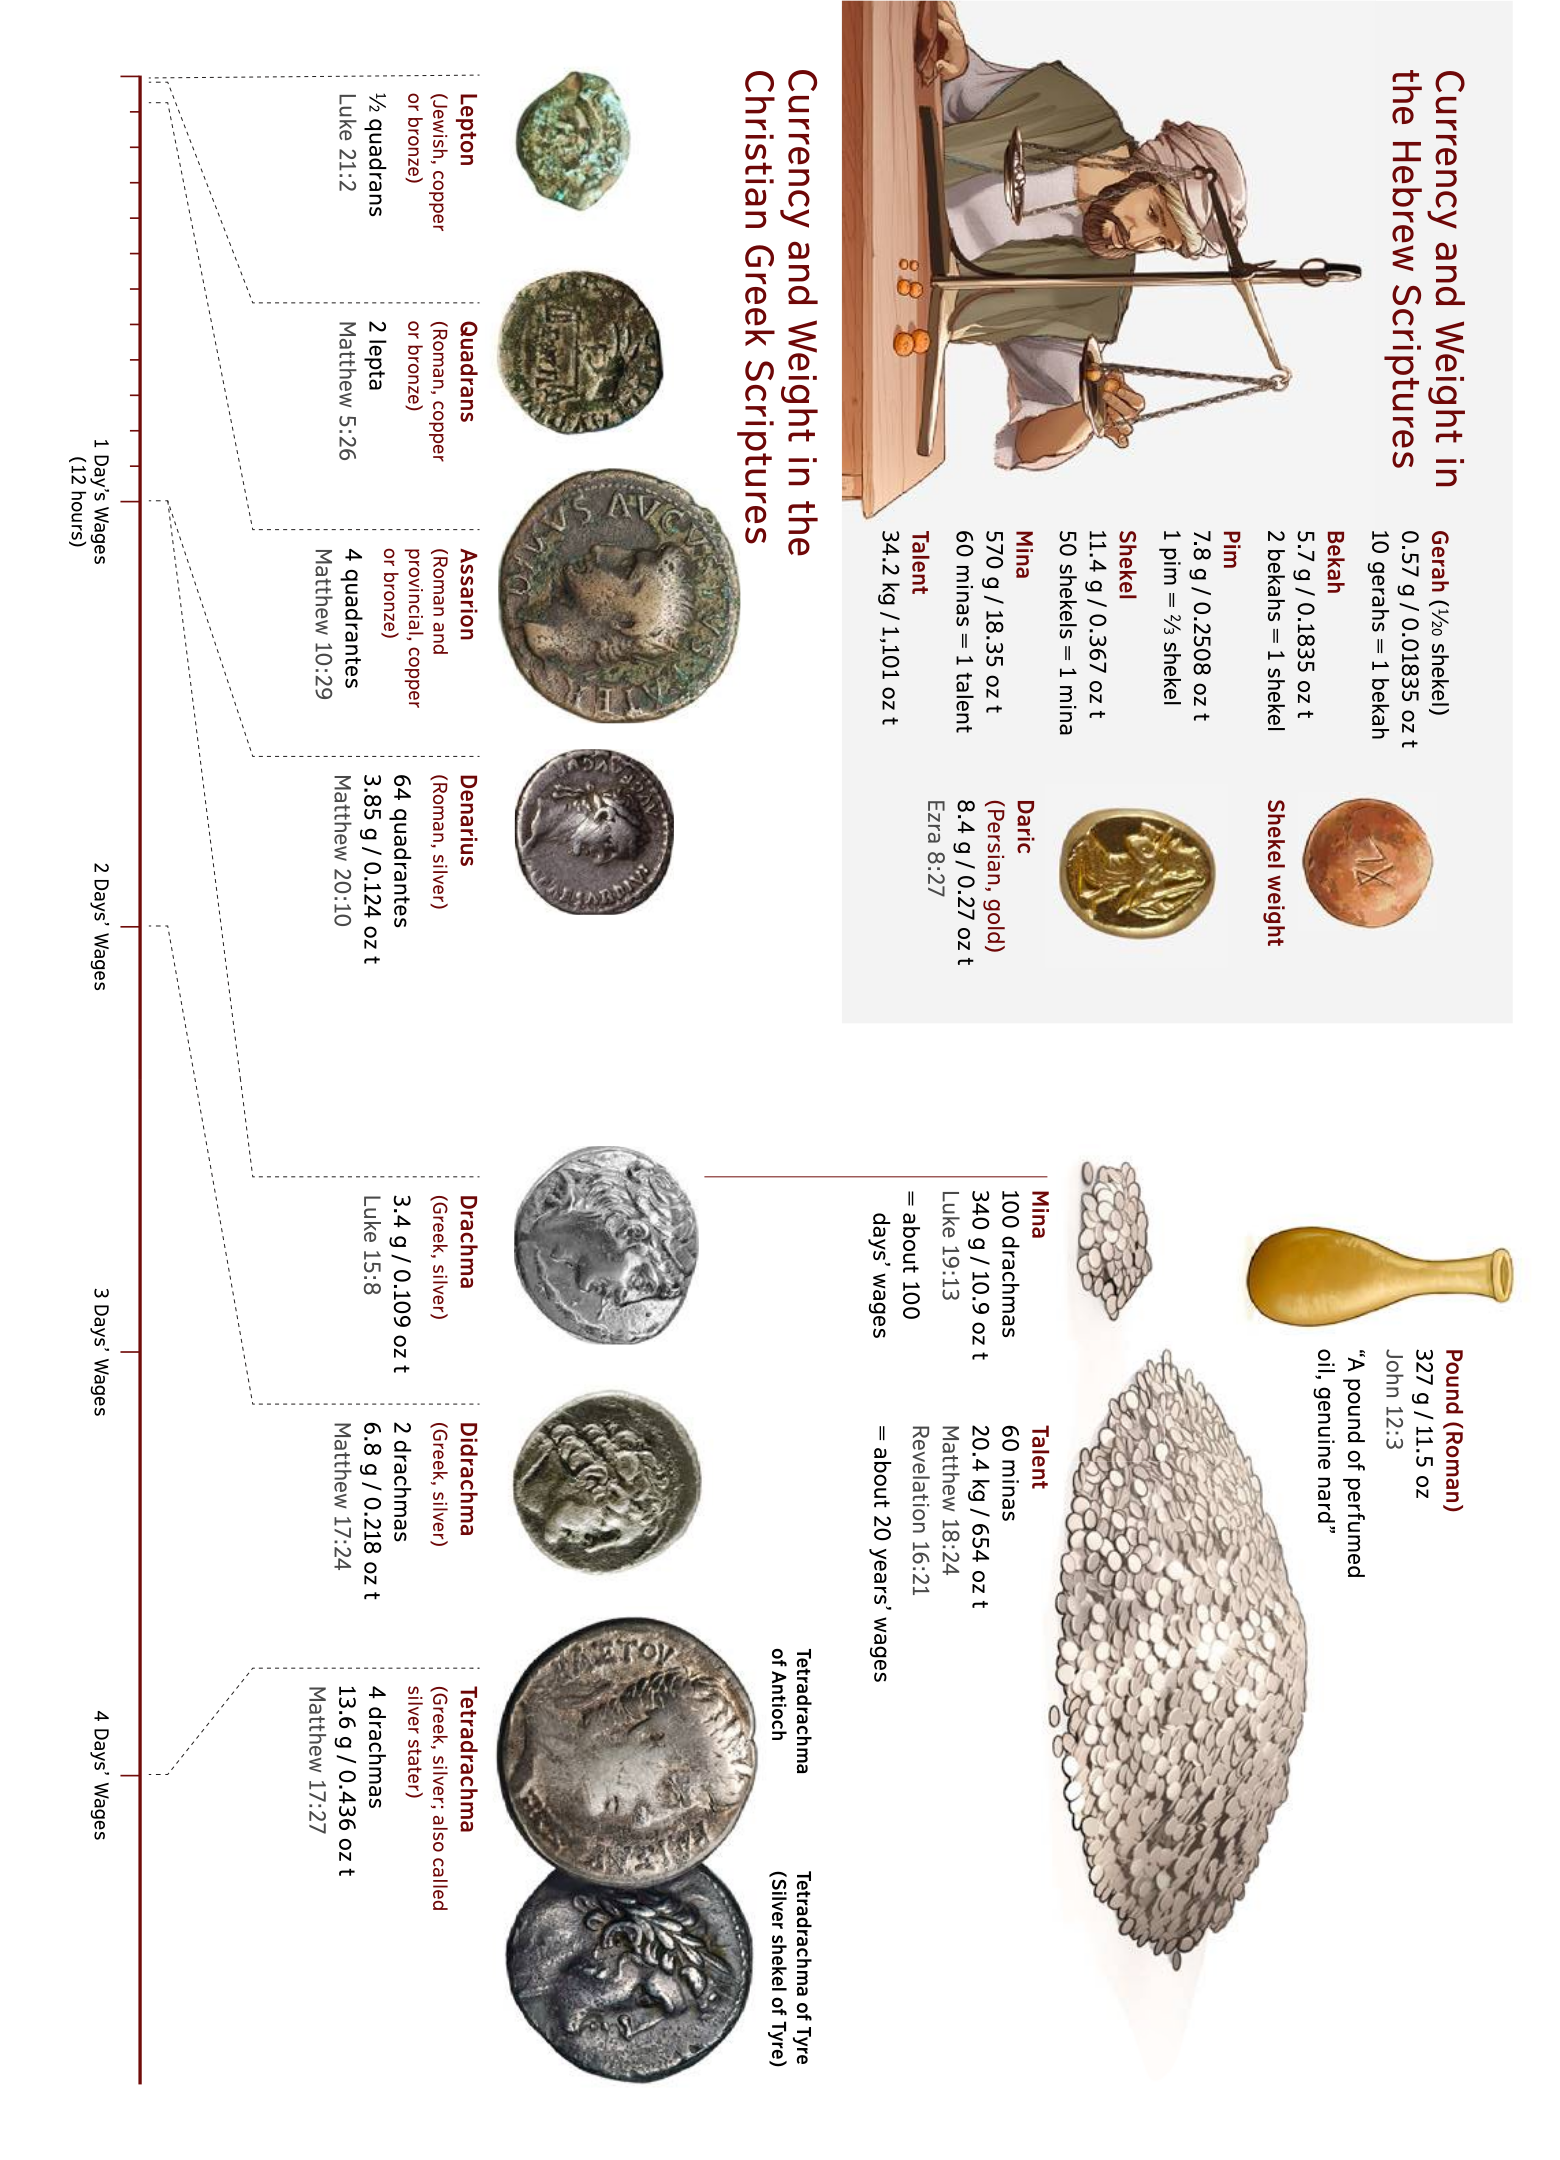
\includepdf[noautoscale=true, scale=1]{leb/content/pictures/units-of-measure.png}
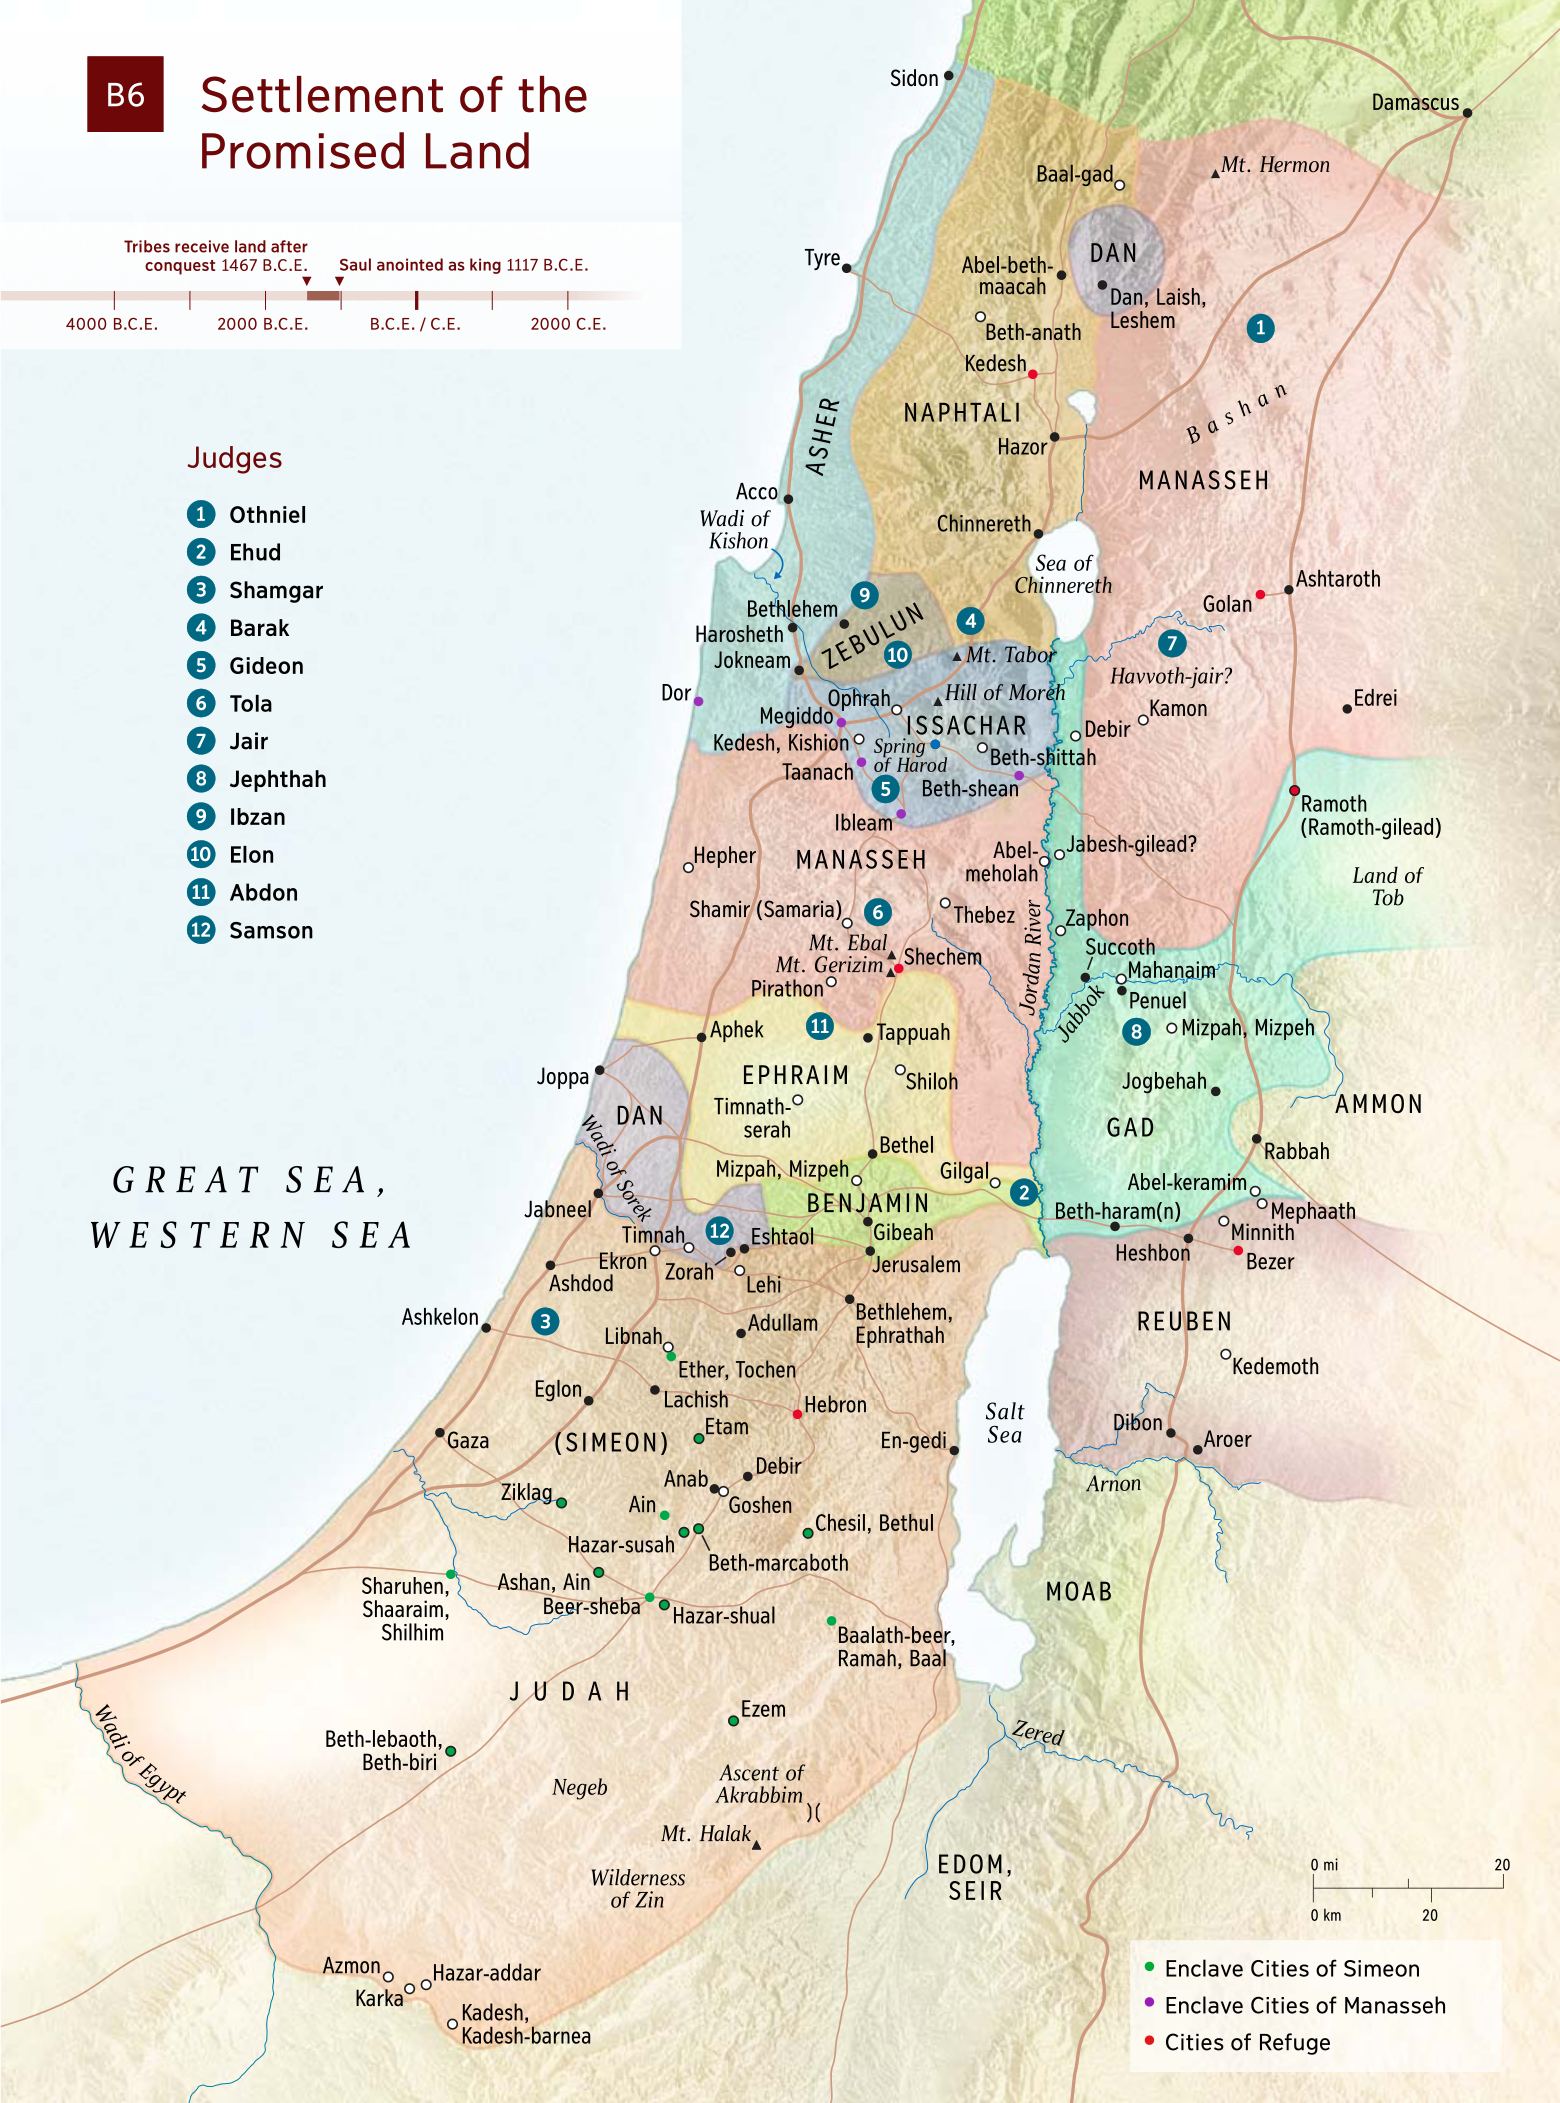
\includepdf[noautoscale=true, scale=1]{leb/content/pictures/settlement-of-the-promised-land.png}
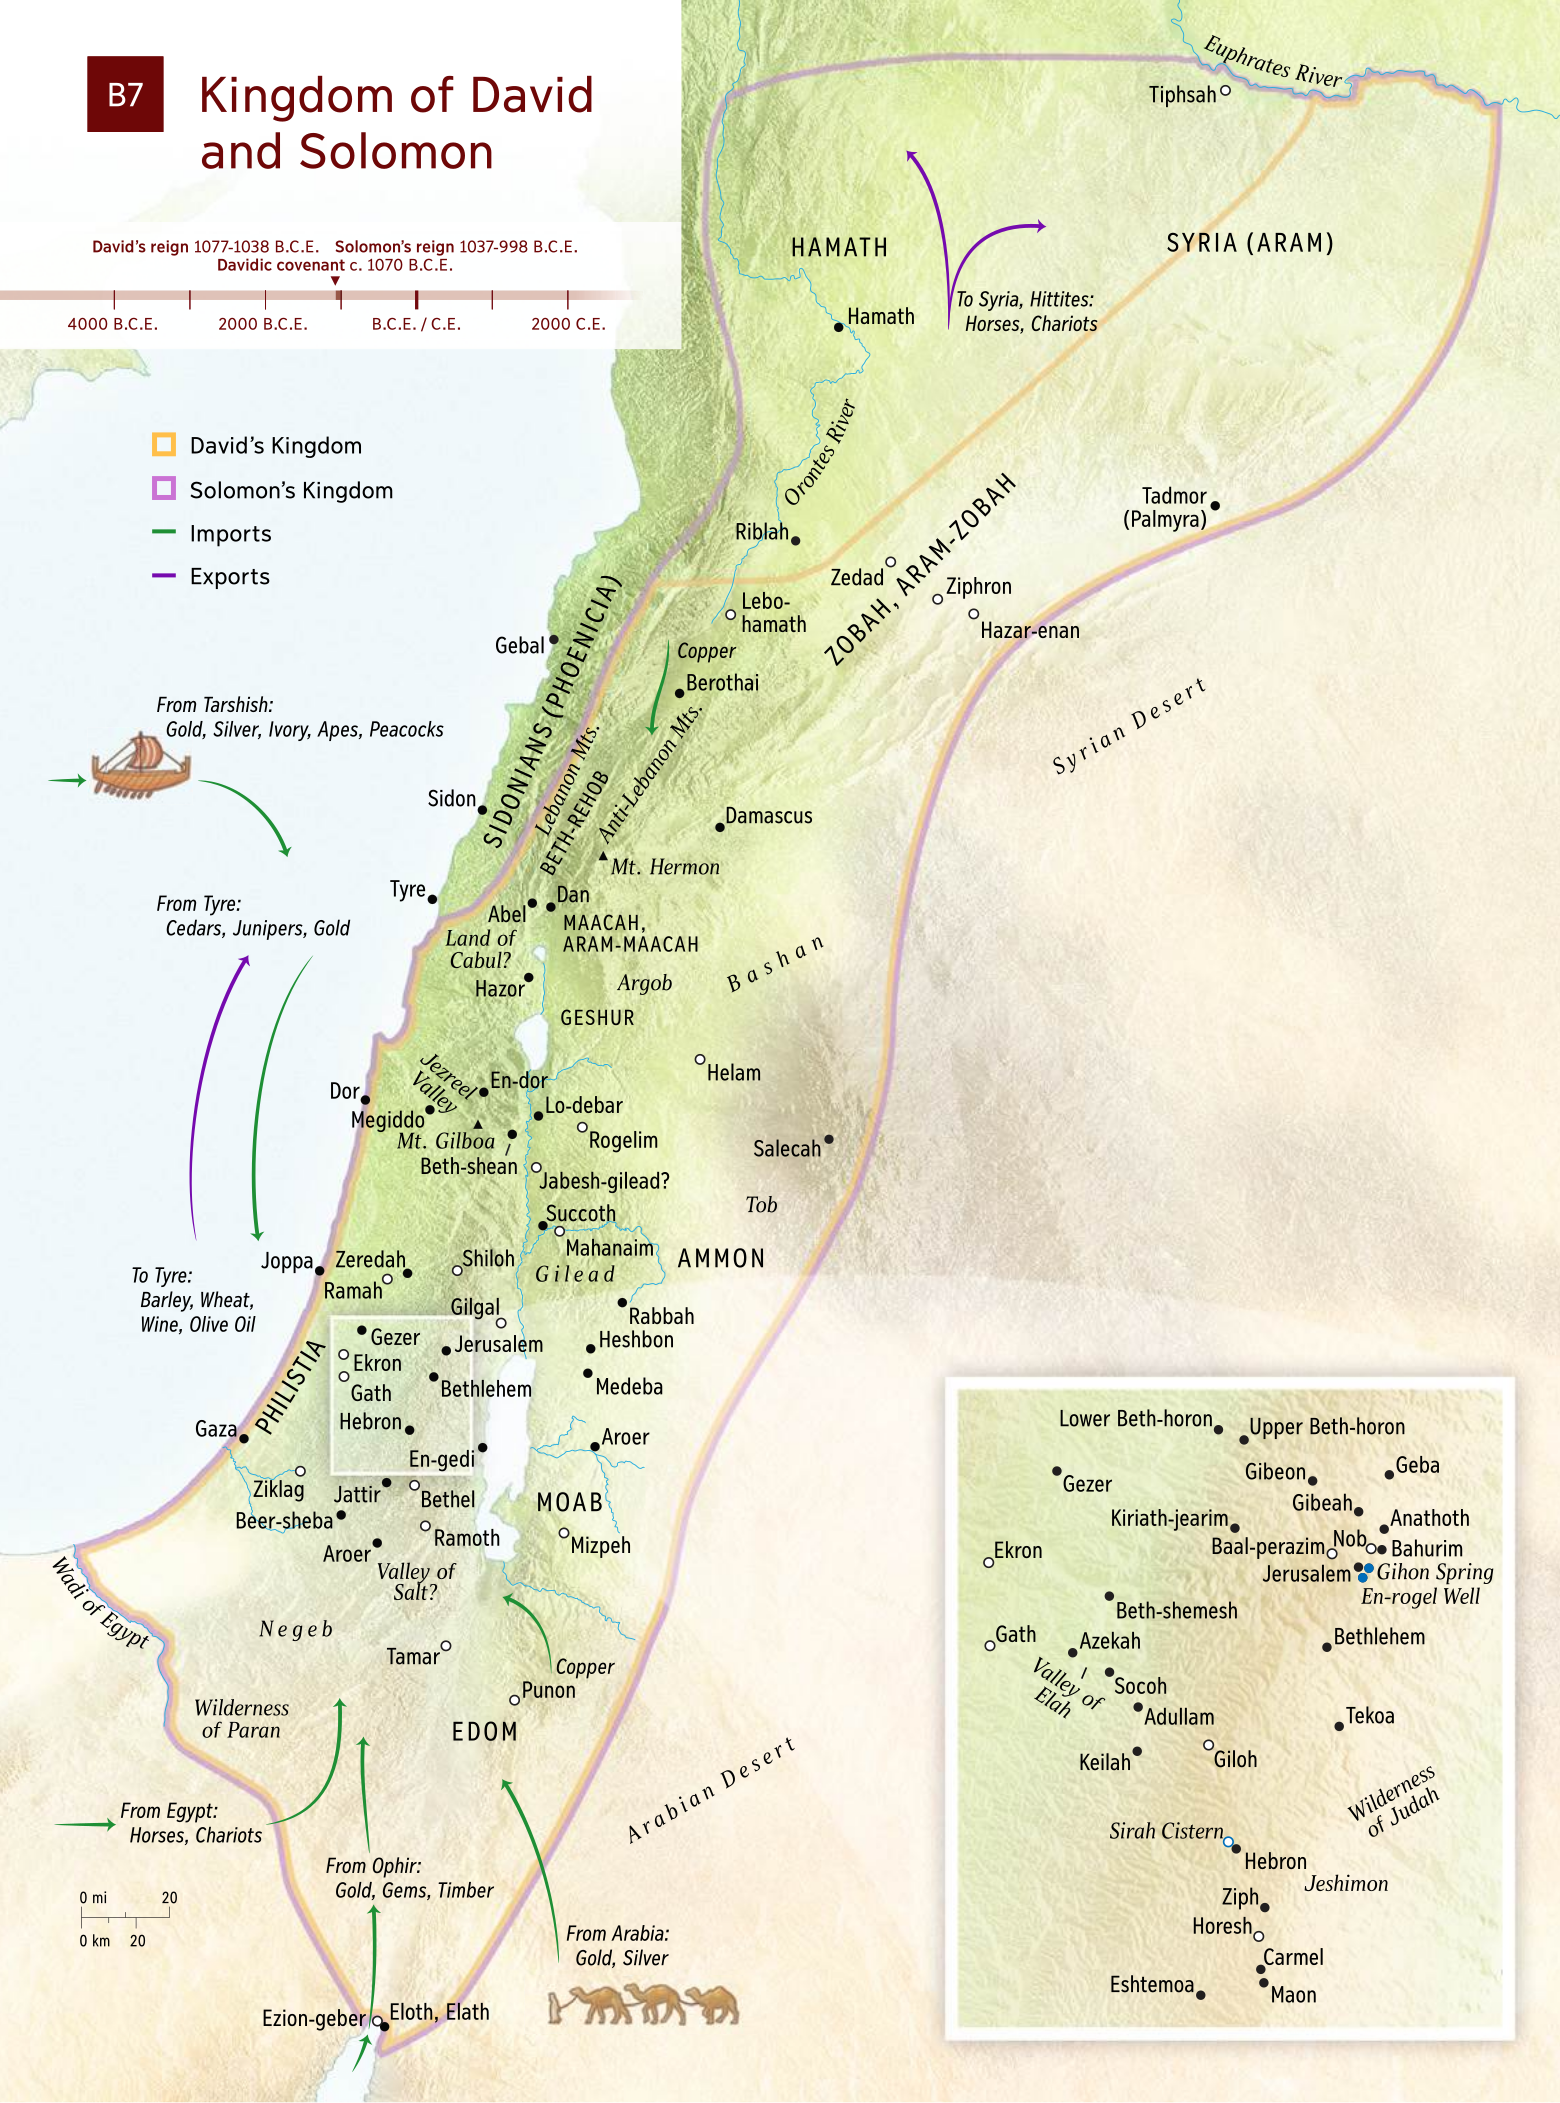
\includepdf[noautoscale=true, scale=1]{leb/content/pictures/israel-in-times-of-king-david-and-solomon.png}
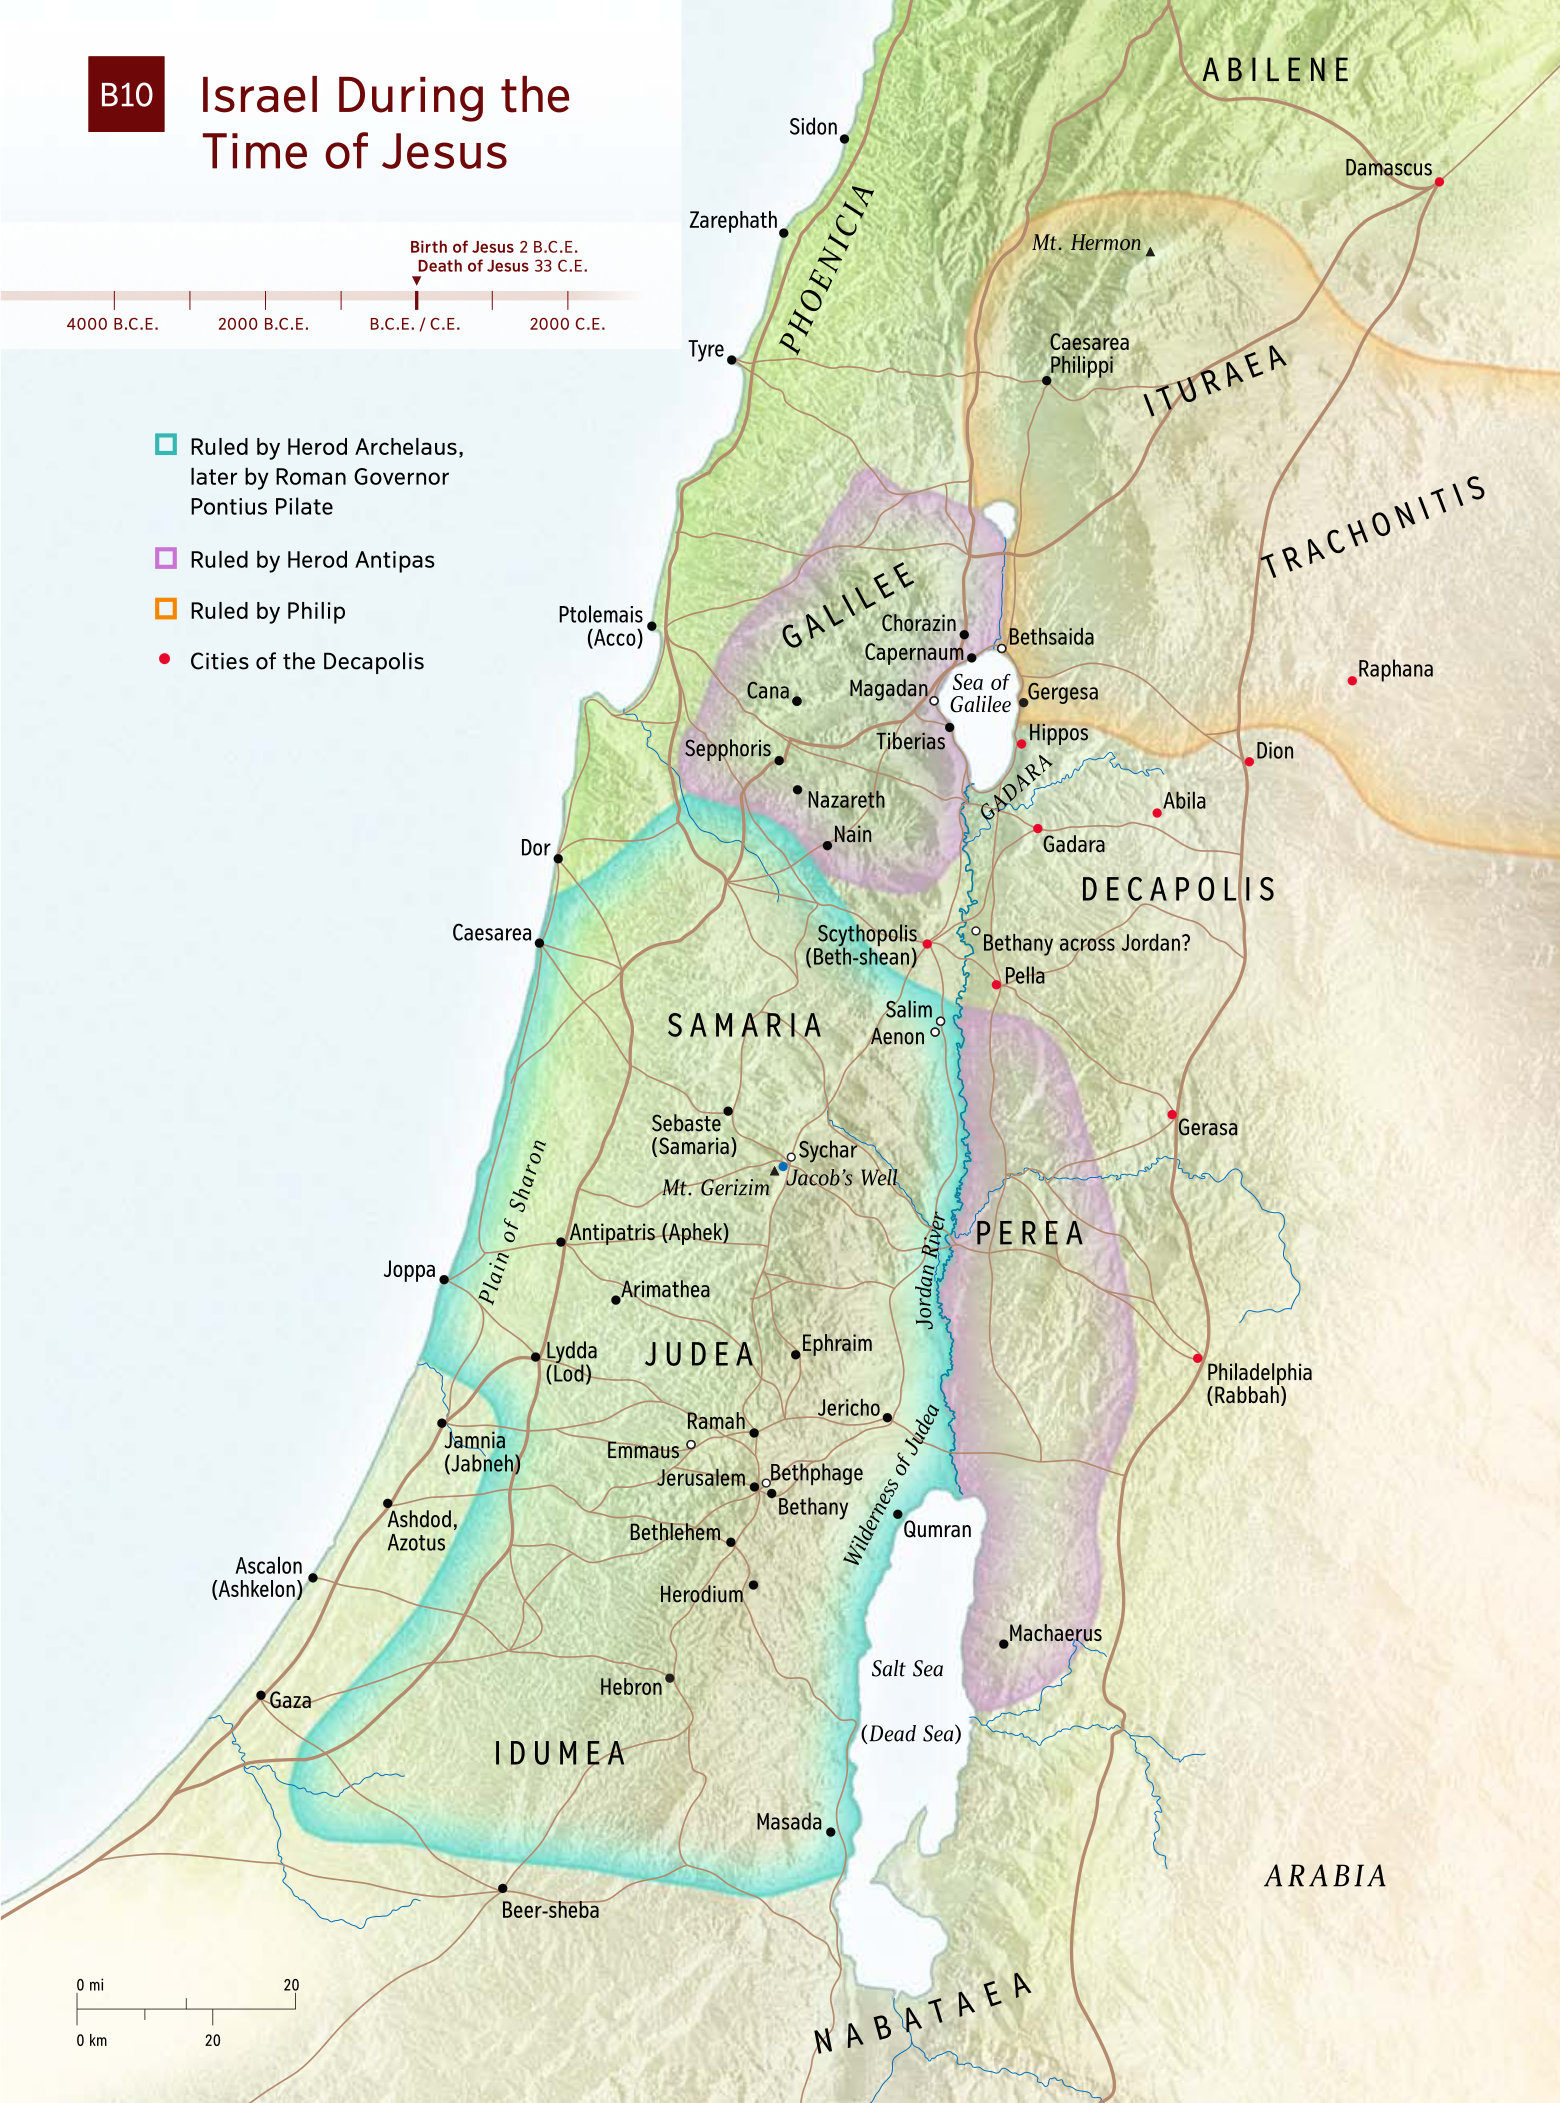
\includepdf[noautoscale=true, scale=1]{leb/content/pictures/israel-in-time-of-jesus.png}
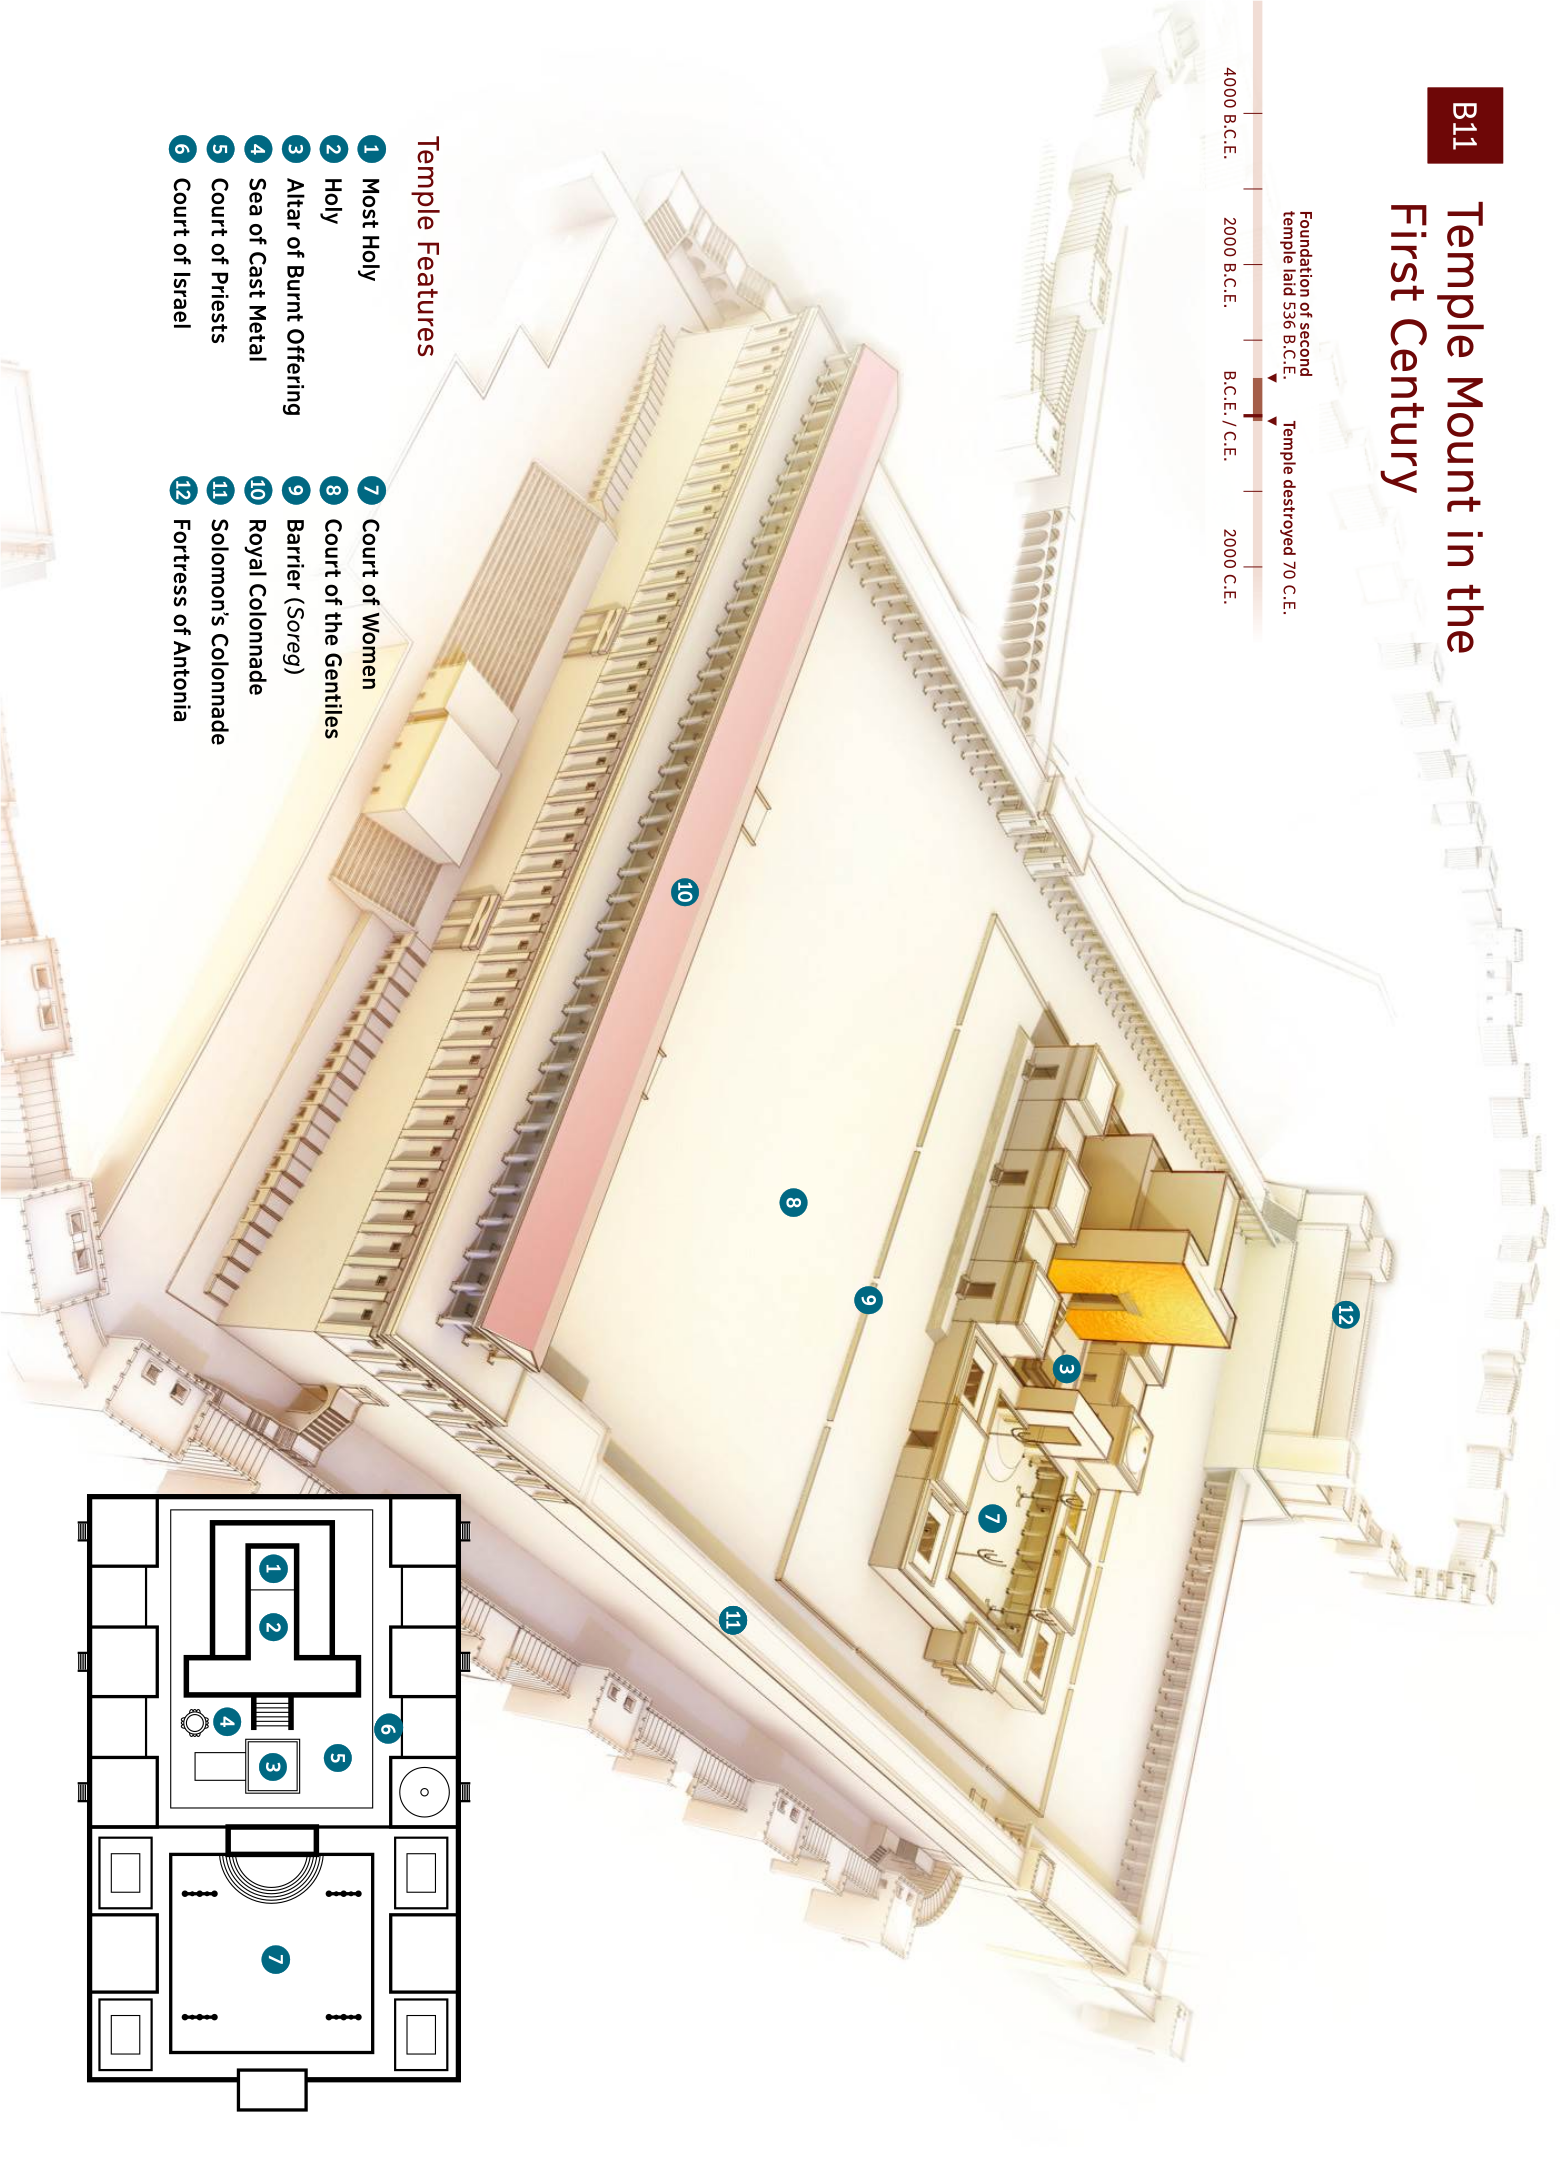
\includepdf[noautoscale=true, scale=1]{leb/content/pictures/second-temple-mount.png}
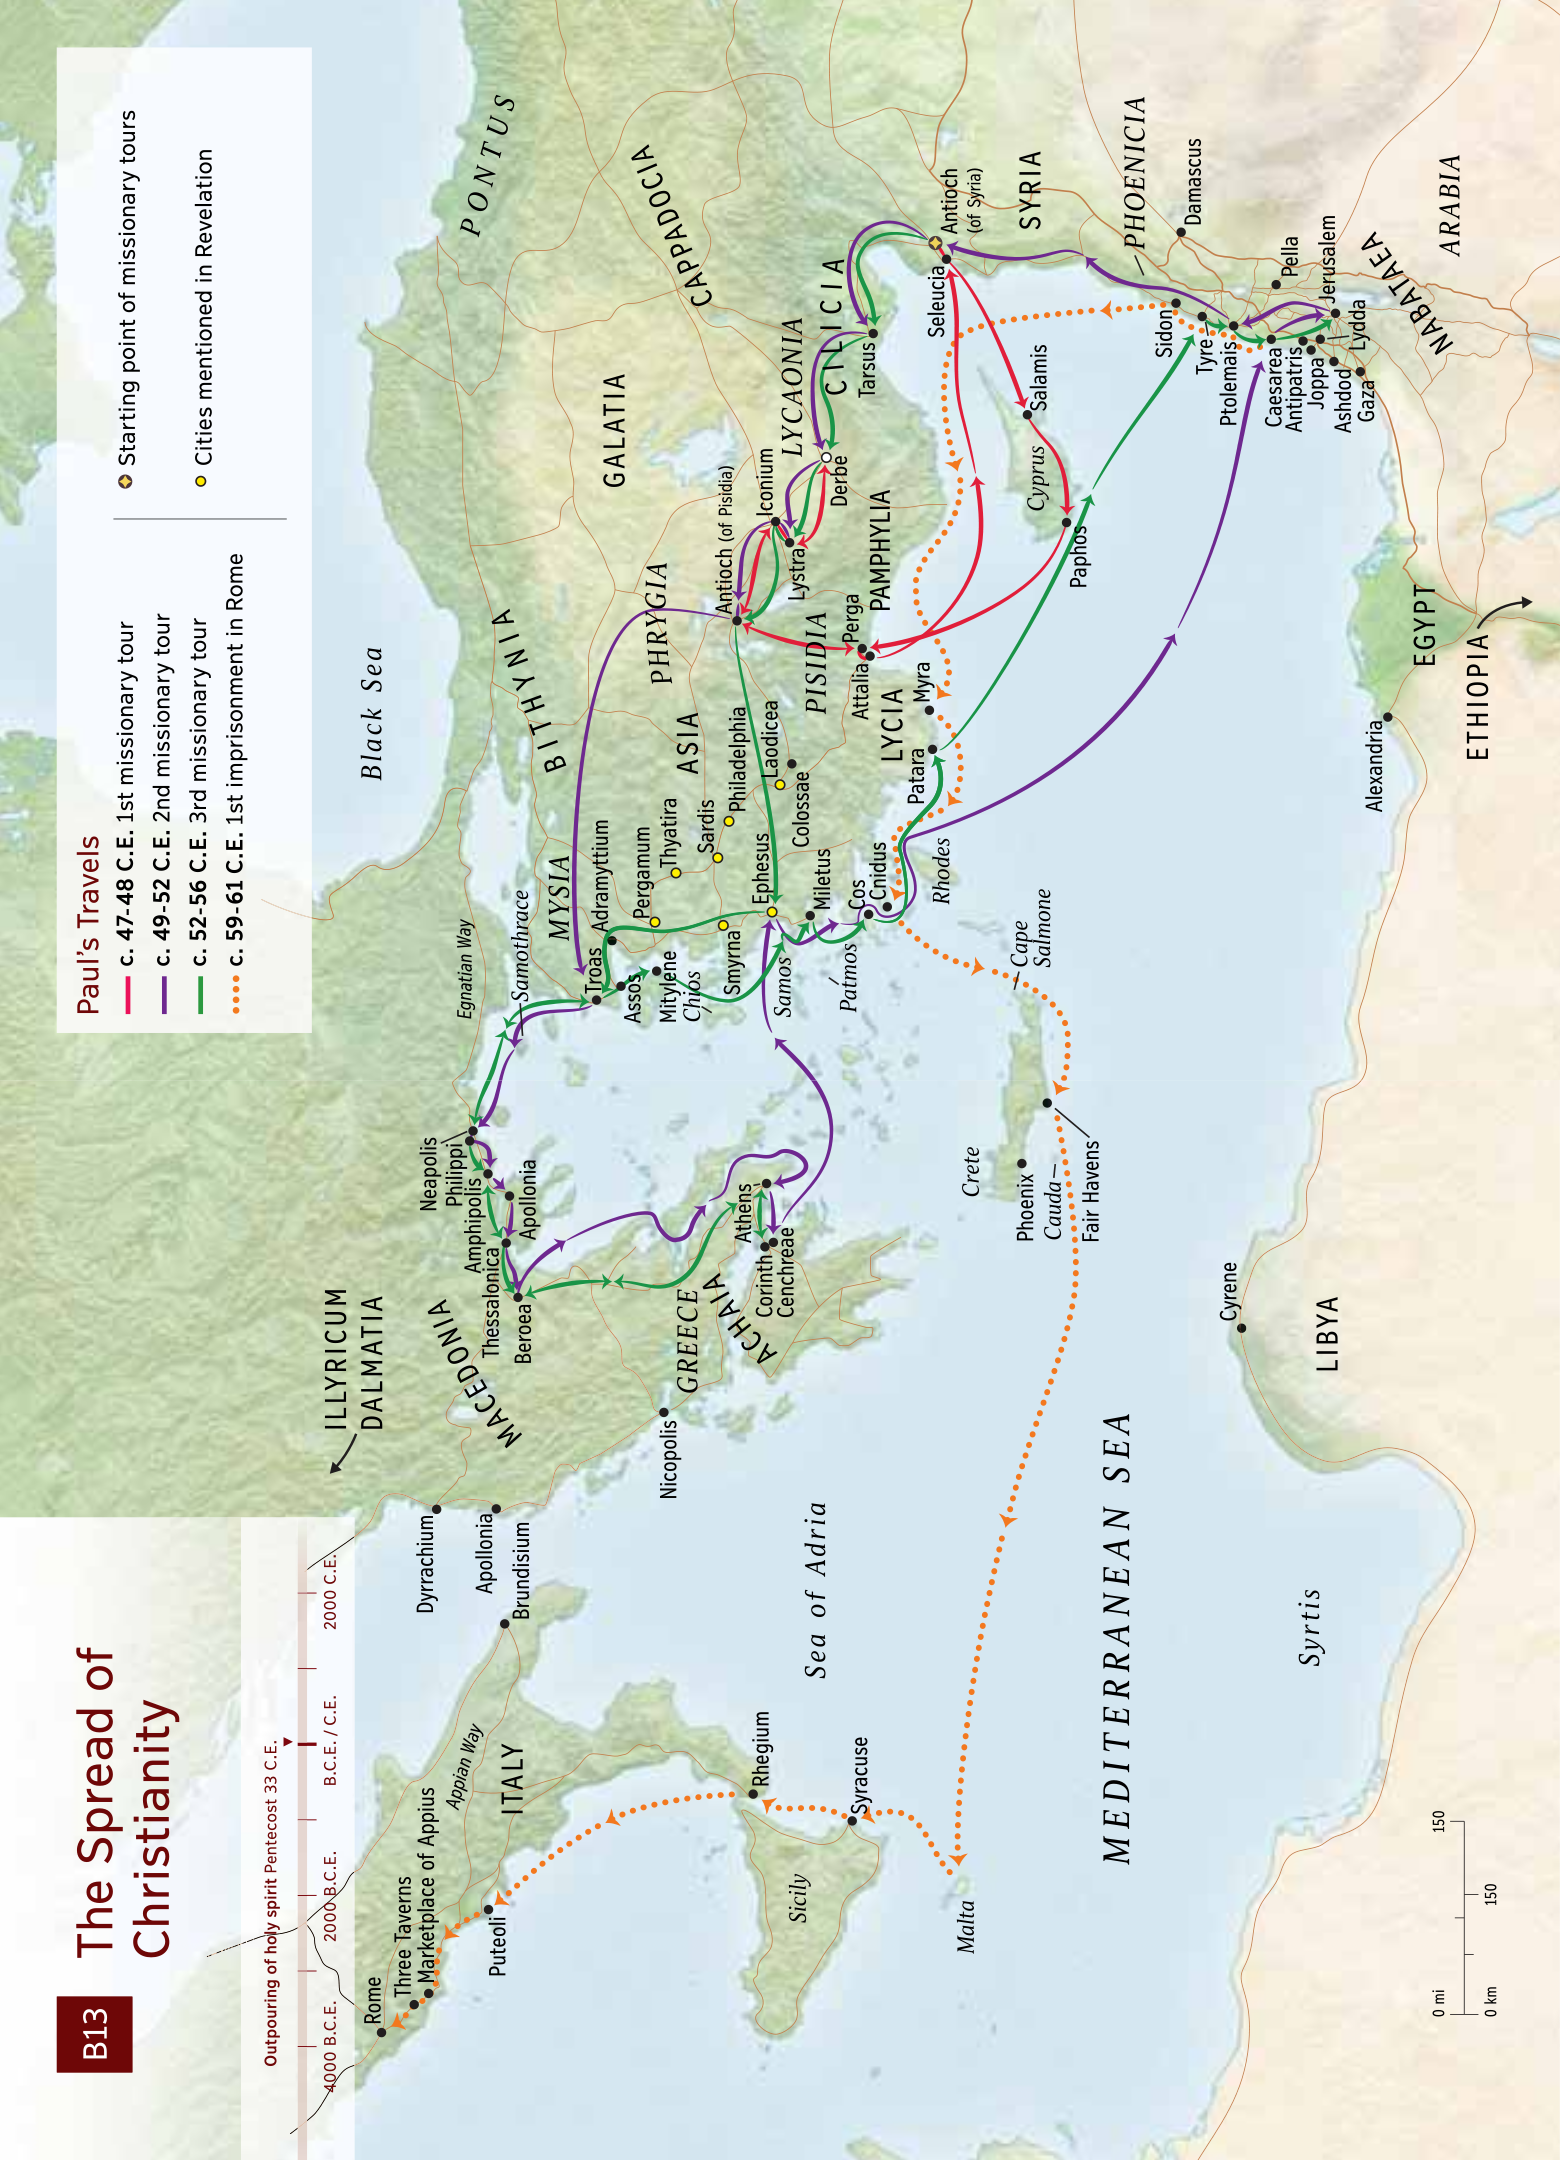
\includepdf[noautoscale=true, scale=1]{leb/content/pictures/spread-of-christianity.png}








% an empty page at the back
\clearpage
\newpage

\mbox{}


\end{document}
